%%%%%%%%%%%%%%%%%%%%%%%%%%%%%%%%%%%%%%%%%
% Masters/Doctoral Thesis 
% LaTeX Template
% Version 2.5 (27/8/17)
%
% This template was downloaded from:
% http://www.LaTeXTemplates.com
%
% Version 2.x major modifications by:
% Vel (vel@latextemplates.com)
%
% This template is based on a template by:
% Steve Gunn (http://users.ecs.soton.ac.uk/srg/softwaretools/document/templates/)
% Sunil Patel (http://www.sunilpatel.co.uk/thesis-template/)
%
% Template license:
% CC BY-NC-SA 3.0 (http://creativecommons.org/licenses/by-nc-sa/3.0/)
%
%%%%%%%%%%%%%%%%%%%%%%%%%%%%%%%%%%%%%%%%%

%----------------------------------------------------------------------------------------
%	PACKAGES AND OTHER DOCUMENT CONFIGURATIONS
%----------------------------------------------------------------------------------------

\documentclass[
12pt, % The default document font size, options: 10pt, 11pt, 12pt
%oneside, % Two side (alternating margins) for binding by default, uncomment to switch to one side
english, % ngerman for German
singlespacing, % Single line spacing, alternatives: onehalfspacing or doublespacing
%draft, % Uncomment to enable draft mode (no pictures, no links, overfull hboxes indicated)
%nolistspacing, % If the document is onehalfspacing or doublespacing, uncomment this to set spacing in lists to single
%liststotoc, % Uncomment to add the list of figures/tables/etc to the table of contents
%toctotoc, % Uncomment to add the main table of contents to the table of contents
%parskip, % Uncomment to add space between paragraphs
%nohyperref, % Uncomment to not load the hyperref package
headsepline, % Uncomment to get a line under the header
%chapterinoneline, % Uncomment to place the chapter title next to the number on one line
%consistentlayout, % Uncomment to change the layout of the declaration, abstract and acknowledgements pages to match the default layout
]{MastersDoctoralThesis} % The class file specifying the document structure
\usepackage[utf8]{inputenc} % Required for inputting international characters
\usepackage[T1]{fontenc} % Output font encoding for international characters
%\usepackage{mathpazo} % Use the Palatino font by default
\usepackage[libertine,cmintegrals,cmbraces,vvarbb]{newtxmath}
%\usepackage{ntheorem}
\usepackage[backend=bibtex,style=ieee,natbib=true]{biblatex} % Use the bibtex backend with the authoryear citation style (which resembles APA)
%\usepackage{biblatex}
\addbibresource{mybib.bib} % The filename of the bibliography

\usepackage[autostyle=true]{csquotes} % Required to generate language-dependent quotes in the bibliography

\usepackage{graphicx}
\usepackage{subfigure}
\usepackage{float}
\usepackage{blindtext}
%\graphicspath{ {./images/} }
\usepackage[italic]{hepnames}
\usepackage[italic]{hepnicenames}
\usepackage{tikz-feynman}
\usepackage{amssymb}
%\usepackage{gensymb}
\usepackage{tikz}
\usetikzlibrary{patterns}
\usetikzlibrary{plotmarks}

%----------------------------------------------------------------------------------------
%	MARGIN SETTINGS
%----------------------------------------------------------------------------------------

\geometry{
	paper=a4paper, % Change to letterpaper for US letter
	inner=2.5cm, % Inner margin
	outer=3.8cm, % Outer margin
	bindingoffset=.5cm, % Binding offset
	top=1.5cm, % Top margin
	bottom=1.5cm, % Bottom margin
	%showframe, % Uncomment to show how the type block is set on the page
}

%----------------------------------------------------------------------------------------
%	THESIS INFORMATION
%----------------------------------------------------------------------------------------

\thesistitle{Determination of Background from Misreconstructed Electrons in $t\overline{t}\gamma$ Single Lepton Channel at the $\sqrt{s}=13$ TeV with $139$ fb$^{-1}$ of ATLAS Data} % Your thesis title, this is used in the title and abstract, print it elsewhere with \ttitle
\supervisor{Prof. Dr. Ivor \textsc{Fleck}} % Your supervisor's name, this is used in the title page, print it elsewhere with \supname
\examiner{Prof. Dr. Markus \textsc{Risse}} % Your examiner's name, this is not currently used anywhere in the template, print it elsewhere with \examname
\degree{Master of Science} % Your degree name, this is used in the title page and abstract, print it elsewhere with \degreename
\author{Agha Mohammad \textsc{Raza}} % Your name, this is used in the title page and abstract, print it elsewhere with \authorname
\addresses{} % Your address, this is not currently used anywhere in the template, print it elsewhere with \addressname

\subject{Experimental Particle Physics} % Your subject area, this is not currently used anywhere in the template, print it elsewhere with \subjectname
\keywords{} % Keywords for your thesis, this is not currently used anywhere in the template, print it elsewhere with \keywordnames
\university{\href{https://www.uni-siegen.de}{University of Siegen}} % Your university's name and URL, this is used in the title page and abstract, print it elsewhere with \univname
\department{\href{https://www.physik.uni-siegen.de/}{Physics Department}} % Your department's name and URL, this is used in the title page and abstract, print it elsewhere with \deptname
\group{\href{https://www.hep.physik.uni-siegen.de/}{Experimental Particle Physics}} % Your research group's name and URL, this is used in the title page, print it elsewhere with \groupname
\faculty{\href{http://www.uni-siegen.de/nt}{Faculty IV}} % Your faculty's name and URL, this is used in the title page and abstract, print it elsewhere with \facname

\AtBeginDocument{
\hypersetup{pdftitle=\ttitle} % Set the PDF's title to your title
\hypersetup{pdfauthor=\authorname} % Set the PDF's author to your name
\hypersetup{pdfkeywords=\keywordnames} % Set the PDF's keywords to your keywords
}

\begin{document}

\frontmatter % Use roman page numbering style (i, ii, iii, iv...) for the pre-content pages

\pagestyle{plain} % Default to the plain heading style until the thesis style is called for the body content

%----------------------------------------------------------------------------------------
%	TITLE PAGE
%----------------------------------------------------------------------------------------

\begin{titlepage}

\begin{figure}
\hfill\includegraphics[width=40mm]{./images/uni-logo-black.eps}
\end{figure}

\begin{center}

\HRule \\[0.4cm] % Horizontal line
{\huge \bfseries \ttitle\par}\vspace{0.4cm} % Thesis title
\HRule \\[1.5cm] % Horizontal line

\large {Masterabeit}\\[0.5cm] % Thesis type

\large \textit{Zur Erlangung des akademischen Grades\\ \degreename \\ (M.Sc.)}\\[0.3cm] % University requirement text
\large {dem Fachbereich Physik der \\ Universität Siegen}\\[3cm] % University requirement text

\emph{vorgelegt von}\\
{\authorname}\\ % Author name - remove the \href bracket
{\large am 02 juni 2020}\\[2cm] % Date
\emph{Gutachter} \\
{\supname} \\ %
{\examname} \\ %

\end{center}
\end{titlepage}

%----------------------------------------------------------------------------------------
%	DECLARATION PAGE
%----------------------------------------------------------------------------------------

\begin{declaration}
\addchaptertocentry{\authorshipname} % Add the declaration to the table of contents
\noindent Hiermit versichere ich, dass ich die vorliegende schriftliche Masterarbeit selbstständig verfasst und keine anderen als die von mir angegebenen Hilfsmittel benutzt habe. Die Stellen der Arbeit, die anderen Werken dem Wortlaut oder dem Sinne nach entnommen sind, wurden in jedem Fall unter Angabe der Quellen (einschließlich des World Wide Web und anderer elektronischer Text- und Datensammlungen) kenntlich gemacht. Dies gilt auch für die beigegebenen Zeichnungen, bildlichen Darstellungen, Skizzen und dergleichen. Mir ist bewusst, dass jedes Zuwiderhandeln als Täuschungsversuch zu gelten hat, der die Anerkennung der Masterarbeit ausschließt und weitere angemessene Sanktionen zur Folge haben kann. \\
\\ 
\noindent Siegen, 02.06.2020\\
\rule[2em]{25em}{0.5pt} % This prints a line for the signature
 
\noindent Agha Mohammad RAZA\\
%\rule[0.5em]{25em}{0.5pt} % This prints a line to write the date
\end{declaration}

\cleardoublepage


%----------------------------------------------------------------------------------------
%	ABSTRACT PAGE
%----------------------------------------------------------------------------------------

\begin{abstract}
\addchaptertocentry{\abstractname} % Add the abstract to the table of contents
%A measurement of electron-to-photon fake rate using $139 $fb$^{-1}$ of \textit{pp} collisions collected by the ATLAS detector in 2015 to 2018 is presented. The $e\rightarrow\gamma$ fake rate, a fraction of $Z\rightarrow e^+e^-$ events is reconstructed as $Z\rightarrow e\gamma$ can be estimated from \textit{Z} to 2 body decays due to the misidentification. An excess of the $e\gamma$ final state with an invariant mass close to \textit{Z}-mass is a clear symptom to be observed in the data, and compared to the simulation results.
A measurement of the probability of electrons to be misidentified as photons ($e\rightarrow\gamma$), referred to as fake rate, using the 139 fb$^{-1}$ of \textit{pp} collisions data collected by the ATLAS detector from 2015 to 2018. The method for the measurement of the fake rate in data, using pure electrons from the Z-boson 2 body decay, called tag-and-probe, is presented. The results are presented as functions of kinematic variables in order to show effects on the detector performance. In addition, the fake rates calculated separately for converted and unconverted photons.
\end{abstract}

%----------------------------------------------------------------------------------------
%	ACKNOWLEDGEMENTS
%----------------------------------------------------------------------------------------

\begin{acknowledgements}
\addchaptertocentry{\acknowledgementname} % Add the acknowledgements to the table of contents
First of all, I would like to thank my supervisor Prof. Dr. Ivor Fleck, for giving me a chance to be a part of the ATLAS experiment and for the guidance and help he provided to me. Thanks to Prof. Dr. Markus Risse for being the second examiner of my thesis. I would like to thank Dr. Carmen Diez Pardos for all the help and guidance she provided to me, and for the time she spent reading my thesis. Also, I would like to thank Amartya Rej, Binish Batool, John Meshreki, and Sara Ghasemi for their advice and support. I want to thank my family for supporting me during my studies.
\end{acknowledgements}

%----------------------------------------------------------------------------------------
%	LIST OF CONTENTS/FIGURES/TABLES PAGES
%----------------------------------------------------------------------------------------

\tableofcontents % Prints the main table of contents

\listoffigures % Prints the list of figures

\listoftables % Prints the list of tables


%----------------------------------------------------------------------------------------
%	THESIS CONTENT - CHAPTERS
%----------------------------------------------------------------------------------------

\mainmatter % Begin numeric (1,2,3...) page numbering

\pagestyle{thesis} % Return the page headers back to the "thesis" style

% Include the chapters of the thesis as separate files from the Chapters folder
% Uncomment the lines as you write the chapters

% Chapter Template

\chapter{Introduction} % Main chapter title

\label{Introduction} % Change X to a consecutive number; for referencing this chapter elsewhere, use \ref{ChapterX}

The ultimate objective of physics is to describe how nature behaves. The emergence of Quantum Mechanics and General Relativity in the early 20th century completely changed our understanding of the universe. Afterwards, in the mid-1970s, the completion of the Standard Model formulation was a significant success that combines the Classical Field Theory, Quantum Mechanics, and the Special Relativity in one theoretical framework. So far, the Standard Model (SM) of particle physics is one of the most successful theories in physics. It fully describes nature in terms of the elementary particles and their interactions. Similar to any other scientific theory, there are still unanswered questions in the Standard Model, such as the dark matter and neutrino mass. Experiments play many roles in science; one of the essential roles is to test theories and to provide the basis for scientific knowledge \cite{sep-physics-experiment}. The measurements in subatomic scales required an enormous amount of energy. In modern particle physics, this lead to the idea of particle beam colliders that can accelerate the particles near the speed of light and collide them to observe the inner structure of the particles. One of the largest research centers is the European Organization for Nuclear Research (CERN), which is located in Geneva, Switzerland. The Large Hadron Collider (LHC), which is one of the world's most complex experimental facilities is situated at CERN. In 2012 a new particle was observed by the two experiments, ATLAS (A Toroidal LHC ApparatuS) and CMS (Compact Muon Solenoid) at the LHC that turned out to be compatible with the Higgs boson, which was the last prediction of the Standard Model, remained undetected in all previous searches. Since the Higgs boson discovery, one of the main tasks of the LHC is to search for beyond the Standard Model. The top quark is the most massive (strong coupling to the Higgs) standard model particle, and it is unique among all quarks and leptons and might play a role within the mechanism of electroweak symmetry breaking. Measurement of the top quark's coupling to vector bosons has a great importance to test the Standard Model, and any deviation from the Standard Model can give a hint about beyond Standard Model underlying theories. In order to scrutinize the SM, very precise measurements are needed, involving a good understanding of the process under study and the background processes that mimic the signature of the signal. This also requires a good knowledge of the detector performance. One of the contributions to event signatures is the misidentification of physical objects in the detector. In the study of top quark pair production associated with a photon, misidentification of electrons as photons is one of the significant backgrounds. The background is referred to as $e\rightarrow\gamma$ fake. In this thesis, the probability of electrons to be misidentified as photons is investigated using the full 13 TeV data of the ATLAS detector at the LHC at CERN. The description of the theoretical background and the experimental setup is given in Chapters \ref{Chapter2} and \ref{Chapter3}. The analysis is described in Chapter \ref{Chapter4}, and a summary of the results and an outlook is given in Chapter \ref{Chapter5}.

\chapter{Standard Model and Top Quark Physics}
\label{Chapter2}
\section{Introduction to Standard Model of Particle Physics}
\label{SM}
The Standard Model of Particle Physics classifies all the known elementary particles and describes the interaction between them. It fully characterizes the three out of four known fundamental forces; electromagnetic, weak, and strong. The gravitational interaction not included in the SM. In the mid-1970s, the current formulation of the SM was completed, and the first observation of the quarks in 1968 was a bold, experimental proof of the SM. Since then, many more experiments have confirmed the predictions of the SM, and the latest was Higgs boson discovery in 2012 confirmed by ATLAS \cite{20121} and CMS \cite{201230} collaborations based on the proton-proton collisions in the LHC at CERN.

The elementary particles divided into different classes depending on their distinguishable properties such as spin, color charge, and flavor. They fall into two major categories of fermions and bosons according to their spin angular momentum. The fermions are spin-half particles, and the bosons have integer spin. The fermions further classify as quarks (\textit{q}) and leptons (\textit{l}) according to how they interact. The vector gauge bosons (spin = 1) and scaler boson (spin = 0) are two classes of bosons. The gauge bosons are known as the force carriers in the SM.

\begin{figure}
\centering
\includegraphics[scale=0.25]{Figures/StandardModel}
\decoRule
\caption{Standard model of particle physics \cite{SMwiki}.}
\label{fig:StandardModel}
\end{figure}

\subsection{Fermions (Quarks and Leptons)}
There are six quarks (up \textit{u}, down \textit{d}, charm \textit{c}, strange \textit{s}, top \textit{t}, bottom \textit{b}) and six leptons (electron $e^{-}$, electron neutrino $\nu_{e}$, muon $\mu^{-}$, muon neutrino $\nu_{\mu}$, tau $\tau^{-}$, tau neutrino $\nu_{\tau}$) divided into pairs of particles in three generations, see figure \ref{fig:StandardModel}. Each particle carries more mass than the corresponding previous generation particle. The first generation particles do not decay, and they form all the visible matter. The quarks carry a color charge (red, blue, green), and anti-quarks carry an anti-color charge (anti-red, anti-blue, anti-green). The color charge in quarks allows them to interact via strong force that only affects the particle with color charge. Due to the color confinement, there is a tight bond between quarks with the strong force. The quarks always form a color-neutral bound state, baryon (\textit{qqq} or $\overline{q}\overline{q}\overline{q}$), or meson ($q\overline{q}$). The color neutral means either a color and anti-color (e.g, blue and anti-blue) or sum of the three colors or anti-colors (e.g, red and blue and green). Which means, proton (\textit{p}) is a composite of three quarks with different color charges ($u_{r}u_{g}d_{b}$ and all the other possible colorless combinations). All fermions have the corresponding anti-fermion with the opposite charge to the fermion.

\subsection{Bosons}

The intermediate vector bosons (gauge bosons) are the force carriers for the SM interactions (strong, weak, electromagnetic). The SM gauge bosons are as follows:  

\begin{itemize}
\item \textbf{Photon ($\gamma$)}: It mediates the electromagnetic interactions between the electrically charged particles, the interactions described by QED (Quantum Electrodynamics). The photon rest mass is zero and has no electric or color charge.

\item \textbf{$W^{\pm}$ and $Z^{0}$ bosons}: These bosons are the mediators of the weak force between all fermions. The $W^{\pm}$ ($\sim80GeV$) and $Z^{0}$ ($\sim90GeV$) are very massive. As W has +1 or -1 electric charge, it participates in the electromagnetic interaction. The electroweak theory describes combined weak and QED interactions.

\item \textbf{Gluons}: There is a total of eight gluons. They are massless carriers of the strong interaction between quarks and gluons. They carry a pair of color-anti-color charges (e.g., blue-antired) but have no electric charge. The gluons have self-interaction because they have a color charge. The theory describes strong interactions is QCD (Quantum Chromodynamics).

\end{itemize}

There is only one scalar boson (spin = 0) predicted by the SM, the Higgs boson ($H$). The Higgs mechanism is essential to explain the mass of the gauge bosons. In QFT, without the Higgs mechanism, all intermediate bosons considered massless.  So the massive $W^{\pm}$ and $Z^{0}$ bosons could not be explained without having a Higgs mechanism that gives mass to the $W^{\pm}$ and $Z^{0}$ bosons. 

\subsection{Interactions}

\begin{figure}
\centering
\feynmandiagram [vertical = b to a] {
	i1 [particle=\(e^{-}\)]
	-- [anti fermion] a
	-- [anti fermion] f1 [particle=\(e^{-}\)],
	a -- [photon, edge label=\(\gamma\)] b,
	i2 [particle=\(e^{-}\)]
	-- [fermion] b
	-- [fermion] f2 [particle=\(e^{-}\)],
};
\decoRule
\caption{Feynman diagram of electron-electron scattering. The diagram shows the two incoming $e^{-}$ from left, exchange a photon and scatter of to right.}
\label{fig:Feynman_ee}
\end{figure}

In the SM, each interaction is described by the corresponding Quantum Field Theory (QFT). The interaction takes place by exchanging one of the spin-1 gauge bosons. In QED, the interaction between charged particles mediated by the exchange of photons ($\gamma$). As an example, in the electron-electron scattering process, a photon ($\gamma$) is emitted by one of the incoming electrons ($e$) and absorbed by the other one, see figure \ref{fig:Feynman_ee}. The weak charged interactions mediated by the charged $W^{+}$ and $W^{-}$ bosons, the nuclear beta decay is an example of weak charged interaction. The weak neutral interactions take place by exchanging Z bosons. The strong interaction described by QCD mediated by exchanging the gluons (e.g., quark-quark scattering process). 

The electromagnetic force is the force that acts between electrically charged particles. It has an infinite range, unlike weak and strong are very short-range interactions (sub-atomic). The signature of the weak interactions is CP-symmetry (charge conjugation parity symmetry) violation, but CPT-symmetry (charge, parity, and time reversal symmetry) is conserved in the weak interaction. All fermions carry a property called iso-spin which allows them to interact via the weak force. The strong interaction is a very short-range force that acts only on the particles that carry the color charge. The quarks and gluons can interact with the strong force.

\begin{table}[H]
\caption{Fundamental interactions strength comparison \cite{Interactions}.}
\label{tab:FundamentalInteractions}
\centering
\begin{tabular}{l l l}
\toprule
Force & Strength & Mediator \\
\midrule
Strong & \(10\) & Gluon\\
Electromagnetic & \(10^{-2}\) & Photon\\
Weak & \(10^{-13}\) & W and Z \\
Gravity & \(10^{-42}\) & Graviton\\
\bottomrule\\
\end{tabular}
\end{table}

\section{The Top Quark}
\label{TopQ}

The detection of heavy hadrons confirmed the existence of heavy quarks. The top quark was not discovered until 1995, and all the early searches failed to detect the top baryon or meson. Unlike the other five quarks, the top quark is so heavy ($\sim174GeV$) and has a very short lifetime, it does not form any bound state of mesons or baryons. In other words, the top quark does not hadronize, so it not possible to see any top-hadron. This implies that the top quark decays before it gets confined by passing its spin information to its decay products. Additionally, this also enables the possibility of studying the polarization of the \textit{W}-boson from the top quark.

The detection of the top quark, in 1995 through the CDF \cite{PhysRevLett.74.2626} and DØ \cite{PhysRevLett.74.2632} experiments on the TEVATRON accelerator at the FERMILAB, turned into a significant achievement on the way of completing the missing portions of a beautiful puzzle, the SM. The reaction to produce top quark was $u+\overline{u} \rightarrow t+\overline{t}$ ; The analysis of decay products lead to the discovery as the \textit{t} and $\overline{t}$ are very short-lived to be detected. The top quark was theoretically hypothesized with the bottom quark (\textit{b}), in 1973 by Kobayashi and Maskawa \cite{10.1143/PTP.49.652}, and they complete the third generation of quark family. 
%The top quark is the most massive (strong coupling to the Higgs) SM particle, and it is probably unique among all quarks and leptons and might play a role within the mechanism of electroweak symmetry breaking.

\subsection{Top Quark Production and Decay}
\label{TopQproductiondecay}

Top quarks at LHC can be produced as single top quarks via weak interaction or as top anti-top quark pairs production via strong interaction. The top quark pair production is the dominant process at the LHC. Top quark pairs can be produce via two different processes: gluon-gluon fusion and quark-antiquark annihilation. The quark-antiquark annihilation is suppressed by gluon-gluon fusion (approximately $90\%$) at LHC because the anti-quark only comes from the sea-quarks of proton. The leading order feynman diagrams of top quark pair production are given in \ref{fig:toppairproduction}.
 
\begin{figure}[H]
\centering
\includegraphics[scale=0.3]{Figures/top_pair_production.png}
\decoRule
\caption{Representative Feynman diagrams for top anti-top quark pair production at the leading order QCD matrix element. From the left, the first three correspond to the gluon-gluon fusion and the last one represents the quark anti-quark annihilation\cite{borathesis1}.}
\label{fig:toppairproduction}
\end{figure} 

Single top quark production is an electroweak interaction and mostly associated with \textit{b} quark and \textit{W}\textit{} boson (Wtb vertex). The process is dominated by t-channel (almost $70\%$) at $\sqrt{s}=13$TeV at the LHC. The feynman diagrams for the t-channel and s-channel process are given in \ref{fig:singletopproduction}.

\begin{figure}[H]
\centering
\includegraphics[scale=0.3]{Figures/single_top.png}
\decoRule
\caption{Feynman diagrams for single top quark production at leading order matrix element. From the left, the first two diagram represent the t-channel production. The third diagram is the s-channel production and the last one is the W t-channel production\cite{borathesis1}.}
\label{fig:singletopproduction}
\end{figure}

The top quark lifetime is shorter than the hadronization time and it decays almost $100\%$ into a bottom quark and a \textit{W}-boson. Therefore, the decay modes are classified depending on further decays of daughter \textit{W}'s into: hadronic channel, dileptonic channel and semileptonic channel.

\begin{figure}[H]
\centering
\includegraphics[scale=0.3]{Figures/top_decay.png}
\decoRule
\caption{Feynman diagrams for semileptonic decay channel of top-anti-top quarks\cite{borathesis1}.}
\label{fig:topdecay}
\end{figure}

\textbf{Hadronic decay channel}: Both \textit{W}-bosons decay into quark-anti-quark pairs and the final state has a total of six jets in which two of them are b-jets. The branching ratio of this channel is around $46\%$ but the final state has large background due to six final state jets.

\textbf{Dileptonic decay channel}: Both \textit{W}-boson decay into a lepton and lepton neutrino. The final state is very clean as compare to fully hadronic decay but the branching ratio is around $10\%$ which is very small. Also the two neutrinos in the final state can make the analysis more difficult (neutrino cannot be detected by ATLAS and only can be identified by missing energy at the final state).

\textbf{Semileptonic decay channel}: One of the \textit{W}-boson's decay hadronically and the other one leptonically. The branching ratio of the decay channel is around $43\%$ and the final state is cleaner (4-jets) as compare to fully hadronic decay. The Feynman diagram of the process represented in Figure \ref{fig:topdecay}.

\begin{figure}[H]
\centering
\includegraphics[width=10cm]{Figures/top_pair_branching_frac.eps}
\decoRule
\caption{Top-anti-top quark pair decay channels and the pie chart with branching fractions. The decay channels are categorized depending on the the further decay of $W^{\pm}$ into quarks or leptons\cite{toppair-branching}.}
\label{fig:topdecaychannels}
\end{figure}

\subsection{Top Quark Associated with Photon}
\label{ttgamma}

Measurements of the top quark's coupling to vector bosons have great importance to test the SM and any deviation from SM can give a hint about beyond standard model underlying theories. The top quark coupling with photon is our interest which theoretically, can be measured from the top quark pair production via photon. The $q\overline{q} \rightarrow \gamma \rightarrow t\overline{t}$ cannot be observed directly at LHC because the top quark pair production is dominated by gg-fusion ($\sim90\%$). The remaining $\sim10\%$ for $q\overline{q}$ annihilation can be mediated by $g$, $Z$ and $\gamma$; And the production mediated by gluon is the dominating process so the \textit{t} coupling with $\gamma$ cannot be probed directly. There are two other processes, top quark pair production with photon: the radiative top quark production and the radiative top decay. top quark pair production in association with a photon is our interest and in the following briefly the radiative $t\overline{t}$ production and decay has been discussed. Photon can be radiated of top quark in the pair production or in the decay process of the the top quark.

In the radiative $t\overline{t}$ production process via $q\overline{q}$ annihilation, the photon can decay from one of the incoming or outgoing quarks. In the gluon gluon fusion process, the photon only can be radiated of one of the top quarks. The respective Feynman diagrams are shown in figure \ref{fig:feynmanttgamma1} for illustration.

\begin{figure}[H]
\centering
\includegraphics[width=14cm]{Figures/ttgamma_production.png}
\decoRule
\caption{Representative Feynman diagrams for radiative top quark pair production \cite{borathesis1}.}
\label{fig:feynmanttgamma1}
\end{figure}

The photon in the radiative $t\overline{t}$ decay, can be radiated from the top quark or one of the top quark decay products: bottom-quark, \textit{W}-boson and the leptons from \textit{W}-decay. The respective Feynman diagrams are given in the figure \ref{fig:feynmanttgamma2}. The top-photon coupling is our topic of interest but experimentally we cannot distinguish the photons from radiative production or decay.

\begin{figure}[H]
\centering
\includegraphics[width=14cm]{Figures/ttgamma_decay.png}
\decoRule
\caption{Representative Feynman diagrams for radiative top quark decay\cite{borathesis1}.}
\label{fig:feynmanttgamma2}
\end{figure} 
% Chapter Template

\chapter{The ATLAS Experiment at LHC} % Main chapter title

\label{Chapter3} % Change X to a consecutive number; for referencing this chapter elsewhere, use \ref{ChapterX}

The experimental data for the measurement has been collected by ATLAS detector, one of the detectors placed on LHC at CERN near Geneva city on France-Swiss border. CERN is the largest and most complex high energy physics facility in the world where physicists and engineers from all around the world work together to study the fundamental particles. Since foundation in 1954, many important discoveries have been made at the CERN laboratory. In this chapter, LHC and the ATLAS detector structure are briefly described.%----------------------------------------------------------------------------------------
%	SECTION 1
%----------------------------------------------------------------------------------------

\section{The Large Hadron Collider}
\label{section:LHC}

The LHC is a circular beam collider with a circumference of about 27km designed to accelerate the proton beams with up to a center-of-mass energy of 14 TeV. The collider is situated underground and the deepest point of LHC is 175 meters under the surface. The superconducting magnets cover the whole tunnel to bend the beam, and the project was completed in 2000. There are four main interaction points where the beams collide and the detectors, ALICE, ATLAS, CMS, and LHCb, have been installed to collect the collision data. The acceleration process at CERN involves the chain of accelerators in which each accelerator injects the beam into the next one to bring the beam to higher energies. At last, the beam gets injected to LHC for the final acceleration and collision process.

The beam acceleration started by ionization of hydrogen atoms and separating the protons through an electric field. The protons beam then gets injected to the Linac2, where the protons accelerated up to the 50 MeV. From there, the beam enters the Proton Synchrotron Booster (PSB) and get the energy up to 1.4 GeV. In the next step, the beam gets into the Proton Synchrotron (PS), where the energy of the beam increases to 25 GeV. Afterward, The Super Proton Synchrotron (SPS) accelerates the beam to 450 GeV, which is the last pre-acceleration step before the beam gets injected to LHC. In the LHC, the protons beam divided into two pipes in which one beam accelerated in clockwise and the second beam in the anti-clockwise direction up to 7 TeV. As a result, in the head-to-head collision, the center of mass energy reaches up to 14 TeV, schematic view of acceleration chain is shown in figure \ref{fig:cern}.

\begin{figure}[H]
\centering
\includegraphics[scale=0.5]{Figures/Schematic-view-of-the-CERN-accelerator-complex.png}
\decoRule
\caption{Schematic view of the CERN accelerators chain, the largest ring in dark blue color is the LHC \cite{cernschematic}.}
\label{fig:cern}
\end{figure}

%----------------------------------------------------------------------------------------
%	SECTION 2
%----------------------------------------------------------------------------------------

\section{ATLAS Detector}
\label{section:ATLAS}

The ATLAS detector is a cylindrical shaped detector with a length of 46m, a diameter of 25m, and it weighs about 7000 tonnes. ATLAS is a multi-purpose detector that is designed to measure the energy and momentum of the particles around the collision point. It uses an orthogonal right-handed coordinate system in which the origin is the center of the detector (interaction point), and the beamline direction defines the $z$-axis, $x$-axis points towards the center of LHC. The $x-y$ plane is perpendicular to the beamline and referred to as the transverse plane. The positive $x$-axis points towards the center of LHC, and the positive $y$-axis points upward to the surface of the earth. The azimuthal angle ($\phi$) is the angle in the transverse plane measured from the $x$-axis, and the polar angle ($\theta$) is the angle in the $y-z$ plane which is often expressed in terms of pseudo-rapidity ($\eta$) and formulated as follows:

\begin{equation}
\eta = - \ln \tan{\frac{\theta}{2}}.
\label{eqn:pseudorapidity}
\end{equation}

The distance between two physical objects defined in terms of pseudo-rapidity and azimuthal angle (which is Lorentz invariant under the boost) as follows:

\begin{equation}
\Delta R = \sqrt{{\Delta\eta}^2 +{\Delta\phi}^2}.
\label{eqn:deltaR}
\end{equation}

The energy and momentum of the particles are expressed in terms of transverse momentum ($p_{T}$) and transverse energy ($E_{T}$); in this way, they are also Lorentz invariant under the boost, defined as follows:

\begin{equation}
p_{T} = \sqrt{{p_{x}}^2 +{p_{y}}^2} = |p|\sin{\theta}, \; E_{T} = |E|\sin{\theta}.
\label{eqn:energymomentum}
\end{equation}

The ATLAS detector provides full coverage of the space around the collision point. The inner structure significant parts can be split into four major components: Inner detector, Calorimeters, Muon Spectrometer, and Magnet system. The Inner detector part (closest part to the collision point) is responsible for detecting the track of charged particles and the position primary and secondary vertices. The calorimeters consist of two inner components, the Electromagnetic Calorimeter (ECAL) and the Hadronic Calorimeter. Energy deposits of the electrons, photons, muons and hadrons are recorded by the calorimeters. The muon spectrometry is the outermost layer of the ATLAS detector. The magnet system can be divided into two parts. The first part is a solenoid magnet that surrounds the inner detector and provides a homogenous magnetic field of 2T to detect the charge and momentum of the particle. The second part consists of three toroidal magnets for barrel and end-caps segments, which provide the trajectory of the muons. A simulated model of the ATLAS detector and the inner structure is given in figure \ref{fig:atlas}. A cross section of the ATLAS detector and the different points at which particles interact with the detector is shown in figure \ref{fig:atlas-cut}.

\begin{figure}[H]
\centering
\includegraphics[width=14cm]{Figures/atlas-detector.jpg}
\decoRule
\caption{Schematic view of the ATLAS detector \cite{Pequenao:1095924}.}
\label{fig:atlas}
\end{figure}

\begin{figure}[H]
\centering
\includegraphics[scale=0.5]{Figures/atlas-cut.jpg}
\decoRule
\caption{A computer simulation overview of the interactions of different particles with the ATLAS subdetectors \cite{Pequenao:1505342}.}
\label{fig:atlas-cut}
\end{figure}

%\section{Event Reconstruction}
%\label{section:reconstruction}
%
%Essential to any successful analysis is the reconstruction, and identification of the physics objects within the ATLAS detector. A combination of the detector's geometry and material composition, as well as advanced algorithms allow physicists to determine the object type, be it a photon, electron, muon, jet, or missing transverse energy. The particles produced in a collision at LHC, pass through the layers of the ATLAS detector and leave a signal on the detector, depending on the type particle. The process of these signals and retrieving the information about the particle and identify it as a physical object, known as reconstruction. The reconstruction of the physical objects starts from the innermost layers of the detector. First, the track and vertices, then the hits on calorimeters and the outer layers information get processed. Then the information from the different layers processed together to reconstruct the physical objects such as electrons and photons.
%Electrons in the ATLAS detector are reconstructed from the energy deposits in ECAL, which are matched to the reconstructed track.
%The reconstruction of photons is carried out in parallel with that of electrons since both objects leave very similar signatures behind in the calorimeter. Nevertheless, being a charged particle, the definition of an electron object is rather straightforward, where the things are a bit more complicated for photons due to their conversion. For this reason, photons are classified into two categories: unconverted and converted photons. Unconverted photons are not associated with any track, and they are simply ECAL clusters. Converted photons are characterized with at least one track originated from a vertex in the ID and associated with a cluster in the ECAL. Therefore, there is a significant similarity between electrons and converted photons.
%
%\begin{figure}[H]
%	\centering
%	\includegraphics[width=14cm]{Figures/7-Figure1-1.png}
%	\decoRule
%	\caption{A schematic illustration of the path of an electron through the detector. The red trajectory shows the hypothetical path of an electron, which first traverses the tracking system (pixel detectors, then silicon-strip detectors and lastly the TRT) and then enters the electromagnetic calorimeter. The dashed red trajectory indicates the path of a photon produced by the interaction of the electron with the material in the tracking system \cite{s10052-019-7140-6}.}
%	\label{fig:electron-reco}
%\end{figure}

% Chapter Template

\chapter{Determination of Electron Fake Background} % Main chapter title
\label{Chapter4} % Change X to a consecutive number; for referencing this chapter elsewhere, use \ref{ChapterX}

There are several background processes that mimic the topology of $t\overline{t}\gamma$ such as single top + $\gamma$. The backgrounds are classified into three categories based on the photon: hadronic-fake, electron-fake, and prompt-photon backgrounds. The background categories are briefly described in the following. In this thesis, the aim was to measure the contribution of \textit{e}-fake (electron-fake) background for l+jets and dilepton $tt+\gamma$ analyses. The \textit{e}-fake background is not expected to be well modeled by the MC simulations. Therefore, the number of expected background events needs to be corrected by measurements on data. A method based on data was developed to measure \textit{e}-fake contribution using \textit{Z}-boson decay events. In this method, the fraction of events with fake-$\gamma$ over the measured events with electrons defined as fake rate. In order to select a pure sample of $e$ and fake-$\gamma$, the events were selected in pairs of \textit{ee} and $e\gamma$ from the \textit{Z}-boson decay. Figure \ref{fig:FeynmanDiagramZee} shows the Feynman diagram of \textit{Z}-boson production and decay. The \textit{Z}-boson events are selected to ensure that the probe electron and photon (fake electron) of choice are correlated  and can be compared to each other. The high cross-section of \textit{Z}-boson, also allows having a statistically high and pure sample for the measurement, which cannot be achieved by using the $t\overline{t}\gamma$ or any other events. However, using the Z-boson events to calculate the \textit{e}-fake contribution in $t\overline{t}\gamma$ analysis required to assume that the $e \rightarrow \gamma$ fake rate is independent of the process.

\begin{figure}[H]
\centering
\feynmandiagram [horizontal=a to b] {
i1 [particle=\(q\)] -- [fermion] a -- [fermion] i2 [particle=\(\overline q\)],
a -- [boson, edge label=\(Z^{0}\),] b,
f1 [particle=\(e^{+}\)] -- [fermion] b -- [fermion] f2 [particle=\(e^{-}\)],
};
\decoRule
\caption{Feynman diagram of Z-boson production and decay into electron-positron.}
\label{fig:FeynmanDiagramZee}
\end{figure}

In this chapter, first a short description of the $t\overline{t}\gamma$ backgrounds is given. Second, information about the data and simulation samples is presented. Third, the tag-and-probe method is described, which is used to estimate the fake rate in both data and simulation. Fourth, the definition of the control regions are given, and the event selection and object selection criteria are described. Afterward, the fake rate calculation for MC, data and the resulting fake rate scale factors are described in three sections. In a sub-chapter, the systematic uncertainties calculation and relevant fits have been added. In the last section, an additional calculation is done for the fake rate scale factors dependency on the photon conversion type.

\section{Background Description}

The main background of $t\overline{t}\gamma$ process are classified as:

\begin{itemize}
\item \textbf{Hadronic-fake background}: During the hadronization process of quarks after the main $pp$ collision, several hadrons such as $\pi^{0}$, $\eta$ and $\rho$ mesons or baryons are produced. These mesons and baryons can then decay into two or three photons which are ultimately misidentified as photons by the detector. Additionally, mesons and baryons energy deposits to calorimeter can also be similar to photons. The background coming from these processes has the largest contribution in $t\overline{t}\gamma$ analysis. The majority of hadronic-fake photons in the single-lepton channels come from $t\overline{t}$ events where a final state jet radiates a photon.

\item \textbf{Electron-fake background}: An important background to $t\overline{t}\gamma$ single-lepton channel, which is also the topic of this thesis, comes from the electrons misidentified as photons. The background contribution originates from two main processes, the $t\overline{t}\gamma$ dileptonic decay when at least one of the final state leptons is an electron and, the Z + jets events when the Z-boson decays into electron positron pair ($Z \rightarrow e^{+} + e^{-}$).

\item \textbf{Prompt photon background}: The object that originates before the hadronization, from the hard scattering process, is called the prompt object. In case of the semileptonic channel of top quark pair production, photons that are emitted from either the incoming quarks or the top quarks or its electrically charged decay products are prompt photons. This type of photon is also the photon object of interest for the final state in $t\overline{t}\gamma$ analysis. The prompt-photon background comes from the processes containing prompt photon in the final state, such as $W\gamma$, $Z\gamma$, single top, and diboson + $\gamma$.
\end{itemize}

\section{Data and Simulation Samples}
\label{samples}

The proton-proton collision data at $\sqrt{s}=13$ TeV of the LHC recorded by the ATLAS detector between years of 2015-2018 is used in this study. The total integrated luminosity of the data-set is $\mathcal{L}=139$ fb$^{-1}$.

The Monte Carlo (MC) simulation samples are generated by SHERPA (Simulation of High-Energy Reactions of PArticles). SHERPA is one of the MC programs which can generate lepton-lepton, lepton-photon, photon-photon, lepton-hadron and hadron-hadron collisions events. MC generators produce the events with all the kinematics and information similar to the data events produced at the LHC. After that step, detector simulation, trigger and event reconstruction of the ATLAS experiment are added on top of the generated events. SHERPA includes next-to-next-to-leading-order (NNLO) matrix element, and is used to simulate Z+jets events for the measurements.

\section{Tag and Probe Method}
\label{method}
Tag and probe method depends upon the choice of a clean and with high purity sample, in this case $Z\rightarrow ee$, making use of the \textit{Z}-boson mass constraint. The total events are divided into two control regions (CR) of CR1 (containing $Z\rightarrow ee$) and CR2 (containing $Z\rightarrow e\gamma$), see section \ref{selection}. Tighter selection criteria are applied to the so-called tag electron which is required to have fired trigger, and the other one with looser selection, named probe electron (or photon). In this method, the tag is used for reference, and the probe is the sample to be tested. As the tag and probe are coming from \textit{Z}-boson decay, they are kinematically correlated. The only limiting factor in this method is the Z-boson event number. To account for background, the lepton-pair (or lepton-photon pair) invariant mass spectrum is fitted around the $Z$ mass peak using the sum of the Crystal-Ball function and the Bernstein polynomial, described in section \ref{datafc}.

\section{Control Regions and Event Selection}
\label{selection}

First control region is defined with events containing two electrons (CR1), tag, and probe, and the tag electron has to be trigger matched. To ensure that the tag and probe objects are coming from the Z boson decay, the two particles required to have the opposite charge and the opening angle between them should be more than $150^\circ$. Besides, the invariant mass of the two particles needed to be within 50 GeV around the Z-boson mass.
A Second control region is defined the same as the first control region by replacing the probe electron with the photon (CR2). There is no process such $Z\rightarrow e+\gamma$, but this can be since one of the produced electrons in $Z\rightarrow e+e$ decay can radiate a high energy photon in the same direction as the mother electron and remain undetected, instead photon will be detected in the final stage. The photon and electron leave a similar impact on electromagnetic calorimeter, and the electron leaves a track in addition to the energy deposit in the calorimeter. Sometimes if the track is missing or not correctly created, the electron can be identified as a photon.

The event selection is applied accordingly in both control regions. The first control region with events containing electron and positron having invariant mass of around Z-boson. The events with exactly one electron and one photon have been selected for second control region. The two control regions referred as $Z \rightarrow ee$ (CR1) and $Z \rightarrow e\gamma$ (CR2) and almost same selection criteria are applied for both regions. To get exactly the desired events, the following object selection criteria is applied:
\begin{itemize}
\item exactly 2 objects depending on control region ($e, e/\gamma$)
\item tag electron is trigger matched
\item $p_{T}^{tag} > 25GeV, p_{T}^{probe} > 20 GeV$
\item $|\eta^{tag}| < 2.47, |\eta^{probe}| < 2.37$ (excluding the crack region $1.37 < |\eta| < 1.52$)
\item $M_{Z}-50 GeV/c^{2} < M(e^{tag},{e/\gamma}^{probe}) < M_{Z}+50 GeV/c^{2}$
\item $\Delta\phi (tag,probe) > 150^\circ$
\end{itemize}

%----------------------------------------------------------------------------------------
%	SECTION 2
%----------------------------------------------------------------------------------------

\section{Fake Rates in MC Simulations}
\label{mcfc}

The selected MC events in the $e\gamma$ control region can be classified as different sources of efakes depending on the origin of the $\gamma$. To do that, a reconstructed photon in the event matched to the true object before the detector simulation (defined as truth matching). The truth matching is achieved by extrapolating the track of the true particle to the calorimeter and measuring the angular distance (defined in the following) between the true particle and the EM cluster, from which the photon is reconstructed. If the angular distance is smaller than a reference value, the reconstructed photon is considered to be associated with the true object, either a $\gamma$ or and $e$. At hadron colliders, the angular distance ($\Delta$R) is defined using pseudo-rapidity ($\eta$) and azimuthal angle ($\phi$) the way that it remains invariant under the longitudinal boosts. The definitions are given in section \ref{section:ATLAS}.

\subsection{Photon Classification}

According to the truth matching, the photons are divided into four groups according to the truth-level information.

\begin{itemize}
\item Type (a) : denoted as "mis-reco.", in the cases where the probe $\gamma$ is matched to a true \textit{e}. 86\% of the selected photons belong to this class.
\item Type (b) : denoted as "mis-match", in the cases where the probe $\gamma$ is matched to a true $\gamma$ and their relative $p_{T}$ difference $|p_{T}^{reco} - p_{T}^{true}|/p_{T}^{true}|$ is more than 10\% and there is nearby a true electron within $\Delta$R < 0.1 of the photon. Around 2\% of the selected photons belong to this class.
\item Type (c) : denoted as "non-prompt QED", in the cases where the probe $\gamma$ is matched to a true $\gamma$ and their relative $p_{T}$ difference is less than 10\% and there is nearby true electron within $\Delta$R < 0.1 of the photon. Around 3\% of the probe photons belongs to this category.
\item Type (d) : denoted as "prompt QED" in the cases where the probe $\gamma$ is matched to a true $\gamma$ and there is no nearby true electron within $\Delta$R < 0.1 of the photon. Around 9\% of the probe photons belongs to this category.
\end{itemize}

In the above categorization, Type (a),(b), and (c) are considered as fake photons, where the type (d) corresponds to prompt photons. Overall around 91\% of the selected probe photons are fake photons in $e\gamma$ control region.
In the following the kinematic variables of the different types of probe photons and the probe electrons are shown in figures \ref{fig:mc_probe_pt} and \ref{fig:mc_probe_eta}. The shape of the transverse momentum distribution is quite similar for the type (a),(b),(c) photons, and the probe electron. The shape of type (d) photon is different from others, and the peak, in this case, is shifted to the left. A similar effect can also be noted for the invariant mass spectrum of each type. The pseudo-rapidity spectrum shows a similar behavior between type (a),(b) with probe $e$ and type (c), and (d) have a similar $\eta$ distribution.

\begin{figure}[htbp]
\begin{center}
\scalebox{0.7}{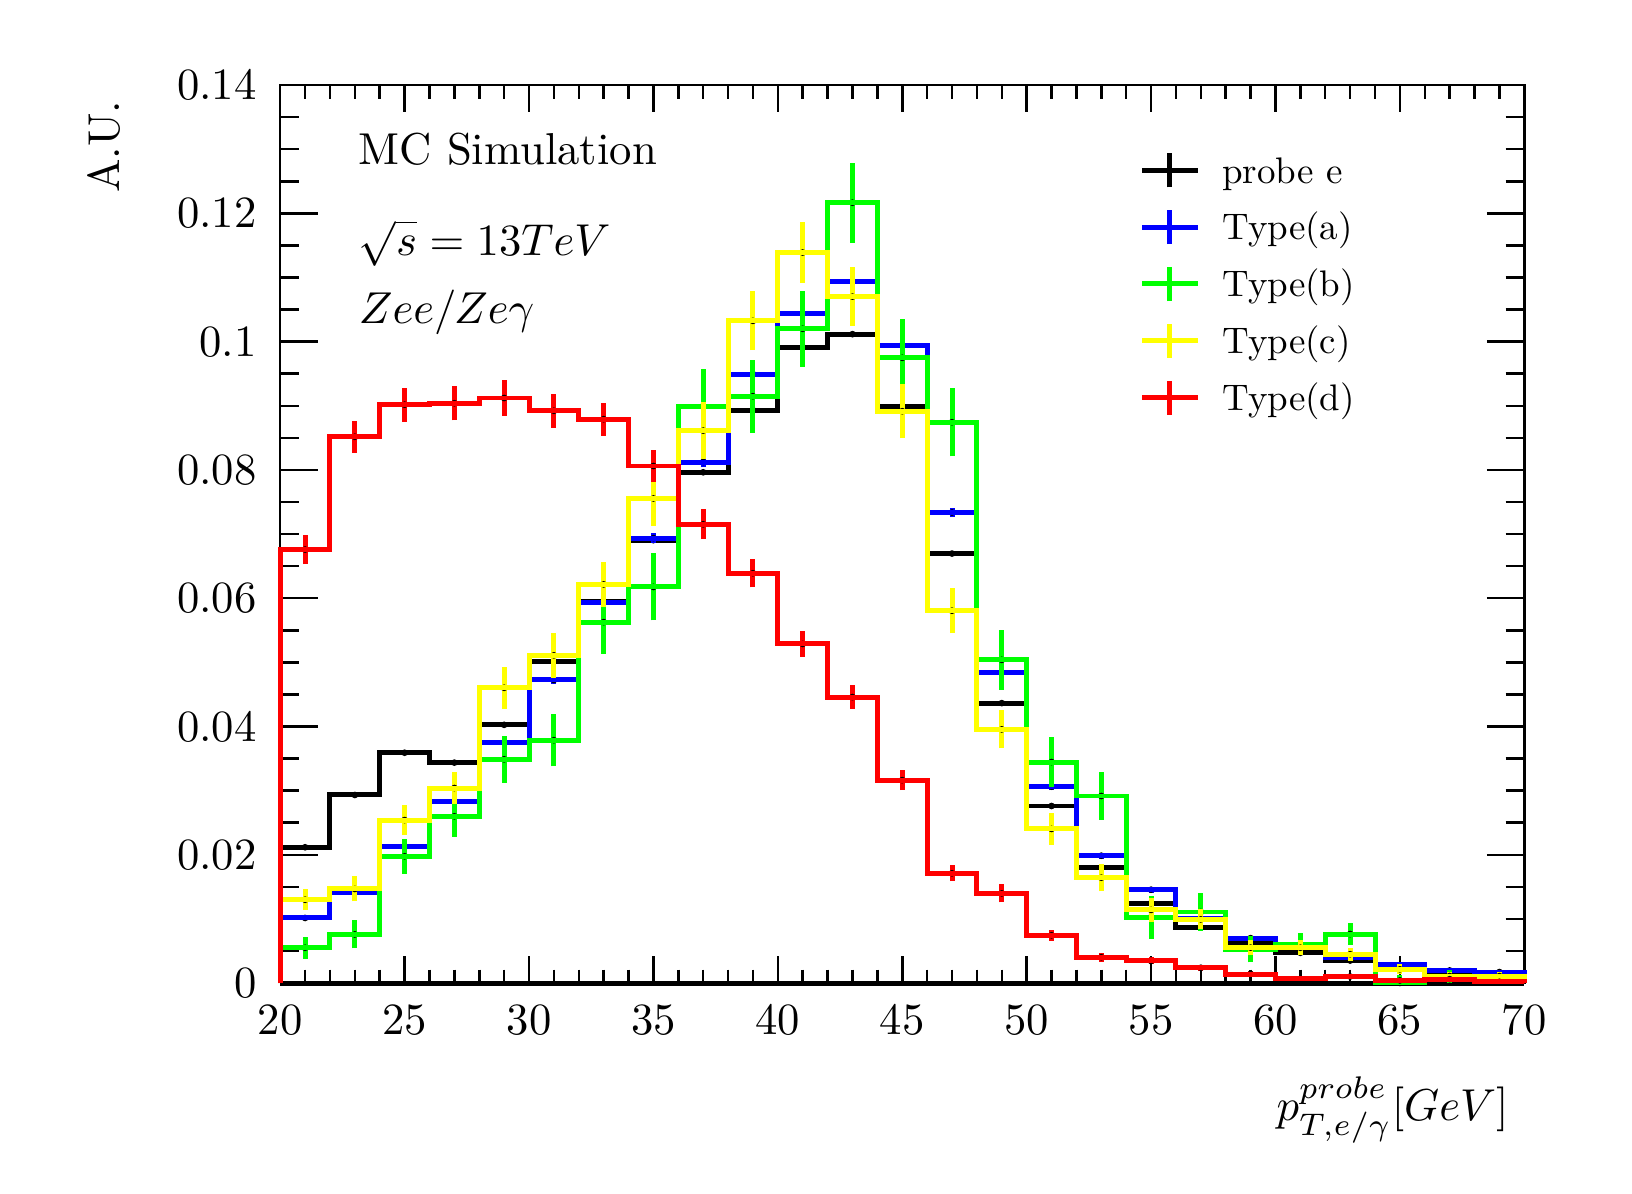
\begin{tikzpicture}
\pgfdeclareplotmark{cross} {
\pgfpathmoveto{\pgfpoint{-0.3\pgfplotmarksize}{\pgfplotmarksize}}
\pgfpathlineto{\pgfpoint{+0.3\pgfplotmarksize}{\pgfplotmarksize}}
\pgfpathlineto{\pgfpoint{+0.3\pgfplotmarksize}{0.3\pgfplotmarksize}}
\pgfpathlineto{\pgfpoint{+1\pgfplotmarksize}{0.3\pgfplotmarksize}}
\pgfpathlineto{\pgfpoint{+1\pgfplotmarksize}{-0.3\pgfplotmarksize}}
\pgfpathlineto{\pgfpoint{+0.3\pgfplotmarksize}{-0.3\pgfplotmarksize}}
\pgfpathlineto{\pgfpoint{+0.3\pgfplotmarksize}{-1.\pgfplotmarksize}}
\pgfpathlineto{\pgfpoint{-0.3\pgfplotmarksize}{-1.\pgfplotmarksize}}
\pgfpathlineto{\pgfpoint{-0.3\pgfplotmarksize}{-0.3\pgfplotmarksize}}
\pgfpathlineto{\pgfpoint{-1.\pgfplotmarksize}{-0.3\pgfplotmarksize}}
\pgfpathlineto{\pgfpoint{-1.\pgfplotmarksize}{0.3\pgfplotmarksize}}
\pgfpathlineto{\pgfpoint{-0.3\pgfplotmarksize}{0.3\pgfplotmarksize}}
\pgfpathclose
\pgfusepathqstroke
}
\pgfdeclareplotmark{cross*} {
\pgfpathmoveto{\pgfpoint{-0.3\pgfplotmarksize}{\pgfplotmarksize}}
\pgfpathlineto{\pgfpoint{+0.3\pgfplotmarksize}{\pgfplotmarksize}}
\pgfpathlineto{\pgfpoint{+0.3\pgfplotmarksize}{0.3\pgfplotmarksize}}
\pgfpathlineto{\pgfpoint{+1\pgfplotmarksize}{0.3\pgfplotmarksize}}
\pgfpathlineto{\pgfpoint{+1\pgfplotmarksize}{-0.3\pgfplotmarksize}}
\pgfpathlineto{\pgfpoint{+0.3\pgfplotmarksize}{-0.3\pgfplotmarksize}}
\pgfpathlineto{\pgfpoint{+0.3\pgfplotmarksize}{-1.\pgfplotmarksize}}
\pgfpathlineto{\pgfpoint{-0.3\pgfplotmarksize}{-1.\pgfplotmarksize}}
\pgfpathlineto{\pgfpoint{-0.3\pgfplotmarksize}{-0.3\pgfplotmarksize}}
\pgfpathlineto{\pgfpoint{-1.\pgfplotmarksize}{-0.3\pgfplotmarksize}}
\pgfpathlineto{\pgfpoint{-1.\pgfplotmarksize}{0.3\pgfplotmarksize}}
\pgfpathlineto{\pgfpoint{-0.3\pgfplotmarksize}{0.3\pgfplotmarksize}}
\pgfpathclose
\pgfusepathqfillstroke
}
\pgfdeclareplotmark{newstar} {
\pgfpathmoveto{\pgfqpoint{0pt}{\pgfplotmarksize}}
\pgfpathlineto{\pgfqpointpolar{44}{0.5\pgfplotmarksize}}
\pgfpathlineto{\pgfqpointpolar{18}{\pgfplotmarksize}}
\pgfpathlineto{\pgfqpointpolar{-20}{0.5\pgfplotmarksize}}
\pgfpathlineto{\pgfqpointpolar{-54}{\pgfplotmarksize}}
\pgfpathlineto{\pgfqpointpolar{-90}{0.5\pgfplotmarksize}}
\pgfpathlineto{\pgfqpointpolar{234}{\pgfplotmarksize}}
\pgfpathlineto{\pgfqpointpolar{198}{0.5\pgfplotmarksize}}
\pgfpathlineto{\pgfqpointpolar{162}{\pgfplotmarksize}}
\pgfpathlineto{\pgfqpointpolar{134}{0.5\pgfplotmarksize}}
\pgfpathclose
\pgfusepathqstroke
}
\pgfdeclareplotmark{newstar*} {
\pgfpathmoveto{\pgfqpoint{0pt}{\pgfplotmarksize}}
\pgfpathlineto{\pgfqpointpolar{44}{0.5\pgfplotmarksize}}
\pgfpathlineto{\pgfqpointpolar{18}{\pgfplotmarksize}}
\pgfpathlineto{\pgfqpointpolar{-20}{0.5\pgfplotmarksize}}
\pgfpathlineto{\pgfqpointpolar{-54}{\pgfplotmarksize}}
\pgfpathlineto{\pgfqpointpolar{-90}{0.5\pgfplotmarksize}}
\pgfpathlineto{\pgfqpointpolar{234}{\pgfplotmarksize}}
\pgfpathlineto{\pgfqpointpolar{198}{0.5\pgfplotmarksize}}
\pgfpathlineto{\pgfqpointpolar{162}{\pgfplotmarksize}}
\pgfpathlineto{\pgfqpointpolar{134}{0.5\pgfplotmarksize}}
\pgfpathclose
\pgfusepathqfillstroke
}
\definecolor{c}{rgb}{1,1,1};
\draw [color=c, fill=c] (0,0) rectangle (20,14.4361);
\draw [color=c, fill=c] (3.2,2.30977) rectangle (19,13.7143);
\definecolor{c}{rgb}{0,0,0};
\draw [c,line width=0.9] (3.2,2.30977) -- (3.2,13.7143) -- (19,13.7143) -- (19,2.30977) -- (3.2,2.30977);
\draw [c,line width=1.8] (3.2,2.30977) -- (3.2158,2.30977) -- (3.2158,2.30977) -- (3.2316,2.30977) -- (3.2316,2.30977) -- (3.2474,2.30977) -- (3.2474,2.30977) -- (3.2632,2.30977) -- (3.2632,2.30977) -- (3.279,2.30977) -- (3.279,2.30977) --
 (3.2948,2.30977) -- (3.2948,2.30977) -- (3.3106,2.30977) -- (3.3106,2.30977) -- (3.3264,2.30977) -- (3.3264,2.30977) -- (3.3422,2.30977) -- (3.3422,2.30977) -- (3.358,2.30977) -- (3.358,2.30977) -- (3.3738,2.30977) -- (3.3738,2.30977) --
 (3.3896,2.30977) -- (3.3896,2.30977) -- (3.4054,2.30977) -- (3.4054,2.30977) -- (3.4212,2.30977) -- (3.4212,2.30977) -- (3.437,2.30977) -- (3.437,2.30977) -- (3.4528,2.30977) -- (3.4528,2.30977) -- (3.4686,2.30977) -- (3.4686,2.30977) --
 (3.4844,2.30977) -- (3.4844,2.30977) -- (3.5002,2.30977) -- (3.5002,2.30977) -- (3.516,2.30977) -- (3.516,2.30977) -- (3.5318,2.30977) -- (3.5318,2.30977) -- (3.5476,2.30977) -- (3.5476,2.30977) -- (3.5634,2.30977) -- (3.5634,2.30977) --
 (3.5792,2.30977) -- (3.5792,2.30977) -- (3.595,2.30977) -- (3.595,2.30977) -- (3.6108,2.30977) -- (3.6108,2.30977) -- (3.6266,2.30977) -- (3.6266,2.30977) -- (3.6424,2.30977) -- (3.6424,2.30977) -- (3.6582,2.30977) -- (3.6582,2.30977) --
 (3.674,2.30977) -- (3.674,2.30977) -- (3.6898,2.30977) -- (3.6898,2.30977) -- (3.7056,2.30977) -- (3.7056,2.30977) -- (3.7214,2.30977) -- (3.7214,2.30977) -- (3.7372,2.30977) -- (3.7372,2.30977) -- (3.753,2.30977) -- (3.753,2.30977) --
 (3.7688,2.30977) -- (3.7688,2.30977) -- (3.7846,2.30977) -- (3.7846,2.30977) -- (3.8004,2.30977) -- (3.8004,2.30977) -- (3.8162,2.30977) -- (3.8162,2.30977) -- (3.832,2.30977) -- (3.832,2.30977) -- (3.8478,2.30977) -- (3.8478,2.30977) --
 (3.8636,2.30977) -- (3.8636,2.30977) -- (3.8794,2.30977) -- (3.8794,2.30977) -- (3.8952,2.30977) -- (3.8952,2.30977) -- (3.911,2.30977) -- (3.911,2.30977) -- (3.9268,2.30977) -- (3.9268,2.30977) -- (3.9426,2.30977) -- (3.9426,2.30977) --
 (3.9584,2.30977) -- (3.9584,2.30977) -- (3.9742,2.30977) -- (3.9742,2.30977) -- (3.99,2.30977) -- (3.99,2.30977) -- (4.0058,2.30977) -- (4.0058,2.30977) -- (4.0216,2.30977) -- (4.0216,2.30977) -- (4.0374,2.30977) -- (4.0374,2.30977) --
 (4.0532,2.30977) -- (4.0532,2.30977) -- (4.069,2.30977) -- (4.069,2.30977) -- (4.0848,2.30977) -- (4.0848,2.30977) -- (4.1006,2.30977) -- (4.1006,2.30977) -- (4.1164,2.30977) -- (4.1164,2.30977) -- (4.1322,2.30977) -- (4.1322,2.30977) --
 (4.148,2.30977) -- (4.148,2.30977) -- (4.1638,2.30977) -- (4.1638,2.30977) -- (4.1796,2.30977) -- (4.1796,2.30977) -- (4.1954,2.30977) -- (4.1954,2.30977) -- (4.2112,2.30977) -- (4.2112,2.30977) -- (4.227,2.30977) -- (4.227,2.30977) --
 (4.2428,2.30977) -- (4.2428,2.30977) -- (4.2586,2.30977) -- (4.2586,2.30977) -- (4.2744,2.30977) -- (4.2744,2.30977) -- (4.2902,2.30977) -- (4.2902,2.30977) -- (4.306,2.30977) -- (4.306,2.30977) -- (4.3218,2.30977) -- (4.3218,2.30977) --
 (4.3376,2.30977) -- (4.3376,2.30977) -- (4.3534,2.30977) -- (4.3534,2.30977) -- (4.3692,2.30977) -- (4.3692,2.30977) -- (4.385,2.30977) -- (4.385,2.30977) -- (4.4008,2.30977) -- (4.4008,2.30977) -- (4.4166,2.30977) -- (4.4166,2.30977) --
 (4.4324,2.30977) -- (4.4324,2.30977) -- (4.4482,2.30977) -- (4.4482,2.30977) -- (4.464,2.30977) -- (4.464,2.30977) -- (4.4798,2.30977) -- (4.4798,2.30977) -- (4.4956,2.30977) -- (4.4956,2.30977) -- (4.5114,2.30977) -- (4.5114,2.30977) --
 (4.5272,2.30977) -- (4.5272,2.30977) -- (4.543,2.30977) -- (4.543,2.30977) -- (4.5588,2.30977) -- (4.5588,2.30977) -- (4.5746,2.30977) -- (4.5746,2.30977) -- (4.5904,2.30977) -- (4.5904,2.30977) -- (4.6062,2.30977) -- (4.6062,2.30977) --
 (4.622,2.30977) -- (4.622,2.30977) -- (4.6378,2.30977) -- (4.6378,2.30977) -- (4.6536,2.30977) -- (4.6536,2.30977) -- (4.6694,2.30977) -- (4.6694,2.30977) -- (4.6852,2.30977) -- (4.6852,2.30977) -- (4.701,2.30977) -- (4.701,2.30977) --
 (4.7168,2.30977) -- (4.7168,2.30977) -- (4.7326,2.30977) -- (4.7326,2.30977) -- (4.7484,2.30977) -- (4.7484,2.30977) -- (4.7642,2.30977) -- (4.7642,2.30977) -- (4.78,2.30977) -- (4.78,2.30977) -- (4.7958,2.30977) -- (4.7958,2.30977) --
 (4.8116,2.30977) -- (4.8116,2.30977) -- (4.8274,2.30977) -- (4.8274,2.30977) -- (4.8432,2.30977) -- (4.8432,2.30977) -- (4.859,2.30977) -- (4.859,2.30977) -- (4.8748,2.30977) -- (4.8748,2.30977) -- (4.8906,2.30977) -- (4.8906,2.30977) --
 (4.9064,2.30977) -- (4.9064,2.30977) -- (4.9222,2.30977) -- (4.9222,2.30977) -- (4.938,2.30977) -- (4.938,2.30977) -- (4.9538,2.30977) -- (4.9538,2.30977) -- (4.9696,2.30977) -- (4.9696,2.30977) -- (4.9854,2.30977) -- (4.9854,2.30977) --
 (5.0012,2.30977) -- (5.0012,2.30977) -- (5.017,2.30977) -- (5.017,2.30977) -- (5.0328,2.30977) -- (5.0328,2.30977) -- (5.0486,2.30977) -- (5.0486,2.30977) -- (5.0644,2.30977) -- (5.0644,2.30977) -- (5.0802,2.30977) -- (5.0802,2.30977) --
 (5.096,2.30977) -- (5.096,2.30977) -- (5.1118,2.30977) -- (5.1118,2.30977) -- (5.1276,2.30977) -- (5.1276,2.30977) -- (5.1434,2.30977) -- (5.1434,2.30977) -- (5.1592,2.30977) -- (5.1592,2.30977) -- (5.175,2.30977) -- (5.175,2.30977) --
 (5.1908,2.30977) -- (5.1908,2.30977) -- (5.2066,2.30977) -- (5.2066,2.30977) -- (5.2224,2.30977) -- (5.2224,2.30977) -- (5.2382,2.30977) -- (5.2382,2.30977) -- (5.254,2.30977) -- (5.254,2.30977) -- (5.2698,2.30977) -- (5.2698,2.30977) --
 (5.2856,2.30977) -- (5.2856,2.30977) -- (5.3014,2.30977) -- (5.3014,2.30977) -- (5.3172,2.30977) -- (5.3172,2.30977) -- (5.333,2.30977) -- (5.333,2.30977) -- (5.3488,2.30977) -- (5.3488,2.30977) -- (5.3646,2.30977) -- (5.3646,2.30977) --
 (5.3804,2.30977) -- (5.3804,2.30977) -- (5.3962,2.30977) -- (5.3962,2.30977) -- (5.412,2.30977) -- (5.412,2.30977) -- (5.4278,2.30977) -- (5.4278,2.30977) -- (5.4436,2.30977) -- (5.4436,2.30977) -- (5.4594,2.30977) -- (5.4594,2.30977) --
 (5.4752,2.30977) -- (5.4752,2.30977) -- (5.491,2.30977) -- (5.491,2.30977) -- (5.5068,2.30977) -- (5.5068,2.30977) -- (5.5226,2.30977) -- (5.5226,2.30977) -- (5.5384,2.30977) -- (5.5384,2.30977) -- (5.5542,2.30977) -- (5.5542,2.30977) --
 (5.57,2.30977) -- (5.57,2.30977) -- (5.5858,2.30977) -- (5.5858,2.30977) -- (5.6016,2.30977) -- (5.6016,2.30977) -- (5.6174,2.30977) -- (5.6174,2.30977) -- (5.6332,2.30977) -- (5.6332,2.30977) -- (5.649,2.30977) -- (5.649,2.30977) --
 (5.6648,2.30977) -- (5.6648,2.30977) -- (5.6806,2.30977) -- (5.6806,2.30977) -- (5.6964,2.30977) -- (5.6964,2.30977) -- (5.7122,2.30977) -- (5.7122,2.30977) -- (5.728,2.30977) -- (5.728,2.30977) -- (5.7438,2.30977) -- (5.7438,2.30977) --
 (5.7596,2.30977) -- (5.7596,2.30977) -- (5.7754,2.30977) -- (5.7754,2.30977) -- (5.7912,2.30977) -- (5.7912,2.30977) -- (5.807,2.30977) -- (5.807,2.30977) -- (5.8228,2.30977) -- (5.8228,2.30977) -- (5.8386,2.30977) -- (5.8386,2.30977) --
 (5.8544,2.30977) -- (5.8544,2.30977) -- (5.8702,2.30977) -- (5.8702,2.30977) -- (5.886,2.30977) -- (5.886,2.30977) -- (5.9018,2.30977) -- (5.9018,2.30977) -- (5.9176,2.30977) -- (5.9176,2.30977) -- (5.9334,2.30977) -- (5.9334,2.30977) --
 (5.9492,2.30977) -- (5.9492,2.30977) -- (5.965,2.30977) -- (5.965,2.30977) -- (5.9808,2.30977) -- (5.9808,2.30977) -- (5.9966,2.30977) -- (5.9966,2.30977) -- (6.0124,2.30977) -- (6.0124,2.30977) -- (6.0282,2.30977) -- (6.0282,2.30977) --
 (6.044,2.30977) -- (6.044,2.30977) -- (6.0598,2.30977) -- (6.0598,2.30977) -- (6.0756,2.30977) -- (6.0756,2.30977) -- (6.0914,2.30977) -- (6.0914,2.30977) -- (6.1072,2.30977) -- (6.1072,2.30977) -- (6.123,2.30977) -- (6.123,2.30977) --
 (6.1388,2.30977) -- (6.1388,2.30977) -- (6.1546,2.30977) -- (6.1546,2.30977) -- (6.1704,2.30977) -- (6.1704,2.30977) -- (6.1862,2.30977) -- (6.1862,2.30977) -- (6.202,2.30977) -- (6.202,2.30977) -- (6.2178,2.30977) -- (6.2178,2.30977) --
 (6.2336,2.30977) -- (6.2336,2.30977) -- (6.2494,2.30977) -- (6.2494,2.30977) -- (6.2652,2.30977) -- (6.2652,2.30977) -- (6.281,2.30977) -- (6.281,2.30977) -- (6.2968,2.30977) -- (6.2968,2.30977) -- (6.3126,2.30977) -- (6.3126,2.30977) --
 (6.3284,2.30977) -- (6.3284,2.30977) -- (6.3442,2.30977) -- (6.3442,2.30977) -- (6.36,2.30977) -- (6.36,2.30977) -- (6.3758,2.30977) -- (6.3758,2.30977) -- (6.3916,2.30977) -- (6.3916,2.30977) -- (6.4074,2.30977) -- (6.4074,2.30977) --
 (6.4232,2.30977) -- (6.4232,2.30977) -- (6.439,2.30977) -- (6.439,2.30977) -- (6.4548,2.30977) -- (6.4548,2.30977) -- (6.4706,2.30977) -- (6.4706,2.30977) -- (6.4864,2.30977) -- (6.4864,2.30977) -- (6.5022,2.30977) -- (6.5022,2.30977) --
 (6.518,2.30977) -- (6.518,2.30977) -- (6.5338,2.30977) -- (6.5338,2.30977) -- (6.5496,2.30977) -- (6.5496,2.30977) -- (6.5654,2.30977) -- (6.5654,2.30977) -- (6.5812,2.30977) -- (6.5812,2.30977) -- (6.597,2.30977) -- (6.597,2.30977) --
 (6.6128,2.30977) -- (6.6128,2.30977) -- (6.6286,2.30977) -- (6.6286,2.30977) -- (6.6444,2.30977) -- (6.6444,2.30977) -- (6.6602,2.30977) -- (6.6602,2.30977) -- (6.676,2.30977) -- (6.676,2.30977) -- (6.6918,2.30977) -- (6.6918,2.30977) --
 (6.7076,2.30977) -- (6.7076,2.30977) -- (6.7234,2.30977) -- (6.7234,2.30977) -- (6.7392,2.30977) -- (6.7392,2.30977) -- (6.755,2.30977) -- (6.755,2.30977) -- (6.7708,2.30977) -- (6.7708,2.30977) -- (6.7866,2.30977) -- (6.7866,2.30977) --
 (6.8024,2.30977) -- (6.8024,2.30977) -- (6.8182,2.30977) -- (6.8182,2.30977) -- (6.834,2.30977) -- (6.834,2.30977) -- (6.8498,2.30977) -- (6.8498,2.30977) -- (6.8656,2.30977) -- (6.8656,2.30977) -- (6.8814,2.30977) -- (6.8814,2.30977) --
 (6.8972,2.30977) -- (6.8972,2.30977) -- (6.913,2.30977) -- (6.913,2.30977) -- (6.9288,2.30977) -- (6.9288,2.30977) -- (6.9446,2.30977) -- (6.9446,2.30977) -- (6.9604,2.30977) -- (6.9604,2.30977) -- (6.9762,2.30977) -- (6.9762,2.30977) --
 (6.992,2.30977) -- (6.992,2.30977) -- (7.0078,2.30977) -- (7.0078,2.30977) -- (7.0236,2.30977) -- (7.0236,2.30977) -- (7.0394,2.30977) -- (7.0394,2.30977) -- (7.0552,2.30977) -- (7.0552,2.30977) -- (7.071,2.30977) -- (7.071,2.30977) --
 (7.0868,2.30977) -- (7.0868,2.30977) -- (7.1026,2.30977) -- (7.1026,2.30977) -- (7.1184,2.30977) -- (7.1184,2.30977) -- (7.1342,2.30977) -- (7.1342,2.30977) -- (7.15,2.30977) -- (7.15,2.30977) -- (7.1658,2.30977) -- (7.1658,2.30977) --
 (7.1816,2.30977) -- (7.1816,2.30977) -- (7.1974,2.30977) -- (7.1974,2.30977) -- (7.2132,2.30977) -- (7.2132,2.30977) -- (7.229,2.30977) -- (7.229,2.30977) -- (7.2448,2.30977) -- (7.2448,2.30977) -- (7.2606,2.30977) -- (7.2606,2.30977) --
 (7.2764,2.30977) -- (7.2764,2.30977) -- (7.2922,2.30977) -- (7.2922,2.30977) -- (7.308,2.30977) -- (7.308,2.30977) -- (7.3238,2.30977) -- (7.3238,2.30977) -- (7.3396,2.30977) -- (7.3396,2.30977) -- (7.3554,2.30977) -- (7.3554,2.30977) --
 (7.3712,2.30977) -- (7.3712,2.30977) -- (7.387,2.30977) -- (7.387,2.30977) -- (7.4028,2.30977) -- (7.4028,2.30977) -- (7.4186,2.30977) -- (7.4186,2.30977) -- (7.4344,2.30977) -- (7.4344,2.30977) -- (7.4502,2.30977) -- (7.4502,2.30977) --
 (7.466,2.30977) -- (7.466,2.30977) -- (7.4818,2.30977) -- (7.4818,2.30977) -- (7.4976,2.30977) -- (7.4976,2.30977) -- (7.5134,2.30977) -- (7.5134,2.30977) -- (7.5292,2.30977) -- (7.5292,2.30977) -- (7.545,2.30977) -- (7.545,2.30977) --
 (7.5608,2.30977) -- (7.5608,2.30977) -- (7.5766,2.30977) -- (7.5766,2.30977) -- (7.5924,2.30977) -- (7.5924,2.30977) -- (7.6082,2.30977) -- (7.6082,2.30977) -- (7.624,2.30977) -- (7.624,2.30977) -- (7.6398,2.30977) -- (7.6398,2.30977) --
 (7.6556,2.30977) -- (7.6556,2.30977) -- (7.6714,2.30977) -- (7.6714,2.30977) -- (7.6872,2.30977) -- (7.6872,2.30977) -- (7.703,2.30977) -- (7.703,2.30977) -- (7.7188,2.30977) -- (7.7188,2.30977) -- (7.7346,2.30977) -- (7.7346,2.30977) --
 (7.7504,2.30977) -- (7.7504,2.30977) -- (7.7662,2.30977) -- (7.7662,2.30977) -- (7.782,2.30977) -- (7.782,2.30977) -- (7.7978,2.30977) -- (7.7978,2.30977) -- (7.8136,2.30977) -- (7.8136,2.30977) -- (7.8294,2.30977) -- (7.8294,2.30977) --
 (7.8452,2.30977) -- (7.8452,2.30977) -- (7.861,2.30977) -- (7.861,2.30977) -- (7.8768,2.30977) -- (7.8768,2.30977) -- (7.8926,2.30977) -- (7.8926,2.30977) -- (7.9084,2.30977) -- (7.9084,2.30977) -- (7.9242,2.30977) -- (7.9242,2.30977) --
 (7.94,2.30977) -- (7.94,2.30977) -- (7.9558,2.30977) -- (7.9558,2.30977) -- (7.9716,2.30977) -- (7.9716,2.30977) -- (7.9874,2.30977) -- (7.9874,2.30977) -- (8.0032,2.30977) -- (8.0032,2.30977) -- (8.019,2.30977) -- (8.019,2.30977) --
 (8.0348,2.30977) -- (8.0348,2.30977) -- (8.0506,2.30977) -- (8.0506,2.30977) -- (8.0664,2.30977) -- (8.0664,2.30977) -- (8.0822,2.30977) -- (8.0822,2.30977) -- (8.098,2.30977) -- (8.098,2.30977) -- (8.1138,2.30977) -- (8.1138,2.30977) --
 (8.1296,2.30977) -- (8.1296,2.30977) -- (8.1454,2.30977) -- (8.1454,2.30977) -- (8.1612,2.30977) -- (8.1612,2.30977) -- (8.177,2.30977) -- (8.177,2.30977) -- (8.1928,2.30977) -- (8.1928,2.30977) -- (8.2086,2.30977) -- (8.2086,2.30977) --
 (8.2244,2.30977) -- (8.2244,2.30977) -- (8.2402,2.30977) -- (8.2402,2.30977) -- (8.256,2.30977) -- (8.256,2.30977) -- (8.2718,2.30977) -- (8.2718,2.30977) -- (8.2876,2.30977) -- (8.2876,2.30977) -- (8.3034,2.30977) -- (8.3034,2.30977) --
 (8.3192,2.30977) -- (8.3192,2.30977) -- (8.335,2.30977) -- (8.335,2.30977) -- (8.3508,2.30977) -- (8.3508,2.30977) -- (8.3666,2.30977) -- (8.3666,2.30977) -- (8.3824,2.30977) -- (8.3824,2.30977) -- (8.3982,2.30977) -- (8.3982,2.30977) --
 (8.414,2.30977) -- (8.414,2.30977) -- (8.4298,2.30977) -- (8.4298,2.30977) -- (8.4456,2.30977) -- (8.4456,2.30977) -- (8.4614,2.30977) -- (8.4614,2.30977) -- (8.4772,2.30977) -- (8.4772,2.30977) -- (8.493,2.30977) -- (8.493,2.30977) --
 (8.5088,2.30977) -- (8.5088,2.30977) -- (8.5246,2.30977) -- (8.5246,2.30977) -- (8.5404,2.30977) -- (8.5404,2.30977) -- (8.5562,2.30977) -- (8.5562,2.30977) -- (8.572,2.30977) -- (8.572,2.30977) -- (8.5878,2.30977) -- (8.5878,2.30977) --
 (8.6036,2.30977) -- (8.6036,2.30977) -- (8.6194,2.30977) -- (8.6194,2.30977) -- (8.6352,2.30977) -- (8.6352,2.30977) -- (8.651,2.30977) -- (8.651,2.30977) -- (8.6668,2.30977) -- (8.6668,2.30977) -- (8.6826,2.30977) -- (8.6826,2.30977) --
 (8.6984,2.30977) -- (8.6984,2.30977) -- (8.7142,2.30977) -- (8.7142,2.30977) -- (8.73,2.30977) -- (8.73,2.30977) -- (8.7458,2.30977) -- (8.7458,2.30977) -- (8.7616,2.30977) -- (8.7616,2.30977) -- (8.7774,2.30977) -- (8.7774,2.30977) --
 (8.7932,2.30977) -- (8.7932,2.30977) -- (8.809,2.30977) -- (8.809,2.30977) -- (8.8248,2.30977) -- (8.8248,2.30977) -- (8.8406,2.30977) -- (8.8406,2.30977) -- (8.8564,2.30977) -- (8.8564,2.30977) -- (8.8722,2.30977) -- (8.8722,2.30977) --
 (8.888,2.30977) -- (8.888,2.30977) -- (8.9038,2.30977) -- (8.9038,2.30977) -- (8.9196,2.30977) -- (8.9196,2.30977) -- (8.9354,2.30977) -- (8.9354,2.30977) -- (8.9512,2.30977) -- (8.9512,2.30977) -- (8.967,2.30977) -- (8.967,2.30977) --
 (8.9828,2.30977) -- (8.9828,2.30977) -- (8.9986,2.30977) -- (8.9986,2.30977) -- (9.0144,2.30977) -- (9.0144,2.30977) -- (9.0302,2.30977) -- (9.0302,2.30977) -- (9.046,2.30977) -- (9.046,2.30977) -- (9.0618,2.30977) -- (9.0618,2.30977) --
 (9.0776,2.30977) -- (9.0776,2.30977) -- (9.0934,2.30977) -- (9.0934,2.30977) -- (9.1092,2.30977) -- (9.1092,2.30977) -- (9.125,2.30977) -- (9.125,2.30977) -- (9.1408,2.30977) -- (9.1408,2.30977) -- (9.1566,2.30977) -- (9.1566,2.30977) --
 (9.1724,2.30977) -- (9.1724,2.30977) -- (9.1882,2.30977) -- (9.1882,2.30977) -- (9.204,2.30977) -- (9.204,2.30977) -- (9.2198,2.30977) -- (9.2198,2.30977) -- (9.2356,2.30977) -- (9.2356,2.30977) -- (9.2514,2.30977) -- (9.2514,2.30977) --
 (9.2672,2.30977) -- (9.2672,2.30977) -- (9.283,2.30977) -- (9.283,2.30977) -- (9.2988,2.30977) -- (9.2988,2.30977) -- (9.3146,2.30977) -- (9.3146,2.30977) -- (9.3304,2.30977) -- (9.3304,2.30977) -- (9.3462,2.30977) -- (9.3462,2.30977) --
 (9.362,2.30977) -- (9.362,2.30977) -- (9.3778,2.30977) -- (9.3778,2.30977) -- (9.3936,2.30977) -- (9.3936,2.30977) -- (9.4094,2.30977) -- (9.4094,2.30977) -- (9.4252,2.30977) -- (9.4252,2.30977) -- (9.441,2.30977) -- (9.441,2.30977) --
 (9.4568,2.30977) -- (9.4568,2.30977) -- (9.4726,2.30977) -- (9.4726,2.30977) -- (9.4884,2.30977) -- (9.4884,2.30977) -- (9.5042,2.30977) -- (9.5042,2.30977) -- (9.52,2.30977) -- (9.52,2.30977) -- (9.5358,2.30977) -- (9.5358,2.30977) --
 (9.5516,2.30977) -- (9.5516,2.30977) -- (9.5674,2.30977) -- (9.5674,2.30977) -- (9.5832,2.30977) -- (9.5832,2.30977) -- (9.599,2.30977) -- (9.599,2.30977) -- (9.6148,2.30977) -- (9.6148,2.30977) -- (9.6306,2.30977) -- (9.6306,2.30977) --
 (9.6464,2.30977) -- (9.6464,2.30977) -- (9.6622,2.30977) -- (9.6622,2.30977) -- (9.678,2.30977) -- (9.678,2.30977) -- (9.6938,2.30977) -- (9.6938,2.30977) -- (9.7096,2.30977) -- (9.7096,2.30977) -- (9.7254,2.30977) -- (9.7254,2.30977) --
 (9.7412,2.30977) -- (9.7412,2.30977) -- (9.757,2.30977) -- (9.757,2.30977) -- (9.7728,2.30977) -- (9.7728,2.30977) -- (9.7886,2.30977) -- (9.7886,2.30977) -- (9.8044,2.30977) -- (9.8044,2.30977) -- (9.8202,2.30977) -- (9.8202,2.30977) --
 (9.836,2.30977) -- (9.836,2.30977) -- (9.8518,2.30977) -- (9.8518,2.30977) -- (9.8676,2.30977) -- (9.8676,2.30977) -- (9.8834,2.30977) -- (9.8834,2.30977) -- (9.8992,2.30977) -- (9.8992,2.30977) -- (9.915,2.30977) -- (9.915,2.30977) --
 (9.9308,2.30977) -- (9.9308,2.30977) -- (9.9466,2.30977) -- (9.9466,2.30977) -- (9.9624,2.30977) -- (9.9624,2.30977) -- (9.9782,2.30977) -- (9.9782,2.30977) -- (9.994,2.30977) -- (9.994,2.30977) -- (10.0098,2.30977) -- (10.0098,2.30977) --
 (10.0256,2.30977) -- (10.0256,2.30977) -- (10.0414,2.30977) -- (10.0414,2.30977) -- (10.0572,2.30977) -- (10.0572,2.30977) -- (10.073,2.30977) -- (10.073,2.30977) -- (10.0888,2.30977) -- (10.0888,2.30977) -- (10.1046,2.30977) -- (10.1046,2.30977) --
 (10.1204,2.30977) -- (10.1204,2.30977) -- (10.1362,2.30977) -- (10.1362,2.30977) -- (10.152,2.30977) -- (10.152,2.30977) -- (10.1678,2.30977) -- (10.1678,2.30977) -- (10.1836,2.30977) -- (10.1836,2.30977) -- (10.1994,2.30977) -- (10.1994,2.30977) --
 (10.2152,2.30977) -- (10.2152,2.30977) -- (10.231,2.30977) -- (10.231,2.30977) -- (10.2468,2.30977) -- (10.2468,2.30977) -- (10.2626,2.30977) -- (10.2626,2.30977) -- (10.2784,2.30977) -- (10.2784,2.30977) -- (10.2942,2.30977) -- (10.2942,2.30977) --
 (10.31,2.30977) -- (10.31,2.30977) -- (10.3258,2.30977) -- (10.3258,2.30977) -- (10.3416,2.30977) -- (10.3416,2.30977) -- (10.3574,2.30977) -- (10.3574,2.30977) -- (10.3732,2.30977) -- (10.3732,2.30977) -- (10.389,2.30977) -- (10.389,2.30977) --
 (10.4048,2.30977) -- (10.4048,2.30977) -- (10.4206,2.30977) -- (10.4206,2.30977) -- (10.4364,2.30977) -- (10.4364,2.30977) -- (10.4522,2.30977) -- (10.4522,2.30977) -- (10.468,2.30977) -- (10.468,2.30977) -- (10.4838,2.30977) -- (10.4838,2.30977) --
 (10.4996,2.30977) -- (10.4996,2.30977) -- (10.5154,2.30977) -- (10.5154,2.30977) -- (10.5312,2.30977) -- (10.5312,2.30977) -- (10.547,2.30977) -- (10.547,2.30977) -- (10.5628,2.30977) -- (10.5628,2.30977) -- (10.5786,2.30977) -- (10.5786,2.30977) --
 (10.5944,2.30977) -- (10.5944,2.30977) -- (10.6102,2.30977) -- (10.6102,2.30977) -- (10.626,2.30977) -- (10.626,2.30977) -- (10.6418,2.30977) -- (10.6418,2.30977) -- (10.6576,2.30977) -- (10.6576,2.30977) -- (10.6734,2.30977) -- (10.6734,2.30977) --
 (10.6892,2.30977) -- (10.6892,2.30977) -- (10.705,2.30977) -- (10.705,2.30977) -- (10.7208,2.30977) -- (10.7208,2.30977) -- (10.7366,2.30977) -- (10.7366,2.30977) -- (10.7524,2.30977) -- (10.7524,2.30977) -- (10.7682,2.30977) -- (10.7682,2.30977) --
 (10.784,2.30977) -- (10.784,2.30977) -- (10.7998,2.30977) -- (10.7998,2.30977) -- (10.8156,2.30977) -- (10.8156,2.30977) -- (10.8314,2.30977) -- (10.8314,2.30977) -- (10.8472,2.30977) -- (10.8472,2.30977) -- (10.863,2.30977) -- (10.863,2.30977) --
 (10.8788,2.30977) -- (10.8788,2.30977) -- (10.8946,2.30977) -- (10.8946,2.30977) -- (10.9104,2.30977) -- (10.9104,2.30977) -- (10.9262,2.30977) -- (10.9262,2.30977) -- (10.942,2.30977) -- (10.942,2.30977) -- (10.9578,2.30977) -- (10.9578,2.30977) --
 (10.9736,2.30977) -- (10.9736,2.30977) -- (10.9894,2.30977) -- (10.9894,2.30977) -- (11.0052,2.30977) -- (11.0052,2.30977) -- (11.021,2.30977) -- (11.021,2.30977) -- (11.0368,2.30977) -- (11.0368,2.30977) -- (11.0526,2.30977) -- (11.0526,2.30977) --
 (11.0684,2.30977) -- (11.0684,2.30977) -- (11.0842,2.30977) -- (11.0842,2.30977) -- (11.1,2.30977) -- (11.1,2.30977) -- (11.1158,2.30977) -- (11.1158,2.30977) -- (11.1316,2.30977) -- (11.1316,2.30977) -- (11.1474,2.30977) -- (11.1474,2.30977) --
 (11.1632,2.30977) -- (11.1632,2.30977) -- (11.179,2.30977) -- (11.179,2.30977) -- (11.1948,2.30977) -- (11.1948,2.30977) -- (11.2106,2.30977) -- (11.2106,2.30977) -- (11.2264,2.30977) -- (11.2264,2.30977) -- (11.2422,2.30977) -- (11.2422,2.30977) --
 (11.258,2.30977) -- (11.258,2.30977) -- (11.2738,2.30977) -- (11.2738,2.30977) -- (11.2896,2.30977) -- (11.2896,2.30977) -- (11.3054,2.30977) -- (11.3054,2.30977) -- (11.3212,2.30977) -- (11.3212,2.30977) -- (11.337,2.30977) -- (11.337,2.30977) --
 (11.3528,2.30977) -- (11.3528,2.30977) -- (11.3686,2.30977) -- (11.3686,2.30977) -- (11.3844,2.30977) -- (11.3844,2.30977) -- (11.4002,2.30977) -- (11.4002,2.30977) -- (11.416,2.30977) -- (11.416,2.30977) -- (11.4318,2.30977) -- (11.4318,2.30977) --
 (11.4476,2.30977) -- (11.4476,2.30977) -- (11.4634,2.30977) -- (11.4634,2.30977) -- (11.4792,2.30977) -- (11.4792,2.30977) -- (11.495,2.30977) -- (11.495,2.30977) -- (11.5108,2.30977) -- (11.5108,2.30977) -- (11.5266,2.30977) -- (11.5266,2.30977) --
 (11.5424,2.30977) -- (11.5424,2.30977) -- (11.5582,2.30977) -- (11.5582,2.30977) -- (11.574,2.30977) -- (11.574,2.30977) -- (11.5898,2.30977) -- (11.5898,2.30977) -- (11.6056,2.30977) -- (11.6056,2.30977) -- (11.6214,2.30977) -- (11.6214,2.30977) --
 (11.6372,2.30977) -- (11.6372,2.30977) -- (11.653,2.30977) -- (11.653,2.30977) -- (11.6688,2.30977) -- (11.6688,2.30977) -- (11.6846,2.30977) -- (11.6846,2.30977) -- (11.7004,2.30977) -- (11.7004,2.30977) -- (11.7162,2.30977) -- (11.7162,2.30977) --
 (11.732,2.30977) -- (11.732,2.30977) -- (11.7478,2.30977) -- (11.7478,2.30977) -- (11.7636,2.30977) -- (11.7636,2.30977) -- (11.7794,2.30977) -- (11.7794,2.30977) -- (11.7952,2.30977) -- (11.7952,2.30977) -- (11.811,2.30977) -- (11.811,2.30977) --
 (11.8268,2.30977) -- (11.8268,2.30977) -- (11.8426,2.30977) -- (11.8426,2.30977) -- (11.8584,2.30977) -- (11.8584,2.30977) -- (11.8742,2.30977) -- (11.8742,2.30977) -- (11.89,2.30977) -- (11.89,2.30977) -- (11.9058,2.30977) -- (11.9058,2.30977) --
 (11.9216,2.30977) -- (11.9216,2.30977) -- (11.9374,2.30977) -- (11.9374,2.30977) -- (11.9532,2.30977) -- (11.9532,2.30977) -- (11.969,2.30977) -- (11.969,2.30977) -- (11.9848,2.30977) -- (11.9848,2.30977) -- (12.0006,2.30977) -- (12.0006,2.30977) --
 (12.0164,2.30977) -- (12.0164,2.30977) -- (12.0322,2.30977) -- (12.0322,2.30977) -- (12.048,2.30977) -- (12.048,2.30977) -- (12.0638,2.30977) -- (12.0638,2.30977) -- (12.0796,2.30977) -- (12.0796,2.30977) -- (12.0954,2.30977) -- (12.0954,2.30977) --
 (12.1112,2.30977) -- (12.1112,2.30977) -- (12.127,2.30977) -- (12.127,2.30977) -- (12.1428,2.30977) -- (12.1428,2.30977) -- (12.1586,2.30977) -- (12.1586,2.30977) -- (12.1744,2.30977) -- (12.1744,2.30977) -- (12.1902,2.30977) -- (12.1902,2.30977) --
 (12.206,2.30977) -- (12.206,2.30977) -- (12.2218,2.30977) -- (12.2218,2.30977) -- (12.2376,2.30977) -- (12.2376,2.30977) -- (12.2534,2.30977) -- (12.2534,2.30977) -- (12.2692,2.30977) -- (12.2692,2.30977) -- (12.285,2.30977) -- (12.285,2.30977) --
 (12.3008,2.30977) -- (12.3008,2.30977) -- (12.3166,2.30977) -- (12.3166,2.30977) -- (12.3324,2.30977) -- (12.3324,2.30977) -- (12.3482,2.30977) -- (12.3482,2.30977) -- (12.364,2.30977) -- (12.364,2.30977) -- (12.3798,2.30977) -- (12.3798,2.30977) --
 (12.3956,2.30977) -- (12.3956,2.30977) -- (12.4114,2.30977) -- (12.4114,2.30977) -- (12.4272,2.30977) -- (12.4272,2.30977) -- (12.443,2.30977) -- (12.443,2.30977) -- (12.4588,2.30977) -- (12.4588,2.30977) -- (12.4746,2.30977) -- (12.4746,2.30977) --
 (12.4904,2.30977) -- (12.4904,2.30977) -- (12.5062,2.30977) -- (12.5062,2.30977) -- (12.522,2.30977) -- (12.522,2.30977) -- (12.5378,2.30977) -- (12.5378,2.30977) -- (12.5536,2.30977) -- (12.5536,2.30977) -- (12.5694,2.30977) -- (12.5694,2.30977) --
 (12.5852,2.30977) -- (12.5852,2.30977) -- (12.601,2.30977) -- (12.601,2.30977) -- (12.6168,2.30977) -- (12.6168,2.30977) -- (12.6326,2.30977) -- (12.6326,2.30977) -- (12.6484,2.30977) -- (12.6484,2.30977) -- (12.6642,2.30977) -- (12.6642,2.30977) --
 (12.68,2.30977) -- (12.68,2.30977) -- (12.6958,2.30977) -- (12.6958,2.30977) -- (12.7116,2.30977) -- (12.7116,2.30977) -- (12.7274,2.30977) -- (12.7274,2.30977) -- (12.7432,2.30977) -- (12.7432,2.30977) -- (12.759,2.30977) -- (12.759,2.30977) --
 (12.7748,2.30977) -- (12.7748,2.30977) -- (12.7906,2.30977) -- (12.7906,2.30977) -- (12.8064,2.30977) -- (12.8064,2.30977) -- (12.8222,2.30977) -- (12.8222,2.30977) -- (12.838,2.30977) -- (12.838,2.30977) -- (12.8538,2.30977) -- (12.8538,2.30977) --
 (12.8696,2.30977) -- (12.8696,2.30977) -- (12.8854,2.30977) -- (12.8854,2.30977) -- (12.9012,2.30977) -- (12.9012,2.30977) -- (12.917,2.30977) -- (12.917,2.30977) -- (12.9328,2.30977) -- (12.9328,2.30977) -- (12.9486,2.30977) -- (12.9486,2.30977) --
 (12.9644,2.30977) -- (12.9644,2.30977) -- (12.9802,2.30977) -- (12.9802,2.30977) -- (12.996,2.30977) -- (12.996,2.30977) -- (13.0118,2.30977) -- (13.0118,2.30977) -- (13.0276,2.30977) -- (13.0276,2.30977) -- (13.0434,2.30977) -- (13.0434,2.30977) --
 (13.0592,2.30977) -- (13.0592,2.30977) -- (13.075,2.30977) -- (13.075,2.30977) -- (13.0908,2.30977) -- (13.0908,2.30977) -- (13.1066,2.30977) -- (13.1066,2.30977) -- (13.1224,2.30977) -- (13.1224,2.30977) -- (13.1382,2.30977) -- (13.1382,2.30977) --
 (13.154,2.30977) -- (13.154,2.30977) -- (13.1698,2.30977) -- (13.1698,2.30977) -- (13.1856,2.30977) -- (13.1856,2.30977) -- (13.2014,2.30977) -- (13.2014,2.30977) -- (13.2172,2.30977) -- (13.2172,2.30977) -- (13.233,2.30977) -- (13.233,2.30977) --
 (13.2488,2.30977) -- (13.2488,2.30977) -- (13.2646,2.30977) -- (13.2646,2.30977) -- (13.2804,2.30977) -- (13.2804,2.30977) -- (13.2962,2.30977) -- (13.2962,2.30977) -- (13.312,2.30977) -- (13.312,2.30977) -- (13.3278,2.30977) -- (13.3278,2.30977) --
 (13.3436,2.30977) -- (13.3436,2.30977) -- (13.3594,2.30977) -- (13.3594,2.30977) -- (13.3752,2.30977) -- (13.3752,2.30977) -- (13.391,2.30977) -- (13.391,2.30977) -- (13.4068,2.30977) -- (13.4068,2.30977) -- (13.4226,2.30977) -- (13.4226,2.30977) --
 (13.4384,2.30977) -- (13.4384,2.30977) -- (13.4542,2.30977) -- (13.4542,2.30977) -- (13.47,2.30977) -- (13.47,2.30977) -- (13.4858,2.30977) -- (13.4858,2.30977) -- (13.5016,2.30977) -- (13.5016,2.30977) -- (13.5174,2.30977) -- (13.5174,2.30977) --
 (13.5332,2.30977) -- (13.5332,2.30977) -- (13.549,2.30977) -- (13.549,2.30977) -- (13.5648,2.30977) -- (13.5648,2.30977) -- (13.5806,2.30977) -- (13.5806,2.30977) -- (13.5964,2.30977) -- (13.5964,2.30977) -- (13.6122,2.30977) -- (13.6122,2.30977) --
 (13.628,2.30977) -- (13.628,2.30977) -- (13.6438,2.30977) -- (13.6438,2.30977) -- (13.6596,2.30977) -- (13.6596,2.30977) -- (13.6754,2.30977) -- (13.6754,2.30977) -- (13.6912,2.30977) -- (13.6912,2.30977) -- (13.707,2.30977) -- (13.707,2.30977) --
 (13.7228,2.30977) -- (13.7228,2.30977) -- (13.7386,2.30977) -- (13.7386,2.30977) -- (13.7544,2.30977) -- (13.7544,2.30977) -- (13.7702,2.30977) -- (13.7702,2.30977) -- (13.786,2.30977) -- (13.786,2.30977) -- (13.8018,2.30977) -- (13.8018,2.30977) --
 (13.8176,2.30977) -- (13.8176,2.30977) -- (13.8334,2.30977) -- (13.8334,2.30977) -- (13.8492,2.30977) -- (13.8492,2.30977) -- (13.865,2.30977) -- (13.865,2.30977) -- (13.8808,2.30977) -- (13.8808,2.30977) -- (13.8966,2.30977) -- (13.8966,2.30977) --
 (13.9124,2.30977) -- (13.9124,2.30977) -- (13.9282,2.30977) -- (13.9282,2.30977) -- (13.944,2.30977) -- (13.944,2.30977) -- (13.9598,2.30977) -- (13.9598,2.30977) -- (13.9756,2.30977) -- (13.9756,2.30977) -- (13.9914,2.30977) -- (13.9914,2.30977) --
 (14.0072,2.30977) -- (14.0072,2.30977) -- (14.023,2.30977) -- (14.023,2.30977) -- (14.0388,2.30977) -- (14.0388,2.30977) -- (14.0546,2.30977) -- (14.0546,2.30977) -- (14.0704,2.30977) -- (14.0704,2.30977) -- (14.0862,2.30977) -- (14.0862,2.30977) --
 (14.102,2.30977) -- (14.102,2.30977) -- (14.1178,2.30977) -- (14.1178,2.30977) -- (14.1336,2.30977) -- (14.1336,2.30977) -- (14.1494,2.30977) -- (14.1494,2.30977) -- (14.1652,2.30977) -- (14.1652,2.30977) -- (14.181,2.30977) -- (14.181,2.30977) --
 (14.1968,2.30977) -- (14.1968,2.30977) -- (14.2126,2.30977) -- (14.2126,2.30977) -- (14.2284,2.30977) -- (14.2284,2.30977) -- (14.2442,2.30977) -- (14.2442,2.30977) -- (14.26,2.30977) -- (14.26,2.30977) -- (14.2758,2.30977) -- (14.2758,2.30977) --
 (14.2916,2.30977) -- (14.2916,2.30977) -- (14.3074,2.30977) -- (14.3074,2.30977) -- (14.3232,2.30977) -- (14.3232,2.30977) -- (14.339,2.30977) -- (14.339,2.30977) -- (14.3548,2.30977) -- (14.3548,2.30977) -- (14.3706,2.30977) -- (14.3706,2.30977) --
 (14.3864,2.30977) -- (14.3864,2.30977) -- (14.4022,2.30977) -- (14.4022,2.30977) -- (14.418,2.30977) -- (14.418,2.30977) -- (14.4338,2.30977) -- (14.4338,2.30977) -- (14.4496,2.30977) -- (14.4496,2.30977) -- (14.4654,2.30977) -- (14.4654,2.30977) --
 (14.4812,2.30977) -- (14.4812,2.30977) -- (14.497,2.30977) -- (14.497,2.30977) -- (14.5128,2.30977) -- (14.5128,2.30977) -- (14.5286,2.30977) -- (14.5286,2.30977) -- (14.5444,2.30977) -- (14.5444,2.30977) -- (14.5602,2.30977) -- (14.5602,2.30977) --
 (14.576,2.30977) -- (14.576,2.30977) -- (14.5918,2.30977) -- (14.5918,2.30977) -- (14.6076,2.30977) -- (14.6076,2.30977) -- (14.6234,2.30977) -- (14.6234,2.30977) -- (14.6392,2.30977) -- (14.6392,2.30977) -- (14.655,2.30977) -- (14.655,2.30977) --
 (14.6708,2.30977) -- (14.6708,2.30977) -- (14.6866,2.30977) -- (14.6866,2.30977) -- (14.7024,2.30977) -- (14.7024,2.30977) -- (14.7182,2.30977) -- (14.7182,2.30977) -- (14.734,2.30977) -- (14.734,2.30977) -- (14.7498,2.30977) -- (14.7498,2.30977) --
 (14.7656,2.30977) -- (14.7656,2.30977) -- (14.7814,2.30977) -- (14.7814,2.30977) -- (14.7972,2.30977) -- (14.7972,2.30977) -- (14.813,2.30977) -- (14.813,2.30977) -- (14.8288,2.30977) -- (14.8288,2.30977) -- (14.8446,2.30977) -- (14.8446,2.30977) --
 (14.8604,2.30977) -- (14.8604,2.30977) -- (14.8762,2.30977) -- (14.8762,2.30977) -- (14.892,2.30977) -- (14.892,2.30977) -- (14.9078,2.30977) -- (14.9078,2.30977) -- (14.9236,2.30977) -- (14.9236,2.30977) -- (14.9394,2.30977) -- (14.9394,2.30977) --
 (14.9552,2.30977) -- (14.9552,2.30977) -- (14.971,2.30977) -- (14.971,2.30977) -- (14.9868,2.30977) -- (14.9868,2.30977) -- (15.0026,2.30977) -- (15.0026,2.30977) -- (15.0184,2.30977) -- (15.0184,2.30977) -- (15.0342,2.30977) -- (15.0342,2.30977) --
 (15.05,2.30977) -- (15.05,2.30977) -- (15.0658,2.30977) -- (15.0658,2.30977) -- (15.0816,2.30977) -- (15.0816,2.30977) -- (15.0974,2.30977) -- (15.0974,2.30977) -- (15.1132,2.30977) -- (15.1132,2.30977) -- (15.129,2.30977) -- (15.129,2.30977) --
 (15.1448,2.30977) -- (15.1448,2.30977) -- (15.1606,2.30977) -- (15.1606,2.30977) -- (15.1764,2.30977) -- (15.1764,2.30977) -- (15.1922,2.30977) -- (15.1922,2.30977) -- (15.208,2.30977) -- (15.208,2.30977) -- (15.2238,2.30977) -- (15.2238,2.30977) --
 (15.2396,2.30977) -- (15.2396,2.30977) -- (15.2554,2.30977) -- (15.2554,2.30977) -- (15.2712,2.30977) -- (15.2712,2.30977) -- (15.287,2.30977) -- (15.287,2.30977) -- (15.3028,2.30977) -- (15.3028,2.30977) -- (15.3186,2.30977) -- (15.3186,2.30977) --
 (15.3344,2.30977) -- (15.3344,2.30977) -- (15.3502,2.30977) -- (15.3502,2.30977) -- (15.366,2.30977) -- (15.366,2.30977) -- (15.3818,2.30977) -- (15.3818,2.30977) -- (15.3976,2.30977) -- (15.3976,2.30977) -- (15.4134,2.30977) -- (15.4134,2.30977) --
 (15.4292,2.30977) -- (15.4292,2.30977) -- (15.445,2.30977) -- (15.445,2.30977) -- (15.4608,2.30977) -- (15.4608,2.30977) -- (15.4766,2.30977) -- (15.4766,2.30977) -- (15.4924,2.30977) -- (15.4924,2.30977) -- (15.5082,2.30977) -- (15.5082,2.30977) --
 (15.524,2.30977) -- (15.524,2.30977) -- (15.5398,2.30977) -- (15.5398,2.30977) -- (15.5556,2.30977) -- (15.5556,2.30977) -- (15.5714,2.30977) -- (15.5714,2.30977) -- (15.5872,2.30977) -- (15.5872,2.30977) -- (15.603,2.30977) -- (15.603,2.30977) --
 (15.6188,2.30977) -- (15.6188,2.30977) -- (15.6346,2.30977) -- (15.6346,2.30977) -- (15.6504,2.30977) -- (15.6504,2.30977) -- (15.6662,2.30977) -- (15.6662,2.30977) -- (15.682,2.30977) -- (15.682,2.30977) -- (15.6978,2.30977) -- (15.6978,2.30977) --
 (15.7136,2.30977) -- (15.7136,2.30977) -- (15.7294,2.30977) -- (15.7294,2.30977) -- (15.7452,2.30977) -- (15.7452,2.30977) -- (15.761,2.30977) -- (15.761,2.30977) -- (15.7768,2.30977) -- (15.7768,2.30977) -- (15.7926,2.30977) -- (15.7926,2.30977) --
 (15.8084,2.30977) -- (15.8084,2.30977) -- (15.8242,2.30977) -- (15.8242,2.30977) -- (15.84,2.30977) -- (15.84,2.30977) -- (15.8558,2.30977) -- (15.8558,2.30977) -- (15.8716,2.30977) -- (15.8716,2.30977) -- (15.8874,2.30977) -- (15.8874,2.30977) --
 (15.9032,2.30977) -- (15.9032,2.30977) -- (15.919,2.30977) -- (15.919,2.30977) -- (15.9348,2.30977) -- (15.9348,2.30977) -- (15.9506,2.30977) -- (15.9506,2.30977) -- (15.9664,2.30977) -- (15.9664,2.30977) -- (15.9822,2.30977) -- (15.9822,2.30977) --
 (15.998,2.30977) -- (15.998,2.30977) -- (16.0138,2.30977) -- (16.0138,2.30977) -- (16.0296,2.30977) -- (16.0296,2.30977) -- (16.0454,2.30977) -- (16.0454,2.30977) -- (16.0612,2.30977) -- (16.0612,2.30977) -- (16.077,2.30977) -- (16.077,2.30977) --
 (16.0928,2.30977) -- (16.0928,2.30977) -- (16.1086,2.30977) -- (16.1086,2.30977) -- (16.1244,2.30977) -- (16.1244,2.30977) -- (16.1402,2.30977) -- (16.1402,2.30977) -- (16.156,2.30977) -- (16.156,2.30977) -- (16.1718,2.30977) -- (16.1718,2.30977) --
 (16.1876,2.30977) -- (16.1876,2.30977) -- (16.2034,2.30977) -- (16.2034,2.30977) -- (16.2192,2.30977) -- (16.2192,2.30977) -- (16.235,2.30977) -- (16.235,2.30977) -- (16.2508,2.30977) -- (16.2508,2.30977) -- (16.2666,2.30977) -- (16.2666,2.30977) --
 (16.2824,2.30977) -- (16.2824,2.30977) -- (16.2982,2.30977) -- (16.2982,2.30977) -- (16.314,2.30977) -- (16.314,2.30977) -- (16.3298,2.30977) -- (16.3298,2.30977) -- (16.3456,2.30977) -- (16.3456,2.30977) -- (16.3614,2.30977) -- (16.3614,2.30977) --
 (16.3772,2.30977) -- (16.3772,2.30977) -- (16.393,2.30977) -- (16.393,2.30977) -- (16.4088,2.30977) -- (16.4088,2.30977) -- (16.4246,2.30977) -- (16.4246,2.30977) -- (16.4404,2.30977) -- (16.4404,2.30977) -- (16.4562,2.30977) -- (16.4562,2.30977) --
 (16.472,2.30977) -- (16.472,2.30977) -- (16.4878,2.30977) -- (16.4878,2.30977) -- (16.5036,2.30977) -- (16.5036,2.30977) -- (16.5194,2.30977) -- (16.5194,2.30977) -- (16.5352,2.30977) -- (16.5352,2.30977) -- (16.551,2.30977) -- (16.551,2.30977) --
 (16.5668,2.30977) -- (16.5668,2.30977) -- (16.5826,2.30977) -- (16.5826,2.30977) -- (16.5984,2.30977) -- (16.5984,2.30977) -- (16.6142,2.30977) -- (16.6142,2.30977) -- (16.63,2.30977) -- (16.63,2.30977) -- (16.6458,2.30977) -- (16.6458,2.30977) --
 (16.6616,2.30977) -- (16.6616,2.30977) -- (16.6774,2.30977) -- (16.6774,2.30977) -- (16.6932,2.30977) -- (16.6932,2.30977) -- (16.709,2.30977) -- (16.709,2.30977) -- (16.7248,2.30977) -- (16.7248,2.30977) -- (16.7406,2.30977) -- (16.7406,2.30977) --
 (16.7564,2.30977) -- (16.7564,2.30977) -- (16.7722,2.30977) -- (16.7722,2.30977) -- (16.788,2.30977) -- (16.788,2.30977) -- (16.8038,2.30977) -- (16.8038,2.30977) -- (16.8196,2.30977) -- (16.8196,2.30977) -- (16.8354,2.30977) -- (16.8354,2.30977) --
 (16.8512,2.30977) -- (16.8512,2.30977) -- (16.867,2.30977) -- (16.867,2.30977) -- (16.8828,2.30977) -- (16.8828,2.30977) -- (16.8986,2.30977) -- (16.8986,2.30977) -- (16.9144,2.30977) -- (16.9144,2.30977) -- (16.9302,2.30977) -- (16.9302,2.30977) --
 (16.946,2.30977) -- (16.946,2.30977) -- (16.9618,2.30977) -- (16.9618,2.30977) -- (16.9776,2.30977) -- (16.9776,2.30977) -- (16.9934,2.30977) -- (16.9934,2.30977) -- (17.0092,2.30977) -- (17.0092,2.30977) -- (17.025,2.30977) -- (17.025,2.30977) --
 (17.0408,2.30977) -- (17.0408,2.30977) -- (17.0566,2.30977) -- (17.0566,2.30977) -- (17.0724,2.30977) -- (17.0724,2.30977) -- (17.0882,2.30977) -- (17.0882,2.30977) -- (17.104,2.30977) -- (17.104,2.30977) -- (17.1198,2.30977) -- (17.1198,2.30977) --
 (17.1356,2.30977) -- (17.1356,2.30977) -- (17.1514,2.30977) -- (17.1514,2.30977) -- (17.1672,2.30977) -- (17.1672,2.30977) -- (17.183,2.30977) -- (17.183,2.30977) -- (17.1988,2.30977) -- (17.1988,2.30977) -- (17.2146,2.30977) -- (17.2146,2.30977) --
 (17.2304,2.30977) -- (17.2304,2.30977) -- (17.2462,2.30977) -- (17.2462,2.30977) -- (17.262,2.30977) -- (17.262,2.30977) -- (17.2778,2.30977) -- (17.2778,2.30977) -- (17.2936,2.30977) -- (17.2936,2.30977) -- (17.3094,2.30977) -- (17.3094,2.30977) --
 (17.3252,2.30977) -- (17.3252,2.30977) -- (17.341,2.30977) -- (17.341,2.30977) -- (17.3568,2.30977) -- (17.3568,2.30977) -- (17.3726,2.30977) -- (17.3726,2.30977) -- (17.3884,2.30977) -- (17.3884,2.30977) -- (17.4042,2.30977) -- (17.4042,2.30977) --
 (17.42,2.30977) -- (17.42,2.30977) -- (17.4358,2.30977) -- (17.4358,2.30977) -- (17.4516,2.30977) -- (17.4516,2.30977) -- (17.4674,2.30977) -- (17.4674,2.30977) -- (17.4832,2.30977) -- (17.4832,2.30977) -- (17.499,2.30977) -- (17.499,2.30977) --
 (17.5148,2.30977) -- (17.5148,2.30977) -- (17.5306,2.30977) -- (17.5306,2.30977) -- (17.5464,2.30977) -- (17.5464,2.30977) -- (17.5622,2.30977) -- (17.5622,2.30977) -- (17.578,2.30977) -- (17.578,2.30977) -- (17.5938,2.30977) -- (17.5938,2.30977) --
 (17.6096,2.30977) -- (17.6096,2.30977) -- (17.6254,2.30977) -- (17.6254,2.30977) -- (17.6412,2.30977) -- (17.6412,2.30977) -- (17.657,2.30977) -- (17.657,2.30977) -- (17.6728,2.30977) -- (17.6728,2.30977) -- (17.6886,2.30977) -- (17.6886,2.30977) --
 (17.7044,2.30977) -- (17.7044,2.30977) -- (17.7202,2.30977) -- (17.7202,2.30977) -- (17.736,2.30977) -- (17.736,2.30977) -- (17.7518,2.30977) -- (17.7518,2.30977) -- (17.7676,2.30977) -- (17.7676,2.30977) -- (17.7834,2.30977) -- (17.7834,2.30977) --
 (17.7992,2.30977) -- (17.7992,2.30977) -- (17.815,2.30977) -- (17.815,2.30977) -- (17.8308,2.30977) -- (17.8308,2.30977) -- (17.8466,2.30977) -- (17.8466,2.30977) -- (17.8624,2.30977) -- (17.8624,2.30977) -- (17.8782,2.30977) -- (17.8782,2.30977) --
 (17.894,2.30977) -- (17.894,2.30977) -- (17.9098,2.30977) -- (17.9098,2.30977) -- (17.9256,2.30977) -- (17.9256,2.30977) -- (17.9414,2.30977) -- (17.9414,2.30977) -- (17.9572,2.30977) -- (17.9572,2.30977) -- (17.973,2.30977) -- (17.973,2.30977) --
 (17.9888,2.30977) -- (17.9888,2.30977) -- (18.0046,2.30977) -- (18.0046,2.30977) -- (18.0204,2.30977) -- (18.0204,2.30977) -- (18.0362,2.30977) -- (18.0362,2.30977) -- (18.052,2.30977) -- (18.052,2.30977) -- (18.0678,2.30977) -- (18.0678,2.30977) --
 (18.0836,2.30977) -- (18.0836,2.30977) -- (18.0994,2.30977) -- (18.0994,2.30977) -- (18.1152,2.30977) -- (18.1152,2.30977) -- (18.131,2.30977) -- (18.131,2.30977) -- (18.1468,2.30977) -- (18.1468,2.30977) -- (18.1626,2.30977) -- (18.1626,2.30977) --
 (18.1784,2.30977) -- (18.1784,2.30977) -- (18.1942,2.30977) -- (18.1942,2.30977) -- (18.21,2.30977) -- (18.21,2.30977) -- (18.2258,2.30977) -- (18.2258,2.30977) -- (18.2416,2.30977) -- (18.2416,2.30977) -- (18.2574,2.30977) -- (18.2574,2.30977) --
 (18.2732,2.30977) -- (18.2732,2.30977) -- (18.289,2.30977) -- (18.289,2.30977) -- (18.3048,2.30977) -- (18.3048,2.30977) -- (18.3206,2.30977) -- (18.3206,2.30977) -- (18.3364,2.30977) -- (18.3364,2.30977) -- (18.3522,2.30977) -- (18.3522,2.30977) --
 (18.368,2.30977) -- (18.368,2.30977) -- (18.3838,2.30977) -- (18.3838,2.30977) -- (18.3996,2.30977) -- (18.3996,2.30977) -- (18.4154,2.30977) -- (18.4154,2.30977) -- (18.4312,2.30977) -- (18.4312,2.30977) -- (18.447,2.30977) -- (18.447,2.30977) --
 (18.4628,2.30977) -- (18.4628,2.30977) -- (18.4786,2.30977) -- (18.4786,2.30977) -- (18.4944,2.30977) -- (18.4944,2.30977) -- (18.5102,2.30977) -- (18.5102,2.30977) -- (18.526,2.30977) -- (18.526,2.30977) -- (18.5418,2.30977) -- (18.5418,2.30977) --
 (18.5576,2.30977) -- (18.5576,2.30977) -- (18.5734,2.30977) -- (18.5734,2.30977) -- (18.5892,2.30977) -- (18.5892,2.30977) -- (18.605,2.30977) -- (18.605,2.30977) -- (18.6208,2.30977) -- (18.6208,2.30977) -- (18.6366,2.30977) -- (18.6366,2.30977) --
 (18.6524,2.30977) -- (18.6524,2.30977) -- (18.6682,2.30977) -- (18.6682,2.30977) -- (18.684,2.30977) -- (18.684,2.30977) -- (18.6998,2.30977) -- (18.6998,2.30977) -- (18.7156,2.30977) -- (18.7156,2.30977) -- (18.7314,2.30977) -- (18.7314,2.30977) --
 (18.7472,2.30977) -- (18.7472,2.30977) -- (18.763,2.30977) -- (18.763,2.30977) -- (18.7788,2.30977) -- (18.7788,2.30977) -- (18.7946,2.30977) -- (18.7946,2.30977) -- (18.8104,2.30977) -- (18.8104,2.30977) -- (18.8262,2.30977) -- (18.8262,2.30977) --
 (18.842,2.30977) -- (18.842,2.30977) -- (18.8578,2.30977) -- (18.8578,2.30977) -- (18.8736,2.30977) -- (18.8736,2.30977) -- (18.8894,2.30977) -- (18.8894,2.30977) -- (18.9052,2.30977) -- (18.9052,2.30977) -- (18.921,2.30977) -- (18.921,2.30977) --
 (18.9368,2.30977) -- (18.9368,2.30977) -- (18.9526,2.30977) -- (18.9526,2.30977) -- (18.9684,2.30977) -- (18.9684,2.30977) -- (18.9842,2.30977) -- (18.9842,2.30977) -- (19,2.30977);
\draw [c,line width=0.9] (3.2,2.30977) -- (19,2.30977);
\draw [c,line width=0.9] (3.2,2.65191) -- (3.2,2.30977);
\draw [c,line width=0.9] (3.516,2.48084) -- (3.516,2.30977);
\draw [c,line width=0.9] (3.832,2.48084) -- (3.832,2.30977);
\draw [c,line width=0.9] (4.148,2.48084) -- (4.148,2.30977);
\draw [c,line width=0.9] (4.464,2.48084) -- (4.464,2.30977);
\draw [c,line width=0.9] (4.78,2.65191) -- (4.78,2.30977);
\draw [c,line width=0.9] (5.096,2.48084) -- (5.096,2.30977);
\draw [c,line width=0.9] (5.412,2.48084) -- (5.412,2.30977);
\draw [c,line width=0.9] (5.728,2.48084) -- (5.728,2.30977);
\draw [c,line width=0.9] (6.044,2.48084) -- (6.044,2.30977);
\draw [c,line width=0.9] (6.36,2.65191) -- (6.36,2.30977);
\draw [c,line width=0.9] (6.676,2.48084) -- (6.676,2.30977);
\draw [c,line width=0.9] (6.992,2.48084) -- (6.992,2.30977);
\draw [c,line width=0.9] (7.308,2.48084) -- (7.308,2.30977);
\draw [c,line width=0.9] (7.624,2.48084) -- (7.624,2.30977);
\draw [c,line width=0.9] (7.94,2.65191) -- (7.94,2.30977);
\draw [c,line width=0.9] (8.256,2.48084) -- (8.256,2.30977);
\draw [c,line width=0.9] (8.572,2.48084) -- (8.572,2.30977);
\draw [c,line width=0.9] (8.888,2.48084) -- (8.888,2.30977);
\draw [c,line width=0.9] (9.204,2.48084) -- (9.204,2.30977);
\draw [c,line width=0.9] (9.52,2.65191) -- (9.52,2.30977);
\draw [c,line width=0.9] (9.836,2.48084) -- (9.836,2.30977);
\draw [c,line width=0.9] (10.152,2.48084) -- (10.152,2.30977);
\draw [c,line width=0.9] (10.468,2.48084) -- (10.468,2.30977);
\draw [c,line width=0.9] (10.784,2.48084) -- (10.784,2.30977);
\draw [c,line width=0.9] (11.1,2.65191) -- (11.1,2.30977);
\draw [c,line width=0.9] (11.416,2.48084) -- (11.416,2.30977);
\draw [c,line width=0.9] (11.732,2.48084) -- (11.732,2.30977);
\draw [c,line width=0.9] (12.048,2.48084) -- (12.048,2.30977);
\draw [c,line width=0.9] (12.364,2.48084) -- (12.364,2.30977);
\draw [c,line width=0.9] (12.68,2.65191) -- (12.68,2.30977);
\draw [c,line width=0.9] (12.996,2.48084) -- (12.996,2.30977);
\draw [c,line width=0.9] (13.312,2.48084) -- (13.312,2.30977);
\draw [c,line width=0.9] (13.628,2.48084) -- (13.628,2.30977);
\draw [c,line width=0.9] (13.944,2.48084) -- (13.944,2.30977);
\draw [c,line width=0.9] (14.26,2.65191) -- (14.26,2.30977);
\draw [c,line width=0.9] (14.576,2.48084) -- (14.576,2.30977);
\draw [c,line width=0.9] (14.892,2.48084) -- (14.892,2.30977);
\draw [c,line width=0.9] (15.208,2.48084) -- (15.208,2.30977);
\draw [c,line width=0.9] (15.524,2.48084) -- (15.524,2.30977);
\draw [c,line width=0.9] (15.84,2.65191) -- (15.84,2.30977);
\draw [c,line width=0.9] (16.156,2.48084) -- (16.156,2.30977);
\draw [c,line width=0.9] (16.472,2.48084) -- (16.472,2.30977);
\draw [c,line width=0.9] (16.788,2.48084) -- (16.788,2.30977);
\draw [c,line width=0.9] (17.104,2.48084) -- (17.104,2.30977);
\draw [c,line width=0.9] (17.42,2.65191) -- (17.42,2.30977);
\draw [c,line width=0.9] (17.736,2.48084) -- (17.736,2.30977);
\draw [c,line width=0.9] (18.052,2.48084) -- (18.052,2.30977);
\draw [c,line width=0.9] (18.368,2.48084) -- (18.368,2.30977);
\draw [c,line width=0.9] (18.684,2.48084) -- (18.684,2.30977);
\draw [c,line width=0.9] (19,2.65191) -- (19,2.30977);
\draw [anchor=base] (3.2,1.66015) node[scale=1.61424, color=c, rotate=0]{20};
\draw [anchor=base] (4.78,1.66015) node[scale=1.61424, color=c, rotate=0]{25};
\draw [anchor=base] (6.36,1.66015) node[scale=1.61424, color=c, rotate=0]{30};
\draw [anchor=base] (7.94,1.66015) node[scale=1.61424, color=c, rotate=0]{35};
\draw [anchor=base] (9.52,1.66015) node[scale=1.61424, color=c, rotate=0]{40};
\draw [anchor=base] (11.1,1.66015) node[scale=1.61424, color=c, rotate=0]{45};
\draw [anchor=base] (12.68,1.66015) node[scale=1.61424, color=c, rotate=0]{50};
\draw [anchor=base] (14.26,1.66015) node[scale=1.61424, color=c, rotate=0]{55};
\draw [anchor=base] (15.84,1.66015) node[scale=1.61424, color=c, rotate=0]{60};
\draw [anchor=base] (17.42,1.66015) node[scale=1.61424, color=c, rotate=0]{65};
\draw [anchor=base] (19,1.66015) node[scale=1.61424, color=c, rotate=0]{70};
\draw [anchor= east] (19,0.692932) node[scale=1.61424, color=c, rotate=0]{$p_{T,  e/\gamma}^{probe}  [GeV]$};
\draw [c,line width=0.9] (3.2,13.7143) -- (19,13.7143);
\draw [c,line width=0.9] (3.2,13.3722) -- (3.2,13.7143);
\draw [c,line width=0.9] (3.516,13.5432) -- (3.516,13.7143);
\draw [c,line width=0.9] (3.832,13.5432) -- (3.832,13.7143);
\draw [c,line width=0.9] (4.148,13.5432) -- (4.148,13.7143);
\draw [c,line width=0.9] (4.464,13.5432) -- (4.464,13.7143);
\draw [c,line width=0.9] (4.78,13.3722) -- (4.78,13.7143);
\draw [c,line width=0.9] (5.096,13.5432) -- (5.096,13.7143);
\draw [c,line width=0.9] (5.412,13.5432) -- (5.412,13.7143);
\draw [c,line width=0.9] (5.728,13.5432) -- (5.728,13.7143);
\draw [c,line width=0.9] (6.044,13.5432) -- (6.044,13.7143);
\draw [c,line width=0.9] (6.36,13.3722) -- (6.36,13.7143);
\draw [c,line width=0.9] (6.676,13.5432) -- (6.676,13.7143);
\draw [c,line width=0.9] (6.992,13.5432) -- (6.992,13.7143);
\draw [c,line width=0.9] (7.308,13.5432) -- (7.308,13.7143);
\draw [c,line width=0.9] (7.624,13.5432) -- (7.624,13.7143);
\draw [c,line width=0.9] (7.94,13.3722) -- (7.94,13.7143);
\draw [c,line width=0.9] (8.256,13.5432) -- (8.256,13.7143);
\draw [c,line width=0.9] (8.572,13.5432) -- (8.572,13.7143);
\draw [c,line width=0.9] (8.888,13.5432) -- (8.888,13.7143);
\draw [c,line width=0.9] (9.204,13.5432) -- (9.204,13.7143);
\draw [c,line width=0.9] (9.52,13.3722) -- (9.52,13.7143);
\draw [c,line width=0.9] (9.836,13.5432) -- (9.836,13.7143);
\draw [c,line width=0.9] (10.152,13.5432) -- (10.152,13.7143);
\draw [c,line width=0.9] (10.468,13.5432) -- (10.468,13.7143);
\draw [c,line width=0.9] (10.784,13.5432) -- (10.784,13.7143);
\draw [c,line width=0.9] (11.1,13.3722) -- (11.1,13.7143);
\draw [c,line width=0.9] (11.416,13.5432) -- (11.416,13.7143);
\draw [c,line width=0.9] (11.732,13.5432) -- (11.732,13.7143);
\draw [c,line width=0.9] (12.048,13.5432) -- (12.048,13.7143);
\draw [c,line width=0.9] (12.364,13.5432) -- (12.364,13.7143);
\draw [c,line width=0.9] (12.68,13.3722) -- (12.68,13.7143);
\draw [c,line width=0.9] (12.996,13.5432) -- (12.996,13.7143);
\draw [c,line width=0.9] (13.312,13.5432) -- (13.312,13.7143);
\draw [c,line width=0.9] (13.628,13.5432) -- (13.628,13.7143);
\draw [c,line width=0.9] (13.944,13.5432) -- (13.944,13.7143);
\draw [c,line width=0.9] (14.26,13.3722) -- (14.26,13.7143);
\draw [c,line width=0.9] (14.576,13.5432) -- (14.576,13.7143);
\draw [c,line width=0.9] (14.892,13.5432) -- (14.892,13.7143);
\draw [c,line width=0.9] (15.208,13.5432) -- (15.208,13.7143);
\draw [c,line width=0.9] (15.524,13.5432) -- (15.524,13.7143);
\draw [c,line width=0.9] (15.84,13.3722) -- (15.84,13.7143);
\draw [c,line width=0.9] (16.156,13.5432) -- (16.156,13.7143);
\draw [c,line width=0.9] (16.472,13.5432) -- (16.472,13.7143);
\draw [c,line width=0.9] (16.788,13.5432) -- (16.788,13.7143);
\draw [c,line width=0.9] (17.104,13.5432) -- (17.104,13.7143);
\draw [c,line width=0.9] (17.42,13.3722) -- (17.42,13.7143);
\draw [c,line width=0.9] (17.736,13.5432) -- (17.736,13.7143);
\draw [c,line width=0.9] (18.052,13.5432) -- (18.052,13.7143);
\draw [c,line width=0.9] (18.368,13.5432) -- (18.368,13.7143);
\draw [c,line width=0.9] (18.684,13.5432) -- (18.684,13.7143);
\draw [c,line width=0.9] (19,13.3722) -- (19,13.7143);
\draw [c,line width=0.9] (3.2,2.30977) -- (3.2,13.7143);
\draw [c,line width=0.9] (3.674,2.30977) -- (3.2,2.30977);
\draw [c,line width=0.9] (3.437,2.71708) -- (3.2,2.71708);
\draw [c,line width=0.9] (3.437,3.12438) -- (3.2,3.12438);
\draw [c,line width=0.9] (3.437,3.53169) -- (3.2,3.53169);
\draw [c,line width=0.9] (3.674,3.93899) -- (3.2,3.93899);
\draw [c,line width=0.9] (3.437,4.34629) -- (3.2,4.34629);
\draw [c,line width=0.9] (3.437,4.7536) -- (3.2,4.7536);
\draw [c,line width=0.9] (3.437,5.1609) -- (3.2,5.1609);
\draw [c,line width=0.9] (3.674,5.56821) -- (3.2,5.56821);
\draw [c,line width=0.9] (3.437,5.97551) -- (3.2,5.97551);
\draw [c,line width=0.9] (3.437,6.38281) -- (3.2,6.38281);
\draw [c,line width=0.9] (3.437,6.79012) -- (3.2,6.79012);
\draw [c,line width=0.9] (3.674,7.19742) -- (3.2,7.19742);
\draw [c,line width=0.9] (3.437,7.60473) -- (3.2,7.60473);
\draw [c,line width=0.9] (3.437,8.01203) -- (3.2,8.01203);
\draw [c,line width=0.9] (3.437,8.41933) -- (3.2,8.41933);
\draw [c,line width=0.9] (3.674,8.82664) -- (3.2,8.82664);
\draw [c,line width=0.9] (3.437,9.23394) -- (3.2,9.23394);
\draw [c,line width=0.9] (3.437,9.64125) -- (3.2,9.64125);
\draw [c,line width=0.9] (3.437,10.0485) -- (3.2,10.0485);
\draw [c,line width=0.9] (3.674,10.4559) -- (3.2,10.4559);
\draw [c,line width=0.9] (3.437,10.8632) -- (3.2,10.8632);
\draw [c,line width=0.9] (3.437,11.2705) -- (3.2,11.2705);
\draw [c,line width=0.9] (3.437,11.6778) -- (3.2,11.6778);
\draw [c,line width=0.9] (3.674,12.0851) -- (3.2,12.0851);
\draw [c,line width=0.9] (3.437,12.4924) -- (3.2,12.4924);
\draw [c,line width=0.9] (3.437,12.8997) -- (3.2,12.8997);
\draw [c,line width=0.9] (3.437,13.307) -- (3.2,13.307);
\draw [c,line width=0.9] (3.674,13.7143) -- (3.2,13.7143);
\draw [anchor= east] (3.1,2.30977) node[scale=1.61424, color=c, rotate=0]{0};
\draw [anchor= east] (3.1,3.93899) node[scale=1.61424, color=c, rotate=0]{0.02};
\draw [anchor= east] (3.1,5.56821) node[scale=1.61424, color=c, rotate=0]{0.04};
\draw [anchor= east] (3.1,7.19742) node[scale=1.61424, color=c, rotate=0]{0.06};
\draw [anchor= east] (3.1,8.82664) node[scale=1.61424, color=c, rotate=0]{0.08};
\draw [anchor= east] (3.1,10.4559) node[scale=1.61424, color=c, rotate=0]{0.1};
\draw [anchor= east] (3.1,12.0851) node[scale=1.61424, color=c, rotate=0]{0.12};
\draw [anchor= east] (3.1,13.7143) node[scale=1.61424, color=c, rotate=0]{0.14};
\draw [anchor= east] (0.96,13.7143) node[scale=1.61424, color=c, rotate=90]{A.U.};
\draw [c,line width=0.9] (19,2.30977) -- (19,13.7143);
\draw [c,line width=0.9] (18.526,2.30977) -- (19,2.30977);
\draw [c,line width=0.9] (18.763,2.71708) -- (19,2.71708);
\draw [c,line width=0.9] (18.763,3.12438) -- (19,3.12438);
\draw [c,line width=0.9] (18.763,3.53169) -- (19,3.53169);
\draw [c,line width=0.9] (18.526,3.93899) -- (19,3.93899);
\draw [c,line width=0.9] (18.763,4.34629) -- (19,4.34629);
\draw [c,line width=0.9] (18.763,4.7536) -- (19,4.7536);
\draw [c,line width=0.9] (18.763,5.1609) -- (19,5.1609);
\draw [c,line width=0.9] (18.526,5.56821) -- (19,5.56821);
\draw [c,line width=0.9] (18.763,5.97551) -- (19,5.97551);
\draw [c,line width=0.9] (18.763,6.38281) -- (19,6.38281);
\draw [c,line width=0.9] (18.763,6.79012) -- (19,6.79012);
\draw [c,line width=0.9] (18.526,7.19742) -- (19,7.19742);
\draw [c,line width=0.9] (18.763,7.60473) -- (19,7.60473);
\draw [c,line width=0.9] (18.763,8.01203) -- (19,8.01203);
\draw [c,line width=0.9] (18.763,8.41933) -- (19,8.41933);
\draw [c,line width=0.9] (18.526,8.82664) -- (19,8.82664);
\draw [c,line width=0.9] (18.763,9.23394) -- (19,9.23394);
\draw [c,line width=0.9] (18.763,9.64125) -- (19,9.64125);
\draw [c,line width=0.9] (18.763,10.0485) -- (19,10.0485);
\draw [c,line width=0.9] (18.526,10.4559) -- (19,10.4559);
\draw [c,line width=0.9] (18.763,10.8632) -- (19,10.8632);
\draw [c,line width=0.9] (18.763,11.2705) -- (19,11.2705);
\draw [c,line width=0.9] (18.763,11.6778) -- (19,11.6778);
\draw [c,line width=0.9] (18.526,12.0851) -- (19,12.0851);
\draw [c,line width=0.9] (18.763,12.4924) -- (19,12.4924);
\draw [c,line width=0.9] (18.763,12.8997) -- (19,12.8997);
\draw [c,line width=0.9] (18.763,13.307) -- (19,13.307);
\draw [c,line width=0.9] (18.526,13.7143) -- (19,13.7143);
\draw [c,line width=1.8] (3.516,4.02708) -- (3.516,4.03421);
\draw [c,line width=1.8] (3.516,4.03421) -- (3.516,4.04135);
\foreach \P in {(3.516,4.03421)}{\draw[mark options={color=c,fill=c},mark size=2.402402pt,mark=*,mark size=1pt] plot coordinates {\P};}
\draw [c,line width=1.8] (4.148,4.69077) -- (4.148,4.69826);
\draw [c,line width=1.8] (4.148,4.69826) -- (4.148,4.70576);
\foreach \P in {(4.148,4.69826)}{\draw[mark options={color=c,fill=c},mark size=2.402402pt,mark=*,mark size=1pt] plot coordinates {\P};}
\draw [c,line width=1.8] (4.78,5.22571) -- (4.78,5.2348);
\draw [c,line width=1.8] (4.78,5.2348) -- (4.78,5.24388);
\foreach \P in {(4.78,5.2348)}{\draw[mark options={color=c,fill=c},mark size=2.402402pt,mark=*,mark size=1pt] plot coordinates {\P};}
\draw [c,line width=1.8] (5.412,5.10108) -- (5.412,5.10899);
\draw [c,line width=1.8] (5.412,5.10899) -- (5.412,5.11689);
\foreach \P in {(5.412,5.10899)}{\draw[mark options={color=c,fill=c},mark size=2.402402pt,mark=*,mark size=1pt] plot coordinates {\P};}
\draw [c,line width=1.8] (6.044,5.58067) -- (6.044,5.58904);
\draw [c,line width=1.8] (6.044,5.58904) -- (6.044,5.5974);
\foreach \P in {(6.044,5.58904)}{\draw[mark options={color=c,fill=c},mark size=2.402402pt,mark=*,mark size=1pt] plot coordinates {\P};}
\draw [c,line width=1.8] (6.676,6.38746) -- (6.676,6.3968);
\draw [c,line width=1.8] (6.676,6.3968) -- (6.676,6.40613);
\foreach \P in {(6.676,6.3968)}{\draw[mark options={color=c,fill=c},mark size=2.402402pt,mark=*,mark size=1pt] plot coordinates {\P};}
\draw [c,line width=1.8] (7.308,7.14228) -- (7.308,7.15246);
\draw [c,line width=1.8] (7.308,7.15246) -- (7.308,7.16263);
\foreach \P in {(7.308,7.15246)}{\draw[mark options={color=c,fill=c},mark size=2.402402pt,mark=*,mark size=1pt] plot coordinates {\P};}
\draw [c,line width=1.8] (7.94,7.89697) -- (7.94,7.93434);
\draw [c,line width=1.8] (7.94,7.93434) -- (7.94,7.97171);
\foreach \P in {(7.94,7.93434)}{\draw[mark options={color=c,fill=c},mark size=2.402402pt,mark=*,mark size=1pt] plot coordinates {\P};}
\draw [c,line width=1.8] (8.572,8.78464) -- (8.572,8.79618);
\draw [c,line width=1.8] (8.572,8.79618) -- (8.572,8.80773);
\foreach \P in {(8.572,8.79618)}{\draw[mark options={color=c,fill=c},mark size=2.402402pt,mark=*,mark size=1pt] plot coordinates {\P};}
\draw [c,line width=1.8] (9.204,9.57222) -- (9.204,9.58429);
\draw [c,line width=1.8] (9.204,9.58429) -- (9.204,9.59635);
\foreach \P in {(9.204,9.58429)}{\draw[mark options={color=c,fill=c},mark size=2.402402pt,mark=*,mark size=1pt] plot coordinates {\P};}
\draw [c,line width=1.8] (9.836,10.3736) -- (9.836,10.3862);
\draw [c,line width=1.8] (9.836,10.3862) -- (9.836,10.3987);
\foreach \P in {(9.836,10.3862)}{\draw[mark options={color=c,fill=c},mark size=2.402402pt,mark=*,mark size=1pt] plot coordinates {\P};}
\draw [c,line width=1.8] (10.468,10.5378) -- (10.468,10.5505);
\draw [c,line width=1.8] (10.468,10.5505) -- (10.468,10.5631);
\foreach \P in {(10.468,10.5505)}{\draw[mark options={color=c,fill=c},mark size=2.402402pt,mark=*,mark size=1pt] plot coordinates {\P};}
\draw [c,line width=1.8] (11.1,9.62436) -- (11.1,9.63615);
\draw [c,line width=1.8] (11.1,9.63615) -- (11.1,9.64793);
\foreach \P in {(11.1,9.63615)}{\draw[mark options={color=c,fill=c},mark size=2.402402pt,mark=*,mark size=1pt] plot coordinates {\P};}
\draw [c,line width=1.8] (11.732,7.75373) -- (11.732,7.76415);
\draw [c,line width=1.8] (11.732,7.76415) -- (11.732,7.77457);
\foreach \P in {(11.732,7.76415)}{\draw[mark options={color=c,fill=c},mark size=2.402402pt,mark=*,mark size=1pt] plot coordinates {\P};}
\draw [c,line width=1.8] (12.364,5.856) -- (12.364,5.86491);
\draw [c,line width=1.8] (12.364,5.86491) -- (12.364,5.87382);
\foreach \P in {(12.364,5.86491)}{\draw[mark options={color=c,fill=c},mark size=2.402402pt,mark=*,mark size=1pt] plot coordinates {\P};}
\draw [c,line width=1.8] (12.996,4.55091) -- (12.996,4.55828);
\draw [c,line width=1.8] (12.996,4.55828) -- (12.996,4.56565);
\foreach \P in {(12.996,4.55828)}{\draw[mark options={color=c,fill=c},mark size=2.402402pt,mark=*,mark size=1pt] plot coordinates {\P};}
\draw [c,line width=1.8] (13.628,3.77073) -- (13.628,3.77704);
\draw [c,line width=1.8] (13.628,3.77704) -- (13.628,3.78335);
\foreach \P in {(13.628,3.77704)}{\draw[mark options={color=c,fill=c},mark size=2.402402pt,mark=*,mark size=1pt] plot coordinates {\P};}
\draw [c,line width=1.8] (14.26,3.31781) -- (14.26,3.32329);
\draw [c,line width=1.8] (14.26,3.32329) -- (14.26,3.32877);
\foreach \P in {(14.26,3.32329)}{\draw[mark options={color=c,fill=c},mark size=2.402402pt,mark=*,mark size=1pt] plot coordinates {\P};}
\draw [c,line width=1.8] (14.892,3.0124) -- (14.892,3.01703);
\draw [c,line width=1.8] (14.892,3.01703) -- (14.892,3.02166);
\foreach \P in {(14.892,3.01703)}{\draw[mark options={color=c,fill=c},mark size=2.402402pt,mark=*,mark size=1pt] plot coordinates {\P};}
\draw [c,line width=1.8] (15.524,2.8064) -- (15.524,2.81053);
\draw [c,line width=1.8] (15.524,2.81053) -- (15.524,2.81466);
\foreach \P in {(15.524,2.81053)}{\draw[mark options={color=c,fill=c},mark size=2.402402pt,mark=*,mark size=1pt] plot coordinates {\P};}
\draw [c,line width=1.8] (16.156,2.6906) -- (16.156,2.69407);
\draw [c,line width=1.8] (16.156,2.69407) -- (16.156,2.69753);
\foreach \P in {(16.156,2.69407)}{\draw[mark options={color=c,fill=c},mark size=2.402402pt,mark=*,mark size=1pt] plot coordinates {\P};}
\draw [c,line width=1.8] (16.788,2.59257) -- (16.788,2.59551);
\draw [c,line width=1.8] (16.788,2.59551) -- (16.788,2.59844);
\foreach \P in {(16.788,2.59551)}{\draw[mark options={color=c,fill=c},mark size=2.402402pt,mark=*,mark size=1pt] plot coordinates {\P};}
\draw [c,line width=1.8] (17.42,2.51416) -- (17.42,2.51665);
\draw [c,line width=1.8] (17.42,2.51665) -- (17.42,2.51914);
\foreach \P in {(17.42,2.51665)}{\draw[mark options={color=c,fill=c},mark size=2.402402pt,mark=*,mark size=1pt] plot coordinates {\P};}
\draw [c,line width=1.8] (18.052,2.45847) -- (18.052,2.46066);
\draw [c,line width=1.8] (18.052,2.46066) -- (18.052,2.46285);
\foreach \P in {(18.052,2.46066)}{\draw[mark options={color=c,fill=c},mark size=2.402402pt,mark=*,mark size=1pt] plot coordinates {\P};}
\draw [c,line width=1.8] (18.684,2.42202) -- (18.684,2.42385);
\draw [c,line width=1.8] (18.684,2.42385) -- (18.684,2.42568);
\foreach \P in {(18.684,2.42385)}{\draw[mark options={color=c,fill=c},mark size=2.402402pt,mark=*,mark size=1pt] plot coordinates {\P};}
\draw [c,line width=1.8] (3.2,2.30977) -- (3.2,2.30977) -- (3.2,4.03421) -- (3.832,4.03421) -- (3.832,4.69826) -- (4.464,4.69826) -- (4.464,5.2348) -- (5.096,5.2348) -- (5.096,5.10899) -- (5.728,5.10899) -- (5.728,5.58904) -- (6.36,5.58904) --
 (6.36,6.3968) -- (6.992,6.3968) -- (6.992,7.15246) -- (7.624,7.15246) -- (7.624,7.93434) -- (8.256,7.93434) -- (8.256,8.79618) -- (8.888,8.79618) -- (8.888,9.58429) -- (9.52,9.58429) -- (9.52,10.3862) -- (10.152,10.3862) -- (10.152,10.5505) --
 (10.784,10.5505) -- (10.784,9.63615) -- (11.416,9.63615) -- (11.416,7.76415) -- (12.048,7.76415) -- (12.048,5.86491) -- (12.68,5.86491) -- (12.68,4.55828) -- (13.312,4.55828) -- (13.312,3.77704) -- (13.944,3.77704) -- (13.944,3.32329) --
 (14.576,3.32329) -- (14.576,3.01703) -- (15.208,3.01703) -- (15.208,2.81053) -- (15.84,2.81053) -- (15.84,2.69407) -- (16.472,2.69407) -- (16.472,2.59551) -- (17.104,2.59551) -- (17.104,2.51665) -- (17.736,2.51665) -- (17.736,2.46066) --
 (18.368,2.46066) -- (18.368,2.42385) -- (19,2.42385) -- (19,2.39204) -- (19,2.39204);
\definecolor{c}{rgb}{0,0,1};
\draw [c,line width=1.8] (3.516,3.11138) -- (3.516,3.13632);
\draw [c,line width=1.8] (3.516,3.13632) -- (3.516,3.16125);
\definecolor{c}{rgb}{0,0,0};
\foreach \P in {(3.516,3.13632)}{\draw[mark options={color=c,fill=c},mark size=2.402402pt,mark=*,mark size=1pt] plot coordinates {\P};}
\definecolor{c}{rgb}{0,0,1};
\draw [c,line width=1.8] (4.148,3.43027) -- (4.148,3.45975);
\draw [c,line width=1.8] (4.148,3.45975) -- (4.148,3.48923);
\definecolor{c}{rgb}{0,0,0};
\foreach \P in {(4.148,3.45975)}{\draw[mark options={color=c,fill=c},mark size=2.402402pt,mark=*,mark size=1pt] plot coordinates {\P};}
\definecolor{c}{rgb}{0,0,1};
\draw [c,line width=1.8] (4.78,3.95849) -- (4.78,4.04172);
\draw [c,line width=1.8] (4.78,4.04172) -- (4.78,4.12495);
\definecolor{c}{rgb}{0,0,0};
\foreach \P in {(4.78,4.04172)}{\draw[mark options={color=c,fill=c},mark size=2.402402pt,mark=*,mark size=1pt] plot coordinates {\P};}
\definecolor{c}{rgb}{0,0,1};
\draw [c,line width=1.8] (5.412,4.57788) -- (5.412,4.61856);
\draw [c,line width=1.8] (5.412,4.61856) -- (5.412,4.65925);
\definecolor{c}{rgb}{0,0,0};
\foreach \P in {(5.412,4.61856)}{\draw[mark options={color=c,fill=c},mark size=2.402402pt,mark=*,mark size=1pt] plot coordinates {\P};}
\definecolor{c}{rgb}{0,0,1};
\draw [c,line width=1.8] (6.044,5.31929) -- (6.044,5.36579);
\draw [c,line width=1.8] (6.044,5.36579) -- (6.044,5.4123);
\definecolor{c}{rgb}{0,0,0};
\foreach \P in {(6.044,5.36579)}{\draw[mark options={color=c,fill=c},mark size=2.402402pt,mark=*,mark size=1pt] plot coordinates {\P};}
\definecolor{c}{rgb}{0,0,1};
\draw [c,line width=1.8] (6.676,6.10844) -- (6.676,6.15881);
\draw [c,line width=1.8] (6.676,6.15881) -- (6.676,6.20917);
\definecolor{c}{rgb}{0,0,0};
\foreach \P in {(6.676,6.15881)}{\draw[mark options={color=c,fill=c},mark size=2.402402pt,mark=*,mark size=1pt] plot coordinates {\P};}
\definecolor{c}{rgb}{0,0,1};
\draw [c,line width=1.8] (7.308,7.09199) -- (7.308,7.14865);
\draw [c,line width=1.8] (7.308,7.14865) -- (7.308,7.2053);
\definecolor{c}{rgb}{0,0,0};
\foreach \P in {(7.308,7.14865)}{\draw[mark options={color=c,fill=c},mark size=2.402402pt,mark=*,mark size=1pt] plot coordinates {\P};}
\definecolor{c}{rgb}{0,0,1};
\draw [c,line width=1.8] (7.94,7.89986) -- (7.94,7.95998);
\draw [c,line width=1.8] (7.94,7.95998) -- (7.94,8.02011);
\definecolor{c}{rgb}{0,0,0};
\foreach \P in {(7.94,7.95998)}{\draw[mark options={color=c,fill=c},mark size=2.402402pt,mark=*,mark size=1pt] plot coordinates {\P};}
\definecolor{c}{rgb}{0,0,1};
\draw [c,line width=1.8] (8.572,8.86239) -- (8.572,8.9265);
\draw [c,line width=1.8] (8.572,8.9265) -- (8.572,8.99061);
\definecolor{c}{rgb}{0,0,0};
\foreach \P in {(8.572,8.9265)}{\draw[mark options={color=c,fill=c},mark size=2.402402pt,mark=*,mark size=1pt] plot coordinates {\P};}
\definecolor{c}{rgb}{0,0,1};
\draw [c,line width=1.8] (9.204,9.97506) -- (9.204,10.0438);
\draw [c,line width=1.8] (9.204,10.0438) -- (9.204,10.1126);
\definecolor{c}{rgb}{0,0,0};
\foreach \P in {(9.204,10.0438)}{\draw[mark options={color=c,fill=c},mark size=2.402402pt,mark=*,mark size=1pt] plot coordinates {\P};}
\definecolor{c}{rgb}{0,0,1};
\draw [c,line width=1.8] (9.836,10.74) -- (9.836,10.8109);
\draw [c,line width=1.8] (9.836,10.8109) -- (9.836,10.8819);
\definecolor{c}{rgb}{0,0,0};
\foreach \P in {(9.836,10.8109)}{\draw[mark options={color=c,fill=c},mark size=2.402402pt,mark=*,mark size=1pt] plot coordinates {\P};}
\definecolor{c}{rgb}{0,0,1};
\draw [c,line width=1.8] (10.468,11.1483) -- (10.468,11.2193);
\draw [c,line width=1.8] (10.468,11.2193) -- (10.468,11.2903);
\definecolor{c}{rgb}{0,0,0};
\foreach \P in {(10.468,11.2193)}{\draw[mark options={color=c,fill=c},mark size=2.402402pt,mark=*,mark size=1pt] plot coordinates {\P};}
\definecolor{c}{rgb}{0,0,1};
\draw [c,line width=1.8] (11.1,10.3418) -- (11.1,10.4109);
\draw [c,line width=1.8] (11.1,10.4109) -- (11.1,10.48);
\definecolor{c}{rgb}{0,0,0};
\foreach \P in {(11.1,10.4109)}{\draw[mark options={color=c,fill=c},mark size=2.402402pt,mark=*,mark size=1pt] plot coordinates {\P};}
\definecolor{c}{rgb}{0,0,1};
\draw [c,line width=1.8] (11.732,8.22554) -- (11.732,8.28548);
\draw [c,line width=1.8] (11.732,8.28548) -- (11.732,8.34543);
\definecolor{c}{rgb}{0,0,0};
\foreach \P in {(11.732,8.28548)}{\draw[mark options={color=c,fill=c},mark size=2.402402pt,mark=*,mark size=1pt] plot coordinates {\P};}
\definecolor{c}{rgb}{0,0,1};
\draw [c,line width=1.8] (12.364,6.20119) -- (12.364,6.25232);
\draw [c,line width=1.8] (12.364,6.25232) -- (12.364,6.30344);
\definecolor{c}{rgb}{0,0,0};
\foreach \P in {(12.364,6.25232)}{\draw[mark options={color=c,fill=c},mark size=2.402402pt,mark=*,mark size=1pt] plot coordinates {\P};}
\definecolor{c}{rgb}{0,0,1};
\draw [c,line width=1.8] (12.996,4.75964) -- (12.996,4.80401);
\draw [c,line width=1.8] (12.996,4.80401) -- (12.996,4.84838);
\definecolor{c}{rgb}{0,0,0};
\foreach \P in {(12.996,4.80401)}{\draw[mark options={color=c,fill=c},mark size=2.402402pt,mark=*,mark size=1pt] plot coordinates {\P};}
\definecolor{c}{rgb}{0,0,1};
\draw [c,line width=1.8] (13.628,3.88986) -- (13.628,3.92763);
\draw [c,line width=1.8] (13.628,3.92763) -- (13.628,3.9654);
\definecolor{c}{rgb}{0,0,0};
\foreach \P in {(13.628,3.92763)}{\draw[mark options={color=c,fill=c},mark size=2.402402pt,mark=*,mark size=1pt] plot coordinates {\P};}
\definecolor{c}{rgb}{0,0,1};
\draw [c,line width=1.8] (14.26,3.45948) -- (14.26,3.4956);
\draw [c,line width=1.8] (14.26,3.4956) -- (14.26,3.53171);
\definecolor{c}{rgb}{0,0,0};
\foreach \P in {(14.26,3.4956)}{\draw[mark options={color=c,fill=c},mark size=2.402402pt,mark=*,mark size=1pt] plot coordinates {\P};}
\definecolor{c}{rgb}{0,0,1};
\draw [c,line width=1.8] (14.892,3.10184) -- (14.892,3.12949);
\draw [c,line width=1.8] (14.892,3.12949) -- (14.892,3.15715);
\definecolor{c}{rgb}{0,0,0};
\foreach \P in {(14.892,3.12949)}{\draw[mark options={color=c,fill=c},mark size=2.402402pt,mark=*,mark size=1pt] plot coordinates {\P};}
\definecolor{c}{rgb}{0,0,1};
\draw [c,line width=1.8] (15.524,2.85634) -- (15.524,2.88035);
\draw [c,line width=1.8] (15.524,2.88035) -- (15.524,2.90436);
\definecolor{c}{rgb}{0,0,0};
\foreach \P in {(15.524,2.88035)}{\draw[mark options={color=c,fill=c},mark size=2.402402pt,mark=*,mark size=1pt] plot coordinates {\P};}
\definecolor{c}{rgb}{0,0,1};
\draw [c,line width=1.8] (16.156,2.76549) -- (16.156,2.78566);
\draw [c,line width=1.8] (16.156,2.78566) -- (16.156,2.80582);
\definecolor{c}{rgb}{0,0,0};
\foreach \P in {(16.156,2.78566)}{\draw[mark options={color=c,fill=c},mark size=2.402402pt,mark=*,mark size=1pt] plot coordinates {\P};}
\definecolor{c}{rgb}{0,0,1};
\draw [c,line width=1.8] (16.788,2.61022) -- (16.788,2.62795);
\draw [c,line width=1.8] (16.788,2.62795) -- (16.788,2.64568);
\definecolor{c}{rgb}{0,0,0};
\foreach \P in {(16.788,2.62795)}{\draw[mark options={color=c,fill=c},mark size=2.402402pt,mark=*,mark size=1pt] plot coordinates {\P};}
\definecolor{c}{rgb}{0,0,1};
\draw [c,line width=1.8] (17.42,2.52579) -- (17.42,2.54009);
\draw [c,line width=1.8] (17.42,2.54009) -- (17.42,2.55439);
\definecolor{c}{rgb}{0,0,0};
\foreach \P in {(17.42,2.54009)}{\draw[mark options={color=c,fill=c},mark size=2.402402pt,mark=*,mark size=1pt] plot coordinates {\P};}
\definecolor{c}{rgb}{0,0,1};
\draw [c,line width=1.8] (18.052,2.45838) -- (18.052,2.47005);
\draw [c,line width=1.8] (18.052,2.47005) -- (18.052,2.48172);
\definecolor{c}{rgb}{0,0,0};
\foreach \P in {(18.052,2.47005)}{\draw[mark options={color=c,fill=c},mark size=2.402402pt,mark=*,mark size=1pt] plot coordinates {\P};}
\definecolor{c}{rgb}{0,0,1};
\draw [c,line width=1.8] (18.684,2.43929) -- (18.684,2.44958);
\draw [c,line width=1.8] (18.684,2.44958) -- (18.684,2.45987);
\definecolor{c}{rgb}{0,0,0};
\foreach \P in {(18.684,2.44958)}{\draw[mark options={color=c,fill=c},mark size=2.402402pt,mark=*,mark size=1pt] plot coordinates {\P};}
\definecolor{c}{rgb}{0,0,1};
\draw [c,line width=1.8] (3.2,2.30977) -- (3.2,2.30977) -- (3.2,3.13632) -- (3.832,3.13632) -- (3.832,3.45975) -- (4.464,3.45975) -- (4.464,4.04172) -- (5.096,4.04172) -- (5.096,4.61856) -- (5.728,4.61856) -- (5.728,5.36579) -- (6.36,5.36579) --
 (6.36,6.15881) -- (6.992,6.15881) -- (6.992,7.14865) -- (7.624,7.14865) -- (7.624,7.95998) -- (8.256,7.95998) -- (8.256,8.9265) -- (8.888,8.9265) -- (8.888,10.0438) -- (9.52,10.0438) -- (9.52,10.8109) -- (10.152,10.8109) -- (10.152,11.2193) --
 (10.784,11.2193) -- (10.784,10.4109) -- (11.416,10.4109) -- (11.416,8.28548) -- (12.048,8.28548) -- (12.048,6.25232) -- (12.68,6.25232) -- (12.68,4.80401) -- (13.312,4.80401) -- (13.312,3.92763) -- (13.944,3.92763) -- (13.944,3.4956) --
 (14.576,3.4956) -- (14.576,3.12949) -- (15.208,3.12949) -- (15.208,2.88035) -- (15.84,2.88035) -- (15.84,2.78566) -- (16.472,2.78566) -- (16.472,2.62795) -- (17.104,2.62795) -- (17.104,2.54009) -- (17.736,2.54009) -- (17.736,2.47005) --
 (18.368,2.47005) -- (18.368,2.44958) -- (19,2.44958) -- (19,2.38502) -- (19,2.38502);
\definecolor{c}{rgb}{0,1,0};
\draw [c,line width=1.8] (3.516,2.61568) -- (3.516,2.75767);
\draw [c,line width=1.8] (3.516,2.75767) -- (3.516,2.89966);
\definecolor{c}{rgb}{0,0,0};
\foreach \P in {(3.516,2.75767)}{\draw[mark options={color=c,fill=c},mark size=2.402402pt,mark=*,mark size=1pt] plot coordinates {\P};}
\definecolor{c}{rgb}{0,1,0};
\draw [c,line width=1.8] (4.148,2.74868) -- (4.148,2.92708);
\draw [c,line width=1.8] (4.148,2.92708) -- (4.148,3.10548);
\definecolor{c}{rgb}{0,0,0};
\foreach \P in {(4.148,2.92708)}{\draw[mark options={color=c,fill=c},mark size=2.402402pt,mark=*,mark size=1pt] plot coordinates {\P};}
\definecolor{c}{rgb}{0,1,0};
\draw [c,line width=1.8] (4.78,3.69595) -- (4.78,3.9194);
\draw [c,line width=1.8] (4.78,3.9194) -- (4.78,4.14285);
\definecolor{c}{rgb}{0,0,0};
\foreach \P in {(4.78,3.9194)}{\draw[mark options={color=c,fill=c},mark size=2.402402pt,mark=*,mark size=1pt] plot coordinates {\P};}
\definecolor{c}{rgb}{0,1,0};
\draw [c,line width=1.8] (5.412,4.16696) -- (5.412,4.42715);
\draw [c,line width=1.8] (5.412,4.42715) -- (5.412,4.68733);
\definecolor{c}{rgb}{0,0,0};
\foreach \P in {(5.412,4.42715)}{\draw[mark options={color=c,fill=c},mark size=2.402402pt,mark=*,mark size=1pt] plot coordinates {\P};}
\definecolor{c}{rgb}{0,1,0};
\draw [c,line width=1.8] (6.044,4.85107) -- (6.044,5.15106);
\draw [c,line width=1.8] (6.044,5.15106) -- (6.044,5.45106);
\definecolor{c}{rgb}{0,0,0};
\foreach \P in {(6.044,5.15106)}{\draw[mark options={color=c,fill=c},mark size=2.402402pt,mark=*,mark size=1pt] plot coordinates {\P};}
\definecolor{c}{rgb}{0,1,0};
\draw [c,line width=1.8] (6.676,5.06233) -- (6.676,5.39419);
\draw [c,line width=1.8] (6.676,5.39419) -- (6.676,5.72605);
\definecolor{c}{rgb}{0,0,0};
\foreach \P in {(6.676,5.39419)}{\draw[mark options={color=c,fill=c},mark size=2.402402pt,mark=*,mark size=1pt] plot coordinates {\P};}
\definecolor{c}{rgb}{0,1,0};
\draw [c,line width=1.8] (7.308,6.49174) -- (7.308,6.89313);
\draw [c,line width=1.8] (7.308,6.89313) -- (7.308,7.29453);
\definecolor{c}{rgb}{0,0,0};
\foreach \P in {(7.308,6.89313)}{\draw[mark options={color=c,fill=c},mark size=2.402402pt,mark=*,mark size=1pt] plot coordinates {\P};}
\definecolor{c}{rgb}{0,1,0};
\draw [c,line width=1.8] (7.94,6.91421) -- (7.94,7.33993);
\draw [c,line width=1.8] (7.94,7.33993) -- (7.94,7.76566);
\definecolor{c}{rgb}{0,0,0};
\foreach \P in {(7.94,7.33993)}{\draw[mark options={color=c,fill=c},mark size=2.402402pt,mark=*,mark size=1pt] plot coordinates {\P};}
\definecolor{c}{rgb}{0,1,0};
\draw [c,line width=1.8] (8.572,9.16663) -- (8.572,9.63711);
\draw [c,line width=1.8] (8.572,9.63711) -- (8.572,10.1076);
\definecolor{c}{rgb}{0,0,0};
\foreach \P in {(8.572,9.63711)}{\draw[mark options={color=c,fill=c},mark size=2.402402pt,mark=*,mark size=1pt] plot coordinates {\P};}
\definecolor{c}{rgb}{0,1,0};
\draw [c,line width=1.8] (9.204,9.29669) -- (9.204,9.76265);
\draw [c,line width=1.8] (9.204,9.76265) -- (9.204,10.2286);
\definecolor{c}{rgb}{0,0,0};
\foreach \P in {(9.204,9.76265)}{\draw[mark options={color=c,fill=c},mark size=2.402402pt,mark=*,mark size=1pt] plot coordinates {\P};}
\definecolor{c}{rgb}{0,1,0};
\draw [c,line width=1.8] (9.836,10.1363) -- (9.836,10.6188);
\draw [c,line width=1.8] (9.836,10.6188) -- (9.836,11.1013);
\definecolor{c}{rgb}{0,0,0};
\foreach \P in {(9.836,10.6188)}{\draw[mark options={color=c,fill=c},mark size=2.402402pt,mark=*,mark size=1pt] plot coordinates {\P};}
\definecolor{c}{rgb}{0,1,0};
\draw [c,line width=1.8] (10.468,11.7114) -- (10.468,12.2201);
\draw [c,line width=1.8] (10.468,12.2201) -- (10.468,12.7288);
\definecolor{c}{rgb}{0,0,0};
\foreach \P in {(10.468,12.2201)}{\draw[mark options={color=c,fill=c},mark size=2.402402pt,mark=*,mark size=1pt] plot coordinates {\P};}
\definecolor{c}{rgb}{0,1,0};
\draw [c,line width=1.8] (11.1,9.75635) -- (11.1,10.2502);
\draw [c,line width=1.8] (11.1,10.2502) -- (11.1,10.744);
\definecolor{c}{rgb}{0,0,0};
\foreach \P in {(11.1,10.2502)}{\draw[mark options={color=c,fill=c},mark size=2.402402pt,mark=*,mark size=1pt] plot coordinates {\P};}
\definecolor{c}{rgb}{0,1,0};
\draw [c,line width=1.8] (11.732,8.99696) -- (11.732,9.43216);
\draw [c,line width=1.8] (11.732,9.43216) -- (11.732,9.86736);
\definecolor{c}{rgb}{0,0,0};
\foreach \P in {(11.732,9.43216)}{\draw[mark options={color=c,fill=c},mark size=2.402402pt,mark=*,mark size=1pt] plot coordinates {\P};}
\definecolor{c}{rgb}{0,1,0};
\draw [c,line width=1.8] (12.364,6.0339) -- (12.364,6.41429);
\draw [c,line width=1.8] (12.364,6.41429) -- (12.364,6.79469);
\definecolor{c}{rgb}{0,0,0};
\foreach \P in {(12.364,6.41429)}{\draw[mark options={color=c,fill=c},mark size=2.402402pt,mark=*,mark size=1pt] plot coordinates {\P};}
\definecolor{c}{rgb}{0,1,0};
\draw [c,line width=1.8] (12.996,4.80387) -- (12.996,5.11659);
\draw [c,line width=1.8] (12.996,5.11659) -- (12.996,5.42932);
\definecolor{c}{rgb}{0,0,0};
\foreach \P in {(12.996,5.11659)}{\draw[mark options={color=c,fill=c},mark size=2.402402pt,mark=*,mark size=1pt] plot coordinates {\P};}
\definecolor{c}{rgb}{0,1,0};
\draw [c,line width=1.8] (13.628,4.38111) -- (13.628,4.68536);
\draw [c,line width=1.8] (13.628,4.68536) -- (13.628,4.98961);
\definecolor{c}{rgb}{0,0,0};
\foreach \P in {(13.628,4.68536)}{\draw[mark options={color=c,fill=c},mark size=2.402402pt,mark=*,mark size=1pt] plot coordinates {\P};}
\definecolor{c}{rgb}{0,1,0};
\draw [c,line width=1.8] (14.26,2.87098) -- (14.26,3.14621);
\draw [c,line width=1.8] (14.26,3.14621) -- (14.26,3.42143);
\definecolor{c}{rgb}{0,0,0};
\foreach \P in {(14.26,3.14621)}{\draw[mark options={color=c,fill=c},mark size=2.402402pt,mark=*,mark size=1pt] plot coordinates {\P};}
\definecolor{c}{rgb}{0,1,0};
\draw [c,line width=1.8] (14.892,2.97187) -- (14.892,3.21206);
\draw [c,line width=1.8] (14.892,3.21206) -- (14.892,3.45226);
\definecolor{c}{rgb}{0,0,0};
\foreach \P in {(14.892,3.21206)}{\draw[mark options={color=c,fill=c},mark size=2.402402pt,mark=*,mark size=1pt] plot coordinates {\P};}
\definecolor{c}{rgb}{0,1,0};
\draw [c,line width=1.8] (15.524,2.57296) -- (15.524,2.7415);
\draw [c,line width=1.8] (15.524,2.7415) -- (15.524,2.91004);
\definecolor{c}{rgb}{0,0,0};
\foreach \P in {(15.524,2.7415)}{\draw[mark options={color=c,fill=c},mark size=2.402402pt,mark=*,mark size=1pt] plot coordinates {\P};}
\definecolor{c}{rgb}{0,1,0};
\draw [c,line width=1.8] (16.156,2.6669) -- (16.156,2.80495);
\draw [c,line width=1.8] (16.156,2.80495) -- (16.156,2.94301);
\definecolor{c}{rgb}{0,0,0};
\foreach \P in {(16.156,2.80495)}{\draw[mark options={color=c,fill=c},mark size=2.402402pt,mark=*,mark size=1pt] plot coordinates {\P};}
\definecolor{c}{rgb}{0,1,0};
\draw [c,line width=1.8] (16.788,2.79799) -- (16.788,2.93221);
\draw [c,line width=1.8] (16.788,2.93221) -- (16.788,3.06643);
\definecolor{c}{rgb}{0,0,0};
\foreach \P in {(16.788,2.93221)}{\draw[mark options={color=c,fill=c},mark size=2.402402pt,mark=*,mark size=1pt] plot coordinates {\P};}
\definecolor{c}{rgb}{0,1,0};
\draw [c,line width=1.8] (17.42,2.30977) -- (17.42,2.31122);
\draw [c,line width=1.8] (17.42,2.31122) -- (17.42,2.40863);
\definecolor{c}{rgb}{0,0,0};
\foreach \P in {(17.42,2.31122)}{\draw[mark options={color=c,fill=c},mark size=2.402402pt,mark=*,mark size=1pt] plot coordinates {\P};}
\definecolor{c}{rgb}{0,1,0};
\draw [c,line width=1.8] (18.052,2.30977) -- (18.052,2.37764);
\draw [c,line width=1.8] (18.052,2.37764) -- (18.052,2.4736);
\definecolor{c}{rgb}{0,0,0};
\foreach \P in {(18.052,2.37764)}{\draw[mark options={color=c,fill=c},mark size=2.402402pt,mark=*,mark size=1pt] plot coordinates {\P};}
\definecolor{c}{rgb}{0,1,0};
\draw [c,line width=1.8] (18.684,2.30977) -- (18.684,2.37132);
\draw [c,line width=1.8] (18.684,2.37132) -- (18.684,2.44795);
\definecolor{c}{rgb}{0,0,0};
\foreach \P in {(18.684,2.37132)}{\draw[mark options={color=c,fill=c},mark size=2.402402pt,mark=*,mark size=1pt] plot coordinates {\P};}
\definecolor{c}{rgb}{0,1,0};
\draw [c,line width=1.8] (3.2,2.30977) -- (3.2,2.30977) -- (3.2,2.75767) -- (3.832,2.75767) -- (3.832,2.92708) -- (4.464,2.92708) -- (4.464,3.9194) -- (5.096,3.9194) -- (5.096,4.42715) -- (5.728,4.42715) -- (5.728,5.15106) -- (6.36,5.15106) --
 (6.36,5.39419) -- (6.992,5.39419) -- (6.992,6.89313) -- (7.624,6.89313) -- (7.624,7.33993) -- (8.256,7.33993) -- (8.256,9.63711) -- (8.888,9.63711) -- (8.888,9.76265) -- (9.52,9.76265) -- (9.52,10.6188) -- (10.152,10.6188) -- (10.152,12.2201) --
 (10.784,12.2201) -- (10.784,10.2502) -- (11.416,10.2502) -- (11.416,9.43216) -- (12.048,9.43216) -- (12.048,6.41429) -- (12.68,6.41429) -- (12.68,5.11659) -- (13.312,5.11659) -- (13.312,4.68536) -- (13.944,4.68536) -- (13.944,3.14621) --
 (14.576,3.14621) -- (14.576,3.21206) -- (15.208,3.21206) -- (15.208,2.7415) -- (15.84,2.7415) -- (15.84,2.80495) -- (16.472,2.80495) -- (16.472,2.93221) -- (17.104,2.93221) -- (17.104,2.31122) -- (17.736,2.31122) -- (17.736,2.37764) --
 (18.368,2.37764) -- (18.368,2.37132) -- (19,2.37132) -- (19,2.4204) -- (19,2.4204);
\definecolor{c}{rgb}{1,1,0};
\draw [c,line width=1.8] (3.516,3.2366) -- (3.516,3.36794);
\draw [c,line width=1.8] (3.516,3.36794) -- (3.516,3.49928);
\definecolor{c}{rgb}{0,0,0};
\foreach \P in {(3.516,3.36794)}{\draw[mark options={color=c,fill=c},mark size=2.402402pt,mark=*,mark size=1pt] plot coordinates {\P};}
\definecolor{c}{rgb}{1,1,0};
\draw [c,line width=1.8] (4.148,3.34574) -- (4.148,3.50437);
\draw [c,line width=1.8] (4.148,3.50437) -- (4.148,3.66299);
\definecolor{c}{rgb}{0,0,0};
\foreach \P in {(4.148,3.50437)}{\draw[mark options={color=c,fill=c},mark size=2.402402pt,mark=*,mark size=1pt] plot coordinates {\P};}
\definecolor{c}{rgb}{1,1,0};
\draw [c,line width=1.8] (4.78,4.18657) -- (4.78,4.37961);
\draw [c,line width=1.8] (4.78,4.37961) -- (4.78,4.57265);
\definecolor{c}{rgb}{0,0,0};
\foreach \P in {(4.78,4.37961)}{\draw[mark options={color=c,fill=c},mark size=2.402402pt,mark=*,mark size=1pt] plot coordinates {\P};}
\definecolor{c}{rgb}{1,1,0};
\draw [c,line width=1.8] (5.412,4.58562) -- (5.412,4.78642);
\draw [c,line width=1.8] (5.412,4.78642) -- (5.412,4.98722);
\definecolor{c}{rgb}{0,0,0};
\foreach \P in {(5.412,4.78642)}{\draw[mark options={color=c,fill=c},mark size=2.402402pt,mark=*,mark size=1pt] plot coordinates {\P};}
\definecolor{c}{rgb}{1,1,0};
\draw [c,line width=1.8] (6.044,5.79497) -- (6.044,6.05943);
\draw [c,line width=1.8] (6.044,6.05943) -- (6.044,6.32389);
\definecolor{c}{rgb}{0,0,0};
\foreach \P in {(6.044,6.05943)}{\draw[mark options={color=c,fill=c},mark size=2.402402pt,mark=*,mark size=1pt] plot coordinates {\P};}
\definecolor{c}{rgb}{1,1,0};
\draw [c,line width=1.8] (6.676,6.18957) -- (6.676,6.47151);
\draw [c,line width=1.8] (6.676,6.47151) -- (6.676,6.75346);
\definecolor{c}{rgb}{0,0,0};
\foreach \P in {(6.676,6.47151)}{\draw[mark options={color=c,fill=c},mark size=2.402402pt,mark=*,mark size=1pt] plot coordinates {\P};}
\definecolor{c}{rgb}{1,1,0};
\draw [c,line width=1.8] (7.308,7.08373) -- (7.308,7.37275);
\draw [c,line width=1.8] (7.308,7.37275) -- (7.308,7.66176);
\definecolor{c}{rgb}{0,0,0};
\foreach \P in {(7.308,7.37275)}{\draw[mark options={color=c,fill=c},mark size=2.402402pt,mark=*,mark size=1pt] plot coordinates {\P};}
\definecolor{c}{rgb}{1,1,0};
\draw [c,line width=1.8] (7.94,8.11368) -- (7.94,8.464);
\draw [c,line width=1.8] (7.94,8.464) -- (7.94,8.81431);
\definecolor{c}{rgb}{0,0,0};
\foreach \P in {(7.94,8.464)}{\draw[mark options={color=c,fill=c},mark size=2.402402pt,mark=*,mark size=1pt] plot coordinates {\P};}
\definecolor{c}{rgb}{1,1,0};
\draw [c,line width=1.8] (8.572,8.96277) -- (8.572,9.32575);
\draw [c,line width=1.8] (8.572,9.32575) -- (8.572,9.68873);
\definecolor{c}{rgb}{0,0,0};
\foreach \P in {(8.572,9.32575)}{\draw[mark options={color=c,fill=c},mark size=2.402402pt,mark=*,mark size=1pt] plot coordinates {\P};}
\definecolor{c}{rgb}{1,1,0};
\draw [c,line width=1.8] (9.204,10.3463) -- (9.204,10.7196);
\draw [c,line width=1.8] (9.204,10.7196) -- (9.204,11.0929);
\definecolor{c}{rgb}{0,0,0};
\foreach \P in {(9.204,10.7196)}{\draw[mark options={color=c,fill=c},mark size=2.402402pt,mark=*,mark size=1pt] plot coordinates {\P};}
\definecolor{c}{rgb}{1,1,0};
\draw [c,line width=1.8] (9.836,11.2039) -- (9.836,11.5871);
\draw [c,line width=1.8] (9.836,11.5871) -- (9.836,11.9704);
\definecolor{c}{rgb}{0,0,0};
\foreach \P in {(9.836,11.5871)}{\draw[mark options={color=c,fill=c},mark size=2.402402pt,mark=*,mark size=1pt] plot coordinates {\P};}
\definecolor{c}{rgb}{1,1,0};
\draw [c,line width=1.8] (10.468,10.6544) -- (10.468,11.0274);
\draw [c,line width=1.8] (10.468,11.0274) -- (10.468,11.4004);
\definecolor{c}{rgb}{0,0,0};
\foreach \P in {(10.468,11.0274)}{\draw[mark options={color=c,fill=c},mark size=2.402402pt,mark=*,mark size=1pt] plot coordinates {\P};}
\definecolor{c}{rgb}{1,1,0};
\draw [c,line width=1.8] (11.1,9.22866) -- (11.1,9.57219);
\draw [c,line width=1.8] (11.1,9.57219) -- (11.1,9.91572);
\definecolor{c}{rgb}{0,0,0};
\foreach \P in {(11.1,9.57219)}{\draw[mark options={color=c,fill=c},mark size=2.402402pt,mark=*,mark size=1pt] plot coordinates {\P};}
\definecolor{c}{rgb}{1,1,0};
\draw [c,line width=1.8] (11.732,6.75348) -- (11.732,7.03825);
\draw [c,line width=1.8] (11.732,7.03825) -- (11.732,7.32303);
\definecolor{c}{rgb}{0,0,0};
\foreach \P in {(11.732,7.03825)}{\draw[mark options={color=c,fill=c},mark size=2.402402pt,mark=*,mark size=1pt] plot coordinates {\P};}
\definecolor{c}{rgb}{1,1,0};
\draw [c,line width=1.8] (12.364,5.28939) -- (12.364,5.53123);
\draw [c,line width=1.8] (12.364,5.53123) -- (12.364,5.77308);
\definecolor{c}{rgb}{0,0,0};
\foreach \P in {(12.364,5.53123)}{\draw[mark options={color=c,fill=c},mark size=2.402402pt,mark=*,mark size=1pt] plot coordinates {\P};}
\definecolor{c}{rgb}{1,1,0};
\draw [c,line width=1.8] (12.996,4.06701) -- (12.996,4.26702);
\draw [c,line width=1.8] (12.996,4.26702) -- (12.996,4.46704);
\definecolor{c}{rgb}{0,0,0};
\foreach \P in {(12.996,4.26702)}{\draw[mark options={color=c,fill=c},mark size=2.402402pt,mark=*,mark size=1pt] plot coordinates {\P};}
\definecolor{c}{rgb}{1,1,0};
\draw [c,line width=1.8] (13.628,3.4752) -- (13.628,3.64792);
\draw [c,line width=1.8] (13.628,3.64792) -- (13.628,3.82064);
\definecolor{c}{rgb}{0,0,0};
\foreach \P in {(13.628,3.64792)}{\draw[mark options={color=c,fill=c},mark size=2.402402pt,mark=*,mark size=1pt] plot coordinates {\P};}
\definecolor{c}{rgb}{1,1,0};
\draw [c,line width=1.8] (14.26,3.09023) -- (14.26,3.23883);
\draw [c,line width=1.8] (14.26,3.23883) -- (14.26,3.38743);
\definecolor{c}{rgb}{0,0,0};
\foreach \P in {(14.26,3.23883)}{\draw[mark options={color=c,fill=c},mark size=2.402402pt,mark=*,mark size=1pt] plot coordinates {\P};}
\definecolor{c}{rgb}{1,1,0};
\draw [c,line width=1.8] (14.892,2.99209) -- (14.892,3.11824);
\draw [c,line width=1.8] (14.892,3.11824) -- (14.892,3.24439);
\definecolor{c}{rgb}{0,0,0};
\foreach \P in {(14.892,3.11824)}{\draw[mark options={color=c,fill=c},mark size=2.402402pt,mark=*,mark size=1pt] plot coordinates {\P};}
\definecolor{c}{rgb}{1,1,0};
\draw [c,line width=1.8] (15.524,2.66274) -- (15.524,2.75957);
\draw [c,line width=1.8] (15.524,2.75957) -- (15.524,2.85641);
\definecolor{c}{rgb}{0,0,0};
\foreach \P in {(15.524,2.75957)}{\draw[mark options={color=c,fill=c},mark size=2.402402pt,mark=*,mark size=1pt] plot coordinates {\P};}
\definecolor{c}{rgb}{1,1,0};
\draw [c,line width=1.8] (16.156,2.66194) -- (16.156,2.75816);
\draw [c,line width=1.8] (16.156,2.75816) -- (16.156,2.85437);
\definecolor{c}{rgb}{0,0,0};
\foreach \P in {(16.156,2.75816)}{\draw[mark options={color=c,fill=c},mark size=2.402402pt,mark=*,mark size=1pt] plot coordinates {\P};}
\definecolor{c}{rgb}{1,1,0};
\draw [c,line width=1.8] (16.788,2.59605) -- (16.788,2.67572);
\draw [c,line width=1.8] (16.788,2.67572) -- (16.788,2.7554);
\definecolor{c}{rgb}{0,0,0};
\foreach \P in {(16.788,2.67572)}{\draw[mark options={color=c,fill=c},mark size=2.402402pt,mark=*,mark size=1pt] plot coordinates {\P};}
\definecolor{c}{rgb}{1,1,0};
\draw [c,line width=1.8] (17.42,2.42156) -- (17.42,2.48432);
\draw [c,line width=1.8] (17.42,2.48432) -- (17.42,2.54708);
\definecolor{c}{rgb}{0,0,0};
\foreach \P in {(17.42,2.48432)}{\draw[mark options={color=c,fill=c},mark size=2.402402pt,mark=*,mark size=1pt] plot coordinates {\P};}
\definecolor{c}{rgb}{1,1,0};
\draw [c,line width=1.8] (18.052,2.34438) -- (18.052,2.39906);
\draw [c,line width=1.8] (18.052,2.39906) -- (18.052,2.45375);
\definecolor{c}{rgb}{0,0,0};
\foreach \P in {(18.052,2.39906)}{\draw[mark options={color=c,fill=c},mark size=2.402402pt,mark=*,mark size=1pt] plot coordinates {\P};}
\definecolor{c}{rgb}{1,1,0};
\draw [c,line width=1.8] (18.684,2.34808) -- (18.684,2.39793);
\draw [c,line width=1.8] (18.684,2.39793) -- (18.684,2.44777);
\definecolor{c}{rgb}{0,0,0};
\foreach \P in {(18.684,2.39793)}{\draw[mark options={color=c,fill=c},mark size=2.402402pt,mark=*,mark size=1pt] plot coordinates {\P};}
\definecolor{c}{rgb}{1,1,0};
\draw [c,line width=1.8] (3.2,2.30977) -- (3.2,2.30977) -- (3.2,3.36794) -- (3.832,3.36794) -- (3.832,3.50437) -- (4.464,3.50437) -- (4.464,4.37961) -- (5.096,4.37961) -- (5.096,4.78642) -- (5.728,4.78642) -- (5.728,6.05943) -- (6.36,6.05943) --
 (6.36,6.47151) -- (6.992,6.47151) -- (6.992,7.37275) -- (7.624,7.37275) -- (7.624,8.464) -- (8.256,8.464) -- (8.256,9.32575) -- (8.888,9.32575) -- (8.888,10.7196) -- (9.52,10.7196) -- (9.52,11.5871) -- (10.152,11.5871) -- (10.152,11.0274) --
 (10.784,11.0274) -- (10.784,9.57219) -- (11.416,9.57219) -- (11.416,7.03825) -- (12.048,7.03825) -- (12.048,5.53123) -- (12.68,5.53123) -- (12.68,4.26702) -- (13.312,4.26702) -- (13.312,3.64792) -- (13.944,3.64792) -- (13.944,3.23883) --
 (14.576,3.23883) -- (14.576,3.11824) -- (15.208,3.11824) -- (15.208,2.75957) -- (15.84,2.75957) -- (15.84,2.75816) -- (16.472,2.75816) -- (16.472,2.67572) -- (17.104,2.67572) -- (17.104,2.48432) -- (17.736,2.48432) -- (17.736,2.39906) --
 (18.368,2.39906) -- (18.368,2.39793) -- (19,2.39793) -- (19,2.42439) -- (19,2.42439);
\definecolor{c}{rgb}{1,0,0};
\draw [c,line width=1.8] (3.516,7.62968) -- (3.516,7.81482);
\draw [c,line width=1.8] (3.516,7.81482) -- (3.516,7.99996);
\definecolor{c}{rgb}{0,0,0};
\foreach \P in {(3.516,7.81482)}{\draw[mark options={color=c,fill=c},mark size=2.402402pt,mark=*,mark size=1pt] plot coordinates {\P};}
\definecolor{c}{rgb}{1,0,0};
\draw [c,line width=1.8] (4.148,9.0452) -- (4.148,9.24717);
\draw [c,line width=1.8] (4.148,9.24717) -- (4.148,9.44914);
\definecolor{c}{rgb}{0,0,0};
\foreach \P in {(4.148,9.24717)}{\draw[mark options={color=c,fill=c},mark size=2.402402pt,mark=*,mark size=1pt] plot coordinates {\P};}
\definecolor{c}{rgb}{1,0,0};
\draw [c,line width=1.8] (4.78,9.43843) -- (4.78,9.65525);
\draw [c,line width=1.8] (4.78,9.65525) -- (4.78,9.87207);
\definecolor{c}{rgb}{0,0,0};
\foreach \P in {(4.78,9.65525)}{\draw[mark options={color=c,fill=c},mark size=2.402402pt,mark=*,mark size=1pt] plot coordinates {\P};}
\definecolor{c}{rgb}{1,0,0};
\draw [c,line width=1.8] (5.412,9.45492) -- (5.412,9.67359);
\draw [c,line width=1.8] (5.412,9.67359) -- (5.412,9.89225);
\definecolor{c}{rgb}{0,0,0};
\foreach \P in {(5.412,9.67359)}{\draw[mark options={color=c,fill=c},mark size=2.402402pt,mark=*,mark size=1pt] plot coordinates {\P};}
\definecolor{c}{rgb}{1,0,0};
\draw [c,line width=1.8] (6.044,9.51619) -- (6.044,9.7398);
\draw [c,line width=1.8] (6.044,9.7398) -- (6.044,9.96341);
\definecolor{c}{rgb}{0,0,0};
\foreach \P in {(6.044,9.7398)}{\draw[mark options={color=c,fill=c},mark size=2.402402pt,mark=*,mark size=1pt] plot coordinates {\P};}
\definecolor{c}{rgb}{1,0,0};
\draw [c,line width=1.8] (6.676,9.36507) -- (6.676,9.5773);
\draw [c,line width=1.8] (6.676,9.5773) -- (6.676,9.78952);
\definecolor{c}{rgb}{0,0,0};
\foreach \P in {(6.676,9.5773)}{\draw[mark options={color=c,fill=c},mark size=2.402402pt,mark=*,mark size=1pt] plot coordinates {\P};}
\definecolor{c}{rgb}{1,0,0};
\draw [c,line width=1.8] (7.308,9.25963) -- (7.308,9.4709);
\draw [c,line width=1.8] (7.308,9.4709) -- (7.308,9.68217);
\definecolor{c}{rgb}{0,0,0};
\foreach \P in {(7.308,9.4709)}{\draw[mark options={color=c,fill=c},mark size=2.402402pt,mark=*,mark size=1pt] plot coordinates {\P};}
\definecolor{c}{rgb}{1,0,0};
\draw [c,line width=1.8] (7.94,8.66878) -- (7.94,8.87624);
\draw [c,line width=1.8] (7.94,8.87624) -- (7.94,9.08371);
\definecolor{c}{rgb}{0,0,0};
\foreach \P in {(7.94,8.87624)}{\draw[mark options={color=c,fill=c},mark size=2.402402pt,mark=*,mark size=1pt] plot coordinates {\P};}
\definecolor{c}{rgb}{1,0,0};
\draw [c,line width=1.8] (8.572,7.94722) -- (8.572,8.13574);
\draw [c,line width=1.8] (8.572,8.13574) -- (8.572,8.32426);
\definecolor{c}{rgb}{0,0,0};
\foreach \P in {(8.572,8.13574)}{\draw[mark options={color=c,fill=c},mark size=2.402402pt,mark=*,mark size=1pt] plot coordinates {\P};}
\definecolor{c}{rgb}{1,0,0};
\draw [c,line width=1.8] (9.204,7.33628) -- (9.204,7.51477);
\draw [c,line width=1.8] (9.204,7.51477) -- (9.204,7.69325);
\definecolor{c}{rgb}{0,0,0};
\foreach \P in {(9.204,7.51477)}{\draw[mark options={color=c,fill=c},mark size=2.402402pt,mark=*,mark size=1pt] plot coordinates {\P};}
\definecolor{c}{rgb}{1,0,0};
\draw [c,line width=1.8] (9.836,6.45618) -- (9.836,6.61672);
\draw [c,line width=1.8] (9.836,6.61672) -- (9.836,6.77727);
\definecolor{c}{rgb}{0,0,0};
\foreach \P in {(9.836,6.61672)}{\draw[mark options={color=c,fill=c},mark size=2.402402pt,mark=*,mark size=1pt] plot coordinates {\P};}
\definecolor{c}{rgb}{1,0,0};
\draw [c,line width=1.8] (10.468,5.7908) -- (10.468,5.94135);
\draw [c,line width=1.8] (10.468,5.94135) -- (10.468,6.09189);
\definecolor{c}{rgb}{0,0,0};
\foreach \P in {(10.468,5.94135)}{\draw[mark options={color=c,fill=c},mark size=2.402402pt,mark=*,mark size=1pt] plot coordinates {\P};}
\definecolor{c}{rgb}{1,0,0};
\draw [c,line width=1.8] (11.1,4.76073) -- (11.1,4.88687);
\draw [c,line width=1.8] (11.1,4.88687) -- (11.1,5.013);
\definecolor{c}{rgb}{0,0,0};
\foreach \P in {(11.1,4.88687)}{\draw[mark options={color=c,fill=c},mark size=2.402402pt,mark=*,mark size=1pt] plot coordinates {\P};}
\definecolor{c}{rgb}{1,0,0};
\draw [c,line width=1.8] (11.732,3.60368) -- (11.732,3.70387);
\draw [c,line width=1.8] (11.732,3.70387) -- (11.732,3.80406);
\definecolor{c}{rgb}{0,0,0};
\foreach \P in {(11.732,3.70387)}{\draw[mark options={color=c,fill=c},mark size=2.402402pt,mark=*,mark size=1pt] plot coordinates {\P};}
\definecolor{c}{rgb}{1,0,0};
\draw [c,line width=1.8] (12.364,3.33335) -- (12.364,3.44859);
\draw [c,line width=1.8] (12.364,3.44859) -- (12.364,3.56383);
\definecolor{c}{rgb}{0,0,0};
\foreach \P in {(12.364,3.44859)}{\draw[mark options={color=c,fill=c},mark size=2.402402pt,mark=*,mark size=1pt] plot coordinates {\P};}
\definecolor{c}{rgb}{1,0,0};
\draw [c,line width=1.8] (12.996,2.84558) -- (12.996,2.91606);
\draw [c,line width=1.8] (12.996,2.91606) -- (12.996,2.98654);
\definecolor{c}{rgb}{0,0,0};
\foreach \P in {(12.996,2.91606)}{\draw[mark options={color=c,fill=c},mark size=2.402402pt,mark=*,mark size=1pt] plot coordinates {\P};}
\definecolor{c}{rgb}{1,0,0};
\draw [c,line width=1.8] (13.628,2.5786) -- (13.628,2.63761);
\draw [c,line width=1.8] (13.628,2.63761) -- (13.628,2.69662);
\definecolor{c}{rgb}{0,0,0};
\foreach \P in {(13.628,2.63761)}{\draw[mark options={color=c,fill=c},mark size=2.402402pt,mark=*,mark size=1pt] plot coordinates {\P};}
\definecolor{c}{rgb}{1,0,0};
\draw [c,line width=1.8] (14.26,2.54565) -- (14.26,2.59047);
\draw [c,line width=1.8] (14.26,2.59047) -- (14.26,2.63529);
\definecolor{c}{rgb}{0,0,0};
\foreach \P in {(14.26,2.59047)}{\draw[mark options={color=c,fill=c},mark size=2.402402pt,mark=*,mark size=1pt] plot coordinates {\P};}
\definecolor{c}{rgb}{1,0,0};
\draw [c,line width=1.8] (14.892,2.46582) -- (14.892,2.50437);
\draw [c,line width=1.8] (14.892,2.50437) -- (14.892,2.54291);
\definecolor{c}{rgb}{0,0,0};
\foreach \P in {(14.892,2.50437)}{\draw[mark options={color=c,fill=c},mark size=2.402402pt,mark=*,mark size=1pt] plot coordinates {\P};}
\definecolor{c}{rgb}{1,0,0};
\draw [c,line width=1.8] (15.524,2.39011) -- (15.524,2.42451);
\draw [c,line width=1.8] (15.524,2.42451) -- (15.524,2.45891);
\definecolor{c}{rgb}{0,0,0};
\foreach \P in {(15.524,2.42451)}{\draw[mark options={color=c,fill=c},mark size=2.402402pt,mark=*,mark size=1pt] plot coordinates {\P};}
\definecolor{c}{rgb}{1,0,0};
\draw [c,line width=1.8] (16.156,2.34317) -- (16.156,2.36383);
\draw [c,line width=1.8] (16.156,2.36383) -- (16.156,2.38449);
\definecolor{c}{rgb}{0,0,0};
\foreach \P in {(16.156,2.36383)}{\draw[mark options={color=c,fill=c},mark size=2.402402pt,mark=*,mark size=1pt] plot coordinates {\P};}
\definecolor{c}{rgb}{1,0,0};
\draw [c,line width=1.8] (16.788,2.36822) -- (16.788,2.39307);
\draw [c,line width=1.8] (16.788,2.39307) -- (16.788,2.41792);
\definecolor{c}{rgb}{0,0,0};
\foreach \P in {(16.788,2.39307)}{\draw[mark options={color=c,fill=c},mark size=2.402402pt,mark=*,mark size=1pt] plot coordinates {\P};}
\definecolor{c}{rgb}{1,0,0};
\draw [c,line width=1.8] (17.42,2.32728) -- (17.42,2.34306);
\draw [c,line width=1.8] (17.42,2.34306) -- (17.42,2.35885);
\definecolor{c}{rgb}{0,0,0};
\foreach \P in {(17.42,2.34306)}{\draw[mark options={color=c,fill=c},mark size=2.402402pt,mark=*,mark size=1pt] plot coordinates {\P};}
\definecolor{c}{rgb}{1,0,0};
\draw [c,line width=1.8] (18.052,2.34117) -- (18.052,2.3588);
\draw [c,line width=1.8] (18.052,2.3588) -- (18.052,2.37643);
\definecolor{c}{rgb}{0,0,0};
\foreach \P in {(18.052,2.3588)}{\draw[mark options={color=c,fill=c},mark size=2.402402pt,mark=*,mark size=1pt] plot coordinates {\P};}
\definecolor{c}{rgb}{1,0,0};
\draw [c,line width=1.8] (18.684,2.31251) -- (18.684,2.32577);
\draw [c,line width=1.8] (18.684,2.32577) -- (18.684,2.33904);
\definecolor{c}{rgb}{0,0,0};
\foreach \P in {(18.684,2.32577)}{\draw[mark options={color=c,fill=c},mark size=2.402402pt,mark=*,mark size=1pt] plot coordinates {\P};}
\definecolor{c}{rgb}{1,0,0};
\draw [c,line width=1.8] (3.2,2.30977) -- (3.2,2.30977) -- (3.2,7.81482) -- (3.832,7.81482) -- (3.832,9.24717) -- (4.464,9.24717) -- (4.464,9.65525) -- (5.096,9.65525) -- (5.096,9.67359) -- (5.728,9.67359) -- (5.728,9.7398) -- (6.36,9.7398) --
 (6.36,9.5773) -- (6.992,9.5773) -- (6.992,9.4709) -- (7.624,9.4709) -- (7.624,8.87624) -- (8.256,8.87624) -- (8.256,8.13574) -- (8.888,8.13574) -- (8.888,7.51477) -- (9.52,7.51477) -- (9.52,6.61672) -- (10.152,6.61672) -- (10.152,5.94135) --
 (10.784,5.94135) -- (10.784,4.88687) -- (11.416,4.88687) -- (11.416,3.70387) -- (12.048,3.70387) -- (12.048,3.44859) -- (12.68,3.44859) -- (12.68,2.91606) -- (13.312,2.91606) -- (13.312,2.63761) -- (13.944,2.63761) -- (13.944,2.59047) --
 (14.576,2.59047) -- (14.576,2.50437) -- (15.208,2.50437) -- (15.208,2.42451) -- (15.84,2.42451) -- (15.84,2.36383) -- (16.472,2.36383) -- (16.472,2.39307) -- (17.104,2.39307) -- (17.104,2.34306) -- (17.736,2.34306) -- (17.736,2.3588) --
 (18.368,2.3588) -- (18.368,2.32577) -- (19,2.32577) -- (19,2.32298) -- (19,2.32298);
\definecolor{c}{rgb}{1,1,1};
\draw [color=c, fill=c] (14,9.38346) rectangle (18,12.9925);
\definecolor{c}{rgb}{0,0,0};
\draw [anchor=base west] (15,12.4692) node[scale=1.33592, color=c, rotate=0]{probe e};
\draw [c,line width=1.8] (14.15,12.6316) -- (14.85,12.6316);
\draw [c,line width=1.8] (14.5,12.415) -- (14.5,12.8481);
\draw [anchor=base west] (15,11.7474) node[scale=1.33592, color=c, rotate=0]{Type(a)};
\definecolor{c}{rgb}{0,0,1};
\draw [c,line width=1.8] (14.15,11.9098) -- (14.85,11.9098);
\draw [c,line width=1.8] (14.5,11.6932) -- (14.5,12.1263);
\definecolor{c}{rgb}{0,0,0};
\draw [anchor=base west] (15,11.0256) node[scale=1.33592, color=c, rotate=0]{Type(b)};
\definecolor{c}{rgb}{0,1,0};
\draw [c,line width=1.8] (14.15,11.188) -- (14.85,11.188);
\draw [c,line width=1.8] (14.5,10.9714) -- (14.5,11.4045);
\definecolor{c}{rgb}{0,0,0};
\draw [anchor=base west] (15,10.3038) node[scale=1.33592, color=c, rotate=0]{Type(c)};
\definecolor{c}{rgb}{1,1,0};
\draw [c,line width=1.8] (14.15,10.4662) -- (14.85,10.4662);
\draw [c,line width=1.8] (14.5,10.2496) -- (14.5,10.6827);
\definecolor{c}{rgb}{0,0,0};
\draw [anchor=base west] (15,9.58195) node[scale=1.33592, color=c, rotate=0]{Type(d)};
\definecolor{c}{rgb}{1,0,0};
\draw [c,line width=1.8] (14.15,9.74436) -- (14.85,9.74436);
\draw [c,line width=1.8] (14.5,9.52782) -- (14.5,9.9609);
\definecolor{c}{rgb}{0,0,0};
\draw [anchor=base west] (4,12.7038) node[scale=1.61424, color=c, rotate=0]{MC Simulation};
\draw [anchor=base west] (4,11.5489) node[scale=1.61424, color=c, rotate=0]{$\sqrt{s}= 13 TeV$};
\draw [anchor=base west] (4,10.6827) node[scale=1.61424, color=c, rotate=0]{$Zee/Ze\gamma$};
\end{tikzpicture}
}
\caption{$p_{T}$ distribution of probe $e/\gamma$}
\label{fig:mc_probe_pt}
\end{center}
\end{figure}

\begin{figure}[htbp]
\begin{center}
\scalebox{0.7}{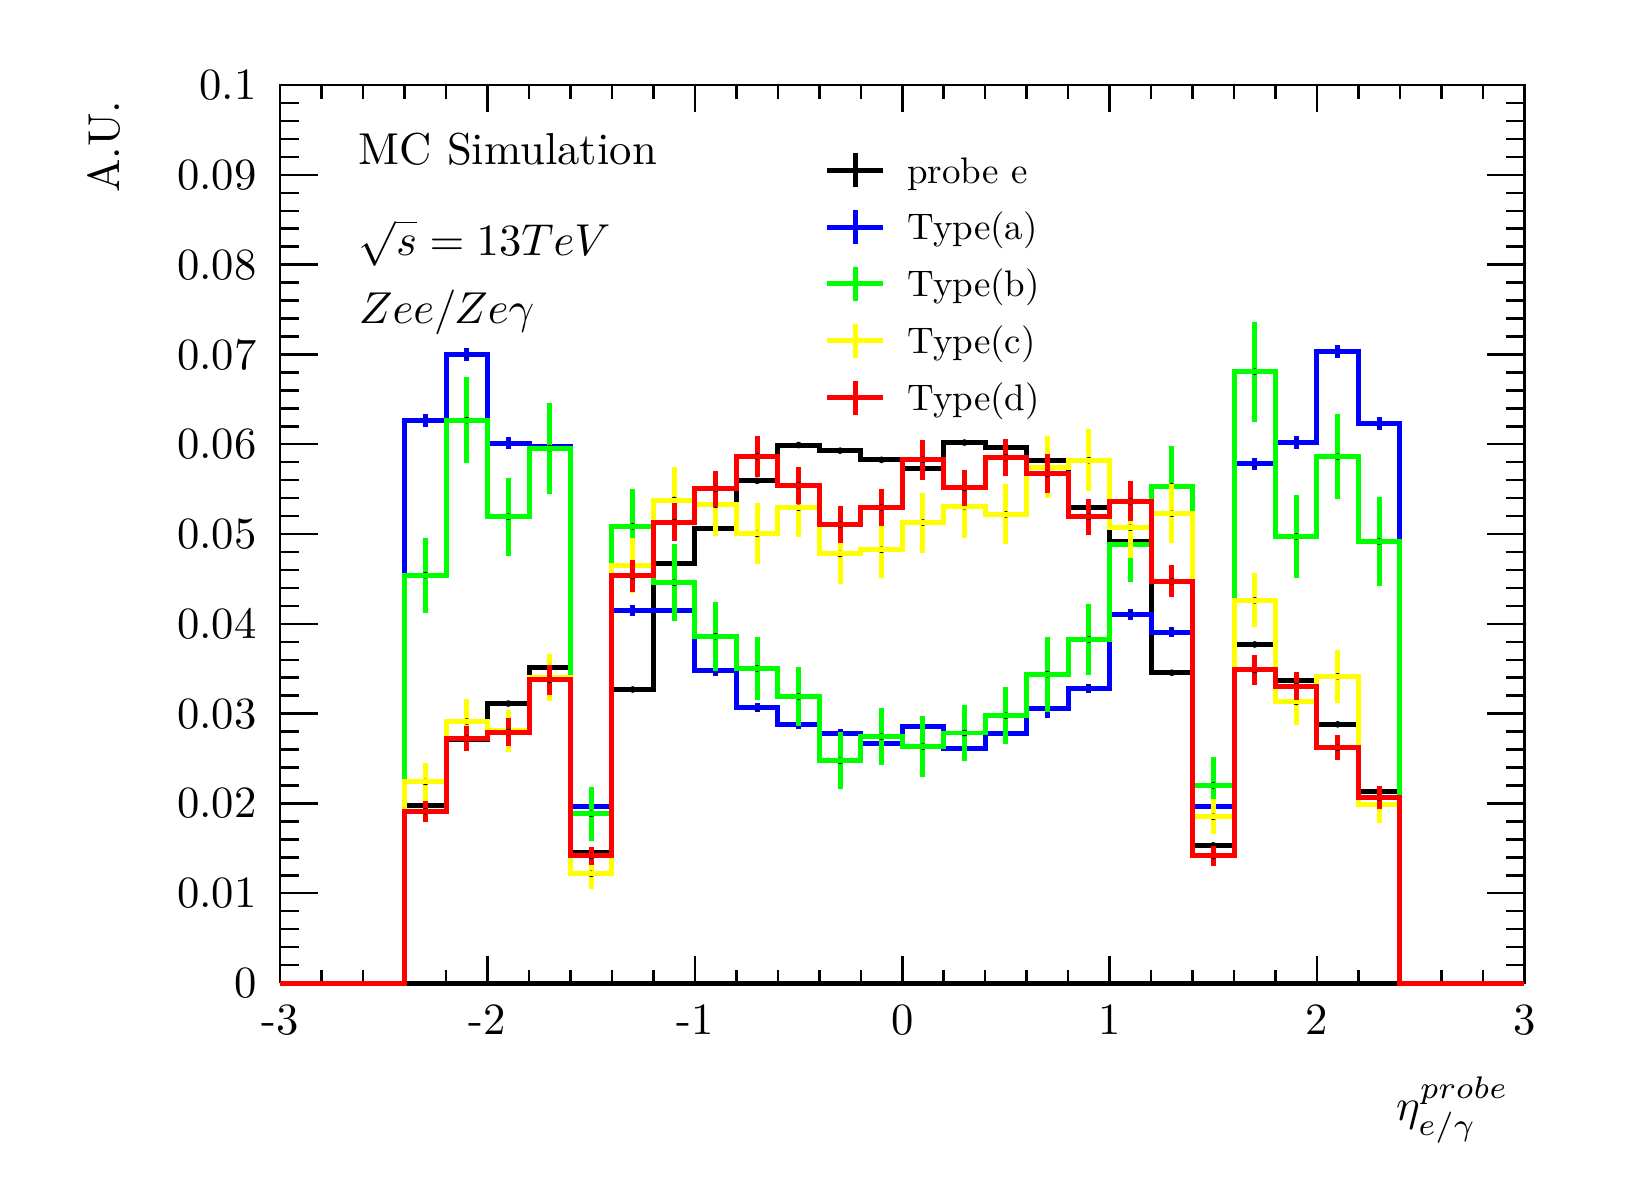
\begin{tikzpicture}
\pgfdeclareplotmark{cross} {
\pgfpathmoveto{\pgfpoint{-0.3\pgfplotmarksize}{\pgfplotmarksize}}
\pgfpathlineto{\pgfpoint{+0.3\pgfplotmarksize}{\pgfplotmarksize}}
\pgfpathlineto{\pgfpoint{+0.3\pgfplotmarksize}{0.3\pgfplotmarksize}}
\pgfpathlineto{\pgfpoint{+1\pgfplotmarksize}{0.3\pgfplotmarksize}}
\pgfpathlineto{\pgfpoint{+1\pgfplotmarksize}{-0.3\pgfplotmarksize}}
\pgfpathlineto{\pgfpoint{+0.3\pgfplotmarksize}{-0.3\pgfplotmarksize}}
\pgfpathlineto{\pgfpoint{+0.3\pgfplotmarksize}{-1.\pgfplotmarksize}}
\pgfpathlineto{\pgfpoint{-0.3\pgfplotmarksize}{-1.\pgfplotmarksize}}
\pgfpathlineto{\pgfpoint{-0.3\pgfplotmarksize}{-0.3\pgfplotmarksize}}
\pgfpathlineto{\pgfpoint{-1.\pgfplotmarksize}{-0.3\pgfplotmarksize}}
\pgfpathlineto{\pgfpoint{-1.\pgfplotmarksize}{0.3\pgfplotmarksize}}
\pgfpathlineto{\pgfpoint{-0.3\pgfplotmarksize}{0.3\pgfplotmarksize}}
\pgfpathclose
\pgfusepathqstroke
}
\pgfdeclareplotmark{cross*} {
\pgfpathmoveto{\pgfpoint{-0.3\pgfplotmarksize}{\pgfplotmarksize}}
\pgfpathlineto{\pgfpoint{+0.3\pgfplotmarksize}{\pgfplotmarksize}}
\pgfpathlineto{\pgfpoint{+0.3\pgfplotmarksize}{0.3\pgfplotmarksize}}
\pgfpathlineto{\pgfpoint{+1\pgfplotmarksize}{0.3\pgfplotmarksize}}
\pgfpathlineto{\pgfpoint{+1\pgfplotmarksize}{-0.3\pgfplotmarksize}}
\pgfpathlineto{\pgfpoint{+0.3\pgfplotmarksize}{-0.3\pgfplotmarksize}}
\pgfpathlineto{\pgfpoint{+0.3\pgfplotmarksize}{-1.\pgfplotmarksize}}
\pgfpathlineto{\pgfpoint{-0.3\pgfplotmarksize}{-1.\pgfplotmarksize}}
\pgfpathlineto{\pgfpoint{-0.3\pgfplotmarksize}{-0.3\pgfplotmarksize}}
\pgfpathlineto{\pgfpoint{-1.\pgfplotmarksize}{-0.3\pgfplotmarksize}}
\pgfpathlineto{\pgfpoint{-1.\pgfplotmarksize}{0.3\pgfplotmarksize}}
\pgfpathlineto{\pgfpoint{-0.3\pgfplotmarksize}{0.3\pgfplotmarksize}}
\pgfpathclose
\pgfusepathqfillstroke
}
\pgfdeclareplotmark{newstar} {
\pgfpathmoveto{\pgfqpoint{0pt}{\pgfplotmarksize}}
\pgfpathlineto{\pgfqpointpolar{44}{0.5\pgfplotmarksize}}
\pgfpathlineto{\pgfqpointpolar{18}{\pgfplotmarksize}}
\pgfpathlineto{\pgfqpointpolar{-20}{0.5\pgfplotmarksize}}
\pgfpathlineto{\pgfqpointpolar{-54}{\pgfplotmarksize}}
\pgfpathlineto{\pgfqpointpolar{-90}{0.5\pgfplotmarksize}}
\pgfpathlineto{\pgfqpointpolar{234}{\pgfplotmarksize}}
\pgfpathlineto{\pgfqpointpolar{198}{0.5\pgfplotmarksize}}
\pgfpathlineto{\pgfqpointpolar{162}{\pgfplotmarksize}}
\pgfpathlineto{\pgfqpointpolar{134}{0.5\pgfplotmarksize}}
\pgfpathclose
\pgfusepathqstroke
}
\pgfdeclareplotmark{newstar*} {
\pgfpathmoveto{\pgfqpoint{0pt}{\pgfplotmarksize}}
\pgfpathlineto{\pgfqpointpolar{44}{0.5\pgfplotmarksize}}
\pgfpathlineto{\pgfqpointpolar{18}{\pgfplotmarksize}}
\pgfpathlineto{\pgfqpointpolar{-20}{0.5\pgfplotmarksize}}
\pgfpathlineto{\pgfqpointpolar{-54}{\pgfplotmarksize}}
\pgfpathlineto{\pgfqpointpolar{-90}{0.5\pgfplotmarksize}}
\pgfpathlineto{\pgfqpointpolar{234}{\pgfplotmarksize}}
\pgfpathlineto{\pgfqpointpolar{198}{0.5\pgfplotmarksize}}
\pgfpathlineto{\pgfqpointpolar{162}{\pgfplotmarksize}}
\pgfpathlineto{\pgfqpointpolar{134}{0.5\pgfplotmarksize}}
\pgfpathclose
\pgfusepathqfillstroke
}
\definecolor{c}{rgb}{1,1,1};
\draw [color=c, fill=c] (0,0) rectangle (20,14.4361);
\draw [color=c, fill=c] (3.2,2.30977) rectangle (19,13.7143);
\definecolor{c}{rgb}{0,0,0};
\draw [c,line width=0.9] (3.2,2.30977) -- (3.2,13.7143) -- (19,13.7143) -- (19,2.30977) -- (3.2,2.30977);
\draw [c,line width=1.8] (3.2,2.30977) -- (3.2158,2.30977) -- (3.2158,2.30977) -- (3.2316,2.30977) -- (3.2316,2.30977) -- (3.2474,2.30977) -- (3.2474,2.30977) -- (3.2632,2.30977) -- (3.2632,2.30977) -- (3.279,2.30977) -- (3.279,2.30977) --
 (3.2948,2.30977) -- (3.2948,2.30977) -- (3.3106,2.30977) -- (3.3106,2.30977) -- (3.3264,2.30977) -- (3.3264,2.30977) -- (3.3422,2.30977) -- (3.3422,2.30977) -- (3.358,2.30977) -- (3.358,2.30977) -- (3.3738,2.30977) -- (3.3738,2.30977) --
 (3.3896,2.30977) -- (3.3896,2.30977) -- (3.4054,2.30977) -- (3.4054,2.30977) -- (3.4212,2.30977) -- (3.4212,2.30977) -- (3.437,2.30977) -- (3.437,2.30977) -- (3.4528,2.30977) -- (3.4528,2.30977) -- (3.4686,2.30977) -- (3.4686,2.30977) --
 (3.4844,2.30977) -- (3.4844,2.30977) -- (3.5002,2.30977) -- (3.5002,2.30977) -- (3.516,2.30977) -- (3.516,2.30977) -- (3.5318,2.30977) -- (3.5318,2.30977) -- (3.5476,2.30977) -- (3.5476,2.30977) -- (3.5634,2.30977) -- (3.5634,2.30977) --
 (3.5792,2.30977) -- (3.5792,2.30977) -- (3.595,2.30977) -- (3.595,2.30977) -- (3.6108,2.30977) -- (3.6108,2.30977) -- (3.6266,2.30977) -- (3.6266,2.30977) -- (3.6424,2.30977) -- (3.6424,2.30977) -- (3.6582,2.30977) -- (3.6582,2.30977) --
 (3.674,2.30977) -- (3.674,2.30977) -- (3.6898,2.30977) -- (3.6898,2.30977) -- (3.7056,2.30977) -- (3.7056,2.30977) -- (3.7214,2.30977) -- (3.7214,2.30977) -- (3.7372,2.30977) -- (3.7372,2.30977) -- (3.753,2.30977) -- (3.753,2.30977) --
 (3.7688,2.30977) -- (3.7688,2.30977) -- (3.7846,2.30977) -- (3.7846,2.30977) -- (3.8004,2.30977) -- (3.8004,2.30977) -- (3.8162,2.30977) -- (3.8162,2.30977) -- (3.832,2.30977) -- (3.832,2.30977) -- (3.8478,2.30977) -- (3.8478,2.30977) --
 (3.8636,2.30977) -- (3.8636,2.30977) -- (3.8794,2.30977) -- (3.8794,2.30977) -- (3.8952,2.30977) -- (3.8952,2.30977) -- (3.911,2.30977) -- (3.911,2.30977) -- (3.9268,2.30977) -- (3.9268,2.30977) -- (3.9426,2.30977) -- (3.9426,2.30977) --
 (3.9584,2.30977) -- (3.9584,2.30977) -- (3.9742,2.30977) -- (3.9742,2.30977) -- (3.99,2.30977) -- (3.99,2.30977) -- (4.0058,2.30977) -- (4.0058,2.30977) -- (4.0216,2.30977) -- (4.0216,2.30977) -- (4.0374,2.30977) -- (4.0374,2.30977) --
 (4.0532,2.30977) -- (4.0532,2.30977) -- (4.069,2.30977) -- (4.069,2.30977) -- (4.0848,2.30977) -- (4.0848,2.30977) -- (4.1006,2.30977) -- (4.1006,2.30977) -- (4.1164,2.30977) -- (4.1164,2.30977) -- (4.1322,2.30977) -- (4.1322,2.30977) --
 (4.148,2.30977) -- (4.148,2.30977) -- (4.1638,2.30977) -- (4.1638,2.30977) -- (4.1796,2.30977) -- (4.1796,2.30977) -- (4.1954,2.30977) -- (4.1954,2.30977) -- (4.2112,2.30977) -- (4.2112,2.30977) -- (4.227,2.30977) -- (4.227,2.30977) --
 (4.2428,2.30977) -- (4.2428,2.30977) -- (4.2586,2.30977) -- (4.2586,2.30977) -- (4.2744,2.30977) -- (4.2744,2.30977) -- (4.2902,2.30977) -- (4.2902,2.30977) -- (4.306,2.30977) -- (4.306,2.30977) -- (4.3218,2.30977) -- (4.3218,2.30977) --
 (4.3376,2.30977) -- (4.3376,2.30977) -- (4.3534,2.30977) -- (4.3534,2.30977) -- (4.3692,2.30977) -- (4.3692,2.30977) -- (4.385,2.30977) -- (4.385,2.30977) -- (4.4008,2.30977) -- (4.4008,2.30977) -- (4.4166,2.30977) -- (4.4166,2.30977) --
 (4.4324,2.30977) -- (4.4324,2.30977) -- (4.4482,2.30977) -- (4.4482,2.30977) -- (4.464,2.30977) -- (4.464,2.30977) -- (4.4798,2.30977) -- (4.4798,2.30977) -- (4.4956,2.30977) -- (4.4956,2.30977) -- (4.5114,2.30977) -- (4.5114,2.30977) --
 (4.5272,2.30977) -- (4.5272,2.30977) -- (4.543,2.30977) -- (4.543,2.30977) -- (4.5588,2.30977) -- (4.5588,2.30977) -- (4.5746,2.30977) -- (4.5746,2.30977) -- (4.5904,2.30977) -- (4.5904,2.30977) -- (4.6062,2.30977) -- (4.6062,2.30977) --
 (4.622,2.30977) -- (4.622,2.30977) -- (4.6378,2.30977) -- (4.6378,2.30977) -- (4.6536,2.30977) -- (4.6536,2.30977) -- (4.6694,2.30977) -- (4.6694,2.30977) -- (4.6852,2.30977) -- (4.6852,2.30977) -- (4.701,2.30977) -- (4.701,2.30977) --
 (4.7168,2.30977) -- (4.7168,2.30977) -- (4.7326,2.30977) -- (4.7326,2.30977) -- (4.7484,2.30977) -- (4.7484,2.30977) -- (4.7642,2.30977) -- (4.7642,2.30977) -- (4.78,2.30977) -- (4.78,2.30977) -- (4.7958,2.30977) -- (4.7958,2.30977) --
 (4.8116,2.30977) -- (4.8116,2.30977) -- (4.8274,2.30977) -- (4.8274,2.30977) -- (4.8432,2.30977) -- (4.8432,2.30977) -- (4.859,2.30977) -- (4.859,2.30977) -- (4.8748,2.30977) -- (4.8748,2.30977) -- (4.8906,2.30977) -- (4.8906,2.30977) --
 (4.9064,2.30977) -- (4.9064,2.30977) -- (4.9222,2.30977) -- (4.9222,2.30977) -- (4.938,2.30977) -- (4.938,2.30977) -- (4.9538,2.30977) -- (4.9538,2.30977) -- (4.9696,2.30977) -- (4.9696,2.30977) -- (4.9854,2.30977) -- (4.9854,2.30977) --
 (5.0012,2.30977) -- (5.0012,2.30977) -- (5.017,2.30977) -- (5.017,2.30977) -- (5.0328,2.30977) -- (5.0328,2.30977) -- (5.0486,2.30977) -- (5.0486,2.30977) -- (5.0644,2.30977) -- (5.0644,2.30977) -- (5.0802,2.30977) -- (5.0802,2.30977) --
 (5.096,2.30977) -- (5.096,2.30977) -- (5.1118,2.30977) -- (5.1118,2.30977) -- (5.1276,2.30977) -- (5.1276,2.30977) -- (5.1434,2.30977) -- (5.1434,2.30977) -- (5.1592,2.30977) -- (5.1592,2.30977) -- (5.175,2.30977) -- (5.175,2.30977) --
 (5.1908,2.30977) -- (5.1908,2.30977) -- (5.2066,2.30977) -- (5.2066,2.30977) -- (5.2224,2.30977) -- (5.2224,2.30977) -- (5.2382,2.30977) -- (5.2382,2.30977) -- (5.254,2.30977) -- (5.254,2.30977) -- (5.2698,2.30977) -- (5.2698,2.30977) --
 (5.2856,2.30977) -- (5.2856,2.30977) -- (5.3014,2.30977) -- (5.3014,2.30977) -- (5.3172,2.30977) -- (5.3172,2.30977) -- (5.333,2.30977) -- (5.333,2.30977) -- (5.3488,2.30977) -- (5.3488,2.30977) -- (5.3646,2.30977) -- (5.3646,2.30977) --
 (5.3804,2.30977) -- (5.3804,2.30977) -- (5.3962,2.30977) -- (5.3962,2.30977) -- (5.412,2.30977) -- (5.412,2.30977) -- (5.4278,2.30977) -- (5.4278,2.30977) -- (5.4436,2.30977) -- (5.4436,2.30977) -- (5.4594,2.30977) -- (5.4594,2.30977) --
 (5.4752,2.30977) -- (5.4752,2.30977) -- (5.491,2.30977) -- (5.491,2.30977) -- (5.5068,2.30977) -- (5.5068,2.30977) -- (5.5226,2.30977) -- (5.5226,2.30977) -- (5.5384,2.30977) -- (5.5384,2.30977) -- (5.5542,2.30977) -- (5.5542,2.30977) --
 (5.57,2.30977) -- (5.57,2.30977) -- (5.5858,2.30977) -- (5.5858,2.30977) -- (5.6016,2.30977) -- (5.6016,2.30977) -- (5.6174,2.30977) -- (5.6174,2.30977) -- (5.6332,2.30977) -- (5.6332,2.30977) -- (5.649,2.30977) -- (5.649,2.30977) --
 (5.6648,2.30977) -- (5.6648,2.30977) -- (5.6806,2.30977) -- (5.6806,2.30977) -- (5.6964,2.30977) -- (5.6964,2.30977) -- (5.7122,2.30977) -- (5.7122,2.30977) -- (5.728,2.30977) -- (5.728,2.30977) -- (5.7438,2.30977) -- (5.7438,2.30977) --
 (5.7596,2.30977) -- (5.7596,2.30977) -- (5.7754,2.30977) -- (5.7754,2.30977) -- (5.7912,2.30977) -- (5.7912,2.30977) -- (5.807,2.30977) -- (5.807,2.30977) -- (5.8228,2.30977) -- (5.8228,2.30977) -- (5.8386,2.30977) -- (5.8386,2.30977) --
 (5.8544,2.30977) -- (5.8544,2.30977) -- (5.8702,2.30977) -- (5.8702,2.30977) -- (5.886,2.30977) -- (5.886,2.30977) -- (5.9018,2.30977) -- (5.9018,2.30977) -- (5.9176,2.30977) -- (5.9176,2.30977) -- (5.9334,2.30977) -- (5.9334,2.30977) --
 (5.9492,2.30977) -- (5.9492,2.30977) -- (5.965,2.30977) -- (5.965,2.30977) -- (5.9808,2.30977) -- (5.9808,2.30977) -- (5.9966,2.30977) -- (5.9966,2.30977) -- (6.0124,2.30977) -- (6.0124,2.30977) -- (6.0282,2.30977) -- (6.0282,2.30977) --
 (6.044,2.30977) -- (6.044,2.30977) -- (6.0598,2.30977) -- (6.0598,2.30977) -- (6.0756,2.30977) -- (6.0756,2.30977) -- (6.0914,2.30977) -- (6.0914,2.30977) -- (6.1072,2.30977) -- (6.1072,2.30977) -- (6.123,2.30977) -- (6.123,2.30977) --
 (6.1388,2.30977) -- (6.1388,2.30977) -- (6.1546,2.30977) -- (6.1546,2.30977) -- (6.1704,2.30977) -- (6.1704,2.30977) -- (6.1862,2.30977) -- (6.1862,2.30977) -- (6.202,2.30977) -- (6.202,2.30977) -- (6.2178,2.30977) -- (6.2178,2.30977) --
 (6.2336,2.30977) -- (6.2336,2.30977) -- (6.2494,2.30977) -- (6.2494,2.30977) -- (6.2652,2.30977) -- (6.2652,2.30977) -- (6.281,2.30977) -- (6.281,2.30977) -- (6.2968,2.30977) -- (6.2968,2.30977) -- (6.3126,2.30977) -- (6.3126,2.30977) --
 (6.3284,2.30977) -- (6.3284,2.30977) -- (6.3442,2.30977) -- (6.3442,2.30977) -- (6.36,2.30977) -- (6.36,2.30977) -- (6.3758,2.30977) -- (6.3758,2.30977) -- (6.3916,2.30977) -- (6.3916,2.30977) -- (6.4074,2.30977) -- (6.4074,2.30977) --
 (6.4232,2.30977) -- (6.4232,2.30977) -- (6.439,2.30977) -- (6.439,2.30977) -- (6.4548,2.30977) -- (6.4548,2.30977) -- (6.4706,2.30977) -- (6.4706,2.30977) -- (6.4864,2.30977) -- (6.4864,2.30977) -- (6.5022,2.30977) -- (6.5022,2.30977) --
 (6.518,2.30977) -- (6.518,2.30977) -- (6.5338,2.30977) -- (6.5338,2.30977) -- (6.5496,2.30977) -- (6.5496,2.30977) -- (6.5654,2.30977) -- (6.5654,2.30977) -- (6.5812,2.30977) -- (6.5812,2.30977) -- (6.597,2.30977) -- (6.597,2.30977) --
 (6.6128,2.30977) -- (6.6128,2.30977) -- (6.6286,2.30977) -- (6.6286,2.30977) -- (6.6444,2.30977) -- (6.6444,2.30977) -- (6.6602,2.30977) -- (6.6602,2.30977) -- (6.676,2.30977) -- (6.676,2.30977) -- (6.6918,2.30977) -- (6.6918,2.30977) --
 (6.7076,2.30977) -- (6.7076,2.30977) -- (6.7234,2.30977) -- (6.7234,2.30977) -- (6.7392,2.30977) -- (6.7392,2.30977) -- (6.755,2.30977) -- (6.755,2.30977) -- (6.7708,2.30977) -- (6.7708,2.30977) -- (6.7866,2.30977) -- (6.7866,2.30977) --
 (6.8024,2.30977) -- (6.8024,2.30977) -- (6.8182,2.30977) -- (6.8182,2.30977) -- (6.834,2.30977) -- (6.834,2.30977) -- (6.8498,2.30977) -- (6.8498,2.30977) -- (6.8656,2.30977) -- (6.8656,2.30977) -- (6.8814,2.30977) -- (6.8814,2.30977) --
 (6.8972,2.30977) -- (6.8972,2.30977) -- (6.913,2.30977) -- (6.913,2.30977) -- (6.9288,2.30977) -- (6.9288,2.30977) -- (6.9446,2.30977) -- (6.9446,2.30977) -- (6.9604,2.30977) -- (6.9604,2.30977) -- (6.9762,2.30977) -- (6.9762,2.30977) --
 (6.992,2.30977) -- (6.992,2.30977) -- (7.0078,2.30977) -- (7.0078,2.30977) -- (7.0236,2.30977) -- (7.0236,2.30977) -- (7.0394,2.30977) -- (7.0394,2.30977) -- (7.0552,2.30977) -- (7.0552,2.30977) -- (7.071,2.30977) -- (7.071,2.30977) --
 (7.0868,2.30977) -- (7.0868,2.30977) -- (7.1026,2.30977) -- (7.1026,2.30977) -- (7.1184,2.30977) -- (7.1184,2.30977) -- (7.1342,2.30977) -- (7.1342,2.30977) -- (7.15,2.30977) -- (7.15,2.30977) -- (7.1658,2.30977) -- (7.1658,2.30977) --
 (7.1816,2.30977) -- (7.1816,2.30977) -- (7.1974,2.30977) -- (7.1974,2.30977) -- (7.2132,2.30977) -- (7.2132,2.30977) -- (7.229,2.30977) -- (7.229,2.30977) -- (7.2448,2.30977) -- (7.2448,2.30977) -- (7.2606,2.30977) -- (7.2606,2.30977) --
 (7.2764,2.30977) -- (7.2764,2.30977) -- (7.2922,2.30977) -- (7.2922,2.30977) -- (7.308,2.30977) -- (7.308,2.30977) -- (7.3238,2.30977) -- (7.3238,2.30977) -- (7.3396,2.30977) -- (7.3396,2.30977) -- (7.3554,2.30977) -- (7.3554,2.30977) --
 (7.3712,2.30977) -- (7.3712,2.30977) -- (7.387,2.30977) -- (7.387,2.30977) -- (7.4028,2.30977) -- (7.4028,2.30977) -- (7.4186,2.30977) -- (7.4186,2.30977) -- (7.4344,2.30977) -- (7.4344,2.30977) -- (7.4502,2.30977) -- (7.4502,2.30977) --
 (7.466,2.30977) -- (7.466,2.30977) -- (7.4818,2.30977) -- (7.4818,2.30977) -- (7.4976,2.30977) -- (7.4976,2.30977) -- (7.5134,2.30977) -- (7.5134,2.30977) -- (7.5292,2.30977) -- (7.5292,2.30977) -- (7.545,2.30977) -- (7.545,2.30977) --
 (7.5608,2.30977) -- (7.5608,2.30977) -- (7.5766,2.30977) -- (7.5766,2.30977) -- (7.5924,2.30977) -- (7.5924,2.30977) -- (7.6082,2.30977) -- (7.6082,2.30977) -- (7.624,2.30977) -- (7.624,2.30977) -- (7.6398,2.30977) -- (7.6398,2.30977) --
 (7.6556,2.30977) -- (7.6556,2.30977) -- (7.6714,2.30977) -- (7.6714,2.30977) -- (7.6872,2.30977) -- (7.6872,2.30977) -- (7.703,2.30977) -- (7.703,2.30977) -- (7.7188,2.30977) -- (7.7188,2.30977) -- (7.7346,2.30977) -- (7.7346,2.30977) --
 (7.7504,2.30977) -- (7.7504,2.30977) -- (7.7662,2.30977) -- (7.7662,2.30977) -- (7.782,2.30977) -- (7.782,2.30977) -- (7.7978,2.30977) -- (7.7978,2.30977) -- (7.8136,2.30977) -- (7.8136,2.30977) -- (7.8294,2.30977) -- (7.8294,2.30977) --
 (7.8452,2.30977) -- (7.8452,2.30977) -- (7.861,2.30977) -- (7.861,2.30977) -- (7.8768,2.30977) -- (7.8768,2.30977) -- (7.8926,2.30977) -- (7.8926,2.30977) -- (7.9084,2.30977) -- (7.9084,2.30977) -- (7.9242,2.30977) -- (7.9242,2.30977) --
 (7.94,2.30977) -- (7.94,2.30977) -- (7.9558,2.30977) -- (7.9558,2.30977) -- (7.9716,2.30977) -- (7.9716,2.30977) -- (7.9874,2.30977) -- (7.9874,2.30977) -- (8.0032,2.30977) -- (8.0032,2.30977) -- (8.019,2.30977) -- (8.019,2.30977) --
 (8.0348,2.30977) -- (8.0348,2.30977) -- (8.0506,2.30977) -- (8.0506,2.30977) -- (8.0664,2.30977) -- (8.0664,2.30977) -- (8.0822,2.30977) -- (8.0822,2.30977) -- (8.098,2.30977) -- (8.098,2.30977) -- (8.1138,2.30977) -- (8.1138,2.30977) --
 (8.1296,2.30977) -- (8.1296,2.30977) -- (8.1454,2.30977) -- (8.1454,2.30977) -- (8.1612,2.30977) -- (8.1612,2.30977) -- (8.177,2.30977) -- (8.177,2.30977) -- (8.1928,2.30977) -- (8.1928,2.30977) -- (8.2086,2.30977) -- (8.2086,2.30977) --
 (8.2244,2.30977) -- (8.2244,2.30977) -- (8.2402,2.30977) -- (8.2402,2.30977) -- (8.256,2.30977) -- (8.256,2.30977) -- (8.2718,2.30977) -- (8.2718,2.30977) -- (8.2876,2.30977) -- (8.2876,2.30977) -- (8.3034,2.30977) -- (8.3034,2.30977) --
 (8.3192,2.30977) -- (8.3192,2.30977) -- (8.335,2.30977) -- (8.335,2.30977) -- (8.3508,2.30977) -- (8.3508,2.30977) -- (8.3666,2.30977) -- (8.3666,2.30977) -- (8.3824,2.30977) -- (8.3824,2.30977) -- (8.3982,2.30977) -- (8.3982,2.30977) --
 (8.414,2.30977) -- (8.414,2.30977) -- (8.4298,2.30977) -- (8.4298,2.30977) -- (8.4456,2.30977) -- (8.4456,2.30977) -- (8.4614,2.30977) -- (8.4614,2.30977) -- (8.4772,2.30977) -- (8.4772,2.30977) -- (8.493,2.30977) -- (8.493,2.30977) --
 (8.5088,2.30977) -- (8.5088,2.30977) -- (8.5246,2.30977) -- (8.5246,2.30977) -- (8.5404,2.30977) -- (8.5404,2.30977) -- (8.5562,2.30977) -- (8.5562,2.30977) -- (8.572,2.30977) -- (8.572,2.30977) -- (8.5878,2.30977) -- (8.5878,2.30977) --
 (8.6036,2.30977) -- (8.6036,2.30977) -- (8.6194,2.30977) -- (8.6194,2.30977) -- (8.6352,2.30977) -- (8.6352,2.30977) -- (8.651,2.30977) -- (8.651,2.30977) -- (8.6668,2.30977) -- (8.6668,2.30977) -- (8.6826,2.30977) -- (8.6826,2.30977) --
 (8.6984,2.30977) -- (8.6984,2.30977) -- (8.7142,2.30977) -- (8.7142,2.30977) -- (8.73,2.30977) -- (8.73,2.30977) -- (8.7458,2.30977) -- (8.7458,2.30977) -- (8.7616,2.30977) -- (8.7616,2.30977) -- (8.7774,2.30977) -- (8.7774,2.30977) --
 (8.7932,2.30977) -- (8.7932,2.30977) -- (8.809,2.30977) -- (8.809,2.30977) -- (8.8248,2.30977) -- (8.8248,2.30977) -- (8.8406,2.30977) -- (8.8406,2.30977) -- (8.8564,2.30977) -- (8.8564,2.30977) -- (8.8722,2.30977) -- (8.8722,2.30977) --
 (8.888,2.30977) -- (8.888,2.30977) -- (8.9038,2.30977) -- (8.9038,2.30977) -- (8.9196,2.30977) -- (8.9196,2.30977) -- (8.9354,2.30977) -- (8.9354,2.30977) -- (8.9512,2.30977) -- (8.9512,2.30977) -- (8.967,2.30977) -- (8.967,2.30977) --
 (8.9828,2.30977) -- (8.9828,2.30977) -- (8.9986,2.30977) -- (8.9986,2.30977) -- (9.0144,2.30977) -- (9.0144,2.30977) -- (9.0302,2.30977) -- (9.0302,2.30977) -- (9.046,2.30977) -- (9.046,2.30977) -- (9.0618,2.30977) -- (9.0618,2.30977) --
 (9.0776,2.30977) -- (9.0776,2.30977) -- (9.0934,2.30977) -- (9.0934,2.30977) -- (9.1092,2.30977) -- (9.1092,2.30977) -- (9.125,2.30977) -- (9.125,2.30977) -- (9.1408,2.30977) -- (9.1408,2.30977) -- (9.1566,2.30977) -- (9.1566,2.30977) --
 (9.1724,2.30977) -- (9.1724,2.30977) -- (9.1882,2.30977) -- (9.1882,2.30977) -- (9.204,2.30977) -- (9.204,2.30977) -- (9.2198,2.30977) -- (9.2198,2.30977) -- (9.2356,2.30977) -- (9.2356,2.30977) -- (9.2514,2.30977) -- (9.2514,2.30977) --
 (9.2672,2.30977) -- (9.2672,2.30977) -- (9.283,2.30977) -- (9.283,2.30977) -- (9.2988,2.30977) -- (9.2988,2.30977) -- (9.3146,2.30977) -- (9.3146,2.30977) -- (9.3304,2.30977) -- (9.3304,2.30977) -- (9.3462,2.30977) -- (9.3462,2.30977) --
 (9.362,2.30977) -- (9.362,2.30977) -- (9.3778,2.30977) -- (9.3778,2.30977) -- (9.3936,2.30977) -- (9.3936,2.30977) -- (9.4094,2.30977) -- (9.4094,2.30977) -- (9.4252,2.30977) -- (9.4252,2.30977) -- (9.441,2.30977) -- (9.441,2.30977) --
 (9.4568,2.30977) -- (9.4568,2.30977) -- (9.4726,2.30977) -- (9.4726,2.30977) -- (9.4884,2.30977) -- (9.4884,2.30977) -- (9.5042,2.30977) -- (9.5042,2.30977) -- (9.52,2.30977) -- (9.52,2.30977) -- (9.5358,2.30977) -- (9.5358,2.30977) --
 (9.5516,2.30977) -- (9.5516,2.30977) -- (9.5674,2.30977) -- (9.5674,2.30977) -- (9.5832,2.30977) -- (9.5832,2.30977) -- (9.599,2.30977) -- (9.599,2.30977) -- (9.6148,2.30977) -- (9.6148,2.30977) -- (9.6306,2.30977) -- (9.6306,2.30977) --
 (9.6464,2.30977) -- (9.6464,2.30977) -- (9.6622,2.30977) -- (9.6622,2.30977) -- (9.678,2.30977) -- (9.678,2.30977) -- (9.6938,2.30977) -- (9.6938,2.30977) -- (9.7096,2.30977) -- (9.7096,2.30977) -- (9.7254,2.30977) -- (9.7254,2.30977) --
 (9.7412,2.30977) -- (9.7412,2.30977) -- (9.757,2.30977) -- (9.757,2.30977) -- (9.7728,2.30977) -- (9.7728,2.30977) -- (9.7886,2.30977) -- (9.7886,2.30977) -- (9.8044,2.30977) -- (9.8044,2.30977) -- (9.8202,2.30977) -- (9.8202,2.30977) --
 (9.836,2.30977) -- (9.836,2.30977) -- (9.8518,2.30977) -- (9.8518,2.30977) -- (9.8676,2.30977) -- (9.8676,2.30977) -- (9.8834,2.30977) -- (9.8834,2.30977) -- (9.8992,2.30977) -- (9.8992,2.30977) -- (9.915,2.30977) -- (9.915,2.30977) --
 (9.9308,2.30977) -- (9.9308,2.30977) -- (9.9466,2.30977) -- (9.9466,2.30977) -- (9.9624,2.30977) -- (9.9624,2.30977) -- (9.9782,2.30977) -- (9.9782,2.30977) -- (9.994,2.30977) -- (9.994,2.30977) -- (10.0098,2.30977) -- (10.0098,2.30977) --
 (10.0256,2.30977) -- (10.0256,2.30977) -- (10.0414,2.30977) -- (10.0414,2.30977) -- (10.0572,2.30977) -- (10.0572,2.30977) -- (10.073,2.30977) -- (10.073,2.30977) -- (10.0888,2.30977) -- (10.0888,2.30977) -- (10.1046,2.30977) -- (10.1046,2.30977) --
 (10.1204,2.30977) -- (10.1204,2.30977) -- (10.1362,2.30977) -- (10.1362,2.30977) -- (10.152,2.30977) -- (10.152,2.30977) -- (10.1678,2.30977) -- (10.1678,2.30977) -- (10.1836,2.30977) -- (10.1836,2.30977) -- (10.1994,2.30977) -- (10.1994,2.30977) --
 (10.2152,2.30977) -- (10.2152,2.30977) -- (10.231,2.30977) -- (10.231,2.30977) -- (10.2468,2.30977) -- (10.2468,2.30977) -- (10.2626,2.30977) -- (10.2626,2.30977) -- (10.2784,2.30977) -- (10.2784,2.30977) -- (10.2942,2.30977) -- (10.2942,2.30977) --
 (10.31,2.30977) -- (10.31,2.30977) -- (10.3258,2.30977) -- (10.3258,2.30977) -- (10.3416,2.30977) -- (10.3416,2.30977) -- (10.3574,2.30977) -- (10.3574,2.30977) -- (10.3732,2.30977) -- (10.3732,2.30977) -- (10.389,2.30977) -- (10.389,2.30977) --
 (10.4048,2.30977) -- (10.4048,2.30977) -- (10.4206,2.30977) -- (10.4206,2.30977) -- (10.4364,2.30977) -- (10.4364,2.30977) -- (10.4522,2.30977) -- (10.4522,2.30977) -- (10.468,2.30977) -- (10.468,2.30977) -- (10.4838,2.30977) -- (10.4838,2.30977) --
 (10.4996,2.30977) -- (10.4996,2.30977) -- (10.5154,2.30977) -- (10.5154,2.30977) -- (10.5312,2.30977) -- (10.5312,2.30977) -- (10.547,2.30977) -- (10.547,2.30977) -- (10.5628,2.30977) -- (10.5628,2.30977) -- (10.5786,2.30977) -- (10.5786,2.30977) --
 (10.5944,2.30977) -- (10.5944,2.30977) -- (10.6102,2.30977) -- (10.6102,2.30977) -- (10.626,2.30977) -- (10.626,2.30977) -- (10.6418,2.30977) -- (10.6418,2.30977) -- (10.6576,2.30977) -- (10.6576,2.30977) -- (10.6734,2.30977) -- (10.6734,2.30977) --
 (10.6892,2.30977) -- (10.6892,2.30977) -- (10.705,2.30977) -- (10.705,2.30977) -- (10.7208,2.30977) -- (10.7208,2.30977) -- (10.7366,2.30977) -- (10.7366,2.30977) -- (10.7524,2.30977) -- (10.7524,2.30977) -- (10.7682,2.30977) -- (10.7682,2.30977) --
 (10.784,2.30977) -- (10.784,2.30977) -- (10.7998,2.30977) -- (10.7998,2.30977) -- (10.8156,2.30977) -- (10.8156,2.30977) -- (10.8314,2.30977) -- (10.8314,2.30977) -- (10.8472,2.30977) -- (10.8472,2.30977) -- (10.863,2.30977) -- (10.863,2.30977) --
 (10.8788,2.30977) -- (10.8788,2.30977) -- (10.8946,2.30977) -- (10.8946,2.30977) -- (10.9104,2.30977) -- (10.9104,2.30977) -- (10.9262,2.30977) -- (10.9262,2.30977) -- (10.942,2.30977) -- (10.942,2.30977) -- (10.9578,2.30977) -- (10.9578,2.30977) --
 (10.9736,2.30977) -- (10.9736,2.30977) -- (10.9894,2.30977) -- (10.9894,2.30977) -- (11.0052,2.30977) -- (11.0052,2.30977) -- (11.021,2.30977) -- (11.021,2.30977) -- (11.0368,2.30977) -- (11.0368,2.30977) -- (11.0526,2.30977) -- (11.0526,2.30977) --
 (11.0684,2.30977) -- (11.0684,2.30977) -- (11.0842,2.30977) -- (11.0842,2.30977) -- (11.1,2.30977) -- (11.1,2.30977) -- (11.1158,2.30977) -- (11.1158,2.30977) -- (11.1316,2.30977) -- (11.1316,2.30977) -- (11.1474,2.30977) -- (11.1474,2.30977) --
 (11.1632,2.30977) -- (11.1632,2.30977) -- (11.179,2.30977) -- (11.179,2.30977) -- (11.1948,2.30977) -- (11.1948,2.30977) -- (11.2106,2.30977) -- (11.2106,2.30977) -- (11.2264,2.30977) -- (11.2264,2.30977) -- (11.2422,2.30977) -- (11.2422,2.30977) --
 (11.258,2.30977) -- (11.258,2.30977) -- (11.2738,2.30977) -- (11.2738,2.30977) -- (11.2896,2.30977) -- (11.2896,2.30977) -- (11.3054,2.30977) -- (11.3054,2.30977) -- (11.3212,2.30977) -- (11.3212,2.30977) -- (11.337,2.30977) -- (11.337,2.30977) --
 (11.3528,2.30977) -- (11.3528,2.30977) -- (11.3686,2.30977) -- (11.3686,2.30977) -- (11.3844,2.30977) -- (11.3844,2.30977) -- (11.4002,2.30977) -- (11.4002,2.30977) -- (11.416,2.30977) -- (11.416,2.30977) -- (11.4318,2.30977) -- (11.4318,2.30977) --
 (11.4476,2.30977) -- (11.4476,2.30977) -- (11.4634,2.30977) -- (11.4634,2.30977) -- (11.4792,2.30977) -- (11.4792,2.30977) -- (11.495,2.30977) -- (11.495,2.30977) -- (11.5108,2.30977) -- (11.5108,2.30977) -- (11.5266,2.30977) -- (11.5266,2.30977) --
 (11.5424,2.30977) -- (11.5424,2.30977) -- (11.5582,2.30977) -- (11.5582,2.30977) -- (11.574,2.30977) -- (11.574,2.30977) -- (11.5898,2.30977) -- (11.5898,2.30977) -- (11.6056,2.30977) -- (11.6056,2.30977) -- (11.6214,2.30977) -- (11.6214,2.30977) --
 (11.6372,2.30977) -- (11.6372,2.30977) -- (11.653,2.30977) -- (11.653,2.30977) -- (11.6688,2.30977) -- (11.6688,2.30977) -- (11.6846,2.30977) -- (11.6846,2.30977) -- (11.7004,2.30977) -- (11.7004,2.30977) -- (11.7162,2.30977) -- (11.7162,2.30977) --
 (11.732,2.30977) -- (11.732,2.30977) -- (11.7478,2.30977) -- (11.7478,2.30977) -- (11.7636,2.30977) -- (11.7636,2.30977) -- (11.7794,2.30977) -- (11.7794,2.30977) -- (11.7952,2.30977) -- (11.7952,2.30977) -- (11.811,2.30977) -- (11.811,2.30977) --
 (11.8268,2.30977) -- (11.8268,2.30977) -- (11.8426,2.30977) -- (11.8426,2.30977) -- (11.8584,2.30977) -- (11.8584,2.30977) -- (11.8742,2.30977) -- (11.8742,2.30977) -- (11.89,2.30977) -- (11.89,2.30977) -- (11.9058,2.30977) -- (11.9058,2.30977) --
 (11.9216,2.30977) -- (11.9216,2.30977) -- (11.9374,2.30977) -- (11.9374,2.30977) -- (11.9532,2.30977) -- (11.9532,2.30977) -- (11.969,2.30977) -- (11.969,2.30977) -- (11.9848,2.30977) -- (11.9848,2.30977) -- (12.0006,2.30977) -- (12.0006,2.30977) --
 (12.0164,2.30977) -- (12.0164,2.30977) -- (12.0322,2.30977) -- (12.0322,2.30977) -- (12.048,2.30977) -- (12.048,2.30977) -- (12.0638,2.30977) -- (12.0638,2.30977) -- (12.0796,2.30977) -- (12.0796,2.30977) -- (12.0954,2.30977) -- (12.0954,2.30977) --
 (12.1112,2.30977) -- (12.1112,2.30977) -- (12.127,2.30977) -- (12.127,2.30977) -- (12.1428,2.30977) -- (12.1428,2.30977) -- (12.1586,2.30977) -- (12.1586,2.30977) -- (12.1744,2.30977) -- (12.1744,2.30977) -- (12.1902,2.30977) -- (12.1902,2.30977) --
 (12.206,2.30977) -- (12.206,2.30977) -- (12.2218,2.30977) -- (12.2218,2.30977) -- (12.2376,2.30977) -- (12.2376,2.30977) -- (12.2534,2.30977) -- (12.2534,2.30977) -- (12.2692,2.30977) -- (12.2692,2.30977) -- (12.285,2.30977) -- (12.285,2.30977) --
 (12.3008,2.30977) -- (12.3008,2.30977) -- (12.3166,2.30977) -- (12.3166,2.30977) -- (12.3324,2.30977) -- (12.3324,2.30977) -- (12.3482,2.30977) -- (12.3482,2.30977) -- (12.364,2.30977) -- (12.364,2.30977) -- (12.3798,2.30977) -- (12.3798,2.30977) --
 (12.3956,2.30977) -- (12.3956,2.30977) -- (12.4114,2.30977) -- (12.4114,2.30977) -- (12.4272,2.30977) -- (12.4272,2.30977) -- (12.443,2.30977) -- (12.443,2.30977) -- (12.4588,2.30977) -- (12.4588,2.30977) -- (12.4746,2.30977) -- (12.4746,2.30977) --
 (12.4904,2.30977) -- (12.4904,2.30977) -- (12.5062,2.30977) -- (12.5062,2.30977) -- (12.522,2.30977) -- (12.522,2.30977) -- (12.5378,2.30977) -- (12.5378,2.30977) -- (12.5536,2.30977) -- (12.5536,2.30977) -- (12.5694,2.30977) -- (12.5694,2.30977) --
 (12.5852,2.30977) -- (12.5852,2.30977) -- (12.601,2.30977) -- (12.601,2.30977) -- (12.6168,2.30977) -- (12.6168,2.30977) -- (12.6326,2.30977) -- (12.6326,2.30977) -- (12.6484,2.30977) -- (12.6484,2.30977) -- (12.6642,2.30977) -- (12.6642,2.30977) --
 (12.68,2.30977) -- (12.68,2.30977) -- (12.6958,2.30977) -- (12.6958,2.30977) -- (12.7116,2.30977) -- (12.7116,2.30977) -- (12.7274,2.30977) -- (12.7274,2.30977) -- (12.7432,2.30977) -- (12.7432,2.30977) -- (12.759,2.30977) -- (12.759,2.30977) --
 (12.7748,2.30977) -- (12.7748,2.30977) -- (12.7906,2.30977) -- (12.7906,2.30977) -- (12.8064,2.30977) -- (12.8064,2.30977) -- (12.8222,2.30977) -- (12.8222,2.30977) -- (12.838,2.30977) -- (12.838,2.30977) -- (12.8538,2.30977) -- (12.8538,2.30977) --
 (12.8696,2.30977) -- (12.8696,2.30977) -- (12.8854,2.30977) -- (12.8854,2.30977) -- (12.9012,2.30977) -- (12.9012,2.30977) -- (12.917,2.30977) -- (12.917,2.30977) -- (12.9328,2.30977) -- (12.9328,2.30977) -- (12.9486,2.30977) -- (12.9486,2.30977) --
 (12.9644,2.30977) -- (12.9644,2.30977) -- (12.9802,2.30977) -- (12.9802,2.30977) -- (12.996,2.30977) -- (12.996,2.30977) -- (13.0118,2.30977) -- (13.0118,2.30977) -- (13.0276,2.30977) -- (13.0276,2.30977) -- (13.0434,2.30977) -- (13.0434,2.30977) --
 (13.0592,2.30977) -- (13.0592,2.30977) -- (13.075,2.30977) -- (13.075,2.30977) -- (13.0908,2.30977) -- (13.0908,2.30977) -- (13.1066,2.30977) -- (13.1066,2.30977) -- (13.1224,2.30977) -- (13.1224,2.30977) -- (13.1382,2.30977) -- (13.1382,2.30977) --
 (13.154,2.30977) -- (13.154,2.30977) -- (13.1698,2.30977) -- (13.1698,2.30977) -- (13.1856,2.30977) -- (13.1856,2.30977) -- (13.2014,2.30977) -- (13.2014,2.30977) -- (13.2172,2.30977) -- (13.2172,2.30977) -- (13.233,2.30977) -- (13.233,2.30977) --
 (13.2488,2.30977) -- (13.2488,2.30977) -- (13.2646,2.30977) -- (13.2646,2.30977) -- (13.2804,2.30977) -- (13.2804,2.30977) -- (13.2962,2.30977) -- (13.2962,2.30977) -- (13.312,2.30977) -- (13.312,2.30977) -- (13.3278,2.30977) -- (13.3278,2.30977) --
 (13.3436,2.30977) -- (13.3436,2.30977) -- (13.3594,2.30977) -- (13.3594,2.30977) -- (13.3752,2.30977) -- (13.3752,2.30977) -- (13.391,2.30977) -- (13.391,2.30977) -- (13.4068,2.30977) -- (13.4068,2.30977) -- (13.4226,2.30977) -- (13.4226,2.30977) --
 (13.4384,2.30977) -- (13.4384,2.30977) -- (13.4542,2.30977) -- (13.4542,2.30977) -- (13.47,2.30977) -- (13.47,2.30977) -- (13.4858,2.30977) -- (13.4858,2.30977) -- (13.5016,2.30977) -- (13.5016,2.30977) -- (13.5174,2.30977) -- (13.5174,2.30977) --
 (13.5332,2.30977) -- (13.5332,2.30977) -- (13.549,2.30977) -- (13.549,2.30977) -- (13.5648,2.30977) -- (13.5648,2.30977) -- (13.5806,2.30977) -- (13.5806,2.30977) -- (13.5964,2.30977) -- (13.5964,2.30977) -- (13.6122,2.30977) -- (13.6122,2.30977) --
 (13.628,2.30977) -- (13.628,2.30977) -- (13.6438,2.30977) -- (13.6438,2.30977) -- (13.6596,2.30977) -- (13.6596,2.30977) -- (13.6754,2.30977) -- (13.6754,2.30977) -- (13.6912,2.30977) -- (13.6912,2.30977) -- (13.707,2.30977) -- (13.707,2.30977) --
 (13.7228,2.30977) -- (13.7228,2.30977) -- (13.7386,2.30977) -- (13.7386,2.30977) -- (13.7544,2.30977) -- (13.7544,2.30977) -- (13.7702,2.30977) -- (13.7702,2.30977) -- (13.786,2.30977) -- (13.786,2.30977) -- (13.8018,2.30977) -- (13.8018,2.30977) --
 (13.8176,2.30977) -- (13.8176,2.30977) -- (13.8334,2.30977) -- (13.8334,2.30977) -- (13.8492,2.30977) -- (13.8492,2.30977) -- (13.865,2.30977) -- (13.865,2.30977) -- (13.8808,2.30977) -- (13.8808,2.30977) -- (13.8966,2.30977) -- (13.8966,2.30977) --
 (13.9124,2.30977) -- (13.9124,2.30977) -- (13.9282,2.30977) -- (13.9282,2.30977) -- (13.944,2.30977) -- (13.944,2.30977) -- (13.9598,2.30977) -- (13.9598,2.30977) -- (13.9756,2.30977) -- (13.9756,2.30977) -- (13.9914,2.30977) -- (13.9914,2.30977) --
 (14.0072,2.30977) -- (14.0072,2.30977) -- (14.023,2.30977) -- (14.023,2.30977) -- (14.0388,2.30977) -- (14.0388,2.30977) -- (14.0546,2.30977) -- (14.0546,2.30977) -- (14.0704,2.30977) -- (14.0704,2.30977) -- (14.0862,2.30977) -- (14.0862,2.30977) --
 (14.102,2.30977) -- (14.102,2.30977) -- (14.1178,2.30977) -- (14.1178,2.30977) -- (14.1336,2.30977) -- (14.1336,2.30977) -- (14.1494,2.30977) -- (14.1494,2.30977) -- (14.1652,2.30977) -- (14.1652,2.30977) -- (14.181,2.30977) -- (14.181,2.30977) --
 (14.1968,2.30977) -- (14.1968,2.30977) -- (14.2126,2.30977) -- (14.2126,2.30977) -- (14.2284,2.30977) -- (14.2284,2.30977) -- (14.2442,2.30977) -- (14.2442,2.30977) -- (14.26,2.30977) -- (14.26,2.30977) -- (14.2758,2.30977) -- (14.2758,2.30977) --
 (14.2916,2.30977) -- (14.2916,2.30977) -- (14.3074,2.30977) -- (14.3074,2.30977) -- (14.3232,2.30977) -- (14.3232,2.30977) -- (14.339,2.30977) -- (14.339,2.30977) -- (14.3548,2.30977) -- (14.3548,2.30977) -- (14.3706,2.30977) -- (14.3706,2.30977) --
 (14.3864,2.30977) -- (14.3864,2.30977) -- (14.4022,2.30977) -- (14.4022,2.30977) -- (14.418,2.30977) -- (14.418,2.30977) -- (14.4338,2.30977) -- (14.4338,2.30977) -- (14.4496,2.30977) -- (14.4496,2.30977) -- (14.4654,2.30977) -- (14.4654,2.30977) --
 (14.4812,2.30977) -- (14.4812,2.30977) -- (14.497,2.30977) -- (14.497,2.30977) -- (14.5128,2.30977) -- (14.5128,2.30977) -- (14.5286,2.30977) -- (14.5286,2.30977) -- (14.5444,2.30977) -- (14.5444,2.30977) -- (14.5602,2.30977) -- (14.5602,2.30977) --
 (14.576,2.30977) -- (14.576,2.30977) -- (14.5918,2.30977) -- (14.5918,2.30977) -- (14.6076,2.30977) -- (14.6076,2.30977) -- (14.6234,2.30977) -- (14.6234,2.30977) -- (14.6392,2.30977) -- (14.6392,2.30977) -- (14.655,2.30977) -- (14.655,2.30977) --
 (14.6708,2.30977) -- (14.6708,2.30977) -- (14.6866,2.30977) -- (14.6866,2.30977) -- (14.7024,2.30977) -- (14.7024,2.30977) -- (14.7182,2.30977) -- (14.7182,2.30977) -- (14.734,2.30977) -- (14.734,2.30977) -- (14.7498,2.30977) -- (14.7498,2.30977) --
 (14.7656,2.30977) -- (14.7656,2.30977) -- (14.7814,2.30977) -- (14.7814,2.30977) -- (14.7972,2.30977) -- (14.7972,2.30977) -- (14.813,2.30977) -- (14.813,2.30977) -- (14.8288,2.30977) -- (14.8288,2.30977) -- (14.8446,2.30977) -- (14.8446,2.30977) --
 (14.8604,2.30977) -- (14.8604,2.30977) -- (14.8762,2.30977) -- (14.8762,2.30977) -- (14.892,2.30977) -- (14.892,2.30977) -- (14.9078,2.30977) -- (14.9078,2.30977) -- (14.9236,2.30977) -- (14.9236,2.30977) -- (14.9394,2.30977) -- (14.9394,2.30977) --
 (14.9552,2.30977) -- (14.9552,2.30977) -- (14.971,2.30977) -- (14.971,2.30977) -- (14.9868,2.30977) -- (14.9868,2.30977) -- (15.0026,2.30977) -- (15.0026,2.30977) -- (15.0184,2.30977) -- (15.0184,2.30977) -- (15.0342,2.30977) -- (15.0342,2.30977) --
 (15.05,2.30977) -- (15.05,2.30977) -- (15.0658,2.30977) -- (15.0658,2.30977) -- (15.0816,2.30977) -- (15.0816,2.30977) -- (15.0974,2.30977) -- (15.0974,2.30977) -- (15.1132,2.30977) -- (15.1132,2.30977) -- (15.129,2.30977) -- (15.129,2.30977) --
 (15.1448,2.30977) -- (15.1448,2.30977) -- (15.1606,2.30977) -- (15.1606,2.30977) -- (15.1764,2.30977) -- (15.1764,2.30977) -- (15.1922,2.30977) -- (15.1922,2.30977) -- (15.208,2.30977) -- (15.208,2.30977) -- (15.2238,2.30977) -- (15.2238,2.30977) --
 (15.2396,2.30977) -- (15.2396,2.30977) -- (15.2554,2.30977) -- (15.2554,2.30977) -- (15.2712,2.30977) -- (15.2712,2.30977) -- (15.287,2.30977) -- (15.287,2.30977) -- (15.3028,2.30977) -- (15.3028,2.30977) -- (15.3186,2.30977) -- (15.3186,2.30977) --
 (15.3344,2.30977) -- (15.3344,2.30977) -- (15.3502,2.30977) -- (15.3502,2.30977) -- (15.366,2.30977) -- (15.366,2.30977) -- (15.3818,2.30977) -- (15.3818,2.30977) -- (15.3976,2.30977) -- (15.3976,2.30977) -- (15.4134,2.30977) -- (15.4134,2.30977) --
 (15.4292,2.30977) -- (15.4292,2.30977) -- (15.445,2.30977) -- (15.445,2.30977) -- (15.4608,2.30977) -- (15.4608,2.30977) -- (15.4766,2.30977) -- (15.4766,2.30977) -- (15.4924,2.30977) -- (15.4924,2.30977) -- (15.5082,2.30977) -- (15.5082,2.30977) --
 (15.524,2.30977) -- (15.524,2.30977) -- (15.5398,2.30977) -- (15.5398,2.30977) -- (15.5556,2.30977) -- (15.5556,2.30977) -- (15.5714,2.30977) -- (15.5714,2.30977) -- (15.5872,2.30977) -- (15.5872,2.30977) -- (15.603,2.30977) -- (15.603,2.30977) --
 (15.6188,2.30977) -- (15.6188,2.30977) -- (15.6346,2.30977) -- (15.6346,2.30977) -- (15.6504,2.30977) -- (15.6504,2.30977) -- (15.6662,2.30977) -- (15.6662,2.30977) -- (15.682,2.30977) -- (15.682,2.30977) -- (15.6978,2.30977) -- (15.6978,2.30977) --
 (15.7136,2.30977) -- (15.7136,2.30977) -- (15.7294,2.30977) -- (15.7294,2.30977) -- (15.7452,2.30977) -- (15.7452,2.30977) -- (15.761,2.30977) -- (15.761,2.30977) -- (15.7768,2.30977) -- (15.7768,2.30977) -- (15.7926,2.30977) -- (15.7926,2.30977) --
 (15.8084,2.30977) -- (15.8084,2.30977) -- (15.8242,2.30977) -- (15.8242,2.30977) -- (15.84,2.30977) -- (15.84,2.30977) -- (15.8558,2.30977) -- (15.8558,2.30977) -- (15.8716,2.30977) -- (15.8716,2.30977) -- (15.8874,2.30977) -- (15.8874,2.30977) --
 (15.9032,2.30977) -- (15.9032,2.30977) -- (15.919,2.30977) -- (15.919,2.30977) -- (15.9348,2.30977) -- (15.9348,2.30977) -- (15.9506,2.30977) -- (15.9506,2.30977) -- (15.9664,2.30977) -- (15.9664,2.30977) -- (15.9822,2.30977) -- (15.9822,2.30977) --
 (15.998,2.30977) -- (15.998,2.30977) -- (16.0138,2.30977) -- (16.0138,2.30977) -- (16.0296,2.30977) -- (16.0296,2.30977) -- (16.0454,2.30977) -- (16.0454,2.30977) -- (16.0612,2.30977) -- (16.0612,2.30977) -- (16.077,2.30977) -- (16.077,2.30977) --
 (16.0928,2.30977) -- (16.0928,2.30977) -- (16.1086,2.30977) -- (16.1086,2.30977) -- (16.1244,2.30977) -- (16.1244,2.30977) -- (16.1402,2.30977) -- (16.1402,2.30977) -- (16.156,2.30977) -- (16.156,2.30977) -- (16.1718,2.30977) -- (16.1718,2.30977) --
 (16.1876,2.30977) -- (16.1876,2.30977) -- (16.2034,2.30977) -- (16.2034,2.30977) -- (16.2192,2.30977) -- (16.2192,2.30977) -- (16.235,2.30977) -- (16.235,2.30977) -- (16.2508,2.30977) -- (16.2508,2.30977) -- (16.2666,2.30977) -- (16.2666,2.30977) --
 (16.2824,2.30977) -- (16.2824,2.30977) -- (16.2982,2.30977) -- (16.2982,2.30977) -- (16.314,2.30977) -- (16.314,2.30977) -- (16.3298,2.30977) -- (16.3298,2.30977) -- (16.3456,2.30977) -- (16.3456,2.30977) -- (16.3614,2.30977) -- (16.3614,2.30977) --
 (16.3772,2.30977) -- (16.3772,2.30977) -- (16.393,2.30977) -- (16.393,2.30977) -- (16.4088,2.30977) -- (16.4088,2.30977) -- (16.4246,2.30977) -- (16.4246,2.30977) -- (16.4404,2.30977) -- (16.4404,2.30977) -- (16.4562,2.30977) -- (16.4562,2.30977) --
 (16.472,2.30977) -- (16.472,2.30977) -- (16.4878,2.30977) -- (16.4878,2.30977) -- (16.5036,2.30977) -- (16.5036,2.30977) -- (16.5194,2.30977) -- (16.5194,2.30977) -- (16.5352,2.30977) -- (16.5352,2.30977) -- (16.551,2.30977) -- (16.551,2.30977) --
 (16.5668,2.30977) -- (16.5668,2.30977) -- (16.5826,2.30977) -- (16.5826,2.30977) -- (16.5984,2.30977) -- (16.5984,2.30977) -- (16.6142,2.30977) -- (16.6142,2.30977) -- (16.63,2.30977) -- (16.63,2.30977) -- (16.6458,2.30977) -- (16.6458,2.30977) --
 (16.6616,2.30977) -- (16.6616,2.30977) -- (16.6774,2.30977) -- (16.6774,2.30977) -- (16.6932,2.30977) -- (16.6932,2.30977) -- (16.709,2.30977) -- (16.709,2.30977) -- (16.7248,2.30977) -- (16.7248,2.30977) -- (16.7406,2.30977) -- (16.7406,2.30977) --
 (16.7564,2.30977) -- (16.7564,2.30977) -- (16.7722,2.30977) -- (16.7722,2.30977) -- (16.788,2.30977) -- (16.788,2.30977) -- (16.8038,2.30977) -- (16.8038,2.30977) -- (16.8196,2.30977) -- (16.8196,2.30977) -- (16.8354,2.30977) -- (16.8354,2.30977) --
 (16.8512,2.30977) -- (16.8512,2.30977) -- (16.867,2.30977) -- (16.867,2.30977) -- (16.8828,2.30977) -- (16.8828,2.30977) -- (16.8986,2.30977) -- (16.8986,2.30977) -- (16.9144,2.30977) -- (16.9144,2.30977) -- (16.9302,2.30977) -- (16.9302,2.30977) --
 (16.946,2.30977) -- (16.946,2.30977) -- (16.9618,2.30977) -- (16.9618,2.30977) -- (16.9776,2.30977) -- (16.9776,2.30977) -- (16.9934,2.30977) -- (16.9934,2.30977) -- (17.0092,2.30977) -- (17.0092,2.30977) -- (17.025,2.30977) -- (17.025,2.30977) --
 (17.0408,2.30977) -- (17.0408,2.30977) -- (17.0566,2.30977) -- (17.0566,2.30977) -- (17.0724,2.30977) -- (17.0724,2.30977) -- (17.0882,2.30977) -- (17.0882,2.30977) -- (17.104,2.30977) -- (17.104,2.30977) -- (17.1198,2.30977) -- (17.1198,2.30977) --
 (17.1356,2.30977) -- (17.1356,2.30977) -- (17.1514,2.30977) -- (17.1514,2.30977) -- (17.1672,2.30977) -- (17.1672,2.30977) -- (17.183,2.30977) -- (17.183,2.30977) -- (17.1988,2.30977) -- (17.1988,2.30977) -- (17.2146,2.30977) -- (17.2146,2.30977) --
 (17.2304,2.30977) -- (17.2304,2.30977) -- (17.2462,2.30977) -- (17.2462,2.30977) -- (17.262,2.30977) -- (17.262,2.30977) -- (17.2778,2.30977) -- (17.2778,2.30977) -- (17.2936,2.30977) -- (17.2936,2.30977) -- (17.3094,2.30977) -- (17.3094,2.30977) --
 (17.3252,2.30977) -- (17.3252,2.30977) -- (17.341,2.30977) -- (17.341,2.30977) -- (17.3568,2.30977) -- (17.3568,2.30977) -- (17.3726,2.30977) -- (17.3726,2.30977) -- (17.3884,2.30977) -- (17.3884,2.30977) -- (17.4042,2.30977) -- (17.4042,2.30977) --
 (17.42,2.30977) -- (17.42,2.30977) -- (17.4358,2.30977) -- (17.4358,2.30977) -- (17.4516,2.30977) -- (17.4516,2.30977) -- (17.4674,2.30977) -- (17.4674,2.30977) -- (17.4832,2.30977) -- (17.4832,2.30977) -- (17.499,2.30977) -- (17.499,2.30977) --
 (17.5148,2.30977) -- (17.5148,2.30977) -- (17.5306,2.30977) -- (17.5306,2.30977) -- (17.5464,2.30977) -- (17.5464,2.30977) -- (17.5622,2.30977) -- (17.5622,2.30977) -- (17.578,2.30977) -- (17.578,2.30977) -- (17.5938,2.30977) -- (17.5938,2.30977) --
 (17.6096,2.30977) -- (17.6096,2.30977) -- (17.6254,2.30977) -- (17.6254,2.30977) -- (17.6412,2.30977) -- (17.6412,2.30977) -- (17.657,2.30977) -- (17.657,2.30977) -- (17.6728,2.30977) -- (17.6728,2.30977) -- (17.6886,2.30977) -- (17.6886,2.30977) --
 (17.7044,2.30977) -- (17.7044,2.30977) -- (17.7202,2.30977) -- (17.7202,2.30977) -- (17.736,2.30977) -- (17.736,2.30977) -- (17.7518,2.30977) -- (17.7518,2.30977) -- (17.7676,2.30977) -- (17.7676,2.30977) -- (17.7834,2.30977) -- (17.7834,2.30977) --
 (17.7992,2.30977) -- (17.7992,2.30977) -- (17.815,2.30977) -- (17.815,2.30977) -- (17.8308,2.30977) -- (17.8308,2.30977) -- (17.8466,2.30977) -- (17.8466,2.30977) -- (17.8624,2.30977) -- (17.8624,2.30977) -- (17.8782,2.30977) -- (17.8782,2.30977) --
 (17.894,2.30977) -- (17.894,2.30977) -- (17.9098,2.30977) -- (17.9098,2.30977) -- (17.9256,2.30977) -- (17.9256,2.30977) -- (17.9414,2.30977) -- (17.9414,2.30977) -- (17.9572,2.30977) -- (17.9572,2.30977) -- (17.973,2.30977) -- (17.973,2.30977) --
 (17.9888,2.30977) -- (17.9888,2.30977) -- (18.0046,2.30977) -- (18.0046,2.30977) -- (18.0204,2.30977) -- (18.0204,2.30977) -- (18.0362,2.30977) -- (18.0362,2.30977) -- (18.052,2.30977) -- (18.052,2.30977) -- (18.0678,2.30977) -- (18.0678,2.30977) --
 (18.0836,2.30977) -- (18.0836,2.30977) -- (18.0994,2.30977) -- (18.0994,2.30977) -- (18.1152,2.30977) -- (18.1152,2.30977) -- (18.131,2.30977) -- (18.131,2.30977) -- (18.1468,2.30977) -- (18.1468,2.30977) -- (18.1626,2.30977) -- (18.1626,2.30977) --
 (18.1784,2.30977) -- (18.1784,2.30977) -- (18.1942,2.30977) -- (18.1942,2.30977) -- (18.21,2.30977) -- (18.21,2.30977) -- (18.2258,2.30977) -- (18.2258,2.30977) -- (18.2416,2.30977) -- (18.2416,2.30977) -- (18.2574,2.30977) -- (18.2574,2.30977) --
 (18.2732,2.30977) -- (18.2732,2.30977) -- (18.289,2.30977) -- (18.289,2.30977) -- (18.3048,2.30977) -- (18.3048,2.30977) -- (18.3206,2.30977) -- (18.3206,2.30977) -- (18.3364,2.30977) -- (18.3364,2.30977) -- (18.3522,2.30977) -- (18.3522,2.30977) --
 (18.368,2.30977) -- (18.368,2.30977) -- (18.3838,2.30977) -- (18.3838,2.30977) -- (18.3996,2.30977) -- (18.3996,2.30977) -- (18.4154,2.30977) -- (18.4154,2.30977) -- (18.4312,2.30977) -- (18.4312,2.30977) -- (18.447,2.30977) -- (18.447,2.30977) --
 (18.4628,2.30977) -- (18.4628,2.30977) -- (18.4786,2.30977) -- (18.4786,2.30977) -- (18.4944,2.30977) -- (18.4944,2.30977) -- (18.5102,2.30977) -- (18.5102,2.30977) -- (18.526,2.30977) -- (18.526,2.30977) -- (18.5418,2.30977) -- (18.5418,2.30977) --
 (18.5576,2.30977) -- (18.5576,2.30977) -- (18.5734,2.30977) -- (18.5734,2.30977) -- (18.5892,2.30977) -- (18.5892,2.30977) -- (18.605,2.30977) -- (18.605,2.30977) -- (18.6208,2.30977) -- (18.6208,2.30977) -- (18.6366,2.30977) -- (18.6366,2.30977) --
 (18.6524,2.30977) -- (18.6524,2.30977) -- (18.6682,2.30977) -- (18.6682,2.30977) -- (18.684,2.30977) -- (18.684,2.30977) -- (18.6998,2.30977) -- (18.6998,2.30977) -- (18.7156,2.30977) -- (18.7156,2.30977) -- (18.7314,2.30977) -- (18.7314,2.30977) --
 (18.7472,2.30977) -- (18.7472,2.30977) -- (18.763,2.30977) -- (18.763,2.30977) -- (18.7788,2.30977) -- (18.7788,2.30977) -- (18.7946,2.30977) -- (18.7946,2.30977) -- (18.8104,2.30977) -- (18.8104,2.30977) -- (18.8262,2.30977) -- (18.8262,2.30977) --
 (18.842,2.30977) -- (18.842,2.30977) -- (18.8578,2.30977) -- (18.8578,2.30977) -- (18.8736,2.30977) -- (18.8736,2.30977) -- (18.8894,2.30977) -- (18.8894,2.30977) -- (18.9052,2.30977) -- (18.9052,2.30977) -- (18.921,2.30977) -- (18.921,2.30977) --
 (18.9368,2.30977) -- (18.9368,2.30977) -- (18.9526,2.30977) -- (18.9526,2.30977) -- (18.9684,2.30977) -- (18.9684,2.30977) -- (18.9842,2.30977) -- (18.9842,2.30977) -- (19,2.30977);
\draw [c,line width=0.9] (3.2,2.30977) -- (19,2.30977);
\draw [c,line width=0.9] (3.2,2.65191) -- (3.2,2.30977);
\draw [c,line width=0.9] (3.72667,2.48084) -- (3.72667,2.30977);
\draw [c,line width=0.9] (4.25333,2.48084) -- (4.25333,2.30977);
\draw [c,line width=0.9] (4.78,2.48084) -- (4.78,2.30977);
\draw [c,line width=0.9] (5.30667,2.48084) -- (5.30667,2.30977);
\draw [c,line width=0.9] (5.83333,2.65191) -- (5.83333,2.30977);
\draw [c,line width=0.9] (6.36,2.48084) -- (6.36,2.30977);
\draw [c,line width=0.9] (6.88667,2.48084) -- (6.88667,2.30977);
\draw [c,line width=0.9] (7.41333,2.48084) -- (7.41333,2.30977);
\draw [c,line width=0.9] (7.94,2.48084) -- (7.94,2.30977);
\draw [c,line width=0.9] (8.46667,2.65191) -- (8.46667,2.30977);
\draw [c,line width=0.9] (8.99333,2.48084) -- (8.99333,2.30977);
\draw [c,line width=0.9] (9.52,2.48084) -- (9.52,2.30977);
\draw [c,line width=0.9] (10.0467,2.48084) -- (10.0467,2.30977);
\draw [c,line width=0.9] (10.5733,2.48084) -- (10.5733,2.30977);
\draw [c,line width=0.9] (11.1,2.65191) -- (11.1,2.30977);
\draw [c,line width=0.9] (11.6267,2.48084) -- (11.6267,2.30977);
\draw [c,line width=0.9] (12.1533,2.48084) -- (12.1533,2.30977);
\draw [c,line width=0.9] (12.68,2.48084) -- (12.68,2.30977);
\draw [c,line width=0.9] (13.2067,2.48084) -- (13.2067,2.30977);
\draw [c,line width=0.9] (13.7333,2.65191) -- (13.7333,2.30977);
\draw [c,line width=0.9] (14.26,2.48084) -- (14.26,2.30977);
\draw [c,line width=0.9] (14.7867,2.48084) -- (14.7867,2.30977);
\draw [c,line width=0.9] (15.3133,2.48084) -- (15.3133,2.30977);
\draw [c,line width=0.9] (15.84,2.48084) -- (15.84,2.30977);
\draw [c,line width=0.9] (16.3667,2.65191) -- (16.3667,2.30977);
\draw [c,line width=0.9] (16.8933,2.48084) -- (16.8933,2.30977);
\draw [c,line width=0.9] (17.42,2.48084) -- (17.42,2.30977);
\draw [c,line width=0.9] (17.9467,2.48084) -- (17.9467,2.30977);
\draw [c,line width=0.9] (18.4733,2.48084) -- (18.4733,2.30977);
\draw [c,line width=0.9] (19,2.65191) -- (19,2.30977);
\draw [c,line width=0.9] (19,2.65191) -- (19,2.30977);
\draw [anchor=base] (3.2,1.66015) node[scale=1.61424, color=c, rotate=0]{-3};
\draw [anchor=base] (5.83333,1.66015) node[scale=1.61424, color=c, rotate=0]{-2};
\draw [anchor=base] (8.46667,1.66015) node[scale=1.61424, color=c, rotate=0]{-1};
\draw [anchor=base] (11.1,1.66015) node[scale=1.61424, color=c, rotate=0]{0};
\draw [anchor=base] (13.7333,1.66015) node[scale=1.61424, color=c, rotate=0]{1};
\draw [anchor=base] (16.3667,1.66015) node[scale=1.61424, color=c, rotate=0]{2};
\draw [anchor=base] (19,1.66015) node[scale=1.61424, color=c, rotate=0]{3};
\draw [anchor= east] (19,0.692932) node[scale=1.61424, color=c, rotate=0]{$\eta_{  e/\gamma}^{probe}$};
\draw [c,line width=0.9] (3.2,13.7143) -- (19,13.7143);
\draw [c,line width=0.9] (3.2,13.3722) -- (3.2,13.7143);
\draw [c,line width=0.9] (3.72667,13.5432) -- (3.72667,13.7143);
\draw [c,line width=0.9] (4.25333,13.5432) -- (4.25333,13.7143);
\draw [c,line width=0.9] (4.78,13.5432) -- (4.78,13.7143);
\draw [c,line width=0.9] (5.30667,13.5432) -- (5.30667,13.7143);
\draw [c,line width=0.9] (5.83333,13.3722) -- (5.83333,13.7143);
\draw [c,line width=0.9] (6.36,13.5432) -- (6.36,13.7143);
\draw [c,line width=0.9] (6.88667,13.5432) -- (6.88667,13.7143);
\draw [c,line width=0.9] (7.41333,13.5432) -- (7.41333,13.7143);
\draw [c,line width=0.9] (7.94,13.5432) -- (7.94,13.7143);
\draw [c,line width=0.9] (8.46667,13.3722) -- (8.46667,13.7143);
\draw [c,line width=0.9] (8.99333,13.5432) -- (8.99333,13.7143);
\draw [c,line width=0.9] (9.52,13.5432) -- (9.52,13.7143);
\draw [c,line width=0.9] (10.0467,13.5432) -- (10.0467,13.7143);
\draw [c,line width=0.9] (10.5733,13.5432) -- (10.5733,13.7143);
\draw [c,line width=0.9] (11.1,13.3722) -- (11.1,13.7143);
\draw [c,line width=0.9] (11.6267,13.5432) -- (11.6267,13.7143);
\draw [c,line width=0.9] (12.1533,13.5432) -- (12.1533,13.7143);
\draw [c,line width=0.9] (12.68,13.5432) -- (12.68,13.7143);
\draw [c,line width=0.9] (13.2067,13.5432) -- (13.2067,13.7143);
\draw [c,line width=0.9] (13.7333,13.3722) -- (13.7333,13.7143);
\draw [c,line width=0.9] (14.26,13.5432) -- (14.26,13.7143);
\draw [c,line width=0.9] (14.7867,13.5432) -- (14.7867,13.7143);
\draw [c,line width=0.9] (15.3133,13.5432) -- (15.3133,13.7143);
\draw [c,line width=0.9] (15.84,13.5432) -- (15.84,13.7143);
\draw [c,line width=0.9] (16.3667,13.3722) -- (16.3667,13.7143);
\draw [c,line width=0.9] (16.8933,13.5432) -- (16.8933,13.7143);
\draw [c,line width=0.9] (17.42,13.5432) -- (17.42,13.7143);
\draw [c,line width=0.9] (17.9467,13.5432) -- (17.9467,13.7143);
\draw [c,line width=0.9] (18.4733,13.5432) -- (18.4733,13.7143);
\draw [c,line width=0.9] (19,13.3722) -- (19,13.7143);
\draw [c,line width=0.9] (19,13.3722) -- (19,13.7143);
\draw [c,line width=0.9] (3.2,2.30977) -- (3.2,13.7143);
\draw [c,line width=0.9] (3.674,2.30977) -- (3.2,2.30977);
\draw [c,line width=0.9] (3.437,2.53786) -- (3.2,2.53786);
\draw [c,line width=0.9] (3.437,2.76595) -- (3.2,2.76595);
\draw [c,line width=0.9] (3.437,2.99405) -- (3.2,2.99405);
\draw [c,line width=0.9] (3.437,3.22214) -- (3.2,3.22214);
\draw [c,line width=0.9] (3.674,3.45023) -- (3.2,3.45023);
\draw [c,line width=0.9] (3.437,3.67832) -- (3.2,3.67832);
\draw [c,line width=0.9] (3.437,3.90641) -- (3.2,3.90641);
\draw [c,line width=0.9] (3.437,4.1345) -- (3.2,4.1345);
\draw [c,line width=0.9] (3.437,4.36259) -- (3.2,4.36259);
\draw [c,line width=0.9] (3.674,4.59068) -- (3.2,4.59068);
\draw [c,line width=0.9] (3.437,4.81877) -- (3.2,4.81877);
\draw [c,line width=0.9] (3.437,5.04686) -- (3.2,5.04686);
\draw [c,line width=0.9] (3.437,5.27495) -- (3.2,5.27495);
\draw [c,line width=0.9] (3.437,5.50304) -- (3.2,5.50304);
\draw [c,line width=0.9] (3.674,5.73113) -- (3.2,5.73113);
\draw [c,line width=0.9] (3.437,5.95922) -- (3.2,5.95922);
\draw [c,line width=0.9] (3.437,6.18731) -- (3.2,6.18731);
\draw [c,line width=0.9] (3.437,6.4154) -- (3.2,6.4154);
\draw [c,line width=0.9] (3.437,6.64349) -- (3.2,6.64349);
\draw [c,line width=0.9] (3.674,6.87158) -- (3.2,6.87158);
\draw [c,line width=0.9] (3.437,7.09967) -- (3.2,7.09967);
\draw [c,line width=0.9] (3.437,7.32776) -- (3.2,7.32776);
\draw [c,line width=0.9] (3.437,7.55585) -- (3.2,7.55585);
\draw [c,line width=0.9] (3.437,7.78394) -- (3.2,7.78394);
\draw [c,line width=0.9] (3.674,8.01203) -- (3.2,8.01203);
\draw [c,line width=0.9] (3.437,8.24012) -- (3.2,8.24012);
\draw [c,line width=0.9] (3.437,8.46821) -- (3.2,8.46821);
\draw [c,line width=0.9] (3.437,8.6963) -- (3.2,8.6963);
\draw [c,line width=0.9] (3.437,8.92439) -- (3.2,8.92439);
\draw [c,line width=0.9] (3.674,9.15248) -- (3.2,9.15248);
\draw [c,line width=0.9] (3.437,9.38057) -- (3.2,9.38057);
\draw [c,line width=0.9] (3.437,9.60866) -- (3.2,9.60866);
\draw [c,line width=0.9] (3.437,9.83675) -- (3.2,9.83675);
\draw [c,line width=0.9] (3.437,10.0648) -- (3.2,10.0648);
\draw [c,line width=0.9] (3.674,10.2929) -- (3.2,10.2929);
\draw [c,line width=0.9] (3.437,10.521) -- (3.2,10.521);
\draw [c,line width=0.9] (3.437,10.7491) -- (3.2,10.7491);
\draw [c,line width=0.9] (3.437,10.9772) -- (3.2,10.9772);
\draw [c,line width=0.9] (3.437,11.2053) -- (3.2,11.2053);
\draw [c,line width=0.9] (3.674,11.4334) -- (3.2,11.4334);
\draw [c,line width=0.9] (3.437,11.6615) -- (3.2,11.6615);
\draw [c,line width=0.9] (3.437,11.8896) -- (3.2,11.8896);
\draw [c,line width=0.9] (3.437,12.1177) -- (3.2,12.1177);
\draw [c,line width=0.9] (3.437,12.3457) -- (3.2,12.3457);
\draw [c,line width=0.9] (3.674,12.5738) -- (3.2,12.5738);
\draw [c,line width=0.9] (3.437,12.8019) -- (3.2,12.8019);
\draw [c,line width=0.9] (3.437,13.03) -- (3.2,13.03);
\draw [c,line width=0.9] (3.437,13.2581) -- (3.2,13.2581);
\draw [c,line width=0.9] (3.437,13.4862) -- (3.2,13.4862);
\draw [c,line width=0.9] (3.674,13.7143) -- (3.2,13.7143);
\draw [anchor= east] (3.1,2.30977) node[scale=1.61424, color=c, rotate=0]{0};
\draw [anchor= east] (3.1,3.45023) node[scale=1.61424, color=c, rotate=0]{0.01};
\draw [anchor= east] (3.1,4.59068) node[scale=1.61424, color=c, rotate=0]{0.02};
\draw [anchor= east] (3.1,5.73113) node[scale=1.61424, color=c, rotate=0]{0.03};
\draw [anchor= east] (3.1,6.87158) node[scale=1.61424, color=c, rotate=0]{0.04};
\draw [anchor= east] (3.1,8.01203) node[scale=1.61424, color=c, rotate=0]{0.05};
\draw [anchor= east] (3.1,9.15248) node[scale=1.61424, color=c, rotate=0]{0.06};
\draw [anchor= east] (3.1,10.2929) node[scale=1.61424, color=c, rotate=0]{0.07};
\draw [anchor= east] (3.1,11.4334) node[scale=1.61424, color=c, rotate=0]{0.08};
\draw [anchor= east] (3.1,12.5738) node[scale=1.61424, color=c, rotate=0]{0.09};
\draw [anchor= east] (3.1,13.7143) node[scale=1.61424, color=c, rotate=0]{0.1};
\draw [anchor= east] (0.96,13.7143) node[scale=1.61424, color=c, rotate=90]{A.U.};
\draw [c,line width=0.9] (19,2.30977) -- (19,13.7143);
\draw [c,line width=0.9] (18.526,2.30977) -- (19,2.30977);
\draw [c,line width=0.9] (18.763,2.53786) -- (19,2.53786);
\draw [c,line width=0.9] (18.763,2.76595) -- (19,2.76595);
\draw [c,line width=0.9] (18.763,2.99405) -- (19,2.99405);
\draw [c,line width=0.9] (18.763,3.22214) -- (19,3.22214);
\draw [c,line width=0.9] (18.526,3.45023) -- (19,3.45023);
\draw [c,line width=0.9] (18.763,3.67832) -- (19,3.67832);
\draw [c,line width=0.9] (18.763,3.90641) -- (19,3.90641);
\draw [c,line width=0.9] (18.763,4.1345) -- (19,4.1345);
\draw [c,line width=0.9] (18.763,4.36259) -- (19,4.36259);
\draw [c,line width=0.9] (18.526,4.59068) -- (19,4.59068);
\draw [c,line width=0.9] (18.763,4.81877) -- (19,4.81877);
\draw [c,line width=0.9] (18.763,5.04686) -- (19,5.04686);
\draw [c,line width=0.9] (18.763,5.27495) -- (19,5.27495);
\draw [c,line width=0.9] (18.763,5.50304) -- (19,5.50304);
\draw [c,line width=0.9] (18.526,5.73113) -- (19,5.73113);
\draw [c,line width=0.9] (18.763,5.95922) -- (19,5.95922);
\draw [c,line width=0.9] (18.763,6.18731) -- (19,6.18731);
\draw [c,line width=0.9] (18.763,6.4154) -- (19,6.4154);
\draw [c,line width=0.9] (18.763,6.64349) -- (19,6.64349);
\draw [c,line width=0.9] (18.526,6.87158) -- (19,6.87158);
\draw [c,line width=0.9] (18.763,7.09967) -- (19,7.09967);
\draw [c,line width=0.9] (18.763,7.32776) -- (19,7.32776);
\draw [c,line width=0.9] (18.763,7.55585) -- (19,7.55585);
\draw [c,line width=0.9] (18.763,7.78394) -- (19,7.78394);
\draw [c,line width=0.9] (18.526,8.01203) -- (19,8.01203);
\draw [c,line width=0.9] (18.763,8.24012) -- (19,8.24012);
\draw [c,line width=0.9] (18.763,8.46821) -- (19,8.46821);
\draw [c,line width=0.9] (18.763,8.6963) -- (19,8.6963);
\draw [c,line width=0.9] (18.763,8.92439) -- (19,8.92439);
\draw [c,line width=0.9] (18.526,9.15248) -- (19,9.15248);
\draw [c,line width=0.9] (18.763,9.38057) -- (19,9.38057);
\draw [c,line width=0.9] (18.763,9.60866) -- (19,9.60866);
\draw [c,line width=0.9] (18.763,9.83675) -- (19,9.83675);
\draw [c,line width=0.9] (18.763,10.0648) -- (19,10.0648);
\draw [c,line width=0.9] (18.526,10.2929) -- (19,10.2929);
\draw [c,line width=0.9] (18.763,10.521) -- (19,10.521);
\draw [c,line width=0.9] (18.763,10.7491) -- (19,10.7491);
\draw [c,line width=0.9] (18.763,10.9772) -- (19,10.9772);
\draw [c,line width=0.9] (18.763,11.2053) -- (19,11.2053);
\draw [c,line width=0.9] (18.526,11.4334) -- (19,11.4334);
\draw [c,line width=0.9] (18.763,11.6615) -- (19,11.6615);
\draw [c,line width=0.9] (18.763,11.8896) -- (19,11.8896);
\draw [c,line width=0.9] (18.763,12.1177) -- (19,12.1177);
\draw [c,line width=0.9] (18.763,12.3457) -- (19,12.3457);
\draw [c,line width=0.9] (18.526,12.5738) -- (19,12.5738);
\draw [c,line width=0.9] (18.763,12.8019) -- (19,12.8019);
\draw [c,line width=0.9] (18.763,13.03) -- (19,13.03);
\draw [c,line width=0.9] (18.763,13.2581) -- (19,13.2581);
\draw [c,line width=0.9] (18.763,13.4862) -- (19,13.4862);
\draw [c,line width=0.9] (18.526,13.7143) -- (19,13.7143);
\draw [c,line width=1.8] (5.04333,4.5611) -- (5.04333,4.56889);
\draw [c,line width=1.8] (5.04333,4.56889) -- (5.04333,4.57668);
\foreach \P in {(5.04333,4.56889)}{\draw[mark options={color=c,fill=c},mark size=2.402402pt,mark=*,mark size=1pt] plot coordinates {\P};}
\draw [c,line width=1.8] (5.57,5.39932) -- (5.57,5.40857);
\draw [c,line width=1.8] (5.57,5.40857) -- (5.57,5.41783);
\foreach \P in {(5.57,5.40857)}{\draw[mark options={color=c,fill=c},mark size=2.402402pt,mark=*,mark size=1pt] plot coordinates {\P};}
\draw [c,line width=1.8] (6.09667,5.8496) -- (6.09667,5.85944);
\draw [c,line width=1.8] (6.09667,5.85944) -- (6.09667,5.86928);
\foreach \P in {(6.09667,5.85944)}{\draw[mark options={color=c,fill=c},mark size=2.402402pt,mark=*,mark size=1pt] plot coordinates {\P};}
\draw [c,line width=1.8] (6.62333,6.30085) -- (6.62333,6.31136);
\draw [c,line width=1.8] (6.62333,6.31136) -- (6.62333,6.32187);
\foreach \P in {(6.62333,6.31136)}{\draw[mark options={color=c,fill=c},mark size=2.402402pt,mark=*,mark size=1pt] plot coordinates {\P};}
\draw [c,line width=1.8] (7.15,3.95555) -- (7.15,3.9624);
\draw [c,line width=1.8] (7.15,3.9624) -- (7.15,3.96925);
\foreach \P in {(7.15,3.9624)}{\draw[mark options={color=c,fill=c},mark size=2.402402pt,mark=*,mark size=1pt] plot coordinates {\P};}
\draw [c,line width=1.8] (7.67667,6.02766) -- (7.67667,6.03781);
\draw [c,line width=1.8] (7.67667,6.03781) -- (7.67667,6.04797);
\foreach \P in {(7.67667,6.03781)}{\draw[mark options={color=c,fill=c},mark size=2.402402pt,mark=*,mark size=1pt] plot coordinates {\P};}
\draw [c,line width=1.8] (8.20333,7.62577) -- (8.20333,7.63795);
\draw [c,line width=1.8] (8.20333,7.63795) -- (8.20333,7.65013);
\foreach \P in {(8.20333,7.63795)}{\draw[mark options={color=c,fill=c},mark size=2.402402pt,mark=*,mark size=1pt] plot coordinates {\P};}
\draw [c,line width=1.8] (8.73,8.07523) -- (8.73,8.08816);
\draw [c,line width=1.8] (8.73,8.08816) -- (8.73,8.1011);
\foreach \P in {(8.73,8.08816)}{\draw[mark options={color=c,fill=c},mark size=2.402402pt,mark=*,mark size=1pt] plot coordinates {\P};}
\draw [c,line width=1.8] (9.25667,8.67448) -- (9.25667,8.68839);
\draw [c,line width=1.8] (9.25667,8.68839) -- (9.25667,8.70229);
\foreach \P in {(9.25667,8.68839)}{\draw[mark options={color=c,fill=c},mark size=2.402402pt,mark=*,mark size=1pt] plot coordinates {\P};}
\draw [c,line width=1.8] (9.78333,9.12746) -- (9.78333,9.14219);
\draw [c,line width=1.8] (9.78333,9.14219) -- (9.78333,9.15692);
\foreach \P in {(9.78333,9.14219)}{\draw[mark options={color=c,fill=c},mark size=2.402402pt,mark=*,mark size=1pt] plot coordinates {\P};}
\draw [c,line width=1.8] (10.31,9.05565) -- (10.31,9.07127);
\draw [c,line width=1.8] (10.31,9.07127) -- (10.31,9.08689);
\foreach \P in {(10.31,9.07127)}{\draw[mark options={color=c,fill=c},mark size=2.402402pt,mark=*,mark size=1pt] plot coordinates {\P};}
\draw [c,line width=1.8] (10.8367,8.94012) -- (10.8367,8.95453);
\draw [c,line width=1.8] (10.8367,8.95453) -- (10.8367,8.96893);
\foreach \P in {(10.8367,8.95453)}{\draw[mark options={color=c,fill=c},mark size=2.402402pt,mark=*,mark size=1pt] plot coordinates {\P};}
\draw [c,line width=1.8] (11.3633,8.82734) -- (11.3633,8.84162);
\draw [c,line width=1.8] (11.3633,8.84162) -- (11.3633,8.85589);
\foreach \P in {(11.3633,8.84162)}{\draw[mark options={color=c,fill=c},mark size=2.402402pt,mark=*,mark size=1pt] plot coordinates {\P};}
\draw [c,line width=1.8] (11.89,9.15921) -- (11.89,9.17393);
\draw [c,line width=1.8] (11.89,9.17393) -- (11.89,9.18865);
\foreach \P in {(11.89,9.17393)}{\draw[mark options={color=c,fill=c},mark size=2.402402pt,mark=*,mark size=1pt] plot coordinates {\P};}
\draw [c,line width=1.8] (12.4167,9.09114) -- (12.4167,9.10592);
\draw [c,line width=1.8] (12.4167,9.10592) -- (12.4167,9.12069);
\foreach \P in {(12.4167,9.10592)}{\draw[mark options={color=c,fill=c},mark size=2.402402pt,mark=*,mark size=1pt] plot coordinates {\P};}
\draw [c,line width=1.8] (12.9433,8.92566) -- (12.9433,8.94009);
\draw [c,line width=1.8] (12.9433,8.94009) -- (12.9433,8.95453);
\foreach \P in {(12.9433,8.94009)}{\draw[mark options={color=c,fill=c},mark size=2.402402pt,mark=*,mark size=1pt] plot coordinates {\P};}
\draw [c,line width=1.8] (13.47,8.33718) -- (13.47,8.35212);
\draw [c,line width=1.8] (13.47,8.35212) -- (13.47,8.36706);
\foreach \P in {(13.47,8.35212)}{\draw[mark options={color=c,fill=c},mark size=2.402402pt,mark=*,mark size=1pt] plot coordinates {\P};}
\draw [c,line width=1.8] (13.9967,7.87118) -- (13.9967,7.92283);
\draw [c,line width=1.8] (13.9967,7.92283) -- (13.9967,7.97448);
\foreach \P in {(13.9967,7.92283)}{\draw[mark options={color=c,fill=c},mark size=2.402402pt,mark=*,mark size=1pt] plot coordinates {\P};}
\draw [c,line width=1.8] (14.5233,6.2403) -- (14.5233,6.25083);
\draw [c,line width=1.8] (14.5233,6.25083) -- (14.5233,6.26136);
\foreach \P in {(14.5233,6.25083)}{\draw[mark options={color=c,fill=c},mark size=2.402402pt,mark=*,mark size=1pt] plot coordinates {\P};}
\draw [c,line width=1.8] (15.05,4.05097) -- (15.05,4.05811);
\draw [c,line width=1.8] (15.05,4.05811) -- (15.05,4.06525);
\foreach \P in {(15.05,4.05811)}{\draw[mark options={color=c,fill=c},mark size=2.402402pt,mark=*,mark size=1pt] plot coordinates {\P};}
\draw [c,line width=1.8] (15.5767,6.59869) -- (15.5767,6.61001);
\draw [c,line width=1.8] (15.5767,6.61001) -- (15.5767,6.62132);
\foreach \P in {(15.5767,6.61001)}{\draw[mark options={color=c,fill=c},mark size=2.402402pt,mark=*,mark size=1pt] plot coordinates {\P};}
\draw [c,line width=1.8] (16.1033,6.13924) -- (16.1033,6.1499);
\draw [c,line width=1.8] (16.1033,6.1499) -- (16.1033,6.16055);
\foreach \P in {(16.1033,6.1499)}{\draw[mark options={color=c,fill=c},mark size=2.402402pt,mark=*,mark size=1pt] plot coordinates {\P};}
\draw [c,line width=1.8] (16.63,5.58556) -- (16.63,5.59527);
\draw [c,line width=1.8] (16.63,5.59527) -- (16.63,5.60498);
\foreach \P in {(16.63,5.59527)}{\draw[mark options={color=c,fill=c},mark size=2.402402pt,mark=*,mark size=1pt] plot coordinates {\P};}
\draw [c,line width=1.8] (17.1567,4.73983) -- (17.1567,4.74812);
\draw [c,line width=1.8] (17.1567,4.74812) -- (17.1567,4.7564);
\foreach \P in {(17.1567,4.74812)}{\draw[mark options={color=c,fill=c},mark size=2.402402pt,mark=*,mark size=1pt] plot coordinates {\P};}
\draw [c,line width=1.8] (3.2,2.30977) -- (3.72667,2.30977) -- (3.72667,2.30977) -- (4.25333,2.30977) -- (4.25333,2.30977) -- (4.78,2.30977) -- (4.78,4.56889) -- (5.30667,4.56889) -- (5.30667,5.40857) -- (5.83333,5.40857) -- (5.83333,5.85944) --
 (6.36,5.85944) -- (6.36,6.31136) -- (6.88667,6.31136) -- (6.88667,3.9624) -- (7.41333,3.9624) -- (7.41333,6.03781) -- (7.94,6.03781) -- (7.94,7.63795) -- (8.46667,7.63795) -- (8.46667,8.08816) -- (8.99333,8.08816) -- (8.99333,8.68839) --
 (9.52,8.68839) -- (9.52,9.14219) -- (10.0467,9.14219) -- (10.0467,9.07127) -- (10.5733,9.07127) -- (10.5733,8.95453) -- (11.1,8.95453) -- (11.1,8.84162) -- (11.6267,8.84162) -- (11.6267,9.17393) -- (12.1533,9.17393) -- (12.1533,9.10592) --
 (12.68,9.10592) -- (12.68,8.94009) -- (13.2067,8.94009) -- (13.2067,8.35212) -- (13.7333,8.35212) -- (13.7333,7.92283) -- (14.26,7.92283) -- (14.26,6.25083) -- (14.7867,6.25083) -- (14.7867,4.05811) -- (15.3133,4.05811) -- (15.3133,6.61001) --
 (15.84,6.61001) -- (15.84,6.1499) -- (16.3667,6.1499) -- (16.3667,5.59527) -- (16.8933,5.59527) -- (16.8933,4.74812) -- (17.42,4.74812) -- (17.42,2.30977) -- (17.9467,2.30977) -- (17.9467,2.30977) -- (18.4733,2.30977) -- (18.4733,2.30977) --
 (19,2.30977);
\definecolor{c}{rgb}{0,0,1};
\draw [c,line width=1.8] (5.04333,9.37502) -- (5.04333,9.45861);
\draw [c,line width=1.8] (5.04333,9.45861) -- (5.04333,9.5422);
\definecolor{c}{rgb}{0,0,0};
\foreach \P in {(5.04333,9.45861)}{\draw[mark options={color=c,fill=c},mark size=2.402402pt,mark=*,mark size=1pt] plot coordinates {\P};}
\definecolor{c}{rgb}{0,0,1};
\draw [c,line width=1.8] (5.57,10.2042) -- (5.57,10.2878);
\draw [c,line width=1.8] (5.57,10.2878) -- (5.57,10.3715);
\definecolor{c}{rgb}{0,0,0};
\foreach \P in {(5.57,10.2878)}{\draw[mark options={color=c,fill=c},mark size=2.402402pt,mark=*,mark size=1pt] plot coordinates {\P};}
\definecolor{c}{rgb}{0,0,1};
\draw [c,line width=1.8] (6.09667,9.08629) -- (6.09667,9.16459);
\draw [c,line width=1.8] (6.09667,9.16459) -- (6.09667,9.24289);
\definecolor{c}{rgb}{0,0,0};
\foreach \P in {(6.09667,9.16459)}{\draw[mark options={color=c,fill=c},mark size=2.402402pt,mark=*,mark size=1pt] plot coordinates {\P};}
\definecolor{c}{rgb}{0,0,1};
\draw [c,line width=1.8] (6.62333,9.05252) -- (6.62333,9.12999);
\draw [c,line width=1.8] (6.62333,9.12999) -- (6.62333,9.20747);
\definecolor{c}{rgb}{0,0,0};
\foreach \P in {(6.62333,9.12999)}{\draw[mark options={color=c,fill=c},mark size=2.402402pt,mark=*,mark size=1pt] plot coordinates {\P};}
\definecolor{c}{rgb}{0,0,1};
\draw [c,line width=1.8] (7.15,4.51233) -- (7.15,4.55757);
\draw [c,line width=1.8] (7.15,4.55757) -- (7.15,4.6028);
\definecolor{c}{rgb}{0,0,0};
\foreach \P in {(7.15,4.55757)}{\draw[mark options={color=c,fill=c},mark size=2.402402pt,mark=*,mark size=1pt] plot coordinates {\P};}
\definecolor{c}{rgb}{0,0,1};
\draw [c,line width=1.8] (7.67667,6.97542) -- (7.67667,7.04103);
\draw [c,line width=1.8] (7.67667,7.04103) -- (7.67667,7.10664);
\definecolor{c}{rgb}{0,0,0};
\foreach \P in {(7.67667,7.04103)}{\draw[mark options={color=c,fill=c},mark size=2.402402pt,mark=*,mark size=1pt] plot coordinates {\P};}
\definecolor{c}{rgb}{0,0,1};
\draw [c,line width=1.8] (8.20333,6.9763) -- (8.20333,7.04212);
\draw [c,line width=1.8] (8.20333,7.04212) -- (8.20333,7.10794);
\definecolor{c}{rgb}{0,0,0};
\foreach \P in {(8.20333,7.04212)}{\draw[mark options={color=c,fill=c},mark size=2.402402pt,mark=*,mark size=1pt] plot coordinates {\P};}
\definecolor{c}{rgb}{0,0,1};
\draw [c,line width=1.8] (8.73,6.21469) -- (8.73,6.27534);
\draw [c,line width=1.8] (8.73,6.27534) -- (8.73,6.336);
\definecolor{c}{rgb}{0,0,0};
\foreach \P in {(8.73,6.27534)}{\draw[mark options={color=c,fill=c},mark size=2.402402pt,mark=*,mark size=1pt] plot coordinates {\P};}
\definecolor{c}{rgb}{0,0,1};
\draw [c,line width=1.8] (9.25667,5.74713) -- (9.25667,5.80372);
\draw [c,line width=1.8] (9.25667,5.80372) -- (9.25667,5.86032);
\definecolor{c}{rgb}{0,0,0};
\foreach \P in {(9.25667,5.80372)}{\draw[mark options={color=c,fill=c},mark size=2.402402pt,mark=*,mark size=1pt] plot coordinates {\P};}
\definecolor{c}{rgb}{0,0,1};
\draw [c,line width=1.8] (9.78333,5.53911) -- (9.78333,5.59448);
\draw [c,line width=1.8] (9.78333,5.59448) -- (9.78333,5.64984);
\definecolor{c}{rgb}{0,0,0};
\foreach \P in {(9.78333,5.59448)}{\draw[mark options={color=c,fill=c},mark size=2.402402pt,mark=*,mark size=1pt] plot coordinates {\P};}
\definecolor{c}{rgb}{0,0,1};
\draw [c,line width=1.8] (10.31,5.42202) -- (10.31,5.47633);
\draw [c,line width=1.8] (10.31,5.47633) -- (10.31,5.53064);
\definecolor{c}{rgb}{0,0,0};
\foreach \P in {(10.31,5.47633)}{\draw[mark options={color=c,fill=c},mark size=2.402402pt,mark=*,mark size=1pt] plot coordinates {\P};}
\definecolor{c}{rgb}{0,0,1};
\draw [c,line width=1.8] (10.8367,5.29526) -- (10.8367,5.34792);
\draw [c,line width=1.8] (10.8367,5.34792) -- (10.8367,5.40059);
\definecolor{c}{rgb}{0,0,0};
\foreach \P in {(10.8367,5.34792)}{\draw[mark options={color=c,fill=c},mark size=2.402402pt,mark=*,mark size=1pt] plot coordinates {\P};}
\definecolor{c}{rgb}{0,0,1};
\draw [c,line width=1.8] (11.3633,5.50817) -- (11.3633,5.56205);
\draw [c,line width=1.8] (11.3633,5.56205) -- (11.3633,5.61594);
\definecolor{c}{rgb}{0,0,0};
\foreach \P in {(11.3633,5.56205)}{\draw[mark options={color=c,fill=c},mark size=2.402402pt,mark=*,mark size=1pt] plot coordinates {\P};}
\definecolor{c}{rgb}{0,0,1};
\draw [c,line width=1.8] (11.89,5.23552) -- (11.89,5.28726);
\draw [c,line width=1.8] (11.89,5.28726) -- (11.89,5.33899);
\definecolor{c}{rgb}{0,0,0};
\foreach \P in {(11.89,5.28726)}{\draw[mark options={color=c,fill=c},mark size=2.402402pt,mark=*,mark size=1pt] plot coordinates {\P};}
\definecolor{c}{rgb}{0,0,1};
\draw [c,line width=1.8] (12.4167,5.42277) -- (12.4167,5.47678);
\draw [c,line width=1.8] (12.4167,5.47678) -- (12.4167,5.53078);
\definecolor{c}{rgb}{0,0,0};
\foreach \P in {(12.4167,5.47678)}{\draw[mark options={color=c,fill=c},mark size=2.402402pt,mark=*,mark size=1pt] plot coordinates {\P};}
\definecolor{c}{rgb}{0,0,1};
\draw [c,line width=1.8] (12.9433,5.67274) -- (12.9433,5.79253);
\draw [c,line width=1.8] (12.9433,5.79253) -- (12.9433,5.91232);
\definecolor{c}{rgb}{0,0,0};
\foreach \P in {(12.9433,5.79253)}{\draw[mark options={color=c,fill=c},mark size=2.402402pt,mark=*,mark size=1pt] plot coordinates {\P};}
\definecolor{c}{rgb}{0,0,1};
\draw [c,line width=1.8] (13.47,5.99393) -- (13.47,6.05206);
\draw [c,line width=1.8] (13.47,6.05206) -- (13.47,6.1102);
\definecolor{c}{rgb}{0,0,0};
\foreach \P in {(13.47,6.05206)}{\draw[mark options={color=c,fill=c},mark size=2.402402pt,mark=*,mark size=1pt] plot coordinates {\P};}
\definecolor{c}{rgb}{0,0,1};
\draw [c,line width=1.8] (13.9967,6.92522) -- (13.9967,6.9907);
\draw [c,line width=1.8] (13.9967,6.9907) -- (13.9967,7.05617);
\definecolor{c}{rgb}{0,0,0};
\foreach \P in {(13.9967,6.9907)}{\draw[mark options={color=c,fill=c},mark size=2.402402pt,mark=*,mark size=1pt] plot coordinates {\P};}
\definecolor{c}{rgb}{0,0,1};
\draw [c,line width=1.8] (14.5233,6.70097) -- (14.5233,6.76535);
\draw [c,line width=1.8] (14.5233,6.76535) -- (14.5233,6.82973);
\definecolor{c}{rgb}{0,0,0};
\foreach \P in {(14.5233,6.76535)}{\draw[mark options={color=c,fill=c},mark size=2.402402pt,mark=*,mark size=1pt] plot coordinates {\P};}
\definecolor{c}{rgb}{0,0,1};
\draw [c,line width=1.8] (15.05,4.50505) -- (15.05,4.55075);
\draw [c,line width=1.8] (15.05,4.55075) -- (15.05,4.59645);
\definecolor{c}{rgb}{0,0,0};
\foreach \P in {(15.05,4.55075)}{\draw[mark options={color=c,fill=c},mark size=2.402402pt,mark=*,mark size=1pt] plot coordinates {\P};}
\definecolor{c}{rgb}{0,0,1};
\draw [c,line width=1.8] (15.5767,8.82393) -- (15.5767,8.90186);
\draw [c,line width=1.8] (15.5767,8.90186) -- (15.5767,8.97978);
\definecolor{c}{rgb}{0,0,0};
\foreach \P in {(15.5767,8.90186)}{\draw[mark options={color=c,fill=c},mark size=2.402402pt,mark=*,mark size=1pt] plot coordinates {\P};}
\definecolor{c}{rgb}{0,0,1};
\draw [c,line width=1.8] (16.1033,9.09713) -- (16.1033,9.17688);
\draw [c,line width=1.8] (16.1033,9.17688) -- (16.1033,9.25664);
\definecolor{c}{rgb}{0,0,0};
\foreach \P in {(16.1033,9.17688)}{\draw[mark options={color=c,fill=c},mark size=2.402402pt,mark=*,mark size=1pt] plot coordinates {\P};}
\definecolor{c}{rgb}{0,0,1};
\draw [c,line width=1.8] (16.63,10.2458) -- (16.63,10.3316);
\draw [c,line width=1.8] (16.63,10.3316) -- (16.63,10.4173);
\definecolor{c}{rgb}{0,0,0};
\foreach \P in {(16.63,10.3316)}{\draw[mark options={color=c,fill=c},mark size=2.402402pt,mark=*,mark size=1pt] plot coordinates {\P};}
\definecolor{c}{rgb}{0,0,1};
\draw [c,line width=1.8] (17.1567,9.33191) -- (17.1567,9.4124);
\draw [c,line width=1.8] (17.1567,9.4124) -- (17.1567,9.49288);
\definecolor{c}{rgb}{0,0,0};
\foreach \P in {(17.1567,9.4124)}{\draw[mark options={color=c,fill=c},mark size=2.402402pt,mark=*,mark size=1pt] plot coordinates {\P};}
\definecolor{c}{rgb}{0,0,1};
\draw [c,line width=1.8] (3.2,2.30977) -- (3.72667,2.30977) -- (3.72667,2.30977) -- (4.25333,2.30977) -- (4.25333,2.30977) -- (4.78,2.30977) -- (4.78,9.45861) -- (5.30667,9.45861) -- (5.30667,10.2878) -- (5.83333,10.2878) -- (5.83333,9.16459) --
 (6.36,9.16459) -- (6.36,9.12999) -- (6.88667,9.12999) -- (6.88667,4.55757) -- (7.41333,4.55757) -- (7.41333,7.04103) -- (7.94,7.04103) -- (7.94,7.04212) -- (8.46667,7.04212) -- (8.46667,6.27534) -- (8.99333,6.27534) -- (8.99333,5.80372) --
 (9.52,5.80372) -- (9.52,5.59448) -- (10.0467,5.59448) -- (10.0467,5.47633) -- (10.5733,5.47633) -- (10.5733,5.34792) -- (11.1,5.34792) -- (11.1,5.56205) -- (11.6267,5.56205) -- (11.6267,5.28726) -- (12.1533,5.28726) -- (12.1533,5.47678) --
 (12.68,5.47678) -- (12.68,5.79253) -- (13.2067,5.79253) -- (13.2067,6.05206) -- (13.7333,6.05206) -- (13.7333,6.9907) -- (14.26,6.9907) -- (14.26,6.76535) -- (14.7867,6.76535) -- (14.7867,4.55075) -- (15.3133,4.55075) -- (15.3133,8.90186) --
 (15.84,8.90186) -- (15.84,9.17688) -- (16.3667,9.17688) -- (16.3667,10.3316) -- (16.8933,10.3316) -- (16.8933,9.4124) -- (17.42,9.4124) -- (17.42,2.30977) -- (17.9467,2.30977) -- (17.9467,2.30977) -- (18.4733,2.30977) -- (18.4733,2.30977) --
 (19,2.30977);
\definecolor{c}{rgb}{0,1,0};
\draw [c,line width=1.8] (5.04333,7.01412) -- (5.04333,7.49006);
\draw [c,line width=1.8] (5.04333,7.49006) -- (5.04333,7.966);
\definecolor{c}{rgb}{0,0,0};
\foreach \P in {(5.04333,7.49006)}{\draw[mark options={color=c,fill=c},mark size=2.402402pt,mark=*,mark size=1pt] plot coordinates {\P};}
\definecolor{c}{rgb}{0,1,0};
\draw [c,line width=1.8] (5.57,8.91284) -- (5.57,9.4585);
\draw [c,line width=1.8] (5.57,9.4585) -- (5.57,10.0042);
\definecolor{c}{rgb}{0,0,0};
\foreach \P in {(5.57,9.4585)}{\draw[mark options={color=c,fill=c},mark size=2.402402pt,mark=*,mark size=1pt] plot coordinates {\P};}
\definecolor{c}{rgb}{0,1,0};
\draw [c,line width=1.8] (6.09667,7.73905) -- (6.09667,8.2326);
\draw [c,line width=1.8] (6.09667,8.2326) -- (6.09667,8.72614);
\definecolor{c}{rgb}{0,0,0};
\foreach \P in {(6.09667,8.2326)}{\draw[mark options={color=c,fill=c},mark size=2.402402pt,mark=*,mark size=1pt] plot coordinates {\P};}
\definecolor{c}{rgb}{0,1,0};
\draw [c,line width=1.8] (6.62333,8.52449) -- (6.62333,9.10331);
\draw [c,line width=1.8] (6.62333,9.10331) -- (6.62333,9.68213);
\definecolor{c}{rgb}{0,0,0};
\foreach \P in {(6.62333,9.10331)}{\draw[mark options={color=c,fill=c},mark size=2.402402pt,mark=*,mark size=1pt] plot coordinates {\P};}
\definecolor{c}{rgb}{0,1,0};
\draw [c,line width=1.8] (7.15,4.11563) -- (7.15,4.45918);
\draw [c,line width=1.8] (7.15,4.45918) -- (7.15,4.80273);
\definecolor{c}{rgb}{0,0,0};
\foreach \P in {(7.15,4.45918)}{\draw[mark options={color=c,fill=c},mark size=2.402402pt,mark=*,mark size=1pt] plot coordinates {\P};}
\definecolor{c}{rgb}{0,1,0};
\draw [c,line width=1.8] (7.67667,7.62955) -- (7.67667,8.10926);
\draw [c,line width=1.8] (7.67667,8.10926) -- (7.67667,8.58898);
\definecolor{c}{rgb}{0,0,0};
\foreach \P in {(7.67667,8.10926)}{\draw[mark options={color=c,fill=c},mark size=2.402402pt,mark=*,mark size=1pt] plot coordinates {\P};}
\definecolor{c}{rgb}{0,1,0};
\draw [c,line width=1.8] (8.20333,6.90363) -- (8.20333,7.39345);
\draw [c,line width=1.8] (8.20333,7.39345) -- (8.20333,7.88326);
\definecolor{c}{rgb}{0,0,0};
\foreach \P in {(8.20333,7.39345)}{\draw[mark options={color=c,fill=c},mark size=2.402402pt,mark=*,mark size=1pt] plot coordinates {\P};}
\definecolor{c}{rgb}{0,1,0};
\draw [c,line width=1.8] (8.73,6.27338) -- (8.73,6.71384);
\draw [c,line width=1.8] (8.73,6.71384) -- (8.73,7.15431);
\definecolor{c}{rgb}{0,0,0};
\foreach \P in {(8.73,6.71384)}{\draw[mark options={color=c,fill=c},mark size=2.402402pt,mark=*,mark size=1pt] plot coordinates {\P};}
\definecolor{c}{rgb}{0,1,0};
\draw [c,line width=1.8] (9.25667,5.90259) -- (9.25667,6.30519);
\draw [c,line width=1.8] (9.25667,6.30519) -- (9.25667,6.70779);
\definecolor{c}{rgb}{0,0,0};
\foreach \P in {(9.25667,6.30519)}{\draw[mark options={color=c,fill=c},mark size=2.402402pt,mark=*,mark size=1pt] plot coordinates {\P};}
\definecolor{c}{rgb}{0,1,0};
\draw [c,line width=1.8] (9.78333,5.57657) -- (9.78333,5.94831);
\draw [c,line width=1.8] (9.78333,5.94831) -- (9.78333,6.32006);
\definecolor{c}{rgb}{0,0,0};
\foreach \P in {(9.78333,5.94831)}{\draw[mark options={color=c,fill=c},mark size=2.402402pt,mark=*,mark size=1pt] plot coordinates {\P};}
\definecolor{c}{rgb}{0,1,0};
\draw [c,line width=1.8] (10.31,4.76807) -- (10.31,5.13189);
\draw [c,line width=1.8] (10.31,5.13189) -- (10.31,5.49571);
\definecolor{c}{rgb}{0,0,0};
\foreach \P in {(10.31,5.13189)}{\draw[mark options={color=c,fill=c},mark size=2.402402pt,mark=*,mark size=1pt] plot coordinates {\P};}
\definecolor{c}{rgb}{0,1,0};
\draw [c,line width=1.8] (10.8367,5.08029) -- (10.8367,5.43883);
\draw [c,line width=1.8] (10.8367,5.43883) -- (10.8367,5.79736);
\definecolor{c}{rgb}{0,0,0};
\foreach \P in {(10.8367,5.43883)}{\draw[mark options={color=c,fill=c},mark size=2.402402pt,mark=*,mark size=1pt] plot coordinates {\P};}
\definecolor{c}{rgb}{0,1,0};
\draw [c,line width=1.8] (11.3633,4.92555) -- (11.3633,5.31232);
\draw [c,line width=1.8] (11.3633,5.31232) -- (11.3633,5.69909);
\definecolor{c}{rgb}{0,0,0};
\foreach \P in {(11.3633,5.31232)}{\draw[mark options={color=c,fill=c},mark size=2.402402pt,mark=*,mark size=1pt] plot coordinates {\P};}
\definecolor{c}{rgb}{0,1,0};
\draw [c,line width=1.8] (11.89,5.13328) -- (11.89,5.48531);
\draw [c,line width=1.8] (11.89,5.48531) -- (11.89,5.83735);
\definecolor{c}{rgb}{0,0,0};
\foreach \P in {(11.89,5.48531)}{\draw[mark options={color=c,fill=c},mark size=2.402402pt,mark=*,mark size=1pt] plot coordinates {\P};}
\definecolor{c}{rgb}{0,1,0};
\draw [c,line width=1.8] (12.4167,5.34195) -- (12.4167,5.70509);
\draw [c,line width=1.8] (12.4167,5.70509) -- (12.4167,6.06823);
\definecolor{c}{rgb}{0,0,0};
\foreach \P in {(12.4167,5.70509)}{\draw[mark options={color=c,fill=c},mark size=2.402402pt,mark=*,mark size=1pt] plot coordinates {\P};}
\definecolor{c}{rgb}{0,1,0};
\draw [c,line width=1.8] (12.9433,5.75526) -- (12.9433,6.2321);
\draw [c,line width=1.8] (12.9433,6.2321) -- (12.9433,6.70894);
\definecolor{c}{rgb}{0,0,0};
\foreach \P in {(12.9433,6.2321)}{\draw[mark options={color=c,fill=c},mark size=2.402402pt,mark=*,mark size=1pt] plot coordinates {\P};}
\definecolor{c}{rgb}{0,1,0};
\draw [c,line width=1.8] (13.47,6.22407) -- (13.47,6.67336);
\draw [c,line width=1.8] (13.47,6.67336) -- (13.47,7.12265);
\definecolor{c}{rgb}{0,0,0};
\foreach \P in {(13.47,6.67336)}{\draw[mark options={color=c,fill=c},mark size=2.402402pt,mark=*,mark size=1pt] plot coordinates {\P};}
\definecolor{c}{rgb}{0,1,0};
\draw [c,line width=1.8] (13.9967,7.40288) -- (13.9967,7.88303);
\draw [c,line width=1.8] (13.9967,7.88303) -- (13.9967,8.36318);
\definecolor{c}{rgb}{0,0,0};
\foreach \P in {(13.9967,7.88303)}{\draw[mark options={color=c,fill=c},mark size=2.402402pt,mark=*,mark size=1pt] plot coordinates {\P};}
\definecolor{c}{rgb}{0,1,0};
\draw [c,line width=1.8] (14.5233,8.10322) -- (14.5233,8.61691);
\draw [c,line width=1.8] (14.5233,8.61691) -- (14.5233,9.1306);
\definecolor{c}{rgb}{0,0,0};
\foreach \P in {(14.5233,8.61691)}{\draw[mark options={color=c,fill=c},mark size=2.402402pt,mark=*,mark size=1pt] plot coordinates {\P};}
\definecolor{c}{rgb}{0,1,0};
\draw [c,line width=1.8] (15.05,4.45993) -- (15.05,4.81971);
\draw [c,line width=1.8] (15.05,4.81971) -- (15.05,5.17948);
\definecolor{c}{rgb}{0,0,0};
\foreach \P in {(15.05,4.81971)}{\draw[mark options={color=c,fill=c},mark size=2.402402pt,mark=*,mark size=1pt] plot coordinates {\P};}
\definecolor{c}{rgb}{0,1,0};
\draw [c,line width=1.8] (15.5767,9.43959) -- (15.5767,10.0747);
\draw [c,line width=1.8] (15.5767,10.0747) -- (15.5767,10.7098);
\definecolor{c}{rgb}{0,0,0};
\foreach \P in {(15.5767,10.0747)}{\draw[mark options={color=c,fill=c},mark size=2.402402pt,mark=*,mark size=1pt] plot coordinates {\P};}
\definecolor{c}{rgb}{0,1,0};
\draw [c,line width=1.8] (16.1033,7.45609) -- (16.1033,7.98122);
\draw [c,line width=1.8] (16.1033,7.98122) -- (16.1033,8.50635);
\definecolor{c}{rgb}{0,0,0};
\foreach \P in {(16.1033,7.98122)}{\draw[mark options={color=c,fill=c},mark size=2.402402pt,mark=*,mark size=1pt] plot coordinates {\P};}
\definecolor{c}{rgb}{0,1,0};
\draw [c,line width=1.8] (16.63,8.45739) -- (16.63,8.99428);
\draw [c,line width=1.8] (16.63,8.99428) -- (16.63,9.53117);
\definecolor{c}{rgb}{0,0,0};
\foreach \P in {(16.63,8.99428)}{\draw[mark options={color=c,fill=c},mark size=2.402402pt,mark=*,mark size=1pt] plot coordinates {\P};}
\definecolor{c}{rgb}{0,1,0};
\draw [c,line width=1.8] (17.1567,7.35554) -- (17.1567,7.91724);
\draw [c,line width=1.8] (17.1567,7.91724) -- (17.1567,8.47893);
\definecolor{c}{rgb}{0,0,0};
\foreach \P in {(17.1567,7.91724)}{\draw[mark options={color=c,fill=c},mark size=2.402402pt,mark=*,mark size=1pt] plot coordinates {\P};}
\definecolor{c}{rgb}{0,1,0};
\draw [c,line width=1.8] (3.2,2.30977) -- (3.72667,2.30977) -- (3.72667,2.30977) -- (4.25333,2.30977) -- (4.25333,2.30977) -- (4.78,2.30977) -- (4.78,7.49006) -- (5.30667,7.49006) -- (5.30667,9.4585) -- (5.83333,9.4585) -- (5.83333,8.2326) --
 (6.36,8.2326) -- (6.36,9.10331) -- (6.88667,9.10331) -- (6.88667,4.45918) -- (7.41333,4.45918) -- (7.41333,8.10926) -- (7.94,8.10926) -- (7.94,7.39345) -- (8.46667,7.39345) -- (8.46667,6.71384) -- (8.99333,6.71384) -- (8.99333,6.30519) --
 (9.52,6.30519) -- (9.52,5.94831) -- (10.0467,5.94831) -- (10.0467,5.13189) -- (10.5733,5.13189) -- (10.5733,5.43883) -- (11.1,5.43883) -- (11.1,5.31232) -- (11.6267,5.31232) -- (11.6267,5.48531) -- (12.1533,5.48531) -- (12.1533,5.70509) --
 (12.68,5.70509) -- (12.68,6.2321) -- (13.2067,6.2321) -- (13.2067,6.67336) -- (13.7333,6.67336) -- (13.7333,7.88303) -- (14.26,7.88303) -- (14.26,8.61691) -- (14.7867,8.61691) -- (14.7867,4.81971) -- (15.3133,4.81971) -- (15.3133,10.0747) --
 (15.84,10.0747) -- (15.84,7.98122) -- (16.3667,7.98122) -- (16.3667,8.99428) -- (16.8933,8.99428) -- (16.8933,7.91724) -- (17.42,7.91724) -- (17.42,2.30977) -- (17.9467,2.30977) -- (17.9467,2.30977) -- (18.4733,2.30977) -- (18.4733,2.30977) --
 (19,2.30977);
\definecolor{c}{rgb}{1,1,0};
\draw [c,line width=1.8] (5.04333,4.61907) -- (5.04333,4.86356);
\draw [c,line width=1.8] (5.04333,4.86356) -- (5.04333,5.10804);
\definecolor{c}{rgb}{0,0,0};
\foreach \P in {(5.04333,4.86356)}{\draw[mark options={color=c,fill=c},mark size=2.402402pt,mark=*,mark size=1pt] plot coordinates {\P};}
\definecolor{c}{rgb}{1,1,0};
\draw [c,line width=1.8] (5.57,5.35099) -- (5.57,5.63165);
\draw [c,line width=1.8] (5.57,5.63165) -- (5.57,5.91231);
\definecolor{c}{rgb}{0,0,0};
\foreach \P in {(5.57,5.63165)}{\draw[mark options={color=c,fill=c},mark size=2.402402pt,mark=*,mark size=1pt] plot coordinates {\P};}
\definecolor{c}{rgb}{1,1,0};
\draw [c,line width=1.8] (6.09667,5.24732) -- (6.09667,5.51559);
\draw [c,line width=1.8] (6.09667,5.51559) -- (6.09667,5.78385);
\definecolor{c}{rgb}{0,0,0};
\foreach \P in {(6.09667,5.51559)}{\draw[mark options={color=c,fill=c},mark size=2.402402pt,mark=*,mark size=1pt] plot coordinates {\P};}
\definecolor{c}{rgb}{1,1,0};
\draw [c,line width=1.8] (6.62333,5.88963) -- (6.62333,6.18799);
\draw [c,line width=1.8] (6.62333,6.18799) -- (6.62333,6.48636);
\definecolor{c}{rgb}{0,0,0};
\foreach \P in {(6.62333,6.18799)}{\draw[mark options={color=c,fill=c},mark size=2.402402pt,mark=*,mark size=1pt] plot coordinates {\P};}
\definecolor{c}{rgb}{1,1,0};
\draw [c,line width=1.8] (7.15,3.49877) -- (7.15,3.69773);
\draw [c,line width=1.8] (7.15,3.69773) -- (7.15,3.89669);
\definecolor{c}{rgb}{0,0,0};
\foreach \P in {(7.15,3.69773)}{\draw[mark options={color=c,fill=c},mark size=2.402402pt,mark=*,mark size=1pt] plot coordinates {\P};}
\definecolor{c}{rgb}{1,1,0};
\draw [c,line width=1.8] (7.67667,7.25733) -- (7.67667,7.61174);
\draw [c,line width=1.8] (7.67667,7.61174) -- (7.67667,7.96614);
\definecolor{c}{rgb}{0,0,0};
\foreach \P in {(7.67667,7.61174)}{\draw[mark options={color=c,fill=c},mark size=2.402402pt,mark=*,mark size=1pt] plot coordinates {\P};}
\definecolor{c}{rgb}{1,1,0};
\draw [c,line width=1.8] (8.20333,8.02566) -- (8.20333,8.4443);
\draw [c,line width=1.8] (8.20333,8.4443) -- (8.20333,8.86294);
\definecolor{c}{rgb}{0,0,0};
\foreach \P in {(8.20333,8.4443)}{\draw[mark options={color=c,fill=c},mark size=2.402402pt,mark=*,mark size=1pt] plot coordinates {\P};}
\definecolor{c}{rgb}{1,1,0};
\draw [c,line width=1.8] (8.73,7.99248) -- (8.73,8.38323);
\draw [c,line width=1.8] (8.73,8.38323) -- (8.73,8.77397);
\definecolor{c}{rgb}{0,0,0};
\foreach \P in {(8.73,8.38323)}{\draw[mark options={color=c,fill=c},mark size=2.402402pt,mark=*,mark size=1pt] plot coordinates {\P};}
\definecolor{c}{rgb}{1,1,0};
\draw [c,line width=1.8] (9.25667,7.6266) -- (9.25667,8.01406);
\draw [c,line width=1.8] (9.25667,8.01406) -- (9.25667,8.40152);
\definecolor{c}{rgb}{0,0,0};
\foreach \P in {(9.25667,8.01406)}{\draw[mark options={color=c,fill=c},mark size=2.402402pt,mark=*,mark size=1pt] plot coordinates {\P};}
\definecolor{c}{rgb}{1,1,0};
\draw [c,line width=1.8] (9.78333,7.97994) -- (9.78333,8.34663);
\draw [c,line width=1.8] (9.78333,8.34663) -- (9.78333,8.71332);
\definecolor{c}{rgb}{0,0,0};
\foreach \P in {(9.78333,8.34663)}{\draw[mark options={color=c,fill=c},mark size=2.402402pt,mark=*,mark size=1pt] plot coordinates {\P};}
\definecolor{c}{rgb}{1,1,0};
\draw [c,line width=1.8] (10.31,7.38266) -- (10.31,7.75983);
\draw [c,line width=1.8] (10.31,7.75983) -- (10.31,8.13699);
\definecolor{c}{rgb}{0,0,0};
\foreach \P in {(10.31,7.75983)}{\draw[mark options={color=c,fill=c},mark size=2.402402pt,mark=*,mark size=1pt] plot coordinates {\P};}
\definecolor{c}{rgb}{1,1,0};
\draw [c,line width=1.8] (10.8367,7.45591) -- (10.8367,7.81271);
\draw [c,line width=1.8] (10.8367,7.81271) -- (10.8367,8.16951);
\definecolor{c}{rgb}{0,0,0};
\foreach \P in {(10.8367,7.81271)}{\draw[mark options={color=c,fill=c},mark size=2.402402pt,mark=*,mark size=1pt] plot coordinates {\P};}
\definecolor{c}{rgb}{1,1,0};
\draw [c,line width=1.8] (11.3633,7.7767) -- (11.3633,8.15814);
\draw [c,line width=1.8] (11.3633,8.15814) -- (11.3633,8.53958);
\definecolor{c}{rgb}{0,0,0};
\foreach \P in {(11.3633,8.15814)}{\draw[mark options={color=c,fill=c},mark size=2.402402pt,mark=*,mark size=1pt] plot coordinates {\P};}
\definecolor{c}{rgb}{1,1,0};
\draw [c,line width=1.8] (11.89,7.96464) -- (11.89,8.36398);
\draw [c,line width=1.8] (11.89,8.36398) -- (11.89,8.76331);
\definecolor{c}{rgb}{0,0,0};
\foreach \P in {(11.89,8.36398)}{\draw[mark options={color=c,fill=c},mark size=2.402402pt,mark=*,mark size=1pt] plot coordinates {\P};}
\definecolor{c}{rgb}{1,1,0};
\draw [c,line width=1.8] (12.4167,7.87968) -- (12.4167,8.26088);
\draw [c,line width=1.8] (12.4167,8.26088) -- (12.4167,8.64209);
\definecolor{c}{rgb}{0,0,0};
\foreach \P in {(12.4167,8.26088)}{\draw[mark options={color=c,fill=c},mark size=2.402402pt,mark=*,mark size=1pt] plot coordinates {\P};}
\definecolor{c}{rgb}{1,1,0};
\draw [c,line width=1.8] (12.9433,8.4738) -- (12.9433,8.86333);
\draw [c,line width=1.8] (12.9433,8.86333) -- (12.9433,9.25286);
\definecolor{c}{rgb}{0,0,0};
\foreach \P in {(12.9433,8.86333)}{\draw[mark options={color=c,fill=c},mark size=2.402402pt,mark=*,mark size=1pt] plot coordinates {\P};}
\definecolor{c}{rgb}{1,1,0};
\draw [c,line width=1.8] (13.47,8.55593) -- (13.47,8.94957);
\draw [c,line width=1.8] (13.47,8.94957) -- (13.47,9.3432);
\definecolor{c}{rgb}{0,0,0};
\foreach \P in {(13.47,8.94957)}{\draw[mark options={color=c,fill=c},mark size=2.402402pt,mark=*,mark size=1pt] plot coordinates {\P};}
\definecolor{c}{rgb}{1,1,0};
\draw [c,line width=1.8] (13.9967,7.7067) -- (13.9967,8.09206);
\draw [c,line width=1.8] (13.9967,8.09206) -- (13.9967,8.47743);
\definecolor{c}{rgb}{0,0,0};
\foreach \P in {(13.9967,8.09206)}{\draw[mark options={color=c,fill=c},mark size=2.402402pt,mark=*,mark size=1pt] plot coordinates {\P};}
\definecolor{c}{rgb}{1,1,0};
\draw [c,line width=1.8] (14.5233,7.89339) -- (14.5233,8.27006);
\draw [c,line width=1.8] (14.5233,8.27006) -- (14.5233,8.64674);
\definecolor{c}{rgb}{0,0,0};
\foreach \P in {(14.5233,8.27006)}{\draw[mark options={color=c,fill=c},mark size=2.402402pt,mark=*,mark size=1pt] plot coordinates {\P};}
\definecolor{c}{rgb}{1,1,0};
\draw [c,line width=1.8] (15.05,4.20111) -- (15.05,4.42139);
\draw [c,line width=1.8] (15.05,4.42139) -- (15.05,4.64166);
\definecolor{c}{rgb}{0,0,0};
\foreach \P in {(15.05,4.42139)}{\draw[mark options={color=c,fill=c},mark size=2.402402pt,mark=*,mark size=1pt] plot coordinates {\P};}
\definecolor{c}{rgb}{1,1,0};
\draw [c,line width=1.8] (15.5767,6.82615) -- (15.5767,7.16982);
\draw [c,line width=1.8] (15.5767,7.16982) -- (15.5767,7.51348);
\definecolor{c}{rgb}{0,0,0};
\foreach \P in {(15.5767,7.16982)}{\draw[mark options={color=c,fill=c},mark size=2.402402pt,mark=*,mark size=1pt] plot coordinates {\P};}
\definecolor{c}{rgb}{1,1,0};
\draw [c,line width=1.8] (16.1033,5.58371) -- (16.1033,5.87999);
\draw [c,line width=1.8] (16.1033,5.87999) -- (16.1033,6.17627);
\definecolor{c}{rgb}{0,0,0};
\foreach \P in {(16.1033,5.87999)}{\draw[mark options={color=c,fill=c},mark size=2.402402pt,mark=*,mark size=1pt] plot coordinates {\P};}
\definecolor{c}{rgb}{1,1,0};
\draw [c,line width=1.8] (16.63,5.86799) -- (16.63,6.20562);
\draw [c,line width=1.8] (16.63,6.20562) -- (16.63,6.54324);
\definecolor{c}{rgb}{0,0,0};
\foreach \P in {(16.63,6.20562)}{\draw[mark options={color=c,fill=c},mark size=2.402402pt,mark=*,mark size=1pt] plot coordinates {\P};}
\definecolor{c}{rgb}{1,1,0};
\draw [c,line width=1.8] (17.1567,4.344) -- (17.1567,4.57586);
\draw [c,line width=1.8] (17.1567,4.57586) -- (17.1567,4.80773);
\definecolor{c}{rgb}{0,0,0};
\foreach \P in {(17.1567,4.57586)}{\draw[mark options={color=c,fill=c},mark size=2.402402pt,mark=*,mark size=1pt] plot coordinates {\P};}
\definecolor{c}{rgb}{1,1,0};
\draw [c,line width=1.8] (3.2,2.30977) -- (3.72667,2.30977) -- (3.72667,2.30977) -- (4.25333,2.30977) -- (4.25333,2.30977) -- (4.78,2.30977) -- (4.78,4.86356) -- (5.30667,4.86356) -- (5.30667,5.63165) -- (5.83333,5.63165) -- (5.83333,5.51559) --
 (6.36,5.51559) -- (6.36,6.18799) -- (6.88667,6.18799) -- (6.88667,3.69773) -- (7.41333,3.69773) -- (7.41333,7.61174) -- (7.94,7.61174) -- (7.94,8.4443) -- (8.46667,8.4443) -- (8.46667,8.38323) -- (8.99333,8.38323) -- (8.99333,8.01406) --
 (9.52,8.01406) -- (9.52,8.34663) -- (10.0467,8.34663) -- (10.0467,7.75983) -- (10.5733,7.75983) -- (10.5733,7.81271) -- (11.1,7.81271) -- (11.1,8.15814) -- (11.6267,8.15814) -- (11.6267,8.36398) -- (12.1533,8.36398) -- (12.1533,8.26088) --
 (12.68,8.26088) -- (12.68,8.86333) -- (13.2067,8.86333) -- (13.2067,8.94957) -- (13.7333,8.94957) -- (13.7333,8.09206) -- (14.26,8.09206) -- (14.26,8.27006) -- (14.7867,8.27006) -- (14.7867,4.42139) -- (15.3133,4.42139) -- (15.3133,7.16982) --
 (15.84,7.16982) -- (15.84,5.87999) -- (16.3667,5.87999) -- (16.3667,6.20562) -- (16.8933,6.20562) -- (16.8933,4.57586) -- (17.42,4.57586) -- (17.42,2.30977) -- (17.9467,2.30977) -- (17.9467,2.30977) -- (18.4733,2.30977) -- (18.4733,2.30977) --
 (19,2.30977);
\definecolor{c}{rgb}{1,0,0};
\draw [c,line width=1.8] (5.04333,4.3547) -- (5.04333,4.49009);
\draw [c,line width=1.8] (5.04333,4.49009) -- (5.04333,4.62548);
\definecolor{c}{rgb}{0,0,0};
\foreach \P in {(5.04333,4.49009)}{\draw[mark options={color=c,fill=c},mark size=2.402402pt,mark=*,mark size=1pt] plot coordinates {\P};}
\definecolor{c}{rgb}{1,0,0};
\draw [c,line width=1.8] (5.57,5.25411) -- (5.57,5.41384);
\draw [c,line width=1.8] (5.57,5.41384) -- (5.57,5.57357);
\definecolor{c}{rgb}{0,0,0};
\foreach \P in {(5.57,5.41384)}{\draw[mark options={color=c,fill=c},mark size=2.402402pt,mark=*,mark size=1pt] plot coordinates {\P};}
\definecolor{c}{rgb}{1,0,0};
\draw [c,line width=1.8] (6.09667,5.32352) -- (6.09667,5.49699);
\draw [c,line width=1.8] (6.09667,5.49699) -- (6.09667,5.67046);
\definecolor{c}{rgb}{0,0,0};
\foreach \P in {(6.09667,5.49699)}{\draw[mark options={color=c,fill=c},mark size=2.402402pt,mark=*,mark size=1pt] plot coordinates {\P};}
\definecolor{c}{rgb}{1,0,0};
\draw [c,line width=1.8] (6.62333,5.96794) -- (6.62333,6.15969);
\draw [c,line width=1.8] (6.62333,6.15969) -- (6.62333,6.35144);
\definecolor{c}{rgb}{0,0,0};
\foreach \P in {(6.62333,6.15969)}{\draw[mark options={color=c,fill=c},mark size=2.402402pt,mark=*,mark size=1pt] plot coordinates {\P};}
\definecolor{c}{rgb}{1,0,0};
\draw [c,line width=1.8] (7.15,3.81251) -- (7.15,3.92587);
\draw [c,line width=1.8] (7.15,3.92587) -- (7.15,4.03923);
\definecolor{c}{rgb}{0,0,0};
\foreach \P in {(7.15,3.92587)}{\draw[mark options={color=c,fill=c},mark size=2.402402pt,mark=*,mark size=1pt] plot coordinates {\P};}
\definecolor{c}{rgb}{1,0,0};
\draw [c,line width=1.8] (7.67667,7.27584) -- (7.67667,7.47956);
\draw [c,line width=1.8] (7.67667,7.47956) -- (7.67667,7.68328);
\definecolor{c}{rgb}{0,0,0};
\foreach \P in {(7.67667,7.47956)}{\draw[mark options={color=c,fill=c},mark size=2.402402pt,mark=*,mark size=1pt] plot coordinates {\P};}
\definecolor{c}{rgb}{1,0,0};
\draw [c,line width=1.8] (8.20333,7.92205) -- (8.20333,8.16427);
\draw [c,line width=1.8] (8.20333,8.16427) -- (8.20333,8.40648);
\definecolor{c}{rgb}{0,0,0};
\foreach \P in {(8.20333,8.16427)}{\draw[mark options={color=c,fill=c},mark size=2.402402pt,mark=*,mark size=1pt] plot coordinates {\P};}
\definecolor{c}{rgb}{1,0,0};
\draw [c,line width=1.8] (8.73,8.35697) -- (8.73,8.58746);
\draw [c,line width=1.8] (8.73,8.58746) -- (8.73,8.81795);
\definecolor{c}{rgb}{0,0,0};
\foreach \P in {(8.73,8.58746)}{\draw[mark options={color=c,fill=c},mark size=2.402402pt,mark=*,mark size=1pt] plot coordinates {\P};}
\definecolor{c}{rgb}{1,0,0};
\draw [c,line width=1.8] (9.25667,8.73941) -- (9.25667,8.99732);
\draw [c,line width=1.8] (9.25667,8.99732) -- (9.25667,9.25523);
\definecolor{c}{rgb}{0,0,0};
\foreach \P in {(9.25667,8.99732)}{\draw[mark options={color=c,fill=c},mark size=2.402402pt,mark=*,mark size=1pt] plot coordinates {\P};}
\definecolor{c}{rgb}{1,0,0};
\draw [c,line width=1.8] (9.78333,8.39932) -- (9.78333,8.63262);
\draw [c,line width=1.8] (9.78333,8.63262) -- (9.78333,8.86591);
\definecolor{c}{rgb}{0,0,0};
\foreach \P in {(9.78333,8.63262)}{\draw[mark options={color=c,fill=c},mark size=2.402402pt,mark=*,mark size=1pt] plot coordinates {\P};}
\definecolor{c}{rgb}{1,0,0};
\draw [c,line width=1.8] (10.31,7.90192) -- (10.31,8.13276);
\draw [c,line width=1.8] (10.31,8.13276) -- (10.31,8.36361);
\definecolor{c}{rgb}{0,0,0};
\foreach \P in {(10.31,8.13276)}{\draw[mark options={color=c,fill=c},mark size=2.402402pt,mark=*,mark size=1pt] plot coordinates {\P};}
\definecolor{c}{rgb}{1,0,0};
\draw [c,line width=1.8] (10.8367,8.11804) -- (10.8367,8.34908);
\draw [c,line width=1.8] (10.8367,8.34908) -- (10.8367,8.58013);
\definecolor{c}{rgb}{0,0,0};
\foreach \P in {(10.8367,8.34908)}{\draw[mark options={color=c,fill=c},mark size=2.402402pt,mark=*,mark size=1pt] plot coordinates {\P};}
\definecolor{c}{rgb}{1,0,0};
\draw [c,line width=1.8] (11.3633,8.70427) -- (11.3633,8.95534);
\draw [c,line width=1.8] (11.3633,8.95534) -- (11.3633,9.2064);
\definecolor{c}{rgb}{0,0,0};
\foreach \P in {(11.3633,8.95534)}{\draw[mark options={color=c,fill=c},mark size=2.402402pt,mark=*,mark size=1pt] plot coordinates {\P};}
\definecolor{c}{rgb}{1,0,0};
\draw [c,line width=1.8] (11.89,8.36333) -- (11.89,8.59744);
\draw [c,line width=1.8] (11.89,8.59744) -- (11.89,8.83155);
\definecolor{c}{rgb}{0,0,0};
\foreach \P in {(11.89,8.59744)}{\draw[mark options={color=c,fill=c},mark size=2.402402pt,mark=*,mark size=1pt] plot coordinates {\P};}
\definecolor{c}{rgb}{1,0,0};
\draw [c,line width=1.8] (12.4167,8.75283) -- (12.4167,8.98842);
\draw [c,line width=1.8] (12.4167,8.98842) -- (12.4167,9.22401);
\definecolor{c}{rgb}{0,0,0};
\foreach \P in {(12.4167,8.98842)}{\draw[mark options={color=c,fill=c},mark size=2.402402pt,mark=*,mark size=1pt] plot coordinates {\P};}
\definecolor{c}{rgb}{1,0,0};
\draw [c,line width=1.8] (12.9433,8.53106) -- (12.9433,8.77759);
\draw [c,line width=1.8] (12.9433,8.77759) -- (12.9433,9.02412);
\definecolor{c}{rgb}{0,0,0};
\foreach \P in {(12.9433,8.77759)}{\draw[mark options={color=c,fill=c},mark size=2.402402pt,mark=*,mark size=1pt] plot coordinates {\P};}
\definecolor{c}{rgb}{1,0,0};
\draw [c,line width=1.8] (13.47,8.00566) -- (13.47,8.23278);
\draw [c,line width=1.8] (13.47,8.23278) -- (13.47,8.4599);
\definecolor{c}{rgb}{0,0,0};
\foreach \P in {(13.47,8.23278)}{\draw[mark options={color=c,fill=c},mark size=2.402402pt,mark=*,mark size=1pt] plot coordinates {\P};}
\definecolor{c}{rgb}{1,0,0};
\draw [c,line width=1.8] (13.9967,8.17345) -- (13.9967,8.42851);
\draw [c,line width=1.8] (13.9967,8.42851) -- (13.9967,8.68358);
\definecolor{c}{rgb}{0,0,0};
\foreach \P in {(13.9967,8.42851)}{\draw[mark options={color=c,fill=c},mark size=2.402402pt,mark=*,mark size=1pt] plot coordinates {\P};}
\definecolor{c}{rgb}{1,0,0};
\draw [c,line width=1.8] (14.5233,7.20714) -- (14.5233,7.41262);
\draw [c,line width=1.8] (14.5233,7.41262) -- (14.5233,7.6181);
\definecolor{c}{rgb}{0,0,0};
\foreach \P in {(14.5233,7.41262)}{\draw[mark options={color=c,fill=c},mark size=2.402402pt,mark=*,mark size=1pt] plot coordinates {\P};}
\definecolor{c}{rgb}{1,0,0};
\draw [c,line width=1.8] (15.05,3.80132) -- (15.05,3.92499);
\draw [c,line width=1.8] (15.05,3.92499) -- (15.05,4.04865);
\definecolor{c}{rgb}{0,0,0};
\foreach \P in {(15.05,3.92499)}{\draw[mark options={color=c,fill=c},mark size=2.402402pt,mark=*,mark size=1pt] plot coordinates {\P};}
\definecolor{c}{rgb}{1,0,0};
\draw [c,line width=1.8] (15.5767,6.09918) -- (15.5767,6.28622);
\draw [c,line width=1.8] (15.5767,6.28622) -- (15.5767,6.47327);
\definecolor{c}{rgb}{0,0,0};
\foreach \P in {(15.5767,6.28622)}{\draw[mark options={color=c,fill=c},mark size=2.402402pt,mark=*,mark size=1pt] plot coordinates {\P};}
\definecolor{c}{rgb}{1,0,0};
\draw [c,line width=1.8] (16.1033,5.90742) -- (16.1033,6.08218);
\draw [c,line width=1.8] (16.1033,6.08218) -- (16.1033,6.25694);
\definecolor{c}{rgb}{0,0,0};
\foreach \P in {(16.1033,6.08218)}{\draw[mark options={color=c,fill=c},mark size=2.402402pt,mark=*,mark size=1pt] plot coordinates {\P};}
\definecolor{c}{rgb}{1,0,0};
\draw [c,line width=1.8] (16.63,5.13907) -- (16.63,5.29815);
\draw [c,line width=1.8] (16.63,5.29815) -- (16.63,5.45723);
\definecolor{c}{rgb}{0,0,0};
\foreach \P in {(16.63,5.29815)}{\draw[mark options={color=c,fill=c},mark size=2.402402pt,mark=*,mark size=1pt] plot coordinates {\P};}
\definecolor{c}{rgb}{1,0,0};
\draw [c,line width=1.8] (17.1567,4.51817) -- (17.1567,4.66592);
\draw [c,line width=1.8] (17.1567,4.66592) -- (17.1567,4.81366);
\definecolor{c}{rgb}{0,0,0};
\foreach \P in {(17.1567,4.66592)}{\draw[mark options={color=c,fill=c},mark size=2.402402pt,mark=*,mark size=1pt] plot coordinates {\P};}
\definecolor{c}{rgb}{1,0,0};
\draw [c,line width=1.8] (3.2,2.30977) -- (3.72667,2.30977) -- (3.72667,2.30977) -- (4.25333,2.30977) -- (4.25333,2.30977) -- (4.78,2.30977) -- (4.78,4.49009) -- (5.30667,4.49009) -- (5.30667,5.41384) -- (5.83333,5.41384) -- (5.83333,5.49699) --
 (6.36,5.49699) -- (6.36,6.15969) -- (6.88667,6.15969) -- (6.88667,3.92587) -- (7.41333,3.92587) -- (7.41333,7.47956) -- (7.94,7.47956) -- (7.94,8.16427) -- (8.46667,8.16427) -- (8.46667,8.58746) -- (8.99333,8.58746) -- (8.99333,8.99732) --
 (9.52,8.99732) -- (9.52,8.63262) -- (10.0467,8.63262) -- (10.0467,8.13276) -- (10.5733,8.13276) -- (10.5733,8.34908) -- (11.1,8.34908) -- (11.1,8.95534) -- (11.6267,8.95534) -- (11.6267,8.59744) -- (12.1533,8.59744) -- (12.1533,8.98842) --
 (12.68,8.98842) -- (12.68,8.77759) -- (13.2067,8.77759) -- (13.2067,8.23278) -- (13.7333,8.23278) -- (13.7333,8.42851) -- (14.26,8.42851) -- (14.26,7.41262) -- (14.7867,7.41262) -- (14.7867,3.92499) -- (15.3133,3.92499) -- (15.3133,6.28622) --
 (15.84,6.28622) -- (15.84,6.08218) -- (16.3667,6.08218) -- (16.3667,5.29815) -- (16.8933,5.29815) -- (16.8933,4.66592) -- (17.42,4.66592) -- (17.42,2.30977) -- (17.9467,2.30977) -- (17.9467,2.30977) -- (18.4733,2.30977) -- (18.4733,2.30977) --
 (19,2.30977);
\definecolor{c}{rgb}{1,1,1};
\draw [color=c, fill=c] (10,9.38346) rectangle (14,12.9925);
\definecolor{c}{rgb}{0,0,0};
\draw [anchor=base west] (11,12.4692) node[scale=1.33592, color=c, rotate=0]{probe e};
\draw [c,line width=1.8] (10.15,12.6316) -- (10.85,12.6316);
\draw [c,line width=1.8] (10.5,12.415) -- (10.5,12.8481);
\draw [anchor=base west] (11,11.7474) node[scale=1.33592, color=c, rotate=0]{Type(a)};
\definecolor{c}{rgb}{0,0,1};
\draw [c,line width=1.8] (10.15,11.9098) -- (10.85,11.9098);
\draw [c,line width=1.8] (10.5,11.6932) -- (10.5,12.1263);
\definecolor{c}{rgb}{0,0,0};
\draw [anchor=base west] (11,11.0256) node[scale=1.33592, color=c, rotate=0]{Type(b)};
\definecolor{c}{rgb}{0,1,0};
\draw [c,line width=1.8] (10.15,11.188) -- (10.85,11.188);
\draw [c,line width=1.8] (10.5,10.9714) -- (10.5,11.4045);
\definecolor{c}{rgb}{0,0,0};
\draw [anchor=base west] (11,10.3038) node[scale=1.33592, color=c, rotate=0]{Type(c)};
\definecolor{c}{rgb}{1,1,0};
\draw [c,line width=1.8] (10.15,10.4662) -- (10.85,10.4662);
\draw [c,line width=1.8] (10.5,10.2496) -- (10.5,10.6827);
\definecolor{c}{rgb}{0,0,0};
\draw [anchor=base west] (11,9.58195) node[scale=1.33592, color=c, rotate=0]{Type(d)};
\definecolor{c}{rgb}{1,0,0};
\draw [c,line width=1.8] (10.15,9.74436) -- (10.85,9.74436);
\draw [c,line width=1.8] (10.5,9.52782) -- (10.5,9.9609);
\definecolor{c}{rgb}{0,0,0};
\draw [anchor=base west] (4,12.7038) node[scale=1.61424, color=c, rotate=0]{MC Simulation};
\draw [anchor=base west] (4,11.5489) node[scale=1.61424, color=c, rotate=0]{$\sqrt{s}= 13 TeV$};
\draw [anchor=base west] (4,10.6827) node[scale=1.61424, color=c, rotate=0]{$Zee/Ze\gamma$};
\end{tikzpicture}
}
\caption{$\eta$ distribution of probe $e/\gamma$}
\label{fig:mc_probe_eta}
\end{center}
\end{figure}

\begin{figure}[htbp]
\begin{center}
\scalebox{0.7}{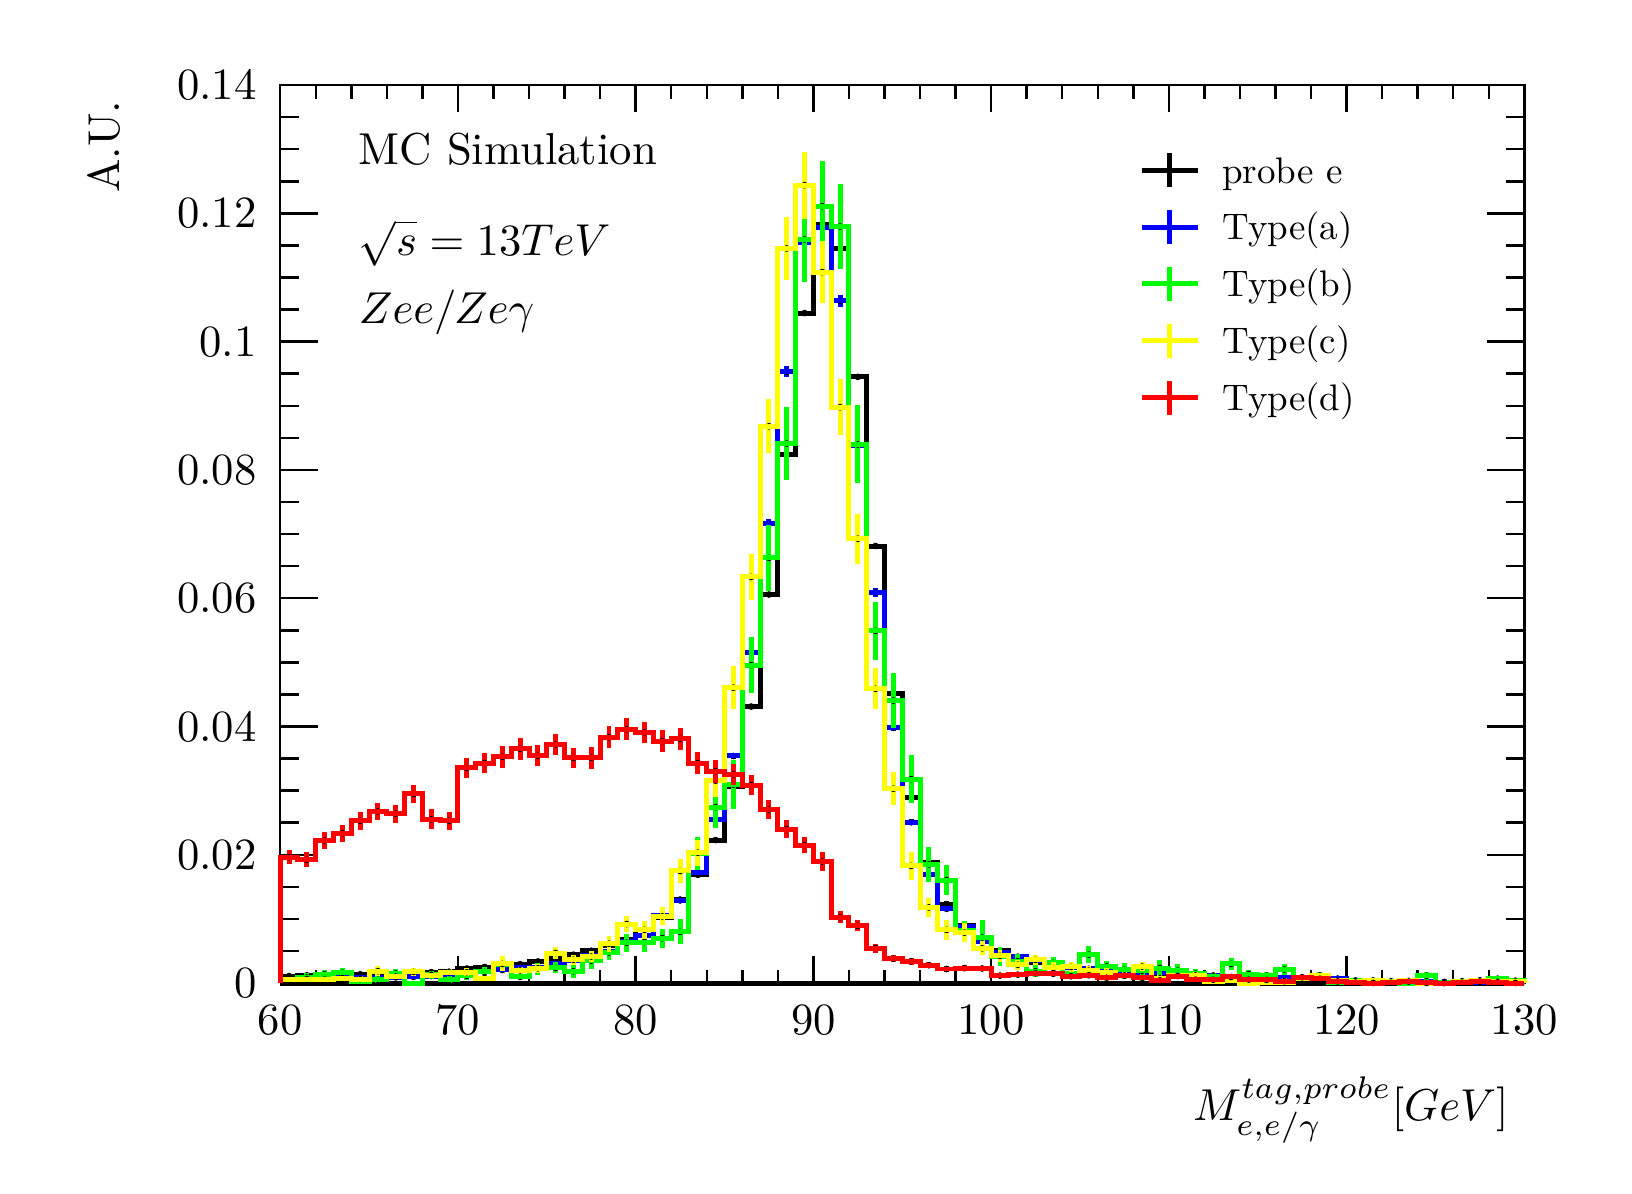
\begin{tikzpicture}
\pgfdeclareplotmark{cross} {
\pgfpathmoveto{\pgfpoint{-0.3\pgfplotmarksize}{\pgfplotmarksize}}
\pgfpathlineto{\pgfpoint{+0.3\pgfplotmarksize}{\pgfplotmarksize}}
\pgfpathlineto{\pgfpoint{+0.3\pgfplotmarksize}{0.3\pgfplotmarksize}}
\pgfpathlineto{\pgfpoint{+1\pgfplotmarksize}{0.3\pgfplotmarksize}}
\pgfpathlineto{\pgfpoint{+1\pgfplotmarksize}{-0.3\pgfplotmarksize}}
\pgfpathlineto{\pgfpoint{+0.3\pgfplotmarksize}{-0.3\pgfplotmarksize}}
\pgfpathlineto{\pgfpoint{+0.3\pgfplotmarksize}{-1.\pgfplotmarksize}}
\pgfpathlineto{\pgfpoint{-0.3\pgfplotmarksize}{-1.\pgfplotmarksize}}
\pgfpathlineto{\pgfpoint{-0.3\pgfplotmarksize}{-0.3\pgfplotmarksize}}
\pgfpathlineto{\pgfpoint{-1.\pgfplotmarksize}{-0.3\pgfplotmarksize}}
\pgfpathlineto{\pgfpoint{-1.\pgfplotmarksize}{0.3\pgfplotmarksize}}
\pgfpathlineto{\pgfpoint{-0.3\pgfplotmarksize}{0.3\pgfplotmarksize}}
\pgfpathclose
\pgfusepathqstroke
}
\pgfdeclareplotmark{cross*} {
\pgfpathmoveto{\pgfpoint{-0.3\pgfplotmarksize}{\pgfplotmarksize}}
\pgfpathlineto{\pgfpoint{+0.3\pgfplotmarksize}{\pgfplotmarksize}}
\pgfpathlineto{\pgfpoint{+0.3\pgfplotmarksize}{0.3\pgfplotmarksize}}
\pgfpathlineto{\pgfpoint{+1\pgfplotmarksize}{0.3\pgfplotmarksize}}
\pgfpathlineto{\pgfpoint{+1\pgfplotmarksize}{-0.3\pgfplotmarksize}}
\pgfpathlineto{\pgfpoint{+0.3\pgfplotmarksize}{-0.3\pgfplotmarksize}}
\pgfpathlineto{\pgfpoint{+0.3\pgfplotmarksize}{-1.\pgfplotmarksize}}
\pgfpathlineto{\pgfpoint{-0.3\pgfplotmarksize}{-1.\pgfplotmarksize}}
\pgfpathlineto{\pgfpoint{-0.3\pgfplotmarksize}{-0.3\pgfplotmarksize}}
\pgfpathlineto{\pgfpoint{-1.\pgfplotmarksize}{-0.3\pgfplotmarksize}}
\pgfpathlineto{\pgfpoint{-1.\pgfplotmarksize}{0.3\pgfplotmarksize}}
\pgfpathlineto{\pgfpoint{-0.3\pgfplotmarksize}{0.3\pgfplotmarksize}}
\pgfpathclose
\pgfusepathqfillstroke
}
\pgfdeclareplotmark{newstar} {
\pgfpathmoveto{\pgfqpoint{0pt}{\pgfplotmarksize}}
\pgfpathlineto{\pgfqpointpolar{44}{0.5\pgfplotmarksize}}
\pgfpathlineto{\pgfqpointpolar{18}{\pgfplotmarksize}}
\pgfpathlineto{\pgfqpointpolar{-20}{0.5\pgfplotmarksize}}
\pgfpathlineto{\pgfqpointpolar{-54}{\pgfplotmarksize}}
\pgfpathlineto{\pgfqpointpolar{-90}{0.5\pgfplotmarksize}}
\pgfpathlineto{\pgfqpointpolar{234}{\pgfplotmarksize}}
\pgfpathlineto{\pgfqpointpolar{198}{0.5\pgfplotmarksize}}
\pgfpathlineto{\pgfqpointpolar{162}{\pgfplotmarksize}}
\pgfpathlineto{\pgfqpointpolar{134}{0.5\pgfplotmarksize}}
\pgfpathclose
\pgfusepathqstroke
}
\pgfdeclareplotmark{newstar*} {
\pgfpathmoveto{\pgfqpoint{0pt}{\pgfplotmarksize}}
\pgfpathlineto{\pgfqpointpolar{44}{0.5\pgfplotmarksize}}
\pgfpathlineto{\pgfqpointpolar{18}{\pgfplotmarksize}}
\pgfpathlineto{\pgfqpointpolar{-20}{0.5\pgfplotmarksize}}
\pgfpathlineto{\pgfqpointpolar{-54}{\pgfplotmarksize}}
\pgfpathlineto{\pgfqpointpolar{-90}{0.5\pgfplotmarksize}}
\pgfpathlineto{\pgfqpointpolar{234}{\pgfplotmarksize}}
\pgfpathlineto{\pgfqpointpolar{198}{0.5\pgfplotmarksize}}
\pgfpathlineto{\pgfqpointpolar{162}{\pgfplotmarksize}}
\pgfpathlineto{\pgfqpointpolar{134}{0.5\pgfplotmarksize}}
\pgfpathclose
\pgfusepathqfillstroke
}
\definecolor{c}{rgb}{1,1,1};
\draw [color=c, fill=c] (0,0) rectangle (20,14.4361);
\draw [color=c, fill=c] (3.2,2.30977) rectangle (19,13.7143);
\definecolor{c}{rgb}{0,0,0};
\draw [c,line width=0.9] (3.2,2.30977) -- (3.2,13.7143) -- (19,13.7143) -- (19,2.30977) -- (3.2,2.30977);
\draw [c,line width=1.8] (3.2,2.30977) -- (3.2158,2.30977) -- (3.2158,2.30977) -- (3.2316,2.30977) -- (3.2316,2.30977) -- (3.2474,2.30977) -- (3.2474,2.30977) -- (3.2632,2.30977) -- (3.2632,2.30977) -- (3.279,2.30977) -- (3.279,2.30977) --
 (3.2948,2.30977) -- (3.2948,2.30977) -- (3.3106,2.30977) -- (3.3106,2.30977) -- (3.3264,2.30977) -- (3.3264,2.30977) -- (3.3422,2.30977) -- (3.3422,2.30977) -- (3.358,2.30977) -- (3.358,2.30977) -- (3.3738,2.30977) -- (3.3738,2.30977) --
 (3.3896,2.30977) -- (3.3896,2.30977) -- (3.4054,2.30977) -- (3.4054,2.30977) -- (3.4212,2.30977) -- (3.4212,2.30977) -- (3.437,2.30977) -- (3.437,2.30977) -- (3.4528,2.30977) -- (3.4528,2.30977) -- (3.4686,2.30977) -- (3.4686,2.30977) --
 (3.4844,2.30977) -- (3.4844,2.30977) -- (3.5002,2.30977) -- (3.5002,2.30977) -- (3.516,2.30977) -- (3.516,2.30977) -- (3.5318,2.30977) -- (3.5318,2.30977) -- (3.5476,2.30977) -- (3.5476,2.30977) -- (3.5634,2.30977) -- (3.5634,2.30977) --
 (3.5792,2.30977) -- (3.5792,2.30977) -- (3.595,2.30977) -- (3.595,2.30977) -- (3.6108,2.30977) -- (3.6108,2.30977) -- (3.6266,2.30977) -- (3.6266,2.30977) -- (3.6424,2.30977) -- (3.6424,2.30977) -- (3.6582,2.30977) -- (3.6582,2.30977) --
 (3.674,2.30977) -- (3.674,2.30977) -- (3.6898,2.30977) -- (3.6898,2.30977) -- (3.7056,2.30977) -- (3.7056,2.30977) -- (3.7214,2.30977) -- (3.7214,2.30977) -- (3.7372,2.30977) -- (3.7372,2.30977) -- (3.753,2.30977) -- (3.753,2.30977) --
 (3.7688,2.30977) -- (3.7688,2.30977) -- (3.7846,2.30977) -- (3.7846,2.30977) -- (3.8004,2.30977) -- (3.8004,2.30977) -- (3.8162,2.30977) -- (3.8162,2.30977) -- (3.832,2.30977) -- (3.832,2.30977) -- (3.8478,2.30977) -- (3.8478,2.30977) --
 (3.8636,2.30977) -- (3.8636,2.30977) -- (3.8794,2.30977) -- (3.8794,2.30977) -- (3.8952,2.30977) -- (3.8952,2.30977) -- (3.911,2.30977) -- (3.911,2.30977) -- (3.9268,2.30977) -- (3.9268,2.30977) -- (3.9426,2.30977) -- (3.9426,2.30977) --
 (3.9584,2.30977) -- (3.9584,2.30977) -- (3.9742,2.30977) -- (3.9742,2.30977) -- (3.99,2.30977) -- (3.99,2.30977) -- (4.0058,2.30977) -- (4.0058,2.30977) -- (4.0216,2.30977) -- (4.0216,2.30977) -- (4.0374,2.30977) -- (4.0374,2.30977) --
 (4.0532,2.30977) -- (4.0532,2.30977) -- (4.069,2.30977) -- (4.069,2.30977) -- (4.0848,2.30977) -- (4.0848,2.30977) -- (4.1006,2.30977) -- (4.1006,2.30977) -- (4.1164,2.30977) -- (4.1164,2.30977) -- (4.1322,2.30977) -- (4.1322,2.30977) --
 (4.148,2.30977) -- (4.148,2.30977) -- (4.1638,2.30977) -- (4.1638,2.30977) -- (4.1796,2.30977) -- (4.1796,2.30977) -- (4.1954,2.30977) -- (4.1954,2.30977) -- (4.2112,2.30977) -- (4.2112,2.30977) -- (4.227,2.30977) -- (4.227,2.30977) --
 (4.2428,2.30977) -- (4.2428,2.30977) -- (4.2586,2.30977) -- (4.2586,2.30977) -- (4.2744,2.30977) -- (4.2744,2.30977) -- (4.2902,2.30977) -- (4.2902,2.30977) -- (4.306,2.30977) -- (4.306,2.30977) -- (4.3218,2.30977) -- (4.3218,2.30977) --
 (4.3376,2.30977) -- (4.3376,2.30977) -- (4.3534,2.30977) -- (4.3534,2.30977) -- (4.3692,2.30977) -- (4.3692,2.30977) -- (4.385,2.30977) -- (4.385,2.30977) -- (4.4008,2.30977) -- (4.4008,2.30977) -- (4.4166,2.30977) -- (4.4166,2.30977) --
 (4.4324,2.30977) -- (4.4324,2.30977) -- (4.4482,2.30977) -- (4.4482,2.30977) -- (4.464,2.30977) -- (4.464,2.30977) -- (4.4798,2.30977) -- (4.4798,2.30977) -- (4.4956,2.30977) -- (4.4956,2.30977) -- (4.5114,2.30977) -- (4.5114,2.30977) --
 (4.5272,2.30977) -- (4.5272,2.30977) -- (4.543,2.30977) -- (4.543,2.30977) -- (4.5588,2.30977) -- (4.5588,2.30977) -- (4.5746,2.30977) -- (4.5746,2.30977) -- (4.5904,2.30977) -- (4.5904,2.30977) -- (4.6062,2.30977) -- (4.6062,2.30977) --
 (4.622,2.30977) -- (4.622,2.30977) -- (4.6378,2.30977) -- (4.6378,2.30977) -- (4.6536,2.30977) -- (4.6536,2.30977) -- (4.6694,2.30977) -- (4.6694,2.30977) -- (4.6852,2.30977) -- (4.6852,2.30977) -- (4.701,2.30977) -- (4.701,2.30977) --
 (4.7168,2.30977) -- (4.7168,2.30977) -- (4.7326,2.30977) -- (4.7326,2.30977) -- (4.7484,2.30977) -- (4.7484,2.30977) -- (4.7642,2.30977) -- (4.7642,2.30977) -- (4.78,2.30977) -- (4.78,2.30977) -- (4.7958,2.30977) -- (4.7958,2.30977) --
 (4.8116,2.30977) -- (4.8116,2.30977) -- (4.8274,2.30977) -- (4.8274,2.30977) -- (4.8432,2.30977) -- (4.8432,2.30977) -- (4.859,2.30977) -- (4.859,2.30977) -- (4.8748,2.30977) -- (4.8748,2.30977) -- (4.8906,2.30977) -- (4.8906,2.30977) --
 (4.9064,2.30977) -- (4.9064,2.30977) -- (4.9222,2.30977) -- (4.9222,2.30977) -- (4.938,2.30977) -- (4.938,2.30977) -- (4.9538,2.30977) -- (4.9538,2.30977) -- (4.9696,2.30977) -- (4.9696,2.30977) -- (4.9854,2.30977) -- (4.9854,2.30977) --
 (5.0012,2.30977) -- (5.0012,2.30977) -- (5.017,2.30977) -- (5.017,2.30977) -- (5.0328,2.30977) -- (5.0328,2.30977) -- (5.0486,2.30977) -- (5.0486,2.30977) -- (5.0644,2.30977) -- (5.0644,2.30977) -- (5.0802,2.30977) -- (5.0802,2.30977) --
 (5.096,2.30977) -- (5.096,2.30977) -- (5.1118,2.30977) -- (5.1118,2.30977) -- (5.1276,2.30977) -- (5.1276,2.30977) -- (5.1434,2.30977) -- (5.1434,2.30977) -- (5.1592,2.30977) -- (5.1592,2.30977) -- (5.175,2.30977) -- (5.175,2.30977) --
 (5.1908,2.30977) -- (5.1908,2.30977) -- (5.2066,2.30977) -- (5.2066,2.30977) -- (5.2224,2.30977) -- (5.2224,2.30977) -- (5.2382,2.30977) -- (5.2382,2.30977) -- (5.254,2.30977) -- (5.254,2.30977) -- (5.2698,2.30977) -- (5.2698,2.30977) --
 (5.2856,2.30977) -- (5.2856,2.30977) -- (5.3014,2.30977) -- (5.3014,2.30977) -- (5.3172,2.30977) -- (5.3172,2.30977) -- (5.333,2.30977) -- (5.333,2.30977) -- (5.3488,2.30977) -- (5.3488,2.30977) -- (5.3646,2.30977) -- (5.3646,2.30977) --
 (5.3804,2.30977) -- (5.3804,2.30977) -- (5.3962,2.30977) -- (5.3962,2.30977) -- (5.412,2.30977) -- (5.412,2.30977) -- (5.4278,2.30977) -- (5.4278,2.30977) -- (5.4436,2.30977) -- (5.4436,2.30977) -- (5.4594,2.30977) -- (5.4594,2.30977) --
 (5.4752,2.30977) -- (5.4752,2.30977) -- (5.491,2.30977) -- (5.491,2.30977) -- (5.5068,2.30977) -- (5.5068,2.30977) -- (5.5226,2.30977) -- (5.5226,2.30977) -- (5.5384,2.30977) -- (5.5384,2.30977) -- (5.5542,2.30977) -- (5.5542,2.30977) --
 (5.57,2.30977) -- (5.57,2.30977) -- (5.5858,2.30977) -- (5.5858,2.30977) -- (5.6016,2.30977) -- (5.6016,2.30977) -- (5.6174,2.30977) -- (5.6174,2.30977) -- (5.6332,2.30977) -- (5.6332,2.30977) -- (5.649,2.30977) -- (5.649,2.30977) --
 (5.6648,2.30977) -- (5.6648,2.30977) -- (5.6806,2.30977) -- (5.6806,2.30977) -- (5.6964,2.30977) -- (5.6964,2.30977) -- (5.7122,2.30977) -- (5.7122,2.30977) -- (5.728,2.30977) -- (5.728,2.30977) -- (5.7438,2.30977) -- (5.7438,2.30977) --
 (5.7596,2.30977) -- (5.7596,2.30977) -- (5.7754,2.30977) -- (5.7754,2.30977) -- (5.7912,2.30977) -- (5.7912,2.30977) -- (5.807,2.30977) -- (5.807,2.30977) -- (5.8228,2.30977) -- (5.8228,2.30977) -- (5.8386,2.30977) -- (5.8386,2.30977) --
 (5.8544,2.30977) -- (5.8544,2.30977) -- (5.8702,2.30977) -- (5.8702,2.30977) -- (5.886,2.30977) -- (5.886,2.30977) -- (5.9018,2.30977) -- (5.9018,2.30977) -- (5.9176,2.30977) -- (5.9176,2.30977) -- (5.9334,2.30977) -- (5.9334,2.30977) --
 (5.9492,2.30977) -- (5.9492,2.30977) -- (5.965,2.30977) -- (5.965,2.30977) -- (5.9808,2.30977) -- (5.9808,2.30977) -- (5.9966,2.30977) -- (5.9966,2.30977) -- (6.0124,2.30977) -- (6.0124,2.30977) -- (6.0282,2.30977) -- (6.0282,2.30977) --
 (6.044,2.30977) -- (6.044,2.30977) -- (6.0598,2.30977) -- (6.0598,2.30977) -- (6.0756,2.30977) -- (6.0756,2.30977) -- (6.0914,2.30977) -- (6.0914,2.30977) -- (6.1072,2.30977) -- (6.1072,2.30977) -- (6.123,2.30977) -- (6.123,2.30977) --
 (6.1388,2.30977) -- (6.1388,2.30977) -- (6.1546,2.30977) -- (6.1546,2.30977) -- (6.1704,2.30977) -- (6.1704,2.30977) -- (6.1862,2.30977) -- (6.1862,2.30977) -- (6.202,2.30977) -- (6.202,2.30977) -- (6.2178,2.30977) -- (6.2178,2.30977) --
 (6.2336,2.30977) -- (6.2336,2.30977) -- (6.2494,2.30977) -- (6.2494,2.30977) -- (6.2652,2.30977) -- (6.2652,2.30977) -- (6.281,2.30977) -- (6.281,2.30977) -- (6.2968,2.30977) -- (6.2968,2.30977) -- (6.3126,2.30977) -- (6.3126,2.30977) --
 (6.3284,2.30977) -- (6.3284,2.30977) -- (6.3442,2.30977) -- (6.3442,2.30977) -- (6.36,2.30977) -- (6.36,2.30977) -- (6.3758,2.30977) -- (6.3758,2.30977) -- (6.3916,2.30977) -- (6.3916,2.30977) -- (6.4074,2.30977) -- (6.4074,2.30977) --
 (6.4232,2.30977) -- (6.4232,2.30977) -- (6.439,2.30977) -- (6.439,2.30977) -- (6.4548,2.30977) -- (6.4548,2.30977) -- (6.4706,2.30977) -- (6.4706,2.30977) -- (6.4864,2.30977) -- (6.4864,2.30977) -- (6.5022,2.30977) -- (6.5022,2.30977) --
 (6.518,2.30977) -- (6.518,2.30977) -- (6.5338,2.30977) -- (6.5338,2.30977) -- (6.5496,2.30977) -- (6.5496,2.30977) -- (6.5654,2.30977) -- (6.5654,2.30977) -- (6.5812,2.30977) -- (6.5812,2.30977) -- (6.597,2.30977) -- (6.597,2.30977) --
 (6.6128,2.30977) -- (6.6128,2.30977) -- (6.6286,2.30977) -- (6.6286,2.30977) -- (6.6444,2.30977) -- (6.6444,2.30977) -- (6.6602,2.30977) -- (6.6602,2.30977) -- (6.676,2.30977) -- (6.676,2.30977) -- (6.6918,2.30977) -- (6.6918,2.30977) --
 (6.7076,2.30977) -- (6.7076,2.30977) -- (6.7234,2.30977) -- (6.7234,2.30977) -- (6.7392,2.30977) -- (6.7392,2.30977) -- (6.755,2.30977) -- (6.755,2.30977) -- (6.7708,2.30977) -- (6.7708,2.30977) -- (6.7866,2.30977) -- (6.7866,2.30977) --
 (6.8024,2.30977) -- (6.8024,2.30977) -- (6.8182,2.30977) -- (6.8182,2.30977) -- (6.834,2.30977) -- (6.834,2.30977) -- (6.8498,2.30977) -- (6.8498,2.30977) -- (6.8656,2.30977) -- (6.8656,2.30977) -- (6.8814,2.30977) -- (6.8814,2.30977) --
 (6.8972,2.30977) -- (6.8972,2.30977) -- (6.913,2.30977) -- (6.913,2.30977) -- (6.9288,2.30977) -- (6.9288,2.30977) -- (6.9446,2.30977) -- (6.9446,2.30977) -- (6.9604,2.30977) -- (6.9604,2.30977) -- (6.9762,2.30977) -- (6.9762,2.30977) --
 (6.992,2.30977) -- (6.992,2.30977) -- (7.0078,2.30977) -- (7.0078,2.30977) -- (7.0236,2.30977) -- (7.0236,2.30977) -- (7.0394,2.30977) -- (7.0394,2.30977) -- (7.0552,2.30977) -- (7.0552,2.30977) -- (7.071,2.30977) -- (7.071,2.30977) --
 (7.0868,2.30977) -- (7.0868,2.30977) -- (7.1026,2.30977) -- (7.1026,2.30977) -- (7.1184,2.30977) -- (7.1184,2.30977) -- (7.1342,2.30977) -- (7.1342,2.30977) -- (7.15,2.30977) -- (7.15,2.30977) -- (7.1658,2.30977) -- (7.1658,2.30977) --
 (7.1816,2.30977) -- (7.1816,2.30977) -- (7.1974,2.30977) -- (7.1974,2.30977) -- (7.2132,2.30977) -- (7.2132,2.30977) -- (7.229,2.30977) -- (7.229,2.30977) -- (7.2448,2.30977) -- (7.2448,2.30977) -- (7.2606,2.30977) -- (7.2606,2.30977) --
 (7.2764,2.30977) -- (7.2764,2.30977) -- (7.2922,2.30977) -- (7.2922,2.30977) -- (7.308,2.30977) -- (7.308,2.30977) -- (7.3238,2.30977) -- (7.3238,2.30977) -- (7.3396,2.30977) -- (7.3396,2.30977) -- (7.3554,2.30977) -- (7.3554,2.30977) --
 (7.3712,2.30977) -- (7.3712,2.30977) -- (7.387,2.30977) -- (7.387,2.30977) -- (7.4028,2.30977) -- (7.4028,2.30977) -- (7.4186,2.30977) -- (7.4186,2.30977) -- (7.4344,2.30977) -- (7.4344,2.30977) -- (7.4502,2.30977) -- (7.4502,2.30977) --
 (7.466,2.30977) -- (7.466,2.30977) -- (7.4818,2.30977) -- (7.4818,2.30977) -- (7.4976,2.30977) -- (7.4976,2.30977) -- (7.5134,2.30977) -- (7.5134,2.30977) -- (7.5292,2.30977) -- (7.5292,2.30977) -- (7.545,2.30977) -- (7.545,2.30977) --
 (7.5608,2.30977) -- (7.5608,2.30977) -- (7.5766,2.30977) -- (7.5766,2.30977) -- (7.5924,2.30977) -- (7.5924,2.30977) -- (7.6082,2.30977) -- (7.6082,2.30977) -- (7.624,2.30977) -- (7.624,2.30977) -- (7.6398,2.30977) -- (7.6398,2.30977) --
 (7.6556,2.30977) -- (7.6556,2.30977) -- (7.6714,2.30977) -- (7.6714,2.30977) -- (7.6872,2.30977) -- (7.6872,2.30977) -- (7.703,2.30977) -- (7.703,2.30977) -- (7.7188,2.30977) -- (7.7188,2.30977) -- (7.7346,2.30977) -- (7.7346,2.30977) --
 (7.7504,2.30977) -- (7.7504,2.30977) -- (7.7662,2.30977) -- (7.7662,2.30977) -- (7.782,2.30977) -- (7.782,2.30977) -- (7.7978,2.30977) -- (7.7978,2.30977) -- (7.8136,2.30977) -- (7.8136,2.30977) -- (7.8294,2.30977) -- (7.8294,2.30977) --
 (7.8452,2.30977) -- (7.8452,2.30977) -- (7.861,2.30977) -- (7.861,2.30977) -- (7.8768,2.30977) -- (7.8768,2.30977) -- (7.8926,2.30977) -- (7.8926,2.30977) -- (7.9084,2.30977) -- (7.9084,2.30977) -- (7.9242,2.30977) -- (7.9242,2.30977) --
 (7.94,2.30977) -- (7.94,2.30977) -- (7.9558,2.30977) -- (7.9558,2.30977) -- (7.9716,2.30977) -- (7.9716,2.30977) -- (7.9874,2.30977) -- (7.9874,2.30977) -- (8.0032,2.30977) -- (8.0032,2.30977) -- (8.019,2.30977) -- (8.019,2.30977) --
 (8.0348,2.30977) -- (8.0348,2.30977) -- (8.0506,2.30977) -- (8.0506,2.30977) -- (8.0664,2.30977) -- (8.0664,2.30977) -- (8.0822,2.30977) -- (8.0822,2.30977) -- (8.098,2.30977) -- (8.098,2.30977) -- (8.1138,2.30977) -- (8.1138,2.30977) --
 (8.1296,2.30977) -- (8.1296,2.30977) -- (8.1454,2.30977) -- (8.1454,2.30977) -- (8.1612,2.30977) -- (8.1612,2.30977) -- (8.177,2.30977) -- (8.177,2.30977) -- (8.1928,2.30977) -- (8.1928,2.30977) -- (8.2086,2.30977) -- (8.2086,2.30977) --
 (8.2244,2.30977) -- (8.2244,2.30977) -- (8.2402,2.30977) -- (8.2402,2.30977) -- (8.256,2.30977) -- (8.256,2.30977) -- (8.2718,2.30977) -- (8.2718,2.30977) -- (8.2876,2.30977) -- (8.2876,2.30977) -- (8.3034,2.30977) -- (8.3034,2.30977) --
 (8.3192,2.30977) -- (8.3192,2.30977) -- (8.335,2.30977) -- (8.335,2.30977) -- (8.3508,2.30977) -- (8.3508,2.30977) -- (8.3666,2.30977) -- (8.3666,2.30977) -- (8.3824,2.30977) -- (8.3824,2.30977) -- (8.3982,2.30977) -- (8.3982,2.30977) --
 (8.414,2.30977) -- (8.414,2.30977) -- (8.4298,2.30977) -- (8.4298,2.30977) -- (8.4456,2.30977) -- (8.4456,2.30977) -- (8.4614,2.30977) -- (8.4614,2.30977) -- (8.4772,2.30977) -- (8.4772,2.30977) -- (8.493,2.30977) -- (8.493,2.30977) --
 (8.5088,2.30977) -- (8.5088,2.30977) -- (8.5246,2.30977) -- (8.5246,2.30977) -- (8.5404,2.30977) -- (8.5404,2.30977) -- (8.5562,2.30977) -- (8.5562,2.30977) -- (8.572,2.30977) -- (8.572,2.30977) -- (8.5878,2.30977) -- (8.5878,2.30977) --
 (8.6036,2.30977) -- (8.6036,2.30977) -- (8.6194,2.30977) -- (8.6194,2.30977) -- (8.6352,2.30977) -- (8.6352,2.30977) -- (8.651,2.30977) -- (8.651,2.30977) -- (8.6668,2.30977) -- (8.6668,2.30977) -- (8.6826,2.30977) -- (8.6826,2.30977) --
 (8.6984,2.30977) -- (8.6984,2.30977) -- (8.7142,2.30977) -- (8.7142,2.30977) -- (8.73,2.30977) -- (8.73,2.30977) -- (8.7458,2.30977) -- (8.7458,2.30977) -- (8.7616,2.30977) -- (8.7616,2.30977) -- (8.7774,2.30977) -- (8.7774,2.30977) --
 (8.7932,2.30977) -- (8.7932,2.30977) -- (8.809,2.30977) -- (8.809,2.30977) -- (8.8248,2.30977) -- (8.8248,2.30977) -- (8.8406,2.30977) -- (8.8406,2.30977) -- (8.8564,2.30977) -- (8.8564,2.30977) -- (8.8722,2.30977) -- (8.8722,2.30977) --
 (8.888,2.30977) -- (8.888,2.30977) -- (8.9038,2.30977) -- (8.9038,2.30977) -- (8.9196,2.30977) -- (8.9196,2.30977) -- (8.9354,2.30977) -- (8.9354,2.30977) -- (8.9512,2.30977) -- (8.9512,2.30977) -- (8.967,2.30977) -- (8.967,2.30977) --
 (8.9828,2.30977) -- (8.9828,2.30977) -- (8.9986,2.30977) -- (8.9986,2.30977) -- (9.0144,2.30977) -- (9.0144,2.30977) -- (9.0302,2.30977) -- (9.0302,2.30977) -- (9.046,2.30977) -- (9.046,2.30977) -- (9.0618,2.30977) -- (9.0618,2.30977) --
 (9.0776,2.30977) -- (9.0776,2.30977) -- (9.0934,2.30977) -- (9.0934,2.30977) -- (9.1092,2.30977) -- (9.1092,2.30977) -- (9.125,2.30977) -- (9.125,2.30977) -- (9.1408,2.30977) -- (9.1408,2.30977) -- (9.1566,2.30977) -- (9.1566,2.30977) --
 (9.1724,2.30977) -- (9.1724,2.30977) -- (9.1882,2.30977) -- (9.1882,2.30977) -- (9.204,2.30977) -- (9.204,2.30977) -- (9.2198,2.30977) -- (9.2198,2.30977) -- (9.2356,2.30977) -- (9.2356,2.30977) -- (9.2514,2.30977) -- (9.2514,2.30977) --
 (9.2672,2.30977) -- (9.2672,2.30977) -- (9.283,2.30977) -- (9.283,2.30977) -- (9.2988,2.30977) -- (9.2988,2.30977) -- (9.3146,2.30977) -- (9.3146,2.30977) -- (9.3304,2.30977) -- (9.3304,2.30977) -- (9.3462,2.30977) -- (9.3462,2.30977) --
 (9.362,2.30977) -- (9.362,2.30977) -- (9.3778,2.30977) -- (9.3778,2.30977) -- (9.3936,2.30977) -- (9.3936,2.30977) -- (9.4094,2.30977) -- (9.4094,2.30977) -- (9.4252,2.30977) -- (9.4252,2.30977) -- (9.441,2.30977) -- (9.441,2.30977) --
 (9.4568,2.30977) -- (9.4568,2.30977) -- (9.4726,2.30977) -- (9.4726,2.30977) -- (9.4884,2.30977) -- (9.4884,2.30977) -- (9.5042,2.30977) -- (9.5042,2.30977) -- (9.52,2.30977) -- (9.52,2.30977) -- (9.5358,2.30977) -- (9.5358,2.30977) --
 (9.5516,2.30977) -- (9.5516,2.30977) -- (9.5674,2.30977) -- (9.5674,2.30977) -- (9.5832,2.30977) -- (9.5832,2.30977) -- (9.599,2.30977) -- (9.599,2.30977) -- (9.6148,2.30977) -- (9.6148,2.30977) -- (9.6306,2.30977) -- (9.6306,2.30977) --
 (9.6464,2.30977) -- (9.6464,2.30977) -- (9.6622,2.30977) -- (9.6622,2.30977) -- (9.678,2.30977) -- (9.678,2.30977) -- (9.6938,2.30977) -- (9.6938,2.30977) -- (9.7096,2.30977) -- (9.7096,2.30977) -- (9.7254,2.30977) -- (9.7254,2.30977) --
 (9.7412,2.30977) -- (9.7412,2.30977) -- (9.757,2.30977) -- (9.757,2.30977) -- (9.7728,2.30977) -- (9.7728,2.30977) -- (9.7886,2.30977) -- (9.7886,2.30977) -- (9.8044,2.30977) -- (9.8044,2.30977) -- (9.8202,2.30977) -- (9.8202,2.30977) --
 (9.836,2.30977) -- (9.836,2.30977) -- (9.8518,2.30977) -- (9.8518,2.30977) -- (9.8676,2.30977) -- (9.8676,2.30977) -- (9.8834,2.30977) -- (9.8834,2.30977) -- (9.8992,2.30977) -- (9.8992,2.30977) -- (9.915,2.30977) -- (9.915,2.30977) --
 (9.9308,2.30977) -- (9.9308,2.30977) -- (9.9466,2.30977) -- (9.9466,2.30977) -- (9.9624,2.30977) -- (9.9624,2.30977) -- (9.9782,2.30977) -- (9.9782,2.30977) -- (9.994,2.30977) -- (9.994,2.30977) -- (10.0098,2.30977) -- (10.0098,2.30977) --
 (10.0256,2.30977) -- (10.0256,2.30977) -- (10.0414,2.30977) -- (10.0414,2.30977) -- (10.0572,2.30977) -- (10.0572,2.30977) -- (10.073,2.30977) -- (10.073,2.30977) -- (10.0888,2.30977) -- (10.0888,2.30977) -- (10.1046,2.30977) -- (10.1046,2.30977) --
 (10.1204,2.30977) -- (10.1204,2.30977) -- (10.1362,2.30977) -- (10.1362,2.30977) -- (10.152,2.30977) -- (10.152,2.30977) -- (10.1678,2.30977) -- (10.1678,2.30977) -- (10.1836,2.30977) -- (10.1836,2.30977) -- (10.1994,2.30977) -- (10.1994,2.30977) --
 (10.2152,2.30977) -- (10.2152,2.30977) -- (10.231,2.30977) -- (10.231,2.30977) -- (10.2468,2.30977) -- (10.2468,2.30977) -- (10.2626,2.30977) -- (10.2626,2.30977) -- (10.2784,2.30977) -- (10.2784,2.30977) -- (10.2942,2.30977) -- (10.2942,2.30977) --
 (10.31,2.30977) -- (10.31,2.30977) -- (10.3258,2.30977) -- (10.3258,2.30977) -- (10.3416,2.30977) -- (10.3416,2.30977) -- (10.3574,2.30977) -- (10.3574,2.30977) -- (10.3732,2.30977) -- (10.3732,2.30977) -- (10.389,2.30977) -- (10.389,2.30977) --
 (10.4048,2.30977) -- (10.4048,2.30977) -- (10.4206,2.30977) -- (10.4206,2.30977) -- (10.4364,2.30977) -- (10.4364,2.30977) -- (10.4522,2.30977) -- (10.4522,2.30977) -- (10.468,2.30977) -- (10.468,2.30977) -- (10.4838,2.30977) -- (10.4838,2.30977) --
 (10.4996,2.30977) -- (10.4996,2.30977) -- (10.5154,2.30977) -- (10.5154,2.30977) -- (10.5312,2.30977) -- (10.5312,2.30977) -- (10.547,2.30977) -- (10.547,2.30977) -- (10.5628,2.30977) -- (10.5628,2.30977) -- (10.5786,2.30977) -- (10.5786,2.30977) --
 (10.5944,2.30977) -- (10.5944,2.30977) -- (10.6102,2.30977) -- (10.6102,2.30977) -- (10.626,2.30977) -- (10.626,2.30977) -- (10.6418,2.30977) -- (10.6418,2.30977) -- (10.6576,2.30977) -- (10.6576,2.30977) -- (10.6734,2.30977) -- (10.6734,2.30977) --
 (10.6892,2.30977) -- (10.6892,2.30977) -- (10.705,2.30977) -- (10.705,2.30977) -- (10.7208,2.30977) -- (10.7208,2.30977) -- (10.7366,2.30977) -- (10.7366,2.30977) -- (10.7524,2.30977) -- (10.7524,2.30977) -- (10.7682,2.30977) -- (10.7682,2.30977) --
 (10.784,2.30977) -- (10.784,2.30977) -- (10.7998,2.30977) -- (10.7998,2.30977) -- (10.8156,2.30977) -- (10.8156,2.30977) -- (10.8314,2.30977) -- (10.8314,2.30977) -- (10.8472,2.30977) -- (10.8472,2.30977) -- (10.863,2.30977) -- (10.863,2.30977) --
 (10.8788,2.30977) -- (10.8788,2.30977) -- (10.8946,2.30977) -- (10.8946,2.30977) -- (10.9104,2.30977) -- (10.9104,2.30977) -- (10.9262,2.30977) -- (10.9262,2.30977) -- (10.942,2.30977) -- (10.942,2.30977) -- (10.9578,2.30977) -- (10.9578,2.30977) --
 (10.9736,2.30977) -- (10.9736,2.30977) -- (10.9894,2.30977) -- (10.9894,2.30977) -- (11.0052,2.30977) -- (11.0052,2.30977) -- (11.021,2.30977) -- (11.021,2.30977) -- (11.0368,2.30977) -- (11.0368,2.30977) -- (11.0526,2.30977) -- (11.0526,2.30977) --
 (11.0684,2.30977) -- (11.0684,2.30977) -- (11.0842,2.30977) -- (11.0842,2.30977) -- (11.1,2.30977) -- (11.1,2.30977) -- (11.1158,2.30977) -- (11.1158,2.30977) -- (11.1316,2.30977) -- (11.1316,2.30977) -- (11.1474,2.30977) -- (11.1474,2.30977) --
 (11.1632,2.30977) -- (11.1632,2.30977) -- (11.179,2.30977) -- (11.179,2.30977) -- (11.1948,2.30977) -- (11.1948,2.30977) -- (11.2106,2.30977) -- (11.2106,2.30977) -- (11.2264,2.30977) -- (11.2264,2.30977) -- (11.2422,2.30977) -- (11.2422,2.30977) --
 (11.258,2.30977) -- (11.258,2.30977) -- (11.2738,2.30977) -- (11.2738,2.30977) -- (11.2896,2.30977) -- (11.2896,2.30977) -- (11.3054,2.30977) -- (11.3054,2.30977) -- (11.3212,2.30977) -- (11.3212,2.30977) -- (11.337,2.30977) -- (11.337,2.30977) --
 (11.3528,2.30977) -- (11.3528,2.30977) -- (11.3686,2.30977) -- (11.3686,2.30977) -- (11.3844,2.30977) -- (11.3844,2.30977) -- (11.4002,2.30977) -- (11.4002,2.30977) -- (11.416,2.30977) -- (11.416,2.30977) -- (11.4318,2.30977) -- (11.4318,2.30977) --
 (11.4476,2.30977) -- (11.4476,2.30977) -- (11.4634,2.30977) -- (11.4634,2.30977) -- (11.4792,2.30977) -- (11.4792,2.30977) -- (11.495,2.30977) -- (11.495,2.30977) -- (11.5108,2.30977) -- (11.5108,2.30977) -- (11.5266,2.30977) -- (11.5266,2.30977) --
 (11.5424,2.30977) -- (11.5424,2.30977) -- (11.5582,2.30977) -- (11.5582,2.30977) -- (11.574,2.30977) -- (11.574,2.30977) -- (11.5898,2.30977) -- (11.5898,2.30977) -- (11.6056,2.30977) -- (11.6056,2.30977) -- (11.6214,2.30977) -- (11.6214,2.30977) --
 (11.6372,2.30977) -- (11.6372,2.30977) -- (11.653,2.30977) -- (11.653,2.30977) -- (11.6688,2.30977) -- (11.6688,2.30977) -- (11.6846,2.30977) -- (11.6846,2.30977) -- (11.7004,2.30977) -- (11.7004,2.30977) -- (11.7162,2.30977) -- (11.7162,2.30977) --
 (11.732,2.30977) -- (11.732,2.30977) -- (11.7478,2.30977) -- (11.7478,2.30977) -- (11.7636,2.30977) -- (11.7636,2.30977) -- (11.7794,2.30977) -- (11.7794,2.30977) -- (11.7952,2.30977) -- (11.7952,2.30977) -- (11.811,2.30977) -- (11.811,2.30977) --
 (11.8268,2.30977) -- (11.8268,2.30977) -- (11.8426,2.30977) -- (11.8426,2.30977) -- (11.8584,2.30977) -- (11.8584,2.30977) -- (11.8742,2.30977) -- (11.8742,2.30977) -- (11.89,2.30977) -- (11.89,2.30977) -- (11.9058,2.30977) -- (11.9058,2.30977) --
 (11.9216,2.30977) -- (11.9216,2.30977) -- (11.9374,2.30977) -- (11.9374,2.30977) -- (11.9532,2.30977) -- (11.9532,2.30977) -- (11.969,2.30977) -- (11.969,2.30977) -- (11.9848,2.30977) -- (11.9848,2.30977) -- (12.0006,2.30977) -- (12.0006,2.30977) --
 (12.0164,2.30977) -- (12.0164,2.30977) -- (12.0322,2.30977) -- (12.0322,2.30977) -- (12.048,2.30977) -- (12.048,2.30977) -- (12.0638,2.30977) -- (12.0638,2.30977) -- (12.0796,2.30977) -- (12.0796,2.30977) -- (12.0954,2.30977) -- (12.0954,2.30977) --
 (12.1112,2.30977) -- (12.1112,2.30977) -- (12.127,2.30977) -- (12.127,2.30977) -- (12.1428,2.30977) -- (12.1428,2.30977) -- (12.1586,2.30977) -- (12.1586,2.30977) -- (12.1744,2.30977) -- (12.1744,2.30977) -- (12.1902,2.30977) -- (12.1902,2.30977) --
 (12.206,2.30977) -- (12.206,2.30977) -- (12.2218,2.30977) -- (12.2218,2.30977) -- (12.2376,2.30977) -- (12.2376,2.30977) -- (12.2534,2.30977) -- (12.2534,2.30977) -- (12.2692,2.30977) -- (12.2692,2.30977) -- (12.285,2.30977) -- (12.285,2.30977) --
 (12.3008,2.30977) -- (12.3008,2.30977) -- (12.3166,2.30977) -- (12.3166,2.30977) -- (12.3324,2.30977) -- (12.3324,2.30977) -- (12.3482,2.30977) -- (12.3482,2.30977) -- (12.364,2.30977) -- (12.364,2.30977) -- (12.3798,2.30977) -- (12.3798,2.30977) --
 (12.3956,2.30977) -- (12.3956,2.30977) -- (12.4114,2.30977) -- (12.4114,2.30977) -- (12.4272,2.30977) -- (12.4272,2.30977) -- (12.443,2.30977) -- (12.443,2.30977) -- (12.4588,2.30977) -- (12.4588,2.30977) -- (12.4746,2.30977) -- (12.4746,2.30977) --
 (12.4904,2.30977) -- (12.4904,2.30977) -- (12.5062,2.30977) -- (12.5062,2.30977) -- (12.522,2.30977) -- (12.522,2.30977) -- (12.5378,2.30977) -- (12.5378,2.30977) -- (12.5536,2.30977) -- (12.5536,2.30977) -- (12.5694,2.30977) -- (12.5694,2.30977) --
 (12.5852,2.30977) -- (12.5852,2.30977) -- (12.601,2.30977) -- (12.601,2.30977) -- (12.6168,2.30977) -- (12.6168,2.30977) -- (12.6326,2.30977) -- (12.6326,2.30977) -- (12.6484,2.30977) -- (12.6484,2.30977) -- (12.6642,2.30977) -- (12.6642,2.30977) --
 (12.68,2.30977) -- (12.68,2.30977) -- (12.6958,2.30977) -- (12.6958,2.30977) -- (12.7116,2.30977) -- (12.7116,2.30977) -- (12.7274,2.30977) -- (12.7274,2.30977) -- (12.7432,2.30977) -- (12.7432,2.30977) -- (12.759,2.30977) -- (12.759,2.30977) --
 (12.7748,2.30977) -- (12.7748,2.30977) -- (12.7906,2.30977) -- (12.7906,2.30977) -- (12.8064,2.30977) -- (12.8064,2.30977) -- (12.8222,2.30977) -- (12.8222,2.30977) -- (12.838,2.30977) -- (12.838,2.30977) -- (12.8538,2.30977) -- (12.8538,2.30977) --
 (12.8696,2.30977) -- (12.8696,2.30977) -- (12.8854,2.30977) -- (12.8854,2.30977) -- (12.9012,2.30977) -- (12.9012,2.30977) -- (12.917,2.30977) -- (12.917,2.30977) -- (12.9328,2.30977) -- (12.9328,2.30977) -- (12.9486,2.30977) -- (12.9486,2.30977) --
 (12.9644,2.30977) -- (12.9644,2.30977) -- (12.9802,2.30977) -- (12.9802,2.30977) -- (12.996,2.30977) -- (12.996,2.30977) -- (13.0118,2.30977) -- (13.0118,2.30977) -- (13.0276,2.30977) -- (13.0276,2.30977) -- (13.0434,2.30977) -- (13.0434,2.30977) --
 (13.0592,2.30977) -- (13.0592,2.30977) -- (13.075,2.30977) -- (13.075,2.30977) -- (13.0908,2.30977) -- (13.0908,2.30977) -- (13.1066,2.30977) -- (13.1066,2.30977) -- (13.1224,2.30977) -- (13.1224,2.30977) -- (13.1382,2.30977) -- (13.1382,2.30977) --
 (13.154,2.30977) -- (13.154,2.30977) -- (13.1698,2.30977) -- (13.1698,2.30977) -- (13.1856,2.30977) -- (13.1856,2.30977) -- (13.2014,2.30977) -- (13.2014,2.30977) -- (13.2172,2.30977) -- (13.2172,2.30977) -- (13.233,2.30977) -- (13.233,2.30977) --
 (13.2488,2.30977) -- (13.2488,2.30977) -- (13.2646,2.30977) -- (13.2646,2.30977) -- (13.2804,2.30977) -- (13.2804,2.30977) -- (13.2962,2.30977) -- (13.2962,2.30977) -- (13.312,2.30977) -- (13.312,2.30977) -- (13.3278,2.30977) -- (13.3278,2.30977) --
 (13.3436,2.30977) -- (13.3436,2.30977) -- (13.3594,2.30977) -- (13.3594,2.30977) -- (13.3752,2.30977) -- (13.3752,2.30977) -- (13.391,2.30977) -- (13.391,2.30977) -- (13.4068,2.30977) -- (13.4068,2.30977) -- (13.4226,2.30977) -- (13.4226,2.30977) --
 (13.4384,2.30977) -- (13.4384,2.30977) -- (13.4542,2.30977) -- (13.4542,2.30977) -- (13.47,2.30977) -- (13.47,2.30977) -- (13.4858,2.30977) -- (13.4858,2.30977) -- (13.5016,2.30977) -- (13.5016,2.30977) -- (13.5174,2.30977) -- (13.5174,2.30977) --
 (13.5332,2.30977) -- (13.5332,2.30977) -- (13.549,2.30977) -- (13.549,2.30977) -- (13.5648,2.30977) -- (13.5648,2.30977) -- (13.5806,2.30977) -- (13.5806,2.30977) -- (13.5964,2.30977) -- (13.5964,2.30977) -- (13.6122,2.30977) -- (13.6122,2.30977) --
 (13.628,2.30977) -- (13.628,2.30977) -- (13.6438,2.30977) -- (13.6438,2.30977) -- (13.6596,2.30977) -- (13.6596,2.30977) -- (13.6754,2.30977) -- (13.6754,2.30977) -- (13.6912,2.30977) -- (13.6912,2.30977) -- (13.707,2.30977) -- (13.707,2.30977) --
 (13.7228,2.30977) -- (13.7228,2.30977) -- (13.7386,2.30977) -- (13.7386,2.30977) -- (13.7544,2.30977) -- (13.7544,2.30977) -- (13.7702,2.30977) -- (13.7702,2.30977) -- (13.786,2.30977) -- (13.786,2.30977) -- (13.8018,2.30977) -- (13.8018,2.30977) --
 (13.8176,2.30977) -- (13.8176,2.30977) -- (13.8334,2.30977) -- (13.8334,2.30977) -- (13.8492,2.30977) -- (13.8492,2.30977) -- (13.865,2.30977) -- (13.865,2.30977) -- (13.8808,2.30977) -- (13.8808,2.30977) -- (13.8966,2.30977) -- (13.8966,2.30977) --
 (13.9124,2.30977) -- (13.9124,2.30977) -- (13.9282,2.30977) -- (13.9282,2.30977) -- (13.944,2.30977) -- (13.944,2.30977) -- (13.9598,2.30977) -- (13.9598,2.30977) -- (13.9756,2.30977) -- (13.9756,2.30977) -- (13.9914,2.30977) -- (13.9914,2.30977) --
 (14.0072,2.30977) -- (14.0072,2.30977) -- (14.023,2.30977) -- (14.023,2.30977) -- (14.0388,2.30977) -- (14.0388,2.30977) -- (14.0546,2.30977) -- (14.0546,2.30977) -- (14.0704,2.30977) -- (14.0704,2.30977) -- (14.0862,2.30977) -- (14.0862,2.30977) --
 (14.102,2.30977) -- (14.102,2.30977) -- (14.1178,2.30977) -- (14.1178,2.30977) -- (14.1336,2.30977) -- (14.1336,2.30977) -- (14.1494,2.30977) -- (14.1494,2.30977) -- (14.1652,2.30977) -- (14.1652,2.30977) -- (14.181,2.30977) -- (14.181,2.30977) --
 (14.1968,2.30977) -- (14.1968,2.30977) -- (14.2126,2.30977) -- (14.2126,2.30977) -- (14.2284,2.30977) -- (14.2284,2.30977) -- (14.2442,2.30977) -- (14.2442,2.30977) -- (14.26,2.30977) -- (14.26,2.30977) -- (14.2758,2.30977) -- (14.2758,2.30977) --
 (14.2916,2.30977) -- (14.2916,2.30977) -- (14.3074,2.30977) -- (14.3074,2.30977) -- (14.3232,2.30977) -- (14.3232,2.30977) -- (14.339,2.30977) -- (14.339,2.30977) -- (14.3548,2.30977) -- (14.3548,2.30977) -- (14.3706,2.30977) -- (14.3706,2.30977) --
 (14.3864,2.30977) -- (14.3864,2.30977) -- (14.4022,2.30977) -- (14.4022,2.30977) -- (14.418,2.30977) -- (14.418,2.30977) -- (14.4338,2.30977) -- (14.4338,2.30977) -- (14.4496,2.30977) -- (14.4496,2.30977) -- (14.4654,2.30977) -- (14.4654,2.30977) --
 (14.4812,2.30977) -- (14.4812,2.30977) -- (14.497,2.30977) -- (14.497,2.30977) -- (14.5128,2.30977) -- (14.5128,2.30977) -- (14.5286,2.30977) -- (14.5286,2.30977) -- (14.5444,2.30977) -- (14.5444,2.30977) -- (14.5602,2.30977) -- (14.5602,2.30977) --
 (14.576,2.30977) -- (14.576,2.30977) -- (14.5918,2.30977) -- (14.5918,2.30977) -- (14.6076,2.30977) -- (14.6076,2.30977) -- (14.6234,2.30977) -- (14.6234,2.30977) -- (14.6392,2.30977) -- (14.6392,2.30977) -- (14.655,2.30977) -- (14.655,2.30977) --
 (14.6708,2.30977) -- (14.6708,2.30977) -- (14.6866,2.30977) -- (14.6866,2.30977) -- (14.7024,2.30977) -- (14.7024,2.30977) -- (14.7182,2.30977) -- (14.7182,2.30977) -- (14.734,2.30977) -- (14.734,2.30977) -- (14.7498,2.30977) -- (14.7498,2.30977) --
 (14.7656,2.30977) -- (14.7656,2.30977) -- (14.7814,2.30977) -- (14.7814,2.30977) -- (14.7972,2.30977) -- (14.7972,2.30977) -- (14.813,2.30977) -- (14.813,2.30977) -- (14.8288,2.30977) -- (14.8288,2.30977) -- (14.8446,2.30977) -- (14.8446,2.30977) --
 (14.8604,2.30977) -- (14.8604,2.30977) -- (14.8762,2.30977) -- (14.8762,2.30977) -- (14.892,2.30977) -- (14.892,2.30977) -- (14.9078,2.30977) -- (14.9078,2.30977) -- (14.9236,2.30977) -- (14.9236,2.30977) -- (14.9394,2.30977) -- (14.9394,2.30977) --
 (14.9552,2.30977) -- (14.9552,2.30977) -- (14.971,2.30977) -- (14.971,2.30977) -- (14.9868,2.30977) -- (14.9868,2.30977) -- (15.0026,2.30977) -- (15.0026,2.30977) -- (15.0184,2.30977) -- (15.0184,2.30977) -- (15.0342,2.30977) -- (15.0342,2.30977) --
 (15.05,2.30977) -- (15.05,2.30977) -- (15.0658,2.30977) -- (15.0658,2.30977) -- (15.0816,2.30977) -- (15.0816,2.30977) -- (15.0974,2.30977) -- (15.0974,2.30977) -- (15.1132,2.30977) -- (15.1132,2.30977) -- (15.129,2.30977) -- (15.129,2.30977) --
 (15.1448,2.30977) -- (15.1448,2.30977) -- (15.1606,2.30977) -- (15.1606,2.30977) -- (15.1764,2.30977) -- (15.1764,2.30977) -- (15.1922,2.30977) -- (15.1922,2.30977) -- (15.208,2.30977) -- (15.208,2.30977) -- (15.2238,2.30977) -- (15.2238,2.30977) --
 (15.2396,2.30977) -- (15.2396,2.30977) -- (15.2554,2.30977) -- (15.2554,2.30977) -- (15.2712,2.30977) -- (15.2712,2.30977) -- (15.287,2.30977) -- (15.287,2.30977) -- (15.3028,2.30977) -- (15.3028,2.30977) -- (15.3186,2.30977) -- (15.3186,2.30977) --
 (15.3344,2.30977) -- (15.3344,2.30977) -- (15.3502,2.30977) -- (15.3502,2.30977) -- (15.366,2.30977) -- (15.366,2.30977) -- (15.3818,2.30977) -- (15.3818,2.30977) -- (15.3976,2.30977) -- (15.3976,2.30977) -- (15.4134,2.30977) -- (15.4134,2.30977) --
 (15.4292,2.30977) -- (15.4292,2.30977) -- (15.445,2.30977) -- (15.445,2.30977) -- (15.4608,2.30977) -- (15.4608,2.30977) -- (15.4766,2.30977) -- (15.4766,2.30977) -- (15.4924,2.30977) -- (15.4924,2.30977) -- (15.5082,2.30977) -- (15.5082,2.30977) --
 (15.524,2.30977) -- (15.524,2.30977) -- (15.5398,2.30977) -- (15.5398,2.30977) -- (15.5556,2.30977) -- (15.5556,2.30977) -- (15.5714,2.30977) -- (15.5714,2.30977) -- (15.5872,2.30977) -- (15.5872,2.30977) -- (15.603,2.30977) -- (15.603,2.30977) --
 (15.6188,2.30977) -- (15.6188,2.30977) -- (15.6346,2.30977) -- (15.6346,2.30977) -- (15.6504,2.30977) -- (15.6504,2.30977) -- (15.6662,2.30977) -- (15.6662,2.30977) -- (15.682,2.30977) -- (15.682,2.30977) -- (15.6978,2.30977) -- (15.6978,2.30977) --
 (15.7136,2.30977) -- (15.7136,2.30977) -- (15.7294,2.30977) -- (15.7294,2.30977) -- (15.7452,2.30977) -- (15.7452,2.30977) -- (15.761,2.30977) -- (15.761,2.30977) -- (15.7768,2.30977) -- (15.7768,2.30977) -- (15.7926,2.30977) -- (15.7926,2.30977) --
 (15.8084,2.30977) -- (15.8084,2.30977) -- (15.8242,2.30977) -- (15.8242,2.30977) -- (15.84,2.30977) -- (15.84,2.30977) -- (15.8558,2.30977) -- (15.8558,2.30977) -- (15.8716,2.30977) -- (15.8716,2.30977) -- (15.8874,2.30977) -- (15.8874,2.30977) --
 (15.9032,2.30977) -- (15.9032,2.30977) -- (15.919,2.30977) -- (15.919,2.30977) -- (15.9348,2.30977) -- (15.9348,2.30977) -- (15.9506,2.30977) -- (15.9506,2.30977) -- (15.9664,2.30977) -- (15.9664,2.30977) -- (15.9822,2.30977) -- (15.9822,2.30977) --
 (15.998,2.30977) -- (15.998,2.30977) -- (16.0138,2.30977) -- (16.0138,2.30977) -- (16.0296,2.30977) -- (16.0296,2.30977) -- (16.0454,2.30977) -- (16.0454,2.30977) -- (16.0612,2.30977) -- (16.0612,2.30977) -- (16.077,2.30977) -- (16.077,2.30977) --
 (16.0928,2.30977) -- (16.0928,2.30977) -- (16.1086,2.30977) -- (16.1086,2.30977) -- (16.1244,2.30977) -- (16.1244,2.30977) -- (16.1402,2.30977) -- (16.1402,2.30977) -- (16.156,2.30977) -- (16.156,2.30977) -- (16.1718,2.30977) -- (16.1718,2.30977) --
 (16.1876,2.30977) -- (16.1876,2.30977) -- (16.2034,2.30977) -- (16.2034,2.30977) -- (16.2192,2.30977) -- (16.2192,2.30977) -- (16.235,2.30977) -- (16.235,2.30977) -- (16.2508,2.30977) -- (16.2508,2.30977) -- (16.2666,2.30977) -- (16.2666,2.30977) --
 (16.2824,2.30977) -- (16.2824,2.30977) -- (16.2982,2.30977) -- (16.2982,2.30977) -- (16.314,2.30977) -- (16.314,2.30977) -- (16.3298,2.30977) -- (16.3298,2.30977) -- (16.3456,2.30977) -- (16.3456,2.30977) -- (16.3614,2.30977) -- (16.3614,2.30977) --
 (16.3772,2.30977) -- (16.3772,2.30977) -- (16.393,2.30977) -- (16.393,2.30977) -- (16.4088,2.30977) -- (16.4088,2.30977) -- (16.4246,2.30977) -- (16.4246,2.30977) -- (16.4404,2.30977) -- (16.4404,2.30977) -- (16.4562,2.30977) -- (16.4562,2.30977) --
 (16.472,2.30977) -- (16.472,2.30977) -- (16.4878,2.30977) -- (16.4878,2.30977) -- (16.5036,2.30977) -- (16.5036,2.30977) -- (16.5194,2.30977) -- (16.5194,2.30977) -- (16.5352,2.30977) -- (16.5352,2.30977) -- (16.551,2.30977) -- (16.551,2.30977) --
 (16.5668,2.30977) -- (16.5668,2.30977) -- (16.5826,2.30977) -- (16.5826,2.30977) -- (16.5984,2.30977) -- (16.5984,2.30977) -- (16.6142,2.30977) -- (16.6142,2.30977) -- (16.63,2.30977) -- (16.63,2.30977) -- (16.6458,2.30977) -- (16.6458,2.30977) --
 (16.6616,2.30977) -- (16.6616,2.30977) -- (16.6774,2.30977) -- (16.6774,2.30977) -- (16.6932,2.30977) -- (16.6932,2.30977) -- (16.709,2.30977) -- (16.709,2.30977) -- (16.7248,2.30977) -- (16.7248,2.30977) -- (16.7406,2.30977) -- (16.7406,2.30977) --
 (16.7564,2.30977) -- (16.7564,2.30977) -- (16.7722,2.30977) -- (16.7722,2.30977) -- (16.788,2.30977) -- (16.788,2.30977) -- (16.8038,2.30977) -- (16.8038,2.30977) -- (16.8196,2.30977) -- (16.8196,2.30977) -- (16.8354,2.30977) -- (16.8354,2.30977) --
 (16.8512,2.30977) -- (16.8512,2.30977) -- (16.867,2.30977) -- (16.867,2.30977) -- (16.8828,2.30977) -- (16.8828,2.30977) -- (16.8986,2.30977) -- (16.8986,2.30977) -- (16.9144,2.30977) -- (16.9144,2.30977) -- (16.9302,2.30977) -- (16.9302,2.30977) --
 (16.946,2.30977) -- (16.946,2.30977) -- (16.9618,2.30977) -- (16.9618,2.30977) -- (16.9776,2.30977) -- (16.9776,2.30977) -- (16.9934,2.30977) -- (16.9934,2.30977) -- (17.0092,2.30977) -- (17.0092,2.30977) -- (17.025,2.30977) -- (17.025,2.30977) --
 (17.0408,2.30977) -- (17.0408,2.30977) -- (17.0566,2.30977) -- (17.0566,2.30977) -- (17.0724,2.30977) -- (17.0724,2.30977) -- (17.0882,2.30977) -- (17.0882,2.30977) -- (17.104,2.30977) -- (17.104,2.30977) -- (17.1198,2.30977) -- (17.1198,2.30977) --
 (17.1356,2.30977) -- (17.1356,2.30977) -- (17.1514,2.30977) -- (17.1514,2.30977) -- (17.1672,2.30977) -- (17.1672,2.30977) -- (17.183,2.30977) -- (17.183,2.30977) -- (17.1988,2.30977) -- (17.1988,2.30977) -- (17.2146,2.30977) -- (17.2146,2.30977) --
 (17.2304,2.30977) -- (17.2304,2.30977) -- (17.2462,2.30977) -- (17.2462,2.30977) -- (17.262,2.30977) -- (17.262,2.30977) -- (17.2778,2.30977) -- (17.2778,2.30977) -- (17.2936,2.30977) -- (17.2936,2.30977) -- (17.3094,2.30977) -- (17.3094,2.30977) --
 (17.3252,2.30977) -- (17.3252,2.30977) -- (17.341,2.30977) -- (17.341,2.30977) -- (17.3568,2.30977) -- (17.3568,2.30977) -- (17.3726,2.30977) -- (17.3726,2.30977) -- (17.3884,2.30977) -- (17.3884,2.30977) -- (17.4042,2.30977) -- (17.4042,2.30977) --
 (17.42,2.30977) -- (17.42,2.30977) -- (17.4358,2.30977) -- (17.4358,2.30977) -- (17.4516,2.30977) -- (17.4516,2.30977) -- (17.4674,2.30977) -- (17.4674,2.30977) -- (17.4832,2.30977) -- (17.4832,2.30977) -- (17.499,2.30977) -- (17.499,2.30977) --
 (17.5148,2.30977) -- (17.5148,2.30977) -- (17.5306,2.30977) -- (17.5306,2.30977) -- (17.5464,2.30977) -- (17.5464,2.30977) -- (17.5622,2.30977) -- (17.5622,2.30977) -- (17.578,2.30977) -- (17.578,2.30977) -- (17.5938,2.30977) -- (17.5938,2.30977) --
 (17.6096,2.30977) -- (17.6096,2.30977) -- (17.6254,2.30977) -- (17.6254,2.30977) -- (17.6412,2.30977) -- (17.6412,2.30977) -- (17.657,2.30977) -- (17.657,2.30977) -- (17.6728,2.30977) -- (17.6728,2.30977) -- (17.6886,2.30977) -- (17.6886,2.30977) --
 (17.7044,2.30977) -- (17.7044,2.30977) -- (17.7202,2.30977) -- (17.7202,2.30977) -- (17.736,2.30977) -- (17.736,2.30977) -- (17.7518,2.30977) -- (17.7518,2.30977) -- (17.7676,2.30977) -- (17.7676,2.30977) -- (17.7834,2.30977) -- (17.7834,2.30977) --
 (17.7992,2.30977) -- (17.7992,2.30977) -- (17.815,2.30977) -- (17.815,2.30977) -- (17.8308,2.30977) -- (17.8308,2.30977) -- (17.8466,2.30977) -- (17.8466,2.30977) -- (17.8624,2.30977) -- (17.8624,2.30977) -- (17.8782,2.30977) -- (17.8782,2.30977) --
 (17.894,2.30977) -- (17.894,2.30977) -- (17.9098,2.30977) -- (17.9098,2.30977) -- (17.9256,2.30977) -- (17.9256,2.30977) -- (17.9414,2.30977) -- (17.9414,2.30977) -- (17.9572,2.30977) -- (17.9572,2.30977) -- (17.973,2.30977) -- (17.973,2.30977) --
 (17.9888,2.30977) -- (17.9888,2.30977) -- (18.0046,2.30977) -- (18.0046,2.30977) -- (18.0204,2.30977) -- (18.0204,2.30977) -- (18.0362,2.30977) -- (18.0362,2.30977) -- (18.052,2.30977) -- (18.052,2.30977) -- (18.0678,2.30977) -- (18.0678,2.30977) --
 (18.0836,2.30977) -- (18.0836,2.30977) -- (18.0994,2.30977) -- (18.0994,2.30977) -- (18.1152,2.30977) -- (18.1152,2.30977) -- (18.131,2.30977) -- (18.131,2.30977) -- (18.1468,2.30977) -- (18.1468,2.30977) -- (18.1626,2.30977) -- (18.1626,2.30977) --
 (18.1784,2.30977) -- (18.1784,2.30977) -- (18.1942,2.30977) -- (18.1942,2.30977) -- (18.21,2.30977) -- (18.21,2.30977) -- (18.2258,2.30977) -- (18.2258,2.30977) -- (18.2416,2.30977) -- (18.2416,2.30977) -- (18.2574,2.30977) -- (18.2574,2.30977) --
 (18.2732,2.30977) -- (18.2732,2.30977) -- (18.289,2.30977) -- (18.289,2.30977) -- (18.3048,2.30977) -- (18.3048,2.30977) -- (18.3206,2.30977) -- (18.3206,2.30977) -- (18.3364,2.30977) -- (18.3364,2.30977) -- (18.3522,2.30977) -- (18.3522,2.30977) --
 (18.368,2.30977) -- (18.368,2.30977) -- (18.3838,2.30977) -- (18.3838,2.30977) -- (18.3996,2.30977) -- (18.3996,2.30977) -- (18.4154,2.30977) -- (18.4154,2.30977) -- (18.4312,2.30977) -- (18.4312,2.30977) -- (18.447,2.30977) -- (18.447,2.30977) --
 (18.4628,2.30977) -- (18.4628,2.30977) -- (18.4786,2.30977) -- (18.4786,2.30977) -- (18.4944,2.30977) -- (18.4944,2.30977) -- (18.5102,2.30977) -- (18.5102,2.30977) -- (18.526,2.30977) -- (18.526,2.30977) -- (18.5418,2.30977) -- (18.5418,2.30977) --
 (18.5576,2.30977) -- (18.5576,2.30977) -- (18.5734,2.30977) -- (18.5734,2.30977) -- (18.5892,2.30977) -- (18.5892,2.30977) -- (18.605,2.30977) -- (18.605,2.30977) -- (18.6208,2.30977) -- (18.6208,2.30977) -- (18.6366,2.30977) -- (18.6366,2.30977) --
 (18.6524,2.30977) -- (18.6524,2.30977) -- (18.6682,2.30977) -- (18.6682,2.30977) -- (18.684,2.30977) -- (18.684,2.30977) -- (18.6998,2.30977) -- (18.6998,2.30977) -- (18.7156,2.30977) -- (18.7156,2.30977) -- (18.7314,2.30977) -- (18.7314,2.30977) --
 (18.7472,2.30977) -- (18.7472,2.30977) -- (18.763,2.30977) -- (18.763,2.30977) -- (18.7788,2.30977) -- (18.7788,2.30977) -- (18.7946,2.30977) -- (18.7946,2.30977) -- (18.8104,2.30977) -- (18.8104,2.30977) -- (18.8262,2.30977) -- (18.8262,2.30977) --
 (18.842,2.30977) -- (18.842,2.30977) -- (18.8578,2.30977) -- (18.8578,2.30977) -- (18.8736,2.30977) -- (18.8736,2.30977) -- (18.8894,2.30977) -- (18.8894,2.30977) -- (18.9052,2.30977) -- (18.9052,2.30977) -- (18.921,2.30977) -- (18.921,2.30977) --
 (18.9368,2.30977) -- (18.9368,2.30977) -- (18.9526,2.30977) -- (18.9526,2.30977) -- (18.9684,2.30977) -- (18.9684,2.30977) -- (18.9842,2.30977) -- (18.9842,2.30977) -- (19,2.30977);
\draw [c,line width=0.9] (3.2,2.30977) -- (19,2.30977);
\draw [c,line width=0.9] (3.2,2.65191) -- (3.2,2.30977);
\draw [c,line width=0.9] (3.65143,2.48084) -- (3.65143,2.30977);
\draw [c,line width=0.9] (4.10286,2.48084) -- (4.10286,2.30977);
\draw [c,line width=0.9] (4.55429,2.48084) -- (4.55429,2.30977);
\draw [c,line width=0.9] (5.00571,2.48084) -- (5.00571,2.30977);
\draw [c,line width=0.9] (5.45714,2.65191) -- (5.45714,2.30977);
\draw [c,line width=0.9] (5.90857,2.48084) -- (5.90857,2.30977);
\draw [c,line width=0.9] (6.36,2.48084) -- (6.36,2.30977);
\draw [c,line width=0.9] (6.81143,2.48084) -- (6.81143,2.30977);
\draw [c,line width=0.9] (7.26286,2.48084) -- (7.26286,2.30977);
\draw [c,line width=0.9] (7.71429,2.65191) -- (7.71429,2.30977);
\draw [c,line width=0.9] (8.16571,2.48084) -- (8.16571,2.30977);
\draw [c,line width=0.9] (8.61714,2.48084) -- (8.61714,2.30977);
\draw [c,line width=0.9] (9.06857,2.48084) -- (9.06857,2.30977);
\draw [c,line width=0.9] (9.52,2.48084) -- (9.52,2.30977);
\draw [c,line width=0.9] (9.97143,2.65191) -- (9.97143,2.30977);
\draw [c,line width=0.9] (10.4229,2.48084) -- (10.4229,2.30977);
\draw [c,line width=0.9] (10.8743,2.48084) -- (10.8743,2.30977);
\draw [c,line width=0.9] (11.3257,2.48084) -- (11.3257,2.30977);
\draw [c,line width=0.9] (11.7771,2.48084) -- (11.7771,2.30977);
\draw [c,line width=0.9] (12.2286,2.65191) -- (12.2286,2.30977);
\draw [c,line width=0.9] (12.68,2.48084) -- (12.68,2.30977);
\draw [c,line width=0.9] (13.1314,2.48084) -- (13.1314,2.30977);
\draw [c,line width=0.9] (13.5829,2.48084) -- (13.5829,2.30977);
\draw [c,line width=0.9] (14.0343,2.48084) -- (14.0343,2.30977);
\draw [c,line width=0.9] (14.4857,2.65191) -- (14.4857,2.30977);
\draw [c,line width=0.9] (14.9371,2.48084) -- (14.9371,2.30977);
\draw [c,line width=0.9] (15.3886,2.48084) -- (15.3886,2.30977);
\draw [c,line width=0.9] (15.84,2.48084) -- (15.84,2.30977);
\draw [c,line width=0.9] (16.2914,2.48084) -- (16.2914,2.30977);
\draw [c,line width=0.9] (16.7429,2.65191) -- (16.7429,2.30977);
\draw [c,line width=0.9] (17.1943,2.48084) -- (17.1943,2.30977);
\draw [c,line width=0.9] (17.6457,2.48084) -- (17.6457,2.30977);
\draw [c,line width=0.9] (18.0971,2.48084) -- (18.0971,2.30977);
\draw [c,line width=0.9] (18.5486,2.48084) -- (18.5486,2.30977);
\draw [c,line width=0.9] (19,2.65191) -- (19,2.30977);
\draw [anchor=base] (3.2,1.66015) node[scale=1.61424, color=c, rotate=0]{60};
\draw [anchor=base] (5.45714,1.66015) node[scale=1.61424, color=c, rotate=0]{70};
\draw [anchor=base] (7.71429,1.66015) node[scale=1.61424, color=c, rotate=0]{80};
\draw [anchor=base] (9.97143,1.66015) node[scale=1.61424, color=c, rotate=0]{90};
\draw [anchor=base] (12.2286,1.66015) node[scale=1.61424, color=c, rotate=0]{100};
\draw [anchor=base] (14.4857,1.66015) node[scale=1.61424, color=c, rotate=0]{110};
\draw [anchor=base] (16.7429,1.66015) node[scale=1.61424, color=c, rotate=0]{120};
\draw [anchor=base] (19,1.66015) node[scale=1.61424, color=c, rotate=0]{130};
\draw [anchor= east] (19,0.692932) node[scale=1.61424, color=c, rotate=0]{$M_{e, e/\gamma}^{tag, probe}  [GeV]$};
\draw [c,line width=0.9] (3.2,13.7143) -- (19,13.7143);
\draw [c,line width=0.9] (3.2,13.3722) -- (3.2,13.7143);
\draw [c,line width=0.9] (3.65143,13.5432) -- (3.65143,13.7143);
\draw [c,line width=0.9] (4.10286,13.5432) -- (4.10286,13.7143);
\draw [c,line width=0.9] (4.55429,13.5432) -- (4.55429,13.7143);
\draw [c,line width=0.9] (5.00571,13.5432) -- (5.00571,13.7143);
\draw [c,line width=0.9] (5.45714,13.3722) -- (5.45714,13.7143);
\draw [c,line width=0.9] (5.90857,13.5432) -- (5.90857,13.7143);
\draw [c,line width=0.9] (6.36,13.5432) -- (6.36,13.7143);
\draw [c,line width=0.9] (6.81143,13.5432) -- (6.81143,13.7143);
\draw [c,line width=0.9] (7.26286,13.5432) -- (7.26286,13.7143);
\draw [c,line width=0.9] (7.71429,13.3722) -- (7.71429,13.7143);
\draw [c,line width=0.9] (8.16571,13.5432) -- (8.16571,13.7143);
\draw [c,line width=0.9] (8.61714,13.5432) -- (8.61714,13.7143);
\draw [c,line width=0.9] (9.06857,13.5432) -- (9.06857,13.7143);
\draw [c,line width=0.9] (9.52,13.5432) -- (9.52,13.7143);
\draw [c,line width=0.9] (9.97143,13.3722) -- (9.97143,13.7143);
\draw [c,line width=0.9] (10.4229,13.5432) -- (10.4229,13.7143);
\draw [c,line width=0.9] (10.8743,13.5432) -- (10.8743,13.7143);
\draw [c,line width=0.9] (11.3257,13.5432) -- (11.3257,13.7143);
\draw [c,line width=0.9] (11.7771,13.5432) -- (11.7771,13.7143);
\draw [c,line width=0.9] (12.2286,13.3722) -- (12.2286,13.7143);
\draw [c,line width=0.9] (12.68,13.5432) -- (12.68,13.7143);
\draw [c,line width=0.9] (13.1314,13.5432) -- (13.1314,13.7143);
\draw [c,line width=0.9] (13.5829,13.5432) -- (13.5829,13.7143);
\draw [c,line width=0.9] (14.0343,13.5432) -- (14.0343,13.7143);
\draw [c,line width=0.9] (14.4857,13.3722) -- (14.4857,13.7143);
\draw [c,line width=0.9] (14.9371,13.5432) -- (14.9371,13.7143);
\draw [c,line width=0.9] (15.3886,13.5432) -- (15.3886,13.7143);
\draw [c,line width=0.9] (15.84,13.5432) -- (15.84,13.7143);
\draw [c,line width=0.9] (16.2914,13.5432) -- (16.2914,13.7143);
\draw [c,line width=0.9] (16.7429,13.3722) -- (16.7429,13.7143);
\draw [c,line width=0.9] (17.1943,13.5432) -- (17.1943,13.7143);
\draw [c,line width=0.9] (17.6457,13.5432) -- (17.6457,13.7143);
\draw [c,line width=0.9] (18.0971,13.5432) -- (18.0971,13.7143);
\draw [c,line width=0.9] (18.5486,13.5432) -- (18.5486,13.7143);
\draw [c,line width=0.9] (19,13.3722) -- (19,13.7143);
\draw [c,line width=0.9] (3.2,2.30977) -- (3.2,13.7143);
\draw [c,line width=0.9] (3.674,2.30977) -- (3.2,2.30977);
\draw [c,line width=0.9] (3.437,2.71708) -- (3.2,2.71708);
\draw [c,line width=0.9] (3.437,3.12438) -- (3.2,3.12438);
\draw [c,line width=0.9] (3.437,3.53169) -- (3.2,3.53169);
\draw [c,line width=0.9] (3.674,3.93899) -- (3.2,3.93899);
\draw [c,line width=0.9] (3.437,4.34629) -- (3.2,4.34629);
\draw [c,line width=0.9] (3.437,4.7536) -- (3.2,4.7536);
\draw [c,line width=0.9] (3.437,5.1609) -- (3.2,5.1609);
\draw [c,line width=0.9] (3.674,5.56821) -- (3.2,5.56821);
\draw [c,line width=0.9] (3.437,5.97551) -- (3.2,5.97551);
\draw [c,line width=0.9] (3.437,6.38281) -- (3.2,6.38281);
\draw [c,line width=0.9] (3.437,6.79012) -- (3.2,6.79012);
\draw [c,line width=0.9] (3.674,7.19742) -- (3.2,7.19742);
\draw [c,line width=0.9] (3.437,7.60473) -- (3.2,7.60473);
\draw [c,line width=0.9] (3.437,8.01203) -- (3.2,8.01203);
\draw [c,line width=0.9] (3.437,8.41933) -- (3.2,8.41933);
\draw [c,line width=0.9] (3.674,8.82664) -- (3.2,8.82664);
\draw [c,line width=0.9] (3.437,9.23394) -- (3.2,9.23394);
\draw [c,line width=0.9] (3.437,9.64125) -- (3.2,9.64125);
\draw [c,line width=0.9] (3.437,10.0485) -- (3.2,10.0485);
\draw [c,line width=0.9] (3.674,10.4559) -- (3.2,10.4559);
\draw [c,line width=0.9] (3.437,10.8632) -- (3.2,10.8632);
\draw [c,line width=0.9] (3.437,11.2705) -- (3.2,11.2705);
\draw [c,line width=0.9] (3.437,11.6778) -- (3.2,11.6778);
\draw [c,line width=0.9] (3.674,12.0851) -- (3.2,12.0851);
\draw [c,line width=0.9] (3.437,12.4924) -- (3.2,12.4924);
\draw [c,line width=0.9] (3.437,12.8997) -- (3.2,12.8997);
\draw [c,line width=0.9] (3.437,13.307) -- (3.2,13.307);
\draw [c,line width=0.9] (3.674,13.7143) -- (3.2,13.7143);
\draw [anchor= east] (3.1,2.30977) node[scale=1.61424, color=c, rotate=0]{0};
\draw [anchor= east] (3.1,3.93899) node[scale=1.61424, color=c, rotate=0]{0.02};
\draw [anchor= east] (3.1,5.56821) node[scale=1.61424, color=c, rotate=0]{0.04};
\draw [anchor= east] (3.1,7.19742) node[scale=1.61424, color=c, rotate=0]{0.06};
\draw [anchor= east] (3.1,8.82664) node[scale=1.61424, color=c, rotate=0]{0.08};
\draw [anchor= east] (3.1,10.4559) node[scale=1.61424, color=c, rotate=0]{0.1};
\draw [anchor= east] (3.1,12.0851) node[scale=1.61424, color=c, rotate=0]{0.12};
\draw [anchor= east] (3.1,13.7143) node[scale=1.61424, color=c, rotate=0]{0.14};
\draw [anchor= east] (0.96,13.7143) node[scale=1.61424, color=c, rotate=90]{A.U.};
\draw [c,line width=0.9] (19,2.30977) -- (19,13.7143);
\draw [c,line width=0.9] (18.526,2.30977) -- (19,2.30977);
\draw [c,line width=0.9] (18.763,2.71708) -- (19,2.71708);
\draw [c,line width=0.9] (18.763,3.12438) -- (19,3.12438);
\draw [c,line width=0.9] (18.763,3.53169) -- (19,3.53169);
\draw [c,line width=0.9] (18.526,3.93899) -- (19,3.93899);
\draw [c,line width=0.9] (18.763,4.34629) -- (19,4.34629);
\draw [c,line width=0.9] (18.763,4.7536) -- (19,4.7536);
\draw [c,line width=0.9] (18.763,5.1609) -- (19,5.1609);
\draw [c,line width=0.9] (18.526,5.56821) -- (19,5.56821);
\draw [c,line width=0.9] (18.763,5.97551) -- (19,5.97551);
\draw [c,line width=0.9] (18.763,6.38281) -- (19,6.38281);
\draw [c,line width=0.9] (18.763,6.79012) -- (19,6.79012);
\draw [c,line width=0.9] (18.526,7.19742) -- (19,7.19742);
\draw [c,line width=0.9] (18.763,7.60473) -- (19,7.60473);
\draw [c,line width=0.9] (18.763,8.01203) -- (19,8.01203);
\draw [c,line width=0.9] (18.763,8.41933) -- (19,8.41933);
\draw [c,line width=0.9] (18.526,8.82664) -- (19,8.82664);
\draw [c,line width=0.9] (18.763,9.23394) -- (19,9.23394);
\draw [c,line width=0.9] (18.763,9.64125) -- (19,9.64125);
\draw [c,line width=0.9] (18.763,10.0485) -- (19,10.0485);
\draw [c,line width=0.9] (18.526,10.4559) -- (19,10.4559);
\draw [c,line width=0.9] (18.763,10.8632) -- (19,10.8632);
\draw [c,line width=0.9] (18.763,11.2705) -- (19,11.2705);
\draw [c,line width=0.9] (18.763,11.6778) -- (19,11.6778);
\draw [c,line width=0.9] (18.526,12.0851) -- (19,12.0851);
\draw [c,line width=0.9] (18.763,12.4924) -- (19,12.4924);
\draw [c,line width=0.9] (18.763,12.8997) -- (19,12.8997);
\draw [c,line width=0.9] (18.763,13.307) -- (19,13.307);
\draw [c,line width=0.9] (18.526,13.7143) -- (19,13.7143);
\draw [c,line width=1.8] (3.31286,2.39696) -- (3.31286,2.39819);
\draw [c,line width=1.8] (3.31286,2.39819) -- (3.31286,2.39942);
\foreach \P in {(3.31286,2.39819)}{\draw[mark options={color=c,fill=c},mark size=2.402402pt,mark=*,mark size=1pt] plot coordinates {\P};}
\draw [c,line width=1.8] (3.53857,2.40667) -- (3.53857,2.40801);
\draw [c,line width=1.8] (3.53857,2.40801) -- (3.53857,2.40935);
\foreach \P in {(3.53857,2.40801)}{\draw[mark options={color=c,fill=c},mark size=2.402402pt,mark=*,mark size=1pt] plot coordinates {\P};}
\draw [c,line width=1.8] (3.76429,2.40852) -- (3.76429,2.40987);
\draw [c,line width=1.8] (3.76429,2.40987) -- (3.76429,2.41122);
\foreach \P in {(3.76429,2.40987)}{\draw[mark options={color=c,fill=c},mark size=2.402402pt,mark=*,mark size=1pt] plot coordinates {\P};}
\draw [c,line width=1.8] (3.99,2.41729) -- (3.99,2.4187);
\draw [c,line width=1.8] (3.99,2.4187) -- (3.99,2.42011);
\foreach \P in {(3.99,2.4187)}{\draw[mark options={color=c,fill=c},mark size=2.402402pt,mark=*,mark size=1pt] plot coordinates {\P};}
\draw [c,line width=1.8] (4.21571,2.41981) -- (4.21571,2.42125);
\draw [c,line width=1.8] (4.21571,2.42125) -- (4.21571,2.42269);
\foreach \P in {(4.21571,2.42125)}{\draw[mark options={color=c,fill=c},mark size=2.402402pt,mark=*,mark size=1pt] plot coordinates {\P};}
\draw [c,line width=1.8] (4.44143,2.42579) -- (4.44143,2.42729);
\draw [c,line width=1.8] (4.44143,2.42729) -- (4.44143,2.42879);
\foreach \P in {(4.44143,2.42729)}{\draw[mark options={color=c,fill=c},mark size=2.402402pt,mark=*,mark size=1pt] plot coordinates {\P};}
\draw [c,line width=1.8] (4.66714,2.43278) -- (4.66714,2.43462);
\draw [c,line width=1.8] (4.66714,2.43462) -- (4.66714,2.43645);
\foreach \P in {(4.66714,2.43462)}{\draw[mark options={color=c,fill=c},mark size=2.402402pt,mark=*,mark size=1pt] plot coordinates {\P};}
\draw [c,line width=1.8] (4.89286,2.43751) -- (4.89286,2.43908);
\draw [c,line width=1.8] (4.89286,2.43908) -- (4.89286,2.44064);
\foreach \P in {(4.89286,2.43908)}{\draw[mark options={color=c,fill=c},mark size=2.402402pt,mark=*,mark size=1pt] plot coordinates {\P};}
\draw [c,line width=1.8] (5.11857,2.4464) -- (5.11857,2.44801);
\draw [c,line width=1.8] (5.11857,2.44801) -- (5.11857,2.44962);
\foreach \P in {(5.11857,2.44801)}{\draw[mark options={color=c,fill=c},mark size=2.402402pt,mark=*,mark size=1pt] plot coordinates {\P};}
\draw [c,line width=1.8] (5.34429,2.45252) -- (5.34429,2.45418);
\draw [c,line width=1.8] (5.34429,2.45418) -- (5.34429,2.45585);
\foreach \P in {(5.34429,2.45418)}{\draw[mark options={color=c,fill=c},mark size=2.402402pt,mark=*,mark size=1pt] plot coordinates {\P};}
\draw [c,line width=1.8] (5.57,2.49233) -- (5.57,2.49419);
\draw [c,line width=1.8] (5.57,2.49419) -- (5.57,2.49606);
\foreach \P in {(5.57,2.49419)}{\draw[mark options={color=c,fill=c},mark size=2.402402pt,mark=*,mark size=1pt] plot coordinates {\P};}
\draw [c,line width=1.8] (5.79571,2.51175) -- (5.79571,2.51373);
\draw [c,line width=1.8] (5.79571,2.51373) -- (5.79571,2.51572);
\foreach \P in {(5.79571,2.51373)}{\draw[mark options={color=c,fill=c},mark size=2.402402pt,mark=*,mark size=1pt] plot coordinates {\P};}
\draw [c,line width=1.8] (6.02143,2.52744) -- (6.02143,2.5295);
\draw [c,line width=1.8] (6.02143,2.5295) -- (6.02143,2.53157);
\foreach \P in {(6.02143,2.5295)}{\draw[mark options={color=c,fill=c},mark size=2.402402pt,mark=*,mark size=1pt] plot coordinates {\P};}
\draw [c,line width=1.8] (6.24714,2.54754) -- (6.24714,2.54972);
\draw [c,line width=1.8] (6.24714,2.54972) -- (6.24714,2.5519);
\foreach \P in {(6.24714,2.54972)}{\draw[mark options={color=c,fill=c},mark size=2.402402pt,mark=*,mark size=1pt] plot coordinates {\P};}
\draw [c,line width=1.8] (6.47286,2.58189) -- (6.47286,2.58419);
\draw [c,line width=1.8] (6.47286,2.58419) -- (6.47286,2.5865);
\foreach \P in {(6.47286,2.58419)}{\draw[mark options={color=c,fill=c},mark size=2.402402pt,mark=*,mark size=1pt] plot coordinates {\P};}
\draw [c,line width=1.8] (6.69857,2.62097) -- (6.69857,2.62345);
\draw [c,line width=1.8] (6.69857,2.62345) -- (6.69857,2.62592);
\foreach \P in {(6.69857,2.62345)}{\draw[mark options={color=c,fill=c},mark size=2.402402pt,mark=*,mark size=1pt] plot coordinates {\P};}
\draw [c,line width=1.8] (6.92429,2.66773) -- (6.92429,2.67041);
\draw [c,line width=1.8] (6.92429,2.67041) -- (6.92429,2.6731);
\foreach \P in {(6.92429,2.67041)}{\draw[mark options={color=c,fill=c},mark size=2.402402pt,mark=*,mark size=1pt] plot coordinates {\P};}
\draw [c,line width=1.8] (7.15,2.71773) -- (7.15,2.72062);
\draw [c,line width=1.8] (7.15,2.72062) -- (7.15,2.72351);
\foreach \P in {(7.15,2.72062)}{\draw[mark options={color=c,fill=c},mark size=2.402402pt,mark=*,mark size=1pt] plot coordinates {\P};}
\draw [c,line width=1.8] (7.37571,2.78983) -- (7.37571,2.79293);
\draw [c,line width=1.8] (7.37571,2.79293) -- (7.37571,2.79602);
\foreach \P in {(7.37571,2.79293)}{\draw[mark options={color=c,fill=c},mark size=2.402402pt,mark=*,mark size=1pt] plot coordinates {\P};}
\draw [c,line width=1.8] (7.60143,2.86282) -- (7.60143,2.86617);
\draw [c,line width=1.8] (7.60143,2.86617) -- (7.60143,2.86952);
\foreach \P in {(7.60143,2.86617)}{\draw[mark options={color=c,fill=c},mark size=2.402402pt,mark=*,mark size=1pt] plot coordinates {\P};}
\draw [c,line width=1.8] (7.82714,2.99104) -- (7.82714,2.99476);
\draw [c,line width=1.8] (7.82714,2.99476) -- (7.82714,2.99849);
\foreach \P in {(7.82714,2.99476)}{\draw[mark options={color=c,fill=c},mark size=2.402402pt,mark=*,mark size=1pt] plot coordinates {\P};}
\draw [c,line width=1.8] (8.05286,3.13963) -- (8.05286,3.14403);
\draw [c,line width=1.8] (8.05286,3.14403) -- (8.05286,3.14843);
\foreach \P in {(8.05286,3.14403)}{\draw[mark options={color=c,fill=c},mark size=2.402402pt,mark=*,mark size=1pt] plot coordinates {\P};}
\draw [c,line width=1.8] (8.27857,3.36532) -- (8.27857,3.36997);
\draw [c,line width=1.8] (8.27857,3.36997) -- (8.27857,3.37461);
\foreach \P in {(8.27857,3.36997)}{\draw[mark options={color=c,fill=c},mark size=2.402402pt,mark=*,mark size=1pt] plot coordinates {\P};}
\draw [c,line width=1.8] (8.50429,3.67847) -- (8.50429,3.6842);
\draw [c,line width=1.8] (8.50429,3.6842) -- (8.50429,3.68994);
\foreach \P in {(8.50429,3.6842)}{\draw[mark options={color=c,fill=c},mark size=2.402402pt,mark=*,mark size=1pt] plot coordinates {\P};}
\draw [c,line width=1.8] (8.73,4.1194) -- (8.73,4.12554);
\draw [c,line width=1.8] (8.73,4.12554) -- (8.73,4.13168);
\foreach \P in {(8.73,4.12554)}{\draw[mark options={color=c,fill=c},mark size=2.402402pt,mark=*,mark size=1pt] plot coordinates {\P};}
\draw [c,line width=1.8] (8.95571,4.7989) -- (8.95571,4.80609);
\draw [c,line width=1.8] (8.95571,4.80609) -- (8.95571,4.81327);
\foreach \P in {(8.95571,4.80609)}{\draw[mark options={color=c,fill=c},mark size=2.402402pt,mark=*,mark size=1pt] plot coordinates {\P};}
\draw [c,line width=1.8] (9.18143,5.81277) -- (9.18143,5.82127);
\draw [c,line width=1.8] (9.18143,5.82127) -- (9.18143,5.82978);
\foreach \P in {(9.18143,5.82127)}{\draw[mark options={color=c,fill=c},mark size=2.402402pt,mark=*,mark size=1pt] plot coordinates {\P};}
\draw [c,line width=1.8] (9.40714,7.23392) -- (9.40714,7.24407);
\draw [c,line width=1.8] (9.40714,7.24407) -- (9.40714,7.25423);
\foreach \P in {(9.40714,7.24407)}{\draw[mark options={color=c,fill=c},mark size=2.402402pt,mark=*,mark size=1pt] plot coordinates {\P};}
\draw [c,line width=1.8] (9.63286,9.00696) -- (9.63286,9.01933);
\draw [c,line width=1.8] (9.63286,9.01933) -- (9.63286,9.03169);
\foreach \P in {(9.63286,9.01933)}{\draw[mark options={color=c,fill=c},mark size=2.402402pt,mark=*,mark size=1pt] plot coordinates {\P};}
\draw [c,line width=1.8] (9.85857,10.8045) -- (9.85857,10.818);
\draw [c,line width=1.8] (9.85857,10.818) -- (9.85857,10.8314);
\foreach \P in {(9.85857,10.818)}{\draw[mark options={color=c,fill=c},mark size=2.402402pt,mark=*,mark size=1pt] plot coordinates {\P};}
\draw [c,line width=1.8] (10.0843,11.9337) -- (10.0843,11.948);
\draw [c,line width=1.8] (10.0843,11.948) -- (10.0843,11.9623);
\foreach \P in {(10.0843,11.948)}{\draw[mark options={color=c,fill=c},mark size=2.402402pt,mark=*,mark size=1pt] plot coordinates {\P};}
\draw [c,line width=1.8] (10.31,11.6279) -- (10.31,11.6422);
\draw [c,line width=1.8] (10.31,11.6422) -- (10.31,11.6566);
\foreach \P in {(10.31,11.6422)}{\draw[mark options={color=c,fill=c},mark size=2.402402pt,mark=*,mark size=1pt] plot coordinates {\P};}
\draw [c,line width=1.8] (10.5357,9.99573) -- (10.5357,10.0086);
\draw [c,line width=1.8] (10.5357,10.0086) -- (10.5357,10.0215);
\foreach \P in {(10.5357,10.0086)}{\draw[mark options={color=c,fill=c},mark size=2.402402pt,mark=*,mark size=1pt] plot coordinates {\P};}
\draw [c,line width=1.8] (10.7614,7.8487) -- (10.7614,7.86016);
\draw [c,line width=1.8] (10.7614,7.86016) -- (10.7614,7.87161);
\foreach \P in {(10.7614,7.86016)}{\draw[mark options={color=c,fill=c},mark size=2.402402pt,mark=*,mark size=1pt] plot coordinates {\P};}
\draw [c,line width=1.8] (10.9871,5.97495) -- (10.9871,5.98396);
\draw [c,line width=1.8] (10.9871,5.98396) -- (10.9871,5.99296);
\foreach \P in {(10.9871,5.98396)}{\draw[mark options={color=c,fill=c},mark size=2.402402pt,mark=*,mark size=1pt] plot coordinates {\P};}
\draw [c,line width=1.8] (11.2129,4.65859) -- (11.2129,4.6658);
\draw [c,line width=1.8] (11.2129,4.6658) -- (11.2129,4.67302);
\foreach \P in {(11.2129,4.6658)}{\draw[mark options={color=c,fill=c},mark size=2.402402pt,mark=*,mark size=1pt] plot coordinates {\P};}
\draw [c,line width=1.8] (11.4386,3.83065) -- (11.4386,3.83655);
\draw [c,line width=1.8] (11.4386,3.83655) -- (11.4386,3.84246);
\foreach \P in {(11.4386,3.83655)}{\draw[mark options={color=c,fill=c},mark size=2.402402pt,mark=*,mark size=1pt] plot coordinates {\P};}
\draw [c,line width=1.8] (11.6643,3.27527) -- (11.6643,3.31129);
\draw [c,line width=1.8] (11.6643,3.31129) -- (11.6643,3.34732);
\foreach \P in {(11.6643,3.31129)}{\draw[mark options={color=c,fill=c},mark size=2.402402pt,mark=*,mark size=1pt] plot coordinates {\P};}
\draw [c,line width=1.8] (11.89,3.03054) -- (11.89,3.0346);
\draw [c,line width=1.8] (11.89,3.0346) -- (11.89,3.03867);
\foreach \P in {(11.89,3.0346)}{\draw[mark options={color=c,fill=c},mark size=2.402402pt,mark=*,mark size=1pt] plot coordinates {\P};}
\draw [c,line width=1.8] (12.1157,2.84427) -- (12.1157,2.84773);
\draw [c,line width=1.8] (12.1157,2.84773) -- (12.1157,2.85119);
\foreach \P in {(12.1157,2.84773)}{\draw[mark options={color=c,fill=c},mark size=2.402402pt,mark=*,mark size=1pt] plot coordinates {\P};}
\draw [c,line width=1.8] (12.3414,2.71794) -- (12.3414,2.72098);
\draw [c,line width=1.8] (12.3414,2.72098) -- (12.3414,2.72401);
\foreach \P in {(12.3414,2.72098)}{\draw[mark options={color=c,fill=c},mark size=2.402402pt,mark=*,mark size=1pt] plot coordinates {\P};}
\draw [c,line width=1.8] (12.5671,2.63802) -- (12.5671,2.64072);
\draw [c,line width=1.8] (12.5671,2.64072) -- (12.5671,2.64342);
\foreach \P in {(12.5671,2.64072)}{\draw[mark options={color=c,fill=c},mark size=2.402402pt,mark=*,mark size=1pt] plot coordinates {\P};}
\draw [c,line width=1.8] (12.7929,2.57443) -- (12.7929,2.57687);
\draw [c,line width=1.8] (12.7929,2.57687) -- (12.7929,2.57931);
\foreach \P in {(12.7929,2.57687)}{\draw[mark options={color=c,fill=c},mark size=2.402402pt,mark=*,mark size=1pt] plot coordinates {\P};}
\draw [c,line width=1.8] (13.0186,2.53215) -- (13.0186,2.53437);
\draw [c,line width=1.8] (13.0186,2.53437) -- (13.0186,2.53659);
\foreach \P in {(13.0186,2.53437)}{\draw[mark options={color=c,fill=c},mark size=2.402402pt,mark=*,mark size=1pt] plot coordinates {\P};}
\draw [c,line width=1.8] (13.2443,2.50513) -- (13.2443,2.50722);
\draw [c,line width=1.8] (13.2443,2.50722) -- (13.2443,2.50931);
\foreach \P in {(13.2443,2.50722)}{\draw[mark options={color=c,fill=c},mark size=2.402402pt,mark=*,mark size=1pt] plot coordinates {\P};}
\draw [c,line width=1.8] (13.47,2.47499) -- (13.47,2.47691);
\draw [c,line width=1.8] (13.47,2.47691) -- (13.47,2.47884);
\foreach \P in {(13.47,2.47691)}{\draw[mark options={color=c,fill=c},mark size=2.402402pt,mark=*,mark size=1pt] plot coordinates {\P};}
\draw [c,line width=1.8] (13.6957,2.4551) -- (13.6957,2.45693);
\draw [c,line width=1.8] (13.6957,2.45693) -- (13.6957,2.45876);
\foreach \P in {(13.6957,2.45693)}{\draw[mark options={color=c,fill=c},mark size=2.402402pt,mark=*,mark size=1pt] plot coordinates {\P};}
\draw [c,line width=1.8] (13.9214,2.44069) -- (13.9214,2.44442);
\draw [c,line width=1.8] (13.9214,2.44442) -- (13.9214,2.44815);
\foreach \P in {(13.9214,2.44442)}{\draw[mark options={color=c,fill=c},mark size=2.402402pt,mark=*,mark size=1pt] plot coordinates {\P};}
\draw [c,line width=1.8] (14.1471,2.42422) -- (14.1471,2.42582);
\draw [c,line width=1.8] (14.1471,2.42582) -- (14.1471,2.42742);
\foreach \P in {(14.1471,2.42582)}{\draw[mark options={color=c,fill=c},mark size=2.402402pt,mark=*,mark size=1pt] plot coordinates {\P};}
\draw [c,line width=1.8] (14.3729,2.41378) -- (14.3729,2.41533);
\draw [c,line width=1.8] (14.3729,2.41533) -- (14.3729,2.41688);
\foreach \P in {(14.3729,2.41533)}{\draw[mark options={color=c,fill=c},mark size=2.402402pt,mark=*,mark size=1pt] plot coordinates {\P};}
\draw [c,line width=1.8] (14.5986,2.4028) -- (14.5986,2.40427);
\draw [c,line width=1.8] (14.5986,2.40427) -- (14.5986,2.40574);
\foreach \P in {(14.5986,2.40427)}{\draw[mark options={color=c,fill=c},mark size=2.402402pt,mark=*,mark size=1pt] plot coordinates {\P};}
\draw [c,line width=1.8] (14.8243,2.39566) -- (14.8243,2.39713);
\draw [c,line width=1.8] (14.8243,2.39713) -- (14.8243,2.3986);
\foreach \P in {(14.8243,2.39713)}{\draw[mark options={color=c,fill=c},mark size=2.402402pt,mark=*,mark size=1pt] plot coordinates {\P};}
\draw [c,line width=1.8] (15.05,2.3896) -- (15.05,2.39096);
\draw [c,line width=1.8] (15.05,2.39096) -- (15.05,2.39232);
\foreach \P in {(15.05,2.39096)}{\draw[mark options={color=c,fill=c},mark size=2.402402pt,mark=*,mark size=1pt] plot coordinates {\P};}
\draw [c,line width=1.8] (15.2757,2.37978) -- (15.2757,2.38108);
\draw [c,line width=1.8] (15.2757,2.38108) -- (15.2757,2.38238);
\foreach \P in {(15.2757,2.38108)}{\draw[mark options={color=c,fill=c},mark size=2.402402pt,mark=*,mark size=1pt] plot coordinates {\P};}
\draw [c,line width=1.8] (15.5014,2.37829) -- (15.5014,2.37951);
\draw [c,line width=1.8] (15.5014,2.37951) -- (15.5014,2.38073);
\foreach \P in {(15.5014,2.37951)}{\draw[mark options={color=c,fill=c},mark size=2.402402pt,mark=*,mark size=1pt] plot coordinates {\P};}
\draw [c,line width=1.8] (15.7271,2.37116) -- (15.7271,2.37235);
\draw [c,line width=1.8] (15.7271,2.37235) -- (15.7271,2.37353);
\foreach \P in {(15.7271,2.37235)}{\draw[mark options={color=c,fill=c},mark size=2.402402pt,mark=*,mark size=1pt] plot coordinates {\P};}
\draw [c,line width=1.8] (15.9529,2.36779) -- (15.9529,2.36896);
\draw [c,line width=1.8] (15.9529,2.36896) -- (15.9529,2.37013);
\foreach \P in {(15.9529,2.36896)}{\draw[mark options={color=c,fill=c},mark size=2.402402pt,mark=*,mark size=1pt] plot coordinates {\P};}
\draw [c,line width=1.8] (16.1786,2.3616) -- (16.1786,2.3627);
\draw [c,line width=1.8] (16.1786,2.3627) -- (16.1786,2.36381);
\foreach \P in {(16.1786,2.3627)}{\draw[mark options={color=c,fill=c},mark size=2.402402pt,mark=*,mark size=1pt] plot coordinates {\P};}
\draw [c,line width=1.8] (16.4043,2.35941) -- (16.4043,2.3605);
\draw [c,line width=1.8] (16.4043,2.3605) -- (16.4043,2.36159);
\foreach \P in {(16.4043,2.3605)}{\draw[mark options={color=c,fill=c},mark size=2.402402pt,mark=*,mark size=1pt] plot coordinates {\P};}
\draw [c,line width=1.8] (16.63,2.356) -- (16.63,2.35705);
\draw [c,line width=1.8] (16.63,2.35705) -- (16.63,2.35811);
\foreach \P in {(16.63,2.35705)}{\draw[mark options={color=c,fill=c},mark size=2.402402pt,mark=*,mark size=1pt] plot coordinates {\P};}
\draw [c,line width=1.8] (16.8557,2.32203) -- (16.8557,2.32263);
\draw [c,line width=1.8] (16.8557,2.32263) -- (16.8557,2.32324);
\foreach \P in {(16.8557,2.32263)}{\draw[mark options={color=c,fill=c},mark size=2.402402pt,mark=*,mark size=1pt] plot coordinates {\P};}
\draw [c,line width=1.8] (17.0814,2.32279) -- (17.0814,2.32337);
\draw [c,line width=1.8] (17.0814,2.32337) -- (17.0814,2.32395);
\foreach \P in {(17.0814,2.32337)}{\draw[mark options={color=c,fill=c},mark size=2.402402pt,mark=*,mark size=1pt] plot coordinates {\P};}
\draw [c,line width=1.8] (17.3071,2.32275) -- (17.3071,2.32333);
\draw [c,line width=1.8] (17.3071,2.32333) -- (17.3071,2.32391);
\foreach \P in {(17.3071,2.32333)}{\draw[mark options={color=c,fill=c},mark size=2.402402pt,mark=*,mark size=1pt] plot coordinates {\P};}
\draw [c,line width=1.8] (17.5329,2.32293) -- (17.5329,2.32351);
\draw [c,line width=1.8] (17.5329,2.32351) -- (17.5329,2.32409);
\foreach \P in {(17.5329,2.32351)}{\draw[mark options={color=c,fill=c},mark size=2.402402pt,mark=*,mark size=1pt] plot coordinates {\P};}
\draw [c,line width=1.8] (17.7586,2.32279) -- (17.7586,2.32336);
\draw [c,line width=1.8] (17.7586,2.32336) -- (17.7586,2.32392);
\foreach \P in {(17.7586,2.32336)}{\draw[mark options={color=c,fill=c},mark size=2.402402pt,mark=*,mark size=1pt] plot coordinates {\P};}
\draw [c,line width=1.8] (17.9843,2.32161) -- (17.9843,2.32216);
\draw [c,line width=1.8] (17.9843,2.32216) -- (17.9843,2.3227);
\foreach \P in {(17.9843,2.32216)}{\draw[mark options={color=c,fill=c},mark size=2.402402pt,mark=*,mark size=1pt] plot coordinates {\P};}
\draw [c,line width=1.8] (18.21,2.32124) -- (18.21,2.3218);
\draw [c,line width=1.8] (18.21,2.3218) -- (18.21,2.32235);
\foreach \P in {(18.21,2.3218)}{\draw[mark options={color=c,fill=c},mark size=2.402402pt,mark=*,mark size=1pt] plot coordinates {\P};}
\draw [c,line width=1.8] (18.4357,2.32231) -- (18.4357,2.32286);
\draw [c,line width=1.8] (18.4357,2.32286) -- (18.4357,2.3234);
\foreach \P in {(18.4357,2.32286)}{\draw[mark options={color=c,fill=c},mark size=2.402402pt,mark=*,mark size=1pt] plot coordinates {\P};}
\draw [c,line width=1.8] (18.6614,2.32188) -- (18.6614,2.32242);
\draw [c,line width=1.8] (18.6614,2.32242) -- (18.6614,2.32296);
\foreach \P in {(18.6614,2.32242)}{\draw[mark options={color=c,fill=c},mark size=2.402402pt,mark=*,mark size=1pt] plot coordinates {\P};}
\draw [c,line width=1.8] (18.8871,2.32148) -- (18.8871,2.322);
\draw [c,line width=1.8] (18.8871,2.322) -- (18.8871,2.32252);
\foreach \P in {(18.8871,2.322)}{\draw[mark options={color=c,fill=c},mark size=2.402402pt,mark=*,mark size=1pt] plot coordinates {\P};}
\draw [c,line width=1.8] (3.2,2.32994) -- (3.2,2.32994) -- (3.2,2.39819) -- (3.42571,2.39819) -- (3.42571,2.40801) -- (3.65143,2.40801) -- (3.65143,2.40987) -- (3.87714,2.40987) -- (3.87714,2.4187) -- (4.10286,2.4187) -- (4.10286,2.42125) --
 (4.32857,2.42125) -- (4.32857,2.42729) -- (4.55429,2.42729) -- (4.55429,2.43462) -- (4.78,2.43462) -- (4.78,2.43908) -- (5.00571,2.43908) -- (5.00571,2.44801) -- (5.23143,2.44801) -- (5.23143,2.45418) -- (5.45714,2.45418) -- (5.45714,2.49419) --
 (5.68286,2.49419) -- (5.68286,2.51373) -- (5.90857,2.51373) -- (5.90857,2.5295) -- (6.13429,2.5295) -- (6.13429,2.54972) -- (6.36,2.54972) -- (6.36,2.58419) -- (6.58571,2.58419) -- (6.58571,2.62345) -- (6.81143,2.62345) -- (6.81143,2.67041) --
 (7.03714,2.67041) -- (7.03714,2.72062) -- (7.26286,2.72062) -- (7.26286,2.79293) -- (7.48857,2.79293) -- (7.48857,2.86617) -- (7.71429,2.86617) -- (7.71429,2.99476) -- (7.94,2.99476) -- (7.94,3.14403) -- (8.16571,3.14403) -- (8.16571,3.36997) --
 (8.39143,3.36997) -- (8.39143,3.6842) -- (8.61714,3.6842) -- (8.61714,4.12554) -- (8.84286,4.12554) -- (8.84286,4.80609) -- (9.06857,4.80609) -- (9.06857,5.82127) -- (9.29429,5.82127) -- (9.29429,7.24407) -- (9.52,7.24407) -- (9.52,9.01933) --
 (9.74571,9.01933) -- (9.74571,10.818) -- (9.97143,10.818) -- (9.97143,11.948) -- (10.1971,11.948) -- (10.1971,11.6422) -- (10.4229,11.6422) -- (10.4229,10.0086) -- (10.6486,10.0086) -- (10.6486,7.86016) -- (10.8743,7.86016) -- (10.8743,5.98396) --
 (11.1,5.98396) -- (11.1,4.6658) -- (11.3257,4.6658) -- (11.3257,3.83655) -- (11.5514,3.83655) -- (11.5514,3.31129) -- (11.7771,3.31129) -- (11.7771,3.0346) -- (12.0029,3.0346) -- (12.0029,2.84773) -- (12.2286,2.84773) -- (12.2286,2.72098) --
 (12.4543,2.72098) -- (12.4543,2.64072) -- (12.68,2.64072) -- (12.68,2.57687) -- (12.9057,2.57687) -- (12.9057,2.53437) -- (13.1314,2.53437) -- (13.1314,2.50722) -- (13.3571,2.50722) -- (13.3571,2.47691) -- (13.5829,2.47691) -- (13.5829,2.45693) --
 (13.8086,2.45693) -- (13.8086,2.44442) -- (14.0343,2.44442) -- (14.0343,2.42582) -- (14.26,2.42582) -- (14.26,2.41533) -- (14.4857,2.41533) -- (14.4857,2.40427) -- (14.7114,2.40427) -- (14.7114,2.39713) -- (14.9371,2.39713) -- (14.9371,2.39096) --
 (15.1629,2.39096) -- (15.1629,2.38108) -- (15.3886,2.38108) -- (15.3886,2.37951) -- (15.6143,2.37951) -- (15.6143,2.37235) -- (15.84,2.37235) -- (15.84,2.36896) -- (16.0657,2.36896) -- (16.0657,2.3627) -- (16.2914,2.3627) -- (16.2914,2.3605) --
 (16.5171,2.3605) -- (16.5171,2.35705) -- (16.7429,2.35705) -- (16.7429,2.32263) -- (16.9686,2.32263) -- (16.9686,2.32337) -- (17.1943,2.32337) -- (17.1943,2.32333) -- (17.42,2.32333) -- (17.42,2.32351) -- (17.6457,2.32351) -- (17.6457,2.32336) --
 (17.8714,2.32336) -- (17.8714,2.32216) -- (18.0971,2.32216) -- (18.0971,2.3218) -- (18.3229,2.3218) -- (18.3229,2.32286) -- (18.5486,2.32286) -- (18.5486,2.32242) -- (18.7743,2.32242) -- (18.7743,2.322) -- (19,2.322) -- (19,2.31207) -- (19,2.31207);
\definecolor{c}{rgb}{0,0,1};
\draw [c,line width=1.8] (3.31286,2.35207) -- (3.31286,2.35717);
\draw [c,line width=1.8] (3.31286,2.35717) -- (3.31286,2.36226);
\definecolor{c}{rgb}{0,0,0};
\foreach \P in {(3.31286,2.35717)}{\draw[mark options={color=c,fill=c},mark size=2.402402pt,mark=*,mark size=1pt] plot coordinates {\P};}
\definecolor{c}{rgb}{0,0,1};
\draw [c,line width=1.8] (3.53857,2.36639) -- (3.53857,2.37204);
\draw [c,line width=1.8] (3.53857,2.37204) -- (3.53857,2.37768);
\definecolor{c}{rgb}{0,0,0};
\foreach \P in {(3.53857,2.37204)}{\draw[mark options={color=c,fill=c},mark size=2.402402pt,mark=*,mark size=1pt] plot coordinates {\P};}
\definecolor{c}{rgb}{0,0,1};
\draw [c,line width=1.8] (3.76429,2.36734) -- (3.76429,2.37352);
\draw [c,line width=1.8] (3.76429,2.37352) -- (3.76429,2.3797);
\definecolor{c}{rgb}{0,0,0};
\foreach \P in {(3.76429,2.37352)}{\draw[mark options={color=c,fill=c},mark size=2.402402pt,mark=*,mark size=1pt] plot coordinates {\P};}
\definecolor{c}{rgb}{0,0,1};
\draw [c,line width=1.8] (3.99,2.37452) -- (3.99,2.38085);
\draw [c,line width=1.8] (3.99,2.38085) -- (3.99,2.38719);
\definecolor{c}{rgb}{0,0,0};
\foreach \P in {(3.99,2.38085)}{\draw[mark options={color=c,fill=c},mark size=2.402402pt,mark=*,mark size=1pt] plot coordinates {\P};}
\definecolor{c}{rgb}{0,0,1};
\draw [c,line width=1.8] (4.21571,2.3753) -- (4.21571,2.3819);
\draw [c,line width=1.8] (4.21571,2.3819) -- (4.21571,2.3885);
\definecolor{c}{rgb}{0,0,0};
\foreach \P in {(4.21571,2.3819)}{\draw[mark options={color=c,fill=c},mark size=2.402402pt,mark=*,mark size=1pt] plot coordinates {\P};}
\definecolor{c}{rgb}{0,0,1};
\draw [c,line width=1.8] (4.44143,2.37981) -- (4.44143,2.38634);
\draw [c,line width=1.8] (4.44143,2.38634) -- (4.44143,2.39287);
\definecolor{c}{rgb}{0,0,0};
\foreach \P in {(4.44143,2.38634)}{\draw[mark options={color=c,fill=c},mark size=2.402402pt,mark=*,mark size=1pt] plot coordinates {\P};}
\definecolor{c}{rgb}{0,0,1};
\draw [c,line width=1.8] (4.66714,2.37537) -- (4.66714,2.38145);
\draw [c,line width=1.8] (4.66714,2.38145) -- (4.66714,2.38753);
\definecolor{c}{rgb}{0,0,0};
\foreach \P in {(4.66714,2.38145)}{\draw[mark options={color=c,fill=c},mark size=2.402402pt,mark=*,mark size=1pt] plot coordinates {\P};}
\definecolor{c}{rgb}{0,0,1};
\draw [c,line width=1.8] (4.89286,2.38082) -- (4.89286,2.38842);
\draw [c,line width=1.8] (4.89286,2.38842) -- (4.89286,2.39602);
\definecolor{c}{rgb}{0,0,0};
\foreach \P in {(4.89286,2.38842)}{\draw[mark options={color=c,fill=c},mark size=2.402402pt,mark=*,mark size=1pt] plot coordinates {\P};}
\definecolor{c}{rgb}{0,0,1};
\draw [c,line width=1.8] (5.11857,2.39204) -- (5.11857,2.39895);
\draw [c,line width=1.8] (5.11857,2.39895) -- (5.11857,2.40586);
\definecolor{c}{rgb}{0,0,0};
\foreach \P in {(5.11857,2.39895)}{\draw[mark options={color=c,fill=c},mark size=2.402402pt,mark=*,mark size=1pt] plot coordinates {\P};}
\definecolor{c}{rgb}{0,0,1};
\draw [c,line width=1.8] (5.34429,2.3953) -- (5.34429,2.40337);
\draw [c,line width=1.8] (5.34429,2.40337) -- (5.34429,2.41144);
\definecolor{c}{rgb}{0,0,0};
\foreach \P in {(5.34429,2.40337)}{\draw[mark options={color=c,fill=c},mark size=2.402402pt,mark=*,mark size=1pt] plot coordinates {\P};}
\definecolor{c}{rgb}{0,0,1};
\draw [c,line width=1.8] (5.57,2.43718) -- (5.57,2.44595);
\draw [c,line width=1.8] (5.57,2.44595) -- (5.57,2.45473);
\definecolor{c}{rgb}{0,0,0};
\foreach \P in {(5.57,2.44595)}{\draw[mark options={color=c,fill=c},mark size=2.402402pt,mark=*,mark size=1pt] plot coordinates {\P};}
\definecolor{c}{rgb}{0,0,1};
\draw [c,line width=1.8] (5.79571,2.45205) -- (5.79571,2.46108);
\draw [c,line width=1.8] (5.79571,2.46108) -- (5.79571,2.4701);
\definecolor{c}{rgb}{0,0,0};
\foreach \P in {(5.79571,2.46108)}{\draw[mark options={color=c,fill=c},mark size=2.402402pt,mark=*,mark size=1pt] plot coordinates {\P};}
\definecolor{c}{rgb}{0,0,1};
\draw [c,line width=1.8] (6.02143,2.46646) -- (6.02143,2.47612);
\draw [c,line width=1.8] (6.02143,2.47612) -- (6.02143,2.48579);
\definecolor{c}{rgb}{0,0,0};
\foreach \P in {(6.02143,2.47612)}{\draw[mark options={color=c,fill=c},mark size=2.402402pt,mark=*,mark size=1pt] plot coordinates {\P};}
\definecolor{c}{rgb}{0,0,1};
\draw [c,line width=1.8] (6.24714,2.49629) -- (6.24714,2.50653);
\draw [c,line width=1.8] (6.24714,2.50653) -- (6.24714,2.51676);
\definecolor{c}{rgb}{0,0,0};
\foreach \P in {(6.24714,2.50653)}{\draw[mark options={color=c,fill=c},mark size=2.402402pt,mark=*,mark size=1pt] plot coordinates {\P};}
\definecolor{c}{rgb}{0,0,1};
\draw [c,line width=1.8] (6.47286,2.50149) -- (6.47286,2.51279);
\draw [c,line width=1.8] (6.47286,2.51279) -- (6.47286,2.52409);
\definecolor{c}{rgb}{0,0,0};
\foreach \P in {(6.47286,2.51279)}{\draw[mark options={color=c,fill=c},mark size=2.402402pt,mark=*,mark size=1pt] plot coordinates {\P};}
\definecolor{c}{rgb}{0,0,1};
\draw [c,line width=1.8] (6.69857,2.54141) -- (6.69857,2.55322);
\draw [c,line width=1.8] (6.69857,2.55322) -- (6.69857,2.56502);
\definecolor{c}{rgb}{0,0,0};
\foreach \P in {(6.69857,2.55322)}{\draw[mark options={color=c,fill=c},mark size=2.402402pt,mark=*,mark size=1pt] plot coordinates {\P};}
\definecolor{c}{rgb}{0,0,1};
\draw [c,line width=1.8] (6.92429,2.5779) -- (6.92429,2.59109);
\draw [c,line width=1.8] (6.92429,2.59109) -- (6.92429,2.60428);
\definecolor{c}{rgb}{0,0,0};
\foreach \P in {(6.92429,2.59109)}{\draw[mark options={color=c,fill=c},mark size=2.402402pt,mark=*,mark size=1pt] plot coordinates {\P};}
\definecolor{c}{rgb}{0,0,1};
\draw [c,line width=1.8] (7.15,2.64495) -- (7.15,2.65972);
\draw [c,line width=1.8] (7.15,2.65972) -- (7.15,2.67449);
\definecolor{c}{rgb}{0,0,0};
\foreach \P in {(7.15,2.65972)}{\draw[mark options={color=c,fill=c},mark size=2.402402pt,mark=*,mark size=1pt] plot coordinates {\P};}
\definecolor{c}{rgb}{0,0,1};
\draw [c,line width=1.8] (7.37571,2.68915) -- (7.37571,2.7047);
\draw [c,line width=1.8] (7.37571,2.7047) -- (7.37571,2.72025);
\definecolor{c}{rgb}{0,0,0};
\foreach \P in {(7.37571,2.7047)}{\draw[mark options={color=c,fill=c},mark size=2.402402pt,mark=*,mark size=1pt] plot coordinates {\P};}
\definecolor{c}{rgb}{0,0,1};
\draw [c,line width=1.8] (7.60143,2.81402) -- (7.60143,2.83193);
\draw [c,line width=1.8] (7.60143,2.83193) -- (7.60143,2.84985);
\definecolor{c}{rgb}{0,0,0};
\foreach \P in {(7.60143,2.83193)}{\draw[mark options={color=c,fill=c},mark size=2.402402pt,mark=*,mark size=1pt] plot coordinates {\P};}
\definecolor{c}{rgb}{0,0,1};
\draw [c,line width=1.8] (7.82714,2.89295) -- (7.82714,2.91215);
\draw [c,line width=1.8] (7.82714,2.91215) -- (7.82714,2.93136);
\definecolor{c}{rgb}{0,0,0};
\foreach \P in {(7.82714,2.91215)}{\draw[mark options={color=c,fill=c},mark size=2.402402pt,mark=*,mark size=1pt] plot coordinates {\P};}
\definecolor{c}{rgb}{0,0,1};
\draw [c,line width=1.8] (8.05286,3.08662) -- (8.05286,3.16542);
\draw [c,line width=1.8] (8.05286,3.16542) -- (8.05286,3.24422);
\definecolor{c}{rgb}{0,0,0};
\foreach \P in {(8.05286,3.16542)}{\draw[mark options={color=c,fill=c},mark size=2.402402pt,mark=*,mark size=1pt] plot coordinates {\P};}
\definecolor{c}{rgb}{0,0,1};
\draw [c,line width=1.8] (8.27857,3.33315) -- (8.27857,3.35935);
\draw [c,line width=1.8] (8.27857,3.35935) -- (8.27857,3.38556);
\definecolor{c}{rgb}{0,0,0};
\foreach \P in {(8.27857,3.35935)}{\draw[mark options={color=c,fill=c},mark size=2.402402pt,mark=*,mark size=1pt] plot coordinates {\P};}
\definecolor{c}{rgb}{0,0,1};
\draw [c,line width=1.8] (8.50429,3.6883) -- (8.50429,3.71815);
\draw [c,line width=1.8] (8.50429,3.71815) -- (8.50429,3.74799);
\definecolor{c}{rgb}{0,0,0};
\foreach \P in {(8.50429,3.71815)}{\draw[mark options={color=c,fill=c},mark size=2.402402pt,mark=*,mark size=1pt] plot coordinates {\P};}
\definecolor{c}{rgb}{0,0,1};
\draw [c,line width=1.8] (8.73,4.35169) -- (8.73,4.38721);
\draw [c,line width=1.8] (8.73,4.38721) -- (8.73,4.42273);
\definecolor{c}{rgb}{0,0,0};
\foreach \P in {(8.73,4.38721)}{\draw[mark options={color=c,fill=c},mark size=2.402402pt,mark=*,mark size=1pt] plot coordinates {\P};}
\definecolor{c}{rgb}{0,0,1};
\draw [c,line width=1.8] (8.95571,5.15094) -- (8.95571,5.19357);
\draw [c,line width=1.8] (8.95571,5.19357) -- (8.95571,5.23621);
\definecolor{c}{rgb}{0,0,0};
\foreach \P in {(8.95571,5.19357)}{\draw[mark options={color=c,fill=c},mark size=2.402402pt,mark=*,mark size=1pt] plot coordinates {\P};}
\definecolor{c}{rgb}{0,0,1};
\draw [c,line width=1.8] (9.18143,6.46172) -- (9.18143,6.51349);
\draw [c,line width=1.8] (9.18143,6.51349) -- (9.18143,6.56526);
\definecolor{c}{rgb}{0,0,0};
\foreach \P in {(9.18143,6.51349)}{\draw[mark options={color=c,fill=c},mark size=2.402402pt,mark=*,mark size=1pt] plot coordinates {\P};}
\definecolor{c}{rgb}{0,0,1};
\draw [c,line width=1.8] (9.40714,8.08056) -- (9.40714,8.14182);
\draw [c,line width=1.8] (9.40714,8.14182) -- (9.40714,8.20307);
\definecolor{c}{rgb}{0,0,0};
\foreach \P in {(9.40714,8.14182)}{\draw[mark options={color=c,fill=c},mark size=2.402402pt,mark=*,mark size=1pt] plot coordinates {\P};}
\definecolor{c}{rgb}{0,0,1};
\draw [c,line width=1.8] (9.63286,10.0026) -- (9.63286,10.0735);
\draw [c,line width=1.8] (9.63286,10.0735) -- (9.63286,10.1444);
\definecolor{c}{rgb}{0,0,0};
\foreach \P in {(9.63286,10.0735)}{\draw[mark options={color=c,fill=c},mark size=2.402402pt,mark=*,mark size=1pt] plot coordinates {\P};}
\definecolor{c}{rgb}{0,0,1};
\draw [c,line width=1.8] (9.85857,11.637) -- (9.85857,11.7148);
\draw [c,line width=1.8] (9.85857,11.7148) -- (9.85857,11.7926);
\definecolor{c}{rgb}{0,0,0};
\foreach \P in {(9.85857,11.7148)}{\draw[mark options={color=c,fill=c},mark size=2.402402pt,mark=*,mark size=1pt] plot coordinates {\P};}
\definecolor{c}{rgb}{0,0,1};
\draw [c,line width=1.8] (10.0843,11.8266) -- (10.0843,11.9066);
\draw [c,line width=1.8] (10.0843,11.9066) -- (10.0843,11.9865);
\definecolor{c}{rgb}{0,0,0};
\foreach \P in {(10.0843,11.9066)}{\draw[mark options={color=c,fill=c},mark size=2.402402pt,mark=*,mark size=1pt] plot coordinates {\P};}
\definecolor{c}{rgb}{0,0,1};
\draw [c,line width=1.8] (10.31,10.8976) -- (10.31,10.9734);
\draw [c,line width=1.8] (10.31,10.9734) -- (10.31,11.0493);
\definecolor{c}{rgb}{0,0,0};
\foreach \P in {(10.31,10.9734)}{\draw[mark options={color=c,fill=c},mark size=2.402402pt,mark=*,mark size=1pt] plot coordinates {\P};}
\definecolor{c}{rgb}{0,0,1};
\draw [c,line width=1.8] (10.5357,9.06688) -- (10.5357,9.13444);
\draw [c,line width=1.8] (10.5357,9.13444) -- (10.5357,9.20201);
\definecolor{c}{rgb}{0,0,0};
\foreach \P in {(10.5357,9.13444)}{\draw[mark options={color=c,fill=c},mark size=2.402402pt,mark=*,mark size=1pt] plot coordinates {\P};}
\definecolor{c}{rgb}{0,0,1};
\draw [c,line width=1.8] (10.7614,7.2136) -- (10.7614,7.27077);
\draw [c,line width=1.8] (10.7614,7.27077) -- (10.7614,7.32794);
\definecolor{c}{rgb}{0,0,0};
\foreach \P in {(10.7614,7.27077)}{\draw[mark options={color=c,fill=c},mark size=2.402402pt,mark=*,mark size=1pt] plot coordinates {\P};}
\definecolor{c}{rgb}{0,0,1};
\draw [c,line width=1.8] (10.9871,5.5058) -- (10.9871,5.552);
\draw [c,line width=1.8] (10.9871,5.552) -- (10.9871,5.5982);
\definecolor{c}{rgb}{0,0,0};
\foreach \P in {(10.9871,5.552)}{\draw[mark options={color=c,fill=c},mark size=2.402402pt,mark=*,mark size=1pt] plot coordinates {\P};}
\definecolor{c}{rgb}{0,0,1};
\draw [c,line width=1.8] (11.2129,4.31411) -- (11.2129,4.35156);
\draw [c,line width=1.8] (11.2129,4.35156) -- (11.2129,4.38901);
\definecolor{c}{rgb}{0,0,0};
\foreach \P in {(11.2129,4.35156)}{\draw[mark options={color=c,fill=c},mark size=2.402402pt,mark=*,mark size=1pt] plot coordinates {\P};}
\definecolor{c}{rgb}{0,0,1};
\draw [c,line width=1.8] (11.4386,3.65349) -- (11.4386,3.68333);
\draw [c,line width=1.8] (11.4386,3.68333) -- (11.4386,3.71317);
\definecolor{c}{rgb}{0,0,0};
\foreach \P in {(11.4386,3.68333)}{\draw[mark options={color=c,fill=c},mark size=2.402402pt,mark=*,mark size=1pt] plot coordinates {\P};}
\definecolor{c}{rgb}{0,0,1};
\draw [c,line width=1.8] (11.6643,3.22567) -- (11.6643,3.25253);
\draw [c,line width=1.8] (11.6643,3.25253) -- (11.6643,3.27939);
\definecolor{c}{rgb}{0,0,0};
\foreach \P in {(11.6643,3.25253)}{\draw[mark options={color=c,fill=c},mark size=2.402402pt,mark=*,mark size=1pt] plot coordinates {\P};}
\definecolor{c}{rgb}{0,0,1};
\draw [c,line width=1.8] (11.89,3.00311) -- (11.89,3.02517);
\draw [c,line width=1.8] (11.89,3.02517) -- (11.89,3.04724);
\definecolor{c}{rgb}{0,0,0};
\foreach \P in {(11.89,3.02517)}{\draw[mark options={color=c,fill=c},mark size=2.402402pt,mark=*,mark size=1pt] plot coordinates {\P};}
\definecolor{c}{rgb}{0,0,1};
\draw [c,line width=1.8] (12.1157,2.8236) -- (12.1157,2.84303);
\draw [c,line width=1.8] (12.1157,2.84303) -- (12.1157,2.86245);
\definecolor{c}{rgb}{0,0,0};
\foreach \P in {(12.1157,2.84303)}{\draw[mark options={color=c,fill=c},mark size=2.402402pt,mark=*,mark size=1pt] plot coordinates {\P};}
\definecolor{c}{rgb}{0,0,1};
\draw [c,line width=1.8] (12.3414,2.67838) -- (12.3414,2.69506);
\draw [c,line width=1.8] (12.3414,2.69506) -- (12.3414,2.71174);
\definecolor{c}{rgb}{0,0,0};
\foreach \P in {(12.3414,2.69506)}{\draw[mark options={color=c,fill=c},mark size=2.402402pt,mark=*,mark size=1pt] plot coordinates {\P};}
\definecolor{c}{rgb}{0,0,1};
\draw [c,line width=1.8] (12.5671,2.62969) -- (12.5671,2.64428);
\draw [c,line width=1.8] (12.5671,2.64428) -- (12.5671,2.65887);
\definecolor{c}{rgb}{0,0,0};
\foreach \P in {(12.5671,2.64428)}{\draw[mark options={color=c,fill=c},mark size=2.402402pt,mark=*,mark size=1pt] plot coordinates {\P};}
\definecolor{c}{rgb}{0,0,1};
\draw [c,line width=1.8] (12.7929,2.57984) -- (12.7929,2.59392);
\draw [c,line width=1.8] (12.7929,2.59392) -- (12.7929,2.60801);
\definecolor{c}{rgb}{0,0,0};
\foreach \P in {(12.7929,2.59392)}{\draw[mark options={color=c,fill=c},mark size=2.402402pt,mark=*,mark size=1pt] plot coordinates {\P};}
\definecolor{c}{rgb}{0,0,1};
\draw [c,line width=1.8] (13.0186,2.53794) -- (13.0186,2.55041);
\draw [c,line width=1.8] (13.0186,2.55041) -- (13.0186,2.56288);
\definecolor{c}{rgb}{0,0,0};
\foreach \P in {(13.0186,2.55041)}{\draw[mark options={color=c,fill=c},mark size=2.402402pt,mark=*,mark size=1pt] plot coordinates {\P};}
\definecolor{c}{rgb}{0,0,1};
\draw [c,line width=1.8] (13.2443,2.49033) -- (13.2443,2.5014);
\draw [c,line width=1.8] (13.2443,2.5014) -- (13.2443,2.51248);
\definecolor{c}{rgb}{0,0,0};
\foreach \P in {(13.2443,2.5014)}{\draw[mark options={color=c,fill=c},mark size=2.402402pt,mark=*,mark size=1pt] plot coordinates {\P};}
\definecolor{c}{rgb}{0,0,1};
\draw [c,line width=1.8] (13.47,2.47986) -- (13.47,2.4907);
\draw [c,line width=1.8] (13.47,2.4907) -- (13.47,2.50154);
\definecolor{c}{rgb}{0,0,0};
\foreach \P in {(13.47,2.4907)}{\draw[mark options={color=c,fill=c},mark size=2.402402pt,mark=*,mark size=1pt] plot coordinates {\P};}
\definecolor{c}{rgb}{0,0,1};
\draw [c,line width=1.8] (13.6957,2.46739) -- (13.6957,2.47735);
\draw [c,line width=1.8] (13.6957,2.47735) -- (13.6957,2.48731);
\definecolor{c}{rgb}{0,0,0};
\foreach \P in {(13.6957,2.47735)}{\draw[mark options={color=c,fill=c},mark size=2.402402pt,mark=*,mark size=1pt] plot coordinates {\P};}
\definecolor{c}{rgb}{0,0,1};
\draw [c,line width=1.8] (13.9214,2.43577) -- (13.9214,2.44657);
\draw [c,line width=1.8] (13.9214,2.44657) -- (13.9214,2.45738);
\definecolor{c}{rgb}{0,0,0};
\foreach \P in {(13.9214,2.44657)}{\draw[mark options={color=c,fill=c},mark size=2.402402pt,mark=*,mark size=1pt] plot coordinates {\P};}
\definecolor{c}{rgb}{0,0,1};
\draw [c,line width=1.8] (14.1471,2.43171) -- (14.1471,2.44187);
\draw [c,line width=1.8] (14.1471,2.44187) -- (14.1471,2.45202);
\definecolor{c}{rgb}{0,0,0};
\foreach \P in {(14.1471,2.44187)}{\draw[mark options={color=c,fill=c},mark size=2.402402pt,mark=*,mark size=1pt] plot coordinates {\P};}
\definecolor{c}{rgb}{0,0,1};
\draw [c,line width=1.8] (14.3729,2.43026) -- (14.3729,2.43983);
\draw [c,line width=1.8] (14.3729,2.43983) -- (14.3729,2.4494);
\definecolor{c}{rgb}{0,0,0};
\foreach \P in {(14.3729,2.43983)}{\draw[mark options={color=c,fill=c},mark size=2.402402pt,mark=*,mark size=1pt] plot coordinates {\P};}
\definecolor{c}{rgb}{0,0,1};
\draw [c,line width=1.8] (14.5986,2.41668) -- (14.5986,2.42534);
\draw [c,line width=1.8] (14.5986,2.42534) -- (14.5986,2.43401);
\definecolor{c}{rgb}{0,0,0};
\foreach \P in {(14.5986,2.42534)}{\draw[mark options={color=c,fill=c},mark size=2.402402pt,mark=*,mark size=1pt] plot coordinates {\P};}
\definecolor{c}{rgb}{0,0,1};
\draw [c,line width=1.8] (14.8243,2.39603) -- (14.8243,2.40529);
\draw [c,line width=1.8] (14.8243,2.40529) -- (14.8243,2.41455);
\definecolor{c}{rgb}{0,0,0};
\foreach \P in {(14.8243,2.40529)}{\draw[mark options={color=c,fill=c},mark size=2.402402pt,mark=*,mark size=1pt] plot coordinates {\P};}
\definecolor{c}{rgb}{0,0,1};
\draw [c,line width=1.8] (15.05,2.39816) -- (15.05,2.40634);
\draw [c,line width=1.8] (15.05,2.40634) -- (15.05,2.41452);
\definecolor{c}{rgb}{0,0,0};
\foreach \P in {(15.05,2.40634)}{\draw[mark options={color=c,fill=c},mark size=2.402402pt,mark=*,mark size=1pt] plot coordinates {\P};}
\definecolor{c}{rgb}{0,0,1};
\draw [c,line width=1.8] (15.2757,2.37549) -- (15.2757,2.38294);
\draw [c,line width=1.8] (15.2757,2.38294) -- (15.2757,2.39039);
\definecolor{c}{rgb}{0,0,0};
\foreach \P in {(15.2757,2.38294)}{\draw[mark options={color=c,fill=c},mark size=2.402402pt,mark=*,mark size=1pt] plot coordinates {\P};}
\definecolor{c}{rgb}{0,0,1};
\draw [c,line width=1.8] (15.5014,2.37655) -- (15.5014,2.38339);
\draw [c,line width=1.8] (15.5014,2.38339) -- (15.5014,2.39022);
\definecolor{c}{rgb}{0,0,0};
\foreach \P in {(15.5014,2.38339)}{\draw[mark options={color=c,fill=c},mark size=2.402402pt,mark=*,mark size=1pt] plot coordinates {\P};}
\definecolor{c}{rgb}{0,0,1};
\draw [c,line width=1.8] (15.7271,2.37921) -- (15.7271,2.38625);
\draw [c,line width=1.8] (15.7271,2.38625) -- (15.7271,2.39329);
\definecolor{c}{rgb}{0,0,0};
\foreach \P in {(15.7271,2.38625)}{\draw[mark options={color=c,fill=c},mark size=2.402402pt,mark=*,mark size=1pt] plot coordinates {\P};}
\definecolor{c}{rgb}{0,0,1};
\draw [c,line width=1.8] (15.9529,2.36865) -- (15.9529,2.37537);
\draw [c,line width=1.8] (15.9529,2.37537) -- (15.9529,2.38208);
\definecolor{c}{rgb}{0,0,0};
\foreach \P in {(15.9529,2.37537)}{\draw[mark options={color=c,fill=c},mark size=2.402402pt,mark=*,mark size=1pt] plot coordinates {\P};}
\definecolor{c}{rgb}{0,0,1};
\draw [c,line width=1.8] (16.1786,2.37284) -- (16.1786,2.37986);
\draw [c,line width=1.8] (16.1786,2.37986) -- (16.1786,2.38688);
\definecolor{c}{rgb}{0,0,0};
\foreach \P in {(16.1786,2.37986)}{\draw[mark options={color=c,fill=c},mark size=2.402402pt,mark=*,mark size=1pt] plot coordinates {\P};}
\definecolor{c}{rgb}{0,0,1};
\draw [c,line width=1.8] (16.4043,2.35651) -- (16.4043,2.36304);
\draw [c,line width=1.8] (16.4043,2.36304) -- (16.4043,2.36957);
\definecolor{c}{rgb}{0,0,0};
\foreach \P in {(16.4043,2.36304)}{\draw[mark options={color=c,fill=c},mark size=2.402402pt,mark=*,mark size=1pt] plot coordinates {\P};}
\definecolor{c}{rgb}{0,0,1};
\draw [c,line width=1.8] (16.63,2.3598) -- (16.63,2.36646);
\draw [c,line width=1.8] (16.63,2.36646) -- (16.63,2.37313);
\definecolor{c}{rgb}{0,0,0};
\foreach \P in {(16.63,2.36646)}{\draw[mark options={color=c,fill=c},mark size=2.402402pt,mark=*,mark size=1pt] plot coordinates {\P};}
\definecolor{c}{rgb}{0,0,1};
\draw [c,line width=1.8] (16.8557,2.32432) -- (16.8557,2.32736);
\draw [c,line width=1.8] (16.8557,2.32736) -- (16.8557,2.3304);
\definecolor{c}{rgb}{0,0,0};
\foreach \P in {(16.8557,2.32736)}{\draw[mark options={color=c,fill=c},mark size=2.402402pt,mark=*,mark size=1pt] plot coordinates {\P};}
\definecolor{c}{rgb}{0,0,1};
\draw [c,line width=1.8] (17.0814,2.32228) -- (17.0814,2.32567);
\draw [c,line width=1.8] (17.0814,2.32567) -- (17.0814,2.32906);
\definecolor{c}{rgb}{0,0,0};
\foreach \P in {(17.0814,2.32567)}{\draw[mark options={color=c,fill=c},mark size=2.402402pt,mark=*,mark size=1pt] plot coordinates {\P};}
\definecolor{c}{rgb}{0,0,1};
\draw [c,line width=1.8] (17.3071,2.3187) -- (17.3071,2.32184);
\draw [c,line width=1.8] (17.3071,2.32184) -- (17.3071,2.32497);
\definecolor{c}{rgb}{0,0,0};
\foreach \P in {(17.3071,2.32184)}{\draw[mark options={color=c,fill=c},mark size=2.402402pt,mark=*,mark size=1pt] plot coordinates {\P};}
\definecolor{c}{rgb}{0,0,1};
\draw [c,line width=1.8] (17.5329,2.32232) -- (17.5329,2.32547);
\draw [c,line width=1.8] (17.5329,2.32547) -- (17.5329,2.32862);
\definecolor{c}{rgb}{0,0,0};
\foreach \P in {(17.5329,2.32547)}{\draw[mark options={color=c,fill=c},mark size=2.402402pt,mark=*,mark size=1pt] plot coordinates {\P};}
\definecolor{c}{rgb}{0,0,1};
\draw [c,line width=1.8] (17.7586,2.32324) -- (17.7586,2.32755);
\draw [c,line width=1.8] (17.7586,2.32755) -- (17.7586,2.33187);
\definecolor{c}{rgb}{0,0,0};
\foreach \P in {(17.7586,2.32755)}{\draw[mark options={color=c,fill=c},mark size=2.402402pt,mark=*,mark size=1pt] plot coordinates {\P};}
\definecolor{c}{rgb}{0,0,1};
\draw [c,line width=1.8] (17.9843,2.31914) -- (17.9843,2.32239);
\draw [c,line width=1.8] (17.9843,2.32239) -- (17.9843,2.32564);
\definecolor{c}{rgb}{0,0,0};
\foreach \P in {(17.9843,2.32239)}{\draw[mark options={color=c,fill=c},mark size=2.402402pt,mark=*,mark size=1pt] plot coordinates {\P};}
\definecolor{c}{rgb}{0,0,1};
\draw [c,line width=1.8] (18.21,2.32232) -- (18.21,2.3257);
\draw [c,line width=1.8] (18.21,2.3257) -- (18.21,2.32908);
\definecolor{c}{rgb}{0,0,0};
\foreach \P in {(18.21,2.3257)}{\draw[mark options={color=c,fill=c},mark size=2.402402pt,mark=*,mark size=1pt] plot coordinates {\P};}
\definecolor{c}{rgb}{0,0,1};
\draw [c,line width=1.8] (18.4357,2.31785) -- (18.4357,2.32111);
\draw [c,line width=1.8] (18.4357,2.32111) -- (18.4357,2.32438);
\definecolor{c}{rgb}{0,0,0};
\foreach \P in {(18.4357,2.32111)}{\draw[mark options={color=c,fill=c},mark size=2.402402pt,mark=*,mark size=1pt] plot coordinates {\P};}
\definecolor{c}{rgb}{0,0,1};
\draw [c,line width=1.8] (18.6614,2.32401) -- (18.6614,2.32763);
\draw [c,line width=1.8] (18.6614,2.32763) -- (18.6614,2.33124);
\definecolor{c}{rgb}{0,0,0};
\foreach \P in {(18.6614,2.32763)}{\draw[mark options={color=c,fill=c},mark size=2.402402pt,mark=*,mark size=1pt] plot coordinates {\P};}
\definecolor{c}{rgb}{0,0,1};
\draw [c,line width=1.8] (18.8871,2.32202) -- (18.8871,2.32513);
\draw [c,line width=1.8] (18.8871,2.32513) -- (18.8871,2.32825);
\definecolor{c}{rgb}{0,0,0};
\foreach \P in {(18.8871,2.32513)}{\draw[mark options={color=c,fill=c},mark size=2.402402pt,mark=*,mark size=1pt] plot coordinates {\P};}
\definecolor{c}{rgb}{0,0,1};
\draw [c,line width=1.8] (3.2,2.30977) -- (3.2,2.30977) -- (3.2,2.35717) -- (3.42571,2.35717) -- (3.42571,2.37204) -- (3.65143,2.37204) -- (3.65143,2.37352) -- (3.87714,2.37352) -- (3.87714,2.38085) -- (4.10286,2.38085) -- (4.10286,2.3819) --
 (4.32857,2.3819) -- (4.32857,2.38634) -- (4.55429,2.38634) -- (4.55429,2.38145) -- (4.78,2.38145) -- (4.78,2.38842) -- (5.00571,2.38842) -- (5.00571,2.39895) -- (5.23143,2.39895) -- (5.23143,2.40337) -- (5.45714,2.40337) -- (5.45714,2.44595) --
 (5.68286,2.44595) -- (5.68286,2.46108) -- (5.90857,2.46108) -- (5.90857,2.47612) -- (6.13429,2.47612) -- (6.13429,2.50653) -- (6.36,2.50653) -- (6.36,2.51279) -- (6.58571,2.51279) -- (6.58571,2.55322) -- (6.81143,2.55322) -- (6.81143,2.59109) --
 (7.03714,2.59109) -- (7.03714,2.65972) -- (7.26286,2.65972) -- (7.26286,2.7047) -- (7.48857,2.7047) -- (7.48857,2.83193) -- (7.71429,2.83193) -- (7.71429,2.91215) -- (7.94,2.91215) -- (7.94,3.16542) -- (8.16571,3.16542) -- (8.16571,3.35935) --
 (8.39143,3.35935) -- (8.39143,3.71815) -- (8.61714,3.71815) -- (8.61714,4.38721) -- (8.84286,4.38721) -- (8.84286,5.19357) -- (9.06857,5.19357) -- (9.06857,6.51349) -- (9.29429,6.51349) -- (9.29429,8.14182) -- (9.52,8.14182) -- (9.52,10.0735) --
 (9.74571,10.0735) -- (9.74571,11.7148) -- (9.97143,11.7148) -- (9.97143,11.9066) -- (10.1971,11.9066) -- (10.1971,10.9734) -- (10.4229,10.9734) -- (10.4229,9.13444) -- (10.6486,9.13444) -- (10.6486,7.27077) -- (10.8743,7.27077) -- (10.8743,5.552) --
 (11.1,5.552) -- (11.1,4.35156) -- (11.3257,4.35156) -- (11.3257,3.68333) -- (11.5514,3.68333) -- (11.5514,3.25253) -- (11.7771,3.25253) -- (11.7771,3.02517) -- (12.0029,3.02517) -- (12.0029,2.84303) -- (12.2286,2.84303) -- (12.2286,2.69506) --
 (12.4543,2.69506) -- (12.4543,2.64428) -- (12.68,2.64428) -- (12.68,2.59392) -- (12.9057,2.59392) -- (12.9057,2.55041) -- (13.1314,2.55041) -- (13.1314,2.5014) -- (13.3571,2.5014) -- (13.3571,2.4907) -- (13.5829,2.4907) -- (13.5829,2.47735) --
 (13.8086,2.47735) -- (13.8086,2.44657) -- (14.0343,2.44657) -- (14.0343,2.44187) -- (14.26,2.44187) -- (14.26,2.43983) -- (14.4857,2.43983) -- (14.4857,2.42534) -- (14.7114,2.42534) -- (14.7114,2.40529) -- (14.9371,2.40529) -- (14.9371,2.40634) --
 (15.1629,2.40634) -- (15.1629,2.38294) -- (15.3886,2.38294) -- (15.3886,2.38339) -- (15.6143,2.38339) -- (15.6143,2.38625) -- (15.84,2.38625) -- (15.84,2.37537) -- (16.0657,2.37537) -- (16.0657,2.37986) -- (16.2914,2.37986) -- (16.2914,2.36304) --
 (16.5171,2.36304) -- (16.5171,2.36646) -- (16.7429,2.36646) -- (16.7429,2.32736) -- (16.9686,2.32736) -- (16.9686,2.32567) -- (17.1943,2.32567) -- (17.1943,2.32184) -- (17.42,2.32184) -- (17.42,2.32547) -- (17.6457,2.32547) -- (17.6457,2.32755) --
 (17.8714,2.32755) -- (17.8714,2.32239) -- (18.0971,2.32239) -- (18.0971,2.3257) -- (18.3229,2.3257) -- (18.3229,2.32111) -- (18.5486,2.32111) -- (18.5486,2.32763) -- (18.7743,2.32763) -- (18.7743,2.32513) -- (19,2.32513) -- (19,2.30977) --
 (19,2.30977);
\definecolor{c}{rgb}{0,1,0};
\draw [c,line width=1.8] (3.31286,2.32128) -- (3.31286,2.35031);
\draw [c,line width=1.8] (3.31286,2.35031) -- (3.31286,2.37934);
\definecolor{c}{rgb}{0,0,0};
\foreach \P in {(3.31286,2.35031)}{\draw[mark options={color=c,fill=c},mark size=2.402402pt,mark=*,mark size=1pt] plot coordinates {\P};}
\definecolor{c}{rgb}{0,1,0};
\draw [c,line width=1.8] (3.53857,2.32839) -- (3.53857,2.37982);
\draw [c,line width=1.8] (3.53857,2.37982) -- (3.53857,2.43126);
\definecolor{c}{rgb}{0,0,0};
\foreach \P in {(3.53857,2.37982)}{\draw[mark options={color=c,fill=c},mark size=2.402402pt,mark=*,mark size=1pt] plot coordinates {\P};}
\definecolor{c}{rgb}{0,1,0};
\draw [c,line width=1.8] (3.76429,2.36655) -- (3.76429,2.42115);
\draw [c,line width=1.8] (3.76429,2.42115) -- (3.76429,2.47575);
\definecolor{c}{rgb}{0,0,0};
\foreach \P in {(3.76429,2.42115)}{\draw[mark options={color=c,fill=c},mark size=2.402402pt,mark=*,mark size=1pt] plot coordinates {\P};}
\definecolor{c}{rgb}{0,1,0};
\draw [c,line width=1.8] (3.99,2.38202) -- (3.99,2.44027);
\draw [c,line width=1.8] (3.99,2.44027) -- (3.99,2.49852);
\definecolor{c}{rgb}{0,0,0};
\foreach \P in {(3.99,2.44027)}{\draw[mark options={color=c,fill=c},mark size=2.402402pt,mark=*,mark size=1pt] plot coordinates {\P};}
\definecolor{c}{rgb}{0,1,0};
\draw [c,line width=1.8] (4.21571,2.31649) -- (4.21571,2.33298);
\draw [c,line width=1.8] (4.21571,2.33298) -- (4.21571,2.34947);
\definecolor{c}{rgb}{0,0,0};
\foreach \P in {(4.21571,2.33298)}{\draw[mark options={color=c,fill=c},mark size=2.402402pt,mark=*,mark size=1pt] plot coordinates {\P};}
\definecolor{c}{rgb}{0,1,0};
\draw [c,line width=1.8] (4.44143,2.30977) -- (4.44143,2.35111);
\draw [c,line width=1.8] (4.44143,2.35111) -- (4.44143,2.39587);
\definecolor{c}{rgb}{0,0,0};
\foreach \P in {(4.44143,2.35111)}{\draw[mark options={color=c,fill=c},mark size=2.402402pt,mark=*,mark size=1pt] plot coordinates {\P};}
\definecolor{c}{rgb}{0,1,0};
\draw [c,line width=1.8] (4.66714,2.38056) -- (4.66714,2.43193);
\draw [c,line width=1.8] (4.66714,2.43193) -- (4.66714,2.4833);
\definecolor{c}{rgb}{0,0,0};
\foreach \P in {(4.66714,2.43193)}{\draw[mark options={color=c,fill=c},mark size=2.402402pt,mark=*,mark size=1pt] plot coordinates {\P};}
\definecolor{c}{rgb}{0,1,0};
\draw [c,line width=1.8] (5.11857,2.36403) -- (5.11857,2.41328);
\draw [c,line width=1.8] (5.11857,2.41328) -- (5.11857,2.46254);
\definecolor{c}{rgb}{0,0,0};
\foreach \P in {(5.11857,2.41328)}{\draw[mark options={color=c,fill=c},mark size=2.402402pt,mark=*,mark size=1pt] plot coordinates {\P};}
\definecolor{c}{rgb}{0,1,0};
\draw [c,line width=1.8] (5.34429,2.30977) -- (5.34429,2.3495);
\draw [c,line width=1.8] (5.34429,2.3495) -- (5.34429,2.40545);
\definecolor{c}{rgb}{0,0,0};
\foreach \P in {(5.34429,2.3495)}{\draw[mark options={color=c,fill=c},mark size=2.402402pt,mark=*,mark size=1pt] plot coordinates {\P};}
\definecolor{c}{rgb}{0,1,0};
\draw [c,line width=1.8] (5.57,2.34836) -- (5.57,2.40017);
\draw [c,line width=1.8] (5.57,2.40017) -- (5.57,2.45198);
\definecolor{c}{rgb}{0,0,0};
\foreach \P in {(5.57,2.40017)}{\draw[mark options={color=c,fill=c},mark size=2.402402pt,mark=*,mark size=1pt] plot coordinates {\P};}
\definecolor{c}{rgb}{0,1,0};
\draw [c,line width=1.8] (5.79571,2.3872) -- (5.79571,2.45161);
\draw [c,line width=1.8] (5.79571,2.45161) -- (5.79571,2.51602);
\definecolor{c}{rgb}{0,0,0};
\foreach \P in {(5.79571,2.45161)}{\draw[mark options={color=c,fill=c},mark size=2.402402pt,mark=*,mark size=1pt] plot coordinates {\P};}
\definecolor{c}{rgb}{0,1,0};
\draw [c,line width=1.8] (6.02143,2.46868) -- (6.02143,2.54085);
\draw [c,line width=1.8] (6.02143,2.54085) -- (6.02143,2.61302);
\definecolor{c}{rgb}{0,0,0};
\foreach \P in {(6.02143,2.54085)}{\draw[mark options={color=c,fill=c},mark size=2.402402pt,mark=*,mark size=1pt] plot coordinates {\P};}
\definecolor{c}{rgb}{0,1,0};
\draw [c,line width=1.8] (6.24714,2.35511) -- (6.24714,2.38812);
\draw [c,line width=1.8] (6.24714,2.38812) -- (6.24714,2.42114);
\definecolor{c}{rgb}{0,0,0};
\foreach \P in {(6.24714,2.38812)}{\draw[mark options={color=c,fill=c},mark size=2.402402pt,mark=*,mark size=1pt] plot coordinates {\P};}
\definecolor{c}{rgb}{0,1,0};
\draw [c,line width=1.8] (6.47286,2.41527) -- (6.47286,2.49117);
\draw [c,line width=1.8] (6.47286,2.49117) -- (6.47286,2.56706);
\definecolor{c}{rgb}{0,0,0};
\foreach \P in {(6.47286,2.49117)}{\draw[mark options={color=c,fill=c},mark size=2.402402pt,mark=*,mark size=1pt] plot coordinates {\P};}
\definecolor{c}{rgb}{0,1,0};
\draw [c,line width=1.8] (6.69857,2.43129) -- (6.69857,2.50123);
\draw [c,line width=1.8] (6.69857,2.50123) -- (6.69857,2.57117);
\definecolor{c}{rgb}{0,0,0};
\foreach \P in {(6.69857,2.50123)}{\draw[mark options={color=c,fill=c},mark size=2.402402pt,mark=*,mark size=1pt] plot coordinates {\P};}
\definecolor{c}{rgb}{0,1,0};
\draw [c,line width=1.8] (6.92429,2.3798) -- (6.92429,2.45898);
\draw [c,line width=1.8] (6.92429,2.45898) -- (6.92429,2.53816);
\definecolor{c}{rgb}{0,0,0};
\foreach \P in {(6.92429,2.45898)}{\draw[mark options={color=c,fill=c},mark size=2.402402pt,mark=*,mark size=1pt] plot coordinates {\P};}
\definecolor{c}{rgb}{0,1,0};
\draw [c,line width=1.8] (7.15,2.49408) -- (7.15,2.59415);
\draw [c,line width=1.8] (7.15,2.59415) -- (7.15,2.69421);
\definecolor{c}{rgb}{0,0,0};
\foreach \P in {(7.15,2.59415)}{\draw[mark options={color=c,fill=c},mark size=2.402402pt,mark=*,mark size=1pt] plot coordinates {\P};}
\definecolor{c}{rgb}{0,1,0};
\draw [c,line width=1.8] (7.37571,2.60002) -- (7.37571,2.69776);
\draw [c,line width=1.8] (7.37571,2.69776) -- (7.37571,2.79549);
\definecolor{c}{rgb}{0,0,0};
\foreach \P in {(7.37571,2.69776)}{\draw[mark options={color=c,fill=c},mark size=2.402402pt,mark=*,mark size=1pt] plot coordinates {\P};}
\definecolor{c}{rgb}{0,1,0};
\draw [c,line width=1.8] (7.60143,2.70569) -- (7.60143,2.82174);
\draw [c,line width=1.8] (7.60143,2.82174) -- (7.60143,2.9378);
\definecolor{c}{rgb}{0,0,0};
\foreach \P in {(7.60143,2.82174)}{\draw[mark options={color=c,fill=c},mark size=2.402402pt,mark=*,mark size=1pt] plot coordinates {\P};}
\definecolor{c}{rgb}{0,1,0};
\draw [c,line width=1.8] (7.82714,2.69903) -- (7.82714,2.83045);
\draw [c,line width=1.8] (7.82714,2.83045) -- (7.82714,2.96188);
\definecolor{c}{rgb}{0,0,0};
\foreach \P in {(7.82714,2.83045)}{\draw[mark options={color=c,fill=c},mark size=2.402402pt,mark=*,mark size=1pt] plot coordinates {\P};}
\definecolor{c}{rgb}{0,1,0};
\draw [c,line width=1.8] (8.05286,2.75855) -- (8.05286,2.87981);
\draw [c,line width=1.8] (8.05286,2.87981) -- (8.05286,3.00107);
\definecolor{c}{rgb}{0,0,0};
\foreach \P in {(8.05286,2.87981)}{\draw[mark options={color=c,fill=c},mark size=2.402402pt,mark=*,mark size=1pt] plot coordinates {\P};}
\definecolor{c}{rgb}{0,1,0};
\draw [c,line width=1.8] (8.27857,2.80009) -- (8.27857,2.95991);
\draw [c,line width=1.8] (8.27857,2.95991) -- (8.27857,3.11974);
\definecolor{c}{rgb}{0,0,0};
\foreach \P in {(8.27857,2.95991)}{\draw[mark options={color=c,fill=c},mark size=2.402402pt,mark=*,mark size=1pt] plot coordinates {\P};}
\definecolor{c}{rgb}{0,1,0};
\draw [c,line width=1.8] (8.50429,3.74799) -- (8.50429,3.95662);
\draw [c,line width=1.8] (8.50429,3.95662) -- (8.50429,4.16524);
\definecolor{c}{rgb}{0,0,0};
\foreach \P in {(8.50429,3.95662)}{\draw[mark options={color=c,fill=c},mark size=2.402402pt,mark=*,mark size=1pt] plot coordinates {\P};}
\definecolor{c}{rgb}{0,1,0};
\draw [c,line width=1.8] (8.73,4.27905) -- (8.73,4.5435);
\draw [c,line width=1.8] (8.73,4.5435) -- (8.73,4.80796);
\definecolor{c}{rgb}{0,0,0};
\foreach \P in {(8.73,4.5435)}{\draw[mark options={color=c,fill=c},mark size=2.402402pt,mark=*,mark size=1pt] plot coordinates {\P};}
\definecolor{c}{rgb}{0,1,0};
\draw [c,line width=1.8] (8.95571,4.51874) -- (8.95571,4.83);
\draw [c,line width=1.8] (8.95571,4.83) -- (8.95571,5.14126);
\definecolor{c}{rgb}{0,0,0};
\foreach \P in {(8.95571,4.83)}{\draw[mark options={color=c,fill=c},mark size=2.402402pt,mark=*,mark size=1pt] plot coordinates {\P};}
\definecolor{c}{rgb}{0,1,0};
\draw [c,line width=1.8] (9.18143,5.99322) -- (9.18143,6.34756);
\draw [c,line width=1.8] (9.18143,6.34756) -- (9.18143,6.7019);
\definecolor{c}{rgb}{0,0,0};
\foreach \P in {(9.18143,6.34756)}{\draw[mark options={color=c,fill=c},mark size=2.402402pt,mark=*,mark size=1pt] plot coordinates {\P};}
\definecolor{c}{rgb}{0,1,0};
\draw [c,line width=1.8] (9.40714,7.28627) -- (9.40714,7.70897);
\draw [c,line width=1.8] (9.40714,7.70897) -- (9.40714,8.13167);
\definecolor{c}{rgb}{0,0,0};
\foreach \P in {(9.40714,7.70897)}{\draw[mark options={color=c,fill=c},mark size=2.402402pt,mark=*,mark size=1pt] plot coordinates {\P};}
\definecolor{c}{rgb}{0,1,0};
\draw [c,line width=1.8] (9.63286,8.69853) -- (9.63286,9.16162);
\draw [c,line width=1.8] (9.63286,9.16162) -- (9.63286,9.62471);
\definecolor{c}{rgb}{0,0,0};
\foreach \P in {(9.63286,9.16162)}{\draw[mark options={color=c,fill=c},mark size=2.402402pt,mark=*,mark size=1pt] plot coordinates {\P};}
\definecolor{c}{rgb}{0,1,0};
\draw [c,line width=1.8] (9.85857,11.2187) -- (9.85857,11.7533);
\draw [c,line width=1.8] (9.85857,11.7533) -- (9.85857,12.288);
\definecolor{c}{rgb}{0,0,0};
\foreach \P in {(9.85857,11.7533)}{\draw[mark options={color=c,fill=c},mark size=2.402402pt,mark=*,mark size=1pt] plot coordinates {\P};}
\definecolor{c}{rgb}{0,1,0};
\draw [c,line width=1.8] (10.0843,11.6085) -- (10.0843,12.176);
\draw [c,line width=1.8] (10.0843,12.176) -- (10.0843,12.7435);
\definecolor{c}{rgb}{0,0,0};
\foreach \P in {(10.0843,12.176)}{\draw[mark options={color=c,fill=c},mark size=2.402402pt,mark=*,mark size=1pt] plot coordinates {\P};}
\definecolor{c}{rgb}{0,1,0};
\draw [c,line width=1.8] (10.31,11.3727) -- (10.31,11.9182);
\draw [c,line width=1.8] (10.31,11.9182) -- (10.31,12.4637);
\definecolor{c}{rgb}{0,0,0};
\foreach \P in {(10.31,11.9182)}{\draw[mark options={color=c,fill=c},mark size=2.402402pt,mark=*,mark size=1pt] plot coordinates {\P};}
\definecolor{c}{rgb}{0,1,0};
\draw [c,line width=1.8] (10.5357,8.6541) -- (10.5357,9.14969);
\draw [c,line width=1.8] (10.5357,9.14969) -- (10.5357,9.64527);
\definecolor{c}{rgb}{0,0,0};
\foreach \P in {(10.5357,9.14969)}{\draw[mark options={color=c,fill=c},mark size=2.402402pt,mark=*,mark size=1pt] plot coordinates {\P};}
\definecolor{c}{rgb}{0,1,0};
\draw [c,line width=1.8] (10.7614,6.41118) -- (10.7614,6.78232);
\draw [c,line width=1.8] (10.7614,6.78232) -- (10.7614,7.15347);
\definecolor{c}{rgb}{0,0,0};
\foreach \P in {(10.7614,6.78232)}{\draw[mark options={color=c,fill=c},mark size=2.402402pt,mark=*,mark size=1pt] plot coordinates {\P};}
\definecolor{c}{rgb}{0,1,0};
\draw [c,line width=1.8] (10.9871,5.54317) -- (10.9871,5.89716);
\draw [c,line width=1.8] (10.9871,5.89716) -- (10.9871,6.25116);
\definecolor{c}{rgb}{0,0,0};
\foreach \P in {(10.9871,5.89716)}{\draw[mark options={color=c,fill=c},mark size=2.402402pt,mark=*,mark size=1pt] plot coordinates {\P};}
\definecolor{c}{rgb}{0,1,0};
\draw [c,line width=1.8] (11.2129,4.59672) -- (11.2129,4.89959);
\draw [c,line width=1.8] (11.2129,4.89959) -- (11.2129,5.20246);
\definecolor{c}{rgb}{0,0,0};
\foreach \P in {(11.2129,4.89959)}{\draw[mark options={color=c,fill=c},mark size=2.402402pt,mark=*,mark size=1pt] plot coordinates {\P};}
\definecolor{c}{rgb}{0,1,0};
\draw [c,line width=1.8] (11.4386,3.59663) -- (11.4386,3.81599);
\draw [c,line width=1.8] (11.4386,3.81599) -- (11.4386,4.03535);
\definecolor{c}{rgb}{0,0,0};
\foreach \P in {(11.4386,3.81599)}{\draw[mark options={color=c,fill=c},mark size=2.402402pt,mark=*,mark size=1pt] plot coordinates {\P};}
\definecolor{c}{rgb}{0,1,0};
\draw [c,line width=1.8] (11.6643,3.42463) -- (11.6643,3.61761);
\draw [c,line width=1.8] (11.6643,3.61761) -- (11.6643,3.81059);
\definecolor{c}{rgb}{0,0,0};
\foreach \P in {(11.6643,3.61761)}{\draw[mark options={color=c,fill=c},mark size=2.402402pt,mark=*,mark size=1pt] plot coordinates {\P};}
\definecolor{c}{rgb}{0,1,0};
\draw [c,line width=1.8] (11.89,2.84704) -- (11.89,2.97359);
\draw [c,line width=1.8] (11.89,2.97359) -- (11.89,3.10015);
\definecolor{c}{rgb}{0,0,0};
\foreach \P in {(11.89,2.97359)}{\draw[mark options={color=c,fill=c},mark size=2.402402pt,mark=*,mark size=1pt] plot coordinates {\P};}
\definecolor{c}{rgb}{0,1,0};
\draw [c,line width=1.8] (12.1157,2.66757) -- (12.1157,2.88777);
\draw [c,line width=1.8] (12.1157,2.88777) -- (12.1157,3.10798);
\definecolor{c}{rgb}{0,0,0};
\foreach \P in {(12.1157,2.88777)}{\draw[mark options={color=c,fill=c},mark size=2.402402pt,mark=*,mark size=1pt] plot coordinates {\P};}
\definecolor{c}{rgb}{0,1,0};
\draw [c,line width=1.8] (12.3414,2.53034) -- (12.3414,2.64826);
\draw [c,line width=1.8] (12.3414,2.64826) -- (12.3414,2.76618);
\definecolor{c}{rgb}{0,0,0};
\foreach \P in {(12.3414,2.64826)}{\draw[mark options={color=c,fill=c},mark size=2.402402pt,mark=*,mark size=1pt] plot coordinates {\P};}
\definecolor{c}{rgb}{0,1,0};
\draw [c,line width=1.8] (12.5671,2.50062) -- (12.5671,2.58744);
\draw [c,line width=1.8] (12.5671,2.58744) -- (12.5671,2.67426);
\definecolor{c}{rgb}{0,0,0};
\foreach \P in {(12.5671,2.58744)}{\draw[mark options={color=c,fill=c},mark size=2.402402pt,mark=*,mark size=1pt] plot coordinates {\P};}
\definecolor{c}{rgb}{0,1,0};
\draw [c,line width=1.8] (12.7929,2.381) -- (12.7929,2.45996);
\draw [c,line width=1.8] (12.7929,2.45996) -- (12.7929,2.53893);
\definecolor{c}{rgb}{0,0,0};
\foreach \P in {(12.7929,2.45996)}{\draw[mark options={color=c,fill=c},mark size=2.402402pt,mark=*,mark size=1pt] plot coordinates {\P};}
\definecolor{c}{rgb}{0,1,0};
\draw [c,line width=1.8] (13.0186,2.48641) -- (13.0186,2.56538);
\draw [c,line width=1.8] (13.0186,2.56538) -- (13.0186,2.64434);
\definecolor{c}{rgb}{0,0,0};
\foreach \P in {(13.0186,2.56538)}{\draw[mark options={color=c,fill=c},mark size=2.402402pt,mark=*,mark size=1pt] plot coordinates {\P};}
\definecolor{c}{rgb}{0,1,0};
\draw [c,line width=1.8] (13.2443,2.37233) -- (13.2443,2.43555);
\draw [c,line width=1.8] (13.2443,2.43555) -- (13.2443,2.49876);
\definecolor{c}{rgb}{0,0,0};
\foreach \P in {(13.2443,2.43555)}{\draw[mark options={color=c,fill=c},mark size=2.402402pt,mark=*,mark size=1pt] plot coordinates {\P};}
\definecolor{c}{rgb}{0,1,0};
\draw [c,line width=1.8] (13.47,2.55847) -- (13.47,2.67064);
\draw [c,line width=1.8] (13.47,2.67064) -- (13.47,2.7828);
\definecolor{c}{rgb}{0,0,0};
\foreach \P in {(13.47,2.67064)}{\draw[mark options={color=c,fill=c},mark size=2.402402pt,mark=*,mark size=1pt] plot coordinates {\P};}
\definecolor{c}{rgb}{0,1,0};
\draw [c,line width=1.8] (13.6957,2.45341) -- (13.6957,2.52127);
\draw [c,line width=1.8] (13.6957,2.52127) -- (13.6957,2.58914);
\definecolor{c}{rgb}{0,0,0};
\foreach \P in {(13.6957,2.52127)}{\draw[mark options={color=c,fill=c},mark size=2.402402pt,mark=*,mark size=1pt] plot coordinates {\P};}
\definecolor{c}{rgb}{0,1,0};
\draw [c,line width=1.8] (13.9214,2.39038) -- (13.9214,2.47843);
\draw [c,line width=1.8] (13.9214,2.47843) -- (13.9214,2.56649);
\definecolor{c}{rgb}{0,0,0};
\foreach \P in {(13.9214,2.47843)}{\draw[mark options={color=c,fill=c},mark size=2.402402pt,mark=*,mark size=1pt] plot coordinates {\P};}
\definecolor{c}{rgb}{0,1,0};
\draw [c,line width=1.8] (14.1471,2.40174) -- (14.1471,2.4662);
\draw [c,line width=1.8] (14.1471,2.4662) -- (14.1471,2.53067);
\definecolor{c}{rgb}{0,0,0};
\foreach \P in {(14.1471,2.4662)}{\draw[mark options={color=c,fill=c},mark size=2.402402pt,mark=*,mark size=1pt] plot coordinates {\P};}
\definecolor{c}{rgb}{0,1,0};
\draw [c,line width=1.8] (14.3729,2.40011) -- (14.3729,2.50075);
\draw [c,line width=1.8] (14.3729,2.50075) -- (14.3729,2.60139);
\definecolor{c}{rgb}{0,0,0};
\foreach \P in {(14.3729,2.50075)}{\draw[mark options={color=c,fill=c},mark size=2.402402pt,mark=*,mark size=1pt] plot coordinates {\P};}
\definecolor{c}{rgb}{0,1,0};
\draw [c,line width=1.8] (14.5986,2.38823) -- (14.5986,2.46725);
\draw [c,line width=1.8] (14.5986,2.46725) -- (14.5986,2.54628);
\definecolor{c}{rgb}{0,0,0};
\foreach \P in {(14.5986,2.46725)}{\draw[mark options={color=c,fill=c},mark size=2.402402pt,mark=*,mark size=1pt] plot coordinates {\P};}
\definecolor{c}{rgb}{0,1,0};
\draw [c,line width=1.8] (14.8243,2.37361) -- (14.8243,2.43056);
\draw [c,line width=1.8] (14.8243,2.43056) -- (14.8243,2.48752);
\definecolor{c}{rgb}{0,0,0};
\foreach \P in {(14.8243,2.43056)}{\draw[mark options={color=c,fill=c},mark size=2.402402pt,mark=*,mark size=1pt] plot coordinates {\P};}
\definecolor{c}{rgb}{0,1,0};
\draw [c,line width=1.8] (15.05,2.35646) -- (15.05,2.39609);
\draw [c,line width=1.8] (15.05,2.39609) -- (15.05,2.43573);
\definecolor{c}{rgb}{0,0,0};
\foreach \P in {(15.05,2.39609)}{\draw[mark options={color=c,fill=c},mark size=2.402402pt,mark=*,mark size=1pt] plot coordinates {\P};}
\definecolor{c}{rgb}{0,1,0};
\draw [c,line width=1.8] (15.2757,2.47478) -- (15.2757,2.55246);
\draw [c,line width=1.8] (15.2757,2.55246) -- (15.2757,2.63015);
\definecolor{c}{rgb}{0,0,0};
\foreach \P in {(15.2757,2.55246)}{\draw[mark options={color=c,fill=c},mark size=2.402402pt,mark=*,mark size=1pt] plot coordinates {\P};}
\definecolor{c}{rgb}{0,1,0};
\draw [c,line width=1.8] (15.5014,2.37386) -- (15.5014,2.42398);
\draw [c,line width=1.8] (15.5014,2.42398) -- (15.5014,2.47409);
\definecolor{c}{rgb}{0,0,0};
\foreach \P in {(15.5014,2.42398)}{\draw[mark options={color=c,fill=c},mark size=2.402402pt,mark=*,mark size=1pt] plot coordinates {\P};}
\definecolor{c}{rgb}{0,1,0};
\draw [c,line width=1.8] (15.7271,2.35476) -- (15.7271,2.40334);
\draw [c,line width=1.8] (15.7271,2.40334) -- (15.7271,2.45191);
\definecolor{c}{rgb}{0,0,0};
\foreach \P in {(15.7271,2.40334)}{\draw[mark options={color=c,fill=c},mark size=2.402402pt,mark=*,mark size=1pt] plot coordinates {\P};}
\definecolor{c}{rgb}{0,1,0};
\draw [c,line width=1.8] (15.9529,2.40819) -- (15.9529,2.48193);
\draw [c,line width=1.8] (15.9529,2.48193) -- (15.9529,2.55567);
\definecolor{c}{rgb}{0,0,0};
\foreach \P in {(15.9529,2.48193)}{\draw[mark options={color=c,fill=c},mark size=2.402402pt,mark=*,mark size=1pt] plot coordinates {\P};}
\definecolor{c}{rgb}{0,1,0};
\draw [c,line width=1.8] (16.1786,2.33714) -- (16.1786,2.37215);
\draw [c,line width=1.8] (16.1786,2.37215) -- (16.1786,2.40716);
\definecolor{c}{rgb}{0,0,0};
\foreach \P in {(16.1786,2.37215)}{\draw[mark options={color=c,fill=c},mark size=2.402402pt,mark=*,mark size=1pt] plot coordinates {\P};}
\definecolor{c}{rgb}{0,1,0};
\draw [c,line width=1.8] (16.4043,2.34662) -- (16.4043,2.39989);
\draw [c,line width=1.8] (16.4043,2.39989) -- (16.4043,2.45315);
\definecolor{c}{rgb}{0,0,0};
\foreach \P in {(16.4043,2.39989)}{\draw[mark options={color=c,fill=c},mark size=2.402402pt,mark=*,mark size=1pt] plot coordinates {\P};}
\definecolor{c}{rgb}{0,1,0};
\draw [c,line width=1.8] (16.63,2.30977) -- (16.63,2.31636);
\draw [c,line width=1.8] (16.63,2.31636) -- (16.63,2.35899);
\definecolor{c}{rgb}{0,0,0};
\foreach \P in {(16.63,2.31636)}{\draw[mark options={color=c,fill=c},mark size=2.402402pt,mark=*,mark size=1pt] plot coordinates {\P};}
\definecolor{c}{rgb}{0,1,0};
\draw [c,line width=1.8] (16.8557,2.3109) -- (16.8557,2.34277);
\draw [c,line width=1.8] (16.8557,2.34277) -- (16.8557,2.37463);
\definecolor{c}{rgb}{0,0,0};
\foreach \P in {(16.8557,2.34277)}{\draw[mark options={color=c,fill=c},mark size=2.402402pt,mark=*,mark size=1pt] plot coordinates {\P};}
\definecolor{c}{rgb}{0,1,0};
\draw [c,line width=1.8] (17.0814,2.31018) -- (17.0814,2.32422);
\draw [c,line width=1.8] (17.0814,2.32422) -- (17.0814,2.33825);
\definecolor{c}{rgb}{0,0,0};
\foreach \P in {(17.0814,2.32422)}{\draw[mark options={color=c,fill=c},mark size=2.402402pt,mark=*,mark size=1pt] plot coordinates {\P};}
\definecolor{c}{rgb}{0,1,0};
\draw [c,line width=1.8] (17.3071,2.30977) -- (17.3071,2.32526);
\draw [c,line width=1.8] (17.3071,2.32526) -- (17.3071,2.35141);
\definecolor{c}{rgb}{0,0,0};
\foreach \P in {(17.3071,2.32526)}{\draw[mark options={color=c,fill=c},mark size=2.402402pt,mark=*,mark size=1pt] plot coordinates {\P};}
\definecolor{c}{rgb}{0,1,0};
\draw [c,line width=1.8] (17.7586,2.35347) -- (17.7586,2.40197);
\draw [c,line width=1.8] (17.7586,2.40197) -- (17.7586,2.45046);
\definecolor{c}{rgb}{0,0,0};
\foreach \P in {(17.7586,2.40197)}{\draw[mark options={color=c,fill=c},mark size=2.402402pt,mark=*,mark size=1pt] plot coordinates {\P};}
\definecolor{c}{rgb}{0,1,0};
\draw [c,line width=1.8] (17.9843,2.30977) -- (17.9843,2.31202);
\draw [c,line width=1.8] (17.9843,2.31202) -- (17.9843,2.34519);
\definecolor{c}{rgb}{0,0,0};
\foreach \P in {(17.9843,2.31202)}{\draw[mark options={color=c,fill=c},mark size=2.402402pt,mark=*,mark size=1pt] plot coordinates {\P};}
\definecolor{c}{rgb}{0,1,0};
\draw [c,line width=1.8] (18.21,2.30978) -- (18.21,2.32282);
\draw [c,line width=1.8] (18.21,2.32282) -- (18.21,2.33586);
\definecolor{c}{rgb}{0,0,0};
\foreach \P in {(18.21,2.32282)}{\draw[mark options={color=c,fill=c},mark size=2.402402pt,mark=*,mark size=1pt] plot coordinates {\P};}
\definecolor{c}{rgb}{0,1,0};
\draw [c,line width=1.8] (18.4357,2.31107) -- (18.4357,2.32976);
\draw [c,line width=1.8] (18.4357,2.32976) -- (18.4357,2.34845);
\definecolor{c}{rgb}{0,0,0};
\foreach \P in {(18.4357,2.32976)}{\draw[mark options={color=c,fill=c},mark size=2.402402pt,mark=*,mark size=1pt] plot coordinates {\P};}
\definecolor{c}{rgb}{0,1,0};
\draw [c,line width=1.8] (18.6614,2.32948) -- (18.6614,2.36508);
\draw [c,line width=1.8] (18.6614,2.36508) -- (18.6614,2.40067);
\definecolor{c}{rgb}{0,0,0};
\foreach \P in {(18.6614,2.36508)}{\draw[mark options={color=c,fill=c},mark size=2.402402pt,mark=*,mark size=1pt] plot coordinates {\P};}
\definecolor{c}{rgb}{0,1,0};
\draw [c,line width=1.8] (18.8871,2.3148) -- (18.8871,2.34041);
\draw [c,line width=1.8] (18.8871,2.34041) -- (18.8871,2.36601);
\definecolor{c}{rgb}{0,0,0};
\foreach \P in {(18.8871,2.34041)}{\draw[mark options={color=c,fill=c},mark size=2.402402pt,mark=*,mark size=1pt] plot coordinates {\P};}
\definecolor{c}{rgb}{0,1,0};
\draw [c,line width=1.8] (3.2,2.30977) -- (3.2,2.30977) -- (3.2,2.35031) -- (3.42571,2.35031) -- (3.42571,2.37982) -- (3.65143,2.37982) -- (3.65143,2.42115) -- (3.87714,2.42115) -- (3.87714,2.44027) -- (4.10286,2.44027) -- (4.10286,2.33298) --
 (4.32857,2.33298) -- (4.32857,2.35111) -- (4.55429,2.35111) -- (4.55429,2.43193) -- (4.78,2.43193) -- (4.78,2.30977) -- (5.00571,2.30977) -- (5.00571,2.41328) -- (5.23143,2.41328) -- (5.23143,2.3495) -- (5.45714,2.3495) -- (5.45714,2.40017) --
 (5.68286,2.40017) -- (5.68286,2.45161) -- (5.90857,2.45161) -- (5.90857,2.54085) -- (6.13429,2.54085) -- (6.13429,2.38812) -- (6.36,2.38812) -- (6.36,2.49117) -- (6.58571,2.49117) -- (6.58571,2.50123) -- (6.81143,2.50123) -- (6.81143,2.45898) --
 (7.03714,2.45898) -- (7.03714,2.59415) -- (7.26286,2.59415) -- (7.26286,2.69776) -- (7.48857,2.69776) -- (7.48857,2.82174) -- (7.71429,2.82174) -- (7.71429,2.83045) -- (7.94,2.83045) -- (7.94,2.87981) -- (8.16571,2.87981) -- (8.16571,2.95991) --
 (8.39143,2.95991) -- (8.39143,3.95662) -- (8.61714,3.95662) -- (8.61714,4.5435) -- (8.84286,4.5435) -- (8.84286,4.83) -- (9.06857,4.83) -- (9.06857,6.34756) -- (9.29429,6.34756) -- (9.29429,7.70897) -- (9.52,7.70897) -- (9.52,9.16162) --
 (9.74571,9.16162) -- (9.74571,11.7533) -- (9.97143,11.7533) -- (9.97143,12.176) -- (10.1971,12.176) -- (10.1971,11.9182) -- (10.4229,11.9182) -- (10.4229,9.14969) -- (10.6486,9.14969) -- (10.6486,6.78232) -- (10.8743,6.78232) -- (10.8743,5.89716) --
 (11.1,5.89716) -- (11.1,4.89959) -- (11.3257,4.89959) -- (11.3257,3.81599) -- (11.5514,3.81599) -- (11.5514,3.61761) -- (11.7771,3.61761) -- (11.7771,2.97359) -- (12.0029,2.97359) -- (12.0029,2.88777) -- (12.2286,2.88777) -- (12.2286,2.64826) --
 (12.4543,2.64826) -- (12.4543,2.58744) -- (12.68,2.58744) -- (12.68,2.45996) -- (12.9057,2.45996) -- (12.9057,2.56538) -- (13.1314,2.56538) -- (13.1314,2.43555) -- (13.3571,2.43555) -- (13.3571,2.67064) -- (13.5829,2.67064) -- (13.5829,2.52127) --
 (13.8086,2.52127) -- (13.8086,2.47843) -- (14.0343,2.47843) -- (14.0343,2.4662) -- (14.26,2.4662) -- (14.26,2.50075) -- (14.4857,2.50075) -- (14.4857,2.46725) -- (14.7114,2.46725) -- (14.7114,2.43056) -- (14.9371,2.43056) -- (14.9371,2.39609) --
 (15.1629,2.39609) -- (15.1629,2.55246) -- (15.3886,2.55246) -- (15.3886,2.42398) -- (15.6143,2.42398) -- (15.6143,2.40334) -- (15.84,2.40334) -- (15.84,2.48193) -- (16.0657,2.48193) -- (16.0657,2.37215) -- (16.2914,2.37215) -- (16.2914,2.39989) --
 (16.5171,2.39989) -- (16.5171,2.31636) -- (16.7429,2.31636) -- (16.7429,2.34277) -- (16.9686,2.34277) -- (16.9686,2.32422) -- (17.1943,2.32422) -- (17.1943,2.32526) -- (17.42,2.32526) -- (17.42,2.30977) -- (17.6457,2.30977) -- (17.6457,2.40197) --
 (17.8714,2.40197) -- (17.8714,2.31202) -- (18.0971,2.31202) -- (18.0971,2.32282) -- (18.3229,2.32282) -- (18.3229,2.32976) -- (18.5486,2.32976) -- (18.5486,2.36508) -- (18.7743,2.36508) -- (18.7743,2.34041) -- (19,2.34041) -- (19,2.30977) --
 (19,2.30977);
\definecolor{c}{rgb}{1,1,0};
\draw [c,line width=1.8] (3.31286,2.31791) -- (3.31286,2.3532);
\draw [c,line width=1.8] (3.31286,2.3532) -- (3.31286,2.38849);
\definecolor{c}{rgb}{0,0,0};
\foreach \P in {(3.31286,2.3532)}{\draw[mark options={color=c,fill=c},mark size=2.402402pt,mark=*,mark size=1pt] plot coordinates {\P};}
\definecolor{c}{rgb}{1,1,0};
\draw [c,line width=1.8] (3.53857,2.33436) -- (3.53857,2.36105);
\draw [c,line width=1.8] (3.53857,2.36105) -- (3.53857,2.38774);
\definecolor{c}{rgb}{0,0,0};
\foreach \P in {(3.53857,2.36105)}{\draw[mark options={color=c,fill=c},mark size=2.402402pt,mark=*,mark size=1pt] plot coordinates {\P};}
\definecolor{c}{rgb}{1,1,0};
\draw [c,line width=1.8] (3.76429,2.32913) -- (3.76429,2.35369);
\draw [c,line width=1.8] (3.76429,2.35369) -- (3.76429,2.37825);
\definecolor{c}{rgb}{0,0,0};
\foreach \P in {(3.76429,2.35369)}{\draw[mark options={color=c,fill=c},mark size=2.402402pt,mark=*,mark size=1pt] plot coordinates {\P};}
\definecolor{c}{rgb}{1,1,0};
\draw [c,line width=1.8] (3.99,2.34466) -- (3.99,2.37147);
\draw [c,line width=1.8] (3.99,2.37147) -- (3.99,2.39829);
\definecolor{c}{rgb}{0,0,0};
\foreach \P in {(3.99,2.37147)}{\draw[mark options={color=c,fill=c},mark size=2.402402pt,mark=*,mark size=1pt] plot coordinates {\P};}
\definecolor{c}{rgb}{1,1,0};
\draw [c,line width=1.8] (4.21571,2.32698) -- (4.21571,2.36002);
\draw [c,line width=1.8] (4.21571,2.36002) -- (4.21571,2.39305);
\definecolor{c}{rgb}{0,0,0};
\foreach \P in {(4.21571,2.36002)}{\draw[mark options={color=c,fill=c},mark size=2.402402pt,mark=*,mark size=1pt] plot coordinates {\P};}
\definecolor{c}{rgb}{1,1,0};
\draw [c,line width=1.8] (4.44143,2.39945) -- (4.44143,2.46063);
\draw [c,line width=1.8] (4.44143,2.46063) -- (4.44143,2.52181);
\definecolor{c}{rgb}{0,0,0};
\foreach \P in {(4.44143,2.46063)}{\draw[mark options={color=c,fill=c},mark size=2.402402pt,mark=*,mark size=1pt] plot coordinates {\P};}
\definecolor{c}{rgb}{1,1,0};
\draw [c,line width=1.8] (4.66714,2.35515) -- (4.66714,2.39194);
\draw [c,line width=1.8] (4.66714,2.39194) -- (4.66714,2.42872);
\definecolor{c}{rgb}{0,0,0};
\foreach \P in {(4.66714,2.39194)}{\draw[mark options={color=c,fill=c},mark size=2.402402pt,mark=*,mark size=1pt] plot coordinates {\P};}
\definecolor{c}{rgb}{1,1,0};
\draw [c,line width=1.8] (4.89286,2.40121) -- (4.89286,2.45074);
\draw [c,line width=1.8] (4.89286,2.45074) -- (4.89286,2.50026);
\definecolor{c}{rgb}{0,0,0};
\foreach \P in {(4.89286,2.45074)}{\draw[mark options={color=c,fill=c},mark size=2.402402pt,mark=*,mark size=1pt] plot coordinates {\P};}
\definecolor{c}{rgb}{1,1,0};
\draw [c,line width=1.8] (5.11857,2.37035) -- (5.11857,2.4119);
\draw [c,line width=1.8] (5.11857,2.4119) -- (5.11857,2.45345);
\definecolor{c}{rgb}{0,0,0};
\foreach \P in {(5.11857,2.4119)}{\draw[mark options={color=c,fill=c},mark size=2.402402pt,mark=*,mark size=1pt] plot coordinates {\P};}
\definecolor{c}{rgb}{1,1,0};
\draw [c,line width=1.8] (5.34429,2.40653) -- (5.34429,2.44784);
\draw [c,line width=1.8] (5.34429,2.44784) -- (5.34429,2.48915);
\definecolor{c}{rgb}{0,0,0};
\foreach \P in {(5.34429,2.44784)}{\draw[mark options={color=c,fill=c},mark size=2.402402pt,mark=*,mark size=1pt] plot coordinates {\P};}
\definecolor{c}{rgb}{1,1,0};
\draw [c,line width=1.8] (5.57,2.39748) -- (5.57,2.44705);
\draw [c,line width=1.8] (5.57,2.44705) -- (5.57,2.49661);
\definecolor{c}{rgb}{0,0,0};
\foreach \P in {(5.57,2.44705)}{\draw[mark options={color=c,fill=c},mark size=2.402402pt,mark=*,mark size=1pt] plot coordinates {\P};}
\definecolor{c}{rgb}{1,1,0};
\draw [c,line width=1.8] (5.79571,2.33369) -- (5.79571,2.3722);
\draw [c,line width=1.8] (5.79571,2.3722) -- (5.79571,2.4107);
\definecolor{c}{rgb}{0,0,0};
\foreach \P in {(5.79571,2.3722)}{\draw[mark options={color=c,fill=c},mark size=2.402402pt,mark=*,mark size=1pt] plot coordinates {\P};}
\definecolor{c}{rgb}{1,1,0};
\draw [c,line width=1.8] (6.02143,2.4579) -- (6.02143,2.55264);
\draw [c,line width=1.8] (6.02143,2.55264) -- (6.02143,2.64738);
\definecolor{c}{rgb}{0,0,0};
\foreach \P in {(6.02143,2.55264)}{\draw[mark options={color=c,fill=c},mark size=2.402402pt,mark=*,mark size=1pt] plot coordinates {\P};}
\definecolor{c}{rgb}{1,1,0};
\draw [c,line width=1.8] (6.24714,2.42591) -- (6.24714,2.47023);
\draw [c,line width=1.8] (6.24714,2.47023) -- (6.24714,2.51456);
\definecolor{c}{rgb}{0,0,0};
\foreach \P in {(6.24714,2.47023)}{\draw[mark options={color=c,fill=c},mark size=2.402402pt,mark=*,mark size=1pt] plot coordinates {\P};}
\definecolor{c}{rgb}{1,1,0};
\draw [c,line width=1.8] (6.47286,2.44245) -- (6.47286,2.49687);
\draw [c,line width=1.8] (6.47286,2.49687) -- (6.47286,2.55129);
\definecolor{c}{rgb}{0,0,0};
\foreach \P in {(6.47286,2.49687)}{\draw[mark options={color=c,fill=c},mark size=2.402402pt,mark=*,mark size=1pt] plot coordinates {\P};}
\definecolor{c}{rgb}{1,1,0};
\draw [c,line width=1.8] (6.69857,2.61463) -- (6.69857,2.69047);
\draw [c,line width=1.8] (6.69857,2.69047) -- (6.69857,2.7663);
\definecolor{c}{rgb}{0,0,0};
\foreach \P in {(6.69857,2.69047)}{\draw[mark options={color=c,fill=c},mark size=2.402402pt,mark=*,mark size=1pt] plot coordinates {\P};}
\definecolor{c}{rgb}{1,1,0};
\draw [c,line width=1.8] (6.92429,2.54021) -- (6.92429,2.60577);
\draw [c,line width=1.8] (6.92429,2.60577) -- (6.92429,2.67133);
\definecolor{c}{rgb}{0,0,0};
\foreach \P in {(6.92429,2.60577)}{\draw[mark options={color=c,fill=c},mark size=2.402402pt,mark=*,mark size=1pt] plot coordinates {\P};}
\definecolor{c}{rgb}{1,1,0};
\draw [c,line width=1.8] (7.15,2.57404) -- (7.15,2.64663);
\draw [c,line width=1.8] (7.15,2.64663) -- (7.15,2.71922);
\definecolor{c}{rgb}{0,0,0};
\foreach \P in {(7.15,2.64663)}{\draw[mark options={color=c,fill=c},mark size=2.402402pt,mark=*,mark size=1pt] plot coordinates {\P};}
\definecolor{c}{rgb}{1,1,0};
\draw [c,line width=1.8] (7.37571,2.7057) -- (7.37571,2.80965);
\draw [c,line width=1.8] (7.37571,2.80965) -- (7.37571,2.91361);
\definecolor{c}{rgb}{0,0,0};
\foreach \P in {(7.37571,2.80965)}{\draw[mark options={color=c,fill=c},mark size=2.402402pt,mark=*,mark size=1pt] plot coordinates {\P};}
\definecolor{c}{rgb}{1,1,0};
\draw [c,line width=1.8] (7.60143,2.9562) -- (7.60143,3.05873);
\draw [c,line width=1.8] (7.60143,3.05873) -- (7.60143,3.16125);
\definecolor{c}{rgb}{0,0,0};
\foreach \P in {(7.60143,3.05873)}{\draw[mark options={color=c,fill=c},mark size=2.402402pt,mark=*,mark size=1pt] plot coordinates {\P};}
\definecolor{c}{rgb}{1,1,0};
\draw [c,line width=1.8] (7.82714,2.87256) -- (7.82714,2.9857);
\draw [c,line width=1.8] (7.82714,2.9857) -- (7.82714,3.09885);
\definecolor{c}{rgb}{0,0,0};
\foreach \P in {(7.82714,2.9857)}{\draw[mark options={color=c,fill=c},mark size=2.402402pt,mark=*,mark size=1pt] plot coordinates {\P};}
\definecolor{c}{rgb}{1,1,0};
\draw [c,line width=1.8] (8.05286,3.04252) -- (8.05286,3.15627);
\draw [c,line width=1.8] (8.05286,3.15627) -- (8.05286,3.27001);
\definecolor{c}{rgb}{0,0,0};
\foreach \P in {(8.05286,3.15627)}{\draw[mark options={color=c,fill=c},mark size=2.402402pt,mark=*,mark size=1pt] plot coordinates {\P};}
\definecolor{c}{rgb}{1,1,0};
\draw [c,line width=1.8] (8.27857,3.58338) -- (8.27857,3.73296);
\draw [c,line width=1.8] (8.27857,3.73296) -- (8.27857,3.88254);
\definecolor{c}{rgb}{0,0,0};
\foreach \P in {(8.27857,3.73296)}{\draw[mark options={color=c,fill=c},mark size=2.402402pt,mark=*,mark size=1pt] plot coordinates {\P};}
\definecolor{c}{rgb}{1,1,0};
\draw [c,line width=1.8] (8.50429,3.80137) -- (8.50429,3.96516);
\draw [c,line width=1.8] (8.50429,3.96516) -- (8.50429,4.12894);
\definecolor{c}{rgb}{0,0,0};
\foreach \P in {(8.50429,3.96516)}{\draw[mark options={color=c,fill=c},mark size=2.402402pt,mark=*,mark size=1pt] plot coordinates {\P};}
\definecolor{c}{rgb}{1,1,0};
\draw [c,line width=1.8] (8.73,4.67859) -- (8.73,4.87933);
\draw [c,line width=1.8] (8.73,4.87933) -- (8.73,5.08007);
\definecolor{c}{rgb}{0,0,0};
\foreach \P in {(8.73,4.87933)}{\draw[mark options={color=c,fill=c},mark size=2.402402pt,mark=*,mark size=1pt] plot coordinates {\P};}
\definecolor{c}{rgb}{1,1,0};
\draw [c,line width=1.8] (8.95571,5.78641) -- (8.95571,6.06091);
\draw [c,line width=1.8] (8.95571,6.06091) -- (8.95571,6.33541);
\definecolor{c}{rgb}{0,0,0};
\foreach \P in {(8.95571,6.06091)}{\draw[mark options={color=c,fill=c},mark size=2.402402pt,mark=*,mark size=1pt] plot coordinates {\P};}
\definecolor{c}{rgb}{1,1,0};
\draw [c,line width=1.8] (9.18143,7.17571) -- (9.18143,7.46753);
\draw [c,line width=1.8] (9.18143,7.46753) -- (9.18143,7.75935);
\definecolor{c}{rgb}{0,0,0};
\foreach \P in {(9.18143,7.46753)}{\draw[mark options={color=c,fill=c},mark size=2.402402pt,mark=*,mark size=1pt] plot coordinates {\P};}
\definecolor{c}{rgb}{1,1,0};
\draw [c,line width=1.8] (9.40714,9.03954) -- (9.40714,9.38081);
\draw [c,line width=1.8] (9.40714,9.38081) -- (9.40714,9.72208);
\definecolor{c}{rgb}{0,0,0};
\foreach \P in {(9.40714,9.38081)}{\draw[mark options={color=c,fill=c},mark size=2.402402pt,mark=*,mark size=1pt] plot coordinates {\P};}
\definecolor{c}{rgb}{1,1,0};
\draw [c,line width=1.8] (9.63286,11.2389) -- (9.63286,11.639);
\draw [c,line width=1.8] (9.63286,11.639) -- (9.63286,12.039);
\definecolor{c}{rgb}{0,0,0};
\foreach \P in {(9.63286,11.639)}{\draw[mark options={color=c,fill=c},mark size=2.402402pt,mark=*,mark size=1pt] plot coordinates {\P};}
\definecolor{c}{rgb}{1,1,0};
\draw [c,line width=1.8] (9.85857,12.0189) -- (9.85857,12.4422);
\draw [c,line width=1.8] (9.85857,12.4422) -- (9.85857,12.8655);
\definecolor{c}{rgb}{0,0,0};
\foreach \P in {(9.85857,12.4422)}{\draw[mark options={color=c,fill=c},mark size=2.402402pt,mark=*,mark size=1pt] plot coordinates {\P};}
\definecolor{c}{rgb}{1,1,0};
\draw [c,line width=1.8] (10.0843,10.9413) -- (10.0843,11.3384);
\draw [c,line width=1.8] (10.0843,11.3384) -- (10.0843,11.7356);
\definecolor{c}{rgb}{0,0,0};
\foreach \P in {(10.0843,11.3384)}{\draw[mark options={color=c,fill=c},mark size=2.402402pt,mark=*,mark size=1pt] plot coordinates {\P};}
\definecolor{c}{rgb}{1,1,0};
\draw [c,line width=1.8] (10.31,9.26438) -- (10.31,9.6227);
\draw [c,line width=1.8] (10.31,9.6227) -- (10.31,9.98101);
\definecolor{c}{rgb}{0,0,0};
\foreach \P in {(10.31,9.6227)}{\draw[mark options={color=c,fill=c},mark size=2.402402pt,mark=*,mark size=1pt] plot coordinates {\P};}
\definecolor{c}{rgb}{1,1,0};
\draw [c,line width=1.8] (10.5357,7.63743) -- (10.5357,7.95321);
\draw [c,line width=1.8] (10.5357,7.95321) -- (10.5357,8.26898);
\definecolor{c}{rgb}{0,0,0};
\foreach \P in {(10.5357,7.95321)}{\draw[mark options={color=c,fill=c},mark size=2.402402pt,mark=*,mark size=1pt] plot coordinates {\P};}
\definecolor{c}{rgb}{1,1,0};
\draw [c,line width=1.8] (10.7614,5.7885) -- (10.7614,6.04661);
\draw [c,line width=1.8] (10.7614,6.04661) -- (10.7614,6.30473);
\definecolor{c}{rgb}{0,0,0};
\foreach \P in {(10.7614,6.04661)}{\draw[mark options={color=c,fill=c},mark size=2.402402pt,mark=*,mark size=1pt] plot coordinates {\P};}
\definecolor{c}{rgb}{1,1,0};
\draw [c,line width=1.8] (10.9871,4.57111) -- (10.9871,4.77776);
\draw [c,line width=1.8] (10.9871,4.77776) -- (10.9871,4.98441);
\definecolor{c}{rgb}{0,0,0};
\foreach \P in {(10.9871,4.77776)}{\draw[mark options={color=c,fill=c},mark size=2.402402pt,mark=*,mark size=1pt] plot coordinates {\P};}
\definecolor{c}{rgb}{1,1,0};
\draw [c,line width=1.8] (11.2129,3.62094) -- (11.2129,3.79727);
\draw [c,line width=1.8] (11.2129,3.79727) -- (11.2129,3.9736);
\definecolor{c}{rgb}{0,0,0};
\foreach \P in {(11.2129,3.79727)}{\draw[mark options={color=c,fill=c},mark size=2.402402pt,mark=*,mark size=1pt] plot coordinates {\P};}
\definecolor{c}{rgb}{1,1,0};
\draw [c,line width=1.8] (11.4386,3.14594) -- (11.4386,3.27018);
\draw [c,line width=1.8] (11.4386,3.27018) -- (11.4386,3.39442);
\definecolor{c}{rgb}{0,0,0};
\foreach \P in {(11.4386,3.27018)}{\draw[mark options={color=c,fill=c},mark size=2.402402pt,mark=*,mark size=1pt] plot coordinates {\P};}
\definecolor{c}{rgb}{1,1,0};
\draw [c,line width=1.8] (11.6643,2.85927) -- (11.6643,2.98541);
\draw [c,line width=1.8] (11.6643,2.98541) -- (11.6643,3.11155);
\definecolor{c}{rgb}{0,0,0};
\foreach \P in {(11.6643,2.98541)}{\draw[mark options={color=c,fill=c},mark size=2.402402pt,mark=*,mark size=1pt] plot coordinates {\P};}
\definecolor{c}{rgb}{1,1,0};
\draw [c,line width=1.8] (11.89,2.82582) -- (11.89,2.94991);
\draw [c,line width=1.8] (11.89,2.94991) -- (11.89,3.07401);
\definecolor{c}{rgb}{0,0,0};
\foreach \P in {(11.89,2.94991)}{\draw[mark options={color=c,fill=c},mark size=2.402402pt,mark=*,mark size=1pt] plot coordinates {\P};}
\definecolor{c}{rgb}{1,1,0};
\draw [c,line width=1.8] (12.1157,2.66457) -- (12.1157,2.75153);
\draw [c,line width=1.8] (12.1157,2.75153) -- (12.1157,2.8385);
\definecolor{c}{rgb}{0,0,0};
\foreach \P in {(12.1157,2.75153)}{\draw[mark options={color=c,fill=c},mark size=2.402402pt,mark=*,mark size=1pt] plot coordinates {\P};}
\definecolor{c}{rgb}{1,1,0};
\draw [c,line width=1.8] (12.3414,2.58052) -- (12.3414,2.65553);
\draw [c,line width=1.8] (12.3414,2.65553) -- (12.3414,2.73054);
\definecolor{c}{rgb}{0,0,0};
\foreach \P in {(12.3414,2.65553)}{\draw[mark options={color=c,fill=c},mark size=2.402402pt,mark=*,mark size=1pt] plot coordinates {\P};}
\definecolor{c}{rgb}{1,1,0};
\draw [c,line width=1.8] (12.5671,2.47769) -- (12.5671,2.54204);
\draw [c,line width=1.8] (12.5671,2.54204) -- (12.5671,2.60638);
\definecolor{c}{rgb}{0,0,0};
\foreach \P in {(12.5671,2.54204)}{\draw[mark options={color=c,fill=c},mark size=2.402402pt,mark=*,mark size=1pt] plot coordinates {\P};}
\definecolor{c}{rgb}{1,1,0};
\draw [c,line width=1.8] (12.7929,2.53563) -- (12.7929,2.60379);
\draw [c,line width=1.8] (12.7929,2.60379) -- (12.7929,2.67195);
\definecolor{c}{rgb}{0,0,0};
\foreach \P in {(12.7929,2.60379)}{\draw[mark options={color=c,fill=c},mark size=2.402402pt,mark=*,mark size=1pt] plot coordinates {\P};}
\definecolor{c}{rgb}{1,1,0};
\draw [c,line width=1.8] (13.0186,2.42407) -- (13.0186,2.50113);
\draw [c,line width=1.8] (13.0186,2.50113) -- (13.0186,2.5782);
\definecolor{c}{rgb}{0,0,0};
\foreach \P in {(13.0186,2.50113)}{\draw[mark options={color=c,fill=c},mark size=2.402402pt,mark=*,mark size=1pt] plot coordinates {\P};}
\definecolor{c}{rgb}{1,1,0};
\draw [c,line width=1.8] (13.2443,2.45305) -- (13.2443,2.51474);
\draw [c,line width=1.8] (13.2443,2.51474) -- (13.2443,2.57643);
\definecolor{c}{rgb}{0,0,0};
\foreach \P in {(13.2443,2.51474)}{\draw[mark options={color=c,fill=c},mark size=2.402402pt,mark=*,mark size=1pt] plot coordinates {\P};}
\definecolor{c}{rgb}{1,1,0};
\draw [c,line width=1.8] (13.47,2.40397) -- (13.47,2.46778);
\draw [c,line width=1.8] (13.47,2.46778) -- (13.47,2.53159);
\definecolor{c}{rgb}{0,0,0};
\foreach \P in {(13.47,2.46778)}{\draw[mark options={color=c,fill=c},mark size=2.402402pt,mark=*,mark size=1pt] plot coordinates {\P};}
\definecolor{c}{rgb}{1,1,0};
\draw [c,line width=1.8] (13.6957,2.37791) -- (13.6957,2.44051);
\draw [c,line width=1.8] (13.6957,2.44051) -- (13.6957,2.50311);
\definecolor{c}{rgb}{0,0,0};
\foreach \P in {(13.6957,2.44051)}{\draw[mark options={color=c,fill=c},mark size=2.402402pt,mark=*,mark size=1pt] plot coordinates {\P};}
\definecolor{c}{rgb}{1,1,0};
\draw [c,line width=1.8] (13.9214,2.35877) -- (13.9214,2.40274);
\draw [c,line width=1.8] (13.9214,2.40274) -- (13.9214,2.44671);
\definecolor{c}{rgb}{0,0,0};
\foreach \P in {(13.9214,2.40274)}{\draw[mark options={color=c,fill=c},mark size=2.402402pt,mark=*,mark size=1pt] plot coordinates {\P};}
\definecolor{c}{rgb}{1,1,0};
\draw [c,line width=1.8] (14.1471,2.46175) -- (14.1471,2.51914);
\draw [c,line width=1.8] (14.1471,2.51914) -- (14.1471,2.57654);
\definecolor{c}{rgb}{0,0,0};
\foreach \P in {(14.1471,2.51914)}{\draw[mark options={color=c,fill=c},mark size=2.402402pt,mark=*,mark size=1pt] plot coordinates {\P};}
\definecolor{c}{rgb}{1,1,0};
\draw [c,line width=1.8] (14.3729,2.32921) -- (14.3729,2.36936);
\draw [c,line width=1.8] (14.3729,2.36936) -- (14.3729,2.40951);
\definecolor{c}{rgb}{0,0,0};
\foreach \P in {(14.3729,2.36936)}{\draw[mark options={color=c,fill=c},mark size=2.402402pt,mark=*,mark size=1pt] plot coordinates {\P};}
\definecolor{c}{rgb}{1,1,0};
\draw [c,line width=1.8] (14.5986,2.36071) -- (14.5986,2.39967);
\draw [c,line width=1.8] (14.5986,2.39967) -- (14.5986,2.43862);
\definecolor{c}{rgb}{0,0,0};
\foreach \P in {(14.5986,2.39967)}{\draw[mark options={color=c,fill=c},mark size=2.402402pt,mark=*,mark size=1pt] plot coordinates {\P};}
\definecolor{c}{rgb}{1,1,0};
\draw [c,line width=1.8] (14.8243,2.36575) -- (14.8243,2.40626);
\draw [c,line width=1.8] (14.8243,2.40626) -- (14.8243,2.44677);
\definecolor{c}{rgb}{0,0,0};
\foreach \P in {(14.8243,2.40626)}{\draw[mark options={color=c,fill=c},mark size=2.402402pt,mark=*,mark size=1pt] plot coordinates {\P};}
\definecolor{c}{rgb}{1,1,0};
\draw [c,line width=1.8] (15.05,2.30977) -- (15.05,2.33435);
\draw [c,line width=1.8] (15.05,2.33435) -- (15.05,2.37185);
\definecolor{c}{rgb}{0,0,0};
\foreach \P in {(15.05,2.33435)}{\draw[mark options={color=c,fill=c},mark size=2.402402pt,mark=*,mark size=1pt] plot coordinates {\P};}
\definecolor{c}{rgb}{1,1,0};
\draw [c,line width=1.8] (15.2757,2.31258) -- (15.2757,2.33874);
\draw [c,line width=1.8] (15.2757,2.33874) -- (15.2757,2.36491);
\definecolor{c}{rgb}{0,0,0};
\foreach \P in {(15.2757,2.33874)}{\draw[mark options={color=c,fill=c},mark size=2.402402pt,mark=*,mark size=1pt] plot coordinates {\P};}
\definecolor{c}{rgb}{1,1,0};
\draw [c,line width=1.8] (15.7271,2.30977) -- (15.7271,2.32048);
\draw [c,line width=1.8] (15.7271,2.32048) -- (15.7271,2.34453);
\definecolor{c}{rgb}{0,0,0};
\foreach \P in {(15.7271,2.32048)}{\draw[mark options={color=c,fill=c},mark size=2.402402pt,mark=*,mark size=1pt] plot coordinates {\P};}
\definecolor{c}{rgb}{1,1,0};
\draw [c,line width=1.8] (15.9529,2.30977) -- (15.9529,2.3153);
\draw [c,line width=1.8] (15.9529,2.3153) -- (15.9529,2.37133);
\definecolor{c}{rgb}{0,0,0};
\foreach \P in {(15.9529,2.3153)}{\draw[mark options={color=c,fill=c},mark size=2.402402pt,mark=*,mark size=1pt] plot coordinates {\P};}
\definecolor{c}{rgb}{1,1,0};
\draw [c,line width=1.8] (16.1786,2.34443) -- (16.1786,2.37272);
\draw [c,line width=1.8] (16.1786,2.37272) -- (16.1786,2.40101);
\definecolor{c}{rgb}{0,0,0};
\foreach \P in {(16.1786,2.37272)}{\draw[mark options={color=c,fill=c},mark size=2.402402pt,mark=*,mark size=1pt] plot coordinates {\P};}
\definecolor{c}{rgb}{1,1,0};
\draw [c,line width=1.8] (16.4043,2.37227) -- (16.4043,2.40663);
\draw [c,line width=1.8] (16.4043,2.40663) -- (16.4043,2.44099);
\definecolor{c}{rgb}{0,0,0};
\foreach \P in {(16.4043,2.40663)}{\draw[mark options={color=c,fill=c},mark size=2.402402pt,mark=*,mark size=1pt] plot coordinates {\P};}
\definecolor{c}{rgb}{1,1,0};
\draw [c,line width=1.8] (16.63,2.31914) -- (16.63,2.33881);
\draw [c,line width=1.8] (16.63,2.33881) -- (16.63,2.35848);
\definecolor{c}{rgb}{0,0,0};
\foreach \P in {(16.63,2.33881)}{\draw[mark options={color=c,fill=c},mark size=2.402402pt,mark=*,mark size=1pt] plot coordinates {\P};}
\definecolor{c}{rgb}{1,1,0};
\draw [c,line width=1.8] (16.8557,2.31476) -- (16.8557,2.3336);
\draw [c,line width=1.8] (16.8557,2.3336) -- (16.8557,2.35243);
\definecolor{c}{rgb}{0,0,0};
\foreach \P in {(16.8557,2.3336)}{\draw[mark options={color=c,fill=c},mark size=2.402402pt,mark=*,mark size=1pt] plot coordinates {\P};}
\definecolor{c}{rgb}{1,1,0};
\draw [c,line width=1.8] (17.0814,2.3239) -- (17.0814,2.3428);
\draw [c,line width=1.8] (17.0814,2.3428) -- (17.0814,2.36171);
\definecolor{c}{rgb}{0,0,0};
\foreach \P in {(17.0814,2.3428)}{\draw[mark options={color=c,fill=c},mark size=2.402402pt,mark=*,mark size=1pt] plot coordinates {\P};}
\definecolor{c}{rgb}{1,1,0};
\draw [c,line width=1.8] (17.3071,2.31849) -- (17.3071,2.33275);
\draw [c,line width=1.8] (17.3071,2.33275) -- (17.3071,2.34701);
\definecolor{c}{rgb}{0,0,0};
\foreach \P in {(17.3071,2.33275)}{\draw[mark options={color=c,fill=c},mark size=2.402402pt,mark=*,mark size=1pt] plot coordinates {\P};}
\definecolor{c}{rgb}{1,1,0};
\draw [c,line width=1.8] (17.5329,2.31003) -- (17.5329,2.33749);
\draw [c,line width=1.8] (17.5329,2.33749) -- (17.5329,2.36496);
\definecolor{c}{rgb}{0,0,0};
\foreach \P in {(17.5329,2.33749)}{\draw[mark options={color=c,fill=c},mark size=2.402402pt,mark=*,mark size=1pt] plot coordinates {\P};}
\definecolor{c}{rgb}{1,1,0};
\draw [c,line width=1.8] (18.21,2.31602) -- (18.21,2.33234);
\draw [c,line width=1.8] (18.21,2.33234) -- (18.21,2.34867);
\definecolor{c}{rgb}{0,0,0};
\foreach \P in {(18.21,2.33234)}{\draw[mark options={color=c,fill=c},mark size=2.402402pt,mark=*,mark size=1pt] plot coordinates {\P};}
\definecolor{c}{rgb}{1,1,0};
\draw [c,line width=1.8] (18.4357,2.32473) -- (18.4357,2.34453);
\draw [c,line width=1.8] (18.4357,2.34453) -- (18.4357,2.36433);
\definecolor{c}{rgb}{0,0,0};
\foreach \P in {(18.4357,2.34453)}{\draw[mark options={color=c,fill=c},mark size=2.402402pt,mark=*,mark size=1pt] plot coordinates {\P};}
\definecolor{c}{rgb}{1,1,0};
\draw [c,line width=1.8] (18.6614,2.3118) -- (18.6614,2.32519);
\draw [c,line width=1.8] (18.6614,2.32519) -- (18.6614,2.33858);
\definecolor{c}{rgb}{0,0,0};
\foreach \P in {(18.6614,2.32519)}{\draw[mark options={color=c,fill=c},mark size=2.402402pt,mark=*,mark size=1pt] plot coordinates {\P};}
\definecolor{c}{rgb}{1,1,0};
\draw [c,line width=1.8] (18.8871,2.31604) -- (18.8871,2.32993);
\draw [c,line width=1.8] (18.8871,2.32993) -- (18.8871,2.34382);
\definecolor{c}{rgb}{0,0,0};
\foreach \P in {(18.8871,2.32993)}{\draw[mark options={color=c,fill=c},mark size=2.402402pt,mark=*,mark size=1pt] plot coordinates {\P};}
\definecolor{c}{rgb}{1,1,0};
\draw [c,line width=1.8] (3.2,2.30977) -- (3.2,2.30977) -- (3.2,2.3532) -- (3.42571,2.3532) -- (3.42571,2.36105) -- (3.65143,2.36105) -- (3.65143,2.35369) -- (3.87714,2.35369) -- (3.87714,2.37147) -- (4.10286,2.37147) -- (4.10286,2.36002) --
 (4.32857,2.36002) -- (4.32857,2.46063) -- (4.55429,2.46063) -- (4.55429,2.39194) -- (4.78,2.39194) -- (4.78,2.45074) -- (5.00571,2.45074) -- (5.00571,2.4119) -- (5.23143,2.4119) -- (5.23143,2.44784) -- (5.45714,2.44784) -- (5.45714,2.44705) --
 (5.68286,2.44705) -- (5.68286,2.3722) -- (5.90857,2.3722) -- (5.90857,2.55264) -- (6.13429,2.55264) -- (6.13429,2.47023) -- (6.36,2.47023) -- (6.36,2.49687) -- (6.58571,2.49687) -- (6.58571,2.69047) -- (6.81143,2.69047) -- (6.81143,2.60577) --
 (7.03714,2.60577) -- (7.03714,2.64663) -- (7.26286,2.64663) -- (7.26286,2.80965) -- (7.48857,2.80965) -- (7.48857,3.05873) -- (7.71429,3.05873) -- (7.71429,2.9857) -- (7.94,2.9857) -- (7.94,3.15627) -- (8.16571,3.15627) -- (8.16571,3.73296) --
 (8.39143,3.73296) -- (8.39143,3.96516) -- (8.61714,3.96516) -- (8.61714,4.87933) -- (8.84286,4.87933) -- (8.84286,6.06091) -- (9.06857,6.06091) -- (9.06857,7.46753) -- (9.29429,7.46753) -- (9.29429,9.38081) -- (9.52,9.38081) -- (9.52,11.639) --
 (9.74571,11.639) -- (9.74571,12.4422) -- (9.97143,12.4422) -- (9.97143,11.3384) -- (10.1971,11.3384) -- (10.1971,9.6227) -- (10.4229,9.6227) -- (10.4229,7.95321) -- (10.6486,7.95321) -- (10.6486,6.04661) -- (10.8743,6.04661) -- (10.8743,4.77776) --
 (11.1,4.77776) -- (11.1,3.79727) -- (11.3257,3.79727) -- (11.3257,3.27018) -- (11.5514,3.27018) -- (11.5514,2.98541) -- (11.7771,2.98541) -- (11.7771,2.94991) -- (12.0029,2.94991) -- (12.0029,2.75153) -- (12.2286,2.75153) -- (12.2286,2.65553) --
 (12.4543,2.65553) -- (12.4543,2.54204) -- (12.68,2.54204) -- (12.68,2.60379) -- (12.9057,2.60379) -- (12.9057,2.50113) -- (13.1314,2.50113) -- (13.1314,2.51474) -- (13.3571,2.51474) -- (13.3571,2.46778) -- (13.5829,2.46778) -- (13.5829,2.44051) --
 (13.8086,2.44051) -- (13.8086,2.40274) -- (14.0343,2.40274) -- (14.0343,2.51914) -- (14.26,2.51914) -- (14.26,2.36936) -- (14.4857,2.36936) -- (14.4857,2.39967) -- (14.7114,2.39967) -- (14.7114,2.40626) -- (14.9371,2.40626) -- (14.9371,2.33435) --
 (15.1629,2.33435) -- (15.1629,2.33874) -- (15.3886,2.33874) -- (15.3886,2.30977) -- (15.6143,2.30977) -- (15.6143,2.32048) -- (15.84,2.32048) -- (15.84,2.3153) -- (16.0657,2.3153) -- (16.0657,2.37272) -- (16.2914,2.37272) -- (16.2914,2.40663) --
 (16.5171,2.40663) -- (16.5171,2.33881) -- (16.7429,2.33881) -- (16.7429,2.3336) -- (16.9686,2.3336) -- (16.9686,2.3428) -- (17.1943,2.3428) -- (17.1943,2.33275) -- (17.42,2.33275) -- (17.42,2.33749) -- (17.6457,2.33749) -- (17.6457,2.30977) --
 (17.8714,2.30977) -- (17.8714,2.30977) -- (18.0971,2.30977) -- (18.0971,2.33234) -- (18.3229,2.33234) -- (18.3229,2.34453) -- (18.5486,2.34453) -- (18.5486,2.32519) -- (18.7743,2.32519) -- (18.7743,2.32993) -- (19,2.32993) -- (19,2.30977) --
 (19,2.30977);
\definecolor{c}{rgb}{1,0,0};
\draw [c,line width=1.8] (3.31286,3.81807) -- (3.31286,3.90802);
\draw [c,line width=1.8] (3.31286,3.90802) -- (3.31286,3.99796);
\definecolor{c}{rgb}{0,0,0};
\foreach \P in {(3.31286,3.90802)}{\draw[mark options={color=c,fill=c},mark size=2.402402pt,mark=*,mark size=1pt] plot coordinates {\P};}
\definecolor{c}{rgb}{1,0,0};
\draw [c,line width=1.8] (3.53857,3.77859) -- (3.53857,3.87459);
\draw [c,line width=1.8] (3.53857,3.87459) -- (3.53857,3.97059);
\definecolor{c}{rgb}{0,0,0};
\foreach \P in {(3.53857,3.87459)}{\draw[mark options={color=c,fill=c},mark size=2.402402pt,mark=*,mark size=1pt] plot coordinates {\P};}
\definecolor{c}{rgb}{1,0,0};
\draw [c,line width=1.8] (3.76429,4.01176) -- (3.76429,4.12098);
\draw [c,line width=1.8] (3.76429,4.12098) -- (3.76429,4.2302);
\definecolor{c}{rgb}{0,0,0};
\foreach \P in {(3.76429,4.12098)}{\draw[mark options={color=c,fill=c},mark size=2.402402pt,mark=*,mark size=1pt] plot coordinates {\P};}
\definecolor{c}{rgb}{1,0,0};
\draw [c,line width=1.8] (3.99,4.10672) -- (3.99,4.21225);
\draw [c,line width=1.8] (3.99,4.21225) -- (3.99,4.31778);
\definecolor{c}{rgb}{0,0,0};
\foreach \P in {(3.99,4.21225)}{\draw[mark options={color=c,fill=c},mark size=2.402402pt,mark=*,mark size=1pt] plot coordinates {\P};}
\definecolor{c}{rgb}{1,0,0};
\draw [c,line width=1.8] (4.21571,4.25783) -- (4.21571,4.37011);
\draw [c,line width=1.8] (4.21571,4.37011) -- (4.21571,4.4824);
\definecolor{c}{rgb}{0,0,0};
\foreach \P in {(4.21571,4.37011)}{\draw[mark options={color=c,fill=c},mark size=2.402402pt,mark=*,mark size=1pt] plot coordinates {\P};}
\definecolor{c}{rgb}{1,0,0};
\draw [c,line width=1.8] (4.44143,4.3796) -- (4.44143,4.4898);
\draw [c,line width=1.8] (4.44143,4.4898) -- (4.44143,4.6);
\definecolor{c}{rgb}{0,0,0};
\foreach \P in {(4.44143,4.4898)}{\draw[mark options={color=c,fill=c},mark size=2.402402pt,mark=*,mark size=1pt] plot coordinates {\P};}
\definecolor{c}{rgb}{1,0,0};
\draw [c,line width=1.8] (4.66714,4.34851) -- (4.66714,4.46203);
\draw [c,line width=1.8] (4.66714,4.46203) -- (4.66714,4.57554);
\definecolor{c}{rgb}{0,0,0};
\foreach \P in {(4.66714,4.46203)}{\draw[mark options={color=c,fill=c},mark size=2.402402pt,mark=*,mark size=1pt] plot coordinates {\P};}
\definecolor{c}{rgb}{1,0,0};
\draw [c,line width=1.8] (4.89286,4.5955) -- (4.89286,4.71128);
\draw [c,line width=1.8] (4.89286,4.71128) -- (4.89286,4.82707);
\definecolor{c}{rgb}{0,0,0};
\foreach \P in {(4.89286,4.71128)}{\draw[mark options={color=c,fill=c},mark size=2.402402pt,mark=*,mark size=1pt] plot coordinates {\P};}
\definecolor{c}{rgb}{1,0,0};
\draw [c,line width=1.8] (5.11857,4.26183) -- (5.11857,4.38948);
\draw [c,line width=1.8] (5.11857,4.38948) -- (5.11857,4.51714);
\definecolor{c}{rgb}{0,0,0};
\foreach \P in {(5.11857,4.38948)}{\draw[mark options={color=c,fill=c},mark size=2.402402pt,mark=*,mark size=1pt] plot coordinates {\P};}
\definecolor{c}{rgb}{1,0,0};
\draw [c,line width=1.8] (5.34429,4.25984) -- (5.34429,4.37028);
\draw [c,line width=1.8] (5.34429,4.37028) -- (5.34429,4.48073);
\definecolor{c}{rgb}{0,0,0};
\foreach \P in {(5.34429,4.37028)}{\draw[mark options={color=c,fill=c},mark size=2.402402pt,mark=*,mark size=1pt] plot coordinates {\P};}
\definecolor{c}{rgb}{1,0,0};
\draw [c,line width=1.8] (5.57,4.91295) -- (5.57,5.04309);
\draw [c,line width=1.8] (5.57,5.04309) -- (5.57,5.17322);
\definecolor{c}{rgb}{0,0,0};
\foreach \P in {(5.57,5.04309)}{\draw[mark options={color=c,fill=c},mark size=2.402402pt,mark=*,mark size=1pt] plot coordinates {\P};}
\definecolor{c}{rgb}{1,0,0};
\draw [c,line width=1.8] (5.79571,4.97352) -- (5.79571,5.1037);
\draw [c,line width=1.8] (5.79571,5.1037) -- (5.79571,5.23388);
\definecolor{c}{rgb}{0,0,0};
\foreach \P in {(5.79571,5.1037)}{\draw[mark options={color=c,fill=c},mark size=2.402402pt,mark=*,mark size=1pt] plot coordinates {\P};}
\definecolor{c}{rgb}{1,0,0};
\draw [c,line width=1.8] (6.02143,5.04406) -- (6.02143,5.18428);
\draw [c,line width=1.8] (6.02143,5.18428) -- (6.02143,5.32451);
\definecolor{c}{rgb}{0,0,0};
\foreach \P in {(6.02143,5.18428)}{\draw[mark options={color=c,fill=c},mark size=2.402402pt,mark=*,mark size=1pt] plot coordinates {\P};}
\definecolor{c}{rgb}{1,0,0};
\draw [c,line width=1.8] (6.24714,5.14733) -- (6.24714,5.28498);
\draw [c,line width=1.8] (6.24714,5.28498) -- (6.24714,5.42263);
\definecolor{c}{rgb}{0,0,0};
\foreach \P in {(6.24714,5.28498)}{\draw[mark options={color=c,fill=c},mark size=2.402402pt,mark=*,mark size=1pt] plot coordinates {\P};}
\definecolor{c}{rgb}{1,0,0};
\draw [c,line width=1.8] (6.47286,5.06345) -- (6.47286,5.19587);
\draw [c,line width=1.8] (6.47286,5.19587) -- (6.47286,5.3283);
\definecolor{c}{rgb}{0,0,0};
\foreach \P in {(6.47286,5.19587)}{\draw[mark options={color=c,fill=c},mark size=2.402402pt,mark=*,mark size=1pt] plot coordinates {\P};}
\definecolor{c}{rgb}{1,0,0};
\draw [c,line width=1.8] (6.69857,5.20275) -- (6.69857,5.33918);
\draw [c,line width=1.8] (6.69857,5.33918) -- (6.69857,5.47561);
\definecolor{c}{rgb}{0,0,0};
\foreach \P in {(6.69857,5.33918)}{\draw[mark options={color=c,fill=c},mark size=2.402402pt,mark=*,mark size=1pt] plot coordinates {\P};}
\definecolor{c}{rgb}{1,0,0};
\draw [c,line width=1.8] (6.92429,5.03721) -- (6.92429,5.16913);
\draw [c,line width=1.8] (6.92429,5.16913) -- (6.92429,5.30105);
\definecolor{c}{rgb}{0,0,0};
\foreach \P in {(6.92429,5.16913)}{\draw[mark options={color=c,fill=c},mark size=2.402402pt,mark=*,mark size=1pt] plot coordinates {\P};}
\definecolor{c}{rgb}{1,0,0};
\draw [c,line width=1.8] (7.15,5.03407) -- (7.15,5.17019);
\draw [c,line width=1.8] (7.15,5.17019) -- (7.15,5.30631);
\definecolor{c}{rgb}{0,0,0};
\foreach \P in {(7.15,5.17019)}{\draw[mark options={color=c,fill=c},mark size=2.402402pt,mark=*,mark size=1pt] plot coordinates {\P};}
\definecolor{c}{rgb}{1,0,0};
\draw [c,line width=1.8] (7.37571,5.29164) -- (7.37571,5.43145);
\draw [c,line width=1.8] (7.37571,5.43145) -- (7.37571,5.57127);
\definecolor{c}{rgb}{0,0,0};
\foreach \P in {(7.37571,5.43145)}{\draw[mark options={color=c,fill=c},mark size=2.402402pt,mark=*,mark size=1pt] plot coordinates {\P};}
\definecolor{c}{rgb}{1,0,0};
\draw [c,line width=1.8] (7.60143,5.39073) -- (7.60143,5.53221);
\draw [c,line width=1.8] (7.60143,5.53221) -- (7.60143,5.6737);
\definecolor{c}{rgb}{0,0,0};
\foreach \P in {(7.60143,5.53221)}{\draw[mark options={color=c,fill=c},mark size=2.402402pt,mark=*,mark size=1pt] plot coordinates {\P};}
\definecolor{c}{rgb}{1,0,0};
\draw [c,line width=1.8] (7.82714,5.35613) -- (7.82714,5.49325);
\draw [c,line width=1.8] (7.82714,5.49325) -- (7.82714,5.63037);
\definecolor{c}{rgb}{0,0,0};
\foreach \P in {(7.82714,5.49325)}{\draw[mark options={color=c,fill=c},mark size=2.402402pt,mark=*,mark size=1pt] plot coordinates {\P};}
\definecolor{c}{rgb}{1,0,0};
\draw [c,line width=1.8] (8.05286,5.24303) -- (8.05286,5.38159);
\draw [c,line width=1.8] (8.05286,5.38159) -- (8.05286,5.52015);
\definecolor{c}{rgb}{0,0,0};
\foreach \P in {(8.05286,5.38159)}{\draw[mark options={color=c,fill=c},mark size=2.402402pt,mark=*,mark size=1pt] plot coordinates {\P};}
\definecolor{c}{rgb}{1,0,0};
\draw [c,line width=1.8] (8.27857,5.27015) -- (8.27857,5.41254);
\draw [c,line width=1.8] (8.27857,5.41254) -- (8.27857,5.55494);
\definecolor{c}{rgb}{0,0,0};
\foreach \P in {(8.27857,5.41254)}{\draw[mark options={color=c,fill=c},mark size=2.402402pt,mark=*,mark size=1pt] plot coordinates {\P};}
\definecolor{c}{rgb}{1,0,0};
\draw [c,line width=1.8] (8.50429,4.96357) -- (8.50429,5.10334);
\draw [c,line width=1.8] (8.50429,5.10334) -- (8.50429,5.24312);
\definecolor{c}{rgb}{0,0,0};
\foreach \P in {(8.50429,5.10334)}{\draw[mark options={color=c,fill=c},mark size=2.402402pt,mark=*,mark size=1pt] plot coordinates {\P};}
\definecolor{c}{rgb}{1,0,0};
\draw [c,line width=1.8] (8.73,4.85561) -- (8.73,5.00054);
\draw [c,line width=1.8] (8.73,5.00054) -- (8.73,5.14547);
\definecolor{c}{rgb}{0,0,0};
\foreach \P in {(8.73,5.00054)}{\draw[mark options={color=c,fill=c},mark size=2.402402pt,mark=*,mark size=1pt] plot coordinates {\P};}
\definecolor{c}{rgb}{1,0,0};
\draw [c,line width=1.8] (8.95571,4.82785) -- (8.95571,4.95968);
\draw [c,line width=1.8] (8.95571,4.95968) -- (8.95571,5.0915);
\definecolor{c}{rgb}{0,0,0};
\foreach \P in {(8.95571,4.95968)}{\draw[mark options={color=c,fill=c},mark size=2.402402pt,mark=*,mark size=1pt] plot coordinates {\P};}
\definecolor{c}{rgb}{1,0,0};
\draw [c,line width=1.8] (9.18143,4.69626) -- (9.18143,4.82366);
\draw [c,line width=1.8] (9.18143,4.82366) -- (9.18143,4.95107);
\definecolor{c}{rgb}{0,0,0};
\foreach \P in {(9.18143,4.82366)}{\draw[mark options={color=c,fill=c},mark size=2.402402pt,mark=*,mark size=1pt] plot coordinates {\P};}
\definecolor{c}{rgb}{1,0,0};
\draw [c,line width=1.8] (9.40714,4.39188) -- (9.40714,4.5132);
\draw [c,line width=1.8] (9.40714,4.5132) -- (9.40714,4.63452);
\definecolor{c}{rgb}{0,0,0};
\foreach \P in {(9.40714,4.5132)}{\draw[mark options={color=c,fill=c},mark size=2.402402pt,mark=*,mark size=1pt] plot coordinates {\P};}
\definecolor{c}{rgb}{1,0,0};
\draw [c,line width=1.8] (9.63286,4.15416) -- (9.63286,4.26546);
\draw [c,line width=1.8] (9.63286,4.26546) -- (9.63286,4.37677);
\definecolor{c}{rgb}{0,0,0};
\foreach \P in {(9.63286,4.26546)}{\draw[mark options={color=c,fill=c},mark size=2.402402pt,mark=*,mark size=1pt] plot coordinates {\P};}
\definecolor{c}{rgb}{1,0,0};
\draw [c,line width=1.8] (9.85857,3.95791) -- (9.85857,4.06268);
\draw [c,line width=1.8] (9.85857,4.06268) -- (9.85857,4.16745);
\definecolor{c}{rgb}{0,0,0};
\foreach \P in {(9.85857,4.06268)}{\draw[mark options={color=c,fill=c},mark size=2.402402pt,mark=*,mark size=1pt] plot coordinates {\P};}
\definecolor{c}{rgb}{1,0,0};
\draw [c,line width=1.8] (10.0843,3.73013) -- (10.0843,3.85361);
\draw [c,line width=1.8] (10.0843,3.85361) -- (10.0843,3.9771);
\definecolor{c}{rgb}{0,0,0};
\foreach \P in {(10.0843,3.85361)}{\draw[mark options={color=c,fill=c},mark size=2.402402pt,mark=*,mark size=1pt] plot coordinates {\P};}
\definecolor{c}{rgb}{1,0,0};
\draw [c,line width=1.8] (10.31,3.06966) -- (10.31,3.14464);
\draw [c,line width=1.8] (10.31,3.14464) -- (10.31,3.21963);
\definecolor{c}{rgb}{0,0,0};
\foreach \P in {(10.31,3.14464)}{\draw[mark options={color=c,fill=c},mark size=2.402402pt,mark=*,mark size=1pt] plot coordinates {\P};}
\definecolor{c}{rgb}{1,0,0};
\draw [c,line width=1.8] (10.5357,2.96636) -- (10.5357,3.0363);
\draw [c,line width=1.8] (10.5357,3.0363) -- (10.5357,3.10625);
\definecolor{c}{rgb}{0,0,0};
\foreach \P in {(10.5357,3.0363)}{\draw[mark options={color=c,fill=c},mark size=2.402402pt,mark=*,mark size=1pt] plot coordinates {\P};}
\definecolor{c}{rgb}{1,0,0};
\draw [c,line width=1.8] (10.7614,2.69652) -- (10.7614,2.75412);
\draw [c,line width=1.8] (10.7614,2.75412) -- (10.7614,2.81172);
\definecolor{c}{rgb}{0,0,0};
\foreach \P in {(10.7614,2.75412)}{\draw[mark options={color=c,fill=c},mark size=2.402402pt,mark=*,mark size=1pt] plot coordinates {\P};}
\definecolor{c}{rgb}{1,0,0};
\draw [c,line width=1.8] (10.9871,2.57287) -- (10.9871,2.61968);
\draw [c,line width=1.8] (10.9871,2.61968) -- (10.9871,2.66649);
\definecolor{c}{rgb}{0,0,0};
\foreach \P in {(10.9871,2.61968)}{\draw[mark options={color=c,fill=c},mark size=2.402402pt,mark=*,mark size=1pt] plot coordinates {\P};}
\definecolor{c}{rgb}{1,0,0};
\draw [c,line width=1.8] (11.2129,2.54311) -- (11.2129,2.58415);
\draw [c,line width=1.8] (11.2129,2.58415) -- (11.2129,2.62518);
\definecolor{c}{rgb}{0,0,0};
\foreach \P in {(11.2129,2.58415)}{\draw[mark options={color=c,fill=c},mark size=2.402402pt,mark=*,mark size=1pt] plot coordinates {\P};}
\definecolor{c}{rgb}{1,0,0};
\draw [c,line width=1.8] (11.4386,2.49882) -- (11.4386,2.53647);
\draw [c,line width=1.8] (11.4386,2.53647) -- (11.4386,2.57412);
\definecolor{c}{rgb}{0,0,0};
\foreach \P in {(11.4386,2.53647)}{\draw[mark options={color=c,fill=c},mark size=2.402402pt,mark=*,mark size=1pt] plot coordinates {\P};}
\definecolor{c}{rgb}{1,0,0};
\draw [c,line width=1.8] (11.6643,2.44517) -- (11.6643,2.48824);
\draw [c,line width=1.8] (11.6643,2.48824) -- (11.6643,2.53131);
\definecolor{c}{rgb}{0,0,0};
\foreach \P in {(11.6643,2.48824)}{\draw[mark options={color=c,fill=c},mark size=2.402402pt,mark=*,mark size=1pt] plot coordinates {\P};}
\definecolor{c}{rgb}{1,0,0};
\draw [c,line width=1.8] (11.89,2.46359) -- (11.89,2.49816);
\draw [c,line width=1.8] (11.89,2.49816) -- (11.89,2.53273);
\definecolor{c}{rgb}{0,0,0};
\foreach \P in {(11.89,2.49816)}{\draw[mark options={color=c,fill=c},mark size=2.402402pt,mark=*,mark size=1pt] plot coordinates {\P};}
\definecolor{c}{rgb}{1,0,0};
\draw [c,line width=1.8] (12.1157,2.46278) -- (12.1157,2.49474);
\draw [c,line width=1.8] (12.1157,2.49474) -- (12.1157,2.5267);
\definecolor{c}{rgb}{0,0,0};
\foreach \P in {(12.1157,2.49474)}{\draw[mark options={color=c,fill=c},mark size=2.402402pt,mark=*,mark size=1pt] plot coordinates {\P};}
\definecolor{c}{rgb}{1,0,0};
\draw [c,line width=1.8] (12.3414,2.37394) -- (12.3414,2.40442);
\draw [c,line width=1.8] (12.3414,2.40442) -- (12.3414,2.43491);
\definecolor{c}{rgb}{0,0,0};
\foreach \P in {(12.3414,2.40442)}{\draw[mark options={color=c,fill=c},mark size=2.402402pt,mark=*,mark size=1pt] plot coordinates {\P};}
\definecolor{c}{rgb}{1,0,0};
\draw [c,line width=1.8] (12.5671,2.3909) -- (12.5671,2.41655);
\draw [c,line width=1.8] (12.5671,2.41655) -- (12.5671,2.44221);
\definecolor{c}{rgb}{0,0,0};
\foreach \P in {(12.5671,2.41655)}{\draw[mark options={color=c,fill=c},mark size=2.402402pt,mark=*,mark size=1pt] plot coordinates {\P};}
\definecolor{c}{rgb}{1,0,0};
\draw [c,line width=1.8] (12.7929,2.40406) -- (12.7929,2.4333);
\draw [c,line width=1.8] (12.7929,2.4333) -- (12.7929,2.46253);
\definecolor{c}{rgb}{0,0,0};
\foreach \P in {(12.7929,2.4333)}{\draw[mark options={color=c,fill=c},mark size=2.402402pt,mark=*,mark size=1pt] plot coordinates {\P};}
\definecolor{c}{rgb}{1,0,0};
\draw [c,line width=1.8] (13.0186,2.40166) -- (13.0186,2.42714);
\draw [c,line width=1.8] (13.0186,2.42714) -- (13.0186,2.45261);
\definecolor{c}{rgb}{0,0,0};
\foreach \P in {(13.0186,2.42714)}{\draw[mark options={color=c,fill=c},mark size=2.402402pt,mark=*,mark size=1pt] plot coordinates {\P};}
\definecolor{c}{rgb}{1,0,0};
\draw [c,line width=1.8] (13.2443,2.36685) -- (13.2443,2.39545);
\draw [c,line width=1.8] (13.2443,2.39545) -- (13.2443,2.42404);
\definecolor{c}{rgb}{0,0,0};
\foreach \P in {(13.2443,2.39545)}{\draw[mark options={color=c,fill=c},mark size=2.402402pt,mark=*,mark size=1pt] plot coordinates {\P};}
\definecolor{c}{rgb}{1,0,0};
\draw [c,line width=1.8] (13.47,2.38364) -- (13.47,2.40855);
\draw [c,line width=1.8] (13.47,2.40855) -- (13.47,2.43347);
\definecolor{c}{rgb}{0,0,0};
\foreach \P in {(13.47,2.40855)}{\draw[mark options={color=c,fill=c},mark size=2.402402pt,mark=*,mark size=1pt] plot coordinates {\P};}
\definecolor{c}{rgb}{1,0,0};
\draw [c,line width=1.8] (13.6957,2.35869) -- (13.6957,2.37738);
\draw [c,line width=1.8] (13.6957,2.37738) -- (13.6957,2.39607);
\definecolor{c}{rgb}{0,0,0};
\foreach \P in {(13.6957,2.37738)}{\draw[mark options={color=c,fill=c},mark size=2.402402pt,mark=*,mark size=1pt] plot coordinates {\P};}
\definecolor{c}{rgb}{1,0,0};
\draw [c,line width=1.8] (13.9214,2.38452) -- (13.9214,2.40541);
\draw [c,line width=1.8] (13.9214,2.40541) -- (13.9214,2.4263);
\definecolor{c}{rgb}{0,0,0};
\foreach \P in {(13.9214,2.40541)}{\draw[mark options={color=c,fill=c},mark size=2.402402pt,mark=*,mark size=1pt] plot coordinates {\P};}
\definecolor{c}{rgb}{1,0,0};
\draw [c,line width=1.8] (14.1471,2.35639) -- (14.1471,2.37478);
\draw [c,line width=1.8] (14.1471,2.37478) -- (14.1471,2.39318);
\definecolor{c}{rgb}{0,0,0};
\foreach \P in {(14.1471,2.37478)}{\draw[mark options={color=c,fill=c},mark size=2.402402pt,mark=*,mark size=1pt] plot coordinates {\P};}
\definecolor{c}{rgb}{1,0,0};
\draw [c,line width=1.8] (14.3729,2.32715) -- (14.3729,2.34371);
\draw [c,line width=1.8] (14.3729,2.34371) -- (14.3729,2.36027);
\definecolor{c}{rgb}{0,0,0};
\foreach \P in {(14.3729,2.34371)}{\draw[mark options={color=c,fill=c},mark size=2.402402pt,mark=*,mark size=1pt] plot coordinates {\P};}
\definecolor{c}{rgb}{1,0,0};
\draw [c,line width=1.8] (14.5986,2.37373) -- (14.5986,2.39885);
\draw [c,line width=1.8] (14.5986,2.39885) -- (14.5986,2.42398);
\definecolor{c}{rgb}{0,0,0};
\foreach \P in {(14.5986,2.39885)}{\draw[mark options={color=c,fill=c},mark size=2.402402pt,mark=*,mark size=1pt] plot coordinates {\P};}
\definecolor{c}{rgb}{1,0,0};
\draw [c,line width=1.8] (14.8243,2.33179) -- (14.8243,2.35292);
\draw [c,line width=1.8] (14.8243,2.35292) -- (14.8243,2.37406);
\definecolor{c}{rgb}{0,0,0};
\foreach \P in {(14.8243,2.35292)}{\draw[mark options={color=c,fill=c},mark size=2.402402pt,mark=*,mark size=1pt] plot coordinates {\P};}
\definecolor{c}{rgb}{1,0,0};
\draw [c,line width=1.8] (15.05,2.32827) -- (15.05,2.35215);
\draw [c,line width=1.8] (15.05,2.35215) -- (15.05,2.37603);
\definecolor{c}{rgb}{0,0,0};
\foreach \P in {(15.05,2.35215)}{\draw[mark options={color=c,fill=c},mark size=2.402402pt,mark=*,mark size=1pt] plot coordinates {\P};}
\definecolor{c}{rgb}{1,0,0};
\draw [c,line width=1.8] (15.2757,2.36581) -- (15.2757,2.38739);
\draw [c,line width=1.8] (15.2757,2.38739) -- (15.2757,2.40897);
\definecolor{c}{rgb}{0,0,0};
\foreach \P in {(15.2757,2.38739)}{\draw[mark options={color=c,fill=c},mark size=2.402402pt,mark=*,mark size=1pt] plot coordinates {\P};}
\definecolor{c}{rgb}{1,0,0};
\draw [c,line width=1.8] (15.5014,2.33604) -- (15.5014,2.3536);
\draw [c,line width=1.8] (15.5014,2.3536) -- (15.5014,2.37115);
\definecolor{c}{rgb}{0,0,0};
\foreach \P in {(15.5014,2.3536)}{\draw[mark options={color=c,fill=c},mark size=2.402402pt,mark=*,mark size=1pt] plot coordinates {\P};}
\definecolor{c}{rgb}{1,0,0};
\draw [c,line width=1.8] (15.7271,2.33426) -- (15.7271,2.34977);
\draw [c,line width=1.8] (15.7271,2.34977) -- (15.7271,2.36529);
\definecolor{c}{rgb}{0,0,0};
\foreach \P in {(15.7271,2.34977)}{\draw[mark options={color=c,fill=c},mark size=2.402402pt,mark=*,mark size=1pt] plot coordinates {\P};}
\definecolor{c}{rgb}{1,0,0};
\draw [c,line width=1.8] (15.9529,2.31732) -- (15.9529,2.33349);
\draw [c,line width=1.8] (15.9529,2.33349) -- (15.9529,2.34965);
\definecolor{c}{rgb}{0,0,0};
\foreach \P in {(15.9529,2.33349)}{\draw[mark options={color=c,fill=c},mark size=2.402402pt,mark=*,mark size=1pt] plot coordinates {\P};}
\definecolor{c}{rgb}{1,0,0};
\draw [c,line width=1.8] (16.1786,2.36528) -- (16.1786,2.38298);
\draw [c,line width=1.8] (16.1786,2.38298) -- (16.1786,2.40068);
\definecolor{c}{rgb}{0,0,0};
\foreach \P in {(16.1786,2.38298)}{\draw[mark options={color=c,fill=c},mark size=2.402402pt,mark=*,mark size=1pt] plot coordinates {\P};}
\definecolor{c}{rgb}{1,0,0};
\draw [c,line width=1.8] (16.4043,2.34617) -- (16.4043,2.36487);
\draw [c,line width=1.8] (16.4043,2.36487) -- (16.4043,2.38358);
\definecolor{c}{rgb}{0,0,0};
\foreach \P in {(16.4043,2.36487)}{\draw[mark options={color=c,fill=c},mark size=2.402402pt,mark=*,mark size=1pt] plot coordinates {\P};}
\definecolor{c}{rgb}{1,0,0};
\draw [c,line width=1.8] (16.63,2.31897) -- (16.63,2.32972);
\draw [c,line width=1.8] (16.63,2.32972) -- (16.63,2.34048);
\definecolor{c}{rgb}{0,0,0};
\foreach \P in {(16.63,2.32972)}{\draw[mark options={color=c,fill=c},mark size=2.402402pt,mark=*,mark size=1pt] plot coordinates {\P};}
\definecolor{c}{rgb}{1,0,0};
\draw [c,line width=1.8] (16.8557,2.30977) -- (16.8557,2.31491);
\draw [c,line width=1.8] (16.8557,2.31491) -- (16.8557,2.32388);
\definecolor{c}{rgb}{0,0,0};
\foreach \P in {(16.8557,2.31491)}{\draw[mark options={color=c,fill=c},mark size=2.402402pt,mark=*,mark size=1pt] plot coordinates {\P};}
\definecolor{c}{rgb}{1,0,0};
\draw [c,line width=1.8] (17.0814,2.30977) -- (17.0814,2.31071);
\draw [c,line width=1.8] (17.0814,2.31071) -- (17.0814,2.31284);
\definecolor{c}{rgb}{0,0,0};
\foreach \P in {(17.0814,2.31071)}{\draw[mark options={color=c,fill=c},mark size=2.402402pt,mark=*,mark size=1pt] plot coordinates {\P};}
\definecolor{c}{rgb}{1,0,0};
\draw [c,line width=1.8] (17.3071,2.30977) -- (17.3071,2.31331);
\draw [c,line width=1.8] (17.3071,2.31331) -- (17.3071,2.31875);
\definecolor{c}{rgb}{0,0,0};
\foreach \P in {(17.3071,2.31331)}{\draw[mark options={color=c,fill=c},mark size=2.402402pt,mark=*,mark size=1pt] plot coordinates {\P};}
\definecolor{c}{rgb}{1,0,0};
\draw [c,line width=1.8] (17.5329,2.31858) -- (17.5329,2.32859);
\draw [c,line width=1.8] (17.5329,2.32859) -- (17.5329,2.3386);
\definecolor{c}{rgb}{0,0,0};
\foreach \P in {(17.5329,2.32859)}{\draw[mark options={color=c,fill=c},mark size=2.402402pt,mark=*,mark size=1pt] plot coordinates {\P};}
\definecolor{c}{rgb}{1,0,0};
\draw [c,line width=1.8] (17.7586,2.30977) -- (17.7586,2.31154);
\draw [c,line width=1.8] (17.7586,2.31154) -- (17.7586,2.31967);
\definecolor{c}{rgb}{0,0,0};
\foreach \P in {(17.7586,2.31154)}{\draw[mark options={color=c,fill=c},mark size=2.402402pt,mark=*,mark size=1pt] plot coordinates {\P};}
\definecolor{c}{rgb}{1,0,0};
\draw [c,line width=1.8] (17.9843,2.30977) -- (17.9843,2.31033);
\draw [c,line width=1.8] (17.9843,2.31033) -- (17.9843,2.31382);
\definecolor{c}{rgb}{0,0,0};
\foreach \P in {(17.9843,2.31033)}{\draw[mark options={color=c,fill=c},mark size=2.402402pt,mark=*,mark size=1pt] plot coordinates {\P};}
\definecolor{c}{rgb}{1,0,0};
\draw [c,line width=1.8] (18.21,2.30977) -- (18.21,2.3148);
\draw [c,line width=1.8] (18.21,2.3148) -- (18.21,2.32014);
\definecolor{c}{rgb}{0,0,0};
\foreach \P in {(18.21,2.3148)}{\draw[mark options={color=c,fill=c},mark size=2.402402pt,mark=*,mark size=1pt] plot coordinates {\P};}
\definecolor{c}{rgb}{1,0,0};
\draw [c,line width=1.8] (18.4357,2.32023) -- (18.4357,2.32915);
\draw [c,line width=1.8] (18.4357,2.32915) -- (18.4357,2.33806);
\definecolor{c}{rgb}{0,0,0};
\foreach \P in {(18.4357,2.32915)}{\draw[mark options={color=c,fill=c},mark size=2.402402pt,mark=*,mark size=1pt] plot coordinates {\P};}
\definecolor{c}{rgb}{1,0,0};
\draw [c,line width=1.8] (18.6614,2.31212) -- (18.6614,2.31986);
\draw [c,line width=1.8] (18.6614,2.31986) -- (18.6614,2.32761);
\definecolor{c}{rgb}{0,0,0};
\foreach \P in {(18.6614,2.31986)}{\draw[mark options={color=c,fill=c},mark size=2.402402pt,mark=*,mark size=1pt] plot coordinates {\P};}
\definecolor{c}{rgb}{1,0,0};
\draw [c,line width=1.8] (18.8871,2.30977) -- (18.8871,2.31038);
\draw [c,line width=1.8] (18.8871,2.31038) -- (18.8871,2.31854);
\definecolor{c}{rgb}{0,0,0};
\foreach \P in {(18.8871,2.31038)}{\draw[mark options={color=c,fill=c},mark size=2.402402pt,mark=*,mark size=1pt] plot coordinates {\P};}
\definecolor{c}{rgb}{1,0,0};
\draw [c,line width=1.8] (3.2,2.30977) -- (3.2,2.30977) -- (3.2,3.90802) -- (3.42571,3.90802) -- (3.42571,3.87459) -- (3.65143,3.87459) -- (3.65143,4.12098) -- (3.87714,4.12098) -- (3.87714,4.21225) -- (4.10286,4.21225) -- (4.10286,4.37011) --
 (4.32857,4.37011) -- (4.32857,4.4898) -- (4.55429,4.4898) -- (4.55429,4.46203) -- (4.78,4.46203) -- (4.78,4.71128) -- (5.00571,4.71128) -- (5.00571,4.38948) -- (5.23143,4.38948) -- (5.23143,4.37028) -- (5.45714,4.37028) -- (5.45714,5.04309) --
 (5.68286,5.04309) -- (5.68286,5.1037) -- (5.90857,5.1037) -- (5.90857,5.18428) -- (6.13429,5.18428) -- (6.13429,5.28498) -- (6.36,5.28498) -- (6.36,5.19587) -- (6.58571,5.19587) -- (6.58571,5.33918) -- (6.81143,5.33918) -- (6.81143,5.16913) --
 (7.03714,5.16913) -- (7.03714,5.17019) -- (7.26286,5.17019) -- (7.26286,5.43145) -- (7.48857,5.43145) -- (7.48857,5.53221) -- (7.71429,5.53221) -- (7.71429,5.49325) -- (7.94,5.49325) -- (7.94,5.38159) -- (8.16571,5.38159) -- (8.16571,5.41254) --
 (8.39143,5.41254) -- (8.39143,5.10334) -- (8.61714,5.10334) -- (8.61714,5.00054) -- (8.84286,5.00054) -- (8.84286,4.95968) -- (9.06857,4.95968) -- (9.06857,4.82366) -- (9.29429,4.82366) -- (9.29429,4.5132) -- (9.52,4.5132) -- (9.52,4.26546) --
 (9.74571,4.26546) -- (9.74571,4.06268) -- (9.97143,4.06268) -- (9.97143,3.85361) -- (10.1971,3.85361) -- (10.1971,3.14464) -- (10.4229,3.14464) -- (10.4229,3.0363) -- (10.6486,3.0363) -- (10.6486,2.75412) -- (10.8743,2.75412) -- (10.8743,2.61968) --
 (11.1,2.61968) -- (11.1,2.58415) -- (11.3257,2.58415) -- (11.3257,2.53647) -- (11.5514,2.53647) -- (11.5514,2.48824) -- (11.7771,2.48824) -- (11.7771,2.49816) -- (12.0029,2.49816) -- (12.0029,2.49474) -- (12.2286,2.49474) -- (12.2286,2.40442) --
 (12.4543,2.40442) -- (12.4543,2.41655) -- (12.68,2.41655) -- (12.68,2.4333) -- (12.9057,2.4333) -- (12.9057,2.42714) -- (13.1314,2.42714) -- (13.1314,2.39545) -- (13.3571,2.39545) -- (13.3571,2.40855) -- (13.5829,2.40855) -- (13.5829,2.37738) --
 (13.8086,2.37738) -- (13.8086,2.40541) -- (14.0343,2.40541) -- (14.0343,2.37478) -- (14.26,2.37478) -- (14.26,2.34371) -- (14.4857,2.34371) -- (14.4857,2.39885) -- (14.7114,2.39885) -- (14.7114,2.35292) -- (14.9371,2.35292) -- (14.9371,2.35215) --
 (15.1629,2.35215) -- (15.1629,2.38739) -- (15.3886,2.38739) -- (15.3886,2.3536) -- (15.6143,2.3536) -- (15.6143,2.34977) -- (15.84,2.34977) -- (15.84,2.33349) -- (16.0657,2.33349) -- (16.0657,2.38298) -- (16.2914,2.38298) -- (16.2914,2.36487) --
 (16.5171,2.36487) -- (16.5171,2.32972) -- (16.7429,2.32972) -- (16.7429,2.31491) -- (16.9686,2.31491) -- (16.9686,2.30977) -- (17.1943,2.30977) -- (17.1943,2.31331) -- (17.42,2.31331) -- (17.42,2.32859) -- (17.6457,2.32859) -- (17.6457,2.31154) --
 (17.8714,2.31154) -- (17.8714,2.30977) -- (18.0971,2.30977) -- (18.0971,2.3148) -- (18.3229,2.3148) -- (18.3229,2.32915) -- (18.5486,2.32915) -- (18.5486,2.31986) -- (18.7743,2.31986) -- (18.7743,2.30977) -- (19,2.30977) -- (19,2.30977) --
 (19,2.30977);
\definecolor{c}{rgb}{1,1,1};
\draw [color=c, fill=c] (14,9.38346) rectangle (18,12.9925);
\definecolor{c}{rgb}{0,0,0};
\draw [anchor=base west] (15,12.4692) node[scale=1.33592, color=c, rotate=0]{probe e};
\draw [c,line width=1.8] (14.15,12.6316) -- (14.85,12.6316);
\draw [c,line width=1.8] (14.5,12.415) -- (14.5,12.8481);
\draw [anchor=base west] (15,11.7474) node[scale=1.33592, color=c, rotate=0]{Type(a)};
\definecolor{c}{rgb}{0,0,1};
\draw [c,line width=1.8] (14.15,11.9098) -- (14.85,11.9098);
\draw [c,line width=1.8] (14.5,11.6932) -- (14.5,12.1263);
\definecolor{c}{rgb}{0,0,0};
\draw [anchor=base west] (15,11.0256) node[scale=1.33592, color=c, rotate=0]{Type(b)};
\definecolor{c}{rgb}{0,1,0};
\draw [c,line width=1.8] (14.15,11.188) -- (14.85,11.188);
\draw [c,line width=1.8] (14.5,10.9714) -- (14.5,11.4045);
\definecolor{c}{rgb}{0,0,0};
\draw [anchor=base west] (15,10.3038) node[scale=1.33592, color=c, rotate=0]{Type(c)};
\definecolor{c}{rgb}{1,1,0};
\draw [c,line width=1.8] (14.15,10.4662) -- (14.85,10.4662);
\draw [c,line width=1.8] (14.5,10.2496) -- (14.5,10.6827);
\definecolor{c}{rgb}{0,0,0};
\draw [anchor=base west] (15,9.58195) node[scale=1.33592, color=c, rotate=0]{Type(d)};
\definecolor{c}{rgb}{1,0,0};
\draw [c,line width=1.8] (14.15,9.74436) -- (14.85,9.74436);
\draw [c,line width=1.8] (14.5,9.52782) -- (14.5,9.9609);
\definecolor{c}{rgb}{0,0,0};
\draw [anchor=base west] (4,12.7038) node[scale=1.61424, color=c, rotate=0]{MC Simulation};
\draw [anchor=base west] (4,11.5489) node[scale=1.61424, color=c, rotate=0]{$\sqrt{s}= 13 TeV$};
\draw [anchor=base west] (4,10.6827) node[scale=1.61424, color=c, rotate=0]{$Zee/Ze\gamma$};
\end{tikzpicture}
}
\caption{Invariant mass distribution between tag and probe objects depending on the probe classification}
\label{fig:mc_mass}
\end{center}
\end{figure}

\subsection{Fake Rate}

The fake rate is defined as the number of events in $Z\rightarrow e\gamma$ (\textit{$N_{e\gamma}$}) over the events counts in $Z \rightarrow ee$ control region (\textit{$N_{ee}$}), in other words the ratio of fake electrons over the true electrons. The ratio of the probe over tag object events in each control region can give us the probability of the electron to be misreconstructed as a $\gamma$. The above classification of the probe photon is used to exclude the prompt photons and estimate the fake rate in MC.

\begin{equation}
FR_{MC} = \frac{N_{e\gamma}}{N_{ee}}
\label{eqn:fakerate}
\end{equation}

From equation \ref{eqn:fakerate} the fake rate can be calculated for each bin, first the inclusive fake rates have been calculated. The MC fake rate for each class of probe photon is given in table \ref{tab:mc_fc}. Major contribution of the fakes is coming from the type (a) and type (b) and (c) have very tiny contribution as expected because 86\% of the probe photons classified as type (a). The differential fake rate also has been measured as for application the differential calculation is needed to account for differences in the fake rate depending on the kinematic properties of $e^-$ and $\gamma$. The inclusive fake rate is only given to have an idea about the overall ratio of the fakes depending on the probe photon type.
%In the fake rate calculation, the type (d) photons are excluded as they are the prompt-QED photons and not considered as fake photons.

\begin{table}
\caption{Number of MC events in each $\gamma$ category and fake rate for each type of reconstructed photon. Only statistical uncertainties are given.}
\label{tab:mc_fc}
\centering
\begin{tabular}{l l l }
\toprule
Class & $N(\gamma^{probe})$ & $FR_{MC}(\%)$\\
\midrule
Type(a) & $1698959\pm1303$ & $3.59\pm0.09\%$\\
Type(b) & $34752\pm186$ & $0.07\pm0.55\%$\\
Type(c) & $60152\pm245$ & $0.13\pm0.42\%$\\
Type(d) & $167999\pm409$  & $0.35\pm0.26\%$\\
All (Fakes) & $1793864\pm1339$ & $3.79\pm0.09\%$\\
\bottomrule\\
\end{tabular}
\end{table}

\begin{figure}[htbp]
\begin{center}
\scalebox{0.7}{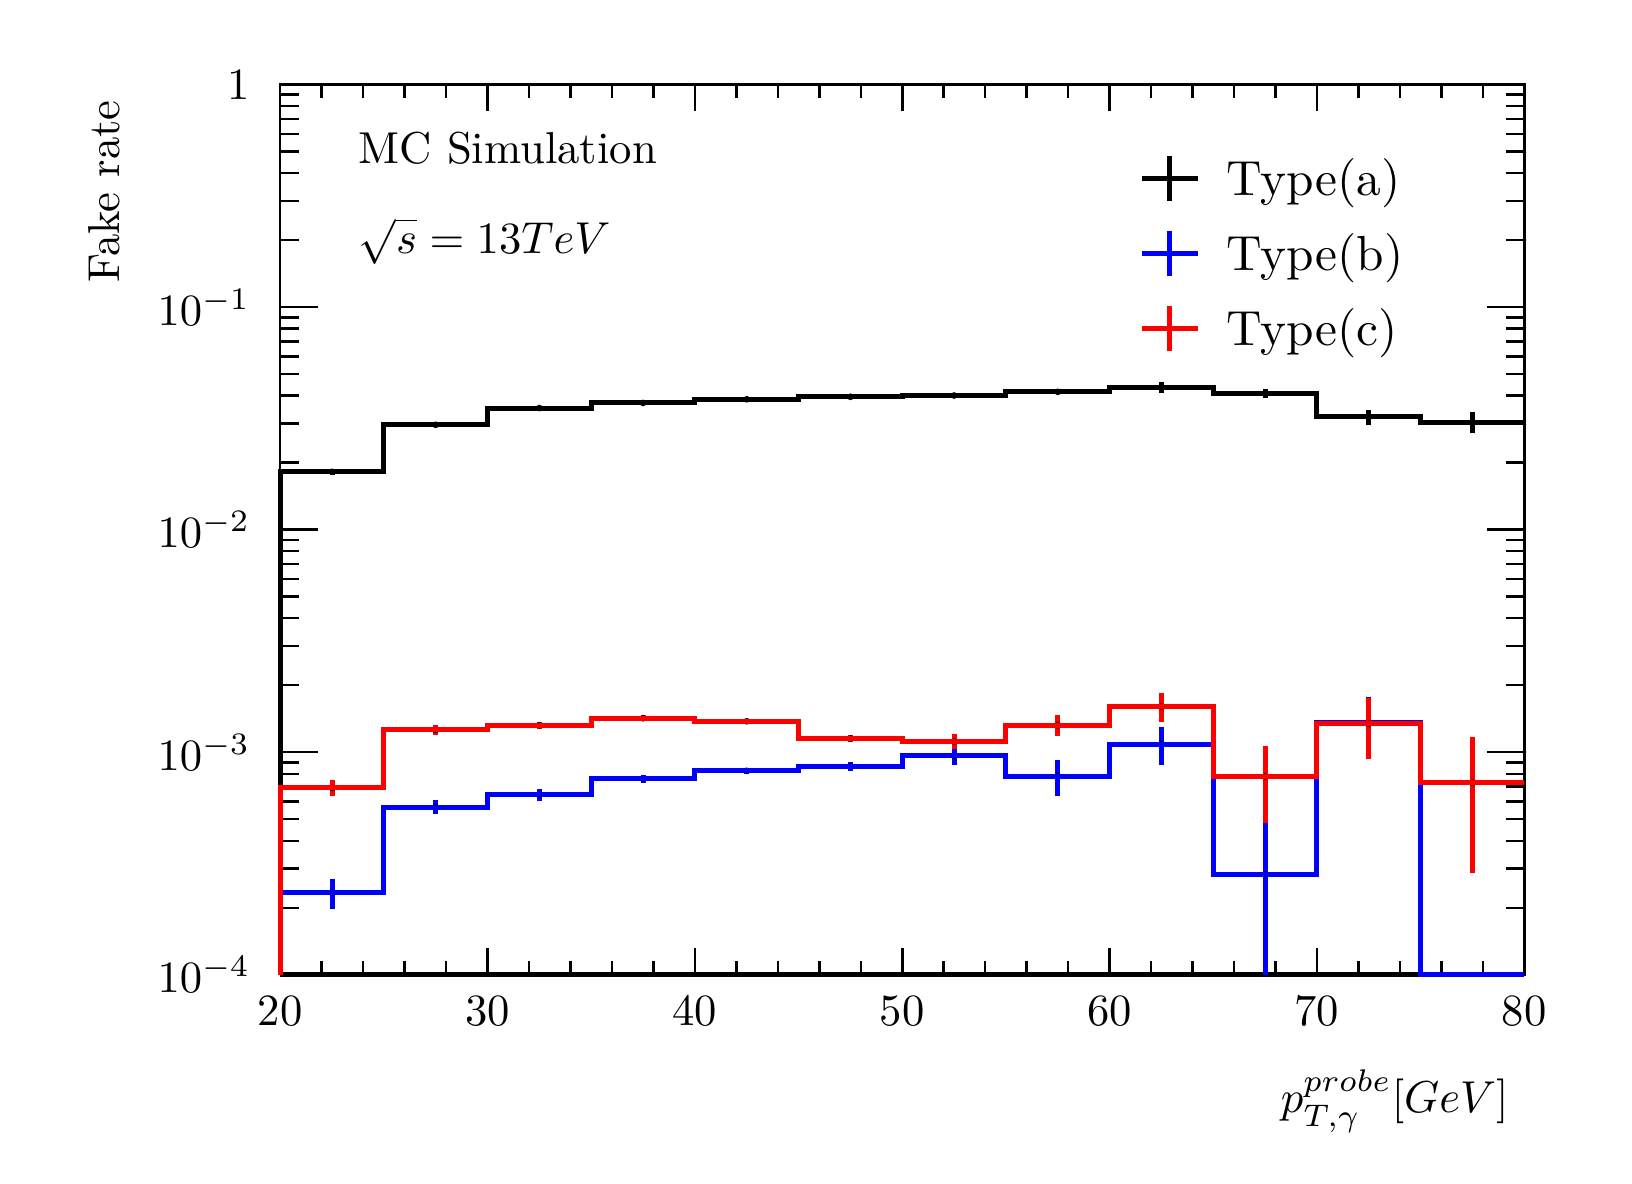
\begin{tikzpicture}
\pgfdeclareplotmark{cross} {
\pgfpathmoveto{\pgfpoint{-0.3\pgfplotmarksize}{\pgfplotmarksize}}
\pgfpathlineto{\pgfpoint{+0.3\pgfplotmarksize}{\pgfplotmarksize}}
\pgfpathlineto{\pgfpoint{+0.3\pgfplotmarksize}{0.3\pgfplotmarksize}}
\pgfpathlineto{\pgfpoint{+1\pgfplotmarksize}{0.3\pgfplotmarksize}}
\pgfpathlineto{\pgfpoint{+1\pgfplotmarksize}{-0.3\pgfplotmarksize}}
\pgfpathlineto{\pgfpoint{+0.3\pgfplotmarksize}{-0.3\pgfplotmarksize}}
\pgfpathlineto{\pgfpoint{+0.3\pgfplotmarksize}{-1.\pgfplotmarksize}}
\pgfpathlineto{\pgfpoint{-0.3\pgfplotmarksize}{-1.\pgfplotmarksize}}
\pgfpathlineto{\pgfpoint{-0.3\pgfplotmarksize}{-0.3\pgfplotmarksize}}
\pgfpathlineto{\pgfpoint{-1.\pgfplotmarksize}{-0.3\pgfplotmarksize}}
\pgfpathlineto{\pgfpoint{-1.\pgfplotmarksize}{0.3\pgfplotmarksize}}
\pgfpathlineto{\pgfpoint{-0.3\pgfplotmarksize}{0.3\pgfplotmarksize}}
\pgfpathclose
\pgfusepathqstroke
}
\pgfdeclareplotmark{cross*} {
\pgfpathmoveto{\pgfpoint{-0.3\pgfplotmarksize}{\pgfplotmarksize}}
\pgfpathlineto{\pgfpoint{+0.3\pgfplotmarksize}{\pgfplotmarksize}}
\pgfpathlineto{\pgfpoint{+0.3\pgfplotmarksize}{0.3\pgfplotmarksize}}
\pgfpathlineto{\pgfpoint{+1\pgfplotmarksize}{0.3\pgfplotmarksize}}
\pgfpathlineto{\pgfpoint{+1\pgfplotmarksize}{-0.3\pgfplotmarksize}}
\pgfpathlineto{\pgfpoint{+0.3\pgfplotmarksize}{-0.3\pgfplotmarksize}}
\pgfpathlineto{\pgfpoint{+0.3\pgfplotmarksize}{-1.\pgfplotmarksize}}
\pgfpathlineto{\pgfpoint{-0.3\pgfplotmarksize}{-1.\pgfplotmarksize}}
\pgfpathlineto{\pgfpoint{-0.3\pgfplotmarksize}{-0.3\pgfplotmarksize}}
\pgfpathlineto{\pgfpoint{-1.\pgfplotmarksize}{-0.3\pgfplotmarksize}}
\pgfpathlineto{\pgfpoint{-1.\pgfplotmarksize}{0.3\pgfplotmarksize}}
\pgfpathlineto{\pgfpoint{-0.3\pgfplotmarksize}{0.3\pgfplotmarksize}}
\pgfpathclose
\pgfusepathqfillstroke
}
\pgfdeclareplotmark{newstar} {
\pgfpathmoveto{\pgfqpoint{0pt}{\pgfplotmarksize}}
\pgfpathlineto{\pgfqpointpolar{44}{0.5\pgfplotmarksize}}
\pgfpathlineto{\pgfqpointpolar{18}{\pgfplotmarksize}}
\pgfpathlineto{\pgfqpointpolar{-20}{0.5\pgfplotmarksize}}
\pgfpathlineto{\pgfqpointpolar{-54}{\pgfplotmarksize}}
\pgfpathlineto{\pgfqpointpolar{-90}{0.5\pgfplotmarksize}}
\pgfpathlineto{\pgfqpointpolar{234}{\pgfplotmarksize}}
\pgfpathlineto{\pgfqpointpolar{198}{0.5\pgfplotmarksize}}
\pgfpathlineto{\pgfqpointpolar{162}{\pgfplotmarksize}}
\pgfpathlineto{\pgfqpointpolar{134}{0.5\pgfplotmarksize}}
\pgfpathclose
\pgfusepathqstroke
}
\pgfdeclareplotmark{newstar*} {
\pgfpathmoveto{\pgfqpoint{0pt}{\pgfplotmarksize}}
\pgfpathlineto{\pgfqpointpolar{44}{0.5\pgfplotmarksize}}
\pgfpathlineto{\pgfqpointpolar{18}{\pgfplotmarksize}}
\pgfpathlineto{\pgfqpointpolar{-20}{0.5\pgfplotmarksize}}
\pgfpathlineto{\pgfqpointpolar{-54}{\pgfplotmarksize}}
\pgfpathlineto{\pgfqpointpolar{-90}{0.5\pgfplotmarksize}}
\pgfpathlineto{\pgfqpointpolar{234}{\pgfplotmarksize}}
\pgfpathlineto{\pgfqpointpolar{198}{0.5\pgfplotmarksize}}
\pgfpathlineto{\pgfqpointpolar{162}{\pgfplotmarksize}}
\pgfpathlineto{\pgfqpointpolar{134}{0.5\pgfplotmarksize}}
\pgfpathclose
\pgfusepathqfillstroke
}
\definecolor{c}{rgb}{1,1,1};
\draw [color=c, fill=c] (0,0) rectangle (20,14.3108);
\draw [color=c, fill=c] (3.2,2.28972) rectangle (19,13.5952);
\definecolor{c}{rgb}{0,0,0};
\draw [c,line width=0.9] (3.2,2.28972) -- (3.2,13.5952) -- (19,13.5952) -- (19,2.28972) -- (3.2,2.28972);
\draw [c,line width=1.8] (3.2,2.28972) -- (3.2158,2.28972) -- (3.2158,2.28972) -- (3.2316,2.28972) -- (3.2316,2.28972) -- (3.2474,2.28972) -- (3.2474,2.28972) -- (3.2632,2.28972) -- (3.2632,2.28972) -- (3.279,2.28972) -- (3.279,2.28972) --
 (3.2948,2.28972) -- (3.2948,2.28972) -- (3.3106,2.28972) -- (3.3106,2.28972) -- (3.3264,2.28972) -- (3.3264,2.28972) -- (3.3422,2.28972) -- (3.3422,2.28972) -- (3.358,2.28972) -- (3.358,2.28972) -- (3.3738,2.28972) -- (3.3738,2.28972) --
 (3.3896,2.28972) -- (3.3896,2.28972) -- (3.4054,2.28972) -- (3.4054,2.28972) -- (3.4212,2.28972) -- (3.4212,2.28972) -- (3.437,2.28972) -- (3.437,2.28972) -- (3.4528,2.28972) -- (3.4528,2.28972) -- (3.4686,2.28972) -- (3.4686,2.28972) --
 (3.4844,2.28972) -- (3.4844,2.28972) -- (3.5002,2.28972) -- (3.5002,2.28972) -- (3.516,2.28972) -- (3.516,2.28972) -- (3.5318,2.28972) -- (3.5318,2.28972) -- (3.5476,2.28972) -- (3.5476,2.28972) -- (3.5634,2.28972) -- (3.5634,2.28972) --
 (3.5792,2.28972) -- (3.5792,2.28972) -- (3.595,2.28972) -- (3.595,2.28972) -- (3.6108,2.28972) -- (3.6108,2.28972) -- (3.6266,2.28972) -- (3.6266,2.28972) -- (3.6424,2.28972) -- (3.6424,2.28972) -- (3.6582,2.28972) -- (3.6582,2.28972) --
 (3.674,2.28972) -- (3.674,2.28972) -- (3.6898,2.28972) -- (3.6898,2.28972) -- (3.7056,2.28972) -- (3.7056,2.28972) -- (3.7214,2.28972) -- (3.7214,2.28972) -- (3.7372,2.28972) -- (3.7372,2.28972) -- (3.753,2.28972) -- (3.753,2.28972) --
 (3.7688,2.28972) -- (3.7688,2.28972) -- (3.7846,2.28972) -- (3.7846,2.28972) -- (3.8004,2.28972) -- (3.8004,2.28972) -- (3.8162,2.28972) -- (3.8162,2.28972) -- (3.832,2.28972) -- (3.832,2.28972) -- (3.8478,2.28972) -- (3.8478,2.28972) --
 (3.8636,2.28972) -- (3.8636,2.28972) -- (3.8794,2.28972) -- (3.8794,2.28972) -- (3.8952,2.28972) -- (3.8952,2.28972) -- (3.911,2.28972) -- (3.911,2.28972) -- (3.9268,2.28972) -- (3.9268,2.28972) -- (3.9426,2.28972) -- (3.9426,2.28972) --
 (3.9584,2.28972) -- (3.9584,2.28972) -- (3.9742,2.28972) -- (3.9742,2.28972) -- (3.99,2.28972) -- (3.99,2.28972) -- (4.0058,2.28972) -- (4.0058,2.28972) -- (4.0216,2.28972) -- (4.0216,2.28972) -- (4.0374,2.28972) -- (4.0374,2.28972) --
 (4.0532,2.28972) -- (4.0532,2.28972) -- (4.069,2.28972) -- (4.069,2.28972) -- (4.0848,2.28972) -- (4.0848,2.28972) -- (4.1006,2.28972) -- (4.1006,2.28972) -- (4.1164,2.28972) -- (4.1164,2.28972) -- (4.1322,2.28972) -- (4.1322,2.28972) --
 (4.148,2.28972) -- (4.148,2.28972) -- (4.1638,2.28972) -- (4.1638,2.28972) -- (4.1796,2.28972) -- (4.1796,2.28972) -- (4.1954,2.28972) -- (4.1954,2.28972) -- (4.2112,2.28972) -- (4.2112,2.28972) -- (4.227,2.28972) -- (4.227,2.28972) --
 (4.2428,2.28972) -- (4.2428,2.28972) -- (4.2586,2.28972) -- (4.2586,2.28972) -- (4.2744,2.28972) -- (4.2744,2.28972) -- (4.2902,2.28972) -- (4.2902,2.28972) -- (4.306,2.28972) -- (4.306,2.28972) -- (4.3218,2.28972) -- (4.3218,2.28972) --
 (4.3376,2.28972) -- (4.3376,2.28972) -- (4.3534,2.28972) -- (4.3534,2.28972) -- (4.3692,2.28972) -- (4.3692,2.28972) -- (4.385,2.28972) -- (4.385,2.28972) -- (4.4008,2.28972) -- (4.4008,2.28972) -- (4.4166,2.28972) -- (4.4166,2.28972) --
 (4.4324,2.28972) -- (4.4324,2.28972) -- (4.4482,2.28972) -- (4.4482,2.28972) -- (4.464,2.28972) -- (4.464,2.28972) -- (4.4798,2.28972) -- (4.4798,2.28972) -- (4.4956,2.28972) -- (4.4956,2.28972) -- (4.5114,2.28972) -- (4.5114,2.28972) --
 (4.5272,2.28972) -- (4.5272,2.28972) -- (4.543,2.28972) -- (4.543,2.28972) -- (4.5588,2.28972) -- (4.5588,2.28972) -- (4.5746,2.28972) -- (4.5746,2.28972) -- (4.5904,2.28972) -- (4.5904,2.28972) -- (4.6062,2.28972) -- (4.6062,2.28972) --
 (4.622,2.28972) -- (4.622,2.28972) -- (4.6378,2.28972) -- (4.6378,2.28972) -- (4.6536,2.28972) -- (4.6536,2.28972) -- (4.6694,2.28972) -- (4.6694,2.28972) -- (4.6852,2.28972) -- (4.6852,2.28972) -- (4.701,2.28972) -- (4.701,2.28972) --
 (4.7168,2.28972) -- (4.7168,2.28972) -- (4.7326,2.28972) -- (4.7326,2.28972) -- (4.7484,2.28972) -- (4.7484,2.28972) -- (4.7642,2.28972) -- (4.7642,2.28972) -- (4.78,2.28972) -- (4.78,2.28972) -- (4.7958,2.28972) -- (4.7958,2.28972) --
 (4.8116,2.28972) -- (4.8116,2.28972) -- (4.8274,2.28972) -- (4.8274,2.28972) -- (4.8432,2.28972) -- (4.8432,2.28972) -- (4.859,2.28972) -- (4.859,2.28972) -- (4.8748,2.28972) -- (4.8748,2.28972) -- (4.8906,2.28972) -- (4.8906,2.28972) --
 (4.9064,2.28972) -- (4.9064,2.28972) -- (4.9222,2.28972) -- (4.9222,2.28972) -- (4.938,2.28972) -- (4.938,2.28972) -- (4.9538,2.28972) -- (4.9538,2.28972) -- (4.9696,2.28972) -- (4.9696,2.28972) -- (4.9854,2.28972) -- (4.9854,2.28972) --
 (5.0012,2.28972) -- (5.0012,2.28972) -- (5.017,2.28972) -- (5.017,2.28972) -- (5.0328,2.28972) -- (5.0328,2.28972) -- (5.0486,2.28972) -- (5.0486,2.28972) -- (5.0644,2.28972) -- (5.0644,2.28972) -- (5.0802,2.28972) -- (5.0802,2.28972) --
 (5.096,2.28972) -- (5.096,2.28972) -- (5.1118,2.28972) -- (5.1118,2.28972) -- (5.1276,2.28972) -- (5.1276,2.28972) -- (5.1434,2.28972) -- (5.1434,2.28972) -- (5.1592,2.28972) -- (5.1592,2.28972) -- (5.175,2.28972) -- (5.175,2.28972) --
 (5.1908,2.28972) -- (5.1908,2.28972) -- (5.2066,2.28972) -- (5.2066,2.28972) -- (5.2224,2.28972) -- (5.2224,2.28972) -- (5.2382,2.28972) -- (5.2382,2.28972) -- (5.254,2.28972) -- (5.254,2.28972) -- (5.2698,2.28972) -- (5.2698,2.28972) --
 (5.2856,2.28972) -- (5.2856,2.28972) -- (5.3014,2.28972) -- (5.3014,2.28972) -- (5.3172,2.28972) -- (5.3172,2.28972) -- (5.333,2.28972) -- (5.333,2.28972) -- (5.3488,2.28972) -- (5.3488,2.28972) -- (5.3646,2.28972) -- (5.3646,2.28972) --
 (5.3804,2.28972) -- (5.3804,2.28972) -- (5.3962,2.28972) -- (5.3962,2.28972) -- (5.412,2.28972) -- (5.412,2.28972) -- (5.4278,2.28972) -- (5.4278,2.28972) -- (5.4436,2.28972) -- (5.4436,2.28972) -- (5.4594,2.28972) -- (5.4594,2.28972) --
 (5.4752,2.28972) -- (5.4752,2.28972) -- (5.491,2.28972) -- (5.491,2.28972) -- (5.5068,2.28972) -- (5.5068,2.28972) -- (5.5226,2.28972) -- (5.5226,2.28972) -- (5.5384,2.28972) -- (5.5384,2.28972) -- (5.5542,2.28972) -- (5.5542,2.28972) --
 (5.57,2.28972) -- (5.57,2.28972) -- (5.5858,2.28972) -- (5.5858,2.28972) -- (5.6016,2.28972) -- (5.6016,2.28972) -- (5.6174,2.28972) -- (5.6174,2.28972) -- (5.6332,2.28972) -- (5.6332,2.28972) -- (5.649,2.28972) -- (5.649,2.28972) --
 (5.6648,2.28972) -- (5.6648,2.28972) -- (5.6806,2.28972) -- (5.6806,2.28972) -- (5.6964,2.28972) -- (5.6964,2.28972) -- (5.7122,2.28972) -- (5.7122,2.28972) -- (5.728,2.28972) -- (5.728,2.28972) -- (5.7438,2.28972) -- (5.7438,2.28972) --
 (5.7596,2.28972) -- (5.7596,2.28972) -- (5.7754,2.28972) -- (5.7754,2.28972) -- (5.7912,2.28972) -- (5.7912,2.28972) -- (5.807,2.28972) -- (5.807,2.28972) -- (5.8228,2.28972) -- (5.8228,2.28972) -- (5.8386,2.28972) -- (5.8386,2.28972) --
 (5.8544,2.28972) -- (5.8544,2.28972) -- (5.8702,2.28972) -- (5.8702,2.28972) -- (5.886,2.28972) -- (5.886,2.28972) -- (5.9018,2.28972) -- (5.9018,2.28972) -- (5.9176,2.28972) -- (5.9176,2.28972) -- (5.9334,2.28972) -- (5.9334,2.28972) --
 (5.9492,2.28972) -- (5.9492,2.28972) -- (5.965,2.28972) -- (5.965,2.28972) -- (5.9808,2.28972) -- (5.9808,2.28972) -- (5.9966,2.28972) -- (5.9966,2.28972) -- (6.0124,2.28972) -- (6.0124,2.28972) -- (6.0282,2.28972) -- (6.0282,2.28972) --
 (6.044,2.28972) -- (6.044,2.28972) -- (6.0598,2.28972) -- (6.0598,2.28972) -- (6.0756,2.28972) -- (6.0756,2.28972) -- (6.0914,2.28972) -- (6.0914,2.28972) -- (6.1072,2.28972) -- (6.1072,2.28972) -- (6.123,2.28972) -- (6.123,2.28972) --
 (6.1388,2.28972) -- (6.1388,2.28972) -- (6.1546,2.28972) -- (6.1546,2.28972) -- (6.1704,2.28972) -- (6.1704,2.28972) -- (6.1862,2.28972) -- (6.1862,2.28972) -- (6.202,2.28972) -- (6.202,2.28972) -- (6.2178,2.28972) -- (6.2178,2.28972) --
 (6.2336,2.28972) -- (6.2336,2.28972) -- (6.2494,2.28972) -- (6.2494,2.28972) -- (6.2652,2.28972) -- (6.2652,2.28972) -- (6.281,2.28972) -- (6.281,2.28972) -- (6.2968,2.28972) -- (6.2968,2.28972) -- (6.3126,2.28972) -- (6.3126,2.28972) --
 (6.3284,2.28972) -- (6.3284,2.28972) -- (6.3442,2.28972) -- (6.3442,2.28972) -- (6.36,2.28972) -- (6.36,2.28972) -- (6.3758,2.28972) -- (6.3758,2.28972) -- (6.3916,2.28972) -- (6.3916,2.28972) -- (6.4074,2.28972) -- (6.4074,2.28972) --
 (6.4232,2.28972) -- (6.4232,2.28972) -- (6.439,2.28972) -- (6.439,2.28972) -- (6.4548,2.28972) -- (6.4548,2.28972) -- (6.4706,2.28972) -- (6.4706,2.28972) -- (6.4864,2.28972) -- (6.4864,2.28972) -- (6.5022,2.28972) -- (6.5022,2.28972) --
 (6.518,2.28972) -- (6.518,2.28972) -- (6.5338,2.28972) -- (6.5338,2.28972) -- (6.5496,2.28972) -- (6.5496,2.28972) -- (6.5654,2.28972) -- (6.5654,2.28972) -- (6.5812,2.28972) -- (6.5812,2.28972) -- (6.597,2.28972) -- (6.597,2.28972) --
 (6.6128,2.28972) -- (6.6128,2.28972) -- (6.6286,2.28972) -- (6.6286,2.28972) -- (6.6444,2.28972) -- (6.6444,2.28972) -- (6.6602,2.28972) -- (6.6602,2.28972) -- (6.676,2.28972) -- (6.676,2.28972) -- (6.6918,2.28972) -- (6.6918,2.28972) --
 (6.7076,2.28972) -- (6.7076,2.28972) -- (6.7234,2.28972) -- (6.7234,2.28972) -- (6.7392,2.28972) -- (6.7392,2.28972) -- (6.755,2.28972) -- (6.755,2.28972) -- (6.7708,2.28972) -- (6.7708,2.28972) -- (6.7866,2.28972) -- (6.7866,2.28972) --
 (6.8024,2.28972) -- (6.8024,2.28972) -- (6.8182,2.28972) -- (6.8182,2.28972) -- (6.834,2.28972) -- (6.834,2.28972) -- (6.8498,2.28972) -- (6.8498,2.28972) -- (6.8656,2.28972) -- (6.8656,2.28972) -- (6.8814,2.28972) -- (6.8814,2.28972) --
 (6.8972,2.28972) -- (6.8972,2.28972) -- (6.913,2.28972) -- (6.913,2.28972) -- (6.9288,2.28972) -- (6.9288,2.28972) -- (6.9446,2.28972) -- (6.9446,2.28972) -- (6.9604,2.28972) -- (6.9604,2.28972) -- (6.9762,2.28972) -- (6.9762,2.28972) --
 (6.992,2.28972) -- (6.992,2.28972) -- (7.0078,2.28972) -- (7.0078,2.28972) -- (7.0236,2.28972) -- (7.0236,2.28972) -- (7.0394,2.28972) -- (7.0394,2.28972) -- (7.0552,2.28972) -- (7.0552,2.28972) -- (7.071,2.28972) -- (7.071,2.28972) --
 (7.0868,2.28972) -- (7.0868,2.28972) -- (7.1026,2.28972) -- (7.1026,2.28972) -- (7.1184,2.28972) -- (7.1184,2.28972) -- (7.1342,2.28972) -- (7.1342,2.28972) -- (7.15,2.28972) -- (7.15,2.28972) -- (7.1658,2.28972) -- (7.1658,2.28972) --
 (7.1816,2.28972) -- (7.1816,2.28972) -- (7.1974,2.28972) -- (7.1974,2.28972) -- (7.2132,2.28972) -- (7.2132,2.28972) -- (7.229,2.28972) -- (7.229,2.28972) -- (7.2448,2.28972) -- (7.2448,2.28972) -- (7.2606,2.28972) -- (7.2606,2.28972) --
 (7.2764,2.28972) -- (7.2764,2.28972) -- (7.2922,2.28972) -- (7.2922,2.28972) -- (7.308,2.28972) -- (7.308,2.28972) -- (7.3238,2.28972) -- (7.3238,2.28972) -- (7.3396,2.28972) -- (7.3396,2.28972) -- (7.3554,2.28972) -- (7.3554,2.28972) --
 (7.3712,2.28972) -- (7.3712,2.28972) -- (7.387,2.28972) -- (7.387,2.28972) -- (7.4028,2.28972) -- (7.4028,2.28972) -- (7.4186,2.28972) -- (7.4186,2.28972) -- (7.4344,2.28972) -- (7.4344,2.28972) -- (7.4502,2.28972) -- (7.4502,2.28972) --
 (7.466,2.28972) -- (7.466,2.28972) -- (7.4818,2.28972) -- (7.4818,2.28972) -- (7.4976,2.28972) -- (7.4976,2.28972) -- (7.5134,2.28972) -- (7.5134,2.28972) -- (7.5292,2.28972) -- (7.5292,2.28972) -- (7.545,2.28972) -- (7.545,2.28972) --
 (7.5608,2.28972) -- (7.5608,2.28972) -- (7.5766,2.28972) -- (7.5766,2.28972) -- (7.5924,2.28972) -- (7.5924,2.28972) -- (7.6082,2.28972) -- (7.6082,2.28972) -- (7.624,2.28972) -- (7.624,2.28972) -- (7.6398,2.28972) -- (7.6398,2.28972) --
 (7.6556,2.28972) -- (7.6556,2.28972) -- (7.6714,2.28972) -- (7.6714,2.28972) -- (7.6872,2.28972) -- (7.6872,2.28972) -- (7.703,2.28972) -- (7.703,2.28972) -- (7.7188,2.28972) -- (7.7188,2.28972) -- (7.7346,2.28972) -- (7.7346,2.28972) --
 (7.7504,2.28972) -- (7.7504,2.28972) -- (7.7662,2.28972) -- (7.7662,2.28972) -- (7.782,2.28972) -- (7.782,2.28972) -- (7.7978,2.28972) -- (7.7978,2.28972) -- (7.8136,2.28972) -- (7.8136,2.28972) -- (7.8294,2.28972) -- (7.8294,2.28972) --
 (7.8452,2.28972) -- (7.8452,2.28972) -- (7.861,2.28972) -- (7.861,2.28972) -- (7.8768,2.28972) -- (7.8768,2.28972) -- (7.8926,2.28972) -- (7.8926,2.28972) -- (7.9084,2.28972) -- (7.9084,2.28972) -- (7.9242,2.28972) -- (7.9242,2.28972) --
 (7.94,2.28972) -- (7.94,2.28972) -- (7.9558,2.28972) -- (7.9558,2.28972) -- (7.9716,2.28972) -- (7.9716,2.28972) -- (7.9874,2.28972) -- (7.9874,2.28972) -- (8.0032,2.28972) -- (8.0032,2.28972) -- (8.019,2.28972) -- (8.019,2.28972) --
 (8.0348,2.28972) -- (8.0348,2.28972) -- (8.0506,2.28972) -- (8.0506,2.28972) -- (8.0664,2.28972) -- (8.0664,2.28972) -- (8.0822,2.28972) -- (8.0822,2.28972) -- (8.098,2.28972) -- (8.098,2.28972) -- (8.1138,2.28972) -- (8.1138,2.28972) --
 (8.1296,2.28972) -- (8.1296,2.28972) -- (8.1454,2.28972) -- (8.1454,2.28972) -- (8.1612,2.28972) -- (8.1612,2.28972) -- (8.177,2.28972) -- (8.177,2.28972) -- (8.1928,2.28972) -- (8.1928,2.28972) -- (8.2086,2.28972) -- (8.2086,2.28972) --
 (8.2244,2.28972) -- (8.2244,2.28972) -- (8.2402,2.28972) -- (8.2402,2.28972) -- (8.256,2.28972) -- (8.256,2.28972) -- (8.2718,2.28972) -- (8.2718,2.28972) -- (8.2876,2.28972) -- (8.2876,2.28972) -- (8.3034,2.28972) -- (8.3034,2.28972) --
 (8.3192,2.28972) -- (8.3192,2.28972) -- (8.335,2.28972) -- (8.335,2.28972) -- (8.3508,2.28972) -- (8.3508,2.28972) -- (8.3666,2.28972) -- (8.3666,2.28972) -- (8.3824,2.28972) -- (8.3824,2.28972) -- (8.3982,2.28972) -- (8.3982,2.28972) --
 (8.414,2.28972) -- (8.414,2.28972) -- (8.4298,2.28972) -- (8.4298,2.28972) -- (8.4456,2.28972) -- (8.4456,2.28972) -- (8.4614,2.28972) -- (8.4614,2.28972) -- (8.4772,2.28972) -- (8.4772,2.28972) -- (8.493,2.28972) -- (8.493,2.28972) --
 (8.5088,2.28972) -- (8.5088,2.28972) -- (8.5246,2.28972) -- (8.5246,2.28972) -- (8.5404,2.28972) -- (8.5404,2.28972) -- (8.5562,2.28972) -- (8.5562,2.28972) -- (8.572,2.28972) -- (8.572,2.28972) -- (8.5878,2.28972) -- (8.5878,2.28972) --
 (8.6036,2.28972) -- (8.6036,2.28972) -- (8.6194,2.28972) -- (8.6194,2.28972) -- (8.6352,2.28972) -- (8.6352,2.28972) -- (8.651,2.28972) -- (8.651,2.28972) -- (8.6668,2.28972) -- (8.6668,2.28972) -- (8.6826,2.28972) -- (8.6826,2.28972) --
 (8.6984,2.28972) -- (8.6984,2.28972) -- (8.7142,2.28972) -- (8.7142,2.28972) -- (8.73,2.28972) -- (8.73,2.28972) -- (8.7458,2.28972) -- (8.7458,2.28972) -- (8.7616,2.28972) -- (8.7616,2.28972) -- (8.7774,2.28972) -- (8.7774,2.28972) --
 (8.7932,2.28972) -- (8.7932,2.28972) -- (8.809,2.28972) -- (8.809,2.28972) -- (8.8248,2.28972) -- (8.8248,2.28972) -- (8.8406,2.28972) -- (8.8406,2.28972) -- (8.8564,2.28972) -- (8.8564,2.28972) -- (8.8722,2.28972) -- (8.8722,2.28972) --
 (8.888,2.28972) -- (8.888,2.28972) -- (8.9038,2.28972) -- (8.9038,2.28972) -- (8.9196,2.28972) -- (8.9196,2.28972) -- (8.9354,2.28972) -- (8.9354,2.28972) -- (8.9512,2.28972) -- (8.9512,2.28972) -- (8.967,2.28972) -- (8.967,2.28972) --
 (8.9828,2.28972) -- (8.9828,2.28972) -- (8.9986,2.28972) -- (8.9986,2.28972) -- (9.0144,2.28972) -- (9.0144,2.28972) -- (9.0302,2.28972) -- (9.0302,2.28972) -- (9.046,2.28972) -- (9.046,2.28972) -- (9.0618,2.28972) -- (9.0618,2.28972) --
 (9.0776,2.28972) -- (9.0776,2.28972) -- (9.0934,2.28972) -- (9.0934,2.28972) -- (9.1092,2.28972) -- (9.1092,2.28972) -- (9.125,2.28972) -- (9.125,2.28972) -- (9.1408,2.28972) -- (9.1408,2.28972) -- (9.1566,2.28972) -- (9.1566,2.28972) --
 (9.1724,2.28972) -- (9.1724,2.28972) -- (9.1882,2.28972) -- (9.1882,2.28972) -- (9.204,2.28972) -- (9.204,2.28972) -- (9.2198,2.28972) -- (9.2198,2.28972) -- (9.2356,2.28972) -- (9.2356,2.28972) -- (9.2514,2.28972) -- (9.2514,2.28972) --
 (9.2672,2.28972) -- (9.2672,2.28972) -- (9.283,2.28972) -- (9.283,2.28972) -- (9.2988,2.28972) -- (9.2988,2.28972) -- (9.3146,2.28972) -- (9.3146,2.28972) -- (9.3304,2.28972) -- (9.3304,2.28972) -- (9.3462,2.28972) -- (9.3462,2.28972) --
 (9.362,2.28972) -- (9.362,2.28972) -- (9.3778,2.28972) -- (9.3778,2.28972) -- (9.3936,2.28972) -- (9.3936,2.28972) -- (9.4094,2.28972) -- (9.4094,2.28972) -- (9.4252,2.28972) -- (9.4252,2.28972) -- (9.441,2.28972) -- (9.441,2.28972) --
 (9.4568,2.28972) -- (9.4568,2.28972) -- (9.4726,2.28972) -- (9.4726,2.28972) -- (9.4884,2.28972) -- (9.4884,2.28972) -- (9.5042,2.28972) -- (9.5042,2.28972) -- (9.52,2.28972) -- (9.52,2.28972) -- (9.5358,2.28972) -- (9.5358,2.28972) --
 (9.5516,2.28972) -- (9.5516,2.28972) -- (9.5674,2.28972) -- (9.5674,2.28972) -- (9.5832,2.28972) -- (9.5832,2.28972) -- (9.599,2.28972) -- (9.599,2.28972) -- (9.6148,2.28972) -- (9.6148,2.28972) -- (9.6306,2.28972) -- (9.6306,2.28972) --
 (9.6464,2.28972) -- (9.6464,2.28972) -- (9.6622,2.28972) -- (9.6622,2.28972) -- (9.678,2.28972) -- (9.678,2.28972) -- (9.6938,2.28972) -- (9.6938,2.28972) -- (9.7096,2.28972) -- (9.7096,2.28972) -- (9.7254,2.28972) -- (9.7254,2.28972) --
 (9.7412,2.28972) -- (9.7412,2.28972) -- (9.757,2.28972) -- (9.757,2.28972) -- (9.7728,2.28972) -- (9.7728,2.28972) -- (9.7886,2.28972) -- (9.7886,2.28972) -- (9.8044,2.28972) -- (9.8044,2.28972) -- (9.8202,2.28972) -- (9.8202,2.28972) --
 (9.836,2.28972) -- (9.836,2.28972) -- (9.8518,2.28972) -- (9.8518,2.28972) -- (9.8676,2.28972) -- (9.8676,2.28972) -- (9.8834,2.28972) -- (9.8834,2.28972) -- (9.8992,2.28972) -- (9.8992,2.28972) -- (9.915,2.28972) -- (9.915,2.28972) --
 (9.9308,2.28972) -- (9.9308,2.28972) -- (9.9466,2.28972) -- (9.9466,2.28972) -- (9.9624,2.28972) -- (9.9624,2.28972) -- (9.9782,2.28972) -- (9.9782,2.28972) -- (9.994,2.28972) -- (9.994,2.28972) -- (10.0098,2.28972) -- (10.0098,2.28972) --
 (10.0256,2.28972) -- (10.0256,2.28972) -- (10.0414,2.28972) -- (10.0414,2.28972) -- (10.0572,2.28972) -- (10.0572,2.28972) -- (10.073,2.28972) -- (10.073,2.28972) -- (10.0888,2.28972) -- (10.0888,2.28972) -- (10.1046,2.28972) -- (10.1046,2.28972) --
 (10.1204,2.28972) -- (10.1204,2.28972) -- (10.1362,2.28972) -- (10.1362,2.28972) -- (10.152,2.28972) -- (10.152,2.28972) -- (10.1678,2.28972) -- (10.1678,2.28972) -- (10.1836,2.28972) -- (10.1836,2.28972) -- (10.1994,2.28972) -- (10.1994,2.28972) --
 (10.2152,2.28972) -- (10.2152,2.28972) -- (10.231,2.28972) -- (10.231,2.28972) -- (10.2468,2.28972) -- (10.2468,2.28972) -- (10.2626,2.28972) -- (10.2626,2.28972) -- (10.2784,2.28972) -- (10.2784,2.28972) -- (10.2942,2.28972) -- (10.2942,2.28972) --
 (10.31,2.28972) -- (10.31,2.28972) -- (10.3258,2.28972) -- (10.3258,2.28972) -- (10.3416,2.28972) -- (10.3416,2.28972) -- (10.3574,2.28972) -- (10.3574,2.28972) -- (10.3732,2.28972) -- (10.3732,2.28972) -- (10.389,2.28972) -- (10.389,2.28972) --
 (10.4048,2.28972) -- (10.4048,2.28972) -- (10.4206,2.28972) -- (10.4206,2.28972) -- (10.4364,2.28972) -- (10.4364,2.28972) -- (10.4522,2.28972) -- (10.4522,2.28972) -- (10.468,2.28972) -- (10.468,2.28972) -- (10.4838,2.28972) -- (10.4838,2.28972) --
 (10.4996,2.28972) -- (10.4996,2.28972) -- (10.5154,2.28972) -- (10.5154,2.28972) -- (10.5312,2.28972) -- (10.5312,2.28972) -- (10.547,2.28972) -- (10.547,2.28972) -- (10.5628,2.28972) -- (10.5628,2.28972) -- (10.5786,2.28972) -- (10.5786,2.28972) --
 (10.5944,2.28972) -- (10.5944,2.28972) -- (10.6102,2.28972) -- (10.6102,2.28972) -- (10.626,2.28972) -- (10.626,2.28972) -- (10.6418,2.28972) -- (10.6418,2.28972) -- (10.6576,2.28972) -- (10.6576,2.28972) -- (10.6734,2.28972) -- (10.6734,2.28972) --
 (10.6892,2.28972) -- (10.6892,2.28972) -- (10.705,2.28972) -- (10.705,2.28972) -- (10.7208,2.28972) -- (10.7208,2.28972) -- (10.7366,2.28972) -- (10.7366,2.28972) -- (10.7524,2.28972) -- (10.7524,2.28972) -- (10.7682,2.28972) -- (10.7682,2.28972) --
 (10.784,2.28972) -- (10.784,2.28972) -- (10.7998,2.28972) -- (10.7998,2.28972) -- (10.8156,2.28972) -- (10.8156,2.28972) -- (10.8314,2.28972) -- (10.8314,2.28972) -- (10.8472,2.28972) -- (10.8472,2.28972) -- (10.863,2.28972) -- (10.863,2.28972) --
 (10.8788,2.28972) -- (10.8788,2.28972) -- (10.8946,2.28972) -- (10.8946,2.28972) -- (10.9104,2.28972) -- (10.9104,2.28972) -- (10.9262,2.28972) -- (10.9262,2.28972) -- (10.942,2.28972) -- (10.942,2.28972) -- (10.9578,2.28972) -- (10.9578,2.28972) --
 (10.9736,2.28972) -- (10.9736,2.28972) -- (10.9894,2.28972) -- (10.9894,2.28972) -- (11.0052,2.28972) -- (11.0052,2.28972) -- (11.021,2.28972) -- (11.021,2.28972) -- (11.0368,2.28972) -- (11.0368,2.28972) -- (11.0526,2.28972) -- (11.0526,2.28972) --
 (11.0684,2.28972) -- (11.0684,2.28972) -- (11.0842,2.28972) -- (11.0842,2.28972) -- (11.1,2.28972) -- (11.1,2.28972) -- (11.1158,2.28972) -- (11.1158,2.28972) -- (11.1316,2.28972) -- (11.1316,2.28972) -- (11.1474,2.28972) -- (11.1474,2.28972) --
 (11.1632,2.28972) -- (11.1632,2.28972) -- (11.179,2.28972) -- (11.179,2.28972) -- (11.1948,2.28972) -- (11.1948,2.28972) -- (11.2106,2.28972) -- (11.2106,2.28972) -- (11.2264,2.28972) -- (11.2264,2.28972) -- (11.2422,2.28972) -- (11.2422,2.28972) --
 (11.258,2.28972) -- (11.258,2.28972) -- (11.2738,2.28972) -- (11.2738,2.28972) -- (11.2896,2.28972) -- (11.2896,2.28972) -- (11.3054,2.28972) -- (11.3054,2.28972) -- (11.3212,2.28972) -- (11.3212,2.28972) -- (11.337,2.28972) -- (11.337,2.28972) --
 (11.3528,2.28972) -- (11.3528,2.28972) -- (11.3686,2.28972) -- (11.3686,2.28972) -- (11.3844,2.28972) -- (11.3844,2.28972) -- (11.4002,2.28972) -- (11.4002,2.28972) -- (11.416,2.28972) -- (11.416,2.28972) -- (11.4318,2.28972) -- (11.4318,2.28972) --
 (11.4476,2.28972) -- (11.4476,2.28972) -- (11.4634,2.28972) -- (11.4634,2.28972) -- (11.4792,2.28972) -- (11.4792,2.28972) -- (11.495,2.28972) -- (11.495,2.28972) -- (11.5108,2.28972) -- (11.5108,2.28972) -- (11.5266,2.28972) -- (11.5266,2.28972) --
 (11.5424,2.28972) -- (11.5424,2.28972) -- (11.5582,2.28972) -- (11.5582,2.28972) -- (11.574,2.28972) -- (11.574,2.28972) -- (11.5898,2.28972) -- (11.5898,2.28972) -- (11.6056,2.28972) -- (11.6056,2.28972) -- (11.6214,2.28972) -- (11.6214,2.28972) --
 (11.6372,2.28972) -- (11.6372,2.28972) -- (11.653,2.28972) -- (11.653,2.28972) -- (11.6688,2.28972) -- (11.6688,2.28972) -- (11.6846,2.28972) -- (11.6846,2.28972) -- (11.7004,2.28972) -- (11.7004,2.28972) -- (11.7162,2.28972) -- (11.7162,2.28972) --
 (11.732,2.28972) -- (11.732,2.28972) -- (11.7478,2.28972) -- (11.7478,2.28972) -- (11.7636,2.28972) -- (11.7636,2.28972) -- (11.7794,2.28972) -- (11.7794,2.28972) -- (11.7952,2.28972) -- (11.7952,2.28972) -- (11.811,2.28972) -- (11.811,2.28972) --
 (11.8268,2.28972) -- (11.8268,2.28972) -- (11.8426,2.28972) -- (11.8426,2.28972) -- (11.8584,2.28972) -- (11.8584,2.28972) -- (11.8742,2.28972) -- (11.8742,2.28972) -- (11.89,2.28972) -- (11.89,2.28972) -- (11.9058,2.28972) -- (11.9058,2.28972) --
 (11.9216,2.28972) -- (11.9216,2.28972) -- (11.9374,2.28972) -- (11.9374,2.28972) -- (11.9532,2.28972) -- (11.9532,2.28972) -- (11.969,2.28972) -- (11.969,2.28972) -- (11.9848,2.28972) -- (11.9848,2.28972) -- (12.0006,2.28972) -- (12.0006,2.28972) --
 (12.0164,2.28972) -- (12.0164,2.28972) -- (12.0322,2.28972) -- (12.0322,2.28972) -- (12.048,2.28972) -- (12.048,2.28972) -- (12.0638,2.28972) -- (12.0638,2.28972) -- (12.0796,2.28972) -- (12.0796,2.28972) -- (12.0954,2.28972) -- (12.0954,2.28972) --
 (12.1112,2.28972) -- (12.1112,2.28972) -- (12.127,2.28972) -- (12.127,2.28972) -- (12.1428,2.28972) -- (12.1428,2.28972) -- (12.1586,2.28972) -- (12.1586,2.28972) -- (12.1744,2.28972) -- (12.1744,2.28972) -- (12.1902,2.28972) -- (12.1902,2.28972) --
 (12.206,2.28972) -- (12.206,2.28972) -- (12.2218,2.28972) -- (12.2218,2.28972) -- (12.2376,2.28972) -- (12.2376,2.28972) -- (12.2534,2.28972) -- (12.2534,2.28972) -- (12.2692,2.28972) -- (12.2692,2.28972) -- (12.285,2.28972) -- (12.285,2.28972) --
 (12.3008,2.28972) -- (12.3008,2.28972) -- (12.3166,2.28972) -- (12.3166,2.28972) -- (12.3324,2.28972) -- (12.3324,2.28972) -- (12.3482,2.28972) -- (12.3482,2.28972) -- (12.364,2.28972) -- (12.364,2.28972) -- (12.3798,2.28972) -- (12.3798,2.28972) --
 (12.3956,2.28972) -- (12.3956,2.28972) -- (12.4114,2.28972) -- (12.4114,2.28972) -- (12.4272,2.28972) -- (12.4272,2.28972) -- (12.443,2.28972) -- (12.443,2.28972) -- (12.4588,2.28972) -- (12.4588,2.28972) -- (12.4746,2.28972) -- (12.4746,2.28972) --
 (12.4904,2.28972) -- (12.4904,2.28972) -- (12.5062,2.28972) -- (12.5062,2.28972) -- (12.522,2.28972) -- (12.522,2.28972) -- (12.5378,2.28972) -- (12.5378,2.28972) -- (12.5536,2.28972) -- (12.5536,2.28972) -- (12.5694,2.28972) -- (12.5694,2.28972) --
 (12.5852,2.28972) -- (12.5852,2.28972) -- (12.601,2.28972) -- (12.601,2.28972) -- (12.6168,2.28972) -- (12.6168,2.28972) -- (12.6326,2.28972) -- (12.6326,2.28972) -- (12.6484,2.28972) -- (12.6484,2.28972) -- (12.6642,2.28972) -- (12.6642,2.28972) --
 (12.68,2.28972) -- (12.68,2.28972) -- (12.6958,2.28972) -- (12.6958,2.28972) -- (12.7116,2.28972) -- (12.7116,2.28972) -- (12.7274,2.28972) -- (12.7274,2.28972) -- (12.7432,2.28972) -- (12.7432,2.28972) -- (12.759,2.28972) -- (12.759,2.28972) --
 (12.7748,2.28972) -- (12.7748,2.28972) -- (12.7906,2.28972) -- (12.7906,2.28972) -- (12.8064,2.28972) -- (12.8064,2.28972) -- (12.8222,2.28972) -- (12.8222,2.28972) -- (12.838,2.28972) -- (12.838,2.28972) -- (12.8538,2.28972) -- (12.8538,2.28972) --
 (12.8696,2.28972) -- (12.8696,2.28972) -- (12.8854,2.28972) -- (12.8854,2.28972) -- (12.9012,2.28972) -- (12.9012,2.28972) -- (12.917,2.28972) -- (12.917,2.28972) -- (12.9328,2.28972) -- (12.9328,2.28972) -- (12.9486,2.28972) -- (12.9486,2.28972) --
 (12.9644,2.28972) -- (12.9644,2.28972) -- (12.9802,2.28972) -- (12.9802,2.28972) -- (12.996,2.28972) -- (12.996,2.28972) -- (13.0118,2.28972) -- (13.0118,2.28972) -- (13.0276,2.28972) -- (13.0276,2.28972) -- (13.0434,2.28972) -- (13.0434,2.28972) --
 (13.0592,2.28972) -- (13.0592,2.28972) -- (13.075,2.28972) -- (13.075,2.28972) -- (13.0908,2.28972) -- (13.0908,2.28972) -- (13.1066,2.28972) -- (13.1066,2.28972) -- (13.1224,2.28972) -- (13.1224,2.28972) -- (13.1382,2.28972) -- (13.1382,2.28972) --
 (13.154,2.28972) -- (13.154,2.28972) -- (13.1698,2.28972) -- (13.1698,2.28972) -- (13.1856,2.28972) -- (13.1856,2.28972) -- (13.2014,2.28972) -- (13.2014,2.28972) -- (13.2172,2.28972) -- (13.2172,2.28972) -- (13.233,2.28972) -- (13.233,2.28972) --
 (13.2488,2.28972) -- (13.2488,2.28972) -- (13.2646,2.28972) -- (13.2646,2.28972) -- (13.2804,2.28972) -- (13.2804,2.28972) -- (13.2962,2.28972) -- (13.2962,2.28972) -- (13.312,2.28972) -- (13.312,2.28972) -- (13.3278,2.28972) -- (13.3278,2.28972) --
 (13.3436,2.28972) -- (13.3436,2.28972) -- (13.3594,2.28972) -- (13.3594,2.28972) -- (13.3752,2.28972) -- (13.3752,2.28972) -- (13.391,2.28972) -- (13.391,2.28972) -- (13.4068,2.28972) -- (13.4068,2.28972) -- (13.4226,2.28972) -- (13.4226,2.28972) --
 (13.4384,2.28972) -- (13.4384,2.28972) -- (13.4542,2.28972) -- (13.4542,2.28972) -- (13.47,2.28972) -- (13.47,2.28972) -- (13.4858,2.28972) -- (13.4858,2.28972) -- (13.5016,2.28972) -- (13.5016,2.28972) -- (13.5174,2.28972) -- (13.5174,2.28972) --
 (13.5332,2.28972) -- (13.5332,2.28972) -- (13.549,2.28972) -- (13.549,2.28972) -- (13.5648,2.28972) -- (13.5648,2.28972) -- (13.5806,2.28972) -- (13.5806,2.28972) -- (13.5964,2.28972) -- (13.5964,2.28972) -- (13.6122,2.28972) -- (13.6122,2.28972) --
 (13.628,2.28972) -- (13.628,2.28972) -- (13.6438,2.28972) -- (13.6438,2.28972) -- (13.6596,2.28972) -- (13.6596,2.28972) -- (13.6754,2.28972) -- (13.6754,2.28972) -- (13.6912,2.28972) -- (13.6912,2.28972) -- (13.707,2.28972) -- (13.707,2.28972) --
 (13.7228,2.28972) -- (13.7228,2.28972) -- (13.7386,2.28972) -- (13.7386,2.28972) -- (13.7544,2.28972) -- (13.7544,2.28972) -- (13.7702,2.28972) -- (13.7702,2.28972) -- (13.786,2.28972) -- (13.786,2.28972) -- (13.8018,2.28972) -- (13.8018,2.28972) --
 (13.8176,2.28972) -- (13.8176,2.28972) -- (13.8334,2.28972) -- (13.8334,2.28972) -- (13.8492,2.28972) -- (13.8492,2.28972) -- (13.865,2.28972) -- (13.865,2.28972) -- (13.8808,2.28972) -- (13.8808,2.28972) -- (13.8966,2.28972) -- (13.8966,2.28972) --
 (13.9124,2.28972) -- (13.9124,2.28972) -- (13.9282,2.28972) -- (13.9282,2.28972) -- (13.944,2.28972) -- (13.944,2.28972) -- (13.9598,2.28972) -- (13.9598,2.28972) -- (13.9756,2.28972) -- (13.9756,2.28972) -- (13.9914,2.28972) -- (13.9914,2.28972) --
 (14.0072,2.28972) -- (14.0072,2.28972) -- (14.023,2.28972) -- (14.023,2.28972) -- (14.0388,2.28972) -- (14.0388,2.28972) -- (14.0546,2.28972) -- (14.0546,2.28972) -- (14.0704,2.28972) -- (14.0704,2.28972) -- (14.0862,2.28972) -- (14.0862,2.28972) --
 (14.102,2.28972) -- (14.102,2.28972) -- (14.1178,2.28972) -- (14.1178,2.28972) -- (14.1336,2.28972) -- (14.1336,2.28972) -- (14.1494,2.28972) -- (14.1494,2.28972) -- (14.1652,2.28972) -- (14.1652,2.28972) -- (14.181,2.28972) -- (14.181,2.28972) --
 (14.1968,2.28972) -- (14.1968,2.28972) -- (14.2126,2.28972) -- (14.2126,2.28972) -- (14.2284,2.28972) -- (14.2284,2.28972) -- (14.2442,2.28972) -- (14.2442,2.28972) -- (14.26,2.28972) -- (14.26,2.28972) -- (14.2758,2.28972) -- (14.2758,2.28972) --
 (14.2916,2.28972) -- (14.2916,2.28972) -- (14.3074,2.28972) -- (14.3074,2.28972) -- (14.3232,2.28972) -- (14.3232,2.28972) -- (14.339,2.28972) -- (14.339,2.28972) -- (14.3548,2.28972) -- (14.3548,2.28972) -- (14.3706,2.28972) -- (14.3706,2.28972) --
 (14.3864,2.28972) -- (14.3864,2.28972) -- (14.4022,2.28972) -- (14.4022,2.28972) -- (14.418,2.28972) -- (14.418,2.28972) -- (14.4338,2.28972) -- (14.4338,2.28972) -- (14.4496,2.28972) -- (14.4496,2.28972) -- (14.4654,2.28972) -- (14.4654,2.28972) --
 (14.4812,2.28972) -- (14.4812,2.28972) -- (14.497,2.28972) -- (14.497,2.28972) -- (14.5128,2.28972) -- (14.5128,2.28972) -- (14.5286,2.28972) -- (14.5286,2.28972) -- (14.5444,2.28972) -- (14.5444,2.28972) -- (14.5602,2.28972) -- (14.5602,2.28972) --
 (14.576,2.28972) -- (14.576,2.28972) -- (14.5918,2.28972) -- (14.5918,2.28972) -- (14.6076,2.28972) -- (14.6076,2.28972) -- (14.6234,2.28972) -- (14.6234,2.28972) -- (14.6392,2.28972) -- (14.6392,2.28972) -- (14.655,2.28972) -- (14.655,2.28972) --
 (14.6708,2.28972) -- (14.6708,2.28972) -- (14.6866,2.28972) -- (14.6866,2.28972) -- (14.7024,2.28972) -- (14.7024,2.28972) -- (14.7182,2.28972) -- (14.7182,2.28972) -- (14.734,2.28972) -- (14.734,2.28972) -- (14.7498,2.28972) -- (14.7498,2.28972) --
 (14.7656,2.28972) -- (14.7656,2.28972) -- (14.7814,2.28972) -- (14.7814,2.28972) -- (14.7972,2.28972) -- (14.7972,2.28972) -- (14.813,2.28972) -- (14.813,2.28972) -- (14.8288,2.28972) -- (14.8288,2.28972) -- (14.8446,2.28972) -- (14.8446,2.28972) --
 (14.8604,2.28972) -- (14.8604,2.28972) -- (14.8762,2.28972) -- (14.8762,2.28972) -- (14.892,2.28972) -- (14.892,2.28972) -- (14.9078,2.28972) -- (14.9078,2.28972) -- (14.9236,2.28972) -- (14.9236,2.28972) -- (14.9394,2.28972) -- (14.9394,2.28972) --
 (14.9552,2.28972) -- (14.9552,2.28972) -- (14.971,2.28972) -- (14.971,2.28972) -- (14.9868,2.28972) -- (14.9868,2.28972) -- (15.0026,2.28972) -- (15.0026,2.28972) -- (15.0184,2.28972) -- (15.0184,2.28972) -- (15.0342,2.28972) -- (15.0342,2.28972) --
 (15.05,2.28972) -- (15.05,2.28972) -- (15.0658,2.28972) -- (15.0658,2.28972) -- (15.0816,2.28972) -- (15.0816,2.28972) -- (15.0974,2.28972) -- (15.0974,2.28972) -- (15.1132,2.28972) -- (15.1132,2.28972) -- (15.129,2.28972) -- (15.129,2.28972) --
 (15.1448,2.28972) -- (15.1448,2.28972) -- (15.1606,2.28972) -- (15.1606,2.28972) -- (15.1764,2.28972) -- (15.1764,2.28972) -- (15.1922,2.28972) -- (15.1922,2.28972) -- (15.208,2.28972) -- (15.208,2.28972) -- (15.2238,2.28972) -- (15.2238,2.28972) --
 (15.2396,2.28972) -- (15.2396,2.28972) -- (15.2554,2.28972) -- (15.2554,2.28972) -- (15.2712,2.28972) -- (15.2712,2.28972) -- (15.287,2.28972) -- (15.287,2.28972) -- (15.3028,2.28972) -- (15.3028,2.28972) -- (15.3186,2.28972) -- (15.3186,2.28972) --
 (15.3344,2.28972) -- (15.3344,2.28972) -- (15.3502,2.28972) -- (15.3502,2.28972) -- (15.366,2.28972) -- (15.366,2.28972) -- (15.3818,2.28972) -- (15.3818,2.28972) -- (15.3976,2.28972) -- (15.3976,2.28972) -- (15.4134,2.28972) -- (15.4134,2.28972) --
 (15.4292,2.28972) -- (15.4292,2.28972) -- (15.445,2.28972) -- (15.445,2.28972) -- (15.4608,2.28972) -- (15.4608,2.28972) -- (15.4766,2.28972) -- (15.4766,2.28972) -- (15.4924,2.28972) -- (15.4924,2.28972) -- (15.5082,2.28972) -- (15.5082,2.28972) --
 (15.524,2.28972) -- (15.524,2.28972) -- (15.5398,2.28972) -- (15.5398,2.28972) -- (15.5556,2.28972) -- (15.5556,2.28972) -- (15.5714,2.28972) -- (15.5714,2.28972) -- (15.5872,2.28972) -- (15.5872,2.28972) -- (15.603,2.28972) -- (15.603,2.28972) --
 (15.6188,2.28972) -- (15.6188,2.28972) -- (15.6346,2.28972) -- (15.6346,2.28972) -- (15.6504,2.28972) -- (15.6504,2.28972) -- (15.6662,2.28972) -- (15.6662,2.28972) -- (15.682,2.28972) -- (15.682,2.28972) -- (15.6978,2.28972) -- (15.6978,2.28972) --
 (15.7136,2.28972) -- (15.7136,2.28972) -- (15.7294,2.28972) -- (15.7294,2.28972) -- (15.7452,2.28972) -- (15.7452,2.28972) -- (15.761,2.28972) -- (15.761,2.28972) -- (15.7768,2.28972) -- (15.7768,2.28972) -- (15.7926,2.28972) -- (15.7926,2.28972) --
 (15.8084,2.28972) -- (15.8084,2.28972) -- (15.8242,2.28972) -- (15.8242,2.28972) -- (15.84,2.28972) -- (15.84,2.28972) -- (15.8558,2.28972) -- (15.8558,2.28972) -- (15.8716,2.28972) -- (15.8716,2.28972) -- (15.8874,2.28972) -- (15.8874,2.28972) --
 (15.9032,2.28972) -- (15.9032,2.28972) -- (15.919,2.28972) -- (15.919,2.28972) -- (15.9348,2.28972) -- (15.9348,2.28972) -- (15.9506,2.28972) -- (15.9506,2.28972) -- (15.9664,2.28972) -- (15.9664,2.28972) -- (15.9822,2.28972) -- (15.9822,2.28972) --
 (15.998,2.28972) -- (15.998,2.28972) -- (16.0138,2.28972) -- (16.0138,2.28972) -- (16.0296,2.28972) -- (16.0296,2.28972) -- (16.0454,2.28972) -- (16.0454,2.28972) -- (16.0612,2.28972) -- (16.0612,2.28972) -- (16.077,2.28972) -- (16.077,2.28972) --
 (16.0928,2.28972) -- (16.0928,2.28972) -- (16.1086,2.28972) -- (16.1086,2.28972) -- (16.1244,2.28972) -- (16.1244,2.28972) -- (16.1402,2.28972) -- (16.1402,2.28972) -- (16.156,2.28972) -- (16.156,2.28972) -- (16.1718,2.28972) -- (16.1718,2.28972) --
 (16.1876,2.28972) -- (16.1876,2.28972) -- (16.2034,2.28972) -- (16.2034,2.28972) -- (16.2192,2.28972) -- (16.2192,2.28972) -- (16.235,2.28972) -- (16.235,2.28972) -- (16.2508,2.28972) -- (16.2508,2.28972) -- (16.2666,2.28972) -- (16.2666,2.28972) --
 (16.2824,2.28972) -- (16.2824,2.28972) -- (16.2982,2.28972) -- (16.2982,2.28972) -- (16.314,2.28972) -- (16.314,2.28972) -- (16.3298,2.28972) -- (16.3298,2.28972) -- (16.3456,2.28972) -- (16.3456,2.28972) -- (16.3614,2.28972) -- (16.3614,2.28972) --
 (16.3772,2.28972) -- (16.3772,2.28972) -- (16.393,2.28972) -- (16.393,2.28972) -- (16.4088,2.28972) -- (16.4088,2.28972) -- (16.4246,2.28972) -- (16.4246,2.28972) -- (16.4404,2.28972) -- (16.4404,2.28972) -- (16.4562,2.28972) -- (16.4562,2.28972) --
 (16.472,2.28972) -- (16.472,2.28972) -- (16.4878,2.28972) -- (16.4878,2.28972) -- (16.5036,2.28972) -- (16.5036,2.28972) -- (16.5194,2.28972) -- (16.5194,2.28972) -- (16.5352,2.28972) -- (16.5352,2.28972) -- (16.551,2.28972) -- (16.551,2.28972) --
 (16.5668,2.28972) -- (16.5668,2.28972) -- (16.5826,2.28972) -- (16.5826,2.28972) -- (16.5984,2.28972) -- (16.5984,2.28972) -- (16.6142,2.28972) -- (16.6142,2.28972) -- (16.63,2.28972) -- (16.63,2.28972) -- (16.6458,2.28972) -- (16.6458,2.28972) --
 (16.6616,2.28972) -- (16.6616,2.28972) -- (16.6774,2.28972) -- (16.6774,2.28972) -- (16.6932,2.28972) -- (16.6932,2.28972) -- (16.709,2.28972) -- (16.709,2.28972) -- (16.7248,2.28972) -- (16.7248,2.28972) -- (16.7406,2.28972) -- (16.7406,2.28972) --
 (16.7564,2.28972) -- (16.7564,2.28972) -- (16.7722,2.28972) -- (16.7722,2.28972) -- (16.788,2.28972) -- (16.788,2.28972) -- (16.8038,2.28972) -- (16.8038,2.28972) -- (16.8196,2.28972) -- (16.8196,2.28972) -- (16.8354,2.28972) -- (16.8354,2.28972) --
 (16.8512,2.28972) -- (16.8512,2.28972) -- (16.867,2.28972) -- (16.867,2.28972) -- (16.8828,2.28972) -- (16.8828,2.28972) -- (16.8986,2.28972) -- (16.8986,2.28972) -- (16.9144,2.28972) -- (16.9144,2.28972) -- (16.9302,2.28972) -- (16.9302,2.28972) --
 (16.946,2.28972) -- (16.946,2.28972) -- (16.9618,2.28972) -- (16.9618,2.28972) -- (16.9776,2.28972) -- (16.9776,2.28972) -- (16.9934,2.28972) -- (16.9934,2.28972) -- (17.0092,2.28972) -- (17.0092,2.28972) -- (17.025,2.28972) -- (17.025,2.28972) --
 (17.0408,2.28972) -- (17.0408,2.28972) -- (17.0566,2.28972) -- (17.0566,2.28972) -- (17.0724,2.28972) -- (17.0724,2.28972) -- (17.0882,2.28972) -- (17.0882,2.28972) -- (17.104,2.28972) -- (17.104,2.28972) -- (17.1198,2.28972) -- (17.1198,2.28972) --
 (17.1356,2.28972) -- (17.1356,2.28972) -- (17.1514,2.28972) -- (17.1514,2.28972) -- (17.1672,2.28972) -- (17.1672,2.28972) -- (17.183,2.28972) -- (17.183,2.28972) -- (17.1988,2.28972) -- (17.1988,2.28972) -- (17.2146,2.28972) -- (17.2146,2.28972) --
 (17.2304,2.28972) -- (17.2304,2.28972) -- (17.2462,2.28972) -- (17.2462,2.28972) -- (17.262,2.28972) -- (17.262,2.28972) -- (17.2778,2.28972) -- (17.2778,2.28972) -- (17.2936,2.28972) -- (17.2936,2.28972) -- (17.3094,2.28972) -- (17.3094,2.28972) --
 (17.3252,2.28972) -- (17.3252,2.28972) -- (17.341,2.28972) -- (17.341,2.28972) -- (17.3568,2.28972) -- (17.3568,2.28972) -- (17.3726,2.28972) -- (17.3726,2.28972) -- (17.3884,2.28972) -- (17.3884,2.28972) -- (17.4042,2.28972) -- (17.4042,2.28972) --
 (17.42,2.28972) -- (17.42,2.28972) -- (17.4358,2.28972) -- (17.4358,2.28972) -- (17.4516,2.28972) -- (17.4516,2.28972) -- (17.4674,2.28972) -- (17.4674,2.28972) -- (17.4832,2.28972) -- (17.4832,2.28972) -- (17.499,2.28972) -- (17.499,2.28972) --
 (17.5148,2.28972) -- (17.5148,2.28972) -- (17.5306,2.28972) -- (17.5306,2.28972) -- (17.5464,2.28972) -- (17.5464,2.28972) -- (17.5622,2.28972) -- (17.5622,2.28972) -- (17.578,2.28972) -- (17.578,2.28972) -- (17.5938,2.28972) -- (17.5938,2.28972) --
 (17.6096,2.28972) -- (17.6096,2.28972) -- (17.6254,2.28972) -- (17.6254,2.28972) -- (17.6412,2.28972) -- (17.6412,2.28972) -- (17.657,2.28972) -- (17.657,2.28972) -- (17.6728,2.28972) -- (17.6728,2.28972) -- (17.6886,2.28972) -- (17.6886,2.28972) --
 (17.7044,2.28972) -- (17.7044,2.28972) -- (17.7202,2.28972) -- (17.7202,2.28972) -- (17.736,2.28972) -- (17.736,2.28972) -- (17.7518,2.28972) -- (17.7518,2.28972) -- (17.7676,2.28972) -- (17.7676,2.28972) -- (17.7834,2.28972) -- (17.7834,2.28972) --
 (17.7992,2.28972) -- (17.7992,2.28972) -- (17.815,2.28972) -- (17.815,2.28972) -- (17.8308,2.28972) -- (17.8308,2.28972) -- (17.8466,2.28972) -- (17.8466,2.28972) -- (17.8624,2.28972) -- (17.8624,2.28972) -- (17.8782,2.28972) -- (17.8782,2.28972) --
 (17.894,2.28972) -- (17.894,2.28972) -- (17.9098,2.28972) -- (17.9098,2.28972) -- (17.9256,2.28972) -- (17.9256,2.28972) -- (17.9414,2.28972) -- (17.9414,2.28972) -- (17.9572,2.28972) -- (17.9572,2.28972) -- (17.973,2.28972) -- (17.973,2.28972) --
 (17.9888,2.28972) -- (17.9888,2.28972) -- (18.0046,2.28972) -- (18.0046,2.28972) -- (18.0204,2.28972) -- (18.0204,2.28972) -- (18.0362,2.28972) -- (18.0362,2.28972) -- (18.052,2.28972) -- (18.052,2.28972) -- (18.0678,2.28972) -- (18.0678,2.28972) --
 (18.0836,2.28972) -- (18.0836,2.28972) -- (18.0994,2.28972) -- (18.0994,2.28972) -- (18.1152,2.28972) -- (18.1152,2.28972) -- (18.131,2.28972) -- (18.131,2.28972) -- (18.1468,2.28972) -- (18.1468,2.28972) -- (18.1626,2.28972) -- (18.1626,2.28972) --
 (18.1784,2.28972) -- (18.1784,2.28972) -- (18.1942,2.28972) -- (18.1942,2.28972) -- (18.21,2.28972) -- (18.21,2.28972) -- (18.2258,2.28972) -- (18.2258,2.28972) -- (18.2416,2.28972) -- (18.2416,2.28972) -- (18.2574,2.28972) -- (18.2574,2.28972) --
 (18.2732,2.28972) -- (18.2732,2.28972) -- (18.289,2.28972) -- (18.289,2.28972) -- (18.3048,2.28972) -- (18.3048,2.28972) -- (18.3206,2.28972) -- (18.3206,2.28972) -- (18.3364,2.28972) -- (18.3364,2.28972) -- (18.3522,2.28972) -- (18.3522,2.28972) --
 (18.368,2.28972) -- (18.368,2.28972) -- (18.3838,2.28972) -- (18.3838,2.28972) -- (18.3996,2.28972) -- (18.3996,2.28972) -- (18.4154,2.28972) -- (18.4154,2.28972) -- (18.4312,2.28972) -- (18.4312,2.28972) -- (18.447,2.28972) -- (18.447,2.28972) --
 (18.4628,2.28972) -- (18.4628,2.28972) -- (18.4786,2.28972) -- (18.4786,2.28972) -- (18.4944,2.28972) -- (18.4944,2.28972) -- (18.5102,2.28972) -- (18.5102,2.28972) -- (18.526,2.28972) -- (18.526,2.28972) -- (18.5418,2.28972) -- (18.5418,2.28972) --
 (18.5576,2.28972) -- (18.5576,2.28972) -- (18.5734,2.28972) -- (18.5734,2.28972) -- (18.5892,2.28972) -- (18.5892,2.28972) -- (18.605,2.28972) -- (18.605,2.28972) -- (18.6208,2.28972) -- (18.6208,2.28972) -- (18.6366,2.28972) -- (18.6366,2.28972) --
 (18.6524,2.28972) -- (18.6524,2.28972) -- (18.6682,2.28972) -- (18.6682,2.28972) -- (18.684,2.28972) -- (18.684,2.28972) -- (18.6998,2.28972) -- (18.6998,2.28972) -- (18.7156,2.28972) -- (18.7156,2.28972) -- (18.7314,2.28972) -- (18.7314,2.28972) --
 (18.7472,2.28972) -- (18.7472,2.28972) -- (18.763,2.28972) -- (18.763,2.28972) -- (18.7788,2.28972) -- (18.7788,2.28972) -- (18.7946,2.28972) -- (18.7946,2.28972) -- (18.8104,2.28972) -- (18.8104,2.28972) -- (18.8262,2.28972) -- (18.8262,2.28972) --
 (18.842,2.28972) -- (18.842,2.28972) -- (18.8578,2.28972) -- (18.8578,2.28972) -- (18.8736,2.28972) -- (18.8736,2.28972) -- (18.8894,2.28972) -- (18.8894,2.28972) -- (18.9052,2.28972) -- (18.9052,2.28972) -- (18.921,2.28972) -- (18.921,2.28972) --
 (18.9368,2.28972) -- (18.9368,2.28972) -- (18.9526,2.28972) -- (18.9526,2.28972) -- (18.9684,2.28972) -- (18.9684,2.28972) -- (18.9842,2.28972) -- (18.9842,2.28972) -- (19,2.28972);
\draw [c,line width=0.9] (3.2,2.28972) -- (19,2.28972);
\draw [c,line width=0.9] (3.2,2.62889) -- (3.2,2.28972);
\draw [c,line width=0.9] (3.72667,2.45931) -- (3.72667,2.28972);
\draw [c,line width=0.9] (4.25333,2.45931) -- (4.25333,2.28972);
\draw [c,line width=0.9] (4.78,2.45931) -- (4.78,2.28972);
\draw [c,line width=0.9] (5.30667,2.45931) -- (5.30667,2.28972);
\draw [c,line width=0.9] (5.83333,2.62889) -- (5.83333,2.28972);
\draw [c,line width=0.9] (6.36,2.45931) -- (6.36,2.28972);
\draw [c,line width=0.9] (6.88667,2.45931) -- (6.88667,2.28972);
\draw [c,line width=0.9] (7.41333,2.45931) -- (7.41333,2.28972);
\draw [c,line width=0.9] (7.94,2.45931) -- (7.94,2.28972);
\draw [c,line width=0.9] (8.46667,2.62889) -- (8.46667,2.28972);
\draw [c,line width=0.9] (8.99333,2.45931) -- (8.99333,2.28972);
\draw [c,line width=0.9] (9.52,2.45931) -- (9.52,2.28972);
\draw [c,line width=0.9] (10.0467,2.45931) -- (10.0467,2.28972);
\draw [c,line width=0.9] (10.5733,2.45931) -- (10.5733,2.28972);
\draw [c,line width=0.9] (11.1,2.62889) -- (11.1,2.28972);
\draw [c,line width=0.9] (11.6267,2.45931) -- (11.6267,2.28972);
\draw [c,line width=0.9] (12.1533,2.45931) -- (12.1533,2.28972);
\draw [c,line width=0.9] (12.68,2.45931) -- (12.68,2.28972);
\draw [c,line width=0.9] (13.2067,2.45931) -- (13.2067,2.28972);
\draw [c,line width=0.9] (13.7333,2.62889) -- (13.7333,2.28972);
\draw [c,line width=0.9] (14.26,2.45931) -- (14.26,2.28972);
\draw [c,line width=0.9] (14.7867,2.45931) -- (14.7867,2.28972);
\draw [c,line width=0.9] (15.3133,2.45931) -- (15.3133,2.28972);
\draw [c,line width=0.9] (15.84,2.45931) -- (15.84,2.28972);
\draw [c,line width=0.9] (16.3667,2.62889) -- (16.3667,2.28972);
\draw [c,line width=0.9] (16.8933,2.45931) -- (16.8933,2.28972);
\draw [c,line width=0.9] (17.42,2.45931) -- (17.42,2.28972);
\draw [c,line width=0.9] (17.9467,2.45931) -- (17.9467,2.28972);
\draw [c,line width=0.9] (18.4733,2.45931) -- (18.4733,2.28972);
\draw [c,line width=0.9] (19,2.62889) -- (19,2.28972);
\draw [anchor=base] (3.2,1.64574) node[scale=1.61424, color=c, rotate=0]{20};
\draw [anchor=base] (5.83333,1.64574) node[scale=1.61424, color=c, rotate=0]{30};
\draw [anchor=base] (8.46667,1.64574) node[scale=1.61424, color=c, rotate=0]{40};
\draw [anchor=base] (11.1,1.64574) node[scale=1.61424, color=c, rotate=0]{50};
\draw [anchor=base] (13.7333,1.64574) node[scale=1.61424, color=c, rotate=0]{60};
\draw [anchor=base] (16.3667,1.64574) node[scale=1.61424, color=c, rotate=0]{70};
\draw [anchor=base] (19,1.64574) node[scale=1.61424, color=c, rotate=0]{80};
\draw [anchor= east] (19,0.686917) node[scale=1.61424, color=c, rotate=0]{$p_{T,  \gamma}^{probe}  [GeV]$};
\draw [c,line width=0.9] (3.2,13.5952) -- (19,13.5952);
\draw [c,line width=0.9] (3.2,13.2561) -- (3.2,13.5952);
\draw [c,line width=0.9] (3.72667,13.4257) -- (3.72667,13.5952);
\draw [c,line width=0.9] (4.25333,13.4257) -- (4.25333,13.5952);
\draw [c,line width=0.9] (4.78,13.4257) -- (4.78,13.5952);
\draw [c,line width=0.9] (5.30667,13.4257) -- (5.30667,13.5952);
\draw [c,line width=0.9] (5.83333,13.2561) -- (5.83333,13.5952);
\draw [c,line width=0.9] (6.36,13.4257) -- (6.36,13.5952);
\draw [c,line width=0.9] (6.88667,13.4257) -- (6.88667,13.5952);
\draw [c,line width=0.9] (7.41333,13.4257) -- (7.41333,13.5952);
\draw [c,line width=0.9] (7.94,13.4257) -- (7.94,13.5952);
\draw [c,line width=0.9] (8.46667,13.2561) -- (8.46667,13.5952);
\draw [c,line width=0.9] (8.99333,13.4257) -- (8.99333,13.5952);
\draw [c,line width=0.9] (9.52,13.4257) -- (9.52,13.5952);
\draw [c,line width=0.9] (10.0467,13.4257) -- (10.0467,13.5952);
\draw [c,line width=0.9] (10.5733,13.4257) -- (10.5733,13.5952);
\draw [c,line width=0.9] (11.1,13.2561) -- (11.1,13.5952);
\draw [c,line width=0.9] (11.6267,13.4257) -- (11.6267,13.5952);
\draw [c,line width=0.9] (12.1533,13.4257) -- (12.1533,13.5952);
\draw [c,line width=0.9] (12.68,13.4257) -- (12.68,13.5952);
\draw [c,line width=0.9] (13.2067,13.4257) -- (13.2067,13.5952);
\draw [c,line width=0.9] (13.7333,13.2561) -- (13.7333,13.5952);
\draw [c,line width=0.9] (14.26,13.4257) -- (14.26,13.5952);
\draw [c,line width=0.9] (14.7867,13.4257) -- (14.7867,13.5952);
\draw [c,line width=0.9] (15.3133,13.4257) -- (15.3133,13.5952);
\draw [c,line width=0.9] (15.84,13.4257) -- (15.84,13.5952);
\draw [c,line width=0.9] (16.3667,13.2561) -- (16.3667,13.5952);
\draw [c,line width=0.9] (16.8933,13.4257) -- (16.8933,13.5952);
\draw [c,line width=0.9] (17.42,13.4257) -- (17.42,13.5952);
\draw [c,line width=0.9] (17.9467,13.4257) -- (17.9467,13.5952);
\draw [c,line width=0.9] (18.4733,13.4257) -- (18.4733,13.5952);
\draw [c,line width=0.9] (19,13.2561) -- (19,13.5952);
\draw [c,line width=0.9] (3.2,2.28972) -- (3.2,13.5952);
\draw [c,line width=0.9] (3.674,2.28973) -- (3.2,2.28973);
\draw [anchor= east] (3.02,2.28973) node[scale=1.61424, color=c, rotate=0]{$10^{-4}$};
\draw [c,line width=0.9] (3.437,3.14055) -- (3.2,3.14055);
\draw [c,line width=0.9] (3.437,3.63825) -- (3.2,3.63825);
\draw [c,line width=0.9] (3.437,3.99138) -- (3.2,3.99138);
\draw [c,line width=0.9] (3.437,4.26528) -- (3.2,4.26528);
\draw [c,line width=0.9] (3.437,4.48908) -- (3.2,4.48908);
\draw [c,line width=0.9] (3.437,4.67829) -- (3.2,4.67829);
\draw [c,line width=0.9] (3.437,4.8422) -- (3.2,4.8422);
\draw [c,line width=0.9] (3.437,4.98678) -- (3.2,4.98678);
\draw [c,line width=0.9] (3.674,5.1161) -- (3.2,5.1161);
\draw [anchor= east] (3.02,5.1161) node[scale=1.61424, color=c, rotate=0]{$10^{-3}$};
\draw [c,line width=0.9] (3.437,5.96693) -- (3.2,5.96693);
\draw [c,line width=0.9] (3.437,6.46463) -- (3.2,6.46463);
\draw [c,line width=0.9] (3.437,6.81775) -- (3.2,6.81775);
\draw [c,line width=0.9] (3.437,7.09166) -- (3.2,7.09166);
\draw [c,line width=0.9] (3.437,7.31545) -- (3.2,7.31545);
\draw [c,line width=0.9] (3.437,7.50467) -- (3.2,7.50467);
\draw [c,line width=0.9] (3.437,7.66858) -- (3.2,7.66858);
\draw [c,line width=0.9] (3.437,7.81315) -- (3.2,7.81315);
\draw [c,line width=0.9] (3.674,7.94248) -- (3.2,7.94248);
\draw [anchor= east] (3.02,7.94248) node[scale=1.61424, color=c, rotate=0]{$10^{-2}$};
\draw [c,line width=0.9] (3.437,8.79331) -- (3.2,8.79331);
\draw [c,line width=0.9] (3.437,9.29101) -- (3.2,9.29101);
\draw [c,line width=0.9] (3.437,9.64413) -- (3.2,9.64413);
\draw [c,line width=0.9] (3.437,9.91804) -- (3.2,9.91804);
\draw [c,line width=0.9] (3.437,10.1418) -- (3.2,10.1418);
\draw [c,line width=0.9] (3.437,10.331) -- (3.2,10.331);
\draw [c,line width=0.9] (3.437,10.495) -- (3.2,10.495);
\draw [c,line width=0.9] (3.437,10.6395) -- (3.2,10.6395);
\draw [c,line width=0.9] (3.674,10.7689) -- (3.2,10.7689);
\draw [anchor= east] (3.02,10.7689) node[scale=1.61424, color=c, rotate=0]{$10^{-1}$};
\draw [c,line width=0.9] (3.437,11.6197) -- (3.2,11.6197);
\draw [c,line width=0.9] (3.437,12.1174) -- (3.2,12.1174);
\draw [c,line width=0.9] (3.437,12.4705) -- (3.2,12.4705);
\draw [c,line width=0.9] (3.437,12.7444) -- (3.2,12.7444);
\draw [c,line width=0.9] (3.437,12.9682) -- (3.2,12.9682);
\draw [c,line width=0.9] (3.437,13.1574) -- (3.2,13.1574);
\draw [c,line width=0.9] (3.437,13.3213) -- (3.2,13.3213);
\draw [c,line width=0.9] (3.437,13.4659) -- (3.2,13.4659);
\draw [c,line width=0.9] (3.674,13.5952) -- (3.2,13.5952);
\draw [anchor= east] (3.02,13.5952) node[scale=1.61424, color=c, rotate=0]{1};
\draw [anchor= east] (0.96,13.5952) node[scale=1.61424, color=c, rotate=90]{Fake rate};
\draw [c,line width=0.9] (19,2.28972) -- (19,13.5952);
\draw [c,line width=0.9] (18.526,2.28973) -- (19,2.28973);
\draw [c,line width=0.9] (18.763,3.14055) -- (19,3.14055);
\draw [c,line width=0.9] (18.763,3.63825) -- (19,3.63825);
\draw [c,line width=0.9] (18.763,3.99138) -- (19,3.99138);
\draw [c,line width=0.9] (18.763,4.26528) -- (19,4.26528);
\draw [c,line width=0.9] (18.763,4.48908) -- (19,4.48908);
\draw [c,line width=0.9] (18.763,4.67829) -- (19,4.67829);
\draw [c,line width=0.9] (18.763,4.8422) -- (19,4.8422);
\draw [c,line width=0.9] (18.763,4.98678) -- (19,4.98678);
\draw [c,line width=0.9] (18.526,5.1161) -- (19,5.1161);
\draw [c,line width=0.9] (18.763,5.96693) -- (19,5.96693);
\draw [c,line width=0.9] (18.763,6.46463) -- (19,6.46463);
\draw [c,line width=0.9] (18.763,6.81775) -- (19,6.81775);
\draw [c,line width=0.9] (18.763,7.09166) -- (19,7.09166);
\draw [c,line width=0.9] (18.763,7.31545) -- (19,7.31545);
\draw [c,line width=0.9] (18.763,7.50467) -- (19,7.50467);
\draw [c,line width=0.9] (18.763,7.66858) -- (19,7.66858);
\draw [c,line width=0.9] (18.763,7.81315) -- (19,7.81315);
\draw [c,line width=0.9] (18.526,7.94248) -- (19,7.94248);
\draw [c,line width=0.9] (18.763,8.79331) -- (19,8.79331);
\draw [c,line width=0.9] (18.763,9.29101) -- (19,9.29101);
\draw [c,line width=0.9] (18.763,9.64413) -- (19,9.64413);
\draw [c,line width=0.9] (18.763,9.91804) -- (19,9.91804);
\draw [c,line width=0.9] (18.763,10.1418) -- (19,10.1418);
\draw [c,line width=0.9] (18.763,10.331) -- (19,10.331);
\draw [c,line width=0.9] (18.763,10.495) -- (19,10.495);
\draw [c,line width=0.9] (18.763,10.6395) -- (19,10.6395);
\draw [c,line width=0.9] (18.526,10.7689) -- (19,10.7689);
\draw [c,line width=0.9] (18.763,11.6197) -- (19,11.6197);
\draw [c,line width=0.9] (18.763,12.1174) -- (19,12.1174);
\draw [c,line width=0.9] (18.763,12.4705) -- (19,12.4705);
\draw [c,line width=0.9] (18.763,12.7444) -- (19,12.7444);
\draw [c,line width=0.9] (18.763,12.9682) -- (19,12.9682);
\draw [c,line width=0.9] (18.763,13.1574) -- (19,13.1574);
\draw [c,line width=0.9] (18.763,13.3213) -- (19,13.3213);
\draw [c,line width=0.9] (18.763,13.4659) -- (19,13.4659);
\draw [c,line width=0.9] (18.526,13.5952) -- (19,13.5952);
\draw [c,line width=1.8] (3.85833,8.6379) -- (3.85833,8.67727);
\draw [c,line width=1.8] (3.85833,8.67727) -- (3.85833,8.71541);
\foreach \P in {(3.85833,8.67727)}{\draw[mark options={color=c,fill=c},mark size=2.402402pt,mark=*,mark size=1pt] plot coordinates {\P};}
\draw [c,line width=1.8] (5.175,9.26084) -- (5.175,9.27413);
\draw [c,line width=1.8] (5.175,9.27413) -- (5.175,9.28728);
\foreach \P in {(5.175,9.27413)}{\draw[mark options={color=c,fill=c},mark size=2.402402pt,mark=*,mark size=1pt] plot coordinates {\P};}
\draw [c,line width=1.8] (6.49167,9.47723) -- (6.49167,9.48673);
\draw [c,line width=1.8] (6.49167,9.48673) -- (6.49167,9.49616);
\foreach \P in {(6.49167,9.48673)}{\draw[mark options={color=c,fill=c},mark size=2.402402pt,mark=*,mark size=1pt] plot coordinates {\P};}
\draw [c,line width=1.8] (7.80833,9.54405) -- (7.80833,9.55155);
\draw [c,line width=1.8] (7.80833,9.55155) -- (7.80833,9.559);
\foreach \P in {(7.80833,9.55155)}{\draw[mark options={color=c,fill=c},mark size=2.402402pt,mark=*,mark size=1pt] plot coordinates {\P};}
\draw [c,line width=1.8] (9.125,9.59186) -- (9.125,9.59835);
\draw [c,line width=1.8] (9.125,9.59835) -- (9.125,9.6048);
\foreach \P in {(9.125,9.59835)}{\draw[mark options={color=c,fill=c},mark size=2.402402pt,mark=*,mark size=1pt] plot coordinates {\P};}
\draw [c,line width=1.8] (10.4417,9.62152) -- (10.4417,9.62989);
\draw [c,line width=1.8] (10.4417,9.62989) -- (10.4417,9.6382);
\foreach \P in {(10.4417,9.62989)}{\draw[mark options={color=c,fill=c},mark size=2.402402pt,mark=*,mark size=1pt] plot coordinates {\P};}
\draw [c,line width=1.8] (11.7583,9.62932) -- (11.7583,9.64602);
\draw [c,line width=1.8] (11.7583,9.64602) -- (11.7583,9.6625);
\foreach \P in {(11.7583,9.64602)}{\draw[mark options={color=c,fill=c},mark size=2.402402pt,mark=*,mark size=1pt] plot coordinates {\P};}
\draw [c,line width=1.8] (13.075,9.6635) -- (13.075,9.6931);
\draw [c,line width=1.8] (13.075,9.6931) -- (13.075,9.722);
\foreach \P in {(13.075,9.6931)}{\draw[mark options={color=c,fill=c},mark size=2.402402pt,mark=*,mark size=1pt] plot coordinates {\P};}
\draw [c,line width=1.8] (14.3917,9.67885) -- (14.3917,9.75168);
\draw [c,line width=1.8] (14.3917,9.75168) -- (14.3917,9.82044);
\foreach \P in {(14.3917,9.75168)}{\draw[mark options={color=c,fill=c},mark size=2.402402pt,mark=*,mark size=1pt] plot coordinates {\P};}
\draw [c,line width=1.8] (15.7083,9.61286) -- (15.7083,9.66934);
\draw [c,line width=1.8] (15.7083,9.66934) -- (15.7083,9.72334);
\foreach \P in {(15.7083,9.66934)}{\draw[mark options={color=c,fill=c},mark size=2.402402pt,mark=*,mark size=1pt] plot coordinates {\P};}
\draw [c,line width=1.8] (17.025,9.27445) -- (17.025,9.37506);
\draw [c,line width=1.8] (17.025,9.37506) -- (17.025,9.46804);
\foreach \P in {(17.025,9.37506)}{\draw[mark options={color=c,fill=c},mark size=2.402402pt,mark=*,mark size=1pt] plot coordinates {\P};}
\draw [c,line width=1.8] (18.3417,9.16472) -- (18.3417,9.30698);
\draw [c,line width=1.8] (18.3417,9.30698) -- (18.3417,9.43445);
\foreach \P in {(18.3417,9.30698)}{\draw[mark options={color=c,fill=c},mark size=2.402402pt,mark=*,mark size=1pt] plot coordinates {\P};}
\draw [c,line width=1.8] (3.2,2.28972) -- (3.2,2.28972) -- (3.2,8.67727) -- (4.51667,8.67727) -- (4.51667,9.27413) -- (5.83333,9.27413) -- (5.83333,9.48673) -- (7.15,9.48673) -- (7.15,9.55155) -- (8.46667,9.55155) -- (8.46667,9.59835) --
 (9.78333,9.59835) -- (9.78333,9.62989) -- (11.1,9.62989) -- (11.1,9.64602) -- (12.4167,9.64602) -- (12.4167,9.6931) -- (13.7333,9.6931) -- (13.7333,9.75168) -- (15.05,9.75168) -- (15.05,9.66934) -- (16.3667,9.66934) -- (16.3667,9.37506) --
 (17.6833,9.37506) -- (17.6833,9.30698) -- (19,9.30698);
\definecolor{c}{rgb}{0,0,1};
\draw [c,line width=1.8] (3.85833,3.12) -- (3.85833,3.331);
\draw [c,line width=1.8] (3.85833,3.331) -- (3.85833,3.51099);
\definecolor{c}{rgb}{0,0,0};
\foreach \P in {(3.85833,3.331)}{\draw[mark options={color=c,fill=c},mark size=2.402402pt,mark=*,mark size=1pt] plot coordinates {\P};}
\definecolor{c}{rgb}{0,0,1};
\draw [c,line width=1.8] (5.175,4.32714) -- (5.175,4.41983);
\draw [c,line width=1.8] (5.175,4.41983) -- (5.175,4.50601);
\definecolor{c}{rgb}{0,0,0};
\foreach \P in {(5.175,4.41983)}{\draw[mark options={color=c,fill=c},mark size=2.402402pt,mark=*,mark size=1pt] plot coordinates {\P};}
\definecolor{c}{rgb}{0,0,1};
\draw [c,line width=1.8] (6.49167,4.49917) -- (6.49167,4.57318);
\draw [c,line width=1.8] (6.49167,4.57318) -- (6.49167,4.64299);
\definecolor{c}{rgb}{0,0,0};
\foreach \P in {(6.49167,4.57318)}{\draw[mark options={color=c,fill=c},mark size=2.402402pt,mark=*,mark size=1pt] plot coordinates {\P};}
\definecolor{c}{rgb}{0,0,1};
\draw [c,line width=1.8] (7.80833,4.72504) -- (7.80833,4.77815);
\draw [c,line width=1.8] (7.80833,4.77815) -- (7.80833,4.82907);
\definecolor{c}{rgb}{0,0,0};
\foreach \P in {(7.80833,4.77815)}{\draw[mark options={color=c,fill=c},mark size=2.402402pt,mark=*,mark size=1pt] plot coordinates {\P};}
\definecolor{c}{rgb}{0,0,1};
\draw [c,line width=1.8] (9.125,4.83649) -- (9.125,4.87984);
\draw [c,line width=1.8] (9.125,4.87984) -- (9.125,4.92171);
\definecolor{c}{rgb}{0,0,0};
\foreach \P in {(9.125,4.87984)}{\draw[mark options={color=c,fill=c},mark size=2.402402pt,mark=*,mark size=1pt] plot coordinates {\P};}
\definecolor{c}{rgb}{0,0,1};
\draw [c,line width=1.8] (10.4417,4.88008) -- (10.4417,4.93745);
\draw [c,line width=1.8] (10.4417,4.93745) -- (10.4417,4.99226);
\definecolor{c}{rgb}{0,0,0};
\foreach \P in {(10.4417,4.93745)}{\draw[mark options={color=c,fill=c},mark size=2.402402pt,mark=*,mark size=1pt] plot coordinates {\P};}
\definecolor{c}{rgb}{0,0,1};
\draw [c,line width=1.8] (11.7583,4.95428) -- (11.7583,5.06839);
\draw [c,line width=1.8] (11.7583,5.06839) -- (11.7583,5.17279);
\definecolor{c}{rgb}{0,0,0};
\foreach \P in {(11.7583,5.06839)}{\draw[mark options={color=c,fill=c},mark size=2.402402pt,mark=*,mark size=1pt] plot coordinates {\P};}
\definecolor{c}{rgb}{0,0,1};
\draw [c,line width=1.8] (13.075,4.56148) -- (13.075,4.81192);
\draw [c,line width=1.8] (13.075,4.81192) -- (13.075,5.01982);
\definecolor{c}{rgb}{0,0,0};
\foreach \P in {(13.075,4.81192)}{\draw[mark options={color=c,fill=c},mark size=2.402402pt,mark=*,mark size=1pt] plot coordinates {\P};}
\definecolor{c}{rgb}{0,0,1};
\draw [c,line width=1.8] (14.3917,4.95741) -- (14.3917,5.21762);
\draw [c,line width=1.8] (14.3917,5.21762) -- (14.3917,5.43221);
\definecolor{c}{rgb}{0,0,0};
\foreach \P in {(14.3917,5.21762)}{\draw[mark options={color=c,fill=c},mark size=2.402402pt,mark=*,mark size=1pt] plot coordinates {\P};}
\definecolor{c}{rgb}{0,0,1};
\draw [c,line width=1.8] (15.7083,2.28972) -- (15.7083,3.56273);
\draw [c,line width=1.8] (15.7083,3.56273) -- (15.7083,4.41655);
\definecolor{c}{rgb}{0,0,0};
\foreach \P in {(15.7083,3.56273)}{\draw[mark options={color=c,fill=c},mark size=2.402402pt,mark=*,mark size=1pt] plot coordinates {\P};}
\definecolor{c}{rgb}{0,0,1};
\draw [c,line width=1.8] (17.025,5.05899) -- (17.025,5.49445);
\draw [c,line width=1.8] (17.025,5.49445) -- (17.025,5.81522);
\definecolor{c}{rgb}{0,0,0};
\foreach \P in {(17.025,5.49445)}{\draw[mark options={color=c,fill=c},mark size=2.402402pt,mark=*,mark size=1pt] plot coordinates {\P};}
\definecolor{c}{rgb}{0,0,1};
\draw [c,line width=1.8] (3.2,2.28972) -- (3.2,2.28972) -- (3.2,3.331) -- (4.51667,3.331) -- (4.51667,4.41983) -- (5.83333,4.41983) -- (5.83333,4.57318) -- (7.15,4.57318) -- (7.15,4.77815) -- (8.46667,4.77815) -- (8.46667,4.87984) --
 (9.78333,4.87984) -- (9.78333,4.93745) -- (11.1,4.93745) -- (11.1,5.06839) -- (12.4167,5.06839) -- (12.4167,4.81192) -- (13.7333,4.81192) -- (13.7333,5.21762) -- (15.05,5.21762) -- (15.05,3.56273) -- (16.3667,3.56273) -- (16.3667,5.49445) --
 (17.6833,5.49445) -- (17.6833,2.28972) -- (19,2.28972);
\definecolor{c}{rgb}{1,0,0};
\draw [c,line width=1.8] (3.85833,4.56023) -- (3.85833,4.6638);
\draw [c,line width=1.8] (3.85833,4.6638) -- (3.85833,4.7593);
\definecolor{c}{rgb}{0,0,0};
\foreach \P in {(3.85833,4.6638)}{\draw[mark options={color=c,fill=c},mark size=2.402402pt,mark=*,mark size=1pt] plot coordinates {\P};}
\definecolor{c}{rgb}{1,0,0};
\draw [c,line width=1.8] (5.175,5.33911) -- (5.175,5.39946);
\draw [c,line width=1.8] (5.175,5.39946) -- (5.175,5.45698);
\definecolor{c}{rgb}{0,0,0};
\foreach \P in {(5.175,5.39946)}{\draw[mark options={color=c,fill=c},mark size=2.402402pt,mark=*,mark size=1pt] plot coordinates {\P};}
\definecolor{c}{rgb}{1,0,0};
\draw [c,line width=1.8] (6.49167,5.40927) -- (6.49167,5.45853);
\draw [c,line width=1.8] (6.49167,5.45853) -- (6.49167,5.50589);
\definecolor{c}{rgb}{0,0,0};
\foreach \P in {(6.49167,5.45853)}{\draw[mark options={color=c,fill=c},mark size=2.402402pt,mark=*,mark size=1pt] plot coordinates {\P};}
\definecolor{c}{rgb}{1,0,0};
\draw [c,line width=1.8] (7.80833,5.50927) -- (7.80833,5.54762);
\draw [c,line width=1.8] (7.80833,5.54762) -- (7.80833,5.58481);
\definecolor{c}{rgb}{0,0,0};
\foreach \P in {(7.80833,5.54762)}{\draw[mark options={color=c,fill=c},mark size=2.402402pt,mark=*,mark size=1pt] plot coordinates {\P};}
\definecolor{c}{rgb}{1,0,0};
\draw [c,line width=1.8] (9.125,5.47512) -- (9.125,5.50897);
\draw [c,line width=1.8] (9.125,5.50897) -- (9.125,5.54192);
\definecolor{c}{rgb}{0,0,0};
\foreach \P in {(9.125,5.50897)}{\draw[mark options={color=c,fill=c},mark size=2.402402pt,mark=*,mark size=1pt] plot coordinates {\P};}
\definecolor{c}{rgb}{1,0,0};
\draw [c,line width=1.8] (10.4417,5.24275) -- (10.4417,5.29091);
\draw [c,line width=1.8] (10.4417,5.29091) -- (10.4417,5.33725);
\definecolor{c}{rgb}{0,0,0};
\foreach \P in {(10.4417,5.29091)}{\draw[mark options={color=c,fill=c},mark size=2.402402pt,mark=*,mark size=1pt] plot coordinates {\P};}
\definecolor{c}{rgb}{1,0,0};
\draw [c,line width=1.8] (11.7583,5.15587) -- (11.7583,5.25323);
\draw [c,line width=1.8] (11.7583,5.25323) -- (11.7583,5.34343);
\definecolor{c}{rgb}{0,0,0};
\foreach \P in {(11.7583,5.25323)}{\draw[mark options={color=c,fill=c},mark size=2.402402pt,mark=*,mark size=1pt] plot coordinates {\P};}
\definecolor{c}{rgb}{1,0,0};
\draw [c,line width=1.8] (13.075,5.31723) -- (13.075,5.45872);
\draw [c,line width=1.8] (13.075,5.45872) -- (13.075,5.58558);
\definecolor{c}{rgb}{0,0,0};
\foreach \P in {(13.075,5.45872)}{\draw[mark options={color=c,fill=c},mark size=2.402402pt,mark=*,mark size=1pt] plot coordinates {\P};}
\definecolor{c}{rgb}{1,0,0};
\draw [c,line width=1.8] (14.3917,5.4947) -- (14.3917,5.69409);
\draw [c,line width=1.8] (14.3917,5.69409) -- (14.3917,5.86556);
\definecolor{c}{rgb}{0,0,0};
\foreach \P in {(14.3917,5.69409)}{\draw[mark options={color=c,fill=c},mark size=2.402402pt,mark=*,mark size=1pt] plot coordinates {\P};}
\definecolor{c}{rgb}{1,0,0};
\draw [c,line width=1.8] (15.7083,4.22251) -- (15.7083,4.80585);
\draw [c,line width=1.8] (15.7083,4.80585) -- (15.7083,5.19965);
\definecolor{c}{rgb}{0,0,0};
\foreach \P in {(15.7083,4.80585)}{\draw[mark options={color=c,fill=c},mark size=2.402402pt,mark=*,mark size=1pt] plot coordinates {\P};}
\definecolor{c}{rgb}{1,0,0};
\draw [c,line width=1.8] (17.025,5.03105) -- (17.025,5.4773);
\draw [c,line width=1.8] (17.025,5.4773) -- (17.025,5.80386);
\definecolor{c}{rgb}{0,0,0};
\foreach \P in {(17.025,5.4773)}{\draw[mark options={color=c,fill=c},mark size=2.402402pt,mark=*,mark size=1pt] plot coordinates {\P};}
\definecolor{c}{rgb}{1,0,0};
\draw [c,line width=1.8] (18.3417,3.57686) -- (18.3417,4.7274);
\draw [c,line width=1.8] (18.3417,4.7274) -- (18.3417,5.31069);
\definecolor{c}{rgb}{0,0,0};
\foreach \P in {(18.3417,4.7274)}{\draw[mark options={color=c,fill=c},mark size=2.402402pt,mark=*,mark size=1pt] plot coordinates {\P};}
\definecolor{c}{rgb}{1,0,0};
\draw [c,line width=1.8] (3.2,2.28972) -- (3.2,2.28972) -- (3.2,4.6638) -- (4.51667,4.6638) -- (4.51667,5.39946) -- (5.83333,5.39946) -- (5.83333,5.45853) -- (7.15,5.45853) -- (7.15,5.54762) -- (8.46667,5.54762) -- (8.46667,5.50897) --
 (9.78333,5.50897) -- (9.78333,5.29091) -- (11.1,5.29091) -- (11.1,5.25323) -- (12.4167,5.25323) -- (12.4167,5.45872) -- (13.7333,5.45872) -- (13.7333,5.69409) -- (15.05,5.69409) -- (15.05,4.80585) -- (16.3667,4.80585) -- (16.3667,5.4773) --
 (17.6833,5.4773) -- (17.6833,4.7274) -- (19,4.7274);
\definecolor{c}{rgb}{1,1,1};
\draw [color=c, fill=c] (14,10.0175) rectangle (18,12.8797);
\definecolor{c}{rgb}{0,0,0};
\draw [anchor=base west] (15,12.188) node[scale=1.78123, color=c, rotate=0]{Type(a)};
\draw [c,line width=1.8] (14.15,12.4027) -- (14.85,12.4027);
\draw [c,line width=1.8] (14.5,12.1165) -- (14.5,12.6889);
\draw [anchor=base west] (15,11.234) node[scale=1.78123, color=c, rotate=0]{Type(b)};
\definecolor{c}{rgb}{0,0,1};
\draw [c,line width=1.8] (14.15,11.4486) -- (14.85,11.4486);
\draw [c,line width=1.8] (14.5,11.1624) -- (14.5,11.7348);
\definecolor{c}{rgb}{0,0,0};
\draw [anchor=base west] (15,10.2799) node[scale=1.78123, color=c, rotate=0]{Type(c)};
\definecolor{c}{rgb}{1,0,0};
\draw [c,line width=1.8] (14.15,10.4946) -- (14.85,10.4946);
\draw [c,line width=1.8] (14.5,10.2084) -- (14.5,10.7808);
\definecolor{c}{rgb}{0,0,0};
\draw [anchor=base west] (4,12.5935) node[scale=1.61424, color=c, rotate=0]{MC Simulation};
\draw [anchor=base west] (4,11.4486) node[scale=1.61424, color=c, rotate=0]{$\sqrt{s}= 13 TeV$};
\end{tikzpicture}
}
\caption{The fake rate as a function of $p_{T}$ of the probe particles.}
\label{fig:mc_fc_pt}
\end{center}
\end{figure}

\begin{figure}[htbp]
\begin{center}
\scalebox{0.7}{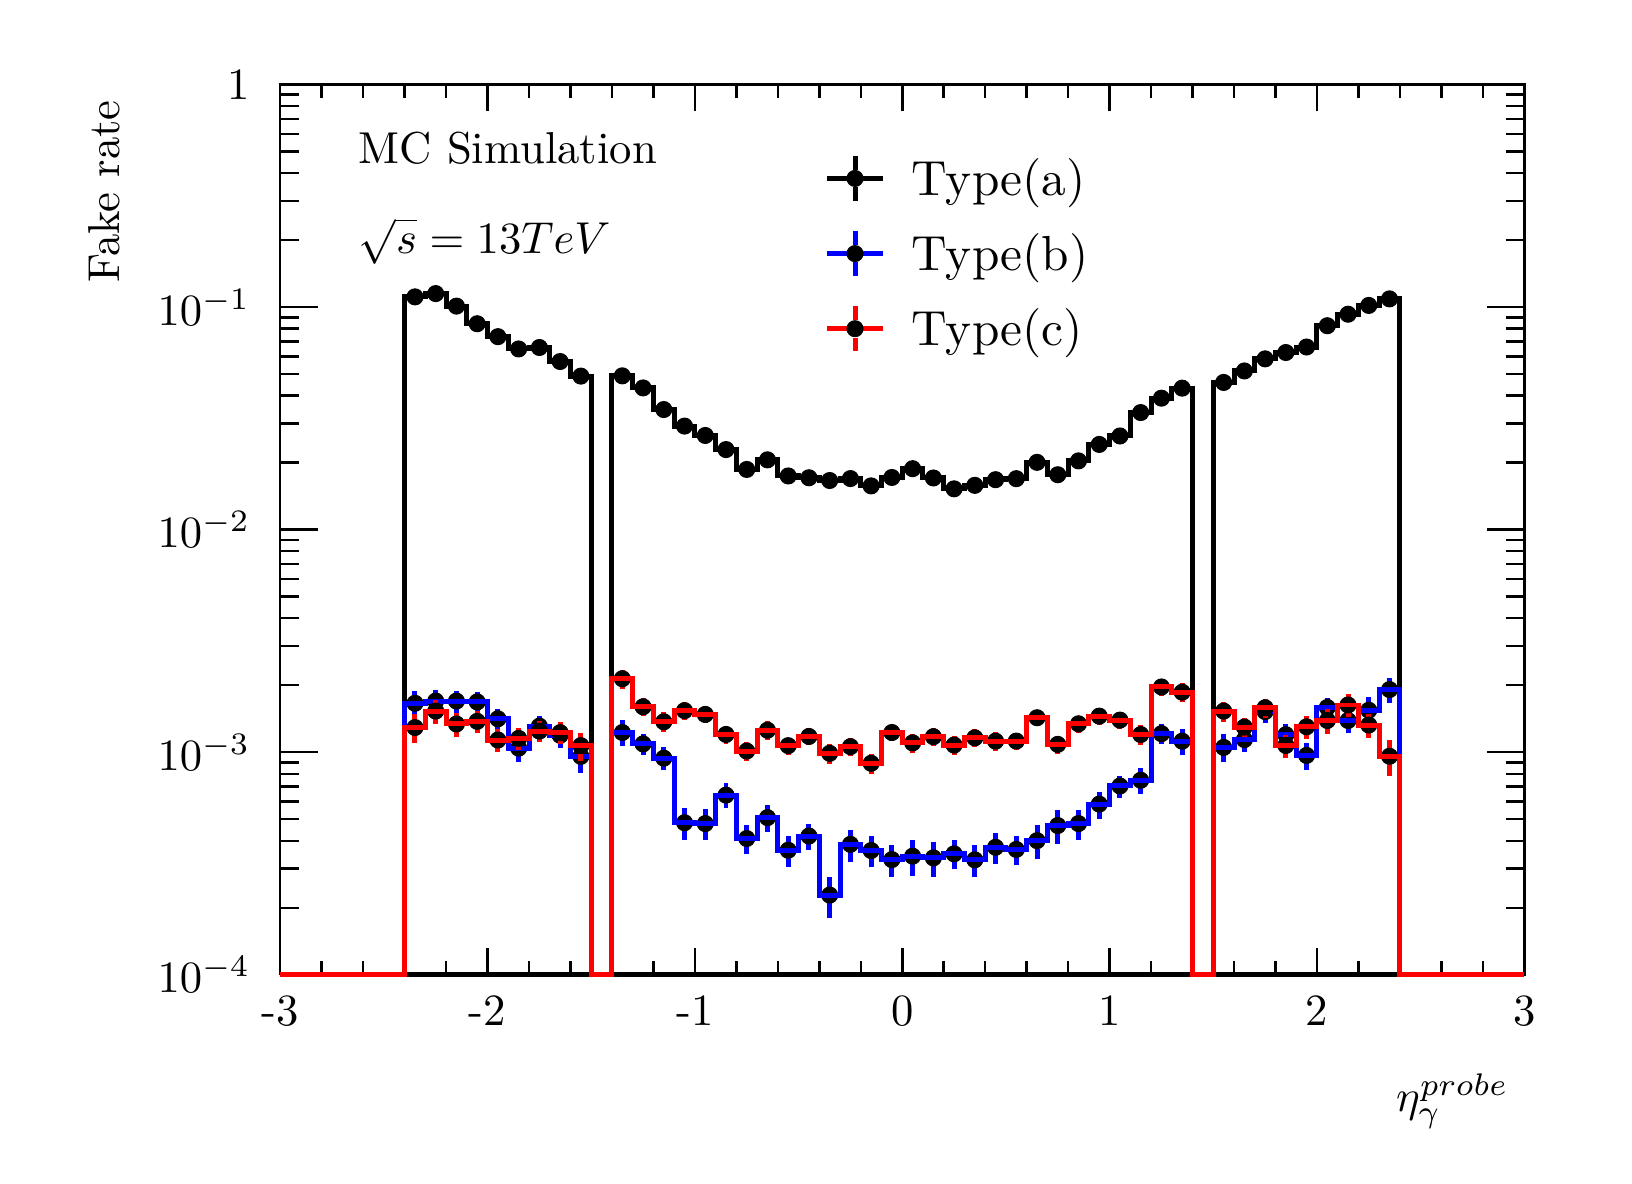
\begin{tikzpicture}
\pgfdeclareplotmark{cross} {
\pgfpathmoveto{\pgfpoint{-0.3\pgfplotmarksize}{\pgfplotmarksize}}
\pgfpathlineto{\pgfpoint{+0.3\pgfplotmarksize}{\pgfplotmarksize}}
\pgfpathlineto{\pgfpoint{+0.3\pgfplotmarksize}{0.3\pgfplotmarksize}}
\pgfpathlineto{\pgfpoint{+1\pgfplotmarksize}{0.3\pgfplotmarksize}}
\pgfpathlineto{\pgfpoint{+1\pgfplotmarksize}{-0.3\pgfplotmarksize}}
\pgfpathlineto{\pgfpoint{+0.3\pgfplotmarksize}{-0.3\pgfplotmarksize}}
\pgfpathlineto{\pgfpoint{+0.3\pgfplotmarksize}{-1.\pgfplotmarksize}}
\pgfpathlineto{\pgfpoint{-0.3\pgfplotmarksize}{-1.\pgfplotmarksize}}
\pgfpathlineto{\pgfpoint{-0.3\pgfplotmarksize}{-0.3\pgfplotmarksize}}
\pgfpathlineto{\pgfpoint{-1.\pgfplotmarksize}{-0.3\pgfplotmarksize}}
\pgfpathlineto{\pgfpoint{-1.\pgfplotmarksize}{0.3\pgfplotmarksize}}
\pgfpathlineto{\pgfpoint{-0.3\pgfplotmarksize}{0.3\pgfplotmarksize}}
\pgfpathclose
\pgfusepathqstroke
}
\pgfdeclareplotmark{cross*} {
\pgfpathmoveto{\pgfpoint{-0.3\pgfplotmarksize}{\pgfplotmarksize}}
\pgfpathlineto{\pgfpoint{+0.3\pgfplotmarksize}{\pgfplotmarksize}}
\pgfpathlineto{\pgfpoint{+0.3\pgfplotmarksize}{0.3\pgfplotmarksize}}
\pgfpathlineto{\pgfpoint{+1\pgfplotmarksize}{0.3\pgfplotmarksize}}
\pgfpathlineto{\pgfpoint{+1\pgfplotmarksize}{-0.3\pgfplotmarksize}}
\pgfpathlineto{\pgfpoint{+0.3\pgfplotmarksize}{-0.3\pgfplotmarksize}}
\pgfpathlineto{\pgfpoint{+0.3\pgfplotmarksize}{-1.\pgfplotmarksize}}
\pgfpathlineto{\pgfpoint{-0.3\pgfplotmarksize}{-1.\pgfplotmarksize}}
\pgfpathlineto{\pgfpoint{-0.3\pgfplotmarksize}{-0.3\pgfplotmarksize}}
\pgfpathlineto{\pgfpoint{-1.\pgfplotmarksize}{-0.3\pgfplotmarksize}}
\pgfpathlineto{\pgfpoint{-1.\pgfplotmarksize}{0.3\pgfplotmarksize}}
\pgfpathlineto{\pgfpoint{-0.3\pgfplotmarksize}{0.3\pgfplotmarksize}}
\pgfpathclose
\pgfusepathqfillstroke
}
\pgfdeclareplotmark{newstar} {
\pgfpathmoveto{\pgfqpoint{0pt}{\pgfplotmarksize}}
\pgfpathlineto{\pgfqpointpolar{44}{0.5\pgfplotmarksize}}
\pgfpathlineto{\pgfqpointpolar{18}{\pgfplotmarksize}}
\pgfpathlineto{\pgfqpointpolar{-20}{0.5\pgfplotmarksize}}
\pgfpathlineto{\pgfqpointpolar{-54}{\pgfplotmarksize}}
\pgfpathlineto{\pgfqpointpolar{-90}{0.5\pgfplotmarksize}}
\pgfpathlineto{\pgfqpointpolar{234}{\pgfplotmarksize}}
\pgfpathlineto{\pgfqpointpolar{198}{0.5\pgfplotmarksize}}
\pgfpathlineto{\pgfqpointpolar{162}{\pgfplotmarksize}}
\pgfpathlineto{\pgfqpointpolar{134}{0.5\pgfplotmarksize}}
\pgfpathclose
\pgfusepathqstroke
}
\pgfdeclareplotmark{newstar*} {
\pgfpathmoveto{\pgfqpoint{0pt}{\pgfplotmarksize}}
\pgfpathlineto{\pgfqpointpolar{44}{0.5\pgfplotmarksize}}
\pgfpathlineto{\pgfqpointpolar{18}{\pgfplotmarksize}}
\pgfpathlineto{\pgfqpointpolar{-20}{0.5\pgfplotmarksize}}
\pgfpathlineto{\pgfqpointpolar{-54}{\pgfplotmarksize}}
\pgfpathlineto{\pgfqpointpolar{-90}{0.5\pgfplotmarksize}}
\pgfpathlineto{\pgfqpointpolar{234}{\pgfplotmarksize}}
\pgfpathlineto{\pgfqpointpolar{198}{0.5\pgfplotmarksize}}
\pgfpathlineto{\pgfqpointpolar{162}{\pgfplotmarksize}}
\pgfpathlineto{\pgfqpointpolar{134}{0.5\pgfplotmarksize}}
\pgfpathclose
\pgfusepathqfillstroke
}
\definecolor{c}{rgb}{1,1,1};
\draw [color=c, fill=c] (0,0) rectangle (20,14.3108);
\draw [color=c, fill=c] (3.2,2.28972) rectangle (19,13.5952);
\definecolor{c}{rgb}{0,0,0};
\draw [c,line width=0.9] (3.2,2.28972) -- (3.2,13.5952) -- (19,13.5952) -- (19,2.28972) -- (3.2,2.28972);
\draw [c,line width=1.8] (3.2,2.28972) -- (3.2158,2.28972) -- (3.2158,2.28972) -- (3.2316,2.28972) -- (3.2316,2.28972) -- (3.2474,2.28972) -- (3.2474,2.28972) -- (3.2632,2.28972) -- (3.2632,2.28972) -- (3.279,2.28972) -- (3.279,2.28972) --
 (3.2948,2.28972) -- (3.2948,2.28972) -- (3.3106,2.28972) -- (3.3106,2.28972) -- (3.3264,2.28972) -- (3.3264,2.28972) -- (3.3422,2.28972) -- (3.3422,2.28972) -- (3.358,2.28972) -- (3.358,2.28972) -- (3.3738,2.28972) -- (3.3738,2.28972) --
 (3.3896,2.28972) -- (3.3896,2.28972) -- (3.4054,2.28972) -- (3.4054,2.28972) -- (3.4212,2.28972) -- (3.4212,2.28972) -- (3.437,2.28972) -- (3.437,2.28972) -- (3.4528,2.28972) -- (3.4528,2.28972) -- (3.4686,2.28972) -- (3.4686,2.28972) --
 (3.4844,2.28972) -- (3.4844,2.28972) -- (3.5002,2.28972) -- (3.5002,2.28972) -- (3.516,2.28972) -- (3.516,2.28972) -- (3.5318,2.28972) -- (3.5318,2.28972) -- (3.5476,2.28972) -- (3.5476,2.28972) -- (3.5634,2.28972) -- (3.5634,2.28972) --
 (3.5792,2.28972) -- (3.5792,2.28972) -- (3.595,2.28972) -- (3.595,2.28972) -- (3.6108,2.28972) -- (3.6108,2.28972) -- (3.6266,2.28972) -- (3.6266,2.28972) -- (3.6424,2.28972) -- (3.6424,2.28972) -- (3.6582,2.28972) -- (3.6582,2.28972) --
 (3.674,2.28972) -- (3.674,2.28972) -- (3.6898,2.28972) -- (3.6898,2.28972) -- (3.7056,2.28972) -- (3.7056,2.28972) -- (3.7214,2.28972) -- (3.7214,2.28972) -- (3.7372,2.28972) -- (3.7372,2.28972) -- (3.753,2.28972) -- (3.753,2.28972) --
 (3.7688,2.28972) -- (3.7688,2.28972) -- (3.7846,2.28972) -- (3.7846,2.28972) -- (3.8004,2.28972) -- (3.8004,2.28972) -- (3.8162,2.28972) -- (3.8162,2.28972) -- (3.832,2.28972) -- (3.832,2.28972) -- (3.8478,2.28972) -- (3.8478,2.28972) --
 (3.8636,2.28972) -- (3.8636,2.28972) -- (3.8794,2.28972) -- (3.8794,2.28972) -- (3.8952,2.28972) -- (3.8952,2.28972) -- (3.911,2.28972) -- (3.911,2.28972) -- (3.9268,2.28972) -- (3.9268,2.28972) -- (3.9426,2.28972) -- (3.9426,2.28972) --
 (3.9584,2.28972) -- (3.9584,2.28972) -- (3.9742,2.28972) -- (3.9742,2.28972) -- (3.99,2.28972) -- (3.99,2.28972) -- (4.0058,2.28972) -- (4.0058,2.28972) -- (4.0216,2.28972) -- (4.0216,2.28972) -- (4.0374,2.28972) -- (4.0374,2.28972) --
 (4.0532,2.28972) -- (4.0532,2.28972) -- (4.069,2.28972) -- (4.069,2.28972) -- (4.0848,2.28972) -- (4.0848,2.28972) -- (4.1006,2.28972) -- (4.1006,2.28972) -- (4.1164,2.28972) -- (4.1164,2.28972) -- (4.1322,2.28972) -- (4.1322,2.28972) --
 (4.148,2.28972) -- (4.148,2.28972) -- (4.1638,2.28972) -- (4.1638,2.28972) -- (4.1796,2.28972) -- (4.1796,2.28972) -- (4.1954,2.28972) -- (4.1954,2.28972) -- (4.2112,2.28972) -- (4.2112,2.28972) -- (4.227,2.28972) -- (4.227,2.28972) --
 (4.2428,2.28972) -- (4.2428,2.28972) -- (4.2586,2.28972) -- (4.2586,2.28972) -- (4.2744,2.28972) -- (4.2744,2.28972) -- (4.2902,2.28972) -- (4.2902,2.28972) -- (4.306,2.28972) -- (4.306,2.28972) -- (4.3218,2.28972) -- (4.3218,2.28972) --
 (4.3376,2.28972) -- (4.3376,2.28972) -- (4.3534,2.28972) -- (4.3534,2.28972) -- (4.3692,2.28972) -- (4.3692,2.28972) -- (4.385,2.28972) -- (4.385,2.28972) -- (4.4008,2.28972) -- (4.4008,2.28972) -- (4.4166,2.28972) -- (4.4166,2.28972) --
 (4.4324,2.28972) -- (4.4324,2.28972) -- (4.4482,2.28972) -- (4.4482,2.28972) -- (4.464,2.28972) -- (4.464,2.28972) -- (4.4798,2.28972) -- (4.4798,2.28972) -- (4.4956,2.28972) -- (4.4956,2.28972) -- (4.5114,2.28972) -- (4.5114,2.28972) --
 (4.5272,2.28972) -- (4.5272,2.28972) -- (4.543,2.28972) -- (4.543,2.28972) -- (4.5588,2.28972) -- (4.5588,2.28972) -- (4.5746,2.28972) -- (4.5746,2.28972) -- (4.5904,2.28972) -- (4.5904,2.28972) -- (4.6062,2.28972) -- (4.6062,2.28972) --
 (4.622,2.28972) -- (4.622,2.28972) -- (4.6378,2.28972) -- (4.6378,2.28972) -- (4.6536,2.28972) -- (4.6536,2.28972) -- (4.6694,2.28972) -- (4.6694,2.28972) -- (4.6852,2.28972) -- (4.6852,2.28972) -- (4.701,2.28972) -- (4.701,2.28972) --
 (4.7168,2.28972) -- (4.7168,2.28972) -- (4.7326,2.28972) -- (4.7326,2.28972) -- (4.7484,2.28972) -- (4.7484,2.28972) -- (4.7642,2.28972) -- (4.7642,2.28972) -- (4.78,2.28972) -- (4.78,2.28972) -- (4.7958,2.28972) -- (4.7958,2.28972) --
 (4.8116,2.28972) -- (4.8116,2.28972) -- (4.8274,2.28972) -- (4.8274,2.28972) -- (4.8432,2.28972) -- (4.8432,2.28972) -- (4.859,2.28972) -- (4.859,2.28972) -- (4.8748,2.28972) -- (4.8748,2.28972) -- (4.8906,2.28972) -- (4.8906,2.28972) --
 (4.9064,2.28972) -- (4.9064,2.28972) -- (4.9222,2.28972) -- (4.9222,2.28972) -- (4.938,2.28972) -- (4.938,2.28972) -- (4.9538,2.28972) -- (4.9538,2.28972) -- (4.9696,2.28972) -- (4.9696,2.28972) -- (4.9854,2.28972) -- (4.9854,2.28972) --
 (5.0012,2.28972) -- (5.0012,2.28972) -- (5.017,2.28972) -- (5.017,2.28972) -- (5.0328,2.28972) -- (5.0328,2.28972) -- (5.0486,2.28972) -- (5.0486,2.28972) -- (5.0644,2.28972) -- (5.0644,2.28972) -- (5.0802,2.28972) -- (5.0802,2.28972) --
 (5.096,2.28972) -- (5.096,2.28972) -- (5.1118,2.28972) -- (5.1118,2.28972) -- (5.1276,2.28972) -- (5.1276,2.28972) -- (5.1434,2.28972) -- (5.1434,2.28972) -- (5.1592,2.28972) -- (5.1592,2.28972) -- (5.175,2.28972) -- (5.175,2.28972) --
 (5.1908,2.28972) -- (5.1908,2.28972) -- (5.2066,2.28972) -- (5.2066,2.28972) -- (5.2224,2.28972) -- (5.2224,2.28972) -- (5.2382,2.28972) -- (5.2382,2.28972) -- (5.254,2.28972) -- (5.254,2.28972) -- (5.2698,2.28972) -- (5.2698,2.28972) --
 (5.2856,2.28972) -- (5.2856,2.28972) -- (5.3014,2.28972) -- (5.3014,2.28972) -- (5.3172,2.28972) -- (5.3172,2.28972) -- (5.333,2.28972) -- (5.333,2.28972) -- (5.3488,2.28972) -- (5.3488,2.28972) -- (5.3646,2.28972) -- (5.3646,2.28972) --
 (5.3804,2.28972) -- (5.3804,2.28972) -- (5.3962,2.28972) -- (5.3962,2.28972) -- (5.412,2.28972) -- (5.412,2.28972) -- (5.4278,2.28972) -- (5.4278,2.28972) -- (5.4436,2.28972) -- (5.4436,2.28972) -- (5.4594,2.28972) -- (5.4594,2.28972) --
 (5.4752,2.28972) -- (5.4752,2.28972) -- (5.491,2.28972) -- (5.491,2.28972) -- (5.5068,2.28972) -- (5.5068,2.28972) -- (5.5226,2.28972) -- (5.5226,2.28972) -- (5.5384,2.28972) -- (5.5384,2.28972) -- (5.5542,2.28972) -- (5.5542,2.28972) --
 (5.57,2.28972) -- (5.57,2.28972) -- (5.5858,2.28972) -- (5.5858,2.28972) -- (5.6016,2.28972) -- (5.6016,2.28972) -- (5.6174,2.28972) -- (5.6174,2.28972) -- (5.6332,2.28972) -- (5.6332,2.28972) -- (5.649,2.28972) -- (5.649,2.28972) --
 (5.6648,2.28972) -- (5.6648,2.28972) -- (5.6806,2.28972) -- (5.6806,2.28972) -- (5.6964,2.28972) -- (5.6964,2.28972) -- (5.7122,2.28972) -- (5.7122,2.28972) -- (5.728,2.28972) -- (5.728,2.28972) -- (5.7438,2.28972) -- (5.7438,2.28972) --
 (5.7596,2.28972) -- (5.7596,2.28972) -- (5.7754,2.28972) -- (5.7754,2.28972) -- (5.7912,2.28972) -- (5.7912,2.28972) -- (5.807,2.28972) -- (5.807,2.28972) -- (5.8228,2.28972) -- (5.8228,2.28972) -- (5.8386,2.28972) -- (5.8386,2.28972) --
 (5.8544,2.28972) -- (5.8544,2.28972) -- (5.8702,2.28972) -- (5.8702,2.28972) -- (5.886,2.28972) -- (5.886,2.28972) -- (5.9018,2.28972) -- (5.9018,2.28972) -- (5.9176,2.28972) -- (5.9176,2.28972) -- (5.9334,2.28972) -- (5.9334,2.28972) --
 (5.9492,2.28972) -- (5.9492,2.28972) -- (5.965,2.28972) -- (5.965,2.28972) -- (5.9808,2.28972) -- (5.9808,2.28972) -- (5.9966,2.28972) -- (5.9966,2.28972) -- (6.0124,2.28972) -- (6.0124,2.28972) -- (6.0282,2.28972) -- (6.0282,2.28972) --
 (6.044,2.28972) -- (6.044,2.28972) -- (6.0598,2.28972) -- (6.0598,2.28972) -- (6.0756,2.28972) -- (6.0756,2.28972) -- (6.0914,2.28972) -- (6.0914,2.28972) -- (6.1072,2.28972) -- (6.1072,2.28972) -- (6.123,2.28972) -- (6.123,2.28972) --
 (6.1388,2.28972) -- (6.1388,2.28972) -- (6.1546,2.28972) -- (6.1546,2.28972) -- (6.1704,2.28972) -- (6.1704,2.28972) -- (6.1862,2.28972) -- (6.1862,2.28972) -- (6.202,2.28972) -- (6.202,2.28972) -- (6.2178,2.28972) -- (6.2178,2.28972) --
 (6.2336,2.28972) -- (6.2336,2.28972) -- (6.2494,2.28972) -- (6.2494,2.28972) -- (6.2652,2.28972) -- (6.2652,2.28972) -- (6.281,2.28972) -- (6.281,2.28972) -- (6.2968,2.28972) -- (6.2968,2.28972) -- (6.3126,2.28972) -- (6.3126,2.28972) --
 (6.3284,2.28972) -- (6.3284,2.28972) -- (6.3442,2.28972) -- (6.3442,2.28972) -- (6.36,2.28972) -- (6.36,2.28972) -- (6.3758,2.28972) -- (6.3758,2.28972) -- (6.3916,2.28972) -- (6.3916,2.28972) -- (6.4074,2.28972) -- (6.4074,2.28972) --
 (6.4232,2.28972) -- (6.4232,2.28972) -- (6.439,2.28972) -- (6.439,2.28972) -- (6.4548,2.28972) -- (6.4548,2.28972) -- (6.4706,2.28972) -- (6.4706,2.28972) -- (6.4864,2.28972) -- (6.4864,2.28972) -- (6.5022,2.28972) -- (6.5022,2.28972) --
 (6.518,2.28972) -- (6.518,2.28972) -- (6.5338,2.28972) -- (6.5338,2.28972) -- (6.5496,2.28972) -- (6.5496,2.28972) -- (6.5654,2.28972) -- (6.5654,2.28972) -- (6.5812,2.28972) -- (6.5812,2.28972) -- (6.597,2.28972) -- (6.597,2.28972) --
 (6.6128,2.28972) -- (6.6128,2.28972) -- (6.6286,2.28972) -- (6.6286,2.28972) -- (6.6444,2.28972) -- (6.6444,2.28972) -- (6.6602,2.28972) -- (6.6602,2.28972) -- (6.676,2.28972) -- (6.676,2.28972) -- (6.6918,2.28972) -- (6.6918,2.28972) --
 (6.7076,2.28972) -- (6.7076,2.28972) -- (6.7234,2.28972) -- (6.7234,2.28972) -- (6.7392,2.28972) -- (6.7392,2.28972) -- (6.755,2.28972) -- (6.755,2.28972) -- (6.7708,2.28972) -- (6.7708,2.28972) -- (6.7866,2.28972) -- (6.7866,2.28972) --
 (6.8024,2.28972) -- (6.8024,2.28972) -- (6.8182,2.28972) -- (6.8182,2.28972) -- (6.834,2.28972) -- (6.834,2.28972) -- (6.8498,2.28972) -- (6.8498,2.28972) -- (6.8656,2.28972) -- (6.8656,2.28972) -- (6.8814,2.28972) -- (6.8814,2.28972) --
 (6.8972,2.28972) -- (6.8972,2.28972) -- (6.913,2.28972) -- (6.913,2.28972) -- (6.9288,2.28972) -- (6.9288,2.28972) -- (6.9446,2.28972) -- (6.9446,2.28972) -- (6.9604,2.28972) -- (6.9604,2.28972) -- (6.9762,2.28972) -- (6.9762,2.28972) --
 (6.992,2.28972) -- (6.992,2.28972) -- (7.0078,2.28972) -- (7.0078,2.28972) -- (7.0236,2.28972) -- (7.0236,2.28972) -- (7.0394,2.28972) -- (7.0394,2.28972) -- (7.0552,2.28972) -- (7.0552,2.28972) -- (7.071,2.28972) -- (7.071,2.28972) --
 (7.0868,2.28972) -- (7.0868,2.28972) -- (7.1026,2.28972) -- (7.1026,2.28972) -- (7.1184,2.28972) -- (7.1184,2.28972) -- (7.1342,2.28972) -- (7.1342,2.28972) -- (7.15,2.28972) -- (7.15,2.28972) -- (7.1658,2.28972) -- (7.1658,2.28972) --
 (7.1816,2.28972) -- (7.1816,2.28972) -- (7.1974,2.28972) -- (7.1974,2.28972) -- (7.2132,2.28972) -- (7.2132,2.28972) -- (7.229,2.28972) -- (7.229,2.28972) -- (7.2448,2.28972) -- (7.2448,2.28972) -- (7.2606,2.28972) -- (7.2606,2.28972) --
 (7.2764,2.28972) -- (7.2764,2.28972) -- (7.2922,2.28972) -- (7.2922,2.28972) -- (7.308,2.28972) -- (7.308,2.28972) -- (7.3238,2.28972) -- (7.3238,2.28972) -- (7.3396,2.28972) -- (7.3396,2.28972) -- (7.3554,2.28972) -- (7.3554,2.28972) --
 (7.3712,2.28972) -- (7.3712,2.28972) -- (7.387,2.28972) -- (7.387,2.28972) -- (7.4028,2.28972) -- (7.4028,2.28972) -- (7.4186,2.28972) -- (7.4186,2.28972) -- (7.4344,2.28972) -- (7.4344,2.28972) -- (7.4502,2.28972) -- (7.4502,2.28972) --
 (7.466,2.28972) -- (7.466,2.28972) -- (7.4818,2.28972) -- (7.4818,2.28972) -- (7.4976,2.28972) -- (7.4976,2.28972) -- (7.5134,2.28972) -- (7.5134,2.28972) -- (7.5292,2.28972) -- (7.5292,2.28972) -- (7.545,2.28972) -- (7.545,2.28972) --
 (7.5608,2.28972) -- (7.5608,2.28972) -- (7.5766,2.28972) -- (7.5766,2.28972) -- (7.5924,2.28972) -- (7.5924,2.28972) -- (7.6082,2.28972) -- (7.6082,2.28972) -- (7.624,2.28972) -- (7.624,2.28972) -- (7.6398,2.28972) -- (7.6398,2.28972) --
 (7.6556,2.28972) -- (7.6556,2.28972) -- (7.6714,2.28972) -- (7.6714,2.28972) -- (7.6872,2.28972) -- (7.6872,2.28972) -- (7.703,2.28972) -- (7.703,2.28972) -- (7.7188,2.28972) -- (7.7188,2.28972) -- (7.7346,2.28972) -- (7.7346,2.28972) --
 (7.7504,2.28972) -- (7.7504,2.28972) -- (7.7662,2.28972) -- (7.7662,2.28972) -- (7.782,2.28972) -- (7.782,2.28972) -- (7.7978,2.28972) -- (7.7978,2.28972) -- (7.8136,2.28972) -- (7.8136,2.28972) -- (7.8294,2.28972) -- (7.8294,2.28972) --
 (7.8452,2.28972) -- (7.8452,2.28972) -- (7.861,2.28972) -- (7.861,2.28972) -- (7.8768,2.28972) -- (7.8768,2.28972) -- (7.8926,2.28972) -- (7.8926,2.28972) -- (7.9084,2.28972) -- (7.9084,2.28972) -- (7.9242,2.28972) -- (7.9242,2.28972) --
 (7.94,2.28972) -- (7.94,2.28972) -- (7.9558,2.28972) -- (7.9558,2.28972) -- (7.9716,2.28972) -- (7.9716,2.28972) -- (7.9874,2.28972) -- (7.9874,2.28972) -- (8.0032,2.28972) -- (8.0032,2.28972) -- (8.019,2.28972) -- (8.019,2.28972) --
 (8.0348,2.28972) -- (8.0348,2.28972) -- (8.0506,2.28972) -- (8.0506,2.28972) -- (8.0664,2.28972) -- (8.0664,2.28972) -- (8.0822,2.28972) -- (8.0822,2.28972) -- (8.098,2.28972) -- (8.098,2.28972) -- (8.1138,2.28972) -- (8.1138,2.28972) --
 (8.1296,2.28972) -- (8.1296,2.28972) -- (8.1454,2.28972) -- (8.1454,2.28972) -- (8.1612,2.28972) -- (8.1612,2.28972) -- (8.177,2.28972) -- (8.177,2.28972) -- (8.1928,2.28972) -- (8.1928,2.28972) -- (8.2086,2.28972) -- (8.2086,2.28972) --
 (8.2244,2.28972) -- (8.2244,2.28972) -- (8.2402,2.28972) -- (8.2402,2.28972) -- (8.256,2.28972) -- (8.256,2.28972) -- (8.2718,2.28972) -- (8.2718,2.28972) -- (8.2876,2.28972) -- (8.2876,2.28972) -- (8.3034,2.28972) -- (8.3034,2.28972) --
 (8.3192,2.28972) -- (8.3192,2.28972) -- (8.335,2.28972) -- (8.335,2.28972) -- (8.3508,2.28972) -- (8.3508,2.28972) -- (8.3666,2.28972) -- (8.3666,2.28972) -- (8.3824,2.28972) -- (8.3824,2.28972) -- (8.3982,2.28972) -- (8.3982,2.28972) --
 (8.414,2.28972) -- (8.414,2.28972) -- (8.4298,2.28972) -- (8.4298,2.28972) -- (8.4456,2.28972) -- (8.4456,2.28972) -- (8.4614,2.28972) -- (8.4614,2.28972) -- (8.4772,2.28972) -- (8.4772,2.28972) -- (8.493,2.28972) -- (8.493,2.28972) --
 (8.5088,2.28972) -- (8.5088,2.28972) -- (8.5246,2.28972) -- (8.5246,2.28972) -- (8.5404,2.28972) -- (8.5404,2.28972) -- (8.5562,2.28972) -- (8.5562,2.28972) -- (8.572,2.28972) -- (8.572,2.28972) -- (8.5878,2.28972) -- (8.5878,2.28972) --
 (8.6036,2.28972) -- (8.6036,2.28972) -- (8.6194,2.28972) -- (8.6194,2.28972) -- (8.6352,2.28972) -- (8.6352,2.28972) -- (8.651,2.28972) -- (8.651,2.28972) -- (8.6668,2.28972) -- (8.6668,2.28972) -- (8.6826,2.28972) -- (8.6826,2.28972) --
 (8.6984,2.28972) -- (8.6984,2.28972) -- (8.7142,2.28972) -- (8.7142,2.28972) -- (8.73,2.28972) -- (8.73,2.28972) -- (8.7458,2.28972) -- (8.7458,2.28972) -- (8.7616,2.28972) -- (8.7616,2.28972) -- (8.7774,2.28972) -- (8.7774,2.28972) --
 (8.7932,2.28972) -- (8.7932,2.28972) -- (8.809,2.28972) -- (8.809,2.28972) -- (8.8248,2.28972) -- (8.8248,2.28972) -- (8.8406,2.28972) -- (8.8406,2.28972) -- (8.8564,2.28972) -- (8.8564,2.28972) -- (8.8722,2.28972) -- (8.8722,2.28972) --
 (8.888,2.28972) -- (8.888,2.28972) -- (8.9038,2.28972) -- (8.9038,2.28972) -- (8.9196,2.28972) -- (8.9196,2.28972) -- (8.9354,2.28972) -- (8.9354,2.28972) -- (8.9512,2.28972) -- (8.9512,2.28972) -- (8.967,2.28972) -- (8.967,2.28972) --
 (8.9828,2.28972) -- (8.9828,2.28972) -- (8.9986,2.28972) -- (8.9986,2.28972) -- (9.0144,2.28972) -- (9.0144,2.28972) -- (9.0302,2.28972) -- (9.0302,2.28972) -- (9.046,2.28972) -- (9.046,2.28972) -- (9.0618,2.28972) -- (9.0618,2.28972) --
 (9.0776,2.28972) -- (9.0776,2.28972) -- (9.0934,2.28972) -- (9.0934,2.28972) -- (9.1092,2.28972) -- (9.1092,2.28972) -- (9.125,2.28972) -- (9.125,2.28972) -- (9.1408,2.28972) -- (9.1408,2.28972) -- (9.1566,2.28972) -- (9.1566,2.28972) --
 (9.1724,2.28972) -- (9.1724,2.28972) -- (9.1882,2.28972) -- (9.1882,2.28972) -- (9.204,2.28972) -- (9.204,2.28972) -- (9.2198,2.28972) -- (9.2198,2.28972) -- (9.2356,2.28972) -- (9.2356,2.28972) -- (9.2514,2.28972) -- (9.2514,2.28972) --
 (9.2672,2.28972) -- (9.2672,2.28972) -- (9.283,2.28972) -- (9.283,2.28972) -- (9.2988,2.28972) -- (9.2988,2.28972) -- (9.3146,2.28972) -- (9.3146,2.28972) -- (9.3304,2.28972) -- (9.3304,2.28972) -- (9.3462,2.28972) -- (9.3462,2.28972) --
 (9.362,2.28972) -- (9.362,2.28972) -- (9.3778,2.28972) -- (9.3778,2.28972) -- (9.3936,2.28972) -- (9.3936,2.28972) -- (9.4094,2.28972) -- (9.4094,2.28972) -- (9.4252,2.28972) -- (9.4252,2.28972) -- (9.441,2.28972) -- (9.441,2.28972) --
 (9.4568,2.28972) -- (9.4568,2.28972) -- (9.4726,2.28972) -- (9.4726,2.28972) -- (9.4884,2.28972) -- (9.4884,2.28972) -- (9.5042,2.28972) -- (9.5042,2.28972) -- (9.52,2.28972) -- (9.52,2.28972) -- (9.5358,2.28972) -- (9.5358,2.28972) --
 (9.5516,2.28972) -- (9.5516,2.28972) -- (9.5674,2.28972) -- (9.5674,2.28972) -- (9.5832,2.28972) -- (9.5832,2.28972) -- (9.599,2.28972) -- (9.599,2.28972) -- (9.6148,2.28972) -- (9.6148,2.28972) -- (9.6306,2.28972) -- (9.6306,2.28972) --
 (9.6464,2.28972) -- (9.6464,2.28972) -- (9.6622,2.28972) -- (9.6622,2.28972) -- (9.678,2.28972) -- (9.678,2.28972) -- (9.6938,2.28972) -- (9.6938,2.28972) -- (9.7096,2.28972) -- (9.7096,2.28972) -- (9.7254,2.28972) -- (9.7254,2.28972) --
 (9.7412,2.28972) -- (9.7412,2.28972) -- (9.757,2.28972) -- (9.757,2.28972) -- (9.7728,2.28972) -- (9.7728,2.28972) -- (9.7886,2.28972) -- (9.7886,2.28972) -- (9.8044,2.28972) -- (9.8044,2.28972) -- (9.8202,2.28972) -- (9.8202,2.28972) --
 (9.836,2.28972) -- (9.836,2.28972) -- (9.8518,2.28972) -- (9.8518,2.28972) -- (9.8676,2.28972) -- (9.8676,2.28972) -- (9.8834,2.28972) -- (9.8834,2.28972) -- (9.8992,2.28972) -- (9.8992,2.28972) -- (9.915,2.28972) -- (9.915,2.28972) --
 (9.9308,2.28972) -- (9.9308,2.28972) -- (9.9466,2.28972) -- (9.9466,2.28972) -- (9.9624,2.28972) -- (9.9624,2.28972) -- (9.9782,2.28972) -- (9.9782,2.28972) -- (9.994,2.28972) -- (9.994,2.28972) -- (10.0098,2.28972) -- (10.0098,2.28972) --
 (10.0256,2.28972) -- (10.0256,2.28972) -- (10.0414,2.28972) -- (10.0414,2.28972) -- (10.0572,2.28972) -- (10.0572,2.28972) -- (10.073,2.28972) -- (10.073,2.28972) -- (10.0888,2.28972) -- (10.0888,2.28972) -- (10.1046,2.28972) -- (10.1046,2.28972) --
 (10.1204,2.28972) -- (10.1204,2.28972) -- (10.1362,2.28972) -- (10.1362,2.28972) -- (10.152,2.28972) -- (10.152,2.28972) -- (10.1678,2.28972) -- (10.1678,2.28972) -- (10.1836,2.28972) -- (10.1836,2.28972) -- (10.1994,2.28972) -- (10.1994,2.28972) --
 (10.2152,2.28972) -- (10.2152,2.28972) -- (10.231,2.28972) -- (10.231,2.28972) -- (10.2468,2.28972) -- (10.2468,2.28972) -- (10.2626,2.28972) -- (10.2626,2.28972) -- (10.2784,2.28972) -- (10.2784,2.28972) -- (10.2942,2.28972) -- (10.2942,2.28972) --
 (10.31,2.28972) -- (10.31,2.28972) -- (10.3258,2.28972) -- (10.3258,2.28972) -- (10.3416,2.28972) -- (10.3416,2.28972) -- (10.3574,2.28972) -- (10.3574,2.28972) -- (10.3732,2.28972) -- (10.3732,2.28972) -- (10.389,2.28972) -- (10.389,2.28972) --
 (10.4048,2.28972) -- (10.4048,2.28972) -- (10.4206,2.28972) -- (10.4206,2.28972) -- (10.4364,2.28972) -- (10.4364,2.28972) -- (10.4522,2.28972) -- (10.4522,2.28972) -- (10.468,2.28972) -- (10.468,2.28972) -- (10.4838,2.28972) -- (10.4838,2.28972) --
 (10.4996,2.28972) -- (10.4996,2.28972) -- (10.5154,2.28972) -- (10.5154,2.28972) -- (10.5312,2.28972) -- (10.5312,2.28972) -- (10.547,2.28972) -- (10.547,2.28972) -- (10.5628,2.28972) -- (10.5628,2.28972) -- (10.5786,2.28972) -- (10.5786,2.28972) --
 (10.5944,2.28972) -- (10.5944,2.28972) -- (10.6102,2.28972) -- (10.6102,2.28972) -- (10.626,2.28972) -- (10.626,2.28972) -- (10.6418,2.28972) -- (10.6418,2.28972) -- (10.6576,2.28972) -- (10.6576,2.28972) -- (10.6734,2.28972) -- (10.6734,2.28972) --
 (10.6892,2.28972) -- (10.6892,2.28972) -- (10.705,2.28972) -- (10.705,2.28972) -- (10.7208,2.28972) -- (10.7208,2.28972) -- (10.7366,2.28972) -- (10.7366,2.28972) -- (10.7524,2.28972) -- (10.7524,2.28972) -- (10.7682,2.28972) -- (10.7682,2.28972) --
 (10.784,2.28972) -- (10.784,2.28972) -- (10.7998,2.28972) -- (10.7998,2.28972) -- (10.8156,2.28972) -- (10.8156,2.28972) -- (10.8314,2.28972) -- (10.8314,2.28972) -- (10.8472,2.28972) -- (10.8472,2.28972) -- (10.863,2.28972) -- (10.863,2.28972) --
 (10.8788,2.28972) -- (10.8788,2.28972) -- (10.8946,2.28972) -- (10.8946,2.28972) -- (10.9104,2.28972) -- (10.9104,2.28972) -- (10.9262,2.28972) -- (10.9262,2.28972) -- (10.942,2.28972) -- (10.942,2.28972) -- (10.9578,2.28972) -- (10.9578,2.28972) --
 (10.9736,2.28972) -- (10.9736,2.28972) -- (10.9894,2.28972) -- (10.9894,2.28972) -- (11.0052,2.28972) -- (11.0052,2.28972) -- (11.021,2.28972) -- (11.021,2.28972) -- (11.0368,2.28972) -- (11.0368,2.28972) -- (11.0526,2.28972) -- (11.0526,2.28972) --
 (11.0684,2.28972) -- (11.0684,2.28972) -- (11.0842,2.28972) -- (11.0842,2.28972) -- (11.1,2.28972) -- (11.1,2.28972) -- (11.1158,2.28972) -- (11.1158,2.28972) -- (11.1316,2.28972) -- (11.1316,2.28972) -- (11.1474,2.28972) -- (11.1474,2.28972) --
 (11.1632,2.28972) -- (11.1632,2.28972) -- (11.179,2.28972) -- (11.179,2.28972) -- (11.1948,2.28972) -- (11.1948,2.28972) -- (11.2106,2.28972) -- (11.2106,2.28972) -- (11.2264,2.28972) -- (11.2264,2.28972) -- (11.2422,2.28972) -- (11.2422,2.28972) --
 (11.258,2.28972) -- (11.258,2.28972) -- (11.2738,2.28972) -- (11.2738,2.28972) -- (11.2896,2.28972) -- (11.2896,2.28972) -- (11.3054,2.28972) -- (11.3054,2.28972) -- (11.3212,2.28972) -- (11.3212,2.28972) -- (11.337,2.28972) -- (11.337,2.28972) --
 (11.3528,2.28972) -- (11.3528,2.28972) -- (11.3686,2.28972) -- (11.3686,2.28972) -- (11.3844,2.28972) -- (11.3844,2.28972) -- (11.4002,2.28972) -- (11.4002,2.28972) -- (11.416,2.28972) -- (11.416,2.28972) -- (11.4318,2.28972) -- (11.4318,2.28972) --
 (11.4476,2.28972) -- (11.4476,2.28972) -- (11.4634,2.28972) -- (11.4634,2.28972) -- (11.4792,2.28972) -- (11.4792,2.28972) -- (11.495,2.28972) -- (11.495,2.28972) -- (11.5108,2.28972) -- (11.5108,2.28972) -- (11.5266,2.28972) -- (11.5266,2.28972) --
 (11.5424,2.28972) -- (11.5424,2.28972) -- (11.5582,2.28972) -- (11.5582,2.28972) -- (11.574,2.28972) -- (11.574,2.28972) -- (11.5898,2.28972) -- (11.5898,2.28972) -- (11.6056,2.28972) -- (11.6056,2.28972) -- (11.6214,2.28972) -- (11.6214,2.28972) --
 (11.6372,2.28972) -- (11.6372,2.28972) -- (11.653,2.28972) -- (11.653,2.28972) -- (11.6688,2.28972) -- (11.6688,2.28972) -- (11.6846,2.28972) -- (11.6846,2.28972) -- (11.7004,2.28972) -- (11.7004,2.28972) -- (11.7162,2.28972) -- (11.7162,2.28972) --
 (11.732,2.28972) -- (11.732,2.28972) -- (11.7478,2.28972) -- (11.7478,2.28972) -- (11.7636,2.28972) -- (11.7636,2.28972) -- (11.7794,2.28972) -- (11.7794,2.28972) -- (11.7952,2.28972) -- (11.7952,2.28972) -- (11.811,2.28972) -- (11.811,2.28972) --
 (11.8268,2.28972) -- (11.8268,2.28972) -- (11.8426,2.28972) -- (11.8426,2.28972) -- (11.8584,2.28972) -- (11.8584,2.28972) -- (11.8742,2.28972) -- (11.8742,2.28972) -- (11.89,2.28972) -- (11.89,2.28972) -- (11.9058,2.28972) -- (11.9058,2.28972) --
 (11.9216,2.28972) -- (11.9216,2.28972) -- (11.9374,2.28972) -- (11.9374,2.28972) -- (11.9532,2.28972) -- (11.9532,2.28972) -- (11.969,2.28972) -- (11.969,2.28972) -- (11.9848,2.28972) -- (11.9848,2.28972) -- (12.0006,2.28972) -- (12.0006,2.28972) --
 (12.0164,2.28972) -- (12.0164,2.28972) -- (12.0322,2.28972) -- (12.0322,2.28972) -- (12.048,2.28972) -- (12.048,2.28972) -- (12.0638,2.28972) -- (12.0638,2.28972) -- (12.0796,2.28972) -- (12.0796,2.28972) -- (12.0954,2.28972) -- (12.0954,2.28972) --
 (12.1112,2.28972) -- (12.1112,2.28972) -- (12.127,2.28972) -- (12.127,2.28972) -- (12.1428,2.28972) -- (12.1428,2.28972) -- (12.1586,2.28972) -- (12.1586,2.28972) -- (12.1744,2.28972) -- (12.1744,2.28972) -- (12.1902,2.28972) -- (12.1902,2.28972) --
 (12.206,2.28972) -- (12.206,2.28972) -- (12.2218,2.28972) -- (12.2218,2.28972) -- (12.2376,2.28972) -- (12.2376,2.28972) -- (12.2534,2.28972) -- (12.2534,2.28972) -- (12.2692,2.28972) -- (12.2692,2.28972) -- (12.285,2.28972) -- (12.285,2.28972) --
 (12.3008,2.28972) -- (12.3008,2.28972) -- (12.3166,2.28972) -- (12.3166,2.28972) -- (12.3324,2.28972) -- (12.3324,2.28972) -- (12.3482,2.28972) -- (12.3482,2.28972) -- (12.364,2.28972) -- (12.364,2.28972) -- (12.3798,2.28972) -- (12.3798,2.28972) --
 (12.3956,2.28972) -- (12.3956,2.28972) -- (12.4114,2.28972) -- (12.4114,2.28972) -- (12.4272,2.28972) -- (12.4272,2.28972) -- (12.443,2.28972) -- (12.443,2.28972) -- (12.4588,2.28972) -- (12.4588,2.28972) -- (12.4746,2.28972) -- (12.4746,2.28972) --
 (12.4904,2.28972) -- (12.4904,2.28972) -- (12.5062,2.28972) -- (12.5062,2.28972) -- (12.522,2.28972) -- (12.522,2.28972) -- (12.5378,2.28972) -- (12.5378,2.28972) -- (12.5536,2.28972) -- (12.5536,2.28972) -- (12.5694,2.28972) -- (12.5694,2.28972) --
 (12.5852,2.28972) -- (12.5852,2.28972) -- (12.601,2.28972) -- (12.601,2.28972) -- (12.6168,2.28972) -- (12.6168,2.28972) -- (12.6326,2.28972) -- (12.6326,2.28972) -- (12.6484,2.28972) -- (12.6484,2.28972) -- (12.6642,2.28972) -- (12.6642,2.28972) --
 (12.68,2.28972) -- (12.68,2.28972) -- (12.6958,2.28972) -- (12.6958,2.28972) -- (12.7116,2.28972) -- (12.7116,2.28972) -- (12.7274,2.28972) -- (12.7274,2.28972) -- (12.7432,2.28972) -- (12.7432,2.28972) -- (12.759,2.28972) -- (12.759,2.28972) --
 (12.7748,2.28972) -- (12.7748,2.28972) -- (12.7906,2.28972) -- (12.7906,2.28972) -- (12.8064,2.28972) -- (12.8064,2.28972) -- (12.8222,2.28972) -- (12.8222,2.28972) -- (12.838,2.28972) -- (12.838,2.28972) -- (12.8538,2.28972) -- (12.8538,2.28972) --
 (12.8696,2.28972) -- (12.8696,2.28972) -- (12.8854,2.28972) -- (12.8854,2.28972) -- (12.9012,2.28972) -- (12.9012,2.28972) -- (12.917,2.28972) -- (12.917,2.28972) -- (12.9328,2.28972) -- (12.9328,2.28972) -- (12.9486,2.28972) -- (12.9486,2.28972) --
 (12.9644,2.28972) -- (12.9644,2.28972) -- (12.9802,2.28972) -- (12.9802,2.28972) -- (12.996,2.28972) -- (12.996,2.28972) -- (13.0118,2.28972) -- (13.0118,2.28972) -- (13.0276,2.28972) -- (13.0276,2.28972) -- (13.0434,2.28972) -- (13.0434,2.28972) --
 (13.0592,2.28972) -- (13.0592,2.28972) -- (13.075,2.28972) -- (13.075,2.28972) -- (13.0908,2.28972) -- (13.0908,2.28972) -- (13.1066,2.28972) -- (13.1066,2.28972) -- (13.1224,2.28972) -- (13.1224,2.28972) -- (13.1382,2.28972) -- (13.1382,2.28972) --
 (13.154,2.28972) -- (13.154,2.28972) -- (13.1698,2.28972) -- (13.1698,2.28972) -- (13.1856,2.28972) -- (13.1856,2.28972) -- (13.2014,2.28972) -- (13.2014,2.28972) -- (13.2172,2.28972) -- (13.2172,2.28972) -- (13.233,2.28972) -- (13.233,2.28972) --
 (13.2488,2.28972) -- (13.2488,2.28972) -- (13.2646,2.28972) -- (13.2646,2.28972) -- (13.2804,2.28972) -- (13.2804,2.28972) -- (13.2962,2.28972) -- (13.2962,2.28972) -- (13.312,2.28972) -- (13.312,2.28972) -- (13.3278,2.28972) -- (13.3278,2.28972) --
 (13.3436,2.28972) -- (13.3436,2.28972) -- (13.3594,2.28972) -- (13.3594,2.28972) -- (13.3752,2.28972) -- (13.3752,2.28972) -- (13.391,2.28972) -- (13.391,2.28972) -- (13.4068,2.28972) -- (13.4068,2.28972) -- (13.4226,2.28972) -- (13.4226,2.28972) --
 (13.4384,2.28972) -- (13.4384,2.28972) -- (13.4542,2.28972) -- (13.4542,2.28972) -- (13.47,2.28972) -- (13.47,2.28972) -- (13.4858,2.28972) -- (13.4858,2.28972) -- (13.5016,2.28972) -- (13.5016,2.28972) -- (13.5174,2.28972) -- (13.5174,2.28972) --
 (13.5332,2.28972) -- (13.5332,2.28972) -- (13.549,2.28972) -- (13.549,2.28972) -- (13.5648,2.28972) -- (13.5648,2.28972) -- (13.5806,2.28972) -- (13.5806,2.28972) -- (13.5964,2.28972) -- (13.5964,2.28972) -- (13.6122,2.28972) -- (13.6122,2.28972) --
 (13.628,2.28972) -- (13.628,2.28972) -- (13.6438,2.28972) -- (13.6438,2.28972) -- (13.6596,2.28972) -- (13.6596,2.28972) -- (13.6754,2.28972) -- (13.6754,2.28972) -- (13.6912,2.28972) -- (13.6912,2.28972) -- (13.707,2.28972) -- (13.707,2.28972) --
 (13.7228,2.28972) -- (13.7228,2.28972) -- (13.7386,2.28972) -- (13.7386,2.28972) -- (13.7544,2.28972) -- (13.7544,2.28972) -- (13.7702,2.28972) -- (13.7702,2.28972) -- (13.786,2.28972) -- (13.786,2.28972) -- (13.8018,2.28972) -- (13.8018,2.28972) --
 (13.8176,2.28972) -- (13.8176,2.28972) -- (13.8334,2.28972) -- (13.8334,2.28972) -- (13.8492,2.28972) -- (13.8492,2.28972) -- (13.865,2.28972) -- (13.865,2.28972) -- (13.8808,2.28972) -- (13.8808,2.28972) -- (13.8966,2.28972) -- (13.8966,2.28972) --
 (13.9124,2.28972) -- (13.9124,2.28972) -- (13.9282,2.28972) -- (13.9282,2.28972) -- (13.944,2.28972) -- (13.944,2.28972) -- (13.9598,2.28972) -- (13.9598,2.28972) -- (13.9756,2.28972) -- (13.9756,2.28972) -- (13.9914,2.28972) -- (13.9914,2.28972) --
 (14.0072,2.28972) -- (14.0072,2.28972) -- (14.023,2.28972) -- (14.023,2.28972) -- (14.0388,2.28972) -- (14.0388,2.28972) -- (14.0546,2.28972) -- (14.0546,2.28972) -- (14.0704,2.28972) -- (14.0704,2.28972) -- (14.0862,2.28972) -- (14.0862,2.28972) --
 (14.102,2.28972) -- (14.102,2.28972) -- (14.1178,2.28972) -- (14.1178,2.28972) -- (14.1336,2.28972) -- (14.1336,2.28972) -- (14.1494,2.28972) -- (14.1494,2.28972) -- (14.1652,2.28972) -- (14.1652,2.28972) -- (14.181,2.28972) -- (14.181,2.28972) --
 (14.1968,2.28972) -- (14.1968,2.28972) -- (14.2126,2.28972) -- (14.2126,2.28972) -- (14.2284,2.28972) -- (14.2284,2.28972) -- (14.2442,2.28972) -- (14.2442,2.28972) -- (14.26,2.28972) -- (14.26,2.28972) -- (14.2758,2.28972) -- (14.2758,2.28972) --
 (14.2916,2.28972) -- (14.2916,2.28972) -- (14.3074,2.28972) -- (14.3074,2.28972) -- (14.3232,2.28972) -- (14.3232,2.28972) -- (14.339,2.28972) -- (14.339,2.28972) -- (14.3548,2.28972) -- (14.3548,2.28972) -- (14.3706,2.28972) -- (14.3706,2.28972) --
 (14.3864,2.28972) -- (14.3864,2.28972) -- (14.4022,2.28972) -- (14.4022,2.28972) -- (14.418,2.28972) -- (14.418,2.28972) -- (14.4338,2.28972) -- (14.4338,2.28972) -- (14.4496,2.28972) -- (14.4496,2.28972) -- (14.4654,2.28972) -- (14.4654,2.28972) --
 (14.4812,2.28972) -- (14.4812,2.28972) -- (14.497,2.28972) -- (14.497,2.28972) -- (14.5128,2.28972) -- (14.5128,2.28972) -- (14.5286,2.28972) -- (14.5286,2.28972) -- (14.5444,2.28972) -- (14.5444,2.28972) -- (14.5602,2.28972) -- (14.5602,2.28972) --
 (14.576,2.28972) -- (14.576,2.28972) -- (14.5918,2.28972) -- (14.5918,2.28972) -- (14.6076,2.28972) -- (14.6076,2.28972) -- (14.6234,2.28972) -- (14.6234,2.28972) -- (14.6392,2.28972) -- (14.6392,2.28972) -- (14.655,2.28972) -- (14.655,2.28972) --
 (14.6708,2.28972) -- (14.6708,2.28972) -- (14.6866,2.28972) -- (14.6866,2.28972) -- (14.7024,2.28972) -- (14.7024,2.28972) -- (14.7182,2.28972) -- (14.7182,2.28972) -- (14.734,2.28972) -- (14.734,2.28972) -- (14.7498,2.28972) -- (14.7498,2.28972) --
 (14.7656,2.28972) -- (14.7656,2.28972) -- (14.7814,2.28972) -- (14.7814,2.28972) -- (14.7972,2.28972) -- (14.7972,2.28972) -- (14.813,2.28972) -- (14.813,2.28972) -- (14.8288,2.28972) -- (14.8288,2.28972) -- (14.8446,2.28972) -- (14.8446,2.28972) --
 (14.8604,2.28972) -- (14.8604,2.28972) -- (14.8762,2.28972) -- (14.8762,2.28972) -- (14.892,2.28972) -- (14.892,2.28972) -- (14.9078,2.28972) -- (14.9078,2.28972) -- (14.9236,2.28972) -- (14.9236,2.28972) -- (14.9394,2.28972) -- (14.9394,2.28972) --
 (14.9552,2.28972) -- (14.9552,2.28972) -- (14.971,2.28972) -- (14.971,2.28972) -- (14.9868,2.28972) -- (14.9868,2.28972) -- (15.0026,2.28972) -- (15.0026,2.28972) -- (15.0184,2.28972) -- (15.0184,2.28972) -- (15.0342,2.28972) -- (15.0342,2.28972) --
 (15.05,2.28972) -- (15.05,2.28972) -- (15.0658,2.28972) -- (15.0658,2.28972) -- (15.0816,2.28972) -- (15.0816,2.28972) -- (15.0974,2.28972) -- (15.0974,2.28972) -- (15.1132,2.28972) -- (15.1132,2.28972) -- (15.129,2.28972) -- (15.129,2.28972) --
 (15.1448,2.28972) -- (15.1448,2.28972) -- (15.1606,2.28972) -- (15.1606,2.28972) -- (15.1764,2.28972) -- (15.1764,2.28972) -- (15.1922,2.28972) -- (15.1922,2.28972) -- (15.208,2.28972) -- (15.208,2.28972) -- (15.2238,2.28972) -- (15.2238,2.28972) --
 (15.2396,2.28972) -- (15.2396,2.28972) -- (15.2554,2.28972) -- (15.2554,2.28972) -- (15.2712,2.28972) -- (15.2712,2.28972) -- (15.287,2.28972) -- (15.287,2.28972) -- (15.3028,2.28972) -- (15.3028,2.28972) -- (15.3186,2.28972) -- (15.3186,2.28972) --
 (15.3344,2.28972) -- (15.3344,2.28972) -- (15.3502,2.28972) -- (15.3502,2.28972) -- (15.366,2.28972) -- (15.366,2.28972) -- (15.3818,2.28972) -- (15.3818,2.28972) -- (15.3976,2.28972) -- (15.3976,2.28972) -- (15.4134,2.28972) -- (15.4134,2.28972) --
 (15.4292,2.28972) -- (15.4292,2.28972) -- (15.445,2.28972) -- (15.445,2.28972) -- (15.4608,2.28972) -- (15.4608,2.28972) -- (15.4766,2.28972) -- (15.4766,2.28972) -- (15.4924,2.28972) -- (15.4924,2.28972) -- (15.5082,2.28972) -- (15.5082,2.28972) --
 (15.524,2.28972) -- (15.524,2.28972) -- (15.5398,2.28972) -- (15.5398,2.28972) -- (15.5556,2.28972) -- (15.5556,2.28972) -- (15.5714,2.28972) -- (15.5714,2.28972) -- (15.5872,2.28972) -- (15.5872,2.28972) -- (15.603,2.28972) -- (15.603,2.28972) --
 (15.6188,2.28972) -- (15.6188,2.28972) -- (15.6346,2.28972) -- (15.6346,2.28972) -- (15.6504,2.28972) -- (15.6504,2.28972) -- (15.6662,2.28972) -- (15.6662,2.28972) -- (15.682,2.28972) -- (15.682,2.28972) -- (15.6978,2.28972) -- (15.6978,2.28972) --
 (15.7136,2.28972) -- (15.7136,2.28972) -- (15.7294,2.28972) -- (15.7294,2.28972) -- (15.7452,2.28972) -- (15.7452,2.28972) -- (15.761,2.28972) -- (15.761,2.28972) -- (15.7768,2.28972) -- (15.7768,2.28972) -- (15.7926,2.28972) -- (15.7926,2.28972) --
 (15.8084,2.28972) -- (15.8084,2.28972) -- (15.8242,2.28972) -- (15.8242,2.28972) -- (15.84,2.28972) -- (15.84,2.28972) -- (15.8558,2.28972) -- (15.8558,2.28972) -- (15.8716,2.28972) -- (15.8716,2.28972) -- (15.8874,2.28972) -- (15.8874,2.28972) --
 (15.9032,2.28972) -- (15.9032,2.28972) -- (15.919,2.28972) -- (15.919,2.28972) -- (15.9348,2.28972) -- (15.9348,2.28972) -- (15.9506,2.28972) -- (15.9506,2.28972) -- (15.9664,2.28972) -- (15.9664,2.28972) -- (15.9822,2.28972) -- (15.9822,2.28972) --
 (15.998,2.28972) -- (15.998,2.28972) -- (16.0138,2.28972) -- (16.0138,2.28972) -- (16.0296,2.28972) -- (16.0296,2.28972) -- (16.0454,2.28972) -- (16.0454,2.28972) -- (16.0612,2.28972) -- (16.0612,2.28972) -- (16.077,2.28972) -- (16.077,2.28972) --
 (16.0928,2.28972) -- (16.0928,2.28972) -- (16.1086,2.28972) -- (16.1086,2.28972) -- (16.1244,2.28972) -- (16.1244,2.28972) -- (16.1402,2.28972) -- (16.1402,2.28972) -- (16.156,2.28972) -- (16.156,2.28972) -- (16.1718,2.28972) -- (16.1718,2.28972) --
 (16.1876,2.28972) -- (16.1876,2.28972) -- (16.2034,2.28972) -- (16.2034,2.28972) -- (16.2192,2.28972) -- (16.2192,2.28972) -- (16.235,2.28972) -- (16.235,2.28972) -- (16.2508,2.28972) -- (16.2508,2.28972) -- (16.2666,2.28972) -- (16.2666,2.28972) --
 (16.2824,2.28972) -- (16.2824,2.28972) -- (16.2982,2.28972) -- (16.2982,2.28972) -- (16.314,2.28972) -- (16.314,2.28972) -- (16.3298,2.28972) -- (16.3298,2.28972) -- (16.3456,2.28972) -- (16.3456,2.28972) -- (16.3614,2.28972) -- (16.3614,2.28972) --
 (16.3772,2.28972) -- (16.3772,2.28972) -- (16.393,2.28972) -- (16.393,2.28972) -- (16.4088,2.28972) -- (16.4088,2.28972) -- (16.4246,2.28972) -- (16.4246,2.28972) -- (16.4404,2.28972) -- (16.4404,2.28972) -- (16.4562,2.28972) -- (16.4562,2.28972) --
 (16.472,2.28972) -- (16.472,2.28972) -- (16.4878,2.28972) -- (16.4878,2.28972) -- (16.5036,2.28972) -- (16.5036,2.28972) -- (16.5194,2.28972) -- (16.5194,2.28972) -- (16.5352,2.28972) -- (16.5352,2.28972) -- (16.551,2.28972) -- (16.551,2.28972) --
 (16.5668,2.28972) -- (16.5668,2.28972) -- (16.5826,2.28972) -- (16.5826,2.28972) -- (16.5984,2.28972) -- (16.5984,2.28972) -- (16.6142,2.28972) -- (16.6142,2.28972) -- (16.63,2.28972) -- (16.63,2.28972) -- (16.6458,2.28972) -- (16.6458,2.28972) --
 (16.6616,2.28972) -- (16.6616,2.28972) -- (16.6774,2.28972) -- (16.6774,2.28972) -- (16.6932,2.28972) -- (16.6932,2.28972) -- (16.709,2.28972) -- (16.709,2.28972) -- (16.7248,2.28972) -- (16.7248,2.28972) -- (16.7406,2.28972) -- (16.7406,2.28972) --
 (16.7564,2.28972) -- (16.7564,2.28972) -- (16.7722,2.28972) -- (16.7722,2.28972) -- (16.788,2.28972) -- (16.788,2.28972) -- (16.8038,2.28972) -- (16.8038,2.28972) -- (16.8196,2.28972) -- (16.8196,2.28972) -- (16.8354,2.28972) -- (16.8354,2.28972) --
 (16.8512,2.28972) -- (16.8512,2.28972) -- (16.867,2.28972) -- (16.867,2.28972) -- (16.8828,2.28972) -- (16.8828,2.28972) -- (16.8986,2.28972) -- (16.8986,2.28972) -- (16.9144,2.28972) -- (16.9144,2.28972) -- (16.9302,2.28972) -- (16.9302,2.28972) --
 (16.946,2.28972) -- (16.946,2.28972) -- (16.9618,2.28972) -- (16.9618,2.28972) -- (16.9776,2.28972) -- (16.9776,2.28972) -- (16.9934,2.28972) -- (16.9934,2.28972) -- (17.0092,2.28972) -- (17.0092,2.28972) -- (17.025,2.28972) -- (17.025,2.28972) --
 (17.0408,2.28972) -- (17.0408,2.28972) -- (17.0566,2.28972) -- (17.0566,2.28972) -- (17.0724,2.28972) -- (17.0724,2.28972) -- (17.0882,2.28972) -- (17.0882,2.28972) -- (17.104,2.28972) -- (17.104,2.28972) -- (17.1198,2.28972) -- (17.1198,2.28972) --
 (17.1356,2.28972) -- (17.1356,2.28972) -- (17.1514,2.28972) -- (17.1514,2.28972) -- (17.1672,2.28972) -- (17.1672,2.28972) -- (17.183,2.28972) -- (17.183,2.28972) -- (17.1988,2.28972) -- (17.1988,2.28972) -- (17.2146,2.28972) -- (17.2146,2.28972) --
 (17.2304,2.28972) -- (17.2304,2.28972) -- (17.2462,2.28972) -- (17.2462,2.28972) -- (17.262,2.28972) -- (17.262,2.28972) -- (17.2778,2.28972) -- (17.2778,2.28972) -- (17.2936,2.28972) -- (17.2936,2.28972) -- (17.3094,2.28972) -- (17.3094,2.28972) --
 (17.3252,2.28972) -- (17.3252,2.28972) -- (17.341,2.28972) -- (17.341,2.28972) -- (17.3568,2.28972) -- (17.3568,2.28972) -- (17.3726,2.28972) -- (17.3726,2.28972) -- (17.3884,2.28972) -- (17.3884,2.28972) -- (17.4042,2.28972) -- (17.4042,2.28972) --
 (17.42,2.28972) -- (17.42,2.28972) -- (17.4358,2.28972) -- (17.4358,2.28972) -- (17.4516,2.28972) -- (17.4516,2.28972) -- (17.4674,2.28972) -- (17.4674,2.28972) -- (17.4832,2.28972) -- (17.4832,2.28972) -- (17.499,2.28972) -- (17.499,2.28972) --
 (17.5148,2.28972) -- (17.5148,2.28972) -- (17.5306,2.28972) -- (17.5306,2.28972) -- (17.5464,2.28972) -- (17.5464,2.28972) -- (17.5622,2.28972) -- (17.5622,2.28972) -- (17.578,2.28972) -- (17.578,2.28972) -- (17.5938,2.28972) -- (17.5938,2.28972) --
 (17.6096,2.28972) -- (17.6096,2.28972) -- (17.6254,2.28972) -- (17.6254,2.28972) -- (17.6412,2.28972) -- (17.6412,2.28972) -- (17.657,2.28972) -- (17.657,2.28972) -- (17.6728,2.28972) -- (17.6728,2.28972) -- (17.6886,2.28972) -- (17.6886,2.28972) --
 (17.7044,2.28972) -- (17.7044,2.28972) -- (17.7202,2.28972) -- (17.7202,2.28972) -- (17.736,2.28972) -- (17.736,2.28972) -- (17.7518,2.28972) -- (17.7518,2.28972) -- (17.7676,2.28972) -- (17.7676,2.28972) -- (17.7834,2.28972) -- (17.7834,2.28972) --
 (17.7992,2.28972) -- (17.7992,2.28972) -- (17.815,2.28972) -- (17.815,2.28972) -- (17.8308,2.28972) -- (17.8308,2.28972) -- (17.8466,2.28972) -- (17.8466,2.28972) -- (17.8624,2.28972) -- (17.8624,2.28972) -- (17.8782,2.28972) -- (17.8782,2.28972) --
 (17.894,2.28972) -- (17.894,2.28972) -- (17.9098,2.28972) -- (17.9098,2.28972) -- (17.9256,2.28972) -- (17.9256,2.28972) -- (17.9414,2.28972) -- (17.9414,2.28972) -- (17.9572,2.28972) -- (17.9572,2.28972) -- (17.973,2.28972) -- (17.973,2.28972) --
 (17.9888,2.28972) -- (17.9888,2.28972) -- (18.0046,2.28972) -- (18.0046,2.28972) -- (18.0204,2.28972) -- (18.0204,2.28972) -- (18.0362,2.28972) -- (18.0362,2.28972) -- (18.052,2.28972) -- (18.052,2.28972) -- (18.0678,2.28972) -- (18.0678,2.28972) --
 (18.0836,2.28972) -- (18.0836,2.28972) -- (18.0994,2.28972) -- (18.0994,2.28972) -- (18.1152,2.28972) -- (18.1152,2.28972) -- (18.131,2.28972) -- (18.131,2.28972) -- (18.1468,2.28972) -- (18.1468,2.28972) -- (18.1626,2.28972) -- (18.1626,2.28972) --
 (18.1784,2.28972) -- (18.1784,2.28972) -- (18.1942,2.28972) -- (18.1942,2.28972) -- (18.21,2.28972) -- (18.21,2.28972) -- (18.2258,2.28972) -- (18.2258,2.28972) -- (18.2416,2.28972) -- (18.2416,2.28972) -- (18.2574,2.28972) -- (18.2574,2.28972) --
 (18.2732,2.28972) -- (18.2732,2.28972) -- (18.289,2.28972) -- (18.289,2.28972) -- (18.3048,2.28972) -- (18.3048,2.28972) -- (18.3206,2.28972) -- (18.3206,2.28972) -- (18.3364,2.28972) -- (18.3364,2.28972) -- (18.3522,2.28972) -- (18.3522,2.28972) --
 (18.368,2.28972) -- (18.368,2.28972) -- (18.3838,2.28972) -- (18.3838,2.28972) -- (18.3996,2.28972) -- (18.3996,2.28972) -- (18.4154,2.28972) -- (18.4154,2.28972) -- (18.4312,2.28972) -- (18.4312,2.28972) -- (18.447,2.28972) -- (18.447,2.28972) --
 (18.4628,2.28972) -- (18.4628,2.28972) -- (18.4786,2.28972) -- (18.4786,2.28972) -- (18.4944,2.28972) -- (18.4944,2.28972) -- (18.5102,2.28972) -- (18.5102,2.28972) -- (18.526,2.28972) -- (18.526,2.28972) -- (18.5418,2.28972) -- (18.5418,2.28972) --
 (18.5576,2.28972) -- (18.5576,2.28972) -- (18.5734,2.28972) -- (18.5734,2.28972) -- (18.5892,2.28972) -- (18.5892,2.28972) -- (18.605,2.28972) -- (18.605,2.28972) -- (18.6208,2.28972) -- (18.6208,2.28972) -- (18.6366,2.28972) -- (18.6366,2.28972) --
 (18.6524,2.28972) -- (18.6524,2.28972) -- (18.6682,2.28972) -- (18.6682,2.28972) -- (18.684,2.28972) -- (18.684,2.28972) -- (18.6998,2.28972) -- (18.6998,2.28972) -- (18.7156,2.28972) -- (18.7156,2.28972) -- (18.7314,2.28972) -- (18.7314,2.28972) --
 (18.7472,2.28972) -- (18.7472,2.28972) -- (18.763,2.28972) -- (18.763,2.28972) -- (18.7788,2.28972) -- (18.7788,2.28972) -- (18.7946,2.28972) -- (18.7946,2.28972) -- (18.8104,2.28972) -- (18.8104,2.28972) -- (18.8262,2.28972) -- (18.8262,2.28972) --
 (18.842,2.28972) -- (18.842,2.28972) -- (18.8578,2.28972) -- (18.8578,2.28972) -- (18.8736,2.28972) -- (18.8736,2.28972) -- (18.8894,2.28972) -- (18.8894,2.28972) -- (18.9052,2.28972) -- (18.9052,2.28972) -- (18.921,2.28972) -- (18.921,2.28972) --
 (18.9368,2.28972) -- (18.9368,2.28972) -- (18.9526,2.28972) -- (18.9526,2.28972) -- (18.9684,2.28972) -- (18.9684,2.28972) -- (18.9842,2.28972) -- (18.9842,2.28972) -- (19,2.28972);
\draw [c,line width=0.9] (3.2,2.28972) -- (19,2.28972);
\draw [c,line width=0.9] (3.2,2.62889) -- (3.2,2.28972);
\draw [c,line width=0.9] (3.72667,2.45931) -- (3.72667,2.28972);
\draw [c,line width=0.9] (4.25333,2.45931) -- (4.25333,2.28972);
\draw [c,line width=0.9] (4.78,2.45931) -- (4.78,2.28972);
\draw [c,line width=0.9] (5.30667,2.45931) -- (5.30667,2.28972);
\draw [c,line width=0.9] (5.83333,2.62889) -- (5.83333,2.28972);
\draw [c,line width=0.9] (6.36,2.45931) -- (6.36,2.28972);
\draw [c,line width=0.9] (6.88667,2.45931) -- (6.88667,2.28972);
\draw [c,line width=0.9] (7.41333,2.45931) -- (7.41333,2.28972);
\draw [c,line width=0.9] (7.94,2.45931) -- (7.94,2.28972);
\draw [c,line width=0.9] (8.46667,2.62889) -- (8.46667,2.28972);
\draw [c,line width=0.9] (8.99333,2.45931) -- (8.99333,2.28972);
\draw [c,line width=0.9] (9.52,2.45931) -- (9.52,2.28972);
\draw [c,line width=0.9] (10.0467,2.45931) -- (10.0467,2.28972);
\draw [c,line width=0.9] (10.5733,2.45931) -- (10.5733,2.28972);
\draw [c,line width=0.9] (11.1,2.62889) -- (11.1,2.28972);
\draw [c,line width=0.9] (11.6267,2.45931) -- (11.6267,2.28972);
\draw [c,line width=0.9] (12.1533,2.45931) -- (12.1533,2.28972);
\draw [c,line width=0.9] (12.68,2.45931) -- (12.68,2.28972);
\draw [c,line width=0.9] (13.2067,2.45931) -- (13.2067,2.28972);
\draw [c,line width=0.9] (13.7333,2.62889) -- (13.7333,2.28972);
\draw [c,line width=0.9] (14.26,2.45931) -- (14.26,2.28972);
\draw [c,line width=0.9] (14.7867,2.45931) -- (14.7867,2.28972);
\draw [c,line width=0.9] (15.3133,2.45931) -- (15.3133,2.28972);
\draw [c,line width=0.9] (15.84,2.45931) -- (15.84,2.28972);
\draw [c,line width=0.9] (16.3667,2.62889) -- (16.3667,2.28972);
\draw [c,line width=0.9] (16.8933,2.45931) -- (16.8933,2.28972);
\draw [c,line width=0.9] (17.42,2.45931) -- (17.42,2.28972);
\draw [c,line width=0.9] (17.9467,2.45931) -- (17.9467,2.28972);
\draw [c,line width=0.9] (18.4733,2.45931) -- (18.4733,2.28972);
\draw [c,line width=0.9] (19,2.62889) -- (19,2.28972);
\draw [c,line width=0.9] (19,2.62889) -- (19,2.28972);
\draw [anchor=base] (3.2,1.64574) node[scale=1.61424, color=c, rotate=0]{-3};
\draw [anchor=base] (5.83333,1.64574) node[scale=1.61424, color=c, rotate=0]{-2};
\draw [anchor=base] (8.46667,1.64574) node[scale=1.61424, color=c, rotate=0]{-1};
\draw [anchor=base] (11.1,1.64574) node[scale=1.61424, color=c, rotate=0]{0};
\draw [anchor=base] (13.7333,1.64574) node[scale=1.61424, color=c, rotate=0]{1};
\draw [anchor=base] (16.3667,1.64574) node[scale=1.61424, color=c, rotate=0]{2};
\draw [anchor=base] (19,1.64574) node[scale=1.61424, color=c, rotate=0]{3};
\draw [anchor= east] (19,0.686917) node[scale=1.61424, color=c, rotate=0]{$\eta_{\gamma}^{probe}$};
\draw [c,line width=0.9] (3.2,13.5952) -- (19,13.5952);
\draw [c,line width=0.9] (3.2,13.2561) -- (3.2,13.5952);
\draw [c,line width=0.9] (3.72667,13.4257) -- (3.72667,13.5952);
\draw [c,line width=0.9] (4.25333,13.4257) -- (4.25333,13.5952);
\draw [c,line width=0.9] (4.78,13.4257) -- (4.78,13.5952);
\draw [c,line width=0.9] (5.30667,13.4257) -- (5.30667,13.5952);
\draw [c,line width=0.9] (5.83333,13.2561) -- (5.83333,13.5952);
\draw [c,line width=0.9] (6.36,13.4257) -- (6.36,13.5952);
\draw [c,line width=0.9] (6.88667,13.4257) -- (6.88667,13.5952);
\draw [c,line width=0.9] (7.41333,13.4257) -- (7.41333,13.5952);
\draw [c,line width=0.9] (7.94,13.4257) -- (7.94,13.5952);
\draw [c,line width=0.9] (8.46667,13.2561) -- (8.46667,13.5952);
\draw [c,line width=0.9] (8.99333,13.4257) -- (8.99333,13.5952);
\draw [c,line width=0.9] (9.52,13.4257) -- (9.52,13.5952);
\draw [c,line width=0.9] (10.0467,13.4257) -- (10.0467,13.5952);
\draw [c,line width=0.9] (10.5733,13.4257) -- (10.5733,13.5952);
\draw [c,line width=0.9] (11.1,13.2561) -- (11.1,13.5952);
\draw [c,line width=0.9] (11.6267,13.4257) -- (11.6267,13.5952);
\draw [c,line width=0.9] (12.1533,13.4257) -- (12.1533,13.5952);
\draw [c,line width=0.9] (12.68,13.4257) -- (12.68,13.5952);
\draw [c,line width=0.9] (13.2067,13.4257) -- (13.2067,13.5952);
\draw [c,line width=0.9] (13.7333,13.2561) -- (13.7333,13.5952);
\draw [c,line width=0.9] (14.26,13.4257) -- (14.26,13.5952);
\draw [c,line width=0.9] (14.7867,13.4257) -- (14.7867,13.5952);
\draw [c,line width=0.9] (15.3133,13.4257) -- (15.3133,13.5952);
\draw [c,line width=0.9] (15.84,13.4257) -- (15.84,13.5952);
\draw [c,line width=0.9] (16.3667,13.2561) -- (16.3667,13.5952);
\draw [c,line width=0.9] (16.8933,13.4257) -- (16.8933,13.5952);
\draw [c,line width=0.9] (17.42,13.4257) -- (17.42,13.5952);
\draw [c,line width=0.9] (17.9467,13.4257) -- (17.9467,13.5952);
\draw [c,line width=0.9] (18.4733,13.4257) -- (18.4733,13.5952);
\draw [c,line width=0.9] (19,13.2561) -- (19,13.5952);
\draw [c,line width=0.9] (19,13.2561) -- (19,13.5952);
\draw [c,line width=0.9] (3.2,2.28972) -- (3.2,13.5952);
\draw [c,line width=0.9] (3.674,2.28973) -- (3.2,2.28973);
\draw [anchor= east] (3.02,2.28973) node[scale=1.61424, color=c, rotate=0]{$10^{-4}$};
\draw [c,line width=0.9] (3.437,3.14055) -- (3.2,3.14055);
\draw [c,line width=0.9] (3.437,3.63825) -- (3.2,3.63825);
\draw [c,line width=0.9] (3.437,3.99138) -- (3.2,3.99138);
\draw [c,line width=0.9] (3.437,4.26528) -- (3.2,4.26528);
\draw [c,line width=0.9] (3.437,4.48908) -- (3.2,4.48908);
\draw [c,line width=0.9] (3.437,4.67829) -- (3.2,4.67829);
\draw [c,line width=0.9] (3.437,4.8422) -- (3.2,4.8422);
\draw [c,line width=0.9] (3.437,4.98678) -- (3.2,4.98678);
\draw [c,line width=0.9] (3.674,5.1161) -- (3.2,5.1161);
\draw [anchor= east] (3.02,5.1161) node[scale=1.61424, color=c, rotate=0]{$10^{-3}$};
\draw [c,line width=0.9] (3.437,5.96693) -- (3.2,5.96693);
\draw [c,line width=0.9] (3.437,6.46463) -- (3.2,6.46463);
\draw [c,line width=0.9] (3.437,6.81775) -- (3.2,6.81775);
\draw [c,line width=0.9] (3.437,7.09166) -- (3.2,7.09166);
\draw [c,line width=0.9] (3.437,7.31545) -- (3.2,7.31545);
\draw [c,line width=0.9] (3.437,7.50467) -- (3.2,7.50467);
\draw [c,line width=0.9] (3.437,7.66858) -- (3.2,7.66858);
\draw [c,line width=0.9] (3.437,7.81315) -- (3.2,7.81315);
\draw [c,line width=0.9] (3.674,7.94248) -- (3.2,7.94248);
\draw [anchor= east] (3.02,7.94248) node[scale=1.61424, color=c, rotate=0]{$10^{-2}$};
\draw [c,line width=0.9] (3.437,8.79331) -- (3.2,8.79331);
\draw [c,line width=0.9] (3.437,9.29101) -- (3.2,9.29101);
\draw [c,line width=0.9] (3.437,9.64413) -- (3.2,9.64413);
\draw [c,line width=0.9] (3.437,9.91804) -- (3.2,9.91804);
\draw [c,line width=0.9] (3.437,10.1418) -- (3.2,10.1418);
\draw [c,line width=0.9] (3.437,10.331) -- (3.2,10.331);
\draw [c,line width=0.9] (3.437,10.495) -- (3.2,10.495);
\draw [c,line width=0.9] (3.437,10.6395) -- (3.2,10.6395);
\draw [c,line width=0.9] (3.674,10.7689) -- (3.2,10.7689);
\draw [anchor= east] (3.02,10.7689) node[scale=1.61424, color=c, rotate=0]{$10^{-1}$};
\draw [c,line width=0.9] (3.437,11.6197) -- (3.2,11.6197);
\draw [c,line width=0.9] (3.437,12.1174) -- (3.2,12.1174);
\draw [c,line width=0.9] (3.437,12.4705) -- (3.2,12.4705);
\draw [c,line width=0.9] (3.437,12.7444) -- (3.2,12.7444);
\draw [c,line width=0.9] (3.437,12.9682) -- (3.2,12.9682);
\draw [c,line width=0.9] (3.437,13.1574) -- (3.2,13.1574);
\draw [c,line width=0.9] (3.437,13.3213) -- (3.2,13.3213);
\draw [c,line width=0.9] (3.437,13.4659) -- (3.2,13.4659);
\draw [c,line width=0.9] (3.674,13.5952) -- (3.2,13.5952);
\draw [anchor= east] (3.02,13.5952) node[scale=1.61424, color=c, rotate=0]{1};
\draw [anchor= east] (0.96,13.5952) node[scale=1.61424, color=c, rotate=90]{Fake rate};
\draw [c,line width=0.9] (19,2.28972) -- (19,13.5952);
\draw [c,line width=0.9] (18.526,2.28973) -- (19,2.28973);
\draw [c,line width=0.9] (18.763,3.14055) -- (19,3.14055);
\draw [c,line width=0.9] (18.763,3.63825) -- (19,3.63825);
\draw [c,line width=0.9] (18.763,3.99138) -- (19,3.99138);
\draw [c,line width=0.9] (18.763,4.26528) -- (19,4.26528);
\draw [c,line width=0.9] (18.763,4.48908) -- (19,4.48908);
\draw [c,line width=0.9] (18.763,4.67829) -- (19,4.67829);
\draw [c,line width=0.9] (18.763,4.8422) -- (19,4.8422);
\draw [c,line width=0.9] (18.763,4.98678) -- (19,4.98678);
\draw [c,line width=0.9] (18.526,5.1161) -- (19,5.1161);
\draw [c,line width=0.9] (18.763,5.96693) -- (19,5.96693);
\draw [c,line width=0.9] (18.763,6.46463) -- (19,6.46463);
\draw [c,line width=0.9] (18.763,6.81775) -- (19,6.81775);
\draw [c,line width=0.9] (18.763,7.09166) -- (19,7.09166);
\draw [c,line width=0.9] (18.763,7.31545) -- (19,7.31545);
\draw [c,line width=0.9] (18.763,7.50467) -- (19,7.50467);
\draw [c,line width=0.9] (18.763,7.66858) -- (19,7.66858);
\draw [c,line width=0.9] (18.763,7.81315) -- (19,7.81315);
\draw [c,line width=0.9] (18.526,7.94248) -- (19,7.94248);
\draw [c,line width=0.9] (18.763,8.79331) -- (19,8.79331);
\draw [c,line width=0.9] (18.763,9.29101) -- (19,9.29101);
\draw [c,line width=0.9] (18.763,9.64413) -- (19,9.64413);
\draw [c,line width=0.9] (18.763,9.91804) -- (19,9.91804);
\draw [c,line width=0.9] (18.763,10.1418) -- (19,10.1418);
\draw [c,line width=0.9] (18.763,10.331) -- (19,10.331);
\draw [c,line width=0.9] (18.763,10.495) -- (19,10.495);
\draw [c,line width=0.9] (18.763,10.6395) -- (19,10.6395);
\draw [c,line width=0.9] (18.526,10.7689) -- (19,10.7689);
\draw [c,line width=0.9] (18.763,11.6197) -- (19,11.6197);
\draw [c,line width=0.9] (18.763,12.1174) -- (19,12.1174);
\draw [c,line width=0.9] (18.763,12.4705) -- (19,12.4705);
\draw [c,line width=0.9] (18.763,12.7444) -- (19,12.7444);
\draw [c,line width=0.9] (18.763,12.9682) -- (19,12.9682);
\draw [c,line width=0.9] (18.763,13.1574) -- (19,13.1574);
\draw [c,line width=0.9] (18.763,13.3213) -- (19,13.3213);
\draw [c,line width=0.9] (18.763,13.4659) -- (19,13.4659);
\draw [c,line width=0.9] (18.526,13.5952) -- (19,13.5952);
\foreach \P in {(4.91167,10.8988)}{\draw[mark options={color=c,fill=c},mark size=2.882883pt,mark=*] plot coordinates {\P};}
\foreach \P in {(5.175,10.9407)}{\draw[mark options={color=c,fill=c},mark size=2.882883pt,mark=*] plot coordinates {\P};}
\foreach \P in {(5.43833,10.7814)}{\draw[mark options={color=c,fill=c},mark size=2.882883pt,mark=*] plot coordinates {\P};}
\foreach \P in {(5.70167,10.5578)}{\draw[mark options={color=c,fill=c},mark size=2.882883pt,mark=*] plot coordinates {\P};}
\foreach \P in {(5.965,10.3935)}{\draw[mark options={color=c,fill=c},mark size=2.882883pt,mark=*] plot coordinates {\P};}
\foreach \P in {(6.22833,10.2375)}{\draw[mark options={color=c,fill=c},mark size=2.882883pt,mark=*] plot coordinates {\P};}
\foreach \P in {(6.49167,10.2558)}{\draw[mark options={color=c,fill=c},mark size=2.882883pt,mark=*] plot coordinates {\P};}
\foreach \P in {(6.755,10.0778)}{\draw[mark options={color=c,fill=c},mark size=2.882883pt,mark=*] plot coordinates {\P};}
\foreach \P in {(7.01833,9.89267)}{\draw[mark options={color=c,fill=c},mark size=2.882883pt,mark=*] plot coordinates {\P};}
\foreach \P in {(7.545,9.89589)}{\draw[mark options={color=c,fill=c},mark size=2.882883pt,mark=*] plot coordinates {\P};}
\foreach \P in {(7.80833,9.74239)}{\draw[mark options={color=c,fill=c},mark size=2.882883pt,mark=*] plot coordinates {\P};}
\foreach \P in {(8.07167,9.46797)}{\draw[mark options={color=c,fill=c},mark size=2.882883pt,mark=*] plot coordinates {\P};}
\foreach \P in {(8.335,9.2579)}{\draw[mark options={color=c,fill=c},mark size=2.882883pt,mark=*] plot coordinates {\P};}
\foreach \P in {(8.59833,9.13857)}{\draw[mark options={color=c,fill=c},mark size=2.882883pt,mark=*] plot coordinates {\P};}
\foreach \P in {(8.86167,8.95969)}{\draw[mark options={color=c,fill=c},mark size=2.882883pt,mark=*] plot coordinates {\P};}
\foreach \P in {(9.125,8.70706)}{\draw[mark options={color=c,fill=c},mark size=2.882883pt,mark=*] plot coordinates {\P};}
\foreach \P in {(9.38833,8.82937)}{\draw[mark options={color=c,fill=c},mark size=2.882883pt,mark=*] plot coordinates {\P};}
\foreach \P in {(9.65167,8.62449)}{\draw[mark options={color=c,fill=c},mark size=2.882883pt,mark=*] plot coordinates {\P};}
\foreach \P in {(9.915,8.60147)}{\draw[mark options={color=c,fill=c},mark size=2.882883pt,mark=*] plot coordinates {\P};}
\foreach \P in {(10.1783,8.56668)}{\draw[mark options={color=c,fill=c},mark size=2.882883pt,mark=*] plot coordinates {\P};}
\foreach \P in {(10.4417,8.59148)}{\draw[mark options={color=c,fill=c},mark size=2.882883pt,mark=*] plot coordinates {\P};}
\foreach \P in {(10.705,8.49856)}{\draw[mark options={color=c,fill=c},mark size=2.882883pt,mark=*] plot coordinates {\P};}
\foreach \P in {(10.9683,8.60519)}{\draw[mark options={color=c,fill=c},mark size=2.882883pt,mark=*] plot coordinates {\P};}
\foreach \P in {(11.2317,8.71686)}{\draw[mark options={color=c,fill=c},mark size=2.882883pt,mark=*] plot coordinates {\P};}
\foreach \P in {(11.495,8.59892)}{\draw[mark options={color=c,fill=c},mark size=2.882883pt,mark=*] plot coordinates {\P};}
\foreach \P in {(11.7583,8.46109)}{\draw[mark options={color=c,fill=c},mark size=2.882883pt,mark=*] plot coordinates {\P};}
\foreach \P in {(12.0217,8.50526)}{\draw[mark options={color=c,fill=c},mark size=2.882883pt,mark=*] plot coordinates {\P};}
\foreach \P in {(12.285,8.57706)}{\draw[mark options={color=c,fill=c},mark size=2.882883pt,mark=*] plot coordinates {\P};}
\foreach \P in {(12.5483,8.58999)}{\draw[mark options={color=c,fill=c},mark size=2.882883pt,mark=*] plot coordinates {\P};}
\foreach \P in {(12.8117,8.79733)}{\draw[mark options={color=c,fill=c},mark size=2.882883pt,mark=*] plot coordinates {\P};}
\foreach \P in {(13.075,8.63998)}{\draw[mark options={color=c,fill=c},mark size=2.882883pt,mark=*] plot coordinates {\P};}
\foreach \P in {(13.3383,8.81596)}{\draw[mark options={color=c,fill=c},mark size=2.882883pt,mark=*] plot coordinates {\P};}
\foreach \P in {(13.6017,9.02481)}{\draw[mark options={color=c,fill=c},mark size=2.882883pt,mark=*] plot coordinates {\P};}
\foreach \P in {(13.865,9.13229)}{\draw[mark options={color=c,fill=c},mark size=2.882883pt,mark=*] plot coordinates {\P};}
\foreach \P in {(14.1283,9.42969)}{\draw[mark options={color=c,fill=c},mark size=2.882883pt,mark=*] plot coordinates {\P};}
\foreach \P in {(14.3917,9.61259)}{\draw[mark options={color=c,fill=c},mark size=2.882883pt,mark=*] plot coordinates {\P};}
\foreach \P in {(14.655,9.73974)}{\draw[mark options={color=c,fill=c},mark size=2.882883pt,mark=*] plot coordinates {\P};}
\foreach \P in {(15.1817,9.81205)}{\draw[mark options={color=c,fill=c},mark size=2.882883pt,mark=*] plot coordinates {\P};}
\foreach \P in {(15.445,9.95796)}{\draw[mark options={color=c,fill=c},mark size=2.882883pt,mark=*] plot coordinates {\P};}
\foreach \P in {(15.7083,10.1117)}{\draw[mark options={color=c,fill=c},mark size=2.882883pt,mark=*] plot coordinates {\P};}
\foreach \P in {(15.9717,10.1922)}{\draw[mark options={color=c,fill=c},mark size=2.882883pt,mark=*] plot coordinates {\P};}
\foreach \P in {(16.235,10.2621)}{\draw[mark options={color=c,fill=c},mark size=2.882883pt,mark=*] plot coordinates {\P};}
\foreach \P in {(16.4983,10.5325)}{\draw[mark options={color=c,fill=c},mark size=2.882883pt,mark=*] plot coordinates {\P};}
\foreach \P in {(16.7617,10.6785)}{\draw[mark options={color=c,fill=c},mark size=2.882883pt,mark=*] plot coordinates {\P};}
\foreach \P in {(17.025,10.7901)}{\draw[mark options={color=c,fill=c},mark size=2.882883pt,mark=*] plot coordinates {\P};}
\foreach \P in {(17.2883,10.8735)}{\draw[mark options={color=c,fill=c},mark size=2.882883pt,mark=*] plot coordinates {\P};}
\draw [c,line width=1.8] (3.2,2.28972) -- (3.46333,2.28972) -- (3.46333,2.28972) -- (3.72667,2.28972) -- (3.72667,2.28972) -- (3.99,2.28972) -- (3.99,2.28972) -- (4.25333,2.28972) -- (4.25333,2.28972) -- (4.51667,2.28972) -- (4.51667,2.28972) --
 (4.78,2.28972) -- (4.78,10.8988) -- (5.04333,10.8988) -- (5.04333,10.9407) -- (5.30667,10.9407) -- (5.30667,10.7814) -- (5.57,10.7814) -- (5.57,10.5578) -- (5.83333,10.5578) -- (5.83333,10.3935) -- (6.09667,10.3935) -- (6.09667,10.2375) --
 (6.36,10.2375) -- (6.36,10.2558) -- (6.62333,10.2558) -- (6.62333,10.0778) -- (6.88667,10.0778) -- (6.88667,9.89267) -- (7.15,9.89267) -- (7.15,2.28972) -- (7.41333,2.28972) -- (7.41333,9.89589) -- (7.67667,9.89589) -- (7.67667,9.74239) --
 (7.94,9.74239) -- (7.94,9.46797) -- (8.20333,9.46797) -- (8.20333,9.2579) -- (8.46667,9.2579) -- (8.46667,9.13857) -- (8.73,9.13857) -- (8.73,8.95969) -- (8.99333,8.95969) -- (8.99333,8.70706) -- (9.25667,8.70706) -- (9.25667,8.82937) --
 (9.52,8.82937) -- (9.52,8.62449) -- (9.78333,8.62449) -- (9.78333,8.60147) -- (10.0467,8.60147) -- (10.0467,8.56668) -- (10.31,8.56668) -- (10.31,8.59148) -- (10.5733,8.59148) -- (10.5733,8.49856) -- (10.8367,8.49856) -- (10.8367,8.60519) --
 (11.1,8.60519) -- (11.1,8.71686) -- (11.3633,8.71686) -- (11.3633,8.59892) -- (11.6267,8.59892) -- (11.6267,8.46109) -- (11.89,8.46109) -- (11.89,8.50526) -- (12.1533,8.50526) -- (12.1533,8.57706) -- (12.4167,8.57706) -- (12.4167,8.58999) --
 (12.68,8.58999) -- (12.68,8.79733) -- (12.9433,8.79733) -- (12.9433,8.63998) -- (13.2067,8.63998) -- (13.2067,8.81596) -- (13.47,8.81596) -- (13.47,9.02481) -- (13.7333,9.02481) -- (13.7333,9.13229) -- (13.9967,9.13229) -- (13.9967,9.42969) --
 (14.26,9.42969) -- (14.26,9.61259) -- (14.5233,9.61259) -- (14.5233,9.73974) -- (14.7867,9.73974) -- (14.7867,2.28972) -- (15.05,2.28972) -- (15.05,9.81205) -- (15.3133,9.81205) -- (15.3133,9.95796) -- (15.5767,9.95796) -- (15.5767,10.1117) --
 (15.84,10.1117) -- (15.84,10.1922) -- (16.1033,10.1922) -- (16.1033,10.2621) -- (16.3667,10.2621) -- (16.3667,10.5325) -- (16.63,10.5325) -- (16.63,10.6785) -- (16.8933,10.6785) -- (16.8933,10.7901) -- (17.1567,10.7901) -- (17.1567,10.8735) --
 (17.42,10.8735) -- (17.42,2.28972) -- (17.6833,2.28972) -- (17.6833,2.28972) -- (17.9467,2.28972) -- (17.9467,2.28972) -- (18.21,2.28972) -- (18.21,2.28972) -- (18.4733,2.28972) -- (18.4733,2.28972) -- (18.7367,2.28972) -- (18.7367,2.28972) --
 (19,2.28972);
\definecolor{c}{rgb}{0,0,1};
\draw [c,line width=1.8] (4.91167,5.55569) -- (4.91167,5.63714);
\draw [c,line width=1.8] (4.91167,5.83764) -- (4.91167,5.89563);
\definecolor{c}{rgb}{0,0,0};
\foreach \P in {(4.91167,5.73739)}{\draw[mark options={color=c,fill=c},mark size=2.882883pt,mark=*] plot coordinates {\P};}
\definecolor{c}{rgb}{0,0,1};
\draw [c,line width=1.8] (5.175,5.6057) -- (5.175,5.6657);
\draw [c,line width=1.8] (5.175,5.8662) -- (5.175,5.90768);
\definecolor{c}{rgb}{0,0,0};
\foreach \P in {(5.175,5.76595)}{\draw[mark options={color=c,fill=c},mark size=2.882883pt,mark=*] plot coordinates {\P};}
\definecolor{c}{rgb}{0,0,1};
\draw [c,line width=1.8] (5.43833,5.6204) -- (5.43833,5.66553);
\draw [c,line width=1.8] (5.43833,5.86603) -- (5.43833,5.89576);
\definecolor{c}{rgb}{0,0,0};
\foreach \P in {(5.43833,5.76578)}{\draw[mark options={color=c,fill=c},mark size=2.882883pt,mark=*] plot coordinates {\P};}
\definecolor{c}{rgb}{0,0,1};
\draw [c,line width=1.8] (5.70167,5.61931) -- (5.70167,5.65476);
\draw [c,line width=1.8] (5.70167,5.85526) -- (5.70167,5.8772);
\definecolor{c}{rgb}{0,0,0};
\foreach \P in {(5.70167,5.75501)}{\draw[mark options={color=c,fill=c},mark size=2.882883pt,mark=*] plot coordinates {\P};}
\definecolor{c}{rgb}{0,0,1};
\draw [c,line width=1.8] (5.965,5.40474) -- (5.965,5.44022);
\draw [c,line width=1.8] (5.965,5.64072) -- (5.965,5.66267);
\definecolor{c}{rgb}{0,0,0};
\foreach \P in {(5.965,5.54047)}{\draw[mark options={color=c,fill=c},mark size=2.882883pt,mark=*] plot coordinates {\P};}
\definecolor{c}{rgb}{0,0,1};
\draw [c,line width=1.8] (6.22833,4.98964) -- (6.22833,5.06698);
\draw [c,line width=1.8] (6.22833,5.26748) -- (6.22833,5.32234);
\definecolor{c}{rgb}{0,0,0};
\foreach \P in {(6.22833,5.16723)}{\draw[mark options={color=c,fill=c},mark size=2.882883pt,mark=*] plot coordinates {\P};}
\definecolor{c}{rgb}{0,0,1};
\draw [c,line width=1.8] (6.49167,5.29768) -- (6.49167,5.3468);
\draw [c,line width=1.8] (6.49167,5.5473) -- (6.49167,5.5802);
\definecolor{c}{rgb}{0,0,0};
\foreach \P in {(6.49167,5.44705)}{\draw[mark options={color=c,fill=c},mark size=2.882883pt,mark=*] plot coordinates {\P};}
\definecolor{c}{rgb}{0,0,1};
\draw [c,line width=1.8] (6.755,5.16462) -- (6.755,5.2308);
\draw [c,line width=1.8] (6.755,5.4313) -- (6.755,5.47759);
\definecolor{c}{rgb}{0,0,0};
\foreach \P in {(6.755,5.33105)}{\draw[mark options={color=c,fill=c},mark size=2.882883pt,mark=*] plot coordinates {\P};}
\definecolor{c}{rgb}{0,0,1};
\draw [c,line width=1.8] (7.01833,4.84969) -- (7.01833,4.96329);
\draw [c,line width=1.8] (7.01833,5.16379) -- (7.01833,5.24561);
\definecolor{c}{rgb}{0,0,0};
\foreach \P in {(7.01833,5.06354)}{\draw[mark options={color=c,fill=c},mark size=2.882883pt,mark=*] plot coordinates {\P};}
\definecolor{c}{rgb}{0,0,1};
\draw [c,line width=1.8] (7.545,5.1918) -- (7.545,5.26595);
\draw [c,line width=1.8] (7.545,5.46645) -- (7.545,5.51887);
\definecolor{c}{rgb}{0,0,0};
\foreach \P in {(7.545,5.3662)}{\draw[mark options={color=c,fill=c},mark size=2.882883pt,mark=*] plot coordinates {\P};}
\definecolor{c}{rgb}{0,0,1};
\draw [c,line width=1.8] (7.80833,5.08466) -- (7.80833,5.12167);
\draw [c,line width=1.8] (7.80833,5.32217) -- (7.80833,5.34536);
\definecolor{c}{rgb}{0,0,0};
\foreach \P in {(7.80833,5.22192)}{\draw[mark options={color=c,fill=c},mark size=2.882883pt,mark=*] plot coordinates {\P};}
\definecolor{c}{rgb}{0,0,1};
\draw [c,line width=1.8] (8.07167,4.8857) -- (8.07167,4.94005);
\draw [c,line width=1.8] (8.07167,5.14055) -- (8.07167,5.17758);
\definecolor{c}{rgb}{0,0,0};
\foreach \P in {(8.07167,5.0403)}{\draw[mark options={color=c,fill=c},mark size=2.882883pt,mark=*] plot coordinates {\P};}
\definecolor{c}{rgb}{0,0,1};
\draw [c,line width=1.8] (8.335,3.99894) -- (8.335,4.12057);
\draw [c,line width=1.8] (8.335,4.32107) -- (8.335,4.40866);
\definecolor{c}{rgb}{0,0,0};
\foreach \P in {(8.335,4.22082)}{\draw[mark options={color=c,fill=c},mark size=2.882883pt,mark=*] plot coordinates {\P};}
\definecolor{c}{rgb}{0,0,1};
\draw [c,line width=1.8] (8.59833,3.99704) -- (8.59833,4.10931);
\draw [c,line width=1.8] (8.59833,4.30982) -- (8.59833,4.39067);
\definecolor{c}{rgb}{0,0,0};
\foreach \P in {(8.59833,4.20957)}{\draw[mark options={color=c,fill=c},mark size=2.882883pt,mark=*] plot coordinates {\P};}
\definecolor{c}{rgb}{0,0,1};
\draw [c,line width=1.8] (8.86167,4.40243) -- (8.86167,4.47089);
\draw [c,line width=1.8] (8.86167,4.67139) -- (8.86167,4.71944);
\definecolor{c}{rgb}{0,0,0};
\foreach \P in {(8.86167,4.57114)}{\draw[mark options={color=c,fill=c},mark size=2.882883pt,mark=*] plot coordinates {\P};}
\definecolor{c}{rgb}{0,0,1};
\draw [c,line width=1.8] (9.125,3.82071) -- (9.125,3.91993);
\draw [c,line width=1.8] (9.125,4.12043) -- (9.125,4.19173);
\definecolor{c}{rgb}{0,0,0};
\foreach \P in {(9.125,4.02018)}{\draw[mark options={color=c,fill=c},mark size=2.882883pt,mark=*] plot coordinates {\P};}
\definecolor{c}{rgb}{0,0,1};
\draw [c,line width=1.8] (9.38833,4.10549) -- (9.38833,4.18477);
\draw [c,line width=1.8] (9.38833,4.38527) -- (9.38833,4.44161);
\definecolor{c}{rgb}{0,0,0};
\foreach \P in {(9.38833,4.28502)}{\draw[mark options={color=c,fill=c},mark size=2.882883pt,mark=*] plot coordinates {\P};}
\definecolor{c}{rgb}{0,0,1};
\draw [c,line width=1.8] (9.65167,3.6623) -- (9.65167,3.7707);
\draw [c,line width=1.8] (9.65167,3.97121) -- (9.65167,4.04924);
\definecolor{c}{rgb}{0,0,0};
\foreach \P in {(9.65167,3.87095)}{\draw[mark options={color=c,fill=c},mark size=2.882883pt,mark=*] plot coordinates {\P};}
\definecolor{c}{rgb}{0,0,1};
\draw [c,line width=1.8] (9.915,3.87451) -- (9.915,3.95129);
\draw [c,line width=1.8] (9.915,4.15179) -- (9.915,4.20623);
\definecolor{c}{rgb}{0,0,0};
\foreach \P in {(9.915,4.05154)}{\draw[mark options={color=c,fill=c},mark size=2.882883pt,mark=*] plot coordinates {\P};}
\definecolor{c}{rgb}{0,0,1};
\draw [c,line width=1.8] (10.1783,3.00969) -- (10.1783,3.20117);
\draw [c,line width=1.8] (10.1783,3.40167) -- (10.1783,3.53695);
\definecolor{c}{rgb}{0,0,0};
\foreach \P in {(10.1783,3.30142)}{\draw[mark options={color=c,fill=c},mark size=2.882883pt,mark=*] plot coordinates {\P};}
\definecolor{c}{rgb}{0,0,1};
\draw [c,line width=1.8] (10.4417,3.72799) -- (10.4417,3.84562);
\draw [c,line width=1.8] (10.4417,4.04613) -- (10.4417,4.13085);
\definecolor{c}{rgb}{0,0,0};
\foreach \P in {(10.4417,3.94588)}{\draw[mark options={color=c,fill=c},mark size=2.882883pt,mark=*] plot coordinates {\P};}
\definecolor{c}{rgb}{0,0,1};
\draw [c,line width=1.8] (10.705,3.65322) -- (10.705,3.76692);
\draw [c,line width=1.8] (10.705,3.96742) -- (10.705,4.04931);
\definecolor{c}{rgb}{0,0,0};
\foreach \P in {(10.705,3.86717)}{\draw[mark options={color=c,fill=c},mark size=2.882883pt,mark=*] plot coordinates {\P};}
\definecolor{c}{rgb}{0,0,1};
\draw [c,line width=1.8] (10.9683,3.53284) -- (10.9683,3.652);
\draw [c,line width=1.8] (10.9683,3.8525) -- (10.9683,3.93832);
\definecolor{c}{rgb}{0,0,0};
\foreach \P in {(10.9683,3.75225)}{\draw[mark options={color=c,fill=c},mark size=2.882883pt,mark=*] plot coordinates {\P};}
\definecolor{c}{rgb}{0,0,1};
\draw [c,line width=1.8] (11.2317,3.54052) -- (11.2317,3.69523);
\draw [c,line width=1.8] (11.2317,3.89573) -- (11.2317,4.00648);
\definecolor{c}{rgb}{0,0,0};
\foreach \P in {(11.2317,3.79548)}{\draw[mark options={color=c,fill=c},mark size=2.882883pt,mark=*] plot coordinates {\P};}
\definecolor{c}{rgb}{0,0,1};
\draw [c,line width=1.8] (11.495,3.53484) -- (11.495,3.67399);
\draw [c,line width=1.8] (11.495,3.87449) -- (11.495,3.97449);
\definecolor{c}{rgb}{0,0,0};
\foreach \P in {(11.495,3.77424)}{\draw[mark options={color=c,fill=c},mark size=2.882883pt,mark=*] plot coordinates {\P};}
\definecolor{c}{rgb}{0,0,1};
\draw [c,line width=1.8] (11.7583,3.62677) -- (11.7583,3.72544);
\draw [c,line width=1.8] (11.7583,3.92594) -- (11.7583,3.99683);
\definecolor{c}{rgb}{0,0,0};
\foreach \P in {(11.7583,3.82569)}{\draw[mark options={color=c,fill=c},mark size=2.882883pt,mark=*] plot coordinates {\P};}
\definecolor{c}{rgb}{0,0,1};
\draw [c,line width=1.8] (12.0217,3.52912) -- (12.0217,3.64935);
\draw [c,line width=1.8] (12.0217,3.84986) -- (12.0217,3.93645);
\definecolor{c}{rgb}{0,0,0};
\foreach \P in {(12.0217,3.74961)}{\draw[mark options={color=c,fill=c},mark size=2.882883pt,mark=*] plot coordinates {\P};}
\definecolor{c}{rgb}{0,0,1};
\draw [c,line width=1.8] (12.285,3.70226) -- (12.285,3.8084);
\draw [c,line width=1.8] (12.285,4.00891) -- (12.285,4.08529);
\definecolor{c}{rgb}{0,0,0};
\foreach \P in {(12.285,3.90865)}{\draw[mark options={color=c,fill=c},mark size=2.882883pt,mark=*] plot coordinates {\P};}
\definecolor{c}{rgb}{0,0,1};
\draw [c,line width=1.8] (12.5483,3.68382) -- (12.5483,3.78077);
\draw [c,line width=1.8] (12.5483,3.98127) -- (12.5483,4.05088);
\definecolor{c}{rgb}{0,0,0};
\foreach \P in {(12.5483,3.88102)}{\draw[mark options={color=c,fill=c},mark size=2.882883pt,mark=*] plot coordinates {\P};}
\definecolor{c}{rgb}{0,0,1};
\draw [c,line width=1.8] (12.8117,3.75888) -- (12.8117,3.89271);
\draw [c,line width=1.8] (12.8117,4.09321) -- (12.8117,4.18948);
\definecolor{c}{rgb}{0,0,0};
\foreach \P in {(12.8117,3.99296)}{\draw[mark options={color=c,fill=c},mark size=2.882883pt,mark=*] plot coordinates {\P};}
\definecolor{c}{rgb}{0,0,1};
\draw [c,line width=1.8] (13.075,3.95663) -- (13.075,4.0848);
\draw [c,line width=1.8] (13.075,4.2853) -- (13.075,4.37757);
\definecolor{c}{rgb}{0,0,0};
\foreach \P in {(13.075,4.18505)}{\draw[mark options={color=c,fill=c},mark size=2.882883pt,mark=*] plot coordinates {\P};}
\definecolor{c}{rgb}{0,0,1};
\draw [c,line width=1.8] (13.3383,4.00563) -- (13.3383,4.1097);
\draw [c,line width=1.8] (13.3383,4.3102) -- (13.3383,4.38507);
\definecolor{c}{rgb}{0,0,0};
\foreach \P in {(13.3383,4.20995)}{\draw[mark options={color=c,fill=c},mark size=2.882883pt,mark=*] plot coordinates {\P};}
\definecolor{c}{rgb}{0,0,1};
\draw [c,line width=1.8] (13.6017,4.273) -- (13.6017,4.35642);
\draw [c,line width=1.8] (13.6017,4.55692) -- (13.6017,4.61641);
\definecolor{c}{rgb}{0,0,0};
\foreach \P in {(13.6017,4.45667)}{\draw[mark options={color=c,fill=c},mark size=2.882883pt,mark=*] plot coordinates {\P};}
\definecolor{c}{rgb}{0,0,1};
\draw [c,line width=1.8] (13.865,4.54058) -- (13.865,4.58696);
\draw [c,line width=1.8] (13.865,4.78746) -- (13.865,4.81818);
\definecolor{c}{rgb}{0,0,0};
\foreach \P in {(13.865,4.68721)}{\draw[mark options={color=c,fill=c},mark size=2.882883pt,mark=*] plot coordinates {\P};}
\definecolor{c}{rgb}{0,0,1};
\draw [c,line width=1.8] (14.1283,4.58695) -- (14.1283,4.65943);
\draw [c,line width=1.8] (14.1283,4.85993) -- (14.1283,4.91108);
\definecolor{c}{rgb}{0,0,0};
\foreach \P in {(14.1283,4.75968)}{\draw[mark options={color=c,fill=c},mark size=2.882883pt,mark=*] plot coordinates {\P};}
\definecolor{c}{rgb}{0,0,1};
\draw [c,line width=1.8] (14.3917,5.22072) -- (14.3917,5.25149);
\draw [c,line width=1.8] (14.3917,5.45199) -- (14.3917,5.47012);
\definecolor{c}{rgb}{0,0,0};
\foreach \P in {(14.3917,5.35174)}{\draw[mark options={color=c,fill=c},mark size=2.882883pt,mark=*] plot coordinates {\P};}
\definecolor{c}{rgb}{0,0,1};
\draw [c,line width=1.8] (14.655,5.07517) -- (14.655,5.15596);
\draw [c,line width=1.8] (14.655,5.35646) -- (14.655,5.41394);
\definecolor{c}{rgb}{0,0,0};
\foreach \P in {(14.655,5.25621)}{\draw[mark options={color=c,fill=c},mark size=2.882883pt,mark=*] plot coordinates {\P};}
\definecolor{c}{rgb}{0,0,1};
\draw [c,line width=1.8] (15.1817,4.987) -- (15.1817,5.07674);
\draw [c,line width=1.8] (15.1817,5.27724) -- (15.1817,5.34148);
\definecolor{c}{rgb}{0,0,0};
\foreach \P in {(15.1817,5.17699)}{\draw[mark options={color=c,fill=c},mark size=2.882883pt,mark=*] plot coordinates {\P};}
\definecolor{c}{rgb}{0,0,1};
\draw [c,line width=1.8] (15.445,5.12112) -- (15.445,5.1762);
\draw [c,line width=1.8] (15.445,5.3767) -- (15.445,5.41432);
\definecolor{c}{rgb}{0,0,0};
\foreach \P in {(15.445,5.27645)}{\draw[mark options={color=c,fill=c},mark size=2.882883pt,mark=*] plot coordinates {\P};}
\definecolor{c}{rgb}{0,0,1};
\draw [c,line width=1.8] (15.7083,5.48605) -- (15.7083,5.53229);
\draw [c,line width=1.8] (15.7083,5.73279) -- (15.7083,5.7634);
\definecolor{c}{rgb}{0,0,0};
\foreach \P in {(15.7083,5.63254)}{\draw[mark options={color=c,fill=c},mark size=2.882883pt,mark=*] plot coordinates {\P};}
\definecolor{c}{rgb}{0,0,1};
\draw [c,line width=1.8] (15.9717,5.17817) -- (15.9717,5.23796);
\draw [c,line width=1.8] (15.9717,5.43846) -- (15.9717,5.47976);
\definecolor{c}{rgb}{0,0,0};
\foreach \P in {(15.9717,5.33821)}{\draw[mark options={color=c,fill=c},mark size=2.882883pt,mark=*] plot coordinates {\P};}
\definecolor{c}{rgb}{0,0,1};
\draw [c,line width=1.8] (16.235,4.88728) -- (16.235,4.97495);
\draw [c,line width=1.8] (16.235,5.17545) -- (16.235,5.23813);
\definecolor{c}{rgb}{0,0,0};
\foreach \P in {(16.235,5.0752)}{\draw[mark options={color=c,fill=c},mark size=2.882883pt,mark=*] plot coordinates {\P};}
\definecolor{c}{rgb}{0,0,1};
\draw [c,line width=1.8] (16.4983,5.54945) -- (16.4983,5.58389);
\draw [c,line width=1.8] (16.4983,5.7844) -- (16.4983,5.80551);
\definecolor{c}{rgb}{0,0,0};
\foreach \P in {(16.4983,5.68414)}{\draw[mark options={color=c,fill=c},mark size=2.882883pt,mark=*] plot coordinates {\P};}
\definecolor{c}{rgb}{0,0,1};
\draw [c,line width=1.8] (16.7617,5.35386) -- (16.7617,5.41838);
\draw [c,line width=1.8] (16.7617,5.61888) -- (16.7617,5.66388);
\definecolor{c}{rgb}{0,0,0};
\foreach \P in {(16.7617,5.51863)}{\draw[mark options={color=c,fill=c},mark size=2.882883pt,mark=*] plot coordinates {\P};}
\definecolor{c}{rgb}{0,0,1};
\draw [c,line width=1.8] (17.025,5.45358) -- (17.025,5.54903);
\draw [c,line width=1.8] (17.025,5.74953) -- (17.025,5.81802);
\definecolor{c}{rgb}{0,0,0};
\foreach \P in {(17.025,5.64928)}{\draw[mark options={color=c,fill=c},mark size=2.882883pt,mark=*] plot coordinates {\P};}
\definecolor{c}{rgb}{0,0,1};
\draw [c,line width=1.8] (17.2883,5.74062) -- (17.2883,5.81155);
\draw [c,line width=1.8] (17.2883,6.01205) -- (17.2883,6.06201);
\definecolor{c}{rgb}{0,0,0};
\foreach \P in {(17.2883,5.9118)}{\draw[mark options={color=c,fill=c},mark size=2.882883pt,mark=*] plot coordinates {\P};}
\definecolor{c}{rgb}{0,0,1};
\draw [c,line width=1.8] (3.2,2.28972) -- (3.46333,2.28972) -- (3.46333,2.28972) -- (3.72667,2.28972) -- (3.72667,2.28972) -- (3.99,2.28972) -- (3.99,2.28972) -- (4.25333,2.28972) -- (4.25333,2.28972) -- (4.51667,2.28972) -- (4.51667,2.28972) --
 (4.78,2.28972) -- (4.78,5.73739) -- (5.04333,5.73739) -- (5.04333,5.76595) -- (5.30667,5.76595) -- (5.30667,5.76578) -- (5.57,5.76578) -- (5.57,5.75501) -- (5.83333,5.75501) -- (5.83333,5.54047) -- (6.09667,5.54047) -- (6.09667,5.16723) --
 (6.36,5.16723) -- (6.36,5.44705) -- (6.62333,5.44705) -- (6.62333,5.33105) -- (6.88667,5.33105) -- (6.88667,5.06354) -- (7.15,5.06354) -- (7.15,2.28972) -- (7.41333,2.28972) -- (7.41333,5.3662) -- (7.67667,5.3662) -- (7.67667,5.22192) --
 (7.94,5.22192) -- (7.94,5.0403) -- (8.20333,5.0403) -- (8.20333,4.22082) -- (8.46667,4.22082) -- (8.46667,4.20957) -- (8.73,4.20957) -- (8.73,4.57114) -- (8.99333,4.57114) -- (8.99333,4.02018) -- (9.25667,4.02018) -- (9.25667,4.28502) --
 (9.52,4.28502) -- (9.52,3.87095) -- (9.78333,3.87095) -- (9.78333,4.05154) -- (10.0467,4.05154) -- (10.0467,3.30142) -- (10.31,3.30142) -- (10.31,3.94588) -- (10.5733,3.94588) -- (10.5733,3.86717) -- (10.8367,3.86717) -- (10.8367,3.75225) --
 (11.1,3.75225) -- (11.1,3.79548) -- (11.3633,3.79548) -- (11.3633,3.77424) -- (11.6267,3.77424) -- (11.6267,3.82569) -- (11.89,3.82569) -- (11.89,3.74961) -- (12.1533,3.74961) -- (12.1533,3.90865) -- (12.4167,3.90865) -- (12.4167,3.88102) --
 (12.68,3.88102) -- (12.68,3.99296) -- (12.9433,3.99296) -- (12.9433,4.18505) -- (13.2067,4.18505) -- (13.2067,4.20995) -- (13.47,4.20995) -- (13.47,4.45667) -- (13.7333,4.45667) -- (13.7333,4.68721) -- (13.9967,4.68721) -- (13.9967,4.75968) --
 (14.26,4.75968) -- (14.26,5.35174) -- (14.5233,5.35174) -- (14.5233,5.25621) -- (14.7867,5.25621) -- (14.7867,2.28972) -- (15.05,2.28972) -- (15.05,5.17699) -- (15.3133,5.17699) -- (15.3133,5.27645) -- (15.5767,5.27645) -- (15.5767,5.63254) --
 (15.84,5.63254) -- (15.84,5.33821) -- (16.1033,5.33821) -- (16.1033,5.0752) -- (16.3667,5.0752) -- (16.3667,5.68414) -- (16.63,5.68414) -- (16.63,5.51863) -- (16.8933,5.51863) -- (16.8933,5.64928) -- (17.1567,5.64928) -- (17.1567,5.9118) --
 (17.42,5.9118) -- (17.42,2.28972) -- (17.6833,2.28972) -- (17.6833,2.28972) -- (17.9467,2.28972) -- (17.9467,2.28972) -- (18.21,2.28972) -- (18.21,2.28972) -- (18.4733,2.28972) -- (18.4733,2.28972) -- (18.7367,2.28972) -- (18.7367,2.28972) --
 (19,2.28972);
\definecolor{c}{rgb}{1,0,0};
\draw [c,line width=1.8] (4.91167,5.22705) -- (4.91167,5.32905);
\draw [c,line width=1.8] (4.91167,5.52956) -- (4.91167,5.6029);
\definecolor{c}{rgb}{0,0,0};
\foreach \P in {(4.91167,5.42931)}{\draw[mark options={color=c,fill=c},mark size=2.882883pt,mark=*] plot coordinates {\P};}
\definecolor{c}{rgb}{1,0,0};
\draw [c,line width=1.8] (5.175,5.47753) -- (5.175,5.53807);
\draw [c,line width=1.8] (5.175,5.73857) -- (5.175,5.78047);
\definecolor{c}{rgb}{0,0,0};
\foreach \P in {(5.175,5.63832)}{\draw[mark options={color=c,fill=c},mark size=2.882883pt,mark=*] plot coordinates {\P};}
\definecolor{c}{rgb}{1,0,0};
\draw [c,line width=1.8] (5.43833,5.31425) -- (5.43833,5.37452);
\draw [c,line width=1.8] (5.43833,5.57502) -- (5.43833,5.6167);
\definecolor{c}{rgb}{0,0,0};
\foreach \P in {(5.43833,5.47477)}{\draw[mark options={color=c,fill=c},mark size=2.882883pt,mark=*] plot coordinates {\P};}
\definecolor{c}{rgb}{1,0,0};
\draw [c,line width=1.8] (5.70167,5.35627) -- (5.70167,5.40837);
\draw [c,line width=1.8] (5.70167,5.60888) -- (5.70167,5.64414);
\definecolor{c}{rgb}{0,0,0};
\foreach \P in {(5.70167,5.50863)}{\draw[mark options={color=c,fill=c},mark size=2.882883pt,mark=*] plot coordinates {\P};}
\definecolor{c}{rgb}{1,0,0};
\draw [c,line width=1.8] (5.965,5.11412) -- (5.965,5.17081);
\draw [c,line width=1.8] (5.965,5.37131) -- (5.965,5.41019);
\definecolor{c}{rgb}{0,0,0};
\foreach \P in {(5.965,5.27106)}{\draw[mark options={color=c,fill=c},mark size=2.882883pt,mark=*] plot coordinates {\P};}
\definecolor{c}{rgb}{1,0,0};
\draw [c,line width=1.8] (6.22833,5.13898) -- (6.22833,5.19124);
\draw [c,line width=1.8] (6.22833,5.39174) -- (6.22833,5.42713);
\definecolor{c}{rgb}{0,0,0};
\foreach \P in {(6.22833,5.29149)}{\draw[mark options={color=c,fill=c},mark size=2.882883pt,mark=*] plot coordinates {\P};}
\definecolor{c}{rgb}{1,0,0};
\draw [c,line width=1.8] (6.49167,5.24826) -- (6.49167,5.28386);
\draw [c,line width=1.8] (6.49167,5.48436) -- (6.49167,5.5064);
\definecolor{c}{rgb}{0,0,0};
\foreach \P in {(6.49167,5.38411)}{\draw[mark options={color=c,fill=c},mark size=2.882883pt,mark=*] plot coordinates {\P};}
\definecolor{c}{rgb}{1,0,0};
\draw [c,line width=1.8] (6.755,5.21839) -- (6.755,5.26481);
\draw [c,line width=1.8] (6.755,5.46531) -- (6.755,5.49606);
\definecolor{c}{rgb}{0,0,0};
\foreach \P in {(6.755,5.36506)}{\draw[mark options={color=c,fill=c},mark size=2.882883pt,mark=*] plot coordinates {\P};}
\definecolor{c}{rgb}{1,0,0};
\draw [c,line width=1.8] (7.01833,5.00995) -- (7.01833,5.09971);
\draw [c,line width=1.8] (7.01833,5.30021) -- (7.01833,5.36446);
\definecolor{c}{rgb}{0,0,0};
\foreach \P in {(7.01833,5.19996)}{\draw[mark options={color=c,fill=c},mark size=2.882883pt,mark=*] plot coordinates {\P};}
\definecolor{c}{rgb}{1,0,0};
\draw [c,line width=1.8] (7.545,5.92423) -- (7.545,5.94898);
\draw [c,line width=1.8] (7.545,6.14948) -- (7.545,6.16267);
\definecolor{c}{rgb}{0,0,0};
\foreach \P in {(7.545,6.04923)}{\draw[mark options={color=c,fill=c},mark size=2.882883pt,mark=*] plot coordinates {\P};}
\definecolor{c}{rgb}{1,0,0};
\draw [c,line width=1.8] (7.80833,5.57392) -- (7.80833,5.59267);
\draw [c,line width=1.8] (7.80833,5.79317) -- (7.80833,5.80139);
\definecolor{c}{rgb}{0,0,0};
\foreach \P in {(7.80833,5.69292)}{\draw[mark options={color=c,fill=c},mark size=2.882883pt,mark=*] plot coordinates {\P};}
\definecolor{c}{rgb}{1,0,0};
\draw [c,line width=1.8] (8.07167,5.36696) -- (8.07167,5.40222);
\draw [c,line width=1.8] (8.07167,5.60272) -- (8.07167,5.6245);
\definecolor{c}{rgb}{0,0,0};
\foreach \P in {(8.07167,5.50247)}{\draw[mark options={color=c,fill=c},mark size=2.882883pt,mark=*] plot coordinates {\P};}
\definecolor{c}{rgb}{1,0,0};
\draw [c,line width=1.8] (8.335,5.52788) -- (8.335,5.54352);
\draw [c,line width=1.8] (8.335,5.74402) -- (8.335,5.74965);
\definecolor{c}{rgb}{0,0,0};
\foreach \P in {(8.335,5.64377)}{\draw[mark options={color=c,fill=c},mark size=2.882883pt,mark=*] plot coordinates {\P};}
\definecolor{c}{rgb}{1,0,0};
\draw [c,line width=1.8] (8.59833,5.48164) -- (8.59833,5.49545);
\draw [c,line width=1.8] (8.59833,5.69596) -- (8.59833,5.70007);
\definecolor{c}{rgb}{0,0,0};
\foreach \P in {(8.59833,5.5957)}{\draw[mark options={color=c,fill=c},mark size=2.882883pt,mark=*] plot coordinates {\P};}
\definecolor{c}{rgb}{1,0,0};
\draw [c,line width=1.8] (8.86167,5.22119) -- (8.86167,5.24126);
\draw [c,line width=1.8] (8.86167,5.44176) -- (8.86167,5.45108);
\definecolor{c}{rgb}{0,0,0};
\foreach \P in {(8.86167,5.34151)}{\draw[mark options={color=c,fill=c},mark size=2.882883pt,mark=*] plot coordinates {\P};}
\definecolor{c}{rgb}{1,0,0};
\draw [c,line width=1.8] (9.125,5.0053) -- (9.125,5.0302);
\draw [c,line width=1.8] (9.125,5.2307) -- (9.125,5.24401);
\definecolor{c}{rgb}{0,0,0};
\foreach \P in {(9.125,5.13045)}{\draw[mark options={color=c,fill=c},mark size=2.882883pt,mark=*] plot coordinates {\P};}
\definecolor{c}{rgb}{1,0,0};
\draw [c,line width=1.8] (9.38833,5.27346) -- (9.38833,5.29516);
\draw [c,line width=1.8] (9.38833,5.49566) -- (9.38833,5.50633);
\definecolor{c}{rgb}{0,0,0};
\foreach \P in {(9.38833,5.39541)}{\draw[mark options={color=c,fill=c},mark size=2.882883pt,mark=*] plot coordinates {\P};}
\definecolor{c}{rgb}{1,0,0};
\draw [c,line width=1.8] (9.65167,5.08961) -- (9.65167,5.09931);
\draw [c,line width=1.8] (9.65167,5.29981) -- (9.65167,5.30046);
\definecolor{c}{rgb}{0,0,0};
\foreach \P in {(9.65167,5.19956)}{\draw[mark options={color=c,fill=c},mark size=2.882883pt,mark=*] plot coordinates {\P};}
\definecolor{c}{rgb}{1,0,0};
\draw [c,line width=1.8] (9.915,5.20579) -- (9.915,5.21595);
\draw [c,line width=1.8] (9.915,5.41645) -- (9.915,5.41749);
\definecolor{c}{rgb}{0,0,0};
\foreach \P in {(9.915,5.3162)}{\draw[mark options={color=c,fill=c},mark size=2.882883pt,mark=*] plot coordinates {\P};}
\definecolor{c}{rgb}{1,0,0};
\draw [c,line width=1.8] (10.1783,4.97082) -- (10.1783,5.00159);
\draw [c,line width=1.8] (10.1783,5.20209) -- (10.1783,5.22022);
\definecolor{c}{rgb}{0,0,0};
\foreach \P in {(10.1783,5.10184)}{\draw[mark options={color=c,fill=c},mark size=2.882883pt,mark=*] plot coordinates {\P};}
\definecolor{c}{rgb}{1,0,0};
\draw [c,line width=1.8] (10.4417,5.06429) -- (10.4417,5.08626);
\draw [c,line width=1.8] (10.4417,5.28676) -- (10.4417,5.29766);
\definecolor{c}{rgb}{0,0,0};
\foreach \P in {(10.4417,5.18651)}{\draw[mark options={color=c,fill=c},mark size=2.882883pt,mark=*] plot coordinates {\P};}
\definecolor{c}{rgb}{1,0,0};
\draw [c,line width=1.8] (10.705,4.84425) -- (10.705,4.87499);
\draw [c,line width=1.8] (10.705,5.07549) -- (10.705,5.09358);
\definecolor{c}{rgb}{0,0,0};
\foreach \P in {(10.705,4.97524)}{\draw[mark options={color=c,fill=c},mark size=2.882883pt,mark=*] plot coordinates {\P};}
\definecolor{c}{rgb}{1,0,0};
\draw [c,line width=1.8] (10.9683,5.25839) -- (10.9683,5.2662);
\definecolor{c}{rgb}{0,0,0};
\foreach \P in {(10.9683,5.36645)}{\draw[mark options={color=c,fill=c},mark size=2.882883pt,mark=*] plot coordinates {\P};}
\definecolor{c}{rgb}{1,0,0};
\draw [c,line width=1.8] (11.2317,5.11049) -- (11.2317,5.13427);
\draw [c,line width=1.8] (11.2317,5.33477) -- (11.2317,5.34716);
\definecolor{c}{rgb}{0,0,0};
\foreach \P in {(11.2317,5.23452)}{\draw[mark options={color=c,fill=c},mark size=2.882883pt,mark=*] plot coordinates {\P};}
\definecolor{c}{rgb}{1,0,0};
\draw [c,line width=1.8] (11.495,5.1986) -- (11.495,5.21263);
\draw [c,line width=1.8] (11.495,5.41313) -- (11.495,5.41741);
\definecolor{c}{rgb}{0,0,0};
\foreach \P in {(11.495,5.31288)}{\draw[mark options={color=c,fill=c},mark size=2.882883pt,mark=*] plot coordinates {\P};}
\definecolor{c}{rgb}{1,0,0};
\draw [c,line width=1.8] (11.7583,5.08479) -- (11.7583,5.10619);
\draw [c,line width=1.8] (11.7583,5.30669) -- (11.7583,5.31711);
\definecolor{c}{rgb}{0,0,0};
\foreach \P in {(11.7583,5.20644)}{\draw[mark options={color=c,fill=c},mark size=2.882883pt,mark=*] plot coordinates {\P};}
\definecolor{c}{rgb}{1,0,0};
\draw [c,line width=1.8] (12.0217,5.18005) -- (12.0217,5.1987);
\draw [c,line width=1.8] (12.0217,5.3992) -- (12.0217,5.40734);
\definecolor{c}{rgb}{0,0,0};
\foreach \P in {(12.0217,5.29895)}{\draw[mark options={color=c,fill=c},mark size=2.882883pt,mark=*] plot coordinates {\P};}
\definecolor{c}{rgb}{1,0,0};
\draw [c,line width=1.8] (12.285,5.13308) -- (12.285,5.15614);
\draw [c,line width=1.8] (12.285,5.35664) -- (12.285,5.36844);
\definecolor{c}{rgb}{0,0,0};
\foreach \P in {(12.285,5.25639)}{\draw[mark options={color=c,fill=c},mark size=2.882883pt,mark=*] plot coordinates {\P};}
\definecolor{c}{rgb}{1,0,0};
\draw [c,line width=1.8] (12.5483,5.14601) -- (12.5483,5.15724);
\draw [c,line width=1.8] (12.5483,5.35774) -- (12.5483,5.35968);
\definecolor{c}{rgb}{0,0,0};
\foreach \P in {(12.5483,5.25749)}{\draw[mark options={color=c,fill=c},mark size=2.882883pt,mark=*] plot coordinates {\P};}
\foreach \P in {(12.8117,5.55387)}{\draw[mark options={color=c,fill=c},mark size=2.882883pt,mark=*] plot coordinates {\P};}
\definecolor{c}{rgb}{1,0,0};
\draw [c,line width=1.8] (13.075,5.09467) -- (13.075,5.11525);
\draw [c,line width=1.8] (13.075,5.31575) -- (13.075,5.3255);
\definecolor{c}{rgb}{0,0,0};
\foreach \P in {(13.075,5.2155)}{\draw[mark options={color=c,fill=c},mark size=2.882883pt,mark=*] plot coordinates {\P};}
\definecolor{c}{rgb}{1,0,0};
\draw [c,line width=1.8] (13.3383,5.37018) -- (13.3383,5.37693);
\definecolor{c}{rgb}{0,0,0};
\foreach \P in {(13.3383,5.47718)}{\draw[mark options={color=c,fill=c},mark size=2.882883pt,mark=*] plot coordinates {\P};}
\definecolor{c}{rgb}{1,0,0};
\draw [c,line width=1.8] (13.6017,5.46639) -- (13.6017,5.47417);
\definecolor{c}{rgb}{0,0,0};
\foreach \P in {(13.6017,5.57442)}{\draw[mark options={color=c,fill=c},mark size=2.882883pt,mark=*] plot coordinates {\P};}
\definecolor{c}{rgb}{1,0,0};
\draw [c,line width=1.8] (13.865,5.41463) -- (13.865,5.42371);
\draw [c,line width=1.8] (13.865,5.62421) -- (13.865,5.62434);
\definecolor{c}{rgb}{0,0,0};
\foreach \P in {(13.865,5.52396)}{\draw[mark options={color=c,fill=c},mark size=2.882883pt,mark=*] plot coordinates {\P};}
\definecolor{c}{rgb}{1,0,0};
\draw [c,line width=1.8] (14.1283,5.20289) -- (14.1283,5.2402);
\draw [c,line width=1.8] (14.1283,5.4407) -- (14.1283,5.46414);
\definecolor{c}{rgb}{0,0,0};
\foreach \P in {(14.1283,5.34045)}{\draw[mark options={color=c,fill=c},mark size=2.882883pt,mark=*] plot coordinates {\P};}
\definecolor{c}{rgb}{1,0,0};
\draw [c,line width=1.8] (14.3917,5.84048) -- (14.3917,5.84463);
\definecolor{c}{rgb}{0,0,0};
\foreach \P in {(14.3917,5.94489)}{\draw[mark options={color=c,fill=c},mark size=2.882883pt,mark=*] plot coordinates {\P};}
\definecolor{c}{rgb}{1,0,0};
\draw [c,line width=1.8] (14.655,5.74902) -- (14.655,5.77792);
\draw [c,line width=1.8] (14.655,5.97842) -- (14.655,5.99503);
\definecolor{c}{rgb}{0,0,0};
\foreach \P in {(14.655,5.87817)}{\draw[mark options={color=c,fill=c},mark size=2.882883pt,mark=*] plot coordinates {\P};}
\definecolor{c}{rgb}{1,0,0};
\draw [c,line width=1.8] (15.1817,5.5028) -- (15.1817,5.53789);
\draw [c,line width=1.8] (15.1817,5.73839) -- (15.1817,5.76003);
\definecolor{c}{rgb}{0,0,0};
\foreach \P in {(15.1817,5.63814)}{\draw[mark options={color=c,fill=c},mark size=2.882883pt,mark=*] plot coordinates {\P};}
\definecolor{c}{rgb}{1,0,0};
\draw [c,line width=1.8] (15.445,5.30607) -- (15.445,5.33419);
\draw [c,line width=1.8] (15.445,5.53469) -- (15.445,5.55064);
\definecolor{c}{rgb}{0,0,0};
\foreach \P in {(15.445,5.43444)}{\draw[mark options={color=c,fill=c},mark size=2.882883pt,mark=*] plot coordinates {\P};}
\definecolor{c}{rgb}{1,0,0};
\draw [c,line width=1.8] (15.7083,5.55088) -- (15.7083,5.58032);
\draw [c,line width=1.8] (15.7083,5.78082) -- (15.7083,5.79786);
\definecolor{c}{rgb}{0,0,0};
\foreach \P in {(15.7083,5.68057)}{\draw[mark options={color=c,fill=c},mark size=2.882883pt,mark=*] plot coordinates {\P};}
\definecolor{c}{rgb}{1,0,0};
\draw [c,line width=1.8] (15.9717,5.04665) -- (15.9717,5.10172);
\draw [c,line width=1.8] (15.9717,5.30222) -- (15.9717,5.33983);
\definecolor{c}{rgb}{0,0,0};
\foreach \P in {(15.9717,5.20197)}{\draw[mark options={color=c,fill=c},mark size=2.882883pt,mark=*] plot coordinates {\P};}
\definecolor{c}{rgb}{1,0,0};
\draw [c,line width=1.8] (16.235,5.28802) -- (16.235,5.33891);
\draw [c,line width=1.8] (16.235,5.53941) -- (16.235,5.57371);
\definecolor{c}{rgb}{0,0,0};
\foreach \P in {(16.235,5.43916)}{\draw[mark options={color=c,fill=c},mark size=2.882883pt,mark=*] plot coordinates {\P};}
\definecolor{c}{rgb}{1,0,0};
\draw [c,line width=1.8] (16.4983,5.35029) -- (16.4983,5.4183);
\draw [c,line width=1.8] (16.4983,5.61881) -- (16.4983,5.66651);
\definecolor{c}{rgb}{0,0,0};
\foreach \P in {(16.4983,5.51856)}{\draw[mark options={color=c,fill=c},mark size=2.882883pt,mark=*] plot coordinates {\P};}
\definecolor{c}{rgb}{1,0,0};
\draw [c,line width=1.8] (16.7617,5.56214) -- (16.7617,5.61551);
\draw [c,line width=1.8] (16.7617,5.81601) -- (16.7617,5.85228);
\definecolor{c}{rgb}{0,0,0};
\foreach \P in {(16.7617,5.71576)}{\draw[mark options={color=c,fill=c},mark size=2.882883pt,mark=*] plot coordinates {\P};}
\definecolor{c}{rgb}{1,0,0};
\draw [c,line width=1.8] (17.025,5.30148) -- (17.025,5.36108);
\draw [c,line width=1.8] (17.025,5.56158) -- (17.025,5.60274);
\definecolor{c}{rgb}{0,0,0};
\foreach \P in {(17.025,5.46133)}{\draw[mark options={color=c,fill=c},mark size=2.882883pt,mark=*] plot coordinates {\P};}
\definecolor{c}{rgb}{1,0,0};
\draw [c,line width=1.8] (17.2883,4.81022) -- (17.2883,4.96442);
\draw [c,line width=1.8] (17.2883,5.16492) -- (17.2883,5.27532);
\definecolor{c}{rgb}{0,0,0};
\foreach \P in {(17.2883,5.06467)}{\draw[mark options={color=c,fill=c},mark size=2.882883pt,mark=*] plot coordinates {\P};}
\definecolor{c}{rgb}{1,0,0};
\draw [c,line width=1.8] (3.2,2.28972) -- (3.46333,2.28972) -- (3.46333,2.28972) -- (3.72667,2.28972) -- (3.72667,2.28972) -- (3.99,2.28972) -- (3.99,2.28972) -- (4.25333,2.28972) -- (4.25333,2.28972) -- (4.51667,2.28972) -- (4.51667,2.28972) --
 (4.78,2.28972) -- (4.78,5.42931) -- (5.04333,5.42931) -- (5.04333,5.63832) -- (5.30667,5.63832) -- (5.30667,5.47477) -- (5.57,5.47477) -- (5.57,5.50863) -- (5.83333,5.50863) -- (5.83333,5.27106) -- (6.09667,5.27106) -- (6.09667,5.29149) --
 (6.36,5.29149) -- (6.36,5.38411) -- (6.62333,5.38411) -- (6.62333,5.36506) -- (6.88667,5.36506) -- (6.88667,5.19996) -- (7.15,5.19996) -- (7.15,2.28972) -- (7.41333,2.28972) -- (7.41333,6.04923) -- (7.67667,6.04923) -- (7.67667,5.69292) --
 (7.94,5.69292) -- (7.94,5.50247) -- (8.20333,5.50247) -- (8.20333,5.64377) -- (8.46667,5.64377) -- (8.46667,5.5957) -- (8.73,5.5957) -- (8.73,5.34151) -- (8.99333,5.34151) -- (8.99333,5.13045) -- (9.25667,5.13045) -- (9.25667,5.39541) --
 (9.52,5.39541) -- (9.52,5.19956) -- (9.78333,5.19956) -- (9.78333,5.3162) -- (10.0467,5.3162) -- (10.0467,5.10184) -- (10.31,5.10184) -- (10.31,5.18651) -- (10.5733,5.18651) -- (10.5733,4.97524) -- (10.8367,4.97524) -- (10.8367,5.36645) --
 (11.1,5.36645) -- (11.1,5.23452) -- (11.3633,5.23452) -- (11.3633,5.31288) -- (11.6267,5.31288) -- (11.6267,5.20644) -- (11.89,5.20644) -- (11.89,5.29895) -- (12.1533,5.29895) -- (12.1533,5.25639) -- (12.4167,5.25639) -- (12.4167,5.25749) --
 (12.68,5.25749) -- (12.68,5.55387) -- (12.9433,5.55387) -- (12.9433,5.2155) -- (13.2067,5.2155) -- (13.2067,5.47718) -- (13.47,5.47718) -- (13.47,5.57442) -- (13.7333,5.57442) -- (13.7333,5.52396) -- (13.9967,5.52396) -- (13.9967,5.34045) --
 (14.26,5.34045) -- (14.26,5.94489) -- (14.5233,5.94489) -- (14.5233,5.87817) -- (14.7867,5.87817) -- (14.7867,2.28972) -- (15.05,2.28972) -- (15.05,5.63814) -- (15.3133,5.63814) -- (15.3133,5.43444) -- (15.5767,5.43444) -- (15.5767,5.68057) --
 (15.84,5.68057) -- (15.84,5.20197) -- (16.1033,5.20197) -- (16.1033,5.43916) -- (16.3667,5.43916) -- (16.3667,5.51856) -- (16.63,5.51856) -- (16.63,5.71576) -- (16.8933,5.71576) -- (16.8933,5.46133) -- (17.1567,5.46133) -- (17.1567,5.06467) --
 (17.42,5.06467) -- (17.42,2.28972) -- (17.6833,2.28972) -- (17.6833,2.28972) -- (17.9467,2.28972) -- (17.9467,2.28972) -- (18.21,2.28972) -- (18.21,2.28972) -- (18.4733,2.28972) -- (18.4733,2.28972) -- (18.7367,2.28972) -- (18.7367,2.28972) --
 (19,2.28972);
\definecolor{c}{rgb}{1,1,1};
\draw [color=c, fill=c] (10,10.0175) rectangle (14,12.8797);
\definecolor{c}{rgb}{0,0,0};
\draw [anchor=base west] (11,12.188) node[scale=1.78123, color=c, rotate=0]{Type(a)};
\draw [c,line width=1.8] (10.15,12.4027) -- (10.85,12.4027);
\draw [c,line width=1.8] (10.5,12.5155) -- (10.5,12.6889);
\draw [c,line width=1.8] (10.5,12.2899) -- (10.5,12.1165);
\foreach \P in {(10.5,12.4027)}{\draw[mark options={color=c,fill=c},mark size=2.882883pt,mark=*] plot coordinates {\P};}
\draw [anchor=base west] (11,11.234) node[scale=1.78123, color=c, rotate=0]{Type(b)};
\definecolor{c}{rgb}{0,0,1};
\draw [c,line width=1.8] (10.15,11.4486) -- (10.85,11.4486);
\draw [c,line width=1.8] (10.5,11.5614) -- (10.5,11.7348);
\draw [c,line width=1.8] (10.5,11.3358) -- (10.5,11.1624);
\definecolor{c}{rgb}{0,0,0};
\foreach \P in {(10.5,11.4486)}{\draw[mark options={color=c,fill=c},mark size=2.882883pt,mark=*] plot coordinates {\P};}
\draw [anchor=base west] (11,10.2799) node[scale=1.78123, color=c, rotate=0]{Type(c)};
\definecolor{c}{rgb}{1,0,0};
\draw [c,line width=1.8] (10.15,10.4946) -- (10.85,10.4946);
\draw [c,line width=1.8] (10.5,10.6074) -- (10.5,10.7808);
\draw [c,line width=1.8] (10.5,10.3818) -- (10.5,10.2084);
\definecolor{c}{rgb}{0,0,0};
\foreach \P in {(10.5,10.4946)}{\draw[mark options={color=c,fill=c},mark size=2.882883pt,mark=*] plot coordinates {\P};}
\draw [anchor=base west] (4,12.5935) node[scale=1.61424, color=c, rotate=0]{MC Simulation};
\draw [anchor=base west] (4,11.4486) node[scale=1.61424, color=c, rotate=0]{$\sqrt{s}= 13 TeV$};
\end{tikzpicture}
}
\caption{The fake rate as a function of $\eta$ of the probe particles.}
\label{fig:mc_fc_eta}
\end{center}
\end{figure}

As can be seen from the figures \ref{fig:mc_fc_pt} and \ref{fig:mc_fc_eta}, the fake rate varies for different $p_{T}$ and $\eta$. To apply the fake rate scale factors into the signal region the dependency on the kinematic variables needed to be considered. So the differential fake rates have been calculated and presented in a 2D histogram. The events in both control regions divided into 20 bin depending on $p_{T}$ and $|\eta|$. The binning for $p_{T}$ is [20, 35, 45, 60, 100] (in GeV) and for $\eta$ is [0, 0.5, 1.0, 1.37] and [1.52, 2.0, 2.37]. The $Z\rightarrow ee$ and $Z\rightarrow e\gamma$ events distribution after the binning is give in figures \ref{fig:h2_mc_zee_probe} and \ref{fig:h2_mc_zeg_probe} respectively. The $p_{T}$-bin [35-45GeV] is more populated in both control regions as expected because of the kinematic properties of the electrons coming from the decay of the $Z$ boson, with a mass of $90GeV$. MC fake rates are presented in figure \ref{fig:h2_mc_fc}, it shows that the fake rates increase by $|\eta|$ and $p_{T}$, but the changes in $p_{T}$ have a relatively smaller impact on the fake rates. The fake rates vary from $1.42\%\pm0.02\%$ in low $p_{T}-\eta$-region to at most $12.09\%\pm0.15\%$ for high $p_{T}$ and $|\eta|$ values. The uncertainties correspond to statistical only.

\begin{figure}[H]
\begin{center}
\scalebox{0.6}{\input{Figures/h2_mc_zee_probe.tex}}
\caption{Signal events in the $Z \rightarrow e^{+}e^{-}$ control region divided into 20 bins according to the $p_{T}$ and $\eta$ of the probe particle.}
\label{fig:h2_mc_zee_probe}
\end{center}
\end{figure}

\begin{figure}[H]
\begin{center}
\scalebox{0.6}{\begin{tikzpicture}
\pgfdeclareplotmark{cross} {
\pgfpathmoveto{\pgfpoint{-0.3\pgfplotmarksize}{\pgfplotmarksize}}
\pgfpathlineto{\pgfpoint{+0.3\pgfplotmarksize}{\pgfplotmarksize}}
\pgfpathlineto{\pgfpoint{+0.3\pgfplotmarksize}{0.3\pgfplotmarksize}}
\pgfpathlineto{\pgfpoint{+1\pgfplotmarksize}{0.3\pgfplotmarksize}}
\pgfpathlineto{\pgfpoint{+1\pgfplotmarksize}{-0.3\pgfplotmarksize}}
\pgfpathlineto{\pgfpoint{+0.3\pgfplotmarksize}{-0.3\pgfplotmarksize}}
\pgfpathlineto{\pgfpoint{+0.3\pgfplotmarksize}{-1.\pgfplotmarksize}}
\pgfpathlineto{\pgfpoint{-0.3\pgfplotmarksize}{-1.\pgfplotmarksize}}
\pgfpathlineto{\pgfpoint{-0.3\pgfplotmarksize}{-0.3\pgfplotmarksize}}
\pgfpathlineto{\pgfpoint{-1.\pgfplotmarksize}{-0.3\pgfplotmarksize}}
\pgfpathlineto{\pgfpoint{-1.\pgfplotmarksize}{0.3\pgfplotmarksize}}
\pgfpathlineto{\pgfpoint{-0.3\pgfplotmarksize}{0.3\pgfplotmarksize}}
\pgfpathclose
\pgfusepathqstroke
}
\pgfdeclareplotmark{cross*} {
\pgfpathmoveto{\pgfpoint{-0.3\pgfplotmarksize}{\pgfplotmarksize}}
\pgfpathlineto{\pgfpoint{+0.3\pgfplotmarksize}{\pgfplotmarksize}}
\pgfpathlineto{\pgfpoint{+0.3\pgfplotmarksize}{0.3\pgfplotmarksize}}
\pgfpathlineto{\pgfpoint{+1\pgfplotmarksize}{0.3\pgfplotmarksize}}
\pgfpathlineto{\pgfpoint{+1\pgfplotmarksize}{-0.3\pgfplotmarksize}}
\pgfpathlineto{\pgfpoint{+0.3\pgfplotmarksize}{-0.3\pgfplotmarksize}}
\pgfpathlineto{\pgfpoint{+0.3\pgfplotmarksize}{-1.\pgfplotmarksize}}
\pgfpathlineto{\pgfpoint{-0.3\pgfplotmarksize}{-1.\pgfplotmarksize}}
\pgfpathlineto{\pgfpoint{-0.3\pgfplotmarksize}{-0.3\pgfplotmarksize}}
\pgfpathlineto{\pgfpoint{-1.\pgfplotmarksize}{-0.3\pgfplotmarksize}}
\pgfpathlineto{\pgfpoint{-1.\pgfplotmarksize}{0.3\pgfplotmarksize}}
\pgfpathlineto{\pgfpoint{-0.3\pgfplotmarksize}{0.3\pgfplotmarksize}}
\pgfpathclose
\pgfusepathqfillstroke
}
\pgfdeclareplotmark{newstar} {
\pgfpathmoveto{\pgfqpoint{0pt}{\pgfplotmarksize}}
\pgfpathlineto{\pgfqpointpolar{44}{0.5\pgfplotmarksize}}
\pgfpathlineto{\pgfqpointpolar{18}{\pgfplotmarksize}}
\pgfpathlineto{\pgfqpointpolar{-20}{0.5\pgfplotmarksize}}
\pgfpathlineto{\pgfqpointpolar{-54}{\pgfplotmarksize}}
\pgfpathlineto{\pgfqpointpolar{-90}{0.5\pgfplotmarksize}}
\pgfpathlineto{\pgfqpointpolar{234}{\pgfplotmarksize}}
\pgfpathlineto{\pgfqpointpolar{198}{0.5\pgfplotmarksize}}
\pgfpathlineto{\pgfqpointpolar{162}{\pgfplotmarksize}}
\pgfpathlineto{\pgfqpointpolar{134}{0.5\pgfplotmarksize}}
\pgfpathclose
\pgfusepathqstroke
}
\pgfdeclareplotmark{newstar*} {
\pgfpathmoveto{\pgfqpoint{0pt}{\pgfplotmarksize}}
\pgfpathlineto{\pgfqpointpolar{44}{0.5\pgfplotmarksize}}
\pgfpathlineto{\pgfqpointpolar{18}{\pgfplotmarksize}}
\pgfpathlineto{\pgfqpointpolar{-20}{0.5\pgfplotmarksize}}
\pgfpathlineto{\pgfqpointpolar{-54}{\pgfplotmarksize}}
\pgfpathlineto{\pgfqpointpolar{-90}{0.5\pgfplotmarksize}}
\pgfpathlineto{\pgfqpointpolar{234}{\pgfplotmarksize}}
\pgfpathlineto{\pgfqpointpolar{198}{0.5\pgfplotmarksize}}
\pgfpathlineto{\pgfqpointpolar{162}{\pgfplotmarksize}}
\pgfpathlineto{\pgfqpointpolar{134}{0.5\pgfplotmarksize}}
\pgfpathclose
\pgfusepathqfillstroke
}
\definecolor{c}{rgb}{1,1,1};
\draw [color=c, fill=c] (0,0) rectangle (20,14.4361);
\draw [color=c, fill=c] (3.2,2.30977) rectangle (19,13.7143);
\definecolor{c}{rgb}{0,0,0};
\draw [c,line width=0.9] (3.2,2.30977) -- (3.2,13.7143) -- (19,13.7143) -- (19,2.30977) -- (3.2,2.30977);
\definecolor{c}{rgb}{0.664216,0.842157,0.861765};
\draw [color=c, fill=c] (3.2,2.30977) rectangle (6.53333,4.44812);
\definecolor{c}{rgb}{0.743873,0.87402,0.842647};
\draw [color=c, fill=c] (6.53333,2.30977) rectangle (9.86667,4.44812);
\definecolor{c}{rgb}{0.664216,0.842157,0.861765};
\draw [color=c, fill=c] (9.86667,2.30977) rectangle (12.3333,4.44812);
\definecolor{c}{rgb}{0.860294,0.872181,0.670343};
\draw [color=c, fill=c] (13.3333,2.30977) rectangle (16.5333,4.44812);
\draw [color=c, fill=c] (16.5333,2.30977) rectangle (19,4.44812);
\draw [color=c, fill=c] (3.2,4.44812) rectangle (6.53333,5.87368);
\definecolor{c}{rgb}{0.864706,0.840686,0.58701};
\draw [color=c, fill=c] (6.53333,4.44812) rectangle (9.86667,5.87368);
\draw [color=c, fill=c] (9.86667,4.44812) rectangle (12.3333,5.87368);
\definecolor{c}{rgb}{0.719608,0.263113,0.13652};
\draw [color=c, fill=c] (13.3333,4.44812) rectangle (16.5333,5.87368);
\definecolor{c}{rgb}{0.743137,0.361642,0.174755};
\draw [color=c, fill=c] (16.5333,4.44812) rectangle (19,5.87368);
\definecolor{c}{rgb}{0.541299,0.734314,0.884559};
\draw [color=c, fill=c] (3.2,5.87368) rectangle (6.53333,8.01203);
\definecolor{c}{rgb}{0.600245,0.798039,0.875};
\draw [color=c, fill=c] (6.53333,5.87368) rectangle (9.86667,8.01203);
\draw [color=c, fill=c] (9.86667,5.87368) rectangle (12.3333,8.01203);
\definecolor{c}{rgb}{0.842647,0.888358,0.743873};
\draw [color=c, fill=c] (13.3333,5.87368) rectangle (16.5333,8.01203);
\definecolor{c}{rgb}{0.823529,0.905882,0.823529};
\draw [color=c, fill=c] (16.5333,5.87368) rectangle (19,8.01203);
\definecolor{c}{rgb}{0.18229,0.273751,0.887287};
\draw [color=c, fill=c] (3.2,8.01203) rectangle (6.53333,13.7143);
\draw [color=c, fill=c] (6.53333,8.01203) rectangle (9.86667,13.7143);
\draw [color=c, fill=c] (9.86667,8.01203) rectangle (12.3333,13.7143);
\draw [color=c, fill=c] (13.3333,8.01203) rectangle (16.5333,13.7143);
\draw [color=c, fill=c] (16.5333,8.01203) rectangle (19,13.7143);
\draw [color=c, fill=c] (19.1,2.30977) rectangle (19.99,2.88);
\definecolor{c}{rgb}{0.248071,0.40038,0.854396};
\draw [color=c, fill=c] (19.1,2.88) rectangle (19.99,3.45023);
\definecolor{c}{rgb}{0.323039,0.505147,0.851225};
\draw [color=c, fill=c] (19.1,3.45023) rectangle (19.99,4.02045);
\definecolor{c}{rgb}{0.39951,0.584559,0.871814};
\draw [color=c, fill=c] (19.1,4.02045) rectangle (19.99,4.59068);
\definecolor{c}{rgb}{0.482353,0.670588,0.894118};
\draw [color=c, fill=c] (19.1,4.59068) rectangle (19.99,5.1609);
\definecolor{c}{rgb}{0.541299,0.734314,0.884559};
\draw [color=c, fill=c] (19.1,5.1609) rectangle (19.99,5.73113);
\definecolor{c}{rgb}{0.600245,0.798039,0.875};
\draw [color=c, fill=c] (19.1,5.73113) rectangle (19.99,6.30135);
\definecolor{c}{rgb}{0.664216,0.842157,0.861765};
\draw [color=c, fill=c] (19.1,6.30135) rectangle (19.99,6.87158);
\definecolor{c}{rgb}{0.743873,0.87402,0.842647};
\draw [color=c, fill=c] (19.1,6.87158) rectangle (19.99,7.4418);
\definecolor{c}{rgb}{0.823529,0.905882,0.823529};
\draw [color=c, fill=c] (19.1,7.4418) rectangle (19.99,8.01203);
\definecolor{c}{rgb}{0.842647,0.888358,0.743873};
\draw [color=c, fill=c] (19.1,8.01203) rectangle (19.99,8.58226);
\definecolor{c}{rgb}{0.860294,0.872181,0.670343};
\draw [color=c, fill=c] (19.1,8.58226) rectangle (19.99,9.15248);
\definecolor{c}{rgb}{0.864706,0.840686,0.58701};
\draw [color=c, fill=c] (19.1,9.15248) rectangle (19.99,9.72271);
\definecolor{c}{rgb}{0.851961,0.792892,0.499387};
\draw [color=c, fill=c] (19.1,9.72271) rectangle (19.99,10.2929);
\definecolor{c}{rgb}{0.839216,0.745098,0.411765};
\draw [color=c, fill=c] (19.1,10.2929) rectangle (19.99,10.8632);
\definecolor{c}{rgb}{0.817157,0.659804,0.345588};
\draw [color=c, fill=c] (19.1,10.8632) rectangle (19.99,11.4334);
\definecolor{c}{rgb}{0.79326,0.567402,0.273897};
\draw [color=c, fill=c] (19.1,11.4334) rectangle (19.99,12.0036);
\definecolor{c}{rgb}{0.768627,0.468382,0.216176};
\draw [color=c, fill=c] (19.1,12.0036) rectangle (19.99,12.5738);
\definecolor{c}{rgb}{0.743137,0.361642,0.174755};
\draw [color=c, fill=c] (19.1,12.5738) rectangle (19.99,13.1441);
\definecolor{c}{rgb}{0.719608,0.263113,0.13652};
\draw [color=c, fill=c] (19.1,13.1441) rectangle (19.99,13.7143);
\definecolor{c}{rgb}{0,0,0};
\draw [c,line width=0.9] (19.99,2.30977) -- (19.99,13.7143);
\draw [c,line width=0.9] (19.516,2.30977) -- (19.99,2.30977);
\draw [c,line width=0.9] (19.516,3.25205) -- (19.99,3.25205);
\draw [c,line width=0.9] (19.516,4.19433) -- (19.99,4.19433);
\draw [c,line width=0.9] (19.516,5.1366) -- (19.99,5.1366);
\draw [c,line width=0.9] (19.516,6.07888) -- (19.99,6.07888);
\draw [c,line width=0.9] (19.516,7.02116) -- (19.99,7.02116);
\draw [c,line width=0.9] (19.516,7.96344) -- (19.99,7.96344);
\draw [c,line width=0.9] (19.516,8.90571) -- (19.99,8.90571);
\draw [c,line width=0.9] (19.516,9.84799) -- (19.99,9.84799);
\draw [c,line width=0.9] (19.516,10.7903) -- (19.99,10.7903);
\draw [c,line width=0.9] (19.516,11.7325) -- (19.99,11.7325);
\draw [c,line width=0.9] (19.516,12.6748) -- (19.99,12.6748);
\draw [c,line width=0.9] (19.516,13.6171) -- (19.99,13.6171);
\draw [c,line width=0.9] (19.516,13.6171) -- (19.99,13.6171);
\draw [anchor= west] (20.09,2.30977) node[scale=1.11327, color=c, rotate=0]{0};
\draw [anchor= west] (20.09,3.25205) node[scale=1.11327, color=c, rotate=0]{20};
\draw [anchor= west] (20.09,4.19433) node[scale=1.11327, color=c, rotate=0]{40};
\draw [anchor= west] (20.09,5.1366) node[scale=1.11327, color=c, rotate=0]{60};
\draw [anchor= west] (20.09,6.07888) node[scale=1.11327, color=c, rotate=0]{80};
\draw [anchor= west] (20.09,7.02116) node[scale=1.11327, color=c, rotate=0]{100};
\draw [anchor= west] (20.09,7.96344) node[scale=1.11327, color=c, rotate=0]{120};
\draw [anchor= west] (20.09,8.90571) node[scale=1.11327, color=c, rotate=0]{140};
\draw [anchor= west] (20.09,9.84799) node[scale=1.11327, color=c, rotate=0]{160};
\draw [anchor= west] (20.09,10.7903) node[scale=1.11327, color=c, rotate=0]{180};
\draw [anchor= west] (20.09,11.7325) node[scale=1.11327, color=c, rotate=0]{200};
\draw [anchor= west] (20.09,12.6748) node[scale=1.11327, color=c, rotate=0]{220};
\draw [anchor= west] (20.09,13.6171) node[scale=1.11327, color=c, rotate=0]{240};
\draw [anchor=base west] (19.99,13.7648) node[scale=1.11327, color=c, rotate=0]{$\times10^{3}$};
\draw (4.86667,3.37895) node[scale=1.39159, color=c, rotate=1]{$\genfrac{}{}{0pt}{}{8.96e+04}{\pm 1.11e+03}$};
\draw (8.2,3.37895) node[scale=1.39159, color=c, rotate=1]{$\genfrac{}{}{0pt}{}{1e+05}{\pm 1.97e+03}$};
\draw (11.1,3.37895) node[scale=1.39159, color=c, rotate=1]{$\genfrac{}{}{0pt}{}{9.33e+04}{\pm 1.16e+03}$};
\draw (14.9333,3.37895) node[scale=1.39159, color=c, rotate=1]{$\genfrac{}{}{0pt}{}{1.43e+05}{\pm 1.42e+03}$};
\draw (17.7667,3.37895) node[scale=1.39159, color=c, rotate=1]{$\genfrac{}{}{0pt}{}{1.35e+05}{\pm 1.37e+03}$};
\draw (4.86667,5.1609) node[scale=1.39159, color=c, rotate=1]{$\genfrac{}{}{0pt}{}{1.37e+05}{\pm 1.31e+03}$};
\draw (8.2,5.1609) node[scale=1.39159, color=c, rotate=1]{$\genfrac{}{}{0pt}{}{1.55e+05}{\pm 1.39e+03}$};
\draw (11.1,5.1609) node[scale=1.39159, color=c, rotate=1]{$\genfrac{}{}{0pt}{}{1.56e+05}{\pm 1.4e+03}$};
\draw (14.9333,5.1609) node[scale=1.39159, color=c, rotate=1]{$\genfrac{}{}{0pt}{}{2.42e+05}{\pm 1.73e+03}$};
\draw (17.7667,5.1609) node[scale=1.39159, color=c, rotate=1]{$\genfrac{}{}{0pt}{}{2.18e+05}{\pm 1.65e+03}$};
\draw (4.86667,6.94286) node[scale=1.39159, color=c, rotate=1]{$\genfrac{}{}{0pt}{}{6.76e+04}{\pm 991}$};
\draw (8.2,6.94286) node[scale=1.39159, color=c, rotate=1]{$\genfrac{}{}{0pt}{}{7.59e+04}{\pm 1.06e+03}$};
\draw (11.1,6.94286) node[scale=1.39159, color=c, rotate=1]{$\genfrac{}{}{0pt}{}{7.45e+04}{\pm 1.04e+03}$};
\draw (14.9333,6.94286) node[scale=1.39159, color=c, rotate=1]{$\genfrac{}{}{0pt}{}{1.23e+05}{\pm 1.34e+03}$};
\draw (17.7667,6.94286) node[scale=1.39159, color=c, rotate=1]{$\genfrac{}{}{0pt}{}{1.18e+05}{\pm 1.35e+03}$};
\draw (4.86667,10.8632) node[scale=1.39159, color=c, rotate=1]{$\genfrac{}{}{0pt}{}{5.33e+03}{\pm 315}$};
\draw (8.2,10.8632) node[scale=1.39159, color=c, rotate=1]{$\genfrac{}{}{0pt}{}{6.16e+03}{\pm 335}$};
\draw (11.1,10.8632) node[scale=1.39159, color=c, rotate=1]{$\genfrac{}{}{0pt}{}{5.44e+03}{\pm 317}$};
\draw (14.9333,10.8632) node[scale=1.39159, color=c, rotate=1]{$\genfrac{}{}{0pt}{}{9.23e+03}{\pm 413}$};
\draw (17.7667,10.8632) node[scale=1.39159, color=c, rotate=1]{$\genfrac{}{}{0pt}{}{9.12e+03}{\pm 402}$};
\draw [c,line width=0.9] (3.2,2.30977) -- (19,2.30977);
\draw [anchor=north] (4.86667,2.13871) node[scale=0.723624, color=c, rotate=0]{[0.0 - 0.5]};
\draw [anchor=north] (8.2,2.13871) node[scale=0.723624, color=c, rotate=0]{[0.5 - 1.0]};
\draw [anchor=north] (11.1,2.13871) node[scale=0.723624, color=c, rotate=0]{[1.0 - 1.37]};
\draw [anchor=north] (14.9333,2.13871) node[scale=0.723624, color=c, rotate=0]{[1.52 - 2.0]};
\draw [anchor=north] (17.7667,2.13871) node[scale=0.723624, color=c, rotate=0]{[2.0 - 2.37]};
\draw [c,line width=0.9] (3.2,2.65191) -- (3.2,2.30977);
\draw [c,line width=0.9] (6.53333,2.65191) -- (6.53333,2.30977);
\draw [c,line width=0.9] (9.86667,2.65191) -- (9.86667,2.30977);
\draw [c,line width=0.9] (13.2,2.65191) -- (13.2,2.30977);
\draw [c,line width=0.9] (16.5333,2.65191) -- (16.5333,2.30977);
\draw [c,line width=0.9] (16.5333,2.65191) -- (16.5333,2.30977);
\draw [anchor= east] (19,1.17798) node[scale=1.11327, color=c, rotate=0]{$|\eta|_{  \gamma}^{probe}$};
\draw [c,line width=0.9] (3.2,13.7143) -- (19,13.7143);
\draw [c,line width=0.9] (3.2,13.3722) -- (3.2,13.7143);
\draw [c,line width=0.9] (6.53333,13.3722) -- (6.53333,13.7143);
\draw [c,line width=0.9] (9.86667,13.3722) -- (9.86667,13.7143);
\draw [c,line width=0.9] (13.2,13.3722) -- (13.2,13.7143);
\draw [c,line width=0.9] (16.5333,13.3722) -- (16.5333,13.7143);
\draw [c,line width=0.9] (16.5333,13.3722) -- (16.5333,13.7143);
\draw [c,line width=0.9] (3.2,2.30977) -- (3.2,13.7143);
\draw [anchor= east] (2.963,3.37895) node[scale=0.723624, color=c, rotate=0]{[20 - 35] };
\draw [anchor= east] (2.963,5.1609) node[scale=0.723624, color=c, rotate=0]{[35 - 45] };
\draw [anchor= east] (2.963,6.94286) node[scale=0.723624, color=c, rotate=0]{[45 - 60] };
\draw [anchor= east] (2.963,10.8632) node[scale=0.723624, color=c, rotate=0]{[60 - 100]};
\draw [c,line width=0.9] (3.674,2.30977) -- (3.2,2.30977);
\draw [c,line width=0.9] (3.674,5.1609) -- (3.2,5.1609);
\draw [c,line width=0.9] (3.674,8.01203) -- (3.2,8.01203);
\draw [c,line width=0.9] (3.674,10.8632) -- (3.2,10.8632);
\draw [c,line width=0.9] (3.674,13.7143) -- (3.2,13.7143);
\draw [anchor= east] (1.632,13.7143) node[scale=1.11327, color=c, rotate=90]{$p_{T,  \gamma}^{probe}  [GeV]$};
\draw [c,line width=0.9] (19,2.30977) -- (19,13.7143);
\draw [c,line width=0.9] (18.526,2.30977) -- (19,2.30977);
\draw [c,line width=0.9] (18.526,5.1609) -- (19,5.1609);
\draw [c,line width=0.9] (18.526,8.01203) -- (19,8.01203);
\draw [c,line width=0.9] (18.526,10.8632) -- (19,10.8632);
\draw [c,line width=0.9] (18.526,13.7143) -- (19,13.7143);
\end{tikzpicture}
}
\caption{Signal events in the $Z \rightarrow e\gamma$ control region divided into 20 bins according to the $p_{T}$ and $\eta$ of the probe particle.}
\label{fig:h2_mc_zeg_probe}
\end{center}
\end{figure}

\begin{figure}[H]
\begin{center}
\scalebox{0.6}{\input{Figures/h2_mc_fc.tex}}
\caption{The 2D histogram of the final MC fake rate in 20 bins of $p_{T}$ and $\eta$ of the probe particle. Bin value shows the fake rate for the corresponding bin in percentage (the values are multiplied by 100).}
\label{fig:h2_mc_fc}
\end{center}
\end{figure}


\section{Fake Rate Estimation in Data}
\label{datafc}
The events in data have been selected with the criteria discussed in section \ref{selection}. After the final event selection, the event count in the $Z \rightarrow e^{+}e^{-}$ control region was around 50 million, and around 2.5 million events survived after applying the final cuts in $Z \rightarrow e\gamma$ control region. Unlike the MC events, data events include background events which are coming from other processes that have similar final state with \textit{ee} or $e\gamma$ such as $t\overline{t}$, \textit{Z/W}+jets, diboson events and \textit{Z} decay to \textit{ee} from \textit{Z} decay to $\tau$. As we expect background in the data sample, it is required to estimate the background and signal ratio. Since the background contribution is not included in the MC, the MC samples cannot be used for the background subtraction. The fits are used to get the signal and background contribution; the sum of two Crystal-ball functions models the signal, and a Bernstein-polynomial is used to model the background. The sum of the two models is used to describe the data events distribution. The fitting results were better in the CR2 comparing with the fits in CR1. The $\chi^2 /ndf$ shows the goodness of the fits, values closer to one show a better agreement between the data and fit model. Figure \ref{fig:fit} shows the fits in both control regions.
The Crystall-Ball function is given by:
\[f(x;\alpha,n,\overline{x},\sigma) = \left\{
  \begin{array}{lr}
    \exp(-\dfrac{(x-\overline{x})^2}{2\sigma^2}) & : \dfrac{x-\overline{x}}{\sigma} > -\alpha\\
    A.(B-\dfrac{x-\overline{x}}{\sigma})^{-n} & : \dfrac{x-\overline{x}}{\sigma} \leq -\alpha
  \end{array}
\right.
\]
where

\begin{equation}
\begin{split}
A & = (\dfrac{n}{|\alpha|})^n .\exp(-\dfrac{|\alpha|^2}{2}), \\
B & = \dfrac{n}{|\alpha|} - |\alpha|, \\
N & = \dfrac{1}{\sigma(C + D)}, \\
C & = \dfrac{n}{|\alpha|}. \dfrac{1}{n-1} .\exp(-\dfrac{|\alpha|^2}{2}), \\
D & = \sqrt{\frac{\pi}{2}} (1+erf(-\dfrac{|\alpha|}{\sqrt{2}})).
\end{split}
\end{equation}

The Bernstein-polynomial is the sum of Bernstein basis polynomial with a coefficient. The polynomial basis with n degrees of freedom is given by

\begin{equation}
b_{\nu,n}(x) = \binom{n}{\nu}x^\nu(1-x)^{n-\nu}, \nu = 0,...,n
\end{equation}

\begin{figure}[H]
\begin{center}
\scalebox{0.35}{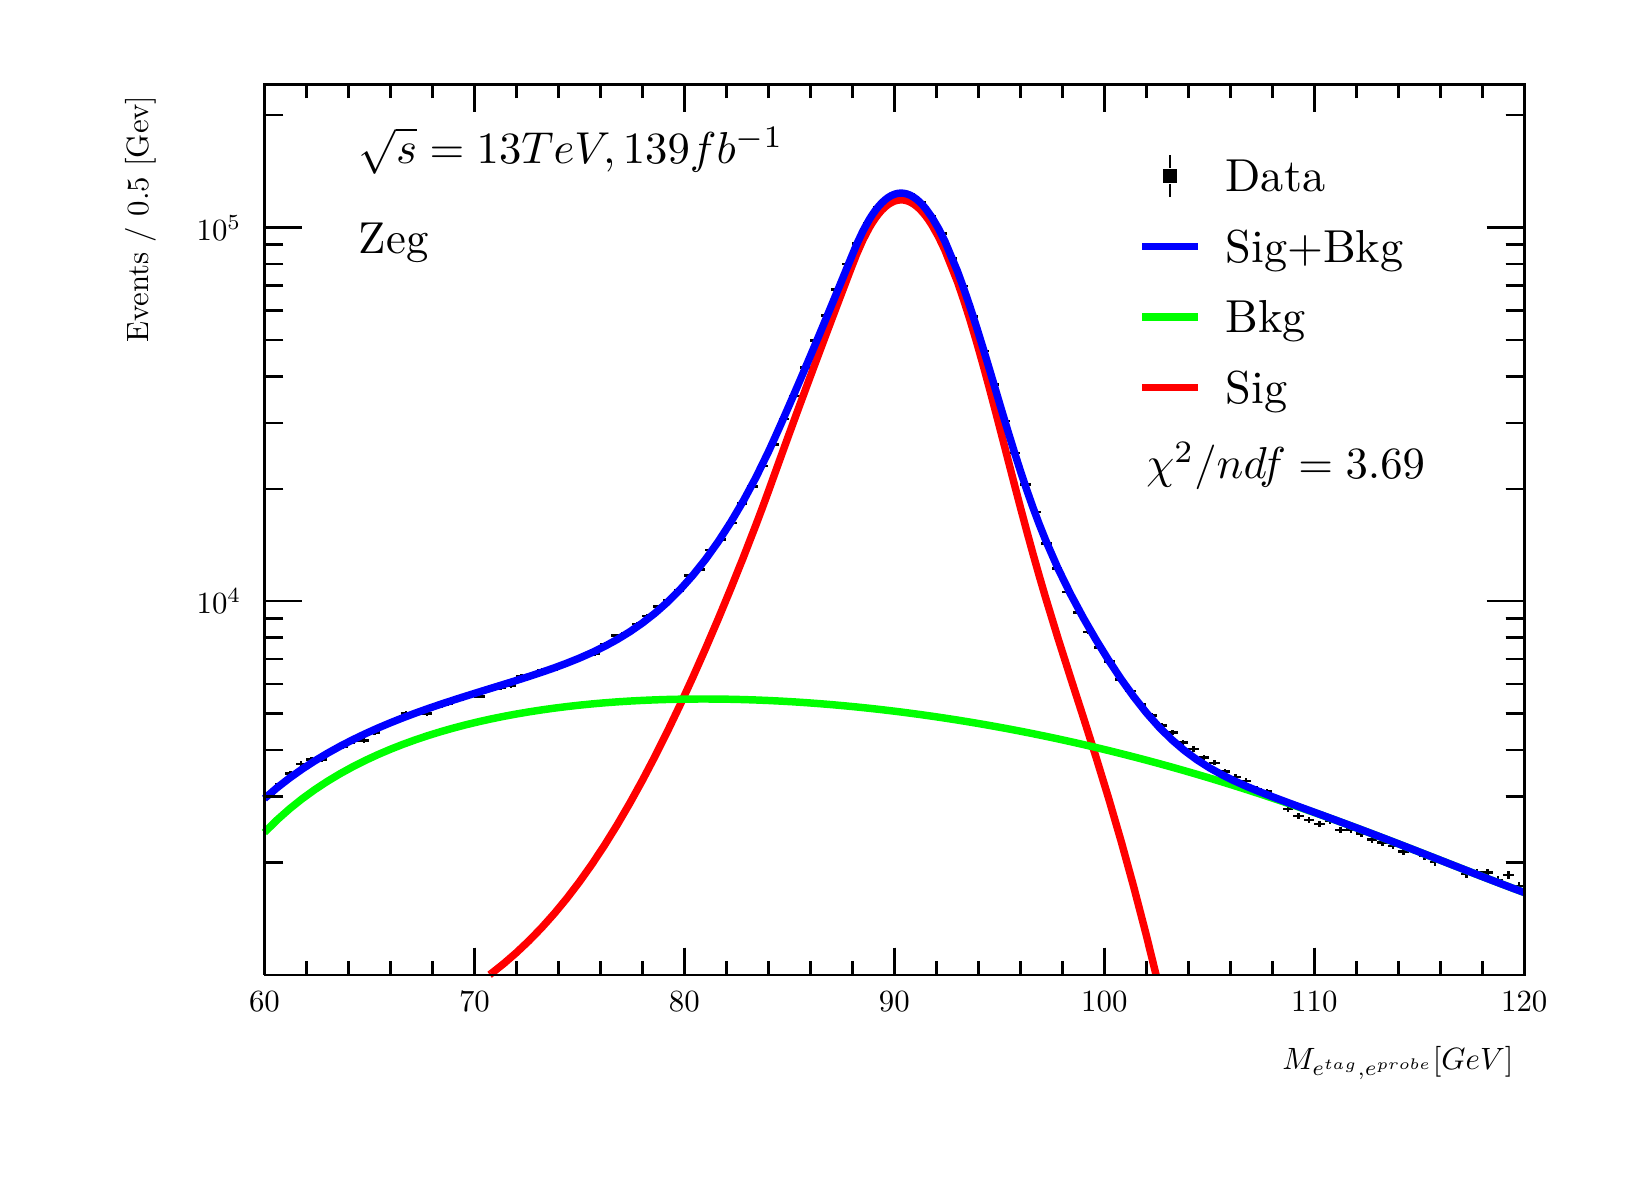
\begin{tikzpicture}
\pgfdeclareplotmark{cross} {
\pgfpathmoveto{\pgfpoint{-0.3\pgfplotmarksize}{\pgfplotmarksize}}
\pgfpathlineto{\pgfpoint{+0.3\pgfplotmarksize}{\pgfplotmarksize}}
\pgfpathlineto{\pgfpoint{+0.3\pgfplotmarksize}{0.3\pgfplotmarksize}}
\pgfpathlineto{\pgfpoint{+1\pgfplotmarksize}{0.3\pgfplotmarksize}}
\pgfpathlineto{\pgfpoint{+1\pgfplotmarksize}{-0.3\pgfplotmarksize}}
\pgfpathlineto{\pgfpoint{+0.3\pgfplotmarksize}{-0.3\pgfplotmarksize}}
\pgfpathlineto{\pgfpoint{+0.3\pgfplotmarksize}{-1.\pgfplotmarksize}}
\pgfpathlineto{\pgfpoint{-0.3\pgfplotmarksize}{-1.\pgfplotmarksize}}
\pgfpathlineto{\pgfpoint{-0.3\pgfplotmarksize}{-0.3\pgfplotmarksize}}
\pgfpathlineto{\pgfpoint{-1.\pgfplotmarksize}{-0.3\pgfplotmarksize}}
\pgfpathlineto{\pgfpoint{-1.\pgfplotmarksize}{0.3\pgfplotmarksize}}
\pgfpathlineto{\pgfpoint{-0.3\pgfplotmarksize}{0.3\pgfplotmarksize}}
\pgfpathclose
\pgfusepathqstroke
}
\pgfdeclareplotmark{cross*} {
\pgfpathmoveto{\pgfpoint{-0.3\pgfplotmarksize}{\pgfplotmarksize}}
\pgfpathlineto{\pgfpoint{+0.3\pgfplotmarksize}{\pgfplotmarksize}}
\pgfpathlineto{\pgfpoint{+0.3\pgfplotmarksize}{0.3\pgfplotmarksize}}
\pgfpathlineto{\pgfpoint{+1\pgfplotmarksize}{0.3\pgfplotmarksize}}
\pgfpathlineto{\pgfpoint{+1\pgfplotmarksize}{-0.3\pgfplotmarksize}}
\pgfpathlineto{\pgfpoint{+0.3\pgfplotmarksize}{-0.3\pgfplotmarksize}}
\pgfpathlineto{\pgfpoint{+0.3\pgfplotmarksize}{-1.\pgfplotmarksize}}
\pgfpathlineto{\pgfpoint{-0.3\pgfplotmarksize}{-1.\pgfplotmarksize}}
\pgfpathlineto{\pgfpoint{-0.3\pgfplotmarksize}{-0.3\pgfplotmarksize}}
\pgfpathlineto{\pgfpoint{-1.\pgfplotmarksize}{-0.3\pgfplotmarksize}}
\pgfpathlineto{\pgfpoint{-1.\pgfplotmarksize}{0.3\pgfplotmarksize}}
\pgfpathlineto{\pgfpoint{-0.3\pgfplotmarksize}{0.3\pgfplotmarksize}}
\pgfpathclose
\pgfusepathqfillstroke
}
\pgfdeclareplotmark{newstar} {
\pgfpathmoveto{\pgfqpoint{0pt}{\pgfplotmarksize}}
\pgfpathlineto{\pgfqpointpolar{44}{0.5\pgfplotmarksize}}
\pgfpathlineto{\pgfqpointpolar{18}{\pgfplotmarksize}}
\pgfpathlineto{\pgfqpointpolar{-20}{0.5\pgfplotmarksize}}
\pgfpathlineto{\pgfqpointpolar{-54}{\pgfplotmarksize}}
\pgfpathlineto{\pgfqpointpolar{-90}{0.5\pgfplotmarksize}}
\pgfpathlineto{\pgfqpointpolar{234}{\pgfplotmarksize}}
\pgfpathlineto{\pgfqpointpolar{198}{0.5\pgfplotmarksize}}
\pgfpathlineto{\pgfqpointpolar{162}{\pgfplotmarksize}}
\pgfpathlineto{\pgfqpointpolar{134}{0.5\pgfplotmarksize}}
\pgfpathclose
\pgfusepathqstroke
}
\pgfdeclareplotmark{newstar*} {
\pgfpathmoveto{\pgfqpoint{0pt}{\pgfplotmarksize}}
\pgfpathlineto{\pgfqpointpolar{44}{0.5\pgfplotmarksize}}
\pgfpathlineto{\pgfqpointpolar{18}{\pgfplotmarksize}}
\pgfpathlineto{\pgfqpointpolar{-20}{0.5\pgfplotmarksize}}
\pgfpathlineto{\pgfqpointpolar{-54}{\pgfplotmarksize}}
\pgfpathlineto{\pgfqpointpolar{-90}{0.5\pgfplotmarksize}}
\pgfpathlineto{\pgfqpointpolar{234}{\pgfplotmarksize}}
\pgfpathlineto{\pgfqpointpolar{198}{0.5\pgfplotmarksize}}
\pgfpathlineto{\pgfqpointpolar{162}{\pgfplotmarksize}}
\pgfpathlineto{\pgfqpointpolar{134}{0.5\pgfplotmarksize}}
\pgfpathclose
\pgfusepathqfillstroke
}
\definecolor{c}{rgb}{1,1,1};
\draw [color=c, fill=c] (0,0) rectangle (20,14.3108);
\draw [color=c, fill=c] (3,2.28972) rectangle (19,13.5952);
\definecolor{c}{rgb}{0,0,0};
\draw [c,line width=0.9] (3,2.28972) -- (3,13.5952) -- (19,13.5952) -- (19,2.28972) -- (3,2.28972);
\definecolor{c}{rgb}{1,1,1};
\draw [color=c, fill=c] (3,2.28972) rectangle (19,13.5952);
\definecolor{c}{rgb}{0,0,0};
\draw [c,line width=0.9] (3,2.28972) -- (3,13.5952) -- (19,13.5952) -- (19,2.28972) -- (3,2.28972);
\draw [c,line width=0.9] (3,2.28972) -- (19,2.28972);
\draw [c,line width=0.9] (3,2.63318) -- (3,2.28972);
\draw [c,line width=0.9] (3.53333,2.46145) -- (3.53333,2.28972);
\draw [c,line width=0.9] (4.06667,2.46145) -- (4.06667,2.28972);
\draw [c,line width=0.9] (4.6,2.46145) -- (4.6,2.28972);
\draw [c,line width=0.9] (5.13333,2.46145) -- (5.13333,2.28972);
\draw [c,line width=0.9] (5.66667,2.63318) -- (5.66667,2.28972);
\draw [c,line width=0.9] (6.2,2.46145) -- (6.2,2.28972);
\draw [c,line width=0.9] (6.73333,2.46145) -- (6.73333,2.28972);
\draw [c,line width=0.9] (7.26667,2.46145) -- (7.26667,2.28972);
\draw [c,line width=0.9] (7.8,2.46145) -- (7.8,2.28972);
\draw [c,line width=0.9] (8.33333,2.63318) -- (8.33333,2.28972);
\draw [c,line width=0.9] (8.86667,2.46145) -- (8.86667,2.28972);
\draw [c,line width=0.9] (9.4,2.46145) -- (9.4,2.28972);
\draw [c,line width=0.9] (9.93333,2.46145) -- (9.93333,2.28972);
\draw [c,line width=0.9] (10.4667,2.46145) -- (10.4667,2.28972);
\draw [c,line width=0.9] (11,2.63318) -- (11,2.28972);
\draw [c,line width=0.9] (11.5333,2.46145) -- (11.5333,2.28972);
\draw [c,line width=0.9] (12.0667,2.46145) -- (12.0667,2.28972);
\draw [c,line width=0.9] (12.6,2.46145) -- (12.6,2.28972);
\draw [c,line width=0.9] (13.1333,2.46145) -- (13.1333,2.28972);
\draw [c,line width=0.9] (13.6667,2.63318) -- (13.6667,2.28972);
\draw [c,line width=0.9] (14.2,2.46145) -- (14.2,2.28972);
\draw [c,line width=0.9] (14.7333,2.46145) -- (14.7333,2.28972);
\draw [c,line width=0.9] (15.2667,2.46145) -- (15.2667,2.28972);
\draw [c,line width=0.9] (15.8,2.46145) -- (15.8,2.28972);
\draw [c,line width=0.9] (16.3333,2.63318) -- (16.3333,2.28972);
\draw [c,line width=0.9] (16.8667,2.46145) -- (16.8667,2.28972);
\draw [c,line width=0.9] (17.4,2.46145) -- (17.4,2.28972);
\draw [c,line width=0.9] (17.9333,2.46145) -- (17.9333,2.28972);
\draw [c,line width=0.9] (18.4667,2.46145) -- (18.4667,2.28972);
\draw [c,line width=0.9] (19,2.63318) -- (19,2.28972);
\draw [anchor=base] (3,1.81747) node[scale=1.11327, color=c, rotate=0]{60};
\draw [anchor=base] (5.66667,1.81747) node[scale=1.11327, color=c, rotate=0]{70};
\draw [anchor=base] (8.33333,1.81747) node[scale=1.11327, color=c, rotate=0]{80};
\draw [anchor=base] (11,1.81747) node[scale=1.11327, color=c, rotate=0]{90};
\draw [anchor=base] (13.6667,1.81747) node[scale=1.11327, color=c, rotate=0]{100};
\draw [anchor=base] (16.3333,1.81747) node[scale=1.11327, color=c, rotate=0]{110};
\draw [anchor=base] (19,1.81747) node[scale=1.11327, color=c, rotate=0]{120};
\draw [anchor= east] (19,1.16776) node[scale=1.11327, color=c, rotate=0]{$M_{e^{tag}, e^{probe}}  [GeV]$};
\draw [c,line width=0.9] (3,13.5952) -- (19,13.5952);
\draw [c,line width=0.9] (3,13.2518) -- (3,13.5952);
\draw [c,line width=0.9] (3.53333,13.4235) -- (3.53333,13.5952);
\draw [c,line width=0.9] (4.06667,13.4235) -- (4.06667,13.5952);
\draw [c,line width=0.9] (4.6,13.4235) -- (4.6,13.5952);
\draw [c,line width=0.9] (5.13333,13.4235) -- (5.13333,13.5952);
\draw [c,line width=0.9] (5.66667,13.2518) -- (5.66667,13.5952);
\draw [c,line width=0.9] (6.2,13.4235) -- (6.2,13.5952);
\draw [c,line width=0.9] (6.73333,13.4235) -- (6.73333,13.5952);
\draw [c,line width=0.9] (7.26667,13.4235) -- (7.26667,13.5952);
\draw [c,line width=0.9] (7.8,13.4235) -- (7.8,13.5952);
\draw [c,line width=0.9] (8.33333,13.2518) -- (8.33333,13.5952);
\draw [c,line width=0.9] (8.86667,13.4235) -- (8.86667,13.5952);
\draw [c,line width=0.9] (9.4,13.4235) -- (9.4,13.5952);
\draw [c,line width=0.9] (9.93333,13.4235) -- (9.93333,13.5952);
\draw [c,line width=0.9] (10.4667,13.4235) -- (10.4667,13.5952);
\draw [c,line width=0.9] (11,13.2518) -- (11,13.5952);
\draw [c,line width=0.9] (11.5333,13.4235) -- (11.5333,13.5952);
\draw [c,line width=0.9] (12.0667,13.4235) -- (12.0667,13.5952);
\draw [c,line width=0.9] (12.6,13.4235) -- (12.6,13.5952);
\draw [c,line width=0.9] (13.1333,13.4235) -- (13.1333,13.5952);
\draw [c,line width=0.9] (13.6667,13.2518) -- (13.6667,13.5952);
\draw [c,line width=0.9] (14.2,13.4235) -- (14.2,13.5952);
\draw [c,line width=0.9] (14.7333,13.4235) -- (14.7333,13.5952);
\draw [c,line width=0.9] (15.2667,13.4235) -- (15.2667,13.5952);
\draw [c,line width=0.9] (15.8,13.4235) -- (15.8,13.5952);
\draw [c,line width=0.9] (16.3333,13.2518) -- (16.3333,13.5952);
\draw [c,line width=0.9] (16.8667,13.4235) -- (16.8667,13.5952);
\draw [c,line width=0.9] (17.4,13.4235) -- (17.4,13.5952);
\draw [c,line width=0.9] (17.9333,13.4235) -- (17.9333,13.5952);
\draw [c,line width=0.9] (18.4667,13.4235) -- (18.4667,13.5952);
\draw [c,line width=0.9] (19,13.2518) -- (19,13.5952);
\draw [c,line width=0.9] (3,2.28972) -- (3,13.5952);
\draw [c,line width=0.9] (3.237,3.71787) -- (3,3.71787);
\draw [c,line width=0.9] (3.237,4.55329) -- (3,4.55329);
\draw [c,line width=0.9] (3.237,5.14603) -- (3,5.14603);
\draw [c,line width=0.9] (3.237,5.60579) -- (3,5.60579);
\draw [c,line width=0.9] (3.237,5.98144) -- (3,5.98144);
\draw [c,line width=0.9] (3.237,6.29905) -- (3,6.29905);
\draw [c,line width=0.9] (3.237,6.57418) -- (3,6.57418);
\draw [c,line width=0.9] (3.237,6.81686) -- (3,6.81686);
\draw [c,line width=0.9] (3.474,7.03394) -- (3,7.03394);
\draw [anchor= east] (2.844,7.03394) node[scale=1.11327, color=c, rotate=0]{$10^{4}$};
\draw [c,line width=0.9] (3.237,8.4621) -- (3,8.4621);
\draw [c,line width=0.9] (3.237,9.29751) -- (3,9.29751);
\draw [c,line width=0.9] (3.237,9.89025) -- (3,9.89025);
\draw [c,line width=0.9] (3.237,10.35) -- (3,10.35);
\draw [c,line width=0.9] (3.237,10.7257) -- (3,10.7257);
\draw [c,line width=0.9] (3.237,11.0433) -- (3,11.0433);
\draw [c,line width=0.9] (3.237,11.3184) -- (3,11.3184);
\draw [c,line width=0.9] (3.237,11.5611) -- (3,11.5611);
\draw [c,line width=0.9] (3.474,11.7782) -- (3,11.7782);
\draw [anchor= east] (2.844,11.7782) node[scale=1.11327, color=c, rotate=0]{$10^{5}$};
\draw [c,line width=0.9] (3.237,13.2063) -- (3,13.2063);
\draw [anchor= east] (1.432,13.5952) node[scale=1.11327, color=c, rotate=90]{Events / 0.5 [Gev]};
\draw [c,line width=0.9] (19,2.28972) -- (19,13.5952);
\draw [c,line width=0.9] (18.763,3.71787) -- (19,3.71787);
\draw [c,line width=0.9] (18.763,4.55329) -- (19,4.55329);
\draw [c,line width=0.9] (18.763,5.14603) -- (19,5.14603);
\draw [c,line width=0.9] (18.763,5.60579) -- (19,5.60579);
\draw [c,line width=0.9] (18.763,5.98144) -- (19,5.98144);
\draw [c,line width=0.9] (18.763,6.29905) -- (19,6.29905);
\draw [c,line width=0.9] (18.763,6.57418) -- (19,6.57418);
\draw [c,line width=0.9] (18.763,6.81686) -- (19,6.81686);
\draw [c,line width=0.9] (18.526,7.03394) -- (19,7.03394);
\draw [c,line width=0.9] (18.763,8.4621) -- (19,8.4621);
\draw [c,line width=0.9] (18.763,9.29751) -- (19,9.29751);
\draw [c,line width=0.9] (18.763,9.89025) -- (19,9.89025);
\draw [c,line width=0.9] (18.763,10.35) -- (19,10.35);
\draw [c,line width=0.9] (18.763,10.7257) -- (19,10.7257);
\draw [c,line width=0.9] (18.763,11.0433) -- (19,11.0433);
\draw [c,line width=0.9] (18.763,11.3184) -- (19,11.3184);
\draw [c,line width=0.9] (18.763,11.5611) -- (19,11.5611);
\draw [c,line width=0.9] (18.526,11.7782) -- (19,11.7782);
\draw [c,line width=0.9] (18.763,13.2063) -- (19,13.2063);
\draw [c,line width=0.9] (3.06667,4.58668) -- (3,4.58668);
\draw [c,line width=0.9] (3,4.58668) -- (3,4.58668);
\draw [c,line width=0.9] (3.06667,4.58668) -- (3.13333,4.58668);
\draw [c,line width=0.9] (3.13333,4.58668) -- (3.13333,4.58668);
\draw [c,line width=0.9] (3.06667,4.58668) -- (3.06667,4.62399);
\draw [c,line width=0.9] (3.06667,4.62399) -- (3.06667,4.62399);
\draw [c,line width=0.9] (3.06667,4.58668) -- (3.06667,4.54936);
\draw [c,line width=0.9] (3.06667,4.54936) -- (3.06667,4.54936);
\draw [c,line width=0.9] (3.2,4.70486) -- (3.13333,4.70486);
\draw [c,line width=0.9] (3.13333,4.70486) -- (3.13333,4.70486);
\draw [c,line width=0.9] (3.2,4.70486) -- (3.26667,4.70486);
\draw [c,line width=0.9] (3.26667,4.70486) -- (3.26667,4.70486);
\draw [c,line width=0.9] (3.2,4.70486) -- (3.2,4.74112);
\draw [c,line width=0.9] (3.2,4.74112) -- (3.2,4.74112);
\draw [c,line width=0.9] (3.2,4.70486) -- (3.2,4.6686);
\draw [c,line width=0.9] (3.2,4.6686) -- (3.2,4.6686);
\draw [c,line width=0.9] (3.33333,4.84543) -- (3.26667,4.84543);
\draw [c,line width=0.9] (3.26667,4.84543) -- (3.26667,4.84543);
\draw [c,line width=0.9] (3.33333,4.84543) -- (3.4,4.84543);
\draw [c,line width=0.9] (3.4,4.84543) -- (3.4,4.84543);
\draw [c,line width=0.9] (3.33333,4.84543) -- (3.33333,4.88048);
\draw [c,line width=0.9] (3.33333,4.88048) -- (3.33333,4.88048);
\draw [c,line width=0.9] (3.33333,4.84543) -- (3.33333,4.81039);
\draw [c,line width=0.9] (3.33333,4.81039) -- (3.33333,4.81039);
\draw [c,line width=0.9] (3.46667,4.9675) -- (3.4,4.9675);
\draw [c,line width=0.9] (3.4,4.9675) -- (3.4,4.9675);
\draw [c,line width=0.9] (3.46667,4.9675) -- (3.53333,4.9675);
\draw [c,line width=0.9] (3.53333,4.9675) -- (3.53333,4.9675);
\draw [c,line width=0.9] (3.46667,4.9675) -- (3.46667,5.00152);
\draw [c,line width=0.9] (3.46667,5.00152) -- (3.46667,5.00152);
\draw [c,line width=0.9] (3.46667,4.9675) -- (3.46667,4.93348);
\draw [c,line width=0.9] (3.46667,4.93348) -- (3.46667,4.93348);
\draw [c,line width=0.9] (3.6,5.02566) -- (3.53333,5.02566);
\draw [c,line width=0.9] (3.53333,5.02566) -- (3.53333,5.02566);
\draw [c,line width=0.9] (3.6,5.02566) -- (3.66667,5.02566);
\draw [c,line width=0.9] (3.66667,5.02566) -- (3.66667,5.02566);
\draw [c,line width=0.9] (3.6,5.02566) -- (3.6,5.0592);
\draw [c,line width=0.9] (3.6,5.0592) -- (3.6,5.0592);
\draw [c,line width=0.9] (3.6,5.02566) -- (3.6,4.99211);
\draw [c,line width=0.9] (3.6,4.99211) -- (3.6,4.99211);
\draw [c,line width=0.9] (3.73333,5.02566) -- (3.66667,5.02566);
\draw [c,line width=0.9] (3.66667,5.02566) -- (3.66667,5.02566);
\draw [c,line width=0.9] (3.73333,5.02566) -- (3.8,5.02566);
\draw [c,line width=0.9] (3.8,5.02566) -- (3.8,5.02566);
\draw [c,line width=0.9] (3.73333,5.02566) -- (3.73333,5.0592);
\draw [c,line width=0.9] (3.73333,5.0592) -- (3.73333,5.0592);
\draw [c,line width=0.9] (3.73333,5.02566) -- (3.73333,4.99211);
\draw [c,line width=0.9] (3.73333,4.99211) -- (3.73333,4.99211);
\draw [c,line width=0.9] (3.86667,5.14552) -- (3.8,5.14552);
\draw [c,line width=0.9] (3.8,5.14552) -- (3.8,5.14552);
\draw [c,line width=0.9] (3.86667,5.14552) -- (3.93333,5.14552);
\draw [c,line width=0.9] (3.93333,5.14552) -- (3.93333,5.14552);
\draw [c,line width=0.9] (3.86667,5.14552) -- (3.86667,5.1781);
\draw [c,line width=0.9] (3.86667,5.1781) -- (3.86667,5.1781);
\draw [c,line width=0.9] (3.86667,5.14552) -- (3.86667,5.11293);
\draw [c,line width=0.9] (3.86667,5.11293) -- (3.86667,5.11293);
\draw [c,line width=0.9] (4,5.18633) -- (3.93333,5.18633);
\draw [c,line width=0.9] (3.93333,5.18633) -- (3.93333,5.18633);
\draw [c,line width=0.9] (4,5.18633) -- (4.06667,5.18633);
\draw [c,line width=0.9] (4.06667,5.18633) -- (4.06667,5.18633);
\draw [c,line width=0.9] (4,5.18633) -- (4,5.21859);
\draw [c,line width=0.9] (4,5.21859) -- (4,5.21859);
\draw [c,line width=0.9] (4,5.18633) -- (4,5.15407);
\draw [c,line width=0.9] (4,5.15407) -- (4,5.15407);
\draw [c,line width=0.9] (4.13333,5.25732) -- (4.06667,5.25732);
\draw [c,line width=0.9] (4.06667,5.25732) -- (4.06667,5.25732);
\draw [c,line width=0.9] (4.13333,5.25732) -- (4.2,5.25732);
\draw [c,line width=0.9] (4.2,5.25732) -- (4.2,5.25732);
\draw [c,line width=0.9] (4.13333,5.25732) -- (4.13333,5.28903);
\draw [c,line width=0.9] (4.13333,5.28903) -- (4.13333,5.28903);
\draw [c,line width=0.9] (4.13333,5.25732) -- (4.13333,5.22561);
\draw [c,line width=0.9] (4.13333,5.22561) -- (4.13333,5.22561);
\draw [c,line width=0.9] (4.26667,5.26706) -- (4.2,5.26706);
\draw [c,line width=0.9] (4.2,5.26706) -- (4.2,5.26706);
\draw [c,line width=0.9] (4.26667,5.26706) -- (4.33333,5.26706);
\draw [c,line width=0.9] (4.33333,5.26706) -- (4.33333,5.26706);
\draw [c,line width=0.9] (4.26667,5.26706) -- (4.26667,5.29869);
\draw [c,line width=0.9] (4.26667,5.29869) -- (4.26667,5.29869);
\draw [c,line width=0.9] (4.26667,5.26706) -- (4.26667,5.23542);
\draw [c,line width=0.9] (4.26667,5.23542) -- (4.26667,5.23542);
\draw [c,line width=0.9] (4.4,5.36337) -- (4.33333,5.36337);
\draw [c,line width=0.9] (4.33333,5.36337) -- (4.33333,5.36337);
\draw [c,line width=0.9] (4.4,5.36337) -- (4.46667,5.36337);
\draw [c,line width=0.9] (4.46667,5.36337) -- (4.46667,5.36337);
\draw [c,line width=0.9] (4.4,5.36337) -- (4.4,5.39428);
\draw [c,line width=0.9] (4.4,5.39428) -- (4.4,5.39428);
\draw [c,line width=0.9] (4.4,5.36337) -- (4.4,5.33247);
\draw [c,line width=0.9] (4.4,5.33247) -- (4.4,5.33247);
\draw [c,line width=0.9] (4.53333,5.4465) -- (4.46667,5.4465);
\draw [c,line width=0.9] (4.46667,5.4465) -- (4.46667,5.4465);
\draw [c,line width=0.9] (4.53333,5.4465) -- (4.6,5.4465);
\draw [c,line width=0.9] (4.6,5.4465) -- (4.6,5.4465);
\draw [c,line width=0.9] (4.53333,5.4465) -- (4.53333,5.47679);
\draw [c,line width=0.9] (4.53333,5.47679) -- (4.53333,5.47679);
\draw [c,line width=0.9] (4.53333,5.4465) -- (4.53333,5.41621);
\draw [c,line width=0.9] (4.53333,5.41621) -- (4.53333,5.41621);
\draw [c,line width=0.9] (4.66667,5.52597) -- (4.6,5.52597);
\draw [c,line width=0.9] (4.6,5.52597) -- (4.6,5.52597);
\draw [c,line width=0.9] (4.66667,5.52597) -- (4.73333,5.52597);
\draw [c,line width=0.9] (4.73333,5.52597) -- (4.73333,5.52597);
\draw [c,line width=0.9] (4.66667,5.52597) -- (4.66667,5.55568);
\draw [c,line width=0.9] (4.66667,5.55568) -- (4.66667,5.55568);
\draw [c,line width=0.9] (4.66667,5.52597) -- (4.66667,5.49626);
\draw [c,line width=0.9] (4.66667,5.49626) -- (4.66667,5.49626);
\draw [c,line width=0.9] (4.8,5.60538) -- (4.73333,5.60538);
\draw [c,line width=0.9] (4.73333,5.60538) -- (4.73333,5.60538);
\draw [c,line width=0.9] (4.8,5.60538) -- (4.86667,5.60538);
\draw [c,line width=0.9] (4.86667,5.60538) -- (4.86667,5.60538);
\draw [c,line width=0.9] (4.8,5.60538) -- (4.8,5.63452);
\draw [c,line width=0.9] (4.8,5.63452) -- (4.8,5.63452);
\draw [c,line width=0.9] (4.8,5.60538) -- (4.8,5.57624);
\draw [c,line width=0.9] (4.8,5.57624) -- (4.8,5.57624);
\draw [c,line width=0.9] (4.93333,5.62548) -- (4.86667,5.62548);
\draw [c,line width=0.9] (4.86667,5.62548) -- (4.86667,5.62548);
\draw [c,line width=0.9] (4.93333,5.62548) -- (5,5.62548);
\draw [c,line width=0.9] (5,5.62548) -- (5,5.62548);
\draw [c,line width=0.9] (4.93333,5.62548) -- (4.93333,5.65448);
\draw [c,line width=0.9] (4.93333,5.65448) -- (4.93333,5.65448);
\draw [c,line width=0.9] (4.93333,5.62548) -- (4.93333,5.59648);
\draw [c,line width=0.9] (4.93333,5.59648) -- (4.93333,5.59648);
\draw [c,line width=0.9] (5.06667,5.60868) -- (5,5.60868);
\draw [c,line width=0.9] (5,5.60868) -- (5,5.60868);
\draw [c,line width=0.9] (5.06667,5.60868) -- (5.13333,5.60868);
\draw [c,line width=0.9] (5.13333,5.60868) -- (5.13333,5.60868);
\draw [c,line width=0.9] (5.06667,5.60868) -- (5.06667,5.63779);
\draw [c,line width=0.9] (5.06667,5.63779) -- (5.06667,5.63779);
\draw [c,line width=0.9] (5.06667,5.60868) -- (5.06667,5.57956);
\draw [c,line width=0.9] (5.06667,5.57956) -- (5.06667,5.57956);
\draw [c,line width=0.9] (5.2,5.6874) -- (5.13333,5.6874);
\draw [c,line width=0.9] (5.13333,5.6874) -- (5.13333,5.6874);
\draw [c,line width=0.9] (5.2,5.6874) -- (5.26667,5.6874);
\draw [c,line width=0.9] (5.26667,5.6874) -- (5.26667,5.6874);
\draw [c,line width=0.9] (5.2,5.6874) -- (5.2,5.71596);
\draw [c,line width=0.9] (5.2,5.71596) -- (5.2,5.71596);
\draw [c,line width=0.9] (5.2,5.6874) -- (5.2,5.65883);
\draw [c,line width=0.9] (5.2,5.65883) -- (5.2,5.65883);
\draw [c,line width=0.9] (5.33333,5.72702) -- (5.26667,5.72702);
\draw [c,line width=0.9] (5.26667,5.72702) -- (5.26667,5.72702);
\draw [c,line width=0.9] (5.33333,5.72702) -- (5.4,5.72702);
\draw [c,line width=0.9] (5.4,5.72702) -- (5.4,5.72702);
\draw [c,line width=0.9] (5.33333,5.72702) -- (5.33333,5.75531);
\draw [c,line width=0.9] (5.33333,5.75531) -- (5.33333,5.75531);
\draw [c,line width=0.9] (5.33333,5.72702) -- (5.33333,5.69872);
\draw [c,line width=0.9] (5.33333,5.69872) -- (5.33333,5.69872);
\draw [c,line width=0.9] (5.46667,5.78411) -- (5.4,5.78411);
\draw [c,line width=0.9] (5.4,5.78411) -- (5.4,5.78411);
\draw [c,line width=0.9] (5.46667,5.78411) -- (5.53333,5.78411);
\draw [c,line width=0.9] (5.53333,5.78411) -- (5.53333,5.78411);
\draw [c,line width=0.9] (5.46667,5.78411) -- (5.46667,5.81201);
\draw [c,line width=0.9] (5.46667,5.81201) -- (5.46667,5.81201);
\draw [c,line width=0.9] (5.46667,5.78411) -- (5.46667,5.75621);
\draw [c,line width=0.9] (5.46667,5.75621) -- (5.46667,5.75621);
\draw [c,line width=0.9] (5.6,5.83709) -- (5.53333,5.83709);
\draw [c,line width=0.9] (5.53333,5.83709) -- (5.53333,5.83709);
\draw [c,line width=0.9] (5.6,5.83709) -- (5.66667,5.83709);
\draw [c,line width=0.9] (5.66667,5.83709) -- (5.66667,5.83709);
\draw [c,line width=0.9] (5.6,5.83709) -- (5.6,5.86463);
\draw [c,line width=0.9] (5.6,5.86463) -- (5.6,5.86463);
\draw [c,line width=0.9] (5.6,5.83709) -- (5.6,5.80954);
\draw [c,line width=0.9] (5.6,5.80954) -- (5.6,5.80954);
\draw [c,line width=0.9] (5.73333,5.82675) -- (5.66667,5.82675);
\draw [c,line width=0.9] (5.66667,5.82675) -- (5.66667,5.82675);
\draw [c,line width=0.9] (5.73333,5.82675) -- (5.8,5.82675);
\draw [c,line width=0.9] (5.8,5.82675) -- (5.8,5.82675);
\draw [c,line width=0.9] (5.73333,5.82675) -- (5.73333,5.85436);
\draw [c,line width=0.9] (5.73333,5.85436) -- (5.73333,5.85436);
\draw [c,line width=0.9] (5.73333,5.82675) -- (5.73333,5.79913);
\draw [c,line width=0.9] (5.73333,5.79913) -- (5.73333,5.79913);
\draw [c,line width=0.9] (5.86667,5.9116) -- (5.8,5.9116);
\draw [c,line width=0.9] (5.8,5.9116) -- (5.8,5.9116);
\draw [c,line width=0.9] (5.86667,5.9116) -- (5.93333,5.9116);
\draw [c,line width=0.9] (5.93333,5.9116) -- (5.93333,5.9116);
\draw [c,line width=0.9] (5.86667,5.9116) -- (5.86667,5.93865);
\draw [c,line width=0.9] (5.86667,5.93865) -- (5.86667,5.93865);
\draw [c,line width=0.9] (5.86667,5.9116) -- (5.86667,5.88454);
\draw [c,line width=0.9] (5.86667,5.88454) -- (5.86667,5.88454);
\draw [c,line width=0.9] (6,5.93702) -- (5.93333,5.93702);
\draw [c,line width=0.9] (5.93333,5.93702) -- (5.93333,5.93702);
\draw [c,line width=0.9] (6,5.93702) -- (6.06667,5.93702);
\draw [c,line width=0.9] (6.06667,5.93702) -- (6.06667,5.93702);
\draw [c,line width=0.9] (6,5.93702) -- (6,5.9639);
\draw [c,line width=0.9] (6,5.9639) -- (6,5.9639);
\draw [c,line width=0.9] (6,5.93702) -- (6,5.91013);
\draw [c,line width=0.9] (6,5.91013) -- (6,5.91013);
\draw [c,line width=0.9] (6.13333,5.96247) -- (6.06667,5.96247);
\draw [c,line width=0.9] (6.06667,5.96247) -- (6.06667,5.96247);
\draw [c,line width=0.9] (6.13333,5.96247) -- (6.2,5.96247);
\draw [c,line width=0.9] (6.2,5.96247) -- (6.2,5.96247);
\draw [c,line width=0.9] (6.13333,5.96247) -- (6.13333,5.9892);
\draw [c,line width=0.9] (6.13333,5.9892) -- (6.13333,5.9892);
\draw [c,line width=0.9] (6.13333,5.96247) -- (6.13333,5.93575);
\draw [c,line width=0.9] (6.13333,5.93575) -- (6.13333,5.93575);
\draw [c,line width=0.9] (6.26667,6.0823) -- (6.2,6.0823);
\draw [c,line width=0.9] (6.2,6.0823) -- (6.2,6.0823);
\draw [c,line width=0.9] (6.26667,6.0823) -- (6.33333,6.0823);
\draw [c,line width=0.9] (6.33333,6.0823) -- (6.33333,6.0823);
\draw [c,line width=0.9] (6.26667,6.0823) -- (6.26667,6.10826);
\draw [c,line width=0.9] (6.26667,6.10826) -- (6.26667,6.10826);
\draw [c,line width=0.9] (6.26667,6.0823) -- (6.26667,6.05634);
\draw [c,line width=0.9] (6.26667,6.05634) -- (6.26667,6.05634);
\draw [c,line width=0.9] (6.4,6.1083) -- (6.33333,6.1083);
\draw [c,line width=0.9] (6.33333,6.1083) -- (6.33333,6.1083);
\draw [c,line width=0.9] (6.4,6.1083) -- (6.46667,6.1083);
\draw [c,line width=0.9] (6.46667,6.1083) -- (6.46667,6.1083);
\draw [c,line width=0.9] (6.4,6.1083) -- (6.4,6.13409);
\draw [c,line width=0.9] (6.4,6.13409) -- (6.4,6.13409);
\draw [c,line width=0.9] (6.4,6.1083) -- (6.4,6.0825);
\draw [c,line width=0.9] (6.4,6.0825) -- (6.4,6.0825);
\draw [c,line width=0.9] (6.53333,6.15428) -- (6.46667,6.15428);
\draw [c,line width=0.9] (6.46667,6.15428) -- (6.46667,6.15428);
\draw [c,line width=0.9] (6.53333,6.15428) -- (6.6,6.15428);
\draw [c,line width=0.9] (6.6,6.15428) -- (6.6,6.15428);
\draw [c,line width=0.9] (6.53333,6.15428) -- (6.53333,6.17978);
\draw [c,line width=0.9] (6.53333,6.17978) -- (6.53333,6.17978);
\draw [c,line width=0.9] (6.53333,6.15428) -- (6.53333,6.12877);
\draw [c,line width=0.9] (6.53333,6.12877) -- (6.53333,6.12877);
\draw [c,line width=0.9] (6.66667,6.15901) -- (6.6,6.15901);
\draw [c,line width=0.9] (6.6,6.15901) -- (6.6,6.15901);
\draw [c,line width=0.9] (6.66667,6.15901) -- (6.73333,6.15901);
\draw [c,line width=0.9] (6.73333,6.15901) -- (6.73333,6.15901);
\draw [c,line width=0.9] (6.66667,6.15901) -- (6.66667,6.18448);
\draw [c,line width=0.9] (6.66667,6.18448) -- (6.66667,6.18448);
\draw [c,line width=0.9] (6.66667,6.15901) -- (6.66667,6.13353);
\draw [c,line width=0.9] (6.66667,6.13353) -- (6.66667,6.13353);
\draw [c,line width=0.9] (6.8,6.23569) -- (6.73333,6.23569);
\draw [c,line width=0.9] (6.73333,6.23569) -- (6.73333,6.23569);
\draw [c,line width=0.9] (6.8,6.23569) -- (6.86667,6.23569);
\draw [c,line width=0.9] (6.86667,6.23569) -- (6.86667,6.23569);
\draw [c,line width=0.9] (6.8,6.23569) -- (6.8,6.2607);
\draw [c,line width=0.9] (6.8,6.2607) -- (6.8,6.2607);
\draw [c,line width=0.9] (6.8,6.23569) -- (6.8,6.21069);
\draw [c,line width=0.9] (6.8,6.21069) -- (6.8,6.21069);
\draw [c,line width=0.9] (6.93333,6.28013) -- (6.86667,6.28013);
\draw [c,line width=0.9] (6.86667,6.28013) -- (6.86667,6.28013);
\draw [c,line width=0.9] (6.93333,6.28013) -- (7,6.28013);
\draw [c,line width=0.9] (7,6.28013) -- (7,6.28013);
\draw [c,line width=0.9] (6.93333,6.28013) -- (6.93333,6.30487);
\draw [c,line width=0.9] (6.93333,6.30487) -- (6.93333,6.30487);
\draw [c,line width=0.9] (6.93333,6.28013) -- (6.93333,6.25539);
\draw [c,line width=0.9] (6.93333,6.25539) -- (6.93333,6.25539);
\draw [c,line width=0.9] (7.06667,6.34217) -- (7,6.34217);
\draw [c,line width=0.9] (7,6.34217) -- (7,6.34217);
\draw [c,line width=0.9] (7.06667,6.34217) -- (7.13333,6.34217);
\draw [c,line width=0.9] (7.13333,6.34217) -- (7.13333,6.34217);
\draw [c,line width=0.9] (7.06667,6.34217) -- (7.06667,6.36654);
\draw [c,line width=0.9] (7.06667,6.36654) -- (7.06667,6.36654);
\draw [c,line width=0.9] (7.06667,6.34217) -- (7.06667,6.3178);
\draw [c,line width=0.9] (7.06667,6.3178) -- (7.06667,6.3178);
\draw [c,line width=0.9] (7.2,6.3631) -- (7.13333,6.3631);
\draw [c,line width=0.9] (7.13333,6.3631) -- (7.13333,6.3631);
\draw [c,line width=0.9] (7.2,6.3631) -- (7.26667,6.3631);
\draw [c,line width=0.9] (7.26667,6.3631) -- (7.26667,6.3631);
\draw [c,line width=0.9] (7.2,6.3631) -- (7.2,6.38735);
\draw [c,line width=0.9] (7.2,6.38735) -- (7.2,6.38735);
\draw [c,line width=0.9] (7.2,6.3631) -- (7.2,6.33886);
\draw [c,line width=0.9] (7.2,6.33886) -- (7.2,6.33886);
\draw [c,line width=0.9] (7.33333,6.48766) -- (7.26667,6.48766);
\draw [c,line width=0.9] (7.26667,6.48766) -- (7.26667,6.48766);
\draw [c,line width=0.9] (7.33333,6.48766) -- (7.4,6.48766);
\draw [c,line width=0.9] (7.4,6.48766) -- (7.4,6.48766);
\draw [c,line width=0.9] (7.33333,6.48766) -- (7.33333,6.51118);
\draw [c,line width=0.9] (7.33333,6.51118) -- (7.33333,6.51118);
\draw [c,line width=0.9] (7.33333,6.48766) -- (7.33333,6.46413);
\draw [c,line width=0.9] (7.33333,6.46413) -- (7.33333,6.46413);
\draw [c,line width=0.9] (7.46667,6.59672) -- (7.4,6.59672);
\draw [c,line width=0.9] (7.4,6.59672) -- (7.4,6.59672);
\draw [c,line width=0.9] (7.46667,6.59672) -- (7.53333,6.59672);
\draw [c,line width=0.9] (7.53333,6.59672) -- (7.53333,6.59672);
\draw [c,line width=0.9] (7.46667,6.59672) -- (7.46667,6.61964);
\draw [c,line width=0.9] (7.46667,6.61964) -- (7.46667,6.61964);
\draw [c,line width=0.9] (7.46667,6.59672) -- (7.46667,6.57381);
\draw [c,line width=0.9] (7.46667,6.57381) -- (7.46667,6.57381);
\draw [c,line width=0.9] (7.6,6.62858) -- (7.53333,6.62858);
\draw [c,line width=0.9] (7.53333,6.62858) -- (7.53333,6.62858);
\draw [c,line width=0.9] (7.6,6.62858) -- (7.66667,6.62858);
\draw [c,line width=0.9] (7.66667,6.62858) -- (7.66667,6.62858);
\draw [c,line width=0.9] (7.6,6.62858) -- (7.6,6.65131);
\draw [c,line width=0.9] (7.6,6.65131) -- (7.6,6.65131);
\draw [c,line width=0.9] (7.6,6.62858) -- (7.6,6.60584);
\draw [c,line width=0.9] (7.6,6.60584) -- (7.6,6.60584);
\draw [c,line width=0.9] (7.73333,6.7463) -- (7.66667,6.7463);
\draw [c,line width=0.9] (7.66667,6.7463) -- (7.66667,6.7463);
\draw [c,line width=0.9] (7.73333,6.7463) -- (7.8,6.7463);
\draw [c,line width=0.9] (7.8,6.7463) -- (7.8,6.7463);
\draw [c,line width=0.9] (7.73333,6.7463) -- (7.73333,6.7684);
\draw [c,line width=0.9] (7.73333,6.7684) -- (7.73333,6.7684);
\draw [c,line width=0.9] (7.73333,6.7463) -- (7.73333,6.72421);
\draw [c,line width=0.9] (7.73333,6.72421) -- (7.73333,6.72421);
\draw [c,line width=0.9] (7.86667,6.84664) -- (7.8,6.84664);
\draw [c,line width=0.9] (7.8,6.84664) -- (7.8,6.84664);
\draw [c,line width=0.9] (7.86667,6.84664) -- (7.93333,6.84664);
\draw [c,line width=0.9] (7.93333,6.84664) -- (7.93333,6.84664);
\draw [c,line width=0.9] (7.86667,6.84664) -- (7.86667,6.8682);
\draw [c,line width=0.9] (7.86667,6.8682) -- (7.86667,6.8682);
\draw [c,line width=0.9] (7.86667,6.84664) -- (7.86667,6.82508);
\draw [c,line width=0.9] (7.86667,6.82508) -- (7.86667,6.82508);
\draw [c,line width=0.9] (8,6.96928) -- (7.93333,6.96928);
\draw [c,line width=0.9] (7.93333,6.96928) -- (7.93333,6.96928);
\draw [c,line width=0.9] (8,6.96928) -- (8.06667,6.96928);
\draw [c,line width=0.9] (8.06667,6.96928) -- (8.06667,6.96928);
\draw [c,line width=0.9] (8,6.96928) -- (8,6.99021);
\draw [c,line width=0.9] (8,6.99021) -- (8,6.99021);
\draw [c,line width=0.9] (8,6.96928) -- (8,6.94835);
\draw [c,line width=0.9] (8,6.94835) -- (8,6.94835);
\draw [c,line width=0.9] (8.13333,7.04607) -- (8.06667,7.04607);
\draw [c,line width=0.9] (8.06667,7.04607) -- (8.06667,7.04607);
\draw [c,line width=0.9] (8.13333,7.04607) -- (8.2,7.04607);
\draw [c,line width=0.9] (8.2,7.04607) -- (8.2,7.04607);
\draw [c,line width=0.9] (8.13333,7.04607) -- (8.13333,7.06661);
\draw [c,line width=0.9] (8.13333,7.06661) -- (8.13333,7.06661);
\draw [c,line width=0.9] (8.13333,7.04607) -- (8.13333,7.02552);
\draw [c,line width=0.9] (8.13333,7.02552) -- (8.13333,7.02552);
\draw [c,line width=0.9] (8.26667,7.16969) -- (8.2,7.16969);
\draw [c,line width=0.9] (8.2,7.16969) -- (8.2,7.16969);
\draw [c,line width=0.9] (8.26667,7.16969) -- (8.33333,7.16969);
\draw [c,line width=0.9] (8.33333,7.16969) -- (8.33333,7.16969);
\draw [c,line width=0.9] (8.26667,7.16969) -- (8.26667,7.18962);
\draw [c,line width=0.9] (8.26667,7.18962) -- (8.26667,7.18962);
\draw [c,line width=0.9] (8.26667,7.16969) -- (8.26667,7.14975);
\draw [c,line width=0.9] (8.26667,7.14975) -- (8.26667,7.14975);
\draw [c,line width=0.9] (8.4,7.35832) -- (8.33333,7.35832);
\draw [c,line width=0.9] (8.33333,7.35832) -- (8.33333,7.35832);
\draw [c,line width=0.9] (8.4,7.35832) -- (8.46667,7.35832);
\draw [c,line width=0.9] (8.46667,7.35832) -- (8.46667,7.35832);
\draw [c,line width=0.9] (8.4,7.35832) -- (8.4,7.37736);
\draw [c,line width=0.9] (8.4,7.37736) -- (8.4,7.37736);
\draw [c,line width=0.9] (8.4,7.35832) -- (8.4,7.33927);
\draw [c,line width=0.9] (8.4,7.33927) -- (8.4,7.33927);
\draw [c,line width=0.9] (8.53333,7.43486) -- (8.46667,7.43486);
\draw [c,line width=0.9] (8.46667,7.43486) -- (8.46667,7.43486);
\draw [c,line width=0.9] (8.53333,7.43486) -- (8.6,7.43486);
\draw [c,line width=0.9] (8.6,7.43486) -- (8.6,7.43486);
\draw [c,line width=0.9] (8.53333,7.43486) -- (8.53333,7.45355);
\draw [c,line width=0.9] (8.53333,7.45355) -- (8.53333,7.45355);
\draw [c,line width=0.9] (8.53333,7.43486) -- (8.53333,7.41616);
\draw [c,line width=0.9] (8.53333,7.41616) -- (8.53333,7.41616);
\draw [c,line width=0.9] (8.66667,7.68649) -- (8.6,7.68649);
\draw [c,line width=0.9] (8.6,7.68649) -- (8.6,7.68649);
\draw [c,line width=0.9] (8.66667,7.68649) -- (8.73333,7.68649);
\draw [c,line width=0.9] (8.73333,7.68649) -- (8.73333,7.68649);
\draw [c,line width=0.9] (8.66667,7.68649) -- (8.66667,7.70407);
\draw [c,line width=0.9] (8.66667,7.70407) -- (8.66667,7.70407);
\draw [c,line width=0.9] (8.66667,7.68649) -- (8.66667,7.6689);
\draw [c,line width=0.9] (8.66667,7.6689) -- (8.66667,7.6689);
\draw [c,line width=0.9] (8.8,7.81593) -- (8.73333,7.81593);
\draw [c,line width=0.9] (8.73333,7.81593) -- (8.73333,7.81593);
\draw [c,line width=0.9] (8.8,7.81593) -- (8.86667,7.81593);
\draw [c,line width=0.9] (8.86667,7.81593) -- (8.86667,7.81593);
\draw [c,line width=0.9] (8.8,7.81593) -- (8.8,7.83297);
\draw [c,line width=0.9] (8.8,7.83297) -- (8.8,7.83297);
\draw [c,line width=0.9] (8.8,7.81593) -- (8.8,7.79889);
\draw [c,line width=0.9] (8.8,7.79889) -- (8.8,7.79889);
\draw [c,line width=0.9] (8.93333,8.02679) -- (8.86667,8.02679);
\draw [c,line width=0.9] (8.86667,8.02679) -- (8.86667,8.02679);
\draw [c,line width=0.9] (8.93333,8.02679) -- (9,8.02679);
\draw [c,line width=0.9] (9,8.02679) -- (9,8.02679);
\draw [c,line width=0.9] (8.93333,8.02679) -- (8.93333,8.04298);
\draw [c,line width=0.9] (8.93333,8.04298) -- (8.93333,8.04298);
\draw [c,line width=0.9] (8.93333,8.02679) -- (8.93333,8.0106);
\draw [c,line width=0.9] (8.93333,8.0106) -- (8.93333,8.0106);
\draw [c,line width=0.9] (9.06667,8.27716) -- (9,8.27716);
\draw [c,line width=0.9] (9,8.27716) -- (9,8.27716);
\draw [c,line width=0.9] (9.06667,8.27716) -- (9.13333,8.27716);
\draw [c,line width=0.9] (9.13333,8.27716) -- (9.13333,8.27716);
\draw [c,line width=0.9] (9.06667,8.27716) -- (9.06667,8.2924);
\draw [c,line width=0.9] (9.06667,8.2924) -- (9.06667,8.2924);
\draw [c,line width=0.9] (9.06667,8.27716) -- (9.06667,8.26192);
\draw [c,line width=0.9] (9.06667,8.26192) -- (9.06667,8.26192);
\draw [c,line width=0.9] (9.2,8.49146) -- (9.13333,8.49146);
\draw [c,line width=0.9] (9.13333,8.49146) -- (9.13333,8.49146);
\draw [c,line width=0.9] (9.2,8.49146) -- (9.26667,8.49146);
\draw [c,line width=0.9] (9.26667,8.49146) -- (9.26667,8.49146);
\draw [c,line width=0.9] (9.2,8.49146) -- (9.2,8.50592);
\draw [c,line width=0.9] (9.2,8.50592) -- (9.2,8.50592);
\draw [c,line width=0.9] (9.2,8.49146) -- (9.2,8.47699);
\draw [c,line width=0.9] (9.2,8.47699) -- (9.2,8.47699);
\draw [c,line width=0.9] (9.33333,8.7506) -- (9.26667,8.7506);
\draw [c,line width=0.9] (9.26667,8.7506) -- (9.26667,8.7506);
\draw [c,line width=0.9] (9.33333,8.7506) -- (9.4,8.7506);
\draw [c,line width=0.9] (9.4,8.7506) -- (9.4,8.7506);
\draw [c,line width=0.9] (9.33333,8.7506) -- (9.33333,8.76419);
\draw [c,line width=0.9] (9.33333,8.76419) -- (9.33333,8.76419);
\draw [c,line width=0.9] (9.33333,8.7506) -- (9.33333,8.73702);
\draw [c,line width=0.9] (9.33333,8.73702) -- (9.33333,8.73702);
\draw [c,line width=0.9] (9.46667,9.02223) -- (9.4,9.02223);
\draw [c,line width=0.9] (9.4,9.02223) -- (9.4,9.02223);
\draw [c,line width=0.9] (9.46667,9.02223) -- (9.53333,9.02223);
\draw [c,line width=0.9] (9.53333,9.02223) -- (9.53333,9.02223);
\draw [c,line width=0.9] (9.46667,9.02223) -- (9.46667,9.03495);
\draw [c,line width=0.9] (9.46667,9.03495) -- (9.46667,9.03495);
\draw [c,line width=0.9] (9.46667,9.02223) -- (9.46667,9.00952);
\draw [c,line width=0.9] (9.46667,9.00952) -- (9.46667,9.00952);
\draw [c,line width=0.9] (9.6,9.34786) -- (9.53333,9.34786);
\draw [c,line width=0.9] (9.53333,9.34786) -- (9.53333,9.34786);
\draw [c,line width=0.9] (9.6,9.34786) -- (9.66667,9.34786);
\draw [c,line width=0.9] (9.66667,9.34786) -- (9.66667,9.34786);
\draw [c,line width=0.9] (9.6,9.34786) -- (9.6,9.35961);
\draw [c,line width=0.9] (9.6,9.35961) -- (9.6,9.35961);
\draw [c,line width=0.9] (9.6,9.34786) -- (9.6,9.33611);
\draw [c,line width=0.9] (9.6,9.33611) -- (9.6,9.33611);
\draw [c,line width=0.9] (9.73333,9.64023) -- (9.66667,9.64023);
\draw [c,line width=0.9] (9.66667,9.64023) -- (9.66667,9.64023);
\draw [c,line width=0.9] (9.73333,9.64023) -- (9.8,9.64023);
\draw [c,line width=0.9] (9.8,9.64023) -- (9.8,9.64023);
\draw [c,line width=0.9] (9.73333,9.64023) -- (9.73333,9.65117);
\draw [c,line width=0.9] (9.73333,9.65117) -- (9.73333,9.65117);
\draw [c,line width=0.9] (9.73333,9.64023) -- (9.73333,9.62928);
\draw [c,line width=0.9] (9.73333,9.62928) -- (9.73333,9.62928);
\draw [c,line width=0.9] (9.86667,10.0004) -- (9.8,10.0004);
\draw [c,line width=0.9] (9.8,10.0004) -- (9.8,10.0004);
\draw [c,line width=0.9] (9.86667,10.0004) -- (9.93333,10.0004);
\draw [c,line width=0.9] (9.93333,10.0004) -- (9.93333,10.0004);
\draw [c,line width=0.9] (9.86667,10.0004) -- (9.86667,10.0105);
\draw [c,line width=0.9] (9.86667,10.0105) -- (9.86667,10.0105);
\draw [c,line width=0.9] (9.86667,10.0004) -- (9.86667,9.99039);
\draw [c,line width=0.9] (9.86667,9.99039) -- (9.86667,9.99039);
\draw [c,line width=0.9] (10,10.3425) -- (9.93333,10.3425);
\draw [c,line width=0.9] (9.93333,10.3425) -- (9.93333,10.3425);
\draw [c,line width=0.9] (10,10.3425) -- (10.0667,10.3425);
\draw [c,line width=0.9] (10.0667,10.3425) -- (10.0667,10.3425);
\draw [c,line width=0.9] (10,10.3425) -- (10,10.3517);
\draw [c,line width=0.9] (10,10.3517) -- (10,10.3517);
\draw [c,line width=0.9] (10,10.3425) -- (10,10.3333);
\draw [c,line width=0.9] (10,10.3333) -- (10,10.3333);
\draw [c,line width=0.9] (10.1333,10.6637) -- (10.0667,10.6637);
\draw [c,line width=0.9] (10.0667,10.6637) -- (10.0667,10.6637);
\draw [c,line width=0.9] (10.1333,10.6637) -- (10.2,10.6637);
\draw [c,line width=0.9] (10.2,10.6637) -- (10.2,10.6637);
\draw [c,line width=0.9] (10.1333,10.6637) -- (10.1333,10.6722);
\draw [c,line width=0.9] (10.1333,10.6722) -- (10.1333,10.6722);
\draw [c,line width=0.9] (10.1333,10.6637) -- (10.1333,10.6551);
\draw [c,line width=0.9] (10.1333,10.6551) -- (10.1333,10.6551);
\draw [c,line width=0.9] (10.2667,10.9894) -- (10.2,10.9894);
\draw [c,line width=0.9] (10.2,10.9894) -- (10.2,10.9894);
\draw [c,line width=0.9] (10.2667,10.9894) -- (10.3333,10.9894);
\draw [c,line width=0.9] (10.3333,10.9894) -- (10.3333,10.9894);
\draw [c,line width=0.9] (10.2667,10.9894) -- (10.2667,10.9973);
\draw [c,line width=0.9] (10.2667,10.9973) -- (10.2667,10.9973);
\draw [c,line width=0.9] (10.2667,10.9894) -- (10.2667,10.9815);
\draw [c,line width=0.9] (10.2667,10.9815) -- (10.2667,10.9815);
\draw [c,line width=0.9] (10.4,11.3163) -- (10.3333,11.3163);
\draw [c,line width=0.9] (10.3333,11.3163) -- (10.3333,11.3163);
\draw [c,line width=0.9] (10.4,11.3163) -- (10.4667,11.3163);
\draw [c,line width=0.9] (10.4667,11.3163) -- (10.4667,11.3163);
\draw [c,line width=0.9] (10.4,11.3163) -- (10.4,11.3236);
\draw [c,line width=0.9] (10.4,11.3236) -- (10.4,11.3236);
\draw [c,line width=0.9] (10.4,11.3163) -- (10.4,11.3091);
\draw [c,line width=0.9] (10.4,11.3091) -- (10.4,11.3091);
\draw [c,line width=0.9] (10.5333,11.5767) -- (10.4667,11.5767);
\draw [c,line width=0.9] (10.4667,11.5767) -- (10.4667,11.5767);
\draw [c,line width=0.9] (10.5333,11.5767) -- (10.6,11.5767);
\draw [c,line width=0.9] (10.6,11.5767) -- (10.6,11.5767);
\draw [c,line width=0.9] (10.5333,11.5767) -- (10.5333,11.5836);
\draw [c,line width=0.9] (10.5333,11.5836) -- (10.5333,11.5836);
\draw [c,line width=0.9] (10.5333,11.5767) -- (10.5333,11.5699);
\draw [c,line width=0.9] (10.5333,11.5699) -- (10.5333,11.5699);
\draw [c,line width=0.9] (10.6667,11.8356) -- (10.6,11.8356);
\draw [c,line width=0.9] (10.6,11.8356) -- (10.6,11.8356);
\draw [c,line width=0.9] (10.6667,11.8356) -- (10.7333,11.8356);
\draw [c,line width=0.9] (10.7333,11.8356) -- (10.7333,11.8356);
\draw [c,line width=0.9] (10.6667,11.8356) -- (10.6667,11.842);
\draw [c,line width=0.9] (10.6667,11.842) -- (10.6667,11.842);
\draw [c,line width=0.9] (10.6667,11.8356) -- (10.6667,11.8291);
\draw [c,line width=0.9] (10.6667,11.8291) -- (10.6667,11.8291);
\draw [c,line width=0.9] (10.8,12.0385) -- (10.7333,12.0385);
\draw [c,line width=0.9] (10.7333,12.0385) -- (10.7333,12.0385);
\draw [c,line width=0.9] (10.8,12.0385) -- (10.8667,12.0385);
\draw [c,line width=0.9] (10.8667,12.0385) -- (10.8667,12.0385);
\draw [c,line width=0.9] (10.8,12.0385) -- (10.8,12.0446);
\draw [c,line width=0.9] (10.8,12.0446) -- (10.8,12.0446);
\draw [c,line width=0.9] (10.8,12.0385) -- (10.8,12.0324);
\draw [c,line width=0.9] (10.8,12.0324) -- (10.8,12.0324);
\draw [c,line width=0.9] (10.9333,12.1516) -- (10.8667,12.1516);
\draw [c,line width=0.9] (10.8667,12.1516) -- (10.8667,12.1516);
\draw [c,line width=0.9] (10.9333,12.1516) -- (11,12.1516);
\draw [c,line width=0.9] (11,12.1516) -- (11,12.1516);
\draw [c,line width=0.9] (10.9333,12.1516) -- (10.9333,12.1575);
\draw [c,line width=0.9] (10.9333,12.1575) -- (10.9333,12.1575);
\draw [c,line width=0.9] (10.9333,12.1516) -- (10.9333,12.1456);
\draw [c,line width=0.9] (10.9333,12.1456) -- (10.9333,12.1456);
\draw [c,line width=0.9] (11.0667,12.2116) -- (11,12.2116);
\draw [c,line width=0.9] (11,12.2116) -- (11,12.2116);
\draw [c,line width=0.9] (11.0667,12.2116) -- (11.1333,12.2116);
\draw [c,line width=0.9] (11.1333,12.2116) -- (11.1333,12.2116);
\draw [c,line width=0.9] (11.0667,12.2116) -- (11.0667,12.2175);
\draw [c,line width=0.9] (11.0667,12.2175) -- (11.0667,12.2175);
\draw [c,line width=0.9] (11.0667,12.2116) -- (11.0667,12.2058);
\draw [c,line width=0.9] (11.0667,12.2058) -- (11.0667,12.2058);
\draw [c,line width=0.9] (11.2,12.197) -- (11.1333,12.197);
\draw [c,line width=0.9] (11.1333,12.197) -- (11.1333,12.197);
\draw [c,line width=0.9] (11.2,12.197) -- (11.2667,12.197);
\draw [c,line width=0.9] (11.2667,12.197) -- (11.2667,12.197);
\draw [c,line width=0.9] (11.2,12.197) -- (11.2,12.2029);
\draw [c,line width=0.9] (11.2,12.2029) -- (11.2,12.2029);
\draw [c,line width=0.9] (11.2,12.197) -- (11.2,12.1911);
\draw [c,line width=0.9] (11.2,12.1911) -- (11.2,12.1911);
\draw [c,line width=0.9] (11.3333,12.103) -- (11.2667,12.103);
\draw [c,line width=0.9] (11.2667,12.103) -- (11.2667,12.103);
\draw [c,line width=0.9] (11.3333,12.103) -- (11.4,12.103);
\draw [c,line width=0.9] (11.4,12.103) -- (11.4,12.103);
\draw [c,line width=0.9] (11.3333,12.103) -- (11.3333,12.109);
\draw [c,line width=0.9] (11.3333,12.109) -- (11.3333,12.109);
\draw [c,line width=0.9] (11.3333,12.103) -- (11.3333,12.0969);
\draw [c,line width=0.9] (11.3333,12.0969) -- (11.3333,12.0969);
\draw [c,line width=0.9] (11.4667,11.9271) -- (11.4,11.9271);
\draw [c,line width=0.9] (11.4,11.9271) -- (11.4,11.9271);
\draw [c,line width=0.9] (11.4667,11.9271) -- (11.5333,11.9271);
\draw [c,line width=0.9] (11.5333,11.9271) -- (11.5333,11.9271);
\draw [c,line width=0.9] (11.4667,11.9271) -- (11.4667,11.9334);
\draw [c,line width=0.9] (11.4667,11.9334) -- (11.4667,11.9334);
\draw [c,line width=0.9] (11.4667,11.9271) -- (11.4667,11.9208);
\draw [c,line width=0.9] (11.4667,11.9208) -- (11.4667,11.9208);
\draw [c,line width=0.9] (11.6,11.7034) -- (11.5333,11.7034);
\draw [c,line width=0.9] (11.5333,11.7034) -- (11.5333,11.7034);
\draw [c,line width=0.9] (11.6,11.7034) -- (11.6667,11.7034);
\draw [c,line width=0.9] (11.6667,11.7034) -- (11.6667,11.7034);
\draw [c,line width=0.9] (11.6,11.7034) -- (11.6,11.71);
\draw [c,line width=0.9] (11.6,11.71) -- (11.6,11.71);
\draw [c,line width=0.9] (11.6,11.7034) -- (11.6,11.6967);
\draw [c,line width=0.9] (11.6,11.6967) -- (11.6,11.6967);
\draw [c,line width=0.9] (11.7333,11.3864) -- (11.6667,11.3864);
\draw [c,line width=0.9] (11.6667,11.3864) -- (11.6667,11.3864);
\draw [c,line width=0.9] (11.7333,11.3864) -- (11.8,11.3864);
\draw [c,line width=0.9] (11.8,11.3864) -- (11.8,11.3864);
\draw [c,line width=0.9] (11.7333,11.3864) -- (11.7333,11.3936);
\draw [c,line width=0.9] (11.7333,11.3936) -- (11.7333,11.3936);
\draw [c,line width=0.9] (11.7333,11.3864) -- (11.7333,11.3793);
\draw [c,line width=0.9] (11.7333,11.3793) -- (11.7333,11.3793);
\draw [c,line width=0.9] (11.8667,11.0348) -- (11.8,11.0348);
\draw [c,line width=0.9] (11.8,11.0348) -- (11.8,11.0348);
\draw [c,line width=0.9] (11.8667,11.0348) -- (11.9333,11.0348);
\draw [c,line width=0.9] (11.9333,11.0348) -- (11.9333,11.0348);
\draw [c,line width=0.9] (11.8667,11.0348) -- (11.8667,11.0426);
\draw [c,line width=0.9] (11.8667,11.0426) -- (11.8667,11.0426);
\draw [c,line width=0.9] (11.8667,11.0348) -- (11.8667,11.027);
\draw [c,line width=0.9] (11.8667,11.027) -- (11.8667,11.027);
\draw [c,line width=0.9] (12,10.6477) -- (11.9333,10.6477);
\draw [c,line width=0.9] (11.9333,10.6477) -- (11.9333,10.6477);
\draw [c,line width=0.9] (12,10.6477) -- (12.0667,10.6477);
\draw [c,line width=0.9] (12.0667,10.6477) -- (12.0667,10.6477);
\draw [c,line width=0.9] (12,10.6477) -- (12,10.6562);
\draw [c,line width=0.9] (12,10.6562) -- (12,10.6562);
\draw [c,line width=0.9] (12,10.6477) -- (12,10.6391);
\draw [c,line width=0.9] (12,10.6391) -- (12,10.6391);
\draw [c,line width=0.9] (12.1333,10.2127) -- (12.0667,10.2127);
\draw [c,line width=0.9] (12.0667,10.2127) -- (12.0667,10.2127);
\draw [c,line width=0.9] (12.1333,10.2127) -- (12.2,10.2127);
\draw [c,line width=0.9] (12.2,10.2127) -- (12.2,10.2127);
\draw [c,line width=0.9] (12.1333,10.2127) -- (12.1333,10.2222);
\draw [c,line width=0.9] (12.1333,10.2222) -- (12.1333,10.2222);
\draw [c,line width=0.9] (12.1333,10.2127) -- (12.1333,10.2032);
\draw [c,line width=0.9] (12.1333,10.2032) -- (12.1333,10.2032);
\draw [c,line width=0.9] (12.2667,9.78674) -- (12.2,9.78674);
\draw [c,line width=0.9] (12.2,9.78674) -- (12.2,9.78674);
\draw [c,line width=0.9] (12.2667,9.78674) -- (12.3333,9.78674);
\draw [c,line width=0.9] (12.3333,9.78674) -- (12.3333,9.78674);
\draw [c,line width=0.9] (12.2667,9.78674) -- (12.2667,9.7973);
\draw [c,line width=0.9] (12.2667,9.7973) -- (12.2667,9.7973);
\draw [c,line width=0.9] (12.2667,9.78674) -- (12.2667,9.77617);
\draw [c,line width=0.9] (12.2667,9.77617) -- (12.2667,9.77617);
\draw [c,line width=0.9] (12.4,9.32209) -- (12.3333,9.32209);
\draw [c,line width=0.9] (12.3333,9.32209) -- (12.3333,9.32209);
\draw [c,line width=0.9] (12.4,9.32209) -- (12.4667,9.32209);
\draw [c,line width=0.9] (12.4667,9.32209) -- (12.4667,9.32209);
\draw [c,line width=0.9] (12.4,9.32209) -- (12.4,9.33392);
\draw [c,line width=0.9] (12.4,9.33392) -- (12.4,9.33392);
\draw [c,line width=0.9] (12.4,9.32209) -- (12.4,9.31027);
\draw [c,line width=0.9] (12.4,9.31027) -- (12.4,9.31027);
\draw [c,line width=0.9] (12.5333,8.91766) -- (12.4667,8.91766);
\draw [c,line width=0.9] (12.4667,8.91766) -- (12.4667,8.91766);
\draw [c,line width=0.9] (12.5333,8.91766) -- (12.6,8.91766);
\draw [c,line width=0.9] (12.6,8.91766) -- (12.6,8.91766);
\draw [c,line width=0.9] (12.5333,8.91766) -- (12.5333,8.9307);
\draw [c,line width=0.9] (12.5333,8.9307) -- (12.5333,8.9307);
\draw [c,line width=0.9] (12.5333,8.91766) -- (12.5333,8.90461);
\draw [c,line width=0.9] (12.5333,8.90461) -- (12.5333,8.90461);
\draw [c,line width=0.9] (12.6667,8.5179) -- (12.6,8.5179);
\draw [c,line width=0.9] (12.6,8.5179) -- (12.6,8.5179);
\draw [c,line width=0.9] (12.6667,8.5179) -- (12.7333,8.5179);
\draw [c,line width=0.9] (12.7333,8.5179) -- (12.7333,8.5179);
\draw [c,line width=0.9] (12.6667,8.5179) -- (12.6667,8.53227);
\draw [c,line width=0.9] (12.6667,8.53227) -- (12.6667,8.53227);
\draw [c,line width=0.9] (12.6667,8.5179) -- (12.6667,8.50352);
\draw [c,line width=0.9] (12.6667,8.50352) -- (12.6667,8.50352);
\draw [c,line width=0.9] (12.8,8.16377) -- (12.7333,8.16377);
\draw [c,line width=0.9] (12.7333,8.16377) -- (12.7333,8.16377);
\draw [c,line width=0.9] (12.8,8.16377) -- (12.8667,8.16377);
\draw [c,line width=0.9] (12.8667,8.16377) -- (12.8667,8.16377);
\draw [c,line width=0.9] (12.8,8.16377) -- (12.8,8.17943);
\draw [c,line width=0.9] (12.8,8.17943) -- (12.8,8.17943);
\draw [c,line width=0.9] (12.8,8.16377) -- (12.8,8.1481);
\draw [c,line width=0.9] (12.8,8.1481) -- (12.8,8.1481);
\draw [c,line width=0.9] (12.9333,7.76931) -- (12.8667,7.76931);
\draw [c,line width=0.9] (12.8667,7.76931) -- (12.8667,7.76931);
\draw [c,line width=0.9] (12.9333,7.76931) -- (13,7.76931);
\draw [c,line width=0.9] (13,7.76931) -- (13,7.76931);
\draw [c,line width=0.9] (12.9333,7.76931) -- (12.9333,7.78655);
\draw [c,line width=0.9] (12.9333,7.78655) -- (12.9333,7.78655);
\draw [c,line width=0.9] (12.9333,7.76931) -- (12.9333,7.75207);
\draw [c,line width=0.9] (12.9333,7.75207) -- (12.9333,7.75207);
\draw [c,line width=0.9] (13.0667,7.45208) -- (13,7.45208);
\draw [c,line width=0.9] (13,7.45208) -- (13,7.45208);
\draw [c,line width=0.9] (13.0667,7.45208) -- (13.1333,7.45208);
\draw [c,line width=0.9] (13.1333,7.45208) -- (13.1333,7.45208);
\draw [c,line width=0.9] (13.0667,7.45208) -- (13.0667,7.4707);
\draw [c,line width=0.9] (13.0667,7.4707) -- (13.0667,7.4707);
\draw [c,line width=0.9] (13.0667,7.45208) -- (13.0667,7.43347);
\draw [c,line width=0.9] (13.0667,7.43347) -- (13.0667,7.43347);
\draw [c,line width=0.9] (13.2,7.15148) -- (13.1333,7.15148);
\draw [c,line width=0.9] (13.1333,7.15148) -- (13.1333,7.15148);
\draw [c,line width=0.9] (13.2,7.15148) -- (13.2667,7.15148);
\draw [c,line width=0.9] (13.2667,7.15148) -- (13.2667,7.15148);
\draw [c,line width=0.9] (13.2,7.15148) -- (13.2,7.1715);
\draw [c,line width=0.9] (13.2,7.1715) -- (13.2,7.1715);
\draw [c,line width=0.9] (13.2,7.15148) -- (13.2,7.13145);
\draw [c,line width=0.9] (13.2,7.13145) -- (13.2,7.13145);
\draw [c,line width=0.9] (13.3333,6.88863) -- (13.2667,6.88863);
\draw [c,line width=0.9] (13.2667,6.88863) -- (13.2667,6.88863);
\draw [c,line width=0.9] (13.3333,6.88863) -- (13.4,6.88863);
\draw [c,line width=0.9] (13.4,6.88863) -- (13.4,6.88863);
\draw [c,line width=0.9] (13.3333,6.88863) -- (13.3333,6.90997);
\draw [c,line width=0.9] (13.3333,6.90997) -- (13.3333,6.90997);
\draw [c,line width=0.9] (13.3333,6.88863) -- (13.3333,6.86729);
\draw [c,line width=0.9] (13.3333,6.86729) -- (13.3333,6.86729);
\draw [c,line width=0.9] (13.4667,6.64158) -- (13.4,6.64158);
\draw [c,line width=0.9] (13.4,6.64158) -- (13.4,6.64158);
\draw [c,line width=0.9] (13.4667,6.64158) -- (13.5333,6.64158);
\draw [c,line width=0.9] (13.5333,6.64158) -- (13.5333,6.64158);
\draw [c,line width=0.9] (13.4667,6.64158) -- (13.4667,6.66424);
\draw [c,line width=0.9] (13.4667,6.66424) -- (13.4667,6.66424);
\draw [c,line width=0.9] (13.4667,6.64158) -- (13.4667,6.61892);
\draw [c,line width=0.9] (13.4667,6.61892) -- (13.4667,6.61892);
\draw [c,line width=0.9] (13.6,6.4456) -- (13.5333,6.4456);
\draw [c,line width=0.9] (13.5333,6.4456) -- (13.5333,6.4456);
\draw [c,line width=0.9] (13.6,6.4456) -- (13.6667,6.4456);
\draw [c,line width=0.9] (13.6667,6.4456) -- (13.6667,6.4456);
\draw [c,line width=0.9] (13.6,6.4456) -- (13.6,6.46937);
\draw [c,line width=0.9] (13.6,6.46937) -- (13.6,6.46937);
\draw [c,line width=0.9] (13.6,6.4456) -- (13.6,6.42183);
\draw [c,line width=0.9] (13.6,6.42183) -- (13.6,6.42183);
\draw [c,line width=0.9] (13.7333,6.26523) -- (13.6667,6.26523);
\draw [c,line width=0.9] (13.6667,6.26523) -- (13.6667,6.26523);
\draw [c,line width=0.9] (13.7333,6.26523) -- (13.8,6.26523);
\draw [c,line width=0.9] (13.8,6.26523) -- (13.8,6.26523);
\draw [c,line width=0.9] (13.7333,6.26523) -- (13.7333,6.29006);
\draw [c,line width=0.9] (13.7333,6.29006) -- (13.7333,6.29006);
\draw [c,line width=0.9] (13.7333,6.26523) -- (13.7333,6.2404);
\draw [c,line width=0.9] (13.7333,6.2404) -- (13.7333,6.2404);
\draw [c,line width=0.9] (13.8667,6.04168) -- (13.8,6.04168);
\draw [c,line width=0.9] (13.8,6.04168) -- (13.8,6.04168);
\draw [c,line width=0.9] (13.8667,6.04168) -- (13.9333,6.04168);
\draw [c,line width=0.9] (13.9333,6.04168) -- (13.9333,6.04168);
\draw [c,line width=0.9] (13.8667,6.04168) -- (13.8667,6.0679);
\draw [c,line width=0.9] (13.8667,6.0679) -- (13.8667,6.0679);
\draw [c,line width=0.9] (13.8667,6.04168) -- (13.8667,6.01547);
\draw [c,line width=0.9] (13.8667,6.01547) -- (13.8667,6.01547);
\draw [c,line width=0.9] (14,5.89161) -- (13.9333,5.89161);
\draw [c,line width=0.9] (13.9333,5.89161) -- (13.9333,5.89161);
\draw [c,line width=0.9] (14,5.89161) -- (14.0667,5.89161);
\draw [c,line width=0.9] (14.0667,5.89161) -- (14.0667,5.89161);
\draw [c,line width=0.9] (14,5.89161) -- (14,5.91879);
\draw [c,line width=0.9] (14,5.91879) -- (14,5.91879);
\draw [c,line width=0.9] (14,5.89161) -- (14,5.86442);
\draw [c,line width=0.9] (14,5.86442) -- (14,5.86442);
\draw [c,line width=0.9] (14.1333,5.72391) -- (14.0667,5.72391);
\draw [c,line width=0.9] (14.0667,5.72391) -- (14.0667,5.72391);
\draw [c,line width=0.9] (14.1333,5.72391) -- (14.2,5.72391);
\draw [c,line width=0.9] (14.2,5.72391) -- (14.2,5.72391);
\draw [c,line width=0.9] (14.1333,5.72391) -- (14.1333,5.75222);
\draw [c,line width=0.9] (14.1333,5.75222) -- (14.1333,5.75222);
\draw [c,line width=0.9] (14.1333,5.72391) -- (14.1333,5.69559);
\draw [c,line width=0.9] (14.1333,5.69559) -- (14.1333,5.69559);
\draw [c,line width=0.9] (14.2667,5.58425) -- (14.2,5.58425);
\draw [c,line width=0.9] (14.2,5.58425) -- (14.2,5.58425);
\draw [c,line width=0.9] (14.2667,5.58425) -- (14.3333,5.58425);
\draw [c,line width=0.9] (14.3333,5.58425) -- (14.3333,5.58425);
\draw [c,line width=0.9] (14.2667,5.58425) -- (14.2667,5.61354);
\draw [c,line width=0.9] (14.2667,5.61354) -- (14.2667,5.61354);
\draw [c,line width=0.9] (14.2667,5.58425) -- (14.2667,5.55496);
\draw [c,line width=0.9] (14.2667,5.55496) -- (14.2667,5.55496);
\draw [c,line width=0.9] (14.4,5.45583) -- (14.3333,5.45583);
\draw [c,line width=0.9] (14.3333,5.45583) -- (14.3333,5.45583);
\draw [c,line width=0.9] (14.4,5.45583) -- (14.4667,5.45583);
\draw [c,line width=0.9] (14.4667,5.45583) -- (14.4667,5.45583);
\draw [c,line width=0.9] (14.4,5.45583) -- (14.4,5.48604);
\draw [c,line width=0.9] (14.4,5.48604) -- (14.4,5.48604);
\draw [c,line width=0.9] (14.4,5.45583) -- (14.4,5.42561);
\draw [c,line width=0.9] (14.4,5.42561) -- (14.4,5.42561);
\draw [c,line width=0.9] (14.5333,5.36523) -- (14.4667,5.36523);
\draw [c,line width=0.9] (14.4667,5.36523) -- (14.4667,5.36523);
\draw [c,line width=0.9] (14.5333,5.36523) -- (14.6,5.36523);
\draw [c,line width=0.9] (14.6,5.36523) -- (14.6,5.36523);
\draw [c,line width=0.9] (14.5333,5.36523) -- (14.5333,5.39612);
\draw [c,line width=0.9] (14.5333,5.39612) -- (14.5333,5.39612);
\draw [c,line width=0.9] (14.5333,5.36523) -- (14.5333,5.33434);
\draw [c,line width=0.9] (14.5333,5.33434) -- (14.5333,5.33434);
\draw [c,line width=0.9] (14.6667,5.24066) -- (14.6,5.24066);
\draw [c,line width=0.9] (14.6,5.24066) -- (14.6,5.24066);
\draw [c,line width=0.9] (14.6667,5.24066) -- (14.7333,5.24066);
\draw [c,line width=0.9] (14.7333,5.24066) -- (14.7333,5.24066);
\draw [c,line width=0.9] (14.6667,5.24066) -- (14.6667,5.2725);
\draw [c,line width=0.9] (14.6667,5.2725) -- (14.6667,5.2725);
\draw [c,line width=0.9] (14.6667,5.24066) -- (14.6667,5.20883);
\draw [c,line width=0.9] (14.6667,5.20883) -- (14.6667,5.20883);
\draw [c,line width=0.9] (14.8,5.15631) -- (14.7333,5.15631);
\draw [c,line width=0.9] (14.7333,5.15631) -- (14.7333,5.15631);
\draw [c,line width=0.9] (14.8,5.15631) -- (14.8667,5.15631);
\draw [c,line width=0.9] (14.8667,5.15631) -- (14.8667,5.15631);
\draw [c,line width=0.9] (14.8,5.15631) -- (14.8,5.1888);
\draw [c,line width=0.9] (14.8,5.1888) -- (14.8,5.1888);
\draw [c,line width=0.9] (14.8,5.15631) -- (14.8,5.12381);
\draw [c,line width=0.9] (14.8,5.12381) -- (14.8,5.12381);
\draw [c,line width=0.9] (14.9333,5.04684) -- (14.8667,5.04684);
\draw [c,line width=0.9] (14.8667,5.04684) -- (14.8667,5.04684);
\draw [c,line width=0.9] (14.9333,5.04684) -- (15,5.04684);
\draw [c,line width=0.9] (15,5.04684) -- (15,5.04684);
\draw [c,line width=0.9] (14.9333,5.04684) -- (14.9333,5.08021);
\draw [c,line width=0.9] (14.9333,5.08021) -- (14.9333,5.08021);
\draw [c,line width=0.9] (14.9333,5.04684) -- (14.9333,5.01347);
\draw [c,line width=0.9] (14.9333,5.01347) -- (14.9333,5.01347);
\draw [c,line width=0.9] (15.0667,4.9815) -- (15,4.9815);
\draw [c,line width=0.9] (15,4.9815) -- (15,4.9815);
\draw [c,line width=0.9] (15.0667,4.9815) -- (15.1333,4.9815);
\draw [c,line width=0.9] (15.1333,4.9815) -- (15.1333,4.9815);
\draw [c,line width=0.9] (15.0667,4.9815) -- (15.0667,5.0154);
\draw [c,line width=0.9] (15.0667,5.0154) -- (15.0667,5.0154);
\draw [c,line width=0.9] (15.0667,4.9815) -- (15.0667,4.94759);
\draw [c,line width=0.9] (15.0667,4.94759) -- (15.0667,4.94759);
\draw [c,line width=0.9] (15.2,4.86914) -- (15.1333,4.86914);
\draw [c,line width=0.9] (15.1333,4.86914) -- (15.1333,4.86914);
\draw [c,line width=0.9] (15.2,4.86914) -- (15.2667,4.86914);
\draw [c,line width=0.9] (15.2667,4.86914) -- (15.2667,4.86914);
\draw [c,line width=0.9] (15.2,4.86914) -- (15.2,4.90398);
\draw [c,line width=0.9] (15.2,4.90398) -- (15.2,4.90398);
\draw [c,line width=0.9] (15.2,4.86914) -- (15.2,4.8343);
\draw [c,line width=0.9] (15.2,4.8343) -- (15.2,4.8343);
\draw [c,line width=0.9] (15.3333,4.79902) -- (15.2667,4.79902);
\draw [c,line width=0.9] (15.2667,4.79902) -- (15.2667,4.79902);
\draw [c,line width=0.9] (15.3333,4.79902) -- (15.4,4.79902);
\draw [c,line width=0.9] (15.4,4.79902) -- (15.4,4.79902);
\draw [c,line width=0.9] (15.3333,4.79902) -- (15.3333,4.83446);
\draw [c,line width=0.9] (15.3333,4.83446) -- (15.3333,4.83446);
\draw [c,line width=0.9] (15.3333,4.79902) -- (15.3333,4.76358);
\draw [c,line width=0.9] (15.3333,4.76358) -- (15.3333,4.76358);
\draw [c,line width=0.9] (15.4667,4.74905) -- (15.4,4.74905);
\draw [c,line width=0.9] (15.4,4.74905) -- (15.4,4.74905);
\draw [c,line width=0.9] (15.4667,4.74905) -- (15.5333,4.74905);
\draw [c,line width=0.9] (15.5333,4.74905) -- (15.5333,4.74905);
\draw [c,line width=0.9] (15.4667,4.74905) -- (15.4667,4.78492);
\draw [c,line width=0.9] (15.4667,4.78492) -- (15.4667,4.78492);
\draw [c,line width=0.9] (15.4667,4.74905) -- (15.4667,4.71317);
\draw [c,line width=0.9] (15.4667,4.71317) -- (15.4667,4.71317);
\draw [c,line width=0.9] (15.6,4.64399) -- (15.5333,4.64399);
\draw [c,line width=0.9] (15.5333,4.64399) -- (15.5333,4.64399);
\draw [c,line width=0.9] (15.6,4.64399) -- (15.6667,4.64399);
\draw [c,line width=0.9] (15.6667,4.64399) -- (15.6667,4.64399);
\draw [c,line width=0.9] (15.6,4.64399) -- (15.6,4.68078);
\draw [c,line width=0.9] (15.6,4.68078) -- (15.6,4.68078);
\draw [c,line width=0.9] (15.6,4.64399) -- (15.6,4.60719);
\draw [c,line width=0.9] (15.6,4.60719) -- (15.6,4.60719);
\draw [c,line width=0.9] (15.7333,4.6142) -- (15.6667,4.6142);
\draw [c,line width=0.9] (15.6667,4.6142) -- (15.6667,4.6142);
\draw [c,line width=0.9] (15.7333,4.6142) -- (15.8,4.6142);
\draw [c,line width=0.9] (15.8,4.6142) -- (15.8,4.6142);
\draw [c,line width=0.9] (15.7333,4.6142) -- (15.7333,4.65126);
\draw [c,line width=0.9] (15.7333,4.65126) -- (15.7333,4.65126);
\draw [c,line width=0.9] (15.7333,4.6142) -- (15.7333,4.57713);
\draw [c,line width=0.9] (15.7333,4.57713) -- (15.7333,4.57713);
\draw [c,line width=0.9] (15.8667,4.50676) -- (15.8,4.50676);
\draw [c,line width=0.9] (15.8,4.50676) -- (15.8,4.50676);
\draw [c,line width=0.9] (15.8667,4.50676) -- (15.9333,4.50676);
\draw [c,line width=0.9] (15.9333,4.50676) -- (15.9333,4.50676);
\draw [c,line width=0.9] (15.8667,4.50676) -- (15.8667,4.5448);
\draw [c,line width=0.9] (15.8667,4.5448) -- (15.8667,4.5448);
\draw [c,line width=0.9] (15.8667,4.50676) -- (15.8667,4.46871);
\draw [c,line width=0.9] (15.8667,4.46871) -- (15.8667,4.46871);
\draw [c,line width=0.9] (16,4.39192) -- (15.9333,4.39192);
\draw [c,line width=0.9] (15.9333,4.39192) -- (15.9333,4.39192);
\draw [c,line width=0.9] (16,4.39192) -- (16.0667,4.39192);
\draw [c,line width=0.9] (16.0667,4.39192) -- (16.0667,4.39192);
\draw [c,line width=0.9] (16,4.39192) -- (16,4.43104);
\draw [c,line width=0.9] (16,4.43104) -- (16,4.43104);
\draw [c,line width=0.9] (16,4.39192) -- (16,4.3528);
\draw [c,line width=0.9] (16,4.3528) -- (16,4.3528);
\draw [c,line width=0.9] (16.1333,4.30778) -- (16.0667,4.30778);
\draw [c,line width=0.9] (16.0667,4.30778) -- (16.0667,4.30778);
\draw [c,line width=0.9] (16.1333,4.30778) -- (16.2,4.30778);
\draw [c,line width=0.9] (16.2,4.30778) -- (16.2,4.30778);
\draw [c,line width=0.9] (16.1333,4.30778) -- (16.1333,4.34771);
\draw [c,line width=0.9] (16.1333,4.34771) -- (16.1333,4.34771);
\draw [c,line width=0.9] (16.1333,4.30778) -- (16.1333,4.26785);
\draw [c,line width=0.9] (16.1333,4.26785) -- (16.1333,4.26785);
\draw [c,line width=0.9] (16.2667,4.25845) -- (16.2,4.25845);
\draw [c,line width=0.9] (16.2,4.25845) -- (16.2,4.25845);
\draw [c,line width=0.9] (16.2667,4.25845) -- (16.3333,4.25845);
\draw [c,line width=0.9] (16.3333,4.25845) -- (16.3333,4.25845);
\draw [c,line width=0.9] (16.2667,4.25845) -- (16.2667,4.29886);
\draw [c,line width=0.9] (16.2667,4.29886) -- (16.2667,4.29886);
\draw [c,line width=0.9] (16.2667,4.25845) -- (16.2667,4.21804);
\draw [c,line width=0.9] (16.2667,4.21804) -- (16.2667,4.21804);
\draw [c,line width=0.9] (16.4,4.2014) -- (16.3333,4.2014);
\draw [c,line width=0.9] (16.3333,4.2014) -- (16.3333,4.2014);
\draw [c,line width=0.9] (16.4,4.2014) -- (16.4667,4.2014);
\draw [c,line width=0.9] (16.4667,4.2014) -- (16.4667,4.2014);
\draw [c,line width=0.9] (16.4,4.2014) -- (16.4,4.24237);
\draw [c,line width=0.9] (16.4,4.24237) -- (16.4,4.24237);
\draw [c,line width=0.9] (16.4,4.2014) -- (16.4,4.16043);
\draw [c,line width=0.9] (16.4,4.16043) -- (16.4,4.16043);
\draw [c,line width=0.9] (16.5333,4.24414) -- (16.4667,4.24414);
\draw [c,line width=0.9] (16.4667,4.24414) -- (16.4667,4.24414);
\draw [c,line width=0.9] (16.5333,4.24414) -- (16.6,4.24414);
\draw [c,line width=0.9] (16.6,4.24414) -- (16.6,4.24414);
\draw [c,line width=0.9] (16.5333,4.24414) -- (16.5333,4.28468);
\draw [c,line width=0.9] (16.5333,4.28468) -- (16.5333,4.28468);
\draw [c,line width=0.9] (16.5333,4.24414) -- (16.5333,4.20359);
\draw [c,line width=0.9] (16.5333,4.20359) -- (16.5333,4.20359);
\draw [c,line width=0.9] (16.6667,4.12928) -- (16.6,4.12928);
\draw [c,line width=0.9] (16.6,4.12928) -- (16.6,4.12928);
\draw [c,line width=0.9] (16.6667,4.12928) -- (16.7333,4.12928);
\draw [c,line width=0.9] (16.7333,4.12928) -- (16.7333,4.12928);
\draw [c,line width=0.9] (16.6667,4.12928) -- (16.6667,4.17097);
\draw [c,line width=0.9] (16.6667,4.17097) -- (16.6667,4.17097);
\draw [c,line width=0.9] (16.6667,4.12928) -- (16.6667,4.08758);
\draw [c,line width=0.9] (16.6667,4.08758) -- (16.6667,4.08758);
\draw [c,line width=0.9] (16.8,4.13181) -- (16.7333,4.13181);
\draw [c,line width=0.9] (16.7333,4.13181) -- (16.7333,4.13181);
\draw [c,line width=0.9] (16.8,4.13181) -- (16.8667,4.13181);
\draw [c,line width=0.9] (16.8667,4.13181) -- (16.8667,4.13181);
\draw [c,line width=0.9] (16.8,4.13181) -- (16.8,4.17347);
\draw [c,line width=0.9] (16.8,4.17347) -- (16.8,4.17347);
\draw [c,line width=0.9] (16.8,4.13181) -- (16.8,4.09014);
\draw [c,line width=0.9] (16.8,4.09014) -- (16.8,4.09014);
\draw [c,line width=0.9] (16.9333,4.0832) -- (16.8667,4.0832);
\draw [c,line width=0.9] (16.8667,4.0832) -- (16.8667,4.0832);
\draw [c,line width=0.9] (16.9333,4.0832) -- (17,4.0832);
\draw [c,line width=0.9] (17,4.0832) -- (17,4.0832);
\draw [c,line width=0.9] (16.9333,4.0832) -- (16.9333,4.12537);
\draw [c,line width=0.9] (16.9333,4.12537) -- (16.9333,4.12537);
\draw [c,line width=0.9] (16.9333,4.0832) -- (16.9333,4.04104);
\draw [c,line width=0.9] (16.9333,4.04104) -- (16.9333,4.04104);
\draw [c,line width=0.9] (17.0667,4.00495) -- (17,4.00495);
\draw [c,line width=0.9] (17,4.00495) -- (17,4.00495);
\draw [c,line width=0.9] (17.0667,4.00495) -- (17.1333,4.00495);
\draw [c,line width=0.9] (17.1333,4.00495) -- (17.1333,4.00495);
\draw [c,line width=0.9] (17.0667,4.00495) -- (17.0667,4.04792);
\draw [c,line width=0.9] (17.0667,4.04792) -- (17.0667,4.04792);
\draw [c,line width=0.9] (17.0667,4.00495) -- (17.0667,3.96198);
\draw [c,line width=0.9] (17.0667,3.96198) -- (17.0667,3.96198);
\draw [c,line width=0.9] (17.2,3.96696) -- (17.1333,3.96696);
\draw [c,line width=0.9] (17.1333,3.96696) -- (17.1333,3.96696);
\draw [c,line width=0.9] (17.2,3.96696) -- (17.2667,3.96696);
\draw [c,line width=0.9] (17.2667,3.96696) -- (17.2667,3.96696);
\draw [c,line width=0.9] (17.2,3.96696) -- (17.2,4.01033);
\draw [c,line width=0.9] (17.2,4.01033) -- (17.2,4.01033);
\draw [c,line width=0.9] (17.2,3.96696) -- (17.2,3.92359);
\draw [c,line width=0.9] (17.2,3.92359) -- (17.2,3.92359);
\draw [c,line width=0.9] (17.3333,3.92453) -- (17.2667,3.92453);
\draw [c,line width=0.9] (17.2667,3.92453) -- (17.2667,3.92453);
\draw [c,line width=0.9] (17.3333,3.92453) -- (17.4,3.92453);
\draw [c,line width=0.9] (17.4,3.92453) -- (17.4,3.92453);
\draw [c,line width=0.9] (17.3333,3.92453) -- (17.3333,3.96835);
\draw [c,line width=0.9] (17.3333,3.96835) -- (17.3333,3.96835);
\draw [c,line width=0.9] (17.3333,3.92453) -- (17.3333,3.88071);
\draw [c,line width=0.9] (17.3333,3.88071) -- (17.3333,3.88071);
\draw [c,line width=0.9] (17.4667,3.85343) -- (17.4,3.85343);
\draw [c,line width=0.9] (17.4,3.85343) -- (17.4,3.85343);
\draw [c,line width=0.9] (17.4667,3.85343) -- (17.5333,3.85343);
\draw [c,line width=0.9] (17.5333,3.85343) -- (17.5333,3.85343);
\draw [c,line width=0.9] (17.4667,3.85343) -- (17.4667,3.89801);
\draw [c,line width=0.9] (17.4667,3.89801) -- (17.4667,3.89801);
\draw [c,line width=0.9] (17.4667,3.85343) -- (17.4667,3.80885);
\draw [c,line width=0.9] (17.4667,3.80885) -- (17.4667,3.80885);
\draw [c,line width=0.9] (17.6,3.86976) -- (17.5333,3.86976);
\draw [c,line width=0.9] (17.5333,3.86976) -- (17.5333,3.86976);
\draw [c,line width=0.9] (17.6,3.86976) -- (17.6667,3.86976);
\draw [c,line width=0.9] (17.6667,3.86976) -- (17.6667,3.86976);
\draw [c,line width=0.9] (17.6,3.86976) -- (17.6,3.91416);
\draw [c,line width=0.9] (17.6,3.91416) -- (17.6,3.91416);
\draw [c,line width=0.9] (17.6,3.86976) -- (17.6,3.82536);
\draw [c,line width=0.9] (17.6,3.82536) -- (17.6,3.82536);
\draw [c,line width=0.9] (17.7333,3.79571) -- (17.6667,3.79571);
\draw [c,line width=0.9] (17.6667,3.79571) -- (17.6667,3.79571);
\draw [c,line width=0.9] (17.7333,3.79571) -- (17.8,3.79571);
\draw [c,line width=0.9] (17.8,3.79571) -- (17.8,3.79571);
\draw [c,line width=0.9] (17.7333,3.79571) -- (17.7333,3.84092);
\draw [c,line width=0.9] (17.7333,3.84092) -- (17.7333,3.84092);
\draw [c,line width=0.9] (17.7333,3.79571) -- (17.7333,3.7505);
\draw [c,line width=0.9] (17.7333,3.7505) -- (17.7333,3.7505);
\draw [c,line width=0.9] (17.8667,3.72199) -- (17.8,3.72199);
\draw [c,line width=0.9] (17.8,3.72199) -- (17.8,3.72199);
\draw [c,line width=0.9] (17.8667,3.72199) -- (17.9333,3.72199);
\draw [c,line width=0.9] (17.9333,3.72199) -- (17.9333,3.72199);
\draw [c,line width=0.9] (17.8667,3.72199) -- (17.8667,3.76802);
\draw [c,line width=0.9] (17.8667,3.76802) -- (17.8667,3.76802);
\draw [c,line width=0.9] (17.8667,3.72199) -- (17.8667,3.67597);
\draw [c,line width=0.9] (17.8667,3.67597) -- (17.8667,3.67597);
\draw [c,line width=0.9] (18,3.71375) -- (17.9333,3.71375);
\draw [c,line width=0.9] (17.9333,3.71375) -- (17.9333,3.71375);
\draw [c,line width=0.9] (18,3.71375) -- (18.0667,3.71375);
\draw [c,line width=0.9] (18.0667,3.71375) -- (18.0667,3.71375);
\draw [c,line width=0.9] (18,3.71375) -- (18,3.75987);
\draw [c,line width=0.9] (18,3.75987) -- (18,3.75987);
\draw [c,line width=0.9] (18,3.71375) -- (18,3.66764);
\draw [c,line width=0.9] (18,3.66764) -- (18,3.66764);
\draw [c,line width=0.9] (18.1333,3.66783) -- (18.0667,3.66783);
\draw [c,line width=0.9] (18.0667,3.66783) -- (18.0667,3.66783);
\draw [c,line width=0.9] (18.1333,3.66783) -- (18.2,3.66783);
\draw [c,line width=0.9] (18.2,3.66783) -- (18.2,3.66783);
\draw [c,line width=0.9] (18.1333,3.66783) -- (18.1333,3.71446);
\draw [c,line width=0.9] (18.1333,3.71446) -- (18.1333,3.71446);
\draw [c,line width=0.9] (18.1333,3.66783) -- (18.1333,3.62119);
\draw [c,line width=0.9] (18.1333,3.62119) -- (18.1333,3.62119);
\draw [c,line width=0.9] (18.2667,3.57057) -- (18.2,3.57057);
\draw [c,line width=0.9] (18.2,3.57057) -- (18.2,3.57057);
\draw [c,line width=0.9] (18.2667,3.57057) -- (18.3333,3.57057);
\draw [c,line width=0.9] (18.3333,3.57057) -- (18.3333,3.57057);
\draw [c,line width=0.9] (18.2667,3.57057) -- (18.2667,3.61832);
\draw [c,line width=0.9] (18.2667,3.61832) -- (18.2667,3.61832);
\draw [c,line width=0.9] (18.2667,3.57057) -- (18.2667,3.52282);
\draw [c,line width=0.9] (18.2667,3.52282) -- (18.2667,3.52282);
\draw [c,line width=0.9] (18.4,3.59039) -- (18.3333,3.59039);
\draw [c,line width=0.9] (18.3333,3.59039) -- (18.3333,3.59039);
\draw [c,line width=0.9] (18.4,3.59039) -- (18.4667,3.59039);
\draw [c,line width=0.9] (18.4667,3.59039) -- (18.4667,3.59039);
\draw [c,line width=0.9] (18.4,3.59039) -- (18.4,3.63791);
\draw [c,line width=0.9] (18.4,3.63791) -- (18.4,3.63791);
\draw [c,line width=0.9] (18.4,3.59039) -- (18.4,3.54287);
\draw [c,line width=0.9] (18.4,3.54287) -- (18.4,3.54287);
\draw [c,line width=0.9] (18.5333,3.59039) -- (18.4667,3.59039);
\draw [c,line width=0.9] (18.4667,3.59039) -- (18.4667,3.59039);
\draw [c,line width=0.9] (18.5333,3.59039) -- (18.6,3.59039);
\draw [c,line width=0.9] (18.6,3.59039) -- (18.6,3.59039);
\draw [c,line width=0.9] (18.5333,3.59039) -- (18.5333,3.63791);
\draw [c,line width=0.9] (18.5333,3.63791) -- (18.5333,3.63791);
\draw [c,line width=0.9] (18.5333,3.59039) -- (18.5333,3.54287);
\draw [c,line width=0.9] (18.5333,3.54287) -- (18.5333,3.54287);
\draw [c,line width=0.9] (18.6667,3.49621) -- (18.6,3.49621);
\draw [c,line width=0.9] (18.6,3.49621) -- (18.6,3.49621);
\draw [c,line width=0.9] (18.6667,3.49621) -- (18.7333,3.49621);
\draw [c,line width=0.9] (18.7333,3.49621) -- (18.7333,3.49621);
\draw [c,line width=0.9] (18.6667,3.49621) -- (18.6667,3.54483);
\draw [c,line width=0.9] (18.6667,3.54483) -- (18.6667,3.54483);
\draw [c,line width=0.9] (18.6667,3.49621) -- (18.6667,3.44759);
\draw [c,line width=0.9] (18.6667,3.44759) -- (18.6667,3.44759);
\draw [c,line width=0.9] (18.8,3.55502) -- (18.7333,3.55502);
\draw [c,line width=0.9] (18.7333,3.55502) -- (18.7333,3.55502);
\draw [c,line width=0.9] (18.8,3.55502) -- (18.8667,3.55502);
\draw [c,line width=0.9] (18.8667,3.55502) -- (18.8667,3.55502);
\draw [c,line width=0.9] (18.8,3.55502) -- (18.8,3.60295);
\draw [c,line width=0.9] (18.8,3.60295) -- (18.8,3.60295);
\draw [c,line width=0.9] (18.8,3.55502) -- (18.8,3.50709);
\draw [c,line width=0.9] (18.8,3.50709) -- (18.8,3.50709);
\draw [c,line width=0.9] (18.9333,3.41668) -- (18.8667,3.41668);
\draw [c,line width=0.9] (18.8667,3.41668) -- (18.8667,3.41668);
\draw [c,line width=0.9] (18.9333,3.41668) -- (19,3.41668);
\draw [c,line width=0.9] (19,3.41668) -- (19,3.41668);
\draw [c,line width=0.9] (18.9333,3.41668) -- (18.9333,3.46625);
\draw [c,line width=0.9] (18.9333,3.46625) -- (18.9333,3.46625);
\draw [c,line width=0.9] (18.9333,3.41668) -- (18.9333,3.36712);
\draw [c,line width=0.9] (18.9333,3.36712) -- (18.9333,3.36712);
\foreach \P in {(3.06667,4.58668), (3.2,4.70486), (3.33333,4.84543), (3.46667,4.9675), (3.6,5.02566), (3.73333,5.02566), (3.86667,5.14552), (4,5.18633), (4.13333,5.25732), (4.26667,5.26706), (4.4,5.36337), (4.53333,5.4465), (4.66667,5.52597),
 (4.8,5.60538), (4.93333,5.62548), (5.06667,5.60868), (5.2,5.6874), (5.33333,5.72702), (5.46667,5.78411), (5.6,5.83709), (5.73333,5.82675), (5.86667,5.9116), (6,5.93702), (6.13333,5.96247), (6.26667,6.0823), (6.4,6.1083), (6.53333,6.15428),
 (6.66667,6.15901), (6.8,6.23569), (6.93333,6.28013), (7.06667,6.34217), (7.2,6.3631), (7.33333,6.48766), (7.46667,6.59672), (7.6,6.62858), (7.73333,6.7463), (7.86667,6.84664), (8,6.96928), (8.13333,7.04607), (8.26667,7.16969), (8.4,7.35832),
 (8.53333,7.43486), (8.66667,7.68649), (8.8,7.81593), (8.93333,8.02679), (9.06667,8.27716), (9.2,8.49146), (9.33333,8.7506), (9.46667,9.02223), (9.6,9.34786), (9.73333,9.64023), (9.86667,10.0004), (10,10.3425), (10.1333,10.6637), (10.2667,10.9894),
 (10.4,11.3163), (10.5333,11.5767), (10.6667,11.8356), (10.8,12.0385), (10.9333,12.1516), (11.0667,12.2116), (11.2,12.197), (11.3333,12.103), (11.4667,11.9271), (11.6,11.7034), (11.7333,11.3864), (11.8667,11.0348), (12,10.6477), (12.1333,10.2127),
 (12.2667,9.78674), (12.4,9.32209), (12.5333,8.91766), (12.6667,8.5179), (12.8,8.16377), (12.9333,7.76931), (13.0667,7.45208), (13.2,7.15148), (13.3333,6.88863), (13.4667,6.64158), (13.6,6.4456), (13.7333,6.26523), (13.8667,6.04168), (14,5.89161),
 (14.1333,5.72391), (14.2667,5.58425), (14.4,5.45583), (14.5333,5.36523), (14.6667,5.24066), (14.8,5.15631), (14.9333,5.04684), (15.0667,4.9815), (15.2,4.86914), (15.3333,4.79902), (15.4667,4.74905), (15.6,4.64399), (15.7333,4.6142),
 (15.8667,4.50676), (16,4.39192), (16.1333,4.30778), (16.2667,4.25845), (16.4,4.2014), (16.5333,4.24414), (16.6667,4.12928), (16.8,4.13181), (16.9333,4.0832), (17.0667,4.00495), (17.2,3.96696), (17.3333,3.92453), (17.4667,3.85343), (17.6,3.86976),
 (17.7333,3.79571), (17.8667,3.72199), (18,3.71375), (18.1333,3.66783), (18.2667,3.57057), (18.4,3.59039), (18.5333,3.59039), (18.6667,3.49621), (18.8,3.55502), (18.9333,3.41668)}{\draw[mark options={color=c,fill=c},mark size=2.402402pt,mark=] plot
 coordinates {\P};}
\definecolor{c}{rgb}{1,0,0};
\draw [c,line width=2.7] (5.85955,2.28972) -- (5.88,2.30465);
\draw [c,line width=2.7] (5.88,2.30465) -- (6.04,2.43199) -- (6.2,2.57083) -- (6.36,2.72214) -- (6.52,2.88684) -- (6.68,3.06577) -- (6.84,3.25968) -- (7,3.46916) -- (7.16,3.69465) -- (7.32,3.9364) -- (7.48,4.19446) -- (7.64,4.4687) -- (7.8,4.75881)
 -- (7.96,5.06432) -- (8.12,5.38468) -- (8.28,5.71923) -- (8.44,6.06733) -- (8.6,6.42838) -- (8.76,6.80192) -- (8.92,7.18775) -- (9.08,7.58617) -- (9.24,7.99853) -- (9.32,8.21089) -- (9.4,8.4284) -- (9.48,8.65091) -- (9.56,8.87279) -- (9.64,9.0933)
 -- (9.72,9.31244) -- (9.8,9.53025) -- (9.88,9.74677) -- (9.96,9.96208) -- (10.04,10.1762) -- (10.12,10.3894) -- (10.2,10.6016) -- (10.28,10.8131) -- (10.36,11.024) -- (10.44,11.2344) -- (10.52,11.4399) -- (10.6,11.6209) -- (10.68,11.7747) --
 (10.72,11.8413) -- (10.76,11.9011) -- (10.8,11.954) -- (10.84,11.9999) -- (10.88,12.039) -- (10.92,12.0712) -- (10.96,12.0964) -- (11,12.1148) -- (11.04,12.1263) -- (11.08,12.1309) -- (11.12,12.1286) -- (11.16,12.1195) -- (11.2,12.1036) --
 (11.24,12.081) -- (11.28,12.0516) -- (11.32,12.0156) -- (11.36,11.973) -- (11.4,11.9238) -- (11.44,11.8682) -- (11.48,11.8062) -- (11.56,11.6634) -- (11.64,11.4962) -- (11.8,11.0933) -- (11.88,10.8604) -- (11.96,10.6087) -- (12.04,10.3404) --
 (12.12,10.0578) -- (12.2,9.76369) -- (12.28,9.46101) -- (12.36,9.15292) -- (12.44,8.84263) -- (12.52,8.53328) -- (12.6,8.22772) -- (12.68,7.92832) -- (12.76,7.63677) -- (12.84,7.35403) -- (12.92,7.08024) -- (13.08,6.55649) -- (13.24,6.05446) --
 (13.4,5.55908) -- (13.56,5.05596) -- (13.72,4.53385) -- (13.88,3.98504) -- (14.04,3.40474) -- (14.2,2.7902) -- (14.3231,2.28972);
\definecolor{c}{rgb}{0,1,0};
\draw [c,line width=2.7] (3,4.09685) -- (3,4.09685);
\draw [c,line width=2.7] (3,4.09685) -- (3.16,4.25559) -- (3.32,4.39761) -- (3.48,4.5255) -- (3.64,4.64128) -- (3.8,4.74655) -- (3.96,4.84262) -- (4.12,4.93054) -- (4.28,5.01121) -- (4.44,5.08537) -- (4.6,5.15363) -- (4.76,5.21654) -- (4.92,5.27456)
 -- (5.08,5.32808) -- (5.24,5.37745) -- (5.4,5.42298) -- (5.56,5.46494) -- (5.72,5.50356) -- (5.88,5.53905) -- (6.04,5.57161) -- (6.2,5.6014) -- (6.36,5.62858) -- (6.52,5.65327) -- (6.68,5.67561) -- (6.84,5.6957) -- (7,5.71365) -- (7.16,5.72954) --
 (7.32,5.74347) -- (7.48,5.75551) -- (7.64,5.76572) -- (7.8,5.77418) -- (7.96,5.78094) -- (8.12,5.78605) -- (8.28,5.78957) -- (8.44,5.79153) -- (8.6,5.79199) -- (8.76,5.79097) -- (8.92,5.78852) -- (9.08,5.78466) -- (9.24,5.77942) -- (9.4,5.77284) --
 (9.56,5.76493) -- (9.72,5.75572) -- (9.88,5.74523) -- (10.04,5.73348) -- (10.2,5.72048) -- (10.36,5.70624) -- (10.52,5.6908) -- (10.68,5.67414) -- (10.84,5.65629) -- (11,5.63726) -- (11.16,5.61706) -- (11.32,5.59568) -- (11.48,5.57315) --
 (11.64,5.54945) -- (11.8,5.52461) -- (11.96,5.49862) -- (12.12,5.47148) -- (12.28,5.44321) -- (12.44,5.41379) -- (12.6,5.38324) -- (12.76,5.35154) -- (12.92,5.31871) -- (13.08,5.28475) -- (13.24,5.24964) -- (13.4,5.2134) -- (13.56,5.17602) --
 (13.72,5.13751) -- (13.88,5.09785) -- (14.04,5.05706) -- (14.2,5.01513) -- (14.36,4.97206) -- (14.52,4.92786) -- (14.68,4.88253) -- (14.84,4.83608) -- (15,4.7885) -- (15.16,4.73981) -- (15.32,4.69002) -- (15.48,4.63913) -- (15.64,4.58717) --
 (15.8,4.53415) -- (15.96,4.4801) -- (16.12,4.42503) -- (16.28,4.36898) -- (16.44,4.31198) -- (16.6,4.25408) -- (16.76,4.19532) -- (16.92,4.13576) -- (17.08,4.07546) -- (17.24,4.0145) -- (17.4,3.95297) -- (17.56,3.89095) -- (17.72,3.82856) --
 (17.88,3.76592) -- (18.04,3.70317) -- (18.2,3.64047) -- (18.36,3.57799) -- (18.52,3.51592) -- (18.68,3.45447) -- (18.84,3.39388) -- (19,3.3344) -- (19,3.3344) -- (19,3.3344);
\definecolor{c}{rgb}{0,0,1};
\draw [c,line width=2.7] (3,4.52774) -- (3,4.52774);
\draw [c,line width=2.7] (3,4.52774) -- (3.16,4.6646) -- (3.32,4.7889) -- (3.48,4.90242) -- (3.64,5.00658) -- (3.8,5.10258) -- (3.96,5.19139) -- (4.12,5.27386) -- (4.28,5.35071) -- (4.44,5.42258) -- (4.6,5.49004) -- (4.76,5.55361) -- (4.92,5.61377)
 -- (5.08,5.67098) -- (5.24,5.72569) -- (5.4,5.77833) -- (5.56,5.82937) -- (5.72,5.87927) -- (5.88,5.92855) -- (6.04,5.97774) -- (6.2,6.02747) -- (6.36,6.07841) -- (6.52,6.13133) -- (6.68,6.18708) -- (6.84,6.24666) -- (7,6.31117) -- (7.16,6.38187) --
 (7.32,6.46016) -- (7.48,6.54757) -- (7.64,6.64578) -- (7.8,6.75657) -- (7.96,6.88178) -- (8.12,7.02328) -- (8.28,7.18285) -- (8.44,7.3622) -- (8.6,7.56281) -- (8.76,7.78599) -- (8.92,8.03285) -- (9.08,8.30449) -- (9.24,8.60247) -- (9.4,8.92991) --
 (9.48,9.10559) -- (9.56,9.28464) -- (9.64,9.46617) -- (9.72,9.64989) -- (9.8,9.83553) -- (9.88,10.0229) -- (9.96,10.2117) -- (10.04,10.4019) -- (10.12,10.5934) -- (10.2,10.7859) -- (10.28,10.9796) -- (10.36,11.1743) -- (10.44,11.3701) --
 (10.52,11.5627) -- (10.6,11.7332) -- (10.68,11.8787) -- (10.72,11.9419) -- (10.76,11.9986) -- (10.8,12.0489) -- (10.84,12.0926) -- (10.88,12.1298) -- (10.92,12.1604) -- (10.96,12.1844) -- (11,12.2018) -- (11.04,12.2126) -- (11.08,12.2168) --
 (11.12,12.2144) -- (11.16,12.2055) -- (11.2,12.19) -- (11.24,12.1681) -- (11.28,12.1397) -- (11.32,12.105) -- (11.36,12.064) -- (11.4,12.0167) -- (11.48,11.9039) -- (11.56,11.7673) -- (11.64,11.6081) -- (11.8,11.227) -- (11.88,11.0086) --
 (11.96,10.7744) -- (12.04,10.5269) -- (12.12,10.269) -- (12.2,10.004) -- (12.28,9.73508) -- (12.36,9.46591) -- (12.44,9.19991) -- (12.52,8.94031) -- (12.6,8.68986) -- (12.68,8.45067) -- (12.76,8.22412) -- (12.84,8.01075) -- (12.92,7.81041) --
 (13.08,7.44537) -- (13.24,7.11926) -- (13.4,6.82164) -- (13.56,6.54502) -- (13.72,6.28586) -- (13.88,6.04383) -- (14.04,5.82043) -- (14.2,5.61759) -- (14.36,5.43668) -- (14.52,5.27791) -- (14.68,5.14023) -- (14.84,5.02157) -- (15,4.91913) --
 (15.16,4.82989) -- (15.32,4.75089) -- (15.48,4.67947) -- (15.64,4.61339) -- (15.8,4.55088) -- (15.96,4.49058) -- (16.12,4.43148) -- (16.28,4.37287) -- (16.44,4.31429) -- (16.6,4.25543) -- (16.76,4.19609) -- (16.92,4.13619) -- (17.08,4.0757) --
 (17.24,4.01463) -- (17.4,3.95304) -- (17.56,3.89099) -- (17.72,3.82858) -- (17.88,3.76593) -- (18.04,3.70318) -- (18.2,3.64047) -- (18.36,3.57799) -- (18.52,3.51592) -- (18.68,3.45447) -- (18.84,3.39388) -- (19,3.3344) -- (19,3.3344) -- (19,3.3344);
\definecolor{c}{rgb}{0,0,0};
\draw [c,line width=0.9] (3,2.28972) -- (19,2.28972);
\draw [c,line width=0.9] (3,2.63318) -- (3,2.28972);
\draw [c,line width=0.9] (3.53333,2.46145) -- (3.53333,2.28972);
\draw [c,line width=0.9] (4.06667,2.46145) -- (4.06667,2.28972);
\draw [c,line width=0.9] (4.6,2.46145) -- (4.6,2.28972);
\draw [c,line width=0.9] (5.13333,2.46145) -- (5.13333,2.28972);
\draw [c,line width=0.9] (5.66667,2.63318) -- (5.66667,2.28972);
\draw [c,line width=0.9] (6.2,2.46145) -- (6.2,2.28972);
\draw [c,line width=0.9] (6.73333,2.46145) -- (6.73333,2.28972);
\draw [c,line width=0.9] (7.26667,2.46145) -- (7.26667,2.28972);
\draw [c,line width=0.9] (7.8,2.46145) -- (7.8,2.28972);
\draw [c,line width=0.9] (8.33333,2.63318) -- (8.33333,2.28972);
\draw [c,line width=0.9] (8.86667,2.46145) -- (8.86667,2.28972);
\draw [c,line width=0.9] (9.4,2.46145) -- (9.4,2.28972);
\draw [c,line width=0.9] (9.93333,2.46145) -- (9.93333,2.28972);
\draw [c,line width=0.9] (10.4667,2.46145) -- (10.4667,2.28972);
\draw [c,line width=0.9] (11,2.63318) -- (11,2.28972);
\draw [c,line width=0.9] (11.5333,2.46145) -- (11.5333,2.28972);
\draw [c,line width=0.9] (12.0667,2.46145) -- (12.0667,2.28972);
\draw [c,line width=0.9] (12.6,2.46145) -- (12.6,2.28972);
\draw [c,line width=0.9] (13.1333,2.46145) -- (13.1333,2.28972);
\draw [c,line width=0.9] (13.6667,2.63318) -- (13.6667,2.28972);
\draw [c,line width=0.9] (14.2,2.46145) -- (14.2,2.28972);
\draw [c,line width=0.9] (14.7333,2.46145) -- (14.7333,2.28972);
\draw [c,line width=0.9] (15.2667,2.46145) -- (15.2667,2.28972);
\draw [c,line width=0.9] (15.8,2.46145) -- (15.8,2.28972);
\draw [c,line width=0.9] (16.3333,2.63318) -- (16.3333,2.28972);
\draw [c,line width=0.9] (16.8667,2.46145) -- (16.8667,2.28972);
\draw [c,line width=0.9] (17.4,2.46145) -- (17.4,2.28972);
\draw [c,line width=0.9] (17.9333,2.46145) -- (17.9333,2.28972);
\draw [c,line width=0.9] (18.4667,2.46145) -- (18.4667,2.28972);
\draw [c,line width=0.9] (19,2.63318) -- (19,2.28972);
\draw [c,line width=0.9] (3,13.5952) -- (19,13.5952);
\draw [c,line width=0.9] (3,13.2518) -- (3,13.5952);
\draw [c,line width=0.9] (3.53333,13.4235) -- (3.53333,13.5952);
\draw [c,line width=0.9] (4.06667,13.4235) -- (4.06667,13.5952);
\draw [c,line width=0.9] (4.6,13.4235) -- (4.6,13.5952);
\draw [c,line width=0.9] (5.13333,13.4235) -- (5.13333,13.5952);
\draw [c,line width=0.9] (5.66667,13.2518) -- (5.66667,13.5952);
\draw [c,line width=0.9] (6.2,13.4235) -- (6.2,13.5952);
\draw [c,line width=0.9] (6.73333,13.4235) -- (6.73333,13.5952);
\draw [c,line width=0.9] (7.26667,13.4235) -- (7.26667,13.5952);
\draw [c,line width=0.9] (7.8,13.4235) -- (7.8,13.5952);
\draw [c,line width=0.9] (8.33333,13.2518) -- (8.33333,13.5952);
\draw [c,line width=0.9] (8.86667,13.4235) -- (8.86667,13.5952);
\draw [c,line width=0.9] (9.4,13.4235) -- (9.4,13.5952);
\draw [c,line width=0.9] (9.93333,13.4235) -- (9.93333,13.5952);
\draw [c,line width=0.9] (10.4667,13.4235) -- (10.4667,13.5952);
\draw [c,line width=0.9] (11,13.2518) -- (11,13.5952);
\draw [c,line width=0.9] (11.5333,13.4235) -- (11.5333,13.5952);
\draw [c,line width=0.9] (12.0667,13.4235) -- (12.0667,13.5952);
\draw [c,line width=0.9] (12.6,13.4235) -- (12.6,13.5952);
\draw [c,line width=0.9] (13.1333,13.4235) -- (13.1333,13.5952);
\draw [c,line width=0.9] (13.6667,13.2518) -- (13.6667,13.5952);
\draw [c,line width=0.9] (14.2,13.4235) -- (14.2,13.5952);
\draw [c,line width=0.9] (14.7333,13.4235) -- (14.7333,13.5952);
\draw [c,line width=0.9] (15.2667,13.4235) -- (15.2667,13.5952);
\draw [c,line width=0.9] (15.8,13.4235) -- (15.8,13.5952);
\draw [c,line width=0.9] (16.3333,13.2518) -- (16.3333,13.5952);
\draw [c,line width=0.9] (16.8667,13.4235) -- (16.8667,13.5952);
\draw [c,line width=0.9] (17.4,13.4235) -- (17.4,13.5952);
\draw [c,line width=0.9] (17.9333,13.4235) -- (17.9333,13.5952);
\draw [c,line width=0.9] (18.4667,13.4235) -- (18.4667,13.5952);
\draw [c,line width=0.9] (19,13.2518) -- (19,13.5952);
\draw [c,line width=0.9] (3,2.28972) -- (3,13.5952);
\draw [c,line width=0.9] (3.237,3.71787) -- (3,3.71787);
\draw [c,line width=0.9] (3.237,4.55329) -- (3,4.55329);
\draw [c,line width=0.9] (3.237,5.14603) -- (3,5.14603);
\draw [c,line width=0.9] (3.237,5.60579) -- (3,5.60579);
\draw [c,line width=0.9] (3.237,5.98144) -- (3,5.98144);
\draw [c,line width=0.9] (3.237,6.29905) -- (3,6.29905);
\draw [c,line width=0.9] (3.237,6.57418) -- (3,6.57418);
\draw [c,line width=0.9] (3.237,6.81686) -- (3,6.81686);
\draw [c,line width=0.9] (3.474,7.03394) -- (3,7.03394);
\draw [c,line width=0.9] (3.237,8.4621) -- (3,8.4621);
\draw [c,line width=0.9] (3.237,9.29751) -- (3,9.29751);
\draw [c,line width=0.9] (3.237,9.89025) -- (3,9.89025);
\draw [c,line width=0.9] (3.237,10.35) -- (3,10.35);
\draw [c,line width=0.9] (3.237,10.7257) -- (3,10.7257);
\draw [c,line width=0.9] (3.237,11.0433) -- (3,11.0433);
\draw [c,line width=0.9] (3.237,11.3184) -- (3,11.3184);
\draw [c,line width=0.9] (3.237,11.5611) -- (3,11.5611);
\draw [c,line width=0.9] (3.474,11.7782) -- (3,11.7782);
\draw [c,line width=0.9] (3.237,13.2063) -- (3,13.2063);
\draw [c,line width=0.9] (19,2.28972) -- (19,13.5952);
\draw [c,line width=0.9] (18.763,3.71787) -- (19,3.71787);
\draw [c,line width=0.9] (18.763,4.55329) -- (19,4.55329);
\draw [c,line width=0.9] (18.763,5.14603) -- (19,5.14603);
\draw [c,line width=0.9] (18.763,5.60579) -- (19,5.60579);
\draw [c,line width=0.9] (18.763,5.98144) -- (19,5.98144);
\draw [c,line width=0.9] (18.763,6.29905) -- (19,6.29905);
\draw [c,line width=0.9] (18.763,6.57418) -- (19,6.57418);
\draw [c,line width=0.9] (18.763,6.81686) -- (19,6.81686);
\draw [c,line width=0.9] (18.526,7.03394) -- (19,7.03394);
\draw [c,line width=0.9] (18.763,8.4621) -- (19,8.4621);
\draw [c,line width=0.9] (18.763,9.29751) -- (19,9.29751);
\draw [c,line width=0.9] (18.763,9.89025) -- (19,9.89025);
\draw [c,line width=0.9] (18.763,10.35) -- (19,10.35);
\draw [c,line width=0.9] (18.763,10.7257) -- (19,10.7257);
\draw [c,line width=0.9] (18.763,11.0433) -- (19,11.0433);
\draw [c,line width=0.9] (18.763,11.3184) -- (19,11.3184);
\draw [c,line width=0.9] (18.763,11.5611) -- (19,11.5611);
\draw [c,line width=0.9] (18.526,11.7782) -- (19,11.7782);
\draw [c,line width=0.9] (18.763,13.2063) -- (19,13.2063);
\definecolor{c}{rgb}{1,1,1};
\draw [color=c, fill=c] (14,9.302) rectangle (18,12.8797);
\definecolor{c}{rgb}{0,0,0};
\draw [anchor=base west] (15,12.2312) node[scale=1.6699, color=c, rotate=0]{Data};
\draw [c,line width=0.9] (14.5,12.5327) -- (14.5,12.7008);
\draw [c,line width=0.9] (14.5,12.3322) -- (14.5,12.1642);
\foreach \P in {(14.5,12.4325)}{\draw[mark options={color=c,fill=c},mark size=2.402402pt,mark=square*] plot coordinates {\P};}
\draw [anchor=base west] (15,11.3368) node[scale=1.6699, color=c, rotate=0]{Sig+Bkg};
\definecolor{c}{rgb}{0,0,1};
\draw [c,line width=2.7] (14.15,11.5381) -- (14.85,11.5381);
\definecolor{c}{rgb}{0,0,0};
\draw [anchor=base west] (15,10.4424) node[scale=1.6699, color=c, rotate=0]{Bkg};
\definecolor{c}{rgb}{0,1,0};
\draw [c,line width=2.7] (14.15,10.6436) -- (14.85,10.6436);
\definecolor{c}{rgb}{0,0,0};
\draw [anchor=base west] (15,9.54797) node[scale=1.6699, color=c, rotate=0]{Sig};
\definecolor{c}{rgb}{1,0,0};
\draw [c,line width=2.7] (14.15,9.74922) -- (14.85,9.74922);
\definecolor{c}{rgb}{0,0,0};
\draw [anchor=base west] (4,12.5935) node[scale=1.61424, color=c, rotate=0]{$\sqrt{s}= 13 TeV, 139fb^{-1}$};
\draw [anchor=base west] (4,11.4486) node[scale=1.61424, color=c, rotate=0]{Zeg};
\draw [anchor=base west] (14,8.58647) node[scale=1.61424, color=c, rotate=0]{$\chi^{2}/ndf= 3.69$};
\end{tikzpicture}
}\scalebox{0.35}{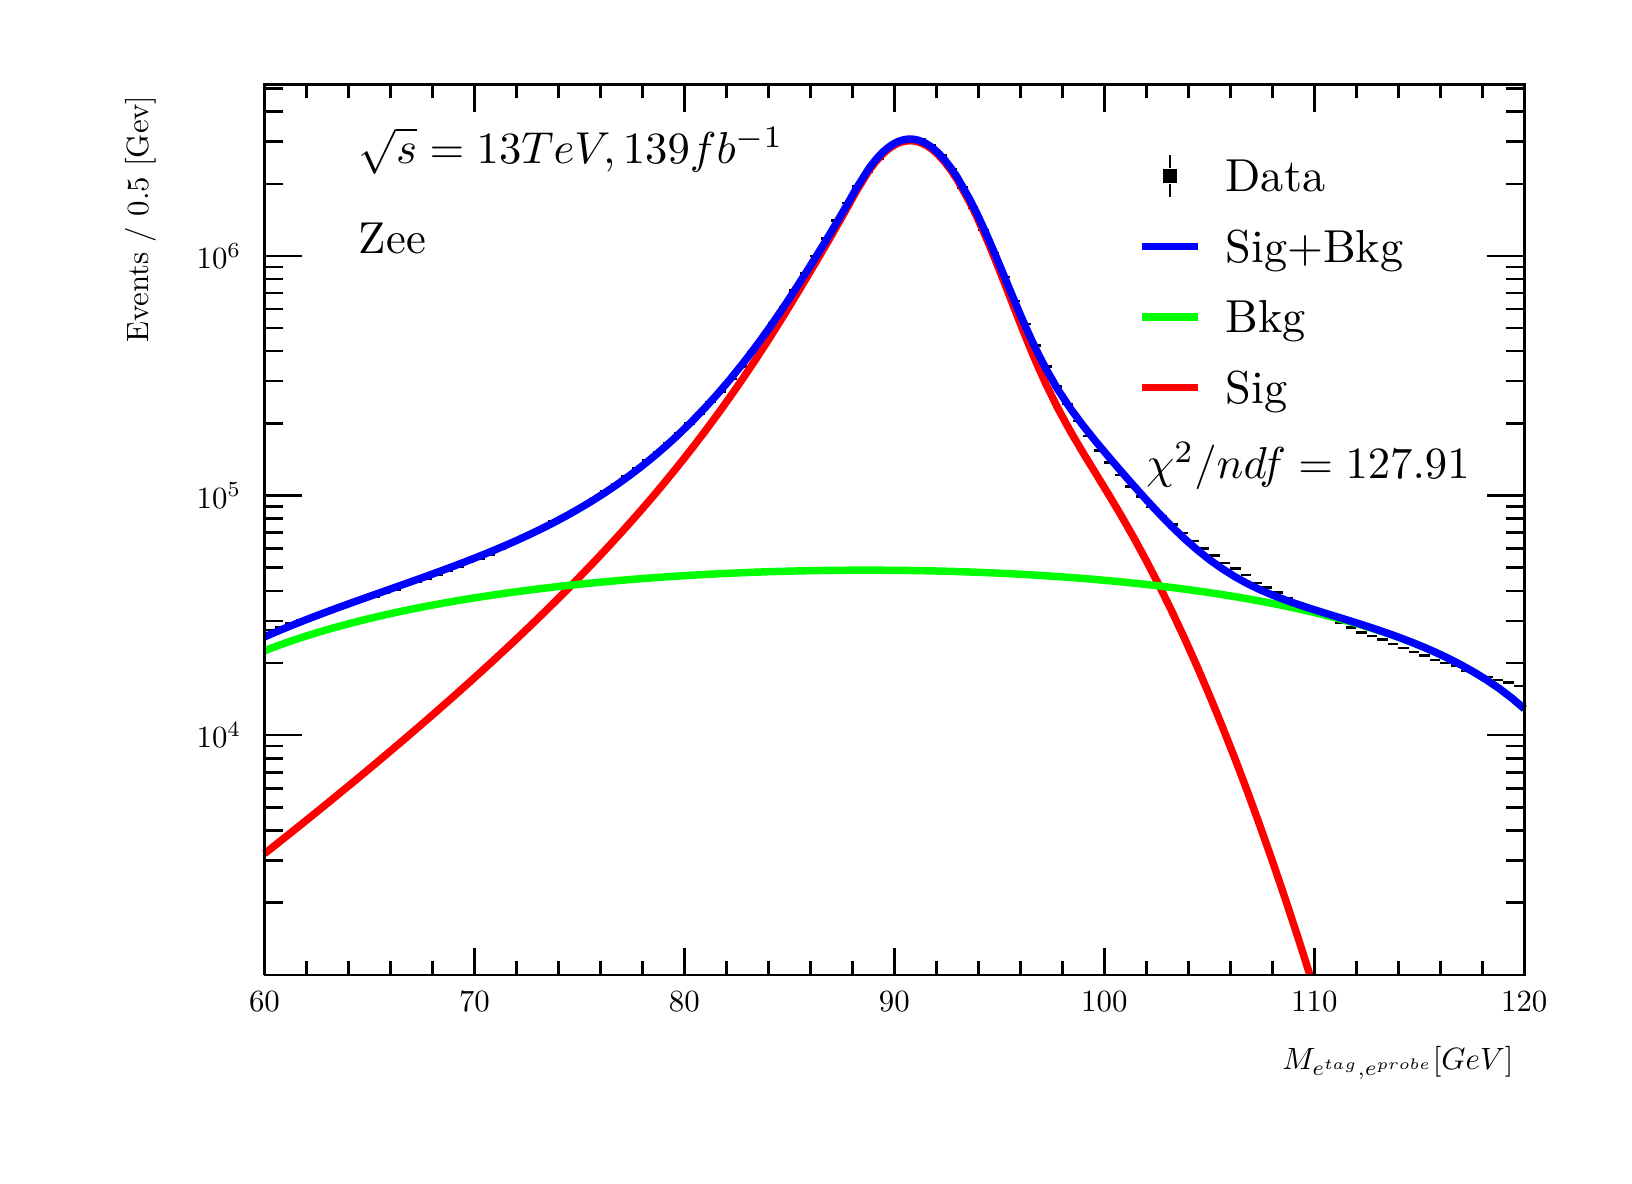
\begin{tikzpicture}
\pgfdeclareplotmark{cross} {
\pgfpathmoveto{\pgfpoint{-0.3\pgfplotmarksize}{\pgfplotmarksize}}
\pgfpathlineto{\pgfpoint{+0.3\pgfplotmarksize}{\pgfplotmarksize}}
\pgfpathlineto{\pgfpoint{+0.3\pgfplotmarksize}{0.3\pgfplotmarksize}}
\pgfpathlineto{\pgfpoint{+1\pgfplotmarksize}{0.3\pgfplotmarksize}}
\pgfpathlineto{\pgfpoint{+1\pgfplotmarksize}{-0.3\pgfplotmarksize}}
\pgfpathlineto{\pgfpoint{+0.3\pgfplotmarksize}{-0.3\pgfplotmarksize}}
\pgfpathlineto{\pgfpoint{+0.3\pgfplotmarksize}{-1.\pgfplotmarksize}}
\pgfpathlineto{\pgfpoint{-0.3\pgfplotmarksize}{-1.\pgfplotmarksize}}
\pgfpathlineto{\pgfpoint{-0.3\pgfplotmarksize}{-0.3\pgfplotmarksize}}
\pgfpathlineto{\pgfpoint{-1.\pgfplotmarksize}{-0.3\pgfplotmarksize}}
\pgfpathlineto{\pgfpoint{-1.\pgfplotmarksize}{0.3\pgfplotmarksize}}
\pgfpathlineto{\pgfpoint{-0.3\pgfplotmarksize}{0.3\pgfplotmarksize}}
\pgfpathclose
\pgfusepathqstroke
}
\pgfdeclareplotmark{cross*} {
\pgfpathmoveto{\pgfpoint{-0.3\pgfplotmarksize}{\pgfplotmarksize}}
\pgfpathlineto{\pgfpoint{+0.3\pgfplotmarksize}{\pgfplotmarksize}}
\pgfpathlineto{\pgfpoint{+0.3\pgfplotmarksize}{0.3\pgfplotmarksize}}
\pgfpathlineto{\pgfpoint{+1\pgfplotmarksize}{0.3\pgfplotmarksize}}
\pgfpathlineto{\pgfpoint{+1\pgfplotmarksize}{-0.3\pgfplotmarksize}}
\pgfpathlineto{\pgfpoint{+0.3\pgfplotmarksize}{-0.3\pgfplotmarksize}}
\pgfpathlineto{\pgfpoint{+0.3\pgfplotmarksize}{-1.\pgfplotmarksize}}
\pgfpathlineto{\pgfpoint{-0.3\pgfplotmarksize}{-1.\pgfplotmarksize}}
\pgfpathlineto{\pgfpoint{-0.3\pgfplotmarksize}{-0.3\pgfplotmarksize}}
\pgfpathlineto{\pgfpoint{-1.\pgfplotmarksize}{-0.3\pgfplotmarksize}}
\pgfpathlineto{\pgfpoint{-1.\pgfplotmarksize}{0.3\pgfplotmarksize}}
\pgfpathlineto{\pgfpoint{-0.3\pgfplotmarksize}{0.3\pgfplotmarksize}}
\pgfpathclose
\pgfusepathqfillstroke
}
\pgfdeclareplotmark{newstar} {
\pgfpathmoveto{\pgfqpoint{0pt}{\pgfplotmarksize}}
\pgfpathlineto{\pgfqpointpolar{44}{0.5\pgfplotmarksize}}
\pgfpathlineto{\pgfqpointpolar{18}{\pgfplotmarksize}}
\pgfpathlineto{\pgfqpointpolar{-20}{0.5\pgfplotmarksize}}
\pgfpathlineto{\pgfqpointpolar{-54}{\pgfplotmarksize}}
\pgfpathlineto{\pgfqpointpolar{-90}{0.5\pgfplotmarksize}}
\pgfpathlineto{\pgfqpointpolar{234}{\pgfplotmarksize}}
\pgfpathlineto{\pgfqpointpolar{198}{0.5\pgfplotmarksize}}
\pgfpathlineto{\pgfqpointpolar{162}{\pgfplotmarksize}}
\pgfpathlineto{\pgfqpointpolar{134}{0.5\pgfplotmarksize}}
\pgfpathclose
\pgfusepathqstroke
}
\pgfdeclareplotmark{newstar*} {
\pgfpathmoveto{\pgfqpoint{0pt}{\pgfplotmarksize}}
\pgfpathlineto{\pgfqpointpolar{44}{0.5\pgfplotmarksize}}
\pgfpathlineto{\pgfqpointpolar{18}{\pgfplotmarksize}}
\pgfpathlineto{\pgfqpointpolar{-20}{0.5\pgfplotmarksize}}
\pgfpathlineto{\pgfqpointpolar{-54}{\pgfplotmarksize}}
\pgfpathlineto{\pgfqpointpolar{-90}{0.5\pgfplotmarksize}}
\pgfpathlineto{\pgfqpointpolar{234}{\pgfplotmarksize}}
\pgfpathlineto{\pgfqpointpolar{198}{0.5\pgfplotmarksize}}
\pgfpathlineto{\pgfqpointpolar{162}{\pgfplotmarksize}}
\pgfpathlineto{\pgfqpointpolar{134}{0.5\pgfplotmarksize}}
\pgfpathclose
\pgfusepathqfillstroke
}
\definecolor{c}{rgb}{1,1,1};
\draw [color=c, fill=c] (0,0) rectangle (20,14.3108);
\draw [color=c, fill=c] (3,2.28972) rectangle (19,13.5952);
\definecolor{c}{rgb}{0,0,0};
\draw [c,line width=0.9] (3,2.28972) -- (3,13.5952) -- (19,13.5952) -- (19,2.28972) -- (3,2.28972);
\definecolor{c}{rgb}{1,1,1};
\draw [color=c, fill=c] (3,2.28972) rectangle (19,13.5952);
\definecolor{c}{rgb}{0,0,0};
\draw [c,line width=0.9] (3,2.28972) -- (3,13.5952) -- (19,13.5952) -- (19,2.28972) -- (3,2.28972);
\draw [c,line width=0.9] (3,2.28972) -- (19,2.28972);
\draw [c,line width=0.9] (3,2.63318) -- (3,2.28972);
\draw [c,line width=0.9] (3.53333,2.46145) -- (3.53333,2.28972);
\draw [c,line width=0.9] (4.06667,2.46145) -- (4.06667,2.28972);
\draw [c,line width=0.9] (4.6,2.46145) -- (4.6,2.28972);
\draw [c,line width=0.9] (5.13333,2.46145) -- (5.13333,2.28972);
\draw [c,line width=0.9] (5.66667,2.63318) -- (5.66667,2.28972);
\draw [c,line width=0.9] (6.2,2.46145) -- (6.2,2.28972);
\draw [c,line width=0.9] (6.73333,2.46145) -- (6.73333,2.28972);
\draw [c,line width=0.9] (7.26667,2.46145) -- (7.26667,2.28972);
\draw [c,line width=0.9] (7.8,2.46145) -- (7.8,2.28972);
\draw [c,line width=0.9] (8.33333,2.63318) -- (8.33333,2.28972);
\draw [c,line width=0.9] (8.86667,2.46145) -- (8.86667,2.28972);
\draw [c,line width=0.9] (9.4,2.46145) -- (9.4,2.28972);
\draw [c,line width=0.9] (9.93333,2.46145) -- (9.93333,2.28972);
\draw [c,line width=0.9] (10.4667,2.46145) -- (10.4667,2.28972);
\draw [c,line width=0.9] (11,2.63318) -- (11,2.28972);
\draw [c,line width=0.9] (11.5333,2.46145) -- (11.5333,2.28972);
\draw [c,line width=0.9] (12.0667,2.46145) -- (12.0667,2.28972);
\draw [c,line width=0.9] (12.6,2.46145) -- (12.6,2.28972);
\draw [c,line width=0.9] (13.1333,2.46145) -- (13.1333,2.28972);
\draw [c,line width=0.9] (13.6667,2.63318) -- (13.6667,2.28972);
\draw [c,line width=0.9] (14.2,2.46145) -- (14.2,2.28972);
\draw [c,line width=0.9] (14.7333,2.46145) -- (14.7333,2.28972);
\draw [c,line width=0.9] (15.2667,2.46145) -- (15.2667,2.28972);
\draw [c,line width=0.9] (15.8,2.46145) -- (15.8,2.28972);
\draw [c,line width=0.9] (16.3333,2.63318) -- (16.3333,2.28972);
\draw [c,line width=0.9] (16.8667,2.46145) -- (16.8667,2.28972);
\draw [c,line width=0.9] (17.4,2.46145) -- (17.4,2.28972);
\draw [c,line width=0.9] (17.9333,2.46145) -- (17.9333,2.28972);
\draw [c,line width=0.9] (18.4667,2.46145) -- (18.4667,2.28972);
\draw [c,line width=0.9] (19,2.63318) -- (19,2.28972);
\draw [anchor=base] (3,1.81747) node[scale=1.11327, color=c, rotate=0]{60};
\draw [anchor=base] (5.66667,1.81747) node[scale=1.11327, color=c, rotate=0]{70};
\draw [anchor=base] (8.33333,1.81747) node[scale=1.11327, color=c, rotate=0]{80};
\draw [anchor=base] (11,1.81747) node[scale=1.11327, color=c, rotate=0]{90};
\draw [anchor=base] (13.6667,1.81747) node[scale=1.11327, color=c, rotate=0]{100};
\draw [anchor=base] (16.3333,1.81747) node[scale=1.11327, color=c, rotate=0]{110};
\draw [anchor=base] (19,1.81747) node[scale=1.11327, color=c, rotate=0]{120};
\draw [anchor= east] (19,1.16776) node[scale=1.11327, color=c, rotate=0]{$M_{e^{tag}, e^{probe}}  [GeV]$};
\draw [c,line width=0.9] (3,13.5952) -- (19,13.5952);
\draw [c,line width=0.9] (3,13.2518) -- (3,13.5952);
\draw [c,line width=0.9] (3.53333,13.4235) -- (3.53333,13.5952);
\draw [c,line width=0.9] (4.06667,13.4235) -- (4.06667,13.5952);
\draw [c,line width=0.9] (4.6,13.4235) -- (4.6,13.5952);
\draw [c,line width=0.9] (5.13333,13.4235) -- (5.13333,13.5952);
\draw [c,line width=0.9] (5.66667,13.2518) -- (5.66667,13.5952);
\draw [c,line width=0.9] (6.2,13.4235) -- (6.2,13.5952);
\draw [c,line width=0.9] (6.73333,13.4235) -- (6.73333,13.5952);
\draw [c,line width=0.9] (7.26667,13.4235) -- (7.26667,13.5952);
\draw [c,line width=0.9] (7.8,13.4235) -- (7.8,13.5952);
\draw [c,line width=0.9] (8.33333,13.2518) -- (8.33333,13.5952);
\draw [c,line width=0.9] (8.86667,13.4235) -- (8.86667,13.5952);
\draw [c,line width=0.9] (9.4,13.4235) -- (9.4,13.5952);
\draw [c,line width=0.9] (9.93333,13.4235) -- (9.93333,13.5952);
\draw [c,line width=0.9] (10.4667,13.4235) -- (10.4667,13.5952);
\draw [c,line width=0.9] (11,13.2518) -- (11,13.5952);
\draw [c,line width=0.9] (11.5333,13.4235) -- (11.5333,13.5952);
\draw [c,line width=0.9] (12.0667,13.4235) -- (12.0667,13.5952);
\draw [c,line width=0.9] (12.6,13.4235) -- (12.6,13.5952);
\draw [c,line width=0.9] (13.1333,13.4235) -- (13.1333,13.5952);
\draw [c,line width=0.9] (13.6667,13.2518) -- (13.6667,13.5952);
\draw [c,line width=0.9] (14.2,13.4235) -- (14.2,13.5952);
\draw [c,line width=0.9] (14.7333,13.4235) -- (14.7333,13.5952);
\draw [c,line width=0.9] (15.2667,13.4235) -- (15.2667,13.5952);
\draw [c,line width=0.9] (15.8,13.4235) -- (15.8,13.5952);
\draw [c,line width=0.9] (16.3333,13.2518) -- (16.3333,13.5952);
\draw [c,line width=0.9] (16.8667,13.4235) -- (16.8667,13.5952);
\draw [c,line width=0.9] (17.4,13.4235) -- (17.4,13.5952);
\draw [c,line width=0.9] (17.9333,13.4235) -- (17.9333,13.5952);
\draw [c,line width=0.9] (18.4667,13.4235) -- (18.4667,13.5952);
\draw [c,line width=0.9] (19,13.2518) -- (19,13.5952);
\draw [c,line width=0.9] (3,2.28972) -- (3,13.5952);
\draw [c,line width=0.9] (3.237,3.20582) -- (3,3.20582);
\draw [c,line width=0.9] (3.237,3.74171) -- (3,3.74171);
\draw [c,line width=0.9] (3.237,4.12192) -- (3,4.12192);
\draw [c,line width=0.9] (3.237,4.41684) -- (3,4.41684);
\draw [c,line width=0.9] (3.237,4.65781) -- (3,4.65781);
\draw [c,line width=0.9] (3.237,4.86154) -- (3,4.86154);
\draw [c,line width=0.9] (3.237,5.03802) -- (3,5.03802);
\draw [c,line width=0.9] (3.237,5.19369) -- (3,5.19369);
\draw [c,line width=0.9] (3.474,5.33294) -- (3,5.33294);
\draw [anchor= east] (2.844,5.33294) node[scale=1.11327, color=c, rotate=0]{$10^{4}$};
\draw [c,line width=0.9] (3.237,6.24904) -- (3,6.24904);
\draw [c,line width=0.9] (3.237,6.78493) -- (3,6.78493);
\draw [c,line width=0.9] (3.237,7.16515) -- (3,7.16515);
\draw [c,line width=0.9] (3.237,7.46006) -- (3,7.46006);
\draw [c,line width=0.9] (3.237,7.70103) -- (3,7.70103);
\draw [c,line width=0.9] (3.237,7.90476) -- (3,7.90476);
\draw [c,line width=0.9] (3.237,8.08125) -- (3,8.08125);
\draw [c,line width=0.9] (3.237,8.23691) -- (3,8.23691);
\draw [c,line width=0.9] (3.474,8.37617) -- (3,8.37617);
\draw [anchor= east] (2.844,8.37617) node[scale=1.11327, color=c, rotate=0]{$10^{5}$};
\draw [c,line width=0.9] (3.237,9.29227) -- (3,9.29227);
\draw [c,line width=0.9] (3.237,9.82815) -- (3,9.82815);
\draw [c,line width=0.9] (3.237,10.2084) -- (3,10.2084);
\draw [c,line width=0.9] (3.237,10.5033) -- (3,10.5033);
\draw [c,line width=0.9] (3.237,10.7443) -- (3,10.7443);
\draw [c,line width=0.9] (3.237,10.948) -- (3,10.948);
\draw [c,line width=0.9] (3.237,11.1245) -- (3,11.1245);
\draw [c,line width=0.9] (3.237,11.2801) -- (3,11.2801);
\draw [c,line width=0.9] (3.474,11.4194) -- (3,11.4194);
\draw [anchor= east] (2.844,11.4194) node[scale=1.11327, color=c, rotate=0]{$10^{6}$};
\draw [c,line width=0.9] (3.237,12.3355) -- (3,12.3355);
\draw [c,line width=0.9] (3.237,12.8714) -- (3,12.8714);
\draw [c,line width=0.9] (3.237,13.2516) -- (3,13.2516);
\draw [c,line width=0.9] (3.237,13.5465) -- (3,13.5465);
\draw [anchor= east] (1.432,13.5952) node[scale=1.11327, color=c, rotate=90]{Events / 0.5 [Gev]};
\draw [c,line width=0.9] (19,2.28972) -- (19,13.5952);
\draw [c,line width=0.9] (18.763,3.20582) -- (19,3.20582);
\draw [c,line width=0.9] (18.763,3.74171) -- (19,3.74171);
\draw [c,line width=0.9] (18.763,4.12192) -- (19,4.12192);
\draw [c,line width=0.9] (18.763,4.41684) -- (19,4.41684);
\draw [c,line width=0.9] (18.763,4.65781) -- (19,4.65781);
\draw [c,line width=0.9] (18.763,4.86154) -- (19,4.86154);
\draw [c,line width=0.9] (18.763,5.03802) -- (19,5.03802);
\draw [c,line width=0.9] (18.763,5.19369) -- (19,5.19369);
\draw [c,line width=0.9] (18.526,5.33294) -- (19,5.33294);
\draw [c,line width=0.9] (18.763,6.24904) -- (19,6.24904);
\draw [c,line width=0.9] (18.763,6.78493) -- (19,6.78493);
\draw [c,line width=0.9] (18.763,7.16515) -- (19,7.16515);
\draw [c,line width=0.9] (18.763,7.46006) -- (19,7.46006);
\draw [c,line width=0.9] (18.763,7.70103) -- (19,7.70103);
\draw [c,line width=0.9] (18.763,7.90476) -- (19,7.90476);
\draw [c,line width=0.9] (18.763,8.08125) -- (19,8.08125);
\draw [c,line width=0.9] (18.763,8.23691) -- (19,8.23691);
\draw [c,line width=0.9] (18.526,8.37617) -- (19,8.37617);
\draw [c,line width=0.9] (18.763,9.29227) -- (19,9.29227);
\draw [c,line width=0.9] (18.763,9.82815) -- (19,9.82815);
\draw [c,line width=0.9] (18.763,10.2084) -- (19,10.2084);
\draw [c,line width=0.9] (18.763,10.5033) -- (19,10.5033);
\draw [c,line width=0.9] (18.763,10.7443) -- (19,10.7443);
\draw [c,line width=0.9] (18.763,10.948) -- (19,10.948);
\draw [c,line width=0.9] (18.763,11.1245) -- (19,11.1245);
\draw [c,line width=0.9] (18.763,11.2801) -- (19,11.2801);
\draw [c,line width=0.9] (18.526,11.4194) -- (19,11.4194);
\draw [c,line width=0.9] (18.763,12.3355) -- (19,12.3355);
\draw [c,line width=0.9] (18.763,12.8714) -- (19,12.8714);
\draw [c,line width=0.9] (18.763,13.2516) -- (19,13.2516);
\draw [c,line width=0.9] (18.763,13.5465) -- (19,13.5465);
\draw [c,line width=0.9] (3.06667,6.66868) -- (3,6.66868);
\draw [c,line width=0.9] (3,6.66868) -- (3,6.66868);
\draw [c,line width=0.9] (3.06667,6.66868) -- (3.13333,6.66868);
\draw [c,line width=0.9] (3.13333,6.66868) -- (3.13333,6.66868);
\draw [c,line width=0.9] (3.06667,6.66868) -- (3.06667,6.67666);
\draw [c,line width=0.9] (3.06667,6.67666) -- (3.06667,6.67666);
\draw [c,line width=0.9] (3.06667,6.66868) -- (3.06667,6.66071);
\draw [c,line width=0.9] (3.06667,6.66071) -- (3.06667,6.66071);
\draw [c,line width=0.9] (3.2,6.69954) -- (3.13333,6.69954);
\draw [c,line width=0.9] (3.13333,6.69954) -- (3.13333,6.69954);
\draw [c,line width=0.9] (3.2,6.69954) -- (3.26667,6.69954);
\draw [c,line width=0.9] (3.26667,6.69954) -- (3.26667,6.69954);
\draw [c,line width=0.9] (3.2,6.69954) -- (3.2,6.70742);
\draw [c,line width=0.9] (3.2,6.70742) -- (3.2,6.70742);
\draw [c,line width=0.9] (3.2,6.69954) -- (3.2,6.69166);
\draw [c,line width=0.9] (3.2,6.69166) -- (3.2,6.69166);
\draw [c,line width=0.9] (3.33333,6.75607) -- (3.26667,6.75607);
\draw [c,line width=0.9] (3.26667,6.75607) -- (3.26667,6.75607);
\draw [c,line width=0.9] (3.33333,6.75607) -- (3.4,6.75607);
\draw [c,line width=0.9] (3.4,6.75607) -- (3.4,6.75607);
\draw [c,line width=0.9] (3.33333,6.75607) -- (3.33333,6.76378);
\draw [c,line width=0.9] (3.33333,6.76378) -- (3.33333,6.76378);
\draw [c,line width=0.9] (3.33333,6.75607) -- (3.33333,6.74836);
\draw [c,line width=0.9] (3.33333,6.74836) -- (3.33333,6.74836);
\draw [c,line width=0.9] (3.46667,6.79284) -- (3.4,6.79284);
\draw [c,line width=0.9] (3.4,6.79284) -- (3.4,6.79284);
\draw [c,line width=0.9] (3.46667,6.79284) -- (3.53333,6.79284);
\draw [c,line width=0.9] (3.53333,6.79284) -- (3.53333,6.79284);
\draw [c,line width=0.9] (3.46667,6.79284) -- (3.46667,6.80045);
\draw [c,line width=0.9] (3.46667,6.80045) -- (3.46667,6.80045);
\draw [c,line width=0.9] (3.46667,6.79284) -- (3.46667,6.78523);
\draw [c,line width=0.9] (3.46667,6.78523) -- (3.46667,6.78523);
\draw [c,line width=0.9] (3.6,6.83099) -- (3.53333,6.83099);
\draw [c,line width=0.9] (3.53333,6.83099) -- (3.53333,6.83099);
\draw [c,line width=0.9] (3.6,6.83099) -- (3.66667,6.83099);
\draw [c,line width=0.9] (3.66667,6.83099) -- (3.66667,6.83099);
\draw [c,line width=0.9] (3.6,6.83099) -- (3.6,6.83849);
\draw [c,line width=0.9] (3.6,6.83849) -- (3.6,6.83849);
\draw [c,line width=0.9] (3.6,6.83099) -- (3.6,6.82349);
\draw [c,line width=0.9] (3.6,6.82349) -- (3.6,6.82349);
\draw [c,line width=0.9] (3.73333,6.87908) -- (3.66667,6.87908);
\draw [c,line width=0.9] (3.66667,6.87908) -- (3.66667,6.87908);
\draw [c,line width=0.9] (3.73333,6.87908) -- (3.8,6.87908);
\draw [c,line width=0.9] (3.8,6.87908) -- (3.8,6.87908);
\draw [c,line width=0.9] (3.73333,6.87908) -- (3.73333,6.88644);
\draw [c,line width=0.9] (3.73333,6.88644) -- (3.73333,6.88644);
\draw [c,line width=0.9] (3.73333,6.87908) -- (3.73333,6.87172);
\draw [c,line width=0.9] (3.73333,6.87172) -- (3.73333,6.87172);
\draw [c,line width=0.9] (3.86667,6.93129) -- (3.8,6.93129);
\draw [c,line width=0.9] (3.8,6.93129) -- (3.8,6.93129);
\draw [c,line width=0.9] (3.86667,6.93129) -- (3.93333,6.93129);
\draw [c,line width=0.9] (3.93333,6.93129) -- (3.93333,6.93129);
\draw [c,line width=0.9] (3.86667,6.93129) -- (3.86667,6.93851);
\draw [c,line width=0.9] (3.86667,6.93851) -- (3.86667,6.93851);
\draw [c,line width=0.9] (3.86667,6.93129) -- (3.86667,6.92407);
\draw [c,line width=0.9] (3.86667,6.92407) -- (3.86667,6.92407);
\draw [c,line width=0.9] (4,6.96585) -- (3.93333,6.96585);
\draw [c,line width=0.9] (3.93333,6.96585) -- (3.93333,6.96585);
\draw [c,line width=0.9] (4,6.96585) -- (4.06667,6.96585);
\draw [c,line width=0.9] (4.06667,6.96585) -- (4.06667,6.96585);
\draw [c,line width=0.9] (4,6.96585) -- (4,6.97298);
\draw [c,line width=0.9] (4,6.97298) -- (4,6.97298);
\draw [c,line width=0.9] (4,6.96585) -- (4,6.95872);
\draw [c,line width=0.9] (4,6.95872) -- (4,6.95872);
\draw [c,line width=0.9] (4.13333,7.02215) -- (4.06667,7.02215);
\draw [c,line width=0.9] (4.06667,7.02215) -- (4.06667,7.02215);
\draw [c,line width=0.9] (4.13333,7.02215) -- (4.2,7.02215);
\draw [c,line width=0.9] (4.2,7.02215) -- (4.2,7.02215);
\draw [c,line width=0.9] (4.13333,7.02215) -- (4.13333,7.02912);
\draw [c,line width=0.9] (4.13333,7.02912) -- (4.13333,7.02912);
\draw [c,line width=0.9] (4.13333,7.02215) -- (4.13333,7.01517);
\draw [c,line width=0.9] (4.13333,7.01517) -- (4.13333,7.01517);
\draw [c,line width=0.9] (4.26667,7.06813) -- (4.2,7.06813);
\draw [c,line width=0.9] (4.2,7.06813) -- (4.2,7.06813);
\draw [c,line width=0.9] (4.26667,7.06813) -- (4.33333,7.06813);
\draw [c,line width=0.9] (4.33333,7.06813) -- (4.33333,7.06813);
\draw [c,line width=0.9] (4.26667,7.06813) -- (4.26667,7.07499);
\draw [c,line width=0.9] (4.26667,7.07499) -- (4.26667,7.07499);
\draw [c,line width=0.9] (4.26667,7.06813) -- (4.26667,7.06128);
\draw [c,line width=0.9] (4.26667,7.06128) -- (4.26667,7.06128);
\draw [c,line width=0.9] (4.4,7.09038) -- (4.33333,7.09038);
\draw [c,line width=0.9] (4.33333,7.09038) -- (4.33333,7.09038);
\draw [c,line width=0.9] (4.4,7.09038) -- (4.46667,7.09038);
\draw [c,line width=0.9] (4.46667,7.09038) -- (4.46667,7.09038);
\draw [c,line width=0.9] (4.4,7.09038) -- (4.4,7.09718);
\draw [c,line width=0.9] (4.4,7.09718) -- (4.4,7.09718);
\draw [c,line width=0.9] (4.4,7.09038) -- (4.4,7.08358);
\draw [c,line width=0.9] (4.4,7.08358) -- (4.4,7.08358);
\draw [c,line width=0.9] (4.53333,7.13757) -- (4.46667,7.13757);
\draw [c,line width=0.9] (4.46667,7.13757) -- (4.46667,7.13757);
\draw [c,line width=0.9] (4.53333,7.13757) -- (4.6,7.13757);
\draw [c,line width=0.9] (4.6,7.13757) -- (4.6,7.13757);
\draw [c,line width=0.9] (4.53333,7.13757) -- (4.53333,7.14425);
\draw [c,line width=0.9] (4.53333,7.14425) -- (4.53333,7.14425);
\draw [c,line width=0.9] (4.53333,7.13757) -- (4.53333,7.13089);
\draw [c,line width=0.9] (4.53333,7.13089) -- (4.53333,7.13089);
\draw [c,line width=0.9] (4.66667,7.18124) -- (4.6,7.18124);
\draw [c,line width=0.9] (4.6,7.18124) -- (4.6,7.18124);
\draw [c,line width=0.9] (4.66667,7.18124) -- (4.73333,7.18124);
\draw [c,line width=0.9] (4.73333,7.18124) -- (4.73333,7.18124);
\draw [c,line width=0.9] (4.66667,7.18124) -- (4.66667,7.18781);
\draw [c,line width=0.9] (4.66667,7.18781) -- (4.66667,7.18781);
\draw [c,line width=0.9] (4.66667,7.18124) -- (4.66667,7.17467);
\draw [c,line width=0.9] (4.66667,7.17467) -- (4.66667,7.17467);
\draw [c,line width=0.9] (4.8,7.23776) -- (4.73333,7.23776);
\draw [c,line width=0.9] (4.73333,7.23776) -- (4.73333,7.23776);
\draw [c,line width=0.9] (4.8,7.23776) -- (4.86667,7.23776);
\draw [c,line width=0.9] (4.86667,7.23776) -- (4.86667,7.23776);
\draw [c,line width=0.9] (4.8,7.23776) -- (4.8,7.24418);
\draw [c,line width=0.9] (4.8,7.24418) -- (4.8,7.24418);
\draw [c,line width=0.9] (4.8,7.23776) -- (4.8,7.23133);
\draw [c,line width=0.9] (4.8,7.23133) -- (4.8,7.23133);
\draw [c,line width=0.9] (4.93333,7.27847) -- (4.86667,7.27847);
\draw [c,line width=0.9] (4.86667,7.27847) -- (4.86667,7.27847);
\draw [c,line width=0.9] (4.93333,7.27847) -- (5,7.27847);
\draw [c,line width=0.9] (5,7.27847) -- (5,7.27847);
\draw [c,line width=0.9] (4.93333,7.27847) -- (4.93333,7.2848);
\draw [c,line width=0.9] (4.93333,7.2848) -- (4.93333,7.2848);
\draw [c,line width=0.9] (4.93333,7.27847) -- (4.93333,7.27214);
\draw [c,line width=0.9] (4.93333,7.27214) -- (4.93333,7.27214);
\draw [c,line width=0.9] (5.06667,7.31979) -- (5,7.31979);
\draw [c,line width=0.9] (5,7.31979) -- (5,7.31979);
\draw [c,line width=0.9] (5.06667,7.31979) -- (5.13333,7.31979);
\draw [c,line width=0.9] (5.13333,7.31979) -- (5.13333,7.31979);
\draw [c,line width=0.9] (5.06667,7.31979) -- (5.06667,7.32602);
\draw [c,line width=0.9] (5.06667,7.32602) -- (5.06667,7.32602);
\draw [c,line width=0.9] (5.06667,7.31979) -- (5.06667,7.31355);
\draw [c,line width=0.9] (5.06667,7.31355) -- (5.06667,7.31355);
\draw [c,line width=0.9] (5.2,7.365) -- (5.13333,7.365);
\draw [c,line width=0.9] (5.13333,7.365) -- (5.13333,7.365);
\draw [c,line width=0.9] (5.2,7.365) -- (5.26667,7.365);
\draw [c,line width=0.9] (5.26667,7.365) -- (5.26667,7.365);
\draw [c,line width=0.9] (5.2,7.365) -- (5.2,7.37113);
\draw [c,line width=0.9] (5.2,7.37113) -- (5.2,7.37113);
\draw [c,line width=0.9] (5.2,7.365) -- (5.2,7.35888);
\draw [c,line width=0.9] (5.2,7.35888) -- (5.2,7.35888);
\draw [c,line width=0.9] (5.33333,7.42343) -- (5.26667,7.42343);
\draw [c,line width=0.9] (5.26667,7.42343) -- (5.26667,7.42343);
\draw [c,line width=0.9] (5.33333,7.42343) -- (5.4,7.42343);
\draw [c,line width=0.9] (5.4,7.42343) -- (5.4,7.42343);
\draw [c,line width=0.9] (5.33333,7.42343) -- (5.33333,7.42942);
\draw [c,line width=0.9] (5.33333,7.42942) -- (5.33333,7.42942);
\draw [c,line width=0.9] (5.33333,7.42343) -- (5.33333,7.41744);
\draw [c,line width=0.9] (5.33333,7.41744) -- (5.33333,7.41744);
\draw [c,line width=0.9] (5.46667,7.47541) -- (5.4,7.47541);
\draw [c,line width=0.9] (5.4,7.47541) -- (5.4,7.47541);
\draw [c,line width=0.9] (5.46667,7.47541) -- (5.53333,7.47541);
\draw [c,line width=0.9] (5.53333,7.47541) -- (5.53333,7.47541);
\draw [c,line width=0.9] (5.46667,7.47541) -- (5.46667,7.48129);
\draw [c,line width=0.9] (5.46667,7.48129) -- (5.46667,7.48129);
\draw [c,line width=0.9] (5.46667,7.47541) -- (5.46667,7.46954);
\draw [c,line width=0.9] (5.46667,7.46954) -- (5.46667,7.46954);
\draw [c,line width=0.9] (5.6,7.53118) -- (5.53333,7.53118);
\draw [c,line width=0.9] (5.53333,7.53118) -- (5.53333,7.53118);
\draw [c,line width=0.9] (5.6,7.53118) -- (5.66667,7.53118);
\draw [c,line width=0.9] (5.66667,7.53118) -- (5.66667,7.53118);
\draw [c,line width=0.9] (5.6,7.53118) -- (5.6,7.53693);
\draw [c,line width=0.9] (5.6,7.53693) -- (5.6,7.53693);
\draw [c,line width=0.9] (5.6,7.53118) -- (5.6,7.52542);
\draw [c,line width=0.9] (5.6,7.52542) -- (5.6,7.52542);
\draw [c,line width=0.9] (5.73333,7.57876) -- (5.66667,7.57876);
\draw [c,line width=0.9] (5.66667,7.57876) -- (5.66667,7.57876);
\draw [c,line width=0.9] (5.73333,7.57876) -- (5.8,7.57876);
\draw [c,line width=0.9] (5.8,7.57876) -- (5.8,7.57876);
\draw [c,line width=0.9] (5.73333,7.57876) -- (5.73333,7.58441);
\draw [c,line width=0.9] (5.73333,7.58441) -- (5.73333,7.58441);
\draw [c,line width=0.9] (5.73333,7.57876) -- (5.73333,7.5731);
\draw [c,line width=0.9] (5.73333,7.5731) -- (5.73333,7.5731);
\draw [c,line width=0.9] (5.86667,7.6278) -- (5.8,7.6278);
\draw [c,line width=0.9] (5.8,7.6278) -- (5.8,7.6278);
\draw [c,line width=0.9] (5.86667,7.6278) -- (5.93333,7.6278);
\draw [c,line width=0.9] (5.93333,7.6278) -- (5.93333,7.6278);
\draw [c,line width=0.9] (5.86667,7.6278) -- (5.86667,7.63335);
\draw [c,line width=0.9] (5.86667,7.63335) -- (5.86667,7.63335);
\draw [c,line width=0.9] (5.86667,7.6278) -- (5.86667,7.62226);
\draw [c,line width=0.9] (5.86667,7.62226) -- (5.86667,7.62226);
\draw [c,line width=0.9] (6,7.70413) -- (5.93333,7.70413);
\draw [c,line width=0.9] (5.93333,7.70413) -- (5.93333,7.70413);
\draw [c,line width=0.9] (6,7.70413) -- (6.06667,7.70413);
\draw [c,line width=0.9] (6.06667,7.70413) -- (6.06667,7.70413);
\draw [c,line width=0.9] (6,7.70413) -- (6,7.70952);
\draw [c,line width=0.9] (6,7.70952) -- (6,7.70952);
\draw [c,line width=0.9] (6,7.70413) -- (6,7.69874);
\draw [c,line width=0.9] (6,7.69874) -- (6,7.69874);
\draw [c,line width=0.9] (6.13333,7.76262) -- (6.06667,7.76262);
\draw [c,line width=0.9] (6.06667,7.76262) -- (6.06667,7.76262);
\draw [c,line width=0.9] (6.13333,7.76262) -- (6.2,7.76262);
\draw [c,line width=0.9] (6.2,7.76262) -- (6.2,7.76262);
\draw [c,line width=0.9] (6.13333,7.76262) -- (6.13333,7.76789);
\draw [c,line width=0.9] (6.13333,7.76789) -- (6.13333,7.76789);
\draw [c,line width=0.9] (6.13333,7.76262) -- (6.13333,7.75735);
\draw [c,line width=0.9] (6.13333,7.75735) -- (6.13333,7.75735);
\draw [c,line width=0.9] (6.26667,7.82564) -- (6.2,7.82564);
\draw [c,line width=0.9] (6.2,7.82564) -- (6.2,7.82564);
\draw [c,line width=0.9] (6.26667,7.82564) -- (6.33333,7.82564);
\draw [c,line width=0.9] (6.33333,7.82564) -- (6.33333,7.82564);
\draw [c,line width=0.9] (6.26667,7.82564) -- (6.26667,7.83078);
\draw [c,line width=0.9] (6.26667,7.83078) -- (6.26667,7.83078);
\draw [c,line width=0.9] (6.26667,7.82564) -- (6.26667,7.82049);
\draw [c,line width=0.9] (6.26667,7.82049) -- (6.26667,7.82049);
\draw [c,line width=0.9] (6.4,7.89911) -- (6.33333,7.89911);
\draw [c,line width=0.9] (6.33333,7.89911) -- (6.33333,7.89911);
\draw [c,line width=0.9] (6.4,7.89911) -- (6.46667,7.89911);
\draw [c,line width=0.9] (6.46667,7.89911) -- (6.46667,7.89911);
\draw [c,line width=0.9] (6.4,7.89911) -- (6.4,7.90411);
\draw [c,line width=0.9] (6.4,7.90411) -- (6.4,7.90411);
\draw [c,line width=0.9] (6.4,7.89911) -- (6.4,7.8941);
\draw [c,line width=0.9] (6.4,7.8941) -- (6.4,7.8941);
\draw [c,line width=0.9] (6.53333,7.96583) -- (6.46667,7.96583);
\draw [c,line width=0.9] (6.46667,7.96583) -- (6.46667,7.96583);
\draw [c,line width=0.9] (6.53333,7.96583) -- (6.6,7.96583);
\draw [c,line width=0.9] (6.6,7.96583) -- (6.6,7.96583);
\draw [c,line width=0.9] (6.53333,7.96583) -- (6.53333,7.97071);
\draw [c,line width=0.9] (6.53333,7.97071) -- (6.53333,7.97071);
\draw [c,line width=0.9] (6.53333,7.96583) -- (6.53333,7.96095);
\draw [c,line width=0.9] (6.53333,7.96095) -- (6.53333,7.96095);
\draw [c,line width=0.9] (6.66667,8.04375) -- (6.6,8.04375);
\draw [c,line width=0.9] (6.6,8.04375) -- (6.6,8.04375);
\draw [c,line width=0.9] (6.66667,8.04375) -- (6.73333,8.04375);
\draw [c,line width=0.9] (6.73333,8.04375) -- (6.73333,8.04375);
\draw [c,line width=0.9] (6.66667,8.04375) -- (6.66667,8.04849);
\draw [c,line width=0.9] (6.66667,8.04849) -- (6.66667,8.04849);
\draw [c,line width=0.9] (6.66667,8.04375) -- (6.66667,8.03901);
\draw [c,line width=0.9] (6.66667,8.03901) -- (6.66667,8.03901);
\draw [c,line width=0.9] (6.8,8.10158) -- (6.73333,8.10158);
\draw [c,line width=0.9] (6.73333,8.10158) -- (6.73333,8.10158);
\draw [c,line width=0.9] (6.8,8.10158) -- (6.86667,8.10158);
\draw [c,line width=0.9] (6.86667,8.10158) -- (6.86667,8.10158);
\draw [c,line width=0.9] (6.8,8.10158) -- (6.8,8.10621);
\draw [c,line width=0.9] (6.8,8.10621) -- (6.8,8.10621);
\draw [c,line width=0.9] (6.8,8.10158) -- (6.8,8.09694);
\draw [c,line width=0.9] (6.8,8.09694) -- (6.8,8.09694);
\draw [c,line width=0.9] (6.93333,8.17741) -- (6.86667,8.17741);
\draw [c,line width=0.9] (6.86667,8.17741) -- (6.86667,8.17741);
\draw [c,line width=0.9] (6.93333,8.17741) -- (7,8.17741);
\draw [c,line width=0.9] (7,8.17741) -- (7,8.17741);
\draw [c,line width=0.9] (6.93333,8.17741) -- (6.93333,8.18192);
\draw [c,line width=0.9] (6.93333,8.18192) -- (6.93333,8.18192);
\draw [c,line width=0.9] (6.93333,8.17741) -- (6.93333,8.17291);
\draw [c,line width=0.9] (6.93333,8.17291) -- (6.93333,8.17291);
\draw [c,line width=0.9] (7.06667,8.25778) -- (7,8.25778);
\draw [c,line width=0.9] (7,8.25778) -- (7,8.25778);
\draw [c,line width=0.9] (7.06667,8.25778) -- (7.13333,8.25778);
\draw [c,line width=0.9] (7.13333,8.25778) -- (7.13333,8.25778);
\draw [c,line width=0.9] (7.06667,8.25778) -- (7.06667,8.26215);
\draw [c,line width=0.9] (7.06667,8.26215) -- (7.06667,8.26215);
\draw [c,line width=0.9] (7.06667,8.25778) -- (7.06667,8.25341);
\draw [c,line width=0.9] (7.06667,8.25341) -- (7.06667,8.25341);
\draw [c,line width=0.9] (7.2,8.34102) -- (7.13333,8.34102);
\draw [c,line width=0.9] (7.13333,8.34102) -- (7.13333,8.34102);
\draw [c,line width=0.9] (7.2,8.34102) -- (7.26667,8.34102);
\draw [c,line width=0.9] (7.26667,8.34102) -- (7.26667,8.34102);
\draw [c,line width=0.9] (7.2,8.34102) -- (7.2,8.34526);
\draw [c,line width=0.9] (7.2,8.34526) -- (7.2,8.34526);
\draw [c,line width=0.9] (7.2,8.34102) -- (7.2,8.33679);
\draw [c,line width=0.9] (7.2,8.33679) -- (7.2,8.33679);
\draw [c,line width=0.9] (7.33333,8.43509) -- (7.26667,8.43509);
\draw [c,line width=0.9] (7.26667,8.43509) -- (7.26667,8.43509);
\draw [c,line width=0.9] (7.33333,8.43509) -- (7.4,8.43509);
\draw [c,line width=0.9] (7.4,8.43509) -- (7.4,8.43509);
\draw [c,line width=0.9] (7.33333,8.43509) -- (7.33333,8.43917);
\draw [c,line width=0.9] (7.33333,8.43917) -- (7.33333,8.43917);
\draw [c,line width=0.9] (7.33333,8.43509) -- (7.33333,8.431);
\draw [c,line width=0.9] (7.33333,8.431) -- (7.33333,8.431);
\draw [c,line width=0.9] (7.46667,8.52537) -- (7.4,8.52537);
\draw [c,line width=0.9] (7.4,8.52537) -- (7.4,8.52537);
\draw [c,line width=0.9] (7.46667,8.52537) -- (7.53333,8.52537);
\draw [c,line width=0.9] (7.53333,8.52537) -- (7.53333,8.52537);
\draw [c,line width=0.9] (7.46667,8.52537) -- (7.46667,8.52932);
\draw [c,line width=0.9] (7.46667,8.52932) -- (7.46667,8.52932);
\draw [c,line width=0.9] (7.46667,8.52537) -- (7.46667,8.52142);
\draw [c,line width=0.9] (7.46667,8.52142) -- (7.46667,8.52142);
\draw [c,line width=0.9] (7.6,8.61728) -- (7.53333,8.61728);
\draw [c,line width=0.9] (7.53333,8.61728) -- (7.53333,8.61728);
\draw [c,line width=0.9] (7.6,8.61728) -- (7.66667,8.61728);
\draw [c,line width=0.9] (7.66667,8.61728) -- (7.66667,8.61728);
\draw [c,line width=0.9] (7.6,8.61728) -- (7.6,8.62109);
\draw [c,line width=0.9] (7.6,8.62109) -- (7.6,8.62109);
\draw [c,line width=0.9] (7.6,8.61728) -- (7.6,8.61346);
\draw [c,line width=0.9] (7.6,8.61346) -- (7.6,8.61346);
\draw [c,line width=0.9] (7.73333,8.718) -- (7.66667,8.718);
\draw [c,line width=0.9] (7.66667,8.718) -- (7.66667,8.718);
\draw [c,line width=0.9] (7.73333,8.718) -- (7.8,8.718);
\draw [c,line width=0.9] (7.8,8.718) -- (7.8,8.718);
\draw [c,line width=0.9] (7.73333,8.718) -- (7.73333,8.72167);
\draw [c,line width=0.9] (7.73333,8.72167) -- (7.73333,8.72167);
\draw [c,line width=0.9] (7.73333,8.718) -- (7.73333,8.71433);
\draw [c,line width=0.9] (7.73333,8.71433) -- (7.73333,8.71433);
\draw [c,line width=0.9] (7.86667,8.82319) -- (7.8,8.82319);
\draw [c,line width=0.9] (7.8,8.82319) -- (7.8,8.82319);
\draw [c,line width=0.9] (7.86667,8.82319) -- (7.93333,8.82319);
\draw [c,line width=0.9] (7.93333,8.82319) -- (7.93333,8.82319);
\draw [c,line width=0.9] (7.86667,8.82319) -- (7.86667,8.82672);
\draw [c,line width=0.9] (7.86667,8.82672) -- (7.86667,8.82672);
\draw [c,line width=0.9] (7.86667,8.82319) -- (7.86667,8.81966);
\draw [c,line width=0.9] (7.86667,8.81966) -- (7.86667,8.81966);
\draw [c,line width=0.9] (8,8.92963) -- (7.93333,8.92963);
\draw [c,line width=0.9] (7.93333,8.92963) -- (7.93333,8.92963);
\draw [c,line width=0.9] (8,8.92963) -- (8.06667,8.92963);
\draw [c,line width=0.9] (8.06667,8.92963) -- (8.06667,8.92963);
\draw [c,line width=0.9] (8,8.92963) -- (8,8.93302);
\draw [c,line width=0.9] (8,8.93302) -- (8,8.93302);
\draw [c,line width=0.9] (8,8.92963) -- (8,8.92624);
\draw [c,line width=0.9] (8,8.92624) -- (8,8.92624);
\draw [c,line width=0.9] (8.13333,9.04058) -- (8.06667,9.04058);
\draw [c,line width=0.9] (8.06667,9.04058) -- (8.06667,9.04058);
\draw [c,line width=0.9] (8.13333,9.04058) -- (8.2,9.04058);
\draw [c,line width=0.9] (8.2,9.04058) -- (8.2,9.04058);
\draw [c,line width=0.9] (8.13333,9.04058) -- (8.13333,9.04383);
\draw [c,line width=0.9] (8.13333,9.04383) -- (8.13333,9.04383);
\draw [c,line width=0.9] (8.13333,9.04058) -- (8.13333,9.03733);
\draw [c,line width=0.9] (8.13333,9.03733) -- (8.13333,9.03733);
\draw [c,line width=0.9] (8.26667,9.1646) -- (8.2,9.1646);
\draw [c,line width=0.9] (8.2,9.1646) -- (8.2,9.1646);
\draw [c,line width=0.9] (8.26667,9.1646) -- (8.33333,9.1646);
\draw [c,line width=0.9] (8.33333,9.1646) -- (8.33333,9.1646);
\draw [c,line width=0.9] (8.26667,9.1646) -- (8.26667,9.1677);
\draw [c,line width=0.9] (8.26667,9.1677) -- (8.26667,9.1677);
\draw [c,line width=0.9] (8.26667,9.1646) -- (8.26667,9.1615);
\draw [c,line width=0.9] (8.26667,9.1615) -- (8.26667,9.1615);
\draw [c,line width=0.9] (8.4,9.28957) -- (8.33333,9.28957);
\draw [c,line width=0.9] (8.33333,9.28957) -- (8.33333,9.28957);
\draw [c,line width=0.9] (8.4,9.28957) -- (8.46667,9.28957);
\draw [c,line width=0.9] (8.46667,9.28957) -- (8.46667,9.28957);
\draw [c,line width=0.9] (8.4,9.28957) -- (8.4,9.29253);
\draw [c,line width=0.9] (8.4,9.29253) -- (8.4,9.29253);
\draw [c,line width=0.9] (8.4,9.28957) -- (8.4,9.28661);
\draw [c,line width=0.9] (8.4,9.28661) -- (8.4,9.28661);
\draw [c,line width=0.9] (8.53333,9.41735) -- (8.46667,9.41735);
\draw [c,line width=0.9] (8.46667,9.41735) -- (8.46667,9.41735);
\draw [c,line width=0.9] (8.53333,9.41735) -- (8.6,9.41735);
\draw [c,line width=0.9] (8.6,9.41735) -- (8.6,9.41735);
\draw [c,line width=0.9] (8.53333,9.41735) -- (8.53333,9.42016);
\draw [c,line width=0.9] (8.53333,9.42016) -- (8.53333,9.42016);
\draw [c,line width=0.9] (8.53333,9.41735) -- (8.53333,9.41453);
\draw [c,line width=0.9] (8.53333,9.41453) -- (8.53333,9.41453);
\draw [c,line width=0.9] (8.66667,9.56084) -- (8.6,9.56084);
\draw [c,line width=0.9] (8.6,9.56084) -- (8.6,9.56084);
\draw [c,line width=0.9] (8.66667,9.56084) -- (8.73333,9.56084);
\draw [c,line width=0.9] (8.73333,9.56084) -- (8.73333,9.56084);
\draw [c,line width=0.9] (8.66667,9.56084) -- (8.66667,9.56351);
\draw [c,line width=0.9] (8.66667,9.56351) -- (8.66667,9.56351);
\draw [c,line width=0.9] (8.66667,9.56084) -- (8.66667,9.55817);
\draw [c,line width=0.9] (8.66667,9.55817) -- (8.66667,9.55817);
\draw [c,line width=0.9] (8.8,9.69948) -- (8.73333,9.69948);
\draw [c,line width=0.9] (8.73333,9.69948) -- (8.73333,9.69948);
\draw [c,line width=0.9] (8.8,9.69948) -- (8.86667,9.69948);
\draw [c,line width=0.9] (8.86667,9.69948) -- (8.86667,9.69948);
\draw [c,line width=0.9] (8.8,9.69948) -- (8.8,9.70201);
\draw [c,line width=0.9] (8.8,9.70201) -- (8.8,9.70201);
\draw [c,line width=0.9] (8.8,9.69948) -- (8.8,9.69694);
\draw [c,line width=0.9] (8.8,9.69694) -- (8.8,9.69694);
\draw [c,line width=0.9] (8.93333,9.85526) -- (8.86667,9.85526);
\draw [c,line width=0.9] (8.86667,9.85526) -- (8.86667,9.85526);
\draw [c,line width=0.9] (8.93333,9.85526) -- (9,9.85526);
\draw [c,line width=0.9] (9,9.85526) -- (9,9.85526);
\draw [c,line width=0.9] (8.93333,9.85526) -- (8.93333,9.85765);
\draw [c,line width=0.9] (8.93333,9.85765) -- (8.93333,9.85765);
\draw [c,line width=0.9] (8.93333,9.85526) -- (8.93333,9.85287);
\draw [c,line width=0.9] (8.93333,9.85287) -- (8.93333,9.85287);
\draw [c,line width=0.9] (9.06667,10.0175) -- (9,10.0175);
\draw [c,line width=0.9] (9,10.0175) -- (9,10.0175);
\draw [c,line width=0.9] (9.06667,10.0175) -- (9.13333,10.0175);
\draw [c,line width=0.9] (9.13333,10.0175) -- (9.13333,10.0175);
\draw [c,line width=0.9] (9.06667,10.0175) -- (9.06667,10.0197);
\draw [c,line width=0.9] (9.06667,10.0197) -- (9.06667,10.0197);
\draw [c,line width=0.9] (9.06667,10.0175) -- (9.06667,10.0152);
\draw [c,line width=0.9] (9.06667,10.0152) -- (9.06667,10.0152);
\draw [c,line width=0.9] (9.2,10.1911) -- (9.13333,10.1911);
\draw [c,line width=0.9] (9.13333,10.1911) -- (9.13333,10.1911);
\draw [c,line width=0.9] (9.2,10.1911) -- (9.26667,10.1911);
\draw [c,line width=0.9] (9.26667,10.1911) -- (9.26667,10.1911);
\draw [c,line width=0.9] (9.2,10.1911) -- (9.2,10.1932);
\draw [c,line width=0.9] (9.2,10.1932) -- (9.2,10.1932);
\draw [c,line width=0.9] (9.2,10.1911) -- (9.2,10.189);
\draw [c,line width=0.9] (9.2,10.189) -- (9.2,10.189);
\draw [c,line width=0.9] (9.33333,10.3749) -- (9.26667,10.3749);
\draw [c,line width=0.9] (9.26667,10.3749) -- (9.26667,10.3749);
\draw [c,line width=0.9] (9.33333,10.3749) -- (9.4,10.3749);
\draw [c,line width=0.9] (9.4,10.3749) -- (9.4,10.3749);
\draw [c,line width=0.9] (9.33333,10.3749) -- (9.33333,10.3768);
\draw [c,line width=0.9] (9.33333,10.3768) -- (9.33333,10.3768);
\draw [c,line width=0.9] (9.33333,10.3749) -- (9.33333,10.3729);
\draw [c,line width=0.9] (9.33333,10.3729) -- (9.33333,10.3729);
\draw [c,line width=0.9] (9.46667,10.565) -- (9.4,10.565);
\draw [c,line width=0.9] (9.4,10.565) -- (9.4,10.565);
\draw [c,line width=0.9] (9.46667,10.565) -- (9.53333,10.565);
\draw [c,line width=0.9] (9.53333,10.565) -- (9.53333,10.565);
\draw [c,line width=0.9] (9.46667,10.565) -- (9.46667,10.5668);
\draw [c,line width=0.9] (9.46667,10.5668) -- (9.46667,10.5668);
\draw [c,line width=0.9] (9.46667,10.565) -- (9.46667,10.5632);
\draw [c,line width=0.9] (9.46667,10.5632) -- (9.46667,10.5632);
\draw [c,line width=0.9] (9.6,10.7682) -- (9.53333,10.7682);
\draw [c,line width=0.9] (9.53333,10.7682) -- (9.53333,10.7682);
\draw [c,line width=0.9] (9.6,10.7682) -- (9.66667,10.7682);
\draw [c,line width=0.9] (9.66667,10.7682) -- (9.66667,10.7682);
\draw [c,line width=0.9] (9.6,10.7682) -- (9.6,10.7699);
\draw [c,line width=0.9] (9.6,10.7699) -- (9.6,10.7699);
\draw [c,line width=0.9] (9.6,10.7682) -- (9.6,10.7665);
\draw [c,line width=0.9] (9.6,10.7665) -- (9.6,10.7665);
\draw [c,line width=0.9] (9.73333,10.9767) -- (9.66667,10.9767);
\draw [c,line width=0.9] (9.66667,10.9767) -- (9.66667,10.9767);
\draw [c,line width=0.9] (9.73333,10.9767) -- (9.8,10.9767);
\draw [c,line width=0.9] (9.8,10.9767) -- (9.8,10.9767);
\draw [c,line width=0.9] (9.73333,10.9767) -- (9.73333,10.9782);
\draw [c,line width=0.9] (9.73333,10.9782) -- (9.73333,10.9782);
\draw [c,line width=0.9] (9.73333,10.9767) -- (9.73333,10.9751);
\draw [c,line width=0.9] (9.73333,10.9751) -- (9.73333,10.9751);
\draw [c,line width=0.9] (9.86667,11.1943) -- (9.8,11.1943);
\draw [c,line width=0.9] (9.8,11.1943) -- (9.8,11.1943);
\draw [c,line width=0.9] (9.86667,11.1943) -- (9.93333,11.1943);
\draw [c,line width=0.9] (9.93333,11.1943) -- (9.93333,11.1943);
\draw [c,line width=0.9] (9.86667,11.1943) -- (9.86667,11.1957);
\draw [c,line width=0.9] (9.86667,11.1957) -- (9.86667,11.1957);
\draw [c,line width=0.9] (9.86667,11.1943) -- (9.86667,11.1929);
\draw [c,line width=0.9] (9.86667,11.1929) -- (9.86667,11.1929);
\draw [c,line width=0.9] (10,11.4164) -- (9.93333,11.4164);
\draw [c,line width=0.9] (9.93333,11.4164) -- (9.93333,11.4164);
\draw [c,line width=0.9] (10,11.4164) -- (10.0667,11.4164);
\draw [c,line width=0.9] (10.0667,11.4164) -- (10.0667,11.4164);
\draw [c,line width=0.9] (10,11.4164) -- (10,11.4177);
\draw [c,line width=0.9] (10,11.4177) -- (10,11.4177);
\draw [c,line width=0.9] (10,11.4164) -- (10,11.4151);
\draw [c,line width=0.9] (10,11.4151) -- (10,11.4151);
\draw [c,line width=0.9] (10.1333,11.6422) -- (10.0667,11.6422);
\draw [c,line width=0.9] (10.0667,11.6422) -- (10.0667,11.6422);
\draw [c,line width=0.9] (10.1333,11.6422) -- (10.2,11.6422);
\draw [c,line width=0.9] (10.2,11.6422) -- (10.2,11.6422);
\draw [c,line width=0.9] (10.1333,11.6422) -- (10.1333,11.6434);
\draw [c,line width=0.9] (10.1333,11.6434) -- (10.1333,11.6434);
\draw [c,line width=0.9] (10.1333,11.6422) -- (10.1333,11.641);
\draw [c,line width=0.9] (10.1333,11.641) -- (10.1333,11.641);
\draw [c,line width=0.9] (10.2667,11.8681) -- (10.2,11.8681);
\draw [c,line width=0.9] (10.2,11.8681) -- (10.2,11.8681);
\draw [c,line width=0.9] (10.2667,11.8681) -- (10.3333,11.8681);
\draw [c,line width=0.9] (10.3333,11.8681) -- (10.3333,11.8681);
\draw [c,line width=0.9] (10.2667,11.8681) -- (10.2667,11.8692);
\draw [c,line width=0.9] (10.2667,11.8692) -- (10.2667,11.8692);
\draw [c,line width=0.9] (10.2667,11.8681) -- (10.2667,11.867);
\draw [c,line width=0.9] (10.2667,11.867) -- (10.2667,11.867);
\draw [c,line width=0.9] (10.4,12.0886) -- (10.3333,12.0886);
\draw [c,line width=0.9] (10.3333,12.0886) -- (10.3333,12.0886);
\draw [c,line width=0.9] (10.4,12.0886) -- (10.4667,12.0886);
\draw [c,line width=0.9] (10.4667,12.0886) -- (10.4667,12.0886);
\draw [c,line width=0.9] (10.4,12.0886) -- (10.4,12.0896);
\draw [c,line width=0.9] (10.4,12.0896) -- (10.4,12.0896);
\draw [c,line width=0.9] (10.4,12.0886) -- (10.4,12.0875);
\draw [c,line width=0.9] (10.4,12.0875) -- (10.4,12.0875);
\draw [c,line width=0.9] (10.5333,12.2991) -- (10.4667,12.2991);
\draw [c,line width=0.9] (10.4667,12.2991) -- (10.4667,12.2991);
\draw [c,line width=0.9] (10.5333,12.2991) -- (10.6,12.2991);
\draw [c,line width=0.9] (10.6,12.2991) -- (10.6,12.2991);
\draw [c,line width=0.9] (10.5333,12.2991) -- (10.5333,12.3);
\draw [c,line width=0.9] (10.5333,12.3) -- (10.5333,12.3);
\draw [c,line width=0.9] (10.5333,12.2991) -- (10.5333,12.2981);
\draw [c,line width=0.9] (10.5333,12.2981) -- (10.5333,12.2981);
\draw [c,line width=0.9] (10.6667,12.4925) -- (10.6,12.4925);
\draw [c,line width=0.9] (10.6,12.4925) -- (10.6,12.4925);
\draw [c,line width=0.9] (10.6667,12.4925) -- (10.7333,12.4925);
\draw [c,line width=0.9] (10.7333,12.4925) -- (10.7333,12.4925);
\draw [c,line width=0.9] (10.6667,12.4925) -- (10.6667,12.4933);
\draw [c,line width=0.9] (10.6667,12.4933) -- (10.6667,12.4933);
\draw [c,line width=0.9] (10.6667,12.4925) -- (10.6667,12.4916);
\draw [c,line width=0.9] (10.6667,12.4916) -- (10.6667,12.4916);
\draw [c,line width=0.9] (10.8,12.6585) -- (10.7333,12.6585);
\draw [c,line width=0.9] (10.7333,12.6585) -- (10.7333,12.6585);
\draw [c,line width=0.9] (10.8,12.6585) -- (10.8667,12.6585);
\draw [c,line width=0.9] (10.8667,12.6585) -- (10.8667,12.6585);
\draw [c,line width=0.9] (10.8,12.6585) -- (10.8,12.6593);
\draw [c,line width=0.9] (10.8,12.6593) -- (10.8,12.6593);
\draw [c,line width=0.9] (10.8,12.6585) -- (10.8,12.6576);
\draw [c,line width=0.9] (10.8,12.6576) -- (10.8,12.6576);
\draw [c,line width=0.9] (10.9333,12.79) -- (10.8667,12.79);
\draw [c,line width=0.9] (10.8667,12.79) -- (10.8667,12.79);
\draw [c,line width=0.9] (10.9333,12.79) -- (11,12.79);
\draw [c,line width=0.9] (11,12.79) -- (11,12.79);
\draw [c,line width=0.9] (10.9333,12.79) -- (10.9333,12.7908);
\draw [c,line width=0.9] (10.9333,12.7908) -- (10.9333,12.7908);
\draw [c,line width=0.9] (10.9333,12.79) -- (10.9333,12.7892);
\draw [c,line width=0.9] (10.9333,12.7892) -- (10.9333,12.7892);
\draw [c,line width=0.9] (11.0667,12.8775) -- (11,12.8775);
\draw [c,line width=0.9] (11,12.8775) -- (11,12.8775);
\draw [c,line width=0.9] (11.0667,12.8775) -- (11.1333,12.8775);
\draw [c,line width=0.9] (11.1333,12.8775) -- (11.1333,12.8775);
\draw [c,line width=0.9] (11.0667,12.8775) -- (11.0667,12.8782);
\draw [c,line width=0.9] (11.0667,12.8782) -- (11.0667,12.8782);
\draw [c,line width=0.9] (11.0667,12.8775) -- (11.0667,12.8767);
\draw [c,line width=0.9] (11.0667,12.8767) -- (11.0667,12.8767);
\draw [c,line width=0.9] (11.2,12.9153) -- (11.1333,12.9153);
\draw [c,line width=0.9] (11.1333,12.9153) -- (11.1333,12.9153);
\draw [c,line width=0.9] (11.2,12.9153) -- (11.2667,12.9153);
\draw [c,line width=0.9] (11.2667,12.9153) -- (11.2667,12.9153);
\draw [c,line width=0.9] (11.2,12.9153) -- (11.2,12.916);
\draw [c,line width=0.9] (11.2,12.916) -- (11.2,12.916);
\draw [c,line width=0.9] (11.2,12.9153) -- (11.2,12.9145);
\draw [c,line width=0.9] (11.2,12.9145) -- (11.2,12.9145);
\draw [c,line width=0.9] (11.3333,12.8983) -- (11.2667,12.8983);
\draw [c,line width=0.9] (11.2667,12.8983) -- (11.2667,12.8983);
\draw [c,line width=0.9] (11.3333,12.8983) -- (11.4,12.8983);
\draw [c,line width=0.9] (11.4,12.8983) -- (11.4,12.8983);
\draw [c,line width=0.9] (11.3333,12.8983) -- (11.3333,12.8991);
\draw [c,line width=0.9] (11.3333,12.8991) -- (11.3333,12.8991);
\draw [c,line width=0.9] (11.3333,12.8983) -- (11.3333,12.8976);
\draw [c,line width=0.9] (11.3333,12.8976) -- (11.3333,12.8976);
\draw [c,line width=0.9] (11.4667,12.825) -- (11.4,12.825);
\draw [c,line width=0.9] (11.4,12.825) -- (11.4,12.825);
\draw [c,line width=0.9] (11.4667,12.825) -- (11.5333,12.825);
\draw [c,line width=0.9] (11.5333,12.825) -- (11.5333,12.825);
\draw [c,line width=0.9] (11.4667,12.825) -- (11.4667,12.8258);
\draw [c,line width=0.9] (11.4667,12.8258) -- (11.4667,12.8258);
\draw [c,line width=0.9] (11.4667,12.825) -- (11.4667,12.8242);
\draw [c,line width=0.9] (11.4667,12.8242) -- (11.4667,12.8242);
\draw [c,line width=0.9] (11.6,12.6937) -- (11.5333,12.6937);
\draw [c,line width=0.9] (11.5333,12.6937) -- (11.5333,12.6937);
\draw [c,line width=0.9] (11.6,12.6937) -- (11.6667,12.6937);
\draw [c,line width=0.9] (11.6667,12.6937) -- (11.6667,12.6937);
\draw [c,line width=0.9] (11.6,12.6937) -- (11.6,12.6945);
\draw [c,line width=0.9] (11.6,12.6945) -- (11.6,12.6945);
\draw [c,line width=0.9] (11.6,12.6937) -- (11.6,12.6929);
\draw [c,line width=0.9] (11.6,12.6929) -- (11.6,12.6929);
\draw [c,line width=0.9] (11.7333,12.5145) -- (11.6667,12.5145);
\draw [c,line width=0.9] (11.6667,12.5145) -- (11.6667,12.5145);
\draw [c,line width=0.9] (11.7333,12.5145) -- (11.8,12.5145);
\draw [c,line width=0.9] (11.8,12.5145) -- (11.8,12.5145);
\draw [c,line width=0.9] (11.7333,12.5145) -- (11.7333,12.5153);
\draw [c,line width=0.9] (11.7333,12.5153) -- (11.7333,12.5153);
\draw [c,line width=0.9] (11.7333,12.5145) -- (11.7333,12.5136);
\draw [c,line width=0.9] (11.7333,12.5136) -- (11.7333,12.5136);
\draw [c,line width=0.9] (11.8667,12.29) -- (11.8,12.29);
\draw [c,line width=0.9] (11.8,12.29) -- (11.8,12.29);
\draw [c,line width=0.9] (11.8667,12.29) -- (11.9333,12.29);
\draw [c,line width=0.9] (11.9333,12.29) -- (11.9333,12.29);
\draw [c,line width=0.9] (11.8667,12.29) -- (11.8667,12.2909);
\draw [c,line width=0.9] (11.8667,12.2909) -- (11.8667,12.2909);
\draw [c,line width=0.9] (11.8667,12.29) -- (11.8667,12.289);
\draw [c,line width=0.9] (11.8667,12.289) -- (11.8667,12.289);
\draw [c,line width=0.9] (12,12.0325) -- (11.9333,12.0325);
\draw [c,line width=0.9] (11.9333,12.0325) -- (11.9333,12.0325);
\draw [c,line width=0.9] (12,12.0325) -- (12.0667,12.0325);
\draw [c,line width=0.9] (12.0667,12.0325) -- (12.0667,12.0325);
\draw [c,line width=0.9] (12,12.0325) -- (12,12.0336);
\draw [c,line width=0.9] (12,12.0336) -- (12,12.0336);
\draw [c,line width=0.9] (12,12.0325) -- (12,12.0315);
\draw [c,line width=0.9] (12,12.0315) -- (12,12.0315);
\draw [c,line width=0.9] (12.1333,11.7473) -- (12.0667,11.7473);
\draw [c,line width=0.9] (12.0667,11.7473) -- (12.0667,11.7473);
\draw [c,line width=0.9] (12.1333,11.7473) -- (12.2,11.7473);
\draw [c,line width=0.9] (12.2,11.7473) -- (12.2,11.7473);
\draw [c,line width=0.9] (12.1333,11.7473) -- (12.1333,11.7485);
\draw [c,line width=0.9] (12.1333,11.7485) -- (12.1333,11.7485);
\draw [c,line width=0.9] (12.1333,11.7473) -- (12.1333,11.7461);
\draw [c,line width=0.9] (12.1333,11.7461) -- (12.1333,11.7461);
\draw [c,line width=0.9] (12.2667,11.4547) -- (12.2,11.4547);
\draw [c,line width=0.9] (12.2,11.4547) -- (12.2,11.4547);
\draw [c,line width=0.9] (12.2667,11.4547) -- (12.3333,11.4547);
\draw [c,line width=0.9] (12.3333,11.4547) -- (12.3333,11.4547);
\draw [c,line width=0.9] (12.2667,11.4547) -- (12.2667,11.456);
\draw [c,line width=0.9] (12.2667,11.456) -- (12.2667,11.456);
\draw [c,line width=0.9] (12.2667,11.4547) -- (12.2667,11.4534);
\draw [c,line width=0.9] (12.2667,11.4534) -- (12.2667,11.4534);
\draw [c,line width=0.9] (12.4,11.1492) -- (12.3333,11.1492);
\draw [c,line width=0.9] (12.3333,11.1492) -- (12.3333,11.1492);
\draw [c,line width=0.9] (12.4,11.1492) -- (12.4667,11.1492);
\draw [c,line width=0.9] (12.4667,11.1492) -- (12.4667,11.1492);
\draw [c,line width=0.9] (12.4,11.1492) -- (12.4,11.1506);
\draw [c,line width=0.9] (12.4,11.1506) -- (12.4,11.1506);
\draw [c,line width=0.9] (12.4,11.1492) -- (12.4,11.1477);
\draw [c,line width=0.9] (12.4,11.1477) -- (12.4,11.1477);
\draw [c,line width=0.9] (12.5333,10.8481) -- (12.4667,10.8481);
\draw [c,line width=0.9] (12.4667,10.8481) -- (12.4667,10.8481);
\draw [c,line width=0.9] (12.5333,10.8481) -- (12.6,10.8481);
\draw [c,line width=0.9] (12.6,10.8481) -- (12.6,10.8481);
\draw [c,line width=0.9] (12.5333,10.8481) -- (12.5333,10.8498);
\draw [c,line width=0.9] (12.5333,10.8498) -- (12.5333,10.8498);
\draw [c,line width=0.9] (12.5333,10.8481) -- (12.5333,10.8465);
\draw [c,line width=0.9] (12.5333,10.8465) -- (12.5333,10.8465);
\draw [c,line width=0.9] (12.6667,10.5554) -- (12.6,10.5554);
\draw [c,line width=0.9] (12.6,10.5554) -- (12.6,10.5554);
\draw [c,line width=0.9] (12.6667,10.5554) -- (12.7333,10.5554);
\draw [c,line width=0.9] (12.7333,10.5554) -- (12.7333,10.5554);
\draw [c,line width=0.9] (12.6667,10.5554) -- (12.6667,10.5572);
\draw [c,line width=0.9] (12.6667,10.5572) -- (12.6667,10.5572);
\draw [c,line width=0.9] (12.6667,10.5554) -- (12.6667,10.5536);
\draw [c,line width=0.9] (12.6667,10.5536) -- (12.6667,10.5536);
\draw [c,line width=0.9] (12.8,10.2788) -- (12.7333,10.2788);
\draw [c,line width=0.9] (12.7333,10.2788) -- (12.7333,10.2788);
\draw [c,line width=0.9] (12.8,10.2788) -- (12.8667,10.2788);
\draw [c,line width=0.9] (12.8667,10.2788) -- (12.8667,10.2788);
\draw [c,line width=0.9] (12.8,10.2788) -- (12.8,10.2809);
\draw [c,line width=0.9] (12.8,10.2809) -- (12.8,10.2809);
\draw [c,line width=0.9] (12.8,10.2788) -- (12.8,10.2768);
\draw [c,line width=0.9] (12.8,10.2768) -- (12.8,10.2768);
\draw [c,line width=0.9] (12.9333,10.015) -- (12.8667,10.015);
\draw [c,line width=0.9] (12.8667,10.015) -- (12.8667,10.015);
\draw [c,line width=0.9] (12.9333,10.015) -- (13,10.015);
\draw [c,line width=0.9] (13,10.015) -- (13,10.015);
\draw [c,line width=0.9] (12.9333,10.015) -- (12.9333,10.0172);
\draw [c,line width=0.9] (12.9333,10.0172) -- (12.9333,10.0172);
\draw [c,line width=0.9] (12.9333,10.015) -- (12.9333,10.0127);
\draw [c,line width=0.9] (12.9333,10.0127) -- (12.9333,10.0127);
\draw [c,line width=0.9] (13.0667,9.76264) -- (13,9.76264);
\draw [c,line width=0.9] (13,9.76264) -- (13,9.76264);
\draw [c,line width=0.9] (13.0667,9.76264) -- (13.1333,9.76264);
\draw [c,line width=0.9] (13.1333,9.76264) -- (13.1333,9.76264);
\draw [c,line width=0.9] (13.0667,9.76264) -- (13.0667,9.76512);
\draw [c,line width=0.9] (13.0667,9.76512) -- (13.0667,9.76512);
\draw [c,line width=0.9] (13.0667,9.76264) -- (13.0667,9.76017);
\draw [c,line width=0.9] (13.0667,9.76017) -- (13.0667,9.76017);
\draw [c,line width=0.9] (13.2,9.54014) -- (13.1333,9.54014);
\draw [c,line width=0.9] (13.1333,9.54014) -- (13.1333,9.54014);
\draw [c,line width=0.9] (13.2,9.54014) -- (13.2667,9.54014);
\draw [c,line width=0.9] (13.2667,9.54014) -- (13.2667,9.54014);
\draw [c,line width=0.9] (13.2,9.54014) -- (13.2,9.54283);
\draw [c,line width=0.9] (13.2,9.54283) -- (13.2,9.54283);
\draw [c,line width=0.9] (13.2,9.54014) -- (13.2,9.53745);
\draw [c,line width=0.9] (13.2,9.53745) -- (13.2,9.53745);
\draw [c,line width=0.9] (13.3333,9.32562) -- (13.2667,9.32562);
\draw [c,line width=0.9] (13.2667,9.32562) -- (13.2667,9.32562);
\draw [c,line width=0.9] (13.3333,9.32562) -- (13.4,9.32562);
\draw [c,line width=0.9] (13.4,9.32562) -- (13.4,9.32562);
\draw [c,line width=0.9] (13.3333,9.32562) -- (13.3333,9.32854);
\draw [c,line width=0.9] (13.3333,9.32854) -- (13.3333,9.32854);
\draw [c,line width=0.9] (13.3333,9.32562) -- (13.3333,9.3227);
\draw [c,line width=0.9] (13.3333,9.3227) -- (13.3333,9.3227);
\draw [c,line width=0.9] (13.4667,9.13305) -- (13.4,9.13305);
\draw [c,line width=0.9] (13.4,9.13305) -- (13.4,9.13305);
\draw [c,line width=0.9] (13.4667,9.13305) -- (13.5333,9.13305);
\draw [c,line width=0.9] (13.5333,9.13305) -- (13.5333,9.13305);
\draw [c,line width=0.9] (13.4667,9.13305) -- (13.4667,9.13619);
\draw [c,line width=0.9] (13.4667,9.13619) -- (13.4667,9.13619);
\draw [c,line width=0.9] (13.4667,9.13305) -- (13.4667,9.12991);
\draw [c,line width=0.9] (13.4667,9.12991) -- (13.4667,9.12991);
\draw [c,line width=0.9] (13.6,8.94923) -- (13.5333,8.94923);
\draw [c,line width=0.9] (13.5333,8.94923) -- (13.5333,8.94923);
\draw [c,line width=0.9] (13.6,8.94923) -- (13.6667,8.94923);
\draw [c,line width=0.9] (13.6667,8.94923) -- (13.6667,8.94923);
\draw [c,line width=0.9] (13.6,8.94923) -- (13.6,8.9526);
\draw [c,line width=0.9] (13.6,8.9526) -- (13.6,8.9526);
\draw [c,line width=0.9] (13.6,8.94923) -- (13.6,8.94587);
\draw [c,line width=0.9] (13.6,8.94587) -- (13.6,8.94587);
\draw [c,line width=0.9] (13.7333,8.79327) -- (13.6667,8.79327);
\draw [c,line width=0.9] (13.6667,8.79327) -- (13.6667,8.79327);
\draw [c,line width=0.9] (13.7333,8.79327) -- (13.8,8.79327);
\draw [c,line width=0.9] (13.8,8.79327) -- (13.8,8.79327);
\draw [c,line width=0.9] (13.7333,8.79327) -- (13.7333,8.79684);
\draw [c,line width=0.9] (13.7333,8.79684) -- (13.7333,8.79684);
\draw [c,line width=0.9] (13.7333,8.79327) -- (13.7333,8.7897);
\draw [c,line width=0.9] (13.7333,8.7897) -- (13.7333,8.7897);
\draw [c,line width=0.9] (13.8667,8.63884) -- (13.8,8.63884);
\draw [c,line width=0.9] (13.8,8.63884) -- (13.8,8.63884);
\draw [c,line width=0.9] (13.8667,8.63884) -- (13.9333,8.63884);
\draw [c,line width=0.9] (13.9333,8.63884) -- (13.9333,8.63884);
\draw [c,line width=0.9] (13.8667,8.63884) -- (13.8667,8.64262);
\draw [c,line width=0.9] (13.8667,8.64262) -- (13.8667,8.64262);
\draw [c,line width=0.9] (13.8667,8.63884) -- (13.8667,8.63505);
\draw [c,line width=0.9] (13.8667,8.63505) -- (13.8667,8.63505);
\draw [c,line width=0.9] (14,8.49126) -- (13.9333,8.49126);
\draw [c,line width=0.9] (13.9333,8.49126) -- (13.9333,8.49126);
\draw [c,line width=0.9] (14,8.49126) -- (14.0667,8.49126);
\draw [c,line width=0.9] (14.0667,8.49126) -- (14.0667,8.49126);
\draw [c,line width=0.9] (14,8.49126) -- (14,8.49527);
\draw [c,line width=0.9] (14,8.49527) -- (14,8.49527);
\draw [c,line width=0.9] (14,8.49126) -- (14,8.48726);
\draw [c,line width=0.9] (14,8.48726) -- (14,8.48726);
\draw [c,line width=0.9] (14.1333,8.36455) -- (14.0667,8.36455);
\draw [c,line width=0.9] (14.0667,8.36455) -- (14.0667,8.36455);
\draw [c,line width=0.9] (14.1333,8.36455) -- (14.2,8.36455);
\draw [c,line width=0.9] (14.2,8.36455) -- (14.2,8.36455);
\draw [c,line width=0.9] (14.1333,8.36455) -- (14.1333,8.36875);
\draw [c,line width=0.9] (14.1333,8.36875) -- (14.1333,8.36875);
\draw [c,line width=0.9] (14.1333,8.36455) -- (14.1333,8.36035);
\draw [c,line width=0.9] (14.1333,8.36035) -- (14.1333,8.36035);
\draw [c,line width=0.9] (14.2667,8.22771) -- (14.2,8.22771);
\draw [c,line width=0.9] (14.2,8.22771) -- (14.2,8.22771);
\draw [c,line width=0.9] (14.2667,8.22771) -- (14.3333,8.22771);
\draw [c,line width=0.9] (14.3333,8.22771) -- (14.3333,8.22771);
\draw [c,line width=0.9] (14.2667,8.22771) -- (14.2667,8.23213);
\draw [c,line width=0.9] (14.2667,8.23213) -- (14.2667,8.23213);
\draw [c,line width=0.9] (14.2667,8.22771) -- (14.2667,8.22329);
\draw [c,line width=0.9] (14.2667,8.22329) -- (14.2667,8.22329);
\draw [c,line width=0.9] (14.4,8.11483) -- (14.3333,8.11483);
\draw [c,line width=0.9] (14.3333,8.11483) -- (14.3333,8.11483);
\draw [c,line width=0.9] (14.4,8.11483) -- (14.4667,8.11483);
\draw [c,line width=0.9] (14.4667,8.11483) -- (14.4667,8.11483);
\draw [c,line width=0.9] (14.4,8.11483) -- (14.4,8.11945);
\draw [c,line width=0.9] (14.4,8.11945) -- (14.4,8.11945);
\draw [c,line width=0.9] (14.4,8.11483) -- (14.4,8.11022);
\draw [c,line width=0.9] (14.4,8.11022) -- (14.4,8.11022);
\draw [c,line width=0.9] (14.5333,8.00622) -- (14.4667,8.00622);
\draw [c,line width=0.9] (14.4667,8.00622) -- (14.4667,8.00622);
\draw [c,line width=0.9] (14.5333,8.00622) -- (14.6,8.00622);
\draw [c,line width=0.9] (14.6,8.00622) -- (14.6,8.00622);
\draw [c,line width=0.9] (14.5333,8.00622) -- (14.5333,8.01103);
\draw [c,line width=0.9] (14.5333,8.01103) -- (14.5333,8.01103);
\draw [c,line width=0.9] (14.5333,8.00622) -- (14.5333,8.00141);
\draw [c,line width=0.9] (14.5333,8.00141) -- (14.5333,8.00141);
\draw [c,line width=0.9] (14.6667,7.89844) -- (14.6,7.89844);
\draw [c,line width=0.9] (14.6,7.89844) -- (14.6,7.89844);
\draw [c,line width=0.9] (14.6667,7.89844) -- (14.7333,7.89844);
\draw [c,line width=0.9] (14.7333,7.89844) -- (14.7333,7.89844);
\draw [c,line width=0.9] (14.6667,7.89844) -- (14.6667,7.90345);
\draw [c,line width=0.9] (14.6667,7.90345) -- (14.6667,7.90345);
\draw [c,line width=0.9] (14.6667,7.89844) -- (14.6667,7.89344);
\draw [c,line width=0.9] (14.6667,7.89344) -- (14.6667,7.89344);
\draw [c,line width=0.9] (14.8,7.79653) -- (14.7333,7.79653);
\draw [c,line width=0.9] (14.7333,7.79653) -- (14.7333,7.79653);
\draw [c,line width=0.9] (14.8,7.79653) -- (14.8667,7.79653);
\draw [c,line width=0.9] (14.8667,7.79653) -- (14.8667,7.79653);
\draw [c,line width=0.9] (14.8,7.79653) -- (14.8,7.80174);
\draw [c,line width=0.9] (14.8,7.80174) -- (14.8,7.80174);
\draw [c,line width=0.9] (14.8,7.79653) -- (14.8,7.79133);
\draw [c,line width=0.9] (14.8,7.79133) -- (14.8,7.79133);
\draw [c,line width=0.9] (14.9333,7.70438) -- (14.8667,7.70438);
\draw [c,line width=0.9] (14.8667,7.70438) -- (14.8667,7.70438);
\draw [c,line width=0.9] (14.9333,7.70438) -- (15,7.70438);
\draw [c,line width=0.9] (15,7.70438) -- (15,7.70438);
\draw [c,line width=0.9] (14.9333,7.70438) -- (14.9333,7.70976);
\draw [c,line width=0.9] (14.9333,7.70976) -- (14.9333,7.70976);
\draw [c,line width=0.9] (14.9333,7.70438) -- (14.9333,7.69899);
\draw [c,line width=0.9] (14.9333,7.69899) -- (14.9333,7.69899);
\draw [c,line width=0.9] (15.0667,7.61543) -- (15,7.61543);
\draw [c,line width=0.9] (15,7.61543) -- (15,7.61543);
\draw [c,line width=0.9] (15.0667,7.61543) -- (15.1333,7.61543);
\draw [c,line width=0.9] (15.1333,7.61543) -- (15.1333,7.61543);
\draw [c,line width=0.9] (15.0667,7.61543) -- (15.0667,7.621);
\draw [c,line width=0.9] (15.0667,7.621) -- (15.0667,7.621);
\draw [c,line width=0.9] (15.0667,7.61543) -- (15.0667,7.60986);
\draw [c,line width=0.9] (15.0667,7.60986) -- (15.0667,7.60986);
\draw [c,line width=0.9] (15.2,7.52087) -- (15.1333,7.52087);
\draw [c,line width=0.9] (15.1333,7.52087) -- (15.1333,7.52087);
\draw [c,line width=0.9] (15.2,7.52087) -- (15.2667,7.52087);
\draw [c,line width=0.9] (15.2667,7.52087) -- (15.2667,7.52087);
\draw [c,line width=0.9] (15.2,7.52087) -- (15.2,7.52665);
\draw [c,line width=0.9] (15.2,7.52665) -- (15.2,7.52665);
\draw [c,line width=0.9] (15.2,7.52087) -- (15.2,7.51509);
\draw [c,line width=0.9] (15.2,7.51509) -- (15.2,7.51509);
\draw [c,line width=0.9] (15.3333,7.44678) -- (15.2667,7.44678);
\draw [c,line width=0.9] (15.2667,7.44678) -- (15.2667,7.44678);
\draw [c,line width=0.9] (15.3333,7.44678) -- (15.4,7.44678);
\draw [c,line width=0.9] (15.4,7.44678) -- (15.4,7.44678);
\draw [c,line width=0.9] (15.3333,7.44678) -- (15.3333,7.45272);
\draw [c,line width=0.9] (15.3333,7.45272) -- (15.3333,7.45272);
\draw [c,line width=0.9] (15.3333,7.44678) -- (15.3333,7.44084);
\draw [c,line width=0.9] (15.3333,7.44084) -- (15.3333,7.44084);
\draw [c,line width=0.9] (15.4667,7.36481) -- (15.4,7.36481);
\draw [c,line width=0.9] (15.4,7.36481) -- (15.4,7.36481);
\draw [c,line width=0.9] (15.4667,7.36481) -- (15.5333,7.36481);
\draw [c,line width=0.9] (15.5333,7.36481) -- (15.5333,7.36481);
\draw [c,line width=0.9] (15.4667,7.36481) -- (15.4667,7.37093);
\draw [c,line width=0.9] (15.4667,7.37093) -- (15.4667,7.37093);
\draw [c,line width=0.9] (15.4667,7.36481) -- (15.4667,7.35868);
\draw [c,line width=0.9] (15.4667,7.35868) -- (15.4667,7.35868);
\draw [c,line width=0.9] (15.6,7.26723) -- (15.5333,7.26723);
\draw [c,line width=0.9] (15.5333,7.26723) -- (15.5333,7.26723);
\draw [c,line width=0.9] (15.6,7.26723) -- (15.6667,7.26723);
\draw [c,line width=0.9] (15.6667,7.26723) -- (15.6667,7.26723);
\draw [c,line width=0.9] (15.6,7.26723) -- (15.6,7.27359);
\draw [c,line width=0.9] (15.6,7.27359) -- (15.6,7.27359);
\draw [c,line width=0.9] (15.6,7.26723) -- (15.6,7.26087);
\draw [c,line width=0.9] (15.6,7.26087) -- (15.6,7.26087);
\draw [c,line width=0.9] (15.7333,7.21058) -- (15.6667,7.21058);
\draw [c,line width=0.9] (15.6667,7.21058) -- (15.6667,7.21058);
\draw [c,line width=0.9] (15.7333,7.21058) -- (15.8,7.21058);
\draw [c,line width=0.9] (15.8,7.21058) -- (15.8,7.21058);
\draw [c,line width=0.9] (15.7333,7.21058) -- (15.7333,7.21708);
\draw [c,line width=0.9] (15.7333,7.21708) -- (15.7333,7.21708);
\draw [c,line width=0.9] (15.7333,7.21058) -- (15.7333,7.20409);
\draw [c,line width=0.9] (15.7333,7.20409) -- (15.7333,7.20409);
\draw [c,line width=0.9] (15.8667,7.14658) -- (15.8,7.14658);
\draw [c,line width=0.9] (15.8,7.14658) -- (15.8,7.14658);
\draw [c,line width=0.9] (15.8667,7.14658) -- (15.9333,7.14658);
\draw [c,line width=0.9] (15.9333,7.14658) -- (15.9333,7.14658);
\draw [c,line width=0.9] (15.8667,7.14658) -- (15.8667,7.15323);
\draw [c,line width=0.9] (15.8667,7.15323) -- (15.8667,7.15323);
\draw [c,line width=0.9] (15.8667,7.14658) -- (15.8667,7.13993);
\draw [c,line width=0.9] (15.8667,7.13993) -- (15.8667,7.13993);
\draw [c,line width=0.9] (16,7.07402) -- (15.9333,7.07402);
\draw [c,line width=0.9] (15.9333,7.07402) -- (15.9333,7.07402);
\draw [c,line width=0.9] (16,7.07402) -- (16.0667,7.07402);
\draw [c,line width=0.9] (16.0667,7.07402) -- (16.0667,7.07402);
\draw [c,line width=0.9] (16,7.07402) -- (16,7.08086);
\draw [c,line width=0.9] (16,7.08086) -- (16,7.08086);
\draw [c,line width=0.9] (16,7.07402) -- (16,7.06718);
\draw [c,line width=0.9] (16,7.06718) -- (16,7.06718);
\draw [c,line width=0.9] (16.1333,7.00525) -- (16.0667,7.00525);
\draw [c,line width=0.9] (16.0667,7.00525) -- (16.0667,7.00525);
\draw [c,line width=0.9] (16.1333,7.00525) -- (16.2,7.00525);
\draw [c,line width=0.9] (16.2,7.00525) -- (16.2,7.00525);
\draw [c,line width=0.9] (16.1333,7.00525) -- (16.1333,7.01227);
\draw [c,line width=0.9] (16.1333,7.01227) -- (16.1333,7.01227);
\draw [c,line width=0.9] (16.1333,7.00525) -- (16.1333,6.99823);
\draw [c,line width=0.9] (16.1333,6.99823) -- (16.1333,6.99823);
\draw [c,line width=0.9] (16.2667,6.92848) -- (16.2,6.92848);
\draw [c,line width=0.9] (16.2,6.92848) -- (16.2,6.92848);
\draw [c,line width=0.9] (16.2667,6.92848) -- (16.3333,6.92848);
\draw [c,line width=0.9] (16.3333,6.92848) -- (16.3333,6.92848);
\draw [c,line width=0.9] (16.2667,6.92848) -- (16.2667,6.93571);
\draw [c,line width=0.9] (16.2667,6.93571) -- (16.2667,6.93571);
\draw [c,line width=0.9] (16.2667,6.92848) -- (16.2667,6.92126);
\draw [c,line width=0.9] (16.2667,6.92126) -- (16.2667,6.92126);
\draw [c,line width=0.9] (16.4,6.87382) -- (16.3333,6.87382);
\draw [c,line width=0.9] (16.3333,6.87382) -- (16.3333,6.87382);
\draw [c,line width=0.9] (16.4,6.87382) -- (16.4667,6.87382);
\draw [c,line width=0.9] (16.4667,6.87382) -- (16.4667,6.87382);
\draw [c,line width=0.9] (16.4,6.87382) -- (16.4,6.8812);
\draw [c,line width=0.9] (16.4,6.8812) -- (16.4,6.8812);
\draw [c,line width=0.9] (16.4,6.87382) -- (16.4,6.86644);
\draw [c,line width=0.9] (16.4,6.86644) -- (16.4,6.86644);
\draw [c,line width=0.9] (16.5333,6.81907) -- (16.4667,6.81907);
\draw [c,line width=0.9] (16.4667,6.81907) -- (16.4667,6.81907);
\draw [c,line width=0.9] (16.5333,6.81907) -- (16.6,6.81907);
\draw [c,line width=0.9] (16.6,6.81907) -- (16.6,6.81907);
\draw [c,line width=0.9] (16.5333,6.81907) -- (16.5333,6.8266);
\draw [c,line width=0.9] (16.5333,6.8266) -- (16.5333,6.8266);
\draw [c,line width=0.9] (16.5333,6.81907) -- (16.5333,6.81154);
\draw [c,line width=0.9] (16.5333,6.81154) -- (16.5333,6.81154);
\draw [c,line width=0.9] (16.6667,6.75765) -- (16.6,6.75765);
\draw [c,line width=0.9] (16.6,6.75765) -- (16.6,6.75765);
\draw [c,line width=0.9] (16.6667,6.75765) -- (16.7333,6.75765);
\draw [c,line width=0.9] (16.7333,6.75765) -- (16.7333,6.75765);
\draw [c,line width=0.9] (16.6667,6.75765) -- (16.6667,6.76536);
\draw [c,line width=0.9] (16.6667,6.76536) -- (16.6667,6.76536);
\draw [c,line width=0.9] (16.6667,6.75765) -- (16.6667,6.74994);
\draw [c,line width=0.9] (16.6667,6.74994) -- (16.6667,6.74994);
\draw [c,line width=0.9] (16.8,6.69695) -- (16.7333,6.69695);
\draw [c,line width=0.9] (16.7333,6.69695) -- (16.7333,6.69695);
\draw [c,line width=0.9] (16.8,6.69695) -- (16.8667,6.69695);
\draw [c,line width=0.9] (16.8667,6.69695) -- (16.8667,6.69695);
\draw [c,line width=0.9] (16.8,6.69695) -- (16.8,6.70484);
\draw [c,line width=0.9] (16.8,6.70484) -- (16.8,6.70484);
\draw [c,line width=0.9] (16.8,6.69695) -- (16.8,6.68906);
\draw [c,line width=0.9] (16.8,6.68906) -- (16.8,6.68906);
\draw [c,line width=0.9] (16.9333,6.63635) -- (16.8667,6.63635);
\draw [c,line width=0.9] (16.8667,6.63635) -- (16.8667,6.63635);
\draw [c,line width=0.9] (16.9333,6.63635) -- (17,6.63635);
\draw [c,line width=0.9] (17,6.63635) -- (17,6.63635);
\draw [c,line width=0.9] (16.9333,6.63635) -- (16.9333,6.64442);
\draw [c,line width=0.9] (16.9333,6.64442) -- (16.9333,6.64442);
\draw [c,line width=0.9] (16.9333,6.63635) -- (16.9333,6.62828);
\draw [c,line width=0.9] (16.9333,6.62828) -- (16.9333,6.62828);
\draw [c,line width=0.9] (17.0667,6.58923) -- (17,6.58923);
\draw [c,line width=0.9] (17,6.58923) -- (17,6.58923);
\draw [c,line width=0.9] (17.0667,6.58923) -- (17.1333,6.58923);
\draw [c,line width=0.9] (17.1333,6.58923) -- (17.1333,6.58923);
\draw [c,line width=0.9] (17.0667,6.58923) -- (17.0667,6.59744);
\draw [c,line width=0.9] (17.0667,6.59744) -- (17.0667,6.59744);
\draw [c,line width=0.9] (17.0667,6.58923) -- (17.0667,6.58101);
\draw [c,line width=0.9] (17.0667,6.58101) -- (17.0667,6.58101);
\draw [c,line width=0.9] (17.2,6.54898) -- (17.1333,6.54898);
\draw [c,line width=0.9] (17.1333,6.54898) -- (17.1333,6.54898);
\draw [c,line width=0.9] (17.2,6.54898) -- (17.2667,6.54898);
\draw [c,line width=0.9] (17.2667,6.54898) -- (17.2667,6.54898);
\draw [c,line width=0.9] (17.2,6.54898) -- (17.2,6.55732);
\draw [c,line width=0.9] (17.2,6.55732) -- (17.2,6.55732);
\draw [c,line width=0.9] (17.2,6.54898) -- (17.2,6.54063);
\draw [c,line width=0.9] (17.2,6.54063) -- (17.2,6.54063);
\draw [c,line width=0.9] (17.3333,6.48792) -- (17.2667,6.48792);
\draw [c,line width=0.9] (17.2667,6.48792) -- (17.2667,6.48792);
\draw [c,line width=0.9] (17.3333,6.48792) -- (17.4,6.48792);
\draw [c,line width=0.9] (17.4,6.48792) -- (17.4,6.48792);
\draw [c,line width=0.9] (17.3333,6.48792) -- (17.3333,6.49646);
\draw [c,line width=0.9] (17.3333,6.49646) -- (17.3333,6.49646);
\draw [c,line width=0.9] (17.3333,6.48792) -- (17.3333,6.47938);
\draw [c,line width=0.9] (17.3333,6.47938) -- (17.3333,6.47938);
\draw [c,line width=0.9] (17.4667,6.4387) -- (17.4,6.4387);
\draw [c,line width=0.9] (17.4,6.4387) -- (17.4,6.4387);
\draw [c,line width=0.9] (17.4667,6.4387) -- (17.5333,6.4387);
\draw [c,line width=0.9] (17.5333,6.4387) -- (17.5333,6.4387);
\draw [c,line width=0.9] (17.4667,6.4387) -- (17.4667,6.44739);
\draw [c,line width=0.9] (17.4667,6.44739) -- (17.4667,6.44739);
\draw [c,line width=0.9] (17.4667,6.4387) -- (17.4667,6.43);
\draw [c,line width=0.9] (17.4667,6.43) -- (17.4667,6.43);
\draw [c,line width=0.9] (17.6,6.38703) -- (17.5333,6.38703);
\draw [c,line width=0.9] (17.5333,6.38703) -- (17.5333,6.38703);
\draw [c,line width=0.9] (17.6,6.38703) -- (17.6667,6.38703);
\draw [c,line width=0.9] (17.6667,6.38703) -- (17.6667,6.38703);
\draw [c,line width=0.9] (17.6,6.38703) -- (17.6,6.3959);
\draw [c,line width=0.9] (17.6,6.3959) -- (17.6,6.3959);
\draw [c,line width=0.9] (17.6,6.38703) -- (17.6,6.37816);
\draw [c,line width=0.9] (17.6,6.37816) -- (17.6,6.37816);
\draw [c,line width=0.9] (17.7333,6.34198) -- (17.6667,6.34198);
\draw [c,line width=0.9] (17.6667,6.34198) -- (17.6667,6.34198);
\draw [c,line width=0.9] (17.7333,6.34198) -- (17.8,6.34198);
\draw [c,line width=0.9] (17.8,6.34198) -- (17.8,6.34198);
\draw [c,line width=0.9] (17.7333,6.34198) -- (17.7333,6.35101);
\draw [c,line width=0.9] (17.7333,6.35101) -- (17.7333,6.35101);
\draw [c,line width=0.9] (17.7333,6.34198) -- (17.7333,6.33296);
\draw [c,line width=0.9] (17.7333,6.33296) -- (17.7333,6.33296);
\draw [c,line width=0.9] (17.8667,6.28709) -- (17.8,6.28709);
\draw [c,line width=0.9] (17.8,6.28709) -- (17.8,6.28709);
\draw [c,line width=0.9] (17.8667,6.28709) -- (17.9333,6.28709);
\draw [c,line width=0.9] (17.9333,6.28709) -- (17.9333,6.28709);
\draw [c,line width=0.9] (17.8667,6.28709) -- (17.8667,6.2963);
\draw [c,line width=0.9] (17.8667,6.2963) -- (17.8667,6.2963);
\draw [c,line width=0.9] (17.8667,6.28709) -- (17.8667,6.27787);
\draw [c,line width=0.9] (17.8667,6.27787) -- (17.8667,6.27787);
\draw [c,line width=0.9] (18,6.25155) -- (17.9333,6.25155);
\draw [c,line width=0.9] (17.9333,6.25155) -- (17.9333,6.25155);
\draw [c,line width=0.9] (18,6.25155) -- (18.0667,6.25155);
\draw [c,line width=0.9] (18.0667,6.25155) -- (18.0667,6.25155);
\draw [c,line width=0.9] (18,6.25155) -- (18,6.26089);
\draw [c,line width=0.9] (18,6.26089) -- (18,6.26089);
\draw [c,line width=0.9] (18,6.25155) -- (18,6.24222);
\draw [c,line width=0.9] (18,6.24222) -- (18,6.24222);
\draw [c,line width=0.9] (18.1333,6.21477) -- (18.0667,6.21477);
\draw [c,line width=0.9] (18.0667,6.21477) -- (18.0667,6.21477);
\draw [c,line width=0.9] (18.1333,6.21477) -- (18.2,6.21477);
\draw [c,line width=0.9] (18.2,6.21477) -- (18.2,6.21477);
\draw [c,line width=0.9] (18.1333,6.21477) -- (18.1333,6.22424);
\draw [c,line width=0.9] (18.1333,6.22424) -- (18.1333,6.22424);
\draw [c,line width=0.9] (18.1333,6.21477) -- (18.1333,6.2053);
\draw [c,line width=0.9] (18.1333,6.2053) -- (18.1333,6.2053);
\draw [c,line width=0.9] (18.2667,6.14579) -- (18.2,6.14579);
\draw [c,line width=0.9] (18.2,6.14579) -- (18.2,6.14579);
\draw [c,line width=0.9] (18.2667,6.14579) -- (18.3333,6.14579);
\draw [c,line width=0.9] (18.3333,6.14579) -- (18.3333,6.14579);
\draw [c,line width=0.9] (18.2667,6.14579) -- (18.2667,6.15551);
\draw [c,line width=0.9] (18.2667,6.15551) -- (18.2667,6.15551);
\draw [c,line width=0.9] (18.2667,6.14579) -- (18.2667,6.13608);
\draw [c,line width=0.9] (18.2667,6.13608) -- (18.2667,6.13608);
\draw [c,line width=0.9] (18.4,6.11624) -- (18.3333,6.11624);
\draw [c,line width=0.9] (18.3333,6.11624) -- (18.3333,6.11624);
\draw [c,line width=0.9] (18.4,6.11624) -- (18.4667,6.11624);
\draw [c,line width=0.9] (18.4667,6.11624) -- (18.4667,6.11624);
\draw [c,line width=0.9] (18.4,6.11624) -- (18.4,6.12607);
\draw [c,line width=0.9] (18.4,6.12607) -- (18.4,6.12607);
\draw [c,line width=0.9] (18.4,6.11624) -- (18.4,6.10641);
\draw [c,line width=0.9] (18.4,6.10641) -- (18.4,6.10641);
\draw [c,line width=0.9] (18.5333,6.06992) -- (18.4667,6.06992);
\draw [c,line width=0.9] (18.4667,6.06992) -- (18.4667,6.06992);
\draw [c,line width=0.9] (18.5333,6.06992) -- (18.6,6.06992);
\draw [c,line width=0.9] (18.6,6.06992) -- (18.6,6.06992);
\draw [c,line width=0.9] (18.5333,6.06992) -- (18.5333,6.07992);
\draw [c,line width=0.9] (18.5333,6.07992) -- (18.5333,6.07992);
\draw [c,line width=0.9] (18.5333,6.06992) -- (18.5333,6.05992);
\draw [c,line width=0.9] (18.5333,6.05992) -- (18.5333,6.05992);
\draw [c,line width=0.9] (18.6667,6.03441) -- (18.6,6.03441);
\draw [c,line width=0.9] (18.6,6.03441) -- (18.6,6.03441);
\draw [c,line width=0.9] (18.6667,6.03441) -- (18.7333,6.03441);
\draw [c,line width=0.9] (18.7333,6.03441) -- (18.7333,6.03441);
\draw [c,line width=0.9] (18.6667,6.03441) -- (18.6667,6.04454);
\draw [c,line width=0.9] (18.6667,6.04454) -- (18.6667,6.04454);
\draw [c,line width=0.9] (18.6667,6.03441) -- (18.6667,6.02427);
\draw [c,line width=0.9] (18.6667,6.02427) -- (18.6667,6.02427);
\draw [c,line width=0.9] (18.8,6.00023) -- (18.7333,6.00023);
\draw [c,line width=0.9] (18.7333,6.00023) -- (18.7333,6.00023);
\draw [c,line width=0.9] (18.8,6.00023) -- (18.8667,6.00023);
\draw [c,line width=0.9] (18.8667,6.00023) -- (18.8667,6.00023);
\draw [c,line width=0.9] (18.8,6.00023) -- (18.8,6.0105);
\draw [c,line width=0.9] (18.8,6.0105) -- (18.8,6.0105);
\draw [c,line width=0.9] (18.8,6.00023) -- (18.8,5.98996);
\draw [c,line width=0.9] (18.8,5.98996) -- (18.8,5.98996);
\draw [c,line width=0.9] (18.9333,5.95932) -- (18.8667,5.95932);
\draw [c,line width=0.9] (18.8667,5.95932) -- (18.8667,5.95932);
\draw [c,line width=0.9] (18.9333,5.95932) -- (19,5.95932);
\draw [c,line width=0.9] (19,5.95932) -- (19,5.95932);
\draw [c,line width=0.9] (18.9333,5.95932) -- (18.9333,5.96975);
\draw [c,line width=0.9] (18.9333,5.96975) -- (18.9333,5.96975);
\draw [c,line width=0.9] (18.9333,5.95932) -- (18.9333,5.94889);
\draw [c,line width=0.9] (18.9333,5.94889) -- (18.9333,5.94889);
\foreach \P in {(3.06667,6.66868), (3.2,6.69954), (3.33333,6.75607), (3.46667,6.79284), (3.6,6.83099), (3.73333,6.87908), (3.86667,6.93129), (4,6.96585), (4.13333,7.02215), (4.26667,7.06813), (4.4,7.09038), (4.53333,7.13757), (4.66667,7.18124),
 (4.8,7.23776), (4.93333,7.27847), (5.06667,7.31979), (5.2,7.365), (5.33333,7.42343), (5.46667,7.47541), (5.6,7.53118), (5.73333,7.57876), (5.86667,7.6278), (6,7.70413), (6.13333,7.76262), (6.26667,7.82564), (6.4,7.89911), (6.53333,7.96583),
 (6.66667,8.04375), (6.8,8.10158), (6.93333,8.17741), (7.06667,8.25778), (7.2,8.34102), (7.33333,8.43509), (7.46667,8.52537), (7.6,8.61728), (7.73333,8.718), (7.86667,8.82319), (8,8.92963), (8.13333,9.04058), (8.26667,9.1646), (8.4,9.28957),
 (8.53333,9.41735), (8.66667,9.56084), (8.8,9.69948), (8.93333,9.85526), (9.06667,10.0175), (9.2,10.1911), (9.33333,10.3749), (9.46667,10.565), (9.6,10.7682), (9.73333,10.9767), (9.86667,11.1943), (10,11.4164), (10.1333,11.6422), (10.2667,11.8681),
 (10.4,12.0886), (10.5333,12.2991), (10.6667,12.4925), (10.8,12.6585), (10.9333,12.79), (11.0667,12.8775), (11.2,12.9153), (11.3333,12.8983), (11.4667,12.825), (11.6,12.6937), (11.7333,12.5145), (11.8667,12.29), (12,12.0325), (12.1333,11.7473),
 (12.2667,11.4547), (12.4,11.1492), (12.5333,10.8481), (12.6667,10.5554), (12.8,10.2788), (12.9333,10.015), (13.0667,9.76264), (13.2,9.54014), (13.3333,9.32562), (13.4667,9.13305), (13.6,8.94923), (13.7333,8.79327), (13.8667,8.63884), (14,8.49126),
 (14.1333,8.36455), (14.2667,8.22771), (14.4,8.11483), (14.5333,8.00622), (14.6667,7.89844), (14.8,7.79653), (14.9333,7.70438), (15.0667,7.61543), (15.2,7.52087), (15.3333,7.44678), (15.4667,7.36481), (15.6,7.26723), (15.7333,7.21058),
 (15.8667,7.14658), (16,7.07402), (16.1333,7.00525), (16.2667,6.92848), (16.4,6.87382), (16.5333,6.81907), (16.6667,6.75765), (16.8,6.69695), (16.9333,6.63635), (17.0667,6.58923), (17.2,6.54898), (17.3333,6.48792), (17.4667,6.4387), (17.6,6.38703),
 (17.7333,6.34198), (17.8667,6.28709), (18,6.25155), (18.1333,6.21477), (18.2667,6.14579), (18.4,6.11624), (18.5333,6.06992), (18.6667,6.03441), (18.8,6.00023), (18.9333,5.95932)}{\draw[mark options={color=c,fill=c},mark size=2.402402pt,mark=] plot
 coordinates {\P};}
\definecolor{c}{rgb}{1,0,0};
\draw [c,line width=2.7] (3,3.82718) -- (3,3.82718);
\draw [c,line width=2.7] (3,3.82718) -- (3.16,3.95373) -- (3.32,4.08106) -- (3.48,4.20918) -- (3.64,4.33812) -- (3.8,4.46792) -- (3.96,4.59862) -- (4.12,4.73024) -- (4.28,4.86284) -- (4.44,4.99646) -- (4.6,5.13115) -- (4.76,5.26697) -- (4.92,5.40398)
 -- (5.08,5.54226) -- (5.24,5.68189) -- (5.4,5.82294) -- (5.56,5.96552) -- (5.72,6.10974) -- (5.88,6.25572) -- (6.04,6.40358) -- (6.2,6.55348) -- (6.36,6.70558) -- (6.52,6.86004) -- (6.68,7.01708) -- (6.84,7.17691) -- (7,7.33974) -- (7.16,7.50585) --
 (7.32,7.6755) -- (7.48,7.84898) -- (7.64,8.02661) -- (7.8,8.20871) -- (7.96,8.39562) -- (8.12,8.58771) -- (8.28,8.78533) -- (8.44,8.98884) -- (8.6,9.1986) -- (8.76,9.41497) -- (8.92,9.63827) -- (9.08,9.86882) -- (9.24,10.1069) -- (9.4,10.3527) --
 (9.56,10.6064) -- (9.64,10.7363) -- (9.72,10.8681) -- (9.8,11.0007) -- (9.88,11.1339) -- (9.96,11.268) -- (10.04,11.4032) -- (10.12,11.5396) -- (10.2,11.6776) -- (10.28,11.8173) -- (10.36,11.9588) -- (10.44,12.1024) -- (10.52,12.2479) --
 (10.68,12.5068) -- (10.76,12.6122) -- (10.84,12.7008) -- (10.88,12.7387) -- (10.92,12.7722) -- (10.96,12.8013) -- (11,12.8259) -- (11.04,12.8461) -- (11.08,12.8619) -- (11.12,12.8731) -- (11.16,12.8798) -- (11.2,12.882) -- (11.24,12.8797) --
 (11.28,12.8729) -- (11.32,12.8615) -- (11.36,12.8457) -- (11.4,12.8254) -- (11.44,12.8006) -- (11.48,12.7715) -- (11.52,12.7379) -- (11.56,12.7) -- (11.64,12.6113) -- (11.72,12.5059) -- (11.8,12.3844) -- (11.96,12.0963) -- (12.04,11.9317) --
 (12.12,11.7553) -- (12.2,11.5686) -- (12.28,11.3737) -- (12.36,11.1726) -- (12.44,10.9679) -- (12.52,10.7621) -- (12.6,10.5579) -- (12.68,10.3578) -- (12.76,10.164) -- (12.84,9.97815) -- (12.92,9.80139) -- (13.08,9.47596) -- (13.24,9.18327) --
 (13.4,8.91249) -- (13.56,8.6515) -- (13.72,8.39021) -- (13.88,8.12165) -- (14.04,7.84155) -- (14.2,7.54754) -- (14.36,7.23842) -- (14.52,6.91359) -- (14.68,6.5728) -- (14.84,6.21594) -- (15,5.84297) -- (15.16,5.45386) -- (15.32,5.04862) --
 (15.48,4.62724) -- (15.64,4.18971) -- (15.8,3.73605) -- (15.96,3.26625) -- (16.12,2.7803) -- (16.2763,2.28972);
\definecolor{c}{rgb}{0,1,0};
\draw [c,line width=2.7] (3,6.40473) -- (3,6.40473);
\draw [c,line width=2.7] (3,6.40473) -- (3.16,6.46528) -- (3.32,6.52211) -- (3.48,6.57555) -- (3.64,6.62591) -- (3.8,6.67344) -- (3.96,6.71837) -- (4.12,6.76091) -- (4.28,6.80121) -- (4.44,6.83945) -- (4.6,6.87575) -- (4.76,6.91025) -- (4.92,6.94304)
 -- (5.08,6.97423) -- (5.24,7.00391) -- (5.4,7.03216) -- (5.56,7.05905) -- (5.72,7.08465) -- (5.88,7.10901) -- (6.04,7.1322) -- (6.2,7.15426) -- (6.36,7.17524) -- (6.52,7.19518) -- (6.68,7.21412) -- (6.84,7.23209) -- (7,7.24913) -- (7.16,7.26527) --
 (7.32,7.28053) -- (7.48,7.29494) -- (7.64,7.30852) -- (7.8,7.3213) -- (7.96,7.33328) -- (8.12,7.3445) -- (8.28,7.35496) -- (8.44,7.36468) -- (8.6,7.37367) -- (8.76,7.38195) -- (8.92,7.38951) -- (9.08,7.39639) -- (9.24,7.40257) -- (9.4,7.40807) --
 (9.56,7.41289) -- (9.72,7.41705) -- (9.88,7.42053) -- (10.04,7.42335) -- (10.2,7.42551) -- (10.36,7.427) -- (10.52,7.42783) -- (10.68,7.42799) -- (10.84,7.42748) -- (11,7.42631) -- (11.16,7.42446) -- (11.32,7.42193) -- (11.48,7.41871) --
 (11.64,7.41479) -- (11.8,7.41017) -- (11.96,7.40484) -- (12.12,7.39879) -- (12.28,7.39199) -- (12.44,7.38444) -- (12.6,7.37613) -- (12.76,7.36703) -- (12.92,7.35713) -- (13.08,7.34641) -- (13.24,7.33484) -- (13.4,7.3224) -- (13.56,7.30906) --
 (13.72,7.2948) -- (13.88,7.27957) -- (14.04,7.26336) -- (14.2,7.24612) -- (14.36,7.2278) -- (14.52,7.20837) -- (14.68,7.18777) -- (14.84,7.16596) -- (15,7.14286) -- (15.16,7.11842) -- (15.32,7.09257) -- (15.48,7.06522) -- (15.64,7.03629) --
 (15.8,7.00568) -- (15.96,6.97329) -- (16.12,6.939) -- (16.28,6.90266) -- (16.44,6.86414) -- (16.6,6.82325) -- (16.76,6.77982) -- (16.92,6.7336) -- (17.08,6.68437) -- (17.24,6.63182) -- (17.4,6.57561) -- (17.56,6.51536) -- (17.72,6.4506) --
 (17.88,6.38078) -- (18.04,6.30522) -- (18.2,6.22312) -- (18.36,6.13347) -- (18.52,6.03503) -- (18.68,5.92618) -- (18.84,5.80483) -- (19,5.66817) -- (19,5.66817) -- (19,5.66817);
\definecolor{c}{rgb}{0,0,1};
\draw [c,line width=2.7] (3,6.58049) -- (3,6.58049);
\draw [c,line width=2.7] (3,6.58049) -- (3.16,6.64945) -- (3.32,6.71566) -- (3.48,6.77953) -- (3.64,6.84142) -- (3.8,6.90166) -- (3.96,6.96057) -- (4.12,7.01845) -- (4.28,7.07557) -- (4.44,7.13222) -- (4.6,7.18866) -- (4.76,7.24517) -- (4.92,7.30202)
 -- (5.08,7.35948) -- (5.24,7.41784) -- (5.4,7.47737) -- (5.56,7.5384) -- (5.72,7.60122) -- (5.88,7.66616) -- (6.04,7.73358) -- (6.2,7.80382) -- (6.36,7.87726) -- (6.52,7.95431) -- (6.68,8.03537) -- (6.84,8.12089) -- (7,8.21132) -- (7.16,8.30713) --
 (7.32,8.40882) -- (7.48,8.51688) -- (7.64,8.63185) -- (7.8,8.75423) -- (7.96,8.88454) -- (8.12,9.02329) -- (8.28,9.17098) -- (8.44,9.32807) -- (8.6,9.49498) -- (8.76,9.67209) -- (8.92,9.85973) -- (9.08,10.0581) -- (9.24,10.2675) -- (9.4,10.4879) --
 (9.56,10.7194) -- (9.64,10.8393) -- (9.72,10.9618) -- (9.8,11.0858) -- (9.88,11.2112) -- (9.96,11.3381) -- (10.04,11.4667) -- (10.12,11.5971) -- (10.2,11.7295) -- (10.28,11.8641) -- (10.36,12.001) -- (10.44,12.1403) -- (10.52,12.282) --
 (10.68,12.5348) -- (10.76,12.6381) -- (10.84,12.7251) -- (10.88,12.7622) -- (10.92,12.7951) -- (10.96,12.8237) -- (11,12.848) -- (11.04,12.8678) -- (11.08,12.8833) -- (11.12,12.8943) -- (11.16,12.9009) -- (11.2,12.9031) -- (11.24,12.9008) --
 (11.28,12.8941) -- (11.32,12.8829) -- (11.36,12.8673) -- (11.4,12.8473) -- (11.44,12.823) -- (11.48,12.7943) -- (11.52,12.7613) -- (11.56,12.724) -- (11.64,12.637) -- (11.72,12.5337) -- (11.8,12.4147) -- (11.96,12.1337) -- (12.04,11.974) --
 (12.12,11.8033) -- (12.2,11.6237) -- (12.28,11.4371) -- (12.36,11.246) -- (12.44,11.0529) -- (12.52,10.8607) -- (12.6,10.6719) -- (12.68,10.4891) -- (12.76,10.3143) -- (12.84,10.1492) -- (12.92,9.99451) -- (13.08,9.71652) -- (13.24,9.47496) --
 (13.4,9.25951) -- (13.56,9.05997) -- (13.72,8.86899) -- (13.88,8.68268) -- (14.04,8.49993) -- (14.2,8.32151) -- (14.36,8.14922) -- (14.52,7.98528) -- (14.68,7.83184) -- (14.84,7.69063) -- (15,7.56277) -- (15.16,7.44861) -- (15.32,7.34776) --
 (15.48,7.25919) -- (15.64,7.18139) -- (15.8,7.1126) -- (15.96,7.05095) -- (16.12,6.99464) -- (16.28,6.94202) -- (16.44,6.89164) -- (16.6,6.84225) -- (16.76,6.79279) -- (16.92,6.74237) -- (17.08,6.69023) -- (17.24,6.6357) -- (17.4,6.57816) --
 (17.56,6.51702) -- (17.72,6.45167) -- (17.88,6.38145) -- (18.04,6.30565) -- (18.2,6.22339) -- (18.36,6.13364) -- (18.52,6.03513) -- (18.68,5.92624) -- (18.84,5.80487) -- (19,5.6682) -- (19,5.6682) -- (19,5.6682);
\definecolor{c}{rgb}{0,0,0};
\draw [c,line width=0.9] (3,2.28972) -- (19,2.28972);
\draw [c,line width=0.9] (3,2.63318) -- (3,2.28972);
\draw [c,line width=0.9] (3.53333,2.46145) -- (3.53333,2.28972);
\draw [c,line width=0.9] (4.06667,2.46145) -- (4.06667,2.28972);
\draw [c,line width=0.9] (4.6,2.46145) -- (4.6,2.28972);
\draw [c,line width=0.9] (5.13333,2.46145) -- (5.13333,2.28972);
\draw [c,line width=0.9] (5.66667,2.63318) -- (5.66667,2.28972);
\draw [c,line width=0.9] (6.2,2.46145) -- (6.2,2.28972);
\draw [c,line width=0.9] (6.73333,2.46145) -- (6.73333,2.28972);
\draw [c,line width=0.9] (7.26667,2.46145) -- (7.26667,2.28972);
\draw [c,line width=0.9] (7.8,2.46145) -- (7.8,2.28972);
\draw [c,line width=0.9] (8.33333,2.63318) -- (8.33333,2.28972);
\draw [c,line width=0.9] (8.86667,2.46145) -- (8.86667,2.28972);
\draw [c,line width=0.9] (9.4,2.46145) -- (9.4,2.28972);
\draw [c,line width=0.9] (9.93333,2.46145) -- (9.93333,2.28972);
\draw [c,line width=0.9] (10.4667,2.46145) -- (10.4667,2.28972);
\draw [c,line width=0.9] (11,2.63318) -- (11,2.28972);
\draw [c,line width=0.9] (11.5333,2.46145) -- (11.5333,2.28972);
\draw [c,line width=0.9] (12.0667,2.46145) -- (12.0667,2.28972);
\draw [c,line width=0.9] (12.6,2.46145) -- (12.6,2.28972);
\draw [c,line width=0.9] (13.1333,2.46145) -- (13.1333,2.28972);
\draw [c,line width=0.9] (13.6667,2.63318) -- (13.6667,2.28972);
\draw [c,line width=0.9] (14.2,2.46145) -- (14.2,2.28972);
\draw [c,line width=0.9] (14.7333,2.46145) -- (14.7333,2.28972);
\draw [c,line width=0.9] (15.2667,2.46145) -- (15.2667,2.28972);
\draw [c,line width=0.9] (15.8,2.46145) -- (15.8,2.28972);
\draw [c,line width=0.9] (16.3333,2.63318) -- (16.3333,2.28972);
\draw [c,line width=0.9] (16.8667,2.46145) -- (16.8667,2.28972);
\draw [c,line width=0.9] (17.4,2.46145) -- (17.4,2.28972);
\draw [c,line width=0.9] (17.9333,2.46145) -- (17.9333,2.28972);
\draw [c,line width=0.9] (18.4667,2.46145) -- (18.4667,2.28972);
\draw [c,line width=0.9] (19,2.63318) -- (19,2.28972);
\draw [c,line width=0.9] (3,13.5952) -- (19,13.5952);
\draw [c,line width=0.9] (3,13.2518) -- (3,13.5952);
\draw [c,line width=0.9] (3.53333,13.4235) -- (3.53333,13.5952);
\draw [c,line width=0.9] (4.06667,13.4235) -- (4.06667,13.5952);
\draw [c,line width=0.9] (4.6,13.4235) -- (4.6,13.5952);
\draw [c,line width=0.9] (5.13333,13.4235) -- (5.13333,13.5952);
\draw [c,line width=0.9] (5.66667,13.2518) -- (5.66667,13.5952);
\draw [c,line width=0.9] (6.2,13.4235) -- (6.2,13.5952);
\draw [c,line width=0.9] (6.73333,13.4235) -- (6.73333,13.5952);
\draw [c,line width=0.9] (7.26667,13.4235) -- (7.26667,13.5952);
\draw [c,line width=0.9] (7.8,13.4235) -- (7.8,13.5952);
\draw [c,line width=0.9] (8.33333,13.2518) -- (8.33333,13.5952);
\draw [c,line width=0.9] (8.86667,13.4235) -- (8.86667,13.5952);
\draw [c,line width=0.9] (9.4,13.4235) -- (9.4,13.5952);
\draw [c,line width=0.9] (9.93333,13.4235) -- (9.93333,13.5952);
\draw [c,line width=0.9] (10.4667,13.4235) -- (10.4667,13.5952);
\draw [c,line width=0.9] (11,13.2518) -- (11,13.5952);
\draw [c,line width=0.9] (11.5333,13.4235) -- (11.5333,13.5952);
\draw [c,line width=0.9] (12.0667,13.4235) -- (12.0667,13.5952);
\draw [c,line width=0.9] (12.6,13.4235) -- (12.6,13.5952);
\draw [c,line width=0.9] (13.1333,13.4235) -- (13.1333,13.5952);
\draw [c,line width=0.9] (13.6667,13.2518) -- (13.6667,13.5952);
\draw [c,line width=0.9] (14.2,13.4235) -- (14.2,13.5952);
\draw [c,line width=0.9] (14.7333,13.4235) -- (14.7333,13.5952);
\draw [c,line width=0.9] (15.2667,13.4235) -- (15.2667,13.5952);
\draw [c,line width=0.9] (15.8,13.4235) -- (15.8,13.5952);
\draw [c,line width=0.9] (16.3333,13.2518) -- (16.3333,13.5952);
\draw [c,line width=0.9] (16.8667,13.4235) -- (16.8667,13.5952);
\draw [c,line width=0.9] (17.4,13.4235) -- (17.4,13.5952);
\draw [c,line width=0.9] (17.9333,13.4235) -- (17.9333,13.5952);
\draw [c,line width=0.9] (18.4667,13.4235) -- (18.4667,13.5952);
\draw [c,line width=0.9] (19,13.2518) -- (19,13.5952);
\draw [c,line width=0.9] (3,2.28972) -- (3,13.5952);
\draw [c,line width=0.9] (3.237,3.20582) -- (3,3.20582);
\draw [c,line width=0.9] (3.237,3.74171) -- (3,3.74171);
\draw [c,line width=0.9] (3.237,4.12192) -- (3,4.12192);
\draw [c,line width=0.9] (3.237,4.41684) -- (3,4.41684);
\draw [c,line width=0.9] (3.237,4.65781) -- (3,4.65781);
\draw [c,line width=0.9] (3.237,4.86154) -- (3,4.86154);
\draw [c,line width=0.9] (3.237,5.03802) -- (3,5.03802);
\draw [c,line width=0.9] (3.237,5.19369) -- (3,5.19369);
\draw [c,line width=0.9] (3.474,5.33294) -- (3,5.33294);
\draw [c,line width=0.9] (3.237,6.24904) -- (3,6.24904);
\draw [c,line width=0.9] (3.237,6.78493) -- (3,6.78493);
\draw [c,line width=0.9] (3.237,7.16515) -- (3,7.16515);
\draw [c,line width=0.9] (3.237,7.46006) -- (3,7.46006);
\draw [c,line width=0.9] (3.237,7.70103) -- (3,7.70103);
\draw [c,line width=0.9] (3.237,7.90476) -- (3,7.90476);
\draw [c,line width=0.9] (3.237,8.08125) -- (3,8.08125);
\draw [c,line width=0.9] (3.237,8.23691) -- (3,8.23691);
\draw [c,line width=0.9] (3.474,8.37617) -- (3,8.37617);
\draw [c,line width=0.9] (3.237,9.29227) -- (3,9.29227);
\draw [c,line width=0.9] (3.237,9.82815) -- (3,9.82815);
\draw [c,line width=0.9] (3.237,10.2084) -- (3,10.2084);
\draw [c,line width=0.9] (3.237,10.5033) -- (3,10.5033);
\draw [c,line width=0.9] (3.237,10.7443) -- (3,10.7443);
\draw [c,line width=0.9] (3.237,10.948) -- (3,10.948);
\draw [c,line width=0.9] (3.237,11.1245) -- (3,11.1245);
\draw [c,line width=0.9] (3.237,11.2801) -- (3,11.2801);
\draw [c,line width=0.9] (3.474,11.4194) -- (3,11.4194);
\draw [c,line width=0.9] (3.237,12.3355) -- (3,12.3355);
\draw [c,line width=0.9] (3.237,12.8714) -- (3,12.8714);
\draw [c,line width=0.9] (3.237,13.2516) -- (3,13.2516);
\draw [c,line width=0.9] (3.237,13.5465) -- (3,13.5465);
\draw [c,line width=0.9] (19,2.28972) -- (19,13.5952);
\draw [c,line width=0.9] (18.763,3.20582) -- (19,3.20582);
\draw [c,line width=0.9] (18.763,3.74171) -- (19,3.74171);
\draw [c,line width=0.9] (18.763,4.12192) -- (19,4.12192);
\draw [c,line width=0.9] (18.763,4.41684) -- (19,4.41684);
\draw [c,line width=0.9] (18.763,4.65781) -- (19,4.65781);
\draw [c,line width=0.9] (18.763,4.86154) -- (19,4.86154);
\draw [c,line width=0.9] (18.763,5.03802) -- (19,5.03802);
\draw [c,line width=0.9] (18.763,5.19369) -- (19,5.19369);
\draw [c,line width=0.9] (18.526,5.33294) -- (19,5.33294);
\draw [c,line width=0.9] (18.763,6.24904) -- (19,6.24904);
\draw [c,line width=0.9] (18.763,6.78493) -- (19,6.78493);
\draw [c,line width=0.9] (18.763,7.16515) -- (19,7.16515);
\draw [c,line width=0.9] (18.763,7.46006) -- (19,7.46006);
\draw [c,line width=0.9] (18.763,7.70103) -- (19,7.70103);
\draw [c,line width=0.9] (18.763,7.90476) -- (19,7.90476);
\draw [c,line width=0.9] (18.763,8.08125) -- (19,8.08125);
\draw [c,line width=0.9] (18.763,8.23691) -- (19,8.23691);
\draw [c,line width=0.9] (18.526,8.37617) -- (19,8.37617);
\draw [c,line width=0.9] (18.763,9.29227) -- (19,9.29227);
\draw [c,line width=0.9] (18.763,9.82815) -- (19,9.82815);
\draw [c,line width=0.9] (18.763,10.2084) -- (19,10.2084);
\draw [c,line width=0.9] (18.763,10.5033) -- (19,10.5033);
\draw [c,line width=0.9] (18.763,10.7443) -- (19,10.7443);
\draw [c,line width=0.9] (18.763,10.948) -- (19,10.948);
\draw [c,line width=0.9] (18.763,11.1245) -- (19,11.1245);
\draw [c,line width=0.9] (18.763,11.2801) -- (19,11.2801);
\draw [c,line width=0.9] (18.526,11.4194) -- (19,11.4194);
\draw [c,line width=0.9] (18.763,12.3355) -- (19,12.3355);
\draw [c,line width=0.9] (18.763,12.8714) -- (19,12.8714);
\draw [c,line width=0.9] (18.763,13.2516) -- (19,13.2516);
\draw [c,line width=0.9] (18.763,13.5465) -- (19,13.5465);
\definecolor{c}{rgb}{1,1,1};
\draw [color=c, fill=c] (14,9.302) rectangle (18,12.8797);
\definecolor{c}{rgb}{0,0,0};
\draw [anchor=base west] (15,12.2312) node[scale=1.6699, color=c, rotate=0]{Data};
\draw [c,line width=0.9] (14.5,12.5327) -- (14.5,12.7008);
\draw [c,line width=0.9] (14.5,12.3322) -- (14.5,12.1642);
\foreach \P in {(14.5,12.4325)}{\draw[mark options={color=c,fill=c},mark size=2.402402pt,mark=square*] plot coordinates {\P};}
\draw [anchor=base west] (15,11.3368) node[scale=1.6699, color=c, rotate=0]{Sig+Bkg};
\definecolor{c}{rgb}{0,0,1};
\draw [c,line width=2.7] (14.15,11.5381) -- (14.85,11.5381);
\definecolor{c}{rgb}{0,0,0};
\draw [anchor=base west] (15,10.4424) node[scale=1.6699, color=c, rotate=0]{Bkg};
\definecolor{c}{rgb}{0,1,0};
\draw [c,line width=2.7] (14.15,10.6436) -- (14.85,10.6436);
\definecolor{c}{rgb}{0,0,0};
\draw [anchor=base west] (15,9.54797) node[scale=1.6699, color=c, rotate=0]{Sig};
\definecolor{c}{rgb}{1,0,0};
\draw [c,line width=2.7] (14.15,9.74922) -- (14.85,9.74922);
\definecolor{c}{rgb}{0,0,0};
\draw [anchor=base west] (4,12.5935) node[scale=1.61424, color=c, rotate=0]{$\sqrt{s}= 13 TeV, 139fb^{-1}$};
\draw [anchor=base west] (4,11.4486) node[scale=1.61424, color=c, rotate=0]{Zee};
\draw [anchor=base west] (14,8.58647) node[scale=1.61424, color=c, rotate=0]{$\chi^{2}/ndf= 127.91$};
\end{tikzpicture}
}
\caption{Invariant mass distribution for the tag and probe pair in CR1 (right) and CR2 (left). Data is shown in black, the total fit function in blue, signal function in red and background function in green, respectively.}
\label{fig:fit}
\end{center}
\end{figure}

To calculate the differential fake rates in the data, the data events in both control regions were divided into the same 20 $p_{T}-\eta$ bins as in MC. The shape of the distributions is similar for different $\eta$ ranges for the same $p_{T}$ range. The fit models are changed accordingly to get the best description of the $Z\rightarrow ee$ invariant mass distribution. The Bernstein polynomial is varied between 3rd and 4th order depending on the shape of the distribution.

\begin{equation}
FR_{Data}^i = \frac{N_{e\gamma}^{data,i}-N_{e\gamma}^{non-Z,i}}{N_{ee}^{data,i}-N_{ee}^{non-Z,i}}
\label{eqn:datafakerate}
\end{equation}

The inclusive fake rate calculated using the equation \ref{eqn:datafakerate} in the data is $3.95\%\pm0.25\%$. And from the equation below, the measured overall fake rate scale factor is $1.04\pm0.33\%$ defined as $SF_{FR}^i = \frac{FR_{Data}^i}{FR_{MC}^i}$. This is the value by which the prediction has to be corrected to describe the data.

In the figure \ref{fig:fit_log} the fitted invariant masses are shown for 1st $\eta$-bin in both control regions. A complete set of fit plots can be found in appendix \ref{AppendixA}. The results are shown here for $0.0<|\eta|<0.5$ for illustration. The shape of the distribution in other regions of $|\eta|$ is similar. The integral of the signal function is used for the event count to calculate the fake rate in the data. The event counts for each bin is summarized in figures \ref{fig:h2_data_zee_probe} and \ref{fig:h2_data_zeg_probe}. The $p_{T}$-bin [35-45] GeV is more populated in both control regions as expected from the MC samples since $p_{T}$ distribution peaks at about $M_{\frac{Z}{2}}$.
Using the equation \ref{eqn:datafakerate} the fake rates are measured for each bin and shown in \ref{fig:h2_data_fc}. The distribution of the fake rates in the data follows the same pattern as MC and it increases by $\eta$, while the changes in $p_{T}$ have a relatively smaller impact on the fake rates. The fake rate varies from $2.5\%$ in the central region of the detector ($|\eta|<1$) to $11\%$ in the endcap region ($|\eta|>2.0$). The differences in $p_{T}$ are below $0.5\%$, except for the $2.0<|\eta|<2.37$ region. The uncertainties correspond to statistical only; the systematic uncertainties are discussed in the next section and results are presented with total uncertainties.

\begin{figure}[H]
\begin{center}
\scalebox{0.35}{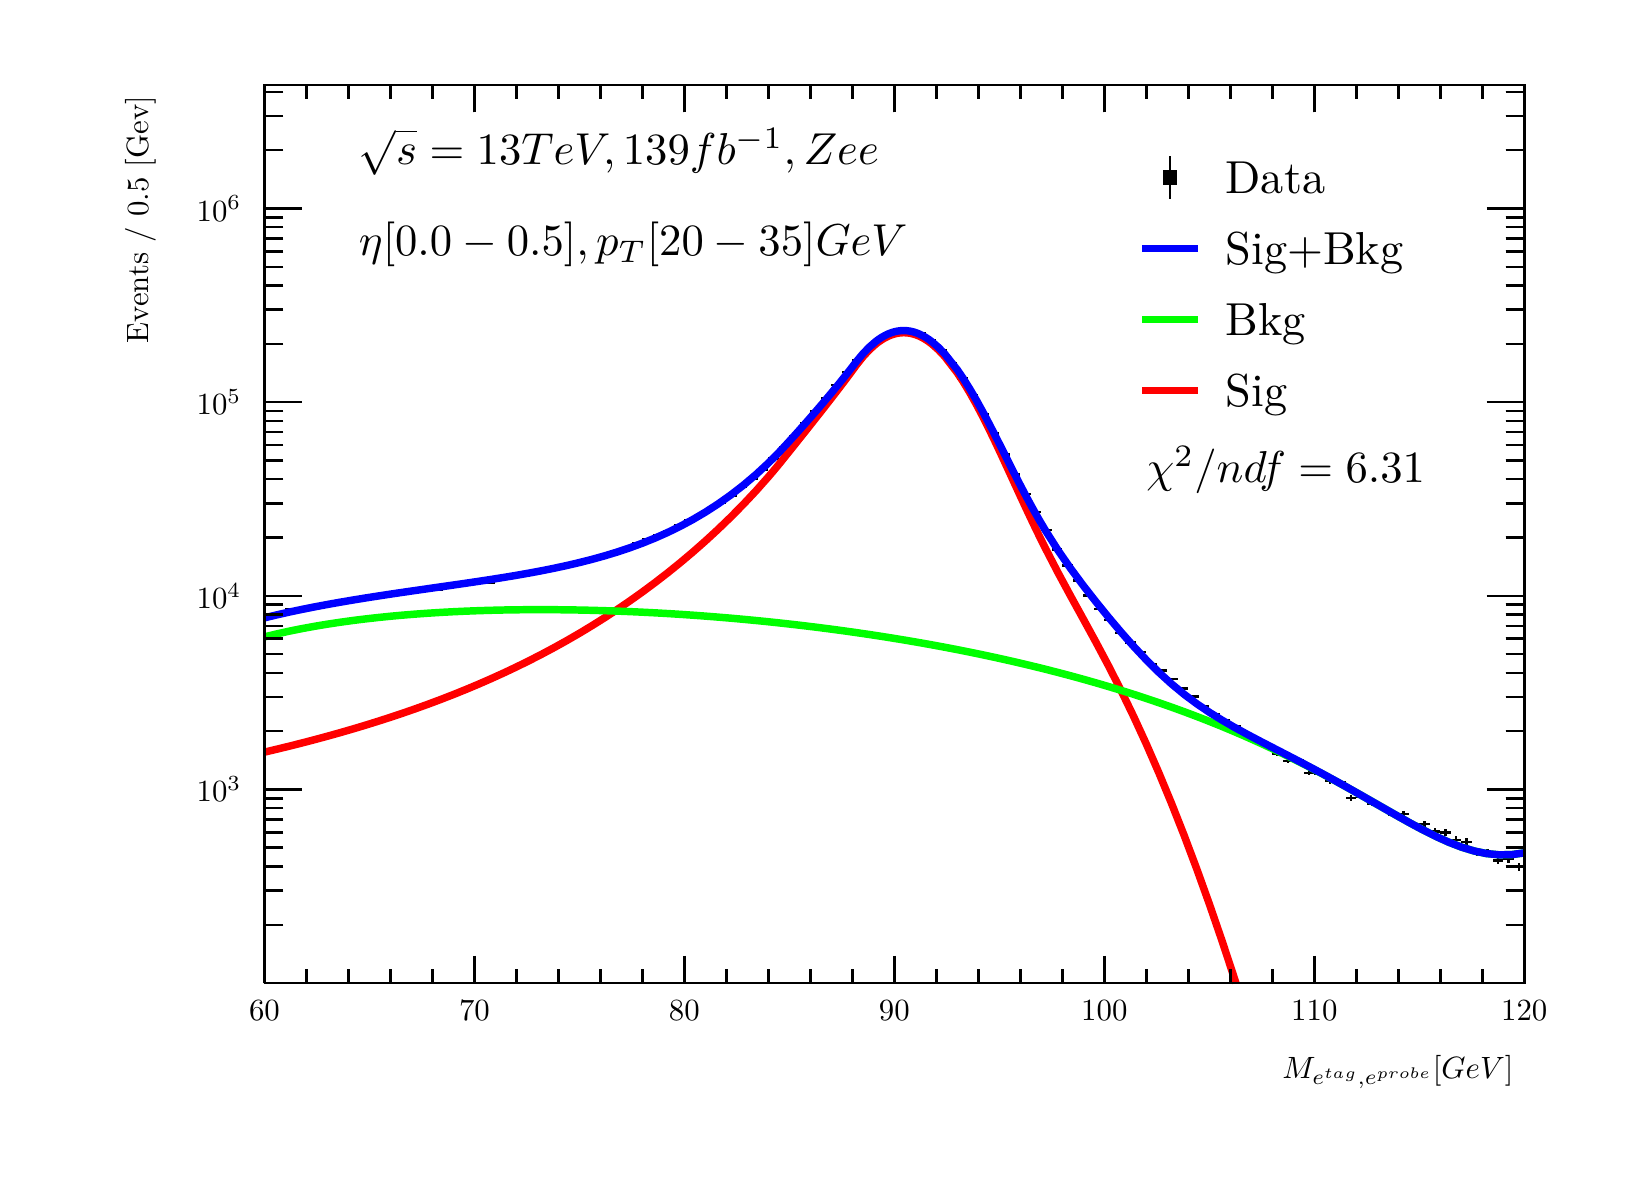
\begin{tikzpicture}
\pgfdeclareplotmark{cross} {
\pgfpathmoveto{\pgfpoint{-0.3\pgfplotmarksize}{\pgfplotmarksize}}
\pgfpathlineto{\pgfpoint{+0.3\pgfplotmarksize}{\pgfplotmarksize}}
\pgfpathlineto{\pgfpoint{+0.3\pgfplotmarksize}{0.3\pgfplotmarksize}}
\pgfpathlineto{\pgfpoint{+1\pgfplotmarksize}{0.3\pgfplotmarksize}}
\pgfpathlineto{\pgfpoint{+1\pgfplotmarksize}{-0.3\pgfplotmarksize}}
\pgfpathlineto{\pgfpoint{+0.3\pgfplotmarksize}{-0.3\pgfplotmarksize}}
\pgfpathlineto{\pgfpoint{+0.3\pgfplotmarksize}{-1.\pgfplotmarksize}}
\pgfpathlineto{\pgfpoint{-0.3\pgfplotmarksize}{-1.\pgfplotmarksize}}
\pgfpathlineto{\pgfpoint{-0.3\pgfplotmarksize}{-0.3\pgfplotmarksize}}
\pgfpathlineto{\pgfpoint{-1.\pgfplotmarksize}{-0.3\pgfplotmarksize}}
\pgfpathlineto{\pgfpoint{-1.\pgfplotmarksize}{0.3\pgfplotmarksize}}
\pgfpathlineto{\pgfpoint{-0.3\pgfplotmarksize}{0.3\pgfplotmarksize}}
\pgfpathclose
\pgfusepathqstroke
}
\pgfdeclareplotmark{cross*} {
\pgfpathmoveto{\pgfpoint{-0.3\pgfplotmarksize}{\pgfplotmarksize}}
\pgfpathlineto{\pgfpoint{+0.3\pgfplotmarksize}{\pgfplotmarksize}}
\pgfpathlineto{\pgfpoint{+0.3\pgfplotmarksize}{0.3\pgfplotmarksize}}
\pgfpathlineto{\pgfpoint{+1\pgfplotmarksize}{0.3\pgfplotmarksize}}
\pgfpathlineto{\pgfpoint{+1\pgfplotmarksize}{-0.3\pgfplotmarksize}}
\pgfpathlineto{\pgfpoint{+0.3\pgfplotmarksize}{-0.3\pgfplotmarksize}}
\pgfpathlineto{\pgfpoint{+0.3\pgfplotmarksize}{-1.\pgfplotmarksize}}
\pgfpathlineto{\pgfpoint{-0.3\pgfplotmarksize}{-1.\pgfplotmarksize}}
\pgfpathlineto{\pgfpoint{-0.3\pgfplotmarksize}{-0.3\pgfplotmarksize}}
\pgfpathlineto{\pgfpoint{-1.\pgfplotmarksize}{-0.3\pgfplotmarksize}}
\pgfpathlineto{\pgfpoint{-1.\pgfplotmarksize}{0.3\pgfplotmarksize}}
\pgfpathlineto{\pgfpoint{-0.3\pgfplotmarksize}{0.3\pgfplotmarksize}}
\pgfpathclose
\pgfusepathqfillstroke
}
\pgfdeclareplotmark{newstar} {
\pgfpathmoveto{\pgfqpoint{0pt}{\pgfplotmarksize}}
\pgfpathlineto{\pgfqpointpolar{44}{0.5\pgfplotmarksize}}
\pgfpathlineto{\pgfqpointpolar{18}{\pgfplotmarksize}}
\pgfpathlineto{\pgfqpointpolar{-20}{0.5\pgfplotmarksize}}
\pgfpathlineto{\pgfqpointpolar{-54}{\pgfplotmarksize}}
\pgfpathlineto{\pgfqpointpolar{-90}{0.5\pgfplotmarksize}}
\pgfpathlineto{\pgfqpointpolar{234}{\pgfplotmarksize}}
\pgfpathlineto{\pgfqpointpolar{198}{0.5\pgfplotmarksize}}
\pgfpathlineto{\pgfqpointpolar{162}{\pgfplotmarksize}}
\pgfpathlineto{\pgfqpointpolar{134}{0.5\pgfplotmarksize}}
\pgfpathclose
\pgfusepathqstroke
}
\pgfdeclareplotmark{newstar*} {
\pgfpathmoveto{\pgfqpoint{0pt}{\pgfplotmarksize}}
\pgfpathlineto{\pgfqpointpolar{44}{0.5\pgfplotmarksize}}
\pgfpathlineto{\pgfqpointpolar{18}{\pgfplotmarksize}}
\pgfpathlineto{\pgfqpointpolar{-20}{0.5\pgfplotmarksize}}
\pgfpathlineto{\pgfqpointpolar{-54}{\pgfplotmarksize}}
\pgfpathlineto{\pgfqpointpolar{-90}{0.5\pgfplotmarksize}}
\pgfpathlineto{\pgfqpointpolar{234}{\pgfplotmarksize}}
\pgfpathlineto{\pgfqpointpolar{198}{0.5\pgfplotmarksize}}
\pgfpathlineto{\pgfqpointpolar{162}{\pgfplotmarksize}}
\pgfpathlineto{\pgfqpointpolar{134}{0.5\pgfplotmarksize}}
\pgfpathclose
\pgfusepathqfillstroke
}
\definecolor{c}{rgb}{1,1,1};
\draw [color=c, fill=c] (0,0) rectangle (20,14.4361);
\draw [color=c, fill=c] (3,2.30977) rectangle (19,13.7143);
\definecolor{c}{rgb}{0,0,0};
\draw [c,line width=0.9] (3,2.30977) -- (3,13.7143) -- (19,13.7143) -- (19,2.30977) -- (3,2.30977);
\definecolor{c}{rgb}{1,1,1};
\draw [color=c, fill=c] (3,2.30977) rectangle (19,13.7143);
\definecolor{c}{rgb}{0,0,0};
\draw [c,line width=0.9] (3,2.30977) -- (3,13.7143) -- (19,13.7143) -- (19,2.30977) -- (3,2.30977);
\draw [c,line width=0.9] (3,2.30977) -- (19,2.30977);
\draw [c,line width=0.9] (3,2.65624) -- (3,2.30977);
\draw [c,line width=0.9] (3.53333,2.48301) -- (3.53333,2.30977);
\draw [c,line width=0.9] (4.06667,2.48301) -- (4.06667,2.30977);
\draw [c,line width=0.9] (4.6,2.48301) -- (4.6,2.30977);
\draw [c,line width=0.9] (5.13333,2.48301) -- (5.13333,2.30977);
\draw [c,line width=0.9] (5.66667,2.65624) -- (5.66667,2.30977);
\draw [c,line width=0.9] (6.2,2.48301) -- (6.2,2.30977);
\draw [c,line width=0.9] (6.73333,2.48301) -- (6.73333,2.30977);
\draw [c,line width=0.9] (7.26667,2.48301) -- (7.26667,2.30977);
\draw [c,line width=0.9] (7.8,2.48301) -- (7.8,2.30977);
\draw [c,line width=0.9] (8.33333,2.65624) -- (8.33333,2.30977);
\draw [c,line width=0.9] (8.86667,2.48301) -- (8.86667,2.30977);
\draw [c,line width=0.9] (9.4,2.48301) -- (9.4,2.30977);
\draw [c,line width=0.9] (9.93333,2.48301) -- (9.93333,2.30977);
\draw [c,line width=0.9] (10.4667,2.48301) -- (10.4667,2.30977);
\draw [c,line width=0.9] (11,2.65624) -- (11,2.30977);
\draw [c,line width=0.9] (11.5333,2.48301) -- (11.5333,2.30977);
\draw [c,line width=0.9] (12.0667,2.48301) -- (12.0667,2.30977);
\draw [c,line width=0.9] (12.6,2.48301) -- (12.6,2.30977);
\draw [c,line width=0.9] (13.1333,2.48301) -- (13.1333,2.30977);
\draw [c,line width=0.9] (13.6667,2.65624) -- (13.6667,2.30977);
\draw [c,line width=0.9] (14.2,2.48301) -- (14.2,2.30977);
\draw [c,line width=0.9] (14.7333,2.48301) -- (14.7333,2.30977);
\draw [c,line width=0.9] (15.2667,2.48301) -- (15.2667,2.30977);
\draw [c,line width=0.9] (15.8,2.48301) -- (15.8,2.30977);
\draw [c,line width=0.9] (16.3333,2.65624) -- (16.3333,2.30977);
\draw [c,line width=0.9] (16.8667,2.48301) -- (16.8667,2.30977);
\draw [c,line width=0.9] (17.4,2.48301) -- (17.4,2.30977);
\draw [c,line width=0.9] (17.9333,2.48301) -- (17.9333,2.30977);
\draw [c,line width=0.9] (18.4667,2.48301) -- (18.4667,2.30977);
\draw [c,line width=0.9] (19,2.65624) -- (19,2.30977);
\draw [anchor=base] (3,1.83338) node[scale=1.11327, color=c, rotate=0]{60};
\draw [anchor=base] (5.66667,1.83338) node[scale=1.11327, color=c, rotate=0]{70};
\draw [anchor=base] (8.33333,1.83338) node[scale=1.11327, color=c, rotate=0]{80};
\draw [anchor=base] (11,1.83338) node[scale=1.11327, color=c, rotate=0]{90};
\draw [anchor=base] (13.6667,1.83338) node[scale=1.11327, color=c, rotate=0]{100};
\draw [anchor=base] (16.3333,1.83338) node[scale=1.11327, color=c, rotate=0]{110};
\draw [anchor=base] (19,1.83338) node[scale=1.11327, color=c, rotate=0]{120};
\draw [anchor= east] (19,1.17798) node[scale=1.11327, color=c, rotate=0]{$M_{e^{tag}, e^{probe}}  [GeV]$};
\draw [c,line width=0.9] (3,13.7143) -- (19,13.7143);
\draw [c,line width=0.9] (3,13.3678) -- (3,13.7143);
\draw [c,line width=0.9] (3.53333,13.5411) -- (3.53333,13.7143);
\draw [c,line width=0.9] (4.06667,13.5411) -- (4.06667,13.7143);
\draw [c,line width=0.9] (4.6,13.5411) -- (4.6,13.7143);
\draw [c,line width=0.9] (5.13333,13.5411) -- (5.13333,13.7143);
\draw [c,line width=0.9] (5.66667,13.3678) -- (5.66667,13.7143);
\draw [c,line width=0.9] (6.2,13.5411) -- (6.2,13.7143);
\draw [c,line width=0.9] (6.73333,13.5411) -- (6.73333,13.7143);
\draw [c,line width=0.9] (7.26667,13.5411) -- (7.26667,13.7143);
\draw [c,line width=0.9] (7.8,13.5411) -- (7.8,13.7143);
\draw [c,line width=0.9] (8.33333,13.3678) -- (8.33333,13.7143);
\draw [c,line width=0.9] (8.86667,13.5411) -- (8.86667,13.7143);
\draw [c,line width=0.9] (9.4,13.5411) -- (9.4,13.7143);
\draw [c,line width=0.9] (9.93333,13.5411) -- (9.93333,13.7143);
\draw [c,line width=0.9] (10.4667,13.5411) -- (10.4667,13.7143);
\draw [c,line width=0.9] (11,13.3678) -- (11,13.7143);
\draw [c,line width=0.9] (11.5333,13.5411) -- (11.5333,13.7143);
\draw [c,line width=0.9] (12.0667,13.5411) -- (12.0667,13.7143);
\draw [c,line width=0.9] (12.6,13.5411) -- (12.6,13.7143);
\draw [c,line width=0.9] (13.1333,13.5411) -- (13.1333,13.7143);
\draw [c,line width=0.9] (13.6667,13.3678) -- (13.6667,13.7143);
\draw [c,line width=0.9] (14.2,13.5411) -- (14.2,13.7143);
\draw [c,line width=0.9] (14.7333,13.5411) -- (14.7333,13.7143);
\draw [c,line width=0.9] (15.2667,13.5411) -- (15.2667,13.7143);
\draw [c,line width=0.9] (15.8,13.5411) -- (15.8,13.7143);
\draw [c,line width=0.9] (16.3333,13.3678) -- (16.3333,13.7143);
\draw [c,line width=0.9] (16.8667,13.5411) -- (16.8667,13.7143);
\draw [c,line width=0.9] (17.4,13.5411) -- (17.4,13.7143);
\draw [c,line width=0.9] (17.9333,13.5411) -- (17.9333,13.7143);
\draw [c,line width=0.9] (18.4667,13.5411) -- (18.4667,13.7143);
\draw [c,line width=0.9] (19,13.3678) -- (19,13.7143);
\draw [c,line width=0.9] (3,2.30977) -- (3,13.7143);
\draw [c,line width=0.9] (3.237,3.05008) -- (3,3.05008);
\draw [c,line width=0.9] (3.237,3.48313) -- (3,3.48313);
\draw [c,line width=0.9] (3.237,3.79038) -- (3,3.79038);
\draw [c,line width=0.9] (3.237,4.02871) -- (3,4.02871);
\draw [c,line width=0.9] (3.237,4.22343) -- (3,4.22343);
\draw [c,line width=0.9] (3.237,4.38807) -- (3,4.38807);
\draw [c,line width=0.9] (3.237,4.53069) -- (3,4.53069);
\draw [c,line width=0.9] (3.237,4.65649) -- (3,4.65649);
\draw [c,line width=0.9] (3.474,4.76901) -- (3,4.76901);
\draw [anchor= east] (2.844,4.76901) node[scale=1.11327, color=c, rotate=0]{$10^{3}$};
\draw [c,line width=0.9] (3.237,5.50932) -- (3,5.50932);
\draw [c,line width=0.9] (3.237,5.94237) -- (3,5.94237);
\draw [c,line width=0.9] (3.237,6.24963) -- (3,6.24963);
\draw [c,line width=0.9] (3.237,6.48795) -- (3,6.48795);
\draw [c,line width=0.9] (3.237,6.68268) -- (3,6.68268);
\draw [c,line width=0.9] (3.237,6.84731) -- (3,6.84731);
\draw [c,line width=0.9] (3.237,6.98993) -- (3,6.98993);
\draw [c,line width=0.9] (3.237,7.11573) -- (3,7.11573);
\draw [c,line width=0.9] (3.474,7.22826) -- (3,7.22826);
\draw [anchor= east] (2.844,7.22826) node[scale=1.11327, color=c, rotate=0]{$10^{4}$};
\draw [c,line width=0.9] (3.237,7.96856) -- (3,7.96856);
\draw [c,line width=0.9] (3.237,8.40161) -- (3,8.40161);
\draw [c,line width=0.9] (3.237,8.70887) -- (3,8.70887);
\draw [c,line width=0.9] (3.237,8.94719) -- (3,8.94719);
\draw [c,line width=0.9] (3.237,9.14192) -- (3,9.14192);
\draw [c,line width=0.9] (3.237,9.30656) -- (3,9.30656);
\draw [c,line width=0.9] (3.237,9.44917) -- (3,9.44917);
\draw [c,line width=0.9] (3.237,9.57497) -- (3,9.57497);
\draw [c,line width=0.9] (3.474,9.6875) -- (3,9.6875);
\draw [anchor= east] (2.844,9.6875) node[scale=1.11327, color=c, rotate=0]{$10^{5}$};
\draw [c,line width=0.9] (3.237,10.4278) -- (3,10.4278);
\draw [c,line width=0.9] (3.237,10.8609) -- (3,10.8609);
\draw [c,line width=0.9] (3.237,11.1681) -- (3,11.1681);
\draw [c,line width=0.9] (3.237,11.4064) -- (3,11.4064);
\draw [c,line width=0.9] (3.237,11.6012) -- (3,11.6012);
\draw [c,line width=0.9] (3.237,11.7658) -- (3,11.7658);
\draw [c,line width=0.9] (3.237,11.9084) -- (3,11.9084);
\draw [c,line width=0.9] (3.237,12.0342) -- (3,12.0342);
\draw [c,line width=0.9] (3.474,12.1467) -- (3,12.1467);
\draw [anchor= east] (2.844,12.1467) node[scale=1.11327, color=c, rotate=0]{$10^{6}$};
\draw [c,line width=0.9] (3.237,12.887) -- (3,12.887);
\draw [c,line width=0.9] (3.237,13.3201) -- (3,13.3201);
\draw [c,line width=0.9] (3.237,13.6274) -- (3,13.6274);
\draw [anchor= east] (1.432,13.7143) node[scale=1.11327, color=c, rotate=90]{Events / 0.5 [Gev]};
\draw [c,line width=0.9] (19,2.30977) -- (19,13.7143);
\draw [c,line width=0.9] (18.763,3.05008) -- (19,3.05008);
\draw [c,line width=0.9] (18.763,3.48313) -- (19,3.48313);
\draw [c,line width=0.9] (18.763,3.79038) -- (19,3.79038);
\draw [c,line width=0.9] (18.763,4.02871) -- (19,4.02871);
\draw [c,line width=0.9] (18.763,4.22343) -- (19,4.22343);
\draw [c,line width=0.9] (18.763,4.38807) -- (19,4.38807);
\draw [c,line width=0.9] (18.763,4.53069) -- (19,4.53069);
\draw [c,line width=0.9] (18.763,4.65649) -- (19,4.65649);
\draw [c,line width=0.9] (18.526,4.76901) -- (19,4.76901);
\draw [c,line width=0.9] (18.763,5.50932) -- (19,5.50932);
\draw [c,line width=0.9] (18.763,5.94237) -- (19,5.94237);
\draw [c,line width=0.9] (18.763,6.24963) -- (19,6.24963);
\draw [c,line width=0.9] (18.763,6.48795) -- (19,6.48795);
\draw [c,line width=0.9] (18.763,6.68268) -- (19,6.68268);
\draw [c,line width=0.9] (18.763,6.84731) -- (19,6.84731);
\draw [c,line width=0.9] (18.763,6.98993) -- (19,6.98993);
\draw [c,line width=0.9] (18.763,7.11573) -- (19,7.11573);
\draw [c,line width=0.9] (18.526,7.22826) -- (19,7.22826);
\draw [c,line width=0.9] (18.763,7.96856) -- (19,7.96856);
\draw [c,line width=0.9] (18.763,8.40161) -- (19,8.40161);
\draw [c,line width=0.9] (18.763,8.70887) -- (19,8.70887);
\draw [c,line width=0.9] (18.763,8.94719) -- (19,8.94719);
\draw [c,line width=0.9] (18.763,9.14192) -- (19,9.14192);
\draw [c,line width=0.9] (18.763,9.30656) -- (19,9.30656);
\draw [c,line width=0.9] (18.763,9.44917) -- (19,9.44917);
\draw [c,line width=0.9] (18.763,9.57497) -- (19,9.57497);
\draw [c,line width=0.9] (18.526,9.6875) -- (19,9.6875);
\draw [c,line width=0.9] (18.763,10.4278) -- (19,10.4278);
\draw [c,line width=0.9] (18.763,10.8609) -- (19,10.8609);
\draw [c,line width=0.9] (18.763,11.1681) -- (19,11.1681);
\draw [c,line width=0.9] (18.763,11.4064) -- (19,11.4064);
\draw [c,line width=0.9] (18.763,11.6012) -- (19,11.6012);
\draw [c,line width=0.9] (18.763,11.7658) -- (19,11.7658);
\draw [c,line width=0.9] (18.763,11.9084) -- (19,11.9084);
\draw [c,line width=0.9] (18.763,12.0342) -- (19,12.0342);
\draw [c,line width=0.9] (18.526,12.1467) -- (19,12.1467);
\draw [c,line width=0.9] (18.763,12.887) -- (19,12.887);
\draw [c,line width=0.9] (18.763,13.3201) -- (19,13.3201);
\draw [c,line width=0.9] (18.763,13.6274) -- (19,13.6274);
\draw [c,line width=0.9] (3.06667,6.97555) -- (3,6.97555);
\draw [c,line width=0.9] (3,6.97555) -- (3,6.97555);
\draw [c,line width=0.9] (3.06667,6.97555) -- (3.13333,6.97555);
\draw [c,line width=0.9] (3.13333,6.97555) -- (3.13333,6.97555);
\draw [c,line width=0.9] (3.06667,6.97555) -- (3.06667,6.98757);
\draw [c,line width=0.9] (3.06667,6.98757) -- (3.06667,6.98757);
\draw [c,line width=0.9] (3.06667,6.97555) -- (3.06667,6.96353);
\draw [c,line width=0.9] (3.06667,6.96353) -- (3.06667,6.96353);
\draw [c,line width=0.9] (3.2,6.99897) -- (3.13333,6.99897);
\draw [c,line width=0.9] (3.13333,6.99897) -- (3.13333,6.99897);
\draw [c,line width=0.9] (3.2,6.99897) -- (3.26667,6.99897);
\draw [c,line width=0.9] (3.26667,6.99897) -- (3.26667,6.99897);
\draw [c,line width=0.9] (3.2,6.99897) -- (3.2,7.01086);
\draw [c,line width=0.9] (3.2,7.01086) -- (3.2,7.01086);
\draw [c,line width=0.9] (3.2,6.99897) -- (3.2,6.98708);
\draw [c,line width=0.9] (3.2,6.98708) -- (3.2,6.98708);
\draw [c,line width=0.9] (3.33333,7.05305) -- (3.26667,7.05305);
\draw [c,line width=0.9] (3.26667,7.05305) -- (3.26667,7.05305);
\draw [c,line width=0.9] (3.33333,7.05305) -- (3.4,7.05305);
\draw [c,line width=0.9] (3.4,7.05305) -- (3.4,7.05305);
\draw [c,line width=0.9] (3.33333,7.05305) -- (3.33333,7.06464);
\draw [c,line width=0.9] (3.33333,7.06464) -- (3.33333,7.06464);
\draw [c,line width=0.9] (3.33333,7.05305) -- (3.33333,7.04145);
\draw [c,line width=0.9] (3.33333,7.04145) -- (3.33333,7.04145);
\draw [c,line width=0.9] (3.46667,7.05619) -- (3.4,7.05619);
\draw [c,line width=0.9] (3.4,7.05619) -- (3.4,7.05619);
\draw [c,line width=0.9] (3.46667,7.05619) -- (3.53333,7.05619);
\draw [c,line width=0.9] (3.53333,7.05619) -- (3.53333,7.05619);
\draw [c,line width=0.9] (3.46667,7.05619) -- (3.46667,7.06776);
\draw [c,line width=0.9] (3.46667,7.06776) -- (3.46667,7.06776);
\draw [c,line width=0.9] (3.46667,7.05619) -- (3.46667,7.04461);
\draw [c,line width=0.9] (3.46667,7.04461) -- (3.46667,7.04461);
\draw [c,line width=0.9] (3.6,7.09403) -- (3.53333,7.09403);
\draw [c,line width=0.9] (3.53333,7.09403) -- (3.53333,7.09403);
\draw [c,line width=0.9] (3.6,7.09403) -- (3.66667,7.09403);
\draw [c,line width=0.9] (3.66667,7.09403) -- (3.66667,7.09403);
\draw [c,line width=0.9] (3.6,7.09403) -- (3.6,7.1054);
\draw [c,line width=0.9] (3.6,7.1054) -- (3.6,7.1054);
\draw [c,line width=0.9] (3.6,7.09403) -- (3.6,7.08266);
\draw [c,line width=0.9] (3.6,7.08266) -- (3.6,7.08266);
\draw [c,line width=0.9] (3.73333,7.12094) -- (3.66667,7.12094);
\draw [c,line width=0.9] (3.66667,7.12094) -- (3.66667,7.12094);
\draw [c,line width=0.9] (3.73333,7.12094) -- (3.8,7.12094);
\draw [c,line width=0.9] (3.8,7.12094) -- (3.8,7.12094);
\draw [c,line width=0.9] (3.73333,7.12094) -- (3.73333,7.13217);
\draw [c,line width=0.9] (3.73333,7.13217) -- (3.73333,7.13217);
\draw [c,line width=0.9] (3.73333,7.12094) -- (3.73333,7.10971);
\draw [c,line width=0.9] (3.73333,7.10971) -- (3.73333,7.10971);
\draw [c,line width=0.9] (3.86667,7.1328) -- (3.8,7.1328);
\draw [c,line width=0.9] (3.8,7.1328) -- (3.8,7.1328);
\draw [c,line width=0.9] (3.86667,7.1328) -- (3.93333,7.1328);
\draw [c,line width=0.9] (3.93333,7.1328) -- (3.93333,7.1328);
\draw [c,line width=0.9] (3.86667,7.1328) -- (3.86667,7.14397);
\draw [c,line width=0.9] (3.86667,7.14397) -- (3.86667,7.14397);
\draw [c,line width=0.9] (3.86667,7.1328) -- (3.86667,7.12163);
\draw [c,line width=0.9] (3.86667,7.12163) -- (3.86667,7.12163);
\draw [c,line width=0.9] (4,7.15407) -- (3.93333,7.15407);
\draw [c,line width=0.9] (3.93333,7.15407) -- (3.93333,7.15407);
\draw [c,line width=0.9] (4,7.15407) -- (4.06667,7.15407);
\draw [c,line width=0.9] (4.06667,7.15407) -- (4.06667,7.15407);
\draw [c,line width=0.9] (4,7.15407) -- (4,7.16513);
\draw [c,line width=0.9] (4,7.16513) -- (4,7.16513);
\draw [c,line width=0.9] (4,7.15407) -- (4,7.14302);
\draw [c,line width=0.9] (4,7.14302) -- (4,7.14302);
\draw [c,line width=0.9] (4.13333,7.18377) -- (4.06667,7.18377);
\draw [c,line width=0.9] (4.06667,7.18377) -- (4.06667,7.18377);
\draw [c,line width=0.9] (4.13333,7.18377) -- (4.2,7.18377);
\draw [c,line width=0.9] (4.2,7.18377) -- (4.2,7.18377);
\draw [c,line width=0.9] (4.13333,7.18377) -- (4.13333,7.19467);
\draw [c,line width=0.9] (4.13333,7.19467) -- (4.13333,7.19467);
\draw [c,line width=0.9] (4.13333,7.18377) -- (4.13333,7.17286);
\draw [c,line width=0.9] (4.13333,7.17286) -- (4.13333,7.17286);
\draw [c,line width=0.9] (4.26667,7.21439) -- (4.2,7.21439);
\draw [c,line width=0.9] (4.2,7.21439) -- (4.2,7.21439);
\draw [c,line width=0.9] (4.26667,7.21439) -- (4.33333,7.21439);
\draw [c,line width=0.9] (4.33333,7.21439) -- (4.33333,7.21439);
\draw [c,line width=0.9] (4.26667,7.21439) -- (4.26667,7.22514);
\draw [c,line width=0.9] (4.26667,7.22514) -- (4.26667,7.22514);
\draw [c,line width=0.9] (4.26667,7.21439) -- (4.26667,7.20364);
\draw [c,line width=0.9] (4.26667,7.20364) -- (4.26667,7.20364);
\draw [c,line width=0.9] (4.4,7.21114) -- (4.33333,7.21114);
\draw [c,line width=0.9] (4.33333,7.21114) -- (4.33333,7.21114);
\draw [c,line width=0.9] (4.4,7.21114) -- (4.46667,7.21114);
\draw [c,line width=0.9] (4.46667,7.21114) -- (4.46667,7.21114);
\draw [c,line width=0.9] (4.4,7.21114) -- (4.4,7.22191);
\draw [c,line width=0.9] (4.4,7.22191) -- (4.4,7.22191);
\draw [c,line width=0.9] (4.4,7.21114) -- (4.4,7.20037);
\draw [c,line width=0.9] (4.4,7.20037) -- (4.4,7.20037);
\draw [c,line width=0.9] (4.53333,7.21979) -- (4.46667,7.21979);
\draw [c,line width=0.9] (4.46667,7.21979) -- (4.46667,7.21979);
\draw [c,line width=0.9] (4.53333,7.21979) -- (4.6,7.21979);
\draw [c,line width=0.9] (4.6,7.21979) -- (4.6,7.21979);
\draw [c,line width=0.9] (4.53333,7.21979) -- (4.53333,7.23051);
\draw [c,line width=0.9] (4.53333,7.23051) -- (4.53333,7.23051);
\draw [c,line width=0.9] (4.53333,7.21979) -- (4.53333,7.20906);
\draw [c,line width=0.9] (4.53333,7.20906) -- (4.53333,7.20906);
\draw [c,line width=0.9] (4.66667,7.23878) -- (4.6,7.23878);
\draw [c,line width=0.9] (4.6,7.23878) -- (4.6,7.23878);
\draw [c,line width=0.9] (4.66667,7.23878) -- (4.73333,7.23878);
\draw [c,line width=0.9] (4.73333,7.23878) -- (4.73333,7.23878);
\draw [c,line width=0.9] (4.66667,7.23878) -- (4.66667,7.24941);
\draw [c,line width=0.9] (4.66667,7.24941) -- (4.66667,7.24941);
\draw [c,line width=0.9] (4.66667,7.23878) -- (4.66667,7.22815);
\draw [c,line width=0.9] (4.66667,7.22815) -- (4.66667,7.22815);
\draw [c,line width=0.9] (4.8,7.28756) -- (4.73333,7.28756);
\draw [c,line width=0.9] (4.73333,7.28756) -- (4.73333,7.28756);
\draw [c,line width=0.9] (4.8,7.28756) -- (4.86667,7.28756);
\draw [c,line width=0.9] (4.86667,7.28756) -- (4.86667,7.28756);
\draw [c,line width=0.9] (4.8,7.28756) -- (4.8,7.29795);
\draw [c,line width=0.9] (4.8,7.29795) -- (4.8,7.29795);
\draw [c,line width=0.9] (4.8,7.28756) -- (4.8,7.27718);
\draw [c,line width=0.9] (4.8,7.27718) -- (4.8,7.27718);
\draw [c,line width=0.9] (4.93333,7.27425) -- (4.86667,7.27425);
\draw [c,line width=0.9] (4.86667,7.27425) -- (4.86667,7.27425);
\draw [c,line width=0.9] (4.93333,7.27425) -- (5,7.27425);
\draw [c,line width=0.9] (5,7.27425) -- (5,7.27425);
\draw [c,line width=0.9] (4.93333,7.27425) -- (4.93333,7.2847);
\draw [c,line width=0.9] (4.93333,7.2847) -- (4.93333,7.2847);
\draw [c,line width=0.9] (4.93333,7.27425) -- (4.93333,7.26379);
\draw [c,line width=0.9] (4.93333,7.26379) -- (4.93333,7.26379);
\draw [c,line width=0.9] (5.06667,7.30986) -- (5,7.30986);
\draw [c,line width=0.9] (5,7.30986) -- (5,7.30986);
\draw [c,line width=0.9] (5.06667,7.30986) -- (5.13333,7.30986);
\draw [c,line width=0.9] (5.13333,7.30986) -- (5.13333,7.30986);
\draw [c,line width=0.9] (5.06667,7.30986) -- (5.06667,7.32014);
\draw [c,line width=0.9] (5.06667,7.32014) -- (5.06667,7.32014);
\draw [c,line width=0.9] (5.06667,7.30986) -- (5.06667,7.29958);
\draw [c,line width=0.9] (5.06667,7.29958) -- (5.06667,7.29958);
\draw [c,line width=0.9] (5.2,7.31065) -- (5.13333,7.31065);
\draw [c,line width=0.9] (5.13333,7.31065) -- (5.13333,7.31065);
\draw [c,line width=0.9] (5.2,7.31065) -- (5.26667,7.31065);
\draw [c,line width=0.9] (5.26667,7.31065) -- (5.26667,7.31065);
\draw [c,line width=0.9] (5.2,7.31065) -- (5.2,7.32093);
\draw [c,line width=0.9] (5.2,7.32093) -- (5.2,7.32093);
\draw [c,line width=0.9] (5.2,7.31065) -- (5.2,7.30038);
\draw [c,line width=0.9] (5.2,7.30038) -- (5.2,7.30038);
\draw [c,line width=0.9] (5.33333,7.34844) -- (5.26667,7.34844);
\draw [c,line width=0.9] (5.26667,7.34844) -- (5.26667,7.34844);
\draw [c,line width=0.9] (5.33333,7.34844) -- (5.4,7.34844);
\draw [c,line width=0.9] (5.4,7.34844) -- (5.4,7.34844);
\draw [c,line width=0.9] (5.33333,7.34844) -- (5.33333,7.35853);
\draw [c,line width=0.9] (5.33333,7.35853) -- (5.33333,7.35853);
\draw [c,line width=0.9] (5.33333,7.34844) -- (5.33333,7.33834);
\draw [c,line width=0.9] (5.33333,7.33834) -- (5.33333,7.33834);
\draw [c,line width=0.9] (5.46667,7.35358) -- (5.4,7.35358);
\draw [c,line width=0.9] (5.4,7.35358) -- (5.4,7.35358);
\draw [c,line width=0.9] (5.46667,7.35358) -- (5.53333,7.35358);
\draw [c,line width=0.9] (5.53333,7.35358) -- (5.53333,7.35358);
\draw [c,line width=0.9] (5.46667,7.35358) -- (5.46667,7.36365);
\draw [c,line width=0.9] (5.46667,7.36365) -- (5.46667,7.36365);
\draw [c,line width=0.9] (5.46667,7.35358) -- (5.46667,7.34351);
\draw [c,line width=0.9] (5.46667,7.34351) -- (5.46667,7.34351);
\draw [c,line width=0.9] (5.6,7.38401) -- (5.53333,7.38401);
\draw [c,line width=0.9] (5.53333,7.38401) -- (5.53333,7.38401);
\draw [c,line width=0.9] (5.6,7.38401) -- (5.66667,7.38401);
\draw [c,line width=0.9] (5.66667,7.38401) -- (5.66667,7.38401);
\draw [c,line width=0.9] (5.6,7.38401) -- (5.6,7.39394);
\draw [c,line width=0.9] (5.6,7.39394) -- (5.6,7.39394);
\draw [c,line width=0.9] (5.6,7.38401) -- (5.6,7.37408);
\draw [c,line width=0.9] (5.6,7.37408) -- (5.6,7.37408);
\draw [c,line width=0.9] (5.73333,7.39649) -- (5.66667,7.39649);
\draw [c,line width=0.9] (5.66667,7.39649) -- (5.66667,7.39649);
\draw [c,line width=0.9] (5.73333,7.39649) -- (5.8,7.39649);
\draw [c,line width=0.9] (5.8,7.39649) -- (5.8,7.39649);
\draw [c,line width=0.9] (5.73333,7.39649) -- (5.73333,7.40636);
\draw [c,line width=0.9] (5.73333,7.40636) -- (5.73333,7.40636);
\draw [c,line width=0.9] (5.73333,7.39649) -- (5.73333,7.38662);
\draw [c,line width=0.9] (5.73333,7.38662) -- (5.73333,7.38662);
\draw [c,line width=0.9] (5.86667,7.39722) -- (5.8,7.39722);
\draw [c,line width=0.9] (5.8,7.39722) -- (5.8,7.39722);
\draw [c,line width=0.9] (5.86667,7.39722) -- (5.93333,7.39722);
\draw [c,line width=0.9] (5.93333,7.39722) -- (5.93333,7.39722);
\draw [c,line width=0.9] (5.86667,7.39722) -- (5.86667,7.40709);
\draw [c,line width=0.9] (5.86667,7.40709) -- (5.86667,7.40709);
\draw [c,line width=0.9] (5.86667,7.39722) -- (5.86667,7.38735);
\draw [c,line width=0.9] (5.86667,7.38735) -- (5.86667,7.38735);
\draw [c,line width=0.9] (6,7.44378) -- (5.93333,7.44378);
\draw [c,line width=0.9] (5.93333,7.44378) -- (5.93333,7.44378);
\draw [c,line width=0.9] (6,7.44378) -- (6.06667,7.44378);
\draw [c,line width=0.9] (6.06667,7.44378) -- (6.06667,7.44378);
\draw [c,line width=0.9] (6,7.44378) -- (6,7.45344);
\draw [c,line width=0.9] (6,7.45344) -- (6,7.45344);
\draw [c,line width=0.9] (6,7.44378) -- (6,7.43413);
\draw [c,line width=0.9] (6,7.43413) -- (6,7.43413);
\draw [c,line width=0.9] (6.13333,7.45403) -- (6.06667,7.45403);
\draw [c,line width=0.9] (6.06667,7.45403) -- (6.06667,7.45403);
\draw [c,line width=0.9] (6.13333,7.45403) -- (6.2,7.45403);
\draw [c,line width=0.9] (6.2,7.45403) -- (6.2,7.45403);
\draw [c,line width=0.9] (6.13333,7.45403) -- (6.13333,7.46364);
\draw [c,line width=0.9] (6.13333,7.46364) -- (6.13333,7.46364);
\draw [c,line width=0.9] (6.13333,7.45403) -- (6.13333,7.44443);
\draw [c,line width=0.9] (6.13333,7.44443) -- (6.13333,7.44443);
\draw [c,line width=0.9] (6.26667,7.5008) -- (6.2,7.5008);
\draw [c,line width=0.9] (6.2,7.5008) -- (6.2,7.5008);
\draw [c,line width=0.9] (6.26667,7.5008) -- (6.33333,7.5008);
\draw [c,line width=0.9] (6.33333,7.5008) -- (6.33333,7.5008);
\draw [c,line width=0.9] (6.26667,7.5008) -- (6.26667,7.5102);
\draw [c,line width=0.9] (6.26667,7.5102) -- (6.26667,7.5102);
\draw [c,line width=0.9] (6.26667,7.5008) -- (6.26667,7.4914);
\draw [c,line width=0.9] (6.26667,7.4914) -- (6.26667,7.4914);
\draw [c,line width=0.9] (6.4,7.52162) -- (6.33333,7.52162);
\draw [c,line width=0.9] (6.33333,7.52162) -- (6.33333,7.52162);
\draw [c,line width=0.9] (6.4,7.52162) -- (6.46667,7.52162);
\draw [c,line width=0.9] (6.46667,7.52162) -- (6.46667,7.52162);
\draw [c,line width=0.9] (6.4,7.52162) -- (6.4,7.53093);
\draw [c,line width=0.9] (6.4,7.53093) -- (6.4,7.53093);
\draw [c,line width=0.9] (6.4,7.52162) -- (6.4,7.51231);
\draw [c,line width=0.9] (6.4,7.51231) -- (6.4,7.51231);
\draw [c,line width=0.9] (6.53333,7.54941) -- (6.46667,7.54941);
\draw [c,line width=0.9] (6.46667,7.54941) -- (6.46667,7.54941);
\draw [c,line width=0.9] (6.53333,7.54941) -- (6.6,7.54941);
\draw [c,line width=0.9] (6.6,7.54941) -- (6.6,7.54941);
\draw [c,line width=0.9] (6.53333,7.54941) -- (6.53333,7.5586);
\draw [c,line width=0.9] (6.53333,7.5586) -- (6.53333,7.5586);
\draw [c,line width=0.9] (6.53333,7.54941) -- (6.53333,7.54022);
\draw [c,line width=0.9] (6.53333,7.54022) -- (6.53333,7.54022);
\draw [c,line width=0.9] (6.66667,7.58211) -- (6.6,7.58211);
\draw [c,line width=0.9] (6.6,7.58211) -- (6.6,7.58211);
\draw [c,line width=0.9] (6.66667,7.58211) -- (6.73333,7.58211);
\draw [c,line width=0.9] (6.73333,7.58211) -- (6.73333,7.58211);
\draw [c,line width=0.9] (6.66667,7.58211) -- (6.66667,7.59116);
\draw [c,line width=0.9] (6.66667,7.59116) -- (6.66667,7.59116);
\draw [c,line width=0.9] (6.66667,7.58211) -- (6.66667,7.57306);
\draw [c,line width=0.9] (6.66667,7.57306) -- (6.66667,7.57306);
\draw [c,line width=0.9] (6.8,7.61094) -- (6.73333,7.61094);
\draw [c,line width=0.9] (6.73333,7.61094) -- (6.73333,7.61094);
\draw [c,line width=0.9] (6.8,7.61094) -- (6.86667,7.61094);
\draw [c,line width=0.9] (6.86667,7.61094) -- (6.86667,7.61094);
\draw [c,line width=0.9] (6.8,7.61094) -- (6.8,7.61987);
\draw [c,line width=0.9] (6.8,7.61987) -- (6.8,7.61987);
\draw [c,line width=0.9] (6.8,7.61094) -- (6.8,7.60201);
\draw [c,line width=0.9] (6.8,7.60201) -- (6.8,7.60201);
\draw [c,line width=0.9] (6.93333,7.6331) -- (6.86667,7.6331);
\draw [c,line width=0.9] (6.86667,7.6331) -- (6.86667,7.6331);
\draw [c,line width=0.9] (6.93333,7.6331) -- (7,7.6331);
\draw [c,line width=0.9] (7,7.6331) -- (7,7.6331);
\draw [c,line width=0.9] (6.93333,7.6331) -- (6.93333,7.64194);
\draw [c,line width=0.9] (6.93333,7.64194) -- (6.93333,7.64194);
\draw [c,line width=0.9] (6.93333,7.6331) -- (6.93333,7.62426);
\draw [c,line width=0.9] (6.93333,7.62426) -- (6.93333,7.62426);
\draw [c,line width=0.9] (7.06667,7.66734) -- (7,7.66734);
\draw [c,line width=0.9] (7,7.66734) -- (7,7.66734);
\draw [c,line width=0.9] (7.06667,7.66734) -- (7.13333,7.66734);
\draw [c,line width=0.9] (7.13333,7.66734) -- (7.13333,7.66734);
\draw [c,line width=0.9] (7.06667,7.66734) -- (7.06667,7.67604);
\draw [c,line width=0.9] (7.06667,7.67604) -- (7.06667,7.67604);
\draw [c,line width=0.9] (7.06667,7.66734) -- (7.06667,7.65865);
\draw [c,line width=0.9] (7.06667,7.65865) -- (7.06667,7.65865);
\draw [c,line width=0.9] (7.2,7.71829) -- (7.13333,7.71829);
\draw [c,line width=0.9] (7.13333,7.71829) -- (7.13333,7.71829);
\draw [c,line width=0.9] (7.2,7.71829) -- (7.26667,7.71829);
\draw [c,line width=0.9] (7.26667,7.71829) -- (7.26667,7.71829);
\draw [c,line width=0.9] (7.2,7.71829) -- (7.2,7.72678);
\draw [c,line width=0.9] (7.2,7.72678) -- (7.2,7.72678);
\draw [c,line width=0.9] (7.2,7.71829) -- (7.2,7.7098);
\draw [c,line width=0.9] (7.2,7.7098) -- (7.2,7.7098);
\draw [c,line width=0.9] (7.33333,7.73961) -- (7.26667,7.73961);
\draw [c,line width=0.9] (7.26667,7.73961) -- (7.26667,7.73961);
\draw [c,line width=0.9] (7.33333,7.73961) -- (7.4,7.73961);
\draw [c,line width=0.9] (7.4,7.73961) -- (7.4,7.73961);
\draw [c,line width=0.9] (7.33333,7.73961) -- (7.33333,7.74801);
\draw [c,line width=0.9] (7.33333,7.74801) -- (7.33333,7.74801);
\draw [c,line width=0.9] (7.33333,7.73961) -- (7.33333,7.7312);
\draw [c,line width=0.9] (7.33333,7.7312) -- (7.33333,7.7312);
\draw [c,line width=0.9] (7.46667,7.78235) -- (7.4,7.78235);
\draw [c,line width=0.9] (7.4,7.78235) -- (7.4,7.78235);
\draw [c,line width=0.9] (7.46667,7.78235) -- (7.53333,7.78235);
\draw [c,line width=0.9] (7.53333,7.78235) -- (7.53333,7.78235);
\draw [c,line width=0.9] (7.46667,7.78235) -- (7.46667,7.79059);
\draw [c,line width=0.9] (7.46667,7.79059) -- (7.46667,7.79059);
\draw [c,line width=0.9] (7.46667,7.78235) -- (7.46667,7.77411);
\draw [c,line width=0.9] (7.46667,7.77411) -- (7.46667,7.77411);
\draw [c,line width=0.9] (7.6,7.83343) -- (7.53333,7.83343);
\draw [c,line width=0.9] (7.53333,7.83343) -- (7.53333,7.83343);
\draw [c,line width=0.9] (7.6,7.83343) -- (7.66667,7.83343);
\draw [c,line width=0.9] (7.66667,7.83343) -- (7.66667,7.83343);
\draw [c,line width=0.9] (7.6,7.83343) -- (7.6,7.84147);
\draw [c,line width=0.9] (7.6,7.84147) -- (7.6,7.84147);
\draw [c,line width=0.9] (7.6,7.83343) -- (7.6,7.82538);
\draw [c,line width=0.9] (7.6,7.82538) -- (7.6,7.82538);
\draw [c,line width=0.9] (7.73333,7.89025) -- (7.66667,7.89025);
\draw [c,line width=0.9] (7.66667,7.89025) -- (7.66667,7.89025);
\draw [c,line width=0.9] (7.73333,7.89025) -- (7.8,7.89025);
\draw [c,line width=0.9] (7.8,7.89025) -- (7.8,7.89025);
\draw [c,line width=0.9] (7.73333,7.89025) -- (7.73333,7.89808);
\draw [c,line width=0.9] (7.73333,7.89808) -- (7.73333,7.89808);
\draw [c,line width=0.9] (7.73333,7.89025) -- (7.73333,7.88242);
\draw [c,line width=0.9] (7.73333,7.88242) -- (7.73333,7.88242);
\draw [c,line width=0.9] (7.86667,7.94824) -- (7.8,7.94824);
\draw [c,line width=0.9] (7.8,7.94824) -- (7.8,7.94824);
\draw [c,line width=0.9] (7.86667,7.94824) -- (7.93333,7.94824);
\draw [c,line width=0.9] (7.93333,7.94824) -- (7.93333,7.94824);
\draw [c,line width=0.9] (7.86667,7.94824) -- (7.86667,7.95586);
\draw [c,line width=0.9] (7.86667,7.95586) -- (7.86667,7.95586);
\draw [c,line width=0.9] (7.86667,7.94824) -- (7.86667,7.94061);
\draw [c,line width=0.9] (7.86667,7.94061) -- (7.86667,7.94061);
\draw [c,line width=0.9] (8,7.99107) -- (7.93333,7.99107);
\draw [c,line width=0.9] (7.93333,7.99107) -- (7.93333,7.99107);
\draw [c,line width=0.9] (8,7.99107) -- (8.06667,7.99107);
\draw [c,line width=0.9] (8.06667,7.99107) -- (8.06667,7.99107);
\draw [c,line width=0.9] (8,7.99107) -- (8,7.99855);
\draw [c,line width=0.9] (8,7.99855) -- (8,7.99855);
\draw [c,line width=0.9] (8,7.99107) -- (8,7.9836);
\draw [c,line width=0.9] (8,7.9836) -- (8,7.9836);
\draw [c,line width=0.9] (8.13333,8.04883) -- (8.06667,8.04883);
\draw [c,line width=0.9] (8.06667,8.04883) -- (8.06667,8.04883);
\draw [c,line width=0.9] (8.13333,8.04883) -- (8.2,8.04883);
\draw [c,line width=0.9] (8.2,8.04883) -- (8.2,8.04883);
\draw [c,line width=0.9] (8.13333,8.04883) -- (8.13333,8.0561);
\draw [c,line width=0.9] (8.13333,8.0561) -- (8.13333,8.0561);
\draw [c,line width=0.9] (8.13333,8.04883) -- (8.13333,8.04156);
\draw [c,line width=0.9] (8.13333,8.04156) -- (8.13333,8.04156);
\draw [c,line width=0.9] (8.26667,8.11821) -- (8.2,8.11821);
\draw [c,line width=0.9] (8.2,8.11821) -- (8.2,8.11821);
\draw [c,line width=0.9] (8.26667,8.11821) -- (8.33333,8.11821);
\draw [c,line width=0.9] (8.33333,8.11821) -- (8.33333,8.11821);
\draw [c,line width=0.9] (8.26667,8.11821) -- (8.26667,8.12525);
\draw [c,line width=0.9] (8.26667,8.12525) -- (8.26667,8.12525);
\draw [c,line width=0.9] (8.26667,8.11821) -- (8.26667,8.11116);
\draw [c,line width=0.9] (8.26667,8.11116) -- (8.26667,8.11116);
\draw [c,line width=0.9] (8.4,8.18278) -- (8.33333,8.18278);
\draw [c,line width=0.9] (8.33333,8.18278) -- (8.33333,8.18278);
\draw [c,line width=0.9] (8.4,8.18278) -- (8.46667,8.18278);
\draw [c,line width=0.9] (8.46667,8.18278) -- (8.46667,8.18278);
\draw [c,line width=0.9] (8.4,8.18278) -- (8.4,8.18961);
\draw [c,line width=0.9] (8.4,8.18961) -- (8.4,8.18961);
\draw [c,line width=0.9] (8.4,8.18278) -- (8.4,8.17595);
\draw [c,line width=0.9] (8.4,8.17595) -- (8.4,8.17595);
\draw [c,line width=0.9] (8.53333,8.25148) -- (8.46667,8.25148);
\draw [c,line width=0.9] (8.46667,8.25148) -- (8.46667,8.25148);
\draw [c,line width=0.9] (8.53333,8.25148) -- (8.6,8.25148);
\draw [c,line width=0.9] (8.6,8.25148) -- (8.6,8.25148);
\draw [c,line width=0.9] (8.53333,8.25148) -- (8.53333,8.2581);
\draw [c,line width=0.9] (8.53333,8.2581) -- (8.53333,8.2581);
\draw [c,line width=0.9] (8.53333,8.25148) -- (8.53333,8.24487);
\draw [c,line width=0.9] (8.53333,8.24487) -- (8.53333,8.24487);
\draw [c,line width=0.9] (8.66667,8.3296) -- (8.6,8.3296);
\draw [c,line width=0.9] (8.6,8.3296) -- (8.6,8.3296);
\draw [c,line width=0.9] (8.66667,8.3296) -- (8.73333,8.3296);
\draw [c,line width=0.9] (8.73333,8.3296) -- (8.73333,8.3296);
\draw [c,line width=0.9] (8.66667,8.3296) -- (8.66667,8.33598);
\draw [c,line width=0.9] (8.66667,8.33598) -- (8.66667,8.33598);
\draw [c,line width=0.9] (8.66667,8.3296) -- (8.66667,8.32323);
\draw [c,line width=0.9] (8.66667,8.32323) -- (8.66667,8.32323);
\draw [c,line width=0.9] (8.8,8.41062) -- (8.73333,8.41062);
\draw [c,line width=0.9] (8.73333,8.41062) -- (8.73333,8.41062);
\draw [c,line width=0.9] (8.8,8.41062) -- (8.86667,8.41062);
\draw [c,line width=0.9] (8.86667,8.41062) -- (8.86667,8.41062);
\draw [c,line width=0.9] (8.8,8.41062) -- (8.8,8.41676);
\draw [c,line width=0.9] (8.8,8.41676) -- (8.8,8.41676);
\draw [c,line width=0.9] (8.8,8.41062) -- (8.8,8.40448);
\draw [c,line width=0.9] (8.8,8.40448) -- (8.8,8.40448);
\draw [c,line width=0.9] (8.93333,8.50328) -- (8.86667,8.50328);
\draw [c,line width=0.9] (8.86667,8.50328) -- (8.86667,8.50328);
\draw [c,line width=0.9] (8.93333,8.50328) -- (9,8.50328);
\draw [c,line width=0.9] (9,8.50328) -- (9,8.50328);
\draw [c,line width=0.9] (8.93333,8.50328) -- (8.93333,8.50916);
\draw [c,line width=0.9] (8.93333,8.50916) -- (8.93333,8.50916);
\draw [c,line width=0.9] (8.93333,8.50328) -- (8.93333,8.4974);
\draw [c,line width=0.9] (8.93333,8.4974) -- (8.93333,8.4974);
\draw [c,line width=0.9] (9.06667,8.60958) -- (9,8.60958);
\draw [c,line width=0.9] (9,8.60958) -- (9,8.60958);
\draw [c,line width=0.9] (9.06667,8.60958) -- (9.13333,8.60958);
\draw [c,line width=0.9] (9.13333,8.60958) -- (9.13333,8.60958);
\draw [c,line width=0.9] (9.06667,8.60958) -- (9.06667,8.61517);
\draw [c,line width=0.9] (9.06667,8.61517) -- (9.06667,8.61517);
\draw [c,line width=0.9] (9.06667,8.60958) -- (9.06667,8.60398);
\draw [c,line width=0.9] (9.06667,8.60398) -- (9.06667,8.60398);
\draw [c,line width=0.9] (9.2,8.71741) -- (9.13333,8.71741);
\draw [c,line width=0.9] (9.13333,8.71741) -- (9.13333,8.71741);
\draw [c,line width=0.9] (9.2,8.71741) -- (9.26667,8.71741);
\draw [c,line width=0.9] (9.26667,8.71741) -- (9.26667,8.71741);
\draw [c,line width=0.9] (9.2,8.71741) -- (9.2,8.72272);
\draw [c,line width=0.9] (9.2,8.72272) -- (9.2,8.72272);
\draw [c,line width=0.9] (9.2,8.71741) -- (9.2,8.71209);
\draw [c,line width=0.9] (9.2,8.71209) -- (9.2,8.71209);
\draw [c,line width=0.9] (9.33333,8.83352) -- (9.26667,8.83352);
\draw [c,line width=0.9] (9.26667,8.83352) -- (9.26667,8.83352);
\draw [c,line width=0.9] (9.33333,8.83352) -- (9.4,8.83352);
\draw [c,line width=0.9] (9.4,8.83352) -- (9.4,8.83352);
\draw [c,line width=0.9] (9.33333,8.83352) -- (9.33333,8.83856);
\draw [c,line width=0.9] (9.33333,8.83856) -- (9.33333,8.83856);
\draw [c,line width=0.9] (9.33333,8.83352) -- (9.33333,8.82849);
\draw [c,line width=0.9] (9.33333,8.82849) -- (9.33333,8.82849);
\draw [c,line width=0.9] (9.46667,8.97016) -- (9.4,8.97016);
\draw [c,line width=0.9] (9.4,8.97016) -- (9.4,8.97016);
\draw [c,line width=0.9] (9.46667,8.97016) -- (9.53333,8.97016);
\draw [c,line width=0.9] (9.53333,8.97016) -- (9.53333,8.97016);
\draw [c,line width=0.9] (9.46667,8.97016) -- (9.46667,8.97489);
\draw [c,line width=0.9] (9.46667,8.97489) -- (9.46667,8.97489);
\draw [c,line width=0.9] (9.46667,8.97016) -- (9.46667,8.96544);
\draw [c,line width=0.9] (9.46667,8.96544) -- (9.46667,8.96544);
\draw [c,line width=0.9] (9.6,9.10987) -- (9.53333,9.10987);
\draw [c,line width=0.9] (9.53333,9.10987) -- (9.53333,9.10987);
\draw [c,line width=0.9] (9.6,9.10987) -- (9.66667,9.10987);
\draw [c,line width=0.9] (9.66667,9.10987) -- (9.66667,9.10987);
\draw [c,line width=0.9] (9.6,9.10987) -- (9.6,9.11429);
\draw [c,line width=0.9] (9.6,9.11429) -- (9.6,9.11429);
\draw [c,line width=0.9] (9.6,9.10987) -- (9.6,9.10544);
\draw [c,line width=0.9] (9.6,9.10544) -- (9.6,9.10544);
\draw [c,line width=0.9] (9.73333,9.25465) -- (9.66667,9.25465);
\draw [c,line width=0.9] (9.66667,9.25465) -- (9.66667,9.25465);
\draw [c,line width=0.9] (9.73333,9.25465) -- (9.8,9.25465);
\draw [c,line width=0.9] (9.8,9.25465) -- (9.8,9.25465);
\draw [c,line width=0.9] (9.73333,9.25465) -- (9.73333,9.25878);
\draw [c,line width=0.9] (9.73333,9.25878) -- (9.73333,9.25878);
\draw [c,line width=0.9] (9.73333,9.25465) -- (9.73333,9.25051);
\draw [c,line width=0.9] (9.73333,9.25051) -- (9.73333,9.25051);
\draw [c,line width=0.9] (9.86667,9.41402) -- (9.8,9.41402);
\draw [c,line width=0.9] (9.8,9.41402) -- (9.8,9.41402);
\draw [c,line width=0.9] (9.86667,9.41402) -- (9.93333,9.41402);
\draw [c,line width=0.9] (9.93333,9.41402) -- (9.93333,9.41402);
\draw [c,line width=0.9] (9.86667,9.41402) -- (9.86667,9.41786);
\draw [c,line width=0.9] (9.86667,9.41786) -- (9.86667,9.41786);
\draw [c,line width=0.9] (9.86667,9.41402) -- (9.86667,9.41018);
\draw [c,line width=0.9] (9.86667,9.41018) -- (9.86667,9.41018);
\draw [c,line width=0.9] (10,9.57757) -- (9.93333,9.57757);
\draw [c,line width=0.9] (9.93333,9.57757) -- (9.93333,9.57757);
\draw [c,line width=0.9] (10,9.57757) -- (10.0667,9.57757);
\draw [c,line width=0.9] (10.0667,9.57757) -- (10.0667,9.57757);
\draw [c,line width=0.9] (10,9.57757) -- (10,9.58112);
\draw [c,line width=0.9] (10,9.58112) -- (10,9.58112);
\draw [c,line width=0.9] (10,9.57757) -- (10,9.57401);
\draw [c,line width=0.9] (10,9.57401) -- (10,9.57401);
\draw [c,line width=0.9] (10.1333,9.74181) -- (10.0667,9.74181);
\draw [c,line width=0.9] (10.0667,9.74181) -- (10.0667,9.74181);
\draw [c,line width=0.9] (10.1333,9.74181) -- (10.2,9.74181);
\draw [c,line width=0.9] (10.2,9.74181) -- (10.2,9.74181);
\draw [c,line width=0.9] (10.1333,9.74181) -- (10.1333,9.74511);
\draw [c,line width=0.9] (10.1333,9.74511) -- (10.1333,9.74511);
\draw [c,line width=0.9] (10.1333,9.74181) -- (10.1333,9.73852);
\draw [c,line width=0.9] (10.1333,9.73852) -- (10.1333,9.73852);
\draw [c,line width=0.9] (10.2667,9.90267) -- (10.2,9.90267);
\draw [c,line width=0.9] (10.2,9.90267) -- (10.2,9.90267);
\draw [c,line width=0.9] (10.2667,9.90267) -- (10.3333,9.90267);
\draw [c,line width=0.9] (10.3333,9.90267) -- (10.3333,9.90267);
\draw [c,line width=0.9] (10.2667,9.90267) -- (10.2667,9.90572);
\draw [c,line width=0.9] (10.2667,9.90572) -- (10.2667,9.90572);
\draw [c,line width=0.9] (10.2667,9.90267) -- (10.2667,9.89961);
\draw [c,line width=0.9] (10.2667,9.89961) -- (10.2667,9.89961);
\draw [c,line width=0.9] (10.4,10.0673) -- (10.3333,10.0673);
\draw [c,line width=0.9] (10.3333,10.0673) -- (10.3333,10.0673);
\draw [c,line width=0.9] (10.4,10.0673) -- (10.4667,10.0673);
\draw [c,line width=0.9] (10.4667,10.0673) -- (10.4667,10.0673);
\draw [c,line width=0.9] (10.4,10.0673) -- (10.4,10.0701);
\draw [c,line width=0.9] (10.4,10.0701) -- (10.4,10.0701);
\draw [c,line width=0.9] (10.4,10.0673) -- (10.4,10.0645);
\draw [c,line width=0.9] (10.4,10.0645) -- (10.4,10.0645);
\draw [c,line width=0.9] (10.5333,10.217) -- (10.4667,10.217);
\draw [c,line width=0.9] (10.4667,10.217) -- (10.4667,10.217);
\draw [c,line width=0.9] (10.5333,10.217) -- (10.6,10.217);
\draw [c,line width=0.9] (10.6,10.217) -- (10.6,10.217);
\draw [c,line width=0.9] (10.5333,10.217) -- (10.5333,10.2197);
\draw [c,line width=0.9] (10.5333,10.2197) -- (10.5333,10.2197);
\draw [c,line width=0.9] (10.5333,10.217) -- (10.5333,10.2144);
\draw [c,line width=0.9] (10.5333,10.2144) -- (10.5333,10.2144);
\draw [c,line width=0.9] (10.6667,10.3535) -- (10.6,10.3535);
\draw [c,line width=0.9] (10.6,10.3535) -- (10.6,10.3535);
\draw [c,line width=0.9] (10.6667,10.3535) -- (10.7333,10.3535);
\draw [c,line width=0.9] (10.7333,10.3535) -- (10.7333,10.3535);
\draw [c,line width=0.9] (10.6667,10.3535) -- (10.6667,10.356);
\draw [c,line width=0.9] (10.6667,10.356) -- (10.6667,10.356);
\draw [c,line width=0.9] (10.6667,10.3535) -- (10.6667,10.351);
\draw [c,line width=0.9] (10.6667,10.351) -- (10.6667,10.351);
\draw [c,line width=0.9] (10.8,10.4675) -- (10.7333,10.4675);
\draw [c,line width=0.9] (10.7333,10.4675) -- (10.7333,10.4675);
\draw [c,line width=0.9] (10.8,10.4675) -- (10.8667,10.4675);
\draw [c,line width=0.9] (10.8667,10.4675) -- (10.8667,10.4675);
\draw [c,line width=0.9] (10.8,10.4675) -- (10.8,10.4698);
\draw [c,line width=0.9] (10.8,10.4698) -- (10.8,10.4698);
\draw [c,line width=0.9] (10.8,10.4675) -- (10.8,10.4652);
\draw [c,line width=0.9] (10.8,10.4652) -- (10.8,10.4652);
\draw [c,line width=0.9] (10.9333,10.546) -- (10.8667,10.546);
\draw [c,line width=0.9] (10.8667,10.546) -- (10.8667,10.546);
\draw [c,line width=0.9] (10.9333,10.546) -- (11,10.546);
\draw [c,line width=0.9] (11,10.546) -- (11,10.546);
\draw [c,line width=0.9] (10.9333,10.546) -- (10.9333,10.5482);
\draw [c,line width=0.9] (10.9333,10.5482) -- (10.9333,10.5482);
\draw [c,line width=0.9] (10.9333,10.546) -- (10.9333,10.5437);
\draw [c,line width=0.9] (10.9333,10.5437) -- (10.9333,10.5437);
\draw [c,line width=0.9] (11.0667,10.5926) -- (11,10.5926);
\draw [c,line width=0.9] (11,10.5926) -- (11,10.5926);
\draw [c,line width=0.9] (11.0667,10.5926) -- (11.1333,10.5926);
\draw [c,line width=0.9] (11.1333,10.5926) -- (11.1333,10.5926);
\draw [c,line width=0.9] (11.0667,10.5926) -- (11.0667,10.5948);
\draw [c,line width=0.9] (11.0667,10.5948) -- (11.0667,10.5948);
\draw [c,line width=0.9] (11.0667,10.5926) -- (11.0667,10.5904);
\draw [c,line width=0.9] (11.0667,10.5904) -- (11.0667,10.5904);
\draw [c,line width=0.9] (11.2,10.6009) -- (11.1333,10.6009);
\draw [c,line width=0.9] (11.1333,10.6009) -- (11.1333,10.6009);
\draw [c,line width=0.9] (11.2,10.6009) -- (11.2667,10.6009);
\draw [c,line width=0.9] (11.2667,10.6009) -- (11.2667,10.6009);
\draw [c,line width=0.9] (11.2,10.6009) -- (11.2,10.6031);
\draw [c,line width=0.9] (11.2,10.6031) -- (11.2,10.6031);
\draw [c,line width=0.9] (11.2,10.6009) -- (11.2,10.5987);
\draw [c,line width=0.9] (11.2,10.5987) -- (11.2,10.5987);
\draw [c,line width=0.9] (11.3333,10.5575) -- (11.2667,10.5575);
\draw [c,line width=0.9] (11.2667,10.5575) -- (11.2667,10.5575);
\draw [c,line width=0.9] (11.3333,10.5575) -- (11.4,10.5575);
\draw [c,line width=0.9] (11.4,10.5575) -- (11.4,10.5575);
\draw [c,line width=0.9] (11.3333,10.5575) -- (11.3333,10.5597);
\draw [c,line width=0.9] (11.3333,10.5597) -- (11.3333,10.5597);
\draw [c,line width=0.9] (11.3333,10.5575) -- (11.3333,10.5552);
\draw [c,line width=0.9] (11.3333,10.5552) -- (11.3333,10.5552);
\draw [c,line width=0.9] (11.4667,10.4745) -- (11.4,10.4745);
\draw [c,line width=0.9] (11.4,10.4745) -- (11.4,10.4745);
\draw [c,line width=0.9] (11.4667,10.4745) -- (11.5333,10.4745);
\draw [c,line width=0.9] (11.5333,10.4745) -- (11.5333,10.4745);
\draw [c,line width=0.9] (11.4667,10.4745) -- (11.4667,10.4768);
\draw [c,line width=0.9] (11.4667,10.4768) -- (11.4667,10.4768);
\draw [c,line width=0.9] (11.4667,10.4745) -- (11.4667,10.4721);
\draw [c,line width=0.9] (11.4667,10.4721) -- (11.4667,10.4721);
\draw [c,line width=0.9] (11.6,10.348) -- (11.5333,10.348);
\draw [c,line width=0.9] (11.5333,10.348) -- (11.5333,10.348);
\draw [c,line width=0.9] (11.6,10.348) -- (11.6667,10.348);
\draw [c,line width=0.9] (11.6667,10.348) -- (11.6667,10.348);
\draw [c,line width=0.9] (11.6,10.348) -- (11.6,10.3505);
\draw [c,line width=0.9] (11.6,10.3505) -- (11.6,10.3505);
\draw [c,line width=0.9] (11.6,10.348) -- (11.6,10.3456);
\draw [c,line width=0.9] (11.6,10.3456) -- (11.6,10.3456);
\draw [c,line width=0.9] (11.7333,10.1848) -- (11.6667,10.1848);
\draw [c,line width=0.9] (11.6667,10.1848) -- (11.6667,10.1848);
\draw [c,line width=0.9] (11.7333,10.1848) -- (11.8,10.1848);
\draw [c,line width=0.9] (11.8,10.1848) -- (11.8,10.1848);
\draw [c,line width=0.9] (11.7333,10.1848) -- (11.7333,10.1875);
\draw [c,line width=0.9] (11.7333,10.1875) -- (11.7333,10.1875);
\draw [c,line width=0.9] (11.7333,10.1848) -- (11.7333,10.1821);
\draw [c,line width=0.9] (11.7333,10.1821) -- (11.7333,10.1821);
\draw [c,line width=0.9] (11.8667,9.9901) -- (11.8,9.9901);
\draw [c,line width=0.9] (11.8,9.9901) -- (11.8,9.9901);
\draw [c,line width=0.9] (11.8667,9.9901) -- (11.9333,9.9901);
\draw [c,line width=0.9] (11.9333,9.9901) -- (11.9333,9.9901);
\draw [c,line width=0.9] (11.8667,9.9901) -- (11.8667,9.99303);
\draw [c,line width=0.9] (11.8667,9.99303) -- (11.8667,9.99303);
\draw [c,line width=0.9] (11.8667,9.9901) -- (11.8667,9.98717);
\draw [c,line width=0.9] (11.8667,9.98717) -- (11.8667,9.98717);
\draw [c,line width=0.9] (12,9.7739) -- (11.9333,9.7739);
\draw [c,line width=0.9] (11.9333,9.7739) -- (11.9333,9.7739);
\draw [c,line width=0.9] (12,9.7739) -- (12.0667,9.7739);
\draw [c,line width=0.9] (12.0667,9.7739) -- (12.0667,9.7739);
\draw [c,line width=0.9] (12,9.7739) -- (12,9.77714);
\draw [c,line width=0.9] (12,9.77714) -- (12,9.77714);
\draw [c,line width=0.9] (12,9.7739) -- (12,9.77066);
\draw [c,line width=0.9] (12,9.77066) -- (12,9.77066);
\draw [c,line width=0.9] (12.1333,9.52728) -- (12.0667,9.52728);
\draw [c,line width=0.9] (12.0667,9.52728) -- (12.0667,9.52728);
\draw [c,line width=0.9] (12.1333,9.52728) -- (12.2,9.52728);
\draw [c,line width=0.9] (12.2,9.52728) -- (12.2,9.52728);
\draw [c,line width=0.9] (12.1333,9.52728) -- (12.1333,9.53092);
\draw [c,line width=0.9] (12.1333,9.53092) -- (12.1333,9.53092);
\draw [c,line width=0.9] (12.1333,9.52728) -- (12.1333,9.52364);
\draw [c,line width=0.9] (12.1333,9.52364) -- (12.1333,9.52364);
\draw [c,line width=0.9] (12.2667,9.2891) -- (12.2,9.2891);
\draw [c,line width=0.9] (12.2,9.2891) -- (12.2,9.2891);
\draw [c,line width=0.9] (12.2667,9.2891) -- (12.3333,9.2891);
\draw [c,line width=0.9] (12.3333,9.2891) -- (12.3333,9.2891);
\draw [c,line width=0.9] (12.2667,9.2891) -- (12.2667,9.29317);
\draw [c,line width=0.9] (12.2667,9.29317) -- (12.2667,9.29317);
\draw [c,line width=0.9] (12.2667,9.2891) -- (12.2667,9.28503);
\draw [c,line width=0.9] (12.2667,9.28503) -- (12.2667,9.28503);
\draw [c,line width=0.9] (12.4,9.02525) -- (12.3333,9.02525);
\draw [c,line width=0.9] (12.3333,9.02525) -- (12.3333,9.02525);
\draw [c,line width=0.9] (12.4,9.02525) -- (12.4667,9.02525);
\draw [c,line width=0.9] (12.4667,9.02525) -- (12.4667,9.02525);
\draw [c,line width=0.9] (12.4,9.02525) -- (12.4,9.02985);
\draw [c,line width=0.9] (12.4,9.02985) -- (12.4,9.02985);
\draw [c,line width=0.9] (12.4,9.02525) -- (12.4,9.02064);
\draw [c,line width=0.9] (12.4,9.02064) -- (12.4,9.02064);
\draw [c,line width=0.9] (12.5333,8.76954) -- (12.4667,8.76954);
\draw [c,line width=0.9] (12.4667,8.76954) -- (12.4667,8.76954);
\draw [c,line width=0.9] (12.5333,8.76954) -- (12.6,8.76954);
\draw [c,line width=0.9] (12.6,8.76954) -- (12.6,8.76954);
\draw [c,line width=0.9] (12.5333,8.76954) -- (12.5333,8.77473);
\draw [c,line width=0.9] (12.5333,8.77473) -- (12.5333,8.77473);
\draw [c,line width=0.9] (12.5333,8.76954) -- (12.5333,8.76435);
\draw [c,line width=0.9] (12.5333,8.76435) -- (12.5333,8.76435);
\draw [c,line width=0.9] (12.6667,8.51756) -- (12.6,8.51756);
\draw [c,line width=0.9] (12.6,8.51756) -- (12.6,8.51756);
\draw [c,line width=0.9] (12.6667,8.51756) -- (12.7333,8.51756);
\draw [c,line width=0.9] (12.7333,8.51756) -- (12.7333,8.51756);
\draw [c,line width=0.9] (12.6667,8.51756) -- (12.6667,8.5234);
\draw [c,line width=0.9] (12.6667,8.5234) -- (12.6667,8.5234);
\draw [c,line width=0.9] (12.6667,8.51756) -- (12.6667,8.51171);
\draw [c,line width=0.9] (12.6667,8.51171) -- (12.6667,8.51171);
\draw [c,line width=0.9] (12.8,8.29134) -- (12.7333,8.29134);
\draw [c,line width=0.9] (12.7333,8.29134) -- (12.7333,8.29134);
\draw [c,line width=0.9] (12.8,8.29134) -- (12.8667,8.29134);
\draw [c,line width=0.9] (12.8667,8.29134) -- (12.8667,8.29134);
\draw [c,line width=0.9] (12.8,8.29134) -- (12.8,8.29783);
\draw [c,line width=0.9] (12.8,8.29783) -- (12.8,8.29783);
\draw [c,line width=0.9] (12.8,8.29134) -- (12.8,8.28484);
\draw [c,line width=0.9] (12.8,8.28484) -- (12.8,8.28484);
\draw [c,line width=0.9] (12.9333,8.06525) -- (12.8667,8.06525);
\draw [c,line width=0.9] (12.8667,8.06525) -- (12.8667,8.06525);
\draw [c,line width=0.9] (12.9333,8.06525) -- (13,8.06525);
\draw [c,line width=0.9] (13,8.06525) -- (13,8.06525);
\draw [c,line width=0.9] (12.9333,8.06525) -- (12.9333,8.07247);
\draw [c,line width=0.9] (12.9333,8.07247) -- (12.9333,8.07247);
\draw [c,line width=0.9] (12.9333,8.06525) -- (12.9333,8.05803);
\draw [c,line width=0.9] (12.9333,8.05803) -- (12.9333,8.05803);
\draw [c,line width=0.9] (13.0667,7.81878) -- (13,7.81878);
\draw [c,line width=0.9] (13,7.81878) -- (13,7.81878);
\draw [c,line width=0.9] (13.0667,7.81878) -- (13.1333,7.81878);
\draw [c,line width=0.9] (13.1333,7.81878) -- (13.1333,7.81878);
\draw [c,line width=0.9] (13.0667,7.81878) -- (13.0667,7.82688);
\draw [c,line width=0.9] (13.0667,7.82688) -- (13.0667,7.82688);
\draw [c,line width=0.9] (13.0667,7.81878) -- (13.0667,7.81068);
\draw [c,line width=0.9] (13.0667,7.81068) -- (13.0667,7.81068);
\draw [c,line width=0.9] (13.2,7.61355) -- (13.1333,7.61355);
\draw [c,line width=0.9] (13.1333,7.61355) -- (13.1333,7.61355);
\draw [c,line width=0.9] (13.2,7.61355) -- (13.2667,7.61355);
\draw [c,line width=0.9] (13.2667,7.61355) -- (13.2667,7.61355);
\draw [c,line width=0.9] (13.2,7.61355) -- (13.2,7.62247);
\draw [c,line width=0.9] (13.2,7.62247) -- (13.2,7.62247);
\draw [c,line width=0.9] (13.2,7.61355) -- (13.2,7.60463);
\draw [c,line width=0.9] (13.2,7.60463) -- (13.2,7.60463);
\draw [c,line width=0.9] (13.3333,7.42102) -- (13.2667,7.42102);
\draw [c,line width=0.9] (13.2667,7.42102) -- (13.2667,7.42102);
\draw [c,line width=0.9] (13.3333,7.42102) -- (13.4,7.42102);
\draw [c,line width=0.9] (13.4,7.42102) -- (13.4,7.42102);
\draw [c,line width=0.9] (13.3333,7.42102) -- (13.3333,7.43078);
\draw [c,line width=0.9] (13.3333,7.43078) -- (13.3333,7.43078);
\draw [c,line width=0.9] (13.3333,7.42102) -- (13.3333,7.41126);
\draw [c,line width=0.9] (13.3333,7.41126) -- (13.3333,7.41126);
\draw [c,line width=0.9] (13.4667,7.22943) -- (13.4,7.22943);
\draw [c,line width=0.9] (13.4,7.22943) -- (13.4,7.22943);
\draw [c,line width=0.9] (13.4667,7.22943) -- (13.5333,7.22943);
\draw [c,line width=0.9] (13.5333,7.22943) -- (13.5333,7.22943);
\draw [c,line width=0.9] (13.4667,7.22943) -- (13.4667,7.24011);
\draw [c,line width=0.9] (13.4667,7.24011) -- (13.4667,7.24011);
\draw [c,line width=0.9] (13.4667,7.22943) -- (13.4667,7.21876);
\draw [c,line width=0.9] (13.4667,7.21876) -- (13.4667,7.21876);
\draw [c,line width=0.9] (13.6,7.05982) -- (13.5333,7.05982);
\draw [c,line width=0.9] (13.5333,7.05982) -- (13.5333,7.05982);
\draw [c,line width=0.9] (13.6,7.05982) -- (13.6667,7.05982);
\draw [c,line width=0.9] (13.6667,7.05982) -- (13.6667,7.05982);
\draw [c,line width=0.9] (13.6,7.05982) -- (13.6,7.07138);
\draw [c,line width=0.9] (13.6,7.07138) -- (13.6,7.07138);
\draw [c,line width=0.9] (13.6,7.05982) -- (13.6,7.04826);
\draw [c,line width=0.9] (13.6,7.04826) -- (13.6,7.04826);
\draw [c,line width=0.9] (13.7333,6.92171) -- (13.6667,6.92171);
\draw [c,line width=0.9] (13.6667,6.92171) -- (13.6667,6.92171);
\draw [c,line width=0.9] (13.7333,6.92171) -- (13.8,6.92171);
\draw [c,line width=0.9] (13.8,6.92171) -- (13.8,6.92171);
\draw [c,line width=0.9] (13.7333,6.92171) -- (13.7333,6.93404);
\draw [c,line width=0.9] (13.7333,6.93404) -- (13.7333,6.93404);
\draw [c,line width=0.9] (13.7333,6.92171) -- (13.7333,6.90939);
\draw [c,line width=0.9] (13.7333,6.90939) -- (13.7333,6.90939);
\draw [c,line width=0.9] (13.8667,6.75727) -- (13.8,6.75727);
\draw [c,line width=0.9] (13.8,6.75727) -- (13.8,6.75727);
\draw [c,line width=0.9] (13.8667,6.75727) -- (13.9333,6.75727);
\draw [c,line width=0.9] (13.9333,6.75727) -- (13.9333,6.75727);
\draw [c,line width=0.9] (13.8667,6.75727) -- (13.8667,6.77058);
\draw [c,line width=0.9] (13.8667,6.77058) -- (13.8667,6.77058);
\draw [c,line width=0.9] (13.8667,6.75727) -- (13.8667,6.74395);
\draw [c,line width=0.9] (13.8667,6.74395) -- (13.8667,6.74395);
\draw [c,line width=0.9] (14,6.63648) -- (13.9333,6.63648);
\draw [c,line width=0.9] (13.9333,6.63648) -- (13.9333,6.63648);
\draw [c,line width=0.9] (14,6.63648) -- (14.0667,6.63648);
\draw [c,line width=0.9] (14.0667,6.63648) -- (14.0667,6.63648);
\draw [c,line width=0.9] (14,6.63648) -- (14,6.65057);
\draw [c,line width=0.9] (14,6.65057) -- (14,6.65057);
\draw [c,line width=0.9] (14,6.63648) -- (14,6.62239);
\draw [c,line width=0.9] (14,6.62239) -- (14,6.62239);
\draw [c,line width=0.9] (14.1333,6.51266) -- (14.0667,6.51266);
\draw [c,line width=0.9] (14.0667,6.51266) -- (14.0667,6.51266);
\draw [c,line width=0.9] (14.1333,6.51266) -- (14.2,6.51266);
\draw [c,line width=0.9] (14.2,6.51266) -- (14.2,6.51266);
\draw [c,line width=0.9] (14.1333,6.51266) -- (14.1333,6.52759);
\draw [c,line width=0.9] (14.1333,6.52759) -- (14.1333,6.52759);
\draw [c,line width=0.9] (14.1333,6.51266) -- (14.1333,6.49773);
\draw [c,line width=0.9] (14.1333,6.49773) -- (14.1333,6.49773);
\draw [c,line width=0.9] (14.2667,6.36253) -- (14.2,6.36253);
\draw [c,line width=0.9] (14.2,6.36253) -- (14.2,6.36253);
\draw [c,line width=0.9] (14.2667,6.36253) -- (14.3333,6.36253);
\draw [c,line width=0.9] (14.3333,6.36253) -- (14.3333,6.36253);
\draw [c,line width=0.9] (14.2667,6.36253) -- (14.2667,6.37855);
\draw [c,line width=0.9] (14.2667,6.37855) -- (14.2667,6.37855);
\draw [c,line width=0.9] (14.2667,6.36253) -- (14.2667,6.34651);
\draw [c,line width=0.9] (14.2667,6.34651) -- (14.2667,6.34651);
\draw [c,line width=0.9] (14.4,6.27626) -- (14.3333,6.27626);
\draw [c,line width=0.9] (14.3333,6.27626) -- (14.3333,6.27626);
\draw [c,line width=0.9] (14.4,6.27626) -- (14.4667,6.27626);
\draw [c,line width=0.9] (14.4667,6.27626) -- (14.4667,6.27626);
\draw [c,line width=0.9] (14.4,6.27626) -- (14.4,6.29294);
\draw [c,line width=0.9] (14.4,6.29294) -- (14.4,6.29294);
\draw [c,line width=0.9] (14.4,6.27626) -- (14.4,6.25958);
\draw [c,line width=0.9] (14.4,6.25958) -- (14.4,6.25958);
\draw [c,line width=0.9] (14.5333,6.17039) -- (14.4667,6.17039);
\draw [c,line width=0.9] (14.4667,6.17039) -- (14.4667,6.17039);
\draw [c,line width=0.9] (14.5333,6.17039) -- (14.6,6.17039);
\draw [c,line width=0.9] (14.6,6.17039) -- (14.6,6.17039);
\draw [c,line width=0.9] (14.5333,6.17039) -- (14.5333,6.18792);
\draw [c,line width=0.9] (14.5333,6.18792) -- (14.5333,6.18792);
\draw [c,line width=0.9] (14.5333,6.17039) -- (14.5333,6.15287);
\draw [c,line width=0.9] (14.5333,6.15287) -- (14.5333,6.15287);
\draw [c,line width=0.9] (14.6667,6.05223) -- (14.6,6.05223);
\draw [c,line width=0.9] (14.6,6.05223) -- (14.6,6.05223);
\draw [c,line width=0.9] (14.6667,6.05223) -- (14.7333,6.05223);
\draw [c,line width=0.9] (14.7333,6.05223) -- (14.7333,6.05223);
\draw [c,line width=0.9] (14.6667,6.05223) -- (14.6667,6.07075);
\draw [c,line width=0.9] (14.6667,6.07075) -- (14.6667,6.07075);
\draw [c,line width=0.9] (14.6667,6.05223) -- (14.6667,6.03371);
\draw [c,line width=0.9] (14.6667,6.03371) -- (14.6667,6.03371);
\draw [c,line width=0.9] (14.8,5.94841) -- (14.7333,5.94841);
\draw [c,line width=0.9] (14.7333,5.94841) -- (14.7333,5.94841);
\draw [c,line width=0.9] (14.8,5.94841) -- (14.8667,5.94841);
\draw [c,line width=0.9] (14.8667,5.94841) -- (14.8667,5.94841);
\draw [c,line width=0.9] (14.8,5.94841) -- (14.8,5.96785);
\draw [c,line width=0.9] (14.8,5.96785) -- (14.8,5.96785);
\draw [c,line width=0.9] (14.8,5.94841) -- (14.8,5.92896);
\draw [c,line width=0.9] (14.8,5.92896) -- (14.8,5.92896);
\draw [c,line width=0.9] (14.9333,5.82389) -- (14.8667,5.82389);
\draw [c,line width=0.9] (14.8667,5.82389) -- (14.8667,5.82389);
\draw [c,line width=0.9] (14.9333,5.82389) -- (15,5.82389);
\draw [c,line width=0.9] (15,5.82389) -- (15,5.82389);
\draw [c,line width=0.9] (14.9333,5.82389) -- (14.9333,5.8445);
\draw [c,line width=0.9] (14.9333,5.8445) -- (14.9333,5.8445);
\draw [c,line width=0.9] (14.9333,5.82389) -- (14.9333,5.80328);
\draw [c,line width=0.9] (14.9333,5.80328) -- (14.9333,5.80328);
\draw [c,line width=0.9] (15.0667,5.72607) -- (15,5.72607);
\draw [c,line width=0.9] (15,5.72607) -- (15,5.72607);
\draw [c,line width=0.9] (15.0667,5.72607) -- (15.1333,5.72607);
\draw [c,line width=0.9] (15.1333,5.72607) -- (15.1333,5.72607);
\draw [c,line width=0.9] (15.0667,5.72607) -- (15.0667,5.74765);
\draw [c,line width=0.9] (15.0667,5.74765) -- (15.0667,5.74765);
\draw [c,line width=0.9] (15.0667,5.72607) -- (15.0667,5.70449);
\draw [c,line width=0.9] (15.0667,5.70449) -- (15.0667,5.70449);
\draw [c,line width=0.9] (15.2,5.64598) -- (15.1333,5.64598);
\draw [c,line width=0.9] (15.1333,5.64598) -- (15.1333,5.64598);
\draw [c,line width=0.9] (15.2,5.64598) -- (15.2667,5.64598);
\draw [c,line width=0.9] (15.2667,5.64598) -- (15.2667,5.64598);
\draw [c,line width=0.9] (15.2,5.64598) -- (15.2,5.66838);
\draw [c,line width=0.9] (15.2,5.66838) -- (15.2,5.66838);
\draw [c,line width=0.9] (15.2,5.64598) -- (15.2,5.62358);
\draw [c,line width=0.9] (15.2,5.62358) -- (15.2,5.62358);
\draw [c,line width=0.9] (15.3333,5.566) -- (15.2667,5.566);
\draw [c,line width=0.9] (15.2667,5.566) -- (15.2667,5.566);
\draw [c,line width=0.9] (15.3333,5.566) -- (15.4,5.566);
\draw [c,line width=0.9] (15.4,5.566) -- (15.4,5.566);
\draw [c,line width=0.9] (15.3333,5.566) -- (15.3333,5.58925);
\draw [c,line width=0.9] (15.3333,5.58925) -- (15.3333,5.58925);
\draw [c,line width=0.9] (15.3333,5.566) -- (15.3333,5.54274);
\draw [c,line width=0.9] (15.3333,5.54274) -- (15.3333,5.54274);
\draw [c,line width=0.9] (15.4667,5.44777) -- (15.4,5.44777);
\draw [c,line width=0.9] (15.4,5.44777) -- (15.4,5.44777);
\draw [c,line width=0.9] (15.4667,5.44777) -- (15.5333,5.44777);
\draw [c,line width=0.9] (15.5333,5.44777) -- (15.5333,5.44777);
\draw [c,line width=0.9] (15.4667,5.44777) -- (15.4667,5.47235);
\draw [c,line width=0.9] (15.4667,5.47235) -- (15.4667,5.47235);
\draw [c,line width=0.9] (15.4667,5.44777) -- (15.4667,5.42319);
\draw [c,line width=0.9] (15.4667,5.42319) -- (15.4667,5.42319);
\draw [c,line width=0.9] (15.6,5.36793) -- (15.5333,5.36793);
\draw [c,line width=0.9] (15.5333,5.36793) -- (15.5333,5.36793);
\draw [c,line width=0.9] (15.6,5.36793) -- (15.6667,5.36793);
\draw [c,line width=0.9] (15.6667,5.36793) -- (15.6667,5.36793);
\draw [c,line width=0.9] (15.6,5.36793) -- (15.6,5.39344);
\draw [c,line width=0.9] (15.6,5.39344) -- (15.6,5.39344);
\draw [c,line width=0.9] (15.6,5.36793) -- (15.6,5.34241);
\draw [c,line width=0.9] (15.6,5.34241) -- (15.6,5.34241);
\draw [c,line width=0.9] (15.7333,5.31353) -- (15.6667,5.31353);
\draw [c,line width=0.9] (15.6667,5.31353) -- (15.6667,5.31353);
\draw [c,line width=0.9] (15.7333,5.31353) -- (15.8,5.31353);
\draw [c,line width=0.9] (15.8,5.31353) -- (15.8,5.31353);
\draw [c,line width=0.9] (15.7333,5.31353) -- (15.7333,5.3397);
\draw [c,line width=0.9] (15.7333,5.3397) -- (15.7333,5.3397);
\draw [c,line width=0.9] (15.7333,5.31353) -- (15.7333,5.28735);
\draw [c,line width=0.9] (15.7333,5.28735) -- (15.7333,5.28735);
\draw [c,line width=0.9] (15.8667,5.22042) -- (15.8,5.22042);
\draw [c,line width=0.9] (15.8,5.22042) -- (15.8,5.22042);
\draw [c,line width=0.9] (15.8667,5.22042) -- (15.9333,5.22042);
\draw [c,line width=0.9] (15.9333,5.22042) -- (15.9333,5.22042);
\draw [c,line width=0.9] (15.8667,5.22042) -- (15.8667,5.24776);
\draw [c,line width=0.9] (15.8667,5.24776) -- (15.8667,5.24776);
\draw [c,line width=0.9] (15.8667,5.22042) -- (15.8667,5.19308);
\draw [c,line width=0.9] (15.8667,5.19308) -- (15.8667,5.19308);
\draw [c,line width=0.9] (16,5.13143) -- (15.9333,5.13143);
\draw [c,line width=0.9] (15.9333,5.13143) -- (15.9333,5.13143);
\draw [c,line width=0.9] (16,5.13143) -- (16.0667,5.13143);
\draw [c,line width=0.9] (16.0667,5.13143) -- (16.0667,5.13143);
\draw [c,line width=0.9] (16,5.13143) -- (16,5.15993);
\draw [c,line width=0.9] (16,5.15993) -- (16,5.15993);
\draw [c,line width=0.9] (16,5.13143) -- (16,5.10292);
\draw [c,line width=0.9] (16,5.10292) -- (16,5.10292);
\draw [c,line width=0.9] (16.1333,5.13447) -- (16.0667,5.13447);
\draw [c,line width=0.9] (16.0667,5.13447) -- (16.0667,5.13447);
\draw [c,line width=0.9] (16.1333,5.13447) -- (16.2,5.13447);
\draw [c,line width=0.9] (16.2,5.13447) -- (16.2,5.13447);
\draw [c,line width=0.9] (16.1333,5.13447) -- (16.1333,5.16293);
\draw [c,line width=0.9] (16.1333,5.16293) -- (16.1333,5.16293);
\draw [c,line width=0.9] (16.1333,5.13447) -- (16.1333,5.106);
\draw [c,line width=0.9] (16.1333,5.106) -- (16.1333,5.106);
\draw [c,line width=0.9] (16.2667,4.97877) -- (16.2,4.97877);
\draw [c,line width=0.9] (16.2,4.97877) -- (16.2,4.97877);
\draw [c,line width=0.9] (16.2667,4.97877) -- (16.3333,4.97877);
\draw [c,line width=0.9] (16.3333,4.97877) -- (16.3333,4.97877);
\draw [c,line width=0.9] (16.2667,4.97877) -- (16.2667,5.00938);
\draw [c,line width=0.9] (16.2667,5.00938) -- (16.2667,5.00938);
\draw [c,line width=0.9] (16.2667,4.97877) -- (16.2667,4.94815);
\draw [c,line width=0.9] (16.2667,4.94815) -- (16.2667,4.94815);
\draw [c,line width=0.9] (16.4,4.97349) -- (16.3333,4.97349);
\draw [c,line width=0.9] (16.3333,4.97349) -- (16.3333,4.97349);
\draw [c,line width=0.9] (16.4,4.97349) -- (16.4667,4.97349);
\draw [c,line width=0.9] (16.4667,4.97349) -- (16.4667,4.97349);
\draw [c,line width=0.9] (16.4,4.97349) -- (16.4,5.00418);
\draw [c,line width=0.9] (16.4,5.00418) -- (16.4,5.00418);
\draw [c,line width=0.9] (16.4,4.97349) -- (16.4,4.9428);
\draw [c,line width=0.9] (16.4,4.9428) -- (16.4,4.9428);
\draw [c,line width=0.9] (16.5333,4.87275) -- (16.4667,4.87275);
\draw [c,line width=0.9] (16.4667,4.87275) -- (16.4667,4.87275);
\draw [c,line width=0.9] (16.5333,4.87275) -- (16.6,4.87275);
\draw [c,line width=0.9] (16.6,4.87275) -- (16.6,4.87275);
\draw [c,line width=0.9] (16.5333,4.87275) -- (16.5333,4.90492);
\draw [c,line width=0.9] (16.5333,4.90492) -- (16.5333,4.90492);
\draw [c,line width=0.9] (16.5333,4.87275) -- (16.5333,4.84058);
\draw [c,line width=0.9] (16.5333,4.84058) -- (16.5333,4.84058);
\draw [c,line width=0.9] (16.6667,4.86008) -- (16.6,4.86008);
\draw [c,line width=0.9] (16.6,4.86008) -- (16.6,4.86008);
\draw [c,line width=0.9] (16.6667,4.86008) -- (16.7333,4.86008);
\draw [c,line width=0.9] (16.7333,4.86008) -- (16.7333,4.86008);
\draw [c,line width=0.9] (16.6667,4.86008) -- (16.6667,4.89244);
\draw [c,line width=0.9] (16.6667,4.89244) -- (16.6667,4.89244);
\draw [c,line width=0.9] (16.6667,4.86008) -- (16.6667,4.82771);
\draw [c,line width=0.9] (16.6667,4.82771) -- (16.6667,4.82771);
\draw [c,line width=0.9] (16.8,4.65886) -- (16.7333,4.65886);
\draw [c,line width=0.9] (16.7333,4.65886) -- (16.7333,4.65886);
\draw [c,line width=0.9] (16.8,4.65886) -- (16.8667,4.65886);
\draw [c,line width=0.9] (16.8667,4.65886) -- (16.8667,4.65886);
\draw [c,line width=0.9] (16.8,4.65886) -- (16.8,4.69442);
\draw [c,line width=0.9] (16.8,4.69442) -- (16.8,4.69442);
\draw [c,line width=0.9] (16.8,4.65886) -- (16.8,4.6233);
\draw [c,line width=0.9] (16.8,4.6233) -- (16.8,4.6233);
\draw [c,line width=0.9] (16.9333,4.6788) -- (16.8667,4.6788);
\draw [c,line width=0.9] (16.8667,4.6788) -- (16.8667,4.6788);
\draw [c,line width=0.9] (16.9333,4.6788) -- (17,4.6788);
\draw [c,line width=0.9] (17,4.6788) -- (17,4.6788);
\draw [c,line width=0.9] (16.9333,4.6788) -- (16.9333,4.71403);
\draw [c,line width=0.9] (16.9333,4.71403) -- (16.9333,4.71403);
\draw [c,line width=0.9] (16.9333,4.6788) -- (16.9333,4.64357);
\draw [c,line width=0.9] (16.9333,4.64357) -- (16.9333,4.64357);
\draw [c,line width=0.9] (17.0667,4.59166) -- (17,4.59166);
\draw [c,line width=0.9] (17,4.59166) -- (17,4.59166);
\draw [c,line width=0.9] (17.0667,4.59166) -- (17.1333,4.59166);
\draw [c,line width=0.9] (17.1333,4.59166) -- (17.1333,4.59166);
\draw [c,line width=0.9] (17.0667,4.59166) -- (17.0667,4.62836);
\draw [c,line width=0.9] (17.0667,4.62836) -- (17.0667,4.62836);
\draw [c,line width=0.9] (17.0667,4.59166) -- (17.0667,4.55497);
\draw [c,line width=0.9] (17.0667,4.55497) -- (17.0667,4.55497);
\draw [c,line width=0.9] (17.2,4.54791) -- (17.1333,4.54791);
\draw [c,line width=0.9] (17.1333,4.54791) -- (17.1333,4.54791);
\draw [c,line width=0.9] (17.2,4.54791) -- (17.2667,4.54791);
\draw [c,line width=0.9] (17.2667,4.54791) -- (17.2667,4.54791);
\draw [c,line width=0.9] (17.2,4.54791) -- (17.2,4.58536);
\draw [c,line width=0.9] (17.2,4.58536) -- (17.2,4.58536);
\draw [c,line width=0.9] (17.2,4.54791) -- (17.2,4.51045);
\draw [c,line width=0.9] (17.2,4.51045) -- (17.2,4.51045);
\draw [c,line width=0.9] (17.3333,4.45318) -- (17.2667,4.45318);
\draw [c,line width=0.9] (17.2667,4.45318) -- (17.2667,4.45318);
\draw [c,line width=0.9] (17.3333,4.45318) -- (17.4,4.45318);
\draw [c,line width=0.9] (17.4,4.45318) -- (17.4,4.45318);
\draw [c,line width=0.9] (17.3333,4.45318) -- (17.3333,4.49234);
\draw [c,line width=0.9] (17.3333,4.49234) -- (17.3333,4.49234);
\draw [c,line width=0.9] (17.3333,4.45318) -- (17.3333,4.41403);
\draw [c,line width=0.9] (17.3333,4.41403) -- (17.3333,4.41403);
\draw [c,line width=0.9] (17.4667,4.45462) -- (17.4,4.45462);
\draw [c,line width=0.9] (17.4,4.45462) -- (17.4,4.45462);
\draw [c,line width=0.9] (17.4667,4.45462) -- (17.5333,4.45462);
\draw [c,line width=0.9] (17.5333,4.45462) -- (17.5333,4.45462);
\draw [c,line width=0.9] (17.4667,4.45462) -- (17.4667,4.49374);
\draw [c,line width=0.9] (17.4667,4.49374) -- (17.4667,4.49374);
\draw [c,line width=0.9] (17.4667,4.45462) -- (17.4667,4.41549);
\draw [c,line width=0.9] (17.4667,4.41549) -- (17.4667,4.41549);
\draw [c,line width=0.9] (17.6,4.32199) -- (17.5333,4.32199);
\draw [c,line width=0.9] (17.5333,4.32199) -- (17.5333,4.32199);
\draw [c,line width=0.9] (17.6,4.32199) -- (17.6667,4.32199);
\draw [c,line width=0.9] (17.6667,4.32199) -- (17.6667,4.32199);
\draw [c,line width=0.9] (17.6,4.32199) -- (17.6,4.36362);
\draw [c,line width=0.9] (17.6,4.36362) -- (17.6,4.36362);
\draw [c,line width=0.9] (17.6,4.32199) -- (17.6,4.28036);
\draw [c,line width=0.9] (17.6,4.28036) -- (17.6,4.28036);
\draw [c,line width=0.9] (17.7333,4.33007) -- (17.6667,4.33007);
\draw [c,line width=0.9] (17.6667,4.33007) -- (17.6667,4.33007);
\draw [c,line width=0.9] (17.7333,4.33007) -- (17.8,4.33007);
\draw [c,line width=0.9] (17.8,4.33007) -- (17.8,4.33007);
\draw [c,line width=0.9] (17.7333,4.33007) -- (17.7333,4.37155);
\draw [c,line width=0.9] (17.7333,4.37155) -- (17.7333,4.37155);
\draw [c,line width=0.9] (17.7333,4.33007) -- (17.7333,4.2886);
\draw [c,line width=0.9] (17.7333,4.2886) -- (17.7333,4.2886);
\draw [c,line width=0.9] (17.8667,4.23406) -- (17.8,4.23406);
\draw [c,line width=0.9] (17.8,4.23406) -- (17.8,4.23406);
\draw [c,line width=0.9] (17.8667,4.23406) -- (17.9333,4.23406);
\draw [c,line width=0.9] (17.9333,4.23406) -- (17.9333,4.23406);
\draw [c,line width=0.9] (17.8667,4.23406) -- (17.8667,4.27745);
\draw [c,line width=0.9] (17.8667,4.27745) -- (17.8667,4.27745);
\draw [c,line width=0.9] (17.8667,4.23406) -- (17.8667,4.19068);
\draw [c,line width=0.9] (17.8667,4.19068) -- (17.8667,4.19068);
\draw [c,line width=0.9] (18,4.22344) -- (17.9333,4.22344);
\draw [c,line width=0.9] (17.9333,4.22344) -- (17.9333,4.22344);
\draw [c,line width=0.9] (18,4.22344) -- (18.0667,4.22344);
\draw [c,line width=0.9] (18.0667,4.22344) -- (18.0667,4.22344);
\draw [c,line width=0.9] (18,4.22344) -- (18,4.26704);
\draw [c,line width=0.9] (18,4.26704) -- (18,4.26704);
\draw [c,line width=0.9] (18,4.22344) -- (18,4.17984);
\draw [c,line width=0.9] (18,4.17984) -- (18,4.17984);
\draw [c,line width=0.9] (18.1333,4.12856) -- (18.0667,4.12856);
\draw [c,line width=0.9] (18.0667,4.12856) -- (18.0667,4.12856);
\draw [c,line width=0.9] (18.1333,4.12856) -- (18.2,4.12856);
\draw [c,line width=0.9] (18.2,4.12856) -- (18.2,4.12856);
\draw [c,line width=0.9] (18.1333,4.12856) -- (18.1333,4.17414);
\draw [c,line width=0.9] (18.1333,4.17414) -- (18.1333,4.17414);
\draw [c,line width=0.9] (18.1333,4.12856) -- (18.1333,4.08298);
\draw [c,line width=0.9] (18.1333,4.08298) -- (18.1333,4.08298);
\draw [c,line width=0.9] (18.2667,4.10297) -- (18.2,4.10297);
\draw [c,line width=0.9] (18.2,4.10297) -- (18.2,4.10297);
\draw [c,line width=0.9] (18.2667,4.10297) -- (18.3333,4.10297);
\draw [c,line width=0.9] (18.3333,4.10297) -- (18.3333,4.10297);
\draw [c,line width=0.9] (18.2667,4.10297) -- (18.2667,4.1491);
\draw [c,line width=0.9] (18.2667,4.1491) -- (18.2667,4.1491);
\draw [c,line width=0.9] (18.2667,4.10297) -- (18.2667,4.05684);
\draw [c,line width=0.9] (18.2667,4.05684) -- (18.2667,4.05684);
\draw [c,line width=0.9] (18.4,3.97168) -- (18.3333,3.97168);
\draw [c,line width=0.9] (18.3333,3.97168) -- (18.3333,3.97168);
\draw [c,line width=0.9] (18.4,3.97168) -- (18.4667,3.97168);
\draw [c,line width=0.9] (18.4667,3.97168) -- (18.4667,3.97168);
\draw [c,line width=0.9] (18.4,3.97168) -- (18.4,4.02073);
\draw [c,line width=0.9] (18.4,4.02073) -- (18.4,4.02073);
\draw [c,line width=0.9] (18.4,3.97168) -- (18.4,3.92262);
\draw [c,line width=0.9] (18.4,3.92262) -- (18.4,3.92262);
\draw [c,line width=0.9] (18.5333,3.95807) -- (18.4667,3.95807);
\draw [c,line width=0.9] (18.4667,3.95807) -- (18.4667,3.95807);
\draw [c,line width=0.9] (18.5333,3.95807) -- (18.6,3.95807);
\draw [c,line width=0.9] (18.6,3.95807) -- (18.6,3.95807);
\draw [c,line width=0.9] (18.5333,3.95807) -- (18.5333,4.00744);
\draw [c,line width=0.9] (18.5333,4.00744) -- (18.5333,4.00744);
\draw [c,line width=0.9] (18.5333,3.95807) -- (18.5333,3.90871);
\draw [c,line width=0.9] (18.5333,3.90871) -- (18.5333,3.90871);
\draw [c,line width=0.9] (18.6667,3.86763) -- (18.6,3.86763);
\draw [c,line width=0.9] (18.6,3.86763) -- (18.6,3.86763);
\draw [c,line width=0.9] (18.6667,3.86763) -- (18.7333,3.86763);
\draw [c,line width=0.9] (18.7333,3.86763) -- (18.7333,3.86763);
\draw [c,line width=0.9] (18.6667,3.86763) -- (18.6667,3.91913);
\draw [c,line width=0.9] (18.6667,3.91913) -- (18.6667,3.91913);
\draw [c,line width=0.9] (18.6667,3.86763) -- (18.6667,3.81613);
\draw [c,line width=0.9] (18.6667,3.81613) -- (18.6667,3.81613);
\draw [c,line width=0.9] (18.8,3.88243) -- (18.7333,3.88243);
\draw [c,line width=0.9] (18.7333,3.88243) -- (18.7333,3.88243);
\draw [c,line width=0.9] (18.8,3.88243) -- (18.8667,3.88243);
\draw [c,line width=0.9] (18.8667,3.88243) -- (18.8667,3.88243);
\draw [c,line width=0.9] (18.8,3.88243) -- (18.8,3.93357);
\draw [c,line width=0.9] (18.8,3.93357) -- (18.8,3.93357);
\draw [c,line width=0.9] (18.8,3.88243) -- (18.8,3.83128);
\draw [c,line width=0.9] (18.8,3.83128) -- (18.8,3.83128);
\draw [c,line width=0.9] (18.9333,3.78503) -- (18.8667,3.78503);
\draw [c,line width=0.9] (18.8667,3.78503) -- (18.8667,3.78503);
\draw [c,line width=0.9] (18.9333,3.78503) -- (19,3.78503);
\draw [c,line width=0.9] (19,3.78503) -- (19,3.78503);
\draw [c,line width=0.9] (18.9333,3.78503) -- (18.9333,3.83856);
\draw [c,line width=0.9] (18.9333,3.83856) -- (18.9333,3.83856);
\draw [c,line width=0.9] (18.9333,3.78503) -- (18.9333,3.7315);
\draw [c,line width=0.9] (18.9333,3.7315) -- (18.9333,3.7315);
\foreach \P in {(3.06667,6.97555), (3.2,6.99897), (3.33333,7.05305), (3.46667,7.05619), (3.6,7.09403), (3.73333,7.12094), (3.86667,7.1328), (4,7.15407), (4.13333,7.18377), (4.26667,7.21439), (4.4,7.21114), (4.53333,7.21979), (4.66667,7.23878),
 (4.8,7.28756), (4.93333,7.27425), (5.06667,7.30986), (5.2,7.31065), (5.33333,7.34844), (5.46667,7.35358), (5.6,7.38401), (5.73333,7.39649), (5.86667,7.39722), (6,7.44378), (6.13333,7.45403), (6.26667,7.5008), (6.4,7.52162), (6.53333,7.54941),
 (6.66667,7.58211), (6.8,7.61094), (6.93333,7.6331), (7.06667,7.66734), (7.2,7.71829), (7.33333,7.73961), (7.46667,7.78235), (7.6,7.83343), (7.73333,7.89025), (7.86667,7.94824), (8,7.99107), (8.13333,8.04883), (8.26667,8.11821), (8.4,8.18278),
 (8.53333,8.25148), (8.66667,8.3296), (8.8,8.41062), (8.93333,8.50328), (9.06667,8.60958), (9.2,8.71741), (9.33333,8.83352), (9.46667,8.97016), (9.6,9.10987), (9.73333,9.25465), (9.86667,9.41402), (10,9.57757), (10.1333,9.74181), (10.2667,9.90267),
 (10.4,10.0673), (10.5333,10.217), (10.6667,10.3535), (10.8,10.4675), (10.9333,10.546), (11.0667,10.5926), (11.2,10.6009), (11.3333,10.5575), (11.4667,10.4745), (11.6,10.348), (11.7333,10.1848), (11.8667,9.9901), (12,9.7739), (12.1333,9.52728),
 (12.2667,9.2891), (12.4,9.02525), (12.5333,8.76954), (12.6667,8.51756), (12.8,8.29134), (12.9333,8.06525), (13.0667,7.81878), (13.2,7.61355), (13.3333,7.42102), (13.4667,7.22943), (13.6,7.05982), (13.7333,6.92171), (13.8667,6.75727), (14,6.63648),
 (14.1333,6.51266), (14.2667,6.36253), (14.4,6.27626), (14.5333,6.17039), (14.6667,6.05223), (14.8,5.94841), (14.9333,5.82389), (15.0667,5.72607), (15.2,5.64598), (15.3333,5.566), (15.4667,5.44777), (15.6,5.36793), (15.7333,5.31353),
 (15.8667,5.22042), (16,5.13143), (16.1333,5.13447), (16.2667,4.97877), (16.4,4.97349), (16.5333,4.87275), (16.6667,4.86008), (16.8,4.65886), (16.9333,4.6788), (17.0667,4.59166), (17.2,4.54791), (17.3333,4.45318), (17.4667,4.45462), (17.6,4.32199),
 (17.7333,4.33007), (17.8667,4.23406), (18,4.22344), (18.1333,4.12856), (18.2667,4.10297), (18.4,3.97168), (18.5333,3.95807), (18.6667,3.86763), (18.8,3.88243), (18.9333,3.78503)}{\draw[mark options={color=c,fill=c},mark size=2.402402pt,mark=] plot
 coordinates {\P};}
\definecolor{c}{rgb}{1,0,0};
\draw [c,line width=2.7] (3,5.24238) -- (3,5.24238);
\draw [c,line width=2.7] (3,5.24238) -- (3.16,5.28021) -- (3.32,5.3193) -- (3.48,5.3597) -- (3.64,5.40147) -- (3.8,5.44469) -- (3.96,5.48943) -- (4.12,5.53576) -- (4.28,5.58376) -- (4.44,5.63351) -- (4.6,5.68511) -- (4.76,5.73863) -- (4.92,5.79418)
 -- (5.08,5.85186) -- (5.24,5.91176) -- (5.4,5.974) -- (5.56,6.03869) -- (5.72,6.10594) -- (5.88,6.17588) -- (6.04,6.24863) -- (6.2,6.32433) -- (6.36,6.40311) -- (6.52,6.48511) -- (6.68,6.57048) -- (6.84,6.65938) -- (7,6.75197) -- (7.16,6.84841) --
 (7.32,6.9489) -- (7.48,7.0536) -- (7.64,7.16273) -- (7.8,7.2765) -- (7.96,7.39514) -- (8.12,7.51889) -- (8.28,7.64804) -- (8.44,7.7829) -- (8.6,7.92383) -- (8.76,8.07124) -- (8.92,8.22564) -- (9.08,8.38767) -- (9.24,8.55817) -- (9.4,8.73837) --
 (9.48,8.83263) -- (9.56,8.93009) -- (9.64,9.02986) -- (9.72,9.12983) -- (9.8,9.23001) -- (9.88,9.33046) -- (9.96,9.43128) -- (10.04,9.53262) -- (10.12,9.63461) -- (10.2,9.73744) -- (10.28,9.84131) -- (10.36,9.94646) -- (10.44,10.0531) --
 (10.52,10.1615) -- (10.6,10.2622) -- (10.68,10.349) -- (10.76,10.4216) -- (10.8,10.4525) -- (10.84,10.4799) -- (10.88,10.5036) -- (10.92,10.5236) -- (10.96,10.54) -- (11,10.5527) -- (11.04,10.5618) -- (11.08,10.5673) -- (11.12,10.569) --
 (11.16,10.5671) -- (11.2,10.5616) -- (11.24,10.5524) -- (11.28,10.5397) -- (11.32,10.5233) -- (11.36,10.5033) -- (11.4,10.4798) -- (11.44,10.4528) -- (11.48,10.4223) -- (11.56,10.3509) -- (11.64,10.2661) -- (11.8,10.0582) -- (11.88,9.93629) --
 (11.96,9.80343) -- (12.04,9.66059) -- (12.12,9.5089) -- (12.2,9.34962) -- (12.28,9.18421) -- (12.36,9.01423) -- (12.44,8.84134) -- (12.52,8.66722) -- (12.6,8.49349) -- (12.68,8.32161) -- (12.76,8.15274) -- (12.84,7.98772) -- (12.92,7.82697) --
 (13.08,7.51795) -- (13.24,7.22172) -- (13.4,6.93111) -- (13.56,6.6384) -- (13.72,6.33716) -- (13.88,6.02278) -- (14.04,5.69231) -- (14.2,5.34402) -- (14.36,4.97695) -- (14.52,4.59062) -- (14.68,4.18477) -- (14.84,3.75931) -- (15,3.31418) --
 (15.16,2.84936) -- (15.32,2.36485) -- (15.3375,2.30977);
\definecolor{c}{rgb}{0,1,0};
\draw [c,line width=2.7] (3,6.70622) -- (3,6.70622);
\draw [c,line width=2.7] (3,6.70622) -- (3.16,6.74471) -- (3.32,6.7798) -- (3.48,6.8118) -- (3.64,6.84098) -- (3.8,6.86758) -- (3.96,6.8918) -- (4.12,6.91381) -- (4.28,6.93377) -- (4.44,6.95182) -- (4.6,6.96807) -- (4.76,6.98263) -- (4.92,6.99558) --
 (5.08,7.00703) -- (5.24,7.01703) -- (5.4,7.02566) -- (5.56,7.03298) -- (5.72,7.03904) -- (5.88,7.04388) -- (6.04,7.04756) -- (6.2,7.05011) -- (6.36,7.05157) -- (6.52,7.05197) -- (6.68,7.05133) -- (6.84,7.04968) -- (7,7.04705) -- (7.16,7.04346) --
 (7.32,7.03891) -- (7.48,7.03344) -- (7.64,7.02704) -- (7.8,7.01974) -- (7.96,7.01154) -- (8.12,7.00245) -- (8.28,6.99247) -- (8.44,6.98162) -- (8.6,6.96989) -- (8.76,6.95729) -- (8.92,6.94381) -- (9.08,6.92946) -- (9.24,6.91424) -- (9.4,6.89813) --
 (9.56,6.88113) -- (9.72,6.86324) -- (9.88,6.84445) -- (10.04,6.82476) -- (10.2,6.80414) -- (10.36,6.78258) -- (10.52,6.76008) -- (10.68,6.73662) -- (10.84,6.71218) -- (11,6.68675) -- (11.16,6.66029) -- (11.32,6.6328) -- (11.48,6.60425) --
 (11.64,6.57462) -- (11.8,6.54387) -- (11.96,6.51198) -- (12.12,6.47891) -- (12.28,6.44464) -- (12.44,6.40914) -- (12.6,6.37235) -- (12.76,6.33424) -- (12.92,6.29477) -- (13.08,6.2539) -- (13.24,6.21157) -- (13.4,6.16773) -- (13.56,6.12233) --
 (13.72,6.07532) -- (13.88,6.02663) -- (14.04,5.97619) -- (14.2,5.92395) -- (14.36,5.86983) -- (14.52,5.81377) -- (14.68,5.75568) -- (14.84,5.69549) -- (15,5.63313) -- (15.16,5.56852) -- (15.32,5.50159) -- (15.48,5.43227) -- (15.64,5.3605) --
 (15.8,5.28624) -- (15.96,5.20945) -- (16.12,5.13014) -- (16.28,5.04834) -- (16.44,4.96414) -- (16.6,4.8777) -- (16.76,4.78927) -- (16.92,4.69922) -- (17.08,4.60808) -- (17.24,4.51657) -- (17.4,4.42568) -- (17.56,4.33668) -- (17.72,4.25116) --
 (17.88,4.1711) -- (18.04,4.09879) -- (18.2,4.0368) -- (18.36,3.98778) -- (18.52,3.95423) -- (18.68,3.9382) -- (18.84,3.941) -- (19,3.96297) -- (19,3.96297) -- (19,3.96297);
\definecolor{c}{rgb}{0,0,1};
\draw [c,line width=2.7] (3,6.94792) -- (3,6.94792);
\draw [c,line width=2.7] (3,6.94792) -- (3.16,6.98628) -- (3.32,7.02218) -- (3.48,7.05588) -- (3.64,7.08765) -- (3.8,7.1177) -- (3.96,7.14624) -- (4.12,7.17345) -- (4.28,7.19953) -- (4.44,7.22464) -- (4.6,7.24896) -- (4.76,7.27265) -- (4.92,7.2959)
 -- (5.08,7.31886) -- (5.24,7.34172) -- (5.4,7.36467) -- (5.56,7.38789) -- (5.72,7.41161) -- (5.88,7.43604) -- (6.04,7.46143) -- (6.2,7.48803) -- (6.36,7.51612) -- (6.52,7.54602) -- (6.68,7.57805) -- (6.84,7.61257) -- (7,7.64997) -- (7.16,7.69069) --
 (7.32,7.73516) -- (7.48,7.78387) -- (7.64,7.83735) -- (7.8,7.89612) -- (7.96,7.96077) -- (8.12,8.03189) -- (8.28,8.11009) -- (8.44,8.19601) -- (8.6,8.29031) -- (8.76,8.39366) -- (8.92,8.50679) -- (9.08,8.63051) -- (9.24,8.76577) -- (9.4,8.91381) --
 (9.48,8.99314) -- (9.56,9.07642) -- (9.64,9.16289) -- (9.72,9.25065) -- (9.8,9.33964) -- (9.88,9.42985) -- (9.96,9.5213) -- (10.04,9.61405) -- (10.12,9.7082) -- (10.2,9.80385) -- (10.28,9.90115) -- (10.36,10.0003) -- (10.44,10.1015) --
 (10.52,10.2048) -- (10.6,10.3013) -- (10.68,10.3847) -- (10.76,10.4546) -- (10.8,10.4844) -- (10.84,10.5108) -- (10.88,10.5336) -- (10.92,10.553) -- (10.96,10.5687) -- (11,10.581) -- (11.04,10.5897) -- (11.08,10.5948) -- (11.12,10.5963) --
 (11.16,10.5943) -- (11.2,10.5888) -- (11.24,10.5797) -- (11.28,10.567) -- (11.32,10.5509) -- (11.36,10.5313) -- (11.4,10.5082) -- (11.44,10.4817) -- (11.48,10.4518) -- (11.56,10.382) -- (11.64,10.2993) -- (11.8,10.0973) -- (11.88,9.97933) --
 (11.96,9.85134) -- (12.04,9.71437) -- (12.12,9.56972) -- (12.2,9.41884) -- (12.28,9.26335) -- (12.36,9.10501) -- (12.44,8.94562) -- (12.52,8.787) -- (12.6,8.63085) -- (12.68,8.47863) -- (12.76,8.3315) -- (12.84,8.19023) -- (12.92,8.05518) --
 (13.08,7.80324) -- (13.24,7.57218) -- (13.4,7.35652) -- (13.56,7.15154) -- (13.72,6.95455) -- (13.88,6.76501) -- (14.04,6.58396) -- (14.2,6.41318) -- (14.36,6.25441) -- (14.52,6.10879) -- (14.68,5.97655) -- (14.84,5.85694) -- (15,5.74847) --
 (15.16,5.64914) -- (15.32,5.55678) -- (15.48,5.46931) -- (15.64,5.3849) -- (15.8,5.30202) -- (15.96,5.21949) -- (16.12,5.13641) -- (16.28,5.05219) -- (16.44,4.96647) -- (16.6,4.87909) -- (16.76,4.79008) -- (16.92,4.69968) -- (17.08,4.60834) --
 (17.24,4.51672) -- (17.4,4.42576) -- (17.56,4.33672) -- (17.72,4.25118) -- (17.88,4.17111) -- (18.04,4.0988) -- (18.2,4.0368) -- (18.36,3.98778) -- (18.52,3.95423) -- (18.68,3.9382) -- (18.84,3.941) -- (19,3.96297) -- (19,3.96297) -- (19,3.96297);
\definecolor{c}{rgb}{0,0,0};
\draw [c,line width=0.9] (3,2.30977) -- (19,2.30977);
\draw [c,line width=0.9] (3,2.65624) -- (3,2.30977);
\draw [c,line width=0.9] (3.53333,2.48301) -- (3.53333,2.30977);
\draw [c,line width=0.9] (4.06667,2.48301) -- (4.06667,2.30977);
\draw [c,line width=0.9] (4.6,2.48301) -- (4.6,2.30977);
\draw [c,line width=0.9] (5.13333,2.48301) -- (5.13333,2.30977);
\draw [c,line width=0.9] (5.66667,2.65624) -- (5.66667,2.30977);
\draw [c,line width=0.9] (6.2,2.48301) -- (6.2,2.30977);
\draw [c,line width=0.9] (6.73333,2.48301) -- (6.73333,2.30977);
\draw [c,line width=0.9] (7.26667,2.48301) -- (7.26667,2.30977);
\draw [c,line width=0.9] (7.8,2.48301) -- (7.8,2.30977);
\draw [c,line width=0.9] (8.33333,2.65624) -- (8.33333,2.30977);
\draw [c,line width=0.9] (8.86667,2.48301) -- (8.86667,2.30977);
\draw [c,line width=0.9] (9.4,2.48301) -- (9.4,2.30977);
\draw [c,line width=0.9] (9.93333,2.48301) -- (9.93333,2.30977);
\draw [c,line width=0.9] (10.4667,2.48301) -- (10.4667,2.30977);
\draw [c,line width=0.9] (11,2.65624) -- (11,2.30977);
\draw [c,line width=0.9] (11.5333,2.48301) -- (11.5333,2.30977);
\draw [c,line width=0.9] (12.0667,2.48301) -- (12.0667,2.30977);
\draw [c,line width=0.9] (12.6,2.48301) -- (12.6,2.30977);
\draw [c,line width=0.9] (13.1333,2.48301) -- (13.1333,2.30977);
\draw [c,line width=0.9] (13.6667,2.65624) -- (13.6667,2.30977);
\draw [c,line width=0.9] (14.2,2.48301) -- (14.2,2.30977);
\draw [c,line width=0.9] (14.7333,2.48301) -- (14.7333,2.30977);
\draw [c,line width=0.9] (15.2667,2.48301) -- (15.2667,2.30977);
\draw [c,line width=0.9] (15.8,2.48301) -- (15.8,2.30977);
\draw [c,line width=0.9] (16.3333,2.65624) -- (16.3333,2.30977);
\draw [c,line width=0.9] (16.8667,2.48301) -- (16.8667,2.30977);
\draw [c,line width=0.9] (17.4,2.48301) -- (17.4,2.30977);
\draw [c,line width=0.9] (17.9333,2.48301) -- (17.9333,2.30977);
\draw [c,line width=0.9] (18.4667,2.48301) -- (18.4667,2.30977);
\draw [c,line width=0.9] (19,2.65624) -- (19,2.30977);
\draw [c,line width=0.9] (3,13.7143) -- (19,13.7143);
\draw [c,line width=0.9] (3,13.3678) -- (3,13.7143);
\draw [c,line width=0.9] (3.53333,13.5411) -- (3.53333,13.7143);
\draw [c,line width=0.9] (4.06667,13.5411) -- (4.06667,13.7143);
\draw [c,line width=0.9] (4.6,13.5411) -- (4.6,13.7143);
\draw [c,line width=0.9] (5.13333,13.5411) -- (5.13333,13.7143);
\draw [c,line width=0.9] (5.66667,13.3678) -- (5.66667,13.7143);
\draw [c,line width=0.9] (6.2,13.5411) -- (6.2,13.7143);
\draw [c,line width=0.9] (6.73333,13.5411) -- (6.73333,13.7143);
\draw [c,line width=0.9] (7.26667,13.5411) -- (7.26667,13.7143);
\draw [c,line width=0.9] (7.8,13.5411) -- (7.8,13.7143);
\draw [c,line width=0.9] (8.33333,13.3678) -- (8.33333,13.7143);
\draw [c,line width=0.9] (8.86667,13.5411) -- (8.86667,13.7143);
\draw [c,line width=0.9] (9.4,13.5411) -- (9.4,13.7143);
\draw [c,line width=0.9] (9.93333,13.5411) -- (9.93333,13.7143);
\draw [c,line width=0.9] (10.4667,13.5411) -- (10.4667,13.7143);
\draw [c,line width=0.9] (11,13.3678) -- (11,13.7143);
\draw [c,line width=0.9] (11.5333,13.5411) -- (11.5333,13.7143);
\draw [c,line width=0.9] (12.0667,13.5411) -- (12.0667,13.7143);
\draw [c,line width=0.9] (12.6,13.5411) -- (12.6,13.7143);
\draw [c,line width=0.9] (13.1333,13.5411) -- (13.1333,13.7143);
\draw [c,line width=0.9] (13.6667,13.3678) -- (13.6667,13.7143);
\draw [c,line width=0.9] (14.2,13.5411) -- (14.2,13.7143);
\draw [c,line width=0.9] (14.7333,13.5411) -- (14.7333,13.7143);
\draw [c,line width=0.9] (15.2667,13.5411) -- (15.2667,13.7143);
\draw [c,line width=0.9] (15.8,13.5411) -- (15.8,13.7143);
\draw [c,line width=0.9] (16.3333,13.3678) -- (16.3333,13.7143);
\draw [c,line width=0.9] (16.8667,13.5411) -- (16.8667,13.7143);
\draw [c,line width=0.9] (17.4,13.5411) -- (17.4,13.7143);
\draw [c,line width=0.9] (17.9333,13.5411) -- (17.9333,13.7143);
\draw [c,line width=0.9] (18.4667,13.5411) -- (18.4667,13.7143);
\draw [c,line width=0.9] (19,13.3678) -- (19,13.7143);
\draw [c,line width=0.9] (3,2.30977) -- (3,13.7143);
\draw [c,line width=0.9] (3.237,3.05008) -- (3,3.05008);
\draw [c,line width=0.9] (3.237,3.48313) -- (3,3.48313);
\draw [c,line width=0.9] (3.237,3.79038) -- (3,3.79038);
\draw [c,line width=0.9] (3.237,4.02871) -- (3,4.02871);
\draw [c,line width=0.9] (3.237,4.22343) -- (3,4.22343);
\draw [c,line width=0.9] (3.237,4.38807) -- (3,4.38807);
\draw [c,line width=0.9] (3.237,4.53069) -- (3,4.53069);
\draw [c,line width=0.9] (3.237,4.65649) -- (3,4.65649);
\draw [c,line width=0.9] (3.474,4.76901) -- (3,4.76901);
\draw [c,line width=0.9] (3.237,5.50932) -- (3,5.50932);
\draw [c,line width=0.9] (3.237,5.94237) -- (3,5.94237);
\draw [c,line width=0.9] (3.237,6.24963) -- (3,6.24963);
\draw [c,line width=0.9] (3.237,6.48795) -- (3,6.48795);
\draw [c,line width=0.9] (3.237,6.68268) -- (3,6.68268);
\draw [c,line width=0.9] (3.237,6.84731) -- (3,6.84731);
\draw [c,line width=0.9] (3.237,6.98993) -- (3,6.98993);
\draw [c,line width=0.9] (3.237,7.11573) -- (3,7.11573);
\draw [c,line width=0.9] (3.474,7.22826) -- (3,7.22826);
\draw [c,line width=0.9] (3.237,7.96856) -- (3,7.96856);
\draw [c,line width=0.9] (3.237,8.40161) -- (3,8.40161);
\draw [c,line width=0.9] (3.237,8.70887) -- (3,8.70887);
\draw [c,line width=0.9] (3.237,8.94719) -- (3,8.94719);
\draw [c,line width=0.9] (3.237,9.14192) -- (3,9.14192);
\draw [c,line width=0.9] (3.237,9.30656) -- (3,9.30656);
\draw [c,line width=0.9] (3.237,9.44917) -- (3,9.44917);
\draw [c,line width=0.9] (3.237,9.57497) -- (3,9.57497);
\draw [c,line width=0.9] (3.474,9.6875) -- (3,9.6875);
\draw [c,line width=0.9] (3.237,10.4278) -- (3,10.4278);
\draw [c,line width=0.9] (3.237,10.8609) -- (3,10.8609);
\draw [c,line width=0.9] (3.237,11.1681) -- (3,11.1681);
\draw [c,line width=0.9] (3.237,11.4064) -- (3,11.4064);
\draw [c,line width=0.9] (3.237,11.6012) -- (3,11.6012);
\draw [c,line width=0.9] (3.237,11.7658) -- (3,11.7658);
\draw [c,line width=0.9] (3.237,11.9084) -- (3,11.9084);
\draw [c,line width=0.9] (3.237,12.0342) -- (3,12.0342);
\draw [c,line width=0.9] (3.474,12.1467) -- (3,12.1467);
\draw [c,line width=0.9] (3.237,12.887) -- (3,12.887);
\draw [c,line width=0.9] (3.237,13.3201) -- (3,13.3201);
\draw [c,line width=0.9] (3.237,13.6274) -- (3,13.6274);
\draw [c,line width=0.9] (19,2.30977) -- (19,13.7143);
\draw [c,line width=0.9] (18.763,3.05008) -- (19,3.05008);
\draw [c,line width=0.9] (18.763,3.48313) -- (19,3.48313);
\draw [c,line width=0.9] (18.763,3.79038) -- (19,3.79038);
\draw [c,line width=0.9] (18.763,4.02871) -- (19,4.02871);
\draw [c,line width=0.9] (18.763,4.22343) -- (19,4.22343);
\draw [c,line width=0.9] (18.763,4.38807) -- (19,4.38807);
\draw [c,line width=0.9] (18.763,4.53069) -- (19,4.53069);
\draw [c,line width=0.9] (18.763,4.65649) -- (19,4.65649);
\draw [c,line width=0.9] (18.526,4.76901) -- (19,4.76901);
\draw [c,line width=0.9] (18.763,5.50932) -- (19,5.50932);
\draw [c,line width=0.9] (18.763,5.94237) -- (19,5.94237);
\draw [c,line width=0.9] (18.763,6.24963) -- (19,6.24963);
\draw [c,line width=0.9] (18.763,6.48795) -- (19,6.48795);
\draw [c,line width=0.9] (18.763,6.68268) -- (19,6.68268);
\draw [c,line width=0.9] (18.763,6.84731) -- (19,6.84731);
\draw [c,line width=0.9] (18.763,6.98993) -- (19,6.98993);
\draw [c,line width=0.9] (18.763,7.11573) -- (19,7.11573);
\draw [c,line width=0.9] (18.526,7.22826) -- (19,7.22826);
\draw [c,line width=0.9] (18.763,7.96856) -- (19,7.96856);
\draw [c,line width=0.9] (18.763,8.40161) -- (19,8.40161);
\draw [c,line width=0.9] (18.763,8.70887) -- (19,8.70887);
\draw [c,line width=0.9] (18.763,8.94719) -- (19,8.94719);
\draw [c,line width=0.9] (18.763,9.14192) -- (19,9.14192);
\draw [c,line width=0.9] (18.763,9.30656) -- (19,9.30656);
\draw [c,line width=0.9] (18.763,9.44917) -- (19,9.44917);
\draw [c,line width=0.9] (18.763,9.57497) -- (19,9.57497);
\draw [c,line width=0.9] (18.526,9.6875) -- (19,9.6875);
\draw [c,line width=0.9] (18.763,10.4278) -- (19,10.4278);
\draw [c,line width=0.9] (18.763,10.8609) -- (19,10.8609);
\draw [c,line width=0.9] (18.763,11.1681) -- (19,11.1681);
\draw [c,line width=0.9] (18.763,11.4064) -- (19,11.4064);
\draw [c,line width=0.9] (18.763,11.6012) -- (19,11.6012);
\draw [c,line width=0.9] (18.763,11.7658) -- (19,11.7658);
\draw [c,line width=0.9] (18.763,11.9084) -- (19,11.9084);
\draw [c,line width=0.9] (18.763,12.0342) -- (19,12.0342);
\draw [c,line width=0.9] (18.526,12.1467) -- (19,12.1467);
\draw [c,line width=0.9] (18.763,12.887) -- (19,12.887);
\draw [c,line width=0.9] (18.763,13.3201) -- (19,13.3201);
\draw [c,line width=0.9] (18.763,13.6274) -- (19,13.6274);
\definecolor{c}{rgb}{1,1,1};
\draw [color=c, fill=c] (14,9.38346) rectangle (18,12.9925);
\definecolor{c}{rgb}{0,0,0};
\draw [anchor=base west] (15,12.3383) node[scale=1.6699, color=c, rotate=0]{Data};
\draw [c,line width=0.9] (14.5,12.6416) -- (14.5,12.812);
\draw [c,line width=0.9] (14.5,12.4411) -- (14.5,12.2707);
\foreach \P in {(14.5,12.5414)}{\draw[mark options={color=c,fill=c},mark size=2.402402pt,mark=square*] plot coordinates {\P};}
\draw [anchor=base west] (15,11.4361) node[scale=1.6699, color=c, rotate=0]{Sig+Bkg};
\definecolor{c}{rgb}{0,0,1};
\draw [c,line width=2.7] (14.15,11.6391) -- (14.85,11.6391);
\definecolor{c}{rgb}{0,0,0};
\draw [anchor=base west] (15,10.5338) node[scale=1.6699, color=c, rotate=0]{Bkg};
\definecolor{c}{rgb}{0,1,0};
\draw [c,line width=2.7] (14.15,10.7368) -- (14.85,10.7368);
\definecolor{c}{rgb}{0,0,0};
\draw [anchor=base west] (15,9.63158) node[scale=1.6699, color=c, rotate=0]{Sig};
\definecolor{c}{rgb}{1,0,0};
\draw [c,line width=2.7] (14.15,9.83459) -- (14.85,9.83459);
\definecolor{c}{rgb}{0,0,0};
\draw [anchor=base west] (4,12.7038) node[scale=1.61424, color=c, rotate=0]{$\sqrt{s}= 13 TeV, 139fb^{-1}, Zee$};
\draw [anchor=base west] (4,11.5489) node[scale=1.61424, color=c, rotate=0]{$\eta[0.0-0.5], p_{T}[20-35]GeV$};
\draw [anchor=base west] (14,8.66165) node[scale=1.61424, color=c, rotate=0]{$\chi^{2}/ndf= 6.31$};
\end{tikzpicture}
}\scalebox{0.35}{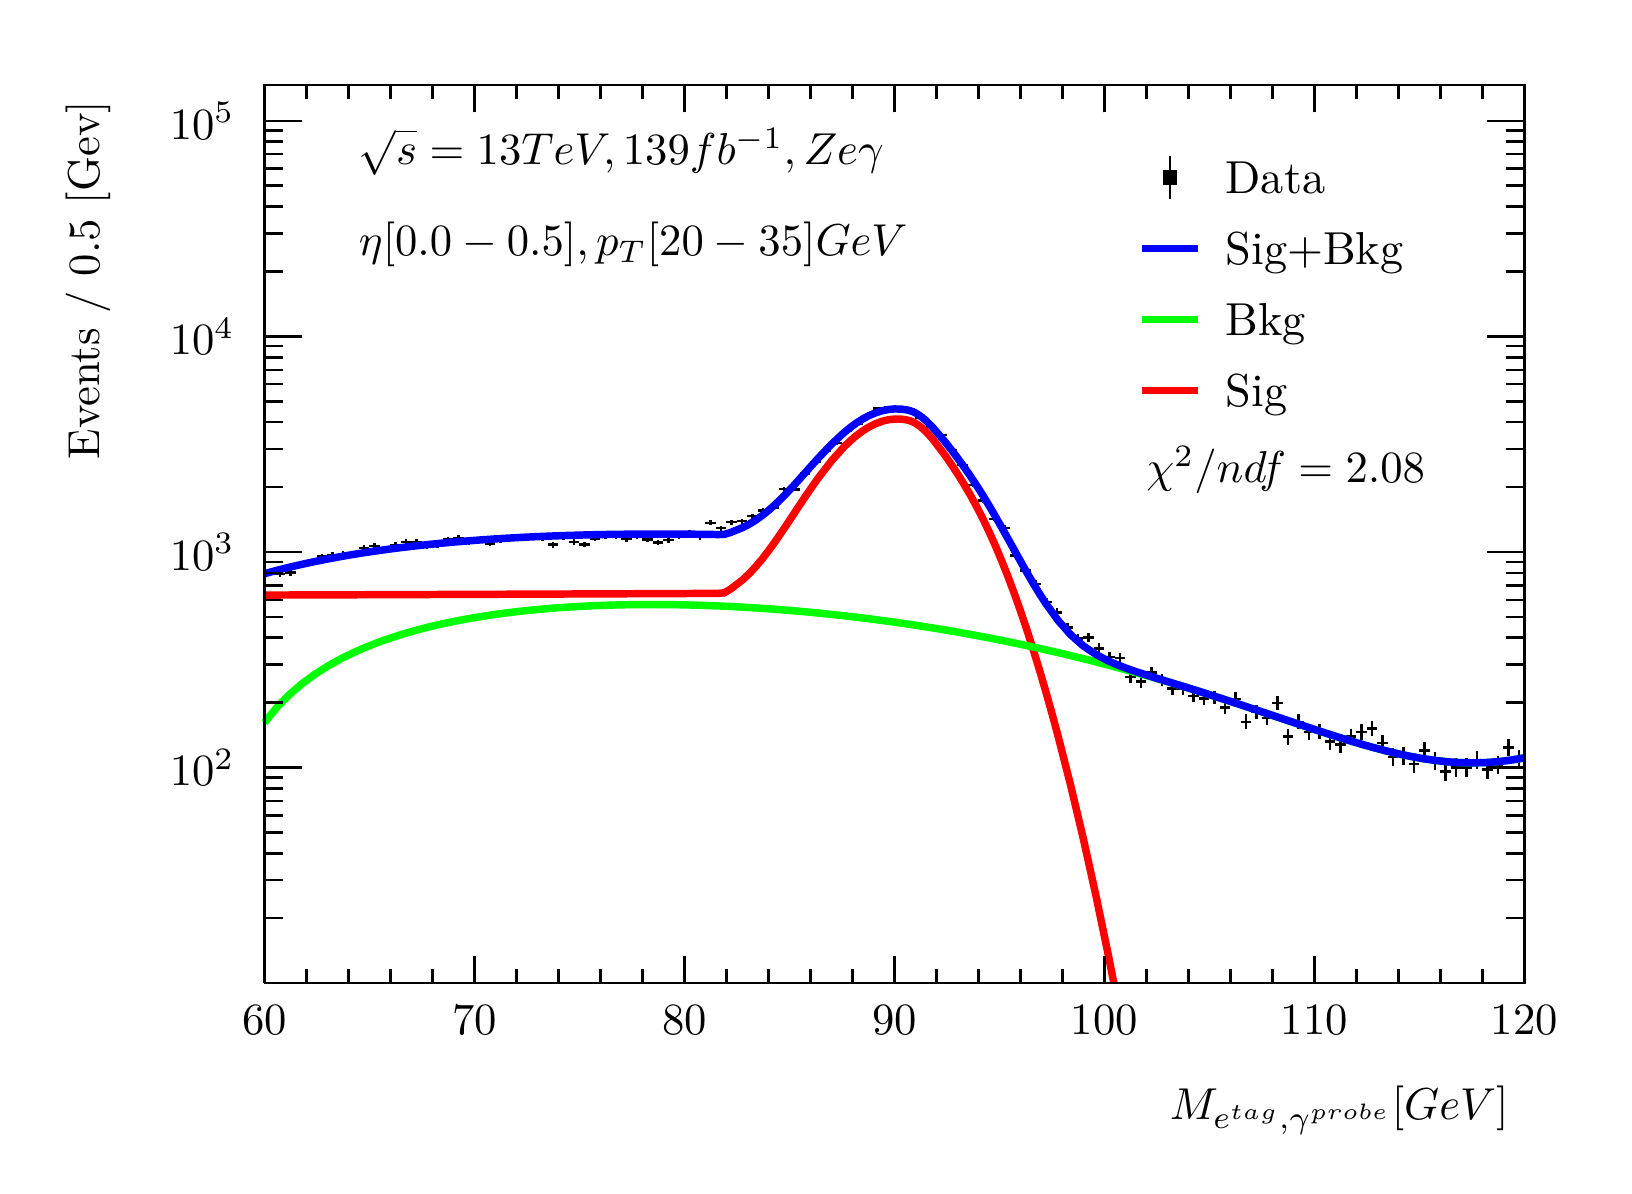
\begin{tikzpicture}
\pgfdeclareplotmark{cross} {
\pgfpathmoveto{\pgfpoint{-0.3\pgfplotmarksize}{\pgfplotmarksize}}
\pgfpathlineto{\pgfpoint{+0.3\pgfplotmarksize}{\pgfplotmarksize}}
\pgfpathlineto{\pgfpoint{+0.3\pgfplotmarksize}{0.3\pgfplotmarksize}}
\pgfpathlineto{\pgfpoint{+1\pgfplotmarksize}{0.3\pgfplotmarksize}}
\pgfpathlineto{\pgfpoint{+1\pgfplotmarksize}{-0.3\pgfplotmarksize}}
\pgfpathlineto{\pgfpoint{+0.3\pgfplotmarksize}{-0.3\pgfplotmarksize}}
\pgfpathlineto{\pgfpoint{+0.3\pgfplotmarksize}{-1.\pgfplotmarksize}}
\pgfpathlineto{\pgfpoint{-0.3\pgfplotmarksize}{-1.\pgfplotmarksize}}
\pgfpathlineto{\pgfpoint{-0.3\pgfplotmarksize}{-0.3\pgfplotmarksize}}
\pgfpathlineto{\pgfpoint{-1.\pgfplotmarksize}{-0.3\pgfplotmarksize}}
\pgfpathlineto{\pgfpoint{-1.\pgfplotmarksize}{0.3\pgfplotmarksize}}
\pgfpathlineto{\pgfpoint{-0.3\pgfplotmarksize}{0.3\pgfplotmarksize}}
\pgfpathclose
\pgfusepathqstroke
}
\pgfdeclareplotmark{cross*} {
\pgfpathmoveto{\pgfpoint{-0.3\pgfplotmarksize}{\pgfplotmarksize}}
\pgfpathlineto{\pgfpoint{+0.3\pgfplotmarksize}{\pgfplotmarksize}}
\pgfpathlineto{\pgfpoint{+0.3\pgfplotmarksize}{0.3\pgfplotmarksize}}
\pgfpathlineto{\pgfpoint{+1\pgfplotmarksize}{0.3\pgfplotmarksize}}
\pgfpathlineto{\pgfpoint{+1\pgfplotmarksize}{-0.3\pgfplotmarksize}}
\pgfpathlineto{\pgfpoint{+0.3\pgfplotmarksize}{-0.3\pgfplotmarksize}}
\pgfpathlineto{\pgfpoint{+0.3\pgfplotmarksize}{-1.\pgfplotmarksize}}
\pgfpathlineto{\pgfpoint{-0.3\pgfplotmarksize}{-1.\pgfplotmarksize}}
\pgfpathlineto{\pgfpoint{-0.3\pgfplotmarksize}{-0.3\pgfplotmarksize}}
\pgfpathlineto{\pgfpoint{-1.\pgfplotmarksize}{-0.3\pgfplotmarksize}}
\pgfpathlineto{\pgfpoint{-1.\pgfplotmarksize}{0.3\pgfplotmarksize}}
\pgfpathlineto{\pgfpoint{-0.3\pgfplotmarksize}{0.3\pgfplotmarksize}}
\pgfpathclose
\pgfusepathqfillstroke
}
\pgfdeclareplotmark{newstar} {
\pgfpathmoveto{\pgfqpoint{0pt}{\pgfplotmarksize}}
\pgfpathlineto{\pgfqpointpolar{44}{0.5\pgfplotmarksize}}
\pgfpathlineto{\pgfqpointpolar{18}{\pgfplotmarksize}}
\pgfpathlineto{\pgfqpointpolar{-20}{0.5\pgfplotmarksize}}
\pgfpathlineto{\pgfqpointpolar{-54}{\pgfplotmarksize}}
\pgfpathlineto{\pgfqpointpolar{-90}{0.5\pgfplotmarksize}}
\pgfpathlineto{\pgfqpointpolar{234}{\pgfplotmarksize}}
\pgfpathlineto{\pgfqpointpolar{198}{0.5\pgfplotmarksize}}
\pgfpathlineto{\pgfqpointpolar{162}{\pgfplotmarksize}}
\pgfpathlineto{\pgfqpointpolar{134}{0.5\pgfplotmarksize}}
\pgfpathclose
\pgfusepathqstroke
}
\pgfdeclareplotmark{newstar*} {
\pgfpathmoveto{\pgfqpoint{0pt}{\pgfplotmarksize}}
\pgfpathlineto{\pgfqpointpolar{44}{0.5\pgfplotmarksize}}
\pgfpathlineto{\pgfqpointpolar{18}{\pgfplotmarksize}}
\pgfpathlineto{\pgfqpointpolar{-20}{0.5\pgfplotmarksize}}
\pgfpathlineto{\pgfqpointpolar{-54}{\pgfplotmarksize}}
\pgfpathlineto{\pgfqpointpolar{-90}{0.5\pgfplotmarksize}}
\pgfpathlineto{\pgfqpointpolar{234}{\pgfplotmarksize}}
\pgfpathlineto{\pgfqpointpolar{198}{0.5\pgfplotmarksize}}
\pgfpathlineto{\pgfqpointpolar{162}{\pgfplotmarksize}}
\pgfpathlineto{\pgfqpointpolar{134}{0.5\pgfplotmarksize}}
\pgfpathclose
\pgfusepathqfillstroke
}
\definecolor{c}{rgb}{1,1,1};
\draw [color=c, fill=c] (0,0) rectangle (20,14.4361);
\draw [color=c, fill=c] (3,2.30977) rectangle (19,13.7143);
\definecolor{c}{rgb}{0,0,0};
\draw [c,line width=0.9] (3,2.30977) -- (3,13.7143) -- (19,13.7143) -- (19,2.30977) -- (3,2.30977);
\definecolor{c}{rgb}{1,1,1};
\draw [color=c, fill=c] (3,2.30977) rectangle (19,13.7143);
\definecolor{c}{rgb}{0,0,0};
\draw [c,line width=0.9] (3,2.30977) -- (3,13.7143) -- (19,13.7143) -- (19,2.30977) -- (3,2.30977);
\draw [c,line width=0.9] (3,2.30977) -- (19,2.30977);
\draw [c,line width=0.9] (3,2.65624) -- (3,2.30977);
\draw [c,line width=0.9] (3.53333,2.48301) -- (3.53333,2.30977);
\draw [c,line width=0.9] (4.06667,2.48301) -- (4.06667,2.30977);
\draw [c,line width=0.9] (4.6,2.48301) -- (4.6,2.30977);
\draw [c,line width=0.9] (5.13333,2.48301) -- (5.13333,2.30977);
\draw [c,line width=0.9] (5.66667,2.65624) -- (5.66667,2.30977);
\draw [c,line width=0.9] (6.2,2.48301) -- (6.2,2.30977);
\draw [c,line width=0.9] (6.73333,2.48301) -- (6.73333,2.30977);
\draw [c,line width=0.9] (7.26667,2.48301) -- (7.26667,2.30977);
\draw [c,line width=0.9] (7.8,2.48301) -- (7.8,2.30977);
\draw [c,line width=0.9] (8.33333,2.65624) -- (8.33333,2.30977);
\draw [c,line width=0.9] (8.86667,2.48301) -- (8.86667,2.30977);
\draw [c,line width=0.9] (9.4,2.48301) -- (9.4,2.30977);
\draw [c,line width=0.9] (9.93333,2.48301) -- (9.93333,2.30977);
\draw [c,line width=0.9] (10.4667,2.48301) -- (10.4667,2.30977);
\draw [c,line width=0.9] (11,2.65624) -- (11,2.30977);
\draw [c,line width=0.9] (11.5333,2.48301) -- (11.5333,2.30977);
\draw [c,line width=0.9] (12.0667,2.48301) -- (12.0667,2.30977);
\draw [c,line width=0.9] (12.6,2.48301) -- (12.6,2.30977);
\draw [c,line width=0.9] (13.1333,2.48301) -- (13.1333,2.30977);
\draw [c,line width=0.9] (13.6667,2.65624) -- (13.6667,2.30977);
\draw [c,line width=0.9] (14.2,2.48301) -- (14.2,2.30977);
\draw [c,line width=0.9] (14.7333,2.48301) -- (14.7333,2.30977);
\draw [c,line width=0.9] (15.2667,2.48301) -- (15.2667,2.30977);
\draw [c,line width=0.9] (15.8,2.48301) -- (15.8,2.30977);
\draw [c,line width=0.9] (16.3333,2.65624) -- (16.3333,2.30977);
\draw [c,line width=0.9] (16.8667,2.48301) -- (16.8667,2.30977);
\draw [c,line width=0.9] (17.4,2.48301) -- (17.4,2.30977);
\draw [c,line width=0.9] (17.9333,2.48301) -- (17.9333,2.30977);
\draw [c,line width=0.9] (18.4667,2.48301) -- (18.4667,2.30977);
\draw [c,line width=0.9] (19,2.65624) -- (19,2.30977);
\draw [anchor=base] (3,1.66015) node[scale=1.61424, color=c, rotate=0]{60};
\draw [anchor=base] (5.66667,1.66015) node[scale=1.61424, color=c, rotate=0]{70};
\draw [anchor=base] (8.33333,1.66015) node[scale=1.61424, color=c, rotate=0]{80};
\draw [anchor=base] (11,1.66015) node[scale=1.61424, color=c, rotate=0]{90};
\draw [anchor=base] (13.6667,1.66015) node[scale=1.61424, color=c, rotate=0]{100};
\draw [anchor=base] (16.3333,1.66015) node[scale=1.61424, color=c, rotate=0]{110};
\draw [anchor=base] (19,1.66015) node[scale=1.61424, color=c, rotate=0]{120};
\draw [anchor= east] (19,0.692932) node[scale=1.61424, color=c, rotate=0]{$M_{e^{tag}, \gamma^{probe}}  [GeV]$};
\draw [c,line width=0.9] (3,13.7143) -- (19,13.7143);
\draw [c,line width=0.9] (3,13.3678) -- (3,13.7143);
\draw [c,line width=0.9] (3.53333,13.5411) -- (3.53333,13.7143);
\draw [c,line width=0.9] (4.06667,13.5411) -- (4.06667,13.7143);
\draw [c,line width=0.9] (4.6,13.5411) -- (4.6,13.7143);
\draw [c,line width=0.9] (5.13333,13.5411) -- (5.13333,13.7143);
\draw [c,line width=0.9] (5.66667,13.3678) -- (5.66667,13.7143);
\draw [c,line width=0.9] (6.2,13.5411) -- (6.2,13.7143);
\draw [c,line width=0.9] (6.73333,13.5411) -- (6.73333,13.7143);
\draw [c,line width=0.9] (7.26667,13.5411) -- (7.26667,13.7143);
\draw [c,line width=0.9] (7.8,13.5411) -- (7.8,13.7143);
\draw [c,line width=0.9] (8.33333,13.3678) -- (8.33333,13.7143);
\draw [c,line width=0.9] (8.86667,13.5411) -- (8.86667,13.7143);
\draw [c,line width=0.9] (9.4,13.5411) -- (9.4,13.7143);
\draw [c,line width=0.9] (9.93333,13.5411) -- (9.93333,13.7143);
\draw [c,line width=0.9] (10.4667,13.5411) -- (10.4667,13.7143);
\draw [c,line width=0.9] (11,13.3678) -- (11,13.7143);
\draw [c,line width=0.9] (11.5333,13.5411) -- (11.5333,13.7143);
\draw [c,line width=0.9] (12.0667,13.5411) -- (12.0667,13.7143);
\draw [c,line width=0.9] (12.6,13.5411) -- (12.6,13.7143);
\draw [c,line width=0.9] (13.1333,13.5411) -- (13.1333,13.7143);
\draw [c,line width=0.9] (13.6667,13.3678) -- (13.6667,13.7143);
\draw [c,line width=0.9] (14.2,13.5411) -- (14.2,13.7143);
\draw [c,line width=0.9] (14.7333,13.5411) -- (14.7333,13.7143);
\draw [c,line width=0.9] (15.2667,13.5411) -- (15.2667,13.7143);
\draw [c,line width=0.9] (15.8,13.5411) -- (15.8,13.7143);
\draw [c,line width=0.9] (16.3333,13.3678) -- (16.3333,13.7143);
\draw [c,line width=0.9] (16.8667,13.5411) -- (16.8667,13.7143);
\draw [c,line width=0.9] (17.4,13.5411) -- (17.4,13.7143);
\draw [c,line width=0.9] (17.9333,13.5411) -- (17.9333,13.7143);
\draw [c,line width=0.9] (18.4667,13.5411) -- (18.4667,13.7143);
\draw [c,line width=0.9] (19,13.3678) -- (19,13.7143);
\draw [c,line width=0.9] (3,2.30977) -- (3,13.7143);
\draw [c,line width=0.9] (3.237,3.13385) -- (3,3.13385);
\draw [c,line width=0.9] (3.237,3.6159) -- (3,3.6159);
\draw [c,line width=0.9] (3.237,3.95792) -- (3,3.95792);
\draw [c,line width=0.9] (3.237,4.22321) -- (3,4.22321);
\draw [c,line width=0.9] (3.237,4.43997) -- (3,4.43997);
\draw [c,line width=0.9] (3.237,4.62324) -- (3,4.62324);
\draw [c,line width=0.9] (3.237,4.782) -- (3,4.782);
\draw [c,line width=0.9] (3.237,4.92203) -- (3,4.92203);
\draw [c,line width=0.9] (3.474,5.04729) -- (3,5.04729);
\draw [anchor= east] (2.82,5.04729) node[scale=1.61424, color=c, rotate=0]{$10^{2}$};
\draw [c,line width=0.9] (3.237,5.87136) -- (3,5.87136);
\draw [c,line width=0.9] (3.237,6.35342) -- (3,6.35342);
\draw [c,line width=0.9] (3.237,6.69544) -- (3,6.69544);
\draw [c,line width=0.9] (3.237,6.96073) -- (3,6.96073);
\draw [c,line width=0.9] (3.237,7.17749) -- (3,7.17749);
\draw [c,line width=0.9] (3.237,7.36076) -- (3,7.36076);
\draw [c,line width=0.9] (3.237,7.51951) -- (3,7.51951);
\draw [c,line width=0.9] (3.237,7.65954) -- (3,7.65954);
\draw [c,line width=0.9] (3.474,7.78481) -- (3,7.78481);
\draw [anchor= east] (2.82,7.78481) node[scale=1.61424, color=c, rotate=0]{$10^{3}$};
\draw [c,line width=0.9] (3.237,8.60888) -- (3,8.60888);
\draw [c,line width=0.9] (3.237,9.09093) -- (3,9.09093);
\draw [c,line width=0.9] (3.237,9.43296) -- (3,9.43296);
\draw [c,line width=0.9] (3.237,9.69825) -- (3,9.69825);
\draw [c,line width=0.9] (3.237,9.91501) -- (3,9.91501);
\draw [c,line width=0.9] (3.237,10.0983) -- (3,10.0983);
\draw [c,line width=0.9] (3.237,10.257) -- (3,10.257);
\draw [c,line width=0.9] (3.237,10.3971) -- (3,10.3971);
\draw [c,line width=0.9] (3.474,10.5223) -- (3,10.5223);
\draw [anchor= east] (2.82,10.5223) node[scale=1.61424, color=c, rotate=0]{$10^{4}$};
\draw [c,line width=0.9] (3.237,11.3464) -- (3,11.3464);
\draw [c,line width=0.9] (3.237,11.8285) -- (3,11.8285);
\draw [c,line width=0.9] (3.237,12.1705) -- (3,12.1705);
\draw [c,line width=0.9] (3.237,12.4358) -- (3,12.4358);
\draw [c,line width=0.9] (3.237,12.6525) -- (3,12.6525);
\draw [c,line width=0.9] (3.237,12.8358) -- (3,12.8358);
\draw [c,line width=0.9] (3.237,12.9945) -- (3,12.9945);
\draw [c,line width=0.9] (3.237,13.1346) -- (3,13.1346);
\draw [c,line width=0.9] (3.474,13.2598) -- (3,13.2598);
\draw [anchor= east] (2.82,13.2598) node[scale=1.61424, color=c, rotate=0]{$10^{5}$};
\draw [anchor= east] (0.76,13.7143) node[scale=1.61424, color=c, rotate=90]{Events / 0.5 [Gev]};
\draw [c,line width=0.9] (19,2.30977) -- (19,13.7143);
\draw [c,line width=0.9] (18.763,3.13385) -- (19,3.13385);
\draw [c,line width=0.9] (18.763,3.6159) -- (19,3.6159);
\draw [c,line width=0.9] (18.763,3.95792) -- (19,3.95792);
\draw [c,line width=0.9] (18.763,4.22321) -- (19,4.22321);
\draw [c,line width=0.9] (18.763,4.43997) -- (19,4.43997);
\draw [c,line width=0.9] (18.763,4.62324) -- (19,4.62324);
\draw [c,line width=0.9] (18.763,4.782) -- (19,4.782);
\draw [c,line width=0.9] (18.763,4.92203) -- (19,4.92203);
\draw [c,line width=0.9] (18.526,5.04729) -- (19,5.04729);
\draw [c,line width=0.9] (18.763,5.87136) -- (19,5.87136);
\draw [c,line width=0.9] (18.763,6.35342) -- (19,6.35342);
\draw [c,line width=0.9] (18.763,6.69544) -- (19,6.69544);
\draw [c,line width=0.9] (18.763,6.96073) -- (19,6.96073);
\draw [c,line width=0.9] (18.763,7.17749) -- (19,7.17749);
\draw [c,line width=0.9] (18.763,7.36076) -- (19,7.36076);
\draw [c,line width=0.9] (18.763,7.51951) -- (19,7.51951);
\draw [c,line width=0.9] (18.763,7.65954) -- (19,7.65954);
\draw [c,line width=0.9] (18.526,7.78481) -- (19,7.78481);
\draw [c,line width=0.9] (18.763,8.60888) -- (19,8.60888);
\draw [c,line width=0.9] (18.763,9.09093) -- (19,9.09093);
\draw [c,line width=0.9] (18.763,9.43296) -- (19,9.43296);
\draw [c,line width=0.9] (18.763,9.69825) -- (19,9.69825);
\draw [c,line width=0.9] (18.763,9.91501) -- (19,9.91501);
\draw [c,line width=0.9] (18.763,10.0983) -- (19,10.0983);
\draw [c,line width=0.9] (18.763,10.257) -- (19,10.257);
\draw [c,line width=0.9] (18.763,10.3971) -- (19,10.3971);
\draw [c,line width=0.9] (18.526,10.5223) -- (19,10.5223);
\draw [c,line width=0.9] (18.763,11.3464) -- (19,11.3464);
\draw [c,line width=0.9] (18.763,11.8285) -- (19,11.8285);
\draw [c,line width=0.9] (18.763,12.1705) -- (19,12.1705);
\draw [c,line width=0.9] (18.763,12.4358) -- (19,12.4358);
\draw [c,line width=0.9] (18.763,12.6525) -- (19,12.6525);
\draw [c,line width=0.9] (18.763,12.8358) -- (19,12.8358);
\draw [c,line width=0.9] (18.763,12.9945) -- (19,12.9945);
\draw [c,line width=0.9] (18.763,13.1346) -- (19,13.1346);
\draw [c,line width=0.9] (18.526,13.2598) -- (19,13.2598);
\draw [c,line width=0.9] (3.06667,7.51505) -- (3,7.51505);
\draw [c,line width=0.9] (3,7.51505) -- (3,7.51505);
\draw [c,line width=0.9] (3.06667,7.51505) -- (3.13333,7.51505);
\draw [c,line width=0.9] (3.13333,7.51505) -- (3.13333,7.51505);
\draw [c,line width=0.9] (3.06667,7.51505) -- (3.06667,7.55716);
\draw [c,line width=0.9] (3.06667,7.55716) -- (3.06667,7.55716);
\draw [c,line width=0.9] (3.06667,7.51505) -- (3.06667,7.47294);
\draw [c,line width=0.9] (3.06667,7.47294) -- (3.06667,7.47294);
\draw [c,line width=0.9] (3.2,7.50606) -- (3.13333,7.50606);
\draw [c,line width=0.9] (3.13333,7.50606) -- (3.13333,7.50606);
\draw [c,line width=0.9] (3.2,7.50606) -- (3.26667,7.50606);
\draw [c,line width=0.9] (3.26667,7.50606) -- (3.26667,7.50606);
\draw [c,line width=0.9] (3.2,7.50606) -- (3.2,7.54833);
\draw [c,line width=0.9] (3.2,7.54833) -- (3.2,7.54833);
\draw [c,line width=0.9] (3.2,7.50606) -- (3.2,7.46379);
\draw [c,line width=0.9] (3.2,7.46379) -- (3.2,7.46379);
\draw [c,line width=0.9] (3.33333,7.521) -- (3.26667,7.521);
\draw [c,line width=0.9] (3.26667,7.521) -- (3.26667,7.521);
\draw [c,line width=0.9] (3.33333,7.521) -- (3.4,7.521);
\draw [c,line width=0.9] (3.4,7.521) -- (3.4,7.521);
\draw [c,line width=0.9] (3.33333,7.521) -- (3.33333,7.563);
\draw [c,line width=0.9] (3.33333,7.563) -- (3.33333,7.563);
\draw [c,line width=0.9] (3.33333,7.521) -- (3.33333,7.47899);
\draw [c,line width=0.9] (3.33333,7.47899) -- (3.33333,7.47899);
\draw [c,line width=0.9] (3.46667,7.63012) -- (3.4,7.63012);
\draw [c,line width=0.9] (3.4,7.63012) -- (3.4,7.63012);
\draw [c,line width=0.9] (3.46667,7.63012) -- (3.53333,7.63012);
\draw [c,line width=0.9] (3.53333,7.63012) -- (3.53333,7.63012);
\draw [c,line width=0.9] (3.46667,7.63012) -- (3.46667,7.67024);
\draw [c,line width=0.9] (3.46667,7.67024) -- (3.46667,7.67024);
\draw [c,line width=0.9] (3.46667,7.63012) -- (3.46667,7.59);
\draw [c,line width=0.9] (3.46667,7.59) -- (3.46667,7.59);
\draw [c,line width=0.9] (3.6,7.65425) -- (3.53333,7.65425);
\draw [c,line width=0.9] (3.53333,7.65425) -- (3.53333,7.65425);
\draw [c,line width=0.9] (3.6,7.65425) -- (3.66667,7.65425);
\draw [c,line width=0.9] (3.66667,7.65425) -- (3.66667,7.65425);
\draw [c,line width=0.9] (3.6,7.65425) -- (3.6,7.69397);
\draw [c,line width=0.9] (3.6,7.69397) -- (3.6,7.69397);
\draw [c,line width=0.9] (3.6,7.65425) -- (3.6,7.61453);
\draw [c,line width=0.9] (3.6,7.61453) -- (3.6,7.61453);
\draw [c,line width=0.9] (3.73333,7.72633) -- (3.66667,7.72633);
\draw [c,line width=0.9] (3.66667,7.72633) -- (3.66667,7.72633);
\draw [c,line width=0.9] (3.73333,7.72633) -- (3.8,7.72633);
\draw [c,line width=0.9] (3.8,7.72633) -- (3.8,7.72633);
\draw [c,line width=0.9] (3.73333,7.72633) -- (3.73333,7.76486);
\draw [c,line width=0.9] (3.73333,7.76486) -- (3.73333,7.76486);
\draw [c,line width=0.9] (3.73333,7.72633) -- (3.73333,7.6878);
\draw [c,line width=0.9] (3.73333,7.6878) -- (3.73333,7.6878);
\draw [c,line width=0.9] (3.86667,7.73998) -- (3.8,7.73998);
\draw [c,line width=0.9] (3.8,7.73998) -- (3.8,7.73998);
\draw [c,line width=0.9] (3.86667,7.73998) -- (3.93333,7.73998);
\draw [c,line width=0.9] (3.93333,7.73998) -- (3.93333,7.73998);
\draw [c,line width=0.9] (3.86667,7.73998) -- (3.86667,7.77829);
\draw [c,line width=0.9] (3.86667,7.77829) -- (3.86667,7.77829);
\draw [c,line width=0.9] (3.86667,7.73998) -- (3.86667,7.70167);
\draw [c,line width=0.9] (3.86667,7.70167) -- (3.86667,7.70167);
\draw [c,line width=0.9] (4,7.75714) -- (3.93333,7.75714);
\draw [c,line width=0.9] (3.93333,7.75714) -- (3.93333,7.75714);
\draw [c,line width=0.9] (4,7.75714) -- (4.06667,7.75714);
\draw [c,line width=0.9] (4.06667,7.75714) -- (4.06667,7.75714);
\draw [c,line width=0.9] (4,7.75714) -- (4,7.79518);
\draw [c,line width=0.9] (4,7.79518) -- (4,7.79518);
\draw [c,line width=0.9] (4,7.75714) -- (4,7.71911);
\draw [c,line width=0.9] (4,7.71911) -- (4,7.71911);
\draw [c,line width=0.9] (4.13333,7.76079) -- (4.06667,7.76079);
\draw [c,line width=0.9] (4.06667,7.76079) -- (4.06667,7.76079);
\draw [c,line width=0.9] (4.13333,7.76079) -- (4.2,7.76079);
\draw [c,line width=0.9] (4.2,7.76079) -- (4.2,7.76079);
\draw [c,line width=0.9] (4.13333,7.76079) -- (4.13333,7.79876);
\draw [c,line width=0.9] (4.13333,7.79876) -- (4.13333,7.79876);
\draw [c,line width=0.9] (4.13333,7.76079) -- (4.13333,7.72281);
\draw [c,line width=0.9] (4.13333,7.72281) -- (4.13333,7.72281);
\draw [c,line width=0.9] (4.26667,7.83486) -- (4.2,7.83486);
\draw [c,line width=0.9] (4.2,7.83486) -- (4.2,7.83486);
\draw [c,line width=0.9] (4.26667,7.83486) -- (4.33333,7.83486);
\draw [c,line width=0.9] (4.33333,7.83486) -- (4.33333,7.83486);
\draw [c,line width=0.9] (4.26667,7.83486) -- (4.26667,7.87167);
\draw [c,line width=0.9] (4.26667,7.87167) -- (4.26667,7.87167);
\draw [c,line width=0.9] (4.26667,7.83486) -- (4.26667,7.79805);
\draw [c,line width=0.9] (4.26667,7.79805) -- (4.26667,7.79805);
\draw [c,line width=0.9] (4.4,7.85744) -- (4.33333,7.85744);
\draw [c,line width=0.9] (4.33333,7.85744) -- (4.33333,7.85744);
\draw [c,line width=0.9] (4.4,7.85744) -- (4.46667,7.85744);
\draw [c,line width=0.9] (4.46667,7.85744) -- (4.46667,7.85744);
\draw [c,line width=0.9] (4.4,7.85744) -- (4.4,7.89391);
\draw [c,line width=0.9] (4.4,7.89391) -- (4.4,7.89391);
\draw [c,line width=0.9] (4.4,7.85744) -- (4.4,7.82098);
\draw [c,line width=0.9] (4.4,7.82098) -- (4.4,7.82098);
\draw [c,line width=0.9] (4.53333,7.81995) -- (4.46667,7.81995);
\draw [c,line width=0.9] (4.46667,7.81995) -- (4.46667,7.81995);
\draw [c,line width=0.9] (4.53333,7.81995) -- (4.6,7.81995);
\draw [c,line width=0.9] (4.6,7.81995) -- (4.6,7.81995);
\draw [c,line width=0.9] (4.53333,7.81995) -- (4.53333,7.85699);
\draw [c,line width=0.9] (4.53333,7.85699) -- (4.53333,7.85699);
\draw [c,line width=0.9] (4.53333,7.81995) -- (4.53333,7.78291);
\draw [c,line width=0.9] (4.53333,7.78291) -- (4.53333,7.78291);
\draw [c,line width=0.9] (4.66667,7.86968) -- (4.6,7.86968);
\draw [c,line width=0.9] (4.6,7.86968) -- (4.6,7.86968);
\draw [c,line width=0.9] (4.66667,7.86968) -- (4.73333,7.86968);
\draw [c,line width=0.9] (4.73333,7.86968) -- (4.73333,7.86968);
\draw [c,line width=0.9] (4.66667,7.86968) -- (4.66667,7.90596);
\draw [c,line width=0.9] (4.66667,7.90596) -- (4.66667,7.90596);
\draw [c,line width=0.9] (4.66667,7.86968) -- (4.66667,7.83341);
\draw [c,line width=0.9] (4.66667,7.83341) -- (4.66667,7.83341);
\draw [c,line width=0.9] (4.8,7.91209) -- (4.73333,7.91209);
\draw [c,line width=0.9] (4.73333,7.91209) -- (4.73333,7.91209);
\draw [c,line width=0.9] (4.8,7.91209) -- (4.86667,7.91209);
\draw [c,line width=0.9] (4.86667,7.91209) -- (4.86667,7.91209);
\draw [c,line width=0.9] (4.8,7.91209) -- (4.8,7.94772);
\draw [c,line width=0.9] (4.8,7.94772) -- (4.8,7.94772);
\draw [c,line width=0.9] (4.8,7.91209) -- (4.8,7.87645);
\draw [c,line width=0.9] (4.8,7.87645) -- (4.8,7.87645);
\draw [c,line width=0.9] (4.93333,7.90995) -- (4.86667,7.90995);
\draw [c,line width=0.9] (4.86667,7.90995) -- (4.86667,7.90995);
\draw [c,line width=0.9] (4.93333,7.90995) -- (5,7.90995);
\draw [c,line width=0.9] (5,7.90995) -- (5,7.90995);
\draw [c,line width=0.9] (4.93333,7.90995) -- (4.93333,7.94562);
\draw [c,line width=0.9] (4.93333,7.94562) -- (4.93333,7.94562);
\draw [c,line width=0.9] (4.93333,7.90995) -- (4.93333,7.87428);
\draw [c,line width=0.9] (4.93333,7.87428) -- (4.93333,7.87428);
\draw [c,line width=0.9] (5.06667,7.85408) -- (5,7.85408);
\draw [c,line width=0.9] (5,7.85408) -- (5,7.85408);
\draw [c,line width=0.9] (5.06667,7.85408) -- (5.13333,7.85408);
\draw [c,line width=0.9] (5.13333,7.85408) -- (5.13333,7.85408);
\draw [c,line width=0.9] (5.06667,7.85408) -- (5.06667,7.8906);
\draw [c,line width=0.9] (5.06667,7.8906) -- (5.06667,7.8906);
\draw [c,line width=0.9] (5.06667,7.85408) -- (5.06667,7.81757);
\draw [c,line width=0.9] (5.06667,7.81757) -- (5.06667,7.81757);
\draw [c,line width=0.9] (5.2,7.87189) -- (5.13333,7.87189);
\draw [c,line width=0.9] (5.13333,7.87189) -- (5.13333,7.87189);
\draw [c,line width=0.9] (5.2,7.87189) -- (5.26667,7.87189);
\draw [c,line width=0.9] (5.26667,7.87189) -- (5.26667,7.87189);
\draw [c,line width=0.9] (5.2,7.87189) -- (5.2,7.90814);
\draw [c,line width=0.9] (5.2,7.90814) -- (5.2,7.90814);
\draw [c,line width=0.9] (5.2,7.87189) -- (5.2,7.83565);
\draw [c,line width=0.9] (5.2,7.83565) -- (5.2,7.83565);
\draw [c,line width=0.9] (5.33333,7.94163) -- (5.26667,7.94163);
\draw [c,line width=0.9] (5.26667,7.94163) -- (5.26667,7.94163);
\draw [c,line width=0.9] (5.33333,7.94163) -- (5.4,7.94163);
\draw [c,line width=0.9] (5.4,7.94163) -- (5.4,7.94163);
\draw [c,line width=0.9] (5.33333,7.94163) -- (5.33333,7.97682);
\draw [c,line width=0.9] (5.33333,7.97682) -- (5.33333,7.97682);
\draw [c,line width=0.9] (5.33333,7.94163) -- (5.33333,7.90643);
\draw [c,line width=0.9] (5.33333,7.90643) -- (5.33333,7.90643);
\draw [c,line width=0.9] (5.46667,7.96229) -- (5.4,7.96229);
\draw [c,line width=0.9] (5.4,7.96229) -- (5.4,7.96229);
\draw [c,line width=0.9] (5.46667,7.96229) -- (5.53333,7.96229);
\draw [c,line width=0.9] (5.53333,7.96229) -- (5.53333,7.96229);
\draw [c,line width=0.9] (5.46667,7.96229) -- (5.46667,7.99718);
\draw [c,line width=0.9] (5.46667,7.99718) -- (5.46667,7.99718);
\draw [c,line width=0.9] (5.46667,7.96229) -- (5.46667,7.9274);
\draw [c,line width=0.9] (5.46667,7.9274) -- (5.46667,7.9274);
\draw [c,line width=0.9] (5.6,7.91422) -- (5.53333,7.91422);
\draw [c,line width=0.9] (5.53333,7.91422) -- (5.53333,7.91422);
\draw [c,line width=0.9] (5.6,7.91422) -- (5.66667,7.91422);
\draw [c,line width=0.9] (5.66667,7.91422) -- (5.66667,7.91422);
\draw [c,line width=0.9] (5.6,7.91422) -- (5.6,7.94983);
\draw [c,line width=0.9] (5.6,7.94983) -- (5.6,7.94983);
\draw [c,line width=0.9] (5.6,7.91422) -- (5.6,7.87862);
\draw [c,line width=0.9] (5.6,7.87862) -- (5.6,7.87862);
\draw [c,line width=0.9] (5.73333,7.93221) -- (5.66667,7.93221);
\draw [c,line width=0.9] (5.66667,7.93221) -- (5.66667,7.93221);
\draw [c,line width=0.9] (5.73333,7.93221) -- (5.8,7.93221);
\draw [c,line width=0.9] (5.8,7.93221) -- (5.8,7.93221);
\draw [c,line width=0.9] (5.73333,7.93221) -- (5.73333,7.96755);
\draw [c,line width=0.9] (5.73333,7.96755) -- (5.73333,7.96755);
\draw [c,line width=0.9] (5.73333,7.93221) -- (5.73333,7.89688);
\draw [c,line width=0.9] (5.73333,7.89688) -- (5.73333,7.89688);
\draw [c,line width=0.9] (5.86667,7.89487) -- (5.8,7.89487);
\draw [c,line width=0.9] (5.8,7.89487) -- (5.8,7.89487);
\draw [c,line width=0.9] (5.86667,7.89487) -- (5.93333,7.89487);
\draw [c,line width=0.9] (5.93333,7.89487) -- (5.93333,7.89487);
\draw [c,line width=0.9] (5.86667,7.89487) -- (5.86667,7.93077);
\draw [c,line width=0.9] (5.86667,7.93077) -- (5.86667,7.93077);
\draw [c,line width=0.9] (5.86667,7.89487) -- (5.86667,7.85898);
\draw [c,line width=0.9] (5.86667,7.85898) -- (5.86667,7.85898);
\draw [c,line width=0.9] (6,7.9385) -- (5.93333,7.9385);
\draw [c,line width=0.9] (5.93333,7.9385) -- (5.93333,7.9385);
\draw [c,line width=0.9] (6,7.9385) -- (6.06667,7.9385);
\draw [c,line width=0.9] (6.06667,7.9385) -- (6.06667,7.9385);
\draw [c,line width=0.9] (6,7.9385) -- (6,7.97374);
\draw [c,line width=0.9] (6,7.97374) -- (6,7.97374);
\draw [c,line width=0.9] (6,7.9385) -- (6,7.90326);
\draw [c,line width=0.9] (6,7.90326) -- (6,7.90326);
\draw [c,line width=0.9] (6.13333,7.95303) -- (6.06667,7.95303);
\draw [c,line width=0.9] (6.06667,7.95303) -- (6.06667,7.95303);
\draw [c,line width=0.9] (6.13333,7.95303) -- (6.2,7.95303);
\draw [c,line width=0.9] (6.2,7.95303) -- (6.2,7.95303);
\draw [c,line width=0.9] (6.13333,7.95303) -- (6.13333,7.98806);
\draw [c,line width=0.9] (6.13333,7.98806) -- (6.13333,7.98806);
\draw [c,line width=0.9] (6.13333,7.95303) -- (6.13333,7.91801);
\draw [c,line width=0.9] (6.13333,7.91801) -- (6.13333,7.91801);
\draw [c,line width=0.9] (6.26667,7.9551) -- (6.2,7.9551);
\draw [c,line width=0.9] (6.2,7.9551) -- (6.2,7.9551);
\draw [c,line width=0.9] (6.26667,7.9551) -- (6.33333,7.9551);
\draw [c,line width=0.9] (6.33333,7.9551) -- (6.33333,7.9551);
\draw [c,line width=0.9] (6.26667,7.9551) -- (6.26667,7.99009);
\draw [c,line width=0.9] (6.26667,7.99009) -- (6.26667,7.99009);
\draw [c,line width=0.9] (6.26667,7.9551) -- (6.26667,7.9201);
\draw [c,line width=0.9] (6.26667,7.9201) -- (6.26667,7.9201);
\draw [c,line width=0.9] (6.4,7.99361) -- (6.33333,7.99361);
\draw [c,line width=0.9] (6.33333,7.99361) -- (6.33333,7.99361);
\draw [c,line width=0.9] (6.4,7.99361) -- (6.46667,7.99361);
\draw [c,line width=0.9] (6.46667,7.99361) -- (6.46667,7.99361);
\draw [c,line width=0.9] (6.4,7.99361) -- (6.4,8.02805);
\draw [c,line width=0.9] (6.4,8.02805) -- (6.4,8.02805);
\draw [c,line width=0.9] (6.4,7.99361) -- (6.4,7.95918);
\draw [c,line width=0.9] (6.4,7.95918) -- (6.4,7.95918);
\draw [c,line width=0.9] (6.53333,7.96433) -- (6.46667,7.96433);
\draw [c,line width=0.9] (6.46667,7.96433) -- (6.46667,7.96433);
\draw [c,line width=0.9] (6.53333,7.96433) -- (6.6,7.96433);
\draw [c,line width=0.9] (6.6,7.96433) -- (6.6,7.96433);
\draw [c,line width=0.9] (6.53333,7.96433) -- (6.53333,7.99919);
\draw [c,line width=0.9] (6.53333,7.99919) -- (6.53333,7.99919);
\draw [c,line width=0.9] (6.53333,7.96433) -- (6.53333,7.92947);
\draw [c,line width=0.9] (6.53333,7.92947) -- (6.53333,7.92947);
\draw [c,line width=0.9] (6.66667,7.87631) -- (6.6,7.87631);
\draw [c,line width=0.9] (6.6,7.87631) -- (6.6,7.87631);
\draw [c,line width=0.9] (6.66667,7.87631) -- (6.73333,7.87631);
\draw [c,line width=0.9] (6.73333,7.87631) -- (6.73333,7.87631);
\draw [c,line width=0.9] (6.66667,7.87631) -- (6.66667,7.91248);
\draw [c,line width=0.9] (6.66667,7.91248) -- (6.66667,7.91248);
\draw [c,line width=0.9] (6.66667,7.87631) -- (6.66667,7.84013);
\draw [c,line width=0.9] (6.66667,7.84013) -- (6.66667,7.84013);
\draw [c,line width=0.9] (6.8,7.97552) -- (6.73333,7.97552);
\draw [c,line width=0.9] (6.73333,7.97552) -- (6.73333,7.97552);
\draw [c,line width=0.9] (6.8,7.97552) -- (6.86667,7.97552);
\draw [c,line width=0.9] (6.86667,7.97552) -- (6.86667,7.97552);
\draw [c,line width=0.9] (6.8,7.97552) -- (6.8,8.01022);
\draw [c,line width=0.9] (6.8,8.01022) -- (6.8,8.01022);
\draw [c,line width=0.9] (6.8,7.97552) -- (6.8,7.94083);
\draw [c,line width=0.9] (6.8,7.94083) -- (6.8,7.94083);
\draw [c,line width=0.9] (6.93333,7.90888) -- (6.86667,7.90888);
\draw [c,line width=0.9] (6.86667,7.90888) -- (6.86667,7.90888);
\draw [c,line width=0.9] (6.93333,7.90888) -- (7,7.90888);
\draw [c,line width=0.9] (7,7.90888) -- (7,7.90888);
\draw [c,line width=0.9] (6.93333,7.90888) -- (6.93333,7.94456);
\draw [c,line width=0.9] (6.93333,7.94456) -- (6.93333,7.94456);
\draw [c,line width=0.9] (6.93333,7.90888) -- (6.93333,7.8732);
\draw [c,line width=0.9] (6.93333,7.8732) -- (6.93333,7.8732);
\draw [c,line width=0.9] (7.06667,7.87851) -- (7,7.87851);
\draw [c,line width=0.9] (7,7.87851) -- (7,7.87851);
\draw [c,line width=0.9] (7.06667,7.87851) -- (7.13333,7.87851);
\draw [c,line width=0.9] (7.13333,7.87851) -- (7.13333,7.87851);
\draw [c,line width=0.9] (7.06667,7.87851) -- (7.06667,7.91465);
\draw [c,line width=0.9] (7.06667,7.91465) -- (7.06667,7.91465);
\draw [c,line width=0.9] (7.06667,7.87851) -- (7.06667,7.84236);
\draw [c,line width=0.9] (7.06667,7.84236) -- (7.06667,7.84236);
\draw [c,line width=0.9] (7.2,7.95716) -- (7.13333,7.95716);
\draw [c,line width=0.9] (7.13333,7.95716) -- (7.13333,7.95716);
\draw [c,line width=0.9] (7.2,7.95716) -- (7.26667,7.95716);
\draw [c,line width=0.9] (7.26667,7.95716) -- (7.26667,7.95716);
\draw [c,line width=0.9] (7.2,7.95716) -- (7.2,7.99212);
\draw [c,line width=0.9] (7.2,7.99212) -- (7.2,7.99212);
\draw [c,line width=0.9] (7.2,7.95716) -- (7.2,7.92219);
\draw [c,line width=0.9] (7.2,7.92219) -- (7.2,7.92219);
\draw [c,line width=0.9] (7.33333,7.97957) -- (7.26667,7.97957);
\draw [c,line width=0.9] (7.26667,7.97957) -- (7.26667,7.97957);
\draw [c,line width=0.9] (7.33333,7.97957) -- (7.4,7.97957);
\draw [c,line width=0.9] (7.4,7.97957) -- (7.4,7.97957);
\draw [c,line width=0.9] (7.33333,7.97957) -- (7.33333,8.01421);
\draw [c,line width=0.9] (7.33333,8.01421) -- (7.33333,8.01421);
\draw [c,line width=0.9] (7.33333,7.97957) -- (7.33333,7.94493);
\draw [c,line width=0.9] (7.33333,7.94493) -- (7.33333,7.94493);
\draw [c,line width=0.9] (7.46667,7.97755) -- (7.4,7.97755);
\draw [c,line width=0.9] (7.4,7.97755) -- (7.4,7.97755);
\draw [c,line width=0.9] (7.46667,7.97755) -- (7.53333,7.97755);
\draw [c,line width=0.9] (7.53333,7.97755) -- (7.53333,7.97755);
\draw [c,line width=0.9] (7.46667,7.97755) -- (7.46667,8.01222);
\draw [c,line width=0.9] (7.46667,8.01222) -- (7.46667,8.01222);
\draw [c,line width=0.9] (7.46667,7.97755) -- (7.46667,7.94288);
\draw [c,line width=0.9] (7.46667,7.94288) -- (7.46667,7.94288);
\draw [c,line width=0.9] (7.6,7.94683) -- (7.53333,7.94683);
\draw [c,line width=0.9] (7.53333,7.94683) -- (7.53333,7.94683);
\draw [c,line width=0.9] (7.6,7.94683) -- (7.66667,7.94683);
\draw [c,line width=0.9] (7.66667,7.94683) -- (7.66667,7.94683);
\draw [c,line width=0.9] (7.6,7.94683) -- (7.6,7.98194);
\draw [c,line width=0.9] (7.6,7.98194) -- (7.6,7.98194);
\draw [c,line width=0.9] (7.6,7.94683) -- (7.6,7.91171);
\draw [c,line width=0.9] (7.6,7.91171) -- (7.6,7.91171);
\draw [c,line width=0.9] (7.73333,7.98159) -- (7.66667,7.98159);
\draw [c,line width=0.9] (7.66667,7.98159) -- (7.66667,7.98159);
\draw [c,line width=0.9] (7.73333,7.98159) -- (7.8,7.98159);
\draw [c,line width=0.9] (7.8,7.98159) -- (7.8,7.98159);
\draw [c,line width=0.9] (7.73333,7.98159) -- (7.73333,8.01619);
\draw [c,line width=0.9] (7.73333,8.01619) -- (7.73333,8.01619);
\draw [c,line width=0.9] (7.73333,7.98159) -- (7.73333,7.94698);
\draw [c,line width=0.9] (7.73333,7.94698) -- (7.73333,7.94698);
\draw [c,line width=0.9] (7.86667,7.94475) -- (7.8,7.94475);
\draw [c,line width=0.9] (7.8,7.94475) -- (7.8,7.94475);
\draw [c,line width=0.9] (7.86667,7.94475) -- (7.93333,7.94475);
\draw [c,line width=0.9] (7.93333,7.94475) -- (7.93333,7.94475);
\draw [c,line width=0.9] (7.86667,7.94475) -- (7.86667,7.9799);
\draw [c,line width=0.9] (7.86667,7.9799) -- (7.86667,7.9799);
\draw [c,line width=0.9] (7.86667,7.94475) -- (7.86667,7.9096);
\draw [c,line width=0.9] (7.86667,7.9096) -- (7.86667,7.9096);
\draw [c,line width=0.9] (8,7.90351) -- (7.93333,7.90351);
\draw [c,line width=0.9] (7.93333,7.90351) -- (7.93333,7.90351);
\draw [c,line width=0.9] (8,7.90351) -- (8.06667,7.90351);
\draw [c,line width=0.9] (8.06667,7.90351) -- (8.06667,7.90351);
\draw [c,line width=0.9] (8,7.90351) -- (8,7.93928);
\draw [c,line width=0.9] (8,7.93928) -- (8,7.93928);
\draw [c,line width=0.9] (8,7.90351) -- (8,7.86775);
\draw [c,line width=0.9] (8,7.86775) -- (8,7.86775);
\draw [c,line width=0.9] (8.13333,7.93536) -- (8.06667,7.93536);
\draw [c,line width=0.9] (8.06667,7.93536) -- (8.06667,7.93536);
\draw [c,line width=0.9] (8.13333,7.93536) -- (8.2,7.93536);
\draw [c,line width=0.9] (8.2,7.93536) -- (8.2,7.93536);
\draw [c,line width=0.9] (8.13333,7.93536) -- (8.13333,7.97065);
\draw [c,line width=0.9] (8.13333,7.97065) -- (8.13333,7.97065);
\draw [c,line width=0.9] (8.13333,7.93536) -- (8.13333,7.90007);
\draw [c,line width=0.9] (8.13333,7.90007) -- (8.13333,7.90007);
\draw [c,line width=0.9] (8.26667,7.98259) -- (8.2,7.98259);
\draw [c,line width=0.9] (8.2,7.98259) -- (8.2,7.98259);
\draw [c,line width=0.9] (8.26667,7.98259) -- (8.33333,7.98259);
\draw [c,line width=0.9] (8.33333,7.98259) -- (8.33333,7.98259);
\draw [c,line width=0.9] (8.26667,7.98259) -- (8.26667,8.01719);
\draw [c,line width=0.9] (8.26667,8.01719) -- (8.26667,8.01719);
\draw [c,line width=0.9] (8.26667,7.98259) -- (8.26667,7.948);
\draw [c,line width=0.9] (8.26667,7.948) -- (8.26667,7.948);
\draw [c,line width=0.9] (8.4,8.03092) -- (8.33333,8.03092);
\draw [c,line width=0.9] (8.33333,8.03092) -- (8.33333,8.03092);
\draw [c,line width=0.9] (8.4,8.03092) -- (8.46667,8.03092);
\draw [c,line width=0.9] (8.46667,8.03092) -- (8.46667,8.03092);
\draw [c,line width=0.9] (8.4,8.03092) -- (8.4,8.06482);
\draw [c,line width=0.9] (8.4,8.06482) -- (8.4,8.06482);
\draw [c,line width=0.9] (8.4,8.03092) -- (8.4,7.99703);
\draw [c,line width=0.9] (8.4,7.99703) -- (8.4,7.99703);
\draw [c,line width=0.9] (8.53333,7.97248) -- (8.46667,7.97248);
\draw [c,line width=0.9] (8.46667,7.97248) -- (8.46667,7.97248);
\draw [c,line width=0.9] (8.53333,7.97248) -- (8.6,7.97248);
\draw [c,line width=0.9] (8.6,7.97248) -- (8.6,7.97248);
\draw [c,line width=0.9] (8.53333,7.97248) -- (8.53333,8.00722);
\draw [c,line width=0.9] (8.53333,8.00722) -- (8.53333,8.00722);
\draw [c,line width=0.9] (8.53333,7.97248) -- (8.53333,7.93774);
\draw [c,line width=0.9] (8.53333,7.93774) -- (8.53333,7.93774);
\draw [c,line width=0.9] (8.66667,8.15299) -- (8.6,8.15299);
\draw [c,line width=0.9] (8.6,8.15299) -- (8.6,8.15299);
\draw [c,line width=0.9] (8.66667,8.15299) -- (8.73333,8.15299);
\draw [c,line width=0.9] (8.73333,8.15299) -- (8.73333,8.15299);
\draw [c,line width=0.9] (8.66667,8.15299) -- (8.66667,8.18519);
\draw [c,line width=0.9] (8.66667,8.18519) -- (8.66667,8.18519);
\draw [c,line width=0.9] (8.66667,8.15299) -- (8.66667,8.12079);
\draw [c,line width=0.9] (8.66667,8.12079) -- (8.66667,8.12079);
\draw [c,line width=0.9] (8.8,8.0857) -- (8.73333,8.0857);
\draw [c,line width=0.9] (8.73333,8.0857) -- (8.73333,8.0857);
\draw [c,line width=0.9] (8.8,8.0857) -- (8.86667,8.0857);
\draw [c,line width=0.9] (8.86667,8.0857) -- (8.86667,8.0857);
\draw [c,line width=0.9] (8.8,8.0857) -- (8.8,8.11883);
\draw [c,line width=0.9] (8.8,8.11883) -- (8.8,8.11883);
\draw [c,line width=0.9] (8.8,8.0857) -- (8.8,8.05258);
\draw [c,line width=0.9] (8.8,8.05258) -- (8.8,8.05258);
\draw [c,line width=0.9] (8.93333,8.16341) -- (8.86667,8.16341);
\draw [c,line width=0.9] (8.86667,8.16341) -- (8.86667,8.16341);
\draw [c,line width=0.9] (8.93333,8.16341) -- (9,8.16341);
\draw [c,line width=0.9] (9,8.16341) -- (9,8.16341);
\draw [c,line width=0.9] (8.93333,8.16341) -- (8.93333,8.19547);
\draw [c,line width=0.9] (8.93333,8.19547) -- (8.93333,8.19547);
\draw [c,line width=0.9] (8.93333,8.16341) -- (8.93333,8.13135);
\draw [c,line width=0.9] (8.93333,8.13135) -- (8.93333,8.13135);
\draw [c,line width=0.9] (9.06667,8.17717) -- (9,8.17717);
\draw [c,line width=0.9] (9,8.17717) -- (9,8.17717);
\draw [c,line width=0.9] (9.06667,8.17717) -- (9.13333,8.17717);
\draw [c,line width=0.9] (9.13333,8.17717) -- (9.13333,8.17717);
\draw [c,line width=0.9] (9.06667,8.17717) -- (9.06667,8.20904);
\draw [c,line width=0.9] (9.06667,8.20904) -- (9.06667,8.20904);
\draw [c,line width=0.9] (9.06667,8.17717) -- (9.06667,8.14529);
\draw [c,line width=0.9] (9.06667,8.14529) -- (9.06667,8.14529);
\draw [c,line width=0.9] (9.2,8.23879) -- (9.13333,8.23879);
\draw [c,line width=0.9] (9.13333,8.23879) -- (9.13333,8.23879);
\draw [c,line width=0.9] (9.2,8.23879) -- (9.26667,8.23879);
\draw [c,line width=0.9] (9.26667,8.23879) -- (9.26667,8.23879);
\draw [c,line width=0.9] (9.2,8.23879) -- (9.2,8.26985);
\draw [c,line width=0.9] (9.2,8.26985) -- (9.2,8.26985);
\draw [c,line width=0.9] (9.2,8.23879) -- (9.2,8.20773);
\draw [c,line width=0.9] (9.2,8.20773) -- (9.2,8.20773);
\draw [c,line width=0.9] (9.33333,8.31273) -- (9.26667,8.31273);
\draw [c,line width=0.9] (9.26667,8.31273) -- (9.26667,8.31273);
\draw [c,line width=0.9] (9.33333,8.31273) -- (9.4,8.31273);
\draw [c,line width=0.9] (9.4,8.31273) -- (9.4,8.31273);
\draw [c,line width=0.9] (9.33333,8.31273) -- (9.33333,8.34284);
\draw [c,line width=0.9] (9.33333,8.34284) -- (9.33333,8.34284);
\draw [c,line width=0.9] (9.33333,8.31273) -- (9.33333,8.28262);
\draw [c,line width=0.9] (9.33333,8.28262) -- (9.33333,8.28262);
\draw [c,line width=0.9] (9.46667,8.351) -- (9.4,8.351);
\draw [c,line width=0.9] (9.4,8.351) -- (9.4,8.351);
\draw [c,line width=0.9] (9.46667,8.351) -- (9.53333,8.351);
\draw [c,line width=0.9] (9.53333,8.351) -- (9.53333,8.351);
\draw [c,line width=0.9] (9.46667,8.351) -- (9.46667,8.38063);
\draw [c,line width=0.9] (9.46667,8.38063) -- (9.46667,8.38063);
\draw [c,line width=0.9] (9.46667,8.351) -- (9.46667,8.32137);
\draw [c,line width=0.9] (9.46667,8.32137) -- (9.46667,8.32137);
\draw [c,line width=0.9] (9.6,8.58365) -- (9.53333,8.58365);
\draw [c,line width=0.9] (9.53333,8.58365) -- (9.53333,8.58365);
\draw [c,line width=0.9] (9.6,8.58365) -- (9.66667,8.58365);
\draw [c,line width=0.9] (9.66667,8.58365) -- (9.66667,8.58365);
\draw [c,line width=0.9] (9.6,8.58365) -- (9.6,8.61052);
\draw [c,line width=0.9] (9.6,8.61052) -- (9.6,8.61052);
\draw [c,line width=0.9] (9.6,8.58365) -- (9.6,8.55678);
\draw [c,line width=0.9] (9.6,8.55678) -- (9.6,8.55678);
\draw [c,line width=0.9] (9.73333,8.58) -- (9.66667,8.58);
\draw [c,line width=0.9] (9.66667,8.58) -- (9.66667,8.58);
\draw [c,line width=0.9] (9.73333,8.58) -- (9.8,8.58);
\draw [c,line width=0.9] (9.8,8.58) -- (9.8,8.58);
\draw [c,line width=0.9] (9.73333,8.58) -- (9.73333,8.60691);
\draw [c,line width=0.9] (9.73333,8.60691) -- (9.73333,8.60691);
\draw [c,line width=0.9] (9.73333,8.58) -- (9.73333,8.55309);
\draw [c,line width=0.9] (9.73333,8.55309) -- (9.73333,8.55309);
\draw [c,line width=0.9] (9.86667,8.77917) -- (9.8,8.77917);
\draw [c,line width=0.9] (9.8,8.77917) -- (9.8,8.77917);
\draw [c,line width=0.9] (9.86667,8.77917) -- (9.93333,8.77917);
\draw [c,line width=0.9] (9.93333,8.77917) -- (9.93333,8.77917);
\draw [c,line width=0.9] (9.86667,8.77917) -- (9.86667,8.80392);
\draw [c,line width=0.9] (9.86667,8.80392) -- (9.86667,8.80392);
\draw [c,line width=0.9] (9.86667,8.77917) -- (9.86667,8.75443);
\draw [c,line width=0.9] (9.86667,8.75443) -- (9.86667,8.75443);
\draw [c,line width=0.9] (10,8.92491) -- (9.93333,8.92491);
\draw [c,line width=0.9] (9.93333,8.92491) -- (9.93333,8.92491);
\draw [c,line width=0.9] (10,8.92491) -- (10.0667,8.92491);
\draw [c,line width=0.9] (10.0667,8.92491) -- (10.0667,8.92491);
\draw [c,line width=0.9] (10,8.92491) -- (10,8.94819);
\draw [c,line width=0.9] (10,8.94819) -- (10,8.94819);
\draw [c,line width=0.9] (10,8.92491) -- (10,8.90164);
\draw [c,line width=0.9] (10,8.90164) -- (10,8.90164);
\draw [c,line width=0.9] (10.1333,9.0653) -- (10.0667,9.0653);
\draw [c,line width=0.9] (10.0667,9.0653) -- (10.0667,9.0653);
\draw [c,line width=0.9] (10.1333,9.0653) -- (10.2,9.0653);
\draw [c,line width=0.9] (10.2,9.0653) -- (10.2,9.0653);
\draw [c,line width=0.9] (10.1333,9.0653) -- (10.1333,9.08724);
\draw [c,line width=0.9] (10.1333,9.08724) -- (10.1333,9.08724);
\draw [c,line width=0.9] (10.1333,9.0653) -- (10.1333,9.04336);
\draw [c,line width=0.9] (10.1333,9.04336) -- (10.1333,9.04336);
\draw [c,line width=0.9] (10.2667,9.16915) -- (10.2,9.16915);
\draw [c,line width=0.9] (10.2,9.16915) -- (10.2,9.16915);
\draw [c,line width=0.9] (10.2667,9.16915) -- (10.3333,9.16915);
\draw [c,line width=0.9] (10.3333,9.16915) -- (10.3333,9.16915);
\draw [c,line width=0.9] (10.2667,9.16915) -- (10.2667,9.19015);
\draw [c,line width=0.9] (10.2667,9.19015) -- (10.2667,9.19015);
\draw [c,line width=0.9] (10.2667,9.16915) -- (10.2667,9.14815);
\draw [c,line width=0.9] (10.2667,9.14815) -- (10.2667,9.14815);
\draw [c,line width=0.9] (10.4,9.32312) -- (10.3333,9.32312);
\draw [c,line width=0.9] (10.3333,9.32312) -- (10.3333,9.32312);
\draw [c,line width=0.9] (10.4,9.32312) -- (10.4667,9.32312);
\draw [c,line width=0.9] (10.4667,9.32312) -- (10.4667,9.32312);
\draw [c,line width=0.9] (10.4,9.32312) -- (10.4,9.3428);
\draw [c,line width=0.9] (10.4,9.3428) -- (10.4,9.3428);
\draw [c,line width=0.9] (10.4,9.32312) -- (10.4,9.30343);
\draw [c,line width=0.9] (10.4,9.30343) -- (10.4,9.30343);
\draw [c,line width=0.9] (10.5333,9.41348) -- (10.4667,9.41348);
\draw [c,line width=0.9] (10.4667,9.41348) -- (10.4667,9.41348);
\draw [c,line width=0.9] (10.5333,9.41348) -- (10.6,9.41348);
\draw [c,line width=0.9] (10.6,9.41348) -- (10.6,9.41348);
\draw [c,line width=0.9] (10.5333,9.41348) -- (10.5333,9.43243);
\draw [c,line width=0.9] (10.5333,9.43243) -- (10.5333,9.43243);
\draw [c,line width=0.9] (10.5333,9.41348) -- (10.5333,9.39453);
\draw [c,line width=0.9] (10.5333,9.39453) -- (10.5333,9.39453);
\draw [c,line width=0.9] (10.6667,9.51228) -- (10.6,9.51228);
\draw [c,line width=0.9] (10.6,9.51228) -- (10.6,9.51228);
\draw [c,line width=0.9] (10.6667,9.51228) -- (10.7333,9.51228);
\draw [c,line width=0.9] (10.7333,9.51228) -- (10.7333,9.51228);
\draw [c,line width=0.9] (10.6667,9.51228) -- (10.6667,9.53046);
\draw [c,line width=0.9] (10.6667,9.53046) -- (10.6667,9.53046);
\draw [c,line width=0.9] (10.6667,9.51228) -- (10.6667,9.4941);
\draw [c,line width=0.9] (10.6667,9.4941) -- (10.6667,9.4941);
\draw [c,line width=0.9] (10.8,9.60428) -- (10.7333,9.60428);
\draw [c,line width=0.9] (10.7333,9.60428) -- (10.7333,9.60428);
\draw [c,line width=0.9] (10.8,9.60428) -- (10.8667,9.60428);
\draw [c,line width=0.9] (10.8667,9.60428) -- (10.8667,9.60428);
\draw [c,line width=0.9] (10.8,9.60428) -- (10.8,9.62177);
\draw [c,line width=0.9] (10.8,9.62177) -- (10.8,9.62177);
\draw [c,line width=0.9] (10.8,9.60428) -- (10.8,9.58678);
\draw [c,line width=0.9] (10.8,9.58678) -- (10.8,9.58678);
\draw [c,line width=0.9] (10.9333,9.62721) -- (10.8667,9.62721);
\draw [c,line width=0.9] (10.8667,9.62721) -- (10.8667,9.62721);
\draw [c,line width=0.9] (10.9333,9.62721) -- (11,9.62721);
\draw [c,line width=0.9] (11,9.62721) -- (11,9.62721);
\draw [c,line width=0.9] (10.9333,9.62721) -- (10.9333,9.64454);
\draw [c,line width=0.9] (10.9333,9.64454) -- (10.9333,9.64454);
\draw [c,line width=0.9] (10.9333,9.62721) -- (10.9333,9.60989);
\draw [c,line width=0.9] (10.9333,9.60989) -- (10.9333,9.60989);
\draw [c,line width=0.9] (11.0667,9.60967) -- (11,9.60967);
\draw [c,line width=0.9] (11,9.60967) -- (11,9.60967);
\draw [c,line width=0.9] (11.0667,9.60967) -- (11.1333,9.60967);
\draw [c,line width=0.9] (11.1333,9.60967) -- (11.1333,9.60967);
\draw [c,line width=0.9] (11.0667,9.60967) -- (11.0667,9.62712);
\draw [c,line width=0.9] (11.0667,9.62712) -- (11.0667,9.62712);
\draw [c,line width=0.9] (11.0667,9.60967) -- (11.0667,9.59222);
\draw [c,line width=0.9] (11.0667,9.59222) -- (11.0667,9.59222);
\draw [c,line width=0.9] (11.2,9.60144) -- (11.1333,9.60144);
\draw [c,line width=0.9] (11.1333,9.60144) -- (11.1333,9.60144);
\draw [c,line width=0.9] (11.2,9.60144) -- (11.2667,9.60144);
\draw [c,line width=0.9] (11.2667,9.60144) -- (11.2667,9.60144);
\draw [c,line width=0.9] (11.2,9.60144) -- (11.2,9.61895);
\draw [c,line width=0.9] (11.2,9.61895) -- (11.2,9.61895);
\draw [c,line width=0.9] (11.2,9.60144) -- (11.2,9.58393);
\draw [c,line width=0.9] (11.2,9.58393) -- (11.2,9.58393);
\draw [c,line width=0.9] (11.3333,9.48728) -- (11.2667,9.48728);
\draw [c,line width=0.9] (11.2667,9.48728) -- (11.2667,9.48728);
\draw [c,line width=0.9] (11.3333,9.48728) -- (11.4,9.48728);
\draw [c,line width=0.9] (11.4,9.48728) -- (11.4,9.48728);
\draw [c,line width=0.9] (11.3333,9.48728) -- (11.3333,9.50565);
\draw [c,line width=0.9] (11.3333,9.50565) -- (11.3333,9.50565);
\draw [c,line width=0.9] (11.3333,9.48728) -- (11.3333,9.4689);
\draw [c,line width=0.9] (11.3333,9.4689) -- (11.3333,9.4689);
\draw [c,line width=0.9] (11.4667,9.36978) -- (11.4,9.36978);
\draw [c,line width=0.9] (11.4,9.36978) -- (11.4,9.36978);
\draw [c,line width=0.9] (11.4667,9.36978) -- (11.5333,9.36978);
\draw [c,line width=0.9] (11.5333,9.36978) -- (11.5333,9.36978);
\draw [c,line width=0.9] (11.4667,9.36978) -- (11.4667,9.38909);
\draw [c,line width=0.9] (11.4667,9.38909) -- (11.4667,9.38909);
\draw [c,line width=0.9] (11.4667,9.36978) -- (11.4667,9.35048);
\draw [c,line width=0.9] (11.4667,9.35048) -- (11.4667,9.35048);
\draw [c,line width=0.9] (11.6,9.27182) -- (11.5333,9.27182);
\draw [c,line width=0.9] (11.5333,9.27182) -- (11.5333,9.27182);
\draw [c,line width=0.9] (11.6,9.27182) -- (11.6667,9.27182);
\draw [c,line width=0.9] (11.6667,9.27182) -- (11.6667,9.27182);
\draw [c,line width=0.9] (11.6,9.27182) -- (11.6,9.29194);
\draw [c,line width=0.9] (11.6,9.29194) -- (11.6,9.29194);
\draw [c,line width=0.9] (11.6,9.27182) -- (11.6,9.25171);
\draw [c,line width=0.9] (11.6,9.25171) -- (11.6,9.25171);
\draw [c,line width=0.9] (11.7333,9.08019) -- (11.6667,9.08019);
\draw [c,line width=0.9] (11.6667,9.08019) -- (11.6667,9.08019);
\draw [c,line width=0.9] (11.7333,9.08019) -- (11.8,9.08019);
\draw [c,line width=0.9] (11.8,9.08019) -- (11.8,9.08019);
\draw [c,line width=0.9] (11.7333,9.08019) -- (11.7333,9.10199);
\draw [c,line width=0.9] (11.7333,9.10199) -- (11.7333,9.10199);
\draw [c,line width=0.9] (11.7333,9.08019) -- (11.7333,9.05838);
\draw [c,line width=0.9] (11.7333,9.05838) -- (11.7333,9.05838);
\draw [c,line width=0.9] (11.8667,8.89164) -- (11.8,8.89164);
\draw [c,line width=0.9] (11.8,8.89164) -- (11.8,8.89164);
\draw [c,line width=0.9] (11.8667,8.89164) -- (11.9333,8.89164);
\draw [c,line width=0.9] (11.9333,8.89164) -- (11.9333,8.89164);
\draw [c,line width=0.9] (11.8667,8.89164) -- (11.8667,8.91525);
\draw [c,line width=0.9] (11.8667,8.91525) -- (11.8667,8.91525);
\draw [c,line width=0.9] (11.8667,8.89164) -- (11.8667,8.86804);
\draw [c,line width=0.9] (11.8667,8.86804) -- (11.8667,8.86804);
\draw [c,line width=0.9] (12,8.6365) -- (11.9333,8.6365);
\draw [c,line width=0.9] (11.9333,8.6365) -- (11.9333,8.6365);
\draw [c,line width=0.9] (12,8.6365) -- (12.0667,8.6365);
\draw [c,line width=0.9] (12.0667,8.6365) -- (12.0667,8.6365);
\draw [c,line width=0.9] (12,8.6365) -- (12,8.66277);
\draw [c,line width=0.9] (12,8.66277) -- (12,8.66277);
\draw [c,line width=0.9] (12,8.6365) -- (12,8.61022);
\draw [c,line width=0.9] (12,8.61022) -- (12,8.61022);
\draw [c,line width=0.9] (12.1333,8.43577) -- (12.0667,8.43577);
\draw [c,line width=0.9] (12.0667,8.43577) -- (12.0667,8.43577);
\draw [c,line width=0.9] (12.1333,8.43577) -- (12.2,8.43577);
\draw [c,line width=0.9] (12.2,8.43577) -- (12.2,8.43577);
\draw [c,line width=0.9] (12.1333,8.43577) -- (12.1333,8.46437);
\draw [c,line width=0.9] (12.1333,8.46437) -- (12.1333,8.46437);
\draw [c,line width=0.9] (12.1333,8.43577) -- (12.1333,8.40718);
\draw [c,line width=0.9] (12.1333,8.40718) -- (12.1333,8.40718);
\draw [c,line width=0.9] (12.2667,8.20337) -- (12.2,8.20337);
\draw [c,line width=0.9] (12.2,8.20337) -- (12.2,8.20337);
\draw [c,line width=0.9] (12.2667,8.20337) -- (12.3333,8.20337);
\draw [c,line width=0.9] (12.3333,8.20337) -- (12.3333,8.20337);
\draw [c,line width=0.9] (12.2667,8.20337) -- (12.2667,8.2349);
\draw [c,line width=0.9] (12.2667,8.2349) -- (12.2667,8.2349);
\draw [c,line width=0.9] (12.2667,8.20337) -- (12.2667,8.17185);
\draw [c,line width=0.9] (12.2667,8.17185) -- (12.2667,8.17185);
\draw [c,line width=0.9] (12.4,8.09123) -- (12.3333,8.09123);
\draw [c,line width=0.9] (12.3333,8.09123) -- (12.3333,8.09123);
\draw [c,line width=0.9] (12.4,8.09123) -- (12.4667,8.09123);
\draw [c,line width=0.9] (12.4667,8.09123) -- (12.4667,8.09123);
\draw [c,line width=0.9] (12.4,8.09123) -- (12.4,8.12428);
\draw [c,line width=0.9] (12.4,8.12428) -- (12.4,8.12428);
\draw [c,line width=0.9] (12.4,8.09123) -- (12.4,8.05818);
\draw [c,line width=0.9] (12.4,8.05818) -- (12.4,8.05818);
\draw [c,line width=0.9] (12.5333,7.73998) -- (12.4667,7.73998);
\draw [c,line width=0.9] (12.4667,7.73998) -- (12.4667,7.73998);
\draw [c,line width=0.9] (12.5333,7.73998) -- (12.6,7.73998);
\draw [c,line width=0.9] (12.6,7.73998) -- (12.6,7.73998);
\draw [c,line width=0.9] (12.5333,7.73998) -- (12.5333,7.77829);
\draw [c,line width=0.9] (12.5333,7.77829) -- (12.5333,7.77829);
\draw [c,line width=0.9] (12.5333,7.73998) -- (12.5333,7.70167);
\draw [c,line width=0.9] (12.5333,7.70167) -- (12.5333,7.70167);
\draw [c,line width=0.9] (12.6667,7.55177) -- (12.6,7.55177);
\draw [c,line width=0.9] (12.6,7.55177) -- (12.6,7.55177);
\draw [c,line width=0.9] (12.6667,7.55177) -- (12.7333,7.55177);
\draw [c,line width=0.9] (12.7333,7.55177) -- (12.7333,7.55177);
\draw [c,line width=0.9] (12.6667,7.55177) -- (12.6667,7.59323);
\draw [c,line width=0.9] (12.6667,7.59323) -- (12.6667,7.59323);
\draw [c,line width=0.9] (12.6667,7.55177) -- (12.6667,7.5103);
\draw [c,line width=0.9] (12.6667,7.5103) -- (12.6667,7.5103);
\draw [c,line width=0.9] (12.8,7.37762) -- (12.7333,7.37762);
\draw [c,line width=0.9] (12.7333,7.37762) -- (12.7333,7.37762);
\draw [c,line width=0.9] (12.8,7.37762) -- (12.8667,7.37762);
\draw [c,line width=0.9] (12.8667,7.37762) -- (12.8667,7.37762);
\draw [c,line width=0.9] (12.8,7.37762) -- (12.8,7.42224);
\draw [c,line width=0.9] (12.8,7.42224) -- (12.8,7.42224);
\draw [c,line width=0.9] (12.8,7.37762) -- (12.8,7.33301);
\draw [c,line width=0.9] (12.8,7.33301) -- (12.8,7.33301);
\draw [c,line width=0.9] (12.9333,7.15145) -- (12.8667,7.15145);
\draw [c,line width=0.9] (12.8667,7.15145) -- (12.8667,7.15145);
\draw [c,line width=0.9] (12.9333,7.15145) -- (13,7.15145);
\draw [c,line width=0.9] (13,7.15145) -- (13,7.15145);
\draw [c,line width=0.9] (12.9333,7.15145) -- (12.9333,7.20052);
\draw [c,line width=0.9] (12.9333,7.20052) -- (12.9333,7.20052);
\draw [c,line width=0.9] (12.9333,7.15145) -- (12.9333,7.10238);
\draw [c,line width=0.9] (12.9333,7.10238) -- (12.9333,7.10238);
\draw [c,line width=0.9] (13.0667,7.01874) -- (13,7.01874);
\draw [c,line width=0.9] (13,7.01874) -- (13,7.01874);
\draw [c,line width=0.9] (13.0667,7.01874) -- (13.1333,7.01874);
\draw [c,line width=0.9] (13.1333,7.01874) -- (13.1333,7.01874);
\draw [c,line width=0.9] (13.0667,7.01874) -- (13.0667,7.07062);
\draw [c,line width=0.9] (13.0667,7.07062) -- (13.0667,7.07062);
\draw [c,line width=0.9] (13.0667,7.01874) -- (13.0667,6.96686);
\draw [c,line width=0.9] (13.0667,6.96686) -- (13.0667,6.96686);
\draw [c,line width=0.9] (13.2,6.82219) -- (13.1333,6.82219);
\draw [c,line width=0.9] (13.1333,6.82219) -- (13.1333,6.82219);
\draw [c,line width=0.9] (13.2,6.82219) -- (13.2667,6.82219);
\draw [c,line width=0.9] (13.2667,6.82219) -- (13.2667,6.82219);
\draw [c,line width=0.9] (13.2,6.82219) -- (13.2,6.87854);
\draw [c,line width=0.9] (13.2,6.87854) -- (13.2,6.87854);
\draw [c,line width=0.9] (13.2,6.82219) -- (13.2,6.76583);
\draw [c,line width=0.9] (13.2,6.76583) -- (13.2,6.76583);
\draw [c,line width=0.9] (13.3333,6.68349) -- (13.2667,6.68349);
\draw [c,line width=0.9] (13.2667,6.68349) -- (13.2667,6.68349);
\draw [c,line width=0.9] (13.3333,6.68349) -- (13.4,6.68349);
\draw [c,line width=0.9] (13.4,6.68349) -- (13.4,6.68349);
\draw [c,line width=0.9] (13.3333,6.68349) -- (13.3333,6.74323);
\draw [c,line width=0.9] (13.3333,6.74323) -- (13.3333,6.74323);
\draw [c,line width=0.9] (13.3333,6.68349) -- (13.3333,6.62375);
\draw [c,line width=0.9] (13.3333,6.62375) -- (13.3333,6.62375);
\draw [c,line width=0.9] (13.4667,6.69841) -- (13.4,6.69841);
\draw [c,line width=0.9] (13.4,6.69841) -- (13.4,6.69841);
\draw [c,line width=0.9] (13.4667,6.69841) -- (13.5333,6.69841);
\draw [c,line width=0.9] (13.5333,6.69841) -- (13.5333,6.69841);
\draw [c,line width=0.9] (13.4667,6.69841) -- (13.4667,6.75777);
\draw [c,line width=0.9] (13.4667,6.75777) -- (13.4667,6.75777);
\draw [c,line width=0.9] (13.4667,6.69841) -- (13.4667,6.63904);
\draw [c,line width=0.9] (13.4667,6.63904) -- (13.4667,6.63904);
\draw [c,line width=0.9] (13.6,6.56023) -- (13.5333,6.56023);
\draw [c,line width=0.9] (13.5333,6.56023) -- (13.5333,6.56023);
\draw [c,line width=0.9] (13.6,6.56023) -- (13.6667,6.56023);
\draw [c,line width=0.9] (13.6667,6.56023) -- (13.6667,6.56023);
\draw [c,line width=0.9] (13.6,6.56023) -- (13.6,6.62314);
\draw [c,line width=0.9] (13.6,6.62314) -- (13.6,6.62314);
\draw [c,line width=0.9] (13.6,6.56023) -- (13.6,6.49731);
\draw [c,line width=0.9] (13.6,6.49731) -- (13.6,6.49731);
\draw [c,line width=0.9] (13.7333,6.45223) -- (13.6667,6.45223);
\draw [c,line width=0.9] (13.6667,6.45223) -- (13.6667,6.45223);
\draw [c,line width=0.9] (13.7333,6.45223) -- (13.8,6.45223);
\draw [c,line width=0.9] (13.8,6.45223) -- (13.8,6.45223);
\draw [c,line width=0.9] (13.7333,6.45223) -- (13.7333,6.51807);
\draw [c,line width=0.9] (13.7333,6.51807) -- (13.7333,6.51807);
\draw [c,line width=0.9] (13.7333,6.45223) -- (13.7333,6.38639);
\draw [c,line width=0.9] (13.7333,6.38639) -- (13.7333,6.38639);
\draw [c,line width=0.9] (13.8667,6.43755) -- (13.8,6.43755);
\draw [c,line width=0.9] (13.8,6.43755) -- (13.8,6.43755);
\draw [c,line width=0.9] (13.8667,6.43755) -- (13.9333,6.43755);
\draw [c,line width=0.9] (13.9333,6.43755) -- (13.9333,6.43755);
\draw [c,line width=0.9] (13.8667,6.43755) -- (13.8667,6.5038);
\draw [c,line width=0.9] (13.8667,6.5038) -- (13.8667,6.5038);
\draw [c,line width=0.9] (13.8667,6.43755) -- (13.8667,6.37131);
\draw [c,line width=0.9] (13.8667,6.37131) -- (13.8667,6.37131);
\draw [c,line width=0.9] (14,6.19693) -- (13.9333,6.19693);
\draw [c,line width=0.9] (13.9333,6.19693) -- (13.9333,6.19693);
\draw [c,line width=0.9] (14,6.19693) -- (14.0667,6.19693);
\draw [c,line width=0.9] (14.0667,6.19693) -- (14.0667,6.19693);
\draw [c,line width=0.9] (14,6.19693) -- (14,6.27023);
\draw [c,line width=0.9] (14,6.27023) -- (14,6.27023);
\draw [c,line width=0.9] (14,6.19693) -- (14,6.12363);
\draw [c,line width=0.9] (14,6.12363) -- (14,6.12363);
\draw [c,line width=0.9] (14.1333,6.13666) -- (14.0667,6.13666);
\draw [c,line width=0.9] (14.0667,6.13666) -- (14.0667,6.13666);
\draw [c,line width=0.9] (14.1333,6.13666) -- (14.2,6.13666);
\draw [c,line width=0.9] (14.2,6.13666) -- (14.2,6.13666);
\draw [c,line width=0.9] (14.1333,6.13666) -- (14.1333,6.21184);
\draw [c,line width=0.9] (14.1333,6.21184) -- (14.1333,6.21184);
\draw [c,line width=0.9] (14.1333,6.13666) -- (14.1333,6.06148);
\draw [c,line width=0.9] (14.1333,6.06148) -- (14.1333,6.06148);
\draw [c,line width=0.9] (14.2667,6.25429) -- (14.2,6.25429);
\draw [c,line width=0.9] (14.2,6.25429) -- (14.2,6.25429);
\draw [c,line width=0.9] (14.2667,6.25429) -- (14.3333,6.25429);
\draw [c,line width=0.9] (14.3333,6.25429) -- (14.3333,6.25429);
\draw [c,line width=0.9] (14.2667,6.25429) -- (14.2667,6.32584);
\draw [c,line width=0.9] (14.2667,6.32584) -- (14.2667,6.32584);
\draw [c,line width=0.9] (14.2667,6.25429) -- (14.2667,6.18273);
\draw [c,line width=0.9] (14.2667,6.18273) -- (14.2667,6.18273);
\draw [c,line width=0.9] (14.4,6.15553) -- (14.3333,6.15553);
\draw [c,line width=0.9] (14.3333,6.15553) -- (14.3333,6.15553);
\draw [c,line width=0.9] (14.4,6.15553) -- (14.4667,6.15553);
\draw [c,line width=0.9] (14.4667,6.15553) -- (14.4667,6.15553);
\draw [c,line width=0.9] (14.4,6.15553) -- (14.4,6.23011);
\draw [c,line width=0.9] (14.4,6.23011) -- (14.4,6.23011);
\draw [c,line width=0.9] (14.4,6.15553) -- (14.4,6.08094);
\draw [c,line width=0.9] (14.4,6.08094) -- (14.4,6.08094);
\draw [c,line width=0.9] (14.5333,6.04782) -- (14.4667,6.04782);
\draw [c,line width=0.9] (14.4667,6.04782) -- (14.4667,6.04782);
\draw [c,line width=0.9] (14.5333,6.04782) -- (14.6,6.04782);
\draw [c,line width=0.9] (14.6,6.04782) -- (14.6,6.04782);
\draw [c,line width=0.9] (14.5333,6.04782) -- (14.5333,6.12586);
\draw [c,line width=0.9] (14.5333,6.12586) -- (14.5333,6.12586);
\draw [c,line width=0.9] (14.5333,6.04782) -- (14.5333,5.96978);
\draw [c,line width=0.9] (14.5333,5.96978) -- (14.5333,5.96978);
\draw [c,line width=0.9] (14.6667,6.04268) -- (14.6,6.04268);
\draw [c,line width=0.9] (14.6,6.04268) -- (14.6,6.04268);
\draw [c,line width=0.9] (14.6667,6.04268) -- (14.7333,6.04268);
\draw [c,line width=0.9] (14.7333,6.04268) -- (14.7333,6.04268);
\draw [c,line width=0.9] (14.6667,6.04268) -- (14.6667,6.12089);
\draw [c,line width=0.9] (14.6667,6.12089) -- (14.6667,6.12089);
\draw [c,line width=0.9] (14.6667,6.04268) -- (14.6667,5.96448);
\draw [c,line width=0.9] (14.6667,5.96448) -- (14.6667,5.96448);
\draw [c,line width=0.9] (14.8,5.95735) -- (14.7333,5.95735);
\draw [c,line width=0.9] (14.7333,5.95735) -- (14.7333,5.95735);
\draw [c,line width=0.9] (14.8,5.95735) -- (14.8667,5.95735);
\draw [c,line width=0.9] (14.8667,5.95735) -- (14.8667,5.95735);
\draw [c,line width=0.9] (14.8,5.95735) -- (14.8,6.03841);
\draw [c,line width=0.9] (14.8,6.03841) -- (14.8,6.03841);
\draw [c,line width=0.9] (14.8,5.95735) -- (14.8,5.87628);
\draw [c,line width=0.9] (14.8,5.87628) -- (14.8,5.87628);
\draw [c,line width=0.9] (14.9333,5.9237) -- (14.8667,5.9237);
\draw [c,line width=0.9] (14.8667,5.9237) -- (14.8667,5.9237);
\draw [c,line width=0.9] (14.9333,5.9237) -- (15,5.9237);
\draw [c,line width=0.9] (15,5.9237) -- (15,5.9237);
\draw [c,line width=0.9] (14.9333,5.9237) -- (14.9333,6.00592);
\draw [c,line width=0.9] (14.9333,6.00592) -- (14.9333,6.00592);
\draw [c,line width=0.9] (14.9333,5.9237) -- (14.9333,5.84148);
\draw [c,line width=0.9] (14.9333,5.84148) -- (14.9333,5.84148);
\draw [c,line width=0.9] (15.0667,5.94064) -- (15,5.94064);
\draw [c,line width=0.9] (15,5.94064) -- (15,5.94064);
\draw [c,line width=0.9] (15.0667,5.94064) -- (15.1333,5.94064);
\draw [c,line width=0.9] (15.1333,5.94064) -- (15.1333,5.94064);
\draw [c,line width=0.9] (15.0667,5.94064) -- (15.0667,6.02228);
\draw [c,line width=0.9] (15.0667,6.02228) -- (15.0667,6.02228);
\draw [c,line width=0.9] (15.0667,5.94064) -- (15.0667,5.859);
\draw [c,line width=0.9] (15.0667,5.859) -- (15.0667,5.859);
\draw [c,line width=0.9] (15.2,5.81038) -- (15.1333,5.81038);
\draw [c,line width=0.9] (15.1333,5.81038) -- (15.1333,5.81038);
\draw [c,line width=0.9] (15.2,5.81038) -- (15.2667,5.81038);
\draw [c,line width=0.9] (15.2667,5.81038) -- (15.2667,5.81038);
\draw [c,line width=0.9] (15.2,5.81038) -- (15.2,5.89662);
\draw [c,line width=0.9] (15.2,5.89662) -- (15.2,5.89662);
\draw [c,line width=0.9] (15.2,5.81038) -- (15.2,5.72415);
\draw [c,line width=0.9] (15.2,5.72415) -- (15.2,5.72415);
\draw [c,line width=0.9] (15.3333,5.91799) -- (15.2667,5.91799);
\draw [c,line width=0.9] (15.2667,5.91799) -- (15.2667,5.91799);
\draw [c,line width=0.9] (15.3333,5.91799) -- (15.4,5.91799);
\draw [c,line width=0.9] (15.4,5.91799) -- (15.4,5.91799);
\draw [c,line width=0.9] (15.3333,5.91799) -- (15.3333,6.00041);
\draw [c,line width=0.9] (15.3333,6.00041) -- (15.3333,6.00041);
\draw [c,line width=0.9] (15.3333,5.91799) -- (15.3333,5.83558);
\draw [c,line width=0.9] (15.3333,5.83558) -- (15.3333,5.83558);
\draw [c,line width=0.9] (15.4667,5.62816) -- (15.4,5.62816);
\draw [c,line width=0.9] (15.4,5.62816) -- (15.4,5.62816);
\draw [c,line width=0.9] (15.4667,5.62816) -- (15.5333,5.62816);
\draw [c,line width=0.9] (15.5333,5.62816) -- (15.5333,5.62816);
\draw [c,line width=0.9] (15.4667,5.62816) -- (15.4667,5.72125);
\draw [c,line width=0.9] (15.4667,5.72125) -- (15.4667,5.72125);
\draw [c,line width=0.9] (15.4667,5.62816) -- (15.4667,5.53506);
\draw [c,line width=0.9] (15.4667,5.53506) -- (15.4667,5.53506);
\draw [c,line width=0.9] (15.6,5.75269) -- (15.5333,5.75269);
\draw [c,line width=0.9] (15.5333,5.75269) -- (15.5333,5.75269);
\draw [c,line width=0.9] (15.6,5.75269) -- (15.6667,5.75269);
\draw [c,line width=0.9] (15.6667,5.75269) -- (15.6667,5.75269);
\draw [c,line width=0.9] (15.6,5.75269) -- (15.6,5.84104);
\draw [c,line width=0.9] (15.6,5.84104) -- (15.6,5.84104);
\draw [c,line width=0.9] (15.6,5.75269) -- (15.6,5.66434);
\draw [c,line width=0.9] (15.6,5.66434) -- (15.6,5.66434);
\draw [c,line width=0.9] (15.7333,5.67815) -- (15.6667,5.67815);
\draw [c,line width=0.9] (15.6667,5.67815) -- (15.6667,5.67815);
\draw [c,line width=0.9] (15.7333,5.67815) -- (15.8,5.67815);
\draw [c,line width=0.9] (15.8,5.67815) -- (15.8,5.67815);
\draw [c,line width=0.9] (15.7333,5.67815) -- (15.7333,5.76931);
\draw [c,line width=0.9] (15.7333,5.76931) -- (15.7333,5.76931);
\draw [c,line width=0.9] (15.7333,5.67815) -- (15.7333,5.58699);
\draw [c,line width=0.9] (15.7333,5.58699) -- (15.7333,5.58699);
\draw [c,line width=0.9] (15.8667,5.86541) -- (15.8,5.86541);
\draw [c,line width=0.9] (15.8,5.86541) -- (15.8,5.86541);
\draw [c,line width=0.9] (15.8667,5.86541) -- (15.9333,5.86541);
\draw [c,line width=0.9] (15.9333,5.86541) -- (15.9333,5.86541);
\draw [c,line width=0.9] (15.8667,5.86541) -- (15.8667,5.94967);
\draw [c,line width=0.9] (15.8667,5.94967) -- (15.8667,5.94967);
\draw [c,line width=0.9] (15.8667,5.86541) -- (15.8667,5.78115);
\draw [c,line width=0.9] (15.8667,5.78115) -- (15.8667,5.78115);
\draw [c,line width=0.9] (16,5.4388) -- (15.9333,5.4388);
\draw [c,line width=0.9] (15.9333,5.4388) -- (15.9333,5.4388);
\draw [c,line width=0.9] (16,5.4388) -- (16.0667,5.4388);
\draw [c,line width=0.9] (16.0667,5.4388) -- (16.0667,5.4388);
\draw [c,line width=0.9] (16,5.4388) -- (16,5.53961);
\draw [c,line width=0.9] (16,5.53961) -- (16,5.53961);
\draw [c,line width=0.9] (16,5.4388) -- (16,5.33799);
\draw [c,line width=0.9] (16,5.33799) -- (16,5.33799);
\draw [c,line width=0.9] (16.1333,5.62816) -- (16.0667,5.62816);
\draw [c,line width=0.9] (16.0667,5.62816) -- (16.0667,5.62816);
\draw [c,line width=0.9] (16.1333,5.62816) -- (16.2,5.62816);
\draw [c,line width=0.9] (16.2,5.62816) -- (16.2,5.62816);
\draw [c,line width=0.9] (16.1333,5.62816) -- (16.1333,5.72125);
\draw [c,line width=0.9] (16.1333,5.72125) -- (16.1333,5.72125);
\draw [c,line width=0.9] (16.1333,5.62816) -- (16.1333,5.53506);
\draw [c,line width=0.9] (16.1333,5.53506) -- (16.1333,5.53506);
\draw [c,line width=0.9] (16.2667,5.49721) -- (16.2,5.49721);
\draw [c,line width=0.9] (16.2,5.49721) -- (16.2,5.49721);
\draw [c,line width=0.9] (16.2667,5.49721) -- (16.3333,5.49721);
\draw [c,line width=0.9] (16.3333,5.49721) -- (16.3333,5.49721);
\draw [c,line width=0.9] (16.2667,5.49721) -- (16.2667,5.59557);
\draw [c,line width=0.9] (16.2667,5.59557) -- (16.2667,5.59557);
\draw [c,line width=0.9] (16.2667,5.49721) -- (16.2667,5.39884);
\draw [c,line width=0.9] (16.2667,5.39884) -- (16.2667,5.39884);
\draw [c,line width=0.9] (16.4,5.50532) -- (16.3333,5.50532);
\draw [c,line width=0.9] (16.3333,5.50532) -- (16.3333,5.50532);
\draw [c,line width=0.9] (16.4,5.50532) -- (16.4667,5.50532);
\draw [c,line width=0.9] (16.4667,5.50532) -- (16.4667,5.50532);
\draw [c,line width=0.9] (16.4,5.50532) -- (16.4,5.60335);
\draw [c,line width=0.9] (16.4,5.60335) -- (16.4,5.60335);
\draw [c,line width=0.9] (16.4,5.50532) -- (16.4,5.40729);
\draw [c,line width=0.9] (16.4,5.40729) -- (16.4,5.40729);
\draw [c,line width=0.9] (16.5333,5.37736) -- (16.4667,5.37736);
\draw [c,line width=0.9] (16.4667,5.37736) -- (16.4667,5.37736);
\draw [c,line width=0.9] (16.5333,5.37736) -- (16.6,5.37736);
\draw [c,line width=0.9] (16.6,5.37736) -- (16.6,5.37736);
\draw [c,line width=0.9] (16.5333,5.37736) -- (16.5333,5.48081);
\draw [c,line width=0.9] (16.5333,5.48081) -- (16.5333,5.48081);
\draw [c,line width=0.9] (16.5333,5.37736) -- (16.5333,5.27392);
\draw [c,line width=0.9] (16.5333,5.27392) -- (16.5333,5.27392);
\draw [c,line width=0.9] (16.6667,5.34078) -- (16.6,5.34078);
\draw [c,line width=0.9] (16.6,5.34078) -- (16.6,5.34078);
\draw [c,line width=0.9] (16.6667,5.34078) -- (16.7333,5.34078);
\draw [c,line width=0.9] (16.7333,5.34078) -- (16.7333,5.34078);
\draw [c,line width=0.9] (16.6667,5.34078) -- (16.6667,5.44583);
\draw [c,line width=0.9] (16.6667,5.44583) -- (16.6667,5.44583);
\draw [c,line width=0.9] (16.6667,5.34078) -- (16.6667,5.23573);
\draw [c,line width=0.9] (16.6667,5.23573) -- (16.6667,5.23573);
\draw [c,line width=0.9] (16.8,5.4388) -- (16.7333,5.4388);
\draw [c,line width=0.9] (16.7333,5.4388) -- (16.7333,5.4388);
\draw [c,line width=0.9] (16.8,5.4388) -- (16.8667,5.4388);
\draw [c,line width=0.9] (16.8667,5.4388) -- (16.8667,5.4388);
\draw [c,line width=0.9] (16.8,5.4388) -- (16.8,5.53961);
\draw [c,line width=0.9] (16.8,5.53961) -- (16.8,5.53961);
\draw [c,line width=0.9] (16.8,5.4388) -- (16.8,5.33799);
\draw [c,line width=0.9] (16.8,5.33799) -- (16.8,5.33799);
\draw [c,line width=0.9] (16.9333,5.49721) -- (16.8667,5.49721);
\draw [c,line width=0.9] (16.8667,5.49721) -- (16.8667,5.49721);
\draw [c,line width=0.9] (16.9333,5.49721) -- (17,5.49721);
\draw [c,line width=0.9] (17,5.49721) -- (17,5.49721);
\draw [c,line width=0.9] (16.9333,5.49721) -- (16.9333,5.59557);
\draw [c,line width=0.9] (16.9333,5.59557) -- (16.9333,5.59557);
\draw [c,line width=0.9] (16.9333,5.49721) -- (16.9333,5.39884);
\draw [c,line width=0.9] (16.9333,5.39884) -- (16.9333,5.39884);
\draw [c,line width=0.9] (17.0667,5.54509) -- (17,5.54509);
\draw [c,line width=0.9] (17,5.54509) -- (17,5.54509);
\draw [c,line width=0.9] (17.0667,5.54509) -- (17.1333,5.54509);
\draw [c,line width=0.9] (17.1333,5.54509) -- (17.1333,5.54509);
\draw [c,line width=0.9] (17.0667,5.54509) -- (17.0667,5.6415);
\draw [c,line width=0.9] (17.0667,5.6415) -- (17.0667,5.6415);
\draw [c,line width=0.9] (17.0667,5.54509) -- (17.0667,5.44869);
\draw [c,line width=0.9] (17.0667,5.44869) -- (17.0667,5.44869);
\draw [c,line width=0.9] (17.2,5.35921) -- (17.1333,5.35921);
\draw [c,line width=0.9] (17.1333,5.35921) -- (17.1333,5.35921);
\draw [c,line width=0.9] (17.2,5.35921) -- (17.2667,5.35921);
\draw [c,line width=0.9] (17.2667,5.35921) -- (17.2667,5.35921);
\draw [c,line width=0.9] (17.2,5.35921) -- (17.2,5.46345);
\draw [c,line width=0.9] (17.2,5.46345) -- (17.2,5.46345);
\draw [c,line width=0.9] (17.2,5.35921) -- (17.2,5.25497);
\draw [c,line width=0.9] (17.2,5.25497) -- (17.2,5.25497);
\draw [c,line width=0.9] (17.3333,5.18203) -- (17.2667,5.18203);
\draw [c,line width=0.9] (17.2667,5.18203) -- (17.2667,5.18203);
\draw [c,line width=0.9] (17.3333,5.18203) -- (17.4,5.18203);
\draw [c,line width=0.9] (17.4,5.18203) -- (17.4,5.18203);
\draw [c,line width=0.9] (17.3333,5.18203) -- (17.3333,5.29432);
\draw [c,line width=0.9] (17.3333,5.29432) -- (17.3333,5.29432);
\draw [c,line width=0.9] (17.3333,5.18203) -- (17.3333,5.06973);
\draw [c,line width=0.9] (17.3333,5.06973) -- (17.3333,5.06973);
\draw [c,line width=0.9] (17.4667,5.19259) -- (17.4,5.19259);
\draw [c,line width=0.9] (17.4,5.19259) -- (17.4,5.19259);
\draw [c,line width=0.9] (17.4667,5.19259) -- (17.5333,5.19259);
\draw [c,line width=0.9] (17.5333,5.19259) -- (17.5333,5.19259);
\draw [c,line width=0.9] (17.4667,5.19259) -- (17.4667,5.30439);
\draw [c,line width=0.9] (17.4667,5.30439) -- (17.4667,5.30439);
\draw [c,line width=0.9] (17.4667,5.19259) -- (17.4667,5.08079);
\draw [c,line width=0.9] (17.4667,5.08079) -- (17.4667,5.08079);
\draw [c,line width=0.9] (17.6,5.09392) -- (17.5333,5.09392);
\draw [c,line width=0.9] (17.5333,5.09392) -- (17.5333,5.09392);
\draw [c,line width=0.9] (17.6,5.09392) -- (17.6667,5.09392);
\draw [c,line width=0.9] (17.6667,5.09392) -- (17.6667,5.09392);
\draw [c,line width=0.9] (17.6,5.09392) -- (17.6,5.21045);
\draw [c,line width=0.9] (17.6,5.21045) -- (17.6,5.21045);
\draw [c,line width=0.9] (17.6,5.09392) -- (17.6,4.97739);
\draw [c,line width=0.9] (17.6,4.97739) -- (17.6,4.97739);
\draw [c,line width=0.9] (17.7333,5.26405) -- (17.6667,5.26405);
\draw [c,line width=0.9] (17.6667,5.26405) -- (17.6667,5.26405);
\draw [c,line width=0.9] (17.7333,5.26405) -- (17.8,5.26405);
\draw [c,line width=0.9] (17.8,5.26405) -- (17.8,5.26405);
\draw [c,line width=0.9] (17.7333,5.26405) -- (17.7333,5.37254);
\draw [c,line width=0.9] (17.7333,5.37254) -- (17.7333,5.37254);
\draw [c,line width=0.9] (17.7333,5.26405) -- (17.7333,5.15556);
\draw [c,line width=0.9] (17.7333,5.15556) -- (17.7333,5.15556);
\draw [c,line width=0.9] (17.8667,5.12773) -- (17.8,5.12773);
\draw [c,line width=0.9] (17.8,5.12773) -- (17.8,5.12773);
\draw [c,line width=0.9] (17.8667,5.12773) -- (17.9333,5.12773);
\draw [c,line width=0.9] (17.9333,5.12773) -- (17.9333,5.12773);
\draw [c,line width=0.9] (17.8667,5.12773) -- (17.8667,5.24262);
\draw [c,line width=0.9] (17.8667,5.24262) -- (17.8667,5.24262);
\draw [c,line width=0.9] (17.8667,5.12773) -- (17.8667,5.01284);
\draw [c,line width=0.9] (17.8667,5.01284) -- (17.8667,5.01284);
\draw [c,line width=0.9] (18,4.99876) -- (17.9333,4.99876);
\draw [c,line width=0.9] (17.9333,4.99876) -- (17.9333,4.99876);
\draw [c,line width=0.9] (18,4.99876) -- (18.0667,4.99876);
\draw [c,line width=0.9] (18.0667,4.99876) -- (18.0667,4.99876);
\draw [c,line width=0.9] (18,4.99876) -- (18,5.12586);
\draw [c,line width=0.9] (18,5.12586) -- (18,5.12586);
\draw [c,line width=0.9] (18,4.99876) -- (18,4.871);
\draw [c,line width=0.9] (18,4.871) -- (18,4.871);
\draw [c,line width=0.9] (18.1333,5.04729) -- (18.0667,5.04729);
\draw [c,line width=0.9] (18.0667,5.04729) -- (18.0667,5.04729);
\draw [c,line width=0.9] (18.1333,5.04729) -- (18.2,5.04729);
\draw [c,line width=0.9] (18.2,5.04729) -- (18.2,5.04729);
\draw [c,line width=0.9] (18.1333,5.04729) -- (18.1333,5.17172);
\draw [c,line width=0.9] (18.1333,5.17172) -- (18.1333,5.17172);
\draw [c,line width=0.9] (18.1333,5.04729) -- (18.1333,4.92225);
\draw [c,line width=0.9] (18.1333,4.92225) -- (18.1333,4.92225);
\draw [c,line width=0.9] (18.2667,5.04729) -- (18.2,5.04729);
\draw [c,line width=0.9] (18.2,5.04729) -- (18.2,5.04729);
\draw [c,line width=0.9] (18.2667,5.04729) -- (18.3333,5.04729);
\draw [c,line width=0.9] (18.3333,5.04729) -- (18.3333,5.04729);
\draw [c,line width=0.9] (18.2667,5.04729) -- (18.2667,5.17172);
\draw [c,line width=0.9] (18.2667,5.17172) -- (18.2667,5.17172);
\draw [c,line width=0.9] (18.2667,5.04729) -- (18.2667,4.92225);
\draw [c,line width=0.9] (18.2667,4.92225) -- (18.2667,4.92225);
\draw [c,line width=0.9] (18.4,5.13879) -- (18.3333,5.13879);
\draw [c,line width=0.9] (18.3333,5.13879) -- (18.3333,5.13879);
\draw [c,line width=0.9] (18.4,5.13879) -- (18.4667,5.13879);
\draw [c,line width=0.9] (18.4667,5.13879) -- (18.4667,5.13879);
\draw [c,line width=0.9] (18.4,5.13879) -- (18.4,5.25315);
\draw [c,line width=0.9] (18.4,5.25315) -- (18.4,5.25315);
\draw [c,line width=0.9] (18.4,5.13879) -- (18.4,5.02443);
\draw [c,line width=0.9] (18.4,5.02443) -- (18.4,5.02443);
\draw [c,line width=0.9] (18.5333,5.02327) -- (18.4667,5.02327);
\draw [c,line width=0.9] (18.4667,5.02327) -- (18.4667,5.02327);
\draw [c,line width=0.9] (18.5333,5.02327) -- (18.6,5.02327);
\draw [c,line width=0.9] (18.6,5.02327) -- (18.6,5.02327);
\draw [c,line width=0.9] (18.5333,5.02327) -- (18.5333,5.14902);
\draw [c,line width=0.9] (18.5333,5.14902) -- (18.5333,5.14902);
\draw [c,line width=0.9] (18.5333,5.02327) -- (18.5333,4.8969);
\draw [c,line width=0.9] (18.5333,4.8969) -- (18.5333,4.8969);
\draw [c,line width=0.9] (18.6667,5.08243) -- (18.6,5.08243);
\draw [c,line width=0.9] (18.6,5.08243) -- (18.6,5.08243);
\draw [c,line width=0.9] (18.6667,5.08243) -- (18.7333,5.08243);
\draw [c,line width=0.9] (18.7333,5.08243) -- (18.7333,5.08243);
\draw [c,line width=0.9] (18.6667,5.08243) -- (18.6667,5.19953);
\draw [c,line width=0.9] (18.6667,5.19953) -- (18.6667,5.19953);
\draw [c,line width=0.9] (18.6667,5.08243) -- (18.6667,4.96534);
\draw [c,line width=0.9] (18.6667,4.96534) -- (18.6667,4.96534);
\draw [c,line width=0.9] (18.8,5.30303) -- (18.7333,5.30303);
\draw [c,line width=0.9] (18.7333,5.30303) -- (18.7333,5.30303);
\draw [c,line width=0.9] (18.8,5.30303) -- (18.8667,5.30303);
\draw [c,line width=0.9] (18.8667,5.30303) -- (18.8667,5.30303);
\draw [c,line width=0.9] (18.8,5.30303) -- (18.8,5.40976);
\draw [c,line width=0.9] (18.8,5.40976) -- (18.8,5.40976);
\draw [c,line width=0.9] (18.8,5.30303) -- (18.8,5.1963);
\draw [c,line width=0.9] (18.8,5.1963) -- (18.8,5.1963);
\draw [c,line width=0.9] (18.9333,5.1606) -- (18.8667,5.1606);
\draw [c,line width=0.9] (18.8667,5.1606) -- (18.8667,5.1606);
\draw [c,line width=0.9] (18.9333,5.1606) -- (19,5.1606);
\draw [c,line width=0.9] (19,5.1606) -- (19,5.1606);
\draw [c,line width=0.9] (18.9333,5.1606) -- (18.9333,5.27392);
\draw [c,line width=0.9] (18.9333,5.27392) -- (18.9333,5.27392);
\draw [c,line width=0.9] (18.9333,5.1606) -- (18.9333,5.04729);
\draw [c,line width=0.9] (18.9333,5.04729) -- (18.9333,5.04729);
\foreach \P in {(3.06667,7.51505), (3.2,7.50606), (3.33333,7.521), (3.46667,7.63012), (3.6,7.65425), (3.73333,7.72633), (3.86667,7.73998), (4,7.75714), (4.13333,7.76079), (4.26667,7.83486), (4.4,7.85744), (4.53333,7.81995), (4.66667,7.86968),
 (4.8,7.91209), (4.93333,7.90995), (5.06667,7.85408), (5.2,7.87189), (5.33333,7.94163), (5.46667,7.96229), (5.6,7.91422), (5.73333,7.93221), (5.86667,7.89487), (6,7.9385), (6.13333,7.95303), (6.26667,7.9551), (6.4,7.99361), (6.53333,7.96433),
 (6.66667,7.87631), (6.8,7.97552), (6.93333,7.90888), (7.06667,7.87851), (7.2,7.95716), (7.33333,7.97957), (7.46667,7.97755), (7.6,7.94683), (7.73333,7.98159), (7.86667,7.94475), (8,7.90351), (8.13333,7.93536), (8.26667,7.98259), (8.4,8.03092),
 (8.53333,7.97248), (8.66667,8.15299), (8.8,8.0857), (8.93333,8.16341), (9.06667,8.17717), (9.2,8.23879), (9.33333,8.31273), (9.46667,8.351), (9.6,8.58365), (9.73333,8.58), (9.86667,8.77917), (10,8.92491), (10.1333,9.0653), (10.2667,9.16915),
 (10.4,9.32312), (10.5333,9.41348), (10.6667,9.51228), (10.8,9.60428), (10.9333,9.62721), (11.0667,9.60967), (11.2,9.60144), (11.3333,9.48728), (11.4667,9.36978), (11.6,9.27182), (11.7333,9.08019), (11.8667,8.89164), (12,8.6365), (12.1333,8.43577),
 (12.2667,8.20337), (12.4,8.09123), (12.5333,7.73998), (12.6667,7.55177), (12.8,7.37762), (12.9333,7.15145), (13.0667,7.01874), (13.2,6.82219), (13.3333,6.68349), (13.4667,6.69841), (13.6,6.56023), (13.7333,6.45223), (13.8667,6.43755), (14,6.19693),
 (14.1333,6.13666), (14.2667,6.25429), (14.4,6.15553), (14.5333,6.04782), (14.6667,6.04268), (14.8,5.95735), (14.9333,5.9237), (15.0667,5.94064), (15.2,5.81038), (15.3333,5.91799), (15.4667,5.62816), (15.6,5.75269), (15.7333,5.67815),
 (15.8667,5.86541), (16,5.4388), (16.1333,5.62816), (16.2667,5.49721), (16.4,5.50532), (16.5333,5.37736), (16.6667,5.34078), (16.8,5.4388), (16.9333,5.49721), (17.0667,5.54509), (17.2,5.35921), (17.3333,5.18203), (17.4667,5.19259), (17.6,5.09392),
 (17.7333,5.26405), (17.8667,5.12773), (18,4.99876), (18.1333,5.04729), (18.2667,5.04729), (18.4,5.13879), (18.5333,5.02327), (18.6667,5.08243), (18.8,5.30303), (18.9333,5.1606)}{\draw[mark options={color=c,fill=c},mark size=2.882883pt,mark=] plot
 coordinates {\P};}
\definecolor{c}{rgb}{1,0,0};
\draw [c,line width=2.7] (3,7.23717) -- (3,7.23717);
\draw [c,line width=2.7] (3,7.23717) -- (3.16,7.23767) -- (3.32,7.23818) -- (3.48,7.2387) -- (3.64,7.23921) -- (3.8,7.23974) -- (3.96,7.24026) -- (4.12,7.2408) -- (4.28,7.24133) -- (4.44,7.24187) -- (4.6,7.24242) -- (4.76,7.24297) -- (4.92,7.24353)
 -- (5.08,7.24409) -- (5.24,7.24465) -- (5.4,7.24522) -- (5.56,7.2458) -- (5.72,7.24638) -- (5.88,7.24697) -- (6.04,7.24756) -- (6.2,7.24816) -- (6.36,7.24877) -- (6.52,7.24938) -- (6.68,7.25) -- (6.84,7.25062) -- (7,7.25125) -- (7.16,7.25188) --
 (7.32,7.25253) -- (7.48,7.25318) -- (7.64,7.25383) -- (7.8,7.2545) -- (7.96,7.25517) -- (8.12,7.25585) -- (8.28,7.25653) -- (8.44,7.25723) -- (8.6,7.25793) -- (8.76,7.25864) -- (8.84,7.26597) -- (8.92,7.31323) -- (9.08,7.43617) -- (9.16,7.51259) --
 (9.24,7.59882) -- (9.32,7.69423) -- (9.4,7.7978) -- (9.48,7.90817) -- (9.56,8.02375) -- (9.64,8.14284) -- (9.72,8.26369) -- (9.8,8.38461) -- (9.88,8.504) -- (9.96,8.62042) -- (10.04,8.7326) -- (10.2,8.9399) -- (10.36,9.11878) -- (10.44,9.19593) --
 (10.52,9.26425) -- (10.6,9.32334) -- (10.68,9.37291) -- (10.76,9.41273) -- (10.84,9.44261) -- (10.88,9.45378) -- (10.92,9.46243) -- (10.96,9.46854) -- (11,9.47211) -- (11.04,9.47313) -- (11.08,9.4716) -- (11.12,9.46754) -- (11.16,9.46093) --
 (11.2,9.45057) -- (11.24,9.43429) -- (11.28,9.41215) -- (11.32,9.38441) -- (11.36,9.35146) -- (11.4,9.31377) -- (11.48,9.22629) -- (11.64,9.0174) -- (11.72,8.9018) -- (11.8,8.7801) -- (11.88,8.65169) -- (11.96,8.51538) -- (12.04,8.36988) --
 (12.12,8.21414) -- (12.2,8.04744) -- (12.28,7.86936) -- (12.36,7.67966) -- (12.44,7.47823) -- (12.52,7.26502) -- (12.6,7.04002) -- (12.68,6.80321) -- (12.76,6.55459) -- (12.84,6.29417) -- (12.92,6.02194) -- (13,5.7379) -- (13.08,5.44205) --
 (13.24,4.81494) -- (13.4,4.1406) -- (13.56,3.41903) -- (13.72,2.65023) -- (13.7868,2.30977);
\definecolor{c}{rgb}{0,1,0};
\draw [c,line width=2.7] (3,5.61693) -- (3,5.61693);
\draw [c,line width=2.7] (3,5.61693) -- (3.16,5.8142) -- (3.32,5.97652) -- (3.48,6.11333) -- (3.64,6.23066) -- (3.8,6.33263) -- (3.96,6.42213) -- (4.12,6.50133) -- (4.28,6.57183) -- (4.44,6.63489) -- (4.6,6.6915) -- (4.76,6.74247) -- (4.92,6.78845)
 -- (5.08,6.82996) -- (5.24,6.86746) -- (5.4,6.90133) -- (5.56,6.93188) -- (5.72,6.95939) -- (5.88,6.9841) -- (6.04,7.00622) -- (6.2,7.02591) -- (6.36,7.04335) -- (6.52,7.05867) -- (6.68,7.07198) -- (6.84,7.0834) -- (7,7.09302) -- (7.16,7.10094) --
 (7.32,7.10721) -- (7.48,7.11192) -- (7.64,7.11512) -- (7.8,7.11687) -- (7.96,7.11721) -- (8.12,7.11619) -- (8.28,7.11385) -- (8.44,7.11022) -- (8.6,7.10533) -- (8.76,7.09921) -- (8.92,7.09189) -- (9.08,7.08338) -- (9.24,7.0737) -- (9.4,7.06287) --
 (9.56,7.05091) -- (9.72,7.03782) -- (9.88,7.02361) -- (10.04,7.0083) -- (10.2,6.99188) -- (10.36,6.97436) -- (10.52,6.95574) -- (10.68,6.93603) -- (10.84,6.91522) -- (11,6.89332) -- (11.16,6.87031) -- (11.32,6.8462) -- (11.48,6.82097) --
 (11.64,6.79463) -- (11.8,6.76717) -- (11.96,6.73857) -- (12.12,6.70884) -- (12.28,6.67796) -- (12.44,6.64592) -- (12.6,6.61272) -- (12.76,6.57834) -- (12.92,6.54278) -- (13.08,6.50603) -- (13.24,6.46809) -- (13.4,6.42895) -- (13.56,6.38861) --
 (13.72,6.34706) -- (13.88,6.30432) -- (14.04,6.26039) -- (14.2,6.21528) -- (14.36,6.16902) -- (14.52,6.12163) -- (14.68,6.07316) -- (14.84,6.02365) -- (15,5.97317) -- (15.16,5.92179) -- (15.32,5.86962) -- (15.48,5.81678) -- (15.64,5.7634) --
 (15.8,5.70968) -- (15.96,5.65583) -- (16.12,5.60208) -- (16.28,5.54873) -- (16.44,5.49612) -- (16.6,5.44464) -- (16.76,5.39472) -- (16.92,5.34686) -- (17.08,5.30158) -- (17.24,5.25949) -- (17.4,5.22119) -- (17.56,5.18733) -- (17.72,5.15854) --
 (17.88,5.13546) -- (18.04,5.11865) -- (18.2,5.10861) -- (18.36,5.10576) -- (18.52,5.11037) -- (18.68,5.12258) -- (18.84,5.14238) -- (19,5.16962) -- (19,5.16962) -- (19,5.16962);
\definecolor{c}{rgb}{0,0,1};
\draw [c,line width=2.7] (3,7.50809) -- (3,7.50809);
\draw [c,line width=2.7] (3,7.50809) -- (3.16,7.55143) -- (3.32,7.59148) -- (3.48,7.62855) -- (3.64,7.6629) -- (3.8,7.69475) -- (3.96,7.7243) -- (4.12,7.75172) -- (4.28,7.77717) -- (4.44,7.80078) -- (4.6,7.82267) -- (4.76,7.84294) -- (4.92,7.8617) --
 (5.08,7.87904) -- (5.24,7.89503) -- (5.4,7.90974) -- (5.56,7.92324) -- (5.72,7.9356) -- (5.88,7.94686) -- (6.04,7.95708) -- (6.2,7.9663) -- (6.36,7.97457) -- (6.52,7.98192) -- (6.68,7.98839) -- (6.84,7.99402) -- (7,7.99884) -- (7.16,8.00288) --
 (7.32,8.00616) -- (7.48,8.00872) -- (7.64,8.01057) -- (7.8,8.01175) -- (7.96,8.01226) -- (8.12,8.01214) -- (8.28,8.0114) -- (8.44,8.01007) -- (8.6,8.00815) -- (8.76,8.00567) -- (8.84,8.00795) -- (8.92,8.03178) -- (9.08,8.09689) -- (9.16,8.1394) --
 (9.24,8.18909) -- (9.32,8.24611) -- (9.4,8.31032) -- (9.48,8.38127) -- (9.56,8.45825) -- (9.64,8.54031) -- (9.72,8.62629) -- (9.8,8.7149) -- (9.88,8.80479) -- (9.96,8.89461) -- (10.04,8.98305) -- (10.2,9.15096) -- (10.36,9.30003) -- (10.44,9.36535)
 -- (10.52,9.42362) -- (10.6,9.4743) -- (10.68,9.51692) -- (10.76,9.55113) -- (10.84,9.57664) -- (10.92,9.59323) -- (11,9.60076) -- (11.08,9.59915) -- (11.16,9.58837) -- (11.2,9.57847) -- (11.24,9.56324) -- (11.28,9.54276) -- (11.32,9.51729) --
 (11.36,9.4872) -- (11.4,9.45293) -- (11.48,9.37395) -- (11.64,9.18788) -- (11.72,9.08642) -- (11.8,8.98084) -- (11.88,8.87092) -- (11.96,8.75603) -- (12.04,8.6356) -- (12.12,8.50941) -- (12.2,8.3777) -- (12.28,8.24112) -- (12.36,8.10065) --
 (12.44,7.95754) -- (12.52,7.81329) -- (12.6,7.66954) -- (12.68,7.52804) -- (12.76,7.3906) -- (12.84,7.25897) -- (12.92,7.13473) -- (13.08,6.91337) -- (13.24,6.73239) -- (13.4,6.59087) -- (13.56,6.4826) -- (13.72,6.39896) -- (13.88,6.33168) --
 (14.04,6.2742) -- (14.2,6.22197) -- (14.36,6.17213) -- (14.52,6.12303) -- (14.68,6.07376) -- (14.84,6.0239) -- (15,5.97327) -- (15.16,5.92183) -- (15.32,5.86963) -- (15.48,5.81678) -- (15.64,5.76341) -- (15.8,5.70969) -- (15.96,5.65583) --
 (16.12,5.60208) -- (16.28,5.54873) -- (16.44,5.49612) -- (16.6,5.44464) -- (16.76,5.39472) -- (16.92,5.34686) -- (17.08,5.30158) -- (17.24,5.25949) -- (17.4,5.22119) -- (17.56,5.18733) -- (17.72,5.15854) -- (17.88,5.13546) -- (18.04,5.11865) --
 (18.2,5.10861) -- (18.36,5.10576) -- (18.52,5.11037) -- (18.68,5.12258) -- (18.84,5.14238) -- (19,5.16962) -- (19,5.16962) -- (19,5.16962);
\definecolor{c}{rgb}{0,0,0};
\draw [c,line width=0.9] (3,2.30977) -- (19,2.30977);
\draw [c,line width=0.9] (3,2.65624) -- (3,2.30977);
\draw [c,line width=0.9] (3.53333,2.48301) -- (3.53333,2.30977);
\draw [c,line width=0.9] (4.06667,2.48301) -- (4.06667,2.30977);
\draw [c,line width=0.9] (4.6,2.48301) -- (4.6,2.30977);
\draw [c,line width=0.9] (5.13333,2.48301) -- (5.13333,2.30977);
\draw [c,line width=0.9] (5.66667,2.65624) -- (5.66667,2.30977);
\draw [c,line width=0.9] (6.2,2.48301) -- (6.2,2.30977);
\draw [c,line width=0.9] (6.73333,2.48301) -- (6.73333,2.30977);
\draw [c,line width=0.9] (7.26667,2.48301) -- (7.26667,2.30977);
\draw [c,line width=0.9] (7.8,2.48301) -- (7.8,2.30977);
\draw [c,line width=0.9] (8.33333,2.65624) -- (8.33333,2.30977);
\draw [c,line width=0.9] (8.86667,2.48301) -- (8.86667,2.30977);
\draw [c,line width=0.9] (9.4,2.48301) -- (9.4,2.30977);
\draw [c,line width=0.9] (9.93333,2.48301) -- (9.93333,2.30977);
\draw [c,line width=0.9] (10.4667,2.48301) -- (10.4667,2.30977);
\draw [c,line width=0.9] (11,2.65624) -- (11,2.30977);
\draw [c,line width=0.9] (11.5333,2.48301) -- (11.5333,2.30977);
\draw [c,line width=0.9] (12.0667,2.48301) -- (12.0667,2.30977);
\draw [c,line width=0.9] (12.6,2.48301) -- (12.6,2.30977);
\draw [c,line width=0.9] (13.1333,2.48301) -- (13.1333,2.30977);
\draw [c,line width=0.9] (13.6667,2.65624) -- (13.6667,2.30977);
\draw [c,line width=0.9] (14.2,2.48301) -- (14.2,2.30977);
\draw [c,line width=0.9] (14.7333,2.48301) -- (14.7333,2.30977);
\draw [c,line width=0.9] (15.2667,2.48301) -- (15.2667,2.30977);
\draw [c,line width=0.9] (15.8,2.48301) -- (15.8,2.30977);
\draw [c,line width=0.9] (16.3333,2.65624) -- (16.3333,2.30977);
\draw [c,line width=0.9] (16.8667,2.48301) -- (16.8667,2.30977);
\draw [c,line width=0.9] (17.4,2.48301) -- (17.4,2.30977);
\draw [c,line width=0.9] (17.9333,2.48301) -- (17.9333,2.30977);
\draw [c,line width=0.9] (18.4667,2.48301) -- (18.4667,2.30977);
\draw [c,line width=0.9] (19,2.65624) -- (19,2.30977);
\draw [c,line width=0.9] (3,13.7143) -- (19,13.7143);
\draw [c,line width=0.9] (3,13.3678) -- (3,13.7143);
\draw [c,line width=0.9] (3.53333,13.5411) -- (3.53333,13.7143);
\draw [c,line width=0.9] (4.06667,13.5411) -- (4.06667,13.7143);
\draw [c,line width=0.9] (4.6,13.5411) -- (4.6,13.7143);
\draw [c,line width=0.9] (5.13333,13.5411) -- (5.13333,13.7143);
\draw [c,line width=0.9] (5.66667,13.3678) -- (5.66667,13.7143);
\draw [c,line width=0.9] (6.2,13.5411) -- (6.2,13.7143);
\draw [c,line width=0.9] (6.73333,13.5411) -- (6.73333,13.7143);
\draw [c,line width=0.9] (7.26667,13.5411) -- (7.26667,13.7143);
\draw [c,line width=0.9] (7.8,13.5411) -- (7.8,13.7143);
\draw [c,line width=0.9] (8.33333,13.3678) -- (8.33333,13.7143);
\draw [c,line width=0.9] (8.86667,13.5411) -- (8.86667,13.7143);
\draw [c,line width=0.9] (9.4,13.5411) -- (9.4,13.7143);
\draw [c,line width=0.9] (9.93333,13.5411) -- (9.93333,13.7143);
\draw [c,line width=0.9] (10.4667,13.5411) -- (10.4667,13.7143);
\draw [c,line width=0.9] (11,13.3678) -- (11,13.7143);
\draw [c,line width=0.9] (11.5333,13.5411) -- (11.5333,13.7143);
\draw [c,line width=0.9] (12.0667,13.5411) -- (12.0667,13.7143);
\draw [c,line width=0.9] (12.6,13.5411) -- (12.6,13.7143);
\draw [c,line width=0.9] (13.1333,13.5411) -- (13.1333,13.7143);
\draw [c,line width=0.9] (13.6667,13.3678) -- (13.6667,13.7143);
\draw [c,line width=0.9] (14.2,13.5411) -- (14.2,13.7143);
\draw [c,line width=0.9] (14.7333,13.5411) -- (14.7333,13.7143);
\draw [c,line width=0.9] (15.2667,13.5411) -- (15.2667,13.7143);
\draw [c,line width=0.9] (15.8,13.5411) -- (15.8,13.7143);
\draw [c,line width=0.9] (16.3333,13.3678) -- (16.3333,13.7143);
\draw [c,line width=0.9] (16.8667,13.5411) -- (16.8667,13.7143);
\draw [c,line width=0.9] (17.4,13.5411) -- (17.4,13.7143);
\draw [c,line width=0.9] (17.9333,13.5411) -- (17.9333,13.7143);
\draw [c,line width=0.9] (18.4667,13.5411) -- (18.4667,13.7143);
\draw [c,line width=0.9] (19,13.3678) -- (19,13.7143);
\draw [c,line width=0.9] (3,2.30977) -- (3,13.7143);
\draw [c,line width=0.9] (3.237,3.13385) -- (3,3.13385);
\draw [c,line width=0.9] (3.237,3.6159) -- (3,3.6159);
\draw [c,line width=0.9] (3.237,3.95792) -- (3,3.95792);
\draw [c,line width=0.9] (3.237,4.22321) -- (3,4.22321);
\draw [c,line width=0.9] (3.237,4.43997) -- (3,4.43997);
\draw [c,line width=0.9] (3.237,4.62324) -- (3,4.62324);
\draw [c,line width=0.9] (3.237,4.782) -- (3,4.782);
\draw [c,line width=0.9] (3.237,4.92203) -- (3,4.92203);
\draw [c,line width=0.9] (3.474,5.04729) -- (3,5.04729);
\draw [c,line width=0.9] (3.237,5.87136) -- (3,5.87136);
\draw [c,line width=0.9] (3.237,6.35342) -- (3,6.35342);
\draw [c,line width=0.9] (3.237,6.69544) -- (3,6.69544);
\draw [c,line width=0.9] (3.237,6.96073) -- (3,6.96073);
\draw [c,line width=0.9] (3.237,7.17749) -- (3,7.17749);
\draw [c,line width=0.9] (3.237,7.36076) -- (3,7.36076);
\draw [c,line width=0.9] (3.237,7.51951) -- (3,7.51951);
\draw [c,line width=0.9] (3.237,7.65954) -- (3,7.65954);
\draw [c,line width=0.9] (3.474,7.78481) -- (3,7.78481);
\draw [c,line width=0.9] (3.237,8.60888) -- (3,8.60888);
\draw [c,line width=0.9] (3.237,9.09093) -- (3,9.09093);
\draw [c,line width=0.9] (3.237,9.43296) -- (3,9.43296);
\draw [c,line width=0.9] (3.237,9.69825) -- (3,9.69825);
\draw [c,line width=0.9] (3.237,9.91501) -- (3,9.91501);
\draw [c,line width=0.9] (3.237,10.0983) -- (3,10.0983);
\draw [c,line width=0.9] (3.237,10.257) -- (3,10.257);
\draw [c,line width=0.9] (3.237,10.3971) -- (3,10.3971);
\draw [c,line width=0.9] (3.474,10.5223) -- (3,10.5223);
\draw [c,line width=0.9] (3.237,11.3464) -- (3,11.3464);
\draw [c,line width=0.9] (3.237,11.8285) -- (3,11.8285);
\draw [c,line width=0.9] (3.237,12.1705) -- (3,12.1705);
\draw [c,line width=0.9] (3.237,12.4358) -- (3,12.4358);
\draw [c,line width=0.9] (3.237,12.6525) -- (3,12.6525);
\draw [c,line width=0.9] (3.237,12.8358) -- (3,12.8358);
\draw [c,line width=0.9] (3.237,12.9945) -- (3,12.9945);
\draw [c,line width=0.9] (3.237,13.1346) -- (3,13.1346);
\draw [c,line width=0.9] (3.474,13.2598) -- (3,13.2598);
\draw [c,line width=0.9] (19,2.30977) -- (19,13.7143);
\draw [c,line width=0.9] (18.763,3.13385) -- (19,3.13385);
\draw [c,line width=0.9] (18.763,3.6159) -- (19,3.6159);
\draw [c,line width=0.9] (18.763,3.95792) -- (19,3.95792);
\draw [c,line width=0.9] (18.763,4.22321) -- (19,4.22321);
\draw [c,line width=0.9] (18.763,4.43997) -- (19,4.43997);
\draw [c,line width=0.9] (18.763,4.62324) -- (19,4.62324);
\draw [c,line width=0.9] (18.763,4.782) -- (19,4.782);
\draw [c,line width=0.9] (18.763,4.92203) -- (19,4.92203);
\draw [c,line width=0.9] (18.526,5.04729) -- (19,5.04729);
\draw [c,line width=0.9] (18.763,5.87136) -- (19,5.87136);
\draw [c,line width=0.9] (18.763,6.35342) -- (19,6.35342);
\draw [c,line width=0.9] (18.763,6.69544) -- (19,6.69544);
\draw [c,line width=0.9] (18.763,6.96073) -- (19,6.96073);
\draw [c,line width=0.9] (18.763,7.17749) -- (19,7.17749);
\draw [c,line width=0.9] (18.763,7.36076) -- (19,7.36076);
\draw [c,line width=0.9] (18.763,7.51951) -- (19,7.51951);
\draw [c,line width=0.9] (18.763,7.65954) -- (19,7.65954);
\draw [c,line width=0.9] (18.526,7.78481) -- (19,7.78481);
\draw [c,line width=0.9] (18.763,8.60888) -- (19,8.60888);
\draw [c,line width=0.9] (18.763,9.09093) -- (19,9.09093);
\draw [c,line width=0.9] (18.763,9.43296) -- (19,9.43296);
\draw [c,line width=0.9] (18.763,9.69825) -- (19,9.69825);
\draw [c,line width=0.9] (18.763,9.91501) -- (19,9.91501);
\draw [c,line width=0.9] (18.763,10.0983) -- (19,10.0983);
\draw [c,line width=0.9] (18.763,10.257) -- (19,10.257);
\draw [c,line width=0.9] (18.763,10.3971) -- (19,10.3971);
\draw [c,line width=0.9] (18.526,10.5223) -- (19,10.5223);
\draw [c,line width=0.9] (18.763,11.3464) -- (19,11.3464);
\draw [c,line width=0.9] (18.763,11.8285) -- (19,11.8285);
\draw [c,line width=0.9] (18.763,12.1705) -- (19,12.1705);
\draw [c,line width=0.9] (18.763,12.4358) -- (19,12.4358);
\draw [c,line width=0.9] (18.763,12.6525) -- (19,12.6525);
\draw [c,line width=0.9] (18.763,12.8358) -- (19,12.8358);
\draw [c,line width=0.9] (18.763,12.9945) -- (19,12.9945);
\draw [c,line width=0.9] (18.763,13.1346) -- (19,13.1346);
\draw [c,line width=0.9] (18.526,13.2598) -- (19,13.2598);
\definecolor{c}{rgb}{1,1,1};
\draw [color=c, fill=c] (14,9.38346) rectangle (18,12.9925);
\definecolor{c}{rgb}{0,0,0};
\draw [anchor=base west] (15,12.3383) node[scale=1.6699, color=c, rotate=0]{Data};
\draw [c,line width=0.9] (14.5,12.6416) -- (14.5,12.812);
\draw [c,line width=0.9] (14.5,12.4411) -- (14.5,12.2707);
\foreach \P in {(14.5,12.5414)}{\draw[mark options={color=c,fill=c},mark size=2.402402pt,mark=square*] plot coordinates {\P};}
\draw [anchor=base west] (15,11.4361) node[scale=1.6699, color=c, rotate=0]{Sig+Bkg};
\definecolor{c}{rgb}{0,0,1};
\draw [c,line width=2.7] (14.15,11.6391) -- (14.85,11.6391);
\definecolor{c}{rgb}{0,0,0};
\draw [anchor=base west] (15,10.5338) node[scale=1.6699, color=c, rotate=0]{Bkg};
\definecolor{c}{rgb}{0,1,0};
\draw [c,line width=2.7] (14.15,10.7368) -- (14.85,10.7368);
\definecolor{c}{rgb}{0,0,0};
\draw [anchor=base west] (15,9.63158) node[scale=1.6699, color=c, rotate=0]{Sig};
\definecolor{c}{rgb}{1,0,0};
\draw [c,line width=2.7] (14.15,9.83459) -- (14.85,9.83459);
\definecolor{c}{rgb}{0,0,0};
\draw [anchor=base west] (4,12.7038) node[scale=1.61424, color=c, rotate=0]{$\sqrt{s}= 13 TeV, 139fb^{-1}, Ze\gamma$};
\draw [anchor=base west] (4,11.5489) node[scale=1.61424, color=c, rotate=0]{$\eta[0.0-0.5], p_{T}[20-35]GeV$};
\draw [anchor=base west] (14,8.66165) node[scale=1.61424, color=c, rotate=0]{$\chi^{2}/ndf= 2.08$};
\end{tikzpicture}
}
\scalebox{0.35}{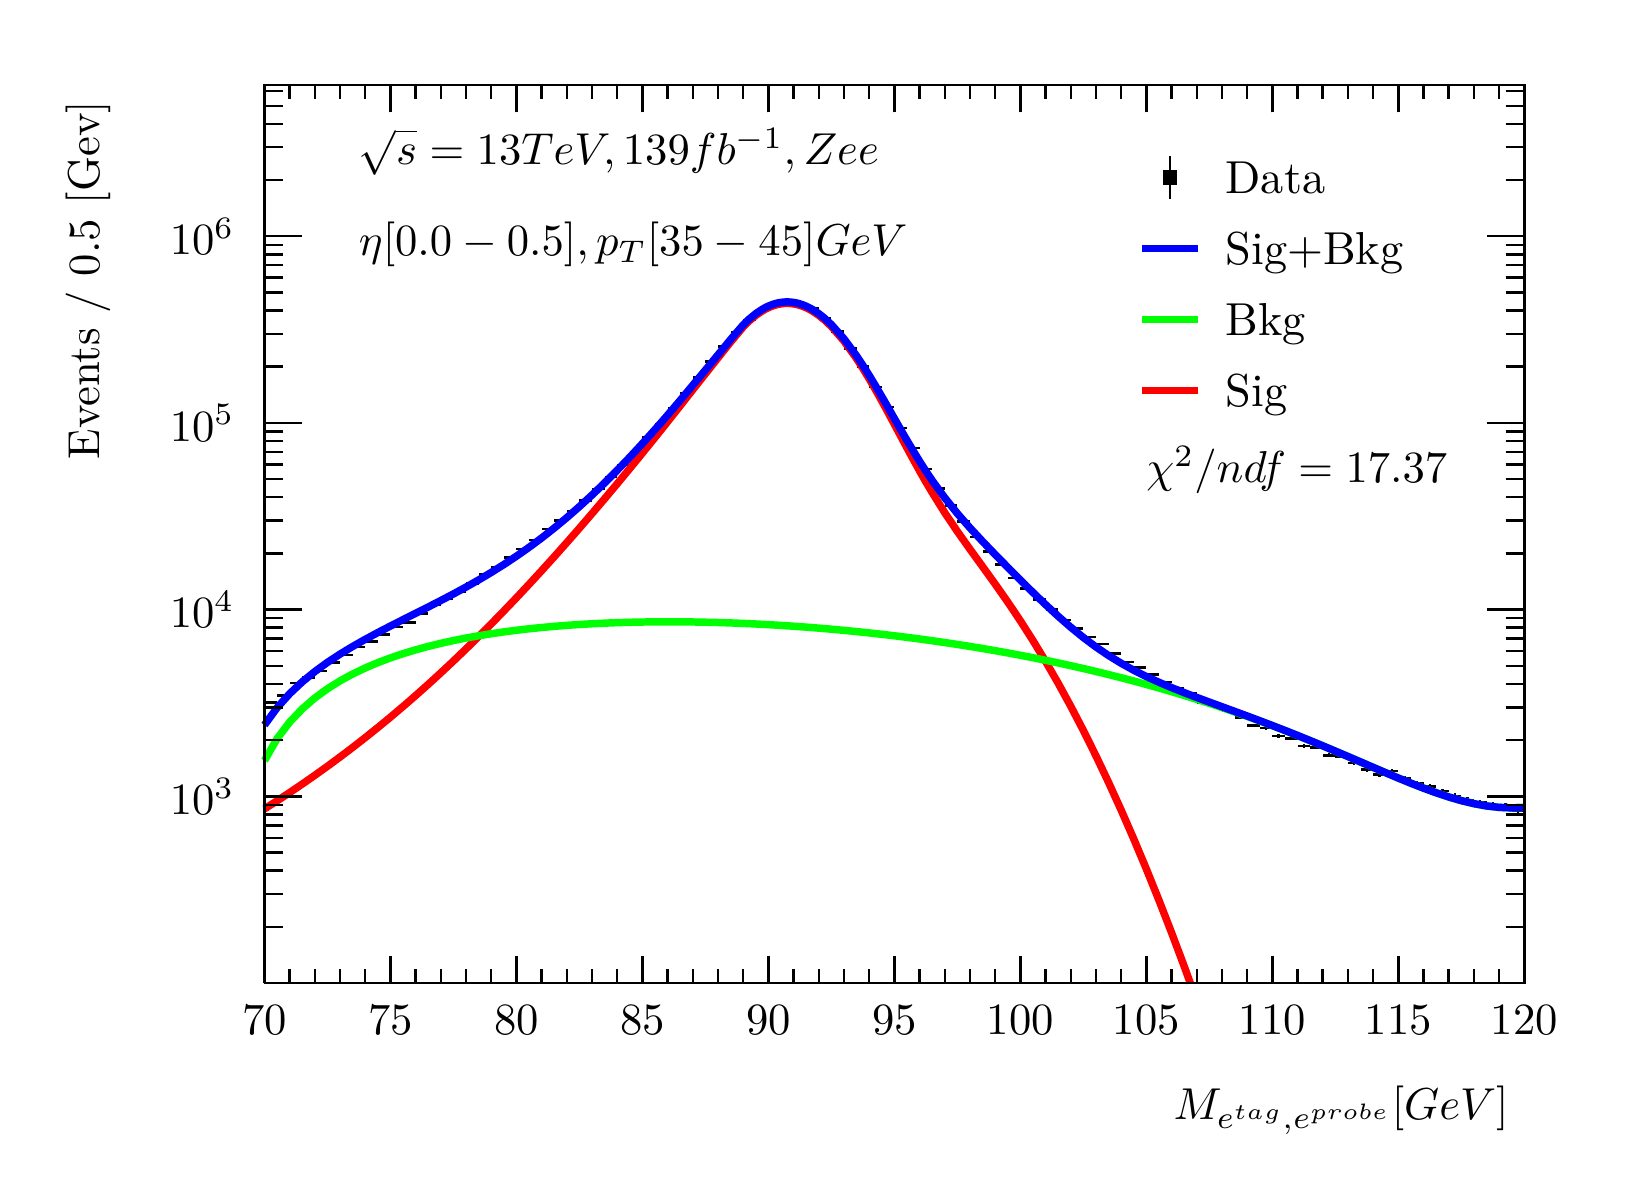
\begin{tikzpicture}
\pgfdeclareplotmark{cross} {
\pgfpathmoveto{\pgfpoint{-0.3\pgfplotmarksize}{\pgfplotmarksize}}
\pgfpathlineto{\pgfpoint{+0.3\pgfplotmarksize}{\pgfplotmarksize}}
\pgfpathlineto{\pgfpoint{+0.3\pgfplotmarksize}{0.3\pgfplotmarksize}}
\pgfpathlineto{\pgfpoint{+1\pgfplotmarksize}{0.3\pgfplotmarksize}}
\pgfpathlineto{\pgfpoint{+1\pgfplotmarksize}{-0.3\pgfplotmarksize}}
\pgfpathlineto{\pgfpoint{+0.3\pgfplotmarksize}{-0.3\pgfplotmarksize}}
\pgfpathlineto{\pgfpoint{+0.3\pgfplotmarksize}{-1.\pgfplotmarksize}}
\pgfpathlineto{\pgfpoint{-0.3\pgfplotmarksize}{-1.\pgfplotmarksize}}
\pgfpathlineto{\pgfpoint{-0.3\pgfplotmarksize}{-0.3\pgfplotmarksize}}
\pgfpathlineto{\pgfpoint{-1.\pgfplotmarksize}{-0.3\pgfplotmarksize}}
\pgfpathlineto{\pgfpoint{-1.\pgfplotmarksize}{0.3\pgfplotmarksize}}
\pgfpathlineto{\pgfpoint{-0.3\pgfplotmarksize}{0.3\pgfplotmarksize}}
\pgfpathclose
\pgfusepathqstroke
}
\pgfdeclareplotmark{cross*} {
\pgfpathmoveto{\pgfpoint{-0.3\pgfplotmarksize}{\pgfplotmarksize}}
\pgfpathlineto{\pgfpoint{+0.3\pgfplotmarksize}{\pgfplotmarksize}}
\pgfpathlineto{\pgfpoint{+0.3\pgfplotmarksize}{0.3\pgfplotmarksize}}
\pgfpathlineto{\pgfpoint{+1\pgfplotmarksize}{0.3\pgfplotmarksize}}
\pgfpathlineto{\pgfpoint{+1\pgfplotmarksize}{-0.3\pgfplotmarksize}}
\pgfpathlineto{\pgfpoint{+0.3\pgfplotmarksize}{-0.3\pgfplotmarksize}}
\pgfpathlineto{\pgfpoint{+0.3\pgfplotmarksize}{-1.\pgfplotmarksize}}
\pgfpathlineto{\pgfpoint{-0.3\pgfplotmarksize}{-1.\pgfplotmarksize}}
\pgfpathlineto{\pgfpoint{-0.3\pgfplotmarksize}{-0.3\pgfplotmarksize}}
\pgfpathlineto{\pgfpoint{-1.\pgfplotmarksize}{-0.3\pgfplotmarksize}}
\pgfpathlineto{\pgfpoint{-1.\pgfplotmarksize}{0.3\pgfplotmarksize}}
\pgfpathlineto{\pgfpoint{-0.3\pgfplotmarksize}{0.3\pgfplotmarksize}}
\pgfpathclose
\pgfusepathqfillstroke
}
\pgfdeclareplotmark{newstar} {
\pgfpathmoveto{\pgfqpoint{0pt}{\pgfplotmarksize}}
\pgfpathlineto{\pgfqpointpolar{44}{0.5\pgfplotmarksize}}
\pgfpathlineto{\pgfqpointpolar{18}{\pgfplotmarksize}}
\pgfpathlineto{\pgfqpointpolar{-20}{0.5\pgfplotmarksize}}
\pgfpathlineto{\pgfqpointpolar{-54}{\pgfplotmarksize}}
\pgfpathlineto{\pgfqpointpolar{-90}{0.5\pgfplotmarksize}}
\pgfpathlineto{\pgfqpointpolar{234}{\pgfplotmarksize}}
\pgfpathlineto{\pgfqpointpolar{198}{0.5\pgfplotmarksize}}
\pgfpathlineto{\pgfqpointpolar{162}{\pgfplotmarksize}}
\pgfpathlineto{\pgfqpointpolar{134}{0.5\pgfplotmarksize}}
\pgfpathclose
\pgfusepathqstroke
}
\pgfdeclareplotmark{newstar*} {
\pgfpathmoveto{\pgfqpoint{0pt}{\pgfplotmarksize}}
\pgfpathlineto{\pgfqpointpolar{44}{0.5\pgfplotmarksize}}
\pgfpathlineto{\pgfqpointpolar{18}{\pgfplotmarksize}}
\pgfpathlineto{\pgfqpointpolar{-20}{0.5\pgfplotmarksize}}
\pgfpathlineto{\pgfqpointpolar{-54}{\pgfplotmarksize}}
\pgfpathlineto{\pgfqpointpolar{-90}{0.5\pgfplotmarksize}}
\pgfpathlineto{\pgfqpointpolar{234}{\pgfplotmarksize}}
\pgfpathlineto{\pgfqpointpolar{198}{0.5\pgfplotmarksize}}
\pgfpathlineto{\pgfqpointpolar{162}{\pgfplotmarksize}}
\pgfpathlineto{\pgfqpointpolar{134}{0.5\pgfplotmarksize}}
\pgfpathclose
\pgfusepathqfillstroke
}
\definecolor{c}{rgb}{1,1,1};
\draw [color=c, fill=c] (0,0) rectangle (20,14.4361);
\draw [color=c, fill=c] (3,2.30977) rectangle (19,13.7143);
\definecolor{c}{rgb}{0,0,0};
\draw [c,line width=0.9] (3,2.30977) -- (3,13.7143) -- (19,13.7143) -- (19,2.30977) -- (3,2.30977);
\definecolor{c}{rgb}{1,1,1};
\draw [color=c, fill=c] (3,2.30977) rectangle (19,13.7143);
\definecolor{c}{rgb}{0,0,0};
\draw [c,line width=0.9] (3,2.30977) -- (3,13.7143) -- (19,13.7143) -- (19,2.30977) -- (3,2.30977);
\draw [c,line width=0.9] (3,2.30977) -- (19,2.30977);
\draw [c,line width=0.9] (3,2.65624) -- (3,2.30977);
\draw [c,line width=0.9] (3.32,2.48301) -- (3.32,2.30977);
\draw [c,line width=0.9] (3.64,2.48301) -- (3.64,2.30977);
\draw [c,line width=0.9] (3.96,2.48301) -- (3.96,2.30977);
\draw [c,line width=0.9] (4.28,2.48301) -- (4.28,2.30977);
\draw [c,line width=0.9] (4.6,2.65624) -- (4.6,2.30977);
\draw [c,line width=0.9] (4.92,2.48301) -- (4.92,2.30977);
\draw [c,line width=0.9] (5.24,2.48301) -- (5.24,2.30977);
\draw [c,line width=0.9] (5.56,2.48301) -- (5.56,2.30977);
\draw [c,line width=0.9] (5.88,2.48301) -- (5.88,2.30977);
\draw [c,line width=0.9] (6.2,2.65624) -- (6.2,2.30977);
\draw [c,line width=0.9] (6.52,2.48301) -- (6.52,2.30977);
\draw [c,line width=0.9] (6.84,2.48301) -- (6.84,2.30977);
\draw [c,line width=0.9] (7.16,2.48301) -- (7.16,2.30977);
\draw [c,line width=0.9] (7.48,2.48301) -- (7.48,2.30977);
\draw [c,line width=0.9] (7.8,2.65624) -- (7.8,2.30977);
\draw [c,line width=0.9] (8.12,2.48301) -- (8.12,2.30977);
\draw [c,line width=0.9] (8.44,2.48301) -- (8.44,2.30977);
\draw [c,line width=0.9] (8.76,2.48301) -- (8.76,2.30977);
\draw [c,line width=0.9] (9.08,2.48301) -- (9.08,2.30977);
\draw [c,line width=0.9] (9.4,2.65624) -- (9.4,2.30977);
\draw [c,line width=0.9] (9.72,2.48301) -- (9.72,2.30977);
\draw [c,line width=0.9] (10.04,2.48301) -- (10.04,2.30977);
\draw [c,line width=0.9] (10.36,2.48301) -- (10.36,2.30977);
\draw [c,line width=0.9] (10.68,2.48301) -- (10.68,2.30977);
\draw [c,line width=0.9] (11,2.65624) -- (11,2.30977);
\draw [c,line width=0.9] (11.32,2.48301) -- (11.32,2.30977);
\draw [c,line width=0.9] (11.64,2.48301) -- (11.64,2.30977);
\draw [c,line width=0.9] (11.96,2.48301) -- (11.96,2.30977);
\draw [c,line width=0.9] (12.28,2.48301) -- (12.28,2.30977);
\draw [c,line width=0.9] (12.6,2.65624) -- (12.6,2.30977);
\draw [c,line width=0.9] (12.92,2.48301) -- (12.92,2.30977);
\draw [c,line width=0.9] (13.24,2.48301) -- (13.24,2.30977);
\draw [c,line width=0.9] (13.56,2.48301) -- (13.56,2.30977);
\draw [c,line width=0.9] (13.88,2.48301) -- (13.88,2.30977);
\draw [c,line width=0.9] (14.2,2.65624) -- (14.2,2.30977);
\draw [c,line width=0.9] (14.52,2.48301) -- (14.52,2.30977);
\draw [c,line width=0.9] (14.84,2.48301) -- (14.84,2.30977);
\draw [c,line width=0.9] (15.16,2.48301) -- (15.16,2.30977);
\draw [c,line width=0.9] (15.48,2.48301) -- (15.48,2.30977);
\draw [c,line width=0.9] (15.8,2.65624) -- (15.8,2.30977);
\draw [c,line width=0.9] (16.12,2.48301) -- (16.12,2.30977);
\draw [c,line width=0.9] (16.44,2.48301) -- (16.44,2.30977);
\draw [c,line width=0.9] (16.76,2.48301) -- (16.76,2.30977);
\draw [c,line width=0.9] (17.08,2.48301) -- (17.08,2.30977);
\draw [c,line width=0.9] (17.4,2.65624) -- (17.4,2.30977);
\draw [c,line width=0.9] (17.72,2.48301) -- (17.72,2.30977);
\draw [c,line width=0.9] (18.04,2.48301) -- (18.04,2.30977);
\draw [c,line width=0.9] (18.36,2.48301) -- (18.36,2.30977);
\draw [c,line width=0.9] (18.68,2.48301) -- (18.68,2.30977);
\draw [c,line width=0.9] (19,2.65624) -- (19,2.30977);
\draw [anchor=base] (3,1.66015) node[scale=1.61424, color=c, rotate=0]{70};
\draw [anchor=base] (4.6,1.66015) node[scale=1.61424, color=c, rotate=0]{75};
\draw [anchor=base] (6.2,1.66015) node[scale=1.61424, color=c, rotate=0]{80};
\draw [anchor=base] (7.8,1.66015) node[scale=1.61424, color=c, rotate=0]{85};
\draw [anchor=base] (9.4,1.66015) node[scale=1.61424, color=c, rotate=0]{90};
\draw [anchor=base] (11,1.66015) node[scale=1.61424, color=c, rotate=0]{95};
\draw [anchor=base] (12.6,1.66015) node[scale=1.61424, color=c, rotate=0]{100};
\draw [anchor=base] (14.2,1.66015) node[scale=1.61424, color=c, rotate=0]{105};
\draw [anchor=base] (15.8,1.66015) node[scale=1.61424, color=c, rotate=0]{110};
\draw [anchor=base] (17.4,1.66015) node[scale=1.61424, color=c, rotate=0]{115};
\draw [anchor=base] (19,1.66015) node[scale=1.61424, color=c, rotate=0]{120};
\draw [anchor= east] (19,0.692932) node[scale=1.61424, color=c, rotate=0]{$M_{e^{tag}, e^{probe}}  [GeV]$};
\draw [c,line width=0.9] (3,13.7143) -- (19,13.7143);
\draw [c,line width=0.9] (3,13.3678) -- (3,13.7143);
\draw [c,line width=0.9] (3.32,13.5411) -- (3.32,13.7143);
\draw [c,line width=0.9] (3.64,13.5411) -- (3.64,13.7143);
\draw [c,line width=0.9] (3.96,13.5411) -- (3.96,13.7143);
\draw [c,line width=0.9] (4.28,13.5411) -- (4.28,13.7143);
\draw [c,line width=0.9] (4.6,13.3678) -- (4.6,13.7143);
\draw [c,line width=0.9] (4.92,13.5411) -- (4.92,13.7143);
\draw [c,line width=0.9] (5.24,13.5411) -- (5.24,13.7143);
\draw [c,line width=0.9] (5.56,13.5411) -- (5.56,13.7143);
\draw [c,line width=0.9] (5.88,13.5411) -- (5.88,13.7143);
\draw [c,line width=0.9] (6.2,13.3678) -- (6.2,13.7143);
\draw [c,line width=0.9] (6.52,13.5411) -- (6.52,13.7143);
\draw [c,line width=0.9] (6.84,13.5411) -- (6.84,13.7143);
\draw [c,line width=0.9] (7.16,13.5411) -- (7.16,13.7143);
\draw [c,line width=0.9] (7.48,13.5411) -- (7.48,13.7143);
\draw [c,line width=0.9] (7.8,13.3678) -- (7.8,13.7143);
\draw [c,line width=0.9] (8.12,13.5411) -- (8.12,13.7143);
\draw [c,line width=0.9] (8.44,13.5411) -- (8.44,13.7143);
\draw [c,line width=0.9] (8.76,13.5411) -- (8.76,13.7143);
\draw [c,line width=0.9] (9.08,13.5411) -- (9.08,13.7143);
\draw [c,line width=0.9] (9.4,13.3678) -- (9.4,13.7143);
\draw [c,line width=0.9] (9.72,13.5411) -- (9.72,13.7143);
\draw [c,line width=0.9] (10.04,13.5411) -- (10.04,13.7143);
\draw [c,line width=0.9] (10.36,13.5411) -- (10.36,13.7143);
\draw [c,line width=0.9] (10.68,13.5411) -- (10.68,13.7143);
\draw [c,line width=0.9] (11,13.3678) -- (11,13.7143);
\draw [c,line width=0.9] (11.32,13.5411) -- (11.32,13.7143);
\draw [c,line width=0.9] (11.64,13.5411) -- (11.64,13.7143);
\draw [c,line width=0.9] (11.96,13.5411) -- (11.96,13.7143);
\draw [c,line width=0.9] (12.28,13.5411) -- (12.28,13.7143);
\draw [c,line width=0.9] (12.6,13.3678) -- (12.6,13.7143);
\draw [c,line width=0.9] (12.92,13.5411) -- (12.92,13.7143);
\draw [c,line width=0.9] (13.24,13.5411) -- (13.24,13.7143);
\draw [c,line width=0.9] (13.56,13.5411) -- (13.56,13.7143);
\draw [c,line width=0.9] (13.88,13.5411) -- (13.88,13.7143);
\draw [c,line width=0.9] (14.2,13.3678) -- (14.2,13.7143);
\draw [c,line width=0.9] (14.52,13.5411) -- (14.52,13.7143);
\draw [c,line width=0.9] (14.84,13.5411) -- (14.84,13.7143);
\draw [c,line width=0.9] (15.16,13.5411) -- (15.16,13.7143);
\draw [c,line width=0.9] (15.48,13.5411) -- (15.48,13.7143);
\draw [c,line width=0.9] (15.8,13.3678) -- (15.8,13.7143);
\draw [c,line width=0.9] (16.12,13.5411) -- (16.12,13.7143);
\draw [c,line width=0.9] (16.44,13.5411) -- (16.44,13.7143);
\draw [c,line width=0.9] (16.76,13.5411) -- (16.76,13.7143);
\draw [c,line width=0.9] (17.08,13.5411) -- (17.08,13.7143);
\draw [c,line width=0.9] (17.4,13.3678) -- (17.4,13.7143);
\draw [c,line width=0.9] (17.72,13.5411) -- (17.72,13.7143);
\draw [c,line width=0.9] (18.04,13.5411) -- (18.04,13.7143);
\draw [c,line width=0.9] (18.36,13.5411) -- (18.36,13.7143);
\draw [c,line width=0.9] (18.68,13.5411) -- (18.68,13.7143);
\draw [c,line width=0.9] (19,13.3678) -- (19,13.7143);
\draw [c,line width=0.9] (3,2.30977) -- (3,13.7143);
\draw [c,line width=0.9] (3.237,3.02354) -- (3,3.02354);
\draw [c,line width=0.9] (3.237,3.44107) -- (3,3.44107);
\draw [c,line width=0.9] (3.237,3.73731) -- (3,3.73731);
\draw [c,line width=0.9] (3.237,3.96709) -- (3,3.96709);
\draw [c,line width=0.9] (3.237,4.15484) -- (3,4.15484);
\draw [c,line width=0.9] (3.237,4.31357) -- (3,4.31357);
\draw [c,line width=0.9] (3.237,4.45108) -- (3,4.45108);
\draw [c,line width=0.9] (3.237,4.57236) -- (3,4.57236);
\draw [c,line width=0.9] (3.474,4.68086) -- (3,4.68086);
\draw [anchor= east] (2.82,4.68086) node[scale=1.61424, color=c, rotate=0]{$10^{3}$};
\draw [c,line width=0.9] (3.237,5.39463) -- (3,5.39463);
\draw [c,line width=0.9] (3.237,5.81216) -- (3,5.81216);
\draw [c,line width=0.9] (3.237,6.1084) -- (3,6.1084);
\draw [c,line width=0.9] (3.237,6.33818) -- (3,6.33818);
\draw [c,line width=0.9] (3.237,6.52593) -- (3,6.52593);
\draw [c,line width=0.9] (3.237,6.68466) -- (3,6.68466);
\draw [c,line width=0.9] (3.237,6.82217) -- (3,6.82217);
\draw [c,line width=0.9] (3.237,6.94345) -- (3,6.94345);
\draw [c,line width=0.9] (3.474,7.05195) -- (3,7.05195);
\draw [anchor= east] (2.82,7.05195) node[scale=1.61424, color=c, rotate=0]{$10^{4}$};
\draw [c,line width=0.9] (3.237,7.76572) -- (3,7.76572);
\draw [c,line width=0.9] (3.237,8.18324) -- (3,8.18324);
\draw [c,line width=0.9] (3.237,8.47948) -- (3,8.47948);
\draw [c,line width=0.9] (3.237,8.70927) -- (3,8.70927);
\draw [c,line width=0.9] (3.237,8.89701) -- (3,8.89701);
\draw [c,line width=0.9] (3.237,9.05575) -- (3,9.05575);
\draw [c,line width=0.9] (3.237,9.19325) -- (3,9.19325);
\draw [c,line width=0.9] (3.237,9.31454) -- (3,9.31454);
\draw [c,line width=0.9] (3.474,9.42304) -- (3,9.42304);
\draw [anchor= east] (2.82,9.42304) node[scale=1.61424, color=c, rotate=0]{$10^{5}$};
\draw [c,line width=0.9] (3.237,10.1368) -- (3,10.1368);
\draw [c,line width=0.9] (3.237,10.5543) -- (3,10.5543);
\draw [c,line width=0.9] (3.237,10.8506) -- (3,10.8506);
\draw [c,line width=0.9] (3.237,11.0804) -- (3,11.0804);
\draw [c,line width=0.9] (3.237,11.2681) -- (3,11.2681);
\draw [c,line width=0.9] (3.237,11.4268) -- (3,11.4268);
\draw [c,line width=0.9] (3.237,11.5643) -- (3,11.5643);
\draw [c,line width=0.9] (3.237,11.6856) -- (3,11.6856);
\draw [c,line width=0.9] (3.474,11.7941) -- (3,11.7941);
\draw [anchor= east] (2.82,11.7941) node[scale=1.61424, color=c, rotate=0]{$10^{6}$};
\draw [c,line width=0.9] (3.237,12.5079) -- (3,12.5079);
\draw [c,line width=0.9] (3.237,12.9254) -- (3,12.9254);
\draw [c,line width=0.9] (3.237,13.2217) -- (3,13.2217);
\draw [c,line width=0.9] (3.237,13.4514) -- (3,13.4514);
\draw [c,line width=0.9] (3.237,13.6392) -- (3,13.6392);
\draw [anchor= east] (0.76,13.7143) node[scale=1.61424, color=c, rotate=90]{Events / 0.5 [Gev]};
\draw [c,line width=0.9] (19,2.30977) -- (19,13.7143);
\draw [c,line width=0.9] (18.763,3.02354) -- (19,3.02354);
\draw [c,line width=0.9] (18.763,3.44107) -- (19,3.44107);
\draw [c,line width=0.9] (18.763,3.73731) -- (19,3.73731);
\draw [c,line width=0.9] (18.763,3.96709) -- (19,3.96709);
\draw [c,line width=0.9] (18.763,4.15484) -- (19,4.15484);
\draw [c,line width=0.9] (18.763,4.31357) -- (19,4.31357);
\draw [c,line width=0.9] (18.763,4.45108) -- (19,4.45108);
\draw [c,line width=0.9] (18.763,4.57236) -- (19,4.57236);
\draw [c,line width=0.9] (18.526,4.68086) -- (19,4.68086);
\draw [c,line width=0.9] (18.763,5.39463) -- (19,5.39463);
\draw [c,line width=0.9] (18.763,5.81216) -- (19,5.81216);
\draw [c,line width=0.9] (18.763,6.1084) -- (19,6.1084);
\draw [c,line width=0.9] (18.763,6.33818) -- (19,6.33818);
\draw [c,line width=0.9] (18.763,6.52593) -- (19,6.52593);
\draw [c,line width=0.9] (18.763,6.68466) -- (19,6.68466);
\draw [c,line width=0.9] (18.763,6.82217) -- (19,6.82217);
\draw [c,line width=0.9] (18.763,6.94345) -- (19,6.94345);
\draw [c,line width=0.9] (18.526,7.05195) -- (19,7.05195);
\draw [c,line width=0.9] (18.763,7.76572) -- (19,7.76572);
\draw [c,line width=0.9] (18.763,8.18324) -- (19,8.18324);
\draw [c,line width=0.9] (18.763,8.47948) -- (19,8.47948);
\draw [c,line width=0.9] (18.763,8.70927) -- (19,8.70927);
\draw [c,line width=0.9] (18.763,8.89701) -- (19,8.89701);
\draw [c,line width=0.9] (18.763,9.05575) -- (19,9.05575);
\draw [c,line width=0.9] (18.763,9.19325) -- (19,9.19325);
\draw [c,line width=0.9] (18.763,9.31454) -- (19,9.31454);
\draw [c,line width=0.9] (18.526,9.42304) -- (19,9.42304);
\draw [c,line width=0.9] (18.763,10.1368) -- (19,10.1368);
\draw [c,line width=0.9] (18.763,10.5543) -- (19,10.5543);
\draw [c,line width=0.9] (18.763,10.8506) -- (19,10.8506);
\draw [c,line width=0.9] (18.763,11.0804) -- (19,11.0804);
\draw [c,line width=0.9] (18.763,11.2681) -- (19,11.2681);
\draw [c,line width=0.9] (18.763,11.4268) -- (19,11.4268);
\draw [c,line width=0.9] (18.763,11.5643) -- (19,11.5643);
\draw [c,line width=0.9] (18.763,11.6856) -- (19,11.6856);
\draw [c,line width=0.9] (18.526,11.7941) -- (19,11.7941);
\draw [c,line width=0.9] (18.763,12.5079) -- (19,12.5079);
\draw [c,line width=0.9] (18.763,12.9254) -- (19,12.9254);
\draw [c,line width=0.9] (18.763,13.2217) -- (19,13.2217);
\draw [c,line width=0.9] (18.763,13.4514) -- (19,13.4514);
\draw [c,line width=0.9] (18.763,13.6392) -- (19,13.6392);
\draw [c,line width=0.9] (3.08,5.87086) -- (3,5.87086);
\draw [c,line width=0.9] (3,5.87086) -- (3,5.87086);
\draw [c,line width=0.9] (3.08,5.87086) -- (3.16,5.87086);
\draw [c,line width=0.9] (3.16,5.87086) -- (3.16,5.87086);
\draw [c,line width=0.9] (3.08,5.87086) -- (3.08,5.88914);
\draw [c,line width=0.9] (3.08,5.88914) -- (3.08,5.88914);
\draw [c,line width=0.9] (3.08,5.87086) -- (3.08,5.85259);
\draw [c,line width=0.9] (3.08,5.85259) -- (3.08,5.85259);
\draw [c,line width=0.9] (3.24,5.95965) -- (3.16,5.95965);
\draw [c,line width=0.9] (3.16,5.95965) -- (3.16,5.95965);
\draw [c,line width=0.9] (3.24,5.95965) -- (3.32,5.95965);
\draw [c,line width=0.9] (3.32,5.95965) -- (3.32,5.95965);
\draw [c,line width=0.9] (3.24,5.95965) -- (3.24,5.97715);
\draw [c,line width=0.9] (3.24,5.97715) -- (3.24,5.97715);
\draw [c,line width=0.9] (3.24,5.95965) -- (3.24,5.94215);
\draw [c,line width=0.9] (3.24,5.94215) -- (3.24,5.94215);
\draw [c,line width=0.9] (3.4,6.12246) -- (3.32,6.12246);
\draw [c,line width=0.9] (3.32,6.12246) -- (3.32,6.12246);
\draw [c,line width=0.9] (3.4,6.12246) -- (3.48,6.12246);
\draw [c,line width=0.9] (3.48,6.12246) -- (3.48,6.12246);
\draw [c,line width=0.9] (3.4,6.12246) -- (3.4,6.13863);
\draw [c,line width=0.9] (3.4,6.13863) -- (3.4,6.13863);
\draw [c,line width=0.9] (3.4,6.12246) -- (3.4,6.10629);
\draw [c,line width=0.9] (3.4,6.10629) -- (3.4,6.10629);
\draw [c,line width=0.9] (3.56,6.19027) -- (3.48,6.19027);
\draw [c,line width=0.9] (3.48,6.19027) -- (3.48,6.19027);
\draw [c,line width=0.9] (3.56,6.19027) -- (3.64,6.19027);
\draw [c,line width=0.9] (3.64,6.19027) -- (3.64,6.19027);
\draw [c,line width=0.9] (3.56,6.19027) -- (3.56,6.20591);
\draw [c,line width=0.9] (3.56,6.20591) -- (3.56,6.20591);
\draw [c,line width=0.9] (3.56,6.19027) -- (3.56,6.17462);
\draw [c,line width=0.9] (3.56,6.17462) -- (3.56,6.17462);
\draw [c,line width=0.9] (3.72,6.27556) -- (3.64,6.27556);
\draw [c,line width=0.9] (3.64,6.27556) -- (3.64,6.27556);
\draw [c,line width=0.9] (3.72,6.27556) -- (3.8,6.27556);
\draw [c,line width=0.9] (3.8,6.27556) -- (3.8,6.27556);
\draw [c,line width=0.9] (3.72,6.27556) -- (3.72,6.29057);
\draw [c,line width=0.9] (3.72,6.29057) -- (3.72,6.29057);
\draw [c,line width=0.9] (3.72,6.27556) -- (3.72,6.26055);
\draw [c,line width=0.9] (3.72,6.26055) -- (3.72,6.26055);
\draw [c,line width=0.9] (3.88,6.37916) -- (3.8,6.37916);
\draw [c,line width=0.9] (3.8,6.37916) -- (3.8,6.37916);
\draw [c,line width=0.9] (3.88,6.37916) -- (3.96,6.37916);
\draw [c,line width=0.9] (3.96,6.37916) -- (3.96,6.37916);
\draw [c,line width=0.9] (3.88,6.37916) -- (3.88,6.39344);
\draw [c,line width=0.9] (3.88,6.39344) -- (3.88,6.39344);
\draw [c,line width=0.9] (3.88,6.37916) -- (3.88,6.36489);
\draw [c,line width=0.9] (3.88,6.36489) -- (3.88,6.36489);
\draw [c,line width=0.9] (4.04,6.47509) -- (3.96,6.47509);
\draw [c,line width=0.9] (3.96,6.47509) -- (3.96,6.47509);
\draw [c,line width=0.9] (4.04,6.47509) -- (4.12,6.47509);
\draw [c,line width=0.9] (4.12,6.47509) -- (4.12,6.47509);
\draw [c,line width=0.9] (4.04,6.47509) -- (4.04,6.48872);
\draw [c,line width=0.9] (4.04,6.48872) -- (4.04,6.48872);
\draw [c,line width=0.9] (4.04,6.47509) -- (4.04,6.46147);
\draw [c,line width=0.9] (4.04,6.46147) -- (4.04,6.46147);
\draw [c,line width=0.9] (4.2,6.576) -- (4.12,6.576);
\draw [c,line width=0.9] (4.12,6.576) -- (4.12,6.576);
\draw [c,line width=0.9] (4.2,6.576) -- (4.28,6.576);
\draw [c,line width=0.9] (4.28,6.576) -- (4.28,6.576);
\draw [c,line width=0.9] (4.2,6.576) -- (4.2,6.58898);
\draw [c,line width=0.9] (4.2,6.58898) -- (4.2,6.58898);
\draw [c,line width=0.9] (4.2,6.576) -- (4.2,6.56303);
\draw [c,line width=0.9] (4.2,6.56303) -- (4.2,6.56303);
\draw [c,line width=0.9] (4.36,6.64508) -- (4.28,6.64508);
\draw [c,line width=0.9] (4.28,6.64508) -- (4.28,6.64508);
\draw [c,line width=0.9] (4.36,6.64508) -- (4.44,6.64508);
\draw [c,line width=0.9] (4.44,6.64508) -- (4.44,6.64508);
\draw [c,line width=0.9] (4.36,6.64508) -- (4.36,6.65762);
\draw [c,line width=0.9] (4.36,6.65762) -- (4.36,6.65762);
\draw [c,line width=0.9] (4.36,6.64508) -- (4.36,6.63253);
\draw [c,line width=0.9] (4.36,6.63253) -- (4.36,6.63253);
\draw [c,line width=0.9] (4.52,6.7335) -- (4.44,6.7335);
\draw [c,line width=0.9] (4.44,6.7335) -- (4.44,6.7335);
\draw [c,line width=0.9] (4.52,6.7335) -- (4.6,6.7335);
\draw [c,line width=0.9] (4.6,6.7335) -- (4.6,6.7335);
\draw [c,line width=0.9] (4.52,6.7335) -- (4.52,6.74552);
\draw [c,line width=0.9] (4.52,6.74552) -- (4.52,6.74552);
\draw [c,line width=0.9] (4.52,6.7335) -- (4.52,6.72148);
\draw [c,line width=0.9] (4.52,6.72148) -- (4.52,6.72148);
\draw [c,line width=0.9] (4.68,6.83216) -- (4.6,6.83216);
\draw [c,line width=0.9] (4.6,6.83216) -- (4.6,6.83216);
\draw [c,line width=0.9] (4.68,6.83216) -- (4.76,6.83216);
\draw [c,line width=0.9] (4.76,6.83216) -- (4.76,6.83216);
\draw [c,line width=0.9] (4.68,6.83216) -- (4.68,6.84362);
\draw [c,line width=0.9] (4.68,6.84362) -- (4.68,6.84362);
\draw [c,line width=0.9] (4.68,6.83216) -- (4.68,6.8207);
\draw [c,line width=0.9] (4.68,6.8207) -- (4.68,6.8207);
\draw [c,line width=0.9] (4.84,6.88786) -- (4.76,6.88786);
\draw [c,line width=0.9] (4.76,6.88786) -- (4.76,6.88786);
\draw [c,line width=0.9] (4.84,6.88786) -- (4.92,6.88786);
\draw [c,line width=0.9] (4.92,6.88786) -- (4.92,6.88786);
\draw [c,line width=0.9] (4.84,6.88786) -- (4.84,6.89901);
\draw [c,line width=0.9] (4.84,6.89901) -- (4.84,6.89901);
\draw [c,line width=0.9] (4.84,6.88786) -- (4.84,6.87671);
\draw [c,line width=0.9] (4.84,6.87671) -- (4.84,6.87671);
\draw [c,line width=0.9] (5,7.00162) -- (4.92,7.00162);
\draw [c,line width=0.9] (4.92,7.00162) -- (4.92,7.00162);
\draw [c,line width=0.9] (5,7.00162) -- (5.08,7.00162);
\draw [c,line width=0.9] (5.08,7.00162) -- (5.08,7.00162);
\draw [c,line width=0.9] (5,7.00162) -- (5,7.01217);
\draw [c,line width=0.9] (5,7.01217) -- (5,7.01217);
\draw [c,line width=0.9] (5,7.00162) -- (5,6.99107);
\draw [c,line width=0.9] (5,6.99107) -- (5,6.99107);
\draw [c,line width=0.9] (5.16,7.11506) -- (5.08,7.11506);
\draw [c,line width=0.9] (5.08,7.11506) -- (5.08,7.11506);
\draw [c,line width=0.9] (5.16,7.11506) -- (5.24,7.11506);
\draw [c,line width=0.9] (5.24,7.11506) -- (5.24,7.11506);
\draw [c,line width=0.9] (5.16,7.11506) -- (5.16,7.12504);
\draw [c,line width=0.9] (5.16,7.12504) -- (5.16,7.12504);
\draw [c,line width=0.9] (5.16,7.11506) -- (5.16,7.10507);
\draw [c,line width=0.9] (5.16,7.10507) -- (5.16,7.10507);
\draw [c,line width=0.9] (5.32,7.18416) -- (5.24,7.18416);
\draw [c,line width=0.9] (5.24,7.18416) -- (5.24,7.18416);
\draw [c,line width=0.9] (5.32,7.18416) -- (5.4,7.18416);
\draw [c,line width=0.9] (5.4,7.18416) -- (5.4,7.18416);
\draw [c,line width=0.9] (5.32,7.18416) -- (5.32,7.19382);
\draw [c,line width=0.9] (5.32,7.19382) -- (5.32,7.19382);
\draw [c,line width=0.9] (5.32,7.18416) -- (5.32,7.1745);
\draw [c,line width=0.9] (5.32,7.1745) -- (5.32,7.1745);
\draw [c,line width=0.9] (5.48,7.28543) -- (5.4,7.28543);
\draw [c,line width=0.9] (5.4,7.28543) -- (5.4,7.28543);
\draw [c,line width=0.9] (5.48,7.28543) -- (5.56,7.28543);
\draw [c,line width=0.9] (5.56,7.28543) -- (5.56,7.28543);
\draw [c,line width=0.9] (5.48,7.28543) -- (5.48,7.29463);
\draw [c,line width=0.9] (5.48,7.29463) -- (5.48,7.29463);
\draw [c,line width=0.9] (5.48,7.28543) -- (5.48,7.27624);
\draw [c,line width=0.9] (5.48,7.27624) -- (5.48,7.27624);
\draw [c,line width=0.9] (5.64,7.38674) -- (5.56,7.38674);
\draw [c,line width=0.9] (5.56,7.38674) -- (5.56,7.38674);
\draw [c,line width=0.9] (5.64,7.38674) -- (5.72,7.38674);
\draw [c,line width=0.9] (5.72,7.38674) -- (5.72,7.38674);
\draw [c,line width=0.9] (5.64,7.38674) -- (5.64,7.3955);
\draw [c,line width=0.9] (5.64,7.3955) -- (5.64,7.3955);
\draw [c,line width=0.9] (5.64,7.38674) -- (5.64,7.37799);
\draw [c,line width=0.9] (5.64,7.37799) -- (5.64,7.37799);
\draw [c,line width=0.9] (5.8,7.50696) -- (5.72,7.50696);
\draw [c,line width=0.9] (5.72,7.50696) -- (5.72,7.50696);
\draw [c,line width=0.9] (5.8,7.50696) -- (5.88,7.50696);
\draw [c,line width=0.9] (5.88,7.50696) -- (5.88,7.50696);
\draw [c,line width=0.9] (5.8,7.50696) -- (5.8,7.51521);
\draw [c,line width=0.9] (5.8,7.51521) -- (5.8,7.51521);
\draw [c,line width=0.9] (5.8,7.50696) -- (5.8,7.4987);
\draw [c,line width=0.9] (5.8,7.4987) -- (5.8,7.4987);
\draw [c,line width=0.9] (5.96,7.59618) -- (5.88,7.59618);
\draw [c,line width=0.9] (5.88,7.59618) -- (5.88,7.59618);
\draw [c,line width=0.9] (5.96,7.59618) -- (6.04,7.59618);
\draw [c,line width=0.9] (6.04,7.59618) -- (6.04,7.59618);
\draw [c,line width=0.9] (5.96,7.59618) -- (5.96,7.60409);
\draw [c,line width=0.9] (5.96,7.60409) -- (5.96,7.60409);
\draw [c,line width=0.9] (5.96,7.59618) -- (5.96,7.58827);
\draw [c,line width=0.9] (5.96,7.58827) -- (5.96,7.58827);
\draw [c,line width=0.9] (6.12,7.71447) -- (6.04,7.71447);
\draw [c,line width=0.9] (6.04,7.71447) -- (6.04,7.71447);
\draw [c,line width=0.9] (6.12,7.71447) -- (6.2,7.71447);
\draw [c,line width=0.9] (6.2,7.71447) -- (6.2,7.71447);
\draw [c,line width=0.9] (6.12,7.71447) -- (6.12,7.72193);
\draw [c,line width=0.9] (6.12,7.72193) -- (6.12,7.72193);
\draw [c,line width=0.9] (6.12,7.71447) -- (6.12,7.707);
\draw [c,line width=0.9] (6.12,7.707) -- (6.12,7.707);
\draw [c,line width=0.9] (6.28,7.82212) -- (6.2,7.82212);
\draw [c,line width=0.9] (6.2,7.82212) -- (6.2,7.82212);
\draw [c,line width=0.9] (6.28,7.82212) -- (6.36,7.82212);
\draw [c,line width=0.9] (6.36,7.82212) -- (6.36,7.82212);
\draw [c,line width=0.9] (6.28,7.82212) -- (6.28,7.8292);
\draw [c,line width=0.9] (6.28,7.8292) -- (6.28,7.8292);
\draw [c,line width=0.9] (6.28,7.82212) -- (6.28,7.81503);
\draw [c,line width=0.9] (6.28,7.81503) -- (6.28,7.81503);
\draw [c,line width=0.9] (6.44,7.93472) -- (6.36,7.93472);
\draw [c,line width=0.9] (6.36,7.93472) -- (6.36,7.93472);
\draw [c,line width=0.9] (6.44,7.93472) -- (6.52,7.93472);
\draw [c,line width=0.9] (6.52,7.93472) -- (6.52,7.93472);
\draw [c,line width=0.9] (6.44,7.93472) -- (6.44,7.94142);
\draw [c,line width=0.9] (6.44,7.94142) -- (6.44,7.94142);
\draw [c,line width=0.9] (6.44,7.93472) -- (6.44,7.92801);
\draw [c,line width=0.9] (6.44,7.92801) -- (6.44,7.92801);
\draw [c,line width=0.9] (6.6,8.07448) -- (6.52,8.07448);
\draw [c,line width=0.9] (6.52,8.07448) -- (6.52,8.07448);
\draw [c,line width=0.9] (6.6,8.07448) -- (6.68,8.07448);
\draw [c,line width=0.9] (6.68,8.07448) -- (6.68,8.07448);
\draw [c,line width=0.9] (6.6,8.07448) -- (6.6,8.08075);
\draw [c,line width=0.9] (6.6,8.08075) -- (6.6,8.08075);
\draw [c,line width=0.9] (6.6,8.07448) -- (6.6,8.06822);
\draw [c,line width=0.9] (6.6,8.06822) -- (6.6,8.06822);
\draw [c,line width=0.9] (6.76,8.18149) -- (6.68,8.18149);
\draw [c,line width=0.9] (6.68,8.18149) -- (6.68,8.18149);
\draw [c,line width=0.9] (6.76,8.18149) -- (6.84,8.18149);
\draw [c,line width=0.9] (6.84,8.18149) -- (6.84,8.18149);
\draw [c,line width=0.9] (6.76,8.18149) -- (6.76,8.18744);
\draw [c,line width=0.9] (6.76,8.18744) -- (6.76,8.18744);
\draw [c,line width=0.9] (6.76,8.18149) -- (6.76,8.17554);
\draw [c,line width=0.9] (6.76,8.17554) -- (6.76,8.17554);
\draw [c,line width=0.9] (6.92,8.30533) -- (6.84,8.30533);
\draw [c,line width=0.9] (6.84,8.30533) -- (6.84,8.30533);
\draw [c,line width=0.9] (6.92,8.30533) -- (7,8.30533);
\draw [c,line width=0.9] (7,8.30533) -- (7,8.30533);
\draw [c,line width=0.9] (6.92,8.30533) -- (6.92,8.31093);
\draw [c,line width=0.9] (6.92,8.31093) -- (6.92,8.31093);
\draw [c,line width=0.9] (6.92,8.30533) -- (6.92,8.29972);
\draw [c,line width=0.9] (6.92,8.29972) -- (6.92,8.29972);
\draw [c,line width=0.9] (7.08,8.44101) -- (7,8.44101);
\draw [c,line width=0.9] (7,8.44101) -- (7,8.44101);
\draw [c,line width=0.9] (7.08,8.44101) -- (7.16,8.44101);
\draw [c,line width=0.9] (7.16,8.44101) -- (7.16,8.44101);
\draw [c,line width=0.9] (7.08,8.44101) -- (7.08,8.44626);
\draw [c,line width=0.9] (7.08,8.44626) -- (7.08,8.44626);
\draw [c,line width=0.9] (7.08,8.44101) -- (7.08,8.43576);
\draw [c,line width=0.9] (7.08,8.43576) -- (7.08,8.43576);
\draw [c,line width=0.9] (7.24,8.58649) -- (7.16,8.58649);
\draw [c,line width=0.9] (7.16,8.58649) -- (7.16,8.58649);
\draw [c,line width=0.9] (7.24,8.58649) -- (7.32,8.58649);
\draw [c,line width=0.9] (7.32,8.58649) -- (7.32,8.58649);
\draw [c,line width=0.9] (7.24,8.58649) -- (7.24,8.59138);
\draw [c,line width=0.9] (7.24,8.59138) -- (7.24,8.59138);
\draw [c,line width=0.9] (7.24,8.58649) -- (7.24,8.5816);
\draw [c,line width=0.9] (7.24,8.5816) -- (7.24,8.5816);
\draw [c,line width=0.9] (7.4,8.7375) -- (7.32,8.7375);
\draw [c,line width=0.9] (7.32,8.7375) -- (7.32,8.7375);
\draw [c,line width=0.9] (7.4,8.7375) -- (7.48,8.7375);
\draw [c,line width=0.9] (7.48,8.7375) -- (7.48,8.7375);
\draw [c,line width=0.9] (7.4,8.7375) -- (7.4,8.74205);
\draw [c,line width=0.9] (7.4,8.74205) -- (7.4,8.74205);
\draw [c,line width=0.9] (7.4,8.7375) -- (7.4,8.73296);
\draw [c,line width=0.9] (7.4,8.73296) -- (7.4,8.73296);
\draw [c,line width=0.9] (7.56,8.88897) -- (7.48,8.88897);
\draw [c,line width=0.9] (7.48,8.88897) -- (7.48,8.88897);
\draw [c,line width=0.9] (7.56,8.88897) -- (7.64,8.88897);
\draw [c,line width=0.9] (7.64,8.88897) -- (7.64,8.88897);
\draw [c,line width=0.9] (7.56,8.88897) -- (7.56,8.89319);
\draw [c,line width=0.9] (7.56,8.89319) -- (7.56,8.89319);
\draw [c,line width=0.9] (7.56,8.88897) -- (7.56,8.88475);
\draw [c,line width=0.9] (7.56,8.88475) -- (7.56,8.88475);
\draw [c,line width=0.9] (7.72,9.05543) -- (7.64,9.05543);
\draw [c,line width=0.9] (7.64,9.05543) -- (7.64,9.05543);
\draw [c,line width=0.9] (7.72,9.05543) -- (7.8,9.05543);
\draw [c,line width=0.9] (7.8,9.05543) -- (7.8,9.05543);
\draw [c,line width=0.9] (7.72,9.05543) -- (7.72,9.05932);
\draw [c,line width=0.9] (7.72,9.05932) -- (7.72,9.05932);
\draw [c,line width=0.9] (7.72,9.05543) -- (7.72,9.05153);
\draw [c,line width=0.9] (7.72,9.05153) -- (7.72,9.05153);
\draw [c,line width=0.9] (7.88,9.23782) -- (7.8,9.23782);
\draw [c,line width=0.9] (7.8,9.23782) -- (7.8,9.23782);
\draw [c,line width=0.9] (7.88,9.23782) -- (7.96,9.23782);
\draw [c,line width=0.9] (7.96,9.23782) -- (7.96,9.23782);
\draw [c,line width=0.9] (7.88,9.23782) -- (7.88,9.24138);
\draw [c,line width=0.9] (7.88,9.24138) -- (7.88,9.24138);
\draw [c,line width=0.9] (7.88,9.23782) -- (7.88,9.23425);
\draw [c,line width=0.9] (7.88,9.23425) -- (7.88,9.23425);
\draw [c,line width=0.9] (8.04,9.41066) -- (7.96,9.41066);
\draw [c,line width=0.9] (7.96,9.41066) -- (7.96,9.41066);
\draw [c,line width=0.9] (8.04,9.41066) -- (8.12,9.41066);
\draw [c,line width=0.9] (8.12,9.41066) -- (8.12,9.41066);
\draw [c,line width=0.9] (8.04,9.41066) -- (8.04,9.41393);
\draw [c,line width=0.9] (8.04,9.41393) -- (8.04,9.41393);
\draw [c,line width=0.9] (8.04,9.41066) -- (8.04,9.40738);
\draw [c,line width=0.9] (8.04,9.40738) -- (8.04,9.40738);
\draw [c,line width=0.9] (8.2,9.60518) -- (8.12,9.60518);
\draw [c,line width=0.9] (8.12,9.60518) -- (8.12,9.60518);
\draw [c,line width=0.9] (8.2,9.60518) -- (8.28,9.60518);
\draw [c,line width=0.9] (8.28,9.60518) -- (8.28,9.60518);
\draw [c,line width=0.9] (8.2,9.60518) -- (8.2,9.60816);
\draw [c,line width=0.9] (8.2,9.60816) -- (8.2,9.60816);
\draw [c,line width=0.9] (8.2,9.60518) -- (8.2,9.6022);
\draw [c,line width=0.9] (8.2,9.6022) -- (8.2,9.6022);
\draw [c,line width=0.9] (8.36,9.80488) -- (8.28,9.80488);
\draw [c,line width=0.9] (8.28,9.80488) -- (8.28,9.80488);
\draw [c,line width=0.9] (8.36,9.80488) -- (8.44,9.80488);
\draw [c,line width=0.9] (8.44,9.80488) -- (8.44,9.80488);
\draw [c,line width=0.9] (8.36,9.80488) -- (8.36,9.80758);
\draw [c,line width=0.9] (8.36,9.80758) -- (8.36,9.80758);
\draw [c,line width=0.9] (8.36,9.80488) -- (8.36,9.80217);
\draw [c,line width=0.9] (8.36,9.80217) -- (8.36,9.80217);
\draw [c,line width=0.9] (8.52,10.0023) -- (8.44,10.0023);
\draw [c,line width=0.9] (8.44,10.0023) -- (8.44,10.0023);
\draw [c,line width=0.9] (8.52,10.0023) -- (8.6,10.0023);
\draw [c,line width=0.9] (8.6,10.0023) -- (8.6,10.0023);
\draw [c,line width=0.9] (8.52,10.0023) -- (8.52,10.0048);
\draw [c,line width=0.9] (8.52,10.0048) -- (8.52,10.0048);
\draw [c,line width=0.9] (8.52,10.0023) -- (8.52,9.99984);
\draw [c,line width=0.9] (8.52,9.99984) -- (8.52,9.99984);
\draw [c,line width=0.9] (8.68,10.2031) -- (8.6,10.2031);
\draw [c,line width=0.9] (8.6,10.2031) -- (8.6,10.2031);
\draw [c,line width=0.9] (8.68,10.2031) -- (8.76,10.2031);
\draw [c,line width=0.9] (8.76,10.2031) -- (8.76,10.2031);
\draw [c,line width=0.9] (8.68,10.2031) -- (8.68,10.2053);
\draw [c,line width=0.9] (8.68,10.2053) -- (8.68,10.2053);
\draw [c,line width=0.9] (8.68,10.2031) -- (8.68,10.2008);
\draw [c,line width=0.9] (8.68,10.2008) -- (8.68,10.2008);
\draw [c,line width=0.9] (8.84,10.3968) -- (8.76,10.3968);
\draw [c,line width=0.9] (8.76,10.3968) -- (8.76,10.3968);
\draw [c,line width=0.9] (8.84,10.3968) -- (8.92,10.3968);
\draw [c,line width=0.9] (8.92,10.3968) -- (8.92,10.3968);
\draw [c,line width=0.9] (8.84,10.3968) -- (8.84,10.3988);
\draw [c,line width=0.9] (8.84,10.3988) -- (8.84,10.3988);
\draw [c,line width=0.9] (8.84,10.3968) -- (8.84,10.3948);
\draw [c,line width=0.9] (8.84,10.3948) -- (8.84,10.3948);
\draw [c,line width=0.9] (9,10.5752) -- (8.92,10.5752);
\draw [c,line width=0.9] (8.92,10.5752) -- (8.92,10.5752);
\draw [c,line width=0.9] (9,10.5752) -- (9.08,10.5752);
\draw [c,line width=0.9] (9.08,10.5752) -- (9.08,10.5752);
\draw [c,line width=0.9] (9,10.5752) -- (9,10.5771);
\draw [c,line width=0.9] (9,10.5771) -- (9,10.5771);
\draw [c,line width=0.9] (9,10.5752) -- (9,10.5734);
\draw [c,line width=0.9] (9,10.5734) -- (9,10.5734);
\draw [c,line width=0.9] (9.16,10.7326) -- (9.08,10.7326);
\draw [c,line width=0.9] (9.08,10.7326) -- (9.08,10.7326);
\draw [c,line width=0.9] (9.16,10.7326) -- (9.24,10.7326);
\draw [c,line width=0.9] (9.24,10.7326) -- (9.24,10.7326);
\draw [c,line width=0.9] (9.16,10.7326) -- (9.16,10.7344);
\draw [c,line width=0.9] (9.16,10.7344) -- (9.16,10.7344);
\draw [c,line width=0.9] (9.16,10.7326) -- (9.16,10.7309);
\draw [c,line width=0.9] (9.16,10.7309) -- (9.16,10.7309);
\draw [c,line width=0.9] (9.32,10.8566) -- (9.24,10.8566);
\draw [c,line width=0.9] (9.24,10.8566) -- (9.24,10.8566);
\draw [c,line width=0.9] (9.32,10.8566) -- (9.4,10.8566);
\draw [c,line width=0.9] (9.4,10.8566) -- (9.4,10.8566);
\draw [c,line width=0.9] (9.32,10.8566) -- (9.32,10.8582);
\draw [c,line width=0.9] (9.32,10.8582) -- (9.32,10.8582);
\draw [c,line width=0.9] (9.32,10.8566) -- (9.32,10.855);
\draw [c,line width=0.9] (9.32,10.855) -- (9.32,10.855);
\draw [c,line width=0.9] (9.48,10.9355) -- (9.4,10.9355);
\draw [c,line width=0.9] (9.4,10.9355) -- (9.4,10.9355);
\draw [c,line width=0.9] (9.48,10.9355) -- (9.56,10.9355);
\draw [c,line width=0.9] (9.56,10.9355) -- (9.56,10.9355);
\draw [c,line width=0.9] (9.48,10.9355) -- (9.48,10.9371);
\draw [c,line width=0.9] (9.48,10.9371) -- (9.48,10.9371);
\draw [c,line width=0.9] (9.48,10.9355) -- (9.48,10.934);
\draw [c,line width=0.9] (9.48,10.934) -- (9.48,10.934);
\draw [c,line width=0.9] (9.64,10.9682) -- (9.56,10.9682);
\draw [c,line width=0.9] (9.56,10.9682) -- (9.56,10.9682);
\draw [c,line width=0.9] (9.64,10.9682) -- (9.72,10.9682);
\draw [c,line width=0.9] (9.72,10.9682) -- (9.72,10.9682);
\draw [c,line width=0.9] (9.64,10.9682) -- (9.64,10.9698);
\draw [c,line width=0.9] (9.64,10.9698) -- (9.64,10.9698);
\draw [c,line width=0.9] (9.64,10.9682) -- (9.64,10.9667);
\draw [c,line width=0.9] (9.64,10.9667) -- (9.64,10.9667);
\draw [c,line width=0.9] (9.8,10.9489) -- (9.72,10.9489);
\draw [c,line width=0.9] (9.72,10.9489) -- (9.72,10.9489);
\draw [c,line width=0.9] (9.8,10.9489) -- (9.88,10.9489);
\draw [c,line width=0.9] (9.88,10.9489) -- (9.88,10.9489);
\draw [c,line width=0.9] (9.8,10.9489) -- (9.8,10.9505);
\draw [c,line width=0.9] (9.8,10.9505) -- (9.8,10.9505);
\draw [c,line width=0.9] (9.8,10.9489) -- (9.8,10.9474);
\draw [c,line width=0.9] (9.8,10.9474) -- (9.8,10.9474);
\draw [c,line width=0.9] (9.96,10.8741) -- (9.88,10.8741);
\draw [c,line width=0.9] (9.88,10.8741) -- (9.88,10.8741);
\draw [c,line width=0.9] (9.96,10.8741) -- (10.04,10.8741);
\draw [c,line width=0.9] (10.04,10.8741) -- (10.04,10.8741);
\draw [c,line width=0.9] (9.96,10.8741) -- (9.96,10.8757);
\draw [c,line width=0.9] (9.96,10.8757) -- (9.96,10.8757);
\draw [c,line width=0.9] (9.96,10.8741) -- (9.96,10.8725);
\draw [c,line width=0.9] (9.96,10.8725) -- (9.96,10.8725);
\draw [c,line width=0.9] (10.12,10.7496) -- (10.04,10.7496);
\draw [c,line width=0.9] (10.04,10.7496) -- (10.04,10.7496);
\draw [c,line width=0.9] (10.12,10.7496) -- (10.2,10.7496);
\draw [c,line width=0.9] (10.2,10.7496) -- (10.2,10.7496);
\draw [c,line width=0.9] (10.12,10.7496) -- (10.12,10.7513);
\draw [c,line width=0.9] (10.12,10.7513) -- (10.12,10.7513);
\draw [c,line width=0.9] (10.12,10.7496) -- (10.12,10.7479);
\draw [c,line width=0.9] (10.12,10.7479) -- (10.12,10.7479);
\draw [c,line width=0.9] (10.28,10.5813) -- (10.2,10.5813);
\draw [c,line width=0.9] (10.2,10.5813) -- (10.2,10.5813);
\draw [c,line width=0.9] (10.28,10.5813) -- (10.36,10.5813);
\draw [c,line width=0.9] (10.36,10.5813) -- (10.36,10.5813);
\draw [c,line width=0.9] (10.28,10.5813) -- (10.28,10.5831);
\draw [c,line width=0.9] (10.28,10.5831) -- (10.28,10.5831);
\draw [c,line width=0.9] (10.28,10.5813) -- (10.28,10.5794);
\draw [c,line width=0.9] (10.28,10.5794) -- (10.28,10.5794);
\draw [c,line width=0.9] (10.44,10.3716) -- (10.36,10.3716);
\draw [c,line width=0.9] (10.36,10.3716) -- (10.36,10.3716);
\draw [c,line width=0.9] (10.44,10.3716) -- (10.52,10.3716);
\draw [c,line width=0.9] (10.52,10.3716) -- (10.52,10.3716);
\draw [c,line width=0.9] (10.44,10.3716) -- (10.44,10.3737);
\draw [c,line width=0.9] (10.44,10.3737) -- (10.44,10.3737);
\draw [c,line width=0.9] (10.44,10.3716) -- (10.44,10.3696);
\draw [c,line width=0.9] (10.44,10.3696) -- (10.44,10.3696);
\draw [c,line width=0.9] (10.6,10.14) -- (10.52,10.14);
\draw [c,line width=0.9] (10.52,10.14) -- (10.52,10.14);
\draw [c,line width=0.9] (10.6,10.14) -- (10.68,10.14);
\draw [c,line width=0.9] (10.68,10.14) -- (10.68,10.14);
\draw [c,line width=0.9] (10.6,10.14) -- (10.6,10.1423);
\draw [c,line width=0.9] (10.6,10.1423) -- (10.6,10.1423);
\draw [c,line width=0.9] (10.6,10.14) -- (10.6,10.1377);
\draw [c,line width=0.9] (10.6,10.1377) -- (10.6,10.1377);
\draw [c,line width=0.9] (10.76,9.88095) -- (10.68,9.88095);
\draw [c,line width=0.9] (10.68,9.88095) -- (10.68,9.88095);
\draw [c,line width=0.9] (10.76,9.88095) -- (10.84,9.88095);
\draw [c,line width=0.9] (10.84,9.88095) -- (10.84,9.88095);
\draw [c,line width=0.9] (10.76,9.88095) -- (10.76,9.88355);
\draw [c,line width=0.9] (10.76,9.88355) -- (10.76,9.88355);
\draw [c,line width=0.9] (10.76,9.88095) -- (10.76,9.87834);
\draw [c,line width=0.9] (10.76,9.87834) -- (10.76,9.87834);
\draw [c,line width=0.9] (10.92,9.62369) -- (10.84,9.62369);
\draw [c,line width=0.9] (10.84,9.62369) -- (10.84,9.62369);
\draw [c,line width=0.9] (10.92,9.62369) -- (11,9.62369);
\draw [c,line width=0.9] (11,9.62369) -- (11,9.62369);
\draw [c,line width=0.9] (10.92,9.62369) -- (10.92,9.62665);
\draw [c,line width=0.9] (10.92,9.62665) -- (10.92,9.62665);
\draw [c,line width=0.9] (10.92,9.62369) -- (10.92,9.62074);
\draw [c,line width=0.9] (10.92,9.62074) -- (10.92,9.62074);
\draw [c,line width=0.9] (11.08,9.3557) -- (11,9.3557);
\draw [c,line width=0.9] (11,9.3557) -- (11,9.3557);
\draw [c,line width=0.9] (11.08,9.3557) -- (11.16,9.3557);
\draw [c,line width=0.9] (11.16,9.3557) -- (11.16,9.3557);
\draw [c,line width=0.9] (11.08,9.3557) -- (11.08,9.35906);
\draw [c,line width=0.9] (11.08,9.35906) -- (11.08,9.35906);
\draw [c,line width=0.9] (11.08,9.3557) -- (11.08,9.35233);
\draw [c,line width=0.9] (11.08,9.35233) -- (11.08,9.35233);
\draw [c,line width=0.9] (11.24,9.10165) -- (11.16,9.10165);
\draw [c,line width=0.9] (11.16,9.10165) -- (11.16,9.10165);
\draw [c,line width=0.9] (11.24,9.10165) -- (11.32,9.10165);
\draw [c,line width=0.9] (11.32,9.10165) -- (11.32,9.10165);
\draw [c,line width=0.9] (11.24,9.10165) -- (11.24,9.10546);
\draw [c,line width=0.9] (11.24,9.10546) -- (11.24,9.10546);
\draw [c,line width=0.9] (11.24,9.10165) -- (11.24,9.09785);
\draw [c,line width=0.9] (11.24,9.09785) -- (11.24,9.09785);
\draw [c,line width=0.9] (11.4,8.83731) -- (11.32,8.83731);
\draw [c,line width=0.9] (11.32,8.83731) -- (11.32,8.83731);
\draw [c,line width=0.9] (11.4,8.83731) -- (11.48,8.83731);
\draw [c,line width=0.9] (11.48,8.83731) -- (11.48,8.83731);
\draw [c,line width=0.9] (11.4,8.83731) -- (11.4,8.84163);
\draw [c,line width=0.9] (11.4,8.84163) -- (11.4,8.84163);
\draw [c,line width=0.9] (11.4,8.83731) -- (11.4,8.83298);
\draw [c,line width=0.9] (11.4,8.83298) -- (11.4,8.83298);
\draw [c,line width=0.9] (11.56,8.59072) -- (11.48,8.59072);
\draw [c,line width=0.9] (11.48,8.59072) -- (11.48,8.59072);
\draw [c,line width=0.9] (11.56,8.59072) -- (11.64,8.59072);
\draw [c,line width=0.9] (11.64,8.59072) -- (11.64,8.59072);
\draw [c,line width=0.9] (11.56,8.59072) -- (11.56,8.5956);
\draw [c,line width=0.9] (11.56,8.5956) -- (11.56,8.5956);
\draw [c,line width=0.9] (11.56,8.59072) -- (11.56,8.58585);
\draw [c,line width=0.9] (11.56,8.58585) -- (11.56,8.58585);
\draw [c,line width=0.9] (11.72,8.3747) -- (11.64,8.3747);
\draw [c,line width=0.9] (11.64,8.3747) -- (11.64,8.3747);
\draw [c,line width=0.9] (11.72,8.3747) -- (11.8,8.3747);
\draw [c,line width=0.9] (11.8,8.3747) -- (11.8,8.3747);
\draw [c,line width=0.9] (11.72,8.3747) -- (11.72,8.38012);
\draw [c,line width=0.9] (11.72,8.38012) -- (11.72,8.38012);
\draw [c,line width=0.9] (11.72,8.3747) -- (11.72,8.36929);
\draw [c,line width=0.9] (11.72,8.36929) -- (11.72,8.36929);
\draw [c,line width=0.9] (11.88,8.16838) -- (11.8,8.16838);
\draw [c,line width=0.9] (11.8,8.16838) -- (11.8,8.16838);
\draw [c,line width=0.9] (11.88,8.16838) -- (11.96,8.16838);
\draw [c,line width=0.9] (11.96,8.16838) -- (11.96,8.16838);
\draw [c,line width=0.9] (11.88,8.16838) -- (11.88,8.17437);
\draw [c,line width=0.9] (11.88,8.17437) -- (11.88,8.17437);
\draw [c,line width=0.9] (11.88,8.16838) -- (11.88,8.16239);
\draw [c,line width=0.9] (11.88,8.16239) -- (11.88,8.16239);
\draw [c,line width=0.9] (12.04,7.97272) -- (11.96,7.97272);
\draw [c,line width=0.9] (11.96,7.97272) -- (11.96,7.97272);
\draw [c,line width=0.9] (12.04,7.97272) -- (12.12,7.97272);
\draw [c,line width=0.9] (12.12,7.97272) -- (12.12,7.97272);
\draw [c,line width=0.9] (12.04,7.97272) -- (12.04,7.9793);
\draw [c,line width=0.9] (12.04,7.9793) -- (12.04,7.9793);
\draw [c,line width=0.9] (12.04,7.97272) -- (12.04,7.96613);
\draw [c,line width=0.9] (12.04,7.96613) -- (12.04,7.96613);
\draw [c,line width=0.9] (12.2,7.79195) -- (12.12,7.79195);
\draw [c,line width=0.9] (12.12,7.79195) -- (12.12,7.79195);
\draw [c,line width=0.9] (12.2,7.79195) -- (12.28,7.79195);
\draw [c,line width=0.9] (12.28,7.79195) -- (12.28,7.79195);
\draw [c,line width=0.9] (12.2,7.79195) -- (12.2,7.79914);
\draw [c,line width=0.9] (12.2,7.79914) -- (12.2,7.79914);
\draw [c,line width=0.9] (12.2,7.79195) -- (12.2,7.78476);
\draw [c,line width=0.9] (12.2,7.78476) -- (12.2,7.78476);
\draw [c,line width=0.9] (12.36,7.62302) -- (12.28,7.62302);
\draw [c,line width=0.9] (12.28,7.62302) -- (12.28,7.62302);
\draw [c,line width=0.9] (12.36,7.62302) -- (12.44,7.62302);
\draw [c,line width=0.9] (12.44,7.62302) -- (12.44,7.62302);
\draw [c,line width=0.9] (12.36,7.62302) -- (12.36,7.63083);
\draw [c,line width=0.9] (12.36,7.63083) -- (12.36,7.63083);
\draw [c,line width=0.9] (12.36,7.62302) -- (12.36,7.61522);
\draw [c,line width=0.9] (12.36,7.61522) -- (12.36,7.61522);
\draw [c,line width=0.9] (12.52,7.4535) -- (12.44,7.4535);
\draw [c,line width=0.9] (12.44,7.4535) -- (12.44,7.4535);
\draw [c,line width=0.9] (12.52,7.4535) -- (12.6,7.4535);
\draw [c,line width=0.9] (12.6,7.4535) -- (12.6,7.4535);
\draw [c,line width=0.9] (12.52,7.4535) -- (12.52,7.46197);
\draw [c,line width=0.9] (12.52,7.46197) -- (12.52,7.46197);
\draw [c,line width=0.9] (12.52,7.4535) -- (12.52,7.44502);
\draw [c,line width=0.9] (12.52,7.44502) -- (12.52,7.44502);
\draw [c,line width=0.9] (12.68,7.31974) -- (12.6,7.31974);
\draw [c,line width=0.9] (12.6,7.31974) -- (12.6,7.31974);
\draw [c,line width=0.9] (12.68,7.31974) -- (12.76,7.31974);
\draw [c,line width=0.9] (12.76,7.31974) -- (12.76,7.31974);
\draw [c,line width=0.9] (12.68,7.31974) -- (12.68,7.32878);
\draw [c,line width=0.9] (12.68,7.32878) -- (12.68,7.32878);
\draw [c,line width=0.9] (12.68,7.31974) -- (12.68,7.3107);
\draw [c,line width=0.9] (12.68,7.3107) -- (12.68,7.3107);
\draw [c,line width=0.9] (12.84,7.18008) -- (12.76,7.18008);
\draw [c,line width=0.9] (12.76,7.18008) -- (12.76,7.18008);
\draw [c,line width=0.9] (12.84,7.18008) -- (12.92,7.18008);
\draw [c,line width=0.9] (12.92,7.18008) -- (12.92,7.18008);
\draw [c,line width=0.9] (12.84,7.18008) -- (12.84,7.18975);
\draw [c,line width=0.9] (12.84,7.18975) -- (12.84,7.18975);
\draw [c,line width=0.9] (12.84,7.18008) -- (12.84,7.1704);
\draw [c,line width=0.9] (12.84,7.1704) -- (12.84,7.1704);
\draw [c,line width=0.9] (13,7.05668) -- (12.92,7.05668);
\draw [c,line width=0.9] (12.92,7.05668) -- (12.92,7.05668);
\draw [c,line width=0.9] (13,7.05668) -- (13.08,7.05668);
\draw [c,line width=0.9] (13.08,7.05668) -- (13.08,7.05668);
\draw [c,line width=0.9] (13,7.05668) -- (13,7.06695);
\draw [c,line width=0.9] (13,7.06695) -- (13,7.06695);
\draw [c,line width=0.9] (13,7.05668) -- (13,7.0464);
\draw [c,line width=0.9] (13,7.0464) -- (13,7.0464);
\draw [c,line width=0.9] (13.16,6.92078) -- (13.08,6.92078);
\draw [c,line width=0.9] (13.08,6.92078) -- (13.08,6.92078);
\draw [c,line width=0.9] (13.16,6.92078) -- (13.24,6.92078);
\draw [c,line width=0.9] (13.24,6.92078) -- (13.24,6.92078);
\draw [c,line width=0.9] (13.16,6.92078) -- (13.16,6.93176);
\draw [c,line width=0.9] (13.16,6.93176) -- (13.16,6.93176);
\draw [c,line width=0.9] (13.16,6.92078) -- (13.16,6.90981);
\draw [c,line width=0.9] (13.16,6.90981) -- (13.16,6.90981);
\draw [c,line width=0.9] (13.32,6.81221) -- (13.24,6.81221);
\draw [c,line width=0.9] (13.24,6.81221) -- (13.24,6.81221);
\draw [c,line width=0.9] (13.32,6.81221) -- (13.4,6.81221);
\draw [c,line width=0.9] (13.4,6.81221) -- (13.4,6.81221);
\draw [c,line width=0.9] (13.32,6.81221) -- (13.32,6.82378);
\draw [c,line width=0.9] (13.32,6.82378) -- (13.32,6.82378);
\draw [c,line width=0.9] (13.32,6.81221) -- (13.32,6.80064);
\draw [c,line width=0.9] (13.32,6.80064) -- (13.32,6.80064);
\draw [c,line width=0.9] (13.48,6.70188) -- (13.4,6.70188);
\draw [c,line width=0.9] (13.4,6.70188) -- (13.4,6.70188);
\draw [c,line width=0.9] (13.48,6.70188) -- (13.56,6.70188);
\draw [c,line width=0.9] (13.56,6.70188) -- (13.56,6.70188);
\draw [c,line width=0.9] (13.48,6.70188) -- (13.48,6.71408);
\draw [c,line width=0.9] (13.48,6.71408) -- (13.48,6.71408);
\draw [c,line width=0.9] (13.48,6.70188) -- (13.48,6.68967);
\draw [c,line width=0.9] (13.48,6.68967) -- (13.48,6.68967);
\draw [c,line width=0.9] (13.64,6.6142) -- (13.56,6.6142);
\draw [c,line width=0.9] (13.56,6.6142) -- (13.56,6.6142);
\draw [c,line width=0.9] (13.64,6.6142) -- (13.72,6.6142);
\draw [c,line width=0.9] (13.72,6.6142) -- (13.72,6.6142);
\draw [c,line width=0.9] (13.64,6.6142) -- (13.64,6.62693);
\draw [c,line width=0.9] (13.64,6.62693) -- (13.64,6.62693);
\draw [c,line width=0.9] (13.64,6.6142) -- (13.64,6.60146);
\draw [c,line width=0.9] (13.64,6.60146) -- (13.64,6.60146);
\draw [c,line width=0.9] (13.8,6.49332) -- (13.72,6.49332);
\draw [c,line width=0.9] (13.72,6.49332) -- (13.72,6.49332);
\draw [c,line width=0.9] (13.8,6.49332) -- (13.88,6.49332);
\draw [c,line width=0.9] (13.88,6.49332) -- (13.88,6.49332);
\draw [c,line width=0.9] (13.8,6.49332) -- (13.8,6.50683);
\draw [c,line width=0.9] (13.8,6.50683) -- (13.8,6.50683);
\draw [c,line width=0.9] (13.8,6.49332) -- (13.8,6.47982);
\draw [c,line width=0.9] (13.8,6.47982) -- (13.8,6.47982);
\draw [c,line width=0.9] (13.96,6.38783) -- (13.88,6.38783);
\draw [c,line width=0.9] (13.88,6.38783) -- (13.88,6.38783);
\draw [c,line width=0.9] (13.96,6.38783) -- (14.04,6.38783);
\draw [c,line width=0.9] (14.04,6.38783) -- (14.04,6.38783);
\draw [c,line width=0.9] (13.96,6.38783) -- (13.96,6.40205);
\draw [c,line width=0.9] (13.96,6.40205) -- (13.96,6.40205);
\draw [c,line width=0.9] (13.96,6.38783) -- (13.96,6.37362);
\draw [c,line width=0.9] (13.96,6.37362) -- (13.96,6.37362);
\draw [c,line width=0.9] (14.12,6.31464) -- (14.04,6.31464);
\draw [c,line width=0.9] (14.04,6.31464) -- (14.04,6.31464);
\draw [c,line width=0.9] (14.12,6.31464) -- (14.2,6.31464);
\draw [c,line width=0.9] (14.2,6.31464) -- (14.2,6.31464);
\draw [c,line width=0.9] (14.12,6.31464) -- (14.12,6.32937);
\draw [c,line width=0.9] (14.12,6.32937) -- (14.12,6.32937);
\draw [c,line width=0.9] (14.12,6.31464) -- (14.12,6.29991);
\draw [c,line width=0.9] (14.12,6.29991) -- (14.12,6.29991);
\draw [c,line width=0.9] (14.28,6.22625) -- (14.2,6.22625);
\draw [c,line width=0.9] (14.2,6.22625) -- (14.2,6.22625);
\draw [c,line width=0.9] (14.28,6.22625) -- (14.36,6.22625);
\draw [c,line width=0.9] (14.36,6.22625) -- (14.36,6.22625);
\draw [c,line width=0.9] (14.28,6.22625) -- (14.28,6.24162);
\draw [c,line width=0.9] (14.28,6.24162) -- (14.28,6.24162);
\draw [c,line width=0.9] (14.28,6.22625) -- (14.28,6.21087);
\draw [c,line width=0.9] (14.28,6.21087) -- (14.28,6.21087);
\draw [c,line width=0.9] (14.44,6.13257) -- (14.36,6.13257);
\draw [c,line width=0.9] (14.36,6.13257) -- (14.36,6.13257);
\draw [c,line width=0.9] (14.44,6.13257) -- (14.52,6.13257);
\draw [c,line width=0.9] (14.52,6.13257) -- (14.52,6.13257);
\draw [c,line width=0.9] (14.44,6.13257) -- (14.44,6.14866);
\draw [c,line width=0.9] (14.44,6.14866) -- (14.44,6.14866);
\draw [c,line width=0.9] (14.44,6.13257) -- (14.44,6.11648);
\draw [c,line width=0.9] (14.44,6.11648) -- (14.44,6.11648);
\draw [c,line width=0.9] (14.6,6.05639) -- (14.52,6.05639);
\draw [c,line width=0.9] (14.52,6.05639) -- (14.52,6.05639);
\draw [c,line width=0.9] (14.6,6.05639) -- (14.68,6.05639);
\draw [c,line width=0.9] (14.68,6.05639) -- (14.68,6.05639);
\draw [c,line width=0.9] (14.6,6.05639) -- (14.6,6.07309);
\draw [c,line width=0.9] (14.6,6.07309) -- (14.6,6.07309);
\draw [c,line width=0.9] (14.6,6.05639) -- (14.6,6.03969);
\draw [c,line width=0.9] (14.6,6.03969) -- (14.6,6.03969);
\draw [c,line width=0.9] (14.76,5.98608) -- (14.68,5.98608);
\draw [c,line width=0.9] (14.68,5.98608) -- (14.68,5.98608);
\draw [c,line width=0.9] (14.76,5.98608) -- (14.84,5.98608);
\draw [c,line width=0.9] (14.84,5.98608) -- (14.84,5.98608);
\draw [c,line width=0.9] (14.76,5.98608) -- (14.76,6.00336);
\draw [c,line width=0.9] (14.76,6.00336) -- (14.76,6.00336);
\draw [c,line width=0.9] (14.76,5.98608) -- (14.76,5.9688);
\draw [c,line width=0.9] (14.76,5.9688) -- (14.76,5.9688);
\draw [c,line width=0.9] (14.92,5.87378) -- (14.84,5.87378);
\draw [c,line width=0.9] (14.84,5.87378) -- (14.84,5.87378);
\draw [c,line width=0.9] (14.92,5.87378) -- (15,5.87378);
\draw [c,line width=0.9] (15,5.87378) -- (15,5.87378);
\draw [c,line width=0.9] (14.92,5.87378) -- (14.92,5.89202);
\draw [c,line width=0.9] (14.92,5.89202) -- (14.92,5.89202);
\draw [c,line width=0.9] (14.92,5.87378) -- (14.92,5.85553);
\draw [c,line width=0.9] (14.92,5.85553) -- (14.92,5.85553);
\draw [c,line width=0.9] (15.08,5.8349) -- (15,5.8349);
\draw [c,line width=0.9] (15,5.8349) -- (15,5.8349);
\draw [c,line width=0.9] (15.08,5.8349) -- (15.16,5.8349);
\draw [c,line width=0.9] (15.16,5.8349) -- (15.16,5.8349);
\draw [c,line width=0.9] (15.08,5.8349) -- (15.08,5.8535);
\draw [c,line width=0.9] (15.08,5.8535) -- (15.08,5.8535);
\draw [c,line width=0.9] (15.08,5.8349) -- (15.08,5.81631);
\draw [c,line width=0.9] (15.08,5.81631) -- (15.08,5.81631);
\draw [c,line width=0.9] (15.24,5.77012) -- (15.16,5.77012);
\draw [c,line width=0.9] (15.16,5.77012) -- (15.16,5.77012);
\draw [c,line width=0.9] (15.24,5.77012) -- (15.32,5.77012);
\draw [c,line width=0.9] (15.32,5.77012) -- (15.32,5.77012);
\draw [c,line width=0.9] (15.24,5.77012) -- (15.24,5.78931);
\draw [c,line width=0.9] (15.24,5.78931) -- (15.24,5.78931);
\draw [c,line width=0.9] (15.24,5.77012) -- (15.24,5.75093);
\draw [c,line width=0.9] (15.24,5.75093) -- (15.24,5.75093);
\draw [c,line width=0.9] (15.4,5.68091) -- (15.32,5.68091);
\draw [c,line width=0.9] (15.32,5.68091) -- (15.32,5.68091);
\draw [c,line width=0.9] (15.4,5.68091) -- (15.48,5.68091);
\draw [c,line width=0.9] (15.48,5.68091) -- (15.48,5.68091);
\draw [c,line width=0.9] (15.4,5.68091) -- (15.4,5.70095);
\draw [c,line width=0.9] (15.4,5.70095) -- (15.4,5.70095);
\draw [c,line width=0.9] (15.4,5.68091) -- (15.4,5.66087);
\draw [c,line width=0.9] (15.4,5.66087) -- (15.4,5.66087);
\draw [c,line width=0.9] (15.56,5.58238) -- (15.48,5.58238);
\draw [c,line width=0.9] (15.48,5.58238) -- (15.48,5.58238);
\draw [c,line width=0.9] (15.56,5.58238) -- (15.64,5.58238);
\draw [c,line width=0.9] (15.64,5.58238) -- (15.64,5.58238);
\draw [c,line width=0.9] (15.56,5.58238) -- (15.56,5.60339);
\draw [c,line width=0.9] (15.56,5.60339) -- (15.56,5.60339);
\draw [c,line width=0.9] (15.56,5.58238) -- (15.56,5.56136);
\draw [c,line width=0.9] (15.56,5.56136) -- (15.56,5.56136);
\draw [c,line width=0.9] (15.72,5.55057) -- (15.64,5.55057);
\draw [c,line width=0.9] (15.64,5.55057) -- (15.64,5.55057);
\draw [c,line width=0.9] (15.72,5.55057) -- (15.8,5.55057);
\draw [c,line width=0.9] (15.8,5.55057) -- (15.8,5.55057);
\draw [c,line width=0.9] (15.72,5.55057) -- (15.72,5.57191);
\draw [c,line width=0.9] (15.72,5.57191) -- (15.72,5.57191);
\draw [c,line width=0.9] (15.72,5.55057) -- (15.72,5.52922);
\draw [c,line width=0.9] (15.72,5.52922) -- (15.72,5.52922);
\draw [c,line width=0.9] (15.88,5.44634) -- (15.8,5.44634);
\draw [c,line width=0.9] (15.8,5.44634) -- (15.8,5.44634);
\draw [c,line width=0.9] (15.88,5.44634) -- (15.96,5.44634);
\draw [c,line width=0.9] (15.96,5.44634) -- (15.96,5.44634);
\draw [c,line width=0.9] (15.88,5.44634) -- (15.88,5.4688);
\draw [c,line width=0.9] (15.88,5.4688) -- (15.88,5.4688);
\draw [c,line width=0.9] (15.88,5.44634) -- (15.88,5.42389);
\draw [c,line width=0.9] (15.88,5.42389) -- (15.88,5.42389);
\draw [c,line width=0.9] (16.04,5.41351) -- (15.96,5.41351);
\draw [c,line width=0.9] (15.96,5.41351) -- (15.96,5.41351);
\draw [c,line width=0.9] (16.04,5.41351) -- (16.12,5.41351);
\draw [c,line width=0.9] (16.12,5.41351) -- (16.12,5.41351);
\draw [c,line width=0.9] (16.04,5.41351) -- (16.04,5.43632);
\draw [c,line width=0.9] (16.04,5.43632) -- (16.04,5.43632);
\draw [c,line width=0.9] (16.04,5.41351) -- (16.04,5.39069);
\draw [c,line width=0.9] (16.04,5.39069) -- (16.04,5.39069);
\draw [c,line width=0.9] (16.2,5.31713) -- (16.12,5.31713);
\draw [c,line width=0.9] (16.12,5.31713) -- (16.12,5.31713);
\draw [c,line width=0.9] (16.2,5.31713) -- (16.28,5.31713);
\draw [c,line width=0.9] (16.28,5.31713) -- (16.28,5.31713);
\draw [c,line width=0.9] (16.2,5.31713) -- (16.2,5.34104);
\draw [c,line width=0.9] (16.2,5.34104) -- (16.2,5.34104);
\draw [c,line width=0.9] (16.2,5.31713) -- (16.2,5.29322);
\draw [c,line width=0.9] (16.2,5.29322) -- (16.2,5.29322);
\draw [c,line width=0.9] (16.36,5.30372) -- (16.28,5.30372);
\draw [c,line width=0.9] (16.28,5.30372) -- (16.28,5.30372);
\draw [c,line width=0.9] (16.36,5.30372) -- (16.44,5.30372);
\draw [c,line width=0.9] (16.44,5.30372) -- (16.44,5.30372);
\draw [c,line width=0.9] (16.36,5.30372) -- (16.36,5.32778);
\draw [c,line width=0.9] (16.36,5.32778) -- (16.36,5.32778);
\draw [c,line width=0.9] (16.36,5.30372) -- (16.36,5.27965);
\draw [c,line width=0.9] (16.36,5.27965) -- (16.36,5.27965);
\draw [c,line width=0.9] (16.52,5.20152) -- (16.44,5.20152);
\draw [c,line width=0.9] (16.44,5.20152) -- (16.44,5.20152);
\draw [c,line width=0.9] (16.52,5.20152) -- (16.6,5.20152);
\draw [c,line width=0.9] (16.6,5.20152) -- (16.6,5.20152);
\draw [c,line width=0.9] (16.52,5.20152) -- (16.52,5.2268);
\draw [c,line width=0.9] (16.52,5.2268) -- (16.52,5.2268);
\draw [c,line width=0.9] (16.52,5.20152) -- (16.52,5.17623);
\draw [c,line width=0.9] (16.52,5.17623) -- (16.52,5.17623);
\draw [c,line width=0.9] (16.68,5.18776) -- (16.6,5.18776);
\draw [c,line width=0.9] (16.6,5.18776) -- (16.6,5.18776);
\draw [c,line width=0.9] (16.68,5.18776) -- (16.76,5.18776);
\draw [c,line width=0.9] (16.76,5.18776) -- (16.76,5.18776);
\draw [c,line width=0.9] (16.68,5.18776) -- (16.68,5.21322);
\draw [c,line width=0.9] (16.68,5.21322) -- (16.68,5.21322);
\draw [c,line width=0.9] (16.68,5.18776) -- (16.68,5.1623);
\draw [c,line width=0.9] (16.68,5.1623) -- (16.68,5.1623);
\draw [c,line width=0.9] (16.84,5.1025) -- (16.76,5.1025);
\draw [c,line width=0.9] (16.76,5.1025) -- (16.76,5.1025);
\draw [c,line width=0.9] (16.84,5.1025) -- (16.92,5.1025);
\draw [c,line width=0.9] (16.92,5.1025) -- (16.92,5.1025);
\draw [c,line width=0.9] (16.84,5.1025) -- (16.84,5.12903);
\draw [c,line width=0.9] (16.84,5.12903) -- (16.84,5.12903);
\draw [c,line width=0.9] (16.84,5.1025) -- (16.84,5.07597);
\draw [c,line width=0.9] (16.84,5.07597) -- (16.84,5.07597);
\draw [c,line width=0.9] (17,5.0207) -- (16.92,5.0207);
\draw [c,line width=0.9] (16.92,5.0207) -- (16.92,5.0207);
\draw [c,line width=0.9] (17,5.0207) -- (17.08,5.0207);
\draw [c,line width=0.9] (17.08,5.0207) -- (17.08,5.0207);
\draw [c,line width=0.9] (17,5.0207) -- (17,5.04831);
\draw [c,line width=0.9] (17,5.04831) -- (17,5.04831);
\draw [c,line width=0.9] (17,5.0207) -- (17,4.99309);
\draw [c,line width=0.9] (17,4.99309) -- (17,4.99309);
\draw [c,line width=0.9] (17.16,4.95892) -- (17.08,4.95892);
\draw [c,line width=0.9] (17.08,4.95892) -- (17.08,4.95892);
\draw [c,line width=0.9] (17.16,4.95892) -- (17.24,4.95892);
\draw [c,line width=0.9] (17.24,4.95892) -- (17.24,4.95892);
\draw [c,line width=0.9] (17.16,4.95892) -- (17.16,4.98737);
\draw [c,line width=0.9] (17.16,4.98737) -- (17.16,4.98737);
\draw [c,line width=0.9] (17.16,4.95892) -- (17.16,4.93047);
\draw [c,line width=0.9] (17.16,4.93047) -- (17.16,4.93047);
\draw [c,line width=0.9] (17.32,5.00429) -- (17.24,5.00429);
\draw [c,line width=0.9] (17.24,5.00429) -- (17.24,5.00429);
\draw [c,line width=0.9] (17.32,5.00429) -- (17.4,5.00429);
\draw [c,line width=0.9] (17.4,5.00429) -- (17.4,5.00429);
\draw [c,line width=0.9] (17.32,5.00429) -- (17.32,5.03212);
\draw [c,line width=0.9] (17.32,5.03212) -- (17.32,5.03212);
\draw [c,line width=0.9] (17.32,5.00429) -- (17.32,4.97646);
\draw [c,line width=0.9] (17.32,4.97646) -- (17.32,4.97646);
\draw [c,line width=0.9] (17.48,4.90652) -- (17.4,4.90652);
\draw [c,line width=0.9] (17.4,4.90652) -- (17.4,4.90652);
\draw [c,line width=0.9] (17.48,4.90652) -- (17.56,4.90652);
\draw [c,line width=0.9] (17.56,4.90652) -- (17.56,4.90652);
\draw [c,line width=0.9] (17.48,4.90652) -- (17.48,4.9357);
\draw [c,line width=0.9] (17.48,4.9357) -- (17.48,4.9357);
\draw [c,line width=0.9] (17.48,4.90652) -- (17.48,4.87733);
\draw [c,line width=0.9] (17.48,4.87733) -- (17.48,4.87733);
\draw [c,line width=0.9] (17.64,4.8513) -- (17.56,4.8513);
\draw [c,line width=0.9] (17.56,4.8513) -- (17.56,4.8513);
\draw [c,line width=0.9] (17.64,4.8513) -- (17.72,4.8513);
\draw [c,line width=0.9] (17.72,4.8513) -- (17.72,4.8513);
\draw [c,line width=0.9] (17.64,4.8513) -- (17.64,4.88128);
\draw [c,line width=0.9] (17.64,4.88128) -- (17.64,4.88128);
\draw [c,line width=0.9] (17.64,4.8513) -- (17.64,4.82132);
\draw [c,line width=0.9] (17.64,4.82132) -- (17.64,4.82132);
\draw [c,line width=0.9] (17.8,4.80763) -- (17.72,4.80763);
\draw [c,line width=0.9] (17.72,4.80763) -- (17.72,4.80763);
\draw [c,line width=0.9] (17.8,4.80763) -- (17.88,4.80763);
\draw [c,line width=0.9] (17.88,4.80763) -- (17.88,4.80763);
\draw [c,line width=0.9] (17.8,4.80763) -- (17.8,4.83824);
\draw [c,line width=0.9] (17.8,4.83824) -- (17.8,4.83824);
\draw [c,line width=0.9] (17.8,4.80763) -- (17.8,4.77701);
\draw [c,line width=0.9] (17.8,4.77701) -- (17.8,4.77701);
\draw [c,line width=0.9] (17.96,4.74861) -- (17.88,4.74861);
\draw [c,line width=0.9] (17.88,4.74861) -- (17.88,4.74861);
\draw [c,line width=0.9] (17.96,4.74861) -- (18.04,4.74861);
\draw [c,line width=0.9] (18.04,4.74861) -- (18.04,4.74861);
\draw [c,line width=0.9] (17.96,4.74861) -- (17.96,4.78012);
\draw [c,line width=0.9] (17.96,4.78012) -- (17.96,4.78012);
\draw [c,line width=0.9] (17.96,4.74861) -- (17.96,4.7171);
\draw [c,line width=0.9] (17.96,4.7171) -- (17.96,4.7171);
\draw [c,line width=0.9] (18.12,4.68702) -- (18.04,4.68702);
\draw [c,line width=0.9] (18.04,4.68702) -- (18.04,4.68702);
\draw [c,line width=0.9] (18.12,4.68702) -- (18.2,4.68702);
\draw [c,line width=0.9] (18.2,4.68702) -- (18.2,4.68702);
\draw [c,line width=0.9] (18.12,4.68702) -- (18.12,4.71949);
\draw [c,line width=0.9] (18.12,4.71949) -- (18.12,4.71949);
\draw [c,line width=0.9] (18.12,4.68702) -- (18.12,4.65456);
\draw [c,line width=0.9] (18.12,4.65456) -- (18.12,4.65456);
\draw [c,line width=0.9] (18.28,4.63453) -- (18.2,4.63453);
\draw [c,line width=0.9] (18.2,4.63453) -- (18.2,4.63453);
\draw [c,line width=0.9] (18.28,4.63453) -- (18.36,4.63453);
\draw [c,line width=0.9] (18.36,4.63453) -- (18.36,4.63453);
\draw [c,line width=0.9] (18.28,4.63453) -- (18.28,4.66783);
\draw [c,line width=0.9] (18.28,4.66783) -- (18.28,4.66783);
\draw [c,line width=0.9] (18.28,4.63453) -- (18.28,4.60122);
\draw [c,line width=0.9] (18.28,4.60122) -- (18.28,4.60122);
\draw [c,line width=0.9] (18.44,4.60058) -- (18.36,4.60058);
\draw [c,line width=0.9] (18.36,4.60058) -- (18.36,4.60058);
\draw [c,line width=0.9] (18.44,4.60058) -- (18.52,4.60058);
\draw [c,line width=0.9] (18.52,4.60058) -- (18.52,4.60058);
\draw [c,line width=0.9] (18.44,4.60058) -- (18.44,4.63444);
\draw [c,line width=0.9] (18.44,4.63444) -- (18.44,4.63444);
\draw [c,line width=0.9] (18.44,4.60058) -- (18.44,4.56672);
\draw [c,line width=0.9] (18.44,4.56672) -- (18.44,4.56672);
\draw [c,line width=0.9] (18.6,4.57122) -- (18.52,4.57122);
\draw [c,line width=0.9] (18.52,4.57122) -- (18.52,4.57122);
\draw [c,line width=0.9] (18.6,4.57122) -- (18.68,4.57122);
\draw [c,line width=0.9] (18.68,4.57122) -- (18.68,4.57122);
\draw [c,line width=0.9] (18.6,4.57122) -- (18.6,4.60556);
\draw [c,line width=0.9] (18.6,4.60556) -- (18.6,4.60556);
\draw [c,line width=0.9] (18.6,4.57122) -- (18.6,4.53688);
\draw [c,line width=0.9] (18.6,4.53688) -- (18.6,4.53688);
\draw [c,line width=0.9] (18.76,4.56663) -- (18.68,4.56663);
\draw [c,line width=0.9] (18.68,4.56663) -- (18.68,4.56663);
\draw [c,line width=0.9] (18.76,4.56663) -- (18.84,4.56663);
\draw [c,line width=0.9] (18.84,4.56663) -- (18.84,4.56663);
\draw [c,line width=0.9] (18.76,4.56663) -- (18.76,4.60105);
\draw [c,line width=0.9] (18.76,4.60105) -- (18.76,4.60105);
\draw [c,line width=0.9] (18.76,4.56663) -- (18.76,4.53221);
\draw [c,line width=0.9] (18.76,4.53221) -- (18.76,4.53221);
\draw [c,line width=0.9] (18.92,4.49517) -- (18.84,4.49517);
\draw [c,line width=0.9] (18.84,4.49517) -- (18.84,4.49517);
\draw [c,line width=0.9] (18.92,4.49517) -- (19,4.49517);
\draw [c,line width=0.9] (19,4.49517) -- (19,4.49517);
\draw [c,line width=0.9] (18.92,4.49517) -- (18.92,4.53081);
\draw [c,line width=0.9] (18.92,4.53081) -- (18.92,4.53081);
\draw [c,line width=0.9] (18.92,4.49517) -- (18.92,4.45954);
\draw [c,line width=0.9] (18.92,4.45954) -- (18.92,4.45954);
\foreach \P in {(3.08,5.87086), (3.24,5.95965), (3.4,6.12246), (3.56,6.19027), (3.72,6.27556), (3.88,6.37916), (4.04,6.47509), (4.2,6.576), (4.36,6.64508), (4.52,6.7335), (4.68,6.83216), (4.84,6.88786), (5,7.00162), (5.16,7.11506), (5.32,7.18416),
 (5.48,7.28543), (5.64,7.38674), (5.8,7.50696), (5.96,7.59618), (6.12,7.71447), (6.28,7.82212), (6.44,7.93472), (6.6,8.07448), (6.76,8.18149), (6.92,8.30533), (7.08,8.44101), (7.24,8.58649), (7.4,8.7375), (7.56,8.88897), (7.72,9.05543),
 (7.88,9.23782), (8.04,9.41066), (8.2,9.60518), (8.36,9.80488), (8.52,10.0023), (8.68,10.2031), (8.84,10.3968), (9,10.5752), (9.16,10.7326), (9.32,10.8566), (9.48,10.9355), (9.64,10.9682), (9.8,10.9489), (9.96,10.8741), (10.12,10.7496),
 (10.28,10.5813), (10.44,10.3716), (10.6,10.14), (10.76,9.88095), (10.92,9.62369), (11.08,9.3557), (11.24,9.10165), (11.4,8.83731), (11.56,8.59072), (11.72,8.3747), (11.88,8.16838), (12.04,7.97272), (12.2,7.79195), (12.36,7.62302), (12.52,7.4535),
 (12.68,7.31974), (12.84,7.18008), (13,7.05668), (13.16,6.92078), (13.32,6.81221), (13.48,6.70188), (13.64,6.6142), (13.8,6.49332), (13.96,6.38783), (14.12,6.31464), (14.28,6.22625), (14.44,6.13257), (14.6,6.05639), (14.76,5.98608), (14.92,5.87378),
 (15.08,5.8349), (15.24,5.77012), (15.4,5.68091), (15.56,5.58238), (15.72,5.55057), (15.88,5.44634), (16.04,5.41351), (16.2,5.31713), (16.36,5.30372), (16.52,5.20152), (16.68,5.18776), (16.84,5.1025), (17,5.0207), (17.16,4.95892), (17.32,5.00429),
 (17.48,4.90652), (17.64,4.8513), (17.8,4.80763), (17.96,4.74861), (18.12,4.68702), (18.28,4.63453), (18.44,4.60058), (18.6,4.57122), (18.76,4.56663), (18.92,4.49517)}{\draw[mark options={color=c,fill=c},mark size=2.882883pt,mark=] plot coordinates
 {\P};}
\definecolor{c}{rgb}{1,0,0};
\draw [c,line width=2.7] (3,4.52107) -- (3,4.52107);
\draw [c,line width=2.7] (3,4.52107) -- (3.16,4.62343) -- (3.32,4.72867) -- (3.48,4.8369) -- (3.64,4.94822) -- (3.8,5.06274) -- (3.96,5.18055) -- (4.12,5.30175) -- (4.28,5.4264) -- (4.44,5.55459) -- (4.6,5.68635) -- (4.76,5.82173) -- (4.92,5.96076)
 -- (5.08,6.10344) -- (5.24,6.24977) -- (5.4,6.39974) -- (5.56,6.5533) -- (5.72,6.71042) -- (5.88,6.87103) -- (6.04,7.03507) -- (6.2,7.20247) -- (6.36,7.37313) -- (6.52,7.54696) -- (6.68,7.72388) -- (6.84,7.90379) -- (7,8.08657) -- (7.16,8.27215) --
 (7.32,8.46041) -- (7.48,8.65126) -- (7.64,8.84461) -- (7.8,9.04037) -- (7.96,9.23847) -- (8.04,9.33836) -- (8.12,9.43882) -- (8.2,9.53981) -- (8.28,9.64134) -- (8.36,9.74334) -- (8.44,9.84512) -- (8.52,9.94657) -- (8.6,10.0477) -- (8.68,10.1487) --
 (8.76,10.2495) -- (8.84,10.3503) -- (8.92,10.451) -- (9.08,10.6423) -- (9.16,10.7215) -- (9.24,10.7887) -- (9.28,10.8177) -- (9.32,10.8437) -- (9.36,10.8666) -- (9.4,10.8865) -- (9.44,10.9033) -- (9.48,10.917) -- (9.52,10.9276) -- (9.56,10.9352) --
 (9.6,10.9397) -- (9.64,10.9411) -- (9.68,10.9395) -- (9.72,10.9348) -- (9.76,10.9271) -- (9.8,10.9164) -- (9.84,10.9027) -- (9.88,10.886) -- (9.92,10.8663) -- (9.96,10.8436) -- (10.04,10.7896) -- (10.12,10.7242) -- (10.2,10.6477) -- (10.36,10.4629)
 -- (10.52,10.2395) -- (10.6,10.115) -- (10.68,9.98322) -- (10.76,9.84516) -- (10.84,9.70202) -- (10.92,9.55513) -- (11,9.40591) -- (11.08,9.25584) -- (11.16,9.10636) -- (11.24,8.95887) -- (11.32,8.81456) -- (11.4,8.67438) -- (11.48,8.53894) --
 (11.64,8.28304) -- (11.8,8.04505) -- (11.96,7.81932) -- (12.12,7.59877) -- (12.28,7.37685) -- (12.44,7.14848) -- (12.6,6.91014) -- (12.76,6.65966) -- (12.92,6.39572) -- (13.08,6.11762) -- (13.24,5.82499) -- (13.4,5.51763) -- (13.56,5.19547) --
 (13.72,4.85845) -- (13.88,4.50657) -- (14.04,4.13981) -- (14.2,3.75818) -- (14.36,3.36166) -- (14.52,2.95027) -- (14.68,2.52399) -- (14.7577,2.30977);
\definecolor{c}{rgb}{0,1,0};
\draw [c,line width=2.7] (3,5.13428) -- (3,5.13428);
\draw [c,line width=2.7] (3,5.13428) -- (3.16,5.41287) -- (3.32,5.6237) -- (3.48,5.79174) -- (3.64,5.93025) -- (3.8,6.04712) -- (3.96,6.14743) -- (4.12,6.23463) -- (4.28,6.31119) -- (4.44,6.37893) -- (4.6,6.43921) -- (4.76,6.49312) -- (4.92,6.54149)
 -- (5.08,6.585) -- (5.24,6.62421) -- (5.4,6.65958) -- (5.56,6.69149) -- (5.72,6.72025) -- (5.88,6.74615) -- (6.04,6.76942) -- (6.2,6.79026) -- (6.36,6.80885) -- (6.52,6.82534) -- (6.68,6.83986) -- (6.84,6.85254) -- (7,6.86347) -- (7.16,6.87274) --
 (7.32,6.88044) -- (7.48,6.88664) -- (7.64,6.8914) -- (7.8,6.89478) -- (7.96,6.89683) -- (8.12,6.8976) -- (8.28,6.89713) -- (8.44,6.89544) -- (8.6,6.89257) -- (8.76,6.88856) -- (8.92,6.88342) -- (9.08,6.87717) -- (9.24,6.86984) -- (9.4,6.86143) --
 (9.56,6.85196) -- (9.72,6.84145) -- (9.88,6.82989) -- (10.04,6.8173) -- (10.2,6.80367) -- (10.36,6.78902) -- (10.52,6.77334) -- (10.68,6.75662) -- (10.84,6.73887) -- (11,6.72008) -- (11.16,6.70024) -- (11.32,6.67934) -- (11.48,6.65737) --
 (11.64,6.63433) -- (11.8,6.61019) -- (11.96,6.58494) -- (12.12,6.55856) -- (12.28,6.53103) -- (12.44,6.50234) -- (12.6,6.47245) -- (12.76,6.44135) -- (12.92,6.40901) -- (13.08,6.3754) -- (13.24,6.34049) -- (13.4,6.30425) -- (13.56,6.26665) --
 (13.72,6.22766) -- (13.88,6.18723) -- (14.04,6.14534) -- (14.2,6.10195) -- (14.36,6.05702) -- (14.52,6.01051) -- (14.68,5.9624) -- (14.84,5.91264) -- (15,5.86121) -- (15.16,5.80808) -- (15.32,5.75324) -- (15.48,5.69666) -- (15.64,5.63837) --
 (15.8,5.57836) -- (15.96,5.51669) -- (16.12,5.45342) -- (16.28,5.38864) -- (16.44,5.32249) -- (16.6,5.25517) -- (16.76,5.18693) -- (16.92,5.11812) -- (17.08,5.04918) -- (17.24,4.98064) -- (17.4,4.91319) -- (17.56,4.84767) -- (17.72,4.78504) --
 (17.88,4.72645) -- (18.04,4.67318) -- (18.2,4.6266) -- (18.36,4.58813) -- (18.52,4.55916) -- (18.68,4.54089) -- (18.84,4.53429) -- (19,4.53994) -- (19,4.53994) -- (19,4.53994);
\definecolor{c}{rgb}{0,0,1};
\draw [c,line width=2.7] (3,5.58643) -- (3,5.58643);
\draw [c,line width=2.7] (3,5.58643) -- (3.16,5.80579) -- (3.32,5.98428) -- (3.48,6.13501) -- (3.64,6.26588) -- (3.8,6.3821) -- (3.96,6.4873) -- (4.12,6.58417) -- (4.28,6.67481) -- (4.44,6.7609) -- (4.6,6.84387) -- (4.76,6.92497) -- (4.92,7.0053) --
 (5.08,7.08589) -- (5.24,7.16769) -- (5.4,7.2516) -- (5.56,7.33848) -- (5.72,7.42911) -- (5.88,7.52425) -- (6.04,7.62456) -- (6.2,7.73062) -- (6.36,7.84294) -- (6.52,7.96188) -- (6.68,8.08773) -- (6.84,8.22063) -- (7,8.36062) -- (7.16,8.50762) --
 (7.32,8.66145) -- (7.48,8.82188) -- (7.64,8.98857) -- (7.8,9.16119) -- (7.96,9.33933) -- (8.04,9.43035) -- (8.12,9.5226) -- (8.2,9.61605) -- (8.28,9.71063) -- (8.36,9.80625) -- (8.44,9.90222) -- (8.52,9.99838) -- (8.6,10.0947) -- (8.68,10.1913) --
 (8.76,10.2882) -- (8.84,10.3853) -- (8.92,10.4827) -- (9.08,10.6686) -- (9.16,10.7458) -- (9.24,10.8113) -- (9.32,10.8651) -- (9.36,10.8875) -- (9.4,10.9069) -- (9.44,10.9234) -- (9.48,10.9368) -- (9.52,10.9472) -- (9.56,10.9545) -- (9.6,10.9589) --
 (9.64,10.9603) -- (9.68,10.9586) -- (9.72,10.954) -- (9.76,10.9464) -- (9.8,10.9358) -- (9.84,10.9223) -- (9.88,10.9058) -- (9.92,10.8864) -- (9.96,10.8642) -- (10.04,10.8111) -- (10.12,10.747) -- (10.2,10.672) -- (10.36,10.4916) -- (10.52,10.2745)
 -- (10.6,10.1541) -- (10.68,10.0271) -- (10.76,9.89481) -- (10.84,9.7584) -- (10.92,9.61932) -- (11,9.47911) -- (11.08,9.33929) -- (11.16,9.20137) -- (11.24,9.06673) -- (11.32,8.93653) -- (11.4,8.81162) -- (11.48,8.69254) -- (11.64,8.47223) --
 (11.8,8.27337) -- (11.96,8.09074) -- (12.12,7.91855) -- (12.28,7.75221) -- (12.44,7.58904) -- (12.6,7.42815) -- (12.76,7.27005) -- (12.92,7.11615) -- (13.08,6.96832) -- (13.24,6.82843) -- (13.4,6.69806) -- (13.56,6.57825) -- (13.72,6.46937) --
 (13.88,6.37112) -- (14.04,6.28263) -- (14.2,6.20261) -- (14.36,6.12956) -- (14.52,6.06194) -- (14.68,5.99829) -- (14.84,5.93732) -- (15,5.87793) -- (15.16,5.81926) -- (15.32,5.7606) -- (15.48,5.70146) -- (15.64,5.64144) -- (15.8,5.58031) --
 (15.96,5.51791) -- (16.12,5.45417) -- (16.28,5.38909) -- (16.44,5.32276) -- (16.6,5.25533) -- (16.76,5.18703) -- (16.92,5.11818) -- (17.08,5.04921) -- (17.24,4.98066) -- (17.4,4.9132) -- (17.56,4.84767) -- (17.72,4.78504) -- (17.88,4.72645) --
 (18.04,4.67318) -- (18.2,4.6266) -- (18.36,4.58813) -- (18.52,4.55916) -- (18.68,4.54089) -- (18.84,4.53429) -- (19,4.53994) -- (19,4.53994) -- (19,4.53994);
\definecolor{c}{rgb}{0,0,0};
\draw [c,line width=0.9] (3,2.30977) -- (19,2.30977);
\draw [c,line width=0.9] (3,2.65624) -- (3,2.30977);
\draw [c,line width=0.9] (3.32,2.48301) -- (3.32,2.30977);
\draw [c,line width=0.9] (3.64,2.48301) -- (3.64,2.30977);
\draw [c,line width=0.9] (3.96,2.48301) -- (3.96,2.30977);
\draw [c,line width=0.9] (4.28,2.48301) -- (4.28,2.30977);
\draw [c,line width=0.9] (4.6,2.65624) -- (4.6,2.30977);
\draw [c,line width=0.9] (4.92,2.48301) -- (4.92,2.30977);
\draw [c,line width=0.9] (5.24,2.48301) -- (5.24,2.30977);
\draw [c,line width=0.9] (5.56,2.48301) -- (5.56,2.30977);
\draw [c,line width=0.9] (5.88,2.48301) -- (5.88,2.30977);
\draw [c,line width=0.9] (6.2,2.65624) -- (6.2,2.30977);
\draw [c,line width=0.9] (6.52,2.48301) -- (6.52,2.30977);
\draw [c,line width=0.9] (6.84,2.48301) -- (6.84,2.30977);
\draw [c,line width=0.9] (7.16,2.48301) -- (7.16,2.30977);
\draw [c,line width=0.9] (7.48,2.48301) -- (7.48,2.30977);
\draw [c,line width=0.9] (7.8,2.65624) -- (7.8,2.30977);
\draw [c,line width=0.9] (8.12,2.48301) -- (8.12,2.30977);
\draw [c,line width=0.9] (8.44,2.48301) -- (8.44,2.30977);
\draw [c,line width=0.9] (8.76,2.48301) -- (8.76,2.30977);
\draw [c,line width=0.9] (9.08,2.48301) -- (9.08,2.30977);
\draw [c,line width=0.9] (9.4,2.65624) -- (9.4,2.30977);
\draw [c,line width=0.9] (9.72,2.48301) -- (9.72,2.30977);
\draw [c,line width=0.9] (10.04,2.48301) -- (10.04,2.30977);
\draw [c,line width=0.9] (10.36,2.48301) -- (10.36,2.30977);
\draw [c,line width=0.9] (10.68,2.48301) -- (10.68,2.30977);
\draw [c,line width=0.9] (11,2.65624) -- (11,2.30977);
\draw [c,line width=0.9] (11.32,2.48301) -- (11.32,2.30977);
\draw [c,line width=0.9] (11.64,2.48301) -- (11.64,2.30977);
\draw [c,line width=0.9] (11.96,2.48301) -- (11.96,2.30977);
\draw [c,line width=0.9] (12.28,2.48301) -- (12.28,2.30977);
\draw [c,line width=0.9] (12.6,2.65624) -- (12.6,2.30977);
\draw [c,line width=0.9] (12.92,2.48301) -- (12.92,2.30977);
\draw [c,line width=0.9] (13.24,2.48301) -- (13.24,2.30977);
\draw [c,line width=0.9] (13.56,2.48301) -- (13.56,2.30977);
\draw [c,line width=0.9] (13.88,2.48301) -- (13.88,2.30977);
\draw [c,line width=0.9] (14.2,2.65624) -- (14.2,2.30977);
\draw [c,line width=0.9] (14.52,2.48301) -- (14.52,2.30977);
\draw [c,line width=0.9] (14.84,2.48301) -- (14.84,2.30977);
\draw [c,line width=0.9] (15.16,2.48301) -- (15.16,2.30977);
\draw [c,line width=0.9] (15.48,2.48301) -- (15.48,2.30977);
\draw [c,line width=0.9] (15.8,2.65624) -- (15.8,2.30977);
\draw [c,line width=0.9] (16.12,2.48301) -- (16.12,2.30977);
\draw [c,line width=0.9] (16.44,2.48301) -- (16.44,2.30977);
\draw [c,line width=0.9] (16.76,2.48301) -- (16.76,2.30977);
\draw [c,line width=0.9] (17.08,2.48301) -- (17.08,2.30977);
\draw [c,line width=0.9] (17.4,2.65624) -- (17.4,2.30977);
\draw [c,line width=0.9] (17.72,2.48301) -- (17.72,2.30977);
\draw [c,line width=0.9] (18.04,2.48301) -- (18.04,2.30977);
\draw [c,line width=0.9] (18.36,2.48301) -- (18.36,2.30977);
\draw [c,line width=0.9] (18.68,2.48301) -- (18.68,2.30977);
\draw [c,line width=0.9] (19,2.65624) -- (19,2.30977);
\draw [c,line width=0.9] (3,13.7143) -- (19,13.7143);
\draw [c,line width=0.9] (3,13.3678) -- (3,13.7143);
\draw [c,line width=0.9] (3.32,13.5411) -- (3.32,13.7143);
\draw [c,line width=0.9] (3.64,13.5411) -- (3.64,13.7143);
\draw [c,line width=0.9] (3.96,13.5411) -- (3.96,13.7143);
\draw [c,line width=0.9] (4.28,13.5411) -- (4.28,13.7143);
\draw [c,line width=0.9] (4.6,13.3678) -- (4.6,13.7143);
\draw [c,line width=0.9] (4.92,13.5411) -- (4.92,13.7143);
\draw [c,line width=0.9] (5.24,13.5411) -- (5.24,13.7143);
\draw [c,line width=0.9] (5.56,13.5411) -- (5.56,13.7143);
\draw [c,line width=0.9] (5.88,13.5411) -- (5.88,13.7143);
\draw [c,line width=0.9] (6.2,13.3678) -- (6.2,13.7143);
\draw [c,line width=0.9] (6.52,13.5411) -- (6.52,13.7143);
\draw [c,line width=0.9] (6.84,13.5411) -- (6.84,13.7143);
\draw [c,line width=0.9] (7.16,13.5411) -- (7.16,13.7143);
\draw [c,line width=0.9] (7.48,13.5411) -- (7.48,13.7143);
\draw [c,line width=0.9] (7.8,13.3678) -- (7.8,13.7143);
\draw [c,line width=0.9] (8.12,13.5411) -- (8.12,13.7143);
\draw [c,line width=0.9] (8.44,13.5411) -- (8.44,13.7143);
\draw [c,line width=0.9] (8.76,13.5411) -- (8.76,13.7143);
\draw [c,line width=0.9] (9.08,13.5411) -- (9.08,13.7143);
\draw [c,line width=0.9] (9.4,13.3678) -- (9.4,13.7143);
\draw [c,line width=0.9] (9.72,13.5411) -- (9.72,13.7143);
\draw [c,line width=0.9] (10.04,13.5411) -- (10.04,13.7143);
\draw [c,line width=0.9] (10.36,13.5411) -- (10.36,13.7143);
\draw [c,line width=0.9] (10.68,13.5411) -- (10.68,13.7143);
\draw [c,line width=0.9] (11,13.3678) -- (11,13.7143);
\draw [c,line width=0.9] (11.32,13.5411) -- (11.32,13.7143);
\draw [c,line width=0.9] (11.64,13.5411) -- (11.64,13.7143);
\draw [c,line width=0.9] (11.96,13.5411) -- (11.96,13.7143);
\draw [c,line width=0.9] (12.28,13.5411) -- (12.28,13.7143);
\draw [c,line width=0.9] (12.6,13.3678) -- (12.6,13.7143);
\draw [c,line width=0.9] (12.92,13.5411) -- (12.92,13.7143);
\draw [c,line width=0.9] (13.24,13.5411) -- (13.24,13.7143);
\draw [c,line width=0.9] (13.56,13.5411) -- (13.56,13.7143);
\draw [c,line width=0.9] (13.88,13.5411) -- (13.88,13.7143);
\draw [c,line width=0.9] (14.2,13.3678) -- (14.2,13.7143);
\draw [c,line width=0.9] (14.52,13.5411) -- (14.52,13.7143);
\draw [c,line width=0.9] (14.84,13.5411) -- (14.84,13.7143);
\draw [c,line width=0.9] (15.16,13.5411) -- (15.16,13.7143);
\draw [c,line width=0.9] (15.48,13.5411) -- (15.48,13.7143);
\draw [c,line width=0.9] (15.8,13.3678) -- (15.8,13.7143);
\draw [c,line width=0.9] (16.12,13.5411) -- (16.12,13.7143);
\draw [c,line width=0.9] (16.44,13.5411) -- (16.44,13.7143);
\draw [c,line width=0.9] (16.76,13.5411) -- (16.76,13.7143);
\draw [c,line width=0.9] (17.08,13.5411) -- (17.08,13.7143);
\draw [c,line width=0.9] (17.4,13.3678) -- (17.4,13.7143);
\draw [c,line width=0.9] (17.72,13.5411) -- (17.72,13.7143);
\draw [c,line width=0.9] (18.04,13.5411) -- (18.04,13.7143);
\draw [c,line width=0.9] (18.36,13.5411) -- (18.36,13.7143);
\draw [c,line width=0.9] (18.68,13.5411) -- (18.68,13.7143);
\draw [c,line width=0.9] (19,13.3678) -- (19,13.7143);
\draw [c,line width=0.9] (3,2.30977) -- (3,13.7143);
\draw [c,line width=0.9] (3.237,3.02354) -- (3,3.02354);
\draw [c,line width=0.9] (3.237,3.44107) -- (3,3.44107);
\draw [c,line width=0.9] (3.237,3.73731) -- (3,3.73731);
\draw [c,line width=0.9] (3.237,3.96709) -- (3,3.96709);
\draw [c,line width=0.9] (3.237,4.15484) -- (3,4.15484);
\draw [c,line width=0.9] (3.237,4.31357) -- (3,4.31357);
\draw [c,line width=0.9] (3.237,4.45108) -- (3,4.45108);
\draw [c,line width=0.9] (3.237,4.57236) -- (3,4.57236);
\draw [c,line width=0.9] (3.474,4.68086) -- (3,4.68086);
\draw [c,line width=0.9] (3.237,5.39463) -- (3,5.39463);
\draw [c,line width=0.9] (3.237,5.81216) -- (3,5.81216);
\draw [c,line width=0.9] (3.237,6.1084) -- (3,6.1084);
\draw [c,line width=0.9] (3.237,6.33818) -- (3,6.33818);
\draw [c,line width=0.9] (3.237,6.52593) -- (3,6.52593);
\draw [c,line width=0.9] (3.237,6.68466) -- (3,6.68466);
\draw [c,line width=0.9] (3.237,6.82217) -- (3,6.82217);
\draw [c,line width=0.9] (3.237,6.94345) -- (3,6.94345);
\draw [c,line width=0.9] (3.474,7.05195) -- (3,7.05195);
\draw [c,line width=0.9] (3.237,7.76572) -- (3,7.76572);
\draw [c,line width=0.9] (3.237,8.18324) -- (3,8.18324);
\draw [c,line width=0.9] (3.237,8.47948) -- (3,8.47948);
\draw [c,line width=0.9] (3.237,8.70927) -- (3,8.70927);
\draw [c,line width=0.9] (3.237,8.89701) -- (3,8.89701);
\draw [c,line width=0.9] (3.237,9.05575) -- (3,9.05575);
\draw [c,line width=0.9] (3.237,9.19325) -- (3,9.19325);
\draw [c,line width=0.9] (3.237,9.31454) -- (3,9.31454);
\draw [c,line width=0.9] (3.474,9.42304) -- (3,9.42304);
\draw [c,line width=0.9] (3.237,10.1368) -- (3,10.1368);
\draw [c,line width=0.9] (3.237,10.5543) -- (3,10.5543);
\draw [c,line width=0.9] (3.237,10.8506) -- (3,10.8506);
\draw [c,line width=0.9] (3.237,11.0804) -- (3,11.0804);
\draw [c,line width=0.9] (3.237,11.2681) -- (3,11.2681);
\draw [c,line width=0.9] (3.237,11.4268) -- (3,11.4268);
\draw [c,line width=0.9] (3.237,11.5643) -- (3,11.5643);
\draw [c,line width=0.9] (3.237,11.6856) -- (3,11.6856);
\draw [c,line width=0.9] (3.474,11.7941) -- (3,11.7941);
\draw [c,line width=0.9] (3.237,12.5079) -- (3,12.5079);
\draw [c,line width=0.9] (3.237,12.9254) -- (3,12.9254);
\draw [c,line width=0.9] (3.237,13.2217) -- (3,13.2217);
\draw [c,line width=0.9] (3.237,13.4514) -- (3,13.4514);
\draw [c,line width=0.9] (3.237,13.6392) -- (3,13.6392);
\draw [c,line width=0.9] (19,2.30977) -- (19,13.7143);
\draw [c,line width=0.9] (18.763,3.02354) -- (19,3.02354);
\draw [c,line width=0.9] (18.763,3.44107) -- (19,3.44107);
\draw [c,line width=0.9] (18.763,3.73731) -- (19,3.73731);
\draw [c,line width=0.9] (18.763,3.96709) -- (19,3.96709);
\draw [c,line width=0.9] (18.763,4.15484) -- (19,4.15484);
\draw [c,line width=0.9] (18.763,4.31357) -- (19,4.31357);
\draw [c,line width=0.9] (18.763,4.45108) -- (19,4.45108);
\draw [c,line width=0.9] (18.763,4.57236) -- (19,4.57236);
\draw [c,line width=0.9] (18.526,4.68086) -- (19,4.68086);
\draw [c,line width=0.9] (18.763,5.39463) -- (19,5.39463);
\draw [c,line width=0.9] (18.763,5.81216) -- (19,5.81216);
\draw [c,line width=0.9] (18.763,6.1084) -- (19,6.1084);
\draw [c,line width=0.9] (18.763,6.33818) -- (19,6.33818);
\draw [c,line width=0.9] (18.763,6.52593) -- (19,6.52593);
\draw [c,line width=0.9] (18.763,6.68466) -- (19,6.68466);
\draw [c,line width=0.9] (18.763,6.82217) -- (19,6.82217);
\draw [c,line width=0.9] (18.763,6.94345) -- (19,6.94345);
\draw [c,line width=0.9] (18.526,7.05195) -- (19,7.05195);
\draw [c,line width=0.9] (18.763,7.76572) -- (19,7.76572);
\draw [c,line width=0.9] (18.763,8.18324) -- (19,8.18324);
\draw [c,line width=0.9] (18.763,8.47948) -- (19,8.47948);
\draw [c,line width=0.9] (18.763,8.70927) -- (19,8.70927);
\draw [c,line width=0.9] (18.763,8.89701) -- (19,8.89701);
\draw [c,line width=0.9] (18.763,9.05575) -- (19,9.05575);
\draw [c,line width=0.9] (18.763,9.19325) -- (19,9.19325);
\draw [c,line width=0.9] (18.763,9.31454) -- (19,9.31454);
\draw [c,line width=0.9] (18.526,9.42304) -- (19,9.42304);
\draw [c,line width=0.9] (18.763,10.1368) -- (19,10.1368);
\draw [c,line width=0.9] (18.763,10.5543) -- (19,10.5543);
\draw [c,line width=0.9] (18.763,10.8506) -- (19,10.8506);
\draw [c,line width=0.9] (18.763,11.0804) -- (19,11.0804);
\draw [c,line width=0.9] (18.763,11.2681) -- (19,11.2681);
\draw [c,line width=0.9] (18.763,11.4268) -- (19,11.4268);
\draw [c,line width=0.9] (18.763,11.5643) -- (19,11.5643);
\draw [c,line width=0.9] (18.763,11.6856) -- (19,11.6856);
\draw [c,line width=0.9] (18.526,11.7941) -- (19,11.7941);
\draw [c,line width=0.9] (18.763,12.5079) -- (19,12.5079);
\draw [c,line width=0.9] (18.763,12.9254) -- (19,12.9254);
\draw [c,line width=0.9] (18.763,13.2217) -- (19,13.2217);
\draw [c,line width=0.9] (18.763,13.4514) -- (19,13.4514);
\draw [c,line width=0.9] (18.763,13.6392) -- (19,13.6392);
\definecolor{c}{rgb}{1,1,1};
\draw [color=c, fill=c] (14,9.38346) rectangle (18,12.9925);
\definecolor{c}{rgb}{0,0,0};
\draw [anchor=base west] (15,12.3383) node[scale=1.6699, color=c, rotate=0]{Data};
\draw [c,line width=0.9] (14.5,12.6416) -- (14.5,12.812);
\draw [c,line width=0.9] (14.5,12.4411) -- (14.5,12.2707);
\foreach \P in {(14.5,12.5414)}{\draw[mark options={color=c,fill=c},mark size=2.402402pt,mark=square*] plot coordinates {\P};}
\draw [anchor=base west] (15,11.4361) node[scale=1.6699, color=c, rotate=0]{Sig+Bkg};
\definecolor{c}{rgb}{0,0,1};
\draw [c,line width=2.7] (14.15,11.6391) -- (14.85,11.6391);
\definecolor{c}{rgb}{0,0,0};
\draw [anchor=base west] (15,10.5338) node[scale=1.6699, color=c, rotate=0]{Bkg};
\definecolor{c}{rgb}{0,1,0};
\draw [c,line width=2.7] (14.15,10.7368) -- (14.85,10.7368);
\definecolor{c}{rgb}{0,0,0};
\draw [anchor=base west] (15,9.63158) node[scale=1.6699, color=c, rotate=0]{Sig};
\definecolor{c}{rgb}{1,0,0};
\draw [c,line width=2.7] (14.15,9.83459) -- (14.85,9.83459);
\definecolor{c}{rgb}{0,0,0};
\draw [anchor=base west] (4,12.7038) node[scale=1.61424, color=c, rotate=0]{$\sqrt{s}= 13 TeV, 139fb^{-1}, Zee$};
\draw [anchor=base west] (4,11.5489) node[scale=1.61424, color=c, rotate=0]{$\eta[0.0-0.5], p_{T}[35-45]GeV$};
\draw [anchor=base west] (14,8.66165) node[scale=1.61424, color=c, rotate=0]{$\chi^{2}/ndf= 17.37$};
\end{tikzpicture}
}\scalebox{0.35}{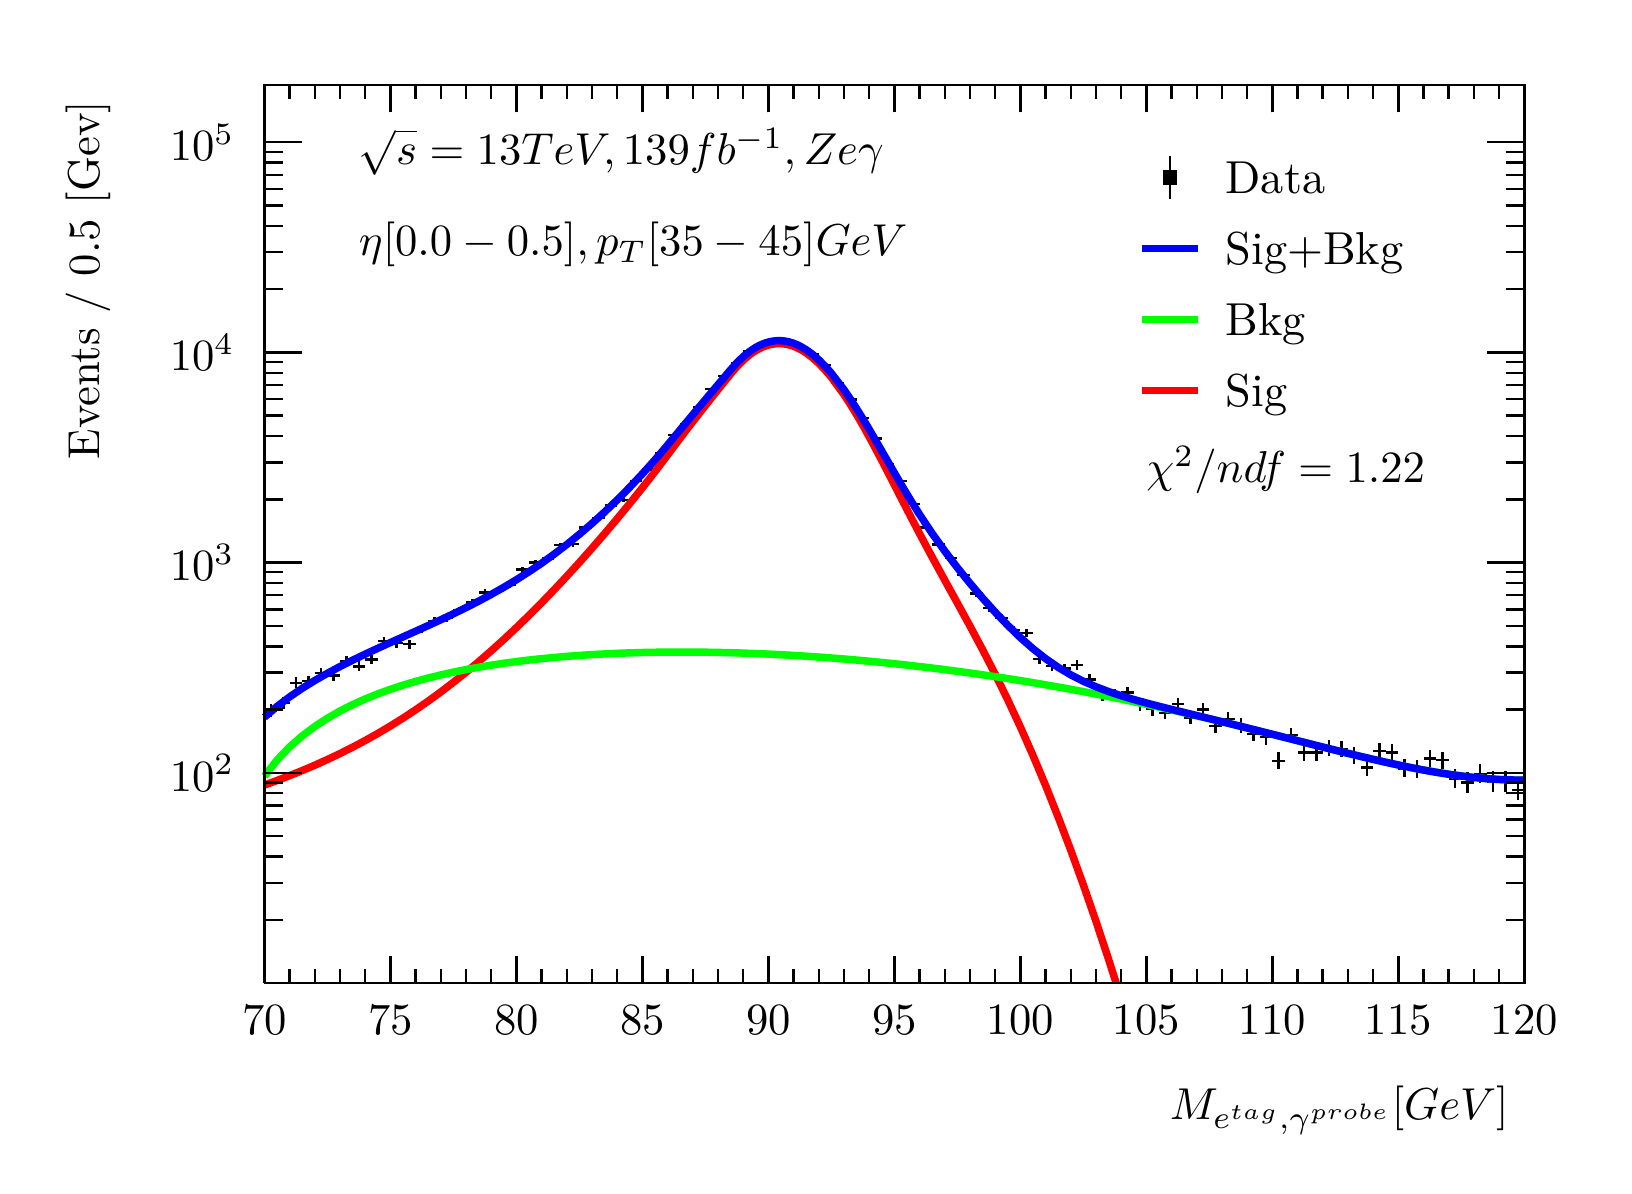
\begin{tikzpicture}
\pgfdeclareplotmark{cross} {
\pgfpathmoveto{\pgfpoint{-0.3\pgfplotmarksize}{\pgfplotmarksize}}
\pgfpathlineto{\pgfpoint{+0.3\pgfplotmarksize}{\pgfplotmarksize}}
\pgfpathlineto{\pgfpoint{+0.3\pgfplotmarksize}{0.3\pgfplotmarksize}}
\pgfpathlineto{\pgfpoint{+1\pgfplotmarksize}{0.3\pgfplotmarksize}}
\pgfpathlineto{\pgfpoint{+1\pgfplotmarksize}{-0.3\pgfplotmarksize}}
\pgfpathlineto{\pgfpoint{+0.3\pgfplotmarksize}{-0.3\pgfplotmarksize}}
\pgfpathlineto{\pgfpoint{+0.3\pgfplotmarksize}{-1.\pgfplotmarksize}}
\pgfpathlineto{\pgfpoint{-0.3\pgfplotmarksize}{-1.\pgfplotmarksize}}
\pgfpathlineto{\pgfpoint{-0.3\pgfplotmarksize}{-0.3\pgfplotmarksize}}
\pgfpathlineto{\pgfpoint{-1.\pgfplotmarksize}{-0.3\pgfplotmarksize}}
\pgfpathlineto{\pgfpoint{-1.\pgfplotmarksize}{0.3\pgfplotmarksize}}
\pgfpathlineto{\pgfpoint{-0.3\pgfplotmarksize}{0.3\pgfplotmarksize}}
\pgfpathclose
\pgfusepathqstroke
}
\pgfdeclareplotmark{cross*} {
\pgfpathmoveto{\pgfpoint{-0.3\pgfplotmarksize}{\pgfplotmarksize}}
\pgfpathlineto{\pgfpoint{+0.3\pgfplotmarksize}{\pgfplotmarksize}}
\pgfpathlineto{\pgfpoint{+0.3\pgfplotmarksize}{0.3\pgfplotmarksize}}
\pgfpathlineto{\pgfpoint{+1\pgfplotmarksize}{0.3\pgfplotmarksize}}
\pgfpathlineto{\pgfpoint{+1\pgfplotmarksize}{-0.3\pgfplotmarksize}}
\pgfpathlineto{\pgfpoint{+0.3\pgfplotmarksize}{-0.3\pgfplotmarksize}}
\pgfpathlineto{\pgfpoint{+0.3\pgfplotmarksize}{-1.\pgfplotmarksize}}
\pgfpathlineto{\pgfpoint{-0.3\pgfplotmarksize}{-1.\pgfplotmarksize}}
\pgfpathlineto{\pgfpoint{-0.3\pgfplotmarksize}{-0.3\pgfplotmarksize}}
\pgfpathlineto{\pgfpoint{-1.\pgfplotmarksize}{-0.3\pgfplotmarksize}}
\pgfpathlineto{\pgfpoint{-1.\pgfplotmarksize}{0.3\pgfplotmarksize}}
\pgfpathlineto{\pgfpoint{-0.3\pgfplotmarksize}{0.3\pgfplotmarksize}}
\pgfpathclose
\pgfusepathqfillstroke
}
\pgfdeclareplotmark{newstar} {
\pgfpathmoveto{\pgfqpoint{0pt}{\pgfplotmarksize}}
\pgfpathlineto{\pgfqpointpolar{44}{0.5\pgfplotmarksize}}
\pgfpathlineto{\pgfqpointpolar{18}{\pgfplotmarksize}}
\pgfpathlineto{\pgfqpointpolar{-20}{0.5\pgfplotmarksize}}
\pgfpathlineto{\pgfqpointpolar{-54}{\pgfplotmarksize}}
\pgfpathlineto{\pgfqpointpolar{-90}{0.5\pgfplotmarksize}}
\pgfpathlineto{\pgfqpointpolar{234}{\pgfplotmarksize}}
\pgfpathlineto{\pgfqpointpolar{198}{0.5\pgfplotmarksize}}
\pgfpathlineto{\pgfqpointpolar{162}{\pgfplotmarksize}}
\pgfpathlineto{\pgfqpointpolar{134}{0.5\pgfplotmarksize}}
\pgfpathclose
\pgfusepathqstroke
}
\pgfdeclareplotmark{newstar*} {
\pgfpathmoveto{\pgfqpoint{0pt}{\pgfplotmarksize}}
\pgfpathlineto{\pgfqpointpolar{44}{0.5\pgfplotmarksize}}
\pgfpathlineto{\pgfqpointpolar{18}{\pgfplotmarksize}}
\pgfpathlineto{\pgfqpointpolar{-20}{0.5\pgfplotmarksize}}
\pgfpathlineto{\pgfqpointpolar{-54}{\pgfplotmarksize}}
\pgfpathlineto{\pgfqpointpolar{-90}{0.5\pgfplotmarksize}}
\pgfpathlineto{\pgfqpointpolar{234}{\pgfplotmarksize}}
\pgfpathlineto{\pgfqpointpolar{198}{0.5\pgfplotmarksize}}
\pgfpathlineto{\pgfqpointpolar{162}{\pgfplotmarksize}}
\pgfpathlineto{\pgfqpointpolar{134}{0.5\pgfplotmarksize}}
\pgfpathclose
\pgfusepathqfillstroke
}
\definecolor{c}{rgb}{1,1,1};
\draw [color=c, fill=c] (0,0) rectangle (20,14.4361);
\draw [color=c, fill=c] (3,2.30977) rectangle (19,13.7143);
\definecolor{c}{rgb}{0,0,0};
\draw [c,line width=0.9] (3,2.30977) -- (3,13.7143) -- (19,13.7143) -- (19,2.30977) -- (3,2.30977);
\definecolor{c}{rgb}{1,1,1};
\draw [color=c, fill=c] (3,2.30977) rectangle (19,13.7143);
\definecolor{c}{rgb}{0,0,0};
\draw [c,line width=0.9] (3,2.30977) -- (3,13.7143) -- (19,13.7143) -- (19,2.30977) -- (3,2.30977);
\draw [c,line width=0.9] (3,2.30977) -- (19,2.30977);
\draw [c,line width=0.9] (3,2.65624) -- (3,2.30977);
\draw [c,line width=0.9] (3.32,2.48301) -- (3.32,2.30977);
\draw [c,line width=0.9] (3.64,2.48301) -- (3.64,2.30977);
\draw [c,line width=0.9] (3.96,2.48301) -- (3.96,2.30977);
\draw [c,line width=0.9] (4.28,2.48301) -- (4.28,2.30977);
\draw [c,line width=0.9] (4.6,2.65624) -- (4.6,2.30977);
\draw [c,line width=0.9] (4.92,2.48301) -- (4.92,2.30977);
\draw [c,line width=0.9] (5.24,2.48301) -- (5.24,2.30977);
\draw [c,line width=0.9] (5.56,2.48301) -- (5.56,2.30977);
\draw [c,line width=0.9] (5.88,2.48301) -- (5.88,2.30977);
\draw [c,line width=0.9] (6.2,2.65624) -- (6.2,2.30977);
\draw [c,line width=0.9] (6.52,2.48301) -- (6.52,2.30977);
\draw [c,line width=0.9] (6.84,2.48301) -- (6.84,2.30977);
\draw [c,line width=0.9] (7.16,2.48301) -- (7.16,2.30977);
\draw [c,line width=0.9] (7.48,2.48301) -- (7.48,2.30977);
\draw [c,line width=0.9] (7.8,2.65624) -- (7.8,2.30977);
\draw [c,line width=0.9] (8.12,2.48301) -- (8.12,2.30977);
\draw [c,line width=0.9] (8.44,2.48301) -- (8.44,2.30977);
\draw [c,line width=0.9] (8.76,2.48301) -- (8.76,2.30977);
\draw [c,line width=0.9] (9.08,2.48301) -- (9.08,2.30977);
\draw [c,line width=0.9] (9.4,2.65624) -- (9.4,2.30977);
\draw [c,line width=0.9] (9.72,2.48301) -- (9.72,2.30977);
\draw [c,line width=0.9] (10.04,2.48301) -- (10.04,2.30977);
\draw [c,line width=0.9] (10.36,2.48301) -- (10.36,2.30977);
\draw [c,line width=0.9] (10.68,2.48301) -- (10.68,2.30977);
\draw [c,line width=0.9] (11,2.65624) -- (11,2.30977);
\draw [c,line width=0.9] (11.32,2.48301) -- (11.32,2.30977);
\draw [c,line width=0.9] (11.64,2.48301) -- (11.64,2.30977);
\draw [c,line width=0.9] (11.96,2.48301) -- (11.96,2.30977);
\draw [c,line width=0.9] (12.28,2.48301) -- (12.28,2.30977);
\draw [c,line width=0.9] (12.6,2.65624) -- (12.6,2.30977);
\draw [c,line width=0.9] (12.92,2.48301) -- (12.92,2.30977);
\draw [c,line width=0.9] (13.24,2.48301) -- (13.24,2.30977);
\draw [c,line width=0.9] (13.56,2.48301) -- (13.56,2.30977);
\draw [c,line width=0.9] (13.88,2.48301) -- (13.88,2.30977);
\draw [c,line width=0.9] (14.2,2.65624) -- (14.2,2.30977);
\draw [c,line width=0.9] (14.52,2.48301) -- (14.52,2.30977);
\draw [c,line width=0.9] (14.84,2.48301) -- (14.84,2.30977);
\draw [c,line width=0.9] (15.16,2.48301) -- (15.16,2.30977);
\draw [c,line width=0.9] (15.48,2.48301) -- (15.48,2.30977);
\draw [c,line width=0.9] (15.8,2.65624) -- (15.8,2.30977);
\draw [c,line width=0.9] (16.12,2.48301) -- (16.12,2.30977);
\draw [c,line width=0.9] (16.44,2.48301) -- (16.44,2.30977);
\draw [c,line width=0.9] (16.76,2.48301) -- (16.76,2.30977);
\draw [c,line width=0.9] (17.08,2.48301) -- (17.08,2.30977);
\draw [c,line width=0.9] (17.4,2.65624) -- (17.4,2.30977);
\draw [c,line width=0.9] (17.72,2.48301) -- (17.72,2.30977);
\draw [c,line width=0.9] (18.04,2.48301) -- (18.04,2.30977);
\draw [c,line width=0.9] (18.36,2.48301) -- (18.36,2.30977);
\draw [c,line width=0.9] (18.68,2.48301) -- (18.68,2.30977);
\draw [c,line width=0.9] (19,2.65624) -- (19,2.30977);
\draw [anchor=base] (3,1.66015) node[scale=1.61424, color=c, rotate=0]{70};
\draw [anchor=base] (4.6,1.66015) node[scale=1.61424, color=c, rotate=0]{75};
\draw [anchor=base] (6.2,1.66015) node[scale=1.61424, color=c, rotate=0]{80};
\draw [anchor=base] (7.8,1.66015) node[scale=1.61424, color=c, rotate=0]{85};
\draw [anchor=base] (9.4,1.66015) node[scale=1.61424, color=c, rotate=0]{90};
\draw [anchor=base] (11,1.66015) node[scale=1.61424, color=c, rotate=0]{95};
\draw [anchor=base] (12.6,1.66015) node[scale=1.61424, color=c, rotate=0]{100};
\draw [anchor=base] (14.2,1.66015) node[scale=1.61424, color=c, rotate=0]{105};
\draw [anchor=base] (15.8,1.66015) node[scale=1.61424, color=c, rotate=0]{110};
\draw [anchor=base] (17.4,1.66015) node[scale=1.61424, color=c, rotate=0]{115};
\draw [anchor=base] (19,1.66015) node[scale=1.61424, color=c, rotate=0]{120};
\draw [anchor= east] (19,0.692932) node[scale=1.61424, color=c, rotate=0]{$M_{e^{tag}, \gamma^{probe}}  [GeV]$};
\draw [c,line width=0.9] (3,13.7143) -- (19,13.7143);
\draw [c,line width=0.9] (3,13.3678) -- (3,13.7143);
\draw [c,line width=0.9] (3.32,13.5411) -- (3.32,13.7143);
\draw [c,line width=0.9] (3.64,13.5411) -- (3.64,13.7143);
\draw [c,line width=0.9] (3.96,13.5411) -- (3.96,13.7143);
\draw [c,line width=0.9] (4.28,13.5411) -- (4.28,13.7143);
\draw [c,line width=0.9] (4.6,13.3678) -- (4.6,13.7143);
\draw [c,line width=0.9] (4.92,13.5411) -- (4.92,13.7143);
\draw [c,line width=0.9] (5.24,13.5411) -- (5.24,13.7143);
\draw [c,line width=0.9] (5.56,13.5411) -- (5.56,13.7143);
\draw [c,line width=0.9] (5.88,13.5411) -- (5.88,13.7143);
\draw [c,line width=0.9] (6.2,13.3678) -- (6.2,13.7143);
\draw [c,line width=0.9] (6.52,13.5411) -- (6.52,13.7143);
\draw [c,line width=0.9] (6.84,13.5411) -- (6.84,13.7143);
\draw [c,line width=0.9] (7.16,13.5411) -- (7.16,13.7143);
\draw [c,line width=0.9] (7.48,13.5411) -- (7.48,13.7143);
\draw [c,line width=0.9] (7.8,13.3678) -- (7.8,13.7143);
\draw [c,line width=0.9] (8.12,13.5411) -- (8.12,13.7143);
\draw [c,line width=0.9] (8.44,13.5411) -- (8.44,13.7143);
\draw [c,line width=0.9] (8.76,13.5411) -- (8.76,13.7143);
\draw [c,line width=0.9] (9.08,13.5411) -- (9.08,13.7143);
\draw [c,line width=0.9] (9.4,13.3678) -- (9.4,13.7143);
\draw [c,line width=0.9] (9.72,13.5411) -- (9.72,13.7143);
\draw [c,line width=0.9] (10.04,13.5411) -- (10.04,13.7143);
\draw [c,line width=0.9] (10.36,13.5411) -- (10.36,13.7143);
\draw [c,line width=0.9] (10.68,13.5411) -- (10.68,13.7143);
\draw [c,line width=0.9] (11,13.3678) -- (11,13.7143);
\draw [c,line width=0.9] (11.32,13.5411) -- (11.32,13.7143);
\draw [c,line width=0.9] (11.64,13.5411) -- (11.64,13.7143);
\draw [c,line width=0.9] (11.96,13.5411) -- (11.96,13.7143);
\draw [c,line width=0.9] (12.28,13.5411) -- (12.28,13.7143);
\draw [c,line width=0.9] (12.6,13.3678) -- (12.6,13.7143);
\draw [c,line width=0.9] (12.92,13.5411) -- (12.92,13.7143);
\draw [c,line width=0.9] (13.24,13.5411) -- (13.24,13.7143);
\draw [c,line width=0.9] (13.56,13.5411) -- (13.56,13.7143);
\draw [c,line width=0.9] (13.88,13.5411) -- (13.88,13.7143);
\draw [c,line width=0.9] (14.2,13.3678) -- (14.2,13.7143);
\draw [c,line width=0.9] (14.52,13.5411) -- (14.52,13.7143);
\draw [c,line width=0.9] (14.84,13.5411) -- (14.84,13.7143);
\draw [c,line width=0.9] (15.16,13.5411) -- (15.16,13.7143);
\draw [c,line width=0.9] (15.48,13.5411) -- (15.48,13.7143);
\draw [c,line width=0.9] (15.8,13.3678) -- (15.8,13.7143);
\draw [c,line width=0.9] (16.12,13.5411) -- (16.12,13.7143);
\draw [c,line width=0.9] (16.44,13.5411) -- (16.44,13.7143);
\draw [c,line width=0.9] (16.76,13.5411) -- (16.76,13.7143);
\draw [c,line width=0.9] (17.08,13.5411) -- (17.08,13.7143);
\draw [c,line width=0.9] (17.4,13.3678) -- (17.4,13.7143);
\draw [c,line width=0.9] (17.72,13.5411) -- (17.72,13.7143);
\draw [c,line width=0.9] (18.04,13.5411) -- (18.04,13.7143);
\draw [c,line width=0.9] (18.36,13.5411) -- (18.36,13.7143);
\draw [c,line width=0.9] (18.68,13.5411) -- (18.68,13.7143);
\draw [c,line width=0.9] (19,13.3678) -- (19,13.7143);
\draw [c,line width=0.9] (3,2.30977) -- (3,13.7143);
\draw [c,line width=0.9] (3.237,3.11343) -- (3,3.11343);
\draw [c,line width=0.9] (3.237,3.58354) -- (3,3.58354);
\draw [c,line width=0.9] (3.237,3.91709) -- (3,3.91709);
\draw [c,line width=0.9] (3.237,4.17581) -- (3,4.17581);
\draw [c,line width=0.9] (3.237,4.38719) -- (3,4.38719);
\draw [c,line width=0.9] (3.237,4.56592) -- (3,4.56592);
\draw [c,line width=0.9] (3.237,4.72074) -- (3,4.72074);
\draw [c,line width=0.9] (3.237,4.8573) -- (3,4.8573);
\draw [c,line width=0.9] (3.474,4.97946) -- (3,4.97946);
\draw [anchor= east] (2.82,4.97946) node[scale=1.61424, color=c, rotate=0]{$10^{2}$};
\draw [c,line width=0.9] (3.237,5.78312) -- (3,5.78312);
\draw [c,line width=0.9] (3.237,6.25323) -- (3,6.25323);
\draw [c,line width=0.9] (3.237,6.58678) -- (3,6.58678);
\draw [c,line width=0.9] (3.237,6.8455) -- (3,6.8455);
\draw [c,line width=0.9] (3.237,7.05689) -- (3,7.05689);
\draw [c,line width=0.9] (3.237,7.23561) -- (3,7.23561);
\draw [c,line width=0.9] (3.237,7.39043) -- (3,7.39043);
\draw [c,line width=0.9] (3.237,7.52699) -- (3,7.52699);
\draw [c,line width=0.9] (3.474,7.64915) -- (3,7.64915);
\draw [anchor= east] (2.82,7.64915) node[scale=1.61424, color=c, rotate=0]{$10^{3}$};
\draw [c,line width=0.9] (3.237,8.45281) -- (3,8.45281);
\draw [c,line width=0.9] (3.237,8.92292) -- (3,8.92292);
\draw [c,line width=0.9] (3.237,9.25647) -- (3,9.25647);
\draw [c,line width=0.9] (3.237,9.51519) -- (3,9.51519);
\draw [c,line width=0.9] (3.237,9.72658) -- (3,9.72658);
\draw [c,line width=0.9] (3.237,9.9053) -- (3,9.9053);
\draw [c,line width=0.9] (3.237,10.0601) -- (3,10.0601);
\draw [c,line width=0.9] (3.237,10.1967) -- (3,10.1967);
\draw [c,line width=0.9] (3.474,10.3188) -- (3,10.3188);
\draw [anchor= east] (2.82,10.3188) node[scale=1.61424, color=c, rotate=0]{$10^{4}$};
\draw [c,line width=0.9] (3.237,11.1225) -- (3,11.1225);
\draw [c,line width=0.9] (3.237,11.5926) -- (3,11.5926);
\draw [c,line width=0.9] (3.237,11.9262) -- (3,11.9262);
\draw [c,line width=0.9] (3.237,12.1849) -- (3,12.1849);
\draw [c,line width=0.9] (3.237,12.3963) -- (3,12.3963);
\draw [c,line width=0.9] (3.237,12.575) -- (3,12.575);
\draw [c,line width=0.9] (3.237,12.7298) -- (3,12.7298);
\draw [c,line width=0.9] (3.237,12.8664) -- (3,12.8664);
\draw [c,line width=0.9] (3.474,12.9885) -- (3,12.9885);
\draw [anchor= east] (2.82,12.9885) node[scale=1.61424, color=c, rotate=0]{$10^{5}$};
\draw [anchor= east] (0.76,13.7143) node[scale=1.61424, color=c, rotate=90]{Events / 0.5 [Gev]};
\draw [c,line width=0.9] (19,2.30977) -- (19,13.7143);
\draw [c,line width=0.9] (18.763,3.11343) -- (19,3.11343);
\draw [c,line width=0.9] (18.763,3.58354) -- (19,3.58354);
\draw [c,line width=0.9] (18.763,3.91709) -- (19,3.91709);
\draw [c,line width=0.9] (18.763,4.17581) -- (19,4.17581);
\draw [c,line width=0.9] (18.763,4.38719) -- (19,4.38719);
\draw [c,line width=0.9] (18.763,4.56592) -- (19,4.56592);
\draw [c,line width=0.9] (18.763,4.72074) -- (19,4.72074);
\draw [c,line width=0.9] (18.763,4.8573) -- (19,4.8573);
\draw [c,line width=0.9] (18.526,4.97946) -- (19,4.97946);
\draw [c,line width=0.9] (18.763,5.78312) -- (19,5.78312);
\draw [c,line width=0.9] (18.763,6.25323) -- (19,6.25323);
\draw [c,line width=0.9] (18.763,6.58678) -- (19,6.58678);
\draw [c,line width=0.9] (18.763,6.8455) -- (19,6.8455);
\draw [c,line width=0.9] (18.763,7.05689) -- (19,7.05689);
\draw [c,line width=0.9] (18.763,7.23561) -- (19,7.23561);
\draw [c,line width=0.9] (18.763,7.39043) -- (19,7.39043);
\draw [c,line width=0.9] (18.763,7.52699) -- (19,7.52699);
\draw [c,line width=0.9] (18.526,7.64915) -- (19,7.64915);
\draw [c,line width=0.9] (18.763,8.45281) -- (19,8.45281);
\draw [c,line width=0.9] (18.763,8.92292) -- (19,8.92292);
\draw [c,line width=0.9] (18.763,9.25647) -- (19,9.25647);
\draw [c,line width=0.9] (18.763,9.51519) -- (19,9.51519);
\draw [c,line width=0.9] (18.763,9.72658) -- (19,9.72658);
\draw [c,line width=0.9] (18.763,9.9053) -- (19,9.9053);
\draw [c,line width=0.9] (18.763,10.0601) -- (19,10.0601);
\draw [c,line width=0.9] (18.763,10.1967) -- (19,10.1967);
\draw [c,line width=0.9] (18.526,10.3188) -- (19,10.3188);
\draw [c,line width=0.9] (18.763,11.1225) -- (19,11.1225);
\draw [c,line width=0.9] (18.763,11.5926) -- (19,11.5926);
\draw [c,line width=0.9] (18.763,11.9262) -- (19,11.9262);
\draw [c,line width=0.9] (18.763,12.1849) -- (19,12.1849);
\draw [c,line width=0.9] (18.763,12.3963) -- (19,12.3963);
\draw [c,line width=0.9] (18.763,12.575) -- (19,12.575);
\draw [c,line width=0.9] (18.763,12.7298) -- (19,12.7298);
\draw [c,line width=0.9] (18.763,12.8664) -- (19,12.8664);
\draw [c,line width=0.9] (18.526,12.9885) -- (19,12.9885);
\draw [c,line width=0.9] (3.08,5.77147) -- (3,5.77147);
\draw [c,line width=0.9] (3,5.77147) -- (3,5.77147);
\draw [c,line width=0.9] (3.08,5.77147) -- (3.16,5.77147);
\draw [c,line width=0.9] (3.16,5.77147) -- (3.16,5.77147);
\draw [c,line width=0.9] (3.08,5.77147) -- (3.08,5.85385);
\draw [c,line width=0.9] (3.08,5.85385) -- (3.08,5.85385);
\draw [c,line width=0.9] (3.08,5.77147) -- (3.08,5.68909);
\draw [c,line width=0.9] (3.08,5.68909) -- (3.08,5.68909);
\draw [c,line width=0.9] (3.24,5.86697) -- (3.16,5.86697);
\draw [c,line width=0.9] (3.16,5.86697) -- (3.16,5.86697);
\draw [c,line width=0.9] (3.24,5.86697) -- (3.32,5.86697);
\draw [c,line width=0.9] (3.32,5.86697) -- (3.32,5.86697);
\draw [c,line width=0.9] (3.24,5.86697) -- (3.24,5.94603);
\draw [c,line width=0.9] (3.24,5.94603) -- (3.24,5.94603);
\draw [c,line width=0.9] (3.24,5.86697) -- (3.24,5.78791);
\draw [c,line width=0.9] (3.24,5.78791) -- (3.24,5.78791);
\draw [c,line width=0.9] (3.4,6.12245) -- (3.32,6.12245);
\draw [c,line width=0.9] (3.32,6.12245) -- (3.32,6.12245);
\draw [c,line width=0.9] (3.4,6.12245) -- (3.48,6.12245);
\draw [c,line width=0.9] (3.48,6.12245) -- (3.48,6.12245);
\draw [c,line width=0.9] (3.4,6.12245) -- (3.4,6.19326);
\draw [c,line width=0.9] (3.4,6.19326) -- (3.4,6.19326);
\draw [c,line width=0.9] (3.4,6.12245) -- (3.4,6.05164);
\draw [c,line width=0.9] (3.4,6.05164) -- (3.4,6.05164);
\draw [c,line width=0.9] (3.56,6.14388) -- (3.48,6.14388);
\draw [c,line width=0.9] (3.48,6.14388) -- (3.48,6.14388);
\draw [c,line width=0.9] (3.56,6.14388) -- (3.64,6.14388);
\draw [c,line width=0.9] (3.64,6.14388) -- (3.64,6.14388);
\draw [c,line width=0.9] (3.56,6.14388) -- (3.56,6.21404);
\draw [c,line width=0.9] (3.56,6.21404) -- (3.56,6.21404);
\draw [c,line width=0.9] (3.56,6.14388) -- (3.56,6.07372);
\draw [c,line width=0.9] (3.56,6.07372) -- (3.56,6.07372);
\draw [c,line width=0.9] (3.72,6.24547) -- (3.64,6.24547);
\draw [c,line width=0.9] (3.64,6.24547) -- (3.64,6.24547);
\draw [c,line width=0.9] (3.72,6.24547) -- (3.8,6.24547);
\draw [c,line width=0.9] (3.8,6.24547) -- (3.8,6.24547);
\draw [c,line width=0.9] (3.72,6.24547) -- (3.72,6.31263);
\draw [c,line width=0.9] (3.72,6.31263) -- (3.72,6.31263);
\draw [c,line width=0.9] (3.72,6.24547) -- (3.72,6.17832);
\draw [c,line width=0.9] (3.72,6.17832) -- (3.72,6.17832);
\draw [c,line width=0.9] (3.88,6.21392) -- (3.8,6.21392);
\draw [c,line width=0.9] (3.8,6.21392) -- (3.8,6.21392);
\draw [c,line width=0.9] (3.88,6.21392) -- (3.96,6.21392);
\draw [c,line width=0.9] (3.96,6.21392) -- (3.96,6.21392);
\draw [c,line width=0.9] (3.88,6.21392) -- (3.88,6.282);
\draw [c,line width=0.9] (3.88,6.282) -- (3.88,6.282);
\draw [c,line width=0.9] (3.88,6.21392) -- (3.88,6.14585);
\draw [c,line width=0.9] (3.88,6.14585) -- (3.88,6.14585);
\draw [c,line width=0.9] (4.04,6.39835) -- (3.96,6.39835);
\draw [c,line width=0.9] (3.96,6.39835) -- (3.96,6.39835);
\draw [c,line width=0.9] (4.04,6.39835) -- (4.12,6.39835);
\draw [c,line width=0.9] (4.12,6.39835) -- (4.12,6.39835);
\draw [c,line width=0.9] (4.04,6.39835) -- (4.04,6.46122);
\draw [c,line width=0.9] (4.04,6.46122) -- (4.04,6.46122);
\draw [c,line width=0.9] (4.04,6.39835) -- (4.04,6.33548);
\draw [c,line width=0.9] (4.04,6.33548) -- (4.04,6.33548);
\draw [c,line width=0.9] (4.2,6.33168) -- (4.12,6.33168);
\draw [c,line width=0.9] (4.12,6.33168) -- (4.12,6.33168);
\draw [c,line width=0.9] (4.2,6.33168) -- (4.28,6.33168);
\draw [c,line width=0.9] (4.28,6.33168) -- (4.28,6.33168);
\draw [c,line width=0.9] (4.2,6.33168) -- (4.2,6.39638);
\draw [c,line width=0.9] (4.2,6.39638) -- (4.2,6.39638);
\draw [c,line width=0.9] (4.2,6.33168) -- (4.2,6.26697);
\draw [c,line width=0.9] (4.2,6.26697) -- (4.2,6.26697);
\draw [c,line width=0.9] (4.36,6.41863) -- (4.28,6.41863);
\draw [c,line width=0.9] (4.28,6.41863) -- (4.28,6.41863);
\draw [c,line width=0.9] (4.36,6.41863) -- (4.44,6.41863);
\draw [c,line width=0.9] (4.44,6.41863) -- (4.44,6.41863);
\draw [c,line width=0.9] (4.36,6.41863) -- (4.36,6.48095);
\draw [c,line width=0.9] (4.36,6.48095) -- (4.36,6.48095);
\draw [c,line width=0.9] (4.36,6.41863) -- (4.36,6.35631);
\draw [c,line width=0.9] (4.36,6.35631) -- (4.36,6.35631);
\draw [c,line width=0.9] (4.52,6.6516) -- (4.44,6.6516);
\draw [c,line width=0.9] (4.44,6.6516) -- (4.44,6.6516);
\draw [c,line width=0.9] (4.52,6.6516) -- (4.6,6.6516);
\draw [c,line width=0.9] (4.6,6.6516) -- (4.6,6.6516);
\draw [c,line width=0.9] (4.52,6.6516) -- (4.52,6.70797);
\draw [c,line width=0.9] (4.52,6.70797) -- (4.52,6.70797);
\draw [c,line width=0.9] (4.52,6.6516) -- (4.52,6.59523);
\draw [c,line width=0.9] (4.52,6.59523) -- (4.52,6.59523);
\draw [c,line width=0.9] (4.68,6.62666) -- (4.6,6.62666);
\draw [c,line width=0.9] (4.6,6.62666) -- (4.6,6.62666);
\draw [c,line width=0.9] (4.68,6.62666) -- (4.76,6.62666);
\draw [c,line width=0.9] (4.76,6.62666) -- (4.76,6.62666);
\draw [c,line width=0.9] (4.68,6.62666) -- (4.68,6.68364);
\draw [c,line width=0.9] (4.68,6.68364) -- (4.68,6.68364);
\draw [c,line width=0.9] (4.68,6.62666) -- (4.68,6.56969);
\draw [c,line width=0.9] (4.68,6.56969) -- (4.68,6.56969);
\draw [c,line width=0.9] (4.84,6.61258) -- (4.76,6.61258);
\draw [c,line width=0.9] (4.76,6.61258) -- (4.76,6.61258);
\draw [c,line width=0.9] (4.84,6.61258) -- (4.92,6.61258);
\draw [c,line width=0.9] (4.92,6.61258) -- (4.92,6.61258);
\draw [c,line width=0.9] (4.84,6.61258) -- (4.84,6.6699);
\draw [c,line width=0.9] (4.84,6.6699) -- (4.84,6.6699);
\draw [c,line width=0.9] (4.84,6.61258) -- (4.84,6.55525);
\draw [c,line width=0.9] (4.84,6.55525) -- (4.84,6.55525);
\draw [c,line width=0.9] (5,6.80779) -- (4.92,6.80779);
\draw [c,line width=0.9] (4.92,6.80779) -- (4.92,6.80779);
\draw [c,line width=0.9] (5,6.80779) -- (5.08,6.80779);
\draw [c,line width=0.9] (5.08,6.80779) -- (5.08,6.80779);
\draw [c,line width=0.9] (5,6.80779) -- (5,6.86049);
\draw [c,line width=0.9] (5,6.86049) -- (5,6.86049);
\draw [c,line width=0.9] (5,6.80779) -- (5,6.75509);
\draw [c,line width=0.9] (5,6.75509) -- (5,6.75509);
\draw [c,line width=0.9] (5.16,6.90207) -- (5.08,6.90207);
\draw [c,line width=0.9] (5.08,6.90207) -- (5.08,6.90207);
\draw [c,line width=0.9] (5.16,6.90207) -- (5.24,6.90207);
\draw [c,line width=0.9] (5.24,6.90207) -- (5.24,6.90207);
\draw [c,line width=0.9] (5.16,6.90207) -- (5.16,6.95266);
\draw [c,line width=0.9] (5.16,6.95266) -- (5.16,6.95266);
\draw [c,line width=0.9] (5.16,6.90207) -- (5.16,6.85147);
\draw [c,line width=0.9] (5.16,6.85147) -- (5.16,6.85147);
\draw [c,line width=0.9] (5.32,6.94754) -- (5.24,6.94754);
\draw [c,line width=0.9] (5.24,6.94754) -- (5.24,6.94754);
\draw [c,line width=0.9] (5.32,6.94754) -- (5.4,6.94754);
\draw [c,line width=0.9] (5.4,6.94754) -- (5.4,6.94754);
\draw [c,line width=0.9] (5.32,6.94754) -- (5.32,6.99716);
\draw [c,line width=0.9] (5.32,6.99716) -- (5.32,6.99716);
\draw [c,line width=0.9] (5.32,6.94754) -- (5.32,6.89792);
\draw [c,line width=0.9] (5.32,6.89792) -- (5.32,6.89792);
\draw [c,line width=0.9] (5.48,7.03936) -- (5.4,7.03936);
\draw [c,line width=0.9] (5.4,7.03936) -- (5.4,7.03936);
\draw [c,line width=0.9] (5.48,7.03936) -- (5.56,7.03936);
\draw [c,line width=0.9] (5.56,7.03936) -- (5.56,7.03936);
\draw [c,line width=0.9] (5.48,7.03936) -- (5.48,7.08705);
\draw [c,line width=0.9] (5.48,7.08705) -- (5.48,7.08705);
\draw [c,line width=0.9] (5.48,7.03936) -- (5.48,6.99167);
\draw [c,line width=0.9] (5.48,6.99167) -- (5.48,6.99167);
\draw [c,line width=0.9] (5.64,7.14074) -- (5.56,7.14074);
\draw [c,line width=0.9] (5.56,7.14074) -- (5.56,7.14074);
\draw [c,line width=0.9] (5.64,7.14074) -- (5.72,7.14074);
\draw [c,line width=0.9] (5.72,7.14074) -- (5.72,7.14074);
\draw [c,line width=0.9] (5.64,7.14074) -- (5.64,7.18639);
\draw [c,line width=0.9] (5.64,7.18639) -- (5.64,7.18639);
\draw [c,line width=0.9] (5.64,7.14074) -- (5.64,7.09509);
\draw [c,line width=0.9] (5.64,7.09509) -- (5.64,7.09509);
\draw [c,line width=0.9] (5.8,7.26666) -- (5.72,7.26666);
\draw [c,line width=0.9] (5.72,7.26666) -- (5.72,7.26666);
\draw [c,line width=0.9] (5.8,7.26666) -- (5.88,7.26666);
\draw [c,line width=0.9] (5.88,7.26666) -- (5.88,7.26666);
\draw [c,line width=0.9] (5.8,7.26666) -- (5.8,7.3099);
\draw [c,line width=0.9] (5.8,7.3099) -- (5.8,7.3099);
\draw [c,line width=0.9] (5.8,7.26666) -- (5.8,7.22343);
\draw [c,line width=0.9] (5.8,7.22343) -- (5.8,7.22343);
\draw [c,line width=0.9] (5.96,7.28902) -- (5.88,7.28902);
\draw [c,line width=0.9] (5.88,7.28902) -- (5.88,7.28902);
\draw [c,line width=0.9] (5.96,7.28902) -- (6.04,7.28902);
\draw [c,line width=0.9] (6.04,7.28902) -- (6.04,7.28902);
\draw [c,line width=0.9] (5.96,7.28902) -- (5.96,7.33185);
\draw [c,line width=0.9] (5.96,7.33185) -- (5.96,7.33185);
\draw [c,line width=0.9] (5.96,7.28902) -- (5.96,7.2462);
\draw [c,line width=0.9] (5.96,7.2462) -- (5.96,7.2462);
\draw [c,line width=0.9] (6.12,7.36553) -- (6.04,7.36553);
\draw [c,line width=0.9] (6.04,7.36553) -- (6.04,7.36553);
\draw [c,line width=0.9] (6.12,7.36553) -- (6.2,7.36553);
\draw [c,line width=0.9] (6.2,7.36553) -- (6.2,7.36553);
\draw [c,line width=0.9] (6.12,7.36553) -- (6.12,7.40696);
\draw [c,line width=0.9] (6.12,7.40696) -- (6.12,7.40696);
\draw [c,line width=0.9] (6.12,7.36553) -- (6.12,7.3241);
\draw [c,line width=0.9] (6.12,7.3241) -- (6.12,7.3241);
\draw [c,line width=0.9] (6.28,7.55876) -- (6.2,7.55876);
\draw [c,line width=0.9] (6.2,7.55876) -- (6.2,7.55876);
\draw [c,line width=0.9] (6.28,7.55876) -- (6.36,7.55876);
\draw [c,line width=0.9] (6.36,7.55876) -- (6.36,7.55876);
\draw [c,line width=0.9] (6.28,7.55876) -- (6.28,7.59688);
\draw [c,line width=0.9] (6.28,7.59688) -- (6.28,7.59688);
\draw [c,line width=0.9] (6.28,7.55876) -- (6.28,7.52064);
\draw [c,line width=0.9] (6.28,7.52064) -- (6.28,7.52064);
\draw [c,line width=0.9] (6.44,7.65031) -- (6.36,7.65031);
\draw [c,line width=0.9] (6.36,7.65031) -- (6.36,7.65031);
\draw [c,line width=0.9] (6.44,7.65031) -- (6.52,7.65031);
\draw [c,line width=0.9] (6.52,7.65031) -- (6.52,7.65031);
\draw [c,line width=0.9] (6.44,7.65031) -- (6.44,7.68696);
\draw [c,line width=0.9] (6.44,7.68696) -- (6.44,7.68696);
\draw [c,line width=0.9] (6.44,7.65031) -- (6.44,7.61367);
\draw [c,line width=0.9] (6.44,7.61367) -- (6.44,7.61367);
\draw [c,line width=0.9] (6.6,7.69908) -- (6.52,7.69908);
\draw [c,line width=0.9] (6.52,7.69908) -- (6.52,7.69908);
\draw [c,line width=0.9] (6.6,7.69908) -- (6.68,7.69908);
\draw [c,line width=0.9] (6.68,7.69908) -- (6.68,7.69908);
\draw [c,line width=0.9] (6.6,7.69908) -- (6.6,7.73496);
\draw [c,line width=0.9] (6.6,7.73496) -- (6.6,7.73496);
\draw [c,line width=0.9] (6.6,7.69908) -- (6.6,7.6632);
\draw [c,line width=0.9] (6.6,7.6632) -- (6.6,7.6632);
\draw [c,line width=0.9] (6.76,7.87112) -- (6.68,7.87112);
\draw [c,line width=0.9] (6.68,7.87112) -- (6.68,7.87112);
\draw [c,line width=0.9] (6.76,7.87112) -- (6.84,7.87112);
\draw [c,line width=0.9] (6.84,7.87112) -- (6.84,7.87112);
\draw [c,line width=0.9] (6.76,7.87112) -- (6.76,7.90444);
\draw [c,line width=0.9] (6.76,7.90444) -- (6.76,7.90444);
\draw [c,line width=0.9] (6.76,7.87112) -- (6.76,7.83781);
\draw [c,line width=0.9] (6.76,7.83781) -- (6.76,7.83781);
\draw [c,line width=0.9] (6.92,7.8854) -- (6.84,7.8854);
\draw [c,line width=0.9] (6.84,7.8854) -- (6.84,7.8854);
\draw [c,line width=0.9] (6.92,7.8854) -- (7,7.8854);
\draw [c,line width=0.9] (7,7.8854) -- (7,7.8854);
\draw [c,line width=0.9] (6.92,7.8854) -- (6.92,7.91851);
\draw [c,line width=0.9] (6.92,7.91851) -- (6.92,7.91851);
\draw [c,line width=0.9] (6.92,7.8854) -- (6.92,7.85228);
\draw [c,line width=0.9] (6.92,7.85228) -- (6.92,7.85228);
\draw [c,line width=0.9] (7.08,8.09426) -- (7,8.09426);
\draw [c,line width=0.9] (7,8.09426) -- (7,8.09426);
\draw [c,line width=0.9] (7.08,8.09426) -- (7.16,8.09426);
\draw [c,line width=0.9] (7.16,8.09426) -- (7.16,8.09426);
\draw [c,line width=0.9] (7.08,8.09426) -- (7.08,8.12452);
\draw [c,line width=0.9] (7.08,8.12452) -- (7.08,8.12452);
\draw [c,line width=0.9] (7.08,8.09426) -- (7.08,8.064);
\draw [c,line width=0.9] (7.08,8.064) -- (7.08,8.064);
\draw [c,line width=0.9] (7.24,8.21705) -- (7.16,8.21705);
\draw [c,line width=0.9] (7.16,8.21705) -- (7.16,8.21705);
\draw [c,line width=0.9] (7.24,8.21705) -- (7.32,8.21705);
\draw [c,line width=0.9] (7.32,8.21705) -- (7.32,8.21705);
\draw [c,line width=0.9] (7.24,8.21705) -- (7.24,8.24575);
\draw [c,line width=0.9] (7.24,8.24575) -- (7.24,8.24575);
\draw [c,line width=0.9] (7.24,8.21705) -- (7.24,8.18835);
\draw [c,line width=0.9] (7.24,8.18835) -- (7.24,8.18835);
\draw [c,line width=0.9] (7.4,8.37365) -- (7.32,8.37365);
\draw [c,line width=0.9] (7.32,8.37365) -- (7.32,8.37365);
\draw [c,line width=0.9] (7.4,8.37365) -- (7.48,8.37365);
\draw [c,line width=0.9] (7.48,8.37365) -- (7.48,8.37365);
\draw [c,line width=0.9] (7.4,8.37365) -- (7.4,8.40047);
\draw [c,line width=0.9] (7.4,8.40047) -- (7.4,8.40047);
\draw [c,line width=0.9] (7.4,8.37365) -- (7.4,8.34682);
\draw [c,line width=0.9] (7.4,8.34682) -- (7.4,8.34682);
\draw [c,line width=0.9] (7.56,8.44233) -- (7.48,8.44233);
\draw [c,line width=0.9] (7.48,8.44233) -- (7.48,8.44233);
\draw [c,line width=0.9] (7.56,8.44233) -- (7.64,8.44233);
\draw [c,line width=0.9] (7.64,8.44233) -- (7.64,8.44233);
\draw [c,line width=0.9] (7.56,8.44233) -- (7.56,8.46837);
\draw [c,line width=0.9] (7.56,8.46837) -- (7.56,8.46837);
\draw [c,line width=0.9] (7.56,8.44233) -- (7.56,8.41629);
\draw [c,line width=0.9] (7.56,8.41629) -- (7.56,8.41629);
\draw [c,line width=0.9] (7.72,8.68526) -- (7.64,8.68526);
\draw [c,line width=0.9] (7.64,8.68526) -- (7.64,8.68526);
\draw [c,line width=0.9] (7.72,8.68526) -- (7.8,8.68526);
\draw [c,line width=0.9] (7.8,8.68526) -- (7.8,8.68526);
\draw [c,line width=0.9] (7.72,8.68526) -- (7.72,8.70872);
\draw [c,line width=0.9] (7.72,8.70872) -- (7.72,8.70872);
\draw [c,line width=0.9] (7.72,8.68526) -- (7.72,8.66181);
\draw [c,line width=0.9] (7.72,8.66181) -- (7.72,8.66181);
\draw [c,line width=0.9] (7.88,8.83336) -- (7.8,8.83336);
\draw [c,line width=0.9] (7.8,8.83336) -- (7.8,8.83336);
\draw [c,line width=0.9] (7.88,8.83336) -- (7.96,8.83336);
\draw [c,line width=0.9] (7.96,8.83336) -- (7.96,8.83336);
\draw [c,line width=0.9] (7.88,8.83336) -- (7.88,8.85537);
\draw [c,line width=0.9] (7.88,8.85537) -- (7.88,8.85537);
\draw [c,line width=0.9] (7.88,8.83336) -- (7.88,8.81136);
\draw [c,line width=0.9] (7.88,8.81136) -- (7.88,8.81136);
\draw [c,line width=0.9] (8.04,9.03763) -- (7.96,9.03763);
\draw [c,line width=0.9] (7.96,9.03763) -- (7.96,9.03763);
\draw [c,line width=0.9] (8.04,9.03763) -- (8.12,9.03763);
\draw [c,line width=0.9] (8.12,9.03763) -- (8.12,9.03763);
\draw [c,line width=0.9] (8.04,9.03763) -- (8.04,9.05778);
\draw [c,line width=0.9] (8.04,9.05778) -- (8.04,9.05778);
\draw [c,line width=0.9] (8.04,9.03763) -- (8.04,9.01749);
\draw [c,line width=0.9] (8.04,9.01749) -- (8.04,9.01749);
\draw [c,line width=0.9] (8.2,9.26858) -- (8.12,9.26858);
\draw [c,line width=0.9] (8.12,9.26858) -- (8.12,9.26858);
\draw [c,line width=0.9] (8.2,9.26858) -- (8.28,9.26858);
\draw [c,line width=0.9] (8.28,9.26858) -- (8.28,9.26858);
\draw [c,line width=0.9] (8.2,9.26858) -- (8.2,9.28681);
\draw [c,line width=0.9] (8.2,9.28681) -- (8.2,9.28681);
\draw [c,line width=0.9] (8.2,9.26858) -- (8.2,9.25034);
\draw [c,line width=0.9] (8.2,9.25034) -- (8.2,9.25034);
\draw [c,line width=0.9] (8.36,9.41093) -- (8.28,9.41093);
\draw [c,line width=0.9] (8.28,9.41093) -- (8.28,9.41093);
\draw [c,line width=0.9] (8.36,9.41093) -- (8.44,9.41093);
\draw [c,line width=0.9] (8.44,9.41093) -- (8.44,9.41093);
\draw [c,line width=0.9] (8.36,9.41093) -- (8.36,9.42808);
\draw [c,line width=0.9] (8.36,9.42808) -- (8.36,9.42808);
\draw [c,line width=0.9] (8.36,9.41093) -- (8.36,9.39377);
\draw [c,line width=0.9] (8.36,9.39377) -- (8.36,9.39377);
\draw [c,line width=0.9] (8.52,9.62801) -- (8.44,9.62801);
\draw [c,line width=0.9] (8.44,9.62801) -- (8.44,9.62801);
\draw [c,line width=0.9] (8.52,9.62801) -- (8.6,9.62801);
\draw [c,line width=0.9] (8.6,9.62801) -- (8.6,9.62801);
\draw [c,line width=0.9] (8.52,9.62801) -- (8.52,9.64363);
\draw [c,line width=0.9] (8.52,9.64363) -- (8.52,9.64363);
\draw [c,line width=0.9] (8.52,9.62801) -- (8.52,9.61239);
\draw [c,line width=0.9] (8.52,9.61239) -- (8.52,9.61239);
\draw [c,line width=0.9] (8.68,9.85105) -- (8.6,9.85105);
\draw [c,line width=0.9] (8.6,9.85105) -- (8.6,9.85105);
\draw [c,line width=0.9] (8.68,9.85105) -- (8.76,9.85105);
\draw [c,line width=0.9] (8.76,9.85105) -- (8.76,9.85105);
\draw [c,line width=0.9] (8.68,9.85105) -- (8.68,9.86524);
\draw [c,line width=0.9] (8.68,9.86524) -- (8.68,9.86524);
\draw [c,line width=0.9] (8.68,9.85105) -- (8.68,9.83687);
\draw [c,line width=0.9] (8.68,9.83687) -- (8.68,9.83687);
\draw [c,line width=0.9] (8.84,10.0176) -- (8.76,10.0176);
\draw [c,line width=0.9] (8.76,10.0176) -- (8.76,10.0176);
\draw [c,line width=0.9] (8.84,10.0176) -- (8.92,10.0176);
\draw [c,line width=0.9] (8.92,10.0176) -- (8.92,10.0176);
\draw [c,line width=0.9] (8.84,10.0176) -- (8.84,10.0308);
\draw [c,line width=0.9] (8.84,10.0308) -- (8.84,10.0308);
\draw [c,line width=0.9] (8.84,10.0176) -- (8.84,10.0044);
\draw [c,line width=0.9] (8.84,10.0044) -- (8.84,10.0044);
\draw [c,line width=0.9] (9,10.1863) -- (8.92,10.1863);
\draw [c,line width=0.9] (8.92,10.1863) -- (8.92,10.1863);
\draw [c,line width=0.9] (9,10.1863) -- (9.08,10.1863);
\draw [c,line width=0.9] (9.08,10.1863) -- (9.08,10.1863);
\draw [c,line width=0.9] (9,10.1863) -- (9,10.1986);
\draw [c,line width=0.9] (9,10.1986) -- (9,10.1986);
\draw [c,line width=0.9] (9,10.1863) -- (9,10.1741);
\draw [c,line width=0.9] (9,10.1741) -- (9,10.1741);
\draw [c,line width=0.9] (9.16,10.3322) -- (9.08,10.3322);
\draw [c,line width=0.9] (9.08,10.3322) -- (9.08,10.3322);
\draw [c,line width=0.9] (9.16,10.3322) -- (9.24,10.3322);
\draw [c,line width=0.9] (9.24,10.3322) -- (9.24,10.3322);
\draw [c,line width=0.9] (9.16,10.3322) -- (9.16,10.3437);
\draw [c,line width=0.9] (9.16,10.3437) -- (9.16,10.3437);
\draw [c,line width=0.9] (9.16,10.3322) -- (9.16,10.3207);
\draw [c,line width=0.9] (9.16,10.3207) -- (9.16,10.3207);
\draw [c,line width=0.9] (9.32,10.4103) -- (9.24,10.4103);
\draw [c,line width=0.9] (9.24,10.4103) -- (9.24,10.4103);
\draw [c,line width=0.9] (9.32,10.4103) -- (9.4,10.4103);
\draw [c,line width=0.9] (9.4,10.4103) -- (9.4,10.4103);
\draw [c,line width=0.9] (9.32,10.4103) -- (9.32,10.4215);
\draw [c,line width=0.9] (9.32,10.4215) -- (9.32,10.4215);
\draw [c,line width=0.9] (9.32,10.4103) -- (9.32,10.3992);
\draw [c,line width=0.9] (9.32,10.3992) -- (9.32,10.3992);
\draw [c,line width=0.9] (9.48,10.4655) -- (9.4,10.4655);
\draw [c,line width=0.9] (9.4,10.4655) -- (9.4,10.4655);
\draw [c,line width=0.9] (9.48,10.4655) -- (9.56,10.4655);
\draw [c,line width=0.9] (9.56,10.4655) -- (9.56,10.4655);
\draw [c,line width=0.9] (9.48,10.4655) -- (9.48,10.4763);
\draw [c,line width=0.9] (9.48,10.4763) -- (9.48,10.4763);
\draw [c,line width=0.9] (9.48,10.4655) -- (9.48,10.4546);
\draw [c,line width=0.9] (9.48,10.4546) -- (9.48,10.4546);
\draw [c,line width=0.9] (9.64,10.4522) -- (9.56,10.4522);
\draw [c,line width=0.9] (9.56,10.4522) -- (9.56,10.4522);
\draw [c,line width=0.9] (9.64,10.4522) -- (9.72,10.4522);
\draw [c,line width=0.9] (9.72,10.4522) -- (9.72,10.4522);
\draw [c,line width=0.9] (9.64,10.4522) -- (9.64,10.4632);
\draw [c,line width=0.9] (9.64,10.4632) -- (9.64,10.4632);
\draw [c,line width=0.9] (9.64,10.4522) -- (9.64,10.4413);
\draw [c,line width=0.9] (9.64,10.4413) -- (9.64,10.4413);
\draw [c,line width=0.9] (9.8,10.3965) -- (9.72,10.3965);
\draw [c,line width=0.9] (9.72,10.3965) -- (9.72,10.3965);
\draw [c,line width=0.9] (9.8,10.3965) -- (9.88,10.3965);
\draw [c,line width=0.9] (9.88,10.3965) -- (9.88,10.3965);
\draw [c,line width=0.9] (9.8,10.3965) -- (9.8,10.4077);
\draw [c,line width=0.9] (9.8,10.4077) -- (9.8,10.4077);
\draw [c,line width=0.9] (9.8,10.3965) -- (9.8,10.3853);
\draw [c,line width=0.9] (9.8,10.3853) -- (9.8,10.3853);
\draw [c,line width=0.9] (9.96,10.2945) -- (9.88,10.2945);
\draw [c,line width=0.9] (9.88,10.2945) -- (9.88,10.2945);
\draw [c,line width=0.9] (9.96,10.2945) -- (10.04,10.2945);
\draw [c,line width=0.9] (10.04,10.2945) -- (10.04,10.2945);
\draw [c,line width=0.9] (9.96,10.2945) -- (9.96,10.3062);
\draw [c,line width=0.9] (9.96,10.3062) -- (9.96,10.3062);
\draw [c,line width=0.9] (9.96,10.2945) -- (9.96,10.2828);
\draw [c,line width=0.9] (9.96,10.2828) -- (9.96,10.2828);
\draw [c,line width=0.9] (10.12,10.1619) -- (10.04,10.1619);
\draw [c,line width=0.9] (10.04,10.1619) -- (10.04,10.1619);
\draw [c,line width=0.9] (10.12,10.1619) -- (10.2,10.1619);
\draw [c,line width=0.9] (10.2,10.1619) -- (10.2,10.1619);
\draw [c,line width=0.9] (10.12,10.1619) -- (10.12,10.1743);
\draw [c,line width=0.9] (10.12,10.1743) -- (10.12,10.1743);
\draw [c,line width=0.9] (10.12,10.1619) -- (10.12,10.1495);
\draw [c,line width=0.9] (10.12,10.1495) -- (10.12,10.1495);
\draw [c,line width=0.9] (10.28,9.9328) -- (10.2,9.9328);
\draw [c,line width=0.9] (10.2,9.9328) -- (10.2,9.9328);
\draw [c,line width=0.9] (10.28,9.9328) -- (10.36,9.9328);
\draw [c,line width=0.9] (10.36,9.9328) -- (10.36,9.9328);
\draw [c,line width=0.9] (10.28,9.9328) -- (10.28,9.9465);
\draw [c,line width=0.9] (10.28,9.9465) -- (10.28,9.9465);
\draw [c,line width=0.9] (10.28,9.9328) -- (10.28,9.91911);
\draw [c,line width=0.9] (10.28,9.91911) -- (10.28,9.91911);
\draw [c,line width=0.9] (10.44,9.71979) -- (10.36,9.71979);
\draw [c,line width=0.9] (10.36,9.71979) -- (10.36,9.71979);
\draw [c,line width=0.9] (10.44,9.71979) -- (10.52,9.71979);
\draw [c,line width=0.9] (10.52,9.71979) -- (10.52,9.71979);
\draw [c,line width=0.9] (10.44,9.71979) -- (10.44,9.73481);
\draw [c,line width=0.9] (10.44,9.73481) -- (10.44,9.73481);
\draw [c,line width=0.9] (10.44,9.71979) -- (10.44,9.70478);
\draw [c,line width=0.9] (10.44,9.70478) -- (10.44,9.70478);
\draw [c,line width=0.9] (10.6,9.48868) -- (10.52,9.48868);
\draw [c,line width=0.9] (10.52,9.48868) -- (10.52,9.48868);
\draw [c,line width=0.9] (10.6,9.48868) -- (10.68,9.48868);
\draw [c,line width=0.9] (10.68,9.48868) -- (10.68,9.48868);
\draw [c,line width=0.9] (10.6,9.48868) -- (10.6,9.50527);
\draw [c,line width=0.9] (10.6,9.50527) -- (10.6,9.50527);
\draw [c,line width=0.9] (10.6,9.48868) -- (10.6,9.4721);
\draw [c,line width=0.9] (10.6,9.4721) -- (10.6,9.4721);
\draw [c,line width=0.9] (10.76,9.2283) -- (10.68,9.2283);
\draw [c,line width=0.9] (10.68,9.2283) -- (10.68,9.2283);
\draw [c,line width=0.9] (10.76,9.2283) -- (10.84,9.2283);
\draw [c,line width=0.9] (10.84,9.2283) -- (10.84,9.2283);
\draw [c,line width=0.9] (10.76,9.2283) -- (10.76,9.24686);
\draw [c,line width=0.9] (10.76,9.24686) -- (10.76,9.24686);
\draw [c,line width=0.9] (10.76,9.2283) -- (10.76,9.20975);
\draw [c,line width=0.9] (10.76,9.20975) -- (10.76,9.20975);
\draw [c,line width=0.9] (10.92,8.8995) -- (10.84,8.8995);
\draw [c,line width=0.9] (10.84,8.8995) -- (10.84,8.8995);
\draw [c,line width=0.9] (10.92,8.8995) -- (11,8.8995);
\draw [c,line width=0.9] (11,8.8995) -- (11,8.8995);
\draw [c,line width=0.9] (10.92,8.8995) -- (10.92,8.92088);
\draw [c,line width=0.9] (10.92,8.92088) -- (10.92,8.92088);
\draw [c,line width=0.9] (10.92,8.8995) -- (10.92,8.87811);
\draw [c,line width=0.9] (10.92,8.87811) -- (10.92,8.87811);
\draw [c,line width=0.9] (11.08,8.68716) -- (11,8.68716);
\draw [c,line width=0.9] (11,8.68716) -- (11,8.68716);
\draw [c,line width=0.9] (11.08,8.68716) -- (11.16,8.68716);
\draw [c,line width=0.9] (11.16,8.68716) -- (11.16,8.68716);
\draw [c,line width=0.9] (11.08,8.68716) -- (11.08,8.71059);
\draw [c,line width=0.9] (11.08,8.71059) -- (11.08,8.71059);
\draw [c,line width=0.9] (11.08,8.68716) -- (11.08,8.66373);
\draw [c,line width=0.9] (11.08,8.66373) -- (11.08,8.66373);
\draw [c,line width=0.9] (11.24,8.3909) -- (11.16,8.3909);
\draw [c,line width=0.9] (11.16,8.3909) -- (11.16,8.3909);
\draw [c,line width=0.9] (11.24,8.3909) -- (11.32,8.3909);
\draw [c,line width=0.9] (11.32,8.3909) -- (11.32,8.3909);
\draw [c,line width=0.9] (11.24,8.3909) -- (11.24,8.41752);
\draw [c,line width=0.9] (11.24,8.41752) -- (11.24,8.41752);
\draw [c,line width=0.9] (11.24,8.3909) -- (11.24,8.36427);
\draw [c,line width=0.9] (11.24,8.36427) -- (11.24,8.36427);
\draw [c,line width=0.9] (11.4,8.09426) -- (11.32,8.09426);
\draw [c,line width=0.9] (11.32,8.09426) -- (11.32,8.09426);
\draw [c,line width=0.9] (11.4,8.09426) -- (11.48,8.09426);
\draw [c,line width=0.9] (11.48,8.09426) -- (11.48,8.09426);
\draw [c,line width=0.9] (11.4,8.09426) -- (11.4,8.12452);
\draw [c,line width=0.9] (11.4,8.12452) -- (11.4,8.12452);
\draw [c,line width=0.9] (11.4,8.09426) -- (11.4,8.064);
\draw [c,line width=0.9] (11.4,8.064) -- (11.4,8.064);
\draw [c,line width=0.9] (11.56,7.88161) -- (11.48,7.88161);
\draw [c,line width=0.9] (11.48,7.88161) -- (11.48,7.88161);
\draw [c,line width=0.9] (11.56,7.88161) -- (11.64,7.88161);
\draw [c,line width=0.9] (11.64,7.88161) -- (11.64,7.88161);
\draw [c,line width=0.9] (11.56,7.88161) -- (11.56,7.91477);
\draw [c,line width=0.9] (11.56,7.91477) -- (11.56,7.91477);
\draw [c,line width=0.9] (11.56,7.88161) -- (11.56,7.84844);
\draw [c,line width=0.9] (11.56,7.84844) -- (11.56,7.84844);
\draw [c,line width=0.9] (11.72,7.71013) -- (11.64,7.71013);
\draw [c,line width=0.9] (11.64,7.71013) -- (11.64,7.71013);
\draw [c,line width=0.9] (11.72,7.71013) -- (11.8,7.71013);
\draw [c,line width=0.9] (11.8,7.71013) -- (11.8,7.71013);
\draw [c,line width=0.9] (11.72,7.71013) -- (11.72,7.74584);
\draw [c,line width=0.9] (11.72,7.74584) -- (11.72,7.74584);
\draw [c,line width=0.9] (11.72,7.71013) -- (11.72,7.67442);
\draw [c,line width=0.9] (11.72,7.67442) -- (11.72,7.67442);
\draw [c,line width=0.9] (11.88,7.49035) -- (11.8,7.49035);
\draw [c,line width=0.9] (11.8,7.49035) -- (11.8,7.49035);
\draw [c,line width=0.9] (11.88,7.49035) -- (11.96,7.49035);
\draw [c,line width=0.9] (11.96,7.49035) -- (11.96,7.49035);
\draw [c,line width=0.9] (11.88,7.49035) -- (11.88,7.52961);
\draw [c,line width=0.9] (11.88,7.52961) -- (11.88,7.52961);
\draw [c,line width=0.9] (11.88,7.49035) -- (11.88,7.45109);
\draw [c,line width=0.9] (11.88,7.45109) -- (11.88,7.45109);
\draw [c,line width=0.9] (12.04,7.25695) -- (11.96,7.25695);
\draw [c,line width=0.9] (11.96,7.25695) -- (11.96,7.25695);
\draw [c,line width=0.9] (12.04,7.25695) -- (12.12,7.25695);
\draw [c,line width=0.9] (12.12,7.25695) -- (12.12,7.25695);
\draw [c,line width=0.9] (12.04,7.25695) -- (12.04,7.30037);
\draw [c,line width=0.9] (12.04,7.30037) -- (12.04,7.30037);
\draw [c,line width=0.9] (12.04,7.25695) -- (12.04,7.21353);
\draw [c,line width=0.9] (12.04,7.21353) -- (12.04,7.21353);
\draw [c,line width=0.9] (12.2,7.07034) -- (12.12,7.07034);
\draw [c,line width=0.9] (12.12,7.07034) -- (12.12,7.07034);
\draw [c,line width=0.9] (12.2,7.07034) -- (12.28,7.07034);
\draw [c,line width=0.9] (12.28,7.07034) -- (12.28,7.07034);
\draw [c,line width=0.9] (12.2,7.07034) -- (12.2,7.11739);
\draw [c,line width=0.9] (12.2,7.11739) -- (12.2,7.11739);
\draw [c,line width=0.9] (12.2,7.07034) -- (12.2,7.02328);
\draw [c,line width=0.9] (12.2,7.02328) -- (12.2,7.02328);
\draw [c,line width=0.9] (12.36,6.94329) -- (12.28,6.94329);
\draw [c,line width=0.9] (12.28,6.94329) -- (12.28,6.94329);
\draw [c,line width=0.9] (12.36,6.94329) -- (12.44,6.94329);
\draw [c,line width=0.9] (12.44,6.94329) -- (12.44,6.94329);
\draw [c,line width=0.9] (12.36,6.94329) -- (12.36,6.99299);
\draw [c,line width=0.9] (12.36,6.99299) -- (12.36,6.99299);
\draw [c,line width=0.9] (12.36,6.94329) -- (12.36,6.89358);
\draw [c,line width=0.9] (12.36,6.89358) -- (12.36,6.89358);
\draw [c,line width=0.9] (12.52,6.79575) -- (12.44,6.79575);
\draw [c,line width=0.9] (12.44,6.79575) -- (12.44,6.79575);
\draw [c,line width=0.9] (12.52,6.79575) -- (12.6,6.79575);
\draw [c,line width=0.9] (12.6,6.79575) -- (12.6,6.79575);
\draw [c,line width=0.9] (12.52,6.79575) -- (12.52,6.84872);
\draw [c,line width=0.9] (12.52,6.84872) -- (12.52,6.84872);
\draw [c,line width=0.9] (12.52,6.79575) -- (12.52,6.74278);
\draw [c,line width=0.9] (12.52,6.74278) -- (12.52,6.74278);
\draw [c,line width=0.9] (12.68,6.75636) -- (12.6,6.75636);
\draw [c,line width=0.9] (12.6,6.75636) -- (12.6,6.75636);
\draw [c,line width=0.9] (12.68,6.75636) -- (12.76,6.75636);
\draw [c,line width=0.9] (12.76,6.75636) -- (12.76,6.75636);
\draw [c,line width=0.9] (12.68,6.75636) -- (12.68,6.81024);
\draw [c,line width=0.9] (12.68,6.81024) -- (12.68,6.81024);
\draw [c,line width=0.9] (12.68,6.75636) -- (12.68,6.70248);
\draw [c,line width=0.9] (12.68,6.70248) -- (12.68,6.70248);
\draw [c,line width=0.9] (12.84,6.42198) -- (12.76,6.42198);
\draw [c,line width=0.9] (12.76,6.42198) -- (12.76,6.42198);
\draw [c,line width=0.9] (12.84,6.42198) -- (12.92,6.42198);
\draw [c,line width=0.9] (12.92,6.42198) -- (12.92,6.42198);
\draw [c,line width=0.9] (12.84,6.42198) -- (12.84,6.48421);
\draw [c,line width=0.9] (12.84,6.48421) -- (12.84,6.48421);
\draw [c,line width=0.9] (12.84,6.42198) -- (12.84,6.35974);
\draw [c,line width=0.9] (12.84,6.35974) -- (12.84,6.35974);
\draw [c,line width=0.9] (13,6.33528) -- (12.92,6.33528);
\draw [c,line width=0.9] (12.92,6.33528) -- (12.92,6.33528);
\draw [c,line width=0.9] (13,6.33528) -- (13.08,6.33528);
\draw [c,line width=0.9] (13.08,6.33528) -- (13.08,6.33528);
\draw [c,line width=0.9] (13,6.33528) -- (13,6.39989);
\draw [c,line width=0.9] (13,6.39989) -- (13,6.39989);
\draw [c,line width=0.9] (13,6.33528) -- (13,6.27068);
\draw [c,line width=0.9] (13,6.27068) -- (13,6.27068);
\draw [c,line width=0.9] (13.16,6.30241) -- (13.08,6.30241);
\draw [c,line width=0.9] (13.08,6.30241) -- (13.08,6.30241);
\draw [c,line width=0.9] (13.16,6.30241) -- (13.24,6.30241);
\draw [c,line width=0.9] (13.24,6.30241) -- (13.24,6.30241);
\draw [c,line width=0.9] (13.16,6.30241) -- (13.16,6.36794);
\draw [c,line width=0.9] (13.16,6.36794) -- (13.16,6.36794);
\draw [c,line width=0.9] (13.16,6.30241) -- (13.16,6.23689);
\draw [c,line width=0.9] (13.16,6.23689) -- (13.16,6.23689);
\draw [c,line width=0.9] (13.32,6.34603) -- (13.24,6.34603);
\draw [c,line width=0.9] (13.24,6.34603) -- (13.24,6.34603);
\draw [c,line width=0.9] (13.32,6.34603) -- (13.4,6.34603);
\draw [c,line width=0.9] (13.4,6.34603) -- (13.4,6.34603);
\draw [c,line width=0.9] (13.32,6.34603) -- (13.32,6.41034);
\draw [c,line width=0.9] (13.32,6.41034) -- (13.32,6.41034);
\draw [c,line width=0.9] (13.32,6.34603) -- (13.32,6.28173);
\draw [c,line width=0.9] (13.32,6.28173) -- (13.32,6.28173);
\draw [c,line width=0.9] (13.48,6.16493) -- (13.4,6.16493);
\draw [c,line width=0.9] (13.4,6.16493) -- (13.4,6.16493);
\draw [c,line width=0.9] (13.48,6.16493) -- (13.56,6.16493);
\draw [c,line width=0.9] (13.56,6.16493) -- (13.56,6.16493);
\draw [c,line width=0.9] (13.48,6.16493) -- (13.48,6.23445);
\draw [c,line width=0.9] (13.48,6.23445) -- (13.48,6.23445);
\draw [c,line width=0.9] (13.48,6.16493) -- (13.48,6.0954);
\draw [c,line width=0.9] (13.48,6.0954) -- (13.48,6.0954);
\draw [c,line width=0.9] (13.64,5.9701) -- (13.56,5.9701);
\draw [c,line width=0.9] (13.56,5.9701) -- (13.56,5.9701);
\draw [c,line width=0.9] (13.64,5.9701) -- (13.72,5.9701);
\draw [c,line width=0.9] (13.72,5.9701) -- (13.72,5.9701);
\draw [c,line width=0.9] (13.64,5.9701) -- (13.64,6.04572);
\draw [c,line width=0.9] (13.64,6.04572) -- (13.64,6.04572);
\draw [c,line width=0.9] (13.64,5.9701) -- (13.64,5.89448);
\draw [c,line width=0.9] (13.64,5.89448) -- (13.64,5.89448);
\draw [c,line width=0.9] (13.8,5.96516) -- (13.72,5.96516);
\draw [c,line width=0.9] (13.72,5.96516) -- (13.72,5.96516);
\draw [c,line width=0.9] (13.8,5.96516) -- (13.88,5.96516);
\draw [c,line width=0.9] (13.88,5.96516) -- (13.88,5.96516);
\draw [c,line width=0.9] (13.8,5.96516) -- (13.8,6.04094);
\draw [c,line width=0.9] (13.8,6.04094) -- (13.8,6.04094);
\draw [c,line width=0.9] (13.8,5.96516) -- (13.8,5.88938);
\draw [c,line width=0.9] (13.8,5.88938) -- (13.8,5.88938);
\draw [c,line width=0.9] (13.96,5.99933) -- (13.88,5.99933);
\draw [c,line width=0.9] (13.88,5.99933) -- (13.88,5.99933);
\draw [c,line width=0.9] (13.96,5.99933) -- (14.04,5.99933);
\draw [c,line width=0.9] (14.04,5.99933) -- (14.04,5.99933);
\draw [c,line width=0.9] (13.96,5.99933) -- (13.96,6.074);
\draw [c,line width=0.9] (13.96,6.074) -- (13.96,6.074);
\draw [c,line width=0.9] (13.96,5.99933) -- (13.96,5.92466);
\draw [c,line width=0.9] (13.96,5.92466) -- (13.96,5.92466);
\draw [c,line width=0.9] (14.12,5.8452) -- (14.04,5.8452);
\draw [c,line width=0.9] (14.04,5.8452) -- (14.04,5.8452);
\draw [c,line width=0.9] (14.12,5.8452) -- (14.2,5.8452);
\draw [c,line width=0.9] (14.2,5.8452) -- (14.2,5.8452);
\draw [c,line width=0.9] (14.12,5.8452) -- (14.12,5.925);
\draw [c,line width=0.9] (14.12,5.925) -- (14.12,5.925);
\draw [c,line width=0.9] (14.12,5.8452) -- (14.12,5.7654);
\draw [c,line width=0.9] (14.12,5.7654) -- (14.12,5.7654);
\draw [c,line width=0.9] (14.28,5.7889) -- (14.2,5.7889);
\draw [c,line width=0.9] (14.2,5.7889) -- (14.2,5.7889);
\draw [c,line width=0.9] (14.28,5.7889) -- (14.36,5.7889);
\draw [c,line width=0.9] (14.36,5.7889) -- (14.36,5.7889);
\draw [c,line width=0.9] (14.28,5.7889) -- (14.28,5.87067);
\draw [c,line width=0.9] (14.28,5.87067) -- (14.28,5.87067);
\draw [c,line width=0.9] (14.28,5.7889) -- (14.28,5.70714);
\draw [c,line width=0.9] (14.28,5.70714) -- (14.28,5.70714);
\draw [c,line width=0.9] (14.44,5.74181) -- (14.36,5.74181);
\draw [c,line width=0.9] (14.36,5.74181) -- (14.36,5.74181);
\draw [c,line width=0.9] (14.44,5.74181) -- (14.52,5.74181);
\draw [c,line width=0.9] (14.52,5.74181) -- (14.52,5.74181);
\draw [c,line width=0.9] (14.44,5.74181) -- (14.44,5.82525);
\draw [c,line width=0.9] (14.44,5.82525) -- (14.44,5.82525);
\draw [c,line width=0.9] (14.44,5.74181) -- (14.44,5.65837);
\draw [c,line width=0.9] (14.44,5.65837) -- (14.44,5.65837);
\draw [c,line width=0.9] (14.6,5.85614) -- (14.52,5.85614);
\draw [c,line width=0.9] (14.52,5.85614) -- (14.52,5.85614);
\draw [c,line width=0.9] (14.6,5.85614) -- (14.68,5.85614);
\draw [c,line width=0.9] (14.68,5.85614) -- (14.68,5.85614);
\draw [c,line width=0.9] (14.6,5.85614) -- (14.6,5.93556);
\draw [c,line width=0.9] (14.6,5.93556) -- (14.6,5.93556);
\draw [c,line width=0.9] (14.6,5.85614) -- (14.6,5.77671);
\draw [c,line width=0.9] (14.6,5.77671) -- (14.6,5.77671);
\draw [c,line width=0.9] (14.76,5.68013) -- (14.68,5.68013);
\draw [c,line width=0.9] (14.68,5.68013) -- (14.68,5.68013);
\draw [c,line width=0.9] (14.76,5.68013) -- (14.84,5.68013);
\draw [c,line width=0.9] (14.84,5.68013) -- (14.84,5.68013);
\draw [c,line width=0.9] (14.76,5.68013) -- (14.76,5.76582);
\draw [c,line width=0.9] (14.76,5.76582) -- (14.76,5.76582);
\draw [c,line width=0.9] (14.76,5.68013) -- (14.76,5.59444);
\draw [c,line width=0.9] (14.76,5.59444) -- (14.76,5.59444);
\draw [c,line width=0.9] (14.92,5.78312) -- (14.84,5.78312);
\draw [c,line width=0.9] (14.84,5.78312) -- (14.84,5.78312);
\draw [c,line width=0.9] (14.92,5.78312) -- (15,5.78312);
\draw [c,line width=0.9] (15,5.78312) -- (15,5.78312);
\draw [c,line width=0.9] (14.92,5.78312) -- (14.92,5.86509);
\draw [c,line width=0.9] (14.92,5.86509) -- (14.92,5.86509);
\draw [c,line width=0.9] (14.92,5.78312) -- (14.92,5.70115);
\draw [c,line width=0.9] (14.92,5.70115) -- (14.92,5.70115);
\draw [c,line width=0.9] (15.08,5.57405) -- (15,5.57405);
\draw [c,line width=0.9] (15,5.57405) -- (15,5.57405);
\draw [c,line width=0.9] (15.08,5.57405) -- (15.16,5.57405);
\draw [c,line width=0.9] (15.16,5.57405) -- (15.16,5.57405);
\draw [c,line width=0.9] (15.08,5.57405) -- (15.08,5.66375);
\draw [c,line width=0.9] (15.08,5.66375) -- (15.08,5.66375);
\draw [c,line width=0.9] (15.08,5.57405) -- (15.08,5.48435);
\draw [c,line width=0.9] (15.08,5.48435) -- (15.08,5.48435);
\draw [c,line width=0.9] (15.24,5.66096) -- (15.16,5.66096);
\draw [c,line width=0.9] (15.16,5.66096) -- (15.16,5.66096);
\draw [c,line width=0.9] (15.24,5.66096) -- (15.32,5.66096);
\draw [c,line width=0.9] (15.32,5.66096) -- (15.32,5.66096);
\draw [c,line width=0.9] (15.24,5.66096) -- (15.24,5.74736);
\draw [c,line width=0.9] (15.24,5.74736) -- (15.24,5.74736);
\draw [c,line width=0.9] (15.24,5.66096) -- (15.24,5.57456);
\draw [c,line width=0.9] (15.24,5.57456) -- (15.24,5.57456);
\draw [c,line width=0.9] (15.4,5.58097) -- (15.32,5.58097);
\draw [c,line width=0.9] (15.32,5.58097) -- (15.32,5.58097);
\draw [c,line width=0.9] (15.4,5.58097) -- (15.48,5.58097);
\draw [c,line width=0.9] (15.48,5.58097) -- (15.48,5.58097);
\draw [c,line width=0.9] (15.4,5.58097) -- (15.4,5.6704);
\draw [c,line width=0.9] (15.4,5.6704) -- (15.4,5.6704);
\draw [c,line width=0.9] (15.4,5.58097) -- (15.4,5.49154);
\draw [c,line width=0.9] (15.4,5.49154) -- (15.4,5.49154);
\draw [c,line width=0.9] (15.56,5.47253) -- (15.48,5.47253);
\draw [c,line width=0.9] (15.48,5.47253) -- (15.48,5.47253);
\draw [c,line width=0.9] (15.56,5.47253) -- (15.64,5.47253);
\draw [c,line width=0.9] (15.64,5.47253) -- (15.64,5.47253);
\draw [c,line width=0.9] (15.56,5.47253) -- (15.56,5.56624);
\draw [c,line width=0.9] (15.56,5.56624) -- (15.56,5.56624);
\draw [c,line width=0.9] (15.56,5.47253) -- (15.56,5.37882);
\draw [c,line width=0.9] (15.56,5.37882) -- (15.56,5.37882);
\draw [c,line width=0.9] (15.72,5.43401) -- (15.64,5.43401);
\draw [c,line width=0.9] (15.64,5.43401) -- (15.64,5.43401);
\draw [c,line width=0.9] (15.72,5.43401) -- (15.8,5.43401);
\draw [c,line width=0.9] (15.8,5.43401) -- (15.8,5.43401);
\draw [c,line width=0.9] (15.72,5.43401) -- (15.72,5.52929);
\draw [c,line width=0.9] (15.72,5.52929) -- (15.72,5.52929);
\draw [c,line width=0.9] (15.72,5.43401) -- (15.72,5.33873);
\draw [c,line width=0.9] (15.72,5.33873) -- (15.72,5.33873);
\draw [c,line width=0.9] (15.88,5.13138) -- (15.8,5.13138);
\draw [c,line width=0.9] (15.8,5.13138) -- (15.8,5.13138);
\draw [c,line width=0.9] (15.88,5.13138) -- (15.96,5.13138);
\draw [c,line width=0.9] (15.96,5.13138) -- (15.96,5.13138);
\draw [c,line width=0.9] (15.88,5.13138) -- (15.88,5.23993);
\draw [c,line width=0.9] (15.88,5.23993) -- (15.88,5.23993);
\draw [c,line width=0.9] (15.88,5.13138) -- (15.88,5.02283);
\draw [c,line width=0.9] (15.88,5.02283) -- (15.88,5.02283);
\draw [c,line width=0.9] (16.04,5.45728) -- (15.96,5.45728);
\draw [c,line width=0.9] (15.96,5.45728) -- (15.96,5.45728);
\draw [c,line width=0.9] (16.04,5.45728) -- (16.12,5.45728);
\draw [c,line width=0.9] (16.12,5.45728) -- (16.12,5.45728);
\draw [c,line width=0.9] (16.04,5.45728) -- (16.04,5.5516);
\draw [c,line width=0.9] (16.04,5.5516) -- (16.04,5.5516);
\draw [c,line width=0.9] (16.04,5.45728) -- (16.04,5.36295);
\draw [c,line width=0.9] (16.04,5.36295) -- (16.04,5.36295);
\draw [c,line width=0.9] (16.2,5.23818) -- (16.12,5.23818);
\draw [c,line width=0.9] (16.12,5.23818) -- (16.12,5.23818);
\draw [c,line width=0.9] (16.2,5.23818) -- (16.28,5.23818);
\draw [c,line width=0.9] (16.28,5.23818) -- (16.28,5.23818);
\draw [c,line width=0.9] (16.2,5.23818) -- (16.2,5.34185);
\draw [c,line width=0.9] (16.2,5.34185) -- (16.2,5.34185);
\draw [c,line width=0.9] (16.2,5.23818) -- (16.2,5.13452);
\draw [c,line width=0.9] (16.2,5.13452) -- (16.2,5.13452);
\draw [c,line width=0.9] (16.36,5.23818) -- (16.28,5.23818);
\draw [c,line width=0.9] (16.28,5.23818) -- (16.28,5.23818);
\draw [c,line width=0.9] (16.36,5.23818) -- (16.44,5.23818);
\draw [c,line width=0.9] (16.44,5.23818) -- (16.44,5.23818);
\draw [c,line width=0.9] (16.36,5.23818) -- (16.36,5.34185);
\draw [c,line width=0.9] (16.36,5.34185) -- (16.36,5.34185);
\draw [c,line width=0.9] (16.36,5.23818) -- (16.36,5.13452);
\draw [c,line width=0.9] (16.36,5.13452) -- (16.36,5.13452);
\draw [c,line width=0.9] (16.52,5.29254) -- (16.44,5.29254);
\draw [c,line width=0.9] (16.44,5.29254) -- (16.44,5.29254);
\draw [c,line width=0.9] (16.52,5.29254) -- (16.6,5.29254);
\draw [c,line width=0.9] (16.6,5.29254) -- (16.6,5.29254);
\draw [c,line width=0.9] (16.52,5.29254) -- (16.52,5.39381);
\draw [c,line width=0.9] (16.52,5.39381) -- (16.52,5.39381);
\draw [c,line width=0.9] (16.52,5.29254) -- (16.52,5.19127);
\draw [c,line width=0.9] (16.52,5.19127) -- (16.52,5.19127);
\draw [c,line width=0.9] (16.68,5.28366) -- (16.6,5.28366);
\draw [c,line width=0.9] (16.6,5.28366) -- (16.6,5.28366);
\draw [c,line width=0.9] (16.68,5.28366) -- (16.76,5.28366);
\draw [c,line width=0.9] (16.76,5.28366) -- (16.76,5.28366);
\draw [c,line width=0.9] (16.68,5.28366) -- (16.68,5.38531);
\draw [c,line width=0.9] (16.68,5.38531) -- (16.68,5.38531);
\draw [c,line width=0.9] (16.68,5.28366) -- (16.68,5.182);
\draw [c,line width=0.9] (16.68,5.182) -- (16.68,5.182);
\draw [c,line width=0.9] (16.84,5.20048) -- (16.76,5.20048);
\draw [c,line width=0.9] (16.76,5.20048) -- (16.76,5.20048);
\draw [c,line width=0.9] (16.84,5.20048) -- (16.92,5.20048);
\draw [c,line width=0.9] (16.92,5.20048) -- (16.92,5.20048);
\draw [c,line width=0.9] (16.84,5.20048) -- (16.84,5.30584);
\draw [c,line width=0.9] (16.84,5.30584) -- (16.84,5.30584);
\draw [c,line width=0.9] (16.84,5.20048) -- (16.84,5.09511);
\draw [c,line width=0.9] (16.84,5.09511) -- (16.84,5.09511);
\draw [c,line width=0.9] (17,5.04702) -- (16.92,5.04702);
\draw [c,line width=0.9] (16.92,5.04702) -- (16.92,5.04702);
\draw [c,line width=0.9] (17,5.04702) -- (17.08,5.04702);
\draw [c,line width=0.9] (17.08,5.04702) -- (17.08,5.04702);
\draw [c,line width=0.9] (17,5.04702) -- (17,5.15959);
\draw [c,line width=0.9] (17,5.15959) -- (17,5.15959);
\draw [c,line width=0.9] (17,5.04702) -- (17,4.93445);
\draw [c,line width=0.9] (17,4.93445) -- (17,4.93445);
\draw [c,line width=0.9] (17.16,5.25659) -- (17.08,5.25659);
\draw [c,line width=0.9] (17.08,5.25659) -- (17.08,5.25659);
\draw [c,line width=0.9] (17.16,5.25659) -- (17.24,5.25659);
\draw [c,line width=0.9] (17.24,5.25659) -- (17.24,5.25659);
\draw [c,line width=0.9] (17.16,5.25659) -- (17.16,5.35944);
\draw [c,line width=0.9] (17.16,5.35944) -- (17.16,5.35944);
\draw [c,line width=0.9] (17.16,5.25659) -- (17.16,5.15374);
\draw [c,line width=0.9] (17.16,5.15374) -- (17.16,5.15374);
\draw [c,line width=0.9] (17.32,5.23818) -- (17.24,5.23818);
\draw [c,line width=0.9] (17.24,5.23818) -- (17.24,5.23818);
\draw [c,line width=0.9] (17.32,5.23818) -- (17.4,5.23818);
\draw [c,line width=0.9] (17.4,5.23818) -- (17.4,5.23818);
\draw [c,line width=0.9] (17.32,5.23818) -- (17.32,5.34185);
\draw [c,line width=0.9] (17.32,5.34185) -- (17.32,5.34185);
\draw [c,line width=0.9] (17.32,5.23818) -- (17.32,5.13452);
\draw [c,line width=0.9] (17.32,5.13452) -- (17.32,5.13452);
\draw [c,line width=0.9] (17.48,5.03603) -- (17.4,5.03603);
\draw [c,line width=0.9] (17.4,5.03603) -- (17.4,5.03603);
\draw [c,line width=0.9] (17.48,5.03603) -- (17.56,5.03603);
\draw [c,line width=0.9] (17.56,5.03603) -- (17.56,5.03603);
\draw [c,line width=0.9] (17.48,5.03603) -- (17.48,5.14914);
\draw [c,line width=0.9] (17.48,5.14914) -- (17.48,5.14914);
\draw [c,line width=0.9] (17.48,5.03603) -- (17.48,4.92293);
\draw [c,line width=0.9] (17.48,4.92293) -- (17.48,4.92293);
\draw [c,line width=0.9] (17.64,5.02494) -- (17.56,5.02494);
\draw [c,line width=0.9] (17.56,5.02494) -- (17.56,5.02494);
\draw [c,line width=0.9] (17.64,5.02494) -- (17.72,5.02494);
\draw [c,line width=0.9] (17.72,5.02494) -- (17.72,5.02494);
\draw [c,line width=0.9] (17.64,5.02494) -- (17.64,5.13858);
\draw [c,line width=0.9] (17.64,5.13858) -- (17.64,5.13858);
\draw [c,line width=0.9] (17.64,5.02494) -- (17.64,4.91129);
\draw [c,line width=0.9] (17.64,4.91129) -- (17.64,4.91129);
\draw [c,line width=0.9] (17.8,5.1615) -- (17.72,5.1615);
\draw [c,line width=0.9] (17.72,5.1615) -- (17.72,5.1615);
\draw [c,line width=0.9] (17.8,5.1615) -- (17.88,5.1615);
\draw [c,line width=0.9] (17.88,5.1615) -- (17.88,5.1615);
\draw [c,line width=0.9] (17.8,5.1615) -- (17.8,5.26865);
\draw [c,line width=0.9] (17.8,5.26865) -- (17.8,5.26865);
\draw [c,line width=0.9] (17.8,5.1615) -- (17.8,5.05435);
\draw [c,line width=0.9] (17.8,5.05435) -- (17.8,5.05435);
\draw [c,line width=0.9] (17.96,5.14151) -- (17.88,5.14151);
\draw [c,line width=0.9] (17.88,5.14151) -- (17.88,5.14151);
\draw [c,line width=0.9] (17.96,5.14151) -- (18.04,5.14151);
\draw [c,line width=0.9] (18.04,5.14151) -- (18.04,5.14151);
\draw [c,line width=0.9] (17.96,5.14151) -- (17.96,5.24959);
\draw [c,line width=0.9] (17.96,5.24959) -- (17.96,5.24959);
\draw [c,line width=0.9] (17.96,5.14151) -- (17.96,5.03343);
\draw [c,line width=0.9] (17.96,5.03343) -- (17.96,5.03343);
\draw [c,line width=0.9] (18.12,4.90772) -- (18.04,4.90772);
\draw [c,line width=0.9] (18.04,4.90772) -- (18.04,4.90772);
\draw [c,line width=0.9] (18.12,4.90772) -- (18.2,4.90772);
\draw [c,line width=0.9] (18.2,4.90772) -- (18.2,4.90772);
\draw [c,line width=0.9] (18.12,4.90772) -- (18.12,5.03305);
\draw [c,line width=0.9] (18.12,5.03305) -- (18.12,5.03305);
\draw [c,line width=0.9] (18.12,4.90772) -- (18.12,4.78175);
\draw [c,line width=0.9] (18.12,4.78175) -- (18.12,4.78175);
\draw [c,line width=0.9] (18.28,4.85731) -- (18.2,4.85731);
\draw [c,line width=0.9] (18.2,4.85731) -- (18.2,4.85731);
\draw [c,line width=0.9] (18.28,4.85731) -- (18.36,4.85731);
\draw [c,line width=0.9] (18.36,4.85731) -- (18.36,4.85731);
\draw [c,line width=0.9] (18.28,4.85731) -- (18.28,4.9855);
\draw [c,line width=0.9] (18.28,4.9855) -- (18.28,4.9855);
\draw [c,line width=0.9] (18.28,4.85731) -- (18.28,4.72841);
\draw [c,line width=0.9] (18.28,4.72841) -- (18.28,4.72841);
\draw [c,line width=0.9] (18.44,4.96781) -- (18.36,4.96781);
\draw [c,line width=0.9] (18.36,4.96781) -- (18.36,4.96781);
\draw [c,line width=0.9] (18.44,4.96781) -- (18.52,4.96781);
\draw [c,line width=0.9] (18.52,4.96781) -- (18.52,4.96781);
\draw [c,line width=0.9] (18.44,4.96781) -- (18.44,5.0898);
\draw [c,line width=0.9] (18.44,5.0898) -- (18.44,5.0898);
\draw [c,line width=0.9] (18.44,4.96781) -- (18.44,4.84522);
\draw [c,line width=0.9] (18.44,4.84522) -- (18.44,4.84522);
\draw [c,line width=0.9] (18.6,4.87012) -- (18.52,4.87012);
\draw [c,line width=0.9] (18.52,4.87012) -- (18.52,4.87012);
\draw [c,line width=0.9] (18.6,4.87012) -- (18.68,4.87012);
\draw [c,line width=0.9] (18.68,4.87012) -- (18.68,4.87012);
\draw [c,line width=0.9] (18.6,4.87012) -- (18.6,4.99758);
\draw [c,line width=0.9] (18.6,4.99758) -- (18.6,4.99758);
\draw [c,line width=0.9] (18.6,4.87012) -- (18.6,4.74197);
\draw [c,line width=0.9] (18.6,4.74197) -- (18.6,4.74197);
\draw [c,line width=0.9] (18.76,4.87012) -- (18.68,4.87012);
\draw [c,line width=0.9] (18.68,4.87012) -- (18.68,4.87012);
\draw [c,line width=0.9] (18.76,4.87012) -- (18.84,4.87012);
\draw [c,line width=0.9] (18.84,4.87012) -- (18.84,4.87012);
\draw [c,line width=0.9] (18.76,4.87012) -- (18.76,4.99758);
\draw [c,line width=0.9] (18.76,4.99758) -- (18.76,4.99758);
\draw [c,line width=0.9] (18.76,4.87012) -- (18.76,4.74197);
\draw [c,line width=0.9] (18.76,4.74197) -- (18.76,4.74197);
\draw [c,line width=0.9] (18.92,4.76343) -- (18.84,4.76343);
\draw [c,line width=0.9] (18.84,4.76343) -- (18.84,4.76343);
\draw [c,line width=0.9] (18.92,4.76343) -- (19,4.76343);
\draw [c,line width=0.9] (19,4.76343) -- (19,4.76343);
\draw [c,line width=0.9] (18.92,4.76343) -- (18.92,4.89716);
\draw [c,line width=0.9] (18.92,4.89716) -- (18.92,4.89716);
\draw [c,line width=0.9] (18.92,4.76343) -- (18.92,4.62891);
\draw [c,line width=0.9] (18.92,4.62891) -- (18.92,4.62891);
\foreach \P in {(3.08,5.77147), (3.24,5.86697), (3.4,6.12245), (3.56,6.14388), (3.72,6.24547), (3.88,6.21392), (4.04,6.39835), (4.2,6.33168), (4.36,6.41863), (4.52,6.6516), (4.68,6.62666), (4.84,6.61258), (5,6.80779), (5.16,6.90207), (5.32,6.94754),
 (5.48,7.03936), (5.64,7.14074), (5.8,7.26666), (5.96,7.28902), (6.12,7.36553), (6.28,7.55876), (6.44,7.65031), (6.6,7.69908), (6.76,7.87112), (6.92,7.8854), (7.08,8.09426), (7.24,8.21705), (7.4,8.37365), (7.56,8.44233), (7.72,8.68526),
 (7.88,8.83336), (8.04,9.03763), (8.2,9.26858), (8.36,9.41093), (8.52,9.62801), (8.68,9.85105), (8.84,10.0176), (9,10.1863), (9.16,10.3322), (9.32,10.4103), (9.48,10.4655), (9.64,10.4522), (9.8,10.3965), (9.96,10.2945), (10.12,10.1619),
 (10.28,9.9328), (10.44,9.71979), (10.6,9.48868), (10.76,9.2283), (10.92,8.8995), (11.08,8.68716), (11.24,8.3909), (11.4,8.09426), (11.56,7.88161), (11.72,7.71013), (11.88,7.49035), (12.04,7.25695), (12.2,7.07034), (12.36,6.94329), (12.52,6.79575),
 (12.68,6.75636), (12.84,6.42198), (13,6.33528), (13.16,6.30241), (13.32,6.34603), (13.48,6.16493), (13.64,5.9701), (13.8,5.96516), (13.96,5.99933), (14.12,5.8452), (14.28,5.7889), (14.44,5.74181), (14.6,5.85614), (14.76,5.68013), (14.92,5.78312),
 (15.08,5.57405), (15.24,5.66096), (15.4,5.58097), (15.56,5.47253), (15.72,5.43401), (15.88,5.13138), (16.04,5.45728), (16.2,5.23818), (16.36,5.23818), (16.52,5.29254), (16.68,5.28366), (16.84,5.20048), (17,5.04702), (17.16,5.25659), (17.32,5.23818),
 (17.48,5.03603), (17.64,5.02494), (17.8,5.1615), (17.96,5.14151), (18.12,4.90772), (18.28,4.85731), (18.44,4.96781), (18.6,4.87012), (18.76,4.87012), (18.92,4.76343)}{\draw[mark options={color=c,fill=c},mark size=2.882883pt,mark=] plot coordinates
 {\P};}
\definecolor{c}{rgb}{1,0,0};
\draw [c,line width=2.7] (3,4.82412) -- (3,4.82412);
\draw [c,line width=2.7] (3,4.82412) -- (3.16,4.88233) -- (3.32,4.94364) -- (3.48,5.00827) -- (3.64,5.07648) -- (3.8,5.1485) -- (3.96,5.2246) -- (4.12,5.30501) -- (4.28,5.38998) -- (4.44,5.47974) -- (4.6,5.57449) -- (4.76,5.67444) -- (4.92,5.77974)
 -- (5.08,5.89053) -- (5.24,6.00691) -- (5.4,6.12895) -- (5.56,6.25667) -- (5.72,6.39008) -- (5.88,6.52913) -- (6.04,6.67375) -- (6.2,6.82384) -- (6.36,6.97928) -- (6.52,7.13994) -- (6.68,7.30568) -- (6.84,7.47636) -- (7,7.65186) -- (7.16,7.83208) --
 (7.32,8.01697) -- (7.48,8.20653) -- (7.64,8.40088) -- (7.8,8.60028) -- (7.88,8.70203) -- (7.96,8.80525) -- (8.04,8.91009) -- (8.12,9.01671) -- (8.2,9.12386) -- (8.28,9.22995) -- (8.36,9.335) -- (8.44,9.43902) -- (8.52,9.54207) -- (8.6,9.64419) --
 (8.68,9.74544) -- (8.76,9.84589) -- (8.84,9.94564) -- (8.92,10.0448) -- (9,10.1383) -- (9.08,10.219) -- (9.16,10.2869) -- (9.2,10.3159) -- (9.24,10.3417) -- (9.28,10.3642) -- (9.32,10.3834) -- (9.36,10.3994) -- (9.4,10.412) -- (9.44,10.4214) --
 (9.48,10.4276) -- (9.52,10.4304) -- (9.56,10.43) -- (9.6,10.4264) -- (9.64,10.4195) -- (9.68,10.4095) -- (9.72,10.3962) -- (9.76,10.3798) -- (9.8,10.3603) -- (9.84,10.3377) -- (9.88,10.312) -- (9.96,10.2515) -- (10.04,10.1793) -- (10.12,10.0958) --
 (10.2,10.0014) -- (10.36,9.78257) -- (10.44,9.65957) -- (10.52,9.52866) -- (10.6,9.39079) -- (10.68,9.24704) -- (10.76,9.09851) -- (10.84,8.94639) -- (10.92,8.79184) -- (11,8.63598) -- (11.08,8.47984) -- (11.16,8.3243) -- (11.24,8.17005) --
 (11.32,8.01754) -- (11.4,7.86698) -- (11.48,7.71835) -- (11.64,7.4257) -- (11.8,7.13579) -- (11.96,6.84352) -- (12.12,6.54382) -- (12.28,6.23241) -- (12.44,5.90611) -- (12.6,5.56272) -- (12.76,5.20083) -- (12.92,4.81961) -- (13.08,4.41855) --
 (13.24,3.99741) -- (13.4,3.55603) -- (13.56,3.09435) -- (13.72,2.61233) -- (13.8164,2.30977);
\definecolor{c}{rgb}{0,1,0};
\draw [c,line width=2.7] (3,4.93736) -- (3,4.93736);
\draw [c,line width=2.7] (3,4.93736) -- (3.16,5.14151) -- (3.32,5.3085) -- (3.48,5.44874) -- (3.64,5.56878) -- (3.8,5.67299) -- (3.96,5.76446) -- (4.12,5.84544) -- (4.28,5.91762) -- (4.44,5.9823) -- (4.6,6.0405) -- (4.76,6.09306) -- (4.92,6.14064) --
 (5.08,6.18378) -- (5.24,6.22295) -- (5.4,6.25852) -- (5.56,6.29083) -- (5.72,6.32016) -- (5.88,6.34674) -- (6.04,6.3708) -- (6.2,6.3925) -- (6.36,6.412) -- (6.52,6.42946) -- (6.68,6.44499) -- (6.84,6.4587) -- (7,6.4707) -- (7.16,6.48106) --
 (7.32,6.48988) -- (7.48,6.49721) -- (7.64,6.50312) -- (7.8,6.50767) -- (7.96,6.51091) -- (8.12,6.51289) -- (8.28,6.51364) -- (8.44,6.51321) -- (8.6,6.51163) -- (8.76,6.50893) -- (8.92,6.50514) -- (9.08,6.50028) -- (9.24,6.49437) -- (9.4,6.48745) --
 (9.56,6.47951) -- (9.72,6.47059) -- (9.88,6.4607) -- (10.04,6.44984) -- (10.2,6.43803) -- (10.36,6.42528) -- (10.52,6.41159) -- (10.68,6.39698) -- (10.84,6.38146) -- (11,6.36502) -- (11.16,6.34767) -- (11.32,6.32941) -- (11.48,6.31026) --
 (11.64,6.2902) -- (11.8,6.26925) -- (11.96,6.2474) -- (12.12,6.22465) -- (12.28,6.20101) -- (12.44,6.17648) -- (12.6,6.15106) -- (12.76,6.12474) -- (12.92,6.09754) -- (13.08,6.06945) -- (13.24,6.04048) -- (13.4,6.01063) -- (13.56,5.97991) --
 (13.72,5.94833) -- (13.88,5.91589) -- (14.04,5.88261) -- (14.2,5.84851) -- (14.36,5.8136) -- (14.52,5.77791) -- (14.68,5.74146) -- (14.84,5.7043) -- (15,5.66645) -- (15.16,5.62798) -- (15.32,5.58894) -- (15.48,5.54939) -- (15.64,5.50941) --
 (15.8,5.4691) -- (15.96,5.42855) -- (16.12,5.38789) -- (16.28,5.34726) -- (16.44,5.3068) -- (16.6,5.2667) -- (16.76,5.22716) -- (16.92,5.18838) -- (17.08,5.15062) -- (17.24,5.11413) -- (17.4,5.0792) -- (17.56,5.04615) -- (17.72,5.01528) --
 (17.88,4.98695) -- (18.04,4.96149) -- (18.2,4.93925) -- (18.36,4.92056) -- (18.52,4.90576) -- (18.68,4.89513) -- (18.84,4.88895) -- (19,4.88741) -- (19,4.88741) -- (19,4.88741);
\definecolor{c}{rgb}{0,0,1};
\draw [c,line width=2.7] (3,5.68578) -- (3,5.68578);
\draw [c,line width=2.7] (3,5.68578) -- (3.16,5.8228) -- (3.32,5.94402) -- (3.48,6.05296) -- (3.64,6.15222) -- (3.8,6.24381) -- (3.96,6.32933) -- (4.12,6.41009) -- (4.28,6.48721) -- (4.44,6.56169) -- (4.6,6.63441) -- (4.76,6.7062) -- (4.92,6.77783)
 -- (5.08,6.85006) -- (5.24,6.92361) -- (5.4,6.9992) -- (5.56,7.07753) -- (5.72,7.1593) -- (5.88,7.24518) -- (6.04,7.33579) -- (6.2,7.43177) -- (6.36,7.53365) -- (6.52,7.64195) -- (6.68,7.75709) -- (6.84,7.87943) -- (7,8.00926) -- (7.16,8.1468) --
 (7.32,8.29218) -- (7.48,8.44555) -- (7.64,8.60704) -- (7.8,8.77685) -- (7.96,8.95537) -- (8.04,9.04809) -- (8.12,9.14331) -- (8.2,9.23988) -- (8.28,9.33629) -- (8.36,9.4325) -- (8.44,9.52845) -- (8.52,9.62411) -- (8.6,9.71947) -- (8.68,9.81454) --
 (8.76,9.90933) -- (8.84,10.0039) -- (8.92,10.0983) -- (9,10.1876) -- (9.08,10.265) -- (9.16,10.3302) -- (9.24,10.3829) -- (9.28,10.4046) -- (9.32,10.4231) -- (9.36,10.4385) -- (9.4,10.4507) -- (9.44,10.4597) -- (9.48,10.4656) -- (9.52,10.4683) --
 (9.56,10.4678) -- (9.6,10.4642) -- (9.64,10.4575) -- (9.68,10.4477) -- (9.72,10.4348) -- (9.76,10.4189) -- (9.8,10.3999) -- (9.88,10.3531) -- (9.96,10.2946) -- (10.04,10.2249) -- (10.12,10.1444) -- (10.2,10.0538) -- (10.36,9.84493) --
 (10.44,9.72832) -- (10.52,9.60492) -- (10.6,9.47583) -- (10.68,9.34226) -- (10.76,9.20548) -- (10.84,9.06682) -- (10.92,8.92757) -- (11,8.78896) -- (11.08,8.65211) -- (11.16,8.51797) -- (11.24,8.38729) -- (11.32,8.26054) -- (11.48,8.01975) --
 (11.64,7.79539) -- (11.8,7.58531) -- (11.96,7.38701) -- (12.12,7.19884) -- (12.28,7.02048) -- (12.44,6.85282) -- (12.6,6.69747) -- (12.76,6.55614) -- (12.92,6.43005) -- (13.08,6.31958) -- (13.24,6.22418) -- (13.4,6.14242) -- (13.56,6.07237) --
 (13.72,6.01182) -- (13.88,5.95861) -- (14.04,5.9108) -- (14.2,5.86676) -- (14.36,5.8252) -- (14.52,5.78515) -- (14.68,5.74591) -- (14.84,5.70698) -- (15,5.66804) -- (15.16,5.62891) -- (15.32,5.58947) -- (15.48,5.54969) -- (15.64,5.50958) --
 (15.8,5.46919) -- (15.96,5.4286) -- (16.12,5.38792) -- (16.28,5.34727) -- (16.44,5.30681) -- (16.6,5.26671) -- (16.76,5.22716) -- (16.92,5.18838) -- (17.08,5.15062) -- (17.24,5.11413) -- (17.4,5.0792) -- (17.56,5.04615) -- (17.72,5.01528) --
 (17.88,4.98695) -- (18.04,4.96149) -- (18.2,4.93925) -- (18.36,4.92056) -- (18.52,4.90576) -- (18.68,4.89513) -- (18.84,4.88895) -- (19,4.88741) -- (19,4.88741) -- (19,4.88741);
\definecolor{c}{rgb}{0,0,0};
\draw [c,line width=0.9] (3,2.30977) -- (19,2.30977);
\draw [c,line width=0.9] (3,2.65624) -- (3,2.30977);
\draw [c,line width=0.9] (3.32,2.48301) -- (3.32,2.30977);
\draw [c,line width=0.9] (3.64,2.48301) -- (3.64,2.30977);
\draw [c,line width=0.9] (3.96,2.48301) -- (3.96,2.30977);
\draw [c,line width=0.9] (4.28,2.48301) -- (4.28,2.30977);
\draw [c,line width=0.9] (4.6,2.65624) -- (4.6,2.30977);
\draw [c,line width=0.9] (4.92,2.48301) -- (4.92,2.30977);
\draw [c,line width=0.9] (5.24,2.48301) -- (5.24,2.30977);
\draw [c,line width=0.9] (5.56,2.48301) -- (5.56,2.30977);
\draw [c,line width=0.9] (5.88,2.48301) -- (5.88,2.30977);
\draw [c,line width=0.9] (6.2,2.65624) -- (6.2,2.30977);
\draw [c,line width=0.9] (6.52,2.48301) -- (6.52,2.30977);
\draw [c,line width=0.9] (6.84,2.48301) -- (6.84,2.30977);
\draw [c,line width=0.9] (7.16,2.48301) -- (7.16,2.30977);
\draw [c,line width=0.9] (7.48,2.48301) -- (7.48,2.30977);
\draw [c,line width=0.9] (7.8,2.65624) -- (7.8,2.30977);
\draw [c,line width=0.9] (8.12,2.48301) -- (8.12,2.30977);
\draw [c,line width=0.9] (8.44,2.48301) -- (8.44,2.30977);
\draw [c,line width=0.9] (8.76,2.48301) -- (8.76,2.30977);
\draw [c,line width=0.9] (9.08,2.48301) -- (9.08,2.30977);
\draw [c,line width=0.9] (9.4,2.65624) -- (9.4,2.30977);
\draw [c,line width=0.9] (9.72,2.48301) -- (9.72,2.30977);
\draw [c,line width=0.9] (10.04,2.48301) -- (10.04,2.30977);
\draw [c,line width=0.9] (10.36,2.48301) -- (10.36,2.30977);
\draw [c,line width=0.9] (10.68,2.48301) -- (10.68,2.30977);
\draw [c,line width=0.9] (11,2.65624) -- (11,2.30977);
\draw [c,line width=0.9] (11.32,2.48301) -- (11.32,2.30977);
\draw [c,line width=0.9] (11.64,2.48301) -- (11.64,2.30977);
\draw [c,line width=0.9] (11.96,2.48301) -- (11.96,2.30977);
\draw [c,line width=0.9] (12.28,2.48301) -- (12.28,2.30977);
\draw [c,line width=0.9] (12.6,2.65624) -- (12.6,2.30977);
\draw [c,line width=0.9] (12.92,2.48301) -- (12.92,2.30977);
\draw [c,line width=0.9] (13.24,2.48301) -- (13.24,2.30977);
\draw [c,line width=0.9] (13.56,2.48301) -- (13.56,2.30977);
\draw [c,line width=0.9] (13.88,2.48301) -- (13.88,2.30977);
\draw [c,line width=0.9] (14.2,2.65624) -- (14.2,2.30977);
\draw [c,line width=0.9] (14.52,2.48301) -- (14.52,2.30977);
\draw [c,line width=0.9] (14.84,2.48301) -- (14.84,2.30977);
\draw [c,line width=0.9] (15.16,2.48301) -- (15.16,2.30977);
\draw [c,line width=0.9] (15.48,2.48301) -- (15.48,2.30977);
\draw [c,line width=0.9] (15.8,2.65624) -- (15.8,2.30977);
\draw [c,line width=0.9] (16.12,2.48301) -- (16.12,2.30977);
\draw [c,line width=0.9] (16.44,2.48301) -- (16.44,2.30977);
\draw [c,line width=0.9] (16.76,2.48301) -- (16.76,2.30977);
\draw [c,line width=0.9] (17.08,2.48301) -- (17.08,2.30977);
\draw [c,line width=0.9] (17.4,2.65624) -- (17.4,2.30977);
\draw [c,line width=0.9] (17.72,2.48301) -- (17.72,2.30977);
\draw [c,line width=0.9] (18.04,2.48301) -- (18.04,2.30977);
\draw [c,line width=0.9] (18.36,2.48301) -- (18.36,2.30977);
\draw [c,line width=0.9] (18.68,2.48301) -- (18.68,2.30977);
\draw [c,line width=0.9] (19,2.65624) -- (19,2.30977);
\draw [c,line width=0.9] (3,13.7143) -- (19,13.7143);
\draw [c,line width=0.9] (3,13.3678) -- (3,13.7143);
\draw [c,line width=0.9] (3.32,13.5411) -- (3.32,13.7143);
\draw [c,line width=0.9] (3.64,13.5411) -- (3.64,13.7143);
\draw [c,line width=0.9] (3.96,13.5411) -- (3.96,13.7143);
\draw [c,line width=0.9] (4.28,13.5411) -- (4.28,13.7143);
\draw [c,line width=0.9] (4.6,13.3678) -- (4.6,13.7143);
\draw [c,line width=0.9] (4.92,13.5411) -- (4.92,13.7143);
\draw [c,line width=0.9] (5.24,13.5411) -- (5.24,13.7143);
\draw [c,line width=0.9] (5.56,13.5411) -- (5.56,13.7143);
\draw [c,line width=0.9] (5.88,13.5411) -- (5.88,13.7143);
\draw [c,line width=0.9] (6.2,13.3678) -- (6.2,13.7143);
\draw [c,line width=0.9] (6.52,13.5411) -- (6.52,13.7143);
\draw [c,line width=0.9] (6.84,13.5411) -- (6.84,13.7143);
\draw [c,line width=0.9] (7.16,13.5411) -- (7.16,13.7143);
\draw [c,line width=0.9] (7.48,13.5411) -- (7.48,13.7143);
\draw [c,line width=0.9] (7.8,13.3678) -- (7.8,13.7143);
\draw [c,line width=0.9] (8.12,13.5411) -- (8.12,13.7143);
\draw [c,line width=0.9] (8.44,13.5411) -- (8.44,13.7143);
\draw [c,line width=0.9] (8.76,13.5411) -- (8.76,13.7143);
\draw [c,line width=0.9] (9.08,13.5411) -- (9.08,13.7143);
\draw [c,line width=0.9] (9.4,13.3678) -- (9.4,13.7143);
\draw [c,line width=0.9] (9.72,13.5411) -- (9.72,13.7143);
\draw [c,line width=0.9] (10.04,13.5411) -- (10.04,13.7143);
\draw [c,line width=0.9] (10.36,13.5411) -- (10.36,13.7143);
\draw [c,line width=0.9] (10.68,13.5411) -- (10.68,13.7143);
\draw [c,line width=0.9] (11,13.3678) -- (11,13.7143);
\draw [c,line width=0.9] (11.32,13.5411) -- (11.32,13.7143);
\draw [c,line width=0.9] (11.64,13.5411) -- (11.64,13.7143);
\draw [c,line width=0.9] (11.96,13.5411) -- (11.96,13.7143);
\draw [c,line width=0.9] (12.28,13.5411) -- (12.28,13.7143);
\draw [c,line width=0.9] (12.6,13.3678) -- (12.6,13.7143);
\draw [c,line width=0.9] (12.92,13.5411) -- (12.92,13.7143);
\draw [c,line width=0.9] (13.24,13.5411) -- (13.24,13.7143);
\draw [c,line width=0.9] (13.56,13.5411) -- (13.56,13.7143);
\draw [c,line width=0.9] (13.88,13.5411) -- (13.88,13.7143);
\draw [c,line width=0.9] (14.2,13.3678) -- (14.2,13.7143);
\draw [c,line width=0.9] (14.52,13.5411) -- (14.52,13.7143);
\draw [c,line width=0.9] (14.84,13.5411) -- (14.84,13.7143);
\draw [c,line width=0.9] (15.16,13.5411) -- (15.16,13.7143);
\draw [c,line width=0.9] (15.48,13.5411) -- (15.48,13.7143);
\draw [c,line width=0.9] (15.8,13.3678) -- (15.8,13.7143);
\draw [c,line width=0.9] (16.12,13.5411) -- (16.12,13.7143);
\draw [c,line width=0.9] (16.44,13.5411) -- (16.44,13.7143);
\draw [c,line width=0.9] (16.76,13.5411) -- (16.76,13.7143);
\draw [c,line width=0.9] (17.08,13.5411) -- (17.08,13.7143);
\draw [c,line width=0.9] (17.4,13.3678) -- (17.4,13.7143);
\draw [c,line width=0.9] (17.72,13.5411) -- (17.72,13.7143);
\draw [c,line width=0.9] (18.04,13.5411) -- (18.04,13.7143);
\draw [c,line width=0.9] (18.36,13.5411) -- (18.36,13.7143);
\draw [c,line width=0.9] (18.68,13.5411) -- (18.68,13.7143);
\draw [c,line width=0.9] (19,13.3678) -- (19,13.7143);
\draw [c,line width=0.9] (3,2.30977) -- (3,13.7143);
\draw [c,line width=0.9] (3.237,3.11343) -- (3,3.11343);
\draw [c,line width=0.9] (3.237,3.58354) -- (3,3.58354);
\draw [c,line width=0.9] (3.237,3.91709) -- (3,3.91709);
\draw [c,line width=0.9] (3.237,4.17581) -- (3,4.17581);
\draw [c,line width=0.9] (3.237,4.38719) -- (3,4.38719);
\draw [c,line width=0.9] (3.237,4.56592) -- (3,4.56592);
\draw [c,line width=0.9] (3.237,4.72074) -- (3,4.72074);
\draw [c,line width=0.9] (3.237,4.8573) -- (3,4.8573);
\draw [c,line width=0.9] (3.474,4.97946) -- (3,4.97946);
\draw [c,line width=0.9] (3.237,5.78312) -- (3,5.78312);
\draw [c,line width=0.9] (3.237,6.25323) -- (3,6.25323);
\draw [c,line width=0.9] (3.237,6.58678) -- (3,6.58678);
\draw [c,line width=0.9] (3.237,6.8455) -- (3,6.8455);
\draw [c,line width=0.9] (3.237,7.05689) -- (3,7.05689);
\draw [c,line width=0.9] (3.237,7.23561) -- (3,7.23561);
\draw [c,line width=0.9] (3.237,7.39043) -- (3,7.39043);
\draw [c,line width=0.9] (3.237,7.52699) -- (3,7.52699);
\draw [c,line width=0.9] (3.474,7.64915) -- (3,7.64915);
\draw [c,line width=0.9] (3.237,8.45281) -- (3,8.45281);
\draw [c,line width=0.9] (3.237,8.92292) -- (3,8.92292);
\draw [c,line width=0.9] (3.237,9.25647) -- (3,9.25647);
\draw [c,line width=0.9] (3.237,9.51519) -- (3,9.51519);
\draw [c,line width=0.9] (3.237,9.72658) -- (3,9.72658);
\draw [c,line width=0.9] (3.237,9.9053) -- (3,9.9053);
\draw [c,line width=0.9] (3.237,10.0601) -- (3,10.0601);
\draw [c,line width=0.9] (3.237,10.1967) -- (3,10.1967);
\draw [c,line width=0.9] (3.474,10.3188) -- (3,10.3188);
\draw [c,line width=0.9] (3.237,11.1225) -- (3,11.1225);
\draw [c,line width=0.9] (3.237,11.5926) -- (3,11.5926);
\draw [c,line width=0.9] (3.237,11.9262) -- (3,11.9262);
\draw [c,line width=0.9] (3.237,12.1849) -- (3,12.1849);
\draw [c,line width=0.9] (3.237,12.3963) -- (3,12.3963);
\draw [c,line width=0.9] (3.237,12.575) -- (3,12.575);
\draw [c,line width=0.9] (3.237,12.7298) -- (3,12.7298);
\draw [c,line width=0.9] (3.237,12.8664) -- (3,12.8664);
\draw [c,line width=0.9] (3.474,12.9885) -- (3,12.9885);
\draw [c,line width=0.9] (19,2.30977) -- (19,13.7143);
\draw [c,line width=0.9] (18.763,3.11343) -- (19,3.11343);
\draw [c,line width=0.9] (18.763,3.58354) -- (19,3.58354);
\draw [c,line width=0.9] (18.763,3.91709) -- (19,3.91709);
\draw [c,line width=0.9] (18.763,4.17581) -- (19,4.17581);
\draw [c,line width=0.9] (18.763,4.38719) -- (19,4.38719);
\draw [c,line width=0.9] (18.763,4.56592) -- (19,4.56592);
\draw [c,line width=0.9] (18.763,4.72074) -- (19,4.72074);
\draw [c,line width=0.9] (18.763,4.8573) -- (19,4.8573);
\draw [c,line width=0.9] (18.526,4.97946) -- (19,4.97946);
\draw [c,line width=0.9] (18.763,5.78312) -- (19,5.78312);
\draw [c,line width=0.9] (18.763,6.25323) -- (19,6.25323);
\draw [c,line width=0.9] (18.763,6.58678) -- (19,6.58678);
\draw [c,line width=0.9] (18.763,6.8455) -- (19,6.8455);
\draw [c,line width=0.9] (18.763,7.05689) -- (19,7.05689);
\draw [c,line width=0.9] (18.763,7.23561) -- (19,7.23561);
\draw [c,line width=0.9] (18.763,7.39043) -- (19,7.39043);
\draw [c,line width=0.9] (18.763,7.52699) -- (19,7.52699);
\draw [c,line width=0.9] (18.526,7.64915) -- (19,7.64915);
\draw [c,line width=0.9] (18.763,8.45281) -- (19,8.45281);
\draw [c,line width=0.9] (18.763,8.92292) -- (19,8.92292);
\draw [c,line width=0.9] (18.763,9.25647) -- (19,9.25647);
\draw [c,line width=0.9] (18.763,9.51519) -- (19,9.51519);
\draw [c,line width=0.9] (18.763,9.72658) -- (19,9.72658);
\draw [c,line width=0.9] (18.763,9.9053) -- (19,9.9053);
\draw [c,line width=0.9] (18.763,10.0601) -- (19,10.0601);
\draw [c,line width=0.9] (18.763,10.1967) -- (19,10.1967);
\draw [c,line width=0.9] (18.526,10.3188) -- (19,10.3188);
\draw [c,line width=0.9] (18.763,11.1225) -- (19,11.1225);
\draw [c,line width=0.9] (18.763,11.5926) -- (19,11.5926);
\draw [c,line width=0.9] (18.763,11.9262) -- (19,11.9262);
\draw [c,line width=0.9] (18.763,12.1849) -- (19,12.1849);
\draw [c,line width=0.9] (18.763,12.3963) -- (19,12.3963);
\draw [c,line width=0.9] (18.763,12.575) -- (19,12.575);
\draw [c,line width=0.9] (18.763,12.7298) -- (19,12.7298);
\draw [c,line width=0.9] (18.763,12.8664) -- (19,12.8664);
\draw [c,line width=0.9] (18.526,12.9885) -- (19,12.9885);
\definecolor{c}{rgb}{1,1,1};
\draw [color=c, fill=c] (14,9.38346) rectangle (18,12.9925);
\definecolor{c}{rgb}{0,0,0};
\draw [anchor=base west] (15,12.3383) node[scale=1.6699, color=c, rotate=0]{Data};
\draw [c,line width=0.9] (14.5,12.6416) -- (14.5,12.812);
\draw [c,line width=0.9] (14.5,12.4411) -- (14.5,12.2707);
\foreach \P in {(14.5,12.5414)}{\draw[mark options={color=c,fill=c},mark size=2.402402pt,mark=square*] plot coordinates {\P};}
\draw [anchor=base west] (15,11.4361) node[scale=1.6699, color=c, rotate=0]{Sig+Bkg};
\definecolor{c}{rgb}{0,0,1};
\draw [c,line width=2.7] (14.15,11.6391) -- (14.85,11.6391);
\definecolor{c}{rgb}{0,0,0};
\draw [anchor=base west] (15,10.5338) node[scale=1.6699, color=c, rotate=0]{Bkg};
\definecolor{c}{rgb}{0,1,0};
\draw [c,line width=2.7] (14.15,10.7368) -- (14.85,10.7368);
\definecolor{c}{rgb}{0,0,0};
\draw [anchor=base west] (15,9.63158) node[scale=1.6699, color=c, rotate=0]{Sig};
\definecolor{c}{rgb}{1,0,0};
\draw [c,line width=2.7] (14.15,9.83459) -- (14.85,9.83459);
\definecolor{c}{rgb}{0,0,0};
\draw [anchor=base west] (4,12.7038) node[scale=1.61424, color=c, rotate=0]{$\sqrt{s}= 13 TeV, 139fb^{-1}, Ze\gamma$};
\draw [anchor=base west] (4,11.5489) node[scale=1.61424, color=c, rotate=0]{$\eta[0.0-0.5], p_{T}[35-45]GeV$};
\draw [anchor=base west] (14,8.66165) node[scale=1.61424, color=c, rotate=0]{$\chi^{2}/ndf= 1.22$};
\end{tikzpicture}
}
\scalebox{0.35}{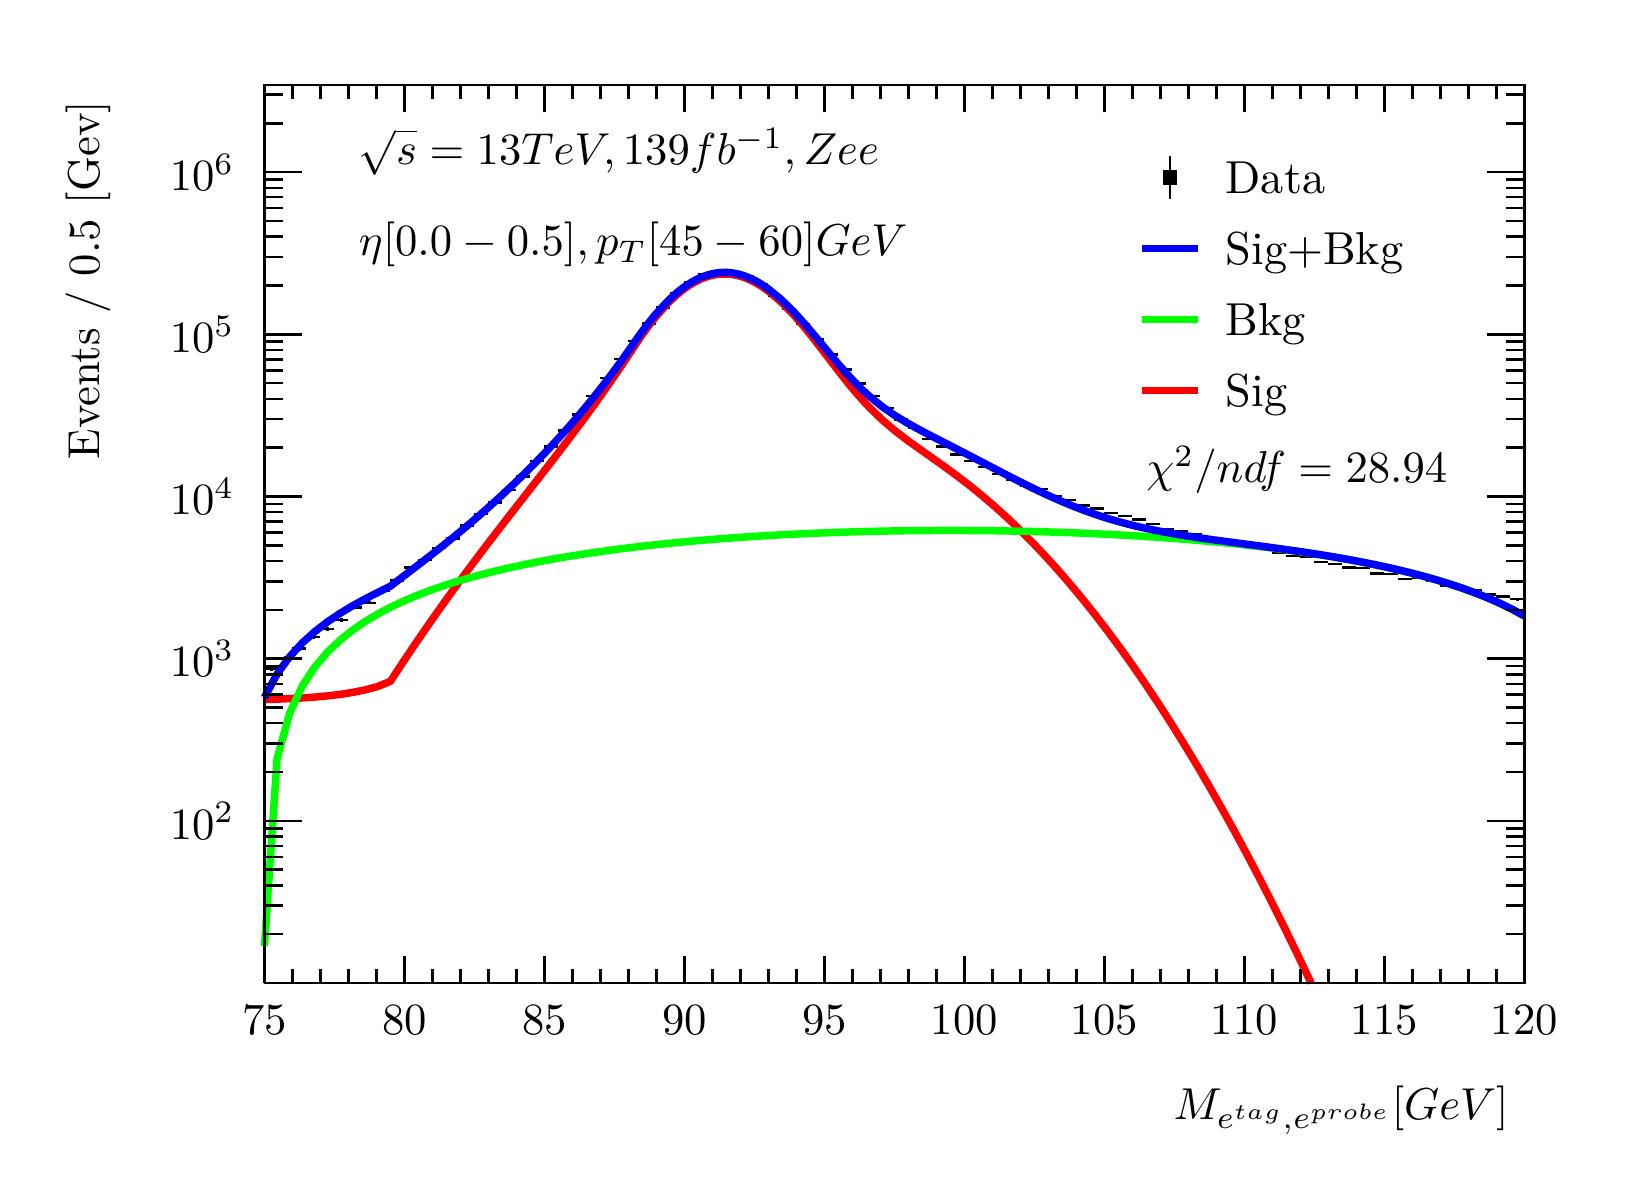
\begin{tikzpicture}
\pgfdeclareplotmark{cross} {
\pgfpathmoveto{\pgfpoint{-0.3\pgfplotmarksize}{\pgfplotmarksize}}
\pgfpathlineto{\pgfpoint{+0.3\pgfplotmarksize}{\pgfplotmarksize}}
\pgfpathlineto{\pgfpoint{+0.3\pgfplotmarksize}{0.3\pgfplotmarksize}}
\pgfpathlineto{\pgfpoint{+1\pgfplotmarksize}{0.3\pgfplotmarksize}}
\pgfpathlineto{\pgfpoint{+1\pgfplotmarksize}{-0.3\pgfplotmarksize}}
\pgfpathlineto{\pgfpoint{+0.3\pgfplotmarksize}{-0.3\pgfplotmarksize}}
\pgfpathlineto{\pgfpoint{+0.3\pgfplotmarksize}{-1.\pgfplotmarksize}}
\pgfpathlineto{\pgfpoint{-0.3\pgfplotmarksize}{-1.\pgfplotmarksize}}
\pgfpathlineto{\pgfpoint{-0.3\pgfplotmarksize}{-0.3\pgfplotmarksize}}
\pgfpathlineto{\pgfpoint{-1.\pgfplotmarksize}{-0.3\pgfplotmarksize}}
\pgfpathlineto{\pgfpoint{-1.\pgfplotmarksize}{0.3\pgfplotmarksize}}
\pgfpathlineto{\pgfpoint{-0.3\pgfplotmarksize}{0.3\pgfplotmarksize}}
\pgfpathclose
\pgfusepathqstroke
}
\pgfdeclareplotmark{cross*} {
\pgfpathmoveto{\pgfpoint{-0.3\pgfplotmarksize}{\pgfplotmarksize}}
\pgfpathlineto{\pgfpoint{+0.3\pgfplotmarksize}{\pgfplotmarksize}}
\pgfpathlineto{\pgfpoint{+0.3\pgfplotmarksize}{0.3\pgfplotmarksize}}
\pgfpathlineto{\pgfpoint{+1\pgfplotmarksize}{0.3\pgfplotmarksize}}
\pgfpathlineto{\pgfpoint{+1\pgfplotmarksize}{-0.3\pgfplotmarksize}}
\pgfpathlineto{\pgfpoint{+0.3\pgfplotmarksize}{-0.3\pgfplotmarksize}}
\pgfpathlineto{\pgfpoint{+0.3\pgfplotmarksize}{-1.\pgfplotmarksize}}
\pgfpathlineto{\pgfpoint{-0.3\pgfplotmarksize}{-1.\pgfplotmarksize}}
\pgfpathlineto{\pgfpoint{-0.3\pgfplotmarksize}{-0.3\pgfplotmarksize}}
\pgfpathlineto{\pgfpoint{-1.\pgfplotmarksize}{-0.3\pgfplotmarksize}}
\pgfpathlineto{\pgfpoint{-1.\pgfplotmarksize}{0.3\pgfplotmarksize}}
\pgfpathlineto{\pgfpoint{-0.3\pgfplotmarksize}{0.3\pgfplotmarksize}}
\pgfpathclose
\pgfusepathqfillstroke
}
\pgfdeclareplotmark{newstar} {
\pgfpathmoveto{\pgfqpoint{0pt}{\pgfplotmarksize}}
\pgfpathlineto{\pgfqpointpolar{44}{0.5\pgfplotmarksize}}
\pgfpathlineto{\pgfqpointpolar{18}{\pgfplotmarksize}}
\pgfpathlineto{\pgfqpointpolar{-20}{0.5\pgfplotmarksize}}
\pgfpathlineto{\pgfqpointpolar{-54}{\pgfplotmarksize}}
\pgfpathlineto{\pgfqpointpolar{-90}{0.5\pgfplotmarksize}}
\pgfpathlineto{\pgfqpointpolar{234}{\pgfplotmarksize}}
\pgfpathlineto{\pgfqpointpolar{198}{0.5\pgfplotmarksize}}
\pgfpathlineto{\pgfqpointpolar{162}{\pgfplotmarksize}}
\pgfpathlineto{\pgfqpointpolar{134}{0.5\pgfplotmarksize}}
\pgfpathclose
\pgfusepathqstroke
}
\pgfdeclareplotmark{newstar*} {
\pgfpathmoveto{\pgfqpoint{0pt}{\pgfplotmarksize}}
\pgfpathlineto{\pgfqpointpolar{44}{0.5\pgfplotmarksize}}
\pgfpathlineto{\pgfqpointpolar{18}{\pgfplotmarksize}}
\pgfpathlineto{\pgfqpointpolar{-20}{0.5\pgfplotmarksize}}
\pgfpathlineto{\pgfqpointpolar{-54}{\pgfplotmarksize}}
\pgfpathlineto{\pgfqpointpolar{-90}{0.5\pgfplotmarksize}}
\pgfpathlineto{\pgfqpointpolar{234}{\pgfplotmarksize}}
\pgfpathlineto{\pgfqpointpolar{198}{0.5\pgfplotmarksize}}
\pgfpathlineto{\pgfqpointpolar{162}{\pgfplotmarksize}}
\pgfpathlineto{\pgfqpointpolar{134}{0.5\pgfplotmarksize}}
\pgfpathclose
\pgfusepathqfillstroke
}
\definecolor{c}{rgb}{1,1,1};
\draw [color=c, fill=c] (0,0) rectangle (20,14.4361);
\draw [color=c, fill=c] (3,2.30977) rectangle (19,13.7143);
\definecolor{c}{rgb}{0,0,0};
\draw [c,line width=0.9] (3,2.30977) -- (3,13.7143) -- (19,13.7143) -- (19,2.30977) -- (3,2.30977);
\definecolor{c}{rgb}{1,1,1};
\draw [color=c, fill=c] (3,2.30977) rectangle (19,13.7143);
\definecolor{c}{rgb}{0,0,0};
\draw [c,line width=0.9] (3,2.30977) -- (3,13.7143) -- (19,13.7143) -- (19,2.30977) -- (3,2.30977);
\draw [c,line width=0.9] (3,2.30977) -- (19,2.30977);
\draw [c,line width=0.9] (3,2.65624) -- (3,2.30977);
\draw [c,line width=0.9] (3.35556,2.48301) -- (3.35556,2.30977);
\draw [c,line width=0.9] (3.71111,2.48301) -- (3.71111,2.30977);
\draw [c,line width=0.9] (4.06667,2.48301) -- (4.06667,2.30977);
\draw [c,line width=0.9] (4.42222,2.48301) -- (4.42222,2.30977);
\draw [c,line width=0.9] (4.77778,2.65624) -- (4.77778,2.30977);
\draw [c,line width=0.9] (5.13333,2.48301) -- (5.13333,2.30977);
\draw [c,line width=0.9] (5.48889,2.48301) -- (5.48889,2.30977);
\draw [c,line width=0.9] (5.84444,2.48301) -- (5.84444,2.30977);
\draw [c,line width=0.9] (6.2,2.48301) -- (6.2,2.30977);
\draw [c,line width=0.9] (6.55556,2.65624) -- (6.55556,2.30977);
\draw [c,line width=0.9] (6.91111,2.48301) -- (6.91111,2.30977);
\draw [c,line width=0.9] (7.26667,2.48301) -- (7.26667,2.30977);
\draw [c,line width=0.9] (7.62222,2.48301) -- (7.62222,2.30977);
\draw [c,line width=0.9] (7.97778,2.48301) -- (7.97778,2.30977);
\draw [c,line width=0.9] (8.33333,2.65624) -- (8.33333,2.30977);
\draw [c,line width=0.9] (8.68889,2.48301) -- (8.68889,2.30977);
\draw [c,line width=0.9] (9.04444,2.48301) -- (9.04444,2.30977);
\draw [c,line width=0.9] (9.4,2.48301) -- (9.4,2.30977);
\draw [c,line width=0.9] (9.75556,2.48301) -- (9.75556,2.30977);
\draw [c,line width=0.9] (10.1111,2.65624) -- (10.1111,2.30977);
\draw [c,line width=0.9] (10.4667,2.48301) -- (10.4667,2.30977);
\draw [c,line width=0.9] (10.8222,2.48301) -- (10.8222,2.30977);
\draw [c,line width=0.9] (11.1778,2.48301) -- (11.1778,2.30977);
\draw [c,line width=0.9] (11.5333,2.48301) -- (11.5333,2.30977);
\draw [c,line width=0.9] (11.8889,2.65624) -- (11.8889,2.30977);
\draw [c,line width=0.9] (12.2444,2.48301) -- (12.2444,2.30977);
\draw [c,line width=0.9] (12.6,2.48301) -- (12.6,2.30977);
\draw [c,line width=0.9] (12.9556,2.48301) -- (12.9556,2.30977);
\draw [c,line width=0.9] (13.3111,2.48301) -- (13.3111,2.30977);
\draw [c,line width=0.9] (13.6667,2.65624) -- (13.6667,2.30977);
\draw [c,line width=0.9] (14.0222,2.48301) -- (14.0222,2.30977);
\draw [c,line width=0.9] (14.3778,2.48301) -- (14.3778,2.30977);
\draw [c,line width=0.9] (14.7333,2.48301) -- (14.7333,2.30977);
\draw [c,line width=0.9] (15.0889,2.48301) -- (15.0889,2.30977);
\draw [c,line width=0.9] (15.4444,2.65624) -- (15.4444,2.30977);
\draw [c,line width=0.9] (15.8,2.48301) -- (15.8,2.30977);
\draw [c,line width=0.9] (16.1556,2.48301) -- (16.1556,2.30977);
\draw [c,line width=0.9] (16.5111,2.48301) -- (16.5111,2.30977);
\draw [c,line width=0.9] (16.8667,2.48301) -- (16.8667,2.30977);
\draw [c,line width=0.9] (17.2222,2.65624) -- (17.2222,2.30977);
\draw [c,line width=0.9] (17.5778,2.48301) -- (17.5778,2.30977);
\draw [c,line width=0.9] (17.9333,2.48301) -- (17.9333,2.30977);
\draw [c,line width=0.9] (18.2889,2.48301) -- (18.2889,2.30977);
\draw [c,line width=0.9] (18.6444,2.48301) -- (18.6444,2.30977);
\draw [c,line width=0.9] (19,2.65624) -- (19,2.30977);
\draw [c,line width=0.9] (19,2.65624) -- (19,2.30977);
\draw [anchor=base] (3,1.66015) node[scale=1.61424, color=c, rotate=0]{75};
\draw [anchor=base] (4.77778,1.66015) node[scale=1.61424, color=c, rotate=0]{80};
\draw [anchor=base] (6.55556,1.66015) node[scale=1.61424, color=c, rotate=0]{85};
\draw [anchor=base] (8.33333,1.66015) node[scale=1.61424, color=c, rotate=0]{90};
\draw [anchor=base] (10.1111,1.66015) node[scale=1.61424, color=c, rotate=0]{95};
\draw [anchor=base] (11.8889,1.66015) node[scale=1.61424, color=c, rotate=0]{100};
\draw [anchor=base] (13.6667,1.66015) node[scale=1.61424, color=c, rotate=0]{105};
\draw [anchor=base] (15.4444,1.66015) node[scale=1.61424, color=c, rotate=0]{110};
\draw [anchor=base] (17.2222,1.66015) node[scale=1.61424, color=c, rotate=0]{115};
\draw [anchor=base] (19,1.66015) node[scale=1.61424, color=c, rotate=0]{120};
\draw [anchor= east] (19,0.692932) node[scale=1.61424, color=c, rotate=0]{$M_{e^{tag}, e^{probe}}  [GeV]$};
\draw [c,line width=0.9] (3,13.7143) -- (19,13.7143);
\draw [c,line width=0.9] (3,13.3678) -- (3,13.7143);
\draw [c,line width=0.9] (3.35556,13.5411) -- (3.35556,13.7143);
\draw [c,line width=0.9] (3.71111,13.5411) -- (3.71111,13.7143);
\draw [c,line width=0.9] (4.06667,13.5411) -- (4.06667,13.7143);
\draw [c,line width=0.9] (4.42222,13.5411) -- (4.42222,13.7143);
\draw [c,line width=0.9] (4.77778,13.3678) -- (4.77778,13.7143);
\draw [c,line width=0.9] (5.13333,13.5411) -- (5.13333,13.7143);
\draw [c,line width=0.9] (5.48889,13.5411) -- (5.48889,13.7143);
\draw [c,line width=0.9] (5.84444,13.5411) -- (5.84444,13.7143);
\draw [c,line width=0.9] (6.2,13.5411) -- (6.2,13.7143);
\draw [c,line width=0.9] (6.55556,13.3678) -- (6.55556,13.7143);
\draw [c,line width=0.9] (6.91111,13.5411) -- (6.91111,13.7143);
\draw [c,line width=0.9] (7.26667,13.5411) -- (7.26667,13.7143);
\draw [c,line width=0.9] (7.62222,13.5411) -- (7.62222,13.7143);
\draw [c,line width=0.9] (7.97778,13.5411) -- (7.97778,13.7143);
\draw [c,line width=0.9] (8.33333,13.3678) -- (8.33333,13.7143);
\draw [c,line width=0.9] (8.68889,13.5411) -- (8.68889,13.7143);
\draw [c,line width=0.9] (9.04444,13.5411) -- (9.04444,13.7143);
\draw [c,line width=0.9] (9.4,13.5411) -- (9.4,13.7143);
\draw [c,line width=0.9] (9.75556,13.5411) -- (9.75556,13.7143);
\draw [c,line width=0.9] (10.1111,13.3678) -- (10.1111,13.7143);
\draw [c,line width=0.9] (10.4667,13.5411) -- (10.4667,13.7143);
\draw [c,line width=0.9] (10.8222,13.5411) -- (10.8222,13.7143);
\draw [c,line width=0.9] (11.1778,13.5411) -- (11.1778,13.7143);
\draw [c,line width=0.9] (11.5333,13.5411) -- (11.5333,13.7143);
\draw [c,line width=0.9] (11.8889,13.3678) -- (11.8889,13.7143);
\draw [c,line width=0.9] (12.2444,13.5411) -- (12.2444,13.7143);
\draw [c,line width=0.9] (12.6,13.5411) -- (12.6,13.7143);
\draw [c,line width=0.9] (12.9556,13.5411) -- (12.9556,13.7143);
\draw [c,line width=0.9] (13.3111,13.5411) -- (13.3111,13.7143);
\draw [c,line width=0.9] (13.6667,13.3678) -- (13.6667,13.7143);
\draw [c,line width=0.9] (14.0222,13.5411) -- (14.0222,13.7143);
\draw [c,line width=0.9] (14.3778,13.5411) -- (14.3778,13.7143);
\draw [c,line width=0.9] (14.7333,13.5411) -- (14.7333,13.7143);
\draw [c,line width=0.9] (15.0889,13.5411) -- (15.0889,13.7143);
\draw [c,line width=0.9] (15.4444,13.3678) -- (15.4444,13.7143);
\draw [c,line width=0.9] (15.8,13.5411) -- (15.8,13.7143);
\draw [c,line width=0.9] (16.1556,13.5411) -- (16.1556,13.7143);
\draw [c,line width=0.9] (16.5111,13.5411) -- (16.5111,13.7143);
\draw [c,line width=0.9] (16.8667,13.5411) -- (16.8667,13.7143);
\draw [c,line width=0.9] (17.2222,13.3678) -- (17.2222,13.7143);
\draw [c,line width=0.9] (17.5778,13.5411) -- (17.5778,13.7143);
\draw [c,line width=0.9] (17.9333,13.5411) -- (17.9333,13.7143);
\draw [c,line width=0.9] (18.2889,13.5411) -- (18.2889,13.7143);
\draw [c,line width=0.9] (18.6444,13.5411) -- (18.6444,13.7143);
\draw [c,line width=0.9] (19,13.3678) -- (19,13.7143);
\draw [c,line width=0.9] (19,13.3678) -- (19,13.7143);
\draw [c,line width=0.9] (3,2.30977) -- (3,13.7143);
\draw [c,line width=0.9] (3.237,2.92982) -- (3,2.92982);
\draw [c,line width=0.9] (3.237,3.29252) -- (3,3.29252);
\draw [c,line width=0.9] (3.237,3.54986) -- (3,3.54986);
\draw [c,line width=0.9] (3.237,3.74947) -- (3,3.74947);
\draw [c,line width=0.9] (3.237,3.91257) -- (3,3.91257);
\draw [c,line width=0.9] (3.237,4.05046) -- (3,4.05046);
\draw [c,line width=0.9] (3.237,4.16991) -- (3,4.16991);
\draw [c,line width=0.9] (3.237,4.27527) -- (3,4.27527);
\draw [c,line width=0.9] (3.474,4.36952) -- (3,4.36952);
\draw [anchor= east] (2.82,4.36952) node[scale=1.61424, color=c, rotate=0]{$10^{2}$};
\draw [c,line width=0.9] (3.237,4.98956) -- (3,4.98956);
\draw [c,line width=0.9] (3.237,5.35227) -- (3,5.35227);
\draw [c,line width=0.9] (3.237,5.60961) -- (3,5.60961);
\draw [c,line width=0.9] (3.237,5.80922) -- (3,5.80922);
\draw [c,line width=0.9] (3.237,5.97231) -- (3,5.97231);
\draw [c,line width=0.9] (3.237,6.11021) -- (3,6.11021);
\draw [c,line width=0.9] (3.237,6.22966) -- (3,6.22966);
\draw [c,line width=0.9] (3.237,6.33502) -- (3,6.33502);
\draw [c,line width=0.9] (3.474,6.42927) -- (3,6.42927);
\draw [anchor= east] (2.82,6.42927) node[scale=1.61424, color=c, rotate=0]{$10^{3}$};
\draw [c,line width=0.9] (3.237,7.04931) -- (3,7.04931);
\draw [c,line width=0.9] (3.237,7.41202) -- (3,7.41202);
\draw [c,line width=0.9] (3.237,7.66936) -- (3,7.66936);
\draw [c,line width=0.9] (3.237,7.86897) -- (3,7.86897);
\draw [c,line width=0.9] (3.237,8.03206) -- (3,8.03206);
\draw [c,line width=0.9] (3.237,8.16995) -- (3,8.16995);
\draw [c,line width=0.9] (3.237,8.2894) -- (3,8.2894);
\draw [c,line width=0.9] (3.237,8.39476) -- (3,8.39476);
\draw [c,line width=0.9] (3.474,8.48901) -- (3,8.48901);
\draw [anchor= east] (2.82,8.48901) node[scale=1.61424, color=c, rotate=0]{$10^{4}$};
\draw [c,line width=0.9] (3.237,9.10906) -- (3,9.10906);
\draw [c,line width=0.9] (3.237,9.47176) -- (3,9.47176);
\draw [c,line width=0.9] (3.237,9.7291) -- (3,9.7291);
\draw [c,line width=0.9] (3.237,9.92871) -- (3,9.92871);
\draw [c,line width=0.9] (3.237,10.0918) -- (3,10.0918);
\draw [c,line width=0.9] (3.237,10.2297) -- (3,10.2297);
\draw [c,line width=0.9] (3.237,10.3491) -- (3,10.3491);
\draw [c,line width=0.9] (3.237,10.4545) -- (3,10.4545);
\draw [c,line width=0.9] (3.474,10.5488) -- (3,10.5488);
\draw [anchor= east] (2.82,10.5488) node[scale=1.61424, color=c, rotate=0]{$10^{5}$};
\draw [c,line width=0.9] (3.237,11.1688) -- (3,11.1688);
\draw [c,line width=0.9] (3.237,11.5315) -- (3,11.5315);
\draw [c,line width=0.9] (3.237,11.7889) -- (3,11.7889);
\draw [c,line width=0.9] (3.237,11.9885) -- (3,11.9885);
\draw [c,line width=0.9] (3.237,12.1516) -- (3,12.1516);
\draw [c,line width=0.9] (3.237,12.2894) -- (3,12.2894);
\draw [c,line width=0.9] (3.237,12.4089) -- (3,12.4089);
\draw [c,line width=0.9] (3.237,12.5143) -- (3,12.5143);
\draw [c,line width=0.9] (3.474,12.6085) -- (3,12.6085);
\draw [anchor= east] (2.82,12.6085) node[scale=1.61424, color=c, rotate=0]{$10^{6}$};
\draw [c,line width=0.9] (3.237,13.2286) -- (3,13.2286);
\draw [c,line width=0.9] (3.237,13.5913) -- (3,13.5913);
\draw [anchor= east] (0.76,13.7143) node[scale=1.61424, color=c, rotate=90]{Events / 0.5 [Gev]};
\draw [c,line width=0.9] (19,2.30977) -- (19,13.7143);
\draw [c,line width=0.9] (18.763,2.92982) -- (19,2.92982);
\draw [c,line width=0.9] (18.763,3.29252) -- (19,3.29252);
\draw [c,line width=0.9] (18.763,3.54986) -- (19,3.54986);
\draw [c,line width=0.9] (18.763,3.74947) -- (19,3.74947);
\draw [c,line width=0.9] (18.763,3.91257) -- (19,3.91257);
\draw [c,line width=0.9] (18.763,4.05046) -- (19,4.05046);
\draw [c,line width=0.9] (18.763,4.16991) -- (19,4.16991);
\draw [c,line width=0.9] (18.763,4.27527) -- (19,4.27527);
\draw [c,line width=0.9] (18.526,4.36952) -- (19,4.36952);
\draw [c,line width=0.9] (18.763,4.98956) -- (19,4.98956);
\draw [c,line width=0.9] (18.763,5.35227) -- (19,5.35227);
\draw [c,line width=0.9] (18.763,5.60961) -- (19,5.60961);
\draw [c,line width=0.9] (18.763,5.80922) -- (19,5.80922);
\draw [c,line width=0.9] (18.763,5.97231) -- (19,5.97231);
\draw [c,line width=0.9] (18.763,6.11021) -- (19,6.11021);
\draw [c,line width=0.9] (18.763,6.22966) -- (19,6.22966);
\draw [c,line width=0.9] (18.763,6.33502) -- (19,6.33502);
\draw [c,line width=0.9] (18.526,6.42927) -- (19,6.42927);
\draw [c,line width=0.9] (18.763,7.04931) -- (19,7.04931);
\draw [c,line width=0.9] (18.763,7.41202) -- (19,7.41202);
\draw [c,line width=0.9] (18.763,7.66936) -- (19,7.66936);
\draw [c,line width=0.9] (18.763,7.86897) -- (19,7.86897);
\draw [c,line width=0.9] (18.763,8.03206) -- (19,8.03206);
\draw [c,line width=0.9] (18.763,8.16995) -- (19,8.16995);
\draw [c,line width=0.9] (18.763,8.2894) -- (19,8.2894);
\draw [c,line width=0.9] (18.763,8.39476) -- (19,8.39476);
\draw [c,line width=0.9] (18.526,8.48901) -- (19,8.48901);
\draw [c,line width=0.9] (18.763,9.10906) -- (19,9.10906);
\draw [c,line width=0.9] (18.763,9.47176) -- (19,9.47176);
\draw [c,line width=0.9] (18.763,9.7291) -- (19,9.7291);
\draw [c,line width=0.9] (18.763,9.92871) -- (19,9.92871);
\draw [c,line width=0.9] (18.763,10.0918) -- (19,10.0918);
\draw [c,line width=0.9] (18.763,10.2297) -- (19,10.2297);
\draw [c,line width=0.9] (18.763,10.3491) -- (19,10.3491);
\draw [c,line width=0.9] (18.763,10.4545) -- (19,10.4545);
\draw [c,line width=0.9] (18.526,10.5488) -- (19,10.5488);
\draw [c,line width=0.9] (18.763,11.1688) -- (19,11.1688);
\draw [c,line width=0.9] (18.763,11.5315) -- (19,11.5315);
\draw [c,line width=0.9] (18.763,11.7889) -- (19,11.7889);
\draw [c,line width=0.9] (18.763,11.9885) -- (19,11.9885);
\draw [c,line width=0.9] (18.763,12.1516) -- (19,12.1516);
\draw [c,line width=0.9] (18.763,12.2894) -- (19,12.2894);
\draw [c,line width=0.9] (18.763,12.4089) -- (19,12.4089);
\draw [c,line width=0.9] (18.763,12.5143) -- (19,12.5143);
\draw [c,line width=0.9] (18.526,12.6085) -- (19,12.6085);
\draw [c,line width=0.9] (18.763,13.2286) -- (19,13.2286);
\draw [c,line width=0.9] (18.763,13.5913) -- (19,13.5913);
\draw [c,line width=0.9] (3.08889,6.30572) -- (3,6.30572);
\draw [c,line width=0.9] (3,6.30572) -- (3,6.30572);
\draw [c,line width=0.9] (3.08889,6.30572) -- (3.17778,6.30572);
\draw [c,line width=0.9] (3.17778,6.30572) -- (3.17778,6.30572);
\draw [c,line width=0.9] (3.08889,6.30572) -- (3.08889,6.33603);
\draw [c,line width=0.9] (3.08889,6.33603) -- (3.08889,6.33603);
\draw [c,line width=0.9] (3.08889,6.30572) -- (3.08889,6.27541);
\draw [c,line width=0.9] (3.08889,6.27541) -- (3.08889,6.27541);
\draw [c,line width=0.9] (3.26667,6.43994) -- (3.17778,6.43994);
\draw [c,line width=0.9] (3.17778,6.43994) -- (3.17778,6.43994);
\draw [c,line width=0.9] (3.26667,6.43994) -- (3.35556,6.43994);
\draw [c,line width=0.9] (3.35556,6.43994) -- (3.35556,6.43994);
\draw [c,line width=0.9] (3.26667,6.43994) -- (3.26667,6.46806);
\draw [c,line width=0.9] (3.26667,6.46806) -- (3.26667,6.46806);
\draw [c,line width=0.9] (3.26667,6.43994) -- (3.26667,6.41182);
\draw [c,line width=0.9] (3.26667,6.41182) -- (3.26667,6.41182);
\draw [c,line width=0.9] (3.44444,6.55584) -- (3.35556,6.55584);
\draw [c,line width=0.9] (3.35556,6.55584) -- (3.35556,6.55584);
\draw [c,line width=0.9] (3.44444,6.55584) -- (3.53333,6.55584);
\draw [c,line width=0.9] (3.53333,6.55584) -- (3.53333,6.55584);
\draw [c,line width=0.9] (3.44444,6.55584) -- (3.44444,6.5822);
\draw [c,line width=0.9] (3.44444,6.5822) -- (3.44444,6.5822);
\draw [c,line width=0.9] (3.44444,6.55584) -- (3.44444,6.52949);
\draw [c,line width=0.9] (3.44444,6.52949) -- (3.44444,6.52949);
\draw [c,line width=0.9] (3.62222,6.70301) -- (3.53333,6.70301);
\draw [c,line width=0.9] (3.53333,6.70301) -- (3.53333,6.70301);
\draw [c,line width=0.9] (3.62222,6.70301) -- (3.71111,6.70301);
\draw [c,line width=0.9] (3.71111,6.70301) -- (3.71111,6.70301);
\draw [c,line width=0.9] (3.62222,6.70301) -- (3.62222,6.72728);
\draw [c,line width=0.9] (3.62222,6.72728) -- (3.62222,6.72728);
\draw [c,line width=0.9] (3.62222,6.70301) -- (3.62222,6.67873);
\draw [c,line width=0.9] (3.62222,6.67873) -- (3.62222,6.67873);
\draw [c,line width=0.9] (3.8,6.80852) -- (3.71111,6.80852);
\draw [c,line width=0.9] (3.71111,6.80852) -- (3.71111,6.80852);
\draw [c,line width=0.9] (3.8,6.80852) -- (3.88889,6.80852);
\draw [c,line width=0.9] (3.88889,6.80852) -- (3.88889,6.80852);
\draw [c,line width=0.9] (3.8,6.80852) -- (3.8,6.8314);
\draw [c,line width=0.9] (3.8,6.8314) -- (3.8,6.8314);
\draw [c,line width=0.9] (3.8,6.80852) -- (3.8,6.78563);
\draw [c,line width=0.9] (3.8,6.78563) -- (3.8,6.78563);
\draw [c,line width=0.9] (3.97778,6.91855) -- (3.88889,6.91855);
\draw [c,line width=0.9] (3.88889,6.91855) -- (3.88889,6.91855);
\draw [c,line width=0.9] (3.97778,6.91855) -- (4.06667,6.91855);
\draw [c,line width=0.9] (4.06667,6.91855) -- (4.06667,6.91855);
\draw [c,line width=0.9] (3.97778,6.91855) -- (3.97778,6.94007);
\draw [c,line width=0.9] (3.97778,6.94007) -- (3.97778,6.94007);
\draw [c,line width=0.9] (3.97778,6.91855) -- (3.97778,6.89703);
\draw [c,line width=0.9] (3.97778,6.89703) -- (3.97778,6.89703);
\draw [c,line width=0.9] (4.15556,7.08052) -- (4.06667,7.08052);
\draw [c,line width=0.9] (4.06667,7.08052) -- (4.06667,7.08052);
\draw [c,line width=0.9] (4.15556,7.08052) -- (4.24444,7.08052);
\draw [c,line width=0.9] (4.24444,7.08052) -- (4.24444,7.08052);
\draw [c,line width=0.9] (4.15556,7.08052) -- (4.15556,7.10017);
\draw [c,line width=0.9] (4.15556,7.10017) -- (4.15556,7.10017);
\draw [c,line width=0.9] (4.15556,7.08052) -- (4.15556,7.06086);
\draw [c,line width=0.9] (4.15556,7.06086) -- (4.15556,7.06086);
\draw [c,line width=0.9] (4.33333,7.13863) -- (4.24444,7.13863);
\draw [c,line width=0.9] (4.24444,7.13863) -- (4.24444,7.13863);
\draw [c,line width=0.9] (4.33333,7.13863) -- (4.42222,7.13863);
\draw [c,line width=0.9] (4.42222,7.13863) -- (4.42222,7.13863);
\draw [c,line width=0.9] (4.33333,7.13863) -- (4.33333,7.15766);
\draw [c,line width=0.9] (4.33333,7.15766) -- (4.33333,7.15766);
\draw [c,line width=0.9] (4.33333,7.13863) -- (4.33333,7.1196);
\draw [c,line width=0.9] (4.33333,7.1196) -- (4.33333,7.1196);
\draw [c,line width=0.9] (4.51111,7.29393) -- (4.42222,7.29393);
\draw [c,line width=0.9] (4.42222,7.29393) -- (4.42222,7.29393);
\draw [c,line width=0.9] (4.51111,7.29393) -- (4.6,7.29393);
\draw [c,line width=0.9] (4.6,7.29393) -- (4.6,7.29393);
\draw [c,line width=0.9] (4.51111,7.29393) -- (4.51111,7.31138);
\draw [c,line width=0.9] (4.51111,7.31138) -- (4.51111,7.31138);
\draw [c,line width=0.9] (4.51111,7.29393) -- (4.51111,7.27648);
\draw [c,line width=0.9] (4.51111,7.27648) -- (4.51111,7.27648);
\draw [c,line width=0.9] (4.68889,7.42239) -- (4.6,7.42239);
\draw [c,line width=0.9] (4.6,7.42239) -- (4.6,7.42239);
\draw [c,line width=0.9] (4.68889,7.42239) -- (4.77778,7.42239);
\draw [c,line width=0.9] (4.77778,7.42239) -- (4.77778,7.42239);
\draw [c,line width=0.9] (4.68889,7.42239) -- (4.68889,7.43863);
\draw [c,line width=0.9] (4.68889,7.43863) -- (4.68889,7.43863);
\draw [c,line width=0.9] (4.68889,7.42239) -- (4.68889,7.40616);
\draw [c,line width=0.9] (4.68889,7.40616) -- (4.68889,7.40616);
\draw [c,line width=0.9] (4.86667,7.58647) -- (4.77778,7.58647);
\draw [c,line width=0.9] (4.77778,7.58647) -- (4.77778,7.58647);
\draw [c,line width=0.9] (4.86667,7.58647) -- (4.95556,7.58647);
\draw [c,line width=0.9] (4.95556,7.58647) -- (4.95556,7.58647);
\draw [c,line width=0.9] (4.86667,7.58647) -- (4.86667,7.60128);
\draw [c,line width=0.9] (4.86667,7.60128) -- (4.86667,7.60128);
\draw [c,line width=0.9] (4.86667,7.58647) -- (4.86667,7.57165);
\draw [c,line width=0.9] (4.86667,7.57165) -- (4.86667,7.57165);
\draw [c,line width=0.9] (5.04444,7.68466) -- (4.95556,7.68466);
\draw [c,line width=0.9] (4.95556,7.68466) -- (4.95556,7.68466);
\draw [c,line width=0.9] (5.04444,7.68466) -- (5.13333,7.68466);
\draw [c,line width=0.9] (5.13333,7.68466) -- (5.13333,7.68466);
\draw [c,line width=0.9] (5.04444,7.68466) -- (5.04444,7.69868);
\draw [c,line width=0.9] (5.04444,7.69868) -- (5.04444,7.69868);
\draw [c,line width=0.9] (5.04444,7.68466) -- (5.04444,7.67063);
\draw [c,line width=0.9] (5.04444,7.67063) -- (5.04444,7.67063);
\draw [c,line width=0.9] (5.22222,7.83413) -- (5.13333,7.83413);
\draw [c,line width=0.9] (5.13333,7.83413) -- (5.13333,7.83413);
\draw [c,line width=0.9] (5.22222,7.83413) -- (5.31111,7.83413);
\draw [c,line width=0.9] (5.31111,7.83413) -- (5.31111,7.83413);
\draw [c,line width=0.9] (5.22222,7.83413) -- (5.22222,7.84703);
\draw [c,line width=0.9] (5.22222,7.84703) -- (5.22222,7.84703);
\draw [c,line width=0.9] (5.22222,7.83413) -- (5.22222,7.82123);
\draw [c,line width=0.9] (5.22222,7.82123) -- (5.22222,7.82123);
\draw [c,line width=0.9] (5.4,7.95861) -- (5.31111,7.95861);
\draw [c,line width=0.9] (5.31111,7.95861) -- (5.31111,7.95861);
\draw [c,line width=0.9] (5.4,7.95861) -- (5.48889,7.95861);
\draw [c,line width=0.9] (5.48889,7.95861) -- (5.48889,7.95861);
\draw [c,line width=0.9] (5.4,7.95861) -- (5.4,7.97064);
\draw [c,line width=0.9] (5.4,7.97064) -- (5.4,7.97064);
\draw [c,line width=0.9] (5.4,7.95861) -- (5.4,7.94658);
\draw [c,line width=0.9] (5.4,7.94658) -- (5.4,7.94658);
\draw [c,line width=0.9] (5.57778,8.118) -- (5.48889,8.118);
\draw [c,line width=0.9] (5.48889,8.118) -- (5.48889,8.118);
\draw [c,line width=0.9] (5.57778,8.118) -- (5.66667,8.118);
\draw [c,line width=0.9] (5.66667,8.118) -- (5.66667,8.118);
\draw [c,line width=0.9] (5.57778,8.118) -- (5.57778,8.129);
\draw [c,line width=0.9] (5.57778,8.129) -- (5.57778,8.129);
\draw [c,line width=0.9] (5.57778,8.118) -- (5.57778,8.10699);
\draw [c,line width=0.9] (5.57778,8.10699) -- (5.57778,8.10699);
\draw [c,line width=0.9] (5.75556,8.26354) -- (5.66667,8.26354);
\draw [c,line width=0.9] (5.66667,8.26354) -- (5.66667,8.26354);
\draw [c,line width=0.9] (5.75556,8.26354) -- (5.84444,8.26354);
\draw [c,line width=0.9] (5.84444,8.26354) -- (5.84444,8.26354);
\draw [c,line width=0.9] (5.75556,8.26354) -- (5.75556,8.27369);
\draw [c,line width=0.9] (5.75556,8.27369) -- (5.75556,8.27369);
\draw [c,line width=0.9] (5.75556,8.26354) -- (5.75556,8.25339);
\draw [c,line width=0.9] (5.75556,8.25339) -- (5.75556,8.25339);
\draw [c,line width=0.9] (5.93333,8.41189) -- (5.84444,8.41189);
\draw [c,line width=0.9] (5.84444,8.41189) -- (5.84444,8.41189);
\draw [c,line width=0.9] (5.93333,8.41189) -- (6.02222,8.41189);
\draw [c,line width=0.9] (6.02222,8.41189) -- (6.02222,8.41189);
\draw [c,line width=0.9] (5.93333,8.41189) -- (5.93333,8.42123);
\draw [c,line width=0.9] (5.93333,8.42123) -- (5.93333,8.42123);
\draw [c,line width=0.9] (5.93333,8.41189) -- (5.93333,8.40256);
\draw [c,line width=0.9] (5.93333,8.40256) -- (5.93333,8.40256);
\draw [c,line width=0.9] (6.11111,8.5702) -- (6.02222,8.5702);
\draw [c,line width=0.9] (6.02222,8.5702) -- (6.02222,8.5702);
\draw [c,line width=0.9] (6.11111,8.5702) -- (6.2,8.5702);
\draw [c,line width=0.9] (6.2,8.5702) -- (6.2,8.5702);
\draw [c,line width=0.9] (6.11111,8.5702) -- (6.11111,8.57875);
\draw [c,line width=0.9] (6.11111,8.57875) -- (6.11111,8.57875);
\draw [c,line width=0.9] (6.11111,8.5702) -- (6.11111,8.56165);
\draw [c,line width=0.9] (6.11111,8.56165) -- (6.11111,8.56165);
\draw [c,line width=0.9] (6.28889,8.74338) -- (6.2,8.74338);
\draw [c,line width=0.9] (6.2,8.74338) -- (6.2,8.74338);
\draw [c,line width=0.9] (6.28889,8.74338) -- (6.37778,8.74338);
\draw [c,line width=0.9] (6.37778,8.74338) -- (6.37778,8.74338);
\draw [c,line width=0.9] (6.28889,8.74338) -- (6.28889,8.75114);
\draw [c,line width=0.9] (6.28889,8.75114) -- (6.28889,8.75114);
\draw [c,line width=0.9] (6.28889,8.74338) -- (6.28889,8.73562);
\draw [c,line width=0.9] (6.28889,8.73562) -- (6.28889,8.73562);
\draw [c,line width=0.9] (6.46667,8.93957) -- (6.37778,8.93957);
\draw [c,line width=0.9] (6.37778,8.93957) -- (6.37778,8.93957);
\draw [c,line width=0.9] (6.46667,8.93957) -- (6.55556,8.93957);
\draw [c,line width=0.9] (6.55556,8.93957) -- (6.55556,8.93957);
\draw [c,line width=0.9] (6.46667,8.93957) -- (6.46667,8.94653);
\draw [c,line width=0.9] (6.46667,8.94653) -- (6.46667,8.94653);
\draw [c,line width=0.9] (6.46667,8.93957) -- (6.46667,8.93262);
\draw [c,line width=0.9] (6.46667,8.93262) -- (6.46667,8.93262);
\draw [c,line width=0.9] (6.64444,9.12594) -- (6.55556,9.12594);
\draw [c,line width=0.9] (6.55556,9.12594) -- (6.55556,9.12594);
\draw [c,line width=0.9] (6.64444,9.12594) -- (6.73333,9.12594);
\draw [c,line width=0.9] (6.73333,9.12594) -- (6.73333,9.12594);
\draw [c,line width=0.9] (6.64444,9.12594) -- (6.64444,9.13221);
\draw [c,line width=0.9] (6.64444,9.13221) -- (6.64444,9.13221);
\draw [c,line width=0.9] (6.64444,9.12594) -- (6.64444,9.11967);
\draw [c,line width=0.9] (6.64444,9.11967) -- (6.64444,9.11967);
\draw [c,line width=0.9] (6.82222,9.32751) -- (6.73333,9.32751);
\draw [c,line width=0.9] (6.73333,9.32751) -- (6.73333,9.32751);
\draw [c,line width=0.9] (6.82222,9.32751) -- (6.91111,9.32751);
\draw [c,line width=0.9] (6.91111,9.32751) -- (6.91111,9.32751);
\draw [c,line width=0.9] (6.82222,9.32751) -- (6.82222,9.3331);
\draw [c,line width=0.9] (6.82222,9.3331) -- (6.82222,9.3331);
\draw [c,line width=0.9] (6.82222,9.32751) -- (6.82222,9.32191);
\draw [c,line width=0.9] (6.82222,9.32191) -- (6.82222,9.32191);
\draw [c,line width=0.9] (7,9.53) -- (6.91111,9.53);
\draw [c,line width=0.9] (6.91111,9.53) -- (6.91111,9.53);
\draw [c,line width=0.9] (7,9.53) -- (7.08889,9.53);
\draw [c,line width=0.9] (7.08889,9.53) -- (7.08889,9.53);
\draw [c,line width=0.9] (7,9.53) -- (7,9.535);
\draw [c,line width=0.9] (7,9.535) -- (7,9.535);
\draw [c,line width=0.9] (7,9.53) -- (7,9.525);
\draw [c,line width=0.9] (7,9.525) -- (7,9.525);
\draw [c,line width=0.9] (7.17778,9.76837) -- (7.08889,9.76837);
\draw [c,line width=0.9] (7.08889,9.76837) -- (7.08889,9.76837);
\draw [c,line width=0.9] (7.17778,9.76837) -- (7.26667,9.76837);
\draw [c,line width=0.9] (7.26667,9.76837) -- (7.26667,9.76837);
\draw [c,line width=0.9] (7.17778,9.76837) -- (7.17778,9.77275);
\draw [c,line width=0.9] (7.17778,9.77275) -- (7.17778,9.77275);
\draw [c,line width=0.9] (7.17778,9.76837) -- (7.17778,9.764);
\draw [c,line width=0.9] (7.17778,9.764) -- (7.17778,9.764);
\draw [c,line width=0.9] (7.35556,9.99199) -- (7.26667,9.99199);
\draw [c,line width=0.9] (7.26667,9.99199) -- (7.26667,9.99199);
\draw [c,line width=0.9] (7.35556,9.99199) -- (7.44444,9.99199);
\draw [c,line width=0.9] (7.44444,9.99199) -- (7.44444,9.99199);
\draw [c,line width=0.9] (7.35556,9.99199) -- (7.35556,9.99585);
\draw [c,line width=0.9] (7.35556,9.99585) -- (7.35556,9.99585);
\draw [c,line width=0.9] (7.35556,9.99199) -- (7.35556,9.98813);
\draw [c,line width=0.9] (7.35556,9.98813) -- (7.35556,9.98813);
\draw [c,line width=0.9] (7.53333,10.2354) -- (7.44444,10.2354);
\draw [c,line width=0.9] (7.44444,10.2354) -- (7.44444,10.2354);
\draw [c,line width=0.9] (7.53333,10.2354) -- (7.62222,10.2354);
\draw [c,line width=0.9] (7.62222,10.2354) -- (7.62222,10.2354);
\draw [c,line width=0.9] (7.53333,10.2354) -- (7.53333,10.2387);
\draw [c,line width=0.9] (7.53333,10.2387) -- (7.53333,10.2387);
\draw [c,line width=0.9] (7.53333,10.2354) -- (7.53333,10.232);
\draw [c,line width=0.9] (7.53333,10.232) -- (7.53333,10.232);
\draw [c,line width=0.9] (7.71111,10.4629) -- (7.62222,10.4629);
\draw [c,line width=0.9] (7.62222,10.4629) -- (7.62222,10.4629);
\draw [c,line width=0.9] (7.71111,10.4629) -- (7.8,10.4629);
\draw [c,line width=0.9] (7.8,10.4629) -- (7.8,10.4629);
\draw [c,line width=0.9] (7.71111,10.4629) -- (7.71111,10.4658);
\draw [c,line width=0.9] (7.71111,10.4658) -- (7.71111,10.4658);
\draw [c,line width=0.9] (7.71111,10.4629) -- (7.71111,10.4599);
\draw [c,line width=0.9] (7.71111,10.4599) -- (7.71111,10.4599);
\draw [c,line width=0.9] (7.88889,10.6841) -- (7.8,10.6841);
\draw [c,line width=0.9] (7.8,10.6841) -- (7.8,10.6841);
\draw [c,line width=0.9] (7.88889,10.6841) -- (7.97778,10.6841);
\draw [c,line width=0.9] (7.97778,10.6841) -- (7.97778,10.6841);
\draw [c,line width=0.9] (7.88889,10.6841) -- (7.88889,10.6867);
\draw [c,line width=0.9] (7.88889,10.6867) -- (7.88889,10.6867);
\draw [c,line width=0.9] (7.88889,10.6841) -- (7.88889,10.6815);
\draw [c,line width=0.9] (7.88889,10.6815) -- (7.88889,10.6815);
\draw [c,line width=0.9] (8.06667,10.8887) -- (7.97778,10.8887);
\draw [c,line width=0.9] (7.97778,10.8887) -- (7.97778,10.8887);
\draw [c,line width=0.9] (8.06667,10.8887) -- (8.15556,10.8887);
\draw [c,line width=0.9] (8.15556,10.8887) -- (8.15556,10.8887);
\draw [c,line width=0.9] (8.06667,10.8887) -- (8.06667,10.891);
\draw [c,line width=0.9] (8.06667,10.891) -- (8.06667,10.891);
\draw [c,line width=0.9] (8.06667,10.8887) -- (8.06667,10.8863);
\draw [c,line width=0.9] (8.06667,10.8863) -- (8.06667,10.8863);
\draw [c,line width=0.9] (8.24444,11.0725) -- (8.15556,11.0725);
\draw [c,line width=0.9] (8.15556,11.0725) -- (8.15556,11.0725);
\draw [c,line width=0.9] (8.24444,11.0725) -- (8.33333,11.0725);
\draw [c,line width=0.9] (8.33333,11.0725) -- (8.33333,11.0725);
\draw [c,line width=0.9] (8.24444,11.0725) -- (8.24444,11.0746);
\draw [c,line width=0.9] (8.24444,11.0746) -- (8.24444,11.0746);
\draw [c,line width=0.9] (8.24444,11.0725) -- (8.24444,11.0704);
\draw [c,line width=0.9] (8.24444,11.0704) -- (8.24444,11.0704);
\draw [c,line width=0.9] (8.42222,11.2095) -- (8.33333,11.2095);
\draw [c,line width=0.9] (8.33333,11.2095) -- (8.33333,11.2095);
\draw [c,line width=0.9] (8.42222,11.2095) -- (8.51111,11.2095);
\draw [c,line width=0.9] (8.51111,11.2095) -- (8.51111,11.2095);
\draw [c,line width=0.9] (8.42222,11.2095) -- (8.42222,11.2115);
\draw [c,line width=0.9] (8.42222,11.2115) -- (8.42222,11.2115);
\draw [c,line width=0.9] (8.42222,11.2095) -- (8.42222,11.2076);
\draw [c,line width=0.9] (8.42222,11.2076) -- (8.42222,11.2076);
\draw [c,line width=0.9] (8.6,11.3058) -- (8.51111,11.3058);
\draw [c,line width=0.9] (8.51111,11.3058) -- (8.51111,11.3058);
\draw [c,line width=0.9] (8.6,11.3058) -- (8.68889,11.3058);
\draw [c,line width=0.9] (8.68889,11.3058) -- (8.68889,11.3058);
\draw [c,line width=0.9] (8.6,11.3058) -- (8.6,11.3076);
\draw [c,line width=0.9] (8.6,11.3076) -- (8.6,11.3076);
\draw [c,line width=0.9] (8.6,11.3058) -- (8.6,11.3039);
\draw [c,line width=0.9] (8.6,11.3039) -- (8.6,11.3039);
\draw [c,line width=0.9] (8.77778,11.3499) -- (8.68889,11.3499);
\draw [c,line width=0.9] (8.68889,11.3499) -- (8.68889,11.3499);
\draw [c,line width=0.9] (8.77778,11.3499) -- (8.86667,11.3499);
\draw [c,line width=0.9] (8.86667,11.3499) -- (8.86667,11.3499);
\draw [c,line width=0.9] (8.77778,11.3499) -- (8.77778,11.3517);
\draw [c,line width=0.9] (8.77778,11.3517) -- (8.77778,11.3517);
\draw [c,line width=0.9] (8.77778,11.3499) -- (8.77778,11.348);
\draw [c,line width=0.9] (8.77778,11.348) -- (8.77778,11.348);
\draw [c,line width=0.9] (8.95556,11.3424) -- (8.86667,11.3424);
\draw [c,line width=0.9] (8.86667,11.3424) -- (8.86667,11.3424);
\draw [c,line width=0.9] (8.95556,11.3424) -- (9.04444,11.3424);
\draw [c,line width=0.9] (9.04444,11.3424) -- (9.04444,11.3424);
\draw [c,line width=0.9] (8.95556,11.3424) -- (8.95556,11.3442);
\draw [c,line width=0.9] (8.95556,11.3442) -- (8.95556,11.3442);
\draw [c,line width=0.9] (8.95556,11.3424) -- (8.95556,11.3406);
\draw [c,line width=0.9] (8.95556,11.3406) -- (8.95556,11.3406);
\draw [c,line width=0.9] (9.13333,11.2839) -- (9.04444,11.2839);
\draw [c,line width=0.9] (9.04444,11.2839) -- (9.04444,11.2839);
\draw [c,line width=0.9] (9.13333,11.2839) -- (9.22222,11.2839);
\draw [c,line width=0.9] (9.22222,11.2839) -- (9.22222,11.2839);
\draw [c,line width=0.9] (9.13333,11.2839) -- (9.13333,11.2858);
\draw [c,line width=0.9] (9.13333,11.2858) -- (9.13333,11.2858);
\draw [c,line width=0.9] (9.13333,11.2839) -- (9.13333,11.2821);
\draw [c,line width=0.9] (9.13333,11.2821) -- (9.13333,11.2821);
\draw [c,line width=0.9] (9.31111,11.1805) -- (9.22222,11.1805);
\draw [c,line width=0.9] (9.22222,11.1805) -- (9.22222,11.1805);
\draw [c,line width=0.9] (9.31111,11.1805) -- (9.4,11.1805);
\draw [c,line width=0.9] (9.4,11.1805) -- (9.4,11.1805);
\draw [c,line width=0.9] (9.31111,11.1805) -- (9.31111,11.1825);
\draw [c,line width=0.9] (9.31111,11.1825) -- (9.31111,11.1825);
\draw [c,line width=0.9] (9.31111,11.1805) -- (9.31111,11.1785);
\draw [c,line width=0.9] (9.31111,11.1785) -- (9.31111,11.1785);
\draw [c,line width=0.9] (9.48889,11.0348) -- (9.4,11.0348);
\draw [c,line width=0.9] (9.4,11.0348) -- (9.4,11.0348);
\draw [c,line width=0.9] (9.48889,11.0348) -- (9.57778,11.0348);
\draw [c,line width=0.9] (9.57778,11.0348) -- (9.57778,11.0348);
\draw [c,line width=0.9] (9.48889,11.0348) -- (9.48889,11.037);
\draw [c,line width=0.9] (9.48889,11.037) -- (9.48889,11.037);
\draw [c,line width=0.9] (9.48889,11.0348) -- (9.48889,11.0326);
\draw [c,line width=0.9] (9.48889,11.0326) -- (9.48889,11.0326);
\draw [c,line width=0.9] (9.66667,10.8686) -- (9.57778,10.8686);
\draw [c,line width=0.9] (9.57778,10.8686) -- (9.57778,10.8686);
\draw [c,line width=0.9] (9.66667,10.8686) -- (9.75556,10.8686);
\draw [c,line width=0.9] (9.75556,10.8686) -- (9.75556,10.8686);
\draw [c,line width=0.9] (9.66667,10.8686) -- (9.66667,10.8709);
\draw [c,line width=0.9] (9.66667,10.8709) -- (9.66667,10.8709);
\draw [c,line width=0.9] (9.66667,10.8686) -- (9.66667,10.8662);
\draw [c,line width=0.9] (9.66667,10.8662) -- (9.66667,10.8662);
\draw [c,line width=0.9] (9.84444,10.6793) -- (9.75556,10.6793);
\draw [c,line width=0.9] (9.75556,10.6793) -- (9.75556,10.6793);
\draw [c,line width=0.9] (9.84444,10.6793) -- (9.93333,10.6793);
\draw [c,line width=0.9] (9.93333,10.6793) -- (9.93333,10.6793);
\draw [c,line width=0.9] (9.84444,10.6793) -- (9.84444,10.6819);
\draw [c,line width=0.9] (9.84444,10.6819) -- (9.84444,10.6819);
\draw [c,line width=0.9] (9.84444,10.6793) -- (9.84444,10.6766);
\draw [c,line width=0.9] (9.84444,10.6766) -- (9.84444,10.6766);
\draw [c,line width=0.9] (10.0222,10.4843) -- (9.93333,10.4843);
\draw [c,line width=0.9] (9.93333,10.4843) -- (9.93333,10.4843);
\draw [c,line width=0.9] (10.0222,10.4843) -- (10.1111,10.4843);
\draw [c,line width=0.9] (10.1111,10.4843) -- (10.1111,10.4843);
\draw [c,line width=0.9] (10.0222,10.4843) -- (10.0222,10.4872);
\draw [c,line width=0.9] (10.0222,10.4872) -- (10.0222,10.4872);
\draw [c,line width=0.9] (10.0222,10.4843) -- (10.0222,10.4814);
\draw [c,line width=0.9] (10.0222,10.4814) -- (10.0222,10.4814);
\draw [c,line width=0.9] (10.2,10.2927) -- (10.1111,10.2927);
\draw [c,line width=0.9] (10.1111,10.2927) -- (10.1111,10.2927);
\draw [c,line width=0.9] (10.2,10.2927) -- (10.2889,10.2927);
\draw [c,line width=0.9] (10.2889,10.2927) -- (10.2889,10.2927);
\draw [c,line width=0.9] (10.2,10.2927) -- (10.2,10.296);
\draw [c,line width=0.9] (10.2,10.296) -- (10.2,10.296);
\draw [c,line width=0.9] (10.2,10.2927) -- (10.2,10.2895);
\draw [c,line width=0.9] (10.2,10.2895) -- (10.2,10.2895);
\draw [c,line width=0.9] (10.3778,10.1023) -- (10.2889,10.1023);
\draw [c,line width=0.9] (10.2889,10.1023) -- (10.2889,10.1023);
\draw [c,line width=0.9] (10.3778,10.1023) -- (10.4667,10.1023);
\draw [c,line width=0.9] (10.4667,10.1023) -- (10.4667,10.1023);
\draw [c,line width=0.9] (10.3778,10.1023) -- (10.3778,10.1059);
\draw [c,line width=0.9] (10.3778,10.1059) -- (10.3778,10.1059);
\draw [c,line width=0.9] (10.3778,10.1023) -- (10.3778,10.0987);
\draw [c,line width=0.9] (10.3778,10.0987) -- (10.3778,10.0987);
\draw [c,line width=0.9] (10.5556,9.92126) -- (10.4667,9.92126);
\draw [c,line width=0.9] (10.4667,9.92126) -- (10.4667,9.92126);
\draw [c,line width=0.9] (10.5556,9.92126) -- (10.6444,9.92126);
\draw [c,line width=0.9] (10.6444,9.92126) -- (10.6444,9.92126);
\draw [c,line width=0.9] (10.5556,9.92126) -- (10.5556,9.92528);
\draw [c,line width=0.9] (10.5556,9.92528) -- (10.5556,9.92528);
\draw [c,line width=0.9] (10.5556,9.92126) -- (10.5556,9.91724);
\draw [c,line width=0.9] (10.5556,9.91724) -- (10.5556,9.91724);
\draw [c,line width=0.9] (10.7333,9.7638) -- (10.6444,9.7638);
\draw [c,line width=0.9] (10.6444,9.7638) -- (10.6444,9.7638);
\draw [c,line width=0.9] (10.7333,9.7638) -- (10.8222,9.7638);
\draw [c,line width=0.9] (10.8222,9.7638) -- (10.8222,9.7638);
\draw [c,line width=0.9] (10.7333,9.7638) -- (10.7333,9.76819);
\draw [c,line width=0.9] (10.7333,9.76819) -- (10.7333,9.76819);
\draw [c,line width=0.9] (10.7333,9.7638) -- (10.7333,9.75942);
\draw [c,line width=0.9] (10.7333,9.75942) -- (10.7333,9.75942);
\draw [c,line width=0.9] (10.9111,9.61001) -- (10.8222,9.61001);
\draw [c,line width=0.9] (10.8222,9.61001) -- (10.8222,9.61001);
\draw [c,line width=0.9] (10.9111,9.61001) -- (11,9.61001);
\draw [c,line width=0.9] (11,9.61001) -- (11,9.61001);
\draw [c,line width=0.9] (10.9111,9.61001) -- (10.9111,9.61479);
\draw [c,line width=0.9] (10.9111,9.61479) -- (10.9111,9.61479);
\draw [c,line width=0.9] (10.9111,9.61001) -- (10.9111,9.60523);
\draw [c,line width=0.9] (10.9111,9.60523) -- (10.9111,9.60523);
\draw [c,line width=0.9] (11.0889,9.46485) -- (11,9.46485);
\draw [c,line width=0.9] (11,9.46485) -- (11,9.46485);
\draw [c,line width=0.9] (11.0889,9.46485) -- (11.1778,9.46485);
\draw [c,line width=0.9] (11.1778,9.46485) -- (11.1778,9.46485);
\draw [c,line width=0.9] (11.0889,9.46485) -- (11.0889,9.47003);
\draw [c,line width=0.9] (11.0889,9.47003) -- (11.0889,9.47003);
\draw [c,line width=0.9] (11.0889,9.46485) -- (11.0889,9.45966);
\draw [c,line width=0.9] (11.0889,9.45966) -- (11.0889,9.45966);
\draw [c,line width=0.9] (11.2667,9.35677) -- (11.1778,9.35677);
\draw [c,line width=0.9] (11.1778,9.35677) -- (11.1778,9.35677);
\draw [c,line width=0.9] (11.2667,9.35677) -- (11.3556,9.35677);
\draw [c,line width=0.9] (11.3556,9.35677) -- (11.3556,9.35677);
\draw [c,line width=0.9] (11.2667,9.35677) -- (11.2667,9.36228);
\draw [c,line width=0.9] (11.2667,9.36228) -- (11.2667,9.36228);
\draw [c,line width=0.9] (11.2667,9.35677) -- (11.2667,9.35126);
\draw [c,line width=0.9] (11.2667,9.35126) -- (11.2667,9.35126);
\draw [c,line width=0.9] (11.4444,9.22135) -- (11.3556,9.22135);
\draw [c,line width=0.9] (11.3556,9.22135) -- (11.3556,9.22135);
\draw [c,line width=0.9] (11.4444,9.22135) -- (11.5333,9.22135);
\draw [c,line width=0.9] (11.5333,9.22135) -- (11.5333,9.22135);
\draw [c,line width=0.9] (11.4444,9.22135) -- (11.4444,9.22729);
\draw [c,line width=0.9] (11.4444,9.22729) -- (11.4444,9.22729);
\draw [c,line width=0.9] (11.4444,9.22135) -- (11.4444,9.21541);
\draw [c,line width=0.9] (11.4444,9.21541) -- (11.4444,9.21541);
\draw [c,line width=0.9] (11.6222,9.12374) -- (11.5333,9.12374);
\draw [c,line width=0.9] (11.5333,9.12374) -- (11.5333,9.12374);
\draw [c,line width=0.9] (11.6222,9.12374) -- (11.7111,9.12374);
\draw [c,line width=0.9] (11.7111,9.12374) -- (11.7111,9.12374);
\draw [c,line width=0.9] (11.6222,9.12374) -- (11.6222,9.13002);
\draw [c,line width=0.9] (11.6222,9.13002) -- (11.6222,9.13002);
\draw [c,line width=0.9] (11.6222,9.12374) -- (11.6222,9.11747);
\draw [c,line width=0.9] (11.6222,9.11747) -- (11.6222,9.11747);
\draw [c,line width=0.9] (11.8,9.02361) -- (11.7111,9.02361);
\draw [c,line width=0.9] (11.7111,9.02361) -- (11.7111,9.02361);
\draw [c,line width=0.9] (11.8,9.02361) -- (11.8889,9.02361);
\draw [c,line width=0.9] (11.8889,9.02361) -- (11.8889,9.02361);
\draw [c,line width=0.9] (11.8,9.02361) -- (11.8,9.03025);
\draw [c,line width=0.9] (11.8,9.03025) -- (11.8,9.03025);
\draw [c,line width=0.9] (11.8,9.02361) -- (11.8,9.01698);
\draw [c,line width=0.9] (11.8,9.01698) -- (11.8,9.01698);
\draw [c,line width=0.9] (11.9778,8.9379) -- (11.8889,8.9379);
\draw [c,line width=0.9] (11.8889,8.9379) -- (11.8889,8.9379);
\draw [c,line width=0.9] (11.9778,8.9379) -- (12.0667,8.9379);
\draw [c,line width=0.9] (12.0667,8.9379) -- (12.0667,8.9379);
\draw [c,line width=0.9] (11.9778,8.9379) -- (11.9778,8.94486);
\draw [c,line width=0.9] (11.9778,8.94486) -- (11.9778,8.94486);
\draw [c,line width=0.9] (11.9778,8.9379) -- (11.9778,8.93094);
\draw [c,line width=0.9] (11.9778,8.93094) -- (11.9778,8.93094);
\draw [c,line width=0.9] (12.1556,8.86144) -- (12.0667,8.86144);
\draw [c,line width=0.9] (12.0667,8.86144) -- (12.0667,8.86144);
\draw [c,line width=0.9] (12.1556,8.86144) -- (12.2444,8.86144);
\draw [c,line width=0.9] (12.2444,8.86144) -- (12.2444,8.86144);
\draw [c,line width=0.9] (12.1556,8.86144) -- (12.1556,8.86871);
\draw [c,line width=0.9] (12.1556,8.86871) -- (12.1556,8.86871);
\draw [c,line width=0.9] (12.1556,8.86144) -- (12.1556,8.85418);
\draw [c,line width=0.9] (12.1556,8.85418) -- (12.1556,8.85418);
\draw [c,line width=0.9] (12.3333,8.77297) -- (12.2444,8.77297);
\draw [c,line width=0.9] (12.2444,8.77297) -- (12.2444,8.77297);
\draw [c,line width=0.9] (12.3333,8.77297) -- (12.4222,8.77297);
\draw [c,line width=0.9] (12.4222,8.77297) -- (12.4222,8.77297);
\draw [c,line width=0.9] (12.3333,8.77297) -- (12.3333,8.7806);
\draw [c,line width=0.9] (12.3333,8.7806) -- (12.3333,8.7806);
\draw [c,line width=0.9] (12.3333,8.77297) -- (12.3333,8.76534);
\draw [c,line width=0.9] (12.3333,8.76534) -- (12.3333,8.76534);
\draw [c,line width=0.9] (12.5111,8.70325) -- (12.4222,8.70325);
\draw [c,line width=0.9] (12.4222,8.70325) -- (12.4222,8.70325);
\draw [c,line width=0.9] (12.5111,8.70325) -- (12.6,8.70325);
\draw [c,line width=0.9] (12.6,8.70325) -- (12.6,8.70325);
\draw [c,line width=0.9] (12.5111,8.70325) -- (12.5111,8.71118);
\draw [c,line width=0.9] (12.5111,8.71118) -- (12.5111,8.71118);
\draw [c,line width=0.9] (12.5111,8.70325) -- (12.5111,8.69531);
\draw [c,line width=0.9] (12.5111,8.69531) -- (12.5111,8.69531);
\draw [c,line width=0.9] (12.6889,8.62785) -- (12.6,8.62785);
\draw [c,line width=0.9] (12.6,8.62785) -- (12.6,8.62785);
\draw [c,line width=0.9] (12.6889,8.62785) -- (12.7778,8.62785);
\draw [c,line width=0.9] (12.7778,8.62785) -- (12.7778,8.62785);
\draw [c,line width=0.9] (12.6889,8.62785) -- (12.6889,8.63613);
\draw [c,line width=0.9] (12.6889,8.63613) -- (12.6889,8.63613);
\draw [c,line width=0.9] (12.6889,8.62785) -- (12.6889,8.61958);
\draw [c,line width=0.9] (12.6889,8.61958) -- (12.6889,8.61958);
\draw [c,line width=0.9] (12.8667,8.58309) -- (12.7778,8.58309);
\draw [c,line width=0.9] (12.7778,8.58309) -- (12.7778,8.58309);
\draw [c,line width=0.9] (12.8667,8.58309) -- (12.9556,8.58309);
\draw [c,line width=0.9] (12.9556,8.58309) -- (12.9556,8.58309);
\draw [c,line width=0.9] (12.8667,8.58309) -- (12.8667,8.59158);
\draw [c,line width=0.9] (12.8667,8.59158) -- (12.8667,8.59158);
\draw [c,line width=0.9] (12.8667,8.58309) -- (12.8667,8.57461);
\draw [c,line width=0.9] (12.8667,8.57461) -- (12.8667,8.57461);
\draw [c,line width=0.9] (13.0444,8.49676) -- (12.9556,8.49676);
\draw [c,line width=0.9] (12.9556,8.49676) -- (12.9556,8.49676);
\draw [c,line width=0.9] (13.0444,8.49676) -- (13.1333,8.49676);
\draw [c,line width=0.9] (13.1333,8.49676) -- (13.1333,8.49676);
\draw [c,line width=0.9] (13.0444,8.49676) -- (13.0444,8.50567);
\draw [c,line width=0.9] (13.0444,8.50567) -- (13.0444,8.50567);
\draw [c,line width=0.9] (13.0444,8.49676) -- (13.0444,8.48786);
\draw [c,line width=0.9] (13.0444,8.48786) -- (13.0444,8.48786);
\draw [c,line width=0.9] (13.2222,8.44238) -- (13.1333,8.44238);
\draw [c,line width=0.9] (13.1333,8.44238) -- (13.1333,8.44238);
\draw [c,line width=0.9] (13.2222,8.44238) -- (13.3111,8.44238);
\draw [c,line width=0.9] (13.3111,8.44238) -- (13.3111,8.44238);
\draw [c,line width=0.9] (13.2222,8.44238) -- (13.2222,8.45156);
\draw [c,line width=0.9] (13.2222,8.45156) -- (13.2222,8.45156);
\draw [c,line width=0.9] (13.2222,8.44238) -- (13.2222,8.4332);
\draw [c,line width=0.9] (13.2222,8.4332) -- (13.2222,8.4332);
\draw [c,line width=0.9] (13.4,8.37558) -- (13.3111,8.37558);
\draw [c,line width=0.9] (13.3111,8.37558) -- (13.3111,8.37558);
\draw [c,line width=0.9] (13.4,8.37558) -- (13.4889,8.37558);
\draw [c,line width=0.9] (13.4889,8.37558) -- (13.4889,8.37558);
\draw [c,line width=0.9] (13.4,8.37558) -- (13.4,8.38511);
\draw [c,line width=0.9] (13.4,8.38511) -- (13.4,8.38511);
\draw [c,line width=0.9] (13.4,8.37558) -- (13.4,8.36605);
\draw [c,line width=0.9] (13.4,8.36605) -- (13.4,8.36605);
\draw [c,line width=0.9] (13.5778,8.3373) -- (13.4889,8.3373);
\draw [c,line width=0.9] (13.4889,8.3373) -- (13.4889,8.3373);
\draw [c,line width=0.9] (13.5778,8.3373) -- (13.6667,8.3373);
\draw [c,line width=0.9] (13.6667,8.3373) -- (13.6667,8.3373);
\draw [c,line width=0.9] (13.5778,8.3373) -- (13.5778,8.34704);
\draw [c,line width=0.9] (13.5778,8.34704) -- (13.5778,8.34704);
\draw [c,line width=0.9] (13.5778,8.3373) -- (13.5778,8.32756);
\draw [c,line width=0.9] (13.5778,8.32756) -- (13.5778,8.32756);
\draw [c,line width=0.9] (13.7556,8.2777) -- (13.6667,8.2777);
\draw [c,line width=0.9] (13.6667,8.2777) -- (13.6667,8.2777);
\draw [c,line width=0.9] (13.7556,8.2777) -- (13.8444,8.2777);
\draw [c,line width=0.9] (13.8444,8.2777) -- (13.8444,8.2777);
\draw [c,line width=0.9] (13.7556,8.2777) -- (13.7556,8.28777);
\draw [c,line width=0.9] (13.7556,8.28777) -- (13.7556,8.28777);
\draw [c,line width=0.9] (13.7556,8.2777) -- (13.7556,8.26763);
\draw [c,line width=0.9] (13.7556,8.26763) -- (13.7556,8.26763);
\draw [c,line width=0.9] (13.9333,8.23821) -- (13.8444,8.23821);
\draw [c,line width=0.9] (13.8444,8.23821) -- (13.8444,8.23821);
\draw [c,line width=0.9] (13.9333,8.23821) -- (14.0222,8.23821);
\draw [c,line width=0.9] (14.0222,8.23821) -- (14.0222,8.23821);
\draw [c,line width=0.9] (13.9333,8.23821) -- (13.9333,8.2485);
\draw [c,line width=0.9] (13.9333,8.2485) -- (13.9333,8.2485);
\draw [c,line width=0.9] (13.9333,8.23821) -- (13.9333,8.22792);
\draw [c,line width=0.9] (13.9333,8.22792) -- (13.9333,8.22792);
\draw [c,line width=0.9] (14.1111,8.19739) -- (14.0222,8.19739);
\draw [c,line width=0.9] (14.0222,8.19739) -- (14.0222,8.19739);
\draw [c,line width=0.9] (14.1111,8.19739) -- (14.2,8.19739);
\draw [c,line width=0.9] (14.2,8.19739) -- (14.2,8.19739);
\draw [c,line width=0.9] (14.1111,8.19739) -- (14.1111,8.20792);
\draw [c,line width=0.9] (14.1111,8.20792) -- (14.1111,8.20792);
\draw [c,line width=0.9] (14.1111,8.19739) -- (14.1111,8.18686);
\draw [c,line width=0.9] (14.1111,8.18686) -- (14.1111,8.18686);
\draw [c,line width=0.9] (14.2889,8.13689) -- (14.2,8.13689);
\draw [c,line width=0.9] (14.2,8.13689) -- (14.2,8.13689);
\draw [c,line width=0.9] (14.2889,8.13689) -- (14.3778,8.13689);
\draw [c,line width=0.9] (14.3778,8.13689) -- (14.3778,8.13689);
\draw [c,line width=0.9] (14.2889,8.13689) -- (14.2889,8.14778);
\draw [c,line width=0.9] (14.2889,8.14778) -- (14.2889,8.14778);
\draw [c,line width=0.9] (14.2889,8.13689) -- (14.2889,8.126);
\draw [c,line width=0.9] (14.2889,8.126) -- (14.2889,8.126);
\draw [c,line width=0.9] (14.4667,8.06772) -- (14.3778,8.06772);
\draw [c,line width=0.9] (14.3778,8.06772) -- (14.3778,8.06772);
\draw [c,line width=0.9] (14.4667,8.06772) -- (14.5556,8.06772);
\draw [c,line width=0.9] (14.5556,8.06772) -- (14.5556,8.06772);
\draw [c,line width=0.9] (14.4667,8.06772) -- (14.4667,8.07904);
\draw [c,line width=0.9] (14.4667,8.07904) -- (14.4667,8.07904);
\draw [c,line width=0.9] (14.4667,8.06772) -- (14.4667,8.0564);
\draw [c,line width=0.9] (14.4667,8.0564) -- (14.4667,8.0564);
\draw [c,line width=0.9] (14.6444,8.05138) -- (14.5556,8.05138);
\draw [c,line width=0.9] (14.5556,8.05138) -- (14.5556,8.05138);
\draw [c,line width=0.9] (14.6444,8.05138) -- (14.7333,8.05138);
\draw [c,line width=0.9] (14.7333,8.05138) -- (14.7333,8.05138);
\draw [c,line width=0.9] (14.6444,8.05138) -- (14.6444,8.06281);
\draw [c,line width=0.9] (14.6444,8.06281) -- (14.6444,8.06281);
\draw [c,line width=0.9] (14.6444,8.05138) -- (14.6444,8.03996);
\draw [c,line width=0.9] (14.6444,8.03996) -- (14.6444,8.03996);
\draw [c,line width=0.9] (14.8222,8.00742) -- (14.7333,8.00742);
\draw [c,line width=0.9] (14.7333,8.00742) -- (14.7333,8.00742);
\draw [c,line width=0.9] (14.8222,8.00742) -- (14.9111,8.00742);
\draw [c,line width=0.9] (14.9111,8.00742) -- (14.9111,8.00742);
\draw [c,line width=0.9] (14.8222,8.00742) -- (14.8222,8.01913);
\draw [c,line width=0.9] (14.8222,8.01913) -- (14.8222,8.01913);
\draw [c,line width=0.9] (14.8222,8.00742) -- (14.8222,7.99572);
\draw [c,line width=0.9] (14.8222,7.99572) -- (14.8222,7.99572);
\draw [c,line width=0.9] (15,7.96442) -- (14.9111,7.96442);
\draw [c,line width=0.9] (14.9111,7.96442) -- (14.9111,7.96442);
\draw [c,line width=0.9] (15,7.96442) -- (15.0889,7.96442);
\draw [c,line width=0.9] (15.0889,7.96442) -- (15.0889,7.96442);
\draw [c,line width=0.9] (15,7.96442) -- (15,7.97641);
\draw [c,line width=0.9] (15,7.97641) -- (15,7.97641);
\draw [c,line width=0.9] (15,7.96442) -- (15,7.95242);
\draw [c,line width=0.9] (15,7.95242) -- (15,7.95242);
\draw [c,line width=0.9] (15.1778,7.91432) -- (15.0889,7.91432);
\draw [c,line width=0.9] (15.0889,7.91432) -- (15.0889,7.91432);
\draw [c,line width=0.9] (15.1778,7.91432) -- (15.2667,7.91432);
\draw [c,line width=0.9] (15.2667,7.91432) -- (15.2667,7.91432);
\draw [c,line width=0.9] (15.1778,7.91432) -- (15.1778,7.92665);
\draw [c,line width=0.9] (15.1778,7.92665) -- (15.1778,7.92665);
\draw [c,line width=0.9] (15.1778,7.91432) -- (15.1778,7.90198);
\draw [c,line width=0.9] (15.1778,7.90198) -- (15.1778,7.90198);
\draw [c,line width=0.9] (15.3556,7.85907) -- (15.2667,7.85907);
\draw [c,line width=0.9] (15.2667,7.85907) -- (15.2667,7.85907);
\draw [c,line width=0.9] (15.3556,7.85907) -- (15.4444,7.85907);
\draw [c,line width=0.9] (15.4444,7.85907) -- (15.4444,7.85907);
\draw [c,line width=0.9] (15.3556,7.85907) -- (15.3556,7.8718);
\draw [c,line width=0.9] (15.3556,7.8718) -- (15.3556,7.8718);
\draw [c,line width=0.9] (15.3556,7.85907) -- (15.3556,7.84635);
\draw [c,line width=0.9] (15.3556,7.84635) -- (15.3556,7.84635);
\draw [c,line width=0.9] (15.5333,7.84962) -- (15.4444,7.84962);
\draw [c,line width=0.9] (15.4444,7.84962) -- (15.4444,7.84962);
\draw [c,line width=0.9] (15.5333,7.84962) -- (15.6222,7.84962);
\draw [c,line width=0.9] (15.6222,7.84962) -- (15.6222,7.84962);
\draw [c,line width=0.9] (15.5333,7.84962) -- (15.5333,7.86241);
\draw [c,line width=0.9] (15.5333,7.86241) -- (15.5333,7.86241);
\draw [c,line width=0.9] (15.5333,7.84962) -- (15.5333,7.83683);
\draw [c,line width=0.9] (15.5333,7.83683) -- (15.5333,7.83683);
\draw [c,line width=0.9] (15.7111,7.82214) -- (15.6222,7.82214);
\draw [c,line width=0.9] (15.6222,7.82214) -- (15.6222,7.82214);
\draw [c,line width=0.9] (15.7111,7.82214) -- (15.8,7.82214);
\draw [c,line width=0.9] (15.8,7.82214) -- (15.8,7.82214);
\draw [c,line width=0.9] (15.7111,7.82214) -- (15.7111,7.83513);
\draw [c,line width=0.9] (15.7111,7.83513) -- (15.7111,7.83513);
\draw [c,line width=0.9] (15.7111,7.82214) -- (15.7111,7.80916);
\draw [c,line width=0.9] (15.7111,7.80916) -- (15.7111,7.80916);
\draw [c,line width=0.9] (15.8889,7.77512) -- (15.8,7.77512);
\draw [c,line width=0.9] (15.8,7.77512) -- (15.8,7.77512);
\draw [c,line width=0.9] (15.8889,7.77512) -- (15.9778,7.77512);
\draw [c,line width=0.9] (15.9778,7.77512) -- (15.9778,7.77512);
\draw [c,line width=0.9] (15.8889,7.77512) -- (15.8889,7.78845);
\draw [c,line width=0.9] (15.8889,7.78845) -- (15.8889,7.78845);
\draw [c,line width=0.9] (15.8889,7.77512) -- (15.8889,7.76179);
\draw [c,line width=0.9] (15.8889,7.76179) -- (15.8889,7.76179);
\draw [c,line width=0.9] (16.0667,7.73218) -- (15.9778,7.73218);
\draw [c,line width=0.9] (15.9778,7.73218) -- (15.9778,7.73218);
\draw [c,line width=0.9] (16.0667,7.73218) -- (16.1556,7.73218);
\draw [c,line width=0.9] (16.1556,7.73218) -- (16.1556,7.73218);
\draw [c,line width=0.9] (16.0667,7.73218) -- (16.0667,7.74583);
\draw [c,line width=0.9] (16.0667,7.74583) -- (16.0667,7.74583);
\draw [c,line width=0.9] (16.0667,7.73218) -- (16.0667,7.71852);
\draw [c,line width=0.9] (16.0667,7.71852) -- (16.0667,7.71852);
\draw [c,line width=0.9] (16.2444,7.71852) -- (16.1556,7.71852);
\draw [c,line width=0.9] (16.1556,7.71852) -- (16.1556,7.71852);
\draw [c,line width=0.9] (16.2444,7.71852) -- (16.3333,7.71852);
\draw [c,line width=0.9] (16.3333,7.71852) -- (16.3333,7.71852);
\draw [c,line width=0.9] (16.2444,7.71852) -- (16.2444,7.73228);
\draw [c,line width=0.9] (16.2444,7.73228) -- (16.2444,7.73228);
\draw [c,line width=0.9] (16.2444,7.71852) -- (16.2444,7.70476);
\draw [c,line width=0.9] (16.2444,7.70476) -- (16.2444,7.70476);
\draw [c,line width=0.9] (16.4222,7.65448) -- (16.3333,7.65448);
\draw [c,line width=0.9] (16.3333,7.65448) -- (16.3333,7.65448);
\draw [c,line width=0.9] (16.4222,7.65448) -- (16.5111,7.65448);
\draw [c,line width=0.9] (16.5111,7.65448) -- (16.5111,7.65448);
\draw [c,line width=0.9] (16.4222,7.65448) -- (16.4222,7.66874);
\draw [c,line width=0.9] (16.4222,7.66874) -- (16.4222,7.66874);
\draw [c,line width=0.9] (16.4222,7.65448) -- (16.4222,7.64021);
\draw [c,line width=0.9] (16.4222,7.64021) -- (16.4222,7.64021);
\draw [c,line width=0.9] (16.6,7.63284) -- (16.5111,7.63284);
\draw [c,line width=0.9] (16.5111,7.63284) -- (16.5111,7.63284);
\draw [c,line width=0.9] (16.6,7.63284) -- (16.6889,7.63284);
\draw [c,line width=0.9] (16.6889,7.63284) -- (16.6889,7.63284);
\draw [c,line width=0.9] (16.6,7.63284) -- (16.6,7.64728);
\draw [c,line width=0.9] (16.6,7.64728) -- (16.6,7.64728);
\draw [c,line width=0.9] (16.6,7.63284) -- (16.6,7.61841);
\draw [c,line width=0.9] (16.6,7.61841) -- (16.6,7.61841);
\draw [c,line width=0.9] (16.7778,7.58916) -- (16.6889,7.58916);
\draw [c,line width=0.9] (16.6889,7.58916) -- (16.6889,7.58916);
\draw [c,line width=0.9] (16.7778,7.58916) -- (16.8667,7.58916);
\draw [c,line width=0.9] (16.8667,7.58916) -- (16.8667,7.58916);
\draw [c,line width=0.9] (16.7778,7.58916) -- (16.7778,7.60395);
\draw [c,line width=0.9] (16.7778,7.60395) -- (16.7778,7.60395);
\draw [c,line width=0.9] (16.7778,7.58916) -- (16.7778,7.57437);
\draw [c,line width=0.9] (16.7778,7.57437) -- (16.7778,7.57437);
\draw [c,line width=0.9] (16.9556,7.57932) -- (16.8667,7.57932);
\draw [c,line width=0.9] (16.8667,7.57932) -- (16.8667,7.57932);
\draw [c,line width=0.9] (16.9556,7.57932) -- (17.0444,7.57932);
\draw [c,line width=0.9] (17.0444,7.57932) -- (17.0444,7.57932);
\draw [c,line width=0.9] (16.9556,7.57932) -- (16.9556,7.5942);
\draw [c,line width=0.9] (16.9556,7.5942) -- (16.9556,7.5942);
\draw [c,line width=0.9] (16.9556,7.57932) -- (16.9556,7.56445);
\draw [c,line width=0.9] (16.9556,7.56445) -- (16.9556,7.56445);
\draw [c,line width=0.9] (17.1333,7.51099) -- (17.0444,7.51099);
\draw [c,line width=0.9] (17.0444,7.51099) -- (17.0444,7.51099);
\draw [c,line width=0.9] (17.1333,7.51099) -- (17.2222,7.51099);
\draw [c,line width=0.9] (17.2222,7.51099) -- (17.2222,7.51099);
\draw [c,line width=0.9] (17.1333,7.51099) -- (17.1333,7.52645);
\draw [c,line width=0.9] (17.1333,7.52645) -- (17.1333,7.52645);
\draw [c,line width=0.9] (17.1333,7.51099) -- (17.1333,7.49554);
\draw [c,line width=0.9] (17.1333,7.49554) -- (17.1333,7.49554);
\draw [c,line width=0.9] (17.3111,7.50564) -- (17.2222,7.50564);
\draw [c,line width=0.9] (17.2222,7.50564) -- (17.2222,7.50564);
\draw [c,line width=0.9] (17.3111,7.50564) -- (17.4,7.50564);
\draw [c,line width=0.9] (17.4,7.50564) -- (17.4,7.50564);
\draw [c,line width=0.9] (17.3111,7.50564) -- (17.3111,7.52114);
\draw [c,line width=0.9] (17.3111,7.52114) -- (17.3111,7.52114);
\draw [c,line width=0.9] (17.3111,7.50564) -- (17.3111,7.49014);
\draw [c,line width=0.9] (17.3111,7.49014) -- (17.3111,7.49014);
\draw [c,line width=0.9] (17.4889,7.44394) -- (17.4,7.44394);
\draw [c,line width=0.9] (17.4,7.44394) -- (17.4,7.44394);
\draw [c,line width=0.9] (17.4889,7.44394) -- (17.5778,7.44394);
\draw [c,line width=0.9] (17.5778,7.44394) -- (17.5778,7.44394);
\draw [c,line width=0.9] (17.4889,7.44394) -- (17.4889,7.45998);
\draw [c,line width=0.9] (17.4889,7.45998) -- (17.4889,7.45998);
\draw [c,line width=0.9] (17.4889,7.44394) -- (17.4889,7.4279);
\draw [c,line width=0.9] (17.4889,7.4279) -- (17.4889,7.4279);
\draw [c,line width=0.9] (17.6667,7.45708) -- (17.5778,7.45708);
\draw [c,line width=0.9] (17.5778,7.45708) -- (17.5778,7.45708);
\draw [c,line width=0.9] (17.6667,7.45708) -- (17.7556,7.45708);
\draw [c,line width=0.9] (17.7556,7.45708) -- (17.7556,7.45708);
\draw [c,line width=0.9] (17.6667,7.45708) -- (17.6667,7.47301);
\draw [c,line width=0.9] (17.6667,7.47301) -- (17.6667,7.47301);
\draw [c,line width=0.9] (17.6667,7.45708) -- (17.6667,7.44115);
\draw [c,line width=0.9] (17.6667,7.44115) -- (17.6667,7.44115);
\draw [c,line width=0.9] (17.8444,7.41618) -- (17.7556,7.41618);
\draw [c,line width=0.9] (17.7556,7.41618) -- (17.7556,7.41618);
\draw [c,line width=0.9] (17.8444,7.41618) -- (17.9333,7.41618);
\draw [c,line width=0.9] (17.9333,7.41618) -- (17.9333,7.41618);
\draw [c,line width=0.9] (17.8444,7.41618) -- (17.8444,7.43248);
\draw [c,line width=0.9] (17.8444,7.43248) -- (17.8444,7.43248);
\draw [c,line width=0.9] (17.8444,7.41618) -- (17.8444,7.39989);
\draw [c,line width=0.9] (17.8444,7.39989) -- (17.8444,7.39989);
\draw [c,line width=0.9] (18.0222,7.35158) -- (17.9333,7.35158);
\draw [c,line width=0.9] (17.9333,7.35158) -- (17.9333,7.35158);
\draw [c,line width=0.9] (18.0222,7.35158) -- (18.1111,7.35158);
\draw [c,line width=0.9] (18.1111,7.35158) -- (18.1111,7.35158);
\draw [c,line width=0.9] (18.0222,7.35158) -- (18.0222,7.36847);
\draw [c,line width=0.9] (18.0222,7.36847) -- (18.0222,7.36847);
\draw [c,line width=0.9] (18.0222,7.35158) -- (18.0222,7.33468);
\draw [c,line width=0.9] (18.0222,7.33468) -- (18.0222,7.33468);
\draw [c,line width=0.9] (18.2,7.3371) -- (18.1111,7.3371);
\draw [c,line width=0.9] (18.1111,7.3371) -- (18.1111,7.3371);
\draw [c,line width=0.9] (18.2,7.3371) -- (18.2889,7.3371);
\draw [c,line width=0.9] (18.2889,7.3371) -- (18.2889,7.3371);
\draw [c,line width=0.9] (18.2,7.3371) -- (18.2,7.35413);
\draw [c,line width=0.9] (18.2,7.35413) -- (18.2,7.35413);
\draw [c,line width=0.9] (18.2,7.3371) -- (18.2,7.32007);
\draw [c,line width=0.9] (18.2,7.32007) -- (18.2,7.32007);
\draw [c,line width=0.9] (18.3778,7.29597) -- (18.2889,7.29597);
\draw [c,line width=0.9] (18.2889,7.29597) -- (18.2889,7.29597);
\draw [c,line width=0.9] (18.3778,7.29597) -- (18.4667,7.29597);
\draw [c,line width=0.9] (18.4667,7.29597) -- (18.4667,7.29597);
\draw [c,line width=0.9] (18.3778,7.29597) -- (18.3778,7.3134);
\draw [c,line width=0.9] (18.3778,7.3134) -- (18.3778,7.3134);
\draw [c,line width=0.9] (18.3778,7.29597) -- (18.3778,7.27854);
\draw [c,line width=0.9] (18.3778,7.27854) -- (18.3778,7.27854);
\draw [c,line width=0.9] (18.5556,7.24246) -- (18.4667,7.24246);
\draw [c,line width=0.9] (18.4667,7.24246) -- (18.4667,7.24246);
\draw [c,line width=0.9] (18.5556,7.24246) -- (18.6444,7.24246);
\draw [c,line width=0.9] (18.6444,7.24246) -- (18.6444,7.24246);
\draw [c,line width=0.9] (18.5556,7.24246) -- (18.5556,7.26041);
\draw [c,line width=0.9] (18.5556,7.26041) -- (18.5556,7.26041);
\draw [c,line width=0.9] (18.5556,7.24246) -- (18.5556,7.2245);
\draw [c,line width=0.9] (18.5556,7.2245) -- (18.5556,7.2245);
\draw [c,line width=0.9] (18.7333,7.21909) -- (18.6444,7.21909);
\draw [c,line width=0.9] (18.6444,7.21909) -- (18.6444,7.21909);
\draw [c,line width=0.9] (18.7333,7.21909) -- (18.8222,7.21909);
\draw [c,line width=0.9] (18.8222,7.21909) -- (18.8222,7.21909);
\draw [c,line width=0.9] (18.7333,7.21909) -- (18.7333,7.23728);
\draw [c,line width=0.9] (18.7333,7.23728) -- (18.7333,7.23728);
\draw [c,line width=0.9] (18.7333,7.21909) -- (18.7333,7.2009);
\draw [c,line width=0.9] (18.7333,7.2009) -- (18.7333,7.2009);
\draw [c,line width=0.9] (18.9111,7.18593) -- (18.8222,7.18593);
\draw [c,line width=0.9] (18.8222,7.18593) -- (18.8222,7.18593);
\draw [c,line width=0.9] (18.9111,7.18593) -- (19,7.18593);
\draw [c,line width=0.9] (19,7.18593) -- (19,7.18593);
\draw [c,line width=0.9] (18.9111,7.18593) -- (18.9111,7.20446);
\draw [c,line width=0.9] (18.9111,7.20446) -- (18.9111,7.20446);
\draw [c,line width=0.9] (18.9111,7.18593) -- (18.9111,7.1674);
\draw [c,line width=0.9] (18.9111,7.1674) -- (18.9111,7.1674);
\foreach \P in {(3.08889,6.30572), (3.26667,6.43994), (3.44444,6.55584), (3.62222,6.70301), (3.8,6.80852), (3.97778,6.91855), (4.15556,7.08052), (4.33333,7.13863), (4.51111,7.29393), (4.68889,7.42239), (4.86667,7.58647), (5.04444,7.68466),
 (5.22222,7.83413), (5.4,7.95861), (5.57778,8.118), (5.75556,8.26354), (5.93333,8.41189), (6.11111,8.5702), (6.28889,8.74338), (6.46667,8.93957), (6.64444,9.12594), (6.82222,9.32751), (7,9.53), (7.17778,9.76837), (7.35556,9.99199), (7.53333,10.2354),
 (7.71111,10.4629), (7.88889,10.6841), (8.06667,10.8887), (8.24444,11.0725), (8.42222,11.2095), (8.6,11.3058), (8.77778,11.3499), (8.95556,11.3424), (9.13333,11.2839), (9.31111,11.1805), (9.48889,11.0348), (9.66667,10.8686), (9.84444,10.6793),
 (10.0222,10.4843), (10.2,10.2927), (10.3778,10.1023), (10.5556,9.92126), (10.7333,9.7638), (10.9111,9.61001), (11.0889,9.46485), (11.2667,9.35677), (11.4444,9.22135), (11.6222,9.12374), (11.8,9.02361), (11.9778,8.9379), (12.1556,8.86144),
 (12.3333,8.77297), (12.5111,8.70325), (12.6889,8.62785), (12.8667,8.58309), (13.0444,8.49676), (13.2222,8.44238), (13.4,8.37558), (13.5778,8.3373), (13.7556,8.2777), (13.9333,8.23821), (14.1111,8.19739), (14.2889,8.13689), (14.4667,8.06772),
 (14.6444,8.05138), (14.8222,8.00742), (15,7.96442), (15.1778,7.91432), (15.3556,7.85907), (15.5333,7.84962), (15.7111,7.82214), (15.8889,7.77512), (16.0667,7.73218), (16.2444,7.71852), (16.4222,7.65448), (16.6,7.63284), (16.7778,7.58916),
 (16.9556,7.57932), (17.1333,7.51099), (17.3111,7.50564), (17.4889,7.44394), (17.6667,7.45708), (17.8444,7.41618), (18.0222,7.35158), (18.2,7.3371), (18.3778,7.29597), (18.5556,7.24246), (18.7333,7.21909), (18.9111,7.18593)}{\draw[mark
 options={color=c,fill=c},mark size=2.882883pt,mark=] plot coordinates {\P};}
\definecolor{c}{rgb}{1,0,0};
\draw [c,line width=2.7] (3,5.91006) -- (3,5.91006);
\draw [c,line width=2.7] (3,5.91006) -- (3.16,5.91516) -- (3.32,5.92179) -- (3.48,5.93043) -- (3.64,5.9417) -- (3.8,5.95642) -- (3.96,5.97563) -- (4.12,6.00069) -- (4.28,6.03332) -- (4.44,6.07595) -- (4.6,6.14221) -- (4.76,6.38583) -- (4.92,6.62373)
 -- (5.08,6.8561) -- (5.24,7.08321) -- (5.4,7.30539) -- (5.56,7.52306) -- (5.72,7.73672) -- (5.88,7.94698) -- (6.04,8.15456) -- (6.2,8.36028) -- (6.36,8.56511) -- (6.52,8.77009) -- (6.68,8.97638) -- (6.84,9.1852) -- (7,9.39781) -- (7.08,9.50592) --
 (7.16,9.61542) -- (7.24,9.72646) -- (7.32,9.83915) -- (7.4,9.95361) -- (7.48,10.0699) -- (7.56,10.1882) -- (7.64,10.3086) -- (7.72,10.4303) -- (7.8,10.5471) -- (7.88,10.6569) -- (7.96,10.7593) -- (8.12,10.9399) -- (8.2,11.0176) -- (8.28,11.0866) --
 (8.36,11.1467) -- (8.44,11.1977) -- (8.52,11.2395) -- (8.56,11.257) -- (8.6,11.2722) -- (8.64,11.2851) -- (8.68,11.2956) -- (8.72,11.3038) -- (8.76,11.3097) -- (8.8,11.3133) -- (8.84,11.3146) -- (8.88,11.3135) -- (8.92,11.3102) -- (8.96,11.3046) --
 (9,11.2967) -- (9.04,11.2866) -- (9.08,11.2742) -- (9.12,11.2596) -- (9.16,11.2428) -- (9.24,11.2027) -- (9.32,11.1541) -- (9.4,11.0974) -- (9.56,10.9608) -- (9.72,10.7967) -- (9.8,10.7059) -- (9.88,10.6103) -- (9.96,10.5108) -- (10.04,10.4084) --
 (10.12,10.3043) -- (10.2,10.1997) -- (10.28,10.0957) -- (10.36,9.99363) -- (10.44,9.8945) -- (10.52,9.79926) -- (10.6,9.70862) -- (10.68,9.62302) -- (10.84,9.46729) -- (11,9.33016) -- (11.16,9.2069) -- (11.32,9.09173) -- (11.48,8.97941) --
 (11.64,8.86587) -- (11.8,8.74833) -- (11.96,8.625) -- (12.12,8.49486) -- (12.28,8.35733) -- (12.44,8.2121) -- (12.6,8.05901) -- (12.76,7.89799) -- (12.92,7.72902) -- (13.08,7.55206) -- (13.24,7.36713) -- (13.4,7.17422) -- (13.56,6.97331) --
 (13.72,6.76443) -- (13.88,6.54756) -- (14.04,6.3227) -- (14.2,6.08986) -- (14.36,5.84903) -- (14.52,5.60021) -- (14.68,5.34342) -- (14.84,5.07863) -- (15,4.80586) -- (15.16,4.52511) -- (15.32,4.23637) -- (15.48,3.93964) -- (15.64,3.63493) --
 (15.8,3.32223) -- (15.96,3.00155) -- (16.12,2.67288) -- (16.28,2.33623) -- (16.2923,2.30977);
\definecolor{c}{rgb}{0,1,0};
\draw [c,line width=2.7] (3,2.78037) -- (3,2.78037);
\draw [c,line width=2.7] (3,2.78037) -- (3.16,5.1577) -- (3.32,5.73778) -- (3.48,6.08127) -- (3.64,6.32467) -- (3.8,6.51242) -- (3.96,6.66466) -- (4.12,6.79224) -- (4.28,6.90168) -- (4.44,6.9972) -- (4.6,7.0817) -- (4.76,7.15726) -- (4.92,7.2254) --
 (5.08,7.28728) -- (5.24,7.34383) -- (5.4,7.39574) -- (5.56,7.44361) -- (5.72,7.4879) -- (5.88,7.52902) -- (6.04,7.56728) -- (6.2,7.60297) -- (6.36,7.63633) -- (6.52,7.66755) -- (6.68,7.69682) -- (6.84,7.72428) -- (7,7.75008) -- (7.16,7.77432) --
 (7.32,7.79712) -- (7.48,7.81856) -- (7.64,7.83873) -- (7.8,7.8577) -- (7.96,7.87553) -- (8.12,7.8923) -- (8.28,7.90804) -- (8.44,7.9228) -- (8.6,7.93664) -- (8.76,7.94958) -- (8.92,7.96167) -- (9.08,7.97293) -- (9.24,7.9834) -- (9.4,7.99309) --
 (9.56,8.00204) -- (9.72,8.01027) -- (9.88,8.01779) -- (10.04,8.02462) -- (10.2,8.03078) -- (10.36,8.03628) -- (10.52,8.04113) -- (10.68,8.04534) -- (10.84,8.04892) -- (11,8.05188) -- (11.16,8.05422) -- (11.32,8.05596) -- (11.48,8.05708) --
 (11.64,8.05761) -- (11.8,8.05752) -- (11.96,8.05684) -- (12.12,8.05555) -- (12.28,8.05365) -- (12.44,8.05114) -- (12.6,8.04801) -- (12.76,8.04425) -- (12.92,8.03987) -- (13.08,8.03485) -- (13.24,8.02917) -- (13.4,8.02283) -- (13.56,8.01581) --
 (13.72,8.0081) -- (13.88,7.99968) -- (14.04,7.99053) -- (14.2,7.98063) -- (14.36,7.96995) -- (14.52,7.95846) -- (14.68,7.94615) -- (14.84,7.93296) -- (15,7.91888) -- (15.16,7.90385) -- (15.32,7.88784) -- (15.48,7.87079) -- (15.64,7.85266) --
 (15.8,7.83337) -- (15.96,7.81286) -- (16.12,7.79106) -- (16.28,7.76788) -- (16.44,7.74323) -- (16.6,7.71699) -- (16.76,7.68905) -- (16.92,7.65927) -- (17.08,7.62748) -- (17.24,7.59351) -- (17.4,7.55715) -- (17.56,7.51814) -- (17.72,7.47619) --
 (17.88,7.43097) -- (18.04,7.38205) -- (18.2,7.32894) -- (18.36,7.27102) -- (18.52,7.20754) -- (18.68,7.13751) -- (18.84,7.05969) -- (19,6.97242) -- (19,6.97242) -- (19,6.97242);
\definecolor{c}{rgb}{0,0,1};
\draw [c,line width=2.7] (3,5.93671) -- (3,5.93671);
\draw [c,line width=2.7] (3,5.93671) -- (3.16,6.23436) -- (3.32,6.45456) -- (3.48,6.62907) -- (3.64,6.77357) -- (3.8,6.89699) -- (3.96,7.00496) -- (4.12,7.10135) -- (4.28,7.18902) -- (4.44,7.27032) -- (4.6,7.35006) -- (4.76,7.47229) -- (4.92,7.59427)
 -- (5.08,7.71747) -- (5.24,7.84302) -- (5.4,7.97175) -- (5.56,8.10426) -- (5.72,8.24098) -- (5.88,8.38224) -- (6.04,8.52832) -- (6.2,8.67953) -- (6.36,8.83625) -- (6.52,8.99895) -- (6.68,9.16823) -- (6.84,9.3448) -- (7,9.52942) -- (7.08,9.62501) --
 (7.16,9.72292) -- (7.24,9.82323) -- (7.32,9.92603) -- (7.4,10.0314) -- (7.48,10.1394) -- (7.56,10.25) -- (7.64,10.3634) -- (7.72,10.4788) -- (7.8,10.5903) -- (7.88,10.6956) -- (7.96,10.7942) -- (8.12,10.9691) -- (8.2,11.0446) -- (8.28,11.1119) --
 (8.36,11.1705) -- (8.44,11.2204) -- (8.52,11.2614) -- (8.56,11.2785) -- (8.6,11.2934) -- (8.64,11.3061) -- (8.68,11.3164) -- (8.72,11.3245) -- (8.76,11.3304) -- (8.8,11.3339) -- (8.84,11.3353) -- (8.88,11.3343) -- (8.92,11.3311) -- (8.96,11.3257) --
 (9,11.3181) -- (9.04,11.3083) -- (9.08,11.2963) -- (9.16,11.2658) -- (9.24,11.2268) -- (9.32,11.1798) -- (9.4,11.1248) -- (9.56,10.993) -- (9.72,10.8356) -- (9.8,10.749) -- (9.88,10.6583) -- (9.96,10.5645) -- (10.04,10.4686) -- (10.12,10.3719) --
 (10.2,10.2755) -- (10.28,10.1808) -- (10.36,10.0887) -- (10.44,10.0003) -- (10.52,9.91654) -- (10.6,9.83785) -- (10.68,9.76455) -- (10.84,9.63397) -- (11,9.52226) -- (11.16,9.42469) -- (11.32,9.33611) -- (11.48,9.25224) -- (11.64,9.17013) --
 (11.8,9.08806) -- (11.96,9.00534) -- (12.12,8.92195) -- (12.28,8.83836) -- (12.44,8.75528) -- (12.6,8.67357) -- (12.76,8.59415) -- (12.92,8.51792) -- (13.08,8.44568) -- (13.24,8.37809) -- (13.4,8.31564) -- (13.56,8.25859) -- (13.72,8.207) --
 (13.88,8.16072) -- (14.04,8.11942) -- (14.2,8.08264) -- (14.36,8.04981) -- (14.52,8.02035) -- (14.68,7.99362) -- (14.84,7.96903) -- (15,7.94602) -- (15.16,7.9241) -- (15.32,7.90281) -- (15.48,7.88177) -- (15.64,7.86064) -- (15.8,7.83912) --
 (15.96,7.81698) -- (16.12,7.79398) -- (16.28,7.76994) -- (16.44,7.74467) -- (16.6,7.71799) -- (16.76,7.68974) -- (16.92,7.65974) -- (17.08,7.6278) -- (17.24,7.59373) -- (17.4,7.55729) -- (17.56,7.51823) -- (17.72,7.47626) -- (17.88,7.43101) --
 (18.04,7.38208) -- (18.2,7.32896) -- (18.36,7.27104) -- (18.52,7.20754) -- (18.68,7.13752) -- (18.84,7.0597) -- (19,6.97243) -- (19,6.97243) -- (19,6.97243);
\definecolor{c}{rgb}{0,0,0};
\draw [c,line width=0.9] (3,2.30977) -- (19,2.30977);
\draw [c,line width=0.9] (3,2.65624) -- (3,2.30977);
\draw [c,line width=0.9] (3.35556,2.48301) -- (3.35556,2.30977);
\draw [c,line width=0.9] (3.71111,2.48301) -- (3.71111,2.30977);
\draw [c,line width=0.9] (4.06667,2.48301) -- (4.06667,2.30977);
\draw [c,line width=0.9] (4.42222,2.48301) -- (4.42222,2.30977);
\draw [c,line width=0.9] (4.77778,2.65624) -- (4.77778,2.30977);
\draw [c,line width=0.9] (5.13333,2.48301) -- (5.13333,2.30977);
\draw [c,line width=0.9] (5.48889,2.48301) -- (5.48889,2.30977);
\draw [c,line width=0.9] (5.84444,2.48301) -- (5.84444,2.30977);
\draw [c,line width=0.9] (6.2,2.48301) -- (6.2,2.30977);
\draw [c,line width=0.9] (6.55556,2.65624) -- (6.55556,2.30977);
\draw [c,line width=0.9] (6.91111,2.48301) -- (6.91111,2.30977);
\draw [c,line width=0.9] (7.26667,2.48301) -- (7.26667,2.30977);
\draw [c,line width=0.9] (7.62222,2.48301) -- (7.62222,2.30977);
\draw [c,line width=0.9] (7.97778,2.48301) -- (7.97778,2.30977);
\draw [c,line width=0.9] (8.33333,2.65624) -- (8.33333,2.30977);
\draw [c,line width=0.9] (8.68889,2.48301) -- (8.68889,2.30977);
\draw [c,line width=0.9] (9.04444,2.48301) -- (9.04444,2.30977);
\draw [c,line width=0.9] (9.4,2.48301) -- (9.4,2.30977);
\draw [c,line width=0.9] (9.75556,2.48301) -- (9.75556,2.30977);
\draw [c,line width=0.9] (10.1111,2.65624) -- (10.1111,2.30977);
\draw [c,line width=0.9] (10.4667,2.48301) -- (10.4667,2.30977);
\draw [c,line width=0.9] (10.8222,2.48301) -- (10.8222,2.30977);
\draw [c,line width=0.9] (11.1778,2.48301) -- (11.1778,2.30977);
\draw [c,line width=0.9] (11.5333,2.48301) -- (11.5333,2.30977);
\draw [c,line width=0.9] (11.8889,2.65624) -- (11.8889,2.30977);
\draw [c,line width=0.9] (12.2444,2.48301) -- (12.2444,2.30977);
\draw [c,line width=0.9] (12.6,2.48301) -- (12.6,2.30977);
\draw [c,line width=0.9] (12.9556,2.48301) -- (12.9556,2.30977);
\draw [c,line width=0.9] (13.3111,2.48301) -- (13.3111,2.30977);
\draw [c,line width=0.9] (13.6667,2.65624) -- (13.6667,2.30977);
\draw [c,line width=0.9] (14.0222,2.48301) -- (14.0222,2.30977);
\draw [c,line width=0.9] (14.3778,2.48301) -- (14.3778,2.30977);
\draw [c,line width=0.9] (14.7333,2.48301) -- (14.7333,2.30977);
\draw [c,line width=0.9] (15.0889,2.48301) -- (15.0889,2.30977);
\draw [c,line width=0.9] (15.4444,2.65624) -- (15.4444,2.30977);
\draw [c,line width=0.9] (15.8,2.48301) -- (15.8,2.30977);
\draw [c,line width=0.9] (16.1556,2.48301) -- (16.1556,2.30977);
\draw [c,line width=0.9] (16.5111,2.48301) -- (16.5111,2.30977);
\draw [c,line width=0.9] (16.8667,2.48301) -- (16.8667,2.30977);
\draw [c,line width=0.9] (17.2222,2.65624) -- (17.2222,2.30977);
\draw [c,line width=0.9] (17.5778,2.48301) -- (17.5778,2.30977);
\draw [c,line width=0.9] (17.9333,2.48301) -- (17.9333,2.30977);
\draw [c,line width=0.9] (18.2889,2.48301) -- (18.2889,2.30977);
\draw [c,line width=0.9] (18.6444,2.48301) -- (18.6444,2.30977);
\draw [c,line width=0.9] (19,2.65624) -- (19,2.30977);
\draw [c,line width=0.9] (19,2.65624) -- (19,2.30977);
\draw [c,line width=0.9] (3,13.7143) -- (19,13.7143);
\draw [c,line width=0.9] (3,13.3678) -- (3,13.7143);
\draw [c,line width=0.9] (3.35556,13.5411) -- (3.35556,13.7143);
\draw [c,line width=0.9] (3.71111,13.5411) -- (3.71111,13.7143);
\draw [c,line width=0.9] (4.06667,13.5411) -- (4.06667,13.7143);
\draw [c,line width=0.9] (4.42222,13.5411) -- (4.42222,13.7143);
\draw [c,line width=0.9] (4.77778,13.3678) -- (4.77778,13.7143);
\draw [c,line width=0.9] (5.13333,13.5411) -- (5.13333,13.7143);
\draw [c,line width=0.9] (5.48889,13.5411) -- (5.48889,13.7143);
\draw [c,line width=0.9] (5.84444,13.5411) -- (5.84444,13.7143);
\draw [c,line width=0.9] (6.2,13.5411) -- (6.2,13.7143);
\draw [c,line width=0.9] (6.55556,13.3678) -- (6.55556,13.7143);
\draw [c,line width=0.9] (6.91111,13.5411) -- (6.91111,13.7143);
\draw [c,line width=0.9] (7.26667,13.5411) -- (7.26667,13.7143);
\draw [c,line width=0.9] (7.62222,13.5411) -- (7.62222,13.7143);
\draw [c,line width=0.9] (7.97778,13.5411) -- (7.97778,13.7143);
\draw [c,line width=0.9] (8.33333,13.3678) -- (8.33333,13.7143);
\draw [c,line width=0.9] (8.68889,13.5411) -- (8.68889,13.7143);
\draw [c,line width=0.9] (9.04444,13.5411) -- (9.04444,13.7143);
\draw [c,line width=0.9] (9.4,13.5411) -- (9.4,13.7143);
\draw [c,line width=0.9] (9.75556,13.5411) -- (9.75556,13.7143);
\draw [c,line width=0.9] (10.1111,13.3678) -- (10.1111,13.7143);
\draw [c,line width=0.9] (10.4667,13.5411) -- (10.4667,13.7143);
\draw [c,line width=0.9] (10.8222,13.5411) -- (10.8222,13.7143);
\draw [c,line width=0.9] (11.1778,13.5411) -- (11.1778,13.7143);
\draw [c,line width=0.9] (11.5333,13.5411) -- (11.5333,13.7143);
\draw [c,line width=0.9] (11.8889,13.3678) -- (11.8889,13.7143);
\draw [c,line width=0.9] (12.2444,13.5411) -- (12.2444,13.7143);
\draw [c,line width=0.9] (12.6,13.5411) -- (12.6,13.7143);
\draw [c,line width=0.9] (12.9556,13.5411) -- (12.9556,13.7143);
\draw [c,line width=0.9] (13.3111,13.5411) -- (13.3111,13.7143);
\draw [c,line width=0.9] (13.6667,13.3678) -- (13.6667,13.7143);
\draw [c,line width=0.9] (14.0222,13.5411) -- (14.0222,13.7143);
\draw [c,line width=0.9] (14.3778,13.5411) -- (14.3778,13.7143);
\draw [c,line width=0.9] (14.7333,13.5411) -- (14.7333,13.7143);
\draw [c,line width=0.9] (15.0889,13.5411) -- (15.0889,13.7143);
\draw [c,line width=0.9] (15.4444,13.3678) -- (15.4444,13.7143);
\draw [c,line width=0.9] (15.8,13.5411) -- (15.8,13.7143);
\draw [c,line width=0.9] (16.1556,13.5411) -- (16.1556,13.7143);
\draw [c,line width=0.9] (16.5111,13.5411) -- (16.5111,13.7143);
\draw [c,line width=0.9] (16.8667,13.5411) -- (16.8667,13.7143);
\draw [c,line width=0.9] (17.2222,13.3678) -- (17.2222,13.7143);
\draw [c,line width=0.9] (17.5778,13.5411) -- (17.5778,13.7143);
\draw [c,line width=0.9] (17.9333,13.5411) -- (17.9333,13.7143);
\draw [c,line width=0.9] (18.2889,13.5411) -- (18.2889,13.7143);
\draw [c,line width=0.9] (18.6444,13.5411) -- (18.6444,13.7143);
\draw [c,line width=0.9] (19,13.3678) -- (19,13.7143);
\draw [c,line width=0.9] (19,13.3678) -- (19,13.7143);
\draw [c,line width=0.9] (3,2.30977) -- (3,13.7143);
\draw [c,line width=0.9] (3.237,2.92982) -- (3,2.92982);
\draw [c,line width=0.9] (3.237,3.29252) -- (3,3.29252);
\draw [c,line width=0.9] (3.237,3.54986) -- (3,3.54986);
\draw [c,line width=0.9] (3.237,3.74947) -- (3,3.74947);
\draw [c,line width=0.9] (3.237,3.91257) -- (3,3.91257);
\draw [c,line width=0.9] (3.237,4.05046) -- (3,4.05046);
\draw [c,line width=0.9] (3.237,4.16991) -- (3,4.16991);
\draw [c,line width=0.9] (3.237,4.27527) -- (3,4.27527);
\draw [c,line width=0.9] (3.474,4.36952) -- (3,4.36952);
\draw [c,line width=0.9] (3.237,4.98956) -- (3,4.98956);
\draw [c,line width=0.9] (3.237,5.35227) -- (3,5.35227);
\draw [c,line width=0.9] (3.237,5.60961) -- (3,5.60961);
\draw [c,line width=0.9] (3.237,5.80922) -- (3,5.80922);
\draw [c,line width=0.9] (3.237,5.97231) -- (3,5.97231);
\draw [c,line width=0.9] (3.237,6.11021) -- (3,6.11021);
\draw [c,line width=0.9] (3.237,6.22966) -- (3,6.22966);
\draw [c,line width=0.9] (3.237,6.33502) -- (3,6.33502);
\draw [c,line width=0.9] (3.474,6.42927) -- (3,6.42927);
\draw [c,line width=0.9] (3.237,7.04931) -- (3,7.04931);
\draw [c,line width=0.9] (3.237,7.41202) -- (3,7.41202);
\draw [c,line width=0.9] (3.237,7.66936) -- (3,7.66936);
\draw [c,line width=0.9] (3.237,7.86897) -- (3,7.86897);
\draw [c,line width=0.9] (3.237,8.03206) -- (3,8.03206);
\draw [c,line width=0.9] (3.237,8.16995) -- (3,8.16995);
\draw [c,line width=0.9] (3.237,8.2894) -- (3,8.2894);
\draw [c,line width=0.9] (3.237,8.39476) -- (3,8.39476);
\draw [c,line width=0.9] (3.474,8.48901) -- (3,8.48901);
\draw [c,line width=0.9] (3.237,9.10906) -- (3,9.10906);
\draw [c,line width=0.9] (3.237,9.47176) -- (3,9.47176);
\draw [c,line width=0.9] (3.237,9.7291) -- (3,9.7291);
\draw [c,line width=0.9] (3.237,9.92871) -- (3,9.92871);
\draw [c,line width=0.9] (3.237,10.0918) -- (3,10.0918);
\draw [c,line width=0.9] (3.237,10.2297) -- (3,10.2297);
\draw [c,line width=0.9] (3.237,10.3491) -- (3,10.3491);
\draw [c,line width=0.9] (3.237,10.4545) -- (3,10.4545);
\draw [c,line width=0.9] (3.474,10.5488) -- (3,10.5488);
\draw [c,line width=0.9] (3.237,11.1688) -- (3,11.1688);
\draw [c,line width=0.9] (3.237,11.5315) -- (3,11.5315);
\draw [c,line width=0.9] (3.237,11.7889) -- (3,11.7889);
\draw [c,line width=0.9] (3.237,11.9885) -- (3,11.9885);
\draw [c,line width=0.9] (3.237,12.1516) -- (3,12.1516);
\draw [c,line width=0.9] (3.237,12.2894) -- (3,12.2894);
\draw [c,line width=0.9] (3.237,12.4089) -- (3,12.4089);
\draw [c,line width=0.9] (3.237,12.5143) -- (3,12.5143);
\draw [c,line width=0.9] (3.474,12.6085) -- (3,12.6085);
\draw [c,line width=0.9] (3.237,13.2286) -- (3,13.2286);
\draw [c,line width=0.9] (3.237,13.5913) -- (3,13.5913);
\draw [c,line width=0.9] (19,2.30977) -- (19,13.7143);
\draw [c,line width=0.9] (18.763,2.92982) -- (19,2.92982);
\draw [c,line width=0.9] (18.763,3.29252) -- (19,3.29252);
\draw [c,line width=0.9] (18.763,3.54986) -- (19,3.54986);
\draw [c,line width=0.9] (18.763,3.74947) -- (19,3.74947);
\draw [c,line width=0.9] (18.763,3.91257) -- (19,3.91257);
\draw [c,line width=0.9] (18.763,4.05046) -- (19,4.05046);
\draw [c,line width=0.9] (18.763,4.16991) -- (19,4.16991);
\draw [c,line width=0.9] (18.763,4.27527) -- (19,4.27527);
\draw [c,line width=0.9] (18.526,4.36952) -- (19,4.36952);
\draw [c,line width=0.9] (18.763,4.98956) -- (19,4.98956);
\draw [c,line width=0.9] (18.763,5.35227) -- (19,5.35227);
\draw [c,line width=0.9] (18.763,5.60961) -- (19,5.60961);
\draw [c,line width=0.9] (18.763,5.80922) -- (19,5.80922);
\draw [c,line width=0.9] (18.763,5.97231) -- (19,5.97231);
\draw [c,line width=0.9] (18.763,6.11021) -- (19,6.11021);
\draw [c,line width=0.9] (18.763,6.22966) -- (19,6.22966);
\draw [c,line width=0.9] (18.763,6.33502) -- (19,6.33502);
\draw [c,line width=0.9] (18.526,6.42927) -- (19,6.42927);
\draw [c,line width=0.9] (18.763,7.04931) -- (19,7.04931);
\draw [c,line width=0.9] (18.763,7.41202) -- (19,7.41202);
\draw [c,line width=0.9] (18.763,7.66936) -- (19,7.66936);
\draw [c,line width=0.9] (18.763,7.86897) -- (19,7.86897);
\draw [c,line width=0.9] (18.763,8.03206) -- (19,8.03206);
\draw [c,line width=0.9] (18.763,8.16995) -- (19,8.16995);
\draw [c,line width=0.9] (18.763,8.2894) -- (19,8.2894);
\draw [c,line width=0.9] (18.763,8.39476) -- (19,8.39476);
\draw [c,line width=0.9] (18.526,8.48901) -- (19,8.48901);
\draw [c,line width=0.9] (18.763,9.10906) -- (19,9.10906);
\draw [c,line width=0.9] (18.763,9.47176) -- (19,9.47176);
\draw [c,line width=0.9] (18.763,9.7291) -- (19,9.7291);
\draw [c,line width=0.9] (18.763,9.92871) -- (19,9.92871);
\draw [c,line width=0.9] (18.763,10.0918) -- (19,10.0918);
\draw [c,line width=0.9] (18.763,10.2297) -- (19,10.2297);
\draw [c,line width=0.9] (18.763,10.3491) -- (19,10.3491);
\draw [c,line width=0.9] (18.763,10.4545) -- (19,10.4545);
\draw [c,line width=0.9] (18.526,10.5488) -- (19,10.5488);
\draw [c,line width=0.9] (18.763,11.1688) -- (19,11.1688);
\draw [c,line width=0.9] (18.763,11.5315) -- (19,11.5315);
\draw [c,line width=0.9] (18.763,11.7889) -- (19,11.7889);
\draw [c,line width=0.9] (18.763,11.9885) -- (19,11.9885);
\draw [c,line width=0.9] (18.763,12.1516) -- (19,12.1516);
\draw [c,line width=0.9] (18.763,12.2894) -- (19,12.2894);
\draw [c,line width=0.9] (18.763,12.4089) -- (19,12.4089);
\draw [c,line width=0.9] (18.763,12.5143) -- (19,12.5143);
\draw [c,line width=0.9] (18.526,12.6085) -- (19,12.6085);
\draw [c,line width=0.9] (18.763,13.2286) -- (19,13.2286);
\draw [c,line width=0.9] (18.763,13.5913) -- (19,13.5913);
\definecolor{c}{rgb}{1,1,1};
\draw [color=c, fill=c] (14,9.38346) rectangle (18,12.9925);
\definecolor{c}{rgb}{0,0,0};
\draw [anchor=base west] (15,12.3383) node[scale=1.6699, color=c, rotate=0]{Data};
\draw [c,line width=0.9] (14.5,12.6416) -- (14.5,12.812);
\draw [c,line width=0.9] (14.5,12.4411) -- (14.5,12.2707);
\foreach \P in {(14.5,12.5414)}{\draw[mark options={color=c,fill=c},mark size=2.402402pt,mark=square*] plot coordinates {\P};}
\draw [anchor=base west] (15,11.4361) node[scale=1.6699, color=c, rotate=0]{Sig+Bkg};
\definecolor{c}{rgb}{0,0,1};
\draw [c,line width=2.7] (14.15,11.6391) -- (14.85,11.6391);
\definecolor{c}{rgb}{0,0,0};
\draw [anchor=base west] (15,10.5338) node[scale=1.6699, color=c, rotate=0]{Bkg};
\definecolor{c}{rgb}{0,1,0};
\draw [c,line width=2.7] (14.15,10.7368) -- (14.85,10.7368);
\definecolor{c}{rgb}{0,0,0};
\draw [anchor=base west] (15,9.63158) node[scale=1.6699, color=c, rotate=0]{Sig};
\definecolor{c}{rgb}{1,0,0};
\draw [c,line width=2.7] (14.15,9.83459) -- (14.85,9.83459);
\definecolor{c}{rgb}{0,0,0};
\draw [anchor=base west] (4,12.7038) node[scale=1.61424, color=c, rotate=0]{$\sqrt{s}= 13 TeV, 139fb^{-1}, Zee$};
\draw [anchor=base west] (4,11.5489) node[scale=1.61424, color=c, rotate=0]{$\eta[0.0-0.5], p_{T}[45-60]GeV$};
\draw [anchor=base west] (14,8.66165) node[scale=1.61424, color=c, rotate=0]{$\chi^{2}/ndf= 28.94$};
\end{tikzpicture}
}\scalebox{0.35}{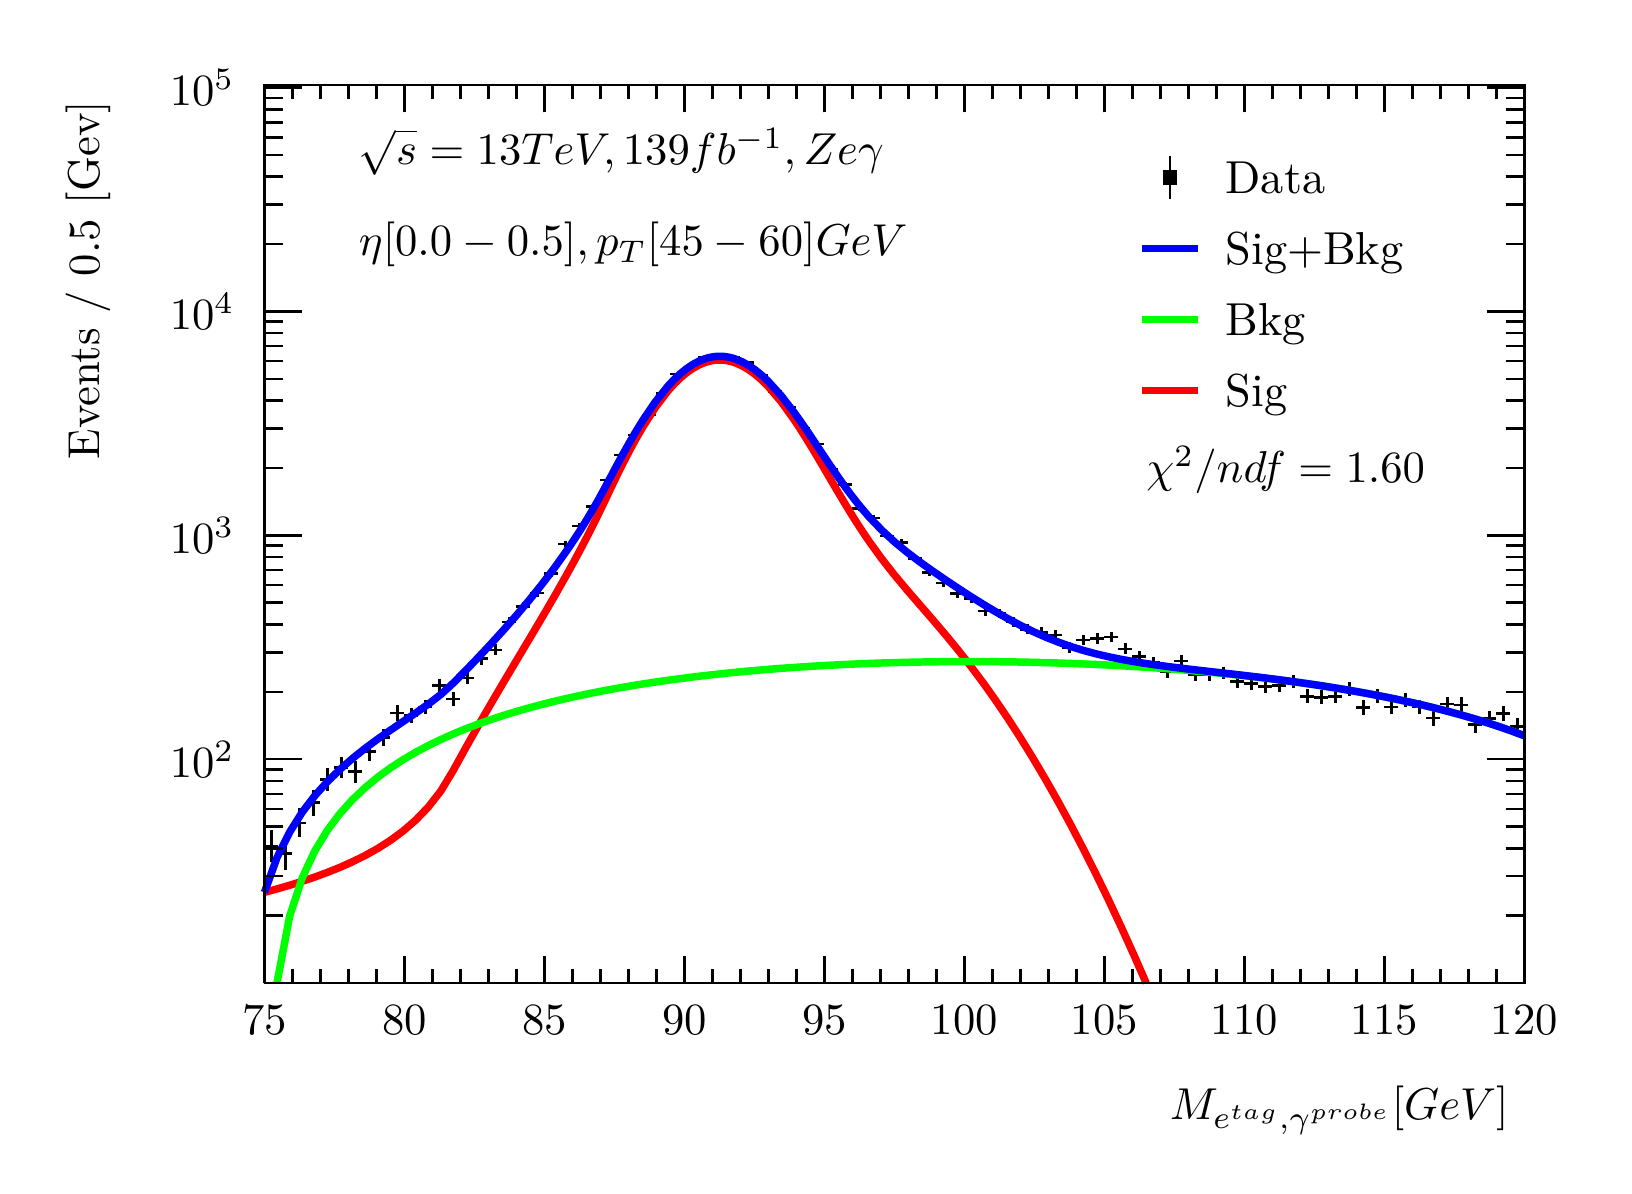
\begin{tikzpicture}
\pgfdeclareplotmark{cross} {
\pgfpathmoveto{\pgfpoint{-0.3\pgfplotmarksize}{\pgfplotmarksize}}
\pgfpathlineto{\pgfpoint{+0.3\pgfplotmarksize}{\pgfplotmarksize}}
\pgfpathlineto{\pgfpoint{+0.3\pgfplotmarksize}{0.3\pgfplotmarksize}}
\pgfpathlineto{\pgfpoint{+1\pgfplotmarksize}{0.3\pgfplotmarksize}}
\pgfpathlineto{\pgfpoint{+1\pgfplotmarksize}{-0.3\pgfplotmarksize}}
\pgfpathlineto{\pgfpoint{+0.3\pgfplotmarksize}{-0.3\pgfplotmarksize}}
\pgfpathlineto{\pgfpoint{+0.3\pgfplotmarksize}{-1.\pgfplotmarksize}}
\pgfpathlineto{\pgfpoint{-0.3\pgfplotmarksize}{-1.\pgfplotmarksize}}
\pgfpathlineto{\pgfpoint{-0.3\pgfplotmarksize}{-0.3\pgfplotmarksize}}
\pgfpathlineto{\pgfpoint{-1.\pgfplotmarksize}{-0.3\pgfplotmarksize}}
\pgfpathlineto{\pgfpoint{-1.\pgfplotmarksize}{0.3\pgfplotmarksize}}
\pgfpathlineto{\pgfpoint{-0.3\pgfplotmarksize}{0.3\pgfplotmarksize}}
\pgfpathclose
\pgfusepathqstroke
}
\pgfdeclareplotmark{cross*} {
\pgfpathmoveto{\pgfpoint{-0.3\pgfplotmarksize}{\pgfplotmarksize}}
\pgfpathlineto{\pgfpoint{+0.3\pgfplotmarksize}{\pgfplotmarksize}}
\pgfpathlineto{\pgfpoint{+0.3\pgfplotmarksize}{0.3\pgfplotmarksize}}
\pgfpathlineto{\pgfpoint{+1\pgfplotmarksize}{0.3\pgfplotmarksize}}
\pgfpathlineto{\pgfpoint{+1\pgfplotmarksize}{-0.3\pgfplotmarksize}}
\pgfpathlineto{\pgfpoint{+0.3\pgfplotmarksize}{-0.3\pgfplotmarksize}}
\pgfpathlineto{\pgfpoint{+0.3\pgfplotmarksize}{-1.\pgfplotmarksize}}
\pgfpathlineto{\pgfpoint{-0.3\pgfplotmarksize}{-1.\pgfplotmarksize}}
\pgfpathlineto{\pgfpoint{-0.3\pgfplotmarksize}{-0.3\pgfplotmarksize}}
\pgfpathlineto{\pgfpoint{-1.\pgfplotmarksize}{-0.3\pgfplotmarksize}}
\pgfpathlineto{\pgfpoint{-1.\pgfplotmarksize}{0.3\pgfplotmarksize}}
\pgfpathlineto{\pgfpoint{-0.3\pgfplotmarksize}{0.3\pgfplotmarksize}}
\pgfpathclose
\pgfusepathqfillstroke
}
\pgfdeclareplotmark{newstar} {
\pgfpathmoveto{\pgfqpoint{0pt}{\pgfplotmarksize}}
\pgfpathlineto{\pgfqpointpolar{44}{0.5\pgfplotmarksize}}
\pgfpathlineto{\pgfqpointpolar{18}{\pgfplotmarksize}}
\pgfpathlineto{\pgfqpointpolar{-20}{0.5\pgfplotmarksize}}
\pgfpathlineto{\pgfqpointpolar{-54}{\pgfplotmarksize}}
\pgfpathlineto{\pgfqpointpolar{-90}{0.5\pgfplotmarksize}}
\pgfpathlineto{\pgfqpointpolar{234}{\pgfplotmarksize}}
\pgfpathlineto{\pgfqpointpolar{198}{0.5\pgfplotmarksize}}
\pgfpathlineto{\pgfqpointpolar{162}{\pgfplotmarksize}}
\pgfpathlineto{\pgfqpointpolar{134}{0.5\pgfplotmarksize}}
\pgfpathclose
\pgfusepathqstroke
}
\pgfdeclareplotmark{newstar*} {
\pgfpathmoveto{\pgfqpoint{0pt}{\pgfplotmarksize}}
\pgfpathlineto{\pgfqpointpolar{44}{0.5\pgfplotmarksize}}
\pgfpathlineto{\pgfqpointpolar{18}{\pgfplotmarksize}}
\pgfpathlineto{\pgfqpointpolar{-20}{0.5\pgfplotmarksize}}
\pgfpathlineto{\pgfqpointpolar{-54}{\pgfplotmarksize}}
\pgfpathlineto{\pgfqpointpolar{-90}{0.5\pgfplotmarksize}}
\pgfpathlineto{\pgfqpointpolar{234}{\pgfplotmarksize}}
\pgfpathlineto{\pgfqpointpolar{198}{0.5\pgfplotmarksize}}
\pgfpathlineto{\pgfqpointpolar{162}{\pgfplotmarksize}}
\pgfpathlineto{\pgfqpointpolar{134}{0.5\pgfplotmarksize}}
\pgfpathclose
\pgfusepathqfillstroke
}
\definecolor{c}{rgb}{1,1,1};
\draw [color=c, fill=c] (0,0) rectangle (20,14.4361);
\draw [color=c, fill=c] (3,2.30977) rectangle (19,13.7143);
\definecolor{c}{rgb}{0,0,0};
\draw [c,line width=0.9] (3,2.30977) -- (3,13.7143) -- (19,13.7143) -- (19,2.30977) -- (3,2.30977);
\definecolor{c}{rgb}{1,1,1};
\draw [color=c, fill=c] (3,2.30977) rectangle (19,13.7143);
\definecolor{c}{rgb}{0,0,0};
\draw [c,line width=0.9] (3,2.30977) -- (3,13.7143) -- (19,13.7143) -- (19,2.30977) -- (3,2.30977);
\draw [c,line width=0.9] (3,2.30977) -- (19,2.30977);
\draw [c,line width=0.9] (3,2.65624) -- (3,2.30977);
\draw [c,line width=0.9] (3.35556,2.48301) -- (3.35556,2.30977);
\draw [c,line width=0.9] (3.71111,2.48301) -- (3.71111,2.30977);
\draw [c,line width=0.9] (4.06667,2.48301) -- (4.06667,2.30977);
\draw [c,line width=0.9] (4.42222,2.48301) -- (4.42222,2.30977);
\draw [c,line width=0.9] (4.77778,2.65624) -- (4.77778,2.30977);
\draw [c,line width=0.9] (5.13333,2.48301) -- (5.13333,2.30977);
\draw [c,line width=0.9] (5.48889,2.48301) -- (5.48889,2.30977);
\draw [c,line width=0.9] (5.84444,2.48301) -- (5.84444,2.30977);
\draw [c,line width=0.9] (6.2,2.48301) -- (6.2,2.30977);
\draw [c,line width=0.9] (6.55556,2.65624) -- (6.55556,2.30977);
\draw [c,line width=0.9] (6.91111,2.48301) -- (6.91111,2.30977);
\draw [c,line width=0.9] (7.26667,2.48301) -- (7.26667,2.30977);
\draw [c,line width=0.9] (7.62222,2.48301) -- (7.62222,2.30977);
\draw [c,line width=0.9] (7.97778,2.48301) -- (7.97778,2.30977);
\draw [c,line width=0.9] (8.33333,2.65624) -- (8.33333,2.30977);
\draw [c,line width=0.9] (8.68889,2.48301) -- (8.68889,2.30977);
\draw [c,line width=0.9] (9.04444,2.48301) -- (9.04444,2.30977);
\draw [c,line width=0.9] (9.4,2.48301) -- (9.4,2.30977);
\draw [c,line width=0.9] (9.75556,2.48301) -- (9.75556,2.30977);
\draw [c,line width=0.9] (10.1111,2.65624) -- (10.1111,2.30977);
\draw [c,line width=0.9] (10.4667,2.48301) -- (10.4667,2.30977);
\draw [c,line width=0.9] (10.8222,2.48301) -- (10.8222,2.30977);
\draw [c,line width=0.9] (11.1778,2.48301) -- (11.1778,2.30977);
\draw [c,line width=0.9] (11.5333,2.48301) -- (11.5333,2.30977);
\draw [c,line width=0.9] (11.8889,2.65624) -- (11.8889,2.30977);
\draw [c,line width=0.9] (12.2444,2.48301) -- (12.2444,2.30977);
\draw [c,line width=0.9] (12.6,2.48301) -- (12.6,2.30977);
\draw [c,line width=0.9] (12.9556,2.48301) -- (12.9556,2.30977);
\draw [c,line width=0.9] (13.3111,2.48301) -- (13.3111,2.30977);
\draw [c,line width=0.9] (13.6667,2.65624) -- (13.6667,2.30977);
\draw [c,line width=0.9] (14.0222,2.48301) -- (14.0222,2.30977);
\draw [c,line width=0.9] (14.3778,2.48301) -- (14.3778,2.30977);
\draw [c,line width=0.9] (14.7333,2.48301) -- (14.7333,2.30977);
\draw [c,line width=0.9] (15.0889,2.48301) -- (15.0889,2.30977);
\draw [c,line width=0.9] (15.4444,2.65624) -- (15.4444,2.30977);
\draw [c,line width=0.9] (15.8,2.48301) -- (15.8,2.30977);
\draw [c,line width=0.9] (16.1556,2.48301) -- (16.1556,2.30977);
\draw [c,line width=0.9] (16.5111,2.48301) -- (16.5111,2.30977);
\draw [c,line width=0.9] (16.8667,2.48301) -- (16.8667,2.30977);
\draw [c,line width=0.9] (17.2222,2.65624) -- (17.2222,2.30977);
\draw [c,line width=0.9] (17.5778,2.48301) -- (17.5778,2.30977);
\draw [c,line width=0.9] (17.9333,2.48301) -- (17.9333,2.30977);
\draw [c,line width=0.9] (18.2889,2.48301) -- (18.2889,2.30977);
\draw [c,line width=0.9] (18.6444,2.48301) -- (18.6444,2.30977);
\draw [c,line width=0.9] (19,2.65624) -- (19,2.30977);
\draw [c,line width=0.9] (19,2.65624) -- (19,2.30977);
\draw [anchor=base] (3,1.66015) node[scale=1.61424, color=c, rotate=0]{75};
\draw [anchor=base] (4.77778,1.66015) node[scale=1.61424, color=c, rotate=0]{80};
\draw [anchor=base] (6.55556,1.66015) node[scale=1.61424, color=c, rotate=0]{85};
\draw [anchor=base] (8.33333,1.66015) node[scale=1.61424, color=c, rotate=0]{90};
\draw [anchor=base] (10.1111,1.66015) node[scale=1.61424, color=c, rotate=0]{95};
\draw [anchor=base] (11.8889,1.66015) node[scale=1.61424, color=c, rotate=0]{100};
\draw [anchor=base] (13.6667,1.66015) node[scale=1.61424, color=c, rotate=0]{105};
\draw [anchor=base] (15.4444,1.66015) node[scale=1.61424, color=c, rotate=0]{110};
\draw [anchor=base] (17.2222,1.66015) node[scale=1.61424, color=c, rotate=0]{115};
\draw [anchor=base] (19,1.66015) node[scale=1.61424, color=c, rotate=0]{120};
\draw [anchor= east] (19,0.692932) node[scale=1.61424, color=c, rotate=0]{$M_{e^{tag}, \gamma^{probe}}  [GeV]$};
\draw [c,line width=0.9] (3,13.7143) -- (19,13.7143);
\draw [c,line width=0.9] (3,13.3678) -- (3,13.7143);
\draw [c,line width=0.9] (3.35556,13.5411) -- (3.35556,13.7143);
\draw [c,line width=0.9] (3.71111,13.5411) -- (3.71111,13.7143);
\draw [c,line width=0.9] (4.06667,13.5411) -- (4.06667,13.7143);
\draw [c,line width=0.9] (4.42222,13.5411) -- (4.42222,13.7143);
\draw [c,line width=0.9] (4.77778,13.3678) -- (4.77778,13.7143);
\draw [c,line width=0.9] (5.13333,13.5411) -- (5.13333,13.7143);
\draw [c,line width=0.9] (5.48889,13.5411) -- (5.48889,13.7143);
\draw [c,line width=0.9] (5.84444,13.5411) -- (5.84444,13.7143);
\draw [c,line width=0.9] (6.2,13.5411) -- (6.2,13.7143);
\draw [c,line width=0.9] (6.55556,13.3678) -- (6.55556,13.7143);
\draw [c,line width=0.9] (6.91111,13.5411) -- (6.91111,13.7143);
\draw [c,line width=0.9] (7.26667,13.5411) -- (7.26667,13.7143);
\draw [c,line width=0.9] (7.62222,13.5411) -- (7.62222,13.7143);
\draw [c,line width=0.9] (7.97778,13.5411) -- (7.97778,13.7143);
\draw [c,line width=0.9] (8.33333,13.3678) -- (8.33333,13.7143);
\draw [c,line width=0.9] (8.68889,13.5411) -- (8.68889,13.7143);
\draw [c,line width=0.9] (9.04444,13.5411) -- (9.04444,13.7143);
\draw [c,line width=0.9] (9.4,13.5411) -- (9.4,13.7143);
\draw [c,line width=0.9] (9.75556,13.5411) -- (9.75556,13.7143);
\draw [c,line width=0.9] (10.1111,13.3678) -- (10.1111,13.7143);
\draw [c,line width=0.9] (10.4667,13.5411) -- (10.4667,13.7143);
\draw [c,line width=0.9] (10.8222,13.5411) -- (10.8222,13.7143);
\draw [c,line width=0.9] (11.1778,13.5411) -- (11.1778,13.7143);
\draw [c,line width=0.9] (11.5333,13.5411) -- (11.5333,13.7143);
\draw [c,line width=0.9] (11.8889,13.3678) -- (11.8889,13.7143);
\draw [c,line width=0.9] (12.2444,13.5411) -- (12.2444,13.7143);
\draw [c,line width=0.9] (12.6,13.5411) -- (12.6,13.7143);
\draw [c,line width=0.9] (12.9556,13.5411) -- (12.9556,13.7143);
\draw [c,line width=0.9] (13.3111,13.5411) -- (13.3111,13.7143);
\draw [c,line width=0.9] (13.6667,13.3678) -- (13.6667,13.7143);
\draw [c,line width=0.9] (14.0222,13.5411) -- (14.0222,13.7143);
\draw [c,line width=0.9] (14.3778,13.5411) -- (14.3778,13.7143);
\draw [c,line width=0.9] (14.7333,13.5411) -- (14.7333,13.7143);
\draw [c,line width=0.9] (15.0889,13.5411) -- (15.0889,13.7143);
\draw [c,line width=0.9] (15.4444,13.3678) -- (15.4444,13.7143);
\draw [c,line width=0.9] (15.8,13.5411) -- (15.8,13.7143);
\draw [c,line width=0.9] (16.1556,13.5411) -- (16.1556,13.7143);
\draw [c,line width=0.9] (16.5111,13.5411) -- (16.5111,13.7143);
\draw [c,line width=0.9] (16.8667,13.5411) -- (16.8667,13.7143);
\draw [c,line width=0.9] (17.2222,13.3678) -- (17.2222,13.7143);
\draw [c,line width=0.9] (17.5778,13.5411) -- (17.5778,13.7143);
\draw [c,line width=0.9] (17.9333,13.5411) -- (17.9333,13.7143);
\draw [c,line width=0.9] (18.2889,13.5411) -- (18.2889,13.7143);
\draw [c,line width=0.9] (18.6444,13.5411) -- (18.6444,13.7143);
\draw [c,line width=0.9] (19,13.3678) -- (19,13.7143);
\draw [c,line width=0.9] (19,13.3678) -- (19,13.7143);
\draw [c,line width=0.9] (3,2.30977) -- (3,13.7143);
\draw [c,line width=0.9] (3.237,3.16561) -- (3,3.16561);
\draw [c,line width=0.9] (3.237,3.66625) -- (3,3.66625);
\draw [c,line width=0.9] (3.237,4.02146) -- (3,4.02146);
\draw [c,line width=0.9] (3.237,4.29698) -- (3,4.29698);
\draw [c,line width=0.9] (3.237,4.52209) -- (3,4.52209);
\draw [c,line width=0.9] (3.237,4.71242) -- (3,4.71242);
\draw [c,line width=0.9] (3.237,4.8773) -- (3,4.8773);
\draw [c,line width=0.9] (3.237,5.02273) -- (3,5.02273);
\draw [c,line width=0.9] (3.474,5.15282) -- (3,5.15282);
\draw [anchor= east] (2.82,5.15282) node[scale=1.61424, color=c, rotate=0]{$10^{2}$};
\draw [c,line width=0.9] (3.237,6.00866) -- (3,6.00866);
\draw [c,line width=0.9] (3.237,6.5093) -- (3,6.5093);
\draw [c,line width=0.9] (3.237,6.8645) -- (3,6.8645);
\draw [c,line width=0.9] (3.237,7.14002) -- (3,7.14002);
\draw [c,line width=0.9] (3.237,7.36514) -- (3,7.36514);
\draw [c,line width=0.9] (3.237,7.55547) -- (3,7.55547);
\draw [c,line width=0.9] (3.237,7.72034) -- (3,7.72034);
\draw [c,line width=0.9] (3.237,7.86577) -- (3,7.86577);
\draw [c,line width=0.9] (3.474,7.99586) -- (3,7.99586);
\draw [anchor= east] (2.82,7.99586) node[scale=1.61424, color=c, rotate=0]{$10^{3}$};
\draw [c,line width=0.9] (3.237,8.85171) -- (3,8.85171);
\draw [c,line width=0.9] (3.237,9.35234) -- (3,9.35234);
\draw [c,line width=0.9] (3.237,9.70755) -- (3,9.70755);
\draw [c,line width=0.9] (3.237,9.98307) -- (3,9.98307);
\draw [c,line width=0.9] (3.237,10.2082) -- (3,10.2082);
\draw [c,line width=0.9] (3.237,10.3985) -- (3,10.3985);
\draw [c,line width=0.9] (3.237,10.5634) -- (3,10.5634);
\draw [c,line width=0.9] (3.237,10.7088) -- (3,10.7088);
\draw [c,line width=0.9] (3.474,10.8389) -- (3,10.8389);
\draw [anchor= east] (2.82,10.8389) node[scale=1.61424, color=c, rotate=0]{$10^{4}$};
\draw [c,line width=0.9] (3.237,11.6948) -- (3,11.6948);
\draw [c,line width=0.9] (3.237,12.1954) -- (3,12.1954);
\draw [c,line width=0.9] (3.237,12.5506) -- (3,12.5506);
\draw [c,line width=0.9] (3.237,12.8261) -- (3,12.8261);
\draw [c,line width=0.9] (3.237,13.0512) -- (3,13.0512);
\draw [c,line width=0.9] (3.237,13.2416) -- (3,13.2416);
\draw [c,line width=0.9] (3.237,13.4064) -- (3,13.4064);
\draw [c,line width=0.9] (3.237,13.5519) -- (3,13.5519);
\draw [c,line width=0.9] (3.474,13.682) -- (3,13.682);
\draw [anchor= east] (2.82,13.682) node[scale=1.61424, color=c, rotate=0]{$10^{5}$};
\draw [anchor= east] (0.76,13.7143) node[scale=1.61424, color=c, rotate=90]{Events / 0.5 [Gev]};
\draw [c,line width=0.9] (19,2.30977) -- (19,13.7143);
\draw [c,line width=0.9] (18.763,3.16561) -- (19,3.16561);
\draw [c,line width=0.9] (18.763,3.66625) -- (19,3.66625);
\draw [c,line width=0.9] (18.763,4.02146) -- (19,4.02146);
\draw [c,line width=0.9] (18.763,4.29698) -- (19,4.29698);
\draw [c,line width=0.9] (18.763,4.52209) -- (19,4.52209);
\draw [c,line width=0.9] (18.763,4.71242) -- (19,4.71242);
\draw [c,line width=0.9] (18.763,4.8773) -- (19,4.8773);
\draw [c,line width=0.9] (18.763,5.02273) -- (19,5.02273);
\draw [c,line width=0.9] (18.526,5.15282) -- (19,5.15282);
\draw [c,line width=0.9] (18.763,6.00866) -- (19,6.00866);
\draw [c,line width=0.9] (18.763,6.5093) -- (19,6.5093);
\draw [c,line width=0.9] (18.763,6.8645) -- (19,6.8645);
\draw [c,line width=0.9] (18.763,7.14002) -- (19,7.14002);
\draw [c,line width=0.9] (18.763,7.36514) -- (19,7.36514);
\draw [c,line width=0.9] (18.763,7.55547) -- (19,7.55547);
\draw [c,line width=0.9] (18.763,7.72034) -- (19,7.72034);
\draw [c,line width=0.9] (18.763,7.86577) -- (19,7.86577);
\draw [c,line width=0.9] (18.526,7.99586) -- (19,7.99586);
\draw [c,line width=0.9] (18.763,8.85171) -- (19,8.85171);
\draw [c,line width=0.9] (18.763,9.35234) -- (19,9.35234);
\draw [c,line width=0.9] (18.763,9.70755) -- (19,9.70755);
\draw [c,line width=0.9] (18.763,9.98307) -- (19,9.98307);
\draw [c,line width=0.9] (18.763,10.2082) -- (19,10.2082);
\draw [c,line width=0.9] (18.763,10.3985) -- (19,10.3985);
\draw [c,line width=0.9] (18.763,10.5634) -- (19,10.5634);
\draw [c,line width=0.9] (18.763,10.7088) -- (19,10.7088);
\draw [c,line width=0.9] (18.526,10.8389) -- (19,10.8389);
\draw [c,line width=0.9] (18.763,11.6948) -- (19,11.6948);
\draw [c,line width=0.9] (18.763,12.1954) -- (19,12.1954);
\draw [c,line width=0.9] (18.763,12.5506) -- (19,12.5506);
\draw [c,line width=0.9] (18.763,12.8261) -- (19,12.8261);
\draw [c,line width=0.9] (18.763,13.0512) -- (19,13.0512);
\draw [c,line width=0.9] (18.763,13.2416) -- (19,13.2416);
\draw [c,line width=0.9] (18.763,13.4064) -- (19,13.4064);
\draw [c,line width=0.9] (18.763,13.5519) -- (19,13.5519);
\draw [c,line width=0.9] (18.526,13.682) -- (19,13.682);
\draw [c,line width=0.9] (3.08889,4.05195) -- (3,4.05195);
\draw [c,line width=0.9] (3,4.05195) -- (3,4.05195);
\draw [c,line width=0.9] (3.08889,4.05195) -- (3.17778,4.05195);
\draw [c,line width=0.9] (3.17778,4.05195) -- (3.17778,4.05195);
\draw [c,line width=0.9] (3.08889,4.05195) -- (3.08889,4.25823);
\draw [c,line width=0.9] (3.08889,4.25823) -- (3.08889,4.25823);
\draw [c,line width=0.9] (3.08889,4.05195) -- (3.08889,3.84322);
\draw [c,line width=0.9] (3.08889,3.84322) -- (3.08889,3.84322);
\draw [c,line width=0.9] (3.26667,3.95813) -- (3.17778,3.95813);
\draw [c,line width=0.9] (3.17778,3.95813) -- (3.17778,3.95813);
\draw [c,line width=0.9] (3.26667,3.95813) -- (3.35556,3.95813);
\draw [c,line width=0.9] (3.35556,3.95813) -- (3.35556,3.95813);
\draw [c,line width=0.9] (3.26667,3.95813) -- (3.26667,4.17287);
\draw [c,line width=0.9] (3.26667,4.17287) -- (3.26667,4.17287);
\draw [c,line width=0.9] (3.26667,3.95813) -- (3.26667,3.74063);
\draw [c,line width=0.9] (3.26667,3.74063) -- (3.26667,3.74063);
\draw [c,line width=0.9] (3.44444,4.3454) -- (3.35556,4.3454);
\draw [c,line width=0.9] (3.35556,4.3454) -- (3.35556,4.3454);
\draw [c,line width=0.9] (3.44444,4.3454) -- (3.53333,4.3454);
\draw [c,line width=0.9] (3.53333,4.3454) -- (3.53333,4.3454);
\draw [c,line width=0.9] (3.44444,4.3454) -- (3.44444,4.52738);
\draw [c,line width=0.9] (3.44444,4.52738) -- (3.44444,4.52738);
\draw [c,line width=0.9] (3.44444,4.3454) -- (3.44444,4.16172);
\draw [c,line width=0.9] (3.44444,4.16172) -- (3.44444,4.16172);
\draw [c,line width=0.9] (3.62222,4.60178) -- (3.53333,4.60178);
\draw [c,line width=0.9] (3.53333,4.60178) -- (3.53333,4.60178);
\draw [c,line width=0.9] (3.62222,4.60178) -- (3.71111,4.60178);
\draw [c,line width=0.9] (3.71111,4.60178) -- (3.71111,4.60178);
\draw [c,line width=0.9] (3.62222,4.60178) -- (3.62222,4.76495);
\draw [c,line width=0.9] (3.62222,4.76495) -- (3.62222,4.76495);
\draw [c,line width=0.9] (3.62222,4.60178) -- (3.62222,4.43737);
\draw [c,line width=0.9] (3.62222,4.43737) -- (3.62222,4.43737);
\draw [c,line width=0.9] (3.8,4.89264) -- (3.71111,4.89264);
\draw [c,line width=0.9] (3.71111,4.89264) -- (3.71111,4.89264);
\draw [c,line width=0.9] (3.8,4.89264) -- (3.88889,4.89264);
\draw [c,line width=0.9] (3.88889,4.89264) -- (3.88889,4.89264);
\draw [c,line width=0.9] (3.8,4.89264) -- (3.8,5.03688);
\draw [c,line width=0.9] (3.8,5.03688) -- (3.8,5.03688);
\draw [c,line width=0.9] (3.8,4.89264) -- (3.8,4.74753);
\draw [c,line width=0.9] (3.8,4.74753) -- (3.8,4.74753);
\draw [c,line width=0.9] (3.97778,5.04987) -- (3.88889,5.04987);
\draw [c,line width=0.9] (3.88889,5.04987) -- (3.88889,5.04987);
\draw [c,line width=0.9] (3.97778,5.04987) -- (4.06667,5.04987);
\draw [c,line width=0.9] (4.06667,5.04987) -- (4.06667,5.04987);
\draw [c,line width=0.9] (3.97778,5.04987) -- (3.97778,5.18483);
\draw [c,line width=0.9] (3.97778,5.18483) -- (3.97778,5.18483);
\draw [c,line width=0.9] (3.97778,5.04987) -- (3.97778,4.91418);
\draw [c,line width=0.9] (3.97778,4.91418) -- (3.97778,4.91418);
\draw [c,line width=0.9] (4.15556,4.99498) -- (4.06667,4.99498);
\draw [c,line width=0.9] (4.06667,4.99498) -- (4.06667,4.99498);
\draw [c,line width=0.9] (4.15556,4.99498) -- (4.24444,4.99498);
\draw [c,line width=0.9] (4.24444,4.99498) -- (4.24444,4.99498);
\draw [c,line width=0.9] (4.15556,4.99498) -- (4.15556,5.13311);
\draw [c,line width=0.9] (4.15556,5.13311) -- (4.15556,5.13311);
\draw [c,line width=0.9] (4.15556,4.99498) -- (4.15556,4.85608);
\draw [c,line width=0.9] (4.15556,4.85608) -- (4.15556,4.85608);
\draw [c,line width=0.9] (4.33333,5.24785) -- (4.24444,5.24785);
\draw [c,line width=0.9] (4.24444,5.24785) -- (4.24444,5.24785);
\draw [c,line width=0.9] (4.33333,5.24785) -- (4.42222,5.24785);
\draw [c,line width=0.9] (4.42222,5.24785) -- (4.42222,5.24785);
\draw [c,line width=0.9] (4.33333,5.24785) -- (4.33333,5.36661);
\draw [c,line width=0.9] (4.33333,5.36661) -- (4.33333,5.36661);
\draw [c,line width=0.9] (4.33333,5.24785) -- (4.33333,5.12908);
\draw [c,line width=0.9] (4.33333,5.12908) -- (4.33333,5.12908);
\draw [c,line width=0.9] (4.51111,5.42834) -- (4.42222,5.42834);
\draw [c,line width=0.9] (4.42222,5.42834) -- (4.42222,5.42834);
\draw [c,line width=0.9] (4.51111,5.42834) -- (4.6,5.42834);
\draw [c,line width=0.9] (4.6,5.42834) -- (4.6,5.42834);
\draw [c,line width=0.9] (4.51111,5.42834) -- (4.51111,5.53874);
\draw [c,line width=0.9] (4.51111,5.53874) -- (4.51111,5.53874);
\draw [c,line width=0.9] (4.51111,5.42834) -- (4.51111,5.31794);
\draw [c,line width=0.9] (4.51111,5.31794) -- (4.51111,5.31794);
\draw [c,line width=0.9] (4.68889,5.74084) -- (4.6,5.74084);
\draw [c,line width=0.9] (4.6,5.74084) -- (4.6,5.74084);
\draw [c,line width=0.9] (4.68889,5.74084) -- (4.77778,5.74084);
\draw [c,line width=0.9] (4.77778,5.74084) -- (4.77778,5.74084);
\draw [c,line width=0.9] (4.68889,5.74084) -- (4.68889,5.83812);
\draw [c,line width=0.9] (4.68889,5.83812) -- (4.68889,5.83812);
\draw [c,line width=0.9] (4.68889,5.74084) -- (4.68889,5.64355);
\draw [c,line width=0.9] (4.68889,5.64355) -- (4.68889,5.64355);
\draw [c,line width=0.9] (4.86667,5.70977) -- (4.77778,5.70977);
\draw [c,line width=0.9] (4.77778,5.70977) -- (4.77778,5.70977);
\draw [c,line width=0.9] (4.86667,5.70977) -- (4.95556,5.70977);
\draw [c,line width=0.9] (4.95556,5.70977) -- (4.95556,5.70977);
\draw [c,line width=0.9] (4.86667,5.70977) -- (4.86667,5.80829);
\draw [c,line width=0.9] (4.86667,5.80829) -- (4.86667,5.80829);
\draw [c,line width=0.9] (4.86667,5.70977) -- (4.86667,5.61126);
\draw [c,line width=0.9] (4.86667,5.61126) -- (4.86667,5.61126);
\draw [c,line width=0.9] (5.04444,5.81524) -- (4.95556,5.81524);
\draw [c,line width=0.9] (4.95556,5.81524) -- (4.95556,5.81524);
\draw [c,line width=0.9] (5.04444,5.81524) -- (5.13333,5.81524);
\draw [c,line width=0.9] (5.13333,5.81524) -- (5.13333,5.81524);
\draw [c,line width=0.9] (5.04444,5.81524) -- (5.04444,5.90964);
\draw [c,line width=0.9] (5.04444,5.90964) -- (5.04444,5.90964);
\draw [c,line width=0.9] (5.04444,5.81524) -- (5.04444,5.72084);
\draw [c,line width=0.9] (5.04444,5.72084) -- (5.04444,5.72084);
\draw [c,line width=0.9] (5.22222,6.08642) -- (5.13333,6.08642);
\draw [c,line width=0.9] (5.13333,6.08642) -- (5.13333,6.08642);
\draw [c,line width=0.9] (5.22222,6.08642) -- (5.31111,6.08642);
\draw [c,line width=0.9] (5.31111,6.08642) -- (5.31111,6.08642);
\draw [c,line width=0.9] (5.22222,6.08642) -- (5.22222,6.171);
\draw [c,line width=0.9] (5.22222,6.171) -- (5.22222,6.171);
\draw [c,line width=0.9] (5.22222,6.08642) -- (5.22222,6.00183);
\draw [c,line width=0.9] (5.22222,6.00183) -- (5.22222,6.00183);
\draw [c,line width=0.9] (5.4,5.91906) -- (5.31111,5.91906);
\draw [c,line width=0.9] (5.31111,5.91906) -- (5.31111,5.91906);
\draw [c,line width=0.9] (5.4,5.91906) -- (5.48889,5.91906);
\draw [c,line width=0.9] (5.48889,5.91906) -- (5.48889,5.91906);
\draw [c,line width=0.9] (5.4,5.91906) -- (5.4,6.00957);
\draw [c,line width=0.9] (5.4,6.00957) -- (5.4,6.00957);
\draw [c,line width=0.9] (5.4,5.91906) -- (5.4,5.82854);
\draw [c,line width=0.9] (5.4,5.82854) -- (5.4,5.82854);
\draw [c,line width=0.9] (5.57778,6.18658) -- (5.48889,6.18658);
\draw [c,line width=0.9] (5.48889,6.18658) -- (5.48889,6.18658);
\draw [c,line width=0.9] (5.57778,6.18658) -- (5.66667,6.18658);
\draw [c,line width=0.9] (5.66667,6.18658) -- (5.66667,6.18658);
\draw [c,line width=0.9] (5.57778,6.18658) -- (5.57778,6.26781);
\draw [c,line width=0.9] (5.57778,6.26781) -- (5.57778,6.26781);
\draw [c,line width=0.9] (5.57778,6.18658) -- (5.57778,6.10536);
\draw [c,line width=0.9] (5.57778,6.10536) -- (5.57778,6.10536);
\draw [c,line width=0.9] (5.75556,6.42851) -- (5.66667,6.42851);
\draw [c,line width=0.9] (5.66667,6.42851) -- (5.66667,6.42851);
\draw [c,line width=0.9] (5.75556,6.42851) -- (5.84444,6.42851);
\draw [c,line width=0.9] (5.84444,6.42851) -- (5.84444,6.42851);
\draw [c,line width=0.9] (5.75556,6.42851) -- (5.75556,6.50216);
\draw [c,line width=0.9] (5.75556,6.50216) -- (5.75556,6.50216);
\draw [c,line width=0.9] (5.75556,6.42851) -- (5.75556,6.35487);
\draw [c,line width=0.9] (5.75556,6.35487) -- (5.75556,6.35487);
\draw [c,line width=0.9] (5.93333,6.54179) -- (5.84444,6.54179);
\draw [c,line width=0.9] (5.84444,6.54179) -- (5.84444,6.54179);
\draw [c,line width=0.9] (5.93333,6.54179) -- (6.02222,6.54179);
\draw [c,line width=0.9] (6.02222,6.54179) -- (6.02222,6.54179);
\draw [c,line width=0.9] (5.93333,6.54179) -- (5.93333,6.61214);
\draw [c,line width=0.9] (5.93333,6.61214) -- (5.93333,6.61214);
\draw [c,line width=0.9] (5.93333,6.54179) -- (5.93333,6.47145);
\draw [c,line width=0.9] (5.93333,6.47145) -- (5.93333,6.47145);
\draw [c,line width=0.9] (6.11111,6.89198) -- (6.02222,6.89198);
\draw [c,line width=0.9] (6.02222,6.89198) -- (6.02222,6.89198);
\draw [c,line width=0.9] (6.11111,6.89198) -- (6.2,6.89198);
\draw [c,line width=0.9] (6.2,6.89198) -- (6.2,6.89198);
\draw [c,line width=0.9] (6.11111,6.89198) -- (6.11111,6.95302);
\draw [c,line width=0.9] (6.11111,6.95302) -- (6.11111,6.95302);
\draw [c,line width=0.9] (6.11111,6.89198) -- (6.11111,6.83093);
\draw [c,line width=0.9] (6.11111,6.83093) -- (6.11111,6.83093);
\draw [c,line width=0.9] (6.28889,7.09475) -- (6.2,7.09475);
\draw [c,line width=0.9] (6.2,7.09475) -- (6.2,7.09475);
\draw [c,line width=0.9] (6.28889,7.09475) -- (6.37778,7.09475);
\draw [c,line width=0.9] (6.37778,7.09475) -- (6.37778,7.09475);
\draw [c,line width=0.9] (6.28889,7.09475) -- (6.28889,7.15099);
\draw [c,line width=0.9] (6.28889,7.15099) -- (6.28889,7.15099);
\draw [c,line width=0.9] (6.28889,7.09475) -- (6.28889,7.03852);
\draw [c,line width=0.9] (6.28889,7.03852) -- (6.28889,7.03852);
\draw [c,line width=0.9] (6.46667,7.26442) -- (6.37778,7.26442);
\draw [c,line width=0.9] (6.37778,7.26442) -- (6.37778,7.26442);
\draw [c,line width=0.9] (6.46667,7.26442) -- (6.55556,7.26442);
\draw [c,line width=0.9] (6.55556,7.26442) -- (6.55556,7.26442);
\draw [c,line width=0.9] (6.46667,7.26442) -- (6.46667,7.31692);
\draw [c,line width=0.9] (6.46667,7.31692) -- (6.46667,7.31692);
\draw [c,line width=0.9] (6.46667,7.26442) -- (6.46667,7.21192);
\draw [c,line width=0.9] (6.46667,7.21192) -- (6.46667,7.21192);
\draw [c,line width=0.9] (6.64444,7.50874) -- (6.55556,7.50874);
\draw [c,line width=0.9] (6.55556,7.50874) -- (6.55556,7.50874);
\draw [c,line width=0.9] (6.64444,7.50874) -- (6.73333,7.50874);
\draw [c,line width=0.9] (6.73333,7.50874) -- (6.73333,7.50874);
\draw [c,line width=0.9] (6.64444,7.50874) -- (6.64444,7.55629);
\draw [c,line width=0.9] (6.64444,7.55629) -- (6.64444,7.55629);
\draw [c,line width=0.9] (6.64444,7.50874) -- (6.64444,7.46118);
\draw [c,line width=0.9] (6.64444,7.46118) -- (6.64444,7.46118);
\draw [c,line width=0.9] (6.82222,7.88618) -- (6.73333,7.88618);
\draw [c,line width=0.9] (6.73333,7.88618) -- (6.73333,7.88618);
\draw [c,line width=0.9] (6.82222,7.88618) -- (6.91111,7.88618);
\draw [c,line width=0.9] (6.91111,7.88618) -- (6.91111,7.88618);
\draw [c,line width=0.9] (6.82222,7.88618) -- (6.82222,7.927);
\draw [c,line width=0.9] (6.82222,7.927) -- (6.82222,7.927);
\draw [c,line width=0.9] (6.82222,7.88618) -- (6.82222,7.84537);
\draw [c,line width=0.9] (6.82222,7.84537) -- (6.82222,7.84537);
\draw [c,line width=0.9] (7,8.11242) -- (6.91111,8.11242);
\draw [c,line width=0.9] (6.91111,8.11242) -- (6.91111,8.11242);
\draw [c,line width=0.9] (7,8.11242) -- (7.08889,8.11242);
\draw [c,line width=0.9] (7.08889,8.11242) -- (7.08889,8.11242);
\draw [c,line width=0.9] (7,8.11242) -- (7,8.14967);
\draw [c,line width=0.9] (7,8.14967) -- (7,8.14967);
\draw [c,line width=0.9] (7,8.11242) -- (7,8.07518);
\draw [c,line width=0.9] (7,8.07518) -- (7,8.07518);
\draw [c,line width=0.9] (7.17778,8.36183) -- (7.08889,8.36183);
\draw [c,line width=0.9] (7.08889,8.36183) -- (7.08889,8.36183);
\draw [c,line width=0.9] (7.17778,8.36183) -- (7.26667,8.36183);
\draw [c,line width=0.9] (7.26667,8.36183) -- (7.26667,8.36183);
\draw [c,line width=0.9] (7.17778,8.36183) -- (7.17778,8.39549);
\draw [c,line width=0.9] (7.17778,8.39549) -- (7.17778,8.39549);
\draw [c,line width=0.9] (7.17778,8.36183) -- (7.17778,8.32816);
\draw [c,line width=0.9] (7.17778,8.32816) -- (7.17778,8.32816);
\draw [c,line width=0.9] (7.35556,8.70156) -- (7.26667,8.70156);
\draw [c,line width=0.9] (7.26667,8.70156) -- (7.26667,8.70156);
\draw [c,line width=0.9] (7.35556,8.70156) -- (7.44444,8.70156);
\draw [c,line width=0.9] (7.44444,8.70156) -- (7.44444,8.70156);
\draw [c,line width=0.9] (7.35556,8.70156) -- (7.35556,8.7309);
\draw [c,line width=0.9] (7.35556,8.7309) -- (7.35556,8.7309);
\draw [c,line width=0.9] (7.35556,8.70156) -- (7.35556,8.67222);
\draw [c,line width=0.9] (7.35556,8.67222) -- (7.35556,8.67222);
\draw [c,line width=0.9] (7.53333,9.01511) -- (7.44444,9.01511);
\draw [c,line width=0.9] (7.44444,9.01511) -- (7.44444,9.01511);
\draw [c,line width=0.9] (7.53333,9.01511) -- (7.62222,9.01511);
\draw [c,line width=0.9] (7.62222,9.01511) -- (7.62222,9.01511);
\draw [c,line width=0.9] (7.53333,9.01511) -- (7.53333,9.04095);
\draw [c,line width=0.9] (7.53333,9.04095) -- (7.53333,9.04095);
\draw [c,line width=0.9] (7.53333,9.01511) -- (7.53333,8.98927);
\draw [c,line width=0.9] (7.53333,8.98927) -- (7.53333,8.98927);
\draw [c,line width=0.9] (7.71111,9.26848) -- (7.62222,9.26848);
\draw [c,line width=0.9] (7.62222,9.26848) -- (7.62222,9.26848);
\draw [c,line width=0.9] (7.71111,9.26848) -- (7.8,9.26848);
\draw [c,line width=0.9] (7.8,9.26848) -- (7.8,9.26848);
\draw [c,line width=0.9] (7.71111,9.26848) -- (7.71111,9.2918);
\draw [c,line width=0.9] (7.71111,9.2918) -- (7.71111,9.2918);
\draw [c,line width=0.9] (7.71111,9.26848) -- (7.71111,9.24516);
\draw [c,line width=0.9] (7.71111,9.24516) -- (7.71111,9.24516);
\draw [c,line width=0.9] (7.88889,9.52312) -- (7.8,9.52312);
\draw [c,line width=0.9] (7.8,9.52312) -- (7.8,9.52312);
\draw [c,line width=0.9] (7.88889,9.52312) -- (7.97778,9.52312);
\draw [c,line width=0.9] (7.97778,9.52312) -- (7.97778,9.52312);
\draw [c,line width=0.9] (7.88889,9.52312) -- (7.88889,9.54416);
\draw [c,line width=0.9] (7.88889,9.54416) -- (7.88889,9.54416);
\draw [c,line width=0.9] (7.88889,9.52312) -- (7.88889,9.50208);
\draw [c,line width=0.9] (7.88889,9.50208) -- (7.88889,9.50208);
\draw [c,line width=0.9] (8.06667,9.79426) -- (7.97778,9.79426);
\draw [c,line width=0.9] (7.97778,9.79426) -- (7.97778,9.79426);
\draw [c,line width=0.9] (8.06667,9.79426) -- (8.15556,9.79426);
\draw [c,line width=0.9] (8.15556,9.79426) -- (8.15556,9.79426);
\draw [c,line width=0.9] (8.06667,9.79426) -- (8.06667,9.81311);
\draw [c,line width=0.9] (8.06667,9.81311) -- (8.06667,9.81311);
\draw [c,line width=0.9] (8.06667,9.79426) -- (8.06667,9.77541);
\draw [c,line width=0.9] (8.06667,9.77541) -- (8.06667,9.77541);
\draw [c,line width=0.9] (8.24444,10.0452) -- (8.15556,10.0452);
\draw [c,line width=0.9] (8.15556,10.0452) -- (8.15556,10.0452);
\draw [c,line width=0.9] (8.24444,10.0452) -- (8.33333,10.0452);
\draw [c,line width=0.9] (8.33333,10.0452) -- (8.33333,10.0452);
\draw [c,line width=0.9] (8.24444,10.0452) -- (8.24444,10.0622);
\draw [c,line width=0.9] (8.24444,10.0622) -- (8.24444,10.0622);
\draw [c,line width=0.9] (8.24444,10.0452) -- (8.24444,10.0282);
\draw [c,line width=0.9] (8.24444,10.0282) -- (8.24444,10.0282);
\draw [c,line width=0.9] (8.42222,10.1292) -- (8.33333,10.1292);
\draw [c,line width=0.9] (8.33333,10.1292) -- (8.33333,10.1292);
\draw [c,line width=0.9] (8.42222,10.1292) -- (8.51111,10.1292);
\draw [c,line width=0.9] (8.51111,10.1292) -- (8.51111,10.1292);
\draw [c,line width=0.9] (8.42222,10.1292) -- (8.42222,10.1456);
\draw [c,line width=0.9] (8.42222,10.1456) -- (8.42222,10.1456);
\draw [c,line width=0.9] (8.42222,10.1292) -- (8.42222,10.1127);
\draw [c,line width=0.9] (8.42222,10.1127) -- (8.42222,10.1127);
\draw [c,line width=0.9] (8.6,10.256) -- (8.51111,10.256);
\draw [c,line width=0.9] (8.51111,10.256) -- (8.51111,10.256);
\draw [c,line width=0.9] (8.6,10.256) -- (8.68889,10.256);
\draw [c,line width=0.9] (8.68889,10.256) -- (8.68889,10.256);
\draw [c,line width=0.9] (8.6,10.256) -- (8.6,10.2717);
\draw [c,line width=0.9] (8.6,10.2717) -- (8.6,10.2717);
\draw [c,line width=0.9] (8.6,10.256) -- (8.6,10.2404);
\draw [c,line width=0.9] (8.6,10.2404) -- (8.6,10.2404);
\draw [c,line width=0.9] (8.77778,10.2819) -- (8.68889,10.2819);
\draw [c,line width=0.9] (8.68889,10.2819) -- (8.68889,10.2819);
\draw [c,line width=0.9] (8.77778,10.2819) -- (8.86667,10.2819);
\draw [c,line width=0.9] (8.86667,10.2819) -- (8.86667,10.2819);
\draw [c,line width=0.9] (8.77778,10.2819) -- (8.77778,10.2973);
\draw [c,line width=0.9] (8.77778,10.2973) -- (8.77778,10.2973);
\draw [c,line width=0.9] (8.77778,10.2819) -- (8.77778,10.2664);
\draw [c,line width=0.9] (8.77778,10.2664) -- (8.77778,10.2664);
\draw [c,line width=0.9] (8.95556,10.258) -- (8.86667,10.258);
\draw [c,line width=0.9] (8.86667,10.258) -- (8.86667,10.258);
\draw [c,line width=0.9] (8.95556,10.258) -- (9.04444,10.258);
\draw [c,line width=0.9] (9.04444,10.258) -- (9.04444,10.258);
\draw [c,line width=0.9] (8.95556,10.258) -- (8.95556,10.2736);
\draw [c,line width=0.9] (8.95556,10.2736) -- (8.95556,10.2736);
\draw [c,line width=0.9] (8.95556,10.258) -- (8.95556,10.2424);
\draw [c,line width=0.9] (8.95556,10.2424) -- (8.95556,10.2424);
\draw [c,line width=0.9] (9.13333,10.1906) -- (9.04444,10.1906);
\draw [c,line width=0.9] (9.04444,10.1906) -- (9.04444,10.1906);
\draw [c,line width=0.9] (9.13333,10.1906) -- (9.22222,10.1906);
\draw [c,line width=0.9] (9.22222,10.1906) -- (9.22222,10.1906);
\draw [c,line width=0.9] (9.13333,10.1906) -- (9.13333,10.2066);
\draw [c,line width=0.9] (9.13333,10.2066) -- (9.13333,10.2066);
\draw [c,line width=0.9] (9.13333,10.1906) -- (9.13333,10.1745);
\draw [c,line width=0.9] (9.13333,10.1745) -- (9.13333,10.1745);
\draw [c,line width=0.9] (9.31111,10.0346) -- (9.22222,10.0346);
\draw [c,line width=0.9] (9.22222,10.0346) -- (9.22222,10.0346);
\draw [c,line width=0.9] (9.31111,10.0346) -- (9.4,10.0346);
\draw [c,line width=0.9] (9.4,10.0346) -- (9.4,10.0346);
\draw [c,line width=0.9] (9.31111,10.0346) -- (9.31111,10.0517);
\draw [c,line width=0.9] (9.31111,10.0517) -- (9.31111,10.0517);
\draw [c,line width=0.9] (9.31111,10.0346) -- (9.31111,10.0175);
\draw [c,line width=0.9] (9.31111,10.0175) -- (9.31111,10.0175);
\draw [c,line width=0.9] (9.48889,9.82551) -- (9.4,9.82551);
\draw [c,line width=0.9] (9.4,9.82551) -- (9.4,9.82551);
\draw [c,line width=0.9] (9.48889,9.82551) -- (9.57778,9.82551);
\draw [c,line width=0.9] (9.57778,9.82551) -- (9.57778,9.82551);
\draw [c,line width=0.9] (9.48889,9.82551) -- (9.48889,9.84412);
\draw [c,line width=0.9] (9.48889,9.84412) -- (9.48889,9.84412);
\draw [c,line width=0.9] (9.48889,9.82551) -- (9.48889,9.8069);
\draw [c,line width=0.9] (9.48889,9.8069) -- (9.48889,9.8069);
\draw [c,line width=0.9] (9.66667,9.62523) -- (9.57778,9.62523);
\draw [c,line width=0.9] (9.57778,9.62523) -- (9.57778,9.62523);
\draw [c,line width=0.9] (9.66667,9.62523) -- (9.75556,9.62523);
\draw [c,line width=0.9] (9.75556,9.62523) -- (9.75556,9.62523);
\draw [c,line width=0.9] (9.66667,9.62523) -- (9.66667,9.64541);
\draw [c,line width=0.9] (9.66667,9.64541) -- (9.66667,9.64541);
\draw [c,line width=0.9] (9.66667,9.62523) -- (9.66667,9.60504);
\draw [c,line width=0.9] (9.66667,9.60504) -- (9.66667,9.60504);
\draw [c,line width=0.9] (9.84444,9.35645) -- (9.75556,9.35645);
\draw [c,line width=0.9] (9.75556,9.35645) -- (9.75556,9.35645);
\draw [c,line width=0.9] (9.84444,9.35645) -- (9.93333,9.35645);
\draw [c,line width=0.9] (9.93333,9.35645) -- (9.93333,9.35645);
\draw [c,line width=0.9] (9.84444,9.35645) -- (9.84444,9.37896);
\draw [c,line width=0.9] (9.84444,9.37896) -- (9.84444,9.37896);
\draw [c,line width=0.9] (9.84444,9.35645) -- (9.84444,9.33395);
\draw [c,line width=0.9] (9.84444,9.33395) -- (9.84444,9.33395);
\draw [c,line width=0.9] (10.0222,9.15796) -- (9.93333,9.15796);
\draw [c,line width=0.9] (9.93333,9.15796) -- (9.93333,9.15796);
\draw [c,line width=0.9] (10.0222,9.15796) -- (10.1111,9.15796);
\draw [c,line width=0.9] (10.1111,9.15796) -- (10.1111,9.15796);
\draw [c,line width=0.9] (10.0222,9.15796) -- (10.0222,9.18234);
\draw [c,line width=0.9] (10.0222,9.18234) -- (10.0222,9.18234);
\draw [c,line width=0.9] (10.0222,9.15796) -- (10.0222,9.13357);
\draw [c,line width=0.9] (10.0222,9.13357) -- (10.0222,9.13357);
\draw [c,line width=0.9] (10.2,8.8368) -- (10.1111,8.8368);
\draw [c,line width=0.9] (10.1111,8.8368) -- (10.1111,8.8368);
\draw [c,line width=0.9] (10.2,8.8368) -- (10.2889,8.8368);
\draw [c,line width=0.9] (10.2889,8.8368) -- (10.2889,8.8368);
\draw [c,line width=0.9] (10.2,8.8368) -- (10.2,8.86458);
\draw [c,line width=0.9] (10.2,8.86458) -- (10.2,8.86458);
\draw [c,line width=0.9] (10.2,8.8368) -- (10.2,8.80902);
\draw [c,line width=0.9] (10.2,8.80902) -- (10.2,8.80902);
\draw [c,line width=0.9] (10.3778,8.64229) -- (10.2889,8.64229);
\draw [c,line width=0.9] (10.2889,8.64229) -- (10.2889,8.64229);
\draw [c,line width=0.9] (10.3778,8.64229) -- (10.4667,8.64229);
\draw [c,line width=0.9] (10.4667,8.64229) -- (10.4667,8.64229);
\draw [c,line width=0.9] (10.3778,8.64229) -- (10.3778,8.67235);
\draw [c,line width=0.9] (10.3778,8.67235) -- (10.3778,8.67235);
\draw [c,line width=0.9] (10.3778,8.64229) -- (10.3778,8.61224);
\draw [c,line width=0.9] (10.3778,8.61224) -- (10.3778,8.61224);
\draw [c,line width=0.9] (10.5556,8.33679) -- (10.4667,8.33679);
\draw [c,line width=0.9] (10.4667,8.33679) -- (10.4667,8.33679);
\draw [c,line width=0.9] (10.5556,8.33679) -- (10.6444,8.33679);
\draw [c,line width=0.9] (10.6444,8.33679) -- (10.6444,8.33679);
\draw [c,line width=0.9] (10.5556,8.33679) -- (10.5556,8.3708);
\draw [c,line width=0.9] (10.5556,8.3708) -- (10.5556,8.3708);
\draw [c,line width=0.9] (10.5556,8.33679) -- (10.5556,8.30278);
\draw [c,line width=0.9] (10.5556,8.30278) -- (10.5556,8.30278);
\draw [c,line width=0.9] (10.7333,8.21272) -- (10.6444,8.21272);
\draw [c,line width=0.9] (10.6444,8.21272) -- (10.6444,8.21272);
\draw [c,line width=0.9] (10.7333,8.21272) -- (10.8222,8.21272);
\draw [c,line width=0.9] (10.8222,8.21272) -- (10.8222,8.21272);
\draw [c,line width=0.9] (10.7333,8.21272) -- (10.7333,8.24848);
\draw [c,line width=0.9] (10.7333,8.24848) -- (10.7333,8.24848);
\draw [c,line width=0.9] (10.7333,8.21272) -- (10.7333,8.17696);
\draw [c,line width=0.9] (10.7333,8.17696) -- (10.7333,8.17696);
\draw [c,line width=0.9] (10.9111,7.98595) -- (10.8222,7.98595);
\draw [c,line width=0.9] (10.8222,7.98595) -- (10.8222,7.98595);
\draw [c,line width=0.9] (10.9111,7.98595) -- (11,7.98595);
\draw [c,line width=0.9] (11,7.98595) -- (11,7.98595);
\draw [c,line width=0.9] (10.9111,7.98595) -- (10.9111,8.02515);
\draw [c,line width=0.9] (10.9111,8.02515) -- (10.9111,8.02515);
\draw [c,line width=0.9] (10.9111,7.98595) -- (10.9111,7.94675);
\draw [c,line width=0.9] (10.9111,7.94675) -- (10.9111,7.94675);
\draw [c,line width=0.9] (11.0889,7.90759) -- (11,7.90759);
\draw [c,line width=0.9] (11,7.90759) -- (11,7.90759);
\draw [c,line width=0.9] (11.0889,7.90759) -- (11.1778,7.90759);
\draw [c,line width=0.9] (11.1778,7.90759) -- (11.1778,7.90759);
\draw [c,line width=0.9] (11.0889,7.90759) -- (11.0889,7.94805);
\draw [c,line width=0.9] (11.0889,7.94805) -- (11.0889,7.94805);
\draw [c,line width=0.9] (11.0889,7.90759) -- (11.0889,7.86712);
\draw [c,line width=0.9] (11.0889,7.86712) -- (11.0889,7.86712);
\draw [c,line width=0.9] (11.2667,7.70168) -- (11.1778,7.70168);
\draw [c,line width=0.9] (11.1778,7.70168) -- (11.1778,7.70168);
\draw [c,line width=0.9] (11.2667,7.70168) -- (11.3556,7.70168);
\draw [c,line width=0.9] (11.3556,7.70168) -- (11.3556,7.70168);
\draw [c,line width=0.9] (11.2667,7.70168) -- (11.2667,7.74567);
\draw [c,line width=0.9] (11.2667,7.74567) -- (11.2667,7.74567);
\draw [c,line width=0.9] (11.2667,7.70168) -- (11.2667,7.6577);
\draw [c,line width=0.9] (11.2667,7.6577) -- (11.2667,7.6577);
\draw [c,line width=0.9] (11.4444,7.52149) -- (11.3556,7.52149);
\draw [c,line width=0.9] (11.3556,7.52149) -- (11.3556,7.52149);
\draw [c,line width=0.9] (11.4444,7.52149) -- (11.5333,7.52149);
\draw [c,line width=0.9] (11.5333,7.52149) -- (11.5333,7.52149);
\draw [c,line width=0.9] (11.4444,7.52149) -- (11.4444,7.56881);
\draw [c,line width=0.9] (11.4444,7.56881) -- (11.4444,7.56881);
\draw [c,line width=0.9] (11.4444,7.52149) -- (11.4444,7.47418);
\draw [c,line width=0.9] (11.4444,7.47418) -- (11.4444,7.47418);
\draw [c,line width=0.9] (11.6222,7.38959) -- (11.5333,7.38959);
\draw [c,line width=0.9] (11.5333,7.38959) -- (11.5333,7.38959);
\draw [c,line width=0.9] (11.6222,7.38959) -- (11.7111,7.38959);
\draw [c,line width=0.9] (11.7111,7.38959) -- (11.7111,7.38959);
\draw [c,line width=0.9] (11.6222,7.38959) -- (11.6222,7.4395);
\draw [c,line width=0.9] (11.6222,7.4395) -- (11.6222,7.4395);
\draw [c,line width=0.9] (11.6222,7.38959) -- (11.6222,7.33968);
\draw [c,line width=0.9] (11.6222,7.33968) -- (11.6222,7.33968);
\draw [c,line width=0.9] (11.8,7.2577) -- (11.7111,7.2577);
\draw [c,line width=0.9] (11.7111,7.2577) -- (11.7111,7.2577);
\draw [c,line width=0.9] (11.8,7.2577) -- (11.8889,7.2577);
\draw [c,line width=0.9] (11.8889,7.2577) -- (11.8889,7.2577);
\draw [c,line width=0.9] (11.8,7.2577) -- (11.8,7.31035);
\draw [c,line width=0.9] (11.8,7.31035) -- (11.8,7.31035);
\draw [c,line width=0.9] (11.8,7.2577) -- (11.8,7.20506);
\draw [c,line width=0.9] (11.8,7.20506) -- (11.8,7.20506);
\draw [c,line width=0.9] (11.9778,7.19082) -- (11.8889,7.19082);
\draw [c,line width=0.9] (11.8889,7.19082) -- (11.8889,7.19082);
\draw [c,line width=0.9] (11.9778,7.19082) -- (12.0667,7.19082);
\draw [c,line width=0.9] (12.0667,7.19082) -- (12.0667,7.19082);
\draw [c,line width=0.9] (11.9778,7.19082) -- (11.9778,7.24491);
\draw [c,line width=0.9] (11.9778,7.24491) -- (11.9778,7.24491);
\draw [c,line width=0.9] (11.9778,7.19082) -- (11.9778,7.13673);
\draw [c,line width=0.9] (11.9778,7.13673) -- (11.9778,7.13673);
\draw [c,line width=0.9] (12.1556,7.03438) -- (12.0667,7.03438);
\draw [c,line width=0.9] (12.0667,7.03438) -- (12.0667,7.03438);
\draw [c,line width=0.9] (12.1556,7.03438) -- (12.2444,7.03438);
\draw [c,line width=0.9] (12.2444,7.03438) -- (12.2444,7.03438);
\draw [c,line width=0.9] (12.1556,7.03438) -- (12.1556,7.09201);
\draw [c,line width=0.9] (12.1556,7.09201) -- (12.1556,7.09201);
\draw [c,line width=0.9] (12.1556,7.03438) -- (12.1556,6.97676);
\draw [c,line width=0.9] (12.1556,6.97676) -- (12.1556,6.97676);
\draw [c,line width=0.9] (12.3333,7.00719) -- (12.2444,7.00719);
\draw [c,line width=0.9] (12.2444,7.00719) -- (12.2444,7.00719);
\draw [c,line width=0.9] (12.3333,7.00719) -- (12.4222,7.00719);
\draw [c,line width=0.9] (12.4222,7.00719) -- (12.4222,7.00719);
\draw [c,line width=0.9] (12.3333,7.00719) -- (12.3333,7.06545);
\draw [c,line width=0.9] (12.3333,7.06545) -- (12.3333,7.06545);
\draw [c,line width=0.9] (12.3333,7.00719) -- (12.3333,6.94892);
\draw [c,line width=0.9] (12.3333,6.94892) -- (12.3333,6.94892);
\draw [c,line width=0.9] (12.5111,6.898) -- (12.4222,6.898);
\draw [c,line width=0.9] (12.4222,6.898) -- (12.4222,6.898);
\draw [c,line width=0.9] (12.5111,6.898) -- (12.6,6.898);
\draw [c,line width=0.9] (12.6,6.898) -- (12.6,6.898);
\draw [c,line width=0.9] (12.5111,6.898) -- (12.5111,6.9589);
\draw [c,line width=0.9] (12.5111,6.9589) -- (12.5111,6.9589);
\draw [c,line width=0.9] (12.5111,6.898) -- (12.5111,6.8371);
\draw [c,line width=0.9] (12.5111,6.8371) -- (12.5111,6.8371);
\draw [c,line width=0.9] (12.6889,6.80117) -- (12.6,6.80117);
\draw [c,line width=0.9] (12.6,6.80117) -- (12.6,6.80117);
\draw [c,line width=0.9] (12.6889,6.80117) -- (12.7778,6.80117);
\draw [c,line width=0.9] (12.7778,6.80117) -- (12.7778,6.80117);
\draw [c,line width=0.9] (12.6889,6.80117) -- (12.6889,6.8645);
\draw [c,line width=0.9] (12.6889,6.8645) -- (12.6889,6.8645);
\draw [c,line width=0.9] (12.6889,6.80117) -- (12.6889,6.73784);
\draw [c,line width=0.9] (12.6889,6.73784) -- (12.6889,6.73784);
\draw [c,line width=0.9] (12.8667,6.76155) -- (12.7778,6.76155);
\draw [c,line width=0.9] (12.7778,6.76155) -- (12.7778,6.76155);
\draw [c,line width=0.9] (12.8667,6.76155) -- (12.9556,6.76155);
\draw [c,line width=0.9] (12.9556,6.76155) -- (12.9556,6.76155);
\draw [c,line width=0.9] (12.8667,6.76155) -- (12.8667,6.82591);
\draw [c,line width=0.9] (12.8667,6.82591) -- (12.8667,6.82591);
\draw [c,line width=0.9] (12.8667,6.76155) -- (12.8667,6.69719);
\draw [c,line width=0.9] (12.8667,6.69719) -- (12.8667,6.69719);
\draw [c,line width=0.9] (13.0444,6.72753) -- (12.9556,6.72753);
\draw [c,line width=0.9] (12.9556,6.72753) -- (12.9556,6.72753);
\draw [c,line width=0.9] (13.0444,6.72753) -- (13.1333,6.72753);
\draw [c,line width=0.9] (13.1333,6.72753) -- (13.1333,6.72753);
\draw [c,line width=0.9] (13.0444,6.72753) -- (13.0444,6.79278);
\draw [c,line width=0.9] (13.0444,6.79278) -- (13.0444,6.79278);
\draw [c,line width=0.9] (13.0444,6.72753) -- (13.0444,6.66228);
\draw [c,line width=0.9] (13.0444,6.66228) -- (13.0444,6.66228);
\draw [c,line width=0.9] (13.2222,6.57345) -- (13.1333,6.57345);
\draw [c,line width=0.9] (13.1333,6.57345) -- (13.1333,6.57345);
\draw [c,line width=0.9] (13.2222,6.57345) -- (13.3111,6.57345);
\draw [c,line width=0.9] (13.3111,6.57345) -- (13.3111,6.57345);
\draw [c,line width=0.9] (13.2222,6.57345) -- (13.2222,6.6429);
\draw [c,line width=0.9] (13.2222,6.6429) -- (13.2222,6.6429);
\draw [c,line width=0.9] (13.2222,6.57345) -- (13.2222,6.504);
\draw [c,line width=0.9] (13.2222,6.504) -- (13.2222,6.504);
\draw [c,line width=0.9] (13.4,6.66384) -- (13.3111,6.66384);
\draw [c,line width=0.9] (13.3111,6.66384) -- (13.3111,6.66384);
\draw [c,line width=0.9] (13.4,6.66384) -- (13.4889,6.66384);
\draw [c,line width=0.9] (13.4889,6.66384) -- (13.4889,6.66384);
\draw [c,line width=0.9] (13.4,6.66384) -- (13.4,6.73079);
\draw [c,line width=0.9] (13.4,6.73079) -- (13.4,6.73079);
\draw [c,line width=0.9] (13.4,6.66384) -- (13.4,6.59688);
\draw [c,line width=0.9] (13.4,6.59688) -- (13.4,6.59688);
\draw [c,line width=0.9] (13.5778,6.68544) -- (13.4889,6.68544);
\draw [c,line width=0.9] (13.4889,6.68544) -- (13.4889,6.68544);
\draw [c,line width=0.9] (13.5778,6.68544) -- (13.6667,6.68544);
\draw [c,line width=0.9] (13.6667,6.68544) -- (13.6667,6.68544);
\draw [c,line width=0.9] (13.5778,6.68544) -- (13.5778,6.75181);
\draw [c,line width=0.9] (13.5778,6.75181) -- (13.5778,6.75181);
\draw [c,line width=0.9] (13.5778,6.68544) -- (13.5778,6.61907);
\draw [c,line width=0.9] (13.5778,6.61907) -- (13.5778,6.61907);
\draw [c,line width=0.9] (13.7556,6.70667) -- (13.6667,6.70667);
\draw [c,line width=0.9] (13.6667,6.70667) -- (13.6667,6.70667);
\draw [c,line width=0.9] (13.7556,6.70667) -- (13.8444,6.70667);
\draw [c,line width=0.9] (13.8444,6.70667) -- (13.8444,6.70667);
\draw [c,line width=0.9] (13.7556,6.70667) -- (13.7556,6.77247);
\draw [c,line width=0.9] (13.7556,6.77247) -- (13.7556,6.77247);
\draw [c,line width=0.9] (13.7556,6.70667) -- (13.7556,6.64086);
\draw [c,line width=0.9] (13.7556,6.64086) -- (13.7556,6.64086);
\draw [c,line width=0.9] (13.9333,6.55376) -- (13.8444,6.55376);
\draw [c,line width=0.9] (13.8444,6.55376) -- (13.8444,6.55376);
\draw [c,line width=0.9] (13.9333,6.55376) -- (14.0222,6.55376);
\draw [c,line width=0.9] (14.0222,6.55376) -- (14.0222,6.55376);
\draw [c,line width=0.9] (13.9333,6.55376) -- (13.9333,6.62376);
\draw [c,line width=0.9] (13.9333,6.62376) -- (13.9333,6.62376);
\draw [c,line width=0.9] (13.9333,6.55376) -- (13.9333,6.48375);
\draw [c,line width=0.9] (13.9333,6.48375) -- (13.9333,6.48375);
\draw [c,line width=0.9] (14.1111,6.4546) -- (14.0222,6.4546);
\draw [c,line width=0.9] (14.0222,6.4546) -- (14.0222,6.4546);
\draw [c,line width=0.9] (14.1111,6.4546) -- (14.2,6.4546);
\draw [c,line width=0.9] (14.2,6.4546) -- (14.2,6.4546);
\draw [c,line width=0.9] (14.1111,6.4546) -- (14.1111,6.52747);
\draw [c,line width=0.9] (14.1111,6.52747) -- (14.1111,6.52747);
\draw [c,line width=0.9] (14.1111,6.4546) -- (14.1111,6.38173);
\draw [c,line width=0.9] (14.1111,6.38173) -- (14.1111,6.38173);
\draw [c,line width=0.9] (14.2889,6.37921) -- (14.2,6.37921);
\draw [c,line width=0.9] (14.2,6.37921) -- (14.2,6.37921);
\draw [c,line width=0.9] (14.2889,6.37921) -- (14.3778,6.37921);
\draw [c,line width=0.9] (14.3778,6.37921) -- (14.3778,6.37921);
\draw [c,line width=0.9] (14.2889,6.37921) -- (14.2889,6.45434);
\draw [c,line width=0.9] (14.2889,6.45434) -- (14.2889,6.45434);
\draw [c,line width=0.9] (14.2889,6.37921) -- (14.2889,6.30408);
\draw [c,line width=0.9] (14.2889,6.30408) -- (14.2889,6.30408);
\draw [c,line width=0.9] (14.4667,6.26427) -- (14.3778,6.26427);
\draw [c,line width=0.9] (14.3778,6.26427) -- (14.3778,6.26427);
\draw [c,line width=0.9] (14.4667,6.26427) -- (14.5556,6.26427);
\draw [c,line width=0.9] (14.5556,6.26427) -- (14.5556,6.26427);
\draw [c,line width=0.9] (14.4667,6.26427) -- (14.4667,6.34298);
\draw [c,line width=0.9] (14.4667,6.34298) -- (14.4667,6.34298);
\draw [c,line width=0.9] (14.4667,6.26427) -- (14.4667,6.18556);
\draw [c,line width=0.9] (14.4667,6.18556) -- (14.4667,6.18556);
\draw [c,line width=0.9] (14.6444,6.39736) -- (14.5556,6.39736);
\draw [c,line width=0.9] (14.5556,6.39736) -- (14.5556,6.39736);
\draw [c,line width=0.9] (14.6444,6.39736) -- (14.7333,6.39736);
\draw [c,line width=0.9] (14.7333,6.39736) -- (14.7333,6.39736);
\draw [c,line width=0.9] (14.6444,6.39736) -- (14.6444,6.47195);
\draw [c,line width=0.9] (14.6444,6.47195) -- (14.6444,6.47195);
\draw [c,line width=0.9] (14.6444,6.39736) -- (14.6444,6.32278);
\draw [c,line width=0.9] (14.6444,6.32278) -- (14.6444,6.32278);
\draw [c,line width=0.9] (14.8222,6.22862) -- (14.7333,6.22862);
\draw [c,line width=0.9] (14.7333,6.22862) -- (14.7333,6.22862);
\draw [c,line width=0.9] (14.8222,6.22862) -- (14.9111,6.22862);
\draw [c,line width=0.9] (14.9111,6.22862) -- (14.9111,6.22862);
\draw [c,line width=0.9] (14.8222,6.22862) -- (14.8222,6.30848);
\draw [c,line width=0.9] (14.8222,6.30848) -- (14.8222,6.30848);
\draw [c,line width=0.9] (14.8222,6.22862) -- (14.8222,6.14877);
\draw [c,line width=0.9] (14.8222,6.14877) -- (14.8222,6.14877);
\draw [c,line width=0.9] (15,6.22862) -- (14.9111,6.22862);
\draw [c,line width=0.9] (14.9111,6.22862) -- (14.9111,6.22862);
\draw [c,line width=0.9] (15,6.22862) -- (15.0889,6.22862);
\draw [c,line width=0.9] (15.0889,6.22862) -- (15.0889,6.22862);
\draw [c,line width=0.9] (15,6.22862) -- (15,6.30848);
\draw [c,line width=0.9] (15,6.30848) -- (15,6.30848);
\draw [c,line width=0.9] (15,6.22862) -- (15,6.14877);
\draw [c,line width=0.9] (15,6.14877) -- (15,6.14877);
\draw [c,line width=0.9] (15.1778,6.24912) -- (15.0889,6.24912);
\draw [c,line width=0.9] (15.0889,6.24912) -- (15.0889,6.24912);
\draw [c,line width=0.9] (15.1778,6.24912) -- (15.2667,6.24912);
\draw [c,line width=0.9] (15.2667,6.24912) -- (15.2667,6.24912);
\draw [c,line width=0.9] (15.1778,6.24912) -- (15.1778,6.32831);
\draw [c,line width=0.9] (15.1778,6.32831) -- (15.1778,6.32831);
\draw [c,line width=0.9] (15.1778,6.24912) -- (15.1778,6.16992);
\draw [c,line width=0.9] (15.1778,6.16992) -- (15.1778,6.16992);
\draw [c,line width=0.9] (15.3556,6.13752) -- (15.2667,6.13752);
\draw [c,line width=0.9] (15.2667,6.13752) -- (15.2667,6.13752);
\draw [c,line width=0.9] (15.3556,6.13752) -- (15.4444,6.13752);
\draw [c,line width=0.9] (15.4444,6.13752) -- (15.4444,6.13752);
\draw [c,line width=0.9] (15.3556,6.13752) -- (15.3556,6.22037);
\draw [c,line width=0.9] (15.3556,6.22037) -- (15.3556,6.22037);
\draw [c,line width=0.9] (15.3556,6.13752) -- (15.3556,6.05466);
\draw [c,line width=0.9] (15.3556,6.05466) -- (15.3556,6.05466);
\draw [c,line width=0.9] (15.5333,6.11507) -- (15.4444,6.11507);
\draw [c,line width=0.9] (15.4444,6.11507) -- (15.4444,6.11507);
\draw [c,line width=0.9] (15.5333,6.11507) -- (15.6222,6.11507);
\draw [c,line width=0.9] (15.6222,6.11507) -- (15.6222,6.11507);
\draw [c,line width=0.9] (15.5333,6.11507) -- (15.5333,6.19868);
\draw [c,line width=0.9] (15.5333,6.19868) -- (15.5333,6.19868);
\draw [c,line width=0.9] (15.5333,6.11507) -- (15.5333,6.03146);
\draw [c,line width=0.9] (15.5333,6.03146) -- (15.5333,6.03146);
\draw [c,line width=0.9] (15.7111,6.07477) -- (15.6222,6.07477);
\draw [c,line width=0.9] (15.6222,6.07477) -- (15.6222,6.07477);
\draw [c,line width=0.9] (15.7111,6.07477) -- (15.8,6.07477);
\draw [c,line width=0.9] (15.8,6.07477) -- (15.8,6.07477);
\draw [c,line width=0.9] (15.7111,6.07477) -- (15.7111,6.15975);
\draw [c,line width=0.9] (15.7111,6.15975) -- (15.7111,6.15975);
\draw [c,line width=0.9] (15.7111,6.07477) -- (15.7111,5.98978);
\draw [c,line width=0.9] (15.7111,5.98978) -- (15.7111,5.98978);
\draw [c,line width=0.9] (15.8889,6.08642) -- (15.8,6.08642);
\draw [c,line width=0.9] (15.8,6.08642) -- (15.8,6.08642);
\draw [c,line width=0.9] (15.8889,6.08642) -- (15.9778,6.08642);
\draw [c,line width=0.9] (15.9778,6.08642) -- (15.9778,6.08642);
\draw [c,line width=0.9] (15.8889,6.08642) -- (15.8889,6.171);
\draw [c,line width=0.9] (15.8889,6.171) -- (15.8889,6.171);
\draw [c,line width=0.9] (15.8889,6.08642) -- (15.8889,6.00183);
\draw [c,line width=0.9] (15.8889,6.00183) -- (15.8889,6.00183);
\draw [c,line width=0.9] (16.0667,6.14307) -- (15.9778,6.14307);
\draw [c,line width=0.9] (15.9778,6.14307) -- (15.9778,6.14307);
\draw [c,line width=0.9] (16.0667,6.14307) -- (16.1556,6.14307);
\draw [c,line width=0.9] (16.1556,6.14307) -- (16.1556,6.14307);
\draw [c,line width=0.9] (16.0667,6.14307) -- (16.0667,6.22573);
\draw [c,line width=0.9] (16.0667,6.22573) -- (16.0667,6.22573);
\draw [c,line width=0.9] (16.0667,6.14307) -- (16.0667,6.0604);
\draw [c,line width=0.9] (16.0667,6.0604) -- (16.0667,6.0604);
\draw [c,line width=0.9] (16.2444,5.95181) -- (16.1556,5.95181);
\draw [c,line width=0.9] (16.1556,5.95181) -- (16.1556,5.95181);
\draw [c,line width=0.9] (16.2444,5.95181) -- (16.3333,5.95181);
\draw [c,line width=0.9] (16.3333,5.95181) -- (16.3333,5.95181);
\draw [c,line width=0.9] (16.2444,5.95181) -- (16.2444,6.04113);
\draw [c,line width=0.9] (16.2444,6.04113) -- (16.2444,6.04113);
\draw [c,line width=0.9] (16.2444,5.95181) -- (16.2444,5.86249);
\draw [c,line width=0.9] (16.2444,5.86249) -- (16.2444,5.86249);
\draw [c,line width=0.9] (16.4222,5.93881) -- (16.3333,5.93881);
\draw [c,line width=0.9] (16.3333,5.93881) -- (16.3333,5.93881);
\draw [c,line width=0.9] (16.4222,5.93881) -- (16.5111,5.93881);
\draw [c,line width=0.9] (16.5111,5.93881) -- (16.5111,5.93881);
\draw [c,line width=0.9] (16.4222,5.93881) -- (16.4222,6.02861);
\draw [c,line width=0.9] (16.4222,6.02861) -- (16.4222,6.02861);
\draw [c,line width=0.9] (16.4222,5.93881) -- (16.4222,5.84902);
\draw [c,line width=0.9] (16.4222,5.84902) -- (16.4222,5.84902);
\draw [c,line width=0.9] (16.6,5.95181) -- (16.5111,5.95181);
\draw [c,line width=0.9] (16.5111,5.95181) -- (16.5111,5.95181);
\draw [c,line width=0.9] (16.6,5.95181) -- (16.6889,5.95181);
\draw [c,line width=0.9] (16.6889,5.95181) -- (16.6889,5.95181);
\draw [c,line width=0.9] (16.6,5.95181) -- (16.6,6.04113);
\draw [c,line width=0.9] (16.6,6.04113) -- (16.6,6.04113);
\draw [c,line width=0.9] (16.6,5.95181) -- (16.6,5.86249);
\draw [c,line width=0.9] (16.6,5.86249) -- (16.6,5.86249);
\draw [c,line width=0.9] (16.7778,6.04516) -- (16.6889,6.04516);
\draw [c,line width=0.9] (16.6889,6.04516) -- (16.6889,6.04516);
\draw [c,line width=0.9] (16.7778,6.04516) -- (16.8667,6.04516);
\draw [c,line width=0.9] (16.8667,6.04516) -- (16.8667,6.04516);
\draw [c,line width=0.9] (16.7778,6.04516) -- (16.7778,6.13117);
\draw [c,line width=0.9] (16.7778,6.13117) -- (16.7778,6.13117);
\draw [c,line width=0.9] (16.7778,6.04516) -- (16.7778,5.95915);
\draw [c,line width=0.9] (16.7778,5.95915) -- (16.7778,5.95915);
\draw [c,line width=0.9] (16.9556,5.808) -- (16.8667,5.808);
\draw [c,line width=0.9] (16.8667,5.808) -- (16.8667,5.808);
\draw [c,line width=0.9] (16.9556,5.808) -- (17.0444,5.808);
\draw [c,line width=0.9] (17.0444,5.808) -- (17.0444,5.808);
\draw [c,line width=0.9] (16.9556,5.808) -- (16.9556,5.90267);
\draw [c,line width=0.9] (16.9556,5.90267) -- (16.9556,5.90267);
\draw [c,line width=0.9] (16.9556,5.808) -- (16.9556,5.71332);
\draw [c,line width=0.9] (16.9556,5.71332) -- (16.9556,5.71332);
\draw [c,line width=0.9] (17.1333,5.95181) -- (17.0444,5.95181);
\draw [c,line width=0.9] (17.0444,5.95181) -- (17.0444,5.95181);
\draw [c,line width=0.9] (17.1333,5.95181) -- (17.2222,5.95181);
\draw [c,line width=0.9] (17.2222,5.95181) -- (17.2222,5.95181);
\draw [c,line width=0.9] (17.1333,5.95181) -- (17.1333,6.04113);
\draw [c,line width=0.9] (17.1333,6.04113) -- (17.1333,6.04113);
\draw [c,line width=0.9] (17.1333,5.95181) -- (17.1333,5.86249);
\draw [c,line width=0.9] (17.1333,5.86249) -- (17.1333,5.86249);
\draw [c,line width=0.9] (17.3111,5.81524) -- (17.2222,5.81524);
\draw [c,line width=0.9] (17.2222,5.81524) -- (17.2222,5.81524);
\draw [c,line width=0.9] (17.3111,5.81524) -- (17.4,5.81524);
\draw [c,line width=0.9] (17.4,5.81524) -- (17.4,5.81524);
\draw [c,line width=0.9] (17.3111,5.81524) -- (17.3111,5.90964);
\draw [c,line width=0.9] (17.3111,5.90964) -- (17.3111,5.90964);
\draw [c,line width=0.9] (17.3111,5.81524) -- (17.3111,5.72084);
\draw [c,line width=0.9] (17.3111,5.72084) -- (17.3111,5.72084);
\draw [c,line width=0.9] (17.4889,5.90571) -- (17.4,5.90571);
\draw [c,line width=0.9] (17.4,5.90571) -- (17.4,5.90571);
\draw [c,line width=0.9] (17.4889,5.90571) -- (17.5778,5.90571);
\draw [c,line width=0.9] (17.5778,5.90571) -- (17.5778,5.90571);
\draw [c,line width=0.9] (17.4889,5.90571) -- (17.4889,5.99671);
\draw [c,line width=0.9] (17.4889,5.99671) -- (17.4889,5.99671);
\draw [c,line width=0.9] (17.4889,5.90571) -- (17.4889,5.8147);
\draw [c,line width=0.9] (17.4889,5.8147) -- (17.4889,5.8147);
\draw [c,line width=0.9] (17.6667,5.81524) -- (17.5778,5.81524);
\draw [c,line width=0.9] (17.5778,5.81524) -- (17.5778,5.81524);
\draw [c,line width=0.9] (17.6667,5.81524) -- (17.7556,5.81524);
\draw [c,line width=0.9] (17.7556,5.81524) -- (17.7556,5.81524);
\draw [c,line width=0.9] (17.6667,5.81524) -- (17.6667,5.90964);
\draw [c,line width=0.9] (17.6667,5.90964) -- (17.6667,5.90964);
\draw [c,line width=0.9] (17.6667,5.81524) -- (17.6667,5.72084);
\draw [c,line width=0.9] (17.6667,5.72084) -- (17.6667,5.72084);
\draw [c,line width=0.9] (17.8444,5.67791) -- (17.7556,5.67791);
\draw [c,line width=0.9] (17.7556,5.67791) -- (17.7556,5.67791);
\draw [c,line width=0.9] (17.8444,5.67791) -- (17.9333,5.67791);
\draw [c,line width=0.9] (17.9333,5.67791) -- (17.9333,5.67791);
\draw [c,line width=0.9] (17.8444,5.67791) -- (17.8444,5.7777);
\draw [c,line width=0.9] (17.8444,5.7777) -- (17.8444,5.7777);
\draw [c,line width=0.9] (17.8444,5.67791) -- (17.8444,5.57811);
\draw [c,line width=0.9] (17.8444,5.57811) -- (17.8444,5.57811);
\draw [c,line width=0.9] (18.0222,5.85082) -- (17.9333,5.85082);
\draw [c,line width=0.9] (17.9333,5.85082) -- (17.9333,5.85082);
\draw [c,line width=0.9] (18.0222,5.85082) -- (18.1111,5.85082);
\draw [c,line width=0.9] (18.1111,5.85082) -- (18.1111,5.85082);
\draw [c,line width=0.9] (18.0222,5.85082) -- (18.0222,5.94387);
\draw [c,line width=0.9] (18.0222,5.94387) -- (18.0222,5.94387);
\draw [c,line width=0.9] (18.0222,5.85082) -- (18.0222,5.75777);
\draw [c,line width=0.9] (18.0222,5.75777) -- (18.0222,5.75777);
\draw [c,line width=0.9] (18.2,5.84379) -- (18.1111,5.84379);
\draw [c,line width=0.9] (18.1111,5.84379) -- (18.1111,5.84379);
\draw [c,line width=0.9] (18.2,5.84379) -- (18.2889,5.84379);
\draw [c,line width=0.9] (18.2889,5.84379) -- (18.2889,5.84379);
\draw [c,line width=0.9] (18.2,5.84379) -- (18.2,5.9371);
\draw [c,line width=0.9] (18.2,5.9371) -- (18.2,5.9371);
\draw [c,line width=0.9] (18.2,5.84379) -- (18.2,5.75047);
\draw [c,line width=0.9] (18.2,5.75047) -- (18.2,5.75047);
\draw [c,line width=0.9] (18.3778,5.59445) -- (18.2889,5.59445);
\draw [c,line width=0.9] (18.2889,5.59445) -- (18.2889,5.59445);
\draw [c,line width=0.9] (18.3778,5.59445) -- (18.4667,5.59445);
\draw [c,line width=0.9] (18.4667,5.59445) -- (18.4667,5.59445);
\draw [c,line width=0.9] (18.3778,5.59445) -- (18.3778,5.69767);
\draw [c,line width=0.9] (18.3778,5.69767) -- (18.3778,5.69767);
\draw [c,line width=0.9] (18.3778,5.59445) -- (18.3778,5.49122);
\draw [c,line width=0.9] (18.3778,5.49122) -- (18.3778,5.49122);
\draw [c,line width=0.9] (18.5556,5.66981) -- (18.4667,5.66981);
\draw [c,line width=0.9] (18.4667,5.66981) -- (18.4667,5.66981);
\draw [c,line width=0.9] (18.5556,5.66981) -- (18.6444,5.66981);
\draw [c,line width=0.9] (18.6444,5.66981) -- (18.6444,5.66981);
\draw [c,line width=0.9] (18.5556,5.66981) -- (18.5556,5.76993);
\draw [c,line width=0.9] (18.5556,5.76993) -- (18.5556,5.76993);
\draw [c,line width=0.9] (18.5556,5.66981) -- (18.5556,5.56969);
\draw [c,line width=0.9] (18.5556,5.56969) -- (18.5556,5.56969);
\draw [c,line width=0.9] (18.7333,5.73314) -- (18.6444,5.73314);
\draw [c,line width=0.9] (18.6444,5.73314) -- (18.6444,5.73314);
\draw [c,line width=0.9] (18.7333,5.73314) -- (18.8222,5.73314);
\draw [c,line width=0.9] (18.8222,5.73314) -- (18.8222,5.73314);
\draw [c,line width=0.9] (18.7333,5.73314) -- (18.7333,5.83073);
\draw [c,line width=0.9] (18.7333,5.83073) -- (18.7333,5.83073);
\draw [c,line width=0.9] (18.7333,5.73314) -- (18.7333,5.63555);
\draw [c,line width=0.9] (18.7333,5.63555) -- (18.7333,5.63555);
\draw [c,line width=0.9] (18.9111,5.56827) -- (18.8222,5.56827);
\draw [c,line width=0.9] (18.8222,5.56827) -- (18.8222,5.56827);
\draw [c,line width=0.9] (18.9111,5.56827) -- (19,5.56827);
\draw [c,line width=0.9] (19,5.56827) -- (19,5.56827);
\draw [c,line width=0.9] (18.9111,5.56827) -- (18.9111,5.67259);
\draw [c,line width=0.9] (18.9111,5.67259) -- (18.9111,5.67259);
\draw [c,line width=0.9] (18.9111,5.56827) -- (18.9111,5.46395);
\draw [c,line width=0.9] (18.9111,5.46395) -- (18.9111,5.46395);
\foreach \P in {(3.08889,4.05195), (3.26667,3.95813), (3.44444,4.3454), (3.62222,4.60178), (3.8,4.89264), (3.97778,5.04987), (4.15556,4.99498), (4.33333,5.24785), (4.51111,5.42834), (4.68889,5.74084), (4.86667,5.70977), (5.04444,5.81524),
 (5.22222,6.08642), (5.4,5.91906), (5.57778,6.18658), (5.75556,6.42851), (5.93333,6.54179), (6.11111,6.89198), (6.28889,7.09475), (6.46667,7.26442), (6.64444,7.50874), (6.82222,7.88618), (7,8.11242), (7.17778,8.36183), (7.35556,8.70156),
 (7.53333,9.01511), (7.71111,9.26848), (7.88889,9.52312), (8.06667,9.79426), (8.24444,10.0452), (8.42222,10.1292), (8.6,10.256), (8.77778,10.2819), (8.95556,10.258), (9.13333,10.1906), (9.31111,10.0346), (9.48889,9.82551), (9.66667,9.62523),
 (9.84444,9.35645), (10.0222,9.15796), (10.2,8.8368), (10.3778,8.64229), (10.5556,8.33679), (10.7333,8.21272), (10.9111,7.98595), (11.0889,7.90759), (11.2667,7.70168), (11.4444,7.52149), (11.6222,7.38959), (11.8,7.2577), (11.9778,7.19082),
 (12.1556,7.03438), (12.3333,7.00719), (12.5111,6.898), (12.6889,6.80117), (12.8667,6.76155), (13.0444,6.72753), (13.2222,6.57345), (13.4,6.66384), (13.5778,6.68544), (13.7556,6.70667), (13.9333,6.55376), (14.1111,6.4546), (14.2889,6.37921),
 (14.4667,6.26427), (14.6444,6.39736), (14.8222,6.22862), (15,6.22862), (15.1778,6.24912), (15.3556,6.13752), (15.5333,6.11507), (15.7111,6.07477), (15.8889,6.08642), (16.0667,6.14307), (16.2444,5.95181), (16.4222,5.93881), (16.6,5.95181),
 (16.7778,6.04516), (16.9556,5.808), (17.1333,5.95181), (17.3111,5.81524), (17.4889,5.90571), (17.6667,5.81524), (17.8444,5.67791), (18.0222,5.85082), (18.2,5.84379), (18.3778,5.59445), (18.5556,5.66981), (18.7333,5.73314),
 (18.9111,5.56827)}{\draw[mark options={color=c,fill=c},mark size=2.882883pt,mark=] plot coordinates {\P};}
\definecolor{c}{rgb}{1,0,0};
\draw [c,line width=2.7] (3,3.46148) -- (3,3.46148);
\draw [c,line width=2.7] (3,3.46148) -- (3.16,3.50518) -- (3.32,3.55187) -- (3.48,3.60201) -- (3.64,3.65617) -- (3.8,3.71505) -- (3.96,3.77955) -- (4.12,3.85079) -- (4.28,3.93022) -- (4.44,4.01971) -- (4.6,4.12174) -- (4.76,4.23964) -- (4.92,4.37807)
 -- (5.08,4.54397) -- (5.24,4.74873) -- (5.4,5.0135) -- (5.56,5.3039) -- (5.72,5.58697) -- (5.88,5.86383) -- (6.04,6.13587) -- (6.2,6.40482) -- (6.36,6.6728) -- (6.52,6.94236) -- (6.68,7.21648) -- (6.84,7.49852) -- (6.92,7.64361) -- (7,7.79204) --
 (7.08,7.94424) -- (7.16,8.10064) -- (7.24,8.26163) -- (7.32,8.42758) -- (7.4,8.59689) -- (7.48,8.76264) -- (7.56,8.92313) -- (7.64,9.07731) -- (7.72,9.22423) -- (7.8,9.36308) -- (7.96,9.61373) -- (8.12,9.82468) -- (8.2,9.9142) -- (8.28,9.99267) --
 (8.36,10.0599) -- (8.44,10.1156) -- (8.52,10.1596) -- (8.56,10.1773) -- (8.6,10.192) -- (8.64,10.2038) -- (8.68,10.2126) -- (8.72,10.2186) -- (8.76,10.2215) -- (8.8,10.2216) -- (8.84,10.2187) -- (8.88,10.2129) -- (8.92,10.2042) -- (8.96,10.1926) --
 (9,10.1782) -- (9.08,10.1408) -- (9.16,10.0923) -- (9.24,10.0329) -- (9.32,9.96309) -- (9.4,9.88315) -- (9.56,9.6951) -- (9.72,9.47394) -- (9.8,9.35301) -- (9.88,9.2265) -- (9.96,9.09554) -- (10.04,8.96135) -- (10.12,8.82522) -- (10.2,8.68847) --
 (10.28,8.55239) -- (10.36,8.41821) -- (10.44,8.28701) -- (10.52,8.15967) -- (10.6,8.03684) -- (10.68,7.91888) -- (10.84,7.69761) -- (11,7.49363) -- (11.16,7.30199) -- (11.32,7.11676) -- (11.48,6.93243) -- (11.64,6.74457) -- (11.8,6.54999) --
 (11.96,6.34658) -- (12.12,6.13304) -- (12.28,5.90859) -- (12.44,5.67281) -- (12.6,5.42546) -- (12.76,5.16643) -- (12.92,4.89566) -- (13.08,4.61312) -- (13.24,4.31881) -- (13.4,4.01271) -- (13.56,3.69483) -- (13.72,3.36516) -- (13.88,3.0237) --
 (14.04,2.67046) -- (14.1981,2.30977);
\definecolor{c}{rgb}{0,1,0};
\draw [c,line width=2.7] (3.15992,2.30977) -- (3.16,2.31442);
\draw [c,line width=2.7] (3.16,2.31442) -- (3.32,3.15763) -- (3.48,3.64569) -- (3.64,3.98825) -- (3.8,4.25104) -- (3.96,4.46334) -- (4.12,4.64075) -- (4.28,4.7926) -- (4.44,4.9249) -- (4.6,5.04176) -- (4.76,5.1461) -- (4.92,5.24008) -- (5.08,5.32534)
 -- (5.24,5.40316) -- (5.4,5.47454) -- (5.56,5.5403) -- (5.72,5.60111) -- (5.88,5.65751) -- (6.04,5.70997) -- (6.2,5.75887) -- (6.36,5.80455) -- (6.52,5.84729) -- (6.68,5.88733) -- (6.84,5.9249) -- (7,5.96018) -- (7.16,5.99333) -- (7.32,6.0245) --
 (7.48,6.05382) -- (7.64,6.08141) -- (7.8,6.10737) -- (7.96,6.13179) -- (8.12,6.15476) -- (8.28,6.17634) -- (8.44,6.19662) -- (8.6,6.21564) -- (8.76,6.23347) -- (8.92,6.25016) -- (9.08,6.26575) -- (9.24,6.28029) -- (9.4,6.2938) -- (9.56,6.30634) --
 (9.72,6.31792) -- (9.88,6.32859) -- (10.04,6.33835) -- (10.2,6.34725) -- (10.36,6.35529) -- (10.52,6.36251) -- (10.68,6.36891) -- (10.84,6.37451) -- (11,6.37933) -- (11.16,6.38339) -- (11.32,6.38668) -- (11.48,6.38921) -- (11.64,6.39101) --
 (11.8,6.39207) -- (11.96,6.3924) -- (12.12,6.392) -- (12.28,6.39088) -- (12.44,6.38903) -- (12.6,6.38646) -- (12.76,6.38317) -- (12.92,6.37914) -- (13.08,6.37439) -- (13.24,6.3689) -- (13.4,6.36267) -- (13.56,6.35569) -- (13.72,6.34796) --
 (13.88,6.33945) -- (14.04,6.33015) -- (14.2,6.32007) -- (14.36,6.30917) -- (14.52,6.29744) -- (14.68,6.28487) -- (14.84,6.27142) -- (15,6.25709) -- (15.16,6.24183) -- (15.32,6.22562) -- (15.48,6.20844) -- (15.64,6.19025) -- (15.8,6.171) --
 (15.96,6.15066) -- (16.12,6.12918) -- (16.28,6.10651) -- (16.44,6.0826) -- (16.6,6.05738) -- (16.76,6.0308) -- (16.92,6.00276) -- (17.08,5.9732) -- (17.24,5.94201) -- (17.4,5.90911) -- (17.56,5.87437) -- (17.72,5.83766) -- (17.88,5.79884) --
 (18.04,5.75776) -- (18.2,5.71421) -- (18.36,5.668) -- (18.52,5.61888) -- (18.68,5.56657) -- (18.84,5.51074) -- (19,5.45101) -- (19,5.45101) -- (19,5.45101);
\definecolor{c}{rgb}{0,0,1};
\draw [c,line width=2.7] (3,3.46165) -- (3,3.46165);
\draw [c,line width=2.7] (3,3.46165) -- (3.16,3.90395) -- (3.32,4.22626) -- (3.48,4.47989) -- (3.64,4.68918) -- (3.8,4.86775) -- (3.96,5.02403) -- (4.12,5.16374) -- (4.28,5.29106) -- (4.44,5.40931) -- (4.6,5.52137) -- (4.76,5.63009) -- (4.92,5.73866)
 -- (5.08,5.8513) -- (5.24,5.97464) -- (5.4,6.12126) -- (5.56,6.28359) -- (5.72,6.4499) -- (5.88,6.62082) -- (6.04,6.79703) -- (6.2,6.97945) -- (6.36,7.16931) -- (6.52,7.36829) -- (6.68,7.57858) -- (6.84,7.80291) -- (6.92,7.92132) -- (7,8.04444) --
 (7.08,8.17271) -- (7.16,8.30653) -- (7.24,8.44631) -- (7.32,8.5924) -- (7.4,8.74344) -- (7.48,8.89315) -- (7.56,9.0397) -- (7.64,9.18185) -- (7.72,9.31844) -- (7.8,9.44845) -- (7.96,9.68522) -- (8.12,9.88632) -- (8.2,9.97213) -- (8.28,10.0476) --
 (8.36,10.1123) -- (8.44,10.1662) -- (8.52,10.2089) -- (8.56,10.226) -- (8.6,10.2404) -- (8.64,10.2519) -- (8.68,10.2606) -- (8.72,10.2664) -- (8.76,10.2694) -- (8.8,10.2696) -- (8.84,10.267) -- (8.88,10.2616) -- (8.92,10.2534) -- (8.96,10.2424) --
 (9,10.2287) -- (9.08,10.1932) -- (9.16,10.1471) -- (9.24,10.0907) -- (9.32,10.0244) -- (9.4,9.94883) -- (9.56,9.77202) -- (9.72,9.56623) -- (9.8,9.45485) -- (9.88,9.33929) -- (9.96,9.22081) -- (10.04,9.10073) -- (10.12,8.98041) -- (10.2,8.86119) --
 (10.28,8.74434) -- (10.36,8.63102) -- (10.44,8.52219) -- (10.52,8.41856) -- (10.6,8.3206) -- (10.68,8.22848) -- (10.84,8.06125) -- (11,7.91398) -- (11.16,7.78206) -- (11.32,7.66076) -- (11.48,7.5463) -- (11.64,7.43624) -- (11.8,7.32939) --
 (11.96,7.22555) -- (12.12,7.12514) -- (12.28,7.02898) -- (12.44,6.93798) -- (12.6,6.85303) -- (12.76,6.77482) -- (12.92,6.7038) -- (13.08,6.64015) -- (13.24,6.58376) -- (13.4,6.53426) -- (13.56,6.49109) -- (13.72,6.45357) -- (13.88,6.4209) --
 (14.04,6.39229) -- (14.2,6.36697) -- (14.36,6.34421) -- (14.52,6.32336) -- (14.68,6.30385) -- (14.84,6.2852) -- (15,6.26699) -- (15.16,6.24888) -- (15.32,6.2306) -- (15.48,6.21192) -- (15.64,6.19266) -- (15.8,6.17266) -- (15.96,6.15179) --
 (16.12,6.12994) -- (16.28,6.10702) -- (16.44,6.08294) -- (16.6,6.05761) -- (16.76,6.03094) -- (16.92,6.00285) -- (17.08,5.97326) -- (17.24,5.94205) -- (17.4,5.90913) -- (17.56,5.87438) -- (17.72,5.83767) -- (17.88,5.79885) -- (18.04,5.75776) --
 (18.2,5.71422) -- (18.36,5.668) -- (18.52,5.61888) -- (18.68,5.56657) -- (18.84,5.51074) -- (19,5.45101) -- (19,5.45101) -- (19,5.45101);
\definecolor{c}{rgb}{0,0,0};
\draw [c,line width=0.9] (3,2.30977) -- (19,2.30977);
\draw [c,line width=0.9] (3,2.65624) -- (3,2.30977);
\draw [c,line width=0.9] (3.35556,2.48301) -- (3.35556,2.30977);
\draw [c,line width=0.9] (3.71111,2.48301) -- (3.71111,2.30977);
\draw [c,line width=0.9] (4.06667,2.48301) -- (4.06667,2.30977);
\draw [c,line width=0.9] (4.42222,2.48301) -- (4.42222,2.30977);
\draw [c,line width=0.9] (4.77778,2.65624) -- (4.77778,2.30977);
\draw [c,line width=0.9] (5.13333,2.48301) -- (5.13333,2.30977);
\draw [c,line width=0.9] (5.48889,2.48301) -- (5.48889,2.30977);
\draw [c,line width=0.9] (5.84444,2.48301) -- (5.84444,2.30977);
\draw [c,line width=0.9] (6.2,2.48301) -- (6.2,2.30977);
\draw [c,line width=0.9] (6.55556,2.65624) -- (6.55556,2.30977);
\draw [c,line width=0.9] (6.91111,2.48301) -- (6.91111,2.30977);
\draw [c,line width=0.9] (7.26667,2.48301) -- (7.26667,2.30977);
\draw [c,line width=0.9] (7.62222,2.48301) -- (7.62222,2.30977);
\draw [c,line width=0.9] (7.97778,2.48301) -- (7.97778,2.30977);
\draw [c,line width=0.9] (8.33333,2.65624) -- (8.33333,2.30977);
\draw [c,line width=0.9] (8.68889,2.48301) -- (8.68889,2.30977);
\draw [c,line width=0.9] (9.04444,2.48301) -- (9.04444,2.30977);
\draw [c,line width=0.9] (9.4,2.48301) -- (9.4,2.30977);
\draw [c,line width=0.9] (9.75556,2.48301) -- (9.75556,2.30977);
\draw [c,line width=0.9] (10.1111,2.65624) -- (10.1111,2.30977);
\draw [c,line width=0.9] (10.4667,2.48301) -- (10.4667,2.30977);
\draw [c,line width=0.9] (10.8222,2.48301) -- (10.8222,2.30977);
\draw [c,line width=0.9] (11.1778,2.48301) -- (11.1778,2.30977);
\draw [c,line width=0.9] (11.5333,2.48301) -- (11.5333,2.30977);
\draw [c,line width=0.9] (11.8889,2.65624) -- (11.8889,2.30977);
\draw [c,line width=0.9] (12.2444,2.48301) -- (12.2444,2.30977);
\draw [c,line width=0.9] (12.6,2.48301) -- (12.6,2.30977);
\draw [c,line width=0.9] (12.9556,2.48301) -- (12.9556,2.30977);
\draw [c,line width=0.9] (13.3111,2.48301) -- (13.3111,2.30977);
\draw [c,line width=0.9] (13.6667,2.65624) -- (13.6667,2.30977);
\draw [c,line width=0.9] (14.0222,2.48301) -- (14.0222,2.30977);
\draw [c,line width=0.9] (14.3778,2.48301) -- (14.3778,2.30977);
\draw [c,line width=0.9] (14.7333,2.48301) -- (14.7333,2.30977);
\draw [c,line width=0.9] (15.0889,2.48301) -- (15.0889,2.30977);
\draw [c,line width=0.9] (15.4444,2.65624) -- (15.4444,2.30977);
\draw [c,line width=0.9] (15.8,2.48301) -- (15.8,2.30977);
\draw [c,line width=0.9] (16.1556,2.48301) -- (16.1556,2.30977);
\draw [c,line width=0.9] (16.5111,2.48301) -- (16.5111,2.30977);
\draw [c,line width=0.9] (16.8667,2.48301) -- (16.8667,2.30977);
\draw [c,line width=0.9] (17.2222,2.65624) -- (17.2222,2.30977);
\draw [c,line width=0.9] (17.5778,2.48301) -- (17.5778,2.30977);
\draw [c,line width=0.9] (17.9333,2.48301) -- (17.9333,2.30977);
\draw [c,line width=0.9] (18.2889,2.48301) -- (18.2889,2.30977);
\draw [c,line width=0.9] (18.6444,2.48301) -- (18.6444,2.30977);
\draw [c,line width=0.9] (19,2.65624) -- (19,2.30977);
\draw [c,line width=0.9] (19,2.65624) -- (19,2.30977);
\draw [c,line width=0.9] (3,13.7143) -- (19,13.7143);
\draw [c,line width=0.9] (3,13.3678) -- (3,13.7143);
\draw [c,line width=0.9] (3.35556,13.5411) -- (3.35556,13.7143);
\draw [c,line width=0.9] (3.71111,13.5411) -- (3.71111,13.7143);
\draw [c,line width=0.9] (4.06667,13.5411) -- (4.06667,13.7143);
\draw [c,line width=0.9] (4.42222,13.5411) -- (4.42222,13.7143);
\draw [c,line width=0.9] (4.77778,13.3678) -- (4.77778,13.7143);
\draw [c,line width=0.9] (5.13333,13.5411) -- (5.13333,13.7143);
\draw [c,line width=0.9] (5.48889,13.5411) -- (5.48889,13.7143);
\draw [c,line width=0.9] (5.84444,13.5411) -- (5.84444,13.7143);
\draw [c,line width=0.9] (6.2,13.5411) -- (6.2,13.7143);
\draw [c,line width=0.9] (6.55556,13.3678) -- (6.55556,13.7143);
\draw [c,line width=0.9] (6.91111,13.5411) -- (6.91111,13.7143);
\draw [c,line width=0.9] (7.26667,13.5411) -- (7.26667,13.7143);
\draw [c,line width=0.9] (7.62222,13.5411) -- (7.62222,13.7143);
\draw [c,line width=0.9] (7.97778,13.5411) -- (7.97778,13.7143);
\draw [c,line width=0.9] (8.33333,13.3678) -- (8.33333,13.7143);
\draw [c,line width=0.9] (8.68889,13.5411) -- (8.68889,13.7143);
\draw [c,line width=0.9] (9.04444,13.5411) -- (9.04444,13.7143);
\draw [c,line width=0.9] (9.4,13.5411) -- (9.4,13.7143);
\draw [c,line width=0.9] (9.75556,13.5411) -- (9.75556,13.7143);
\draw [c,line width=0.9] (10.1111,13.3678) -- (10.1111,13.7143);
\draw [c,line width=0.9] (10.4667,13.5411) -- (10.4667,13.7143);
\draw [c,line width=0.9] (10.8222,13.5411) -- (10.8222,13.7143);
\draw [c,line width=0.9] (11.1778,13.5411) -- (11.1778,13.7143);
\draw [c,line width=0.9] (11.5333,13.5411) -- (11.5333,13.7143);
\draw [c,line width=0.9] (11.8889,13.3678) -- (11.8889,13.7143);
\draw [c,line width=0.9] (12.2444,13.5411) -- (12.2444,13.7143);
\draw [c,line width=0.9] (12.6,13.5411) -- (12.6,13.7143);
\draw [c,line width=0.9] (12.9556,13.5411) -- (12.9556,13.7143);
\draw [c,line width=0.9] (13.3111,13.5411) -- (13.3111,13.7143);
\draw [c,line width=0.9] (13.6667,13.3678) -- (13.6667,13.7143);
\draw [c,line width=0.9] (14.0222,13.5411) -- (14.0222,13.7143);
\draw [c,line width=0.9] (14.3778,13.5411) -- (14.3778,13.7143);
\draw [c,line width=0.9] (14.7333,13.5411) -- (14.7333,13.7143);
\draw [c,line width=0.9] (15.0889,13.5411) -- (15.0889,13.7143);
\draw [c,line width=0.9] (15.4444,13.3678) -- (15.4444,13.7143);
\draw [c,line width=0.9] (15.8,13.5411) -- (15.8,13.7143);
\draw [c,line width=0.9] (16.1556,13.5411) -- (16.1556,13.7143);
\draw [c,line width=0.9] (16.5111,13.5411) -- (16.5111,13.7143);
\draw [c,line width=0.9] (16.8667,13.5411) -- (16.8667,13.7143);
\draw [c,line width=0.9] (17.2222,13.3678) -- (17.2222,13.7143);
\draw [c,line width=0.9] (17.5778,13.5411) -- (17.5778,13.7143);
\draw [c,line width=0.9] (17.9333,13.5411) -- (17.9333,13.7143);
\draw [c,line width=0.9] (18.2889,13.5411) -- (18.2889,13.7143);
\draw [c,line width=0.9] (18.6444,13.5411) -- (18.6444,13.7143);
\draw [c,line width=0.9] (19,13.3678) -- (19,13.7143);
\draw [c,line width=0.9] (19,13.3678) -- (19,13.7143);
\draw [c,line width=0.9] (3,2.30977) -- (3,13.7143);
\draw [c,line width=0.9] (3.237,3.16561) -- (3,3.16561);
\draw [c,line width=0.9] (3.237,3.66625) -- (3,3.66625);
\draw [c,line width=0.9] (3.237,4.02146) -- (3,4.02146);
\draw [c,line width=0.9] (3.237,4.29698) -- (3,4.29698);
\draw [c,line width=0.9] (3.237,4.52209) -- (3,4.52209);
\draw [c,line width=0.9] (3.237,4.71242) -- (3,4.71242);
\draw [c,line width=0.9] (3.237,4.8773) -- (3,4.8773);
\draw [c,line width=0.9] (3.237,5.02273) -- (3,5.02273);
\draw [c,line width=0.9] (3.474,5.15282) -- (3,5.15282);
\draw [c,line width=0.9] (3.237,6.00866) -- (3,6.00866);
\draw [c,line width=0.9] (3.237,6.5093) -- (3,6.5093);
\draw [c,line width=0.9] (3.237,6.8645) -- (3,6.8645);
\draw [c,line width=0.9] (3.237,7.14002) -- (3,7.14002);
\draw [c,line width=0.9] (3.237,7.36514) -- (3,7.36514);
\draw [c,line width=0.9] (3.237,7.55547) -- (3,7.55547);
\draw [c,line width=0.9] (3.237,7.72034) -- (3,7.72034);
\draw [c,line width=0.9] (3.237,7.86577) -- (3,7.86577);
\draw [c,line width=0.9] (3.474,7.99586) -- (3,7.99586);
\draw [c,line width=0.9] (3.237,8.85171) -- (3,8.85171);
\draw [c,line width=0.9] (3.237,9.35234) -- (3,9.35234);
\draw [c,line width=0.9] (3.237,9.70755) -- (3,9.70755);
\draw [c,line width=0.9] (3.237,9.98307) -- (3,9.98307);
\draw [c,line width=0.9] (3.237,10.2082) -- (3,10.2082);
\draw [c,line width=0.9] (3.237,10.3985) -- (3,10.3985);
\draw [c,line width=0.9] (3.237,10.5634) -- (3,10.5634);
\draw [c,line width=0.9] (3.237,10.7088) -- (3,10.7088);
\draw [c,line width=0.9] (3.474,10.8389) -- (3,10.8389);
\draw [c,line width=0.9] (3.237,11.6948) -- (3,11.6948);
\draw [c,line width=0.9] (3.237,12.1954) -- (3,12.1954);
\draw [c,line width=0.9] (3.237,12.5506) -- (3,12.5506);
\draw [c,line width=0.9] (3.237,12.8261) -- (3,12.8261);
\draw [c,line width=0.9] (3.237,13.0512) -- (3,13.0512);
\draw [c,line width=0.9] (3.237,13.2416) -- (3,13.2416);
\draw [c,line width=0.9] (3.237,13.4064) -- (3,13.4064);
\draw [c,line width=0.9] (3.237,13.5519) -- (3,13.5519);
\draw [c,line width=0.9] (3.474,13.682) -- (3,13.682);
\draw [c,line width=0.9] (19,2.30977) -- (19,13.7143);
\draw [c,line width=0.9] (18.763,3.16561) -- (19,3.16561);
\draw [c,line width=0.9] (18.763,3.66625) -- (19,3.66625);
\draw [c,line width=0.9] (18.763,4.02146) -- (19,4.02146);
\draw [c,line width=0.9] (18.763,4.29698) -- (19,4.29698);
\draw [c,line width=0.9] (18.763,4.52209) -- (19,4.52209);
\draw [c,line width=0.9] (18.763,4.71242) -- (19,4.71242);
\draw [c,line width=0.9] (18.763,4.8773) -- (19,4.8773);
\draw [c,line width=0.9] (18.763,5.02273) -- (19,5.02273);
\draw [c,line width=0.9] (18.526,5.15282) -- (19,5.15282);
\draw [c,line width=0.9] (18.763,6.00866) -- (19,6.00866);
\draw [c,line width=0.9] (18.763,6.5093) -- (19,6.5093);
\draw [c,line width=0.9] (18.763,6.8645) -- (19,6.8645);
\draw [c,line width=0.9] (18.763,7.14002) -- (19,7.14002);
\draw [c,line width=0.9] (18.763,7.36514) -- (19,7.36514);
\draw [c,line width=0.9] (18.763,7.55547) -- (19,7.55547);
\draw [c,line width=0.9] (18.763,7.72034) -- (19,7.72034);
\draw [c,line width=0.9] (18.763,7.86577) -- (19,7.86577);
\draw [c,line width=0.9] (18.526,7.99586) -- (19,7.99586);
\draw [c,line width=0.9] (18.763,8.85171) -- (19,8.85171);
\draw [c,line width=0.9] (18.763,9.35234) -- (19,9.35234);
\draw [c,line width=0.9] (18.763,9.70755) -- (19,9.70755);
\draw [c,line width=0.9] (18.763,9.98307) -- (19,9.98307);
\draw [c,line width=0.9] (18.763,10.2082) -- (19,10.2082);
\draw [c,line width=0.9] (18.763,10.3985) -- (19,10.3985);
\draw [c,line width=0.9] (18.763,10.5634) -- (19,10.5634);
\draw [c,line width=0.9] (18.763,10.7088) -- (19,10.7088);
\draw [c,line width=0.9] (18.526,10.8389) -- (19,10.8389);
\draw [c,line width=0.9] (18.763,11.6948) -- (19,11.6948);
\draw [c,line width=0.9] (18.763,12.1954) -- (19,12.1954);
\draw [c,line width=0.9] (18.763,12.5506) -- (19,12.5506);
\draw [c,line width=0.9] (18.763,12.8261) -- (19,12.8261);
\draw [c,line width=0.9] (18.763,13.0512) -- (19,13.0512);
\draw [c,line width=0.9] (18.763,13.2416) -- (19,13.2416);
\draw [c,line width=0.9] (18.763,13.4064) -- (19,13.4064);
\draw [c,line width=0.9] (18.763,13.5519) -- (19,13.5519);
\draw [c,line width=0.9] (18.526,13.682) -- (19,13.682);
\definecolor{c}{rgb}{1,1,1};
\draw [color=c, fill=c] (14,9.38346) rectangle (18,12.9925);
\definecolor{c}{rgb}{0,0,0};
\draw [anchor=base west] (15,12.3383) node[scale=1.6699, color=c, rotate=0]{Data};
\draw [c,line width=0.9] (14.5,12.6416) -- (14.5,12.812);
\draw [c,line width=0.9] (14.5,12.4411) -- (14.5,12.2707);
\foreach \P in {(14.5,12.5414)}{\draw[mark options={color=c,fill=c},mark size=2.402402pt,mark=square*] plot coordinates {\P};}
\draw [anchor=base west] (15,11.4361) node[scale=1.6699, color=c, rotate=0]{Sig+Bkg};
\definecolor{c}{rgb}{0,0,1};
\draw [c,line width=2.7] (14.15,11.6391) -- (14.85,11.6391);
\definecolor{c}{rgb}{0,0,0};
\draw [anchor=base west] (15,10.5338) node[scale=1.6699, color=c, rotate=0]{Bkg};
\definecolor{c}{rgb}{0,1,0};
\draw [c,line width=2.7] (14.15,10.7368) -- (14.85,10.7368);
\definecolor{c}{rgb}{0,0,0};
\draw [anchor=base west] (15,9.63158) node[scale=1.6699, color=c, rotate=0]{Sig};
\definecolor{c}{rgb}{1,0,0};
\draw [c,line width=2.7] (14.15,9.83459) -- (14.85,9.83459);
\definecolor{c}{rgb}{0,0,0};
\draw [anchor=base west] (4,12.7038) node[scale=1.61424, color=c, rotate=0]{$\sqrt{s}= 13 TeV, 139fb^{-1}, Ze\gamma$};
\draw [anchor=base west] (4,11.5489) node[scale=1.61424, color=c, rotate=0]{$\eta[0.0-0.5], p_{T}[45-60]GeV$};
\draw [anchor=base west] (14,8.66165) node[scale=1.61424, color=c, rotate=0]{$\chi^{2}/ndf= 1.60$};
\end{tikzpicture}
}
\scalebox{0.35}{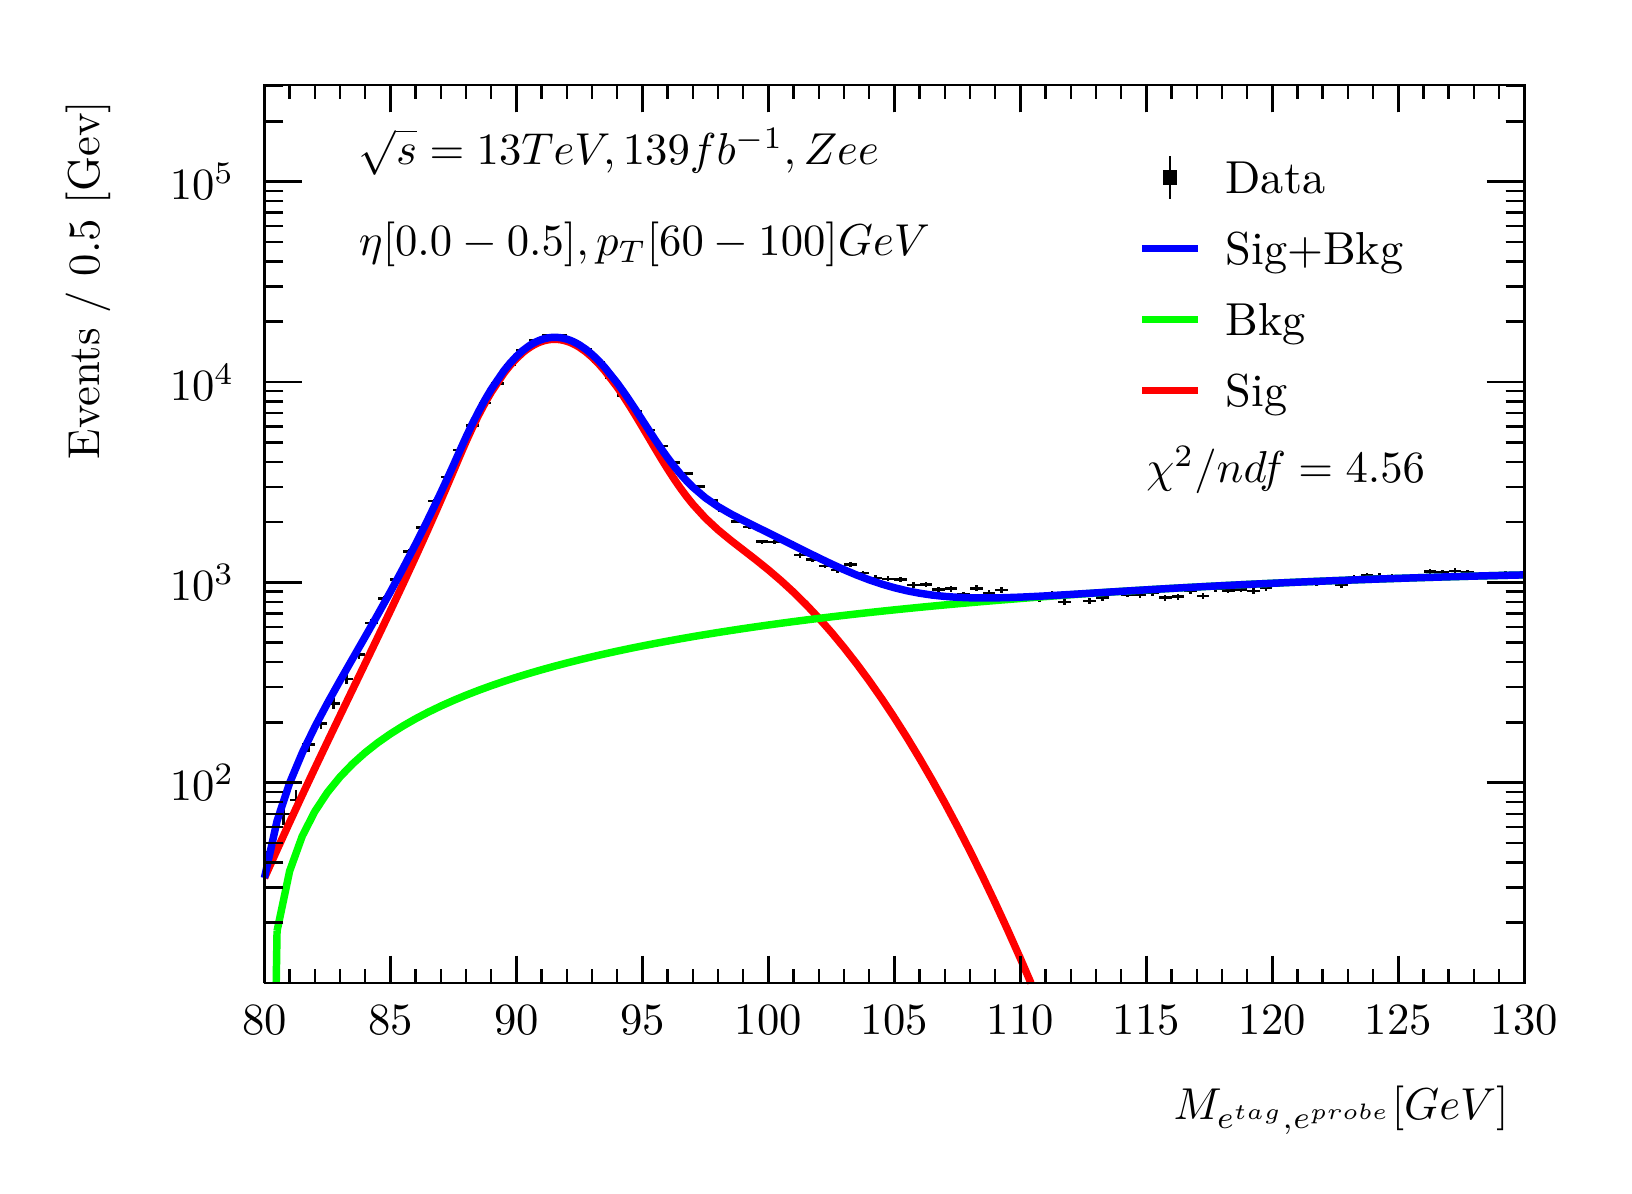
\begin{tikzpicture}
\pgfdeclareplotmark{cross} {
\pgfpathmoveto{\pgfpoint{-0.3\pgfplotmarksize}{\pgfplotmarksize}}
\pgfpathlineto{\pgfpoint{+0.3\pgfplotmarksize}{\pgfplotmarksize}}
\pgfpathlineto{\pgfpoint{+0.3\pgfplotmarksize}{0.3\pgfplotmarksize}}
\pgfpathlineto{\pgfpoint{+1\pgfplotmarksize}{0.3\pgfplotmarksize}}
\pgfpathlineto{\pgfpoint{+1\pgfplotmarksize}{-0.3\pgfplotmarksize}}
\pgfpathlineto{\pgfpoint{+0.3\pgfplotmarksize}{-0.3\pgfplotmarksize}}
\pgfpathlineto{\pgfpoint{+0.3\pgfplotmarksize}{-1.\pgfplotmarksize}}
\pgfpathlineto{\pgfpoint{-0.3\pgfplotmarksize}{-1.\pgfplotmarksize}}
\pgfpathlineto{\pgfpoint{-0.3\pgfplotmarksize}{-0.3\pgfplotmarksize}}
\pgfpathlineto{\pgfpoint{-1.\pgfplotmarksize}{-0.3\pgfplotmarksize}}
\pgfpathlineto{\pgfpoint{-1.\pgfplotmarksize}{0.3\pgfplotmarksize}}
\pgfpathlineto{\pgfpoint{-0.3\pgfplotmarksize}{0.3\pgfplotmarksize}}
\pgfpathclose
\pgfusepathqstroke
}
\pgfdeclareplotmark{cross*} {
\pgfpathmoveto{\pgfpoint{-0.3\pgfplotmarksize}{\pgfplotmarksize}}
\pgfpathlineto{\pgfpoint{+0.3\pgfplotmarksize}{\pgfplotmarksize}}
\pgfpathlineto{\pgfpoint{+0.3\pgfplotmarksize}{0.3\pgfplotmarksize}}
\pgfpathlineto{\pgfpoint{+1\pgfplotmarksize}{0.3\pgfplotmarksize}}
\pgfpathlineto{\pgfpoint{+1\pgfplotmarksize}{-0.3\pgfplotmarksize}}
\pgfpathlineto{\pgfpoint{+0.3\pgfplotmarksize}{-0.3\pgfplotmarksize}}
\pgfpathlineto{\pgfpoint{+0.3\pgfplotmarksize}{-1.\pgfplotmarksize}}
\pgfpathlineto{\pgfpoint{-0.3\pgfplotmarksize}{-1.\pgfplotmarksize}}
\pgfpathlineto{\pgfpoint{-0.3\pgfplotmarksize}{-0.3\pgfplotmarksize}}
\pgfpathlineto{\pgfpoint{-1.\pgfplotmarksize}{-0.3\pgfplotmarksize}}
\pgfpathlineto{\pgfpoint{-1.\pgfplotmarksize}{0.3\pgfplotmarksize}}
\pgfpathlineto{\pgfpoint{-0.3\pgfplotmarksize}{0.3\pgfplotmarksize}}
\pgfpathclose
\pgfusepathqfillstroke
}
\pgfdeclareplotmark{newstar} {
\pgfpathmoveto{\pgfqpoint{0pt}{\pgfplotmarksize}}
\pgfpathlineto{\pgfqpointpolar{44}{0.5\pgfplotmarksize}}
\pgfpathlineto{\pgfqpointpolar{18}{\pgfplotmarksize}}
\pgfpathlineto{\pgfqpointpolar{-20}{0.5\pgfplotmarksize}}
\pgfpathlineto{\pgfqpointpolar{-54}{\pgfplotmarksize}}
\pgfpathlineto{\pgfqpointpolar{-90}{0.5\pgfplotmarksize}}
\pgfpathlineto{\pgfqpointpolar{234}{\pgfplotmarksize}}
\pgfpathlineto{\pgfqpointpolar{198}{0.5\pgfplotmarksize}}
\pgfpathlineto{\pgfqpointpolar{162}{\pgfplotmarksize}}
\pgfpathlineto{\pgfqpointpolar{134}{0.5\pgfplotmarksize}}
\pgfpathclose
\pgfusepathqstroke
}
\pgfdeclareplotmark{newstar*} {
\pgfpathmoveto{\pgfqpoint{0pt}{\pgfplotmarksize}}
\pgfpathlineto{\pgfqpointpolar{44}{0.5\pgfplotmarksize}}
\pgfpathlineto{\pgfqpointpolar{18}{\pgfplotmarksize}}
\pgfpathlineto{\pgfqpointpolar{-20}{0.5\pgfplotmarksize}}
\pgfpathlineto{\pgfqpointpolar{-54}{\pgfplotmarksize}}
\pgfpathlineto{\pgfqpointpolar{-90}{0.5\pgfplotmarksize}}
\pgfpathlineto{\pgfqpointpolar{234}{\pgfplotmarksize}}
\pgfpathlineto{\pgfqpointpolar{198}{0.5\pgfplotmarksize}}
\pgfpathlineto{\pgfqpointpolar{162}{\pgfplotmarksize}}
\pgfpathlineto{\pgfqpointpolar{134}{0.5\pgfplotmarksize}}
\pgfpathclose
\pgfusepathqfillstroke
}
\definecolor{c}{rgb}{1,1,1};
\draw [color=c, fill=c] (0,0) rectangle (20,14.4361);
\draw [color=c, fill=c] (3,2.30977) rectangle (19,13.7143);
\definecolor{c}{rgb}{0,0,0};
\draw [c,line width=0.9] (3,2.30977) -- (3,13.7143) -- (19,13.7143) -- (19,2.30977) -- (3,2.30977);
\definecolor{c}{rgb}{1,1,1};
\draw [color=c, fill=c] (3,2.30977) rectangle (19,13.7143);
\definecolor{c}{rgb}{0,0,0};
\draw [c,line width=0.9] (3,2.30977) -- (3,13.7143) -- (19,13.7143) -- (19,2.30977) -- (3,2.30977);
\draw [c,line width=0.9] (3,2.30977) -- (19,2.30977);
\draw [c,line width=0.9] (3,2.65624) -- (3,2.30977);
\draw [c,line width=0.9] (3.32,2.48301) -- (3.32,2.30977);
\draw [c,line width=0.9] (3.64,2.48301) -- (3.64,2.30977);
\draw [c,line width=0.9] (3.96,2.48301) -- (3.96,2.30977);
\draw [c,line width=0.9] (4.28,2.48301) -- (4.28,2.30977);
\draw [c,line width=0.9] (4.6,2.65624) -- (4.6,2.30977);
\draw [c,line width=0.9] (4.92,2.48301) -- (4.92,2.30977);
\draw [c,line width=0.9] (5.24,2.48301) -- (5.24,2.30977);
\draw [c,line width=0.9] (5.56,2.48301) -- (5.56,2.30977);
\draw [c,line width=0.9] (5.88,2.48301) -- (5.88,2.30977);
\draw [c,line width=0.9] (6.2,2.65624) -- (6.2,2.30977);
\draw [c,line width=0.9] (6.52,2.48301) -- (6.52,2.30977);
\draw [c,line width=0.9] (6.84,2.48301) -- (6.84,2.30977);
\draw [c,line width=0.9] (7.16,2.48301) -- (7.16,2.30977);
\draw [c,line width=0.9] (7.48,2.48301) -- (7.48,2.30977);
\draw [c,line width=0.9] (7.8,2.65624) -- (7.8,2.30977);
\draw [c,line width=0.9] (8.12,2.48301) -- (8.12,2.30977);
\draw [c,line width=0.9] (8.44,2.48301) -- (8.44,2.30977);
\draw [c,line width=0.9] (8.76,2.48301) -- (8.76,2.30977);
\draw [c,line width=0.9] (9.08,2.48301) -- (9.08,2.30977);
\draw [c,line width=0.9] (9.4,2.65624) -- (9.4,2.30977);
\draw [c,line width=0.9] (9.72,2.48301) -- (9.72,2.30977);
\draw [c,line width=0.9] (10.04,2.48301) -- (10.04,2.30977);
\draw [c,line width=0.9] (10.36,2.48301) -- (10.36,2.30977);
\draw [c,line width=0.9] (10.68,2.48301) -- (10.68,2.30977);
\draw [c,line width=0.9] (11,2.65624) -- (11,2.30977);
\draw [c,line width=0.9] (11.32,2.48301) -- (11.32,2.30977);
\draw [c,line width=0.9] (11.64,2.48301) -- (11.64,2.30977);
\draw [c,line width=0.9] (11.96,2.48301) -- (11.96,2.30977);
\draw [c,line width=0.9] (12.28,2.48301) -- (12.28,2.30977);
\draw [c,line width=0.9] (12.6,2.65624) -- (12.6,2.30977);
\draw [c,line width=0.9] (12.92,2.48301) -- (12.92,2.30977);
\draw [c,line width=0.9] (13.24,2.48301) -- (13.24,2.30977);
\draw [c,line width=0.9] (13.56,2.48301) -- (13.56,2.30977);
\draw [c,line width=0.9] (13.88,2.48301) -- (13.88,2.30977);
\draw [c,line width=0.9] (14.2,2.65624) -- (14.2,2.30977);
\draw [c,line width=0.9] (14.52,2.48301) -- (14.52,2.30977);
\draw [c,line width=0.9] (14.84,2.48301) -- (14.84,2.30977);
\draw [c,line width=0.9] (15.16,2.48301) -- (15.16,2.30977);
\draw [c,line width=0.9] (15.48,2.48301) -- (15.48,2.30977);
\draw [c,line width=0.9] (15.8,2.65624) -- (15.8,2.30977);
\draw [c,line width=0.9] (16.12,2.48301) -- (16.12,2.30977);
\draw [c,line width=0.9] (16.44,2.48301) -- (16.44,2.30977);
\draw [c,line width=0.9] (16.76,2.48301) -- (16.76,2.30977);
\draw [c,line width=0.9] (17.08,2.48301) -- (17.08,2.30977);
\draw [c,line width=0.9] (17.4,2.65624) -- (17.4,2.30977);
\draw [c,line width=0.9] (17.72,2.48301) -- (17.72,2.30977);
\draw [c,line width=0.9] (18.04,2.48301) -- (18.04,2.30977);
\draw [c,line width=0.9] (18.36,2.48301) -- (18.36,2.30977);
\draw [c,line width=0.9] (18.68,2.48301) -- (18.68,2.30977);
\draw [c,line width=0.9] (19,2.65624) -- (19,2.30977);
\draw [anchor=base] (3,1.66015) node[scale=1.61424, color=c, rotate=0]{80};
\draw [anchor=base] (4.6,1.66015) node[scale=1.61424, color=c, rotate=0]{85};
\draw [anchor=base] (6.2,1.66015) node[scale=1.61424, color=c, rotate=0]{90};
\draw [anchor=base] (7.8,1.66015) node[scale=1.61424, color=c, rotate=0]{95};
\draw [anchor=base] (9.4,1.66015) node[scale=1.61424, color=c, rotate=0]{100};
\draw [anchor=base] (11,1.66015) node[scale=1.61424, color=c, rotate=0]{105};
\draw [anchor=base] (12.6,1.66015) node[scale=1.61424, color=c, rotate=0]{110};
\draw [anchor=base] (14.2,1.66015) node[scale=1.61424, color=c, rotate=0]{115};
\draw [anchor=base] (15.8,1.66015) node[scale=1.61424, color=c, rotate=0]{120};
\draw [anchor=base] (17.4,1.66015) node[scale=1.61424, color=c, rotate=0]{125};
\draw [anchor=base] (19,1.66015) node[scale=1.61424, color=c, rotate=0]{130};
\draw [anchor= east] (19,0.692932) node[scale=1.61424, color=c, rotate=0]{$M_{e^{tag}, e^{probe}}  [GeV]$};
\draw [c,line width=0.9] (3,13.7143) -- (19,13.7143);
\draw [c,line width=0.9] (3,13.3678) -- (3,13.7143);
\draw [c,line width=0.9] (3.32,13.5411) -- (3.32,13.7143);
\draw [c,line width=0.9] (3.64,13.5411) -- (3.64,13.7143);
\draw [c,line width=0.9] (3.96,13.5411) -- (3.96,13.7143);
\draw [c,line width=0.9] (4.28,13.5411) -- (4.28,13.7143);
\draw [c,line width=0.9] (4.6,13.3678) -- (4.6,13.7143);
\draw [c,line width=0.9] (4.92,13.5411) -- (4.92,13.7143);
\draw [c,line width=0.9] (5.24,13.5411) -- (5.24,13.7143);
\draw [c,line width=0.9] (5.56,13.5411) -- (5.56,13.7143);
\draw [c,line width=0.9] (5.88,13.5411) -- (5.88,13.7143);
\draw [c,line width=0.9] (6.2,13.3678) -- (6.2,13.7143);
\draw [c,line width=0.9] (6.52,13.5411) -- (6.52,13.7143);
\draw [c,line width=0.9] (6.84,13.5411) -- (6.84,13.7143);
\draw [c,line width=0.9] (7.16,13.5411) -- (7.16,13.7143);
\draw [c,line width=0.9] (7.48,13.5411) -- (7.48,13.7143);
\draw [c,line width=0.9] (7.8,13.3678) -- (7.8,13.7143);
\draw [c,line width=0.9] (8.12,13.5411) -- (8.12,13.7143);
\draw [c,line width=0.9] (8.44,13.5411) -- (8.44,13.7143);
\draw [c,line width=0.9] (8.76,13.5411) -- (8.76,13.7143);
\draw [c,line width=0.9] (9.08,13.5411) -- (9.08,13.7143);
\draw [c,line width=0.9] (9.4,13.3678) -- (9.4,13.7143);
\draw [c,line width=0.9] (9.72,13.5411) -- (9.72,13.7143);
\draw [c,line width=0.9] (10.04,13.5411) -- (10.04,13.7143);
\draw [c,line width=0.9] (10.36,13.5411) -- (10.36,13.7143);
\draw [c,line width=0.9] (10.68,13.5411) -- (10.68,13.7143);
\draw [c,line width=0.9] (11,13.3678) -- (11,13.7143);
\draw [c,line width=0.9] (11.32,13.5411) -- (11.32,13.7143);
\draw [c,line width=0.9] (11.64,13.5411) -- (11.64,13.7143);
\draw [c,line width=0.9] (11.96,13.5411) -- (11.96,13.7143);
\draw [c,line width=0.9] (12.28,13.5411) -- (12.28,13.7143);
\draw [c,line width=0.9] (12.6,13.3678) -- (12.6,13.7143);
\draw [c,line width=0.9] (12.92,13.5411) -- (12.92,13.7143);
\draw [c,line width=0.9] (13.24,13.5411) -- (13.24,13.7143);
\draw [c,line width=0.9] (13.56,13.5411) -- (13.56,13.7143);
\draw [c,line width=0.9] (13.88,13.5411) -- (13.88,13.7143);
\draw [c,line width=0.9] (14.2,13.3678) -- (14.2,13.7143);
\draw [c,line width=0.9] (14.52,13.5411) -- (14.52,13.7143);
\draw [c,line width=0.9] (14.84,13.5411) -- (14.84,13.7143);
\draw [c,line width=0.9] (15.16,13.5411) -- (15.16,13.7143);
\draw [c,line width=0.9] (15.48,13.5411) -- (15.48,13.7143);
\draw [c,line width=0.9] (15.8,13.3678) -- (15.8,13.7143);
\draw [c,line width=0.9] (16.12,13.5411) -- (16.12,13.7143);
\draw [c,line width=0.9] (16.44,13.5411) -- (16.44,13.7143);
\draw [c,line width=0.9] (16.76,13.5411) -- (16.76,13.7143);
\draw [c,line width=0.9] (17.08,13.5411) -- (17.08,13.7143);
\draw [c,line width=0.9] (17.4,13.3678) -- (17.4,13.7143);
\draw [c,line width=0.9] (17.72,13.5411) -- (17.72,13.7143);
\draw [c,line width=0.9] (18.04,13.5411) -- (18.04,13.7143);
\draw [c,line width=0.9] (18.36,13.5411) -- (18.36,13.7143);
\draw [c,line width=0.9] (18.68,13.5411) -- (18.68,13.7143);
\draw [c,line width=0.9] (19,13.3678) -- (19,13.7143);
\draw [c,line width=0.9] (3,2.30977) -- (3,13.7143);
\draw [c,line width=0.9] (3.237,3.07568) -- (3,3.07568);
\draw [c,line width=0.9] (3.237,3.5237) -- (3,3.5237);
\draw [c,line width=0.9] (3.237,3.84158) -- (3,3.84158);
\draw [c,line width=0.9] (3.237,4.08815) -- (3,4.08815);
\draw [c,line width=0.9] (3.237,4.2896) -- (3,4.2896);
\draw [c,line width=0.9] (3.237,4.45994) -- (3,4.45994);
\draw [c,line width=0.9] (3.237,4.60748) -- (3,4.60748);
\draw [c,line width=0.9] (3.237,4.73763) -- (3,4.73763);
\draw [c,line width=0.9] (3.474,4.85405) -- (3,4.85405);
\draw [anchor= east] (2.82,4.85405) node[scale=1.61424, color=c, rotate=0]{$10^{2}$};
\draw [c,line width=0.9] (3.237,5.61995) -- (3,5.61995);
\draw [c,line width=0.9] (3.237,6.06798) -- (3,6.06798);
\draw [c,line width=0.9] (3.237,6.38586) -- (3,6.38586);
\draw [c,line width=0.9] (3.237,6.63242) -- (3,6.63242);
\draw [c,line width=0.9] (3.237,6.83388) -- (3,6.83388);
\draw [c,line width=0.9] (3.237,7.00421) -- (3,7.00421);
\draw [c,line width=0.9] (3.237,7.15176) -- (3,7.15176);
\draw [c,line width=0.9] (3.237,7.28191) -- (3,7.28191);
\draw [c,line width=0.9] (3.474,7.39833) -- (3,7.39833);
\draw [anchor= east] (2.82,7.39833) node[scale=1.61424, color=c, rotate=0]{$10^{3}$};
\draw [c,line width=0.9] (3.237,8.16423) -- (3,8.16423);
\draw [c,line width=0.9] (3.237,8.61226) -- (3,8.61226);
\draw [c,line width=0.9] (3.237,8.93013) -- (3,8.93013);
\draw [c,line width=0.9] (3.237,9.1767) -- (3,9.1767);
\draw [c,line width=0.9] (3.237,9.37816) -- (3,9.37816);
\draw [c,line width=0.9] (3.237,9.54849) -- (3,9.54849);
\draw [c,line width=0.9] (3.237,9.69604) -- (3,9.69604);
\draw [c,line width=0.9] (3.237,9.82618) -- (3,9.82618);
\draw [c,line width=0.9] (3.474,9.9426) -- (3,9.9426);
\draw [anchor= east] (2.82,9.9426) node[scale=1.61424, color=c, rotate=0]{$10^{4}$};
\draw [c,line width=0.9] (3.237,10.7085) -- (3,10.7085);
\draw [c,line width=0.9] (3.237,11.1565) -- (3,11.1565);
\draw [c,line width=0.9] (3.237,11.4744) -- (3,11.4744);
\draw [c,line width=0.9] (3.237,11.721) -- (3,11.721);
\draw [c,line width=0.9] (3.237,11.9224) -- (3,11.9224);
\draw [c,line width=0.9] (3.237,12.0928) -- (3,12.0928);
\draw [c,line width=0.9] (3.237,12.2403) -- (3,12.2403);
\draw [c,line width=0.9] (3.237,12.3705) -- (3,12.3705);
\draw [c,line width=0.9] (3.474,12.4869) -- (3,12.4869);
\draw [anchor= east] (2.82,12.4869) node[scale=1.61424, color=c, rotate=0]{$10^{5}$};
\draw [c,line width=0.9] (3.237,13.2528) -- (3,13.2528);
\draw [c,line width=0.9] (3.237,13.7008) -- (3,13.7008);
\draw [anchor= east] (0.76,13.7143) node[scale=1.61424, color=c, rotate=90]{Events / 0.5 [Gev]};
\draw [c,line width=0.9] (19,2.30977) -- (19,13.7143);
\draw [c,line width=0.9] (18.763,3.07568) -- (19,3.07568);
\draw [c,line width=0.9] (18.763,3.5237) -- (19,3.5237);
\draw [c,line width=0.9] (18.763,3.84158) -- (19,3.84158);
\draw [c,line width=0.9] (18.763,4.08815) -- (19,4.08815);
\draw [c,line width=0.9] (18.763,4.2896) -- (19,4.2896);
\draw [c,line width=0.9] (18.763,4.45994) -- (19,4.45994);
\draw [c,line width=0.9] (18.763,4.60748) -- (19,4.60748);
\draw [c,line width=0.9] (18.763,4.73763) -- (19,4.73763);
\draw [c,line width=0.9] (18.526,4.85405) -- (19,4.85405);
\draw [c,line width=0.9] (18.763,5.61995) -- (19,5.61995);
\draw [c,line width=0.9] (18.763,6.06798) -- (19,6.06798);
\draw [c,line width=0.9] (18.763,6.38586) -- (19,6.38586);
\draw [c,line width=0.9] (18.763,6.63242) -- (19,6.63242);
\draw [c,line width=0.9] (18.763,6.83388) -- (19,6.83388);
\draw [c,line width=0.9] (18.763,7.00421) -- (19,7.00421);
\draw [c,line width=0.9] (18.763,7.15176) -- (19,7.15176);
\draw [c,line width=0.9] (18.763,7.28191) -- (19,7.28191);
\draw [c,line width=0.9] (18.526,7.39833) -- (19,7.39833);
\draw [c,line width=0.9] (18.763,8.16423) -- (19,8.16423);
\draw [c,line width=0.9] (18.763,8.61226) -- (19,8.61226);
\draw [c,line width=0.9] (18.763,8.93013) -- (19,8.93013);
\draw [c,line width=0.9] (18.763,9.1767) -- (19,9.1767);
\draw [c,line width=0.9] (18.763,9.37816) -- (19,9.37816);
\draw [c,line width=0.9] (18.763,9.54849) -- (19,9.54849);
\draw [c,line width=0.9] (18.763,9.69604) -- (19,9.69604);
\draw [c,line width=0.9] (18.763,9.82618) -- (19,9.82618);
\draw [c,line width=0.9] (18.526,9.9426) -- (19,9.9426);
\draw [c,line width=0.9] (18.763,10.7085) -- (19,10.7085);
\draw [c,line width=0.9] (18.763,11.1565) -- (19,11.1565);
\draw [c,line width=0.9] (18.763,11.4744) -- (19,11.4744);
\draw [c,line width=0.9] (18.763,11.721) -- (19,11.721);
\draw [c,line width=0.9] (18.763,11.9224) -- (19,11.9224);
\draw [c,line width=0.9] (18.763,12.0928) -- (19,12.0928);
\draw [c,line width=0.9] (18.763,12.2403) -- (19,12.2403);
\draw [c,line width=0.9] (18.763,12.3705) -- (19,12.3705);
\draw [c,line width=0.9] (18.526,12.4869) -- (19,12.4869);
\draw [c,line width=0.9] (18.763,13.2528) -- (19,13.2528);
\draw [c,line width=0.9] (18.763,13.7008) -- (19,13.7008);
\draw [c,line width=0.9] (3.08,3.97173) -- (3,3.97173);
\draw [c,line width=0.9] (3,3.97173) -- (3,3.97173);
\draw [c,line width=0.9] (3.08,3.97173) -- (3.16,3.97173);
\draw [c,line width=0.9] (3.16,3.97173) -- (3.16,3.97173);
\draw [c,line width=0.9] (3.08,3.97173) -- (3.08,4.14747);
\draw [c,line width=0.9] (3.08,4.14747) -- (3.08,4.14747);
\draw [c,line width=0.9] (3.08,3.97173) -- (3.08,3.79408);
\draw [c,line width=0.9] (3.08,3.79408) -- (3.08,3.79408);
\draw [c,line width=0.9] (3.24,4.45994) -- (3.16,4.45994);
\draw [c,line width=0.9] (3.16,4.45994) -- (3.16,4.45994);
\draw [c,line width=0.9] (3.24,4.45994) -- (3.32,4.45994);
\draw [c,line width=0.9] (3.32,4.45994) -- (3.32,4.45994);
\draw [c,line width=0.9] (3.24,4.45994) -- (3.24,4.59926);
\draw [c,line width=0.9] (3.24,4.59926) -- (3.24,4.59926);
\draw [c,line width=0.9] (3.24,4.45994) -- (3.24,4.31964);
\draw [c,line width=0.9] (3.24,4.31964) -- (3.24,4.31964);
\draw [c,line width=0.9] (3.4,4.63477) -- (3.32,4.63477);
\draw [c,line width=0.9] (3.32,4.63477) -- (3.32,4.63477);
\draw [c,line width=0.9] (3.4,4.63477) -- (3.48,4.63477);
\draw [c,line width=0.9] (3.48,4.63477) -- (3.48,4.63477);
\draw [c,line width=0.9] (3.4,4.63477) -- (3.4,4.76302);
\draw [c,line width=0.9] (3.4,4.76302) -- (3.4,4.76302);
\draw [c,line width=0.9] (3.4,4.63477) -- (3.4,4.50575);
\draw [c,line width=0.9] (3.4,4.50575) -- (3.4,4.50575);
\draw [c,line width=0.9] (3.56,5.33831) -- (3.48,5.33831);
\draw [c,line width=0.9] (3.48,5.33831) -- (3.48,5.33831);
\draw [c,line width=0.9] (3.56,5.33831) -- (3.64,5.33831);
\draw [c,line width=0.9] (3.64,5.33831) -- (3.64,5.33831);
\draw [c,line width=0.9] (3.56,5.33831) -- (3.56,5.42704);
\draw [c,line width=0.9] (3.56,5.42704) -- (3.56,5.42704);
\draw [c,line width=0.9] (3.56,5.33831) -- (3.56,5.24958);
\draw [c,line width=0.9] (3.56,5.24958) -- (3.56,5.24958);
\draw [c,line width=0.9] (3.72,5.60885) -- (3.64,5.60885);
\draw [c,line width=0.9] (3.64,5.60885) -- (3.64,5.60885);
\draw [c,line width=0.9] (3.72,5.60885) -- (3.8,5.60885);
\draw [c,line width=0.9] (3.8,5.60885) -- (3.8,5.60885);
\draw [c,line width=0.9] (3.72,5.60885) -- (3.72,5.68736);
\draw [c,line width=0.9] (3.72,5.68736) -- (3.72,5.68736);
\draw [c,line width=0.9] (3.72,5.60885) -- (3.72,5.53034);
\draw [c,line width=0.9] (3.72,5.53034) -- (3.72,5.53034);
\draw [c,line width=0.9] (3.88,5.85765) -- (3.8,5.85765);
\draw [c,line width=0.9] (3.8,5.85765) -- (3.8,5.85765);
\draw [c,line width=0.9] (3.88,5.85765) -- (3.96,5.85765);
\draw [c,line width=0.9] (3.96,5.85765) -- (3.96,5.85765);
\draw [c,line width=0.9] (3.88,5.85765) -- (3.88,5.9278);
\draw [c,line width=0.9] (3.88,5.9278) -- (3.88,5.9278);
\draw [c,line width=0.9] (3.88,5.85765) -- (3.88,5.78749);
\draw [c,line width=0.9] (3.88,5.78749) -- (3.88,5.78749);
\draw [c,line width=0.9] (4.04,6.16994) -- (3.96,6.16994);
\draw [c,line width=0.9] (3.96,6.16994) -- (3.96,6.16994);
\draw [c,line width=0.9] (4.04,6.16994) -- (4.12,6.16994);
\draw [c,line width=0.9] (4.12,6.16994) -- (4.12,6.16994);
\draw [c,line width=0.9] (4.04,6.16994) -- (4.04,6.23085);
\draw [c,line width=0.9] (4.04,6.23085) -- (4.04,6.23085);
\draw [c,line width=0.9] (4.04,6.16994) -- (4.04,6.10903);
\draw [c,line width=0.9] (4.04,6.10903) -- (4.04,6.10903);
\draw [c,line width=0.9] (4.2,6.48361) -- (4.12,6.48361);
\draw [c,line width=0.9] (4.12,6.48361) -- (4.12,6.48361);
\draw [c,line width=0.9] (4.2,6.48361) -- (4.28,6.48361);
\draw [c,line width=0.9] (4.28,6.48361) -- (4.28,6.48361);
\draw [c,line width=0.9] (4.2,6.48361) -- (4.2,6.53647);
\draw [c,line width=0.9] (4.2,6.53647) -- (4.2,6.53647);
\draw [c,line width=0.9] (4.2,6.48361) -- (4.2,6.43076);
\draw [c,line width=0.9] (4.2,6.43076) -- (4.2,6.43076);
\draw [c,line width=0.9] (4.36,6.88428) -- (4.28,6.88428);
\draw [c,line width=0.9] (4.28,6.88428) -- (4.28,6.88428);
\draw [c,line width=0.9] (4.36,6.88428) -- (4.44,6.88428);
\draw [c,line width=0.9] (4.44,6.88428) -- (4.44,6.88428);
\draw [c,line width=0.9] (4.36,6.88428) -- (4.36,6.92837);
\draw [c,line width=0.9] (4.36,6.92837) -- (4.36,6.92837);
\draw [c,line width=0.9] (4.36,6.88428) -- (4.36,6.84019);
\draw [c,line width=0.9] (4.36,6.84019) -- (4.36,6.84019);
\draw [c,line width=0.9] (4.52,7.19244) -- (4.44,7.19244);
\draw [c,line width=0.9] (4.44,7.19244) -- (4.44,7.19244);
\draw [c,line width=0.9] (4.52,7.19244) -- (4.6,7.19244);
\draw [c,line width=0.9] (4.6,7.19244) -- (4.6,7.19244);
\draw [c,line width=0.9] (4.52,7.19244) -- (4.52,7.23079);
\draw [c,line width=0.9] (4.52,7.23079) -- (4.52,7.23079);
\draw [c,line width=0.9] (4.52,7.19244) -- (4.52,7.15409);
\draw [c,line width=0.9] (4.52,7.15409) -- (4.52,7.15409);
\draw [c,line width=0.9] (4.68,7.4342) -- (4.6,7.4342);
\draw [c,line width=0.9] (4.6,7.4342) -- (4.6,7.4342);
\draw [c,line width=0.9] (4.68,7.4342) -- (4.76,7.4342);
\draw [c,line width=0.9] (4.76,7.4342) -- (4.76,7.4342);
\draw [c,line width=0.9] (4.68,7.4342) -- (4.68,7.46858);
\draw [c,line width=0.9] (4.68,7.46858) -- (4.68,7.46858);
\draw [c,line width=0.9] (4.68,7.4342) -- (4.68,7.39983);
\draw [c,line width=0.9] (4.68,7.39983) -- (4.68,7.39983);
\draw [c,line width=0.9] (4.84,7.7889) -- (4.76,7.7889);
\draw [c,line width=0.9] (4.76,7.7889) -- (4.76,7.7889);
\draw [c,line width=0.9] (4.84,7.7889) -- (4.92,7.7889);
\draw [c,line width=0.9] (4.92,7.7889) -- (4.92,7.7889);
\draw [c,line width=0.9] (4.84,7.7889) -- (4.84,7.81818);
\draw [c,line width=0.9] (4.84,7.81818) -- (4.84,7.81818);
\draw [c,line width=0.9] (4.84,7.7889) -- (4.84,7.75962);
\draw [c,line width=0.9] (4.84,7.75962) -- (4.84,7.75962);
\draw [c,line width=0.9] (5,8.09645) -- (4.92,8.09645);
\draw [c,line width=0.9] (4.92,8.09645) -- (4.92,8.09645);
\draw [c,line width=0.9] (5,8.09645) -- (5.08,8.09645);
\draw [c,line width=0.9] (5.08,8.09645) -- (5.08,8.09645);
\draw [c,line width=0.9] (5,8.09645) -- (5,8.12193);
\draw [c,line width=0.9] (5,8.12193) -- (5,8.12193);
\draw [c,line width=0.9] (5,8.09645) -- (5,8.07097);
\draw [c,line width=0.9] (5,8.07097) -- (5,8.07097);
\draw [c,line width=0.9] (5.16,8.43008) -- (5.08,8.43008);
\draw [c,line width=0.9] (5.08,8.43008) -- (5.08,8.43008);
\draw [c,line width=0.9] (5.16,8.43008) -- (5.24,8.43008);
\draw [c,line width=0.9] (5.24,8.43008) -- (5.24,8.43008);
\draw [c,line width=0.9] (5.16,8.43008) -- (5.16,8.45198);
\draw [c,line width=0.9] (5.16,8.45198) -- (5.16,8.45198);
\draw [c,line width=0.9] (5.16,8.43008) -- (5.16,8.40817);
\draw [c,line width=0.9] (5.16,8.40817) -- (5.16,8.40817);
\draw [c,line width=0.9] (5.32,8.73386) -- (5.24,8.73386);
\draw [c,line width=0.9] (5.24,8.73386) -- (5.24,8.73386);
\draw [c,line width=0.9] (5.32,8.73386) -- (5.4,8.73386);
\draw [c,line width=0.9] (5.4,8.73386) -- (5.4,8.73386);
\draw [c,line width=0.9] (5.32,8.73386) -- (5.32,8.75295);
\draw [c,line width=0.9] (5.32,8.75295) -- (5.32,8.75295);
\draw [c,line width=0.9] (5.32,8.73386) -- (5.32,8.71476);
\draw [c,line width=0.9] (5.32,8.71476) -- (5.32,8.71476);
\draw [c,line width=0.9] (5.48,9.07903) -- (5.4,9.07903);
\draw [c,line width=0.9] (5.4,9.07903) -- (5.4,9.07903);
\draw [c,line width=0.9] (5.48,9.07903) -- (5.56,9.07903);
\draw [c,line width=0.9] (5.56,9.07903) -- (5.56,9.07903);
\draw [c,line width=0.9] (5.48,9.07903) -- (5.48,9.09536);
\draw [c,line width=0.9] (5.48,9.09536) -- (5.48,9.09536);
\draw [c,line width=0.9] (5.48,9.07903) -- (5.48,9.0627);
\draw [c,line width=0.9] (5.48,9.0627) -- (5.48,9.0627);
\draw [c,line width=0.9] (5.64,9.39261) -- (5.56,9.39261);
\draw [c,line width=0.9] (5.56,9.39261) -- (5.56,9.39261);
\draw [c,line width=0.9] (5.64,9.39261) -- (5.72,9.39261);
\draw [c,line width=0.9] (5.72,9.39261) -- (5.72,9.39261);
\draw [c,line width=0.9] (5.64,9.39261) -- (5.64,9.40679);
\draw [c,line width=0.9] (5.64,9.40679) -- (5.64,9.40679);
\draw [c,line width=0.9] (5.64,9.39261) -- (5.64,9.37844);
\draw [c,line width=0.9] (5.64,9.37844) -- (5.64,9.37844);
\draw [c,line width=0.9] (5.8,9.67681) -- (5.72,9.67681);
\draw [c,line width=0.9] (5.72,9.67681) -- (5.72,9.67681);
\draw [c,line width=0.9] (5.8,9.67681) -- (5.88,9.67681);
\draw [c,line width=0.9] (5.88,9.67681) -- (5.88,9.67681);
\draw [c,line width=0.9] (5.8,9.67681) -- (5.8,9.68927);
\draw [c,line width=0.9] (5.8,9.68927) -- (5.8,9.68927);
\draw [c,line width=0.9] (5.8,9.67681) -- (5.8,9.66435);
\draw [c,line width=0.9] (5.8,9.66435) -- (5.8,9.66435);
\draw [c,line width=0.9] (5.96,9.9213) -- (5.88,9.9213);
\draw [c,line width=0.9] (5.88,9.9213) -- (5.88,9.9213);
\draw [c,line width=0.9] (5.96,9.9213) -- (6.04,9.9213);
\draw [c,line width=0.9] (6.04,9.9213) -- (6.04,9.9213);
\draw [c,line width=0.9] (5.96,9.9213) -- (5.96,9.93245);
\draw [c,line width=0.9] (5.96,9.93245) -- (5.96,9.93245);
\draw [c,line width=0.9] (5.96,9.9213) -- (5.96,9.91014);
\draw [c,line width=0.9] (5.96,9.91014) -- (5.96,9.91014);
\draw [c,line width=0.9] (6.12,10.1618) -- (6.04,10.1618);
\draw [c,line width=0.9] (6.04,10.1618) -- (6.04,10.1618);
\draw [c,line width=0.9] (6.12,10.1618) -- (6.2,10.1618);
\draw [c,line width=0.9] (6.2,10.1618) -- (6.2,10.1618);
\draw [c,line width=0.9] (6.12,10.1618) -- (6.12,10.1718);
\draw [c,line width=0.9] (6.12,10.1718) -- (6.12,10.1718);
\draw [c,line width=0.9] (6.12,10.1618) -- (6.12,10.1518);
\draw [c,line width=0.9] (6.12,10.1518) -- (6.12,10.1518);
\draw [c,line width=0.9] (6.28,10.3471) -- (6.2,10.3471);
\draw [c,line width=0.9] (6.2,10.3471) -- (6.2,10.3471);
\draw [c,line width=0.9] (6.28,10.3471) -- (6.36,10.3471);
\draw [c,line width=0.9] (6.36,10.3471) -- (6.36,10.3471);
\draw [c,line width=0.9] (6.28,10.3471) -- (6.28,10.3563);
\draw [c,line width=0.9] (6.28,10.3563) -- (6.28,10.3563);
\draw [c,line width=0.9] (6.28,10.3471) -- (6.28,10.3379);
\draw [c,line width=0.9] (6.28,10.3379) -- (6.28,10.3379);
\draw [c,line width=0.9] (6.44,10.4746) -- (6.36,10.4746);
\draw [c,line width=0.9] (6.36,10.4746) -- (6.36,10.4746);
\draw [c,line width=0.9] (6.44,10.4746) -- (6.52,10.4746);
\draw [c,line width=0.9] (6.52,10.4746) -- (6.52,10.4746);
\draw [c,line width=0.9] (6.44,10.4746) -- (6.44,10.4833);
\draw [c,line width=0.9] (6.44,10.4833) -- (6.44,10.4833);
\draw [c,line width=0.9] (6.44,10.4746) -- (6.44,10.466);
\draw [c,line width=0.9] (6.44,10.466) -- (6.44,10.466);
\draw [c,line width=0.9] (6.6,10.5373) -- (6.52,10.5373);
\draw [c,line width=0.9] (6.52,10.5373) -- (6.52,10.5373);
\draw [c,line width=0.9] (6.6,10.5373) -- (6.68,10.5373);
\draw [c,line width=0.9] (6.68,10.5373) -- (6.68,10.5373);
\draw [c,line width=0.9] (6.6,10.5373) -- (6.6,10.5457);
\draw [c,line width=0.9] (6.6,10.5457) -- (6.6,10.5457);
\draw [c,line width=0.9] (6.6,10.5373) -- (6.6,10.5288);
\draw [c,line width=0.9] (6.6,10.5288) -- (6.6,10.5288);
\draw [c,line width=0.9] (6.76,10.5319) -- (6.68,10.5319);
\draw [c,line width=0.9] (6.68,10.5319) -- (6.68,10.5319);
\draw [c,line width=0.9] (6.76,10.5319) -- (6.84,10.5319);
\draw [c,line width=0.9] (6.84,10.5319) -- (6.84,10.5319);
\draw [c,line width=0.9] (6.76,10.5319) -- (6.76,10.5403);
\draw [c,line width=0.9] (6.76,10.5403) -- (6.76,10.5403);
\draw [c,line width=0.9] (6.76,10.5319) -- (6.76,10.5234);
\draw [c,line width=0.9] (6.76,10.5234) -- (6.76,10.5234);
\draw [c,line width=0.9] (6.92,10.4613) -- (6.84,10.4613);
\draw [c,line width=0.9] (6.84,10.4613) -- (6.84,10.4613);
\draw [c,line width=0.9] (6.92,10.4613) -- (7,10.4613);
\draw [c,line width=0.9] (7,10.4613) -- (7,10.4613);
\draw [c,line width=0.9] (6.92,10.4613) -- (6.92,10.4701);
\draw [c,line width=0.9] (6.92,10.4701) -- (6.92,10.4701);
\draw [c,line width=0.9] (6.92,10.4613) -- (6.92,10.4526);
\draw [c,line width=0.9] (6.92,10.4526) -- (6.92,10.4526);
\draw [c,line width=0.9] (7.08,10.3639) -- (7,10.3639);
\draw [c,line width=0.9] (7,10.3639) -- (7,10.3639);
\draw [c,line width=0.9] (7.08,10.3639) -- (7.16,10.3639);
\draw [c,line width=0.9] (7.16,10.3639) -- (7.16,10.3639);
\draw [c,line width=0.9] (7.08,10.3639) -- (7.08,10.373);
\draw [c,line width=0.9] (7.08,10.373) -- (7.08,10.373);
\draw [c,line width=0.9] (7.08,10.3639) -- (7.08,10.3547);
\draw [c,line width=0.9] (7.08,10.3547) -- (7.08,10.3547);
\draw [c,line width=0.9] (7.24,10.1946) -- (7.16,10.1946);
\draw [c,line width=0.9] (7.16,10.1946) -- (7.16,10.1946);
\draw [c,line width=0.9] (7.24,10.1946) -- (7.32,10.1946);
\draw [c,line width=0.9] (7.32,10.1946) -- (7.32,10.1946);
\draw [c,line width=0.9] (7.24,10.1946) -- (7.24,10.2044);
\draw [c,line width=0.9] (7.24,10.2044) -- (7.24,10.2044);
\draw [c,line width=0.9] (7.24,10.1946) -- (7.24,10.1847);
\draw [c,line width=0.9] (7.24,10.1847) -- (7.24,10.1847);
\draw [c,line width=0.9] (7.4,9.9942) -- (7.32,9.9942);
\draw [c,line width=0.9] (7.32,9.9942) -- (7.32,9.9942);
\draw [c,line width=0.9] (7.4,9.9942) -- (7.48,9.9942);
\draw [c,line width=0.9] (7.48,9.9942) -- (7.48,9.9942);
\draw [c,line width=0.9] (7.4,9.9942) -- (7.4,10.005);
\draw [c,line width=0.9] (7.4,10.005) -- (7.4,10.005);
\draw [c,line width=0.9] (7.4,9.9942) -- (7.4,9.9834);
\draw [c,line width=0.9] (7.4,9.9834) -- (7.4,9.9834);
\draw [c,line width=0.9] (7.56,9.77273) -- (7.48,9.77273);
\draw [c,line width=0.9] (7.48,9.77273) -- (7.48,9.77273);
\draw [c,line width=0.9] (7.56,9.77273) -- (7.64,9.77273);
\draw [c,line width=0.9] (7.64,9.77273) -- (7.64,9.77273);
\draw [c,line width=0.9] (7.56,9.77273) -- (7.56,9.78467);
\draw [c,line width=0.9] (7.56,9.78467) -- (7.56,9.78467);
\draw [c,line width=0.9] (7.56,9.77273) -- (7.56,9.7608);
\draw [c,line width=0.9] (7.56,9.7608) -- (7.56,9.7608);
\draw [c,line width=0.9] (7.72,9.57099) -- (7.64,9.57099);
\draw [c,line width=0.9] (7.64,9.57099) -- (7.64,9.57099);
\draw [c,line width=0.9] (7.72,9.57099) -- (7.8,9.57099);
\draw [c,line width=0.9] (7.8,9.57099) -- (7.8,9.57099);
\draw [c,line width=0.9] (7.72,9.57099) -- (7.72,9.58406);
\draw [c,line width=0.9] (7.72,9.58406) -- (7.72,9.58406);
\draw [c,line width=0.9] (7.72,9.57099) -- (7.72,9.55792);
\draw [c,line width=0.9] (7.72,9.55792) -- (7.72,9.55792);
\draw [c,line width=0.9] (7.88,9.33075) -- (7.8,9.33075);
\draw [c,line width=0.9] (7.8,9.33075) -- (7.8,9.33075);
\draw [c,line width=0.9] (7.88,9.33075) -- (7.96,9.33075);
\draw [c,line width=0.9] (7.96,9.33075) -- (7.96,9.33075);
\draw [c,line width=0.9] (7.88,9.33075) -- (7.88,9.34532);
\draw [c,line width=0.9] (7.88,9.34532) -- (7.88,9.34532);
\draw [c,line width=0.9] (7.88,9.33075) -- (7.88,9.31617);
\draw [c,line width=0.9] (7.88,9.31617) -- (7.88,9.31617);
\draw [c,line width=0.9] (8.04,9.13159) -- (7.96,9.13159);
\draw [c,line width=0.9] (7.96,9.13159) -- (7.96,9.13159);
\draw [c,line width=0.9] (8.04,9.13159) -- (8.12,9.13159);
\draw [c,line width=0.9] (8.12,9.13159) -- (8.12,9.13159);
\draw [c,line width=0.9] (8.04,9.13159) -- (8.04,9.14754);
\draw [c,line width=0.9] (8.04,9.14754) -- (8.04,9.14754);
\draw [c,line width=0.9] (8.04,9.13159) -- (8.04,9.11565);
\draw [c,line width=0.9] (8.04,9.11565) -- (8.04,9.11565);
\draw [c,line width=0.9] (8.2,8.91903) -- (8.12,8.91903);
\draw [c,line width=0.9] (8.12,8.91903) -- (8.12,8.91903);
\draw [c,line width=0.9] (8.2,8.91903) -- (8.28,8.91903);
\draw [c,line width=0.9] (8.28,8.91903) -- (8.28,8.91903);
\draw [c,line width=0.9] (8.2,8.91903) -- (8.2,8.93659);
\draw [c,line width=0.9] (8.2,8.93659) -- (8.2,8.93659);
\draw [c,line width=0.9] (8.2,8.91903) -- (8.2,8.90147);
\draw [c,line width=0.9] (8.2,8.90147) -- (8.2,8.90147);
\draw [c,line width=0.9] (8.36,8.77911) -- (8.28,8.77911);
\draw [c,line width=0.9] (8.28,8.77911) -- (8.28,8.77911);
\draw [c,line width=0.9] (8.36,8.77911) -- (8.44,8.77911);
\draw [c,line width=0.9] (8.44,8.77911) -- (8.44,8.77911);
\draw [c,line width=0.9] (8.36,8.77911) -- (8.36,8.79782);
\draw [c,line width=0.9] (8.36,8.79782) -- (8.36,8.79782);
\draw [c,line width=0.9] (8.36,8.77911) -- (8.36,8.7604);
\draw [c,line width=0.9] (8.36,8.7604) -- (8.36,8.7604);
\draw [c,line width=0.9] (8.52,8.61887) -- (8.44,8.61887);
\draw [c,line width=0.9] (8.44,8.61887) -- (8.44,8.61887);
\draw [c,line width=0.9] (8.52,8.61887) -- (8.6,8.61887);
\draw [c,line width=0.9] (8.6,8.61887) -- (8.6,8.61887);
\draw [c,line width=0.9] (8.52,8.61887) -- (8.52,8.63898);
\draw [c,line width=0.9] (8.52,8.63898) -- (8.52,8.63898);
\draw [c,line width=0.9] (8.52,8.61887) -- (8.52,8.59875);
\draw [c,line width=0.9] (8.52,8.59875) -- (8.52,8.59875);
\draw [c,line width=0.9] (8.68,8.43657) -- (8.6,8.43657);
\draw [c,line width=0.9] (8.6,8.43657) -- (8.6,8.43657);
\draw [c,line width=0.9] (8.68,8.43657) -- (8.76,8.43657);
\draw [c,line width=0.9] (8.76,8.43657) -- (8.76,8.43657);
\draw [c,line width=0.9] (8.68,8.43657) -- (8.68,8.45842);
\draw [c,line width=0.9] (8.68,8.45842) -- (8.68,8.45842);
\draw [c,line width=0.9] (8.68,8.43657) -- (8.68,8.41473);
\draw [c,line width=0.9] (8.68,8.41473) -- (8.68,8.41473);
\draw [c,line width=0.9] (8.84,8.30464) -- (8.76,8.30464);
\draw [c,line width=0.9] (8.76,8.30464) -- (8.76,8.30464);
\draw [c,line width=0.9] (8.84,8.30464) -- (8.92,8.30464);
\draw [c,line width=0.9] (8.92,8.30464) -- (8.92,8.30464);
\draw [c,line width=0.9] (8.84,8.30464) -- (8.84,8.32783);
\draw [c,line width=0.9] (8.84,8.32783) -- (8.84,8.32783);
\draw [c,line width=0.9] (8.84,8.30464) -- (8.84,8.28146);
\draw [c,line width=0.9] (8.84,8.28146) -- (8.84,8.28146);
\draw [c,line width=0.9] (9,8.17358) -- (8.92,8.17358);
\draw [c,line width=0.9] (8.92,8.17358) -- (8.92,8.17358);
\draw [c,line width=0.9] (9,8.17358) -- (9.08,8.17358);
\draw [c,line width=0.9] (9.08,8.17358) -- (9.08,8.17358);
\draw [c,line width=0.9] (9,8.17358) -- (9,8.19819);
\draw [c,line width=0.9] (9,8.19819) -- (9,8.19819);
\draw [c,line width=0.9] (9,8.17358) -- (9,8.14898);
\draw [c,line width=0.9] (9,8.14898) -- (9,8.14898);
\draw [c,line width=0.9] (9.16,8.10231) -- (9.08,8.10231);
\draw [c,line width=0.9] (9.08,8.10231) -- (9.08,8.10231);
\draw [c,line width=0.9] (9.16,8.10231) -- (9.24,8.10231);
\draw [c,line width=0.9] (9.24,8.10231) -- (9.24,8.10231);
\draw [c,line width=0.9] (9.16,8.10231) -- (9.16,8.12772);
\draw [c,line width=0.9] (9.16,8.12772) -- (9.16,8.12772);
\draw [c,line width=0.9] (9.16,8.10231) -- (9.16,8.0769);
\draw [c,line width=0.9] (9.16,8.0769) -- (9.16,8.0769);
\draw [c,line width=0.9] (9.32,7.9149) -- (9.24,7.9149);
\draw [c,line width=0.9] (9.24,7.9149) -- (9.24,7.9149);
\draw [c,line width=0.9] (9.32,7.9149) -- (9.4,7.9149);
\draw [c,line width=0.9] (9.4,7.9149) -- (9.4,7.9149);
\draw [c,line width=0.9] (9.32,7.9149) -- (9.32,7.94256);
\draw [c,line width=0.9] (9.32,7.94256) -- (9.32,7.94256);
\draw [c,line width=0.9] (9.32,7.9149) -- (9.32,7.88724);
\draw [c,line width=0.9] (9.32,7.88724) -- (9.32,7.88724);
\draw [c,line width=0.9] (9.48,7.90865) -- (9.4,7.90865);
\draw [c,line width=0.9] (9.4,7.90865) -- (9.4,7.90865);
\draw [c,line width=0.9] (9.48,7.90865) -- (9.56,7.90865);
\draw [c,line width=0.9] (9.56,7.90865) -- (9.56,7.90865);
\draw [c,line width=0.9] (9.48,7.90865) -- (9.48,7.93639);
\draw [c,line width=0.9] (9.48,7.93639) -- (9.48,7.93639);
\draw [c,line width=0.9] (9.48,7.90865) -- (9.48,7.88092);
\draw [c,line width=0.9] (9.48,7.88092) -- (9.48,7.88092);
\draw [c,line width=0.9] (9.64,7.90795) -- (9.56,7.90795);
\draw [c,line width=0.9] (9.56,7.90795) -- (9.56,7.90795);
\draw [c,line width=0.9] (9.64,7.90795) -- (9.72,7.90795);
\draw [c,line width=0.9] (9.72,7.90795) -- (9.72,7.90795);
\draw [c,line width=0.9] (9.64,7.90795) -- (9.64,7.9357);
\draw [c,line width=0.9] (9.64,7.9357) -- (9.64,7.9357);
\draw [c,line width=0.9] (9.64,7.90795) -- (9.64,7.88021);
\draw [c,line width=0.9] (9.64,7.88021) -- (9.64,7.88021);
\draw [c,line width=0.9] (9.8,7.74295) -- (9.72,7.74295);
\draw [c,line width=0.9] (9.72,7.74295) -- (9.72,7.74295);
\draw [c,line width=0.9] (9.8,7.74295) -- (9.88,7.74295);
\draw [c,line width=0.9] (9.88,7.74295) -- (9.88,7.74295);
\draw [c,line width=0.9] (9.8,7.74295) -- (9.8,7.77285);
\draw [c,line width=0.9] (9.8,7.77285) -- (9.8,7.77285);
\draw [c,line width=0.9] (9.8,7.74295) -- (9.8,7.71306);
\draw [c,line width=0.9] (9.8,7.71306) -- (9.8,7.71306);
\draw [c,line width=0.9] (9.96,7.68653) -- (9.88,7.68653);
\draw [c,line width=0.9] (9.88,7.68653) -- (9.88,7.68653);
\draw [c,line width=0.9] (9.96,7.68653) -- (10.04,7.68653);
\draw [c,line width=0.9] (10.04,7.68653) -- (10.04,7.68653);
\draw [c,line width=0.9] (9.96,7.68653) -- (9.96,7.7172);
\draw [c,line width=0.9] (9.96,7.7172) -- (9.96,7.7172);
\draw [c,line width=0.9] (9.96,7.68653) -- (9.96,7.65586);
\draw [c,line width=0.9] (9.96,7.65586) -- (9.96,7.65586);
\draw [c,line width=0.9] (10.12,7.60896) -- (10.04,7.60896);
\draw [c,line width=0.9] (10.04,7.60896) -- (10.04,7.60896);
\draw [c,line width=0.9] (10.12,7.60896) -- (10.2,7.60896);
\draw [c,line width=0.9] (10.2,7.60896) -- (10.2,7.60896);
\draw [c,line width=0.9] (10.12,7.60896) -- (10.12,7.64072);
\draw [c,line width=0.9] (10.12,7.64072) -- (10.12,7.64072);
\draw [c,line width=0.9] (10.12,7.60896) -- (10.12,7.57719);
\draw [c,line width=0.9] (10.12,7.57719) -- (10.12,7.57719);
\draw [c,line width=0.9] (10.28,7.55468) -- (10.2,7.55468);
\draw [c,line width=0.9] (10.2,7.55468) -- (10.2,7.55468);
\draw [c,line width=0.9] (10.28,7.55468) -- (10.36,7.55468);
\draw [c,line width=0.9] (10.36,7.55468) -- (10.36,7.55468);
\draw [c,line width=0.9] (10.28,7.55468) -- (10.28,7.58723);
\draw [c,line width=0.9] (10.28,7.58723) -- (10.28,7.58723);
\draw [c,line width=0.9] (10.28,7.55468) -- (10.28,7.52213);
\draw [c,line width=0.9] (10.28,7.52213) -- (10.28,7.52213);
\draw [c,line width=0.9] (10.44,7.62347) -- (10.36,7.62347);
\draw [c,line width=0.9] (10.36,7.62347) -- (10.36,7.62347);
\draw [c,line width=0.9] (10.44,7.62347) -- (10.52,7.62347);
\draw [c,line width=0.9] (10.52,7.62347) -- (10.52,7.62347);
\draw [c,line width=0.9] (10.44,7.62347) -- (10.44,7.65503);
\draw [c,line width=0.9] (10.44,7.65503) -- (10.44,7.65503);
\draw [c,line width=0.9] (10.44,7.62347) -- (10.44,7.59192);
\draw [c,line width=0.9] (10.44,7.59192) -- (10.44,7.59192);
\draw [c,line width=0.9] (10.6,7.51563) -- (10.52,7.51563);
\draw [c,line width=0.9] (10.52,7.51563) -- (10.52,7.51563);
\draw [c,line width=0.9] (10.6,7.51563) -- (10.68,7.51563);
\draw [c,line width=0.9] (10.68,7.51563) -- (10.68,7.51563);
\draw [c,line width=0.9] (10.6,7.51563) -- (10.6,7.54877);
\draw [c,line width=0.9] (10.6,7.54877) -- (10.6,7.54877);
\draw [c,line width=0.9] (10.6,7.51563) -- (10.6,7.4825);
\draw [c,line width=0.9] (10.6,7.4825) -- (10.6,7.4825);
\draw [c,line width=0.9] (10.76,7.45644) -- (10.68,7.45644);
\draw [c,line width=0.9] (10.68,7.45644) -- (10.68,7.45644);
\draw [c,line width=0.9] (10.76,7.45644) -- (10.84,7.45644);
\draw [c,line width=0.9] (10.84,7.45644) -- (10.84,7.45644);
\draw [c,line width=0.9] (10.76,7.45644) -- (10.76,7.49047);
\draw [c,line width=0.9] (10.76,7.49047) -- (10.76,7.49047);
\draw [c,line width=0.9] (10.76,7.45644) -- (10.76,7.42241);
\draw [c,line width=0.9] (10.76,7.42241) -- (10.76,7.42241);
\draw [c,line width=0.9] (10.92,7.44379) -- (10.84,7.44379);
\draw [c,line width=0.9] (10.84,7.44379) -- (10.84,7.44379);
\draw [c,line width=0.9] (10.92,7.44379) -- (11,7.44379);
\draw [c,line width=0.9] (11,7.44379) -- (11,7.44379);
\draw [c,line width=0.9] (10.92,7.44379) -- (10.92,7.47802);
\draw [c,line width=0.9] (10.92,7.47802) -- (10.92,7.47802);
\draw [c,line width=0.9] (10.92,7.44379) -- (10.92,7.40956);
\draw [c,line width=0.9] (10.92,7.40956) -- (10.92,7.40956);
\draw [c,line width=0.9] (11.08,7.43634) -- (11,7.43634);
\draw [c,line width=0.9] (11,7.43634) -- (11,7.43634);
\draw [c,line width=0.9] (11.08,7.43634) -- (11.16,7.43634);
\draw [c,line width=0.9] (11.16,7.43634) -- (11.16,7.43634);
\draw [c,line width=0.9] (11.08,7.43634) -- (11.08,7.47069);
\draw [c,line width=0.9] (11.08,7.47069) -- (11.08,7.47069);
\draw [c,line width=0.9] (11.08,7.43634) -- (11.08,7.402);
\draw [c,line width=0.9] (11.08,7.402) -- (11.08,7.402);
\draw [c,line width=0.9] (11.24,7.36695) -- (11.16,7.36695);
\draw [c,line width=0.9] (11.16,7.36695) -- (11.16,7.36695);
\draw [c,line width=0.9] (11.24,7.36695) -- (11.32,7.36695);
\draw [c,line width=0.9] (11.32,7.36695) -- (11.32,7.36695);
\draw [c,line width=0.9] (11.24,7.36695) -- (11.24,7.40239);
\draw [c,line width=0.9] (11.24,7.40239) -- (11.24,7.40239);
\draw [c,line width=0.9] (11.24,7.36695) -- (11.24,7.33151);
\draw [c,line width=0.9] (11.24,7.33151) -- (11.24,7.33151);
\draw [c,line width=0.9] (11.4,7.37262) -- (11.32,7.37262);
\draw [c,line width=0.9] (11.32,7.37262) -- (11.32,7.37262);
\draw [c,line width=0.9] (11.4,7.37262) -- (11.48,7.37262);
\draw [c,line width=0.9] (11.48,7.37262) -- (11.48,7.37262);
\draw [c,line width=0.9] (11.4,7.37262) -- (11.4,7.40797);
\draw [c,line width=0.9] (11.4,7.40797) -- (11.4,7.40797);
\draw [c,line width=0.9] (11.4,7.37262) -- (11.4,7.33727);
\draw [c,line width=0.9] (11.4,7.33727) -- (11.4,7.33727);
\draw [c,line width=0.9] (11.56,7.30739) -- (11.48,7.30739);
\draw [c,line width=0.9] (11.48,7.30739) -- (11.48,7.30739);
\draw [c,line width=0.9] (11.56,7.30739) -- (11.64,7.30739);
\draw [c,line width=0.9] (11.64,7.30739) -- (11.64,7.30739);
\draw [c,line width=0.9] (11.56,7.30739) -- (11.56,7.3438);
\draw [c,line width=0.9] (11.56,7.3438) -- (11.56,7.3438);
\draw [c,line width=0.9] (11.56,7.30739) -- (11.56,7.27099);
\draw [c,line width=0.9] (11.56,7.27099) -- (11.56,7.27099);
\draw [c,line width=0.9] (11.72,7.31814) -- (11.64,7.31814);
\draw [c,line width=0.9] (11.64,7.31814) -- (11.64,7.31814);
\draw [c,line width=0.9] (11.72,7.31814) -- (11.8,7.31814);
\draw [c,line width=0.9] (11.8,7.31814) -- (11.8,7.31814);
\draw [c,line width=0.9] (11.72,7.31814) -- (11.72,7.35437);
\draw [c,line width=0.9] (11.72,7.35437) -- (11.72,7.35437);
\draw [c,line width=0.9] (11.72,7.31814) -- (11.72,7.28191);
\draw [c,line width=0.9] (11.72,7.28191) -- (11.72,7.28191);
\draw [c,line width=0.9] (11.88,7.24445) -- (11.8,7.24445);
\draw [c,line width=0.9] (11.8,7.24445) -- (11.8,7.24445);
\draw [c,line width=0.9] (11.88,7.24445) -- (11.96,7.24445);
\draw [c,line width=0.9] (11.96,7.24445) -- (11.96,7.24445);
\draw [c,line width=0.9] (11.88,7.24445) -- (11.88,7.28191);
\draw [c,line width=0.9] (11.88,7.28191) -- (11.88,7.28191);
\draw [c,line width=0.9] (11.88,7.24445) -- (11.88,7.20699);
\draw [c,line width=0.9] (11.88,7.20699) -- (11.88,7.20699);
\draw [c,line width=0.9] (12.04,7.32288) -- (11.96,7.32288);
\draw [c,line width=0.9] (11.96,7.32288) -- (11.96,7.32288);
\draw [c,line width=0.9] (12.04,7.32288) -- (12.12,7.32288);
\draw [c,line width=0.9] (12.12,7.32288) -- (12.12,7.32288);
\draw [c,line width=0.9] (12.04,7.32288) -- (12.04,7.35904);
\draw [c,line width=0.9] (12.04,7.35904) -- (12.04,7.35904);
\draw [c,line width=0.9] (12.04,7.32288) -- (12.04,7.28673);
\draw [c,line width=0.9] (12.04,7.28673) -- (12.04,7.28673);
\draw [c,line width=0.9] (12.2,7.26209) -- (12.12,7.26209);
\draw [c,line width=0.9] (12.12,7.26209) -- (12.12,7.26209);
\draw [c,line width=0.9] (12.2,7.26209) -- (12.28,7.26209);
\draw [c,line width=0.9] (12.28,7.26209) -- (12.28,7.26209);
\draw [c,line width=0.9] (12.2,7.26209) -- (12.2,7.29925);
\draw [c,line width=0.9] (12.2,7.29925) -- (12.2,7.29925);
\draw [c,line width=0.9] (12.2,7.26209) -- (12.2,7.22493);
\draw [c,line width=0.9] (12.2,7.22493) -- (12.2,7.22493);
\draw [c,line width=0.9] (12.36,7.30379) -- (12.28,7.30379);
\draw [c,line width=0.9] (12.28,7.30379) -- (12.28,7.30379);
\draw [c,line width=0.9] (12.36,7.30379) -- (12.44,7.30379);
\draw [c,line width=0.9] (12.44,7.30379) -- (12.44,7.30379);
\draw [c,line width=0.9] (12.36,7.30379) -- (12.36,7.34026);
\draw [c,line width=0.9] (12.36,7.34026) -- (12.36,7.34026);
\draw [c,line width=0.9] (12.36,7.30379) -- (12.36,7.26732);
\draw [c,line width=0.9] (12.36,7.26732) -- (12.36,7.26732);
\draw [c,line width=0.9] (12.52,7.19775) -- (12.44,7.19775);
\draw [c,line width=0.9] (12.44,7.19775) -- (12.44,7.19775);
\draw [c,line width=0.9] (12.52,7.19775) -- (12.6,7.19775);
\draw [c,line width=0.9] (12.6,7.19775) -- (12.6,7.19775);
\draw [c,line width=0.9] (12.52,7.19775) -- (12.52,7.23601);
\draw [c,line width=0.9] (12.52,7.23601) -- (12.52,7.23601);
\draw [c,line width=0.9] (12.52,7.19775) -- (12.52,7.15949);
\draw [c,line width=0.9] (12.52,7.15949) -- (12.52,7.15949);
\draw [c,line width=0.9] (12.68,7.21484) -- (12.6,7.21484);
\draw [c,line width=0.9] (12.6,7.21484) -- (12.6,7.21484);
\draw [c,line width=0.9] (12.68,7.21484) -- (12.76,7.21484);
\draw [c,line width=0.9] (12.76,7.21484) -- (12.76,7.21484);
\draw [c,line width=0.9] (12.68,7.21484) -- (12.68,7.25281);
\draw [c,line width=0.9] (12.68,7.25281) -- (12.68,7.25281);
\draw [c,line width=0.9] (12.68,7.21484) -- (12.68,7.17688);
\draw [c,line width=0.9] (12.68,7.17688) -- (12.68,7.17688);
\draw [c,line width=0.9] (12.84,7.18576) -- (12.76,7.18576);
\draw [c,line width=0.9] (12.76,7.18576) -- (12.76,7.18576);
\draw [c,line width=0.9] (12.84,7.18576) -- (12.92,7.18576);
\draw [c,line width=0.9] (12.92,7.18576) -- (12.92,7.18576);
\draw [c,line width=0.9] (12.84,7.18576) -- (12.84,7.22423);
\draw [c,line width=0.9] (12.84,7.22423) -- (12.84,7.22423);
\draw [c,line width=0.9] (12.84,7.18576) -- (12.84,7.1473);
\draw [c,line width=0.9] (12.84,7.1473) -- (12.84,7.1473);
\draw [c,line width=0.9] (13,7.25078) -- (12.92,7.25078);
\draw [c,line width=0.9] (12.92,7.25078) -- (12.92,7.25078);
\draw [c,line width=0.9] (13,7.25078) -- (13.08,7.25078);
\draw [c,line width=0.9] (13.08,7.25078) -- (13.08,7.25078);
\draw [c,line width=0.9] (13,7.25078) -- (13,7.28813);
\draw [c,line width=0.9] (13,7.28813) -- (13,7.28813);
\draw [c,line width=0.9] (13,7.25078) -- (13,7.21343);
\draw [c,line width=0.9] (13,7.21343) -- (13,7.21343);
\draw [c,line width=0.9] (13.16,7.14761) -- (13.08,7.14761);
\draw [c,line width=0.9] (13.08,7.14761) -- (13.08,7.14761);
\draw [c,line width=0.9] (13.16,7.14761) -- (13.24,7.14761);
\draw [c,line width=0.9] (13.24,7.14761) -- (13.24,7.14761);
\draw [c,line width=0.9] (13.16,7.14761) -- (13.16,7.18675);
\draw [c,line width=0.9] (13.16,7.18675) -- (13.16,7.18675);
\draw [c,line width=0.9] (13.16,7.14761) -- (13.16,7.10847);
\draw [c,line width=0.9] (13.16,7.10847) -- (13.16,7.10847);
\draw [c,line width=0.9] (13.32,7.25582) -- (13.24,7.25582);
\draw [c,line width=0.9] (13.24,7.25582) -- (13.24,7.25582);
\draw [c,line width=0.9] (13.32,7.25582) -- (13.4,7.25582);
\draw [c,line width=0.9] (13.4,7.25582) -- (13.4,7.25582);
\draw [c,line width=0.9] (13.32,7.25582) -- (13.32,7.29309);
\draw [c,line width=0.9] (13.32,7.29309) -- (13.32,7.29309);
\draw [c,line width=0.9] (13.32,7.25582) -- (13.32,7.21855);
\draw [c,line width=0.9] (13.32,7.21855) -- (13.32,7.21855);
\draw [c,line width=0.9] (13.48,7.16002) -- (13.4,7.16002);
\draw [c,line width=0.9] (13.4,7.16002) -- (13.4,7.16002);
\draw [c,line width=0.9] (13.48,7.16002) -- (13.56,7.16002);
\draw [c,line width=0.9] (13.56,7.16002) -- (13.56,7.16002);
\draw [c,line width=0.9] (13.48,7.16002) -- (13.48,7.19894);
\draw [c,line width=0.9] (13.48,7.19894) -- (13.48,7.19894);
\draw [c,line width=0.9] (13.48,7.16002) -- (13.48,7.1211);
\draw [c,line width=0.9] (13.48,7.1211) -- (13.48,7.1211);
\draw [c,line width=0.9] (13.64,7.20567) -- (13.56,7.20567);
\draw [c,line width=0.9] (13.56,7.20567) -- (13.56,7.20567);
\draw [c,line width=0.9] (13.64,7.20567) -- (13.72,7.20567);
\draw [c,line width=0.9] (13.72,7.20567) -- (13.72,7.20567);
\draw [c,line width=0.9] (13.64,7.20567) -- (13.64,7.2438);
\draw [c,line width=0.9] (13.64,7.2438) -- (13.64,7.2438);
\draw [c,line width=0.9] (13.64,7.20567) -- (13.64,7.16755);
\draw [c,line width=0.9] (13.64,7.16755) -- (13.64,7.16755);
\draw [c,line width=0.9] (13.8,7.28191) -- (13.72,7.28191);
\draw [c,line width=0.9] (13.72,7.28191) -- (13.72,7.28191);
\draw [c,line width=0.9] (13.8,7.28191) -- (13.88,7.28191);
\draw [c,line width=0.9] (13.88,7.28191) -- (13.88,7.28191);
\draw [c,line width=0.9] (13.8,7.28191) -- (13.8,7.31874);
\draw [c,line width=0.9] (13.8,7.31874) -- (13.8,7.31874);
\draw [c,line width=0.9] (13.8,7.28191) -- (13.8,7.24508);
\draw [c,line width=0.9] (13.8,7.24508) -- (13.8,7.24508);
\draw [c,line width=0.9] (13.96,7.24572) -- (13.88,7.24572);
\draw [c,line width=0.9] (13.88,7.24572) -- (13.88,7.24572);
\draw [c,line width=0.9] (13.96,7.24572) -- (14.04,7.24572);
\draw [c,line width=0.9] (14.04,7.24572) -- (14.04,7.24572);
\draw [c,line width=0.9] (13.96,7.24572) -- (13.96,7.28316);
\draw [c,line width=0.9] (13.96,7.28316) -- (13.96,7.28316);
\draw [c,line width=0.9] (13.96,7.24572) -- (13.96,7.20828);
\draw [c,line width=0.9] (13.96,7.20828) -- (13.96,7.20828);
\draw [c,line width=0.9] (14.12,7.24318) -- (14.04,7.24318);
\draw [c,line width=0.9] (14.04,7.24318) -- (14.04,7.24318);
\draw [c,line width=0.9] (14.12,7.24318) -- (14.2,7.24318);
\draw [c,line width=0.9] (14.2,7.24318) -- (14.2,7.24318);
\draw [c,line width=0.9] (14.12,7.24318) -- (14.12,7.28066);
\draw [c,line width=0.9] (14.12,7.28066) -- (14.12,7.28066);
\draw [c,line width=0.9] (14.12,7.24318) -- (14.12,7.2057);
\draw [c,line width=0.9] (14.12,7.2057) -- (14.12,7.2057);
\draw [c,line width=0.9] (14.28,7.26583) -- (14.2,7.26583);
\draw [c,line width=0.9] (14.2,7.26583) -- (14.2,7.26583);
\draw [c,line width=0.9] (14.28,7.26583) -- (14.36,7.26583);
\draw [c,line width=0.9] (14.36,7.26583) -- (14.36,7.26583);
\draw [c,line width=0.9] (14.28,7.26583) -- (14.28,7.30293);
\draw [c,line width=0.9] (14.28,7.30293) -- (14.28,7.30293);
\draw [c,line width=0.9] (14.28,7.26583) -- (14.28,7.22873);
\draw [c,line width=0.9] (14.28,7.22873) -- (14.28,7.22873);
\draw [c,line width=0.9] (14.44,7.20567) -- (14.36,7.20567);
\draw [c,line width=0.9] (14.36,7.20567) -- (14.36,7.20567);
\draw [c,line width=0.9] (14.44,7.20567) -- (14.52,7.20567);
\draw [c,line width=0.9] (14.52,7.20567) -- (14.52,7.20567);
\draw [c,line width=0.9] (14.44,7.20567) -- (14.44,7.2438);
\draw [c,line width=0.9] (14.44,7.2438) -- (14.44,7.2438);
\draw [c,line width=0.9] (14.44,7.20567) -- (14.44,7.16755);
\draw [c,line width=0.9] (14.44,7.16755) -- (14.44,7.16755);
\draw [c,line width=0.9] (14.6,7.21745) -- (14.52,7.21745);
\draw [c,line width=0.9] (14.52,7.21745) -- (14.52,7.21745);
\draw [c,line width=0.9] (14.6,7.21745) -- (14.68,7.21745);
\draw [c,line width=0.9] (14.68,7.21745) -- (14.68,7.21745);
\draw [c,line width=0.9] (14.6,7.21745) -- (14.6,7.25537);
\draw [c,line width=0.9] (14.6,7.25537) -- (14.6,7.25537);
\draw [c,line width=0.9] (14.6,7.21745) -- (14.6,7.17953);
\draw [c,line width=0.9] (14.6,7.17953) -- (14.6,7.17953);
\draw [c,line width=0.9] (14.76,7.28681) -- (14.68,7.28681);
\draw [c,line width=0.9] (14.68,7.28681) -- (14.68,7.28681);
\draw [c,line width=0.9] (14.76,7.28681) -- (14.84,7.28681);
\draw [c,line width=0.9] (14.84,7.28681) -- (14.84,7.28681);
\draw [c,line width=0.9] (14.76,7.28681) -- (14.76,7.32356);
\draw [c,line width=0.9] (14.76,7.32356) -- (14.76,7.32356);
\draw [c,line width=0.9] (14.76,7.28681) -- (14.76,7.25006);
\draw [c,line width=0.9] (14.76,7.25006) -- (14.76,7.25006);
\draw [c,line width=0.9] (14.92,7.22523) -- (14.84,7.22523);
\draw [c,line width=0.9] (14.84,7.22523) -- (14.84,7.22523);
\draw [c,line width=0.9] (14.92,7.22523) -- (15,7.22523);
\draw [c,line width=0.9] (15,7.22523) -- (15,7.22523);
\draw [c,line width=0.9] (14.92,7.22523) -- (14.92,7.26302);
\draw [c,line width=0.9] (14.92,7.26302) -- (14.92,7.26302);
\draw [c,line width=0.9] (14.92,7.22523) -- (14.92,7.18744);
\draw [c,line width=0.9] (14.92,7.18744) -- (14.92,7.18744);
\draw [c,line width=0.9] (15.08,7.31695) -- (15,7.31695);
\draw [c,line width=0.9] (15,7.31695) -- (15,7.31695);
\draw [c,line width=0.9] (15.08,7.31695) -- (15.16,7.31695);
\draw [c,line width=0.9] (15.16,7.31695) -- (15.16,7.31695);
\draw [c,line width=0.9] (15.08,7.31695) -- (15.08,7.3532);
\draw [c,line width=0.9] (15.08,7.3532) -- (15.08,7.3532);
\draw [c,line width=0.9] (15.08,7.31695) -- (15.08,7.2807);
\draw [c,line width=0.9] (15.08,7.2807) -- (15.08,7.2807);
\draw [c,line width=0.9] (15.24,7.29654) -- (15.16,7.29654);
\draw [c,line width=0.9] (15.16,7.29654) -- (15.16,7.29654);
\draw [c,line width=0.9] (15.24,7.29654) -- (15.32,7.29654);
\draw [c,line width=0.9] (15.32,7.29654) -- (15.32,7.29654);
\draw [c,line width=0.9] (15.24,7.29654) -- (15.24,7.33313);
\draw [c,line width=0.9] (15.24,7.33313) -- (15.24,7.33313);
\draw [c,line width=0.9] (15.24,7.29654) -- (15.24,7.25996);
\draw [c,line width=0.9] (15.24,7.25996) -- (15.24,7.25996);
\draw [c,line width=0.9] (15.4,7.30979) -- (15.32,7.30979);
\draw [c,line width=0.9] (15.32,7.30979) -- (15.32,7.30979);
\draw [c,line width=0.9] (15.4,7.30979) -- (15.48,7.30979);
\draw [c,line width=0.9] (15.48,7.30979) -- (15.48,7.30979);
\draw [c,line width=0.9] (15.4,7.30979) -- (15.4,7.34616);
\draw [c,line width=0.9] (15.4,7.34616) -- (15.4,7.34616);
\draw [c,line width=0.9] (15.4,7.30979) -- (15.4,7.27342);
\draw [c,line width=0.9] (15.4,7.27342) -- (15.4,7.27342);
\draw [c,line width=0.9] (15.56,7.29169) -- (15.48,7.29169);
\draw [c,line width=0.9] (15.48,7.29169) -- (15.48,7.29169);
\draw [c,line width=0.9] (15.56,7.29169) -- (15.64,7.29169);
\draw [c,line width=0.9] (15.64,7.29169) -- (15.64,7.29169);
\draw [c,line width=0.9] (15.56,7.29169) -- (15.56,7.32835);
\draw [c,line width=0.9] (15.56,7.32835) -- (15.56,7.32835);
\draw [c,line width=0.9] (15.56,7.29169) -- (15.56,7.25502);
\draw [c,line width=0.9] (15.56,7.25502) -- (15.56,7.25502);
\draw [c,line width=0.9] (15.72,7.32996) -- (15.64,7.32996);
\draw [c,line width=0.9] (15.64,7.32996) -- (15.64,7.32996);
\draw [c,line width=0.9] (15.72,7.32996) -- (15.8,7.32996);
\draw [c,line width=0.9] (15.8,7.32996) -- (15.8,7.32996);
\draw [c,line width=0.9] (15.72,7.32996) -- (15.72,7.366);
\draw [c,line width=0.9] (15.72,7.366) -- (15.72,7.366);
\draw [c,line width=0.9] (15.72,7.32996) -- (15.72,7.29392);
\draw [c,line width=0.9] (15.72,7.29392) -- (15.72,7.29392);
\draw [c,line width=0.9] (15.88,7.37375) -- (15.8,7.37375);
\draw [c,line width=0.9] (15.8,7.37375) -- (15.8,7.37375);
\draw [c,line width=0.9] (15.88,7.37375) -- (15.96,7.37375);
\draw [c,line width=0.9] (15.96,7.37375) -- (15.96,7.37375);
\draw [c,line width=0.9] (15.88,7.37375) -- (15.88,7.40908);
\draw [c,line width=0.9] (15.88,7.40908) -- (15.88,7.40908);
\draw [c,line width=0.9] (15.88,7.37375) -- (15.88,7.33842);
\draw [c,line width=0.9] (15.88,7.33842) -- (15.88,7.33842);
\draw [c,line width=0.9] (16.04,7.38611) -- (15.96,7.38611);
\draw [c,line width=0.9] (15.96,7.38611) -- (15.96,7.38611);
\draw [c,line width=0.9] (16.04,7.38611) -- (16.12,7.38611);
\draw [c,line width=0.9] (16.12,7.38611) -- (16.12,7.38611);
\draw [c,line width=0.9] (16.04,7.38611) -- (16.04,7.42124);
\draw [c,line width=0.9] (16.04,7.42124) -- (16.04,7.42124);
\draw [c,line width=0.9] (16.04,7.38611) -- (16.04,7.35097);
\draw [c,line width=0.9] (16.04,7.35097) -- (16.04,7.35097);
\draw [c,line width=0.9] (16.2,7.39722) -- (16.12,7.39722);
\draw [c,line width=0.9] (16.12,7.39722) -- (16.12,7.39722);
\draw [c,line width=0.9] (16.2,7.39722) -- (16.28,7.39722);
\draw [c,line width=0.9] (16.28,7.39722) -- (16.28,7.39722);
\draw [c,line width=0.9] (16.2,7.39722) -- (16.2,7.43218);
\draw [c,line width=0.9] (16.2,7.43218) -- (16.2,7.43218);
\draw [c,line width=0.9] (16.2,7.39722) -- (16.2,7.36226);
\draw [c,line width=0.9] (16.2,7.36226) -- (16.2,7.36226);
\draw [c,line width=0.9] (16.36,7.38945) -- (16.28,7.38945);
\draw [c,line width=0.9] (16.28,7.38945) -- (16.28,7.38945);
\draw [c,line width=0.9] (16.36,7.38945) -- (16.44,7.38945);
\draw [c,line width=0.9] (16.44,7.38945) -- (16.44,7.38945);
\draw [c,line width=0.9] (16.36,7.38945) -- (16.36,7.42453);
\draw [c,line width=0.9] (16.36,7.42453) -- (16.36,7.42453);
\draw [c,line width=0.9] (16.36,7.38945) -- (16.36,7.35437);
\draw [c,line width=0.9] (16.36,7.35437) -- (16.36,7.35437);
\draw [c,line width=0.9] (16.52,7.41804) -- (16.44,7.41804);
\draw [c,line width=0.9] (16.44,7.41804) -- (16.44,7.41804);
\draw [c,line width=0.9] (16.52,7.41804) -- (16.6,7.41804);
\draw [c,line width=0.9] (16.6,7.41804) -- (16.6,7.41804);
\draw [c,line width=0.9] (16.52,7.41804) -- (16.52,7.45267);
\draw [c,line width=0.9] (16.52,7.45267) -- (16.52,7.45267);
\draw [c,line width=0.9] (16.52,7.41804) -- (16.52,7.38341);
\draw [c,line width=0.9] (16.52,7.38341) -- (16.52,7.38341);
\draw [c,line width=0.9] (16.68,7.36467) -- (16.6,7.36467);
\draw [c,line width=0.9] (16.6,7.36467) -- (16.6,7.36467);
\draw [c,line width=0.9] (16.68,7.36467) -- (16.76,7.36467);
\draw [c,line width=0.9] (16.76,7.36467) -- (16.76,7.36467);
\draw [c,line width=0.9] (16.68,7.36467) -- (16.68,7.40015);
\draw [c,line width=0.9] (16.68,7.40015) -- (16.68,7.40015);
\draw [c,line width=0.9] (16.68,7.36467) -- (16.68,7.3292);
\draw [c,line width=0.9] (16.68,7.3292) -- (16.68,7.3292);
\draw [c,line width=0.9] (16.84,7.46167) -- (16.76,7.46167);
\draw [c,line width=0.9] (16.76,7.46167) -- (16.76,7.46167);
\draw [c,line width=0.9] (16.84,7.46167) -- (16.92,7.46167);
\draw [c,line width=0.9] (16.92,7.46167) -- (16.92,7.46167);
\draw [c,line width=0.9] (16.84,7.46167) -- (16.84,7.49562);
\draw [c,line width=0.9] (16.84,7.49562) -- (16.84,7.49562);
\draw [c,line width=0.9] (16.84,7.46167) -- (16.84,7.42772);
\draw [c,line width=0.9] (16.84,7.42772) -- (16.84,7.42772);
\draw [c,line width=0.9] (17,7.48847) -- (16.92,7.48847);
\draw [c,line width=0.9] (16.92,7.48847) -- (16.92,7.48847);
\draw [c,line width=0.9] (17,7.48847) -- (17.08,7.48847);
\draw [c,line width=0.9] (17.08,7.48847) -- (17.08,7.48847);
\draw [c,line width=0.9] (17,7.48847) -- (17,7.52202);
\draw [c,line width=0.9] (17,7.52202) -- (17,7.52202);
\draw [c,line width=0.9] (17,7.48847) -- (17,7.45493);
\draw [c,line width=0.9] (17,7.45493) -- (17,7.45493);
\draw [c,line width=0.9] (17.16,7.47927) -- (17.08,7.47927);
\draw [c,line width=0.9] (17.08,7.47927) -- (17.08,7.47927);
\draw [c,line width=0.9] (17.16,7.47927) -- (17.24,7.47927);
\draw [c,line width=0.9] (17.24,7.47927) -- (17.24,7.47927);
\draw [c,line width=0.9] (17.16,7.47927) -- (17.16,7.51295);
\draw [c,line width=0.9] (17.16,7.51295) -- (17.16,7.51295);
\draw [c,line width=0.9] (17.16,7.47927) -- (17.16,7.44558);
\draw [c,line width=0.9] (17.16,7.44558) -- (17.16,7.44558);
\draw [c,line width=0.9] (17.32,7.4648) -- (17.24,7.4648);
\draw [c,line width=0.9] (17.24,7.4648) -- (17.24,7.4648);
\draw [c,line width=0.9] (17.32,7.4648) -- (17.4,7.4648);
\draw [c,line width=0.9] (17.4,7.4648) -- (17.4,7.4648);
\draw [c,line width=0.9] (17.32,7.4648) -- (17.32,7.4987);
\draw [c,line width=0.9] (17.32,7.4987) -- (17.32,7.4987);
\draw [c,line width=0.9] (17.32,7.4648) -- (17.32,7.43089);
\draw [c,line width=0.9] (17.32,7.43089) -- (17.32,7.43089);
\draw [c,line width=0.9] (17.48,7.43741) -- (17.4,7.43741);
\draw [c,line width=0.9] (17.4,7.43741) -- (17.4,7.43741);
\draw [c,line width=0.9] (17.48,7.43741) -- (17.56,7.43741);
\draw [c,line width=0.9] (17.56,7.43741) -- (17.56,7.43741);
\draw [c,line width=0.9] (17.48,7.43741) -- (17.48,7.47174);
\draw [c,line width=0.9] (17.48,7.47174) -- (17.48,7.47174);
\draw [c,line width=0.9] (17.48,7.43741) -- (17.48,7.40308);
\draw [c,line width=0.9] (17.48,7.40308) -- (17.48,7.40308);
\draw [c,line width=0.9] (17.64,7.46271) -- (17.56,7.46271);
\draw [c,line width=0.9] (17.56,7.46271) -- (17.56,7.46271);
\draw [c,line width=0.9] (17.64,7.46271) -- (17.72,7.46271);
\draw [c,line width=0.9] (17.72,7.46271) -- (17.72,7.46271);
\draw [c,line width=0.9] (17.64,7.46271) -- (17.64,7.49665);
\draw [c,line width=0.9] (17.64,7.49665) -- (17.64,7.49665);
\draw [c,line width=0.9] (17.64,7.46271) -- (17.64,7.42878);
\draw [c,line width=0.9] (17.64,7.42878) -- (17.64,7.42878);
\draw [c,line width=0.9] (17.8,7.53533) -- (17.72,7.53533);
\draw [c,line width=0.9] (17.72,7.53533) -- (17.72,7.53533);
\draw [c,line width=0.9] (17.8,7.53533) -- (17.88,7.53533);
\draw [c,line width=0.9] (17.88,7.53533) -- (17.88,7.53533);
\draw [c,line width=0.9] (17.8,7.53533) -- (17.8,7.56817);
\draw [c,line width=0.9] (17.8,7.56817) -- (17.8,7.56817);
\draw [c,line width=0.9] (17.8,7.53533) -- (17.8,7.50249);
\draw [c,line width=0.9] (17.8,7.50249) -- (17.8,7.50249);
\draw [c,line width=0.9] (17.96,7.52847) -- (17.88,7.52847);
\draw [c,line width=0.9] (17.88,7.52847) -- (17.88,7.52847);
\draw [c,line width=0.9] (17.96,7.52847) -- (18.04,7.52847);
\draw [c,line width=0.9] (18.04,7.52847) -- (18.04,7.52847);
\draw [c,line width=0.9] (17.96,7.52847) -- (17.96,7.56142);
\draw [c,line width=0.9] (17.96,7.56142) -- (17.96,7.56142);
\draw [c,line width=0.9] (17.96,7.52847) -- (17.96,7.49553);
\draw [c,line width=0.9] (17.96,7.49553) -- (17.96,7.49553);
\draw [c,line width=0.9] (18.12,7.54601) -- (18.04,7.54601);
\draw [c,line width=0.9] (18.04,7.54601) -- (18.04,7.54601);
\draw [c,line width=0.9] (18.12,7.54601) -- (18.2,7.54601);
\draw [c,line width=0.9] (18.2,7.54601) -- (18.2,7.54601);
\draw [c,line width=0.9] (18.12,7.54601) -- (18.12,7.5787);
\draw [c,line width=0.9] (18.12,7.5787) -- (18.12,7.5787);
\draw [c,line width=0.9] (18.12,7.54601) -- (18.12,7.51333);
\draw [c,line width=0.9] (18.12,7.51333) -- (18.12,7.51333);
\draw [c,line width=0.9] (18.28,7.52454) -- (18.2,7.52454);
\draw [c,line width=0.9] (18.2,7.52454) -- (18.2,7.52454);
\draw [c,line width=0.9] (18.28,7.52454) -- (18.36,7.52454);
\draw [c,line width=0.9] (18.36,7.52454) -- (18.36,7.52454);
\draw [c,line width=0.9] (18.28,7.52454) -- (18.28,7.55754);
\draw [c,line width=0.9] (18.28,7.55754) -- (18.28,7.55754);
\draw [c,line width=0.9] (18.28,7.52454) -- (18.28,7.49154);
\draw [c,line width=0.9] (18.28,7.49154) -- (18.28,7.49154);
\draw [c,line width=0.9] (18.44,7.47206) -- (18.36,7.47206);
\draw [c,line width=0.9] (18.36,7.47206) -- (18.36,7.47206);
\draw [c,line width=0.9] (18.44,7.47206) -- (18.52,7.47206);
\draw [c,line width=0.9] (18.52,7.47206) -- (18.52,7.47206);
\draw [c,line width=0.9] (18.44,7.47206) -- (18.44,7.50585);
\draw [c,line width=0.9] (18.44,7.50585) -- (18.44,7.50585);
\draw [c,line width=0.9] (18.44,7.47206) -- (18.44,7.43826);
\draw [c,line width=0.9] (18.44,7.43826) -- (18.44,7.43826);
\draw [c,line width=0.9] (18.6,7.49962) -- (18.52,7.49962);
\draw [c,line width=0.9] (18.52,7.49962) -- (18.52,7.49962);
\draw [c,line width=0.9] (18.6,7.49962) -- (18.68,7.49962);
\draw [c,line width=0.9] (18.68,7.49962) -- (18.68,7.49962);
\draw [c,line width=0.9] (18.6,7.49962) -- (18.6,7.53299);
\draw [c,line width=0.9] (18.6,7.53299) -- (18.6,7.53299);
\draw [c,line width=0.9] (18.6,7.49962) -- (18.6,7.46624);
\draw [c,line width=0.9] (18.6,7.46624) -- (18.6,7.46624);
\draw [c,line width=0.9] (18.76,7.51165) -- (18.68,7.51165);
\draw [c,line width=0.9] (18.68,7.51165) -- (18.68,7.51165);
\draw [c,line width=0.9] (18.76,7.51165) -- (18.84,7.51165);
\draw [c,line width=0.9] (18.84,7.51165) -- (18.84,7.51165);
\draw [c,line width=0.9] (18.76,7.51165) -- (18.76,7.54484);
\draw [c,line width=0.9] (18.76,7.54484) -- (18.76,7.54484);
\draw [c,line width=0.9] (18.76,7.51165) -- (18.76,7.47846);
\draw [c,line width=0.9] (18.76,7.47846) -- (18.76,7.47846);
\draw [c,line width=0.9] (18.92,7.49152) -- (18.84,7.49152);
\draw [c,line width=0.9] (18.84,7.49152) -- (18.84,7.49152);
\draw [c,line width=0.9] (18.92,7.49152) -- (19,7.49152);
\draw [c,line width=0.9] (19,7.49152) -- (19,7.49152);
\draw [c,line width=0.9] (18.92,7.49152) -- (18.92,7.52502);
\draw [c,line width=0.9] (18.92,7.52502) -- (18.92,7.52502);
\draw [c,line width=0.9] (18.92,7.49152) -- (18.92,7.45802);
\draw [c,line width=0.9] (18.92,7.45802) -- (18.92,7.45802);
\foreach \P in {(3.08,3.97173), (3.24,4.45994), (3.4,4.63477), (3.56,5.33831), (3.72,5.60885), (3.88,5.85765), (4.04,6.16994), (4.2,6.48361), (4.36,6.88428), (4.52,7.19244), (4.68,7.4342), (4.84,7.7889), (5,8.09645), (5.16,8.43008), (5.32,8.73386),
 (5.48,9.07903), (5.64,9.39261), (5.8,9.67681), (5.96,9.9213), (6.12,10.1618), (6.28,10.3471), (6.44,10.4746), (6.6,10.5373), (6.76,10.5319), (6.92,10.4613), (7.08,10.3639), (7.24,10.1946), (7.4,9.9942), (7.56,9.77273), (7.72,9.57099),
 (7.88,9.33075), (8.04,9.13159), (8.2,8.91903), (8.36,8.77911), (8.52,8.61887), (8.68,8.43657), (8.84,8.30464), (9,8.17358), (9.16,8.10231), (9.32,7.9149), (9.48,7.90865), (9.64,7.90795), (9.8,7.74295), (9.96,7.68653), (10.12,7.60896),
 (10.28,7.55468), (10.44,7.62347), (10.6,7.51563), (10.76,7.45644), (10.92,7.44379), (11.08,7.43634), (11.24,7.36695), (11.4,7.37262), (11.56,7.30739), (11.72,7.31814), (11.88,7.24445), (12.04,7.32288), (12.2,7.26209), (12.36,7.30379),
 (12.52,7.19775), (12.68,7.21484), (12.84,7.18576), (13,7.25078), (13.16,7.14761), (13.32,7.25582), (13.48,7.16002), (13.64,7.20567), (13.8,7.28191), (13.96,7.24572), (14.12,7.24318), (14.28,7.26583), (14.44,7.20567), (14.6,7.21745), (14.76,7.28681),
 (14.92,7.22523), (15.08,7.31695), (15.24,7.29654), (15.4,7.30979), (15.56,7.29169), (15.72,7.32996), (15.88,7.37375), (16.04,7.38611), (16.2,7.39722), (16.36,7.38945), (16.52,7.41804), (16.68,7.36467), (16.84,7.46167), (17,7.48847), (17.16,7.47927),
 (17.32,7.4648), (17.48,7.43741), (17.64,7.46271), (17.8,7.53533), (17.96,7.52847), (18.12,7.54601), (18.28,7.52454), (18.44,7.47206), (18.6,7.49962), (18.76,7.51165), (18.92,7.49152)}{\draw[mark options={color=c,fill=c},mark size=2.882883pt,mark=]
 plot coordinates {\P};}
\definecolor{c}{rgb}{1,0,0};
\draw [c,line width=2.7] (3,3.64506) -- (3,3.64506);
\draw [c,line width=2.7] (3,3.64506) -- (3.16,4.00162) -- (3.32,4.35211) -- (3.48,4.69711) -- (3.64,5.03732) -- (3.8,5.37362) -- (3.96,5.70706) -- (4.12,6.03886) -- (4.28,6.37038) -- (4.44,6.70312) -- (4.6,7.03864) -- (4.76,7.37857) -- (4.92,7.72444)
 -- (5,7.90006) -- (5.08,8.07768) -- (5.16,8.25745) -- (5.24,8.43948) -- (5.32,8.62389) -- (5.4,8.81074) -- (5.48,9.00011) -- (5.56,9.18541) -- (5.64,9.35994) -- (5.72,9.52309) -- (5.8,9.67437) -- (5.88,9.81337) -- (6.04,10.0534) -- (6.12,10.1539) --
 (6.2,10.2413) -- (6.28,10.3153) -- (6.32,10.3474) -- (6.36,10.3761) -- (6.4,10.4014) -- (6.44,10.4234) -- (6.48,10.442) -- (6.52,10.4573) -- (6.56,10.4693) -- (6.6,10.4779) -- (6.64,10.4832) -- (6.68,10.4852) -- (6.72,10.4839) -- (6.76,10.4793) --
 (6.8,10.4714) -- (6.84,10.4604) -- (6.88,10.4461) -- (6.92,10.4286) -- (6.96,10.408) -- (7,10.3842) -- (7.08,10.3276) -- (7.16,10.2591) -- (7.24,10.1793) -- (7.32,10.0886) -- (7.48,9.87819) -- (7.56,9.76033) -- (7.64,9.63566) -- (7.72,9.50565) --
 (7.8,9.37196) -- (7.88,9.23642) -- (7.96,9.10099) -- (8.04,8.96768) -- (8.12,8.83841) -- (8.2,8.71489) -- (8.28,8.59849) -- (8.36,8.49012) -- (8.44,8.39017) -- (8.6,8.21451) -- (8.76,8.06559) -- (8.92,7.9339) -- (9.08,7.80991) -- (9.24,7.68605) --
 (9.4,7.55716) -- (9.56,7.42004) -- (9.72,7.2729) -- (9.88,7.11477) -- (10.04,6.94517) -- (10.2,6.76388) -- (10.36,6.5708) -- (10.52,6.36587) -- (10.68,6.14909) -- (10.84,5.92045) -- (11,5.67994) -- (11.16,5.42756) -- (11.32,5.16332) --
 (11.48,4.88721) -- (11.64,4.59923) -- (11.8,4.29939) -- (11.96,3.98767) -- (12.12,3.66409) -- (12.28,3.32864) -- (12.44,2.98133) -- (12.6,2.62214) -- (12.7347,2.30977);
\definecolor{c}{rgb}{0,1,0};
\draw [c,line width=2.7] (3.14942,2.30977) -- (3.16,2.97112);
\draw [c,line width=2.7] (3.16,2.97112) -- (3.32,3.73247) -- (3.48,4.17598) -- (3.64,4.48932) -- (3.8,4.73134) -- (3.96,4.92824) -- (4.12,5.09399) -- (4.28,5.23694) -- (4.44,5.36247) -- (4.6,5.47426) -- (4.76,5.57492) -- (4.92,5.66639) --
 (5.08,5.75014) -- (5.24,5.82731) -- (5.4,5.89881) -- (5.56,5.96537) -- (5.72,6.02758) -- (5.88,6.08595) -- (6.04,6.14087) -- (6.2,6.19271) -- (6.36,6.24177) -- (6.52,6.28829) -- (6.68,6.33251) -- (6.84,6.37461) -- (7,6.41477) -- (7.16,6.45314) --
 (7.32,6.48985) -- (7.48,6.52503) -- (7.64,6.55877) -- (7.8,6.59117) -- (7.96,6.62232) -- (8.12,6.65229) -- (8.28,6.68117) -- (8.44,6.709) -- (8.6,6.73585) -- (8.76,6.76178) -- (8.92,6.78683) -- (9.08,6.81105) -- (9.24,6.83447) -- (9.4,6.85715) --
 (9.56,6.87911) -- (9.72,6.90038) -- (9.88,6.921) -- (10.04,6.941) -- (10.2,6.9604) -- (10.36,6.97923) -- (10.52,6.99751) -- (10.68,7.01526) -- (10.84,7.0325) -- (11,7.04926) -- (11.16,7.06554) -- (11.32,7.08137) -- (11.48,7.09677) -- (11.64,7.11174)
 -- (11.8,7.1263) -- (11.96,7.14047) -- (12.12,7.15426) -- (12.28,7.16767) -- (12.44,7.18073) -- (12.6,7.19344) -- (12.76,7.20581) -- (12.92,7.21785) -- (13.08,7.22957) -- (13.24,7.24098) -- (13.4,7.25209) -- (13.56,7.2629) -- (13.72,7.27343) --
 (13.88,7.28367) -- (14.04,7.29365) -- (14.2,7.30336) -- (14.36,7.3128) -- (14.52,7.32199) -- (14.68,7.33094) -- (14.84,7.33964) -- (15,7.3481) -- (15.16,7.35633) -- (15.32,7.36433) -- (15.48,7.3721) -- (15.64,7.37966) -- (15.8,7.387) --
 (15.96,7.39412) -- (16.12,7.40104) -- (16.28,7.40776) -- (16.44,7.41427) -- (16.6,7.42059) -- (16.76,7.42671) -- (16.92,7.43264) -- (17.08,7.43838) -- (17.24,7.44394) -- (17.4,7.44931) -- (17.56,7.4545) -- (17.72,7.45952) -- (17.88,7.46435) --
 (18.04,7.46902) -- (18.2,7.47351) -- (18.36,7.47783) -- (18.52,7.48199) -- (18.68,7.48598) -- (18.84,7.4898) -- (19,7.49346) -- (19,7.49346) -- (19,7.49346);
\definecolor{c}{rgb}{0,0,1};
\draw [c,line width=2.7] (3,3.64513) -- (3,3.64513);
\draw [c,line width=2.7] (3,3.64513) -- (3.16,4.36829) -- (3.32,4.85108) -- (3.48,5.23289) -- (3.64,5.56285) -- (3.8,5.86441) -- (3.96,6.1508) -- (4.12,6.43039) -- (4.28,6.70894) -- (4.44,6.99065) -- (4.6,7.27877) -- (4.76,7.57585) -- (4.92,7.88393)
 -- (5,8.04259) -- (5.08,8.20455) -- (5.16,8.36992) -- (5.24,8.53879) -- (5.32,8.71123) -- (5.4,8.88725) -- (5.48,9.06687) -- (5.56,9.24379) -- (5.64,9.4114) -- (5.72,9.56885) -- (5.8,9.71544) -- (5.88,9.85061) -- (6.04,10.0849) -- (6.12,10.1835) --
 (6.2,10.2692) -- (6.28,10.3421) -- (6.36,10.402) -- (6.4,10.427) -- (6.44,10.4487) -- (6.48,10.4672) -- (6.52,10.4824) -- (6.56,10.4944) -- (6.6,10.503) -- (6.64,10.5085) -- (6.68,10.5107) -- (6.72,10.5096) -- (6.76,10.5054) -- (6.8,10.498) --
 (6.84,10.4874) -- (6.88,10.4737) -- (6.92,10.4569) -- (6.96,10.4371) -- (7,10.4142) -- (7.08,10.3597) -- (7.16,10.2939) -- (7.24,10.2172) -- (7.32,10.1304) -- (7.48,9.9301) -- (7.56,9.8188) -- (7.64,9.70188) -- (7.72,9.58093) -- (7.8,9.45774) --
 (7.88,9.33425) -- (7.96,9.21244) -- (8.04,9.09426) -- (8.12,8.98153) -- (8.2,8.87573) -- (8.28,8.77797) -- (8.36,8.68884) -- (8.44,8.60843) -- (8.6,8.47191) -- (8.76,8.36168) -- (8.92,8.26888) -- (9.08,8.1856) -- (9.24,8.10625) -- (9.4,8.02759) --
 (9.56,7.94825) -- (9.72,7.86817) -- (9.88,7.78803) -- (10.04,7.70899) -- (10.2,7.63241) -- (10.36,7.55968) -- (10.52,7.49213) -- (10.68,7.43086) -- (10.84,7.37674) -- (11,7.33029) -- (11.16,7.29167) -- (11.32,7.26074) -- (11.48,7.23706) --
 (11.64,7.21998) -- (11.8,7.20871) -- (11.96,7.20241) -- (12.12,7.20023) -- (12.28,7.20139) -- (12.44,7.20516) -- (12.6,7.21094) -- (12.76,7.21821) -- (12.92,7.22654) -- (13.08,7.23559) -- (13.24,7.24511) -- (13.4,7.25489) -- (13.56,7.26478) --
 (13.72,7.27468) -- (13.88,7.28449) -- (14.04,7.29418) -- (14.2,7.3037) -- (14.36,7.31302) -- (14.52,7.32213) -- (14.68,7.33102) -- (14.84,7.33969) -- (15,7.34813) -- (15.16,7.35635) -- (15.32,7.36434) -- (15.48,7.37211) -- (15.64,7.37966) --
 (15.8,7.387) -- (15.96,7.39412) -- (16.12,7.40104) -- (16.28,7.40776) -- (16.44,7.41427) -- (16.6,7.42059) -- (16.76,7.42671) -- (16.92,7.43264) -- (17.08,7.43838) -- (17.24,7.44394) -- (17.4,7.44931) -- (17.56,7.4545) -- (17.72,7.45952) --
 (17.88,7.46435) -- (18.04,7.46902) -- (18.2,7.47351) -- (18.36,7.47783) -- (18.52,7.48199) -- (18.68,7.48598) -- (18.84,7.4898) -- (19,7.49346) -- (19,7.49346) -- (19,7.49346);
\definecolor{c}{rgb}{0,0,0};
\draw [c,line width=0.9] (3,2.30977) -- (19,2.30977);
\draw [c,line width=0.9] (3,2.65624) -- (3,2.30977);
\draw [c,line width=0.9] (3.32,2.48301) -- (3.32,2.30977);
\draw [c,line width=0.9] (3.64,2.48301) -- (3.64,2.30977);
\draw [c,line width=0.9] (3.96,2.48301) -- (3.96,2.30977);
\draw [c,line width=0.9] (4.28,2.48301) -- (4.28,2.30977);
\draw [c,line width=0.9] (4.6,2.65624) -- (4.6,2.30977);
\draw [c,line width=0.9] (4.92,2.48301) -- (4.92,2.30977);
\draw [c,line width=0.9] (5.24,2.48301) -- (5.24,2.30977);
\draw [c,line width=0.9] (5.56,2.48301) -- (5.56,2.30977);
\draw [c,line width=0.9] (5.88,2.48301) -- (5.88,2.30977);
\draw [c,line width=0.9] (6.2,2.65624) -- (6.2,2.30977);
\draw [c,line width=0.9] (6.52,2.48301) -- (6.52,2.30977);
\draw [c,line width=0.9] (6.84,2.48301) -- (6.84,2.30977);
\draw [c,line width=0.9] (7.16,2.48301) -- (7.16,2.30977);
\draw [c,line width=0.9] (7.48,2.48301) -- (7.48,2.30977);
\draw [c,line width=0.9] (7.8,2.65624) -- (7.8,2.30977);
\draw [c,line width=0.9] (8.12,2.48301) -- (8.12,2.30977);
\draw [c,line width=0.9] (8.44,2.48301) -- (8.44,2.30977);
\draw [c,line width=0.9] (8.76,2.48301) -- (8.76,2.30977);
\draw [c,line width=0.9] (9.08,2.48301) -- (9.08,2.30977);
\draw [c,line width=0.9] (9.4,2.65624) -- (9.4,2.30977);
\draw [c,line width=0.9] (9.72,2.48301) -- (9.72,2.30977);
\draw [c,line width=0.9] (10.04,2.48301) -- (10.04,2.30977);
\draw [c,line width=0.9] (10.36,2.48301) -- (10.36,2.30977);
\draw [c,line width=0.9] (10.68,2.48301) -- (10.68,2.30977);
\draw [c,line width=0.9] (11,2.65624) -- (11,2.30977);
\draw [c,line width=0.9] (11.32,2.48301) -- (11.32,2.30977);
\draw [c,line width=0.9] (11.64,2.48301) -- (11.64,2.30977);
\draw [c,line width=0.9] (11.96,2.48301) -- (11.96,2.30977);
\draw [c,line width=0.9] (12.28,2.48301) -- (12.28,2.30977);
\draw [c,line width=0.9] (12.6,2.65624) -- (12.6,2.30977);
\draw [c,line width=0.9] (12.92,2.48301) -- (12.92,2.30977);
\draw [c,line width=0.9] (13.24,2.48301) -- (13.24,2.30977);
\draw [c,line width=0.9] (13.56,2.48301) -- (13.56,2.30977);
\draw [c,line width=0.9] (13.88,2.48301) -- (13.88,2.30977);
\draw [c,line width=0.9] (14.2,2.65624) -- (14.2,2.30977);
\draw [c,line width=0.9] (14.52,2.48301) -- (14.52,2.30977);
\draw [c,line width=0.9] (14.84,2.48301) -- (14.84,2.30977);
\draw [c,line width=0.9] (15.16,2.48301) -- (15.16,2.30977);
\draw [c,line width=0.9] (15.48,2.48301) -- (15.48,2.30977);
\draw [c,line width=0.9] (15.8,2.65624) -- (15.8,2.30977);
\draw [c,line width=0.9] (16.12,2.48301) -- (16.12,2.30977);
\draw [c,line width=0.9] (16.44,2.48301) -- (16.44,2.30977);
\draw [c,line width=0.9] (16.76,2.48301) -- (16.76,2.30977);
\draw [c,line width=0.9] (17.08,2.48301) -- (17.08,2.30977);
\draw [c,line width=0.9] (17.4,2.65624) -- (17.4,2.30977);
\draw [c,line width=0.9] (17.72,2.48301) -- (17.72,2.30977);
\draw [c,line width=0.9] (18.04,2.48301) -- (18.04,2.30977);
\draw [c,line width=0.9] (18.36,2.48301) -- (18.36,2.30977);
\draw [c,line width=0.9] (18.68,2.48301) -- (18.68,2.30977);
\draw [c,line width=0.9] (19,2.65624) -- (19,2.30977);
\draw [c,line width=0.9] (3,13.7143) -- (19,13.7143);
\draw [c,line width=0.9] (3,13.3678) -- (3,13.7143);
\draw [c,line width=0.9] (3.32,13.5411) -- (3.32,13.7143);
\draw [c,line width=0.9] (3.64,13.5411) -- (3.64,13.7143);
\draw [c,line width=0.9] (3.96,13.5411) -- (3.96,13.7143);
\draw [c,line width=0.9] (4.28,13.5411) -- (4.28,13.7143);
\draw [c,line width=0.9] (4.6,13.3678) -- (4.6,13.7143);
\draw [c,line width=0.9] (4.92,13.5411) -- (4.92,13.7143);
\draw [c,line width=0.9] (5.24,13.5411) -- (5.24,13.7143);
\draw [c,line width=0.9] (5.56,13.5411) -- (5.56,13.7143);
\draw [c,line width=0.9] (5.88,13.5411) -- (5.88,13.7143);
\draw [c,line width=0.9] (6.2,13.3678) -- (6.2,13.7143);
\draw [c,line width=0.9] (6.52,13.5411) -- (6.52,13.7143);
\draw [c,line width=0.9] (6.84,13.5411) -- (6.84,13.7143);
\draw [c,line width=0.9] (7.16,13.5411) -- (7.16,13.7143);
\draw [c,line width=0.9] (7.48,13.5411) -- (7.48,13.7143);
\draw [c,line width=0.9] (7.8,13.3678) -- (7.8,13.7143);
\draw [c,line width=0.9] (8.12,13.5411) -- (8.12,13.7143);
\draw [c,line width=0.9] (8.44,13.5411) -- (8.44,13.7143);
\draw [c,line width=0.9] (8.76,13.5411) -- (8.76,13.7143);
\draw [c,line width=0.9] (9.08,13.5411) -- (9.08,13.7143);
\draw [c,line width=0.9] (9.4,13.3678) -- (9.4,13.7143);
\draw [c,line width=0.9] (9.72,13.5411) -- (9.72,13.7143);
\draw [c,line width=0.9] (10.04,13.5411) -- (10.04,13.7143);
\draw [c,line width=0.9] (10.36,13.5411) -- (10.36,13.7143);
\draw [c,line width=0.9] (10.68,13.5411) -- (10.68,13.7143);
\draw [c,line width=0.9] (11,13.3678) -- (11,13.7143);
\draw [c,line width=0.9] (11.32,13.5411) -- (11.32,13.7143);
\draw [c,line width=0.9] (11.64,13.5411) -- (11.64,13.7143);
\draw [c,line width=0.9] (11.96,13.5411) -- (11.96,13.7143);
\draw [c,line width=0.9] (12.28,13.5411) -- (12.28,13.7143);
\draw [c,line width=0.9] (12.6,13.3678) -- (12.6,13.7143);
\draw [c,line width=0.9] (12.92,13.5411) -- (12.92,13.7143);
\draw [c,line width=0.9] (13.24,13.5411) -- (13.24,13.7143);
\draw [c,line width=0.9] (13.56,13.5411) -- (13.56,13.7143);
\draw [c,line width=0.9] (13.88,13.5411) -- (13.88,13.7143);
\draw [c,line width=0.9] (14.2,13.3678) -- (14.2,13.7143);
\draw [c,line width=0.9] (14.52,13.5411) -- (14.52,13.7143);
\draw [c,line width=0.9] (14.84,13.5411) -- (14.84,13.7143);
\draw [c,line width=0.9] (15.16,13.5411) -- (15.16,13.7143);
\draw [c,line width=0.9] (15.48,13.5411) -- (15.48,13.7143);
\draw [c,line width=0.9] (15.8,13.3678) -- (15.8,13.7143);
\draw [c,line width=0.9] (16.12,13.5411) -- (16.12,13.7143);
\draw [c,line width=0.9] (16.44,13.5411) -- (16.44,13.7143);
\draw [c,line width=0.9] (16.76,13.5411) -- (16.76,13.7143);
\draw [c,line width=0.9] (17.08,13.5411) -- (17.08,13.7143);
\draw [c,line width=0.9] (17.4,13.3678) -- (17.4,13.7143);
\draw [c,line width=0.9] (17.72,13.5411) -- (17.72,13.7143);
\draw [c,line width=0.9] (18.04,13.5411) -- (18.04,13.7143);
\draw [c,line width=0.9] (18.36,13.5411) -- (18.36,13.7143);
\draw [c,line width=0.9] (18.68,13.5411) -- (18.68,13.7143);
\draw [c,line width=0.9] (19,13.3678) -- (19,13.7143);
\draw [c,line width=0.9] (3,2.30977) -- (3,13.7143);
\draw [c,line width=0.9] (3.237,3.07568) -- (3,3.07568);
\draw [c,line width=0.9] (3.237,3.5237) -- (3,3.5237);
\draw [c,line width=0.9] (3.237,3.84158) -- (3,3.84158);
\draw [c,line width=0.9] (3.237,4.08815) -- (3,4.08815);
\draw [c,line width=0.9] (3.237,4.2896) -- (3,4.2896);
\draw [c,line width=0.9] (3.237,4.45994) -- (3,4.45994);
\draw [c,line width=0.9] (3.237,4.60748) -- (3,4.60748);
\draw [c,line width=0.9] (3.237,4.73763) -- (3,4.73763);
\draw [c,line width=0.9] (3.474,4.85405) -- (3,4.85405);
\draw [c,line width=0.9] (3.237,5.61995) -- (3,5.61995);
\draw [c,line width=0.9] (3.237,6.06798) -- (3,6.06798);
\draw [c,line width=0.9] (3.237,6.38586) -- (3,6.38586);
\draw [c,line width=0.9] (3.237,6.63242) -- (3,6.63242);
\draw [c,line width=0.9] (3.237,6.83388) -- (3,6.83388);
\draw [c,line width=0.9] (3.237,7.00421) -- (3,7.00421);
\draw [c,line width=0.9] (3.237,7.15176) -- (3,7.15176);
\draw [c,line width=0.9] (3.237,7.28191) -- (3,7.28191);
\draw [c,line width=0.9] (3.474,7.39833) -- (3,7.39833);
\draw [c,line width=0.9] (3.237,8.16423) -- (3,8.16423);
\draw [c,line width=0.9] (3.237,8.61226) -- (3,8.61226);
\draw [c,line width=0.9] (3.237,8.93013) -- (3,8.93013);
\draw [c,line width=0.9] (3.237,9.1767) -- (3,9.1767);
\draw [c,line width=0.9] (3.237,9.37816) -- (3,9.37816);
\draw [c,line width=0.9] (3.237,9.54849) -- (3,9.54849);
\draw [c,line width=0.9] (3.237,9.69604) -- (3,9.69604);
\draw [c,line width=0.9] (3.237,9.82618) -- (3,9.82618);
\draw [c,line width=0.9] (3.474,9.9426) -- (3,9.9426);
\draw [c,line width=0.9] (3.237,10.7085) -- (3,10.7085);
\draw [c,line width=0.9] (3.237,11.1565) -- (3,11.1565);
\draw [c,line width=0.9] (3.237,11.4744) -- (3,11.4744);
\draw [c,line width=0.9] (3.237,11.721) -- (3,11.721);
\draw [c,line width=0.9] (3.237,11.9224) -- (3,11.9224);
\draw [c,line width=0.9] (3.237,12.0928) -- (3,12.0928);
\draw [c,line width=0.9] (3.237,12.2403) -- (3,12.2403);
\draw [c,line width=0.9] (3.237,12.3705) -- (3,12.3705);
\draw [c,line width=0.9] (3.474,12.4869) -- (3,12.4869);
\draw [c,line width=0.9] (3.237,13.2528) -- (3,13.2528);
\draw [c,line width=0.9] (3.237,13.7008) -- (3,13.7008);
\draw [c,line width=0.9] (19,2.30977) -- (19,13.7143);
\draw [c,line width=0.9] (18.763,3.07568) -- (19,3.07568);
\draw [c,line width=0.9] (18.763,3.5237) -- (19,3.5237);
\draw [c,line width=0.9] (18.763,3.84158) -- (19,3.84158);
\draw [c,line width=0.9] (18.763,4.08815) -- (19,4.08815);
\draw [c,line width=0.9] (18.763,4.2896) -- (19,4.2896);
\draw [c,line width=0.9] (18.763,4.45994) -- (19,4.45994);
\draw [c,line width=0.9] (18.763,4.60748) -- (19,4.60748);
\draw [c,line width=0.9] (18.763,4.73763) -- (19,4.73763);
\draw [c,line width=0.9] (18.526,4.85405) -- (19,4.85405);
\draw [c,line width=0.9] (18.763,5.61995) -- (19,5.61995);
\draw [c,line width=0.9] (18.763,6.06798) -- (19,6.06798);
\draw [c,line width=0.9] (18.763,6.38586) -- (19,6.38586);
\draw [c,line width=0.9] (18.763,6.63242) -- (19,6.63242);
\draw [c,line width=0.9] (18.763,6.83388) -- (19,6.83388);
\draw [c,line width=0.9] (18.763,7.00421) -- (19,7.00421);
\draw [c,line width=0.9] (18.763,7.15176) -- (19,7.15176);
\draw [c,line width=0.9] (18.763,7.28191) -- (19,7.28191);
\draw [c,line width=0.9] (18.526,7.39833) -- (19,7.39833);
\draw [c,line width=0.9] (18.763,8.16423) -- (19,8.16423);
\draw [c,line width=0.9] (18.763,8.61226) -- (19,8.61226);
\draw [c,line width=0.9] (18.763,8.93013) -- (19,8.93013);
\draw [c,line width=0.9] (18.763,9.1767) -- (19,9.1767);
\draw [c,line width=0.9] (18.763,9.37816) -- (19,9.37816);
\draw [c,line width=0.9] (18.763,9.54849) -- (19,9.54849);
\draw [c,line width=0.9] (18.763,9.69604) -- (19,9.69604);
\draw [c,line width=0.9] (18.763,9.82618) -- (19,9.82618);
\draw [c,line width=0.9] (18.526,9.9426) -- (19,9.9426);
\draw [c,line width=0.9] (18.763,10.7085) -- (19,10.7085);
\draw [c,line width=0.9] (18.763,11.1565) -- (19,11.1565);
\draw [c,line width=0.9] (18.763,11.4744) -- (19,11.4744);
\draw [c,line width=0.9] (18.763,11.721) -- (19,11.721);
\draw [c,line width=0.9] (18.763,11.9224) -- (19,11.9224);
\draw [c,line width=0.9] (18.763,12.0928) -- (19,12.0928);
\draw [c,line width=0.9] (18.763,12.2403) -- (19,12.2403);
\draw [c,line width=0.9] (18.763,12.3705) -- (19,12.3705);
\draw [c,line width=0.9] (18.526,12.4869) -- (19,12.4869);
\draw [c,line width=0.9] (18.763,13.2528) -- (19,13.2528);
\draw [c,line width=0.9] (18.763,13.7008) -- (19,13.7008);
\definecolor{c}{rgb}{1,1,1};
\draw [color=c, fill=c] (14,9.38346) rectangle (18,12.9925);
\definecolor{c}{rgb}{0,0,0};
\draw [anchor=base west] (15,12.3383) node[scale=1.6699, color=c, rotate=0]{Data};
\draw [c,line width=0.9] (14.5,12.6416) -- (14.5,12.812);
\draw [c,line width=0.9] (14.5,12.4411) -- (14.5,12.2707);
\foreach \P in {(14.5,12.5414)}{\draw[mark options={color=c,fill=c},mark size=2.402402pt,mark=square*] plot coordinates {\P};}
\draw [anchor=base west] (15,11.4361) node[scale=1.6699, color=c, rotate=0]{Sig+Bkg};
\definecolor{c}{rgb}{0,0,1};
\draw [c,line width=2.7] (14.15,11.6391) -- (14.85,11.6391);
\definecolor{c}{rgb}{0,0,0};
\draw [anchor=base west] (15,10.5338) node[scale=1.6699, color=c, rotate=0]{Bkg};
\definecolor{c}{rgb}{0,1,0};
\draw [c,line width=2.7] (14.15,10.7368) -- (14.85,10.7368);
\definecolor{c}{rgb}{0,0,0};
\draw [anchor=base west] (15,9.63158) node[scale=1.6699, color=c, rotate=0]{Sig};
\definecolor{c}{rgb}{1,0,0};
\draw [c,line width=2.7] (14.15,9.83459) -- (14.85,9.83459);
\definecolor{c}{rgb}{0,0,0};
\draw [anchor=base west] (4,12.7038) node[scale=1.61424, color=c, rotate=0]{$\sqrt{s}= 13 TeV, 139fb^{-1}, Zee$};
\draw [anchor=base west] (4,11.5489) node[scale=1.61424, color=c, rotate=0]{$\eta[0.0-0.5], p_{T}[60-100]GeV$};
\draw [anchor=base west] (14,8.66165) node[scale=1.61424, color=c, rotate=0]{$\chi^{2}/ndf= 4.56$};
\end{tikzpicture}
}\scalebox{0.35}{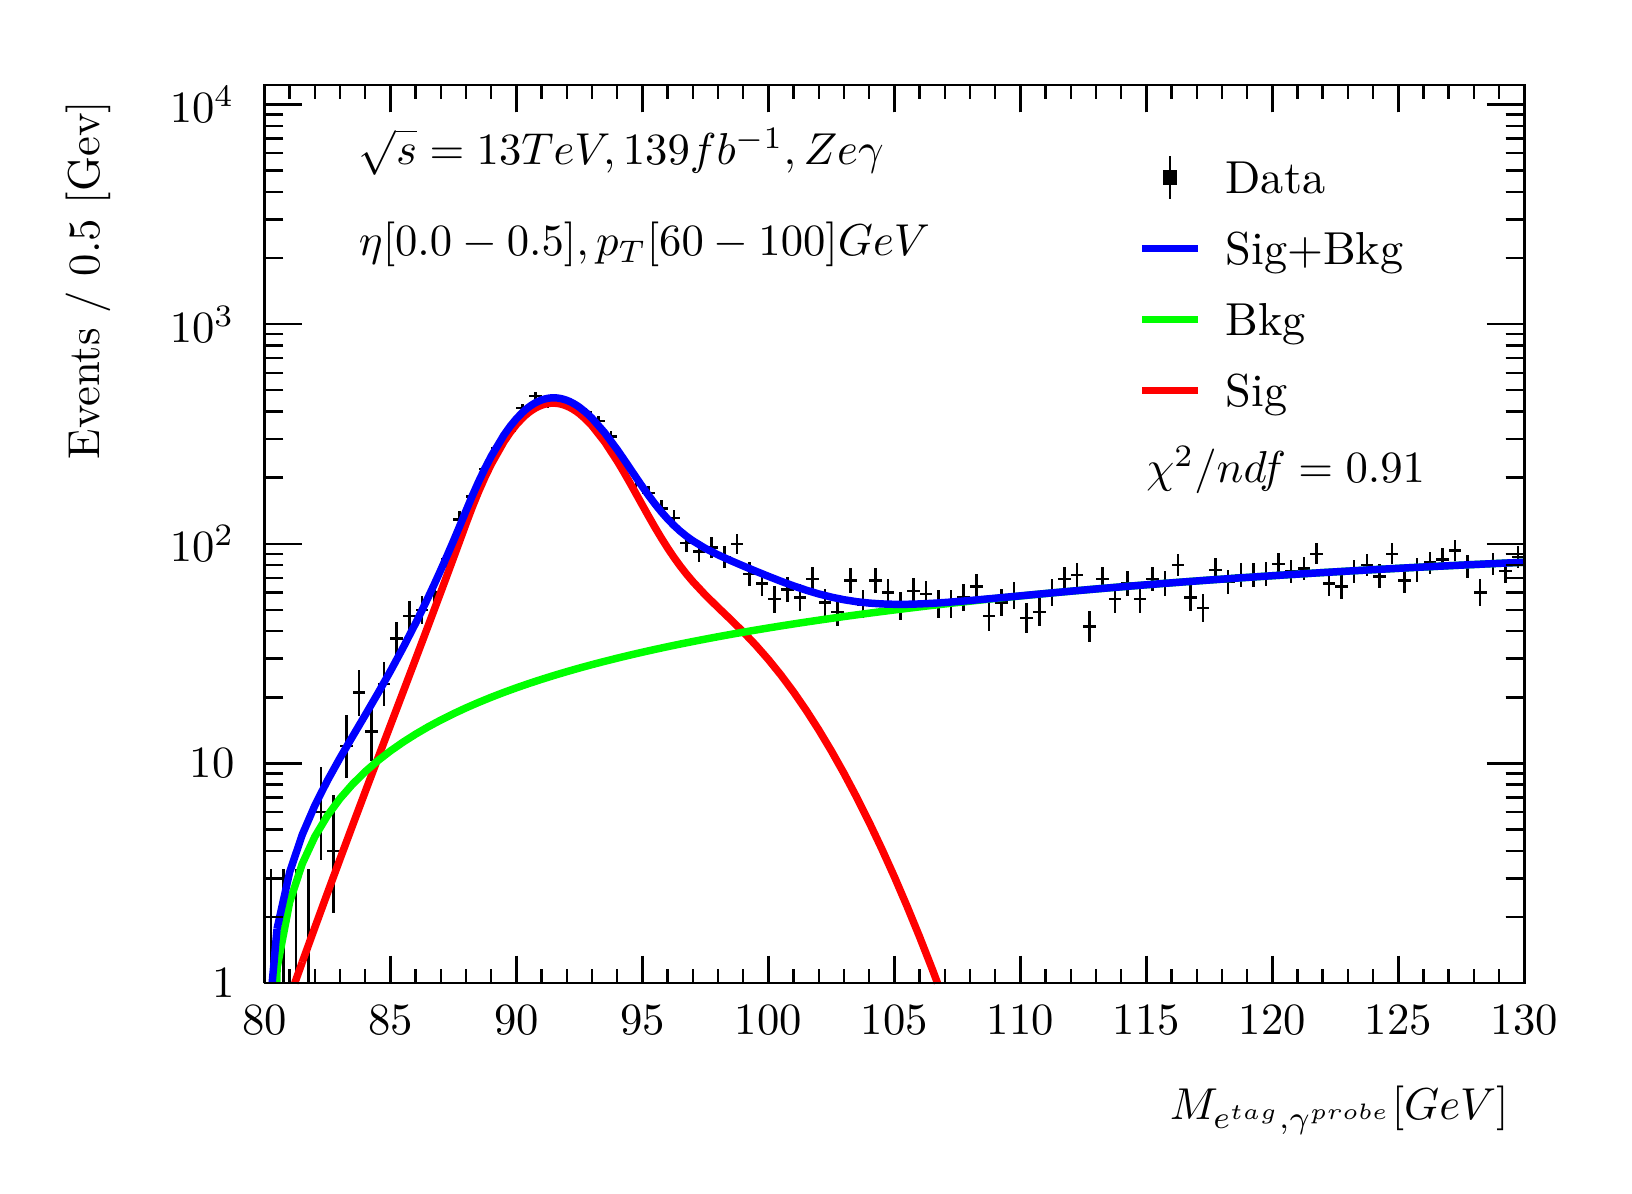
\begin{tikzpicture}
\pgfdeclareplotmark{cross} {
\pgfpathmoveto{\pgfpoint{-0.3\pgfplotmarksize}{\pgfplotmarksize}}
\pgfpathlineto{\pgfpoint{+0.3\pgfplotmarksize}{\pgfplotmarksize}}
\pgfpathlineto{\pgfpoint{+0.3\pgfplotmarksize}{0.3\pgfplotmarksize}}
\pgfpathlineto{\pgfpoint{+1\pgfplotmarksize}{0.3\pgfplotmarksize}}
\pgfpathlineto{\pgfpoint{+1\pgfplotmarksize}{-0.3\pgfplotmarksize}}
\pgfpathlineto{\pgfpoint{+0.3\pgfplotmarksize}{-0.3\pgfplotmarksize}}
\pgfpathlineto{\pgfpoint{+0.3\pgfplotmarksize}{-1.\pgfplotmarksize}}
\pgfpathlineto{\pgfpoint{-0.3\pgfplotmarksize}{-1.\pgfplotmarksize}}
\pgfpathlineto{\pgfpoint{-0.3\pgfplotmarksize}{-0.3\pgfplotmarksize}}
\pgfpathlineto{\pgfpoint{-1.\pgfplotmarksize}{-0.3\pgfplotmarksize}}
\pgfpathlineto{\pgfpoint{-1.\pgfplotmarksize}{0.3\pgfplotmarksize}}
\pgfpathlineto{\pgfpoint{-0.3\pgfplotmarksize}{0.3\pgfplotmarksize}}
\pgfpathclose
\pgfusepathqstroke
}
\pgfdeclareplotmark{cross*} {
\pgfpathmoveto{\pgfpoint{-0.3\pgfplotmarksize}{\pgfplotmarksize}}
\pgfpathlineto{\pgfpoint{+0.3\pgfplotmarksize}{\pgfplotmarksize}}
\pgfpathlineto{\pgfpoint{+0.3\pgfplotmarksize}{0.3\pgfplotmarksize}}
\pgfpathlineto{\pgfpoint{+1\pgfplotmarksize}{0.3\pgfplotmarksize}}
\pgfpathlineto{\pgfpoint{+1\pgfplotmarksize}{-0.3\pgfplotmarksize}}
\pgfpathlineto{\pgfpoint{+0.3\pgfplotmarksize}{-0.3\pgfplotmarksize}}
\pgfpathlineto{\pgfpoint{+0.3\pgfplotmarksize}{-1.\pgfplotmarksize}}
\pgfpathlineto{\pgfpoint{-0.3\pgfplotmarksize}{-1.\pgfplotmarksize}}
\pgfpathlineto{\pgfpoint{-0.3\pgfplotmarksize}{-0.3\pgfplotmarksize}}
\pgfpathlineto{\pgfpoint{-1.\pgfplotmarksize}{-0.3\pgfplotmarksize}}
\pgfpathlineto{\pgfpoint{-1.\pgfplotmarksize}{0.3\pgfplotmarksize}}
\pgfpathlineto{\pgfpoint{-0.3\pgfplotmarksize}{0.3\pgfplotmarksize}}
\pgfpathclose
\pgfusepathqfillstroke
}
\pgfdeclareplotmark{newstar} {
\pgfpathmoveto{\pgfqpoint{0pt}{\pgfplotmarksize}}
\pgfpathlineto{\pgfqpointpolar{44}{0.5\pgfplotmarksize}}
\pgfpathlineto{\pgfqpointpolar{18}{\pgfplotmarksize}}
\pgfpathlineto{\pgfqpointpolar{-20}{0.5\pgfplotmarksize}}
\pgfpathlineto{\pgfqpointpolar{-54}{\pgfplotmarksize}}
\pgfpathlineto{\pgfqpointpolar{-90}{0.5\pgfplotmarksize}}
\pgfpathlineto{\pgfqpointpolar{234}{\pgfplotmarksize}}
\pgfpathlineto{\pgfqpointpolar{198}{0.5\pgfplotmarksize}}
\pgfpathlineto{\pgfqpointpolar{162}{\pgfplotmarksize}}
\pgfpathlineto{\pgfqpointpolar{134}{0.5\pgfplotmarksize}}
\pgfpathclose
\pgfusepathqstroke
}
\pgfdeclareplotmark{newstar*} {
\pgfpathmoveto{\pgfqpoint{0pt}{\pgfplotmarksize}}
\pgfpathlineto{\pgfqpointpolar{44}{0.5\pgfplotmarksize}}
\pgfpathlineto{\pgfqpointpolar{18}{\pgfplotmarksize}}
\pgfpathlineto{\pgfqpointpolar{-20}{0.5\pgfplotmarksize}}
\pgfpathlineto{\pgfqpointpolar{-54}{\pgfplotmarksize}}
\pgfpathlineto{\pgfqpointpolar{-90}{0.5\pgfplotmarksize}}
\pgfpathlineto{\pgfqpointpolar{234}{\pgfplotmarksize}}
\pgfpathlineto{\pgfqpointpolar{198}{0.5\pgfplotmarksize}}
\pgfpathlineto{\pgfqpointpolar{162}{\pgfplotmarksize}}
\pgfpathlineto{\pgfqpointpolar{134}{0.5\pgfplotmarksize}}
\pgfpathclose
\pgfusepathqfillstroke
}
\definecolor{c}{rgb}{1,1,1};
\draw [color=c, fill=c] (0,0) rectangle (20,14.4361);
\draw [color=c, fill=c] (3,2.30977) rectangle (19,13.7143);
\definecolor{c}{rgb}{0,0,0};
\draw [c,line width=0.9] (3,2.30977) -- (3,13.7143) -- (19,13.7143) -- (19,2.30977) -- (3,2.30977);
\definecolor{c}{rgb}{1,1,1};
\draw [color=c, fill=c] (3,2.30977) rectangle (19,13.7143);
\definecolor{c}{rgb}{0,0,0};
\draw [c,line width=0.9] (3,2.30977) -- (3,13.7143) -- (19,13.7143) -- (19,2.30977) -- (3,2.30977);
\draw [c,line width=0.9] (3,2.30977) -- (19,2.30977);
\draw [c,line width=0.9] (3,2.65624) -- (3,2.30977);
\draw [c,line width=0.9] (3.32,2.48301) -- (3.32,2.30977);
\draw [c,line width=0.9] (3.64,2.48301) -- (3.64,2.30977);
\draw [c,line width=0.9] (3.96,2.48301) -- (3.96,2.30977);
\draw [c,line width=0.9] (4.28,2.48301) -- (4.28,2.30977);
\draw [c,line width=0.9] (4.6,2.65624) -- (4.6,2.30977);
\draw [c,line width=0.9] (4.92,2.48301) -- (4.92,2.30977);
\draw [c,line width=0.9] (5.24,2.48301) -- (5.24,2.30977);
\draw [c,line width=0.9] (5.56,2.48301) -- (5.56,2.30977);
\draw [c,line width=0.9] (5.88,2.48301) -- (5.88,2.30977);
\draw [c,line width=0.9] (6.2,2.65624) -- (6.2,2.30977);
\draw [c,line width=0.9] (6.52,2.48301) -- (6.52,2.30977);
\draw [c,line width=0.9] (6.84,2.48301) -- (6.84,2.30977);
\draw [c,line width=0.9] (7.16,2.48301) -- (7.16,2.30977);
\draw [c,line width=0.9] (7.48,2.48301) -- (7.48,2.30977);
\draw [c,line width=0.9] (7.8,2.65624) -- (7.8,2.30977);
\draw [c,line width=0.9] (8.12,2.48301) -- (8.12,2.30977);
\draw [c,line width=0.9] (8.44,2.48301) -- (8.44,2.30977);
\draw [c,line width=0.9] (8.76,2.48301) -- (8.76,2.30977);
\draw [c,line width=0.9] (9.08,2.48301) -- (9.08,2.30977);
\draw [c,line width=0.9] (9.4,2.65624) -- (9.4,2.30977);
\draw [c,line width=0.9] (9.72,2.48301) -- (9.72,2.30977);
\draw [c,line width=0.9] (10.04,2.48301) -- (10.04,2.30977);
\draw [c,line width=0.9] (10.36,2.48301) -- (10.36,2.30977);
\draw [c,line width=0.9] (10.68,2.48301) -- (10.68,2.30977);
\draw [c,line width=0.9] (11,2.65624) -- (11,2.30977);
\draw [c,line width=0.9] (11.32,2.48301) -- (11.32,2.30977);
\draw [c,line width=0.9] (11.64,2.48301) -- (11.64,2.30977);
\draw [c,line width=0.9] (11.96,2.48301) -- (11.96,2.30977);
\draw [c,line width=0.9] (12.28,2.48301) -- (12.28,2.30977);
\draw [c,line width=0.9] (12.6,2.65624) -- (12.6,2.30977);
\draw [c,line width=0.9] (12.92,2.48301) -- (12.92,2.30977);
\draw [c,line width=0.9] (13.24,2.48301) -- (13.24,2.30977);
\draw [c,line width=0.9] (13.56,2.48301) -- (13.56,2.30977);
\draw [c,line width=0.9] (13.88,2.48301) -- (13.88,2.30977);
\draw [c,line width=0.9] (14.2,2.65624) -- (14.2,2.30977);
\draw [c,line width=0.9] (14.52,2.48301) -- (14.52,2.30977);
\draw [c,line width=0.9] (14.84,2.48301) -- (14.84,2.30977);
\draw [c,line width=0.9] (15.16,2.48301) -- (15.16,2.30977);
\draw [c,line width=0.9] (15.48,2.48301) -- (15.48,2.30977);
\draw [c,line width=0.9] (15.8,2.65624) -- (15.8,2.30977);
\draw [c,line width=0.9] (16.12,2.48301) -- (16.12,2.30977);
\draw [c,line width=0.9] (16.44,2.48301) -- (16.44,2.30977);
\draw [c,line width=0.9] (16.76,2.48301) -- (16.76,2.30977);
\draw [c,line width=0.9] (17.08,2.48301) -- (17.08,2.30977);
\draw [c,line width=0.9] (17.4,2.65624) -- (17.4,2.30977);
\draw [c,line width=0.9] (17.72,2.48301) -- (17.72,2.30977);
\draw [c,line width=0.9] (18.04,2.48301) -- (18.04,2.30977);
\draw [c,line width=0.9] (18.36,2.48301) -- (18.36,2.30977);
\draw [c,line width=0.9] (18.68,2.48301) -- (18.68,2.30977);
\draw [c,line width=0.9] (19,2.65624) -- (19,2.30977);
\draw [anchor=base] (3,1.66015) node[scale=1.61424, color=c, rotate=0]{80};
\draw [anchor=base] (4.6,1.66015) node[scale=1.61424, color=c, rotate=0]{85};
\draw [anchor=base] (6.2,1.66015) node[scale=1.61424, color=c, rotate=0]{90};
\draw [anchor=base] (7.8,1.66015) node[scale=1.61424, color=c, rotate=0]{95};
\draw [anchor=base] (9.4,1.66015) node[scale=1.61424, color=c, rotate=0]{100};
\draw [anchor=base] (11,1.66015) node[scale=1.61424, color=c, rotate=0]{105};
\draw [anchor=base] (12.6,1.66015) node[scale=1.61424, color=c, rotate=0]{110};
\draw [anchor=base] (14.2,1.66015) node[scale=1.61424, color=c, rotate=0]{115};
\draw [anchor=base] (15.8,1.66015) node[scale=1.61424, color=c, rotate=0]{120};
\draw [anchor=base] (17.4,1.66015) node[scale=1.61424, color=c, rotate=0]{125};
\draw [anchor=base] (19,1.66015) node[scale=1.61424, color=c, rotate=0]{130};
\draw [anchor= east] (19,0.692932) node[scale=1.61424, color=c, rotate=0]{$M_{e^{tag}, \gamma^{probe}}  [GeV]$};
\draw [c,line width=0.9] (3,13.7143) -- (19,13.7143);
\draw [c,line width=0.9] (3,13.3678) -- (3,13.7143);
\draw [c,line width=0.9] (3.32,13.5411) -- (3.32,13.7143);
\draw [c,line width=0.9] (3.64,13.5411) -- (3.64,13.7143);
\draw [c,line width=0.9] (3.96,13.5411) -- (3.96,13.7143);
\draw [c,line width=0.9] (4.28,13.5411) -- (4.28,13.7143);
\draw [c,line width=0.9] (4.6,13.3678) -- (4.6,13.7143);
\draw [c,line width=0.9] (4.92,13.5411) -- (4.92,13.7143);
\draw [c,line width=0.9] (5.24,13.5411) -- (5.24,13.7143);
\draw [c,line width=0.9] (5.56,13.5411) -- (5.56,13.7143);
\draw [c,line width=0.9] (5.88,13.5411) -- (5.88,13.7143);
\draw [c,line width=0.9] (6.2,13.3678) -- (6.2,13.7143);
\draw [c,line width=0.9] (6.52,13.5411) -- (6.52,13.7143);
\draw [c,line width=0.9] (6.84,13.5411) -- (6.84,13.7143);
\draw [c,line width=0.9] (7.16,13.5411) -- (7.16,13.7143);
\draw [c,line width=0.9] (7.48,13.5411) -- (7.48,13.7143);
\draw [c,line width=0.9] (7.8,13.3678) -- (7.8,13.7143);
\draw [c,line width=0.9] (8.12,13.5411) -- (8.12,13.7143);
\draw [c,line width=0.9] (8.44,13.5411) -- (8.44,13.7143);
\draw [c,line width=0.9] (8.76,13.5411) -- (8.76,13.7143);
\draw [c,line width=0.9] (9.08,13.5411) -- (9.08,13.7143);
\draw [c,line width=0.9] (9.4,13.3678) -- (9.4,13.7143);
\draw [c,line width=0.9] (9.72,13.5411) -- (9.72,13.7143);
\draw [c,line width=0.9] (10.04,13.5411) -- (10.04,13.7143);
\draw [c,line width=0.9] (10.36,13.5411) -- (10.36,13.7143);
\draw [c,line width=0.9] (10.68,13.5411) -- (10.68,13.7143);
\draw [c,line width=0.9] (11,13.3678) -- (11,13.7143);
\draw [c,line width=0.9] (11.32,13.5411) -- (11.32,13.7143);
\draw [c,line width=0.9] (11.64,13.5411) -- (11.64,13.7143);
\draw [c,line width=0.9] (11.96,13.5411) -- (11.96,13.7143);
\draw [c,line width=0.9] (12.28,13.5411) -- (12.28,13.7143);
\draw [c,line width=0.9] (12.6,13.3678) -- (12.6,13.7143);
\draw [c,line width=0.9] (12.92,13.5411) -- (12.92,13.7143);
\draw [c,line width=0.9] (13.24,13.5411) -- (13.24,13.7143);
\draw [c,line width=0.9] (13.56,13.5411) -- (13.56,13.7143);
\draw [c,line width=0.9] (13.88,13.5411) -- (13.88,13.7143);
\draw [c,line width=0.9] (14.2,13.3678) -- (14.2,13.7143);
\draw [c,line width=0.9] (14.52,13.5411) -- (14.52,13.7143);
\draw [c,line width=0.9] (14.84,13.5411) -- (14.84,13.7143);
\draw [c,line width=0.9] (15.16,13.5411) -- (15.16,13.7143);
\draw [c,line width=0.9] (15.48,13.5411) -- (15.48,13.7143);
\draw [c,line width=0.9] (15.8,13.3678) -- (15.8,13.7143);
\draw [c,line width=0.9] (16.12,13.5411) -- (16.12,13.7143);
\draw [c,line width=0.9] (16.44,13.5411) -- (16.44,13.7143);
\draw [c,line width=0.9] (16.76,13.5411) -- (16.76,13.7143);
\draw [c,line width=0.9] (17.08,13.5411) -- (17.08,13.7143);
\draw [c,line width=0.9] (17.4,13.3678) -- (17.4,13.7143);
\draw [c,line width=0.9] (17.72,13.5411) -- (17.72,13.7143);
\draw [c,line width=0.9] (18.04,13.5411) -- (18.04,13.7143);
\draw [c,line width=0.9] (18.36,13.5411) -- (18.36,13.7143);
\draw [c,line width=0.9] (18.68,13.5411) -- (18.68,13.7143);
\draw [c,line width=0.9] (19,13.3678) -- (19,13.7143);
\draw [c,line width=0.9] (3,2.30977) -- (3,13.7143);
\draw [c,line width=0.9] (3.474,2.30978) -- (3,2.30978);
\draw [anchor= east] (2.82,2.30978) node[scale=1.61424, color=c, rotate=0]{1};
\draw [c,line width=0.9] (3.237,3.1495) -- (3,3.1495);
\draw [c,line width=0.9] (3.237,3.6407) -- (3,3.6407);
\draw [c,line width=0.9] (3.237,3.98922) -- (3,3.98922);
\draw [c,line width=0.9] (3.237,4.25955) -- (3,4.25955);
\draw [c,line width=0.9] (3.237,4.48042) -- (3,4.48042);
\draw [c,line width=0.9] (3.237,4.66717) -- (3,4.66717);
\draw [c,line width=0.9] (3.237,4.82894) -- (3,4.82894);
\draw [c,line width=0.9] (3.237,4.97163) -- (3,4.97163);
\draw [c,line width=0.9] (3.474,5.09927) -- (3,5.09927);
\draw [anchor= east] (2.82,5.09927) node[scale=1.61424, color=c, rotate=0]{10};
\draw [c,line width=0.9] (3.237,5.93899) -- (3,5.93899);
\draw [c,line width=0.9] (3.237,6.43019) -- (3,6.43019);
\draw [c,line width=0.9] (3.237,6.77871) -- (3,6.77871);
\draw [c,line width=0.9] (3.237,7.04904) -- (3,7.04904);
\draw [c,line width=0.9] (3.237,7.26991) -- (3,7.26991);
\draw [c,line width=0.9] (3.237,7.45666) -- (3,7.45666);
\draw [c,line width=0.9] (3.237,7.61843) -- (3,7.61843);
\draw [c,line width=0.9] (3.237,7.76112) -- (3,7.76112);
\draw [c,line width=0.9] (3.474,7.88876) -- (3,7.88876);
\draw [anchor= east] (2.82,7.88876) node[scale=1.61424, color=c, rotate=0]{$10^{2}$};
\draw [c,line width=0.9] (3.237,8.72848) -- (3,8.72848);
\draw [c,line width=0.9] (3.237,9.21968) -- (3,9.21968);
\draw [c,line width=0.9] (3.237,9.5682) -- (3,9.5682);
\draw [c,line width=0.9] (3.237,9.83853) -- (3,9.83853);
\draw [c,line width=0.9] (3.237,10.0594) -- (3,10.0594);
\draw [c,line width=0.9] (3.237,10.2462) -- (3,10.2462);
\draw [c,line width=0.9] (3.237,10.4079) -- (3,10.4079);
\draw [c,line width=0.9] (3.237,10.5506) -- (3,10.5506);
\draw [c,line width=0.9] (3.474,10.6782) -- (3,10.6782);
\draw [anchor= east] (2.82,10.6782) node[scale=1.61424, color=c, rotate=0]{$10^{3}$};
\draw [c,line width=0.9] (3.237,11.518) -- (3,11.518);
\draw [c,line width=0.9] (3.237,12.0092) -- (3,12.0092);
\draw [c,line width=0.9] (3.237,12.3577) -- (3,12.3577);
\draw [c,line width=0.9] (3.237,12.628) -- (3,12.628);
\draw [c,line width=0.9] (3.237,12.8489) -- (3,12.8489);
\draw [c,line width=0.9] (3.237,13.0356) -- (3,13.0356);
\draw [c,line width=0.9] (3.237,13.1974) -- (3,13.1974);
\draw [c,line width=0.9] (3.237,13.3401) -- (3,13.3401);
\draw [c,line width=0.9] (3.474,13.4677) -- (3,13.4677);
\draw [anchor= east] (2.82,13.4677) node[scale=1.61424, color=c, rotate=0]{$10^{4}$};
\draw [anchor= east] (0.76,13.7143) node[scale=1.61424, color=c, rotate=90]{Events / 0.5 [Gev]};
\draw [c,line width=0.9] (19,2.30977) -- (19,13.7143);
\draw [c,line width=0.9] (18.526,2.30978) -- (19,2.30978);
\draw [c,line width=0.9] (18.763,3.1495) -- (19,3.1495);
\draw [c,line width=0.9] (18.763,3.6407) -- (19,3.6407);
\draw [c,line width=0.9] (18.763,3.98922) -- (19,3.98922);
\draw [c,line width=0.9] (18.763,4.25955) -- (19,4.25955);
\draw [c,line width=0.9] (18.763,4.48042) -- (19,4.48042);
\draw [c,line width=0.9] (18.763,4.66717) -- (19,4.66717);
\draw [c,line width=0.9] (18.763,4.82894) -- (19,4.82894);
\draw [c,line width=0.9] (18.763,4.97163) -- (19,4.97163);
\draw [c,line width=0.9] (18.526,5.09927) -- (19,5.09927);
\draw [c,line width=0.9] (18.763,5.93899) -- (19,5.93899);
\draw [c,line width=0.9] (18.763,6.43019) -- (19,6.43019);
\draw [c,line width=0.9] (18.763,6.77871) -- (19,6.77871);
\draw [c,line width=0.9] (18.763,7.04904) -- (19,7.04904);
\draw [c,line width=0.9] (18.763,7.26991) -- (19,7.26991);
\draw [c,line width=0.9] (18.763,7.45666) -- (19,7.45666);
\draw [c,line width=0.9] (18.763,7.61843) -- (19,7.61843);
\draw [c,line width=0.9] (18.763,7.76112) -- (19,7.76112);
\draw [c,line width=0.9] (18.526,7.88876) -- (19,7.88876);
\draw [c,line width=0.9] (18.763,8.72848) -- (19,8.72848);
\draw [c,line width=0.9] (18.763,9.21968) -- (19,9.21968);
\draw [c,line width=0.9] (18.763,9.5682) -- (19,9.5682);
\draw [c,line width=0.9] (18.763,9.83853) -- (19,9.83853);
\draw [c,line width=0.9] (18.763,10.0594) -- (19,10.0594);
\draw [c,line width=0.9] (18.763,10.2462) -- (19,10.2462);
\draw [c,line width=0.9] (18.763,10.4079) -- (19,10.4079);
\draw [c,line width=0.9] (18.763,10.5506) -- (19,10.5506);
\draw [c,line width=0.9] (18.526,10.6782) -- (19,10.6782);
\draw [c,line width=0.9] (18.763,11.518) -- (19,11.518);
\draw [c,line width=0.9] (18.763,12.0092) -- (19,12.0092);
\draw [c,line width=0.9] (18.763,12.3577) -- (19,12.3577);
\draw [c,line width=0.9] (18.763,12.628) -- (19,12.628);
\draw [c,line width=0.9] (18.763,12.8489) -- (19,12.8489);
\draw [c,line width=0.9] (18.763,13.0356) -- (19,13.0356);
\draw [c,line width=0.9] (18.763,13.1974) -- (19,13.1974);
\draw [c,line width=0.9] (18.763,13.3401) -- (19,13.3401);
\draw [c,line width=0.9] (18.526,13.4677) -- (19,13.4677);
\draw [c,line width=0.9] (3.08,2.30977) -- (3,2.30977);
\draw [c,line width=0.9] (3,2.30977) -- (3,2.30977);
\draw [c,line width=0.9] (3.08,2.30977) -- (3.16,2.30977);
\draw [c,line width=0.9] (3.16,2.30977) -- (3.16,2.30977);
\draw [c,line width=0.9] (3.08,2.30977) -- (3.08,3.75599);
\draw [c,line width=0.9] (3.08,3.75599) -- (3.08,3.75599);
\draw [c,line width=0.9] (3.24,2.30977) -- (3.16,2.30977);
\draw [c,line width=0.9] (3.16,2.30977) -- (3.16,2.30977);
\draw [c,line width=0.9] (3.24,2.30977) -- (3.32,2.30977);
\draw [c,line width=0.9] (3.32,2.30977) -- (3.32,2.30977);
\draw [c,line width=0.9] (3.24,2.30977) -- (3.24,3.75599);
\draw [c,line width=0.9] (3.24,3.75599) -- (3.24,3.75599);
\draw [c,line width=0.9] (3.4,2.30977) -- (3.32,2.30977);
\draw [c,line width=0.9] (3.32,2.30977) -- (3.32,2.30977);
\draw [c,line width=0.9] (3.4,2.30977) -- (3.48,2.30977);
\draw [c,line width=0.9] (3.48,2.30977) -- (3.48,2.30977);
\draw [c,line width=0.9] (3.4,2.30977) -- (3.4,3.75599);
\draw [c,line width=0.9] (3.4,3.75599) -- (3.4,3.75599);
\draw [c,line width=0.9] (3.56,2.30977) -- (3.48,2.30977);
\draw [c,line width=0.9] (3.48,2.30977) -- (3.48,2.30977);
\draw [c,line width=0.9] (3.56,2.30977) -- (3.64,2.30977);
\draw [c,line width=0.9] (3.64,2.30977) -- (3.64,2.30977);
\draw [c,line width=0.9] (3.56,2.30977) -- (3.56,3.75599);
\draw [c,line width=0.9] (3.56,3.75599) -- (3.56,3.75599);
\draw [c,line width=0.9] (3.72,4.48042) -- (3.64,4.48042);
\draw [c,line width=0.9] (3.64,4.48042) -- (3.64,4.48042);
\draw [c,line width=0.9] (3.72,4.48042) -- (3.8,4.48042);
\draw [c,line width=0.9] (3.8,4.48042) -- (3.8,4.48042);
\draw [c,line width=0.9] (3.72,4.48042) -- (3.72,5.04775);
\draw [c,line width=0.9] (3.72,5.04775) -- (3.72,5.04775);
\draw [c,line width=0.9] (3.72,4.48042) -- (3.72,3.86831);
\draw [c,line width=0.9] (3.72,3.86831) -- (3.72,3.86831);
\draw [c,line width=0.9] (3.88,3.98922) -- (3.8,3.98922);
\draw [c,line width=0.9] (3.8,3.98922) -- (3.8,3.98922);
\draw [c,line width=0.9] (3.88,3.98922) -- (3.96,3.98922);
\draw [c,line width=0.9] (3.96,3.98922) -- (3.96,3.98922);
\draw [c,line width=0.9] (3.88,3.98922) -- (3.88,4.69501);
\draw [c,line width=0.9] (3.88,4.69501) -- (3.88,4.69501);
\draw [c,line width=0.9] (3.88,3.98922) -- (3.88,3.2003);
\draw [c,line width=0.9] (3.88,3.2003) -- (3.88,3.2003);
\draw [c,line width=0.9] (4.04,5.32014) -- (3.96,5.32014);
\draw [c,line width=0.9] (3.96,5.32014) -- (3.96,5.32014);
\draw [c,line width=0.9] (4.04,5.32014) -- (4.12,5.32014);
\draw [c,line width=0.9] (4.12,5.32014) -- (4.12,5.32014);
\draw [c,line width=0.9] (4.04,5.32014) -- (4.04,5.71032);
\draw [c,line width=0.9] (4.04,5.71032) -- (4.04,5.71032);
\draw [c,line width=0.9] (4.04,5.32014) -- (4.04,4.9144);
\draw [c,line width=0.9] (4.04,4.9144) -- (4.04,4.9144);
\draw [c,line width=0.9] (4.2,5.99809) -- (4.12,5.99809);
\draw [c,line width=0.9] (4.12,5.99809) -- (4.12,5.99809);
\draw [c,line width=0.9] (4.2,5.99809) -- (4.28,5.99809);
\draw [c,line width=0.9] (4.28,5.99809) -- (4.28,5.99809);
\draw [c,line width=0.9] (4.2,5.99809) -- (4.2,6.28698);
\draw [c,line width=0.9] (4.2,6.28698) -- (4.2,6.28698);
\draw [c,line width=0.9] (4.2,5.99809) -- (4.2,5.70257);
\draw [c,line width=0.9] (4.2,5.70257) -- (4.2,5.70257);
\draw [c,line width=0.9] (4.36,5.50689) -- (4.28,5.50689);
\draw [c,line width=0.9] (4.28,5.50689) -- (4.28,5.50689);
\draw [c,line width=0.9] (4.36,5.50689) -- (4.44,5.50689);
\draw [c,line width=0.9] (4.44,5.50689) -- (4.44,5.50689);
\draw [c,line width=0.9] (4.36,5.50689) -- (4.36,5.86598);
\draw [c,line width=0.9] (4.36,5.86598) -- (4.36,5.86598);
\draw [c,line width=0.9] (4.36,5.50689) -- (4.36,5.13549);
\draw [c,line width=0.9] (4.36,5.13549) -- (4.36,5.13549);
\draw [c,line width=0.9] (4.52,6.1083) -- (4.44,6.1083);
\draw [c,line width=0.9] (4.44,6.1083) -- (4.44,6.1083);
\draw [c,line width=0.9] (4.52,6.1083) -- (4.6,6.1083);
\draw [c,line width=0.9] (4.6,6.1083) -- (4.6,6.1083);
\draw [c,line width=0.9] (4.52,6.1083) -- (4.52,6.38348);
\draw [c,line width=0.9] (4.52,6.38348) -- (4.52,6.38348);
\draw [c,line width=0.9] (4.52,6.1083) -- (4.52,5.82734);
\draw [c,line width=0.9] (4.52,5.82734) -- (4.52,5.82734);
\draw [c,line width=0.9] (4.68,6.68426) -- (4.6,6.68426);
\draw [c,line width=0.9] (4.6,6.68426) -- (4.6,6.68426);
\draw [c,line width=0.9] (4.68,6.68426) -- (4.76,6.68426);
\draw [c,line width=0.9] (4.76,6.68426) -- (4.76,6.68426);
\draw [c,line width=0.9] (4.68,6.68426) -- (4.68,6.89795);
\draw [c,line width=0.9] (4.68,6.89795) -- (4.68,6.89795);
\draw [c,line width=0.9] (4.68,6.68426) -- (4.68,6.46776);
\draw [c,line width=0.9] (4.68,6.46776) -- (4.68,6.46776);
\draw [c,line width=0.9] (4.84,6.97408) -- (4.76,6.97408);
\draw [c,line width=0.9] (4.76,6.97408) -- (4.76,6.97408);
\draw [c,line width=0.9] (4.84,6.97408) -- (4.92,6.97408);
\draw [c,line width=0.9] (4.92,6.97408) -- (4.92,6.97408);
\draw [c,line width=0.9] (4.84,6.97408) -- (4.84,7.16239);
\draw [c,line width=0.9] (4.84,7.16239) -- (4.84,7.16239);
\draw [c,line width=0.9] (4.84,6.97408) -- (4.84,6.78381);
\draw [c,line width=0.9] (4.84,6.78381) -- (4.84,6.78381);
\draw [c,line width=0.9] (5,7.04904) -- (4.92,7.04904);
\draw [c,line width=0.9] (4.92,7.04904) -- (4.92,7.04904);
\draw [c,line width=0.9] (5,7.04904) -- (5.08,7.04904);
\draw [c,line width=0.9] (5.08,7.04904) -- (5.08,7.04904);
\draw [c,line width=0.9] (5,7.04904) -- (5,7.23131);
\draw [c,line width=0.9] (5,7.23131) -- (5,7.23131);
\draw [c,line width=0.9] (5,7.04904) -- (5,6.86499);
\draw [c,line width=0.9] (5,6.86499) -- (5,6.86499);
\draw [c,line width=0.9] (5.16,7.26991) -- (5.08,7.26991);
\draw [c,line width=0.9] (5.08,7.26991) -- (5.08,7.26991);
\draw [c,line width=0.9] (5.16,7.26991) -- (5.24,7.26991);
\draw [c,line width=0.9] (5.24,7.26991) -- (5.24,7.26991);
\draw [c,line width=0.9] (5.16,7.26991) -- (5.16,7.43552);
\draw [c,line width=0.9] (5.16,7.43552) -- (5.16,7.43552);
\draw [c,line width=0.9] (5.16,7.26991) -- (5.16,7.10296);
\draw [c,line width=0.9] (5.16,7.10296) -- (5.16,7.10296);
\draw [c,line width=0.9] (5.32,7.69187) -- (5.24,7.69187);
\draw [c,line width=0.9] (5.24,7.69187) -- (5.24,7.69187);
\draw [c,line width=0.9] (5.32,7.69187) -- (5.4,7.69187);
\draw [c,line width=0.9] (5.4,7.69187) -- (5.4,7.69187);
\draw [c,line width=0.9] (5.32,7.69187) -- (5.32,7.82987);
\draw [c,line width=0.9] (5.32,7.82987) -- (5.32,7.82987);
\draw [c,line width=0.9] (5.32,7.69187) -- (5.32,7.55307);
\draw [c,line width=0.9] (5.32,7.55307) -- (5.32,7.55307);
\draw [c,line width=0.9] (5.48,8.19725) -- (5.4,8.19725);
\draw [c,line width=0.9] (5.4,8.19725) -- (5.4,8.19725);
\draw [c,line width=0.9] (5.48,8.19725) -- (5.56,8.19725);
\draw [c,line width=0.9] (5.56,8.19725) -- (5.56,8.19725);
\draw [c,line width=0.9] (5.48,8.19725) -- (5.48,8.30387);
\draw [c,line width=0.9] (5.48,8.30387) -- (5.48,8.30387);
\draw [c,line width=0.9] (5.48,8.19725) -- (5.48,8.09062);
\draw [c,line width=0.9] (5.48,8.09062) -- (5.48,8.09062);
\draw [c,line width=0.9] (5.64,8.48806) -- (5.56,8.48806);
\draw [c,line width=0.9] (5.56,8.48806) -- (5.56,8.48806);
\draw [c,line width=0.9] (5.64,8.48806) -- (5.72,8.48806);
\draw [c,line width=0.9] (5.72,8.48806) -- (5.72,8.48806);
\draw [c,line width=0.9] (5.64,8.48806) -- (5.64,8.58264);
\draw [c,line width=0.9] (5.64,8.58264) -- (5.64,8.58264);
\draw [c,line width=0.9] (5.64,8.48806) -- (5.64,8.39349);
\draw [c,line width=0.9] (5.64,8.39349) -- (5.64,8.39349);
\draw [c,line width=0.9] (5.8,8.83842) -- (5.72,8.83842);
\draw [c,line width=0.9] (5.72,8.83842) -- (5.72,8.83842);
\draw [c,line width=0.9] (5.8,8.83842) -- (5.88,8.83842);
\draw [c,line width=0.9] (5.88,8.83842) -- (5.88,8.83842);
\draw [c,line width=0.9] (5.8,8.83842) -- (5.8,8.92027);
\draw [c,line width=0.9] (5.8,8.92027) -- (5.8,8.92027);
\draw [c,line width=0.9] (5.8,8.83842) -- (5.8,8.75658);
\draw [c,line width=0.9] (5.8,8.75658) -- (5.8,8.75658);
\draw [c,line width=0.9] (5.96,9.10543) -- (5.88,9.10543);
\draw [c,line width=0.9] (5.88,9.10543) -- (5.88,9.10543);
\draw [c,line width=0.9] (5.96,9.10543) -- (6.04,9.10543);
\draw [c,line width=0.9] (6.04,9.10543) -- (6.04,9.10543);
\draw [c,line width=0.9] (5.96,9.10543) -- (5.96,9.17874);
\draw [c,line width=0.9] (5.96,9.17874) -- (5.96,9.17874);
\draw [c,line width=0.9] (5.96,9.10543) -- (5.96,9.03212);
\draw [c,line width=0.9] (5.96,9.03212) -- (5.96,9.03212);
\draw [c,line width=0.9] (6.12,9.32037) -- (6.04,9.32037);
\draw [c,line width=0.9] (6.04,9.32037) -- (6.04,9.32037);
\draw [c,line width=0.9] (6.12,9.32037) -- (6.2,9.32037);
\draw [c,line width=0.9] (6.2,9.32037) -- (6.2,9.32037);
\draw [c,line width=0.9] (6.12,9.32037) -- (6.12,9.38746);
\draw [c,line width=0.9] (6.12,9.38746) -- (6.12,9.38746);
\draw [c,line width=0.9] (6.12,9.32037) -- (6.12,9.25328);
\draw [c,line width=0.9] (6.12,9.25328) -- (6.12,9.25328);
\draw [c,line width=0.9] (6.28,9.60987) -- (6.2,9.60987);
\draw [c,line width=0.9] (6.2,9.60987) -- (6.2,9.60987);
\draw [c,line width=0.9] (6.28,9.60987) -- (6.36,9.60987);
\draw [c,line width=0.9] (6.36,9.60987) -- (6.36,9.60987);
\draw [c,line width=0.9] (6.28,9.60987) -- (6.28,9.66941);
\draw [c,line width=0.9] (6.28,9.66941) -- (6.28,9.66941);
\draw [c,line width=0.9] (6.28,9.60987) -- (6.28,9.55034);
\draw [c,line width=0.9] (6.28,9.55034) -- (6.28,9.55034);
\draw [c,line width=0.9] (6.44,9.76357) -- (6.36,9.76357);
\draw [c,line width=0.9] (6.36,9.76357) -- (6.36,9.76357);
\draw [c,line width=0.9] (6.44,9.76357) -- (6.52,9.76357);
\draw [c,line width=0.9] (6.52,9.76357) -- (6.52,9.76357);
\draw [c,line width=0.9] (6.44,9.76357) -- (6.44,9.81944);
\draw [c,line width=0.9] (6.44,9.81944) -- (6.44,9.81944);
\draw [c,line width=0.9] (6.44,9.76357) -- (6.44,9.70769);
\draw [c,line width=0.9] (6.44,9.70769) -- (6.44,9.70769);
\draw [c,line width=0.9] (6.6,9.66982) -- (6.52,9.66982);
\draw [c,line width=0.9] (6.52,9.66982) -- (6.52,9.66982);
\draw [c,line width=0.9] (6.6,9.66982) -- (6.68,9.66982);
\draw [c,line width=0.9] (6.68,9.66982) -- (6.68,9.66982);
\draw [c,line width=0.9] (6.6,9.66982) -- (6.6,9.7279);
\draw [c,line width=0.9] (6.6,9.7279) -- (6.6,9.7279);
\draw [c,line width=0.9] (6.6,9.66982) -- (6.6,9.61174);
\draw [c,line width=0.9] (6.6,9.61174) -- (6.6,9.61174);
\draw [c,line width=0.9] (6.76,9.72161) -- (6.68,9.72161);
\draw [c,line width=0.9] (6.68,9.72161) -- (6.68,9.72161);
\draw [c,line width=0.9] (6.76,9.72161) -- (6.84,9.72161);
\draw [c,line width=0.9] (6.84,9.72161) -- (6.84,9.72161);
\draw [c,line width=0.9] (6.76,9.72161) -- (6.76,9.77846);
\draw [c,line width=0.9] (6.76,9.77846) -- (6.76,9.77846);
\draw [c,line width=0.9] (6.76,9.72161) -- (6.76,9.66476);
\draw [c,line width=0.9] (6.76,9.66476) -- (6.76,9.66476);
\draw [c,line width=0.9] (6.92,9.64449) -- (6.84,9.64449);
\draw [c,line width=0.9] (6.84,9.64449) -- (6.84,9.64449);
\draw [c,line width=0.9] (6.92,9.64449) -- (7,9.64449);
\draw [c,line width=0.9] (7,9.64449) -- (7,9.64449);
\draw [c,line width=0.9] (6.92,9.64449) -- (6.92,9.70318);
\draw [c,line width=0.9] (6.92,9.70318) -- (6.92,9.70318);
\draw [c,line width=0.9] (6.92,9.64449) -- (6.92,9.5858);
\draw [c,line width=0.9] (6.92,9.5858) -- (6.92,9.5858);
\draw [c,line width=0.9] (7.08,9.55296) -- (7,9.55296);
\draw [c,line width=0.9] (7,9.55296) -- (7,9.55296);
\draw [c,line width=0.9] (7.08,9.55296) -- (7.16,9.55296);
\draw [c,line width=0.9] (7.16,9.55296) -- (7.16,9.55296);
\draw [c,line width=0.9] (7.08,9.55296) -- (7.08,9.61391);
\draw [c,line width=0.9] (7.08,9.61391) -- (7.08,9.61391);
\draw [c,line width=0.9] (7.08,9.55296) -- (7.08,9.49201);
\draw [c,line width=0.9] (7.08,9.49201) -- (7.08,9.49201);
\draw [c,line width=0.9] (7.24,9.44727) -- (7.16,9.44727);
\draw [c,line width=0.9] (7.16,9.44727) -- (7.16,9.44727);
\draw [c,line width=0.9] (7.24,9.44727) -- (7.32,9.44727);
\draw [c,line width=0.9] (7.32,9.44727) -- (7.32,9.44727);
\draw [c,line width=0.9] (7.24,9.44727) -- (7.24,9.51093);
\draw [c,line width=0.9] (7.24,9.51093) -- (7.24,9.51093);
\draw [c,line width=0.9] (7.24,9.44727) -- (7.24,9.3836);
\draw [c,line width=0.9] (7.24,9.3836) -- (7.24,9.3836);
\draw [c,line width=0.9] (7.4,9.25156) -- (7.32,9.25156);
\draw [c,line width=0.9] (7.32,9.25156) -- (7.32,9.25156);
\draw [c,line width=0.9] (7.4,9.25156) -- (7.48,9.25156);
\draw [c,line width=0.9] (7.48,9.25156) -- (7.48,9.25156);
\draw [c,line width=0.9] (7.4,9.25156) -- (7.4,9.32058);
\draw [c,line width=0.9] (7.4,9.32058) -- (7.4,9.32058);
\draw [c,line width=0.9] (7.4,9.25156) -- (7.4,9.18254);
\draw [c,line width=0.9] (7.4,9.18254) -- (7.4,9.18254);
\draw [c,line width=0.9] (7.56,8.90828) -- (7.48,8.90828);
\draw [c,line width=0.9] (7.48,8.90828) -- (7.48,8.90828);
\draw [c,line width=0.9] (7.56,8.90828) -- (7.64,8.90828);
\draw [c,line width=0.9] (7.64,8.90828) -- (7.64,8.90828);
\draw [c,line width=0.9] (7.56,8.90828) -- (7.56,8.9878);
\draw [c,line width=0.9] (7.56,8.9878) -- (7.56,8.9878);
\draw [c,line width=0.9] (7.56,8.90828) -- (7.56,8.82876);
\draw [c,line width=0.9] (7.56,8.82876) -- (7.56,8.82876);
\draw [c,line width=0.9] (7.72,8.63403) -- (7.64,8.63403);
\draw [c,line width=0.9] (7.64,8.63403) -- (7.64,8.63403);
\draw [c,line width=0.9] (7.72,8.63403) -- (7.8,8.63403);
\draw [c,line width=0.9] (7.8,8.63403) -- (7.8,8.63403);
\draw [c,line width=0.9] (7.72,8.63403) -- (7.72,8.72308);
\draw [c,line width=0.9] (7.72,8.72308) -- (7.72,8.72308);
\draw [c,line width=0.9] (7.72,8.63403) -- (7.72,8.54498);
\draw [c,line width=0.9] (7.72,8.54498) -- (7.72,8.54498);
\draw [c,line width=0.9] (7.88,8.53159) -- (7.8,8.53159);
\draw [c,line width=0.9] (7.8,8.53159) -- (7.8,8.53159);
\draw [c,line width=0.9] (7.88,8.53159) -- (7.96,8.53159);
\draw [c,line width=0.9] (7.96,8.53159) -- (7.96,8.53159);
\draw [c,line width=0.9] (7.88,8.53159) -- (7.88,8.62448);
\draw [c,line width=0.9] (7.88,8.62448) -- (7.88,8.62448);
\draw [c,line width=0.9] (7.88,8.53159) -- (7.88,8.4387);
\draw [c,line width=0.9] (7.88,8.4387) -- (7.88,8.4387);
\draw [c,line width=0.9] (8.04,8.33889) -- (7.96,8.33889);
\draw [c,line width=0.9] (7.96,8.33889) -- (7.96,8.33889);
\draw [c,line width=0.9] (8.04,8.33889) -- (8.12,8.33889);
\draw [c,line width=0.9] (8.12,8.33889) -- (8.12,8.33889);
\draw [c,line width=0.9] (8.04,8.33889) -- (8.04,8.43947);
\draw [c,line width=0.9] (8.04,8.43947) -- (8.04,8.43947);
\draw [c,line width=0.9] (8.04,8.33889) -- (8.04,8.23831);
\draw [c,line width=0.9] (8.04,8.23831) -- (8.04,8.23831);
\draw [c,line width=0.9] (8.2,8.21588) -- (8.12,8.21588);
\draw [c,line width=0.9] (8.12,8.21588) -- (8.12,8.21588);
\draw [c,line width=0.9] (8.2,8.21588) -- (8.28,8.21588);
\draw [c,line width=0.9] (8.28,8.21588) -- (8.28,8.21588);
\draw [c,line width=0.9] (8.2,8.21588) -- (8.2,8.3217);
\draw [c,line width=0.9] (8.2,8.3217) -- (8.2,8.3217);
\draw [c,line width=0.9] (8.2,8.21588) -- (8.2,8.11007);
\draw [c,line width=0.9] (8.2,8.11007) -- (8.2,8.11007);
\draw [c,line width=0.9] (8.36,7.90081) -- (8.28,7.90081);
\draw [c,line width=0.9] (8.28,7.90081) -- (8.28,7.90081);
\draw [c,line width=0.9] (8.36,7.90081) -- (8.44,7.90081);
\draw [c,line width=0.9] (8.44,7.90081) -- (8.44,7.90081);
\draw [c,line width=0.9] (8.36,7.90081) -- (8.36,8.02131);
\draw [c,line width=0.9] (8.36,8.02131) -- (8.36,8.02131);
\draw [c,line width=0.9] (8.36,7.90081) -- (8.36,7.78032);
\draw [c,line width=0.9] (8.36,7.78032) -- (8.36,7.78032);
\draw [c,line width=0.9] (8.52,7.78774) -- (8.44,7.78774);
\draw [c,line width=0.9] (8.44,7.78774) -- (8.44,7.78774);
\draw [c,line width=0.9] (8.52,7.78774) -- (8.6,7.78774);
\draw [c,line width=0.9] (8.6,7.78774) -- (8.6,7.78774);
\draw [c,line width=0.9] (8.52,7.78774) -- (8.52,7.92016);
\draw [c,line width=0.9] (8.52,7.92016) -- (8.52,7.92016);
\draw [c,line width=0.9] (8.52,7.78774) -- (8.52,7.65462);
\draw [c,line width=0.9] (8.52,7.65462) -- (8.52,7.65462);
\draw [c,line width=0.9] (8.68,7.8393) -- (8.6,7.8393);
\draw [c,line width=0.9] (8.6,7.8393) -- (8.6,7.8393);
\draw [c,line width=0.9] (8.68,7.8393) -- (8.76,7.8393);
\draw [c,line width=0.9] (8.76,7.8393) -- (8.76,7.8393);
\draw [c,line width=0.9] (8.68,7.8393) -- (8.68,7.96882);
\draw [c,line width=0.9] (8.68,7.96882) -- (8.68,7.96882);
\draw [c,line width=0.9] (8.68,7.8393) -- (8.68,7.70912);
\draw [c,line width=0.9] (8.68,7.70912) -- (8.68,7.70912);
\draw [c,line width=0.9] (8.84,7.72005) -- (8.76,7.72005);
\draw [c,line width=0.9] (8.76,7.72005) -- (8.76,7.72005);
\draw [c,line width=0.9] (8.84,7.72005) -- (8.92,7.72005);
\draw [c,line width=0.9] (8.92,7.72005) -- (8.92,7.72005);
\draw [c,line width=0.9] (8.84,7.72005) -- (8.84,7.85638);
\draw [c,line width=0.9] (8.84,7.85638) -- (8.84,7.85638);
\draw [c,line width=0.9] (8.84,7.72005) -- (8.84,7.58294);
\draw [c,line width=0.9] (8.84,7.58294) -- (8.84,7.58294);
\draw [c,line width=0.9] (9,7.88876) -- (8.92,7.88876);
\draw [c,line width=0.9] (8.92,7.88876) -- (8.92,7.88876);
\draw [c,line width=0.9] (9,7.88876) -- (9.08,7.88876);
\draw [c,line width=0.9] (9.08,7.88876) -- (9.08,7.88876);
\draw [c,line width=0.9] (9,7.88876) -- (9,8.01555);
\draw [c,line width=0.9] (9,8.01555) -- (9,8.01555);
\draw [c,line width=0.9] (9,7.88876) -- (9,7.76134);
\draw [c,line width=0.9] (9,7.76134) -- (9,7.76134);
\draw [c,line width=0.9] (9.16,7.5075) -- (9.08,7.5075);
\draw [c,line width=0.9] (9.08,7.5075) -- (9.08,7.5075);
\draw [c,line width=0.9] (9.16,7.5075) -- (9.24,7.5075);
\draw [c,line width=0.9] (9.24,7.5075) -- (9.24,7.5075);
\draw [c,line width=0.9] (9.16,7.5075) -- (9.16,7.65692);
\draw [c,line width=0.9] (9.16,7.65692) -- (9.16,7.65692);
\draw [c,line width=0.9] (9.16,7.5075) -- (9.16,7.35707);
\draw [c,line width=0.9] (9.16,7.35707) -- (9.16,7.35707);
\draw [c,line width=0.9] (9.32,7.38538) -- (9.24,7.38538);
\draw [c,line width=0.9] (9.24,7.38538) -- (9.24,7.38538);
\draw [c,line width=0.9] (9.32,7.38538) -- (9.4,7.38538);
\draw [c,line width=0.9] (9.4,7.38538) -- (9.4,7.38538);
\draw [c,line width=0.9] (9.32,7.38538) -- (9.32,7.5429);
\draw [c,line width=0.9] (9.32,7.5429) -- (9.32,7.5429);
\draw [c,line width=0.9] (9.32,7.38538) -- (9.32,7.22668);
\draw [c,line width=0.9] (9.32,7.22668) -- (9.32,7.22668);
\draw [c,line width=0.9] (9.48,7.18633) -- (9.4,7.18633);
\draw [c,line width=0.9] (9.4,7.18633) -- (9.4,7.18633);
\draw [c,line width=0.9] (9.48,7.18633) -- (9.56,7.18633);
\draw [c,line width=0.9] (9.56,7.18633) -- (9.56,7.18633);
\draw [c,line width=0.9] (9.48,7.18633) -- (9.48,7.35805);
\draw [c,line width=0.9] (9.48,7.35805) -- (9.48,7.35805);
\draw [c,line width=0.9] (9.48,7.18633) -- (9.48,7.01311);
\draw [c,line width=0.9] (9.48,7.01311) -- (9.48,7.01311);
\draw [c,line width=0.9] (9.64,7.30964) -- (9.56,7.30964);
\draw [c,line width=0.9] (9.56,7.30964) -- (9.56,7.30964);
\draw [c,line width=0.9] (9.64,7.30964) -- (9.72,7.30964);
\draw [c,line width=0.9] (9.72,7.30964) -- (9.72,7.30964);
\draw [c,line width=0.9] (9.64,7.30964) -- (9.64,7.47242);
\draw [c,line width=0.9] (9.64,7.47242) -- (9.64,7.47242);
\draw [c,line width=0.9] (9.64,7.30964) -- (9.64,7.14557);
\draw [c,line width=0.9] (9.64,7.14557) -- (9.64,7.14557);
\draw [c,line width=0.9] (9.8,7.20777) -- (9.72,7.20777);
\draw [c,line width=0.9] (9.72,7.20777) -- (9.72,7.20777);
\draw [c,line width=0.9] (9.8,7.20777) -- (9.88,7.20777);
\draw [c,line width=0.9] (9.88,7.20777) -- (9.88,7.20777);
\draw [c,line width=0.9] (9.8,7.20777) -- (9.8,7.3779);
\draw [c,line width=0.9] (9.8,7.3779) -- (9.8,7.3779);
\draw [c,line width=0.9] (9.8,7.20777) -- (9.8,7.03618);
\draw [c,line width=0.9] (9.8,7.03618) -- (9.8,7.03618);
\draw [c,line width=0.9] (9.96,7.43923) -- (9.88,7.43923);
\draw [c,line width=0.9] (9.88,7.43923) -- (9.88,7.43923);
\draw [c,line width=0.9] (9.96,7.43923) -- (10.04,7.43923);
\draw [c,line width=0.9] (10.04,7.43923) -- (10.04,7.43923);
\draw [c,line width=0.9] (9.96,7.43923) -- (9.96,7.59313);
\draw [c,line width=0.9] (9.96,7.59313) -- (9.96,7.59313);
\draw [c,line width=0.9] (9.96,7.43923) -- (9.96,7.28423);
\draw [c,line width=0.9] (9.96,7.28423) -- (9.96,7.28423);
\draw [c,line width=0.9] (10.12,7.14227) -- (10.04,7.14227);
\draw [c,line width=0.9] (10.04,7.14227) -- (10.04,7.14227);
\draw [c,line width=0.9] (10.12,7.14227) -- (10.2,7.14227);
\draw [c,line width=0.9] (10.2,7.14227) -- (10.2,7.14227);
\draw [c,line width=0.9] (10.12,7.14227) -- (10.12,7.31731);
\draw [c,line width=0.9] (10.12,7.31731) -- (10.12,7.31731);
\draw [c,line width=0.9] (10.12,7.14227) -- (10.12,6.96565);
\draw [c,line width=0.9] (10.12,6.96565) -- (10.12,6.96565);
\draw [c,line width=0.9] (10.28,7.02456) -- (10.2,7.02456);
\draw [c,line width=0.9] (10.2,7.02456) -- (10.2,7.02456);
\draw [c,line width=0.9] (10.28,7.02456) -- (10.36,7.02456);
\draw [c,line width=0.9] (10.36,7.02456) -- (10.36,7.02456);
\draw [c,line width=0.9] (10.28,7.02456) -- (10.28,7.20878);
\draw [c,line width=0.9] (10.28,7.20878) -- (10.28,7.20878);
\draw [c,line width=0.9] (10.28,7.02456) -- (10.28,6.83851);
\draw [c,line width=0.9] (10.28,6.83851) -- (10.28,6.83851);
\draw [c,line width=0.9] (10.44,7.42154) -- (10.36,7.42154);
\draw [c,line width=0.9] (10.36,7.42154) -- (10.36,7.42154);
\draw [c,line width=0.9] (10.44,7.42154) -- (10.52,7.42154);
\draw [c,line width=0.9] (10.52,7.42154) -- (10.52,7.42154);
\draw [c,line width=0.9] (10.44,7.42154) -- (10.44,7.57663);
\draw [c,line width=0.9] (10.44,7.57663) -- (10.44,7.57663);
\draw [c,line width=0.9] (10.44,7.42154) -- (10.44,7.26534);
\draw [c,line width=0.9] (10.44,7.26534) -- (10.44,7.26534);
\draw [c,line width=0.9] (10.6,7.11963) -- (10.52,7.11963);
\draw [c,line width=0.9] (10.52,7.11963) -- (10.52,7.11963);
\draw [c,line width=0.9] (10.6,7.11963) -- (10.68,7.11963);
\draw [c,line width=0.9] (10.68,7.11963) -- (10.68,7.11963);
\draw [c,line width=0.9] (10.6,7.11963) -- (10.6,7.29639);
\draw [c,line width=0.9] (10.6,7.29639) -- (10.6,7.29639);
\draw [c,line width=0.9] (10.6,7.11963) -- (10.6,6.94123);
\draw [c,line width=0.9] (10.6,6.94123) -- (10.6,6.94123);
\draw [c,line width=0.9] (10.76,7.42154) -- (10.68,7.42154);
\draw [c,line width=0.9] (10.68,7.42154) -- (10.68,7.42154);
\draw [c,line width=0.9] (10.76,7.42154) -- (10.84,7.42154);
\draw [c,line width=0.9] (10.84,7.42154) -- (10.84,7.42154);
\draw [c,line width=0.9] (10.76,7.42154) -- (10.76,7.57663);
\draw [c,line width=0.9] (10.76,7.57663) -- (10.76,7.57663);
\draw [c,line width=0.9] (10.76,7.42154) -- (10.76,7.26534);
\draw [c,line width=0.9] (10.76,7.26534) -- (10.76,7.26534);
\draw [c,line width=0.9] (10.92,7.26991) -- (10.84,7.26991);
\draw [c,line width=0.9] (10.84,7.26991) -- (10.84,7.26991);
\draw [c,line width=0.9] (10.92,7.26991) -- (11,7.26991);
\draw [c,line width=0.9] (11,7.26991) -- (11,7.26991);
\draw [c,line width=0.9] (10.92,7.26991) -- (10.92,7.43552);
\draw [c,line width=0.9] (10.92,7.43552) -- (10.92,7.43552);
\draw [c,line width=0.9] (10.92,7.26991) -- (10.92,7.10296);
\draw [c,line width=0.9] (10.92,7.10296) -- (10.92,7.10296);
\draw [c,line width=0.9] (11.08,7.09655) -- (11,7.09655);
\draw [c,line width=0.9] (11,7.09655) -- (11,7.09655);
\draw [c,line width=0.9] (11.08,7.09655) -- (11.16,7.09655);
\draw [c,line width=0.9] (11.16,7.09655) -- (11.16,7.09655);
\draw [c,line width=0.9] (11.08,7.09655) -- (11.08,7.2751);
\draw [c,line width=0.9] (11.08,7.2751) -- (11.08,7.2751);
\draw [c,line width=0.9] (11.08,7.09655) -- (11.08,6.91633);
\draw [c,line width=0.9] (11.08,6.91633) -- (11.08,6.91633);
\draw [c,line width=0.9] (11.24,7.28994) -- (11.16,7.28994);
\draw [c,line width=0.9] (11.16,7.28994) -- (11.16,7.28994);
\draw [c,line width=0.9] (11.24,7.28994) -- (11.32,7.28994);
\draw [c,line width=0.9] (11.32,7.28994) -- (11.32,7.28994);
\draw [c,line width=0.9] (11.24,7.28994) -- (11.24,7.45411);
\draw [c,line width=0.9] (11.24,7.45411) -- (11.24,7.45411);
\draw [c,line width=0.9] (11.24,7.28994) -- (11.24,7.12444);
\draw [c,line width=0.9] (11.24,7.12444) -- (11.24,7.12444);
\draw [c,line width=0.9] (11.4,7.24955) -- (11.32,7.24955);
\draw [c,line width=0.9] (11.32,7.24955) -- (11.32,7.24955);
\draw [c,line width=0.9] (11.4,7.24955) -- (11.48,7.24955);
\draw [c,line width=0.9] (11.48,7.24955) -- (11.48,7.24955);
\draw [c,line width=0.9] (11.4,7.24955) -- (11.4,7.41663);
\draw [c,line width=0.9] (11.4,7.41663) -- (11.4,7.41663);
\draw [c,line width=0.9] (11.4,7.24955) -- (11.4,7.08109);
\draw [c,line width=0.9] (11.4,7.08109) -- (11.4,7.08109);
\draw [c,line width=0.9] (11.56,7.11963) -- (11.48,7.11963);
\draw [c,line width=0.9] (11.48,7.11963) -- (11.48,7.11963);
\draw [c,line width=0.9] (11.56,7.11963) -- (11.64,7.11963);
\draw [c,line width=0.9] (11.64,7.11963) -- (11.64,7.11963);
\draw [c,line width=0.9] (11.56,7.11963) -- (11.56,7.29639);
\draw [c,line width=0.9] (11.56,7.29639) -- (11.56,7.29639);
\draw [c,line width=0.9] (11.56,7.11963) -- (11.56,6.94123);
\draw [c,line width=0.9] (11.56,6.94123) -- (11.56,6.94123);
\draw [c,line width=0.9] (11.72,7.11963) -- (11.64,7.11963);
\draw [c,line width=0.9] (11.64,7.11963) -- (11.64,7.11963);
\draw [c,line width=0.9] (11.72,7.11963) -- (11.8,7.11963);
\draw [c,line width=0.9] (11.8,7.11963) -- (11.8,7.11963);
\draw [c,line width=0.9] (11.72,7.11963) -- (11.72,7.29639);
\draw [c,line width=0.9] (11.72,7.29639) -- (11.72,7.29639);
\draw [c,line width=0.9] (11.72,7.11963) -- (11.72,6.94123);
\draw [c,line width=0.9] (11.72,6.94123) -- (11.72,6.94123);
\draw [c,line width=0.9] (11.88,7.20777) -- (11.8,7.20777);
\draw [c,line width=0.9] (11.8,7.20777) -- (11.8,7.20777);
\draw [c,line width=0.9] (11.88,7.20777) -- (11.96,7.20777);
\draw [c,line width=0.9] (11.96,7.20777) -- (11.96,7.20777);
\draw [c,line width=0.9] (11.88,7.20777) -- (11.88,7.3779);
\draw [c,line width=0.9] (11.88,7.3779) -- (11.88,7.3779);
\draw [c,line width=0.9] (11.88,7.20777) -- (11.88,7.03618);
\draw [c,line width=0.9] (11.88,7.03618) -- (11.88,7.03618);
\draw [c,line width=0.9] (12.04,7.3481) -- (11.96,7.3481);
\draw [c,line width=0.9] (11.96,7.3481) -- (11.96,7.3481);
\draw [c,line width=0.9] (12.04,7.3481) -- (12.12,7.3481);
\draw [c,line width=0.9] (12.12,7.3481) -- (12.12,7.3481);
\draw [c,line width=0.9] (12.04,7.3481) -- (12.04,7.50819);
\draw [c,line width=0.9] (12.04,7.50819) -- (12.04,7.50819);
\draw [c,line width=0.9] (12.04,7.3481) -- (12.04,7.18678);
\draw [c,line width=0.9] (12.04,7.18678) -- (12.04,7.18678);
\draw [c,line width=0.9] (12.2,6.97408) -- (12.12,6.97408);
\draw [c,line width=0.9] (12.12,6.97408) -- (12.12,6.97408);
\draw [c,line width=0.9] (12.2,6.97408) -- (12.28,6.97408);
\draw [c,line width=0.9] (12.28,6.97408) -- (12.28,6.97408);
\draw [c,line width=0.9] (12.2,6.97408) -- (12.2,7.16239);
\draw [c,line width=0.9] (12.2,7.16239) -- (12.2,7.16239);
\draw [c,line width=0.9] (12.2,6.97408) -- (12.2,6.78381);
\draw [c,line width=0.9] (12.2,6.78381) -- (12.2,6.78381);
\draw [c,line width=0.9] (12.36,7.14227) -- (12.28,7.14227);
\draw [c,line width=0.9] (12.28,7.14227) -- (12.28,7.14227);
\draw [c,line width=0.9] (12.36,7.14227) -- (12.44,7.14227);
\draw [c,line width=0.9] (12.44,7.14227) -- (12.44,7.14227);
\draw [c,line width=0.9] (12.36,7.14227) -- (12.36,7.31731);
\draw [c,line width=0.9] (12.36,7.31731) -- (12.36,7.31731);
\draw [c,line width=0.9] (12.36,7.14227) -- (12.36,6.96565);
\draw [c,line width=0.9] (12.36,6.96565) -- (12.36,6.96565);
\draw [c,line width=0.9] (12.52,7.22884) -- (12.44,7.22884);
\draw [c,line width=0.9] (12.44,7.22884) -- (12.44,7.22884);
\draw [c,line width=0.9] (12.52,7.22884) -- (12.6,7.22884);
\draw [c,line width=0.9] (12.6,7.22884) -- (12.6,7.22884);
\draw [c,line width=0.9] (12.52,7.22884) -- (12.52,7.39742);
\draw [c,line width=0.9] (12.52,7.39742) -- (12.52,7.39742);
\draw [c,line width=0.9] (12.52,7.22884) -- (12.52,7.05884);
\draw [c,line width=0.9] (12.52,7.05884) -- (12.52,7.05884);
\draw [c,line width=0.9] (12.68,6.94802) -- (12.6,6.94802);
\draw [c,line width=0.9] (12.6,6.94802) -- (12.6,6.94802);
\draw [c,line width=0.9] (12.68,6.94802) -- (12.76,6.94802);
\draw [c,line width=0.9] (12.76,6.94802) -- (12.76,6.94802);
\draw [c,line width=0.9] (12.68,6.94802) -- (12.68,7.13848);
\draw [c,line width=0.9] (12.68,7.13848) -- (12.68,7.13848);
\draw [c,line width=0.9] (12.68,6.94802) -- (12.68,6.75554);
\draw [c,line width=0.9] (12.68,6.75554) -- (12.68,6.75554);
\draw [c,line width=0.9] (12.84,7.02456) -- (12.76,7.02456);
\draw [c,line width=0.9] (12.76,7.02456) -- (12.76,7.02456);
\draw [c,line width=0.9] (12.84,7.02456) -- (12.92,7.02456);
\draw [c,line width=0.9] (12.92,7.02456) -- (12.92,7.02456);
\draw [c,line width=0.9] (12.84,7.02456) -- (12.84,7.20878);
\draw [c,line width=0.9] (12.84,7.20878) -- (12.84,7.20878);
\draw [c,line width=0.9] (12.84,7.02456) -- (12.84,6.83851);
\draw [c,line width=0.9] (12.84,6.83851) -- (12.84,6.83851);
\draw [c,line width=0.9] (13,7.26991) -- (12.92,7.26991);
\draw [c,line width=0.9] (12.92,7.26991) -- (12.92,7.26991);
\draw [c,line width=0.9] (13,7.26991) -- (13.08,7.26991);
\draw [c,line width=0.9] (13.08,7.26991) -- (13.08,7.26991);
\draw [c,line width=0.9] (13,7.26991) -- (13,7.43552);
\draw [c,line width=0.9] (13,7.43552) -- (13,7.43552);
\draw [c,line width=0.9] (13,7.26991) -- (13,7.10296);
\draw [c,line width=0.9] (13,7.10296) -- (13,7.10296);
\draw [c,line width=0.9] (13.16,7.43923) -- (13.08,7.43923);
\draw [c,line width=0.9] (13.08,7.43923) -- (13.08,7.43923);
\draw [c,line width=0.9] (13.16,7.43923) -- (13.24,7.43923);
\draw [c,line width=0.9] (13.24,7.43923) -- (13.24,7.43923);
\draw [c,line width=0.9] (13.16,7.43923) -- (13.16,7.59313);
\draw [c,line width=0.9] (13.16,7.59313) -- (13.16,7.59313);
\draw [c,line width=0.9] (13.16,7.43923) -- (13.16,7.28423);
\draw [c,line width=0.9] (13.16,7.28423) -- (13.16,7.28423);
\draw [c,line width=0.9] (13.32,7.49079) -- (13.24,7.49079);
\draw [c,line width=0.9] (13.24,7.49079) -- (13.24,7.49079);
\draw [c,line width=0.9] (13.32,7.49079) -- (13.4,7.49079);
\draw [c,line width=0.9] (13.4,7.49079) -- (13.4,7.49079);
\draw [c,line width=0.9] (13.32,7.49079) -- (13.32,7.6413);
\draw [c,line width=0.9] (13.32,7.6413) -- (13.32,7.6413);
\draw [c,line width=0.9] (13.32,7.49079) -- (13.32,7.33925);
\draw [c,line width=0.9] (13.32,7.33925) -- (13.32,7.33925);
\draw [c,line width=0.9] (13.48,6.83781) -- (13.4,6.83781);
\draw [c,line width=0.9] (13.4,6.83781) -- (13.4,6.83781);
\draw [c,line width=0.9] (13.48,6.83781) -- (13.56,6.83781);
\draw [c,line width=0.9] (13.56,6.83781) -- (13.56,6.83781);
\draw [c,line width=0.9] (13.48,6.83781) -- (13.48,7.03765);
\draw [c,line width=0.9] (13.48,7.03765) -- (13.48,7.03765);
\draw [c,line width=0.9] (13.48,6.83781) -- (13.48,6.63566);
\draw [c,line width=0.9] (13.48,6.63566) -- (13.48,6.63566);
\draw [c,line width=0.9] (13.64,7.43923) -- (13.56,7.43923);
\draw [c,line width=0.9] (13.56,7.43923) -- (13.56,7.43923);
\draw [c,line width=0.9] (13.64,7.43923) -- (13.72,7.43923);
\draw [c,line width=0.9] (13.72,7.43923) -- (13.72,7.43923);
\draw [c,line width=0.9] (13.64,7.43923) -- (13.64,7.59313);
\draw [c,line width=0.9] (13.64,7.59313) -- (13.64,7.59313);
\draw [c,line width=0.9] (13.64,7.43923) -- (13.64,7.28423);
\draw [c,line width=0.9] (13.64,7.28423) -- (13.64,7.28423);
\draw [c,line width=0.9] (13.8,7.18633) -- (13.72,7.18633);
\draw [c,line width=0.9] (13.72,7.18633) -- (13.72,7.18633);
\draw [c,line width=0.9] (13.8,7.18633) -- (13.88,7.18633);
\draw [c,line width=0.9] (13.88,7.18633) -- (13.88,7.18633);
\draw [c,line width=0.9] (13.8,7.18633) -- (13.8,7.35805);
\draw [c,line width=0.9] (13.8,7.35805) -- (13.8,7.35805);
\draw [c,line width=0.9] (13.8,7.18633) -- (13.8,7.01311);
\draw [c,line width=0.9] (13.8,7.01311) -- (13.8,7.01311);
\draw [c,line width=0.9] (13.96,7.38538) -- (13.88,7.38538);
\draw [c,line width=0.9] (13.88,7.38538) -- (13.88,7.38538);
\draw [c,line width=0.9] (13.96,7.38538) -- (14.04,7.38538);
\draw [c,line width=0.9] (14.04,7.38538) -- (14.04,7.38538);
\draw [c,line width=0.9] (13.96,7.38538) -- (13.96,7.5429);
\draw [c,line width=0.9] (13.96,7.5429) -- (13.96,7.5429);
\draw [c,line width=0.9] (13.96,7.38538) -- (13.96,7.22668);
\draw [c,line width=0.9] (13.96,7.22668) -- (13.96,7.22668);
\draw [c,line width=0.9] (14.12,7.18633) -- (14.04,7.18633);
\draw [c,line width=0.9] (14.04,7.18633) -- (14.04,7.18633);
\draw [c,line width=0.9] (14.12,7.18633) -- (14.2,7.18633);
\draw [c,line width=0.9] (14.2,7.18633) -- (14.2,7.18633);
\draw [c,line width=0.9] (14.12,7.18633) -- (14.12,7.35805);
\draw [c,line width=0.9] (14.12,7.35805) -- (14.12,7.35805);
\draw [c,line width=0.9] (14.12,7.18633) -- (14.12,7.01311);
\draw [c,line width=0.9] (14.12,7.01311) -- (14.12,7.01311);
\draw [c,line width=0.9] (14.28,7.43923) -- (14.2,7.43923);
\draw [c,line width=0.9] (14.2,7.43923) -- (14.2,7.43923);
\draw [c,line width=0.9] (14.28,7.43923) -- (14.36,7.43923);
\draw [c,line width=0.9] (14.36,7.43923) -- (14.36,7.43923);
\draw [c,line width=0.9] (14.28,7.43923) -- (14.28,7.59313);
\draw [c,line width=0.9] (14.28,7.59313) -- (14.28,7.59313);
\draw [c,line width=0.9] (14.28,7.43923) -- (14.28,7.28423);
\draw [c,line width=0.9] (14.28,7.28423) -- (14.28,7.28423);
\draw [c,line width=0.9] (14.44,7.38538) -- (14.36,7.38538);
\draw [c,line width=0.9] (14.36,7.38538) -- (14.36,7.38538);
\draw [c,line width=0.9] (14.44,7.38538) -- (14.52,7.38538);
\draw [c,line width=0.9] (14.52,7.38538) -- (14.52,7.38538);
\draw [c,line width=0.9] (14.44,7.38538) -- (14.44,7.5429);
\draw [c,line width=0.9] (14.44,7.5429) -- (14.44,7.5429);
\draw [c,line width=0.9] (14.44,7.38538) -- (14.44,7.22668);
\draw [c,line width=0.9] (14.44,7.22668) -- (14.44,7.22668);
\draw [c,line width=0.9] (14.6,7.61843) -- (14.52,7.61843);
\draw [c,line width=0.9] (14.52,7.61843) -- (14.52,7.61843);
\draw [c,line width=0.9] (14.6,7.61843) -- (14.68,7.61843);
\draw [c,line width=0.9] (14.68,7.61843) -- (14.68,7.61843);
\draw [c,line width=0.9] (14.6,7.61843) -- (14.6,7.76087);
\draw [c,line width=0.9] (14.6,7.76087) -- (14.6,7.76087);
\draw [c,line width=0.9] (14.6,7.61843) -- (14.6,7.47511);
\draw [c,line width=0.9] (14.6,7.47511) -- (14.6,7.47511);
\draw [c,line width=0.9] (14.76,7.20777) -- (14.68,7.20777);
\draw [c,line width=0.9] (14.68,7.20777) -- (14.68,7.20777);
\draw [c,line width=0.9] (14.76,7.20777) -- (14.84,7.20777);
\draw [c,line width=0.9] (14.84,7.20777) -- (14.84,7.20777);
\draw [c,line width=0.9] (14.76,7.20777) -- (14.76,7.3779);
\draw [c,line width=0.9] (14.76,7.3779) -- (14.76,7.3779);
\draw [c,line width=0.9] (14.76,7.20777) -- (14.76,7.03618);
\draw [c,line width=0.9] (14.76,7.03618) -- (14.76,7.03618);
\draw [c,line width=0.9] (14.92,7.07303) -- (14.84,7.07303);
\draw [c,line width=0.9] (14.84,7.07303) -- (14.84,7.07303);
\draw [c,line width=0.9] (14.92,7.07303) -- (15,7.07303);
\draw [c,line width=0.9] (15,7.07303) -- (15,7.07303);
\draw [c,line width=0.9] (14.92,7.07303) -- (14.92,7.25341);
\draw [c,line width=0.9] (14.92,7.25341) -- (14.92,7.25341);
\draw [c,line width=0.9] (14.92,7.07303) -- (14.92,6.89092);
\draw [c,line width=0.9] (14.92,6.89092) -- (14.92,6.89092);
\draw [c,line width=0.9] (15.08,7.55629) -- (15,7.55629);
\draw [c,line width=0.9] (15,7.55629) -- (15,7.55629);
\draw [c,line width=0.9] (15.08,7.55629) -- (15.16,7.55629);
\draw [c,line width=0.9] (15.16,7.55629) -- (15.16,7.55629);
\draw [c,line width=0.9] (15.08,7.55629) -- (15.08,7.7026);
\draw [c,line width=0.9] (15.08,7.7026) -- (15.08,7.7026);
\draw [c,line width=0.9] (15.08,7.55629) -- (15.08,7.40903);
\draw [c,line width=0.9] (15.08,7.40903) -- (15.08,7.40903);
\draw [c,line width=0.9] (15.24,7.40359) -- (15.16,7.40359);
\draw [c,line width=0.9] (15.16,7.40359) -- (15.16,7.40359);
\draw [c,line width=0.9] (15.24,7.40359) -- (15.32,7.40359);
\draw [c,line width=0.9] (15.32,7.40359) -- (15.32,7.40359);
\draw [c,line width=0.9] (15.24,7.40359) -- (15.24,7.55989);
\draw [c,line width=0.9] (15.24,7.55989) -- (15.24,7.55989);
\draw [c,line width=0.9] (15.24,7.40359) -- (15.24,7.24616);
\draw [c,line width=0.9] (15.24,7.24616) -- (15.24,7.24616);
\draw [c,line width=0.9] (15.4,7.49079) -- (15.32,7.49079);
\draw [c,line width=0.9] (15.32,7.49079) -- (15.32,7.49079);
\draw [c,line width=0.9] (15.4,7.49079) -- (15.48,7.49079);
\draw [c,line width=0.9] (15.48,7.49079) -- (15.48,7.49079);
\draw [c,line width=0.9] (15.4,7.49079) -- (15.4,7.6413);
\draw [c,line width=0.9] (15.4,7.6413) -- (15.4,7.6413);
\draw [c,line width=0.9] (15.4,7.49079) -- (15.4,7.33925);
\draw [c,line width=0.9] (15.4,7.33925) -- (15.4,7.33925);
\draw [c,line width=0.9] (15.56,7.49079) -- (15.48,7.49079);
\draw [c,line width=0.9] (15.48,7.49079) -- (15.48,7.49079);
\draw [c,line width=0.9] (15.56,7.49079) -- (15.64,7.49079);
\draw [c,line width=0.9] (15.64,7.49079) -- (15.64,7.49079);
\draw [c,line width=0.9] (15.56,7.49079) -- (15.56,7.6413);
\draw [c,line width=0.9] (15.56,7.6413) -- (15.56,7.6413);
\draw [c,line width=0.9] (15.56,7.49079) -- (15.56,7.33925);
\draw [c,line width=0.9] (15.56,7.33925) -- (15.56,7.33925);
\draw [c,line width=0.9] (15.72,7.5075) -- (15.64,7.5075);
\draw [c,line width=0.9] (15.64,7.5075) -- (15.64,7.5075);
\draw [c,line width=0.9] (15.72,7.5075) -- (15.8,7.5075);
\draw [c,line width=0.9] (15.8,7.5075) -- (15.8,7.5075);
\draw [c,line width=0.9] (15.72,7.5075) -- (15.72,7.65692);
\draw [c,line width=0.9] (15.72,7.65692) -- (15.72,7.65692);
\draw [c,line width=0.9] (15.72,7.5075) -- (15.72,7.35707);
\draw [c,line width=0.9] (15.72,7.35707) -- (15.72,7.35707);
\draw [c,line width=0.9] (15.88,7.63348) -- (15.8,7.63348);
\draw [c,line width=0.9] (15.8,7.63348) -- (15.8,7.63348);
\draw [c,line width=0.9] (15.88,7.63348) -- (15.96,7.63348);
\draw [c,line width=0.9] (15.96,7.63348) -- (15.96,7.63348);
\draw [c,line width=0.9] (15.88,7.63348) -- (15.88,7.775);
\draw [c,line width=0.9] (15.88,7.775) -- (15.88,7.775);
\draw [c,line width=0.9] (15.88,7.63348) -- (15.88,7.4911);
\draw [c,line width=0.9] (15.88,7.4911) -- (15.88,7.4911);
\draw [c,line width=0.9] (16.04,7.54024) -- (15.96,7.54024);
\draw [c,line width=0.9] (15.96,7.54024) -- (15.96,7.54024);
\draw [c,line width=0.9] (16.04,7.54024) -- (16.12,7.54024);
\draw [c,line width=0.9] (16.12,7.54024) -- (16.12,7.54024);
\draw [c,line width=0.9] (16.04,7.54024) -- (16.04,7.68757);
\draw [c,line width=0.9] (16.04,7.68757) -- (16.04,7.68757);
\draw [c,line width=0.9] (16.04,7.54024) -- (16.04,7.39195);
\draw [c,line width=0.9] (16.04,7.39195) -- (16.04,7.39195);
\draw [c,line width=0.9] (16.2,7.57212) -- (16.12,7.57212);
\draw [c,line width=0.9] (16.12,7.57212) -- (16.12,7.57212);
\draw [c,line width=0.9] (16.2,7.57212) -- (16.28,7.57212);
\draw [c,line width=0.9] (16.28,7.57212) -- (16.28,7.57212);
\draw [c,line width=0.9] (16.2,7.57212) -- (16.2,7.71744);
\draw [c,line width=0.9] (16.2,7.71744) -- (16.2,7.71744);
\draw [c,line width=0.9] (16.2,7.57212) -- (16.2,7.42588);
\draw [c,line width=0.9] (16.2,7.42588) -- (16.2,7.42588);
\draw [c,line width=0.9] (16.36,7.76112) -- (16.28,7.76112);
\draw [c,line width=0.9] (16.28,7.76112) -- (16.28,7.76112);
\draw [c,line width=0.9] (16.36,7.76112) -- (16.44,7.76112);
\draw [c,line width=0.9] (16.44,7.76112) -- (16.44,7.76112);
\draw [c,line width=0.9] (16.36,7.76112) -- (16.36,7.89506);
\draw [c,line width=0.9] (16.36,7.89506) -- (16.36,7.89506);
\draw [c,line width=0.9] (16.36,7.76112) -- (16.36,7.62644);
\draw [c,line width=0.9] (16.36,7.62644) -- (16.36,7.62644);
\draw [c,line width=0.9] (16.52,7.38538) -- (16.44,7.38538);
\draw [c,line width=0.9] (16.44,7.38538) -- (16.44,7.38538);
\draw [c,line width=0.9] (16.52,7.38538) -- (16.6,7.38538);
\draw [c,line width=0.9] (16.6,7.38538) -- (16.6,7.38538);
\draw [c,line width=0.9] (16.52,7.38538) -- (16.52,7.5429);
\draw [c,line width=0.9] (16.52,7.5429) -- (16.52,7.5429);
\draw [c,line width=0.9] (16.52,7.38538) -- (16.52,7.22668);
\draw [c,line width=0.9] (16.52,7.22668) -- (16.52,7.22668);
\draw [c,line width=0.9] (16.68,7.3481) -- (16.6,7.3481);
\draw [c,line width=0.9] (16.6,7.3481) -- (16.6,7.3481);
\draw [c,line width=0.9] (16.68,7.3481) -- (16.76,7.3481);
\draw [c,line width=0.9] (16.76,7.3481) -- (16.76,7.3481);
\draw [c,line width=0.9] (16.68,7.3481) -- (16.68,7.50819);
\draw [c,line width=0.9] (16.68,7.50819) -- (16.68,7.50819);
\draw [c,line width=0.9] (16.68,7.3481) -- (16.68,7.18678);
\draw [c,line width=0.9] (16.68,7.18678) -- (16.68,7.18678);
\draw [c,line width=0.9] (16.84,7.54024) -- (16.76,7.54024);
\draw [c,line width=0.9] (16.76,7.54024) -- (16.76,7.54024);
\draw [c,line width=0.9] (16.84,7.54024) -- (16.92,7.54024);
\draw [c,line width=0.9] (16.92,7.54024) -- (16.92,7.54024);
\draw [c,line width=0.9] (16.84,7.54024) -- (16.84,7.68757);
\draw [c,line width=0.9] (16.84,7.68757) -- (16.84,7.68757);
\draw [c,line width=0.9] (16.84,7.54024) -- (16.84,7.39195);
\draw [c,line width=0.9] (16.84,7.39195) -- (16.84,7.39195);
\draw [c,line width=0.9] (17,7.61843) -- (16.92,7.61843);
\draw [c,line width=0.9] (16.92,7.61843) -- (16.92,7.61843);
\draw [c,line width=0.9] (17,7.61843) -- (17.08,7.61843);
\draw [c,line width=0.9] (17.08,7.61843) -- (17.08,7.61843);
\draw [c,line width=0.9] (17,7.61843) -- (17,7.76087);
\draw [c,line width=0.9] (17,7.76087) -- (17,7.76087);
\draw [c,line width=0.9] (17,7.61843) -- (17,7.47511);
\draw [c,line width=0.9] (17,7.47511) -- (17,7.47511);
\draw [c,line width=0.9] (17.16,7.47384) -- (17.08,7.47384);
\draw [c,line width=0.9] (17.08,7.47384) -- (17.08,7.47384);
\draw [c,line width=0.9] (17.16,7.47384) -- (17.24,7.47384);
\draw [c,line width=0.9] (17.24,7.47384) -- (17.24,7.47384);
\draw [c,line width=0.9] (17.16,7.47384) -- (17.16,7.62546);
\draw [c,line width=0.9] (17.16,7.62546) -- (17.16,7.62546);
\draw [c,line width=0.9] (17.16,7.47384) -- (17.16,7.32118);
\draw [c,line width=0.9] (17.16,7.32118) -- (17.16,7.32118);
\draw [c,line width=0.9] (17.32,7.76112) -- (17.24,7.76112);
\draw [c,line width=0.9] (17.24,7.76112) -- (17.24,7.76112);
\draw [c,line width=0.9] (17.32,7.76112) -- (17.4,7.76112);
\draw [c,line width=0.9] (17.4,7.76112) -- (17.4,7.76112);
\draw [c,line width=0.9] (17.32,7.76112) -- (17.32,7.89506);
\draw [c,line width=0.9] (17.32,7.89506) -- (17.32,7.89506);
\draw [c,line width=0.9] (17.32,7.76112) -- (17.32,7.62644);
\draw [c,line width=0.9] (17.32,7.62644) -- (17.32,7.62644);
\draw [c,line width=0.9] (17.48,7.42154) -- (17.4,7.42154);
\draw [c,line width=0.9] (17.4,7.42154) -- (17.4,7.42154);
\draw [c,line width=0.9] (17.48,7.42154) -- (17.56,7.42154);
\draw [c,line width=0.9] (17.56,7.42154) -- (17.56,7.42154);
\draw [c,line width=0.9] (17.48,7.42154) -- (17.48,7.57663);
\draw [c,line width=0.9] (17.48,7.57663) -- (17.48,7.57663);
\draw [c,line width=0.9] (17.48,7.42154) -- (17.48,7.26534);
\draw [c,line width=0.9] (17.48,7.26534) -- (17.48,7.26534);
\draw [c,line width=0.9] (17.64,7.55629) -- (17.56,7.55629);
\draw [c,line width=0.9] (17.56,7.55629) -- (17.56,7.55629);
\draw [c,line width=0.9] (17.64,7.55629) -- (17.72,7.55629);
\draw [c,line width=0.9] (17.72,7.55629) -- (17.72,7.55629);
\draw [c,line width=0.9] (17.64,7.55629) -- (17.64,7.7026);
\draw [c,line width=0.9] (17.64,7.7026) -- (17.64,7.7026);
\draw [c,line width=0.9] (17.64,7.55629) -- (17.64,7.40903);
\draw [c,line width=0.9] (17.64,7.40903) -- (17.64,7.40903);
\draw [c,line width=0.9] (17.8,7.64834) -- (17.72,7.64834);
\draw [c,line width=0.9] (17.72,7.64834) -- (17.72,7.64834);
\draw [c,line width=0.9] (17.8,7.64834) -- (17.88,7.64834);
\draw [c,line width=0.9] (17.88,7.64834) -- (17.88,7.64834);
\draw [c,line width=0.9] (17.8,7.64834) -- (17.8,7.78896);
\draw [c,line width=0.9] (17.8,7.78896) -- (17.8,7.78896);
\draw [c,line width=0.9] (17.8,7.64834) -- (17.8,7.50688);
\draw [c,line width=0.9] (17.8,7.50688) -- (17.8,7.50688);
\draw [c,line width=0.9] (17.96,7.69187) -- (17.88,7.69187);
\draw [c,line width=0.9] (17.88,7.69187) -- (17.88,7.69187);
\draw [c,line width=0.9] (17.96,7.69187) -- (18.04,7.69187);
\draw [c,line width=0.9] (18.04,7.69187) -- (18.04,7.69187);
\draw [c,line width=0.9] (17.96,7.69187) -- (17.96,7.82987);
\draw [c,line width=0.9] (17.96,7.82987) -- (17.96,7.82987);
\draw [c,line width=0.9] (17.96,7.69187) -- (17.96,7.55307);
\draw [c,line width=0.9] (17.96,7.55307) -- (17.96,7.55307);
\draw [c,line width=0.9] (18.12,7.80084) -- (18.04,7.80084);
\draw [c,line width=0.9] (18.04,7.80084) -- (18.04,7.80084);
\draw [c,line width=0.9] (18.12,7.80084) -- (18.2,7.80084);
\draw [c,line width=0.9] (18.2,7.80084) -- (18.2,7.80084);
\draw [c,line width=0.9] (18.12,7.80084) -- (18.12,7.93252);
\draw [c,line width=0.9] (18.12,7.93252) -- (18.12,7.93252);
\draw [c,line width=0.9] (18.12,7.80084) -- (18.12,7.66847);
\draw [c,line width=0.9] (18.12,7.66847) -- (18.12,7.66847);
\draw [c,line width=0.9] (18.28,7.60319) -- (18.2,7.60319);
\draw [c,line width=0.9] (18.2,7.60319) -- (18.2,7.60319);
\draw [c,line width=0.9] (18.28,7.60319) -- (18.36,7.60319);
\draw [c,line width=0.9] (18.36,7.60319) -- (18.36,7.60319);
\draw [c,line width=0.9] (18.28,7.60319) -- (18.28,7.74657);
\draw [c,line width=0.9] (18.28,7.74657) -- (18.28,7.74657);
\draw [c,line width=0.9] (18.28,7.60319) -- (18.28,7.45892);
\draw [c,line width=0.9] (18.28,7.45892) -- (18.28,7.45892);
\draw [c,line width=0.9] (18.44,7.26991) -- (18.36,7.26991);
\draw [c,line width=0.9] (18.36,7.26991) -- (18.36,7.26991);
\draw [c,line width=0.9] (18.44,7.26991) -- (18.52,7.26991);
\draw [c,line width=0.9] (18.52,7.26991) -- (18.52,7.26991);
\draw [c,line width=0.9] (18.44,7.26991) -- (18.44,7.43552);
\draw [c,line width=0.9] (18.44,7.43552) -- (18.44,7.43552);
\draw [c,line width=0.9] (18.44,7.26991) -- (18.44,7.10296);
\draw [c,line width=0.9] (18.44,7.10296) -- (18.44,7.10296);
\draw [c,line width=0.9] (18.6,7.63348) -- (18.52,7.63348);
\draw [c,line width=0.9] (18.52,7.63348) -- (18.52,7.63348);
\draw [c,line width=0.9] (18.6,7.63348) -- (18.68,7.63348);
\draw [c,line width=0.9] (18.68,7.63348) -- (18.68,7.63348);
\draw [c,line width=0.9] (18.6,7.63348) -- (18.6,7.775);
\draw [c,line width=0.9] (18.6,7.775) -- (18.6,7.775);
\draw [c,line width=0.9] (18.6,7.63348) -- (18.6,7.4911);
\draw [c,line width=0.9] (18.6,7.4911) -- (18.6,7.4911);
\draw [c,line width=0.9] (18.76,7.54024) -- (18.68,7.54024);
\draw [c,line width=0.9] (18.68,7.54024) -- (18.68,7.54024);
\draw [c,line width=0.9] (18.76,7.54024) -- (18.84,7.54024);
\draw [c,line width=0.9] (18.84,7.54024) -- (18.84,7.54024);
\draw [c,line width=0.9] (18.76,7.54024) -- (18.76,7.68757);
\draw [c,line width=0.9] (18.76,7.68757) -- (18.76,7.68757);
\draw [c,line width=0.9] (18.76,7.54024) -- (18.76,7.39195);
\draw [c,line width=0.9] (18.76,7.39195) -- (18.76,7.39195);
\draw [c,line width=0.9] (18.92,7.72005) -- (18.84,7.72005);
\draw [c,line width=0.9] (18.84,7.72005) -- (18.84,7.72005);
\draw [c,line width=0.9] (18.92,7.72005) -- (19,7.72005);
\draw [c,line width=0.9] (19,7.72005) -- (19,7.72005);
\draw [c,line width=0.9] (18.92,7.72005) -- (18.92,7.85638);
\draw [c,line width=0.9] (18.92,7.85638) -- (18.92,7.85638);
\draw [c,line width=0.9] (18.92,7.72005) -- (18.92,7.58294);
\draw [c,line width=0.9] (18.92,7.58294) -- (18.92,7.58294);
\foreach \P in {(3.08,2.30977), (3.24,2.30977), (3.4,2.30977), (3.56,2.30977), (3.72,4.48042), (3.88,3.98922), (4.04,5.32014), (4.2,5.99809), (4.36,5.50689), (4.52,6.1083), (4.68,6.68426), (4.84,6.97408), (5,7.04904), (5.16,7.26991), (5.32,7.69187),
 (5.48,8.19725), (5.64,8.48806), (5.8,8.83842), (5.96,9.10543), (6.12,9.32037), (6.28,9.60987), (6.44,9.76357), (6.6,9.66982), (6.76,9.72161), (6.92,9.64449), (7.08,9.55296), (7.24,9.44727), (7.4,9.25156), (7.56,8.90828), (7.72,8.63403),
 (7.88,8.53159), (8.04,8.33889), (8.2,8.21588), (8.36,7.90081), (8.52,7.78774), (8.68,7.8393), (8.84,7.72005), (9,7.88876), (9.16,7.5075), (9.32,7.38538), (9.48,7.18633), (9.64,7.30964), (9.8,7.20777), (9.96,7.43923), (10.12,7.14227),
 (10.28,7.02456), (10.44,7.42154), (10.6,7.11963), (10.76,7.42154), (10.92,7.26991), (11.08,7.09655), (11.24,7.28994), (11.4,7.24955), (11.56,7.11963), (11.72,7.11963), (11.88,7.20777), (12.04,7.3481), (12.2,6.97408), (12.36,7.14227),
 (12.52,7.22884), (12.68,6.94802), (12.84,7.02456), (13,7.26991), (13.16,7.43923), (13.32,7.49079), (13.48,6.83781), (13.64,7.43923), (13.8,7.18633), (13.96,7.38538), (14.12,7.18633), (14.28,7.43923), (14.44,7.38538), (14.6,7.61843), (14.76,7.20777),
 (14.92,7.07303), (15.08,7.55629), (15.24,7.40359), (15.4,7.49079), (15.56,7.49079), (15.72,7.5075), (15.88,7.63348), (16.04,7.54024), (16.2,7.57212), (16.36,7.76112), (16.52,7.38538), (16.68,7.3481), (16.84,7.54024), (17,7.61843), (17.16,7.47384),
 (17.32,7.76112), (17.48,7.42154), (17.64,7.55629), (17.8,7.64834), (17.96,7.69187), (18.12,7.80084), (18.28,7.60319), (18.44,7.26991), (18.6,7.63348), (18.76,7.54024), (18.92,7.72005)}{\draw[mark options={color=c,fill=c},mark size=2.882883pt,mark=]
 plot coordinates {\P};}
\definecolor{c}{rgb}{1,0,0};
\draw [c,line width=2.7] (3.3851,2.30977) -- (3.48,2.57396);
\draw [c,line width=2.7] (3.48,2.57396) -- (3.64,3.01532) -- (3.8,3.45245) -- (3.96,3.88536) -- (4.12,4.31435) -- (4.28,4.73992) -- (4.44,5.16283) -- (4.6,5.58402) -- (4.76,6.00463) -- (4.92,6.42591) -- (5,6.63723) -- (5.08,6.84922) -- (5.16,7.06204)
 -- (5.24,7.27588) -- (5.32,7.49087) -- (5.4,7.70717) -- (5.48,7.92492) -- (5.52,8.03438) -- (5.56,8.14412) -- (5.64,8.35511) -- (5.72,8.55144) -- (5.8,8.73268) -- (5.88,8.89848) -- (6.04,9.18276) -- (6.12,9.30087) -- (6.2,9.40282) -- (6.28,9.48853)
 -- (6.32,9.52529) -- (6.36,9.55799) -- (6.4,9.58663) -- (6.44,9.61122) -- (6.48,9.63177) -- (6.52,9.64828) -- (6.56,9.66078) -- (6.6,9.66928) -- (6.64,9.6738) -- (6.68,9.67437) -- (6.72,9.67101) -- (6.76,9.66376) -- (6.8,9.65265) -- (6.84,9.63771)
 -- (6.88,9.61901) -- (6.92,9.59659) -- (6.96,9.5705) -- (7,9.54081) -- (7.08,9.47094) -- (7.16,9.38763) -- (7.32,9.18419) -- (7.48,8.93935) -- (7.56,8.80511) -- (7.64,8.66545) -- (7.72,8.52246) -- (7.8,8.37839) -- (7.88,8.23555) -- (7.96,8.09616) --
 (8.04,7.96218) -- (8.12,7.8352) -- (8.2,7.71624) -- (8.28,7.60573) -- (8.36,7.50349) -- (8.44,7.4088) -- (8.6,7.23735) -- (8.76,7.08039) -- (8.92,6.92712) -- (9.08,6.7691) -- (9.24,6.60067) -- (9.4,6.41841) -- (9.56,6.22041) -- (9.72,6.00569) --
 (9.88,5.77376) -- (10.04,5.5244) -- (10.2,5.25752) -- (10.36,4.97306) -- (10.52,4.67102) -- (10.68,4.35138) -- (10.84,4.01415) -- (11,3.65933) -- (11.16,3.28691) -- (11.32,2.89689) -- (11.48,2.48928) -- (11.5475,2.30977);
\definecolor{c}{rgb}{0,1,0};
\draw [c,line width=2.7] (3.15835,2.30977) -- (3.16,2.50104);
\draw [c,line width=2.7] (3.16,2.50104) -- (3.32,3.33713) -- (3.48,3.82469) -- (3.64,4.16955) -- (3.8,4.43621) -- (3.96,4.65341) -- (4.12,4.83647) -- (4.28,4.99454) -- (4.44,5.13352) -- (4.6,5.25743) -- (4.76,5.36916) -- (4.92,5.47083) --
 (5.08,5.56404) -- (5.24,5.65005) -- (5.4,5.72985) -- (5.56,5.80424) -- (5.72,5.87388) -- (5.88,5.93931) -- (6.04,6.00098) -- (6.2,6.05928) -- (6.36,6.11454) -- (6.52,6.16703) -- (6.68,6.217) -- (6.84,6.26467) -- (7,6.31022) -- (7.16,6.35382) --
 (7.32,6.39562) -- (7.48,6.43573) -- (7.64,6.47429) -- (7.8,6.51139) -- (7.96,6.54714) -- (8.12,6.58161) -- (8.28,6.61488) -- (8.44,6.64703) -- (8.6,6.67811) -- (8.76,6.70819) -- (8.92,6.73733) -- (9.08,6.76556) -- (9.24,6.79294) -- (9.4,6.81951) --
 (9.56,6.84531) -- (9.72,6.87038) -- (9.88,6.89474) -- (10.04,6.91843) -- (10.2,6.94149) -- (10.36,6.96393) -- (10.52,6.98578) -- (10.68,7.00707) -- (10.84,7.02782) -- (11,7.04805) -- (11.16,7.06778) -- (11.32,7.08703) -- (11.48,7.10582) --
 (11.64,7.12416) -- (11.8,7.14207) -- (11.96,7.15956) -- (12.12,7.17665) -- (12.28,7.19336) -- (12.44,7.20968) -- (12.6,7.22564) -- (12.76,7.24125) -- (12.92,7.25652) -- (13.08,7.27146) -- (13.24,7.28607) -- (13.4,7.30038) -- (13.56,7.31438) --
 (13.72,7.32808) -- (13.88,7.3415) -- (14.04,7.35464) -- (14.2,7.3675) -- (14.36,7.38011) -- (14.52,7.39245) -- (14.68,7.40454) -- (14.84,7.41639) -- (15,7.428) -- (15.16,7.43938) -- (15.32,7.45053) -- (15.48,7.46145) -- (15.64,7.47216) --
 (15.8,7.48266) -- (15.96,7.49294) -- (16.12,7.50303) -- (16.28,7.51291) -- (16.44,7.5226) -- (16.6,7.5321) -- (16.76,7.54142) -- (16.92,7.55054) -- (17.08,7.55949) -- (17.24,7.56827) -- (17.4,7.57687) -- (17.56,7.5853) -- (17.72,7.59356) --
 (17.88,7.60166) -- (18.04,7.6096) -- (18.2,7.61738) -- (18.36,7.625) -- (18.52,7.63248) -- (18.68,7.6398) -- (18.84,7.64697) -- (19,7.654) -- (19,7.654) -- (19,7.654);
\definecolor{c}{rgb}{0,0,1};
\draw [c,line width=2.7] (3.09778,2.30977) -- (3.16,2.99837);
\draw [c,line width=2.7] (3.16,2.99837) -- (3.32,3.71741) -- (3.48,4.19376) -- (3.64,4.56471) -- (3.8,4.88128) -- (3.96,5.16898) -- (4.12,5.44304) -- (4.28,5.71363) -- (4.44,5.98798) -- (4.6,6.27142) -- (4.76,6.56781) -- (4.92,6.87987) -- (5,7.04235)
 -- (5.08,7.20933) -- (5.16,7.3809) -- (5.24,7.55712) -- (5.32,7.73799) -- (5.4,7.9235) -- (5.48,8.11359) -- (5.52,8.21034) -- (5.56,8.30809) -- (5.64,8.49821) -- (5.72,8.67752) -- (5.8,8.84491) -- (5.88,8.99947) -- (6.04,9.26737) -- (6.12,9.37971)
 -- (6.2,9.47717) -- (6.28,9.55952) -- (6.32,9.59498) -- (6.36,9.62662) -- (6.4,9.65443) -- (6.44,9.6784) -- (6.48,9.69854) -- (6.52,9.71486) -- (6.56,9.72737) -- (6.6,9.73609) -- (6.64,9.74104) -- (6.68,9.74224) -- (6.72,9.73973) -- (6.76,9.73354)
 -- (6.8,9.72373) -- (6.84,9.71033) -- (6.88,9.69341) -- (6.92,9.67303) -- (6.96,9.64926) -- (7,9.62219) -- (7.08,9.5585) -- (7.16,9.48281) -- (7.32,9.29974) -- (7.48,9.08378) -- (7.56,8.96782) -- (7.64,8.84929) -- (7.72,8.73042) -- (7.8,8.61346) --
 (7.88,8.50059) -- (7.96,8.39372) -- (8.04,8.29436) -- (8.12,8.20352) -- (8.2,8.12164) -- (8.28,8.04863) -- (8.36,7.9839) -- (8.44,7.92655) -- (8.6,7.82944) -- (8.76,7.74825) -- (8.92,7.67566) -- (9.08,7.60705) -- (9.24,7.54034) -- (9.4,7.47521) --
 (9.56,7.41243) -- (9.72,7.35332) -- (9.88,7.29925) -- (10.04,7.25148) -- (10.2,7.21091) -- (10.36,7.17805) -- (10.52,7.15296) -- (10.68,7.13533) -- (10.84,7.12454) -- (11,7.11976) -- (11.16,7.12008) -- (11.32,7.12457) -- (11.48,7.13234) --
 (11.64,7.14261) -- (11.8,7.15471) -- (11.96,7.1681) -- (12.12,7.18233) -- (12.28,7.19708) -- (12.44,7.21209) -- (12.6,7.22718) -- (12.76,7.24222) -- (12.92,7.25712) -- (13.08,7.27182) -- (13.24,7.28629) -- (13.4,7.30051) -- (13.56,7.31445) --
 (13.72,7.32812) -- (13.88,7.34152) -- (14.04,7.35465) -- (14.2,7.36751) -- (14.36,7.38011) -- (14.52,7.39245) -- (14.68,7.40455) -- (14.84,7.41639) -- (15,7.428) -- (15.16,7.43938) -- (15.32,7.45053) -- (15.48,7.46145) -- (15.64,7.47216) --
 (15.8,7.48266) -- (15.96,7.49294) -- (16.12,7.50303) -- (16.28,7.51291) -- (16.44,7.5226) -- (16.6,7.5321) -- (16.76,7.54142) -- (16.92,7.55054) -- (17.08,7.55949) -- (17.24,7.56827) -- (17.4,7.57687) -- (17.56,7.5853) -- (17.72,7.59356) --
 (17.88,7.60166) -- (18.04,7.6096) -- (18.2,7.61738) -- (18.36,7.625) -- (18.52,7.63248) -- (18.68,7.6398) -- (18.84,7.64697) -- (19,7.654) -- (19,7.654) -- (19,7.654);
\definecolor{c}{rgb}{0,0,0};
\draw [c,line width=0.9] (3,2.30977) -- (19,2.30977);
\draw [c,line width=0.9] (3,2.65624) -- (3,2.30977);
\draw [c,line width=0.9] (3.32,2.48301) -- (3.32,2.30977);
\draw [c,line width=0.9] (3.64,2.48301) -- (3.64,2.30977);
\draw [c,line width=0.9] (3.96,2.48301) -- (3.96,2.30977);
\draw [c,line width=0.9] (4.28,2.48301) -- (4.28,2.30977);
\draw [c,line width=0.9] (4.6,2.65624) -- (4.6,2.30977);
\draw [c,line width=0.9] (4.92,2.48301) -- (4.92,2.30977);
\draw [c,line width=0.9] (5.24,2.48301) -- (5.24,2.30977);
\draw [c,line width=0.9] (5.56,2.48301) -- (5.56,2.30977);
\draw [c,line width=0.9] (5.88,2.48301) -- (5.88,2.30977);
\draw [c,line width=0.9] (6.2,2.65624) -- (6.2,2.30977);
\draw [c,line width=0.9] (6.52,2.48301) -- (6.52,2.30977);
\draw [c,line width=0.9] (6.84,2.48301) -- (6.84,2.30977);
\draw [c,line width=0.9] (7.16,2.48301) -- (7.16,2.30977);
\draw [c,line width=0.9] (7.48,2.48301) -- (7.48,2.30977);
\draw [c,line width=0.9] (7.8,2.65624) -- (7.8,2.30977);
\draw [c,line width=0.9] (8.12,2.48301) -- (8.12,2.30977);
\draw [c,line width=0.9] (8.44,2.48301) -- (8.44,2.30977);
\draw [c,line width=0.9] (8.76,2.48301) -- (8.76,2.30977);
\draw [c,line width=0.9] (9.08,2.48301) -- (9.08,2.30977);
\draw [c,line width=0.9] (9.4,2.65624) -- (9.4,2.30977);
\draw [c,line width=0.9] (9.72,2.48301) -- (9.72,2.30977);
\draw [c,line width=0.9] (10.04,2.48301) -- (10.04,2.30977);
\draw [c,line width=0.9] (10.36,2.48301) -- (10.36,2.30977);
\draw [c,line width=0.9] (10.68,2.48301) -- (10.68,2.30977);
\draw [c,line width=0.9] (11,2.65624) -- (11,2.30977);
\draw [c,line width=0.9] (11.32,2.48301) -- (11.32,2.30977);
\draw [c,line width=0.9] (11.64,2.48301) -- (11.64,2.30977);
\draw [c,line width=0.9] (11.96,2.48301) -- (11.96,2.30977);
\draw [c,line width=0.9] (12.28,2.48301) -- (12.28,2.30977);
\draw [c,line width=0.9] (12.6,2.65624) -- (12.6,2.30977);
\draw [c,line width=0.9] (12.92,2.48301) -- (12.92,2.30977);
\draw [c,line width=0.9] (13.24,2.48301) -- (13.24,2.30977);
\draw [c,line width=0.9] (13.56,2.48301) -- (13.56,2.30977);
\draw [c,line width=0.9] (13.88,2.48301) -- (13.88,2.30977);
\draw [c,line width=0.9] (14.2,2.65624) -- (14.2,2.30977);
\draw [c,line width=0.9] (14.52,2.48301) -- (14.52,2.30977);
\draw [c,line width=0.9] (14.84,2.48301) -- (14.84,2.30977);
\draw [c,line width=0.9] (15.16,2.48301) -- (15.16,2.30977);
\draw [c,line width=0.9] (15.48,2.48301) -- (15.48,2.30977);
\draw [c,line width=0.9] (15.8,2.65624) -- (15.8,2.30977);
\draw [c,line width=0.9] (16.12,2.48301) -- (16.12,2.30977);
\draw [c,line width=0.9] (16.44,2.48301) -- (16.44,2.30977);
\draw [c,line width=0.9] (16.76,2.48301) -- (16.76,2.30977);
\draw [c,line width=0.9] (17.08,2.48301) -- (17.08,2.30977);
\draw [c,line width=0.9] (17.4,2.65624) -- (17.4,2.30977);
\draw [c,line width=0.9] (17.72,2.48301) -- (17.72,2.30977);
\draw [c,line width=0.9] (18.04,2.48301) -- (18.04,2.30977);
\draw [c,line width=0.9] (18.36,2.48301) -- (18.36,2.30977);
\draw [c,line width=0.9] (18.68,2.48301) -- (18.68,2.30977);
\draw [c,line width=0.9] (19,2.65624) -- (19,2.30977);
\draw [c,line width=0.9] (3,13.7143) -- (19,13.7143);
\draw [c,line width=0.9] (3,13.3678) -- (3,13.7143);
\draw [c,line width=0.9] (3.32,13.5411) -- (3.32,13.7143);
\draw [c,line width=0.9] (3.64,13.5411) -- (3.64,13.7143);
\draw [c,line width=0.9] (3.96,13.5411) -- (3.96,13.7143);
\draw [c,line width=0.9] (4.28,13.5411) -- (4.28,13.7143);
\draw [c,line width=0.9] (4.6,13.3678) -- (4.6,13.7143);
\draw [c,line width=0.9] (4.92,13.5411) -- (4.92,13.7143);
\draw [c,line width=0.9] (5.24,13.5411) -- (5.24,13.7143);
\draw [c,line width=0.9] (5.56,13.5411) -- (5.56,13.7143);
\draw [c,line width=0.9] (5.88,13.5411) -- (5.88,13.7143);
\draw [c,line width=0.9] (6.2,13.3678) -- (6.2,13.7143);
\draw [c,line width=0.9] (6.52,13.5411) -- (6.52,13.7143);
\draw [c,line width=0.9] (6.84,13.5411) -- (6.84,13.7143);
\draw [c,line width=0.9] (7.16,13.5411) -- (7.16,13.7143);
\draw [c,line width=0.9] (7.48,13.5411) -- (7.48,13.7143);
\draw [c,line width=0.9] (7.8,13.3678) -- (7.8,13.7143);
\draw [c,line width=0.9] (8.12,13.5411) -- (8.12,13.7143);
\draw [c,line width=0.9] (8.44,13.5411) -- (8.44,13.7143);
\draw [c,line width=0.9] (8.76,13.5411) -- (8.76,13.7143);
\draw [c,line width=0.9] (9.08,13.5411) -- (9.08,13.7143);
\draw [c,line width=0.9] (9.4,13.3678) -- (9.4,13.7143);
\draw [c,line width=0.9] (9.72,13.5411) -- (9.72,13.7143);
\draw [c,line width=0.9] (10.04,13.5411) -- (10.04,13.7143);
\draw [c,line width=0.9] (10.36,13.5411) -- (10.36,13.7143);
\draw [c,line width=0.9] (10.68,13.5411) -- (10.68,13.7143);
\draw [c,line width=0.9] (11,13.3678) -- (11,13.7143);
\draw [c,line width=0.9] (11.32,13.5411) -- (11.32,13.7143);
\draw [c,line width=0.9] (11.64,13.5411) -- (11.64,13.7143);
\draw [c,line width=0.9] (11.96,13.5411) -- (11.96,13.7143);
\draw [c,line width=0.9] (12.28,13.5411) -- (12.28,13.7143);
\draw [c,line width=0.9] (12.6,13.3678) -- (12.6,13.7143);
\draw [c,line width=0.9] (12.92,13.5411) -- (12.92,13.7143);
\draw [c,line width=0.9] (13.24,13.5411) -- (13.24,13.7143);
\draw [c,line width=0.9] (13.56,13.5411) -- (13.56,13.7143);
\draw [c,line width=0.9] (13.88,13.5411) -- (13.88,13.7143);
\draw [c,line width=0.9] (14.2,13.3678) -- (14.2,13.7143);
\draw [c,line width=0.9] (14.52,13.5411) -- (14.52,13.7143);
\draw [c,line width=0.9] (14.84,13.5411) -- (14.84,13.7143);
\draw [c,line width=0.9] (15.16,13.5411) -- (15.16,13.7143);
\draw [c,line width=0.9] (15.48,13.5411) -- (15.48,13.7143);
\draw [c,line width=0.9] (15.8,13.3678) -- (15.8,13.7143);
\draw [c,line width=0.9] (16.12,13.5411) -- (16.12,13.7143);
\draw [c,line width=0.9] (16.44,13.5411) -- (16.44,13.7143);
\draw [c,line width=0.9] (16.76,13.5411) -- (16.76,13.7143);
\draw [c,line width=0.9] (17.08,13.5411) -- (17.08,13.7143);
\draw [c,line width=0.9] (17.4,13.3678) -- (17.4,13.7143);
\draw [c,line width=0.9] (17.72,13.5411) -- (17.72,13.7143);
\draw [c,line width=0.9] (18.04,13.5411) -- (18.04,13.7143);
\draw [c,line width=0.9] (18.36,13.5411) -- (18.36,13.7143);
\draw [c,line width=0.9] (18.68,13.5411) -- (18.68,13.7143);
\draw [c,line width=0.9] (19,13.3678) -- (19,13.7143);
\draw [c,line width=0.9] (3,2.30977) -- (3,13.7143);
\draw [c,line width=0.9] (3.474,2.30978) -- (3,2.30978);
\draw [c,line width=0.9] (3.237,3.1495) -- (3,3.1495);
\draw [c,line width=0.9] (3.237,3.6407) -- (3,3.6407);
\draw [c,line width=0.9] (3.237,3.98922) -- (3,3.98922);
\draw [c,line width=0.9] (3.237,4.25955) -- (3,4.25955);
\draw [c,line width=0.9] (3.237,4.48042) -- (3,4.48042);
\draw [c,line width=0.9] (3.237,4.66717) -- (3,4.66717);
\draw [c,line width=0.9] (3.237,4.82894) -- (3,4.82894);
\draw [c,line width=0.9] (3.237,4.97163) -- (3,4.97163);
\draw [c,line width=0.9] (3.474,5.09927) -- (3,5.09927);
\draw [c,line width=0.9] (3.237,5.93899) -- (3,5.93899);
\draw [c,line width=0.9] (3.237,6.43019) -- (3,6.43019);
\draw [c,line width=0.9] (3.237,6.77871) -- (3,6.77871);
\draw [c,line width=0.9] (3.237,7.04904) -- (3,7.04904);
\draw [c,line width=0.9] (3.237,7.26991) -- (3,7.26991);
\draw [c,line width=0.9] (3.237,7.45666) -- (3,7.45666);
\draw [c,line width=0.9] (3.237,7.61843) -- (3,7.61843);
\draw [c,line width=0.9] (3.237,7.76112) -- (3,7.76112);
\draw [c,line width=0.9] (3.474,7.88876) -- (3,7.88876);
\draw [c,line width=0.9] (3.237,8.72848) -- (3,8.72848);
\draw [c,line width=0.9] (3.237,9.21968) -- (3,9.21968);
\draw [c,line width=0.9] (3.237,9.5682) -- (3,9.5682);
\draw [c,line width=0.9] (3.237,9.83853) -- (3,9.83853);
\draw [c,line width=0.9] (3.237,10.0594) -- (3,10.0594);
\draw [c,line width=0.9] (3.237,10.2462) -- (3,10.2462);
\draw [c,line width=0.9] (3.237,10.4079) -- (3,10.4079);
\draw [c,line width=0.9] (3.237,10.5506) -- (3,10.5506);
\draw [c,line width=0.9] (3.474,10.6782) -- (3,10.6782);
\draw [c,line width=0.9] (3.237,11.518) -- (3,11.518);
\draw [c,line width=0.9] (3.237,12.0092) -- (3,12.0092);
\draw [c,line width=0.9] (3.237,12.3577) -- (3,12.3577);
\draw [c,line width=0.9] (3.237,12.628) -- (3,12.628);
\draw [c,line width=0.9] (3.237,12.8489) -- (3,12.8489);
\draw [c,line width=0.9] (3.237,13.0356) -- (3,13.0356);
\draw [c,line width=0.9] (3.237,13.1974) -- (3,13.1974);
\draw [c,line width=0.9] (3.237,13.3401) -- (3,13.3401);
\draw [c,line width=0.9] (3.474,13.4677) -- (3,13.4677);
\draw [c,line width=0.9] (19,2.30977) -- (19,13.7143);
\draw [c,line width=0.9] (18.526,2.30978) -- (19,2.30978);
\draw [c,line width=0.9] (18.763,3.1495) -- (19,3.1495);
\draw [c,line width=0.9] (18.763,3.6407) -- (19,3.6407);
\draw [c,line width=0.9] (18.763,3.98922) -- (19,3.98922);
\draw [c,line width=0.9] (18.763,4.25955) -- (19,4.25955);
\draw [c,line width=0.9] (18.763,4.48042) -- (19,4.48042);
\draw [c,line width=0.9] (18.763,4.66717) -- (19,4.66717);
\draw [c,line width=0.9] (18.763,4.82894) -- (19,4.82894);
\draw [c,line width=0.9] (18.763,4.97163) -- (19,4.97163);
\draw [c,line width=0.9] (18.526,5.09927) -- (19,5.09927);
\draw [c,line width=0.9] (18.763,5.93899) -- (19,5.93899);
\draw [c,line width=0.9] (18.763,6.43019) -- (19,6.43019);
\draw [c,line width=0.9] (18.763,6.77871) -- (19,6.77871);
\draw [c,line width=0.9] (18.763,7.04904) -- (19,7.04904);
\draw [c,line width=0.9] (18.763,7.26991) -- (19,7.26991);
\draw [c,line width=0.9] (18.763,7.45666) -- (19,7.45666);
\draw [c,line width=0.9] (18.763,7.61843) -- (19,7.61843);
\draw [c,line width=0.9] (18.763,7.76112) -- (19,7.76112);
\draw [c,line width=0.9] (18.526,7.88876) -- (19,7.88876);
\draw [c,line width=0.9] (18.763,8.72848) -- (19,8.72848);
\draw [c,line width=0.9] (18.763,9.21968) -- (19,9.21968);
\draw [c,line width=0.9] (18.763,9.5682) -- (19,9.5682);
\draw [c,line width=0.9] (18.763,9.83853) -- (19,9.83853);
\draw [c,line width=0.9] (18.763,10.0594) -- (19,10.0594);
\draw [c,line width=0.9] (18.763,10.2462) -- (19,10.2462);
\draw [c,line width=0.9] (18.763,10.4079) -- (19,10.4079);
\draw [c,line width=0.9] (18.763,10.5506) -- (19,10.5506);
\draw [c,line width=0.9] (18.526,10.6782) -- (19,10.6782);
\draw [c,line width=0.9] (18.763,11.518) -- (19,11.518);
\draw [c,line width=0.9] (18.763,12.0092) -- (19,12.0092);
\draw [c,line width=0.9] (18.763,12.3577) -- (19,12.3577);
\draw [c,line width=0.9] (18.763,12.628) -- (19,12.628);
\draw [c,line width=0.9] (18.763,12.8489) -- (19,12.8489);
\draw [c,line width=0.9] (18.763,13.0356) -- (19,13.0356);
\draw [c,line width=0.9] (18.763,13.1974) -- (19,13.1974);
\draw [c,line width=0.9] (18.763,13.3401) -- (19,13.3401);
\draw [c,line width=0.9] (18.526,13.4677) -- (19,13.4677);
\definecolor{c}{rgb}{1,1,1};
\draw [color=c, fill=c] (14,9.38346) rectangle (18,12.9925);
\definecolor{c}{rgb}{0,0,0};
\draw [anchor=base west] (15,12.3383) node[scale=1.6699, color=c, rotate=0]{Data};
\draw [c,line width=0.9] (14.5,12.6416) -- (14.5,12.812);
\draw [c,line width=0.9] (14.5,12.4411) -- (14.5,12.2707);
\foreach \P in {(14.5,12.5414)}{\draw[mark options={color=c,fill=c},mark size=2.402402pt,mark=square*] plot coordinates {\P};}
\draw [anchor=base west] (15,11.4361) node[scale=1.6699, color=c, rotate=0]{Sig+Bkg};
\definecolor{c}{rgb}{0,0,1};
\draw [c,line width=2.7] (14.15,11.6391) -- (14.85,11.6391);
\definecolor{c}{rgb}{0,0,0};
\draw [anchor=base west] (15,10.5338) node[scale=1.6699, color=c, rotate=0]{Bkg};
\definecolor{c}{rgb}{0,1,0};
\draw [c,line width=2.7] (14.15,10.7368) -- (14.85,10.7368);
\definecolor{c}{rgb}{0,0,0};
\draw [anchor=base west] (15,9.63158) node[scale=1.6699, color=c, rotate=0]{Sig};
\definecolor{c}{rgb}{1,0,0};
\draw [c,line width=2.7] (14.15,9.83459) -- (14.85,9.83459);
\definecolor{c}{rgb}{0,0,0};
\draw [anchor=base west] (4,12.7038) node[scale=1.61424, color=c, rotate=0]{$\sqrt{s}= 13 TeV, 139fb^{-1}, Ze\gamma$};
\draw [anchor=base west] (4,11.5489) node[scale=1.61424, color=c, rotate=0]{$\eta[0.0-0.5], p_{T}[60-100]GeV$};
\draw [anchor=base west] (14,8.66165) node[scale=1.61424, color=c, rotate=0]{$\chi^{2}/ndf= 0.91$};
\end{tikzpicture}
}
\caption{The fit in zee (left) and zeg (right) control regions from four $p_{T}-\eta$ bins. As the shape is similar by changes in $\eta$, only the 1st $\eta$-bin fits are shown.}
\label{fig:fit_log}
\end{center}
\end{figure}

\begin{figure}[H]
\begin{center}
\scalebox{0.6}{\begin{tikzpicture}
\pgfdeclareplotmark{cross} {
\pgfpathmoveto{\pgfpoint{-0.3\pgfplotmarksize}{\pgfplotmarksize}}
\pgfpathlineto{\pgfpoint{+0.3\pgfplotmarksize}{\pgfplotmarksize}}
\pgfpathlineto{\pgfpoint{+0.3\pgfplotmarksize}{0.3\pgfplotmarksize}}
\pgfpathlineto{\pgfpoint{+1\pgfplotmarksize}{0.3\pgfplotmarksize}}
\pgfpathlineto{\pgfpoint{+1\pgfplotmarksize}{-0.3\pgfplotmarksize}}
\pgfpathlineto{\pgfpoint{+0.3\pgfplotmarksize}{-0.3\pgfplotmarksize}}
\pgfpathlineto{\pgfpoint{+0.3\pgfplotmarksize}{-1.\pgfplotmarksize}}
\pgfpathlineto{\pgfpoint{-0.3\pgfplotmarksize}{-1.\pgfplotmarksize}}
\pgfpathlineto{\pgfpoint{-0.3\pgfplotmarksize}{-0.3\pgfplotmarksize}}
\pgfpathlineto{\pgfpoint{-1.\pgfplotmarksize}{-0.3\pgfplotmarksize}}
\pgfpathlineto{\pgfpoint{-1.\pgfplotmarksize}{0.3\pgfplotmarksize}}
\pgfpathlineto{\pgfpoint{-0.3\pgfplotmarksize}{0.3\pgfplotmarksize}}
\pgfpathclose
\pgfusepathqstroke
}
\pgfdeclareplotmark{cross*} {
\pgfpathmoveto{\pgfpoint{-0.3\pgfplotmarksize}{\pgfplotmarksize}}
\pgfpathlineto{\pgfpoint{+0.3\pgfplotmarksize}{\pgfplotmarksize}}
\pgfpathlineto{\pgfpoint{+0.3\pgfplotmarksize}{0.3\pgfplotmarksize}}
\pgfpathlineto{\pgfpoint{+1\pgfplotmarksize}{0.3\pgfplotmarksize}}
\pgfpathlineto{\pgfpoint{+1\pgfplotmarksize}{-0.3\pgfplotmarksize}}
\pgfpathlineto{\pgfpoint{+0.3\pgfplotmarksize}{-0.3\pgfplotmarksize}}
\pgfpathlineto{\pgfpoint{+0.3\pgfplotmarksize}{-1.\pgfplotmarksize}}
\pgfpathlineto{\pgfpoint{-0.3\pgfplotmarksize}{-1.\pgfplotmarksize}}
\pgfpathlineto{\pgfpoint{-0.3\pgfplotmarksize}{-0.3\pgfplotmarksize}}
\pgfpathlineto{\pgfpoint{-1.\pgfplotmarksize}{-0.3\pgfplotmarksize}}
\pgfpathlineto{\pgfpoint{-1.\pgfplotmarksize}{0.3\pgfplotmarksize}}
\pgfpathlineto{\pgfpoint{-0.3\pgfplotmarksize}{0.3\pgfplotmarksize}}
\pgfpathclose
\pgfusepathqfillstroke
}
\pgfdeclareplotmark{newstar} {
\pgfpathmoveto{\pgfqpoint{0pt}{\pgfplotmarksize}}
\pgfpathlineto{\pgfqpointpolar{44}{0.5\pgfplotmarksize}}
\pgfpathlineto{\pgfqpointpolar{18}{\pgfplotmarksize}}
\pgfpathlineto{\pgfqpointpolar{-20}{0.5\pgfplotmarksize}}
\pgfpathlineto{\pgfqpointpolar{-54}{\pgfplotmarksize}}
\pgfpathlineto{\pgfqpointpolar{-90}{0.5\pgfplotmarksize}}
\pgfpathlineto{\pgfqpointpolar{234}{\pgfplotmarksize}}
\pgfpathlineto{\pgfqpointpolar{198}{0.5\pgfplotmarksize}}
\pgfpathlineto{\pgfqpointpolar{162}{\pgfplotmarksize}}
\pgfpathlineto{\pgfqpointpolar{134}{0.5\pgfplotmarksize}}
\pgfpathclose
\pgfusepathqstroke
}
\pgfdeclareplotmark{newstar*} {
\pgfpathmoveto{\pgfqpoint{0pt}{\pgfplotmarksize}}
\pgfpathlineto{\pgfqpointpolar{44}{0.5\pgfplotmarksize}}
\pgfpathlineto{\pgfqpointpolar{18}{\pgfplotmarksize}}
\pgfpathlineto{\pgfqpointpolar{-20}{0.5\pgfplotmarksize}}
\pgfpathlineto{\pgfqpointpolar{-54}{\pgfplotmarksize}}
\pgfpathlineto{\pgfqpointpolar{-90}{0.5\pgfplotmarksize}}
\pgfpathlineto{\pgfqpointpolar{234}{\pgfplotmarksize}}
\pgfpathlineto{\pgfqpointpolar{198}{0.5\pgfplotmarksize}}
\pgfpathlineto{\pgfqpointpolar{162}{\pgfplotmarksize}}
\pgfpathlineto{\pgfqpointpolar{134}{0.5\pgfplotmarksize}}
\pgfpathclose
\pgfusepathqfillstroke
}
\definecolor{c}{rgb}{1,1,1};
\draw [color=c, fill=c] (0,0) rectangle (20,14.4361);
\draw [color=c, fill=c] (2,1.44361) rectangle (18,12.9925);
\definecolor{c}{rgb}{0,0,0};
\draw [c,line width=0.9] (2,1.44361) -- (2,12.9925) -- (18,12.9925) -- (18,1.44361) -- (2,1.44361);
\definecolor{c}{rgb}{0.860294,0.872181,0.670343};
\draw [color=c, fill=c] (2,1.44361) rectangle (5.37553,3.60902);
\draw [color=c, fill=c] (5.37553,1.44361) rectangle (8.75105,3.60902);
\definecolor{c}{rgb}{0.664216,0.842157,0.861765};
\draw [color=c, fill=c] (8.75105,1.44361) rectangle (11.2489,3.60902);
\draw [color=c, fill=c] (12.2616,1.44361) rectangle (15.5021,3.60902);
\definecolor{c}{rgb}{0.482353,0.670588,0.894118};
\draw [color=c, fill=c] (15.5021,1.44361) rectangle (18,3.60902);
\definecolor{c}{rgb}{0.719608,0.263113,0.13652};
\draw [color=c, fill=c] (2,3.60902) rectangle (5.37553,5.05263);
\draw [color=c, fill=c] (5.37553,3.60902) rectangle (8.75105,5.05263);
\definecolor{c}{rgb}{0.864706,0.840686,0.58701};
\draw [color=c, fill=c] (8.75105,3.60902) rectangle (11.2489,5.05263);
\definecolor{c}{rgb}{0.860294,0.872181,0.670343};
\draw [color=c, fill=c] (12.2616,3.60902) rectangle (15.5021,5.05263);
\definecolor{c}{rgb}{0.600245,0.798039,0.875};
\draw [color=c, fill=c] (15.5021,3.60902) rectangle (18,5.05263);
\definecolor{c}{rgb}{0.823529,0.905882,0.823529};
\draw [color=c, fill=c] (2,5.05263) rectangle (5.37553,7.21805);
\draw [color=c, fill=c] (5.37553,5.05263) rectangle (8.75105,7.21805);
\definecolor{c}{rgb}{0.541299,0.734314,0.884559};
\draw [color=c, fill=c] (8.75105,5.05263) rectangle (11.2489,7.21805);
\draw [color=c, fill=c] (12.2616,5.05263) rectangle (15.5021,7.21805);
\definecolor{c}{rgb}{0.39951,0.584559,0.871814};
\draw [color=c, fill=c] (15.5021,5.05263) rectangle (18,7.21805);
\definecolor{c}{rgb}{0.18229,0.273751,0.887287};
\draw [color=c, fill=c] (2,7.21805) rectangle (5.37553,12.9925);
\draw [color=c, fill=c] (5.37553,7.21805) rectangle (8.75105,12.9925);
\draw [color=c, fill=c] (8.75105,7.21805) rectangle (11.2489,12.9925);
\draw [color=c, fill=c] (12.2616,7.21805) rectangle (15.5021,12.9925);
\draw [color=c, fill=c] (15.5021,7.21805) rectangle (18,12.9925);
\definecolor{c}{rgb}{0,0,0};
\draw (3.68776,2.52632) node[scale=1.39159, color=c, rotate=1]{$\genfrac{}{}{0pt}{}{3.62e+06}{\pm 2.09e+03}$};
\draw (7.06329,2.52632) node[scale=1.39159, color=c, rotate=1]{$\genfrac{}{}{0pt}{}{3.64e+06}{\pm 6.36e+03}$};
\draw (10,2.52632) node[scale=1.39159, color=c, rotate=1]{$\genfrac{}{}{0pt}{}{2.19e+06}{\pm 9.26e+03}$};
\draw (13.8819,2.52632) node[scale=1.39159, color=c, rotate=1]{$\genfrac{}{}{0pt}{}{2.33e+06}{\pm 4.14e+03}$};
\draw (16.7511,2.52632) node[scale=1.39159, color=c, rotate=1]{$\genfrac{}{}{0pt}{}{1.54e+06}{\pm 2.12e+03}$};
\draw (3.68776,4.33083) node[scale=1.39159, color=c, rotate=1]{$\genfrac{}{}{0pt}{}{5.89e+06}{\pm 1.49e+03}$};
\draw (7.06329,4.33083) node[scale=1.39159, color=c, rotate=1]{$\genfrac{}{}{0pt}{}{6.19e+06}{\pm 3.73e+03}$};
\draw (10,4.33083) node[scale=1.39159, color=c, rotate=1]{$\genfrac{}{}{0pt}{}{3.91e+06}{\pm 1.79e+03}$};
\draw (13.8819,4.33083) node[scale=1.39159, color=c, rotate=1]{$\genfrac{}{}{0pt}{}{3.5e+06}{\pm 5.73e+03}$};
\draw (16.7511,4.33083) node[scale=1.39159, color=c, rotate=1]{$\genfrac{}{}{0pt}{}{1.94e+06}{\pm 2.22e+03}$};
\draw (3.68776,6.13534) node[scale=1.39159, color=c, rotate=1]{$\genfrac{}{}{0pt}{}{2.99e+06}{\pm 1.83e+03}$};
\draw (7.06329,6.13534) node[scale=1.39159, color=c, rotate=1]{$\genfrac{}{}{0pt}{}{2.86e+06}{\pm 2.59e+03}$};
\draw (10,6.13534) node[scale=1.39159, color=c, rotate=1]{$\genfrac{}{}{0pt}{}{1.83e+06}{\pm 2.04e+03}$};
\draw (13.8819,6.13534) node[scale=1.39159, color=c, rotate=1]{$\genfrac{}{}{0pt}{}{1.83e+06}{\pm 3.85e+03}$};
\draw (16.7511,6.13534) node[scale=1.39159, color=c, rotate=1]{$\genfrac{}{}{0pt}{}{1e+06}{\pm 1.43e+03}$};
\draw (3.68776,10.1053) node[scale=1.39159, color=c, rotate=1]{$\genfrac{}{}{0pt}{}{2.13e+05}{\pm 479}$};
\draw (7.06329,10.1053) node[scale=1.39159, color=c, rotate=1]{$\genfrac{}{}{0pt}{}{1.92e+05}{\pm 455}$};
\draw (10,10.1053) node[scale=1.39159, color=c, rotate=1]{$\genfrac{}{}{0pt}{}{1.15e+05}{\pm 354}$};
\draw (13.8819,10.1053) node[scale=1.39159, color=c, rotate=1]{$\genfrac{}{}{0pt}{}{1.19e+05}{\pm 359}$};
\draw (16.7511,10.1053) node[scale=1.39159, color=c, rotate=1]{$\genfrac{}{}{0pt}{}{6.12e+04}{\pm 257}$};
\draw [c,line width=0.9] (2,1.44361) -- (18,1.44361);
\draw [anchor=north] (3.68776,1.27038) node[scale=0.723624, color=c, rotate=0]{[0.0 - 0.5]};
\draw [anchor=north] (7.06329,1.27038) node[scale=0.723624, color=c, rotate=0]{[0.5 - 1.0]};
\draw [anchor=north] (10,1.27038) node[scale=0.723624, color=c, rotate=0]{[1.0 - 1.37]};
\draw [anchor=north] (13.8819,1.27038) node[scale=0.723624, color=c, rotate=0]{[1.52 - 2.0]};
\draw [anchor=north] (16.7511,1.27038) node[scale=0.723624, color=c, rotate=0]{[2.0 - 2.37]};
\draw [c,line width=0.9] (2,1.79008) -- (2,1.44361);
\draw [c,line width=0.9] (5.37553,1.79008) -- (5.37553,1.44361);
\draw [c,line width=0.9] (8.75105,1.79008) -- (8.75105,1.44361);
\draw [c,line width=0.9] (12.1266,1.79008) -- (12.1266,1.44361);
\draw [c,line width=0.9] (15.5021,1.79008) -- (15.5021,1.44361);
\draw [c,line width=0.9] (15.5021,1.79008) -- (15.5021,1.44361);
\draw [anchor= east] (18,0.31182) node[scale=1.11327, color=c, rotate=0]{$|\eta|_{  e}^{probe}$};
\draw [c,line width=0.9] (2,12.9925) -- (18,12.9925);
\draw [c,line width=0.9] (2,12.646) -- (2,12.9925);
\draw [c,line width=0.9] (5.37553,12.646) -- (5.37553,12.9925);
\draw [c,line width=0.9] (8.75105,12.646) -- (8.75105,12.9925);
\draw [c,line width=0.9] (12.1266,12.646) -- (12.1266,12.9925);
\draw [c,line width=0.9] (15.5021,12.646) -- (15.5021,12.9925);
\draw [c,line width=0.9] (15.5021,12.646) -- (15.5021,12.9925);
\draw [c,line width=0.9] (2,1.44361) -- (2,12.9925);
\draw [anchor= east] (1.76,2.52632) node[scale=0.723624, color=c, rotate=0]{[20 - 35] };
\draw [anchor= east] (1.76,4.33083) node[scale=0.723624, color=c, rotate=0]{[35 - 45] };
\draw [anchor= east] (1.76,6.13534) node[scale=0.723624, color=c, rotate=0]{[45 - 60] };
\draw [anchor= east] (1.76,10.1053) node[scale=0.723624, color=c, rotate=0]{[60 - 100]};
\draw [c,line width=0.9] (2.48,1.44361) -- (2,1.44361);
\draw [c,line width=0.9] (2.48,4.33083) -- (2,4.33083);
\draw [c,line width=0.9] (2.48,7.21805) -- (2,7.21805);
\draw [c,line width=0.9] (2.48,10.1053) -- (2,10.1053);
\draw [c,line width=0.9] (2.48,12.9925) -- (2,12.9925);
\draw [anchor= east] (0.432,12.9925) node[scale=1.11327, color=c, rotate=90]{$p_{T,  e}^{probe}  [GeV]$};
\draw [c,line width=0.9] (18,1.44361) -- (18,12.9925);
\draw [c,line width=0.9] (17.52,1.44361) -- (18,1.44361);
\draw [c,line width=0.9] (17.52,4.33083) -- (18,4.33083);
\draw [c,line width=0.9] (17.52,7.21805) -- (18,7.21805);
\draw [c,line width=0.9] (17.52,10.1053) -- (18,10.1053);
\draw [c,line width=0.9] (17.52,12.9925) -- (18,12.9925);
\definecolor{c}{rgb}{0.18229,0.273751,0.887287};
\draw [color=c, fill=c] (18.1,1.44361) rectangle (19,2.02105);
\definecolor{c}{rgb}{0.248071,0.40038,0.854396};
\draw [color=c, fill=c] (18.1,2.02105) rectangle (19,2.5985);
\definecolor{c}{rgb}{0.323039,0.505147,0.851225};
\draw [color=c, fill=c] (18.1,2.5985) rectangle (19,3.17594);
\definecolor{c}{rgb}{0.39951,0.584559,0.871814};
\draw [color=c, fill=c] (18.1,3.17594) rectangle (19,3.75338);
\definecolor{c}{rgb}{0.482353,0.670588,0.894118};
\draw [color=c, fill=c] (18.1,3.75338) rectangle (19,4.33083);
\definecolor{c}{rgb}{0.541299,0.734314,0.884559};
\draw [color=c, fill=c] (18.1,4.33083) rectangle (19,4.90827);
\definecolor{c}{rgb}{0.600245,0.798039,0.875};
\draw [color=c, fill=c] (18.1,4.90827) rectangle (19,5.48571);
\definecolor{c}{rgb}{0.664216,0.842157,0.861765};
\draw [color=c, fill=c] (18.1,5.48571) rectangle (19,6.06316);
\definecolor{c}{rgb}{0.743873,0.87402,0.842647};
\draw [color=c, fill=c] (18.1,6.06316) rectangle (19,6.6406);
\definecolor{c}{rgb}{0.823529,0.905882,0.823529};
\draw [color=c, fill=c] (18.1,6.6406) rectangle (19,7.21805);
\definecolor{c}{rgb}{0.842647,0.888358,0.743873};
\draw [color=c, fill=c] (18.1,7.21805) rectangle (19,7.79549);
\definecolor{c}{rgb}{0.860294,0.872181,0.670343};
\draw [color=c, fill=c] (18.1,7.79549) rectangle (19,8.37293);
\definecolor{c}{rgb}{0.864706,0.840686,0.58701};
\draw [color=c, fill=c] (18.1,8.37293) rectangle (19,8.95038);
\definecolor{c}{rgb}{0.851961,0.792892,0.499387};
\draw [color=c, fill=c] (18.1,8.95038) rectangle (19,9.52782);
\definecolor{c}{rgb}{0.839216,0.745098,0.411765};
\draw [color=c, fill=c] (18.1,9.52782) rectangle (19,10.1053);
\definecolor{c}{rgb}{0.817157,0.659804,0.345588};
\draw [color=c, fill=c] (18.1,10.1053) rectangle (19,10.6827);
\definecolor{c}{rgb}{0.79326,0.567402,0.273897};
\draw [color=c, fill=c] (18.1,10.6827) rectangle (19,11.2602);
\definecolor{c}{rgb}{0.768627,0.468382,0.216176};
\draw [color=c, fill=c] (18.1,11.2602) rectangle (19,11.8376);
\definecolor{c}{rgb}{0.743137,0.361642,0.174755};
\draw [color=c, fill=c] (18.1,11.8376) rectangle (19,12.415);
\definecolor{c}{rgb}{0.719608,0.263113,0.13652};
\draw [color=c, fill=c] (18.1,12.415) rectangle (19,12.9925);
\definecolor{c}{rgb}{0,0,0};
\draw [c,line width=0.9] (19,1.44361) -- (19,12.9925);
\draw [c,line width=0.9] (18.52,1.44361) -- (19,1.44361);
\draw [c,line width=0.9] (18.52,3.3095) -- (19,3.3095);
\draw [c,line width=0.9] (18.52,5.17538) -- (19,5.17538);
\draw [c,line width=0.9] (18.52,7.04127) -- (19,7.04127);
\draw [c,line width=0.9] (18.52,8.90716) -- (19,8.90716);
\draw [c,line width=0.9] (18.52,10.773) -- (19,10.773);
\draw [c,line width=0.9] (18.52,12.6389) -- (19,12.6389);
\draw [c,line width=0.9] (18.52,12.6389) -- (19,12.6389);
\draw [anchor= west] (19.1,1.44361) node[scale=1.11327, color=c, rotate=0]{0};
\draw [anchor= west] (19.1,3.3095) node[scale=1.11327, color=c, rotate=0]{1000};
\draw [anchor= west] (19.1,5.17538) node[scale=1.11327, color=c, rotate=0]{2000};
\draw [anchor= west] (19.1,7.04127) node[scale=1.11327, color=c, rotate=0]{3000};
\draw [anchor= west] (19.1,8.90716) node[scale=1.11327, color=c, rotate=0]{4000};
\draw [anchor= west] (19.1,10.773) node[scale=1.11327, color=c, rotate=0]{5000};
\draw [anchor= west] (19.1,12.6389) node[scale=1.11327, color=c, rotate=0]{6000};
\draw [anchor=base west] (19,13.043) node[scale=1.11327, color=c, rotate=0]{$\times10^{3}$};
\end{tikzpicture}
}
\caption{Signal events in $Z \rightarrow e^{+}e^{-}$ control region divided into 20 bins according to $p_{T}$ and $\eta$ of the probe particle.}
\label{fig:h2_data_zee_probe}
\end{center}
\end{figure}

\begin{figure}[H]
\begin{center}
\scalebox{0.6}{\begin{tikzpicture}
\pgfdeclareplotmark{cross} {
\pgfpathmoveto{\pgfpoint{-0.3\pgfplotmarksize}{\pgfplotmarksize}}
\pgfpathlineto{\pgfpoint{+0.3\pgfplotmarksize}{\pgfplotmarksize}}
\pgfpathlineto{\pgfpoint{+0.3\pgfplotmarksize}{0.3\pgfplotmarksize}}
\pgfpathlineto{\pgfpoint{+1\pgfplotmarksize}{0.3\pgfplotmarksize}}
\pgfpathlineto{\pgfpoint{+1\pgfplotmarksize}{-0.3\pgfplotmarksize}}
\pgfpathlineto{\pgfpoint{+0.3\pgfplotmarksize}{-0.3\pgfplotmarksize}}
\pgfpathlineto{\pgfpoint{+0.3\pgfplotmarksize}{-1.\pgfplotmarksize}}
\pgfpathlineto{\pgfpoint{-0.3\pgfplotmarksize}{-1.\pgfplotmarksize}}
\pgfpathlineto{\pgfpoint{-0.3\pgfplotmarksize}{-0.3\pgfplotmarksize}}
\pgfpathlineto{\pgfpoint{-1.\pgfplotmarksize}{-0.3\pgfplotmarksize}}
\pgfpathlineto{\pgfpoint{-1.\pgfplotmarksize}{0.3\pgfplotmarksize}}
\pgfpathlineto{\pgfpoint{-0.3\pgfplotmarksize}{0.3\pgfplotmarksize}}
\pgfpathclose
\pgfusepathqstroke
}
\pgfdeclareplotmark{cross*} {
\pgfpathmoveto{\pgfpoint{-0.3\pgfplotmarksize}{\pgfplotmarksize}}
\pgfpathlineto{\pgfpoint{+0.3\pgfplotmarksize}{\pgfplotmarksize}}
\pgfpathlineto{\pgfpoint{+0.3\pgfplotmarksize}{0.3\pgfplotmarksize}}
\pgfpathlineto{\pgfpoint{+1\pgfplotmarksize}{0.3\pgfplotmarksize}}
\pgfpathlineto{\pgfpoint{+1\pgfplotmarksize}{-0.3\pgfplotmarksize}}
\pgfpathlineto{\pgfpoint{+0.3\pgfplotmarksize}{-0.3\pgfplotmarksize}}
\pgfpathlineto{\pgfpoint{+0.3\pgfplotmarksize}{-1.\pgfplotmarksize}}
\pgfpathlineto{\pgfpoint{-0.3\pgfplotmarksize}{-1.\pgfplotmarksize}}
\pgfpathlineto{\pgfpoint{-0.3\pgfplotmarksize}{-0.3\pgfplotmarksize}}
\pgfpathlineto{\pgfpoint{-1.\pgfplotmarksize}{-0.3\pgfplotmarksize}}
\pgfpathlineto{\pgfpoint{-1.\pgfplotmarksize}{0.3\pgfplotmarksize}}
\pgfpathlineto{\pgfpoint{-0.3\pgfplotmarksize}{0.3\pgfplotmarksize}}
\pgfpathclose
\pgfusepathqfillstroke
}
\pgfdeclareplotmark{newstar} {
\pgfpathmoveto{\pgfqpoint{0pt}{\pgfplotmarksize}}
\pgfpathlineto{\pgfqpointpolar{44}{0.5\pgfplotmarksize}}
\pgfpathlineto{\pgfqpointpolar{18}{\pgfplotmarksize}}
\pgfpathlineto{\pgfqpointpolar{-20}{0.5\pgfplotmarksize}}
\pgfpathlineto{\pgfqpointpolar{-54}{\pgfplotmarksize}}
\pgfpathlineto{\pgfqpointpolar{-90}{0.5\pgfplotmarksize}}
\pgfpathlineto{\pgfqpointpolar{234}{\pgfplotmarksize}}
\pgfpathlineto{\pgfqpointpolar{198}{0.5\pgfplotmarksize}}
\pgfpathlineto{\pgfqpointpolar{162}{\pgfplotmarksize}}
\pgfpathlineto{\pgfqpointpolar{134}{0.5\pgfplotmarksize}}
\pgfpathclose
\pgfusepathqstroke
}
\pgfdeclareplotmark{newstar*} {
\pgfpathmoveto{\pgfqpoint{0pt}{\pgfplotmarksize}}
\pgfpathlineto{\pgfqpointpolar{44}{0.5\pgfplotmarksize}}
\pgfpathlineto{\pgfqpointpolar{18}{\pgfplotmarksize}}
\pgfpathlineto{\pgfqpointpolar{-20}{0.5\pgfplotmarksize}}
\pgfpathlineto{\pgfqpointpolar{-54}{\pgfplotmarksize}}
\pgfpathlineto{\pgfqpointpolar{-90}{0.5\pgfplotmarksize}}
\pgfpathlineto{\pgfqpointpolar{234}{\pgfplotmarksize}}
\pgfpathlineto{\pgfqpointpolar{198}{0.5\pgfplotmarksize}}
\pgfpathlineto{\pgfqpointpolar{162}{\pgfplotmarksize}}
\pgfpathlineto{\pgfqpointpolar{134}{0.5\pgfplotmarksize}}
\pgfpathclose
\pgfusepathqfillstroke
}
\definecolor{c}{rgb}{1,1,1};
\draw [color=c, fill=c] (0,0) rectangle (20,14.4361);
\draw [color=c, fill=c] (2,1.44361) rectangle (18,12.9925);
\definecolor{c}{rgb}{0,0,0};
\draw [c,line width=0.9] (2,1.44361) -- (2,12.9925) -- (18,12.9925) -- (18,1.44361) -- (2,1.44361);
\definecolor{c}{rgb}{0.743873,0.87402,0.842647};
\draw [color=c, fill=c] (2,1.44361) rectangle (5.37553,3.60902);
\draw [color=c, fill=c] (5.37553,1.44361) rectangle (8.75105,3.60902);
\definecolor{c}{rgb}{0.664216,0.842157,0.861765};
\draw [color=c, fill=c] (8.75105,1.44361) rectangle (11.2489,3.60902);
\definecolor{c}{rgb}{0.860294,0.872181,0.670343};
\draw [color=c, fill=c] (12.2616,1.44361) rectangle (15.5021,3.60902);
\definecolor{c}{rgb}{0.864706,0.840686,0.58701};
\draw [color=c, fill=c] (15.5021,1.44361) rectangle (18,3.60902);
\definecolor{c}{rgb}{0.839216,0.745098,0.411765};
\draw [color=c, fill=c] (2,3.60902) rectangle (5.37553,5.05263);
\draw [color=c, fill=c] (5.37553,3.60902) rectangle (8.75105,5.05263);
\definecolor{c}{rgb}{0.864706,0.840686,0.58701};
\draw [color=c, fill=c] (8.75105,3.60902) rectangle (11.2489,5.05263);
\definecolor{c}{rgb}{0.719608,0.263113,0.13652};
\draw [color=c, fill=c] (12.2616,3.60902) rectangle (15.5021,5.05263);
\draw [color=c, fill=c] (15.5021,3.60902) rectangle (18,5.05263);
\definecolor{c}{rgb}{0.664216,0.842157,0.861765};
\draw [color=c, fill=c] (2,5.05263) rectangle (5.37553,7.21805);
\definecolor{c}{rgb}{0.600245,0.798039,0.875};
\draw [color=c, fill=c] (5.37553,5.05263) rectangle (8.75105,7.21805);
\draw [color=c, fill=c] (8.75105,5.05263) rectangle (11.2489,7.21805);
\definecolor{c}{rgb}{0.842647,0.888358,0.743873};
\draw [color=c, fill=c] (12.2616,5.05263) rectangle (15.5021,7.21805);
\draw [color=c, fill=c] (15.5021,5.05263) rectangle (18,7.21805);
\definecolor{c}{rgb}{0.18229,0.273751,0.887287};
\draw [color=c, fill=c] (2,7.21805) rectangle (5.37553,12.9925);
\draw [color=c, fill=c] (5.37553,7.21805) rectangle (8.75105,12.9925);
\draw [color=c, fill=c] (8.75105,7.21805) rectangle (11.2489,12.9925);
\draw [color=c, fill=c] (12.2616,7.21805) rectangle (15.5021,12.9925);
\draw [color=c, fill=c] (15.5021,7.21805) rectangle (18,12.9925);
\definecolor{c}{rgb}{0,0,0};
\draw (3.68776,2.52632) node[scale=1.39159, color=c, rotate=1]{$\genfrac{}{}{0pt}{}{9.29e+04}{\pm 142}$};
\draw (7.06329,2.52632) node[scale=1.39159, color=c, rotate=1]{$\genfrac{}{}{0pt}{}{1e+05}{\pm 215}$};
\draw (10,2.52632) node[scale=1.39159, color=c, rotate=1]{$\genfrac{}{}{0pt}{}{8.86e+04}{\pm 332}$};
\draw (13.8819,2.52632) node[scale=1.39159, color=c, rotate=1]{$\genfrac{}{}{0pt}{}{1.28e+05}{\pm 1.37e+03}$};
\draw (16.7511,2.52632) node[scale=1.39159, color=c, rotate=1]{$\genfrac{}{}{0pt}{}{1.36e+05}{\pm 1.67e+03}$};
\draw (3.68776,4.33083) node[scale=1.39159, color=c, rotate=1]{$\genfrac{}{}{0pt}{}{1.6e+05}{\pm 1.54e+03}$};
\draw (7.06329,4.33083) node[scale=1.39159, color=c, rotate=1]{$\genfrac{}{}{0pt}{}{1.58e+05}{\pm 1.38e+03}$};
\draw (10,4.33083) node[scale=1.39159, color=c, rotate=1]{$\genfrac{}{}{0pt}{}{1.45e+05}{\pm 654}$};
\draw (13.8819,4.33083) node[scale=1.39159, color=c, rotate=1]{$\genfrac{}{}{0pt}{}{2.24e+05}{\pm 952}$};
\draw (16.7511,4.33083) node[scale=1.39159, color=c, rotate=1]{$\genfrac{}{}{0pt}{}{2.16e+05}{\pm 435}$};
\draw (3.68776,6.13534) node[scale=1.39159, color=c, rotate=1]{$\genfrac{}{}{0pt}{}{7.99e+04}{\pm 423}$};
\draw (7.06329,6.13534) node[scale=1.39159, color=c, rotate=1]{$\genfrac{}{}{0pt}{}{7.21e+04}{\pm 462}$};
\draw (10,6.13534) node[scale=1.39159, color=c, rotate=1]{$\genfrac{}{}{0pt}{}{6.99e+04}{\pm 796}$};
\draw (13.8819,6.13534) node[scale=1.39159, color=c, rotate=1]{$\genfrac{}{}{0pt}{}{1.18e+05}{\pm 355}$};
\draw (16.7511,6.13534) node[scale=1.39159, color=c, rotate=1]{$\genfrac{}{}{0pt}{}{1.16e+05}{\pm 516}$};
\draw (3.68776,10.1053) node[scale=1.39159, color=c, rotate=1]{$\genfrac{}{}{0pt}{}{5.49e+03}{\pm 88.2}$};
\draw (7.06329,10.1053) node[scale=1.39159, color=c, rotate=1]{$\genfrac{}{}{0pt}{}{4.84e+03}{\pm 75.3}$};
\draw (10,10.1053) node[scale=1.39159, color=c, rotate=1]{$\genfrac{}{}{0pt}{}{4.37e+03}{\pm 71.1}$};
\draw (13.8819,10.1053) node[scale=1.39159, color=c, rotate=1]{$\genfrac{}{}{0pt}{}{7.53e+03}{\pm 138}$};
\draw (16.7511,10.1053) node[scale=1.39159, color=c, rotate=1]{$\genfrac{}{}{0pt}{}{6.95e+03}{\pm 103}$};
\draw [c,line width=0.9] (2,1.44361) -- (18,1.44361);
\draw [anchor=north] (3.68776,1.27038) node[scale=0.723624, color=c, rotate=0]{[0.0 - 0.5]};
\draw [anchor=north] (7.06329,1.27038) node[scale=0.723624, color=c, rotate=0]{[0.5 - 1.0]};
\draw [anchor=north] (10,1.27038) node[scale=0.723624, color=c, rotate=0]{[1.0 - 1.37]};
\draw [anchor=north] (13.8819,1.27038) node[scale=0.723624, color=c, rotate=0]{[1.52 - 2.0]};
\draw [anchor=north] (16.7511,1.27038) node[scale=0.723624, color=c, rotate=0]{[2.0 - 2.37]};
\draw [c,line width=0.9] (2,1.79008) -- (2,1.44361);
\draw [c,line width=0.9] (5.37553,1.79008) -- (5.37553,1.44361);
\draw [c,line width=0.9] (8.75105,1.79008) -- (8.75105,1.44361);
\draw [c,line width=0.9] (12.1266,1.79008) -- (12.1266,1.44361);
\draw [c,line width=0.9] (15.5021,1.79008) -- (15.5021,1.44361);
\draw [c,line width=0.9] (15.5021,1.79008) -- (15.5021,1.44361);
\draw [anchor= east] (18,0.31182) node[scale=1.11327, color=c, rotate=0]{$|\eta|_{  \gamma}^{probe}$};
\draw [c,line width=0.9] (2,12.9925) -- (18,12.9925);
\draw [c,line width=0.9] (2,12.646) -- (2,12.9925);
\draw [c,line width=0.9] (5.37553,12.646) -- (5.37553,12.9925);
\draw [c,line width=0.9] (8.75105,12.646) -- (8.75105,12.9925);
\draw [c,line width=0.9] (12.1266,12.646) -- (12.1266,12.9925);
\draw [c,line width=0.9] (15.5021,12.646) -- (15.5021,12.9925);
\draw [c,line width=0.9] (15.5021,12.646) -- (15.5021,12.9925);
\draw [c,line width=0.9] (2,1.44361) -- (2,12.9925);
\draw [anchor= east] (1.76,2.52632) node[scale=0.723624, color=c, rotate=0]{[20 - 35] };
\draw [anchor= east] (1.76,4.33083) node[scale=0.723624, color=c, rotate=0]{[35 - 45] };
\draw [anchor= east] (1.76,6.13534) node[scale=0.723624, color=c, rotate=0]{[45 - 60] };
\draw [anchor= east] (1.76,10.1053) node[scale=0.723624, color=c, rotate=0]{[60 - 100]};
\draw [c,line width=0.9] (2.48,1.44361) -- (2,1.44361);
\draw [c,line width=0.9] (2.48,4.33083) -- (2,4.33083);
\draw [c,line width=0.9] (2.48,7.21805) -- (2,7.21805);
\draw [c,line width=0.9] (2.48,10.1053) -- (2,10.1053);
\draw [c,line width=0.9] (2.48,12.9925) -- (2,12.9925);
\draw [anchor= east] (0.432,12.9925) node[scale=1.11327, color=c, rotate=90]{$p_{T,  \gamma}^{probe}  [GeV]$};
\draw [c,line width=0.9] (18,1.44361) -- (18,12.9925);
\draw [c,line width=0.9] (17.52,1.44361) -- (18,1.44361);
\draw [c,line width=0.9] (17.52,4.33083) -- (18,4.33083);
\draw [c,line width=0.9] (17.52,7.21805) -- (18,7.21805);
\draw [c,line width=0.9] (17.52,10.1053) -- (18,10.1053);
\draw [c,line width=0.9] (17.52,12.9925) -- (18,12.9925);
\definecolor{c}{rgb}{0.18229,0.273751,0.887287};
\draw [color=c, fill=c] (18.1,1.44361) rectangle (19,2.02105);
\definecolor{c}{rgb}{0.248071,0.40038,0.854396};
\draw [color=c, fill=c] (18.1,2.02105) rectangle (19,2.5985);
\definecolor{c}{rgb}{0.323039,0.505147,0.851225};
\draw [color=c, fill=c] (18.1,2.5985) rectangle (19,3.17594);
\definecolor{c}{rgb}{0.39951,0.584559,0.871814};
\draw [color=c, fill=c] (18.1,3.17594) rectangle (19,3.75338);
\definecolor{c}{rgb}{0.482353,0.670588,0.894118};
\draw [color=c, fill=c] (18.1,3.75338) rectangle (19,4.33083);
\definecolor{c}{rgb}{0.541299,0.734314,0.884559};
\draw [color=c, fill=c] (18.1,4.33083) rectangle (19,4.90827);
\definecolor{c}{rgb}{0.600245,0.798039,0.875};
\draw [color=c, fill=c] (18.1,4.90827) rectangle (19,5.48571);
\definecolor{c}{rgb}{0.664216,0.842157,0.861765};
\draw [color=c, fill=c] (18.1,5.48571) rectangle (19,6.06316);
\definecolor{c}{rgb}{0.743873,0.87402,0.842647};
\draw [color=c, fill=c] (18.1,6.06316) rectangle (19,6.6406);
\definecolor{c}{rgb}{0.823529,0.905882,0.823529};
\draw [color=c, fill=c] (18.1,6.6406) rectangle (19,7.21805);
\definecolor{c}{rgb}{0.842647,0.888358,0.743873};
\draw [color=c, fill=c] (18.1,7.21805) rectangle (19,7.79549);
\definecolor{c}{rgb}{0.860294,0.872181,0.670343};
\draw [color=c, fill=c] (18.1,7.79549) rectangle (19,8.37293);
\definecolor{c}{rgb}{0.864706,0.840686,0.58701};
\draw [color=c, fill=c] (18.1,8.37293) rectangle (19,8.95038);
\definecolor{c}{rgb}{0.851961,0.792892,0.499387};
\draw [color=c, fill=c] (18.1,8.95038) rectangle (19,9.52782);
\definecolor{c}{rgb}{0.839216,0.745098,0.411765};
\draw [color=c, fill=c] (18.1,9.52782) rectangle (19,10.1053);
\definecolor{c}{rgb}{0.817157,0.659804,0.345588};
\draw [color=c, fill=c] (18.1,10.1053) rectangle (19,10.6827);
\definecolor{c}{rgb}{0.79326,0.567402,0.273897};
\draw [color=c, fill=c] (18.1,10.6827) rectangle (19,11.2602);
\definecolor{c}{rgb}{0.768627,0.468382,0.216176};
\draw [color=c, fill=c] (18.1,11.2602) rectangle (19,11.8376);
\definecolor{c}{rgb}{0.743137,0.361642,0.174755};
\draw [color=c, fill=c] (18.1,11.8376) rectangle (19,12.415);
\definecolor{c}{rgb}{0.719608,0.263113,0.13652};
\draw [color=c, fill=c] (18.1,12.415) rectangle (19,12.9925);
\definecolor{c}{rgb}{0,0,0};
\draw [c,line width=0.9] (19,1.44361) -- (19,12.9925);
\draw [c,line width=0.9] (18.52,1.44361) -- (19,1.44361);
\draw [c,line width=0.9] (18.52,2.4741) -- (19,2.4741);
\draw [c,line width=0.9] (18.52,3.50459) -- (19,3.50459);
\draw [c,line width=0.9] (18.52,4.53507) -- (19,4.53507);
\draw [c,line width=0.9] (18.52,5.56556) -- (19,5.56556);
\draw [c,line width=0.9] (18.52,6.59605) -- (19,6.59605);
\draw [c,line width=0.9] (18.52,7.62654) -- (19,7.62654);
\draw [c,line width=0.9] (18.52,8.65703) -- (19,8.65703);
\draw [c,line width=0.9] (18.52,9.68752) -- (19,9.68752);
\draw [c,line width=0.9] (18.52,10.718) -- (19,10.718);
\draw [c,line width=0.9] (18.52,11.7485) -- (19,11.7485);
\draw [c,line width=0.9] (18.52,12.779) -- (19,12.779);
\draw [c,line width=0.9] (18.52,12.779) -- (19,12.779);
\draw [anchor= west] (19.1,1.44361) node[scale=1.11327, color=c, rotate=0]{0};
\draw [anchor= west] (19.1,2.4741) node[scale=1.11327, color=c, rotate=0]{20};
\draw [anchor= west] (19.1,3.50459) node[scale=1.11327, color=c, rotate=0]{40};
\draw [anchor= west] (19.1,4.53507) node[scale=1.11327, color=c, rotate=0]{60};
\draw [anchor= west] (19.1,5.56556) node[scale=1.11327, color=c, rotate=0]{80};
\draw [anchor= west] (19.1,6.59605) node[scale=1.11327, color=c, rotate=0]{100};
\draw [anchor= west] (19.1,7.62654) node[scale=1.11327, color=c, rotate=0]{120};
\draw [anchor= west] (19.1,8.65703) node[scale=1.11327, color=c, rotate=0]{140};
\draw [anchor= west] (19.1,9.68752) node[scale=1.11327, color=c, rotate=0]{160};
\draw [anchor= west] (19.1,10.718) node[scale=1.11327, color=c, rotate=0]{180};
\draw [anchor= west] (19.1,11.7485) node[scale=1.11327, color=c, rotate=0]{200};
\draw [anchor= west] (19.1,12.779) node[scale=1.11327, color=c, rotate=0]{220};
\draw [anchor=base west] (19,13.043) node[scale=1.11327, color=c, rotate=0]{$\times10^{3}$};
\end{tikzpicture}
}
\caption{Signal events in $Z \rightarrow e\gamma$ control region divided into 20 bins according to $p_{T}$ and $\eta$ of the probe particle.}
\label{fig:h2_data_zeg_probe}
\end{center}
\end{figure}

\begin{figure}[H]
\begin{center}
\scalebox{0.6}{\input{Figures/h2_data_fc.tex}}
\caption{The 2D histogram of the final data fake rate in 20 bins of $p_{T}$ and $\eta$ of the probe particle. Bin value shows the fake rate for the corresponding bin in percentage (the values are multiplied by 100).}
\label{fig:h2_data_fc}
\end{center}
\end{figure}

\section{Systematic Uncertainties}
\label{systematic}

The systematic uncertainties for the fake rate scale factors measurement, have been calculated by consideration of the following variations:

\begin{itemize}
\item \textbf{Fitting range:} The fitting range for the invariant mass distribution of tag and probe reduced by 10 GeV (5 GeV from low tail and 5 GeV from high tail). The resulting scale factor is calculated to be $1.03\pm0.81\%$. It shows less than $1\%$ difference with the nominal scale factor.
\item \textbf{Signal template:} The signal modeling function is changed from the sum of two Crystal-Ball functions to monte carlo template. The calculated scale factor by this change is $1.13\pm0.52\%$ which shows around $9\%$ difference with the nominal scale factors
\item \textbf{Background template:} The function for background modeling is changed from a Bernstein-Polynomial to a Gaussian function. By changing the background model the scale factor is $1.08\pm0.72\%$ and which is less than $4\%$ difference.
\end{itemize}

The effect of changing the fit model and fit range can be seen from the figures \ref{fig:fit_sys1}, \ref{fig:fit_sys2} and \ref{fig:fit_sys3}, the fits are shown for each variation only for $|\eta|-[0.0-0.5]$. Complete set of the fits are given in appendices \ref{AppendixB}, \ref{AppendixC}, and \ref{AppendixD}. The total systematic uncertainty is calculated as the square root of quadrature sum of the three systematics. Each systematic uncertainty evaluated by difference between the data scale factor and the scale factor for the selected events for systematics sample. The total uncertainty results from $5\%$ to $25\%$ and it is dominated by low $p_{T}$ region ($[20-35]GeV$).

\begin{equation}
\sigma_{total}^{2} = \sigma_{1}^{2} + \sigma_{2}^{2} + \sigma_{3}^{2}
\label{eqn:systematics}
\end{equation}

in which

\begin{equation}
\sigma_{i} = |SF_{data} - SF_{i}|
\label{eqn:systematic}
\end{equation}

\begin{figure}[H]
\begin{center}
\scalebox{0.35}{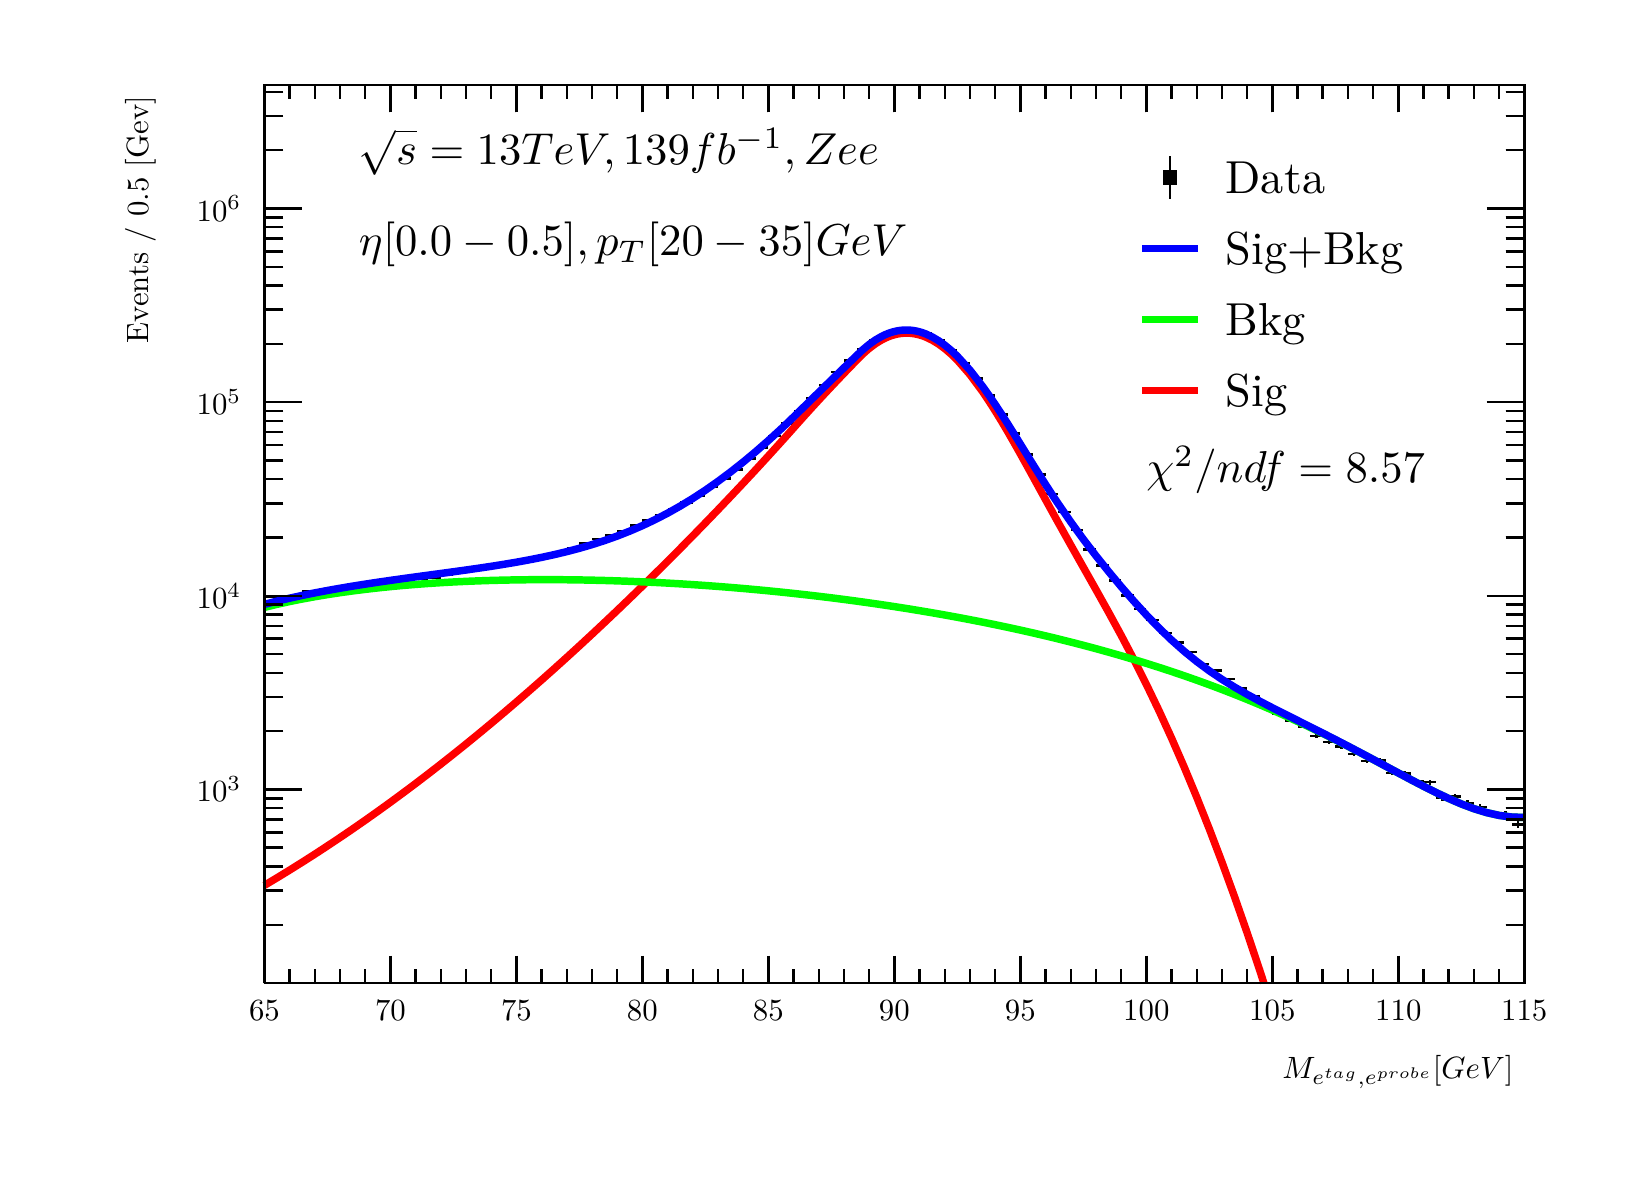
\begin{tikzpicture}
\pgfdeclareplotmark{cross} {
\pgfpathmoveto{\pgfpoint{-0.3\pgfplotmarksize}{\pgfplotmarksize}}
\pgfpathlineto{\pgfpoint{+0.3\pgfplotmarksize}{\pgfplotmarksize}}
\pgfpathlineto{\pgfpoint{+0.3\pgfplotmarksize}{0.3\pgfplotmarksize}}
\pgfpathlineto{\pgfpoint{+1\pgfplotmarksize}{0.3\pgfplotmarksize}}
\pgfpathlineto{\pgfpoint{+1\pgfplotmarksize}{-0.3\pgfplotmarksize}}
\pgfpathlineto{\pgfpoint{+0.3\pgfplotmarksize}{-0.3\pgfplotmarksize}}
\pgfpathlineto{\pgfpoint{+0.3\pgfplotmarksize}{-1.\pgfplotmarksize}}
\pgfpathlineto{\pgfpoint{-0.3\pgfplotmarksize}{-1.\pgfplotmarksize}}
\pgfpathlineto{\pgfpoint{-0.3\pgfplotmarksize}{-0.3\pgfplotmarksize}}
\pgfpathlineto{\pgfpoint{-1.\pgfplotmarksize}{-0.3\pgfplotmarksize}}
\pgfpathlineto{\pgfpoint{-1.\pgfplotmarksize}{0.3\pgfplotmarksize}}
\pgfpathlineto{\pgfpoint{-0.3\pgfplotmarksize}{0.3\pgfplotmarksize}}
\pgfpathclose
\pgfusepathqstroke
}
\pgfdeclareplotmark{cross*} {
\pgfpathmoveto{\pgfpoint{-0.3\pgfplotmarksize}{\pgfplotmarksize}}
\pgfpathlineto{\pgfpoint{+0.3\pgfplotmarksize}{\pgfplotmarksize}}
\pgfpathlineto{\pgfpoint{+0.3\pgfplotmarksize}{0.3\pgfplotmarksize}}
\pgfpathlineto{\pgfpoint{+1\pgfplotmarksize}{0.3\pgfplotmarksize}}
\pgfpathlineto{\pgfpoint{+1\pgfplotmarksize}{-0.3\pgfplotmarksize}}
\pgfpathlineto{\pgfpoint{+0.3\pgfplotmarksize}{-0.3\pgfplotmarksize}}
\pgfpathlineto{\pgfpoint{+0.3\pgfplotmarksize}{-1.\pgfplotmarksize}}
\pgfpathlineto{\pgfpoint{-0.3\pgfplotmarksize}{-1.\pgfplotmarksize}}
\pgfpathlineto{\pgfpoint{-0.3\pgfplotmarksize}{-0.3\pgfplotmarksize}}
\pgfpathlineto{\pgfpoint{-1.\pgfplotmarksize}{-0.3\pgfplotmarksize}}
\pgfpathlineto{\pgfpoint{-1.\pgfplotmarksize}{0.3\pgfplotmarksize}}
\pgfpathlineto{\pgfpoint{-0.3\pgfplotmarksize}{0.3\pgfplotmarksize}}
\pgfpathclose
\pgfusepathqfillstroke
}
\pgfdeclareplotmark{newstar} {
\pgfpathmoveto{\pgfqpoint{0pt}{\pgfplotmarksize}}
\pgfpathlineto{\pgfqpointpolar{44}{0.5\pgfplotmarksize}}
\pgfpathlineto{\pgfqpointpolar{18}{\pgfplotmarksize}}
\pgfpathlineto{\pgfqpointpolar{-20}{0.5\pgfplotmarksize}}
\pgfpathlineto{\pgfqpointpolar{-54}{\pgfplotmarksize}}
\pgfpathlineto{\pgfqpointpolar{-90}{0.5\pgfplotmarksize}}
\pgfpathlineto{\pgfqpointpolar{234}{\pgfplotmarksize}}
\pgfpathlineto{\pgfqpointpolar{198}{0.5\pgfplotmarksize}}
\pgfpathlineto{\pgfqpointpolar{162}{\pgfplotmarksize}}
\pgfpathlineto{\pgfqpointpolar{134}{0.5\pgfplotmarksize}}
\pgfpathclose
\pgfusepathqstroke
}
\pgfdeclareplotmark{newstar*} {
\pgfpathmoveto{\pgfqpoint{0pt}{\pgfplotmarksize}}
\pgfpathlineto{\pgfqpointpolar{44}{0.5\pgfplotmarksize}}
\pgfpathlineto{\pgfqpointpolar{18}{\pgfplotmarksize}}
\pgfpathlineto{\pgfqpointpolar{-20}{0.5\pgfplotmarksize}}
\pgfpathlineto{\pgfqpointpolar{-54}{\pgfplotmarksize}}
\pgfpathlineto{\pgfqpointpolar{-90}{0.5\pgfplotmarksize}}
\pgfpathlineto{\pgfqpointpolar{234}{\pgfplotmarksize}}
\pgfpathlineto{\pgfqpointpolar{198}{0.5\pgfplotmarksize}}
\pgfpathlineto{\pgfqpointpolar{162}{\pgfplotmarksize}}
\pgfpathlineto{\pgfqpointpolar{134}{0.5\pgfplotmarksize}}
\pgfpathclose
\pgfusepathqfillstroke
}
\definecolor{c}{rgb}{1,1,1};
\draw [color=c, fill=c] (0,0) rectangle (20,14.4361);
\draw [color=c, fill=c] (3,2.30977) rectangle (19,13.7143);
\definecolor{c}{rgb}{0,0,0};
\draw [c,line width=0.9] (3,2.30977) -- (3,13.7143) -- (19,13.7143) -- (19,2.30977) -- (3,2.30977);
\definecolor{c}{rgb}{1,1,1};
\draw [color=c, fill=c] (3,2.30977) rectangle (19,13.7143);
\definecolor{c}{rgb}{0,0,0};
\draw [c,line width=0.9] (3,2.30977) -- (3,13.7143) -- (19,13.7143) -- (19,2.30977) -- (3,2.30977);
\draw [c,line width=0.9] (3,2.30977) -- (19,2.30977);
\draw [c,line width=0.9] (3,2.65624) -- (3,2.30977);
\draw [c,line width=0.9] (3.32,2.48301) -- (3.32,2.30977);
\draw [c,line width=0.9] (3.64,2.48301) -- (3.64,2.30977);
\draw [c,line width=0.9] (3.96,2.48301) -- (3.96,2.30977);
\draw [c,line width=0.9] (4.28,2.48301) -- (4.28,2.30977);
\draw [c,line width=0.9] (4.6,2.65624) -- (4.6,2.30977);
\draw [c,line width=0.9] (4.92,2.48301) -- (4.92,2.30977);
\draw [c,line width=0.9] (5.24,2.48301) -- (5.24,2.30977);
\draw [c,line width=0.9] (5.56,2.48301) -- (5.56,2.30977);
\draw [c,line width=0.9] (5.88,2.48301) -- (5.88,2.30977);
\draw [c,line width=0.9] (6.2,2.65624) -- (6.2,2.30977);
\draw [c,line width=0.9] (6.52,2.48301) -- (6.52,2.30977);
\draw [c,line width=0.9] (6.84,2.48301) -- (6.84,2.30977);
\draw [c,line width=0.9] (7.16,2.48301) -- (7.16,2.30977);
\draw [c,line width=0.9] (7.48,2.48301) -- (7.48,2.30977);
\draw [c,line width=0.9] (7.8,2.65624) -- (7.8,2.30977);
\draw [c,line width=0.9] (8.12,2.48301) -- (8.12,2.30977);
\draw [c,line width=0.9] (8.44,2.48301) -- (8.44,2.30977);
\draw [c,line width=0.9] (8.76,2.48301) -- (8.76,2.30977);
\draw [c,line width=0.9] (9.08,2.48301) -- (9.08,2.30977);
\draw [c,line width=0.9] (9.4,2.65624) -- (9.4,2.30977);
\draw [c,line width=0.9] (9.72,2.48301) -- (9.72,2.30977);
\draw [c,line width=0.9] (10.04,2.48301) -- (10.04,2.30977);
\draw [c,line width=0.9] (10.36,2.48301) -- (10.36,2.30977);
\draw [c,line width=0.9] (10.68,2.48301) -- (10.68,2.30977);
\draw [c,line width=0.9] (11,2.65624) -- (11,2.30977);
\draw [c,line width=0.9] (11.32,2.48301) -- (11.32,2.30977);
\draw [c,line width=0.9] (11.64,2.48301) -- (11.64,2.30977);
\draw [c,line width=0.9] (11.96,2.48301) -- (11.96,2.30977);
\draw [c,line width=0.9] (12.28,2.48301) -- (12.28,2.30977);
\draw [c,line width=0.9] (12.6,2.65624) -- (12.6,2.30977);
\draw [c,line width=0.9] (12.92,2.48301) -- (12.92,2.30977);
\draw [c,line width=0.9] (13.24,2.48301) -- (13.24,2.30977);
\draw [c,line width=0.9] (13.56,2.48301) -- (13.56,2.30977);
\draw [c,line width=0.9] (13.88,2.48301) -- (13.88,2.30977);
\draw [c,line width=0.9] (14.2,2.65624) -- (14.2,2.30977);
\draw [c,line width=0.9] (14.52,2.48301) -- (14.52,2.30977);
\draw [c,line width=0.9] (14.84,2.48301) -- (14.84,2.30977);
\draw [c,line width=0.9] (15.16,2.48301) -- (15.16,2.30977);
\draw [c,line width=0.9] (15.48,2.48301) -- (15.48,2.30977);
\draw [c,line width=0.9] (15.8,2.65624) -- (15.8,2.30977);
\draw [c,line width=0.9] (16.12,2.48301) -- (16.12,2.30977);
\draw [c,line width=0.9] (16.44,2.48301) -- (16.44,2.30977);
\draw [c,line width=0.9] (16.76,2.48301) -- (16.76,2.30977);
\draw [c,line width=0.9] (17.08,2.48301) -- (17.08,2.30977);
\draw [c,line width=0.9] (17.4,2.65624) -- (17.4,2.30977);
\draw [c,line width=0.9] (17.72,2.48301) -- (17.72,2.30977);
\draw [c,line width=0.9] (18.04,2.48301) -- (18.04,2.30977);
\draw [c,line width=0.9] (18.36,2.48301) -- (18.36,2.30977);
\draw [c,line width=0.9] (18.68,2.48301) -- (18.68,2.30977);
\draw [c,line width=0.9] (19,2.65624) -- (19,2.30977);
\draw [c,line width=0.9] (19,2.65624) -- (19,2.30977);
\draw [anchor=base] (3,1.83338) node[scale=1.11327, color=c, rotate=0]{65};
\draw [anchor=base] (4.6,1.83338) node[scale=1.11327, color=c, rotate=0]{70};
\draw [anchor=base] (6.2,1.83338) node[scale=1.11327, color=c, rotate=0]{75};
\draw [anchor=base] (7.8,1.83338) node[scale=1.11327, color=c, rotate=0]{80};
\draw [anchor=base] (9.4,1.83338) node[scale=1.11327, color=c, rotate=0]{85};
\draw [anchor=base] (11,1.83338) node[scale=1.11327, color=c, rotate=0]{90};
\draw [anchor=base] (12.6,1.83338) node[scale=1.11327, color=c, rotate=0]{95};
\draw [anchor=base] (14.2,1.83338) node[scale=1.11327, color=c, rotate=0]{100};
\draw [anchor=base] (15.8,1.83338) node[scale=1.11327, color=c, rotate=0]{105};
\draw [anchor=base] (17.4,1.83338) node[scale=1.11327, color=c, rotate=0]{110};
\draw [anchor=base] (19,1.83338) node[scale=1.11327, color=c, rotate=0]{115};
\draw [anchor= east] (19,1.17798) node[scale=1.11327, color=c, rotate=0]{$M_{e^{tag}, e^{probe}}  [GeV]$};
\draw [c,line width=0.9] (3,13.7143) -- (19,13.7143);
\draw [c,line width=0.9] (3,13.3678) -- (3,13.7143);
\draw [c,line width=0.9] (3.32,13.5411) -- (3.32,13.7143);
\draw [c,line width=0.9] (3.64,13.5411) -- (3.64,13.7143);
\draw [c,line width=0.9] (3.96,13.5411) -- (3.96,13.7143);
\draw [c,line width=0.9] (4.28,13.5411) -- (4.28,13.7143);
\draw [c,line width=0.9] (4.6,13.3678) -- (4.6,13.7143);
\draw [c,line width=0.9] (4.92,13.5411) -- (4.92,13.7143);
\draw [c,line width=0.9] (5.24,13.5411) -- (5.24,13.7143);
\draw [c,line width=0.9] (5.56,13.5411) -- (5.56,13.7143);
\draw [c,line width=0.9] (5.88,13.5411) -- (5.88,13.7143);
\draw [c,line width=0.9] (6.2,13.3678) -- (6.2,13.7143);
\draw [c,line width=0.9] (6.52,13.5411) -- (6.52,13.7143);
\draw [c,line width=0.9] (6.84,13.5411) -- (6.84,13.7143);
\draw [c,line width=0.9] (7.16,13.5411) -- (7.16,13.7143);
\draw [c,line width=0.9] (7.48,13.5411) -- (7.48,13.7143);
\draw [c,line width=0.9] (7.8,13.3678) -- (7.8,13.7143);
\draw [c,line width=0.9] (8.12,13.5411) -- (8.12,13.7143);
\draw [c,line width=0.9] (8.44,13.5411) -- (8.44,13.7143);
\draw [c,line width=0.9] (8.76,13.5411) -- (8.76,13.7143);
\draw [c,line width=0.9] (9.08,13.5411) -- (9.08,13.7143);
\draw [c,line width=0.9] (9.4,13.3678) -- (9.4,13.7143);
\draw [c,line width=0.9] (9.72,13.5411) -- (9.72,13.7143);
\draw [c,line width=0.9] (10.04,13.5411) -- (10.04,13.7143);
\draw [c,line width=0.9] (10.36,13.5411) -- (10.36,13.7143);
\draw [c,line width=0.9] (10.68,13.5411) -- (10.68,13.7143);
\draw [c,line width=0.9] (11,13.3678) -- (11,13.7143);
\draw [c,line width=0.9] (11.32,13.5411) -- (11.32,13.7143);
\draw [c,line width=0.9] (11.64,13.5411) -- (11.64,13.7143);
\draw [c,line width=0.9] (11.96,13.5411) -- (11.96,13.7143);
\draw [c,line width=0.9] (12.28,13.5411) -- (12.28,13.7143);
\draw [c,line width=0.9] (12.6,13.3678) -- (12.6,13.7143);
\draw [c,line width=0.9] (12.92,13.5411) -- (12.92,13.7143);
\draw [c,line width=0.9] (13.24,13.5411) -- (13.24,13.7143);
\draw [c,line width=0.9] (13.56,13.5411) -- (13.56,13.7143);
\draw [c,line width=0.9] (13.88,13.5411) -- (13.88,13.7143);
\draw [c,line width=0.9] (14.2,13.3678) -- (14.2,13.7143);
\draw [c,line width=0.9] (14.52,13.5411) -- (14.52,13.7143);
\draw [c,line width=0.9] (14.84,13.5411) -- (14.84,13.7143);
\draw [c,line width=0.9] (15.16,13.5411) -- (15.16,13.7143);
\draw [c,line width=0.9] (15.48,13.5411) -- (15.48,13.7143);
\draw [c,line width=0.9] (15.8,13.3678) -- (15.8,13.7143);
\draw [c,line width=0.9] (16.12,13.5411) -- (16.12,13.7143);
\draw [c,line width=0.9] (16.44,13.5411) -- (16.44,13.7143);
\draw [c,line width=0.9] (16.76,13.5411) -- (16.76,13.7143);
\draw [c,line width=0.9] (17.08,13.5411) -- (17.08,13.7143);
\draw [c,line width=0.9] (17.4,13.3678) -- (17.4,13.7143);
\draw [c,line width=0.9] (17.72,13.5411) -- (17.72,13.7143);
\draw [c,line width=0.9] (18.04,13.5411) -- (18.04,13.7143);
\draw [c,line width=0.9] (18.36,13.5411) -- (18.36,13.7143);
\draw [c,line width=0.9] (18.68,13.5411) -- (18.68,13.7143);
\draw [c,line width=0.9] (19,13.3678) -- (19,13.7143);
\draw [c,line width=0.9] (19,13.3678) -- (19,13.7143);
\draw [c,line width=0.9] (3,2.30977) -- (3,13.7143);
\draw [c,line width=0.9] (3.237,3.05008) -- (3,3.05008);
\draw [c,line width=0.9] (3.237,3.48313) -- (3,3.48313);
\draw [c,line width=0.9] (3.237,3.79038) -- (3,3.79038);
\draw [c,line width=0.9] (3.237,4.02871) -- (3,4.02871);
\draw [c,line width=0.9] (3.237,4.22343) -- (3,4.22343);
\draw [c,line width=0.9] (3.237,4.38807) -- (3,4.38807);
\draw [c,line width=0.9] (3.237,4.53069) -- (3,4.53069);
\draw [c,line width=0.9] (3.237,4.65649) -- (3,4.65649);
\draw [c,line width=0.9] (3.474,4.76901) -- (3,4.76901);
\draw [anchor= east] (2.844,4.76901) node[scale=1.11327, color=c, rotate=0]{$10^{3}$};
\draw [c,line width=0.9] (3.237,5.50932) -- (3,5.50932);
\draw [c,line width=0.9] (3.237,5.94237) -- (3,5.94237);
\draw [c,line width=0.9] (3.237,6.24963) -- (3,6.24963);
\draw [c,line width=0.9] (3.237,6.48795) -- (3,6.48795);
\draw [c,line width=0.9] (3.237,6.68268) -- (3,6.68268);
\draw [c,line width=0.9] (3.237,6.84731) -- (3,6.84731);
\draw [c,line width=0.9] (3.237,6.98993) -- (3,6.98993);
\draw [c,line width=0.9] (3.237,7.11573) -- (3,7.11573);
\draw [c,line width=0.9] (3.474,7.22826) -- (3,7.22826);
\draw [anchor= east] (2.844,7.22826) node[scale=1.11327, color=c, rotate=0]{$10^{4}$};
\draw [c,line width=0.9] (3.237,7.96856) -- (3,7.96856);
\draw [c,line width=0.9] (3.237,8.40161) -- (3,8.40161);
\draw [c,line width=0.9] (3.237,8.70887) -- (3,8.70887);
\draw [c,line width=0.9] (3.237,8.94719) -- (3,8.94719);
\draw [c,line width=0.9] (3.237,9.14192) -- (3,9.14192);
\draw [c,line width=0.9] (3.237,9.30656) -- (3,9.30656);
\draw [c,line width=0.9] (3.237,9.44917) -- (3,9.44917);
\draw [c,line width=0.9] (3.237,9.57497) -- (3,9.57497);
\draw [c,line width=0.9] (3.474,9.6875) -- (3,9.6875);
\draw [anchor= east] (2.844,9.6875) node[scale=1.11327, color=c, rotate=0]{$10^{5}$};
\draw [c,line width=0.9] (3.237,10.4278) -- (3,10.4278);
\draw [c,line width=0.9] (3.237,10.8609) -- (3,10.8609);
\draw [c,line width=0.9] (3.237,11.1681) -- (3,11.1681);
\draw [c,line width=0.9] (3.237,11.4064) -- (3,11.4064);
\draw [c,line width=0.9] (3.237,11.6012) -- (3,11.6012);
\draw [c,line width=0.9] (3.237,11.7658) -- (3,11.7658);
\draw [c,line width=0.9] (3.237,11.9084) -- (3,11.9084);
\draw [c,line width=0.9] (3.237,12.0342) -- (3,12.0342);
\draw [c,line width=0.9] (3.474,12.1467) -- (3,12.1467);
\draw [anchor= east] (2.844,12.1467) node[scale=1.11327, color=c, rotate=0]{$10^{6}$};
\draw [c,line width=0.9] (3.237,12.887) -- (3,12.887);
\draw [c,line width=0.9] (3.237,13.3201) -- (3,13.3201);
\draw [c,line width=0.9] (3.237,13.6274) -- (3,13.6274);
\draw [anchor= east] (1.432,13.7143) node[scale=1.11327, color=c, rotate=90]{Events / 0.5 [Gev]};
\draw [c,line width=0.9] (19,2.30977) -- (19,13.7143);
\draw [c,line width=0.9] (18.763,3.05008) -- (19,3.05008);
\draw [c,line width=0.9] (18.763,3.48313) -- (19,3.48313);
\draw [c,line width=0.9] (18.763,3.79038) -- (19,3.79038);
\draw [c,line width=0.9] (18.763,4.02871) -- (19,4.02871);
\draw [c,line width=0.9] (18.763,4.22343) -- (19,4.22343);
\draw [c,line width=0.9] (18.763,4.38807) -- (19,4.38807);
\draw [c,line width=0.9] (18.763,4.53069) -- (19,4.53069);
\draw [c,line width=0.9] (18.763,4.65649) -- (19,4.65649);
\draw [c,line width=0.9] (18.526,4.76901) -- (19,4.76901);
\draw [c,line width=0.9] (18.763,5.50932) -- (19,5.50932);
\draw [c,line width=0.9] (18.763,5.94237) -- (19,5.94237);
\draw [c,line width=0.9] (18.763,6.24963) -- (19,6.24963);
\draw [c,line width=0.9] (18.763,6.48795) -- (19,6.48795);
\draw [c,line width=0.9] (18.763,6.68268) -- (19,6.68268);
\draw [c,line width=0.9] (18.763,6.84731) -- (19,6.84731);
\draw [c,line width=0.9] (18.763,6.98993) -- (19,6.98993);
\draw [c,line width=0.9] (18.763,7.11573) -- (19,7.11573);
\draw [c,line width=0.9] (18.526,7.22826) -- (19,7.22826);
\draw [c,line width=0.9] (18.763,7.96856) -- (19,7.96856);
\draw [c,line width=0.9] (18.763,8.40161) -- (19,8.40161);
\draw [c,line width=0.9] (18.763,8.70887) -- (19,8.70887);
\draw [c,line width=0.9] (18.763,8.94719) -- (19,8.94719);
\draw [c,line width=0.9] (18.763,9.14192) -- (19,9.14192);
\draw [c,line width=0.9] (18.763,9.30656) -- (19,9.30656);
\draw [c,line width=0.9] (18.763,9.44917) -- (19,9.44917);
\draw [c,line width=0.9] (18.763,9.57497) -- (19,9.57497);
\draw [c,line width=0.9] (18.526,9.6875) -- (19,9.6875);
\draw [c,line width=0.9] (18.763,10.4278) -- (19,10.4278);
\draw [c,line width=0.9] (18.763,10.8609) -- (19,10.8609);
\draw [c,line width=0.9] (18.763,11.1681) -- (19,11.1681);
\draw [c,line width=0.9] (18.763,11.4064) -- (19,11.4064);
\draw [c,line width=0.9] (18.763,11.6012) -- (19,11.6012);
\draw [c,line width=0.9] (18.763,11.7658) -- (19,11.7658);
\draw [c,line width=0.9] (18.763,11.9084) -- (19,11.9084);
\draw [c,line width=0.9] (18.763,12.0342) -- (19,12.0342);
\draw [c,line width=0.9] (18.526,12.1467) -- (19,12.1467);
\draw [c,line width=0.9] (18.763,12.887) -- (19,12.887);
\draw [c,line width=0.9] (18.763,13.3201) -- (19,13.3201);
\draw [c,line width=0.9] (18.763,13.6274) -- (19,13.6274);
\draw [c,line width=0.9] (3.08,7.21114) -- (3,7.21114);
\draw [c,line width=0.9] (3,7.21114) -- (3,7.21114);
\draw [c,line width=0.9] (3.08,7.21114) -- (3.16,7.21114);
\draw [c,line width=0.9] (3.16,7.21114) -- (3.16,7.21114);
\draw [c,line width=0.9] (3.08,7.21114) -- (3.08,7.22191);
\draw [c,line width=0.9] (3.08,7.22191) -- (3.08,7.22191);
\draw [c,line width=0.9] (3.08,7.21114) -- (3.08,7.20037);
\draw [c,line width=0.9] (3.08,7.20037) -- (3.08,7.20037);
\draw [c,line width=0.9] (3.24,7.21979) -- (3.16,7.21979);
\draw [c,line width=0.9] (3.16,7.21979) -- (3.16,7.21979);
\draw [c,line width=0.9] (3.24,7.21979) -- (3.32,7.21979);
\draw [c,line width=0.9] (3.32,7.21979) -- (3.32,7.21979);
\draw [c,line width=0.9] (3.24,7.21979) -- (3.24,7.23051);
\draw [c,line width=0.9] (3.24,7.23051) -- (3.24,7.23051);
\draw [c,line width=0.9] (3.24,7.21979) -- (3.24,7.20906);
\draw [c,line width=0.9] (3.24,7.20906) -- (3.24,7.20906);
\draw [c,line width=0.9] (3.4,7.23878) -- (3.32,7.23878);
\draw [c,line width=0.9] (3.32,7.23878) -- (3.32,7.23878);
\draw [c,line width=0.9] (3.4,7.23878) -- (3.48,7.23878);
\draw [c,line width=0.9] (3.48,7.23878) -- (3.48,7.23878);
\draw [c,line width=0.9] (3.4,7.23878) -- (3.4,7.24941);
\draw [c,line width=0.9] (3.4,7.24941) -- (3.4,7.24941);
\draw [c,line width=0.9] (3.4,7.23878) -- (3.4,7.22815);
\draw [c,line width=0.9] (3.4,7.22815) -- (3.4,7.22815);
\draw [c,line width=0.9] (3.56,7.28756) -- (3.48,7.28756);
\draw [c,line width=0.9] (3.48,7.28756) -- (3.48,7.28756);
\draw [c,line width=0.9] (3.56,7.28756) -- (3.64,7.28756);
\draw [c,line width=0.9] (3.64,7.28756) -- (3.64,7.28756);
\draw [c,line width=0.9] (3.56,7.28756) -- (3.56,7.29795);
\draw [c,line width=0.9] (3.56,7.29795) -- (3.56,7.29795);
\draw [c,line width=0.9] (3.56,7.28756) -- (3.56,7.27718);
\draw [c,line width=0.9] (3.56,7.27718) -- (3.56,7.27718);
\draw [c,line width=0.9] (3.72,7.27425) -- (3.64,7.27425);
\draw [c,line width=0.9] (3.64,7.27425) -- (3.64,7.27425);
\draw [c,line width=0.9] (3.72,7.27425) -- (3.8,7.27425);
\draw [c,line width=0.9] (3.8,7.27425) -- (3.8,7.27425);
\draw [c,line width=0.9] (3.72,7.27425) -- (3.72,7.2847);
\draw [c,line width=0.9] (3.72,7.2847) -- (3.72,7.2847);
\draw [c,line width=0.9] (3.72,7.27425) -- (3.72,7.26379);
\draw [c,line width=0.9] (3.72,7.26379) -- (3.72,7.26379);
\draw [c,line width=0.9] (3.88,7.30986) -- (3.8,7.30986);
\draw [c,line width=0.9] (3.8,7.30986) -- (3.8,7.30986);
\draw [c,line width=0.9] (3.88,7.30986) -- (3.96,7.30986);
\draw [c,line width=0.9] (3.96,7.30986) -- (3.96,7.30986);
\draw [c,line width=0.9] (3.88,7.30986) -- (3.88,7.32014);
\draw [c,line width=0.9] (3.88,7.32014) -- (3.88,7.32014);
\draw [c,line width=0.9] (3.88,7.30986) -- (3.88,7.29958);
\draw [c,line width=0.9] (3.88,7.29958) -- (3.88,7.29958);
\draw [c,line width=0.9] (4.04,7.31065) -- (3.96,7.31065);
\draw [c,line width=0.9] (3.96,7.31065) -- (3.96,7.31065);
\draw [c,line width=0.9] (4.04,7.31065) -- (4.12,7.31065);
\draw [c,line width=0.9] (4.12,7.31065) -- (4.12,7.31065);
\draw [c,line width=0.9] (4.04,7.31065) -- (4.04,7.32093);
\draw [c,line width=0.9] (4.04,7.32093) -- (4.04,7.32093);
\draw [c,line width=0.9] (4.04,7.31065) -- (4.04,7.30038);
\draw [c,line width=0.9] (4.04,7.30038) -- (4.04,7.30038);
\draw [c,line width=0.9] (4.2,7.34844) -- (4.12,7.34844);
\draw [c,line width=0.9] (4.12,7.34844) -- (4.12,7.34844);
\draw [c,line width=0.9] (4.2,7.34844) -- (4.28,7.34844);
\draw [c,line width=0.9] (4.28,7.34844) -- (4.28,7.34844);
\draw [c,line width=0.9] (4.2,7.34844) -- (4.2,7.35853);
\draw [c,line width=0.9] (4.2,7.35853) -- (4.2,7.35853);
\draw [c,line width=0.9] (4.2,7.34844) -- (4.2,7.33834);
\draw [c,line width=0.9] (4.2,7.33834) -- (4.2,7.33834);
\draw [c,line width=0.9] (4.36,7.35358) -- (4.28,7.35358);
\draw [c,line width=0.9] (4.28,7.35358) -- (4.28,7.35358);
\draw [c,line width=0.9] (4.36,7.35358) -- (4.44,7.35358);
\draw [c,line width=0.9] (4.44,7.35358) -- (4.44,7.35358);
\draw [c,line width=0.9] (4.36,7.35358) -- (4.36,7.36365);
\draw [c,line width=0.9] (4.36,7.36365) -- (4.36,7.36365);
\draw [c,line width=0.9] (4.36,7.35358) -- (4.36,7.34351);
\draw [c,line width=0.9] (4.36,7.34351) -- (4.36,7.34351);
\draw [c,line width=0.9] (4.52,7.38401) -- (4.44,7.38401);
\draw [c,line width=0.9] (4.44,7.38401) -- (4.44,7.38401);
\draw [c,line width=0.9] (4.52,7.38401) -- (4.6,7.38401);
\draw [c,line width=0.9] (4.6,7.38401) -- (4.6,7.38401);
\draw [c,line width=0.9] (4.52,7.38401) -- (4.52,7.39394);
\draw [c,line width=0.9] (4.52,7.39394) -- (4.52,7.39394);
\draw [c,line width=0.9] (4.52,7.38401) -- (4.52,7.37408);
\draw [c,line width=0.9] (4.52,7.37408) -- (4.52,7.37408);
\draw [c,line width=0.9] (4.68,7.39649) -- (4.6,7.39649);
\draw [c,line width=0.9] (4.6,7.39649) -- (4.6,7.39649);
\draw [c,line width=0.9] (4.68,7.39649) -- (4.76,7.39649);
\draw [c,line width=0.9] (4.76,7.39649) -- (4.76,7.39649);
\draw [c,line width=0.9] (4.68,7.39649) -- (4.68,7.40636);
\draw [c,line width=0.9] (4.68,7.40636) -- (4.68,7.40636);
\draw [c,line width=0.9] (4.68,7.39649) -- (4.68,7.38662);
\draw [c,line width=0.9] (4.68,7.38662) -- (4.68,7.38662);
\draw [c,line width=0.9] (4.84,7.39722) -- (4.76,7.39722);
\draw [c,line width=0.9] (4.76,7.39722) -- (4.76,7.39722);
\draw [c,line width=0.9] (4.84,7.39722) -- (4.92,7.39722);
\draw [c,line width=0.9] (4.92,7.39722) -- (4.92,7.39722);
\draw [c,line width=0.9] (4.84,7.39722) -- (4.84,7.40709);
\draw [c,line width=0.9] (4.84,7.40709) -- (4.84,7.40709);
\draw [c,line width=0.9] (4.84,7.39722) -- (4.84,7.38735);
\draw [c,line width=0.9] (4.84,7.38735) -- (4.84,7.38735);
\draw [c,line width=0.9] (5,7.44378) -- (4.92,7.44378);
\draw [c,line width=0.9] (4.92,7.44378) -- (4.92,7.44378);
\draw [c,line width=0.9] (5,7.44378) -- (5.08,7.44378);
\draw [c,line width=0.9] (5.08,7.44378) -- (5.08,7.44378);
\draw [c,line width=0.9] (5,7.44378) -- (5,7.45344);
\draw [c,line width=0.9] (5,7.45344) -- (5,7.45344);
\draw [c,line width=0.9] (5,7.44378) -- (5,7.43413);
\draw [c,line width=0.9] (5,7.43413) -- (5,7.43413);
\draw [c,line width=0.9] (5.16,7.45403) -- (5.08,7.45403);
\draw [c,line width=0.9] (5.08,7.45403) -- (5.08,7.45403);
\draw [c,line width=0.9] (5.16,7.45403) -- (5.24,7.45403);
\draw [c,line width=0.9] (5.24,7.45403) -- (5.24,7.45403);
\draw [c,line width=0.9] (5.16,7.45403) -- (5.16,7.46364);
\draw [c,line width=0.9] (5.16,7.46364) -- (5.16,7.46364);
\draw [c,line width=0.9] (5.16,7.45403) -- (5.16,7.44443);
\draw [c,line width=0.9] (5.16,7.44443) -- (5.16,7.44443);
\draw [c,line width=0.9] (5.32,7.5008) -- (5.24,7.5008);
\draw [c,line width=0.9] (5.24,7.5008) -- (5.24,7.5008);
\draw [c,line width=0.9] (5.32,7.5008) -- (5.4,7.5008);
\draw [c,line width=0.9] (5.4,7.5008) -- (5.4,7.5008);
\draw [c,line width=0.9] (5.32,7.5008) -- (5.32,7.5102);
\draw [c,line width=0.9] (5.32,7.5102) -- (5.32,7.5102);
\draw [c,line width=0.9] (5.32,7.5008) -- (5.32,7.4914);
\draw [c,line width=0.9] (5.32,7.4914) -- (5.32,7.4914);
\draw [c,line width=0.9] (5.48,7.52162) -- (5.4,7.52162);
\draw [c,line width=0.9] (5.4,7.52162) -- (5.4,7.52162);
\draw [c,line width=0.9] (5.48,7.52162) -- (5.56,7.52162);
\draw [c,line width=0.9] (5.56,7.52162) -- (5.56,7.52162);
\draw [c,line width=0.9] (5.48,7.52162) -- (5.48,7.53093);
\draw [c,line width=0.9] (5.48,7.53093) -- (5.48,7.53093);
\draw [c,line width=0.9] (5.48,7.52162) -- (5.48,7.51231);
\draw [c,line width=0.9] (5.48,7.51231) -- (5.48,7.51231);
\draw [c,line width=0.9] (5.64,7.54941) -- (5.56,7.54941);
\draw [c,line width=0.9] (5.56,7.54941) -- (5.56,7.54941);
\draw [c,line width=0.9] (5.64,7.54941) -- (5.72,7.54941);
\draw [c,line width=0.9] (5.72,7.54941) -- (5.72,7.54941);
\draw [c,line width=0.9] (5.64,7.54941) -- (5.64,7.5586);
\draw [c,line width=0.9] (5.64,7.5586) -- (5.64,7.5586);
\draw [c,line width=0.9] (5.64,7.54941) -- (5.64,7.54022);
\draw [c,line width=0.9] (5.64,7.54022) -- (5.64,7.54022);
\draw [c,line width=0.9] (5.8,7.58211) -- (5.72,7.58211);
\draw [c,line width=0.9] (5.72,7.58211) -- (5.72,7.58211);
\draw [c,line width=0.9] (5.8,7.58211) -- (5.88,7.58211);
\draw [c,line width=0.9] (5.88,7.58211) -- (5.88,7.58211);
\draw [c,line width=0.9] (5.8,7.58211) -- (5.8,7.59116);
\draw [c,line width=0.9] (5.8,7.59116) -- (5.8,7.59116);
\draw [c,line width=0.9] (5.8,7.58211) -- (5.8,7.57306);
\draw [c,line width=0.9] (5.8,7.57306) -- (5.8,7.57306);
\draw [c,line width=0.9] (5.96,7.61094) -- (5.88,7.61094);
\draw [c,line width=0.9] (5.88,7.61094) -- (5.88,7.61094);
\draw [c,line width=0.9] (5.96,7.61094) -- (6.04,7.61094);
\draw [c,line width=0.9] (6.04,7.61094) -- (6.04,7.61094);
\draw [c,line width=0.9] (5.96,7.61094) -- (5.96,7.61987);
\draw [c,line width=0.9] (5.96,7.61987) -- (5.96,7.61987);
\draw [c,line width=0.9] (5.96,7.61094) -- (5.96,7.60201);
\draw [c,line width=0.9] (5.96,7.60201) -- (5.96,7.60201);
\draw [c,line width=0.9] (6.12,7.6331) -- (6.04,7.6331);
\draw [c,line width=0.9] (6.04,7.6331) -- (6.04,7.6331);
\draw [c,line width=0.9] (6.12,7.6331) -- (6.2,7.6331);
\draw [c,line width=0.9] (6.2,7.6331) -- (6.2,7.6331);
\draw [c,line width=0.9] (6.12,7.6331) -- (6.12,7.64194);
\draw [c,line width=0.9] (6.12,7.64194) -- (6.12,7.64194);
\draw [c,line width=0.9] (6.12,7.6331) -- (6.12,7.62426);
\draw [c,line width=0.9] (6.12,7.62426) -- (6.12,7.62426);
\draw [c,line width=0.9] (6.28,7.66734) -- (6.2,7.66734);
\draw [c,line width=0.9] (6.2,7.66734) -- (6.2,7.66734);
\draw [c,line width=0.9] (6.28,7.66734) -- (6.36,7.66734);
\draw [c,line width=0.9] (6.36,7.66734) -- (6.36,7.66734);
\draw [c,line width=0.9] (6.28,7.66734) -- (6.28,7.67604);
\draw [c,line width=0.9] (6.28,7.67604) -- (6.28,7.67604);
\draw [c,line width=0.9] (6.28,7.66734) -- (6.28,7.65865);
\draw [c,line width=0.9] (6.28,7.65865) -- (6.28,7.65865);
\draw [c,line width=0.9] (6.44,7.71829) -- (6.36,7.71829);
\draw [c,line width=0.9] (6.36,7.71829) -- (6.36,7.71829);
\draw [c,line width=0.9] (6.44,7.71829) -- (6.52,7.71829);
\draw [c,line width=0.9] (6.52,7.71829) -- (6.52,7.71829);
\draw [c,line width=0.9] (6.44,7.71829) -- (6.44,7.72678);
\draw [c,line width=0.9] (6.44,7.72678) -- (6.44,7.72678);
\draw [c,line width=0.9] (6.44,7.71829) -- (6.44,7.7098);
\draw [c,line width=0.9] (6.44,7.7098) -- (6.44,7.7098);
\draw [c,line width=0.9] (6.6,7.73961) -- (6.52,7.73961);
\draw [c,line width=0.9] (6.52,7.73961) -- (6.52,7.73961);
\draw [c,line width=0.9] (6.6,7.73961) -- (6.68,7.73961);
\draw [c,line width=0.9] (6.68,7.73961) -- (6.68,7.73961);
\draw [c,line width=0.9] (6.6,7.73961) -- (6.6,7.74801);
\draw [c,line width=0.9] (6.6,7.74801) -- (6.6,7.74801);
\draw [c,line width=0.9] (6.6,7.73961) -- (6.6,7.7312);
\draw [c,line width=0.9] (6.6,7.7312) -- (6.6,7.7312);
\draw [c,line width=0.9] (6.76,7.78235) -- (6.68,7.78235);
\draw [c,line width=0.9] (6.68,7.78235) -- (6.68,7.78235);
\draw [c,line width=0.9] (6.76,7.78235) -- (6.84,7.78235);
\draw [c,line width=0.9] (6.84,7.78235) -- (6.84,7.78235);
\draw [c,line width=0.9] (6.76,7.78235) -- (6.76,7.79059);
\draw [c,line width=0.9] (6.76,7.79059) -- (6.76,7.79059);
\draw [c,line width=0.9] (6.76,7.78235) -- (6.76,7.77411);
\draw [c,line width=0.9] (6.76,7.77411) -- (6.76,7.77411);
\draw [c,line width=0.9] (6.92,7.83343) -- (6.84,7.83343);
\draw [c,line width=0.9] (6.84,7.83343) -- (6.84,7.83343);
\draw [c,line width=0.9] (6.92,7.83343) -- (7,7.83343);
\draw [c,line width=0.9] (7,7.83343) -- (7,7.83343);
\draw [c,line width=0.9] (6.92,7.83343) -- (6.92,7.84147);
\draw [c,line width=0.9] (6.92,7.84147) -- (6.92,7.84147);
\draw [c,line width=0.9] (6.92,7.83343) -- (6.92,7.82538);
\draw [c,line width=0.9] (6.92,7.82538) -- (6.92,7.82538);
\draw [c,line width=0.9] (7.08,7.89025) -- (7,7.89025);
\draw [c,line width=0.9] (7,7.89025) -- (7,7.89025);
\draw [c,line width=0.9] (7.08,7.89025) -- (7.16,7.89025);
\draw [c,line width=0.9] (7.16,7.89025) -- (7.16,7.89025);
\draw [c,line width=0.9] (7.08,7.89025) -- (7.08,7.89808);
\draw [c,line width=0.9] (7.08,7.89808) -- (7.08,7.89808);
\draw [c,line width=0.9] (7.08,7.89025) -- (7.08,7.88242);
\draw [c,line width=0.9] (7.08,7.88242) -- (7.08,7.88242);
\draw [c,line width=0.9] (7.24,7.94824) -- (7.16,7.94824);
\draw [c,line width=0.9] (7.16,7.94824) -- (7.16,7.94824);
\draw [c,line width=0.9] (7.24,7.94824) -- (7.32,7.94824);
\draw [c,line width=0.9] (7.32,7.94824) -- (7.32,7.94824);
\draw [c,line width=0.9] (7.24,7.94824) -- (7.24,7.95586);
\draw [c,line width=0.9] (7.24,7.95586) -- (7.24,7.95586);
\draw [c,line width=0.9] (7.24,7.94824) -- (7.24,7.94061);
\draw [c,line width=0.9] (7.24,7.94061) -- (7.24,7.94061);
\draw [c,line width=0.9] (7.4,7.99107) -- (7.32,7.99107);
\draw [c,line width=0.9] (7.32,7.99107) -- (7.32,7.99107);
\draw [c,line width=0.9] (7.4,7.99107) -- (7.48,7.99107);
\draw [c,line width=0.9] (7.48,7.99107) -- (7.48,7.99107);
\draw [c,line width=0.9] (7.4,7.99107) -- (7.4,7.99855);
\draw [c,line width=0.9] (7.4,7.99855) -- (7.4,7.99855);
\draw [c,line width=0.9] (7.4,7.99107) -- (7.4,7.9836);
\draw [c,line width=0.9] (7.4,7.9836) -- (7.4,7.9836);
\draw [c,line width=0.9] (7.56,8.04883) -- (7.48,8.04883);
\draw [c,line width=0.9] (7.48,8.04883) -- (7.48,8.04883);
\draw [c,line width=0.9] (7.56,8.04883) -- (7.64,8.04883);
\draw [c,line width=0.9] (7.64,8.04883) -- (7.64,8.04883);
\draw [c,line width=0.9] (7.56,8.04883) -- (7.56,8.0561);
\draw [c,line width=0.9] (7.56,8.0561) -- (7.56,8.0561);
\draw [c,line width=0.9] (7.56,8.04883) -- (7.56,8.04156);
\draw [c,line width=0.9] (7.56,8.04156) -- (7.56,8.04156);
\draw [c,line width=0.9] (7.72,8.11821) -- (7.64,8.11821);
\draw [c,line width=0.9] (7.64,8.11821) -- (7.64,8.11821);
\draw [c,line width=0.9] (7.72,8.11821) -- (7.8,8.11821);
\draw [c,line width=0.9] (7.8,8.11821) -- (7.8,8.11821);
\draw [c,line width=0.9] (7.72,8.11821) -- (7.72,8.12525);
\draw [c,line width=0.9] (7.72,8.12525) -- (7.72,8.12525);
\draw [c,line width=0.9] (7.72,8.11821) -- (7.72,8.11116);
\draw [c,line width=0.9] (7.72,8.11116) -- (7.72,8.11116);
\draw [c,line width=0.9] (7.88,8.18278) -- (7.8,8.18278);
\draw [c,line width=0.9] (7.8,8.18278) -- (7.8,8.18278);
\draw [c,line width=0.9] (7.88,8.18278) -- (7.96,8.18278);
\draw [c,line width=0.9] (7.96,8.18278) -- (7.96,8.18278);
\draw [c,line width=0.9] (7.88,8.18278) -- (7.88,8.18961);
\draw [c,line width=0.9] (7.88,8.18961) -- (7.88,8.18961);
\draw [c,line width=0.9] (7.88,8.18278) -- (7.88,8.17595);
\draw [c,line width=0.9] (7.88,8.17595) -- (7.88,8.17595);
\draw [c,line width=0.9] (8.04,8.25148) -- (7.96,8.25148);
\draw [c,line width=0.9] (7.96,8.25148) -- (7.96,8.25148);
\draw [c,line width=0.9] (8.04,8.25148) -- (8.12,8.25148);
\draw [c,line width=0.9] (8.12,8.25148) -- (8.12,8.25148);
\draw [c,line width=0.9] (8.04,8.25148) -- (8.04,8.2581);
\draw [c,line width=0.9] (8.04,8.2581) -- (8.04,8.2581);
\draw [c,line width=0.9] (8.04,8.25148) -- (8.04,8.24487);
\draw [c,line width=0.9] (8.04,8.24487) -- (8.04,8.24487);
\draw [c,line width=0.9] (8.2,8.3296) -- (8.12,8.3296);
\draw [c,line width=0.9] (8.12,8.3296) -- (8.12,8.3296);
\draw [c,line width=0.9] (8.2,8.3296) -- (8.28,8.3296);
\draw [c,line width=0.9] (8.28,8.3296) -- (8.28,8.3296);
\draw [c,line width=0.9] (8.2,8.3296) -- (8.2,8.33598);
\draw [c,line width=0.9] (8.2,8.33598) -- (8.2,8.33598);
\draw [c,line width=0.9] (8.2,8.3296) -- (8.2,8.32323);
\draw [c,line width=0.9] (8.2,8.32323) -- (8.2,8.32323);
\draw [c,line width=0.9] (8.36,8.41062) -- (8.28,8.41062);
\draw [c,line width=0.9] (8.28,8.41062) -- (8.28,8.41062);
\draw [c,line width=0.9] (8.36,8.41062) -- (8.44,8.41062);
\draw [c,line width=0.9] (8.44,8.41062) -- (8.44,8.41062);
\draw [c,line width=0.9] (8.36,8.41062) -- (8.36,8.41676);
\draw [c,line width=0.9] (8.36,8.41676) -- (8.36,8.41676);
\draw [c,line width=0.9] (8.36,8.41062) -- (8.36,8.40448);
\draw [c,line width=0.9] (8.36,8.40448) -- (8.36,8.40448);
\draw [c,line width=0.9] (8.52,8.50328) -- (8.44,8.50328);
\draw [c,line width=0.9] (8.44,8.50328) -- (8.44,8.50328);
\draw [c,line width=0.9] (8.52,8.50328) -- (8.6,8.50328);
\draw [c,line width=0.9] (8.6,8.50328) -- (8.6,8.50328);
\draw [c,line width=0.9] (8.52,8.50328) -- (8.52,8.50916);
\draw [c,line width=0.9] (8.52,8.50916) -- (8.52,8.50916);
\draw [c,line width=0.9] (8.52,8.50328) -- (8.52,8.4974);
\draw [c,line width=0.9] (8.52,8.4974) -- (8.52,8.4974);
\draw [c,line width=0.9] (8.68,8.60958) -- (8.6,8.60958);
\draw [c,line width=0.9] (8.6,8.60958) -- (8.6,8.60958);
\draw [c,line width=0.9] (8.68,8.60958) -- (8.76,8.60958);
\draw [c,line width=0.9] (8.76,8.60958) -- (8.76,8.60958);
\draw [c,line width=0.9] (8.68,8.60958) -- (8.68,8.61517);
\draw [c,line width=0.9] (8.68,8.61517) -- (8.68,8.61517);
\draw [c,line width=0.9] (8.68,8.60958) -- (8.68,8.60398);
\draw [c,line width=0.9] (8.68,8.60398) -- (8.68,8.60398);
\draw [c,line width=0.9] (8.84,8.71741) -- (8.76,8.71741);
\draw [c,line width=0.9] (8.76,8.71741) -- (8.76,8.71741);
\draw [c,line width=0.9] (8.84,8.71741) -- (8.92,8.71741);
\draw [c,line width=0.9] (8.92,8.71741) -- (8.92,8.71741);
\draw [c,line width=0.9] (8.84,8.71741) -- (8.84,8.72272);
\draw [c,line width=0.9] (8.84,8.72272) -- (8.84,8.72272);
\draw [c,line width=0.9] (8.84,8.71741) -- (8.84,8.71209);
\draw [c,line width=0.9] (8.84,8.71209) -- (8.84,8.71209);
\draw [c,line width=0.9] (9,8.83352) -- (8.92,8.83352);
\draw [c,line width=0.9] (8.92,8.83352) -- (8.92,8.83352);
\draw [c,line width=0.9] (9,8.83352) -- (9.08,8.83352);
\draw [c,line width=0.9] (9.08,8.83352) -- (9.08,8.83352);
\draw [c,line width=0.9] (9,8.83352) -- (9,8.83856);
\draw [c,line width=0.9] (9,8.83856) -- (9,8.83856);
\draw [c,line width=0.9] (9,8.83352) -- (9,8.82849);
\draw [c,line width=0.9] (9,8.82849) -- (9,8.82849);
\draw [c,line width=0.9] (9.16,8.97016) -- (9.08,8.97016);
\draw [c,line width=0.9] (9.08,8.97016) -- (9.08,8.97016);
\draw [c,line width=0.9] (9.16,8.97016) -- (9.24,8.97016);
\draw [c,line width=0.9] (9.24,8.97016) -- (9.24,8.97016);
\draw [c,line width=0.9] (9.16,8.97016) -- (9.16,8.97489);
\draw [c,line width=0.9] (9.16,8.97489) -- (9.16,8.97489);
\draw [c,line width=0.9] (9.16,8.97016) -- (9.16,8.96544);
\draw [c,line width=0.9] (9.16,8.96544) -- (9.16,8.96544);
\draw [c,line width=0.9] (9.32,9.10987) -- (9.24,9.10987);
\draw [c,line width=0.9] (9.24,9.10987) -- (9.24,9.10987);
\draw [c,line width=0.9] (9.32,9.10987) -- (9.4,9.10987);
\draw [c,line width=0.9] (9.4,9.10987) -- (9.4,9.10987);
\draw [c,line width=0.9] (9.32,9.10987) -- (9.32,9.11429);
\draw [c,line width=0.9] (9.32,9.11429) -- (9.32,9.11429);
\draw [c,line width=0.9] (9.32,9.10987) -- (9.32,9.10544);
\draw [c,line width=0.9] (9.32,9.10544) -- (9.32,9.10544);
\draw [c,line width=0.9] (9.48,9.25465) -- (9.4,9.25465);
\draw [c,line width=0.9] (9.4,9.25465) -- (9.4,9.25465);
\draw [c,line width=0.9] (9.48,9.25465) -- (9.56,9.25465);
\draw [c,line width=0.9] (9.56,9.25465) -- (9.56,9.25465);
\draw [c,line width=0.9] (9.48,9.25465) -- (9.48,9.25878);
\draw [c,line width=0.9] (9.48,9.25878) -- (9.48,9.25878);
\draw [c,line width=0.9] (9.48,9.25465) -- (9.48,9.25051);
\draw [c,line width=0.9] (9.48,9.25051) -- (9.48,9.25051);
\draw [c,line width=0.9] (9.64,9.41402) -- (9.56,9.41402);
\draw [c,line width=0.9] (9.56,9.41402) -- (9.56,9.41402);
\draw [c,line width=0.9] (9.64,9.41402) -- (9.72,9.41402);
\draw [c,line width=0.9] (9.72,9.41402) -- (9.72,9.41402);
\draw [c,line width=0.9] (9.64,9.41402) -- (9.64,9.41786);
\draw [c,line width=0.9] (9.64,9.41786) -- (9.64,9.41786);
\draw [c,line width=0.9] (9.64,9.41402) -- (9.64,9.41018);
\draw [c,line width=0.9] (9.64,9.41018) -- (9.64,9.41018);
\draw [c,line width=0.9] (9.8,9.57757) -- (9.72,9.57757);
\draw [c,line width=0.9] (9.72,9.57757) -- (9.72,9.57757);
\draw [c,line width=0.9] (9.8,9.57757) -- (9.88,9.57757);
\draw [c,line width=0.9] (9.88,9.57757) -- (9.88,9.57757);
\draw [c,line width=0.9] (9.8,9.57757) -- (9.8,9.58112);
\draw [c,line width=0.9] (9.8,9.58112) -- (9.8,9.58112);
\draw [c,line width=0.9] (9.8,9.57757) -- (9.8,9.57401);
\draw [c,line width=0.9] (9.8,9.57401) -- (9.8,9.57401);
\draw [c,line width=0.9] (9.96,9.74181) -- (9.88,9.74181);
\draw [c,line width=0.9] (9.88,9.74181) -- (9.88,9.74181);
\draw [c,line width=0.9] (9.96,9.74181) -- (10.04,9.74181);
\draw [c,line width=0.9] (10.04,9.74181) -- (10.04,9.74181);
\draw [c,line width=0.9] (9.96,9.74181) -- (9.96,9.74511);
\draw [c,line width=0.9] (9.96,9.74511) -- (9.96,9.74511);
\draw [c,line width=0.9] (9.96,9.74181) -- (9.96,9.73852);
\draw [c,line width=0.9] (9.96,9.73852) -- (9.96,9.73852);
\draw [c,line width=0.9] (10.12,9.90267) -- (10.04,9.90267);
\draw [c,line width=0.9] (10.04,9.90267) -- (10.04,9.90267);
\draw [c,line width=0.9] (10.12,9.90267) -- (10.2,9.90267);
\draw [c,line width=0.9] (10.2,9.90267) -- (10.2,9.90267);
\draw [c,line width=0.9] (10.12,9.90267) -- (10.12,9.90572);
\draw [c,line width=0.9] (10.12,9.90572) -- (10.12,9.90572);
\draw [c,line width=0.9] (10.12,9.90267) -- (10.12,9.89961);
\draw [c,line width=0.9] (10.12,9.89961) -- (10.12,9.89961);
\draw [c,line width=0.9] (10.28,10.0673) -- (10.2,10.0673);
\draw [c,line width=0.9] (10.2,10.0673) -- (10.2,10.0673);
\draw [c,line width=0.9] (10.28,10.0673) -- (10.36,10.0673);
\draw [c,line width=0.9] (10.36,10.0673) -- (10.36,10.0673);
\draw [c,line width=0.9] (10.28,10.0673) -- (10.28,10.0701);
\draw [c,line width=0.9] (10.28,10.0701) -- (10.28,10.0701);
\draw [c,line width=0.9] (10.28,10.0673) -- (10.28,10.0645);
\draw [c,line width=0.9] (10.28,10.0645) -- (10.28,10.0645);
\draw [c,line width=0.9] (10.44,10.217) -- (10.36,10.217);
\draw [c,line width=0.9] (10.36,10.217) -- (10.36,10.217);
\draw [c,line width=0.9] (10.44,10.217) -- (10.52,10.217);
\draw [c,line width=0.9] (10.52,10.217) -- (10.52,10.217);
\draw [c,line width=0.9] (10.44,10.217) -- (10.44,10.2197);
\draw [c,line width=0.9] (10.44,10.2197) -- (10.44,10.2197);
\draw [c,line width=0.9] (10.44,10.217) -- (10.44,10.2144);
\draw [c,line width=0.9] (10.44,10.2144) -- (10.44,10.2144);
\draw [c,line width=0.9] (10.6,10.3535) -- (10.52,10.3535);
\draw [c,line width=0.9] (10.52,10.3535) -- (10.52,10.3535);
\draw [c,line width=0.9] (10.6,10.3535) -- (10.68,10.3535);
\draw [c,line width=0.9] (10.68,10.3535) -- (10.68,10.3535);
\draw [c,line width=0.9] (10.6,10.3535) -- (10.6,10.356);
\draw [c,line width=0.9] (10.6,10.356) -- (10.6,10.356);
\draw [c,line width=0.9] (10.6,10.3535) -- (10.6,10.351);
\draw [c,line width=0.9] (10.6,10.351) -- (10.6,10.351);
\draw [c,line width=0.9] (10.76,10.4675) -- (10.68,10.4675);
\draw [c,line width=0.9] (10.68,10.4675) -- (10.68,10.4675);
\draw [c,line width=0.9] (10.76,10.4675) -- (10.84,10.4675);
\draw [c,line width=0.9] (10.84,10.4675) -- (10.84,10.4675);
\draw [c,line width=0.9] (10.76,10.4675) -- (10.76,10.4698);
\draw [c,line width=0.9] (10.76,10.4698) -- (10.76,10.4698);
\draw [c,line width=0.9] (10.76,10.4675) -- (10.76,10.4652);
\draw [c,line width=0.9] (10.76,10.4652) -- (10.76,10.4652);
\draw [c,line width=0.9] (10.92,10.546) -- (10.84,10.546);
\draw [c,line width=0.9] (10.84,10.546) -- (10.84,10.546);
\draw [c,line width=0.9] (10.92,10.546) -- (11,10.546);
\draw [c,line width=0.9] (11,10.546) -- (11,10.546);
\draw [c,line width=0.9] (10.92,10.546) -- (10.92,10.5482);
\draw [c,line width=0.9] (10.92,10.5482) -- (10.92,10.5482);
\draw [c,line width=0.9] (10.92,10.546) -- (10.92,10.5437);
\draw [c,line width=0.9] (10.92,10.5437) -- (10.92,10.5437);
\draw [c,line width=0.9] (11.08,10.5926) -- (11,10.5926);
\draw [c,line width=0.9] (11,10.5926) -- (11,10.5926);
\draw [c,line width=0.9] (11.08,10.5926) -- (11.16,10.5926);
\draw [c,line width=0.9] (11.16,10.5926) -- (11.16,10.5926);
\draw [c,line width=0.9] (11.08,10.5926) -- (11.08,10.5948);
\draw [c,line width=0.9] (11.08,10.5948) -- (11.08,10.5948);
\draw [c,line width=0.9] (11.08,10.5926) -- (11.08,10.5904);
\draw [c,line width=0.9] (11.08,10.5904) -- (11.08,10.5904);
\draw [c,line width=0.9] (11.24,10.6009) -- (11.16,10.6009);
\draw [c,line width=0.9] (11.16,10.6009) -- (11.16,10.6009);
\draw [c,line width=0.9] (11.24,10.6009) -- (11.32,10.6009);
\draw [c,line width=0.9] (11.32,10.6009) -- (11.32,10.6009);
\draw [c,line width=0.9] (11.24,10.6009) -- (11.24,10.6031);
\draw [c,line width=0.9] (11.24,10.6031) -- (11.24,10.6031);
\draw [c,line width=0.9] (11.24,10.6009) -- (11.24,10.5987);
\draw [c,line width=0.9] (11.24,10.5987) -- (11.24,10.5987);
\draw [c,line width=0.9] (11.4,10.5575) -- (11.32,10.5575);
\draw [c,line width=0.9] (11.32,10.5575) -- (11.32,10.5575);
\draw [c,line width=0.9] (11.4,10.5575) -- (11.48,10.5575);
\draw [c,line width=0.9] (11.48,10.5575) -- (11.48,10.5575);
\draw [c,line width=0.9] (11.4,10.5575) -- (11.4,10.5597);
\draw [c,line width=0.9] (11.4,10.5597) -- (11.4,10.5597);
\draw [c,line width=0.9] (11.4,10.5575) -- (11.4,10.5552);
\draw [c,line width=0.9] (11.4,10.5552) -- (11.4,10.5552);
\draw [c,line width=0.9] (11.56,10.4745) -- (11.48,10.4745);
\draw [c,line width=0.9] (11.48,10.4745) -- (11.48,10.4745);
\draw [c,line width=0.9] (11.56,10.4745) -- (11.64,10.4745);
\draw [c,line width=0.9] (11.64,10.4745) -- (11.64,10.4745);
\draw [c,line width=0.9] (11.56,10.4745) -- (11.56,10.4768);
\draw [c,line width=0.9] (11.56,10.4768) -- (11.56,10.4768);
\draw [c,line width=0.9] (11.56,10.4745) -- (11.56,10.4721);
\draw [c,line width=0.9] (11.56,10.4721) -- (11.56,10.4721);
\draw [c,line width=0.9] (11.72,10.348) -- (11.64,10.348);
\draw [c,line width=0.9] (11.64,10.348) -- (11.64,10.348);
\draw [c,line width=0.9] (11.72,10.348) -- (11.8,10.348);
\draw [c,line width=0.9] (11.8,10.348) -- (11.8,10.348);
\draw [c,line width=0.9] (11.72,10.348) -- (11.72,10.3505);
\draw [c,line width=0.9] (11.72,10.3505) -- (11.72,10.3505);
\draw [c,line width=0.9] (11.72,10.348) -- (11.72,10.3456);
\draw [c,line width=0.9] (11.72,10.3456) -- (11.72,10.3456);
\draw [c,line width=0.9] (11.88,10.1848) -- (11.8,10.1848);
\draw [c,line width=0.9] (11.8,10.1848) -- (11.8,10.1848);
\draw [c,line width=0.9] (11.88,10.1848) -- (11.96,10.1848);
\draw [c,line width=0.9] (11.96,10.1848) -- (11.96,10.1848);
\draw [c,line width=0.9] (11.88,10.1848) -- (11.88,10.1875);
\draw [c,line width=0.9] (11.88,10.1875) -- (11.88,10.1875);
\draw [c,line width=0.9] (11.88,10.1848) -- (11.88,10.1821);
\draw [c,line width=0.9] (11.88,10.1821) -- (11.88,10.1821);
\draw [c,line width=0.9] (12.04,9.9901) -- (11.96,9.9901);
\draw [c,line width=0.9] (11.96,9.9901) -- (11.96,9.9901);
\draw [c,line width=0.9] (12.04,9.9901) -- (12.12,9.9901);
\draw [c,line width=0.9] (12.12,9.9901) -- (12.12,9.9901);
\draw [c,line width=0.9] (12.04,9.9901) -- (12.04,9.99303);
\draw [c,line width=0.9] (12.04,9.99303) -- (12.04,9.99303);
\draw [c,line width=0.9] (12.04,9.9901) -- (12.04,9.98717);
\draw [c,line width=0.9] (12.04,9.98717) -- (12.04,9.98717);
\draw [c,line width=0.9] (12.2,9.7739) -- (12.12,9.7739);
\draw [c,line width=0.9] (12.12,9.7739) -- (12.12,9.7739);
\draw [c,line width=0.9] (12.2,9.7739) -- (12.28,9.7739);
\draw [c,line width=0.9] (12.28,9.7739) -- (12.28,9.7739);
\draw [c,line width=0.9] (12.2,9.7739) -- (12.2,9.77714);
\draw [c,line width=0.9] (12.2,9.77714) -- (12.2,9.77714);
\draw [c,line width=0.9] (12.2,9.7739) -- (12.2,9.77066);
\draw [c,line width=0.9] (12.2,9.77066) -- (12.2,9.77066);
\draw [c,line width=0.9] (12.36,9.52728) -- (12.28,9.52728);
\draw [c,line width=0.9] (12.28,9.52728) -- (12.28,9.52728);
\draw [c,line width=0.9] (12.36,9.52728) -- (12.44,9.52728);
\draw [c,line width=0.9] (12.44,9.52728) -- (12.44,9.52728);
\draw [c,line width=0.9] (12.36,9.52728) -- (12.36,9.53092);
\draw [c,line width=0.9] (12.36,9.53092) -- (12.36,9.53092);
\draw [c,line width=0.9] (12.36,9.52728) -- (12.36,9.52364);
\draw [c,line width=0.9] (12.36,9.52364) -- (12.36,9.52364);
\draw [c,line width=0.9] (12.52,9.2891) -- (12.44,9.2891);
\draw [c,line width=0.9] (12.44,9.2891) -- (12.44,9.2891);
\draw [c,line width=0.9] (12.52,9.2891) -- (12.6,9.2891);
\draw [c,line width=0.9] (12.6,9.2891) -- (12.6,9.2891);
\draw [c,line width=0.9] (12.52,9.2891) -- (12.52,9.29317);
\draw [c,line width=0.9] (12.52,9.29317) -- (12.52,9.29317);
\draw [c,line width=0.9] (12.52,9.2891) -- (12.52,9.28503);
\draw [c,line width=0.9] (12.52,9.28503) -- (12.52,9.28503);
\draw [c,line width=0.9] (12.68,9.02525) -- (12.6,9.02525);
\draw [c,line width=0.9] (12.6,9.02525) -- (12.6,9.02525);
\draw [c,line width=0.9] (12.68,9.02525) -- (12.76,9.02525);
\draw [c,line width=0.9] (12.76,9.02525) -- (12.76,9.02525);
\draw [c,line width=0.9] (12.68,9.02525) -- (12.68,9.02985);
\draw [c,line width=0.9] (12.68,9.02985) -- (12.68,9.02985);
\draw [c,line width=0.9] (12.68,9.02525) -- (12.68,9.02064);
\draw [c,line width=0.9] (12.68,9.02064) -- (12.68,9.02064);
\draw [c,line width=0.9] (12.84,8.76954) -- (12.76,8.76954);
\draw [c,line width=0.9] (12.76,8.76954) -- (12.76,8.76954);
\draw [c,line width=0.9] (12.84,8.76954) -- (12.92,8.76954);
\draw [c,line width=0.9] (12.92,8.76954) -- (12.92,8.76954);
\draw [c,line width=0.9] (12.84,8.76954) -- (12.84,8.77473);
\draw [c,line width=0.9] (12.84,8.77473) -- (12.84,8.77473);
\draw [c,line width=0.9] (12.84,8.76954) -- (12.84,8.76435);
\draw [c,line width=0.9] (12.84,8.76435) -- (12.84,8.76435);
\draw [c,line width=0.9] (13,8.51756) -- (12.92,8.51756);
\draw [c,line width=0.9] (12.92,8.51756) -- (12.92,8.51756);
\draw [c,line width=0.9] (13,8.51756) -- (13.08,8.51756);
\draw [c,line width=0.9] (13.08,8.51756) -- (13.08,8.51756);
\draw [c,line width=0.9] (13,8.51756) -- (13,8.5234);
\draw [c,line width=0.9] (13,8.5234) -- (13,8.5234);
\draw [c,line width=0.9] (13,8.51756) -- (13,8.51171);
\draw [c,line width=0.9] (13,8.51171) -- (13,8.51171);
\draw [c,line width=0.9] (13.16,8.29134) -- (13.08,8.29134);
\draw [c,line width=0.9] (13.08,8.29134) -- (13.08,8.29134);
\draw [c,line width=0.9] (13.16,8.29134) -- (13.24,8.29134);
\draw [c,line width=0.9] (13.24,8.29134) -- (13.24,8.29134);
\draw [c,line width=0.9] (13.16,8.29134) -- (13.16,8.29783);
\draw [c,line width=0.9] (13.16,8.29783) -- (13.16,8.29783);
\draw [c,line width=0.9] (13.16,8.29134) -- (13.16,8.28484);
\draw [c,line width=0.9] (13.16,8.28484) -- (13.16,8.28484);
\draw [c,line width=0.9] (13.32,8.06525) -- (13.24,8.06525);
\draw [c,line width=0.9] (13.24,8.06525) -- (13.24,8.06525);
\draw [c,line width=0.9] (13.32,8.06525) -- (13.4,8.06525);
\draw [c,line width=0.9] (13.4,8.06525) -- (13.4,8.06525);
\draw [c,line width=0.9] (13.32,8.06525) -- (13.32,8.07247);
\draw [c,line width=0.9] (13.32,8.07247) -- (13.32,8.07247);
\draw [c,line width=0.9] (13.32,8.06525) -- (13.32,8.05803);
\draw [c,line width=0.9] (13.32,8.05803) -- (13.32,8.05803);
\draw [c,line width=0.9] (13.48,7.81878) -- (13.4,7.81878);
\draw [c,line width=0.9] (13.4,7.81878) -- (13.4,7.81878);
\draw [c,line width=0.9] (13.48,7.81878) -- (13.56,7.81878);
\draw [c,line width=0.9] (13.56,7.81878) -- (13.56,7.81878);
\draw [c,line width=0.9] (13.48,7.81878) -- (13.48,7.82688);
\draw [c,line width=0.9] (13.48,7.82688) -- (13.48,7.82688);
\draw [c,line width=0.9] (13.48,7.81878) -- (13.48,7.81068);
\draw [c,line width=0.9] (13.48,7.81068) -- (13.48,7.81068);
\draw [c,line width=0.9] (13.64,7.61355) -- (13.56,7.61355);
\draw [c,line width=0.9] (13.56,7.61355) -- (13.56,7.61355);
\draw [c,line width=0.9] (13.64,7.61355) -- (13.72,7.61355);
\draw [c,line width=0.9] (13.72,7.61355) -- (13.72,7.61355);
\draw [c,line width=0.9] (13.64,7.61355) -- (13.64,7.62247);
\draw [c,line width=0.9] (13.64,7.62247) -- (13.64,7.62247);
\draw [c,line width=0.9] (13.64,7.61355) -- (13.64,7.60463);
\draw [c,line width=0.9] (13.64,7.60463) -- (13.64,7.60463);
\draw [c,line width=0.9] (13.8,7.42102) -- (13.72,7.42102);
\draw [c,line width=0.9] (13.72,7.42102) -- (13.72,7.42102);
\draw [c,line width=0.9] (13.8,7.42102) -- (13.88,7.42102);
\draw [c,line width=0.9] (13.88,7.42102) -- (13.88,7.42102);
\draw [c,line width=0.9] (13.8,7.42102) -- (13.8,7.43078);
\draw [c,line width=0.9] (13.8,7.43078) -- (13.8,7.43078);
\draw [c,line width=0.9] (13.8,7.42102) -- (13.8,7.41126);
\draw [c,line width=0.9] (13.8,7.41126) -- (13.8,7.41126);
\draw [c,line width=0.9] (13.96,7.22943) -- (13.88,7.22943);
\draw [c,line width=0.9] (13.88,7.22943) -- (13.88,7.22943);
\draw [c,line width=0.9] (13.96,7.22943) -- (14.04,7.22943);
\draw [c,line width=0.9] (14.04,7.22943) -- (14.04,7.22943);
\draw [c,line width=0.9] (13.96,7.22943) -- (13.96,7.24011);
\draw [c,line width=0.9] (13.96,7.24011) -- (13.96,7.24011);
\draw [c,line width=0.9] (13.96,7.22943) -- (13.96,7.21876);
\draw [c,line width=0.9] (13.96,7.21876) -- (13.96,7.21876);
\draw [c,line width=0.9] (14.12,7.05982) -- (14.04,7.05982);
\draw [c,line width=0.9] (14.04,7.05982) -- (14.04,7.05982);
\draw [c,line width=0.9] (14.12,7.05982) -- (14.2,7.05982);
\draw [c,line width=0.9] (14.2,7.05982) -- (14.2,7.05982);
\draw [c,line width=0.9] (14.12,7.05982) -- (14.12,7.07138);
\draw [c,line width=0.9] (14.12,7.07138) -- (14.12,7.07138);
\draw [c,line width=0.9] (14.12,7.05982) -- (14.12,7.04826);
\draw [c,line width=0.9] (14.12,7.04826) -- (14.12,7.04826);
\draw [c,line width=0.9] (14.28,6.92171) -- (14.2,6.92171);
\draw [c,line width=0.9] (14.2,6.92171) -- (14.2,6.92171);
\draw [c,line width=0.9] (14.28,6.92171) -- (14.36,6.92171);
\draw [c,line width=0.9] (14.36,6.92171) -- (14.36,6.92171);
\draw [c,line width=0.9] (14.28,6.92171) -- (14.28,6.93404);
\draw [c,line width=0.9] (14.28,6.93404) -- (14.28,6.93404);
\draw [c,line width=0.9] (14.28,6.92171) -- (14.28,6.90939);
\draw [c,line width=0.9] (14.28,6.90939) -- (14.28,6.90939);
\draw [c,line width=0.9] (14.44,6.75727) -- (14.36,6.75727);
\draw [c,line width=0.9] (14.36,6.75727) -- (14.36,6.75727);
\draw [c,line width=0.9] (14.44,6.75727) -- (14.52,6.75727);
\draw [c,line width=0.9] (14.52,6.75727) -- (14.52,6.75727);
\draw [c,line width=0.9] (14.44,6.75727) -- (14.44,6.77058);
\draw [c,line width=0.9] (14.44,6.77058) -- (14.44,6.77058);
\draw [c,line width=0.9] (14.44,6.75727) -- (14.44,6.74395);
\draw [c,line width=0.9] (14.44,6.74395) -- (14.44,6.74395);
\draw [c,line width=0.9] (14.6,6.63648) -- (14.52,6.63648);
\draw [c,line width=0.9] (14.52,6.63648) -- (14.52,6.63648);
\draw [c,line width=0.9] (14.6,6.63648) -- (14.68,6.63648);
\draw [c,line width=0.9] (14.68,6.63648) -- (14.68,6.63648);
\draw [c,line width=0.9] (14.6,6.63648) -- (14.6,6.65057);
\draw [c,line width=0.9] (14.6,6.65057) -- (14.6,6.65057);
\draw [c,line width=0.9] (14.6,6.63648) -- (14.6,6.62239);
\draw [c,line width=0.9] (14.6,6.62239) -- (14.6,6.62239);
\draw [c,line width=0.9] (14.76,6.51266) -- (14.68,6.51266);
\draw [c,line width=0.9] (14.68,6.51266) -- (14.68,6.51266);
\draw [c,line width=0.9] (14.76,6.51266) -- (14.84,6.51266);
\draw [c,line width=0.9] (14.84,6.51266) -- (14.84,6.51266);
\draw [c,line width=0.9] (14.76,6.51266) -- (14.76,6.52759);
\draw [c,line width=0.9] (14.76,6.52759) -- (14.76,6.52759);
\draw [c,line width=0.9] (14.76,6.51266) -- (14.76,6.49773);
\draw [c,line width=0.9] (14.76,6.49773) -- (14.76,6.49773);
\draw [c,line width=0.9] (14.92,6.36253) -- (14.84,6.36253);
\draw [c,line width=0.9] (14.84,6.36253) -- (14.84,6.36253);
\draw [c,line width=0.9] (14.92,6.36253) -- (15,6.36253);
\draw [c,line width=0.9] (15,6.36253) -- (15,6.36253);
\draw [c,line width=0.9] (14.92,6.36253) -- (14.92,6.37855);
\draw [c,line width=0.9] (14.92,6.37855) -- (14.92,6.37855);
\draw [c,line width=0.9] (14.92,6.36253) -- (14.92,6.34651);
\draw [c,line width=0.9] (14.92,6.34651) -- (14.92,6.34651);
\draw [c,line width=0.9] (15.08,6.27626) -- (15,6.27626);
\draw [c,line width=0.9] (15,6.27626) -- (15,6.27626);
\draw [c,line width=0.9] (15.08,6.27626) -- (15.16,6.27626);
\draw [c,line width=0.9] (15.16,6.27626) -- (15.16,6.27626);
\draw [c,line width=0.9] (15.08,6.27626) -- (15.08,6.29294);
\draw [c,line width=0.9] (15.08,6.29294) -- (15.08,6.29294);
\draw [c,line width=0.9] (15.08,6.27626) -- (15.08,6.25958);
\draw [c,line width=0.9] (15.08,6.25958) -- (15.08,6.25958);
\draw [c,line width=0.9] (15.24,6.17039) -- (15.16,6.17039);
\draw [c,line width=0.9] (15.16,6.17039) -- (15.16,6.17039);
\draw [c,line width=0.9] (15.24,6.17039) -- (15.32,6.17039);
\draw [c,line width=0.9] (15.32,6.17039) -- (15.32,6.17039);
\draw [c,line width=0.9] (15.24,6.17039) -- (15.24,6.18792);
\draw [c,line width=0.9] (15.24,6.18792) -- (15.24,6.18792);
\draw [c,line width=0.9] (15.24,6.17039) -- (15.24,6.15287);
\draw [c,line width=0.9] (15.24,6.15287) -- (15.24,6.15287);
\draw [c,line width=0.9] (15.4,6.05223) -- (15.32,6.05223);
\draw [c,line width=0.9] (15.32,6.05223) -- (15.32,6.05223);
\draw [c,line width=0.9] (15.4,6.05223) -- (15.48,6.05223);
\draw [c,line width=0.9] (15.48,6.05223) -- (15.48,6.05223);
\draw [c,line width=0.9] (15.4,6.05223) -- (15.4,6.07075);
\draw [c,line width=0.9] (15.4,6.07075) -- (15.4,6.07075);
\draw [c,line width=0.9] (15.4,6.05223) -- (15.4,6.03371);
\draw [c,line width=0.9] (15.4,6.03371) -- (15.4,6.03371);
\draw [c,line width=0.9] (15.56,5.94841) -- (15.48,5.94841);
\draw [c,line width=0.9] (15.48,5.94841) -- (15.48,5.94841);
\draw [c,line width=0.9] (15.56,5.94841) -- (15.64,5.94841);
\draw [c,line width=0.9] (15.64,5.94841) -- (15.64,5.94841);
\draw [c,line width=0.9] (15.56,5.94841) -- (15.56,5.96785);
\draw [c,line width=0.9] (15.56,5.96785) -- (15.56,5.96785);
\draw [c,line width=0.9] (15.56,5.94841) -- (15.56,5.92896);
\draw [c,line width=0.9] (15.56,5.92896) -- (15.56,5.92896);
\draw [c,line width=0.9] (15.72,5.82389) -- (15.64,5.82389);
\draw [c,line width=0.9] (15.64,5.82389) -- (15.64,5.82389);
\draw [c,line width=0.9] (15.72,5.82389) -- (15.8,5.82389);
\draw [c,line width=0.9] (15.8,5.82389) -- (15.8,5.82389);
\draw [c,line width=0.9] (15.72,5.82389) -- (15.72,5.8445);
\draw [c,line width=0.9] (15.72,5.8445) -- (15.72,5.8445);
\draw [c,line width=0.9] (15.72,5.82389) -- (15.72,5.80328);
\draw [c,line width=0.9] (15.72,5.80328) -- (15.72,5.80328);
\draw [c,line width=0.9] (15.88,5.72607) -- (15.8,5.72607);
\draw [c,line width=0.9] (15.8,5.72607) -- (15.8,5.72607);
\draw [c,line width=0.9] (15.88,5.72607) -- (15.96,5.72607);
\draw [c,line width=0.9] (15.96,5.72607) -- (15.96,5.72607);
\draw [c,line width=0.9] (15.88,5.72607) -- (15.88,5.74765);
\draw [c,line width=0.9] (15.88,5.74765) -- (15.88,5.74765);
\draw [c,line width=0.9] (15.88,5.72607) -- (15.88,5.70449);
\draw [c,line width=0.9] (15.88,5.70449) -- (15.88,5.70449);
\draw [c,line width=0.9] (16.04,5.64598) -- (15.96,5.64598);
\draw [c,line width=0.9] (15.96,5.64598) -- (15.96,5.64598);
\draw [c,line width=0.9] (16.04,5.64598) -- (16.12,5.64598);
\draw [c,line width=0.9] (16.12,5.64598) -- (16.12,5.64598);
\draw [c,line width=0.9] (16.04,5.64598) -- (16.04,5.66838);
\draw [c,line width=0.9] (16.04,5.66838) -- (16.04,5.66838);
\draw [c,line width=0.9] (16.04,5.64598) -- (16.04,5.62358);
\draw [c,line width=0.9] (16.04,5.62358) -- (16.04,5.62358);
\draw [c,line width=0.9] (16.2,5.566) -- (16.12,5.566);
\draw [c,line width=0.9] (16.12,5.566) -- (16.12,5.566);
\draw [c,line width=0.9] (16.2,5.566) -- (16.28,5.566);
\draw [c,line width=0.9] (16.28,5.566) -- (16.28,5.566);
\draw [c,line width=0.9] (16.2,5.566) -- (16.2,5.58925);
\draw [c,line width=0.9] (16.2,5.58925) -- (16.2,5.58925);
\draw [c,line width=0.9] (16.2,5.566) -- (16.2,5.54274);
\draw [c,line width=0.9] (16.2,5.54274) -- (16.2,5.54274);
\draw [c,line width=0.9] (16.36,5.44777) -- (16.28,5.44777);
\draw [c,line width=0.9] (16.28,5.44777) -- (16.28,5.44777);
\draw [c,line width=0.9] (16.36,5.44777) -- (16.44,5.44777);
\draw [c,line width=0.9] (16.44,5.44777) -- (16.44,5.44777);
\draw [c,line width=0.9] (16.36,5.44777) -- (16.36,5.47235);
\draw [c,line width=0.9] (16.36,5.47235) -- (16.36,5.47235);
\draw [c,line width=0.9] (16.36,5.44777) -- (16.36,5.42319);
\draw [c,line width=0.9] (16.36,5.42319) -- (16.36,5.42319);
\draw [c,line width=0.9] (16.52,5.36793) -- (16.44,5.36793);
\draw [c,line width=0.9] (16.44,5.36793) -- (16.44,5.36793);
\draw [c,line width=0.9] (16.52,5.36793) -- (16.6,5.36793);
\draw [c,line width=0.9] (16.6,5.36793) -- (16.6,5.36793);
\draw [c,line width=0.9] (16.52,5.36793) -- (16.52,5.39344);
\draw [c,line width=0.9] (16.52,5.39344) -- (16.52,5.39344);
\draw [c,line width=0.9] (16.52,5.36793) -- (16.52,5.34241);
\draw [c,line width=0.9] (16.52,5.34241) -- (16.52,5.34241);
\draw [c,line width=0.9] (16.68,5.31353) -- (16.6,5.31353);
\draw [c,line width=0.9] (16.6,5.31353) -- (16.6,5.31353);
\draw [c,line width=0.9] (16.68,5.31353) -- (16.76,5.31353);
\draw [c,line width=0.9] (16.76,5.31353) -- (16.76,5.31353);
\draw [c,line width=0.9] (16.68,5.31353) -- (16.68,5.3397);
\draw [c,line width=0.9] (16.68,5.3397) -- (16.68,5.3397);
\draw [c,line width=0.9] (16.68,5.31353) -- (16.68,5.28735);
\draw [c,line width=0.9] (16.68,5.28735) -- (16.68,5.28735);
\draw [c,line width=0.9] (16.84,5.22042) -- (16.76,5.22042);
\draw [c,line width=0.9] (16.76,5.22042) -- (16.76,5.22042);
\draw [c,line width=0.9] (16.84,5.22042) -- (16.92,5.22042);
\draw [c,line width=0.9] (16.92,5.22042) -- (16.92,5.22042);
\draw [c,line width=0.9] (16.84,5.22042) -- (16.84,5.24776);
\draw [c,line width=0.9] (16.84,5.24776) -- (16.84,5.24776);
\draw [c,line width=0.9] (16.84,5.22042) -- (16.84,5.19308);
\draw [c,line width=0.9] (16.84,5.19308) -- (16.84,5.19308);
\draw [c,line width=0.9] (17,5.13143) -- (16.92,5.13143);
\draw [c,line width=0.9] (16.92,5.13143) -- (16.92,5.13143);
\draw [c,line width=0.9] (17,5.13143) -- (17.08,5.13143);
\draw [c,line width=0.9] (17.08,5.13143) -- (17.08,5.13143);
\draw [c,line width=0.9] (17,5.13143) -- (17,5.15993);
\draw [c,line width=0.9] (17,5.15993) -- (17,5.15993);
\draw [c,line width=0.9] (17,5.13143) -- (17,5.10292);
\draw [c,line width=0.9] (17,5.10292) -- (17,5.10292);
\draw [c,line width=0.9] (17.16,5.13447) -- (17.08,5.13447);
\draw [c,line width=0.9] (17.08,5.13447) -- (17.08,5.13447);
\draw [c,line width=0.9] (17.16,5.13447) -- (17.24,5.13447);
\draw [c,line width=0.9] (17.24,5.13447) -- (17.24,5.13447);
\draw [c,line width=0.9] (17.16,5.13447) -- (17.16,5.16293);
\draw [c,line width=0.9] (17.16,5.16293) -- (17.16,5.16293);
\draw [c,line width=0.9] (17.16,5.13447) -- (17.16,5.106);
\draw [c,line width=0.9] (17.16,5.106) -- (17.16,5.106);
\draw [c,line width=0.9] (17.32,4.97877) -- (17.24,4.97877);
\draw [c,line width=0.9] (17.24,4.97877) -- (17.24,4.97877);
\draw [c,line width=0.9] (17.32,4.97877) -- (17.4,4.97877);
\draw [c,line width=0.9] (17.4,4.97877) -- (17.4,4.97877);
\draw [c,line width=0.9] (17.32,4.97877) -- (17.32,5.00938);
\draw [c,line width=0.9] (17.32,5.00938) -- (17.32,5.00938);
\draw [c,line width=0.9] (17.32,4.97877) -- (17.32,4.94815);
\draw [c,line width=0.9] (17.32,4.94815) -- (17.32,4.94815);
\draw [c,line width=0.9] (17.48,4.97349) -- (17.4,4.97349);
\draw [c,line width=0.9] (17.4,4.97349) -- (17.4,4.97349);
\draw [c,line width=0.9] (17.48,4.97349) -- (17.56,4.97349);
\draw [c,line width=0.9] (17.56,4.97349) -- (17.56,4.97349);
\draw [c,line width=0.9] (17.48,4.97349) -- (17.48,5.00418);
\draw [c,line width=0.9] (17.48,5.00418) -- (17.48,5.00418);
\draw [c,line width=0.9] (17.48,4.97349) -- (17.48,4.9428);
\draw [c,line width=0.9] (17.48,4.9428) -- (17.48,4.9428);
\draw [c,line width=0.9] (17.64,4.87275) -- (17.56,4.87275);
\draw [c,line width=0.9] (17.56,4.87275) -- (17.56,4.87275);
\draw [c,line width=0.9] (17.64,4.87275) -- (17.72,4.87275);
\draw [c,line width=0.9] (17.72,4.87275) -- (17.72,4.87275);
\draw [c,line width=0.9] (17.64,4.87275) -- (17.64,4.90492);
\draw [c,line width=0.9] (17.64,4.90492) -- (17.64,4.90492);
\draw [c,line width=0.9] (17.64,4.87275) -- (17.64,4.84058);
\draw [c,line width=0.9] (17.64,4.84058) -- (17.64,4.84058);
\draw [c,line width=0.9] (17.8,4.86008) -- (17.72,4.86008);
\draw [c,line width=0.9] (17.72,4.86008) -- (17.72,4.86008);
\draw [c,line width=0.9] (17.8,4.86008) -- (17.88,4.86008);
\draw [c,line width=0.9] (17.88,4.86008) -- (17.88,4.86008);
\draw [c,line width=0.9] (17.8,4.86008) -- (17.8,4.89244);
\draw [c,line width=0.9] (17.8,4.89244) -- (17.8,4.89244);
\draw [c,line width=0.9] (17.8,4.86008) -- (17.8,4.82771);
\draw [c,line width=0.9] (17.8,4.82771) -- (17.8,4.82771);
\draw [c,line width=0.9] (17.96,4.65886) -- (17.88,4.65886);
\draw [c,line width=0.9] (17.88,4.65886) -- (17.88,4.65886);
\draw [c,line width=0.9] (17.96,4.65886) -- (18.04,4.65886);
\draw [c,line width=0.9] (18.04,4.65886) -- (18.04,4.65886);
\draw [c,line width=0.9] (17.96,4.65886) -- (17.96,4.69442);
\draw [c,line width=0.9] (17.96,4.69442) -- (17.96,4.69442);
\draw [c,line width=0.9] (17.96,4.65886) -- (17.96,4.6233);
\draw [c,line width=0.9] (17.96,4.6233) -- (17.96,4.6233);
\draw [c,line width=0.9] (18.12,4.6788) -- (18.04,4.6788);
\draw [c,line width=0.9] (18.04,4.6788) -- (18.04,4.6788);
\draw [c,line width=0.9] (18.12,4.6788) -- (18.2,4.6788);
\draw [c,line width=0.9] (18.2,4.6788) -- (18.2,4.6788);
\draw [c,line width=0.9] (18.12,4.6788) -- (18.12,4.71403);
\draw [c,line width=0.9] (18.12,4.71403) -- (18.12,4.71403);
\draw [c,line width=0.9] (18.12,4.6788) -- (18.12,4.64357);
\draw [c,line width=0.9] (18.12,4.64357) -- (18.12,4.64357);
\draw [c,line width=0.9] (18.28,4.59166) -- (18.2,4.59166);
\draw [c,line width=0.9] (18.2,4.59166) -- (18.2,4.59166);
\draw [c,line width=0.9] (18.28,4.59166) -- (18.36,4.59166);
\draw [c,line width=0.9] (18.36,4.59166) -- (18.36,4.59166);
\draw [c,line width=0.9] (18.28,4.59166) -- (18.28,4.62836);
\draw [c,line width=0.9] (18.28,4.62836) -- (18.28,4.62836);
\draw [c,line width=0.9] (18.28,4.59166) -- (18.28,4.55497);
\draw [c,line width=0.9] (18.28,4.55497) -- (18.28,4.55497);
\draw [c,line width=0.9] (18.44,4.54791) -- (18.36,4.54791);
\draw [c,line width=0.9] (18.36,4.54791) -- (18.36,4.54791);
\draw [c,line width=0.9] (18.44,4.54791) -- (18.52,4.54791);
\draw [c,line width=0.9] (18.52,4.54791) -- (18.52,4.54791);
\draw [c,line width=0.9] (18.44,4.54791) -- (18.44,4.58536);
\draw [c,line width=0.9] (18.44,4.58536) -- (18.44,4.58536);
\draw [c,line width=0.9] (18.44,4.54791) -- (18.44,4.51045);
\draw [c,line width=0.9] (18.44,4.51045) -- (18.44,4.51045);
\draw [c,line width=0.9] (18.6,4.45318) -- (18.52,4.45318);
\draw [c,line width=0.9] (18.52,4.45318) -- (18.52,4.45318);
\draw [c,line width=0.9] (18.6,4.45318) -- (18.68,4.45318);
\draw [c,line width=0.9] (18.68,4.45318) -- (18.68,4.45318);
\draw [c,line width=0.9] (18.6,4.45318) -- (18.6,4.49234);
\draw [c,line width=0.9] (18.6,4.49234) -- (18.6,4.49234);
\draw [c,line width=0.9] (18.6,4.45318) -- (18.6,4.41403);
\draw [c,line width=0.9] (18.6,4.41403) -- (18.6,4.41403);
\draw [c,line width=0.9] (18.76,4.45462) -- (18.68,4.45462);
\draw [c,line width=0.9] (18.68,4.45462) -- (18.68,4.45462);
\draw [c,line width=0.9] (18.76,4.45462) -- (18.84,4.45462);
\draw [c,line width=0.9] (18.84,4.45462) -- (18.84,4.45462);
\draw [c,line width=0.9] (18.76,4.45462) -- (18.76,4.49374);
\draw [c,line width=0.9] (18.76,4.49374) -- (18.76,4.49374);
\draw [c,line width=0.9] (18.76,4.45462) -- (18.76,4.41549);
\draw [c,line width=0.9] (18.76,4.41549) -- (18.76,4.41549);
\draw [c,line width=0.9] (18.92,4.32199) -- (18.84,4.32199);
\draw [c,line width=0.9] (18.84,4.32199) -- (18.84,4.32199);
\draw [c,line width=0.9] (18.92,4.32199) -- (19,4.32199);
\draw [c,line width=0.9] (19,4.32199) -- (19,4.32199);
\draw [c,line width=0.9] (18.92,4.32199) -- (18.92,4.36362);
\draw [c,line width=0.9] (18.92,4.36362) -- (18.92,4.36362);
\draw [c,line width=0.9] (18.92,4.32199) -- (18.92,4.28036);
\draw [c,line width=0.9] (18.92,4.28036) -- (18.92,4.28036);
\foreach \P in {(3.08,7.21114), (3.24,7.21979), (3.4,7.23878), (3.56,7.28756), (3.72,7.27425), (3.88,7.30986), (4.04,7.31065), (4.2,7.34844), (4.36,7.35358), (4.52,7.38401), (4.68,7.39649), (4.84,7.39722), (5,7.44378), (5.16,7.45403), (5.32,7.5008),
 (5.48,7.52162), (5.64,7.54941), (5.8,7.58211), (5.96,7.61094), (6.12,7.6331), (6.28,7.66734), (6.44,7.71829), (6.6,7.73961), (6.76,7.78235), (6.92,7.83343), (7.08,7.89025), (7.24,7.94824), (7.4,7.99107), (7.56,8.04883), (7.72,8.11821),
 (7.88,8.18278), (8.04,8.25148), (8.2,8.3296), (8.36,8.41062), (8.52,8.50328), (8.68,8.60958), (8.84,8.71741), (9,8.83352), (9.16,8.97016), (9.32,9.10987), (9.48,9.25465), (9.64,9.41402), (9.8,9.57757), (9.96,9.74181), (10.12,9.90267),
 (10.28,10.0673), (10.44,10.217), (10.6,10.3535), (10.76,10.4675), (10.92,10.546), (11.08,10.5926), (11.24,10.6009), (11.4,10.5575), (11.56,10.4745), (11.72,10.348), (11.88,10.1848), (12.04,9.9901), (12.2,9.7739), (12.36,9.52728), (12.52,9.2891),
 (12.68,9.02525), (12.84,8.76954), (13,8.51756), (13.16,8.29134), (13.32,8.06525), (13.48,7.81878), (13.64,7.61355), (13.8,7.42102), (13.96,7.22943), (14.12,7.05982), (14.28,6.92171), (14.44,6.75727), (14.6,6.63648), (14.76,6.51266), (14.92,6.36253),
 (15.08,6.27626), (15.24,6.17039), (15.4,6.05223), (15.56,5.94841), (15.72,5.82389), (15.88,5.72607), (16.04,5.64598), (16.2,5.566), (16.36,5.44777), (16.52,5.36793), (16.68,5.31353), (16.84,5.22042), (17,5.13143), (17.16,5.13447), (17.32,4.97877),
 (17.48,4.97349), (17.64,4.87275), (17.8,4.86008), (17.96,4.65886), (18.12,4.6788), (18.28,4.59166), (18.44,4.54791), (18.6,4.45318), (18.76,4.45462), (18.92,4.32199)}{\draw[mark options={color=c,fill=c},mark size=2.402402pt,mark=] plot coordinates
 {\P};}
\definecolor{c}{rgb}{1,0,0};
\draw [c,line width=2.7] (3,3.55063) -- (3,3.55063);
\draw [c,line width=2.7] (3,3.55063) -- (3.16,3.64641) -- (3.32,3.74433) -- (3.48,3.84439) -- (3.64,3.94663) -- (3.8,4.05105) -- (3.96,4.15768) -- (4.12,4.26652) -- (4.28,4.37757) -- (4.44,4.49085) -- (4.6,4.60633) -- (4.76,4.72401) -- (4.92,4.84389)
 -- (5.08,4.96595) -- (5.24,5.09016) -- (5.4,5.21652) -- (5.56,5.34499) -- (5.72,5.47555) -- (5.88,5.60817) -- (6.04,5.74284) -- (6.2,5.87951) -- (6.36,6.01816) -- (6.52,6.15876) -- (6.68,6.30129) -- (6.84,6.44571) -- (7,6.592) -- (7.16,6.74013) --
 (7.32,6.89009) -- (7.48,7.04185) -- (7.64,7.1954) -- (7.8,7.35074) -- (7.96,7.50784) -- (8.12,7.66671) -- (8.28,7.82737) -- (8.44,7.9898) -- (8.6,8.15405) -- (8.76,8.32015) -- (8.92,8.48812) -- (9.08,8.65805) -- (9.24,8.82999) -- (9.4,9.00406) --
 (9.56,9.18038) -- (9.64,9.26943) -- (9.72,9.3591) -- (9.8,9.44901) -- (9.88,9.53806) -- (9.96,9.62619) -- (10.04,9.7134) -- (10.12,9.79972) -- (10.2,9.88516) -- (10.28,9.96976) -- (10.36,10.0536) -- (10.44,10.1367) -- (10.52,10.2191) --
 (10.6,10.2994) -- (10.68,10.37) -- (10.76,10.4298) -- (10.84,10.4786) -- (10.88,10.4988) -- (10.92,10.5164) -- (10.96,10.5312) -- (11,10.5432) -- (11.04,10.5524) -- (11.08,10.559) -- (11.12,10.5627) -- (11.16,10.5638) -- (11.2,10.562) --
 (11.24,10.5576) -- (11.28,10.5505) -- (11.32,10.5406) -- (11.36,10.5281) -- (11.4,10.5129) -- (11.48,10.4747) -- (11.56,10.426) -- (11.64,10.3673) -- (11.72,10.2986) -- (11.8,10.2204) -- (11.96,10.0371) -- (12.12,9.82098) -- (12.2,9.70215) --
 (12.28,9.57706) -- (12.36,9.44648) -- (12.44,9.31123) -- (12.52,9.17217) -- (12.6,9.03018) -- (12.68,8.8861) -- (12.76,8.74073) -- (12.84,8.59481) -- (12.92,8.44894) -- (13,8.30359) -- (13.08,8.15906) -- (13.24,7.87285) -- (13.4,7.58954) --
 (13.56,7.30642) -- (13.72,7.01978) -- (13.88,6.72583) -- (14.04,6.4212) -- (14.2,6.10329) -- (14.36,5.7702) -- (14.52,5.42063) -- (14.68,5.05377) -- (14.84,4.66911) -- (15,4.26636) -- (15.16,3.84535) -- (15.32,3.40599) -- (15.48,2.94824) --
 (15.64,2.47207) -- (15.6925,2.30977);
\definecolor{c}{rgb}{0,1,0};
\draw [c,line width=2.7] (3,7.08111) -- (3,7.08111);
\draw [c,line width=2.7] (3,7.08111) -- (3.16,7.11959) -- (3.32,7.15472) -- (3.48,7.18679) -- (3.64,7.21608) -- (3.8,7.24282) -- (3.96,7.2672) -- (4.12,7.28941) -- (4.28,7.30958) -- (4.44,7.32787) -- (4.6,7.34438) -- (4.76,7.35921) -- (4.92,7.37247)
 -- (5.08,7.38423) -- (5.24,7.39457) -- (5.4,7.40355) -- (5.56,7.41124) -- (5.72,7.41769) -- (5.88,7.42294) -- (6.04,7.42704) -- (6.2,7.43003) -- (6.36,7.43195) -- (6.52,7.43282) -- (6.68,7.43267) -- (6.84,7.43154) -- (7,7.42944) -- (7.16,7.42639) --
 (7.32,7.42242) -- (7.48,7.41753) -- (7.64,7.41174) -- (7.8,7.40507) -- (7.96,7.39752) -- (8.12,7.3891) -- (8.28,7.37983) -- (8.44,7.36969) -- (8.6,7.35871) -- (8.76,7.34688) -- (8.92,7.33421) -- (9.08,7.32068) -- (9.24,7.30631) -- (9.4,7.29109) --
 (9.56,7.27502) -- (9.72,7.25808) -- (9.88,7.24028) -- (10.04,7.22161) -- (10.2,7.20205) -- (10.36,7.1816) -- (10.52,7.16024) -- (10.68,7.13797) -- (10.84,7.11477) -- (11,7.09062) -- (11.16,7.0655) -- (11.32,7.0394) -- (11.48,7.0123) --
 (11.64,6.98418) -- (11.8,6.955) -- (11.96,6.92475) -- (12.12,6.89341) -- (12.28,6.86093) -- (12.44,6.8273) -- (12.6,6.79247) -- (12.76,6.75642) -- (12.92,6.71911) -- (13.08,6.68049) -- (13.24,6.64053) -- (13.4,6.59918) -- (13.56,6.5564) --
 (13.72,6.51214) -- (13.88,6.46635) -- (14.04,6.41897) -- (14.2,6.36994) -- (14.36,6.31922) -- (14.52,6.26674) -- (14.68,6.21243) -- (14.84,6.15624) -- (15,6.0981) -- (15.16,6.03795) -- (15.32,5.97573) -- (15.48,5.91138) -- (15.64,5.84485) --
 (15.8,5.7761) -- (15.96,5.7051) -- (16.12,5.63184) -- (16.28,5.55634) -- (16.44,5.47865) -- (16.6,5.39888) -- (16.76,5.31717) -- (16.92,5.23379) -- (17.08,5.14907) -- (17.24,5.0635) -- (17.4,4.97773) -- (17.56,4.89261) -- (17.72,4.80921) --
 (17.88,4.72891) -- (18.04,4.65333) -- (18.2,4.58438) -- (18.36,4.52419) -- (18.52,4.47497) -- (18.68,4.43889) -- (18.84,4.41782) -- (19,4.41312) -- (19,4.41312) -- (19,4.41312);
\definecolor{c}{rgb}{0,0,1};
\draw [c,line width=2.7] (3,7.11958) -- (3,7.11958);
\draw [c,line width=2.7] (3,7.11958) -- (3.16,7.16015) -- (3.32,7.19767) -- (3.48,7.23251) -- (3.64,7.26496) -- (3.8,7.2953) -- (3.96,7.32377) -- (4.12,7.35063) -- (4.28,7.37607) -- (4.44,7.40034) -- (4.6,7.42363) -- (4.76,7.44616) -- (4.92,7.46814)
 -- (5.08,7.48981) -- (5.24,7.5114) -- (5.4,7.53317) -- (5.56,7.55537) -- (5.72,7.5783) -- (5.88,7.60228) -- (6.04,7.62763) -- (6.2,7.65474) -- (6.36,7.68397) -- (6.52,7.71577) -- (6.68,7.75058) -- (6.84,7.78885) -- (7,7.83108) -- (7.16,7.87776) --
 (7.32,7.92938) -- (7.48,7.98643) -- (7.64,8.04935) -- (7.8,8.11855) -- (7.96,8.19441) -- (8.12,8.27721) -- (8.28,8.36717) -- (8.44,8.46444) -- (8.6,8.56907) -- (8.76,8.68105) -- (8.92,8.80027) -- (9.08,8.9266) -- (9.24,9.05984) -- (9.4,9.19978) --
 (9.56,9.3462) -- (9.64,9.42178) -- (9.72,9.4989) -- (9.8,9.57718) -- (9.88,9.65559) -- (9.96,9.73397) -- (10.04,9.81228) -- (10.12,9.89044) -- (10.2,9.96843) -- (10.28,10.0462) -- (10.36,10.1238) -- (10.44,10.2012) -- (10.52,10.2784) --
 (10.6,10.354) -- (10.68,10.4206) -- (10.76,10.4772) -- (10.84,10.5234) -- (10.88,10.5426) -- (10.92,10.5592) -- (10.96,10.5732) -- (11,10.5845) -- (11.04,10.5932) -- (11.08,10.5992) -- (11.12,10.6026) -- (11.16,10.6034) -- (11.2,10.6015) --
 (11.24,10.597) -- (11.28,10.5899) -- (11.32,10.5802) -- (11.36,10.5679) -- (11.4,10.553) -- (11.48,10.5156) -- (11.56,10.4683) -- (11.64,10.4113) -- (11.72,10.3449) -- (11.8,10.2695) -- (11.96,10.0935) -- (12.12,9.88773) -- (12.2,9.77542) --
 (12.28,9.65789) -- (12.36,9.53604) -- (12.44,9.4108) -- (12.52,9.28317) -- (12.6,9.15412) -- (12.68,9.02462) -- (12.76,8.89556) -- (12.84,8.76775) -- (12.92,8.64186) -- (13,8.51842) -- (13.08,8.39779) -- (13.24,8.16566) -- (13.4,7.94557) --
 (13.56,7.73624) -- (13.72,7.53615) -- (13.88,7.34425) -- (14.04,7.16039) -- (14.2,6.98522) -- (14.36,6.81991) -- (14.52,6.66567) -- (14.68,6.52338) -- (14.84,6.39326) -- (15,6.27483) -- (15.16,6.16693) -- (15.32,6.06794) -- (15.48,5.97601) --
 (15.64,5.88931) -- (15.8,5.80614) -- (15.96,5.72506) -- (16.12,5.64488) -- (16.28,5.56472) -- (16.44,5.48395) -- (16.6,5.40218) -- (16.76,5.3192) -- (16.92,5.23501) -- (17.08,5.1498) -- (17.24,5.06393) -- (17.4,4.97797) -- (17.56,4.89274) --
 (17.72,4.80929) -- (17.88,4.72895) -- (18.04,4.65335) -- (18.2,4.58439) -- (18.36,4.52419) -- (18.52,4.47497) -- (18.68,4.43889) -- (18.84,4.41782) -- (19,4.41312) -- (19,4.41312) -- (19,4.41312);
\definecolor{c}{rgb}{0,0,0};
\draw [c,line width=0.9] (3,2.30977) -- (19,2.30977);
\draw [c,line width=0.9] (3,2.65624) -- (3,2.30977);
\draw [c,line width=0.9] (3.32,2.48301) -- (3.32,2.30977);
\draw [c,line width=0.9] (3.64,2.48301) -- (3.64,2.30977);
\draw [c,line width=0.9] (3.96,2.48301) -- (3.96,2.30977);
\draw [c,line width=0.9] (4.28,2.48301) -- (4.28,2.30977);
\draw [c,line width=0.9] (4.6,2.65624) -- (4.6,2.30977);
\draw [c,line width=0.9] (4.92,2.48301) -- (4.92,2.30977);
\draw [c,line width=0.9] (5.24,2.48301) -- (5.24,2.30977);
\draw [c,line width=0.9] (5.56,2.48301) -- (5.56,2.30977);
\draw [c,line width=0.9] (5.88,2.48301) -- (5.88,2.30977);
\draw [c,line width=0.9] (6.2,2.65624) -- (6.2,2.30977);
\draw [c,line width=0.9] (6.52,2.48301) -- (6.52,2.30977);
\draw [c,line width=0.9] (6.84,2.48301) -- (6.84,2.30977);
\draw [c,line width=0.9] (7.16,2.48301) -- (7.16,2.30977);
\draw [c,line width=0.9] (7.48,2.48301) -- (7.48,2.30977);
\draw [c,line width=0.9] (7.8,2.65624) -- (7.8,2.30977);
\draw [c,line width=0.9] (8.12,2.48301) -- (8.12,2.30977);
\draw [c,line width=0.9] (8.44,2.48301) -- (8.44,2.30977);
\draw [c,line width=0.9] (8.76,2.48301) -- (8.76,2.30977);
\draw [c,line width=0.9] (9.08,2.48301) -- (9.08,2.30977);
\draw [c,line width=0.9] (9.4,2.65624) -- (9.4,2.30977);
\draw [c,line width=0.9] (9.72,2.48301) -- (9.72,2.30977);
\draw [c,line width=0.9] (10.04,2.48301) -- (10.04,2.30977);
\draw [c,line width=0.9] (10.36,2.48301) -- (10.36,2.30977);
\draw [c,line width=0.9] (10.68,2.48301) -- (10.68,2.30977);
\draw [c,line width=0.9] (11,2.65624) -- (11,2.30977);
\draw [c,line width=0.9] (11.32,2.48301) -- (11.32,2.30977);
\draw [c,line width=0.9] (11.64,2.48301) -- (11.64,2.30977);
\draw [c,line width=0.9] (11.96,2.48301) -- (11.96,2.30977);
\draw [c,line width=0.9] (12.28,2.48301) -- (12.28,2.30977);
\draw [c,line width=0.9] (12.6,2.65624) -- (12.6,2.30977);
\draw [c,line width=0.9] (12.92,2.48301) -- (12.92,2.30977);
\draw [c,line width=0.9] (13.24,2.48301) -- (13.24,2.30977);
\draw [c,line width=0.9] (13.56,2.48301) -- (13.56,2.30977);
\draw [c,line width=0.9] (13.88,2.48301) -- (13.88,2.30977);
\draw [c,line width=0.9] (14.2,2.65624) -- (14.2,2.30977);
\draw [c,line width=0.9] (14.52,2.48301) -- (14.52,2.30977);
\draw [c,line width=0.9] (14.84,2.48301) -- (14.84,2.30977);
\draw [c,line width=0.9] (15.16,2.48301) -- (15.16,2.30977);
\draw [c,line width=0.9] (15.48,2.48301) -- (15.48,2.30977);
\draw [c,line width=0.9] (15.8,2.65624) -- (15.8,2.30977);
\draw [c,line width=0.9] (16.12,2.48301) -- (16.12,2.30977);
\draw [c,line width=0.9] (16.44,2.48301) -- (16.44,2.30977);
\draw [c,line width=0.9] (16.76,2.48301) -- (16.76,2.30977);
\draw [c,line width=0.9] (17.08,2.48301) -- (17.08,2.30977);
\draw [c,line width=0.9] (17.4,2.65624) -- (17.4,2.30977);
\draw [c,line width=0.9] (17.72,2.48301) -- (17.72,2.30977);
\draw [c,line width=0.9] (18.04,2.48301) -- (18.04,2.30977);
\draw [c,line width=0.9] (18.36,2.48301) -- (18.36,2.30977);
\draw [c,line width=0.9] (18.68,2.48301) -- (18.68,2.30977);
\draw [c,line width=0.9] (19,2.65624) -- (19,2.30977);
\draw [c,line width=0.9] (19,2.65624) -- (19,2.30977);
\draw [c,line width=0.9] (3,13.7143) -- (19,13.7143);
\draw [c,line width=0.9] (3,13.3678) -- (3,13.7143);
\draw [c,line width=0.9] (3.32,13.5411) -- (3.32,13.7143);
\draw [c,line width=0.9] (3.64,13.5411) -- (3.64,13.7143);
\draw [c,line width=0.9] (3.96,13.5411) -- (3.96,13.7143);
\draw [c,line width=0.9] (4.28,13.5411) -- (4.28,13.7143);
\draw [c,line width=0.9] (4.6,13.3678) -- (4.6,13.7143);
\draw [c,line width=0.9] (4.92,13.5411) -- (4.92,13.7143);
\draw [c,line width=0.9] (5.24,13.5411) -- (5.24,13.7143);
\draw [c,line width=0.9] (5.56,13.5411) -- (5.56,13.7143);
\draw [c,line width=0.9] (5.88,13.5411) -- (5.88,13.7143);
\draw [c,line width=0.9] (6.2,13.3678) -- (6.2,13.7143);
\draw [c,line width=0.9] (6.52,13.5411) -- (6.52,13.7143);
\draw [c,line width=0.9] (6.84,13.5411) -- (6.84,13.7143);
\draw [c,line width=0.9] (7.16,13.5411) -- (7.16,13.7143);
\draw [c,line width=0.9] (7.48,13.5411) -- (7.48,13.7143);
\draw [c,line width=0.9] (7.8,13.3678) -- (7.8,13.7143);
\draw [c,line width=0.9] (8.12,13.5411) -- (8.12,13.7143);
\draw [c,line width=0.9] (8.44,13.5411) -- (8.44,13.7143);
\draw [c,line width=0.9] (8.76,13.5411) -- (8.76,13.7143);
\draw [c,line width=0.9] (9.08,13.5411) -- (9.08,13.7143);
\draw [c,line width=0.9] (9.4,13.3678) -- (9.4,13.7143);
\draw [c,line width=0.9] (9.72,13.5411) -- (9.72,13.7143);
\draw [c,line width=0.9] (10.04,13.5411) -- (10.04,13.7143);
\draw [c,line width=0.9] (10.36,13.5411) -- (10.36,13.7143);
\draw [c,line width=0.9] (10.68,13.5411) -- (10.68,13.7143);
\draw [c,line width=0.9] (11,13.3678) -- (11,13.7143);
\draw [c,line width=0.9] (11.32,13.5411) -- (11.32,13.7143);
\draw [c,line width=0.9] (11.64,13.5411) -- (11.64,13.7143);
\draw [c,line width=0.9] (11.96,13.5411) -- (11.96,13.7143);
\draw [c,line width=0.9] (12.28,13.5411) -- (12.28,13.7143);
\draw [c,line width=0.9] (12.6,13.3678) -- (12.6,13.7143);
\draw [c,line width=0.9] (12.92,13.5411) -- (12.92,13.7143);
\draw [c,line width=0.9] (13.24,13.5411) -- (13.24,13.7143);
\draw [c,line width=0.9] (13.56,13.5411) -- (13.56,13.7143);
\draw [c,line width=0.9] (13.88,13.5411) -- (13.88,13.7143);
\draw [c,line width=0.9] (14.2,13.3678) -- (14.2,13.7143);
\draw [c,line width=0.9] (14.52,13.5411) -- (14.52,13.7143);
\draw [c,line width=0.9] (14.84,13.5411) -- (14.84,13.7143);
\draw [c,line width=0.9] (15.16,13.5411) -- (15.16,13.7143);
\draw [c,line width=0.9] (15.48,13.5411) -- (15.48,13.7143);
\draw [c,line width=0.9] (15.8,13.3678) -- (15.8,13.7143);
\draw [c,line width=0.9] (16.12,13.5411) -- (16.12,13.7143);
\draw [c,line width=0.9] (16.44,13.5411) -- (16.44,13.7143);
\draw [c,line width=0.9] (16.76,13.5411) -- (16.76,13.7143);
\draw [c,line width=0.9] (17.08,13.5411) -- (17.08,13.7143);
\draw [c,line width=0.9] (17.4,13.3678) -- (17.4,13.7143);
\draw [c,line width=0.9] (17.72,13.5411) -- (17.72,13.7143);
\draw [c,line width=0.9] (18.04,13.5411) -- (18.04,13.7143);
\draw [c,line width=0.9] (18.36,13.5411) -- (18.36,13.7143);
\draw [c,line width=0.9] (18.68,13.5411) -- (18.68,13.7143);
\draw [c,line width=0.9] (19,13.3678) -- (19,13.7143);
\draw [c,line width=0.9] (19,13.3678) -- (19,13.7143);
\draw [c,line width=0.9] (3,2.30977) -- (3,13.7143);
\draw [c,line width=0.9] (3.237,3.05008) -- (3,3.05008);
\draw [c,line width=0.9] (3.237,3.48313) -- (3,3.48313);
\draw [c,line width=0.9] (3.237,3.79038) -- (3,3.79038);
\draw [c,line width=0.9] (3.237,4.02871) -- (3,4.02871);
\draw [c,line width=0.9] (3.237,4.22343) -- (3,4.22343);
\draw [c,line width=0.9] (3.237,4.38807) -- (3,4.38807);
\draw [c,line width=0.9] (3.237,4.53069) -- (3,4.53069);
\draw [c,line width=0.9] (3.237,4.65649) -- (3,4.65649);
\draw [c,line width=0.9] (3.474,4.76901) -- (3,4.76901);
\draw [c,line width=0.9] (3.237,5.50932) -- (3,5.50932);
\draw [c,line width=0.9] (3.237,5.94237) -- (3,5.94237);
\draw [c,line width=0.9] (3.237,6.24963) -- (3,6.24963);
\draw [c,line width=0.9] (3.237,6.48795) -- (3,6.48795);
\draw [c,line width=0.9] (3.237,6.68268) -- (3,6.68268);
\draw [c,line width=0.9] (3.237,6.84731) -- (3,6.84731);
\draw [c,line width=0.9] (3.237,6.98993) -- (3,6.98993);
\draw [c,line width=0.9] (3.237,7.11573) -- (3,7.11573);
\draw [c,line width=0.9] (3.474,7.22826) -- (3,7.22826);
\draw [c,line width=0.9] (3.237,7.96856) -- (3,7.96856);
\draw [c,line width=0.9] (3.237,8.40161) -- (3,8.40161);
\draw [c,line width=0.9] (3.237,8.70887) -- (3,8.70887);
\draw [c,line width=0.9] (3.237,8.94719) -- (3,8.94719);
\draw [c,line width=0.9] (3.237,9.14192) -- (3,9.14192);
\draw [c,line width=0.9] (3.237,9.30656) -- (3,9.30656);
\draw [c,line width=0.9] (3.237,9.44917) -- (3,9.44917);
\draw [c,line width=0.9] (3.237,9.57497) -- (3,9.57497);
\draw [c,line width=0.9] (3.474,9.6875) -- (3,9.6875);
\draw [c,line width=0.9] (3.237,10.4278) -- (3,10.4278);
\draw [c,line width=0.9] (3.237,10.8609) -- (3,10.8609);
\draw [c,line width=0.9] (3.237,11.1681) -- (3,11.1681);
\draw [c,line width=0.9] (3.237,11.4064) -- (3,11.4064);
\draw [c,line width=0.9] (3.237,11.6012) -- (3,11.6012);
\draw [c,line width=0.9] (3.237,11.7658) -- (3,11.7658);
\draw [c,line width=0.9] (3.237,11.9084) -- (3,11.9084);
\draw [c,line width=0.9] (3.237,12.0342) -- (3,12.0342);
\draw [c,line width=0.9] (3.474,12.1467) -- (3,12.1467);
\draw [c,line width=0.9] (3.237,12.887) -- (3,12.887);
\draw [c,line width=0.9] (3.237,13.3201) -- (3,13.3201);
\draw [c,line width=0.9] (3.237,13.6274) -- (3,13.6274);
\draw [c,line width=0.9] (19,2.30977) -- (19,13.7143);
\draw [c,line width=0.9] (18.763,3.05008) -- (19,3.05008);
\draw [c,line width=0.9] (18.763,3.48313) -- (19,3.48313);
\draw [c,line width=0.9] (18.763,3.79038) -- (19,3.79038);
\draw [c,line width=0.9] (18.763,4.02871) -- (19,4.02871);
\draw [c,line width=0.9] (18.763,4.22343) -- (19,4.22343);
\draw [c,line width=0.9] (18.763,4.38807) -- (19,4.38807);
\draw [c,line width=0.9] (18.763,4.53069) -- (19,4.53069);
\draw [c,line width=0.9] (18.763,4.65649) -- (19,4.65649);
\draw [c,line width=0.9] (18.526,4.76901) -- (19,4.76901);
\draw [c,line width=0.9] (18.763,5.50932) -- (19,5.50932);
\draw [c,line width=0.9] (18.763,5.94237) -- (19,5.94237);
\draw [c,line width=0.9] (18.763,6.24963) -- (19,6.24963);
\draw [c,line width=0.9] (18.763,6.48795) -- (19,6.48795);
\draw [c,line width=0.9] (18.763,6.68268) -- (19,6.68268);
\draw [c,line width=0.9] (18.763,6.84731) -- (19,6.84731);
\draw [c,line width=0.9] (18.763,6.98993) -- (19,6.98993);
\draw [c,line width=0.9] (18.763,7.11573) -- (19,7.11573);
\draw [c,line width=0.9] (18.526,7.22826) -- (19,7.22826);
\draw [c,line width=0.9] (18.763,7.96856) -- (19,7.96856);
\draw [c,line width=0.9] (18.763,8.40161) -- (19,8.40161);
\draw [c,line width=0.9] (18.763,8.70887) -- (19,8.70887);
\draw [c,line width=0.9] (18.763,8.94719) -- (19,8.94719);
\draw [c,line width=0.9] (18.763,9.14192) -- (19,9.14192);
\draw [c,line width=0.9] (18.763,9.30656) -- (19,9.30656);
\draw [c,line width=0.9] (18.763,9.44917) -- (19,9.44917);
\draw [c,line width=0.9] (18.763,9.57497) -- (19,9.57497);
\draw [c,line width=0.9] (18.526,9.6875) -- (19,9.6875);
\draw [c,line width=0.9] (18.763,10.4278) -- (19,10.4278);
\draw [c,line width=0.9] (18.763,10.8609) -- (19,10.8609);
\draw [c,line width=0.9] (18.763,11.1681) -- (19,11.1681);
\draw [c,line width=0.9] (18.763,11.4064) -- (19,11.4064);
\draw [c,line width=0.9] (18.763,11.6012) -- (19,11.6012);
\draw [c,line width=0.9] (18.763,11.7658) -- (19,11.7658);
\draw [c,line width=0.9] (18.763,11.9084) -- (19,11.9084);
\draw [c,line width=0.9] (18.763,12.0342) -- (19,12.0342);
\draw [c,line width=0.9] (18.526,12.1467) -- (19,12.1467);
\draw [c,line width=0.9] (18.763,12.887) -- (19,12.887);
\draw [c,line width=0.9] (18.763,13.3201) -- (19,13.3201);
\draw [c,line width=0.9] (18.763,13.6274) -- (19,13.6274);
\definecolor{c}{rgb}{1,1,1};
\draw [color=c, fill=c] (14,9.38346) rectangle (18,12.9925);
\definecolor{c}{rgb}{0,0,0};
\draw [anchor=base west] (15,12.3383) node[scale=1.6699, color=c, rotate=0]{Data};
\draw [c,line width=0.9] (14.5,12.6416) -- (14.5,12.812);
\draw [c,line width=0.9] (14.5,12.4411) -- (14.5,12.2707);
\foreach \P in {(14.5,12.5414)}{\draw[mark options={color=c,fill=c},mark size=2.402402pt,mark=square*] plot coordinates {\P};}
\draw [anchor=base west] (15,11.4361) node[scale=1.6699, color=c, rotate=0]{Sig+Bkg};
\definecolor{c}{rgb}{0,0,1};
\draw [c,line width=2.7] (14.15,11.6391) -- (14.85,11.6391);
\definecolor{c}{rgb}{0,0,0};
\draw [anchor=base west] (15,10.5338) node[scale=1.6699, color=c, rotate=0]{Bkg};
\definecolor{c}{rgb}{0,1,0};
\draw [c,line width=2.7] (14.15,10.7368) -- (14.85,10.7368);
\definecolor{c}{rgb}{0,0,0};
\draw [anchor=base west] (15,9.63158) node[scale=1.6699, color=c, rotate=0]{Sig};
\definecolor{c}{rgb}{1,0,0};
\draw [c,line width=2.7] (14.15,9.83459) -- (14.85,9.83459);
\definecolor{c}{rgb}{0,0,0};
\draw [anchor=base west] (4,12.7038) node[scale=1.61424, color=c, rotate=0]{$\sqrt{s}= 13 TeV, 139fb^{-1}, Zee$};
\draw [anchor=base west] (4,11.5489) node[scale=1.61424, color=c, rotate=0]{$\eta[0.0-0.5], p_{T}[20-35]GeV$};
\draw [anchor=base west] (14,8.66165) node[scale=1.61424, color=c, rotate=0]{$\chi^{2}/ndf= 8.57$};
\end{tikzpicture}
}\scalebox{0.35}{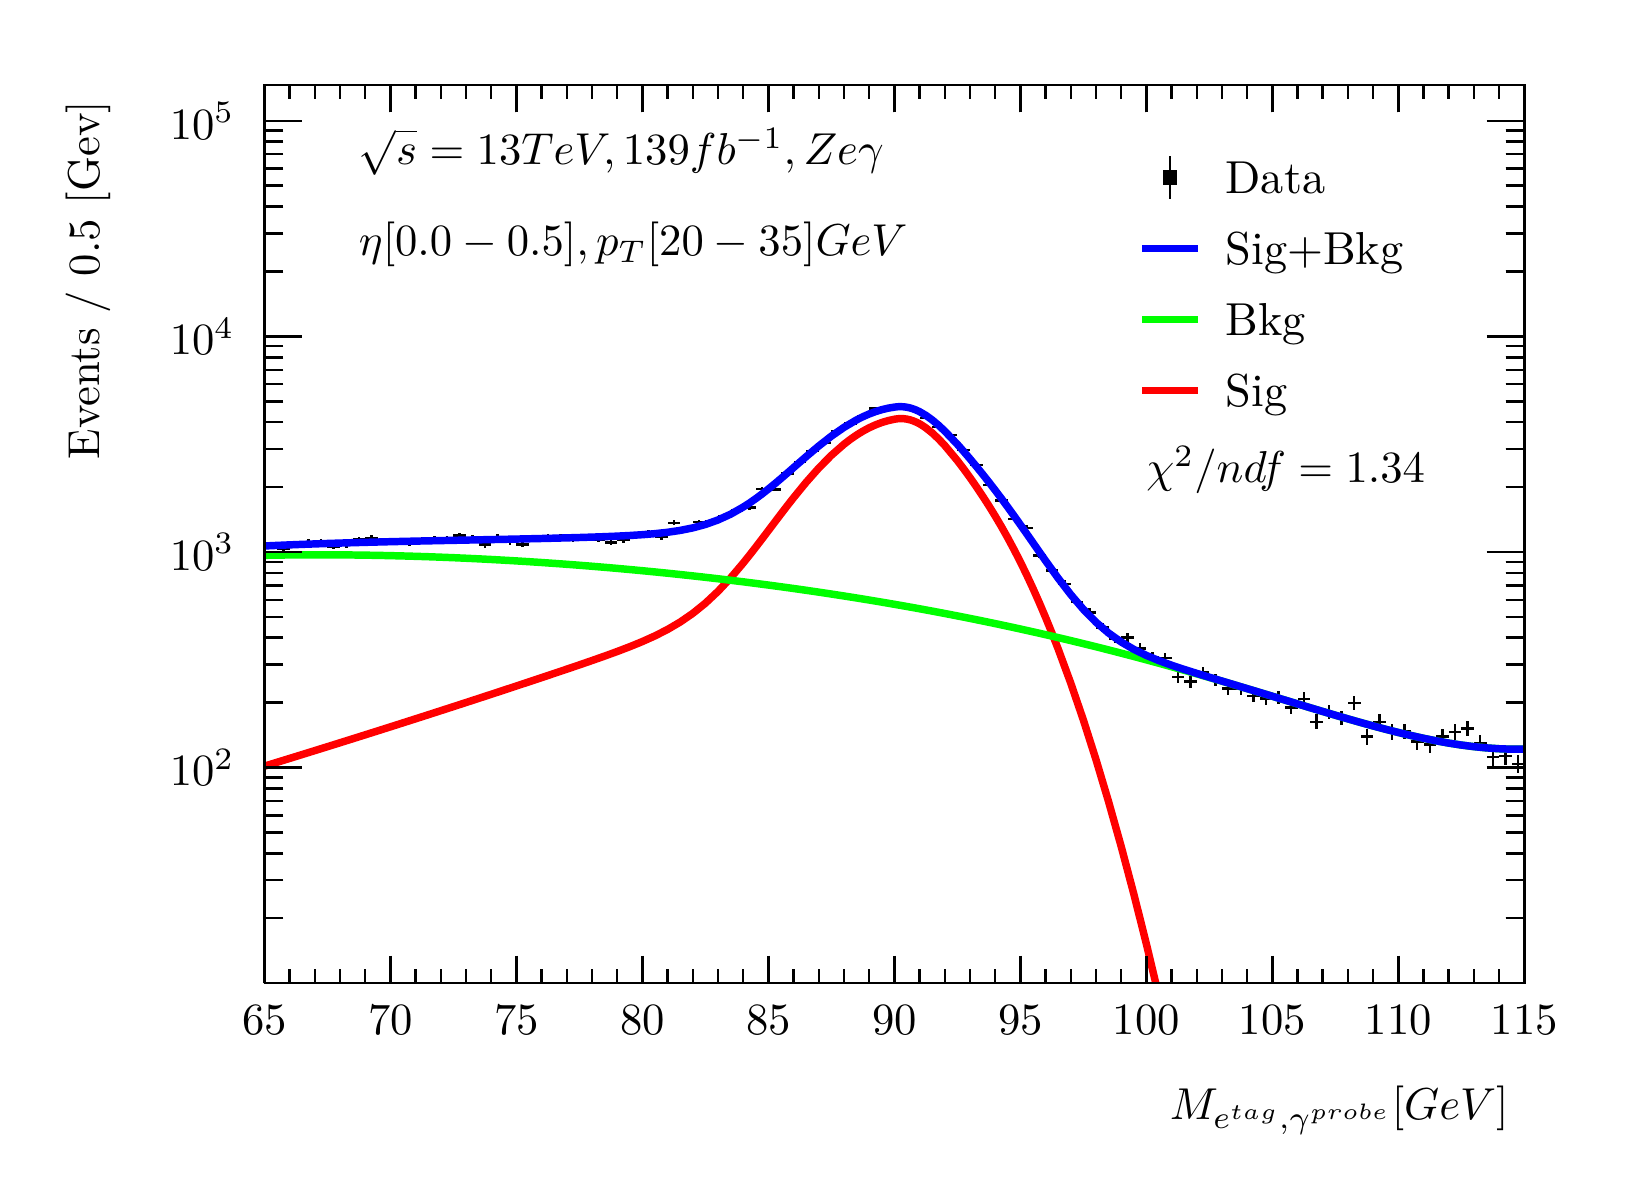
\begin{tikzpicture}
\pgfdeclareplotmark{cross} {
\pgfpathmoveto{\pgfpoint{-0.3\pgfplotmarksize}{\pgfplotmarksize}}
\pgfpathlineto{\pgfpoint{+0.3\pgfplotmarksize}{\pgfplotmarksize}}
\pgfpathlineto{\pgfpoint{+0.3\pgfplotmarksize}{0.3\pgfplotmarksize}}
\pgfpathlineto{\pgfpoint{+1\pgfplotmarksize}{0.3\pgfplotmarksize}}
\pgfpathlineto{\pgfpoint{+1\pgfplotmarksize}{-0.3\pgfplotmarksize}}
\pgfpathlineto{\pgfpoint{+0.3\pgfplotmarksize}{-0.3\pgfplotmarksize}}
\pgfpathlineto{\pgfpoint{+0.3\pgfplotmarksize}{-1.\pgfplotmarksize}}
\pgfpathlineto{\pgfpoint{-0.3\pgfplotmarksize}{-1.\pgfplotmarksize}}
\pgfpathlineto{\pgfpoint{-0.3\pgfplotmarksize}{-0.3\pgfplotmarksize}}
\pgfpathlineto{\pgfpoint{-1.\pgfplotmarksize}{-0.3\pgfplotmarksize}}
\pgfpathlineto{\pgfpoint{-1.\pgfplotmarksize}{0.3\pgfplotmarksize}}
\pgfpathlineto{\pgfpoint{-0.3\pgfplotmarksize}{0.3\pgfplotmarksize}}
\pgfpathclose
\pgfusepathqstroke
}
\pgfdeclareplotmark{cross*} {
\pgfpathmoveto{\pgfpoint{-0.3\pgfplotmarksize}{\pgfplotmarksize}}
\pgfpathlineto{\pgfpoint{+0.3\pgfplotmarksize}{\pgfplotmarksize}}
\pgfpathlineto{\pgfpoint{+0.3\pgfplotmarksize}{0.3\pgfplotmarksize}}
\pgfpathlineto{\pgfpoint{+1\pgfplotmarksize}{0.3\pgfplotmarksize}}
\pgfpathlineto{\pgfpoint{+1\pgfplotmarksize}{-0.3\pgfplotmarksize}}
\pgfpathlineto{\pgfpoint{+0.3\pgfplotmarksize}{-0.3\pgfplotmarksize}}
\pgfpathlineto{\pgfpoint{+0.3\pgfplotmarksize}{-1.\pgfplotmarksize}}
\pgfpathlineto{\pgfpoint{-0.3\pgfplotmarksize}{-1.\pgfplotmarksize}}
\pgfpathlineto{\pgfpoint{-0.3\pgfplotmarksize}{-0.3\pgfplotmarksize}}
\pgfpathlineto{\pgfpoint{-1.\pgfplotmarksize}{-0.3\pgfplotmarksize}}
\pgfpathlineto{\pgfpoint{-1.\pgfplotmarksize}{0.3\pgfplotmarksize}}
\pgfpathlineto{\pgfpoint{-0.3\pgfplotmarksize}{0.3\pgfplotmarksize}}
\pgfpathclose
\pgfusepathqfillstroke
}
\pgfdeclareplotmark{newstar} {
\pgfpathmoveto{\pgfqpoint{0pt}{\pgfplotmarksize}}
\pgfpathlineto{\pgfqpointpolar{44}{0.5\pgfplotmarksize}}
\pgfpathlineto{\pgfqpointpolar{18}{\pgfplotmarksize}}
\pgfpathlineto{\pgfqpointpolar{-20}{0.5\pgfplotmarksize}}
\pgfpathlineto{\pgfqpointpolar{-54}{\pgfplotmarksize}}
\pgfpathlineto{\pgfqpointpolar{-90}{0.5\pgfplotmarksize}}
\pgfpathlineto{\pgfqpointpolar{234}{\pgfplotmarksize}}
\pgfpathlineto{\pgfqpointpolar{198}{0.5\pgfplotmarksize}}
\pgfpathlineto{\pgfqpointpolar{162}{\pgfplotmarksize}}
\pgfpathlineto{\pgfqpointpolar{134}{0.5\pgfplotmarksize}}
\pgfpathclose
\pgfusepathqstroke
}
\pgfdeclareplotmark{newstar*} {
\pgfpathmoveto{\pgfqpoint{0pt}{\pgfplotmarksize}}
\pgfpathlineto{\pgfqpointpolar{44}{0.5\pgfplotmarksize}}
\pgfpathlineto{\pgfqpointpolar{18}{\pgfplotmarksize}}
\pgfpathlineto{\pgfqpointpolar{-20}{0.5\pgfplotmarksize}}
\pgfpathlineto{\pgfqpointpolar{-54}{\pgfplotmarksize}}
\pgfpathlineto{\pgfqpointpolar{-90}{0.5\pgfplotmarksize}}
\pgfpathlineto{\pgfqpointpolar{234}{\pgfplotmarksize}}
\pgfpathlineto{\pgfqpointpolar{198}{0.5\pgfplotmarksize}}
\pgfpathlineto{\pgfqpointpolar{162}{\pgfplotmarksize}}
\pgfpathlineto{\pgfqpointpolar{134}{0.5\pgfplotmarksize}}
\pgfpathclose
\pgfusepathqfillstroke
}
\definecolor{c}{rgb}{1,1,1};
\draw [color=c, fill=c] (0,0) rectangle (20,14.4361);
\draw [color=c, fill=c] (3,2.30977) rectangle (19,13.7143);
\definecolor{c}{rgb}{0,0,0};
\draw [c,line width=0.9] (3,2.30977) -- (3,13.7143) -- (19,13.7143) -- (19,2.30977) -- (3,2.30977);
\definecolor{c}{rgb}{1,1,1};
\draw [color=c, fill=c] (3,2.30977) rectangle (19,13.7143);
\definecolor{c}{rgb}{0,0,0};
\draw [c,line width=0.9] (3,2.30977) -- (3,13.7143) -- (19,13.7143) -- (19,2.30977) -- (3,2.30977);
\draw [c,line width=0.9] (3,2.30977) -- (19,2.30977);
\draw [c,line width=0.9] (3,2.65624) -- (3,2.30977);
\draw [c,line width=0.9] (3.32,2.48301) -- (3.32,2.30977);
\draw [c,line width=0.9] (3.64,2.48301) -- (3.64,2.30977);
\draw [c,line width=0.9] (3.96,2.48301) -- (3.96,2.30977);
\draw [c,line width=0.9] (4.28,2.48301) -- (4.28,2.30977);
\draw [c,line width=0.9] (4.6,2.65624) -- (4.6,2.30977);
\draw [c,line width=0.9] (4.92,2.48301) -- (4.92,2.30977);
\draw [c,line width=0.9] (5.24,2.48301) -- (5.24,2.30977);
\draw [c,line width=0.9] (5.56,2.48301) -- (5.56,2.30977);
\draw [c,line width=0.9] (5.88,2.48301) -- (5.88,2.30977);
\draw [c,line width=0.9] (6.2,2.65624) -- (6.2,2.30977);
\draw [c,line width=0.9] (6.52,2.48301) -- (6.52,2.30977);
\draw [c,line width=0.9] (6.84,2.48301) -- (6.84,2.30977);
\draw [c,line width=0.9] (7.16,2.48301) -- (7.16,2.30977);
\draw [c,line width=0.9] (7.48,2.48301) -- (7.48,2.30977);
\draw [c,line width=0.9] (7.8,2.65624) -- (7.8,2.30977);
\draw [c,line width=0.9] (8.12,2.48301) -- (8.12,2.30977);
\draw [c,line width=0.9] (8.44,2.48301) -- (8.44,2.30977);
\draw [c,line width=0.9] (8.76,2.48301) -- (8.76,2.30977);
\draw [c,line width=0.9] (9.08,2.48301) -- (9.08,2.30977);
\draw [c,line width=0.9] (9.4,2.65624) -- (9.4,2.30977);
\draw [c,line width=0.9] (9.72,2.48301) -- (9.72,2.30977);
\draw [c,line width=0.9] (10.04,2.48301) -- (10.04,2.30977);
\draw [c,line width=0.9] (10.36,2.48301) -- (10.36,2.30977);
\draw [c,line width=0.9] (10.68,2.48301) -- (10.68,2.30977);
\draw [c,line width=0.9] (11,2.65624) -- (11,2.30977);
\draw [c,line width=0.9] (11.32,2.48301) -- (11.32,2.30977);
\draw [c,line width=0.9] (11.64,2.48301) -- (11.64,2.30977);
\draw [c,line width=0.9] (11.96,2.48301) -- (11.96,2.30977);
\draw [c,line width=0.9] (12.28,2.48301) -- (12.28,2.30977);
\draw [c,line width=0.9] (12.6,2.65624) -- (12.6,2.30977);
\draw [c,line width=0.9] (12.92,2.48301) -- (12.92,2.30977);
\draw [c,line width=0.9] (13.24,2.48301) -- (13.24,2.30977);
\draw [c,line width=0.9] (13.56,2.48301) -- (13.56,2.30977);
\draw [c,line width=0.9] (13.88,2.48301) -- (13.88,2.30977);
\draw [c,line width=0.9] (14.2,2.65624) -- (14.2,2.30977);
\draw [c,line width=0.9] (14.52,2.48301) -- (14.52,2.30977);
\draw [c,line width=0.9] (14.84,2.48301) -- (14.84,2.30977);
\draw [c,line width=0.9] (15.16,2.48301) -- (15.16,2.30977);
\draw [c,line width=0.9] (15.48,2.48301) -- (15.48,2.30977);
\draw [c,line width=0.9] (15.8,2.65624) -- (15.8,2.30977);
\draw [c,line width=0.9] (16.12,2.48301) -- (16.12,2.30977);
\draw [c,line width=0.9] (16.44,2.48301) -- (16.44,2.30977);
\draw [c,line width=0.9] (16.76,2.48301) -- (16.76,2.30977);
\draw [c,line width=0.9] (17.08,2.48301) -- (17.08,2.30977);
\draw [c,line width=0.9] (17.4,2.65624) -- (17.4,2.30977);
\draw [c,line width=0.9] (17.72,2.48301) -- (17.72,2.30977);
\draw [c,line width=0.9] (18.04,2.48301) -- (18.04,2.30977);
\draw [c,line width=0.9] (18.36,2.48301) -- (18.36,2.30977);
\draw [c,line width=0.9] (18.68,2.48301) -- (18.68,2.30977);
\draw [c,line width=0.9] (19,2.65624) -- (19,2.30977);
\draw [c,line width=0.9] (19,2.65624) -- (19,2.30977);
\draw [anchor=base] (3,1.66015) node[scale=1.61424, color=c, rotate=0]{65};
\draw [anchor=base] (4.6,1.66015) node[scale=1.61424, color=c, rotate=0]{70};
\draw [anchor=base] (6.2,1.66015) node[scale=1.61424, color=c, rotate=0]{75};
\draw [anchor=base] (7.8,1.66015) node[scale=1.61424, color=c, rotate=0]{80};
\draw [anchor=base] (9.4,1.66015) node[scale=1.61424, color=c, rotate=0]{85};
\draw [anchor=base] (11,1.66015) node[scale=1.61424, color=c, rotate=0]{90};
\draw [anchor=base] (12.6,1.66015) node[scale=1.61424, color=c, rotate=0]{95};
\draw [anchor=base] (14.2,1.66015) node[scale=1.61424, color=c, rotate=0]{100};
\draw [anchor=base] (15.8,1.66015) node[scale=1.61424, color=c, rotate=0]{105};
\draw [anchor=base] (17.4,1.66015) node[scale=1.61424, color=c, rotate=0]{110};
\draw [anchor=base] (19,1.66015) node[scale=1.61424, color=c, rotate=0]{115};
\draw [anchor= east] (19,0.692932) node[scale=1.61424, color=c, rotate=0]{$M_{e^{tag}, \gamma^{probe}}  [GeV]$};
\draw [c,line width=0.9] (3,13.7143) -- (19,13.7143);
\draw [c,line width=0.9] (3,13.3678) -- (3,13.7143);
\draw [c,line width=0.9] (3.32,13.5411) -- (3.32,13.7143);
\draw [c,line width=0.9] (3.64,13.5411) -- (3.64,13.7143);
\draw [c,line width=0.9] (3.96,13.5411) -- (3.96,13.7143);
\draw [c,line width=0.9] (4.28,13.5411) -- (4.28,13.7143);
\draw [c,line width=0.9] (4.6,13.3678) -- (4.6,13.7143);
\draw [c,line width=0.9] (4.92,13.5411) -- (4.92,13.7143);
\draw [c,line width=0.9] (5.24,13.5411) -- (5.24,13.7143);
\draw [c,line width=0.9] (5.56,13.5411) -- (5.56,13.7143);
\draw [c,line width=0.9] (5.88,13.5411) -- (5.88,13.7143);
\draw [c,line width=0.9] (6.2,13.3678) -- (6.2,13.7143);
\draw [c,line width=0.9] (6.52,13.5411) -- (6.52,13.7143);
\draw [c,line width=0.9] (6.84,13.5411) -- (6.84,13.7143);
\draw [c,line width=0.9] (7.16,13.5411) -- (7.16,13.7143);
\draw [c,line width=0.9] (7.48,13.5411) -- (7.48,13.7143);
\draw [c,line width=0.9] (7.8,13.3678) -- (7.8,13.7143);
\draw [c,line width=0.9] (8.12,13.5411) -- (8.12,13.7143);
\draw [c,line width=0.9] (8.44,13.5411) -- (8.44,13.7143);
\draw [c,line width=0.9] (8.76,13.5411) -- (8.76,13.7143);
\draw [c,line width=0.9] (9.08,13.5411) -- (9.08,13.7143);
\draw [c,line width=0.9] (9.4,13.3678) -- (9.4,13.7143);
\draw [c,line width=0.9] (9.72,13.5411) -- (9.72,13.7143);
\draw [c,line width=0.9] (10.04,13.5411) -- (10.04,13.7143);
\draw [c,line width=0.9] (10.36,13.5411) -- (10.36,13.7143);
\draw [c,line width=0.9] (10.68,13.5411) -- (10.68,13.7143);
\draw [c,line width=0.9] (11,13.3678) -- (11,13.7143);
\draw [c,line width=0.9] (11.32,13.5411) -- (11.32,13.7143);
\draw [c,line width=0.9] (11.64,13.5411) -- (11.64,13.7143);
\draw [c,line width=0.9] (11.96,13.5411) -- (11.96,13.7143);
\draw [c,line width=0.9] (12.28,13.5411) -- (12.28,13.7143);
\draw [c,line width=0.9] (12.6,13.3678) -- (12.6,13.7143);
\draw [c,line width=0.9] (12.92,13.5411) -- (12.92,13.7143);
\draw [c,line width=0.9] (13.24,13.5411) -- (13.24,13.7143);
\draw [c,line width=0.9] (13.56,13.5411) -- (13.56,13.7143);
\draw [c,line width=0.9] (13.88,13.5411) -- (13.88,13.7143);
\draw [c,line width=0.9] (14.2,13.3678) -- (14.2,13.7143);
\draw [c,line width=0.9] (14.52,13.5411) -- (14.52,13.7143);
\draw [c,line width=0.9] (14.84,13.5411) -- (14.84,13.7143);
\draw [c,line width=0.9] (15.16,13.5411) -- (15.16,13.7143);
\draw [c,line width=0.9] (15.48,13.5411) -- (15.48,13.7143);
\draw [c,line width=0.9] (15.8,13.3678) -- (15.8,13.7143);
\draw [c,line width=0.9] (16.12,13.5411) -- (16.12,13.7143);
\draw [c,line width=0.9] (16.44,13.5411) -- (16.44,13.7143);
\draw [c,line width=0.9] (16.76,13.5411) -- (16.76,13.7143);
\draw [c,line width=0.9] (17.08,13.5411) -- (17.08,13.7143);
\draw [c,line width=0.9] (17.4,13.3678) -- (17.4,13.7143);
\draw [c,line width=0.9] (17.72,13.5411) -- (17.72,13.7143);
\draw [c,line width=0.9] (18.04,13.5411) -- (18.04,13.7143);
\draw [c,line width=0.9] (18.36,13.5411) -- (18.36,13.7143);
\draw [c,line width=0.9] (18.68,13.5411) -- (18.68,13.7143);
\draw [c,line width=0.9] (19,13.3678) -- (19,13.7143);
\draw [c,line width=0.9] (19,13.3678) -- (19,13.7143);
\draw [c,line width=0.9] (3,2.30977) -- (3,13.7143);
\draw [c,line width=0.9] (3.237,3.13385) -- (3,3.13385);
\draw [c,line width=0.9] (3.237,3.6159) -- (3,3.6159);
\draw [c,line width=0.9] (3.237,3.95792) -- (3,3.95792);
\draw [c,line width=0.9] (3.237,4.22321) -- (3,4.22321);
\draw [c,line width=0.9] (3.237,4.43997) -- (3,4.43997);
\draw [c,line width=0.9] (3.237,4.62324) -- (3,4.62324);
\draw [c,line width=0.9] (3.237,4.782) -- (3,4.782);
\draw [c,line width=0.9] (3.237,4.92203) -- (3,4.92203);
\draw [c,line width=0.9] (3.474,5.04729) -- (3,5.04729);
\draw [anchor= east] (2.82,5.04729) node[scale=1.61424, color=c, rotate=0]{$10^{2}$};
\draw [c,line width=0.9] (3.237,5.87136) -- (3,5.87136);
\draw [c,line width=0.9] (3.237,6.35342) -- (3,6.35342);
\draw [c,line width=0.9] (3.237,6.69544) -- (3,6.69544);
\draw [c,line width=0.9] (3.237,6.96073) -- (3,6.96073);
\draw [c,line width=0.9] (3.237,7.17749) -- (3,7.17749);
\draw [c,line width=0.9] (3.237,7.36076) -- (3,7.36076);
\draw [c,line width=0.9] (3.237,7.51951) -- (3,7.51951);
\draw [c,line width=0.9] (3.237,7.65954) -- (3,7.65954);
\draw [c,line width=0.9] (3.474,7.78481) -- (3,7.78481);
\draw [anchor= east] (2.82,7.78481) node[scale=1.61424, color=c, rotate=0]{$10^{3}$};
\draw [c,line width=0.9] (3.237,8.60888) -- (3,8.60888);
\draw [c,line width=0.9] (3.237,9.09093) -- (3,9.09093);
\draw [c,line width=0.9] (3.237,9.43296) -- (3,9.43296);
\draw [c,line width=0.9] (3.237,9.69825) -- (3,9.69825);
\draw [c,line width=0.9] (3.237,9.91501) -- (3,9.91501);
\draw [c,line width=0.9] (3.237,10.0983) -- (3,10.0983);
\draw [c,line width=0.9] (3.237,10.257) -- (3,10.257);
\draw [c,line width=0.9] (3.237,10.3971) -- (3,10.3971);
\draw [c,line width=0.9] (3.474,10.5223) -- (3,10.5223);
\draw [anchor= east] (2.82,10.5223) node[scale=1.61424, color=c, rotate=0]{$10^{4}$};
\draw [c,line width=0.9] (3.237,11.3464) -- (3,11.3464);
\draw [c,line width=0.9] (3.237,11.8285) -- (3,11.8285);
\draw [c,line width=0.9] (3.237,12.1705) -- (3,12.1705);
\draw [c,line width=0.9] (3.237,12.4358) -- (3,12.4358);
\draw [c,line width=0.9] (3.237,12.6525) -- (3,12.6525);
\draw [c,line width=0.9] (3.237,12.8358) -- (3,12.8358);
\draw [c,line width=0.9] (3.237,12.9945) -- (3,12.9945);
\draw [c,line width=0.9] (3.237,13.1346) -- (3,13.1346);
\draw [c,line width=0.9] (3.474,13.2598) -- (3,13.2598);
\draw [anchor= east] (2.82,13.2598) node[scale=1.61424, color=c, rotate=0]{$10^{5}$};
\draw [anchor= east] (0.76,13.7143) node[scale=1.61424, color=c, rotate=90]{Events / 0.5 [Gev]};
\draw [c,line width=0.9] (19,2.30977) -- (19,13.7143);
\draw [c,line width=0.9] (18.763,3.13385) -- (19,3.13385);
\draw [c,line width=0.9] (18.763,3.6159) -- (19,3.6159);
\draw [c,line width=0.9] (18.763,3.95792) -- (19,3.95792);
\draw [c,line width=0.9] (18.763,4.22321) -- (19,4.22321);
\draw [c,line width=0.9] (18.763,4.43997) -- (19,4.43997);
\draw [c,line width=0.9] (18.763,4.62324) -- (19,4.62324);
\draw [c,line width=0.9] (18.763,4.782) -- (19,4.782);
\draw [c,line width=0.9] (18.763,4.92203) -- (19,4.92203);
\draw [c,line width=0.9] (18.526,5.04729) -- (19,5.04729);
\draw [c,line width=0.9] (18.763,5.87136) -- (19,5.87136);
\draw [c,line width=0.9] (18.763,6.35342) -- (19,6.35342);
\draw [c,line width=0.9] (18.763,6.69544) -- (19,6.69544);
\draw [c,line width=0.9] (18.763,6.96073) -- (19,6.96073);
\draw [c,line width=0.9] (18.763,7.17749) -- (19,7.17749);
\draw [c,line width=0.9] (18.763,7.36076) -- (19,7.36076);
\draw [c,line width=0.9] (18.763,7.51951) -- (19,7.51951);
\draw [c,line width=0.9] (18.763,7.65954) -- (19,7.65954);
\draw [c,line width=0.9] (18.526,7.78481) -- (19,7.78481);
\draw [c,line width=0.9] (18.763,8.60888) -- (19,8.60888);
\draw [c,line width=0.9] (18.763,9.09093) -- (19,9.09093);
\draw [c,line width=0.9] (18.763,9.43296) -- (19,9.43296);
\draw [c,line width=0.9] (18.763,9.69825) -- (19,9.69825);
\draw [c,line width=0.9] (18.763,9.91501) -- (19,9.91501);
\draw [c,line width=0.9] (18.763,10.0983) -- (19,10.0983);
\draw [c,line width=0.9] (18.763,10.257) -- (19,10.257);
\draw [c,line width=0.9] (18.763,10.3971) -- (19,10.3971);
\draw [c,line width=0.9] (18.526,10.5223) -- (19,10.5223);
\draw [c,line width=0.9] (18.763,11.3464) -- (19,11.3464);
\draw [c,line width=0.9] (18.763,11.8285) -- (19,11.8285);
\draw [c,line width=0.9] (18.763,12.1705) -- (19,12.1705);
\draw [c,line width=0.9] (18.763,12.4358) -- (19,12.4358);
\draw [c,line width=0.9] (18.763,12.6525) -- (19,12.6525);
\draw [c,line width=0.9] (18.763,12.8358) -- (19,12.8358);
\draw [c,line width=0.9] (18.763,12.9945) -- (19,12.9945);
\draw [c,line width=0.9] (18.763,13.1346) -- (19,13.1346);
\draw [c,line width=0.9] (18.526,13.2598) -- (19,13.2598);
\draw [c,line width=0.9] (3.08,7.85744) -- (3,7.85744);
\draw [c,line width=0.9] (3,7.85744) -- (3,7.85744);
\draw [c,line width=0.9] (3.08,7.85744) -- (3.16,7.85744);
\draw [c,line width=0.9] (3.16,7.85744) -- (3.16,7.85744);
\draw [c,line width=0.9] (3.08,7.85744) -- (3.08,7.89391);
\draw [c,line width=0.9] (3.08,7.89391) -- (3.08,7.89391);
\draw [c,line width=0.9] (3.08,7.85744) -- (3.08,7.82098);
\draw [c,line width=0.9] (3.08,7.82098) -- (3.08,7.82098);
\draw [c,line width=0.9] (3.24,7.81995) -- (3.16,7.81995);
\draw [c,line width=0.9] (3.16,7.81995) -- (3.16,7.81995);
\draw [c,line width=0.9] (3.24,7.81995) -- (3.32,7.81995);
\draw [c,line width=0.9] (3.32,7.81995) -- (3.32,7.81995);
\draw [c,line width=0.9] (3.24,7.81995) -- (3.24,7.85699);
\draw [c,line width=0.9] (3.24,7.85699) -- (3.24,7.85699);
\draw [c,line width=0.9] (3.24,7.81995) -- (3.24,7.78291);
\draw [c,line width=0.9] (3.24,7.78291) -- (3.24,7.78291);
\draw [c,line width=0.9] (3.4,7.86968) -- (3.32,7.86968);
\draw [c,line width=0.9] (3.32,7.86968) -- (3.32,7.86968);
\draw [c,line width=0.9] (3.4,7.86968) -- (3.48,7.86968);
\draw [c,line width=0.9] (3.48,7.86968) -- (3.48,7.86968);
\draw [c,line width=0.9] (3.4,7.86968) -- (3.4,7.90596);
\draw [c,line width=0.9] (3.4,7.90596) -- (3.4,7.90596);
\draw [c,line width=0.9] (3.4,7.86968) -- (3.4,7.83341);
\draw [c,line width=0.9] (3.4,7.83341) -- (3.4,7.83341);
\draw [c,line width=0.9] (3.56,7.91209) -- (3.48,7.91209);
\draw [c,line width=0.9] (3.48,7.91209) -- (3.48,7.91209);
\draw [c,line width=0.9] (3.56,7.91209) -- (3.64,7.91209);
\draw [c,line width=0.9] (3.64,7.91209) -- (3.64,7.91209);
\draw [c,line width=0.9] (3.56,7.91209) -- (3.56,7.94772);
\draw [c,line width=0.9] (3.56,7.94772) -- (3.56,7.94772);
\draw [c,line width=0.9] (3.56,7.91209) -- (3.56,7.87645);
\draw [c,line width=0.9] (3.56,7.87645) -- (3.56,7.87645);
\draw [c,line width=0.9] (3.72,7.90995) -- (3.64,7.90995);
\draw [c,line width=0.9] (3.64,7.90995) -- (3.64,7.90995);
\draw [c,line width=0.9] (3.72,7.90995) -- (3.8,7.90995);
\draw [c,line width=0.9] (3.8,7.90995) -- (3.8,7.90995);
\draw [c,line width=0.9] (3.72,7.90995) -- (3.72,7.94562);
\draw [c,line width=0.9] (3.72,7.94562) -- (3.72,7.94562);
\draw [c,line width=0.9] (3.72,7.90995) -- (3.72,7.87428);
\draw [c,line width=0.9] (3.72,7.87428) -- (3.72,7.87428);
\draw [c,line width=0.9] (3.88,7.85408) -- (3.8,7.85408);
\draw [c,line width=0.9] (3.8,7.85408) -- (3.8,7.85408);
\draw [c,line width=0.9] (3.88,7.85408) -- (3.96,7.85408);
\draw [c,line width=0.9] (3.96,7.85408) -- (3.96,7.85408);
\draw [c,line width=0.9] (3.88,7.85408) -- (3.88,7.8906);
\draw [c,line width=0.9] (3.88,7.8906) -- (3.88,7.8906);
\draw [c,line width=0.9] (3.88,7.85408) -- (3.88,7.81757);
\draw [c,line width=0.9] (3.88,7.81757) -- (3.88,7.81757);
\draw [c,line width=0.9] (4.04,7.87189) -- (3.96,7.87189);
\draw [c,line width=0.9] (3.96,7.87189) -- (3.96,7.87189);
\draw [c,line width=0.9] (4.04,7.87189) -- (4.12,7.87189);
\draw [c,line width=0.9] (4.12,7.87189) -- (4.12,7.87189);
\draw [c,line width=0.9] (4.04,7.87189) -- (4.04,7.90814);
\draw [c,line width=0.9] (4.04,7.90814) -- (4.04,7.90814);
\draw [c,line width=0.9] (4.04,7.87189) -- (4.04,7.83565);
\draw [c,line width=0.9] (4.04,7.83565) -- (4.04,7.83565);
\draw [c,line width=0.9] (4.2,7.94163) -- (4.12,7.94163);
\draw [c,line width=0.9] (4.12,7.94163) -- (4.12,7.94163);
\draw [c,line width=0.9] (4.2,7.94163) -- (4.28,7.94163);
\draw [c,line width=0.9] (4.28,7.94163) -- (4.28,7.94163);
\draw [c,line width=0.9] (4.2,7.94163) -- (4.2,7.97682);
\draw [c,line width=0.9] (4.2,7.97682) -- (4.2,7.97682);
\draw [c,line width=0.9] (4.2,7.94163) -- (4.2,7.90643);
\draw [c,line width=0.9] (4.2,7.90643) -- (4.2,7.90643);
\draw [c,line width=0.9] (4.36,7.96229) -- (4.28,7.96229);
\draw [c,line width=0.9] (4.28,7.96229) -- (4.28,7.96229);
\draw [c,line width=0.9] (4.36,7.96229) -- (4.44,7.96229);
\draw [c,line width=0.9] (4.44,7.96229) -- (4.44,7.96229);
\draw [c,line width=0.9] (4.36,7.96229) -- (4.36,7.99718);
\draw [c,line width=0.9] (4.36,7.99718) -- (4.36,7.99718);
\draw [c,line width=0.9] (4.36,7.96229) -- (4.36,7.9274);
\draw [c,line width=0.9] (4.36,7.9274) -- (4.36,7.9274);
\draw [c,line width=0.9] (4.52,7.91422) -- (4.44,7.91422);
\draw [c,line width=0.9] (4.44,7.91422) -- (4.44,7.91422);
\draw [c,line width=0.9] (4.52,7.91422) -- (4.6,7.91422);
\draw [c,line width=0.9] (4.6,7.91422) -- (4.6,7.91422);
\draw [c,line width=0.9] (4.52,7.91422) -- (4.52,7.94983);
\draw [c,line width=0.9] (4.52,7.94983) -- (4.52,7.94983);
\draw [c,line width=0.9] (4.52,7.91422) -- (4.52,7.87862);
\draw [c,line width=0.9] (4.52,7.87862) -- (4.52,7.87862);
\draw [c,line width=0.9] (4.68,7.93221) -- (4.6,7.93221);
\draw [c,line width=0.9] (4.6,7.93221) -- (4.6,7.93221);
\draw [c,line width=0.9] (4.68,7.93221) -- (4.76,7.93221);
\draw [c,line width=0.9] (4.76,7.93221) -- (4.76,7.93221);
\draw [c,line width=0.9] (4.68,7.93221) -- (4.68,7.96755);
\draw [c,line width=0.9] (4.68,7.96755) -- (4.68,7.96755);
\draw [c,line width=0.9] (4.68,7.93221) -- (4.68,7.89688);
\draw [c,line width=0.9] (4.68,7.89688) -- (4.68,7.89688);
\draw [c,line width=0.9] (4.84,7.89487) -- (4.76,7.89487);
\draw [c,line width=0.9] (4.76,7.89487) -- (4.76,7.89487);
\draw [c,line width=0.9] (4.84,7.89487) -- (4.92,7.89487);
\draw [c,line width=0.9] (4.92,7.89487) -- (4.92,7.89487);
\draw [c,line width=0.9] (4.84,7.89487) -- (4.84,7.93077);
\draw [c,line width=0.9] (4.84,7.93077) -- (4.84,7.93077);
\draw [c,line width=0.9] (4.84,7.89487) -- (4.84,7.85898);
\draw [c,line width=0.9] (4.84,7.85898) -- (4.84,7.85898);
\draw [c,line width=0.9] (5,7.9385) -- (4.92,7.9385);
\draw [c,line width=0.9] (4.92,7.9385) -- (4.92,7.9385);
\draw [c,line width=0.9] (5,7.9385) -- (5.08,7.9385);
\draw [c,line width=0.9] (5.08,7.9385) -- (5.08,7.9385);
\draw [c,line width=0.9] (5,7.9385) -- (5,7.97374);
\draw [c,line width=0.9] (5,7.97374) -- (5,7.97374);
\draw [c,line width=0.9] (5,7.9385) -- (5,7.90326);
\draw [c,line width=0.9] (5,7.90326) -- (5,7.90326);
\draw [c,line width=0.9] (5.16,7.95303) -- (5.08,7.95303);
\draw [c,line width=0.9] (5.08,7.95303) -- (5.08,7.95303);
\draw [c,line width=0.9] (5.16,7.95303) -- (5.24,7.95303);
\draw [c,line width=0.9] (5.24,7.95303) -- (5.24,7.95303);
\draw [c,line width=0.9] (5.16,7.95303) -- (5.16,7.98806);
\draw [c,line width=0.9] (5.16,7.98806) -- (5.16,7.98806);
\draw [c,line width=0.9] (5.16,7.95303) -- (5.16,7.91801);
\draw [c,line width=0.9] (5.16,7.91801) -- (5.16,7.91801);
\draw [c,line width=0.9] (5.32,7.9551) -- (5.24,7.9551);
\draw [c,line width=0.9] (5.24,7.9551) -- (5.24,7.9551);
\draw [c,line width=0.9] (5.32,7.9551) -- (5.4,7.9551);
\draw [c,line width=0.9] (5.4,7.9551) -- (5.4,7.9551);
\draw [c,line width=0.9] (5.32,7.9551) -- (5.32,7.99009);
\draw [c,line width=0.9] (5.32,7.99009) -- (5.32,7.99009);
\draw [c,line width=0.9] (5.32,7.9551) -- (5.32,7.9201);
\draw [c,line width=0.9] (5.32,7.9201) -- (5.32,7.9201);
\draw [c,line width=0.9] (5.48,7.99361) -- (5.4,7.99361);
\draw [c,line width=0.9] (5.4,7.99361) -- (5.4,7.99361);
\draw [c,line width=0.9] (5.48,7.99361) -- (5.56,7.99361);
\draw [c,line width=0.9] (5.56,7.99361) -- (5.56,7.99361);
\draw [c,line width=0.9] (5.48,7.99361) -- (5.48,8.02805);
\draw [c,line width=0.9] (5.48,8.02805) -- (5.48,8.02805);
\draw [c,line width=0.9] (5.48,7.99361) -- (5.48,7.95918);
\draw [c,line width=0.9] (5.48,7.95918) -- (5.48,7.95918);
\draw [c,line width=0.9] (5.64,7.96433) -- (5.56,7.96433);
\draw [c,line width=0.9] (5.56,7.96433) -- (5.56,7.96433);
\draw [c,line width=0.9] (5.64,7.96433) -- (5.72,7.96433);
\draw [c,line width=0.9] (5.72,7.96433) -- (5.72,7.96433);
\draw [c,line width=0.9] (5.64,7.96433) -- (5.64,7.99919);
\draw [c,line width=0.9] (5.64,7.99919) -- (5.64,7.99919);
\draw [c,line width=0.9] (5.64,7.96433) -- (5.64,7.92947);
\draw [c,line width=0.9] (5.64,7.92947) -- (5.64,7.92947);
\draw [c,line width=0.9] (5.8,7.87631) -- (5.72,7.87631);
\draw [c,line width=0.9] (5.72,7.87631) -- (5.72,7.87631);
\draw [c,line width=0.9] (5.8,7.87631) -- (5.88,7.87631);
\draw [c,line width=0.9] (5.88,7.87631) -- (5.88,7.87631);
\draw [c,line width=0.9] (5.8,7.87631) -- (5.8,7.91248);
\draw [c,line width=0.9] (5.8,7.91248) -- (5.8,7.91248);
\draw [c,line width=0.9] (5.8,7.87631) -- (5.8,7.84013);
\draw [c,line width=0.9] (5.8,7.84013) -- (5.8,7.84013);
\draw [c,line width=0.9] (5.96,7.97552) -- (5.88,7.97552);
\draw [c,line width=0.9] (5.88,7.97552) -- (5.88,7.97552);
\draw [c,line width=0.9] (5.96,7.97552) -- (6.04,7.97552);
\draw [c,line width=0.9] (6.04,7.97552) -- (6.04,7.97552);
\draw [c,line width=0.9] (5.96,7.97552) -- (5.96,8.01022);
\draw [c,line width=0.9] (5.96,8.01022) -- (5.96,8.01022);
\draw [c,line width=0.9] (5.96,7.97552) -- (5.96,7.94083);
\draw [c,line width=0.9] (5.96,7.94083) -- (5.96,7.94083);
\draw [c,line width=0.9] (6.12,7.90888) -- (6.04,7.90888);
\draw [c,line width=0.9] (6.04,7.90888) -- (6.04,7.90888);
\draw [c,line width=0.9] (6.12,7.90888) -- (6.2,7.90888);
\draw [c,line width=0.9] (6.2,7.90888) -- (6.2,7.90888);
\draw [c,line width=0.9] (6.12,7.90888) -- (6.12,7.94456);
\draw [c,line width=0.9] (6.12,7.94456) -- (6.12,7.94456);
\draw [c,line width=0.9] (6.12,7.90888) -- (6.12,7.8732);
\draw [c,line width=0.9] (6.12,7.8732) -- (6.12,7.8732);
\draw [c,line width=0.9] (6.28,7.87851) -- (6.2,7.87851);
\draw [c,line width=0.9] (6.2,7.87851) -- (6.2,7.87851);
\draw [c,line width=0.9] (6.28,7.87851) -- (6.36,7.87851);
\draw [c,line width=0.9] (6.36,7.87851) -- (6.36,7.87851);
\draw [c,line width=0.9] (6.28,7.87851) -- (6.28,7.91465);
\draw [c,line width=0.9] (6.28,7.91465) -- (6.28,7.91465);
\draw [c,line width=0.9] (6.28,7.87851) -- (6.28,7.84236);
\draw [c,line width=0.9] (6.28,7.84236) -- (6.28,7.84236);
\draw [c,line width=0.9] (6.44,7.95716) -- (6.36,7.95716);
\draw [c,line width=0.9] (6.36,7.95716) -- (6.36,7.95716);
\draw [c,line width=0.9] (6.44,7.95716) -- (6.52,7.95716);
\draw [c,line width=0.9] (6.52,7.95716) -- (6.52,7.95716);
\draw [c,line width=0.9] (6.44,7.95716) -- (6.44,7.99212);
\draw [c,line width=0.9] (6.44,7.99212) -- (6.44,7.99212);
\draw [c,line width=0.9] (6.44,7.95716) -- (6.44,7.92219);
\draw [c,line width=0.9] (6.44,7.92219) -- (6.44,7.92219);
\draw [c,line width=0.9] (6.6,7.97957) -- (6.52,7.97957);
\draw [c,line width=0.9] (6.52,7.97957) -- (6.52,7.97957);
\draw [c,line width=0.9] (6.6,7.97957) -- (6.68,7.97957);
\draw [c,line width=0.9] (6.68,7.97957) -- (6.68,7.97957);
\draw [c,line width=0.9] (6.6,7.97957) -- (6.6,8.01421);
\draw [c,line width=0.9] (6.6,8.01421) -- (6.6,8.01421);
\draw [c,line width=0.9] (6.6,7.97957) -- (6.6,7.94493);
\draw [c,line width=0.9] (6.6,7.94493) -- (6.6,7.94493);
\draw [c,line width=0.9] (6.76,7.97755) -- (6.68,7.97755);
\draw [c,line width=0.9] (6.68,7.97755) -- (6.68,7.97755);
\draw [c,line width=0.9] (6.76,7.97755) -- (6.84,7.97755);
\draw [c,line width=0.9] (6.84,7.97755) -- (6.84,7.97755);
\draw [c,line width=0.9] (6.76,7.97755) -- (6.76,8.01222);
\draw [c,line width=0.9] (6.76,8.01222) -- (6.76,8.01222);
\draw [c,line width=0.9] (6.76,7.97755) -- (6.76,7.94288);
\draw [c,line width=0.9] (6.76,7.94288) -- (6.76,7.94288);
\draw [c,line width=0.9] (6.92,7.94683) -- (6.84,7.94683);
\draw [c,line width=0.9] (6.84,7.94683) -- (6.84,7.94683);
\draw [c,line width=0.9] (6.92,7.94683) -- (7,7.94683);
\draw [c,line width=0.9] (7,7.94683) -- (7,7.94683);
\draw [c,line width=0.9] (6.92,7.94683) -- (6.92,7.98194);
\draw [c,line width=0.9] (6.92,7.98194) -- (6.92,7.98194);
\draw [c,line width=0.9] (6.92,7.94683) -- (6.92,7.91171);
\draw [c,line width=0.9] (6.92,7.91171) -- (6.92,7.91171);
\draw [c,line width=0.9] (7.08,7.98159) -- (7,7.98159);
\draw [c,line width=0.9] (7,7.98159) -- (7,7.98159);
\draw [c,line width=0.9] (7.08,7.98159) -- (7.16,7.98159);
\draw [c,line width=0.9] (7.16,7.98159) -- (7.16,7.98159);
\draw [c,line width=0.9] (7.08,7.98159) -- (7.08,8.01619);
\draw [c,line width=0.9] (7.08,8.01619) -- (7.08,8.01619);
\draw [c,line width=0.9] (7.08,7.98159) -- (7.08,7.94698);
\draw [c,line width=0.9] (7.08,7.94698) -- (7.08,7.94698);
\draw [c,line width=0.9] (7.24,7.94475) -- (7.16,7.94475);
\draw [c,line width=0.9] (7.16,7.94475) -- (7.16,7.94475);
\draw [c,line width=0.9] (7.24,7.94475) -- (7.32,7.94475);
\draw [c,line width=0.9] (7.32,7.94475) -- (7.32,7.94475);
\draw [c,line width=0.9] (7.24,7.94475) -- (7.24,7.9799);
\draw [c,line width=0.9] (7.24,7.9799) -- (7.24,7.9799);
\draw [c,line width=0.9] (7.24,7.94475) -- (7.24,7.9096);
\draw [c,line width=0.9] (7.24,7.9096) -- (7.24,7.9096);
\draw [c,line width=0.9] (7.4,7.90351) -- (7.32,7.90351);
\draw [c,line width=0.9] (7.32,7.90351) -- (7.32,7.90351);
\draw [c,line width=0.9] (7.4,7.90351) -- (7.48,7.90351);
\draw [c,line width=0.9] (7.48,7.90351) -- (7.48,7.90351);
\draw [c,line width=0.9] (7.4,7.90351) -- (7.4,7.93928);
\draw [c,line width=0.9] (7.4,7.93928) -- (7.4,7.93928);
\draw [c,line width=0.9] (7.4,7.90351) -- (7.4,7.86775);
\draw [c,line width=0.9] (7.4,7.86775) -- (7.4,7.86775);
\draw [c,line width=0.9] (7.56,7.93536) -- (7.48,7.93536);
\draw [c,line width=0.9] (7.48,7.93536) -- (7.48,7.93536);
\draw [c,line width=0.9] (7.56,7.93536) -- (7.64,7.93536);
\draw [c,line width=0.9] (7.64,7.93536) -- (7.64,7.93536);
\draw [c,line width=0.9] (7.56,7.93536) -- (7.56,7.97065);
\draw [c,line width=0.9] (7.56,7.97065) -- (7.56,7.97065);
\draw [c,line width=0.9] (7.56,7.93536) -- (7.56,7.90007);
\draw [c,line width=0.9] (7.56,7.90007) -- (7.56,7.90007);
\draw [c,line width=0.9] (7.72,7.98259) -- (7.64,7.98259);
\draw [c,line width=0.9] (7.64,7.98259) -- (7.64,7.98259);
\draw [c,line width=0.9] (7.72,7.98259) -- (7.8,7.98259);
\draw [c,line width=0.9] (7.8,7.98259) -- (7.8,7.98259);
\draw [c,line width=0.9] (7.72,7.98259) -- (7.72,8.01719);
\draw [c,line width=0.9] (7.72,8.01719) -- (7.72,8.01719);
\draw [c,line width=0.9] (7.72,7.98259) -- (7.72,7.948);
\draw [c,line width=0.9] (7.72,7.948) -- (7.72,7.948);
\draw [c,line width=0.9] (7.88,8.03092) -- (7.8,8.03092);
\draw [c,line width=0.9] (7.8,8.03092) -- (7.8,8.03092);
\draw [c,line width=0.9] (7.88,8.03092) -- (7.96,8.03092);
\draw [c,line width=0.9] (7.96,8.03092) -- (7.96,8.03092);
\draw [c,line width=0.9] (7.88,8.03092) -- (7.88,8.06482);
\draw [c,line width=0.9] (7.88,8.06482) -- (7.88,8.06482);
\draw [c,line width=0.9] (7.88,8.03092) -- (7.88,7.99703);
\draw [c,line width=0.9] (7.88,7.99703) -- (7.88,7.99703);
\draw [c,line width=0.9] (8.04,7.97248) -- (7.96,7.97248);
\draw [c,line width=0.9] (7.96,7.97248) -- (7.96,7.97248);
\draw [c,line width=0.9] (8.04,7.97248) -- (8.12,7.97248);
\draw [c,line width=0.9] (8.12,7.97248) -- (8.12,7.97248);
\draw [c,line width=0.9] (8.04,7.97248) -- (8.04,8.00722);
\draw [c,line width=0.9] (8.04,8.00722) -- (8.04,8.00722);
\draw [c,line width=0.9] (8.04,7.97248) -- (8.04,7.93774);
\draw [c,line width=0.9] (8.04,7.93774) -- (8.04,7.93774);
\draw [c,line width=0.9] (8.2,8.15299) -- (8.12,8.15299);
\draw [c,line width=0.9] (8.12,8.15299) -- (8.12,8.15299);
\draw [c,line width=0.9] (8.2,8.15299) -- (8.28,8.15299);
\draw [c,line width=0.9] (8.28,8.15299) -- (8.28,8.15299);
\draw [c,line width=0.9] (8.2,8.15299) -- (8.2,8.18519);
\draw [c,line width=0.9] (8.2,8.18519) -- (8.2,8.18519);
\draw [c,line width=0.9] (8.2,8.15299) -- (8.2,8.12079);
\draw [c,line width=0.9] (8.2,8.12079) -- (8.2,8.12079);
\draw [c,line width=0.9] (8.36,8.0857) -- (8.28,8.0857);
\draw [c,line width=0.9] (8.28,8.0857) -- (8.28,8.0857);
\draw [c,line width=0.9] (8.36,8.0857) -- (8.44,8.0857);
\draw [c,line width=0.9] (8.44,8.0857) -- (8.44,8.0857);
\draw [c,line width=0.9] (8.36,8.0857) -- (8.36,8.11883);
\draw [c,line width=0.9] (8.36,8.11883) -- (8.36,8.11883);
\draw [c,line width=0.9] (8.36,8.0857) -- (8.36,8.05258);
\draw [c,line width=0.9] (8.36,8.05258) -- (8.36,8.05258);
\draw [c,line width=0.9] (8.52,8.16341) -- (8.44,8.16341);
\draw [c,line width=0.9] (8.44,8.16341) -- (8.44,8.16341);
\draw [c,line width=0.9] (8.52,8.16341) -- (8.6,8.16341);
\draw [c,line width=0.9] (8.6,8.16341) -- (8.6,8.16341);
\draw [c,line width=0.9] (8.52,8.16341) -- (8.52,8.19547);
\draw [c,line width=0.9] (8.52,8.19547) -- (8.52,8.19547);
\draw [c,line width=0.9] (8.52,8.16341) -- (8.52,8.13135);
\draw [c,line width=0.9] (8.52,8.13135) -- (8.52,8.13135);
\draw [c,line width=0.9] (8.68,8.17717) -- (8.6,8.17717);
\draw [c,line width=0.9] (8.6,8.17717) -- (8.6,8.17717);
\draw [c,line width=0.9] (8.68,8.17717) -- (8.76,8.17717);
\draw [c,line width=0.9] (8.76,8.17717) -- (8.76,8.17717);
\draw [c,line width=0.9] (8.68,8.17717) -- (8.68,8.20904);
\draw [c,line width=0.9] (8.68,8.20904) -- (8.68,8.20904);
\draw [c,line width=0.9] (8.68,8.17717) -- (8.68,8.14529);
\draw [c,line width=0.9] (8.68,8.14529) -- (8.68,8.14529);
\draw [c,line width=0.9] (8.84,8.23879) -- (8.76,8.23879);
\draw [c,line width=0.9] (8.76,8.23879) -- (8.76,8.23879);
\draw [c,line width=0.9] (8.84,8.23879) -- (8.92,8.23879);
\draw [c,line width=0.9] (8.92,8.23879) -- (8.92,8.23879);
\draw [c,line width=0.9] (8.84,8.23879) -- (8.84,8.26985);
\draw [c,line width=0.9] (8.84,8.26985) -- (8.84,8.26985);
\draw [c,line width=0.9] (8.84,8.23879) -- (8.84,8.20773);
\draw [c,line width=0.9] (8.84,8.20773) -- (8.84,8.20773);
\draw [c,line width=0.9] (9,8.31273) -- (8.92,8.31273);
\draw [c,line width=0.9] (8.92,8.31273) -- (8.92,8.31273);
\draw [c,line width=0.9] (9,8.31273) -- (9.08,8.31273);
\draw [c,line width=0.9] (9.08,8.31273) -- (9.08,8.31273);
\draw [c,line width=0.9] (9,8.31273) -- (9,8.34284);
\draw [c,line width=0.9] (9,8.34284) -- (9,8.34284);
\draw [c,line width=0.9] (9,8.31273) -- (9,8.28262);
\draw [c,line width=0.9] (9,8.28262) -- (9,8.28262);
\draw [c,line width=0.9] (9.16,8.351) -- (9.08,8.351);
\draw [c,line width=0.9] (9.08,8.351) -- (9.08,8.351);
\draw [c,line width=0.9] (9.16,8.351) -- (9.24,8.351);
\draw [c,line width=0.9] (9.24,8.351) -- (9.24,8.351);
\draw [c,line width=0.9] (9.16,8.351) -- (9.16,8.38063);
\draw [c,line width=0.9] (9.16,8.38063) -- (9.16,8.38063);
\draw [c,line width=0.9] (9.16,8.351) -- (9.16,8.32137);
\draw [c,line width=0.9] (9.16,8.32137) -- (9.16,8.32137);
\draw [c,line width=0.9] (9.32,8.58365) -- (9.24,8.58365);
\draw [c,line width=0.9] (9.24,8.58365) -- (9.24,8.58365);
\draw [c,line width=0.9] (9.32,8.58365) -- (9.4,8.58365);
\draw [c,line width=0.9] (9.4,8.58365) -- (9.4,8.58365);
\draw [c,line width=0.9] (9.32,8.58365) -- (9.32,8.61052);
\draw [c,line width=0.9] (9.32,8.61052) -- (9.32,8.61052);
\draw [c,line width=0.9] (9.32,8.58365) -- (9.32,8.55678);
\draw [c,line width=0.9] (9.32,8.55678) -- (9.32,8.55678);
\draw [c,line width=0.9] (9.48,8.58) -- (9.4,8.58);
\draw [c,line width=0.9] (9.4,8.58) -- (9.4,8.58);
\draw [c,line width=0.9] (9.48,8.58) -- (9.56,8.58);
\draw [c,line width=0.9] (9.56,8.58) -- (9.56,8.58);
\draw [c,line width=0.9] (9.48,8.58) -- (9.48,8.60691);
\draw [c,line width=0.9] (9.48,8.60691) -- (9.48,8.60691);
\draw [c,line width=0.9] (9.48,8.58) -- (9.48,8.55309);
\draw [c,line width=0.9] (9.48,8.55309) -- (9.48,8.55309);
\draw [c,line width=0.9] (9.64,8.77917) -- (9.56,8.77917);
\draw [c,line width=0.9] (9.56,8.77917) -- (9.56,8.77917);
\draw [c,line width=0.9] (9.64,8.77917) -- (9.72,8.77917);
\draw [c,line width=0.9] (9.72,8.77917) -- (9.72,8.77917);
\draw [c,line width=0.9] (9.64,8.77917) -- (9.64,8.80392);
\draw [c,line width=0.9] (9.64,8.80392) -- (9.64,8.80392);
\draw [c,line width=0.9] (9.64,8.77917) -- (9.64,8.75443);
\draw [c,line width=0.9] (9.64,8.75443) -- (9.64,8.75443);
\draw [c,line width=0.9] (9.8,8.92491) -- (9.72,8.92491);
\draw [c,line width=0.9] (9.72,8.92491) -- (9.72,8.92491);
\draw [c,line width=0.9] (9.8,8.92491) -- (9.88,8.92491);
\draw [c,line width=0.9] (9.88,8.92491) -- (9.88,8.92491);
\draw [c,line width=0.9] (9.8,8.92491) -- (9.8,8.94819);
\draw [c,line width=0.9] (9.8,8.94819) -- (9.8,8.94819);
\draw [c,line width=0.9] (9.8,8.92491) -- (9.8,8.90164);
\draw [c,line width=0.9] (9.8,8.90164) -- (9.8,8.90164);
\draw [c,line width=0.9] (9.96,9.0653) -- (9.88,9.0653);
\draw [c,line width=0.9] (9.88,9.0653) -- (9.88,9.0653);
\draw [c,line width=0.9] (9.96,9.0653) -- (10.04,9.0653);
\draw [c,line width=0.9] (10.04,9.0653) -- (10.04,9.0653);
\draw [c,line width=0.9] (9.96,9.0653) -- (9.96,9.08724);
\draw [c,line width=0.9] (9.96,9.08724) -- (9.96,9.08724);
\draw [c,line width=0.9] (9.96,9.0653) -- (9.96,9.04336);
\draw [c,line width=0.9] (9.96,9.04336) -- (9.96,9.04336);
\draw [c,line width=0.9] (10.12,9.16915) -- (10.04,9.16915);
\draw [c,line width=0.9] (10.04,9.16915) -- (10.04,9.16915);
\draw [c,line width=0.9] (10.12,9.16915) -- (10.2,9.16915);
\draw [c,line width=0.9] (10.2,9.16915) -- (10.2,9.16915);
\draw [c,line width=0.9] (10.12,9.16915) -- (10.12,9.19015);
\draw [c,line width=0.9] (10.12,9.19015) -- (10.12,9.19015);
\draw [c,line width=0.9] (10.12,9.16915) -- (10.12,9.14815);
\draw [c,line width=0.9] (10.12,9.14815) -- (10.12,9.14815);
\draw [c,line width=0.9] (10.28,9.32312) -- (10.2,9.32312);
\draw [c,line width=0.9] (10.2,9.32312) -- (10.2,9.32312);
\draw [c,line width=0.9] (10.28,9.32312) -- (10.36,9.32312);
\draw [c,line width=0.9] (10.36,9.32312) -- (10.36,9.32312);
\draw [c,line width=0.9] (10.28,9.32312) -- (10.28,9.3428);
\draw [c,line width=0.9] (10.28,9.3428) -- (10.28,9.3428);
\draw [c,line width=0.9] (10.28,9.32312) -- (10.28,9.30343);
\draw [c,line width=0.9] (10.28,9.30343) -- (10.28,9.30343);
\draw [c,line width=0.9] (10.44,9.41348) -- (10.36,9.41348);
\draw [c,line width=0.9] (10.36,9.41348) -- (10.36,9.41348);
\draw [c,line width=0.9] (10.44,9.41348) -- (10.52,9.41348);
\draw [c,line width=0.9] (10.52,9.41348) -- (10.52,9.41348);
\draw [c,line width=0.9] (10.44,9.41348) -- (10.44,9.43243);
\draw [c,line width=0.9] (10.44,9.43243) -- (10.44,9.43243);
\draw [c,line width=0.9] (10.44,9.41348) -- (10.44,9.39453);
\draw [c,line width=0.9] (10.44,9.39453) -- (10.44,9.39453);
\draw [c,line width=0.9] (10.6,9.51228) -- (10.52,9.51228);
\draw [c,line width=0.9] (10.52,9.51228) -- (10.52,9.51228);
\draw [c,line width=0.9] (10.6,9.51228) -- (10.68,9.51228);
\draw [c,line width=0.9] (10.68,9.51228) -- (10.68,9.51228);
\draw [c,line width=0.9] (10.6,9.51228) -- (10.6,9.53046);
\draw [c,line width=0.9] (10.6,9.53046) -- (10.6,9.53046);
\draw [c,line width=0.9] (10.6,9.51228) -- (10.6,9.4941);
\draw [c,line width=0.9] (10.6,9.4941) -- (10.6,9.4941);
\draw [c,line width=0.9] (10.76,9.60428) -- (10.68,9.60428);
\draw [c,line width=0.9] (10.68,9.60428) -- (10.68,9.60428);
\draw [c,line width=0.9] (10.76,9.60428) -- (10.84,9.60428);
\draw [c,line width=0.9] (10.84,9.60428) -- (10.84,9.60428);
\draw [c,line width=0.9] (10.76,9.60428) -- (10.76,9.62177);
\draw [c,line width=0.9] (10.76,9.62177) -- (10.76,9.62177);
\draw [c,line width=0.9] (10.76,9.60428) -- (10.76,9.58678);
\draw [c,line width=0.9] (10.76,9.58678) -- (10.76,9.58678);
\draw [c,line width=0.9] (10.92,9.62721) -- (10.84,9.62721);
\draw [c,line width=0.9] (10.84,9.62721) -- (10.84,9.62721);
\draw [c,line width=0.9] (10.92,9.62721) -- (11,9.62721);
\draw [c,line width=0.9] (11,9.62721) -- (11,9.62721);
\draw [c,line width=0.9] (10.92,9.62721) -- (10.92,9.64454);
\draw [c,line width=0.9] (10.92,9.64454) -- (10.92,9.64454);
\draw [c,line width=0.9] (10.92,9.62721) -- (10.92,9.60989);
\draw [c,line width=0.9] (10.92,9.60989) -- (10.92,9.60989);
\draw [c,line width=0.9] (11.08,9.60967) -- (11,9.60967);
\draw [c,line width=0.9] (11,9.60967) -- (11,9.60967);
\draw [c,line width=0.9] (11.08,9.60967) -- (11.16,9.60967);
\draw [c,line width=0.9] (11.16,9.60967) -- (11.16,9.60967);
\draw [c,line width=0.9] (11.08,9.60967) -- (11.08,9.62712);
\draw [c,line width=0.9] (11.08,9.62712) -- (11.08,9.62712);
\draw [c,line width=0.9] (11.08,9.60967) -- (11.08,9.59222);
\draw [c,line width=0.9] (11.08,9.59222) -- (11.08,9.59222);
\draw [c,line width=0.9] (11.24,9.60144) -- (11.16,9.60144);
\draw [c,line width=0.9] (11.16,9.60144) -- (11.16,9.60144);
\draw [c,line width=0.9] (11.24,9.60144) -- (11.32,9.60144);
\draw [c,line width=0.9] (11.32,9.60144) -- (11.32,9.60144);
\draw [c,line width=0.9] (11.24,9.60144) -- (11.24,9.61895);
\draw [c,line width=0.9] (11.24,9.61895) -- (11.24,9.61895);
\draw [c,line width=0.9] (11.24,9.60144) -- (11.24,9.58393);
\draw [c,line width=0.9] (11.24,9.58393) -- (11.24,9.58393);
\draw [c,line width=0.9] (11.4,9.48728) -- (11.32,9.48728);
\draw [c,line width=0.9] (11.32,9.48728) -- (11.32,9.48728);
\draw [c,line width=0.9] (11.4,9.48728) -- (11.48,9.48728);
\draw [c,line width=0.9] (11.48,9.48728) -- (11.48,9.48728);
\draw [c,line width=0.9] (11.4,9.48728) -- (11.4,9.50565);
\draw [c,line width=0.9] (11.4,9.50565) -- (11.4,9.50565);
\draw [c,line width=0.9] (11.4,9.48728) -- (11.4,9.4689);
\draw [c,line width=0.9] (11.4,9.4689) -- (11.4,9.4689);
\draw [c,line width=0.9] (11.56,9.36978) -- (11.48,9.36978);
\draw [c,line width=0.9] (11.48,9.36978) -- (11.48,9.36978);
\draw [c,line width=0.9] (11.56,9.36978) -- (11.64,9.36978);
\draw [c,line width=0.9] (11.64,9.36978) -- (11.64,9.36978);
\draw [c,line width=0.9] (11.56,9.36978) -- (11.56,9.38909);
\draw [c,line width=0.9] (11.56,9.38909) -- (11.56,9.38909);
\draw [c,line width=0.9] (11.56,9.36978) -- (11.56,9.35048);
\draw [c,line width=0.9] (11.56,9.35048) -- (11.56,9.35048);
\draw [c,line width=0.9] (11.72,9.27182) -- (11.64,9.27182);
\draw [c,line width=0.9] (11.64,9.27182) -- (11.64,9.27182);
\draw [c,line width=0.9] (11.72,9.27182) -- (11.8,9.27182);
\draw [c,line width=0.9] (11.8,9.27182) -- (11.8,9.27182);
\draw [c,line width=0.9] (11.72,9.27182) -- (11.72,9.29194);
\draw [c,line width=0.9] (11.72,9.29194) -- (11.72,9.29194);
\draw [c,line width=0.9] (11.72,9.27182) -- (11.72,9.25171);
\draw [c,line width=0.9] (11.72,9.25171) -- (11.72,9.25171);
\draw [c,line width=0.9] (11.88,9.08019) -- (11.8,9.08019);
\draw [c,line width=0.9] (11.8,9.08019) -- (11.8,9.08019);
\draw [c,line width=0.9] (11.88,9.08019) -- (11.96,9.08019);
\draw [c,line width=0.9] (11.96,9.08019) -- (11.96,9.08019);
\draw [c,line width=0.9] (11.88,9.08019) -- (11.88,9.10199);
\draw [c,line width=0.9] (11.88,9.10199) -- (11.88,9.10199);
\draw [c,line width=0.9] (11.88,9.08019) -- (11.88,9.05838);
\draw [c,line width=0.9] (11.88,9.05838) -- (11.88,9.05838);
\draw [c,line width=0.9] (12.04,8.89164) -- (11.96,8.89164);
\draw [c,line width=0.9] (11.96,8.89164) -- (11.96,8.89164);
\draw [c,line width=0.9] (12.04,8.89164) -- (12.12,8.89164);
\draw [c,line width=0.9] (12.12,8.89164) -- (12.12,8.89164);
\draw [c,line width=0.9] (12.04,8.89164) -- (12.04,8.91525);
\draw [c,line width=0.9] (12.04,8.91525) -- (12.04,8.91525);
\draw [c,line width=0.9] (12.04,8.89164) -- (12.04,8.86804);
\draw [c,line width=0.9] (12.04,8.86804) -- (12.04,8.86804);
\draw [c,line width=0.9] (12.2,8.6365) -- (12.12,8.6365);
\draw [c,line width=0.9] (12.12,8.6365) -- (12.12,8.6365);
\draw [c,line width=0.9] (12.2,8.6365) -- (12.28,8.6365);
\draw [c,line width=0.9] (12.28,8.6365) -- (12.28,8.6365);
\draw [c,line width=0.9] (12.2,8.6365) -- (12.2,8.66277);
\draw [c,line width=0.9] (12.2,8.66277) -- (12.2,8.66277);
\draw [c,line width=0.9] (12.2,8.6365) -- (12.2,8.61022);
\draw [c,line width=0.9] (12.2,8.61022) -- (12.2,8.61022);
\draw [c,line width=0.9] (12.36,8.43577) -- (12.28,8.43577);
\draw [c,line width=0.9] (12.28,8.43577) -- (12.28,8.43577);
\draw [c,line width=0.9] (12.36,8.43577) -- (12.44,8.43577);
\draw [c,line width=0.9] (12.44,8.43577) -- (12.44,8.43577);
\draw [c,line width=0.9] (12.36,8.43577) -- (12.36,8.46437);
\draw [c,line width=0.9] (12.36,8.46437) -- (12.36,8.46437);
\draw [c,line width=0.9] (12.36,8.43577) -- (12.36,8.40718);
\draw [c,line width=0.9] (12.36,8.40718) -- (12.36,8.40718);
\draw [c,line width=0.9] (12.52,8.20337) -- (12.44,8.20337);
\draw [c,line width=0.9] (12.44,8.20337) -- (12.44,8.20337);
\draw [c,line width=0.9] (12.52,8.20337) -- (12.6,8.20337);
\draw [c,line width=0.9] (12.6,8.20337) -- (12.6,8.20337);
\draw [c,line width=0.9] (12.52,8.20337) -- (12.52,8.2349);
\draw [c,line width=0.9] (12.52,8.2349) -- (12.52,8.2349);
\draw [c,line width=0.9] (12.52,8.20337) -- (12.52,8.17185);
\draw [c,line width=0.9] (12.52,8.17185) -- (12.52,8.17185);
\draw [c,line width=0.9] (12.68,8.09123) -- (12.6,8.09123);
\draw [c,line width=0.9] (12.6,8.09123) -- (12.6,8.09123);
\draw [c,line width=0.9] (12.68,8.09123) -- (12.76,8.09123);
\draw [c,line width=0.9] (12.76,8.09123) -- (12.76,8.09123);
\draw [c,line width=0.9] (12.68,8.09123) -- (12.68,8.12428);
\draw [c,line width=0.9] (12.68,8.12428) -- (12.68,8.12428);
\draw [c,line width=0.9] (12.68,8.09123) -- (12.68,8.05818);
\draw [c,line width=0.9] (12.68,8.05818) -- (12.68,8.05818);
\draw [c,line width=0.9] (12.84,7.73998) -- (12.76,7.73998);
\draw [c,line width=0.9] (12.76,7.73998) -- (12.76,7.73998);
\draw [c,line width=0.9] (12.84,7.73998) -- (12.92,7.73998);
\draw [c,line width=0.9] (12.92,7.73998) -- (12.92,7.73998);
\draw [c,line width=0.9] (12.84,7.73998) -- (12.84,7.77829);
\draw [c,line width=0.9] (12.84,7.77829) -- (12.84,7.77829);
\draw [c,line width=0.9] (12.84,7.73998) -- (12.84,7.70167);
\draw [c,line width=0.9] (12.84,7.70167) -- (12.84,7.70167);
\draw [c,line width=0.9] (13,7.55177) -- (12.92,7.55177);
\draw [c,line width=0.9] (12.92,7.55177) -- (12.92,7.55177);
\draw [c,line width=0.9] (13,7.55177) -- (13.08,7.55177);
\draw [c,line width=0.9] (13.08,7.55177) -- (13.08,7.55177);
\draw [c,line width=0.9] (13,7.55177) -- (13,7.59323);
\draw [c,line width=0.9] (13,7.59323) -- (13,7.59323);
\draw [c,line width=0.9] (13,7.55177) -- (13,7.5103);
\draw [c,line width=0.9] (13,7.5103) -- (13,7.5103);
\draw [c,line width=0.9] (13.16,7.37762) -- (13.08,7.37762);
\draw [c,line width=0.9] (13.08,7.37762) -- (13.08,7.37762);
\draw [c,line width=0.9] (13.16,7.37762) -- (13.24,7.37762);
\draw [c,line width=0.9] (13.24,7.37762) -- (13.24,7.37762);
\draw [c,line width=0.9] (13.16,7.37762) -- (13.16,7.42224);
\draw [c,line width=0.9] (13.16,7.42224) -- (13.16,7.42224);
\draw [c,line width=0.9] (13.16,7.37762) -- (13.16,7.33301);
\draw [c,line width=0.9] (13.16,7.33301) -- (13.16,7.33301);
\draw [c,line width=0.9] (13.32,7.15145) -- (13.24,7.15145);
\draw [c,line width=0.9] (13.24,7.15145) -- (13.24,7.15145);
\draw [c,line width=0.9] (13.32,7.15145) -- (13.4,7.15145);
\draw [c,line width=0.9] (13.4,7.15145) -- (13.4,7.15145);
\draw [c,line width=0.9] (13.32,7.15145) -- (13.32,7.20052);
\draw [c,line width=0.9] (13.32,7.20052) -- (13.32,7.20052);
\draw [c,line width=0.9] (13.32,7.15145) -- (13.32,7.10238);
\draw [c,line width=0.9] (13.32,7.10238) -- (13.32,7.10238);
\draw [c,line width=0.9] (13.48,7.01874) -- (13.4,7.01874);
\draw [c,line width=0.9] (13.4,7.01874) -- (13.4,7.01874);
\draw [c,line width=0.9] (13.48,7.01874) -- (13.56,7.01874);
\draw [c,line width=0.9] (13.56,7.01874) -- (13.56,7.01874);
\draw [c,line width=0.9] (13.48,7.01874) -- (13.48,7.07062);
\draw [c,line width=0.9] (13.48,7.07062) -- (13.48,7.07062);
\draw [c,line width=0.9] (13.48,7.01874) -- (13.48,6.96686);
\draw [c,line width=0.9] (13.48,6.96686) -- (13.48,6.96686);
\draw [c,line width=0.9] (13.64,6.82219) -- (13.56,6.82219);
\draw [c,line width=0.9] (13.56,6.82219) -- (13.56,6.82219);
\draw [c,line width=0.9] (13.64,6.82219) -- (13.72,6.82219);
\draw [c,line width=0.9] (13.72,6.82219) -- (13.72,6.82219);
\draw [c,line width=0.9] (13.64,6.82219) -- (13.64,6.87854);
\draw [c,line width=0.9] (13.64,6.87854) -- (13.64,6.87854);
\draw [c,line width=0.9] (13.64,6.82219) -- (13.64,6.76583);
\draw [c,line width=0.9] (13.64,6.76583) -- (13.64,6.76583);
\draw [c,line width=0.9] (13.8,6.68349) -- (13.72,6.68349);
\draw [c,line width=0.9] (13.72,6.68349) -- (13.72,6.68349);
\draw [c,line width=0.9] (13.8,6.68349) -- (13.88,6.68349);
\draw [c,line width=0.9] (13.88,6.68349) -- (13.88,6.68349);
\draw [c,line width=0.9] (13.8,6.68349) -- (13.8,6.74323);
\draw [c,line width=0.9] (13.8,6.74323) -- (13.8,6.74323);
\draw [c,line width=0.9] (13.8,6.68349) -- (13.8,6.62375);
\draw [c,line width=0.9] (13.8,6.62375) -- (13.8,6.62375);
\draw [c,line width=0.9] (13.96,6.69841) -- (13.88,6.69841);
\draw [c,line width=0.9] (13.88,6.69841) -- (13.88,6.69841);
\draw [c,line width=0.9] (13.96,6.69841) -- (14.04,6.69841);
\draw [c,line width=0.9] (14.04,6.69841) -- (14.04,6.69841);
\draw [c,line width=0.9] (13.96,6.69841) -- (13.96,6.75777);
\draw [c,line width=0.9] (13.96,6.75777) -- (13.96,6.75777);
\draw [c,line width=0.9] (13.96,6.69841) -- (13.96,6.63904);
\draw [c,line width=0.9] (13.96,6.63904) -- (13.96,6.63904);
\draw [c,line width=0.9] (14.12,6.56023) -- (14.04,6.56023);
\draw [c,line width=0.9] (14.04,6.56023) -- (14.04,6.56023);
\draw [c,line width=0.9] (14.12,6.56023) -- (14.2,6.56023);
\draw [c,line width=0.9] (14.2,6.56023) -- (14.2,6.56023);
\draw [c,line width=0.9] (14.12,6.56023) -- (14.12,6.62314);
\draw [c,line width=0.9] (14.12,6.62314) -- (14.12,6.62314);
\draw [c,line width=0.9] (14.12,6.56023) -- (14.12,6.49731);
\draw [c,line width=0.9] (14.12,6.49731) -- (14.12,6.49731);
\draw [c,line width=0.9] (14.28,6.45223) -- (14.2,6.45223);
\draw [c,line width=0.9] (14.2,6.45223) -- (14.2,6.45223);
\draw [c,line width=0.9] (14.28,6.45223) -- (14.36,6.45223);
\draw [c,line width=0.9] (14.36,6.45223) -- (14.36,6.45223);
\draw [c,line width=0.9] (14.28,6.45223) -- (14.28,6.51807);
\draw [c,line width=0.9] (14.28,6.51807) -- (14.28,6.51807);
\draw [c,line width=0.9] (14.28,6.45223) -- (14.28,6.38639);
\draw [c,line width=0.9] (14.28,6.38639) -- (14.28,6.38639);
\draw [c,line width=0.9] (14.44,6.43755) -- (14.36,6.43755);
\draw [c,line width=0.9] (14.36,6.43755) -- (14.36,6.43755);
\draw [c,line width=0.9] (14.44,6.43755) -- (14.52,6.43755);
\draw [c,line width=0.9] (14.52,6.43755) -- (14.52,6.43755);
\draw [c,line width=0.9] (14.44,6.43755) -- (14.44,6.5038);
\draw [c,line width=0.9] (14.44,6.5038) -- (14.44,6.5038);
\draw [c,line width=0.9] (14.44,6.43755) -- (14.44,6.37131);
\draw [c,line width=0.9] (14.44,6.37131) -- (14.44,6.37131);
\draw [c,line width=0.9] (14.6,6.19693) -- (14.52,6.19693);
\draw [c,line width=0.9] (14.52,6.19693) -- (14.52,6.19693);
\draw [c,line width=0.9] (14.6,6.19693) -- (14.68,6.19693);
\draw [c,line width=0.9] (14.68,6.19693) -- (14.68,6.19693);
\draw [c,line width=0.9] (14.6,6.19693) -- (14.6,6.27023);
\draw [c,line width=0.9] (14.6,6.27023) -- (14.6,6.27023);
\draw [c,line width=0.9] (14.6,6.19693) -- (14.6,6.12363);
\draw [c,line width=0.9] (14.6,6.12363) -- (14.6,6.12363);
\draw [c,line width=0.9] (14.76,6.13666) -- (14.68,6.13666);
\draw [c,line width=0.9] (14.68,6.13666) -- (14.68,6.13666);
\draw [c,line width=0.9] (14.76,6.13666) -- (14.84,6.13666);
\draw [c,line width=0.9] (14.84,6.13666) -- (14.84,6.13666);
\draw [c,line width=0.9] (14.76,6.13666) -- (14.76,6.21184);
\draw [c,line width=0.9] (14.76,6.21184) -- (14.76,6.21184);
\draw [c,line width=0.9] (14.76,6.13666) -- (14.76,6.06148);
\draw [c,line width=0.9] (14.76,6.06148) -- (14.76,6.06148);
\draw [c,line width=0.9] (14.92,6.25429) -- (14.84,6.25429);
\draw [c,line width=0.9] (14.84,6.25429) -- (14.84,6.25429);
\draw [c,line width=0.9] (14.92,6.25429) -- (15,6.25429);
\draw [c,line width=0.9] (15,6.25429) -- (15,6.25429);
\draw [c,line width=0.9] (14.92,6.25429) -- (14.92,6.32584);
\draw [c,line width=0.9] (14.92,6.32584) -- (14.92,6.32584);
\draw [c,line width=0.9] (14.92,6.25429) -- (14.92,6.18273);
\draw [c,line width=0.9] (14.92,6.18273) -- (14.92,6.18273);
\draw [c,line width=0.9] (15.08,6.15553) -- (15,6.15553);
\draw [c,line width=0.9] (15,6.15553) -- (15,6.15553);
\draw [c,line width=0.9] (15.08,6.15553) -- (15.16,6.15553);
\draw [c,line width=0.9] (15.16,6.15553) -- (15.16,6.15553);
\draw [c,line width=0.9] (15.08,6.15553) -- (15.08,6.23011);
\draw [c,line width=0.9] (15.08,6.23011) -- (15.08,6.23011);
\draw [c,line width=0.9] (15.08,6.15553) -- (15.08,6.08094);
\draw [c,line width=0.9] (15.08,6.08094) -- (15.08,6.08094);
\draw [c,line width=0.9] (15.24,6.04782) -- (15.16,6.04782);
\draw [c,line width=0.9] (15.16,6.04782) -- (15.16,6.04782);
\draw [c,line width=0.9] (15.24,6.04782) -- (15.32,6.04782);
\draw [c,line width=0.9] (15.32,6.04782) -- (15.32,6.04782);
\draw [c,line width=0.9] (15.24,6.04782) -- (15.24,6.12586);
\draw [c,line width=0.9] (15.24,6.12586) -- (15.24,6.12586);
\draw [c,line width=0.9] (15.24,6.04782) -- (15.24,5.96978);
\draw [c,line width=0.9] (15.24,5.96978) -- (15.24,5.96978);
\draw [c,line width=0.9] (15.4,6.04268) -- (15.32,6.04268);
\draw [c,line width=0.9] (15.32,6.04268) -- (15.32,6.04268);
\draw [c,line width=0.9] (15.4,6.04268) -- (15.48,6.04268);
\draw [c,line width=0.9] (15.48,6.04268) -- (15.48,6.04268);
\draw [c,line width=0.9] (15.4,6.04268) -- (15.4,6.12089);
\draw [c,line width=0.9] (15.4,6.12089) -- (15.4,6.12089);
\draw [c,line width=0.9] (15.4,6.04268) -- (15.4,5.96448);
\draw [c,line width=0.9] (15.4,5.96448) -- (15.4,5.96448);
\draw [c,line width=0.9] (15.56,5.95735) -- (15.48,5.95735);
\draw [c,line width=0.9] (15.48,5.95735) -- (15.48,5.95735);
\draw [c,line width=0.9] (15.56,5.95735) -- (15.64,5.95735);
\draw [c,line width=0.9] (15.64,5.95735) -- (15.64,5.95735);
\draw [c,line width=0.9] (15.56,5.95735) -- (15.56,6.03841);
\draw [c,line width=0.9] (15.56,6.03841) -- (15.56,6.03841);
\draw [c,line width=0.9] (15.56,5.95735) -- (15.56,5.87628);
\draw [c,line width=0.9] (15.56,5.87628) -- (15.56,5.87628);
\draw [c,line width=0.9] (15.72,5.9237) -- (15.64,5.9237);
\draw [c,line width=0.9] (15.64,5.9237) -- (15.64,5.9237);
\draw [c,line width=0.9] (15.72,5.9237) -- (15.8,5.9237);
\draw [c,line width=0.9] (15.8,5.9237) -- (15.8,5.9237);
\draw [c,line width=0.9] (15.72,5.9237) -- (15.72,6.00592);
\draw [c,line width=0.9] (15.72,6.00592) -- (15.72,6.00592);
\draw [c,line width=0.9] (15.72,5.9237) -- (15.72,5.84148);
\draw [c,line width=0.9] (15.72,5.84148) -- (15.72,5.84148);
\draw [c,line width=0.9] (15.88,5.94064) -- (15.8,5.94064);
\draw [c,line width=0.9] (15.8,5.94064) -- (15.8,5.94064);
\draw [c,line width=0.9] (15.88,5.94064) -- (15.96,5.94064);
\draw [c,line width=0.9] (15.96,5.94064) -- (15.96,5.94064);
\draw [c,line width=0.9] (15.88,5.94064) -- (15.88,6.02228);
\draw [c,line width=0.9] (15.88,6.02228) -- (15.88,6.02228);
\draw [c,line width=0.9] (15.88,5.94064) -- (15.88,5.859);
\draw [c,line width=0.9] (15.88,5.859) -- (15.88,5.859);
\draw [c,line width=0.9] (16.04,5.81038) -- (15.96,5.81038);
\draw [c,line width=0.9] (15.96,5.81038) -- (15.96,5.81038);
\draw [c,line width=0.9] (16.04,5.81038) -- (16.12,5.81038);
\draw [c,line width=0.9] (16.12,5.81038) -- (16.12,5.81038);
\draw [c,line width=0.9] (16.04,5.81038) -- (16.04,5.89662);
\draw [c,line width=0.9] (16.04,5.89662) -- (16.04,5.89662);
\draw [c,line width=0.9] (16.04,5.81038) -- (16.04,5.72415);
\draw [c,line width=0.9] (16.04,5.72415) -- (16.04,5.72415);
\draw [c,line width=0.9] (16.2,5.91799) -- (16.12,5.91799);
\draw [c,line width=0.9] (16.12,5.91799) -- (16.12,5.91799);
\draw [c,line width=0.9] (16.2,5.91799) -- (16.28,5.91799);
\draw [c,line width=0.9] (16.28,5.91799) -- (16.28,5.91799);
\draw [c,line width=0.9] (16.2,5.91799) -- (16.2,6.00041);
\draw [c,line width=0.9] (16.2,6.00041) -- (16.2,6.00041);
\draw [c,line width=0.9] (16.2,5.91799) -- (16.2,5.83558);
\draw [c,line width=0.9] (16.2,5.83558) -- (16.2,5.83558);
\draw [c,line width=0.9] (16.36,5.62816) -- (16.28,5.62816);
\draw [c,line width=0.9] (16.28,5.62816) -- (16.28,5.62816);
\draw [c,line width=0.9] (16.36,5.62816) -- (16.44,5.62816);
\draw [c,line width=0.9] (16.44,5.62816) -- (16.44,5.62816);
\draw [c,line width=0.9] (16.36,5.62816) -- (16.36,5.72125);
\draw [c,line width=0.9] (16.36,5.72125) -- (16.36,5.72125);
\draw [c,line width=0.9] (16.36,5.62816) -- (16.36,5.53506);
\draw [c,line width=0.9] (16.36,5.53506) -- (16.36,5.53506);
\draw [c,line width=0.9] (16.52,5.75269) -- (16.44,5.75269);
\draw [c,line width=0.9] (16.44,5.75269) -- (16.44,5.75269);
\draw [c,line width=0.9] (16.52,5.75269) -- (16.6,5.75269);
\draw [c,line width=0.9] (16.6,5.75269) -- (16.6,5.75269);
\draw [c,line width=0.9] (16.52,5.75269) -- (16.52,5.84104);
\draw [c,line width=0.9] (16.52,5.84104) -- (16.52,5.84104);
\draw [c,line width=0.9] (16.52,5.75269) -- (16.52,5.66434);
\draw [c,line width=0.9] (16.52,5.66434) -- (16.52,5.66434);
\draw [c,line width=0.9] (16.68,5.67815) -- (16.6,5.67815);
\draw [c,line width=0.9] (16.6,5.67815) -- (16.6,5.67815);
\draw [c,line width=0.9] (16.68,5.67815) -- (16.76,5.67815);
\draw [c,line width=0.9] (16.76,5.67815) -- (16.76,5.67815);
\draw [c,line width=0.9] (16.68,5.67815) -- (16.68,5.76931);
\draw [c,line width=0.9] (16.68,5.76931) -- (16.68,5.76931);
\draw [c,line width=0.9] (16.68,5.67815) -- (16.68,5.58699);
\draw [c,line width=0.9] (16.68,5.58699) -- (16.68,5.58699);
\draw [c,line width=0.9] (16.84,5.86541) -- (16.76,5.86541);
\draw [c,line width=0.9] (16.76,5.86541) -- (16.76,5.86541);
\draw [c,line width=0.9] (16.84,5.86541) -- (16.92,5.86541);
\draw [c,line width=0.9] (16.92,5.86541) -- (16.92,5.86541);
\draw [c,line width=0.9] (16.84,5.86541) -- (16.84,5.94967);
\draw [c,line width=0.9] (16.84,5.94967) -- (16.84,5.94967);
\draw [c,line width=0.9] (16.84,5.86541) -- (16.84,5.78115);
\draw [c,line width=0.9] (16.84,5.78115) -- (16.84,5.78115);
\draw [c,line width=0.9] (17,5.4388) -- (16.92,5.4388);
\draw [c,line width=0.9] (16.92,5.4388) -- (16.92,5.4388);
\draw [c,line width=0.9] (17,5.4388) -- (17.08,5.4388);
\draw [c,line width=0.9] (17.08,5.4388) -- (17.08,5.4388);
\draw [c,line width=0.9] (17,5.4388) -- (17,5.53961);
\draw [c,line width=0.9] (17,5.53961) -- (17,5.53961);
\draw [c,line width=0.9] (17,5.4388) -- (17,5.33799);
\draw [c,line width=0.9] (17,5.33799) -- (17,5.33799);
\draw [c,line width=0.9] (17.16,5.62816) -- (17.08,5.62816);
\draw [c,line width=0.9] (17.08,5.62816) -- (17.08,5.62816);
\draw [c,line width=0.9] (17.16,5.62816) -- (17.24,5.62816);
\draw [c,line width=0.9] (17.24,5.62816) -- (17.24,5.62816);
\draw [c,line width=0.9] (17.16,5.62816) -- (17.16,5.72125);
\draw [c,line width=0.9] (17.16,5.72125) -- (17.16,5.72125);
\draw [c,line width=0.9] (17.16,5.62816) -- (17.16,5.53506);
\draw [c,line width=0.9] (17.16,5.53506) -- (17.16,5.53506);
\draw [c,line width=0.9] (17.32,5.49721) -- (17.24,5.49721);
\draw [c,line width=0.9] (17.24,5.49721) -- (17.24,5.49721);
\draw [c,line width=0.9] (17.32,5.49721) -- (17.4,5.49721);
\draw [c,line width=0.9] (17.4,5.49721) -- (17.4,5.49721);
\draw [c,line width=0.9] (17.32,5.49721) -- (17.32,5.59557);
\draw [c,line width=0.9] (17.32,5.59557) -- (17.32,5.59557);
\draw [c,line width=0.9] (17.32,5.49721) -- (17.32,5.39884);
\draw [c,line width=0.9] (17.32,5.39884) -- (17.32,5.39884);
\draw [c,line width=0.9] (17.48,5.50532) -- (17.4,5.50532);
\draw [c,line width=0.9] (17.4,5.50532) -- (17.4,5.50532);
\draw [c,line width=0.9] (17.48,5.50532) -- (17.56,5.50532);
\draw [c,line width=0.9] (17.56,5.50532) -- (17.56,5.50532);
\draw [c,line width=0.9] (17.48,5.50532) -- (17.48,5.60335);
\draw [c,line width=0.9] (17.48,5.60335) -- (17.48,5.60335);
\draw [c,line width=0.9] (17.48,5.50532) -- (17.48,5.40729);
\draw [c,line width=0.9] (17.48,5.40729) -- (17.48,5.40729);
\draw [c,line width=0.9] (17.64,5.37736) -- (17.56,5.37736);
\draw [c,line width=0.9] (17.56,5.37736) -- (17.56,5.37736);
\draw [c,line width=0.9] (17.64,5.37736) -- (17.72,5.37736);
\draw [c,line width=0.9] (17.72,5.37736) -- (17.72,5.37736);
\draw [c,line width=0.9] (17.64,5.37736) -- (17.64,5.48081);
\draw [c,line width=0.9] (17.64,5.48081) -- (17.64,5.48081);
\draw [c,line width=0.9] (17.64,5.37736) -- (17.64,5.27392);
\draw [c,line width=0.9] (17.64,5.27392) -- (17.64,5.27392);
\draw [c,line width=0.9] (17.8,5.34078) -- (17.72,5.34078);
\draw [c,line width=0.9] (17.72,5.34078) -- (17.72,5.34078);
\draw [c,line width=0.9] (17.8,5.34078) -- (17.88,5.34078);
\draw [c,line width=0.9] (17.88,5.34078) -- (17.88,5.34078);
\draw [c,line width=0.9] (17.8,5.34078) -- (17.8,5.44583);
\draw [c,line width=0.9] (17.8,5.44583) -- (17.8,5.44583);
\draw [c,line width=0.9] (17.8,5.34078) -- (17.8,5.23573);
\draw [c,line width=0.9] (17.8,5.23573) -- (17.8,5.23573);
\draw [c,line width=0.9] (17.96,5.4388) -- (17.88,5.4388);
\draw [c,line width=0.9] (17.88,5.4388) -- (17.88,5.4388);
\draw [c,line width=0.9] (17.96,5.4388) -- (18.04,5.4388);
\draw [c,line width=0.9] (18.04,5.4388) -- (18.04,5.4388);
\draw [c,line width=0.9] (17.96,5.4388) -- (17.96,5.53961);
\draw [c,line width=0.9] (17.96,5.53961) -- (17.96,5.53961);
\draw [c,line width=0.9] (17.96,5.4388) -- (17.96,5.33799);
\draw [c,line width=0.9] (17.96,5.33799) -- (17.96,5.33799);
\draw [c,line width=0.9] (18.12,5.49721) -- (18.04,5.49721);
\draw [c,line width=0.9] (18.04,5.49721) -- (18.04,5.49721);
\draw [c,line width=0.9] (18.12,5.49721) -- (18.2,5.49721);
\draw [c,line width=0.9] (18.2,5.49721) -- (18.2,5.49721);
\draw [c,line width=0.9] (18.12,5.49721) -- (18.12,5.59557);
\draw [c,line width=0.9] (18.12,5.59557) -- (18.12,5.59557);
\draw [c,line width=0.9] (18.12,5.49721) -- (18.12,5.39884);
\draw [c,line width=0.9] (18.12,5.39884) -- (18.12,5.39884);
\draw [c,line width=0.9] (18.28,5.54509) -- (18.2,5.54509);
\draw [c,line width=0.9] (18.2,5.54509) -- (18.2,5.54509);
\draw [c,line width=0.9] (18.28,5.54509) -- (18.36,5.54509);
\draw [c,line width=0.9] (18.36,5.54509) -- (18.36,5.54509);
\draw [c,line width=0.9] (18.28,5.54509) -- (18.28,5.6415);
\draw [c,line width=0.9] (18.28,5.6415) -- (18.28,5.6415);
\draw [c,line width=0.9] (18.28,5.54509) -- (18.28,5.44869);
\draw [c,line width=0.9] (18.28,5.44869) -- (18.28,5.44869);
\draw [c,line width=0.9] (18.44,5.35921) -- (18.36,5.35921);
\draw [c,line width=0.9] (18.36,5.35921) -- (18.36,5.35921);
\draw [c,line width=0.9] (18.44,5.35921) -- (18.52,5.35921);
\draw [c,line width=0.9] (18.52,5.35921) -- (18.52,5.35921);
\draw [c,line width=0.9] (18.44,5.35921) -- (18.44,5.46345);
\draw [c,line width=0.9] (18.44,5.46345) -- (18.44,5.46345);
\draw [c,line width=0.9] (18.44,5.35921) -- (18.44,5.25497);
\draw [c,line width=0.9] (18.44,5.25497) -- (18.44,5.25497);
\draw [c,line width=0.9] (18.6,5.18203) -- (18.52,5.18203);
\draw [c,line width=0.9] (18.52,5.18203) -- (18.52,5.18203);
\draw [c,line width=0.9] (18.6,5.18203) -- (18.68,5.18203);
\draw [c,line width=0.9] (18.68,5.18203) -- (18.68,5.18203);
\draw [c,line width=0.9] (18.6,5.18203) -- (18.6,5.29432);
\draw [c,line width=0.9] (18.6,5.29432) -- (18.6,5.29432);
\draw [c,line width=0.9] (18.6,5.18203) -- (18.6,5.06973);
\draw [c,line width=0.9] (18.6,5.06973) -- (18.6,5.06973);
\draw [c,line width=0.9] (18.76,5.19259) -- (18.68,5.19259);
\draw [c,line width=0.9] (18.68,5.19259) -- (18.68,5.19259);
\draw [c,line width=0.9] (18.76,5.19259) -- (18.84,5.19259);
\draw [c,line width=0.9] (18.84,5.19259) -- (18.84,5.19259);
\draw [c,line width=0.9] (18.76,5.19259) -- (18.76,5.30439);
\draw [c,line width=0.9] (18.76,5.30439) -- (18.76,5.30439);
\draw [c,line width=0.9] (18.76,5.19259) -- (18.76,5.08079);
\draw [c,line width=0.9] (18.76,5.08079) -- (18.76,5.08079);
\draw [c,line width=0.9] (18.92,5.09392) -- (18.84,5.09392);
\draw [c,line width=0.9] (18.84,5.09392) -- (18.84,5.09392);
\draw [c,line width=0.9] (18.92,5.09392) -- (19,5.09392);
\draw [c,line width=0.9] (19,5.09392) -- (19,5.09392);
\draw [c,line width=0.9] (18.92,5.09392) -- (18.92,5.21045);
\draw [c,line width=0.9] (18.92,5.21045) -- (18.92,5.21045);
\draw [c,line width=0.9] (18.92,5.09392) -- (18.92,4.97739);
\draw [c,line width=0.9] (18.92,4.97739) -- (18.92,4.97739);
\foreach \P in {(3.08,7.85744), (3.24,7.81995), (3.4,7.86968), (3.56,7.91209), (3.72,7.90995), (3.88,7.85408), (4.04,7.87189), (4.2,7.94163), (4.36,7.96229), (4.52,7.91422), (4.68,7.93221), (4.84,7.89487), (5,7.9385), (5.16,7.95303), (5.32,7.9551),
 (5.48,7.99361), (5.64,7.96433), (5.8,7.87631), (5.96,7.97552), (6.12,7.90888), (6.28,7.87851), (6.44,7.95716), (6.6,7.97957), (6.76,7.97755), (6.92,7.94683), (7.08,7.98159), (7.24,7.94475), (7.4,7.90351), (7.56,7.93536), (7.72,7.98259),
 (7.88,8.03092), (8.04,7.97248), (8.2,8.15299), (8.36,8.0857), (8.52,8.16341), (8.68,8.17717), (8.84,8.23879), (9,8.31273), (9.16,8.351), (9.32,8.58365), (9.48,8.58), (9.64,8.77917), (9.8,8.92491), (9.96,9.0653), (10.12,9.16915), (10.28,9.32312),
 (10.44,9.41348), (10.6,9.51228), (10.76,9.60428), (10.92,9.62721), (11.08,9.60967), (11.24,9.60144), (11.4,9.48728), (11.56,9.36978), (11.72,9.27182), (11.88,9.08019), (12.04,8.89164), (12.2,8.6365), (12.36,8.43577), (12.52,8.20337),
 (12.68,8.09123), (12.84,7.73998), (13,7.55177), (13.16,7.37762), (13.32,7.15145), (13.48,7.01874), (13.64,6.82219), (13.8,6.68349), (13.96,6.69841), (14.12,6.56023), (14.28,6.45223), (14.44,6.43755), (14.6,6.19693), (14.76,6.13666), (14.92,6.25429),
 (15.08,6.15553), (15.24,6.04782), (15.4,6.04268), (15.56,5.95735), (15.72,5.9237), (15.88,5.94064), (16.04,5.81038), (16.2,5.91799), (16.36,5.62816), (16.52,5.75269), (16.68,5.67815), (16.84,5.86541), (17,5.4388), (17.16,5.62816), (17.32,5.49721),
 (17.48,5.50532), (17.64,5.37736), (17.8,5.34078), (17.96,5.4388), (18.12,5.49721), (18.28,5.54509), (18.44,5.35921), (18.6,5.18203), (18.76,5.19259), (18.92,5.09392)}{\draw[mark options={color=c,fill=c},mark size=2.882883pt,mark=] plot coordinates
 {\P};}
\definecolor{c}{rgb}{1,0,0};
\draw [c,line width=2.7] (3,5.06429) -- (3,5.06429);
\draw [c,line width=2.7] (3,5.06429) -- (3.16,5.1134) -- (3.32,5.16268) -- (3.48,5.21215) -- (3.64,5.2618) -- (3.8,5.31164) -- (3.96,5.36166) -- (4.12,5.41186) -- (4.28,5.46226) -- (4.44,5.51285) -- (4.6,5.56363) -- (4.76,5.6146) -- (4.92,5.66577) --
 (5.08,5.71714) -- (5.24,5.7687) -- (5.4,5.82047) -- (5.56,5.87244) -- (5.72,5.92461) -- (5.88,5.977) -- (6.04,6.0296) -- (6.2,6.08241) -- (6.36,6.13546) -- (6.52,6.18874) -- (6.68,6.2423) -- (6.84,6.29618) -- (7,6.35052) -- (7.16,6.40568) --
 (7.32,6.46207) -- (7.48,6.52031) -- (7.64,6.58143) -- (7.8,6.64697) -- (7.96,6.71906) -- (8.12,6.80049) -- (8.28,6.89455) -- (8.44,7.00469) -- (8.6,7.13392) -- (8.76,7.284) -- (8.92,7.45471) -- (9.08,7.64358) -- (9.16,7.74346) -- (9.24,7.84604) --
 (9.32,7.95055) -- (9.4,8.05618) -- (9.48,8.1621) -- (9.56,8.26753) -- (9.64,8.37168) -- (9.72,8.47385) -- (9.88,8.66961) -- (10.04,8.85024) -- (10.2,9.01211) -- (10.36,9.1525) -- (10.44,9.214) -- (10.52,9.26946) -- (10.6,9.31873) -- (10.68,9.36172)
 -- (10.76,9.39835) -- (10.84,9.42859) -- (10.92,9.45244) -- (11,9.46993) -- (11.04,9.47604) -- (11.08,9.47852) -- (11.12,9.47705) -- (11.16,9.47164) -- (11.2,9.46231) -- (11.24,9.44916) -- (11.28,9.43225) -- (11.32,9.41172) -- (11.36,9.3877) --
 (11.4,9.36035) -- (11.48,9.29635) -- (11.56,9.22123) -- (11.64,9.13658) -- (11.8,8.94454) -- (11.88,8.83951) -- (11.96,8.72949) -- (12.04,8.61477) -- (12.12,8.49535) -- (12.2,8.37096) -- (12.28,8.24115) -- (12.36,8.10543) -- (12.44,7.96327) --
 (12.52,7.81421) -- (12.6,7.65784) -- (12.68,7.49384) -- (12.76,7.32197) -- (12.84,7.14205) -- (12.92,6.95396) -- (13,6.7576) -- (13.08,6.55294) -- (13.24,6.11856) -- (13.4,5.65068) -- (13.56,5.14926) -- (13.72,4.61428) -- (13.88,4.04574) --
 (14.04,3.44364) -- (14.2,2.80797) -- (14.3191,2.30977);
\definecolor{c}{rgb}{0,1,0};
\draw [c,line width=2.7] (3,7.74175) -- (3,7.74175);
\draw [c,line width=2.7] (3,7.74175) -- (3.16,7.74453) -- (3.32,7.74656) -- (3.48,7.74786) -- (3.64,7.74845) -- (3.8,7.74835) -- (3.96,7.74757) -- (4.12,7.74612) -- (4.28,7.74402) -- (4.44,7.74127) -- (4.6,7.73789) -- (4.76,7.73389) -- (4.92,7.72927)
 -- (5.08,7.72405) -- (5.24,7.71822) -- (5.4,7.7118) -- (5.56,7.70479) -- (5.72,7.69719) -- (5.88,7.68901) -- (6.04,7.68026) -- (6.2,7.67093) -- (6.36,7.66104) -- (6.52,7.65057) -- (6.68,7.63953) -- (6.84,7.62793) -- (7,7.61576) -- (7.16,7.60303) --
 (7.32,7.58973) -- (7.48,7.57586) -- (7.64,7.56142) -- (7.8,7.54641) -- (7.96,7.53083) -- (8.12,7.51467) -- (8.28,7.49793) -- (8.44,7.48061) -- (8.6,7.46271) -- (8.76,7.44421) -- (8.92,7.42512) -- (9.08,7.40543) -- (9.24,7.38513) -- (9.4,7.36422) --
 (9.56,7.3427) -- (9.72,7.32055) -- (9.88,7.29776) -- (10.04,7.27435) -- (10.2,7.25028) -- (10.36,7.22557) -- (10.52,7.20019) -- (10.68,7.17414) -- (10.84,7.14741) -- (11,7.12) -- (11.16,7.09189) -- (11.32,7.06308) -- (11.48,7.03355) --
 (11.64,7.0033) -- (11.8,6.97232) -- (11.96,6.94059) -- (12.12,6.90812) -- (12.28,6.87488) -- (12.44,6.84088) -- (12.6,6.8061) -- (12.76,6.77054) -- (12.92,6.73418) -- (13.08,6.69704) -- (13.24,6.6591) -- (13.4,6.62035) -- (13.56,6.58081) --
 (13.72,6.54047) -- (13.88,6.49933) -- (14.04,6.45741) -- (14.2,6.41471) -- (14.36,6.37126) -- (14.52,6.32707) -- (14.68,6.28217) -- (14.84,6.2366) -- (15,6.19039) -- (15.16,6.1436) -- (15.32,6.09629) -- (15.48,6.04854) -- (15.64,6.00043) --
 (15.8,5.95207) -- (15.96,5.90357) -- (16.12,5.85508) -- (16.28,5.80676) -- (16.44,5.75879) -- (16.6,5.71138) -- (16.76,5.66476) -- (16.92,5.6192) -- (17.08,5.57499) -- (17.24,5.53243) -- (17.4,5.49188) -- (17.56,5.4537) -- (17.72,5.41828) --
 (17.88,5.386) -- (18.04,5.35727) -- (18.2,5.33248) -- (18.36,5.31201) -- (18.52,5.29621) -- (18.68,5.28538) -- (18.84,5.27978) -- (19,5.2796) -- (19,5.2796) -- (19,5.2796);
\definecolor{c}{rgb}{0,0,1};
\draw [c,line width=2.7] (3,7.86065) -- (3,7.86065);
\draw [c,line width=2.7] (3,7.86065) -- (3.16,7.86791) -- (3.32,7.87469) -- (3.48,7.881) -- (3.64,7.88689) -- (3.8,7.89238) -- (3.96,7.8975) -- (4.12,7.9023) -- (4.28,7.90678) -- (4.44,7.911) -- (4.6,7.91497) -- (4.76,7.91872) -- (4.92,7.9223) --
 (5.08,7.92573) -- (5.24,7.92904) -- (5.4,7.93227) -- (5.56,7.93545) -- (5.72,7.93862) -- (5.88,7.94181) -- (6.04,7.94505) -- (6.2,7.94839) -- (6.36,7.95188) -- (6.52,7.95554) -- (6.68,7.95942) -- (6.84,7.9636) -- (7,7.96814) -- (7.16,7.97319) --
 (7.32,7.97894) -- (7.48,7.98565) -- (7.64,7.99374) -- (7.8,8.00387) -- (7.96,8.017) -- (8.12,8.0345) -- (8.28,8.05819) -- (8.44,8.09038) -- (8.6,8.13372) -- (8.76,8.19088) -- (8.92,8.26408) -- (9.08,8.35453) -- (9.16,8.40618) -- (9.24,8.46186) --
 (9.32,8.52125) -- (9.4,8.58392) -- (9.48,8.64935) -- (9.56,8.71693) -- (9.64,8.78603) -- (9.72,8.85596) -- (9.88,8.99554) -- (10.04,9.13034) -- (10.2,9.25552) -- (10.36,9.36702) -- (10.52,9.46163) -- (10.6,9.50182) -- (10.68,9.53696) --
 (10.76,9.56687) -- (10.84,9.59143) -- (10.92,9.61055) -- (11,9.62418) -- (11.04,9.62871) -- (11.08,9.63006) -- (11.12,9.62792) -- (11.16,9.6223) -- (11.2,9.61324) -- (11.24,9.6008) -- (11.28,9.58506) -- (11.32,9.56614) -- (11.4,9.51929) --
 (11.48,9.46156) -- (11.56,9.39441) -- (11.64,9.31941) -- (11.8,9.15171) -- (11.88,9.06141) -- (11.96,8.96793) -- (12.04,8.87175) -- (12.12,8.77308) -- (12.2,8.67198) -- (12.28,8.56842) -- (12.36,8.46239) -- (12.44,8.35395) -- (12.52,8.24329) --
 (12.6,8.13074) -- (12.68,8.01677) -- (12.76,7.90202) -- (12.84,7.78722) -- (12.92,7.67322) -- (13.08,7.45125) -- (13.24,7.24336) -- (13.4,7.05583) -- (13.56,6.8927) -- (13.72,6.75511) -- (13.88,6.64145) -- (14.04,6.5481) -- (14.2,6.47061) --
 (14.36,6.4046) -- (14.52,6.34634) -- (14.68,6.29298) -- (14.84,6.24249) -- (15,6.19351) -- (15.16,6.1452) -- (15.32,6.0971) -- (15.48,6.04893) -- (15.64,6.00062) -- (15.8,5.95215) -- (15.96,5.90361) -- (16.12,5.8551) -- (16.28,5.80677) --
 (16.44,5.75879) -- (16.6,5.71138) -- (16.76,5.66476) -- (16.92,5.6192) -- (17.08,5.57499) -- (17.24,5.53243) -- (17.4,5.49188) -- (17.56,5.4537) -- (17.72,5.41828) -- (17.88,5.386) -- (18.04,5.35727) -- (18.2,5.33248) -- (18.36,5.31201) --
 (18.52,5.29621) -- (18.68,5.28538) -- (18.84,5.27978) -- (19,5.2796) -- (19,5.2796) -- (19,5.2796);
\definecolor{c}{rgb}{0,0,0};
\draw [c,line width=0.9] (3,2.30977) -- (19,2.30977);
\draw [c,line width=0.9] (3,2.65624) -- (3,2.30977);
\draw [c,line width=0.9] (3.32,2.48301) -- (3.32,2.30977);
\draw [c,line width=0.9] (3.64,2.48301) -- (3.64,2.30977);
\draw [c,line width=0.9] (3.96,2.48301) -- (3.96,2.30977);
\draw [c,line width=0.9] (4.28,2.48301) -- (4.28,2.30977);
\draw [c,line width=0.9] (4.6,2.65624) -- (4.6,2.30977);
\draw [c,line width=0.9] (4.92,2.48301) -- (4.92,2.30977);
\draw [c,line width=0.9] (5.24,2.48301) -- (5.24,2.30977);
\draw [c,line width=0.9] (5.56,2.48301) -- (5.56,2.30977);
\draw [c,line width=0.9] (5.88,2.48301) -- (5.88,2.30977);
\draw [c,line width=0.9] (6.2,2.65624) -- (6.2,2.30977);
\draw [c,line width=0.9] (6.52,2.48301) -- (6.52,2.30977);
\draw [c,line width=0.9] (6.84,2.48301) -- (6.84,2.30977);
\draw [c,line width=0.9] (7.16,2.48301) -- (7.16,2.30977);
\draw [c,line width=0.9] (7.48,2.48301) -- (7.48,2.30977);
\draw [c,line width=0.9] (7.8,2.65624) -- (7.8,2.30977);
\draw [c,line width=0.9] (8.12,2.48301) -- (8.12,2.30977);
\draw [c,line width=0.9] (8.44,2.48301) -- (8.44,2.30977);
\draw [c,line width=0.9] (8.76,2.48301) -- (8.76,2.30977);
\draw [c,line width=0.9] (9.08,2.48301) -- (9.08,2.30977);
\draw [c,line width=0.9] (9.4,2.65624) -- (9.4,2.30977);
\draw [c,line width=0.9] (9.72,2.48301) -- (9.72,2.30977);
\draw [c,line width=0.9] (10.04,2.48301) -- (10.04,2.30977);
\draw [c,line width=0.9] (10.36,2.48301) -- (10.36,2.30977);
\draw [c,line width=0.9] (10.68,2.48301) -- (10.68,2.30977);
\draw [c,line width=0.9] (11,2.65624) -- (11,2.30977);
\draw [c,line width=0.9] (11.32,2.48301) -- (11.32,2.30977);
\draw [c,line width=0.9] (11.64,2.48301) -- (11.64,2.30977);
\draw [c,line width=0.9] (11.96,2.48301) -- (11.96,2.30977);
\draw [c,line width=0.9] (12.28,2.48301) -- (12.28,2.30977);
\draw [c,line width=0.9] (12.6,2.65624) -- (12.6,2.30977);
\draw [c,line width=0.9] (12.92,2.48301) -- (12.92,2.30977);
\draw [c,line width=0.9] (13.24,2.48301) -- (13.24,2.30977);
\draw [c,line width=0.9] (13.56,2.48301) -- (13.56,2.30977);
\draw [c,line width=0.9] (13.88,2.48301) -- (13.88,2.30977);
\draw [c,line width=0.9] (14.2,2.65624) -- (14.2,2.30977);
\draw [c,line width=0.9] (14.52,2.48301) -- (14.52,2.30977);
\draw [c,line width=0.9] (14.84,2.48301) -- (14.84,2.30977);
\draw [c,line width=0.9] (15.16,2.48301) -- (15.16,2.30977);
\draw [c,line width=0.9] (15.48,2.48301) -- (15.48,2.30977);
\draw [c,line width=0.9] (15.8,2.65624) -- (15.8,2.30977);
\draw [c,line width=0.9] (16.12,2.48301) -- (16.12,2.30977);
\draw [c,line width=0.9] (16.44,2.48301) -- (16.44,2.30977);
\draw [c,line width=0.9] (16.76,2.48301) -- (16.76,2.30977);
\draw [c,line width=0.9] (17.08,2.48301) -- (17.08,2.30977);
\draw [c,line width=0.9] (17.4,2.65624) -- (17.4,2.30977);
\draw [c,line width=0.9] (17.72,2.48301) -- (17.72,2.30977);
\draw [c,line width=0.9] (18.04,2.48301) -- (18.04,2.30977);
\draw [c,line width=0.9] (18.36,2.48301) -- (18.36,2.30977);
\draw [c,line width=0.9] (18.68,2.48301) -- (18.68,2.30977);
\draw [c,line width=0.9] (19,2.65624) -- (19,2.30977);
\draw [c,line width=0.9] (19,2.65624) -- (19,2.30977);
\draw [c,line width=0.9] (3,13.7143) -- (19,13.7143);
\draw [c,line width=0.9] (3,13.3678) -- (3,13.7143);
\draw [c,line width=0.9] (3.32,13.5411) -- (3.32,13.7143);
\draw [c,line width=0.9] (3.64,13.5411) -- (3.64,13.7143);
\draw [c,line width=0.9] (3.96,13.5411) -- (3.96,13.7143);
\draw [c,line width=0.9] (4.28,13.5411) -- (4.28,13.7143);
\draw [c,line width=0.9] (4.6,13.3678) -- (4.6,13.7143);
\draw [c,line width=0.9] (4.92,13.5411) -- (4.92,13.7143);
\draw [c,line width=0.9] (5.24,13.5411) -- (5.24,13.7143);
\draw [c,line width=0.9] (5.56,13.5411) -- (5.56,13.7143);
\draw [c,line width=0.9] (5.88,13.5411) -- (5.88,13.7143);
\draw [c,line width=0.9] (6.2,13.3678) -- (6.2,13.7143);
\draw [c,line width=0.9] (6.52,13.5411) -- (6.52,13.7143);
\draw [c,line width=0.9] (6.84,13.5411) -- (6.84,13.7143);
\draw [c,line width=0.9] (7.16,13.5411) -- (7.16,13.7143);
\draw [c,line width=0.9] (7.48,13.5411) -- (7.48,13.7143);
\draw [c,line width=0.9] (7.8,13.3678) -- (7.8,13.7143);
\draw [c,line width=0.9] (8.12,13.5411) -- (8.12,13.7143);
\draw [c,line width=0.9] (8.44,13.5411) -- (8.44,13.7143);
\draw [c,line width=0.9] (8.76,13.5411) -- (8.76,13.7143);
\draw [c,line width=0.9] (9.08,13.5411) -- (9.08,13.7143);
\draw [c,line width=0.9] (9.4,13.3678) -- (9.4,13.7143);
\draw [c,line width=0.9] (9.72,13.5411) -- (9.72,13.7143);
\draw [c,line width=0.9] (10.04,13.5411) -- (10.04,13.7143);
\draw [c,line width=0.9] (10.36,13.5411) -- (10.36,13.7143);
\draw [c,line width=0.9] (10.68,13.5411) -- (10.68,13.7143);
\draw [c,line width=0.9] (11,13.3678) -- (11,13.7143);
\draw [c,line width=0.9] (11.32,13.5411) -- (11.32,13.7143);
\draw [c,line width=0.9] (11.64,13.5411) -- (11.64,13.7143);
\draw [c,line width=0.9] (11.96,13.5411) -- (11.96,13.7143);
\draw [c,line width=0.9] (12.28,13.5411) -- (12.28,13.7143);
\draw [c,line width=0.9] (12.6,13.3678) -- (12.6,13.7143);
\draw [c,line width=0.9] (12.92,13.5411) -- (12.92,13.7143);
\draw [c,line width=0.9] (13.24,13.5411) -- (13.24,13.7143);
\draw [c,line width=0.9] (13.56,13.5411) -- (13.56,13.7143);
\draw [c,line width=0.9] (13.88,13.5411) -- (13.88,13.7143);
\draw [c,line width=0.9] (14.2,13.3678) -- (14.2,13.7143);
\draw [c,line width=0.9] (14.52,13.5411) -- (14.52,13.7143);
\draw [c,line width=0.9] (14.84,13.5411) -- (14.84,13.7143);
\draw [c,line width=0.9] (15.16,13.5411) -- (15.16,13.7143);
\draw [c,line width=0.9] (15.48,13.5411) -- (15.48,13.7143);
\draw [c,line width=0.9] (15.8,13.3678) -- (15.8,13.7143);
\draw [c,line width=0.9] (16.12,13.5411) -- (16.12,13.7143);
\draw [c,line width=0.9] (16.44,13.5411) -- (16.44,13.7143);
\draw [c,line width=0.9] (16.76,13.5411) -- (16.76,13.7143);
\draw [c,line width=0.9] (17.08,13.5411) -- (17.08,13.7143);
\draw [c,line width=0.9] (17.4,13.3678) -- (17.4,13.7143);
\draw [c,line width=0.9] (17.72,13.5411) -- (17.72,13.7143);
\draw [c,line width=0.9] (18.04,13.5411) -- (18.04,13.7143);
\draw [c,line width=0.9] (18.36,13.5411) -- (18.36,13.7143);
\draw [c,line width=0.9] (18.68,13.5411) -- (18.68,13.7143);
\draw [c,line width=0.9] (19,13.3678) -- (19,13.7143);
\draw [c,line width=0.9] (19,13.3678) -- (19,13.7143);
\draw [c,line width=0.9] (3,2.30977) -- (3,13.7143);
\draw [c,line width=0.9] (3.237,3.13385) -- (3,3.13385);
\draw [c,line width=0.9] (3.237,3.6159) -- (3,3.6159);
\draw [c,line width=0.9] (3.237,3.95792) -- (3,3.95792);
\draw [c,line width=0.9] (3.237,4.22321) -- (3,4.22321);
\draw [c,line width=0.9] (3.237,4.43997) -- (3,4.43997);
\draw [c,line width=0.9] (3.237,4.62324) -- (3,4.62324);
\draw [c,line width=0.9] (3.237,4.782) -- (3,4.782);
\draw [c,line width=0.9] (3.237,4.92203) -- (3,4.92203);
\draw [c,line width=0.9] (3.474,5.04729) -- (3,5.04729);
\draw [c,line width=0.9] (3.237,5.87136) -- (3,5.87136);
\draw [c,line width=0.9] (3.237,6.35342) -- (3,6.35342);
\draw [c,line width=0.9] (3.237,6.69544) -- (3,6.69544);
\draw [c,line width=0.9] (3.237,6.96073) -- (3,6.96073);
\draw [c,line width=0.9] (3.237,7.17749) -- (3,7.17749);
\draw [c,line width=0.9] (3.237,7.36076) -- (3,7.36076);
\draw [c,line width=0.9] (3.237,7.51951) -- (3,7.51951);
\draw [c,line width=0.9] (3.237,7.65954) -- (3,7.65954);
\draw [c,line width=0.9] (3.474,7.78481) -- (3,7.78481);
\draw [c,line width=0.9] (3.237,8.60888) -- (3,8.60888);
\draw [c,line width=0.9] (3.237,9.09093) -- (3,9.09093);
\draw [c,line width=0.9] (3.237,9.43296) -- (3,9.43296);
\draw [c,line width=0.9] (3.237,9.69825) -- (3,9.69825);
\draw [c,line width=0.9] (3.237,9.91501) -- (3,9.91501);
\draw [c,line width=0.9] (3.237,10.0983) -- (3,10.0983);
\draw [c,line width=0.9] (3.237,10.257) -- (3,10.257);
\draw [c,line width=0.9] (3.237,10.3971) -- (3,10.3971);
\draw [c,line width=0.9] (3.474,10.5223) -- (3,10.5223);
\draw [c,line width=0.9] (3.237,11.3464) -- (3,11.3464);
\draw [c,line width=0.9] (3.237,11.8285) -- (3,11.8285);
\draw [c,line width=0.9] (3.237,12.1705) -- (3,12.1705);
\draw [c,line width=0.9] (3.237,12.4358) -- (3,12.4358);
\draw [c,line width=0.9] (3.237,12.6525) -- (3,12.6525);
\draw [c,line width=0.9] (3.237,12.8358) -- (3,12.8358);
\draw [c,line width=0.9] (3.237,12.9945) -- (3,12.9945);
\draw [c,line width=0.9] (3.237,13.1346) -- (3,13.1346);
\draw [c,line width=0.9] (3.474,13.2598) -- (3,13.2598);
\draw [c,line width=0.9] (19,2.30977) -- (19,13.7143);
\draw [c,line width=0.9] (18.763,3.13385) -- (19,3.13385);
\draw [c,line width=0.9] (18.763,3.6159) -- (19,3.6159);
\draw [c,line width=0.9] (18.763,3.95792) -- (19,3.95792);
\draw [c,line width=0.9] (18.763,4.22321) -- (19,4.22321);
\draw [c,line width=0.9] (18.763,4.43997) -- (19,4.43997);
\draw [c,line width=0.9] (18.763,4.62324) -- (19,4.62324);
\draw [c,line width=0.9] (18.763,4.782) -- (19,4.782);
\draw [c,line width=0.9] (18.763,4.92203) -- (19,4.92203);
\draw [c,line width=0.9] (18.526,5.04729) -- (19,5.04729);
\draw [c,line width=0.9] (18.763,5.87136) -- (19,5.87136);
\draw [c,line width=0.9] (18.763,6.35342) -- (19,6.35342);
\draw [c,line width=0.9] (18.763,6.69544) -- (19,6.69544);
\draw [c,line width=0.9] (18.763,6.96073) -- (19,6.96073);
\draw [c,line width=0.9] (18.763,7.17749) -- (19,7.17749);
\draw [c,line width=0.9] (18.763,7.36076) -- (19,7.36076);
\draw [c,line width=0.9] (18.763,7.51951) -- (19,7.51951);
\draw [c,line width=0.9] (18.763,7.65954) -- (19,7.65954);
\draw [c,line width=0.9] (18.526,7.78481) -- (19,7.78481);
\draw [c,line width=0.9] (18.763,8.60888) -- (19,8.60888);
\draw [c,line width=0.9] (18.763,9.09093) -- (19,9.09093);
\draw [c,line width=0.9] (18.763,9.43296) -- (19,9.43296);
\draw [c,line width=0.9] (18.763,9.69825) -- (19,9.69825);
\draw [c,line width=0.9] (18.763,9.91501) -- (19,9.91501);
\draw [c,line width=0.9] (18.763,10.0983) -- (19,10.0983);
\draw [c,line width=0.9] (18.763,10.257) -- (19,10.257);
\draw [c,line width=0.9] (18.763,10.3971) -- (19,10.3971);
\draw [c,line width=0.9] (18.526,10.5223) -- (19,10.5223);
\draw [c,line width=0.9] (18.763,11.3464) -- (19,11.3464);
\draw [c,line width=0.9] (18.763,11.8285) -- (19,11.8285);
\draw [c,line width=0.9] (18.763,12.1705) -- (19,12.1705);
\draw [c,line width=0.9] (18.763,12.4358) -- (19,12.4358);
\draw [c,line width=0.9] (18.763,12.6525) -- (19,12.6525);
\draw [c,line width=0.9] (18.763,12.8358) -- (19,12.8358);
\draw [c,line width=0.9] (18.763,12.9945) -- (19,12.9945);
\draw [c,line width=0.9] (18.763,13.1346) -- (19,13.1346);
\draw [c,line width=0.9] (18.526,13.2598) -- (19,13.2598);
\definecolor{c}{rgb}{1,1,1};
\draw [color=c, fill=c] (14,9.38346) rectangle (18,12.9925);
\definecolor{c}{rgb}{0,0,0};
\draw [anchor=base west] (15,12.3383) node[scale=1.6699, color=c, rotate=0]{Data};
\draw [c,line width=0.9] (14.5,12.6416) -- (14.5,12.812);
\draw [c,line width=0.9] (14.5,12.4411) -- (14.5,12.2707);
\foreach \P in {(14.5,12.5414)}{\draw[mark options={color=c,fill=c},mark size=2.402402pt,mark=square*] plot coordinates {\P};}
\draw [anchor=base west] (15,11.4361) node[scale=1.6699, color=c, rotate=0]{Sig+Bkg};
\definecolor{c}{rgb}{0,0,1};
\draw [c,line width=2.7] (14.15,11.6391) -- (14.85,11.6391);
\definecolor{c}{rgb}{0,0,0};
\draw [anchor=base west] (15,10.5338) node[scale=1.6699, color=c, rotate=0]{Bkg};
\definecolor{c}{rgb}{0,1,0};
\draw [c,line width=2.7] (14.15,10.7368) -- (14.85,10.7368);
\definecolor{c}{rgb}{0,0,0};
\draw [anchor=base west] (15,9.63158) node[scale=1.6699, color=c, rotate=0]{Sig};
\definecolor{c}{rgb}{1,0,0};
\draw [c,line width=2.7] (14.15,9.83459) -- (14.85,9.83459);
\definecolor{c}{rgb}{0,0,0};
\draw [anchor=base west] (4,12.7038) node[scale=1.61424, color=c, rotate=0]{$\sqrt{s}= 13 TeV, 139fb^{-1}, Ze\gamma$};
\draw [anchor=base west] (4,11.5489) node[scale=1.61424, color=c, rotate=0]{$\eta[0.0-0.5], p_{T}[20-35]GeV$};
\draw [anchor=base west] (14,8.66165) node[scale=1.61424, color=c, rotate=0]{$\chi^{2}/ndf= 1.34$};
\end{tikzpicture}
}
\scalebox{0.35}{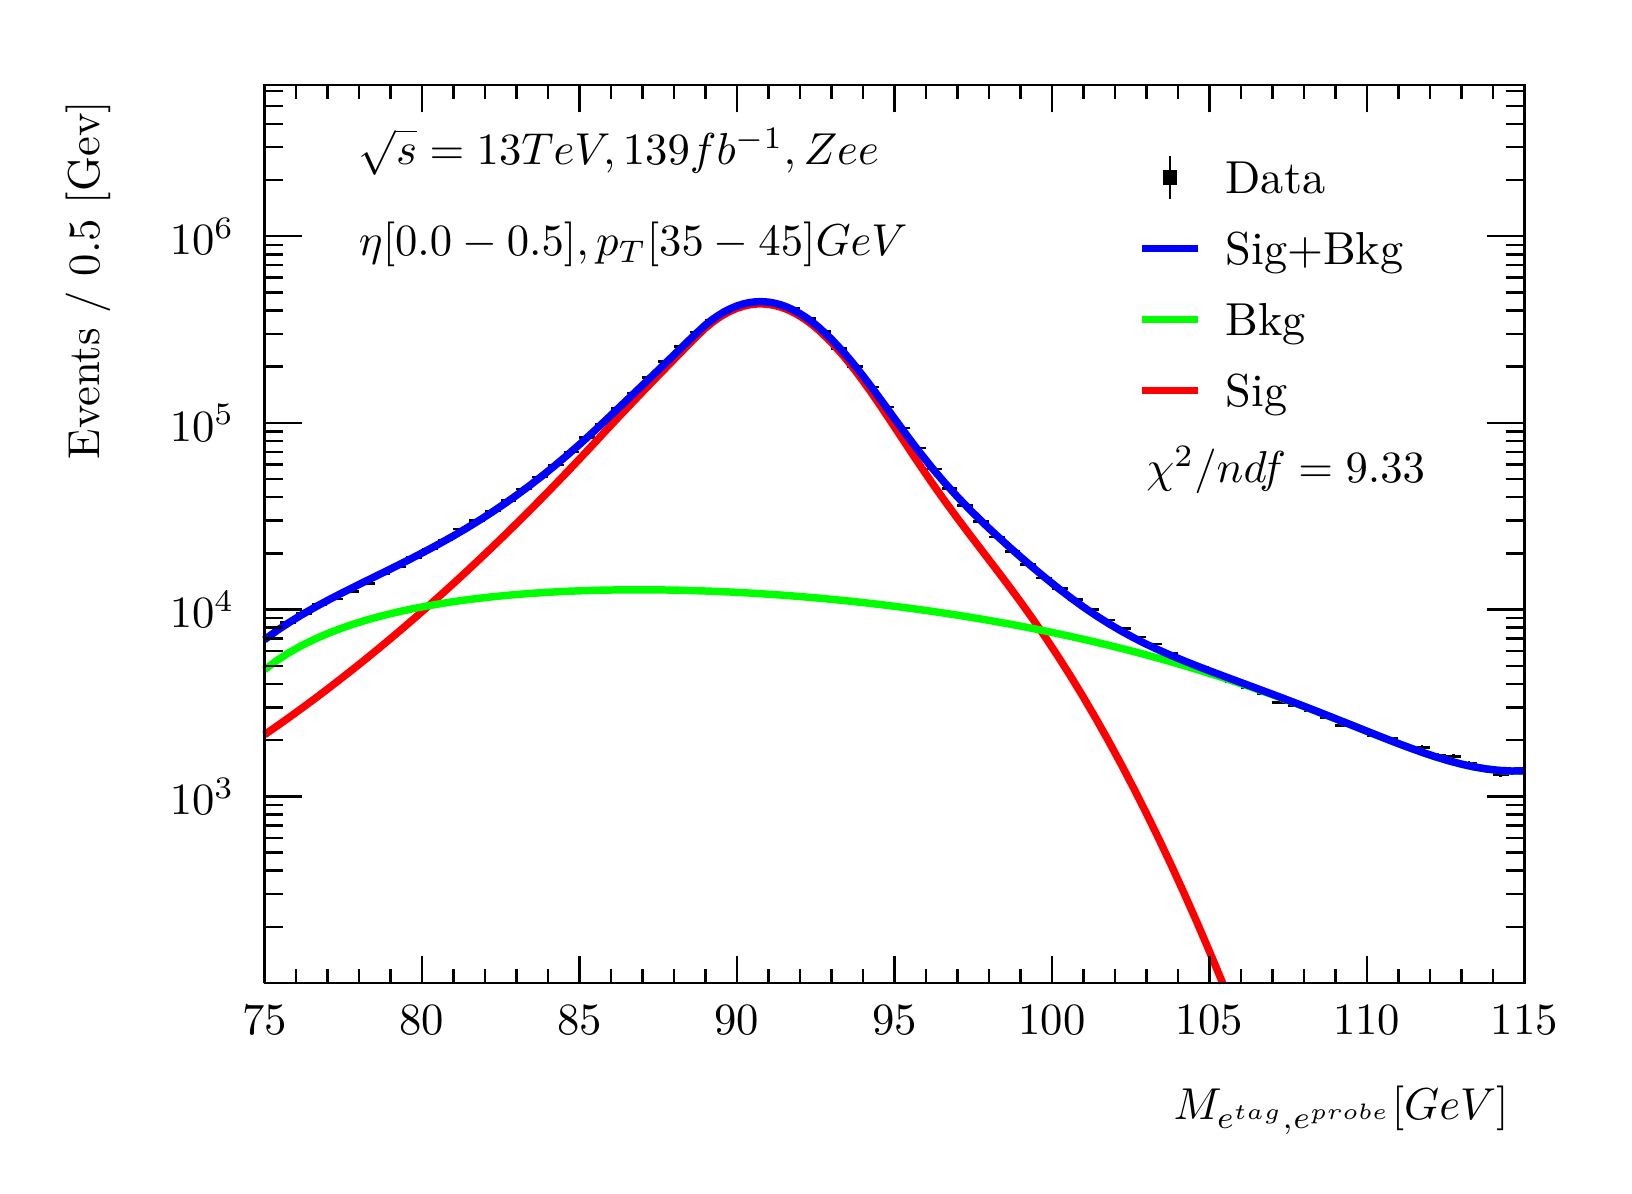
\begin{tikzpicture}
\pgfdeclareplotmark{cross} {
\pgfpathmoveto{\pgfpoint{-0.3\pgfplotmarksize}{\pgfplotmarksize}}
\pgfpathlineto{\pgfpoint{+0.3\pgfplotmarksize}{\pgfplotmarksize}}
\pgfpathlineto{\pgfpoint{+0.3\pgfplotmarksize}{0.3\pgfplotmarksize}}
\pgfpathlineto{\pgfpoint{+1\pgfplotmarksize}{0.3\pgfplotmarksize}}
\pgfpathlineto{\pgfpoint{+1\pgfplotmarksize}{-0.3\pgfplotmarksize}}
\pgfpathlineto{\pgfpoint{+0.3\pgfplotmarksize}{-0.3\pgfplotmarksize}}
\pgfpathlineto{\pgfpoint{+0.3\pgfplotmarksize}{-1.\pgfplotmarksize}}
\pgfpathlineto{\pgfpoint{-0.3\pgfplotmarksize}{-1.\pgfplotmarksize}}
\pgfpathlineto{\pgfpoint{-0.3\pgfplotmarksize}{-0.3\pgfplotmarksize}}
\pgfpathlineto{\pgfpoint{-1.\pgfplotmarksize}{-0.3\pgfplotmarksize}}
\pgfpathlineto{\pgfpoint{-1.\pgfplotmarksize}{0.3\pgfplotmarksize}}
\pgfpathlineto{\pgfpoint{-0.3\pgfplotmarksize}{0.3\pgfplotmarksize}}
\pgfpathclose
\pgfusepathqstroke
}
\pgfdeclareplotmark{cross*} {
\pgfpathmoveto{\pgfpoint{-0.3\pgfplotmarksize}{\pgfplotmarksize}}
\pgfpathlineto{\pgfpoint{+0.3\pgfplotmarksize}{\pgfplotmarksize}}
\pgfpathlineto{\pgfpoint{+0.3\pgfplotmarksize}{0.3\pgfplotmarksize}}
\pgfpathlineto{\pgfpoint{+1\pgfplotmarksize}{0.3\pgfplotmarksize}}
\pgfpathlineto{\pgfpoint{+1\pgfplotmarksize}{-0.3\pgfplotmarksize}}
\pgfpathlineto{\pgfpoint{+0.3\pgfplotmarksize}{-0.3\pgfplotmarksize}}
\pgfpathlineto{\pgfpoint{+0.3\pgfplotmarksize}{-1.\pgfplotmarksize}}
\pgfpathlineto{\pgfpoint{-0.3\pgfplotmarksize}{-1.\pgfplotmarksize}}
\pgfpathlineto{\pgfpoint{-0.3\pgfplotmarksize}{-0.3\pgfplotmarksize}}
\pgfpathlineto{\pgfpoint{-1.\pgfplotmarksize}{-0.3\pgfplotmarksize}}
\pgfpathlineto{\pgfpoint{-1.\pgfplotmarksize}{0.3\pgfplotmarksize}}
\pgfpathlineto{\pgfpoint{-0.3\pgfplotmarksize}{0.3\pgfplotmarksize}}
\pgfpathclose
\pgfusepathqfillstroke
}
\pgfdeclareplotmark{newstar} {
\pgfpathmoveto{\pgfqpoint{0pt}{\pgfplotmarksize}}
\pgfpathlineto{\pgfqpointpolar{44}{0.5\pgfplotmarksize}}
\pgfpathlineto{\pgfqpointpolar{18}{\pgfplotmarksize}}
\pgfpathlineto{\pgfqpointpolar{-20}{0.5\pgfplotmarksize}}
\pgfpathlineto{\pgfqpointpolar{-54}{\pgfplotmarksize}}
\pgfpathlineto{\pgfqpointpolar{-90}{0.5\pgfplotmarksize}}
\pgfpathlineto{\pgfqpointpolar{234}{\pgfplotmarksize}}
\pgfpathlineto{\pgfqpointpolar{198}{0.5\pgfplotmarksize}}
\pgfpathlineto{\pgfqpointpolar{162}{\pgfplotmarksize}}
\pgfpathlineto{\pgfqpointpolar{134}{0.5\pgfplotmarksize}}
\pgfpathclose
\pgfusepathqstroke
}
\pgfdeclareplotmark{newstar*} {
\pgfpathmoveto{\pgfqpoint{0pt}{\pgfplotmarksize}}
\pgfpathlineto{\pgfqpointpolar{44}{0.5\pgfplotmarksize}}
\pgfpathlineto{\pgfqpointpolar{18}{\pgfplotmarksize}}
\pgfpathlineto{\pgfqpointpolar{-20}{0.5\pgfplotmarksize}}
\pgfpathlineto{\pgfqpointpolar{-54}{\pgfplotmarksize}}
\pgfpathlineto{\pgfqpointpolar{-90}{0.5\pgfplotmarksize}}
\pgfpathlineto{\pgfqpointpolar{234}{\pgfplotmarksize}}
\pgfpathlineto{\pgfqpointpolar{198}{0.5\pgfplotmarksize}}
\pgfpathlineto{\pgfqpointpolar{162}{\pgfplotmarksize}}
\pgfpathlineto{\pgfqpointpolar{134}{0.5\pgfplotmarksize}}
\pgfpathclose
\pgfusepathqfillstroke
}
\definecolor{c}{rgb}{1,1,1};
\draw [color=c, fill=c] (0,0) rectangle (20,14.4361);
\draw [color=c, fill=c] (3,2.30977) rectangle (19,13.7143);
\definecolor{c}{rgb}{0,0,0};
\draw [c,line width=0.9] (3,2.30977) -- (3,13.7143) -- (19,13.7143) -- (19,2.30977) -- (3,2.30977);
\definecolor{c}{rgb}{1,1,1};
\draw [color=c, fill=c] (3,2.30977) rectangle (19,13.7143);
\definecolor{c}{rgb}{0,0,0};
\draw [c,line width=0.9] (3,2.30977) -- (3,13.7143) -- (19,13.7143) -- (19,2.30977) -- (3,2.30977);
\draw [c,line width=0.9] (3,2.30977) -- (19,2.30977);
\draw [c,line width=0.9] (3,2.65624) -- (3,2.30977);
\draw [c,line width=0.9] (3.4,2.48301) -- (3.4,2.30977);
\draw [c,line width=0.9] (3.8,2.48301) -- (3.8,2.30977);
\draw [c,line width=0.9] (4.2,2.48301) -- (4.2,2.30977);
\draw [c,line width=0.9] (4.6,2.48301) -- (4.6,2.30977);
\draw [c,line width=0.9] (5,2.65624) -- (5,2.30977);
\draw [c,line width=0.9] (5.4,2.48301) -- (5.4,2.30977);
\draw [c,line width=0.9] (5.8,2.48301) -- (5.8,2.30977);
\draw [c,line width=0.9] (6.2,2.48301) -- (6.2,2.30977);
\draw [c,line width=0.9] (6.6,2.48301) -- (6.6,2.30977);
\draw [c,line width=0.9] (7,2.65624) -- (7,2.30977);
\draw [c,line width=0.9] (7.4,2.48301) -- (7.4,2.30977);
\draw [c,line width=0.9] (7.8,2.48301) -- (7.8,2.30977);
\draw [c,line width=0.9] (8.2,2.48301) -- (8.2,2.30977);
\draw [c,line width=0.9] (8.6,2.48301) -- (8.6,2.30977);
\draw [c,line width=0.9] (9,2.65624) -- (9,2.30977);
\draw [c,line width=0.9] (9.4,2.48301) -- (9.4,2.30977);
\draw [c,line width=0.9] (9.8,2.48301) -- (9.8,2.30977);
\draw [c,line width=0.9] (10.2,2.48301) -- (10.2,2.30977);
\draw [c,line width=0.9] (10.6,2.48301) -- (10.6,2.30977);
\draw [c,line width=0.9] (11,2.65624) -- (11,2.30977);
\draw [c,line width=0.9] (11.4,2.48301) -- (11.4,2.30977);
\draw [c,line width=0.9] (11.8,2.48301) -- (11.8,2.30977);
\draw [c,line width=0.9] (12.2,2.48301) -- (12.2,2.30977);
\draw [c,line width=0.9] (12.6,2.48301) -- (12.6,2.30977);
\draw [c,line width=0.9] (13,2.65624) -- (13,2.30977);
\draw [c,line width=0.9] (13.4,2.48301) -- (13.4,2.30977);
\draw [c,line width=0.9] (13.8,2.48301) -- (13.8,2.30977);
\draw [c,line width=0.9] (14.2,2.48301) -- (14.2,2.30977);
\draw [c,line width=0.9] (14.6,2.48301) -- (14.6,2.30977);
\draw [c,line width=0.9] (15,2.65624) -- (15,2.30977);
\draw [c,line width=0.9] (15.4,2.48301) -- (15.4,2.30977);
\draw [c,line width=0.9] (15.8,2.48301) -- (15.8,2.30977);
\draw [c,line width=0.9] (16.2,2.48301) -- (16.2,2.30977);
\draw [c,line width=0.9] (16.6,2.48301) -- (16.6,2.30977);
\draw [c,line width=0.9] (17,2.65624) -- (17,2.30977);
\draw [c,line width=0.9] (17.4,2.48301) -- (17.4,2.30977);
\draw [c,line width=0.9] (17.8,2.48301) -- (17.8,2.30977);
\draw [c,line width=0.9] (18.2,2.48301) -- (18.2,2.30977);
\draw [c,line width=0.9] (18.6,2.48301) -- (18.6,2.30977);
\draw [c,line width=0.9] (19,2.65624) -- (19,2.30977);
\draw [c,line width=0.9] (19,2.65624) -- (19,2.30977);
\draw [anchor=base] (3,1.66015) node[scale=1.61424, color=c, rotate=0]{75};
\draw [anchor=base] (5,1.66015) node[scale=1.61424, color=c, rotate=0]{80};
\draw [anchor=base] (7,1.66015) node[scale=1.61424, color=c, rotate=0]{85};
\draw [anchor=base] (9,1.66015) node[scale=1.61424, color=c, rotate=0]{90};
\draw [anchor=base] (11,1.66015) node[scale=1.61424, color=c, rotate=0]{95};
\draw [anchor=base] (13,1.66015) node[scale=1.61424, color=c, rotate=0]{100};
\draw [anchor=base] (15,1.66015) node[scale=1.61424, color=c, rotate=0]{105};
\draw [anchor=base] (17,1.66015) node[scale=1.61424, color=c, rotate=0]{110};
\draw [anchor=base] (19,1.66015) node[scale=1.61424, color=c, rotate=0]{115};
\draw [anchor= east] (19,0.692932) node[scale=1.61424, color=c, rotate=0]{$M_{e^{tag}, e^{probe}}  [GeV]$};
\draw [c,line width=0.9] (3,13.7143) -- (19,13.7143);
\draw [c,line width=0.9] (3,13.3678) -- (3,13.7143);
\draw [c,line width=0.9] (3.4,13.5411) -- (3.4,13.7143);
\draw [c,line width=0.9] (3.8,13.5411) -- (3.8,13.7143);
\draw [c,line width=0.9] (4.2,13.5411) -- (4.2,13.7143);
\draw [c,line width=0.9] (4.6,13.5411) -- (4.6,13.7143);
\draw [c,line width=0.9] (5,13.3678) -- (5,13.7143);
\draw [c,line width=0.9] (5.4,13.5411) -- (5.4,13.7143);
\draw [c,line width=0.9] (5.8,13.5411) -- (5.8,13.7143);
\draw [c,line width=0.9] (6.2,13.5411) -- (6.2,13.7143);
\draw [c,line width=0.9] (6.6,13.5411) -- (6.6,13.7143);
\draw [c,line width=0.9] (7,13.3678) -- (7,13.7143);
\draw [c,line width=0.9] (7.4,13.5411) -- (7.4,13.7143);
\draw [c,line width=0.9] (7.8,13.5411) -- (7.8,13.7143);
\draw [c,line width=0.9] (8.2,13.5411) -- (8.2,13.7143);
\draw [c,line width=0.9] (8.6,13.5411) -- (8.6,13.7143);
\draw [c,line width=0.9] (9,13.3678) -- (9,13.7143);
\draw [c,line width=0.9] (9.4,13.5411) -- (9.4,13.7143);
\draw [c,line width=0.9] (9.8,13.5411) -- (9.8,13.7143);
\draw [c,line width=0.9] (10.2,13.5411) -- (10.2,13.7143);
\draw [c,line width=0.9] (10.6,13.5411) -- (10.6,13.7143);
\draw [c,line width=0.9] (11,13.3678) -- (11,13.7143);
\draw [c,line width=0.9] (11.4,13.5411) -- (11.4,13.7143);
\draw [c,line width=0.9] (11.8,13.5411) -- (11.8,13.7143);
\draw [c,line width=0.9] (12.2,13.5411) -- (12.2,13.7143);
\draw [c,line width=0.9] (12.6,13.5411) -- (12.6,13.7143);
\draw [c,line width=0.9] (13,13.3678) -- (13,13.7143);
\draw [c,line width=0.9] (13.4,13.5411) -- (13.4,13.7143);
\draw [c,line width=0.9] (13.8,13.5411) -- (13.8,13.7143);
\draw [c,line width=0.9] (14.2,13.5411) -- (14.2,13.7143);
\draw [c,line width=0.9] (14.6,13.5411) -- (14.6,13.7143);
\draw [c,line width=0.9] (15,13.3678) -- (15,13.7143);
\draw [c,line width=0.9] (15.4,13.5411) -- (15.4,13.7143);
\draw [c,line width=0.9] (15.8,13.5411) -- (15.8,13.7143);
\draw [c,line width=0.9] (16.2,13.5411) -- (16.2,13.7143);
\draw [c,line width=0.9] (16.6,13.5411) -- (16.6,13.7143);
\draw [c,line width=0.9] (17,13.3678) -- (17,13.7143);
\draw [c,line width=0.9] (17.4,13.5411) -- (17.4,13.7143);
\draw [c,line width=0.9] (17.8,13.5411) -- (17.8,13.7143);
\draw [c,line width=0.9] (18.2,13.5411) -- (18.2,13.7143);
\draw [c,line width=0.9] (18.6,13.5411) -- (18.6,13.7143);
\draw [c,line width=0.9] (19,13.3678) -- (19,13.7143);
\draw [c,line width=0.9] (19,13.3678) -- (19,13.7143);
\draw [c,line width=0.9] (3,2.30977) -- (3,13.7143);
\draw [c,line width=0.9] (3.237,3.02354) -- (3,3.02354);
\draw [c,line width=0.9] (3.237,3.44107) -- (3,3.44107);
\draw [c,line width=0.9] (3.237,3.73731) -- (3,3.73731);
\draw [c,line width=0.9] (3.237,3.96709) -- (3,3.96709);
\draw [c,line width=0.9] (3.237,4.15484) -- (3,4.15484);
\draw [c,line width=0.9] (3.237,4.31357) -- (3,4.31357);
\draw [c,line width=0.9] (3.237,4.45108) -- (3,4.45108);
\draw [c,line width=0.9] (3.237,4.57236) -- (3,4.57236);
\draw [c,line width=0.9] (3.474,4.68086) -- (3,4.68086);
\draw [anchor= east] (2.82,4.68086) node[scale=1.61424, color=c, rotate=0]{$10^{3}$};
\draw [c,line width=0.9] (3.237,5.39463) -- (3,5.39463);
\draw [c,line width=0.9] (3.237,5.81216) -- (3,5.81216);
\draw [c,line width=0.9] (3.237,6.1084) -- (3,6.1084);
\draw [c,line width=0.9] (3.237,6.33818) -- (3,6.33818);
\draw [c,line width=0.9] (3.237,6.52593) -- (3,6.52593);
\draw [c,line width=0.9] (3.237,6.68466) -- (3,6.68466);
\draw [c,line width=0.9] (3.237,6.82217) -- (3,6.82217);
\draw [c,line width=0.9] (3.237,6.94345) -- (3,6.94345);
\draw [c,line width=0.9] (3.474,7.05195) -- (3,7.05195);
\draw [anchor= east] (2.82,7.05195) node[scale=1.61424, color=c, rotate=0]{$10^{4}$};
\draw [c,line width=0.9] (3.237,7.76572) -- (3,7.76572);
\draw [c,line width=0.9] (3.237,8.18324) -- (3,8.18324);
\draw [c,line width=0.9] (3.237,8.47948) -- (3,8.47948);
\draw [c,line width=0.9] (3.237,8.70927) -- (3,8.70927);
\draw [c,line width=0.9] (3.237,8.89701) -- (3,8.89701);
\draw [c,line width=0.9] (3.237,9.05575) -- (3,9.05575);
\draw [c,line width=0.9] (3.237,9.19325) -- (3,9.19325);
\draw [c,line width=0.9] (3.237,9.31454) -- (3,9.31454);
\draw [c,line width=0.9] (3.474,9.42304) -- (3,9.42304);
\draw [anchor= east] (2.82,9.42304) node[scale=1.61424, color=c, rotate=0]{$10^{5}$};
\draw [c,line width=0.9] (3.237,10.1368) -- (3,10.1368);
\draw [c,line width=0.9] (3.237,10.5543) -- (3,10.5543);
\draw [c,line width=0.9] (3.237,10.8506) -- (3,10.8506);
\draw [c,line width=0.9] (3.237,11.0804) -- (3,11.0804);
\draw [c,line width=0.9] (3.237,11.2681) -- (3,11.2681);
\draw [c,line width=0.9] (3.237,11.4268) -- (3,11.4268);
\draw [c,line width=0.9] (3.237,11.5643) -- (3,11.5643);
\draw [c,line width=0.9] (3.237,11.6856) -- (3,11.6856);
\draw [c,line width=0.9] (3.474,11.7941) -- (3,11.7941);
\draw [anchor= east] (2.82,11.7941) node[scale=1.61424, color=c, rotate=0]{$10^{6}$};
\draw [c,line width=0.9] (3.237,12.5079) -- (3,12.5079);
\draw [c,line width=0.9] (3.237,12.9254) -- (3,12.9254);
\draw [c,line width=0.9] (3.237,13.2217) -- (3,13.2217);
\draw [c,line width=0.9] (3.237,13.4514) -- (3,13.4514);
\draw [c,line width=0.9] (3.237,13.6392) -- (3,13.6392);
\draw [anchor= east] (0.76,13.7143) node[scale=1.61424, color=c, rotate=90]{Events / 0.5 [Gev]};
\draw [c,line width=0.9] (19,2.30977) -- (19,13.7143);
\draw [c,line width=0.9] (18.763,3.02354) -- (19,3.02354);
\draw [c,line width=0.9] (18.763,3.44107) -- (19,3.44107);
\draw [c,line width=0.9] (18.763,3.73731) -- (19,3.73731);
\draw [c,line width=0.9] (18.763,3.96709) -- (19,3.96709);
\draw [c,line width=0.9] (18.763,4.15484) -- (19,4.15484);
\draw [c,line width=0.9] (18.763,4.31357) -- (19,4.31357);
\draw [c,line width=0.9] (18.763,4.45108) -- (19,4.45108);
\draw [c,line width=0.9] (18.763,4.57236) -- (19,4.57236);
\draw [c,line width=0.9] (18.526,4.68086) -- (19,4.68086);
\draw [c,line width=0.9] (18.763,5.39463) -- (19,5.39463);
\draw [c,line width=0.9] (18.763,5.81216) -- (19,5.81216);
\draw [c,line width=0.9] (18.763,6.1084) -- (19,6.1084);
\draw [c,line width=0.9] (18.763,6.33818) -- (19,6.33818);
\draw [c,line width=0.9] (18.763,6.52593) -- (19,6.52593);
\draw [c,line width=0.9] (18.763,6.68466) -- (19,6.68466);
\draw [c,line width=0.9] (18.763,6.82217) -- (19,6.82217);
\draw [c,line width=0.9] (18.763,6.94345) -- (19,6.94345);
\draw [c,line width=0.9] (18.526,7.05195) -- (19,7.05195);
\draw [c,line width=0.9] (18.763,7.76572) -- (19,7.76572);
\draw [c,line width=0.9] (18.763,8.18324) -- (19,8.18324);
\draw [c,line width=0.9] (18.763,8.47948) -- (19,8.47948);
\draw [c,line width=0.9] (18.763,8.70927) -- (19,8.70927);
\draw [c,line width=0.9] (18.763,8.89701) -- (19,8.89701);
\draw [c,line width=0.9] (18.763,9.05575) -- (19,9.05575);
\draw [c,line width=0.9] (18.763,9.19325) -- (19,9.19325);
\draw [c,line width=0.9] (18.763,9.31454) -- (19,9.31454);
\draw [c,line width=0.9] (18.526,9.42304) -- (19,9.42304);
\draw [c,line width=0.9] (18.763,10.1368) -- (19,10.1368);
\draw [c,line width=0.9] (18.763,10.5543) -- (19,10.5543);
\draw [c,line width=0.9] (18.763,10.8506) -- (19,10.8506);
\draw [c,line width=0.9] (18.763,11.0804) -- (19,11.0804);
\draw [c,line width=0.9] (18.763,11.2681) -- (19,11.2681);
\draw [c,line width=0.9] (18.763,11.4268) -- (19,11.4268);
\draw [c,line width=0.9] (18.763,11.5643) -- (19,11.5643);
\draw [c,line width=0.9] (18.763,11.6856) -- (19,11.6856);
\draw [c,line width=0.9] (18.526,11.7941) -- (19,11.7941);
\draw [c,line width=0.9] (18.763,12.5079) -- (19,12.5079);
\draw [c,line width=0.9] (18.763,12.9254) -- (19,12.9254);
\draw [c,line width=0.9] (18.763,13.2217) -- (19,13.2217);
\draw [c,line width=0.9] (18.763,13.4514) -- (19,13.4514);
\draw [c,line width=0.9] (18.763,13.6392) -- (19,13.6392);
\draw [c,line width=0.9] (3.1,6.83216) -- (3,6.83216);
\draw [c,line width=0.9] (3,6.83216) -- (3,6.83216);
\draw [c,line width=0.9] (3.1,6.83216) -- (3.2,6.83216);
\draw [c,line width=0.9] (3.2,6.83216) -- (3.2,6.83216);
\draw [c,line width=0.9] (3.1,6.83216) -- (3.1,6.84362);
\draw [c,line width=0.9] (3.1,6.84362) -- (3.1,6.84362);
\draw [c,line width=0.9] (3.1,6.83216) -- (3.1,6.8207);
\draw [c,line width=0.9] (3.1,6.8207) -- (3.1,6.8207);
\draw [c,line width=0.9] (3.3,6.88786) -- (3.2,6.88786);
\draw [c,line width=0.9] (3.2,6.88786) -- (3.2,6.88786);
\draw [c,line width=0.9] (3.3,6.88786) -- (3.4,6.88786);
\draw [c,line width=0.9] (3.4,6.88786) -- (3.4,6.88786);
\draw [c,line width=0.9] (3.3,6.88786) -- (3.3,6.89901);
\draw [c,line width=0.9] (3.3,6.89901) -- (3.3,6.89901);
\draw [c,line width=0.9] (3.3,6.88786) -- (3.3,6.87671);
\draw [c,line width=0.9] (3.3,6.87671) -- (3.3,6.87671);
\draw [c,line width=0.9] (3.5,7.00162) -- (3.4,7.00162);
\draw [c,line width=0.9] (3.4,7.00162) -- (3.4,7.00162);
\draw [c,line width=0.9] (3.5,7.00162) -- (3.6,7.00162);
\draw [c,line width=0.9] (3.6,7.00162) -- (3.6,7.00162);
\draw [c,line width=0.9] (3.5,7.00162) -- (3.5,7.01217);
\draw [c,line width=0.9] (3.5,7.01217) -- (3.5,7.01217);
\draw [c,line width=0.9] (3.5,7.00162) -- (3.5,6.99107);
\draw [c,line width=0.9] (3.5,6.99107) -- (3.5,6.99107);
\draw [c,line width=0.9] (3.7,7.11506) -- (3.6,7.11506);
\draw [c,line width=0.9] (3.6,7.11506) -- (3.6,7.11506);
\draw [c,line width=0.9] (3.7,7.11506) -- (3.8,7.11506);
\draw [c,line width=0.9] (3.8,7.11506) -- (3.8,7.11506);
\draw [c,line width=0.9] (3.7,7.11506) -- (3.7,7.12504);
\draw [c,line width=0.9] (3.7,7.12504) -- (3.7,7.12504);
\draw [c,line width=0.9] (3.7,7.11506) -- (3.7,7.10507);
\draw [c,line width=0.9] (3.7,7.10507) -- (3.7,7.10507);
\draw [c,line width=0.9] (3.9,7.18416) -- (3.8,7.18416);
\draw [c,line width=0.9] (3.8,7.18416) -- (3.8,7.18416);
\draw [c,line width=0.9] (3.9,7.18416) -- (4,7.18416);
\draw [c,line width=0.9] (4,7.18416) -- (4,7.18416);
\draw [c,line width=0.9] (3.9,7.18416) -- (3.9,7.19382);
\draw [c,line width=0.9] (3.9,7.19382) -- (3.9,7.19382);
\draw [c,line width=0.9] (3.9,7.18416) -- (3.9,7.1745);
\draw [c,line width=0.9] (3.9,7.1745) -- (3.9,7.1745);
\draw [c,line width=0.9] (4.1,7.28543) -- (4,7.28543);
\draw [c,line width=0.9] (4,7.28543) -- (4,7.28543);
\draw [c,line width=0.9] (4.1,7.28543) -- (4.2,7.28543);
\draw [c,line width=0.9] (4.2,7.28543) -- (4.2,7.28543);
\draw [c,line width=0.9] (4.1,7.28543) -- (4.1,7.29463);
\draw [c,line width=0.9] (4.1,7.29463) -- (4.1,7.29463);
\draw [c,line width=0.9] (4.1,7.28543) -- (4.1,7.27624);
\draw [c,line width=0.9] (4.1,7.27624) -- (4.1,7.27624);
\draw [c,line width=0.9] (4.3,7.38674) -- (4.2,7.38674);
\draw [c,line width=0.9] (4.2,7.38674) -- (4.2,7.38674);
\draw [c,line width=0.9] (4.3,7.38674) -- (4.4,7.38674);
\draw [c,line width=0.9] (4.4,7.38674) -- (4.4,7.38674);
\draw [c,line width=0.9] (4.3,7.38674) -- (4.3,7.3955);
\draw [c,line width=0.9] (4.3,7.3955) -- (4.3,7.3955);
\draw [c,line width=0.9] (4.3,7.38674) -- (4.3,7.37799);
\draw [c,line width=0.9] (4.3,7.37799) -- (4.3,7.37799);
\draw [c,line width=0.9] (4.5,7.50696) -- (4.4,7.50696);
\draw [c,line width=0.9] (4.4,7.50696) -- (4.4,7.50696);
\draw [c,line width=0.9] (4.5,7.50696) -- (4.6,7.50696);
\draw [c,line width=0.9] (4.6,7.50696) -- (4.6,7.50696);
\draw [c,line width=0.9] (4.5,7.50696) -- (4.5,7.51521);
\draw [c,line width=0.9] (4.5,7.51521) -- (4.5,7.51521);
\draw [c,line width=0.9] (4.5,7.50696) -- (4.5,7.4987);
\draw [c,line width=0.9] (4.5,7.4987) -- (4.5,7.4987);
\draw [c,line width=0.9] (4.7,7.59618) -- (4.6,7.59618);
\draw [c,line width=0.9] (4.6,7.59618) -- (4.6,7.59618);
\draw [c,line width=0.9] (4.7,7.59618) -- (4.8,7.59618);
\draw [c,line width=0.9] (4.8,7.59618) -- (4.8,7.59618);
\draw [c,line width=0.9] (4.7,7.59618) -- (4.7,7.60409);
\draw [c,line width=0.9] (4.7,7.60409) -- (4.7,7.60409);
\draw [c,line width=0.9] (4.7,7.59618) -- (4.7,7.58827);
\draw [c,line width=0.9] (4.7,7.58827) -- (4.7,7.58827);
\draw [c,line width=0.9] (4.9,7.71447) -- (4.8,7.71447);
\draw [c,line width=0.9] (4.8,7.71447) -- (4.8,7.71447);
\draw [c,line width=0.9] (4.9,7.71447) -- (5,7.71447);
\draw [c,line width=0.9] (5,7.71447) -- (5,7.71447);
\draw [c,line width=0.9] (4.9,7.71447) -- (4.9,7.72193);
\draw [c,line width=0.9] (4.9,7.72193) -- (4.9,7.72193);
\draw [c,line width=0.9] (4.9,7.71447) -- (4.9,7.707);
\draw [c,line width=0.9] (4.9,7.707) -- (4.9,7.707);
\draw [c,line width=0.9] (5.1,7.82212) -- (5,7.82212);
\draw [c,line width=0.9] (5,7.82212) -- (5,7.82212);
\draw [c,line width=0.9] (5.1,7.82212) -- (5.2,7.82212);
\draw [c,line width=0.9] (5.2,7.82212) -- (5.2,7.82212);
\draw [c,line width=0.9] (5.1,7.82212) -- (5.1,7.8292);
\draw [c,line width=0.9] (5.1,7.8292) -- (5.1,7.8292);
\draw [c,line width=0.9] (5.1,7.82212) -- (5.1,7.81503);
\draw [c,line width=0.9] (5.1,7.81503) -- (5.1,7.81503);
\draw [c,line width=0.9] (5.3,7.93472) -- (5.2,7.93472);
\draw [c,line width=0.9] (5.2,7.93472) -- (5.2,7.93472);
\draw [c,line width=0.9] (5.3,7.93472) -- (5.4,7.93472);
\draw [c,line width=0.9] (5.4,7.93472) -- (5.4,7.93472);
\draw [c,line width=0.9] (5.3,7.93472) -- (5.3,7.94142);
\draw [c,line width=0.9] (5.3,7.94142) -- (5.3,7.94142);
\draw [c,line width=0.9] (5.3,7.93472) -- (5.3,7.92801);
\draw [c,line width=0.9] (5.3,7.92801) -- (5.3,7.92801);
\draw [c,line width=0.9] (5.5,8.07448) -- (5.4,8.07448);
\draw [c,line width=0.9] (5.4,8.07448) -- (5.4,8.07448);
\draw [c,line width=0.9] (5.5,8.07448) -- (5.6,8.07448);
\draw [c,line width=0.9] (5.6,8.07448) -- (5.6,8.07448);
\draw [c,line width=0.9] (5.5,8.07448) -- (5.5,8.08075);
\draw [c,line width=0.9] (5.5,8.08075) -- (5.5,8.08075);
\draw [c,line width=0.9] (5.5,8.07448) -- (5.5,8.06822);
\draw [c,line width=0.9] (5.5,8.06822) -- (5.5,8.06822);
\draw [c,line width=0.9] (5.7,8.18149) -- (5.6,8.18149);
\draw [c,line width=0.9] (5.6,8.18149) -- (5.6,8.18149);
\draw [c,line width=0.9] (5.7,8.18149) -- (5.8,8.18149);
\draw [c,line width=0.9] (5.8,8.18149) -- (5.8,8.18149);
\draw [c,line width=0.9] (5.7,8.18149) -- (5.7,8.18744);
\draw [c,line width=0.9] (5.7,8.18744) -- (5.7,8.18744);
\draw [c,line width=0.9] (5.7,8.18149) -- (5.7,8.17554);
\draw [c,line width=0.9] (5.7,8.17554) -- (5.7,8.17554);
\draw [c,line width=0.9] (5.9,8.30533) -- (5.8,8.30533);
\draw [c,line width=0.9] (5.8,8.30533) -- (5.8,8.30533);
\draw [c,line width=0.9] (5.9,8.30533) -- (6,8.30533);
\draw [c,line width=0.9] (6,8.30533) -- (6,8.30533);
\draw [c,line width=0.9] (5.9,8.30533) -- (5.9,8.31093);
\draw [c,line width=0.9] (5.9,8.31093) -- (5.9,8.31093);
\draw [c,line width=0.9] (5.9,8.30533) -- (5.9,8.29972);
\draw [c,line width=0.9] (5.9,8.29972) -- (5.9,8.29972);
\draw [c,line width=0.9] (6.1,8.44101) -- (6,8.44101);
\draw [c,line width=0.9] (6,8.44101) -- (6,8.44101);
\draw [c,line width=0.9] (6.1,8.44101) -- (6.2,8.44101);
\draw [c,line width=0.9] (6.2,8.44101) -- (6.2,8.44101);
\draw [c,line width=0.9] (6.1,8.44101) -- (6.1,8.44626);
\draw [c,line width=0.9] (6.1,8.44626) -- (6.1,8.44626);
\draw [c,line width=0.9] (6.1,8.44101) -- (6.1,8.43576);
\draw [c,line width=0.9] (6.1,8.43576) -- (6.1,8.43576);
\draw [c,line width=0.9] (6.3,8.58649) -- (6.2,8.58649);
\draw [c,line width=0.9] (6.2,8.58649) -- (6.2,8.58649);
\draw [c,line width=0.9] (6.3,8.58649) -- (6.4,8.58649);
\draw [c,line width=0.9] (6.4,8.58649) -- (6.4,8.58649);
\draw [c,line width=0.9] (6.3,8.58649) -- (6.3,8.59138);
\draw [c,line width=0.9] (6.3,8.59138) -- (6.3,8.59138);
\draw [c,line width=0.9] (6.3,8.58649) -- (6.3,8.5816);
\draw [c,line width=0.9] (6.3,8.5816) -- (6.3,8.5816);
\draw [c,line width=0.9] (6.5,8.7375) -- (6.4,8.7375);
\draw [c,line width=0.9] (6.4,8.7375) -- (6.4,8.7375);
\draw [c,line width=0.9] (6.5,8.7375) -- (6.6,8.7375);
\draw [c,line width=0.9] (6.6,8.7375) -- (6.6,8.7375);
\draw [c,line width=0.9] (6.5,8.7375) -- (6.5,8.74205);
\draw [c,line width=0.9] (6.5,8.74205) -- (6.5,8.74205);
\draw [c,line width=0.9] (6.5,8.7375) -- (6.5,8.73296);
\draw [c,line width=0.9] (6.5,8.73296) -- (6.5,8.73296);
\draw [c,line width=0.9] (6.7,8.88897) -- (6.6,8.88897);
\draw [c,line width=0.9] (6.6,8.88897) -- (6.6,8.88897);
\draw [c,line width=0.9] (6.7,8.88897) -- (6.8,8.88897);
\draw [c,line width=0.9] (6.8,8.88897) -- (6.8,8.88897);
\draw [c,line width=0.9] (6.7,8.88897) -- (6.7,8.89319);
\draw [c,line width=0.9] (6.7,8.89319) -- (6.7,8.89319);
\draw [c,line width=0.9] (6.7,8.88897) -- (6.7,8.88475);
\draw [c,line width=0.9] (6.7,8.88475) -- (6.7,8.88475);
\draw [c,line width=0.9] (6.9,9.05543) -- (6.8,9.05543);
\draw [c,line width=0.9] (6.8,9.05543) -- (6.8,9.05543);
\draw [c,line width=0.9] (6.9,9.05543) -- (7,9.05543);
\draw [c,line width=0.9] (7,9.05543) -- (7,9.05543);
\draw [c,line width=0.9] (6.9,9.05543) -- (6.9,9.05932);
\draw [c,line width=0.9] (6.9,9.05932) -- (6.9,9.05932);
\draw [c,line width=0.9] (6.9,9.05543) -- (6.9,9.05153);
\draw [c,line width=0.9] (6.9,9.05153) -- (6.9,9.05153);
\draw [c,line width=0.9] (7.1,9.23782) -- (7,9.23782);
\draw [c,line width=0.9] (7,9.23782) -- (7,9.23782);
\draw [c,line width=0.9] (7.1,9.23782) -- (7.2,9.23782);
\draw [c,line width=0.9] (7.2,9.23782) -- (7.2,9.23782);
\draw [c,line width=0.9] (7.1,9.23782) -- (7.1,9.24138);
\draw [c,line width=0.9] (7.1,9.24138) -- (7.1,9.24138);
\draw [c,line width=0.9] (7.1,9.23782) -- (7.1,9.23425);
\draw [c,line width=0.9] (7.1,9.23425) -- (7.1,9.23425);
\draw [c,line width=0.9] (7.3,9.41066) -- (7.2,9.41066);
\draw [c,line width=0.9] (7.2,9.41066) -- (7.2,9.41066);
\draw [c,line width=0.9] (7.3,9.41066) -- (7.4,9.41066);
\draw [c,line width=0.9] (7.4,9.41066) -- (7.4,9.41066);
\draw [c,line width=0.9] (7.3,9.41066) -- (7.3,9.41393);
\draw [c,line width=0.9] (7.3,9.41393) -- (7.3,9.41393);
\draw [c,line width=0.9] (7.3,9.41066) -- (7.3,9.40738);
\draw [c,line width=0.9] (7.3,9.40738) -- (7.3,9.40738);
\draw [c,line width=0.9] (7.5,9.60518) -- (7.4,9.60518);
\draw [c,line width=0.9] (7.4,9.60518) -- (7.4,9.60518);
\draw [c,line width=0.9] (7.5,9.60518) -- (7.6,9.60518);
\draw [c,line width=0.9] (7.6,9.60518) -- (7.6,9.60518);
\draw [c,line width=0.9] (7.5,9.60518) -- (7.5,9.60816);
\draw [c,line width=0.9] (7.5,9.60816) -- (7.5,9.60816);
\draw [c,line width=0.9] (7.5,9.60518) -- (7.5,9.6022);
\draw [c,line width=0.9] (7.5,9.6022) -- (7.5,9.6022);
\draw [c,line width=0.9] (7.7,9.80488) -- (7.6,9.80488);
\draw [c,line width=0.9] (7.6,9.80488) -- (7.6,9.80488);
\draw [c,line width=0.9] (7.7,9.80488) -- (7.8,9.80488);
\draw [c,line width=0.9] (7.8,9.80488) -- (7.8,9.80488);
\draw [c,line width=0.9] (7.7,9.80488) -- (7.7,9.80758);
\draw [c,line width=0.9] (7.7,9.80758) -- (7.7,9.80758);
\draw [c,line width=0.9] (7.7,9.80488) -- (7.7,9.80217);
\draw [c,line width=0.9] (7.7,9.80217) -- (7.7,9.80217);
\draw [c,line width=0.9] (7.9,10.0023) -- (7.8,10.0023);
\draw [c,line width=0.9] (7.8,10.0023) -- (7.8,10.0023);
\draw [c,line width=0.9] (7.9,10.0023) -- (8,10.0023);
\draw [c,line width=0.9] (8,10.0023) -- (8,10.0023);
\draw [c,line width=0.9] (7.9,10.0023) -- (7.9,10.0048);
\draw [c,line width=0.9] (7.9,10.0048) -- (7.9,10.0048);
\draw [c,line width=0.9] (7.9,10.0023) -- (7.9,9.99984);
\draw [c,line width=0.9] (7.9,9.99984) -- (7.9,9.99984);
\draw [c,line width=0.9] (8.1,10.2031) -- (8,10.2031);
\draw [c,line width=0.9] (8,10.2031) -- (8,10.2031);
\draw [c,line width=0.9] (8.1,10.2031) -- (8.2,10.2031);
\draw [c,line width=0.9] (8.2,10.2031) -- (8.2,10.2031);
\draw [c,line width=0.9] (8.1,10.2031) -- (8.1,10.2053);
\draw [c,line width=0.9] (8.1,10.2053) -- (8.1,10.2053);
\draw [c,line width=0.9] (8.1,10.2031) -- (8.1,10.2008);
\draw [c,line width=0.9] (8.1,10.2008) -- (8.1,10.2008);
\draw [c,line width=0.9] (8.3,10.3968) -- (8.2,10.3968);
\draw [c,line width=0.9] (8.2,10.3968) -- (8.2,10.3968);
\draw [c,line width=0.9] (8.3,10.3968) -- (8.4,10.3968);
\draw [c,line width=0.9] (8.4,10.3968) -- (8.4,10.3968);
\draw [c,line width=0.9] (8.3,10.3968) -- (8.3,10.3988);
\draw [c,line width=0.9] (8.3,10.3988) -- (8.3,10.3988);
\draw [c,line width=0.9] (8.3,10.3968) -- (8.3,10.3948);
\draw [c,line width=0.9] (8.3,10.3948) -- (8.3,10.3948);
\draw [c,line width=0.9] (8.5,10.5752) -- (8.4,10.5752);
\draw [c,line width=0.9] (8.4,10.5752) -- (8.4,10.5752);
\draw [c,line width=0.9] (8.5,10.5752) -- (8.6,10.5752);
\draw [c,line width=0.9] (8.6,10.5752) -- (8.6,10.5752);
\draw [c,line width=0.9] (8.5,10.5752) -- (8.5,10.5771);
\draw [c,line width=0.9] (8.5,10.5771) -- (8.5,10.5771);
\draw [c,line width=0.9] (8.5,10.5752) -- (8.5,10.5734);
\draw [c,line width=0.9] (8.5,10.5734) -- (8.5,10.5734);
\draw [c,line width=0.9] (8.7,10.7326) -- (8.6,10.7326);
\draw [c,line width=0.9] (8.6,10.7326) -- (8.6,10.7326);
\draw [c,line width=0.9] (8.7,10.7326) -- (8.8,10.7326);
\draw [c,line width=0.9] (8.8,10.7326) -- (8.8,10.7326);
\draw [c,line width=0.9] (8.7,10.7326) -- (8.7,10.7344);
\draw [c,line width=0.9] (8.7,10.7344) -- (8.7,10.7344);
\draw [c,line width=0.9] (8.7,10.7326) -- (8.7,10.7309);
\draw [c,line width=0.9] (8.7,10.7309) -- (8.7,10.7309);
\draw [c,line width=0.9] (8.9,10.8566) -- (8.8,10.8566);
\draw [c,line width=0.9] (8.8,10.8566) -- (8.8,10.8566);
\draw [c,line width=0.9] (8.9,10.8566) -- (9,10.8566);
\draw [c,line width=0.9] (9,10.8566) -- (9,10.8566);
\draw [c,line width=0.9] (8.9,10.8566) -- (8.9,10.8582);
\draw [c,line width=0.9] (8.9,10.8582) -- (8.9,10.8582);
\draw [c,line width=0.9] (8.9,10.8566) -- (8.9,10.855);
\draw [c,line width=0.9] (8.9,10.855) -- (8.9,10.855);
\draw [c,line width=0.9] (9.1,10.9355) -- (9,10.9355);
\draw [c,line width=0.9] (9,10.9355) -- (9,10.9355);
\draw [c,line width=0.9] (9.1,10.9355) -- (9.2,10.9355);
\draw [c,line width=0.9] (9.2,10.9355) -- (9.2,10.9355);
\draw [c,line width=0.9] (9.1,10.9355) -- (9.1,10.9371);
\draw [c,line width=0.9] (9.1,10.9371) -- (9.1,10.9371);
\draw [c,line width=0.9] (9.1,10.9355) -- (9.1,10.934);
\draw [c,line width=0.9] (9.1,10.934) -- (9.1,10.934);
\draw [c,line width=0.9] (9.3,10.9682) -- (9.2,10.9682);
\draw [c,line width=0.9] (9.2,10.9682) -- (9.2,10.9682);
\draw [c,line width=0.9] (9.3,10.9682) -- (9.4,10.9682);
\draw [c,line width=0.9] (9.4,10.9682) -- (9.4,10.9682);
\draw [c,line width=0.9] (9.3,10.9682) -- (9.3,10.9698);
\draw [c,line width=0.9] (9.3,10.9698) -- (9.3,10.9698);
\draw [c,line width=0.9] (9.3,10.9682) -- (9.3,10.9667);
\draw [c,line width=0.9] (9.3,10.9667) -- (9.3,10.9667);
\draw [c,line width=0.9] (9.5,10.9489) -- (9.4,10.9489);
\draw [c,line width=0.9] (9.4,10.9489) -- (9.4,10.9489);
\draw [c,line width=0.9] (9.5,10.9489) -- (9.6,10.9489);
\draw [c,line width=0.9] (9.6,10.9489) -- (9.6,10.9489);
\draw [c,line width=0.9] (9.5,10.9489) -- (9.5,10.9505);
\draw [c,line width=0.9] (9.5,10.9505) -- (9.5,10.9505);
\draw [c,line width=0.9] (9.5,10.9489) -- (9.5,10.9474);
\draw [c,line width=0.9] (9.5,10.9474) -- (9.5,10.9474);
\draw [c,line width=0.9] (9.7,10.8741) -- (9.6,10.8741);
\draw [c,line width=0.9] (9.6,10.8741) -- (9.6,10.8741);
\draw [c,line width=0.9] (9.7,10.8741) -- (9.8,10.8741);
\draw [c,line width=0.9] (9.8,10.8741) -- (9.8,10.8741);
\draw [c,line width=0.9] (9.7,10.8741) -- (9.7,10.8757);
\draw [c,line width=0.9] (9.7,10.8757) -- (9.7,10.8757);
\draw [c,line width=0.9] (9.7,10.8741) -- (9.7,10.8725);
\draw [c,line width=0.9] (9.7,10.8725) -- (9.7,10.8725);
\draw [c,line width=0.9] (9.9,10.7496) -- (9.8,10.7496);
\draw [c,line width=0.9] (9.8,10.7496) -- (9.8,10.7496);
\draw [c,line width=0.9] (9.9,10.7496) -- (10,10.7496);
\draw [c,line width=0.9] (10,10.7496) -- (10,10.7496);
\draw [c,line width=0.9] (9.9,10.7496) -- (9.9,10.7513);
\draw [c,line width=0.9] (9.9,10.7513) -- (9.9,10.7513);
\draw [c,line width=0.9] (9.9,10.7496) -- (9.9,10.7479);
\draw [c,line width=0.9] (9.9,10.7479) -- (9.9,10.7479);
\draw [c,line width=0.9] (10.1,10.5813) -- (10,10.5813);
\draw [c,line width=0.9] (10,10.5813) -- (10,10.5813);
\draw [c,line width=0.9] (10.1,10.5813) -- (10.2,10.5813);
\draw [c,line width=0.9] (10.2,10.5813) -- (10.2,10.5813);
\draw [c,line width=0.9] (10.1,10.5813) -- (10.1,10.5831);
\draw [c,line width=0.9] (10.1,10.5831) -- (10.1,10.5831);
\draw [c,line width=0.9] (10.1,10.5813) -- (10.1,10.5794);
\draw [c,line width=0.9] (10.1,10.5794) -- (10.1,10.5794);
\draw [c,line width=0.9] (10.3,10.3716) -- (10.2,10.3716);
\draw [c,line width=0.9] (10.2,10.3716) -- (10.2,10.3716);
\draw [c,line width=0.9] (10.3,10.3716) -- (10.4,10.3716);
\draw [c,line width=0.9] (10.4,10.3716) -- (10.4,10.3716);
\draw [c,line width=0.9] (10.3,10.3716) -- (10.3,10.3737);
\draw [c,line width=0.9] (10.3,10.3737) -- (10.3,10.3737);
\draw [c,line width=0.9] (10.3,10.3716) -- (10.3,10.3696);
\draw [c,line width=0.9] (10.3,10.3696) -- (10.3,10.3696);
\draw [c,line width=0.9] (10.5,10.14) -- (10.4,10.14);
\draw [c,line width=0.9] (10.4,10.14) -- (10.4,10.14);
\draw [c,line width=0.9] (10.5,10.14) -- (10.6,10.14);
\draw [c,line width=0.9] (10.6,10.14) -- (10.6,10.14);
\draw [c,line width=0.9] (10.5,10.14) -- (10.5,10.1423);
\draw [c,line width=0.9] (10.5,10.1423) -- (10.5,10.1423);
\draw [c,line width=0.9] (10.5,10.14) -- (10.5,10.1377);
\draw [c,line width=0.9] (10.5,10.1377) -- (10.5,10.1377);
\draw [c,line width=0.9] (10.7,9.88095) -- (10.6,9.88095);
\draw [c,line width=0.9] (10.6,9.88095) -- (10.6,9.88095);
\draw [c,line width=0.9] (10.7,9.88095) -- (10.8,9.88095);
\draw [c,line width=0.9] (10.8,9.88095) -- (10.8,9.88095);
\draw [c,line width=0.9] (10.7,9.88095) -- (10.7,9.88355);
\draw [c,line width=0.9] (10.7,9.88355) -- (10.7,9.88355);
\draw [c,line width=0.9] (10.7,9.88095) -- (10.7,9.87834);
\draw [c,line width=0.9] (10.7,9.87834) -- (10.7,9.87834);
\draw [c,line width=0.9] (10.9,9.62369) -- (10.8,9.62369);
\draw [c,line width=0.9] (10.8,9.62369) -- (10.8,9.62369);
\draw [c,line width=0.9] (10.9,9.62369) -- (11,9.62369);
\draw [c,line width=0.9] (11,9.62369) -- (11,9.62369);
\draw [c,line width=0.9] (10.9,9.62369) -- (10.9,9.62665);
\draw [c,line width=0.9] (10.9,9.62665) -- (10.9,9.62665);
\draw [c,line width=0.9] (10.9,9.62369) -- (10.9,9.62074);
\draw [c,line width=0.9] (10.9,9.62074) -- (10.9,9.62074);
\draw [c,line width=0.9] (11.1,9.3557) -- (11,9.3557);
\draw [c,line width=0.9] (11,9.3557) -- (11,9.3557);
\draw [c,line width=0.9] (11.1,9.3557) -- (11.2,9.3557);
\draw [c,line width=0.9] (11.2,9.3557) -- (11.2,9.3557);
\draw [c,line width=0.9] (11.1,9.3557) -- (11.1,9.35906);
\draw [c,line width=0.9] (11.1,9.35906) -- (11.1,9.35906);
\draw [c,line width=0.9] (11.1,9.3557) -- (11.1,9.35233);
\draw [c,line width=0.9] (11.1,9.35233) -- (11.1,9.35233);
\draw [c,line width=0.9] (11.3,9.10165) -- (11.2,9.10165);
\draw [c,line width=0.9] (11.2,9.10165) -- (11.2,9.10165);
\draw [c,line width=0.9] (11.3,9.10165) -- (11.4,9.10165);
\draw [c,line width=0.9] (11.4,9.10165) -- (11.4,9.10165);
\draw [c,line width=0.9] (11.3,9.10165) -- (11.3,9.10546);
\draw [c,line width=0.9] (11.3,9.10546) -- (11.3,9.10546);
\draw [c,line width=0.9] (11.3,9.10165) -- (11.3,9.09785);
\draw [c,line width=0.9] (11.3,9.09785) -- (11.3,9.09785);
\draw [c,line width=0.9] (11.5,8.83731) -- (11.4,8.83731);
\draw [c,line width=0.9] (11.4,8.83731) -- (11.4,8.83731);
\draw [c,line width=0.9] (11.5,8.83731) -- (11.6,8.83731);
\draw [c,line width=0.9] (11.6,8.83731) -- (11.6,8.83731);
\draw [c,line width=0.9] (11.5,8.83731) -- (11.5,8.84163);
\draw [c,line width=0.9] (11.5,8.84163) -- (11.5,8.84163);
\draw [c,line width=0.9] (11.5,8.83731) -- (11.5,8.83298);
\draw [c,line width=0.9] (11.5,8.83298) -- (11.5,8.83298);
\draw [c,line width=0.9] (11.7,8.59072) -- (11.6,8.59072);
\draw [c,line width=0.9] (11.6,8.59072) -- (11.6,8.59072);
\draw [c,line width=0.9] (11.7,8.59072) -- (11.8,8.59072);
\draw [c,line width=0.9] (11.8,8.59072) -- (11.8,8.59072);
\draw [c,line width=0.9] (11.7,8.59072) -- (11.7,8.5956);
\draw [c,line width=0.9] (11.7,8.5956) -- (11.7,8.5956);
\draw [c,line width=0.9] (11.7,8.59072) -- (11.7,8.58585);
\draw [c,line width=0.9] (11.7,8.58585) -- (11.7,8.58585);
\draw [c,line width=0.9] (11.9,8.3747) -- (11.8,8.3747);
\draw [c,line width=0.9] (11.8,8.3747) -- (11.8,8.3747);
\draw [c,line width=0.9] (11.9,8.3747) -- (12,8.3747);
\draw [c,line width=0.9] (12,8.3747) -- (12,8.3747);
\draw [c,line width=0.9] (11.9,8.3747) -- (11.9,8.38012);
\draw [c,line width=0.9] (11.9,8.38012) -- (11.9,8.38012);
\draw [c,line width=0.9] (11.9,8.3747) -- (11.9,8.36929);
\draw [c,line width=0.9] (11.9,8.36929) -- (11.9,8.36929);
\draw [c,line width=0.9] (12.1,8.16838) -- (12,8.16838);
\draw [c,line width=0.9] (12,8.16838) -- (12,8.16838);
\draw [c,line width=0.9] (12.1,8.16838) -- (12.2,8.16838);
\draw [c,line width=0.9] (12.2,8.16838) -- (12.2,8.16838);
\draw [c,line width=0.9] (12.1,8.16838) -- (12.1,8.17437);
\draw [c,line width=0.9] (12.1,8.17437) -- (12.1,8.17437);
\draw [c,line width=0.9] (12.1,8.16838) -- (12.1,8.16239);
\draw [c,line width=0.9] (12.1,8.16239) -- (12.1,8.16239);
\draw [c,line width=0.9] (12.3,7.97272) -- (12.2,7.97272);
\draw [c,line width=0.9] (12.2,7.97272) -- (12.2,7.97272);
\draw [c,line width=0.9] (12.3,7.97272) -- (12.4,7.97272);
\draw [c,line width=0.9] (12.4,7.97272) -- (12.4,7.97272);
\draw [c,line width=0.9] (12.3,7.97272) -- (12.3,7.9793);
\draw [c,line width=0.9] (12.3,7.9793) -- (12.3,7.9793);
\draw [c,line width=0.9] (12.3,7.97272) -- (12.3,7.96613);
\draw [c,line width=0.9] (12.3,7.96613) -- (12.3,7.96613);
\draw [c,line width=0.9] (12.5,7.79195) -- (12.4,7.79195);
\draw [c,line width=0.9] (12.4,7.79195) -- (12.4,7.79195);
\draw [c,line width=0.9] (12.5,7.79195) -- (12.6,7.79195);
\draw [c,line width=0.9] (12.6,7.79195) -- (12.6,7.79195);
\draw [c,line width=0.9] (12.5,7.79195) -- (12.5,7.79914);
\draw [c,line width=0.9] (12.5,7.79914) -- (12.5,7.79914);
\draw [c,line width=0.9] (12.5,7.79195) -- (12.5,7.78476);
\draw [c,line width=0.9] (12.5,7.78476) -- (12.5,7.78476);
\draw [c,line width=0.9] (12.7,7.62302) -- (12.6,7.62302);
\draw [c,line width=0.9] (12.6,7.62302) -- (12.6,7.62302);
\draw [c,line width=0.9] (12.7,7.62302) -- (12.8,7.62302);
\draw [c,line width=0.9] (12.8,7.62302) -- (12.8,7.62302);
\draw [c,line width=0.9] (12.7,7.62302) -- (12.7,7.63083);
\draw [c,line width=0.9] (12.7,7.63083) -- (12.7,7.63083);
\draw [c,line width=0.9] (12.7,7.62302) -- (12.7,7.61522);
\draw [c,line width=0.9] (12.7,7.61522) -- (12.7,7.61522);
\draw [c,line width=0.9] (12.9,7.4535) -- (12.8,7.4535);
\draw [c,line width=0.9] (12.8,7.4535) -- (12.8,7.4535);
\draw [c,line width=0.9] (12.9,7.4535) -- (13,7.4535);
\draw [c,line width=0.9] (13,7.4535) -- (13,7.4535);
\draw [c,line width=0.9] (12.9,7.4535) -- (12.9,7.46197);
\draw [c,line width=0.9] (12.9,7.46197) -- (12.9,7.46197);
\draw [c,line width=0.9] (12.9,7.4535) -- (12.9,7.44502);
\draw [c,line width=0.9] (12.9,7.44502) -- (12.9,7.44502);
\draw [c,line width=0.9] (13.1,7.31974) -- (13,7.31974);
\draw [c,line width=0.9] (13,7.31974) -- (13,7.31974);
\draw [c,line width=0.9] (13.1,7.31974) -- (13.2,7.31974);
\draw [c,line width=0.9] (13.2,7.31974) -- (13.2,7.31974);
\draw [c,line width=0.9] (13.1,7.31974) -- (13.1,7.32878);
\draw [c,line width=0.9] (13.1,7.32878) -- (13.1,7.32878);
\draw [c,line width=0.9] (13.1,7.31974) -- (13.1,7.3107);
\draw [c,line width=0.9] (13.1,7.3107) -- (13.1,7.3107);
\draw [c,line width=0.9] (13.3,7.18008) -- (13.2,7.18008);
\draw [c,line width=0.9] (13.2,7.18008) -- (13.2,7.18008);
\draw [c,line width=0.9] (13.3,7.18008) -- (13.4,7.18008);
\draw [c,line width=0.9] (13.4,7.18008) -- (13.4,7.18008);
\draw [c,line width=0.9] (13.3,7.18008) -- (13.3,7.18975);
\draw [c,line width=0.9] (13.3,7.18975) -- (13.3,7.18975);
\draw [c,line width=0.9] (13.3,7.18008) -- (13.3,7.1704);
\draw [c,line width=0.9] (13.3,7.1704) -- (13.3,7.1704);
\draw [c,line width=0.9] (13.5,7.05668) -- (13.4,7.05668);
\draw [c,line width=0.9] (13.4,7.05668) -- (13.4,7.05668);
\draw [c,line width=0.9] (13.5,7.05668) -- (13.6,7.05668);
\draw [c,line width=0.9] (13.6,7.05668) -- (13.6,7.05668);
\draw [c,line width=0.9] (13.5,7.05668) -- (13.5,7.06695);
\draw [c,line width=0.9] (13.5,7.06695) -- (13.5,7.06695);
\draw [c,line width=0.9] (13.5,7.05668) -- (13.5,7.0464);
\draw [c,line width=0.9] (13.5,7.0464) -- (13.5,7.0464);
\draw [c,line width=0.9] (13.7,6.92078) -- (13.6,6.92078);
\draw [c,line width=0.9] (13.6,6.92078) -- (13.6,6.92078);
\draw [c,line width=0.9] (13.7,6.92078) -- (13.8,6.92078);
\draw [c,line width=0.9] (13.8,6.92078) -- (13.8,6.92078);
\draw [c,line width=0.9] (13.7,6.92078) -- (13.7,6.93176);
\draw [c,line width=0.9] (13.7,6.93176) -- (13.7,6.93176);
\draw [c,line width=0.9] (13.7,6.92078) -- (13.7,6.90981);
\draw [c,line width=0.9] (13.7,6.90981) -- (13.7,6.90981);
\draw [c,line width=0.9] (13.9,6.81221) -- (13.8,6.81221);
\draw [c,line width=0.9] (13.8,6.81221) -- (13.8,6.81221);
\draw [c,line width=0.9] (13.9,6.81221) -- (14,6.81221);
\draw [c,line width=0.9] (14,6.81221) -- (14,6.81221);
\draw [c,line width=0.9] (13.9,6.81221) -- (13.9,6.82378);
\draw [c,line width=0.9] (13.9,6.82378) -- (13.9,6.82378);
\draw [c,line width=0.9] (13.9,6.81221) -- (13.9,6.80064);
\draw [c,line width=0.9] (13.9,6.80064) -- (13.9,6.80064);
\draw [c,line width=0.9] (14.1,6.70188) -- (14,6.70188);
\draw [c,line width=0.9] (14,6.70188) -- (14,6.70188);
\draw [c,line width=0.9] (14.1,6.70188) -- (14.2,6.70188);
\draw [c,line width=0.9] (14.2,6.70188) -- (14.2,6.70188);
\draw [c,line width=0.9] (14.1,6.70188) -- (14.1,6.71408);
\draw [c,line width=0.9] (14.1,6.71408) -- (14.1,6.71408);
\draw [c,line width=0.9] (14.1,6.70188) -- (14.1,6.68967);
\draw [c,line width=0.9] (14.1,6.68967) -- (14.1,6.68967);
\draw [c,line width=0.9] (14.3,6.6142) -- (14.2,6.6142);
\draw [c,line width=0.9] (14.2,6.6142) -- (14.2,6.6142);
\draw [c,line width=0.9] (14.3,6.6142) -- (14.4,6.6142);
\draw [c,line width=0.9] (14.4,6.6142) -- (14.4,6.6142);
\draw [c,line width=0.9] (14.3,6.6142) -- (14.3,6.62693);
\draw [c,line width=0.9] (14.3,6.62693) -- (14.3,6.62693);
\draw [c,line width=0.9] (14.3,6.6142) -- (14.3,6.60146);
\draw [c,line width=0.9] (14.3,6.60146) -- (14.3,6.60146);
\draw [c,line width=0.9] (14.5,6.49332) -- (14.4,6.49332);
\draw [c,line width=0.9] (14.4,6.49332) -- (14.4,6.49332);
\draw [c,line width=0.9] (14.5,6.49332) -- (14.6,6.49332);
\draw [c,line width=0.9] (14.6,6.49332) -- (14.6,6.49332);
\draw [c,line width=0.9] (14.5,6.49332) -- (14.5,6.50683);
\draw [c,line width=0.9] (14.5,6.50683) -- (14.5,6.50683);
\draw [c,line width=0.9] (14.5,6.49332) -- (14.5,6.47982);
\draw [c,line width=0.9] (14.5,6.47982) -- (14.5,6.47982);
\draw [c,line width=0.9] (14.7,6.38783) -- (14.6,6.38783);
\draw [c,line width=0.9] (14.6,6.38783) -- (14.6,6.38783);
\draw [c,line width=0.9] (14.7,6.38783) -- (14.8,6.38783);
\draw [c,line width=0.9] (14.8,6.38783) -- (14.8,6.38783);
\draw [c,line width=0.9] (14.7,6.38783) -- (14.7,6.40205);
\draw [c,line width=0.9] (14.7,6.40205) -- (14.7,6.40205);
\draw [c,line width=0.9] (14.7,6.38783) -- (14.7,6.37362);
\draw [c,line width=0.9] (14.7,6.37362) -- (14.7,6.37362);
\draw [c,line width=0.9] (14.9,6.31464) -- (14.8,6.31464);
\draw [c,line width=0.9] (14.8,6.31464) -- (14.8,6.31464);
\draw [c,line width=0.9] (14.9,6.31464) -- (15,6.31464);
\draw [c,line width=0.9] (15,6.31464) -- (15,6.31464);
\draw [c,line width=0.9] (14.9,6.31464) -- (14.9,6.32937);
\draw [c,line width=0.9] (14.9,6.32937) -- (14.9,6.32937);
\draw [c,line width=0.9] (14.9,6.31464) -- (14.9,6.29991);
\draw [c,line width=0.9] (14.9,6.29991) -- (14.9,6.29991);
\draw [c,line width=0.9] (15.1,6.22625) -- (15,6.22625);
\draw [c,line width=0.9] (15,6.22625) -- (15,6.22625);
\draw [c,line width=0.9] (15.1,6.22625) -- (15.2,6.22625);
\draw [c,line width=0.9] (15.2,6.22625) -- (15.2,6.22625);
\draw [c,line width=0.9] (15.1,6.22625) -- (15.1,6.24162);
\draw [c,line width=0.9] (15.1,6.24162) -- (15.1,6.24162);
\draw [c,line width=0.9] (15.1,6.22625) -- (15.1,6.21087);
\draw [c,line width=0.9] (15.1,6.21087) -- (15.1,6.21087);
\draw [c,line width=0.9] (15.3,6.13257) -- (15.2,6.13257);
\draw [c,line width=0.9] (15.2,6.13257) -- (15.2,6.13257);
\draw [c,line width=0.9] (15.3,6.13257) -- (15.4,6.13257);
\draw [c,line width=0.9] (15.4,6.13257) -- (15.4,6.13257);
\draw [c,line width=0.9] (15.3,6.13257) -- (15.3,6.14866);
\draw [c,line width=0.9] (15.3,6.14866) -- (15.3,6.14866);
\draw [c,line width=0.9] (15.3,6.13257) -- (15.3,6.11648);
\draw [c,line width=0.9] (15.3,6.11648) -- (15.3,6.11648);
\draw [c,line width=0.9] (15.5,6.05639) -- (15.4,6.05639);
\draw [c,line width=0.9] (15.4,6.05639) -- (15.4,6.05639);
\draw [c,line width=0.9] (15.5,6.05639) -- (15.6,6.05639);
\draw [c,line width=0.9] (15.6,6.05639) -- (15.6,6.05639);
\draw [c,line width=0.9] (15.5,6.05639) -- (15.5,6.07309);
\draw [c,line width=0.9] (15.5,6.07309) -- (15.5,6.07309);
\draw [c,line width=0.9] (15.5,6.05639) -- (15.5,6.03969);
\draw [c,line width=0.9] (15.5,6.03969) -- (15.5,6.03969);
\draw [c,line width=0.9] (15.7,5.98608) -- (15.6,5.98608);
\draw [c,line width=0.9] (15.6,5.98608) -- (15.6,5.98608);
\draw [c,line width=0.9] (15.7,5.98608) -- (15.8,5.98608);
\draw [c,line width=0.9] (15.8,5.98608) -- (15.8,5.98608);
\draw [c,line width=0.9] (15.7,5.98608) -- (15.7,6.00336);
\draw [c,line width=0.9] (15.7,6.00336) -- (15.7,6.00336);
\draw [c,line width=0.9] (15.7,5.98608) -- (15.7,5.9688);
\draw [c,line width=0.9] (15.7,5.9688) -- (15.7,5.9688);
\draw [c,line width=0.9] (15.9,5.87378) -- (15.8,5.87378);
\draw [c,line width=0.9] (15.8,5.87378) -- (15.8,5.87378);
\draw [c,line width=0.9] (15.9,5.87378) -- (16,5.87378);
\draw [c,line width=0.9] (16,5.87378) -- (16,5.87378);
\draw [c,line width=0.9] (15.9,5.87378) -- (15.9,5.89202);
\draw [c,line width=0.9] (15.9,5.89202) -- (15.9,5.89202);
\draw [c,line width=0.9] (15.9,5.87378) -- (15.9,5.85553);
\draw [c,line width=0.9] (15.9,5.85553) -- (15.9,5.85553);
\draw [c,line width=0.9] (16.1,5.8349) -- (16,5.8349);
\draw [c,line width=0.9] (16,5.8349) -- (16,5.8349);
\draw [c,line width=0.9] (16.1,5.8349) -- (16.2,5.8349);
\draw [c,line width=0.9] (16.2,5.8349) -- (16.2,5.8349);
\draw [c,line width=0.9] (16.1,5.8349) -- (16.1,5.8535);
\draw [c,line width=0.9] (16.1,5.8535) -- (16.1,5.8535);
\draw [c,line width=0.9] (16.1,5.8349) -- (16.1,5.81631);
\draw [c,line width=0.9] (16.1,5.81631) -- (16.1,5.81631);
\draw [c,line width=0.9] (16.3,5.77012) -- (16.2,5.77012);
\draw [c,line width=0.9] (16.2,5.77012) -- (16.2,5.77012);
\draw [c,line width=0.9] (16.3,5.77012) -- (16.4,5.77012);
\draw [c,line width=0.9] (16.4,5.77012) -- (16.4,5.77012);
\draw [c,line width=0.9] (16.3,5.77012) -- (16.3,5.78931);
\draw [c,line width=0.9] (16.3,5.78931) -- (16.3,5.78931);
\draw [c,line width=0.9] (16.3,5.77012) -- (16.3,5.75093);
\draw [c,line width=0.9] (16.3,5.75093) -- (16.3,5.75093);
\draw [c,line width=0.9] (16.5,5.68091) -- (16.4,5.68091);
\draw [c,line width=0.9] (16.4,5.68091) -- (16.4,5.68091);
\draw [c,line width=0.9] (16.5,5.68091) -- (16.6,5.68091);
\draw [c,line width=0.9] (16.6,5.68091) -- (16.6,5.68091);
\draw [c,line width=0.9] (16.5,5.68091) -- (16.5,5.70095);
\draw [c,line width=0.9] (16.5,5.70095) -- (16.5,5.70095);
\draw [c,line width=0.9] (16.5,5.68091) -- (16.5,5.66087);
\draw [c,line width=0.9] (16.5,5.66087) -- (16.5,5.66087);
\draw [c,line width=0.9] (16.7,5.58238) -- (16.6,5.58238);
\draw [c,line width=0.9] (16.6,5.58238) -- (16.6,5.58238);
\draw [c,line width=0.9] (16.7,5.58238) -- (16.8,5.58238);
\draw [c,line width=0.9] (16.8,5.58238) -- (16.8,5.58238);
\draw [c,line width=0.9] (16.7,5.58238) -- (16.7,5.60339);
\draw [c,line width=0.9] (16.7,5.60339) -- (16.7,5.60339);
\draw [c,line width=0.9] (16.7,5.58238) -- (16.7,5.56136);
\draw [c,line width=0.9] (16.7,5.56136) -- (16.7,5.56136);
\draw [c,line width=0.9] (16.9,5.55057) -- (16.8,5.55057);
\draw [c,line width=0.9] (16.8,5.55057) -- (16.8,5.55057);
\draw [c,line width=0.9] (16.9,5.55057) -- (17,5.55057);
\draw [c,line width=0.9] (17,5.55057) -- (17,5.55057);
\draw [c,line width=0.9] (16.9,5.55057) -- (16.9,5.57191);
\draw [c,line width=0.9] (16.9,5.57191) -- (16.9,5.57191);
\draw [c,line width=0.9] (16.9,5.55057) -- (16.9,5.52922);
\draw [c,line width=0.9] (16.9,5.52922) -- (16.9,5.52922);
\draw [c,line width=0.9] (17.1,5.44634) -- (17,5.44634);
\draw [c,line width=0.9] (17,5.44634) -- (17,5.44634);
\draw [c,line width=0.9] (17.1,5.44634) -- (17.2,5.44634);
\draw [c,line width=0.9] (17.2,5.44634) -- (17.2,5.44634);
\draw [c,line width=0.9] (17.1,5.44634) -- (17.1,5.4688);
\draw [c,line width=0.9] (17.1,5.4688) -- (17.1,5.4688);
\draw [c,line width=0.9] (17.1,5.44634) -- (17.1,5.42389);
\draw [c,line width=0.9] (17.1,5.42389) -- (17.1,5.42389);
\draw [c,line width=0.9] (17.3,5.41351) -- (17.2,5.41351);
\draw [c,line width=0.9] (17.2,5.41351) -- (17.2,5.41351);
\draw [c,line width=0.9] (17.3,5.41351) -- (17.4,5.41351);
\draw [c,line width=0.9] (17.4,5.41351) -- (17.4,5.41351);
\draw [c,line width=0.9] (17.3,5.41351) -- (17.3,5.43632);
\draw [c,line width=0.9] (17.3,5.43632) -- (17.3,5.43632);
\draw [c,line width=0.9] (17.3,5.41351) -- (17.3,5.39069);
\draw [c,line width=0.9] (17.3,5.39069) -- (17.3,5.39069);
\draw [c,line width=0.9] (17.5,5.31713) -- (17.4,5.31713);
\draw [c,line width=0.9] (17.4,5.31713) -- (17.4,5.31713);
\draw [c,line width=0.9] (17.5,5.31713) -- (17.6,5.31713);
\draw [c,line width=0.9] (17.6,5.31713) -- (17.6,5.31713);
\draw [c,line width=0.9] (17.5,5.31713) -- (17.5,5.34104);
\draw [c,line width=0.9] (17.5,5.34104) -- (17.5,5.34104);
\draw [c,line width=0.9] (17.5,5.31713) -- (17.5,5.29322);
\draw [c,line width=0.9] (17.5,5.29322) -- (17.5,5.29322);
\draw [c,line width=0.9] (17.7,5.30372) -- (17.6,5.30372);
\draw [c,line width=0.9] (17.6,5.30372) -- (17.6,5.30372);
\draw [c,line width=0.9] (17.7,5.30372) -- (17.8,5.30372);
\draw [c,line width=0.9] (17.8,5.30372) -- (17.8,5.30372);
\draw [c,line width=0.9] (17.7,5.30372) -- (17.7,5.32778);
\draw [c,line width=0.9] (17.7,5.32778) -- (17.7,5.32778);
\draw [c,line width=0.9] (17.7,5.30372) -- (17.7,5.27965);
\draw [c,line width=0.9] (17.7,5.27965) -- (17.7,5.27965);
\draw [c,line width=0.9] (17.9,5.20152) -- (17.8,5.20152);
\draw [c,line width=0.9] (17.8,5.20152) -- (17.8,5.20152);
\draw [c,line width=0.9] (17.9,5.20152) -- (18,5.20152);
\draw [c,line width=0.9] (18,5.20152) -- (18,5.20152);
\draw [c,line width=0.9] (17.9,5.20152) -- (17.9,5.2268);
\draw [c,line width=0.9] (17.9,5.2268) -- (17.9,5.2268);
\draw [c,line width=0.9] (17.9,5.20152) -- (17.9,5.17623);
\draw [c,line width=0.9] (17.9,5.17623) -- (17.9,5.17623);
\draw [c,line width=0.9] (18.1,5.18776) -- (18,5.18776);
\draw [c,line width=0.9] (18,5.18776) -- (18,5.18776);
\draw [c,line width=0.9] (18.1,5.18776) -- (18.2,5.18776);
\draw [c,line width=0.9] (18.2,5.18776) -- (18.2,5.18776);
\draw [c,line width=0.9] (18.1,5.18776) -- (18.1,5.21322);
\draw [c,line width=0.9] (18.1,5.21322) -- (18.1,5.21322);
\draw [c,line width=0.9] (18.1,5.18776) -- (18.1,5.1623);
\draw [c,line width=0.9] (18.1,5.1623) -- (18.1,5.1623);
\draw [c,line width=0.9] (18.3,5.1025) -- (18.2,5.1025);
\draw [c,line width=0.9] (18.2,5.1025) -- (18.2,5.1025);
\draw [c,line width=0.9] (18.3,5.1025) -- (18.4,5.1025);
\draw [c,line width=0.9] (18.4,5.1025) -- (18.4,5.1025);
\draw [c,line width=0.9] (18.3,5.1025) -- (18.3,5.12903);
\draw [c,line width=0.9] (18.3,5.12903) -- (18.3,5.12903);
\draw [c,line width=0.9] (18.3,5.1025) -- (18.3,5.07597);
\draw [c,line width=0.9] (18.3,5.07597) -- (18.3,5.07597);
\draw [c,line width=0.9] (18.5,5.0207) -- (18.4,5.0207);
\draw [c,line width=0.9] (18.4,5.0207) -- (18.4,5.0207);
\draw [c,line width=0.9] (18.5,5.0207) -- (18.6,5.0207);
\draw [c,line width=0.9] (18.6,5.0207) -- (18.6,5.0207);
\draw [c,line width=0.9] (18.5,5.0207) -- (18.5,5.04831);
\draw [c,line width=0.9] (18.5,5.04831) -- (18.5,5.04831);
\draw [c,line width=0.9] (18.5,5.0207) -- (18.5,4.99309);
\draw [c,line width=0.9] (18.5,4.99309) -- (18.5,4.99309);
\draw [c,line width=0.9] (18.7,4.95892) -- (18.6,4.95892);
\draw [c,line width=0.9] (18.6,4.95892) -- (18.6,4.95892);
\draw [c,line width=0.9] (18.7,4.95892) -- (18.8,4.95892);
\draw [c,line width=0.9] (18.8,4.95892) -- (18.8,4.95892);
\draw [c,line width=0.9] (18.7,4.95892) -- (18.7,4.98737);
\draw [c,line width=0.9] (18.7,4.98737) -- (18.7,4.98737);
\draw [c,line width=0.9] (18.7,4.95892) -- (18.7,4.93047);
\draw [c,line width=0.9] (18.7,4.93047) -- (18.7,4.93047);
\draw [c,line width=0.9] (18.9,5.00429) -- (18.8,5.00429);
\draw [c,line width=0.9] (18.8,5.00429) -- (18.8,5.00429);
\draw [c,line width=0.9] (18.9,5.00429) -- (19,5.00429);
\draw [c,line width=0.9] (19,5.00429) -- (19,5.00429);
\draw [c,line width=0.9] (18.9,5.00429) -- (18.9,5.03212);
\draw [c,line width=0.9] (18.9,5.03212) -- (18.9,5.03212);
\draw [c,line width=0.9] (18.9,5.00429) -- (18.9,4.97646);
\draw [c,line width=0.9] (18.9,4.97646) -- (18.9,4.97646);
\foreach \P in {(3.1,6.83216), (3.3,6.88786), (3.5,7.00162), (3.7,7.11506), (3.9,7.18416), (4.1,7.28543), (4.3,7.38674), (4.5,7.50696), (4.7,7.59618), (4.9,7.71447), (5.1,7.82212), (5.3,7.93472), (5.5,8.07448), (5.7,8.18149), (5.9,8.30533),
 (6.1,8.44101), (6.3,8.58649), (6.5,8.7375), (6.7,8.88897), (6.9,9.05543), (7.1,9.23782), (7.3,9.41066), (7.5,9.60518), (7.7,9.80488), (7.9,10.0023), (8.1,10.2031), (8.3,10.3968), (8.5,10.5752), (8.7,10.7326), (8.9,10.8566), (9.1,10.9355),
 (9.3,10.9682), (9.5,10.9489), (9.7,10.8741), (9.9,10.7496), (10.1,10.5813), (10.3,10.3716), (10.5,10.14), (10.7,9.88095), (10.9,9.62369), (11.1,9.3557), (11.3,9.10165), (11.5,8.83731), (11.7,8.59072), (11.9,8.3747), (12.1,8.16838), (12.3,7.97272),
 (12.5,7.79195), (12.7,7.62302), (12.9,7.4535), (13.1,7.31974), (13.3,7.18008), (13.5,7.05668), (13.7,6.92078), (13.9,6.81221), (14.1,6.70188), (14.3,6.6142), (14.5,6.49332), (14.7,6.38783), (14.9,6.31464), (15.1,6.22625), (15.3,6.13257),
 (15.5,6.05639), (15.7,5.98608), (15.9,5.87378), (16.1,5.8349), (16.3,5.77012), (16.5,5.68091), (16.7,5.58238), (16.9,5.55057), (17.1,5.44634), (17.3,5.41351), (17.5,5.31713), (17.7,5.30372), (17.9,5.20152), (18.1,5.18776), (18.3,5.1025),
 (18.5,5.0207), (18.7,4.95892), (18.9,5.00429)}{\draw[mark options={color=c,fill=c},mark size=2.882883pt,mark=] plot coordinates {\P};}
\definecolor{c}{rgb}{1,0,0};
\draw [c,line width=2.7] (3,5.46282) -- (3,5.46282);
\draw [c,line width=2.7] (3,5.46282) -- (3.16,5.57406) -- (3.32,5.68765) -- (3.48,5.80361) -- (3.64,5.92196) -- (3.8,6.04272) -- (3.96,6.16591) -- (4.12,6.29152) -- (4.28,6.41956) -- (4.44,6.55005) -- (4.6,6.68297) -- (4.76,6.81833) -- (4.92,6.95611)
 -- (5.08,7.09631) -- (5.24,7.23892) -- (5.4,7.38392) -- (5.56,7.53132) -- (5.72,7.68109) -- (5.88,7.83322) -- (6.04,7.98771) -- (6.2,8.14454) -- (6.36,8.30371) -- (6.52,8.46523) -- (6.68,8.62908) -- (6.84,8.79527) -- (7,8.96383) -- (7.16,9.13478) --
 (7.32,9.30774) -- (7.48,9.47908) -- (7.64,9.64815) -- (7.8,9.81531) -- (7.88,9.89831) -- (7.96,9.981) -- (8.04,10.0634) -- (8.12,10.1457) -- (8.2,10.2279) -- (8.28,10.31) -- (8.36,10.3922) -- (8.44,10.4745) -- (8.6,10.6281) -- (8.68,10.6938) --
 (8.76,10.7518) -- (8.84,10.802) -- (8.92,10.8442) -- (9,10.8785) -- (9.08,10.9048) -- (9.16,10.923) -- (9.24,10.9331) -- (9.32,10.9352) -- (9.4,10.9291) -- (9.48,10.9151) -- (9.56,10.8932) -- (9.64,10.8633) -- (9.72,10.8257) -- (9.8,10.7804) --
 (9.88,10.7277) -- (9.96,10.6676) -- (10.04,10.6005) -- (10.2,10.4459) -- (10.36,10.2664) -- (10.44,10.1683) -- (10.52,10.0652) -- (10.6,9.95768) -- (10.68,9.84627) -- (10.76,9.7316) -- (10.84,9.6143) -- (10.92,9.49504) -- (11,9.37451) --
 (11.08,9.25337) -- (11.16,9.13226) -- (11.24,9.01175) -- (11.32,8.89234) -- (11.48,8.65836) -- (11.64,8.43214) -- (11.8,8.21359) -- (11.96,8.00102) -- (12.12,7.79172) -- (12.28,7.58263) -- (12.44,7.37083) -- (12.6,7.15387) -- (12.76,6.92983) --
 (12.92,6.69732) -- (13.08,6.45538) -- (13.24,6.20337) -- (13.4,5.9409) -- (13.56,5.66772) -- (13.72,5.38369) -- (13.88,5.08872) -- (14.04,4.78277) -- (14.2,4.46581) -- (14.36,4.13783) -- (14.52,3.79882) -- (14.68,3.44878) -- (14.84,3.08772) --
 (15,2.71562) -- (15.16,2.33248) -- (15.1692,2.30977);
\definecolor{c}{rgb}{0,1,0};
\draw [c,line width=2.7] (3,6.28817) -- (3,6.28817);
\draw [c,line width=2.7] (3,6.28817) -- (3.16,6.40774) -- (3.32,6.51038) -- (3.48,6.59965) -- (3.64,6.67809) -- (3.8,6.74759) -- (3.96,6.80954) -- (4.12,6.86504) -- (4.28,6.91496) -- (4.44,6.95998) -- (4.6,7.00068) -- (4.76,7.03751) -- (4.92,7.07088)
 -- (5.08,7.10111) -- (5.24,7.12848) -- (5.4,7.15322) -- (5.56,7.17554) -- (5.72,7.19563) -- (5.88,7.21363) -- (6.04,7.22969) -- (6.2,7.24392) -- (6.36,7.25643) -- (6.52,7.26731) -- (6.68,7.27665) -- (6.84,7.28453) -- (7,7.29099) -- (7.16,7.29612) --
 (7.32,7.29995) -- (7.48,7.30254) -- (7.64,7.30392) -- (7.8,7.30415) -- (7.96,7.30324) -- (8.12,7.30123) -- (8.28,7.29814) -- (8.44,7.294) -- (8.6,7.28884) -- (8.76,7.28266) -- (8.92,7.27548) -- (9.08,7.26732) -- (9.24,7.25819) -- (9.4,7.2481) --
 (9.56,7.23704) -- (9.72,7.22504) -- (9.88,7.21209) -- (10.04,7.1982) -- (10.2,7.18336) -- (10.36,7.16757) -- (10.52,7.15084) -- (10.68,7.13315) -- (10.84,7.11451) -- (11,7.0949) -- (11.16,7.07432) -- (11.32,7.05275) -- (11.48,7.03019) --
 (11.64,7.00662) -- (11.8,6.98203) -- (11.96,6.9564) -- (12.12,6.92972) -- (12.28,6.90197) -- (12.44,6.87312) -- (12.6,6.84316) -- (12.76,6.81207) -- (12.92,6.77983) -- (13.08,6.7464) -- (13.24,6.71176) -- (13.4,6.67589) -- (13.56,6.63876) --
 (13.72,6.60033) -- (13.88,6.56059) -- (14.04,6.5195) -- (14.2,6.47704) -- (14.36,6.43317) -- (14.52,6.38787) -- (14.68,6.34111) -- (14.84,6.29288) -- (15,6.24315) -- (15.16,6.19192) -- (15.32,6.13917) -- (15.48,6.08492) -- (15.64,6.02919) --
 (15.8,5.972) -- (15.96,5.91342) -- (16.12,5.85352) -- (16.28,5.79242) -- (16.44,5.73028) -- (16.6,5.66728) -- (16.76,5.60369) -- (16.92,5.53984) -- (17.08,5.47614) -- (17.24,5.41309) -- (17.4,5.3513) -- (17.56,5.29149) -- (17.72,5.23451) --
 (17.88,5.1813) -- (18.04,5.13293) -- (18.2,5.09052) -- (18.36,5.05522) -- (18.52,5.02814) -- (18.68,5.01028) -- (18.84,5.00243) -- (19,5.00513) -- (19,5.00513) -- (19,5.00513);
\definecolor{c}{rgb}{0,0,1};
\draw [c,line width=2.7] (3,6.66983) -- (3,6.66983);
\draw [c,line width=2.7] (3,6.66983) -- (3.16,6.78683) -- (3.32,6.89285) -- (3.48,6.99047) -- (3.64,7.08169) -- (3.8,7.16809) -- (3.96,7.25098) -- (4.12,7.33147) -- (4.28,7.41054) -- (4.44,7.48905) -- (4.6,7.5678) -- (4.76,7.64751) -- (4.92,7.72886)
 -- (5.08,7.81248) -- (5.24,7.89894) -- (5.4,7.98879) -- (5.56,8.08249) -- (5.72,8.18047) -- (5.88,8.28311) -- (6.04,8.3907) -- (6.2,8.50347) -- (6.36,8.62161) -- (6.52,8.74521) -- (6.68,8.87433) -- (6.84,9.00894) -- (7,9.14901) -- (7.16,9.29443) --
 (7.32,9.44474) -- (7.48,9.59651) -- (7.64,9.74877) -- (7.8,9.90148) -- (7.88,9.97803) -- (7.96,10.0547) -- (8.04,10.1316) -- (8.12,10.2088) -- (8.2,10.2862) -- (8.28,10.3639) -- (8.36,10.4419) -- (8.44,10.5204) -- (8.6,10.6676) -- (8.68,10.7307) --
 (8.76,10.7866) -- (8.84,10.8351) -- (8.92,10.8759) -- (9,10.9091) -- (9.08,10.9345) -- (9.16,10.952) -- (9.24,10.9617) -- (9.32,10.9636) -- (9.4,10.9576) -- (9.48,10.9438) -- (9.56,10.9223) -- (9.64,10.8931) -- (9.72,10.8564) -- (9.8,10.8123) --
 (9.88,10.761) -- (9.96,10.7027) -- (10.04,10.6376) -- (10.2,10.4883) -- (10.36,10.316) -- (10.44,10.2223) -- (10.52,10.1242) -- (10.6,10.0225) -- (10.68,9.91762) -- (10.76,9.81035) -- (10.84,9.70139) -- (10.92,9.59147) -- (11,9.48132) --
 (11.08,9.37166) -- (11.16,9.26315) -- (11.24,9.15638) -- (11.32,9.05186) -- (11.48,8.85102) -- (11.64,8.66232) -- (11.8,8.48566) -- (11.96,8.31962) -- (12.12,8.16217) -- (12.28,8.01131) -- (12.44,7.86553) -- (12.6,7.72396) -- (12.76,7.5864) --
 (12.92,7.45317) -- (13.08,7.3249) -- (13.24,7.20239) -- (13.4,7.08639) -- (13.56,6.97746) -- (13.72,6.87589) -- (13.88,6.78166) -- (14.04,6.69443) -- (14.2,6.61362) -- (14.36,6.53843) -- (14.52,6.468) -- (14.68,6.40139) -- (14.84,6.3377) --
 (15,6.27611) -- (15.16,6.2159) -- (15.32,6.15645) -- (15.48,6.09724) -- (15.64,6.03788) -- (15.8,5.97808) -- (15.96,5.91763) -- (16.12,5.85641) -- (16.28,5.79438) -- (16.44,5.73159) -- (16.6,5.66815) -- (16.76,5.60427) -- (16.92,5.54022) --
 (17.08,5.47638) -- (17.24,5.41324) -- (17.4,5.3514) -- (17.56,5.29155) -- (17.72,5.23454) -- (17.88,5.18132) -- (18.04,5.13295) -- (18.2,5.09053) -- (18.36,5.05523) -- (18.52,5.02815) -- (18.68,5.01028) -- (18.84,5.00243) -- (19,5.00513) --
 (19,5.00513) -- (19,5.00513);
\definecolor{c}{rgb}{0,0,0};
\draw [c,line width=0.9] (3,2.30977) -- (19,2.30977);
\draw [c,line width=0.9] (3,2.65624) -- (3,2.30977);
\draw [c,line width=0.9] (3.4,2.48301) -- (3.4,2.30977);
\draw [c,line width=0.9] (3.8,2.48301) -- (3.8,2.30977);
\draw [c,line width=0.9] (4.2,2.48301) -- (4.2,2.30977);
\draw [c,line width=0.9] (4.6,2.48301) -- (4.6,2.30977);
\draw [c,line width=0.9] (5,2.65624) -- (5,2.30977);
\draw [c,line width=0.9] (5.4,2.48301) -- (5.4,2.30977);
\draw [c,line width=0.9] (5.8,2.48301) -- (5.8,2.30977);
\draw [c,line width=0.9] (6.2,2.48301) -- (6.2,2.30977);
\draw [c,line width=0.9] (6.6,2.48301) -- (6.6,2.30977);
\draw [c,line width=0.9] (7,2.65624) -- (7,2.30977);
\draw [c,line width=0.9] (7.4,2.48301) -- (7.4,2.30977);
\draw [c,line width=0.9] (7.8,2.48301) -- (7.8,2.30977);
\draw [c,line width=0.9] (8.2,2.48301) -- (8.2,2.30977);
\draw [c,line width=0.9] (8.6,2.48301) -- (8.6,2.30977);
\draw [c,line width=0.9] (9,2.65624) -- (9,2.30977);
\draw [c,line width=0.9] (9.4,2.48301) -- (9.4,2.30977);
\draw [c,line width=0.9] (9.8,2.48301) -- (9.8,2.30977);
\draw [c,line width=0.9] (10.2,2.48301) -- (10.2,2.30977);
\draw [c,line width=0.9] (10.6,2.48301) -- (10.6,2.30977);
\draw [c,line width=0.9] (11,2.65624) -- (11,2.30977);
\draw [c,line width=0.9] (11.4,2.48301) -- (11.4,2.30977);
\draw [c,line width=0.9] (11.8,2.48301) -- (11.8,2.30977);
\draw [c,line width=0.9] (12.2,2.48301) -- (12.2,2.30977);
\draw [c,line width=0.9] (12.6,2.48301) -- (12.6,2.30977);
\draw [c,line width=0.9] (13,2.65624) -- (13,2.30977);
\draw [c,line width=0.9] (13.4,2.48301) -- (13.4,2.30977);
\draw [c,line width=0.9] (13.8,2.48301) -- (13.8,2.30977);
\draw [c,line width=0.9] (14.2,2.48301) -- (14.2,2.30977);
\draw [c,line width=0.9] (14.6,2.48301) -- (14.6,2.30977);
\draw [c,line width=0.9] (15,2.65624) -- (15,2.30977);
\draw [c,line width=0.9] (15.4,2.48301) -- (15.4,2.30977);
\draw [c,line width=0.9] (15.8,2.48301) -- (15.8,2.30977);
\draw [c,line width=0.9] (16.2,2.48301) -- (16.2,2.30977);
\draw [c,line width=0.9] (16.6,2.48301) -- (16.6,2.30977);
\draw [c,line width=0.9] (17,2.65624) -- (17,2.30977);
\draw [c,line width=0.9] (17.4,2.48301) -- (17.4,2.30977);
\draw [c,line width=0.9] (17.8,2.48301) -- (17.8,2.30977);
\draw [c,line width=0.9] (18.2,2.48301) -- (18.2,2.30977);
\draw [c,line width=0.9] (18.6,2.48301) -- (18.6,2.30977);
\draw [c,line width=0.9] (19,2.65624) -- (19,2.30977);
\draw [c,line width=0.9] (19,2.65624) -- (19,2.30977);
\draw [c,line width=0.9] (3,13.7143) -- (19,13.7143);
\draw [c,line width=0.9] (3,13.3678) -- (3,13.7143);
\draw [c,line width=0.9] (3.4,13.5411) -- (3.4,13.7143);
\draw [c,line width=0.9] (3.8,13.5411) -- (3.8,13.7143);
\draw [c,line width=0.9] (4.2,13.5411) -- (4.2,13.7143);
\draw [c,line width=0.9] (4.6,13.5411) -- (4.6,13.7143);
\draw [c,line width=0.9] (5,13.3678) -- (5,13.7143);
\draw [c,line width=0.9] (5.4,13.5411) -- (5.4,13.7143);
\draw [c,line width=0.9] (5.8,13.5411) -- (5.8,13.7143);
\draw [c,line width=0.9] (6.2,13.5411) -- (6.2,13.7143);
\draw [c,line width=0.9] (6.6,13.5411) -- (6.6,13.7143);
\draw [c,line width=0.9] (7,13.3678) -- (7,13.7143);
\draw [c,line width=0.9] (7.4,13.5411) -- (7.4,13.7143);
\draw [c,line width=0.9] (7.8,13.5411) -- (7.8,13.7143);
\draw [c,line width=0.9] (8.2,13.5411) -- (8.2,13.7143);
\draw [c,line width=0.9] (8.6,13.5411) -- (8.6,13.7143);
\draw [c,line width=0.9] (9,13.3678) -- (9,13.7143);
\draw [c,line width=0.9] (9.4,13.5411) -- (9.4,13.7143);
\draw [c,line width=0.9] (9.8,13.5411) -- (9.8,13.7143);
\draw [c,line width=0.9] (10.2,13.5411) -- (10.2,13.7143);
\draw [c,line width=0.9] (10.6,13.5411) -- (10.6,13.7143);
\draw [c,line width=0.9] (11,13.3678) -- (11,13.7143);
\draw [c,line width=0.9] (11.4,13.5411) -- (11.4,13.7143);
\draw [c,line width=0.9] (11.8,13.5411) -- (11.8,13.7143);
\draw [c,line width=0.9] (12.2,13.5411) -- (12.2,13.7143);
\draw [c,line width=0.9] (12.6,13.5411) -- (12.6,13.7143);
\draw [c,line width=0.9] (13,13.3678) -- (13,13.7143);
\draw [c,line width=0.9] (13.4,13.5411) -- (13.4,13.7143);
\draw [c,line width=0.9] (13.8,13.5411) -- (13.8,13.7143);
\draw [c,line width=0.9] (14.2,13.5411) -- (14.2,13.7143);
\draw [c,line width=0.9] (14.6,13.5411) -- (14.6,13.7143);
\draw [c,line width=0.9] (15,13.3678) -- (15,13.7143);
\draw [c,line width=0.9] (15.4,13.5411) -- (15.4,13.7143);
\draw [c,line width=0.9] (15.8,13.5411) -- (15.8,13.7143);
\draw [c,line width=0.9] (16.2,13.5411) -- (16.2,13.7143);
\draw [c,line width=0.9] (16.6,13.5411) -- (16.6,13.7143);
\draw [c,line width=0.9] (17,13.3678) -- (17,13.7143);
\draw [c,line width=0.9] (17.4,13.5411) -- (17.4,13.7143);
\draw [c,line width=0.9] (17.8,13.5411) -- (17.8,13.7143);
\draw [c,line width=0.9] (18.2,13.5411) -- (18.2,13.7143);
\draw [c,line width=0.9] (18.6,13.5411) -- (18.6,13.7143);
\draw [c,line width=0.9] (19,13.3678) -- (19,13.7143);
\draw [c,line width=0.9] (19,13.3678) -- (19,13.7143);
\draw [c,line width=0.9] (3,2.30977) -- (3,13.7143);
\draw [c,line width=0.9] (3.237,3.02354) -- (3,3.02354);
\draw [c,line width=0.9] (3.237,3.44107) -- (3,3.44107);
\draw [c,line width=0.9] (3.237,3.73731) -- (3,3.73731);
\draw [c,line width=0.9] (3.237,3.96709) -- (3,3.96709);
\draw [c,line width=0.9] (3.237,4.15484) -- (3,4.15484);
\draw [c,line width=0.9] (3.237,4.31357) -- (3,4.31357);
\draw [c,line width=0.9] (3.237,4.45108) -- (3,4.45108);
\draw [c,line width=0.9] (3.237,4.57236) -- (3,4.57236);
\draw [c,line width=0.9] (3.474,4.68086) -- (3,4.68086);
\draw [c,line width=0.9] (3.237,5.39463) -- (3,5.39463);
\draw [c,line width=0.9] (3.237,5.81216) -- (3,5.81216);
\draw [c,line width=0.9] (3.237,6.1084) -- (3,6.1084);
\draw [c,line width=0.9] (3.237,6.33818) -- (3,6.33818);
\draw [c,line width=0.9] (3.237,6.52593) -- (3,6.52593);
\draw [c,line width=0.9] (3.237,6.68466) -- (3,6.68466);
\draw [c,line width=0.9] (3.237,6.82217) -- (3,6.82217);
\draw [c,line width=0.9] (3.237,6.94345) -- (3,6.94345);
\draw [c,line width=0.9] (3.474,7.05195) -- (3,7.05195);
\draw [c,line width=0.9] (3.237,7.76572) -- (3,7.76572);
\draw [c,line width=0.9] (3.237,8.18324) -- (3,8.18324);
\draw [c,line width=0.9] (3.237,8.47948) -- (3,8.47948);
\draw [c,line width=0.9] (3.237,8.70927) -- (3,8.70927);
\draw [c,line width=0.9] (3.237,8.89701) -- (3,8.89701);
\draw [c,line width=0.9] (3.237,9.05575) -- (3,9.05575);
\draw [c,line width=0.9] (3.237,9.19325) -- (3,9.19325);
\draw [c,line width=0.9] (3.237,9.31454) -- (3,9.31454);
\draw [c,line width=0.9] (3.474,9.42304) -- (3,9.42304);
\draw [c,line width=0.9] (3.237,10.1368) -- (3,10.1368);
\draw [c,line width=0.9] (3.237,10.5543) -- (3,10.5543);
\draw [c,line width=0.9] (3.237,10.8506) -- (3,10.8506);
\draw [c,line width=0.9] (3.237,11.0804) -- (3,11.0804);
\draw [c,line width=0.9] (3.237,11.2681) -- (3,11.2681);
\draw [c,line width=0.9] (3.237,11.4268) -- (3,11.4268);
\draw [c,line width=0.9] (3.237,11.5643) -- (3,11.5643);
\draw [c,line width=0.9] (3.237,11.6856) -- (3,11.6856);
\draw [c,line width=0.9] (3.474,11.7941) -- (3,11.7941);
\draw [c,line width=0.9] (3.237,12.5079) -- (3,12.5079);
\draw [c,line width=0.9] (3.237,12.9254) -- (3,12.9254);
\draw [c,line width=0.9] (3.237,13.2217) -- (3,13.2217);
\draw [c,line width=0.9] (3.237,13.4514) -- (3,13.4514);
\draw [c,line width=0.9] (3.237,13.6392) -- (3,13.6392);
\draw [c,line width=0.9] (19,2.30977) -- (19,13.7143);
\draw [c,line width=0.9] (18.763,3.02354) -- (19,3.02354);
\draw [c,line width=0.9] (18.763,3.44107) -- (19,3.44107);
\draw [c,line width=0.9] (18.763,3.73731) -- (19,3.73731);
\draw [c,line width=0.9] (18.763,3.96709) -- (19,3.96709);
\draw [c,line width=0.9] (18.763,4.15484) -- (19,4.15484);
\draw [c,line width=0.9] (18.763,4.31357) -- (19,4.31357);
\draw [c,line width=0.9] (18.763,4.45108) -- (19,4.45108);
\draw [c,line width=0.9] (18.763,4.57236) -- (19,4.57236);
\draw [c,line width=0.9] (18.526,4.68086) -- (19,4.68086);
\draw [c,line width=0.9] (18.763,5.39463) -- (19,5.39463);
\draw [c,line width=0.9] (18.763,5.81216) -- (19,5.81216);
\draw [c,line width=0.9] (18.763,6.1084) -- (19,6.1084);
\draw [c,line width=0.9] (18.763,6.33818) -- (19,6.33818);
\draw [c,line width=0.9] (18.763,6.52593) -- (19,6.52593);
\draw [c,line width=0.9] (18.763,6.68466) -- (19,6.68466);
\draw [c,line width=0.9] (18.763,6.82217) -- (19,6.82217);
\draw [c,line width=0.9] (18.763,6.94345) -- (19,6.94345);
\draw [c,line width=0.9] (18.526,7.05195) -- (19,7.05195);
\draw [c,line width=0.9] (18.763,7.76572) -- (19,7.76572);
\draw [c,line width=0.9] (18.763,8.18324) -- (19,8.18324);
\draw [c,line width=0.9] (18.763,8.47948) -- (19,8.47948);
\draw [c,line width=0.9] (18.763,8.70927) -- (19,8.70927);
\draw [c,line width=0.9] (18.763,8.89701) -- (19,8.89701);
\draw [c,line width=0.9] (18.763,9.05575) -- (19,9.05575);
\draw [c,line width=0.9] (18.763,9.19325) -- (19,9.19325);
\draw [c,line width=0.9] (18.763,9.31454) -- (19,9.31454);
\draw [c,line width=0.9] (18.526,9.42304) -- (19,9.42304);
\draw [c,line width=0.9] (18.763,10.1368) -- (19,10.1368);
\draw [c,line width=0.9] (18.763,10.5543) -- (19,10.5543);
\draw [c,line width=0.9] (18.763,10.8506) -- (19,10.8506);
\draw [c,line width=0.9] (18.763,11.0804) -- (19,11.0804);
\draw [c,line width=0.9] (18.763,11.2681) -- (19,11.2681);
\draw [c,line width=0.9] (18.763,11.4268) -- (19,11.4268);
\draw [c,line width=0.9] (18.763,11.5643) -- (19,11.5643);
\draw [c,line width=0.9] (18.763,11.6856) -- (19,11.6856);
\draw [c,line width=0.9] (18.526,11.7941) -- (19,11.7941);
\draw [c,line width=0.9] (18.763,12.5079) -- (19,12.5079);
\draw [c,line width=0.9] (18.763,12.9254) -- (19,12.9254);
\draw [c,line width=0.9] (18.763,13.2217) -- (19,13.2217);
\draw [c,line width=0.9] (18.763,13.4514) -- (19,13.4514);
\draw [c,line width=0.9] (18.763,13.6392) -- (19,13.6392);
\definecolor{c}{rgb}{1,1,1};
\draw [color=c, fill=c] (14,9.38346) rectangle (18,12.9925);
\definecolor{c}{rgb}{0,0,0};
\draw [anchor=base west] (15,12.3383) node[scale=1.6699, color=c, rotate=0]{Data};
\draw [c,line width=0.9] (14.5,12.6416) -- (14.5,12.812);
\draw [c,line width=0.9] (14.5,12.4411) -- (14.5,12.2707);
\foreach \P in {(14.5,12.5414)}{\draw[mark options={color=c,fill=c},mark size=2.402402pt,mark=square*] plot coordinates {\P};}
\draw [anchor=base west] (15,11.4361) node[scale=1.6699, color=c, rotate=0]{Sig+Bkg};
\definecolor{c}{rgb}{0,0,1};
\draw [c,line width=2.7] (14.15,11.6391) -- (14.85,11.6391);
\definecolor{c}{rgb}{0,0,0};
\draw [anchor=base west] (15,10.5338) node[scale=1.6699, color=c, rotate=0]{Bkg};
\definecolor{c}{rgb}{0,1,0};
\draw [c,line width=2.7] (14.15,10.7368) -- (14.85,10.7368);
\definecolor{c}{rgb}{0,0,0};
\draw [anchor=base west] (15,9.63158) node[scale=1.6699, color=c, rotate=0]{Sig};
\definecolor{c}{rgb}{1,0,0};
\draw [c,line width=2.7] (14.15,9.83459) -- (14.85,9.83459);
\definecolor{c}{rgb}{0,0,0};
\draw [anchor=base west] (4,12.7038) node[scale=1.61424, color=c, rotate=0]{$\sqrt{s}= 13 TeV, 139fb^{-1}, Zee$};
\draw [anchor=base west] (4,11.5489) node[scale=1.61424, color=c, rotate=0]{$\eta[0.0-0.5], p_{T}[35-45]GeV$};
\draw [anchor=base west] (14,8.66165) node[scale=1.61424, color=c, rotate=0]{$\chi^{2}/ndf= 9.33$};
\end{tikzpicture}
}\scalebox{0.35}{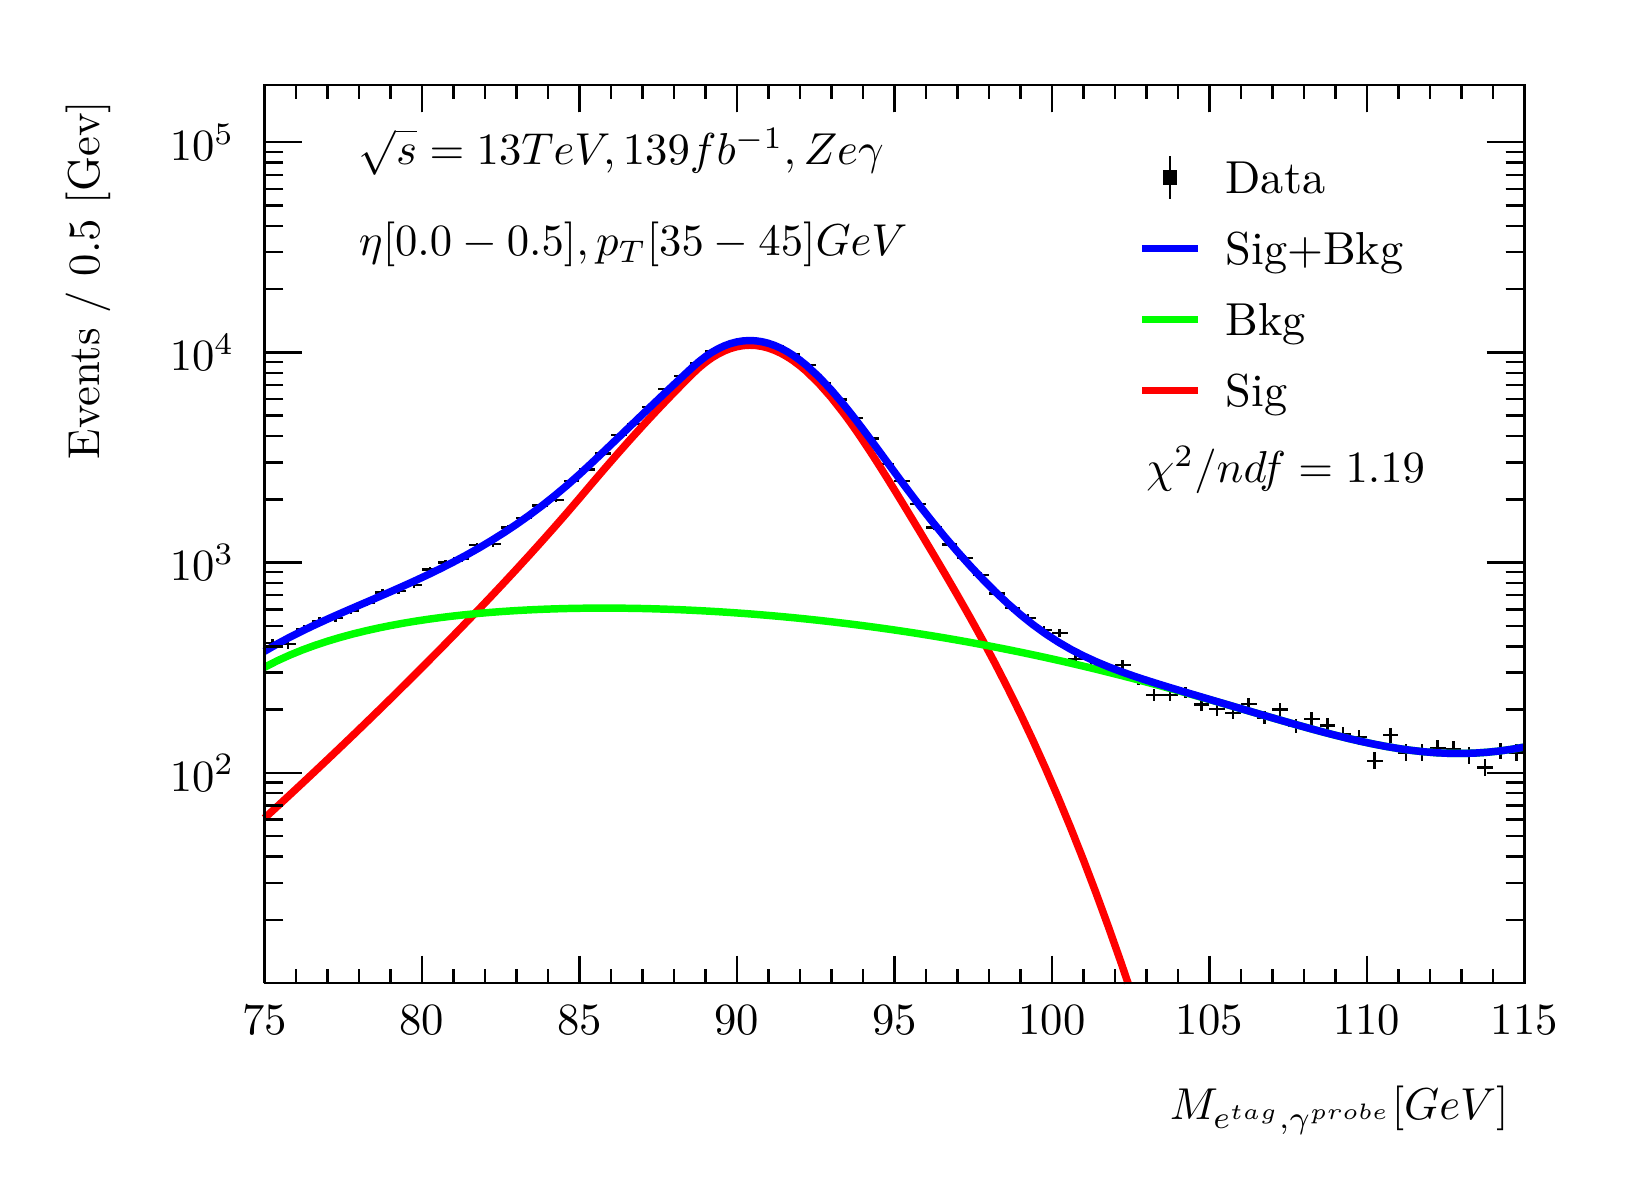
\begin{tikzpicture}
\pgfdeclareplotmark{cross} {
\pgfpathmoveto{\pgfpoint{-0.3\pgfplotmarksize}{\pgfplotmarksize}}
\pgfpathlineto{\pgfpoint{+0.3\pgfplotmarksize}{\pgfplotmarksize}}
\pgfpathlineto{\pgfpoint{+0.3\pgfplotmarksize}{0.3\pgfplotmarksize}}
\pgfpathlineto{\pgfpoint{+1\pgfplotmarksize}{0.3\pgfplotmarksize}}
\pgfpathlineto{\pgfpoint{+1\pgfplotmarksize}{-0.3\pgfplotmarksize}}
\pgfpathlineto{\pgfpoint{+0.3\pgfplotmarksize}{-0.3\pgfplotmarksize}}
\pgfpathlineto{\pgfpoint{+0.3\pgfplotmarksize}{-1.\pgfplotmarksize}}
\pgfpathlineto{\pgfpoint{-0.3\pgfplotmarksize}{-1.\pgfplotmarksize}}
\pgfpathlineto{\pgfpoint{-0.3\pgfplotmarksize}{-0.3\pgfplotmarksize}}
\pgfpathlineto{\pgfpoint{-1.\pgfplotmarksize}{-0.3\pgfplotmarksize}}
\pgfpathlineto{\pgfpoint{-1.\pgfplotmarksize}{0.3\pgfplotmarksize}}
\pgfpathlineto{\pgfpoint{-0.3\pgfplotmarksize}{0.3\pgfplotmarksize}}
\pgfpathclose
\pgfusepathqstroke
}
\pgfdeclareplotmark{cross*} {
\pgfpathmoveto{\pgfpoint{-0.3\pgfplotmarksize}{\pgfplotmarksize}}
\pgfpathlineto{\pgfpoint{+0.3\pgfplotmarksize}{\pgfplotmarksize}}
\pgfpathlineto{\pgfpoint{+0.3\pgfplotmarksize}{0.3\pgfplotmarksize}}
\pgfpathlineto{\pgfpoint{+1\pgfplotmarksize}{0.3\pgfplotmarksize}}
\pgfpathlineto{\pgfpoint{+1\pgfplotmarksize}{-0.3\pgfplotmarksize}}
\pgfpathlineto{\pgfpoint{+0.3\pgfplotmarksize}{-0.3\pgfplotmarksize}}
\pgfpathlineto{\pgfpoint{+0.3\pgfplotmarksize}{-1.\pgfplotmarksize}}
\pgfpathlineto{\pgfpoint{-0.3\pgfplotmarksize}{-1.\pgfplotmarksize}}
\pgfpathlineto{\pgfpoint{-0.3\pgfplotmarksize}{-0.3\pgfplotmarksize}}
\pgfpathlineto{\pgfpoint{-1.\pgfplotmarksize}{-0.3\pgfplotmarksize}}
\pgfpathlineto{\pgfpoint{-1.\pgfplotmarksize}{0.3\pgfplotmarksize}}
\pgfpathlineto{\pgfpoint{-0.3\pgfplotmarksize}{0.3\pgfplotmarksize}}
\pgfpathclose
\pgfusepathqfillstroke
}
\pgfdeclareplotmark{newstar} {
\pgfpathmoveto{\pgfqpoint{0pt}{\pgfplotmarksize}}
\pgfpathlineto{\pgfqpointpolar{44}{0.5\pgfplotmarksize}}
\pgfpathlineto{\pgfqpointpolar{18}{\pgfplotmarksize}}
\pgfpathlineto{\pgfqpointpolar{-20}{0.5\pgfplotmarksize}}
\pgfpathlineto{\pgfqpointpolar{-54}{\pgfplotmarksize}}
\pgfpathlineto{\pgfqpointpolar{-90}{0.5\pgfplotmarksize}}
\pgfpathlineto{\pgfqpointpolar{234}{\pgfplotmarksize}}
\pgfpathlineto{\pgfqpointpolar{198}{0.5\pgfplotmarksize}}
\pgfpathlineto{\pgfqpointpolar{162}{\pgfplotmarksize}}
\pgfpathlineto{\pgfqpointpolar{134}{0.5\pgfplotmarksize}}
\pgfpathclose
\pgfusepathqstroke
}
\pgfdeclareplotmark{newstar*} {
\pgfpathmoveto{\pgfqpoint{0pt}{\pgfplotmarksize}}
\pgfpathlineto{\pgfqpointpolar{44}{0.5\pgfplotmarksize}}
\pgfpathlineto{\pgfqpointpolar{18}{\pgfplotmarksize}}
\pgfpathlineto{\pgfqpointpolar{-20}{0.5\pgfplotmarksize}}
\pgfpathlineto{\pgfqpointpolar{-54}{\pgfplotmarksize}}
\pgfpathlineto{\pgfqpointpolar{-90}{0.5\pgfplotmarksize}}
\pgfpathlineto{\pgfqpointpolar{234}{\pgfplotmarksize}}
\pgfpathlineto{\pgfqpointpolar{198}{0.5\pgfplotmarksize}}
\pgfpathlineto{\pgfqpointpolar{162}{\pgfplotmarksize}}
\pgfpathlineto{\pgfqpointpolar{134}{0.5\pgfplotmarksize}}
\pgfpathclose
\pgfusepathqfillstroke
}
\definecolor{c}{rgb}{1,1,1};
\draw [color=c, fill=c] (0,0) rectangle (20,14.4361);
\draw [color=c, fill=c] (3,2.30977) rectangle (19,13.7143);
\definecolor{c}{rgb}{0,0,0};
\draw [c,line width=0.9] (3,2.30977) -- (3,13.7143) -- (19,13.7143) -- (19,2.30977) -- (3,2.30977);
\definecolor{c}{rgb}{1,1,1};
\draw [color=c, fill=c] (3,2.30977) rectangle (19,13.7143);
\definecolor{c}{rgb}{0,0,0};
\draw [c,line width=0.9] (3,2.30977) -- (3,13.7143) -- (19,13.7143) -- (19,2.30977) -- (3,2.30977);
\draw [c,line width=0.9] (3,2.30977) -- (19,2.30977);
\draw [c,line width=0.9] (3,2.65624) -- (3,2.30977);
\draw [c,line width=0.9] (3.4,2.48301) -- (3.4,2.30977);
\draw [c,line width=0.9] (3.8,2.48301) -- (3.8,2.30977);
\draw [c,line width=0.9] (4.2,2.48301) -- (4.2,2.30977);
\draw [c,line width=0.9] (4.6,2.48301) -- (4.6,2.30977);
\draw [c,line width=0.9] (5,2.65624) -- (5,2.30977);
\draw [c,line width=0.9] (5.4,2.48301) -- (5.4,2.30977);
\draw [c,line width=0.9] (5.8,2.48301) -- (5.8,2.30977);
\draw [c,line width=0.9] (6.2,2.48301) -- (6.2,2.30977);
\draw [c,line width=0.9] (6.6,2.48301) -- (6.6,2.30977);
\draw [c,line width=0.9] (7,2.65624) -- (7,2.30977);
\draw [c,line width=0.9] (7.4,2.48301) -- (7.4,2.30977);
\draw [c,line width=0.9] (7.8,2.48301) -- (7.8,2.30977);
\draw [c,line width=0.9] (8.2,2.48301) -- (8.2,2.30977);
\draw [c,line width=0.9] (8.6,2.48301) -- (8.6,2.30977);
\draw [c,line width=0.9] (9,2.65624) -- (9,2.30977);
\draw [c,line width=0.9] (9.4,2.48301) -- (9.4,2.30977);
\draw [c,line width=0.9] (9.8,2.48301) -- (9.8,2.30977);
\draw [c,line width=0.9] (10.2,2.48301) -- (10.2,2.30977);
\draw [c,line width=0.9] (10.6,2.48301) -- (10.6,2.30977);
\draw [c,line width=0.9] (11,2.65624) -- (11,2.30977);
\draw [c,line width=0.9] (11.4,2.48301) -- (11.4,2.30977);
\draw [c,line width=0.9] (11.8,2.48301) -- (11.8,2.30977);
\draw [c,line width=0.9] (12.2,2.48301) -- (12.2,2.30977);
\draw [c,line width=0.9] (12.6,2.48301) -- (12.6,2.30977);
\draw [c,line width=0.9] (13,2.65624) -- (13,2.30977);
\draw [c,line width=0.9] (13.4,2.48301) -- (13.4,2.30977);
\draw [c,line width=0.9] (13.8,2.48301) -- (13.8,2.30977);
\draw [c,line width=0.9] (14.2,2.48301) -- (14.2,2.30977);
\draw [c,line width=0.9] (14.6,2.48301) -- (14.6,2.30977);
\draw [c,line width=0.9] (15,2.65624) -- (15,2.30977);
\draw [c,line width=0.9] (15.4,2.48301) -- (15.4,2.30977);
\draw [c,line width=0.9] (15.8,2.48301) -- (15.8,2.30977);
\draw [c,line width=0.9] (16.2,2.48301) -- (16.2,2.30977);
\draw [c,line width=0.9] (16.6,2.48301) -- (16.6,2.30977);
\draw [c,line width=0.9] (17,2.65624) -- (17,2.30977);
\draw [c,line width=0.9] (17.4,2.48301) -- (17.4,2.30977);
\draw [c,line width=0.9] (17.8,2.48301) -- (17.8,2.30977);
\draw [c,line width=0.9] (18.2,2.48301) -- (18.2,2.30977);
\draw [c,line width=0.9] (18.6,2.48301) -- (18.6,2.30977);
\draw [c,line width=0.9] (19,2.65624) -- (19,2.30977);
\draw [c,line width=0.9] (19,2.65624) -- (19,2.30977);
\draw [anchor=base] (3,1.66015) node[scale=1.61424, color=c, rotate=0]{75};
\draw [anchor=base] (5,1.66015) node[scale=1.61424, color=c, rotate=0]{80};
\draw [anchor=base] (7,1.66015) node[scale=1.61424, color=c, rotate=0]{85};
\draw [anchor=base] (9,1.66015) node[scale=1.61424, color=c, rotate=0]{90};
\draw [anchor=base] (11,1.66015) node[scale=1.61424, color=c, rotate=0]{95};
\draw [anchor=base] (13,1.66015) node[scale=1.61424, color=c, rotate=0]{100};
\draw [anchor=base] (15,1.66015) node[scale=1.61424, color=c, rotate=0]{105};
\draw [anchor=base] (17,1.66015) node[scale=1.61424, color=c, rotate=0]{110};
\draw [anchor=base] (19,1.66015) node[scale=1.61424, color=c, rotate=0]{115};
\draw [anchor= east] (19,0.692932) node[scale=1.61424, color=c, rotate=0]{$M_{e^{tag}, \gamma^{probe}}  [GeV]$};
\draw [c,line width=0.9] (3,13.7143) -- (19,13.7143);
\draw [c,line width=0.9] (3,13.3678) -- (3,13.7143);
\draw [c,line width=0.9] (3.4,13.5411) -- (3.4,13.7143);
\draw [c,line width=0.9] (3.8,13.5411) -- (3.8,13.7143);
\draw [c,line width=0.9] (4.2,13.5411) -- (4.2,13.7143);
\draw [c,line width=0.9] (4.6,13.5411) -- (4.6,13.7143);
\draw [c,line width=0.9] (5,13.3678) -- (5,13.7143);
\draw [c,line width=0.9] (5.4,13.5411) -- (5.4,13.7143);
\draw [c,line width=0.9] (5.8,13.5411) -- (5.8,13.7143);
\draw [c,line width=0.9] (6.2,13.5411) -- (6.2,13.7143);
\draw [c,line width=0.9] (6.6,13.5411) -- (6.6,13.7143);
\draw [c,line width=0.9] (7,13.3678) -- (7,13.7143);
\draw [c,line width=0.9] (7.4,13.5411) -- (7.4,13.7143);
\draw [c,line width=0.9] (7.8,13.5411) -- (7.8,13.7143);
\draw [c,line width=0.9] (8.2,13.5411) -- (8.2,13.7143);
\draw [c,line width=0.9] (8.6,13.5411) -- (8.6,13.7143);
\draw [c,line width=0.9] (9,13.3678) -- (9,13.7143);
\draw [c,line width=0.9] (9.4,13.5411) -- (9.4,13.7143);
\draw [c,line width=0.9] (9.8,13.5411) -- (9.8,13.7143);
\draw [c,line width=0.9] (10.2,13.5411) -- (10.2,13.7143);
\draw [c,line width=0.9] (10.6,13.5411) -- (10.6,13.7143);
\draw [c,line width=0.9] (11,13.3678) -- (11,13.7143);
\draw [c,line width=0.9] (11.4,13.5411) -- (11.4,13.7143);
\draw [c,line width=0.9] (11.8,13.5411) -- (11.8,13.7143);
\draw [c,line width=0.9] (12.2,13.5411) -- (12.2,13.7143);
\draw [c,line width=0.9] (12.6,13.5411) -- (12.6,13.7143);
\draw [c,line width=0.9] (13,13.3678) -- (13,13.7143);
\draw [c,line width=0.9] (13.4,13.5411) -- (13.4,13.7143);
\draw [c,line width=0.9] (13.8,13.5411) -- (13.8,13.7143);
\draw [c,line width=0.9] (14.2,13.5411) -- (14.2,13.7143);
\draw [c,line width=0.9] (14.6,13.5411) -- (14.6,13.7143);
\draw [c,line width=0.9] (15,13.3678) -- (15,13.7143);
\draw [c,line width=0.9] (15.4,13.5411) -- (15.4,13.7143);
\draw [c,line width=0.9] (15.8,13.5411) -- (15.8,13.7143);
\draw [c,line width=0.9] (16.2,13.5411) -- (16.2,13.7143);
\draw [c,line width=0.9] (16.6,13.5411) -- (16.6,13.7143);
\draw [c,line width=0.9] (17,13.3678) -- (17,13.7143);
\draw [c,line width=0.9] (17.4,13.5411) -- (17.4,13.7143);
\draw [c,line width=0.9] (17.8,13.5411) -- (17.8,13.7143);
\draw [c,line width=0.9] (18.2,13.5411) -- (18.2,13.7143);
\draw [c,line width=0.9] (18.6,13.5411) -- (18.6,13.7143);
\draw [c,line width=0.9] (19,13.3678) -- (19,13.7143);
\draw [c,line width=0.9] (19,13.3678) -- (19,13.7143);
\draw [c,line width=0.9] (3,2.30977) -- (3,13.7143);
\draw [c,line width=0.9] (3.237,3.11343) -- (3,3.11343);
\draw [c,line width=0.9] (3.237,3.58354) -- (3,3.58354);
\draw [c,line width=0.9] (3.237,3.91709) -- (3,3.91709);
\draw [c,line width=0.9] (3.237,4.17581) -- (3,4.17581);
\draw [c,line width=0.9] (3.237,4.38719) -- (3,4.38719);
\draw [c,line width=0.9] (3.237,4.56592) -- (3,4.56592);
\draw [c,line width=0.9] (3.237,4.72074) -- (3,4.72074);
\draw [c,line width=0.9] (3.237,4.8573) -- (3,4.8573);
\draw [c,line width=0.9] (3.474,4.97946) -- (3,4.97946);
\draw [anchor= east] (2.82,4.97946) node[scale=1.61424, color=c, rotate=0]{$10^{2}$};
\draw [c,line width=0.9] (3.237,5.78312) -- (3,5.78312);
\draw [c,line width=0.9] (3.237,6.25323) -- (3,6.25323);
\draw [c,line width=0.9] (3.237,6.58678) -- (3,6.58678);
\draw [c,line width=0.9] (3.237,6.8455) -- (3,6.8455);
\draw [c,line width=0.9] (3.237,7.05689) -- (3,7.05689);
\draw [c,line width=0.9] (3.237,7.23561) -- (3,7.23561);
\draw [c,line width=0.9] (3.237,7.39043) -- (3,7.39043);
\draw [c,line width=0.9] (3.237,7.52699) -- (3,7.52699);
\draw [c,line width=0.9] (3.474,7.64915) -- (3,7.64915);
\draw [anchor= east] (2.82,7.64915) node[scale=1.61424, color=c, rotate=0]{$10^{3}$};
\draw [c,line width=0.9] (3.237,8.45281) -- (3,8.45281);
\draw [c,line width=0.9] (3.237,8.92292) -- (3,8.92292);
\draw [c,line width=0.9] (3.237,9.25647) -- (3,9.25647);
\draw [c,line width=0.9] (3.237,9.51519) -- (3,9.51519);
\draw [c,line width=0.9] (3.237,9.72658) -- (3,9.72658);
\draw [c,line width=0.9] (3.237,9.9053) -- (3,9.9053);
\draw [c,line width=0.9] (3.237,10.0601) -- (3,10.0601);
\draw [c,line width=0.9] (3.237,10.1967) -- (3,10.1967);
\draw [c,line width=0.9] (3.474,10.3188) -- (3,10.3188);
\draw [anchor= east] (2.82,10.3188) node[scale=1.61424, color=c, rotate=0]{$10^{4}$};
\draw [c,line width=0.9] (3.237,11.1225) -- (3,11.1225);
\draw [c,line width=0.9] (3.237,11.5926) -- (3,11.5926);
\draw [c,line width=0.9] (3.237,11.9262) -- (3,11.9262);
\draw [c,line width=0.9] (3.237,12.1849) -- (3,12.1849);
\draw [c,line width=0.9] (3.237,12.3963) -- (3,12.3963);
\draw [c,line width=0.9] (3.237,12.575) -- (3,12.575);
\draw [c,line width=0.9] (3.237,12.7298) -- (3,12.7298);
\draw [c,line width=0.9] (3.237,12.8664) -- (3,12.8664);
\draw [c,line width=0.9] (3.474,12.9885) -- (3,12.9885);
\draw [anchor= east] (2.82,12.9885) node[scale=1.61424, color=c, rotate=0]{$10^{5}$};
\draw [anchor= east] (0.76,13.7143) node[scale=1.61424, color=c, rotate=90]{Events / 0.5 [Gev]};
\draw [c,line width=0.9] (19,2.30977) -- (19,13.7143);
\draw [c,line width=0.9] (18.763,3.11343) -- (19,3.11343);
\draw [c,line width=0.9] (18.763,3.58354) -- (19,3.58354);
\draw [c,line width=0.9] (18.763,3.91709) -- (19,3.91709);
\draw [c,line width=0.9] (18.763,4.17581) -- (19,4.17581);
\draw [c,line width=0.9] (18.763,4.38719) -- (19,4.38719);
\draw [c,line width=0.9] (18.763,4.56592) -- (19,4.56592);
\draw [c,line width=0.9] (18.763,4.72074) -- (19,4.72074);
\draw [c,line width=0.9] (18.763,4.8573) -- (19,4.8573);
\draw [c,line width=0.9] (18.526,4.97946) -- (19,4.97946);
\draw [c,line width=0.9] (18.763,5.78312) -- (19,5.78312);
\draw [c,line width=0.9] (18.763,6.25323) -- (19,6.25323);
\draw [c,line width=0.9] (18.763,6.58678) -- (19,6.58678);
\draw [c,line width=0.9] (18.763,6.8455) -- (19,6.8455);
\draw [c,line width=0.9] (18.763,7.05689) -- (19,7.05689);
\draw [c,line width=0.9] (18.763,7.23561) -- (19,7.23561);
\draw [c,line width=0.9] (18.763,7.39043) -- (19,7.39043);
\draw [c,line width=0.9] (18.763,7.52699) -- (19,7.52699);
\draw [c,line width=0.9] (18.526,7.64915) -- (19,7.64915);
\draw [c,line width=0.9] (18.763,8.45281) -- (19,8.45281);
\draw [c,line width=0.9] (18.763,8.92292) -- (19,8.92292);
\draw [c,line width=0.9] (18.763,9.25647) -- (19,9.25647);
\draw [c,line width=0.9] (18.763,9.51519) -- (19,9.51519);
\draw [c,line width=0.9] (18.763,9.72658) -- (19,9.72658);
\draw [c,line width=0.9] (18.763,9.9053) -- (19,9.9053);
\draw [c,line width=0.9] (18.763,10.0601) -- (19,10.0601);
\draw [c,line width=0.9] (18.763,10.1967) -- (19,10.1967);
\draw [c,line width=0.9] (18.526,10.3188) -- (19,10.3188);
\draw [c,line width=0.9] (18.763,11.1225) -- (19,11.1225);
\draw [c,line width=0.9] (18.763,11.5926) -- (19,11.5926);
\draw [c,line width=0.9] (18.763,11.9262) -- (19,11.9262);
\draw [c,line width=0.9] (18.763,12.1849) -- (19,12.1849);
\draw [c,line width=0.9] (18.763,12.3963) -- (19,12.3963);
\draw [c,line width=0.9] (18.763,12.575) -- (19,12.575);
\draw [c,line width=0.9] (18.763,12.7298) -- (19,12.7298);
\draw [c,line width=0.9] (18.763,12.8664) -- (19,12.8664);
\draw [c,line width=0.9] (18.526,12.9885) -- (19,12.9885);
\draw [c,line width=0.9] (3.1,6.62666) -- (3,6.62666);
\draw [c,line width=0.9] (3,6.62666) -- (3,6.62666);
\draw [c,line width=0.9] (3.1,6.62666) -- (3.2,6.62666);
\draw [c,line width=0.9] (3.2,6.62666) -- (3.2,6.62666);
\draw [c,line width=0.9] (3.1,6.62666) -- (3.1,6.68364);
\draw [c,line width=0.9] (3.1,6.68364) -- (3.1,6.68364);
\draw [c,line width=0.9] (3.1,6.62666) -- (3.1,6.56969);
\draw [c,line width=0.9] (3.1,6.56969) -- (3.1,6.56969);
\draw [c,line width=0.9] (3.3,6.61258) -- (3.2,6.61258);
\draw [c,line width=0.9] (3.2,6.61258) -- (3.2,6.61258);
\draw [c,line width=0.9] (3.3,6.61258) -- (3.4,6.61258);
\draw [c,line width=0.9] (3.4,6.61258) -- (3.4,6.61258);
\draw [c,line width=0.9] (3.3,6.61258) -- (3.3,6.6699);
\draw [c,line width=0.9] (3.3,6.6699) -- (3.3,6.6699);
\draw [c,line width=0.9] (3.3,6.61258) -- (3.3,6.55525);
\draw [c,line width=0.9] (3.3,6.55525) -- (3.3,6.55525);
\draw [c,line width=0.9] (3.5,6.80779) -- (3.4,6.80779);
\draw [c,line width=0.9] (3.4,6.80779) -- (3.4,6.80779);
\draw [c,line width=0.9] (3.5,6.80779) -- (3.6,6.80779);
\draw [c,line width=0.9] (3.6,6.80779) -- (3.6,6.80779);
\draw [c,line width=0.9] (3.5,6.80779) -- (3.5,6.86049);
\draw [c,line width=0.9] (3.5,6.86049) -- (3.5,6.86049);
\draw [c,line width=0.9] (3.5,6.80779) -- (3.5,6.75509);
\draw [c,line width=0.9] (3.5,6.75509) -- (3.5,6.75509);
\draw [c,line width=0.9] (3.7,6.90207) -- (3.6,6.90207);
\draw [c,line width=0.9] (3.6,6.90207) -- (3.6,6.90207);
\draw [c,line width=0.9] (3.7,6.90207) -- (3.8,6.90207);
\draw [c,line width=0.9] (3.8,6.90207) -- (3.8,6.90207);
\draw [c,line width=0.9] (3.7,6.90207) -- (3.7,6.95266);
\draw [c,line width=0.9] (3.7,6.95266) -- (3.7,6.95266);
\draw [c,line width=0.9] (3.7,6.90207) -- (3.7,6.85147);
\draw [c,line width=0.9] (3.7,6.85147) -- (3.7,6.85147);
\draw [c,line width=0.9] (3.9,6.94754) -- (3.8,6.94754);
\draw [c,line width=0.9] (3.8,6.94754) -- (3.8,6.94754);
\draw [c,line width=0.9] (3.9,6.94754) -- (4,6.94754);
\draw [c,line width=0.9] (4,6.94754) -- (4,6.94754);
\draw [c,line width=0.9] (3.9,6.94754) -- (3.9,6.99716);
\draw [c,line width=0.9] (3.9,6.99716) -- (3.9,6.99716);
\draw [c,line width=0.9] (3.9,6.94754) -- (3.9,6.89792);
\draw [c,line width=0.9] (3.9,6.89792) -- (3.9,6.89792);
\draw [c,line width=0.9] (4.1,7.03936) -- (4,7.03936);
\draw [c,line width=0.9] (4,7.03936) -- (4,7.03936);
\draw [c,line width=0.9] (4.1,7.03936) -- (4.2,7.03936);
\draw [c,line width=0.9] (4.2,7.03936) -- (4.2,7.03936);
\draw [c,line width=0.9] (4.1,7.03936) -- (4.1,7.08705);
\draw [c,line width=0.9] (4.1,7.08705) -- (4.1,7.08705);
\draw [c,line width=0.9] (4.1,7.03936) -- (4.1,6.99167);
\draw [c,line width=0.9] (4.1,6.99167) -- (4.1,6.99167);
\draw [c,line width=0.9] (4.3,7.14074) -- (4.2,7.14074);
\draw [c,line width=0.9] (4.2,7.14074) -- (4.2,7.14074);
\draw [c,line width=0.9] (4.3,7.14074) -- (4.4,7.14074);
\draw [c,line width=0.9] (4.4,7.14074) -- (4.4,7.14074);
\draw [c,line width=0.9] (4.3,7.14074) -- (4.3,7.18639);
\draw [c,line width=0.9] (4.3,7.18639) -- (4.3,7.18639);
\draw [c,line width=0.9] (4.3,7.14074) -- (4.3,7.09509);
\draw [c,line width=0.9] (4.3,7.09509) -- (4.3,7.09509);
\draw [c,line width=0.9] (4.5,7.26666) -- (4.4,7.26666);
\draw [c,line width=0.9] (4.4,7.26666) -- (4.4,7.26666);
\draw [c,line width=0.9] (4.5,7.26666) -- (4.6,7.26666);
\draw [c,line width=0.9] (4.6,7.26666) -- (4.6,7.26666);
\draw [c,line width=0.9] (4.5,7.26666) -- (4.5,7.3099);
\draw [c,line width=0.9] (4.5,7.3099) -- (4.5,7.3099);
\draw [c,line width=0.9] (4.5,7.26666) -- (4.5,7.22343);
\draw [c,line width=0.9] (4.5,7.22343) -- (4.5,7.22343);
\draw [c,line width=0.9] (4.7,7.28902) -- (4.6,7.28902);
\draw [c,line width=0.9] (4.6,7.28902) -- (4.6,7.28902);
\draw [c,line width=0.9] (4.7,7.28902) -- (4.8,7.28902);
\draw [c,line width=0.9] (4.8,7.28902) -- (4.8,7.28902);
\draw [c,line width=0.9] (4.7,7.28902) -- (4.7,7.33185);
\draw [c,line width=0.9] (4.7,7.33185) -- (4.7,7.33185);
\draw [c,line width=0.9] (4.7,7.28902) -- (4.7,7.2462);
\draw [c,line width=0.9] (4.7,7.2462) -- (4.7,7.2462);
\draw [c,line width=0.9] (4.9,7.36553) -- (4.8,7.36553);
\draw [c,line width=0.9] (4.8,7.36553) -- (4.8,7.36553);
\draw [c,line width=0.9] (4.9,7.36553) -- (5,7.36553);
\draw [c,line width=0.9] (5,7.36553) -- (5,7.36553);
\draw [c,line width=0.9] (4.9,7.36553) -- (4.9,7.40696);
\draw [c,line width=0.9] (4.9,7.40696) -- (4.9,7.40696);
\draw [c,line width=0.9] (4.9,7.36553) -- (4.9,7.3241);
\draw [c,line width=0.9] (4.9,7.3241) -- (4.9,7.3241);
\draw [c,line width=0.9] (5.1,7.55876) -- (5,7.55876);
\draw [c,line width=0.9] (5,7.55876) -- (5,7.55876);
\draw [c,line width=0.9] (5.1,7.55876) -- (5.2,7.55876);
\draw [c,line width=0.9] (5.2,7.55876) -- (5.2,7.55876);
\draw [c,line width=0.9] (5.1,7.55876) -- (5.1,7.59688);
\draw [c,line width=0.9] (5.1,7.59688) -- (5.1,7.59688);
\draw [c,line width=0.9] (5.1,7.55876) -- (5.1,7.52064);
\draw [c,line width=0.9] (5.1,7.52064) -- (5.1,7.52064);
\draw [c,line width=0.9] (5.3,7.65031) -- (5.2,7.65031);
\draw [c,line width=0.9] (5.2,7.65031) -- (5.2,7.65031);
\draw [c,line width=0.9] (5.3,7.65031) -- (5.4,7.65031);
\draw [c,line width=0.9] (5.4,7.65031) -- (5.4,7.65031);
\draw [c,line width=0.9] (5.3,7.65031) -- (5.3,7.68696);
\draw [c,line width=0.9] (5.3,7.68696) -- (5.3,7.68696);
\draw [c,line width=0.9] (5.3,7.65031) -- (5.3,7.61367);
\draw [c,line width=0.9] (5.3,7.61367) -- (5.3,7.61367);
\draw [c,line width=0.9] (5.5,7.69908) -- (5.4,7.69908);
\draw [c,line width=0.9] (5.4,7.69908) -- (5.4,7.69908);
\draw [c,line width=0.9] (5.5,7.69908) -- (5.6,7.69908);
\draw [c,line width=0.9] (5.6,7.69908) -- (5.6,7.69908);
\draw [c,line width=0.9] (5.5,7.69908) -- (5.5,7.73496);
\draw [c,line width=0.9] (5.5,7.73496) -- (5.5,7.73496);
\draw [c,line width=0.9] (5.5,7.69908) -- (5.5,7.6632);
\draw [c,line width=0.9] (5.5,7.6632) -- (5.5,7.6632);
\draw [c,line width=0.9] (5.7,7.87112) -- (5.6,7.87112);
\draw [c,line width=0.9] (5.6,7.87112) -- (5.6,7.87112);
\draw [c,line width=0.9] (5.7,7.87112) -- (5.8,7.87112);
\draw [c,line width=0.9] (5.8,7.87112) -- (5.8,7.87112);
\draw [c,line width=0.9] (5.7,7.87112) -- (5.7,7.90444);
\draw [c,line width=0.9] (5.7,7.90444) -- (5.7,7.90444);
\draw [c,line width=0.9] (5.7,7.87112) -- (5.7,7.83781);
\draw [c,line width=0.9] (5.7,7.83781) -- (5.7,7.83781);
\draw [c,line width=0.9] (5.9,7.8854) -- (5.8,7.8854);
\draw [c,line width=0.9] (5.8,7.8854) -- (5.8,7.8854);
\draw [c,line width=0.9] (5.9,7.8854) -- (6,7.8854);
\draw [c,line width=0.9] (6,7.8854) -- (6,7.8854);
\draw [c,line width=0.9] (5.9,7.8854) -- (5.9,7.91851);
\draw [c,line width=0.9] (5.9,7.91851) -- (5.9,7.91851);
\draw [c,line width=0.9] (5.9,7.8854) -- (5.9,7.85228);
\draw [c,line width=0.9] (5.9,7.85228) -- (5.9,7.85228);
\draw [c,line width=0.9] (6.1,8.09426) -- (6,8.09426);
\draw [c,line width=0.9] (6,8.09426) -- (6,8.09426);
\draw [c,line width=0.9] (6.1,8.09426) -- (6.2,8.09426);
\draw [c,line width=0.9] (6.2,8.09426) -- (6.2,8.09426);
\draw [c,line width=0.9] (6.1,8.09426) -- (6.1,8.12452);
\draw [c,line width=0.9] (6.1,8.12452) -- (6.1,8.12452);
\draw [c,line width=0.9] (6.1,8.09426) -- (6.1,8.064);
\draw [c,line width=0.9] (6.1,8.064) -- (6.1,8.064);
\draw [c,line width=0.9] (6.3,8.21705) -- (6.2,8.21705);
\draw [c,line width=0.9] (6.2,8.21705) -- (6.2,8.21705);
\draw [c,line width=0.9] (6.3,8.21705) -- (6.4,8.21705);
\draw [c,line width=0.9] (6.4,8.21705) -- (6.4,8.21705);
\draw [c,line width=0.9] (6.3,8.21705) -- (6.3,8.24575);
\draw [c,line width=0.9] (6.3,8.24575) -- (6.3,8.24575);
\draw [c,line width=0.9] (6.3,8.21705) -- (6.3,8.18835);
\draw [c,line width=0.9] (6.3,8.18835) -- (6.3,8.18835);
\draw [c,line width=0.9] (6.5,8.37365) -- (6.4,8.37365);
\draw [c,line width=0.9] (6.4,8.37365) -- (6.4,8.37365);
\draw [c,line width=0.9] (6.5,8.37365) -- (6.6,8.37365);
\draw [c,line width=0.9] (6.6,8.37365) -- (6.6,8.37365);
\draw [c,line width=0.9] (6.5,8.37365) -- (6.5,8.40047);
\draw [c,line width=0.9] (6.5,8.40047) -- (6.5,8.40047);
\draw [c,line width=0.9] (6.5,8.37365) -- (6.5,8.34682);
\draw [c,line width=0.9] (6.5,8.34682) -- (6.5,8.34682);
\draw [c,line width=0.9] (6.7,8.44233) -- (6.6,8.44233);
\draw [c,line width=0.9] (6.6,8.44233) -- (6.6,8.44233);
\draw [c,line width=0.9] (6.7,8.44233) -- (6.8,8.44233);
\draw [c,line width=0.9] (6.8,8.44233) -- (6.8,8.44233);
\draw [c,line width=0.9] (6.7,8.44233) -- (6.7,8.46837);
\draw [c,line width=0.9] (6.7,8.46837) -- (6.7,8.46837);
\draw [c,line width=0.9] (6.7,8.44233) -- (6.7,8.41629);
\draw [c,line width=0.9] (6.7,8.41629) -- (6.7,8.41629);
\draw [c,line width=0.9] (6.9,8.68526) -- (6.8,8.68526);
\draw [c,line width=0.9] (6.8,8.68526) -- (6.8,8.68526);
\draw [c,line width=0.9] (6.9,8.68526) -- (7,8.68526);
\draw [c,line width=0.9] (7,8.68526) -- (7,8.68526);
\draw [c,line width=0.9] (6.9,8.68526) -- (6.9,8.70872);
\draw [c,line width=0.9] (6.9,8.70872) -- (6.9,8.70872);
\draw [c,line width=0.9] (6.9,8.68526) -- (6.9,8.66181);
\draw [c,line width=0.9] (6.9,8.66181) -- (6.9,8.66181);
\draw [c,line width=0.9] (7.1,8.83336) -- (7,8.83336);
\draw [c,line width=0.9] (7,8.83336) -- (7,8.83336);
\draw [c,line width=0.9] (7.1,8.83336) -- (7.2,8.83336);
\draw [c,line width=0.9] (7.2,8.83336) -- (7.2,8.83336);
\draw [c,line width=0.9] (7.1,8.83336) -- (7.1,8.85537);
\draw [c,line width=0.9] (7.1,8.85537) -- (7.1,8.85537);
\draw [c,line width=0.9] (7.1,8.83336) -- (7.1,8.81136);
\draw [c,line width=0.9] (7.1,8.81136) -- (7.1,8.81136);
\draw [c,line width=0.9] (7.3,9.03763) -- (7.2,9.03763);
\draw [c,line width=0.9] (7.2,9.03763) -- (7.2,9.03763);
\draw [c,line width=0.9] (7.3,9.03763) -- (7.4,9.03763);
\draw [c,line width=0.9] (7.4,9.03763) -- (7.4,9.03763);
\draw [c,line width=0.9] (7.3,9.03763) -- (7.3,9.05778);
\draw [c,line width=0.9] (7.3,9.05778) -- (7.3,9.05778);
\draw [c,line width=0.9] (7.3,9.03763) -- (7.3,9.01749);
\draw [c,line width=0.9] (7.3,9.01749) -- (7.3,9.01749);
\draw [c,line width=0.9] (7.5,9.26858) -- (7.4,9.26858);
\draw [c,line width=0.9] (7.4,9.26858) -- (7.4,9.26858);
\draw [c,line width=0.9] (7.5,9.26858) -- (7.6,9.26858);
\draw [c,line width=0.9] (7.6,9.26858) -- (7.6,9.26858);
\draw [c,line width=0.9] (7.5,9.26858) -- (7.5,9.28681);
\draw [c,line width=0.9] (7.5,9.28681) -- (7.5,9.28681);
\draw [c,line width=0.9] (7.5,9.26858) -- (7.5,9.25034);
\draw [c,line width=0.9] (7.5,9.25034) -- (7.5,9.25034);
\draw [c,line width=0.9] (7.7,9.41093) -- (7.6,9.41093);
\draw [c,line width=0.9] (7.6,9.41093) -- (7.6,9.41093);
\draw [c,line width=0.9] (7.7,9.41093) -- (7.8,9.41093);
\draw [c,line width=0.9] (7.8,9.41093) -- (7.8,9.41093);
\draw [c,line width=0.9] (7.7,9.41093) -- (7.7,9.42808);
\draw [c,line width=0.9] (7.7,9.42808) -- (7.7,9.42808);
\draw [c,line width=0.9] (7.7,9.41093) -- (7.7,9.39377);
\draw [c,line width=0.9] (7.7,9.39377) -- (7.7,9.39377);
\draw [c,line width=0.9] (7.9,9.62801) -- (7.8,9.62801);
\draw [c,line width=0.9] (7.8,9.62801) -- (7.8,9.62801);
\draw [c,line width=0.9] (7.9,9.62801) -- (8,9.62801);
\draw [c,line width=0.9] (8,9.62801) -- (8,9.62801);
\draw [c,line width=0.9] (7.9,9.62801) -- (7.9,9.64363);
\draw [c,line width=0.9] (7.9,9.64363) -- (7.9,9.64363);
\draw [c,line width=0.9] (7.9,9.62801) -- (7.9,9.61239);
\draw [c,line width=0.9] (7.9,9.61239) -- (7.9,9.61239);
\draw [c,line width=0.9] (8.1,9.85105) -- (8,9.85105);
\draw [c,line width=0.9] (8,9.85105) -- (8,9.85105);
\draw [c,line width=0.9] (8.1,9.85105) -- (8.2,9.85105);
\draw [c,line width=0.9] (8.2,9.85105) -- (8.2,9.85105);
\draw [c,line width=0.9] (8.1,9.85105) -- (8.1,9.86524);
\draw [c,line width=0.9] (8.1,9.86524) -- (8.1,9.86524);
\draw [c,line width=0.9] (8.1,9.85105) -- (8.1,9.83687);
\draw [c,line width=0.9] (8.1,9.83687) -- (8.1,9.83687);
\draw [c,line width=0.9] (8.3,10.0176) -- (8.2,10.0176);
\draw [c,line width=0.9] (8.2,10.0176) -- (8.2,10.0176);
\draw [c,line width=0.9] (8.3,10.0176) -- (8.4,10.0176);
\draw [c,line width=0.9] (8.4,10.0176) -- (8.4,10.0176);
\draw [c,line width=0.9] (8.3,10.0176) -- (8.3,10.0308);
\draw [c,line width=0.9] (8.3,10.0308) -- (8.3,10.0308);
\draw [c,line width=0.9] (8.3,10.0176) -- (8.3,10.0044);
\draw [c,line width=0.9] (8.3,10.0044) -- (8.3,10.0044);
\draw [c,line width=0.9] (8.5,10.1863) -- (8.4,10.1863);
\draw [c,line width=0.9] (8.4,10.1863) -- (8.4,10.1863);
\draw [c,line width=0.9] (8.5,10.1863) -- (8.6,10.1863);
\draw [c,line width=0.9] (8.6,10.1863) -- (8.6,10.1863);
\draw [c,line width=0.9] (8.5,10.1863) -- (8.5,10.1986);
\draw [c,line width=0.9] (8.5,10.1986) -- (8.5,10.1986);
\draw [c,line width=0.9] (8.5,10.1863) -- (8.5,10.1741);
\draw [c,line width=0.9] (8.5,10.1741) -- (8.5,10.1741);
\draw [c,line width=0.9] (8.7,10.3322) -- (8.6,10.3322);
\draw [c,line width=0.9] (8.6,10.3322) -- (8.6,10.3322);
\draw [c,line width=0.9] (8.7,10.3322) -- (8.8,10.3322);
\draw [c,line width=0.9] (8.8,10.3322) -- (8.8,10.3322);
\draw [c,line width=0.9] (8.7,10.3322) -- (8.7,10.3437);
\draw [c,line width=0.9] (8.7,10.3437) -- (8.7,10.3437);
\draw [c,line width=0.9] (8.7,10.3322) -- (8.7,10.3207);
\draw [c,line width=0.9] (8.7,10.3207) -- (8.7,10.3207);
\draw [c,line width=0.9] (8.9,10.4103) -- (8.8,10.4103);
\draw [c,line width=0.9] (8.8,10.4103) -- (8.8,10.4103);
\draw [c,line width=0.9] (8.9,10.4103) -- (9,10.4103);
\draw [c,line width=0.9] (9,10.4103) -- (9,10.4103);
\draw [c,line width=0.9] (8.9,10.4103) -- (8.9,10.4215);
\draw [c,line width=0.9] (8.9,10.4215) -- (8.9,10.4215);
\draw [c,line width=0.9] (8.9,10.4103) -- (8.9,10.3992);
\draw [c,line width=0.9] (8.9,10.3992) -- (8.9,10.3992);
\draw [c,line width=0.9] (9.1,10.4655) -- (9,10.4655);
\draw [c,line width=0.9] (9,10.4655) -- (9,10.4655);
\draw [c,line width=0.9] (9.1,10.4655) -- (9.2,10.4655);
\draw [c,line width=0.9] (9.2,10.4655) -- (9.2,10.4655);
\draw [c,line width=0.9] (9.1,10.4655) -- (9.1,10.4763);
\draw [c,line width=0.9] (9.1,10.4763) -- (9.1,10.4763);
\draw [c,line width=0.9] (9.1,10.4655) -- (9.1,10.4546);
\draw [c,line width=0.9] (9.1,10.4546) -- (9.1,10.4546);
\draw [c,line width=0.9] (9.3,10.4522) -- (9.2,10.4522);
\draw [c,line width=0.9] (9.2,10.4522) -- (9.2,10.4522);
\draw [c,line width=0.9] (9.3,10.4522) -- (9.4,10.4522);
\draw [c,line width=0.9] (9.4,10.4522) -- (9.4,10.4522);
\draw [c,line width=0.9] (9.3,10.4522) -- (9.3,10.4632);
\draw [c,line width=0.9] (9.3,10.4632) -- (9.3,10.4632);
\draw [c,line width=0.9] (9.3,10.4522) -- (9.3,10.4413);
\draw [c,line width=0.9] (9.3,10.4413) -- (9.3,10.4413);
\draw [c,line width=0.9] (9.5,10.3965) -- (9.4,10.3965);
\draw [c,line width=0.9] (9.4,10.3965) -- (9.4,10.3965);
\draw [c,line width=0.9] (9.5,10.3965) -- (9.6,10.3965);
\draw [c,line width=0.9] (9.6,10.3965) -- (9.6,10.3965);
\draw [c,line width=0.9] (9.5,10.3965) -- (9.5,10.4077);
\draw [c,line width=0.9] (9.5,10.4077) -- (9.5,10.4077);
\draw [c,line width=0.9] (9.5,10.3965) -- (9.5,10.3853);
\draw [c,line width=0.9] (9.5,10.3853) -- (9.5,10.3853);
\draw [c,line width=0.9] (9.7,10.2945) -- (9.6,10.2945);
\draw [c,line width=0.9] (9.6,10.2945) -- (9.6,10.2945);
\draw [c,line width=0.9] (9.7,10.2945) -- (9.8,10.2945);
\draw [c,line width=0.9] (9.8,10.2945) -- (9.8,10.2945);
\draw [c,line width=0.9] (9.7,10.2945) -- (9.7,10.3062);
\draw [c,line width=0.9] (9.7,10.3062) -- (9.7,10.3062);
\draw [c,line width=0.9] (9.7,10.2945) -- (9.7,10.2828);
\draw [c,line width=0.9] (9.7,10.2828) -- (9.7,10.2828);
\draw [c,line width=0.9] (9.9,10.1619) -- (9.8,10.1619);
\draw [c,line width=0.9] (9.8,10.1619) -- (9.8,10.1619);
\draw [c,line width=0.9] (9.9,10.1619) -- (10,10.1619);
\draw [c,line width=0.9] (10,10.1619) -- (10,10.1619);
\draw [c,line width=0.9] (9.9,10.1619) -- (9.9,10.1743);
\draw [c,line width=0.9] (9.9,10.1743) -- (9.9,10.1743);
\draw [c,line width=0.9] (9.9,10.1619) -- (9.9,10.1495);
\draw [c,line width=0.9] (9.9,10.1495) -- (9.9,10.1495);
\draw [c,line width=0.9] (10.1,9.9328) -- (10,9.9328);
\draw [c,line width=0.9] (10,9.9328) -- (10,9.9328);
\draw [c,line width=0.9] (10.1,9.9328) -- (10.2,9.9328);
\draw [c,line width=0.9] (10.2,9.9328) -- (10.2,9.9328);
\draw [c,line width=0.9] (10.1,9.9328) -- (10.1,9.9465);
\draw [c,line width=0.9] (10.1,9.9465) -- (10.1,9.9465);
\draw [c,line width=0.9] (10.1,9.9328) -- (10.1,9.91911);
\draw [c,line width=0.9] (10.1,9.91911) -- (10.1,9.91911);
\draw [c,line width=0.9] (10.3,9.71979) -- (10.2,9.71979);
\draw [c,line width=0.9] (10.2,9.71979) -- (10.2,9.71979);
\draw [c,line width=0.9] (10.3,9.71979) -- (10.4,9.71979);
\draw [c,line width=0.9] (10.4,9.71979) -- (10.4,9.71979);
\draw [c,line width=0.9] (10.3,9.71979) -- (10.3,9.73481);
\draw [c,line width=0.9] (10.3,9.73481) -- (10.3,9.73481);
\draw [c,line width=0.9] (10.3,9.71979) -- (10.3,9.70478);
\draw [c,line width=0.9] (10.3,9.70478) -- (10.3,9.70478);
\draw [c,line width=0.9] (10.5,9.48868) -- (10.4,9.48868);
\draw [c,line width=0.9] (10.4,9.48868) -- (10.4,9.48868);
\draw [c,line width=0.9] (10.5,9.48868) -- (10.6,9.48868);
\draw [c,line width=0.9] (10.6,9.48868) -- (10.6,9.48868);
\draw [c,line width=0.9] (10.5,9.48868) -- (10.5,9.50527);
\draw [c,line width=0.9] (10.5,9.50527) -- (10.5,9.50527);
\draw [c,line width=0.9] (10.5,9.48868) -- (10.5,9.4721);
\draw [c,line width=0.9] (10.5,9.4721) -- (10.5,9.4721);
\draw [c,line width=0.9] (10.7,9.2283) -- (10.6,9.2283);
\draw [c,line width=0.9] (10.6,9.2283) -- (10.6,9.2283);
\draw [c,line width=0.9] (10.7,9.2283) -- (10.8,9.2283);
\draw [c,line width=0.9] (10.8,9.2283) -- (10.8,9.2283);
\draw [c,line width=0.9] (10.7,9.2283) -- (10.7,9.24686);
\draw [c,line width=0.9] (10.7,9.24686) -- (10.7,9.24686);
\draw [c,line width=0.9] (10.7,9.2283) -- (10.7,9.20975);
\draw [c,line width=0.9] (10.7,9.20975) -- (10.7,9.20975);
\draw [c,line width=0.9] (10.9,8.8995) -- (10.8,8.8995);
\draw [c,line width=0.9] (10.8,8.8995) -- (10.8,8.8995);
\draw [c,line width=0.9] (10.9,8.8995) -- (11,8.8995);
\draw [c,line width=0.9] (11,8.8995) -- (11,8.8995);
\draw [c,line width=0.9] (10.9,8.8995) -- (10.9,8.92088);
\draw [c,line width=0.9] (10.9,8.92088) -- (10.9,8.92088);
\draw [c,line width=0.9] (10.9,8.8995) -- (10.9,8.87811);
\draw [c,line width=0.9] (10.9,8.87811) -- (10.9,8.87811);
\draw [c,line width=0.9] (11.1,8.68716) -- (11,8.68716);
\draw [c,line width=0.9] (11,8.68716) -- (11,8.68716);
\draw [c,line width=0.9] (11.1,8.68716) -- (11.2,8.68716);
\draw [c,line width=0.9] (11.2,8.68716) -- (11.2,8.68716);
\draw [c,line width=0.9] (11.1,8.68716) -- (11.1,8.71059);
\draw [c,line width=0.9] (11.1,8.71059) -- (11.1,8.71059);
\draw [c,line width=0.9] (11.1,8.68716) -- (11.1,8.66373);
\draw [c,line width=0.9] (11.1,8.66373) -- (11.1,8.66373);
\draw [c,line width=0.9] (11.3,8.3909) -- (11.2,8.3909);
\draw [c,line width=0.9] (11.2,8.3909) -- (11.2,8.3909);
\draw [c,line width=0.9] (11.3,8.3909) -- (11.4,8.3909);
\draw [c,line width=0.9] (11.4,8.3909) -- (11.4,8.3909);
\draw [c,line width=0.9] (11.3,8.3909) -- (11.3,8.41752);
\draw [c,line width=0.9] (11.3,8.41752) -- (11.3,8.41752);
\draw [c,line width=0.9] (11.3,8.3909) -- (11.3,8.36427);
\draw [c,line width=0.9] (11.3,8.36427) -- (11.3,8.36427);
\draw [c,line width=0.9] (11.5,8.09426) -- (11.4,8.09426);
\draw [c,line width=0.9] (11.4,8.09426) -- (11.4,8.09426);
\draw [c,line width=0.9] (11.5,8.09426) -- (11.6,8.09426);
\draw [c,line width=0.9] (11.6,8.09426) -- (11.6,8.09426);
\draw [c,line width=0.9] (11.5,8.09426) -- (11.5,8.12452);
\draw [c,line width=0.9] (11.5,8.12452) -- (11.5,8.12452);
\draw [c,line width=0.9] (11.5,8.09426) -- (11.5,8.064);
\draw [c,line width=0.9] (11.5,8.064) -- (11.5,8.064);
\draw [c,line width=0.9] (11.7,7.88161) -- (11.6,7.88161);
\draw [c,line width=0.9] (11.6,7.88161) -- (11.6,7.88161);
\draw [c,line width=0.9] (11.7,7.88161) -- (11.8,7.88161);
\draw [c,line width=0.9] (11.8,7.88161) -- (11.8,7.88161);
\draw [c,line width=0.9] (11.7,7.88161) -- (11.7,7.91477);
\draw [c,line width=0.9] (11.7,7.91477) -- (11.7,7.91477);
\draw [c,line width=0.9] (11.7,7.88161) -- (11.7,7.84844);
\draw [c,line width=0.9] (11.7,7.84844) -- (11.7,7.84844);
\draw [c,line width=0.9] (11.9,7.71013) -- (11.8,7.71013);
\draw [c,line width=0.9] (11.8,7.71013) -- (11.8,7.71013);
\draw [c,line width=0.9] (11.9,7.71013) -- (12,7.71013);
\draw [c,line width=0.9] (12,7.71013) -- (12,7.71013);
\draw [c,line width=0.9] (11.9,7.71013) -- (11.9,7.74584);
\draw [c,line width=0.9] (11.9,7.74584) -- (11.9,7.74584);
\draw [c,line width=0.9] (11.9,7.71013) -- (11.9,7.67442);
\draw [c,line width=0.9] (11.9,7.67442) -- (11.9,7.67442);
\draw [c,line width=0.9] (12.1,7.49035) -- (12,7.49035);
\draw [c,line width=0.9] (12,7.49035) -- (12,7.49035);
\draw [c,line width=0.9] (12.1,7.49035) -- (12.2,7.49035);
\draw [c,line width=0.9] (12.2,7.49035) -- (12.2,7.49035);
\draw [c,line width=0.9] (12.1,7.49035) -- (12.1,7.52961);
\draw [c,line width=0.9] (12.1,7.52961) -- (12.1,7.52961);
\draw [c,line width=0.9] (12.1,7.49035) -- (12.1,7.45109);
\draw [c,line width=0.9] (12.1,7.45109) -- (12.1,7.45109);
\draw [c,line width=0.9] (12.3,7.25695) -- (12.2,7.25695);
\draw [c,line width=0.9] (12.2,7.25695) -- (12.2,7.25695);
\draw [c,line width=0.9] (12.3,7.25695) -- (12.4,7.25695);
\draw [c,line width=0.9] (12.4,7.25695) -- (12.4,7.25695);
\draw [c,line width=0.9] (12.3,7.25695) -- (12.3,7.30037);
\draw [c,line width=0.9] (12.3,7.30037) -- (12.3,7.30037);
\draw [c,line width=0.9] (12.3,7.25695) -- (12.3,7.21353);
\draw [c,line width=0.9] (12.3,7.21353) -- (12.3,7.21353);
\draw [c,line width=0.9] (12.5,7.07034) -- (12.4,7.07034);
\draw [c,line width=0.9] (12.4,7.07034) -- (12.4,7.07034);
\draw [c,line width=0.9] (12.5,7.07034) -- (12.6,7.07034);
\draw [c,line width=0.9] (12.6,7.07034) -- (12.6,7.07034);
\draw [c,line width=0.9] (12.5,7.07034) -- (12.5,7.11739);
\draw [c,line width=0.9] (12.5,7.11739) -- (12.5,7.11739);
\draw [c,line width=0.9] (12.5,7.07034) -- (12.5,7.02328);
\draw [c,line width=0.9] (12.5,7.02328) -- (12.5,7.02328);
\draw [c,line width=0.9] (12.7,6.94329) -- (12.6,6.94329);
\draw [c,line width=0.9] (12.6,6.94329) -- (12.6,6.94329);
\draw [c,line width=0.9] (12.7,6.94329) -- (12.8,6.94329);
\draw [c,line width=0.9] (12.8,6.94329) -- (12.8,6.94329);
\draw [c,line width=0.9] (12.7,6.94329) -- (12.7,6.99299);
\draw [c,line width=0.9] (12.7,6.99299) -- (12.7,6.99299);
\draw [c,line width=0.9] (12.7,6.94329) -- (12.7,6.89358);
\draw [c,line width=0.9] (12.7,6.89358) -- (12.7,6.89358);
\draw [c,line width=0.9] (12.9,6.79575) -- (12.8,6.79575);
\draw [c,line width=0.9] (12.8,6.79575) -- (12.8,6.79575);
\draw [c,line width=0.9] (12.9,6.79575) -- (13,6.79575);
\draw [c,line width=0.9] (13,6.79575) -- (13,6.79575);
\draw [c,line width=0.9] (12.9,6.79575) -- (12.9,6.84872);
\draw [c,line width=0.9] (12.9,6.84872) -- (12.9,6.84872);
\draw [c,line width=0.9] (12.9,6.79575) -- (12.9,6.74278);
\draw [c,line width=0.9] (12.9,6.74278) -- (12.9,6.74278);
\draw [c,line width=0.9] (13.1,6.75636) -- (13,6.75636);
\draw [c,line width=0.9] (13,6.75636) -- (13,6.75636);
\draw [c,line width=0.9] (13.1,6.75636) -- (13.2,6.75636);
\draw [c,line width=0.9] (13.2,6.75636) -- (13.2,6.75636);
\draw [c,line width=0.9] (13.1,6.75636) -- (13.1,6.81024);
\draw [c,line width=0.9] (13.1,6.81024) -- (13.1,6.81024);
\draw [c,line width=0.9] (13.1,6.75636) -- (13.1,6.70248);
\draw [c,line width=0.9] (13.1,6.70248) -- (13.1,6.70248);
\draw [c,line width=0.9] (13.3,6.42198) -- (13.2,6.42198);
\draw [c,line width=0.9] (13.2,6.42198) -- (13.2,6.42198);
\draw [c,line width=0.9] (13.3,6.42198) -- (13.4,6.42198);
\draw [c,line width=0.9] (13.4,6.42198) -- (13.4,6.42198);
\draw [c,line width=0.9] (13.3,6.42198) -- (13.3,6.48421);
\draw [c,line width=0.9] (13.3,6.48421) -- (13.3,6.48421);
\draw [c,line width=0.9] (13.3,6.42198) -- (13.3,6.35974);
\draw [c,line width=0.9] (13.3,6.35974) -- (13.3,6.35974);
\draw [c,line width=0.9] (13.5,6.33528) -- (13.4,6.33528);
\draw [c,line width=0.9] (13.4,6.33528) -- (13.4,6.33528);
\draw [c,line width=0.9] (13.5,6.33528) -- (13.6,6.33528);
\draw [c,line width=0.9] (13.6,6.33528) -- (13.6,6.33528);
\draw [c,line width=0.9] (13.5,6.33528) -- (13.5,6.39989);
\draw [c,line width=0.9] (13.5,6.39989) -- (13.5,6.39989);
\draw [c,line width=0.9] (13.5,6.33528) -- (13.5,6.27068);
\draw [c,line width=0.9] (13.5,6.27068) -- (13.5,6.27068);
\draw [c,line width=0.9] (13.7,6.30241) -- (13.6,6.30241);
\draw [c,line width=0.9] (13.6,6.30241) -- (13.6,6.30241);
\draw [c,line width=0.9] (13.7,6.30241) -- (13.8,6.30241);
\draw [c,line width=0.9] (13.8,6.30241) -- (13.8,6.30241);
\draw [c,line width=0.9] (13.7,6.30241) -- (13.7,6.36794);
\draw [c,line width=0.9] (13.7,6.36794) -- (13.7,6.36794);
\draw [c,line width=0.9] (13.7,6.30241) -- (13.7,6.23689);
\draw [c,line width=0.9] (13.7,6.23689) -- (13.7,6.23689);
\draw [c,line width=0.9] (13.9,6.34603) -- (13.8,6.34603);
\draw [c,line width=0.9] (13.8,6.34603) -- (13.8,6.34603);
\draw [c,line width=0.9] (13.9,6.34603) -- (14,6.34603);
\draw [c,line width=0.9] (14,6.34603) -- (14,6.34603);
\draw [c,line width=0.9] (13.9,6.34603) -- (13.9,6.41034);
\draw [c,line width=0.9] (13.9,6.41034) -- (13.9,6.41034);
\draw [c,line width=0.9] (13.9,6.34603) -- (13.9,6.28173);
\draw [c,line width=0.9] (13.9,6.28173) -- (13.9,6.28173);
\draw [c,line width=0.9] (14.1,6.16493) -- (14,6.16493);
\draw [c,line width=0.9] (14,6.16493) -- (14,6.16493);
\draw [c,line width=0.9] (14.1,6.16493) -- (14.2,6.16493);
\draw [c,line width=0.9] (14.2,6.16493) -- (14.2,6.16493);
\draw [c,line width=0.9] (14.1,6.16493) -- (14.1,6.23445);
\draw [c,line width=0.9] (14.1,6.23445) -- (14.1,6.23445);
\draw [c,line width=0.9] (14.1,6.16493) -- (14.1,6.0954);
\draw [c,line width=0.9] (14.1,6.0954) -- (14.1,6.0954);
\draw [c,line width=0.9] (14.3,5.9701) -- (14.2,5.9701);
\draw [c,line width=0.9] (14.2,5.9701) -- (14.2,5.9701);
\draw [c,line width=0.9] (14.3,5.9701) -- (14.4,5.9701);
\draw [c,line width=0.9] (14.4,5.9701) -- (14.4,5.9701);
\draw [c,line width=0.9] (14.3,5.9701) -- (14.3,6.04572);
\draw [c,line width=0.9] (14.3,6.04572) -- (14.3,6.04572);
\draw [c,line width=0.9] (14.3,5.9701) -- (14.3,5.89448);
\draw [c,line width=0.9] (14.3,5.89448) -- (14.3,5.89448);
\draw [c,line width=0.9] (14.5,5.96516) -- (14.4,5.96516);
\draw [c,line width=0.9] (14.4,5.96516) -- (14.4,5.96516);
\draw [c,line width=0.9] (14.5,5.96516) -- (14.6,5.96516);
\draw [c,line width=0.9] (14.6,5.96516) -- (14.6,5.96516);
\draw [c,line width=0.9] (14.5,5.96516) -- (14.5,6.04094);
\draw [c,line width=0.9] (14.5,6.04094) -- (14.5,6.04094);
\draw [c,line width=0.9] (14.5,5.96516) -- (14.5,5.88938);
\draw [c,line width=0.9] (14.5,5.88938) -- (14.5,5.88938);
\draw [c,line width=0.9] (14.7,5.99933) -- (14.6,5.99933);
\draw [c,line width=0.9] (14.6,5.99933) -- (14.6,5.99933);
\draw [c,line width=0.9] (14.7,5.99933) -- (14.8,5.99933);
\draw [c,line width=0.9] (14.8,5.99933) -- (14.8,5.99933);
\draw [c,line width=0.9] (14.7,5.99933) -- (14.7,6.074);
\draw [c,line width=0.9] (14.7,6.074) -- (14.7,6.074);
\draw [c,line width=0.9] (14.7,5.99933) -- (14.7,5.92466);
\draw [c,line width=0.9] (14.7,5.92466) -- (14.7,5.92466);
\draw [c,line width=0.9] (14.9,5.8452) -- (14.8,5.8452);
\draw [c,line width=0.9] (14.8,5.8452) -- (14.8,5.8452);
\draw [c,line width=0.9] (14.9,5.8452) -- (15,5.8452);
\draw [c,line width=0.9] (15,5.8452) -- (15,5.8452);
\draw [c,line width=0.9] (14.9,5.8452) -- (14.9,5.925);
\draw [c,line width=0.9] (14.9,5.925) -- (14.9,5.925);
\draw [c,line width=0.9] (14.9,5.8452) -- (14.9,5.7654);
\draw [c,line width=0.9] (14.9,5.7654) -- (14.9,5.7654);
\draw [c,line width=0.9] (15.1,5.7889) -- (15,5.7889);
\draw [c,line width=0.9] (15,5.7889) -- (15,5.7889);
\draw [c,line width=0.9] (15.1,5.7889) -- (15.2,5.7889);
\draw [c,line width=0.9] (15.2,5.7889) -- (15.2,5.7889);
\draw [c,line width=0.9] (15.1,5.7889) -- (15.1,5.87067);
\draw [c,line width=0.9] (15.1,5.87067) -- (15.1,5.87067);
\draw [c,line width=0.9] (15.1,5.7889) -- (15.1,5.70714);
\draw [c,line width=0.9] (15.1,5.70714) -- (15.1,5.70714);
\draw [c,line width=0.9] (15.3,5.74181) -- (15.2,5.74181);
\draw [c,line width=0.9] (15.2,5.74181) -- (15.2,5.74181);
\draw [c,line width=0.9] (15.3,5.74181) -- (15.4,5.74181);
\draw [c,line width=0.9] (15.4,5.74181) -- (15.4,5.74181);
\draw [c,line width=0.9] (15.3,5.74181) -- (15.3,5.82525);
\draw [c,line width=0.9] (15.3,5.82525) -- (15.3,5.82525);
\draw [c,line width=0.9] (15.3,5.74181) -- (15.3,5.65837);
\draw [c,line width=0.9] (15.3,5.65837) -- (15.3,5.65837);
\draw [c,line width=0.9] (15.5,5.85614) -- (15.4,5.85614);
\draw [c,line width=0.9] (15.4,5.85614) -- (15.4,5.85614);
\draw [c,line width=0.9] (15.5,5.85614) -- (15.6,5.85614);
\draw [c,line width=0.9] (15.6,5.85614) -- (15.6,5.85614);
\draw [c,line width=0.9] (15.5,5.85614) -- (15.5,5.93556);
\draw [c,line width=0.9] (15.5,5.93556) -- (15.5,5.93556);
\draw [c,line width=0.9] (15.5,5.85614) -- (15.5,5.77671);
\draw [c,line width=0.9] (15.5,5.77671) -- (15.5,5.77671);
\draw [c,line width=0.9] (15.7,5.68013) -- (15.6,5.68013);
\draw [c,line width=0.9] (15.6,5.68013) -- (15.6,5.68013);
\draw [c,line width=0.9] (15.7,5.68013) -- (15.8,5.68013);
\draw [c,line width=0.9] (15.8,5.68013) -- (15.8,5.68013);
\draw [c,line width=0.9] (15.7,5.68013) -- (15.7,5.76582);
\draw [c,line width=0.9] (15.7,5.76582) -- (15.7,5.76582);
\draw [c,line width=0.9] (15.7,5.68013) -- (15.7,5.59444);
\draw [c,line width=0.9] (15.7,5.59444) -- (15.7,5.59444);
\draw [c,line width=0.9] (15.9,5.78312) -- (15.8,5.78312);
\draw [c,line width=0.9] (15.8,5.78312) -- (15.8,5.78312);
\draw [c,line width=0.9] (15.9,5.78312) -- (16,5.78312);
\draw [c,line width=0.9] (16,5.78312) -- (16,5.78312);
\draw [c,line width=0.9] (15.9,5.78312) -- (15.9,5.86509);
\draw [c,line width=0.9] (15.9,5.86509) -- (15.9,5.86509);
\draw [c,line width=0.9] (15.9,5.78312) -- (15.9,5.70115);
\draw [c,line width=0.9] (15.9,5.70115) -- (15.9,5.70115);
\draw [c,line width=0.9] (16.1,5.57405) -- (16,5.57405);
\draw [c,line width=0.9] (16,5.57405) -- (16,5.57405);
\draw [c,line width=0.9] (16.1,5.57405) -- (16.2,5.57405);
\draw [c,line width=0.9] (16.2,5.57405) -- (16.2,5.57405);
\draw [c,line width=0.9] (16.1,5.57405) -- (16.1,5.66375);
\draw [c,line width=0.9] (16.1,5.66375) -- (16.1,5.66375);
\draw [c,line width=0.9] (16.1,5.57405) -- (16.1,5.48435);
\draw [c,line width=0.9] (16.1,5.48435) -- (16.1,5.48435);
\draw [c,line width=0.9] (16.3,5.66096) -- (16.2,5.66096);
\draw [c,line width=0.9] (16.2,5.66096) -- (16.2,5.66096);
\draw [c,line width=0.9] (16.3,5.66096) -- (16.4,5.66096);
\draw [c,line width=0.9] (16.4,5.66096) -- (16.4,5.66096);
\draw [c,line width=0.9] (16.3,5.66096) -- (16.3,5.74736);
\draw [c,line width=0.9] (16.3,5.74736) -- (16.3,5.74736);
\draw [c,line width=0.9] (16.3,5.66096) -- (16.3,5.57456);
\draw [c,line width=0.9] (16.3,5.57456) -- (16.3,5.57456);
\draw [c,line width=0.9] (16.5,5.58097) -- (16.4,5.58097);
\draw [c,line width=0.9] (16.4,5.58097) -- (16.4,5.58097);
\draw [c,line width=0.9] (16.5,5.58097) -- (16.6,5.58097);
\draw [c,line width=0.9] (16.6,5.58097) -- (16.6,5.58097);
\draw [c,line width=0.9] (16.5,5.58097) -- (16.5,5.6704);
\draw [c,line width=0.9] (16.5,5.6704) -- (16.5,5.6704);
\draw [c,line width=0.9] (16.5,5.58097) -- (16.5,5.49154);
\draw [c,line width=0.9] (16.5,5.49154) -- (16.5,5.49154);
\draw [c,line width=0.9] (16.7,5.47253) -- (16.6,5.47253);
\draw [c,line width=0.9] (16.6,5.47253) -- (16.6,5.47253);
\draw [c,line width=0.9] (16.7,5.47253) -- (16.8,5.47253);
\draw [c,line width=0.9] (16.8,5.47253) -- (16.8,5.47253);
\draw [c,line width=0.9] (16.7,5.47253) -- (16.7,5.56624);
\draw [c,line width=0.9] (16.7,5.56624) -- (16.7,5.56624);
\draw [c,line width=0.9] (16.7,5.47253) -- (16.7,5.37882);
\draw [c,line width=0.9] (16.7,5.37882) -- (16.7,5.37882);
\draw [c,line width=0.9] (16.9,5.43401) -- (16.8,5.43401);
\draw [c,line width=0.9] (16.8,5.43401) -- (16.8,5.43401);
\draw [c,line width=0.9] (16.9,5.43401) -- (17,5.43401);
\draw [c,line width=0.9] (17,5.43401) -- (17,5.43401);
\draw [c,line width=0.9] (16.9,5.43401) -- (16.9,5.52929);
\draw [c,line width=0.9] (16.9,5.52929) -- (16.9,5.52929);
\draw [c,line width=0.9] (16.9,5.43401) -- (16.9,5.33873);
\draw [c,line width=0.9] (16.9,5.33873) -- (16.9,5.33873);
\draw [c,line width=0.9] (17.1,5.13138) -- (17,5.13138);
\draw [c,line width=0.9] (17,5.13138) -- (17,5.13138);
\draw [c,line width=0.9] (17.1,5.13138) -- (17.2,5.13138);
\draw [c,line width=0.9] (17.2,5.13138) -- (17.2,5.13138);
\draw [c,line width=0.9] (17.1,5.13138) -- (17.1,5.23993);
\draw [c,line width=0.9] (17.1,5.23993) -- (17.1,5.23993);
\draw [c,line width=0.9] (17.1,5.13138) -- (17.1,5.02283);
\draw [c,line width=0.9] (17.1,5.02283) -- (17.1,5.02283);
\draw [c,line width=0.9] (17.3,5.45728) -- (17.2,5.45728);
\draw [c,line width=0.9] (17.2,5.45728) -- (17.2,5.45728);
\draw [c,line width=0.9] (17.3,5.45728) -- (17.4,5.45728);
\draw [c,line width=0.9] (17.4,5.45728) -- (17.4,5.45728);
\draw [c,line width=0.9] (17.3,5.45728) -- (17.3,5.5516);
\draw [c,line width=0.9] (17.3,5.5516) -- (17.3,5.5516);
\draw [c,line width=0.9] (17.3,5.45728) -- (17.3,5.36295);
\draw [c,line width=0.9] (17.3,5.36295) -- (17.3,5.36295);
\draw [c,line width=0.9] (17.5,5.23818) -- (17.4,5.23818);
\draw [c,line width=0.9] (17.4,5.23818) -- (17.4,5.23818);
\draw [c,line width=0.9] (17.5,5.23818) -- (17.6,5.23818);
\draw [c,line width=0.9] (17.6,5.23818) -- (17.6,5.23818);
\draw [c,line width=0.9] (17.5,5.23818) -- (17.5,5.34185);
\draw [c,line width=0.9] (17.5,5.34185) -- (17.5,5.34185);
\draw [c,line width=0.9] (17.5,5.23818) -- (17.5,5.13452);
\draw [c,line width=0.9] (17.5,5.13452) -- (17.5,5.13452);
\draw [c,line width=0.9] (17.7,5.23818) -- (17.6,5.23818);
\draw [c,line width=0.9] (17.6,5.23818) -- (17.6,5.23818);
\draw [c,line width=0.9] (17.7,5.23818) -- (17.8,5.23818);
\draw [c,line width=0.9] (17.8,5.23818) -- (17.8,5.23818);
\draw [c,line width=0.9] (17.7,5.23818) -- (17.7,5.34185);
\draw [c,line width=0.9] (17.7,5.34185) -- (17.7,5.34185);
\draw [c,line width=0.9] (17.7,5.23818) -- (17.7,5.13452);
\draw [c,line width=0.9] (17.7,5.13452) -- (17.7,5.13452);
\draw [c,line width=0.9] (17.9,5.29254) -- (17.8,5.29254);
\draw [c,line width=0.9] (17.8,5.29254) -- (17.8,5.29254);
\draw [c,line width=0.9] (17.9,5.29254) -- (18,5.29254);
\draw [c,line width=0.9] (18,5.29254) -- (18,5.29254);
\draw [c,line width=0.9] (17.9,5.29254) -- (17.9,5.39381);
\draw [c,line width=0.9] (17.9,5.39381) -- (17.9,5.39381);
\draw [c,line width=0.9] (17.9,5.29254) -- (17.9,5.19127);
\draw [c,line width=0.9] (17.9,5.19127) -- (17.9,5.19127);
\draw [c,line width=0.9] (18.1,5.28366) -- (18,5.28366);
\draw [c,line width=0.9] (18,5.28366) -- (18,5.28366);
\draw [c,line width=0.9] (18.1,5.28366) -- (18.2,5.28366);
\draw [c,line width=0.9] (18.2,5.28366) -- (18.2,5.28366);
\draw [c,line width=0.9] (18.1,5.28366) -- (18.1,5.38531);
\draw [c,line width=0.9] (18.1,5.38531) -- (18.1,5.38531);
\draw [c,line width=0.9] (18.1,5.28366) -- (18.1,5.182);
\draw [c,line width=0.9] (18.1,5.182) -- (18.1,5.182);
\draw [c,line width=0.9] (18.3,5.20048) -- (18.2,5.20048);
\draw [c,line width=0.9] (18.2,5.20048) -- (18.2,5.20048);
\draw [c,line width=0.9] (18.3,5.20048) -- (18.4,5.20048);
\draw [c,line width=0.9] (18.4,5.20048) -- (18.4,5.20048);
\draw [c,line width=0.9] (18.3,5.20048) -- (18.3,5.30584);
\draw [c,line width=0.9] (18.3,5.30584) -- (18.3,5.30584);
\draw [c,line width=0.9] (18.3,5.20048) -- (18.3,5.09511);
\draw [c,line width=0.9] (18.3,5.09511) -- (18.3,5.09511);
\draw [c,line width=0.9] (18.5,5.04702) -- (18.4,5.04702);
\draw [c,line width=0.9] (18.4,5.04702) -- (18.4,5.04702);
\draw [c,line width=0.9] (18.5,5.04702) -- (18.6,5.04702);
\draw [c,line width=0.9] (18.6,5.04702) -- (18.6,5.04702);
\draw [c,line width=0.9] (18.5,5.04702) -- (18.5,5.15959);
\draw [c,line width=0.9] (18.5,5.15959) -- (18.5,5.15959);
\draw [c,line width=0.9] (18.5,5.04702) -- (18.5,4.93445);
\draw [c,line width=0.9] (18.5,4.93445) -- (18.5,4.93445);
\draw [c,line width=0.9] (18.7,5.25659) -- (18.6,5.25659);
\draw [c,line width=0.9] (18.6,5.25659) -- (18.6,5.25659);
\draw [c,line width=0.9] (18.7,5.25659) -- (18.8,5.25659);
\draw [c,line width=0.9] (18.8,5.25659) -- (18.8,5.25659);
\draw [c,line width=0.9] (18.7,5.25659) -- (18.7,5.35944);
\draw [c,line width=0.9] (18.7,5.35944) -- (18.7,5.35944);
\draw [c,line width=0.9] (18.7,5.25659) -- (18.7,5.15374);
\draw [c,line width=0.9] (18.7,5.15374) -- (18.7,5.15374);
\draw [c,line width=0.9] (18.9,5.23818) -- (18.8,5.23818);
\draw [c,line width=0.9] (18.8,5.23818) -- (18.8,5.23818);
\draw [c,line width=0.9] (18.9,5.23818) -- (19,5.23818);
\draw [c,line width=0.9] (19,5.23818) -- (19,5.23818);
\draw [c,line width=0.9] (18.9,5.23818) -- (18.9,5.34185);
\draw [c,line width=0.9] (18.9,5.34185) -- (18.9,5.34185);
\draw [c,line width=0.9] (18.9,5.23818) -- (18.9,5.13452);
\draw [c,line width=0.9] (18.9,5.13452) -- (18.9,5.13452);
\foreach \P in {(3.1,6.62666), (3.3,6.61258), (3.5,6.80779), (3.7,6.90207), (3.9,6.94754), (4.1,7.03936), (4.3,7.14074), (4.5,7.26666), (4.7,7.28902), (4.9,7.36553), (5.1,7.55876), (5.3,7.65031), (5.5,7.69908), (5.7,7.87112), (5.9,7.8854),
 (6.1,8.09426), (6.3,8.21705), (6.5,8.37365), (6.7,8.44233), (6.9,8.68526), (7.1,8.83336), (7.3,9.03763), (7.5,9.26858), (7.7,9.41093), (7.9,9.62801), (8.1,9.85105), (8.3,10.0176), (8.5,10.1863), (8.7,10.3322), (8.9,10.4103), (9.1,10.4655),
 (9.3,10.4522), (9.5,10.3965), (9.7,10.2945), (9.9,10.1619), (10.1,9.9328), (10.3,9.71979), (10.5,9.48868), (10.7,9.2283), (10.9,8.8995), (11.1,8.68716), (11.3,8.3909), (11.5,8.09426), (11.7,7.88161), (11.9,7.71013), (12.1,7.49035), (12.3,7.25695),
 (12.5,7.07034), (12.7,6.94329), (12.9,6.79575), (13.1,6.75636), (13.3,6.42198), (13.5,6.33528), (13.7,6.30241), (13.9,6.34603), (14.1,6.16493), (14.3,5.9701), (14.5,5.96516), (14.7,5.99933), (14.9,5.8452), (15.1,5.7889), (15.3,5.74181),
 (15.5,5.85614), (15.7,5.68013), (15.9,5.78312), (16.1,5.57405), (16.3,5.66096), (16.5,5.58097), (16.7,5.47253), (16.9,5.43401), (17.1,5.13138), (17.3,5.45728), (17.5,5.23818), (17.7,5.23818), (17.9,5.29254), (18.1,5.28366), (18.3,5.20048),
 (18.5,5.04702), (18.7,5.25659), (18.9,5.23818)}{\draw[mark options={color=c,fill=c},mark size=2.882883pt,mark=] plot coordinates {\P};}
\definecolor{c}{rgb}{1,0,0};
\draw [c,line width=2.7] (3,4.40307) -- (3,4.40307);
\draw [c,line width=2.7] (3,4.40307) -- (3.16,4.54997) -- (3.32,4.69787) -- (3.48,4.84676) -- (3.64,4.99668) -- (3.8,5.14765) -- (3.96,5.29968) -- (4.12,5.45281) -- (4.28,5.60707) -- (4.44,5.76248) -- (4.6,5.91909) -- (4.76,6.07693) -- (4.92,6.23607)
 -- (5.08,6.39655) -- (5.24,6.55844) -- (5.4,6.72182) -- (5.56,6.88676) -- (5.72,7.05338) -- (5.88,7.22178) -- (6.04,7.39211) -- (6.2,7.56452) -- (6.36,7.7392) -- (6.52,7.91638) -- (6.68,8.09633) -- (6.84,8.27937) -- (7,8.46587) -- (7.16,8.65506) --
 (7.32,8.84217) -- (7.48,9.02619) -- (7.64,9.20666) -- (7.8,9.38326) -- (7.88,9.47006) -- (7.96,9.55585) -- (8.04,9.64063) -- (8.12,9.72442) -- (8.2,9.80726) -- (8.28,9.88917) -- (8.36,9.97021) -- (8.44,10.0504) -- (8.52,10.1252) -- (8.6,10.1913) --
 (8.68,10.2488) -- (8.76,10.2976) -- (8.84,10.3376) -- (8.92,10.3688) -- (9,10.3913) -- (9.08,10.4051) -- (9.16,10.4101) -- (9.24,10.4066) -- (9.32,10.3945) -- (9.4,10.374) -- (9.48,10.3451) -- (9.56,10.3081) -- (9.64,10.2631) -- (9.72,10.2103) --
 (9.8,10.1499) -- (9.88,10.0822) -- (10.04,9.92602) -- (10.2,9.74435) -- (10.36,9.54035) -- (10.44,9.43108) -- (10.52,9.31758) -- (10.6,9.20034) -- (10.68,9.07985) -- (10.76,8.95658) -- (10.84,8.83098) -- (10.92,8.70348) -- (11,8.57445) --
 (11.08,8.44421) -- (11.16,8.31301) -- (11.32,8.04842) -- (11.48,7.78126) -- (11.64,7.51102) -- (11.8,7.23637) -- (11.96,6.95544) -- (12.12,6.6662) -- (12.28,6.36667) -- (12.44,6.05515) -- (12.6,5.73024) -- (12.76,5.39085) -- (12.92,5.03618) --
 (13.08,4.66567) -- (13.24,4.27893) -- (13.4,3.87571) -- (13.56,3.45582) -- (13.72,3.01918) -- (13.88,2.56571) -- (13.9671,2.30977);
\definecolor{c}{rgb}{0,1,0};
\draw [c,line width=2.7] (3,6.31935) -- (3,6.31935);
\draw [c,line width=2.7] (3,6.31935) -- (3.16,6.40115) -- (3.32,6.474) -- (3.48,6.53924) -- (3.64,6.59792) -- (3.8,6.65086) -- (3.96,6.69877) -- (4.12,6.74218) -- (4.28,6.78157) -- (4.44,6.81734) -- (4.6,6.8498) -- (4.76,6.87925) -- (4.92,6.90593) --
 (5.08,6.93005) -- (5.24,6.95179) -- (5.4,6.97132) -- (5.56,6.98878) -- (5.72,7.00429) -- (5.88,7.01797) -- (6.04,7.02991) -- (6.2,7.0402) -- (6.36,7.04892) -- (6.52,7.05614) -- (6.68,7.06193) -- (6.84,7.06633) -- (7,7.06941) -- (7.16,7.07121) --
 (7.32,7.07176) -- (7.48,7.07112) -- (7.64,7.0693) -- (7.8,7.06634) -- (7.96,7.06228) -- (8.12,7.05712) -- (8.28,7.0509) -- (8.44,7.04363) -- (8.6,7.03533) -- (8.76,7.02601) -- (8.92,7.0157) -- (9.08,7.00439) -- (9.24,6.9921) -- (9.4,6.97884) --
 (9.56,6.96461) -- (9.72,6.94942) -- (9.88,6.93327) -- (10.04,6.91617) -- (10.2,6.89812) -- (10.36,6.87912) -- (10.52,6.85917) -- (10.68,6.83827) -- (10.84,6.81641) -- (11,6.79359) -- (11.16,6.76982) -- (11.32,6.74509) -- (11.48,6.71939) --
 (11.64,6.69272) -- (11.8,6.66507) -- (11.96,6.63645) -- (12.12,6.60684) -- (12.28,6.57624) -- (12.44,6.54466) -- (12.6,6.51208) -- (12.76,6.47851) -- (12.92,6.44395) -- (13.08,6.40839) -- (13.24,6.37185) -- (13.4,6.33433) -- (13.56,6.29584) --
 (13.72,6.25639) -- (13.88,6.21601) -- (14.04,6.17473) -- (14.2,6.13256) -- (14.36,6.08956) -- (14.52,6.04578) -- (14.68,6.00127) -- (14.84,5.95611) -- (15,5.9104) -- (15.16,5.86422) -- (15.32,5.81772) -- (15.48,5.77103) -- (15.64,5.72433) --
 (15.8,5.67782) -- (15.96,5.63171) -- (16.12,5.58627) -- (16.28,5.54178) -- (16.44,5.49858) -- (16.6,5.45701) -- (16.76,5.41747) -- (16.92,5.38038) -- (17.08,5.34618) -- (17.24,5.31533) -- (17.4,5.28829) -- (17.56,5.26553) -- (17.72,5.24749) --
 (17.88,5.23456) -- (18.04,5.2271) -- (18.2,5.22539) -- (18.36,5.22963) -- (18.52,5.23992) -- (18.68,5.25628) -- (18.84,5.27861) -- (19,5.30675) -- (19,5.30675) -- (19,5.30675);
\definecolor{c}{rgb}{0,0,1};
\draw [c,line width=2.7] (3,6.52251) -- (3,6.52251);
\draw [c,line width=2.7] (3,6.52251) -- (3.16,6.61503) -- (3.32,6.70087) -- (3.48,6.78142) -- (3.64,6.85785) -- (3.8,6.93117) -- (3.96,7.00223) -- (4.12,7.07185) -- (4.28,7.14075) -- (4.44,7.20961) -- (4.6,7.27909) -- (4.76,7.34981) -- (4.92,7.42238)
 -- (5.08,7.49738) -- (5.24,7.57538) -- (5.4,7.65693) -- (5.56,7.74255) -- (5.72,7.83275) -- (5.88,7.928) -- (6.04,8.02875) -- (6.2,8.1354) -- (6.36,8.24835) -- (6.52,8.36794) -- (6.68,8.49451) -- (6.84,8.6284) -- (7,8.76994) -- (7.16,8.91851) --
 (7.32,9.07006) -- (7.48,9.22321) -- (7.64,9.37701) -- (7.8,9.53066) -- (7.96,9.68352) -- (8.04,9.7595) -- (8.12,9.83515) -- (8.2,9.91042) -- (8.28,9.98533) -- (8.36,10.0599) -- (8.44,10.134) -- (8.52,10.2035) -- (8.6,10.2652) -- (8.68,10.3189) --
 (8.76,10.3646) -- (8.84,10.4021) -- (8.92,10.4314) -- (9,10.4524) -- (9.08,10.4652) -- (9.16,10.4697) -- (9.24,10.466) -- (9.32,10.4542) -- (9.4,10.4344) -- (9.48,10.4067) -- (9.56,10.3712) -- (9.64,10.3282) -- (9.72,10.2779) -- (9.8,10.2206) --
 (9.88,10.1565) -- (10.04,10.0094) -- (10.2,9.83987) -- (10.36,9.65163) -- (10.44,9.55182) -- (10.52,9.44897) -- (10.6,9.34366) -- (10.68,9.2365) -- (10.76,9.12806) -- (10.84,9.0189) -- (10.92,8.90954) -- (11,8.80048) -- (11.08,8.69212) --
 (11.16,8.58484) -- (11.32,8.37465) -- (11.48,8.17152) -- (11.64,7.97627) -- (11.8,7.78922) -- (11.96,7.61054) -- (12.12,7.44055) -- (12.28,7.27984) -- (12.44,7.12921) -- (12.6,6.98951) -- (12.76,6.86146) -- (12.92,6.74542) -- (13.08,6.64127) --
 (13.24,6.54838) -- (13.4,6.46569) -- (13.56,6.39185) -- (13.72,6.32537) -- (13.88,6.26474) -- (14.04,6.2086) -- (14.2,6.15574) -- (14.36,6.10519) -- (14.52,6.05616) -- (14.68,6.00806) -- (14.84,5.96049) -- (15,5.91318) -- (15.16,5.86597) --
 (15.32,5.8188) -- (15.48,5.77169) -- (15.64,5.72473) -- (15.8,5.67805) -- (15.96,5.63184) -- (16.12,5.58635) -- (16.28,5.54183) -- (16.44,5.4986) -- (16.6,5.45703) -- (16.76,5.41748) -- (16.92,5.38038) -- (17.08,5.34618) -- (17.24,5.31533) --
 (17.4,5.28829) -- (17.56,5.26553) -- (17.72,5.24749) -- (17.88,5.23456) -- (18.04,5.2271) -- (18.2,5.22539) -- (18.36,5.22963) -- (18.52,5.23992) -- (18.68,5.25628) -- (18.84,5.27861) -- (19,5.30675) -- (19,5.30675) -- (19,5.30675);
\definecolor{c}{rgb}{0,0,0};
\draw [c,line width=0.9] (3,2.30977) -- (19,2.30977);
\draw [c,line width=0.9] (3,2.65624) -- (3,2.30977);
\draw [c,line width=0.9] (3.4,2.48301) -- (3.4,2.30977);
\draw [c,line width=0.9] (3.8,2.48301) -- (3.8,2.30977);
\draw [c,line width=0.9] (4.2,2.48301) -- (4.2,2.30977);
\draw [c,line width=0.9] (4.6,2.48301) -- (4.6,2.30977);
\draw [c,line width=0.9] (5,2.65624) -- (5,2.30977);
\draw [c,line width=0.9] (5.4,2.48301) -- (5.4,2.30977);
\draw [c,line width=0.9] (5.8,2.48301) -- (5.8,2.30977);
\draw [c,line width=0.9] (6.2,2.48301) -- (6.2,2.30977);
\draw [c,line width=0.9] (6.6,2.48301) -- (6.6,2.30977);
\draw [c,line width=0.9] (7,2.65624) -- (7,2.30977);
\draw [c,line width=0.9] (7.4,2.48301) -- (7.4,2.30977);
\draw [c,line width=0.9] (7.8,2.48301) -- (7.8,2.30977);
\draw [c,line width=0.9] (8.2,2.48301) -- (8.2,2.30977);
\draw [c,line width=0.9] (8.6,2.48301) -- (8.6,2.30977);
\draw [c,line width=0.9] (9,2.65624) -- (9,2.30977);
\draw [c,line width=0.9] (9.4,2.48301) -- (9.4,2.30977);
\draw [c,line width=0.9] (9.8,2.48301) -- (9.8,2.30977);
\draw [c,line width=0.9] (10.2,2.48301) -- (10.2,2.30977);
\draw [c,line width=0.9] (10.6,2.48301) -- (10.6,2.30977);
\draw [c,line width=0.9] (11,2.65624) -- (11,2.30977);
\draw [c,line width=0.9] (11.4,2.48301) -- (11.4,2.30977);
\draw [c,line width=0.9] (11.8,2.48301) -- (11.8,2.30977);
\draw [c,line width=0.9] (12.2,2.48301) -- (12.2,2.30977);
\draw [c,line width=0.9] (12.6,2.48301) -- (12.6,2.30977);
\draw [c,line width=0.9] (13,2.65624) -- (13,2.30977);
\draw [c,line width=0.9] (13.4,2.48301) -- (13.4,2.30977);
\draw [c,line width=0.9] (13.8,2.48301) -- (13.8,2.30977);
\draw [c,line width=0.9] (14.2,2.48301) -- (14.2,2.30977);
\draw [c,line width=0.9] (14.6,2.48301) -- (14.6,2.30977);
\draw [c,line width=0.9] (15,2.65624) -- (15,2.30977);
\draw [c,line width=0.9] (15.4,2.48301) -- (15.4,2.30977);
\draw [c,line width=0.9] (15.8,2.48301) -- (15.8,2.30977);
\draw [c,line width=0.9] (16.2,2.48301) -- (16.2,2.30977);
\draw [c,line width=0.9] (16.6,2.48301) -- (16.6,2.30977);
\draw [c,line width=0.9] (17,2.65624) -- (17,2.30977);
\draw [c,line width=0.9] (17.4,2.48301) -- (17.4,2.30977);
\draw [c,line width=0.9] (17.8,2.48301) -- (17.8,2.30977);
\draw [c,line width=0.9] (18.2,2.48301) -- (18.2,2.30977);
\draw [c,line width=0.9] (18.6,2.48301) -- (18.6,2.30977);
\draw [c,line width=0.9] (19,2.65624) -- (19,2.30977);
\draw [c,line width=0.9] (19,2.65624) -- (19,2.30977);
\draw [c,line width=0.9] (3,13.7143) -- (19,13.7143);
\draw [c,line width=0.9] (3,13.3678) -- (3,13.7143);
\draw [c,line width=0.9] (3.4,13.5411) -- (3.4,13.7143);
\draw [c,line width=0.9] (3.8,13.5411) -- (3.8,13.7143);
\draw [c,line width=0.9] (4.2,13.5411) -- (4.2,13.7143);
\draw [c,line width=0.9] (4.6,13.5411) -- (4.6,13.7143);
\draw [c,line width=0.9] (5,13.3678) -- (5,13.7143);
\draw [c,line width=0.9] (5.4,13.5411) -- (5.4,13.7143);
\draw [c,line width=0.9] (5.8,13.5411) -- (5.8,13.7143);
\draw [c,line width=0.9] (6.2,13.5411) -- (6.2,13.7143);
\draw [c,line width=0.9] (6.6,13.5411) -- (6.6,13.7143);
\draw [c,line width=0.9] (7,13.3678) -- (7,13.7143);
\draw [c,line width=0.9] (7.4,13.5411) -- (7.4,13.7143);
\draw [c,line width=0.9] (7.8,13.5411) -- (7.8,13.7143);
\draw [c,line width=0.9] (8.2,13.5411) -- (8.2,13.7143);
\draw [c,line width=0.9] (8.6,13.5411) -- (8.6,13.7143);
\draw [c,line width=0.9] (9,13.3678) -- (9,13.7143);
\draw [c,line width=0.9] (9.4,13.5411) -- (9.4,13.7143);
\draw [c,line width=0.9] (9.8,13.5411) -- (9.8,13.7143);
\draw [c,line width=0.9] (10.2,13.5411) -- (10.2,13.7143);
\draw [c,line width=0.9] (10.6,13.5411) -- (10.6,13.7143);
\draw [c,line width=0.9] (11,13.3678) -- (11,13.7143);
\draw [c,line width=0.9] (11.4,13.5411) -- (11.4,13.7143);
\draw [c,line width=0.9] (11.8,13.5411) -- (11.8,13.7143);
\draw [c,line width=0.9] (12.2,13.5411) -- (12.2,13.7143);
\draw [c,line width=0.9] (12.6,13.5411) -- (12.6,13.7143);
\draw [c,line width=0.9] (13,13.3678) -- (13,13.7143);
\draw [c,line width=0.9] (13.4,13.5411) -- (13.4,13.7143);
\draw [c,line width=0.9] (13.8,13.5411) -- (13.8,13.7143);
\draw [c,line width=0.9] (14.2,13.5411) -- (14.2,13.7143);
\draw [c,line width=0.9] (14.6,13.5411) -- (14.6,13.7143);
\draw [c,line width=0.9] (15,13.3678) -- (15,13.7143);
\draw [c,line width=0.9] (15.4,13.5411) -- (15.4,13.7143);
\draw [c,line width=0.9] (15.8,13.5411) -- (15.8,13.7143);
\draw [c,line width=0.9] (16.2,13.5411) -- (16.2,13.7143);
\draw [c,line width=0.9] (16.6,13.5411) -- (16.6,13.7143);
\draw [c,line width=0.9] (17,13.3678) -- (17,13.7143);
\draw [c,line width=0.9] (17.4,13.5411) -- (17.4,13.7143);
\draw [c,line width=0.9] (17.8,13.5411) -- (17.8,13.7143);
\draw [c,line width=0.9] (18.2,13.5411) -- (18.2,13.7143);
\draw [c,line width=0.9] (18.6,13.5411) -- (18.6,13.7143);
\draw [c,line width=0.9] (19,13.3678) -- (19,13.7143);
\draw [c,line width=0.9] (19,13.3678) -- (19,13.7143);
\draw [c,line width=0.9] (3,2.30977) -- (3,13.7143);
\draw [c,line width=0.9] (3.237,3.11343) -- (3,3.11343);
\draw [c,line width=0.9] (3.237,3.58354) -- (3,3.58354);
\draw [c,line width=0.9] (3.237,3.91709) -- (3,3.91709);
\draw [c,line width=0.9] (3.237,4.17581) -- (3,4.17581);
\draw [c,line width=0.9] (3.237,4.38719) -- (3,4.38719);
\draw [c,line width=0.9] (3.237,4.56592) -- (3,4.56592);
\draw [c,line width=0.9] (3.237,4.72074) -- (3,4.72074);
\draw [c,line width=0.9] (3.237,4.8573) -- (3,4.8573);
\draw [c,line width=0.9] (3.474,4.97946) -- (3,4.97946);
\draw [c,line width=0.9] (3.237,5.78312) -- (3,5.78312);
\draw [c,line width=0.9] (3.237,6.25323) -- (3,6.25323);
\draw [c,line width=0.9] (3.237,6.58678) -- (3,6.58678);
\draw [c,line width=0.9] (3.237,6.8455) -- (3,6.8455);
\draw [c,line width=0.9] (3.237,7.05689) -- (3,7.05689);
\draw [c,line width=0.9] (3.237,7.23561) -- (3,7.23561);
\draw [c,line width=0.9] (3.237,7.39043) -- (3,7.39043);
\draw [c,line width=0.9] (3.237,7.52699) -- (3,7.52699);
\draw [c,line width=0.9] (3.474,7.64915) -- (3,7.64915);
\draw [c,line width=0.9] (3.237,8.45281) -- (3,8.45281);
\draw [c,line width=0.9] (3.237,8.92292) -- (3,8.92292);
\draw [c,line width=0.9] (3.237,9.25647) -- (3,9.25647);
\draw [c,line width=0.9] (3.237,9.51519) -- (3,9.51519);
\draw [c,line width=0.9] (3.237,9.72658) -- (3,9.72658);
\draw [c,line width=0.9] (3.237,9.9053) -- (3,9.9053);
\draw [c,line width=0.9] (3.237,10.0601) -- (3,10.0601);
\draw [c,line width=0.9] (3.237,10.1967) -- (3,10.1967);
\draw [c,line width=0.9] (3.474,10.3188) -- (3,10.3188);
\draw [c,line width=0.9] (3.237,11.1225) -- (3,11.1225);
\draw [c,line width=0.9] (3.237,11.5926) -- (3,11.5926);
\draw [c,line width=0.9] (3.237,11.9262) -- (3,11.9262);
\draw [c,line width=0.9] (3.237,12.1849) -- (3,12.1849);
\draw [c,line width=0.9] (3.237,12.3963) -- (3,12.3963);
\draw [c,line width=0.9] (3.237,12.575) -- (3,12.575);
\draw [c,line width=0.9] (3.237,12.7298) -- (3,12.7298);
\draw [c,line width=0.9] (3.237,12.8664) -- (3,12.8664);
\draw [c,line width=0.9] (3.474,12.9885) -- (3,12.9885);
\draw [c,line width=0.9] (19,2.30977) -- (19,13.7143);
\draw [c,line width=0.9] (18.763,3.11343) -- (19,3.11343);
\draw [c,line width=0.9] (18.763,3.58354) -- (19,3.58354);
\draw [c,line width=0.9] (18.763,3.91709) -- (19,3.91709);
\draw [c,line width=0.9] (18.763,4.17581) -- (19,4.17581);
\draw [c,line width=0.9] (18.763,4.38719) -- (19,4.38719);
\draw [c,line width=0.9] (18.763,4.56592) -- (19,4.56592);
\draw [c,line width=0.9] (18.763,4.72074) -- (19,4.72074);
\draw [c,line width=0.9] (18.763,4.8573) -- (19,4.8573);
\draw [c,line width=0.9] (18.526,4.97946) -- (19,4.97946);
\draw [c,line width=0.9] (18.763,5.78312) -- (19,5.78312);
\draw [c,line width=0.9] (18.763,6.25323) -- (19,6.25323);
\draw [c,line width=0.9] (18.763,6.58678) -- (19,6.58678);
\draw [c,line width=0.9] (18.763,6.8455) -- (19,6.8455);
\draw [c,line width=0.9] (18.763,7.05689) -- (19,7.05689);
\draw [c,line width=0.9] (18.763,7.23561) -- (19,7.23561);
\draw [c,line width=0.9] (18.763,7.39043) -- (19,7.39043);
\draw [c,line width=0.9] (18.763,7.52699) -- (19,7.52699);
\draw [c,line width=0.9] (18.526,7.64915) -- (19,7.64915);
\draw [c,line width=0.9] (18.763,8.45281) -- (19,8.45281);
\draw [c,line width=0.9] (18.763,8.92292) -- (19,8.92292);
\draw [c,line width=0.9] (18.763,9.25647) -- (19,9.25647);
\draw [c,line width=0.9] (18.763,9.51519) -- (19,9.51519);
\draw [c,line width=0.9] (18.763,9.72658) -- (19,9.72658);
\draw [c,line width=0.9] (18.763,9.9053) -- (19,9.9053);
\draw [c,line width=0.9] (18.763,10.0601) -- (19,10.0601);
\draw [c,line width=0.9] (18.763,10.1967) -- (19,10.1967);
\draw [c,line width=0.9] (18.526,10.3188) -- (19,10.3188);
\draw [c,line width=0.9] (18.763,11.1225) -- (19,11.1225);
\draw [c,line width=0.9] (18.763,11.5926) -- (19,11.5926);
\draw [c,line width=0.9] (18.763,11.9262) -- (19,11.9262);
\draw [c,line width=0.9] (18.763,12.1849) -- (19,12.1849);
\draw [c,line width=0.9] (18.763,12.3963) -- (19,12.3963);
\draw [c,line width=0.9] (18.763,12.575) -- (19,12.575);
\draw [c,line width=0.9] (18.763,12.7298) -- (19,12.7298);
\draw [c,line width=0.9] (18.763,12.8664) -- (19,12.8664);
\draw [c,line width=0.9] (18.526,12.9885) -- (19,12.9885);
\definecolor{c}{rgb}{1,1,1};
\draw [color=c, fill=c] (14,9.38346) rectangle (18,12.9925);
\definecolor{c}{rgb}{0,0,0};
\draw [anchor=base west] (15,12.3383) node[scale=1.6699, color=c, rotate=0]{Data};
\draw [c,line width=0.9] (14.5,12.6416) -- (14.5,12.812);
\draw [c,line width=0.9] (14.5,12.4411) -- (14.5,12.2707);
\foreach \P in {(14.5,12.5414)}{\draw[mark options={color=c,fill=c},mark size=2.402402pt,mark=square*] plot coordinates {\P};}
\draw [anchor=base west] (15,11.4361) node[scale=1.6699, color=c, rotate=0]{Sig+Bkg};
\definecolor{c}{rgb}{0,0,1};
\draw [c,line width=2.7] (14.15,11.6391) -- (14.85,11.6391);
\definecolor{c}{rgb}{0,0,0};
\draw [anchor=base west] (15,10.5338) node[scale=1.6699, color=c, rotate=0]{Bkg};
\definecolor{c}{rgb}{0,1,0};
\draw [c,line width=2.7] (14.15,10.7368) -- (14.85,10.7368);
\definecolor{c}{rgb}{0,0,0};
\draw [anchor=base west] (15,9.63158) node[scale=1.6699, color=c, rotate=0]{Sig};
\definecolor{c}{rgb}{1,0,0};
\draw [c,line width=2.7] (14.15,9.83459) -- (14.85,9.83459);
\definecolor{c}{rgb}{0,0,0};
\draw [anchor=base west] (4,12.7038) node[scale=1.61424, color=c, rotate=0]{$\sqrt{s}= 13 TeV, 139fb^{-1}, Ze\gamma$};
\draw [anchor=base west] (4,11.5489) node[scale=1.61424, color=c, rotate=0]{$\eta[0.0-0.5], p_{T}[35-45]GeV$};
\draw [anchor=base west] (14,8.66165) node[scale=1.61424, color=c, rotate=0]{$\chi^{2}/ndf= 1.19$};
\end{tikzpicture}
}
\scalebox{0.35}{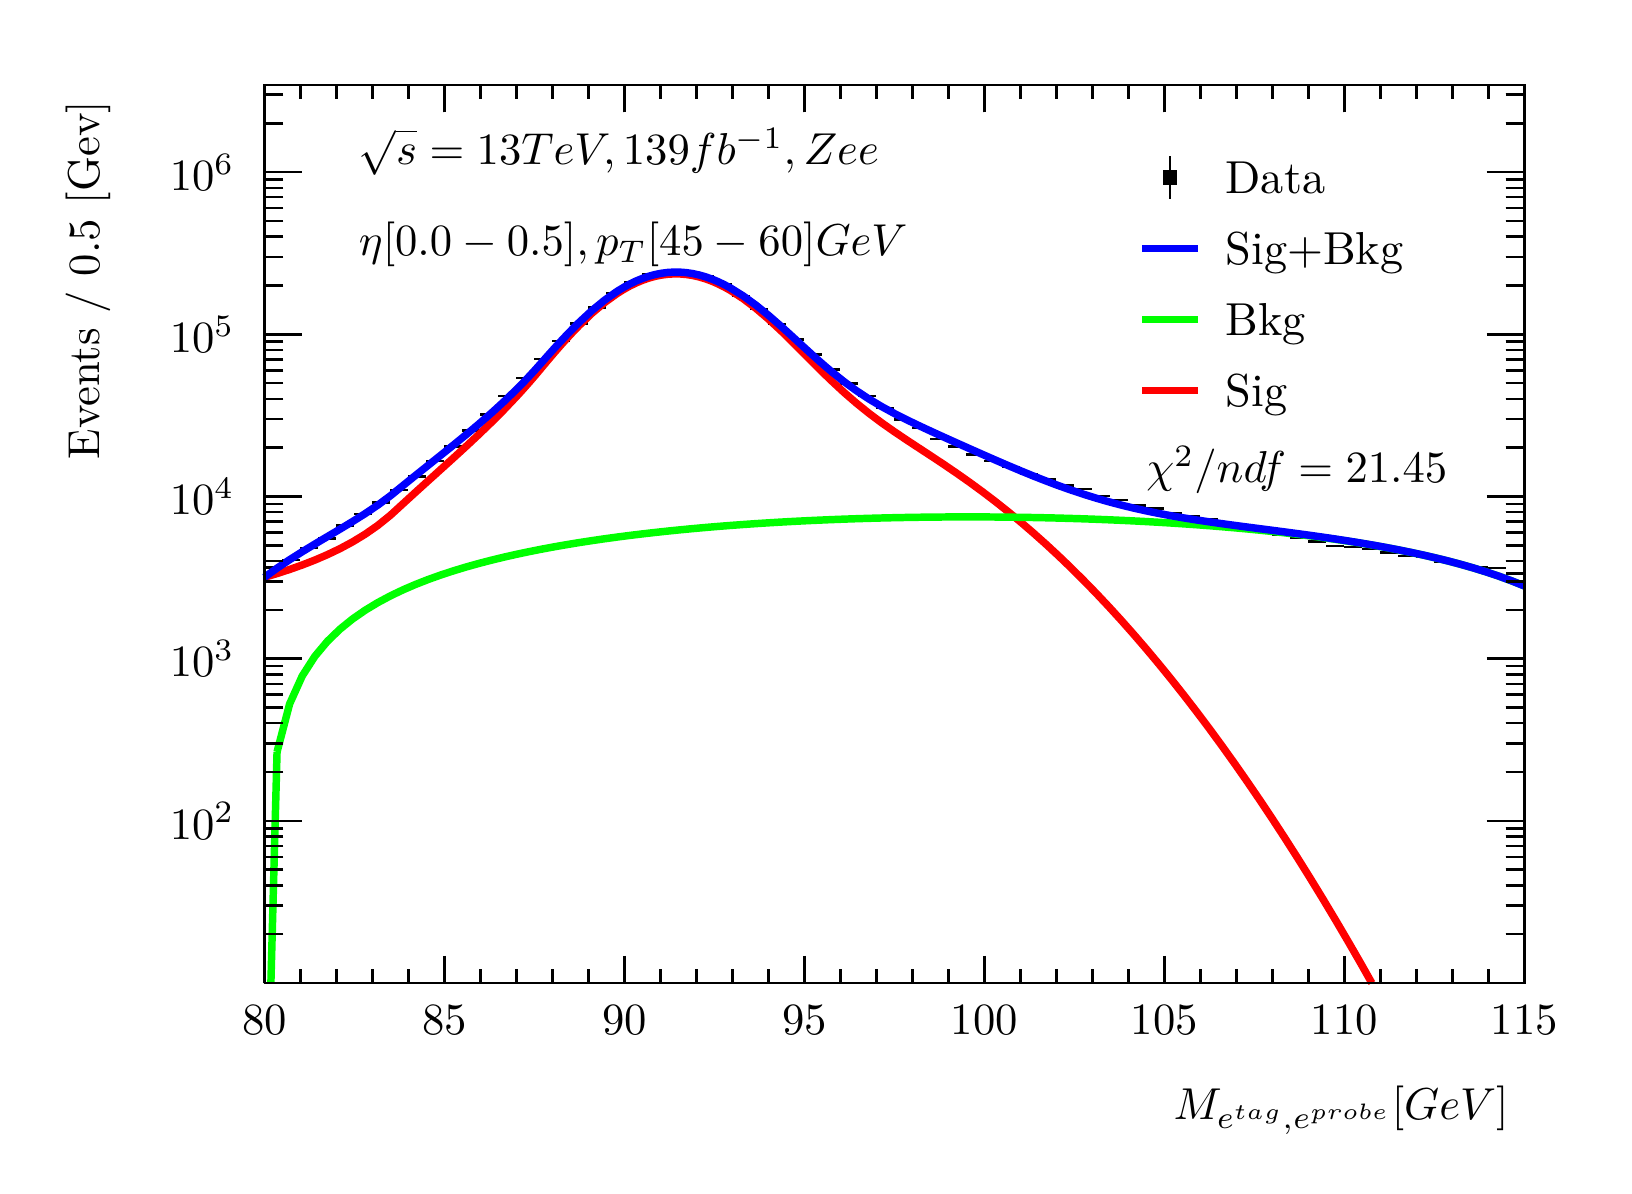
\begin{tikzpicture}
\pgfdeclareplotmark{cross} {
\pgfpathmoveto{\pgfpoint{-0.3\pgfplotmarksize}{\pgfplotmarksize}}
\pgfpathlineto{\pgfpoint{+0.3\pgfplotmarksize}{\pgfplotmarksize}}
\pgfpathlineto{\pgfpoint{+0.3\pgfplotmarksize}{0.3\pgfplotmarksize}}
\pgfpathlineto{\pgfpoint{+1\pgfplotmarksize}{0.3\pgfplotmarksize}}
\pgfpathlineto{\pgfpoint{+1\pgfplotmarksize}{-0.3\pgfplotmarksize}}
\pgfpathlineto{\pgfpoint{+0.3\pgfplotmarksize}{-0.3\pgfplotmarksize}}
\pgfpathlineto{\pgfpoint{+0.3\pgfplotmarksize}{-1.\pgfplotmarksize}}
\pgfpathlineto{\pgfpoint{-0.3\pgfplotmarksize}{-1.\pgfplotmarksize}}
\pgfpathlineto{\pgfpoint{-0.3\pgfplotmarksize}{-0.3\pgfplotmarksize}}
\pgfpathlineto{\pgfpoint{-1.\pgfplotmarksize}{-0.3\pgfplotmarksize}}
\pgfpathlineto{\pgfpoint{-1.\pgfplotmarksize}{0.3\pgfplotmarksize}}
\pgfpathlineto{\pgfpoint{-0.3\pgfplotmarksize}{0.3\pgfplotmarksize}}
\pgfpathclose
\pgfusepathqstroke
}
\pgfdeclareplotmark{cross*} {
\pgfpathmoveto{\pgfpoint{-0.3\pgfplotmarksize}{\pgfplotmarksize}}
\pgfpathlineto{\pgfpoint{+0.3\pgfplotmarksize}{\pgfplotmarksize}}
\pgfpathlineto{\pgfpoint{+0.3\pgfplotmarksize}{0.3\pgfplotmarksize}}
\pgfpathlineto{\pgfpoint{+1\pgfplotmarksize}{0.3\pgfplotmarksize}}
\pgfpathlineto{\pgfpoint{+1\pgfplotmarksize}{-0.3\pgfplotmarksize}}
\pgfpathlineto{\pgfpoint{+0.3\pgfplotmarksize}{-0.3\pgfplotmarksize}}
\pgfpathlineto{\pgfpoint{+0.3\pgfplotmarksize}{-1.\pgfplotmarksize}}
\pgfpathlineto{\pgfpoint{-0.3\pgfplotmarksize}{-1.\pgfplotmarksize}}
\pgfpathlineto{\pgfpoint{-0.3\pgfplotmarksize}{-0.3\pgfplotmarksize}}
\pgfpathlineto{\pgfpoint{-1.\pgfplotmarksize}{-0.3\pgfplotmarksize}}
\pgfpathlineto{\pgfpoint{-1.\pgfplotmarksize}{0.3\pgfplotmarksize}}
\pgfpathlineto{\pgfpoint{-0.3\pgfplotmarksize}{0.3\pgfplotmarksize}}
\pgfpathclose
\pgfusepathqfillstroke
}
\pgfdeclareplotmark{newstar} {
\pgfpathmoveto{\pgfqpoint{0pt}{\pgfplotmarksize}}
\pgfpathlineto{\pgfqpointpolar{44}{0.5\pgfplotmarksize}}
\pgfpathlineto{\pgfqpointpolar{18}{\pgfplotmarksize}}
\pgfpathlineto{\pgfqpointpolar{-20}{0.5\pgfplotmarksize}}
\pgfpathlineto{\pgfqpointpolar{-54}{\pgfplotmarksize}}
\pgfpathlineto{\pgfqpointpolar{-90}{0.5\pgfplotmarksize}}
\pgfpathlineto{\pgfqpointpolar{234}{\pgfplotmarksize}}
\pgfpathlineto{\pgfqpointpolar{198}{0.5\pgfplotmarksize}}
\pgfpathlineto{\pgfqpointpolar{162}{\pgfplotmarksize}}
\pgfpathlineto{\pgfqpointpolar{134}{0.5\pgfplotmarksize}}
\pgfpathclose
\pgfusepathqstroke
}
\pgfdeclareplotmark{newstar*} {
\pgfpathmoveto{\pgfqpoint{0pt}{\pgfplotmarksize}}
\pgfpathlineto{\pgfqpointpolar{44}{0.5\pgfplotmarksize}}
\pgfpathlineto{\pgfqpointpolar{18}{\pgfplotmarksize}}
\pgfpathlineto{\pgfqpointpolar{-20}{0.5\pgfplotmarksize}}
\pgfpathlineto{\pgfqpointpolar{-54}{\pgfplotmarksize}}
\pgfpathlineto{\pgfqpointpolar{-90}{0.5\pgfplotmarksize}}
\pgfpathlineto{\pgfqpointpolar{234}{\pgfplotmarksize}}
\pgfpathlineto{\pgfqpointpolar{198}{0.5\pgfplotmarksize}}
\pgfpathlineto{\pgfqpointpolar{162}{\pgfplotmarksize}}
\pgfpathlineto{\pgfqpointpolar{134}{0.5\pgfplotmarksize}}
\pgfpathclose
\pgfusepathqfillstroke
}
\definecolor{c}{rgb}{1,1,1};
\draw [color=c, fill=c] (0,0) rectangle (20,14.4361);
\draw [color=c, fill=c] (3,2.30977) rectangle (19,13.7143);
\definecolor{c}{rgb}{0,0,0};
\draw [c,line width=0.9] (3,2.30977) -- (3,13.7143) -- (19,13.7143) -- (19,2.30977) -- (3,2.30977);
\definecolor{c}{rgb}{1,1,1};
\draw [color=c, fill=c] (3,2.30977) rectangle (19,13.7143);
\definecolor{c}{rgb}{0,0,0};
\draw [c,line width=0.9] (3,2.30977) -- (3,13.7143) -- (19,13.7143) -- (19,2.30977) -- (3,2.30977);
\draw [c,line width=0.9] (3,2.30977) -- (19,2.30977);
\draw [c,line width=0.9] (3,2.65624) -- (3,2.30977);
\draw [c,line width=0.9] (3.45714,2.48301) -- (3.45714,2.30977);
\draw [c,line width=0.9] (3.91429,2.48301) -- (3.91429,2.30977);
\draw [c,line width=0.9] (4.37143,2.48301) -- (4.37143,2.30977);
\draw [c,line width=0.9] (4.82857,2.48301) -- (4.82857,2.30977);
\draw [c,line width=0.9] (5.28571,2.65624) -- (5.28571,2.30977);
\draw [c,line width=0.9] (5.74286,2.48301) -- (5.74286,2.30977);
\draw [c,line width=0.9] (6.2,2.48301) -- (6.2,2.30977);
\draw [c,line width=0.9] (6.65714,2.48301) -- (6.65714,2.30977);
\draw [c,line width=0.9] (7.11429,2.48301) -- (7.11429,2.30977);
\draw [c,line width=0.9] (7.57143,2.65624) -- (7.57143,2.30977);
\draw [c,line width=0.9] (8.02857,2.48301) -- (8.02857,2.30977);
\draw [c,line width=0.9] (8.48571,2.48301) -- (8.48571,2.30977);
\draw [c,line width=0.9] (8.94286,2.48301) -- (8.94286,2.30977);
\draw [c,line width=0.9] (9.4,2.48301) -- (9.4,2.30977);
\draw [c,line width=0.9] (9.85714,2.65624) -- (9.85714,2.30977);
\draw [c,line width=0.9] (10.3143,2.48301) -- (10.3143,2.30977);
\draw [c,line width=0.9] (10.7714,2.48301) -- (10.7714,2.30977);
\draw [c,line width=0.9] (11.2286,2.48301) -- (11.2286,2.30977);
\draw [c,line width=0.9] (11.6857,2.48301) -- (11.6857,2.30977);
\draw [c,line width=0.9] (12.1429,2.65624) -- (12.1429,2.30977);
\draw [c,line width=0.9] (12.6,2.48301) -- (12.6,2.30977);
\draw [c,line width=0.9] (13.0571,2.48301) -- (13.0571,2.30977);
\draw [c,line width=0.9] (13.5143,2.48301) -- (13.5143,2.30977);
\draw [c,line width=0.9] (13.9714,2.48301) -- (13.9714,2.30977);
\draw [c,line width=0.9] (14.4286,2.65624) -- (14.4286,2.30977);
\draw [c,line width=0.9] (14.8857,2.48301) -- (14.8857,2.30977);
\draw [c,line width=0.9] (15.3429,2.48301) -- (15.3429,2.30977);
\draw [c,line width=0.9] (15.8,2.48301) -- (15.8,2.30977);
\draw [c,line width=0.9] (16.2571,2.48301) -- (16.2571,2.30977);
\draw [c,line width=0.9] (16.7143,2.65624) -- (16.7143,2.30977);
\draw [c,line width=0.9] (17.1714,2.48301) -- (17.1714,2.30977);
\draw [c,line width=0.9] (17.6286,2.48301) -- (17.6286,2.30977);
\draw [c,line width=0.9] (18.0857,2.48301) -- (18.0857,2.30977);
\draw [c,line width=0.9] (18.5429,2.48301) -- (18.5429,2.30977);
\draw [c,line width=0.9] (19,2.65624) -- (19,2.30977);
\draw [anchor=base] (3,1.66015) node[scale=1.61424, color=c, rotate=0]{80};
\draw [anchor=base] (5.28571,1.66015) node[scale=1.61424, color=c, rotate=0]{85};
\draw [anchor=base] (7.57143,1.66015) node[scale=1.61424, color=c, rotate=0]{90};
\draw [anchor=base] (9.85714,1.66015) node[scale=1.61424, color=c, rotate=0]{95};
\draw [anchor=base] (12.1429,1.66015) node[scale=1.61424, color=c, rotate=0]{100};
\draw [anchor=base] (14.4286,1.66015) node[scale=1.61424, color=c, rotate=0]{105};
\draw [anchor=base] (16.7143,1.66015) node[scale=1.61424, color=c, rotate=0]{110};
\draw [anchor=base] (19,1.66015) node[scale=1.61424, color=c, rotate=0]{115};
\draw [anchor= east] (19,0.692932) node[scale=1.61424, color=c, rotate=0]{$M_{e^{tag}, e^{probe}}  [GeV]$};
\draw [c,line width=0.9] (3,13.7143) -- (19,13.7143);
\draw [c,line width=0.9] (3,13.3678) -- (3,13.7143);
\draw [c,line width=0.9] (3.45714,13.5411) -- (3.45714,13.7143);
\draw [c,line width=0.9] (3.91429,13.5411) -- (3.91429,13.7143);
\draw [c,line width=0.9] (4.37143,13.5411) -- (4.37143,13.7143);
\draw [c,line width=0.9] (4.82857,13.5411) -- (4.82857,13.7143);
\draw [c,line width=0.9] (5.28571,13.3678) -- (5.28571,13.7143);
\draw [c,line width=0.9] (5.74286,13.5411) -- (5.74286,13.7143);
\draw [c,line width=0.9] (6.2,13.5411) -- (6.2,13.7143);
\draw [c,line width=0.9] (6.65714,13.5411) -- (6.65714,13.7143);
\draw [c,line width=0.9] (7.11429,13.5411) -- (7.11429,13.7143);
\draw [c,line width=0.9] (7.57143,13.3678) -- (7.57143,13.7143);
\draw [c,line width=0.9] (8.02857,13.5411) -- (8.02857,13.7143);
\draw [c,line width=0.9] (8.48571,13.5411) -- (8.48571,13.7143);
\draw [c,line width=0.9] (8.94286,13.5411) -- (8.94286,13.7143);
\draw [c,line width=0.9] (9.4,13.5411) -- (9.4,13.7143);
\draw [c,line width=0.9] (9.85714,13.3678) -- (9.85714,13.7143);
\draw [c,line width=0.9] (10.3143,13.5411) -- (10.3143,13.7143);
\draw [c,line width=0.9] (10.7714,13.5411) -- (10.7714,13.7143);
\draw [c,line width=0.9] (11.2286,13.5411) -- (11.2286,13.7143);
\draw [c,line width=0.9] (11.6857,13.5411) -- (11.6857,13.7143);
\draw [c,line width=0.9] (12.1429,13.3678) -- (12.1429,13.7143);
\draw [c,line width=0.9] (12.6,13.5411) -- (12.6,13.7143);
\draw [c,line width=0.9] (13.0571,13.5411) -- (13.0571,13.7143);
\draw [c,line width=0.9] (13.5143,13.5411) -- (13.5143,13.7143);
\draw [c,line width=0.9] (13.9714,13.5411) -- (13.9714,13.7143);
\draw [c,line width=0.9] (14.4286,13.3678) -- (14.4286,13.7143);
\draw [c,line width=0.9] (14.8857,13.5411) -- (14.8857,13.7143);
\draw [c,line width=0.9] (15.3429,13.5411) -- (15.3429,13.7143);
\draw [c,line width=0.9] (15.8,13.5411) -- (15.8,13.7143);
\draw [c,line width=0.9] (16.2571,13.5411) -- (16.2571,13.7143);
\draw [c,line width=0.9] (16.7143,13.3678) -- (16.7143,13.7143);
\draw [c,line width=0.9] (17.1714,13.5411) -- (17.1714,13.7143);
\draw [c,line width=0.9] (17.6286,13.5411) -- (17.6286,13.7143);
\draw [c,line width=0.9] (18.0857,13.5411) -- (18.0857,13.7143);
\draw [c,line width=0.9] (18.5429,13.5411) -- (18.5429,13.7143);
\draw [c,line width=0.9] (19,13.3678) -- (19,13.7143);
\draw [c,line width=0.9] (3,2.30977) -- (3,13.7143);
\draw [c,line width=0.9] (3.237,2.92982) -- (3,2.92982);
\draw [c,line width=0.9] (3.237,3.29252) -- (3,3.29252);
\draw [c,line width=0.9] (3.237,3.54986) -- (3,3.54986);
\draw [c,line width=0.9] (3.237,3.74947) -- (3,3.74947);
\draw [c,line width=0.9] (3.237,3.91257) -- (3,3.91257);
\draw [c,line width=0.9] (3.237,4.05046) -- (3,4.05046);
\draw [c,line width=0.9] (3.237,4.16991) -- (3,4.16991);
\draw [c,line width=0.9] (3.237,4.27527) -- (3,4.27527);
\draw [c,line width=0.9] (3.474,4.36952) -- (3,4.36952);
\draw [anchor= east] (2.82,4.36952) node[scale=1.61424, color=c, rotate=0]{$10^{2}$};
\draw [c,line width=0.9] (3.237,4.98956) -- (3,4.98956);
\draw [c,line width=0.9] (3.237,5.35227) -- (3,5.35227);
\draw [c,line width=0.9] (3.237,5.60961) -- (3,5.60961);
\draw [c,line width=0.9] (3.237,5.80922) -- (3,5.80922);
\draw [c,line width=0.9] (3.237,5.97231) -- (3,5.97231);
\draw [c,line width=0.9] (3.237,6.11021) -- (3,6.11021);
\draw [c,line width=0.9] (3.237,6.22966) -- (3,6.22966);
\draw [c,line width=0.9] (3.237,6.33502) -- (3,6.33502);
\draw [c,line width=0.9] (3.474,6.42927) -- (3,6.42927);
\draw [anchor= east] (2.82,6.42927) node[scale=1.61424, color=c, rotate=0]{$10^{3}$};
\draw [c,line width=0.9] (3.237,7.04931) -- (3,7.04931);
\draw [c,line width=0.9] (3.237,7.41202) -- (3,7.41202);
\draw [c,line width=0.9] (3.237,7.66936) -- (3,7.66936);
\draw [c,line width=0.9] (3.237,7.86897) -- (3,7.86897);
\draw [c,line width=0.9] (3.237,8.03206) -- (3,8.03206);
\draw [c,line width=0.9] (3.237,8.16995) -- (3,8.16995);
\draw [c,line width=0.9] (3.237,8.2894) -- (3,8.2894);
\draw [c,line width=0.9] (3.237,8.39476) -- (3,8.39476);
\draw [c,line width=0.9] (3.474,8.48901) -- (3,8.48901);
\draw [anchor= east] (2.82,8.48901) node[scale=1.61424, color=c, rotate=0]{$10^{4}$};
\draw [c,line width=0.9] (3.237,9.10906) -- (3,9.10906);
\draw [c,line width=0.9] (3.237,9.47176) -- (3,9.47176);
\draw [c,line width=0.9] (3.237,9.7291) -- (3,9.7291);
\draw [c,line width=0.9] (3.237,9.92871) -- (3,9.92871);
\draw [c,line width=0.9] (3.237,10.0918) -- (3,10.0918);
\draw [c,line width=0.9] (3.237,10.2297) -- (3,10.2297);
\draw [c,line width=0.9] (3.237,10.3491) -- (3,10.3491);
\draw [c,line width=0.9] (3.237,10.4545) -- (3,10.4545);
\draw [c,line width=0.9] (3.474,10.5488) -- (3,10.5488);
\draw [anchor= east] (2.82,10.5488) node[scale=1.61424, color=c, rotate=0]{$10^{5}$};
\draw [c,line width=0.9] (3.237,11.1688) -- (3,11.1688);
\draw [c,line width=0.9] (3.237,11.5315) -- (3,11.5315);
\draw [c,line width=0.9] (3.237,11.7889) -- (3,11.7889);
\draw [c,line width=0.9] (3.237,11.9885) -- (3,11.9885);
\draw [c,line width=0.9] (3.237,12.1516) -- (3,12.1516);
\draw [c,line width=0.9] (3.237,12.2894) -- (3,12.2894);
\draw [c,line width=0.9] (3.237,12.4089) -- (3,12.4089);
\draw [c,line width=0.9] (3.237,12.5143) -- (3,12.5143);
\draw [c,line width=0.9] (3.474,12.6085) -- (3,12.6085);
\draw [anchor= east] (2.82,12.6085) node[scale=1.61424, color=c, rotate=0]{$10^{6}$};
\draw [c,line width=0.9] (3.237,13.2286) -- (3,13.2286);
\draw [c,line width=0.9] (3.237,13.5913) -- (3,13.5913);
\draw [anchor= east] (0.76,13.7143) node[scale=1.61424, color=c, rotate=90]{Events / 0.5 [Gev]};
\draw [c,line width=0.9] (19,2.30977) -- (19,13.7143);
\draw [c,line width=0.9] (18.763,2.92982) -- (19,2.92982);
\draw [c,line width=0.9] (18.763,3.29252) -- (19,3.29252);
\draw [c,line width=0.9] (18.763,3.54986) -- (19,3.54986);
\draw [c,line width=0.9] (18.763,3.74947) -- (19,3.74947);
\draw [c,line width=0.9] (18.763,3.91257) -- (19,3.91257);
\draw [c,line width=0.9] (18.763,4.05046) -- (19,4.05046);
\draw [c,line width=0.9] (18.763,4.16991) -- (19,4.16991);
\draw [c,line width=0.9] (18.763,4.27527) -- (19,4.27527);
\draw [c,line width=0.9] (18.526,4.36952) -- (19,4.36952);
\draw [c,line width=0.9] (18.763,4.98956) -- (19,4.98956);
\draw [c,line width=0.9] (18.763,5.35227) -- (19,5.35227);
\draw [c,line width=0.9] (18.763,5.60961) -- (19,5.60961);
\draw [c,line width=0.9] (18.763,5.80922) -- (19,5.80922);
\draw [c,line width=0.9] (18.763,5.97231) -- (19,5.97231);
\draw [c,line width=0.9] (18.763,6.11021) -- (19,6.11021);
\draw [c,line width=0.9] (18.763,6.22966) -- (19,6.22966);
\draw [c,line width=0.9] (18.763,6.33502) -- (19,6.33502);
\draw [c,line width=0.9] (18.526,6.42927) -- (19,6.42927);
\draw [c,line width=0.9] (18.763,7.04931) -- (19,7.04931);
\draw [c,line width=0.9] (18.763,7.41202) -- (19,7.41202);
\draw [c,line width=0.9] (18.763,7.66936) -- (19,7.66936);
\draw [c,line width=0.9] (18.763,7.86897) -- (19,7.86897);
\draw [c,line width=0.9] (18.763,8.03206) -- (19,8.03206);
\draw [c,line width=0.9] (18.763,8.16995) -- (19,8.16995);
\draw [c,line width=0.9] (18.763,8.2894) -- (19,8.2894);
\draw [c,line width=0.9] (18.763,8.39476) -- (19,8.39476);
\draw [c,line width=0.9] (18.526,8.48901) -- (19,8.48901);
\draw [c,line width=0.9] (18.763,9.10906) -- (19,9.10906);
\draw [c,line width=0.9] (18.763,9.47176) -- (19,9.47176);
\draw [c,line width=0.9] (18.763,9.7291) -- (19,9.7291);
\draw [c,line width=0.9] (18.763,9.92871) -- (19,9.92871);
\draw [c,line width=0.9] (18.763,10.0918) -- (19,10.0918);
\draw [c,line width=0.9] (18.763,10.2297) -- (19,10.2297);
\draw [c,line width=0.9] (18.763,10.3491) -- (19,10.3491);
\draw [c,line width=0.9] (18.763,10.4545) -- (19,10.4545);
\draw [c,line width=0.9] (18.526,10.5488) -- (19,10.5488);
\draw [c,line width=0.9] (18.763,11.1688) -- (19,11.1688);
\draw [c,line width=0.9] (18.763,11.5315) -- (19,11.5315);
\draw [c,line width=0.9] (18.763,11.7889) -- (19,11.7889);
\draw [c,line width=0.9] (18.763,11.9885) -- (19,11.9885);
\draw [c,line width=0.9] (18.763,12.1516) -- (19,12.1516);
\draw [c,line width=0.9] (18.763,12.2894) -- (19,12.2894);
\draw [c,line width=0.9] (18.763,12.4089) -- (19,12.4089);
\draw [c,line width=0.9] (18.763,12.5143) -- (19,12.5143);
\draw [c,line width=0.9] (18.526,12.6085) -- (19,12.6085);
\draw [c,line width=0.9] (18.763,13.2286) -- (19,13.2286);
\draw [c,line width=0.9] (18.763,13.5913) -- (19,13.5913);
\draw [c,line width=0.9] (3.11429,7.58647) -- (3,7.58647);
\draw [c,line width=0.9] (3,7.58647) -- (3,7.58647);
\draw [c,line width=0.9] (3.11429,7.58647) -- (3.22857,7.58647);
\draw [c,line width=0.9] (3.22857,7.58647) -- (3.22857,7.58647);
\draw [c,line width=0.9] (3.11429,7.58647) -- (3.11429,7.60128);
\draw [c,line width=0.9] (3.11429,7.60128) -- (3.11429,7.60128);
\draw [c,line width=0.9] (3.11429,7.58647) -- (3.11429,7.57165);
\draw [c,line width=0.9] (3.11429,7.57165) -- (3.11429,7.57165);
\draw [c,line width=0.9] (3.34286,7.68466) -- (3.22857,7.68466);
\draw [c,line width=0.9] (3.22857,7.68466) -- (3.22857,7.68466);
\draw [c,line width=0.9] (3.34286,7.68466) -- (3.45714,7.68466);
\draw [c,line width=0.9] (3.45714,7.68466) -- (3.45714,7.68466);
\draw [c,line width=0.9] (3.34286,7.68466) -- (3.34286,7.69868);
\draw [c,line width=0.9] (3.34286,7.69868) -- (3.34286,7.69868);
\draw [c,line width=0.9] (3.34286,7.68466) -- (3.34286,7.67063);
\draw [c,line width=0.9] (3.34286,7.67063) -- (3.34286,7.67063);
\draw [c,line width=0.9] (3.57143,7.83413) -- (3.45714,7.83413);
\draw [c,line width=0.9] (3.45714,7.83413) -- (3.45714,7.83413);
\draw [c,line width=0.9] (3.57143,7.83413) -- (3.68571,7.83413);
\draw [c,line width=0.9] (3.68571,7.83413) -- (3.68571,7.83413);
\draw [c,line width=0.9] (3.57143,7.83413) -- (3.57143,7.84703);
\draw [c,line width=0.9] (3.57143,7.84703) -- (3.57143,7.84703);
\draw [c,line width=0.9] (3.57143,7.83413) -- (3.57143,7.82123);
\draw [c,line width=0.9] (3.57143,7.82123) -- (3.57143,7.82123);
\draw [c,line width=0.9] (3.8,7.95861) -- (3.68571,7.95861);
\draw [c,line width=0.9] (3.68571,7.95861) -- (3.68571,7.95861);
\draw [c,line width=0.9] (3.8,7.95861) -- (3.91429,7.95861);
\draw [c,line width=0.9] (3.91429,7.95861) -- (3.91429,7.95861);
\draw [c,line width=0.9] (3.8,7.95861) -- (3.8,7.97064);
\draw [c,line width=0.9] (3.8,7.97064) -- (3.8,7.97064);
\draw [c,line width=0.9] (3.8,7.95861) -- (3.8,7.94658);
\draw [c,line width=0.9] (3.8,7.94658) -- (3.8,7.94658);
\draw [c,line width=0.9] (4.02857,8.118) -- (3.91429,8.118);
\draw [c,line width=0.9] (3.91429,8.118) -- (3.91429,8.118);
\draw [c,line width=0.9] (4.02857,8.118) -- (4.14286,8.118);
\draw [c,line width=0.9] (4.14286,8.118) -- (4.14286,8.118);
\draw [c,line width=0.9] (4.02857,8.118) -- (4.02857,8.129);
\draw [c,line width=0.9] (4.02857,8.129) -- (4.02857,8.129);
\draw [c,line width=0.9] (4.02857,8.118) -- (4.02857,8.10699);
\draw [c,line width=0.9] (4.02857,8.10699) -- (4.02857,8.10699);
\draw [c,line width=0.9] (4.25714,8.26354) -- (4.14286,8.26354);
\draw [c,line width=0.9] (4.14286,8.26354) -- (4.14286,8.26354);
\draw [c,line width=0.9] (4.25714,8.26354) -- (4.37143,8.26354);
\draw [c,line width=0.9] (4.37143,8.26354) -- (4.37143,8.26354);
\draw [c,line width=0.9] (4.25714,8.26354) -- (4.25714,8.27369);
\draw [c,line width=0.9] (4.25714,8.27369) -- (4.25714,8.27369);
\draw [c,line width=0.9] (4.25714,8.26354) -- (4.25714,8.25339);
\draw [c,line width=0.9] (4.25714,8.25339) -- (4.25714,8.25339);
\draw [c,line width=0.9] (4.48571,8.41189) -- (4.37143,8.41189);
\draw [c,line width=0.9] (4.37143,8.41189) -- (4.37143,8.41189);
\draw [c,line width=0.9] (4.48571,8.41189) -- (4.6,8.41189);
\draw [c,line width=0.9] (4.6,8.41189) -- (4.6,8.41189);
\draw [c,line width=0.9] (4.48571,8.41189) -- (4.48571,8.42123);
\draw [c,line width=0.9] (4.48571,8.42123) -- (4.48571,8.42123);
\draw [c,line width=0.9] (4.48571,8.41189) -- (4.48571,8.40256);
\draw [c,line width=0.9] (4.48571,8.40256) -- (4.48571,8.40256);
\draw [c,line width=0.9] (4.71429,8.5702) -- (4.6,8.5702);
\draw [c,line width=0.9] (4.6,8.5702) -- (4.6,8.5702);
\draw [c,line width=0.9] (4.71429,8.5702) -- (4.82857,8.5702);
\draw [c,line width=0.9] (4.82857,8.5702) -- (4.82857,8.5702);
\draw [c,line width=0.9] (4.71429,8.5702) -- (4.71429,8.57875);
\draw [c,line width=0.9] (4.71429,8.57875) -- (4.71429,8.57875);
\draw [c,line width=0.9] (4.71429,8.5702) -- (4.71429,8.56165);
\draw [c,line width=0.9] (4.71429,8.56165) -- (4.71429,8.56165);
\draw [c,line width=0.9] (4.94286,8.74338) -- (4.82857,8.74338);
\draw [c,line width=0.9] (4.82857,8.74338) -- (4.82857,8.74338);
\draw [c,line width=0.9] (4.94286,8.74338) -- (5.05714,8.74338);
\draw [c,line width=0.9] (5.05714,8.74338) -- (5.05714,8.74338);
\draw [c,line width=0.9] (4.94286,8.74338) -- (4.94286,8.75114);
\draw [c,line width=0.9] (4.94286,8.75114) -- (4.94286,8.75114);
\draw [c,line width=0.9] (4.94286,8.74338) -- (4.94286,8.73562);
\draw [c,line width=0.9] (4.94286,8.73562) -- (4.94286,8.73562);
\draw [c,line width=0.9] (5.17143,8.93957) -- (5.05714,8.93957);
\draw [c,line width=0.9] (5.05714,8.93957) -- (5.05714,8.93957);
\draw [c,line width=0.9] (5.17143,8.93957) -- (5.28571,8.93957);
\draw [c,line width=0.9] (5.28571,8.93957) -- (5.28571,8.93957);
\draw [c,line width=0.9] (5.17143,8.93957) -- (5.17143,8.94653);
\draw [c,line width=0.9] (5.17143,8.94653) -- (5.17143,8.94653);
\draw [c,line width=0.9] (5.17143,8.93957) -- (5.17143,8.93262);
\draw [c,line width=0.9] (5.17143,8.93262) -- (5.17143,8.93262);
\draw [c,line width=0.9] (5.4,9.12594) -- (5.28571,9.12594);
\draw [c,line width=0.9] (5.28571,9.12594) -- (5.28571,9.12594);
\draw [c,line width=0.9] (5.4,9.12594) -- (5.51429,9.12594);
\draw [c,line width=0.9] (5.51429,9.12594) -- (5.51429,9.12594);
\draw [c,line width=0.9] (5.4,9.12594) -- (5.4,9.13221);
\draw [c,line width=0.9] (5.4,9.13221) -- (5.4,9.13221);
\draw [c,line width=0.9] (5.4,9.12594) -- (5.4,9.11967);
\draw [c,line width=0.9] (5.4,9.11967) -- (5.4,9.11967);
\draw [c,line width=0.9] (5.62857,9.32751) -- (5.51429,9.32751);
\draw [c,line width=0.9] (5.51429,9.32751) -- (5.51429,9.32751);
\draw [c,line width=0.9] (5.62857,9.32751) -- (5.74286,9.32751);
\draw [c,line width=0.9] (5.74286,9.32751) -- (5.74286,9.32751);
\draw [c,line width=0.9] (5.62857,9.32751) -- (5.62857,9.3331);
\draw [c,line width=0.9] (5.62857,9.3331) -- (5.62857,9.3331);
\draw [c,line width=0.9] (5.62857,9.32751) -- (5.62857,9.32191);
\draw [c,line width=0.9] (5.62857,9.32191) -- (5.62857,9.32191);
\draw [c,line width=0.9] (5.85714,9.53) -- (5.74286,9.53);
\draw [c,line width=0.9] (5.74286,9.53) -- (5.74286,9.53);
\draw [c,line width=0.9] (5.85714,9.53) -- (5.97143,9.53);
\draw [c,line width=0.9] (5.97143,9.53) -- (5.97143,9.53);
\draw [c,line width=0.9] (5.85714,9.53) -- (5.85714,9.535);
\draw [c,line width=0.9] (5.85714,9.535) -- (5.85714,9.535);
\draw [c,line width=0.9] (5.85714,9.53) -- (5.85714,9.525);
\draw [c,line width=0.9] (5.85714,9.525) -- (5.85714,9.525);
\draw [c,line width=0.9] (6.08571,9.76837) -- (5.97143,9.76837);
\draw [c,line width=0.9] (5.97143,9.76837) -- (5.97143,9.76837);
\draw [c,line width=0.9] (6.08571,9.76837) -- (6.2,9.76837);
\draw [c,line width=0.9] (6.2,9.76837) -- (6.2,9.76837);
\draw [c,line width=0.9] (6.08571,9.76837) -- (6.08571,9.77275);
\draw [c,line width=0.9] (6.08571,9.77275) -- (6.08571,9.77275);
\draw [c,line width=0.9] (6.08571,9.76837) -- (6.08571,9.764);
\draw [c,line width=0.9] (6.08571,9.764) -- (6.08571,9.764);
\draw [c,line width=0.9] (6.31429,9.99199) -- (6.2,9.99199);
\draw [c,line width=0.9] (6.2,9.99199) -- (6.2,9.99199);
\draw [c,line width=0.9] (6.31429,9.99199) -- (6.42857,9.99199);
\draw [c,line width=0.9] (6.42857,9.99199) -- (6.42857,9.99199);
\draw [c,line width=0.9] (6.31429,9.99199) -- (6.31429,9.99585);
\draw [c,line width=0.9] (6.31429,9.99585) -- (6.31429,9.99585);
\draw [c,line width=0.9] (6.31429,9.99199) -- (6.31429,9.98813);
\draw [c,line width=0.9] (6.31429,9.98813) -- (6.31429,9.98813);
\draw [c,line width=0.9] (6.54286,10.2354) -- (6.42857,10.2354);
\draw [c,line width=0.9] (6.42857,10.2354) -- (6.42857,10.2354);
\draw [c,line width=0.9] (6.54286,10.2354) -- (6.65714,10.2354);
\draw [c,line width=0.9] (6.65714,10.2354) -- (6.65714,10.2354);
\draw [c,line width=0.9] (6.54286,10.2354) -- (6.54286,10.2387);
\draw [c,line width=0.9] (6.54286,10.2387) -- (6.54286,10.2387);
\draw [c,line width=0.9] (6.54286,10.2354) -- (6.54286,10.232);
\draw [c,line width=0.9] (6.54286,10.232) -- (6.54286,10.232);
\draw [c,line width=0.9] (6.77143,10.4629) -- (6.65714,10.4629);
\draw [c,line width=0.9] (6.65714,10.4629) -- (6.65714,10.4629);
\draw [c,line width=0.9] (6.77143,10.4629) -- (6.88571,10.4629);
\draw [c,line width=0.9] (6.88571,10.4629) -- (6.88571,10.4629);
\draw [c,line width=0.9] (6.77143,10.4629) -- (6.77143,10.4658);
\draw [c,line width=0.9] (6.77143,10.4658) -- (6.77143,10.4658);
\draw [c,line width=0.9] (6.77143,10.4629) -- (6.77143,10.4599);
\draw [c,line width=0.9] (6.77143,10.4599) -- (6.77143,10.4599);
\draw [c,line width=0.9] (7,10.6841) -- (6.88571,10.6841);
\draw [c,line width=0.9] (6.88571,10.6841) -- (6.88571,10.6841);
\draw [c,line width=0.9] (7,10.6841) -- (7.11429,10.6841);
\draw [c,line width=0.9] (7.11429,10.6841) -- (7.11429,10.6841);
\draw [c,line width=0.9] (7,10.6841) -- (7,10.6867);
\draw [c,line width=0.9] (7,10.6867) -- (7,10.6867);
\draw [c,line width=0.9] (7,10.6841) -- (7,10.6815);
\draw [c,line width=0.9] (7,10.6815) -- (7,10.6815);
\draw [c,line width=0.9] (7.22857,10.8887) -- (7.11429,10.8887);
\draw [c,line width=0.9] (7.11429,10.8887) -- (7.11429,10.8887);
\draw [c,line width=0.9] (7.22857,10.8887) -- (7.34286,10.8887);
\draw [c,line width=0.9] (7.34286,10.8887) -- (7.34286,10.8887);
\draw [c,line width=0.9] (7.22857,10.8887) -- (7.22857,10.891);
\draw [c,line width=0.9] (7.22857,10.891) -- (7.22857,10.891);
\draw [c,line width=0.9] (7.22857,10.8887) -- (7.22857,10.8863);
\draw [c,line width=0.9] (7.22857,10.8863) -- (7.22857,10.8863);
\draw [c,line width=0.9] (7.45714,11.0725) -- (7.34286,11.0725);
\draw [c,line width=0.9] (7.34286,11.0725) -- (7.34286,11.0725);
\draw [c,line width=0.9] (7.45714,11.0725) -- (7.57143,11.0725);
\draw [c,line width=0.9] (7.57143,11.0725) -- (7.57143,11.0725);
\draw [c,line width=0.9] (7.45714,11.0725) -- (7.45714,11.0746);
\draw [c,line width=0.9] (7.45714,11.0746) -- (7.45714,11.0746);
\draw [c,line width=0.9] (7.45714,11.0725) -- (7.45714,11.0704);
\draw [c,line width=0.9] (7.45714,11.0704) -- (7.45714,11.0704);
\draw [c,line width=0.9] (7.68571,11.2095) -- (7.57143,11.2095);
\draw [c,line width=0.9] (7.57143,11.2095) -- (7.57143,11.2095);
\draw [c,line width=0.9] (7.68571,11.2095) -- (7.8,11.2095);
\draw [c,line width=0.9] (7.8,11.2095) -- (7.8,11.2095);
\draw [c,line width=0.9] (7.68571,11.2095) -- (7.68571,11.2115);
\draw [c,line width=0.9] (7.68571,11.2115) -- (7.68571,11.2115);
\draw [c,line width=0.9] (7.68571,11.2095) -- (7.68571,11.2076);
\draw [c,line width=0.9] (7.68571,11.2076) -- (7.68571,11.2076);
\draw [c,line width=0.9] (7.91429,11.3058) -- (7.8,11.3058);
\draw [c,line width=0.9] (7.8,11.3058) -- (7.8,11.3058);
\draw [c,line width=0.9] (7.91429,11.3058) -- (8.02857,11.3058);
\draw [c,line width=0.9] (8.02857,11.3058) -- (8.02857,11.3058);
\draw [c,line width=0.9] (7.91429,11.3058) -- (7.91429,11.3076);
\draw [c,line width=0.9] (7.91429,11.3076) -- (7.91429,11.3076);
\draw [c,line width=0.9] (7.91429,11.3058) -- (7.91429,11.3039);
\draw [c,line width=0.9] (7.91429,11.3039) -- (7.91429,11.3039);
\draw [c,line width=0.9] (8.14286,11.3499) -- (8.02857,11.3499);
\draw [c,line width=0.9] (8.02857,11.3499) -- (8.02857,11.3499);
\draw [c,line width=0.9] (8.14286,11.3499) -- (8.25714,11.3499);
\draw [c,line width=0.9] (8.25714,11.3499) -- (8.25714,11.3499);
\draw [c,line width=0.9] (8.14286,11.3499) -- (8.14286,11.3517);
\draw [c,line width=0.9] (8.14286,11.3517) -- (8.14286,11.3517);
\draw [c,line width=0.9] (8.14286,11.3499) -- (8.14286,11.348);
\draw [c,line width=0.9] (8.14286,11.348) -- (8.14286,11.348);
\draw [c,line width=0.9] (8.37143,11.3424) -- (8.25714,11.3424);
\draw [c,line width=0.9] (8.25714,11.3424) -- (8.25714,11.3424);
\draw [c,line width=0.9] (8.37143,11.3424) -- (8.48571,11.3424);
\draw [c,line width=0.9] (8.48571,11.3424) -- (8.48571,11.3424);
\draw [c,line width=0.9] (8.37143,11.3424) -- (8.37143,11.3442);
\draw [c,line width=0.9] (8.37143,11.3442) -- (8.37143,11.3442);
\draw [c,line width=0.9] (8.37143,11.3424) -- (8.37143,11.3406);
\draw [c,line width=0.9] (8.37143,11.3406) -- (8.37143,11.3406);
\draw [c,line width=0.9] (8.6,11.2839) -- (8.48571,11.2839);
\draw [c,line width=0.9] (8.48571,11.2839) -- (8.48571,11.2839);
\draw [c,line width=0.9] (8.6,11.2839) -- (8.71429,11.2839);
\draw [c,line width=0.9] (8.71429,11.2839) -- (8.71429,11.2839);
\draw [c,line width=0.9] (8.6,11.2839) -- (8.6,11.2858);
\draw [c,line width=0.9] (8.6,11.2858) -- (8.6,11.2858);
\draw [c,line width=0.9] (8.6,11.2839) -- (8.6,11.2821);
\draw [c,line width=0.9] (8.6,11.2821) -- (8.6,11.2821);
\draw [c,line width=0.9] (8.82857,11.1805) -- (8.71429,11.1805);
\draw [c,line width=0.9] (8.71429,11.1805) -- (8.71429,11.1805);
\draw [c,line width=0.9] (8.82857,11.1805) -- (8.94286,11.1805);
\draw [c,line width=0.9] (8.94286,11.1805) -- (8.94286,11.1805);
\draw [c,line width=0.9] (8.82857,11.1805) -- (8.82857,11.1825);
\draw [c,line width=0.9] (8.82857,11.1825) -- (8.82857,11.1825);
\draw [c,line width=0.9] (8.82857,11.1805) -- (8.82857,11.1785);
\draw [c,line width=0.9] (8.82857,11.1785) -- (8.82857,11.1785);
\draw [c,line width=0.9] (9.05714,11.0348) -- (8.94286,11.0348);
\draw [c,line width=0.9] (8.94286,11.0348) -- (8.94286,11.0348);
\draw [c,line width=0.9] (9.05714,11.0348) -- (9.17143,11.0348);
\draw [c,line width=0.9] (9.17143,11.0348) -- (9.17143,11.0348);
\draw [c,line width=0.9] (9.05714,11.0348) -- (9.05714,11.037);
\draw [c,line width=0.9] (9.05714,11.037) -- (9.05714,11.037);
\draw [c,line width=0.9] (9.05714,11.0348) -- (9.05714,11.0326);
\draw [c,line width=0.9] (9.05714,11.0326) -- (9.05714,11.0326);
\draw [c,line width=0.9] (9.28571,10.8686) -- (9.17143,10.8686);
\draw [c,line width=0.9] (9.17143,10.8686) -- (9.17143,10.8686);
\draw [c,line width=0.9] (9.28571,10.8686) -- (9.4,10.8686);
\draw [c,line width=0.9] (9.4,10.8686) -- (9.4,10.8686);
\draw [c,line width=0.9] (9.28571,10.8686) -- (9.28571,10.8709);
\draw [c,line width=0.9] (9.28571,10.8709) -- (9.28571,10.8709);
\draw [c,line width=0.9] (9.28571,10.8686) -- (9.28571,10.8662);
\draw [c,line width=0.9] (9.28571,10.8662) -- (9.28571,10.8662);
\draw [c,line width=0.9] (9.51429,10.6793) -- (9.4,10.6793);
\draw [c,line width=0.9] (9.4,10.6793) -- (9.4,10.6793);
\draw [c,line width=0.9] (9.51429,10.6793) -- (9.62857,10.6793);
\draw [c,line width=0.9] (9.62857,10.6793) -- (9.62857,10.6793);
\draw [c,line width=0.9] (9.51429,10.6793) -- (9.51429,10.6819);
\draw [c,line width=0.9] (9.51429,10.6819) -- (9.51429,10.6819);
\draw [c,line width=0.9] (9.51429,10.6793) -- (9.51429,10.6766);
\draw [c,line width=0.9] (9.51429,10.6766) -- (9.51429,10.6766);
\draw [c,line width=0.9] (9.74286,10.4843) -- (9.62857,10.4843);
\draw [c,line width=0.9] (9.62857,10.4843) -- (9.62857,10.4843);
\draw [c,line width=0.9] (9.74286,10.4843) -- (9.85714,10.4843);
\draw [c,line width=0.9] (9.85714,10.4843) -- (9.85714,10.4843);
\draw [c,line width=0.9] (9.74286,10.4843) -- (9.74286,10.4872);
\draw [c,line width=0.9] (9.74286,10.4872) -- (9.74286,10.4872);
\draw [c,line width=0.9] (9.74286,10.4843) -- (9.74286,10.4814);
\draw [c,line width=0.9] (9.74286,10.4814) -- (9.74286,10.4814);
\draw [c,line width=0.9] (9.97143,10.2927) -- (9.85714,10.2927);
\draw [c,line width=0.9] (9.85714,10.2927) -- (9.85714,10.2927);
\draw [c,line width=0.9] (9.97143,10.2927) -- (10.0857,10.2927);
\draw [c,line width=0.9] (10.0857,10.2927) -- (10.0857,10.2927);
\draw [c,line width=0.9] (9.97143,10.2927) -- (9.97143,10.296);
\draw [c,line width=0.9] (9.97143,10.296) -- (9.97143,10.296);
\draw [c,line width=0.9] (9.97143,10.2927) -- (9.97143,10.2895);
\draw [c,line width=0.9] (9.97143,10.2895) -- (9.97143,10.2895);
\draw [c,line width=0.9] (10.2,10.1023) -- (10.0857,10.1023);
\draw [c,line width=0.9] (10.0857,10.1023) -- (10.0857,10.1023);
\draw [c,line width=0.9] (10.2,10.1023) -- (10.3143,10.1023);
\draw [c,line width=0.9] (10.3143,10.1023) -- (10.3143,10.1023);
\draw [c,line width=0.9] (10.2,10.1023) -- (10.2,10.1059);
\draw [c,line width=0.9] (10.2,10.1059) -- (10.2,10.1059);
\draw [c,line width=0.9] (10.2,10.1023) -- (10.2,10.0987);
\draw [c,line width=0.9] (10.2,10.0987) -- (10.2,10.0987);
\draw [c,line width=0.9] (10.4286,9.92126) -- (10.3143,9.92126);
\draw [c,line width=0.9] (10.3143,9.92126) -- (10.3143,9.92126);
\draw [c,line width=0.9] (10.4286,9.92126) -- (10.5429,9.92126);
\draw [c,line width=0.9] (10.5429,9.92126) -- (10.5429,9.92126);
\draw [c,line width=0.9] (10.4286,9.92126) -- (10.4286,9.92528);
\draw [c,line width=0.9] (10.4286,9.92528) -- (10.4286,9.92528);
\draw [c,line width=0.9] (10.4286,9.92126) -- (10.4286,9.91724);
\draw [c,line width=0.9] (10.4286,9.91724) -- (10.4286,9.91724);
\draw [c,line width=0.9] (10.6571,9.7638) -- (10.5429,9.7638);
\draw [c,line width=0.9] (10.5429,9.7638) -- (10.5429,9.7638);
\draw [c,line width=0.9] (10.6571,9.7638) -- (10.7714,9.7638);
\draw [c,line width=0.9] (10.7714,9.7638) -- (10.7714,9.7638);
\draw [c,line width=0.9] (10.6571,9.7638) -- (10.6571,9.76819);
\draw [c,line width=0.9] (10.6571,9.76819) -- (10.6571,9.76819);
\draw [c,line width=0.9] (10.6571,9.7638) -- (10.6571,9.75942);
\draw [c,line width=0.9] (10.6571,9.75942) -- (10.6571,9.75942);
\draw [c,line width=0.9] (10.8857,9.61001) -- (10.7714,9.61001);
\draw [c,line width=0.9] (10.7714,9.61001) -- (10.7714,9.61001);
\draw [c,line width=0.9] (10.8857,9.61001) -- (11,9.61001);
\draw [c,line width=0.9] (11,9.61001) -- (11,9.61001);
\draw [c,line width=0.9] (10.8857,9.61001) -- (10.8857,9.61479);
\draw [c,line width=0.9] (10.8857,9.61479) -- (10.8857,9.61479);
\draw [c,line width=0.9] (10.8857,9.61001) -- (10.8857,9.60523);
\draw [c,line width=0.9] (10.8857,9.60523) -- (10.8857,9.60523);
\draw [c,line width=0.9] (11.1143,9.46485) -- (11,9.46485);
\draw [c,line width=0.9] (11,9.46485) -- (11,9.46485);
\draw [c,line width=0.9] (11.1143,9.46485) -- (11.2286,9.46485);
\draw [c,line width=0.9] (11.2286,9.46485) -- (11.2286,9.46485);
\draw [c,line width=0.9] (11.1143,9.46485) -- (11.1143,9.47003);
\draw [c,line width=0.9] (11.1143,9.47003) -- (11.1143,9.47003);
\draw [c,line width=0.9] (11.1143,9.46485) -- (11.1143,9.45966);
\draw [c,line width=0.9] (11.1143,9.45966) -- (11.1143,9.45966);
\draw [c,line width=0.9] (11.3429,9.35677) -- (11.2286,9.35677);
\draw [c,line width=0.9] (11.2286,9.35677) -- (11.2286,9.35677);
\draw [c,line width=0.9] (11.3429,9.35677) -- (11.4571,9.35677);
\draw [c,line width=0.9] (11.4571,9.35677) -- (11.4571,9.35677);
\draw [c,line width=0.9] (11.3429,9.35677) -- (11.3429,9.36228);
\draw [c,line width=0.9] (11.3429,9.36228) -- (11.3429,9.36228);
\draw [c,line width=0.9] (11.3429,9.35677) -- (11.3429,9.35126);
\draw [c,line width=0.9] (11.3429,9.35126) -- (11.3429,9.35126);
\draw [c,line width=0.9] (11.5714,9.22135) -- (11.4571,9.22135);
\draw [c,line width=0.9] (11.4571,9.22135) -- (11.4571,9.22135);
\draw [c,line width=0.9] (11.5714,9.22135) -- (11.6857,9.22135);
\draw [c,line width=0.9] (11.6857,9.22135) -- (11.6857,9.22135);
\draw [c,line width=0.9] (11.5714,9.22135) -- (11.5714,9.22729);
\draw [c,line width=0.9] (11.5714,9.22729) -- (11.5714,9.22729);
\draw [c,line width=0.9] (11.5714,9.22135) -- (11.5714,9.21541);
\draw [c,line width=0.9] (11.5714,9.21541) -- (11.5714,9.21541);
\draw [c,line width=0.9] (11.8,9.12374) -- (11.6857,9.12374);
\draw [c,line width=0.9] (11.6857,9.12374) -- (11.6857,9.12374);
\draw [c,line width=0.9] (11.8,9.12374) -- (11.9143,9.12374);
\draw [c,line width=0.9] (11.9143,9.12374) -- (11.9143,9.12374);
\draw [c,line width=0.9] (11.8,9.12374) -- (11.8,9.13002);
\draw [c,line width=0.9] (11.8,9.13002) -- (11.8,9.13002);
\draw [c,line width=0.9] (11.8,9.12374) -- (11.8,9.11747);
\draw [c,line width=0.9] (11.8,9.11747) -- (11.8,9.11747);
\draw [c,line width=0.9] (12.0286,9.02361) -- (11.9143,9.02361);
\draw [c,line width=0.9] (11.9143,9.02361) -- (11.9143,9.02361);
\draw [c,line width=0.9] (12.0286,9.02361) -- (12.1429,9.02361);
\draw [c,line width=0.9] (12.1429,9.02361) -- (12.1429,9.02361);
\draw [c,line width=0.9] (12.0286,9.02361) -- (12.0286,9.03025);
\draw [c,line width=0.9] (12.0286,9.03025) -- (12.0286,9.03025);
\draw [c,line width=0.9] (12.0286,9.02361) -- (12.0286,9.01698);
\draw [c,line width=0.9] (12.0286,9.01698) -- (12.0286,9.01698);
\draw [c,line width=0.9] (12.2571,8.9379) -- (12.1429,8.9379);
\draw [c,line width=0.9] (12.1429,8.9379) -- (12.1429,8.9379);
\draw [c,line width=0.9] (12.2571,8.9379) -- (12.3714,8.9379);
\draw [c,line width=0.9] (12.3714,8.9379) -- (12.3714,8.9379);
\draw [c,line width=0.9] (12.2571,8.9379) -- (12.2571,8.94486);
\draw [c,line width=0.9] (12.2571,8.94486) -- (12.2571,8.94486);
\draw [c,line width=0.9] (12.2571,8.9379) -- (12.2571,8.93094);
\draw [c,line width=0.9] (12.2571,8.93094) -- (12.2571,8.93094);
\draw [c,line width=0.9] (12.4857,8.86144) -- (12.3714,8.86144);
\draw [c,line width=0.9] (12.3714,8.86144) -- (12.3714,8.86144);
\draw [c,line width=0.9] (12.4857,8.86144) -- (12.6,8.86144);
\draw [c,line width=0.9] (12.6,8.86144) -- (12.6,8.86144);
\draw [c,line width=0.9] (12.4857,8.86144) -- (12.4857,8.86871);
\draw [c,line width=0.9] (12.4857,8.86871) -- (12.4857,8.86871);
\draw [c,line width=0.9] (12.4857,8.86144) -- (12.4857,8.85418);
\draw [c,line width=0.9] (12.4857,8.85418) -- (12.4857,8.85418);
\draw [c,line width=0.9] (12.7143,8.77297) -- (12.6,8.77297);
\draw [c,line width=0.9] (12.6,8.77297) -- (12.6,8.77297);
\draw [c,line width=0.9] (12.7143,8.77297) -- (12.8286,8.77297);
\draw [c,line width=0.9] (12.8286,8.77297) -- (12.8286,8.77297);
\draw [c,line width=0.9] (12.7143,8.77297) -- (12.7143,8.7806);
\draw [c,line width=0.9] (12.7143,8.7806) -- (12.7143,8.7806);
\draw [c,line width=0.9] (12.7143,8.77297) -- (12.7143,8.76534);
\draw [c,line width=0.9] (12.7143,8.76534) -- (12.7143,8.76534);
\draw [c,line width=0.9] (12.9429,8.70325) -- (12.8286,8.70325);
\draw [c,line width=0.9] (12.8286,8.70325) -- (12.8286,8.70325);
\draw [c,line width=0.9] (12.9429,8.70325) -- (13.0571,8.70325);
\draw [c,line width=0.9] (13.0571,8.70325) -- (13.0571,8.70325);
\draw [c,line width=0.9] (12.9429,8.70325) -- (12.9429,8.71118);
\draw [c,line width=0.9] (12.9429,8.71118) -- (12.9429,8.71118);
\draw [c,line width=0.9] (12.9429,8.70325) -- (12.9429,8.69531);
\draw [c,line width=0.9] (12.9429,8.69531) -- (12.9429,8.69531);
\draw [c,line width=0.9] (13.1714,8.62785) -- (13.0571,8.62785);
\draw [c,line width=0.9] (13.0571,8.62785) -- (13.0571,8.62785);
\draw [c,line width=0.9] (13.1714,8.62785) -- (13.2857,8.62785);
\draw [c,line width=0.9] (13.2857,8.62785) -- (13.2857,8.62785);
\draw [c,line width=0.9] (13.1714,8.62785) -- (13.1714,8.63613);
\draw [c,line width=0.9] (13.1714,8.63613) -- (13.1714,8.63613);
\draw [c,line width=0.9] (13.1714,8.62785) -- (13.1714,8.61958);
\draw [c,line width=0.9] (13.1714,8.61958) -- (13.1714,8.61958);
\draw [c,line width=0.9] (13.4,8.58309) -- (13.2857,8.58309);
\draw [c,line width=0.9] (13.2857,8.58309) -- (13.2857,8.58309);
\draw [c,line width=0.9] (13.4,8.58309) -- (13.5143,8.58309);
\draw [c,line width=0.9] (13.5143,8.58309) -- (13.5143,8.58309);
\draw [c,line width=0.9] (13.4,8.58309) -- (13.4,8.59158);
\draw [c,line width=0.9] (13.4,8.59158) -- (13.4,8.59158);
\draw [c,line width=0.9] (13.4,8.58309) -- (13.4,8.57461);
\draw [c,line width=0.9] (13.4,8.57461) -- (13.4,8.57461);
\draw [c,line width=0.9] (13.6286,8.49676) -- (13.5143,8.49676);
\draw [c,line width=0.9] (13.5143,8.49676) -- (13.5143,8.49676);
\draw [c,line width=0.9] (13.6286,8.49676) -- (13.7429,8.49676);
\draw [c,line width=0.9] (13.7429,8.49676) -- (13.7429,8.49676);
\draw [c,line width=0.9] (13.6286,8.49676) -- (13.6286,8.50567);
\draw [c,line width=0.9] (13.6286,8.50567) -- (13.6286,8.50567);
\draw [c,line width=0.9] (13.6286,8.49676) -- (13.6286,8.48786);
\draw [c,line width=0.9] (13.6286,8.48786) -- (13.6286,8.48786);
\draw [c,line width=0.9] (13.8571,8.44238) -- (13.7429,8.44238);
\draw [c,line width=0.9] (13.7429,8.44238) -- (13.7429,8.44238);
\draw [c,line width=0.9] (13.8571,8.44238) -- (13.9714,8.44238);
\draw [c,line width=0.9] (13.9714,8.44238) -- (13.9714,8.44238);
\draw [c,line width=0.9] (13.8571,8.44238) -- (13.8571,8.45156);
\draw [c,line width=0.9] (13.8571,8.45156) -- (13.8571,8.45156);
\draw [c,line width=0.9] (13.8571,8.44238) -- (13.8571,8.4332);
\draw [c,line width=0.9] (13.8571,8.4332) -- (13.8571,8.4332);
\draw [c,line width=0.9] (14.0857,8.37558) -- (13.9714,8.37558);
\draw [c,line width=0.9] (13.9714,8.37558) -- (13.9714,8.37558);
\draw [c,line width=0.9] (14.0857,8.37558) -- (14.2,8.37558);
\draw [c,line width=0.9] (14.2,8.37558) -- (14.2,8.37558);
\draw [c,line width=0.9] (14.0857,8.37558) -- (14.0857,8.38511);
\draw [c,line width=0.9] (14.0857,8.38511) -- (14.0857,8.38511);
\draw [c,line width=0.9] (14.0857,8.37558) -- (14.0857,8.36605);
\draw [c,line width=0.9] (14.0857,8.36605) -- (14.0857,8.36605);
\draw [c,line width=0.9] (14.3143,8.3373) -- (14.2,8.3373);
\draw [c,line width=0.9] (14.2,8.3373) -- (14.2,8.3373);
\draw [c,line width=0.9] (14.3143,8.3373) -- (14.4286,8.3373);
\draw [c,line width=0.9] (14.4286,8.3373) -- (14.4286,8.3373);
\draw [c,line width=0.9] (14.3143,8.3373) -- (14.3143,8.34704);
\draw [c,line width=0.9] (14.3143,8.34704) -- (14.3143,8.34704);
\draw [c,line width=0.9] (14.3143,8.3373) -- (14.3143,8.32756);
\draw [c,line width=0.9] (14.3143,8.32756) -- (14.3143,8.32756);
\draw [c,line width=0.9] (14.5429,8.2777) -- (14.4286,8.2777);
\draw [c,line width=0.9] (14.4286,8.2777) -- (14.4286,8.2777);
\draw [c,line width=0.9] (14.5429,8.2777) -- (14.6571,8.2777);
\draw [c,line width=0.9] (14.6571,8.2777) -- (14.6571,8.2777);
\draw [c,line width=0.9] (14.5429,8.2777) -- (14.5429,8.28777);
\draw [c,line width=0.9] (14.5429,8.28777) -- (14.5429,8.28777);
\draw [c,line width=0.9] (14.5429,8.2777) -- (14.5429,8.26763);
\draw [c,line width=0.9] (14.5429,8.26763) -- (14.5429,8.26763);
\draw [c,line width=0.9] (14.7714,8.23821) -- (14.6571,8.23821);
\draw [c,line width=0.9] (14.6571,8.23821) -- (14.6571,8.23821);
\draw [c,line width=0.9] (14.7714,8.23821) -- (14.8857,8.23821);
\draw [c,line width=0.9] (14.8857,8.23821) -- (14.8857,8.23821);
\draw [c,line width=0.9] (14.7714,8.23821) -- (14.7714,8.2485);
\draw [c,line width=0.9] (14.7714,8.2485) -- (14.7714,8.2485);
\draw [c,line width=0.9] (14.7714,8.23821) -- (14.7714,8.22792);
\draw [c,line width=0.9] (14.7714,8.22792) -- (14.7714,8.22792);
\draw [c,line width=0.9] (15,8.19739) -- (14.8857,8.19739);
\draw [c,line width=0.9] (14.8857,8.19739) -- (14.8857,8.19739);
\draw [c,line width=0.9] (15,8.19739) -- (15.1143,8.19739);
\draw [c,line width=0.9] (15.1143,8.19739) -- (15.1143,8.19739);
\draw [c,line width=0.9] (15,8.19739) -- (15,8.20792);
\draw [c,line width=0.9] (15,8.20792) -- (15,8.20792);
\draw [c,line width=0.9] (15,8.19739) -- (15,8.18686);
\draw [c,line width=0.9] (15,8.18686) -- (15,8.18686);
\draw [c,line width=0.9] (15.2286,8.13689) -- (15.1143,8.13689);
\draw [c,line width=0.9] (15.1143,8.13689) -- (15.1143,8.13689);
\draw [c,line width=0.9] (15.2286,8.13689) -- (15.3429,8.13689);
\draw [c,line width=0.9] (15.3429,8.13689) -- (15.3429,8.13689);
\draw [c,line width=0.9] (15.2286,8.13689) -- (15.2286,8.14778);
\draw [c,line width=0.9] (15.2286,8.14778) -- (15.2286,8.14778);
\draw [c,line width=0.9] (15.2286,8.13689) -- (15.2286,8.126);
\draw [c,line width=0.9] (15.2286,8.126) -- (15.2286,8.126);
\draw [c,line width=0.9] (15.4571,8.06772) -- (15.3429,8.06772);
\draw [c,line width=0.9] (15.3429,8.06772) -- (15.3429,8.06772);
\draw [c,line width=0.9] (15.4571,8.06772) -- (15.5714,8.06772);
\draw [c,line width=0.9] (15.5714,8.06772) -- (15.5714,8.06772);
\draw [c,line width=0.9] (15.4571,8.06772) -- (15.4571,8.07904);
\draw [c,line width=0.9] (15.4571,8.07904) -- (15.4571,8.07904);
\draw [c,line width=0.9] (15.4571,8.06772) -- (15.4571,8.0564);
\draw [c,line width=0.9] (15.4571,8.0564) -- (15.4571,8.0564);
\draw [c,line width=0.9] (15.6857,8.05138) -- (15.5714,8.05138);
\draw [c,line width=0.9] (15.5714,8.05138) -- (15.5714,8.05138);
\draw [c,line width=0.9] (15.6857,8.05138) -- (15.8,8.05138);
\draw [c,line width=0.9] (15.8,8.05138) -- (15.8,8.05138);
\draw [c,line width=0.9] (15.6857,8.05138) -- (15.6857,8.06281);
\draw [c,line width=0.9] (15.6857,8.06281) -- (15.6857,8.06281);
\draw [c,line width=0.9] (15.6857,8.05138) -- (15.6857,8.03996);
\draw [c,line width=0.9] (15.6857,8.03996) -- (15.6857,8.03996);
\draw [c,line width=0.9] (15.9143,8.00742) -- (15.8,8.00742);
\draw [c,line width=0.9] (15.8,8.00742) -- (15.8,8.00742);
\draw [c,line width=0.9] (15.9143,8.00742) -- (16.0286,8.00742);
\draw [c,line width=0.9] (16.0286,8.00742) -- (16.0286,8.00742);
\draw [c,line width=0.9] (15.9143,8.00742) -- (15.9143,8.01913);
\draw [c,line width=0.9] (15.9143,8.01913) -- (15.9143,8.01913);
\draw [c,line width=0.9] (15.9143,8.00742) -- (15.9143,7.99572);
\draw [c,line width=0.9] (15.9143,7.99572) -- (15.9143,7.99572);
\draw [c,line width=0.9] (16.1429,7.96442) -- (16.0286,7.96442);
\draw [c,line width=0.9] (16.0286,7.96442) -- (16.0286,7.96442);
\draw [c,line width=0.9] (16.1429,7.96442) -- (16.2571,7.96442);
\draw [c,line width=0.9] (16.2571,7.96442) -- (16.2571,7.96442);
\draw [c,line width=0.9] (16.1429,7.96442) -- (16.1429,7.97641);
\draw [c,line width=0.9] (16.1429,7.97641) -- (16.1429,7.97641);
\draw [c,line width=0.9] (16.1429,7.96442) -- (16.1429,7.95242);
\draw [c,line width=0.9] (16.1429,7.95242) -- (16.1429,7.95242);
\draw [c,line width=0.9] (16.3714,7.91432) -- (16.2571,7.91432);
\draw [c,line width=0.9] (16.2571,7.91432) -- (16.2571,7.91432);
\draw [c,line width=0.9] (16.3714,7.91432) -- (16.4857,7.91432);
\draw [c,line width=0.9] (16.4857,7.91432) -- (16.4857,7.91432);
\draw [c,line width=0.9] (16.3714,7.91432) -- (16.3714,7.92665);
\draw [c,line width=0.9] (16.3714,7.92665) -- (16.3714,7.92665);
\draw [c,line width=0.9] (16.3714,7.91432) -- (16.3714,7.90198);
\draw [c,line width=0.9] (16.3714,7.90198) -- (16.3714,7.90198);
\draw [c,line width=0.9] (16.6,7.85907) -- (16.4857,7.85907);
\draw [c,line width=0.9] (16.4857,7.85907) -- (16.4857,7.85907);
\draw [c,line width=0.9] (16.6,7.85907) -- (16.7143,7.85907);
\draw [c,line width=0.9] (16.7143,7.85907) -- (16.7143,7.85907);
\draw [c,line width=0.9] (16.6,7.85907) -- (16.6,7.8718);
\draw [c,line width=0.9] (16.6,7.8718) -- (16.6,7.8718);
\draw [c,line width=0.9] (16.6,7.85907) -- (16.6,7.84635);
\draw [c,line width=0.9] (16.6,7.84635) -- (16.6,7.84635);
\draw [c,line width=0.9] (16.8286,7.84962) -- (16.7143,7.84962);
\draw [c,line width=0.9] (16.7143,7.84962) -- (16.7143,7.84962);
\draw [c,line width=0.9] (16.8286,7.84962) -- (16.9429,7.84962);
\draw [c,line width=0.9] (16.9429,7.84962) -- (16.9429,7.84962);
\draw [c,line width=0.9] (16.8286,7.84962) -- (16.8286,7.86241);
\draw [c,line width=0.9] (16.8286,7.86241) -- (16.8286,7.86241);
\draw [c,line width=0.9] (16.8286,7.84962) -- (16.8286,7.83683);
\draw [c,line width=0.9] (16.8286,7.83683) -- (16.8286,7.83683);
\draw [c,line width=0.9] (17.0571,7.82214) -- (16.9429,7.82214);
\draw [c,line width=0.9] (16.9429,7.82214) -- (16.9429,7.82214);
\draw [c,line width=0.9] (17.0571,7.82214) -- (17.1714,7.82214);
\draw [c,line width=0.9] (17.1714,7.82214) -- (17.1714,7.82214);
\draw [c,line width=0.9] (17.0571,7.82214) -- (17.0571,7.83513);
\draw [c,line width=0.9] (17.0571,7.83513) -- (17.0571,7.83513);
\draw [c,line width=0.9] (17.0571,7.82214) -- (17.0571,7.80916);
\draw [c,line width=0.9] (17.0571,7.80916) -- (17.0571,7.80916);
\draw [c,line width=0.9] (17.2857,7.77512) -- (17.1714,7.77512);
\draw [c,line width=0.9] (17.1714,7.77512) -- (17.1714,7.77512);
\draw [c,line width=0.9] (17.2857,7.77512) -- (17.4,7.77512);
\draw [c,line width=0.9] (17.4,7.77512) -- (17.4,7.77512);
\draw [c,line width=0.9] (17.2857,7.77512) -- (17.2857,7.78845);
\draw [c,line width=0.9] (17.2857,7.78845) -- (17.2857,7.78845);
\draw [c,line width=0.9] (17.2857,7.77512) -- (17.2857,7.76179);
\draw [c,line width=0.9] (17.2857,7.76179) -- (17.2857,7.76179);
\draw [c,line width=0.9] (17.5143,7.73218) -- (17.4,7.73218);
\draw [c,line width=0.9] (17.4,7.73218) -- (17.4,7.73218);
\draw [c,line width=0.9] (17.5143,7.73218) -- (17.6286,7.73218);
\draw [c,line width=0.9] (17.6286,7.73218) -- (17.6286,7.73218);
\draw [c,line width=0.9] (17.5143,7.73218) -- (17.5143,7.74583);
\draw [c,line width=0.9] (17.5143,7.74583) -- (17.5143,7.74583);
\draw [c,line width=0.9] (17.5143,7.73218) -- (17.5143,7.71852);
\draw [c,line width=0.9] (17.5143,7.71852) -- (17.5143,7.71852);
\draw [c,line width=0.9] (17.7429,7.71852) -- (17.6286,7.71852);
\draw [c,line width=0.9] (17.6286,7.71852) -- (17.6286,7.71852);
\draw [c,line width=0.9] (17.7429,7.71852) -- (17.8571,7.71852);
\draw [c,line width=0.9] (17.8571,7.71852) -- (17.8571,7.71852);
\draw [c,line width=0.9] (17.7429,7.71852) -- (17.7429,7.73228);
\draw [c,line width=0.9] (17.7429,7.73228) -- (17.7429,7.73228);
\draw [c,line width=0.9] (17.7429,7.71852) -- (17.7429,7.70476);
\draw [c,line width=0.9] (17.7429,7.70476) -- (17.7429,7.70476);
\draw [c,line width=0.9] (17.9714,7.65448) -- (17.8571,7.65448);
\draw [c,line width=0.9] (17.8571,7.65448) -- (17.8571,7.65448);
\draw [c,line width=0.9] (17.9714,7.65448) -- (18.0857,7.65448);
\draw [c,line width=0.9] (18.0857,7.65448) -- (18.0857,7.65448);
\draw [c,line width=0.9] (17.9714,7.65448) -- (17.9714,7.66874);
\draw [c,line width=0.9] (17.9714,7.66874) -- (17.9714,7.66874);
\draw [c,line width=0.9] (17.9714,7.65448) -- (17.9714,7.64021);
\draw [c,line width=0.9] (17.9714,7.64021) -- (17.9714,7.64021);
\draw [c,line width=0.9] (18.2,7.63284) -- (18.0857,7.63284);
\draw [c,line width=0.9] (18.0857,7.63284) -- (18.0857,7.63284);
\draw [c,line width=0.9] (18.2,7.63284) -- (18.3143,7.63284);
\draw [c,line width=0.9] (18.3143,7.63284) -- (18.3143,7.63284);
\draw [c,line width=0.9] (18.2,7.63284) -- (18.2,7.64728);
\draw [c,line width=0.9] (18.2,7.64728) -- (18.2,7.64728);
\draw [c,line width=0.9] (18.2,7.63284) -- (18.2,7.61841);
\draw [c,line width=0.9] (18.2,7.61841) -- (18.2,7.61841);
\draw [c,line width=0.9] (18.4286,7.58916) -- (18.3143,7.58916);
\draw [c,line width=0.9] (18.3143,7.58916) -- (18.3143,7.58916);
\draw [c,line width=0.9] (18.4286,7.58916) -- (18.5429,7.58916);
\draw [c,line width=0.9] (18.5429,7.58916) -- (18.5429,7.58916);
\draw [c,line width=0.9] (18.4286,7.58916) -- (18.4286,7.60395);
\draw [c,line width=0.9] (18.4286,7.60395) -- (18.4286,7.60395);
\draw [c,line width=0.9] (18.4286,7.58916) -- (18.4286,7.57437);
\draw [c,line width=0.9] (18.4286,7.57437) -- (18.4286,7.57437);
\draw [c,line width=0.9] (18.6571,7.57932) -- (18.5429,7.57932);
\draw [c,line width=0.9] (18.5429,7.57932) -- (18.5429,7.57932);
\draw [c,line width=0.9] (18.6571,7.57932) -- (18.7714,7.57932);
\draw [c,line width=0.9] (18.7714,7.57932) -- (18.7714,7.57932);
\draw [c,line width=0.9] (18.6571,7.57932) -- (18.6571,7.5942);
\draw [c,line width=0.9] (18.6571,7.5942) -- (18.6571,7.5942);
\draw [c,line width=0.9] (18.6571,7.57932) -- (18.6571,7.56445);
\draw [c,line width=0.9] (18.6571,7.56445) -- (18.6571,7.56445);
\draw [c,line width=0.9] (18.8857,7.51099) -- (18.7714,7.51099);
\draw [c,line width=0.9] (18.7714,7.51099) -- (18.7714,7.51099);
\draw [c,line width=0.9] (18.8857,7.51099) -- (19,7.51099);
\draw [c,line width=0.9] (19,7.51099) -- (19,7.51099);
\draw [c,line width=0.9] (18.8857,7.51099) -- (18.8857,7.52645);
\draw [c,line width=0.9] (18.8857,7.52645) -- (18.8857,7.52645);
\draw [c,line width=0.9] (18.8857,7.51099) -- (18.8857,7.49554);
\draw [c,line width=0.9] (18.8857,7.49554) -- (18.8857,7.49554);
\foreach \P in {(3.11429,7.58647), (3.34286,7.68466), (3.57143,7.83413), (3.8,7.95861), (4.02857,8.118), (4.25714,8.26354), (4.48571,8.41189), (4.71429,8.5702), (4.94286,8.74338), (5.17143,8.93957), (5.4,9.12594), (5.62857,9.32751), (5.85714,9.53),
 (6.08571,9.76837), (6.31429,9.99199), (6.54286,10.2354), (6.77143,10.4629), (7,10.6841), (7.22857,10.8887), (7.45714,11.0725), (7.68571,11.2095), (7.91429,11.3058), (8.14286,11.3499), (8.37143,11.3424), (8.6,11.2839), (8.82857,11.1805),
 (9.05714,11.0348), (9.28571,10.8686), (9.51429,10.6793), (9.74286,10.4843), (9.97143,10.2927), (10.2,10.1023), (10.4286,9.92126), (10.6571,9.7638), (10.8857,9.61001), (11.1143,9.46485), (11.3429,9.35677), (11.5714,9.22135), (11.8,9.12374),
 (12.0286,9.02361), (12.2571,8.9379), (12.4857,8.86144), (12.7143,8.77297), (12.9429,8.70325), (13.1714,8.62785), (13.4,8.58309), (13.6286,8.49676), (13.8571,8.44238), (14.0857,8.37558), (14.3143,8.3373), (14.5429,8.2777), (14.7714,8.23821),
 (15,8.19739), (15.2286,8.13689), (15.4571,8.06772), (15.6857,8.05138), (15.9143,8.00742), (16.1429,7.96442), (16.3714,7.91432), (16.6,7.85907), (16.8286,7.84962), (17.0571,7.82214), (17.2857,7.77512), (17.5143,7.73218), (17.7429,7.71852),
 (17.9714,7.65448), (18.2,7.63284), (18.4286,7.58916), (18.6571,7.57932), (18.8857,7.51099)}{\draw[mark options={color=c,fill=c},mark size=2.882883pt,mark=] plot coordinates {\P};}
\definecolor{c}{rgb}{1,0,0};
\draw [c,line width=2.7] (3,7.46241) -- (3,7.46241);
\draw [c,line width=2.7] (3,7.46241) -- (3.16,7.5104) -- (3.32,7.56244) -- (3.48,7.61919) -- (3.64,7.68149) -- (3.8,7.75034) -- (3.96,7.82699) -- (4.12,7.91301) -- (4.28,8.01041) -- (4.44,8.12186) -- (4.6,8.25113) -- (4.76,8.39774) -- (4.92,8.544) --
 (5.08,8.68886) -- (5.24,8.83318) -- (5.4,8.97799) -- (5.56,9.12449) -- (5.72,9.27408) -- (5.88,9.4283) -- (6.04,9.58878) -- (6.2,9.75724) -- (6.28,9.84498) -- (6.36,9.9353) -- (6.44,10.0284) -- (6.52,10.1243) -- (6.6,10.22) -- (6.68,10.314) --
 (6.76,10.4059) -- (6.84,10.495) -- (6.92,10.581) -- (7,10.6635) -- (7.16,10.8166) -- (7.32,10.9518) -- (7.48,11.0674) -- (7.56,11.1174) -- (7.64,11.162) -- (7.72,11.201) -- (7.8,11.2345) -- (7.88,11.2623) -- (7.96,11.2843) -- (8.04,11.3006) --
 (8.12,11.3111) -- (8.2,11.3158) -- (8.28,11.3148) -- (8.36,11.308) -- (8.44,11.2954) -- (8.52,11.2773) -- (8.6,11.2535) -- (8.68,11.2243) -- (8.76,11.1897) -- (8.84,11.1499) -- (8.92,11.105) -- (9.08,11.0009) -- (9.24,10.8793) -- (9.4,10.7426) --
 (9.56,10.5941) -- (9.64,10.5165) -- (9.72,10.4373) -- (9.8,10.3571) -- (9.88,10.2764) -- (9.96,10.1959) -- (10.04,10.1159) -- (10.12,10.037) -- (10.2,9.95975) -- (10.36,9.81124) -- (10.52,9.67238) -- (10.68,9.5436) -- (10.84,9.424) -- (11,9.31166)
 -- (11.16,9.20416) -- (11.32,9.09908) -- (11.48,8.99428) -- (11.64,8.888) -- (11.8,8.77893) -- (11.96,8.66613) -- (12.12,8.54898) -- (12.28,8.42705) -- (12.44,8.30009) -- (12.6,8.16793) -- (12.76,8.03049) -- (12.92,7.88771) -- (13.08,7.73956) --
 (13.24,7.58603) -- (13.4,7.42711) -- (13.56,7.26279) -- (13.72,7.09307) -- (13.88,6.91796) -- (14.04,6.73744) -- (14.2,6.55153) -- (14.36,6.36021) -- (14.52,6.1635) -- (14.68,5.96138) -- (14.84,5.75387) -- (15,5.54095) -- (15.16,5.32264) --
 (15.32,5.09892) -- (15.48,4.86981) -- (15.64,4.6353) -- (15.8,4.39538) -- (15.96,4.15007) -- (16.12,3.89936) -- (16.28,3.64325) -- (16.44,3.38173) -- (16.6,3.11482) -- (16.76,2.84251) -- (16.92,2.5648) -- (17.0641,2.30977);
\definecolor{c}{rgb}{0,1,0};
\draw [c,line width=2.7] (3.08186,2.30977) -- (3.16,5.24426);
\draw [c,line width=2.7] (3.16,5.24426) -- (3.32,5.85566) -- (3.48,6.20999) -- (3.64,6.45898) -- (3.8,6.65019) -- (3.96,6.80482) -- (4.12,6.93419) -- (4.28,7.04503) -- (4.44,7.14171) -- (4.6,7.2272) -- (4.76,7.30361) -- (4.92,7.37251) --
 (5.08,7.43508) -- (5.24,7.49226) -- (5.4,7.54477) -- (5.56,7.5932) -- (5.72,7.63803) -- (5.88,7.67966) -- (6.04,7.71843) -- (6.2,7.75461) -- (6.36,7.78844) -- (6.52,7.82014) -- (6.68,7.84987) -- (6.84,7.8778) -- (7,7.90405) -- (7.16,7.92876) --
 (7.32,7.95202) -- (7.48,7.97393) -- (7.64,7.99457) -- (7.8,8.01401) -- (7.96,8.03232) -- (8.12,8.04957) -- (8.28,8.0658) -- (8.44,8.08107) -- (8.6,8.09541) -- (8.76,8.10887) -- (8.92,8.12149) -- (9.08,8.13329) -- (9.24,8.1443) -- (9.4,8.15456) --
 (9.56,8.16409) -- (9.72,8.1729) -- (9.88,8.18102) -- (10.04,8.18847) -- (10.2,8.19526) -- (10.36,8.20141) -- (10.52,8.20693) -- (10.68,8.21183) -- (10.84,8.21612) -- (11,8.21982) -- (11.16,8.22291) -- (11.32,8.22542) -- (11.48,8.22736) --
 (11.64,8.22871) -- (11.8,8.22948) -- (11.96,8.22969) -- (12.12,8.22931) -- (12.28,8.22837) -- (12.44,8.22685) -- (12.6,8.22475) -- (12.76,8.22206) -- (12.92,8.21879) -- (13.08,8.21492) -- (13.24,8.21045) -- (13.4,8.20537) -- (13.56,8.19967) --
 (13.72,8.19333) -- (13.88,8.18635) -- (14.04,8.17871) -- (14.2,8.17038) -- (14.36,8.16136) -- (14.52,8.15162) -- (14.68,8.14114) -- (14.84,8.1299) -- (15,8.11786) -- (15.16,8.10501) -- (15.32,8.09129) -- (15.48,8.07668) -- (15.64,8.06113) --
 (15.8,8.04461) -- (15.96,8.02706) -- (16.12,8.00842) -- (16.28,7.98863) -- (16.44,7.96762) -- (16.6,7.94533) -- (16.76,7.92165) -- (16.92,7.8965) -- (17.08,7.86977) -- (17.24,7.84132) -- (17.4,7.81103) -- (17.56,7.77873) -- (17.72,7.74423) --
 (17.88,7.70731) -- (18.04,7.66774) -- (18.2,7.6252) -- (18.36,7.57936) -- (18.52,7.52979) -- (18.68,7.47597) -- (18.84,7.41729) -- (19,7.35296) -- (19,7.35296) -- (19,7.35296);
\definecolor{c}{rgb}{0,0,1};
\draw [c,line width=2.7] (3,7.4625) -- (3,7.4625);
\draw [c,line width=2.7] (3,7.4625) -- (3.16,7.57874) -- (3.32,7.6862) -- (3.48,7.78744) -- (3.64,7.88464) -- (3.8,7.97974) -- (3.96,8.07464) -- (4.12,8.17134) -- (4.28,8.27213) -- (4.44,8.37986) -- (4.6,8.49835) -- (4.76,8.62851) -- (4.92,8.75776)
 -- (5.08,8.88575) -- (5.24,9.01351) -- (5.4,9.14216) -- (5.56,9.27296) -- (5.72,9.4073) -- (5.88,9.54676) -- (6.04,9.69302) -- (6.2,9.84785) -- (6.28,9.92902) -- (6.36,10.013) -- (6.44,10.0999) -- (6.52,10.1899) -- (6.6,10.2801) -- (6.68,10.3692) --
 (6.76,10.4566) -- (6.84,10.5417) -- (6.92,10.6242) -- (7,10.7035) -- (7.16,10.8514) -- (7.32,10.9826) -- (7.48,11.0952) -- (7.56,11.1439) -- (7.64,11.1875) -- (7.72,11.2258) -- (7.8,11.2586) -- (7.88,11.2859) -- (7.96,11.3076) -- (8.04,11.3237) --
 (8.12,11.3342) -- (8.2,11.339) -- (8.28,11.3381) -- (8.36,11.3317) -- (8.44,11.3197) -- (8.52,11.3022) -- (8.6,11.2794) -- (8.68,11.2512) -- (8.76,11.2178) -- (8.84,11.1795) -- (8.92,11.1363) -- (9.08,11.0364) -- (9.24,10.9204) -- (9.4,10.7909) --
 (9.56,10.6513) -- (9.64,10.579) -- (9.72,10.5058) -- (9.8,10.4321) -- (9.88,10.3585) -- (9.96,10.2857) -- (10.04,10.214) -- (10.12,10.1441) -- (10.2,10.0763) -- (10.36,9.94814) -- (10.52,9.83123) -- (10.68,9.72561) -- (10.84,9.63015) -- (11,9.54295)
 -- (11.16,9.46188) -- (11.32,9.38497) -- (11.48,9.31065) -- (11.64,9.23781) -- (11.8,9.16579) -- (11.96,9.09431) -- (12.12,9.0234) -- (12.28,8.95326) -- (12.44,8.88426) -- (12.6,8.81684) -- (12.76,8.75144) -- (12.92,8.68853) -- (13.08,8.6285) --
 (13.24,8.5717) -- (13.4,8.51838) -- (13.56,8.4687) -- (13.72,8.42271) -- (13.88,8.38037) -- (14.04,8.34154) -- (14.2,8.306) -- (14.36,8.27347) -- (14.52,8.24363) -- (14.68,8.21613) -- (14.84,8.19061) -- (15,8.16669) -- (15.16,8.14402) --
 (15.32,8.12228) -- (15.48,8.10115) -- (15.64,8.08035) -- (15.8,8.05962) -- (15.96,8.03871) -- (16.12,8.01742) -- (16.28,7.99555) -- (16.44,7.97292) -- (16.6,7.94936) -- (16.76,7.92471) -- (16.92,7.89881) -- (17.08,7.8715) -- (17.24,7.84262) --
 (17.4,7.812) -- (17.56,7.77944) -- (17.72,7.74476) -- (17.88,7.7077) -- (18.04,7.66802) -- (18.2,7.62541) -- (18.36,7.57951) -- (18.52,7.5299) -- (18.68,7.47605) -- (18.84,7.41735) -- (19,7.353) -- (19,7.353) -- (19,7.353);
\definecolor{c}{rgb}{0,0,0};
\draw [c,line width=0.9] (3,2.30977) -- (19,2.30977);
\draw [c,line width=0.9] (3,2.65624) -- (3,2.30977);
\draw [c,line width=0.9] (3.45714,2.48301) -- (3.45714,2.30977);
\draw [c,line width=0.9] (3.91429,2.48301) -- (3.91429,2.30977);
\draw [c,line width=0.9] (4.37143,2.48301) -- (4.37143,2.30977);
\draw [c,line width=0.9] (4.82857,2.48301) -- (4.82857,2.30977);
\draw [c,line width=0.9] (5.28571,2.65624) -- (5.28571,2.30977);
\draw [c,line width=0.9] (5.74286,2.48301) -- (5.74286,2.30977);
\draw [c,line width=0.9] (6.2,2.48301) -- (6.2,2.30977);
\draw [c,line width=0.9] (6.65714,2.48301) -- (6.65714,2.30977);
\draw [c,line width=0.9] (7.11429,2.48301) -- (7.11429,2.30977);
\draw [c,line width=0.9] (7.57143,2.65624) -- (7.57143,2.30977);
\draw [c,line width=0.9] (8.02857,2.48301) -- (8.02857,2.30977);
\draw [c,line width=0.9] (8.48571,2.48301) -- (8.48571,2.30977);
\draw [c,line width=0.9] (8.94286,2.48301) -- (8.94286,2.30977);
\draw [c,line width=0.9] (9.4,2.48301) -- (9.4,2.30977);
\draw [c,line width=0.9] (9.85714,2.65624) -- (9.85714,2.30977);
\draw [c,line width=0.9] (10.3143,2.48301) -- (10.3143,2.30977);
\draw [c,line width=0.9] (10.7714,2.48301) -- (10.7714,2.30977);
\draw [c,line width=0.9] (11.2286,2.48301) -- (11.2286,2.30977);
\draw [c,line width=0.9] (11.6857,2.48301) -- (11.6857,2.30977);
\draw [c,line width=0.9] (12.1429,2.65624) -- (12.1429,2.30977);
\draw [c,line width=0.9] (12.6,2.48301) -- (12.6,2.30977);
\draw [c,line width=0.9] (13.0571,2.48301) -- (13.0571,2.30977);
\draw [c,line width=0.9] (13.5143,2.48301) -- (13.5143,2.30977);
\draw [c,line width=0.9] (13.9714,2.48301) -- (13.9714,2.30977);
\draw [c,line width=0.9] (14.4286,2.65624) -- (14.4286,2.30977);
\draw [c,line width=0.9] (14.8857,2.48301) -- (14.8857,2.30977);
\draw [c,line width=0.9] (15.3429,2.48301) -- (15.3429,2.30977);
\draw [c,line width=0.9] (15.8,2.48301) -- (15.8,2.30977);
\draw [c,line width=0.9] (16.2571,2.48301) -- (16.2571,2.30977);
\draw [c,line width=0.9] (16.7143,2.65624) -- (16.7143,2.30977);
\draw [c,line width=0.9] (17.1714,2.48301) -- (17.1714,2.30977);
\draw [c,line width=0.9] (17.6286,2.48301) -- (17.6286,2.30977);
\draw [c,line width=0.9] (18.0857,2.48301) -- (18.0857,2.30977);
\draw [c,line width=0.9] (18.5429,2.48301) -- (18.5429,2.30977);
\draw [c,line width=0.9] (19,2.65624) -- (19,2.30977);
\draw [c,line width=0.9] (3,13.7143) -- (19,13.7143);
\draw [c,line width=0.9] (3,13.3678) -- (3,13.7143);
\draw [c,line width=0.9] (3.45714,13.5411) -- (3.45714,13.7143);
\draw [c,line width=0.9] (3.91429,13.5411) -- (3.91429,13.7143);
\draw [c,line width=0.9] (4.37143,13.5411) -- (4.37143,13.7143);
\draw [c,line width=0.9] (4.82857,13.5411) -- (4.82857,13.7143);
\draw [c,line width=0.9] (5.28571,13.3678) -- (5.28571,13.7143);
\draw [c,line width=0.9] (5.74286,13.5411) -- (5.74286,13.7143);
\draw [c,line width=0.9] (6.2,13.5411) -- (6.2,13.7143);
\draw [c,line width=0.9] (6.65714,13.5411) -- (6.65714,13.7143);
\draw [c,line width=0.9] (7.11429,13.5411) -- (7.11429,13.7143);
\draw [c,line width=0.9] (7.57143,13.3678) -- (7.57143,13.7143);
\draw [c,line width=0.9] (8.02857,13.5411) -- (8.02857,13.7143);
\draw [c,line width=0.9] (8.48571,13.5411) -- (8.48571,13.7143);
\draw [c,line width=0.9] (8.94286,13.5411) -- (8.94286,13.7143);
\draw [c,line width=0.9] (9.4,13.5411) -- (9.4,13.7143);
\draw [c,line width=0.9] (9.85714,13.3678) -- (9.85714,13.7143);
\draw [c,line width=0.9] (10.3143,13.5411) -- (10.3143,13.7143);
\draw [c,line width=0.9] (10.7714,13.5411) -- (10.7714,13.7143);
\draw [c,line width=0.9] (11.2286,13.5411) -- (11.2286,13.7143);
\draw [c,line width=0.9] (11.6857,13.5411) -- (11.6857,13.7143);
\draw [c,line width=0.9] (12.1429,13.3678) -- (12.1429,13.7143);
\draw [c,line width=0.9] (12.6,13.5411) -- (12.6,13.7143);
\draw [c,line width=0.9] (13.0571,13.5411) -- (13.0571,13.7143);
\draw [c,line width=0.9] (13.5143,13.5411) -- (13.5143,13.7143);
\draw [c,line width=0.9] (13.9714,13.5411) -- (13.9714,13.7143);
\draw [c,line width=0.9] (14.4286,13.3678) -- (14.4286,13.7143);
\draw [c,line width=0.9] (14.8857,13.5411) -- (14.8857,13.7143);
\draw [c,line width=0.9] (15.3429,13.5411) -- (15.3429,13.7143);
\draw [c,line width=0.9] (15.8,13.5411) -- (15.8,13.7143);
\draw [c,line width=0.9] (16.2571,13.5411) -- (16.2571,13.7143);
\draw [c,line width=0.9] (16.7143,13.3678) -- (16.7143,13.7143);
\draw [c,line width=0.9] (17.1714,13.5411) -- (17.1714,13.7143);
\draw [c,line width=0.9] (17.6286,13.5411) -- (17.6286,13.7143);
\draw [c,line width=0.9] (18.0857,13.5411) -- (18.0857,13.7143);
\draw [c,line width=0.9] (18.5429,13.5411) -- (18.5429,13.7143);
\draw [c,line width=0.9] (19,13.3678) -- (19,13.7143);
\draw [c,line width=0.9] (3,2.30977) -- (3,13.7143);
\draw [c,line width=0.9] (3.237,2.92982) -- (3,2.92982);
\draw [c,line width=0.9] (3.237,3.29252) -- (3,3.29252);
\draw [c,line width=0.9] (3.237,3.54986) -- (3,3.54986);
\draw [c,line width=0.9] (3.237,3.74947) -- (3,3.74947);
\draw [c,line width=0.9] (3.237,3.91257) -- (3,3.91257);
\draw [c,line width=0.9] (3.237,4.05046) -- (3,4.05046);
\draw [c,line width=0.9] (3.237,4.16991) -- (3,4.16991);
\draw [c,line width=0.9] (3.237,4.27527) -- (3,4.27527);
\draw [c,line width=0.9] (3.474,4.36952) -- (3,4.36952);
\draw [c,line width=0.9] (3.237,4.98956) -- (3,4.98956);
\draw [c,line width=0.9] (3.237,5.35227) -- (3,5.35227);
\draw [c,line width=0.9] (3.237,5.60961) -- (3,5.60961);
\draw [c,line width=0.9] (3.237,5.80922) -- (3,5.80922);
\draw [c,line width=0.9] (3.237,5.97231) -- (3,5.97231);
\draw [c,line width=0.9] (3.237,6.11021) -- (3,6.11021);
\draw [c,line width=0.9] (3.237,6.22966) -- (3,6.22966);
\draw [c,line width=0.9] (3.237,6.33502) -- (3,6.33502);
\draw [c,line width=0.9] (3.474,6.42927) -- (3,6.42927);
\draw [c,line width=0.9] (3.237,7.04931) -- (3,7.04931);
\draw [c,line width=0.9] (3.237,7.41202) -- (3,7.41202);
\draw [c,line width=0.9] (3.237,7.66936) -- (3,7.66936);
\draw [c,line width=0.9] (3.237,7.86897) -- (3,7.86897);
\draw [c,line width=0.9] (3.237,8.03206) -- (3,8.03206);
\draw [c,line width=0.9] (3.237,8.16995) -- (3,8.16995);
\draw [c,line width=0.9] (3.237,8.2894) -- (3,8.2894);
\draw [c,line width=0.9] (3.237,8.39476) -- (3,8.39476);
\draw [c,line width=0.9] (3.474,8.48901) -- (3,8.48901);
\draw [c,line width=0.9] (3.237,9.10906) -- (3,9.10906);
\draw [c,line width=0.9] (3.237,9.47176) -- (3,9.47176);
\draw [c,line width=0.9] (3.237,9.7291) -- (3,9.7291);
\draw [c,line width=0.9] (3.237,9.92871) -- (3,9.92871);
\draw [c,line width=0.9] (3.237,10.0918) -- (3,10.0918);
\draw [c,line width=0.9] (3.237,10.2297) -- (3,10.2297);
\draw [c,line width=0.9] (3.237,10.3491) -- (3,10.3491);
\draw [c,line width=0.9] (3.237,10.4545) -- (3,10.4545);
\draw [c,line width=0.9] (3.474,10.5488) -- (3,10.5488);
\draw [c,line width=0.9] (3.237,11.1688) -- (3,11.1688);
\draw [c,line width=0.9] (3.237,11.5315) -- (3,11.5315);
\draw [c,line width=0.9] (3.237,11.7889) -- (3,11.7889);
\draw [c,line width=0.9] (3.237,11.9885) -- (3,11.9885);
\draw [c,line width=0.9] (3.237,12.1516) -- (3,12.1516);
\draw [c,line width=0.9] (3.237,12.2894) -- (3,12.2894);
\draw [c,line width=0.9] (3.237,12.4089) -- (3,12.4089);
\draw [c,line width=0.9] (3.237,12.5143) -- (3,12.5143);
\draw [c,line width=0.9] (3.474,12.6085) -- (3,12.6085);
\draw [c,line width=0.9] (3.237,13.2286) -- (3,13.2286);
\draw [c,line width=0.9] (3.237,13.5913) -- (3,13.5913);
\draw [c,line width=0.9] (19,2.30977) -- (19,13.7143);
\draw [c,line width=0.9] (18.763,2.92982) -- (19,2.92982);
\draw [c,line width=0.9] (18.763,3.29252) -- (19,3.29252);
\draw [c,line width=0.9] (18.763,3.54986) -- (19,3.54986);
\draw [c,line width=0.9] (18.763,3.74947) -- (19,3.74947);
\draw [c,line width=0.9] (18.763,3.91257) -- (19,3.91257);
\draw [c,line width=0.9] (18.763,4.05046) -- (19,4.05046);
\draw [c,line width=0.9] (18.763,4.16991) -- (19,4.16991);
\draw [c,line width=0.9] (18.763,4.27527) -- (19,4.27527);
\draw [c,line width=0.9] (18.526,4.36952) -- (19,4.36952);
\draw [c,line width=0.9] (18.763,4.98956) -- (19,4.98956);
\draw [c,line width=0.9] (18.763,5.35227) -- (19,5.35227);
\draw [c,line width=0.9] (18.763,5.60961) -- (19,5.60961);
\draw [c,line width=0.9] (18.763,5.80922) -- (19,5.80922);
\draw [c,line width=0.9] (18.763,5.97231) -- (19,5.97231);
\draw [c,line width=0.9] (18.763,6.11021) -- (19,6.11021);
\draw [c,line width=0.9] (18.763,6.22966) -- (19,6.22966);
\draw [c,line width=0.9] (18.763,6.33502) -- (19,6.33502);
\draw [c,line width=0.9] (18.526,6.42927) -- (19,6.42927);
\draw [c,line width=0.9] (18.763,7.04931) -- (19,7.04931);
\draw [c,line width=0.9] (18.763,7.41202) -- (19,7.41202);
\draw [c,line width=0.9] (18.763,7.66936) -- (19,7.66936);
\draw [c,line width=0.9] (18.763,7.86897) -- (19,7.86897);
\draw [c,line width=0.9] (18.763,8.03206) -- (19,8.03206);
\draw [c,line width=0.9] (18.763,8.16995) -- (19,8.16995);
\draw [c,line width=0.9] (18.763,8.2894) -- (19,8.2894);
\draw [c,line width=0.9] (18.763,8.39476) -- (19,8.39476);
\draw [c,line width=0.9] (18.526,8.48901) -- (19,8.48901);
\draw [c,line width=0.9] (18.763,9.10906) -- (19,9.10906);
\draw [c,line width=0.9] (18.763,9.47176) -- (19,9.47176);
\draw [c,line width=0.9] (18.763,9.7291) -- (19,9.7291);
\draw [c,line width=0.9] (18.763,9.92871) -- (19,9.92871);
\draw [c,line width=0.9] (18.763,10.0918) -- (19,10.0918);
\draw [c,line width=0.9] (18.763,10.2297) -- (19,10.2297);
\draw [c,line width=0.9] (18.763,10.3491) -- (19,10.3491);
\draw [c,line width=0.9] (18.763,10.4545) -- (19,10.4545);
\draw [c,line width=0.9] (18.526,10.5488) -- (19,10.5488);
\draw [c,line width=0.9] (18.763,11.1688) -- (19,11.1688);
\draw [c,line width=0.9] (18.763,11.5315) -- (19,11.5315);
\draw [c,line width=0.9] (18.763,11.7889) -- (19,11.7889);
\draw [c,line width=0.9] (18.763,11.9885) -- (19,11.9885);
\draw [c,line width=0.9] (18.763,12.1516) -- (19,12.1516);
\draw [c,line width=0.9] (18.763,12.2894) -- (19,12.2894);
\draw [c,line width=0.9] (18.763,12.4089) -- (19,12.4089);
\draw [c,line width=0.9] (18.763,12.5143) -- (19,12.5143);
\draw [c,line width=0.9] (18.526,12.6085) -- (19,12.6085);
\draw [c,line width=0.9] (18.763,13.2286) -- (19,13.2286);
\draw [c,line width=0.9] (18.763,13.5913) -- (19,13.5913);
\definecolor{c}{rgb}{1,1,1};
\draw [color=c, fill=c] (14,9.38346) rectangle (18,12.9925);
\definecolor{c}{rgb}{0,0,0};
\draw [anchor=base west] (15,12.3383) node[scale=1.6699, color=c, rotate=0]{Data};
\draw [c,line width=0.9] (14.5,12.6416) -- (14.5,12.812);
\draw [c,line width=0.9] (14.5,12.4411) -- (14.5,12.2707);
\foreach \P in {(14.5,12.5414)}{\draw[mark options={color=c,fill=c},mark size=2.402402pt,mark=square*] plot coordinates {\P};}
\draw [anchor=base west] (15,11.4361) node[scale=1.6699, color=c, rotate=0]{Sig+Bkg};
\definecolor{c}{rgb}{0,0,1};
\draw [c,line width=2.7] (14.15,11.6391) -- (14.85,11.6391);
\definecolor{c}{rgb}{0,0,0};
\draw [anchor=base west] (15,10.5338) node[scale=1.6699, color=c, rotate=0]{Bkg};
\definecolor{c}{rgb}{0,1,0};
\draw [c,line width=2.7] (14.15,10.7368) -- (14.85,10.7368);
\definecolor{c}{rgb}{0,0,0};
\draw [anchor=base west] (15,9.63158) node[scale=1.6699, color=c, rotate=0]{Sig};
\definecolor{c}{rgb}{1,0,0};
\draw [c,line width=2.7] (14.15,9.83459) -- (14.85,9.83459);
\definecolor{c}{rgb}{0,0,0};
\draw [anchor=base west] (4,12.7038) node[scale=1.61424, color=c, rotate=0]{$\sqrt{s}= 13 TeV, 139fb^{-1}, Zee$};
\draw [anchor=base west] (4,11.5489) node[scale=1.61424, color=c, rotate=0]{$\eta[0.0-0.5], p_{T}[45-60]GeV$};
\draw [anchor=base west] (14,8.66165) node[scale=1.61424, color=c, rotate=0]{$\chi^{2}/ndf= 21.45$};
\end{tikzpicture}
}\scalebox{0.35}{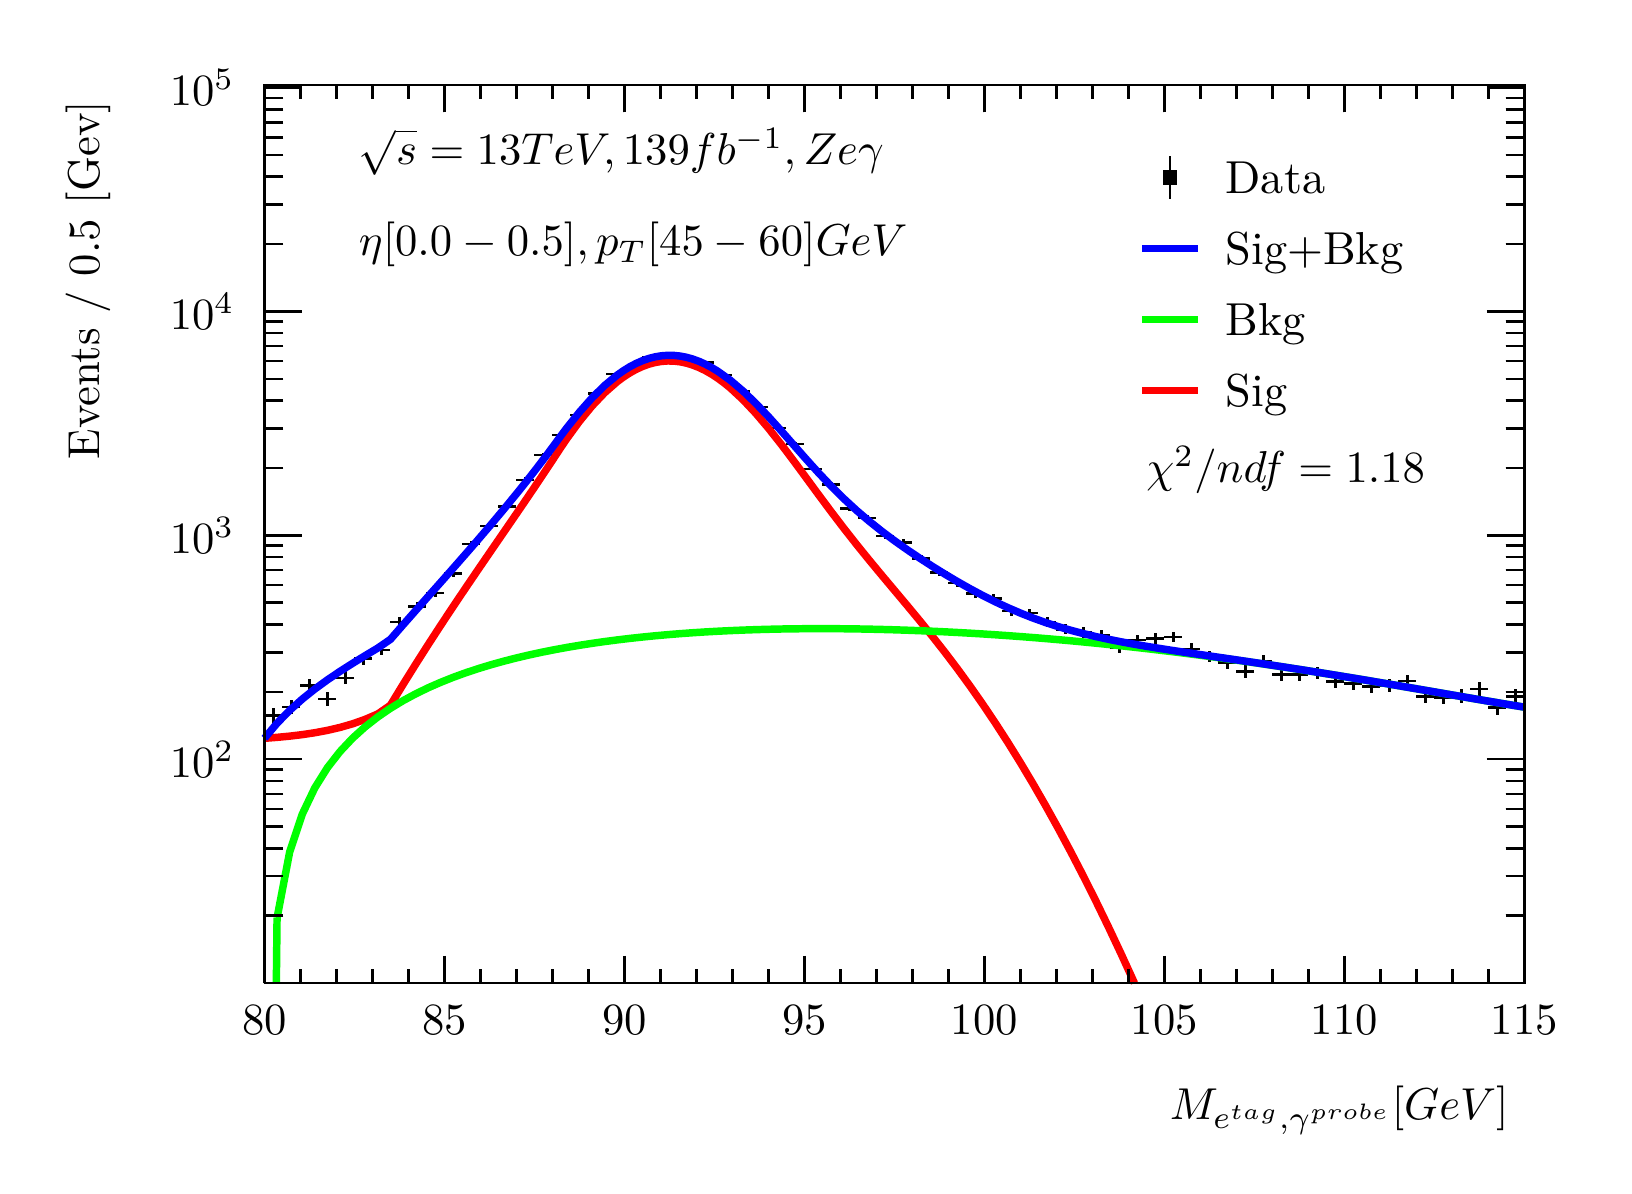
\begin{tikzpicture}
\pgfdeclareplotmark{cross} {
\pgfpathmoveto{\pgfpoint{-0.3\pgfplotmarksize}{\pgfplotmarksize}}
\pgfpathlineto{\pgfpoint{+0.3\pgfplotmarksize}{\pgfplotmarksize}}
\pgfpathlineto{\pgfpoint{+0.3\pgfplotmarksize}{0.3\pgfplotmarksize}}
\pgfpathlineto{\pgfpoint{+1\pgfplotmarksize}{0.3\pgfplotmarksize}}
\pgfpathlineto{\pgfpoint{+1\pgfplotmarksize}{-0.3\pgfplotmarksize}}
\pgfpathlineto{\pgfpoint{+0.3\pgfplotmarksize}{-0.3\pgfplotmarksize}}
\pgfpathlineto{\pgfpoint{+0.3\pgfplotmarksize}{-1.\pgfplotmarksize}}
\pgfpathlineto{\pgfpoint{-0.3\pgfplotmarksize}{-1.\pgfplotmarksize}}
\pgfpathlineto{\pgfpoint{-0.3\pgfplotmarksize}{-0.3\pgfplotmarksize}}
\pgfpathlineto{\pgfpoint{-1.\pgfplotmarksize}{-0.3\pgfplotmarksize}}
\pgfpathlineto{\pgfpoint{-1.\pgfplotmarksize}{0.3\pgfplotmarksize}}
\pgfpathlineto{\pgfpoint{-0.3\pgfplotmarksize}{0.3\pgfplotmarksize}}
\pgfpathclose
\pgfusepathqstroke
}
\pgfdeclareplotmark{cross*} {
\pgfpathmoveto{\pgfpoint{-0.3\pgfplotmarksize}{\pgfplotmarksize}}
\pgfpathlineto{\pgfpoint{+0.3\pgfplotmarksize}{\pgfplotmarksize}}
\pgfpathlineto{\pgfpoint{+0.3\pgfplotmarksize}{0.3\pgfplotmarksize}}
\pgfpathlineto{\pgfpoint{+1\pgfplotmarksize}{0.3\pgfplotmarksize}}
\pgfpathlineto{\pgfpoint{+1\pgfplotmarksize}{-0.3\pgfplotmarksize}}
\pgfpathlineto{\pgfpoint{+0.3\pgfplotmarksize}{-0.3\pgfplotmarksize}}
\pgfpathlineto{\pgfpoint{+0.3\pgfplotmarksize}{-1.\pgfplotmarksize}}
\pgfpathlineto{\pgfpoint{-0.3\pgfplotmarksize}{-1.\pgfplotmarksize}}
\pgfpathlineto{\pgfpoint{-0.3\pgfplotmarksize}{-0.3\pgfplotmarksize}}
\pgfpathlineto{\pgfpoint{-1.\pgfplotmarksize}{-0.3\pgfplotmarksize}}
\pgfpathlineto{\pgfpoint{-1.\pgfplotmarksize}{0.3\pgfplotmarksize}}
\pgfpathlineto{\pgfpoint{-0.3\pgfplotmarksize}{0.3\pgfplotmarksize}}
\pgfpathclose
\pgfusepathqfillstroke
}
\pgfdeclareplotmark{newstar} {
\pgfpathmoveto{\pgfqpoint{0pt}{\pgfplotmarksize}}
\pgfpathlineto{\pgfqpointpolar{44}{0.5\pgfplotmarksize}}
\pgfpathlineto{\pgfqpointpolar{18}{\pgfplotmarksize}}
\pgfpathlineto{\pgfqpointpolar{-20}{0.5\pgfplotmarksize}}
\pgfpathlineto{\pgfqpointpolar{-54}{\pgfplotmarksize}}
\pgfpathlineto{\pgfqpointpolar{-90}{0.5\pgfplotmarksize}}
\pgfpathlineto{\pgfqpointpolar{234}{\pgfplotmarksize}}
\pgfpathlineto{\pgfqpointpolar{198}{0.5\pgfplotmarksize}}
\pgfpathlineto{\pgfqpointpolar{162}{\pgfplotmarksize}}
\pgfpathlineto{\pgfqpointpolar{134}{0.5\pgfplotmarksize}}
\pgfpathclose
\pgfusepathqstroke
}
\pgfdeclareplotmark{newstar*} {
\pgfpathmoveto{\pgfqpoint{0pt}{\pgfplotmarksize}}
\pgfpathlineto{\pgfqpointpolar{44}{0.5\pgfplotmarksize}}
\pgfpathlineto{\pgfqpointpolar{18}{\pgfplotmarksize}}
\pgfpathlineto{\pgfqpointpolar{-20}{0.5\pgfplotmarksize}}
\pgfpathlineto{\pgfqpointpolar{-54}{\pgfplotmarksize}}
\pgfpathlineto{\pgfqpointpolar{-90}{0.5\pgfplotmarksize}}
\pgfpathlineto{\pgfqpointpolar{234}{\pgfplotmarksize}}
\pgfpathlineto{\pgfqpointpolar{198}{0.5\pgfplotmarksize}}
\pgfpathlineto{\pgfqpointpolar{162}{\pgfplotmarksize}}
\pgfpathlineto{\pgfqpointpolar{134}{0.5\pgfplotmarksize}}
\pgfpathclose
\pgfusepathqfillstroke
}
\definecolor{c}{rgb}{1,1,1};
\draw [color=c, fill=c] (0,0) rectangle (20,14.4361);
\draw [color=c, fill=c] (3,2.30977) rectangle (19,13.7143);
\definecolor{c}{rgb}{0,0,0};
\draw [c,line width=0.9] (3,2.30977) -- (3,13.7143) -- (19,13.7143) -- (19,2.30977) -- (3,2.30977);
\definecolor{c}{rgb}{1,1,1};
\draw [color=c, fill=c] (3,2.30977) rectangle (19,13.7143);
\definecolor{c}{rgb}{0,0,0};
\draw [c,line width=0.9] (3,2.30977) -- (3,13.7143) -- (19,13.7143) -- (19,2.30977) -- (3,2.30977);
\draw [c,line width=0.9] (3,2.30977) -- (19,2.30977);
\draw [c,line width=0.9] (3,2.65624) -- (3,2.30977);
\draw [c,line width=0.9] (3.45714,2.48301) -- (3.45714,2.30977);
\draw [c,line width=0.9] (3.91429,2.48301) -- (3.91429,2.30977);
\draw [c,line width=0.9] (4.37143,2.48301) -- (4.37143,2.30977);
\draw [c,line width=0.9] (4.82857,2.48301) -- (4.82857,2.30977);
\draw [c,line width=0.9] (5.28571,2.65624) -- (5.28571,2.30977);
\draw [c,line width=0.9] (5.74286,2.48301) -- (5.74286,2.30977);
\draw [c,line width=0.9] (6.2,2.48301) -- (6.2,2.30977);
\draw [c,line width=0.9] (6.65714,2.48301) -- (6.65714,2.30977);
\draw [c,line width=0.9] (7.11429,2.48301) -- (7.11429,2.30977);
\draw [c,line width=0.9] (7.57143,2.65624) -- (7.57143,2.30977);
\draw [c,line width=0.9] (8.02857,2.48301) -- (8.02857,2.30977);
\draw [c,line width=0.9] (8.48571,2.48301) -- (8.48571,2.30977);
\draw [c,line width=0.9] (8.94286,2.48301) -- (8.94286,2.30977);
\draw [c,line width=0.9] (9.4,2.48301) -- (9.4,2.30977);
\draw [c,line width=0.9] (9.85714,2.65624) -- (9.85714,2.30977);
\draw [c,line width=0.9] (10.3143,2.48301) -- (10.3143,2.30977);
\draw [c,line width=0.9] (10.7714,2.48301) -- (10.7714,2.30977);
\draw [c,line width=0.9] (11.2286,2.48301) -- (11.2286,2.30977);
\draw [c,line width=0.9] (11.6857,2.48301) -- (11.6857,2.30977);
\draw [c,line width=0.9] (12.1429,2.65624) -- (12.1429,2.30977);
\draw [c,line width=0.9] (12.6,2.48301) -- (12.6,2.30977);
\draw [c,line width=0.9] (13.0571,2.48301) -- (13.0571,2.30977);
\draw [c,line width=0.9] (13.5143,2.48301) -- (13.5143,2.30977);
\draw [c,line width=0.9] (13.9714,2.48301) -- (13.9714,2.30977);
\draw [c,line width=0.9] (14.4286,2.65624) -- (14.4286,2.30977);
\draw [c,line width=0.9] (14.8857,2.48301) -- (14.8857,2.30977);
\draw [c,line width=0.9] (15.3429,2.48301) -- (15.3429,2.30977);
\draw [c,line width=0.9] (15.8,2.48301) -- (15.8,2.30977);
\draw [c,line width=0.9] (16.2571,2.48301) -- (16.2571,2.30977);
\draw [c,line width=0.9] (16.7143,2.65624) -- (16.7143,2.30977);
\draw [c,line width=0.9] (17.1714,2.48301) -- (17.1714,2.30977);
\draw [c,line width=0.9] (17.6286,2.48301) -- (17.6286,2.30977);
\draw [c,line width=0.9] (18.0857,2.48301) -- (18.0857,2.30977);
\draw [c,line width=0.9] (18.5429,2.48301) -- (18.5429,2.30977);
\draw [c,line width=0.9] (19,2.65624) -- (19,2.30977);
\draw [anchor=base] (3,1.66015) node[scale=1.61424, color=c, rotate=0]{80};
\draw [anchor=base] (5.28571,1.66015) node[scale=1.61424, color=c, rotate=0]{85};
\draw [anchor=base] (7.57143,1.66015) node[scale=1.61424, color=c, rotate=0]{90};
\draw [anchor=base] (9.85714,1.66015) node[scale=1.61424, color=c, rotate=0]{95};
\draw [anchor=base] (12.1429,1.66015) node[scale=1.61424, color=c, rotate=0]{100};
\draw [anchor=base] (14.4286,1.66015) node[scale=1.61424, color=c, rotate=0]{105};
\draw [anchor=base] (16.7143,1.66015) node[scale=1.61424, color=c, rotate=0]{110};
\draw [anchor=base] (19,1.66015) node[scale=1.61424, color=c, rotate=0]{115};
\draw [anchor= east] (19,0.692932) node[scale=1.61424, color=c, rotate=0]{$M_{e^{tag}, \gamma^{probe}}  [GeV]$};
\draw [c,line width=0.9] (3,13.7143) -- (19,13.7143);
\draw [c,line width=0.9] (3,13.3678) -- (3,13.7143);
\draw [c,line width=0.9] (3.45714,13.5411) -- (3.45714,13.7143);
\draw [c,line width=0.9] (3.91429,13.5411) -- (3.91429,13.7143);
\draw [c,line width=0.9] (4.37143,13.5411) -- (4.37143,13.7143);
\draw [c,line width=0.9] (4.82857,13.5411) -- (4.82857,13.7143);
\draw [c,line width=0.9] (5.28571,13.3678) -- (5.28571,13.7143);
\draw [c,line width=0.9] (5.74286,13.5411) -- (5.74286,13.7143);
\draw [c,line width=0.9] (6.2,13.5411) -- (6.2,13.7143);
\draw [c,line width=0.9] (6.65714,13.5411) -- (6.65714,13.7143);
\draw [c,line width=0.9] (7.11429,13.5411) -- (7.11429,13.7143);
\draw [c,line width=0.9] (7.57143,13.3678) -- (7.57143,13.7143);
\draw [c,line width=0.9] (8.02857,13.5411) -- (8.02857,13.7143);
\draw [c,line width=0.9] (8.48571,13.5411) -- (8.48571,13.7143);
\draw [c,line width=0.9] (8.94286,13.5411) -- (8.94286,13.7143);
\draw [c,line width=0.9] (9.4,13.5411) -- (9.4,13.7143);
\draw [c,line width=0.9] (9.85714,13.3678) -- (9.85714,13.7143);
\draw [c,line width=0.9] (10.3143,13.5411) -- (10.3143,13.7143);
\draw [c,line width=0.9] (10.7714,13.5411) -- (10.7714,13.7143);
\draw [c,line width=0.9] (11.2286,13.5411) -- (11.2286,13.7143);
\draw [c,line width=0.9] (11.6857,13.5411) -- (11.6857,13.7143);
\draw [c,line width=0.9] (12.1429,13.3678) -- (12.1429,13.7143);
\draw [c,line width=0.9] (12.6,13.5411) -- (12.6,13.7143);
\draw [c,line width=0.9] (13.0571,13.5411) -- (13.0571,13.7143);
\draw [c,line width=0.9] (13.5143,13.5411) -- (13.5143,13.7143);
\draw [c,line width=0.9] (13.9714,13.5411) -- (13.9714,13.7143);
\draw [c,line width=0.9] (14.4286,13.3678) -- (14.4286,13.7143);
\draw [c,line width=0.9] (14.8857,13.5411) -- (14.8857,13.7143);
\draw [c,line width=0.9] (15.3429,13.5411) -- (15.3429,13.7143);
\draw [c,line width=0.9] (15.8,13.5411) -- (15.8,13.7143);
\draw [c,line width=0.9] (16.2571,13.5411) -- (16.2571,13.7143);
\draw [c,line width=0.9] (16.7143,13.3678) -- (16.7143,13.7143);
\draw [c,line width=0.9] (17.1714,13.5411) -- (17.1714,13.7143);
\draw [c,line width=0.9] (17.6286,13.5411) -- (17.6286,13.7143);
\draw [c,line width=0.9] (18.0857,13.5411) -- (18.0857,13.7143);
\draw [c,line width=0.9] (18.5429,13.5411) -- (18.5429,13.7143);
\draw [c,line width=0.9] (19,13.3678) -- (19,13.7143);
\draw [c,line width=0.9] (3,2.30977) -- (3,13.7143);
\draw [c,line width=0.9] (3.237,3.16561) -- (3,3.16561);
\draw [c,line width=0.9] (3.237,3.66625) -- (3,3.66625);
\draw [c,line width=0.9] (3.237,4.02146) -- (3,4.02146);
\draw [c,line width=0.9] (3.237,4.29698) -- (3,4.29698);
\draw [c,line width=0.9] (3.237,4.52209) -- (3,4.52209);
\draw [c,line width=0.9] (3.237,4.71242) -- (3,4.71242);
\draw [c,line width=0.9] (3.237,4.8773) -- (3,4.8773);
\draw [c,line width=0.9] (3.237,5.02273) -- (3,5.02273);
\draw [c,line width=0.9] (3.474,5.15282) -- (3,5.15282);
\draw [anchor= east] (2.82,5.15282) node[scale=1.61424, color=c, rotate=0]{$10^{2}$};
\draw [c,line width=0.9] (3.237,6.00866) -- (3,6.00866);
\draw [c,line width=0.9] (3.237,6.5093) -- (3,6.5093);
\draw [c,line width=0.9] (3.237,6.8645) -- (3,6.8645);
\draw [c,line width=0.9] (3.237,7.14002) -- (3,7.14002);
\draw [c,line width=0.9] (3.237,7.36514) -- (3,7.36514);
\draw [c,line width=0.9] (3.237,7.55547) -- (3,7.55547);
\draw [c,line width=0.9] (3.237,7.72034) -- (3,7.72034);
\draw [c,line width=0.9] (3.237,7.86577) -- (3,7.86577);
\draw [c,line width=0.9] (3.474,7.99586) -- (3,7.99586);
\draw [anchor= east] (2.82,7.99586) node[scale=1.61424, color=c, rotate=0]{$10^{3}$};
\draw [c,line width=0.9] (3.237,8.85171) -- (3,8.85171);
\draw [c,line width=0.9] (3.237,9.35234) -- (3,9.35234);
\draw [c,line width=0.9] (3.237,9.70755) -- (3,9.70755);
\draw [c,line width=0.9] (3.237,9.98307) -- (3,9.98307);
\draw [c,line width=0.9] (3.237,10.2082) -- (3,10.2082);
\draw [c,line width=0.9] (3.237,10.3985) -- (3,10.3985);
\draw [c,line width=0.9] (3.237,10.5634) -- (3,10.5634);
\draw [c,line width=0.9] (3.237,10.7088) -- (3,10.7088);
\draw [c,line width=0.9] (3.474,10.8389) -- (3,10.8389);
\draw [anchor= east] (2.82,10.8389) node[scale=1.61424, color=c, rotate=0]{$10^{4}$};
\draw [c,line width=0.9] (3.237,11.6948) -- (3,11.6948);
\draw [c,line width=0.9] (3.237,12.1954) -- (3,12.1954);
\draw [c,line width=0.9] (3.237,12.5506) -- (3,12.5506);
\draw [c,line width=0.9] (3.237,12.8261) -- (3,12.8261);
\draw [c,line width=0.9] (3.237,13.0512) -- (3,13.0512);
\draw [c,line width=0.9] (3.237,13.2416) -- (3,13.2416);
\draw [c,line width=0.9] (3.237,13.4064) -- (3,13.4064);
\draw [c,line width=0.9] (3.237,13.5519) -- (3,13.5519);
\draw [c,line width=0.9] (3.474,13.682) -- (3,13.682);
\draw [anchor= east] (2.82,13.682) node[scale=1.61424, color=c, rotate=0]{$10^{5}$};
\draw [anchor= east] (0.76,13.7143) node[scale=1.61424, color=c, rotate=90]{Events / 0.5 [Gev]};
\draw [c,line width=0.9] (19,2.30977) -- (19,13.7143);
\draw [c,line width=0.9] (18.763,3.16561) -- (19,3.16561);
\draw [c,line width=0.9] (18.763,3.66625) -- (19,3.66625);
\draw [c,line width=0.9] (18.763,4.02146) -- (19,4.02146);
\draw [c,line width=0.9] (18.763,4.29698) -- (19,4.29698);
\draw [c,line width=0.9] (18.763,4.52209) -- (19,4.52209);
\draw [c,line width=0.9] (18.763,4.71242) -- (19,4.71242);
\draw [c,line width=0.9] (18.763,4.8773) -- (19,4.8773);
\draw [c,line width=0.9] (18.763,5.02273) -- (19,5.02273);
\draw [c,line width=0.9] (18.526,5.15282) -- (19,5.15282);
\draw [c,line width=0.9] (18.763,6.00866) -- (19,6.00866);
\draw [c,line width=0.9] (18.763,6.5093) -- (19,6.5093);
\draw [c,line width=0.9] (18.763,6.8645) -- (19,6.8645);
\draw [c,line width=0.9] (18.763,7.14002) -- (19,7.14002);
\draw [c,line width=0.9] (18.763,7.36514) -- (19,7.36514);
\draw [c,line width=0.9] (18.763,7.55547) -- (19,7.55547);
\draw [c,line width=0.9] (18.763,7.72034) -- (19,7.72034);
\draw [c,line width=0.9] (18.763,7.86577) -- (19,7.86577);
\draw [c,line width=0.9] (18.526,7.99586) -- (19,7.99586);
\draw [c,line width=0.9] (18.763,8.85171) -- (19,8.85171);
\draw [c,line width=0.9] (18.763,9.35234) -- (19,9.35234);
\draw [c,line width=0.9] (18.763,9.70755) -- (19,9.70755);
\draw [c,line width=0.9] (18.763,9.98307) -- (19,9.98307);
\draw [c,line width=0.9] (18.763,10.2082) -- (19,10.2082);
\draw [c,line width=0.9] (18.763,10.3985) -- (19,10.3985);
\draw [c,line width=0.9] (18.763,10.5634) -- (19,10.5634);
\draw [c,line width=0.9] (18.763,10.7088) -- (19,10.7088);
\draw [c,line width=0.9] (18.526,10.8389) -- (19,10.8389);
\draw [c,line width=0.9] (18.763,11.6948) -- (19,11.6948);
\draw [c,line width=0.9] (18.763,12.1954) -- (19,12.1954);
\draw [c,line width=0.9] (18.763,12.5506) -- (19,12.5506);
\draw [c,line width=0.9] (18.763,12.8261) -- (19,12.8261);
\draw [c,line width=0.9] (18.763,13.0512) -- (19,13.0512);
\draw [c,line width=0.9] (18.763,13.2416) -- (19,13.2416);
\draw [c,line width=0.9] (18.763,13.4064) -- (19,13.4064);
\draw [c,line width=0.9] (18.763,13.5519) -- (19,13.5519);
\draw [c,line width=0.9] (18.526,13.682) -- (19,13.682);
\draw [c,line width=0.9] (3.11429,5.70977) -- (3,5.70977);
\draw [c,line width=0.9] (3,5.70977) -- (3,5.70977);
\draw [c,line width=0.9] (3.11429,5.70977) -- (3.22857,5.70977);
\draw [c,line width=0.9] (3.22857,5.70977) -- (3.22857,5.70977);
\draw [c,line width=0.9] (3.11429,5.70977) -- (3.11429,5.80829);
\draw [c,line width=0.9] (3.11429,5.80829) -- (3.11429,5.80829);
\draw [c,line width=0.9] (3.11429,5.70977) -- (3.11429,5.61126);
\draw [c,line width=0.9] (3.11429,5.61126) -- (3.11429,5.61126);
\draw [c,line width=0.9] (3.34286,5.81524) -- (3.22857,5.81524);
\draw [c,line width=0.9] (3.22857,5.81524) -- (3.22857,5.81524);
\draw [c,line width=0.9] (3.34286,5.81524) -- (3.45714,5.81524);
\draw [c,line width=0.9] (3.45714,5.81524) -- (3.45714,5.81524);
\draw [c,line width=0.9] (3.34286,5.81524) -- (3.34286,5.90964);
\draw [c,line width=0.9] (3.34286,5.90964) -- (3.34286,5.90964);
\draw [c,line width=0.9] (3.34286,5.81524) -- (3.34286,5.72084);
\draw [c,line width=0.9] (3.34286,5.72084) -- (3.34286,5.72084);
\draw [c,line width=0.9] (3.57143,6.08642) -- (3.45714,6.08642);
\draw [c,line width=0.9] (3.45714,6.08642) -- (3.45714,6.08642);
\draw [c,line width=0.9] (3.57143,6.08642) -- (3.68571,6.08642);
\draw [c,line width=0.9] (3.68571,6.08642) -- (3.68571,6.08642);
\draw [c,line width=0.9] (3.57143,6.08642) -- (3.57143,6.171);
\draw [c,line width=0.9] (3.57143,6.171) -- (3.57143,6.171);
\draw [c,line width=0.9] (3.57143,6.08642) -- (3.57143,6.00183);
\draw [c,line width=0.9] (3.57143,6.00183) -- (3.57143,6.00183);
\draw [c,line width=0.9] (3.8,5.91906) -- (3.68571,5.91906);
\draw [c,line width=0.9] (3.68571,5.91906) -- (3.68571,5.91906);
\draw [c,line width=0.9] (3.8,5.91906) -- (3.91429,5.91906);
\draw [c,line width=0.9] (3.91429,5.91906) -- (3.91429,5.91906);
\draw [c,line width=0.9] (3.8,5.91906) -- (3.8,6.00957);
\draw [c,line width=0.9] (3.8,6.00957) -- (3.8,6.00957);
\draw [c,line width=0.9] (3.8,5.91906) -- (3.8,5.82854);
\draw [c,line width=0.9] (3.8,5.82854) -- (3.8,5.82854);
\draw [c,line width=0.9] (4.02857,6.18658) -- (3.91429,6.18658);
\draw [c,line width=0.9] (3.91429,6.18658) -- (3.91429,6.18658);
\draw [c,line width=0.9] (4.02857,6.18658) -- (4.14286,6.18658);
\draw [c,line width=0.9] (4.14286,6.18658) -- (4.14286,6.18658);
\draw [c,line width=0.9] (4.02857,6.18658) -- (4.02857,6.26781);
\draw [c,line width=0.9] (4.02857,6.26781) -- (4.02857,6.26781);
\draw [c,line width=0.9] (4.02857,6.18658) -- (4.02857,6.10536);
\draw [c,line width=0.9] (4.02857,6.10536) -- (4.02857,6.10536);
\draw [c,line width=0.9] (4.25714,6.42851) -- (4.14286,6.42851);
\draw [c,line width=0.9] (4.14286,6.42851) -- (4.14286,6.42851);
\draw [c,line width=0.9] (4.25714,6.42851) -- (4.37143,6.42851);
\draw [c,line width=0.9] (4.37143,6.42851) -- (4.37143,6.42851);
\draw [c,line width=0.9] (4.25714,6.42851) -- (4.25714,6.50216);
\draw [c,line width=0.9] (4.25714,6.50216) -- (4.25714,6.50216);
\draw [c,line width=0.9] (4.25714,6.42851) -- (4.25714,6.35487);
\draw [c,line width=0.9] (4.25714,6.35487) -- (4.25714,6.35487);
\draw [c,line width=0.9] (4.48571,6.54179) -- (4.37143,6.54179);
\draw [c,line width=0.9] (4.37143,6.54179) -- (4.37143,6.54179);
\draw [c,line width=0.9] (4.48571,6.54179) -- (4.6,6.54179);
\draw [c,line width=0.9] (4.6,6.54179) -- (4.6,6.54179);
\draw [c,line width=0.9] (4.48571,6.54179) -- (4.48571,6.61214);
\draw [c,line width=0.9] (4.48571,6.61214) -- (4.48571,6.61214);
\draw [c,line width=0.9] (4.48571,6.54179) -- (4.48571,6.47145);
\draw [c,line width=0.9] (4.48571,6.47145) -- (4.48571,6.47145);
\draw [c,line width=0.9] (4.71429,6.89198) -- (4.6,6.89198);
\draw [c,line width=0.9] (4.6,6.89198) -- (4.6,6.89198);
\draw [c,line width=0.9] (4.71429,6.89198) -- (4.82857,6.89198);
\draw [c,line width=0.9] (4.82857,6.89198) -- (4.82857,6.89198);
\draw [c,line width=0.9] (4.71429,6.89198) -- (4.71429,6.95302);
\draw [c,line width=0.9] (4.71429,6.95302) -- (4.71429,6.95302);
\draw [c,line width=0.9] (4.71429,6.89198) -- (4.71429,6.83093);
\draw [c,line width=0.9] (4.71429,6.83093) -- (4.71429,6.83093);
\draw [c,line width=0.9] (4.94286,7.09475) -- (4.82857,7.09475);
\draw [c,line width=0.9] (4.82857,7.09475) -- (4.82857,7.09475);
\draw [c,line width=0.9] (4.94286,7.09475) -- (5.05714,7.09475);
\draw [c,line width=0.9] (5.05714,7.09475) -- (5.05714,7.09475);
\draw [c,line width=0.9] (4.94286,7.09475) -- (4.94286,7.15099);
\draw [c,line width=0.9] (4.94286,7.15099) -- (4.94286,7.15099);
\draw [c,line width=0.9] (4.94286,7.09475) -- (4.94286,7.03852);
\draw [c,line width=0.9] (4.94286,7.03852) -- (4.94286,7.03852);
\draw [c,line width=0.9] (5.17143,7.26442) -- (5.05714,7.26442);
\draw [c,line width=0.9] (5.05714,7.26442) -- (5.05714,7.26442);
\draw [c,line width=0.9] (5.17143,7.26442) -- (5.28571,7.26442);
\draw [c,line width=0.9] (5.28571,7.26442) -- (5.28571,7.26442);
\draw [c,line width=0.9] (5.17143,7.26442) -- (5.17143,7.31692);
\draw [c,line width=0.9] (5.17143,7.31692) -- (5.17143,7.31692);
\draw [c,line width=0.9] (5.17143,7.26442) -- (5.17143,7.21192);
\draw [c,line width=0.9] (5.17143,7.21192) -- (5.17143,7.21192);
\draw [c,line width=0.9] (5.4,7.50874) -- (5.28571,7.50874);
\draw [c,line width=0.9] (5.28571,7.50874) -- (5.28571,7.50874);
\draw [c,line width=0.9] (5.4,7.50874) -- (5.51429,7.50874);
\draw [c,line width=0.9] (5.51429,7.50874) -- (5.51429,7.50874);
\draw [c,line width=0.9] (5.4,7.50874) -- (5.4,7.55629);
\draw [c,line width=0.9] (5.4,7.55629) -- (5.4,7.55629);
\draw [c,line width=0.9] (5.4,7.50874) -- (5.4,7.46118);
\draw [c,line width=0.9] (5.4,7.46118) -- (5.4,7.46118);
\draw [c,line width=0.9] (5.62857,7.88618) -- (5.51429,7.88618);
\draw [c,line width=0.9] (5.51429,7.88618) -- (5.51429,7.88618);
\draw [c,line width=0.9] (5.62857,7.88618) -- (5.74286,7.88618);
\draw [c,line width=0.9] (5.74286,7.88618) -- (5.74286,7.88618);
\draw [c,line width=0.9] (5.62857,7.88618) -- (5.62857,7.927);
\draw [c,line width=0.9] (5.62857,7.927) -- (5.62857,7.927);
\draw [c,line width=0.9] (5.62857,7.88618) -- (5.62857,7.84537);
\draw [c,line width=0.9] (5.62857,7.84537) -- (5.62857,7.84537);
\draw [c,line width=0.9] (5.85714,8.11242) -- (5.74286,8.11242);
\draw [c,line width=0.9] (5.74286,8.11242) -- (5.74286,8.11242);
\draw [c,line width=0.9] (5.85714,8.11242) -- (5.97143,8.11242);
\draw [c,line width=0.9] (5.97143,8.11242) -- (5.97143,8.11242);
\draw [c,line width=0.9] (5.85714,8.11242) -- (5.85714,8.14967);
\draw [c,line width=0.9] (5.85714,8.14967) -- (5.85714,8.14967);
\draw [c,line width=0.9] (5.85714,8.11242) -- (5.85714,8.07518);
\draw [c,line width=0.9] (5.85714,8.07518) -- (5.85714,8.07518);
\draw [c,line width=0.9] (6.08571,8.36183) -- (5.97143,8.36183);
\draw [c,line width=0.9] (5.97143,8.36183) -- (5.97143,8.36183);
\draw [c,line width=0.9] (6.08571,8.36183) -- (6.2,8.36183);
\draw [c,line width=0.9] (6.2,8.36183) -- (6.2,8.36183);
\draw [c,line width=0.9] (6.08571,8.36183) -- (6.08571,8.39549);
\draw [c,line width=0.9] (6.08571,8.39549) -- (6.08571,8.39549);
\draw [c,line width=0.9] (6.08571,8.36183) -- (6.08571,8.32816);
\draw [c,line width=0.9] (6.08571,8.32816) -- (6.08571,8.32816);
\draw [c,line width=0.9] (6.31429,8.70156) -- (6.2,8.70156);
\draw [c,line width=0.9] (6.2,8.70156) -- (6.2,8.70156);
\draw [c,line width=0.9] (6.31429,8.70156) -- (6.42857,8.70156);
\draw [c,line width=0.9] (6.42857,8.70156) -- (6.42857,8.70156);
\draw [c,line width=0.9] (6.31429,8.70156) -- (6.31429,8.7309);
\draw [c,line width=0.9] (6.31429,8.7309) -- (6.31429,8.7309);
\draw [c,line width=0.9] (6.31429,8.70156) -- (6.31429,8.67222);
\draw [c,line width=0.9] (6.31429,8.67222) -- (6.31429,8.67222);
\draw [c,line width=0.9] (6.54286,9.01511) -- (6.42857,9.01511);
\draw [c,line width=0.9] (6.42857,9.01511) -- (6.42857,9.01511);
\draw [c,line width=0.9] (6.54286,9.01511) -- (6.65714,9.01511);
\draw [c,line width=0.9] (6.65714,9.01511) -- (6.65714,9.01511);
\draw [c,line width=0.9] (6.54286,9.01511) -- (6.54286,9.04095);
\draw [c,line width=0.9] (6.54286,9.04095) -- (6.54286,9.04095);
\draw [c,line width=0.9] (6.54286,9.01511) -- (6.54286,8.98927);
\draw [c,line width=0.9] (6.54286,8.98927) -- (6.54286,8.98927);
\draw [c,line width=0.9] (6.77143,9.26848) -- (6.65714,9.26848);
\draw [c,line width=0.9] (6.65714,9.26848) -- (6.65714,9.26848);
\draw [c,line width=0.9] (6.77143,9.26848) -- (6.88571,9.26848);
\draw [c,line width=0.9] (6.88571,9.26848) -- (6.88571,9.26848);
\draw [c,line width=0.9] (6.77143,9.26848) -- (6.77143,9.2918);
\draw [c,line width=0.9] (6.77143,9.2918) -- (6.77143,9.2918);
\draw [c,line width=0.9] (6.77143,9.26848) -- (6.77143,9.24516);
\draw [c,line width=0.9] (6.77143,9.24516) -- (6.77143,9.24516);
\draw [c,line width=0.9] (7,9.52312) -- (6.88571,9.52312);
\draw [c,line width=0.9] (6.88571,9.52312) -- (6.88571,9.52312);
\draw [c,line width=0.9] (7,9.52312) -- (7.11429,9.52312);
\draw [c,line width=0.9] (7.11429,9.52312) -- (7.11429,9.52312);
\draw [c,line width=0.9] (7,9.52312) -- (7,9.54416);
\draw [c,line width=0.9] (7,9.54416) -- (7,9.54416);
\draw [c,line width=0.9] (7,9.52312) -- (7,9.50208);
\draw [c,line width=0.9] (7,9.50208) -- (7,9.50208);
\draw [c,line width=0.9] (7.22857,9.79426) -- (7.11429,9.79426);
\draw [c,line width=0.9] (7.11429,9.79426) -- (7.11429,9.79426);
\draw [c,line width=0.9] (7.22857,9.79426) -- (7.34286,9.79426);
\draw [c,line width=0.9] (7.34286,9.79426) -- (7.34286,9.79426);
\draw [c,line width=0.9] (7.22857,9.79426) -- (7.22857,9.81311);
\draw [c,line width=0.9] (7.22857,9.81311) -- (7.22857,9.81311);
\draw [c,line width=0.9] (7.22857,9.79426) -- (7.22857,9.77541);
\draw [c,line width=0.9] (7.22857,9.77541) -- (7.22857,9.77541);
\draw [c,line width=0.9] (7.45714,10.0452) -- (7.34286,10.0452);
\draw [c,line width=0.9] (7.34286,10.0452) -- (7.34286,10.0452);
\draw [c,line width=0.9] (7.45714,10.0452) -- (7.57143,10.0452);
\draw [c,line width=0.9] (7.57143,10.0452) -- (7.57143,10.0452);
\draw [c,line width=0.9] (7.45714,10.0452) -- (7.45714,10.0622);
\draw [c,line width=0.9] (7.45714,10.0622) -- (7.45714,10.0622);
\draw [c,line width=0.9] (7.45714,10.0452) -- (7.45714,10.0282);
\draw [c,line width=0.9] (7.45714,10.0282) -- (7.45714,10.0282);
\draw [c,line width=0.9] (7.68571,10.1292) -- (7.57143,10.1292);
\draw [c,line width=0.9] (7.57143,10.1292) -- (7.57143,10.1292);
\draw [c,line width=0.9] (7.68571,10.1292) -- (7.8,10.1292);
\draw [c,line width=0.9] (7.8,10.1292) -- (7.8,10.1292);
\draw [c,line width=0.9] (7.68571,10.1292) -- (7.68571,10.1456);
\draw [c,line width=0.9] (7.68571,10.1456) -- (7.68571,10.1456);
\draw [c,line width=0.9] (7.68571,10.1292) -- (7.68571,10.1127);
\draw [c,line width=0.9] (7.68571,10.1127) -- (7.68571,10.1127);
\draw [c,line width=0.9] (7.91429,10.256) -- (7.8,10.256);
\draw [c,line width=0.9] (7.8,10.256) -- (7.8,10.256);
\draw [c,line width=0.9] (7.91429,10.256) -- (8.02857,10.256);
\draw [c,line width=0.9] (8.02857,10.256) -- (8.02857,10.256);
\draw [c,line width=0.9] (7.91429,10.256) -- (7.91429,10.2717);
\draw [c,line width=0.9] (7.91429,10.2717) -- (7.91429,10.2717);
\draw [c,line width=0.9] (7.91429,10.256) -- (7.91429,10.2404);
\draw [c,line width=0.9] (7.91429,10.2404) -- (7.91429,10.2404);
\draw [c,line width=0.9] (8.14286,10.2819) -- (8.02857,10.2819);
\draw [c,line width=0.9] (8.02857,10.2819) -- (8.02857,10.2819);
\draw [c,line width=0.9] (8.14286,10.2819) -- (8.25714,10.2819);
\draw [c,line width=0.9] (8.25714,10.2819) -- (8.25714,10.2819);
\draw [c,line width=0.9] (8.14286,10.2819) -- (8.14286,10.2973);
\draw [c,line width=0.9] (8.14286,10.2973) -- (8.14286,10.2973);
\draw [c,line width=0.9] (8.14286,10.2819) -- (8.14286,10.2664);
\draw [c,line width=0.9] (8.14286,10.2664) -- (8.14286,10.2664);
\draw [c,line width=0.9] (8.37143,10.258) -- (8.25714,10.258);
\draw [c,line width=0.9] (8.25714,10.258) -- (8.25714,10.258);
\draw [c,line width=0.9] (8.37143,10.258) -- (8.48571,10.258);
\draw [c,line width=0.9] (8.48571,10.258) -- (8.48571,10.258);
\draw [c,line width=0.9] (8.37143,10.258) -- (8.37143,10.2736);
\draw [c,line width=0.9] (8.37143,10.2736) -- (8.37143,10.2736);
\draw [c,line width=0.9] (8.37143,10.258) -- (8.37143,10.2424);
\draw [c,line width=0.9] (8.37143,10.2424) -- (8.37143,10.2424);
\draw [c,line width=0.9] (8.6,10.1906) -- (8.48571,10.1906);
\draw [c,line width=0.9] (8.48571,10.1906) -- (8.48571,10.1906);
\draw [c,line width=0.9] (8.6,10.1906) -- (8.71429,10.1906);
\draw [c,line width=0.9] (8.71429,10.1906) -- (8.71429,10.1906);
\draw [c,line width=0.9] (8.6,10.1906) -- (8.6,10.2066);
\draw [c,line width=0.9] (8.6,10.2066) -- (8.6,10.2066);
\draw [c,line width=0.9] (8.6,10.1906) -- (8.6,10.1745);
\draw [c,line width=0.9] (8.6,10.1745) -- (8.6,10.1745);
\draw [c,line width=0.9] (8.82857,10.0346) -- (8.71429,10.0346);
\draw [c,line width=0.9] (8.71429,10.0346) -- (8.71429,10.0346);
\draw [c,line width=0.9] (8.82857,10.0346) -- (8.94286,10.0346);
\draw [c,line width=0.9] (8.94286,10.0346) -- (8.94286,10.0346);
\draw [c,line width=0.9] (8.82857,10.0346) -- (8.82857,10.0517);
\draw [c,line width=0.9] (8.82857,10.0517) -- (8.82857,10.0517);
\draw [c,line width=0.9] (8.82857,10.0346) -- (8.82857,10.0175);
\draw [c,line width=0.9] (8.82857,10.0175) -- (8.82857,10.0175);
\draw [c,line width=0.9] (9.05714,9.82551) -- (8.94286,9.82551);
\draw [c,line width=0.9] (8.94286,9.82551) -- (8.94286,9.82551);
\draw [c,line width=0.9] (9.05714,9.82551) -- (9.17143,9.82551);
\draw [c,line width=0.9] (9.17143,9.82551) -- (9.17143,9.82551);
\draw [c,line width=0.9] (9.05714,9.82551) -- (9.05714,9.84412);
\draw [c,line width=0.9] (9.05714,9.84412) -- (9.05714,9.84412);
\draw [c,line width=0.9] (9.05714,9.82551) -- (9.05714,9.8069);
\draw [c,line width=0.9] (9.05714,9.8069) -- (9.05714,9.8069);
\draw [c,line width=0.9] (9.28571,9.62523) -- (9.17143,9.62523);
\draw [c,line width=0.9] (9.17143,9.62523) -- (9.17143,9.62523);
\draw [c,line width=0.9] (9.28571,9.62523) -- (9.4,9.62523);
\draw [c,line width=0.9] (9.4,9.62523) -- (9.4,9.62523);
\draw [c,line width=0.9] (9.28571,9.62523) -- (9.28571,9.64541);
\draw [c,line width=0.9] (9.28571,9.64541) -- (9.28571,9.64541);
\draw [c,line width=0.9] (9.28571,9.62523) -- (9.28571,9.60504);
\draw [c,line width=0.9] (9.28571,9.60504) -- (9.28571,9.60504);
\draw [c,line width=0.9] (9.51429,9.35645) -- (9.4,9.35645);
\draw [c,line width=0.9] (9.4,9.35645) -- (9.4,9.35645);
\draw [c,line width=0.9] (9.51429,9.35645) -- (9.62857,9.35645);
\draw [c,line width=0.9] (9.62857,9.35645) -- (9.62857,9.35645);
\draw [c,line width=0.9] (9.51429,9.35645) -- (9.51429,9.37896);
\draw [c,line width=0.9] (9.51429,9.37896) -- (9.51429,9.37896);
\draw [c,line width=0.9] (9.51429,9.35645) -- (9.51429,9.33395);
\draw [c,line width=0.9] (9.51429,9.33395) -- (9.51429,9.33395);
\draw [c,line width=0.9] (9.74286,9.15796) -- (9.62857,9.15796);
\draw [c,line width=0.9] (9.62857,9.15796) -- (9.62857,9.15796);
\draw [c,line width=0.9] (9.74286,9.15796) -- (9.85714,9.15796);
\draw [c,line width=0.9] (9.85714,9.15796) -- (9.85714,9.15796);
\draw [c,line width=0.9] (9.74286,9.15796) -- (9.74286,9.18234);
\draw [c,line width=0.9] (9.74286,9.18234) -- (9.74286,9.18234);
\draw [c,line width=0.9] (9.74286,9.15796) -- (9.74286,9.13357);
\draw [c,line width=0.9] (9.74286,9.13357) -- (9.74286,9.13357);
\draw [c,line width=0.9] (9.97143,8.8368) -- (9.85714,8.8368);
\draw [c,line width=0.9] (9.85714,8.8368) -- (9.85714,8.8368);
\draw [c,line width=0.9] (9.97143,8.8368) -- (10.0857,8.8368);
\draw [c,line width=0.9] (10.0857,8.8368) -- (10.0857,8.8368);
\draw [c,line width=0.9] (9.97143,8.8368) -- (9.97143,8.86458);
\draw [c,line width=0.9] (9.97143,8.86458) -- (9.97143,8.86458);
\draw [c,line width=0.9] (9.97143,8.8368) -- (9.97143,8.80902);
\draw [c,line width=0.9] (9.97143,8.80902) -- (9.97143,8.80902);
\draw [c,line width=0.9] (10.2,8.64229) -- (10.0857,8.64229);
\draw [c,line width=0.9] (10.0857,8.64229) -- (10.0857,8.64229);
\draw [c,line width=0.9] (10.2,8.64229) -- (10.3143,8.64229);
\draw [c,line width=0.9] (10.3143,8.64229) -- (10.3143,8.64229);
\draw [c,line width=0.9] (10.2,8.64229) -- (10.2,8.67235);
\draw [c,line width=0.9] (10.2,8.67235) -- (10.2,8.67235);
\draw [c,line width=0.9] (10.2,8.64229) -- (10.2,8.61224);
\draw [c,line width=0.9] (10.2,8.61224) -- (10.2,8.61224);
\draw [c,line width=0.9] (10.4286,8.33679) -- (10.3143,8.33679);
\draw [c,line width=0.9] (10.3143,8.33679) -- (10.3143,8.33679);
\draw [c,line width=0.9] (10.4286,8.33679) -- (10.5429,8.33679);
\draw [c,line width=0.9] (10.5429,8.33679) -- (10.5429,8.33679);
\draw [c,line width=0.9] (10.4286,8.33679) -- (10.4286,8.3708);
\draw [c,line width=0.9] (10.4286,8.3708) -- (10.4286,8.3708);
\draw [c,line width=0.9] (10.4286,8.33679) -- (10.4286,8.30278);
\draw [c,line width=0.9] (10.4286,8.30278) -- (10.4286,8.30278);
\draw [c,line width=0.9] (10.6571,8.21272) -- (10.5429,8.21272);
\draw [c,line width=0.9] (10.5429,8.21272) -- (10.5429,8.21272);
\draw [c,line width=0.9] (10.6571,8.21272) -- (10.7714,8.21272);
\draw [c,line width=0.9] (10.7714,8.21272) -- (10.7714,8.21272);
\draw [c,line width=0.9] (10.6571,8.21272) -- (10.6571,8.24848);
\draw [c,line width=0.9] (10.6571,8.24848) -- (10.6571,8.24848);
\draw [c,line width=0.9] (10.6571,8.21272) -- (10.6571,8.17696);
\draw [c,line width=0.9] (10.6571,8.17696) -- (10.6571,8.17696);
\draw [c,line width=0.9] (10.8857,7.98595) -- (10.7714,7.98595);
\draw [c,line width=0.9] (10.7714,7.98595) -- (10.7714,7.98595);
\draw [c,line width=0.9] (10.8857,7.98595) -- (11,7.98595);
\draw [c,line width=0.9] (11,7.98595) -- (11,7.98595);
\draw [c,line width=0.9] (10.8857,7.98595) -- (10.8857,8.02515);
\draw [c,line width=0.9] (10.8857,8.02515) -- (10.8857,8.02515);
\draw [c,line width=0.9] (10.8857,7.98595) -- (10.8857,7.94675);
\draw [c,line width=0.9] (10.8857,7.94675) -- (10.8857,7.94675);
\draw [c,line width=0.9] (11.1143,7.90759) -- (11,7.90759);
\draw [c,line width=0.9] (11,7.90759) -- (11,7.90759);
\draw [c,line width=0.9] (11.1143,7.90759) -- (11.2286,7.90759);
\draw [c,line width=0.9] (11.2286,7.90759) -- (11.2286,7.90759);
\draw [c,line width=0.9] (11.1143,7.90759) -- (11.1143,7.94805);
\draw [c,line width=0.9] (11.1143,7.94805) -- (11.1143,7.94805);
\draw [c,line width=0.9] (11.1143,7.90759) -- (11.1143,7.86712);
\draw [c,line width=0.9] (11.1143,7.86712) -- (11.1143,7.86712);
\draw [c,line width=0.9] (11.3429,7.70168) -- (11.2286,7.70168);
\draw [c,line width=0.9] (11.2286,7.70168) -- (11.2286,7.70168);
\draw [c,line width=0.9] (11.3429,7.70168) -- (11.4571,7.70168);
\draw [c,line width=0.9] (11.4571,7.70168) -- (11.4571,7.70168);
\draw [c,line width=0.9] (11.3429,7.70168) -- (11.3429,7.74567);
\draw [c,line width=0.9] (11.3429,7.74567) -- (11.3429,7.74567);
\draw [c,line width=0.9] (11.3429,7.70168) -- (11.3429,7.6577);
\draw [c,line width=0.9] (11.3429,7.6577) -- (11.3429,7.6577);
\draw [c,line width=0.9] (11.5714,7.52149) -- (11.4571,7.52149);
\draw [c,line width=0.9] (11.4571,7.52149) -- (11.4571,7.52149);
\draw [c,line width=0.9] (11.5714,7.52149) -- (11.6857,7.52149);
\draw [c,line width=0.9] (11.6857,7.52149) -- (11.6857,7.52149);
\draw [c,line width=0.9] (11.5714,7.52149) -- (11.5714,7.56881);
\draw [c,line width=0.9] (11.5714,7.56881) -- (11.5714,7.56881);
\draw [c,line width=0.9] (11.5714,7.52149) -- (11.5714,7.47418);
\draw [c,line width=0.9] (11.5714,7.47418) -- (11.5714,7.47418);
\draw [c,line width=0.9] (11.8,7.38959) -- (11.6857,7.38959);
\draw [c,line width=0.9] (11.6857,7.38959) -- (11.6857,7.38959);
\draw [c,line width=0.9] (11.8,7.38959) -- (11.9143,7.38959);
\draw [c,line width=0.9] (11.9143,7.38959) -- (11.9143,7.38959);
\draw [c,line width=0.9] (11.8,7.38959) -- (11.8,7.4395);
\draw [c,line width=0.9] (11.8,7.4395) -- (11.8,7.4395);
\draw [c,line width=0.9] (11.8,7.38959) -- (11.8,7.33968);
\draw [c,line width=0.9] (11.8,7.33968) -- (11.8,7.33968);
\draw [c,line width=0.9] (12.0286,7.2577) -- (11.9143,7.2577);
\draw [c,line width=0.9] (11.9143,7.2577) -- (11.9143,7.2577);
\draw [c,line width=0.9] (12.0286,7.2577) -- (12.1429,7.2577);
\draw [c,line width=0.9] (12.1429,7.2577) -- (12.1429,7.2577);
\draw [c,line width=0.9] (12.0286,7.2577) -- (12.0286,7.31035);
\draw [c,line width=0.9] (12.0286,7.31035) -- (12.0286,7.31035);
\draw [c,line width=0.9] (12.0286,7.2577) -- (12.0286,7.20506);
\draw [c,line width=0.9] (12.0286,7.20506) -- (12.0286,7.20506);
\draw [c,line width=0.9] (12.2571,7.19082) -- (12.1429,7.19082);
\draw [c,line width=0.9] (12.1429,7.19082) -- (12.1429,7.19082);
\draw [c,line width=0.9] (12.2571,7.19082) -- (12.3714,7.19082);
\draw [c,line width=0.9] (12.3714,7.19082) -- (12.3714,7.19082);
\draw [c,line width=0.9] (12.2571,7.19082) -- (12.2571,7.24491);
\draw [c,line width=0.9] (12.2571,7.24491) -- (12.2571,7.24491);
\draw [c,line width=0.9] (12.2571,7.19082) -- (12.2571,7.13673);
\draw [c,line width=0.9] (12.2571,7.13673) -- (12.2571,7.13673);
\draw [c,line width=0.9] (12.4857,7.03438) -- (12.3714,7.03438);
\draw [c,line width=0.9] (12.3714,7.03438) -- (12.3714,7.03438);
\draw [c,line width=0.9] (12.4857,7.03438) -- (12.6,7.03438);
\draw [c,line width=0.9] (12.6,7.03438) -- (12.6,7.03438);
\draw [c,line width=0.9] (12.4857,7.03438) -- (12.4857,7.09201);
\draw [c,line width=0.9] (12.4857,7.09201) -- (12.4857,7.09201);
\draw [c,line width=0.9] (12.4857,7.03438) -- (12.4857,6.97676);
\draw [c,line width=0.9] (12.4857,6.97676) -- (12.4857,6.97676);
\draw [c,line width=0.9] (12.7143,7.00719) -- (12.6,7.00719);
\draw [c,line width=0.9] (12.6,7.00719) -- (12.6,7.00719);
\draw [c,line width=0.9] (12.7143,7.00719) -- (12.8286,7.00719);
\draw [c,line width=0.9] (12.8286,7.00719) -- (12.8286,7.00719);
\draw [c,line width=0.9] (12.7143,7.00719) -- (12.7143,7.06545);
\draw [c,line width=0.9] (12.7143,7.06545) -- (12.7143,7.06545);
\draw [c,line width=0.9] (12.7143,7.00719) -- (12.7143,6.94892);
\draw [c,line width=0.9] (12.7143,6.94892) -- (12.7143,6.94892);
\draw [c,line width=0.9] (12.9429,6.898) -- (12.8286,6.898);
\draw [c,line width=0.9] (12.8286,6.898) -- (12.8286,6.898);
\draw [c,line width=0.9] (12.9429,6.898) -- (13.0571,6.898);
\draw [c,line width=0.9] (13.0571,6.898) -- (13.0571,6.898);
\draw [c,line width=0.9] (12.9429,6.898) -- (12.9429,6.9589);
\draw [c,line width=0.9] (12.9429,6.9589) -- (12.9429,6.9589);
\draw [c,line width=0.9] (12.9429,6.898) -- (12.9429,6.8371);
\draw [c,line width=0.9] (12.9429,6.8371) -- (12.9429,6.8371);
\draw [c,line width=0.9] (13.1714,6.80117) -- (13.0571,6.80117);
\draw [c,line width=0.9] (13.0571,6.80117) -- (13.0571,6.80117);
\draw [c,line width=0.9] (13.1714,6.80117) -- (13.2857,6.80117);
\draw [c,line width=0.9] (13.2857,6.80117) -- (13.2857,6.80117);
\draw [c,line width=0.9] (13.1714,6.80117) -- (13.1714,6.8645);
\draw [c,line width=0.9] (13.1714,6.8645) -- (13.1714,6.8645);
\draw [c,line width=0.9] (13.1714,6.80117) -- (13.1714,6.73784);
\draw [c,line width=0.9] (13.1714,6.73784) -- (13.1714,6.73784);
\draw [c,line width=0.9] (13.4,6.76155) -- (13.2857,6.76155);
\draw [c,line width=0.9] (13.2857,6.76155) -- (13.2857,6.76155);
\draw [c,line width=0.9] (13.4,6.76155) -- (13.5143,6.76155);
\draw [c,line width=0.9] (13.5143,6.76155) -- (13.5143,6.76155);
\draw [c,line width=0.9] (13.4,6.76155) -- (13.4,6.82591);
\draw [c,line width=0.9] (13.4,6.82591) -- (13.4,6.82591);
\draw [c,line width=0.9] (13.4,6.76155) -- (13.4,6.69719);
\draw [c,line width=0.9] (13.4,6.69719) -- (13.4,6.69719);
\draw [c,line width=0.9] (13.6286,6.72753) -- (13.5143,6.72753);
\draw [c,line width=0.9] (13.5143,6.72753) -- (13.5143,6.72753);
\draw [c,line width=0.9] (13.6286,6.72753) -- (13.7429,6.72753);
\draw [c,line width=0.9] (13.7429,6.72753) -- (13.7429,6.72753);
\draw [c,line width=0.9] (13.6286,6.72753) -- (13.6286,6.79278);
\draw [c,line width=0.9] (13.6286,6.79278) -- (13.6286,6.79278);
\draw [c,line width=0.9] (13.6286,6.72753) -- (13.6286,6.66228);
\draw [c,line width=0.9] (13.6286,6.66228) -- (13.6286,6.66228);
\draw [c,line width=0.9] (13.8571,6.57345) -- (13.7429,6.57345);
\draw [c,line width=0.9] (13.7429,6.57345) -- (13.7429,6.57345);
\draw [c,line width=0.9] (13.8571,6.57345) -- (13.9714,6.57345);
\draw [c,line width=0.9] (13.9714,6.57345) -- (13.9714,6.57345);
\draw [c,line width=0.9] (13.8571,6.57345) -- (13.8571,6.6429);
\draw [c,line width=0.9] (13.8571,6.6429) -- (13.8571,6.6429);
\draw [c,line width=0.9] (13.8571,6.57345) -- (13.8571,6.504);
\draw [c,line width=0.9] (13.8571,6.504) -- (13.8571,6.504);
\draw [c,line width=0.9] (14.0857,6.66384) -- (13.9714,6.66384);
\draw [c,line width=0.9] (13.9714,6.66384) -- (13.9714,6.66384);
\draw [c,line width=0.9] (14.0857,6.66384) -- (14.2,6.66384);
\draw [c,line width=0.9] (14.2,6.66384) -- (14.2,6.66384);
\draw [c,line width=0.9] (14.0857,6.66384) -- (14.0857,6.73079);
\draw [c,line width=0.9] (14.0857,6.73079) -- (14.0857,6.73079);
\draw [c,line width=0.9] (14.0857,6.66384) -- (14.0857,6.59688);
\draw [c,line width=0.9] (14.0857,6.59688) -- (14.0857,6.59688);
\draw [c,line width=0.9] (14.3143,6.68544) -- (14.2,6.68544);
\draw [c,line width=0.9] (14.2,6.68544) -- (14.2,6.68544);
\draw [c,line width=0.9] (14.3143,6.68544) -- (14.4286,6.68544);
\draw [c,line width=0.9] (14.4286,6.68544) -- (14.4286,6.68544);
\draw [c,line width=0.9] (14.3143,6.68544) -- (14.3143,6.75181);
\draw [c,line width=0.9] (14.3143,6.75181) -- (14.3143,6.75181);
\draw [c,line width=0.9] (14.3143,6.68544) -- (14.3143,6.61907);
\draw [c,line width=0.9] (14.3143,6.61907) -- (14.3143,6.61907);
\draw [c,line width=0.9] (14.5429,6.70667) -- (14.4286,6.70667);
\draw [c,line width=0.9] (14.4286,6.70667) -- (14.4286,6.70667);
\draw [c,line width=0.9] (14.5429,6.70667) -- (14.6571,6.70667);
\draw [c,line width=0.9] (14.6571,6.70667) -- (14.6571,6.70667);
\draw [c,line width=0.9] (14.5429,6.70667) -- (14.5429,6.77247);
\draw [c,line width=0.9] (14.5429,6.77247) -- (14.5429,6.77247);
\draw [c,line width=0.9] (14.5429,6.70667) -- (14.5429,6.64086);
\draw [c,line width=0.9] (14.5429,6.64086) -- (14.5429,6.64086);
\draw [c,line width=0.9] (14.7714,6.55376) -- (14.6571,6.55376);
\draw [c,line width=0.9] (14.6571,6.55376) -- (14.6571,6.55376);
\draw [c,line width=0.9] (14.7714,6.55376) -- (14.8857,6.55376);
\draw [c,line width=0.9] (14.8857,6.55376) -- (14.8857,6.55376);
\draw [c,line width=0.9] (14.7714,6.55376) -- (14.7714,6.62376);
\draw [c,line width=0.9] (14.7714,6.62376) -- (14.7714,6.62376);
\draw [c,line width=0.9] (14.7714,6.55376) -- (14.7714,6.48375);
\draw [c,line width=0.9] (14.7714,6.48375) -- (14.7714,6.48375);
\draw [c,line width=0.9] (15,6.4546) -- (14.8857,6.4546);
\draw [c,line width=0.9] (14.8857,6.4546) -- (14.8857,6.4546);
\draw [c,line width=0.9] (15,6.4546) -- (15.1143,6.4546);
\draw [c,line width=0.9] (15.1143,6.4546) -- (15.1143,6.4546);
\draw [c,line width=0.9] (15,6.4546) -- (15,6.52747);
\draw [c,line width=0.9] (15,6.52747) -- (15,6.52747);
\draw [c,line width=0.9] (15,6.4546) -- (15,6.38173);
\draw [c,line width=0.9] (15,6.38173) -- (15,6.38173);
\draw [c,line width=0.9] (15.2286,6.37921) -- (15.1143,6.37921);
\draw [c,line width=0.9] (15.1143,6.37921) -- (15.1143,6.37921);
\draw [c,line width=0.9] (15.2286,6.37921) -- (15.3429,6.37921);
\draw [c,line width=0.9] (15.3429,6.37921) -- (15.3429,6.37921);
\draw [c,line width=0.9] (15.2286,6.37921) -- (15.2286,6.45434);
\draw [c,line width=0.9] (15.2286,6.45434) -- (15.2286,6.45434);
\draw [c,line width=0.9] (15.2286,6.37921) -- (15.2286,6.30408);
\draw [c,line width=0.9] (15.2286,6.30408) -- (15.2286,6.30408);
\draw [c,line width=0.9] (15.4571,6.26427) -- (15.3429,6.26427);
\draw [c,line width=0.9] (15.3429,6.26427) -- (15.3429,6.26427);
\draw [c,line width=0.9] (15.4571,6.26427) -- (15.5714,6.26427);
\draw [c,line width=0.9] (15.5714,6.26427) -- (15.5714,6.26427);
\draw [c,line width=0.9] (15.4571,6.26427) -- (15.4571,6.34298);
\draw [c,line width=0.9] (15.4571,6.34298) -- (15.4571,6.34298);
\draw [c,line width=0.9] (15.4571,6.26427) -- (15.4571,6.18556);
\draw [c,line width=0.9] (15.4571,6.18556) -- (15.4571,6.18556);
\draw [c,line width=0.9] (15.6857,6.39736) -- (15.5714,6.39736);
\draw [c,line width=0.9] (15.5714,6.39736) -- (15.5714,6.39736);
\draw [c,line width=0.9] (15.6857,6.39736) -- (15.8,6.39736);
\draw [c,line width=0.9] (15.8,6.39736) -- (15.8,6.39736);
\draw [c,line width=0.9] (15.6857,6.39736) -- (15.6857,6.47195);
\draw [c,line width=0.9] (15.6857,6.47195) -- (15.6857,6.47195);
\draw [c,line width=0.9] (15.6857,6.39736) -- (15.6857,6.32278);
\draw [c,line width=0.9] (15.6857,6.32278) -- (15.6857,6.32278);
\draw [c,line width=0.9] (15.9143,6.22862) -- (15.8,6.22862);
\draw [c,line width=0.9] (15.8,6.22862) -- (15.8,6.22862);
\draw [c,line width=0.9] (15.9143,6.22862) -- (16.0286,6.22862);
\draw [c,line width=0.9] (16.0286,6.22862) -- (16.0286,6.22862);
\draw [c,line width=0.9] (15.9143,6.22862) -- (15.9143,6.30848);
\draw [c,line width=0.9] (15.9143,6.30848) -- (15.9143,6.30848);
\draw [c,line width=0.9] (15.9143,6.22862) -- (15.9143,6.14877);
\draw [c,line width=0.9] (15.9143,6.14877) -- (15.9143,6.14877);
\draw [c,line width=0.9] (16.1429,6.22862) -- (16.0286,6.22862);
\draw [c,line width=0.9] (16.0286,6.22862) -- (16.0286,6.22862);
\draw [c,line width=0.9] (16.1429,6.22862) -- (16.2571,6.22862);
\draw [c,line width=0.9] (16.2571,6.22862) -- (16.2571,6.22862);
\draw [c,line width=0.9] (16.1429,6.22862) -- (16.1429,6.30848);
\draw [c,line width=0.9] (16.1429,6.30848) -- (16.1429,6.30848);
\draw [c,line width=0.9] (16.1429,6.22862) -- (16.1429,6.14877);
\draw [c,line width=0.9] (16.1429,6.14877) -- (16.1429,6.14877);
\draw [c,line width=0.9] (16.3714,6.24912) -- (16.2571,6.24912);
\draw [c,line width=0.9] (16.2571,6.24912) -- (16.2571,6.24912);
\draw [c,line width=0.9] (16.3714,6.24912) -- (16.4857,6.24912);
\draw [c,line width=0.9] (16.4857,6.24912) -- (16.4857,6.24912);
\draw [c,line width=0.9] (16.3714,6.24912) -- (16.3714,6.32831);
\draw [c,line width=0.9] (16.3714,6.32831) -- (16.3714,6.32831);
\draw [c,line width=0.9] (16.3714,6.24912) -- (16.3714,6.16992);
\draw [c,line width=0.9] (16.3714,6.16992) -- (16.3714,6.16992);
\draw [c,line width=0.9] (16.6,6.13752) -- (16.4857,6.13752);
\draw [c,line width=0.9] (16.4857,6.13752) -- (16.4857,6.13752);
\draw [c,line width=0.9] (16.6,6.13752) -- (16.7143,6.13752);
\draw [c,line width=0.9] (16.7143,6.13752) -- (16.7143,6.13752);
\draw [c,line width=0.9] (16.6,6.13752) -- (16.6,6.22037);
\draw [c,line width=0.9] (16.6,6.22037) -- (16.6,6.22037);
\draw [c,line width=0.9] (16.6,6.13752) -- (16.6,6.05466);
\draw [c,line width=0.9] (16.6,6.05466) -- (16.6,6.05466);
\draw [c,line width=0.9] (16.8286,6.11507) -- (16.7143,6.11507);
\draw [c,line width=0.9] (16.7143,6.11507) -- (16.7143,6.11507);
\draw [c,line width=0.9] (16.8286,6.11507) -- (16.9429,6.11507);
\draw [c,line width=0.9] (16.9429,6.11507) -- (16.9429,6.11507);
\draw [c,line width=0.9] (16.8286,6.11507) -- (16.8286,6.19868);
\draw [c,line width=0.9] (16.8286,6.19868) -- (16.8286,6.19868);
\draw [c,line width=0.9] (16.8286,6.11507) -- (16.8286,6.03146);
\draw [c,line width=0.9] (16.8286,6.03146) -- (16.8286,6.03146);
\draw [c,line width=0.9] (17.0571,6.07477) -- (16.9429,6.07477);
\draw [c,line width=0.9] (16.9429,6.07477) -- (16.9429,6.07477);
\draw [c,line width=0.9] (17.0571,6.07477) -- (17.1714,6.07477);
\draw [c,line width=0.9] (17.1714,6.07477) -- (17.1714,6.07477);
\draw [c,line width=0.9] (17.0571,6.07477) -- (17.0571,6.15975);
\draw [c,line width=0.9] (17.0571,6.15975) -- (17.0571,6.15975);
\draw [c,line width=0.9] (17.0571,6.07477) -- (17.0571,5.98978);
\draw [c,line width=0.9] (17.0571,5.98978) -- (17.0571,5.98978);
\draw [c,line width=0.9] (17.2857,6.08642) -- (17.1714,6.08642);
\draw [c,line width=0.9] (17.1714,6.08642) -- (17.1714,6.08642);
\draw [c,line width=0.9] (17.2857,6.08642) -- (17.4,6.08642);
\draw [c,line width=0.9] (17.4,6.08642) -- (17.4,6.08642);
\draw [c,line width=0.9] (17.2857,6.08642) -- (17.2857,6.171);
\draw [c,line width=0.9] (17.2857,6.171) -- (17.2857,6.171);
\draw [c,line width=0.9] (17.2857,6.08642) -- (17.2857,6.00183);
\draw [c,line width=0.9] (17.2857,6.00183) -- (17.2857,6.00183);
\draw [c,line width=0.9] (17.5143,6.14307) -- (17.4,6.14307);
\draw [c,line width=0.9] (17.4,6.14307) -- (17.4,6.14307);
\draw [c,line width=0.9] (17.5143,6.14307) -- (17.6286,6.14307);
\draw [c,line width=0.9] (17.6286,6.14307) -- (17.6286,6.14307);
\draw [c,line width=0.9] (17.5143,6.14307) -- (17.5143,6.22573);
\draw [c,line width=0.9] (17.5143,6.22573) -- (17.5143,6.22573);
\draw [c,line width=0.9] (17.5143,6.14307) -- (17.5143,6.0604);
\draw [c,line width=0.9] (17.5143,6.0604) -- (17.5143,6.0604);
\draw [c,line width=0.9] (17.7429,5.95181) -- (17.6286,5.95181);
\draw [c,line width=0.9] (17.6286,5.95181) -- (17.6286,5.95181);
\draw [c,line width=0.9] (17.7429,5.95181) -- (17.8571,5.95181);
\draw [c,line width=0.9] (17.8571,5.95181) -- (17.8571,5.95181);
\draw [c,line width=0.9] (17.7429,5.95181) -- (17.7429,6.04113);
\draw [c,line width=0.9] (17.7429,6.04113) -- (17.7429,6.04113);
\draw [c,line width=0.9] (17.7429,5.95181) -- (17.7429,5.86249);
\draw [c,line width=0.9] (17.7429,5.86249) -- (17.7429,5.86249);
\draw [c,line width=0.9] (17.9714,5.93881) -- (17.8571,5.93881);
\draw [c,line width=0.9] (17.8571,5.93881) -- (17.8571,5.93881);
\draw [c,line width=0.9] (17.9714,5.93881) -- (18.0857,5.93881);
\draw [c,line width=0.9] (18.0857,5.93881) -- (18.0857,5.93881);
\draw [c,line width=0.9] (17.9714,5.93881) -- (17.9714,6.02861);
\draw [c,line width=0.9] (17.9714,6.02861) -- (17.9714,6.02861);
\draw [c,line width=0.9] (17.9714,5.93881) -- (17.9714,5.84902);
\draw [c,line width=0.9] (17.9714,5.84902) -- (17.9714,5.84902);
\draw [c,line width=0.9] (18.2,5.95181) -- (18.0857,5.95181);
\draw [c,line width=0.9] (18.0857,5.95181) -- (18.0857,5.95181);
\draw [c,line width=0.9] (18.2,5.95181) -- (18.3143,5.95181);
\draw [c,line width=0.9] (18.3143,5.95181) -- (18.3143,5.95181);
\draw [c,line width=0.9] (18.2,5.95181) -- (18.2,6.04113);
\draw [c,line width=0.9] (18.2,6.04113) -- (18.2,6.04113);
\draw [c,line width=0.9] (18.2,5.95181) -- (18.2,5.86249);
\draw [c,line width=0.9] (18.2,5.86249) -- (18.2,5.86249);
\draw [c,line width=0.9] (18.4286,6.04516) -- (18.3143,6.04516);
\draw [c,line width=0.9] (18.3143,6.04516) -- (18.3143,6.04516);
\draw [c,line width=0.9] (18.4286,6.04516) -- (18.5429,6.04516);
\draw [c,line width=0.9] (18.5429,6.04516) -- (18.5429,6.04516);
\draw [c,line width=0.9] (18.4286,6.04516) -- (18.4286,6.13117);
\draw [c,line width=0.9] (18.4286,6.13117) -- (18.4286,6.13117);
\draw [c,line width=0.9] (18.4286,6.04516) -- (18.4286,5.95915);
\draw [c,line width=0.9] (18.4286,5.95915) -- (18.4286,5.95915);
\draw [c,line width=0.9] (18.6571,5.808) -- (18.5429,5.808);
\draw [c,line width=0.9] (18.5429,5.808) -- (18.5429,5.808);
\draw [c,line width=0.9] (18.6571,5.808) -- (18.7714,5.808);
\draw [c,line width=0.9] (18.7714,5.808) -- (18.7714,5.808);
\draw [c,line width=0.9] (18.6571,5.808) -- (18.6571,5.90267);
\draw [c,line width=0.9] (18.6571,5.90267) -- (18.6571,5.90267);
\draw [c,line width=0.9] (18.6571,5.808) -- (18.6571,5.71332);
\draw [c,line width=0.9] (18.6571,5.71332) -- (18.6571,5.71332);
\draw [c,line width=0.9] (18.8857,5.95181) -- (18.7714,5.95181);
\draw [c,line width=0.9] (18.7714,5.95181) -- (18.7714,5.95181);
\draw [c,line width=0.9] (18.8857,5.95181) -- (19,5.95181);
\draw [c,line width=0.9] (19,5.95181) -- (19,5.95181);
\draw [c,line width=0.9] (18.8857,5.95181) -- (18.8857,6.04113);
\draw [c,line width=0.9] (18.8857,6.04113) -- (18.8857,6.04113);
\draw [c,line width=0.9] (18.8857,5.95181) -- (18.8857,5.86249);
\draw [c,line width=0.9] (18.8857,5.86249) -- (18.8857,5.86249);
\foreach \P in {(3.11429,5.70977), (3.34286,5.81524), (3.57143,6.08642), (3.8,5.91906), (4.02857,6.18658), (4.25714,6.42851), (4.48571,6.54179), (4.71429,6.89198), (4.94286,7.09475), (5.17143,7.26442), (5.4,7.50874), (5.62857,7.88618),
 (5.85714,8.11242), (6.08571,8.36183), (6.31429,8.70156), (6.54286,9.01511), (6.77143,9.26848), (7,9.52312), (7.22857,9.79426), (7.45714,10.0452), (7.68571,10.1292), (7.91429,10.256), (8.14286,10.2819), (8.37143,10.258), (8.6,10.1906),
 (8.82857,10.0346), (9.05714,9.82551), (9.28571,9.62523), (9.51429,9.35645), (9.74286,9.15796), (9.97143,8.8368), (10.2,8.64229), (10.4286,8.33679), (10.6571,8.21272), (10.8857,7.98595), (11.1143,7.90759), (11.3429,7.70168), (11.5714,7.52149),
 (11.8,7.38959), (12.0286,7.2577), (12.2571,7.19082), (12.4857,7.03438), (12.7143,7.00719), (12.9429,6.898), (13.1714,6.80117), (13.4,6.76155), (13.6286,6.72753), (13.8571,6.57345), (14.0857,6.66384), (14.3143,6.68544), (14.5429,6.70667),
 (14.7714,6.55376), (15,6.4546), (15.2286,6.37921), (15.4571,6.26427), (15.6857,6.39736), (15.9143,6.22862), (16.1429,6.22862), (16.3714,6.24912), (16.6,6.13752), (16.8286,6.11507), (17.0571,6.07477), (17.2857,6.08642), (17.5143,6.14307),
 (17.7429,5.95181), (17.9714,5.93881), (18.2,5.95181), (18.4286,6.04516), (18.6571,5.808), (18.8857,5.95181)}{\draw[mark options={color=c,fill=c},mark size=2.882883pt,mark=] plot coordinates {\P};}
\definecolor{c}{rgb}{1,0,0};
\draw [c,line width=2.7] (3,5.41784) -- (3,5.41784);
\draw [c,line width=2.7] (3,5.41784) -- (3.16,5.43007) -- (3.32,5.44543) -- (3.48,5.46469) -- (3.64,5.48879) -- (3.8,5.51884) -- (3.96,5.55616) -- (4.12,5.60226) -- (4.28,5.65882) -- (4.44,5.72767) -- (4.6,5.83813) -- (4.76,6.10085) -- (4.92,6.35756)
 -- (5.08,6.60871) -- (5.24,6.85485) -- (5.4,7.09661) -- (5.56,7.33474) -- (5.72,7.5701) -- (5.88,7.80364) -- (6.04,8.03641) -- (6.2,8.26958) -- (6.28,8.38668) -- (6.36,8.50433) -- (6.44,8.6227) -- (6.52,8.74192) -- (6.6,8.86216) -- (6.68,8.98355) --
 (6.76,9.10551) -- (6.84,9.22332) -- (7,9.44255) -- (7.16,9.63766) -- (7.32,9.80642) -- (7.48,9.94712) -- (7.56,10.0065) -- (7.64,10.0585) -- (7.72,10.1029) -- (7.8,10.1397) -- (7.88,10.1689) -- (7.96,10.1903) -- (8.04,10.204) -- (8.12,10.21) --
 (8.2,10.2084) -- (8.28,10.1991) -- (8.36,10.1823) -- (8.44,10.158) -- (8.52,10.1264) -- (8.6,10.0876) -- (8.68,10.0418) -- (8.76,9.98915) -- (8.84,9.92989) -- (8.92,9.8643) -- (9.08,9.71531) -- (9.24,9.54498) -- (9.4,9.35671) -- (9.56,9.15445) --
 (9.64,9.04944) -- (9.72,8.94258) -- (9.8,8.83446) -- (9.88,8.72563) -- (9.96,8.6166) -- (10.04,8.50787) -- (10.2,8.29286) -- (10.36,8.08306) -- (10.52,7.87951) -- (10.68,7.68191) -- (10.84,7.48883) -- (11,7.29813) -- (11.16,7.10741) --
 (11.32,6.91429) -- (11.48,6.71673) -- (11.64,6.51303) -- (11.8,6.30189) -- (11.96,6.08237) -- (12.12,5.85379) -- (12.28,5.6157) -- (12.44,5.36781) -- (12.6,5.10993) -- (12.76,4.84194) -- (12.92,4.56378) -- (13.08,4.2754) -- (13.24,3.97678) --
 (13.4,3.66791) -- (13.56,3.34878) -- (13.72,3.01939) -- (13.88,2.67973) -- (14.04,2.32981) -- (14.0489,2.30977);
\definecolor{c}{rgb}{0,1,0};
\draw [c,line width=2.7] (3.15104,2.30977) -- (3.16,3.13658);
\draw [c,line width=2.7] (3.16,3.13658) -- (3.32,3.97294) -- (3.48,4.45395) -- (3.64,4.78939) -- (3.8,5.04498) -- (3.96,5.25003) -- (4.12,5.42014) -- (4.28,5.56463) -- (4.44,5.68952) -- (4.6,5.79891) -- (4.76,5.89574) -- (4.92,5.98215) --
 (5.08,6.05979) -- (5.24,6.12993) -- (5.4,6.19359) -- (5.56,6.25157) -- (5.72,6.30454) -- (5.88,6.35306) -- (6.04,6.39757) -- (6.2,6.43848) -- (6.36,6.47611) -- (6.52,6.51075) -- (6.68,6.54264) -- (6.84,6.572) -- (7,6.59901) -- (7.16,6.62385) --
 (7.32,6.64665) -- (7.48,6.66755) -- (7.64,6.68667) -- (7.8,6.7041) -- (7.96,6.71994) -- (8.12,6.73428) -- (8.28,6.74718) -- (8.44,6.75873) -- (8.6,6.76897) -- (8.76,6.77798) -- (8.92,6.78579) -- (9.08,6.79246) -- (9.24,6.79803) -- (9.4,6.80254) --
 (9.56,6.80603) -- (9.72,6.80852) -- (9.88,6.81006) -- (10.04,6.81067) -- (10.2,6.81037) -- (10.36,6.80919) -- (10.52,6.80715) -- (10.68,6.80427) -- (10.84,6.80057) -- (11,6.79608) -- (11.16,6.7908) -- (11.32,6.78475) -- (11.48,6.77794) --
 (11.64,6.7704) -- (11.8,6.76212) -- (11.96,6.75313) -- (12.12,6.74343) -- (12.28,6.73303) -- (12.44,6.72195) -- (12.6,6.71019) -- (12.76,6.69776) -- (12.92,6.68466) -- (13.08,6.67092) -- (13.24,6.65653) -- (13.4,6.6415) -- (13.56,6.62584) --
 (13.72,6.60956) -- (13.88,6.59266) -- (14.04,6.57515) -- (14.2,6.55704) -- (14.36,6.53834) -- (14.52,6.51905) -- (14.68,6.49919) -- (14.84,6.47876) -- (15,6.45778) -- (15.16,6.43624) -- (15.32,6.41418) -- (15.48,6.39158) -- (15.64,6.36849) --
 (15.8,6.34489) -- (15.96,6.32083) -- (16.12,6.2963) -- (16.28,6.27134) -- (16.44,6.24596) -- (16.6,6.22019) -- (16.76,6.19405) -- (16.92,6.16758) -- (17.08,6.14081) -- (17.24,6.11378) -- (17.4,6.08653) -- (17.56,6.05909) -- (17.72,6.03152) --
 (17.88,6.00387) -- (18.04,5.9762) -- (18.2,5.94858) -- (18.36,5.92106) -- (18.52,5.89372) -- (18.68,5.86665) -- (18.84,5.83993) -- (19,5.81365) -- (19,5.81365) -- (19,5.81365);
\definecolor{c}{rgb}{0,0,1};
\draw [c,line width=2.7] (3,5.41784) -- (3,5.41784);
\draw [c,line width=2.7] (3,5.41784) -- (3.16,5.60913) -- (3.32,5.77264) -- (3.48,5.91582) -- (3.64,6.0438) -- (3.8,6.16035) -- (3.96,6.2684) -- (4.12,6.37039) -- (4.28,6.46846) -- (4.44,6.56459) -- (4.6,6.67452) -- (4.76,6.85839) -- (4.92,7.03991)
 -- (5.08,7.22035) -- (5.24,7.40069) -- (5.4,7.58172) -- (5.56,7.76415) -- (5.72,7.94867) -- (5.88,8.13598) -- (6.04,8.32685) -- (6.2,8.52212) -- (6.28,8.62169) -- (6.36,8.72271) -- (6.44,8.82529) -- (6.52,8.92958) -- (6.6,9.03567) -- (6.68,9.14371)
 -- (6.76,9.25314) -- (6.84,9.35971) -- (7,9.56019) -- (7.16,9.74076) -- (7.32,9.89844) -- (7.48,10.0309) -- (7.56,10.0871) -- (7.64,10.1365) -- (7.72,10.1787) -- (7.8,10.2139) -- (7.88,10.2418) -- (7.96,10.2624) -- (8.04,10.2758) -- (8.12,10.2819)
 -- (8.2,10.2807) -- (8.28,10.2723) -- (8.36,10.2568) -- (8.44,10.2343) -- (8.52,10.205) -- (8.6,10.1689) -- (8.68,10.1263) -- (8.76,10.0775) -- (8.92,9.96234) -- (9.08,9.82595) -- (9.24,9.67171) -- (9.4,9.50363) -- (9.56,9.32624) -- (9.64,9.23557)
 -- (9.72,9.1444) -- (9.8,9.05335) -- (9.88,8.96298) -- (9.96,8.8738) -- (10.04,8.7863) -- (10.2,8.61775) -- (10.36,8.45944) -- (10.52,8.31211) -- (10.68,8.17532) -- (10.84,8.04789) -- (11,7.92829) -- (11.16,7.81506) -- (11.32,7.70706) --
 (11.48,7.60356) -- (11.64,7.50425) -- (11.8,7.40917) -- (11.96,7.31859) -- (12.12,7.2329) -- (12.28,7.1525) -- (12.44,7.07774) -- (12.6,7.00881) -- (12.76,6.94576) -- (12.92,6.88848) -- (13.08,6.83669) -- (13.24,6.78998) -- (13.4,6.74787) --
 (13.56,6.7098) -- (13.72,6.6752) -- (13.88,6.64351) -- (14.04,6.61419) -- (14.2,6.58674) -- (14.36,6.56075) -- (14.52,6.53581) -- (14.68,6.51162) -- (14.84,6.48791) -- (15,6.46445) -- (15.16,6.44107) -- (15.32,6.41764) -- (15.48,6.39405) --
 (15.64,6.37023) -- (15.8,6.34612) -- (15.96,6.32168) -- (16.12,6.29689) -- (16.28,6.27174) -- (16.44,6.24623) -- (16.6,6.22037) -- (16.76,6.19417) -- (16.92,6.16766) -- (17.08,6.14087) -- (17.24,6.11382) -- (17.4,6.08655) -- (17.56,6.0591) --
 (17.72,6.03153) -- (17.88,6.00388) -- (18.04,5.97621) -- (18.2,5.94858) -- (18.36,5.92106) -- (18.52,5.89372) -- (18.68,5.86665) -- (18.84,5.83993) -- (19,5.81365) -- (19,5.81365) -- (19,5.81365);
\definecolor{c}{rgb}{0,0,0};
\draw [c,line width=0.9] (3,2.30977) -- (19,2.30977);
\draw [c,line width=0.9] (3,2.65624) -- (3,2.30977);
\draw [c,line width=0.9] (3.45714,2.48301) -- (3.45714,2.30977);
\draw [c,line width=0.9] (3.91429,2.48301) -- (3.91429,2.30977);
\draw [c,line width=0.9] (4.37143,2.48301) -- (4.37143,2.30977);
\draw [c,line width=0.9] (4.82857,2.48301) -- (4.82857,2.30977);
\draw [c,line width=0.9] (5.28571,2.65624) -- (5.28571,2.30977);
\draw [c,line width=0.9] (5.74286,2.48301) -- (5.74286,2.30977);
\draw [c,line width=0.9] (6.2,2.48301) -- (6.2,2.30977);
\draw [c,line width=0.9] (6.65714,2.48301) -- (6.65714,2.30977);
\draw [c,line width=0.9] (7.11429,2.48301) -- (7.11429,2.30977);
\draw [c,line width=0.9] (7.57143,2.65624) -- (7.57143,2.30977);
\draw [c,line width=0.9] (8.02857,2.48301) -- (8.02857,2.30977);
\draw [c,line width=0.9] (8.48571,2.48301) -- (8.48571,2.30977);
\draw [c,line width=0.9] (8.94286,2.48301) -- (8.94286,2.30977);
\draw [c,line width=0.9] (9.4,2.48301) -- (9.4,2.30977);
\draw [c,line width=0.9] (9.85714,2.65624) -- (9.85714,2.30977);
\draw [c,line width=0.9] (10.3143,2.48301) -- (10.3143,2.30977);
\draw [c,line width=0.9] (10.7714,2.48301) -- (10.7714,2.30977);
\draw [c,line width=0.9] (11.2286,2.48301) -- (11.2286,2.30977);
\draw [c,line width=0.9] (11.6857,2.48301) -- (11.6857,2.30977);
\draw [c,line width=0.9] (12.1429,2.65624) -- (12.1429,2.30977);
\draw [c,line width=0.9] (12.6,2.48301) -- (12.6,2.30977);
\draw [c,line width=0.9] (13.0571,2.48301) -- (13.0571,2.30977);
\draw [c,line width=0.9] (13.5143,2.48301) -- (13.5143,2.30977);
\draw [c,line width=0.9] (13.9714,2.48301) -- (13.9714,2.30977);
\draw [c,line width=0.9] (14.4286,2.65624) -- (14.4286,2.30977);
\draw [c,line width=0.9] (14.8857,2.48301) -- (14.8857,2.30977);
\draw [c,line width=0.9] (15.3429,2.48301) -- (15.3429,2.30977);
\draw [c,line width=0.9] (15.8,2.48301) -- (15.8,2.30977);
\draw [c,line width=0.9] (16.2571,2.48301) -- (16.2571,2.30977);
\draw [c,line width=0.9] (16.7143,2.65624) -- (16.7143,2.30977);
\draw [c,line width=0.9] (17.1714,2.48301) -- (17.1714,2.30977);
\draw [c,line width=0.9] (17.6286,2.48301) -- (17.6286,2.30977);
\draw [c,line width=0.9] (18.0857,2.48301) -- (18.0857,2.30977);
\draw [c,line width=0.9] (18.5429,2.48301) -- (18.5429,2.30977);
\draw [c,line width=0.9] (19,2.65624) -- (19,2.30977);
\draw [c,line width=0.9] (3,13.7143) -- (19,13.7143);
\draw [c,line width=0.9] (3,13.3678) -- (3,13.7143);
\draw [c,line width=0.9] (3.45714,13.5411) -- (3.45714,13.7143);
\draw [c,line width=0.9] (3.91429,13.5411) -- (3.91429,13.7143);
\draw [c,line width=0.9] (4.37143,13.5411) -- (4.37143,13.7143);
\draw [c,line width=0.9] (4.82857,13.5411) -- (4.82857,13.7143);
\draw [c,line width=0.9] (5.28571,13.3678) -- (5.28571,13.7143);
\draw [c,line width=0.9] (5.74286,13.5411) -- (5.74286,13.7143);
\draw [c,line width=0.9] (6.2,13.5411) -- (6.2,13.7143);
\draw [c,line width=0.9] (6.65714,13.5411) -- (6.65714,13.7143);
\draw [c,line width=0.9] (7.11429,13.5411) -- (7.11429,13.7143);
\draw [c,line width=0.9] (7.57143,13.3678) -- (7.57143,13.7143);
\draw [c,line width=0.9] (8.02857,13.5411) -- (8.02857,13.7143);
\draw [c,line width=0.9] (8.48571,13.5411) -- (8.48571,13.7143);
\draw [c,line width=0.9] (8.94286,13.5411) -- (8.94286,13.7143);
\draw [c,line width=0.9] (9.4,13.5411) -- (9.4,13.7143);
\draw [c,line width=0.9] (9.85714,13.3678) -- (9.85714,13.7143);
\draw [c,line width=0.9] (10.3143,13.5411) -- (10.3143,13.7143);
\draw [c,line width=0.9] (10.7714,13.5411) -- (10.7714,13.7143);
\draw [c,line width=0.9] (11.2286,13.5411) -- (11.2286,13.7143);
\draw [c,line width=0.9] (11.6857,13.5411) -- (11.6857,13.7143);
\draw [c,line width=0.9] (12.1429,13.3678) -- (12.1429,13.7143);
\draw [c,line width=0.9] (12.6,13.5411) -- (12.6,13.7143);
\draw [c,line width=0.9] (13.0571,13.5411) -- (13.0571,13.7143);
\draw [c,line width=0.9] (13.5143,13.5411) -- (13.5143,13.7143);
\draw [c,line width=0.9] (13.9714,13.5411) -- (13.9714,13.7143);
\draw [c,line width=0.9] (14.4286,13.3678) -- (14.4286,13.7143);
\draw [c,line width=0.9] (14.8857,13.5411) -- (14.8857,13.7143);
\draw [c,line width=0.9] (15.3429,13.5411) -- (15.3429,13.7143);
\draw [c,line width=0.9] (15.8,13.5411) -- (15.8,13.7143);
\draw [c,line width=0.9] (16.2571,13.5411) -- (16.2571,13.7143);
\draw [c,line width=0.9] (16.7143,13.3678) -- (16.7143,13.7143);
\draw [c,line width=0.9] (17.1714,13.5411) -- (17.1714,13.7143);
\draw [c,line width=0.9] (17.6286,13.5411) -- (17.6286,13.7143);
\draw [c,line width=0.9] (18.0857,13.5411) -- (18.0857,13.7143);
\draw [c,line width=0.9] (18.5429,13.5411) -- (18.5429,13.7143);
\draw [c,line width=0.9] (19,13.3678) -- (19,13.7143);
\draw [c,line width=0.9] (3,2.30977) -- (3,13.7143);
\draw [c,line width=0.9] (3.237,3.16561) -- (3,3.16561);
\draw [c,line width=0.9] (3.237,3.66625) -- (3,3.66625);
\draw [c,line width=0.9] (3.237,4.02146) -- (3,4.02146);
\draw [c,line width=0.9] (3.237,4.29698) -- (3,4.29698);
\draw [c,line width=0.9] (3.237,4.52209) -- (3,4.52209);
\draw [c,line width=0.9] (3.237,4.71242) -- (3,4.71242);
\draw [c,line width=0.9] (3.237,4.8773) -- (3,4.8773);
\draw [c,line width=0.9] (3.237,5.02273) -- (3,5.02273);
\draw [c,line width=0.9] (3.474,5.15282) -- (3,5.15282);
\draw [c,line width=0.9] (3.237,6.00866) -- (3,6.00866);
\draw [c,line width=0.9] (3.237,6.5093) -- (3,6.5093);
\draw [c,line width=0.9] (3.237,6.8645) -- (3,6.8645);
\draw [c,line width=0.9] (3.237,7.14002) -- (3,7.14002);
\draw [c,line width=0.9] (3.237,7.36514) -- (3,7.36514);
\draw [c,line width=0.9] (3.237,7.55547) -- (3,7.55547);
\draw [c,line width=0.9] (3.237,7.72034) -- (3,7.72034);
\draw [c,line width=0.9] (3.237,7.86577) -- (3,7.86577);
\draw [c,line width=0.9] (3.474,7.99586) -- (3,7.99586);
\draw [c,line width=0.9] (3.237,8.85171) -- (3,8.85171);
\draw [c,line width=0.9] (3.237,9.35234) -- (3,9.35234);
\draw [c,line width=0.9] (3.237,9.70755) -- (3,9.70755);
\draw [c,line width=0.9] (3.237,9.98307) -- (3,9.98307);
\draw [c,line width=0.9] (3.237,10.2082) -- (3,10.2082);
\draw [c,line width=0.9] (3.237,10.3985) -- (3,10.3985);
\draw [c,line width=0.9] (3.237,10.5634) -- (3,10.5634);
\draw [c,line width=0.9] (3.237,10.7088) -- (3,10.7088);
\draw [c,line width=0.9] (3.474,10.8389) -- (3,10.8389);
\draw [c,line width=0.9] (3.237,11.6948) -- (3,11.6948);
\draw [c,line width=0.9] (3.237,12.1954) -- (3,12.1954);
\draw [c,line width=0.9] (3.237,12.5506) -- (3,12.5506);
\draw [c,line width=0.9] (3.237,12.8261) -- (3,12.8261);
\draw [c,line width=0.9] (3.237,13.0512) -- (3,13.0512);
\draw [c,line width=0.9] (3.237,13.2416) -- (3,13.2416);
\draw [c,line width=0.9] (3.237,13.4064) -- (3,13.4064);
\draw [c,line width=0.9] (3.237,13.5519) -- (3,13.5519);
\draw [c,line width=0.9] (3.474,13.682) -- (3,13.682);
\draw [c,line width=0.9] (19,2.30977) -- (19,13.7143);
\draw [c,line width=0.9] (18.763,3.16561) -- (19,3.16561);
\draw [c,line width=0.9] (18.763,3.66625) -- (19,3.66625);
\draw [c,line width=0.9] (18.763,4.02146) -- (19,4.02146);
\draw [c,line width=0.9] (18.763,4.29698) -- (19,4.29698);
\draw [c,line width=0.9] (18.763,4.52209) -- (19,4.52209);
\draw [c,line width=0.9] (18.763,4.71242) -- (19,4.71242);
\draw [c,line width=0.9] (18.763,4.8773) -- (19,4.8773);
\draw [c,line width=0.9] (18.763,5.02273) -- (19,5.02273);
\draw [c,line width=0.9] (18.526,5.15282) -- (19,5.15282);
\draw [c,line width=0.9] (18.763,6.00866) -- (19,6.00866);
\draw [c,line width=0.9] (18.763,6.5093) -- (19,6.5093);
\draw [c,line width=0.9] (18.763,6.8645) -- (19,6.8645);
\draw [c,line width=0.9] (18.763,7.14002) -- (19,7.14002);
\draw [c,line width=0.9] (18.763,7.36514) -- (19,7.36514);
\draw [c,line width=0.9] (18.763,7.55547) -- (19,7.55547);
\draw [c,line width=0.9] (18.763,7.72034) -- (19,7.72034);
\draw [c,line width=0.9] (18.763,7.86577) -- (19,7.86577);
\draw [c,line width=0.9] (18.526,7.99586) -- (19,7.99586);
\draw [c,line width=0.9] (18.763,8.85171) -- (19,8.85171);
\draw [c,line width=0.9] (18.763,9.35234) -- (19,9.35234);
\draw [c,line width=0.9] (18.763,9.70755) -- (19,9.70755);
\draw [c,line width=0.9] (18.763,9.98307) -- (19,9.98307);
\draw [c,line width=0.9] (18.763,10.2082) -- (19,10.2082);
\draw [c,line width=0.9] (18.763,10.3985) -- (19,10.3985);
\draw [c,line width=0.9] (18.763,10.5634) -- (19,10.5634);
\draw [c,line width=0.9] (18.763,10.7088) -- (19,10.7088);
\draw [c,line width=0.9] (18.526,10.8389) -- (19,10.8389);
\draw [c,line width=0.9] (18.763,11.6948) -- (19,11.6948);
\draw [c,line width=0.9] (18.763,12.1954) -- (19,12.1954);
\draw [c,line width=0.9] (18.763,12.5506) -- (19,12.5506);
\draw [c,line width=0.9] (18.763,12.8261) -- (19,12.8261);
\draw [c,line width=0.9] (18.763,13.0512) -- (19,13.0512);
\draw [c,line width=0.9] (18.763,13.2416) -- (19,13.2416);
\draw [c,line width=0.9] (18.763,13.4064) -- (19,13.4064);
\draw [c,line width=0.9] (18.763,13.5519) -- (19,13.5519);
\draw [c,line width=0.9] (18.526,13.682) -- (19,13.682);
\definecolor{c}{rgb}{1,1,1};
\draw [color=c, fill=c] (14,9.38346) rectangle (18,12.9925);
\definecolor{c}{rgb}{0,0,0};
\draw [anchor=base west] (15,12.3383) node[scale=1.6699, color=c, rotate=0]{Data};
\draw [c,line width=0.9] (14.5,12.6416) -- (14.5,12.812);
\draw [c,line width=0.9] (14.5,12.4411) -- (14.5,12.2707);
\foreach \P in {(14.5,12.5414)}{\draw[mark options={color=c,fill=c},mark size=2.402402pt,mark=square*] plot coordinates {\P};}
\draw [anchor=base west] (15,11.4361) node[scale=1.6699, color=c, rotate=0]{Sig+Bkg};
\definecolor{c}{rgb}{0,0,1};
\draw [c,line width=2.7] (14.15,11.6391) -- (14.85,11.6391);
\definecolor{c}{rgb}{0,0,0};
\draw [anchor=base west] (15,10.5338) node[scale=1.6699, color=c, rotate=0]{Bkg};
\definecolor{c}{rgb}{0,1,0};
\draw [c,line width=2.7] (14.15,10.7368) -- (14.85,10.7368);
\definecolor{c}{rgb}{0,0,0};
\draw [anchor=base west] (15,9.63158) node[scale=1.6699, color=c, rotate=0]{Sig};
\definecolor{c}{rgb}{1,0,0};
\draw [c,line width=2.7] (14.15,9.83459) -- (14.85,9.83459);
\definecolor{c}{rgb}{0,0,0};
\draw [anchor=base west] (4,12.7038) node[scale=1.61424, color=c, rotate=0]{$\sqrt{s}= 13 TeV, 139fb^{-1}, Ze\gamma$};
\draw [anchor=base west] (4,11.5489) node[scale=1.61424, color=c, rotate=0]{$\eta[0.0-0.5], p_{T}[45-60]GeV$};
\draw [anchor=base west] (14,8.66165) node[scale=1.61424, color=c, rotate=0]{$\chi^{2}/ndf= 1.18$};
\end{tikzpicture}
}
\scalebox{0.35}{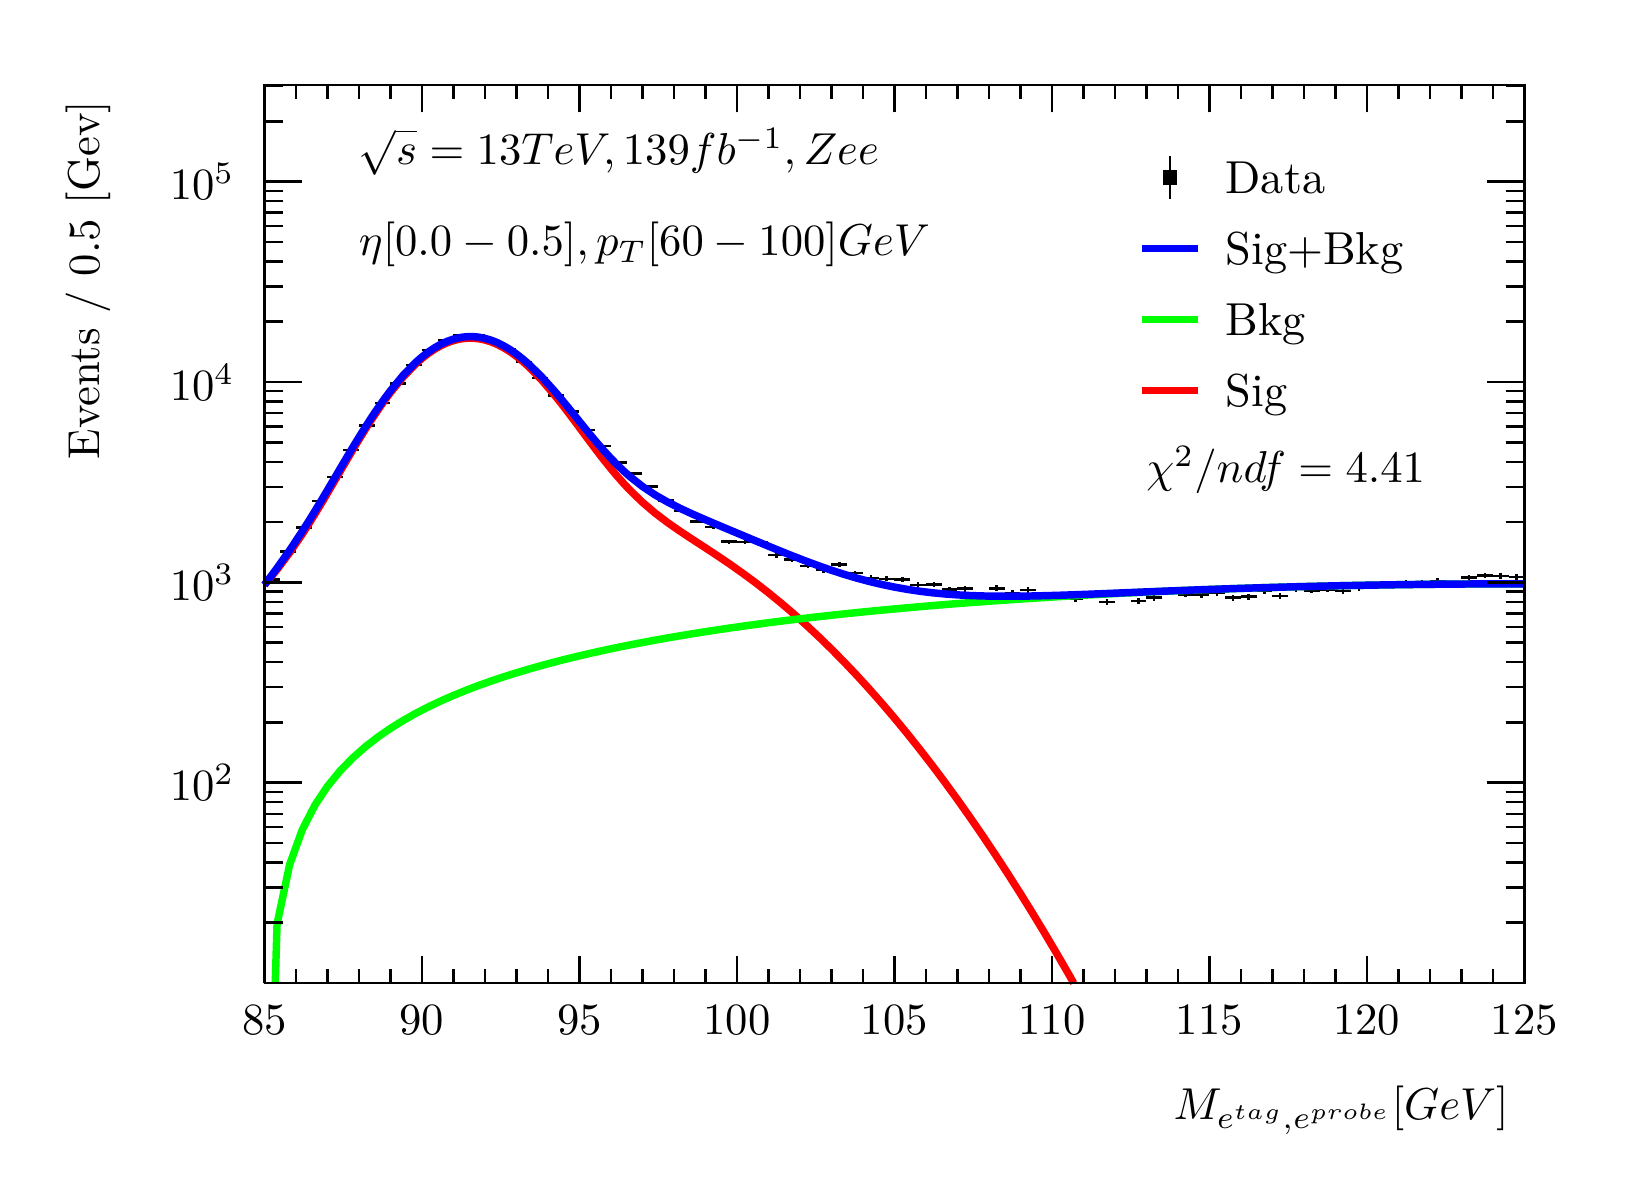
\begin{tikzpicture}
\pgfdeclareplotmark{cross} {
\pgfpathmoveto{\pgfpoint{-0.3\pgfplotmarksize}{\pgfplotmarksize}}
\pgfpathlineto{\pgfpoint{+0.3\pgfplotmarksize}{\pgfplotmarksize}}
\pgfpathlineto{\pgfpoint{+0.3\pgfplotmarksize}{0.3\pgfplotmarksize}}
\pgfpathlineto{\pgfpoint{+1\pgfplotmarksize}{0.3\pgfplotmarksize}}
\pgfpathlineto{\pgfpoint{+1\pgfplotmarksize}{-0.3\pgfplotmarksize}}
\pgfpathlineto{\pgfpoint{+0.3\pgfplotmarksize}{-0.3\pgfplotmarksize}}
\pgfpathlineto{\pgfpoint{+0.3\pgfplotmarksize}{-1.\pgfplotmarksize}}
\pgfpathlineto{\pgfpoint{-0.3\pgfplotmarksize}{-1.\pgfplotmarksize}}
\pgfpathlineto{\pgfpoint{-0.3\pgfplotmarksize}{-0.3\pgfplotmarksize}}
\pgfpathlineto{\pgfpoint{-1.\pgfplotmarksize}{-0.3\pgfplotmarksize}}
\pgfpathlineto{\pgfpoint{-1.\pgfplotmarksize}{0.3\pgfplotmarksize}}
\pgfpathlineto{\pgfpoint{-0.3\pgfplotmarksize}{0.3\pgfplotmarksize}}
\pgfpathclose
\pgfusepathqstroke
}
\pgfdeclareplotmark{cross*} {
\pgfpathmoveto{\pgfpoint{-0.3\pgfplotmarksize}{\pgfplotmarksize}}
\pgfpathlineto{\pgfpoint{+0.3\pgfplotmarksize}{\pgfplotmarksize}}
\pgfpathlineto{\pgfpoint{+0.3\pgfplotmarksize}{0.3\pgfplotmarksize}}
\pgfpathlineto{\pgfpoint{+1\pgfplotmarksize}{0.3\pgfplotmarksize}}
\pgfpathlineto{\pgfpoint{+1\pgfplotmarksize}{-0.3\pgfplotmarksize}}
\pgfpathlineto{\pgfpoint{+0.3\pgfplotmarksize}{-0.3\pgfplotmarksize}}
\pgfpathlineto{\pgfpoint{+0.3\pgfplotmarksize}{-1.\pgfplotmarksize}}
\pgfpathlineto{\pgfpoint{-0.3\pgfplotmarksize}{-1.\pgfplotmarksize}}
\pgfpathlineto{\pgfpoint{-0.3\pgfplotmarksize}{-0.3\pgfplotmarksize}}
\pgfpathlineto{\pgfpoint{-1.\pgfplotmarksize}{-0.3\pgfplotmarksize}}
\pgfpathlineto{\pgfpoint{-1.\pgfplotmarksize}{0.3\pgfplotmarksize}}
\pgfpathlineto{\pgfpoint{-0.3\pgfplotmarksize}{0.3\pgfplotmarksize}}
\pgfpathclose
\pgfusepathqfillstroke
}
\pgfdeclareplotmark{newstar} {
\pgfpathmoveto{\pgfqpoint{0pt}{\pgfplotmarksize}}
\pgfpathlineto{\pgfqpointpolar{44}{0.5\pgfplotmarksize}}
\pgfpathlineto{\pgfqpointpolar{18}{\pgfplotmarksize}}
\pgfpathlineto{\pgfqpointpolar{-20}{0.5\pgfplotmarksize}}
\pgfpathlineto{\pgfqpointpolar{-54}{\pgfplotmarksize}}
\pgfpathlineto{\pgfqpointpolar{-90}{0.5\pgfplotmarksize}}
\pgfpathlineto{\pgfqpointpolar{234}{\pgfplotmarksize}}
\pgfpathlineto{\pgfqpointpolar{198}{0.5\pgfplotmarksize}}
\pgfpathlineto{\pgfqpointpolar{162}{\pgfplotmarksize}}
\pgfpathlineto{\pgfqpointpolar{134}{0.5\pgfplotmarksize}}
\pgfpathclose
\pgfusepathqstroke
}
\pgfdeclareplotmark{newstar*} {
\pgfpathmoveto{\pgfqpoint{0pt}{\pgfplotmarksize}}
\pgfpathlineto{\pgfqpointpolar{44}{0.5\pgfplotmarksize}}
\pgfpathlineto{\pgfqpointpolar{18}{\pgfplotmarksize}}
\pgfpathlineto{\pgfqpointpolar{-20}{0.5\pgfplotmarksize}}
\pgfpathlineto{\pgfqpointpolar{-54}{\pgfplotmarksize}}
\pgfpathlineto{\pgfqpointpolar{-90}{0.5\pgfplotmarksize}}
\pgfpathlineto{\pgfqpointpolar{234}{\pgfplotmarksize}}
\pgfpathlineto{\pgfqpointpolar{198}{0.5\pgfplotmarksize}}
\pgfpathlineto{\pgfqpointpolar{162}{\pgfplotmarksize}}
\pgfpathlineto{\pgfqpointpolar{134}{0.5\pgfplotmarksize}}
\pgfpathclose
\pgfusepathqfillstroke
}
\definecolor{c}{rgb}{1,1,1};
\draw [color=c, fill=c] (0,0) rectangle (20,14.4361);
\draw [color=c, fill=c] (3,2.30977) rectangle (19,13.7143);
\definecolor{c}{rgb}{0,0,0};
\draw [c,line width=0.9] (3,2.30977) -- (3,13.7143) -- (19,13.7143) -- (19,2.30977) -- (3,2.30977);
\definecolor{c}{rgb}{1,1,1};
\draw [color=c, fill=c] (3,2.30977) rectangle (19,13.7143);
\definecolor{c}{rgb}{0,0,0};
\draw [c,line width=0.9] (3,2.30977) -- (3,13.7143) -- (19,13.7143) -- (19,2.30977) -- (3,2.30977);
\draw [c,line width=0.9] (3,2.30977) -- (19,2.30977);
\draw [c,line width=0.9] (3,2.65624) -- (3,2.30977);
\draw [c,line width=0.9] (3.4,2.48301) -- (3.4,2.30977);
\draw [c,line width=0.9] (3.8,2.48301) -- (3.8,2.30977);
\draw [c,line width=0.9] (4.2,2.48301) -- (4.2,2.30977);
\draw [c,line width=0.9] (4.6,2.48301) -- (4.6,2.30977);
\draw [c,line width=0.9] (5,2.65624) -- (5,2.30977);
\draw [c,line width=0.9] (5.4,2.48301) -- (5.4,2.30977);
\draw [c,line width=0.9] (5.8,2.48301) -- (5.8,2.30977);
\draw [c,line width=0.9] (6.2,2.48301) -- (6.2,2.30977);
\draw [c,line width=0.9] (6.6,2.48301) -- (6.6,2.30977);
\draw [c,line width=0.9] (7,2.65624) -- (7,2.30977);
\draw [c,line width=0.9] (7.4,2.48301) -- (7.4,2.30977);
\draw [c,line width=0.9] (7.8,2.48301) -- (7.8,2.30977);
\draw [c,line width=0.9] (8.2,2.48301) -- (8.2,2.30977);
\draw [c,line width=0.9] (8.6,2.48301) -- (8.6,2.30977);
\draw [c,line width=0.9] (9,2.65624) -- (9,2.30977);
\draw [c,line width=0.9] (9.4,2.48301) -- (9.4,2.30977);
\draw [c,line width=0.9] (9.8,2.48301) -- (9.8,2.30977);
\draw [c,line width=0.9] (10.2,2.48301) -- (10.2,2.30977);
\draw [c,line width=0.9] (10.6,2.48301) -- (10.6,2.30977);
\draw [c,line width=0.9] (11,2.65624) -- (11,2.30977);
\draw [c,line width=0.9] (11.4,2.48301) -- (11.4,2.30977);
\draw [c,line width=0.9] (11.8,2.48301) -- (11.8,2.30977);
\draw [c,line width=0.9] (12.2,2.48301) -- (12.2,2.30977);
\draw [c,line width=0.9] (12.6,2.48301) -- (12.6,2.30977);
\draw [c,line width=0.9] (13,2.65624) -- (13,2.30977);
\draw [c,line width=0.9] (13.4,2.48301) -- (13.4,2.30977);
\draw [c,line width=0.9] (13.8,2.48301) -- (13.8,2.30977);
\draw [c,line width=0.9] (14.2,2.48301) -- (14.2,2.30977);
\draw [c,line width=0.9] (14.6,2.48301) -- (14.6,2.30977);
\draw [c,line width=0.9] (15,2.65624) -- (15,2.30977);
\draw [c,line width=0.9] (15.4,2.48301) -- (15.4,2.30977);
\draw [c,line width=0.9] (15.8,2.48301) -- (15.8,2.30977);
\draw [c,line width=0.9] (16.2,2.48301) -- (16.2,2.30977);
\draw [c,line width=0.9] (16.6,2.48301) -- (16.6,2.30977);
\draw [c,line width=0.9] (17,2.65624) -- (17,2.30977);
\draw [c,line width=0.9] (17.4,2.48301) -- (17.4,2.30977);
\draw [c,line width=0.9] (17.8,2.48301) -- (17.8,2.30977);
\draw [c,line width=0.9] (18.2,2.48301) -- (18.2,2.30977);
\draw [c,line width=0.9] (18.6,2.48301) -- (18.6,2.30977);
\draw [c,line width=0.9] (19,2.65624) -- (19,2.30977);
\draw [anchor=base] (3,1.66015) node[scale=1.61424, color=c, rotate=0]{85};
\draw [anchor=base] (5,1.66015) node[scale=1.61424, color=c, rotate=0]{90};
\draw [anchor=base] (7,1.66015) node[scale=1.61424, color=c, rotate=0]{95};
\draw [anchor=base] (9,1.66015) node[scale=1.61424, color=c, rotate=0]{100};
\draw [anchor=base] (11,1.66015) node[scale=1.61424, color=c, rotate=0]{105};
\draw [anchor=base] (13,1.66015) node[scale=1.61424, color=c, rotate=0]{110};
\draw [anchor=base] (15,1.66015) node[scale=1.61424, color=c, rotate=0]{115};
\draw [anchor=base] (17,1.66015) node[scale=1.61424, color=c, rotate=0]{120};
\draw [anchor=base] (19,1.66015) node[scale=1.61424, color=c, rotate=0]{125};
\draw [anchor= east] (19,0.692932) node[scale=1.61424, color=c, rotate=0]{$M_{e^{tag}, e^{probe}}  [GeV]$};
\draw [c,line width=0.9] (3,13.7143) -- (19,13.7143);
\draw [c,line width=0.9] (3,13.3678) -- (3,13.7143);
\draw [c,line width=0.9] (3.4,13.5411) -- (3.4,13.7143);
\draw [c,line width=0.9] (3.8,13.5411) -- (3.8,13.7143);
\draw [c,line width=0.9] (4.2,13.5411) -- (4.2,13.7143);
\draw [c,line width=0.9] (4.6,13.5411) -- (4.6,13.7143);
\draw [c,line width=0.9] (5,13.3678) -- (5,13.7143);
\draw [c,line width=0.9] (5.4,13.5411) -- (5.4,13.7143);
\draw [c,line width=0.9] (5.8,13.5411) -- (5.8,13.7143);
\draw [c,line width=0.9] (6.2,13.5411) -- (6.2,13.7143);
\draw [c,line width=0.9] (6.6,13.5411) -- (6.6,13.7143);
\draw [c,line width=0.9] (7,13.3678) -- (7,13.7143);
\draw [c,line width=0.9] (7.4,13.5411) -- (7.4,13.7143);
\draw [c,line width=0.9] (7.8,13.5411) -- (7.8,13.7143);
\draw [c,line width=0.9] (8.2,13.5411) -- (8.2,13.7143);
\draw [c,line width=0.9] (8.6,13.5411) -- (8.6,13.7143);
\draw [c,line width=0.9] (9,13.3678) -- (9,13.7143);
\draw [c,line width=0.9] (9.4,13.5411) -- (9.4,13.7143);
\draw [c,line width=0.9] (9.8,13.5411) -- (9.8,13.7143);
\draw [c,line width=0.9] (10.2,13.5411) -- (10.2,13.7143);
\draw [c,line width=0.9] (10.6,13.5411) -- (10.6,13.7143);
\draw [c,line width=0.9] (11,13.3678) -- (11,13.7143);
\draw [c,line width=0.9] (11.4,13.5411) -- (11.4,13.7143);
\draw [c,line width=0.9] (11.8,13.5411) -- (11.8,13.7143);
\draw [c,line width=0.9] (12.2,13.5411) -- (12.2,13.7143);
\draw [c,line width=0.9] (12.6,13.5411) -- (12.6,13.7143);
\draw [c,line width=0.9] (13,13.3678) -- (13,13.7143);
\draw [c,line width=0.9] (13.4,13.5411) -- (13.4,13.7143);
\draw [c,line width=0.9] (13.8,13.5411) -- (13.8,13.7143);
\draw [c,line width=0.9] (14.2,13.5411) -- (14.2,13.7143);
\draw [c,line width=0.9] (14.6,13.5411) -- (14.6,13.7143);
\draw [c,line width=0.9] (15,13.3678) -- (15,13.7143);
\draw [c,line width=0.9] (15.4,13.5411) -- (15.4,13.7143);
\draw [c,line width=0.9] (15.8,13.5411) -- (15.8,13.7143);
\draw [c,line width=0.9] (16.2,13.5411) -- (16.2,13.7143);
\draw [c,line width=0.9] (16.6,13.5411) -- (16.6,13.7143);
\draw [c,line width=0.9] (17,13.3678) -- (17,13.7143);
\draw [c,line width=0.9] (17.4,13.5411) -- (17.4,13.7143);
\draw [c,line width=0.9] (17.8,13.5411) -- (17.8,13.7143);
\draw [c,line width=0.9] (18.2,13.5411) -- (18.2,13.7143);
\draw [c,line width=0.9] (18.6,13.5411) -- (18.6,13.7143);
\draw [c,line width=0.9] (19,13.3678) -- (19,13.7143);
\draw [c,line width=0.9] (3,2.30977) -- (3,13.7143);
\draw [c,line width=0.9] (3.237,3.07568) -- (3,3.07568);
\draw [c,line width=0.9] (3.237,3.5237) -- (3,3.5237);
\draw [c,line width=0.9] (3.237,3.84158) -- (3,3.84158);
\draw [c,line width=0.9] (3.237,4.08815) -- (3,4.08815);
\draw [c,line width=0.9] (3.237,4.2896) -- (3,4.2896);
\draw [c,line width=0.9] (3.237,4.45994) -- (3,4.45994);
\draw [c,line width=0.9] (3.237,4.60748) -- (3,4.60748);
\draw [c,line width=0.9] (3.237,4.73763) -- (3,4.73763);
\draw [c,line width=0.9] (3.474,4.85405) -- (3,4.85405);
\draw [anchor= east] (2.82,4.85405) node[scale=1.61424, color=c, rotate=0]{$10^{2}$};
\draw [c,line width=0.9] (3.237,5.61995) -- (3,5.61995);
\draw [c,line width=0.9] (3.237,6.06798) -- (3,6.06798);
\draw [c,line width=0.9] (3.237,6.38586) -- (3,6.38586);
\draw [c,line width=0.9] (3.237,6.63242) -- (3,6.63242);
\draw [c,line width=0.9] (3.237,6.83388) -- (3,6.83388);
\draw [c,line width=0.9] (3.237,7.00421) -- (3,7.00421);
\draw [c,line width=0.9] (3.237,7.15176) -- (3,7.15176);
\draw [c,line width=0.9] (3.237,7.28191) -- (3,7.28191);
\draw [c,line width=0.9] (3.474,7.39833) -- (3,7.39833);
\draw [anchor= east] (2.82,7.39833) node[scale=1.61424, color=c, rotate=0]{$10^{3}$};
\draw [c,line width=0.9] (3.237,8.16423) -- (3,8.16423);
\draw [c,line width=0.9] (3.237,8.61226) -- (3,8.61226);
\draw [c,line width=0.9] (3.237,8.93013) -- (3,8.93013);
\draw [c,line width=0.9] (3.237,9.1767) -- (3,9.1767);
\draw [c,line width=0.9] (3.237,9.37816) -- (3,9.37816);
\draw [c,line width=0.9] (3.237,9.54849) -- (3,9.54849);
\draw [c,line width=0.9] (3.237,9.69604) -- (3,9.69604);
\draw [c,line width=0.9] (3.237,9.82618) -- (3,9.82618);
\draw [c,line width=0.9] (3.474,9.9426) -- (3,9.9426);
\draw [anchor= east] (2.82,9.9426) node[scale=1.61424, color=c, rotate=0]{$10^{4}$};
\draw [c,line width=0.9] (3.237,10.7085) -- (3,10.7085);
\draw [c,line width=0.9] (3.237,11.1565) -- (3,11.1565);
\draw [c,line width=0.9] (3.237,11.4744) -- (3,11.4744);
\draw [c,line width=0.9] (3.237,11.721) -- (3,11.721);
\draw [c,line width=0.9] (3.237,11.9224) -- (3,11.9224);
\draw [c,line width=0.9] (3.237,12.0928) -- (3,12.0928);
\draw [c,line width=0.9] (3.237,12.2403) -- (3,12.2403);
\draw [c,line width=0.9] (3.237,12.3705) -- (3,12.3705);
\draw [c,line width=0.9] (3.474,12.4869) -- (3,12.4869);
\draw [anchor= east] (2.82,12.4869) node[scale=1.61424, color=c, rotate=0]{$10^{5}$};
\draw [c,line width=0.9] (3.237,13.2528) -- (3,13.2528);
\draw [c,line width=0.9] (3.237,13.7008) -- (3,13.7008);
\draw [anchor= east] (0.76,13.7143) node[scale=1.61424, color=c, rotate=90]{Events / 0.5 [Gev]};
\draw [c,line width=0.9] (19,2.30977) -- (19,13.7143);
\draw [c,line width=0.9] (18.763,3.07568) -- (19,3.07568);
\draw [c,line width=0.9] (18.763,3.5237) -- (19,3.5237);
\draw [c,line width=0.9] (18.763,3.84158) -- (19,3.84158);
\draw [c,line width=0.9] (18.763,4.08815) -- (19,4.08815);
\draw [c,line width=0.9] (18.763,4.2896) -- (19,4.2896);
\draw [c,line width=0.9] (18.763,4.45994) -- (19,4.45994);
\draw [c,line width=0.9] (18.763,4.60748) -- (19,4.60748);
\draw [c,line width=0.9] (18.763,4.73763) -- (19,4.73763);
\draw [c,line width=0.9] (18.526,4.85405) -- (19,4.85405);
\draw [c,line width=0.9] (18.763,5.61995) -- (19,5.61995);
\draw [c,line width=0.9] (18.763,6.06798) -- (19,6.06798);
\draw [c,line width=0.9] (18.763,6.38586) -- (19,6.38586);
\draw [c,line width=0.9] (18.763,6.63242) -- (19,6.63242);
\draw [c,line width=0.9] (18.763,6.83388) -- (19,6.83388);
\draw [c,line width=0.9] (18.763,7.00421) -- (19,7.00421);
\draw [c,line width=0.9] (18.763,7.15176) -- (19,7.15176);
\draw [c,line width=0.9] (18.763,7.28191) -- (19,7.28191);
\draw [c,line width=0.9] (18.526,7.39833) -- (19,7.39833);
\draw [c,line width=0.9] (18.763,8.16423) -- (19,8.16423);
\draw [c,line width=0.9] (18.763,8.61226) -- (19,8.61226);
\draw [c,line width=0.9] (18.763,8.93013) -- (19,8.93013);
\draw [c,line width=0.9] (18.763,9.1767) -- (19,9.1767);
\draw [c,line width=0.9] (18.763,9.37816) -- (19,9.37816);
\draw [c,line width=0.9] (18.763,9.54849) -- (19,9.54849);
\draw [c,line width=0.9] (18.763,9.69604) -- (19,9.69604);
\draw [c,line width=0.9] (18.763,9.82618) -- (19,9.82618);
\draw [c,line width=0.9] (18.526,9.9426) -- (19,9.9426);
\draw [c,line width=0.9] (18.763,10.7085) -- (19,10.7085);
\draw [c,line width=0.9] (18.763,11.1565) -- (19,11.1565);
\draw [c,line width=0.9] (18.763,11.4744) -- (19,11.4744);
\draw [c,line width=0.9] (18.763,11.721) -- (19,11.721);
\draw [c,line width=0.9] (18.763,11.9224) -- (19,11.9224);
\draw [c,line width=0.9] (18.763,12.0928) -- (19,12.0928);
\draw [c,line width=0.9] (18.763,12.2403) -- (19,12.2403);
\draw [c,line width=0.9] (18.763,12.3705) -- (19,12.3705);
\draw [c,line width=0.9] (18.526,12.4869) -- (19,12.4869);
\draw [c,line width=0.9] (18.763,13.2528) -- (19,13.2528);
\draw [c,line width=0.9] (18.763,13.7008) -- (19,13.7008);
\draw [c,line width=0.9] (3.1,7.4342) -- (3,7.4342);
\draw [c,line width=0.9] (3,7.4342) -- (3,7.4342);
\draw [c,line width=0.9] (3.1,7.4342) -- (3.2,7.4342);
\draw [c,line width=0.9] (3.2,7.4342) -- (3.2,7.4342);
\draw [c,line width=0.9] (3.1,7.4342) -- (3.1,7.46858);
\draw [c,line width=0.9] (3.1,7.46858) -- (3.1,7.46858);
\draw [c,line width=0.9] (3.1,7.4342) -- (3.1,7.39983);
\draw [c,line width=0.9] (3.1,7.39983) -- (3.1,7.39983);
\draw [c,line width=0.9] (3.3,7.7889) -- (3.2,7.7889);
\draw [c,line width=0.9] (3.2,7.7889) -- (3.2,7.7889);
\draw [c,line width=0.9] (3.3,7.7889) -- (3.4,7.7889);
\draw [c,line width=0.9] (3.4,7.7889) -- (3.4,7.7889);
\draw [c,line width=0.9] (3.3,7.7889) -- (3.3,7.81818);
\draw [c,line width=0.9] (3.3,7.81818) -- (3.3,7.81818);
\draw [c,line width=0.9] (3.3,7.7889) -- (3.3,7.75962);
\draw [c,line width=0.9] (3.3,7.75962) -- (3.3,7.75962);
\draw [c,line width=0.9] (3.5,8.09645) -- (3.4,8.09645);
\draw [c,line width=0.9] (3.4,8.09645) -- (3.4,8.09645);
\draw [c,line width=0.9] (3.5,8.09645) -- (3.6,8.09645);
\draw [c,line width=0.9] (3.6,8.09645) -- (3.6,8.09645);
\draw [c,line width=0.9] (3.5,8.09645) -- (3.5,8.12193);
\draw [c,line width=0.9] (3.5,8.12193) -- (3.5,8.12193);
\draw [c,line width=0.9] (3.5,8.09645) -- (3.5,8.07097);
\draw [c,line width=0.9] (3.5,8.07097) -- (3.5,8.07097);
\draw [c,line width=0.9] (3.7,8.43008) -- (3.6,8.43008);
\draw [c,line width=0.9] (3.6,8.43008) -- (3.6,8.43008);
\draw [c,line width=0.9] (3.7,8.43008) -- (3.8,8.43008);
\draw [c,line width=0.9] (3.8,8.43008) -- (3.8,8.43008);
\draw [c,line width=0.9] (3.7,8.43008) -- (3.7,8.45198);
\draw [c,line width=0.9] (3.7,8.45198) -- (3.7,8.45198);
\draw [c,line width=0.9] (3.7,8.43008) -- (3.7,8.40817);
\draw [c,line width=0.9] (3.7,8.40817) -- (3.7,8.40817);
\draw [c,line width=0.9] (3.9,8.73386) -- (3.8,8.73386);
\draw [c,line width=0.9] (3.8,8.73386) -- (3.8,8.73386);
\draw [c,line width=0.9] (3.9,8.73386) -- (4,8.73386);
\draw [c,line width=0.9] (4,8.73386) -- (4,8.73386);
\draw [c,line width=0.9] (3.9,8.73386) -- (3.9,8.75295);
\draw [c,line width=0.9] (3.9,8.75295) -- (3.9,8.75295);
\draw [c,line width=0.9] (3.9,8.73386) -- (3.9,8.71476);
\draw [c,line width=0.9] (3.9,8.71476) -- (3.9,8.71476);
\draw [c,line width=0.9] (4.1,9.07903) -- (4,9.07903);
\draw [c,line width=0.9] (4,9.07903) -- (4,9.07903);
\draw [c,line width=0.9] (4.1,9.07903) -- (4.2,9.07903);
\draw [c,line width=0.9] (4.2,9.07903) -- (4.2,9.07903);
\draw [c,line width=0.9] (4.1,9.07903) -- (4.1,9.09536);
\draw [c,line width=0.9] (4.1,9.09536) -- (4.1,9.09536);
\draw [c,line width=0.9] (4.1,9.07903) -- (4.1,9.0627);
\draw [c,line width=0.9] (4.1,9.0627) -- (4.1,9.0627);
\draw [c,line width=0.9] (4.3,9.39261) -- (4.2,9.39261);
\draw [c,line width=0.9] (4.2,9.39261) -- (4.2,9.39261);
\draw [c,line width=0.9] (4.3,9.39261) -- (4.4,9.39261);
\draw [c,line width=0.9] (4.4,9.39261) -- (4.4,9.39261);
\draw [c,line width=0.9] (4.3,9.39261) -- (4.3,9.40679);
\draw [c,line width=0.9] (4.3,9.40679) -- (4.3,9.40679);
\draw [c,line width=0.9] (4.3,9.39261) -- (4.3,9.37844);
\draw [c,line width=0.9] (4.3,9.37844) -- (4.3,9.37844);
\draw [c,line width=0.9] (4.5,9.67681) -- (4.4,9.67681);
\draw [c,line width=0.9] (4.4,9.67681) -- (4.4,9.67681);
\draw [c,line width=0.9] (4.5,9.67681) -- (4.6,9.67681);
\draw [c,line width=0.9] (4.6,9.67681) -- (4.6,9.67681);
\draw [c,line width=0.9] (4.5,9.67681) -- (4.5,9.68927);
\draw [c,line width=0.9] (4.5,9.68927) -- (4.5,9.68927);
\draw [c,line width=0.9] (4.5,9.67681) -- (4.5,9.66435);
\draw [c,line width=0.9] (4.5,9.66435) -- (4.5,9.66435);
\draw [c,line width=0.9] (4.7,9.9213) -- (4.6,9.9213);
\draw [c,line width=0.9] (4.6,9.9213) -- (4.6,9.9213);
\draw [c,line width=0.9] (4.7,9.9213) -- (4.8,9.9213);
\draw [c,line width=0.9] (4.8,9.9213) -- (4.8,9.9213);
\draw [c,line width=0.9] (4.7,9.9213) -- (4.7,9.93245);
\draw [c,line width=0.9] (4.7,9.93245) -- (4.7,9.93245);
\draw [c,line width=0.9] (4.7,9.9213) -- (4.7,9.91014);
\draw [c,line width=0.9] (4.7,9.91014) -- (4.7,9.91014);
\draw [c,line width=0.9] (4.9,10.1618) -- (4.8,10.1618);
\draw [c,line width=0.9] (4.8,10.1618) -- (4.8,10.1618);
\draw [c,line width=0.9] (4.9,10.1618) -- (5,10.1618);
\draw [c,line width=0.9] (5,10.1618) -- (5,10.1618);
\draw [c,line width=0.9] (4.9,10.1618) -- (4.9,10.1718);
\draw [c,line width=0.9] (4.9,10.1718) -- (4.9,10.1718);
\draw [c,line width=0.9] (4.9,10.1618) -- (4.9,10.1518);
\draw [c,line width=0.9] (4.9,10.1518) -- (4.9,10.1518);
\draw [c,line width=0.9] (5.1,10.3471) -- (5,10.3471);
\draw [c,line width=0.9] (5,10.3471) -- (5,10.3471);
\draw [c,line width=0.9] (5.1,10.3471) -- (5.2,10.3471);
\draw [c,line width=0.9] (5.2,10.3471) -- (5.2,10.3471);
\draw [c,line width=0.9] (5.1,10.3471) -- (5.1,10.3563);
\draw [c,line width=0.9] (5.1,10.3563) -- (5.1,10.3563);
\draw [c,line width=0.9] (5.1,10.3471) -- (5.1,10.3379);
\draw [c,line width=0.9] (5.1,10.3379) -- (5.1,10.3379);
\draw [c,line width=0.9] (5.3,10.4746) -- (5.2,10.4746);
\draw [c,line width=0.9] (5.2,10.4746) -- (5.2,10.4746);
\draw [c,line width=0.9] (5.3,10.4746) -- (5.4,10.4746);
\draw [c,line width=0.9] (5.4,10.4746) -- (5.4,10.4746);
\draw [c,line width=0.9] (5.3,10.4746) -- (5.3,10.4833);
\draw [c,line width=0.9] (5.3,10.4833) -- (5.3,10.4833);
\draw [c,line width=0.9] (5.3,10.4746) -- (5.3,10.466);
\draw [c,line width=0.9] (5.3,10.466) -- (5.3,10.466);
\draw [c,line width=0.9] (5.5,10.5373) -- (5.4,10.5373);
\draw [c,line width=0.9] (5.4,10.5373) -- (5.4,10.5373);
\draw [c,line width=0.9] (5.5,10.5373) -- (5.6,10.5373);
\draw [c,line width=0.9] (5.6,10.5373) -- (5.6,10.5373);
\draw [c,line width=0.9] (5.5,10.5373) -- (5.5,10.5457);
\draw [c,line width=0.9] (5.5,10.5457) -- (5.5,10.5457);
\draw [c,line width=0.9] (5.5,10.5373) -- (5.5,10.5288);
\draw [c,line width=0.9] (5.5,10.5288) -- (5.5,10.5288);
\draw [c,line width=0.9] (5.7,10.5319) -- (5.6,10.5319);
\draw [c,line width=0.9] (5.6,10.5319) -- (5.6,10.5319);
\draw [c,line width=0.9] (5.7,10.5319) -- (5.8,10.5319);
\draw [c,line width=0.9] (5.8,10.5319) -- (5.8,10.5319);
\draw [c,line width=0.9] (5.7,10.5319) -- (5.7,10.5403);
\draw [c,line width=0.9] (5.7,10.5403) -- (5.7,10.5403);
\draw [c,line width=0.9] (5.7,10.5319) -- (5.7,10.5234);
\draw [c,line width=0.9] (5.7,10.5234) -- (5.7,10.5234);
\draw [c,line width=0.9] (5.9,10.4613) -- (5.8,10.4613);
\draw [c,line width=0.9] (5.8,10.4613) -- (5.8,10.4613);
\draw [c,line width=0.9] (5.9,10.4613) -- (6,10.4613);
\draw [c,line width=0.9] (6,10.4613) -- (6,10.4613);
\draw [c,line width=0.9] (5.9,10.4613) -- (5.9,10.4701);
\draw [c,line width=0.9] (5.9,10.4701) -- (5.9,10.4701);
\draw [c,line width=0.9] (5.9,10.4613) -- (5.9,10.4526);
\draw [c,line width=0.9] (5.9,10.4526) -- (5.9,10.4526);
\draw [c,line width=0.9] (6.1,10.3639) -- (6,10.3639);
\draw [c,line width=0.9] (6,10.3639) -- (6,10.3639);
\draw [c,line width=0.9] (6.1,10.3639) -- (6.2,10.3639);
\draw [c,line width=0.9] (6.2,10.3639) -- (6.2,10.3639);
\draw [c,line width=0.9] (6.1,10.3639) -- (6.1,10.373);
\draw [c,line width=0.9] (6.1,10.373) -- (6.1,10.373);
\draw [c,line width=0.9] (6.1,10.3639) -- (6.1,10.3547);
\draw [c,line width=0.9] (6.1,10.3547) -- (6.1,10.3547);
\draw [c,line width=0.9] (6.3,10.1946) -- (6.2,10.1946);
\draw [c,line width=0.9] (6.2,10.1946) -- (6.2,10.1946);
\draw [c,line width=0.9] (6.3,10.1946) -- (6.4,10.1946);
\draw [c,line width=0.9] (6.4,10.1946) -- (6.4,10.1946);
\draw [c,line width=0.9] (6.3,10.1946) -- (6.3,10.2044);
\draw [c,line width=0.9] (6.3,10.2044) -- (6.3,10.2044);
\draw [c,line width=0.9] (6.3,10.1946) -- (6.3,10.1847);
\draw [c,line width=0.9] (6.3,10.1847) -- (6.3,10.1847);
\draw [c,line width=0.9] (6.5,9.9942) -- (6.4,9.9942);
\draw [c,line width=0.9] (6.4,9.9942) -- (6.4,9.9942);
\draw [c,line width=0.9] (6.5,9.9942) -- (6.6,9.9942);
\draw [c,line width=0.9] (6.6,9.9942) -- (6.6,9.9942);
\draw [c,line width=0.9] (6.5,9.9942) -- (6.5,10.005);
\draw [c,line width=0.9] (6.5,10.005) -- (6.5,10.005);
\draw [c,line width=0.9] (6.5,9.9942) -- (6.5,9.9834);
\draw [c,line width=0.9] (6.5,9.9834) -- (6.5,9.9834);
\draw [c,line width=0.9] (6.7,9.77273) -- (6.6,9.77273);
\draw [c,line width=0.9] (6.6,9.77273) -- (6.6,9.77273);
\draw [c,line width=0.9] (6.7,9.77273) -- (6.8,9.77273);
\draw [c,line width=0.9] (6.8,9.77273) -- (6.8,9.77273);
\draw [c,line width=0.9] (6.7,9.77273) -- (6.7,9.78467);
\draw [c,line width=0.9] (6.7,9.78467) -- (6.7,9.78467);
\draw [c,line width=0.9] (6.7,9.77273) -- (6.7,9.7608);
\draw [c,line width=0.9] (6.7,9.7608) -- (6.7,9.7608);
\draw [c,line width=0.9] (6.9,9.57099) -- (6.8,9.57099);
\draw [c,line width=0.9] (6.8,9.57099) -- (6.8,9.57099);
\draw [c,line width=0.9] (6.9,9.57099) -- (7,9.57099);
\draw [c,line width=0.9] (7,9.57099) -- (7,9.57099);
\draw [c,line width=0.9] (6.9,9.57099) -- (6.9,9.58406);
\draw [c,line width=0.9] (6.9,9.58406) -- (6.9,9.58406);
\draw [c,line width=0.9] (6.9,9.57099) -- (6.9,9.55792);
\draw [c,line width=0.9] (6.9,9.55792) -- (6.9,9.55792);
\draw [c,line width=0.9] (7.1,9.33075) -- (7,9.33075);
\draw [c,line width=0.9] (7,9.33075) -- (7,9.33075);
\draw [c,line width=0.9] (7.1,9.33075) -- (7.2,9.33075);
\draw [c,line width=0.9] (7.2,9.33075) -- (7.2,9.33075);
\draw [c,line width=0.9] (7.1,9.33075) -- (7.1,9.34532);
\draw [c,line width=0.9] (7.1,9.34532) -- (7.1,9.34532);
\draw [c,line width=0.9] (7.1,9.33075) -- (7.1,9.31617);
\draw [c,line width=0.9] (7.1,9.31617) -- (7.1,9.31617);
\draw [c,line width=0.9] (7.3,9.13159) -- (7.2,9.13159);
\draw [c,line width=0.9] (7.2,9.13159) -- (7.2,9.13159);
\draw [c,line width=0.9] (7.3,9.13159) -- (7.4,9.13159);
\draw [c,line width=0.9] (7.4,9.13159) -- (7.4,9.13159);
\draw [c,line width=0.9] (7.3,9.13159) -- (7.3,9.14754);
\draw [c,line width=0.9] (7.3,9.14754) -- (7.3,9.14754);
\draw [c,line width=0.9] (7.3,9.13159) -- (7.3,9.11565);
\draw [c,line width=0.9] (7.3,9.11565) -- (7.3,9.11565);
\draw [c,line width=0.9] (7.5,8.91903) -- (7.4,8.91903);
\draw [c,line width=0.9] (7.4,8.91903) -- (7.4,8.91903);
\draw [c,line width=0.9] (7.5,8.91903) -- (7.6,8.91903);
\draw [c,line width=0.9] (7.6,8.91903) -- (7.6,8.91903);
\draw [c,line width=0.9] (7.5,8.91903) -- (7.5,8.93659);
\draw [c,line width=0.9] (7.5,8.93659) -- (7.5,8.93659);
\draw [c,line width=0.9] (7.5,8.91903) -- (7.5,8.90147);
\draw [c,line width=0.9] (7.5,8.90147) -- (7.5,8.90147);
\draw [c,line width=0.9] (7.7,8.77911) -- (7.6,8.77911);
\draw [c,line width=0.9] (7.6,8.77911) -- (7.6,8.77911);
\draw [c,line width=0.9] (7.7,8.77911) -- (7.8,8.77911);
\draw [c,line width=0.9] (7.8,8.77911) -- (7.8,8.77911);
\draw [c,line width=0.9] (7.7,8.77911) -- (7.7,8.79782);
\draw [c,line width=0.9] (7.7,8.79782) -- (7.7,8.79782);
\draw [c,line width=0.9] (7.7,8.77911) -- (7.7,8.7604);
\draw [c,line width=0.9] (7.7,8.7604) -- (7.7,8.7604);
\draw [c,line width=0.9] (7.9,8.61887) -- (7.8,8.61887);
\draw [c,line width=0.9] (7.8,8.61887) -- (7.8,8.61887);
\draw [c,line width=0.9] (7.9,8.61887) -- (8,8.61887);
\draw [c,line width=0.9] (8,8.61887) -- (8,8.61887);
\draw [c,line width=0.9] (7.9,8.61887) -- (7.9,8.63898);
\draw [c,line width=0.9] (7.9,8.63898) -- (7.9,8.63898);
\draw [c,line width=0.9] (7.9,8.61887) -- (7.9,8.59875);
\draw [c,line width=0.9] (7.9,8.59875) -- (7.9,8.59875);
\draw [c,line width=0.9] (8.1,8.43657) -- (8,8.43657);
\draw [c,line width=0.9] (8,8.43657) -- (8,8.43657);
\draw [c,line width=0.9] (8.1,8.43657) -- (8.2,8.43657);
\draw [c,line width=0.9] (8.2,8.43657) -- (8.2,8.43657);
\draw [c,line width=0.9] (8.1,8.43657) -- (8.1,8.45842);
\draw [c,line width=0.9] (8.1,8.45842) -- (8.1,8.45842);
\draw [c,line width=0.9] (8.1,8.43657) -- (8.1,8.41473);
\draw [c,line width=0.9] (8.1,8.41473) -- (8.1,8.41473);
\draw [c,line width=0.9] (8.3,8.30464) -- (8.2,8.30464);
\draw [c,line width=0.9] (8.2,8.30464) -- (8.2,8.30464);
\draw [c,line width=0.9] (8.3,8.30464) -- (8.4,8.30464);
\draw [c,line width=0.9] (8.4,8.30464) -- (8.4,8.30464);
\draw [c,line width=0.9] (8.3,8.30464) -- (8.3,8.32783);
\draw [c,line width=0.9] (8.3,8.32783) -- (8.3,8.32783);
\draw [c,line width=0.9] (8.3,8.30464) -- (8.3,8.28146);
\draw [c,line width=0.9] (8.3,8.28146) -- (8.3,8.28146);
\draw [c,line width=0.9] (8.5,8.17358) -- (8.4,8.17358);
\draw [c,line width=0.9] (8.4,8.17358) -- (8.4,8.17358);
\draw [c,line width=0.9] (8.5,8.17358) -- (8.6,8.17358);
\draw [c,line width=0.9] (8.6,8.17358) -- (8.6,8.17358);
\draw [c,line width=0.9] (8.5,8.17358) -- (8.5,8.19819);
\draw [c,line width=0.9] (8.5,8.19819) -- (8.5,8.19819);
\draw [c,line width=0.9] (8.5,8.17358) -- (8.5,8.14898);
\draw [c,line width=0.9] (8.5,8.14898) -- (8.5,8.14898);
\draw [c,line width=0.9] (8.7,8.10231) -- (8.6,8.10231);
\draw [c,line width=0.9] (8.6,8.10231) -- (8.6,8.10231);
\draw [c,line width=0.9] (8.7,8.10231) -- (8.8,8.10231);
\draw [c,line width=0.9] (8.8,8.10231) -- (8.8,8.10231);
\draw [c,line width=0.9] (8.7,8.10231) -- (8.7,8.12772);
\draw [c,line width=0.9] (8.7,8.12772) -- (8.7,8.12772);
\draw [c,line width=0.9] (8.7,8.10231) -- (8.7,8.0769);
\draw [c,line width=0.9] (8.7,8.0769) -- (8.7,8.0769);
\draw [c,line width=0.9] (8.9,7.9149) -- (8.8,7.9149);
\draw [c,line width=0.9] (8.8,7.9149) -- (8.8,7.9149);
\draw [c,line width=0.9] (8.9,7.9149) -- (9,7.9149);
\draw [c,line width=0.9] (9,7.9149) -- (9,7.9149);
\draw [c,line width=0.9] (8.9,7.9149) -- (8.9,7.94256);
\draw [c,line width=0.9] (8.9,7.94256) -- (8.9,7.94256);
\draw [c,line width=0.9] (8.9,7.9149) -- (8.9,7.88724);
\draw [c,line width=0.9] (8.9,7.88724) -- (8.9,7.88724);
\draw [c,line width=0.9] (9.1,7.90865) -- (9,7.90865);
\draw [c,line width=0.9] (9,7.90865) -- (9,7.90865);
\draw [c,line width=0.9] (9.1,7.90865) -- (9.2,7.90865);
\draw [c,line width=0.9] (9.2,7.90865) -- (9.2,7.90865);
\draw [c,line width=0.9] (9.1,7.90865) -- (9.1,7.93639);
\draw [c,line width=0.9] (9.1,7.93639) -- (9.1,7.93639);
\draw [c,line width=0.9] (9.1,7.90865) -- (9.1,7.88092);
\draw [c,line width=0.9] (9.1,7.88092) -- (9.1,7.88092);
\draw [c,line width=0.9] (9.3,7.90795) -- (9.2,7.90795);
\draw [c,line width=0.9] (9.2,7.90795) -- (9.2,7.90795);
\draw [c,line width=0.9] (9.3,7.90795) -- (9.4,7.90795);
\draw [c,line width=0.9] (9.4,7.90795) -- (9.4,7.90795);
\draw [c,line width=0.9] (9.3,7.90795) -- (9.3,7.9357);
\draw [c,line width=0.9] (9.3,7.9357) -- (9.3,7.9357);
\draw [c,line width=0.9] (9.3,7.90795) -- (9.3,7.88021);
\draw [c,line width=0.9] (9.3,7.88021) -- (9.3,7.88021);
\draw [c,line width=0.9] (9.5,7.74295) -- (9.4,7.74295);
\draw [c,line width=0.9] (9.4,7.74295) -- (9.4,7.74295);
\draw [c,line width=0.9] (9.5,7.74295) -- (9.6,7.74295);
\draw [c,line width=0.9] (9.6,7.74295) -- (9.6,7.74295);
\draw [c,line width=0.9] (9.5,7.74295) -- (9.5,7.77285);
\draw [c,line width=0.9] (9.5,7.77285) -- (9.5,7.77285);
\draw [c,line width=0.9] (9.5,7.74295) -- (9.5,7.71306);
\draw [c,line width=0.9] (9.5,7.71306) -- (9.5,7.71306);
\draw [c,line width=0.9] (9.7,7.68653) -- (9.6,7.68653);
\draw [c,line width=0.9] (9.6,7.68653) -- (9.6,7.68653);
\draw [c,line width=0.9] (9.7,7.68653) -- (9.8,7.68653);
\draw [c,line width=0.9] (9.8,7.68653) -- (9.8,7.68653);
\draw [c,line width=0.9] (9.7,7.68653) -- (9.7,7.7172);
\draw [c,line width=0.9] (9.7,7.7172) -- (9.7,7.7172);
\draw [c,line width=0.9] (9.7,7.68653) -- (9.7,7.65586);
\draw [c,line width=0.9] (9.7,7.65586) -- (9.7,7.65586);
\draw [c,line width=0.9] (9.9,7.60896) -- (9.8,7.60896);
\draw [c,line width=0.9] (9.8,7.60896) -- (9.8,7.60896);
\draw [c,line width=0.9] (9.9,7.60896) -- (10,7.60896);
\draw [c,line width=0.9] (10,7.60896) -- (10,7.60896);
\draw [c,line width=0.9] (9.9,7.60896) -- (9.9,7.64072);
\draw [c,line width=0.9] (9.9,7.64072) -- (9.9,7.64072);
\draw [c,line width=0.9] (9.9,7.60896) -- (9.9,7.57719);
\draw [c,line width=0.9] (9.9,7.57719) -- (9.9,7.57719);
\draw [c,line width=0.9] (10.1,7.55468) -- (10,7.55468);
\draw [c,line width=0.9] (10,7.55468) -- (10,7.55468);
\draw [c,line width=0.9] (10.1,7.55468) -- (10.2,7.55468);
\draw [c,line width=0.9] (10.2,7.55468) -- (10.2,7.55468);
\draw [c,line width=0.9] (10.1,7.55468) -- (10.1,7.58723);
\draw [c,line width=0.9] (10.1,7.58723) -- (10.1,7.58723);
\draw [c,line width=0.9] (10.1,7.55468) -- (10.1,7.52213);
\draw [c,line width=0.9] (10.1,7.52213) -- (10.1,7.52213);
\draw [c,line width=0.9] (10.3,7.62347) -- (10.2,7.62347);
\draw [c,line width=0.9] (10.2,7.62347) -- (10.2,7.62347);
\draw [c,line width=0.9] (10.3,7.62347) -- (10.4,7.62347);
\draw [c,line width=0.9] (10.4,7.62347) -- (10.4,7.62347);
\draw [c,line width=0.9] (10.3,7.62347) -- (10.3,7.65503);
\draw [c,line width=0.9] (10.3,7.65503) -- (10.3,7.65503);
\draw [c,line width=0.9] (10.3,7.62347) -- (10.3,7.59192);
\draw [c,line width=0.9] (10.3,7.59192) -- (10.3,7.59192);
\draw [c,line width=0.9] (10.5,7.51563) -- (10.4,7.51563);
\draw [c,line width=0.9] (10.4,7.51563) -- (10.4,7.51563);
\draw [c,line width=0.9] (10.5,7.51563) -- (10.6,7.51563);
\draw [c,line width=0.9] (10.6,7.51563) -- (10.6,7.51563);
\draw [c,line width=0.9] (10.5,7.51563) -- (10.5,7.54877);
\draw [c,line width=0.9] (10.5,7.54877) -- (10.5,7.54877);
\draw [c,line width=0.9] (10.5,7.51563) -- (10.5,7.4825);
\draw [c,line width=0.9] (10.5,7.4825) -- (10.5,7.4825);
\draw [c,line width=0.9] (10.7,7.45644) -- (10.6,7.45644);
\draw [c,line width=0.9] (10.6,7.45644) -- (10.6,7.45644);
\draw [c,line width=0.9] (10.7,7.45644) -- (10.8,7.45644);
\draw [c,line width=0.9] (10.8,7.45644) -- (10.8,7.45644);
\draw [c,line width=0.9] (10.7,7.45644) -- (10.7,7.49047);
\draw [c,line width=0.9] (10.7,7.49047) -- (10.7,7.49047);
\draw [c,line width=0.9] (10.7,7.45644) -- (10.7,7.42241);
\draw [c,line width=0.9] (10.7,7.42241) -- (10.7,7.42241);
\draw [c,line width=0.9] (10.9,7.44379) -- (10.8,7.44379);
\draw [c,line width=0.9] (10.8,7.44379) -- (10.8,7.44379);
\draw [c,line width=0.9] (10.9,7.44379) -- (11,7.44379);
\draw [c,line width=0.9] (11,7.44379) -- (11,7.44379);
\draw [c,line width=0.9] (10.9,7.44379) -- (10.9,7.47802);
\draw [c,line width=0.9] (10.9,7.47802) -- (10.9,7.47802);
\draw [c,line width=0.9] (10.9,7.44379) -- (10.9,7.40956);
\draw [c,line width=0.9] (10.9,7.40956) -- (10.9,7.40956);
\draw [c,line width=0.9] (11.1,7.43634) -- (11,7.43634);
\draw [c,line width=0.9] (11,7.43634) -- (11,7.43634);
\draw [c,line width=0.9] (11.1,7.43634) -- (11.2,7.43634);
\draw [c,line width=0.9] (11.2,7.43634) -- (11.2,7.43634);
\draw [c,line width=0.9] (11.1,7.43634) -- (11.1,7.47069);
\draw [c,line width=0.9] (11.1,7.47069) -- (11.1,7.47069);
\draw [c,line width=0.9] (11.1,7.43634) -- (11.1,7.402);
\draw [c,line width=0.9] (11.1,7.402) -- (11.1,7.402);
\draw [c,line width=0.9] (11.3,7.36695) -- (11.2,7.36695);
\draw [c,line width=0.9] (11.2,7.36695) -- (11.2,7.36695);
\draw [c,line width=0.9] (11.3,7.36695) -- (11.4,7.36695);
\draw [c,line width=0.9] (11.4,7.36695) -- (11.4,7.36695);
\draw [c,line width=0.9] (11.3,7.36695) -- (11.3,7.40239);
\draw [c,line width=0.9] (11.3,7.40239) -- (11.3,7.40239);
\draw [c,line width=0.9] (11.3,7.36695) -- (11.3,7.33151);
\draw [c,line width=0.9] (11.3,7.33151) -- (11.3,7.33151);
\draw [c,line width=0.9] (11.5,7.37262) -- (11.4,7.37262);
\draw [c,line width=0.9] (11.4,7.37262) -- (11.4,7.37262);
\draw [c,line width=0.9] (11.5,7.37262) -- (11.6,7.37262);
\draw [c,line width=0.9] (11.6,7.37262) -- (11.6,7.37262);
\draw [c,line width=0.9] (11.5,7.37262) -- (11.5,7.40797);
\draw [c,line width=0.9] (11.5,7.40797) -- (11.5,7.40797);
\draw [c,line width=0.9] (11.5,7.37262) -- (11.5,7.33727);
\draw [c,line width=0.9] (11.5,7.33727) -- (11.5,7.33727);
\draw [c,line width=0.9] (11.7,7.30739) -- (11.6,7.30739);
\draw [c,line width=0.9] (11.6,7.30739) -- (11.6,7.30739);
\draw [c,line width=0.9] (11.7,7.30739) -- (11.8,7.30739);
\draw [c,line width=0.9] (11.8,7.30739) -- (11.8,7.30739);
\draw [c,line width=0.9] (11.7,7.30739) -- (11.7,7.3438);
\draw [c,line width=0.9] (11.7,7.3438) -- (11.7,7.3438);
\draw [c,line width=0.9] (11.7,7.30739) -- (11.7,7.27099);
\draw [c,line width=0.9] (11.7,7.27099) -- (11.7,7.27099);
\draw [c,line width=0.9] (11.9,7.31814) -- (11.8,7.31814);
\draw [c,line width=0.9] (11.8,7.31814) -- (11.8,7.31814);
\draw [c,line width=0.9] (11.9,7.31814) -- (12,7.31814);
\draw [c,line width=0.9] (12,7.31814) -- (12,7.31814);
\draw [c,line width=0.9] (11.9,7.31814) -- (11.9,7.35437);
\draw [c,line width=0.9] (11.9,7.35437) -- (11.9,7.35437);
\draw [c,line width=0.9] (11.9,7.31814) -- (11.9,7.28191);
\draw [c,line width=0.9] (11.9,7.28191) -- (11.9,7.28191);
\draw [c,line width=0.9] (12.1,7.24445) -- (12,7.24445);
\draw [c,line width=0.9] (12,7.24445) -- (12,7.24445);
\draw [c,line width=0.9] (12.1,7.24445) -- (12.2,7.24445);
\draw [c,line width=0.9] (12.2,7.24445) -- (12.2,7.24445);
\draw [c,line width=0.9] (12.1,7.24445) -- (12.1,7.28191);
\draw [c,line width=0.9] (12.1,7.28191) -- (12.1,7.28191);
\draw [c,line width=0.9] (12.1,7.24445) -- (12.1,7.20699);
\draw [c,line width=0.9] (12.1,7.20699) -- (12.1,7.20699);
\draw [c,line width=0.9] (12.3,7.32288) -- (12.2,7.32288);
\draw [c,line width=0.9] (12.2,7.32288) -- (12.2,7.32288);
\draw [c,line width=0.9] (12.3,7.32288) -- (12.4,7.32288);
\draw [c,line width=0.9] (12.4,7.32288) -- (12.4,7.32288);
\draw [c,line width=0.9] (12.3,7.32288) -- (12.3,7.35904);
\draw [c,line width=0.9] (12.3,7.35904) -- (12.3,7.35904);
\draw [c,line width=0.9] (12.3,7.32288) -- (12.3,7.28673);
\draw [c,line width=0.9] (12.3,7.28673) -- (12.3,7.28673);
\draw [c,line width=0.9] (12.5,7.26209) -- (12.4,7.26209);
\draw [c,line width=0.9] (12.4,7.26209) -- (12.4,7.26209);
\draw [c,line width=0.9] (12.5,7.26209) -- (12.6,7.26209);
\draw [c,line width=0.9] (12.6,7.26209) -- (12.6,7.26209);
\draw [c,line width=0.9] (12.5,7.26209) -- (12.5,7.29925);
\draw [c,line width=0.9] (12.5,7.29925) -- (12.5,7.29925);
\draw [c,line width=0.9] (12.5,7.26209) -- (12.5,7.22493);
\draw [c,line width=0.9] (12.5,7.22493) -- (12.5,7.22493);
\draw [c,line width=0.9] (12.7,7.30379) -- (12.6,7.30379);
\draw [c,line width=0.9] (12.6,7.30379) -- (12.6,7.30379);
\draw [c,line width=0.9] (12.7,7.30379) -- (12.8,7.30379);
\draw [c,line width=0.9] (12.8,7.30379) -- (12.8,7.30379);
\draw [c,line width=0.9] (12.7,7.30379) -- (12.7,7.34026);
\draw [c,line width=0.9] (12.7,7.34026) -- (12.7,7.34026);
\draw [c,line width=0.9] (12.7,7.30379) -- (12.7,7.26732);
\draw [c,line width=0.9] (12.7,7.26732) -- (12.7,7.26732);
\draw [c,line width=0.9] (12.9,7.19775) -- (12.8,7.19775);
\draw [c,line width=0.9] (12.8,7.19775) -- (12.8,7.19775);
\draw [c,line width=0.9] (12.9,7.19775) -- (13,7.19775);
\draw [c,line width=0.9] (13,7.19775) -- (13,7.19775);
\draw [c,line width=0.9] (12.9,7.19775) -- (12.9,7.23601);
\draw [c,line width=0.9] (12.9,7.23601) -- (12.9,7.23601);
\draw [c,line width=0.9] (12.9,7.19775) -- (12.9,7.15949);
\draw [c,line width=0.9] (12.9,7.15949) -- (12.9,7.15949);
\draw [c,line width=0.9] (13.1,7.21484) -- (13,7.21484);
\draw [c,line width=0.9] (13,7.21484) -- (13,7.21484);
\draw [c,line width=0.9] (13.1,7.21484) -- (13.2,7.21484);
\draw [c,line width=0.9] (13.2,7.21484) -- (13.2,7.21484);
\draw [c,line width=0.9] (13.1,7.21484) -- (13.1,7.25281);
\draw [c,line width=0.9] (13.1,7.25281) -- (13.1,7.25281);
\draw [c,line width=0.9] (13.1,7.21484) -- (13.1,7.17688);
\draw [c,line width=0.9] (13.1,7.17688) -- (13.1,7.17688);
\draw [c,line width=0.9] (13.3,7.18576) -- (13.2,7.18576);
\draw [c,line width=0.9] (13.2,7.18576) -- (13.2,7.18576);
\draw [c,line width=0.9] (13.3,7.18576) -- (13.4,7.18576);
\draw [c,line width=0.9] (13.4,7.18576) -- (13.4,7.18576);
\draw [c,line width=0.9] (13.3,7.18576) -- (13.3,7.22423);
\draw [c,line width=0.9] (13.3,7.22423) -- (13.3,7.22423);
\draw [c,line width=0.9] (13.3,7.18576) -- (13.3,7.1473);
\draw [c,line width=0.9] (13.3,7.1473) -- (13.3,7.1473);
\draw [c,line width=0.9] (13.5,7.25078) -- (13.4,7.25078);
\draw [c,line width=0.9] (13.4,7.25078) -- (13.4,7.25078);
\draw [c,line width=0.9] (13.5,7.25078) -- (13.6,7.25078);
\draw [c,line width=0.9] (13.6,7.25078) -- (13.6,7.25078);
\draw [c,line width=0.9] (13.5,7.25078) -- (13.5,7.28813);
\draw [c,line width=0.9] (13.5,7.28813) -- (13.5,7.28813);
\draw [c,line width=0.9] (13.5,7.25078) -- (13.5,7.21343);
\draw [c,line width=0.9] (13.5,7.21343) -- (13.5,7.21343);
\draw [c,line width=0.9] (13.7,7.14761) -- (13.6,7.14761);
\draw [c,line width=0.9] (13.6,7.14761) -- (13.6,7.14761);
\draw [c,line width=0.9] (13.7,7.14761) -- (13.8,7.14761);
\draw [c,line width=0.9] (13.8,7.14761) -- (13.8,7.14761);
\draw [c,line width=0.9] (13.7,7.14761) -- (13.7,7.18675);
\draw [c,line width=0.9] (13.7,7.18675) -- (13.7,7.18675);
\draw [c,line width=0.9] (13.7,7.14761) -- (13.7,7.10847);
\draw [c,line width=0.9] (13.7,7.10847) -- (13.7,7.10847);
\draw [c,line width=0.9] (13.9,7.25582) -- (13.8,7.25582);
\draw [c,line width=0.9] (13.8,7.25582) -- (13.8,7.25582);
\draw [c,line width=0.9] (13.9,7.25582) -- (14,7.25582);
\draw [c,line width=0.9] (14,7.25582) -- (14,7.25582);
\draw [c,line width=0.9] (13.9,7.25582) -- (13.9,7.29309);
\draw [c,line width=0.9] (13.9,7.29309) -- (13.9,7.29309);
\draw [c,line width=0.9] (13.9,7.25582) -- (13.9,7.21855);
\draw [c,line width=0.9] (13.9,7.21855) -- (13.9,7.21855);
\draw [c,line width=0.9] (14.1,7.16002) -- (14,7.16002);
\draw [c,line width=0.9] (14,7.16002) -- (14,7.16002);
\draw [c,line width=0.9] (14.1,7.16002) -- (14.2,7.16002);
\draw [c,line width=0.9] (14.2,7.16002) -- (14.2,7.16002);
\draw [c,line width=0.9] (14.1,7.16002) -- (14.1,7.19894);
\draw [c,line width=0.9] (14.1,7.19894) -- (14.1,7.19894);
\draw [c,line width=0.9] (14.1,7.16002) -- (14.1,7.1211);
\draw [c,line width=0.9] (14.1,7.1211) -- (14.1,7.1211);
\draw [c,line width=0.9] (14.3,7.20567) -- (14.2,7.20567);
\draw [c,line width=0.9] (14.2,7.20567) -- (14.2,7.20567);
\draw [c,line width=0.9] (14.3,7.20567) -- (14.4,7.20567);
\draw [c,line width=0.9] (14.4,7.20567) -- (14.4,7.20567);
\draw [c,line width=0.9] (14.3,7.20567) -- (14.3,7.2438);
\draw [c,line width=0.9] (14.3,7.2438) -- (14.3,7.2438);
\draw [c,line width=0.9] (14.3,7.20567) -- (14.3,7.16755);
\draw [c,line width=0.9] (14.3,7.16755) -- (14.3,7.16755);
\draw [c,line width=0.9] (14.5,7.28191) -- (14.4,7.28191);
\draw [c,line width=0.9] (14.4,7.28191) -- (14.4,7.28191);
\draw [c,line width=0.9] (14.5,7.28191) -- (14.6,7.28191);
\draw [c,line width=0.9] (14.6,7.28191) -- (14.6,7.28191);
\draw [c,line width=0.9] (14.5,7.28191) -- (14.5,7.31874);
\draw [c,line width=0.9] (14.5,7.31874) -- (14.5,7.31874);
\draw [c,line width=0.9] (14.5,7.28191) -- (14.5,7.24508);
\draw [c,line width=0.9] (14.5,7.24508) -- (14.5,7.24508);
\draw [c,line width=0.9] (14.7,7.24572) -- (14.6,7.24572);
\draw [c,line width=0.9] (14.6,7.24572) -- (14.6,7.24572);
\draw [c,line width=0.9] (14.7,7.24572) -- (14.8,7.24572);
\draw [c,line width=0.9] (14.8,7.24572) -- (14.8,7.24572);
\draw [c,line width=0.9] (14.7,7.24572) -- (14.7,7.28316);
\draw [c,line width=0.9] (14.7,7.28316) -- (14.7,7.28316);
\draw [c,line width=0.9] (14.7,7.24572) -- (14.7,7.20828);
\draw [c,line width=0.9] (14.7,7.20828) -- (14.7,7.20828);
\draw [c,line width=0.9] (14.9,7.24318) -- (14.8,7.24318);
\draw [c,line width=0.9] (14.8,7.24318) -- (14.8,7.24318);
\draw [c,line width=0.9] (14.9,7.24318) -- (15,7.24318);
\draw [c,line width=0.9] (15,7.24318) -- (15,7.24318);
\draw [c,line width=0.9] (14.9,7.24318) -- (14.9,7.28066);
\draw [c,line width=0.9] (14.9,7.28066) -- (14.9,7.28066);
\draw [c,line width=0.9] (14.9,7.24318) -- (14.9,7.2057);
\draw [c,line width=0.9] (14.9,7.2057) -- (14.9,7.2057);
\draw [c,line width=0.9] (15.1,7.26583) -- (15,7.26583);
\draw [c,line width=0.9] (15,7.26583) -- (15,7.26583);
\draw [c,line width=0.9] (15.1,7.26583) -- (15.2,7.26583);
\draw [c,line width=0.9] (15.2,7.26583) -- (15.2,7.26583);
\draw [c,line width=0.9] (15.1,7.26583) -- (15.1,7.30293);
\draw [c,line width=0.9] (15.1,7.30293) -- (15.1,7.30293);
\draw [c,line width=0.9] (15.1,7.26583) -- (15.1,7.22873);
\draw [c,line width=0.9] (15.1,7.22873) -- (15.1,7.22873);
\draw [c,line width=0.9] (15.3,7.20567) -- (15.2,7.20567);
\draw [c,line width=0.9] (15.2,7.20567) -- (15.2,7.20567);
\draw [c,line width=0.9] (15.3,7.20567) -- (15.4,7.20567);
\draw [c,line width=0.9] (15.4,7.20567) -- (15.4,7.20567);
\draw [c,line width=0.9] (15.3,7.20567) -- (15.3,7.2438);
\draw [c,line width=0.9] (15.3,7.2438) -- (15.3,7.2438);
\draw [c,line width=0.9] (15.3,7.20567) -- (15.3,7.16755);
\draw [c,line width=0.9] (15.3,7.16755) -- (15.3,7.16755);
\draw [c,line width=0.9] (15.5,7.21745) -- (15.4,7.21745);
\draw [c,line width=0.9] (15.4,7.21745) -- (15.4,7.21745);
\draw [c,line width=0.9] (15.5,7.21745) -- (15.6,7.21745);
\draw [c,line width=0.9] (15.6,7.21745) -- (15.6,7.21745);
\draw [c,line width=0.9] (15.5,7.21745) -- (15.5,7.25537);
\draw [c,line width=0.9] (15.5,7.25537) -- (15.5,7.25537);
\draw [c,line width=0.9] (15.5,7.21745) -- (15.5,7.17953);
\draw [c,line width=0.9] (15.5,7.17953) -- (15.5,7.17953);
\draw [c,line width=0.9] (15.7,7.28681) -- (15.6,7.28681);
\draw [c,line width=0.9] (15.6,7.28681) -- (15.6,7.28681);
\draw [c,line width=0.9] (15.7,7.28681) -- (15.8,7.28681);
\draw [c,line width=0.9] (15.8,7.28681) -- (15.8,7.28681);
\draw [c,line width=0.9] (15.7,7.28681) -- (15.7,7.32356);
\draw [c,line width=0.9] (15.7,7.32356) -- (15.7,7.32356);
\draw [c,line width=0.9] (15.7,7.28681) -- (15.7,7.25006);
\draw [c,line width=0.9] (15.7,7.25006) -- (15.7,7.25006);
\draw [c,line width=0.9] (15.9,7.22523) -- (15.8,7.22523);
\draw [c,line width=0.9] (15.8,7.22523) -- (15.8,7.22523);
\draw [c,line width=0.9] (15.9,7.22523) -- (16,7.22523);
\draw [c,line width=0.9] (16,7.22523) -- (16,7.22523);
\draw [c,line width=0.9] (15.9,7.22523) -- (15.9,7.26302);
\draw [c,line width=0.9] (15.9,7.26302) -- (15.9,7.26302);
\draw [c,line width=0.9] (15.9,7.22523) -- (15.9,7.18744);
\draw [c,line width=0.9] (15.9,7.18744) -- (15.9,7.18744);
\draw [c,line width=0.9] (16.1,7.31695) -- (16,7.31695);
\draw [c,line width=0.9] (16,7.31695) -- (16,7.31695);
\draw [c,line width=0.9] (16.1,7.31695) -- (16.2,7.31695);
\draw [c,line width=0.9] (16.2,7.31695) -- (16.2,7.31695);
\draw [c,line width=0.9] (16.1,7.31695) -- (16.1,7.3532);
\draw [c,line width=0.9] (16.1,7.3532) -- (16.1,7.3532);
\draw [c,line width=0.9] (16.1,7.31695) -- (16.1,7.2807);
\draw [c,line width=0.9] (16.1,7.2807) -- (16.1,7.2807);
\draw [c,line width=0.9] (16.3,7.29654) -- (16.2,7.29654);
\draw [c,line width=0.9] (16.2,7.29654) -- (16.2,7.29654);
\draw [c,line width=0.9] (16.3,7.29654) -- (16.4,7.29654);
\draw [c,line width=0.9] (16.4,7.29654) -- (16.4,7.29654);
\draw [c,line width=0.9] (16.3,7.29654) -- (16.3,7.33313);
\draw [c,line width=0.9] (16.3,7.33313) -- (16.3,7.33313);
\draw [c,line width=0.9] (16.3,7.29654) -- (16.3,7.25996);
\draw [c,line width=0.9] (16.3,7.25996) -- (16.3,7.25996);
\draw [c,line width=0.9] (16.5,7.30979) -- (16.4,7.30979);
\draw [c,line width=0.9] (16.4,7.30979) -- (16.4,7.30979);
\draw [c,line width=0.9] (16.5,7.30979) -- (16.6,7.30979);
\draw [c,line width=0.9] (16.6,7.30979) -- (16.6,7.30979);
\draw [c,line width=0.9] (16.5,7.30979) -- (16.5,7.34616);
\draw [c,line width=0.9] (16.5,7.34616) -- (16.5,7.34616);
\draw [c,line width=0.9] (16.5,7.30979) -- (16.5,7.27342);
\draw [c,line width=0.9] (16.5,7.27342) -- (16.5,7.27342);
\draw [c,line width=0.9] (16.7,7.29169) -- (16.6,7.29169);
\draw [c,line width=0.9] (16.6,7.29169) -- (16.6,7.29169);
\draw [c,line width=0.9] (16.7,7.29169) -- (16.8,7.29169);
\draw [c,line width=0.9] (16.8,7.29169) -- (16.8,7.29169);
\draw [c,line width=0.9] (16.7,7.29169) -- (16.7,7.32835);
\draw [c,line width=0.9] (16.7,7.32835) -- (16.7,7.32835);
\draw [c,line width=0.9] (16.7,7.29169) -- (16.7,7.25502);
\draw [c,line width=0.9] (16.7,7.25502) -- (16.7,7.25502);
\draw [c,line width=0.9] (16.9,7.32996) -- (16.8,7.32996);
\draw [c,line width=0.9] (16.8,7.32996) -- (16.8,7.32996);
\draw [c,line width=0.9] (16.9,7.32996) -- (17,7.32996);
\draw [c,line width=0.9] (17,7.32996) -- (17,7.32996);
\draw [c,line width=0.9] (16.9,7.32996) -- (16.9,7.366);
\draw [c,line width=0.9] (16.9,7.366) -- (16.9,7.366);
\draw [c,line width=0.9] (16.9,7.32996) -- (16.9,7.29392);
\draw [c,line width=0.9] (16.9,7.29392) -- (16.9,7.29392);
\draw [c,line width=0.9] (17.1,7.37375) -- (17,7.37375);
\draw [c,line width=0.9] (17,7.37375) -- (17,7.37375);
\draw [c,line width=0.9] (17.1,7.37375) -- (17.2,7.37375);
\draw [c,line width=0.9] (17.2,7.37375) -- (17.2,7.37375);
\draw [c,line width=0.9] (17.1,7.37375) -- (17.1,7.40908);
\draw [c,line width=0.9] (17.1,7.40908) -- (17.1,7.40908);
\draw [c,line width=0.9] (17.1,7.37375) -- (17.1,7.33842);
\draw [c,line width=0.9] (17.1,7.33842) -- (17.1,7.33842);
\draw [c,line width=0.9] (17.3,7.38611) -- (17.2,7.38611);
\draw [c,line width=0.9] (17.2,7.38611) -- (17.2,7.38611);
\draw [c,line width=0.9] (17.3,7.38611) -- (17.4,7.38611);
\draw [c,line width=0.9] (17.4,7.38611) -- (17.4,7.38611);
\draw [c,line width=0.9] (17.3,7.38611) -- (17.3,7.42124);
\draw [c,line width=0.9] (17.3,7.42124) -- (17.3,7.42124);
\draw [c,line width=0.9] (17.3,7.38611) -- (17.3,7.35097);
\draw [c,line width=0.9] (17.3,7.35097) -- (17.3,7.35097);
\draw [c,line width=0.9] (17.5,7.39722) -- (17.4,7.39722);
\draw [c,line width=0.9] (17.4,7.39722) -- (17.4,7.39722);
\draw [c,line width=0.9] (17.5,7.39722) -- (17.6,7.39722);
\draw [c,line width=0.9] (17.6,7.39722) -- (17.6,7.39722);
\draw [c,line width=0.9] (17.5,7.39722) -- (17.5,7.43218);
\draw [c,line width=0.9] (17.5,7.43218) -- (17.5,7.43218);
\draw [c,line width=0.9] (17.5,7.39722) -- (17.5,7.36226);
\draw [c,line width=0.9] (17.5,7.36226) -- (17.5,7.36226);
\draw [c,line width=0.9] (17.7,7.38945) -- (17.6,7.38945);
\draw [c,line width=0.9] (17.6,7.38945) -- (17.6,7.38945);
\draw [c,line width=0.9] (17.7,7.38945) -- (17.8,7.38945);
\draw [c,line width=0.9] (17.8,7.38945) -- (17.8,7.38945);
\draw [c,line width=0.9] (17.7,7.38945) -- (17.7,7.42453);
\draw [c,line width=0.9] (17.7,7.42453) -- (17.7,7.42453);
\draw [c,line width=0.9] (17.7,7.38945) -- (17.7,7.35437);
\draw [c,line width=0.9] (17.7,7.35437) -- (17.7,7.35437);
\draw [c,line width=0.9] (17.9,7.41804) -- (17.8,7.41804);
\draw [c,line width=0.9] (17.8,7.41804) -- (17.8,7.41804);
\draw [c,line width=0.9] (17.9,7.41804) -- (18,7.41804);
\draw [c,line width=0.9] (18,7.41804) -- (18,7.41804);
\draw [c,line width=0.9] (17.9,7.41804) -- (17.9,7.45267);
\draw [c,line width=0.9] (17.9,7.45267) -- (17.9,7.45267);
\draw [c,line width=0.9] (17.9,7.41804) -- (17.9,7.38341);
\draw [c,line width=0.9] (17.9,7.38341) -- (17.9,7.38341);
\draw [c,line width=0.9] (18.1,7.36467) -- (18,7.36467);
\draw [c,line width=0.9] (18,7.36467) -- (18,7.36467);
\draw [c,line width=0.9] (18.1,7.36467) -- (18.2,7.36467);
\draw [c,line width=0.9] (18.2,7.36467) -- (18.2,7.36467);
\draw [c,line width=0.9] (18.1,7.36467) -- (18.1,7.40015);
\draw [c,line width=0.9] (18.1,7.40015) -- (18.1,7.40015);
\draw [c,line width=0.9] (18.1,7.36467) -- (18.1,7.3292);
\draw [c,line width=0.9] (18.1,7.3292) -- (18.1,7.3292);
\draw [c,line width=0.9] (18.3,7.46167) -- (18.2,7.46167);
\draw [c,line width=0.9] (18.2,7.46167) -- (18.2,7.46167);
\draw [c,line width=0.9] (18.3,7.46167) -- (18.4,7.46167);
\draw [c,line width=0.9] (18.4,7.46167) -- (18.4,7.46167);
\draw [c,line width=0.9] (18.3,7.46167) -- (18.3,7.49562);
\draw [c,line width=0.9] (18.3,7.49562) -- (18.3,7.49562);
\draw [c,line width=0.9] (18.3,7.46167) -- (18.3,7.42772);
\draw [c,line width=0.9] (18.3,7.42772) -- (18.3,7.42772);
\draw [c,line width=0.9] (18.5,7.48847) -- (18.4,7.48847);
\draw [c,line width=0.9] (18.4,7.48847) -- (18.4,7.48847);
\draw [c,line width=0.9] (18.5,7.48847) -- (18.6,7.48847);
\draw [c,line width=0.9] (18.6,7.48847) -- (18.6,7.48847);
\draw [c,line width=0.9] (18.5,7.48847) -- (18.5,7.52202);
\draw [c,line width=0.9] (18.5,7.52202) -- (18.5,7.52202);
\draw [c,line width=0.9] (18.5,7.48847) -- (18.5,7.45493);
\draw [c,line width=0.9] (18.5,7.45493) -- (18.5,7.45493);
\draw [c,line width=0.9] (18.7,7.47927) -- (18.6,7.47927);
\draw [c,line width=0.9] (18.6,7.47927) -- (18.6,7.47927);
\draw [c,line width=0.9] (18.7,7.47927) -- (18.8,7.47927);
\draw [c,line width=0.9] (18.8,7.47927) -- (18.8,7.47927);
\draw [c,line width=0.9] (18.7,7.47927) -- (18.7,7.51295);
\draw [c,line width=0.9] (18.7,7.51295) -- (18.7,7.51295);
\draw [c,line width=0.9] (18.7,7.47927) -- (18.7,7.44558);
\draw [c,line width=0.9] (18.7,7.44558) -- (18.7,7.44558);
\draw [c,line width=0.9] (18.9,7.4648) -- (18.8,7.4648);
\draw [c,line width=0.9] (18.8,7.4648) -- (18.8,7.4648);
\draw [c,line width=0.9] (18.9,7.4648) -- (19,7.4648);
\draw [c,line width=0.9] (19,7.4648) -- (19,7.4648);
\draw [c,line width=0.9] (18.9,7.4648) -- (18.9,7.4987);
\draw [c,line width=0.9] (18.9,7.4987) -- (18.9,7.4987);
\draw [c,line width=0.9] (18.9,7.4648) -- (18.9,7.43089);
\draw [c,line width=0.9] (18.9,7.43089) -- (18.9,7.43089);
\foreach \P in {(3.1,7.4342), (3.3,7.7889), (3.5,8.09645), (3.7,8.43008), (3.9,8.73386), (4.1,9.07903), (4.3,9.39261), (4.5,9.67681), (4.7,9.9213), (4.9,10.1618), (5.1,10.3471), (5.3,10.4746), (5.5,10.5373), (5.7,10.5319), (5.9,10.4613),
 (6.1,10.3639), (6.3,10.1946), (6.5,9.9942), (6.7,9.77273), (6.9,9.57099), (7.1,9.33075), (7.3,9.13159), (7.5,8.91903), (7.7,8.77911), (7.9,8.61887), (8.1,8.43657), (8.3,8.30464), (8.5,8.17358), (8.7,8.10231), (8.9,7.9149), (9.1,7.90865),
 (9.3,7.90795), (9.5,7.74295), (9.7,7.68653), (9.9,7.60896), (10.1,7.55468), (10.3,7.62347), (10.5,7.51563), (10.7,7.45644), (10.9,7.44379), (11.1,7.43634), (11.3,7.36695), (11.5,7.37262), (11.7,7.30739), (11.9,7.31814), (12.1,7.24445),
 (12.3,7.32288), (12.5,7.26209), (12.7,7.30379), (12.9,7.19775), (13.1,7.21484), (13.3,7.18576), (13.5,7.25078), (13.7,7.14761), (13.9,7.25582), (14.1,7.16002), (14.3,7.20567), (14.5,7.28191), (14.7,7.24572), (14.9,7.24318), (15.1,7.26583),
 (15.3,7.20567), (15.5,7.21745), (15.7,7.28681), (15.9,7.22523), (16.1,7.31695), (16.3,7.29654), (16.5,7.30979), (16.7,7.29169), (16.9,7.32996), (17.1,7.37375), (17.3,7.38611), (17.5,7.39722), (17.7,7.38945), (17.9,7.41804), (18.1,7.36467),
 (18.3,7.46167), (18.5,7.48847), (18.7,7.47927), (18.9,7.4648)}{\draw[mark options={color=c,fill=c},mark size=2.882883pt,mark=] plot coordinates {\P};}
\definecolor{c}{rgb}{1,0,0};
\draw [c,line width=2.7] (3,7.36574) -- (3,7.36574);
\draw [c,line width=2.7] (3,7.36574) -- (3.16,7.56116) -- (3.32,7.77548) -- (3.48,8.01029) -- (3.56,8.13498) -- (3.64,8.26391) -- (3.72,8.39635) -- (3.8,8.53141) -- (3.88,8.66813) -- (3.96,8.80547) -- (4.04,8.94235) -- (4.12,9.07774) -- (4.2,9.21066)
 -- (4.28,9.34018) -- (4.36,9.46546) -- (4.44,9.58574) -- (4.52,9.70037) -- (4.6,9.80875) -- (4.76,10.0049) -- (4.92,10.1708) -- (5,10.2418) -- (5.08,10.3044) -- (5.16,10.3586) -- (5.24,10.4041) -- (5.32,10.4409) -- (5.4,10.4689) -- (5.48,10.488) --
 (5.56,10.4983) -- (5.64,10.4998) -- (5.72,10.4924) -- (5.8,10.4764) -- (5.88,10.4517) -- (5.96,10.4185) -- (6.04,10.377) -- (6.12,10.3274) -- (6.2,10.2699) -- (6.28,10.2049) -- (6.36,10.1327) -- (6.52,9.96863) -- (6.68,9.782) -- (6.76,9.68195) --
 (6.84,9.57851) -- (6.92,9.47259) -- (7,9.36519) -- (7.08,9.25734) -- (7.16,9.15011) -- (7.24,9.04454) -- (7.32,8.9416) -- (7.4,8.84218) -- (7.48,8.74698) -- (7.56,8.65655) -- (7.64,8.57119) -- (7.8,8.41588) -- (7.96,8.27947) -- (8.12,8.1581) --
 (8.28,8.04693) -- (8.44,7.94128) -- (8.6,7.83725) -- (8.76,7.73194) -- (8.92,7.62334) -- (9.08,7.51015) -- (9.24,7.39158) -- (9.4,7.26715) -- (9.56,7.13662) -- (9.72,6.99984) -- (9.88,6.85674) -- (10.04,6.70727) -- (10.2,6.55143) -- (10.36,6.38921)
 -- (10.52,6.2206) -- (10.68,6.04561) -- (10.84,5.86422) -- (11,5.67644) -- (11.16,5.48227) -- (11.32,5.28172) -- (11.48,5.07477) -- (11.64,4.86143) -- (11.8,4.64171) -- (11.96,4.41559) -- (12.12,4.18309) -- (12.28,3.94419) -- (12.44,3.6989) --
 (12.6,3.44723) -- (12.76,3.18916) -- (12.92,2.92471) -- (13.08,2.65386) -- (13.24,2.37662) -- (13.2777,2.30977);
\definecolor{c}{rgb}{0,1,0};
\draw [c,line width=2.7] (3.13746,2.30977) -- (3.16,3.05882);
\draw [c,line width=2.7] (3.16,3.05882) -- (3.32,3.81469) -- (3.48,4.25563) -- (3.64,4.56715) -- (3.8,4.80762) -- (3.96,5.00311) -- (4.12,5.16753) -- (4.28,5.30919) -- (4.44,5.43345) -- (4.6,5.54398) -- (4.76,5.64339) -- (4.92,5.73362) --
 (5.08,5.81612) -- (5.24,5.89205) -- (5.4,5.9623) -- (5.56,6.02759) -- (5.72,6.08854) -- (5.88,6.14563) -- (6.04,6.19927) -- (6.2,6.24981) -- (6.36,6.29756) -- (6.52,6.34276) -- (6.68,6.38565) -- (6.84,6.42641) -- (7,6.46522) -- (7.16,6.50223) --
 (7.32,6.53756) -- (7.48,6.57134) -- (7.64,6.60368) -- (7.8,6.63466) -- (7.96,6.66438) -- (8.12,6.69291) -- (8.28,6.72032) -- (8.44,6.74668) -- (8.6,6.77204) -- (8.76,6.79646) -- (8.92,6.81998) -- (9.08,6.84266) -- (9.24,6.86453) -- (9.4,6.88563) --
 (9.56,6.906) -- (9.72,6.92566) -- (9.88,6.94466) -- (10.04,6.96301) -- (10.2,6.98075) -- (10.36,6.9979) -- (10.52,7.01448) -- (10.68,7.03051) -- (10.84,7.04601) -- (11,7.06101) -- (11.16,7.07551) -- (11.32,7.08954) -- (11.48,7.10311) --
 (11.64,7.11624) -- (11.8,7.12894) -- (11.96,7.14122) -- (12.12,7.15309) -- (12.28,7.16457) -- (12.44,7.17567) -- (12.6,7.1864) -- (12.76,7.19676) -- (12.92,7.20677) -- (13.08,7.21643) -- (13.24,7.22575) -- (13.4,7.23475) -- (13.56,7.24343) --
 (13.72,7.25179) -- (13.88,7.25984) -- (14.04,7.26759) -- (14.2,7.27504) -- (14.36,7.28221) -- (14.52,7.28909) -- (14.68,7.29568) -- (14.84,7.30201) -- (15,7.30806) -- (15.16,7.31384) -- (15.32,7.31937) -- (15.48,7.32463) -- (15.64,7.32964) --
 (15.8,7.33439) -- (15.96,7.3389) -- (16.12,7.34316) -- (16.28,7.34718) -- (16.44,7.35096) -- (16.6,7.3545) -- (16.76,7.3578) -- (16.92,7.36087) -- (17.08,7.36371) -- (17.24,7.36631) -- (17.4,7.36869) -- (17.56,7.37084) -- (17.72,7.37277) --
 (17.88,7.37447) -- (18.04,7.37595) -- (18.2,7.3772) -- (18.36,7.37824) -- (18.52,7.37905) -- (18.68,7.37964) -- (18.84,7.38001) -- (19,7.38016) -- (19,7.38016) -- (19,7.38016);
\definecolor{c}{rgb}{0,0,1};
\draw [c,line width=2.7] (3,7.36593) -- (3,7.36593);
\draw [c,line width=2.7] (3,7.36593) -- (3.16,7.57978) -- (3.32,7.80573) -- (3.48,8.04663) -- (3.56,8.17273) -- (3.64,8.30218) -- (3.72,8.43443) -- (3.8,8.56877) -- (3.88,8.70437) -- (3.96,8.8403) -- (4.04,8.97562) -- (4.12,9.10938) -- (4.2,9.24066)
 -- (4.28,9.36858) -- (4.36,9.49235) -- (4.44,9.61123) -- (4.52,9.72457) -- (4.6,9.8318) -- (4.76,10.026) -- (4.92,10.1906) -- (5,10.261) -- (5.08,10.3233) -- (5.16,10.3772) -- (5.24,10.4225) -- (5.32,10.4593) -- (5.4,10.4874) -- (5.48,10.5068) --
 (5.52,10.5132) -- (5.56,10.5175) -- (5.6,10.5195) -- (5.64,10.5194) -- (5.68,10.5172) -- (5.72,10.5128) -- (5.8,10.4975) -- (5.88,10.4739) -- (5.96,10.4419) -- (6.04,10.4019) -- (6.12,10.354) -- (6.2,10.2986) -- (6.28,10.236) -- (6.36,10.1666) --
 (6.52,10.0094) -- (6.68,9.83195) -- (6.76,9.73753) -- (6.84,9.64048) -- (6.92,9.54179) -- (7,9.4425) -- (7.08,9.34368) -- (7.16,9.2464) -- (7.24,9.15167) -- (7.32,9.06043) -- (7.4,8.97346) -- (7.48,8.89138) -- (7.56,8.81459) -- (7.64,8.74329) --
 (7.8,8.61687) -- (7.96,8.50988) -- (8.12,8.41831) -- (8.28,8.3377) -- (8.44,8.26402) -- (8.6,8.19423) -- (8.76,8.12628) -- (8.92,8.05902) -- (9.08,7.99196) -- (9.24,7.92509) -- (9.4,7.85868) -- (9.56,7.79322) -- (9.72,7.72928) -- (9.88,7.66747) --
 (10.04,7.60843) -- (10.2,7.55272) -- (10.36,7.50085) -- (10.52,7.45326) -- (10.68,7.41024) -- (10.84,7.37201) -- (11,7.33863) -- (11.16,7.31006) -- (11.32,7.28615) -- (11.48,7.26664) -- (11.64,7.25124) -- (11.8,7.23956) -- (11.96,7.23122) --
 (12.12,7.22581) -- (12.28,7.22293) -- (12.44,7.22219) -- (12.6,7.22325) -- (12.76,7.22576) -- (12.92,7.22946) -- (13.08,7.23407) -- (13.24,7.23939) -- (13.4,7.24523) -- (13.56,7.25143) -- (13.72,7.25787) -- (13.88,7.26443) -- (14.04,7.27104) --
 (14.2,7.27762) -- (14.36,7.28412) -- (14.52,7.2905) -- (14.68,7.29672) -- (14.84,7.30276) -- (15,7.30861) -- (15.16,7.31424) -- (15.32,7.31965) -- (15.48,7.32483) -- (15.64,7.32978) -- (15.8,7.3345) -- (15.96,7.33897) -- (16.12,7.34321) --
 (16.28,7.34721) -- (16.44,7.35098) -- (16.6,7.35451) -- (16.76,7.35781) -- (16.92,7.36088) -- (17.08,7.36371) -- (17.24,7.36632) -- (17.4,7.36869) -- (17.56,7.37084) -- (17.72,7.37277) -- (17.88,7.37447) -- (18.04,7.37595) -- (18.2,7.3772) --
 (18.36,7.37824) -- (18.52,7.37905) -- (18.68,7.37964) -- (18.84,7.38001) -- (19,7.38016) -- (19,7.38016) -- (19,7.38016);
\definecolor{c}{rgb}{0,0,0};
\draw [c,line width=0.9] (3,2.30977) -- (19,2.30977);
\draw [c,line width=0.9] (3,2.65624) -- (3,2.30977);
\draw [c,line width=0.9] (3.4,2.48301) -- (3.4,2.30977);
\draw [c,line width=0.9] (3.8,2.48301) -- (3.8,2.30977);
\draw [c,line width=0.9] (4.2,2.48301) -- (4.2,2.30977);
\draw [c,line width=0.9] (4.6,2.48301) -- (4.6,2.30977);
\draw [c,line width=0.9] (5,2.65624) -- (5,2.30977);
\draw [c,line width=0.9] (5.4,2.48301) -- (5.4,2.30977);
\draw [c,line width=0.9] (5.8,2.48301) -- (5.8,2.30977);
\draw [c,line width=0.9] (6.2,2.48301) -- (6.2,2.30977);
\draw [c,line width=0.9] (6.6,2.48301) -- (6.6,2.30977);
\draw [c,line width=0.9] (7,2.65624) -- (7,2.30977);
\draw [c,line width=0.9] (7.4,2.48301) -- (7.4,2.30977);
\draw [c,line width=0.9] (7.8,2.48301) -- (7.8,2.30977);
\draw [c,line width=0.9] (8.2,2.48301) -- (8.2,2.30977);
\draw [c,line width=0.9] (8.6,2.48301) -- (8.6,2.30977);
\draw [c,line width=0.9] (9,2.65624) -- (9,2.30977);
\draw [c,line width=0.9] (9.4,2.48301) -- (9.4,2.30977);
\draw [c,line width=0.9] (9.8,2.48301) -- (9.8,2.30977);
\draw [c,line width=0.9] (10.2,2.48301) -- (10.2,2.30977);
\draw [c,line width=0.9] (10.6,2.48301) -- (10.6,2.30977);
\draw [c,line width=0.9] (11,2.65624) -- (11,2.30977);
\draw [c,line width=0.9] (11.4,2.48301) -- (11.4,2.30977);
\draw [c,line width=0.9] (11.8,2.48301) -- (11.8,2.30977);
\draw [c,line width=0.9] (12.2,2.48301) -- (12.2,2.30977);
\draw [c,line width=0.9] (12.6,2.48301) -- (12.6,2.30977);
\draw [c,line width=0.9] (13,2.65624) -- (13,2.30977);
\draw [c,line width=0.9] (13.4,2.48301) -- (13.4,2.30977);
\draw [c,line width=0.9] (13.8,2.48301) -- (13.8,2.30977);
\draw [c,line width=0.9] (14.2,2.48301) -- (14.2,2.30977);
\draw [c,line width=0.9] (14.6,2.48301) -- (14.6,2.30977);
\draw [c,line width=0.9] (15,2.65624) -- (15,2.30977);
\draw [c,line width=0.9] (15.4,2.48301) -- (15.4,2.30977);
\draw [c,line width=0.9] (15.8,2.48301) -- (15.8,2.30977);
\draw [c,line width=0.9] (16.2,2.48301) -- (16.2,2.30977);
\draw [c,line width=0.9] (16.6,2.48301) -- (16.6,2.30977);
\draw [c,line width=0.9] (17,2.65624) -- (17,2.30977);
\draw [c,line width=0.9] (17.4,2.48301) -- (17.4,2.30977);
\draw [c,line width=0.9] (17.8,2.48301) -- (17.8,2.30977);
\draw [c,line width=0.9] (18.2,2.48301) -- (18.2,2.30977);
\draw [c,line width=0.9] (18.6,2.48301) -- (18.6,2.30977);
\draw [c,line width=0.9] (19,2.65624) -- (19,2.30977);
\draw [c,line width=0.9] (3,13.7143) -- (19,13.7143);
\draw [c,line width=0.9] (3,13.3678) -- (3,13.7143);
\draw [c,line width=0.9] (3.4,13.5411) -- (3.4,13.7143);
\draw [c,line width=0.9] (3.8,13.5411) -- (3.8,13.7143);
\draw [c,line width=0.9] (4.2,13.5411) -- (4.2,13.7143);
\draw [c,line width=0.9] (4.6,13.5411) -- (4.6,13.7143);
\draw [c,line width=0.9] (5,13.3678) -- (5,13.7143);
\draw [c,line width=0.9] (5.4,13.5411) -- (5.4,13.7143);
\draw [c,line width=0.9] (5.8,13.5411) -- (5.8,13.7143);
\draw [c,line width=0.9] (6.2,13.5411) -- (6.2,13.7143);
\draw [c,line width=0.9] (6.6,13.5411) -- (6.6,13.7143);
\draw [c,line width=0.9] (7,13.3678) -- (7,13.7143);
\draw [c,line width=0.9] (7.4,13.5411) -- (7.4,13.7143);
\draw [c,line width=0.9] (7.8,13.5411) -- (7.8,13.7143);
\draw [c,line width=0.9] (8.2,13.5411) -- (8.2,13.7143);
\draw [c,line width=0.9] (8.6,13.5411) -- (8.6,13.7143);
\draw [c,line width=0.9] (9,13.3678) -- (9,13.7143);
\draw [c,line width=0.9] (9.4,13.5411) -- (9.4,13.7143);
\draw [c,line width=0.9] (9.8,13.5411) -- (9.8,13.7143);
\draw [c,line width=0.9] (10.2,13.5411) -- (10.2,13.7143);
\draw [c,line width=0.9] (10.6,13.5411) -- (10.6,13.7143);
\draw [c,line width=0.9] (11,13.3678) -- (11,13.7143);
\draw [c,line width=0.9] (11.4,13.5411) -- (11.4,13.7143);
\draw [c,line width=0.9] (11.8,13.5411) -- (11.8,13.7143);
\draw [c,line width=0.9] (12.2,13.5411) -- (12.2,13.7143);
\draw [c,line width=0.9] (12.6,13.5411) -- (12.6,13.7143);
\draw [c,line width=0.9] (13,13.3678) -- (13,13.7143);
\draw [c,line width=0.9] (13.4,13.5411) -- (13.4,13.7143);
\draw [c,line width=0.9] (13.8,13.5411) -- (13.8,13.7143);
\draw [c,line width=0.9] (14.2,13.5411) -- (14.2,13.7143);
\draw [c,line width=0.9] (14.6,13.5411) -- (14.6,13.7143);
\draw [c,line width=0.9] (15,13.3678) -- (15,13.7143);
\draw [c,line width=0.9] (15.4,13.5411) -- (15.4,13.7143);
\draw [c,line width=0.9] (15.8,13.5411) -- (15.8,13.7143);
\draw [c,line width=0.9] (16.2,13.5411) -- (16.2,13.7143);
\draw [c,line width=0.9] (16.6,13.5411) -- (16.6,13.7143);
\draw [c,line width=0.9] (17,13.3678) -- (17,13.7143);
\draw [c,line width=0.9] (17.4,13.5411) -- (17.4,13.7143);
\draw [c,line width=0.9] (17.8,13.5411) -- (17.8,13.7143);
\draw [c,line width=0.9] (18.2,13.5411) -- (18.2,13.7143);
\draw [c,line width=0.9] (18.6,13.5411) -- (18.6,13.7143);
\draw [c,line width=0.9] (19,13.3678) -- (19,13.7143);
\draw [c,line width=0.9] (3,2.30977) -- (3,13.7143);
\draw [c,line width=0.9] (3.237,3.07568) -- (3,3.07568);
\draw [c,line width=0.9] (3.237,3.5237) -- (3,3.5237);
\draw [c,line width=0.9] (3.237,3.84158) -- (3,3.84158);
\draw [c,line width=0.9] (3.237,4.08815) -- (3,4.08815);
\draw [c,line width=0.9] (3.237,4.2896) -- (3,4.2896);
\draw [c,line width=0.9] (3.237,4.45994) -- (3,4.45994);
\draw [c,line width=0.9] (3.237,4.60748) -- (3,4.60748);
\draw [c,line width=0.9] (3.237,4.73763) -- (3,4.73763);
\draw [c,line width=0.9] (3.474,4.85405) -- (3,4.85405);
\draw [c,line width=0.9] (3.237,5.61995) -- (3,5.61995);
\draw [c,line width=0.9] (3.237,6.06798) -- (3,6.06798);
\draw [c,line width=0.9] (3.237,6.38586) -- (3,6.38586);
\draw [c,line width=0.9] (3.237,6.63242) -- (3,6.63242);
\draw [c,line width=0.9] (3.237,6.83388) -- (3,6.83388);
\draw [c,line width=0.9] (3.237,7.00421) -- (3,7.00421);
\draw [c,line width=0.9] (3.237,7.15176) -- (3,7.15176);
\draw [c,line width=0.9] (3.237,7.28191) -- (3,7.28191);
\draw [c,line width=0.9] (3.474,7.39833) -- (3,7.39833);
\draw [c,line width=0.9] (3.237,8.16423) -- (3,8.16423);
\draw [c,line width=0.9] (3.237,8.61226) -- (3,8.61226);
\draw [c,line width=0.9] (3.237,8.93013) -- (3,8.93013);
\draw [c,line width=0.9] (3.237,9.1767) -- (3,9.1767);
\draw [c,line width=0.9] (3.237,9.37816) -- (3,9.37816);
\draw [c,line width=0.9] (3.237,9.54849) -- (3,9.54849);
\draw [c,line width=0.9] (3.237,9.69604) -- (3,9.69604);
\draw [c,line width=0.9] (3.237,9.82618) -- (3,9.82618);
\draw [c,line width=0.9] (3.474,9.9426) -- (3,9.9426);
\draw [c,line width=0.9] (3.237,10.7085) -- (3,10.7085);
\draw [c,line width=0.9] (3.237,11.1565) -- (3,11.1565);
\draw [c,line width=0.9] (3.237,11.4744) -- (3,11.4744);
\draw [c,line width=0.9] (3.237,11.721) -- (3,11.721);
\draw [c,line width=0.9] (3.237,11.9224) -- (3,11.9224);
\draw [c,line width=0.9] (3.237,12.0928) -- (3,12.0928);
\draw [c,line width=0.9] (3.237,12.2403) -- (3,12.2403);
\draw [c,line width=0.9] (3.237,12.3705) -- (3,12.3705);
\draw [c,line width=0.9] (3.474,12.4869) -- (3,12.4869);
\draw [c,line width=0.9] (3.237,13.2528) -- (3,13.2528);
\draw [c,line width=0.9] (3.237,13.7008) -- (3,13.7008);
\draw [c,line width=0.9] (19,2.30977) -- (19,13.7143);
\draw [c,line width=0.9] (18.763,3.07568) -- (19,3.07568);
\draw [c,line width=0.9] (18.763,3.5237) -- (19,3.5237);
\draw [c,line width=0.9] (18.763,3.84158) -- (19,3.84158);
\draw [c,line width=0.9] (18.763,4.08815) -- (19,4.08815);
\draw [c,line width=0.9] (18.763,4.2896) -- (19,4.2896);
\draw [c,line width=0.9] (18.763,4.45994) -- (19,4.45994);
\draw [c,line width=0.9] (18.763,4.60748) -- (19,4.60748);
\draw [c,line width=0.9] (18.763,4.73763) -- (19,4.73763);
\draw [c,line width=0.9] (18.526,4.85405) -- (19,4.85405);
\draw [c,line width=0.9] (18.763,5.61995) -- (19,5.61995);
\draw [c,line width=0.9] (18.763,6.06798) -- (19,6.06798);
\draw [c,line width=0.9] (18.763,6.38586) -- (19,6.38586);
\draw [c,line width=0.9] (18.763,6.63242) -- (19,6.63242);
\draw [c,line width=0.9] (18.763,6.83388) -- (19,6.83388);
\draw [c,line width=0.9] (18.763,7.00421) -- (19,7.00421);
\draw [c,line width=0.9] (18.763,7.15176) -- (19,7.15176);
\draw [c,line width=0.9] (18.763,7.28191) -- (19,7.28191);
\draw [c,line width=0.9] (18.526,7.39833) -- (19,7.39833);
\draw [c,line width=0.9] (18.763,8.16423) -- (19,8.16423);
\draw [c,line width=0.9] (18.763,8.61226) -- (19,8.61226);
\draw [c,line width=0.9] (18.763,8.93013) -- (19,8.93013);
\draw [c,line width=0.9] (18.763,9.1767) -- (19,9.1767);
\draw [c,line width=0.9] (18.763,9.37816) -- (19,9.37816);
\draw [c,line width=0.9] (18.763,9.54849) -- (19,9.54849);
\draw [c,line width=0.9] (18.763,9.69604) -- (19,9.69604);
\draw [c,line width=0.9] (18.763,9.82618) -- (19,9.82618);
\draw [c,line width=0.9] (18.526,9.9426) -- (19,9.9426);
\draw [c,line width=0.9] (18.763,10.7085) -- (19,10.7085);
\draw [c,line width=0.9] (18.763,11.1565) -- (19,11.1565);
\draw [c,line width=0.9] (18.763,11.4744) -- (19,11.4744);
\draw [c,line width=0.9] (18.763,11.721) -- (19,11.721);
\draw [c,line width=0.9] (18.763,11.9224) -- (19,11.9224);
\draw [c,line width=0.9] (18.763,12.0928) -- (19,12.0928);
\draw [c,line width=0.9] (18.763,12.2403) -- (19,12.2403);
\draw [c,line width=0.9] (18.763,12.3705) -- (19,12.3705);
\draw [c,line width=0.9] (18.526,12.4869) -- (19,12.4869);
\draw [c,line width=0.9] (18.763,13.2528) -- (19,13.2528);
\draw [c,line width=0.9] (18.763,13.7008) -- (19,13.7008);
\definecolor{c}{rgb}{1,1,1};
\draw [color=c, fill=c] (14,9.38346) rectangle (18,12.9925);
\definecolor{c}{rgb}{0,0,0};
\draw [anchor=base west] (15,12.3383) node[scale=1.6699, color=c, rotate=0]{Data};
\draw [c,line width=0.9] (14.5,12.6416) -- (14.5,12.812);
\draw [c,line width=0.9] (14.5,12.4411) -- (14.5,12.2707);
\foreach \P in {(14.5,12.5414)}{\draw[mark options={color=c,fill=c},mark size=2.402402pt,mark=square*] plot coordinates {\P};}
\draw [anchor=base west] (15,11.4361) node[scale=1.6699, color=c, rotate=0]{Sig+Bkg};
\definecolor{c}{rgb}{0,0,1};
\draw [c,line width=2.7] (14.15,11.6391) -- (14.85,11.6391);
\definecolor{c}{rgb}{0,0,0};
\draw [anchor=base west] (15,10.5338) node[scale=1.6699, color=c, rotate=0]{Bkg};
\definecolor{c}{rgb}{0,1,0};
\draw [c,line width=2.7] (14.15,10.7368) -- (14.85,10.7368);
\definecolor{c}{rgb}{0,0,0};
\draw [anchor=base west] (15,9.63158) node[scale=1.6699, color=c, rotate=0]{Sig};
\definecolor{c}{rgb}{1,0,0};
\draw [c,line width=2.7] (14.15,9.83459) -- (14.85,9.83459);
\definecolor{c}{rgb}{0,0,0};
\draw [anchor=base west] (4,12.7038) node[scale=1.61424, color=c, rotate=0]{$\sqrt{s}= 13 TeV, 139fb^{-1}, Zee$};
\draw [anchor=base west] (4,11.5489) node[scale=1.61424, color=c, rotate=0]{$\eta[0.0-0.5], p_{T}[60-100]GeV$};
\draw [anchor=base west] (14,8.66165) node[scale=1.61424, color=c, rotate=0]{$\chi^{2}/ndf= 4.41$};
\end{tikzpicture}
}\scalebox{0.35}{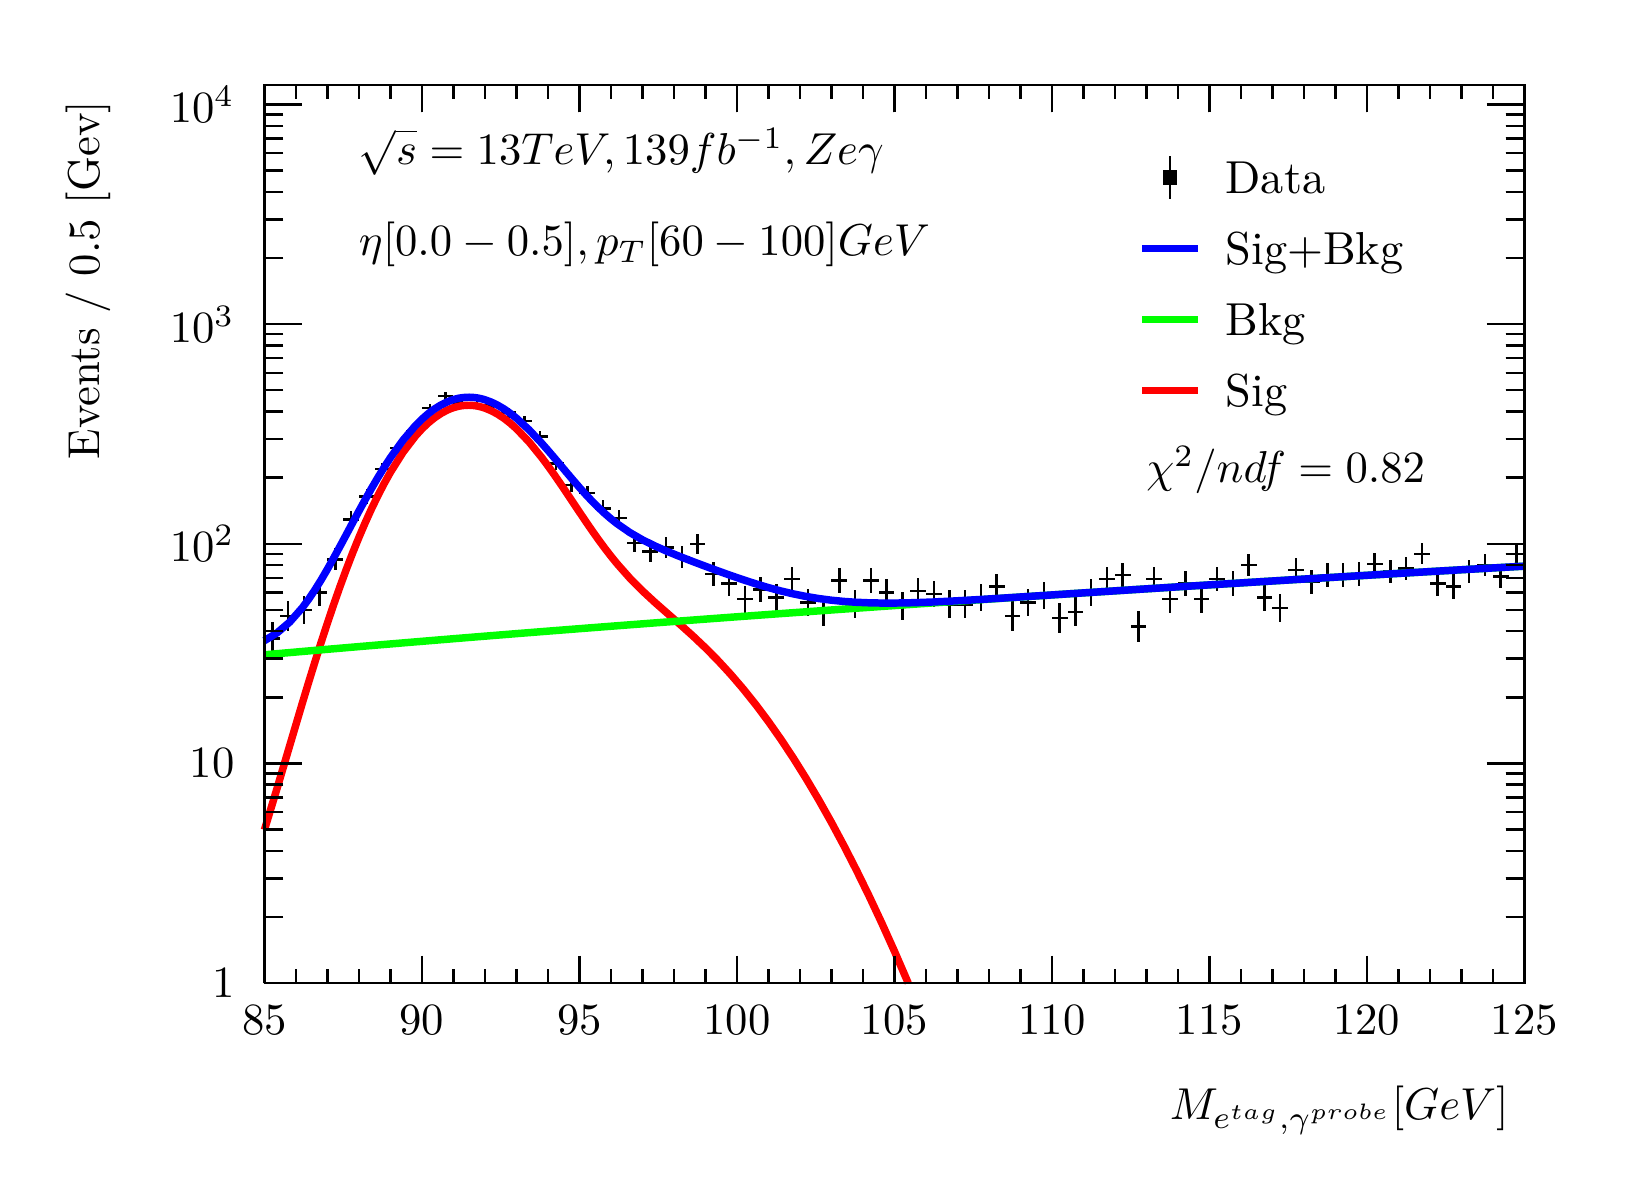
\begin{tikzpicture}
\pgfdeclareplotmark{cross} {
\pgfpathmoveto{\pgfpoint{-0.3\pgfplotmarksize}{\pgfplotmarksize}}
\pgfpathlineto{\pgfpoint{+0.3\pgfplotmarksize}{\pgfplotmarksize}}
\pgfpathlineto{\pgfpoint{+0.3\pgfplotmarksize}{0.3\pgfplotmarksize}}
\pgfpathlineto{\pgfpoint{+1\pgfplotmarksize}{0.3\pgfplotmarksize}}
\pgfpathlineto{\pgfpoint{+1\pgfplotmarksize}{-0.3\pgfplotmarksize}}
\pgfpathlineto{\pgfpoint{+0.3\pgfplotmarksize}{-0.3\pgfplotmarksize}}
\pgfpathlineto{\pgfpoint{+0.3\pgfplotmarksize}{-1.\pgfplotmarksize}}
\pgfpathlineto{\pgfpoint{-0.3\pgfplotmarksize}{-1.\pgfplotmarksize}}
\pgfpathlineto{\pgfpoint{-0.3\pgfplotmarksize}{-0.3\pgfplotmarksize}}
\pgfpathlineto{\pgfpoint{-1.\pgfplotmarksize}{-0.3\pgfplotmarksize}}
\pgfpathlineto{\pgfpoint{-1.\pgfplotmarksize}{0.3\pgfplotmarksize}}
\pgfpathlineto{\pgfpoint{-0.3\pgfplotmarksize}{0.3\pgfplotmarksize}}
\pgfpathclose
\pgfusepathqstroke
}
\pgfdeclareplotmark{cross*} {
\pgfpathmoveto{\pgfpoint{-0.3\pgfplotmarksize}{\pgfplotmarksize}}
\pgfpathlineto{\pgfpoint{+0.3\pgfplotmarksize}{\pgfplotmarksize}}
\pgfpathlineto{\pgfpoint{+0.3\pgfplotmarksize}{0.3\pgfplotmarksize}}
\pgfpathlineto{\pgfpoint{+1\pgfplotmarksize}{0.3\pgfplotmarksize}}
\pgfpathlineto{\pgfpoint{+1\pgfplotmarksize}{-0.3\pgfplotmarksize}}
\pgfpathlineto{\pgfpoint{+0.3\pgfplotmarksize}{-0.3\pgfplotmarksize}}
\pgfpathlineto{\pgfpoint{+0.3\pgfplotmarksize}{-1.\pgfplotmarksize}}
\pgfpathlineto{\pgfpoint{-0.3\pgfplotmarksize}{-1.\pgfplotmarksize}}
\pgfpathlineto{\pgfpoint{-0.3\pgfplotmarksize}{-0.3\pgfplotmarksize}}
\pgfpathlineto{\pgfpoint{-1.\pgfplotmarksize}{-0.3\pgfplotmarksize}}
\pgfpathlineto{\pgfpoint{-1.\pgfplotmarksize}{0.3\pgfplotmarksize}}
\pgfpathlineto{\pgfpoint{-0.3\pgfplotmarksize}{0.3\pgfplotmarksize}}
\pgfpathclose
\pgfusepathqfillstroke
}
\pgfdeclareplotmark{newstar} {
\pgfpathmoveto{\pgfqpoint{0pt}{\pgfplotmarksize}}
\pgfpathlineto{\pgfqpointpolar{44}{0.5\pgfplotmarksize}}
\pgfpathlineto{\pgfqpointpolar{18}{\pgfplotmarksize}}
\pgfpathlineto{\pgfqpointpolar{-20}{0.5\pgfplotmarksize}}
\pgfpathlineto{\pgfqpointpolar{-54}{\pgfplotmarksize}}
\pgfpathlineto{\pgfqpointpolar{-90}{0.5\pgfplotmarksize}}
\pgfpathlineto{\pgfqpointpolar{234}{\pgfplotmarksize}}
\pgfpathlineto{\pgfqpointpolar{198}{0.5\pgfplotmarksize}}
\pgfpathlineto{\pgfqpointpolar{162}{\pgfplotmarksize}}
\pgfpathlineto{\pgfqpointpolar{134}{0.5\pgfplotmarksize}}
\pgfpathclose
\pgfusepathqstroke
}
\pgfdeclareplotmark{newstar*} {
\pgfpathmoveto{\pgfqpoint{0pt}{\pgfplotmarksize}}
\pgfpathlineto{\pgfqpointpolar{44}{0.5\pgfplotmarksize}}
\pgfpathlineto{\pgfqpointpolar{18}{\pgfplotmarksize}}
\pgfpathlineto{\pgfqpointpolar{-20}{0.5\pgfplotmarksize}}
\pgfpathlineto{\pgfqpointpolar{-54}{\pgfplotmarksize}}
\pgfpathlineto{\pgfqpointpolar{-90}{0.5\pgfplotmarksize}}
\pgfpathlineto{\pgfqpointpolar{234}{\pgfplotmarksize}}
\pgfpathlineto{\pgfqpointpolar{198}{0.5\pgfplotmarksize}}
\pgfpathlineto{\pgfqpointpolar{162}{\pgfplotmarksize}}
\pgfpathlineto{\pgfqpointpolar{134}{0.5\pgfplotmarksize}}
\pgfpathclose
\pgfusepathqfillstroke
}
\definecolor{c}{rgb}{1,1,1};
\draw [color=c, fill=c] (0,0) rectangle (20,14.4361);
\draw [color=c, fill=c] (3,2.30977) rectangle (19,13.7143);
\definecolor{c}{rgb}{0,0,0};
\draw [c,line width=0.9] (3,2.30977) -- (3,13.7143) -- (19,13.7143) -- (19,2.30977) -- (3,2.30977);
\definecolor{c}{rgb}{1,1,1};
\draw [color=c, fill=c] (3,2.30977) rectangle (19,13.7143);
\definecolor{c}{rgb}{0,0,0};
\draw [c,line width=0.9] (3,2.30977) -- (3,13.7143) -- (19,13.7143) -- (19,2.30977) -- (3,2.30977);
\draw [c,line width=0.9] (3,2.30977) -- (19,2.30977);
\draw [c,line width=0.9] (3,2.65624) -- (3,2.30977);
\draw [c,line width=0.9] (3.4,2.48301) -- (3.4,2.30977);
\draw [c,line width=0.9] (3.8,2.48301) -- (3.8,2.30977);
\draw [c,line width=0.9] (4.2,2.48301) -- (4.2,2.30977);
\draw [c,line width=0.9] (4.6,2.48301) -- (4.6,2.30977);
\draw [c,line width=0.9] (5,2.65624) -- (5,2.30977);
\draw [c,line width=0.9] (5.4,2.48301) -- (5.4,2.30977);
\draw [c,line width=0.9] (5.8,2.48301) -- (5.8,2.30977);
\draw [c,line width=0.9] (6.2,2.48301) -- (6.2,2.30977);
\draw [c,line width=0.9] (6.6,2.48301) -- (6.6,2.30977);
\draw [c,line width=0.9] (7,2.65624) -- (7,2.30977);
\draw [c,line width=0.9] (7.4,2.48301) -- (7.4,2.30977);
\draw [c,line width=0.9] (7.8,2.48301) -- (7.8,2.30977);
\draw [c,line width=0.9] (8.2,2.48301) -- (8.2,2.30977);
\draw [c,line width=0.9] (8.6,2.48301) -- (8.6,2.30977);
\draw [c,line width=0.9] (9,2.65624) -- (9,2.30977);
\draw [c,line width=0.9] (9.4,2.48301) -- (9.4,2.30977);
\draw [c,line width=0.9] (9.8,2.48301) -- (9.8,2.30977);
\draw [c,line width=0.9] (10.2,2.48301) -- (10.2,2.30977);
\draw [c,line width=0.9] (10.6,2.48301) -- (10.6,2.30977);
\draw [c,line width=0.9] (11,2.65624) -- (11,2.30977);
\draw [c,line width=0.9] (11.4,2.48301) -- (11.4,2.30977);
\draw [c,line width=0.9] (11.8,2.48301) -- (11.8,2.30977);
\draw [c,line width=0.9] (12.2,2.48301) -- (12.2,2.30977);
\draw [c,line width=0.9] (12.6,2.48301) -- (12.6,2.30977);
\draw [c,line width=0.9] (13,2.65624) -- (13,2.30977);
\draw [c,line width=0.9] (13.4,2.48301) -- (13.4,2.30977);
\draw [c,line width=0.9] (13.8,2.48301) -- (13.8,2.30977);
\draw [c,line width=0.9] (14.2,2.48301) -- (14.2,2.30977);
\draw [c,line width=0.9] (14.6,2.48301) -- (14.6,2.30977);
\draw [c,line width=0.9] (15,2.65624) -- (15,2.30977);
\draw [c,line width=0.9] (15.4,2.48301) -- (15.4,2.30977);
\draw [c,line width=0.9] (15.8,2.48301) -- (15.8,2.30977);
\draw [c,line width=0.9] (16.2,2.48301) -- (16.2,2.30977);
\draw [c,line width=0.9] (16.6,2.48301) -- (16.6,2.30977);
\draw [c,line width=0.9] (17,2.65624) -- (17,2.30977);
\draw [c,line width=0.9] (17.4,2.48301) -- (17.4,2.30977);
\draw [c,line width=0.9] (17.8,2.48301) -- (17.8,2.30977);
\draw [c,line width=0.9] (18.2,2.48301) -- (18.2,2.30977);
\draw [c,line width=0.9] (18.6,2.48301) -- (18.6,2.30977);
\draw [c,line width=0.9] (19,2.65624) -- (19,2.30977);
\draw [anchor=base] (3,1.66015) node[scale=1.61424, color=c, rotate=0]{85};
\draw [anchor=base] (5,1.66015) node[scale=1.61424, color=c, rotate=0]{90};
\draw [anchor=base] (7,1.66015) node[scale=1.61424, color=c, rotate=0]{95};
\draw [anchor=base] (9,1.66015) node[scale=1.61424, color=c, rotate=0]{100};
\draw [anchor=base] (11,1.66015) node[scale=1.61424, color=c, rotate=0]{105};
\draw [anchor=base] (13,1.66015) node[scale=1.61424, color=c, rotate=0]{110};
\draw [anchor=base] (15,1.66015) node[scale=1.61424, color=c, rotate=0]{115};
\draw [anchor=base] (17,1.66015) node[scale=1.61424, color=c, rotate=0]{120};
\draw [anchor=base] (19,1.66015) node[scale=1.61424, color=c, rotate=0]{125};
\draw [anchor= east] (19,0.692932) node[scale=1.61424, color=c, rotate=0]{$M_{e^{tag}, \gamma^{probe}}  [GeV]$};
\draw [c,line width=0.9] (3,13.7143) -- (19,13.7143);
\draw [c,line width=0.9] (3,13.3678) -- (3,13.7143);
\draw [c,line width=0.9] (3.4,13.5411) -- (3.4,13.7143);
\draw [c,line width=0.9] (3.8,13.5411) -- (3.8,13.7143);
\draw [c,line width=0.9] (4.2,13.5411) -- (4.2,13.7143);
\draw [c,line width=0.9] (4.6,13.5411) -- (4.6,13.7143);
\draw [c,line width=0.9] (5,13.3678) -- (5,13.7143);
\draw [c,line width=0.9] (5.4,13.5411) -- (5.4,13.7143);
\draw [c,line width=0.9] (5.8,13.5411) -- (5.8,13.7143);
\draw [c,line width=0.9] (6.2,13.5411) -- (6.2,13.7143);
\draw [c,line width=0.9] (6.6,13.5411) -- (6.6,13.7143);
\draw [c,line width=0.9] (7,13.3678) -- (7,13.7143);
\draw [c,line width=0.9] (7.4,13.5411) -- (7.4,13.7143);
\draw [c,line width=0.9] (7.8,13.5411) -- (7.8,13.7143);
\draw [c,line width=0.9] (8.2,13.5411) -- (8.2,13.7143);
\draw [c,line width=0.9] (8.6,13.5411) -- (8.6,13.7143);
\draw [c,line width=0.9] (9,13.3678) -- (9,13.7143);
\draw [c,line width=0.9] (9.4,13.5411) -- (9.4,13.7143);
\draw [c,line width=0.9] (9.8,13.5411) -- (9.8,13.7143);
\draw [c,line width=0.9] (10.2,13.5411) -- (10.2,13.7143);
\draw [c,line width=0.9] (10.6,13.5411) -- (10.6,13.7143);
\draw [c,line width=0.9] (11,13.3678) -- (11,13.7143);
\draw [c,line width=0.9] (11.4,13.5411) -- (11.4,13.7143);
\draw [c,line width=0.9] (11.8,13.5411) -- (11.8,13.7143);
\draw [c,line width=0.9] (12.2,13.5411) -- (12.2,13.7143);
\draw [c,line width=0.9] (12.6,13.5411) -- (12.6,13.7143);
\draw [c,line width=0.9] (13,13.3678) -- (13,13.7143);
\draw [c,line width=0.9] (13.4,13.5411) -- (13.4,13.7143);
\draw [c,line width=0.9] (13.8,13.5411) -- (13.8,13.7143);
\draw [c,line width=0.9] (14.2,13.5411) -- (14.2,13.7143);
\draw [c,line width=0.9] (14.6,13.5411) -- (14.6,13.7143);
\draw [c,line width=0.9] (15,13.3678) -- (15,13.7143);
\draw [c,line width=0.9] (15.4,13.5411) -- (15.4,13.7143);
\draw [c,line width=0.9] (15.8,13.5411) -- (15.8,13.7143);
\draw [c,line width=0.9] (16.2,13.5411) -- (16.2,13.7143);
\draw [c,line width=0.9] (16.6,13.5411) -- (16.6,13.7143);
\draw [c,line width=0.9] (17,13.3678) -- (17,13.7143);
\draw [c,line width=0.9] (17.4,13.5411) -- (17.4,13.7143);
\draw [c,line width=0.9] (17.8,13.5411) -- (17.8,13.7143);
\draw [c,line width=0.9] (18.2,13.5411) -- (18.2,13.7143);
\draw [c,line width=0.9] (18.6,13.5411) -- (18.6,13.7143);
\draw [c,line width=0.9] (19,13.3678) -- (19,13.7143);
\draw [c,line width=0.9] (3,2.30977) -- (3,13.7143);
\draw [c,line width=0.9] (3.474,2.30978) -- (3,2.30978);
\draw [anchor= east] (2.82,2.30978) node[scale=1.61424, color=c, rotate=0]{1};
\draw [c,line width=0.9] (3.237,3.1495) -- (3,3.1495);
\draw [c,line width=0.9] (3.237,3.6407) -- (3,3.6407);
\draw [c,line width=0.9] (3.237,3.98922) -- (3,3.98922);
\draw [c,line width=0.9] (3.237,4.25955) -- (3,4.25955);
\draw [c,line width=0.9] (3.237,4.48042) -- (3,4.48042);
\draw [c,line width=0.9] (3.237,4.66717) -- (3,4.66717);
\draw [c,line width=0.9] (3.237,4.82894) -- (3,4.82894);
\draw [c,line width=0.9] (3.237,4.97163) -- (3,4.97163);
\draw [c,line width=0.9] (3.474,5.09927) -- (3,5.09927);
\draw [anchor= east] (2.82,5.09927) node[scale=1.61424, color=c, rotate=0]{10};
\draw [c,line width=0.9] (3.237,5.93899) -- (3,5.93899);
\draw [c,line width=0.9] (3.237,6.43019) -- (3,6.43019);
\draw [c,line width=0.9] (3.237,6.77871) -- (3,6.77871);
\draw [c,line width=0.9] (3.237,7.04904) -- (3,7.04904);
\draw [c,line width=0.9] (3.237,7.26991) -- (3,7.26991);
\draw [c,line width=0.9] (3.237,7.45666) -- (3,7.45666);
\draw [c,line width=0.9] (3.237,7.61843) -- (3,7.61843);
\draw [c,line width=0.9] (3.237,7.76112) -- (3,7.76112);
\draw [c,line width=0.9] (3.474,7.88876) -- (3,7.88876);
\draw [anchor= east] (2.82,7.88876) node[scale=1.61424, color=c, rotate=0]{$10^{2}$};
\draw [c,line width=0.9] (3.237,8.72848) -- (3,8.72848);
\draw [c,line width=0.9] (3.237,9.21968) -- (3,9.21968);
\draw [c,line width=0.9] (3.237,9.5682) -- (3,9.5682);
\draw [c,line width=0.9] (3.237,9.83853) -- (3,9.83853);
\draw [c,line width=0.9] (3.237,10.0594) -- (3,10.0594);
\draw [c,line width=0.9] (3.237,10.2462) -- (3,10.2462);
\draw [c,line width=0.9] (3.237,10.4079) -- (3,10.4079);
\draw [c,line width=0.9] (3.237,10.5506) -- (3,10.5506);
\draw [c,line width=0.9] (3.474,10.6782) -- (3,10.6782);
\draw [anchor= east] (2.82,10.6782) node[scale=1.61424, color=c, rotate=0]{$10^{3}$};
\draw [c,line width=0.9] (3.237,11.518) -- (3,11.518);
\draw [c,line width=0.9] (3.237,12.0092) -- (3,12.0092);
\draw [c,line width=0.9] (3.237,12.3577) -- (3,12.3577);
\draw [c,line width=0.9] (3.237,12.628) -- (3,12.628);
\draw [c,line width=0.9] (3.237,12.8489) -- (3,12.8489);
\draw [c,line width=0.9] (3.237,13.0356) -- (3,13.0356);
\draw [c,line width=0.9] (3.237,13.1974) -- (3,13.1974);
\draw [c,line width=0.9] (3.237,13.3401) -- (3,13.3401);
\draw [c,line width=0.9] (3.474,13.4677) -- (3,13.4677);
\draw [anchor= east] (2.82,13.4677) node[scale=1.61424, color=c, rotate=0]{$10^{4}$};
\draw [anchor= east] (0.76,13.7143) node[scale=1.61424, color=c, rotate=90]{Events / 0.5 [Gev]};
\draw [c,line width=0.9] (19,2.30977) -- (19,13.7143);
\draw [c,line width=0.9] (18.526,2.30978) -- (19,2.30978);
\draw [c,line width=0.9] (18.763,3.1495) -- (19,3.1495);
\draw [c,line width=0.9] (18.763,3.6407) -- (19,3.6407);
\draw [c,line width=0.9] (18.763,3.98922) -- (19,3.98922);
\draw [c,line width=0.9] (18.763,4.25955) -- (19,4.25955);
\draw [c,line width=0.9] (18.763,4.48042) -- (19,4.48042);
\draw [c,line width=0.9] (18.763,4.66717) -- (19,4.66717);
\draw [c,line width=0.9] (18.763,4.82894) -- (19,4.82894);
\draw [c,line width=0.9] (18.763,4.97163) -- (19,4.97163);
\draw [c,line width=0.9] (18.526,5.09927) -- (19,5.09927);
\draw [c,line width=0.9] (18.763,5.93899) -- (19,5.93899);
\draw [c,line width=0.9] (18.763,6.43019) -- (19,6.43019);
\draw [c,line width=0.9] (18.763,6.77871) -- (19,6.77871);
\draw [c,line width=0.9] (18.763,7.04904) -- (19,7.04904);
\draw [c,line width=0.9] (18.763,7.26991) -- (19,7.26991);
\draw [c,line width=0.9] (18.763,7.45666) -- (19,7.45666);
\draw [c,line width=0.9] (18.763,7.61843) -- (19,7.61843);
\draw [c,line width=0.9] (18.763,7.76112) -- (19,7.76112);
\draw [c,line width=0.9] (18.526,7.88876) -- (19,7.88876);
\draw [c,line width=0.9] (18.763,8.72848) -- (19,8.72848);
\draw [c,line width=0.9] (18.763,9.21968) -- (19,9.21968);
\draw [c,line width=0.9] (18.763,9.5682) -- (19,9.5682);
\draw [c,line width=0.9] (18.763,9.83853) -- (19,9.83853);
\draw [c,line width=0.9] (18.763,10.0594) -- (19,10.0594);
\draw [c,line width=0.9] (18.763,10.2462) -- (19,10.2462);
\draw [c,line width=0.9] (18.763,10.4079) -- (19,10.4079);
\draw [c,line width=0.9] (18.763,10.5506) -- (19,10.5506);
\draw [c,line width=0.9] (18.526,10.6782) -- (19,10.6782);
\draw [c,line width=0.9] (18.763,11.518) -- (19,11.518);
\draw [c,line width=0.9] (18.763,12.0092) -- (19,12.0092);
\draw [c,line width=0.9] (18.763,12.3577) -- (19,12.3577);
\draw [c,line width=0.9] (18.763,12.628) -- (19,12.628);
\draw [c,line width=0.9] (18.763,12.8489) -- (19,12.8489);
\draw [c,line width=0.9] (18.763,13.0356) -- (19,13.0356);
\draw [c,line width=0.9] (18.763,13.1974) -- (19,13.1974);
\draw [c,line width=0.9] (18.763,13.3401) -- (19,13.3401);
\draw [c,line width=0.9] (18.526,13.4677) -- (19,13.4677);
\draw [c,line width=0.9] (3.1,6.68426) -- (3,6.68426);
\draw [c,line width=0.9] (3,6.68426) -- (3,6.68426);
\draw [c,line width=0.9] (3.1,6.68426) -- (3.2,6.68426);
\draw [c,line width=0.9] (3.2,6.68426) -- (3.2,6.68426);
\draw [c,line width=0.9] (3.1,6.68426) -- (3.1,6.89795);
\draw [c,line width=0.9] (3.1,6.89795) -- (3.1,6.89795);
\draw [c,line width=0.9] (3.1,6.68426) -- (3.1,6.46776);
\draw [c,line width=0.9] (3.1,6.46776) -- (3.1,6.46776);
\draw [c,line width=0.9] (3.3,6.97408) -- (3.2,6.97408);
\draw [c,line width=0.9] (3.2,6.97408) -- (3.2,6.97408);
\draw [c,line width=0.9] (3.3,6.97408) -- (3.4,6.97408);
\draw [c,line width=0.9] (3.4,6.97408) -- (3.4,6.97408);
\draw [c,line width=0.9] (3.3,6.97408) -- (3.3,7.16239);
\draw [c,line width=0.9] (3.3,7.16239) -- (3.3,7.16239);
\draw [c,line width=0.9] (3.3,6.97408) -- (3.3,6.78381);
\draw [c,line width=0.9] (3.3,6.78381) -- (3.3,6.78381);
\draw [c,line width=0.9] (3.5,7.04904) -- (3.4,7.04904);
\draw [c,line width=0.9] (3.4,7.04904) -- (3.4,7.04904);
\draw [c,line width=0.9] (3.5,7.04904) -- (3.6,7.04904);
\draw [c,line width=0.9] (3.6,7.04904) -- (3.6,7.04904);
\draw [c,line width=0.9] (3.5,7.04904) -- (3.5,7.23131);
\draw [c,line width=0.9] (3.5,7.23131) -- (3.5,7.23131);
\draw [c,line width=0.9] (3.5,7.04904) -- (3.5,6.86499);
\draw [c,line width=0.9] (3.5,6.86499) -- (3.5,6.86499);
\draw [c,line width=0.9] (3.7,7.26991) -- (3.6,7.26991);
\draw [c,line width=0.9] (3.6,7.26991) -- (3.6,7.26991);
\draw [c,line width=0.9] (3.7,7.26991) -- (3.8,7.26991);
\draw [c,line width=0.9] (3.8,7.26991) -- (3.8,7.26991);
\draw [c,line width=0.9] (3.7,7.26991) -- (3.7,7.43552);
\draw [c,line width=0.9] (3.7,7.43552) -- (3.7,7.43552);
\draw [c,line width=0.9] (3.7,7.26991) -- (3.7,7.10296);
\draw [c,line width=0.9] (3.7,7.10296) -- (3.7,7.10296);
\draw [c,line width=0.9] (3.9,7.69187) -- (3.8,7.69187);
\draw [c,line width=0.9] (3.8,7.69187) -- (3.8,7.69187);
\draw [c,line width=0.9] (3.9,7.69187) -- (4,7.69187);
\draw [c,line width=0.9] (4,7.69187) -- (4,7.69187);
\draw [c,line width=0.9] (3.9,7.69187) -- (3.9,7.82987);
\draw [c,line width=0.9] (3.9,7.82987) -- (3.9,7.82987);
\draw [c,line width=0.9] (3.9,7.69187) -- (3.9,7.55307);
\draw [c,line width=0.9] (3.9,7.55307) -- (3.9,7.55307);
\draw [c,line width=0.9] (4.1,8.19725) -- (4,8.19725);
\draw [c,line width=0.9] (4,8.19725) -- (4,8.19725);
\draw [c,line width=0.9] (4.1,8.19725) -- (4.2,8.19725);
\draw [c,line width=0.9] (4.2,8.19725) -- (4.2,8.19725);
\draw [c,line width=0.9] (4.1,8.19725) -- (4.1,8.30387);
\draw [c,line width=0.9] (4.1,8.30387) -- (4.1,8.30387);
\draw [c,line width=0.9] (4.1,8.19725) -- (4.1,8.09062);
\draw [c,line width=0.9] (4.1,8.09062) -- (4.1,8.09062);
\draw [c,line width=0.9] (4.3,8.48806) -- (4.2,8.48806);
\draw [c,line width=0.9] (4.2,8.48806) -- (4.2,8.48806);
\draw [c,line width=0.9] (4.3,8.48806) -- (4.4,8.48806);
\draw [c,line width=0.9] (4.4,8.48806) -- (4.4,8.48806);
\draw [c,line width=0.9] (4.3,8.48806) -- (4.3,8.58264);
\draw [c,line width=0.9] (4.3,8.58264) -- (4.3,8.58264);
\draw [c,line width=0.9] (4.3,8.48806) -- (4.3,8.39349);
\draw [c,line width=0.9] (4.3,8.39349) -- (4.3,8.39349);
\draw [c,line width=0.9] (4.5,8.83842) -- (4.4,8.83842);
\draw [c,line width=0.9] (4.4,8.83842) -- (4.4,8.83842);
\draw [c,line width=0.9] (4.5,8.83842) -- (4.6,8.83842);
\draw [c,line width=0.9] (4.6,8.83842) -- (4.6,8.83842);
\draw [c,line width=0.9] (4.5,8.83842) -- (4.5,8.92027);
\draw [c,line width=0.9] (4.5,8.92027) -- (4.5,8.92027);
\draw [c,line width=0.9] (4.5,8.83842) -- (4.5,8.75658);
\draw [c,line width=0.9] (4.5,8.75658) -- (4.5,8.75658);
\draw [c,line width=0.9] (4.7,9.10543) -- (4.6,9.10543);
\draw [c,line width=0.9] (4.6,9.10543) -- (4.6,9.10543);
\draw [c,line width=0.9] (4.7,9.10543) -- (4.8,9.10543);
\draw [c,line width=0.9] (4.8,9.10543) -- (4.8,9.10543);
\draw [c,line width=0.9] (4.7,9.10543) -- (4.7,9.17874);
\draw [c,line width=0.9] (4.7,9.17874) -- (4.7,9.17874);
\draw [c,line width=0.9] (4.7,9.10543) -- (4.7,9.03212);
\draw [c,line width=0.9] (4.7,9.03212) -- (4.7,9.03212);
\draw [c,line width=0.9] (4.9,9.32037) -- (4.8,9.32037);
\draw [c,line width=0.9] (4.8,9.32037) -- (4.8,9.32037);
\draw [c,line width=0.9] (4.9,9.32037) -- (5,9.32037);
\draw [c,line width=0.9] (5,9.32037) -- (5,9.32037);
\draw [c,line width=0.9] (4.9,9.32037) -- (4.9,9.38746);
\draw [c,line width=0.9] (4.9,9.38746) -- (4.9,9.38746);
\draw [c,line width=0.9] (4.9,9.32037) -- (4.9,9.25328);
\draw [c,line width=0.9] (4.9,9.25328) -- (4.9,9.25328);
\draw [c,line width=0.9] (5.1,9.60987) -- (5,9.60987);
\draw [c,line width=0.9] (5,9.60987) -- (5,9.60987);
\draw [c,line width=0.9] (5.1,9.60987) -- (5.2,9.60987);
\draw [c,line width=0.9] (5.2,9.60987) -- (5.2,9.60987);
\draw [c,line width=0.9] (5.1,9.60987) -- (5.1,9.66941);
\draw [c,line width=0.9] (5.1,9.66941) -- (5.1,9.66941);
\draw [c,line width=0.9] (5.1,9.60987) -- (5.1,9.55034);
\draw [c,line width=0.9] (5.1,9.55034) -- (5.1,9.55034);
\draw [c,line width=0.9] (5.3,9.76357) -- (5.2,9.76357);
\draw [c,line width=0.9] (5.2,9.76357) -- (5.2,9.76357);
\draw [c,line width=0.9] (5.3,9.76357) -- (5.4,9.76357);
\draw [c,line width=0.9] (5.4,9.76357) -- (5.4,9.76357);
\draw [c,line width=0.9] (5.3,9.76357) -- (5.3,9.81944);
\draw [c,line width=0.9] (5.3,9.81944) -- (5.3,9.81944);
\draw [c,line width=0.9] (5.3,9.76357) -- (5.3,9.70769);
\draw [c,line width=0.9] (5.3,9.70769) -- (5.3,9.70769);
\draw [c,line width=0.9] (5.5,9.66982) -- (5.4,9.66982);
\draw [c,line width=0.9] (5.4,9.66982) -- (5.4,9.66982);
\draw [c,line width=0.9] (5.5,9.66982) -- (5.6,9.66982);
\draw [c,line width=0.9] (5.6,9.66982) -- (5.6,9.66982);
\draw [c,line width=0.9] (5.5,9.66982) -- (5.5,9.7279);
\draw [c,line width=0.9] (5.5,9.7279) -- (5.5,9.7279);
\draw [c,line width=0.9] (5.5,9.66982) -- (5.5,9.61174);
\draw [c,line width=0.9] (5.5,9.61174) -- (5.5,9.61174);
\draw [c,line width=0.9] (5.7,9.72161) -- (5.6,9.72161);
\draw [c,line width=0.9] (5.6,9.72161) -- (5.6,9.72161);
\draw [c,line width=0.9] (5.7,9.72161) -- (5.8,9.72161);
\draw [c,line width=0.9] (5.8,9.72161) -- (5.8,9.72161);
\draw [c,line width=0.9] (5.7,9.72161) -- (5.7,9.77846);
\draw [c,line width=0.9] (5.7,9.77846) -- (5.7,9.77846);
\draw [c,line width=0.9] (5.7,9.72161) -- (5.7,9.66476);
\draw [c,line width=0.9] (5.7,9.66476) -- (5.7,9.66476);
\draw [c,line width=0.9] (5.9,9.64449) -- (5.8,9.64449);
\draw [c,line width=0.9] (5.8,9.64449) -- (5.8,9.64449);
\draw [c,line width=0.9] (5.9,9.64449) -- (6,9.64449);
\draw [c,line width=0.9] (6,9.64449) -- (6,9.64449);
\draw [c,line width=0.9] (5.9,9.64449) -- (5.9,9.70318);
\draw [c,line width=0.9] (5.9,9.70318) -- (5.9,9.70318);
\draw [c,line width=0.9] (5.9,9.64449) -- (5.9,9.5858);
\draw [c,line width=0.9] (5.9,9.5858) -- (5.9,9.5858);
\draw [c,line width=0.9] (6.1,9.55296) -- (6,9.55296);
\draw [c,line width=0.9] (6,9.55296) -- (6,9.55296);
\draw [c,line width=0.9] (6.1,9.55296) -- (6.2,9.55296);
\draw [c,line width=0.9] (6.2,9.55296) -- (6.2,9.55296);
\draw [c,line width=0.9] (6.1,9.55296) -- (6.1,9.61391);
\draw [c,line width=0.9] (6.1,9.61391) -- (6.1,9.61391);
\draw [c,line width=0.9] (6.1,9.55296) -- (6.1,9.49201);
\draw [c,line width=0.9] (6.1,9.49201) -- (6.1,9.49201);
\draw [c,line width=0.9] (6.3,9.44727) -- (6.2,9.44727);
\draw [c,line width=0.9] (6.2,9.44727) -- (6.2,9.44727);
\draw [c,line width=0.9] (6.3,9.44727) -- (6.4,9.44727);
\draw [c,line width=0.9] (6.4,9.44727) -- (6.4,9.44727);
\draw [c,line width=0.9] (6.3,9.44727) -- (6.3,9.51093);
\draw [c,line width=0.9] (6.3,9.51093) -- (6.3,9.51093);
\draw [c,line width=0.9] (6.3,9.44727) -- (6.3,9.3836);
\draw [c,line width=0.9] (6.3,9.3836) -- (6.3,9.3836);
\draw [c,line width=0.9] (6.5,9.25156) -- (6.4,9.25156);
\draw [c,line width=0.9] (6.4,9.25156) -- (6.4,9.25156);
\draw [c,line width=0.9] (6.5,9.25156) -- (6.6,9.25156);
\draw [c,line width=0.9] (6.6,9.25156) -- (6.6,9.25156);
\draw [c,line width=0.9] (6.5,9.25156) -- (6.5,9.32058);
\draw [c,line width=0.9] (6.5,9.32058) -- (6.5,9.32058);
\draw [c,line width=0.9] (6.5,9.25156) -- (6.5,9.18254);
\draw [c,line width=0.9] (6.5,9.18254) -- (6.5,9.18254);
\draw [c,line width=0.9] (6.7,8.90828) -- (6.6,8.90828);
\draw [c,line width=0.9] (6.6,8.90828) -- (6.6,8.90828);
\draw [c,line width=0.9] (6.7,8.90828) -- (6.8,8.90828);
\draw [c,line width=0.9] (6.8,8.90828) -- (6.8,8.90828);
\draw [c,line width=0.9] (6.7,8.90828) -- (6.7,8.9878);
\draw [c,line width=0.9] (6.7,8.9878) -- (6.7,8.9878);
\draw [c,line width=0.9] (6.7,8.90828) -- (6.7,8.82876);
\draw [c,line width=0.9] (6.7,8.82876) -- (6.7,8.82876);
\draw [c,line width=0.9] (6.9,8.63403) -- (6.8,8.63403);
\draw [c,line width=0.9] (6.8,8.63403) -- (6.8,8.63403);
\draw [c,line width=0.9] (6.9,8.63403) -- (7,8.63403);
\draw [c,line width=0.9] (7,8.63403) -- (7,8.63403);
\draw [c,line width=0.9] (6.9,8.63403) -- (6.9,8.72308);
\draw [c,line width=0.9] (6.9,8.72308) -- (6.9,8.72308);
\draw [c,line width=0.9] (6.9,8.63403) -- (6.9,8.54498);
\draw [c,line width=0.9] (6.9,8.54498) -- (6.9,8.54498);
\draw [c,line width=0.9] (7.1,8.53159) -- (7,8.53159);
\draw [c,line width=0.9] (7,8.53159) -- (7,8.53159);
\draw [c,line width=0.9] (7.1,8.53159) -- (7.2,8.53159);
\draw [c,line width=0.9] (7.2,8.53159) -- (7.2,8.53159);
\draw [c,line width=0.9] (7.1,8.53159) -- (7.1,8.62448);
\draw [c,line width=0.9] (7.1,8.62448) -- (7.1,8.62448);
\draw [c,line width=0.9] (7.1,8.53159) -- (7.1,8.4387);
\draw [c,line width=0.9] (7.1,8.4387) -- (7.1,8.4387);
\draw [c,line width=0.9] (7.3,8.33889) -- (7.2,8.33889);
\draw [c,line width=0.9] (7.2,8.33889) -- (7.2,8.33889);
\draw [c,line width=0.9] (7.3,8.33889) -- (7.4,8.33889);
\draw [c,line width=0.9] (7.4,8.33889) -- (7.4,8.33889);
\draw [c,line width=0.9] (7.3,8.33889) -- (7.3,8.43947);
\draw [c,line width=0.9] (7.3,8.43947) -- (7.3,8.43947);
\draw [c,line width=0.9] (7.3,8.33889) -- (7.3,8.23831);
\draw [c,line width=0.9] (7.3,8.23831) -- (7.3,8.23831);
\draw [c,line width=0.9] (7.5,8.21588) -- (7.4,8.21588);
\draw [c,line width=0.9] (7.4,8.21588) -- (7.4,8.21588);
\draw [c,line width=0.9] (7.5,8.21588) -- (7.6,8.21588);
\draw [c,line width=0.9] (7.6,8.21588) -- (7.6,8.21588);
\draw [c,line width=0.9] (7.5,8.21588) -- (7.5,8.3217);
\draw [c,line width=0.9] (7.5,8.3217) -- (7.5,8.3217);
\draw [c,line width=0.9] (7.5,8.21588) -- (7.5,8.11007);
\draw [c,line width=0.9] (7.5,8.11007) -- (7.5,8.11007);
\draw [c,line width=0.9] (7.7,7.90081) -- (7.6,7.90081);
\draw [c,line width=0.9] (7.6,7.90081) -- (7.6,7.90081);
\draw [c,line width=0.9] (7.7,7.90081) -- (7.8,7.90081);
\draw [c,line width=0.9] (7.8,7.90081) -- (7.8,7.90081);
\draw [c,line width=0.9] (7.7,7.90081) -- (7.7,8.02131);
\draw [c,line width=0.9] (7.7,8.02131) -- (7.7,8.02131);
\draw [c,line width=0.9] (7.7,7.90081) -- (7.7,7.78032);
\draw [c,line width=0.9] (7.7,7.78032) -- (7.7,7.78032);
\draw [c,line width=0.9] (7.9,7.78774) -- (7.8,7.78774);
\draw [c,line width=0.9] (7.8,7.78774) -- (7.8,7.78774);
\draw [c,line width=0.9] (7.9,7.78774) -- (8,7.78774);
\draw [c,line width=0.9] (8,7.78774) -- (8,7.78774);
\draw [c,line width=0.9] (7.9,7.78774) -- (7.9,7.92016);
\draw [c,line width=0.9] (7.9,7.92016) -- (7.9,7.92016);
\draw [c,line width=0.9] (7.9,7.78774) -- (7.9,7.65462);
\draw [c,line width=0.9] (7.9,7.65462) -- (7.9,7.65462);
\draw [c,line width=0.9] (8.1,7.8393) -- (8,7.8393);
\draw [c,line width=0.9] (8,7.8393) -- (8,7.8393);
\draw [c,line width=0.9] (8.1,7.8393) -- (8.2,7.8393);
\draw [c,line width=0.9] (8.2,7.8393) -- (8.2,7.8393);
\draw [c,line width=0.9] (8.1,7.8393) -- (8.1,7.96882);
\draw [c,line width=0.9] (8.1,7.96882) -- (8.1,7.96882);
\draw [c,line width=0.9] (8.1,7.8393) -- (8.1,7.70912);
\draw [c,line width=0.9] (8.1,7.70912) -- (8.1,7.70912);
\draw [c,line width=0.9] (8.3,7.72005) -- (8.2,7.72005);
\draw [c,line width=0.9] (8.2,7.72005) -- (8.2,7.72005);
\draw [c,line width=0.9] (8.3,7.72005) -- (8.4,7.72005);
\draw [c,line width=0.9] (8.4,7.72005) -- (8.4,7.72005);
\draw [c,line width=0.9] (8.3,7.72005) -- (8.3,7.85638);
\draw [c,line width=0.9] (8.3,7.85638) -- (8.3,7.85638);
\draw [c,line width=0.9] (8.3,7.72005) -- (8.3,7.58294);
\draw [c,line width=0.9] (8.3,7.58294) -- (8.3,7.58294);
\draw [c,line width=0.9] (8.5,7.88876) -- (8.4,7.88876);
\draw [c,line width=0.9] (8.4,7.88876) -- (8.4,7.88876);
\draw [c,line width=0.9] (8.5,7.88876) -- (8.6,7.88876);
\draw [c,line width=0.9] (8.6,7.88876) -- (8.6,7.88876);
\draw [c,line width=0.9] (8.5,7.88876) -- (8.5,8.01555);
\draw [c,line width=0.9] (8.5,8.01555) -- (8.5,8.01555);
\draw [c,line width=0.9] (8.5,7.88876) -- (8.5,7.76134);
\draw [c,line width=0.9] (8.5,7.76134) -- (8.5,7.76134);
\draw [c,line width=0.9] (8.7,7.5075) -- (8.6,7.5075);
\draw [c,line width=0.9] (8.6,7.5075) -- (8.6,7.5075);
\draw [c,line width=0.9] (8.7,7.5075) -- (8.8,7.5075);
\draw [c,line width=0.9] (8.8,7.5075) -- (8.8,7.5075);
\draw [c,line width=0.9] (8.7,7.5075) -- (8.7,7.65692);
\draw [c,line width=0.9] (8.7,7.65692) -- (8.7,7.65692);
\draw [c,line width=0.9] (8.7,7.5075) -- (8.7,7.35707);
\draw [c,line width=0.9] (8.7,7.35707) -- (8.7,7.35707);
\draw [c,line width=0.9] (8.9,7.38538) -- (8.8,7.38538);
\draw [c,line width=0.9] (8.8,7.38538) -- (8.8,7.38538);
\draw [c,line width=0.9] (8.9,7.38538) -- (9,7.38538);
\draw [c,line width=0.9] (9,7.38538) -- (9,7.38538);
\draw [c,line width=0.9] (8.9,7.38538) -- (8.9,7.5429);
\draw [c,line width=0.9] (8.9,7.5429) -- (8.9,7.5429);
\draw [c,line width=0.9] (8.9,7.38538) -- (8.9,7.22668);
\draw [c,line width=0.9] (8.9,7.22668) -- (8.9,7.22668);
\draw [c,line width=0.9] (9.1,7.18633) -- (9,7.18633);
\draw [c,line width=0.9] (9,7.18633) -- (9,7.18633);
\draw [c,line width=0.9] (9.1,7.18633) -- (9.2,7.18633);
\draw [c,line width=0.9] (9.2,7.18633) -- (9.2,7.18633);
\draw [c,line width=0.9] (9.1,7.18633) -- (9.1,7.35805);
\draw [c,line width=0.9] (9.1,7.35805) -- (9.1,7.35805);
\draw [c,line width=0.9] (9.1,7.18633) -- (9.1,7.01311);
\draw [c,line width=0.9] (9.1,7.01311) -- (9.1,7.01311);
\draw [c,line width=0.9] (9.3,7.30964) -- (9.2,7.30964);
\draw [c,line width=0.9] (9.2,7.30964) -- (9.2,7.30964);
\draw [c,line width=0.9] (9.3,7.30964) -- (9.4,7.30964);
\draw [c,line width=0.9] (9.4,7.30964) -- (9.4,7.30964);
\draw [c,line width=0.9] (9.3,7.30964) -- (9.3,7.47242);
\draw [c,line width=0.9] (9.3,7.47242) -- (9.3,7.47242);
\draw [c,line width=0.9] (9.3,7.30964) -- (9.3,7.14557);
\draw [c,line width=0.9] (9.3,7.14557) -- (9.3,7.14557);
\draw [c,line width=0.9] (9.5,7.20777) -- (9.4,7.20777);
\draw [c,line width=0.9] (9.4,7.20777) -- (9.4,7.20777);
\draw [c,line width=0.9] (9.5,7.20777) -- (9.6,7.20777);
\draw [c,line width=0.9] (9.6,7.20777) -- (9.6,7.20777);
\draw [c,line width=0.9] (9.5,7.20777) -- (9.5,7.3779);
\draw [c,line width=0.9] (9.5,7.3779) -- (9.5,7.3779);
\draw [c,line width=0.9] (9.5,7.20777) -- (9.5,7.03618);
\draw [c,line width=0.9] (9.5,7.03618) -- (9.5,7.03618);
\draw [c,line width=0.9] (9.7,7.43923) -- (9.6,7.43923);
\draw [c,line width=0.9] (9.6,7.43923) -- (9.6,7.43923);
\draw [c,line width=0.9] (9.7,7.43923) -- (9.8,7.43923);
\draw [c,line width=0.9] (9.8,7.43923) -- (9.8,7.43923);
\draw [c,line width=0.9] (9.7,7.43923) -- (9.7,7.59313);
\draw [c,line width=0.9] (9.7,7.59313) -- (9.7,7.59313);
\draw [c,line width=0.9] (9.7,7.43923) -- (9.7,7.28423);
\draw [c,line width=0.9] (9.7,7.28423) -- (9.7,7.28423);
\draw [c,line width=0.9] (9.9,7.14227) -- (9.8,7.14227);
\draw [c,line width=0.9] (9.8,7.14227) -- (9.8,7.14227);
\draw [c,line width=0.9] (9.9,7.14227) -- (10,7.14227);
\draw [c,line width=0.9] (10,7.14227) -- (10,7.14227);
\draw [c,line width=0.9] (9.9,7.14227) -- (9.9,7.31731);
\draw [c,line width=0.9] (9.9,7.31731) -- (9.9,7.31731);
\draw [c,line width=0.9] (9.9,7.14227) -- (9.9,6.96565);
\draw [c,line width=0.9] (9.9,6.96565) -- (9.9,6.96565);
\draw [c,line width=0.9] (10.1,7.02456) -- (10,7.02456);
\draw [c,line width=0.9] (10,7.02456) -- (10,7.02456);
\draw [c,line width=0.9] (10.1,7.02456) -- (10.2,7.02456);
\draw [c,line width=0.9] (10.2,7.02456) -- (10.2,7.02456);
\draw [c,line width=0.9] (10.1,7.02456) -- (10.1,7.20878);
\draw [c,line width=0.9] (10.1,7.20878) -- (10.1,7.20878);
\draw [c,line width=0.9] (10.1,7.02456) -- (10.1,6.83851);
\draw [c,line width=0.9] (10.1,6.83851) -- (10.1,6.83851);
\draw [c,line width=0.9] (10.3,7.42154) -- (10.2,7.42154);
\draw [c,line width=0.9] (10.2,7.42154) -- (10.2,7.42154);
\draw [c,line width=0.9] (10.3,7.42154) -- (10.4,7.42154);
\draw [c,line width=0.9] (10.4,7.42154) -- (10.4,7.42154);
\draw [c,line width=0.9] (10.3,7.42154) -- (10.3,7.57663);
\draw [c,line width=0.9] (10.3,7.57663) -- (10.3,7.57663);
\draw [c,line width=0.9] (10.3,7.42154) -- (10.3,7.26534);
\draw [c,line width=0.9] (10.3,7.26534) -- (10.3,7.26534);
\draw [c,line width=0.9] (10.5,7.11963) -- (10.4,7.11963);
\draw [c,line width=0.9] (10.4,7.11963) -- (10.4,7.11963);
\draw [c,line width=0.9] (10.5,7.11963) -- (10.6,7.11963);
\draw [c,line width=0.9] (10.6,7.11963) -- (10.6,7.11963);
\draw [c,line width=0.9] (10.5,7.11963) -- (10.5,7.29639);
\draw [c,line width=0.9] (10.5,7.29639) -- (10.5,7.29639);
\draw [c,line width=0.9] (10.5,7.11963) -- (10.5,6.94123);
\draw [c,line width=0.9] (10.5,6.94123) -- (10.5,6.94123);
\draw [c,line width=0.9] (10.7,7.42154) -- (10.6,7.42154);
\draw [c,line width=0.9] (10.6,7.42154) -- (10.6,7.42154);
\draw [c,line width=0.9] (10.7,7.42154) -- (10.8,7.42154);
\draw [c,line width=0.9] (10.8,7.42154) -- (10.8,7.42154);
\draw [c,line width=0.9] (10.7,7.42154) -- (10.7,7.57663);
\draw [c,line width=0.9] (10.7,7.57663) -- (10.7,7.57663);
\draw [c,line width=0.9] (10.7,7.42154) -- (10.7,7.26534);
\draw [c,line width=0.9] (10.7,7.26534) -- (10.7,7.26534);
\draw [c,line width=0.9] (10.9,7.26991) -- (10.8,7.26991);
\draw [c,line width=0.9] (10.8,7.26991) -- (10.8,7.26991);
\draw [c,line width=0.9] (10.9,7.26991) -- (11,7.26991);
\draw [c,line width=0.9] (11,7.26991) -- (11,7.26991);
\draw [c,line width=0.9] (10.9,7.26991) -- (10.9,7.43552);
\draw [c,line width=0.9] (10.9,7.43552) -- (10.9,7.43552);
\draw [c,line width=0.9] (10.9,7.26991) -- (10.9,7.10296);
\draw [c,line width=0.9] (10.9,7.10296) -- (10.9,7.10296);
\draw [c,line width=0.9] (11.1,7.09655) -- (11,7.09655);
\draw [c,line width=0.9] (11,7.09655) -- (11,7.09655);
\draw [c,line width=0.9] (11.1,7.09655) -- (11.2,7.09655);
\draw [c,line width=0.9] (11.2,7.09655) -- (11.2,7.09655);
\draw [c,line width=0.9] (11.1,7.09655) -- (11.1,7.2751);
\draw [c,line width=0.9] (11.1,7.2751) -- (11.1,7.2751);
\draw [c,line width=0.9] (11.1,7.09655) -- (11.1,6.91633);
\draw [c,line width=0.9] (11.1,6.91633) -- (11.1,6.91633);
\draw [c,line width=0.9] (11.3,7.28994) -- (11.2,7.28994);
\draw [c,line width=0.9] (11.2,7.28994) -- (11.2,7.28994);
\draw [c,line width=0.9] (11.3,7.28994) -- (11.4,7.28994);
\draw [c,line width=0.9] (11.4,7.28994) -- (11.4,7.28994);
\draw [c,line width=0.9] (11.3,7.28994) -- (11.3,7.45411);
\draw [c,line width=0.9] (11.3,7.45411) -- (11.3,7.45411);
\draw [c,line width=0.9] (11.3,7.28994) -- (11.3,7.12444);
\draw [c,line width=0.9] (11.3,7.12444) -- (11.3,7.12444);
\draw [c,line width=0.9] (11.5,7.24955) -- (11.4,7.24955);
\draw [c,line width=0.9] (11.4,7.24955) -- (11.4,7.24955);
\draw [c,line width=0.9] (11.5,7.24955) -- (11.6,7.24955);
\draw [c,line width=0.9] (11.6,7.24955) -- (11.6,7.24955);
\draw [c,line width=0.9] (11.5,7.24955) -- (11.5,7.41663);
\draw [c,line width=0.9] (11.5,7.41663) -- (11.5,7.41663);
\draw [c,line width=0.9] (11.5,7.24955) -- (11.5,7.08109);
\draw [c,line width=0.9] (11.5,7.08109) -- (11.5,7.08109);
\draw [c,line width=0.9] (11.7,7.11963) -- (11.6,7.11963);
\draw [c,line width=0.9] (11.6,7.11963) -- (11.6,7.11963);
\draw [c,line width=0.9] (11.7,7.11963) -- (11.8,7.11963);
\draw [c,line width=0.9] (11.8,7.11963) -- (11.8,7.11963);
\draw [c,line width=0.9] (11.7,7.11963) -- (11.7,7.29639);
\draw [c,line width=0.9] (11.7,7.29639) -- (11.7,7.29639);
\draw [c,line width=0.9] (11.7,7.11963) -- (11.7,6.94123);
\draw [c,line width=0.9] (11.7,6.94123) -- (11.7,6.94123);
\draw [c,line width=0.9] (11.9,7.11963) -- (11.8,7.11963);
\draw [c,line width=0.9] (11.8,7.11963) -- (11.8,7.11963);
\draw [c,line width=0.9] (11.9,7.11963) -- (12,7.11963);
\draw [c,line width=0.9] (12,7.11963) -- (12,7.11963);
\draw [c,line width=0.9] (11.9,7.11963) -- (11.9,7.29639);
\draw [c,line width=0.9] (11.9,7.29639) -- (11.9,7.29639);
\draw [c,line width=0.9] (11.9,7.11963) -- (11.9,6.94123);
\draw [c,line width=0.9] (11.9,6.94123) -- (11.9,6.94123);
\draw [c,line width=0.9] (12.1,7.20777) -- (12,7.20777);
\draw [c,line width=0.9] (12,7.20777) -- (12,7.20777);
\draw [c,line width=0.9] (12.1,7.20777) -- (12.2,7.20777);
\draw [c,line width=0.9] (12.2,7.20777) -- (12.2,7.20777);
\draw [c,line width=0.9] (12.1,7.20777) -- (12.1,7.3779);
\draw [c,line width=0.9] (12.1,7.3779) -- (12.1,7.3779);
\draw [c,line width=0.9] (12.1,7.20777) -- (12.1,7.03618);
\draw [c,line width=0.9] (12.1,7.03618) -- (12.1,7.03618);
\draw [c,line width=0.9] (12.3,7.3481) -- (12.2,7.3481);
\draw [c,line width=0.9] (12.2,7.3481) -- (12.2,7.3481);
\draw [c,line width=0.9] (12.3,7.3481) -- (12.4,7.3481);
\draw [c,line width=0.9] (12.4,7.3481) -- (12.4,7.3481);
\draw [c,line width=0.9] (12.3,7.3481) -- (12.3,7.50819);
\draw [c,line width=0.9] (12.3,7.50819) -- (12.3,7.50819);
\draw [c,line width=0.9] (12.3,7.3481) -- (12.3,7.18678);
\draw [c,line width=0.9] (12.3,7.18678) -- (12.3,7.18678);
\draw [c,line width=0.9] (12.5,6.97408) -- (12.4,6.97408);
\draw [c,line width=0.9] (12.4,6.97408) -- (12.4,6.97408);
\draw [c,line width=0.9] (12.5,6.97408) -- (12.6,6.97408);
\draw [c,line width=0.9] (12.6,6.97408) -- (12.6,6.97408);
\draw [c,line width=0.9] (12.5,6.97408) -- (12.5,7.16239);
\draw [c,line width=0.9] (12.5,7.16239) -- (12.5,7.16239);
\draw [c,line width=0.9] (12.5,6.97408) -- (12.5,6.78381);
\draw [c,line width=0.9] (12.5,6.78381) -- (12.5,6.78381);
\draw [c,line width=0.9] (12.7,7.14227) -- (12.6,7.14227);
\draw [c,line width=0.9] (12.6,7.14227) -- (12.6,7.14227);
\draw [c,line width=0.9] (12.7,7.14227) -- (12.8,7.14227);
\draw [c,line width=0.9] (12.8,7.14227) -- (12.8,7.14227);
\draw [c,line width=0.9] (12.7,7.14227) -- (12.7,7.31731);
\draw [c,line width=0.9] (12.7,7.31731) -- (12.7,7.31731);
\draw [c,line width=0.9] (12.7,7.14227) -- (12.7,6.96565);
\draw [c,line width=0.9] (12.7,6.96565) -- (12.7,6.96565);
\draw [c,line width=0.9] (12.9,7.22884) -- (12.8,7.22884);
\draw [c,line width=0.9] (12.8,7.22884) -- (12.8,7.22884);
\draw [c,line width=0.9] (12.9,7.22884) -- (13,7.22884);
\draw [c,line width=0.9] (13,7.22884) -- (13,7.22884);
\draw [c,line width=0.9] (12.9,7.22884) -- (12.9,7.39742);
\draw [c,line width=0.9] (12.9,7.39742) -- (12.9,7.39742);
\draw [c,line width=0.9] (12.9,7.22884) -- (12.9,7.05884);
\draw [c,line width=0.9] (12.9,7.05884) -- (12.9,7.05884);
\draw [c,line width=0.9] (13.1,6.94802) -- (13,6.94802);
\draw [c,line width=0.9] (13,6.94802) -- (13,6.94802);
\draw [c,line width=0.9] (13.1,6.94802) -- (13.2,6.94802);
\draw [c,line width=0.9] (13.2,6.94802) -- (13.2,6.94802);
\draw [c,line width=0.9] (13.1,6.94802) -- (13.1,7.13848);
\draw [c,line width=0.9] (13.1,7.13848) -- (13.1,7.13848);
\draw [c,line width=0.9] (13.1,6.94802) -- (13.1,6.75554);
\draw [c,line width=0.9] (13.1,6.75554) -- (13.1,6.75554);
\draw [c,line width=0.9] (13.3,7.02456) -- (13.2,7.02456);
\draw [c,line width=0.9] (13.2,7.02456) -- (13.2,7.02456);
\draw [c,line width=0.9] (13.3,7.02456) -- (13.4,7.02456);
\draw [c,line width=0.9] (13.4,7.02456) -- (13.4,7.02456);
\draw [c,line width=0.9] (13.3,7.02456) -- (13.3,7.20878);
\draw [c,line width=0.9] (13.3,7.20878) -- (13.3,7.20878);
\draw [c,line width=0.9] (13.3,7.02456) -- (13.3,6.83851);
\draw [c,line width=0.9] (13.3,6.83851) -- (13.3,6.83851);
\draw [c,line width=0.9] (13.5,7.26991) -- (13.4,7.26991);
\draw [c,line width=0.9] (13.4,7.26991) -- (13.4,7.26991);
\draw [c,line width=0.9] (13.5,7.26991) -- (13.6,7.26991);
\draw [c,line width=0.9] (13.6,7.26991) -- (13.6,7.26991);
\draw [c,line width=0.9] (13.5,7.26991) -- (13.5,7.43552);
\draw [c,line width=0.9] (13.5,7.43552) -- (13.5,7.43552);
\draw [c,line width=0.9] (13.5,7.26991) -- (13.5,7.10296);
\draw [c,line width=0.9] (13.5,7.10296) -- (13.5,7.10296);
\draw [c,line width=0.9] (13.7,7.43923) -- (13.6,7.43923);
\draw [c,line width=0.9] (13.6,7.43923) -- (13.6,7.43923);
\draw [c,line width=0.9] (13.7,7.43923) -- (13.8,7.43923);
\draw [c,line width=0.9] (13.8,7.43923) -- (13.8,7.43923);
\draw [c,line width=0.9] (13.7,7.43923) -- (13.7,7.59313);
\draw [c,line width=0.9] (13.7,7.59313) -- (13.7,7.59313);
\draw [c,line width=0.9] (13.7,7.43923) -- (13.7,7.28423);
\draw [c,line width=0.9] (13.7,7.28423) -- (13.7,7.28423);
\draw [c,line width=0.9] (13.9,7.49079) -- (13.8,7.49079);
\draw [c,line width=0.9] (13.8,7.49079) -- (13.8,7.49079);
\draw [c,line width=0.9] (13.9,7.49079) -- (14,7.49079);
\draw [c,line width=0.9] (14,7.49079) -- (14,7.49079);
\draw [c,line width=0.9] (13.9,7.49079) -- (13.9,7.6413);
\draw [c,line width=0.9] (13.9,7.6413) -- (13.9,7.6413);
\draw [c,line width=0.9] (13.9,7.49079) -- (13.9,7.33925);
\draw [c,line width=0.9] (13.9,7.33925) -- (13.9,7.33925);
\draw [c,line width=0.9] (14.1,6.83781) -- (14,6.83781);
\draw [c,line width=0.9] (14,6.83781) -- (14,6.83781);
\draw [c,line width=0.9] (14.1,6.83781) -- (14.2,6.83781);
\draw [c,line width=0.9] (14.2,6.83781) -- (14.2,6.83781);
\draw [c,line width=0.9] (14.1,6.83781) -- (14.1,7.03765);
\draw [c,line width=0.9] (14.1,7.03765) -- (14.1,7.03765);
\draw [c,line width=0.9] (14.1,6.83781) -- (14.1,6.63566);
\draw [c,line width=0.9] (14.1,6.63566) -- (14.1,6.63566);
\draw [c,line width=0.9] (14.3,7.43923) -- (14.2,7.43923);
\draw [c,line width=0.9] (14.2,7.43923) -- (14.2,7.43923);
\draw [c,line width=0.9] (14.3,7.43923) -- (14.4,7.43923);
\draw [c,line width=0.9] (14.4,7.43923) -- (14.4,7.43923);
\draw [c,line width=0.9] (14.3,7.43923) -- (14.3,7.59313);
\draw [c,line width=0.9] (14.3,7.59313) -- (14.3,7.59313);
\draw [c,line width=0.9] (14.3,7.43923) -- (14.3,7.28423);
\draw [c,line width=0.9] (14.3,7.28423) -- (14.3,7.28423);
\draw [c,line width=0.9] (14.5,7.18633) -- (14.4,7.18633);
\draw [c,line width=0.9] (14.4,7.18633) -- (14.4,7.18633);
\draw [c,line width=0.9] (14.5,7.18633) -- (14.6,7.18633);
\draw [c,line width=0.9] (14.6,7.18633) -- (14.6,7.18633);
\draw [c,line width=0.9] (14.5,7.18633) -- (14.5,7.35805);
\draw [c,line width=0.9] (14.5,7.35805) -- (14.5,7.35805);
\draw [c,line width=0.9] (14.5,7.18633) -- (14.5,7.01311);
\draw [c,line width=0.9] (14.5,7.01311) -- (14.5,7.01311);
\draw [c,line width=0.9] (14.7,7.38538) -- (14.6,7.38538);
\draw [c,line width=0.9] (14.6,7.38538) -- (14.6,7.38538);
\draw [c,line width=0.9] (14.7,7.38538) -- (14.8,7.38538);
\draw [c,line width=0.9] (14.8,7.38538) -- (14.8,7.38538);
\draw [c,line width=0.9] (14.7,7.38538) -- (14.7,7.5429);
\draw [c,line width=0.9] (14.7,7.5429) -- (14.7,7.5429);
\draw [c,line width=0.9] (14.7,7.38538) -- (14.7,7.22668);
\draw [c,line width=0.9] (14.7,7.22668) -- (14.7,7.22668);
\draw [c,line width=0.9] (14.9,7.18633) -- (14.8,7.18633);
\draw [c,line width=0.9] (14.8,7.18633) -- (14.8,7.18633);
\draw [c,line width=0.9] (14.9,7.18633) -- (15,7.18633);
\draw [c,line width=0.9] (15,7.18633) -- (15,7.18633);
\draw [c,line width=0.9] (14.9,7.18633) -- (14.9,7.35805);
\draw [c,line width=0.9] (14.9,7.35805) -- (14.9,7.35805);
\draw [c,line width=0.9] (14.9,7.18633) -- (14.9,7.01311);
\draw [c,line width=0.9] (14.9,7.01311) -- (14.9,7.01311);
\draw [c,line width=0.9] (15.1,7.43923) -- (15,7.43923);
\draw [c,line width=0.9] (15,7.43923) -- (15,7.43923);
\draw [c,line width=0.9] (15.1,7.43923) -- (15.2,7.43923);
\draw [c,line width=0.9] (15.2,7.43923) -- (15.2,7.43923);
\draw [c,line width=0.9] (15.1,7.43923) -- (15.1,7.59313);
\draw [c,line width=0.9] (15.1,7.59313) -- (15.1,7.59313);
\draw [c,line width=0.9] (15.1,7.43923) -- (15.1,7.28423);
\draw [c,line width=0.9] (15.1,7.28423) -- (15.1,7.28423);
\draw [c,line width=0.9] (15.3,7.38538) -- (15.2,7.38538);
\draw [c,line width=0.9] (15.2,7.38538) -- (15.2,7.38538);
\draw [c,line width=0.9] (15.3,7.38538) -- (15.4,7.38538);
\draw [c,line width=0.9] (15.4,7.38538) -- (15.4,7.38538);
\draw [c,line width=0.9] (15.3,7.38538) -- (15.3,7.5429);
\draw [c,line width=0.9] (15.3,7.5429) -- (15.3,7.5429);
\draw [c,line width=0.9] (15.3,7.38538) -- (15.3,7.22668);
\draw [c,line width=0.9] (15.3,7.22668) -- (15.3,7.22668);
\draw [c,line width=0.9] (15.5,7.61843) -- (15.4,7.61843);
\draw [c,line width=0.9] (15.4,7.61843) -- (15.4,7.61843);
\draw [c,line width=0.9] (15.5,7.61843) -- (15.6,7.61843);
\draw [c,line width=0.9] (15.6,7.61843) -- (15.6,7.61843);
\draw [c,line width=0.9] (15.5,7.61843) -- (15.5,7.76087);
\draw [c,line width=0.9] (15.5,7.76087) -- (15.5,7.76087);
\draw [c,line width=0.9] (15.5,7.61843) -- (15.5,7.47511);
\draw [c,line width=0.9] (15.5,7.47511) -- (15.5,7.47511);
\draw [c,line width=0.9] (15.7,7.20777) -- (15.6,7.20777);
\draw [c,line width=0.9] (15.6,7.20777) -- (15.6,7.20777);
\draw [c,line width=0.9] (15.7,7.20777) -- (15.8,7.20777);
\draw [c,line width=0.9] (15.8,7.20777) -- (15.8,7.20777);
\draw [c,line width=0.9] (15.7,7.20777) -- (15.7,7.3779);
\draw [c,line width=0.9] (15.7,7.3779) -- (15.7,7.3779);
\draw [c,line width=0.9] (15.7,7.20777) -- (15.7,7.03618);
\draw [c,line width=0.9] (15.7,7.03618) -- (15.7,7.03618);
\draw [c,line width=0.9] (15.9,7.07303) -- (15.8,7.07303);
\draw [c,line width=0.9] (15.8,7.07303) -- (15.8,7.07303);
\draw [c,line width=0.9] (15.9,7.07303) -- (16,7.07303);
\draw [c,line width=0.9] (16,7.07303) -- (16,7.07303);
\draw [c,line width=0.9] (15.9,7.07303) -- (15.9,7.25341);
\draw [c,line width=0.9] (15.9,7.25341) -- (15.9,7.25341);
\draw [c,line width=0.9] (15.9,7.07303) -- (15.9,6.89092);
\draw [c,line width=0.9] (15.9,6.89092) -- (15.9,6.89092);
\draw [c,line width=0.9] (16.1,7.55629) -- (16,7.55629);
\draw [c,line width=0.9] (16,7.55629) -- (16,7.55629);
\draw [c,line width=0.9] (16.1,7.55629) -- (16.2,7.55629);
\draw [c,line width=0.9] (16.2,7.55629) -- (16.2,7.55629);
\draw [c,line width=0.9] (16.1,7.55629) -- (16.1,7.7026);
\draw [c,line width=0.9] (16.1,7.7026) -- (16.1,7.7026);
\draw [c,line width=0.9] (16.1,7.55629) -- (16.1,7.40903);
\draw [c,line width=0.9] (16.1,7.40903) -- (16.1,7.40903);
\draw [c,line width=0.9] (16.3,7.40359) -- (16.2,7.40359);
\draw [c,line width=0.9] (16.2,7.40359) -- (16.2,7.40359);
\draw [c,line width=0.9] (16.3,7.40359) -- (16.4,7.40359);
\draw [c,line width=0.9] (16.4,7.40359) -- (16.4,7.40359);
\draw [c,line width=0.9] (16.3,7.40359) -- (16.3,7.55989);
\draw [c,line width=0.9] (16.3,7.55989) -- (16.3,7.55989);
\draw [c,line width=0.9] (16.3,7.40359) -- (16.3,7.24616);
\draw [c,line width=0.9] (16.3,7.24616) -- (16.3,7.24616);
\draw [c,line width=0.9] (16.5,7.49079) -- (16.4,7.49079);
\draw [c,line width=0.9] (16.4,7.49079) -- (16.4,7.49079);
\draw [c,line width=0.9] (16.5,7.49079) -- (16.6,7.49079);
\draw [c,line width=0.9] (16.6,7.49079) -- (16.6,7.49079);
\draw [c,line width=0.9] (16.5,7.49079) -- (16.5,7.6413);
\draw [c,line width=0.9] (16.5,7.6413) -- (16.5,7.6413);
\draw [c,line width=0.9] (16.5,7.49079) -- (16.5,7.33925);
\draw [c,line width=0.9] (16.5,7.33925) -- (16.5,7.33925);
\draw [c,line width=0.9] (16.7,7.49079) -- (16.6,7.49079);
\draw [c,line width=0.9] (16.6,7.49079) -- (16.6,7.49079);
\draw [c,line width=0.9] (16.7,7.49079) -- (16.8,7.49079);
\draw [c,line width=0.9] (16.8,7.49079) -- (16.8,7.49079);
\draw [c,line width=0.9] (16.7,7.49079) -- (16.7,7.6413);
\draw [c,line width=0.9] (16.7,7.6413) -- (16.7,7.6413);
\draw [c,line width=0.9] (16.7,7.49079) -- (16.7,7.33925);
\draw [c,line width=0.9] (16.7,7.33925) -- (16.7,7.33925);
\draw [c,line width=0.9] (16.9,7.5075) -- (16.8,7.5075);
\draw [c,line width=0.9] (16.8,7.5075) -- (16.8,7.5075);
\draw [c,line width=0.9] (16.9,7.5075) -- (17,7.5075);
\draw [c,line width=0.9] (17,7.5075) -- (17,7.5075);
\draw [c,line width=0.9] (16.9,7.5075) -- (16.9,7.65692);
\draw [c,line width=0.9] (16.9,7.65692) -- (16.9,7.65692);
\draw [c,line width=0.9] (16.9,7.5075) -- (16.9,7.35707);
\draw [c,line width=0.9] (16.9,7.35707) -- (16.9,7.35707);
\draw [c,line width=0.9] (17.1,7.63348) -- (17,7.63348);
\draw [c,line width=0.9] (17,7.63348) -- (17,7.63348);
\draw [c,line width=0.9] (17.1,7.63348) -- (17.2,7.63348);
\draw [c,line width=0.9] (17.2,7.63348) -- (17.2,7.63348);
\draw [c,line width=0.9] (17.1,7.63348) -- (17.1,7.775);
\draw [c,line width=0.9] (17.1,7.775) -- (17.1,7.775);
\draw [c,line width=0.9] (17.1,7.63348) -- (17.1,7.4911);
\draw [c,line width=0.9] (17.1,7.4911) -- (17.1,7.4911);
\draw [c,line width=0.9] (17.3,7.54024) -- (17.2,7.54024);
\draw [c,line width=0.9] (17.2,7.54024) -- (17.2,7.54024);
\draw [c,line width=0.9] (17.3,7.54024) -- (17.4,7.54024);
\draw [c,line width=0.9] (17.4,7.54024) -- (17.4,7.54024);
\draw [c,line width=0.9] (17.3,7.54024) -- (17.3,7.68757);
\draw [c,line width=0.9] (17.3,7.68757) -- (17.3,7.68757);
\draw [c,line width=0.9] (17.3,7.54024) -- (17.3,7.39195);
\draw [c,line width=0.9] (17.3,7.39195) -- (17.3,7.39195);
\draw [c,line width=0.9] (17.5,7.57212) -- (17.4,7.57212);
\draw [c,line width=0.9] (17.4,7.57212) -- (17.4,7.57212);
\draw [c,line width=0.9] (17.5,7.57212) -- (17.6,7.57212);
\draw [c,line width=0.9] (17.6,7.57212) -- (17.6,7.57212);
\draw [c,line width=0.9] (17.5,7.57212) -- (17.5,7.71744);
\draw [c,line width=0.9] (17.5,7.71744) -- (17.5,7.71744);
\draw [c,line width=0.9] (17.5,7.57212) -- (17.5,7.42588);
\draw [c,line width=0.9] (17.5,7.42588) -- (17.5,7.42588);
\draw [c,line width=0.9] (17.7,7.76112) -- (17.6,7.76112);
\draw [c,line width=0.9] (17.6,7.76112) -- (17.6,7.76112);
\draw [c,line width=0.9] (17.7,7.76112) -- (17.8,7.76112);
\draw [c,line width=0.9] (17.8,7.76112) -- (17.8,7.76112);
\draw [c,line width=0.9] (17.7,7.76112) -- (17.7,7.89506);
\draw [c,line width=0.9] (17.7,7.89506) -- (17.7,7.89506);
\draw [c,line width=0.9] (17.7,7.76112) -- (17.7,7.62644);
\draw [c,line width=0.9] (17.7,7.62644) -- (17.7,7.62644);
\draw [c,line width=0.9] (17.9,7.38538) -- (17.8,7.38538);
\draw [c,line width=0.9] (17.8,7.38538) -- (17.8,7.38538);
\draw [c,line width=0.9] (17.9,7.38538) -- (18,7.38538);
\draw [c,line width=0.9] (18,7.38538) -- (18,7.38538);
\draw [c,line width=0.9] (17.9,7.38538) -- (17.9,7.5429);
\draw [c,line width=0.9] (17.9,7.5429) -- (17.9,7.5429);
\draw [c,line width=0.9] (17.9,7.38538) -- (17.9,7.22668);
\draw [c,line width=0.9] (17.9,7.22668) -- (17.9,7.22668);
\draw [c,line width=0.9] (18.1,7.3481) -- (18,7.3481);
\draw [c,line width=0.9] (18,7.3481) -- (18,7.3481);
\draw [c,line width=0.9] (18.1,7.3481) -- (18.2,7.3481);
\draw [c,line width=0.9] (18.2,7.3481) -- (18.2,7.3481);
\draw [c,line width=0.9] (18.1,7.3481) -- (18.1,7.50819);
\draw [c,line width=0.9] (18.1,7.50819) -- (18.1,7.50819);
\draw [c,line width=0.9] (18.1,7.3481) -- (18.1,7.18678);
\draw [c,line width=0.9] (18.1,7.18678) -- (18.1,7.18678);
\draw [c,line width=0.9] (18.3,7.54024) -- (18.2,7.54024);
\draw [c,line width=0.9] (18.2,7.54024) -- (18.2,7.54024);
\draw [c,line width=0.9] (18.3,7.54024) -- (18.4,7.54024);
\draw [c,line width=0.9] (18.4,7.54024) -- (18.4,7.54024);
\draw [c,line width=0.9] (18.3,7.54024) -- (18.3,7.68757);
\draw [c,line width=0.9] (18.3,7.68757) -- (18.3,7.68757);
\draw [c,line width=0.9] (18.3,7.54024) -- (18.3,7.39195);
\draw [c,line width=0.9] (18.3,7.39195) -- (18.3,7.39195);
\draw [c,line width=0.9] (18.5,7.61843) -- (18.4,7.61843);
\draw [c,line width=0.9] (18.4,7.61843) -- (18.4,7.61843);
\draw [c,line width=0.9] (18.5,7.61843) -- (18.6,7.61843);
\draw [c,line width=0.9] (18.6,7.61843) -- (18.6,7.61843);
\draw [c,line width=0.9] (18.5,7.61843) -- (18.5,7.76087);
\draw [c,line width=0.9] (18.5,7.76087) -- (18.5,7.76087);
\draw [c,line width=0.9] (18.5,7.61843) -- (18.5,7.47511);
\draw [c,line width=0.9] (18.5,7.47511) -- (18.5,7.47511);
\draw [c,line width=0.9] (18.7,7.47384) -- (18.6,7.47384);
\draw [c,line width=0.9] (18.6,7.47384) -- (18.6,7.47384);
\draw [c,line width=0.9] (18.7,7.47384) -- (18.8,7.47384);
\draw [c,line width=0.9] (18.8,7.47384) -- (18.8,7.47384);
\draw [c,line width=0.9] (18.7,7.47384) -- (18.7,7.62546);
\draw [c,line width=0.9] (18.7,7.62546) -- (18.7,7.62546);
\draw [c,line width=0.9] (18.7,7.47384) -- (18.7,7.32118);
\draw [c,line width=0.9] (18.7,7.32118) -- (18.7,7.32118);
\draw [c,line width=0.9] (18.9,7.76112) -- (18.8,7.76112);
\draw [c,line width=0.9] (18.8,7.76112) -- (18.8,7.76112);
\draw [c,line width=0.9] (18.9,7.76112) -- (19,7.76112);
\draw [c,line width=0.9] (19,7.76112) -- (19,7.76112);
\draw [c,line width=0.9] (18.9,7.76112) -- (18.9,7.89506);
\draw [c,line width=0.9] (18.9,7.89506) -- (18.9,7.89506);
\draw [c,line width=0.9] (18.9,7.76112) -- (18.9,7.62644);
\draw [c,line width=0.9] (18.9,7.62644) -- (18.9,7.62644);
\foreach \P in {(3.1,6.68426), (3.3,6.97408), (3.5,7.04904), (3.7,7.26991), (3.9,7.69187), (4.1,8.19725), (4.3,8.48806), (4.5,8.83842), (4.7,9.10543), (4.9,9.32037), (5.1,9.60987), (5.3,9.76357), (5.5,9.66982), (5.7,9.72161), (5.9,9.64449),
 (6.1,9.55296), (6.3,9.44727), (6.5,9.25156), (6.7,8.90828), (6.9,8.63403), (7.1,8.53159), (7.3,8.33889), (7.5,8.21588), (7.7,7.90081), (7.9,7.78774), (8.1,7.8393), (8.3,7.72005), (8.5,7.88876), (8.7,7.5075), (8.9,7.38538), (9.1,7.18633),
 (9.3,7.30964), (9.5,7.20777), (9.7,7.43923), (9.9,7.14227), (10.1,7.02456), (10.3,7.42154), (10.5,7.11963), (10.7,7.42154), (10.9,7.26991), (11.1,7.09655), (11.3,7.28994), (11.5,7.24955), (11.7,7.11963), (11.9,7.11963), (12.1,7.20777),
 (12.3,7.3481), (12.5,6.97408), (12.7,7.14227), (12.9,7.22884), (13.1,6.94802), (13.3,7.02456), (13.5,7.26991), (13.7,7.43923), (13.9,7.49079), (14.1,6.83781), (14.3,7.43923), (14.5,7.18633), (14.7,7.38538), (14.9,7.18633), (15.1,7.43923),
 (15.3,7.38538), (15.5,7.61843), (15.7,7.20777), (15.9,7.07303), (16.1,7.55629), (16.3,7.40359), (16.5,7.49079), (16.7,7.49079), (16.9,7.5075), (17.1,7.63348), (17.3,7.54024), (17.5,7.57212), (17.7,7.76112), (17.9,7.38538), (18.1,7.3481),
 (18.3,7.54024), (18.5,7.61843), (18.7,7.47384), (18.9,7.76112)}{\draw[mark options={color=c,fill=c},mark size=2.882883pt,mark=] plot coordinates {\P};}
\definecolor{c}{rgb}{1,0,0};
\draw [c,line width=2.7] (3,4.25585) -- (3,4.25585);
\draw [c,line width=2.7] (3,4.25585) -- (3.16,4.78173) -- (3.32,5.32253) -- (3.48,5.86132) -- (3.56,6.12558) -- (3.64,6.38457) -- (3.72,6.63718) -- (3.8,6.88248) -- (3.88,7.11931) -- (3.96,7.34678) -- (4.04,7.56453) -- (4.12,7.77227) -- (4.2,7.96973)
 -- (4.28,8.15672) -- (4.36,8.33304) -- (4.44,8.49856) -- (4.52,8.65315) -- (4.6,8.79672) -- (4.76,9.05049) -- (4.92,9.25946) -- (5,9.34708) -- (5.08,9.42345) -- (5.16,9.48858) -- (5.24,9.5425) -- (5.32,9.58524) -- (5.36,9.60244) -- (5.4,9.61687) --
 (5.44,9.62854) -- (5.48,9.63745) -- (5.52,9.64363) -- (5.56,9.64708) -- (5.6,9.64782) -- (5.64,9.64587) -- (5.68,9.64124) -- (5.72,9.63396) -- (5.76,9.62405) -- (5.8,9.61152) -- (5.88,9.57875) -- (5.96,9.5359) -- (6.04,9.48325) -- (6.12,9.42115) --
 (6.2,9.35) -- (6.36,9.18256) -- (6.52,8.98577) -- (6.6,8.87831) -- (6.68,8.76606) -- (6.76,8.65009) -- (6.84,8.53155) -- (6.92,8.41167) -- (7,8.29173) -- (7.08,8.17298) -- (7.16,8.05661) -- (7.24,7.94369) -- (7.32,7.83509) -- (7.4,7.73147) --
 (7.48,7.63317) -- (7.64,7.45263) -- (7.8,7.29105) -- (7.96,7.14311) -- (8.12,7.00235) -- (8.28,6.86262) -- (8.44,6.71888) -- (8.6,6.56741) -- (8.76,6.40568) -- (8.92,6.23206) -- (9.08,6.04552) -- (9.24,5.8455) -- (9.4,5.63166) -- (9.56,5.40381) --
 (9.72,5.16186) -- (9.88,4.90576) -- (10.04,4.63549) -- (10.2,4.35103) -- (10.36,4.05239) -- (10.52,3.73955) -- (10.68,3.41252) -- (10.84,3.0713) -- (11,2.71589) -- (11.16,2.34628) -- (11.1752,2.30977);
\definecolor{c}{rgb}{0,1,0};
\draw [c,line width=2.7] (3,6.47845) -- (3,6.47845);
\draw [c,line width=2.7] (3,6.47845) -- (3.16,6.49258) -- (3.32,6.50663) -- (3.48,6.52061) -- (3.64,6.53451) -- (3.8,6.54834) -- (3.96,6.56209) -- (4.12,6.57577) -- (4.28,6.58938) -- (4.44,6.60291) -- (4.6,6.61637) -- (4.76,6.62977) -- (4.92,6.64309)
 -- (5.08,6.65635) -- (5.24,6.66953) -- (5.4,6.68265) -- (5.56,6.69571) -- (5.72,6.70869) -- (5.88,6.72161) -- (6.04,6.73447) -- (6.2,6.74726) -- (6.36,6.75998) -- (6.52,6.77265) -- (6.68,6.78525) -- (6.84,6.79778) -- (7,6.81026) -- (7.16,6.82268) --
 (7.32,6.83503) -- (7.48,6.84733) -- (7.64,6.85956) -- (7.8,6.87174) -- (7.96,6.88386) -- (8.12,6.89592) -- (8.28,6.90793) -- (8.44,6.91987) -- (8.6,6.93177) -- (8.76,6.9436) -- (8.92,6.95538) -- (9.08,6.96711) -- (9.24,6.97878) -- (9.4,6.9904) --
 (9.56,7.00196) -- (9.72,7.01347) -- (9.88,7.02493) -- (10.04,7.03634) -- (10.2,7.0477) -- (10.36,7.059) -- (10.52,7.07026) -- (10.68,7.08146) -- (10.84,7.09262) -- (11,7.10372) -- (11.16,7.11478) -- (11.32,7.12579) -- (11.48,7.13675) --
 (11.64,7.14766) -- (11.8,7.15853) -- (11.96,7.16935) -- (12.12,7.18012) -- (12.28,7.19084) -- (12.44,7.20152) -- (12.6,7.21216) -- (12.76,7.22275) -- (12.92,7.23329) -- (13.08,7.2438) -- (13.24,7.25425) -- (13.4,7.26467) -- (13.56,7.27504) --
 (13.72,7.28537) -- (13.88,7.29565) -- (14.04,7.30589) -- (14.2,7.3161) -- (14.36,7.32626) -- (14.52,7.33637) -- (14.68,7.34645) -- (14.84,7.35649) -- (15,7.36649) -- (15.16,7.37644) -- (15.32,7.38636) -- (15.48,7.39624) -- (15.64,7.40608) --
 (15.8,7.41588) -- (15.96,7.42564) -- (16.12,7.43537) -- (16.28,7.44505) -- (16.44,7.4547) -- (16.6,7.46431) -- (16.76,7.47389) -- (16.92,7.48343) -- (17.08,7.49293) -- (17.24,7.50239) -- (17.4,7.51182) -- (17.56,7.52121) -- (17.72,7.53057) --
 (17.88,7.5399) -- (18.04,7.54918) -- (18.2,7.55844) -- (18.36,7.56766) -- (18.52,7.57684) -- (18.68,7.586) -- (18.84,7.59511) -- (19,7.6042) -- (19,7.6042) -- (19,7.6042);
\definecolor{c}{rgb}{0,0,1};
\draw [c,line width=2.7] (3,6.65791) -- (3,6.65791);
\draw [c,line width=2.7] (3,6.65791) -- (3.16,6.75669) -- (3.32,6.89356) -- (3.48,7.07499) -- (3.56,7.18289) -- (3.64,7.30158) -- (3.72,7.42997) -- (3.8,7.56661) -- (3.88,7.70952) -- (3.96,7.8566) -- (4.04,8.00597) -- (4.12,8.15581) -- (4.2,8.30444)
 -- (4.28,8.45031) -- (4.36,8.5921) -- (4.44,8.72862) -- (4.52,8.8589) -- (4.6,8.98208) -- (4.76,9.20452) -- (4.92,9.39172) -- (5,9.47121) -- (5.08,9.54097) -- (5.16,9.6008) -- (5.24,9.65061) -- (5.32,9.6903) -- (5.36,9.70635) -- (5.4,9.71987) --
 (5.44,9.73085) -- (5.48,9.73931) -- (5.52,9.74525) -- (5.56,9.74869) -- (5.6,9.74964) -- (5.64,9.7481) -- (5.68,9.74412) -- (5.72,9.73769) -- (5.76,9.72886) -- (5.8,9.71765) -- (5.88,9.68822) -- (5.96,9.64971) -- (6.04,9.60247) -- (6.12,9.54696) --
 (6.2,9.48368) -- (6.36,9.33637) -- (6.52,9.16654) -- (6.6,9.07551) -- (6.68,8.98182) -- (6.76,8.88665) -- (6.84,8.79121) -- (6.92,8.69671) -- (7,8.60433) -- (7.08,8.51515) -- (7.16,8.43011) -- (7.24,8.34995) -- (7.32,8.27517) -- (7.4,8.20605) --
 (7.48,8.1426) -- (7.64,8.03175) -- (7.8,7.93917) -- (7.96,7.86013) -- (8.12,7.79003) -- (8.28,7.7252) -- (8.44,7.66326) -- (8.6,7.60296) -- (8.76,7.54398) -- (8.92,7.48664) -- (9.08,7.43163) -- (9.24,7.37981) -- (9.4,7.33202) -- (9.56,7.28899) --
 (9.72,7.25127) -- (9.88,7.21917) -- (10.04,7.19276) -- (10.2,7.1719) -- (10.36,7.15626) -- (10.52,7.14538) -- (10.68,7.13871) -- (10.84,7.13567) -- (11,7.13568) -- (11.16,7.1382) -- (11.32,7.14274) -- (11.48,7.14887) -- (11.64,7.15622) --
 (11.8,7.1645) -- (11.96,7.17346) -- (12.12,7.18292) -- (12.28,7.19273) -- (12.44,7.20278) -- (12.6,7.21299) -- (12.76,7.22329) -- (12.92,7.23364) -- (13.08,7.24401) -- (13.24,7.25439) -- (13.4,7.26475) -- (13.56,7.27509) -- (13.72,7.2854) --
 (13.88,7.29567) -- (14.04,7.30591) -- (14.2,7.3161) -- (14.36,7.32626) -- (14.52,7.33638) -- (14.68,7.34645) -- (14.84,7.35649) -- (15,7.36649) -- (15.16,7.37644) -- (15.32,7.38636) -- (15.48,7.39624) -- (15.64,7.40608) -- (15.8,7.41588) --
 (15.96,7.42564) -- (16.12,7.43537) -- (16.28,7.44505) -- (16.44,7.4547) -- (16.6,7.46431) -- (16.76,7.47389) -- (16.92,7.48343) -- (17.08,7.49293) -- (17.24,7.50239) -- (17.4,7.51182) -- (17.56,7.52121) -- (17.72,7.53057) -- (17.88,7.5399) --
 (18.04,7.54918) -- (18.2,7.55844) -- (18.36,7.56766) -- (18.52,7.57684) -- (18.68,7.586) -- (18.84,7.59511) -- (19,7.6042) -- (19,7.6042) -- (19,7.6042);
\definecolor{c}{rgb}{0,0,0};
\draw [c,line width=0.9] (3,2.30977) -- (19,2.30977);
\draw [c,line width=0.9] (3,2.65624) -- (3,2.30977);
\draw [c,line width=0.9] (3.4,2.48301) -- (3.4,2.30977);
\draw [c,line width=0.9] (3.8,2.48301) -- (3.8,2.30977);
\draw [c,line width=0.9] (4.2,2.48301) -- (4.2,2.30977);
\draw [c,line width=0.9] (4.6,2.48301) -- (4.6,2.30977);
\draw [c,line width=0.9] (5,2.65624) -- (5,2.30977);
\draw [c,line width=0.9] (5.4,2.48301) -- (5.4,2.30977);
\draw [c,line width=0.9] (5.8,2.48301) -- (5.8,2.30977);
\draw [c,line width=0.9] (6.2,2.48301) -- (6.2,2.30977);
\draw [c,line width=0.9] (6.6,2.48301) -- (6.6,2.30977);
\draw [c,line width=0.9] (7,2.65624) -- (7,2.30977);
\draw [c,line width=0.9] (7.4,2.48301) -- (7.4,2.30977);
\draw [c,line width=0.9] (7.8,2.48301) -- (7.8,2.30977);
\draw [c,line width=0.9] (8.2,2.48301) -- (8.2,2.30977);
\draw [c,line width=0.9] (8.6,2.48301) -- (8.6,2.30977);
\draw [c,line width=0.9] (9,2.65624) -- (9,2.30977);
\draw [c,line width=0.9] (9.4,2.48301) -- (9.4,2.30977);
\draw [c,line width=0.9] (9.8,2.48301) -- (9.8,2.30977);
\draw [c,line width=0.9] (10.2,2.48301) -- (10.2,2.30977);
\draw [c,line width=0.9] (10.6,2.48301) -- (10.6,2.30977);
\draw [c,line width=0.9] (11,2.65624) -- (11,2.30977);
\draw [c,line width=0.9] (11.4,2.48301) -- (11.4,2.30977);
\draw [c,line width=0.9] (11.8,2.48301) -- (11.8,2.30977);
\draw [c,line width=0.9] (12.2,2.48301) -- (12.2,2.30977);
\draw [c,line width=0.9] (12.6,2.48301) -- (12.6,2.30977);
\draw [c,line width=0.9] (13,2.65624) -- (13,2.30977);
\draw [c,line width=0.9] (13.4,2.48301) -- (13.4,2.30977);
\draw [c,line width=0.9] (13.8,2.48301) -- (13.8,2.30977);
\draw [c,line width=0.9] (14.2,2.48301) -- (14.2,2.30977);
\draw [c,line width=0.9] (14.6,2.48301) -- (14.6,2.30977);
\draw [c,line width=0.9] (15,2.65624) -- (15,2.30977);
\draw [c,line width=0.9] (15.4,2.48301) -- (15.4,2.30977);
\draw [c,line width=0.9] (15.8,2.48301) -- (15.8,2.30977);
\draw [c,line width=0.9] (16.2,2.48301) -- (16.2,2.30977);
\draw [c,line width=0.9] (16.6,2.48301) -- (16.6,2.30977);
\draw [c,line width=0.9] (17,2.65624) -- (17,2.30977);
\draw [c,line width=0.9] (17.4,2.48301) -- (17.4,2.30977);
\draw [c,line width=0.9] (17.8,2.48301) -- (17.8,2.30977);
\draw [c,line width=0.9] (18.2,2.48301) -- (18.2,2.30977);
\draw [c,line width=0.9] (18.6,2.48301) -- (18.6,2.30977);
\draw [c,line width=0.9] (19,2.65624) -- (19,2.30977);
\draw [c,line width=0.9] (3,13.7143) -- (19,13.7143);
\draw [c,line width=0.9] (3,13.3678) -- (3,13.7143);
\draw [c,line width=0.9] (3.4,13.5411) -- (3.4,13.7143);
\draw [c,line width=0.9] (3.8,13.5411) -- (3.8,13.7143);
\draw [c,line width=0.9] (4.2,13.5411) -- (4.2,13.7143);
\draw [c,line width=0.9] (4.6,13.5411) -- (4.6,13.7143);
\draw [c,line width=0.9] (5,13.3678) -- (5,13.7143);
\draw [c,line width=0.9] (5.4,13.5411) -- (5.4,13.7143);
\draw [c,line width=0.9] (5.8,13.5411) -- (5.8,13.7143);
\draw [c,line width=0.9] (6.2,13.5411) -- (6.2,13.7143);
\draw [c,line width=0.9] (6.6,13.5411) -- (6.6,13.7143);
\draw [c,line width=0.9] (7,13.3678) -- (7,13.7143);
\draw [c,line width=0.9] (7.4,13.5411) -- (7.4,13.7143);
\draw [c,line width=0.9] (7.8,13.5411) -- (7.8,13.7143);
\draw [c,line width=0.9] (8.2,13.5411) -- (8.2,13.7143);
\draw [c,line width=0.9] (8.6,13.5411) -- (8.6,13.7143);
\draw [c,line width=0.9] (9,13.3678) -- (9,13.7143);
\draw [c,line width=0.9] (9.4,13.5411) -- (9.4,13.7143);
\draw [c,line width=0.9] (9.8,13.5411) -- (9.8,13.7143);
\draw [c,line width=0.9] (10.2,13.5411) -- (10.2,13.7143);
\draw [c,line width=0.9] (10.6,13.5411) -- (10.6,13.7143);
\draw [c,line width=0.9] (11,13.3678) -- (11,13.7143);
\draw [c,line width=0.9] (11.4,13.5411) -- (11.4,13.7143);
\draw [c,line width=0.9] (11.8,13.5411) -- (11.8,13.7143);
\draw [c,line width=0.9] (12.2,13.5411) -- (12.2,13.7143);
\draw [c,line width=0.9] (12.6,13.5411) -- (12.6,13.7143);
\draw [c,line width=0.9] (13,13.3678) -- (13,13.7143);
\draw [c,line width=0.9] (13.4,13.5411) -- (13.4,13.7143);
\draw [c,line width=0.9] (13.8,13.5411) -- (13.8,13.7143);
\draw [c,line width=0.9] (14.2,13.5411) -- (14.2,13.7143);
\draw [c,line width=0.9] (14.6,13.5411) -- (14.6,13.7143);
\draw [c,line width=0.9] (15,13.3678) -- (15,13.7143);
\draw [c,line width=0.9] (15.4,13.5411) -- (15.4,13.7143);
\draw [c,line width=0.9] (15.8,13.5411) -- (15.8,13.7143);
\draw [c,line width=0.9] (16.2,13.5411) -- (16.2,13.7143);
\draw [c,line width=0.9] (16.6,13.5411) -- (16.6,13.7143);
\draw [c,line width=0.9] (17,13.3678) -- (17,13.7143);
\draw [c,line width=0.9] (17.4,13.5411) -- (17.4,13.7143);
\draw [c,line width=0.9] (17.8,13.5411) -- (17.8,13.7143);
\draw [c,line width=0.9] (18.2,13.5411) -- (18.2,13.7143);
\draw [c,line width=0.9] (18.6,13.5411) -- (18.6,13.7143);
\draw [c,line width=0.9] (19,13.3678) -- (19,13.7143);
\draw [c,line width=0.9] (3,2.30977) -- (3,13.7143);
\draw [c,line width=0.9] (3.474,2.30978) -- (3,2.30978);
\draw [c,line width=0.9] (3.237,3.1495) -- (3,3.1495);
\draw [c,line width=0.9] (3.237,3.6407) -- (3,3.6407);
\draw [c,line width=0.9] (3.237,3.98922) -- (3,3.98922);
\draw [c,line width=0.9] (3.237,4.25955) -- (3,4.25955);
\draw [c,line width=0.9] (3.237,4.48042) -- (3,4.48042);
\draw [c,line width=0.9] (3.237,4.66717) -- (3,4.66717);
\draw [c,line width=0.9] (3.237,4.82894) -- (3,4.82894);
\draw [c,line width=0.9] (3.237,4.97163) -- (3,4.97163);
\draw [c,line width=0.9] (3.474,5.09927) -- (3,5.09927);
\draw [c,line width=0.9] (3.237,5.93899) -- (3,5.93899);
\draw [c,line width=0.9] (3.237,6.43019) -- (3,6.43019);
\draw [c,line width=0.9] (3.237,6.77871) -- (3,6.77871);
\draw [c,line width=0.9] (3.237,7.04904) -- (3,7.04904);
\draw [c,line width=0.9] (3.237,7.26991) -- (3,7.26991);
\draw [c,line width=0.9] (3.237,7.45666) -- (3,7.45666);
\draw [c,line width=0.9] (3.237,7.61843) -- (3,7.61843);
\draw [c,line width=0.9] (3.237,7.76112) -- (3,7.76112);
\draw [c,line width=0.9] (3.474,7.88876) -- (3,7.88876);
\draw [c,line width=0.9] (3.237,8.72848) -- (3,8.72848);
\draw [c,line width=0.9] (3.237,9.21968) -- (3,9.21968);
\draw [c,line width=0.9] (3.237,9.5682) -- (3,9.5682);
\draw [c,line width=0.9] (3.237,9.83853) -- (3,9.83853);
\draw [c,line width=0.9] (3.237,10.0594) -- (3,10.0594);
\draw [c,line width=0.9] (3.237,10.2462) -- (3,10.2462);
\draw [c,line width=0.9] (3.237,10.4079) -- (3,10.4079);
\draw [c,line width=0.9] (3.237,10.5506) -- (3,10.5506);
\draw [c,line width=0.9] (3.474,10.6782) -- (3,10.6782);
\draw [c,line width=0.9] (3.237,11.518) -- (3,11.518);
\draw [c,line width=0.9] (3.237,12.0092) -- (3,12.0092);
\draw [c,line width=0.9] (3.237,12.3577) -- (3,12.3577);
\draw [c,line width=0.9] (3.237,12.628) -- (3,12.628);
\draw [c,line width=0.9] (3.237,12.8489) -- (3,12.8489);
\draw [c,line width=0.9] (3.237,13.0356) -- (3,13.0356);
\draw [c,line width=0.9] (3.237,13.1974) -- (3,13.1974);
\draw [c,line width=0.9] (3.237,13.3401) -- (3,13.3401);
\draw [c,line width=0.9] (3.474,13.4677) -- (3,13.4677);
\draw [c,line width=0.9] (19,2.30977) -- (19,13.7143);
\draw [c,line width=0.9] (18.526,2.30978) -- (19,2.30978);
\draw [c,line width=0.9] (18.763,3.1495) -- (19,3.1495);
\draw [c,line width=0.9] (18.763,3.6407) -- (19,3.6407);
\draw [c,line width=0.9] (18.763,3.98922) -- (19,3.98922);
\draw [c,line width=0.9] (18.763,4.25955) -- (19,4.25955);
\draw [c,line width=0.9] (18.763,4.48042) -- (19,4.48042);
\draw [c,line width=0.9] (18.763,4.66717) -- (19,4.66717);
\draw [c,line width=0.9] (18.763,4.82894) -- (19,4.82894);
\draw [c,line width=0.9] (18.763,4.97163) -- (19,4.97163);
\draw [c,line width=0.9] (18.526,5.09927) -- (19,5.09927);
\draw [c,line width=0.9] (18.763,5.93899) -- (19,5.93899);
\draw [c,line width=0.9] (18.763,6.43019) -- (19,6.43019);
\draw [c,line width=0.9] (18.763,6.77871) -- (19,6.77871);
\draw [c,line width=0.9] (18.763,7.04904) -- (19,7.04904);
\draw [c,line width=0.9] (18.763,7.26991) -- (19,7.26991);
\draw [c,line width=0.9] (18.763,7.45666) -- (19,7.45666);
\draw [c,line width=0.9] (18.763,7.61843) -- (19,7.61843);
\draw [c,line width=0.9] (18.763,7.76112) -- (19,7.76112);
\draw [c,line width=0.9] (18.526,7.88876) -- (19,7.88876);
\draw [c,line width=0.9] (18.763,8.72848) -- (19,8.72848);
\draw [c,line width=0.9] (18.763,9.21968) -- (19,9.21968);
\draw [c,line width=0.9] (18.763,9.5682) -- (19,9.5682);
\draw [c,line width=0.9] (18.763,9.83853) -- (19,9.83853);
\draw [c,line width=0.9] (18.763,10.0594) -- (19,10.0594);
\draw [c,line width=0.9] (18.763,10.2462) -- (19,10.2462);
\draw [c,line width=0.9] (18.763,10.4079) -- (19,10.4079);
\draw [c,line width=0.9] (18.763,10.5506) -- (19,10.5506);
\draw [c,line width=0.9] (18.526,10.6782) -- (19,10.6782);
\draw [c,line width=0.9] (18.763,11.518) -- (19,11.518);
\draw [c,line width=0.9] (18.763,12.0092) -- (19,12.0092);
\draw [c,line width=0.9] (18.763,12.3577) -- (19,12.3577);
\draw [c,line width=0.9] (18.763,12.628) -- (19,12.628);
\draw [c,line width=0.9] (18.763,12.8489) -- (19,12.8489);
\draw [c,line width=0.9] (18.763,13.0356) -- (19,13.0356);
\draw [c,line width=0.9] (18.763,13.1974) -- (19,13.1974);
\draw [c,line width=0.9] (18.763,13.3401) -- (19,13.3401);
\draw [c,line width=0.9] (18.526,13.4677) -- (19,13.4677);
\definecolor{c}{rgb}{1,1,1};
\draw [color=c, fill=c] (14,9.38346) rectangle (18,12.9925);
\definecolor{c}{rgb}{0,0,0};
\draw [anchor=base west] (15,12.3383) node[scale=1.6699, color=c, rotate=0]{Data};
\draw [c,line width=0.9] (14.5,12.6416) -- (14.5,12.812);
\draw [c,line width=0.9] (14.5,12.4411) -- (14.5,12.2707);
\foreach \P in {(14.5,12.5414)}{\draw[mark options={color=c,fill=c},mark size=2.402402pt,mark=square*] plot coordinates {\P};}
\draw [anchor=base west] (15,11.4361) node[scale=1.6699, color=c, rotate=0]{Sig+Bkg};
\definecolor{c}{rgb}{0,0,1};
\draw [c,line width=2.7] (14.15,11.6391) -- (14.85,11.6391);
\definecolor{c}{rgb}{0,0,0};
\draw [anchor=base west] (15,10.5338) node[scale=1.6699, color=c, rotate=0]{Bkg};
\definecolor{c}{rgb}{0,1,0};
\draw [c,line width=2.7] (14.15,10.7368) -- (14.85,10.7368);
\definecolor{c}{rgb}{0,0,0};
\draw [anchor=base west] (15,9.63158) node[scale=1.6699, color=c, rotate=0]{Sig};
\definecolor{c}{rgb}{1,0,0};
\draw [c,line width=2.7] (14.15,9.83459) -- (14.85,9.83459);
\definecolor{c}{rgb}{0,0,0};
\draw [anchor=base west] (4,12.7038) node[scale=1.61424, color=c, rotate=0]{$\sqrt{s}= 13 TeV, 139fb^{-1}, Ze\gamma$};
\draw [anchor=base west] (4,11.5489) node[scale=1.61424, color=c, rotate=0]{$\eta[0.0-0.5], p_{T}[60-100]GeV$};
\draw [anchor=base west] (14,8.66165) node[scale=1.61424, color=c, rotate=0]{$\chi^{2}/ndf= 0.82$};
\end{tikzpicture}
}
\caption{The fit in zee (left) and zeg (right) control regions from four $p_{T}-\eta$ bins and the fit range is reduced by 10GeV as compare to the \ref{fig:fit_log}. As the shape is similar by changes in $\eta$, only the 1st $\eta$-bin fits are shown.}
\label{fig:fit_sys1}
\end{center}
\end{figure}

\begin{figure}[H]
\begin{center}
\scalebox{0.35}{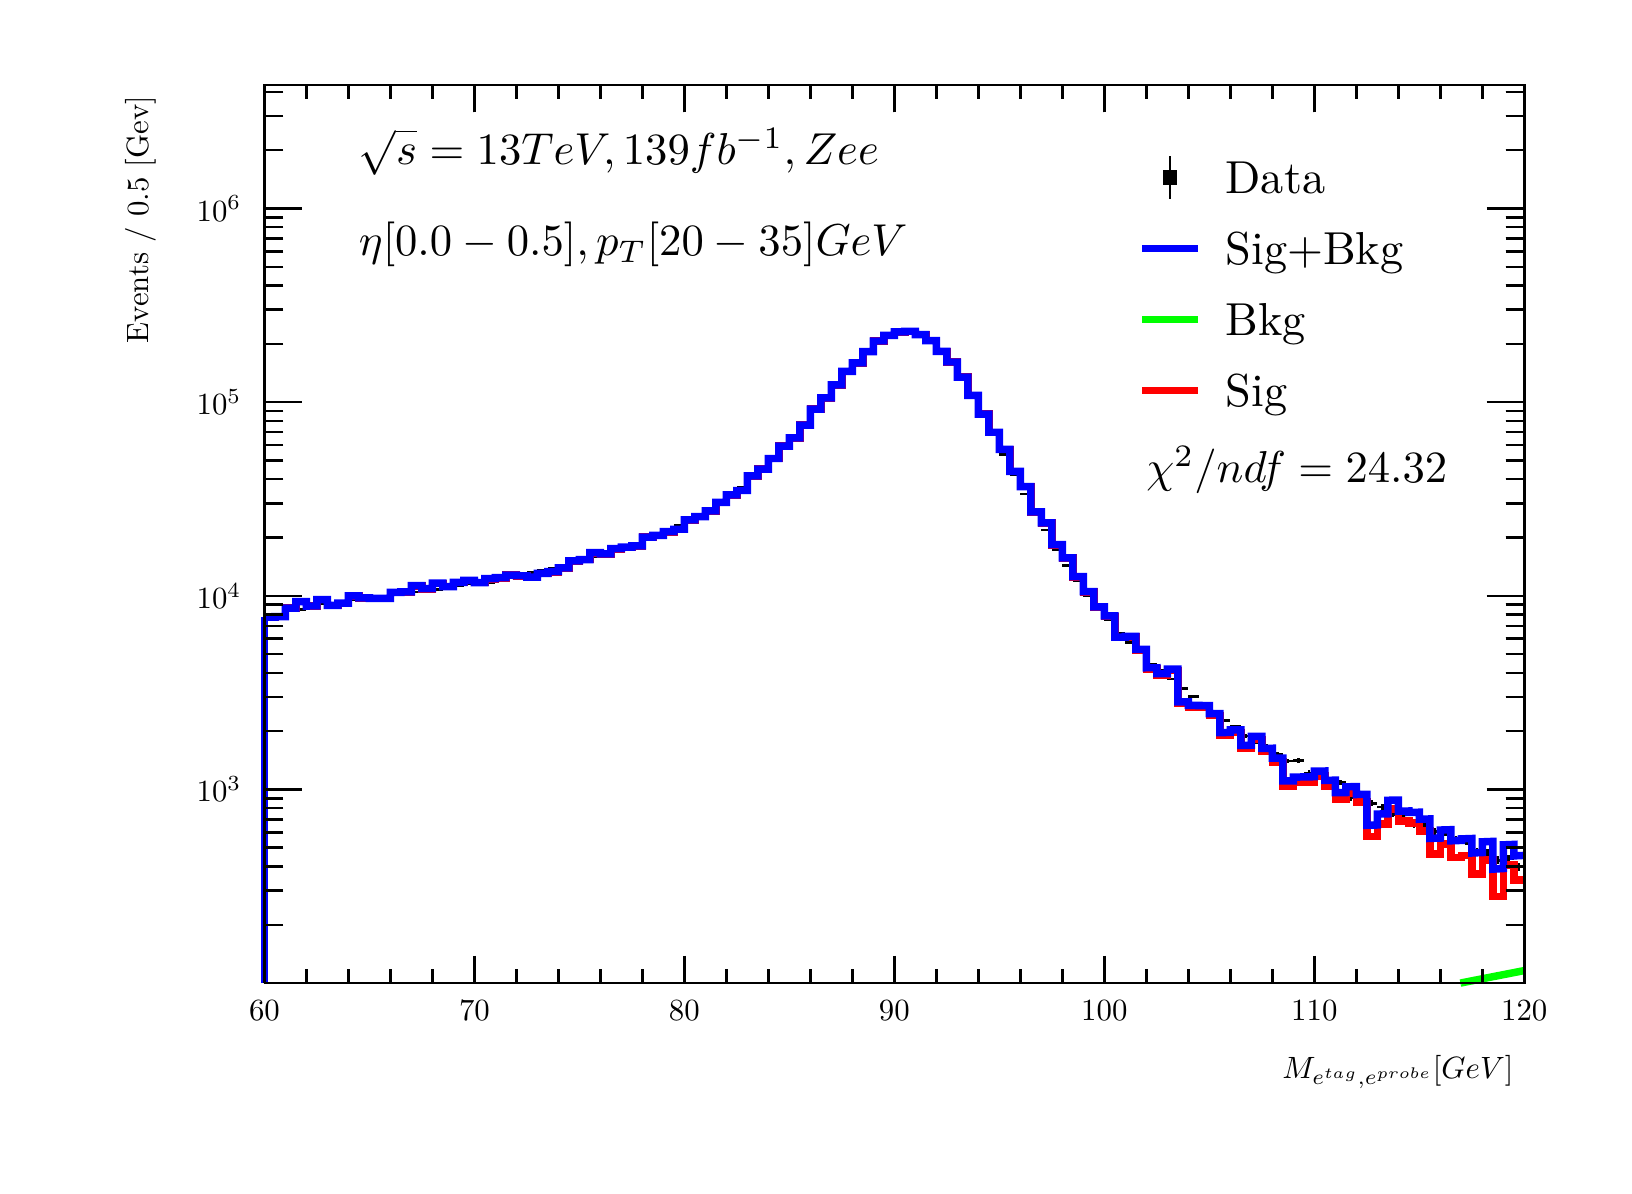
\begin{tikzpicture}
\pgfdeclareplotmark{cross} {
\pgfpathmoveto{\pgfpoint{-0.3\pgfplotmarksize}{\pgfplotmarksize}}
\pgfpathlineto{\pgfpoint{+0.3\pgfplotmarksize}{\pgfplotmarksize}}
\pgfpathlineto{\pgfpoint{+0.3\pgfplotmarksize}{0.3\pgfplotmarksize}}
\pgfpathlineto{\pgfpoint{+1\pgfplotmarksize}{0.3\pgfplotmarksize}}
\pgfpathlineto{\pgfpoint{+1\pgfplotmarksize}{-0.3\pgfplotmarksize}}
\pgfpathlineto{\pgfpoint{+0.3\pgfplotmarksize}{-0.3\pgfplotmarksize}}
\pgfpathlineto{\pgfpoint{+0.3\pgfplotmarksize}{-1.\pgfplotmarksize}}
\pgfpathlineto{\pgfpoint{-0.3\pgfplotmarksize}{-1.\pgfplotmarksize}}
\pgfpathlineto{\pgfpoint{-0.3\pgfplotmarksize}{-0.3\pgfplotmarksize}}
\pgfpathlineto{\pgfpoint{-1.\pgfplotmarksize}{-0.3\pgfplotmarksize}}
\pgfpathlineto{\pgfpoint{-1.\pgfplotmarksize}{0.3\pgfplotmarksize}}
\pgfpathlineto{\pgfpoint{-0.3\pgfplotmarksize}{0.3\pgfplotmarksize}}
\pgfpathclose
\pgfusepathqstroke
}
\pgfdeclareplotmark{cross*} {
\pgfpathmoveto{\pgfpoint{-0.3\pgfplotmarksize}{\pgfplotmarksize}}
\pgfpathlineto{\pgfpoint{+0.3\pgfplotmarksize}{\pgfplotmarksize}}
\pgfpathlineto{\pgfpoint{+0.3\pgfplotmarksize}{0.3\pgfplotmarksize}}
\pgfpathlineto{\pgfpoint{+1\pgfplotmarksize}{0.3\pgfplotmarksize}}
\pgfpathlineto{\pgfpoint{+1\pgfplotmarksize}{-0.3\pgfplotmarksize}}
\pgfpathlineto{\pgfpoint{+0.3\pgfplotmarksize}{-0.3\pgfplotmarksize}}
\pgfpathlineto{\pgfpoint{+0.3\pgfplotmarksize}{-1.\pgfplotmarksize}}
\pgfpathlineto{\pgfpoint{-0.3\pgfplotmarksize}{-1.\pgfplotmarksize}}
\pgfpathlineto{\pgfpoint{-0.3\pgfplotmarksize}{-0.3\pgfplotmarksize}}
\pgfpathlineto{\pgfpoint{-1.\pgfplotmarksize}{-0.3\pgfplotmarksize}}
\pgfpathlineto{\pgfpoint{-1.\pgfplotmarksize}{0.3\pgfplotmarksize}}
\pgfpathlineto{\pgfpoint{-0.3\pgfplotmarksize}{0.3\pgfplotmarksize}}
\pgfpathclose
\pgfusepathqfillstroke
}
\pgfdeclareplotmark{newstar} {
\pgfpathmoveto{\pgfqpoint{0pt}{\pgfplotmarksize}}
\pgfpathlineto{\pgfqpointpolar{44}{0.5\pgfplotmarksize}}
\pgfpathlineto{\pgfqpointpolar{18}{\pgfplotmarksize}}
\pgfpathlineto{\pgfqpointpolar{-20}{0.5\pgfplotmarksize}}
\pgfpathlineto{\pgfqpointpolar{-54}{\pgfplotmarksize}}
\pgfpathlineto{\pgfqpointpolar{-90}{0.5\pgfplotmarksize}}
\pgfpathlineto{\pgfqpointpolar{234}{\pgfplotmarksize}}
\pgfpathlineto{\pgfqpointpolar{198}{0.5\pgfplotmarksize}}
\pgfpathlineto{\pgfqpointpolar{162}{\pgfplotmarksize}}
\pgfpathlineto{\pgfqpointpolar{134}{0.5\pgfplotmarksize}}
\pgfpathclose
\pgfusepathqstroke
}
\pgfdeclareplotmark{newstar*} {
\pgfpathmoveto{\pgfqpoint{0pt}{\pgfplotmarksize}}
\pgfpathlineto{\pgfqpointpolar{44}{0.5\pgfplotmarksize}}
\pgfpathlineto{\pgfqpointpolar{18}{\pgfplotmarksize}}
\pgfpathlineto{\pgfqpointpolar{-20}{0.5\pgfplotmarksize}}
\pgfpathlineto{\pgfqpointpolar{-54}{\pgfplotmarksize}}
\pgfpathlineto{\pgfqpointpolar{-90}{0.5\pgfplotmarksize}}
\pgfpathlineto{\pgfqpointpolar{234}{\pgfplotmarksize}}
\pgfpathlineto{\pgfqpointpolar{198}{0.5\pgfplotmarksize}}
\pgfpathlineto{\pgfqpointpolar{162}{\pgfplotmarksize}}
\pgfpathlineto{\pgfqpointpolar{134}{0.5\pgfplotmarksize}}
\pgfpathclose
\pgfusepathqfillstroke
}
\definecolor{c}{rgb}{1,1,1};
\draw [color=c, fill=c] (0,0) rectangle (20,14.4361);
\draw [color=c, fill=c] (3,2.30977) rectangle (19,13.7143);
\definecolor{c}{rgb}{0,0,0};
\draw [c,line width=0.9] (3,2.30977) -- (3,13.7143) -- (19,13.7143) -- (19,2.30977) -- (3,2.30977);
\definecolor{c}{rgb}{1,1,1};
\draw [color=c, fill=c] (3,2.30977) rectangle (19,13.7143);
\definecolor{c}{rgb}{0,0,0};
\draw [c,line width=0.9] (3,2.30977) -- (3,13.7143) -- (19,13.7143) -- (19,2.30977) -- (3,2.30977);
\draw [c,line width=0.9] (3,2.30977) -- (19,2.30977);
\draw [c,line width=0.9] (3,2.65624) -- (3,2.30977);
\draw [c,line width=0.9] (3.53333,2.48301) -- (3.53333,2.30977);
\draw [c,line width=0.9] (4.06667,2.48301) -- (4.06667,2.30977);
\draw [c,line width=0.9] (4.6,2.48301) -- (4.6,2.30977);
\draw [c,line width=0.9] (5.13333,2.48301) -- (5.13333,2.30977);
\draw [c,line width=0.9] (5.66667,2.65624) -- (5.66667,2.30977);
\draw [c,line width=0.9] (6.2,2.48301) -- (6.2,2.30977);
\draw [c,line width=0.9] (6.73333,2.48301) -- (6.73333,2.30977);
\draw [c,line width=0.9] (7.26667,2.48301) -- (7.26667,2.30977);
\draw [c,line width=0.9] (7.8,2.48301) -- (7.8,2.30977);
\draw [c,line width=0.9] (8.33333,2.65624) -- (8.33333,2.30977);
\draw [c,line width=0.9] (8.86667,2.48301) -- (8.86667,2.30977);
\draw [c,line width=0.9] (9.4,2.48301) -- (9.4,2.30977);
\draw [c,line width=0.9] (9.93333,2.48301) -- (9.93333,2.30977);
\draw [c,line width=0.9] (10.4667,2.48301) -- (10.4667,2.30977);
\draw [c,line width=0.9] (11,2.65624) -- (11,2.30977);
\draw [c,line width=0.9] (11.5333,2.48301) -- (11.5333,2.30977);
\draw [c,line width=0.9] (12.0667,2.48301) -- (12.0667,2.30977);
\draw [c,line width=0.9] (12.6,2.48301) -- (12.6,2.30977);
\draw [c,line width=0.9] (13.1333,2.48301) -- (13.1333,2.30977);
\draw [c,line width=0.9] (13.6667,2.65624) -- (13.6667,2.30977);
\draw [c,line width=0.9] (14.2,2.48301) -- (14.2,2.30977);
\draw [c,line width=0.9] (14.7333,2.48301) -- (14.7333,2.30977);
\draw [c,line width=0.9] (15.2667,2.48301) -- (15.2667,2.30977);
\draw [c,line width=0.9] (15.8,2.48301) -- (15.8,2.30977);
\draw [c,line width=0.9] (16.3333,2.65624) -- (16.3333,2.30977);
\draw [c,line width=0.9] (16.8667,2.48301) -- (16.8667,2.30977);
\draw [c,line width=0.9] (17.4,2.48301) -- (17.4,2.30977);
\draw [c,line width=0.9] (17.9333,2.48301) -- (17.9333,2.30977);
\draw [c,line width=0.9] (18.4667,2.48301) -- (18.4667,2.30977);
\draw [c,line width=0.9] (19,2.65624) -- (19,2.30977);
\draw [anchor=base] (3,1.83338) node[scale=1.11327, color=c, rotate=0]{60};
\draw [anchor=base] (5.66667,1.83338) node[scale=1.11327, color=c, rotate=0]{70};
\draw [anchor=base] (8.33333,1.83338) node[scale=1.11327, color=c, rotate=0]{80};
\draw [anchor=base] (11,1.83338) node[scale=1.11327, color=c, rotate=0]{90};
\draw [anchor=base] (13.6667,1.83338) node[scale=1.11327, color=c, rotate=0]{100};
\draw [anchor=base] (16.3333,1.83338) node[scale=1.11327, color=c, rotate=0]{110};
\draw [anchor=base] (19,1.83338) node[scale=1.11327, color=c, rotate=0]{120};
\draw [anchor= east] (19,1.17798) node[scale=1.11327, color=c, rotate=0]{$M_{e^{tag}, e^{probe}}  [GeV]$};
\draw [c,line width=0.9] (3,13.7143) -- (19,13.7143);
\draw [c,line width=0.9] (3,13.3678) -- (3,13.7143);
\draw [c,line width=0.9] (3.53333,13.5411) -- (3.53333,13.7143);
\draw [c,line width=0.9] (4.06667,13.5411) -- (4.06667,13.7143);
\draw [c,line width=0.9] (4.6,13.5411) -- (4.6,13.7143);
\draw [c,line width=0.9] (5.13333,13.5411) -- (5.13333,13.7143);
\draw [c,line width=0.9] (5.66667,13.3678) -- (5.66667,13.7143);
\draw [c,line width=0.9] (6.2,13.5411) -- (6.2,13.7143);
\draw [c,line width=0.9] (6.73333,13.5411) -- (6.73333,13.7143);
\draw [c,line width=0.9] (7.26667,13.5411) -- (7.26667,13.7143);
\draw [c,line width=0.9] (7.8,13.5411) -- (7.8,13.7143);
\draw [c,line width=0.9] (8.33333,13.3678) -- (8.33333,13.7143);
\draw [c,line width=0.9] (8.86667,13.5411) -- (8.86667,13.7143);
\draw [c,line width=0.9] (9.4,13.5411) -- (9.4,13.7143);
\draw [c,line width=0.9] (9.93333,13.5411) -- (9.93333,13.7143);
\draw [c,line width=0.9] (10.4667,13.5411) -- (10.4667,13.7143);
\draw [c,line width=0.9] (11,13.3678) -- (11,13.7143);
\draw [c,line width=0.9] (11.5333,13.5411) -- (11.5333,13.7143);
\draw [c,line width=0.9] (12.0667,13.5411) -- (12.0667,13.7143);
\draw [c,line width=0.9] (12.6,13.5411) -- (12.6,13.7143);
\draw [c,line width=0.9] (13.1333,13.5411) -- (13.1333,13.7143);
\draw [c,line width=0.9] (13.6667,13.3678) -- (13.6667,13.7143);
\draw [c,line width=0.9] (14.2,13.5411) -- (14.2,13.7143);
\draw [c,line width=0.9] (14.7333,13.5411) -- (14.7333,13.7143);
\draw [c,line width=0.9] (15.2667,13.5411) -- (15.2667,13.7143);
\draw [c,line width=0.9] (15.8,13.5411) -- (15.8,13.7143);
\draw [c,line width=0.9] (16.3333,13.3678) -- (16.3333,13.7143);
\draw [c,line width=0.9] (16.8667,13.5411) -- (16.8667,13.7143);
\draw [c,line width=0.9] (17.4,13.5411) -- (17.4,13.7143);
\draw [c,line width=0.9] (17.9333,13.5411) -- (17.9333,13.7143);
\draw [c,line width=0.9] (18.4667,13.5411) -- (18.4667,13.7143);
\draw [c,line width=0.9] (19,13.3678) -- (19,13.7143);
\draw [c,line width=0.9] (3,2.30977) -- (3,13.7143);
\draw [c,line width=0.9] (3.237,3.05008) -- (3,3.05008);
\draw [c,line width=0.9] (3.237,3.48313) -- (3,3.48313);
\draw [c,line width=0.9] (3.237,3.79038) -- (3,3.79038);
\draw [c,line width=0.9] (3.237,4.02871) -- (3,4.02871);
\draw [c,line width=0.9] (3.237,4.22343) -- (3,4.22343);
\draw [c,line width=0.9] (3.237,4.38807) -- (3,4.38807);
\draw [c,line width=0.9] (3.237,4.53069) -- (3,4.53069);
\draw [c,line width=0.9] (3.237,4.65649) -- (3,4.65649);
\draw [c,line width=0.9] (3.474,4.76901) -- (3,4.76901);
\draw [anchor= east] (2.844,4.76901) node[scale=1.11327, color=c, rotate=0]{$10^{3}$};
\draw [c,line width=0.9] (3.237,5.50932) -- (3,5.50932);
\draw [c,line width=0.9] (3.237,5.94237) -- (3,5.94237);
\draw [c,line width=0.9] (3.237,6.24963) -- (3,6.24963);
\draw [c,line width=0.9] (3.237,6.48795) -- (3,6.48795);
\draw [c,line width=0.9] (3.237,6.68268) -- (3,6.68268);
\draw [c,line width=0.9] (3.237,6.84731) -- (3,6.84731);
\draw [c,line width=0.9] (3.237,6.98993) -- (3,6.98993);
\draw [c,line width=0.9] (3.237,7.11573) -- (3,7.11573);
\draw [c,line width=0.9] (3.474,7.22826) -- (3,7.22826);
\draw [anchor= east] (2.844,7.22826) node[scale=1.11327, color=c, rotate=0]{$10^{4}$};
\draw [c,line width=0.9] (3.237,7.96856) -- (3,7.96856);
\draw [c,line width=0.9] (3.237,8.40161) -- (3,8.40161);
\draw [c,line width=0.9] (3.237,8.70887) -- (3,8.70887);
\draw [c,line width=0.9] (3.237,8.94719) -- (3,8.94719);
\draw [c,line width=0.9] (3.237,9.14192) -- (3,9.14192);
\draw [c,line width=0.9] (3.237,9.30656) -- (3,9.30656);
\draw [c,line width=0.9] (3.237,9.44917) -- (3,9.44917);
\draw [c,line width=0.9] (3.237,9.57497) -- (3,9.57497);
\draw [c,line width=0.9] (3.474,9.6875) -- (3,9.6875);
\draw [anchor= east] (2.844,9.6875) node[scale=1.11327, color=c, rotate=0]{$10^{5}$};
\draw [c,line width=0.9] (3.237,10.4278) -- (3,10.4278);
\draw [c,line width=0.9] (3.237,10.8609) -- (3,10.8609);
\draw [c,line width=0.9] (3.237,11.1681) -- (3,11.1681);
\draw [c,line width=0.9] (3.237,11.4064) -- (3,11.4064);
\draw [c,line width=0.9] (3.237,11.6012) -- (3,11.6012);
\draw [c,line width=0.9] (3.237,11.7658) -- (3,11.7658);
\draw [c,line width=0.9] (3.237,11.9084) -- (3,11.9084);
\draw [c,line width=0.9] (3.237,12.0342) -- (3,12.0342);
\draw [c,line width=0.9] (3.474,12.1467) -- (3,12.1467);
\draw [anchor= east] (2.844,12.1467) node[scale=1.11327, color=c, rotate=0]{$10^{6}$};
\draw [c,line width=0.9] (3.237,12.887) -- (3,12.887);
\draw [c,line width=0.9] (3.237,13.3201) -- (3,13.3201);
\draw [c,line width=0.9] (3.237,13.6274) -- (3,13.6274);
\draw [anchor= east] (1.432,13.7143) node[scale=1.11327, color=c, rotate=90]{Events / 0.5 [Gev]};
\draw [c,line width=0.9] (19,2.30977) -- (19,13.7143);
\draw [c,line width=0.9] (18.763,3.05008) -- (19,3.05008);
\draw [c,line width=0.9] (18.763,3.48313) -- (19,3.48313);
\draw [c,line width=0.9] (18.763,3.79038) -- (19,3.79038);
\draw [c,line width=0.9] (18.763,4.02871) -- (19,4.02871);
\draw [c,line width=0.9] (18.763,4.22343) -- (19,4.22343);
\draw [c,line width=0.9] (18.763,4.38807) -- (19,4.38807);
\draw [c,line width=0.9] (18.763,4.53069) -- (19,4.53069);
\draw [c,line width=0.9] (18.763,4.65649) -- (19,4.65649);
\draw [c,line width=0.9] (18.526,4.76901) -- (19,4.76901);
\draw [c,line width=0.9] (18.763,5.50932) -- (19,5.50932);
\draw [c,line width=0.9] (18.763,5.94237) -- (19,5.94237);
\draw [c,line width=0.9] (18.763,6.24963) -- (19,6.24963);
\draw [c,line width=0.9] (18.763,6.48795) -- (19,6.48795);
\draw [c,line width=0.9] (18.763,6.68268) -- (19,6.68268);
\draw [c,line width=0.9] (18.763,6.84731) -- (19,6.84731);
\draw [c,line width=0.9] (18.763,6.98993) -- (19,6.98993);
\draw [c,line width=0.9] (18.763,7.11573) -- (19,7.11573);
\draw [c,line width=0.9] (18.526,7.22826) -- (19,7.22826);
\draw [c,line width=0.9] (18.763,7.96856) -- (19,7.96856);
\draw [c,line width=0.9] (18.763,8.40161) -- (19,8.40161);
\draw [c,line width=0.9] (18.763,8.70887) -- (19,8.70887);
\draw [c,line width=0.9] (18.763,8.94719) -- (19,8.94719);
\draw [c,line width=0.9] (18.763,9.14192) -- (19,9.14192);
\draw [c,line width=0.9] (18.763,9.30656) -- (19,9.30656);
\draw [c,line width=0.9] (18.763,9.44917) -- (19,9.44917);
\draw [c,line width=0.9] (18.763,9.57497) -- (19,9.57497);
\draw [c,line width=0.9] (18.526,9.6875) -- (19,9.6875);
\draw [c,line width=0.9] (18.763,10.4278) -- (19,10.4278);
\draw [c,line width=0.9] (18.763,10.8609) -- (19,10.8609);
\draw [c,line width=0.9] (18.763,11.1681) -- (19,11.1681);
\draw [c,line width=0.9] (18.763,11.4064) -- (19,11.4064);
\draw [c,line width=0.9] (18.763,11.6012) -- (19,11.6012);
\draw [c,line width=0.9] (18.763,11.7658) -- (19,11.7658);
\draw [c,line width=0.9] (18.763,11.9084) -- (19,11.9084);
\draw [c,line width=0.9] (18.763,12.0342) -- (19,12.0342);
\draw [c,line width=0.9] (18.526,12.1467) -- (19,12.1467);
\draw [c,line width=0.9] (18.763,12.887) -- (19,12.887);
\draw [c,line width=0.9] (18.763,13.3201) -- (19,13.3201);
\draw [c,line width=0.9] (18.763,13.6274) -- (19,13.6274);
\draw [c,line width=0.9] (3.06667,6.97555) -- (3,6.97555);
\draw [c,line width=0.9] (3,6.97555) -- (3,6.97555);
\draw [c,line width=0.9] (3.06667,6.97555) -- (3.13333,6.97555);
\draw [c,line width=0.9] (3.13333,6.97555) -- (3.13333,6.97555);
\draw [c,line width=0.9] (3.06667,6.97555) -- (3.06667,6.98757);
\draw [c,line width=0.9] (3.06667,6.98757) -- (3.06667,6.98757);
\draw [c,line width=0.9] (3.06667,6.97555) -- (3.06667,6.96353);
\draw [c,line width=0.9] (3.06667,6.96353) -- (3.06667,6.96353);
\draw [c,line width=0.9] (3.2,6.99897) -- (3.13333,6.99897);
\draw [c,line width=0.9] (3.13333,6.99897) -- (3.13333,6.99897);
\draw [c,line width=0.9] (3.2,6.99897) -- (3.26667,6.99897);
\draw [c,line width=0.9] (3.26667,6.99897) -- (3.26667,6.99897);
\draw [c,line width=0.9] (3.2,6.99897) -- (3.2,7.01086);
\draw [c,line width=0.9] (3.2,7.01086) -- (3.2,7.01086);
\draw [c,line width=0.9] (3.2,6.99897) -- (3.2,6.98708);
\draw [c,line width=0.9] (3.2,6.98708) -- (3.2,6.98708);
\draw [c,line width=0.9] (3.33333,7.05305) -- (3.26667,7.05305);
\draw [c,line width=0.9] (3.26667,7.05305) -- (3.26667,7.05305);
\draw [c,line width=0.9] (3.33333,7.05305) -- (3.4,7.05305);
\draw [c,line width=0.9] (3.4,7.05305) -- (3.4,7.05305);
\draw [c,line width=0.9] (3.33333,7.05305) -- (3.33333,7.06464);
\draw [c,line width=0.9] (3.33333,7.06464) -- (3.33333,7.06464);
\draw [c,line width=0.9] (3.33333,7.05305) -- (3.33333,7.04145);
\draw [c,line width=0.9] (3.33333,7.04145) -- (3.33333,7.04145);
\draw [c,line width=0.9] (3.46667,7.05619) -- (3.4,7.05619);
\draw [c,line width=0.9] (3.4,7.05619) -- (3.4,7.05619);
\draw [c,line width=0.9] (3.46667,7.05619) -- (3.53333,7.05619);
\draw [c,line width=0.9] (3.53333,7.05619) -- (3.53333,7.05619);
\draw [c,line width=0.9] (3.46667,7.05619) -- (3.46667,7.06776);
\draw [c,line width=0.9] (3.46667,7.06776) -- (3.46667,7.06776);
\draw [c,line width=0.9] (3.46667,7.05619) -- (3.46667,7.04461);
\draw [c,line width=0.9] (3.46667,7.04461) -- (3.46667,7.04461);
\draw [c,line width=0.9] (3.6,7.09403) -- (3.53333,7.09403);
\draw [c,line width=0.9] (3.53333,7.09403) -- (3.53333,7.09403);
\draw [c,line width=0.9] (3.6,7.09403) -- (3.66667,7.09403);
\draw [c,line width=0.9] (3.66667,7.09403) -- (3.66667,7.09403);
\draw [c,line width=0.9] (3.6,7.09403) -- (3.6,7.1054);
\draw [c,line width=0.9] (3.6,7.1054) -- (3.6,7.1054);
\draw [c,line width=0.9] (3.6,7.09403) -- (3.6,7.08266);
\draw [c,line width=0.9] (3.6,7.08266) -- (3.6,7.08266);
\draw [c,line width=0.9] (3.73333,7.12094) -- (3.66667,7.12094);
\draw [c,line width=0.9] (3.66667,7.12094) -- (3.66667,7.12094);
\draw [c,line width=0.9] (3.73333,7.12094) -- (3.8,7.12094);
\draw [c,line width=0.9] (3.8,7.12094) -- (3.8,7.12094);
\draw [c,line width=0.9] (3.73333,7.12094) -- (3.73333,7.13217);
\draw [c,line width=0.9] (3.73333,7.13217) -- (3.73333,7.13217);
\draw [c,line width=0.9] (3.73333,7.12094) -- (3.73333,7.10971);
\draw [c,line width=0.9] (3.73333,7.10971) -- (3.73333,7.10971);
\draw [c,line width=0.9] (3.86667,7.1328) -- (3.8,7.1328);
\draw [c,line width=0.9] (3.8,7.1328) -- (3.8,7.1328);
\draw [c,line width=0.9] (3.86667,7.1328) -- (3.93333,7.1328);
\draw [c,line width=0.9] (3.93333,7.1328) -- (3.93333,7.1328);
\draw [c,line width=0.9] (3.86667,7.1328) -- (3.86667,7.14397);
\draw [c,line width=0.9] (3.86667,7.14397) -- (3.86667,7.14397);
\draw [c,line width=0.9] (3.86667,7.1328) -- (3.86667,7.12163);
\draw [c,line width=0.9] (3.86667,7.12163) -- (3.86667,7.12163);
\draw [c,line width=0.9] (4,7.15407) -- (3.93333,7.15407);
\draw [c,line width=0.9] (3.93333,7.15407) -- (3.93333,7.15407);
\draw [c,line width=0.9] (4,7.15407) -- (4.06667,7.15407);
\draw [c,line width=0.9] (4.06667,7.15407) -- (4.06667,7.15407);
\draw [c,line width=0.9] (4,7.15407) -- (4,7.16513);
\draw [c,line width=0.9] (4,7.16513) -- (4,7.16513);
\draw [c,line width=0.9] (4,7.15407) -- (4,7.14302);
\draw [c,line width=0.9] (4,7.14302) -- (4,7.14302);
\draw [c,line width=0.9] (4.13333,7.18377) -- (4.06667,7.18377);
\draw [c,line width=0.9] (4.06667,7.18377) -- (4.06667,7.18377);
\draw [c,line width=0.9] (4.13333,7.18377) -- (4.2,7.18377);
\draw [c,line width=0.9] (4.2,7.18377) -- (4.2,7.18377);
\draw [c,line width=0.9] (4.13333,7.18377) -- (4.13333,7.19467);
\draw [c,line width=0.9] (4.13333,7.19467) -- (4.13333,7.19467);
\draw [c,line width=0.9] (4.13333,7.18377) -- (4.13333,7.17286);
\draw [c,line width=0.9] (4.13333,7.17286) -- (4.13333,7.17286);
\draw [c,line width=0.9] (4.26667,7.21439) -- (4.2,7.21439);
\draw [c,line width=0.9] (4.2,7.21439) -- (4.2,7.21439);
\draw [c,line width=0.9] (4.26667,7.21439) -- (4.33333,7.21439);
\draw [c,line width=0.9] (4.33333,7.21439) -- (4.33333,7.21439);
\draw [c,line width=0.9] (4.26667,7.21439) -- (4.26667,7.22514);
\draw [c,line width=0.9] (4.26667,7.22514) -- (4.26667,7.22514);
\draw [c,line width=0.9] (4.26667,7.21439) -- (4.26667,7.20364);
\draw [c,line width=0.9] (4.26667,7.20364) -- (4.26667,7.20364);
\draw [c,line width=0.9] (4.4,7.21114) -- (4.33333,7.21114);
\draw [c,line width=0.9] (4.33333,7.21114) -- (4.33333,7.21114);
\draw [c,line width=0.9] (4.4,7.21114) -- (4.46667,7.21114);
\draw [c,line width=0.9] (4.46667,7.21114) -- (4.46667,7.21114);
\draw [c,line width=0.9] (4.4,7.21114) -- (4.4,7.22191);
\draw [c,line width=0.9] (4.4,7.22191) -- (4.4,7.22191);
\draw [c,line width=0.9] (4.4,7.21114) -- (4.4,7.20037);
\draw [c,line width=0.9] (4.4,7.20037) -- (4.4,7.20037);
\draw [c,line width=0.9] (4.53333,7.21979) -- (4.46667,7.21979);
\draw [c,line width=0.9] (4.46667,7.21979) -- (4.46667,7.21979);
\draw [c,line width=0.9] (4.53333,7.21979) -- (4.6,7.21979);
\draw [c,line width=0.9] (4.6,7.21979) -- (4.6,7.21979);
\draw [c,line width=0.9] (4.53333,7.21979) -- (4.53333,7.23051);
\draw [c,line width=0.9] (4.53333,7.23051) -- (4.53333,7.23051);
\draw [c,line width=0.9] (4.53333,7.21979) -- (4.53333,7.20906);
\draw [c,line width=0.9] (4.53333,7.20906) -- (4.53333,7.20906);
\draw [c,line width=0.9] (4.66667,7.23878) -- (4.6,7.23878);
\draw [c,line width=0.9] (4.6,7.23878) -- (4.6,7.23878);
\draw [c,line width=0.9] (4.66667,7.23878) -- (4.73333,7.23878);
\draw [c,line width=0.9] (4.73333,7.23878) -- (4.73333,7.23878);
\draw [c,line width=0.9] (4.66667,7.23878) -- (4.66667,7.24941);
\draw [c,line width=0.9] (4.66667,7.24941) -- (4.66667,7.24941);
\draw [c,line width=0.9] (4.66667,7.23878) -- (4.66667,7.22815);
\draw [c,line width=0.9] (4.66667,7.22815) -- (4.66667,7.22815);
\draw [c,line width=0.9] (4.8,7.28756) -- (4.73333,7.28756);
\draw [c,line width=0.9] (4.73333,7.28756) -- (4.73333,7.28756);
\draw [c,line width=0.9] (4.8,7.28756) -- (4.86667,7.28756);
\draw [c,line width=0.9] (4.86667,7.28756) -- (4.86667,7.28756);
\draw [c,line width=0.9] (4.8,7.28756) -- (4.8,7.29795);
\draw [c,line width=0.9] (4.8,7.29795) -- (4.8,7.29795);
\draw [c,line width=0.9] (4.8,7.28756) -- (4.8,7.27718);
\draw [c,line width=0.9] (4.8,7.27718) -- (4.8,7.27718);
\draw [c,line width=0.9] (4.93333,7.27425) -- (4.86667,7.27425);
\draw [c,line width=0.9] (4.86667,7.27425) -- (4.86667,7.27425);
\draw [c,line width=0.9] (4.93333,7.27425) -- (5,7.27425);
\draw [c,line width=0.9] (5,7.27425) -- (5,7.27425);
\draw [c,line width=0.9] (4.93333,7.27425) -- (4.93333,7.2847);
\draw [c,line width=0.9] (4.93333,7.2847) -- (4.93333,7.2847);
\draw [c,line width=0.9] (4.93333,7.27425) -- (4.93333,7.26379);
\draw [c,line width=0.9] (4.93333,7.26379) -- (4.93333,7.26379);
\draw [c,line width=0.9] (5.06667,7.30986) -- (5,7.30986);
\draw [c,line width=0.9] (5,7.30986) -- (5,7.30986);
\draw [c,line width=0.9] (5.06667,7.30986) -- (5.13333,7.30986);
\draw [c,line width=0.9] (5.13333,7.30986) -- (5.13333,7.30986);
\draw [c,line width=0.9] (5.06667,7.30986) -- (5.06667,7.32014);
\draw [c,line width=0.9] (5.06667,7.32014) -- (5.06667,7.32014);
\draw [c,line width=0.9] (5.06667,7.30986) -- (5.06667,7.29958);
\draw [c,line width=0.9] (5.06667,7.29958) -- (5.06667,7.29958);
\draw [c,line width=0.9] (5.2,7.31065) -- (5.13333,7.31065);
\draw [c,line width=0.9] (5.13333,7.31065) -- (5.13333,7.31065);
\draw [c,line width=0.9] (5.2,7.31065) -- (5.26667,7.31065);
\draw [c,line width=0.9] (5.26667,7.31065) -- (5.26667,7.31065);
\draw [c,line width=0.9] (5.2,7.31065) -- (5.2,7.32093);
\draw [c,line width=0.9] (5.2,7.32093) -- (5.2,7.32093);
\draw [c,line width=0.9] (5.2,7.31065) -- (5.2,7.30038);
\draw [c,line width=0.9] (5.2,7.30038) -- (5.2,7.30038);
\draw [c,line width=0.9] (5.33333,7.34844) -- (5.26667,7.34844);
\draw [c,line width=0.9] (5.26667,7.34844) -- (5.26667,7.34844);
\draw [c,line width=0.9] (5.33333,7.34844) -- (5.4,7.34844);
\draw [c,line width=0.9] (5.4,7.34844) -- (5.4,7.34844);
\draw [c,line width=0.9] (5.33333,7.34844) -- (5.33333,7.35853);
\draw [c,line width=0.9] (5.33333,7.35853) -- (5.33333,7.35853);
\draw [c,line width=0.9] (5.33333,7.34844) -- (5.33333,7.33834);
\draw [c,line width=0.9] (5.33333,7.33834) -- (5.33333,7.33834);
\draw [c,line width=0.9] (5.46667,7.35358) -- (5.4,7.35358);
\draw [c,line width=0.9] (5.4,7.35358) -- (5.4,7.35358);
\draw [c,line width=0.9] (5.46667,7.35358) -- (5.53333,7.35358);
\draw [c,line width=0.9] (5.53333,7.35358) -- (5.53333,7.35358);
\draw [c,line width=0.9] (5.46667,7.35358) -- (5.46667,7.36365);
\draw [c,line width=0.9] (5.46667,7.36365) -- (5.46667,7.36365);
\draw [c,line width=0.9] (5.46667,7.35358) -- (5.46667,7.34351);
\draw [c,line width=0.9] (5.46667,7.34351) -- (5.46667,7.34351);
\draw [c,line width=0.9] (5.6,7.38401) -- (5.53333,7.38401);
\draw [c,line width=0.9] (5.53333,7.38401) -- (5.53333,7.38401);
\draw [c,line width=0.9] (5.6,7.38401) -- (5.66667,7.38401);
\draw [c,line width=0.9] (5.66667,7.38401) -- (5.66667,7.38401);
\draw [c,line width=0.9] (5.6,7.38401) -- (5.6,7.39394);
\draw [c,line width=0.9] (5.6,7.39394) -- (5.6,7.39394);
\draw [c,line width=0.9] (5.6,7.38401) -- (5.6,7.37408);
\draw [c,line width=0.9] (5.6,7.37408) -- (5.6,7.37408);
\draw [c,line width=0.9] (5.73333,7.39649) -- (5.66667,7.39649);
\draw [c,line width=0.9] (5.66667,7.39649) -- (5.66667,7.39649);
\draw [c,line width=0.9] (5.73333,7.39649) -- (5.8,7.39649);
\draw [c,line width=0.9] (5.8,7.39649) -- (5.8,7.39649);
\draw [c,line width=0.9] (5.73333,7.39649) -- (5.73333,7.40636);
\draw [c,line width=0.9] (5.73333,7.40636) -- (5.73333,7.40636);
\draw [c,line width=0.9] (5.73333,7.39649) -- (5.73333,7.38662);
\draw [c,line width=0.9] (5.73333,7.38662) -- (5.73333,7.38662);
\draw [c,line width=0.9] (5.86667,7.39722) -- (5.8,7.39722);
\draw [c,line width=0.9] (5.8,7.39722) -- (5.8,7.39722);
\draw [c,line width=0.9] (5.86667,7.39722) -- (5.93333,7.39722);
\draw [c,line width=0.9] (5.93333,7.39722) -- (5.93333,7.39722);
\draw [c,line width=0.9] (5.86667,7.39722) -- (5.86667,7.40709);
\draw [c,line width=0.9] (5.86667,7.40709) -- (5.86667,7.40709);
\draw [c,line width=0.9] (5.86667,7.39722) -- (5.86667,7.38735);
\draw [c,line width=0.9] (5.86667,7.38735) -- (5.86667,7.38735);
\draw [c,line width=0.9] (6,7.44378) -- (5.93333,7.44378);
\draw [c,line width=0.9] (5.93333,7.44378) -- (5.93333,7.44378);
\draw [c,line width=0.9] (6,7.44378) -- (6.06667,7.44378);
\draw [c,line width=0.9] (6.06667,7.44378) -- (6.06667,7.44378);
\draw [c,line width=0.9] (6,7.44378) -- (6,7.45344);
\draw [c,line width=0.9] (6,7.45344) -- (6,7.45344);
\draw [c,line width=0.9] (6,7.44378) -- (6,7.43413);
\draw [c,line width=0.9] (6,7.43413) -- (6,7.43413);
\draw [c,line width=0.9] (6.13333,7.45403) -- (6.06667,7.45403);
\draw [c,line width=0.9] (6.06667,7.45403) -- (6.06667,7.45403);
\draw [c,line width=0.9] (6.13333,7.45403) -- (6.2,7.45403);
\draw [c,line width=0.9] (6.2,7.45403) -- (6.2,7.45403);
\draw [c,line width=0.9] (6.13333,7.45403) -- (6.13333,7.46364);
\draw [c,line width=0.9] (6.13333,7.46364) -- (6.13333,7.46364);
\draw [c,line width=0.9] (6.13333,7.45403) -- (6.13333,7.44443);
\draw [c,line width=0.9] (6.13333,7.44443) -- (6.13333,7.44443);
\draw [c,line width=0.9] (6.26667,7.5008) -- (6.2,7.5008);
\draw [c,line width=0.9] (6.2,7.5008) -- (6.2,7.5008);
\draw [c,line width=0.9] (6.26667,7.5008) -- (6.33333,7.5008);
\draw [c,line width=0.9] (6.33333,7.5008) -- (6.33333,7.5008);
\draw [c,line width=0.9] (6.26667,7.5008) -- (6.26667,7.5102);
\draw [c,line width=0.9] (6.26667,7.5102) -- (6.26667,7.5102);
\draw [c,line width=0.9] (6.26667,7.5008) -- (6.26667,7.4914);
\draw [c,line width=0.9] (6.26667,7.4914) -- (6.26667,7.4914);
\draw [c,line width=0.9] (6.4,7.52162) -- (6.33333,7.52162);
\draw [c,line width=0.9] (6.33333,7.52162) -- (6.33333,7.52162);
\draw [c,line width=0.9] (6.4,7.52162) -- (6.46667,7.52162);
\draw [c,line width=0.9] (6.46667,7.52162) -- (6.46667,7.52162);
\draw [c,line width=0.9] (6.4,7.52162) -- (6.4,7.53093);
\draw [c,line width=0.9] (6.4,7.53093) -- (6.4,7.53093);
\draw [c,line width=0.9] (6.4,7.52162) -- (6.4,7.51231);
\draw [c,line width=0.9] (6.4,7.51231) -- (6.4,7.51231);
\draw [c,line width=0.9] (6.53333,7.54941) -- (6.46667,7.54941);
\draw [c,line width=0.9] (6.46667,7.54941) -- (6.46667,7.54941);
\draw [c,line width=0.9] (6.53333,7.54941) -- (6.6,7.54941);
\draw [c,line width=0.9] (6.6,7.54941) -- (6.6,7.54941);
\draw [c,line width=0.9] (6.53333,7.54941) -- (6.53333,7.5586);
\draw [c,line width=0.9] (6.53333,7.5586) -- (6.53333,7.5586);
\draw [c,line width=0.9] (6.53333,7.54941) -- (6.53333,7.54022);
\draw [c,line width=0.9] (6.53333,7.54022) -- (6.53333,7.54022);
\draw [c,line width=0.9] (6.66667,7.58211) -- (6.6,7.58211);
\draw [c,line width=0.9] (6.6,7.58211) -- (6.6,7.58211);
\draw [c,line width=0.9] (6.66667,7.58211) -- (6.73333,7.58211);
\draw [c,line width=0.9] (6.73333,7.58211) -- (6.73333,7.58211);
\draw [c,line width=0.9] (6.66667,7.58211) -- (6.66667,7.59116);
\draw [c,line width=0.9] (6.66667,7.59116) -- (6.66667,7.59116);
\draw [c,line width=0.9] (6.66667,7.58211) -- (6.66667,7.57306);
\draw [c,line width=0.9] (6.66667,7.57306) -- (6.66667,7.57306);
\draw [c,line width=0.9] (6.8,7.61094) -- (6.73333,7.61094);
\draw [c,line width=0.9] (6.73333,7.61094) -- (6.73333,7.61094);
\draw [c,line width=0.9] (6.8,7.61094) -- (6.86667,7.61094);
\draw [c,line width=0.9] (6.86667,7.61094) -- (6.86667,7.61094);
\draw [c,line width=0.9] (6.8,7.61094) -- (6.8,7.61987);
\draw [c,line width=0.9] (6.8,7.61987) -- (6.8,7.61987);
\draw [c,line width=0.9] (6.8,7.61094) -- (6.8,7.60201);
\draw [c,line width=0.9] (6.8,7.60201) -- (6.8,7.60201);
\draw [c,line width=0.9] (6.93333,7.6331) -- (6.86667,7.6331);
\draw [c,line width=0.9] (6.86667,7.6331) -- (6.86667,7.6331);
\draw [c,line width=0.9] (6.93333,7.6331) -- (7,7.6331);
\draw [c,line width=0.9] (7,7.6331) -- (7,7.6331);
\draw [c,line width=0.9] (6.93333,7.6331) -- (6.93333,7.64194);
\draw [c,line width=0.9] (6.93333,7.64194) -- (6.93333,7.64194);
\draw [c,line width=0.9] (6.93333,7.6331) -- (6.93333,7.62426);
\draw [c,line width=0.9] (6.93333,7.62426) -- (6.93333,7.62426);
\draw [c,line width=0.9] (7.06667,7.66734) -- (7,7.66734);
\draw [c,line width=0.9] (7,7.66734) -- (7,7.66734);
\draw [c,line width=0.9] (7.06667,7.66734) -- (7.13333,7.66734);
\draw [c,line width=0.9] (7.13333,7.66734) -- (7.13333,7.66734);
\draw [c,line width=0.9] (7.06667,7.66734) -- (7.06667,7.67604);
\draw [c,line width=0.9] (7.06667,7.67604) -- (7.06667,7.67604);
\draw [c,line width=0.9] (7.06667,7.66734) -- (7.06667,7.65865);
\draw [c,line width=0.9] (7.06667,7.65865) -- (7.06667,7.65865);
\draw [c,line width=0.9] (7.2,7.71829) -- (7.13333,7.71829);
\draw [c,line width=0.9] (7.13333,7.71829) -- (7.13333,7.71829);
\draw [c,line width=0.9] (7.2,7.71829) -- (7.26667,7.71829);
\draw [c,line width=0.9] (7.26667,7.71829) -- (7.26667,7.71829);
\draw [c,line width=0.9] (7.2,7.71829) -- (7.2,7.72678);
\draw [c,line width=0.9] (7.2,7.72678) -- (7.2,7.72678);
\draw [c,line width=0.9] (7.2,7.71829) -- (7.2,7.7098);
\draw [c,line width=0.9] (7.2,7.7098) -- (7.2,7.7098);
\draw [c,line width=0.9] (7.33333,7.73961) -- (7.26667,7.73961);
\draw [c,line width=0.9] (7.26667,7.73961) -- (7.26667,7.73961);
\draw [c,line width=0.9] (7.33333,7.73961) -- (7.4,7.73961);
\draw [c,line width=0.9] (7.4,7.73961) -- (7.4,7.73961);
\draw [c,line width=0.9] (7.33333,7.73961) -- (7.33333,7.74801);
\draw [c,line width=0.9] (7.33333,7.74801) -- (7.33333,7.74801);
\draw [c,line width=0.9] (7.33333,7.73961) -- (7.33333,7.7312);
\draw [c,line width=0.9] (7.33333,7.7312) -- (7.33333,7.7312);
\draw [c,line width=0.9] (7.46667,7.78235) -- (7.4,7.78235);
\draw [c,line width=0.9] (7.4,7.78235) -- (7.4,7.78235);
\draw [c,line width=0.9] (7.46667,7.78235) -- (7.53333,7.78235);
\draw [c,line width=0.9] (7.53333,7.78235) -- (7.53333,7.78235);
\draw [c,line width=0.9] (7.46667,7.78235) -- (7.46667,7.79059);
\draw [c,line width=0.9] (7.46667,7.79059) -- (7.46667,7.79059);
\draw [c,line width=0.9] (7.46667,7.78235) -- (7.46667,7.77411);
\draw [c,line width=0.9] (7.46667,7.77411) -- (7.46667,7.77411);
\draw [c,line width=0.9] (7.6,7.83343) -- (7.53333,7.83343);
\draw [c,line width=0.9] (7.53333,7.83343) -- (7.53333,7.83343);
\draw [c,line width=0.9] (7.6,7.83343) -- (7.66667,7.83343);
\draw [c,line width=0.9] (7.66667,7.83343) -- (7.66667,7.83343);
\draw [c,line width=0.9] (7.6,7.83343) -- (7.6,7.84147);
\draw [c,line width=0.9] (7.6,7.84147) -- (7.6,7.84147);
\draw [c,line width=0.9] (7.6,7.83343) -- (7.6,7.82538);
\draw [c,line width=0.9] (7.6,7.82538) -- (7.6,7.82538);
\draw [c,line width=0.9] (7.73333,7.89025) -- (7.66667,7.89025);
\draw [c,line width=0.9] (7.66667,7.89025) -- (7.66667,7.89025);
\draw [c,line width=0.9] (7.73333,7.89025) -- (7.8,7.89025);
\draw [c,line width=0.9] (7.8,7.89025) -- (7.8,7.89025);
\draw [c,line width=0.9] (7.73333,7.89025) -- (7.73333,7.89808);
\draw [c,line width=0.9] (7.73333,7.89808) -- (7.73333,7.89808);
\draw [c,line width=0.9] (7.73333,7.89025) -- (7.73333,7.88242);
\draw [c,line width=0.9] (7.73333,7.88242) -- (7.73333,7.88242);
\draw [c,line width=0.9] (7.86667,7.94824) -- (7.8,7.94824);
\draw [c,line width=0.9] (7.8,7.94824) -- (7.8,7.94824);
\draw [c,line width=0.9] (7.86667,7.94824) -- (7.93333,7.94824);
\draw [c,line width=0.9] (7.93333,7.94824) -- (7.93333,7.94824);
\draw [c,line width=0.9] (7.86667,7.94824) -- (7.86667,7.95586);
\draw [c,line width=0.9] (7.86667,7.95586) -- (7.86667,7.95586);
\draw [c,line width=0.9] (7.86667,7.94824) -- (7.86667,7.94061);
\draw [c,line width=0.9] (7.86667,7.94061) -- (7.86667,7.94061);
\draw [c,line width=0.9] (8,7.99107) -- (7.93333,7.99107);
\draw [c,line width=0.9] (7.93333,7.99107) -- (7.93333,7.99107);
\draw [c,line width=0.9] (8,7.99107) -- (8.06667,7.99107);
\draw [c,line width=0.9] (8.06667,7.99107) -- (8.06667,7.99107);
\draw [c,line width=0.9] (8,7.99107) -- (8,7.99855);
\draw [c,line width=0.9] (8,7.99855) -- (8,7.99855);
\draw [c,line width=0.9] (8,7.99107) -- (8,7.9836);
\draw [c,line width=0.9] (8,7.9836) -- (8,7.9836);
\draw [c,line width=0.9] (8.13333,8.04883) -- (8.06667,8.04883);
\draw [c,line width=0.9] (8.06667,8.04883) -- (8.06667,8.04883);
\draw [c,line width=0.9] (8.13333,8.04883) -- (8.2,8.04883);
\draw [c,line width=0.9] (8.2,8.04883) -- (8.2,8.04883);
\draw [c,line width=0.9] (8.13333,8.04883) -- (8.13333,8.0561);
\draw [c,line width=0.9] (8.13333,8.0561) -- (8.13333,8.0561);
\draw [c,line width=0.9] (8.13333,8.04883) -- (8.13333,8.04156);
\draw [c,line width=0.9] (8.13333,8.04156) -- (8.13333,8.04156);
\draw [c,line width=0.9] (8.26667,8.11821) -- (8.2,8.11821);
\draw [c,line width=0.9] (8.2,8.11821) -- (8.2,8.11821);
\draw [c,line width=0.9] (8.26667,8.11821) -- (8.33333,8.11821);
\draw [c,line width=0.9] (8.33333,8.11821) -- (8.33333,8.11821);
\draw [c,line width=0.9] (8.26667,8.11821) -- (8.26667,8.12525);
\draw [c,line width=0.9] (8.26667,8.12525) -- (8.26667,8.12525);
\draw [c,line width=0.9] (8.26667,8.11821) -- (8.26667,8.11116);
\draw [c,line width=0.9] (8.26667,8.11116) -- (8.26667,8.11116);
\draw [c,line width=0.9] (8.4,8.18278) -- (8.33333,8.18278);
\draw [c,line width=0.9] (8.33333,8.18278) -- (8.33333,8.18278);
\draw [c,line width=0.9] (8.4,8.18278) -- (8.46667,8.18278);
\draw [c,line width=0.9] (8.46667,8.18278) -- (8.46667,8.18278);
\draw [c,line width=0.9] (8.4,8.18278) -- (8.4,8.18961);
\draw [c,line width=0.9] (8.4,8.18961) -- (8.4,8.18961);
\draw [c,line width=0.9] (8.4,8.18278) -- (8.4,8.17595);
\draw [c,line width=0.9] (8.4,8.17595) -- (8.4,8.17595);
\draw [c,line width=0.9] (8.53333,8.25148) -- (8.46667,8.25148);
\draw [c,line width=0.9] (8.46667,8.25148) -- (8.46667,8.25148);
\draw [c,line width=0.9] (8.53333,8.25148) -- (8.6,8.25148);
\draw [c,line width=0.9] (8.6,8.25148) -- (8.6,8.25148);
\draw [c,line width=0.9] (8.53333,8.25148) -- (8.53333,8.2581);
\draw [c,line width=0.9] (8.53333,8.2581) -- (8.53333,8.2581);
\draw [c,line width=0.9] (8.53333,8.25148) -- (8.53333,8.24487);
\draw [c,line width=0.9] (8.53333,8.24487) -- (8.53333,8.24487);
\draw [c,line width=0.9] (8.66667,8.3296) -- (8.6,8.3296);
\draw [c,line width=0.9] (8.6,8.3296) -- (8.6,8.3296);
\draw [c,line width=0.9] (8.66667,8.3296) -- (8.73333,8.3296);
\draw [c,line width=0.9] (8.73333,8.3296) -- (8.73333,8.3296);
\draw [c,line width=0.9] (8.66667,8.3296) -- (8.66667,8.33598);
\draw [c,line width=0.9] (8.66667,8.33598) -- (8.66667,8.33598);
\draw [c,line width=0.9] (8.66667,8.3296) -- (8.66667,8.32323);
\draw [c,line width=0.9] (8.66667,8.32323) -- (8.66667,8.32323);
\draw [c,line width=0.9] (8.8,8.41062) -- (8.73333,8.41062);
\draw [c,line width=0.9] (8.73333,8.41062) -- (8.73333,8.41062);
\draw [c,line width=0.9] (8.8,8.41062) -- (8.86667,8.41062);
\draw [c,line width=0.9] (8.86667,8.41062) -- (8.86667,8.41062);
\draw [c,line width=0.9] (8.8,8.41062) -- (8.8,8.41676);
\draw [c,line width=0.9] (8.8,8.41676) -- (8.8,8.41676);
\draw [c,line width=0.9] (8.8,8.41062) -- (8.8,8.40448);
\draw [c,line width=0.9] (8.8,8.40448) -- (8.8,8.40448);
\draw [c,line width=0.9] (8.93333,8.50328) -- (8.86667,8.50328);
\draw [c,line width=0.9] (8.86667,8.50328) -- (8.86667,8.50328);
\draw [c,line width=0.9] (8.93333,8.50328) -- (9,8.50328);
\draw [c,line width=0.9] (9,8.50328) -- (9,8.50328);
\draw [c,line width=0.9] (8.93333,8.50328) -- (8.93333,8.50916);
\draw [c,line width=0.9] (8.93333,8.50916) -- (8.93333,8.50916);
\draw [c,line width=0.9] (8.93333,8.50328) -- (8.93333,8.4974);
\draw [c,line width=0.9] (8.93333,8.4974) -- (8.93333,8.4974);
\draw [c,line width=0.9] (9.06667,8.60958) -- (9,8.60958);
\draw [c,line width=0.9] (9,8.60958) -- (9,8.60958);
\draw [c,line width=0.9] (9.06667,8.60958) -- (9.13333,8.60958);
\draw [c,line width=0.9] (9.13333,8.60958) -- (9.13333,8.60958);
\draw [c,line width=0.9] (9.06667,8.60958) -- (9.06667,8.61517);
\draw [c,line width=0.9] (9.06667,8.61517) -- (9.06667,8.61517);
\draw [c,line width=0.9] (9.06667,8.60958) -- (9.06667,8.60398);
\draw [c,line width=0.9] (9.06667,8.60398) -- (9.06667,8.60398);
\draw [c,line width=0.9] (9.2,8.71741) -- (9.13333,8.71741);
\draw [c,line width=0.9] (9.13333,8.71741) -- (9.13333,8.71741);
\draw [c,line width=0.9] (9.2,8.71741) -- (9.26667,8.71741);
\draw [c,line width=0.9] (9.26667,8.71741) -- (9.26667,8.71741);
\draw [c,line width=0.9] (9.2,8.71741) -- (9.2,8.72272);
\draw [c,line width=0.9] (9.2,8.72272) -- (9.2,8.72272);
\draw [c,line width=0.9] (9.2,8.71741) -- (9.2,8.71209);
\draw [c,line width=0.9] (9.2,8.71209) -- (9.2,8.71209);
\draw [c,line width=0.9] (9.33333,8.83352) -- (9.26667,8.83352);
\draw [c,line width=0.9] (9.26667,8.83352) -- (9.26667,8.83352);
\draw [c,line width=0.9] (9.33333,8.83352) -- (9.4,8.83352);
\draw [c,line width=0.9] (9.4,8.83352) -- (9.4,8.83352);
\draw [c,line width=0.9] (9.33333,8.83352) -- (9.33333,8.83856);
\draw [c,line width=0.9] (9.33333,8.83856) -- (9.33333,8.83856);
\draw [c,line width=0.9] (9.33333,8.83352) -- (9.33333,8.82849);
\draw [c,line width=0.9] (9.33333,8.82849) -- (9.33333,8.82849);
\draw [c,line width=0.9] (9.46667,8.97016) -- (9.4,8.97016);
\draw [c,line width=0.9] (9.4,8.97016) -- (9.4,8.97016);
\draw [c,line width=0.9] (9.46667,8.97016) -- (9.53333,8.97016);
\draw [c,line width=0.9] (9.53333,8.97016) -- (9.53333,8.97016);
\draw [c,line width=0.9] (9.46667,8.97016) -- (9.46667,8.97489);
\draw [c,line width=0.9] (9.46667,8.97489) -- (9.46667,8.97489);
\draw [c,line width=0.9] (9.46667,8.97016) -- (9.46667,8.96544);
\draw [c,line width=0.9] (9.46667,8.96544) -- (9.46667,8.96544);
\draw [c,line width=0.9] (9.6,9.10987) -- (9.53333,9.10987);
\draw [c,line width=0.9] (9.53333,9.10987) -- (9.53333,9.10987);
\draw [c,line width=0.9] (9.6,9.10987) -- (9.66667,9.10987);
\draw [c,line width=0.9] (9.66667,9.10987) -- (9.66667,9.10987);
\draw [c,line width=0.9] (9.6,9.10987) -- (9.6,9.11429);
\draw [c,line width=0.9] (9.6,9.11429) -- (9.6,9.11429);
\draw [c,line width=0.9] (9.6,9.10987) -- (9.6,9.10544);
\draw [c,line width=0.9] (9.6,9.10544) -- (9.6,9.10544);
\draw [c,line width=0.9] (9.73333,9.25465) -- (9.66667,9.25465);
\draw [c,line width=0.9] (9.66667,9.25465) -- (9.66667,9.25465);
\draw [c,line width=0.9] (9.73333,9.25465) -- (9.8,9.25465);
\draw [c,line width=0.9] (9.8,9.25465) -- (9.8,9.25465);
\draw [c,line width=0.9] (9.73333,9.25465) -- (9.73333,9.25878);
\draw [c,line width=0.9] (9.73333,9.25878) -- (9.73333,9.25878);
\draw [c,line width=0.9] (9.73333,9.25465) -- (9.73333,9.25051);
\draw [c,line width=0.9] (9.73333,9.25051) -- (9.73333,9.25051);
\draw [c,line width=0.9] (9.86667,9.41402) -- (9.8,9.41402);
\draw [c,line width=0.9] (9.8,9.41402) -- (9.8,9.41402);
\draw [c,line width=0.9] (9.86667,9.41402) -- (9.93333,9.41402);
\draw [c,line width=0.9] (9.93333,9.41402) -- (9.93333,9.41402);
\draw [c,line width=0.9] (9.86667,9.41402) -- (9.86667,9.41786);
\draw [c,line width=0.9] (9.86667,9.41786) -- (9.86667,9.41786);
\draw [c,line width=0.9] (9.86667,9.41402) -- (9.86667,9.41018);
\draw [c,line width=0.9] (9.86667,9.41018) -- (9.86667,9.41018);
\draw [c,line width=0.9] (10,9.57757) -- (9.93333,9.57757);
\draw [c,line width=0.9] (9.93333,9.57757) -- (9.93333,9.57757);
\draw [c,line width=0.9] (10,9.57757) -- (10.0667,9.57757);
\draw [c,line width=0.9] (10.0667,9.57757) -- (10.0667,9.57757);
\draw [c,line width=0.9] (10,9.57757) -- (10,9.58112);
\draw [c,line width=0.9] (10,9.58112) -- (10,9.58112);
\draw [c,line width=0.9] (10,9.57757) -- (10,9.57401);
\draw [c,line width=0.9] (10,9.57401) -- (10,9.57401);
\draw [c,line width=0.9] (10.1333,9.74181) -- (10.0667,9.74181);
\draw [c,line width=0.9] (10.0667,9.74181) -- (10.0667,9.74181);
\draw [c,line width=0.9] (10.1333,9.74181) -- (10.2,9.74181);
\draw [c,line width=0.9] (10.2,9.74181) -- (10.2,9.74181);
\draw [c,line width=0.9] (10.1333,9.74181) -- (10.1333,9.74511);
\draw [c,line width=0.9] (10.1333,9.74511) -- (10.1333,9.74511);
\draw [c,line width=0.9] (10.1333,9.74181) -- (10.1333,9.73852);
\draw [c,line width=0.9] (10.1333,9.73852) -- (10.1333,9.73852);
\draw [c,line width=0.9] (10.2667,9.90267) -- (10.2,9.90267);
\draw [c,line width=0.9] (10.2,9.90267) -- (10.2,9.90267);
\draw [c,line width=0.9] (10.2667,9.90267) -- (10.3333,9.90267);
\draw [c,line width=0.9] (10.3333,9.90267) -- (10.3333,9.90267);
\draw [c,line width=0.9] (10.2667,9.90267) -- (10.2667,9.90572);
\draw [c,line width=0.9] (10.2667,9.90572) -- (10.2667,9.90572);
\draw [c,line width=0.9] (10.2667,9.90267) -- (10.2667,9.89961);
\draw [c,line width=0.9] (10.2667,9.89961) -- (10.2667,9.89961);
\draw [c,line width=0.9] (10.4,10.0673) -- (10.3333,10.0673);
\draw [c,line width=0.9] (10.3333,10.0673) -- (10.3333,10.0673);
\draw [c,line width=0.9] (10.4,10.0673) -- (10.4667,10.0673);
\draw [c,line width=0.9] (10.4667,10.0673) -- (10.4667,10.0673);
\draw [c,line width=0.9] (10.4,10.0673) -- (10.4,10.0701);
\draw [c,line width=0.9] (10.4,10.0701) -- (10.4,10.0701);
\draw [c,line width=0.9] (10.4,10.0673) -- (10.4,10.0645);
\draw [c,line width=0.9] (10.4,10.0645) -- (10.4,10.0645);
\draw [c,line width=0.9] (10.5333,10.217) -- (10.4667,10.217);
\draw [c,line width=0.9] (10.4667,10.217) -- (10.4667,10.217);
\draw [c,line width=0.9] (10.5333,10.217) -- (10.6,10.217);
\draw [c,line width=0.9] (10.6,10.217) -- (10.6,10.217);
\draw [c,line width=0.9] (10.5333,10.217) -- (10.5333,10.2197);
\draw [c,line width=0.9] (10.5333,10.2197) -- (10.5333,10.2197);
\draw [c,line width=0.9] (10.5333,10.217) -- (10.5333,10.2144);
\draw [c,line width=0.9] (10.5333,10.2144) -- (10.5333,10.2144);
\draw [c,line width=0.9] (10.6667,10.3535) -- (10.6,10.3535);
\draw [c,line width=0.9] (10.6,10.3535) -- (10.6,10.3535);
\draw [c,line width=0.9] (10.6667,10.3535) -- (10.7333,10.3535);
\draw [c,line width=0.9] (10.7333,10.3535) -- (10.7333,10.3535);
\draw [c,line width=0.9] (10.6667,10.3535) -- (10.6667,10.356);
\draw [c,line width=0.9] (10.6667,10.356) -- (10.6667,10.356);
\draw [c,line width=0.9] (10.6667,10.3535) -- (10.6667,10.351);
\draw [c,line width=0.9] (10.6667,10.351) -- (10.6667,10.351);
\draw [c,line width=0.9] (10.8,10.4675) -- (10.7333,10.4675);
\draw [c,line width=0.9] (10.7333,10.4675) -- (10.7333,10.4675);
\draw [c,line width=0.9] (10.8,10.4675) -- (10.8667,10.4675);
\draw [c,line width=0.9] (10.8667,10.4675) -- (10.8667,10.4675);
\draw [c,line width=0.9] (10.8,10.4675) -- (10.8,10.4698);
\draw [c,line width=0.9] (10.8,10.4698) -- (10.8,10.4698);
\draw [c,line width=0.9] (10.8,10.4675) -- (10.8,10.4652);
\draw [c,line width=0.9] (10.8,10.4652) -- (10.8,10.4652);
\draw [c,line width=0.9] (10.9333,10.546) -- (10.8667,10.546);
\draw [c,line width=0.9] (10.8667,10.546) -- (10.8667,10.546);
\draw [c,line width=0.9] (10.9333,10.546) -- (11,10.546);
\draw [c,line width=0.9] (11,10.546) -- (11,10.546);
\draw [c,line width=0.9] (10.9333,10.546) -- (10.9333,10.5482);
\draw [c,line width=0.9] (10.9333,10.5482) -- (10.9333,10.5482);
\draw [c,line width=0.9] (10.9333,10.546) -- (10.9333,10.5437);
\draw [c,line width=0.9] (10.9333,10.5437) -- (10.9333,10.5437);
\draw [c,line width=0.9] (11.0667,10.5926) -- (11,10.5926);
\draw [c,line width=0.9] (11,10.5926) -- (11,10.5926);
\draw [c,line width=0.9] (11.0667,10.5926) -- (11.1333,10.5926);
\draw [c,line width=0.9] (11.1333,10.5926) -- (11.1333,10.5926);
\draw [c,line width=0.9] (11.0667,10.5926) -- (11.0667,10.5948);
\draw [c,line width=0.9] (11.0667,10.5948) -- (11.0667,10.5948);
\draw [c,line width=0.9] (11.0667,10.5926) -- (11.0667,10.5904);
\draw [c,line width=0.9] (11.0667,10.5904) -- (11.0667,10.5904);
\draw [c,line width=0.9] (11.2,10.6009) -- (11.1333,10.6009);
\draw [c,line width=0.9] (11.1333,10.6009) -- (11.1333,10.6009);
\draw [c,line width=0.9] (11.2,10.6009) -- (11.2667,10.6009);
\draw [c,line width=0.9] (11.2667,10.6009) -- (11.2667,10.6009);
\draw [c,line width=0.9] (11.2,10.6009) -- (11.2,10.6031);
\draw [c,line width=0.9] (11.2,10.6031) -- (11.2,10.6031);
\draw [c,line width=0.9] (11.2,10.6009) -- (11.2,10.5987);
\draw [c,line width=0.9] (11.2,10.5987) -- (11.2,10.5987);
\draw [c,line width=0.9] (11.3333,10.5575) -- (11.2667,10.5575);
\draw [c,line width=0.9] (11.2667,10.5575) -- (11.2667,10.5575);
\draw [c,line width=0.9] (11.3333,10.5575) -- (11.4,10.5575);
\draw [c,line width=0.9] (11.4,10.5575) -- (11.4,10.5575);
\draw [c,line width=0.9] (11.3333,10.5575) -- (11.3333,10.5597);
\draw [c,line width=0.9] (11.3333,10.5597) -- (11.3333,10.5597);
\draw [c,line width=0.9] (11.3333,10.5575) -- (11.3333,10.5552);
\draw [c,line width=0.9] (11.3333,10.5552) -- (11.3333,10.5552);
\draw [c,line width=0.9] (11.4667,10.4745) -- (11.4,10.4745);
\draw [c,line width=0.9] (11.4,10.4745) -- (11.4,10.4745);
\draw [c,line width=0.9] (11.4667,10.4745) -- (11.5333,10.4745);
\draw [c,line width=0.9] (11.5333,10.4745) -- (11.5333,10.4745);
\draw [c,line width=0.9] (11.4667,10.4745) -- (11.4667,10.4768);
\draw [c,line width=0.9] (11.4667,10.4768) -- (11.4667,10.4768);
\draw [c,line width=0.9] (11.4667,10.4745) -- (11.4667,10.4721);
\draw [c,line width=0.9] (11.4667,10.4721) -- (11.4667,10.4721);
\draw [c,line width=0.9] (11.6,10.348) -- (11.5333,10.348);
\draw [c,line width=0.9] (11.5333,10.348) -- (11.5333,10.348);
\draw [c,line width=0.9] (11.6,10.348) -- (11.6667,10.348);
\draw [c,line width=0.9] (11.6667,10.348) -- (11.6667,10.348);
\draw [c,line width=0.9] (11.6,10.348) -- (11.6,10.3505);
\draw [c,line width=0.9] (11.6,10.3505) -- (11.6,10.3505);
\draw [c,line width=0.9] (11.6,10.348) -- (11.6,10.3456);
\draw [c,line width=0.9] (11.6,10.3456) -- (11.6,10.3456);
\draw [c,line width=0.9] (11.7333,10.1848) -- (11.6667,10.1848);
\draw [c,line width=0.9] (11.6667,10.1848) -- (11.6667,10.1848);
\draw [c,line width=0.9] (11.7333,10.1848) -- (11.8,10.1848);
\draw [c,line width=0.9] (11.8,10.1848) -- (11.8,10.1848);
\draw [c,line width=0.9] (11.7333,10.1848) -- (11.7333,10.1875);
\draw [c,line width=0.9] (11.7333,10.1875) -- (11.7333,10.1875);
\draw [c,line width=0.9] (11.7333,10.1848) -- (11.7333,10.1821);
\draw [c,line width=0.9] (11.7333,10.1821) -- (11.7333,10.1821);
\draw [c,line width=0.9] (11.8667,9.9901) -- (11.8,9.9901);
\draw [c,line width=0.9] (11.8,9.9901) -- (11.8,9.9901);
\draw [c,line width=0.9] (11.8667,9.9901) -- (11.9333,9.9901);
\draw [c,line width=0.9] (11.9333,9.9901) -- (11.9333,9.9901);
\draw [c,line width=0.9] (11.8667,9.9901) -- (11.8667,9.99303);
\draw [c,line width=0.9] (11.8667,9.99303) -- (11.8667,9.99303);
\draw [c,line width=0.9] (11.8667,9.9901) -- (11.8667,9.98717);
\draw [c,line width=0.9] (11.8667,9.98717) -- (11.8667,9.98717);
\draw [c,line width=0.9] (12,9.7739) -- (11.9333,9.7739);
\draw [c,line width=0.9] (11.9333,9.7739) -- (11.9333,9.7739);
\draw [c,line width=0.9] (12,9.7739) -- (12.0667,9.7739);
\draw [c,line width=0.9] (12.0667,9.7739) -- (12.0667,9.7739);
\draw [c,line width=0.9] (12,9.7739) -- (12,9.77714);
\draw [c,line width=0.9] (12,9.77714) -- (12,9.77714);
\draw [c,line width=0.9] (12,9.7739) -- (12,9.77066);
\draw [c,line width=0.9] (12,9.77066) -- (12,9.77066);
\draw [c,line width=0.9] (12.1333,9.52728) -- (12.0667,9.52728);
\draw [c,line width=0.9] (12.0667,9.52728) -- (12.0667,9.52728);
\draw [c,line width=0.9] (12.1333,9.52728) -- (12.2,9.52728);
\draw [c,line width=0.9] (12.2,9.52728) -- (12.2,9.52728);
\draw [c,line width=0.9] (12.1333,9.52728) -- (12.1333,9.53092);
\draw [c,line width=0.9] (12.1333,9.53092) -- (12.1333,9.53092);
\draw [c,line width=0.9] (12.1333,9.52728) -- (12.1333,9.52364);
\draw [c,line width=0.9] (12.1333,9.52364) -- (12.1333,9.52364);
\draw [c,line width=0.9] (12.2667,9.2891) -- (12.2,9.2891);
\draw [c,line width=0.9] (12.2,9.2891) -- (12.2,9.2891);
\draw [c,line width=0.9] (12.2667,9.2891) -- (12.3333,9.2891);
\draw [c,line width=0.9] (12.3333,9.2891) -- (12.3333,9.2891);
\draw [c,line width=0.9] (12.2667,9.2891) -- (12.2667,9.29317);
\draw [c,line width=0.9] (12.2667,9.29317) -- (12.2667,9.29317);
\draw [c,line width=0.9] (12.2667,9.2891) -- (12.2667,9.28503);
\draw [c,line width=0.9] (12.2667,9.28503) -- (12.2667,9.28503);
\draw [c,line width=0.9] (12.4,9.02525) -- (12.3333,9.02525);
\draw [c,line width=0.9] (12.3333,9.02525) -- (12.3333,9.02525);
\draw [c,line width=0.9] (12.4,9.02525) -- (12.4667,9.02525);
\draw [c,line width=0.9] (12.4667,9.02525) -- (12.4667,9.02525);
\draw [c,line width=0.9] (12.4,9.02525) -- (12.4,9.02985);
\draw [c,line width=0.9] (12.4,9.02985) -- (12.4,9.02985);
\draw [c,line width=0.9] (12.4,9.02525) -- (12.4,9.02064);
\draw [c,line width=0.9] (12.4,9.02064) -- (12.4,9.02064);
\draw [c,line width=0.9] (12.5333,8.76954) -- (12.4667,8.76954);
\draw [c,line width=0.9] (12.4667,8.76954) -- (12.4667,8.76954);
\draw [c,line width=0.9] (12.5333,8.76954) -- (12.6,8.76954);
\draw [c,line width=0.9] (12.6,8.76954) -- (12.6,8.76954);
\draw [c,line width=0.9] (12.5333,8.76954) -- (12.5333,8.77473);
\draw [c,line width=0.9] (12.5333,8.77473) -- (12.5333,8.77473);
\draw [c,line width=0.9] (12.5333,8.76954) -- (12.5333,8.76435);
\draw [c,line width=0.9] (12.5333,8.76435) -- (12.5333,8.76435);
\draw [c,line width=0.9] (12.6667,8.51756) -- (12.6,8.51756);
\draw [c,line width=0.9] (12.6,8.51756) -- (12.6,8.51756);
\draw [c,line width=0.9] (12.6667,8.51756) -- (12.7333,8.51756);
\draw [c,line width=0.9] (12.7333,8.51756) -- (12.7333,8.51756);
\draw [c,line width=0.9] (12.6667,8.51756) -- (12.6667,8.5234);
\draw [c,line width=0.9] (12.6667,8.5234) -- (12.6667,8.5234);
\draw [c,line width=0.9] (12.6667,8.51756) -- (12.6667,8.51171);
\draw [c,line width=0.9] (12.6667,8.51171) -- (12.6667,8.51171);
\draw [c,line width=0.9] (12.8,8.29134) -- (12.7333,8.29134);
\draw [c,line width=0.9] (12.7333,8.29134) -- (12.7333,8.29134);
\draw [c,line width=0.9] (12.8,8.29134) -- (12.8667,8.29134);
\draw [c,line width=0.9] (12.8667,8.29134) -- (12.8667,8.29134);
\draw [c,line width=0.9] (12.8,8.29134) -- (12.8,8.29783);
\draw [c,line width=0.9] (12.8,8.29783) -- (12.8,8.29783);
\draw [c,line width=0.9] (12.8,8.29134) -- (12.8,8.28484);
\draw [c,line width=0.9] (12.8,8.28484) -- (12.8,8.28484);
\draw [c,line width=0.9] (12.9333,8.06525) -- (12.8667,8.06525);
\draw [c,line width=0.9] (12.8667,8.06525) -- (12.8667,8.06525);
\draw [c,line width=0.9] (12.9333,8.06525) -- (13,8.06525);
\draw [c,line width=0.9] (13,8.06525) -- (13,8.06525);
\draw [c,line width=0.9] (12.9333,8.06525) -- (12.9333,8.07247);
\draw [c,line width=0.9] (12.9333,8.07247) -- (12.9333,8.07247);
\draw [c,line width=0.9] (12.9333,8.06525) -- (12.9333,8.05803);
\draw [c,line width=0.9] (12.9333,8.05803) -- (12.9333,8.05803);
\draw [c,line width=0.9] (13.0667,7.81878) -- (13,7.81878);
\draw [c,line width=0.9] (13,7.81878) -- (13,7.81878);
\draw [c,line width=0.9] (13.0667,7.81878) -- (13.1333,7.81878);
\draw [c,line width=0.9] (13.1333,7.81878) -- (13.1333,7.81878);
\draw [c,line width=0.9] (13.0667,7.81878) -- (13.0667,7.82688);
\draw [c,line width=0.9] (13.0667,7.82688) -- (13.0667,7.82688);
\draw [c,line width=0.9] (13.0667,7.81878) -- (13.0667,7.81068);
\draw [c,line width=0.9] (13.0667,7.81068) -- (13.0667,7.81068);
\draw [c,line width=0.9] (13.2,7.61355) -- (13.1333,7.61355);
\draw [c,line width=0.9] (13.1333,7.61355) -- (13.1333,7.61355);
\draw [c,line width=0.9] (13.2,7.61355) -- (13.2667,7.61355);
\draw [c,line width=0.9] (13.2667,7.61355) -- (13.2667,7.61355);
\draw [c,line width=0.9] (13.2,7.61355) -- (13.2,7.62247);
\draw [c,line width=0.9] (13.2,7.62247) -- (13.2,7.62247);
\draw [c,line width=0.9] (13.2,7.61355) -- (13.2,7.60463);
\draw [c,line width=0.9] (13.2,7.60463) -- (13.2,7.60463);
\draw [c,line width=0.9] (13.3333,7.42102) -- (13.2667,7.42102);
\draw [c,line width=0.9] (13.2667,7.42102) -- (13.2667,7.42102);
\draw [c,line width=0.9] (13.3333,7.42102) -- (13.4,7.42102);
\draw [c,line width=0.9] (13.4,7.42102) -- (13.4,7.42102);
\draw [c,line width=0.9] (13.3333,7.42102) -- (13.3333,7.43078);
\draw [c,line width=0.9] (13.3333,7.43078) -- (13.3333,7.43078);
\draw [c,line width=0.9] (13.3333,7.42102) -- (13.3333,7.41126);
\draw [c,line width=0.9] (13.3333,7.41126) -- (13.3333,7.41126);
\draw [c,line width=0.9] (13.4667,7.22943) -- (13.4,7.22943);
\draw [c,line width=0.9] (13.4,7.22943) -- (13.4,7.22943);
\draw [c,line width=0.9] (13.4667,7.22943) -- (13.5333,7.22943);
\draw [c,line width=0.9] (13.5333,7.22943) -- (13.5333,7.22943);
\draw [c,line width=0.9] (13.4667,7.22943) -- (13.4667,7.24011);
\draw [c,line width=0.9] (13.4667,7.24011) -- (13.4667,7.24011);
\draw [c,line width=0.9] (13.4667,7.22943) -- (13.4667,7.21876);
\draw [c,line width=0.9] (13.4667,7.21876) -- (13.4667,7.21876);
\draw [c,line width=0.9] (13.6,7.05982) -- (13.5333,7.05982);
\draw [c,line width=0.9] (13.5333,7.05982) -- (13.5333,7.05982);
\draw [c,line width=0.9] (13.6,7.05982) -- (13.6667,7.05982);
\draw [c,line width=0.9] (13.6667,7.05982) -- (13.6667,7.05982);
\draw [c,line width=0.9] (13.6,7.05982) -- (13.6,7.07138);
\draw [c,line width=0.9] (13.6,7.07138) -- (13.6,7.07138);
\draw [c,line width=0.9] (13.6,7.05982) -- (13.6,7.04826);
\draw [c,line width=0.9] (13.6,7.04826) -- (13.6,7.04826);
\draw [c,line width=0.9] (13.7333,6.92171) -- (13.6667,6.92171);
\draw [c,line width=0.9] (13.6667,6.92171) -- (13.6667,6.92171);
\draw [c,line width=0.9] (13.7333,6.92171) -- (13.8,6.92171);
\draw [c,line width=0.9] (13.8,6.92171) -- (13.8,6.92171);
\draw [c,line width=0.9] (13.7333,6.92171) -- (13.7333,6.93404);
\draw [c,line width=0.9] (13.7333,6.93404) -- (13.7333,6.93404);
\draw [c,line width=0.9] (13.7333,6.92171) -- (13.7333,6.90939);
\draw [c,line width=0.9] (13.7333,6.90939) -- (13.7333,6.90939);
\draw [c,line width=0.9] (13.8667,6.75727) -- (13.8,6.75727);
\draw [c,line width=0.9] (13.8,6.75727) -- (13.8,6.75727);
\draw [c,line width=0.9] (13.8667,6.75727) -- (13.9333,6.75727);
\draw [c,line width=0.9] (13.9333,6.75727) -- (13.9333,6.75727);
\draw [c,line width=0.9] (13.8667,6.75727) -- (13.8667,6.77058);
\draw [c,line width=0.9] (13.8667,6.77058) -- (13.8667,6.77058);
\draw [c,line width=0.9] (13.8667,6.75727) -- (13.8667,6.74395);
\draw [c,line width=0.9] (13.8667,6.74395) -- (13.8667,6.74395);
\draw [c,line width=0.9] (14,6.63648) -- (13.9333,6.63648);
\draw [c,line width=0.9] (13.9333,6.63648) -- (13.9333,6.63648);
\draw [c,line width=0.9] (14,6.63648) -- (14.0667,6.63648);
\draw [c,line width=0.9] (14.0667,6.63648) -- (14.0667,6.63648);
\draw [c,line width=0.9] (14,6.63648) -- (14,6.65057);
\draw [c,line width=0.9] (14,6.65057) -- (14,6.65057);
\draw [c,line width=0.9] (14,6.63648) -- (14,6.62239);
\draw [c,line width=0.9] (14,6.62239) -- (14,6.62239);
\draw [c,line width=0.9] (14.1333,6.51266) -- (14.0667,6.51266);
\draw [c,line width=0.9] (14.0667,6.51266) -- (14.0667,6.51266);
\draw [c,line width=0.9] (14.1333,6.51266) -- (14.2,6.51266);
\draw [c,line width=0.9] (14.2,6.51266) -- (14.2,6.51266);
\draw [c,line width=0.9] (14.1333,6.51266) -- (14.1333,6.52759);
\draw [c,line width=0.9] (14.1333,6.52759) -- (14.1333,6.52759);
\draw [c,line width=0.9] (14.1333,6.51266) -- (14.1333,6.49773);
\draw [c,line width=0.9] (14.1333,6.49773) -- (14.1333,6.49773);
\draw [c,line width=0.9] (14.2667,6.36253) -- (14.2,6.36253);
\draw [c,line width=0.9] (14.2,6.36253) -- (14.2,6.36253);
\draw [c,line width=0.9] (14.2667,6.36253) -- (14.3333,6.36253);
\draw [c,line width=0.9] (14.3333,6.36253) -- (14.3333,6.36253);
\draw [c,line width=0.9] (14.2667,6.36253) -- (14.2667,6.37855);
\draw [c,line width=0.9] (14.2667,6.37855) -- (14.2667,6.37855);
\draw [c,line width=0.9] (14.2667,6.36253) -- (14.2667,6.34651);
\draw [c,line width=0.9] (14.2667,6.34651) -- (14.2667,6.34651);
\draw [c,line width=0.9] (14.4,6.27626) -- (14.3333,6.27626);
\draw [c,line width=0.9] (14.3333,6.27626) -- (14.3333,6.27626);
\draw [c,line width=0.9] (14.4,6.27626) -- (14.4667,6.27626);
\draw [c,line width=0.9] (14.4667,6.27626) -- (14.4667,6.27626);
\draw [c,line width=0.9] (14.4,6.27626) -- (14.4,6.29294);
\draw [c,line width=0.9] (14.4,6.29294) -- (14.4,6.29294);
\draw [c,line width=0.9] (14.4,6.27626) -- (14.4,6.25958);
\draw [c,line width=0.9] (14.4,6.25958) -- (14.4,6.25958);
\draw [c,line width=0.9] (14.5333,6.17039) -- (14.4667,6.17039);
\draw [c,line width=0.9] (14.4667,6.17039) -- (14.4667,6.17039);
\draw [c,line width=0.9] (14.5333,6.17039) -- (14.6,6.17039);
\draw [c,line width=0.9] (14.6,6.17039) -- (14.6,6.17039);
\draw [c,line width=0.9] (14.5333,6.17039) -- (14.5333,6.18792);
\draw [c,line width=0.9] (14.5333,6.18792) -- (14.5333,6.18792);
\draw [c,line width=0.9] (14.5333,6.17039) -- (14.5333,6.15287);
\draw [c,line width=0.9] (14.5333,6.15287) -- (14.5333,6.15287);
\draw [c,line width=0.9] (14.6667,6.05223) -- (14.6,6.05223);
\draw [c,line width=0.9] (14.6,6.05223) -- (14.6,6.05223);
\draw [c,line width=0.9] (14.6667,6.05223) -- (14.7333,6.05223);
\draw [c,line width=0.9] (14.7333,6.05223) -- (14.7333,6.05223);
\draw [c,line width=0.9] (14.6667,6.05223) -- (14.6667,6.07075);
\draw [c,line width=0.9] (14.6667,6.07075) -- (14.6667,6.07075);
\draw [c,line width=0.9] (14.6667,6.05223) -- (14.6667,6.03371);
\draw [c,line width=0.9] (14.6667,6.03371) -- (14.6667,6.03371);
\draw [c,line width=0.9] (14.8,5.94841) -- (14.7333,5.94841);
\draw [c,line width=0.9] (14.7333,5.94841) -- (14.7333,5.94841);
\draw [c,line width=0.9] (14.8,5.94841) -- (14.8667,5.94841);
\draw [c,line width=0.9] (14.8667,5.94841) -- (14.8667,5.94841);
\draw [c,line width=0.9] (14.8,5.94841) -- (14.8,5.96785);
\draw [c,line width=0.9] (14.8,5.96785) -- (14.8,5.96785);
\draw [c,line width=0.9] (14.8,5.94841) -- (14.8,5.92896);
\draw [c,line width=0.9] (14.8,5.92896) -- (14.8,5.92896);
\draw [c,line width=0.9] (14.9333,5.82389) -- (14.8667,5.82389);
\draw [c,line width=0.9] (14.8667,5.82389) -- (14.8667,5.82389);
\draw [c,line width=0.9] (14.9333,5.82389) -- (15,5.82389);
\draw [c,line width=0.9] (15,5.82389) -- (15,5.82389);
\draw [c,line width=0.9] (14.9333,5.82389) -- (14.9333,5.8445);
\draw [c,line width=0.9] (14.9333,5.8445) -- (14.9333,5.8445);
\draw [c,line width=0.9] (14.9333,5.82389) -- (14.9333,5.80328);
\draw [c,line width=0.9] (14.9333,5.80328) -- (14.9333,5.80328);
\draw [c,line width=0.9] (15.0667,5.72607) -- (15,5.72607);
\draw [c,line width=0.9] (15,5.72607) -- (15,5.72607);
\draw [c,line width=0.9] (15.0667,5.72607) -- (15.1333,5.72607);
\draw [c,line width=0.9] (15.1333,5.72607) -- (15.1333,5.72607);
\draw [c,line width=0.9] (15.0667,5.72607) -- (15.0667,5.74765);
\draw [c,line width=0.9] (15.0667,5.74765) -- (15.0667,5.74765);
\draw [c,line width=0.9] (15.0667,5.72607) -- (15.0667,5.70449);
\draw [c,line width=0.9] (15.0667,5.70449) -- (15.0667,5.70449);
\draw [c,line width=0.9] (15.2,5.64598) -- (15.1333,5.64598);
\draw [c,line width=0.9] (15.1333,5.64598) -- (15.1333,5.64598);
\draw [c,line width=0.9] (15.2,5.64598) -- (15.2667,5.64598);
\draw [c,line width=0.9] (15.2667,5.64598) -- (15.2667,5.64598);
\draw [c,line width=0.9] (15.2,5.64598) -- (15.2,5.66838);
\draw [c,line width=0.9] (15.2,5.66838) -- (15.2,5.66838);
\draw [c,line width=0.9] (15.2,5.64598) -- (15.2,5.62358);
\draw [c,line width=0.9] (15.2,5.62358) -- (15.2,5.62358);
\draw [c,line width=0.9] (15.3333,5.566) -- (15.2667,5.566);
\draw [c,line width=0.9] (15.2667,5.566) -- (15.2667,5.566);
\draw [c,line width=0.9] (15.3333,5.566) -- (15.4,5.566);
\draw [c,line width=0.9] (15.4,5.566) -- (15.4,5.566);
\draw [c,line width=0.9] (15.3333,5.566) -- (15.3333,5.58925);
\draw [c,line width=0.9] (15.3333,5.58925) -- (15.3333,5.58925);
\draw [c,line width=0.9] (15.3333,5.566) -- (15.3333,5.54274);
\draw [c,line width=0.9] (15.3333,5.54274) -- (15.3333,5.54274);
\draw [c,line width=0.9] (15.4667,5.44777) -- (15.4,5.44777);
\draw [c,line width=0.9] (15.4,5.44777) -- (15.4,5.44777);
\draw [c,line width=0.9] (15.4667,5.44777) -- (15.5333,5.44777);
\draw [c,line width=0.9] (15.5333,5.44777) -- (15.5333,5.44777);
\draw [c,line width=0.9] (15.4667,5.44777) -- (15.4667,5.47235);
\draw [c,line width=0.9] (15.4667,5.47235) -- (15.4667,5.47235);
\draw [c,line width=0.9] (15.4667,5.44777) -- (15.4667,5.42319);
\draw [c,line width=0.9] (15.4667,5.42319) -- (15.4667,5.42319);
\draw [c,line width=0.9] (15.6,5.36793) -- (15.5333,5.36793);
\draw [c,line width=0.9] (15.5333,5.36793) -- (15.5333,5.36793);
\draw [c,line width=0.9] (15.6,5.36793) -- (15.6667,5.36793);
\draw [c,line width=0.9] (15.6667,5.36793) -- (15.6667,5.36793);
\draw [c,line width=0.9] (15.6,5.36793) -- (15.6,5.39344);
\draw [c,line width=0.9] (15.6,5.39344) -- (15.6,5.39344);
\draw [c,line width=0.9] (15.6,5.36793) -- (15.6,5.34241);
\draw [c,line width=0.9] (15.6,5.34241) -- (15.6,5.34241);
\draw [c,line width=0.9] (15.7333,5.31353) -- (15.6667,5.31353);
\draw [c,line width=0.9] (15.6667,5.31353) -- (15.6667,5.31353);
\draw [c,line width=0.9] (15.7333,5.31353) -- (15.8,5.31353);
\draw [c,line width=0.9] (15.8,5.31353) -- (15.8,5.31353);
\draw [c,line width=0.9] (15.7333,5.31353) -- (15.7333,5.3397);
\draw [c,line width=0.9] (15.7333,5.3397) -- (15.7333,5.3397);
\draw [c,line width=0.9] (15.7333,5.31353) -- (15.7333,5.28735);
\draw [c,line width=0.9] (15.7333,5.28735) -- (15.7333,5.28735);
\draw [c,line width=0.9] (15.8667,5.22042) -- (15.8,5.22042);
\draw [c,line width=0.9] (15.8,5.22042) -- (15.8,5.22042);
\draw [c,line width=0.9] (15.8667,5.22042) -- (15.9333,5.22042);
\draw [c,line width=0.9] (15.9333,5.22042) -- (15.9333,5.22042);
\draw [c,line width=0.9] (15.8667,5.22042) -- (15.8667,5.24776);
\draw [c,line width=0.9] (15.8667,5.24776) -- (15.8667,5.24776);
\draw [c,line width=0.9] (15.8667,5.22042) -- (15.8667,5.19308);
\draw [c,line width=0.9] (15.8667,5.19308) -- (15.8667,5.19308);
\draw [c,line width=0.9] (16,5.13143) -- (15.9333,5.13143);
\draw [c,line width=0.9] (15.9333,5.13143) -- (15.9333,5.13143);
\draw [c,line width=0.9] (16,5.13143) -- (16.0667,5.13143);
\draw [c,line width=0.9] (16.0667,5.13143) -- (16.0667,5.13143);
\draw [c,line width=0.9] (16,5.13143) -- (16,5.15993);
\draw [c,line width=0.9] (16,5.15993) -- (16,5.15993);
\draw [c,line width=0.9] (16,5.13143) -- (16,5.10292);
\draw [c,line width=0.9] (16,5.10292) -- (16,5.10292);
\draw [c,line width=0.9] (16.1333,5.13447) -- (16.0667,5.13447);
\draw [c,line width=0.9] (16.0667,5.13447) -- (16.0667,5.13447);
\draw [c,line width=0.9] (16.1333,5.13447) -- (16.2,5.13447);
\draw [c,line width=0.9] (16.2,5.13447) -- (16.2,5.13447);
\draw [c,line width=0.9] (16.1333,5.13447) -- (16.1333,5.16293);
\draw [c,line width=0.9] (16.1333,5.16293) -- (16.1333,5.16293);
\draw [c,line width=0.9] (16.1333,5.13447) -- (16.1333,5.106);
\draw [c,line width=0.9] (16.1333,5.106) -- (16.1333,5.106);
\draw [c,line width=0.9] (16.2667,4.97877) -- (16.2,4.97877);
\draw [c,line width=0.9] (16.2,4.97877) -- (16.2,4.97877);
\draw [c,line width=0.9] (16.2667,4.97877) -- (16.3333,4.97877);
\draw [c,line width=0.9] (16.3333,4.97877) -- (16.3333,4.97877);
\draw [c,line width=0.9] (16.2667,4.97877) -- (16.2667,5.00938);
\draw [c,line width=0.9] (16.2667,5.00938) -- (16.2667,5.00938);
\draw [c,line width=0.9] (16.2667,4.97877) -- (16.2667,4.94815);
\draw [c,line width=0.9] (16.2667,4.94815) -- (16.2667,4.94815);
\draw [c,line width=0.9] (16.4,4.97349) -- (16.3333,4.97349);
\draw [c,line width=0.9] (16.3333,4.97349) -- (16.3333,4.97349);
\draw [c,line width=0.9] (16.4,4.97349) -- (16.4667,4.97349);
\draw [c,line width=0.9] (16.4667,4.97349) -- (16.4667,4.97349);
\draw [c,line width=0.9] (16.4,4.97349) -- (16.4,5.00418);
\draw [c,line width=0.9] (16.4,5.00418) -- (16.4,5.00418);
\draw [c,line width=0.9] (16.4,4.97349) -- (16.4,4.9428);
\draw [c,line width=0.9] (16.4,4.9428) -- (16.4,4.9428);
\draw [c,line width=0.9] (16.5333,4.87275) -- (16.4667,4.87275);
\draw [c,line width=0.9] (16.4667,4.87275) -- (16.4667,4.87275);
\draw [c,line width=0.9] (16.5333,4.87275) -- (16.6,4.87275);
\draw [c,line width=0.9] (16.6,4.87275) -- (16.6,4.87275);
\draw [c,line width=0.9] (16.5333,4.87275) -- (16.5333,4.90492);
\draw [c,line width=0.9] (16.5333,4.90492) -- (16.5333,4.90492);
\draw [c,line width=0.9] (16.5333,4.87275) -- (16.5333,4.84058);
\draw [c,line width=0.9] (16.5333,4.84058) -- (16.5333,4.84058);
\draw [c,line width=0.9] (16.6667,4.86008) -- (16.6,4.86008);
\draw [c,line width=0.9] (16.6,4.86008) -- (16.6,4.86008);
\draw [c,line width=0.9] (16.6667,4.86008) -- (16.7333,4.86008);
\draw [c,line width=0.9] (16.7333,4.86008) -- (16.7333,4.86008);
\draw [c,line width=0.9] (16.6667,4.86008) -- (16.6667,4.89244);
\draw [c,line width=0.9] (16.6667,4.89244) -- (16.6667,4.89244);
\draw [c,line width=0.9] (16.6667,4.86008) -- (16.6667,4.82771);
\draw [c,line width=0.9] (16.6667,4.82771) -- (16.6667,4.82771);
\draw [c,line width=0.9] (16.8,4.65886) -- (16.7333,4.65886);
\draw [c,line width=0.9] (16.7333,4.65886) -- (16.7333,4.65886);
\draw [c,line width=0.9] (16.8,4.65886) -- (16.8667,4.65886);
\draw [c,line width=0.9] (16.8667,4.65886) -- (16.8667,4.65886);
\draw [c,line width=0.9] (16.8,4.65886) -- (16.8,4.69442);
\draw [c,line width=0.9] (16.8,4.69442) -- (16.8,4.69442);
\draw [c,line width=0.9] (16.8,4.65886) -- (16.8,4.6233);
\draw [c,line width=0.9] (16.8,4.6233) -- (16.8,4.6233);
\draw [c,line width=0.9] (16.9333,4.6788) -- (16.8667,4.6788);
\draw [c,line width=0.9] (16.8667,4.6788) -- (16.8667,4.6788);
\draw [c,line width=0.9] (16.9333,4.6788) -- (17,4.6788);
\draw [c,line width=0.9] (17,4.6788) -- (17,4.6788);
\draw [c,line width=0.9] (16.9333,4.6788) -- (16.9333,4.71403);
\draw [c,line width=0.9] (16.9333,4.71403) -- (16.9333,4.71403);
\draw [c,line width=0.9] (16.9333,4.6788) -- (16.9333,4.64357);
\draw [c,line width=0.9] (16.9333,4.64357) -- (16.9333,4.64357);
\draw [c,line width=0.9] (17.0667,4.59166) -- (17,4.59166);
\draw [c,line width=0.9] (17,4.59166) -- (17,4.59166);
\draw [c,line width=0.9] (17.0667,4.59166) -- (17.1333,4.59166);
\draw [c,line width=0.9] (17.1333,4.59166) -- (17.1333,4.59166);
\draw [c,line width=0.9] (17.0667,4.59166) -- (17.0667,4.62836);
\draw [c,line width=0.9] (17.0667,4.62836) -- (17.0667,4.62836);
\draw [c,line width=0.9] (17.0667,4.59166) -- (17.0667,4.55497);
\draw [c,line width=0.9] (17.0667,4.55497) -- (17.0667,4.55497);
\draw [c,line width=0.9] (17.2,4.54791) -- (17.1333,4.54791);
\draw [c,line width=0.9] (17.1333,4.54791) -- (17.1333,4.54791);
\draw [c,line width=0.9] (17.2,4.54791) -- (17.2667,4.54791);
\draw [c,line width=0.9] (17.2667,4.54791) -- (17.2667,4.54791);
\draw [c,line width=0.9] (17.2,4.54791) -- (17.2,4.58536);
\draw [c,line width=0.9] (17.2,4.58536) -- (17.2,4.58536);
\draw [c,line width=0.9] (17.2,4.54791) -- (17.2,4.51045);
\draw [c,line width=0.9] (17.2,4.51045) -- (17.2,4.51045);
\draw [c,line width=0.9] (17.3333,4.45318) -- (17.2667,4.45318);
\draw [c,line width=0.9] (17.2667,4.45318) -- (17.2667,4.45318);
\draw [c,line width=0.9] (17.3333,4.45318) -- (17.4,4.45318);
\draw [c,line width=0.9] (17.4,4.45318) -- (17.4,4.45318);
\draw [c,line width=0.9] (17.3333,4.45318) -- (17.3333,4.49234);
\draw [c,line width=0.9] (17.3333,4.49234) -- (17.3333,4.49234);
\draw [c,line width=0.9] (17.3333,4.45318) -- (17.3333,4.41403);
\draw [c,line width=0.9] (17.3333,4.41403) -- (17.3333,4.41403);
\draw [c,line width=0.9] (17.4667,4.45462) -- (17.4,4.45462);
\draw [c,line width=0.9] (17.4,4.45462) -- (17.4,4.45462);
\draw [c,line width=0.9] (17.4667,4.45462) -- (17.5333,4.45462);
\draw [c,line width=0.9] (17.5333,4.45462) -- (17.5333,4.45462);
\draw [c,line width=0.9] (17.4667,4.45462) -- (17.4667,4.49374);
\draw [c,line width=0.9] (17.4667,4.49374) -- (17.4667,4.49374);
\draw [c,line width=0.9] (17.4667,4.45462) -- (17.4667,4.41549);
\draw [c,line width=0.9] (17.4667,4.41549) -- (17.4667,4.41549);
\draw [c,line width=0.9] (17.6,4.32199) -- (17.5333,4.32199);
\draw [c,line width=0.9] (17.5333,4.32199) -- (17.5333,4.32199);
\draw [c,line width=0.9] (17.6,4.32199) -- (17.6667,4.32199);
\draw [c,line width=0.9] (17.6667,4.32199) -- (17.6667,4.32199);
\draw [c,line width=0.9] (17.6,4.32199) -- (17.6,4.36362);
\draw [c,line width=0.9] (17.6,4.36362) -- (17.6,4.36362);
\draw [c,line width=0.9] (17.6,4.32199) -- (17.6,4.28036);
\draw [c,line width=0.9] (17.6,4.28036) -- (17.6,4.28036);
\draw [c,line width=0.9] (17.7333,4.33007) -- (17.6667,4.33007);
\draw [c,line width=0.9] (17.6667,4.33007) -- (17.6667,4.33007);
\draw [c,line width=0.9] (17.7333,4.33007) -- (17.8,4.33007);
\draw [c,line width=0.9] (17.8,4.33007) -- (17.8,4.33007);
\draw [c,line width=0.9] (17.7333,4.33007) -- (17.7333,4.37155);
\draw [c,line width=0.9] (17.7333,4.37155) -- (17.7333,4.37155);
\draw [c,line width=0.9] (17.7333,4.33007) -- (17.7333,4.2886);
\draw [c,line width=0.9] (17.7333,4.2886) -- (17.7333,4.2886);
\draw [c,line width=0.9] (17.8667,4.23406) -- (17.8,4.23406);
\draw [c,line width=0.9] (17.8,4.23406) -- (17.8,4.23406);
\draw [c,line width=0.9] (17.8667,4.23406) -- (17.9333,4.23406);
\draw [c,line width=0.9] (17.9333,4.23406) -- (17.9333,4.23406);
\draw [c,line width=0.9] (17.8667,4.23406) -- (17.8667,4.27745);
\draw [c,line width=0.9] (17.8667,4.27745) -- (17.8667,4.27745);
\draw [c,line width=0.9] (17.8667,4.23406) -- (17.8667,4.19068);
\draw [c,line width=0.9] (17.8667,4.19068) -- (17.8667,4.19068);
\draw [c,line width=0.9] (18,4.22344) -- (17.9333,4.22344);
\draw [c,line width=0.9] (17.9333,4.22344) -- (17.9333,4.22344);
\draw [c,line width=0.9] (18,4.22344) -- (18.0667,4.22344);
\draw [c,line width=0.9] (18.0667,4.22344) -- (18.0667,4.22344);
\draw [c,line width=0.9] (18,4.22344) -- (18,4.26704);
\draw [c,line width=0.9] (18,4.26704) -- (18,4.26704);
\draw [c,line width=0.9] (18,4.22344) -- (18,4.17984);
\draw [c,line width=0.9] (18,4.17984) -- (18,4.17984);
\draw [c,line width=0.9] (18.1333,4.12856) -- (18.0667,4.12856);
\draw [c,line width=0.9] (18.0667,4.12856) -- (18.0667,4.12856);
\draw [c,line width=0.9] (18.1333,4.12856) -- (18.2,4.12856);
\draw [c,line width=0.9] (18.2,4.12856) -- (18.2,4.12856);
\draw [c,line width=0.9] (18.1333,4.12856) -- (18.1333,4.17414);
\draw [c,line width=0.9] (18.1333,4.17414) -- (18.1333,4.17414);
\draw [c,line width=0.9] (18.1333,4.12856) -- (18.1333,4.08298);
\draw [c,line width=0.9] (18.1333,4.08298) -- (18.1333,4.08298);
\draw [c,line width=0.9] (18.2667,4.10297) -- (18.2,4.10297);
\draw [c,line width=0.9] (18.2,4.10297) -- (18.2,4.10297);
\draw [c,line width=0.9] (18.2667,4.10297) -- (18.3333,4.10297);
\draw [c,line width=0.9] (18.3333,4.10297) -- (18.3333,4.10297);
\draw [c,line width=0.9] (18.2667,4.10297) -- (18.2667,4.1491);
\draw [c,line width=0.9] (18.2667,4.1491) -- (18.2667,4.1491);
\draw [c,line width=0.9] (18.2667,4.10297) -- (18.2667,4.05684);
\draw [c,line width=0.9] (18.2667,4.05684) -- (18.2667,4.05684);
\draw [c,line width=0.9] (18.4,3.97168) -- (18.3333,3.97168);
\draw [c,line width=0.9] (18.3333,3.97168) -- (18.3333,3.97168);
\draw [c,line width=0.9] (18.4,3.97168) -- (18.4667,3.97168);
\draw [c,line width=0.9] (18.4667,3.97168) -- (18.4667,3.97168);
\draw [c,line width=0.9] (18.4,3.97168) -- (18.4,4.02073);
\draw [c,line width=0.9] (18.4,4.02073) -- (18.4,4.02073);
\draw [c,line width=0.9] (18.4,3.97168) -- (18.4,3.92262);
\draw [c,line width=0.9] (18.4,3.92262) -- (18.4,3.92262);
\draw [c,line width=0.9] (18.5333,3.95807) -- (18.4667,3.95807);
\draw [c,line width=0.9] (18.4667,3.95807) -- (18.4667,3.95807);
\draw [c,line width=0.9] (18.5333,3.95807) -- (18.6,3.95807);
\draw [c,line width=0.9] (18.6,3.95807) -- (18.6,3.95807);
\draw [c,line width=0.9] (18.5333,3.95807) -- (18.5333,4.00744);
\draw [c,line width=0.9] (18.5333,4.00744) -- (18.5333,4.00744);
\draw [c,line width=0.9] (18.5333,3.95807) -- (18.5333,3.90871);
\draw [c,line width=0.9] (18.5333,3.90871) -- (18.5333,3.90871);
\draw [c,line width=0.9] (18.6667,3.86763) -- (18.6,3.86763);
\draw [c,line width=0.9] (18.6,3.86763) -- (18.6,3.86763);
\draw [c,line width=0.9] (18.6667,3.86763) -- (18.7333,3.86763);
\draw [c,line width=0.9] (18.7333,3.86763) -- (18.7333,3.86763);
\draw [c,line width=0.9] (18.6667,3.86763) -- (18.6667,3.91913);
\draw [c,line width=0.9] (18.6667,3.91913) -- (18.6667,3.91913);
\draw [c,line width=0.9] (18.6667,3.86763) -- (18.6667,3.81613);
\draw [c,line width=0.9] (18.6667,3.81613) -- (18.6667,3.81613);
\draw [c,line width=0.9] (18.8,3.88243) -- (18.7333,3.88243);
\draw [c,line width=0.9] (18.7333,3.88243) -- (18.7333,3.88243);
\draw [c,line width=0.9] (18.8,3.88243) -- (18.8667,3.88243);
\draw [c,line width=0.9] (18.8667,3.88243) -- (18.8667,3.88243);
\draw [c,line width=0.9] (18.8,3.88243) -- (18.8,3.93357);
\draw [c,line width=0.9] (18.8,3.93357) -- (18.8,3.93357);
\draw [c,line width=0.9] (18.8,3.88243) -- (18.8,3.83128);
\draw [c,line width=0.9] (18.8,3.83128) -- (18.8,3.83128);
\draw [c,line width=0.9] (18.9333,3.78503) -- (18.8667,3.78503);
\draw [c,line width=0.9] (18.8667,3.78503) -- (18.8667,3.78503);
\draw [c,line width=0.9] (18.9333,3.78503) -- (19,3.78503);
\draw [c,line width=0.9] (19,3.78503) -- (19,3.78503);
\draw [c,line width=0.9] (18.9333,3.78503) -- (18.9333,3.83856);
\draw [c,line width=0.9] (18.9333,3.83856) -- (18.9333,3.83856);
\draw [c,line width=0.9] (18.9333,3.78503) -- (18.9333,3.7315);
\draw [c,line width=0.9] (18.9333,3.7315) -- (18.9333,3.7315);
\foreach \P in {(3.06667,6.97555), (3.2,6.99897), (3.33333,7.05305), (3.46667,7.05619), (3.6,7.09403), (3.73333,7.12094), (3.86667,7.1328), (4,7.15407), (4.13333,7.18377), (4.26667,7.21439), (4.4,7.21114), (4.53333,7.21979), (4.66667,7.23878),
 (4.8,7.28756), (4.93333,7.27425), (5.06667,7.30986), (5.2,7.31065), (5.33333,7.34844), (5.46667,7.35358), (5.6,7.38401), (5.73333,7.39649), (5.86667,7.39722), (6,7.44378), (6.13333,7.45403), (6.26667,7.5008), (6.4,7.52162), (6.53333,7.54941),
 (6.66667,7.58211), (6.8,7.61094), (6.93333,7.6331), (7.06667,7.66734), (7.2,7.71829), (7.33333,7.73961), (7.46667,7.78235), (7.6,7.83343), (7.73333,7.89025), (7.86667,7.94824), (8,7.99107), (8.13333,8.04883), (8.26667,8.11821), (8.4,8.18278),
 (8.53333,8.25148), (8.66667,8.3296), (8.8,8.41062), (8.93333,8.50328), (9.06667,8.60958), (9.2,8.71741), (9.33333,8.83352), (9.46667,8.97016), (9.6,9.10987), (9.73333,9.25465), (9.86667,9.41402), (10,9.57757), (10.1333,9.74181), (10.2667,9.90267),
 (10.4,10.0673), (10.5333,10.217), (10.6667,10.3535), (10.8,10.4675), (10.9333,10.546), (11.0667,10.5926), (11.2,10.6009), (11.3333,10.5575), (11.4667,10.4745), (11.6,10.348), (11.7333,10.1848), (11.8667,9.9901), (12,9.7739), (12.1333,9.52728),
 (12.2667,9.2891), (12.4,9.02525), (12.5333,8.76954), (12.6667,8.51756), (12.8,8.29134), (12.9333,8.06525), (13.0667,7.81878), (13.2,7.61355), (13.3333,7.42102), (13.4667,7.22943), (13.6,7.05982), (13.7333,6.92171), (13.8667,6.75727), (14,6.63648),
 (14.1333,6.51266), (14.2667,6.36253), (14.4,6.27626), (14.5333,6.17039), (14.6667,6.05223), (14.8,5.94841), (14.9333,5.82389), (15.0667,5.72607), (15.2,5.64598), (15.3333,5.566), (15.4667,5.44777), (15.6,5.36793), (15.7333,5.31353),
 (15.8667,5.22042), (16,5.13143), (16.1333,5.13447), (16.2667,4.97877), (16.4,4.97349), (16.5333,4.87275), (16.6667,4.86008), (16.8,4.65886), (16.9333,4.6788), (17.0667,4.59166), (17.2,4.54791), (17.3333,4.45318), (17.4667,4.45462), (17.6,4.32199),
 (17.7333,4.33007), (17.8667,4.23406), (18,4.22344), (18.1333,4.12856), (18.2667,4.10297), (18.4,3.97168), (18.5333,3.95807), (18.6667,3.86763), (18.8,3.88243), (18.9333,3.78503)}{\draw[mark options={color=c,fill=c},mark size=2.402402pt,mark=] plot
 coordinates {\P};}
\definecolor{c}{rgb}{1,0,0};
\draw [c,line width=2.7] (3,2.30977) -- (3,6.95587);
\draw [c,line width=2.7] (3,6.95587) -- (3.13333,6.95587) -- (3.13333,6.96359) -- (3.26667,6.96359) -- (3.26667,7.07048) -- (3.4,7.07048) -- (3.4,7.15415) -- (3.53333,7.15415) -- (3.53333,7.09719) -- (3.66667,7.09719) -- (3.66667,7.17897) --
 (3.8,7.17897) -- (3.8,7.10415) -- (3.93333,7.10415) -- (3.93333,7.1333) -- (4.06667,7.1333) -- (4.06667,7.22583) -- (4.2,7.22583) -- (4.2,7.19886) -- (4.33333,7.19886) -- (4.33333,7.19267) -- (4.46667,7.19267) -- (4.46667,7.19271) -- (4.6,7.19271)
 -- (4.6,7.26892) -- (4.73333,7.26892) -- (4.73333,7.2771) -- (4.86667,7.2771) -- (4.86667,7.35513) -- (5,7.35513) -- (5,7.31677) -- (5.13333,7.31677) -- (5.13333,7.38622) -- (5.26667,7.38622) -- (5.26667,7.34315) -- (5.4,7.34315) -- (5.4,7.39627) --
 (5.53333,7.39627) -- (5.53333,7.4212) -- (5.66667,7.4212) -- (5.66667,7.39469) -- (5.8,7.39469) -- (5.8,7.44397) -- (5.93333,7.44397) -- (5.93333,7.45642) -- (6.06667,7.45642) -- (6.06667,7.48962) -- (6.2,7.48962) -- (6.2,7.48068) --
 (6.33333,7.48068) -- (6.33333,7.46291) -- (6.46667,7.46291) -- (6.46667,7.50957) -- (6.6,7.50957) -- (6.6,7.53172) -- (6.73333,7.53172) -- (6.73333,7.58131) -- (6.86667,7.58131) -- (6.86667,7.6688) -- (7,7.6688) -- (7,7.68578) -- (7.13333,7.68578)
 -- (7.13333,7.77354) -- (7.26667,7.77354) -- (7.26667,7.75962) -- (7.4,7.75962) -- (7.4,7.82484) -- (7.53333,7.82484) -- (7.53333,7.8438) -- (7.66667,7.8438) -- (7.66667,7.86119) -- (7.8,7.86119) -- (7.8,7.97197) -- (7.93333,7.97197) --
 (7.93333,7.99263) -- (8.06667,7.99263) -- (8.06667,8.04064) -- (8.2,8.04064) -- (8.2,8.07179) -- (8.33333,8.07179) -- (8.33333,8.19157) -- (8.46667,8.19157) -- (8.46667,8.23224) -- (8.6,8.23224) -- (8.6,8.30575) -- (8.73333,8.30575) --
 (8.73333,8.41315) -- (8.86667,8.41315) -- (8.86667,8.50732) -- (9,8.50732) -- (9,8.56429) -- (9.13333,8.56429) -- (9.13333,8.7512) -- (9.26667,8.7512) -- (9.26667,8.83644) -- (9.4,8.83644) -- (9.4,8.97097) -- (9.53333,8.97097) -- (9.53333,9.12866)
 -- (9.66667,9.12866) -- (9.66667,9.23306) -- (9.8,9.23306) -- (9.8,9.39456) -- (9.93333,9.39456) -- (9.93333,9.59745) -- (10.0667,9.59745) -- (10.0667,9.74091) -- (10.2,9.74091) -- (10.2,9.90659) -- (10.3333,9.90659) -- (10.3333,10.0788) --
 (10.4667,10.0788) -- (10.4667,10.187) -- (10.6,10.187) -- (10.6,10.3296) -- (10.7333,10.3296) -- (10.7333,10.4637) -- (10.8667,10.4637) -- (10.8667,10.536) -- (11,10.536) -- (11,10.5799) -- (11.1333,10.5799) -- (11.1333,10.5873) -- (11.2667,10.5873)
 -- (11.2667,10.5451) -- (11.4,10.5451) -- (11.4,10.4673) -- (11.5333,10.4673) -- (11.5333,10.331) -- (11.6667,10.331) -- (11.6667,10.1967) -- (11.8,10.1967) -- (11.8,10.0055) -- (11.9333,10.0055) -- (11.9333,9.77378) -- (12.0667,9.77378) --
 (12.0667,9.53373) -- (12.2,9.53373) -- (12.2,9.30435) -- (12.3333,9.30435) -- (12.3333,9.08735) -- (12.4667,9.08735) -- (12.4667,8.80747) -- (12.6,8.80747) -- (12.6,8.6137) -- (12.7333,8.6137) -- (12.7333,8.29168) -- (12.8667,8.29168) --
 (12.8667,8.15326) -- (13,8.15326) -- (13,7.87482) -- (13.1333,7.87482) -- (13.1333,7.70723) -- (13.2667,7.70723) -- (13.2667,7.46825) -- (13.4,7.46825) -- (13.4,7.27564) -- (13.5333,7.27564) -- (13.5333,7.08027) -- (13.6667,7.08027) --
 (13.6667,6.96637) -- (13.8,6.96637) -- (13.8,6.69495) -- (13.9333,6.69495) -- (13.9333,6.70327) -- (14.0667,6.70327) -- (14.0667,6.5383) -- (14.2,6.5383) -- (14.2,6.3012) -- (14.3333,6.3012) -- (14.3333,6.22393) -- (14.4667,6.22393) --
 (14.4667,6.28236) -- (14.6,6.28236) -- (14.6,5.86076) -- (14.7333,5.86076) -- (14.7333,5.81376) -- (14.8667,5.81376) -- (14.8667,5.81133) -- (15,5.81133) -- (15,5.70699) -- (15.1333,5.70699) -- (15.1333,5.45903) -- (15.2667,5.45903) --
 (15.2667,5.49383) -- (15.4,5.49383) -- (15.4,5.28961) -- (15.5333,5.28961) -- (15.5333,5.40617) -- (15.6667,5.40617) -- (15.6667,5.2483) -- (15.8,5.2483) -- (15.8,5.11742) -- (15.9333,5.11742) -- (15.9333,4.80978) -- (16.0667,4.80978) --
 (16.0667,4.8606) -- (16.2,4.8606) -- (16.2,4.86198) -- (16.3333,4.86198) -- (16.3333,4.93817) -- (16.4667,4.93817) -- (16.4667,4.81176) -- (16.6,4.81176) -- (16.6,4.64047) -- (16.7333,4.64047) -- (16.7333,4.71955) -- (16.8667,4.71955) --
 (16.8667,4.61089) -- (17,4.61089) -- (17,4.17312) -- (17.1333,4.17312) -- (17.1333,4.331) -- (17.2667,4.331) -- (17.2667,4.52322) -- (17.4,4.52322) -- (17.4,4.36507) -- (17.5333,4.36507) -- (17.5333,4.34387) -- (17.6667,4.34387) -- (17.6667,4.24236)
 -- (17.8,4.24236) -- (17.8,3.95167) -- (17.9333,3.95167) -- (17.9333,4.07383) -- (18.0667,4.07383) -- (18.0667,3.9039) -- (18.2,3.9039) -- (18.2,3.92821) -- (18.3333,3.92821) -- (18.3333,3.69752) -- (18.4667,3.69752) -- (18.4667,3.87044) --
 (18.6,3.87044) -- (18.6,3.40807) -- (18.7333,3.40807) -- (18.7333,3.80854) -- (18.8667,3.80854) -- (18.8667,3.61748) -- (19,3.61748) -- (19,3.61748) -- (19,3.61748) -- (19,3.61748);
\definecolor{c}{rgb}{0,1,0};
\draw [c,line width=2.7] (18.1889,2.30977) -- (18.2,2.31194);
\draw [c,line width=2.7] (18.2,2.31194) -- (18.2,2.31194) -- (18.3333,2.33802) -- (18.3333,2.33802) -- (18.4667,2.36411) -- (18.4667,2.36411) -- (18.6,2.39019) -- (18.6,2.39019) -- (18.7333,2.41627) -- (18.7333,2.41627) -- (18.8667,2.44234) --
 (18.8667,2.44234) -- (19,2.46838) -- (19,2.46838) -- (19,2.46838) -- (19,2.46838);
\definecolor{c}{rgb}{0,0,1};
\draw [c,line width=2.7] (3,2.30977) -- (3,6.95629);
\draw [c,line width=2.7] (3,6.95629) -- (3.13333,6.95645) -- (3.13333,6.96416) -- (3.26667,6.96431) -- (3.26667,7.07114) -- (3.4,7.07126) -- (3.4,7.15487) -- (3.53333,7.15499) -- (3.53333,7.09808) -- (3.66667,7.09819) -- (3.66667,7.1799) --
 (3.8,7.18001) -- (3.8,7.10526) -- (3.93333,7.10536) -- (3.93333,7.13449) -- (4.06667,7.13459) -- (4.06667,7.22701) -- (4.2,7.2271) -- (4.2,7.20016) -- (4.33333,7.20025) -- (4.33333,7.19407) -- (4.46667,7.19416) -- (4.46667,7.1942) -- (4.6,7.19428)
 -- (4.6,7.27038) -- (4.73333,7.27046) -- (4.73333,7.27862) -- (4.86667,7.27869) -- (4.86667,7.35662) -- (5,7.35668) -- (5,7.31838) -- (5.13333,7.31844) -- (5.13333,7.38778) -- (5.26667,7.38784) -- (5.26667,7.34483) -- (5.4,7.34489) -- (5.4,7.39793)
 -- (5.53333,7.39798) -- (5.53333,7.42287) -- (5.66667,7.42292) -- (5.66667,7.39646) -- (5.8,7.39651) -- (5.8,7.44571) -- (5.93333,7.44576) -- (5.93333,7.45818) -- (6.06667,7.45822) -- (6.06667,7.49137) -- (6.2,7.49141) -- (6.2,7.48249) --
 (6.33333,7.48253) -- (6.33333,7.46479) -- (6.46667,7.46483) -- (6.46667,7.5114) -- (6.6,7.51144) -- (6.6,7.53355) -- (6.73333,7.53358) -- (6.73333,7.58309) -- (6.86667,7.58312) -- (6.86667,7.67047) -- (7,7.6705) -- (7,7.68745) -- (7.13333,7.68748)
 -- (7.13333,7.7751) -- (7.26667,7.77513) -- (7.26667,7.76122) -- (7.4,7.76125) -- (7.4,7.82637) -- (7.53333,7.82639) -- (7.53333,7.84533) -- (7.66667,7.84535) -- (7.66667,7.86271) -- (7.8,7.86273) -- (7.8,7.97336) -- (7.93333,7.97337) --
 (7.93333,7.99401) -- (8.06667,7.99403) -- (8.06667,8.04197) -- (8.2,8.04199) -- (8.2,8.07311) -- (8.33333,8.07312) -- (8.33333,8.19276) -- (8.46667,8.19277) -- (8.46667,8.23339) -- (8.6,8.23341) -- (8.6,8.30684) -- (8.73333,8.30686) --
 (8.73333,8.41415) -- (8.86667,8.41416) -- (8.86667,8.50824) -- (9,8.50825) -- (9,8.56518) -- (9.13333,8.56519) -- (9.13333,8.75195) -- (9.26667,8.75196) -- (9.26667,8.83714) -- (9.4,8.83715) -- (9.4,8.97159) -- (9.53333,8.9716) -- (9.53333,9.12921)
 -- (9.66667,9.12921) -- (9.66667,9.23356) -- (9.8,9.23357) -- (9.8,9.39499) -- (9.93333,9.39499) -- (9.93333,9.59781) -- (10.0667,9.59782) -- (10.0667,9.74123) -- (10.2,9.74124) -- (10.2,9.90687) -- (10.3333,9.90687) -- (10.3333,10.0791) --
 (10.4667,10.0791) -- (10.4667,10.1872) -- (10.6,10.1872) -- (10.6,10.3298) -- (10.7333,10.3298) -- (10.7333,10.4639) -- (10.8667,10.4639) -- (10.8667,10.5362) -- (11,10.5362) -- (11,10.5801) -- (11.1333,10.5801) -- (11.1333,10.5874) --
 (11.2667,10.5874) -- (11.2667,10.5453) -- (11.4,10.5453) -- (11.4,10.4675) -- (11.5333,10.4675) -- (11.5333,10.3312) -- (11.6667,10.3312) -- (11.6667,10.197) -- (11.8,10.197) -- (11.8,10.0058) -- (11.9333,10.0058) -- (11.9333,9.77415) --
 (12.0667,9.77415) -- (12.0667,9.5342) -- (12.2,9.53421) -- (12.2,9.30494) -- (12.3333,9.30495) -- (12.3333,9.08809) -- (12.4667,9.0881) -- (12.4667,8.80844) -- (12.6,8.80846) -- (12.6,8.61488) -- (12.7333,8.6149) -- (12.7333,8.2933) --
 (12.8667,8.29333) -- (12.8667,8.15514) -- (13,8.15517) -- (13,7.8773) -- (13.1333,7.87734) -- (13.1333,7.71018) -- (13.2667,7.71023) -- (13.2667,7.47201) -- (13.4,7.47207) -- (13.4,7.28021) -- (13.5333,7.28029) -- (13.5333,7.08586) --
 (13.6667,7.08596) -- (13.6667,6.97271) -- (13.8,6.97283) -- (13.8,6.70327) -- (13.9333,6.70343) -- (13.9333,6.71168) -- (14.0667,6.71185) -- (14.0667,6.5483) -- (14.2,6.5485) -- (14.2,6.31392) -- (14.3333,6.31418) -- (14.3333,6.23789) --
 (14.4667,6.23817) -- (14.4667,6.29584) -- (14.6,6.29612) -- (14.6,5.88113) -- (14.7333,5.88155) -- (14.7333,5.83548) -- (14.8667,5.83594) -- (14.8667,5.83356) -- (15,5.83404) -- (15,5.732) -- (15.1333,5.73255) -- (15.1333,5.49117) --
 (15.2667,5.49187) -- (15.2667,5.52564) -- (15.4,5.52634) -- (15.4,5.32885) -- (15.5333,5.32972) -- (15.5333,5.4422) -- (15.6667,5.44301) -- (15.6667,5.29089) -- (15.8,5.29185) -- (15.8,5.16652) -- (15.9333,5.16764) -- (15.9333,4.87625) --
 (16.0667,4.87775) -- (16.0667,4.92551) -- (16.2,4.92699) -- (16.2,4.92828) -- (16.3333,4.9298) -- (16.3333,5.00146) -- (16.4667,5.00292) -- (16.4667,4.88438) -- (16.6,4.88606) -- (16.6,4.72718) -- (16.7333,4.72918) -- (16.7333,4.80216) --
 (16.8667,4.80408) -- (16.8667,4.70409) -- (17,4.70625) -- (17,4.31374) -- (17.1333,4.31694) -- (17.1333,4.45616) -- (17.2667,4.45904) -- (17.2667,4.63121) -- (17.4,4.63372) -- (17.4,4.49219) -- (17.5333,4.49512) -- (17.5333,4.47638) --
 (17.6667,4.47944) -- (17.6667,4.39054) -- (17.8,4.39394) -- (17.8,4.14657) -- (17.9333,4.15096) -- (17.9333,4.25328) -- (18.0667,4.25735) -- (18.0667,4.11612) -- (18.2,4.12086) -- (18.2,4.14074) -- (18.3333,4.1455) -- (18.3333,3.96119) --
 (18.4667,3.96695) -- (18.4667,4.10367) -- (18.6,4.10884) -- (18.6,3.75637) -- (18.7333,3.76369) -- (18.7333,4.06513) -- (18.8667,4.07075) -- (18.8667,3.92429) -- (19,3.93085) -- (19,3.93085) -- (19,3.93085) -- (19,3.93085);
\definecolor{c}{rgb}{0,0,0};
\draw [c,line width=0.9] (3,2.30977) -- (19,2.30977);
\draw [c,line width=0.9] (3,2.65624) -- (3,2.30977);
\draw [c,line width=0.9] (3.53333,2.48301) -- (3.53333,2.30977);
\draw [c,line width=0.9] (4.06667,2.48301) -- (4.06667,2.30977);
\draw [c,line width=0.9] (4.6,2.48301) -- (4.6,2.30977);
\draw [c,line width=0.9] (5.13333,2.48301) -- (5.13333,2.30977);
\draw [c,line width=0.9] (5.66667,2.65624) -- (5.66667,2.30977);
\draw [c,line width=0.9] (6.2,2.48301) -- (6.2,2.30977);
\draw [c,line width=0.9] (6.73333,2.48301) -- (6.73333,2.30977);
\draw [c,line width=0.9] (7.26667,2.48301) -- (7.26667,2.30977);
\draw [c,line width=0.9] (7.8,2.48301) -- (7.8,2.30977);
\draw [c,line width=0.9] (8.33333,2.65624) -- (8.33333,2.30977);
\draw [c,line width=0.9] (8.86667,2.48301) -- (8.86667,2.30977);
\draw [c,line width=0.9] (9.4,2.48301) -- (9.4,2.30977);
\draw [c,line width=0.9] (9.93333,2.48301) -- (9.93333,2.30977);
\draw [c,line width=0.9] (10.4667,2.48301) -- (10.4667,2.30977);
\draw [c,line width=0.9] (11,2.65624) -- (11,2.30977);
\draw [c,line width=0.9] (11.5333,2.48301) -- (11.5333,2.30977);
\draw [c,line width=0.9] (12.0667,2.48301) -- (12.0667,2.30977);
\draw [c,line width=0.9] (12.6,2.48301) -- (12.6,2.30977);
\draw [c,line width=0.9] (13.1333,2.48301) -- (13.1333,2.30977);
\draw [c,line width=0.9] (13.6667,2.65624) -- (13.6667,2.30977);
\draw [c,line width=0.9] (14.2,2.48301) -- (14.2,2.30977);
\draw [c,line width=0.9] (14.7333,2.48301) -- (14.7333,2.30977);
\draw [c,line width=0.9] (15.2667,2.48301) -- (15.2667,2.30977);
\draw [c,line width=0.9] (15.8,2.48301) -- (15.8,2.30977);
\draw [c,line width=0.9] (16.3333,2.65624) -- (16.3333,2.30977);
\draw [c,line width=0.9] (16.8667,2.48301) -- (16.8667,2.30977);
\draw [c,line width=0.9] (17.4,2.48301) -- (17.4,2.30977);
\draw [c,line width=0.9] (17.9333,2.48301) -- (17.9333,2.30977);
\draw [c,line width=0.9] (18.4667,2.48301) -- (18.4667,2.30977);
\draw [c,line width=0.9] (19,2.65624) -- (19,2.30977);
\draw [c,line width=0.9] (3,13.7143) -- (19,13.7143);
\draw [c,line width=0.9] (3,13.3678) -- (3,13.7143);
\draw [c,line width=0.9] (3.53333,13.5411) -- (3.53333,13.7143);
\draw [c,line width=0.9] (4.06667,13.5411) -- (4.06667,13.7143);
\draw [c,line width=0.9] (4.6,13.5411) -- (4.6,13.7143);
\draw [c,line width=0.9] (5.13333,13.5411) -- (5.13333,13.7143);
\draw [c,line width=0.9] (5.66667,13.3678) -- (5.66667,13.7143);
\draw [c,line width=0.9] (6.2,13.5411) -- (6.2,13.7143);
\draw [c,line width=0.9] (6.73333,13.5411) -- (6.73333,13.7143);
\draw [c,line width=0.9] (7.26667,13.5411) -- (7.26667,13.7143);
\draw [c,line width=0.9] (7.8,13.5411) -- (7.8,13.7143);
\draw [c,line width=0.9] (8.33333,13.3678) -- (8.33333,13.7143);
\draw [c,line width=0.9] (8.86667,13.5411) -- (8.86667,13.7143);
\draw [c,line width=0.9] (9.4,13.5411) -- (9.4,13.7143);
\draw [c,line width=0.9] (9.93333,13.5411) -- (9.93333,13.7143);
\draw [c,line width=0.9] (10.4667,13.5411) -- (10.4667,13.7143);
\draw [c,line width=0.9] (11,13.3678) -- (11,13.7143);
\draw [c,line width=0.9] (11.5333,13.5411) -- (11.5333,13.7143);
\draw [c,line width=0.9] (12.0667,13.5411) -- (12.0667,13.7143);
\draw [c,line width=0.9] (12.6,13.5411) -- (12.6,13.7143);
\draw [c,line width=0.9] (13.1333,13.5411) -- (13.1333,13.7143);
\draw [c,line width=0.9] (13.6667,13.3678) -- (13.6667,13.7143);
\draw [c,line width=0.9] (14.2,13.5411) -- (14.2,13.7143);
\draw [c,line width=0.9] (14.7333,13.5411) -- (14.7333,13.7143);
\draw [c,line width=0.9] (15.2667,13.5411) -- (15.2667,13.7143);
\draw [c,line width=0.9] (15.8,13.5411) -- (15.8,13.7143);
\draw [c,line width=0.9] (16.3333,13.3678) -- (16.3333,13.7143);
\draw [c,line width=0.9] (16.8667,13.5411) -- (16.8667,13.7143);
\draw [c,line width=0.9] (17.4,13.5411) -- (17.4,13.7143);
\draw [c,line width=0.9] (17.9333,13.5411) -- (17.9333,13.7143);
\draw [c,line width=0.9] (18.4667,13.5411) -- (18.4667,13.7143);
\draw [c,line width=0.9] (19,13.3678) -- (19,13.7143);
\draw [c,line width=0.9] (3,2.30977) -- (3,13.7143);
\draw [c,line width=0.9] (3.237,3.05008) -- (3,3.05008);
\draw [c,line width=0.9] (3.237,3.48313) -- (3,3.48313);
\draw [c,line width=0.9] (3.237,3.79038) -- (3,3.79038);
\draw [c,line width=0.9] (3.237,4.02871) -- (3,4.02871);
\draw [c,line width=0.9] (3.237,4.22343) -- (3,4.22343);
\draw [c,line width=0.9] (3.237,4.38807) -- (3,4.38807);
\draw [c,line width=0.9] (3.237,4.53069) -- (3,4.53069);
\draw [c,line width=0.9] (3.237,4.65649) -- (3,4.65649);
\draw [c,line width=0.9] (3.474,4.76901) -- (3,4.76901);
\draw [c,line width=0.9] (3.237,5.50932) -- (3,5.50932);
\draw [c,line width=0.9] (3.237,5.94237) -- (3,5.94237);
\draw [c,line width=0.9] (3.237,6.24963) -- (3,6.24963);
\draw [c,line width=0.9] (3.237,6.48795) -- (3,6.48795);
\draw [c,line width=0.9] (3.237,6.68268) -- (3,6.68268);
\draw [c,line width=0.9] (3.237,6.84731) -- (3,6.84731);
\draw [c,line width=0.9] (3.237,6.98993) -- (3,6.98993);
\draw [c,line width=0.9] (3.237,7.11573) -- (3,7.11573);
\draw [c,line width=0.9] (3.474,7.22826) -- (3,7.22826);
\draw [c,line width=0.9] (3.237,7.96856) -- (3,7.96856);
\draw [c,line width=0.9] (3.237,8.40161) -- (3,8.40161);
\draw [c,line width=0.9] (3.237,8.70887) -- (3,8.70887);
\draw [c,line width=0.9] (3.237,8.94719) -- (3,8.94719);
\draw [c,line width=0.9] (3.237,9.14192) -- (3,9.14192);
\draw [c,line width=0.9] (3.237,9.30656) -- (3,9.30656);
\draw [c,line width=0.9] (3.237,9.44917) -- (3,9.44917);
\draw [c,line width=0.9] (3.237,9.57497) -- (3,9.57497);
\draw [c,line width=0.9] (3.474,9.6875) -- (3,9.6875);
\draw [c,line width=0.9] (3.237,10.4278) -- (3,10.4278);
\draw [c,line width=0.9] (3.237,10.8609) -- (3,10.8609);
\draw [c,line width=0.9] (3.237,11.1681) -- (3,11.1681);
\draw [c,line width=0.9] (3.237,11.4064) -- (3,11.4064);
\draw [c,line width=0.9] (3.237,11.6012) -- (3,11.6012);
\draw [c,line width=0.9] (3.237,11.7658) -- (3,11.7658);
\draw [c,line width=0.9] (3.237,11.9084) -- (3,11.9084);
\draw [c,line width=0.9] (3.237,12.0342) -- (3,12.0342);
\draw [c,line width=0.9] (3.474,12.1467) -- (3,12.1467);
\draw [c,line width=0.9] (3.237,12.887) -- (3,12.887);
\draw [c,line width=0.9] (3.237,13.3201) -- (3,13.3201);
\draw [c,line width=0.9] (3.237,13.6274) -- (3,13.6274);
\draw [c,line width=0.9] (19,2.30977) -- (19,13.7143);
\draw [c,line width=0.9] (18.763,3.05008) -- (19,3.05008);
\draw [c,line width=0.9] (18.763,3.48313) -- (19,3.48313);
\draw [c,line width=0.9] (18.763,3.79038) -- (19,3.79038);
\draw [c,line width=0.9] (18.763,4.02871) -- (19,4.02871);
\draw [c,line width=0.9] (18.763,4.22343) -- (19,4.22343);
\draw [c,line width=0.9] (18.763,4.38807) -- (19,4.38807);
\draw [c,line width=0.9] (18.763,4.53069) -- (19,4.53069);
\draw [c,line width=0.9] (18.763,4.65649) -- (19,4.65649);
\draw [c,line width=0.9] (18.526,4.76901) -- (19,4.76901);
\draw [c,line width=0.9] (18.763,5.50932) -- (19,5.50932);
\draw [c,line width=0.9] (18.763,5.94237) -- (19,5.94237);
\draw [c,line width=0.9] (18.763,6.24963) -- (19,6.24963);
\draw [c,line width=0.9] (18.763,6.48795) -- (19,6.48795);
\draw [c,line width=0.9] (18.763,6.68268) -- (19,6.68268);
\draw [c,line width=0.9] (18.763,6.84731) -- (19,6.84731);
\draw [c,line width=0.9] (18.763,6.98993) -- (19,6.98993);
\draw [c,line width=0.9] (18.763,7.11573) -- (19,7.11573);
\draw [c,line width=0.9] (18.526,7.22826) -- (19,7.22826);
\draw [c,line width=0.9] (18.763,7.96856) -- (19,7.96856);
\draw [c,line width=0.9] (18.763,8.40161) -- (19,8.40161);
\draw [c,line width=0.9] (18.763,8.70887) -- (19,8.70887);
\draw [c,line width=0.9] (18.763,8.94719) -- (19,8.94719);
\draw [c,line width=0.9] (18.763,9.14192) -- (19,9.14192);
\draw [c,line width=0.9] (18.763,9.30656) -- (19,9.30656);
\draw [c,line width=0.9] (18.763,9.44917) -- (19,9.44917);
\draw [c,line width=0.9] (18.763,9.57497) -- (19,9.57497);
\draw [c,line width=0.9] (18.526,9.6875) -- (19,9.6875);
\draw [c,line width=0.9] (18.763,10.4278) -- (19,10.4278);
\draw [c,line width=0.9] (18.763,10.8609) -- (19,10.8609);
\draw [c,line width=0.9] (18.763,11.1681) -- (19,11.1681);
\draw [c,line width=0.9] (18.763,11.4064) -- (19,11.4064);
\draw [c,line width=0.9] (18.763,11.6012) -- (19,11.6012);
\draw [c,line width=0.9] (18.763,11.7658) -- (19,11.7658);
\draw [c,line width=0.9] (18.763,11.9084) -- (19,11.9084);
\draw [c,line width=0.9] (18.763,12.0342) -- (19,12.0342);
\draw [c,line width=0.9] (18.526,12.1467) -- (19,12.1467);
\draw [c,line width=0.9] (18.763,12.887) -- (19,12.887);
\draw [c,line width=0.9] (18.763,13.3201) -- (19,13.3201);
\draw [c,line width=0.9] (18.763,13.6274) -- (19,13.6274);
\definecolor{c}{rgb}{1,1,1};
\draw [color=c, fill=c] (14,9.38346) rectangle (18,12.9925);
\definecolor{c}{rgb}{0,0,0};
\draw [anchor=base west] (15,12.3383) node[scale=1.6699, color=c, rotate=0]{Data};
\draw [c,line width=0.9] (14.5,12.6416) -- (14.5,12.812);
\draw [c,line width=0.9] (14.5,12.4411) -- (14.5,12.2707);
\foreach \P in {(14.5,12.5414)}{\draw[mark options={color=c,fill=c},mark size=2.402402pt,mark=square*] plot coordinates {\P};}
\draw [anchor=base west] (15,11.4361) node[scale=1.6699, color=c, rotate=0]{Sig+Bkg};
\definecolor{c}{rgb}{0,0,1};
\draw [c,line width=2.7] (14.15,11.6391) -- (14.85,11.6391);
\definecolor{c}{rgb}{0,0,0};
\draw [anchor=base west] (15,10.5338) node[scale=1.6699, color=c, rotate=0]{Bkg};
\definecolor{c}{rgb}{0,1,0};
\draw [c,line width=2.7] (14.15,10.7368) -- (14.85,10.7368);
\definecolor{c}{rgb}{0,0,0};
\draw [anchor=base west] (15,9.63158) node[scale=1.6699, color=c, rotate=0]{Sig};
\definecolor{c}{rgb}{1,0,0};
\draw [c,line width=2.7] (14.15,9.83459) -- (14.85,9.83459);
\definecolor{c}{rgb}{0,0,0};
\draw [anchor=base west] (4,12.7038) node[scale=1.61424, color=c, rotate=0]{$\sqrt{s}= 13 TeV, 139fb^{-1}, Zee$};
\draw [anchor=base west] (4,11.5489) node[scale=1.61424, color=c, rotate=0]{$\eta[0.0-0.5], p_{T}[20-35]GeV$};
\draw [anchor=base west] (14,8.66165) node[scale=1.61424, color=c, rotate=0]{$\chi^{2}/ndf= 24.32$};
\end{tikzpicture}
}\scalebox{0.35}{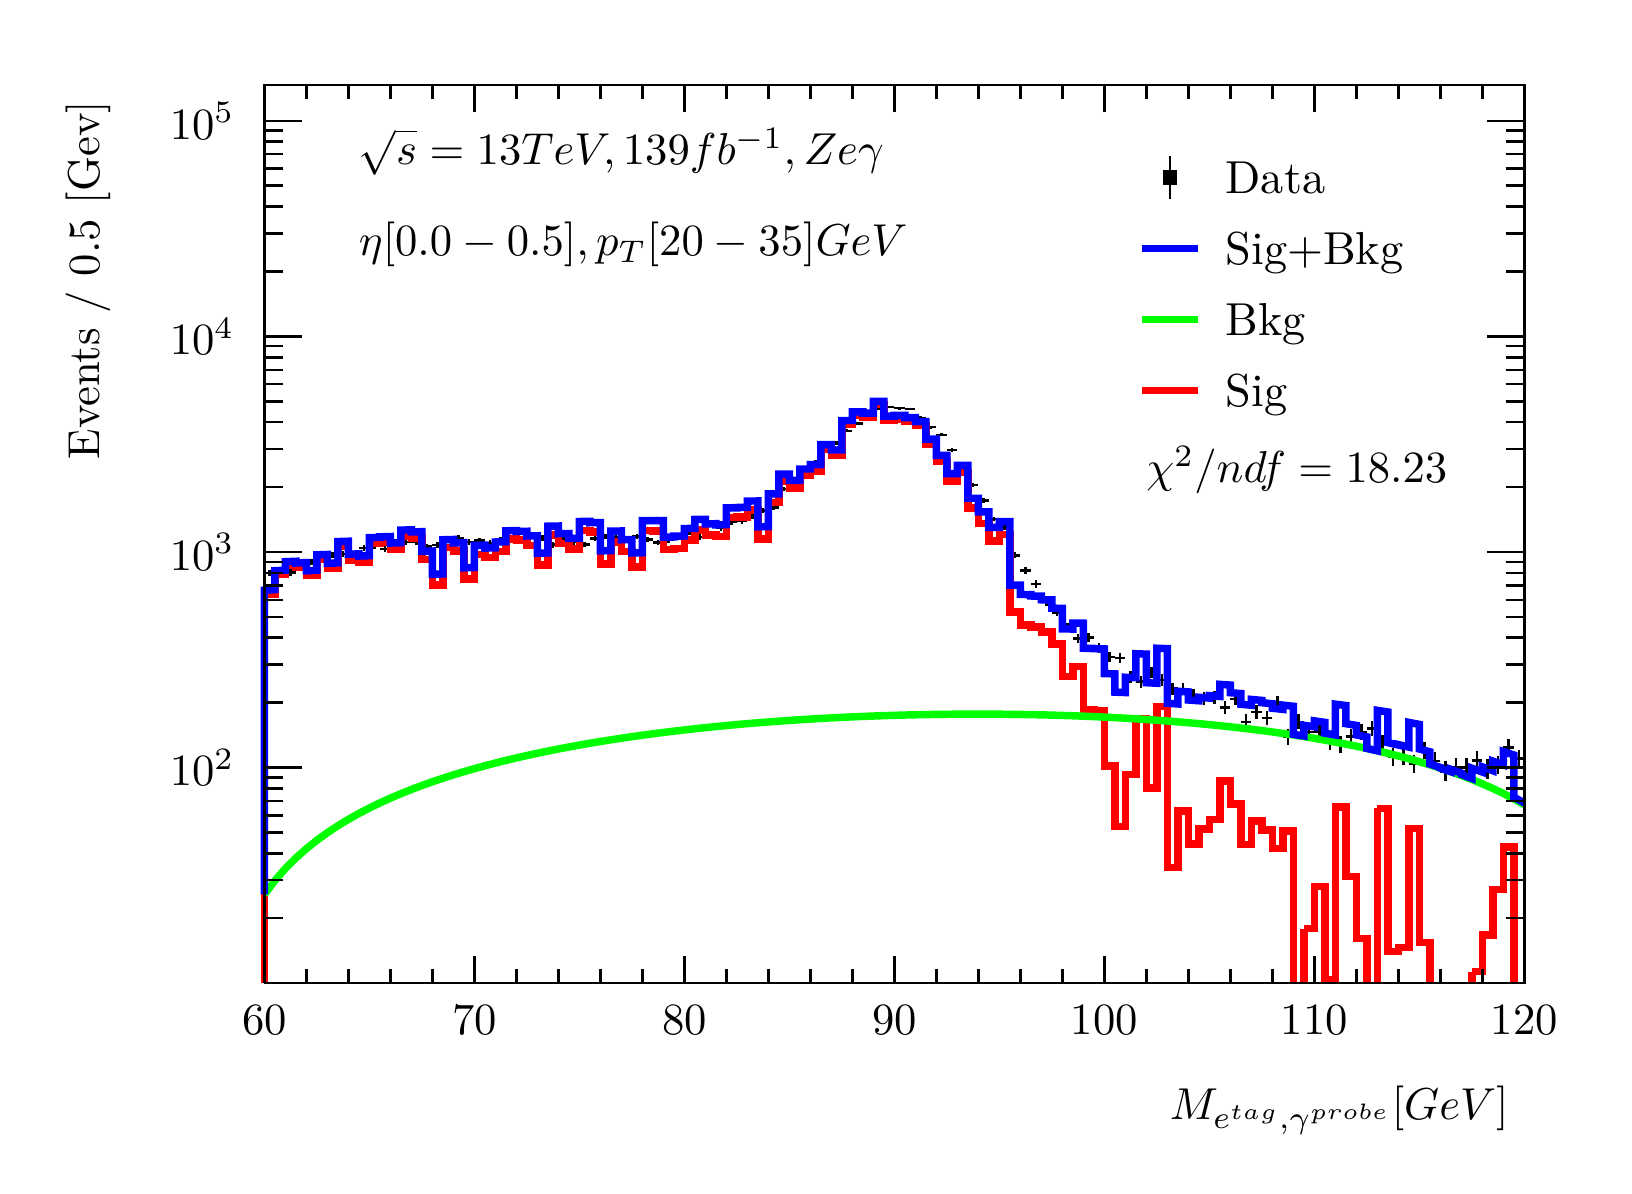
\begin{tikzpicture}
\pgfdeclareplotmark{cross} {
\pgfpathmoveto{\pgfpoint{-0.3\pgfplotmarksize}{\pgfplotmarksize}}
\pgfpathlineto{\pgfpoint{+0.3\pgfplotmarksize}{\pgfplotmarksize}}
\pgfpathlineto{\pgfpoint{+0.3\pgfplotmarksize}{0.3\pgfplotmarksize}}
\pgfpathlineto{\pgfpoint{+1\pgfplotmarksize}{0.3\pgfplotmarksize}}
\pgfpathlineto{\pgfpoint{+1\pgfplotmarksize}{-0.3\pgfplotmarksize}}
\pgfpathlineto{\pgfpoint{+0.3\pgfplotmarksize}{-0.3\pgfplotmarksize}}
\pgfpathlineto{\pgfpoint{+0.3\pgfplotmarksize}{-1.\pgfplotmarksize}}
\pgfpathlineto{\pgfpoint{-0.3\pgfplotmarksize}{-1.\pgfplotmarksize}}
\pgfpathlineto{\pgfpoint{-0.3\pgfplotmarksize}{-0.3\pgfplotmarksize}}
\pgfpathlineto{\pgfpoint{-1.\pgfplotmarksize}{-0.3\pgfplotmarksize}}
\pgfpathlineto{\pgfpoint{-1.\pgfplotmarksize}{0.3\pgfplotmarksize}}
\pgfpathlineto{\pgfpoint{-0.3\pgfplotmarksize}{0.3\pgfplotmarksize}}
\pgfpathclose
\pgfusepathqstroke
}
\pgfdeclareplotmark{cross*} {
\pgfpathmoveto{\pgfpoint{-0.3\pgfplotmarksize}{\pgfplotmarksize}}
\pgfpathlineto{\pgfpoint{+0.3\pgfplotmarksize}{\pgfplotmarksize}}
\pgfpathlineto{\pgfpoint{+0.3\pgfplotmarksize}{0.3\pgfplotmarksize}}
\pgfpathlineto{\pgfpoint{+1\pgfplotmarksize}{0.3\pgfplotmarksize}}
\pgfpathlineto{\pgfpoint{+1\pgfplotmarksize}{-0.3\pgfplotmarksize}}
\pgfpathlineto{\pgfpoint{+0.3\pgfplotmarksize}{-0.3\pgfplotmarksize}}
\pgfpathlineto{\pgfpoint{+0.3\pgfplotmarksize}{-1.\pgfplotmarksize}}
\pgfpathlineto{\pgfpoint{-0.3\pgfplotmarksize}{-1.\pgfplotmarksize}}
\pgfpathlineto{\pgfpoint{-0.3\pgfplotmarksize}{-0.3\pgfplotmarksize}}
\pgfpathlineto{\pgfpoint{-1.\pgfplotmarksize}{-0.3\pgfplotmarksize}}
\pgfpathlineto{\pgfpoint{-1.\pgfplotmarksize}{0.3\pgfplotmarksize}}
\pgfpathlineto{\pgfpoint{-0.3\pgfplotmarksize}{0.3\pgfplotmarksize}}
\pgfpathclose
\pgfusepathqfillstroke
}
\pgfdeclareplotmark{newstar} {
\pgfpathmoveto{\pgfqpoint{0pt}{\pgfplotmarksize}}
\pgfpathlineto{\pgfqpointpolar{44}{0.5\pgfplotmarksize}}
\pgfpathlineto{\pgfqpointpolar{18}{\pgfplotmarksize}}
\pgfpathlineto{\pgfqpointpolar{-20}{0.5\pgfplotmarksize}}
\pgfpathlineto{\pgfqpointpolar{-54}{\pgfplotmarksize}}
\pgfpathlineto{\pgfqpointpolar{-90}{0.5\pgfplotmarksize}}
\pgfpathlineto{\pgfqpointpolar{234}{\pgfplotmarksize}}
\pgfpathlineto{\pgfqpointpolar{198}{0.5\pgfplotmarksize}}
\pgfpathlineto{\pgfqpointpolar{162}{\pgfplotmarksize}}
\pgfpathlineto{\pgfqpointpolar{134}{0.5\pgfplotmarksize}}
\pgfpathclose
\pgfusepathqstroke
}
\pgfdeclareplotmark{newstar*} {
\pgfpathmoveto{\pgfqpoint{0pt}{\pgfplotmarksize}}
\pgfpathlineto{\pgfqpointpolar{44}{0.5\pgfplotmarksize}}
\pgfpathlineto{\pgfqpointpolar{18}{\pgfplotmarksize}}
\pgfpathlineto{\pgfqpointpolar{-20}{0.5\pgfplotmarksize}}
\pgfpathlineto{\pgfqpointpolar{-54}{\pgfplotmarksize}}
\pgfpathlineto{\pgfqpointpolar{-90}{0.5\pgfplotmarksize}}
\pgfpathlineto{\pgfqpointpolar{234}{\pgfplotmarksize}}
\pgfpathlineto{\pgfqpointpolar{198}{0.5\pgfplotmarksize}}
\pgfpathlineto{\pgfqpointpolar{162}{\pgfplotmarksize}}
\pgfpathlineto{\pgfqpointpolar{134}{0.5\pgfplotmarksize}}
\pgfpathclose
\pgfusepathqfillstroke
}
\definecolor{c}{rgb}{1,1,1};
\draw [color=c, fill=c] (0,0) rectangle (20,14.4361);
\draw [color=c, fill=c] (3,2.30977) rectangle (19,13.7143);
\definecolor{c}{rgb}{0,0,0};
\draw [c,line width=0.9] (3,2.30977) -- (3,13.7143) -- (19,13.7143) -- (19,2.30977) -- (3,2.30977);
\definecolor{c}{rgb}{1,1,1};
\draw [color=c, fill=c] (3,2.30977) rectangle (19,13.7143);
\definecolor{c}{rgb}{0,0,0};
\draw [c,line width=0.9] (3,2.30977) -- (3,13.7143) -- (19,13.7143) -- (19,2.30977) -- (3,2.30977);
\draw [c,line width=0.9] (3,2.30977) -- (19,2.30977);
\draw [c,line width=0.9] (3,2.65624) -- (3,2.30977);
\draw [c,line width=0.9] (3.53333,2.48301) -- (3.53333,2.30977);
\draw [c,line width=0.9] (4.06667,2.48301) -- (4.06667,2.30977);
\draw [c,line width=0.9] (4.6,2.48301) -- (4.6,2.30977);
\draw [c,line width=0.9] (5.13333,2.48301) -- (5.13333,2.30977);
\draw [c,line width=0.9] (5.66667,2.65624) -- (5.66667,2.30977);
\draw [c,line width=0.9] (6.2,2.48301) -- (6.2,2.30977);
\draw [c,line width=0.9] (6.73333,2.48301) -- (6.73333,2.30977);
\draw [c,line width=0.9] (7.26667,2.48301) -- (7.26667,2.30977);
\draw [c,line width=0.9] (7.8,2.48301) -- (7.8,2.30977);
\draw [c,line width=0.9] (8.33333,2.65624) -- (8.33333,2.30977);
\draw [c,line width=0.9] (8.86667,2.48301) -- (8.86667,2.30977);
\draw [c,line width=0.9] (9.4,2.48301) -- (9.4,2.30977);
\draw [c,line width=0.9] (9.93333,2.48301) -- (9.93333,2.30977);
\draw [c,line width=0.9] (10.4667,2.48301) -- (10.4667,2.30977);
\draw [c,line width=0.9] (11,2.65624) -- (11,2.30977);
\draw [c,line width=0.9] (11.5333,2.48301) -- (11.5333,2.30977);
\draw [c,line width=0.9] (12.0667,2.48301) -- (12.0667,2.30977);
\draw [c,line width=0.9] (12.6,2.48301) -- (12.6,2.30977);
\draw [c,line width=0.9] (13.1333,2.48301) -- (13.1333,2.30977);
\draw [c,line width=0.9] (13.6667,2.65624) -- (13.6667,2.30977);
\draw [c,line width=0.9] (14.2,2.48301) -- (14.2,2.30977);
\draw [c,line width=0.9] (14.7333,2.48301) -- (14.7333,2.30977);
\draw [c,line width=0.9] (15.2667,2.48301) -- (15.2667,2.30977);
\draw [c,line width=0.9] (15.8,2.48301) -- (15.8,2.30977);
\draw [c,line width=0.9] (16.3333,2.65624) -- (16.3333,2.30977);
\draw [c,line width=0.9] (16.8667,2.48301) -- (16.8667,2.30977);
\draw [c,line width=0.9] (17.4,2.48301) -- (17.4,2.30977);
\draw [c,line width=0.9] (17.9333,2.48301) -- (17.9333,2.30977);
\draw [c,line width=0.9] (18.4667,2.48301) -- (18.4667,2.30977);
\draw [c,line width=0.9] (19,2.65624) -- (19,2.30977);
\draw [anchor=base] (3,1.66015) node[scale=1.61424, color=c, rotate=0]{60};
\draw [anchor=base] (5.66667,1.66015) node[scale=1.61424, color=c, rotate=0]{70};
\draw [anchor=base] (8.33333,1.66015) node[scale=1.61424, color=c, rotate=0]{80};
\draw [anchor=base] (11,1.66015) node[scale=1.61424, color=c, rotate=0]{90};
\draw [anchor=base] (13.6667,1.66015) node[scale=1.61424, color=c, rotate=0]{100};
\draw [anchor=base] (16.3333,1.66015) node[scale=1.61424, color=c, rotate=0]{110};
\draw [anchor=base] (19,1.66015) node[scale=1.61424, color=c, rotate=0]{120};
\draw [anchor= east] (19,0.692932) node[scale=1.61424, color=c, rotate=0]{$M_{e^{tag}, \gamma^{probe}}  [GeV]$};
\draw [c,line width=0.9] (3,13.7143) -- (19,13.7143);
\draw [c,line width=0.9] (3,13.3678) -- (3,13.7143);
\draw [c,line width=0.9] (3.53333,13.5411) -- (3.53333,13.7143);
\draw [c,line width=0.9] (4.06667,13.5411) -- (4.06667,13.7143);
\draw [c,line width=0.9] (4.6,13.5411) -- (4.6,13.7143);
\draw [c,line width=0.9] (5.13333,13.5411) -- (5.13333,13.7143);
\draw [c,line width=0.9] (5.66667,13.3678) -- (5.66667,13.7143);
\draw [c,line width=0.9] (6.2,13.5411) -- (6.2,13.7143);
\draw [c,line width=0.9] (6.73333,13.5411) -- (6.73333,13.7143);
\draw [c,line width=0.9] (7.26667,13.5411) -- (7.26667,13.7143);
\draw [c,line width=0.9] (7.8,13.5411) -- (7.8,13.7143);
\draw [c,line width=0.9] (8.33333,13.3678) -- (8.33333,13.7143);
\draw [c,line width=0.9] (8.86667,13.5411) -- (8.86667,13.7143);
\draw [c,line width=0.9] (9.4,13.5411) -- (9.4,13.7143);
\draw [c,line width=0.9] (9.93333,13.5411) -- (9.93333,13.7143);
\draw [c,line width=0.9] (10.4667,13.5411) -- (10.4667,13.7143);
\draw [c,line width=0.9] (11,13.3678) -- (11,13.7143);
\draw [c,line width=0.9] (11.5333,13.5411) -- (11.5333,13.7143);
\draw [c,line width=0.9] (12.0667,13.5411) -- (12.0667,13.7143);
\draw [c,line width=0.9] (12.6,13.5411) -- (12.6,13.7143);
\draw [c,line width=0.9] (13.1333,13.5411) -- (13.1333,13.7143);
\draw [c,line width=0.9] (13.6667,13.3678) -- (13.6667,13.7143);
\draw [c,line width=0.9] (14.2,13.5411) -- (14.2,13.7143);
\draw [c,line width=0.9] (14.7333,13.5411) -- (14.7333,13.7143);
\draw [c,line width=0.9] (15.2667,13.5411) -- (15.2667,13.7143);
\draw [c,line width=0.9] (15.8,13.5411) -- (15.8,13.7143);
\draw [c,line width=0.9] (16.3333,13.3678) -- (16.3333,13.7143);
\draw [c,line width=0.9] (16.8667,13.5411) -- (16.8667,13.7143);
\draw [c,line width=0.9] (17.4,13.5411) -- (17.4,13.7143);
\draw [c,line width=0.9] (17.9333,13.5411) -- (17.9333,13.7143);
\draw [c,line width=0.9] (18.4667,13.5411) -- (18.4667,13.7143);
\draw [c,line width=0.9] (19,13.3678) -- (19,13.7143);
\draw [c,line width=0.9] (3,2.30977) -- (3,13.7143);
\draw [c,line width=0.9] (3.237,3.13385) -- (3,3.13385);
\draw [c,line width=0.9] (3.237,3.6159) -- (3,3.6159);
\draw [c,line width=0.9] (3.237,3.95792) -- (3,3.95792);
\draw [c,line width=0.9] (3.237,4.22321) -- (3,4.22321);
\draw [c,line width=0.9] (3.237,4.43997) -- (3,4.43997);
\draw [c,line width=0.9] (3.237,4.62324) -- (3,4.62324);
\draw [c,line width=0.9] (3.237,4.782) -- (3,4.782);
\draw [c,line width=0.9] (3.237,4.92203) -- (3,4.92203);
\draw [c,line width=0.9] (3.474,5.04729) -- (3,5.04729);
\draw [anchor= east] (2.82,5.04729) node[scale=1.61424, color=c, rotate=0]{$10^{2}$};
\draw [c,line width=0.9] (3.237,5.87136) -- (3,5.87136);
\draw [c,line width=0.9] (3.237,6.35342) -- (3,6.35342);
\draw [c,line width=0.9] (3.237,6.69544) -- (3,6.69544);
\draw [c,line width=0.9] (3.237,6.96073) -- (3,6.96073);
\draw [c,line width=0.9] (3.237,7.17749) -- (3,7.17749);
\draw [c,line width=0.9] (3.237,7.36076) -- (3,7.36076);
\draw [c,line width=0.9] (3.237,7.51951) -- (3,7.51951);
\draw [c,line width=0.9] (3.237,7.65954) -- (3,7.65954);
\draw [c,line width=0.9] (3.474,7.78481) -- (3,7.78481);
\draw [anchor= east] (2.82,7.78481) node[scale=1.61424, color=c, rotate=0]{$10^{3}$};
\draw [c,line width=0.9] (3.237,8.60888) -- (3,8.60888);
\draw [c,line width=0.9] (3.237,9.09093) -- (3,9.09093);
\draw [c,line width=0.9] (3.237,9.43296) -- (3,9.43296);
\draw [c,line width=0.9] (3.237,9.69825) -- (3,9.69825);
\draw [c,line width=0.9] (3.237,9.91501) -- (3,9.91501);
\draw [c,line width=0.9] (3.237,10.0983) -- (3,10.0983);
\draw [c,line width=0.9] (3.237,10.257) -- (3,10.257);
\draw [c,line width=0.9] (3.237,10.3971) -- (3,10.3971);
\draw [c,line width=0.9] (3.474,10.5223) -- (3,10.5223);
\draw [anchor= east] (2.82,10.5223) node[scale=1.61424, color=c, rotate=0]{$10^{4}$};
\draw [c,line width=0.9] (3.237,11.3464) -- (3,11.3464);
\draw [c,line width=0.9] (3.237,11.8285) -- (3,11.8285);
\draw [c,line width=0.9] (3.237,12.1705) -- (3,12.1705);
\draw [c,line width=0.9] (3.237,12.4358) -- (3,12.4358);
\draw [c,line width=0.9] (3.237,12.6525) -- (3,12.6525);
\draw [c,line width=0.9] (3.237,12.8358) -- (3,12.8358);
\draw [c,line width=0.9] (3.237,12.9945) -- (3,12.9945);
\draw [c,line width=0.9] (3.237,13.1346) -- (3,13.1346);
\draw [c,line width=0.9] (3.474,13.2598) -- (3,13.2598);
\draw [anchor= east] (2.82,13.2598) node[scale=1.61424, color=c, rotate=0]{$10^{5}$};
\draw [anchor= east] (0.76,13.7143) node[scale=1.61424, color=c, rotate=90]{Events / 0.5 [Gev]};
\draw [c,line width=0.9] (19,2.30977) -- (19,13.7143);
\draw [c,line width=0.9] (18.763,3.13385) -- (19,3.13385);
\draw [c,line width=0.9] (18.763,3.6159) -- (19,3.6159);
\draw [c,line width=0.9] (18.763,3.95792) -- (19,3.95792);
\draw [c,line width=0.9] (18.763,4.22321) -- (19,4.22321);
\draw [c,line width=0.9] (18.763,4.43997) -- (19,4.43997);
\draw [c,line width=0.9] (18.763,4.62324) -- (19,4.62324);
\draw [c,line width=0.9] (18.763,4.782) -- (19,4.782);
\draw [c,line width=0.9] (18.763,4.92203) -- (19,4.92203);
\draw [c,line width=0.9] (18.526,5.04729) -- (19,5.04729);
\draw [c,line width=0.9] (18.763,5.87136) -- (19,5.87136);
\draw [c,line width=0.9] (18.763,6.35342) -- (19,6.35342);
\draw [c,line width=0.9] (18.763,6.69544) -- (19,6.69544);
\draw [c,line width=0.9] (18.763,6.96073) -- (19,6.96073);
\draw [c,line width=0.9] (18.763,7.17749) -- (19,7.17749);
\draw [c,line width=0.9] (18.763,7.36076) -- (19,7.36076);
\draw [c,line width=0.9] (18.763,7.51951) -- (19,7.51951);
\draw [c,line width=0.9] (18.763,7.65954) -- (19,7.65954);
\draw [c,line width=0.9] (18.526,7.78481) -- (19,7.78481);
\draw [c,line width=0.9] (18.763,8.60888) -- (19,8.60888);
\draw [c,line width=0.9] (18.763,9.09093) -- (19,9.09093);
\draw [c,line width=0.9] (18.763,9.43296) -- (19,9.43296);
\draw [c,line width=0.9] (18.763,9.69825) -- (19,9.69825);
\draw [c,line width=0.9] (18.763,9.91501) -- (19,9.91501);
\draw [c,line width=0.9] (18.763,10.0983) -- (19,10.0983);
\draw [c,line width=0.9] (18.763,10.257) -- (19,10.257);
\draw [c,line width=0.9] (18.763,10.3971) -- (19,10.3971);
\draw [c,line width=0.9] (18.526,10.5223) -- (19,10.5223);
\draw [c,line width=0.9] (18.763,11.3464) -- (19,11.3464);
\draw [c,line width=0.9] (18.763,11.8285) -- (19,11.8285);
\draw [c,line width=0.9] (18.763,12.1705) -- (19,12.1705);
\draw [c,line width=0.9] (18.763,12.4358) -- (19,12.4358);
\draw [c,line width=0.9] (18.763,12.6525) -- (19,12.6525);
\draw [c,line width=0.9] (18.763,12.8358) -- (19,12.8358);
\draw [c,line width=0.9] (18.763,12.9945) -- (19,12.9945);
\draw [c,line width=0.9] (18.763,13.1346) -- (19,13.1346);
\draw [c,line width=0.9] (18.526,13.2598) -- (19,13.2598);
\draw [c,line width=0.9] (3.06667,7.51505) -- (3,7.51505);
\draw [c,line width=0.9] (3,7.51505) -- (3,7.51505);
\draw [c,line width=0.9] (3.06667,7.51505) -- (3.13333,7.51505);
\draw [c,line width=0.9] (3.13333,7.51505) -- (3.13333,7.51505);
\draw [c,line width=0.9] (3.06667,7.51505) -- (3.06667,7.55716);
\draw [c,line width=0.9] (3.06667,7.55716) -- (3.06667,7.55716);
\draw [c,line width=0.9] (3.06667,7.51505) -- (3.06667,7.47294);
\draw [c,line width=0.9] (3.06667,7.47294) -- (3.06667,7.47294);
\draw [c,line width=0.9] (3.2,7.50606) -- (3.13333,7.50606);
\draw [c,line width=0.9] (3.13333,7.50606) -- (3.13333,7.50606);
\draw [c,line width=0.9] (3.2,7.50606) -- (3.26667,7.50606);
\draw [c,line width=0.9] (3.26667,7.50606) -- (3.26667,7.50606);
\draw [c,line width=0.9] (3.2,7.50606) -- (3.2,7.54833);
\draw [c,line width=0.9] (3.2,7.54833) -- (3.2,7.54833);
\draw [c,line width=0.9] (3.2,7.50606) -- (3.2,7.46379);
\draw [c,line width=0.9] (3.2,7.46379) -- (3.2,7.46379);
\draw [c,line width=0.9] (3.33333,7.521) -- (3.26667,7.521);
\draw [c,line width=0.9] (3.26667,7.521) -- (3.26667,7.521);
\draw [c,line width=0.9] (3.33333,7.521) -- (3.4,7.521);
\draw [c,line width=0.9] (3.4,7.521) -- (3.4,7.521);
\draw [c,line width=0.9] (3.33333,7.521) -- (3.33333,7.563);
\draw [c,line width=0.9] (3.33333,7.563) -- (3.33333,7.563);
\draw [c,line width=0.9] (3.33333,7.521) -- (3.33333,7.47899);
\draw [c,line width=0.9] (3.33333,7.47899) -- (3.33333,7.47899);
\draw [c,line width=0.9] (3.46667,7.63012) -- (3.4,7.63012);
\draw [c,line width=0.9] (3.4,7.63012) -- (3.4,7.63012);
\draw [c,line width=0.9] (3.46667,7.63012) -- (3.53333,7.63012);
\draw [c,line width=0.9] (3.53333,7.63012) -- (3.53333,7.63012);
\draw [c,line width=0.9] (3.46667,7.63012) -- (3.46667,7.67024);
\draw [c,line width=0.9] (3.46667,7.67024) -- (3.46667,7.67024);
\draw [c,line width=0.9] (3.46667,7.63012) -- (3.46667,7.59);
\draw [c,line width=0.9] (3.46667,7.59) -- (3.46667,7.59);
\draw [c,line width=0.9] (3.6,7.65425) -- (3.53333,7.65425);
\draw [c,line width=0.9] (3.53333,7.65425) -- (3.53333,7.65425);
\draw [c,line width=0.9] (3.6,7.65425) -- (3.66667,7.65425);
\draw [c,line width=0.9] (3.66667,7.65425) -- (3.66667,7.65425);
\draw [c,line width=0.9] (3.6,7.65425) -- (3.6,7.69397);
\draw [c,line width=0.9] (3.6,7.69397) -- (3.6,7.69397);
\draw [c,line width=0.9] (3.6,7.65425) -- (3.6,7.61453);
\draw [c,line width=0.9] (3.6,7.61453) -- (3.6,7.61453);
\draw [c,line width=0.9] (3.73333,7.72633) -- (3.66667,7.72633);
\draw [c,line width=0.9] (3.66667,7.72633) -- (3.66667,7.72633);
\draw [c,line width=0.9] (3.73333,7.72633) -- (3.8,7.72633);
\draw [c,line width=0.9] (3.8,7.72633) -- (3.8,7.72633);
\draw [c,line width=0.9] (3.73333,7.72633) -- (3.73333,7.76486);
\draw [c,line width=0.9] (3.73333,7.76486) -- (3.73333,7.76486);
\draw [c,line width=0.9] (3.73333,7.72633) -- (3.73333,7.6878);
\draw [c,line width=0.9] (3.73333,7.6878) -- (3.73333,7.6878);
\draw [c,line width=0.9] (3.86667,7.73998) -- (3.8,7.73998);
\draw [c,line width=0.9] (3.8,7.73998) -- (3.8,7.73998);
\draw [c,line width=0.9] (3.86667,7.73998) -- (3.93333,7.73998);
\draw [c,line width=0.9] (3.93333,7.73998) -- (3.93333,7.73998);
\draw [c,line width=0.9] (3.86667,7.73998) -- (3.86667,7.77829);
\draw [c,line width=0.9] (3.86667,7.77829) -- (3.86667,7.77829);
\draw [c,line width=0.9] (3.86667,7.73998) -- (3.86667,7.70167);
\draw [c,line width=0.9] (3.86667,7.70167) -- (3.86667,7.70167);
\draw [c,line width=0.9] (4,7.75714) -- (3.93333,7.75714);
\draw [c,line width=0.9] (3.93333,7.75714) -- (3.93333,7.75714);
\draw [c,line width=0.9] (4,7.75714) -- (4.06667,7.75714);
\draw [c,line width=0.9] (4.06667,7.75714) -- (4.06667,7.75714);
\draw [c,line width=0.9] (4,7.75714) -- (4,7.79518);
\draw [c,line width=0.9] (4,7.79518) -- (4,7.79518);
\draw [c,line width=0.9] (4,7.75714) -- (4,7.71911);
\draw [c,line width=0.9] (4,7.71911) -- (4,7.71911);
\draw [c,line width=0.9] (4.13333,7.76079) -- (4.06667,7.76079);
\draw [c,line width=0.9] (4.06667,7.76079) -- (4.06667,7.76079);
\draw [c,line width=0.9] (4.13333,7.76079) -- (4.2,7.76079);
\draw [c,line width=0.9] (4.2,7.76079) -- (4.2,7.76079);
\draw [c,line width=0.9] (4.13333,7.76079) -- (4.13333,7.79876);
\draw [c,line width=0.9] (4.13333,7.79876) -- (4.13333,7.79876);
\draw [c,line width=0.9] (4.13333,7.76079) -- (4.13333,7.72281);
\draw [c,line width=0.9] (4.13333,7.72281) -- (4.13333,7.72281);
\draw [c,line width=0.9] (4.26667,7.83486) -- (4.2,7.83486);
\draw [c,line width=0.9] (4.2,7.83486) -- (4.2,7.83486);
\draw [c,line width=0.9] (4.26667,7.83486) -- (4.33333,7.83486);
\draw [c,line width=0.9] (4.33333,7.83486) -- (4.33333,7.83486);
\draw [c,line width=0.9] (4.26667,7.83486) -- (4.26667,7.87167);
\draw [c,line width=0.9] (4.26667,7.87167) -- (4.26667,7.87167);
\draw [c,line width=0.9] (4.26667,7.83486) -- (4.26667,7.79805);
\draw [c,line width=0.9] (4.26667,7.79805) -- (4.26667,7.79805);
\draw [c,line width=0.9] (4.4,7.85744) -- (4.33333,7.85744);
\draw [c,line width=0.9] (4.33333,7.85744) -- (4.33333,7.85744);
\draw [c,line width=0.9] (4.4,7.85744) -- (4.46667,7.85744);
\draw [c,line width=0.9] (4.46667,7.85744) -- (4.46667,7.85744);
\draw [c,line width=0.9] (4.4,7.85744) -- (4.4,7.89391);
\draw [c,line width=0.9] (4.4,7.89391) -- (4.4,7.89391);
\draw [c,line width=0.9] (4.4,7.85744) -- (4.4,7.82098);
\draw [c,line width=0.9] (4.4,7.82098) -- (4.4,7.82098);
\draw [c,line width=0.9] (4.53333,7.81995) -- (4.46667,7.81995);
\draw [c,line width=0.9] (4.46667,7.81995) -- (4.46667,7.81995);
\draw [c,line width=0.9] (4.53333,7.81995) -- (4.6,7.81995);
\draw [c,line width=0.9] (4.6,7.81995) -- (4.6,7.81995);
\draw [c,line width=0.9] (4.53333,7.81995) -- (4.53333,7.85699);
\draw [c,line width=0.9] (4.53333,7.85699) -- (4.53333,7.85699);
\draw [c,line width=0.9] (4.53333,7.81995) -- (4.53333,7.78291);
\draw [c,line width=0.9] (4.53333,7.78291) -- (4.53333,7.78291);
\draw [c,line width=0.9] (4.66667,7.86968) -- (4.6,7.86968);
\draw [c,line width=0.9] (4.6,7.86968) -- (4.6,7.86968);
\draw [c,line width=0.9] (4.66667,7.86968) -- (4.73333,7.86968);
\draw [c,line width=0.9] (4.73333,7.86968) -- (4.73333,7.86968);
\draw [c,line width=0.9] (4.66667,7.86968) -- (4.66667,7.90596);
\draw [c,line width=0.9] (4.66667,7.90596) -- (4.66667,7.90596);
\draw [c,line width=0.9] (4.66667,7.86968) -- (4.66667,7.83341);
\draw [c,line width=0.9] (4.66667,7.83341) -- (4.66667,7.83341);
\draw [c,line width=0.9] (4.8,7.91209) -- (4.73333,7.91209);
\draw [c,line width=0.9] (4.73333,7.91209) -- (4.73333,7.91209);
\draw [c,line width=0.9] (4.8,7.91209) -- (4.86667,7.91209);
\draw [c,line width=0.9] (4.86667,7.91209) -- (4.86667,7.91209);
\draw [c,line width=0.9] (4.8,7.91209) -- (4.8,7.94772);
\draw [c,line width=0.9] (4.8,7.94772) -- (4.8,7.94772);
\draw [c,line width=0.9] (4.8,7.91209) -- (4.8,7.87645);
\draw [c,line width=0.9] (4.8,7.87645) -- (4.8,7.87645);
\draw [c,line width=0.9] (4.93333,7.90995) -- (4.86667,7.90995);
\draw [c,line width=0.9] (4.86667,7.90995) -- (4.86667,7.90995);
\draw [c,line width=0.9] (4.93333,7.90995) -- (5,7.90995);
\draw [c,line width=0.9] (5,7.90995) -- (5,7.90995);
\draw [c,line width=0.9] (4.93333,7.90995) -- (4.93333,7.94562);
\draw [c,line width=0.9] (4.93333,7.94562) -- (4.93333,7.94562);
\draw [c,line width=0.9] (4.93333,7.90995) -- (4.93333,7.87428);
\draw [c,line width=0.9] (4.93333,7.87428) -- (4.93333,7.87428);
\draw [c,line width=0.9] (5.06667,7.85408) -- (5,7.85408);
\draw [c,line width=0.9] (5,7.85408) -- (5,7.85408);
\draw [c,line width=0.9] (5.06667,7.85408) -- (5.13333,7.85408);
\draw [c,line width=0.9] (5.13333,7.85408) -- (5.13333,7.85408);
\draw [c,line width=0.9] (5.06667,7.85408) -- (5.06667,7.8906);
\draw [c,line width=0.9] (5.06667,7.8906) -- (5.06667,7.8906);
\draw [c,line width=0.9] (5.06667,7.85408) -- (5.06667,7.81757);
\draw [c,line width=0.9] (5.06667,7.81757) -- (5.06667,7.81757);
\draw [c,line width=0.9] (5.2,7.87189) -- (5.13333,7.87189);
\draw [c,line width=0.9] (5.13333,7.87189) -- (5.13333,7.87189);
\draw [c,line width=0.9] (5.2,7.87189) -- (5.26667,7.87189);
\draw [c,line width=0.9] (5.26667,7.87189) -- (5.26667,7.87189);
\draw [c,line width=0.9] (5.2,7.87189) -- (5.2,7.90814);
\draw [c,line width=0.9] (5.2,7.90814) -- (5.2,7.90814);
\draw [c,line width=0.9] (5.2,7.87189) -- (5.2,7.83565);
\draw [c,line width=0.9] (5.2,7.83565) -- (5.2,7.83565);
\draw [c,line width=0.9] (5.33333,7.94163) -- (5.26667,7.94163);
\draw [c,line width=0.9] (5.26667,7.94163) -- (5.26667,7.94163);
\draw [c,line width=0.9] (5.33333,7.94163) -- (5.4,7.94163);
\draw [c,line width=0.9] (5.4,7.94163) -- (5.4,7.94163);
\draw [c,line width=0.9] (5.33333,7.94163) -- (5.33333,7.97682);
\draw [c,line width=0.9] (5.33333,7.97682) -- (5.33333,7.97682);
\draw [c,line width=0.9] (5.33333,7.94163) -- (5.33333,7.90643);
\draw [c,line width=0.9] (5.33333,7.90643) -- (5.33333,7.90643);
\draw [c,line width=0.9] (5.46667,7.96229) -- (5.4,7.96229);
\draw [c,line width=0.9] (5.4,7.96229) -- (5.4,7.96229);
\draw [c,line width=0.9] (5.46667,7.96229) -- (5.53333,7.96229);
\draw [c,line width=0.9] (5.53333,7.96229) -- (5.53333,7.96229);
\draw [c,line width=0.9] (5.46667,7.96229) -- (5.46667,7.99718);
\draw [c,line width=0.9] (5.46667,7.99718) -- (5.46667,7.99718);
\draw [c,line width=0.9] (5.46667,7.96229) -- (5.46667,7.9274);
\draw [c,line width=0.9] (5.46667,7.9274) -- (5.46667,7.9274);
\draw [c,line width=0.9] (5.6,7.91422) -- (5.53333,7.91422);
\draw [c,line width=0.9] (5.53333,7.91422) -- (5.53333,7.91422);
\draw [c,line width=0.9] (5.6,7.91422) -- (5.66667,7.91422);
\draw [c,line width=0.9] (5.66667,7.91422) -- (5.66667,7.91422);
\draw [c,line width=0.9] (5.6,7.91422) -- (5.6,7.94983);
\draw [c,line width=0.9] (5.6,7.94983) -- (5.6,7.94983);
\draw [c,line width=0.9] (5.6,7.91422) -- (5.6,7.87862);
\draw [c,line width=0.9] (5.6,7.87862) -- (5.6,7.87862);
\draw [c,line width=0.9] (5.73333,7.93221) -- (5.66667,7.93221);
\draw [c,line width=0.9] (5.66667,7.93221) -- (5.66667,7.93221);
\draw [c,line width=0.9] (5.73333,7.93221) -- (5.8,7.93221);
\draw [c,line width=0.9] (5.8,7.93221) -- (5.8,7.93221);
\draw [c,line width=0.9] (5.73333,7.93221) -- (5.73333,7.96755);
\draw [c,line width=0.9] (5.73333,7.96755) -- (5.73333,7.96755);
\draw [c,line width=0.9] (5.73333,7.93221) -- (5.73333,7.89688);
\draw [c,line width=0.9] (5.73333,7.89688) -- (5.73333,7.89688);
\draw [c,line width=0.9] (5.86667,7.89487) -- (5.8,7.89487);
\draw [c,line width=0.9] (5.8,7.89487) -- (5.8,7.89487);
\draw [c,line width=0.9] (5.86667,7.89487) -- (5.93333,7.89487);
\draw [c,line width=0.9] (5.93333,7.89487) -- (5.93333,7.89487);
\draw [c,line width=0.9] (5.86667,7.89487) -- (5.86667,7.93077);
\draw [c,line width=0.9] (5.86667,7.93077) -- (5.86667,7.93077);
\draw [c,line width=0.9] (5.86667,7.89487) -- (5.86667,7.85898);
\draw [c,line width=0.9] (5.86667,7.85898) -- (5.86667,7.85898);
\draw [c,line width=0.9] (6,7.9385) -- (5.93333,7.9385);
\draw [c,line width=0.9] (5.93333,7.9385) -- (5.93333,7.9385);
\draw [c,line width=0.9] (6,7.9385) -- (6.06667,7.9385);
\draw [c,line width=0.9] (6.06667,7.9385) -- (6.06667,7.9385);
\draw [c,line width=0.9] (6,7.9385) -- (6,7.97374);
\draw [c,line width=0.9] (6,7.97374) -- (6,7.97374);
\draw [c,line width=0.9] (6,7.9385) -- (6,7.90326);
\draw [c,line width=0.9] (6,7.90326) -- (6,7.90326);
\draw [c,line width=0.9] (6.13333,7.95303) -- (6.06667,7.95303);
\draw [c,line width=0.9] (6.06667,7.95303) -- (6.06667,7.95303);
\draw [c,line width=0.9] (6.13333,7.95303) -- (6.2,7.95303);
\draw [c,line width=0.9] (6.2,7.95303) -- (6.2,7.95303);
\draw [c,line width=0.9] (6.13333,7.95303) -- (6.13333,7.98806);
\draw [c,line width=0.9] (6.13333,7.98806) -- (6.13333,7.98806);
\draw [c,line width=0.9] (6.13333,7.95303) -- (6.13333,7.91801);
\draw [c,line width=0.9] (6.13333,7.91801) -- (6.13333,7.91801);
\draw [c,line width=0.9] (6.26667,7.9551) -- (6.2,7.9551);
\draw [c,line width=0.9] (6.2,7.9551) -- (6.2,7.9551);
\draw [c,line width=0.9] (6.26667,7.9551) -- (6.33333,7.9551);
\draw [c,line width=0.9] (6.33333,7.9551) -- (6.33333,7.9551);
\draw [c,line width=0.9] (6.26667,7.9551) -- (6.26667,7.99009);
\draw [c,line width=0.9] (6.26667,7.99009) -- (6.26667,7.99009);
\draw [c,line width=0.9] (6.26667,7.9551) -- (6.26667,7.9201);
\draw [c,line width=0.9] (6.26667,7.9201) -- (6.26667,7.9201);
\draw [c,line width=0.9] (6.4,7.99361) -- (6.33333,7.99361);
\draw [c,line width=0.9] (6.33333,7.99361) -- (6.33333,7.99361);
\draw [c,line width=0.9] (6.4,7.99361) -- (6.46667,7.99361);
\draw [c,line width=0.9] (6.46667,7.99361) -- (6.46667,7.99361);
\draw [c,line width=0.9] (6.4,7.99361) -- (6.4,8.02805);
\draw [c,line width=0.9] (6.4,8.02805) -- (6.4,8.02805);
\draw [c,line width=0.9] (6.4,7.99361) -- (6.4,7.95918);
\draw [c,line width=0.9] (6.4,7.95918) -- (6.4,7.95918);
\draw [c,line width=0.9] (6.53333,7.96433) -- (6.46667,7.96433);
\draw [c,line width=0.9] (6.46667,7.96433) -- (6.46667,7.96433);
\draw [c,line width=0.9] (6.53333,7.96433) -- (6.6,7.96433);
\draw [c,line width=0.9] (6.6,7.96433) -- (6.6,7.96433);
\draw [c,line width=0.9] (6.53333,7.96433) -- (6.53333,7.99919);
\draw [c,line width=0.9] (6.53333,7.99919) -- (6.53333,7.99919);
\draw [c,line width=0.9] (6.53333,7.96433) -- (6.53333,7.92947);
\draw [c,line width=0.9] (6.53333,7.92947) -- (6.53333,7.92947);
\draw [c,line width=0.9] (6.66667,7.87631) -- (6.6,7.87631);
\draw [c,line width=0.9] (6.6,7.87631) -- (6.6,7.87631);
\draw [c,line width=0.9] (6.66667,7.87631) -- (6.73333,7.87631);
\draw [c,line width=0.9] (6.73333,7.87631) -- (6.73333,7.87631);
\draw [c,line width=0.9] (6.66667,7.87631) -- (6.66667,7.91248);
\draw [c,line width=0.9] (6.66667,7.91248) -- (6.66667,7.91248);
\draw [c,line width=0.9] (6.66667,7.87631) -- (6.66667,7.84013);
\draw [c,line width=0.9] (6.66667,7.84013) -- (6.66667,7.84013);
\draw [c,line width=0.9] (6.8,7.97552) -- (6.73333,7.97552);
\draw [c,line width=0.9] (6.73333,7.97552) -- (6.73333,7.97552);
\draw [c,line width=0.9] (6.8,7.97552) -- (6.86667,7.97552);
\draw [c,line width=0.9] (6.86667,7.97552) -- (6.86667,7.97552);
\draw [c,line width=0.9] (6.8,7.97552) -- (6.8,8.01022);
\draw [c,line width=0.9] (6.8,8.01022) -- (6.8,8.01022);
\draw [c,line width=0.9] (6.8,7.97552) -- (6.8,7.94083);
\draw [c,line width=0.9] (6.8,7.94083) -- (6.8,7.94083);
\draw [c,line width=0.9] (6.93333,7.90888) -- (6.86667,7.90888);
\draw [c,line width=0.9] (6.86667,7.90888) -- (6.86667,7.90888);
\draw [c,line width=0.9] (6.93333,7.90888) -- (7,7.90888);
\draw [c,line width=0.9] (7,7.90888) -- (7,7.90888);
\draw [c,line width=0.9] (6.93333,7.90888) -- (6.93333,7.94456);
\draw [c,line width=0.9] (6.93333,7.94456) -- (6.93333,7.94456);
\draw [c,line width=0.9] (6.93333,7.90888) -- (6.93333,7.8732);
\draw [c,line width=0.9] (6.93333,7.8732) -- (6.93333,7.8732);
\draw [c,line width=0.9] (7.06667,7.87851) -- (7,7.87851);
\draw [c,line width=0.9] (7,7.87851) -- (7,7.87851);
\draw [c,line width=0.9] (7.06667,7.87851) -- (7.13333,7.87851);
\draw [c,line width=0.9] (7.13333,7.87851) -- (7.13333,7.87851);
\draw [c,line width=0.9] (7.06667,7.87851) -- (7.06667,7.91465);
\draw [c,line width=0.9] (7.06667,7.91465) -- (7.06667,7.91465);
\draw [c,line width=0.9] (7.06667,7.87851) -- (7.06667,7.84236);
\draw [c,line width=0.9] (7.06667,7.84236) -- (7.06667,7.84236);
\draw [c,line width=0.9] (7.2,7.95716) -- (7.13333,7.95716);
\draw [c,line width=0.9] (7.13333,7.95716) -- (7.13333,7.95716);
\draw [c,line width=0.9] (7.2,7.95716) -- (7.26667,7.95716);
\draw [c,line width=0.9] (7.26667,7.95716) -- (7.26667,7.95716);
\draw [c,line width=0.9] (7.2,7.95716) -- (7.2,7.99212);
\draw [c,line width=0.9] (7.2,7.99212) -- (7.2,7.99212);
\draw [c,line width=0.9] (7.2,7.95716) -- (7.2,7.92219);
\draw [c,line width=0.9] (7.2,7.92219) -- (7.2,7.92219);
\draw [c,line width=0.9] (7.33333,7.97957) -- (7.26667,7.97957);
\draw [c,line width=0.9] (7.26667,7.97957) -- (7.26667,7.97957);
\draw [c,line width=0.9] (7.33333,7.97957) -- (7.4,7.97957);
\draw [c,line width=0.9] (7.4,7.97957) -- (7.4,7.97957);
\draw [c,line width=0.9] (7.33333,7.97957) -- (7.33333,8.01421);
\draw [c,line width=0.9] (7.33333,8.01421) -- (7.33333,8.01421);
\draw [c,line width=0.9] (7.33333,7.97957) -- (7.33333,7.94493);
\draw [c,line width=0.9] (7.33333,7.94493) -- (7.33333,7.94493);
\draw [c,line width=0.9] (7.46667,7.97755) -- (7.4,7.97755);
\draw [c,line width=0.9] (7.4,7.97755) -- (7.4,7.97755);
\draw [c,line width=0.9] (7.46667,7.97755) -- (7.53333,7.97755);
\draw [c,line width=0.9] (7.53333,7.97755) -- (7.53333,7.97755);
\draw [c,line width=0.9] (7.46667,7.97755) -- (7.46667,8.01222);
\draw [c,line width=0.9] (7.46667,8.01222) -- (7.46667,8.01222);
\draw [c,line width=0.9] (7.46667,7.97755) -- (7.46667,7.94288);
\draw [c,line width=0.9] (7.46667,7.94288) -- (7.46667,7.94288);
\draw [c,line width=0.9] (7.6,7.94683) -- (7.53333,7.94683);
\draw [c,line width=0.9] (7.53333,7.94683) -- (7.53333,7.94683);
\draw [c,line width=0.9] (7.6,7.94683) -- (7.66667,7.94683);
\draw [c,line width=0.9] (7.66667,7.94683) -- (7.66667,7.94683);
\draw [c,line width=0.9] (7.6,7.94683) -- (7.6,7.98194);
\draw [c,line width=0.9] (7.6,7.98194) -- (7.6,7.98194);
\draw [c,line width=0.9] (7.6,7.94683) -- (7.6,7.91171);
\draw [c,line width=0.9] (7.6,7.91171) -- (7.6,7.91171);
\draw [c,line width=0.9] (7.73333,7.98159) -- (7.66667,7.98159);
\draw [c,line width=0.9] (7.66667,7.98159) -- (7.66667,7.98159);
\draw [c,line width=0.9] (7.73333,7.98159) -- (7.8,7.98159);
\draw [c,line width=0.9] (7.8,7.98159) -- (7.8,7.98159);
\draw [c,line width=0.9] (7.73333,7.98159) -- (7.73333,8.01619);
\draw [c,line width=0.9] (7.73333,8.01619) -- (7.73333,8.01619);
\draw [c,line width=0.9] (7.73333,7.98159) -- (7.73333,7.94698);
\draw [c,line width=0.9] (7.73333,7.94698) -- (7.73333,7.94698);
\draw [c,line width=0.9] (7.86667,7.94475) -- (7.8,7.94475);
\draw [c,line width=0.9] (7.8,7.94475) -- (7.8,7.94475);
\draw [c,line width=0.9] (7.86667,7.94475) -- (7.93333,7.94475);
\draw [c,line width=0.9] (7.93333,7.94475) -- (7.93333,7.94475);
\draw [c,line width=0.9] (7.86667,7.94475) -- (7.86667,7.9799);
\draw [c,line width=0.9] (7.86667,7.9799) -- (7.86667,7.9799);
\draw [c,line width=0.9] (7.86667,7.94475) -- (7.86667,7.9096);
\draw [c,line width=0.9] (7.86667,7.9096) -- (7.86667,7.9096);
\draw [c,line width=0.9] (8,7.90351) -- (7.93333,7.90351);
\draw [c,line width=0.9] (7.93333,7.90351) -- (7.93333,7.90351);
\draw [c,line width=0.9] (8,7.90351) -- (8.06667,7.90351);
\draw [c,line width=0.9] (8.06667,7.90351) -- (8.06667,7.90351);
\draw [c,line width=0.9] (8,7.90351) -- (8,7.93928);
\draw [c,line width=0.9] (8,7.93928) -- (8,7.93928);
\draw [c,line width=0.9] (8,7.90351) -- (8,7.86775);
\draw [c,line width=0.9] (8,7.86775) -- (8,7.86775);
\draw [c,line width=0.9] (8.13333,7.93536) -- (8.06667,7.93536);
\draw [c,line width=0.9] (8.06667,7.93536) -- (8.06667,7.93536);
\draw [c,line width=0.9] (8.13333,7.93536) -- (8.2,7.93536);
\draw [c,line width=0.9] (8.2,7.93536) -- (8.2,7.93536);
\draw [c,line width=0.9] (8.13333,7.93536) -- (8.13333,7.97065);
\draw [c,line width=0.9] (8.13333,7.97065) -- (8.13333,7.97065);
\draw [c,line width=0.9] (8.13333,7.93536) -- (8.13333,7.90007);
\draw [c,line width=0.9] (8.13333,7.90007) -- (8.13333,7.90007);
\draw [c,line width=0.9] (8.26667,7.98259) -- (8.2,7.98259);
\draw [c,line width=0.9] (8.2,7.98259) -- (8.2,7.98259);
\draw [c,line width=0.9] (8.26667,7.98259) -- (8.33333,7.98259);
\draw [c,line width=0.9] (8.33333,7.98259) -- (8.33333,7.98259);
\draw [c,line width=0.9] (8.26667,7.98259) -- (8.26667,8.01719);
\draw [c,line width=0.9] (8.26667,8.01719) -- (8.26667,8.01719);
\draw [c,line width=0.9] (8.26667,7.98259) -- (8.26667,7.948);
\draw [c,line width=0.9] (8.26667,7.948) -- (8.26667,7.948);
\draw [c,line width=0.9] (8.4,8.03092) -- (8.33333,8.03092);
\draw [c,line width=0.9] (8.33333,8.03092) -- (8.33333,8.03092);
\draw [c,line width=0.9] (8.4,8.03092) -- (8.46667,8.03092);
\draw [c,line width=0.9] (8.46667,8.03092) -- (8.46667,8.03092);
\draw [c,line width=0.9] (8.4,8.03092) -- (8.4,8.06482);
\draw [c,line width=0.9] (8.4,8.06482) -- (8.4,8.06482);
\draw [c,line width=0.9] (8.4,8.03092) -- (8.4,7.99703);
\draw [c,line width=0.9] (8.4,7.99703) -- (8.4,7.99703);
\draw [c,line width=0.9] (8.53333,7.97248) -- (8.46667,7.97248);
\draw [c,line width=0.9] (8.46667,7.97248) -- (8.46667,7.97248);
\draw [c,line width=0.9] (8.53333,7.97248) -- (8.6,7.97248);
\draw [c,line width=0.9] (8.6,7.97248) -- (8.6,7.97248);
\draw [c,line width=0.9] (8.53333,7.97248) -- (8.53333,8.00722);
\draw [c,line width=0.9] (8.53333,8.00722) -- (8.53333,8.00722);
\draw [c,line width=0.9] (8.53333,7.97248) -- (8.53333,7.93774);
\draw [c,line width=0.9] (8.53333,7.93774) -- (8.53333,7.93774);
\draw [c,line width=0.9] (8.66667,8.15299) -- (8.6,8.15299);
\draw [c,line width=0.9] (8.6,8.15299) -- (8.6,8.15299);
\draw [c,line width=0.9] (8.66667,8.15299) -- (8.73333,8.15299);
\draw [c,line width=0.9] (8.73333,8.15299) -- (8.73333,8.15299);
\draw [c,line width=0.9] (8.66667,8.15299) -- (8.66667,8.18519);
\draw [c,line width=0.9] (8.66667,8.18519) -- (8.66667,8.18519);
\draw [c,line width=0.9] (8.66667,8.15299) -- (8.66667,8.12079);
\draw [c,line width=0.9] (8.66667,8.12079) -- (8.66667,8.12079);
\draw [c,line width=0.9] (8.8,8.0857) -- (8.73333,8.0857);
\draw [c,line width=0.9] (8.73333,8.0857) -- (8.73333,8.0857);
\draw [c,line width=0.9] (8.8,8.0857) -- (8.86667,8.0857);
\draw [c,line width=0.9] (8.86667,8.0857) -- (8.86667,8.0857);
\draw [c,line width=0.9] (8.8,8.0857) -- (8.8,8.11883);
\draw [c,line width=0.9] (8.8,8.11883) -- (8.8,8.11883);
\draw [c,line width=0.9] (8.8,8.0857) -- (8.8,8.05258);
\draw [c,line width=0.9] (8.8,8.05258) -- (8.8,8.05258);
\draw [c,line width=0.9] (8.93333,8.16341) -- (8.86667,8.16341);
\draw [c,line width=0.9] (8.86667,8.16341) -- (8.86667,8.16341);
\draw [c,line width=0.9] (8.93333,8.16341) -- (9,8.16341);
\draw [c,line width=0.9] (9,8.16341) -- (9,8.16341);
\draw [c,line width=0.9] (8.93333,8.16341) -- (8.93333,8.19547);
\draw [c,line width=0.9] (8.93333,8.19547) -- (8.93333,8.19547);
\draw [c,line width=0.9] (8.93333,8.16341) -- (8.93333,8.13135);
\draw [c,line width=0.9] (8.93333,8.13135) -- (8.93333,8.13135);
\draw [c,line width=0.9] (9.06667,8.17717) -- (9,8.17717);
\draw [c,line width=0.9] (9,8.17717) -- (9,8.17717);
\draw [c,line width=0.9] (9.06667,8.17717) -- (9.13333,8.17717);
\draw [c,line width=0.9] (9.13333,8.17717) -- (9.13333,8.17717);
\draw [c,line width=0.9] (9.06667,8.17717) -- (9.06667,8.20904);
\draw [c,line width=0.9] (9.06667,8.20904) -- (9.06667,8.20904);
\draw [c,line width=0.9] (9.06667,8.17717) -- (9.06667,8.14529);
\draw [c,line width=0.9] (9.06667,8.14529) -- (9.06667,8.14529);
\draw [c,line width=0.9] (9.2,8.23879) -- (9.13333,8.23879);
\draw [c,line width=0.9] (9.13333,8.23879) -- (9.13333,8.23879);
\draw [c,line width=0.9] (9.2,8.23879) -- (9.26667,8.23879);
\draw [c,line width=0.9] (9.26667,8.23879) -- (9.26667,8.23879);
\draw [c,line width=0.9] (9.2,8.23879) -- (9.2,8.26985);
\draw [c,line width=0.9] (9.2,8.26985) -- (9.2,8.26985);
\draw [c,line width=0.9] (9.2,8.23879) -- (9.2,8.20773);
\draw [c,line width=0.9] (9.2,8.20773) -- (9.2,8.20773);
\draw [c,line width=0.9] (9.33333,8.31273) -- (9.26667,8.31273);
\draw [c,line width=0.9] (9.26667,8.31273) -- (9.26667,8.31273);
\draw [c,line width=0.9] (9.33333,8.31273) -- (9.4,8.31273);
\draw [c,line width=0.9] (9.4,8.31273) -- (9.4,8.31273);
\draw [c,line width=0.9] (9.33333,8.31273) -- (9.33333,8.34284);
\draw [c,line width=0.9] (9.33333,8.34284) -- (9.33333,8.34284);
\draw [c,line width=0.9] (9.33333,8.31273) -- (9.33333,8.28262);
\draw [c,line width=0.9] (9.33333,8.28262) -- (9.33333,8.28262);
\draw [c,line width=0.9] (9.46667,8.351) -- (9.4,8.351);
\draw [c,line width=0.9] (9.4,8.351) -- (9.4,8.351);
\draw [c,line width=0.9] (9.46667,8.351) -- (9.53333,8.351);
\draw [c,line width=0.9] (9.53333,8.351) -- (9.53333,8.351);
\draw [c,line width=0.9] (9.46667,8.351) -- (9.46667,8.38063);
\draw [c,line width=0.9] (9.46667,8.38063) -- (9.46667,8.38063);
\draw [c,line width=0.9] (9.46667,8.351) -- (9.46667,8.32137);
\draw [c,line width=0.9] (9.46667,8.32137) -- (9.46667,8.32137);
\draw [c,line width=0.9] (9.6,8.58365) -- (9.53333,8.58365);
\draw [c,line width=0.9] (9.53333,8.58365) -- (9.53333,8.58365);
\draw [c,line width=0.9] (9.6,8.58365) -- (9.66667,8.58365);
\draw [c,line width=0.9] (9.66667,8.58365) -- (9.66667,8.58365);
\draw [c,line width=0.9] (9.6,8.58365) -- (9.6,8.61052);
\draw [c,line width=0.9] (9.6,8.61052) -- (9.6,8.61052);
\draw [c,line width=0.9] (9.6,8.58365) -- (9.6,8.55678);
\draw [c,line width=0.9] (9.6,8.55678) -- (9.6,8.55678);
\draw [c,line width=0.9] (9.73333,8.58) -- (9.66667,8.58);
\draw [c,line width=0.9] (9.66667,8.58) -- (9.66667,8.58);
\draw [c,line width=0.9] (9.73333,8.58) -- (9.8,8.58);
\draw [c,line width=0.9] (9.8,8.58) -- (9.8,8.58);
\draw [c,line width=0.9] (9.73333,8.58) -- (9.73333,8.60691);
\draw [c,line width=0.9] (9.73333,8.60691) -- (9.73333,8.60691);
\draw [c,line width=0.9] (9.73333,8.58) -- (9.73333,8.55309);
\draw [c,line width=0.9] (9.73333,8.55309) -- (9.73333,8.55309);
\draw [c,line width=0.9] (9.86667,8.77917) -- (9.8,8.77917);
\draw [c,line width=0.9] (9.8,8.77917) -- (9.8,8.77917);
\draw [c,line width=0.9] (9.86667,8.77917) -- (9.93333,8.77917);
\draw [c,line width=0.9] (9.93333,8.77917) -- (9.93333,8.77917);
\draw [c,line width=0.9] (9.86667,8.77917) -- (9.86667,8.80392);
\draw [c,line width=0.9] (9.86667,8.80392) -- (9.86667,8.80392);
\draw [c,line width=0.9] (9.86667,8.77917) -- (9.86667,8.75443);
\draw [c,line width=0.9] (9.86667,8.75443) -- (9.86667,8.75443);
\draw [c,line width=0.9] (10,8.92491) -- (9.93333,8.92491);
\draw [c,line width=0.9] (9.93333,8.92491) -- (9.93333,8.92491);
\draw [c,line width=0.9] (10,8.92491) -- (10.0667,8.92491);
\draw [c,line width=0.9] (10.0667,8.92491) -- (10.0667,8.92491);
\draw [c,line width=0.9] (10,8.92491) -- (10,8.94819);
\draw [c,line width=0.9] (10,8.94819) -- (10,8.94819);
\draw [c,line width=0.9] (10,8.92491) -- (10,8.90164);
\draw [c,line width=0.9] (10,8.90164) -- (10,8.90164);
\draw [c,line width=0.9] (10.1333,9.0653) -- (10.0667,9.0653);
\draw [c,line width=0.9] (10.0667,9.0653) -- (10.0667,9.0653);
\draw [c,line width=0.9] (10.1333,9.0653) -- (10.2,9.0653);
\draw [c,line width=0.9] (10.2,9.0653) -- (10.2,9.0653);
\draw [c,line width=0.9] (10.1333,9.0653) -- (10.1333,9.08724);
\draw [c,line width=0.9] (10.1333,9.08724) -- (10.1333,9.08724);
\draw [c,line width=0.9] (10.1333,9.0653) -- (10.1333,9.04336);
\draw [c,line width=0.9] (10.1333,9.04336) -- (10.1333,9.04336);
\draw [c,line width=0.9] (10.2667,9.16915) -- (10.2,9.16915);
\draw [c,line width=0.9] (10.2,9.16915) -- (10.2,9.16915);
\draw [c,line width=0.9] (10.2667,9.16915) -- (10.3333,9.16915);
\draw [c,line width=0.9] (10.3333,9.16915) -- (10.3333,9.16915);
\draw [c,line width=0.9] (10.2667,9.16915) -- (10.2667,9.19015);
\draw [c,line width=0.9] (10.2667,9.19015) -- (10.2667,9.19015);
\draw [c,line width=0.9] (10.2667,9.16915) -- (10.2667,9.14815);
\draw [c,line width=0.9] (10.2667,9.14815) -- (10.2667,9.14815);
\draw [c,line width=0.9] (10.4,9.32312) -- (10.3333,9.32312);
\draw [c,line width=0.9] (10.3333,9.32312) -- (10.3333,9.32312);
\draw [c,line width=0.9] (10.4,9.32312) -- (10.4667,9.32312);
\draw [c,line width=0.9] (10.4667,9.32312) -- (10.4667,9.32312);
\draw [c,line width=0.9] (10.4,9.32312) -- (10.4,9.3428);
\draw [c,line width=0.9] (10.4,9.3428) -- (10.4,9.3428);
\draw [c,line width=0.9] (10.4,9.32312) -- (10.4,9.30343);
\draw [c,line width=0.9] (10.4,9.30343) -- (10.4,9.30343);
\draw [c,line width=0.9] (10.5333,9.41348) -- (10.4667,9.41348);
\draw [c,line width=0.9] (10.4667,9.41348) -- (10.4667,9.41348);
\draw [c,line width=0.9] (10.5333,9.41348) -- (10.6,9.41348);
\draw [c,line width=0.9] (10.6,9.41348) -- (10.6,9.41348);
\draw [c,line width=0.9] (10.5333,9.41348) -- (10.5333,9.43243);
\draw [c,line width=0.9] (10.5333,9.43243) -- (10.5333,9.43243);
\draw [c,line width=0.9] (10.5333,9.41348) -- (10.5333,9.39453);
\draw [c,line width=0.9] (10.5333,9.39453) -- (10.5333,9.39453);
\draw [c,line width=0.9] (10.6667,9.51228) -- (10.6,9.51228);
\draw [c,line width=0.9] (10.6,9.51228) -- (10.6,9.51228);
\draw [c,line width=0.9] (10.6667,9.51228) -- (10.7333,9.51228);
\draw [c,line width=0.9] (10.7333,9.51228) -- (10.7333,9.51228);
\draw [c,line width=0.9] (10.6667,9.51228) -- (10.6667,9.53046);
\draw [c,line width=0.9] (10.6667,9.53046) -- (10.6667,9.53046);
\draw [c,line width=0.9] (10.6667,9.51228) -- (10.6667,9.4941);
\draw [c,line width=0.9] (10.6667,9.4941) -- (10.6667,9.4941);
\draw [c,line width=0.9] (10.8,9.60428) -- (10.7333,9.60428);
\draw [c,line width=0.9] (10.7333,9.60428) -- (10.7333,9.60428);
\draw [c,line width=0.9] (10.8,9.60428) -- (10.8667,9.60428);
\draw [c,line width=0.9] (10.8667,9.60428) -- (10.8667,9.60428);
\draw [c,line width=0.9] (10.8,9.60428) -- (10.8,9.62177);
\draw [c,line width=0.9] (10.8,9.62177) -- (10.8,9.62177);
\draw [c,line width=0.9] (10.8,9.60428) -- (10.8,9.58678);
\draw [c,line width=0.9] (10.8,9.58678) -- (10.8,9.58678);
\draw [c,line width=0.9] (10.9333,9.62721) -- (10.8667,9.62721);
\draw [c,line width=0.9] (10.8667,9.62721) -- (10.8667,9.62721);
\draw [c,line width=0.9] (10.9333,9.62721) -- (11,9.62721);
\draw [c,line width=0.9] (11,9.62721) -- (11,9.62721);
\draw [c,line width=0.9] (10.9333,9.62721) -- (10.9333,9.64454);
\draw [c,line width=0.9] (10.9333,9.64454) -- (10.9333,9.64454);
\draw [c,line width=0.9] (10.9333,9.62721) -- (10.9333,9.60989);
\draw [c,line width=0.9] (10.9333,9.60989) -- (10.9333,9.60989);
\draw [c,line width=0.9] (11.0667,9.60967) -- (11,9.60967);
\draw [c,line width=0.9] (11,9.60967) -- (11,9.60967);
\draw [c,line width=0.9] (11.0667,9.60967) -- (11.1333,9.60967);
\draw [c,line width=0.9] (11.1333,9.60967) -- (11.1333,9.60967);
\draw [c,line width=0.9] (11.0667,9.60967) -- (11.0667,9.62712);
\draw [c,line width=0.9] (11.0667,9.62712) -- (11.0667,9.62712);
\draw [c,line width=0.9] (11.0667,9.60967) -- (11.0667,9.59222);
\draw [c,line width=0.9] (11.0667,9.59222) -- (11.0667,9.59222);
\draw [c,line width=0.9] (11.2,9.60144) -- (11.1333,9.60144);
\draw [c,line width=0.9] (11.1333,9.60144) -- (11.1333,9.60144);
\draw [c,line width=0.9] (11.2,9.60144) -- (11.2667,9.60144);
\draw [c,line width=0.9] (11.2667,9.60144) -- (11.2667,9.60144);
\draw [c,line width=0.9] (11.2,9.60144) -- (11.2,9.61895);
\draw [c,line width=0.9] (11.2,9.61895) -- (11.2,9.61895);
\draw [c,line width=0.9] (11.2,9.60144) -- (11.2,9.58393);
\draw [c,line width=0.9] (11.2,9.58393) -- (11.2,9.58393);
\draw [c,line width=0.9] (11.3333,9.48728) -- (11.2667,9.48728);
\draw [c,line width=0.9] (11.2667,9.48728) -- (11.2667,9.48728);
\draw [c,line width=0.9] (11.3333,9.48728) -- (11.4,9.48728);
\draw [c,line width=0.9] (11.4,9.48728) -- (11.4,9.48728);
\draw [c,line width=0.9] (11.3333,9.48728) -- (11.3333,9.50565);
\draw [c,line width=0.9] (11.3333,9.50565) -- (11.3333,9.50565);
\draw [c,line width=0.9] (11.3333,9.48728) -- (11.3333,9.4689);
\draw [c,line width=0.9] (11.3333,9.4689) -- (11.3333,9.4689);
\draw [c,line width=0.9] (11.4667,9.36978) -- (11.4,9.36978);
\draw [c,line width=0.9] (11.4,9.36978) -- (11.4,9.36978);
\draw [c,line width=0.9] (11.4667,9.36978) -- (11.5333,9.36978);
\draw [c,line width=0.9] (11.5333,9.36978) -- (11.5333,9.36978);
\draw [c,line width=0.9] (11.4667,9.36978) -- (11.4667,9.38909);
\draw [c,line width=0.9] (11.4667,9.38909) -- (11.4667,9.38909);
\draw [c,line width=0.9] (11.4667,9.36978) -- (11.4667,9.35048);
\draw [c,line width=0.9] (11.4667,9.35048) -- (11.4667,9.35048);
\draw [c,line width=0.9] (11.6,9.27182) -- (11.5333,9.27182);
\draw [c,line width=0.9] (11.5333,9.27182) -- (11.5333,9.27182);
\draw [c,line width=0.9] (11.6,9.27182) -- (11.6667,9.27182);
\draw [c,line width=0.9] (11.6667,9.27182) -- (11.6667,9.27182);
\draw [c,line width=0.9] (11.6,9.27182) -- (11.6,9.29194);
\draw [c,line width=0.9] (11.6,9.29194) -- (11.6,9.29194);
\draw [c,line width=0.9] (11.6,9.27182) -- (11.6,9.25171);
\draw [c,line width=0.9] (11.6,9.25171) -- (11.6,9.25171);
\draw [c,line width=0.9] (11.7333,9.08019) -- (11.6667,9.08019);
\draw [c,line width=0.9] (11.6667,9.08019) -- (11.6667,9.08019);
\draw [c,line width=0.9] (11.7333,9.08019) -- (11.8,9.08019);
\draw [c,line width=0.9] (11.8,9.08019) -- (11.8,9.08019);
\draw [c,line width=0.9] (11.7333,9.08019) -- (11.7333,9.10199);
\draw [c,line width=0.9] (11.7333,9.10199) -- (11.7333,9.10199);
\draw [c,line width=0.9] (11.7333,9.08019) -- (11.7333,9.05838);
\draw [c,line width=0.9] (11.7333,9.05838) -- (11.7333,9.05838);
\draw [c,line width=0.9] (11.8667,8.89164) -- (11.8,8.89164);
\draw [c,line width=0.9] (11.8,8.89164) -- (11.8,8.89164);
\draw [c,line width=0.9] (11.8667,8.89164) -- (11.9333,8.89164);
\draw [c,line width=0.9] (11.9333,8.89164) -- (11.9333,8.89164);
\draw [c,line width=0.9] (11.8667,8.89164) -- (11.8667,8.91525);
\draw [c,line width=0.9] (11.8667,8.91525) -- (11.8667,8.91525);
\draw [c,line width=0.9] (11.8667,8.89164) -- (11.8667,8.86804);
\draw [c,line width=0.9] (11.8667,8.86804) -- (11.8667,8.86804);
\draw [c,line width=0.9] (12,8.6365) -- (11.9333,8.6365);
\draw [c,line width=0.9] (11.9333,8.6365) -- (11.9333,8.6365);
\draw [c,line width=0.9] (12,8.6365) -- (12.0667,8.6365);
\draw [c,line width=0.9] (12.0667,8.6365) -- (12.0667,8.6365);
\draw [c,line width=0.9] (12,8.6365) -- (12,8.66277);
\draw [c,line width=0.9] (12,8.66277) -- (12,8.66277);
\draw [c,line width=0.9] (12,8.6365) -- (12,8.61022);
\draw [c,line width=0.9] (12,8.61022) -- (12,8.61022);
\draw [c,line width=0.9] (12.1333,8.43577) -- (12.0667,8.43577);
\draw [c,line width=0.9] (12.0667,8.43577) -- (12.0667,8.43577);
\draw [c,line width=0.9] (12.1333,8.43577) -- (12.2,8.43577);
\draw [c,line width=0.9] (12.2,8.43577) -- (12.2,8.43577);
\draw [c,line width=0.9] (12.1333,8.43577) -- (12.1333,8.46437);
\draw [c,line width=0.9] (12.1333,8.46437) -- (12.1333,8.46437);
\draw [c,line width=0.9] (12.1333,8.43577) -- (12.1333,8.40718);
\draw [c,line width=0.9] (12.1333,8.40718) -- (12.1333,8.40718);
\draw [c,line width=0.9] (12.2667,8.20337) -- (12.2,8.20337);
\draw [c,line width=0.9] (12.2,8.20337) -- (12.2,8.20337);
\draw [c,line width=0.9] (12.2667,8.20337) -- (12.3333,8.20337);
\draw [c,line width=0.9] (12.3333,8.20337) -- (12.3333,8.20337);
\draw [c,line width=0.9] (12.2667,8.20337) -- (12.2667,8.2349);
\draw [c,line width=0.9] (12.2667,8.2349) -- (12.2667,8.2349);
\draw [c,line width=0.9] (12.2667,8.20337) -- (12.2667,8.17185);
\draw [c,line width=0.9] (12.2667,8.17185) -- (12.2667,8.17185);
\draw [c,line width=0.9] (12.4,8.09123) -- (12.3333,8.09123);
\draw [c,line width=0.9] (12.3333,8.09123) -- (12.3333,8.09123);
\draw [c,line width=0.9] (12.4,8.09123) -- (12.4667,8.09123);
\draw [c,line width=0.9] (12.4667,8.09123) -- (12.4667,8.09123);
\draw [c,line width=0.9] (12.4,8.09123) -- (12.4,8.12428);
\draw [c,line width=0.9] (12.4,8.12428) -- (12.4,8.12428);
\draw [c,line width=0.9] (12.4,8.09123) -- (12.4,8.05818);
\draw [c,line width=0.9] (12.4,8.05818) -- (12.4,8.05818);
\draw [c,line width=0.9] (12.5333,7.73998) -- (12.4667,7.73998);
\draw [c,line width=0.9] (12.4667,7.73998) -- (12.4667,7.73998);
\draw [c,line width=0.9] (12.5333,7.73998) -- (12.6,7.73998);
\draw [c,line width=0.9] (12.6,7.73998) -- (12.6,7.73998);
\draw [c,line width=0.9] (12.5333,7.73998) -- (12.5333,7.77829);
\draw [c,line width=0.9] (12.5333,7.77829) -- (12.5333,7.77829);
\draw [c,line width=0.9] (12.5333,7.73998) -- (12.5333,7.70167);
\draw [c,line width=0.9] (12.5333,7.70167) -- (12.5333,7.70167);
\draw [c,line width=0.9] (12.6667,7.55177) -- (12.6,7.55177);
\draw [c,line width=0.9] (12.6,7.55177) -- (12.6,7.55177);
\draw [c,line width=0.9] (12.6667,7.55177) -- (12.7333,7.55177);
\draw [c,line width=0.9] (12.7333,7.55177) -- (12.7333,7.55177);
\draw [c,line width=0.9] (12.6667,7.55177) -- (12.6667,7.59323);
\draw [c,line width=0.9] (12.6667,7.59323) -- (12.6667,7.59323);
\draw [c,line width=0.9] (12.6667,7.55177) -- (12.6667,7.5103);
\draw [c,line width=0.9] (12.6667,7.5103) -- (12.6667,7.5103);
\draw [c,line width=0.9] (12.8,7.37762) -- (12.7333,7.37762);
\draw [c,line width=0.9] (12.7333,7.37762) -- (12.7333,7.37762);
\draw [c,line width=0.9] (12.8,7.37762) -- (12.8667,7.37762);
\draw [c,line width=0.9] (12.8667,7.37762) -- (12.8667,7.37762);
\draw [c,line width=0.9] (12.8,7.37762) -- (12.8,7.42224);
\draw [c,line width=0.9] (12.8,7.42224) -- (12.8,7.42224);
\draw [c,line width=0.9] (12.8,7.37762) -- (12.8,7.33301);
\draw [c,line width=0.9] (12.8,7.33301) -- (12.8,7.33301);
\draw [c,line width=0.9] (12.9333,7.15145) -- (12.8667,7.15145);
\draw [c,line width=0.9] (12.8667,7.15145) -- (12.8667,7.15145);
\draw [c,line width=0.9] (12.9333,7.15145) -- (13,7.15145);
\draw [c,line width=0.9] (13,7.15145) -- (13,7.15145);
\draw [c,line width=0.9] (12.9333,7.15145) -- (12.9333,7.20052);
\draw [c,line width=0.9] (12.9333,7.20052) -- (12.9333,7.20052);
\draw [c,line width=0.9] (12.9333,7.15145) -- (12.9333,7.10238);
\draw [c,line width=0.9] (12.9333,7.10238) -- (12.9333,7.10238);
\draw [c,line width=0.9] (13.0667,7.01874) -- (13,7.01874);
\draw [c,line width=0.9] (13,7.01874) -- (13,7.01874);
\draw [c,line width=0.9] (13.0667,7.01874) -- (13.1333,7.01874);
\draw [c,line width=0.9] (13.1333,7.01874) -- (13.1333,7.01874);
\draw [c,line width=0.9] (13.0667,7.01874) -- (13.0667,7.07062);
\draw [c,line width=0.9] (13.0667,7.07062) -- (13.0667,7.07062);
\draw [c,line width=0.9] (13.0667,7.01874) -- (13.0667,6.96686);
\draw [c,line width=0.9] (13.0667,6.96686) -- (13.0667,6.96686);
\draw [c,line width=0.9] (13.2,6.82219) -- (13.1333,6.82219);
\draw [c,line width=0.9] (13.1333,6.82219) -- (13.1333,6.82219);
\draw [c,line width=0.9] (13.2,6.82219) -- (13.2667,6.82219);
\draw [c,line width=0.9] (13.2667,6.82219) -- (13.2667,6.82219);
\draw [c,line width=0.9] (13.2,6.82219) -- (13.2,6.87854);
\draw [c,line width=0.9] (13.2,6.87854) -- (13.2,6.87854);
\draw [c,line width=0.9] (13.2,6.82219) -- (13.2,6.76583);
\draw [c,line width=0.9] (13.2,6.76583) -- (13.2,6.76583);
\draw [c,line width=0.9] (13.3333,6.68349) -- (13.2667,6.68349);
\draw [c,line width=0.9] (13.2667,6.68349) -- (13.2667,6.68349);
\draw [c,line width=0.9] (13.3333,6.68349) -- (13.4,6.68349);
\draw [c,line width=0.9] (13.4,6.68349) -- (13.4,6.68349);
\draw [c,line width=0.9] (13.3333,6.68349) -- (13.3333,6.74323);
\draw [c,line width=0.9] (13.3333,6.74323) -- (13.3333,6.74323);
\draw [c,line width=0.9] (13.3333,6.68349) -- (13.3333,6.62375);
\draw [c,line width=0.9] (13.3333,6.62375) -- (13.3333,6.62375);
\draw [c,line width=0.9] (13.4667,6.69841) -- (13.4,6.69841);
\draw [c,line width=0.9] (13.4,6.69841) -- (13.4,6.69841);
\draw [c,line width=0.9] (13.4667,6.69841) -- (13.5333,6.69841);
\draw [c,line width=0.9] (13.5333,6.69841) -- (13.5333,6.69841);
\draw [c,line width=0.9] (13.4667,6.69841) -- (13.4667,6.75777);
\draw [c,line width=0.9] (13.4667,6.75777) -- (13.4667,6.75777);
\draw [c,line width=0.9] (13.4667,6.69841) -- (13.4667,6.63904);
\draw [c,line width=0.9] (13.4667,6.63904) -- (13.4667,6.63904);
\draw [c,line width=0.9] (13.6,6.56023) -- (13.5333,6.56023);
\draw [c,line width=0.9] (13.5333,6.56023) -- (13.5333,6.56023);
\draw [c,line width=0.9] (13.6,6.56023) -- (13.6667,6.56023);
\draw [c,line width=0.9] (13.6667,6.56023) -- (13.6667,6.56023);
\draw [c,line width=0.9] (13.6,6.56023) -- (13.6,6.62314);
\draw [c,line width=0.9] (13.6,6.62314) -- (13.6,6.62314);
\draw [c,line width=0.9] (13.6,6.56023) -- (13.6,6.49731);
\draw [c,line width=0.9] (13.6,6.49731) -- (13.6,6.49731);
\draw [c,line width=0.9] (13.7333,6.45223) -- (13.6667,6.45223);
\draw [c,line width=0.9] (13.6667,6.45223) -- (13.6667,6.45223);
\draw [c,line width=0.9] (13.7333,6.45223) -- (13.8,6.45223);
\draw [c,line width=0.9] (13.8,6.45223) -- (13.8,6.45223);
\draw [c,line width=0.9] (13.7333,6.45223) -- (13.7333,6.51807);
\draw [c,line width=0.9] (13.7333,6.51807) -- (13.7333,6.51807);
\draw [c,line width=0.9] (13.7333,6.45223) -- (13.7333,6.38639);
\draw [c,line width=0.9] (13.7333,6.38639) -- (13.7333,6.38639);
\draw [c,line width=0.9] (13.8667,6.43755) -- (13.8,6.43755);
\draw [c,line width=0.9] (13.8,6.43755) -- (13.8,6.43755);
\draw [c,line width=0.9] (13.8667,6.43755) -- (13.9333,6.43755);
\draw [c,line width=0.9] (13.9333,6.43755) -- (13.9333,6.43755);
\draw [c,line width=0.9] (13.8667,6.43755) -- (13.8667,6.5038);
\draw [c,line width=0.9] (13.8667,6.5038) -- (13.8667,6.5038);
\draw [c,line width=0.9] (13.8667,6.43755) -- (13.8667,6.37131);
\draw [c,line width=0.9] (13.8667,6.37131) -- (13.8667,6.37131);
\draw [c,line width=0.9] (14,6.19693) -- (13.9333,6.19693);
\draw [c,line width=0.9] (13.9333,6.19693) -- (13.9333,6.19693);
\draw [c,line width=0.9] (14,6.19693) -- (14.0667,6.19693);
\draw [c,line width=0.9] (14.0667,6.19693) -- (14.0667,6.19693);
\draw [c,line width=0.9] (14,6.19693) -- (14,6.27023);
\draw [c,line width=0.9] (14,6.27023) -- (14,6.27023);
\draw [c,line width=0.9] (14,6.19693) -- (14,6.12363);
\draw [c,line width=0.9] (14,6.12363) -- (14,6.12363);
\draw [c,line width=0.9] (14.1333,6.13666) -- (14.0667,6.13666);
\draw [c,line width=0.9] (14.0667,6.13666) -- (14.0667,6.13666);
\draw [c,line width=0.9] (14.1333,6.13666) -- (14.2,6.13666);
\draw [c,line width=0.9] (14.2,6.13666) -- (14.2,6.13666);
\draw [c,line width=0.9] (14.1333,6.13666) -- (14.1333,6.21184);
\draw [c,line width=0.9] (14.1333,6.21184) -- (14.1333,6.21184);
\draw [c,line width=0.9] (14.1333,6.13666) -- (14.1333,6.06148);
\draw [c,line width=0.9] (14.1333,6.06148) -- (14.1333,6.06148);
\draw [c,line width=0.9] (14.2667,6.25429) -- (14.2,6.25429);
\draw [c,line width=0.9] (14.2,6.25429) -- (14.2,6.25429);
\draw [c,line width=0.9] (14.2667,6.25429) -- (14.3333,6.25429);
\draw [c,line width=0.9] (14.3333,6.25429) -- (14.3333,6.25429);
\draw [c,line width=0.9] (14.2667,6.25429) -- (14.2667,6.32584);
\draw [c,line width=0.9] (14.2667,6.32584) -- (14.2667,6.32584);
\draw [c,line width=0.9] (14.2667,6.25429) -- (14.2667,6.18273);
\draw [c,line width=0.9] (14.2667,6.18273) -- (14.2667,6.18273);
\draw [c,line width=0.9] (14.4,6.15553) -- (14.3333,6.15553);
\draw [c,line width=0.9] (14.3333,6.15553) -- (14.3333,6.15553);
\draw [c,line width=0.9] (14.4,6.15553) -- (14.4667,6.15553);
\draw [c,line width=0.9] (14.4667,6.15553) -- (14.4667,6.15553);
\draw [c,line width=0.9] (14.4,6.15553) -- (14.4,6.23011);
\draw [c,line width=0.9] (14.4,6.23011) -- (14.4,6.23011);
\draw [c,line width=0.9] (14.4,6.15553) -- (14.4,6.08094);
\draw [c,line width=0.9] (14.4,6.08094) -- (14.4,6.08094);
\draw [c,line width=0.9] (14.5333,6.04782) -- (14.4667,6.04782);
\draw [c,line width=0.9] (14.4667,6.04782) -- (14.4667,6.04782);
\draw [c,line width=0.9] (14.5333,6.04782) -- (14.6,6.04782);
\draw [c,line width=0.9] (14.6,6.04782) -- (14.6,6.04782);
\draw [c,line width=0.9] (14.5333,6.04782) -- (14.5333,6.12586);
\draw [c,line width=0.9] (14.5333,6.12586) -- (14.5333,6.12586);
\draw [c,line width=0.9] (14.5333,6.04782) -- (14.5333,5.96978);
\draw [c,line width=0.9] (14.5333,5.96978) -- (14.5333,5.96978);
\draw [c,line width=0.9] (14.6667,6.04268) -- (14.6,6.04268);
\draw [c,line width=0.9] (14.6,6.04268) -- (14.6,6.04268);
\draw [c,line width=0.9] (14.6667,6.04268) -- (14.7333,6.04268);
\draw [c,line width=0.9] (14.7333,6.04268) -- (14.7333,6.04268);
\draw [c,line width=0.9] (14.6667,6.04268) -- (14.6667,6.12089);
\draw [c,line width=0.9] (14.6667,6.12089) -- (14.6667,6.12089);
\draw [c,line width=0.9] (14.6667,6.04268) -- (14.6667,5.96448);
\draw [c,line width=0.9] (14.6667,5.96448) -- (14.6667,5.96448);
\draw [c,line width=0.9] (14.8,5.95735) -- (14.7333,5.95735);
\draw [c,line width=0.9] (14.7333,5.95735) -- (14.7333,5.95735);
\draw [c,line width=0.9] (14.8,5.95735) -- (14.8667,5.95735);
\draw [c,line width=0.9] (14.8667,5.95735) -- (14.8667,5.95735);
\draw [c,line width=0.9] (14.8,5.95735) -- (14.8,6.03841);
\draw [c,line width=0.9] (14.8,6.03841) -- (14.8,6.03841);
\draw [c,line width=0.9] (14.8,5.95735) -- (14.8,5.87628);
\draw [c,line width=0.9] (14.8,5.87628) -- (14.8,5.87628);
\draw [c,line width=0.9] (14.9333,5.9237) -- (14.8667,5.9237);
\draw [c,line width=0.9] (14.8667,5.9237) -- (14.8667,5.9237);
\draw [c,line width=0.9] (14.9333,5.9237) -- (15,5.9237);
\draw [c,line width=0.9] (15,5.9237) -- (15,5.9237);
\draw [c,line width=0.9] (14.9333,5.9237) -- (14.9333,6.00592);
\draw [c,line width=0.9] (14.9333,6.00592) -- (14.9333,6.00592);
\draw [c,line width=0.9] (14.9333,5.9237) -- (14.9333,5.84148);
\draw [c,line width=0.9] (14.9333,5.84148) -- (14.9333,5.84148);
\draw [c,line width=0.9] (15.0667,5.94064) -- (15,5.94064);
\draw [c,line width=0.9] (15,5.94064) -- (15,5.94064);
\draw [c,line width=0.9] (15.0667,5.94064) -- (15.1333,5.94064);
\draw [c,line width=0.9] (15.1333,5.94064) -- (15.1333,5.94064);
\draw [c,line width=0.9] (15.0667,5.94064) -- (15.0667,6.02228);
\draw [c,line width=0.9] (15.0667,6.02228) -- (15.0667,6.02228);
\draw [c,line width=0.9] (15.0667,5.94064) -- (15.0667,5.859);
\draw [c,line width=0.9] (15.0667,5.859) -- (15.0667,5.859);
\draw [c,line width=0.9] (15.2,5.81038) -- (15.1333,5.81038);
\draw [c,line width=0.9] (15.1333,5.81038) -- (15.1333,5.81038);
\draw [c,line width=0.9] (15.2,5.81038) -- (15.2667,5.81038);
\draw [c,line width=0.9] (15.2667,5.81038) -- (15.2667,5.81038);
\draw [c,line width=0.9] (15.2,5.81038) -- (15.2,5.89662);
\draw [c,line width=0.9] (15.2,5.89662) -- (15.2,5.89662);
\draw [c,line width=0.9] (15.2,5.81038) -- (15.2,5.72415);
\draw [c,line width=0.9] (15.2,5.72415) -- (15.2,5.72415);
\draw [c,line width=0.9] (15.3333,5.91799) -- (15.2667,5.91799);
\draw [c,line width=0.9] (15.2667,5.91799) -- (15.2667,5.91799);
\draw [c,line width=0.9] (15.3333,5.91799) -- (15.4,5.91799);
\draw [c,line width=0.9] (15.4,5.91799) -- (15.4,5.91799);
\draw [c,line width=0.9] (15.3333,5.91799) -- (15.3333,6.00041);
\draw [c,line width=0.9] (15.3333,6.00041) -- (15.3333,6.00041);
\draw [c,line width=0.9] (15.3333,5.91799) -- (15.3333,5.83558);
\draw [c,line width=0.9] (15.3333,5.83558) -- (15.3333,5.83558);
\draw [c,line width=0.9] (15.4667,5.62816) -- (15.4,5.62816);
\draw [c,line width=0.9] (15.4,5.62816) -- (15.4,5.62816);
\draw [c,line width=0.9] (15.4667,5.62816) -- (15.5333,5.62816);
\draw [c,line width=0.9] (15.5333,5.62816) -- (15.5333,5.62816);
\draw [c,line width=0.9] (15.4667,5.62816) -- (15.4667,5.72125);
\draw [c,line width=0.9] (15.4667,5.72125) -- (15.4667,5.72125);
\draw [c,line width=0.9] (15.4667,5.62816) -- (15.4667,5.53506);
\draw [c,line width=0.9] (15.4667,5.53506) -- (15.4667,5.53506);
\draw [c,line width=0.9] (15.6,5.75269) -- (15.5333,5.75269);
\draw [c,line width=0.9] (15.5333,5.75269) -- (15.5333,5.75269);
\draw [c,line width=0.9] (15.6,5.75269) -- (15.6667,5.75269);
\draw [c,line width=0.9] (15.6667,5.75269) -- (15.6667,5.75269);
\draw [c,line width=0.9] (15.6,5.75269) -- (15.6,5.84104);
\draw [c,line width=0.9] (15.6,5.84104) -- (15.6,5.84104);
\draw [c,line width=0.9] (15.6,5.75269) -- (15.6,5.66434);
\draw [c,line width=0.9] (15.6,5.66434) -- (15.6,5.66434);
\draw [c,line width=0.9] (15.7333,5.67815) -- (15.6667,5.67815);
\draw [c,line width=0.9] (15.6667,5.67815) -- (15.6667,5.67815);
\draw [c,line width=0.9] (15.7333,5.67815) -- (15.8,5.67815);
\draw [c,line width=0.9] (15.8,5.67815) -- (15.8,5.67815);
\draw [c,line width=0.9] (15.7333,5.67815) -- (15.7333,5.76931);
\draw [c,line width=0.9] (15.7333,5.76931) -- (15.7333,5.76931);
\draw [c,line width=0.9] (15.7333,5.67815) -- (15.7333,5.58699);
\draw [c,line width=0.9] (15.7333,5.58699) -- (15.7333,5.58699);
\draw [c,line width=0.9] (15.8667,5.86541) -- (15.8,5.86541);
\draw [c,line width=0.9] (15.8,5.86541) -- (15.8,5.86541);
\draw [c,line width=0.9] (15.8667,5.86541) -- (15.9333,5.86541);
\draw [c,line width=0.9] (15.9333,5.86541) -- (15.9333,5.86541);
\draw [c,line width=0.9] (15.8667,5.86541) -- (15.8667,5.94967);
\draw [c,line width=0.9] (15.8667,5.94967) -- (15.8667,5.94967);
\draw [c,line width=0.9] (15.8667,5.86541) -- (15.8667,5.78115);
\draw [c,line width=0.9] (15.8667,5.78115) -- (15.8667,5.78115);
\draw [c,line width=0.9] (16,5.4388) -- (15.9333,5.4388);
\draw [c,line width=0.9] (15.9333,5.4388) -- (15.9333,5.4388);
\draw [c,line width=0.9] (16,5.4388) -- (16.0667,5.4388);
\draw [c,line width=0.9] (16.0667,5.4388) -- (16.0667,5.4388);
\draw [c,line width=0.9] (16,5.4388) -- (16,5.53961);
\draw [c,line width=0.9] (16,5.53961) -- (16,5.53961);
\draw [c,line width=0.9] (16,5.4388) -- (16,5.33799);
\draw [c,line width=0.9] (16,5.33799) -- (16,5.33799);
\draw [c,line width=0.9] (16.1333,5.62816) -- (16.0667,5.62816);
\draw [c,line width=0.9] (16.0667,5.62816) -- (16.0667,5.62816);
\draw [c,line width=0.9] (16.1333,5.62816) -- (16.2,5.62816);
\draw [c,line width=0.9] (16.2,5.62816) -- (16.2,5.62816);
\draw [c,line width=0.9] (16.1333,5.62816) -- (16.1333,5.72125);
\draw [c,line width=0.9] (16.1333,5.72125) -- (16.1333,5.72125);
\draw [c,line width=0.9] (16.1333,5.62816) -- (16.1333,5.53506);
\draw [c,line width=0.9] (16.1333,5.53506) -- (16.1333,5.53506);
\draw [c,line width=0.9] (16.2667,5.49721) -- (16.2,5.49721);
\draw [c,line width=0.9] (16.2,5.49721) -- (16.2,5.49721);
\draw [c,line width=0.9] (16.2667,5.49721) -- (16.3333,5.49721);
\draw [c,line width=0.9] (16.3333,5.49721) -- (16.3333,5.49721);
\draw [c,line width=0.9] (16.2667,5.49721) -- (16.2667,5.59557);
\draw [c,line width=0.9] (16.2667,5.59557) -- (16.2667,5.59557);
\draw [c,line width=0.9] (16.2667,5.49721) -- (16.2667,5.39884);
\draw [c,line width=0.9] (16.2667,5.39884) -- (16.2667,5.39884);
\draw [c,line width=0.9] (16.4,5.50532) -- (16.3333,5.50532);
\draw [c,line width=0.9] (16.3333,5.50532) -- (16.3333,5.50532);
\draw [c,line width=0.9] (16.4,5.50532) -- (16.4667,5.50532);
\draw [c,line width=0.9] (16.4667,5.50532) -- (16.4667,5.50532);
\draw [c,line width=0.9] (16.4,5.50532) -- (16.4,5.60335);
\draw [c,line width=0.9] (16.4,5.60335) -- (16.4,5.60335);
\draw [c,line width=0.9] (16.4,5.50532) -- (16.4,5.40729);
\draw [c,line width=0.9] (16.4,5.40729) -- (16.4,5.40729);
\draw [c,line width=0.9] (16.5333,5.37736) -- (16.4667,5.37736);
\draw [c,line width=0.9] (16.4667,5.37736) -- (16.4667,5.37736);
\draw [c,line width=0.9] (16.5333,5.37736) -- (16.6,5.37736);
\draw [c,line width=0.9] (16.6,5.37736) -- (16.6,5.37736);
\draw [c,line width=0.9] (16.5333,5.37736) -- (16.5333,5.48081);
\draw [c,line width=0.9] (16.5333,5.48081) -- (16.5333,5.48081);
\draw [c,line width=0.9] (16.5333,5.37736) -- (16.5333,5.27392);
\draw [c,line width=0.9] (16.5333,5.27392) -- (16.5333,5.27392);
\draw [c,line width=0.9] (16.6667,5.34078) -- (16.6,5.34078);
\draw [c,line width=0.9] (16.6,5.34078) -- (16.6,5.34078);
\draw [c,line width=0.9] (16.6667,5.34078) -- (16.7333,5.34078);
\draw [c,line width=0.9] (16.7333,5.34078) -- (16.7333,5.34078);
\draw [c,line width=0.9] (16.6667,5.34078) -- (16.6667,5.44583);
\draw [c,line width=0.9] (16.6667,5.44583) -- (16.6667,5.44583);
\draw [c,line width=0.9] (16.6667,5.34078) -- (16.6667,5.23573);
\draw [c,line width=0.9] (16.6667,5.23573) -- (16.6667,5.23573);
\draw [c,line width=0.9] (16.8,5.4388) -- (16.7333,5.4388);
\draw [c,line width=0.9] (16.7333,5.4388) -- (16.7333,5.4388);
\draw [c,line width=0.9] (16.8,5.4388) -- (16.8667,5.4388);
\draw [c,line width=0.9] (16.8667,5.4388) -- (16.8667,5.4388);
\draw [c,line width=0.9] (16.8,5.4388) -- (16.8,5.53961);
\draw [c,line width=0.9] (16.8,5.53961) -- (16.8,5.53961);
\draw [c,line width=0.9] (16.8,5.4388) -- (16.8,5.33799);
\draw [c,line width=0.9] (16.8,5.33799) -- (16.8,5.33799);
\draw [c,line width=0.9] (16.9333,5.49721) -- (16.8667,5.49721);
\draw [c,line width=0.9] (16.8667,5.49721) -- (16.8667,5.49721);
\draw [c,line width=0.9] (16.9333,5.49721) -- (17,5.49721);
\draw [c,line width=0.9] (17,5.49721) -- (17,5.49721);
\draw [c,line width=0.9] (16.9333,5.49721) -- (16.9333,5.59557);
\draw [c,line width=0.9] (16.9333,5.59557) -- (16.9333,5.59557);
\draw [c,line width=0.9] (16.9333,5.49721) -- (16.9333,5.39884);
\draw [c,line width=0.9] (16.9333,5.39884) -- (16.9333,5.39884);
\draw [c,line width=0.9] (17.0667,5.54509) -- (17,5.54509);
\draw [c,line width=0.9] (17,5.54509) -- (17,5.54509);
\draw [c,line width=0.9] (17.0667,5.54509) -- (17.1333,5.54509);
\draw [c,line width=0.9] (17.1333,5.54509) -- (17.1333,5.54509);
\draw [c,line width=0.9] (17.0667,5.54509) -- (17.0667,5.6415);
\draw [c,line width=0.9] (17.0667,5.6415) -- (17.0667,5.6415);
\draw [c,line width=0.9] (17.0667,5.54509) -- (17.0667,5.44869);
\draw [c,line width=0.9] (17.0667,5.44869) -- (17.0667,5.44869);
\draw [c,line width=0.9] (17.2,5.35921) -- (17.1333,5.35921);
\draw [c,line width=0.9] (17.1333,5.35921) -- (17.1333,5.35921);
\draw [c,line width=0.9] (17.2,5.35921) -- (17.2667,5.35921);
\draw [c,line width=0.9] (17.2667,5.35921) -- (17.2667,5.35921);
\draw [c,line width=0.9] (17.2,5.35921) -- (17.2,5.46345);
\draw [c,line width=0.9] (17.2,5.46345) -- (17.2,5.46345);
\draw [c,line width=0.9] (17.2,5.35921) -- (17.2,5.25497);
\draw [c,line width=0.9] (17.2,5.25497) -- (17.2,5.25497);
\draw [c,line width=0.9] (17.3333,5.18203) -- (17.2667,5.18203);
\draw [c,line width=0.9] (17.2667,5.18203) -- (17.2667,5.18203);
\draw [c,line width=0.9] (17.3333,5.18203) -- (17.4,5.18203);
\draw [c,line width=0.9] (17.4,5.18203) -- (17.4,5.18203);
\draw [c,line width=0.9] (17.3333,5.18203) -- (17.3333,5.29432);
\draw [c,line width=0.9] (17.3333,5.29432) -- (17.3333,5.29432);
\draw [c,line width=0.9] (17.3333,5.18203) -- (17.3333,5.06973);
\draw [c,line width=0.9] (17.3333,5.06973) -- (17.3333,5.06973);
\draw [c,line width=0.9] (17.4667,5.19259) -- (17.4,5.19259);
\draw [c,line width=0.9] (17.4,5.19259) -- (17.4,5.19259);
\draw [c,line width=0.9] (17.4667,5.19259) -- (17.5333,5.19259);
\draw [c,line width=0.9] (17.5333,5.19259) -- (17.5333,5.19259);
\draw [c,line width=0.9] (17.4667,5.19259) -- (17.4667,5.30439);
\draw [c,line width=0.9] (17.4667,5.30439) -- (17.4667,5.30439);
\draw [c,line width=0.9] (17.4667,5.19259) -- (17.4667,5.08079);
\draw [c,line width=0.9] (17.4667,5.08079) -- (17.4667,5.08079);
\draw [c,line width=0.9] (17.6,5.09392) -- (17.5333,5.09392);
\draw [c,line width=0.9] (17.5333,5.09392) -- (17.5333,5.09392);
\draw [c,line width=0.9] (17.6,5.09392) -- (17.6667,5.09392);
\draw [c,line width=0.9] (17.6667,5.09392) -- (17.6667,5.09392);
\draw [c,line width=0.9] (17.6,5.09392) -- (17.6,5.21045);
\draw [c,line width=0.9] (17.6,5.21045) -- (17.6,5.21045);
\draw [c,line width=0.9] (17.6,5.09392) -- (17.6,4.97739);
\draw [c,line width=0.9] (17.6,4.97739) -- (17.6,4.97739);
\draw [c,line width=0.9] (17.7333,5.26405) -- (17.6667,5.26405);
\draw [c,line width=0.9] (17.6667,5.26405) -- (17.6667,5.26405);
\draw [c,line width=0.9] (17.7333,5.26405) -- (17.8,5.26405);
\draw [c,line width=0.9] (17.8,5.26405) -- (17.8,5.26405);
\draw [c,line width=0.9] (17.7333,5.26405) -- (17.7333,5.37254);
\draw [c,line width=0.9] (17.7333,5.37254) -- (17.7333,5.37254);
\draw [c,line width=0.9] (17.7333,5.26405) -- (17.7333,5.15556);
\draw [c,line width=0.9] (17.7333,5.15556) -- (17.7333,5.15556);
\draw [c,line width=0.9] (17.8667,5.12773) -- (17.8,5.12773);
\draw [c,line width=0.9] (17.8,5.12773) -- (17.8,5.12773);
\draw [c,line width=0.9] (17.8667,5.12773) -- (17.9333,5.12773);
\draw [c,line width=0.9] (17.9333,5.12773) -- (17.9333,5.12773);
\draw [c,line width=0.9] (17.8667,5.12773) -- (17.8667,5.24262);
\draw [c,line width=0.9] (17.8667,5.24262) -- (17.8667,5.24262);
\draw [c,line width=0.9] (17.8667,5.12773) -- (17.8667,5.01284);
\draw [c,line width=0.9] (17.8667,5.01284) -- (17.8667,5.01284);
\draw [c,line width=0.9] (18,4.99876) -- (17.9333,4.99876);
\draw [c,line width=0.9] (17.9333,4.99876) -- (17.9333,4.99876);
\draw [c,line width=0.9] (18,4.99876) -- (18.0667,4.99876);
\draw [c,line width=0.9] (18.0667,4.99876) -- (18.0667,4.99876);
\draw [c,line width=0.9] (18,4.99876) -- (18,5.12586);
\draw [c,line width=0.9] (18,5.12586) -- (18,5.12586);
\draw [c,line width=0.9] (18,4.99876) -- (18,4.871);
\draw [c,line width=0.9] (18,4.871) -- (18,4.871);
\draw [c,line width=0.9] (18.1333,5.04729) -- (18.0667,5.04729);
\draw [c,line width=0.9] (18.0667,5.04729) -- (18.0667,5.04729);
\draw [c,line width=0.9] (18.1333,5.04729) -- (18.2,5.04729);
\draw [c,line width=0.9] (18.2,5.04729) -- (18.2,5.04729);
\draw [c,line width=0.9] (18.1333,5.04729) -- (18.1333,5.17172);
\draw [c,line width=0.9] (18.1333,5.17172) -- (18.1333,5.17172);
\draw [c,line width=0.9] (18.1333,5.04729) -- (18.1333,4.92225);
\draw [c,line width=0.9] (18.1333,4.92225) -- (18.1333,4.92225);
\draw [c,line width=0.9] (18.2667,5.04729) -- (18.2,5.04729);
\draw [c,line width=0.9] (18.2,5.04729) -- (18.2,5.04729);
\draw [c,line width=0.9] (18.2667,5.04729) -- (18.3333,5.04729);
\draw [c,line width=0.9] (18.3333,5.04729) -- (18.3333,5.04729);
\draw [c,line width=0.9] (18.2667,5.04729) -- (18.2667,5.17172);
\draw [c,line width=0.9] (18.2667,5.17172) -- (18.2667,5.17172);
\draw [c,line width=0.9] (18.2667,5.04729) -- (18.2667,4.92225);
\draw [c,line width=0.9] (18.2667,4.92225) -- (18.2667,4.92225);
\draw [c,line width=0.9] (18.4,5.13879) -- (18.3333,5.13879);
\draw [c,line width=0.9] (18.3333,5.13879) -- (18.3333,5.13879);
\draw [c,line width=0.9] (18.4,5.13879) -- (18.4667,5.13879);
\draw [c,line width=0.9] (18.4667,5.13879) -- (18.4667,5.13879);
\draw [c,line width=0.9] (18.4,5.13879) -- (18.4,5.25315);
\draw [c,line width=0.9] (18.4,5.25315) -- (18.4,5.25315);
\draw [c,line width=0.9] (18.4,5.13879) -- (18.4,5.02443);
\draw [c,line width=0.9] (18.4,5.02443) -- (18.4,5.02443);
\draw [c,line width=0.9] (18.5333,5.02327) -- (18.4667,5.02327);
\draw [c,line width=0.9] (18.4667,5.02327) -- (18.4667,5.02327);
\draw [c,line width=0.9] (18.5333,5.02327) -- (18.6,5.02327);
\draw [c,line width=0.9] (18.6,5.02327) -- (18.6,5.02327);
\draw [c,line width=0.9] (18.5333,5.02327) -- (18.5333,5.14902);
\draw [c,line width=0.9] (18.5333,5.14902) -- (18.5333,5.14902);
\draw [c,line width=0.9] (18.5333,5.02327) -- (18.5333,4.8969);
\draw [c,line width=0.9] (18.5333,4.8969) -- (18.5333,4.8969);
\draw [c,line width=0.9] (18.6667,5.08243) -- (18.6,5.08243);
\draw [c,line width=0.9] (18.6,5.08243) -- (18.6,5.08243);
\draw [c,line width=0.9] (18.6667,5.08243) -- (18.7333,5.08243);
\draw [c,line width=0.9] (18.7333,5.08243) -- (18.7333,5.08243);
\draw [c,line width=0.9] (18.6667,5.08243) -- (18.6667,5.19953);
\draw [c,line width=0.9] (18.6667,5.19953) -- (18.6667,5.19953);
\draw [c,line width=0.9] (18.6667,5.08243) -- (18.6667,4.96534);
\draw [c,line width=0.9] (18.6667,4.96534) -- (18.6667,4.96534);
\draw [c,line width=0.9] (18.8,5.30303) -- (18.7333,5.30303);
\draw [c,line width=0.9] (18.7333,5.30303) -- (18.7333,5.30303);
\draw [c,line width=0.9] (18.8,5.30303) -- (18.8667,5.30303);
\draw [c,line width=0.9] (18.8667,5.30303) -- (18.8667,5.30303);
\draw [c,line width=0.9] (18.8,5.30303) -- (18.8,5.40976);
\draw [c,line width=0.9] (18.8,5.40976) -- (18.8,5.40976);
\draw [c,line width=0.9] (18.8,5.30303) -- (18.8,5.1963);
\draw [c,line width=0.9] (18.8,5.1963) -- (18.8,5.1963);
\draw [c,line width=0.9] (18.9333,5.1606) -- (18.8667,5.1606);
\draw [c,line width=0.9] (18.8667,5.1606) -- (18.8667,5.1606);
\draw [c,line width=0.9] (18.9333,5.1606) -- (19,5.1606);
\draw [c,line width=0.9] (19,5.1606) -- (19,5.1606);
\draw [c,line width=0.9] (18.9333,5.1606) -- (18.9333,5.27392);
\draw [c,line width=0.9] (18.9333,5.27392) -- (18.9333,5.27392);
\draw [c,line width=0.9] (18.9333,5.1606) -- (18.9333,5.04729);
\draw [c,line width=0.9] (18.9333,5.04729) -- (18.9333,5.04729);
\foreach \P in {(3.06667,7.51505), (3.2,7.50606), (3.33333,7.521), (3.46667,7.63012), (3.6,7.65425), (3.73333,7.72633), (3.86667,7.73998), (4,7.75714), (4.13333,7.76079), (4.26667,7.83486), (4.4,7.85744), (4.53333,7.81995), (4.66667,7.86968),
 (4.8,7.91209), (4.93333,7.90995), (5.06667,7.85408), (5.2,7.87189), (5.33333,7.94163), (5.46667,7.96229), (5.6,7.91422), (5.73333,7.93221), (5.86667,7.89487), (6,7.9385), (6.13333,7.95303), (6.26667,7.9551), (6.4,7.99361), (6.53333,7.96433),
 (6.66667,7.87631), (6.8,7.97552), (6.93333,7.90888), (7.06667,7.87851), (7.2,7.95716), (7.33333,7.97957), (7.46667,7.97755), (7.6,7.94683), (7.73333,7.98159), (7.86667,7.94475), (8,7.90351), (8.13333,7.93536), (8.26667,7.98259), (8.4,8.03092),
 (8.53333,7.97248), (8.66667,8.15299), (8.8,8.0857), (8.93333,8.16341), (9.06667,8.17717), (9.2,8.23879), (9.33333,8.31273), (9.46667,8.351), (9.6,8.58365), (9.73333,8.58), (9.86667,8.77917), (10,8.92491), (10.1333,9.0653), (10.2667,9.16915),
 (10.4,9.32312), (10.5333,9.41348), (10.6667,9.51228), (10.8,9.60428), (10.9333,9.62721), (11.0667,9.60967), (11.2,9.60144), (11.3333,9.48728), (11.4667,9.36978), (11.6,9.27182), (11.7333,9.08019), (11.8667,8.89164), (12,8.6365), (12.1333,8.43577),
 (12.2667,8.20337), (12.4,8.09123), (12.5333,7.73998), (12.6667,7.55177), (12.8,7.37762), (12.9333,7.15145), (13.0667,7.01874), (13.2,6.82219), (13.3333,6.68349), (13.4667,6.69841), (13.6,6.56023), (13.7333,6.45223), (13.8667,6.43755), (14,6.19693),
 (14.1333,6.13666), (14.2667,6.25429), (14.4,6.15553), (14.5333,6.04782), (14.6667,6.04268), (14.8,5.95735), (14.9333,5.9237), (15.0667,5.94064), (15.2,5.81038), (15.3333,5.91799), (15.4667,5.62816), (15.6,5.75269), (15.7333,5.67815),
 (15.8667,5.86541), (16,5.4388), (16.1333,5.62816), (16.2667,5.49721), (16.4,5.50532), (16.5333,5.37736), (16.6667,5.34078), (16.8,5.4388), (16.9333,5.49721), (17.0667,5.54509), (17.2,5.35921), (17.3333,5.18203), (17.4667,5.19259), (17.6,5.09392),
 (17.7333,5.26405), (17.8667,5.12773), (18,4.99876), (18.1333,5.04729), (18.2667,5.04729), (18.4,5.13879), (18.5333,5.02327), (18.6667,5.08243), (18.8,5.30303), (18.9333,5.1606)}{\draw[mark options={color=c,fill=c},mark size=2.882883pt,mark=] plot
 coordinates {\P};}
\definecolor{c}{rgb}{1,0,0};
\draw [c,line width=2.7] (3,2.30977) -- (3,7.25156);
\draw [c,line width=2.7] (3,7.25156) -- (3.13333,7.25156) -- (3.13333,7.50241) -- (3.26667,7.50241) -- (3.26667,7.6154) -- (3.4,7.6154) -- (3.4,7.59207) -- (3.53333,7.59207) -- (3.53333,7.48335) -- (3.66667,7.48335) -- (3.66667,7.69017) --
 (3.8,7.69017) -- (3.8,7.5712) -- (3.93333,7.5712) -- (3.93333,7.85826) -- (4.06667,7.85826) -- (4.06667,7.6839) -- (4.2,7.6839) -- (4.2,7.65378) -- (4.33333,7.65378) -- (4.33333,7.89824) -- (4.46667,7.89824) -- (4.46667,7.90563) -- (4.6,7.90563) --
 (4.6,7.81684) -- (4.73333,7.81684) -- (4.73333,7.98882) -- (4.86667,7.98882) -- (4.86667,7.96051) -- (5,7.96051) -- (5,7.69078) -- (5.13333,7.69078) -- (5.13333,7.36273) -- (5.26667,7.36273) -- (5.26667,7.84283) -- (5.4,7.84283) -- (5.4,7.79467) --
 (5.53333,7.79467) -- (5.53333,7.43975) -- (5.66667,7.43975) -- (5.66667,7.75254) -- (5.8,7.75254) -- (5.8,7.71133) -- (5.93333,7.71133) -- (5.93333,7.79366) -- (6.06667,7.79366) -- (6.06667,7.94641) -- (6.2,7.94641) -- (6.2,7.93384) --
 (6.33333,7.93384) -- (6.33333,7.86763) -- (6.46667,7.86763) -- (6.46667,7.61916) -- (6.6,7.61916) -- (6.6,7.99897) -- (6.73333,7.99897) -- (6.73333,7.89029) -- (6.86667,7.89029) -- (6.86667,7.8214) -- (7,7.8214) -- (7,8.05699) -- (7.13333,8.05699)
 -- (7.13333,8.03701) -- (7.26667,8.03701) -- (7.26667,7.63236) -- (7.4,7.63236) -- (7.4,7.91362) -- (7.53333,7.91362) -- (7.53333,7.78746) -- (7.66667,7.78746) -- (7.66667,7.59175) -- (7.8,7.59175) -- (7.8,8.05525) -- (7.93333,8.05525) --
 (7.93333,8.05326) -- (8.06667,8.05326) -- (8.06667,7.81513) -- (8.2,7.81513) -- (8.2,7.82718) -- (8.33333,7.82718) -- (8.33333,7.93517) -- (8.46667,7.93517) -- (8.46667,8.06284) -- (8.6,8.06284) -- (8.6,7.99856) -- (8.73333,7.99856) --
 (8.73333,7.98296) -- (8.86667,7.98296) -- (8.86667,8.22147) -- (9,8.22147) -- (9,8.2263) -- (9.13333,8.2263) -- (9.13333,8.31539) -- (9.26667,8.31539) -- (9.26667,7.94778) -- (9.4,7.94778) -- (9.4,8.41252) -- (9.53333,8.41252) -- (9.53333,8.68583)
 -- (9.66667,8.68583) -- (9.66667,8.59797) -- (9.8,8.59797) -- (9.8,8.75334) -- (9.93333,8.75334) -- (9.93333,8.81339) -- (10.0667,8.81339) -- (10.0667,9.08333) -- (10.2,9.08333) -- (10.2,9.00943) -- (10.3333,9.00943) -- (10.3333,9.40282) --
 (10.4667,9.40282) -- (10.4667,9.51742) -- (10.6,9.51742) -- (10.6,9.5006) -- (10.7333,9.5006) -- (10.7333,9.65468) -- (10.8667,9.65468) -- (10.8667,9.45882) -- (11,9.45882) -- (11,9.47027) -- (11.1333,9.47027) -- (11.1333,9.44031) --
 (11.2667,9.44031) -- (11.2667,9.38773) -- (11.4,9.38773) -- (11.4,9.15361) -- (11.5333,9.15361) -- (11.5333,8.93335) -- (11.6667,8.93335) -- (11.6667,8.68375) -- (11.8,8.68375) -- (11.8,8.79646) -- (11.9333,8.79646) -- (11.9333,8.34184) --
 (12.0667,8.34184) -- (12.0667,8.14914) -- (12.2,8.14914) -- (12.2,7.92224) -- (12.3333,7.92224) -- (12.3333,8.00619) -- (12.4667,8.00619) -- (12.4667,7.0197) -- (12.6,7.0197) -- (12.6,6.85776) -- (12.7333,6.85776) -- (12.7333,6.83186) --
 (12.8667,6.83186) -- (12.8667,6.76603) -- (13,6.76603) -- (13,6.61355) -- (13.1333,6.61355) -- (13.1333,6.20625) -- (13.2667,6.20625) -- (13.2667,6.32973) -- (13.4,6.32973) -- (13.4,5.77506) -- (13.5333,5.77506) -- (13.5333,5.76909) --
 (13.6667,5.76909) -- (13.6667,5.06377) -- (13.8,5.06377) -- (13.8,4.3006) -- (13.9333,4.3006) -- (13.9333,4.95929) -- (14.0667,4.95929) -- (14.0667,5.6698) -- (14.2,5.6698) -- (14.2,4.78707) -- (14.3333,4.78707) -- (14.3333,5.82115) --
 (14.4667,5.82115) -- (14.4667,3.77394) -- (14.6,3.77394) -- (14.6,4.49562) -- (14.7333,4.49562) -- (14.7333,4.07767) -- (14.8667,4.07767) -- (14.8667,4.26749) -- (15,4.26749) -- (15,4.38569) -- (15.1333,4.38569) -- (15.1333,4.87818) --
 (15.2667,4.87818) -- (15.2667,4.58572) -- (15.4,4.58572) -- (15.4,4.07166) -- (15.5333,4.07166) -- (15.5333,4.36683) -- (15.6667,4.36683) -- (15.6667,4.25623) -- (15.8,4.25623) -- (15.8,4.0193) -- (15.9333,4.0193) -- (15.9333,4.24216) --
 (16.0667,4.24216) -- (16.0667,2.30977);
\draw [c,line width=2.7] (16.2,2.30977) -- (16.2,3.00157);
\draw [c,line width=2.7] (16.2,3.00157) -- (16.3333,3.00157) -- (16.3333,3.5375) -- (16.4667,3.5375) -- (16.4667,2.34865) -- (16.6,2.34865) -- (16.6,4.54335) -- (16.7333,4.54335) -- (16.7333,3.66334) -- (16.8667,3.66334) -- (16.8667,2.87497) --
 (17,2.87497) -- (17,2.30977);
\draw [c,line width=2.7] (17.1333,2.30977) -- (17.1333,4.52788);
\draw [c,line width=2.7] (17.1333,4.52788) -- (17.2667,4.52788) -- (17.2667,2.71082) -- (17.4,2.71082) -- (17.4,2.75842) -- (17.5333,2.75842) -- (17.5333,4.27209) -- (17.6667,4.27209) -- (17.6667,2.82549) -- (17.8,2.82549) -- (17.8,2.30977);
\draw [c,line width=2.7] (18.3333,2.30977) -- (18.3333,2.45556);
\draw [c,line width=2.7] (18.3333,2.45556) -- (18.4667,2.45556) -- (18.4667,2.92233) -- (18.6,2.92233) -- (18.6,3.49596) -- (18.7333,3.49596) -- (18.7333,4.03808) -- (18.8667,4.03808) -- (18.8667,2.30977);
\definecolor{c}{rgb}{0,1,0};
\draw [c,line width=2.7] (3,3.43636) -- (3,3.43636);
\draw [c,line width=2.7] (3,3.43636) -- (3,3.43636) -- (3.13333,3.61305) -- (3.13333,3.61305) -- (3.26667,3.76514) -- (3.26667,3.76514) -- (3.4,3.89844) -- (3.4,3.89844) -- (3.53333,4.01689) -- (3.53333,4.01689) -- (3.66667,4.12331) --
 (3.66667,4.12331) -- (3.8,4.21979) -- (3.8,4.21979) -- (3.93333,4.3079) -- (3.93333,4.3079) -- (4.06667,4.38887) -- (4.06667,4.38887) -- (4.2,4.46369) -- (4.2,4.46369) -- (4.33333,4.53313) -- (4.33333,4.53313) -- (4.46667,4.59783) --
 (4.46667,4.59783) -- (4.6,4.65832) -- (4.6,4.65832) -- (4.73333,4.71505) -- (4.73333,4.71506) -- (4.86667,4.7684) -- (4.86667,4.7684) -- (5,4.81869) -- (5,4.81869) -- (5.13333,4.86619) -- (5.13333,4.86619) -- (5.26667,4.91114) -- (5.26667,4.91114)
 -- (5.4,4.95374) -- (5.4,4.95374) -- (5.53333,4.99419) -- (5.53333,4.99419) -- (5.66667,5.03263) -- (5.66667,5.03263) -- (5.8,5.06922) -- (5.8,5.06922) -- (5.93333,5.10408) -- (5.93333,5.10408) -- (6.06667,5.13733) -- (6.06667,5.13733) --
 (6.2,5.16905) -- (6.2,5.16905) -- (6.33333,5.19935) -- (6.33333,5.19935) -- (6.46667,5.22831) -- (6.46667,5.22831) -- (6.6,5.256) -- (6.6,5.256) -- (6.73333,5.28248) -- (6.73333,5.28248) -- (6.86667,5.30783) -- (6.86667,5.30783) -- (7,5.33209) --
 (7,5.33209) -- (7.13333,5.35532) -- (7.13333,5.35532) -- (7.26667,5.37757) -- (7.26667,5.37757) -- (7.4,5.39886) -- (7.4,5.39886) -- (7.53333,5.41926) -- (7.53333,5.41926) -- (7.66667,5.43879) -- (7.66667,5.43879) -- (7.8,5.45748) -- (7.8,5.45748)
 -- (7.93333,5.47537) -- (7.93333,5.47537) -- (8.06667,5.49249) -- (8.06667,5.49249) -- (8.2,5.50885) -- (8.2,5.50885) -- (8.33333,5.52449) -- (8.33333,5.52449) -- (8.46667,5.53943) -- (8.46667,5.53943) -- (8.6,5.55369) -- (8.6,5.55369) --
 (8.73333,5.56728) -- (8.73333,5.56728) -- (8.86667,5.58023) -- (8.86667,5.58023) -- (9,5.59255) -- (9,5.59255) -- (9.13333,5.60426) -- (9.13333,5.60426) -- (9.26667,5.61537) -- (9.26667,5.61537) -- (9.4,5.62589) -- (9.4,5.62589) -- (9.53333,5.63584)
 -- (9.53333,5.63584) -- (9.66667,5.64522) -- (9.66667,5.64522) -- (9.8,5.65405) -- (9.8,5.65405) -- (9.93333,5.66234) -- (9.93333,5.66234) -- (10.0667,5.67008) -- (10.0667,5.67008) -- (10.2,5.6773) -- (10.2,5.6773) -- (10.3333,5.684) --
 (10.3333,5.684) -- (10.4667,5.69018) -- (10.4667,5.69018) -- (10.6,5.69584) -- (10.6,5.69584) -- (10.7333,5.701) -- (10.7333,5.701) -- (10.8667,5.70566) -- (10.8667,5.70566) -- (11,5.70982) -- (11,5.70982) -- (11.1333,5.71348) -- (11.1333,5.71348)
 -- (11.2667,5.71664) -- (11.2667,5.71664) -- (11.4,5.71931) -- (11.4,5.71931) -- (11.5333,5.72149) -- (11.5333,5.72149) -- (11.6667,5.72317) -- (11.6667,5.72317) -- (11.8,5.72436) -- (11.8,5.72436) -- (11.9333,5.72505) -- (11.9333,5.72505) --
 (12.0667,5.72525) -- (12.0667,5.72525) -- (12.2,5.72495) -- (12.2,5.72495) -- (12.3333,5.72415) -- (12.3333,5.72415) -- (12.4667,5.72284) -- (12.4667,5.72284) -- (12.6,5.72102) -- (12.6,5.72102) -- (12.7333,5.71869) -- (12.7333,5.71869) --
 (12.8667,5.71584) -- (12.8667,5.71584) -- (13,5.71246) -- (13,5.71246) -- (13.1333,5.70854) -- (13.1333,5.70854) -- (13.2667,5.70409) -- (13.2667,5.70409) -- (13.4,5.69909) -- (13.4,5.69909) -- (13.5333,5.69352) -- (13.5333,5.69352) --
 (13.6667,5.68739) -- (13.6667,5.68739) -- (13.8,5.68067) -- (13.8,5.68067) -- (13.9333,5.67336) -- (13.9333,5.67336) -- (14.0667,5.66545) -- (14.0667,5.66545) -- (14.2,5.65691) -- (14.2,5.65691) -- (14.3333,5.64773) -- (14.3333,5.64773) --
 (14.4667,5.6379) -- (14.4667,5.6379) -- (14.6,5.6274) -- (14.6,5.6274) -- (14.7333,5.6162) -- (14.7333,5.6162) -- (14.8667,5.60429) -- (14.8667,5.60429) -- (15,5.59164) -- (15,5.59164) -- (15.1333,5.57822) -- (15.1333,5.57822) -- (15.2667,5.56401)
 -- (15.2667,5.56401) -- (15.4,5.54898) -- (15.4,5.54898) -- (15.5333,5.5331) -- (15.5333,5.5331) -- (15.6667,5.51633) -- (15.6667,5.51633) -- (15.8,5.49863) -- (15.8,5.49863) -- (15.9333,5.47996) -- (15.9333,5.47996) -- (16.0667,5.46028) --
 (16.0667,5.46028) -- (16.2,5.43953) -- (16.2,5.43953) -- (16.3333,5.41767) -- (16.3333,5.41767) -- (16.4667,5.39464) -- (16.4667,5.39464) -- (16.6,5.37036) -- (16.6,5.37036) -- (16.7333,5.34476) -- (16.7333,5.34476) -- (16.8667,5.31778) --
 (16.8667,5.31778) -- (17,5.28932) -- (17,5.28932) -- (17.1333,5.25928) -- (17.1333,5.25928) -- (17.2667,5.22756) -- (17.2667,5.22756) -- (17.4,5.19403) -- (17.4,5.19403) -- (17.5333,5.15856) -- (17.5333,5.15856) -- (17.6667,5.12099) --
 (17.6667,5.12099) -- (17.8,5.08116) -- (17.8,5.08116) -- (17.9333,5.03887) -- (17.9333,5.03887) -- (18.0667,4.99388) -- (18.0667,4.99388) -- (18.2,4.94594) -- (18.2,4.94594) -- (18.3333,4.89475) -- (18.3333,4.89475) -- (18.4667,4.83995) --
 (18.4667,4.83995) -- (18.6,4.78112) -- (18.6,4.78112) -- (18.7333,4.71778) -- (18.7333,4.71778) -- (18.8667,4.64932) -- (18.8667,4.64932) -- (19,4.57503) -- (19,4.57503) -- (19,4.57503) -- (19,4.57503);
\definecolor{c}{rgb}{0,0,1};
\draw [c,line width=2.7] (3,3.43636) -- (3,3.43636);
\draw [c,line width=2.7] (3,3.43636) -- (3,7.29864) -- (3.13333,7.30602) -- (3.13333,7.5467) -- (3.26667,7.55262) -- (3.26667,7.66114) -- (3.4,7.66645) -- (3.4,7.64411) -- (3.53333,7.64943) -- (3.53333,7.54607) -- (3.66667,7.55177) --
 (3.66667,7.74792) -- (3.8,7.75268) -- (3.8,7.6401) -- (3.93333,7.64524) -- (3.93333,7.9168) -- (4.06667,7.92082) -- (4.06667,7.75605) -- (4.2,7.76059) -- (4.2,7.73237) -- (4.33333,7.73694) -- (4.33333,7.96637) -- (4.46667,7.97007) --
 (4.46667,7.97703) -- (4.6,7.98064) -- (4.6,7.89748) -- (4.73333,7.90129) -- (4.73333,8.06224) -- (4.86667,8.0655) -- (4.86667,8.03897) -- (5,8.04225) -- (5,7.79247) -- (5.13333,7.79643) -- (5.13333,7.50009) -- (5.26667,7.50507) -- (5.26667,7.93974)
 -- (5.4,7.94313) -- (5.4,7.89895) -- (5.53333,7.9024) -- (5.53333,7.58277) -- (5.66667,7.58719) -- (5.66667,7.86746) -- (5.8,7.87088) -- (5.8,7.83364) -- (5.93333,7.83709) -- (5.93333,7.91141) -- (6.06667,7.91458) -- (6.06667,8.05339) --
 (6.2,8.05616) -- (6.2,8.0447) -- (6.33333,8.04743) -- (6.33333,7.98741) -- (6.46667,7.99022) -- (6.46667,7.76851) -- (6.6,7.77181) -- (6.6,8.11178) -- (6.73333,8.11421) -- (6.73333,8.01599) -- (6.86667,8.01856) -- (6.86667,7.95691) -- (7,7.95954) --
 (7,8.17146) -- (7.13333,8.17361) -- (7.13333,8.15551) -- (7.26667,8.15764) -- (7.26667,7.79861) -- (7.4,7.80141) -- (7.4,8.049) -- (7.53333,8.05121) -- (7.53333,7.93951) -- (7.66667,7.94187) -- (7.66667,7.77179) -- (7.8,7.77444) -- (7.8,8.18197) --
 (7.93333,8.18379) -- (7.93333,8.182) -- (8.06667,8.18377) -- (8.06667,7.97274) -- (8.2,7.97479) -- (8.2,7.98533) -- (8.33333,7.98729) -- (8.33333,8.0822) -- (8.46667,8.08394) -- (8.46667,8.19729) -- (8.6,8.19883) -- (8.6,8.14166) --
 (8.73333,8.14321) -- (8.73333,8.12941) -- (8.86667,8.13092) -- (8.86667,8.34387) -- (9,8.34508) -- (9,8.34943) -- (9.13333,8.35058) -- (9.13333,8.43113) -- (9.26667,8.43216) -- (9.26667,8.10419) -- (9.4,8.10549) -- (9.4,8.52145) -- (9.53333,8.52232)
 -- (9.53333,8.77389) -- (9.66667,8.77457) -- (9.66667,8.69325) -- (9.8,8.69394) -- (9.8,8.83796) -- (9.93333,8.83853) -- (9.93333,8.89452) -- (10.0667,8.89503) -- (10.0667,9.14884) -- (10.2,9.14922) -- (10.2,9.07943) -- (10.3333,9.07981) --
 (10.3333,9.45379) -- (10.4667,9.45405) -- (10.4667,9.56403) -- (10.6,9.56425) -- (10.6,9.54808) -- (10.7333,9.54829) -- (10.7333,9.69667) -- (10.8667,9.69683) -- (10.8667,9.50837) -- (11,9.50854) -- (11,9.51952) -- (11.1333,9.51967) --
 (11.1333,9.49095) -- (11.2667,9.49108) -- (11.2667,9.44075) -- (11.4,9.44086) -- (11.4,9.218) -- (11.5333,9.21811) -- (11.5333,9.01056) -- (11.6667,9.01067) -- (11.6667,8.77843) -- (11.8,8.77852) -- (11.8,8.88296) -- (11.9333,8.88301) --
 (11.9333,8.46665) -- (12.0667,8.46667) -- (12.0667,8.29464) -- (12.2,8.29461) -- (12.2,8.09615) -- (12.3333,8.09604) -- (12.3333,8.16892) -- (12.4667,8.16875) -- (12.4667,7.36404) -- (12.6,7.36359) -- (12.6,7.24445) -- (12.7333,7.2438) --
 (12.7333,7.22513) -- (12.8667,7.22433) -- (12.8667,7.17738) -- (13,7.1764) -- (13,7.07048) -- (13.1333,7.06923) -- (13.1333,6.80733) -- (13.2667,6.80556) -- (13.2667,6.88167) -- (13.4,6.87982) -- (13.4,6.56176) -- (13.5333,6.55907) --
 (13.5333,6.55598) -- (13.6667,6.55302) -- (13.6667,6.24008) -- (13.8,6.23587) -- (13.8,6.00464) -- (13.9333,5.99907) -- (13.9333,6.19323) -- (14.0667,6.18812) -- (14.0667,6.4917) -- (14.2,6.48745) -- (14.2,6.1239) -- (14.3333,6.11771) --
 (14.3333,6.56168) -- (14.4667,6.55713) -- (14.4667,5.86305) -- (14.6,5.85437) -- (14.6,6.01546) -- (14.7333,6.00739) -- (14.7333,5.90424) -- (14.8667,5.8949) -- (14.8667,5.93872) -- (15,5.92918) -- (15,5.9595) -- (15.1333,5.94967) --
 (15.1333,6.10307) -- (15.2667,6.09395) -- (15.2667,5.99685) -- (15.4,5.98642) -- (15.4,5.85046) -- (15.5333,5.83815) -- (15.5333,5.91166) -- (15.6667,5.89948) -- (15.6667,5.87002) -- (15.8,5.85691) -- (15.8,5.79966) -- (15.9333,5.78519) --
 (15.9333,5.83944) -- (16.0667,5.82492) -- (16.0667,5.46821) -- (16.2,5.44761) -- (16.2,5.58342) -- (16.3333,5.56407) -- (16.3333,5.64004) -- (16.4667,5.62097) -- (16.4667,5.48299) -- (16.6,5.46047) -- (16.6,5.85143) -- (16.7333,5.83442) --
 (16.7333,5.60348) -- (16.8667,5.58182) -- (16.8667,5.46112) -- (17,5.43592) -- (17,5.28932) -- (17.1333,5.25928) -- (17.1333,5.77303) -- (17.2667,5.75254) -- (17.2667,5.36272) -- (17.4,5.33284) -- (17.4,5.33818) -- (17.5333,5.30682) --
 (17.5333,5.62017) -- (17.6667,5.59483) -- (17.6667,5.28201) -- (17.8,5.2473) -- (17.8,5.09037) -- (17.9333,5.0484) -- (17.9333,5.03887) -- (18.0667,4.99388) -- (18.0667,5.02348) -- (18.2,4.97674) -- (18.2,4.95894) -- (18.3333,4.90832) --
 (18.3333,5.03849) -- (18.4667,4.99006) -- (18.4667,5.05601) -- (18.6,5.00717) -- (18.6,5.12842) -- (18.7333,5.08144) -- (18.7333,5.24993) -- (18.8667,5.20663) -- (18.8667,4.6702) -- (19,4.59724) -- (19,4.59724) -- (19,4.59724) -- (19,4.59724);
\definecolor{c}{rgb}{0,0,0};
\draw [c,line width=0.9] (3,2.30977) -- (19,2.30977);
\draw [c,line width=0.9] (3,2.65624) -- (3,2.30977);
\draw [c,line width=0.9] (3.53333,2.48301) -- (3.53333,2.30977);
\draw [c,line width=0.9] (4.06667,2.48301) -- (4.06667,2.30977);
\draw [c,line width=0.9] (4.6,2.48301) -- (4.6,2.30977);
\draw [c,line width=0.9] (5.13333,2.48301) -- (5.13333,2.30977);
\draw [c,line width=0.9] (5.66667,2.65624) -- (5.66667,2.30977);
\draw [c,line width=0.9] (6.2,2.48301) -- (6.2,2.30977);
\draw [c,line width=0.9] (6.73333,2.48301) -- (6.73333,2.30977);
\draw [c,line width=0.9] (7.26667,2.48301) -- (7.26667,2.30977);
\draw [c,line width=0.9] (7.8,2.48301) -- (7.8,2.30977);
\draw [c,line width=0.9] (8.33333,2.65624) -- (8.33333,2.30977);
\draw [c,line width=0.9] (8.86667,2.48301) -- (8.86667,2.30977);
\draw [c,line width=0.9] (9.4,2.48301) -- (9.4,2.30977);
\draw [c,line width=0.9] (9.93333,2.48301) -- (9.93333,2.30977);
\draw [c,line width=0.9] (10.4667,2.48301) -- (10.4667,2.30977);
\draw [c,line width=0.9] (11,2.65624) -- (11,2.30977);
\draw [c,line width=0.9] (11.5333,2.48301) -- (11.5333,2.30977);
\draw [c,line width=0.9] (12.0667,2.48301) -- (12.0667,2.30977);
\draw [c,line width=0.9] (12.6,2.48301) -- (12.6,2.30977);
\draw [c,line width=0.9] (13.1333,2.48301) -- (13.1333,2.30977);
\draw [c,line width=0.9] (13.6667,2.65624) -- (13.6667,2.30977);
\draw [c,line width=0.9] (14.2,2.48301) -- (14.2,2.30977);
\draw [c,line width=0.9] (14.7333,2.48301) -- (14.7333,2.30977);
\draw [c,line width=0.9] (15.2667,2.48301) -- (15.2667,2.30977);
\draw [c,line width=0.9] (15.8,2.48301) -- (15.8,2.30977);
\draw [c,line width=0.9] (16.3333,2.65624) -- (16.3333,2.30977);
\draw [c,line width=0.9] (16.8667,2.48301) -- (16.8667,2.30977);
\draw [c,line width=0.9] (17.4,2.48301) -- (17.4,2.30977);
\draw [c,line width=0.9] (17.9333,2.48301) -- (17.9333,2.30977);
\draw [c,line width=0.9] (18.4667,2.48301) -- (18.4667,2.30977);
\draw [c,line width=0.9] (19,2.65624) -- (19,2.30977);
\draw [c,line width=0.9] (3,13.7143) -- (19,13.7143);
\draw [c,line width=0.9] (3,13.3678) -- (3,13.7143);
\draw [c,line width=0.9] (3.53333,13.5411) -- (3.53333,13.7143);
\draw [c,line width=0.9] (4.06667,13.5411) -- (4.06667,13.7143);
\draw [c,line width=0.9] (4.6,13.5411) -- (4.6,13.7143);
\draw [c,line width=0.9] (5.13333,13.5411) -- (5.13333,13.7143);
\draw [c,line width=0.9] (5.66667,13.3678) -- (5.66667,13.7143);
\draw [c,line width=0.9] (6.2,13.5411) -- (6.2,13.7143);
\draw [c,line width=0.9] (6.73333,13.5411) -- (6.73333,13.7143);
\draw [c,line width=0.9] (7.26667,13.5411) -- (7.26667,13.7143);
\draw [c,line width=0.9] (7.8,13.5411) -- (7.8,13.7143);
\draw [c,line width=0.9] (8.33333,13.3678) -- (8.33333,13.7143);
\draw [c,line width=0.9] (8.86667,13.5411) -- (8.86667,13.7143);
\draw [c,line width=0.9] (9.4,13.5411) -- (9.4,13.7143);
\draw [c,line width=0.9] (9.93333,13.5411) -- (9.93333,13.7143);
\draw [c,line width=0.9] (10.4667,13.5411) -- (10.4667,13.7143);
\draw [c,line width=0.9] (11,13.3678) -- (11,13.7143);
\draw [c,line width=0.9] (11.5333,13.5411) -- (11.5333,13.7143);
\draw [c,line width=0.9] (12.0667,13.5411) -- (12.0667,13.7143);
\draw [c,line width=0.9] (12.6,13.5411) -- (12.6,13.7143);
\draw [c,line width=0.9] (13.1333,13.5411) -- (13.1333,13.7143);
\draw [c,line width=0.9] (13.6667,13.3678) -- (13.6667,13.7143);
\draw [c,line width=0.9] (14.2,13.5411) -- (14.2,13.7143);
\draw [c,line width=0.9] (14.7333,13.5411) -- (14.7333,13.7143);
\draw [c,line width=0.9] (15.2667,13.5411) -- (15.2667,13.7143);
\draw [c,line width=0.9] (15.8,13.5411) -- (15.8,13.7143);
\draw [c,line width=0.9] (16.3333,13.3678) -- (16.3333,13.7143);
\draw [c,line width=0.9] (16.8667,13.5411) -- (16.8667,13.7143);
\draw [c,line width=0.9] (17.4,13.5411) -- (17.4,13.7143);
\draw [c,line width=0.9] (17.9333,13.5411) -- (17.9333,13.7143);
\draw [c,line width=0.9] (18.4667,13.5411) -- (18.4667,13.7143);
\draw [c,line width=0.9] (19,13.3678) -- (19,13.7143);
\draw [c,line width=0.9] (3,2.30977) -- (3,13.7143);
\draw [c,line width=0.9] (3.237,3.13385) -- (3,3.13385);
\draw [c,line width=0.9] (3.237,3.6159) -- (3,3.6159);
\draw [c,line width=0.9] (3.237,3.95792) -- (3,3.95792);
\draw [c,line width=0.9] (3.237,4.22321) -- (3,4.22321);
\draw [c,line width=0.9] (3.237,4.43997) -- (3,4.43997);
\draw [c,line width=0.9] (3.237,4.62324) -- (3,4.62324);
\draw [c,line width=0.9] (3.237,4.782) -- (3,4.782);
\draw [c,line width=0.9] (3.237,4.92203) -- (3,4.92203);
\draw [c,line width=0.9] (3.474,5.04729) -- (3,5.04729);
\draw [c,line width=0.9] (3.237,5.87136) -- (3,5.87136);
\draw [c,line width=0.9] (3.237,6.35342) -- (3,6.35342);
\draw [c,line width=0.9] (3.237,6.69544) -- (3,6.69544);
\draw [c,line width=0.9] (3.237,6.96073) -- (3,6.96073);
\draw [c,line width=0.9] (3.237,7.17749) -- (3,7.17749);
\draw [c,line width=0.9] (3.237,7.36076) -- (3,7.36076);
\draw [c,line width=0.9] (3.237,7.51951) -- (3,7.51951);
\draw [c,line width=0.9] (3.237,7.65954) -- (3,7.65954);
\draw [c,line width=0.9] (3.474,7.78481) -- (3,7.78481);
\draw [c,line width=0.9] (3.237,8.60888) -- (3,8.60888);
\draw [c,line width=0.9] (3.237,9.09093) -- (3,9.09093);
\draw [c,line width=0.9] (3.237,9.43296) -- (3,9.43296);
\draw [c,line width=0.9] (3.237,9.69825) -- (3,9.69825);
\draw [c,line width=0.9] (3.237,9.91501) -- (3,9.91501);
\draw [c,line width=0.9] (3.237,10.0983) -- (3,10.0983);
\draw [c,line width=0.9] (3.237,10.257) -- (3,10.257);
\draw [c,line width=0.9] (3.237,10.3971) -- (3,10.3971);
\draw [c,line width=0.9] (3.474,10.5223) -- (3,10.5223);
\draw [c,line width=0.9] (3.237,11.3464) -- (3,11.3464);
\draw [c,line width=0.9] (3.237,11.8285) -- (3,11.8285);
\draw [c,line width=0.9] (3.237,12.1705) -- (3,12.1705);
\draw [c,line width=0.9] (3.237,12.4358) -- (3,12.4358);
\draw [c,line width=0.9] (3.237,12.6525) -- (3,12.6525);
\draw [c,line width=0.9] (3.237,12.8358) -- (3,12.8358);
\draw [c,line width=0.9] (3.237,12.9945) -- (3,12.9945);
\draw [c,line width=0.9] (3.237,13.1346) -- (3,13.1346);
\draw [c,line width=0.9] (3.474,13.2598) -- (3,13.2598);
\draw [c,line width=0.9] (19,2.30977) -- (19,13.7143);
\draw [c,line width=0.9] (18.763,3.13385) -- (19,3.13385);
\draw [c,line width=0.9] (18.763,3.6159) -- (19,3.6159);
\draw [c,line width=0.9] (18.763,3.95792) -- (19,3.95792);
\draw [c,line width=0.9] (18.763,4.22321) -- (19,4.22321);
\draw [c,line width=0.9] (18.763,4.43997) -- (19,4.43997);
\draw [c,line width=0.9] (18.763,4.62324) -- (19,4.62324);
\draw [c,line width=0.9] (18.763,4.782) -- (19,4.782);
\draw [c,line width=0.9] (18.763,4.92203) -- (19,4.92203);
\draw [c,line width=0.9] (18.526,5.04729) -- (19,5.04729);
\draw [c,line width=0.9] (18.763,5.87136) -- (19,5.87136);
\draw [c,line width=0.9] (18.763,6.35342) -- (19,6.35342);
\draw [c,line width=0.9] (18.763,6.69544) -- (19,6.69544);
\draw [c,line width=0.9] (18.763,6.96073) -- (19,6.96073);
\draw [c,line width=0.9] (18.763,7.17749) -- (19,7.17749);
\draw [c,line width=0.9] (18.763,7.36076) -- (19,7.36076);
\draw [c,line width=0.9] (18.763,7.51951) -- (19,7.51951);
\draw [c,line width=0.9] (18.763,7.65954) -- (19,7.65954);
\draw [c,line width=0.9] (18.526,7.78481) -- (19,7.78481);
\draw [c,line width=0.9] (18.763,8.60888) -- (19,8.60888);
\draw [c,line width=0.9] (18.763,9.09093) -- (19,9.09093);
\draw [c,line width=0.9] (18.763,9.43296) -- (19,9.43296);
\draw [c,line width=0.9] (18.763,9.69825) -- (19,9.69825);
\draw [c,line width=0.9] (18.763,9.91501) -- (19,9.91501);
\draw [c,line width=0.9] (18.763,10.0983) -- (19,10.0983);
\draw [c,line width=0.9] (18.763,10.257) -- (19,10.257);
\draw [c,line width=0.9] (18.763,10.3971) -- (19,10.3971);
\draw [c,line width=0.9] (18.526,10.5223) -- (19,10.5223);
\draw [c,line width=0.9] (18.763,11.3464) -- (19,11.3464);
\draw [c,line width=0.9] (18.763,11.8285) -- (19,11.8285);
\draw [c,line width=0.9] (18.763,12.1705) -- (19,12.1705);
\draw [c,line width=0.9] (18.763,12.4358) -- (19,12.4358);
\draw [c,line width=0.9] (18.763,12.6525) -- (19,12.6525);
\draw [c,line width=0.9] (18.763,12.8358) -- (19,12.8358);
\draw [c,line width=0.9] (18.763,12.9945) -- (19,12.9945);
\draw [c,line width=0.9] (18.763,13.1346) -- (19,13.1346);
\draw [c,line width=0.9] (18.526,13.2598) -- (19,13.2598);
\definecolor{c}{rgb}{1,1,1};
\draw [color=c, fill=c] (14,9.38346) rectangle (18,12.9925);
\definecolor{c}{rgb}{0,0,0};
\draw [anchor=base west] (15,12.3383) node[scale=1.6699, color=c, rotate=0]{Data};
\draw [c,line width=0.9] (14.5,12.6416) -- (14.5,12.812);
\draw [c,line width=0.9] (14.5,12.4411) -- (14.5,12.2707);
\foreach \P in {(14.5,12.5414)}{\draw[mark options={color=c,fill=c},mark size=2.402402pt,mark=square*] plot coordinates {\P};}
\draw [anchor=base west] (15,11.4361) node[scale=1.6699, color=c, rotate=0]{Sig+Bkg};
\definecolor{c}{rgb}{0,0,1};
\draw [c,line width=2.7] (14.15,11.6391) -- (14.85,11.6391);
\definecolor{c}{rgb}{0,0,0};
\draw [anchor=base west] (15,10.5338) node[scale=1.6699, color=c, rotate=0]{Bkg};
\definecolor{c}{rgb}{0,1,0};
\draw [c,line width=2.7] (14.15,10.7368) -- (14.85,10.7368);
\definecolor{c}{rgb}{0,0,0};
\draw [anchor=base west] (15,9.63158) node[scale=1.6699, color=c, rotate=0]{Sig};
\definecolor{c}{rgb}{1,0,0};
\draw [c,line width=2.7] (14.15,9.83459) -- (14.85,9.83459);
\definecolor{c}{rgb}{0,0,0};
\draw [anchor=base west] (4,12.7038) node[scale=1.61424, color=c, rotate=0]{$\sqrt{s}= 13 TeV, 139fb^{-1}, Ze\gamma$};
\draw [anchor=base west] (4,11.5489) node[scale=1.61424, color=c, rotate=0]{$\eta[0.0-0.5], p_{T}[20-35]GeV$};
\draw [anchor=base west] (14,8.66165) node[scale=1.61424, color=c, rotate=0]{$\chi^{2}/ndf= 18.23$};
\end{tikzpicture}
}
\scalebox{0.35}{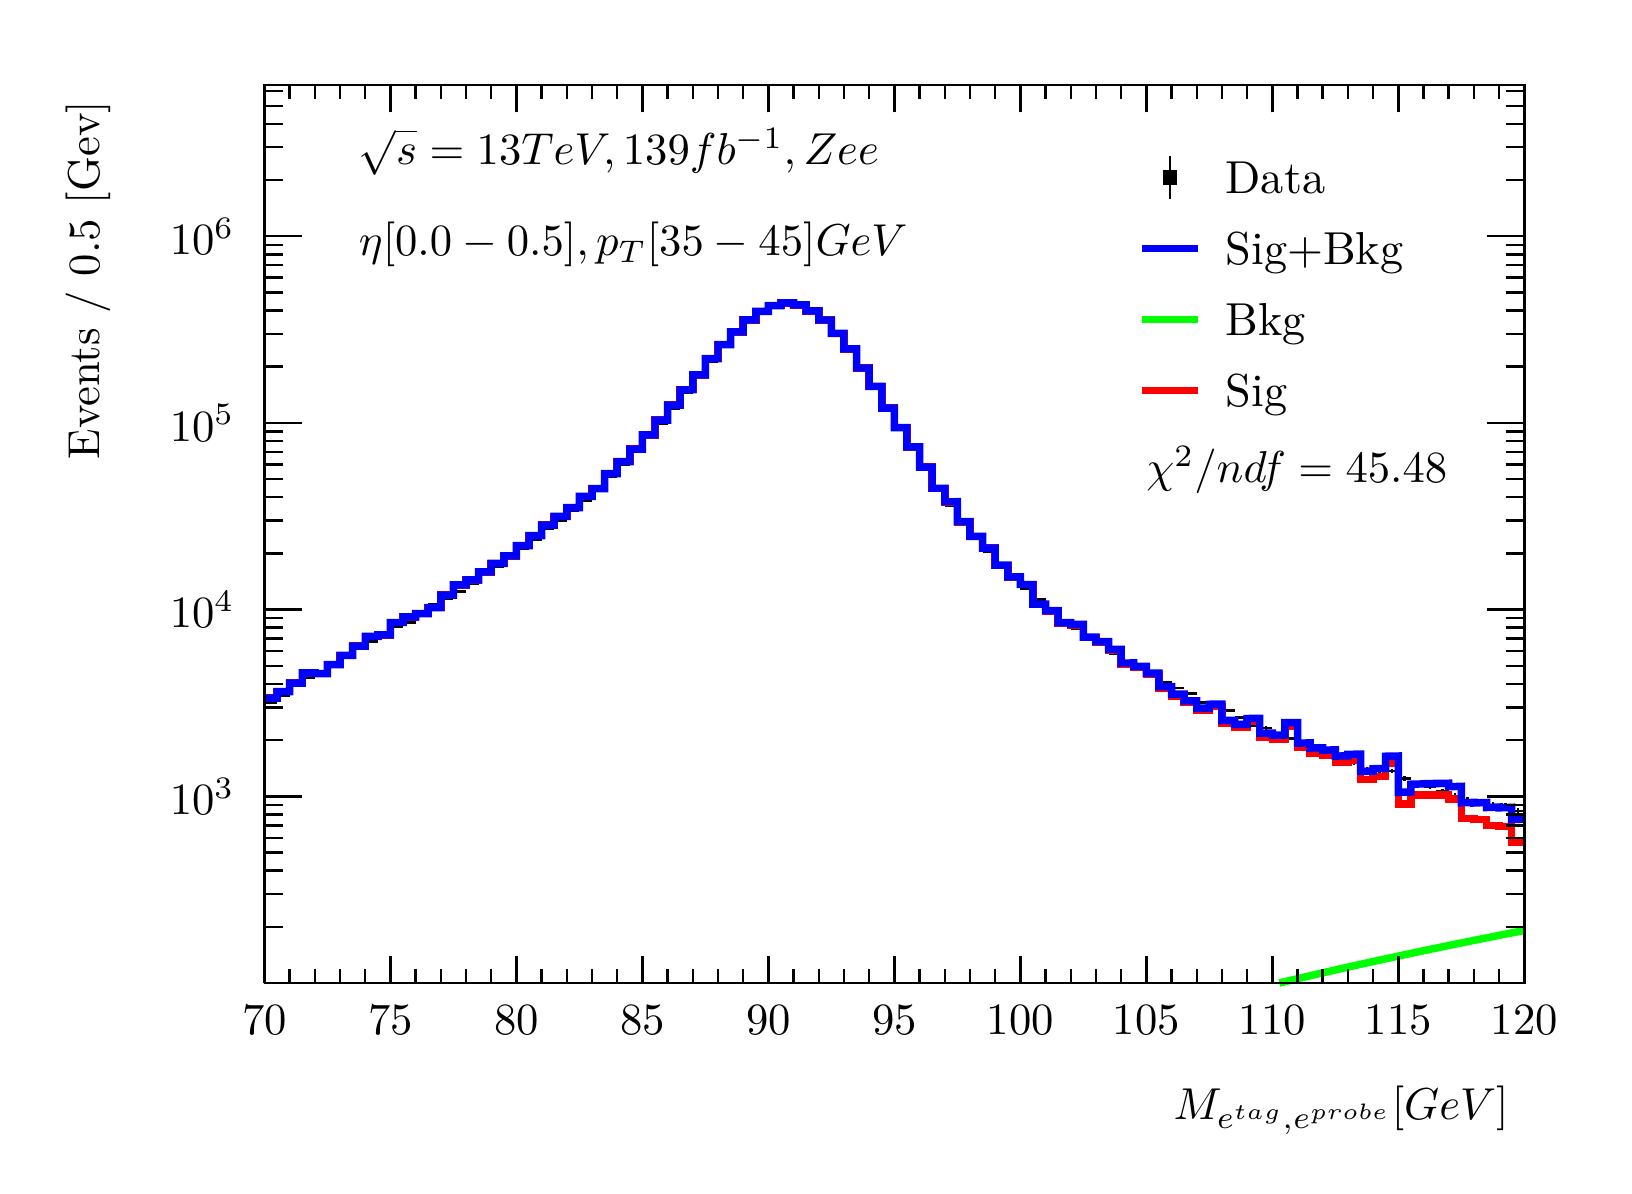
\begin{tikzpicture}
\pgfdeclareplotmark{cross} {
\pgfpathmoveto{\pgfpoint{-0.3\pgfplotmarksize}{\pgfplotmarksize}}
\pgfpathlineto{\pgfpoint{+0.3\pgfplotmarksize}{\pgfplotmarksize}}
\pgfpathlineto{\pgfpoint{+0.3\pgfplotmarksize}{0.3\pgfplotmarksize}}
\pgfpathlineto{\pgfpoint{+1\pgfplotmarksize}{0.3\pgfplotmarksize}}
\pgfpathlineto{\pgfpoint{+1\pgfplotmarksize}{-0.3\pgfplotmarksize}}
\pgfpathlineto{\pgfpoint{+0.3\pgfplotmarksize}{-0.3\pgfplotmarksize}}
\pgfpathlineto{\pgfpoint{+0.3\pgfplotmarksize}{-1.\pgfplotmarksize}}
\pgfpathlineto{\pgfpoint{-0.3\pgfplotmarksize}{-1.\pgfplotmarksize}}
\pgfpathlineto{\pgfpoint{-0.3\pgfplotmarksize}{-0.3\pgfplotmarksize}}
\pgfpathlineto{\pgfpoint{-1.\pgfplotmarksize}{-0.3\pgfplotmarksize}}
\pgfpathlineto{\pgfpoint{-1.\pgfplotmarksize}{0.3\pgfplotmarksize}}
\pgfpathlineto{\pgfpoint{-0.3\pgfplotmarksize}{0.3\pgfplotmarksize}}
\pgfpathclose
\pgfusepathqstroke
}
\pgfdeclareplotmark{cross*} {
\pgfpathmoveto{\pgfpoint{-0.3\pgfplotmarksize}{\pgfplotmarksize}}
\pgfpathlineto{\pgfpoint{+0.3\pgfplotmarksize}{\pgfplotmarksize}}
\pgfpathlineto{\pgfpoint{+0.3\pgfplotmarksize}{0.3\pgfplotmarksize}}
\pgfpathlineto{\pgfpoint{+1\pgfplotmarksize}{0.3\pgfplotmarksize}}
\pgfpathlineto{\pgfpoint{+1\pgfplotmarksize}{-0.3\pgfplotmarksize}}
\pgfpathlineto{\pgfpoint{+0.3\pgfplotmarksize}{-0.3\pgfplotmarksize}}
\pgfpathlineto{\pgfpoint{+0.3\pgfplotmarksize}{-1.\pgfplotmarksize}}
\pgfpathlineto{\pgfpoint{-0.3\pgfplotmarksize}{-1.\pgfplotmarksize}}
\pgfpathlineto{\pgfpoint{-0.3\pgfplotmarksize}{-0.3\pgfplotmarksize}}
\pgfpathlineto{\pgfpoint{-1.\pgfplotmarksize}{-0.3\pgfplotmarksize}}
\pgfpathlineto{\pgfpoint{-1.\pgfplotmarksize}{0.3\pgfplotmarksize}}
\pgfpathlineto{\pgfpoint{-0.3\pgfplotmarksize}{0.3\pgfplotmarksize}}
\pgfpathclose
\pgfusepathqfillstroke
}
\pgfdeclareplotmark{newstar} {
\pgfpathmoveto{\pgfqpoint{0pt}{\pgfplotmarksize}}
\pgfpathlineto{\pgfqpointpolar{44}{0.5\pgfplotmarksize}}
\pgfpathlineto{\pgfqpointpolar{18}{\pgfplotmarksize}}
\pgfpathlineto{\pgfqpointpolar{-20}{0.5\pgfplotmarksize}}
\pgfpathlineto{\pgfqpointpolar{-54}{\pgfplotmarksize}}
\pgfpathlineto{\pgfqpointpolar{-90}{0.5\pgfplotmarksize}}
\pgfpathlineto{\pgfqpointpolar{234}{\pgfplotmarksize}}
\pgfpathlineto{\pgfqpointpolar{198}{0.5\pgfplotmarksize}}
\pgfpathlineto{\pgfqpointpolar{162}{\pgfplotmarksize}}
\pgfpathlineto{\pgfqpointpolar{134}{0.5\pgfplotmarksize}}
\pgfpathclose
\pgfusepathqstroke
}
\pgfdeclareplotmark{newstar*} {
\pgfpathmoveto{\pgfqpoint{0pt}{\pgfplotmarksize}}
\pgfpathlineto{\pgfqpointpolar{44}{0.5\pgfplotmarksize}}
\pgfpathlineto{\pgfqpointpolar{18}{\pgfplotmarksize}}
\pgfpathlineto{\pgfqpointpolar{-20}{0.5\pgfplotmarksize}}
\pgfpathlineto{\pgfqpointpolar{-54}{\pgfplotmarksize}}
\pgfpathlineto{\pgfqpointpolar{-90}{0.5\pgfplotmarksize}}
\pgfpathlineto{\pgfqpointpolar{234}{\pgfplotmarksize}}
\pgfpathlineto{\pgfqpointpolar{198}{0.5\pgfplotmarksize}}
\pgfpathlineto{\pgfqpointpolar{162}{\pgfplotmarksize}}
\pgfpathlineto{\pgfqpointpolar{134}{0.5\pgfplotmarksize}}
\pgfpathclose
\pgfusepathqfillstroke
}
\definecolor{c}{rgb}{1,1,1};
\draw [color=c, fill=c] (0,0) rectangle (20,14.4361);
\draw [color=c, fill=c] (3,2.30977) rectangle (19,13.7143);
\definecolor{c}{rgb}{0,0,0};
\draw [c,line width=0.9] (3,2.30977) -- (3,13.7143) -- (19,13.7143) -- (19,2.30977) -- (3,2.30977);
\definecolor{c}{rgb}{1,1,1};
\draw [color=c, fill=c] (3,2.30977) rectangle (19,13.7143);
\definecolor{c}{rgb}{0,0,0};
\draw [c,line width=0.9] (3,2.30977) -- (3,13.7143) -- (19,13.7143) -- (19,2.30977) -- (3,2.30977);
\draw [c,line width=0.9] (3,2.30977) -- (19,2.30977);
\draw [c,line width=0.9] (3,2.65624) -- (3,2.30977);
\draw [c,line width=0.9] (3.32,2.48301) -- (3.32,2.30977);
\draw [c,line width=0.9] (3.64,2.48301) -- (3.64,2.30977);
\draw [c,line width=0.9] (3.96,2.48301) -- (3.96,2.30977);
\draw [c,line width=0.9] (4.28,2.48301) -- (4.28,2.30977);
\draw [c,line width=0.9] (4.6,2.65624) -- (4.6,2.30977);
\draw [c,line width=0.9] (4.92,2.48301) -- (4.92,2.30977);
\draw [c,line width=0.9] (5.24,2.48301) -- (5.24,2.30977);
\draw [c,line width=0.9] (5.56,2.48301) -- (5.56,2.30977);
\draw [c,line width=0.9] (5.88,2.48301) -- (5.88,2.30977);
\draw [c,line width=0.9] (6.2,2.65624) -- (6.2,2.30977);
\draw [c,line width=0.9] (6.52,2.48301) -- (6.52,2.30977);
\draw [c,line width=0.9] (6.84,2.48301) -- (6.84,2.30977);
\draw [c,line width=0.9] (7.16,2.48301) -- (7.16,2.30977);
\draw [c,line width=0.9] (7.48,2.48301) -- (7.48,2.30977);
\draw [c,line width=0.9] (7.8,2.65624) -- (7.8,2.30977);
\draw [c,line width=0.9] (8.12,2.48301) -- (8.12,2.30977);
\draw [c,line width=0.9] (8.44,2.48301) -- (8.44,2.30977);
\draw [c,line width=0.9] (8.76,2.48301) -- (8.76,2.30977);
\draw [c,line width=0.9] (9.08,2.48301) -- (9.08,2.30977);
\draw [c,line width=0.9] (9.4,2.65624) -- (9.4,2.30977);
\draw [c,line width=0.9] (9.72,2.48301) -- (9.72,2.30977);
\draw [c,line width=0.9] (10.04,2.48301) -- (10.04,2.30977);
\draw [c,line width=0.9] (10.36,2.48301) -- (10.36,2.30977);
\draw [c,line width=0.9] (10.68,2.48301) -- (10.68,2.30977);
\draw [c,line width=0.9] (11,2.65624) -- (11,2.30977);
\draw [c,line width=0.9] (11.32,2.48301) -- (11.32,2.30977);
\draw [c,line width=0.9] (11.64,2.48301) -- (11.64,2.30977);
\draw [c,line width=0.9] (11.96,2.48301) -- (11.96,2.30977);
\draw [c,line width=0.9] (12.28,2.48301) -- (12.28,2.30977);
\draw [c,line width=0.9] (12.6,2.65624) -- (12.6,2.30977);
\draw [c,line width=0.9] (12.92,2.48301) -- (12.92,2.30977);
\draw [c,line width=0.9] (13.24,2.48301) -- (13.24,2.30977);
\draw [c,line width=0.9] (13.56,2.48301) -- (13.56,2.30977);
\draw [c,line width=0.9] (13.88,2.48301) -- (13.88,2.30977);
\draw [c,line width=0.9] (14.2,2.65624) -- (14.2,2.30977);
\draw [c,line width=0.9] (14.52,2.48301) -- (14.52,2.30977);
\draw [c,line width=0.9] (14.84,2.48301) -- (14.84,2.30977);
\draw [c,line width=0.9] (15.16,2.48301) -- (15.16,2.30977);
\draw [c,line width=0.9] (15.48,2.48301) -- (15.48,2.30977);
\draw [c,line width=0.9] (15.8,2.65624) -- (15.8,2.30977);
\draw [c,line width=0.9] (16.12,2.48301) -- (16.12,2.30977);
\draw [c,line width=0.9] (16.44,2.48301) -- (16.44,2.30977);
\draw [c,line width=0.9] (16.76,2.48301) -- (16.76,2.30977);
\draw [c,line width=0.9] (17.08,2.48301) -- (17.08,2.30977);
\draw [c,line width=0.9] (17.4,2.65624) -- (17.4,2.30977);
\draw [c,line width=0.9] (17.72,2.48301) -- (17.72,2.30977);
\draw [c,line width=0.9] (18.04,2.48301) -- (18.04,2.30977);
\draw [c,line width=0.9] (18.36,2.48301) -- (18.36,2.30977);
\draw [c,line width=0.9] (18.68,2.48301) -- (18.68,2.30977);
\draw [c,line width=0.9] (19,2.65624) -- (19,2.30977);
\draw [anchor=base] (3,1.66015) node[scale=1.61424, color=c, rotate=0]{70};
\draw [anchor=base] (4.6,1.66015) node[scale=1.61424, color=c, rotate=0]{75};
\draw [anchor=base] (6.2,1.66015) node[scale=1.61424, color=c, rotate=0]{80};
\draw [anchor=base] (7.8,1.66015) node[scale=1.61424, color=c, rotate=0]{85};
\draw [anchor=base] (9.4,1.66015) node[scale=1.61424, color=c, rotate=0]{90};
\draw [anchor=base] (11,1.66015) node[scale=1.61424, color=c, rotate=0]{95};
\draw [anchor=base] (12.6,1.66015) node[scale=1.61424, color=c, rotate=0]{100};
\draw [anchor=base] (14.2,1.66015) node[scale=1.61424, color=c, rotate=0]{105};
\draw [anchor=base] (15.8,1.66015) node[scale=1.61424, color=c, rotate=0]{110};
\draw [anchor=base] (17.4,1.66015) node[scale=1.61424, color=c, rotate=0]{115};
\draw [anchor=base] (19,1.66015) node[scale=1.61424, color=c, rotate=0]{120};
\draw [anchor= east] (19,0.692932) node[scale=1.61424, color=c, rotate=0]{$M_{e^{tag}, e^{probe}}  [GeV]$};
\draw [c,line width=0.9] (3,13.7143) -- (19,13.7143);
\draw [c,line width=0.9] (3,13.3678) -- (3,13.7143);
\draw [c,line width=0.9] (3.32,13.5411) -- (3.32,13.7143);
\draw [c,line width=0.9] (3.64,13.5411) -- (3.64,13.7143);
\draw [c,line width=0.9] (3.96,13.5411) -- (3.96,13.7143);
\draw [c,line width=0.9] (4.28,13.5411) -- (4.28,13.7143);
\draw [c,line width=0.9] (4.6,13.3678) -- (4.6,13.7143);
\draw [c,line width=0.9] (4.92,13.5411) -- (4.92,13.7143);
\draw [c,line width=0.9] (5.24,13.5411) -- (5.24,13.7143);
\draw [c,line width=0.9] (5.56,13.5411) -- (5.56,13.7143);
\draw [c,line width=0.9] (5.88,13.5411) -- (5.88,13.7143);
\draw [c,line width=0.9] (6.2,13.3678) -- (6.2,13.7143);
\draw [c,line width=0.9] (6.52,13.5411) -- (6.52,13.7143);
\draw [c,line width=0.9] (6.84,13.5411) -- (6.84,13.7143);
\draw [c,line width=0.9] (7.16,13.5411) -- (7.16,13.7143);
\draw [c,line width=0.9] (7.48,13.5411) -- (7.48,13.7143);
\draw [c,line width=0.9] (7.8,13.3678) -- (7.8,13.7143);
\draw [c,line width=0.9] (8.12,13.5411) -- (8.12,13.7143);
\draw [c,line width=0.9] (8.44,13.5411) -- (8.44,13.7143);
\draw [c,line width=0.9] (8.76,13.5411) -- (8.76,13.7143);
\draw [c,line width=0.9] (9.08,13.5411) -- (9.08,13.7143);
\draw [c,line width=0.9] (9.4,13.3678) -- (9.4,13.7143);
\draw [c,line width=0.9] (9.72,13.5411) -- (9.72,13.7143);
\draw [c,line width=0.9] (10.04,13.5411) -- (10.04,13.7143);
\draw [c,line width=0.9] (10.36,13.5411) -- (10.36,13.7143);
\draw [c,line width=0.9] (10.68,13.5411) -- (10.68,13.7143);
\draw [c,line width=0.9] (11,13.3678) -- (11,13.7143);
\draw [c,line width=0.9] (11.32,13.5411) -- (11.32,13.7143);
\draw [c,line width=0.9] (11.64,13.5411) -- (11.64,13.7143);
\draw [c,line width=0.9] (11.96,13.5411) -- (11.96,13.7143);
\draw [c,line width=0.9] (12.28,13.5411) -- (12.28,13.7143);
\draw [c,line width=0.9] (12.6,13.3678) -- (12.6,13.7143);
\draw [c,line width=0.9] (12.92,13.5411) -- (12.92,13.7143);
\draw [c,line width=0.9] (13.24,13.5411) -- (13.24,13.7143);
\draw [c,line width=0.9] (13.56,13.5411) -- (13.56,13.7143);
\draw [c,line width=0.9] (13.88,13.5411) -- (13.88,13.7143);
\draw [c,line width=0.9] (14.2,13.3678) -- (14.2,13.7143);
\draw [c,line width=0.9] (14.52,13.5411) -- (14.52,13.7143);
\draw [c,line width=0.9] (14.84,13.5411) -- (14.84,13.7143);
\draw [c,line width=0.9] (15.16,13.5411) -- (15.16,13.7143);
\draw [c,line width=0.9] (15.48,13.5411) -- (15.48,13.7143);
\draw [c,line width=0.9] (15.8,13.3678) -- (15.8,13.7143);
\draw [c,line width=0.9] (16.12,13.5411) -- (16.12,13.7143);
\draw [c,line width=0.9] (16.44,13.5411) -- (16.44,13.7143);
\draw [c,line width=0.9] (16.76,13.5411) -- (16.76,13.7143);
\draw [c,line width=0.9] (17.08,13.5411) -- (17.08,13.7143);
\draw [c,line width=0.9] (17.4,13.3678) -- (17.4,13.7143);
\draw [c,line width=0.9] (17.72,13.5411) -- (17.72,13.7143);
\draw [c,line width=0.9] (18.04,13.5411) -- (18.04,13.7143);
\draw [c,line width=0.9] (18.36,13.5411) -- (18.36,13.7143);
\draw [c,line width=0.9] (18.68,13.5411) -- (18.68,13.7143);
\draw [c,line width=0.9] (19,13.3678) -- (19,13.7143);
\draw [c,line width=0.9] (3,2.30977) -- (3,13.7143);
\draw [c,line width=0.9] (3.237,3.02354) -- (3,3.02354);
\draw [c,line width=0.9] (3.237,3.44107) -- (3,3.44107);
\draw [c,line width=0.9] (3.237,3.73731) -- (3,3.73731);
\draw [c,line width=0.9] (3.237,3.96709) -- (3,3.96709);
\draw [c,line width=0.9] (3.237,4.15484) -- (3,4.15484);
\draw [c,line width=0.9] (3.237,4.31357) -- (3,4.31357);
\draw [c,line width=0.9] (3.237,4.45108) -- (3,4.45108);
\draw [c,line width=0.9] (3.237,4.57236) -- (3,4.57236);
\draw [c,line width=0.9] (3.474,4.68086) -- (3,4.68086);
\draw [anchor= east] (2.82,4.68086) node[scale=1.61424, color=c, rotate=0]{$10^{3}$};
\draw [c,line width=0.9] (3.237,5.39463) -- (3,5.39463);
\draw [c,line width=0.9] (3.237,5.81216) -- (3,5.81216);
\draw [c,line width=0.9] (3.237,6.1084) -- (3,6.1084);
\draw [c,line width=0.9] (3.237,6.33818) -- (3,6.33818);
\draw [c,line width=0.9] (3.237,6.52593) -- (3,6.52593);
\draw [c,line width=0.9] (3.237,6.68466) -- (3,6.68466);
\draw [c,line width=0.9] (3.237,6.82217) -- (3,6.82217);
\draw [c,line width=0.9] (3.237,6.94345) -- (3,6.94345);
\draw [c,line width=0.9] (3.474,7.05195) -- (3,7.05195);
\draw [anchor= east] (2.82,7.05195) node[scale=1.61424, color=c, rotate=0]{$10^{4}$};
\draw [c,line width=0.9] (3.237,7.76572) -- (3,7.76572);
\draw [c,line width=0.9] (3.237,8.18324) -- (3,8.18324);
\draw [c,line width=0.9] (3.237,8.47948) -- (3,8.47948);
\draw [c,line width=0.9] (3.237,8.70927) -- (3,8.70927);
\draw [c,line width=0.9] (3.237,8.89701) -- (3,8.89701);
\draw [c,line width=0.9] (3.237,9.05575) -- (3,9.05575);
\draw [c,line width=0.9] (3.237,9.19325) -- (3,9.19325);
\draw [c,line width=0.9] (3.237,9.31454) -- (3,9.31454);
\draw [c,line width=0.9] (3.474,9.42304) -- (3,9.42304);
\draw [anchor= east] (2.82,9.42304) node[scale=1.61424, color=c, rotate=0]{$10^{5}$};
\draw [c,line width=0.9] (3.237,10.1368) -- (3,10.1368);
\draw [c,line width=0.9] (3.237,10.5543) -- (3,10.5543);
\draw [c,line width=0.9] (3.237,10.8506) -- (3,10.8506);
\draw [c,line width=0.9] (3.237,11.0804) -- (3,11.0804);
\draw [c,line width=0.9] (3.237,11.2681) -- (3,11.2681);
\draw [c,line width=0.9] (3.237,11.4268) -- (3,11.4268);
\draw [c,line width=0.9] (3.237,11.5643) -- (3,11.5643);
\draw [c,line width=0.9] (3.237,11.6856) -- (3,11.6856);
\draw [c,line width=0.9] (3.474,11.7941) -- (3,11.7941);
\draw [anchor= east] (2.82,11.7941) node[scale=1.61424, color=c, rotate=0]{$10^{6}$};
\draw [c,line width=0.9] (3.237,12.5079) -- (3,12.5079);
\draw [c,line width=0.9] (3.237,12.9254) -- (3,12.9254);
\draw [c,line width=0.9] (3.237,13.2217) -- (3,13.2217);
\draw [c,line width=0.9] (3.237,13.4514) -- (3,13.4514);
\draw [c,line width=0.9] (3.237,13.6392) -- (3,13.6392);
\draw [anchor= east] (0.76,13.7143) node[scale=1.61424, color=c, rotate=90]{Events / 0.5 [Gev]};
\draw [c,line width=0.9] (19,2.30977) -- (19,13.7143);
\draw [c,line width=0.9] (18.763,3.02354) -- (19,3.02354);
\draw [c,line width=0.9] (18.763,3.44107) -- (19,3.44107);
\draw [c,line width=0.9] (18.763,3.73731) -- (19,3.73731);
\draw [c,line width=0.9] (18.763,3.96709) -- (19,3.96709);
\draw [c,line width=0.9] (18.763,4.15484) -- (19,4.15484);
\draw [c,line width=0.9] (18.763,4.31357) -- (19,4.31357);
\draw [c,line width=0.9] (18.763,4.45108) -- (19,4.45108);
\draw [c,line width=0.9] (18.763,4.57236) -- (19,4.57236);
\draw [c,line width=0.9] (18.526,4.68086) -- (19,4.68086);
\draw [c,line width=0.9] (18.763,5.39463) -- (19,5.39463);
\draw [c,line width=0.9] (18.763,5.81216) -- (19,5.81216);
\draw [c,line width=0.9] (18.763,6.1084) -- (19,6.1084);
\draw [c,line width=0.9] (18.763,6.33818) -- (19,6.33818);
\draw [c,line width=0.9] (18.763,6.52593) -- (19,6.52593);
\draw [c,line width=0.9] (18.763,6.68466) -- (19,6.68466);
\draw [c,line width=0.9] (18.763,6.82217) -- (19,6.82217);
\draw [c,line width=0.9] (18.763,6.94345) -- (19,6.94345);
\draw [c,line width=0.9] (18.526,7.05195) -- (19,7.05195);
\draw [c,line width=0.9] (18.763,7.76572) -- (19,7.76572);
\draw [c,line width=0.9] (18.763,8.18324) -- (19,8.18324);
\draw [c,line width=0.9] (18.763,8.47948) -- (19,8.47948);
\draw [c,line width=0.9] (18.763,8.70927) -- (19,8.70927);
\draw [c,line width=0.9] (18.763,8.89701) -- (19,8.89701);
\draw [c,line width=0.9] (18.763,9.05575) -- (19,9.05575);
\draw [c,line width=0.9] (18.763,9.19325) -- (19,9.19325);
\draw [c,line width=0.9] (18.763,9.31454) -- (19,9.31454);
\draw [c,line width=0.9] (18.526,9.42304) -- (19,9.42304);
\draw [c,line width=0.9] (18.763,10.1368) -- (19,10.1368);
\draw [c,line width=0.9] (18.763,10.5543) -- (19,10.5543);
\draw [c,line width=0.9] (18.763,10.8506) -- (19,10.8506);
\draw [c,line width=0.9] (18.763,11.0804) -- (19,11.0804);
\draw [c,line width=0.9] (18.763,11.2681) -- (19,11.2681);
\draw [c,line width=0.9] (18.763,11.4268) -- (19,11.4268);
\draw [c,line width=0.9] (18.763,11.5643) -- (19,11.5643);
\draw [c,line width=0.9] (18.763,11.6856) -- (19,11.6856);
\draw [c,line width=0.9] (18.526,11.7941) -- (19,11.7941);
\draw [c,line width=0.9] (18.763,12.5079) -- (19,12.5079);
\draw [c,line width=0.9] (18.763,12.9254) -- (19,12.9254);
\draw [c,line width=0.9] (18.763,13.2217) -- (19,13.2217);
\draw [c,line width=0.9] (18.763,13.4514) -- (19,13.4514);
\draw [c,line width=0.9] (18.763,13.6392) -- (19,13.6392);
\draw [c,line width=0.9] (3.08,5.87086) -- (3,5.87086);
\draw [c,line width=0.9] (3,5.87086) -- (3,5.87086);
\draw [c,line width=0.9] (3.08,5.87086) -- (3.16,5.87086);
\draw [c,line width=0.9] (3.16,5.87086) -- (3.16,5.87086);
\draw [c,line width=0.9] (3.08,5.87086) -- (3.08,5.88914);
\draw [c,line width=0.9] (3.08,5.88914) -- (3.08,5.88914);
\draw [c,line width=0.9] (3.08,5.87086) -- (3.08,5.85259);
\draw [c,line width=0.9] (3.08,5.85259) -- (3.08,5.85259);
\draw [c,line width=0.9] (3.24,5.95965) -- (3.16,5.95965);
\draw [c,line width=0.9] (3.16,5.95965) -- (3.16,5.95965);
\draw [c,line width=0.9] (3.24,5.95965) -- (3.32,5.95965);
\draw [c,line width=0.9] (3.32,5.95965) -- (3.32,5.95965);
\draw [c,line width=0.9] (3.24,5.95965) -- (3.24,5.97715);
\draw [c,line width=0.9] (3.24,5.97715) -- (3.24,5.97715);
\draw [c,line width=0.9] (3.24,5.95965) -- (3.24,5.94215);
\draw [c,line width=0.9] (3.24,5.94215) -- (3.24,5.94215);
\draw [c,line width=0.9] (3.4,6.12246) -- (3.32,6.12246);
\draw [c,line width=0.9] (3.32,6.12246) -- (3.32,6.12246);
\draw [c,line width=0.9] (3.4,6.12246) -- (3.48,6.12246);
\draw [c,line width=0.9] (3.48,6.12246) -- (3.48,6.12246);
\draw [c,line width=0.9] (3.4,6.12246) -- (3.4,6.13863);
\draw [c,line width=0.9] (3.4,6.13863) -- (3.4,6.13863);
\draw [c,line width=0.9] (3.4,6.12246) -- (3.4,6.10629);
\draw [c,line width=0.9] (3.4,6.10629) -- (3.4,6.10629);
\draw [c,line width=0.9] (3.56,6.19027) -- (3.48,6.19027);
\draw [c,line width=0.9] (3.48,6.19027) -- (3.48,6.19027);
\draw [c,line width=0.9] (3.56,6.19027) -- (3.64,6.19027);
\draw [c,line width=0.9] (3.64,6.19027) -- (3.64,6.19027);
\draw [c,line width=0.9] (3.56,6.19027) -- (3.56,6.20591);
\draw [c,line width=0.9] (3.56,6.20591) -- (3.56,6.20591);
\draw [c,line width=0.9] (3.56,6.19027) -- (3.56,6.17462);
\draw [c,line width=0.9] (3.56,6.17462) -- (3.56,6.17462);
\draw [c,line width=0.9] (3.72,6.27556) -- (3.64,6.27556);
\draw [c,line width=0.9] (3.64,6.27556) -- (3.64,6.27556);
\draw [c,line width=0.9] (3.72,6.27556) -- (3.8,6.27556);
\draw [c,line width=0.9] (3.8,6.27556) -- (3.8,6.27556);
\draw [c,line width=0.9] (3.72,6.27556) -- (3.72,6.29057);
\draw [c,line width=0.9] (3.72,6.29057) -- (3.72,6.29057);
\draw [c,line width=0.9] (3.72,6.27556) -- (3.72,6.26055);
\draw [c,line width=0.9] (3.72,6.26055) -- (3.72,6.26055);
\draw [c,line width=0.9] (3.88,6.37916) -- (3.8,6.37916);
\draw [c,line width=0.9] (3.8,6.37916) -- (3.8,6.37916);
\draw [c,line width=0.9] (3.88,6.37916) -- (3.96,6.37916);
\draw [c,line width=0.9] (3.96,6.37916) -- (3.96,6.37916);
\draw [c,line width=0.9] (3.88,6.37916) -- (3.88,6.39344);
\draw [c,line width=0.9] (3.88,6.39344) -- (3.88,6.39344);
\draw [c,line width=0.9] (3.88,6.37916) -- (3.88,6.36489);
\draw [c,line width=0.9] (3.88,6.36489) -- (3.88,6.36489);
\draw [c,line width=0.9] (4.04,6.47509) -- (3.96,6.47509);
\draw [c,line width=0.9] (3.96,6.47509) -- (3.96,6.47509);
\draw [c,line width=0.9] (4.04,6.47509) -- (4.12,6.47509);
\draw [c,line width=0.9] (4.12,6.47509) -- (4.12,6.47509);
\draw [c,line width=0.9] (4.04,6.47509) -- (4.04,6.48872);
\draw [c,line width=0.9] (4.04,6.48872) -- (4.04,6.48872);
\draw [c,line width=0.9] (4.04,6.47509) -- (4.04,6.46147);
\draw [c,line width=0.9] (4.04,6.46147) -- (4.04,6.46147);
\draw [c,line width=0.9] (4.2,6.576) -- (4.12,6.576);
\draw [c,line width=0.9] (4.12,6.576) -- (4.12,6.576);
\draw [c,line width=0.9] (4.2,6.576) -- (4.28,6.576);
\draw [c,line width=0.9] (4.28,6.576) -- (4.28,6.576);
\draw [c,line width=0.9] (4.2,6.576) -- (4.2,6.58898);
\draw [c,line width=0.9] (4.2,6.58898) -- (4.2,6.58898);
\draw [c,line width=0.9] (4.2,6.576) -- (4.2,6.56303);
\draw [c,line width=0.9] (4.2,6.56303) -- (4.2,6.56303);
\draw [c,line width=0.9] (4.36,6.64508) -- (4.28,6.64508);
\draw [c,line width=0.9] (4.28,6.64508) -- (4.28,6.64508);
\draw [c,line width=0.9] (4.36,6.64508) -- (4.44,6.64508);
\draw [c,line width=0.9] (4.44,6.64508) -- (4.44,6.64508);
\draw [c,line width=0.9] (4.36,6.64508) -- (4.36,6.65762);
\draw [c,line width=0.9] (4.36,6.65762) -- (4.36,6.65762);
\draw [c,line width=0.9] (4.36,6.64508) -- (4.36,6.63253);
\draw [c,line width=0.9] (4.36,6.63253) -- (4.36,6.63253);
\draw [c,line width=0.9] (4.52,6.7335) -- (4.44,6.7335);
\draw [c,line width=0.9] (4.44,6.7335) -- (4.44,6.7335);
\draw [c,line width=0.9] (4.52,6.7335) -- (4.6,6.7335);
\draw [c,line width=0.9] (4.6,6.7335) -- (4.6,6.7335);
\draw [c,line width=0.9] (4.52,6.7335) -- (4.52,6.74552);
\draw [c,line width=0.9] (4.52,6.74552) -- (4.52,6.74552);
\draw [c,line width=0.9] (4.52,6.7335) -- (4.52,6.72148);
\draw [c,line width=0.9] (4.52,6.72148) -- (4.52,6.72148);
\draw [c,line width=0.9] (4.68,6.83216) -- (4.6,6.83216);
\draw [c,line width=0.9] (4.6,6.83216) -- (4.6,6.83216);
\draw [c,line width=0.9] (4.68,6.83216) -- (4.76,6.83216);
\draw [c,line width=0.9] (4.76,6.83216) -- (4.76,6.83216);
\draw [c,line width=0.9] (4.68,6.83216) -- (4.68,6.84362);
\draw [c,line width=0.9] (4.68,6.84362) -- (4.68,6.84362);
\draw [c,line width=0.9] (4.68,6.83216) -- (4.68,6.8207);
\draw [c,line width=0.9] (4.68,6.8207) -- (4.68,6.8207);
\draw [c,line width=0.9] (4.84,6.88786) -- (4.76,6.88786);
\draw [c,line width=0.9] (4.76,6.88786) -- (4.76,6.88786);
\draw [c,line width=0.9] (4.84,6.88786) -- (4.92,6.88786);
\draw [c,line width=0.9] (4.92,6.88786) -- (4.92,6.88786);
\draw [c,line width=0.9] (4.84,6.88786) -- (4.84,6.89901);
\draw [c,line width=0.9] (4.84,6.89901) -- (4.84,6.89901);
\draw [c,line width=0.9] (4.84,6.88786) -- (4.84,6.87671);
\draw [c,line width=0.9] (4.84,6.87671) -- (4.84,6.87671);
\draw [c,line width=0.9] (5,7.00162) -- (4.92,7.00162);
\draw [c,line width=0.9] (4.92,7.00162) -- (4.92,7.00162);
\draw [c,line width=0.9] (5,7.00162) -- (5.08,7.00162);
\draw [c,line width=0.9] (5.08,7.00162) -- (5.08,7.00162);
\draw [c,line width=0.9] (5,7.00162) -- (5,7.01217);
\draw [c,line width=0.9] (5,7.01217) -- (5,7.01217);
\draw [c,line width=0.9] (5,7.00162) -- (5,6.99107);
\draw [c,line width=0.9] (5,6.99107) -- (5,6.99107);
\draw [c,line width=0.9] (5.16,7.11506) -- (5.08,7.11506);
\draw [c,line width=0.9] (5.08,7.11506) -- (5.08,7.11506);
\draw [c,line width=0.9] (5.16,7.11506) -- (5.24,7.11506);
\draw [c,line width=0.9] (5.24,7.11506) -- (5.24,7.11506);
\draw [c,line width=0.9] (5.16,7.11506) -- (5.16,7.12504);
\draw [c,line width=0.9] (5.16,7.12504) -- (5.16,7.12504);
\draw [c,line width=0.9] (5.16,7.11506) -- (5.16,7.10507);
\draw [c,line width=0.9] (5.16,7.10507) -- (5.16,7.10507);
\draw [c,line width=0.9] (5.32,7.18416) -- (5.24,7.18416);
\draw [c,line width=0.9] (5.24,7.18416) -- (5.24,7.18416);
\draw [c,line width=0.9] (5.32,7.18416) -- (5.4,7.18416);
\draw [c,line width=0.9] (5.4,7.18416) -- (5.4,7.18416);
\draw [c,line width=0.9] (5.32,7.18416) -- (5.32,7.19382);
\draw [c,line width=0.9] (5.32,7.19382) -- (5.32,7.19382);
\draw [c,line width=0.9] (5.32,7.18416) -- (5.32,7.1745);
\draw [c,line width=0.9] (5.32,7.1745) -- (5.32,7.1745);
\draw [c,line width=0.9] (5.48,7.28543) -- (5.4,7.28543);
\draw [c,line width=0.9] (5.4,7.28543) -- (5.4,7.28543);
\draw [c,line width=0.9] (5.48,7.28543) -- (5.56,7.28543);
\draw [c,line width=0.9] (5.56,7.28543) -- (5.56,7.28543);
\draw [c,line width=0.9] (5.48,7.28543) -- (5.48,7.29463);
\draw [c,line width=0.9] (5.48,7.29463) -- (5.48,7.29463);
\draw [c,line width=0.9] (5.48,7.28543) -- (5.48,7.27624);
\draw [c,line width=0.9] (5.48,7.27624) -- (5.48,7.27624);
\draw [c,line width=0.9] (5.64,7.38674) -- (5.56,7.38674);
\draw [c,line width=0.9] (5.56,7.38674) -- (5.56,7.38674);
\draw [c,line width=0.9] (5.64,7.38674) -- (5.72,7.38674);
\draw [c,line width=0.9] (5.72,7.38674) -- (5.72,7.38674);
\draw [c,line width=0.9] (5.64,7.38674) -- (5.64,7.3955);
\draw [c,line width=0.9] (5.64,7.3955) -- (5.64,7.3955);
\draw [c,line width=0.9] (5.64,7.38674) -- (5.64,7.37799);
\draw [c,line width=0.9] (5.64,7.37799) -- (5.64,7.37799);
\draw [c,line width=0.9] (5.8,7.50696) -- (5.72,7.50696);
\draw [c,line width=0.9] (5.72,7.50696) -- (5.72,7.50696);
\draw [c,line width=0.9] (5.8,7.50696) -- (5.88,7.50696);
\draw [c,line width=0.9] (5.88,7.50696) -- (5.88,7.50696);
\draw [c,line width=0.9] (5.8,7.50696) -- (5.8,7.51521);
\draw [c,line width=0.9] (5.8,7.51521) -- (5.8,7.51521);
\draw [c,line width=0.9] (5.8,7.50696) -- (5.8,7.4987);
\draw [c,line width=0.9] (5.8,7.4987) -- (5.8,7.4987);
\draw [c,line width=0.9] (5.96,7.59618) -- (5.88,7.59618);
\draw [c,line width=0.9] (5.88,7.59618) -- (5.88,7.59618);
\draw [c,line width=0.9] (5.96,7.59618) -- (6.04,7.59618);
\draw [c,line width=0.9] (6.04,7.59618) -- (6.04,7.59618);
\draw [c,line width=0.9] (5.96,7.59618) -- (5.96,7.60409);
\draw [c,line width=0.9] (5.96,7.60409) -- (5.96,7.60409);
\draw [c,line width=0.9] (5.96,7.59618) -- (5.96,7.58827);
\draw [c,line width=0.9] (5.96,7.58827) -- (5.96,7.58827);
\draw [c,line width=0.9] (6.12,7.71447) -- (6.04,7.71447);
\draw [c,line width=0.9] (6.04,7.71447) -- (6.04,7.71447);
\draw [c,line width=0.9] (6.12,7.71447) -- (6.2,7.71447);
\draw [c,line width=0.9] (6.2,7.71447) -- (6.2,7.71447);
\draw [c,line width=0.9] (6.12,7.71447) -- (6.12,7.72193);
\draw [c,line width=0.9] (6.12,7.72193) -- (6.12,7.72193);
\draw [c,line width=0.9] (6.12,7.71447) -- (6.12,7.707);
\draw [c,line width=0.9] (6.12,7.707) -- (6.12,7.707);
\draw [c,line width=0.9] (6.28,7.82212) -- (6.2,7.82212);
\draw [c,line width=0.9] (6.2,7.82212) -- (6.2,7.82212);
\draw [c,line width=0.9] (6.28,7.82212) -- (6.36,7.82212);
\draw [c,line width=0.9] (6.36,7.82212) -- (6.36,7.82212);
\draw [c,line width=0.9] (6.28,7.82212) -- (6.28,7.8292);
\draw [c,line width=0.9] (6.28,7.8292) -- (6.28,7.8292);
\draw [c,line width=0.9] (6.28,7.82212) -- (6.28,7.81503);
\draw [c,line width=0.9] (6.28,7.81503) -- (6.28,7.81503);
\draw [c,line width=0.9] (6.44,7.93472) -- (6.36,7.93472);
\draw [c,line width=0.9] (6.36,7.93472) -- (6.36,7.93472);
\draw [c,line width=0.9] (6.44,7.93472) -- (6.52,7.93472);
\draw [c,line width=0.9] (6.52,7.93472) -- (6.52,7.93472);
\draw [c,line width=0.9] (6.44,7.93472) -- (6.44,7.94142);
\draw [c,line width=0.9] (6.44,7.94142) -- (6.44,7.94142);
\draw [c,line width=0.9] (6.44,7.93472) -- (6.44,7.92801);
\draw [c,line width=0.9] (6.44,7.92801) -- (6.44,7.92801);
\draw [c,line width=0.9] (6.6,8.07448) -- (6.52,8.07448);
\draw [c,line width=0.9] (6.52,8.07448) -- (6.52,8.07448);
\draw [c,line width=0.9] (6.6,8.07448) -- (6.68,8.07448);
\draw [c,line width=0.9] (6.68,8.07448) -- (6.68,8.07448);
\draw [c,line width=0.9] (6.6,8.07448) -- (6.6,8.08075);
\draw [c,line width=0.9] (6.6,8.08075) -- (6.6,8.08075);
\draw [c,line width=0.9] (6.6,8.07448) -- (6.6,8.06822);
\draw [c,line width=0.9] (6.6,8.06822) -- (6.6,8.06822);
\draw [c,line width=0.9] (6.76,8.18149) -- (6.68,8.18149);
\draw [c,line width=0.9] (6.68,8.18149) -- (6.68,8.18149);
\draw [c,line width=0.9] (6.76,8.18149) -- (6.84,8.18149);
\draw [c,line width=0.9] (6.84,8.18149) -- (6.84,8.18149);
\draw [c,line width=0.9] (6.76,8.18149) -- (6.76,8.18744);
\draw [c,line width=0.9] (6.76,8.18744) -- (6.76,8.18744);
\draw [c,line width=0.9] (6.76,8.18149) -- (6.76,8.17554);
\draw [c,line width=0.9] (6.76,8.17554) -- (6.76,8.17554);
\draw [c,line width=0.9] (6.92,8.30533) -- (6.84,8.30533);
\draw [c,line width=0.9] (6.84,8.30533) -- (6.84,8.30533);
\draw [c,line width=0.9] (6.92,8.30533) -- (7,8.30533);
\draw [c,line width=0.9] (7,8.30533) -- (7,8.30533);
\draw [c,line width=0.9] (6.92,8.30533) -- (6.92,8.31093);
\draw [c,line width=0.9] (6.92,8.31093) -- (6.92,8.31093);
\draw [c,line width=0.9] (6.92,8.30533) -- (6.92,8.29972);
\draw [c,line width=0.9] (6.92,8.29972) -- (6.92,8.29972);
\draw [c,line width=0.9] (7.08,8.44101) -- (7,8.44101);
\draw [c,line width=0.9] (7,8.44101) -- (7,8.44101);
\draw [c,line width=0.9] (7.08,8.44101) -- (7.16,8.44101);
\draw [c,line width=0.9] (7.16,8.44101) -- (7.16,8.44101);
\draw [c,line width=0.9] (7.08,8.44101) -- (7.08,8.44626);
\draw [c,line width=0.9] (7.08,8.44626) -- (7.08,8.44626);
\draw [c,line width=0.9] (7.08,8.44101) -- (7.08,8.43576);
\draw [c,line width=0.9] (7.08,8.43576) -- (7.08,8.43576);
\draw [c,line width=0.9] (7.24,8.58649) -- (7.16,8.58649);
\draw [c,line width=0.9] (7.16,8.58649) -- (7.16,8.58649);
\draw [c,line width=0.9] (7.24,8.58649) -- (7.32,8.58649);
\draw [c,line width=0.9] (7.32,8.58649) -- (7.32,8.58649);
\draw [c,line width=0.9] (7.24,8.58649) -- (7.24,8.59138);
\draw [c,line width=0.9] (7.24,8.59138) -- (7.24,8.59138);
\draw [c,line width=0.9] (7.24,8.58649) -- (7.24,8.5816);
\draw [c,line width=0.9] (7.24,8.5816) -- (7.24,8.5816);
\draw [c,line width=0.9] (7.4,8.7375) -- (7.32,8.7375);
\draw [c,line width=0.9] (7.32,8.7375) -- (7.32,8.7375);
\draw [c,line width=0.9] (7.4,8.7375) -- (7.48,8.7375);
\draw [c,line width=0.9] (7.48,8.7375) -- (7.48,8.7375);
\draw [c,line width=0.9] (7.4,8.7375) -- (7.4,8.74205);
\draw [c,line width=0.9] (7.4,8.74205) -- (7.4,8.74205);
\draw [c,line width=0.9] (7.4,8.7375) -- (7.4,8.73296);
\draw [c,line width=0.9] (7.4,8.73296) -- (7.4,8.73296);
\draw [c,line width=0.9] (7.56,8.88897) -- (7.48,8.88897);
\draw [c,line width=0.9] (7.48,8.88897) -- (7.48,8.88897);
\draw [c,line width=0.9] (7.56,8.88897) -- (7.64,8.88897);
\draw [c,line width=0.9] (7.64,8.88897) -- (7.64,8.88897);
\draw [c,line width=0.9] (7.56,8.88897) -- (7.56,8.89319);
\draw [c,line width=0.9] (7.56,8.89319) -- (7.56,8.89319);
\draw [c,line width=0.9] (7.56,8.88897) -- (7.56,8.88475);
\draw [c,line width=0.9] (7.56,8.88475) -- (7.56,8.88475);
\draw [c,line width=0.9] (7.72,9.05543) -- (7.64,9.05543);
\draw [c,line width=0.9] (7.64,9.05543) -- (7.64,9.05543);
\draw [c,line width=0.9] (7.72,9.05543) -- (7.8,9.05543);
\draw [c,line width=0.9] (7.8,9.05543) -- (7.8,9.05543);
\draw [c,line width=0.9] (7.72,9.05543) -- (7.72,9.05932);
\draw [c,line width=0.9] (7.72,9.05932) -- (7.72,9.05932);
\draw [c,line width=0.9] (7.72,9.05543) -- (7.72,9.05153);
\draw [c,line width=0.9] (7.72,9.05153) -- (7.72,9.05153);
\draw [c,line width=0.9] (7.88,9.23782) -- (7.8,9.23782);
\draw [c,line width=0.9] (7.8,9.23782) -- (7.8,9.23782);
\draw [c,line width=0.9] (7.88,9.23782) -- (7.96,9.23782);
\draw [c,line width=0.9] (7.96,9.23782) -- (7.96,9.23782);
\draw [c,line width=0.9] (7.88,9.23782) -- (7.88,9.24138);
\draw [c,line width=0.9] (7.88,9.24138) -- (7.88,9.24138);
\draw [c,line width=0.9] (7.88,9.23782) -- (7.88,9.23425);
\draw [c,line width=0.9] (7.88,9.23425) -- (7.88,9.23425);
\draw [c,line width=0.9] (8.04,9.41066) -- (7.96,9.41066);
\draw [c,line width=0.9] (7.96,9.41066) -- (7.96,9.41066);
\draw [c,line width=0.9] (8.04,9.41066) -- (8.12,9.41066);
\draw [c,line width=0.9] (8.12,9.41066) -- (8.12,9.41066);
\draw [c,line width=0.9] (8.04,9.41066) -- (8.04,9.41393);
\draw [c,line width=0.9] (8.04,9.41393) -- (8.04,9.41393);
\draw [c,line width=0.9] (8.04,9.41066) -- (8.04,9.40738);
\draw [c,line width=0.9] (8.04,9.40738) -- (8.04,9.40738);
\draw [c,line width=0.9] (8.2,9.60518) -- (8.12,9.60518);
\draw [c,line width=0.9] (8.12,9.60518) -- (8.12,9.60518);
\draw [c,line width=0.9] (8.2,9.60518) -- (8.28,9.60518);
\draw [c,line width=0.9] (8.28,9.60518) -- (8.28,9.60518);
\draw [c,line width=0.9] (8.2,9.60518) -- (8.2,9.60816);
\draw [c,line width=0.9] (8.2,9.60816) -- (8.2,9.60816);
\draw [c,line width=0.9] (8.2,9.60518) -- (8.2,9.6022);
\draw [c,line width=0.9] (8.2,9.6022) -- (8.2,9.6022);
\draw [c,line width=0.9] (8.36,9.80488) -- (8.28,9.80488);
\draw [c,line width=0.9] (8.28,9.80488) -- (8.28,9.80488);
\draw [c,line width=0.9] (8.36,9.80488) -- (8.44,9.80488);
\draw [c,line width=0.9] (8.44,9.80488) -- (8.44,9.80488);
\draw [c,line width=0.9] (8.36,9.80488) -- (8.36,9.80758);
\draw [c,line width=0.9] (8.36,9.80758) -- (8.36,9.80758);
\draw [c,line width=0.9] (8.36,9.80488) -- (8.36,9.80217);
\draw [c,line width=0.9] (8.36,9.80217) -- (8.36,9.80217);
\draw [c,line width=0.9] (8.52,10.0023) -- (8.44,10.0023);
\draw [c,line width=0.9] (8.44,10.0023) -- (8.44,10.0023);
\draw [c,line width=0.9] (8.52,10.0023) -- (8.6,10.0023);
\draw [c,line width=0.9] (8.6,10.0023) -- (8.6,10.0023);
\draw [c,line width=0.9] (8.52,10.0023) -- (8.52,10.0048);
\draw [c,line width=0.9] (8.52,10.0048) -- (8.52,10.0048);
\draw [c,line width=0.9] (8.52,10.0023) -- (8.52,9.99984);
\draw [c,line width=0.9] (8.52,9.99984) -- (8.52,9.99984);
\draw [c,line width=0.9] (8.68,10.2031) -- (8.6,10.2031);
\draw [c,line width=0.9] (8.6,10.2031) -- (8.6,10.2031);
\draw [c,line width=0.9] (8.68,10.2031) -- (8.76,10.2031);
\draw [c,line width=0.9] (8.76,10.2031) -- (8.76,10.2031);
\draw [c,line width=0.9] (8.68,10.2031) -- (8.68,10.2053);
\draw [c,line width=0.9] (8.68,10.2053) -- (8.68,10.2053);
\draw [c,line width=0.9] (8.68,10.2031) -- (8.68,10.2008);
\draw [c,line width=0.9] (8.68,10.2008) -- (8.68,10.2008);
\draw [c,line width=0.9] (8.84,10.3968) -- (8.76,10.3968);
\draw [c,line width=0.9] (8.76,10.3968) -- (8.76,10.3968);
\draw [c,line width=0.9] (8.84,10.3968) -- (8.92,10.3968);
\draw [c,line width=0.9] (8.92,10.3968) -- (8.92,10.3968);
\draw [c,line width=0.9] (8.84,10.3968) -- (8.84,10.3988);
\draw [c,line width=0.9] (8.84,10.3988) -- (8.84,10.3988);
\draw [c,line width=0.9] (8.84,10.3968) -- (8.84,10.3948);
\draw [c,line width=0.9] (8.84,10.3948) -- (8.84,10.3948);
\draw [c,line width=0.9] (9,10.5752) -- (8.92,10.5752);
\draw [c,line width=0.9] (8.92,10.5752) -- (8.92,10.5752);
\draw [c,line width=0.9] (9,10.5752) -- (9.08,10.5752);
\draw [c,line width=0.9] (9.08,10.5752) -- (9.08,10.5752);
\draw [c,line width=0.9] (9,10.5752) -- (9,10.5771);
\draw [c,line width=0.9] (9,10.5771) -- (9,10.5771);
\draw [c,line width=0.9] (9,10.5752) -- (9,10.5734);
\draw [c,line width=0.9] (9,10.5734) -- (9,10.5734);
\draw [c,line width=0.9] (9.16,10.7326) -- (9.08,10.7326);
\draw [c,line width=0.9] (9.08,10.7326) -- (9.08,10.7326);
\draw [c,line width=0.9] (9.16,10.7326) -- (9.24,10.7326);
\draw [c,line width=0.9] (9.24,10.7326) -- (9.24,10.7326);
\draw [c,line width=0.9] (9.16,10.7326) -- (9.16,10.7344);
\draw [c,line width=0.9] (9.16,10.7344) -- (9.16,10.7344);
\draw [c,line width=0.9] (9.16,10.7326) -- (9.16,10.7309);
\draw [c,line width=0.9] (9.16,10.7309) -- (9.16,10.7309);
\draw [c,line width=0.9] (9.32,10.8566) -- (9.24,10.8566);
\draw [c,line width=0.9] (9.24,10.8566) -- (9.24,10.8566);
\draw [c,line width=0.9] (9.32,10.8566) -- (9.4,10.8566);
\draw [c,line width=0.9] (9.4,10.8566) -- (9.4,10.8566);
\draw [c,line width=0.9] (9.32,10.8566) -- (9.32,10.8582);
\draw [c,line width=0.9] (9.32,10.8582) -- (9.32,10.8582);
\draw [c,line width=0.9] (9.32,10.8566) -- (9.32,10.855);
\draw [c,line width=0.9] (9.32,10.855) -- (9.32,10.855);
\draw [c,line width=0.9] (9.48,10.9355) -- (9.4,10.9355);
\draw [c,line width=0.9] (9.4,10.9355) -- (9.4,10.9355);
\draw [c,line width=0.9] (9.48,10.9355) -- (9.56,10.9355);
\draw [c,line width=0.9] (9.56,10.9355) -- (9.56,10.9355);
\draw [c,line width=0.9] (9.48,10.9355) -- (9.48,10.9371);
\draw [c,line width=0.9] (9.48,10.9371) -- (9.48,10.9371);
\draw [c,line width=0.9] (9.48,10.9355) -- (9.48,10.934);
\draw [c,line width=0.9] (9.48,10.934) -- (9.48,10.934);
\draw [c,line width=0.9] (9.64,10.9682) -- (9.56,10.9682);
\draw [c,line width=0.9] (9.56,10.9682) -- (9.56,10.9682);
\draw [c,line width=0.9] (9.64,10.9682) -- (9.72,10.9682);
\draw [c,line width=0.9] (9.72,10.9682) -- (9.72,10.9682);
\draw [c,line width=0.9] (9.64,10.9682) -- (9.64,10.9698);
\draw [c,line width=0.9] (9.64,10.9698) -- (9.64,10.9698);
\draw [c,line width=0.9] (9.64,10.9682) -- (9.64,10.9667);
\draw [c,line width=0.9] (9.64,10.9667) -- (9.64,10.9667);
\draw [c,line width=0.9] (9.8,10.9489) -- (9.72,10.9489);
\draw [c,line width=0.9] (9.72,10.9489) -- (9.72,10.9489);
\draw [c,line width=0.9] (9.8,10.9489) -- (9.88,10.9489);
\draw [c,line width=0.9] (9.88,10.9489) -- (9.88,10.9489);
\draw [c,line width=0.9] (9.8,10.9489) -- (9.8,10.9505);
\draw [c,line width=0.9] (9.8,10.9505) -- (9.8,10.9505);
\draw [c,line width=0.9] (9.8,10.9489) -- (9.8,10.9474);
\draw [c,line width=0.9] (9.8,10.9474) -- (9.8,10.9474);
\draw [c,line width=0.9] (9.96,10.8741) -- (9.88,10.8741);
\draw [c,line width=0.9] (9.88,10.8741) -- (9.88,10.8741);
\draw [c,line width=0.9] (9.96,10.8741) -- (10.04,10.8741);
\draw [c,line width=0.9] (10.04,10.8741) -- (10.04,10.8741);
\draw [c,line width=0.9] (9.96,10.8741) -- (9.96,10.8757);
\draw [c,line width=0.9] (9.96,10.8757) -- (9.96,10.8757);
\draw [c,line width=0.9] (9.96,10.8741) -- (9.96,10.8725);
\draw [c,line width=0.9] (9.96,10.8725) -- (9.96,10.8725);
\draw [c,line width=0.9] (10.12,10.7496) -- (10.04,10.7496);
\draw [c,line width=0.9] (10.04,10.7496) -- (10.04,10.7496);
\draw [c,line width=0.9] (10.12,10.7496) -- (10.2,10.7496);
\draw [c,line width=0.9] (10.2,10.7496) -- (10.2,10.7496);
\draw [c,line width=0.9] (10.12,10.7496) -- (10.12,10.7513);
\draw [c,line width=0.9] (10.12,10.7513) -- (10.12,10.7513);
\draw [c,line width=0.9] (10.12,10.7496) -- (10.12,10.7479);
\draw [c,line width=0.9] (10.12,10.7479) -- (10.12,10.7479);
\draw [c,line width=0.9] (10.28,10.5813) -- (10.2,10.5813);
\draw [c,line width=0.9] (10.2,10.5813) -- (10.2,10.5813);
\draw [c,line width=0.9] (10.28,10.5813) -- (10.36,10.5813);
\draw [c,line width=0.9] (10.36,10.5813) -- (10.36,10.5813);
\draw [c,line width=0.9] (10.28,10.5813) -- (10.28,10.5831);
\draw [c,line width=0.9] (10.28,10.5831) -- (10.28,10.5831);
\draw [c,line width=0.9] (10.28,10.5813) -- (10.28,10.5794);
\draw [c,line width=0.9] (10.28,10.5794) -- (10.28,10.5794);
\draw [c,line width=0.9] (10.44,10.3716) -- (10.36,10.3716);
\draw [c,line width=0.9] (10.36,10.3716) -- (10.36,10.3716);
\draw [c,line width=0.9] (10.44,10.3716) -- (10.52,10.3716);
\draw [c,line width=0.9] (10.52,10.3716) -- (10.52,10.3716);
\draw [c,line width=0.9] (10.44,10.3716) -- (10.44,10.3737);
\draw [c,line width=0.9] (10.44,10.3737) -- (10.44,10.3737);
\draw [c,line width=0.9] (10.44,10.3716) -- (10.44,10.3696);
\draw [c,line width=0.9] (10.44,10.3696) -- (10.44,10.3696);
\draw [c,line width=0.9] (10.6,10.14) -- (10.52,10.14);
\draw [c,line width=0.9] (10.52,10.14) -- (10.52,10.14);
\draw [c,line width=0.9] (10.6,10.14) -- (10.68,10.14);
\draw [c,line width=0.9] (10.68,10.14) -- (10.68,10.14);
\draw [c,line width=0.9] (10.6,10.14) -- (10.6,10.1423);
\draw [c,line width=0.9] (10.6,10.1423) -- (10.6,10.1423);
\draw [c,line width=0.9] (10.6,10.14) -- (10.6,10.1377);
\draw [c,line width=0.9] (10.6,10.1377) -- (10.6,10.1377);
\draw [c,line width=0.9] (10.76,9.88095) -- (10.68,9.88095);
\draw [c,line width=0.9] (10.68,9.88095) -- (10.68,9.88095);
\draw [c,line width=0.9] (10.76,9.88095) -- (10.84,9.88095);
\draw [c,line width=0.9] (10.84,9.88095) -- (10.84,9.88095);
\draw [c,line width=0.9] (10.76,9.88095) -- (10.76,9.88355);
\draw [c,line width=0.9] (10.76,9.88355) -- (10.76,9.88355);
\draw [c,line width=0.9] (10.76,9.88095) -- (10.76,9.87834);
\draw [c,line width=0.9] (10.76,9.87834) -- (10.76,9.87834);
\draw [c,line width=0.9] (10.92,9.62369) -- (10.84,9.62369);
\draw [c,line width=0.9] (10.84,9.62369) -- (10.84,9.62369);
\draw [c,line width=0.9] (10.92,9.62369) -- (11,9.62369);
\draw [c,line width=0.9] (11,9.62369) -- (11,9.62369);
\draw [c,line width=0.9] (10.92,9.62369) -- (10.92,9.62665);
\draw [c,line width=0.9] (10.92,9.62665) -- (10.92,9.62665);
\draw [c,line width=0.9] (10.92,9.62369) -- (10.92,9.62074);
\draw [c,line width=0.9] (10.92,9.62074) -- (10.92,9.62074);
\draw [c,line width=0.9] (11.08,9.3557) -- (11,9.3557);
\draw [c,line width=0.9] (11,9.3557) -- (11,9.3557);
\draw [c,line width=0.9] (11.08,9.3557) -- (11.16,9.3557);
\draw [c,line width=0.9] (11.16,9.3557) -- (11.16,9.3557);
\draw [c,line width=0.9] (11.08,9.3557) -- (11.08,9.35906);
\draw [c,line width=0.9] (11.08,9.35906) -- (11.08,9.35906);
\draw [c,line width=0.9] (11.08,9.3557) -- (11.08,9.35233);
\draw [c,line width=0.9] (11.08,9.35233) -- (11.08,9.35233);
\draw [c,line width=0.9] (11.24,9.10165) -- (11.16,9.10165);
\draw [c,line width=0.9] (11.16,9.10165) -- (11.16,9.10165);
\draw [c,line width=0.9] (11.24,9.10165) -- (11.32,9.10165);
\draw [c,line width=0.9] (11.32,9.10165) -- (11.32,9.10165);
\draw [c,line width=0.9] (11.24,9.10165) -- (11.24,9.10546);
\draw [c,line width=0.9] (11.24,9.10546) -- (11.24,9.10546);
\draw [c,line width=0.9] (11.24,9.10165) -- (11.24,9.09785);
\draw [c,line width=0.9] (11.24,9.09785) -- (11.24,9.09785);
\draw [c,line width=0.9] (11.4,8.83731) -- (11.32,8.83731);
\draw [c,line width=0.9] (11.32,8.83731) -- (11.32,8.83731);
\draw [c,line width=0.9] (11.4,8.83731) -- (11.48,8.83731);
\draw [c,line width=0.9] (11.48,8.83731) -- (11.48,8.83731);
\draw [c,line width=0.9] (11.4,8.83731) -- (11.4,8.84163);
\draw [c,line width=0.9] (11.4,8.84163) -- (11.4,8.84163);
\draw [c,line width=0.9] (11.4,8.83731) -- (11.4,8.83298);
\draw [c,line width=0.9] (11.4,8.83298) -- (11.4,8.83298);
\draw [c,line width=0.9] (11.56,8.59072) -- (11.48,8.59072);
\draw [c,line width=0.9] (11.48,8.59072) -- (11.48,8.59072);
\draw [c,line width=0.9] (11.56,8.59072) -- (11.64,8.59072);
\draw [c,line width=0.9] (11.64,8.59072) -- (11.64,8.59072);
\draw [c,line width=0.9] (11.56,8.59072) -- (11.56,8.5956);
\draw [c,line width=0.9] (11.56,8.5956) -- (11.56,8.5956);
\draw [c,line width=0.9] (11.56,8.59072) -- (11.56,8.58585);
\draw [c,line width=0.9] (11.56,8.58585) -- (11.56,8.58585);
\draw [c,line width=0.9] (11.72,8.3747) -- (11.64,8.3747);
\draw [c,line width=0.9] (11.64,8.3747) -- (11.64,8.3747);
\draw [c,line width=0.9] (11.72,8.3747) -- (11.8,8.3747);
\draw [c,line width=0.9] (11.8,8.3747) -- (11.8,8.3747);
\draw [c,line width=0.9] (11.72,8.3747) -- (11.72,8.38012);
\draw [c,line width=0.9] (11.72,8.38012) -- (11.72,8.38012);
\draw [c,line width=0.9] (11.72,8.3747) -- (11.72,8.36929);
\draw [c,line width=0.9] (11.72,8.36929) -- (11.72,8.36929);
\draw [c,line width=0.9] (11.88,8.16838) -- (11.8,8.16838);
\draw [c,line width=0.9] (11.8,8.16838) -- (11.8,8.16838);
\draw [c,line width=0.9] (11.88,8.16838) -- (11.96,8.16838);
\draw [c,line width=0.9] (11.96,8.16838) -- (11.96,8.16838);
\draw [c,line width=0.9] (11.88,8.16838) -- (11.88,8.17437);
\draw [c,line width=0.9] (11.88,8.17437) -- (11.88,8.17437);
\draw [c,line width=0.9] (11.88,8.16838) -- (11.88,8.16239);
\draw [c,line width=0.9] (11.88,8.16239) -- (11.88,8.16239);
\draw [c,line width=0.9] (12.04,7.97272) -- (11.96,7.97272);
\draw [c,line width=0.9] (11.96,7.97272) -- (11.96,7.97272);
\draw [c,line width=0.9] (12.04,7.97272) -- (12.12,7.97272);
\draw [c,line width=0.9] (12.12,7.97272) -- (12.12,7.97272);
\draw [c,line width=0.9] (12.04,7.97272) -- (12.04,7.9793);
\draw [c,line width=0.9] (12.04,7.9793) -- (12.04,7.9793);
\draw [c,line width=0.9] (12.04,7.97272) -- (12.04,7.96613);
\draw [c,line width=0.9] (12.04,7.96613) -- (12.04,7.96613);
\draw [c,line width=0.9] (12.2,7.79195) -- (12.12,7.79195);
\draw [c,line width=0.9] (12.12,7.79195) -- (12.12,7.79195);
\draw [c,line width=0.9] (12.2,7.79195) -- (12.28,7.79195);
\draw [c,line width=0.9] (12.28,7.79195) -- (12.28,7.79195);
\draw [c,line width=0.9] (12.2,7.79195) -- (12.2,7.79914);
\draw [c,line width=0.9] (12.2,7.79914) -- (12.2,7.79914);
\draw [c,line width=0.9] (12.2,7.79195) -- (12.2,7.78476);
\draw [c,line width=0.9] (12.2,7.78476) -- (12.2,7.78476);
\draw [c,line width=0.9] (12.36,7.62302) -- (12.28,7.62302);
\draw [c,line width=0.9] (12.28,7.62302) -- (12.28,7.62302);
\draw [c,line width=0.9] (12.36,7.62302) -- (12.44,7.62302);
\draw [c,line width=0.9] (12.44,7.62302) -- (12.44,7.62302);
\draw [c,line width=0.9] (12.36,7.62302) -- (12.36,7.63083);
\draw [c,line width=0.9] (12.36,7.63083) -- (12.36,7.63083);
\draw [c,line width=0.9] (12.36,7.62302) -- (12.36,7.61522);
\draw [c,line width=0.9] (12.36,7.61522) -- (12.36,7.61522);
\draw [c,line width=0.9] (12.52,7.4535) -- (12.44,7.4535);
\draw [c,line width=0.9] (12.44,7.4535) -- (12.44,7.4535);
\draw [c,line width=0.9] (12.52,7.4535) -- (12.6,7.4535);
\draw [c,line width=0.9] (12.6,7.4535) -- (12.6,7.4535);
\draw [c,line width=0.9] (12.52,7.4535) -- (12.52,7.46197);
\draw [c,line width=0.9] (12.52,7.46197) -- (12.52,7.46197);
\draw [c,line width=0.9] (12.52,7.4535) -- (12.52,7.44502);
\draw [c,line width=0.9] (12.52,7.44502) -- (12.52,7.44502);
\draw [c,line width=0.9] (12.68,7.31974) -- (12.6,7.31974);
\draw [c,line width=0.9] (12.6,7.31974) -- (12.6,7.31974);
\draw [c,line width=0.9] (12.68,7.31974) -- (12.76,7.31974);
\draw [c,line width=0.9] (12.76,7.31974) -- (12.76,7.31974);
\draw [c,line width=0.9] (12.68,7.31974) -- (12.68,7.32878);
\draw [c,line width=0.9] (12.68,7.32878) -- (12.68,7.32878);
\draw [c,line width=0.9] (12.68,7.31974) -- (12.68,7.3107);
\draw [c,line width=0.9] (12.68,7.3107) -- (12.68,7.3107);
\draw [c,line width=0.9] (12.84,7.18008) -- (12.76,7.18008);
\draw [c,line width=0.9] (12.76,7.18008) -- (12.76,7.18008);
\draw [c,line width=0.9] (12.84,7.18008) -- (12.92,7.18008);
\draw [c,line width=0.9] (12.92,7.18008) -- (12.92,7.18008);
\draw [c,line width=0.9] (12.84,7.18008) -- (12.84,7.18975);
\draw [c,line width=0.9] (12.84,7.18975) -- (12.84,7.18975);
\draw [c,line width=0.9] (12.84,7.18008) -- (12.84,7.1704);
\draw [c,line width=0.9] (12.84,7.1704) -- (12.84,7.1704);
\draw [c,line width=0.9] (13,7.05668) -- (12.92,7.05668);
\draw [c,line width=0.9] (12.92,7.05668) -- (12.92,7.05668);
\draw [c,line width=0.9] (13,7.05668) -- (13.08,7.05668);
\draw [c,line width=0.9] (13.08,7.05668) -- (13.08,7.05668);
\draw [c,line width=0.9] (13,7.05668) -- (13,7.06695);
\draw [c,line width=0.9] (13,7.06695) -- (13,7.06695);
\draw [c,line width=0.9] (13,7.05668) -- (13,7.0464);
\draw [c,line width=0.9] (13,7.0464) -- (13,7.0464);
\draw [c,line width=0.9] (13.16,6.92078) -- (13.08,6.92078);
\draw [c,line width=0.9] (13.08,6.92078) -- (13.08,6.92078);
\draw [c,line width=0.9] (13.16,6.92078) -- (13.24,6.92078);
\draw [c,line width=0.9] (13.24,6.92078) -- (13.24,6.92078);
\draw [c,line width=0.9] (13.16,6.92078) -- (13.16,6.93176);
\draw [c,line width=0.9] (13.16,6.93176) -- (13.16,6.93176);
\draw [c,line width=0.9] (13.16,6.92078) -- (13.16,6.90981);
\draw [c,line width=0.9] (13.16,6.90981) -- (13.16,6.90981);
\draw [c,line width=0.9] (13.32,6.81221) -- (13.24,6.81221);
\draw [c,line width=0.9] (13.24,6.81221) -- (13.24,6.81221);
\draw [c,line width=0.9] (13.32,6.81221) -- (13.4,6.81221);
\draw [c,line width=0.9] (13.4,6.81221) -- (13.4,6.81221);
\draw [c,line width=0.9] (13.32,6.81221) -- (13.32,6.82378);
\draw [c,line width=0.9] (13.32,6.82378) -- (13.32,6.82378);
\draw [c,line width=0.9] (13.32,6.81221) -- (13.32,6.80064);
\draw [c,line width=0.9] (13.32,6.80064) -- (13.32,6.80064);
\draw [c,line width=0.9] (13.48,6.70188) -- (13.4,6.70188);
\draw [c,line width=0.9] (13.4,6.70188) -- (13.4,6.70188);
\draw [c,line width=0.9] (13.48,6.70188) -- (13.56,6.70188);
\draw [c,line width=0.9] (13.56,6.70188) -- (13.56,6.70188);
\draw [c,line width=0.9] (13.48,6.70188) -- (13.48,6.71408);
\draw [c,line width=0.9] (13.48,6.71408) -- (13.48,6.71408);
\draw [c,line width=0.9] (13.48,6.70188) -- (13.48,6.68967);
\draw [c,line width=0.9] (13.48,6.68967) -- (13.48,6.68967);
\draw [c,line width=0.9] (13.64,6.6142) -- (13.56,6.6142);
\draw [c,line width=0.9] (13.56,6.6142) -- (13.56,6.6142);
\draw [c,line width=0.9] (13.64,6.6142) -- (13.72,6.6142);
\draw [c,line width=0.9] (13.72,6.6142) -- (13.72,6.6142);
\draw [c,line width=0.9] (13.64,6.6142) -- (13.64,6.62693);
\draw [c,line width=0.9] (13.64,6.62693) -- (13.64,6.62693);
\draw [c,line width=0.9] (13.64,6.6142) -- (13.64,6.60146);
\draw [c,line width=0.9] (13.64,6.60146) -- (13.64,6.60146);
\draw [c,line width=0.9] (13.8,6.49332) -- (13.72,6.49332);
\draw [c,line width=0.9] (13.72,6.49332) -- (13.72,6.49332);
\draw [c,line width=0.9] (13.8,6.49332) -- (13.88,6.49332);
\draw [c,line width=0.9] (13.88,6.49332) -- (13.88,6.49332);
\draw [c,line width=0.9] (13.8,6.49332) -- (13.8,6.50683);
\draw [c,line width=0.9] (13.8,6.50683) -- (13.8,6.50683);
\draw [c,line width=0.9] (13.8,6.49332) -- (13.8,6.47982);
\draw [c,line width=0.9] (13.8,6.47982) -- (13.8,6.47982);
\draw [c,line width=0.9] (13.96,6.38783) -- (13.88,6.38783);
\draw [c,line width=0.9] (13.88,6.38783) -- (13.88,6.38783);
\draw [c,line width=0.9] (13.96,6.38783) -- (14.04,6.38783);
\draw [c,line width=0.9] (14.04,6.38783) -- (14.04,6.38783);
\draw [c,line width=0.9] (13.96,6.38783) -- (13.96,6.40205);
\draw [c,line width=0.9] (13.96,6.40205) -- (13.96,6.40205);
\draw [c,line width=0.9] (13.96,6.38783) -- (13.96,6.37362);
\draw [c,line width=0.9] (13.96,6.37362) -- (13.96,6.37362);
\draw [c,line width=0.9] (14.12,6.31464) -- (14.04,6.31464);
\draw [c,line width=0.9] (14.04,6.31464) -- (14.04,6.31464);
\draw [c,line width=0.9] (14.12,6.31464) -- (14.2,6.31464);
\draw [c,line width=0.9] (14.2,6.31464) -- (14.2,6.31464);
\draw [c,line width=0.9] (14.12,6.31464) -- (14.12,6.32937);
\draw [c,line width=0.9] (14.12,6.32937) -- (14.12,6.32937);
\draw [c,line width=0.9] (14.12,6.31464) -- (14.12,6.29991);
\draw [c,line width=0.9] (14.12,6.29991) -- (14.12,6.29991);
\draw [c,line width=0.9] (14.28,6.22625) -- (14.2,6.22625);
\draw [c,line width=0.9] (14.2,6.22625) -- (14.2,6.22625);
\draw [c,line width=0.9] (14.28,6.22625) -- (14.36,6.22625);
\draw [c,line width=0.9] (14.36,6.22625) -- (14.36,6.22625);
\draw [c,line width=0.9] (14.28,6.22625) -- (14.28,6.24162);
\draw [c,line width=0.9] (14.28,6.24162) -- (14.28,6.24162);
\draw [c,line width=0.9] (14.28,6.22625) -- (14.28,6.21087);
\draw [c,line width=0.9] (14.28,6.21087) -- (14.28,6.21087);
\draw [c,line width=0.9] (14.44,6.13257) -- (14.36,6.13257);
\draw [c,line width=0.9] (14.36,6.13257) -- (14.36,6.13257);
\draw [c,line width=0.9] (14.44,6.13257) -- (14.52,6.13257);
\draw [c,line width=0.9] (14.52,6.13257) -- (14.52,6.13257);
\draw [c,line width=0.9] (14.44,6.13257) -- (14.44,6.14866);
\draw [c,line width=0.9] (14.44,6.14866) -- (14.44,6.14866);
\draw [c,line width=0.9] (14.44,6.13257) -- (14.44,6.11648);
\draw [c,line width=0.9] (14.44,6.11648) -- (14.44,6.11648);
\draw [c,line width=0.9] (14.6,6.05639) -- (14.52,6.05639);
\draw [c,line width=0.9] (14.52,6.05639) -- (14.52,6.05639);
\draw [c,line width=0.9] (14.6,6.05639) -- (14.68,6.05639);
\draw [c,line width=0.9] (14.68,6.05639) -- (14.68,6.05639);
\draw [c,line width=0.9] (14.6,6.05639) -- (14.6,6.07309);
\draw [c,line width=0.9] (14.6,6.07309) -- (14.6,6.07309);
\draw [c,line width=0.9] (14.6,6.05639) -- (14.6,6.03969);
\draw [c,line width=0.9] (14.6,6.03969) -- (14.6,6.03969);
\draw [c,line width=0.9] (14.76,5.98608) -- (14.68,5.98608);
\draw [c,line width=0.9] (14.68,5.98608) -- (14.68,5.98608);
\draw [c,line width=0.9] (14.76,5.98608) -- (14.84,5.98608);
\draw [c,line width=0.9] (14.84,5.98608) -- (14.84,5.98608);
\draw [c,line width=0.9] (14.76,5.98608) -- (14.76,6.00336);
\draw [c,line width=0.9] (14.76,6.00336) -- (14.76,6.00336);
\draw [c,line width=0.9] (14.76,5.98608) -- (14.76,5.9688);
\draw [c,line width=0.9] (14.76,5.9688) -- (14.76,5.9688);
\draw [c,line width=0.9] (14.92,5.87378) -- (14.84,5.87378);
\draw [c,line width=0.9] (14.84,5.87378) -- (14.84,5.87378);
\draw [c,line width=0.9] (14.92,5.87378) -- (15,5.87378);
\draw [c,line width=0.9] (15,5.87378) -- (15,5.87378);
\draw [c,line width=0.9] (14.92,5.87378) -- (14.92,5.89202);
\draw [c,line width=0.9] (14.92,5.89202) -- (14.92,5.89202);
\draw [c,line width=0.9] (14.92,5.87378) -- (14.92,5.85553);
\draw [c,line width=0.9] (14.92,5.85553) -- (14.92,5.85553);
\draw [c,line width=0.9] (15.08,5.8349) -- (15,5.8349);
\draw [c,line width=0.9] (15,5.8349) -- (15,5.8349);
\draw [c,line width=0.9] (15.08,5.8349) -- (15.16,5.8349);
\draw [c,line width=0.9] (15.16,5.8349) -- (15.16,5.8349);
\draw [c,line width=0.9] (15.08,5.8349) -- (15.08,5.8535);
\draw [c,line width=0.9] (15.08,5.8535) -- (15.08,5.8535);
\draw [c,line width=0.9] (15.08,5.8349) -- (15.08,5.81631);
\draw [c,line width=0.9] (15.08,5.81631) -- (15.08,5.81631);
\draw [c,line width=0.9] (15.24,5.77012) -- (15.16,5.77012);
\draw [c,line width=0.9] (15.16,5.77012) -- (15.16,5.77012);
\draw [c,line width=0.9] (15.24,5.77012) -- (15.32,5.77012);
\draw [c,line width=0.9] (15.32,5.77012) -- (15.32,5.77012);
\draw [c,line width=0.9] (15.24,5.77012) -- (15.24,5.78931);
\draw [c,line width=0.9] (15.24,5.78931) -- (15.24,5.78931);
\draw [c,line width=0.9] (15.24,5.77012) -- (15.24,5.75093);
\draw [c,line width=0.9] (15.24,5.75093) -- (15.24,5.75093);
\draw [c,line width=0.9] (15.4,5.68091) -- (15.32,5.68091);
\draw [c,line width=0.9] (15.32,5.68091) -- (15.32,5.68091);
\draw [c,line width=0.9] (15.4,5.68091) -- (15.48,5.68091);
\draw [c,line width=0.9] (15.48,5.68091) -- (15.48,5.68091);
\draw [c,line width=0.9] (15.4,5.68091) -- (15.4,5.70095);
\draw [c,line width=0.9] (15.4,5.70095) -- (15.4,5.70095);
\draw [c,line width=0.9] (15.4,5.68091) -- (15.4,5.66087);
\draw [c,line width=0.9] (15.4,5.66087) -- (15.4,5.66087);
\draw [c,line width=0.9] (15.56,5.58238) -- (15.48,5.58238);
\draw [c,line width=0.9] (15.48,5.58238) -- (15.48,5.58238);
\draw [c,line width=0.9] (15.56,5.58238) -- (15.64,5.58238);
\draw [c,line width=0.9] (15.64,5.58238) -- (15.64,5.58238);
\draw [c,line width=0.9] (15.56,5.58238) -- (15.56,5.60339);
\draw [c,line width=0.9] (15.56,5.60339) -- (15.56,5.60339);
\draw [c,line width=0.9] (15.56,5.58238) -- (15.56,5.56136);
\draw [c,line width=0.9] (15.56,5.56136) -- (15.56,5.56136);
\draw [c,line width=0.9] (15.72,5.55057) -- (15.64,5.55057);
\draw [c,line width=0.9] (15.64,5.55057) -- (15.64,5.55057);
\draw [c,line width=0.9] (15.72,5.55057) -- (15.8,5.55057);
\draw [c,line width=0.9] (15.8,5.55057) -- (15.8,5.55057);
\draw [c,line width=0.9] (15.72,5.55057) -- (15.72,5.57191);
\draw [c,line width=0.9] (15.72,5.57191) -- (15.72,5.57191);
\draw [c,line width=0.9] (15.72,5.55057) -- (15.72,5.52922);
\draw [c,line width=0.9] (15.72,5.52922) -- (15.72,5.52922);
\draw [c,line width=0.9] (15.88,5.44634) -- (15.8,5.44634);
\draw [c,line width=0.9] (15.8,5.44634) -- (15.8,5.44634);
\draw [c,line width=0.9] (15.88,5.44634) -- (15.96,5.44634);
\draw [c,line width=0.9] (15.96,5.44634) -- (15.96,5.44634);
\draw [c,line width=0.9] (15.88,5.44634) -- (15.88,5.4688);
\draw [c,line width=0.9] (15.88,5.4688) -- (15.88,5.4688);
\draw [c,line width=0.9] (15.88,5.44634) -- (15.88,5.42389);
\draw [c,line width=0.9] (15.88,5.42389) -- (15.88,5.42389);
\draw [c,line width=0.9] (16.04,5.41351) -- (15.96,5.41351);
\draw [c,line width=0.9] (15.96,5.41351) -- (15.96,5.41351);
\draw [c,line width=0.9] (16.04,5.41351) -- (16.12,5.41351);
\draw [c,line width=0.9] (16.12,5.41351) -- (16.12,5.41351);
\draw [c,line width=0.9] (16.04,5.41351) -- (16.04,5.43632);
\draw [c,line width=0.9] (16.04,5.43632) -- (16.04,5.43632);
\draw [c,line width=0.9] (16.04,5.41351) -- (16.04,5.39069);
\draw [c,line width=0.9] (16.04,5.39069) -- (16.04,5.39069);
\draw [c,line width=0.9] (16.2,5.31713) -- (16.12,5.31713);
\draw [c,line width=0.9] (16.12,5.31713) -- (16.12,5.31713);
\draw [c,line width=0.9] (16.2,5.31713) -- (16.28,5.31713);
\draw [c,line width=0.9] (16.28,5.31713) -- (16.28,5.31713);
\draw [c,line width=0.9] (16.2,5.31713) -- (16.2,5.34104);
\draw [c,line width=0.9] (16.2,5.34104) -- (16.2,5.34104);
\draw [c,line width=0.9] (16.2,5.31713) -- (16.2,5.29322);
\draw [c,line width=0.9] (16.2,5.29322) -- (16.2,5.29322);
\draw [c,line width=0.9] (16.36,5.30372) -- (16.28,5.30372);
\draw [c,line width=0.9] (16.28,5.30372) -- (16.28,5.30372);
\draw [c,line width=0.9] (16.36,5.30372) -- (16.44,5.30372);
\draw [c,line width=0.9] (16.44,5.30372) -- (16.44,5.30372);
\draw [c,line width=0.9] (16.36,5.30372) -- (16.36,5.32778);
\draw [c,line width=0.9] (16.36,5.32778) -- (16.36,5.32778);
\draw [c,line width=0.9] (16.36,5.30372) -- (16.36,5.27965);
\draw [c,line width=0.9] (16.36,5.27965) -- (16.36,5.27965);
\draw [c,line width=0.9] (16.52,5.20152) -- (16.44,5.20152);
\draw [c,line width=0.9] (16.44,5.20152) -- (16.44,5.20152);
\draw [c,line width=0.9] (16.52,5.20152) -- (16.6,5.20152);
\draw [c,line width=0.9] (16.6,5.20152) -- (16.6,5.20152);
\draw [c,line width=0.9] (16.52,5.20152) -- (16.52,5.2268);
\draw [c,line width=0.9] (16.52,5.2268) -- (16.52,5.2268);
\draw [c,line width=0.9] (16.52,5.20152) -- (16.52,5.17623);
\draw [c,line width=0.9] (16.52,5.17623) -- (16.52,5.17623);
\draw [c,line width=0.9] (16.68,5.18776) -- (16.6,5.18776);
\draw [c,line width=0.9] (16.6,5.18776) -- (16.6,5.18776);
\draw [c,line width=0.9] (16.68,5.18776) -- (16.76,5.18776);
\draw [c,line width=0.9] (16.76,5.18776) -- (16.76,5.18776);
\draw [c,line width=0.9] (16.68,5.18776) -- (16.68,5.21322);
\draw [c,line width=0.9] (16.68,5.21322) -- (16.68,5.21322);
\draw [c,line width=0.9] (16.68,5.18776) -- (16.68,5.1623);
\draw [c,line width=0.9] (16.68,5.1623) -- (16.68,5.1623);
\draw [c,line width=0.9] (16.84,5.1025) -- (16.76,5.1025);
\draw [c,line width=0.9] (16.76,5.1025) -- (16.76,5.1025);
\draw [c,line width=0.9] (16.84,5.1025) -- (16.92,5.1025);
\draw [c,line width=0.9] (16.92,5.1025) -- (16.92,5.1025);
\draw [c,line width=0.9] (16.84,5.1025) -- (16.84,5.12903);
\draw [c,line width=0.9] (16.84,5.12903) -- (16.84,5.12903);
\draw [c,line width=0.9] (16.84,5.1025) -- (16.84,5.07597);
\draw [c,line width=0.9] (16.84,5.07597) -- (16.84,5.07597);
\draw [c,line width=0.9] (17,5.0207) -- (16.92,5.0207);
\draw [c,line width=0.9] (16.92,5.0207) -- (16.92,5.0207);
\draw [c,line width=0.9] (17,5.0207) -- (17.08,5.0207);
\draw [c,line width=0.9] (17.08,5.0207) -- (17.08,5.0207);
\draw [c,line width=0.9] (17,5.0207) -- (17,5.04831);
\draw [c,line width=0.9] (17,5.04831) -- (17,5.04831);
\draw [c,line width=0.9] (17,5.0207) -- (17,4.99309);
\draw [c,line width=0.9] (17,4.99309) -- (17,4.99309);
\draw [c,line width=0.9] (17.16,4.95892) -- (17.08,4.95892);
\draw [c,line width=0.9] (17.08,4.95892) -- (17.08,4.95892);
\draw [c,line width=0.9] (17.16,4.95892) -- (17.24,4.95892);
\draw [c,line width=0.9] (17.24,4.95892) -- (17.24,4.95892);
\draw [c,line width=0.9] (17.16,4.95892) -- (17.16,4.98737);
\draw [c,line width=0.9] (17.16,4.98737) -- (17.16,4.98737);
\draw [c,line width=0.9] (17.16,4.95892) -- (17.16,4.93047);
\draw [c,line width=0.9] (17.16,4.93047) -- (17.16,4.93047);
\draw [c,line width=0.9] (17.32,5.00429) -- (17.24,5.00429);
\draw [c,line width=0.9] (17.24,5.00429) -- (17.24,5.00429);
\draw [c,line width=0.9] (17.32,5.00429) -- (17.4,5.00429);
\draw [c,line width=0.9] (17.4,5.00429) -- (17.4,5.00429);
\draw [c,line width=0.9] (17.32,5.00429) -- (17.32,5.03212);
\draw [c,line width=0.9] (17.32,5.03212) -- (17.32,5.03212);
\draw [c,line width=0.9] (17.32,5.00429) -- (17.32,4.97646);
\draw [c,line width=0.9] (17.32,4.97646) -- (17.32,4.97646);
\draw [c,line width=0.9] (17.48,4.90652) -- (17.4,4.90652);
\draw [c,line width=0.9] (17.4,4.90652) -- (17.4,4.90652);
\draw [c,line width=0.9] (17.48,4.90652) -- (17.56,4.90652);
\draw [c,line width=0.9] (17.56,4.90652) -- (17.56,4.90652);
\draw [c,line width=0.9] (17.48,4.90652) -- (17.48,4.9357);
\draw [c,line width=0.9] (17.48,4.9357) -- (17.48,4.9357);
\draw [c,line width=0.9] (17.48,4.90652) -- (17.48,4.87733);
\draw [c,line width=0.9] (17.48,4.87733) -- (17.48,4.87733);
\draw [c,line width=0.9] (17.64,4.8513) -- (17.56,4.8513);
\draw [c,line width=0.9] (17.56,4.8513) -- (17.56,4.8513);
\draw [c,line width=0.9] (17.64,4.8513) -- (17.72,4.8513);
\draw [c,line width=0.9] (17.72,4.8513) -- (17.72,4.8513);
\draw [c,line width=0.9] (17.64,4.8513) -- (17.64,4.88128);
\draw [c,line width=0.9] (17.64,4.88128) -- (17.64,4.88128);
\draw [c,line width=0.9] (17.64,4.8513) -- (17.64,4.82132);
\draw [c,line width=0.9] (17.64,4.82132) -- (17.64,4.82132);
\draw [c,line width=0.9] (17.8,4.80763) -- (17.72,4.80763);
\draw [c,line width=0.9] (17.72,4.80763) -- (17.72,4.80763);
\draw [c,line width=0.9] (17.8,4.80763) -- (17.88,4.80763);
\draw [c,line width=0.9] (17.88,4.80763) -- (17.88,4.80763);
\draw [c,line width=0.9] (17.8,4.80763) -- (17.8,4.83824);
\draw [c,line width=0.9] (17.8,4.83824) -- (17.8,4.83824);
\draw [c,line width=0.9] (17.8,4.80763) -- (17.8,4.77701);
\draw [c,line width=0.9] (17.8,4.77701) -- (17.8,4.77701);
\draw [c,line width=0.9] (17.96,4.74861) -- (17.88,4.74861);
\draw [c,line width=0.9] (17.88,4.74861) -- (17.88,4.74861);
\draw [c,line width=0.9] (17.96,4.74861) -- (18.04,4.74861);
\draw [c,line width=0.9] (18.04,4.74861) -- (18.04,4.74861);
\draw [c,line width=0.9] (17.96,4.74861) -- (17.96,4.78012);
\draw [c,line width=0.9] (17.96,4.78012) -- (17.96,4.78012);
\draw [c,line width=0.9] (17.96,4.74861) -- (17.96,4.7171);
\draw [c,line width=0.9] (17.96,4.7171) -- (17.96,4.7171);
\draw [c,line width=0.9] (18.12,4.68702) -- (18.04,4.68702);
\draw [c,line width=0.9] (18.04,4.68702) -- (18.04,4.68702);
\draw [c,line width=0.9] (18.12,4.68702) -- (18.2,4.68702);
\draw [c,line width=0.9] (18.2,4.68702) -- (18.2,4.68702);
\draw [c,line width=0.9] (18.12,4.68702) -- (18.12,4.71949);
\draw [c,line width=0.9] (18.12,4.71949) -- (18.12,4.71949);
\draw [c,line width=0.9] (18.12,4.68702) -- (18.12,4.65456);
\draw [c,line width=0.9] (18.12,4.65456) -- (18.12,4.65456);
\draw [c,line width=0.9] (18.28,4.63453) -- (18.2,4.63453);
\draw [c,line width=0.9] (18.2,4.63453) -- (18.2,4.63453);
\draw [c,line width=0.9] (18.28,4.63453) -- (18.36,4.63453);
\draw [c,line width=0.9] (18.36,4.63453) -- (18.36,4.63453);
\draw [c,line width=0.9] (18.28,4.63453) -- (18.28,4.66783);
\draw [c,line width=0.9] (18.28,4.66783) -- (18.28,4.66783);
\draw [c,line width=0.9] (18.28,4.63453) -- (18.28,4.60122);
\draw [c,line width=0.9] (18.28,4.60122) -- (18.28,4.60122);
\draw [c,line width=0.9] (18.44,4.60058) -- (18.36,4.60058);
\draw [c,line width=0.9] (18.36,4.60058) -- (18.36,4.60058);
\draw [c,line width=0.9] (18.44,4.60058) -- (18.52,4.60058);
\draw [c,line width=0.9] (18.52,4.60058) -- (18.52,4.60058);
\draw [c,line width=0.9] (18.44,4.60058) -- (18.44,4.63444);
\draw [c,line width=0.9] (18.44,4.63444) -- (18.44,4.63444);
\draw [c,line width=0.9] (18.44,4.60058) -- (18.44,4.56672);
\draw [c,line width=0.9] (18.44,4.56672) -- (18.44,4.56672);
\draw [c,line width=0.9] (18.6,4.57122) -- (18.52,4.57122);
\draw [c,line width=0.9] (18.52,4.57122) -- (18.52,4.57122);
\draw [c,line width=0.9] (18.6,4.57122) -- (18.68,4.57122);
\draw [c,line width=0.9] (18.68,4.57122) -- (18.68,4.57122);
\draw [c,line width=0.9] (18.6,4.57122) -- (18.6,4.60556);
\draw [c,line width=0.9] (18.6,4.60556) -- (18.6,4.60556);
\draw [c,line width=0.9] (18.6,4.57122) -- (18.6,4.53688);
\draw [c,line width=0.9] (18.6,4.53688) -- (18.6,4.53688);
\draw [c,line width=0.9] (18.76,4.56663) -- (18.68,4.56663);
\draw [c,line width=0.9] (18.68,4.56663) -- (18.68,4.56663);
\draw [c,line width=0.9] (18.76,4.56663) -- (18.84,4.56663);
\draw [c,line width=0.9] (18.84,4.56663) -- (18.84,4.56663);
\draw [c,line width=0.9] (18.76,4.56663) -- (18.76,4.60105);
\draw [c,line width=0.9] (18.76,4.60105) -- (18.76,4.60105);
\draw [c,line width=0.9] (18.76,4.56663) -- (18.76,4.53221);
\draw [c,line width=0.9] (18.76,4.53221) -- (18.76,4.53221);
\draw [c,line width=0.9] (18.92,4.49517) -- (18.84,4.49517);
\draw [c,line width=0.9] (18.84,4.49517) -- (18.84,4.49517);
\draw [c,line width=0.9] (18.92,4.49517) -- (19,4.49517);
\draw [c,line width=0.9] (19,4.49517) -- (19,4.49517);
\draw [c,line width=0.9] (18.92,4.49517) -- (18.92,4.53081);
\draw [c,line width=0.9] (18.92,4.53081) -- (18.92,4.53081);
\draw [c,line width=0.9] (18.92,4.49517) -- (18.92,4.45954);
\draw [c,line width=0.9] (18.92,4.45954) -- (18.92,4.45954);
\foreach \P in {(3.08,5.87086), (3.24,5.95965), (3.4,6.12246), (3.56,6.19027), (3.72,6.27556), (3.88,6.37916), (4.04,6.47509), (4.2,6.576), (4.36,6.64508), (4.52,6.7335), (4.68,6.83216), (4.84,6.88786), (5,7.00162), (5.16,7.11506), (5.32,7.18416),
 (5.48,7.28543), (5.64,7.38674), (5.8,7.50696), (5.96,7.59618), (6.12,7.71447), (6.28,7.82212), (6.44,7.93472), (6.6,8.07448), (6.76,8.18149), (6.92,8.30533), (7.08,8.44101), (7.24,8.58649), (7.4,8.7375), (7.56,8.88897), (7.72,9.05543),
 (7.88,9.23782), (8.04,9.41066), (8.2,9.60518), (8.36,9.80488), (8.52,10.0023), (8.68,10.2031), (8.84,10.3968), (9,10.5752), (9.16,10.7326), (9.32,10.8566), (9.48,10.9355), (9.64,10.9682), (9.8,10.9489), (9.96,10.8741), (10.12,10.7496),
 (10.28,10.5813), (10.44,10.3716), (10.6,10.14), (10.76,9.88095), (10.92,9.62369), (11.08,9.3557), (11.24,9.10165), (11.4,8.83731), (11.56,8.59072), (11.72,8.3747), (11.88,8.16838), (12.04,7.97272), (12.2,7.79195), (12.36,7.62302), (12.52,7.4535),
 (12.68,7.31974), (12.84,7.18008), (13,7.05668), (13.16,6.92078), (13.32,6.81221), (13.48,6.70188), (13.64,6.6142), (13.8,6.49332), (13.96,6.38783), (14.12,6.31464), (14.28,6.22625), (14.44,6.13257), (14.6,6.05639), (14.76,5.98608), (14.92,5.87378),
 (15.08,5.8349), (15.24,5.77012), (15.4,5.68091), (15.56,5.58238), (15.72,5.55057), (15.88,5.44634), (16.04,5.41351), (16.2,5.31713), (16.36,5.30372), (16.52,5.20152), (16.68,5.18776), (16.84,5.1025), (17,5.0207), (17.16,4.95892), (17.32,5.00429),
 (17.48,4.90652), (17.64,4.8513), (17.8,4.80763), (17.96,4.74861), (18.12,4.68702), (18.28,4.63453), (18.44,4.60058), (18.6,4.57122), (18.76,4.56663), (18.92,4.49517)}{\draw[mark options={color=c,fill=c},mark size=2.882883pt,mark=] plot coordinates
 {\P};}
\definecolor{c}{rgb}{1,0,0};
\draw [c,line width=2.7] (3,5.92703) -- (3,5.92703);
\draw [c,line width=2.7] (3,5.92703) -- (3,5.92703) -- (3.16,5.92703) -- (3.16,6.01062) -- (3.32,6.01062) -- (3.32,6.1196) -- (3.48,6.1196) -- (3.48,6.24952) -- (3.64,6.24952) -- (3.64,6.24014) -- (3.8,6.24014) -- (3.8,6.35372) -- (3.96,6.35372) --
 (3.96,6.47236) -- (4.12,6.47236) -- (4.12,6.58734) -- (4.28,6.58734) -- (4.28,6.71215) -- (4.44,6.71215) -- (4.44,6.73064) -- (4.6,6.73064) -- (4.6,6.8888) -- (4.76,6.8888) -- (4.76,6.9595) -- (4.92,6.9595) -- (4.92,7.00243) -- (5.08,7.00243) --
 (5.08,7.07822) -- (5.24,7.07822) -- (5.24,7.23756) -- (5.4,7.23756) -- (5.4,7.36618) -- (5.56,7.36618) -- (5.56,7.43017) -- (5.72,7.43017) -- (5.72,7.5319) -- (5.88,7.5319) -- (5.88,7.63993) -- (6.04,7.63993) -- (6.04,7.7349) -- (6.2,7.7349) --
 (6.2,7.86615) -- (6.36,7.86615) -- (6.36,7.99152) -- (6.52,7.99152) -- (6.52,8.12551) -- (6.68,8.12551) -- (6.68,8.23589) -- (6.84,8.23589) -- (6.84,8.34635) -- (7,8.34635) -- (7,8.48994) -- (7.16,8.48994) -- (7.16,8.58888) -- (7.32,8.58888) --
 (7.32,8.77924) -- (7.48,8.77924) -- (7.48,8.93222) -- (7.64,8.93222) -- (7.64,9.09009) -- (7.8,9.09009) -- (7.8,9.2703) -- (7.96,9.2703) -- (7.96,9.4599) -- (8.12,9.4599) -- (8.12,9.65023) -- (8.28,9.65023) -- (8.28,9.84455) -- (8.44,9.84455) --
 (8.44,10.0342) -- (8.6,10.0342) -- (8.6,10.2392) -- (8.76,10.2392) -- (8.76,10.4187) -- (8.92,10.4187) -- (8.92,10.5798) -- (9.08,10.5798) -- (9.08,10.7322) -- (9.24,10.7322) -- (9.24,10.8402) -- (9.4,10.8402) -- (9.4,10.9117) -- (9.56,10.9117) --
 (9.56,10.947) -- (9.72,10.947) -- (9.72,10.9237) -- (9.88,10.9237) -- (9.88,10.8457) -- (10.04,10.8457) -- (10.04,10.7304) -- (10.2,10.7304) -- (10.2,10.5612) -- (10.36,10.5612) -- (10.36,10.3628) -- (10.52,10.3628) -- (10.52,10.1208) --
 (10.68,10.1208) -- (10.68,9.88811) -- (10.84,9.88811) -- (10.84,9.61113) -- (11,9.61113) -- (11,9.3628) -- (11.16,9.3628) -- (11.16,9.11759) -- (11.32,9.11759) -- (11.32,8.86203) -- (11.48,8.86203) -- (11.48,8.59292) -- (11.64,8.59292) --
 (11.64,8.42157) -- (11.8,8.42157) -- (11.8,8.1676) -- (11.96,8.1676) -- (11.96,7.97978) -- (12.12,7.97978) -- (12.12,7.83289) -- (12.28,7.83289) -- (12.28,7.61587) -- (12.44,7.61587) -- (12.44,7.4642) -- (12.6,7.4642) -- (12.6,7.36815) --
 (12.76,7.36815) -- (12.76,7.11688) -- (12.92,7.11688) -- (12.92,7.03351) -- (13.08,7.03351) -- (13.08,6.88056) -- (13.24,6.88056) -- (13.24,6.8583) -- (13.4,6.8583) -- (13.4,6.69547) -- (13.56,6.69547) -- (13.56,6.63654) -- (13.72,6.63654) --
 (13.72,6.53671) -- (13.88,6.53671) -- (13.88,6.36219) -- (14.04,6.36219) -- (14.04,6.3187) -- (14.2,6.3187) -- (14.2,6.23162) -- (14.36,6.23162) -- (14.36,6.0567) -- (14.52,6.0567) -- (14.52,5.95797) -- (14.68,5.95797) -- (14.68,5.86955) --
 (14.84,5.86955) -- (14.84,5.77302) -- (15,5.77302) -- (15,5.82364) -- (15.16,5.82364) -- (15.16,5.60946) -- (15.32,5.60946) -- (15.32,5.55593) -- (15.48,5.55593) -- (15.48,5.63307) -- (15.64,5.63307) -- (15.64,5.43604) -- (15.8,5.43604) --
 (15.8,5.40939) -- (15.96,5.40939) -- (15.96,5.57337) -- (16.12,5.57337) -- (16.12,5.29932) -- (16.28,5.29932) -- (16.28,5.23053) -- (16.44,5.23053) -- (16.44,5.20002) -- (16.6,5.20002) -- (16.6,5.11603) -- (16.76,5.11603) -- (16.76,5.1371) --
 (16.92,5.1371) -- (16.92,4.89771) -- (17.08,4.89771) -- (17.08,4.93114) -- (17.24,4.93114) -- (17.24,5.10205) -- (17.4,5.10205) -- (17.4,4.58483) -- (17.56,4.58483) -- (17.56,4.69827) -- (17.72,4.69827) -- (17.72,4.70049) -- (17.88,4.70049) --
 (17.88,4.69775) -- (18.04,4.69775) -- (18.04,4.6468) -- (18.2,4.6468) -- (18.2,4.39714) -- (18.36,4.39714) -- (18.36,4.38748) -- (18.52,4.38748) -- (18.52,4.30868) -- (18.68,4.30868) -- (18.68,4.29525) -- (18.84,4.29525) -- (18.84,4.09212) --
 (19,4.09212) -- (19,4.09212) -- (19,4.09212) -- (19,4.09212);
\definecolor{c}{rgb}{0,1,0};
\draw [c,line width=2.7] (15.888,2.30977) -- (15.96,2.32703);
\draw [c,line width=2.7] (15.96,2.32703) -- (15.96,2.32703) -- (16.12,2.36491) -- (16.12,2.36491) -- (16.28,2.40233) -- (16.28,2.40233) -- (16.44,2.43931) -- (16.44,2.43931) -- (16.6,2.47585) -- (16.6,2.47585) -- (16.76,2.51196) -- (16.76,2.51196) --
 (16.92,2.54766) -- (16.92,2.54766) -- (17.08,2.58294) -- (17.08,2.58294) -- (17.24,2.61783) -- (17.24,2.61783) -- (17.4,2.65233) -- (17.4,2.65233) -- (17.56,2.68645) -- (17.56,2.68645) -- (17.72,2.7202) -- (17.72,2.7202) -- (17.88,2.75358) --
 (17.88,2.75358) -- (18.04,2.7866) -- (18.04,2.78661) -- (18.2,2.81928) -- (18.2,2.81928) -- (18.36,2.85161) -- (18.36,2.85161) -- (18.52,2.88361) -- (18.52,2.88361) -- (18.68,2.91528) -- (18.68,2.91528) -- (18.84,2.94663) -- (18.84,2.94663) --
 (19,2.97767) -- (19,2.97767) -- (19,2.97767) -- (19,2.97767);
\definecolor{c}{rgb}{0,0,1};
\draw [c,line width=2.7] (3,5.92709) -- (3,5.92709);
\draw [c,line width=2.7] (3,5.92709) -- (3,5.92709) -- (3.16,5.92708) -- (3.16,6.01068) -- (3.32,6.01067) -- (3.32,6.11964) -- (3.48,6.11964) -- (3.48,6.24956) -- (3.64,6.24956) -- (3.64,6.24018) -- (3.8,6.24018) -- (3.8,6.35376) -- (3.96,6.35376) --
 (3.96,6.47239) -- (4.12,6.47239) -- (4.12,6.58738) -- (4.28,6.58738) -- (4.28,6.71219) -- (4.44,6.71219) -- (4.44,6.73068) -- (4.6,6.73068) -- (4.6,6.88884) -- (4.76,6.88885) -- (4.76,6.95954) -- (4.92,6.95955) -- (4.92,7.00248) -- (5.08,7.00249) --
 (5.08,7.07827) -- (5.24,7.07828) -- (5.24,7.23761) -- (5.4,7.23762) -- (5.4,7.36624) -- (5.56,7.36625) -- (5.56,7.43024) -- (5.72,7.43025) -- (5.72,7.53197) -- (5.88,7.53198) -- (5.88,7.64) -- (6.04,7.64002) -- (6.04,7.73498) -- (6.2,7.73499) --
 (6.2,7.86622) -- (6.36,7.86624) -- (6.36,7.9916) -- (6.52,7.99161) -- (6.52,8.12559) -- (6.68,8.1256) -- (6.68,8.23597) -- (6.84,8.23598) -- (6.84,8.34643) -- (7,8.34644) -- (7,8.49002) -- (7.16,8.49002) -- (7.16,8.58895) -- (7.32,8.58896) --
 (7.32,8.77931) -- (7.48,8.77932) -- (7.48,8.93229) -- (7.64,8.9323) -- (7.64,9.09015) -- (7.8,9.09016) -- (7.8,9.27036) -- (7.96,9.27037) -- (7.96,9.45996) -- (8.12,9.45996) -- (8.12,9.65028) -- (8.28,9.65028) -- (8.28,9.8446) -- (8.44,9.84461) --
 (8.44,10.0342) -- (8.6,10.0342) -- (8.6,10.2393) -- (8.76,10.2393) -- (8.76,10.4187) -- (8.92,10.4187) -- (8.92,10.5799) -- (9.08,10.5799) -- (9.08,10.7322) -- (9.24,10.7322) -- (9.24,10.8403) -- (9.4,10.8403) -- (9.4,10.9117) -- (9.56,10.9117) --
 (9.56,10.947) -- (9.72,10.947) -- (9.72,10.9237) -- (9.88,10.9237) -- (9.88,10.8457) -- (10.04,10.8457) -- (10.04,10.7304) -- (10.2,10.7304) -- (10.2,10.5613) -- (10.36,10.5613) -- (10.36,10.3628) -- (10.52,10.3629) -- (10.52,10.1209) --
 (10.68,10.1209) -- (10.68,9.88825) -- (10.84,9.88826) -- (10.84,9.61132) -- (11,9.61133) -- (11,9.36306) -- (11.16,9.36308) -- (11.16,9.11794) -- (11.32,9.11796) -- (11.32,8.8625) -- (11.48,8.86253) -- (11.48,8.59357) -- (11.64,8.59361) --
 (11.64,8.42239) -- (11.8,8.42244) -- (11.8,8.16871) -- (11.96,8.16877) -- (11.96,7.98119) -- (12.12,7.98127) -- (12.12,7.8346) -- (12.28,7.83469) -- (12.28,7.6181) -- (12.44,7.61821) -- (12.44,7.46691) -- (12.6,7.46705) -- (12.6,7.37128) --
 (12.76,7.37144) -- (12.76,7.12108) -- (12.92,7.12129) -- (12.92,7.03828) -- (13.08,7.03851) -- (13.08,6.88636) -- (13.24,6.88664) -- (13.24,6.86452) -- (13.4,6.86481) -- (13.4,6.7031) -- (13.56,6.70345) -- (13.56,6.64499) -- (13.72,6.64537) --
 (13.72,6.54644) -- (13.88,6.54688) -- (13.88,6.37423) -- (14.04,6.37476) -- (14.04,6.33182) -- (14.2,6.33239) -- (14.2,6.24651) -- (14.36,6.24715) -- (14.36,6.07507) -- (14.52,6.07585) -- (14.52,5.97904) -- (14.68,5.97992) -- (14.68,5.89344) --
 (14.84,5.89442) -- (14.84,5.80031) -- (15,5.80141) -- (15,5.85069) -- (15.16,5.85177) -- (15.16,5.64398) -- (15.32,5.64534) -- (15.32,5.59369) -- (15.48,5.59515) -- (15.48,5.66951) -- (15.64,5.6709) -- (15.64,5.48168) -- (15.8,5.48339) --
 (15.8,5.45795) -- (15.96,5.45975) -- (15.96,5.61647) -- (16.12,5.61805) -- (16.12,5.35724) -- (16.28,5.35933) -- (16.28,5.29455) -- (16.44,5.29682) -- (16.44,5.26825) -- (16.6,5.27063) -- (16.6,5.19242) -- (16.76,5.19505) -- (16.76,5.21457) --
 (16.92,5.2172) -- (16.92,4.99779) -- (17.08,5.00111) -- (17.08,5.03139) -- (17.24,5.03468) -- (17.24,5.19041) -- (17.4,5.19329) -- (17.4,4.73152) -- (17.56,4.73612) -- (17.56,4.83478) -- (17.72,4.83903) -- (17.72,4.84096) -- (17.88,4.84528) --
 (17.88,4.8429) -- (18.04,4.8473) -- (18.04,4.80339) -- (18.2,4.80806) -- (18.2,4.59856) -- (18.36,4.60438) -- (18.36,4.59649) -- (18.52,4.60244) -- (18.52,4.53896) -- (18.68,4.54538) -- (18.68,4.53472) -- (18.84,4.5413) -- (18.84,4.38483) --
 (19,4.39259) -- (19,4.39259) -- (19,4.39259) -- (19,4.39259);
\definecolor{c}{rgb}{0,0,0};
\draw [c,line width=0.9] (3,2.30977) -- (19,2.30977);
\draw [c,line width=0.9] (3,2.65624) -- (3,2.30977);
\draw [c,line width=0.9] (3.32,2.48301) -- (3.32,2.30977);
\draw [c,line width=0.9] (3.64,2.48301) -- (3.64,2.30977);
\draw [c,line width=0.9] (3.96,2.48301) -- (3.96,2.30977);
\draw [c,line width=0.9] (4.28,2.48301) -- (4.28,2.30977);
\draw [c,line width=0.9] (4.6,2.65624) -- (4.6,2.30977);
\draw [c,line width=0.9] (4.92,2.48301) -- (4.92,2.30977);
\draw [c,line width=0.9] (5.24,2.48301) -- (5.24,2.30977);
\draw [c,line width=0.9] (5.56,2.48301) -- (5.56,2.30977);
\draw [c,line width=0.9] (5.88,2.48301) -- (5.88,2.30977);
\draw [c,line width=0.9] (6.2,2.65624) -- (6.2,2.30977);
\draw [c,line width=0.9] (6.52,2.48301) -- (6.52,2.30977);
\draw [c,line width=0.9] (6.84,2.48301) -- (6.84,2.30977);
\draw [c,line width=0.9] (7.16,2.48301) -- (7.16,2.30977);
\draw [c,line width=0.9] (7.48,2.48301) -- (7.48,2.30977);
\draw [c,line width=0.9] (7.8,2.65624) -- (7.8,2.30977);
\draw [c,line width=0.9] (8.12,2.48301) -- (8.12,2.30977);
\draw [c,line width=0.9] (8.44,2.48301) -- (8.44,2.30977);
\draw [c,line width=0.9] (8.76,2.48301) -- (8.76,2.30977);
\draw [c,line width=0.9] (9.08,2.48301) -- (9.08,2.30977);
\draw [c,line width=0.9] (9.4,2.65624) -- (9.4,2.30977);
\draw [c,line width=0.9] (9.72,2.48301) -- (9.72,2.30977);
\draw [c,line width=0.9] (10.04,2.48301) -- (10.04,2.30977);
\draw [c,line width=0.9] (10.36,2.48301) -- (10.36,2.30977);
\draw [c,line width=0.9] (10.68,2.48301) -- (10.68,2.30977);
\draw [c,line width=0.9] (11,2.65624) -- (11,2.30977);
\draw [c,line width=0.9] (11.32,2.48301) -- (11.32,2.30977);
\draw [c,line width=0.9] (11.64,2.48301) -- (11.64,2.30977);
\draw [c,line width=0.9] (11.96,2.48301) -- (11.96,2.30977);
\draw [c,line width=0.9] (12.28,2.48301) -- (12.28,2.30977);
\draw [c,line width=0.9] (12.6,2.65624) -- (12.6,2.30977);
\draw [c,line width=0.9] (12.92,2.48301) -- (12.92,2.30977);
\draw [c,line width=0.9] (13.24,2.48301) -- (13.24,2.30977);
\draw [c,line width=0.9] (13.56,2.48301) -- (13.56,2.30977);
\draw [c,line width=0.9] (13.88,2.48301) -- (13.88,2.30977);
\draw [c,line width=0.9] (14.2,2.65624) -- (14.2,2.30977);
\draw [c,line width=0.9] (14.52,2.48301) -- (14.52,2.30977);
\draw [c,line width=0.9] (14.84,2.48301) -- (14.84,2.30977);
\draw [c,line width=0.9] (15.16,2.48301) -- (15.16,2.30977);
\draw [c,line width=0.9] (15.48,2.48301) -- (15.48,2.30977);
\draw [c,line width=0.9] (15.8,2.65624) -- (15.8,2.30977);
\draw [c,line width=0.9] (16.12,2.48301) -- (16.12,2.30977);
\draw [c,line width=0.9] (16.44,2.48301) -- (16.44,2.30977);
\draw [c,line width=0.9] (16.76,2.48301) -- (16.76,2.30977);
\draw [c,line width=0.9] (17.08,2.48301) -- (17.08,2.30977);
\draw [c,line width=0.9] (17.4,2.65624) -- (17.4,2.30977);
\draw [c,line width=0.9] (17.72,2.48301) -- (17.72,2.30977);
\draw [c,line width=0.9] (18.04,2.48301) -- (18.04,2.30977);
\draw [c,line width=0.9] (18.36,2.48301) -- (18.36,2.30977);
\draw [c,line width=0.9] (18.68,2.48301) -- (18.68,2.30977);
\draw [c,line width=0.9] (19,2.65624) -- (19,2.30977);
\draw [c,line width=0.9] (3,13.7143) -- (19,13.7143);
\draw [c,line width=0.9] (3,13.3678) -- (3,13.7143);
\draw [c,line width=0.9] (3.32,13.5411) -- (3.32,13.7143);
\draw [c,line width=0.9] (3.64,13.5411) -- (3.64,13.7143);
\draw [c,line width=0.9] (3.96,13.5411) -- (3.96,13.7143);
\draw [c,line width=0.9] (4.28,13.5411) -- (4.28,13.7143);
\draw [c,line width=0.9] (4.6,13.3678) -- (4.6,13.7143);
\draw [c,line width=0.9] (4.92,13.5411) -- (4.92,13.7143);
\draw [c,line width=0.9] (5.24,13.5411) -- (5.24,13.7143);
\draw [c,line width=0.9] (5.56,13.5411) -- (5.56,13.7143);
\draw [c,line width=0.9] (5.88,13.5411) -- (5.88,13.7143);
\draw [c,line width=0.9] (6.2,13.3678) -- (6.2,13.7143);
\draw [c,line width=0.9] (6.52,13.5411) -- (6.52,13.7143);
\draw [c,line width=0.9] (6.84,13.5411) -- (6.84,13.7143);
\draw [c,line width=0.9] (7.16,13.5411) -- (7.16,13.7143);
\draw [c,line width=0.9] (7.48,13.5411) -- (7.48,13.7143);
\draw [c,line width=0.9] (7.8,13.3678) -- (7.8,13.7143);
\draw [c,line width=0.9] (8.12,13.5411) -- (8.12,13.7143);
\draw [c,line width=0.9] (8.44,13.5411) -- (8.44,13.7143);
\draw [c,line width=0.9] (8.76,13.5411) -- (8.76,13.7143);
\draw [c,line width=0.9] (9.08,13.5411) -- (9.08,13.7143);
\draw [c,line width=0.9] (9.4,13.3678) -- (9.4,13.7143);
\draw [c,line width=0.9] (9.72,13.5411) -- (9.72,13.7143);
\draw [c,line width=0.9] (10.04,13.5411) -- (10.04,13.7143);
\draw [c,line width=0.9] (10.36,13.5411) -- (10.36,13.7143);
\draw [c,line width=0.9] (10.68,13.5411) -- (10.68,13.7143);
\draw [c,line width=0.9] (11,13.3678) -- (11,13.7143);
\draw [c,line width=0.9] (11.32,13.5411) -- (11.32,13.7143);
\draw [c,line width=0.9] (11.64,13.5411) -- (11.64,13.7143);
\draw [c,line width=0.9] (11.96,13.5411) -- (11.96,13.7143);
\draw [c,line width=0.9] (12.28,13.5411) -- (12.28,13.7143);
\draw [c,line width=0.9] (12.6,13.3678) -- (12.6,13.7143);
\draw [c,line width=0.9] (12.92,13.5411) -- (12.92,13.7143);
\draw [c,line width=0.9] (13.24,13.5411) -- (13.24,13.7143);
\draw [c,line width=0.9] (13.56,13.5411) -- (13.56,13.7143);
\draw [c,line width=0.9] (13.88,13.5411) -- (13.88,13.7143);
\draw [c,line width=0.9] (14.2,13.3678) -- (14.2,13.7143);
\draw [c,line width=0.9] (14.52,13.5411) -- (14.52,13.7143);
\draw [c,line width=0.9] (14.84,13.5411) -- (14.84,13.7143);
\draw [c,line width=0.9] (15.16,13.5411) -- (15.16,13.7143);
\draw [c,line width=0.9] (15.48,13.5411) -- (15.48,13.7143);
\draw [c,line width=0.9] (15.8,13.3678) -- (15.8,13.7143);
\draw [c,line width=0.9] (16.12,13.5411) -- (16.12,13.7143);
\draw [c,line width=0.9] (16.44,13.5411) -- (16.44,13.7143);
\draw [c,line width=0.9] (16.76,13.5411) -- (16.76,13.7143);
\draw [c,line width=0.9] (17.08,13.5411) -- (17.08,13.7143);
\draw [c,line width=0.9] (17.4,13.3678) -- (17.4,13.7143);
\draw [c,line width=0.9] (17.72,13.5411) -- (17.72,13.7143);
\draw [c,line width=0.9] (18.04,13.5411) -- (18.04,13.7143);
\draw [c,line width=0.9] (18.36,13.5411) -- (18.36,13.7143);
\draw [c,line width=0.9] (18.68,13.5411) -- (18.68,13.7143);
\draw [c,line width=0.9] (19,13.3678) -- (19,13.7143);
\draw [c,line width=0.9] (3,2.30977) -- (3,13.7143);
\draw [c,line width=0.9] (3.237,3.02354) -- (3,3.02354);
\draw [c,line width=0.9] (3.237,3.44107) -- (3,3.44107);
\draw [c,line width=0.9] (3.237,3.73731) -- (3,3.73731);
\draw [c,line width=0.9] (3.237,3.96709) -- (3,3.96709);
\draw [c,line width=0.9] (3.237,4.15484) -- (3,4.15484);
\draw [c,line width=0.9] (3.237,4.31357) -- (3,4.31357);
\draw [c,line width=0.9] (3.237,4.45108) -- (3,4.45108);
\draw [c,line width=0.9] (3.237,4.57236) -- (3,4.57236);
\draw [c,line width=0.9] (3.474,4.68086) -- (3,4.68086);
\draw [c,line width=0.9] (3.237,5.39463) -- (3,5.39463);
\draw [c,line width=0.9] (3.237,5.81216) -- (3,5.81216);
\draw [c,line width=0.9] (3.237,6.1084) -- (3,6.1084);
\draw [c,line width=0.9] (3.237,6.33818) -- (3,6.33818);
\draw [c,line width=0.9] (3.237,6.52593) -- (3,6.52593);
\draw [c,line width=0.9] (3.237,6.68466) -- (3,6.68466);
\draw [c,line width=0.9] (3.237,6.82217) -- (3,6.82217);
\draw [c,line width=0.9] (3.237,6.94345) -- (3,6.94345);
\draw [c,line width=0.9] (3.474,7.05195) -- (3,7.05195);
\draw [c,line width=0.9] (3.237,7.76572) -- (3,7.76572);
\draw [c,line width=0.9] (3.237,8.18324) -- (3,8.18324);
\draw [c,line width=0.9] (3.237,8.47948) -- (3,8.47948);
\draw [c,line width=0.9] (3.237,8.70927) -- (3,8.70927);
\draw [c,line width=0.9] (3.237,8.89701) -- (3,8.89701);
\draw [c,line width=0.9] (3.237,9.05575) -- (3,9.05575);
\draw [c,line width=0.9] (3.237,9.19325) -- (3,9.19325);
\draw [c,line width=0.9] (3.237,9.31454) -- (3,9.31454);
\draw [c,line width=0.9] (3.474,9.42304) -- (3,9.42304);
\draw [c,line width=0.9] (3.237,10.1368) -- (3,10.1368);
\draw [c,line width=0.9] (3.237,10.5543) -- (3,10.5543);
\draw [c,line width=0.9] (3.237,10.8506) -- (3,10.8506);
\draw [c,line width=0.9] (3.237,11.0804) -- (3,11.0804);
\draw [c,line width=0.9] (3.237,11.2681) -- (3,11.2681);
\draw [c,line width=0.9] (3.237,11.4268) -- (3,11.4268);
\draw [c,line width=0.9] (3.237,11.5643) -- (3,11.5643);
\draw [c,line width=0.9] (3.237,11.6856) -- (3,11.6856);
\draw [c,line width=0.9] (3.474,11.7941) -- (3,11.7941);
\draw [c,line width=0.9] (3.237,12.5079) -- (3,12.5079);
\draw [c,line width=0.9] (3.237,12.9254) -- (3,12.9254);
\draw [c,line width=0.9] (3.237,13.2217) -- (3,13.2217);
\draw [c,line width=0.9] (3.237,13.4514) -- (3,13.4514);
\draw [c,line width=0.9] (3.237,13.6392) -- (3,13.6392);
\draw [c,line width=0.9] (19,2.30977) -- (19,13.7143);
\draw [c,line width=0.9] (18.763,3.02354) -- (19,3.02354);
\draw [c,line width=0.9] (18.763,3.44107) -- (19,3.44107);
\draw [c,line width=0.9] (18.763,3.73731) -- (19,3.73731);
\draw [c,line width=0.9] (18.763,3.96709) -- (19,3.96709);
\draw [c,line width=0.9] (18.763,4.15484) -- (19,4.15484);
\draw [c,line width=0.9] (18.763,4.31357) -- (19,4.31357);
\draw [c,line width=0.9] (18.763,4.45108) -- (19,4.45108);
\draw [c,line width=0.9] (18.763,4.57236) -- (19,4.57236);
\draw [c,line width=0.9] (18.526,4.68086) -- (19,4.68086);
\draw [c,line width=0.9] (18.763,5.39463) -- (19,5.39463);
\draw [c,line width=0.9] (18.763,5.81216) -- (19,5.81216);
\draw [c,line width=0.9] (18.763,6.1084) -- (19,6.1084);
\draw [c,line width=0.9] (18.763,6.33818) -- (19,6.33818);
\draw [c,line width=0.9] (18.763,6.52593) -- (19,6.52593);
\draw [c,line width=0.9] (18.763,6.68466) -- (19,6.68466);
\draw [c,line width=0.9] (18.763,6.82217) -- (19,6.82217);
\draw [c,line width=0.9] (18.763,6.94345) -- (19,6.94345);
\draw [c,line width=0.9] (18.526,7.05195) -- (19,7.05195);
\draw [c,line width=0.9] (18.763,7.76572) -- (19,7.76572);
\draw [c,line width=0.9] (18.763,8.18324) -- (19,8.18324);
\draw [c,line width=0.9] (18.763,8.47948) -- (19,8.47948);
\draw [c,line width=0.9] (18.763,8.70927) -- (19,8.70927);
\draw [c,line width=0.9] (18.763,8.89701) -- (19,8.89701);
\draw [c,line width=0.9] (18.763,9.05575) -- (19,9.05575);
\draw [c,line width=0.9] (18.763,9.19325) -- (19,9.19325);
\draw [c,line width=0.9] (18.763,9.31454) -- (19,9.31454);
\draw [c,line width=0.9] (18.526,9.42304) -- (19,9.42304);
\draw [c,line width=0.9] (18.763,10.1368) -- (19,10.1368);
\draw [c,line width=0.9] (18.763,10.5543) -- (19,10.5543);
\draw [c,line width=0.9] (18.763,10.8506) -- (19,10.8506);
\draw [c,line width=0.9] (18.763,11.0804) -- (19,11.0804);
\draw [c,line width=0.9] (18.763,11.2681) -- (19,11.2681);
\draw [c,line width=0.9] (18.763,11.4268) -- (19,11.4268);
\draw [c,line width=0.9] (18.763,11.5643) -- (19,11.5643);
\draw [c,line width=0.9] (18.763,11.6856) -- (19,11.6856);
\draw [c,line width=0.9] (18.526,11.7941) -- (19,11.7941);
\draw [c,line width=0.9] (18.763,12.5079) -- (19,12.5079);
\draw [c,line width=0.9] (18.763,12.9254) -- (19,12.9254);
\draw [c,line width=0.9] (18.763,13.2217) -- (19,13.2217);
\draw [c,line width=0.9] (18.763,13.4514) -- (19,13.4514);
\draw [c,line width=0.9] (18.763,13.6392) -- (19,13.6392);
\definecolor{c}{rgb}{1,1,1};
\draw [color=c, fill=c] (14,9.38346) rectangle (18,12.9925);
\definecolor{c}{rgb}{0,0,0};
\draw [anchor=base west] (15,12.3383) node[scale=1.6699, color=c, rotate=0]{Data};
\draw [c,line width=0.9] (14.5,12.6416) -- (14.5,12.812);
\draw [c,line width=0.9] (14.5,12.4411) -- (14.5,12.2707);
\foreach \P in {(14.5,12.5414)}{\draw[mark options={color=c,fill=c},mark size=2.402402pt,mark=square*] plot coordinates {\P};}
\draw [anchor=base west] (15,11.4361) node[scale=1.6699, color=c, rotate=0]{Sig+Bkg};
\definecolor{c}{rgb}{0,0,1};
\draw [c,line width=2.7] (14.15,11.6391) -- (14.85,11.6391);
\definecolor{c}{rgb}{0,0,0};
\draw [anchor=base west] (15,10.5338) node[scale=1.6699, color=c, rotate=0]{Bkg};
\definecolor{c}{rgb}{0,1,0};
\draw [c,line width=2.7] (14.15,10.7368) -- (14.85,10.7368);
\definecolor{c}{rgb}{0,0,0};
\draw [anchor=base west] (15,9.63158) node[scale=1.6699, color=c, rotate=0]{Sig};
\definecolor{c}{rgb}{1,0,0};
\draw [c,line width=2.7] (14.15,9.83459) -- (14.85,9.83459);
\definecolor{c}{rgb}{0,0,0};
\draw [anchor=base west] (4,12.7038) node[scale=1.61424, color=c, rotate=0]{$\sqrt{s}= 13 TeV, 139fb^{-1}, Zee$};
\draw [anchor=base west] (4,11.5489) node[scale=1.61424, color=c, rotate=0]{$\eta[0.0-0.5], p_{T}[35-45]GeV$};
\draw [anchor=base west] (14,8.66165) node[scale=1.61424, color=c, rotate=0]{$\chi^{2}/ndf= 45.48$};
\end{tikzpicture}
}\scalebox{0.35}{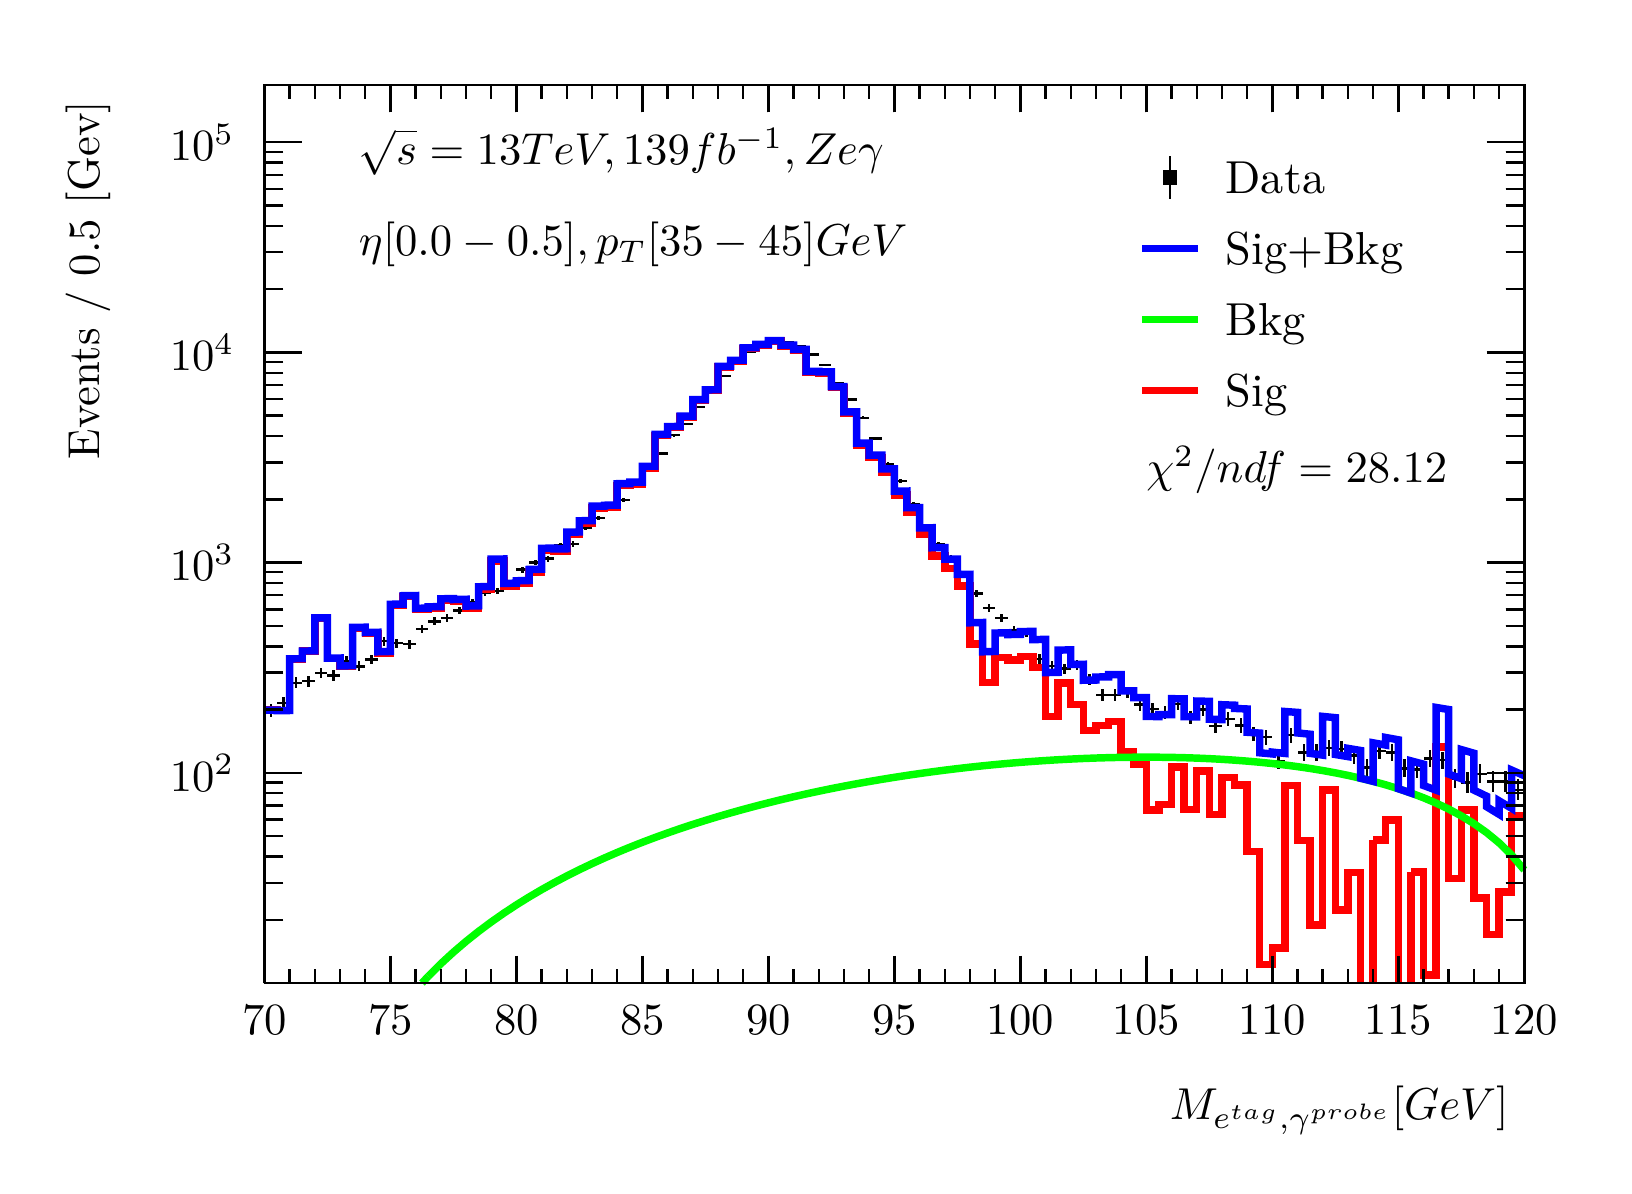
\begin{tikzpicture}
\pgfdeclareplotmark{cross} {
\pgfpathmoveto{\pgfpoint{-0.3\pgfplotmarksize}{\pgfplotmarksize}}
\pgfpathlineto{\pgfpoint{+0.3\pgfplotmarksize}{\pgfplotmarksize}}
\pgfpathlineto{\pgfpoint{+0.3\pgfplotmarksize}{0.3\pgfplotmarksize}}
\pgfpathlineto{\pgfpoint{+1\pgfplotmarksize}{0.3\pgfplotmarksize}}
\pgfpathlineto{\pgfpoint{+1\pgfplotmarksize}{-0.3\pgfplotmarksize}}
\pgfpathlineto{\pgfpoint{+0.3\pgfplotmarksize}{-0.3\pgfplotmarksize}}
\pgfpathlineto{\pgfpoint{+0.3\pgfplotmarksize}{-1.\pgfplotmarksize}}
\pgfpathlineto{\pgfpoint{-0.3\pgfplotmarksize}{-1.\pgfplotmarksize}}
\pgfpathlineto{\pgfpoint{-0.3\pgfplotmarksize}{-0.3\pgfplotmarksize}}
\pgfpathlineto{\pgfpoint{-1.\pgfplotmarksize}{-0.3\pgfplotmarksize}}
\pgfpathlineto{\pgfpoint{-1.\pgfplotmarksize}{0.3\pgfplotmarksize}}
\pgfpathlineto{\pgfpoint{-0.3\pgfplotmarksize}{0.3\pgfplotmarksize}}
\pgfpathclose
\pgfusepathqstroke
}
\pgfdeclareplotmark{cross*} {
\pgfpathmoveto{\pgfpoint{-0.3\pgfplotmarksize}{\pgfplotmarksize}}
\pgfpathlineto{\pgfpoint{+0.3\pgfplotmarksize}{\pgfplotmarksize}}
\pgfpathlineto{\pgfpoint{+0.3\pgfplotmarksize}{0.3\pgfplotmarksize}}
\pgfpathlineto{\pgfpoint{+1\pgfplotmarksize}{0.3\pgfplotmarksize}}
\pgfpathlineto{\pgfpoint{+1\pgfplotmarksize}{-0.3\pgfplotmarksize}}
\pgfpathlineto{\pgfpoint{+0.3\pgfplotmarksize}{-0.3\pgfplotmarksize}}
\pgfpathlineto{\pgfpoint{+0.3\pgfplotmarksize}{-1.\pgfplotmarksize}}
\pgfpathlineto{\pgfpoint{-0.3\pgfplotmarksize}{-1.\pgfplotmarksize}}
\pgfpathlineto{\pgfpoint{-0.3\pgfplotmarksize}{-0.3\pgfplotmarksize}}
\pgfpathlineto{\pgfpoint{-1.\pgfplotmarksize}{-0.3\pgfplotmarksize}}
\pgfpathlineto{\pgfpoint{-1.\pgfplotmarksize}{0.3\pgfplotmarksize}}
\pgfpathlineto{\pgfpoint{-0.3\pgfplotmarksize}{0.3\pgfplotmarksize}}
\pgfpathclose
\pgfusepathqfillstroke
}
\pgfdeclareplotmark{newstar} {
\pgfpathmoveto{\pgfqpoint{0pt}{\pgfplotmarksize}}
\pgfpathlineto{\pgfqpointpolar{44}{0.5\pgfplotmarksize}}
\pgfpathlineto{\pgfqpointpolar{18}{\pgfplotmarksize}}
\pgfpathlineto{\pgfqpointpolar{-20}{0.5\pgfplotmarksize}}
\pgfpathlineto{\pgfqpointpolar{-54}{\pgfplotmarksize}}
\pgfpathlineto{\pgfqpointpolar{-90}{0.5\pgfplotmarksize}}
\pgfpathlineto{\pgfqpointpolar{234}{\pgfplotmarksize}}
\pgfpathlineto{\pgfqpointpolar{198}{0.5\pgfplotmarksize}}
\pgfpathlineto{\pgfqpointpolar{162}{\pgfplotmarksize}}
\pgfpathlineto{\pgfqpointpolar{134}{0.5\pgfplotmarksize}}
\pgfpathclose
\pgfusepathqstroke
}
\pgfdeclareplotmark{newstar*} {
\pgfpathmoveto{\pgfqpoint{0pt}{\pgfplotmarksize}}
\pgfpathlineto{\pgfqpointpolar{44}{0.5\pgfplotmarksize}}
\pgfpathlineto{\pgfqpointpolar{18}{\pgfplotmarksize}}
\pgfpathlineto{\pgfqpointpolar{-20}{0.5\pgfplotmarksize}}
\pgfpathlineto{\pgfqpointpolar{-54}{\pgfplotmarksize}}
\pgfpathlineto{\pgfqpointpolar{-90}{0.5\pgfplotmarksize}}
\pgfpathlineto{\pgfqpointpolar{234}{\pgfplotmarksize}}
\pgfpathlineto{\pgfqpointpolar{198}{0.5\pgfplotmarksize}}
\pgfpathlineto{\pgfqpointpolar{162}{\pgfplotmarksize}}
\pgfpathlineto{\pgfqpointpolar{134}{0.5\pgfplotmarksize}}
\pgfpathclose
\pgfusepathqfillstroke
}
\definecolor{c}{rgb}{1,1,1};
\draw [color=c, fill=c] (0,0) rectangle (20,14.4361);
\draw [color=c, fill=c] (3,2.30977) rectangle (19,13.7143);
\definecolor{c}{rgb}{0,0,0};
\draw [c,line width=0.9] (3,2.30977) -- (3,13.7143) -- (19,13.7143) -- (19,2.30977) -- (3,2.30977);
\definecolor{c}{rgb}{1,1,1};
\draw [color=c, fill=c] (3,2.30977) rectangle (19,13.7143);
\definecolor{c}{rgb}{0,0,0};
\draw [c,line width=0.9] (3,2.30977) -- (3,13.7143) -- (19,13.7143) -- (19,2.30977) -- (3,2.30977);
\draw [c,line width=0.9] (3,2.30977) -- (19,2.30977);
\draw [c,line width=0.9] (3,2.65624) -- (3,2.30977);
\draw [c,line width=0.9] (3.32,2.48301) -- (3.32,2.30977);
\draw [c,line width=0.9] (3.64,2.48301) -- (3.64,2.30977);
\draw [c,line width=0.9] (3.96,2.48301) -- (3.96,2.30977);
\draw [c,line width=0.9] (4.28,2.48301) -- (4.28,2.30977);
\draw [c,line width=0.9] (4.6,2.65624) -- (4.6,2.30977);
\draw [c,line width=0.9] (4.92,2.48301) -- (4.92,2.30977);
\draw [c,line width=0.9] (5.24,2.48301) -- (5.24,2.30977);
\draw [c,line width=0.9] (5.56,2.48301) -- (5.56,2.30977);
\draw [c,line width=0.9] (5.88,2.48301) -- (5.88,2.30977);
\draw [c,line width=0.9] (6.2,2.65624) -- (6.2,2.30977);
\draw [c,line width=0.9] (6.52,2.48301) -- (6.52,2.30977);
\draw [c,line width=0.9] (6.84,2.48301) -- (6.84,2.30977);
\draw [c,line width=0.9] (7.16,2.48301) -- (7.16,2.30977);
\draw [c,line width=0.9] (7.48,2.48301) -- (7.48,2.30977);
\draw [c,line width=0.9] (7.8,2.65624) -- (7.8,2.30977);
\draw [c,line width=0.9] (8.12,2.48301) -- (8.12,2.30977);
\draw [c,line width=0.9] (8.44,2.48301) -- (8.44,2.30977);
\draw [c,line width=0.9] (8.76,2.48301) -- (8.76,2.30977);
\draw [c,line width=0.9] (9.08,2.48301) -- (9.08,2.30977);
\draw [c,line width=0.9] (9.4,2.65624) -- (9.4,2.30977);
\draw [c,line width=0.9] (9.72,2.48301) -- (9.72,2.30977);
\draw [c,line width=0.9] (10.04,2.48301) -- (10.04,2.30977);
\draw [c,line width=0.9] (10.36,2.48301) -- (10.36,2.30977);
\draw [c,line width=0.9] (10.68,2.48301) -- (10.68,2.30977);
\draw [c,line width=0.9] (11,2.65624) -- (11,2.30977);
\draw [c,line width=0.9] (11.32,2.48301) -- (11.32,2.30977);
\draw [c,line width=0.9] (11.64,2.48301) -- (11.64,2.30977);
\draw [c,line width=0.9] (11.96,2.48301) -- (11.96,2.30977);
\draw [c,line width=0.9] (12.28,2.48301) -- (12.28,2.30977);
\draw [c,line width=0.9] (12.6,2.65624) -- (12.6,2.30977);
\draw [c,line width=0.9] (12.92,2.48301) -- (12.92,2.30977);
\draw [c,line width=0.9] (13.24,2.48301) -- (13.24,2.30977);
\draw [c,line width=0.9] (13.56,2.48301) -- (13.56,2.30977);
\draw [c,line width=0.9] (13.88,2.48301) -- (13.88,2.30977);
\draw [c,line width=0.9] (14.2,2.65624) -- (14.2,2.30977);
\draw [c,line width=0.9] (14.52,2.48301) -- (14.52,2.30977);
\draw [c,line width=0.9] (14.84,2.48301) -- (14.84,2.30977);
\draw [c,line width=0.9] (15.16,2.48301) -- (15.16,2.30977);
\draw [c,line width=0.9] (15.48,2.48301) -- (15.48,2.30977);
\draw [c,line width=0.9] (15.8,2.65624) -- (15.8,2.30977);
\draw [c,line width=0.9] (16.12,2.48301) -- (16.12,2.30977);
\draw [c,line width=0.9] (16.44,2.48301) -- (16.44,2.30977);
\draw [c,line width=0.9] (16.76,2.48301) -- (16.76,2.30977);
\draw [c,line width=0.9] (17.08,2.48301) -- (17.08,2.30977);
\draw [c,line width=0.9] (17.4,2.65624) -- (17.4,2.30977);
\draw [c,line width=0.9] (17.72,2.48301) -- (17.72,2.30977);
\draw [c,line width=0.9] (18.04,2.48301) -- (18.04,2.30977);
\draw [c,line width=0.9] (18.36,2.48301) -- (18.36,2.30977);
\draw [c,line width=0.9] (18.68,2.48301) -- (18.68,2.30977);
\draw [c,line width=0.9] (19,2.65624) -- (19,2.30977);
\draw [anchor=base] (3,1.66015) node[scale=1.61424, color=c, rotate=0]{70};
\draw [anchor=base] (4.6,1.66015) node[scale=1.61424, color=c, rotate=0]{75};
\draw [anchor=base] (6.2,1.66015) node[scale=1.61424, color=c, rotate=0]{80};
\draw [anchor=base] (7.8,1.66015) node[scale=1.61424, color=c, rotate=0]{85};
\draw [anchor=base] (9.4,1.66015) node[scale=1.61424, color=c, rotate=0]{90};
\draw [anchor=base] (11,1.66015) node[scale=1.61424, color=c, rotate=0]{95};
\draw [anchor=base] (12.6,1.66015) node[scale=1.61424, color=c, rotate=0]{100};
\draw [anchor=base] (14.2,1.66015) node[scale=1.61424, color=c, rotate=0]{105};
\draw [anchor=base] (15.8,1.66015) node[scale=1.61424, color=c, rotate=0]{110};
\draw [anchor=base] (17.4,1.66015) node[scale=1.61424, color=c, rotate=0]{115};
\draw [anchor=base] (19,1.66015) node[scale=1.61424, color=c, rotate=0]{120};
\draw [anchor= east] (19,0.692932) node[scale=1.61424, color=c, rotate=0]{$M_{e^{tag}, \gamma^{probe}}  [GeV]$};
\draw [c,line width=0.9] (3,13.7143) -- (19,13.7143);
\draw [c,line width=0.9] (3,13.3678) -- (3,13.7143);
\draw [c,line width=0.9] (3.32,13.5411) -- (3.32,13.7143);
\draw [c,line width=0.9] (3.64,13.5411) -- (3.64,13.7143);
\draw [c,line width=0.9] (3.96,13.5411) -- (3.96,13.7143);
\draw [c,line width=0.9] (4.28,13.5411) -- (4.28,13.7143);
\draw [c,line width=0.9] (4.6,13.3678) -- (4.6,13.7143);
\draw [c,line width=0.9] (4.92,13.5411) -- (4.92,13.7143);
\draw [c,line width=0.9] (5.24,13.5411) -- (5.24,13.7143);
\draw [c,line width=0.9] (5.56,13.5411) -- (5.56,13.7143);
\draw [c,line width=0.9] (5.88,13.5411) -- (5.88,13.7143);
\draw [c,line width=0.9] (6.2,13.3678) -- (6.2,13.7143);
\draw [c,line width=0.9] (6.52,13.5411) -- (6.52,13.7143);
\draw [c,line width=0.9] (6.84,13.5411) -- (6.84,13.7143);
\draw [c,line width=0.9] (7.16,13.5411) -- (7.16,13.7143);
\draw [c,line width=0.9] (7.48,13.5411) -- (7.48,13.7143);
\draw [c,line width=0.9] (7.8,13.3678) -- (7.8,13.7143);
\draw [c,line width=0.9] (8.12,13.5411) -- (8.12,13.7143);
\draw [c,line width=0.9] (8.44,13.5411) -- (8.44,13.7143);
\draw [c,line width=0.9] (8.76,13.5411) -- (8.76,13.7143);
\draw [c,line width=0.9] (9.08,13.5411) -- (9.08,13.7143);
\draw [c,line width=0.9] (9.4,13.3678) -- (9.4,13.7143);
\draw [c,line width=0.9] (9.72,13.5411) -- (9.72,13.7143);
\draw [c,line width=0.9] (10.04,13.5411) -- (10.04,13.7143);
\draw [c,line width=0.9] (10.36,13.5411) -- (10.36,13.7143);
\draw [c,line width=0.9] (10.68,13.5411) -- (10.68,13.7143);
\draw [c,line width=0.9] (11,13.3678) -- (11,13.7143);
\draw [c,line width=0.9] (11.32,13.5411) -- (11.32,13.7143);
\draw [c,line width=0.9] (11.64,13.5411) -- (11.64,13.7143);
\draw [c,line width=0.9] (11.96,13.5411) -- (11.96,13.7143);
\draw [c,line width=0.9] (12.28,13.5411) -- (12.28,13.7143);
\draw [c,line width=0.9] (12.6,13.3678) -- (12.6,13.7143);
\draw [c,line width=0.9] (12.92,13.5411) -- (12.92,13.7143);
\draw [c,line width=0.9] (13.24,13.5411) -- (13.24,13.7143);
\draw [c,line width=0.9] (13.56,13.5411) -- (13.56,13.7143);
\draw [c,line width=0.9] (13.88,13.5411) -- (13.88,13.7143);
\draw [c,line width=0.9] (14.2,13.3678) -- (14.2,13.7143);
\draw [c,line width=0.9] (14.52,13.5411) -- (14.52,13.7143);
\draw [c,line width=0.9] (14.84,13.5411) -- (14.84,13.7143);
\draw [c,line width=0.9] (15.16,13.5411) -- (15.16,13.7143);
\draw [c,line width=0.9] (15.48,13.5411) -- (15.48,13.7143);
\draw [c,line width=0.9] (15.8,13.3678) -- (15.8,13.7143);
\draw [c,line width=0.9] (16.12,13.5411) -- (16.12,13.7143);
\draw [c,line width=0.9] (16.44,13.5411) -- (16.44,13.7143);
\draw [c,line width=0.9] (16.76,13.5411) -- (16.76,13.7143);
\draw [c,line width=0.9] (17.08,13.5411) -- (17.08,13.7143);
\draw [c,line width=0.9] (17.4,13.3678) -- (17.4,13.7143);
\draw [c,line width=0.9] (17.72,13.5411) -- (17.72,13.7143);
\draw [c,line width=0.9] (18.04,13.5411) -- (18.04,13.7143);
\draw [c,line width=0.9] (18.36,13.5411) -- (18.36,13.7143);
\draw [c,line width=0.9] (18.68,13.5411) -- (18.68,13.7143);
\draw [c,line width=0.9] (19,13.3678) -- (19,13.7143);
\draw [c,line width=0.9] (3,2.30977) -- (3,13.7143);
\draw [c,line width=0.9] (3.237,3.11343) -- (3,3.11343);
\draw [c,line width=0.9] (3.237,3.58354) -- (3,3.58354);
\draw [c,line width=0.9] (3.237,3.91709) -- (3,3.91709);
\draw [c,line width=0.9] (3.237,4.17581) -- (3,4.17581);
\draw [c,line width=0.9] (3.237,4.38719) -- (3,4.38719);
\draw [c,line width=0.9] (3.237,4.56592) -- (3,4.56592);
\draw [c,line width=0.9] (3.237,4.72074) -- (3,4.72074);
\draw [c,line width=0.9] (3.237,4.8573) -- (3,4.8573);
\draw [c,line width=0.9] (3.474,4.97946) -- (3,4.97946);
\draw [anchor= east] (2.82,4.97946) node[scale=1.61424, color=c, rotate=0]{$10^{2}$};
\draw [c,line width=0.9] (3.237,5.78312) -- (3,5.78312);
\draw [c,line width=0.9] (3.237,6.25323) -- (3,6.25323);
\draw [c,line width=0.9] (3.237,6.58678) -- (3,6.58678);
\draw [c,line width=0.9] (3.237,6.8455) -- (3,6.8455);
\draw [c,line width=0.9] (3.237,7.05689) -- (3,7.05689);
\draw [c,line width=0.9] (3.237,7.23561) -- (3,7.23561);
\draw [c,line width=0.9] (3.237,7.39043) -- (3,7.39043);
\draw [c,line width=0.9] (3.237,7.52699) -- (3,7.52699);
\draw [c,line width=0.9] (3.474,7.64915) -- (3,7.64915);
\draw [anchor= east] (2.82,7.64915) node[scale=1.61424, color=c, rotate=0]{$10^{3}$};
\draw [c,line width=0.9] (3.237,8.45281) -- (3,8.45281);
\draw [c,line width=0.9] (3.237,8.92292) -- (3,8.92292);
\draw [c,line width=0.9] (3.237,9.25647) -- (3,9.25647);
\draw [c,line width=0.9] (3.237,9.51519) -- (3,9.51519);
\draw [c,line width=0.9] (3.237,9.72658) -- (3,9.72658);
\draw [c,line width=0.9] (3.237,9.9053) -- (3,9.9053);
\draw [c,line width=0.9] (3.237,10.0601) -- (3,10.0601);
\draw [c,line width=0.9] (3.237,10.1967) -- (3,10.1967);
\draw [c,line width=0.9] (3.474,10.3188) -- (3,10.3188);
\draw [anchor= east] (2.82,10.3188) node[scale=1.61424, color=c, rotate=0]{$10^{4}$};
\draw [c,line width=0.9] (3.237,11.1225) -- (3,11.1225);
\draw [c,line width=0.9] (3.237,11.5926) -- (3,11.5926);
\draw [c,line width=0.9] (3.237,11.9262) -- (3,11.9262);
\draw [c,line width=0.9] (3.237,12.1849) -- (3,12.1849);
\draw [c,line width=0.9] (3.237,12.3963) -- (3,12.3963);
\draw [c,line width=0.9] (3.237,12.575) -- (3,12.575);
\draw [c,line width=0.9] (3.237,12.7298) -- (3,12.7298);
\draw [c,line width=0.9] (3.237,12.8664) -- (3,12.8664);
\draw [c,line width=0.9] (3.474,12.9885) -- (3,12.9885);
\draw [anchor= east] (2.82,12.9885) node[scale=1.61424, color=c, rotate=0]{$10^{5}$};
\draw [anchor= east] (0.76,13.7143) node[scale=1.61424, color=c, rotate=90]{Events / 0.5 [Gev]};
\draw [c,line width=0.9] (19,2.30977) -- (19,13.7143);
\draw [c,line width=0.9] (18.763,3.11343) -- (19,3.11343);
\draw [c,line width=0.9] (18.763,3.58354) -- (19,3.58354);
\draw [c,line width=0.9] (18.763,3.91709) -- (19,3.91709);
\draw [c,line width=0.9] (18.763,4.17581) -- (19,4.17581);
\draw [c,line width=0.9] (18.763,4.38719) -- (19,4.38719);
\draw [c,line width=0.9] (18.763,4.56592) -- (19,4.56592);
\draw [c,line width=0.9] (18.763,4.72074) -- (19,4.72074);
\draw [c,line width=0.9] (18.763,4.8573) -- (19,4.8573);
\draw [c,line width=0.9] (18.526,4.97946) -- (19,4.97946);
\draw [c,line width=0.9] (18.763,5.78312) -- (19,5.78312);
\draw [c,line width=0.9] (18.763,6.25323) -- (19,6.25323);
\draw [c,line width=0.9] (18.763,6.58678) -- (19,6.58678);
\draw [c,line width=0.9] (18.763,6.8455) -- (19,6.8455);
\draw [c,line width=0.9] (18.763,7.05689) -- (19,7.05689);
\draw [c,line width=0.9] (18.763,7.23561) -- (19,7.23561);
\draw [c,line width=0.9] (18.763,7.39043) -- (19,7.39043);
\draw [c,line width=0.9] (18.763,7.52699) -- (19,7.52699);
\draw [c,line width=0.9] (18.526,7.64915) -- (19,7.64915);
\draw [c,line width=0.9] (18.763,8.45281) -- (19,8.45281);
\draw [c,line width=0.9] (18.763,8.92292) -- (19,8.92292);
\draw [c,line width=0.9] (18.763,9.25647) -- (19,9.25647);
\draw [c,line width=0.9] (18.763,9.51519) -- (19,9.51519);
\draw [c,line width=0.9] (18.763,9.72658) -- (19,9.72658);
\draw [c,line width=0.9] (18.763,9.9053) -- (19,9.9053);
\draw [c,line width=0.9] (18.763,10.0601) -- (19,10.0601);
\draw [c,line width=0.9] (18.763,10.1967) -- (19,10.1967);
\draw [c,line width=0.9] (18.526,10.3188) -- (19,10.3188);
\draw [c,line width=0.9] (18.763,11.1225) -- (19,11.1225);
\draw [c,line width=0.9] (18.763,11.5926) -- (19,11.5926);
\draw [c,line width=0.9] (18.763,11.9262) -- (19,11.9262);
\draw [c,line width=0.9] (18.763,12.1849) -- (19,12.1849);
\draw [c,line width=0.9] (18.763,12.3963) -- (19,12.3963);
\draw [c,line width=0.9] (18.763,12.575) -- (19,12.575);
\draw [c,line width=0.9] (18.763,12.7298) -- (19,12.7298);
\draw [c,line width=0.9] (18.763,12.8664) -- (19,12.8664);
\draw [c,line width=0.9] (18.526,12.9885) -- (19,12.9885);
\draw [c,line width=0.9] (3.08,5.77147) -- (3,5.77147);
\draw [c,line width=0.9] (3,5.77147) -- (3,5.77147);
\draw [c,line width=0.9] (3.08,5.77147) -- (3.16,5.77147);
\draw [c,line width=0.9] (3.16,5.77147) -- (3.16,5.77147);
\draw [c,line width=0.9] (3.08,5.77147) -- (3.08,5.85385);
\draw [c,line width=0.9] (3.08,5.85385) -- (3.08,5.85385);
\draw [c,line width=0.9] (3.08,5.77147) -- (3.08,5.68909);
\draw [c,line width=0.9] (3.08,5.68909) -- (3.08,5.68909);
\draw [c,line width=0.9] (3.24,5.86697) -- (3.16,5.86697);
\draw [c,line width=0.9] (3.16,5.86697) -- (3.16,5.86697);
\draw [c,line width=0.9] (3.24,5.86697) -- (3.32,5.86697);
\draw [c,line width=0.9] (3.32,5.86697) -- (3.32,5.86697);
\draw [c,line width=0.9] (3.24,5.86697) -- (3.24,5.94603);
\draw [c,line width=0.9] (3.24,5.94603) -- (3.24,5.94603);
\draw [c,line width=0.9] (3.24,5.86697) -- (3.24,5.78791);
\draw [c,line width=0.9] (3.24,5.78791) -- (3.24,5.78791);
\draw [c,line width=0.9] (3.4,6.12245) -- (3.32,6.12245);
\draw [c,line width=0.9] (3.32,6.12245) -- (3.32,6.12245);
\draw [c,line width=0.9] (3.4,6.12245) -- (3.48,6.12245);
\draw [c,line width=0.9] (3.48,6.12245) -- (3.48,6.12245);
\draw [c,line width=0.9] (3.4,6.12245) -- (3.4,6.19326);
\draw [c,line width=0.9] (3.4,6.19326) -- (3.4,6.19326);
\draw [c,line width=0.9] (3.4,6.12245) -- (3.4,6.05164);
\draw [c,line width=0.9] (3.4,6.05164) -- (3.4,6.05164);
\draw [c,line width=0.9] (3.56,6.14388) -- (3.48,6.14388);
\draw [c,line width=0.9] (3.48,6.14388) -- (3.48,6.14388);
\draw [c,line width=0.9] (3.56,6.14388) -- (3.64,6.14388);
\draw [c,line width=0.9] (3.64,6.14388) -- (3.64,6.14388);
\draw [c,line width=0.9] (3.56,6.14388) -- (3.56,6.21404);
\draw [c,line width=0.9] (3.56,6.21404) -- (3.56,6.21404);
\draw [c,line width=0.9] (3.56,6.14388) -- (3.56,6.07372);
\draw [c,line width=0.9] (3.56,6.07372) -- (3.56,6.07372);
\draw [c,line width=0.9] (3.72,6.24547) -- (3.64,6.24547);
\draw [c,line width=0.9] (3.64,6.24547) -- (3.64,6.24547);
\draw [c,line width=0.9] (3.72,6.24547) -- (3.8,6.24547);
\draw [c,line width=0.9] (3.8,6.24547) -- (3.8,6.24547);
\draw [c,line width=0.9] (3.72,6.24547) -- (3.72,6.31263);
\draw [c,line width=0.9] (3.72,6.31263) -- (3.72,6.31263);
\draw [c,line width=0.9] (3.72,6.24547) -- (3.72,6.17832);
\draw [c,line width=0.9] (3.72,6.17832) -- (3.72,6.17832);
\draw [c,line width=0.9] (3.88,6.21392) -- (3.8,6.21392);
\draw [c,line width=0.9] (3.8,6.21392) -- (3.8,6.21392);
\draw [c,line width=0.9] (3.88,6.21392) -- (3.96,6.21392);
\draw [c,line width=0.9] (3.96,6.21392) -- (3.96,6.21392);
\draw [c,line width=0.9] (3.88,6.21392) -- (3.88,6.282);
\draw [c,line width=0.9] (3.88,6.282) -- (3.88,6.282);
\draw [c,line width=0.9] (3.88,6.21392) -- (3.88,6.14585);
\draw [c,line width=0.9] (3.88,6.14585) -- (3.88,6.14585);
\draw [c,line width=0.9] (4.04,6.39835) -- (3.96,6.39835);
\draw [c,line width=0.9] (3.96,6.39835) -- (3.96,6.39835);
\draw [c,line width=0.9] (4.04,6.39835) -- (4.12,6.39835);
\draw [c,line width=0.9] (4.12,6.39835) -- (4.12,6.39835);
\draw [c,line width=0.9] (4.04,6.39835) -- (4.04,6.46122);
\draw [c,line width=0.9] (4.04,6.46122) -- (4.04,6.46122);
\draw [c,line width=0.9] (4.04,6.39835) -- (4.04,6.33548);
\draw [c,line width=0.9] (4.04,6.33548) -- (4.04,6.33548);
\draw [c,line width=0.9] (4.2,6.33168) -- (4.12,6.33168);
\draw [c,line width=0.9] (4.12,6.33168) -- (4.12,6.33168);
\draw [c,line width=0.9] (4.2,6.33168) -- (4.28,6.33168);
\draw [c,line width=0.9] (4.28,6.33168) -- (4.28,6.33168);
\draw [c,line width=0.9] (4.2,6.33168) -- (4.2,6.39638);
\draw [c,line width=0.9] (4.2,6.39638) -- (4.2,6.39638);
\draw [c,line width=0.9] (4.2,6.33168) -- (4.2,6.26697);
\draw [c,line width=0.9] (4.2,6.26697) -- (4.2,6.26697);
\draw [c,line width=0.9] (4.36,6.41863) -- (4.28,6.41863);
\draw [c,line width=0.9] (4.28,6.41863) -- (4.28,6.41863);
\draw [c,line width=0.9] (4.36,6.41863) -- (4.44,6.41863);
\draw [c,line width=0.9] (4.44,6.41863) -- (4.44,6.41863);
\draw [c,line width=0.9] (4.36,6.41863) -- (4.36,6.48095);
\draw [c,line width=0.9] (4.36,6.48095) -- (4.36,6.48095);
\draw [c,line width=0.9] (4.36,6.41863) -- (4.36,6.35631);
\draw [c,line width=0.9] (4.36,6.35631) -- (4.36,6.35631);
\draw [c,line width=0.9] (4.52,6.6516) -- (4.44,6.6516);
\draw [c,line width=0.9] (4.44,6.6516) -- (4.44,6.6516);
\draw [c,line width=0.9] (4.52,6.6516) -- (4.6,6.6516);
\draw [c,line width=0.9] (4.6,6.6516) -- (4.6,6.6516);
\draw [c,line width=0.9] (4.52,6.6516) -- (4.52,6.70797);
\draw [c,line width=0.9] (4.52,6.70797) -- (4.52,6.70797);
\draw [c,line width=0.9] (4.52,6.6516) -- (4.52,6.59523);
\draw [c,line width=0.9] (4.52,6.59523) -- (4.52,6.59523);
\draw [c,line width=0.9] (4.68,6.62666) -- (4.6,6.62666);
\draw [c,line width=0.9] (4.6,6.62666) -- (4.6,6.62666);
\draw [c,line width=0.9] (4.68,6.62666) -- (4.76,6.62666);
\draw [c,line width=0.9] (4.76,6.62666) -- (4.76,6.62666);
\draw [c,line width=0.9] (4.68,6.62666) -- (4.68,6.68364);
\draw [c,line width=0.9] (4.68,6.68364) -- (4.68,6.68364);
\draw [c,line width=0.9] (4.68,6.62666) -- (4.68,6.56969);
\draw [c,line width=0.9] (4.68,6.56969) -- (4.68,6.56969);
\draw [c,line width=0.9] (4.84,6.61258) -- (4.76,6.61258);
\draw [c,line width=0.9] (4.76,6.61258) -- (4.76,6.61258);
\draw [c,line width=0.9] (4.84,6.61258) -- (4.92,6.61258);
\draw [c,line width=0.9] (4.92,6.61258) -- (4.92,6.61258);
\draw [c,line width=0.9] (4.84,6.61258) -- (4.84,6.6699);
\draw [c,line width=0.9] (4.84,6.6699) -- (4.84,6.6699);
\draw [c,line width=0.9] (4.84,6.61258) -- (4.84,6.55525);
\draw [c,line width=0.9] (4.84,6.55525) -- (4.84,6.55525);
\draw [c,line width=0.9] (5,6.80779) -- (4.92,6.80779);
\draw [c,line width=0.9] (4.92,6.80779) -- (4.92,6.80779);
\draw [c,line width=0.9] (5,6.80779) -- (5.08,6.80779);
\draw [c,line width=0.9] (5.08,6.80779) -- (5.08,6.80779);
\draw [c,line width=0.9] (5,6.80779) -- (5,6.86049);
\draw [c,line width=0.9] (5,6.86049) -- (5,6.86049);
\draw [c,line width=0.9] (5,6.80779) -- (5,6.75509);
\draw [c,line width=0.9] (5,6.75509) -- (5,6.75509);
\draw [c,line width=0.9] (5.16,6.90207) -- (5.08,6.90207);
\draw [c,line width=0.9] (5.08,6.90207) -- (5.08,6.90207);
\draw [c,line width=0.9] (5.16,6.90207) -- (5.24,6.90207);
\draw [c,line width=0.9] (5.24,6.90207) -- (5.24,6.90207);
\draw [c,line width=0.9] (5.16,6.90207) -- (5.16,6.95266);
\draw [c,line width=0.9] (5.16,6.95266) -- (5.16,6.95266);
\draw [c,line width=0.9] (5.16,6.90207) -- (5.16,6.85147);
\draw [c,line width=0.9] (5.16,6.85147) -- (5.16,6.85147);
\draw [c,line width=0.9] (5.32,6.94754) -- (5.24,6.94754);
\draw [c,line width=0.9] (5.24,6.94754) -- (5.24,6.94754);
\draw [c,line width=0.9] (5.32,6.94754) -- (5.4,6.94754);
\draw [c,line width=0.9] (5.4,6.94754) -- (5.4,6.94754);
\draw [c,line width=0.9] (5.32,6.94754) -- (5.32,6.99716);
\draw [c,line width=0.9] (5.32,6.99716) -- (5.32,6.99716);
\draw [c,line width=0.9] (5.32,6.94754) -- (5.32,6.89792);
\draw [c,line width=0.9] (5.32,6.89792) -- (5.32,6.89792);
\draw [c,line width=0.9] (5.48,7.03936) -- (5.4,7.03936);
\draw [c,line width=0.9] (5.4,7.03936) -- (5.4,7.03936);
\draw [c,line width=0.9] (5.48,7.03936) -- (5.56,7.03936);
\draw [c,line width=0.9] (5.56,7.03936) -- (5.56,7.03936);
\draw [c,line width=0.9] (5.48,7.03936) -- (5.48,7.08705);
\draw [c,line width=0.9] (5.48,7.08705) -- (5.48,7.08705);
\draw [c,line width=0.9] (5.48,7.03936) -- (5.48,6.99167);
\draw [c,line width=0.9] (5.48,6.99167) -- (5.48,6.99167);
\draw [c,line width=0.9] (5.64,7.14074) -- (5.56,7.14074);
\draw [c,line width=0.9] (5.56,7.14074) -- (5.56,7.14074);
\draw [c,line width=0.9] (5.64,7.14074) -- (5.72,7.14074);
\draw [c,line width=0.9] (5.72,7.14074) -- (5.72,7.14074);
\draw [c,line width=0.9] (5.64,7.14074) -- (5.64,7.18639);
\draw [c,line width=0.9] (5.64,7.18639) -- (5.64,7.18639);
\draw [c,line width=0.9] (5.64,7.14074) -- (5.64,7.09509);
\draw [c,line width=0.9] (5.64,7.09509) -- (5.64,7.09509);
\draw [c,line width=0.9] (5.8,7.26666) -- (5.72,7.26666);
\draw [c,line width=0.9] (5.72,7.26666) -- (5.72,7.26666);
\draw [c,line width=0.9] (5.8,7.26666) -- (5.88,7.26666);
\draw [c,line width=0.9] (5.88,7.26666) -- (5.88,7.26666);
\draw [c,line width=0.9] (5.8,7.26666) -- (5.8,7.3099);
\draw [c,line width=0.9] (5.8,7.3099) -- (5.8,7.3099);
\draw [c,line width=0.9] (5.8,7.26666) -- (5.8,7.22343);
\draw [c,line width=0.9] (5.8,7.22343) -- (5.8,7.22343);
\draw [c,line width=0.9] (5.96,7.28902) -- (5.88,7.28902);
\draw [c,line width=0.9] (5.88,7.28902) -- (5.88,7.28902);
\draw [c,line width=0.9] (5.96,7.28902) -- (6.04,7.28902);
\draw [c,line width=0.9] (6.04,7.28902) -- (6.04,7.28902);
\draw [c,line width=0.9] (5.96,7.28902) -- (5.96,7.33185);
\draw [c,line width=0.9] (5.96,7.33185) -- (5.96,7.33185);
\draw [c,line width=0.9] (5.96,7.28902) -- (5.96,7.2462);
\draw [c,line width=0.9] (5.96,7.2462) -- (5.96,7.2462);
\draw [c,line width=0.9] (6.12,7.36553) -- (6.04,7.36553);
\draw [c,line width=0.9] (6.04,7.36553) -- (6.04,7.36553);
\draw [c,line width=0.9] (6.12,7.36553) -- (6.2,7.36553);
\draw [c,line width=0.9] (6.2,7.36553) -- (6.2,7.36553);
\draw [c,line width=0.9] (6.12,7.36553) -- (6.12,7.40696);
\draw [c,line width=0.9] (6.12,7.40696) -- (6.12,7.40696);
\draw [c,line width=0.9] (6.12,7.36553) -- (6.12,7.3241);
\draw [c,line width=0.9] (6.12,7.3241) -- (6.12,7.3241);
\draw [c,line width=0.9] (6.28,7.55876) -- (6.2,7.55876);
\draw [c,line width=0.9] (6.2,7.55876) -- (6.2,7.55876);
\draw [c,line width=0.9] (6.28,7.55876) -- (6.36,7.55876);
\draw [c,line width=0.9] (6.36,7.55876) -- (6.36,7.55876);
\draw [c,line width=0.9] (6.28,7.55876) -- (6.28,7.59688);
\draw [c,line width=0.9] (6.28,7.59688) -- (6.28,7.59688);
\draw [c,line width=0.9] (6.28,7.55876) -- (6.28,7.52064);
\draw [c,line width=0.9] (6.28,7.52064) -- (6.28,7.52064);
\draw [c,line width=0.9] (6.44,7.65031) -- (6.36,7.65031);
\draw [c,line width=0.9] (6.36,7.65031) -- (6.36,7.65031);
\draw [c,line width=0.9] (6.44,7.65031) -- (6.52,7.65031);
\draw [c,line width=0.9] (6.52,7.65031) -- (6.52,7.65031);
\draw [c,line width=0.9] (6.44,7.65031) -- (6.44,7.68696);
\draw [c,line width=0.9] (6.44,7.68696) -- (6.44,7.68696);
\draw [c,line width=0.9] (6.44,7.65031) -- (6.44,7.61367);
\draw [c,line width=0.9] (6.44,7.61367) -- (6.44,7.61367);
\draw [c,line width=0.9] (6.6,7.69908) -- (6.52,7.69908);
\draw [c,line width=0.9] (6.52,7.69908) -- (6.52,7.69908);
\draw [c,line width=0.9] (6.6,7.69908) -- (6.68,7.69908);
\draw [c,line width=0.9] (6.68,7.69908) -- (6.68,7.69908);
\draw [c,line width=0.9] (6.6,7.69908) -- (6.6,7.73496);
\draw [c,line width=0.9] (6.6,7.73496) -- (6.6,7.73496);
\draw [c,line width=0.9] (6.6,7.69908) -- (6.6,7.6632);
\draw [c,line width=0.9] (6.6,7.6632) -- (6.6,7.6632);
\draw [c,line width=0.9] (6.76,7.87112) -- (6.68,7.87112);
\draw [c,line width=0.9] (6.68,7.87112) -- (6.68,7.87112);
\draw [c,line width=0.9] (6.76,7.87112) -- (6.84,7.87112);
\draw [c,line width=0.9] (6.84,7.87112) -- (6.84,7.87112);
\draw [c,line width=0.9] (6.76,7.87112) -- (6.76,7.90444);
\draw [c,line width=0.9] (6.76,7.90444) -- (6.76,7.90444);
\draw [c,line width=0.9] (6.76,7.87112) -- (6.76,7.83781);
\draw [c,line width=0.9] (6.76,7.83781) -- (6.76,7.83781);
\draw [c,line width=0.9] (6.92,7.8854) -- (6.84,7.8854);
\draw [c,line width=0.9] (6.84,7.8854) -- (6.84,7.8854);
\draw [c,line width=0.9] (6.92,7.8854) -- (7,7.8854);
\draw [c,line width=0.9] (7,7.8854) -- (7,7.8854);
\draw [c,line width=0.9] (6.92,7.8854) -- (6.92,7.91851);
\draw [c,line width=0.9] (6.92,7.91851) -- (6.92,7.91851);
\draw [c,line width=0.9] (6.92,7.8854) -- (6.92,7.85228);
\draw [c,line width=0.9] (6.92,7.85228) -- (6.92,7.85228);
\draw [c,line width=0.9] (7.08,8.09426) -- (7,8.09426);
\draw [c,line width=0.9] (7,8.09426) -- (7,8.09426);
\draw [c,line width=0.9] (7.08,8.09426) -- (7.16,8.09426);
\draw [c,line width=0.9] (7.16,8.09426) -- (7.16,8.09426);
\draw [c,line width=0.9] (7.08,8.09426) -- (7.08,8.12452);
\draw [c,line width=0.9] (7.08,8.12452) -- (7.08,8.12452);
\draw [c,line width=0.9] (7.08,8.09426) -- (7.08,8.064);
\draw [c,line width=0.9] (7.08,8.064) -- (7.08,8.064);
\draw [c,line width=0.9] (7.24,8.21705) -- (7.16,8.21705);
\draw [c,line width=0.9] (7.16,8.21705) -- (7.16,8.21705);
\draw [c,line width=0.9] (7.24,8.21705) -- (7.32,8.21705);
\draw [c,line width=0.9] (7.32,8.21705) -- (7.32,8.21705);
\draw [c,line width=0.9] (7.24,8.21705) -- (7.24,8.24575);
\draw [c,line width=0.9] (7.24,8.24575) -- (7.24,8.24575);
\draw [c,line width=0.9] (7.24,8.21705) -- (7.24,8.18835);
\draw [c,line width=0.9] (7.24,8.18835) -- (7.24,8.18835);
\draw [c,line width=0.9] (7.4,8.37365) -- (7.32,8.37365);
\draw [c,line width=0.9] (7.32,8.37365) -- (7.32,8.37365);
\draw [c,line width=0.9] (7.4,8.37365) -- (7.48,8.37365);
\draw [c,line width=0.9] (7.48,8.37365) -- (7.48,8.37365);
\draw [c,line width=0.9] (7.4,8.37365) -- (7.4,8.40047);
\draw [c,line width=0.9] (7.4,8.40047) -- (7.4,8.40047);
\draw [c,line width=0.9] (7.4,8.37365) -- (7.4,8.34682);
\draw [c,line width=0.9] (7.4,8.34682) -- (7.4,8.34682);
\draw [c,line width=0.9] (7.56,8.44233) -- (7.48,8.44233);
\draw [c,line width=0.9] (7.48,8.44233) -- (7.48,8.44233);
\draw [c,line width=0.9] (7.56,8.44233) -- (7.64,8.44233);
\draw [c,line width=0.9] (7.64,8.44233) -- (7.64,8.44233);
\draw [c,line width=0.9] (7.56,8.44233) -- (7.56,8.46837);
\draw [c,line width=0.9] (7.56,8.46837) -- (7.56,8.46837);
\draw [c,line width=0.9] (7.56,8.44233) -- (7.56,8.41629);
\draw [c,line width=0.9] (7.56,8.41629) -- (7.56,8.41629);
\draw [c,line width=0.9] (7.72,8.68526) -- (7.64,8.68526);
\draw [c,line width=0.9] (7.64,8.68526) -- (7.64,8.68526);
\draw [c,line width=0.9] (7.72,8.68526) -- (7.8,8.68526);
\draw [c,line width=0.9] (7.8,8.68526) -- (7.8,8.68526);
\draw [c,line width=0.9] (7.72,8.68526) -- (7.72,8.70872);
\draw [c,line width=0.9] (7.72,8.70872) -- (7.72,8.70872);
\draw [c,line width=0.9] (7.72,8.68526) -- (7.72,8.66181);
\draw [c,line width=0.9] (7.72,8.66181) -- (7.72,8.66181);
\draw [c,line width=0.9] (7.88,8.83336) -- (7.8,8.83336);
\draw [c,line width=0.9] (7.8,8.83336) -- (7.8,8.83336);
\draw [c,line width=0.9] (7.88,8.83336) -- (7.96,8.83336);
\draw [c,line width=0.9] (7.96,8.83336) -- (7.96,8.83336);
\draw [c,line width=0.9] (7.88,8.83336) -- (7.88,8.85537);
\draw [c,line width=0.9] (7.88,8.85537) -- (7.88,8.85537);
\draw [c,line width=0.9] (7.88,8.83336) -- (7.88,8.81136);
\draw [c,line width=0.9] (7.88,8.81136) -- (7.88,8.81136);
\draw [c,line width=0.9] (8.04,9.03763) -- (7.96,9.03763);
\draw [c,line width=0.9] (7.96,9.03763) -- (7.96,9.03763);
\draw [c,line width=0.9] (8.04,9.03763) -- (8.12,9.03763);
\draw [c,line width=0.9] (8.12,9.03763) -- (8.12,9.03763);
\draw [c,line width=0.9] (8.04,9.03763) -- (8.04,9.05778);
\draw [c,line width=0.9] (8.04,9.05778) -- (8.04,9.05778);
\draw [c,line width=0.9] (8.04,9.03763) -- (8.04,9.01749);
\draw [c,line width=0.9] (8.04,9.01749) -- (8.04,9.01749);
\draw [c,line width=0.9] (8.2,9.26858) -- (8.12,9.26858);
\draw [c,line width=0.9] (8.12,9.26858) -- (8.12,9.26858);
\draw [c,line width=0.9] (8.2,9.26858) -- (8.28,9.26858);
\draw [c,line width=0.9] (8.28,9.26858) -- (8.28,9.26858);
\draw [c,line width=0.9] (8.2,9.26858) -- (8.2,9.28681);
\draw [c,line width=0.9] (8.2,9.28681) -- (8.2,9.28681);
\draw [c,line width=0.9] (8.2,9.26858) -- (8.2,9.25034);
\draw [c,line width=0.9] (8.2,9.25034) -- (8.2,9.25034);
\draw [c,line width=0.9] (8.36,9.41093) -- (8.28,9.41093);
\draw [c,line width=0.9] (8.28,9.41093) -- (8.28,9.41093);
\draw [c,line width=0.9] (8.36,9.41093) -- (8.44,9.41093);
\draw [c,line width=0.9] (8.44,9.41093) -- (8.44,9.41093);
\draw [c,line width=0.9] (8.36,9.41093) -- (8.36,9.42808);
\draw [c,line width=0.9] (8.36,9.42808) -- (8.36,9.42808);
\draw [c,line width=0.9] (8.36,9.41093) -- (8.36,9.39377);
\draw [c,line width=0.9] (8.36,9.39377) -- (8.36,9.39377);
\draw [c,line width=0.9] (8.52,9.62801) -- (8.44,9.62801);
\draw [c,line width=0.9] (8.44,9.62801) -- (8.44,9.62801);
\draw [c,line width=0.9] (8.52,9.62801) -- (8.6,9.62801);
\draw [c,line width=0.9] (8.6,9.62801) -- (8.6,9.62801);
\draw [c,line width=0.9] (8.52,9.62801) -- (8.52,9.64363);
\draw [c,line width=0.9] (8.52,9.64363) -- (8.52,9.64363);
\draw [c,line width=0.9] (8.52,9.62801) -- (8.52,9.61239);
\draw [c,line width=0.9] (8.52,9.61239) -- (8.52,9.61239);
\draw [c,line width=0.9] (8.68,9.85105) -- (8.6,9.85105);
\draw [c,line width=0.9] (8.6,9.85105) -- (8.6,9.85105);
\draw [c,line width=0.9] (8.68,9.85105) -- (8.76,9.85105);
\draw [c,line width=0.9] (8.76,9.85105) -- (8.76,9.85105);
\draw [c,line width=0.9] (8.68,9.85105) -- (8.68,9.86524);
\draw [c,line width=0.9] (8.68,9.86524) -- (8.68,9.86524);
\draw [c,line width=0.9] (8.68,9.85105) -- (8.68,9.83687);
\draw [c,line width=0.9] (8.68,9.83687) -- (8.68,9.83687);
\draw [c,line width=0.9] (8.84,10.0176) -- (8.76,10.0176);
\draw [c,line width=0.9] (8.76,10.0176) -- (8.76,10.0176);
\draw [c,line width=0.9] (8.84,10.0176) -- (8.92,10.0176);
\draw [c,line width=0.9] (8.92,10.0176) -- (8.92,10.0176);
\draw [c,line width=0.9] (8.84,10.0176) -- (8.84,10.0308);
\draw [c,line width=0.9] (8.84,10.0308) -- (8.84,10.0308);
\draw [c,line width=0.9] (8.84,10.0176) -- (8.84,10.0044);
\draw [c,line width=0.9] (8.84,10.0044) -- (8.84,10.0044);
\draw [c,line width=0.9] (9,10.1863) -- (8.92,10.1863);
\draw [c,line width=0.9] (8.92,10.1863) -- (8.92,10.1863);
\draw [c,line width=0.9] (9,10.1863) -- (9.08,10.1863);
\draw [c,line width=0.9] (9.08,10.1863) -- (9.08,10.1863);
\draw [c,line width=0.9] (9,10.1863) -- (9,10.1986);
\draw [c,line width=0.9] (9,10.1986) -- (9,10.1986);
\draw [c,line width=0.9] (9,10.1863) -- (9,10.1741);
\draw [c,line width=0.9] (9,10.1741) -- (9,10.1741);
\draw [c,line width=0.9] (9.16,10.3322) -- (9.08,10.3322);
\draw [c,line width=0.9] (9.08,10.3322) -- (9.08,10.3322);
\draw [c,line width=0.9] (9.16,10.3322) -- (9.24,10.3322);
\draw [c,line width=0.9] (9.24,10.3322) -- (9.24,10.3322);
\draw [c,line width=0.9] (9.16,10.3322) -- (9.16,10.3437);
\draw [c,line width=0.9] (9.16,10.3437) -- (9.16,10.3437);
\draw [c,line width=0.9] (9.16,10.3322) -- (9.16,10.3207);
\draw [c,line width=0.9] (9.16,10.3207) -- (9.16,10.3207);
\draw [c,line width=0.9] (9.32,10.4103) -- (9.24,10.4103);
\draw [c,line width=0.9] (9.24,10.4103) -- (9.24,10.4103);
\draw [c,line width=0.9] (9.32,10.4103) -- (9.4,10.4103);
\draw [c,line width=0.9] (9.4,10.4103) -- (9.4,10.4103);
\draw [c,line width=0.9] (9.32,10.4103) -- (9.32,10.4215);
\draw [c,line width=0.9] (9.32,10.4215) -- (9.32,10.4215);
\draw [c,line width=0.9] (9.32,10.4103) -- (9.32,10.3992);
\draw [c,line width=0.9] (9.32,10.3992) -- (9.32,10.3992);
\draw [c,line width=0.9] (9.48,10.4655) -- (9.4,10.4655);
\draw [c,line width=0.9] (9.4,10.4655) -- (9.4,10.4655);
\draw [c,line width=0.9] (9.48,10.4655) -- (9.56,10.4655);
\draw [c,line width=0.9] (9.56,10.4655) -- (9.56,10.4655);
\draw [c,line width=0.9] (9.48,10.4655) -- (9.48,10.4763);
\draw [c,line width=0.9] (9.48,10.4763) -- (9.48,10.4763);
\draw [c,line width=0.9] (9.48,10.4655) -- (9.48,10.4546);
\draw [c,line width=0.9] (9.48,10.4546) -- (9.48,10.4546);
\draw [c,line width=0.9] (9.64,10.4522) -- (9.56,10.4522);
\draw [c,line width=0.9] (9.56,10.4522) -- (9.56,10.4522);
\draw [c,line width=0.9] (9.64,10.4522) -- (9.72,10.4522);
\draw [c,line width=0.9] (9.72,10.4522) -- (9.72,10.4522);
\draw [c,line width=0.9] (9.64,10.4522) -- (9.64,10.4632);
\draw [c,line width=0.9] (9.64,10.4632) -- (9.64,10.4632);
\draw [c,line width=0.9] (9.64,10.4522) -- (9.64,10.4413);
\draw [c,line width=0.9] (9.64,10.4413) -- (9.64,10.4413);
\draw [c,line width=0.9] (9.8,10.3965) -- (9.72,10.3965);
\draw [c,line width=0.9] (9.72,10.3965) -- (9.72,10.3965);
\draw [c,line width=0.9] (9.8,10.3965) -- (9.88,10.3965);
\draw [c,line width=0.9] (9.88,10.3965) -- (9.88,10.3965);
\draw [c,line width=0.9] (9.8,10.3965) -- (9.8,10.4077);
\draw [c,line width=0.9] (9.8,10.4077) -- (9.8,10.4077);
\draw [c,line width=0.9] (9.8,10.3965) -- (9.8,10.3853);
\draw [c,line width=0.9] (9.8,10.3853) -- (9.8,10.3853);
\draw [c,line width=0.9] (9.96,10.2945) -- (9.88,10.2945);
\draw [c,line width=0.9] (9.88,10.2945) -- (9.88,10.2945);
\draw [c,line width=0.9] (9.96,10.2945) -- (10.04,10.2945);
\draw [c,line width=0.9] (10.04,10.2945) -- (10.04,10.2945);
\draw [c,line width=0.9] (9.96,10.2945) -- (9.96,10.3062);
\draw [c,line width=0.9] (9.96,10.3062) -- (9.96,10.3062);
\draw [c,line width=0.9] (9.96,10.2945) -- (9.96,10.2828);
\draw [c,line width=0.9] (9.96,10.2828) -- (9.96,10.2828);
\draw [c,line width=0.9] (10.12,10.1619) -- (10.04,10.1619);
\draw [c,line width=0.9] (10.04,10.1619) -- (10.04,10.1619);
\draw [c,line width=0.9] (10.12,10.1619) -- (10.2,10.1619);
\draw [c,line width=0.9] (10.2,10.1619) -- (10.2,10.1619);
\draw [c,line width=0.9] (10.12,10.1619) -- (10.12,10.1743);
\draw [c,line width=0.9] (10.12,10.1743) -- (10.12,10.1743);
\draw [c,line width=0.9] (10.12,10.1619) -- (10.12,10.1495);
\draw [c,line width=0.9] (10.12,10.1495) -- (10.12,10.1495);
\draw [c,line width=0.9] (10.28,9.9328) -- (10.2,9.9328);
\draw [c,line width=0.9] (10.2,9.9328) -- (10.2,9.9328);
\draw [c,line width=0.9] (10.28,9.9328) -- (10.36,9.9328);
\draw [c,line width=0.9] (10.36,9.9328) -- (10.36,9.9328);
\draw [c,line width=0.9] (10.28,9.9328) -- (10.28,9.9465);
\draw [c,line width=0.9] (10.28,9.9465) -- (10.28,9.9465);
\draw [c,line width=0.9] (10.28,9.9328) -- (10.28,9.91911);
\draw [c,line width=0.9] (10.28,9.91911) -- (10.28,9.91911);
\draw [c,line width=0.9] (10.44,9.71979) -- (10.36,9.71979);
\draw [c,line width=0.9] (10.36,9.71979) -- (10.36,9.71979);
\draw [c,line width=0.9] (10.44,9.71979) -- (10.52,9.71979);
\draw [c,line width=0.9] (10.52,9.71979) -- (10.52,9.71979);
\draw [c,line width=0.9] (10.44,9.71979) -- (10.44,9.73481);
\draw [c,line width=0.9] (10.44,9.73481) -- (10.44,9.73481);
\draw [c,line width=0.9] (10.44,9.71979) -- (10.44,9.70478);
\draw [c,line width=0.9] (10.44,9.70478) -- (10.44,9.70478);
\draw [c,line width=0.9] (10.6,9.48868) -- (10.52,9.48868);
\draw [c,line width=0.9] (10.52,9.48868) -- (10.52,9.48868);
\draw [c,line width=0.9] (10.6,9.48868) -- (10.68,9.48868);
\draw [c,line width=0.9] (10.68,9.48868) -- (10.68,9.48868);
\draw [c,line width=0.9] (10.6,9.48868) -- (10.6,9.50527);
\draw [c,line width=0.9] (10.6,9.50527) -- (10.6,9.50527);
\draw [c,line width=0.9] (10.6,9.48868) -- (10.6,9.4721);
\draw [c,line width=0.9] (10.6,9.4721) -- (10.6,9.4721);
\draw [c,line width=0.9] (10.76,9.2283) -- (10.68,9.2283);
\draw [c,line width=0.9] (10.68,9.2283) -- (10.68,9.2283);
\draw [c,line width=0.9] (10.76,9.2283) -- (10.84,9.2283);
\draw [c,line width=0.9] (10.84,9.2283) -- (10.84,9.2283);
\draw [c,line width=0.9] (10.76,9.2283) -- (10.76,9.24686);
\draw [c,line width=0.9] (10.76,9.24686) -- (10.76,9.24686);
\draw [c,line width=0.9] (10.76,9.2283) -- (10.76,9.20975);
\draw [c,line width=0.9] (10.76,9.20975) -- (10.76,9.20975);
\draw [c,line width=0.9] (10.92,8.8995) -- (10.84,8.8995);
\draw [c,line width=0.9] (10.84,8.8995) -- (10.84,8.8995);
\draw [c,line width=0.9] (10.92,8.8995) -- (11,8.8995);
\draw [c,line width=0.9] (11,8.8995) -- (11,8.8995);
\draw [c,line width=0.9] (10.92,8.8995) -- (10.92,8.92088);
\draw [c,line width=0.9] (10.92,8.92088) -- (10.92,8.92088);
\draw [c,line width=0.9] (10.92,8.8995) -- (10.92,8.87811);
\draw [c,line width=0.9] (10.92,8.87811) -- (10.92,8.87811);
\draw [c,line width=0.9] (11.08,8.68716) -- (11,8.68716);
\draw [c,line width=0.9] (11,8.68716) -- (11,8.68716);
\draw [c,line width=0.9] (11.08,8.68716) -- (11.16,8.68716);
\draw [c,line width=0.9] (11.16,8.68716) -- (11.16,8.68716);
\draw [c,line width=0.9] (11.08,8.68716) -- (11.08,8.71059);
\draw [c,line width=0.9] (11.08,8.71059) -- (11.08,8.71059);
\draw [c,line width=0.9] (11.08,8.68716) -- (11.08,8.66373);
\draw [c,line width=0.9] (11.08,8.66373) -- (11.08,8.66373);
\draw [c,line width=0.9] (11.24,8.3909) -- (11.16,8.3909);
\draw [c,line width=0.9] (11.16,8.3909) -- (11.16,8.3909);
\draw [c,line width=0.9] (11.24,8.3909) -- (11.32,8.3909);
\draw [c,line width=0.9] (11.32,8.3909) -- (11.32,8.3909);
\draw [c,line width=0.9] (11.24,8.3909) -- (11.24,8.41752);
\draw [c,line width=0.9] (11.24,8.41752) -- (11.24,8.41752);
\draw [c,line width=0.9] (11.24,8.3909) -- (11.24,8.36427);
\draw [c,line width=0.9] (11.24,8.36427) -- (11.24,8.36427);
\draw [c,line width=0.9] (11.4,8.09426) -- (11.32,8.09426);
\draw [c,line width=0.9] (11.32,8.09426) -- (11.32,8.09426);
\draw [c,line width=0.9] (11.4,8.09426) -- (11.48,8.09426);
\draw [c,line width=0.9] (11.48,8.09426) -- (11.48,8.09426);
\draw [c,line width=0.9] (11.4,8.09426) -- (11.4,8.12452);
\draw [c,line width=0.9] (11.4,8.12452) -- (11.4,8.12452);
\draw [c,line width=0.9] (11.4,8.09426) -- (11.4,8.064);
\draw [c,line width=0.9] (11.4,8.064) -- (11.4,8.064);
\draw [c,line width=0.9] (11.56,7.88161) -- (11.48,7.88161);
\draw [c,line width=0.9] (11.48,7.88161) -- (11.48,7.88161);
\draw [c,line width=0.9] (11.56,7.88161) -- (11.64,7.88161);
\draw [c,line width=0.9] (11.64,7.88161) -- (11.64,7.88161);
\draw [c,line width=0.9] (11.56,7.88161) -- (11.56,7.91477);
\draw [c,line width=0.9] (11.56,7.91477) -- (11.56,7.91477);
\draw [c,line width=0.9] (11.56,7.88161) -- (11.56,7.84844);
\draw [c,line width=0.9] (11.56,7.84844) -- (11.56,7.84844);
\draw [c,line width=0.9] (11.72,7.71013) -- (11.64,7.71013);
\draw [c,line width=0.9] (11.64,7.71013) -- (11.64,7.71013);
\draw [c,line width=0.9] (11.72,7.71013) -- (11.8,7.71013);
\draw [c,line width=0.9] (11.8,7.71013) -- (11.8,7.71013);
\draw [c,line width=0.9] (11.72,7.71013) -- (11.72,7.74584);
\draw [c,line width=0.9] (11.72,7.74584) -- (11.72,7.74584);
\draw [c,line width=0.9] (11.72,7.71013) -- (11.72,7.67442);
\draw [c,line width=0.9] (11.72,7.67442) -- (11.72,7.67442);
\draw [c,line width=0.9] (11.88,7.49035) -- (11.8,7.49035);
\draw [c,line width=0.9] (11.8,7.49035) -- (11.8,7.49035);
\draw [c,line width=0.9] (11.88,7.49035) -- (11.96,7.49035);
\draw [c,line width=0.9] (11.96,7.49035) -- (11.96,7.49035);
\draw [c,line width=0.9] (11.88,7.49035) -- (11.88,7.52961);
\draw [c,line width=0.9] (11.88,7.52961) -- (11.88,7.52961);
\draw [c,line width=0.9] (11.88,7.49035) -- (11.88,7.45109);
\draw [c,line width=0.9] (11.88,7.45109) -- (11.88,7.45109);
\draw [c,line width=0.9] (12.04,7.25695) -- (11.96,7.25695);
\draw [c,line width=0.9] (11.96,7.25695) -- (11.96,7.25695);
\draw [c,line width=0.9] (12.04,7.25695) -- (12.12,7.25695);
\draw [c,line width=0.9] (12.12,7.25695) -- (12.12,7.25695);
\draw [c,line width=0.9] (12.04,7.25695) -- (12.04,7.30037);
\draw [c,line width=0.9] (12.04,7.30037) -- (12.04,7.30037);
\draw [c,line width=0.9] (12.04,7.25695) -- (12.04,7.21353);
\draw [c,line width=0.9] (12.04,7.21353) -- (12.04,7.21353);
\draw [c,line width=0.9] (12.2,7.07034) -- (12.12,7.07034);
\draw [c,line width=0.9] (12.12,7.07034) -- (12.12,7.07034);
\draw [c,line width=0.9] (12.2,7.07034) -- (12.28,7.07034);
\draw [c,line width=0.9] (12.28,7.07034) -- (12.28,7.07034);
\draw [c,line width=0.9] (12.2,7.07034) -- (12.2,7.11739);
\draw [c,line width=0.9] (12.2,7.11739) -- (12.2,7.11739);
\draw [c,line width=0.9] (12.2,7.07034) -- (12.2,7.02328);
\draw [c,line width=0.9] (12.2,7.02328) -- (12.2,7.02328);
\draw [c,line width=0.9] (12.36,6.94329) -- (12.28,6.94329);
\draw [c,line width=0.9] (12.28,6.94329) -- (12.28,6.94329);
\draw [c,line width=0.9] (12.36,6.94329) -- (12.44,6.94329);
\draw [c,line width=0.9] (12.44,6.94329) -- (12.44,6.94329);
\draw [c,line width=0.9] (12.36,6.94329) -- (12.36,6.99299);
\draw [c,line width=0.9] (12.36,6.99299) -- (12.36,6.99299);
\draw [c,line width=0.9] (12.36,6.94329) -- (12.36,6.89358);
\draw [c,line width=0.9] (12.36,6.89358) -- (12.36,6.89358);
\draw [c,line width=0.9] (12.52,6.79575) -- (12.44,6.79575);
\draw [c,line width=0.9] (12.44,6.79575) -- (12.44,6.79575);
\draw [c,line width=0.9] (12.52,6.79575) -- (12.6,6.79575);
\draw [c,line width=0.9] (12.6,6.79575) -- (12.6,6.79575);
\draw [c,line width=0.9] (12.52,6.79575) -- (12.52,6.84872);
\draw [c,line width=0.9] (12.52,6.84872) -- (12.52,6.84872);
\draw [c,line width=0.9] (12.52,6.79575) -- (12.52,6.74278);
\draw [c,line width=0.9] (12.52,6.74278) -- (12.52,6.74278);
\draw [c,line width=0.9] (12.68,6.75636) -- (12.6,6.75636);
\draw [c,line width=0.9] (12.6,6.75636) -- (12.6,6.75636);
\draw [c,line width=0.9] (12.68,6.75636) -- (12.76,6.75636);
\draw [c,line width=0.9] (12.76,6.75636) -- (12.76,6.75636);
\draw [c,line width=0.9] (12.68,6.75636) -- (12.68,6.81024);
\draw [c,line width=0.9] (12.68,6.81024) -- (12.68,6.81024);
\draw [c,line width=0.9] (12.68,6.75636) -- (12.68,6.70248);
\draw [c,line width=0.9] (12.68,6.70248) -- (12.68,6.70248);
\draw [c,line width=0.9] (12.84,6.42198) -- (12.76,6.42198);
\draw [c,line width=0.9] (12.76,6.42198) -- (12.76,6.42198);
\draw [c,line width=0.9] (12.84,6.42198) -- (12.92,6.42198);
\draw [c,line width=0.9] (12.92,6.42198) -- (12.92,6.42198);
\draw [c,line width=0.9] (12.84,6.42198) -- (12.84,6.48421);
\draw [c,line width=0.9] (12.84,6.48421) -- (12.84,6.48421);
\draw [c,line width=0.9] (12.84,6.42198) -- (12.84,6.35974);
\draw [c,line width=0.9] (12.84,6.35974) -- (12.84,6.35974);
\draw [c,line width=0.9] (13,6.33528) -- (12.92,6.33528);
\draw [c,line width=0.9] (12.92,6.33528) -- (12.92,6.33528);
\draw [c,line width=0.9] (13,6.33528) -- (13.08,6.33528);
\draw [c,line width=0.9] (13.08,6.33528) -- (13.08,6.33528);
\draw [c,line width=0.9] (13,6.33528) -- (13,6.39989);
\draw [c,line width=0.9] (13,6.39989) -- (13,6.39989);
\draw [c,line width=0.9] (13,6.33528) -- (13,6.27068);
\draw [c,line width=0.9] (13,6.27068) -- (13,6.27068);
\draw [c,line width=0.9] (13.16,6.30241) -- (13.08,6.30241);
\draw [c,line width=0.9] (13.08,6.30241) -- (13.08,6.30241);
\draw [c,line width=0.9] (13.16,6.30241) -- (13.24,6.30241);
\draw [c,line width=0.9] (13.24,6.30241) -- (13.24,6.30241);
\draw [c,line width=0.9] (13.16,6.30241) -- (13.16,6.36794);
\draw [c,line width=0.9] (13.16,6.36794) -- (13.16,6.36794);
\draw [c,line width=0.9] (13.16,6.30241) -- (13.16,6.23689);
\draw [c,line width=0.9] (13.16,6.23689) -- (13.16,6.23689);
\draw [c,line width=0.9] (13.32,6.34603) -- (13.24,6.34603);
\draw [c,line width=0.9] (13.24,6.34603) -- (13.24,6.34603);
\draw [c,line width=0.9] (13.32,6.34603) -- (13.4,6.34603);
\draw [c,line width=0.9] (13.4,6.34603) -- (13.4,6.34603);
\draw [c,line width=0.9] (13.32,6.34603) -- (13.32,6.41034);
\draw [c,line width=0.9] (13.32,6.41034) -- (13.32,6.41034);
\draw [c,line width=0.9] (13.32,6.34603) -- (13.32,6.28173);
\draw [c,line width=0.9] (13.32,6.28173) -- (13.32,6.28173);
\draw [c,line width=0.9] (13.48,6.16493) -- (13.4,6.16493);
\draw [c,line width=0.9] (13.4,6.16493) -- (13.4,6.16493);
\draw [c,line width=0.9] (13.48,6.16493) -- (13.56,6.16493);
\draw [c,line width=0.9] (13.56,6.16493) -- (13.56,6.16493);
\draw [c,line width=0.9] (13.48,6.16493) -- (13.48,6.23445);
\draw [c,line width=0.9] (13.48,6.23445) -- (13.48,6.23445);
\draw [c,line width=0.9] (13.48,6.16493) -- (13.48,6.0954);
\draw [c,line width=0.9] (13.48,6.0954) -- (13.48,6.0954);
\draw [c,line width=0.9] (13.64,5.9701) -- (13.56,5.9701);
\draw [c,line width=0.9] (13.56,5.9701) -- (13.56,5.9701);
\draw [c,line width=0.9] (13.64,5.9701) -- (13.72,5.9701);
\draw [c,line width=0.9] (13.72,5.9701) -- (13.72,5.9701);
\draw [c,line width=0.9] (13.64,5.9701) -- (13.64,6.04572);
\draw [c,line width=0.9] (13.64,6.04572) -- (13.64,6.04572);
\draw [c,line width=0.9] (13.64,5.9701) -- (13.64,5.89448);
\draw [c,line width=0.9] (13.64,5.89448) -- (13.64,5.89448);
\draw [c,line width=0.9] (13.8,5.96516) -- (13.72,5.96516);
\draw [c,line width=0.9] (13.72,5.96516) -- (13.72,5.96516);
\draw [c,line width=0.9] (13.8,5.96516) -- (13.88,5.96516);
\draw [c,line width=0.9] (13.88,5.96516) -- (13.88,5.96516);
\draw [c,line width=0.9] (13.8,5.96516) -- (13.8,6.04094);
\draw [c,line width=0.9] (13.8,6.04094) -- (13.8,6.04094);
\draw [c,line width=0.9] (13.8,5.96516) -- (13.8,5.88938);
\draw [c,line width=0.9] (13.8,5.88938) -- (13.8,5.88938);
\draw [c,line width=0.9] (13.96,5.99933) -- (13.88,5.99933);
\draw [c,line width=0.9] (13.88,5.99933) -- (13.88,5.99933);
\draw [c,line width=0.9] (13.96,5.99933) -- (14.04,5.99933);
\draw [c,line width=0.9] (14.04,5.99933) -- (14.04,5.99933);
\draw [c,line width=0.9] (13.96,5.99933) -- (13.96,6.074);
\draw [c,line width=0.9] (13.96,6.074) -- (13.96,6.074);
\draw [c,line width=0.9] (13.96,5.99933) -- (13.96,5.92466);
\draw [c,line width=0.9] (13.96,5.92466) -- (13.96,5.92466);
\draw [c,line width=0.9] (14.12,5.8452) -- (14.04,5.8452);
\draw [c,line width=0.9] (14.04,5.8452) -- (14.04,5.8452);
\draw [c,line width=0.9] (14.12,5.8452) -- (14.2,5.8452);
\draw [c,line width=0.9] (14.2,5.8452) -- (14.2,5.8452);
\draw [c,line width=0.9] (14.12,5.8452) -- (14.12,5.925);
\draw [c,line width=0.9] (14.12,5.925) -- (14.12,5.925);
\draw [c,line width=0.9] (14.12,5.8452) -- (14.12,5.7654);
\draw [c,line width=0.9] (14.12,5.7654) -- (14.12,5.7654);
\draw [c,line width=0.9] (14.28,5.7889) -- (14.2,5.7889);
\draw [c,line width=0.9] (14.2,5.7889) -- (14.2,5.7889);
\draw [c,line width=0.9] (14.28,5.7889) -- (14.36,5.7889);
\draw [c,line width=0.9] (14.36,5.7889) -- (14.36,5.7889);
\draw [c,line width=0.9] (14.28,5.7889) -- (14.28,5.87067);
\draw [c,line width=0.9] (14.28,5.87067) -- (14.28,5.87067);
\draw [c,line width=0.9] (14.28,5.7889) -- (14.28,5.70714);
\draw [c,line width=0.9] (14.28,5.70714) -- (14.28,5.70714);
\draw [c,line width=0.9] (14.44,5.74181) -- (14.36,5.74181);
\draw [c,line width=0.9] (14.36,5.74181) -- (14.36,5.74181);
\draw [c,line width=0.9] (14.44,5.74181) -- (14.52,5.74181);
\draw [c,line width=0.9] (14.52,5.74181) -- (14.52,5.74181);
\draw [c,line width=0.9] (14.44,5.74181) -- (14.44,5.82525);
\draw [c,line width=0.9] (14.44,5.82525) -- (14.44,5.82525);
\draw [c,line width=0.9] (14.44,5.74181) -- (14.44,5.65837);
\draw [c,line width=0.9] (14.44,5.65837) -- (14.44,5.65837);
\draw [c,line width=0.9] (14.6,5.85614) -- (14.52,5.85614);
\draw [c,line width=0.9] (14.52,5.85614) -- (14.52,5.85614);
\draw [c,line width=0.9] (14.6,5.85614) -- (14.68,5.85614);
\draw [c,line width=0.9] (14.68,5.85614) -- (14.68,5.85614);
\draw [c,line width=0.9] (14.6,5.85614) -- (14.6,5.93556);
\draw [c,line width=0.9] (14.6,5.93556) -- (14.6,5.93556);
\draw [c,line width=0.9] (14.6,5.85614) -- (14.6,5.77671);
\draw [c,line width=0.9] (14.6,5.77671) -- (14.6,5.77671);
\draw [c,line width=0.9] (14.76,5.68013) -- (14.68,5.68013);
\draw [c,line width=0.9] (14.68,5.68013) -- (14.68,5.68013);
\draw [c,line width=0.9] (14.76,5.68013) -- (14.84,5.68013);
\draw [c,line width=0.9] (14.84,5.68013) -- (14.84,5.68013);
\draw [c,line width=0.9] (14.76,5.68013) -- (14.76,5.76582);
\draw [c,line width=0.9] (14.76,5.76582) -- (14.76,5.76582);
\draw [c,line width=0.9] (14.76,5.68013) -- (14.76,5.59444);
\draw [c,line width=0.9] (14.76,5.59444) -- (14.76,5.59444);
\draw [c,line width=0.9] (14.92,5.78312) -- (14.84,5.78312);
\draw [c,line width=0.9] (14.84,5.78312) -- (14.84,5.78312);
\draw [c,line width=0.9] (14.92,5.78312) -- (15,5.78312);
\draw [c,line width=0.9] (15,5.78312) -- (15,5.78312);
\draw [c,line width=0.9] (14.92,5.78312) -- (14.92,5.86509);
\draw [c,line width=0.9] (14.92,5.86509) -- (14.92,5.86509);
\draw [c,line width=0.9] (14.92,5.78312) -- (14.92,5.70115);
\draw [c,line width=0.9] (14.92,5.70115) -- (14.92,5.70115);
\draw [c,line width=0.9] (15.08,5.57405) -- (15,5.57405);
\draw [c,line width=0.9] (15,5.57405) -- (15,5.57405);
\draw [c,line width=0.9] (15.08,5.57405) -- (15.16,5.57405);
\draw [c,line width=0.9] (15.16,5.57405) -- (15.16,5.57405);
\draw [c,line width=0.9] (15.08,5.57405) -- (15.08,5.66375);
\draw [c,line width=0.9] (15.08,5.66375) -- (15.08,5.66375);
\draw [c,line width=0.9] (15.08,5.57405) -- (15.08,5.48435);
\draw [c,line width=0.9] (15.08,5.48435) -- (15.08,5.48435);
\draw [c,line width=0.9] (15.24,5.66096) -- (15.16,5.66096);
\draw [c,line width=0.9] (15.16,5.66096) -- (15.16,5.66096);
\draw [c,line width=0.9] (15.24,5.66096) -- (15.32,5.66096);
\draw [c,line width=0.9] (15.32,5.66096) -- (15.32,5.66096);
\draw [c,line width=0.9] (15.24,5.66096) -- (15.24,5.74736);
\draw [c,line width=0.9] (15.24,5.74736) -- (15.24,5.74736);
\draw [c,line width=0.9] (15.24,5.66096) -- (15.24,5.57456);
\draw [c,line width=0.9] (15.24,5.57456) -- (15.24,5.57456);
\draw [c,line width=0.9] (15.4,5.58097) -- (15.32,5.58097);
\draw [c,line width=0.9] (15.32,5.58097) -- (15.32,5.58097);
\draw [c,line width=0.9] (15.4,5.58097) -- (15.48,5.58097);
\draw [c,line width=0.9] (15.48,5.58097) -- (15.48,5.58097);
\draw [c,line width=0.9] (15.4,5.58097) -- (15.4,5.6704);
\draw [c,line width=0.9] (15.4,5.6704) -- (15.4,5.6704);
\draw [c,line width=0.9] (15.4,5.58097) -- (15.4,5.49154);
\draw [c,line width=0.9] (15.4,5.49154) -- (15.4,5.49154);
\draw [c,line width=0.9] (15.56,5.47253) -- (15.48,5.47253);
\draw [c,line width=0.9] (15.48,5.47253) -- (15.48,5.47253);
\draw [c,line width=0.9] (15.56,5.47253) -- (15.64,5.47253);
\draw [c,line width=0.9] (15.64,5.47253) -- (15.64,5.47253);
\draw [c,line width=0.9] (15.56,5.47253) -- (15.56,5.56624);
\draw [c,line width=0.9] (15.56,5.56624) -- (15.56,5.56624);
\draw [c,line width=0.9] (15.56,5.47253) -- (15.56,5.37882);
\draw [c,line width=0.9] (15.56,5.37882) -- (15.56,5.37882);
\draw [c,line width=0.9] (15.72,5.43401) -- (15.64,5.43401);
\draw [c,line width=0.9] (15.64,5.43401) -- (15.64,5.43401);
\draw [c,line width=0.9] (15.72,5.43401) -- (15.8,5.43401);
\draw [c,line width=0.9] (15.8,5.43401) -- (15.8,5.43401);
\draw [c,line width=0.9] (15.72,5.43401) -- (15.72,5.52929);
\draw [c,line width=0.9] (15.72,5.52929) -- (15.72,5.52929);
\draw [c,line width=0.9] (15.72,5.43401) -- (15.72,5.33873);
\draw [c,line width=0.9] (15.72,5.33873) -- (15.72,5.33873);
\draw [c,line width=0.9] (15.88,5.13138) -- (15.8,5.13138);
\draw [c,line width=0.9] (15.8,5.13138) -- (15.8,5.13138);
\draw [c,line width=0.9] (15.88,5.13138) -- (15.96,5.13138);
\draw [c,line width=0.9] (15.96,5.13138) -- (15.96,5.13138);
\draw [c,line width=0.9] (15.88,5.13138) -- (15.88,5.23993);
\draw [c,line width=0.9] (15.88,5.23993) -- (15.88,5.23993);
\draw [c,line width=0.9] (15.88,5.13138) -- (15.88,5.02283);
\draw [c,line width=0.9] (15.88,5.02283) -- (15.88,5.02283);
\draw [c,line width=0.9] (16.04,5.45728) -- (15.96,5.45728);
\draw [c,line width=0.9] (15.96,5.45728) -- (15.96,5.45728);
\draw [c,line width=0.9] (16.04,5.45728) -- (16.12,5.45728);
\draw [c,line width=0.9] (16.12,5.45728) -- (16.12,5.45728);
\draw [c,line width=0.9] (16.04,5.45728) -- (16.04,5.5516);
\draw [c,line width=0.9] (16.04,5.5516) -- (16.04,5.5516);
\draw [c,line width=0.9] (16.04,5.45728) -- (16.04,5.36295);
\draw [c,line width=0.9] (16.04,5.36295) -- (16.04,5.36295);
\draw [c,line width=0.9] (16.2,5.23818) -- (16.12,5.23818);
\draw [c,line width=0.9] (16.12,5.23818) -- (16.12,5.23818);
\draw [c,line width=0.9] (16.2,5.23818) -- (16.28,5.23818);
\draw [c,line width=0.9] (16.28,5.23818) -- (16.28,5.23818);
\draw [c,line width=0.9] (16.2,5.23818) -- (16.2,5.34185);
\draw [c,line width=0.9] (16.2,5.34185) -- (16.2,5.34185);
\draw [c,line width=0.9] (16.2,5.23818) -- (16.2,5.13452);
\draw [c,line width=0.9] (16.2,5.13452) -- (16.2,5.13452);
\draw [c,line width=0.9] (16.36,5.23818) -- (16.28,5.23818);
\draw [c,line width=0.9] (16.28,5.23818) -- (16.28,5.23818);
\draw [c,line width=0.9] (16.36,5.23818) -- (16.44,5.23818);
\draw [c,line width=0.9] (16.44,5.23818) -- (16.44,5.23818);
\draw [c,line width=0.9] (16.36,5.23818) -- (16.36,5.34185);
\draw [c,line width=0.9] (16.36,5.34185) -- (16.36,5.34185);
\draw [c,line width=0.9] (16.36,5.23818) -- (16.36,5.13452);
\draw [c,line width=0.9] (16.36,5.13452) -- (16.36,5.13452);
\draw [c,line width=0.9] (16.52,5.29254) -- (16.44,5.29254);
\draw [c,line width=0.9] (16.44,5.29254) -- (16.44,5.29254);
\draw [c,line width=0.9] (16.52,5.29254) -- (16.6,5.29254);
\draw [c,line width=0.9] (16.6,5.29254) -- (16.6,5.29254);
\draw [c,line width=0.9] (16.52,5.29254) -- (16.52,5.39381);
\draw [c,line width=0.9] (16.52,5.39381) -- (16.52,5.39381);
\draw [c,line width=0.9] (16.52,5.29254) -- (16.52,5.19127);
\draw [c,line width=0.9] (16.52,5.19127) -- (16.52,5.19127);
\draw [c,line width=0.9] (16.68,5.28366) -- (16.6,5.28366);
\draw [c,line width=0.9] (16.6,5.28366) -- (16.6,5.28366);
\draw [c,line width=0.9] (16.68,5.28366) -- (16.76,5.28366);
\draw [c,line width=0.9] (16.76,5.28366) -- (16.76,5.28366);
\draw [c,line width=0.9] (16.68,5.28366) -- (16.68,5.38531);
\draw [c,line width=0.9] (16.68,5.38531) -- (16.68,5.38531);
\draw [c,line width=0.9] (16.68,5.28366) -- (16.68,5.182);
\draw [c,line width=0.9] (16.68,5.182) -- (16.68,5.182);
\draw [c,line width=0.9] (16.84,5.20048) -- (16.76,5.20048);
\draw [c,line width=0.9] (16.76,5.20048) -- (16.76,5.20048);
\draw [c,line width=0.9] (16.84,5.20048) -- (16.92,5.20048);
\draw [c,line width=0.9] (16.92,5.20048) -- (16.92,5.20048);
\draw [c,line width=0.9] (16.84,5.20048) -- (16.84,5.30584);
\draw [c,line width=0.9] (16.84,5.30584) -- (16.84,5.30584);
\draw [c,line width=0.9] (16.84,5.20048) -- (16.84,5.09511);
\draw [c,line width=0.9] (16.84,5.09511) -- (16.84,5.09511);
\draw [c,line width=0.9] (17,5.04702) -- (16.92,5.04702);
\draw [c,line width=0.9] (16.92,5.04702) -- (16.92,5.04702);
\draw [c,line width=0.9] (17,5.04702) -- (17.08,5.04702);
\draw [c,line width=0.9] (17.08,5.04702) -- (17.08,5.04702);
\draw [c,line width=0.9] (17,5.04702) -- (17,5.15959);
\draw [c,line width=0.9] (17,5.15959) -- (17,5.15959);
\draw [c,line width=0.9] (17,5.04702) -- (17,4.93445);
\draw [c,line width=0.9] (17,4.93445) -- (17,4.93445);
\draw [c,line width=0.9] (17.16,5.25659) -- (17.08,5.25659);
\draw [c,line width=0.9] (17.08,5.25659) -- (17.08,5.25659);
\draw [c,line width=0.9] (17.16,5.25659) -- (17.24,5.25659);
\draw [c,line width=0.9] (17.24,5.25659) -- (17.24,5.25659);
\draw [c,line width=0.9] (17.16,5.25659) -- (17.16,5.35944);
\draw [c,line width=0.9] (17.16,5.35944) -- (17.16,5.35944);
\draw [c,line width=0.9] (17.16,5.25659) -- (17.16,5.15374);
\draw [c,line width=0.9] (17.16,5.15374) -- (17.16,5.15374);
\draw [c,line width=0.9] (17.32,5.23818) -- (17.24,5.23818);
\draw [c,line width=0.9] (17.24,5.23818) -- (17.24,5.23818);
\draw [c,line width=0.9] (17.32,5.23818) -- (17.4,5.23818);
\draw [c,line width=0.9] (17.4,5.23818) -- (17.4,5.23818);
\draw [c,line width=0.9] (17.32,5.23818) -- (17.32,5.34185);
\draw [c,line width=0.9] (17.32,5.34185) -- (17.32,5.34185);
\draw [c,line width=0.9] (17.32,5.23818) -- (17.32,5.13452);
\draw [c,line width=0.9] (17.32,5.13452) -- (17.32,5.13452);
\draw [c,line width=0.9] (17.48,5.03603) -- (17.4,5.03603);
\draw [c,line width=0.9] (17.4,5.03603) -- (17.4,5.03603);
\draw [c,line width=0.9] (17.48,5.03603) -- (17.56,5.03603);
\draw [c,line width=0.9] (17.56,5.03603) -- (17.56,5.03603);
\draw [c,line width=0.9] (17.48,5.03603) -- (17.48,5.14914);
\draw [c,line width=0.9] (17.48,5.14914) -- (17.48,5.14914);
\draw [c,line width=0.9] (17.48,5.03603) -- (17.48,4.92293);
\draw [c,line width=0.9] (17.48,4.92293) -- (17.48,4.92293);
\draw [c,line width=0.9] (17.64,5.02494) -- (17.56,5.02494);
\draw [c,line width=0.9] (17.56,5.02494) -- (17.56,5.02494);
\draw [c,line width=0.9] (17.64,5.02494) -- (17.72,5.02494);
\draw [c,line width=0.9] (17.72,5.02494) -- (17.72,5.02494);
\draw [c,line width=0.9] (17.64,5.02494) -- (17.64,5.13858);
\draw [c,line width=0.9] (17.64,5.13858) -- (17.64,5.13858);
\draw [c,line width=0.9] (17.64,5.02494) -- (17.64,4.91129);
\draw [c,line width=0.9] (17.64,4.91129) -- (17.64,4.91129);
\draw [c,line width=0.9] (17.8,5.1615) -- (17.72,5.1615);
\draw [c,line width=0.9] (17.72,5.1615) -- (17.72,5.1615);
\draw [c,line width=0.9] (17.8,5.1615) -- (17.88,5.1615);
\draw [c,line width=0.9] (17.88,5.1615) -- (17.88,5.1615);
\draw [c,line width=0.9] (17.8,5.1615) -- (17.8,5.26865);
\draw [c,line width=0.9] (17.8,5.26865) -- (17.8,5.26865);
\draw [c,line width=0.9] (17.8,5.1615) -- (17.8,5.05435);
\draw [c,line width=0.9] (17.8,5.05435) -- (17.8,5.05435);
\draw [c,line width=0.9] (17.96,5.14151) -- (17.88,5.14151);
\draw [c,line width=0.9] (17.88,5.14151) -- (17.88,5.14151);
\draw [c,line width=0.9] (17.96,5.14151) -- (18.04,5.14151);
\draw [c,line width=0.9] (18.04,5.14151) -- (18.04,5.14151);
\draw [c,line width=0.9] (17.96,5.14151) -- (17.96,5.24959);
\draw [c,line width=0.9] (17.96,5.24959) -- (17.96,5.24959);
\draw [c,line width=0.9] (17.96,5.14151) -- (17.96,5.03343);
\draw [c,line width=0.9] (17.96,5.03343) -- (17.96,5.03343);
\draw [c,line width=0.9] (18.12,4.90772) -- (18.04,4.90772);
\draw [c,line width=0.9] (18.04,4.90772) -- (18.04,4.90772);
\draw [c,line width=0.9] (18.12,4.90772) -- (18.2,4.90772);
\draw [c,line width=0.9] (18.2,4.90772) -- (18.2,4.90772);
\draw [c,line width=0.9] (18.12,4.90772) -- (18.12,5.03305);
\draw [c,line width=0.9] (18.12,5.03305) -- (18.12,5.03305);
\draw [c,line width=0.9] (18.12,4.90772) -- (18.12,4.78175);
\draw [c,line width=0.9] (18.12,4.78175) -- (18.12,4.78175);
\draw [c,line width=0.9] (18.28,4.85731) -- (18.2,4.85731);
\draw [c,line width=0.9] (18.2,4.85731) -- (18.2,4.85731);
\draw [c,line width=0.9] (18.28,4.85731) -- (18.36,4.85731);
\draw [c,line width=0.9] (18.36,4.85731) -- (18.36,4.85731);
\draw [c,line width=0.9] (18.28,4.85731) -- (18.28,4.9855);
\draw [c,line width=0.9] (18.28,4.9855) -- (18.28,4.9855);
\draw [c,line width=0.9] (18.28,4.85731) -- (18.28,4.72841);
\draw [c,line width=0.9] (18.28,4.72841) -- (18.28,4.72841);
\draw [c,line width=0.9] (18.44,4.96781) -- (18.36,4.96781);
\draw [c,line width=0.9] (18.36,4.96781) -- (18.36,4.96781);
\draw [c,line width=0.9] (18.44,4.96781) -- (18.52,4.96781);
\draw [c,line width=0.9] (18.52,4.96781) -- (18.52,4.96781);
\draw [c,line width=0.9] (18.44,4.96781) -- (18.44,5.0898);
\draw [c,line width=0.9] (18.44,5.0898) -- (18.44,5.0898);
\draw [c,line width=0.9] (18.44,4.96781) -- (18.44,4.84522);
\draw [c,line width=0.9] (18.44,4.84522) -- (18.44,4.84522);
\draw [c,line width=0.9] (18.6,4.87012) -- (18.52,4.87012);
\draw [c,line width=0.9] (18.52,4.87012) -- (18.52,4.87012);
\draw [c,line width=0.9] (18.6,4.87012) -- (18.68,4.87012);
\draw [c,line width=0.9] (18.68,4.87012) -- (18.68,4.87012);
\draw [c,line width=0.9] (18.6,4.87012) -- (18.6,4.99758);
\draw [c,line width=0.9] (18.6,4.99758) -- (18.6,4.99758);
\draw [c,line width=0.9] (18.6,4.87012) -- (18.6,4.74197);
\draw [c,line width=0.9] (18.6,4.74197) -- (18.6,4.74197);
\draw [c,line width=0.9] (18.76,4.87012) -- (18.68,4.87012);
\draw [c,line width=0.9] (18.68,4.87012) -- (18.68,4.87012);
\draw [c,line width=0.9] (18.76,4.87012) -- (18.84,4.87012);
\draw [c,line width=0.9] (18.84,4.87012) -- (18.84,4.87012);
\draw [c,line width=0.9] (18.76,4.87012) -- (18.76,4.99758);
\draw [c,line width=0.9] (18.76,4.99758) -- (18.76,4.99758);
\draw [c,line width=0.9] (18.76,4.87012) -- (18.76,4.74197);
\draw [c,line width=0.9] (18.76,4.74197) -- (18.76,4.74197);
\draw [c,line width=0.9] (18.92,4.76343) -- (18.84,4.76343);
\draw [c,line width=0.9] (18.84,4.76343) -- (18.84,4.76343);
\draw [c,line width=0.9] (18.92,4.76343) -- (19,4.76343);
\draw [c,line width=0.9] (19,4.76343) -- (19,4.76343);
\draw [c,line width=0.9] (18.92,4.76343) -- (18.92,4.89716);
\draw [c,line width=0.9] (18.92,4.89716) -- (18.92,4.89716);
\draw [c,line width=0.9] (18.92,4.76343) -- (18.92,4.62891);
\draw [c,line width=0.9] (18.92,4.62891) -- (18.92,4.62891);
\foreach \P in {(3.08,5.77147), (3.24,5.86697), (3.4,6.12245), (3.56,6.14388), (3.72,6.24547), (3.88,6.21392), (4.04,6.39835), (4.2,6.33168), (4.36,6.41863), (4.52,6.6516), (4.68,6.62666), (4.84,6.61258), (5,6.80779), (5.16,6.90207), (5.32,6.94754),
 (5.48,7.03936), (5.64,7.14074), (5.8,7.26666), (5.96,7.28902), (6.12,7.36553), (6.28,7.55876), (6.44,7.65031), (6.6,7.69908), (6.76,7.87112), (6.92,7.8854), (7.08,8.09426), (7.24,8.21705), (7.4,8.37365), (7.56,8.44233), (7.72,8.68526),
 (7.88,8.83336), (8.04,9.03763), (8.2,9.26858), (8.36,9.41093), (8.52,9.62801), (8.68,9.85105), (8.84,10.0176), (9,10.1863), (9.16,10.3322), (9.32,10.4103), (9.48,10.4655), (9.64,10.4522), (9.8,10.3965), (9.96,10.2945), (10.12,10.1619),
 (10.28,9.9328), (10.44,9.71979), (10.6,9.48868), (10.76,9.2283), (10.92,8.8995), (11.08,8.68716), (11.24,8.3909), (11.4,8.09426), (11.56,7.88161), (11.72,7.71013), (11.88,7.49035), (12.04,7.25695), (12.2,7.07034), (12.36,6.94329), (12.52,6.79575),
 (12.68,6.75636), (12.84,6.42198), (13,6.33528), (13.16,6.30241), (13.32,6.34603), (13.48,6.16493), (13.64,5.9701), (13.8,5.96516), (13.96,5.99933), (14.12,5.8452), (14.28,5.7889), (14.44,5.74181), (14.6,5.85614), (14.76,5.68013), (14.92,5.78312),
 (15.08,5.57405), (15.24,5.66096), (15.4,5.58097), (15.56,5.47253), (15.72,5.43401), (15.88,5.13138), (16.04,5.45728), (16.2,5.23818), (16.36,5.23818), (16.52,5.29254), (16.68,5.28366), (16.84,5.20048), (17,5.04702), (17.16,5.25659), (17.32,5.23818),
 (17.48,5.03603), (17.64,5.02494), (17.8,5.1615), (17.96,5.14151), (18.12,4.90772), (18.28,4.85731), (18.44,4.96781), (18.6,4.87012), (18.76,4.87012), (18.92,4.76343)}{\draw[mark options={color=c,fill=c},mark size=2.882883pt,mark=] plot coordinates
 {\P};}
\definecolor{c}{rgb}{1,0,0};
\draw [c,line width=2.7] (3,5.77634) -- (3,5.77634);
\draw [c,line width=2.7] (3,5.77634) -- (3,5.77634) -- (3.16,5.77634) -- (3.16,5.76929) -- (3.32,5.76929) -- (3.32,6.42669) -- (3.48,6.42669) -- (3.48,6.5243) -- (3.64,6.5243) -- (3.64,6.94404) -- (3.8,6.94404) -- (3.8,6.42963) -- (3.96,6.42963) --
 (3.96,6.32838) -- (4.12,6.32838) -- (4.12,6.81874) -- (4.28,6.81874) -- (4.28,6.75124) -- (4.44,6.75124) -- (4.44,6.50031) -- (4.6,6.50031) -- (4.6,7.10826) -- (4.76,7.10826) -- (4.76,7.21577) -- (4.92,7.21577) -- (4.92,7.05075) -- (5.08,7.05075) --
 (5.08,7.0674) -- (5.24,7.0674) -- (5.24,7.16824) -- (5.4,7.16824) -- (5.4,7.15613) -- (5.56,7.15613) -- (5.56,7.06739) -- (5.72,7.06739) -- (5.72,7.31563) -- (5.88,7.31563) -- (5.88,7.67126) -- (6.04,7.67126) -- (6.04,7.35375) -- (6.2,7.35375) --
 (6.2,7.38507) -- (6.36,7.38507) -- (6.36,7.53008) -- (6.52,7.53008) -- (6.52,7.80331) -- (6.68,7.80331) -- (6.68,7.7923) -- (6.84,7.7923) -- (6.84,8.00896) -- (7,8.00896) -- (7,8.15516) -- (7.16,8.15516) -- (7.16,8.34306) -- (7.32,8.34306) --
 (7.32,8.35338) -- (7.48,8.35338) -- (7.48,8.63052) -- (7.64,8.63052) -- (7.64,8.64987) -- (7.8,8.64987) -- (7.8,8.85351) -- (7.96,8.85351) -- (7.96,9.26455) -- (8.12,9.26455) -- (8.12,9.36414) -- (8.28,9.36414) -- (8.28,9.49717) -- (8.44,9.49717) --
 (8.44,9.70854) -- (8.6,9.70854) -- (8.6,9.83381) -- (8.76,9.83381) -- (8.76,10.1342) -- (8.92,10.1342) -- (8.92,10.2109) -- (9.08,10.2109) -- (9.08,10.3704) -- (9.24,10.3704) -- (9.24,10.4141) -- (9.4,10.4141) -- (9.4,10.4608) -- (9.56,10.4608) --
 (9.56,10.4024) -- (9.72,10.4024) -- (9.72,10.3479) -- (9.88,10.3479) -- (9.88,10.0671) -- (10.04,10.0671) -- (10.04,10.0589) -- (10.2,10.0589) -- (10.2,9.87056) -- (10.36,9.87056) -- (10.36,9.54278) -- (10.52,9.54278) -- (10.52,9.13887) --
 (10.68,9.13887) -- (10.68,8.98127) -- (10.84,8.98127) -- (10.84,8.80003) -- (11,8.80003) -- (11,8.50615) -- (11.16,8.50615) -- (11.16,8.28272) -- (11.32,8.28272) -- (11.32,8.00924) -- (11.48,8.00924) -- (11.48,7.73391) -- (11.64,7.73391) --
 (11.64,7.57131) -- (11.8,7.57131) -- (11.8,7.35172) -- (11.96,7.35172) -- (11.96,6.61827) -- (12.12,6.61827) -- (12.12,6.12467) -- (12.28,6.12467) -- (12.28,6.44155) -- (12.44,6.44155) -- (12.44,6.41117) -- (12.6,6.41117) -- (12.6,6.45671) --
 (12.76,6.45671) -- (12.76,6.31684) -- (12.92,6.31684) -- (12.92,5.69488) -- (13.08,5.69488) -- (13.08,6.12334) -- (13.24,6.12334) -- (13.24,5.84752) -- (13.4,5.84752) -- (13.4,5.5152) -- (13.56,5.5152) -- (13.56,5.58091) -- (13.72,5.58091) --
 (13.72,5.62846) -- (13.88,5.62846) -- (13.88,5.25342) -- (14.04,5.25342) -- (14.04,5.08414) -- (14.2,5.08414) -- (14.2,4.50884) -- (14.36,4.50884) -- (14.36,4.57586) -- (14.52,4.57586) -- (14.52,5.05635) -- (14.68,5.05635) -- (14.68,4.51502) --
 (14.84,4.51502) -- (14.84,5.00269) -- (15,5.00269) -- (15,4.44744) -- (15.16,4.44744) -- (15.16,4.91851) -- (15.32,4.91851) -- (15.32,4.8256) -- (15.48,4.8256) -- (15.48,3.9803) -- (15.64,3.9803) -- (15.64,2.5431) -- (15.8,2.5431) -- (15.8,2.75742)
 -- (15.96,2.75742) -- (15.96,4.81568) -- (16.12,4.81568) -- (16.12,4.1225) -- (16.28,4.1225) -- (16.28,3.04536) -- (16.44,3.04536) -- (16.44,4.76324) -- (16.6,4.76324) -- (16.6,3.23683) -- (16.76,3.23683) -- (16.76,3.71106) -- (16.92,3.71106) --
 (16.92,2.30977);
\draw [c,line width=2.7] (17.08,2.30977) -- (17.08,4.12437);
\draw [c,line width=2.7] (17.08,4.12437) -- (17.24,4.12437) -- (17.24,4.37867) -- (17.4,4.37867) -- (17.4,2.30977);
\draw [c,line width=2.7] (17.56,2.30977) -- (17.56,3.7228);
\draw [c,line width=2.7] (17.56,3.7228) -- (17.72,3.7228) -- (17.72,2.41457) -- (17.88,2.41457) -- (17.88,5.30883) -- (18.04,5.30883) -- (18.04,3.63664) -- (18.2,3.63664) -- (18.2,4.50821) -- (18.36,4.50821) -- (18.36,3.39203) -- (18.52,3.39203) --
 (18.52,2.92665) -- (18.68,2.92665) -- (18.68,3.4666) -- (18.84,3.4666) -- (18.84,4.43283) -- (19,4.43283) -- (19,4.43283) -- (19,4.43283) -- (19,4.43283);
\definecolor{c}{rgb}{0,1,0};
\draw [c,line width=2.7] (5.00075,2.30977) -- (5.08,2.39549);
\draw [c,line width=2.7] (5.08,2.39549) -- (5.08,2.39549) -- (5.24,2.55467) -- (5.24,2.55467) -- (5.4,2.70184) -- (5.4,2.70184) -- (5.56,2.83854) -- (5.56,2.83854) -- (5.72,2.96601) -- (5.72,2.96601) -- (5.88,3.0853) -- (5.88,3.0853) --
 (6.04,3.19727) -- (6.04,3.19727) -- (6.2,3.30265) -- (6.2,3.30265) -- (6.36,3.40206) -- (6.36,3.40206) -- (6.52,3.49605) -- (6.52,3.49605) -- (6.68,3.58507) -- (6.68,3.58507) -- (6.84,3.66953) -- (6.84,3.66953) -- (7,3.74978) -- (7,3.74978) --
 (7.16,3.82614) -- (7.16,3.82614) -- (7.32,3.89888) -- (7.32,3.89888) -- (7.48,3.96825) -- (7.48,3.96825) -- (7.64,4.03446) -- (7.64,4.03446) -- (7.8,4.09772) -- (7.8,4.09772) -- (7.96,4.15819) -- (7.96,4.15819) -- (8.12,4.21603) -- (8.12,4.21603) --
 (8.28,4.27139) -- (8.28,4.27139) -- (8.44,4.32439) -- (8.44,4.32439) -- (8.6,4.37516) -- (8.6,4.37516) -- (8.76,4.4238) -- (8.76,4.4238) -- (8.92,4.4704) -- (8.92,4.4704) -- (9.08,4.51506) -- (9.08,4.51506) -- (9.24,4.55785) -- (9.24,4.55785) --
 (9.4,4.59886) -- (9.4,4.59886) -- (9.56,4.63813) -- (9.56,4.63813) -- (9.72,4.67575) -- (9.72,4.67575) -- (9.88,4.71176) -- (9.88,4.71176) -- (10.04,4.74621) -- (10.04,4.74621) -- (10.2,4.77915) -- (10.2,4.77915) -- (10.36,4.81062) --
 (10.36,4.81062) -- (10.52,4.84067) -- (10.52,4.84067) -- (10.68,4.86932) -- (10.68,4.86932) -- (10.84,4.8966) -- (10.84,4.8966) -- (11,4.92255) -- (11,4.92255) -- (11.16,4.94719) -- (11.16,4.94719) -- (11.32,4.97054) -- (11.32,4.97054) --
 (11.48,4.99262) -- (11.48,4.99262) -- (11.64,5.01344) -- (11.64,5.01344) -- (11.8,5.03302) -- (11.8,5.03302) -- (11.96,5.05137) -- (11.96,5.05137) -- (12.12,5.0685) -- (12.12,5.0685) -- (12.28,5.08441) -- (12.28,5.08441) -- (12.44,5.0991) --
 (12.44,5.0991) -- (12.6,5.11258) -- (12.6,5.11258) -- (12.76,5.12485) -- (12.76,5.12485) -- (12.92,5.13589) -- (12.92,5.13589) -- (13.08,5.1457) -- (13.08,5.1457) -- (13.24,5.15426) -- (13.24,5.15426) -- (13.4,5.16158) -- (13.4,5.16158) --
 (13.56,5.16761) -- (13.56,5.16761) -- (13.72,5.17235) -- (13.72,5.17235) -- (13.88,5.17577) -- (13.88,5.17577) -- (14.04,5.17784) -- (14.04,5.17784) -- (14.2,5.17853) -- (14.2,5.17853) -- (14.36,5.1778) -- (14.36,5.1778) -- (14.52,5.1756) --
 (14.52,5.1756) -- (14.68,5.17189) -- (14.68,5.17189) -- (14.84,5.1666) -- (14.84,5.1666) -- (15,5.15969) -- (15,5.15969) -- (15.16,5.15108) -- (15.16,5.15108) -- (15.32,5.14068) -- (15.32,5.14068) -- (15.48,5.12841) -- (15.48,5.12841) --
 (15.64,5.11416) -- (15.64,5.11416) -- (15.8,5.09782) -- (15.8,5.09782) -- (15.96,5.07927) -- (15.96,5.07927) -- (16.12,5.05834) -- (16.12,5.05834) -- (16.28,5.03487) -- (16.28,5.03487) -- (16.44,5.00866) -- (16.44,5.00866) -- (16.6,4.97948) --
 (16.6,4.97948) -- (16.76,4.94708) -- (16.76,4.94708) -- (16.92,4.91114) -- (16.92,4.91114) -- (17.08,4.87131) -- (17.08,4.87131) -- (17.24,4.82715) -- (17.24,4.82715) -- (17.4,4.77814) -- (17.4,4.77814) -- (17.56,4.72368) -- (17.56,4.72368) --
 (17.72,4.66299) -- (17.72,4.66299) -- (17.88,4.59513) -- (17.88,4.59512) -- (18.04,4.51889) -- (18.04,4.51889) -- (18.2,4.43274) -- (18.2,4.43274) -- (18.36,4.33464) -- (18.36,4.33464) -- (18.52,4.22183) -- (18.52,4.22183) -- (18.68,4.09043) --
 (18.68,4.09043) -- (18.84,3.93477) -- (18.84,3.93477) -- (19,3.74601) -- (19,3.74601) -- (19,3.74601) -- (19,3.74601);
\definecolor{c}{rgb}{0,0,1};
\draw [c,line width=2.7] (3,5.77634) -- (3,5.77634);
\draw [c,line width=2.7] (3,5.77634) -- (3,5.77634) -- (3.16,5.77676) -- (3.16,5.76971) -- (3.32,5.77097) -- (3.32,6.42764) -- (3.48,6.42881) -- (3.48,6.52624) -- (3.64,6.52772) -- (3.64,6.94642) -- (3.8,6.94772) -- (3.8,6.43536) -- (3.96,6.4378) --
 (3.96,6.33729) -- (4.12,6.34037) -- (4.12,6.8266) -- (4.28,6.82889) -- (4.28,6.762) -- (4.44,6.7647) -- (4.44,6.517) -- (4.6,6.52067) -- (4.6,7.12036) -- (4.76,7.12273) -- (4.76,7.22897) -- (4.92,7.23129) -- (4.92,7.06863) -- (5.08,7.07148) --
 (5.08,7.08783) -- (5.24,7.09081) -- (5.24,7.18973) -- (5.4,7.1926) -- (5.4,7.18075) -- (5.56,7.18379) -- (5.56,7.09722) -- (5.72,7.10063) -- (5.72,7.34254) -- (5.88,7.34542) -- (5.88,7.69326) -- (6.04,7.69547) -- (6.04,7.38547) -- (6.2,7.38844) --
 (6.2,7.41886) -- (6.36,7.42183) -- (6.36,7.56258) -- (6.52,7.56529) -- (6.52,7.83121) -- (6.68,7.83341) -- (6.68,7.82268) -- (6.84,7.82494) -- (6.84,8.03611) -- (7,8.03803) -- (7,8.18083) -- (7.16,8.18255) -- (7.16,8.36639) -- (7.32,8.36788) --
 (7.32,8.37799) -- (7.48,8.37949) -- (7.48,8.65112) -- (7.64,8.65232) -- (7.64,8.67132) -- (7.8,8.67251) -- (7.8,8.87253) -- (7.96,8.87354) -- (7.96,9.27864) -- (8.12,9.27935) -- (8.12,9.37774) -- (8.28,9.3784) -- (8.28,9.50989) -- (8.44,9.51048) --
 (8.44,9.71965) -- (8.6,9.72014) -- (8.6,9.84423) -- (8.76,9.84467) -- (8.76,10.1426) -- (8.92,10.143) -- (8.92,10.2191) -- (9.08,10.2194) -- (9.08,10.3778) -- (9.24,10.3781) -- (9.24,10.4215) -- (9.4,10.4218) -- (9.4,10.4682) -- (9.56,10.4684) --
 (9.56,10.4105) -- (9.72,10.4107) -- (9.72,10.3566) -- (9.88,10.3568) -- (9.88,10.0785) -- (10.04,10.0788) -- (10.04,10.0707) -- (10.2,10.071) -- (10.2,9.88483) -- (10.36,9.88522) -- (10.36,9.56219) -- (10.52,9.56269) -- (10.52,9.16698) --
 (10.68,9.16768) -- (10.68,9.01422) -- (10.84,9.01499) -- (10.84,8.83936) -- (11,8.84024) -- (11,8.5577) -- (11.16,8.55878) -- (11.16,8.34623) -- (11.32,8.34749) -- (11.32,8.09065) -- (11.48,8.09216) -- (11.48,7.83808) -- (11.64,7.83989) --
 (11.64,7.69244) -- (11.8,7.6944) -- (11.8,7.4989) -- (11.96,7.5011) -- (11.96,6.88519) -- (12.12,6.88873) -- (12.12,6.51656) -- (12.28,6.52115) -- (12.28,6.75481) -- (12.44,6.7583) -- (12.44,6.73526) -- (12.6,6.73856) -- (12.6,6.77307) --
 (12.76,6.77601) -- (12.76,6.67138) -- (12.92,6.6743) -- (12.92,6.25241) -- (13.08,6.25616) -- (13.08,6.53831) -- (13.24,6.54089) -- (13.24,6.35561) -- (13.4,6.35821) -- (13.4,6.15547) -- (13.56,6.15804) -- (13.56,6.19624) -- (13.72,6.19819) --
 (13.72,6.22635) -- (13.88,6.22773) -- (13.88,6.0189) -- (14.04,6.0199) -- (14.04,5.93559) -- (14.2,5.93595) -- (14.2,5.69504) -- (14.36,5.69457) -- (14.36,5.71911) -- (14.52,5.71774) -- (14.52,5.92116) -- (14.68,5.91921) -- (14.68,5.69302) --
 (14.84,5.68965) -- (14.84,5.8912) -- (15,5.8875) -- (15,5.66108) -- (15.16,5.65549) -- (15.16,5.84427) -- (15.32,5.83856) -- (15.32,5.79746) -- (15.48,5.79052) -- (15.48,5.49467) -- (15.64,5.4843) -- (15.64,5.23399) -- (15.8,5.21926) --
 (15.8,5.24244) -- (15.96,5.22608) -- (15.96,5.75861) -- (16.12,5.747) -- (16.12,5.48604) -- (16.28,5.46986) -- (16.28,5.22657) -- (16.44,5.20439) -- (16.44,5.69609) -- (16.6,5.68005) -- (16.6,5.21237) -- (16.76,5.18593) -- (16.76,5.29018) --
 (16.92,5.26356) -- (16.92,4.91114) -- (17.08,4.87131) -- (17.08,5.36064) -- (17.24,5.33187) -- (17.24,5.42812) -- (17.4,5.39918) -- (17.4,4.77814) -- (17.56,4.72368) -- (17.56,5.1317) -- (17.72,5.08935) -- (17.72,4.81878) -- (17.88,4.75967) --
 (17.88,5.80971) -- (18.04,5.78353) -- (18.04,4.96339) -- (18.2,4.90538) -- (18.2,5.27474) -- (18.36,5.22832) -- (18.36,4.76026) -- (18.52,4.68329) -- (18.52,4.55006) -- (18.68,4.45247) -- (18.68,4.62363) -- (18.84,4.52781) -- (18.84,5.014) --
 (19,4.94321) -- (19,4.94321) -- (19,4.94321) -- (19,4.94321);
\definecolor{c}{rgb}{0,0,0};
\draw [c,line width=0.9] (3,2.30977) -- (19,2.30977);
\draw [c,line width=0.9] (3,2.65624) -- (3,2.30977);
\draw [c,line width=0.9] (3.32,2.48301) -- (3.32,2.30977);
\draw [c,line width=0.9] (3.64,2.48301) -- (3.64,2.30977);
\draw [c,line width=0.9] (3.96,2.48301) -- (3.96,2.30977);
\draw [c,line width=0.9] (4.28,2.48301) -- (4.28,2.30977);
\draw [c,line width=0.9] (4.6,2.65624) -- (4.6,2.30977);
\draw [c,line width=0.9] (4.92,2.48301) -- (4.92,2.30977);
\draw [c,line width=0.9] (5.24,2.48301) -- (5.24,2.30977);
\draw [c,line width=0.9] (5.56,2.48301) -- (5.56,2.30977);
\draw [c,line width=0.9] (5.88,2.48301) -- (5.88,2.30977);
\draw [c,line width=0.9] (6.2,2.65624) -- (6.2,2.30977);
\draw [c,line width=0.9] (6.52,2.48301) -- (6.52,2.30977);
\draw [c,line width=0.9] (6.84,2.48301) -- (6.84,2.30977);
\draw [c,line width=0.9] (7.16,2.48301) -- (7.16,2.30977);
\draw [c,line width=0.9] (7.48,2.48301) -- (7.48,2.30977);
\draw [c,line width=0.9] (7.8,2.65624) -- (7.8,2.30977);
\draw [c,line width=0.9] (8.12,2.48301) -- (8.12,2.30977);
\draw [c,line width=0.9] (8.44,2.48301) -- (8.44,2.30977);
\draw [c,line width=0.9] (8.76,2.48301) -- (8.76,2.30977);
\draw [c,line width=0.9] (9.08,2.48301) -- (9.08,2.30977);
\draw [c,line width=0.9] (9.4,2.65624) -- (9.4,2.30977);
\draw [c,line width=0.9] (9.72,2.48301) -- (9.72,2.30977);
\draw [c,line width=0.9] (10.04,2.48301) -- (10.04,2.30977);
\draw [c,line width=0.9] (10.36,2.48301) -- (10.36,2.30977);
\draw [c,line width=0.9] (10.68,2.48301) -- (10.68,2.30977);
\draw [c,line width=0.9] (11,2.65624) -- (11,2.30977);
\draw [c,line width=0.9] (11.32,2.48301) -- (11.32,2.30977);
\draw [c,line width=0.9] (11.64,2.48301) -- (11.64,2.30977);
\draw [c,line width=0.9] (11.96,2.48301) -- (11.96,2.30977);
\draw [c,line width=0.9] (12.28,2.48301) -- (12.28,2.30977);
\draw [c,line width=0.9] (12.6,2.65624) -- (12.6,2.30977);
\draw [c,line width=0.9] (12.92,2.48301) -- (12.92,2.30977);
\draw [c,line width=0.9] (13.24,2.48301) -- (13.24,2.30977);
\draw [c,line width=0.9] (13.56,2.48301) -- (13.56,2.30977);
\draw [c,line width=0.9] (13.88,2.48301) -- (13.88,2.30977);
\draw [c,line width=0.9] (14.2,2.65624) -- (14.2,2.30977);
\draw [c,line width=0.9] (14.52,2.48301) -- (14.52,2.30977);
\draw [c,line width=0.9] (14.84,2.48301) -- (14.84,2.30977);
\draw [c,line width=0.9] (15.16,2.48301) -- (15.16,2.30977);
\draw [c,line width=0.9] (15.48,2.48301) -- (15.48,2.30977);
\draw [c,line width=0.9] (15.8,2.65624) -- (15.8,2.30977);
\draw [c,line width=0.9] (16.12,2.48301) -- (16.12,2.30977);
\draw [c,line width=0.9] (16.44,2.48301) -- (16.44,2.30977);
\draw [c,line width=0.9] (16.76,2.48301) -- (16.76,2.30977);
\draw [c,line width=0.9] (17.08,2.48301) -- (17.08,2.30977);
\draw [c,line width=0.9] (17.4,2.65624) -- (17.4,2.30977);
\draw [c,line width=0.9] (17.72,2.48301) -- (17.72,2.30977);
\draw [c,line width=0.9] (18.04,2.48301) -- (18.04,2.30977);
\draw [c,line width=0.9] (18.36,2.48301) -- (18.36,2.30977);
\draw [c,line width=0.9] (18.68,2.48301) -- (18.68,2.30977);
\draw [c,line width=0.9] (19,2.65624) -- (19,2.30977);
\draw [c,line width=0.9] (3,13.7143) -- (19,13.7143);
\draw [c,line width=0.9] (3,13.3678) -- (3,13.7143);
\draw [c,line width=0.9] (3.32,13.5411) -- (3.32,13.7143);
\draw [c,line width=0.9] (3.64,13.5411) -- (3.64,13.7143);
\draw [c,line width=0.9] (3.96,13.5411) -- (3.96,13.7143);
\draw [c,line width=0.9] (4.28,13.5411) -- (4.28,13.7143);
\draw [c,line width=0.9] (4.6,13.3678) -- (4.6,13.7143);
\draw [c,line width=0.9] (4.92,13.5411) -- (4.92,13.7143);
\draw [c,line width=0.9] (5.24,13.5411) -- (5.24,13.7143);
\draw [c,line width=0.9] (5.56,13.5411) -- (5.56,13.7143);
\draw [c,line width=0.9] (5.88,13.5411) -- (5.88,13.7143);
\draw [c,line width=0.9] (6.2,13.3678) -- (6.2,13.7143);
\draw [c,line width=0.9] (6.52,13.5411) -- (6.52,13.7143);
\draw [c,line width=0.9] (6.84,13.5411) -- (6.84,13.7143);
\draw [c,line width=0.9] (7.16,13.5411) -- (7.16,13.7143);
\draw [c,line width=0.9] (7.48,13.5411) -- (7.48,13.7143);
\draw [c,line width=0.9] (7.8,13.3678) -- (7.8,13.7143);
\draw [c,line width=0.9] (8.12,13.5411) -- (8.12,13.7143);
\draw [c,line width=0.9] (8.44,13.5411) -- (8.44,13.7143);
\draw [c,line width=0.9] (8.76,13.5411) -- (8.76,13.7143);
\draw [c,line width=0.9] (9.08,13.5411) -- (9.08,13.7143);
\draw [c,line width=0.9] (9.4,13.3678) -- (9.4,13.7143);
\draw [c,line width=0.9] (9.72,13.5411) -- (9.72,13.7143);
\draw [c,line width=0.9] (10.04,13.5411) -- (10.04,13.7143);
\draw [c,line width=0.9] (10.36,13.5411) -- (10.36,13.7143);
\draw [c,line width=0.9] (10.68,13.5411) -- (10.68,13.7143);
\draw [c,line width=0.9] (11,13.3678) -- (11,13.7143);
\draw [c,line width=0.9] (11.32,13.5411) -- (11.32,13.7143);
\draw [c,line width=0.9] (11.64,13.5411) -- (11.64,13.7143);
\draw [c,line width=0.9] (11.96,13.5411) -- (11.96,13.7143);
\draw [c,line width=0.9] (12.28,13.5411) -- (12.28,13.7143);
\draw [c,line width=0.9] (12.6,13.3678) -- (12.6,13.7143);
\draw [c,line width=0.9] (12.92,13.5411) -- (12.92,13.7143);
\draw [c,line width=0.9] (13.24,13.5411) -- (13.24,13.7143);
\draw [c,line width=0.9] (13.56,13.5411) -- (13.56,13.7143);
\draw [c,line width=0.9] (13.88,13.5411) -- (13.88,13.7143);
\draw [c,line width=0.9] (14.2,13.3678) -- (14.2,13.7143);
\draw [c,line width=0.9] (14.52,13.5411) -- (14.52,13.7143);
\draw [c,line width=0.9] (14.84,13.5411) -- (14.84,13.7143);
\draw [c,line width=0.9] (15.16,13.5411) -- (15.16,13.7143);
\draw [c,line width=0.9] (15.48,13.5411) -- (15.48,13.7143);
\draw [c,line width=0.9] (15.8,13.3678) -- (15.8,13.7143);
\draw [c,line width=0.9] (16.12,13.5411) -- (16.12,13.7143);
\draw [c,line width=0.9] (16.44,13.5411) -- (16.44,13.7143);
\draw [c,line width=0.9] (16.76,13.5411) -- (16.76,13.7143);
\draw [c,line width=0.9] (17.08,13.5411) -- (17.08,13.7143);
\draw [c,line width=0.9] (17.4,13.3678) -- (17.4,13.7143);
\draw [c,line width=0.9] (17.72,13.5411) -- (17.72,13.7143);
\draw [c,line width=0.9] (18.04,13.5411) -- (18.04,13.7143);
\draw [c,line width=0.9] (18.36,13.5411) -- (18.36,13.7143);
\draw [c,line width=0.9] (18.68,13.5411) -- (18.68,13.7143);
\draw [c,line width=0.9] (19,13.3678) -- (19,13.7143);
\draw [c,line width=0.9] (3,2.30977) -- (3,13.7143);
\draw [c,line width=0.9] (3.237,3.11343) -- (3,3.11343);
\draw [c,line width=0.9] (3.237,3.58354) -- (3,3.58354);
\draw [c,line width=0.9] (3.237,3.91709) -- (3,3.91709);
\draw [c,line width=0.9] (3.237,4.17581) -- (3,4.17581);
\draw [c,line width=0.9] (3.237,4.38719) -- (3,4.38719);
\draw [c,line width=0.9] (3.237,4.56592) -- (3,4.56592);
\draw [c,line width=0.9] (3.237,4.72074) -- (3,4.72074);
\draw [c,line width=0.9] (3.237,4.8573) -- (3,4.8573);
\draw [c,line width=0.9] (3.474,4.97946) -- (3,4.97946);
\draw [c,line width=0.9] (3.237,5.78312) -- (3,5.78312);
\draw [c,line width=0.9] (3.237,6.25323) -- (3,6.25323);
\draw [c,line width=0.9] (3.237,6.58678) -- (3,6.58678);
\draw [c,line width=0.9] (3.237,6.8455) -- (3,6.8455);
\draw [c,line width=0.9] (3.237,7.05689) -- (3,7.05689);
\draw [c,line width=0.9] (3.237,7.23561) -- (3,7.23561);
\draw [c,line width=0.9] (3.237,7.39043) -- (3,7.39043);
\draw [c,line width=0.9] (3.237,7.52699) -- (3,7.52699);
\draw [c,line width=0.9] (3.474,7.64915) -- (3,7.64915);
\draw [c,line width=0.9] (3.237,8.45281) -- (3,8.45281);
\draw [c,line width=0.9] (3.237,8.92292) -- (3,8.92292);
\draw [c,line width=0.9] (3.237,9.25647) -- (3,9.25647);
\draw [c,line width=0.9] (3.237,9.51519) -- (3,9.51519);
\draw [c,line width=0.9] (3.237,9.72658) -- (3,9.72658);
\draw [c,line width=0.9] (3.237,9.9053) -- (3,9.9053);
\draw [c,line width=0.9] (3.237,10.0601) -- (3,10.0601);
\draw [c,line width=0.9] (3.237,10.1967) -- (3,10.1967);
\draw [c,line width=0.9] (3.474,10.3188) -- (3,10.3188);
\draw [c,line width=0.9] (3.237,11.1225) -- (3,11.1225);
\draw [c,line width=0.9] (3.237,11.5926) -- (3,11.5926);
\draw [c,line width=0.9] (3.237,11.9262) -- (3,11.9262);
\draw [c,line width=0.9] (3.237,12.1849) -- (3,12.1849);
\draw [c,line width=0.9] (3.237,12.3963) -- (3,12.3963);
\draw [c,line width=0.9] (3.237,12.575) -- (3,12.575);
\draw [c,line width=0.9] (3.237,12.7298) -- (3,12.7298);
\draw [c,line width=0.9] (3.237,12.8664) -- (3,12.8664);
\draw [c,line width=0.9] (3.474,12.9885) -- (3,12.9885);
\draw [c,line width=0.9] (19,2.30977) -- (19,13.7143);
\draw [c,line width=0.9] (18.763,3.11343) -- (19,3.11343);
\draw [c,line width=0.9] (18.763,3.58354) -- (19,3.58354);
\draw [c,line width=0.9] (18.763,3.91709) -- (19,3.91709);
\draw [c,line width=0.9] (18.763,4.17581) -- (19,4.17581);
\draw [c,line width=0.9] (18.763,4.38719) -- (19,4.38719);
\draw [c,line width=0.9] (18.763,4.56592) -- (19,4.56592);
\draw [c,line width=0.9] (18.763,4.72074) -- (19,4.72074);
\draw [c,line width=0.9] (18.763,4.8573) -- (19,4.8573);
\draw [c,line width=0.9] (18.526,4.97946) -- (19,4.97946);
\draw [c,line width=0.9] (18.763,5.78312) -- (19,5.78312);
\draw [c,line width=0.9] (18.763,6.25323) -- (19,6.25323);
\draw [c,line width=0.9] (18.763,6.58678) -- (19,6.58678);
\draw [c,line width=0.9] (18.763,6.8455) -- (19,6.8455);
\draw [c,line width=0.9] (18.763,7.05689) -- (19,7.05689);
\draw [c,line width=0.9] (18.763,7.23561) -- (19,7.23561);
\draw [c,line width=0.9] (18.763,7.39043) -- (19,7.39043);
\draw [c,line width=0.9] (18.763,7.52699) -- (19,7.52699);
\draw [c,line width=0.9] (18.526,7.64915) -- (19,7.64915);
\draw [c,line width=0.9] (18.763,8.45281) -- (19,8.45281);
\draw [c,line width=0.9] (18.763,8.92292) -- (19,8.92292);
\draw [c,line width=0.9] (18.763,9.25647) -- (19,9.25647);
\draw [c,line width=0.9] (18.763,9.51519) -- (19,9.51519);
\draw [c,line width=0.9] (18.763,9.72658) -- (19,9.72658);
\draw [c,line width=0.9] (18.763,9.9053) -- (19,9.9053);
\draw [c,line width=0.9] (18.763,10.0601) -- (19,10.0601);
\draw [c,line width=0.9] (18.763,10.1967) -- (19,10.1967);
\draw [c,line width=0.9] (18.526,10.3188) -- (19,10.3188);
\draw [c,line width=0.9] (18.763,11.1225) -- (19,11.1225);
\draw [c,line width=0.9] (18.763,11.5926) -- (19,11.5926);
\draw [c,line width=0.9] (18.763,11.9262) -- (19,11.9262);
\draw [c,line width=0.9] (18.763,12.1849) -- (19,12.1849);
\draw [c,line width=0.9] (18.763,12.3963) -- (19,12.3963);
\draw [c,line width=0.9] (18.763,12.575) -- (19,12.575);
\draw [c,line width=0.9] (18.763,12.7298) -- (19,12.7298);
\draw [c,line width=0.9] (18.763,12.8664) -- (19,12.8664);
\draw [c,line width=0.9] (18.526,12.9885) -- (19,12.9885);
\definecolor{c}{rgb}{1,1,1};
\draw [color=c, fill=c] (14,9.38346) rectangle (18,12.9925);
\definecolor{c}{rgb}{0,0,0};
\draw [anchor=base west] (15,12.3383) node[scale=1.6699, color=c, rotate=0]{Data};
\draw [c,line width=0.9] (14.5,12.6416) -- (14.5,12.812);
\draw [c,line width=0.9] (14.5,12.4411) -- (14.5,12.2707);
\foreach \P in {(14.5,12.5414)}{\draw[mark options={color=c,fill=c},mark size=2.402402pt,mark=square*] plot coordinates {\P};}
\draw [anchor=base west] (15,11.4361) node[scale=1.6699, color=c, rotate=0]{Sig+Bkg};
\definecolor{c}{rgb}{0,0,1};
\draw [c,line width=2.7] (14.15,11.6391) -- (14.85,11.6391);
\definecolor{c}{rgb}{0,0,0};
\draw [anchor=base west] (15,10.5338) node[scale=1.6699, color=c, rotate=0]{Bkg};
\definecolor{c}{rgb}{0,1,0};
\draw [c,line width=2.7] (14.15,10.7368) -- (14.85,10.7368);
\definecolor{c}{rgb}{0,0,0};
\draw [anchor=base west] (15,9.63158) node[scale=1.6699, color=c, rotate=0]{Sig};
\definecolor{c}{rgb}{1,0,0};
\draw [c,line width=2.7] (14.15,9.83459) -- (14.85,9.83459);
\definecolor{c}{rgb}{0,0,0};
\draw [anchor=base west] (4,12.7038) node[scale=1.61424, color=c, rotate=0]{$\sqrt{s}= 13 TeV, 139fb^{-1}, Ze\gamma$};
\draw [anchor=base west] (4,11.5489) node[scale=1.61424, color=c, rotate=0]{$\eta[0.0-0.5], p_{T}[35-45]GeV$};
\draw [anchor=base west] (14,8.66165) node[scale=1.61424, color=c, rotate=0]{$\chi^{2}/ndf= 28.12$};
\end{tikzpicture}
}
\scalebox{0.35}{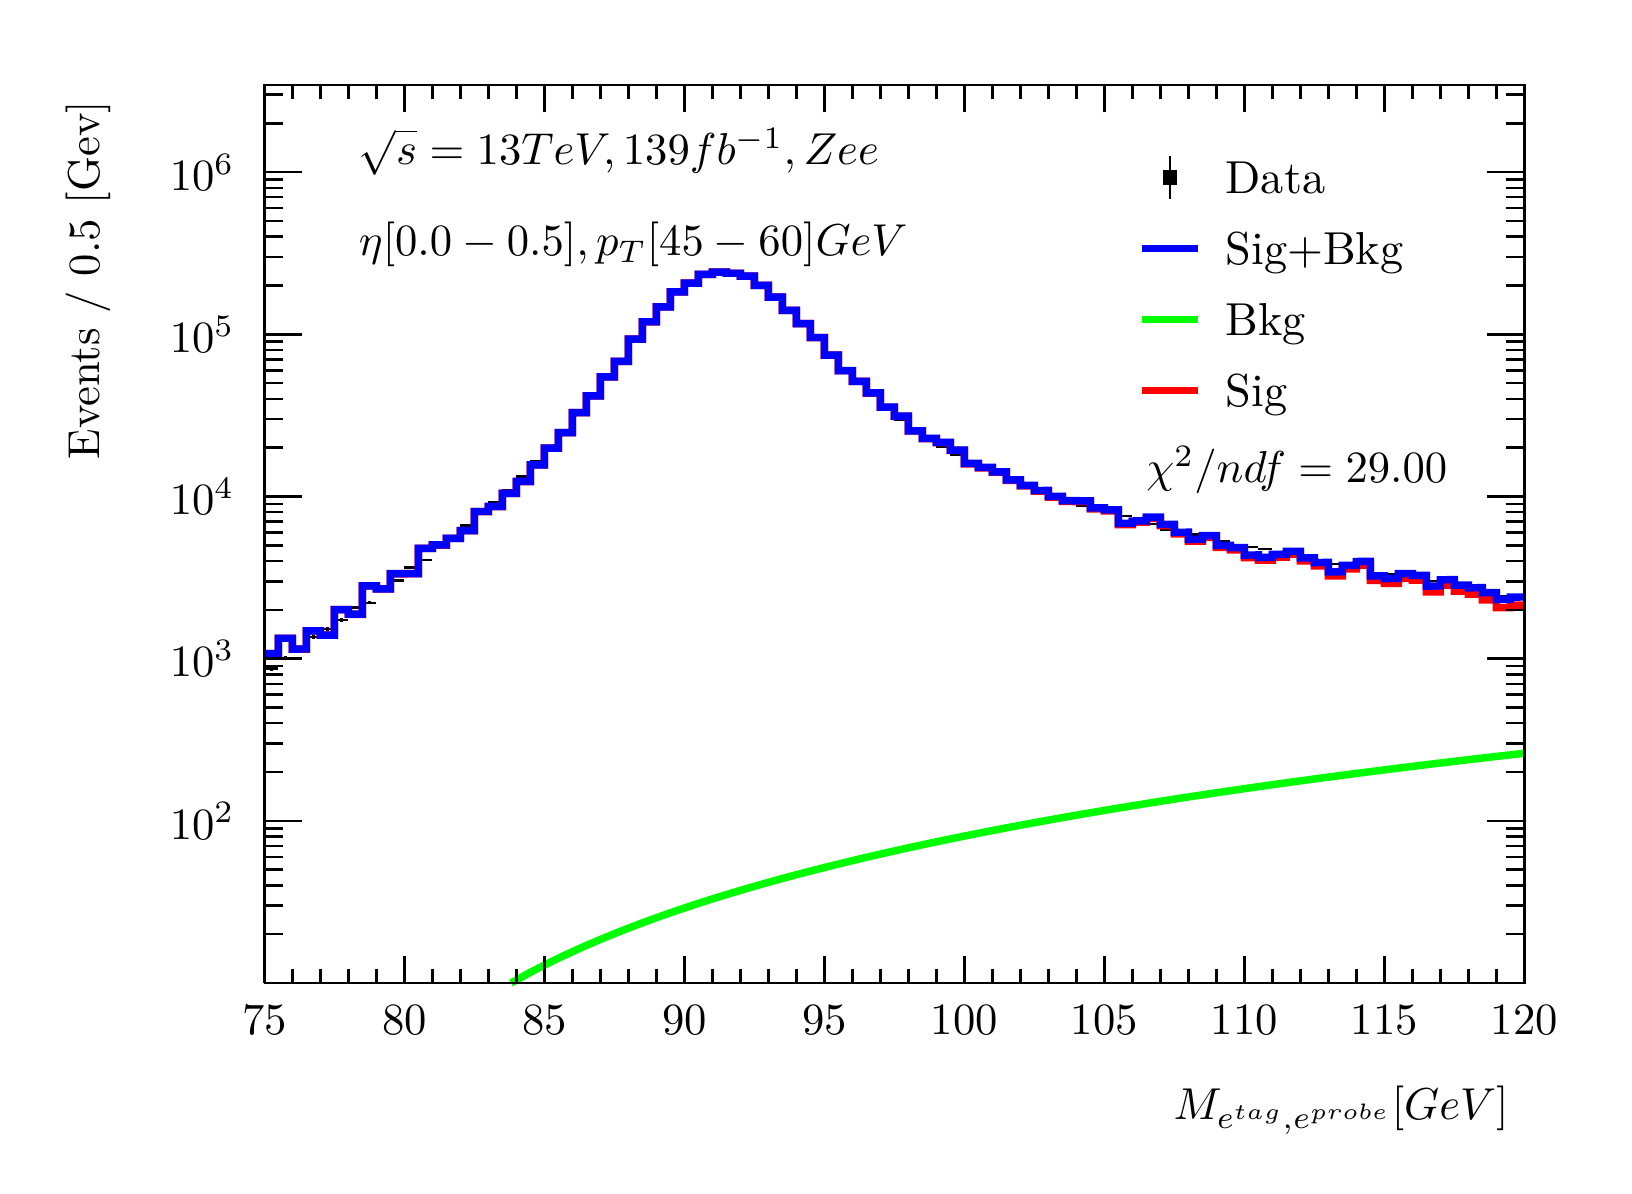
\begin{tikzpicture}
\pgfdeclareplotmark{cross} {
\pgfpathmoveto{\pgfpoint{-0.3\pgfplotmarksize}{\pgfplotmarksize}}
\pgfpathlineto{\pgfpoint{+0.3\pgfplotmarksize}{\pgfplotmarksize}}
\pgfpathlineto{\pgfpoint{+0.3\pgfplotmarksize}{0.3\pgfplotmarksize}}
\pgfpathlineto{\pgfpoint{+1\pgfplotmarksize}{0.3\pgfplotmarksize}}
\pgfpathlineto{\pgfpoint{+1\pgfplotmarksize}{-0.3\pgfplotmarksize}}
\pgfpathlineto{\pgfpoint{+0.3\pgfplotmarksize}{-0.3\pgfplotmarksize}}
\pgfpathlineto{\pgfpoint{+0.3\pgfplotmarksize}{-1.\pgfplotmarksize}}
\pgfpathlineto{\pgfpoint{-0.3\pgfplotmarksize}{-1.\pgfplotmarksize}}
\pgfpathlineto{\pgfpoint{-0.3\pgfplotmarksize}{-0.3\pgfplotmarksize}}
\pgfpathlineto{\pgfpoint{-1.\pgfplotmarksize}{-0.3\pgfplotmarksize}}
\pgfpathlineto{\pgfpoint{-1.\pgfplotmarksize}{0.3\pgfplotmarksize}}
\pgfpathlineto{\pgfpoint{-0.3\pgfplotmarksize}{0.3\pgfplotmarksize}}
\pgfpathclose
\pgfusepathqstroke
}
\pgfdeclareplotmark{cross*} {
\pgfpathmoveto{\pgfpoint{-0.3\pgfplotmarksize}{\pgfplotmarksize}}
\pgfpathlineto{\pgfpoint{+0.3\pgfplotmarksize}{\pgfplotmarksize}}
\pgfpathlineto{\pgfpoint{+0.3\pgfplotmarksize}{0.3\pgfplotmarksize}}
\pgfpathlineto{\pgfpoint{+1\pgfplotmarksize}{0.3\pgfplotmarksize}}
\pgfpathlineto{\pgfpoint{+1\pgfplotmarksize}{-0.3\pgfplotmarksize}}
\pgfpathlineto{\pgfpoint{+0.3\pgfplotmarksize}{-0.3\pgfplotmarksize}}
\pgfpathlineto{\pgfpoint{+0.3\pgfplotmarksize}{-1.\pgfplotmarksize}}
\pgfpathlineto{\pgfpoint{-0.3\pgfplotmarksize}{-1.\pgfplotmarksize}}
\pgfpathlineto{\pgfpoint{-0.3\pgfplotmarksize}{-0.3\pgfplotmarksize}}
\pgfpathlineto{\pgfpoint{-1.\pgfplotmarksize}{-0.3\pgfplotmarksize}}
\pgfpathlineto{\pgfpoint{-1.\pgfplotmarksize}{0.3\pgfplotmarksize}}
\pgfpathlineto{\pgfpoint{-0.3\pgfplotmarksize}{0.3\pgfplotmarksize}}
\pgfpathclose
\pgfusepathqfillstroke
}
\pgfdeclareplotmark{newstar} {
\pgfpathmoveto{\pgfqpoint{0pt}{\pgfplotmarksize}}
\pgfpathlineto{\pgfqpointpolar{44}{0.5\pgfplotmarksize}}
\pgfpathlineto{\pgfqpointpolar{18}{\pgfplotmarksize}}
\pgfpathlineto{\pgfqpointpolar{-20}{0.5\pgfplotmarksize}}
\pgfpathlineto{\pgfqpointpolar{-54}{\pgfplotmarksize}}
\pgfpathlineto{\pgfqpointpolar{-90}{0.5\pgfplotmarksize}}
\pgfpathlineto{\pgfqpointpolar{234}{\pgfplotmarksize}}
\pgfpathlineto{\pgfqpointpolar{198}{0.5\pgfplotmarksize}}
\pgfpathlineto{\pgfqpointpolar{162}{\pgfplotmarksize}}
\pgfpathlineto{\pgfqpointpolar{134}{0.5\pgfplotmarksize}}
\pgfpathclose
\pgfusepathqstroke
}
\pgfdeclareplotmark{newstar*} {
\pgfpathmoveto{\pgfqpoint{0pt}{\pgfplotmarksize}}
\pgfpathlineto{\pgfqpointpolar{44}{0.5\pgfplotmarksize}}
\pgfpathlineto{\pgfqpointpolar{18}{\pgfplotmarksize}}
\pgfpathlineto{\pgfqpointpolar{-20}{0.5\pgfplotmarksize}}
\pgfpathlineto{\pgfqpointpolar{-54}{\pgfplotmarksize}}
\pgfpathlineto{\pgfqpointpolar{-90}{0.5\pgfplotmarksize}}
\pgfpathlineto{\pgfqpointpolar{234}{\pgfplotmarksize}}
\pgfpathlineto{\pgfqpointpolar{198}{0.5\pgfplotmarksize}}
\pgfpathlineto{\pgfqpointpolar{162}{\pgfplotmarksize}}
\pgfpathlineto{\pgfqpointpolar{134}{0.5\pgfplotmarksize}}
\pgfpathclose
\pgfusepathqfillstroke
}
\definecolor{c}{rgb}{1,1,1};
\draw [color=c, fill=c] (0,0) rectangle (20,14.4361);
\draw [color=c, fill=c] (3,2.30977) rectangle (19,13.7143);
\definecolor{c}{rgb}{0,0,0};
\draw [c,line width=0.9] (3,2.30977) -- (3,13.7143) -- (19,13.7143) -- (19,2.30977) -- (3,2.30977);
\definecolor{c}{rgb}{1,1,1};
\draw [color=c, fill=c] (3,2.30977) rectangle (19,13.7143);
\definecolor{c}{rgb}{0,0,0};
\draw [c,line width=0.9] (3,2.30977) -- (3,13.7143) -- (19,13.7143) -- (19,2.30977) -- (3,2.30977);
\draw [c,line width=0.9] (3,2.30977) -- (19,2.30977);
\draw [c,line width=0.9] (3,2.65624) -- (3,2.30977);
\draw [c,line width=0.9] (3.35556,2.48301) -- (3.35556,2.30977);
\draw [c,line width=0.9] (3.71111,2.48301) -- (3.71111,2.30977);
\draw [c,line width=0.9] (4.06667,2.48301) -- (4.06667,2.30977);
\draw [c,line width=0.9] (4.42222,2.48301) -- (4.42222,2.30977);
\draw [c,line width=0.9] (4.77778,2.65624) -- (4.77778,2.30977);
\draw [c,line width=0.9] (5.13333,2.48301) -- (5.13333,2.30977);
\draw [c,line width=0.9] (5.48889,2.48301) -- (5.48889,2.30977);
\draw [c,line width=0.9] (5.84444,2.48301) -- (5.84444,2.30977);
\draw [c,line width=0.9] (6.2,2.48301) -- (6.2,2.30977);
\draw [c,line width=0.9] (6.55556,2.65624) -- (6.55556,2.30977);
\draw [c,line width=0.9] (6.91111,2.48301) -- (6.91111,2.30977);
\draw [c,line width=0.9] (7.26667,2.48301) -- (7.26667,2.30977);
\draw [c,line width=0.9] (7.62222,2.48301) -- (7.62222,2.30977);
\draw [c,line width=0.9] (7.97778,2.48301) -- (7.97778,2.30977);
\draw [c,line width=0.9] (8.33333,2.65624) -- (8.33333,2.30977);
\draw [c,line width=0.9] (8.68889,2.48301) -- (8.68889,2.30977);
\draw [c,line width=0.9] (9.04444,2.48301) -- (9.04444,2.30977);
\draw [c,line width=0.9] (9.4,2.48301) -- (9.4,2.30977);
\draw [c,line width=0.9] (9.75556,2.48301) -- (9.75556,2.30977);
\draw [c,line width=0.9] (10.1111,2.65624) -- (10.1111,2.30977);
\draw [c,line width=0.9] (10.4667,2.48301) -- (10.4667,2.30977);
\draw [c,line width=0.9] (10.8222,2.48301) -- (10.8222,2.30977);
\draw [c,line width=0.9] (11.1778,2.48301) -- (11.1778,2.30977);
\draw [c,line width=0.9] (11.5333,2.48301) -- (11.5333,2.30977);
\draw [c,line width=0.9] (11.8889,2.65624) -- (11.8889,2.30977);
\draw [c,line width=0.9] (12.2444,2.48301) -- (12.2444,2.30977);
\draw [c,line width=0.9] (12.6,2.48301) -- (12.6,2.30977);
\draw [c,line width=0.9] (12.9556,2.48301) -- (12.9556,2.30977);
\draw [c,line width=0.9] (13.3111,2.48301) -- (13.3111,2.30977);
\draw [c,line width=0.9] (13.6667,2.65624) -- (13.6667,2.30977);
\draw [c,line width=0.9] (14.0222,2.48301) -- (14.0222,2.30977);
\draw [c,line width=0.9] (14.3778,2.48301) -- (14.3778,2.30977);
\draw [c,line width=0.9] (14.7333,2.48301) -- (14.7333,2.30977);
\draw [c,line width=0.9] (15.0889,2.48301) -- (15.0889,2.30977);
\draw [c,line width=0.9] (15.4444,2.65624) -- (15.4444,2.30977);
\draw [c,line width=0.9] (15.8,2.48301) -- (15.8,2.30977);
\draw [c,line width=0.9] (16.1556,2.48301) -- (16.1556,2.30977);
\draw [c,line width=0.9] (16.5111,2.48301) -- (16.5111,2.30977);
\draw [c,line width=0.9] (16.8667,2.48301) -- (16.8667,2.30977);
\draw [c,line width=0.9] (17.2222,2.65624) -- (17.2222,2.30977);
\draw [c,line width=0.9] (17.5778,2.48301) -- (17.5778,2.30977);
\draw [c,line width=0.9] (17.9333,2.48301) -- (17.9333,2.30977);
\draw [c,line width=0.9] (18.2889,2.48301) -- (18.2889,2.30977);
\draw [c,line width=0.9] (18.6444,2.48301) -- (18.6444,2.30977);
\draw [c,line width=0.9] (19,2.65624) -- (19,2.30977);
\draw [c,line width=0.9] (19,2.65624) -- (19,2.30977);
\draw [anchor=base] (3,1.66015) node[scale=1.61424, color=c, rotate=0]{75};
\draw [anchor=base] (4.77778,1.66015) node[scale=1.61424, color=c, rotate=0]{80};
\draw [anchor=base] (6.55556,1.66015) node[scale=1.61424, color=c, rotate=0]{85};
\draw [anchor=base] (8.33333,1.66015) node[scale=1.61424, color=c, rotate=0]{90};
\draw [anchor=base] (10.1111,1.66015) node[scale=1.61424, color=c, rotate=0]{95};
\draw [anchor=base] (11.8889,1.66015) node[scale=1.61424, color=c, rotate=0]{100};
\draw [anchor=base] (13.6667,1.66015) node[scale=1.61424, color=c, rotate=0]{105};
\draw [anchor=base] (15.4444,1.66015) node[scale=1.61424, color=c, rotate=0]{110};
\draw [anchor=base] (17.2222,1.66015) node[scale=1.61424, color=c, rotate=0]{115};
\draw [anchor=base] (19,1.66015) node[scale=1.61424, color=c, rotate=0]{120};
\draw [anchor= east] (19,0.692932) node[scale=1.61424, color=c, rotate=0]{$M_{e^{tag}, e^{probe}}  [GeV]$};
\draw [c,line width=0.9] (3,13.7143) -- (19,13.7143);
\draw [c,line width=0.9] (3,13.3678) -- (3,13.7143);
\draw [c,line width=0.9] (3.35556,13.5411) -- (3.35556,13.7143);
\draw [c,line width=0.9] (3.71111,13.5411) -- (3.71111,13.7143);
\draw [c,line width=0.9] (4.06667,13.5411) -- (4.06667,13.7143);
\draw [c,line width=0.9] (4.42222,13.5411) -- (4.42222,13.7143);
\draw [c,line width=0.9] (4.77778,13.3678) -- (4.77778,13.7143);
\draw [c,line width=0.9] (5.13333,13.5411) -- (5.13333,13.7143);
\draw [c,line width=0.9] (5.48889,13.5411) -- (5.48889,13.7143);
\draw [c,line width=0.9] (5.84444,13.5411) -- (5.84444,13.7143);
\draw [c,line width=0.9] (6.2,13.5411) -- (6.2,13.7143);
\draw [c,line width=0.9] (6.55556,13.3678) -- (6.55556,13.7143);
\draw [c,line width=0.9] (6.91111,13.5411) -- (6.91111,13.7143);
\draw [c,line width=0.9] (7.26667,13.5411) -- (7.26667,13.7143);
\draw [c,line width=0.9] (7.62222,13.5411) -- (7.62222,13.7143);
\draw [c,line width=0.9] (7.97778,13.5411) -- (7.97778,13.7143);
\draw [c,line width=0.9] (8.33333,13.3678) -- (8.33333,13.7143);
\draw [c,line width=0.9] (8.68889,13.5411) -- (8.68889,13.7143);
\draw [c,line width=0.9] (9.04444,13.5411) -- (9.04444,13.7143);
\draw [c,line width=0.9] (9.4,13.5411) -- (9.4,13.7143);
\draw [c,line width=0.9] (9.75556,13.5411) -- (9.75556,13.7143);
\draw [c,line width=0.9] (10.1111,13.3678) -- (10.1111,13.7143);
\draw [c,line width=0.9] (10.4667,13.5411) -- (10.4667,13.7143);
\draw [c,line width=0.9] (10.8222,13.5411) -- (10.8222,13.7143);
\draw [c,line width=0.9] (11.1778,13.5411) -- (11.1778,13.7143);
\draw [c,line width=0.9] (11.5333,13.5411) -- (11.5333,13.7143);
\draw [c,line width=0.9] (11.8889,13.3678) -- (11.8889,13.7143);
\draw [c,line width=0.9] (12.2444,13.5411) -- (12.2444,13.7143);
\draw [c,line width=0.9] (12.6,13.5411) -- (12.6,13.7143);
\draw [c,line width=0.9] (12.9556,13.5411) -- (12.9556,13.7143);
\draw [c,line width=0.9] (13.3111,13.5411) -- (13.3111,13.7143);
\draw [c,line width=0.9] (13.6667,13.3678) -- (13.6667,13.7143);
\draw [c,line width=0.9] (14.0222,13.5411) -- (14.0222,13.7143);
\draw [c,line width=0.9] (14.3778,13.5411) -- (14.3778,13.7143);
\draw [c,line width=0.9] (14.7333,13.5411) -- (14.7333,13.7143);
\draw [c,line width=0.9] (15.0889,13.5411) -- (15.0889,13.7143);
\draw [c,line width=0.9] (15.4444,13.3678) -- (15.4444,13.7143);
\draw [c,line width=0.9] (15.8,13.5411) -- (15.8,13.7143);
\draw [c,line width=0.9] (16.1556,13.5411) -- (16.1556,13.7143);
\draw [c,line width=0.9] (16.5111,13.5411) -- (16.5111,13.7143);
\draw [c,line width=0.9] (16.8667,13.5411) -- (16.8667,13.7143);
\draw [c,line width=0.9] (17.2222,13.3678) -- (17.2222,13.7143);
\draw [c,line width=0.9] (17.5778,13.5411) -- (17.5778,13.7143);
\draw [c,line width=0.9] (17.9333,13.5411) -- (17.9333,13.7143);
\draw [c,line width=0.9] (18.2889,13.5411) -- (18.2889,13.7143);
\draw [c,line width=0.9] (18.6444,13.5411) -- (18.6444,13.7143);
\draw [c,line width=0.9] (19,13.3678) -- (19,13.7143);
\draw [c,line width=0.9] (19,13.3678) -- (19,13.7143);
\draw [c,line width=0.9] (3,2.30977) -- (3,13.7143);
\draw [c,line width=0.9] (3.237,2.92982) -- (3,2.92982);
\draw [c,line width=0.9] (3.237,3.29252) -- (3,3.29252);
\draw [c,line width=0.9] (3.237,3.54986) -- (3,3.54986);
\draw [c,line width=0.9] (3.237,3.74947) -- (3,3.74947);
\draw [c,line width=0.9] (3.237,3.91257) -- (3,3.91257);
\draw [c,line width=0.9] (3.237,4.05046) -- (3,4.05046);
\draw [c,line width=0.9] (3.237,4.16991) -- (3,4.16991);
\draw [c,line width=0.9] (3.237,4.27527) -- (3,4.27527);
\draw [c,line width=0.9] (3.474,4.36952) -- (3,4.36952);
\draw [anchor= east] (2.82,4.36952) node[scale=1.61424, color=c, rotate=0]{$10^{2}$};
\draw [c,line width=0.9] (3.237,4.98956) -- (3,4.98956);
\draw [c,line width=0.9] (3.237,5.35227) -- (3,5.35227);
\draw [c,line width=0.9] (3.237,5.60961) -- (3,5.60961);
\draw [c,line width=0.9] (3.237,5.80922) -- (3,5.80922);
\draw [c,line width=0.9] (3.237,5.97231) -- (3,5.97231);
\draw [c,line width=0.9] (3.237,6.11021) -- (3,6.11021);
\draw [c,line width=0.9] (3.237,6.22966) -- (3,6.22966);
\draw [c,line width=0.9] (3.237,6.33502) -- (3,6.33502);
\draw [c,line width=0.9] (3.474,6.42927) -- (3,6.42927);
\draw [anchor= east] (2.82,6.42927) node[scale=1.61424, color=c, rotate=0]{$10^{3}$};
\draw [c,line width=0.9] (3.237,7.04931) -- (3,7.04931);
\draw [c,line width=0.9] (3.237,7.41202) -- (3,7.41202);
\draw [c,line width=0.9] (3.237,7.66936) -- (3,7.66936);
\draw [c,line width=0.9] (3.237,7.86897) -- (3,7.86897);
\draw [c,line width=0.9] (3.237,8.03206) -- (3,8.03206);
\draw [c,line width=0.9] (3.237,8.16995) -- (3,8.16995);
\draw [c,line width=0.9] (3.237,8.2894) -- (3,8.2894);
\draw [c,line width=0.9] (3.237,8.39476) -- (3,8.39476);
\draw [c,line width=0.9] (3.474,8.48901) -- (3,8.48901);
\draw [anchor= east] (2.82,8.48901) node[scale=1.61424, color=c, rotate=0]{$10^{4}$};
\draw [c,line width=0.9] (3.237,9.10906) -- (3,9.10906);
\draw [c,line width=0.9] (3.237,9.47176) -- (3,9.47176);
\draw [c,line width=0.9] (3.237,9.7291) -- (3,9.7291);
\draw [c,line width=0.9] (3.237,9.92871) -- (3,9.92871);
\draw [c,line width=0.9] (3.237,10.0918) -- (3,10.0918);
\draw [c,line width=0.9] (3.237,10.2297) -- (3,10.2297);
\draw [c,line width=0.9] (3.237,10.3491) -- (3,10.3491);
\draw [c,line width=0.9] (3.237,10.4545) -- (3,10.4545);
\draw [c,line width=0.9] (3.474,10.5488) -- (3,10.5488);
\draw [anchor= east] (2.82,10.5488) node[scale=1.61424, color=c, rotate=0]{$10^{5}$};
\draw [c,line width=0.9] (3.237,11.1688) -- (3,11.1688);
\draw [c,line width=0.9] (3.237,11.5315) -- (3,11.5315);
\draw [c,line width=0.9] (3.237,11.7889) -- (3,11.7889);
\draw [c,line width=0.9] (3.237,11.9885) -- (3,11.9885);
\draw [c,line width=0.9] (3.237,12.1516) -- (3,12.1516);
\draw [c,line width=0.9] (3.237,12.2894) -- (3,12.2894);
\draw [c,line width=0.9] (3.237,12.4089) -- (3,12.4089);
\draw [c,line width=0.9] (3.237,12.5143) -- (3,12.5143);
\draw [c,line width=0.9] (3.474,12.6085) -- (3,12.6085);
\draw [anchor= east] (2.82,12.6085) node[scale=1.61424, color=c, rotate=0]{$10^{6}$};
\draw [c,line width=0.9] (3.237,13.2286) -- (3,13.2286);
\draw [c,line width=0.9] (3.237,13.5913) -- (3,13.5913);
\draw [anchor= east] (0.76,13.7143) node[scale=1.61424, color=c, rotate=90]{Events / 0.5 [Gev]};
\draw [c,line width=0.9] (19,2.30977) -- (19,13.7143);
\draw [c,line width=0.9] (18.763,2.92982) -- (19,2.92982);
\draw [c,line width=0.9] (18.763,3.29252) -- (19,3.29252);
\draw [c,line width=0.9] (18.763,3.54986) -- (19,3.54986);
\draw [c,line width=0.9] (18.763,3.74947) -- (19,3.74947);
\draw [c,line width=0.9] (18.763,3.91257) -- (19,3.91257);
\draw [c,line width=0.9] (18.763,4.05046) -- (19,4.05046);
\draw [c,line width=0.9] (18.763,4.16991) -- (19,4.16991);
\draw [c,line width=0.9] (18.763,4.27527) -- (19,4.27527);
\draw [c,line width=0.9] (18.526,4.36952) -- (19,4.36952);
\draw [c,line width=0.9] (18.763,4.98956) -- (19,4.98956);
\draw [c,line width=0.9] (18.763,5.35227) -- (19,5.35227);
\draw [c,line width=0.9] (18.763,5.60961) -- (19,5.60961);
\draw [c,line width=0.9] (18.763,5.80922) -- (19,5.80922);
\draw [c,line width=0.9] (18.763,5.97231) -- (19,5.97231);
\draw [c,line width=0.9] (18.763,6.11021) -- (19,6.11021);
\draw [c,line width=0.9] (18.763,6.22966) -- (19,6.22966);
\draw [c,line width=0.9] (18.763,6.33502) -- (19,6.33502);
\draw [c,line width=0.9] (18.526,6.42927) -- (19,6.42927);
\draw [c,line width=0.9] (18.763,7.04931) -- (19,7.04931);
\draw [c,line width=0.9] (18.763,7.41202) -- (19,7.41202);
\draw [c,line width=0.9] (18.763,7.66936) -- (19,7.66936);
\draw [c,line width=0.9] (18.763,7.86897) -- (19,7.86897);
\draw [c,line width=0.9] (18.763,8.03206) -- (19,8.03206);
\draw [c,line width=0.9] (18.763,8.16995) -- (19,8.16995);
\draw [c,line width=0.9] (18.763,8.2894) -- (19,8.2894);
\draw [c,line width=0.9] (18.763,8.39476) -- (19,8.39476);
\draw [c,line width=0.9] (18.526,8.48901) -- (19,8.48901);
\draw [c,line width=0.9] (18.763,9.10906) -- (19,9.10906);
\draw [c,line width=0.9] (18.763,9.47176) -- (19,9.47176);
\draw [c,line width=0.9] (18.763,9.7291) -- (19,9.7291);
\draw [c,line width=0.9] (18.763,9.92871) -- (19,9.92871);
\draw [c,line width=0.9] (18.763,10.0918) -- (19,10.0918);
\draw [c,line width=0.9] (18.763,10.2297) -- (19,10.2297);
\draw [c,line width=0.9] (18.763,10.3491) -- (19,10.3491);
\draw [c,line width=0.9] (18.763,10.4545) -- (19,10.4545);
\draw [c,line width=0.9] (18.526,10.5488) -- (19,10.5488);
\draw [c,line width=0.9] (18.763,11.1688) -- (19,11.1688);
\draw [c,line width=0.9] (18.763,11.5315) -- (19,11.5315);
\draw [c,line width=0.9] (18.763,11.7889) -- (19,11.7889);
\draw [c,line width=0.9] (18.763,11.9885) -- (19,11.9885);
\draw [c,line width=0.9] (18.763,12.1516) -- (19,12.1516);
\draw [c,line width=0.9] (18.763,12.2894) -- (19,12.2894);
\draw [c,line width=0.9] (18.763,12.4089) -- (19,12.4089);
\draw [c,line width=0.9] (18.763,12.5143) -- (19,12.5143);
\draw [c,line width=0.9] (18.526,12.6085) -- (19,12.6085);
\draw [c,line width=0.9] (18.763,13.2286) -- (19,13.2286);
\draw [c,line width=0.9] (18.763,13.5913) -- (19,13.5913);
\draw [c,line width=0.9] (3.08889,6.30572) -- (3,6.30572);
\draw [c,line width=0.9] (3,6.30572) -- (3,6.30572);
\draw [c,line width=0.9] (3.08889,6.30572) -- (3.17778,6.30572);
\draw [c,line width=0.9] (3.17778,6.30572) -- (3.17778,6.30572);
\draw [c,line width=0.9] (3.08889,6.30572) -- (3.08889,6.33603);
\draw [c,line width=0.9] (3.08889,6.33603) -- (3.08889,6.33603);
\draw [c,line width=0.9] (3.08889,6.30572) -- (3.08889,6.27541);
\draw [c,line width=0.9] (3.08889,6.27541) -- (3.08889,6.27541);
\draw [c,line width=0.9] (3.26667,6.43994) -- (3.17778,6.43994);
\draw [c,line width=0.9] (3.17778,6.43994) -- (3.17778,6.43994);
\draw [c,line width=0.9] (3.26667,6.43994) -- (3.35556,6.43994);
\draw [c,line width=0.9] (3.35556,6.43994) -- (3.35556,6.43994);
\draw [c,line width=0.9] (3.26667,6.43994) -- (3.26667,6.46806);
\draw [c,line width=0.9] (3.26667,6.46806) -- (3.26667,6.46806);
\draw [c,line width=0.9] (3.26667,6.43994) -- (3.26667,6.41182);
\draw [c,line width=0.9] (3.26667,6.41182) -- (3.26667,6.41182);
\draw [c,line width=0.9] (3.44444,6.55584) -- (3.35556,6.55584);
\draw [c,line width=0.9] (3.35556,6.55584) -- (3.35556,6.55584);
\draw [c,line width=0.9] (3.44444,6.55584) -- (3.53333,6.55584);
\draw [c,line width=0.9] (3.53333,6.55584) -- (3.53333,6.55584);
\draw [c,line width=0.9] (3.44444,6.55584) -- (3.44444,6.5822);
\draw [c,line width=0.9] (3.44444,6.5822) -- (3.44444,6.5822);
\draw [c,line width=0.9] (3.44444,6.55584) -- (3.44444,6.52949);
\draw [c,line width=0.9] (3.44444,6.52949) -- (3.44444,6.52949);
\draw [c,line width=0.9] (3.62222,6.70301) -- (3.53333,6.70301);
\draw [c,line width=0.9] (3.53333,6.70301) -- (3.53333,6.70301);
\draw [c,line width=0.9] (3.62222,6.70301) -- (3.71111,6.70301);
\draw [c,line width=0.9] (3.71111,6.70301) -- (3.71111,6.70301);
\draw [c,line width=0.9] (3.62222,6.70301) -- (3.62222,6.72728);
\draw [c,line width=0.9] (3.62222,6.72728) -- (3.62222,6.72728);
\draw [c,line width=0.9] (3.62222,6.70301) -- (3.62222,6.67873);
\draw [c,line width=0.9] (3.62222,6.67873) -- (3.62222,6.67873);
\draw [c,line width=0.9] (3.8,6.80852) -- (3.71111,6.80852);
\draw [c,line width=0.9] (3.71111,6.80852) -- (3.71111,6.80852);
\draw [c,line width=0.9] (3.8,6.80852) -- (3.88889,6.80852);
\draw [c,line width=0.9] (3.88889,6.80852) -- (3.88889,6.80852);
\draw [c,line width=0.9] (3.8,6.80852) -- (3.8,6.8314);
\draw [c,line width=0.9] (3.8,6.8314) -- (3.8,6.8314);
\draw [c,line width=0.9] (3.8,6.80852) -- (3.8,6.78563);
\draw [c,line width=0.9] (3.8,6.78563) -- (3.8,6.78563);
\draw [c,line width=0.9] (3.97778,6.91855) -- (3.88889,6.91855);
\draw [c,line width=0.9] (3.88889,6.91855) -- (3.88889,6.91855);
\draw [c,line width=0.9] (3.97778,6.91855) -- (4.06667,6.91855);
\draw [c,line width=0.9] (4.06667,6.91855) -- (4.06667,6.91855);
\draw [c,line width=0.9] (3.97778,6.91855) -- (3.97778,6.94007);
\draw [c,line width=0.9] (3.97778,6.94007) -- (3.97778,6.94007);
\draw [c,line width=0.9] (3.97778,6.91855) -- (3.97778,6.89703);
\draw [c,line width=0.9] (3.97778,6.89703) -- (3.97778,6.89703);
\draw [c,line width=0.9] (4.15556,7.08052) -- (4.06667,7.08052);
\draw [c,line width=0.9] (4.06667,7.08052) -- (4.06667,7.08052);
\draw [c,line width=0.9] (4.15556,7.08052) -- (4.24444,7.08052);
\draw [c,line width=0.9] (4.24444,7.08052) -- (4.24444,7.08052);
\draw [c,line width=0.9] (4.15556,7.08052) -- (4.15556,7.10017);
\draw [c,line width=0.9] (4.15556,7.10017) -- (4.15556,7.10017);
\draw [c,line width=0.9] (4.15556,7.08052) -- (4.15556,7.06086);
\draw [c,line width=0.9] (4.15556,7.06086) -- (4.15556,7.06086);
\draw [c,line width=0.9] (4.33333,7.13863) -- (4.24444,7.13863);
\draw [c,line width=0.9] (4.24444,7.13863) -- (4.24444,7.13863);
\draw [c,line width=0.9] (4.33333,7.13863) -- (4.42222,7.13863);
\draw [c,line width=0.9] (4.42222,7.13863) -- (4.42222,7.13863);
\draw [c,line width=0.9] (4.33333,7.13863) -- (4.33333,7.15766);
\draw [c,line width=0.9] (4.33333,7.15766) -- (4.33333,7.15766);
\draw [c,line width=0.9] (4.33333,7.13863) -- (4.33333,7.1196);
\draw [c,line width=0.9] (4.33333,7.1196) -- (4.33333,7.1196);
\draw [c,line width=0.9] (4.51111,7.29393) -- (4.42222,7.29393);
\draw [c,line width=0.9] (4.42222,7.29393) -- (4.42222,7.29393);
\draw [c,line width=0.9] (4.51111,7.29393) -- (4.6,7.29393);
\draw [c,line width=0.9] (4.6,7.29393) -- (4.6,7.29393);
\draw [c,line width=0.9] (4.51111,7.29393) -- (4.51111,7.31138);
\draw [c,line width=0.9] (4.51111,7.31138) -- (4.51111,7.31138);
\draw [c,line width=0.9] (4.51111,7.29393) -- (4.51111,7.27648);
\draw [c,line width=0.9] (4.51111,7.27648) -- (4.51111,7.27648);
\draw [c,line width=0.9] (4.68889,7.42239) -- (4.6,7.42239);
\draw [c,line width=0.9] (4.6,7.42239) -- (4.6,7.42239);
\draw [c,line width=0.9] (4.68889,7.42239) -- (4.77778,7.42239);
\draw [c,line width=0.9] (4.77778,7.42239) -- (4.77778,7.42239);
\draw [c,line width=0.9] (4.68889,7.42239) -- (4.68889,7.43863);
\draw [c,line width=0.9] (4.68889,7.43863) -- (4.68889,7.43863);
\draw [c,line width=0.9] (4.68889,7.42239) -- (4.68889,7.40616);
\draw [c,line width=0.9] (4.68889,7.40616) -- (4.68889,7.40616);
\draw [c,line width=0.9] (4.86667,7.58647) -- (4.77778,7.58647);
\draw [c,line width=0.9] (4.77778,7.58647) -- (4.77778,7.58647);
\draw [c,line width=0.9] (4.86667,7.58647) -- (4.95556,7.58647);
\draw [c,line width=0.9] (4.95556,7.58647) -- (4.95556,7.58647);
\draw [c,line width=0.9] (4.86667,7.58647) -- (4.86667,7.60128);
\draw [c,line width=0.9] (4.86667,7.60128) -- (4.86667,7.60128);
\draw [c,line width=0.9] (4.86667,7.58647) -- (4.86667,7.57165);
\draw [c,line width=0.9] (4.86667,7.57165) -- (4.86667,7.57165);
\draw [c,line width=0.9] (5.04444,7.68466) -- (4.95556,7.68466);
\draw [c,line width=0.9] (4.95556,7.68466) -- (4.95556,7.68466);
\draw [c,line width=0.9] (5.04444,7.68466) -- (5.13333,7.68466);
\draw [c,line width=0.9] (5.13333,7.68466) -- (5.13333,7.68466);
\draw [c,line width=0.9] (5.04444,7.68466) -- (5.04444,7.69868);
\draw [c,line width=0.9] (5.04444,7.69868) -- (5.04444,7.69868);
\draw [c,line width=0.9] (5.04444,7.68466) -- (5.04444,7.67063);
\draw [c,line width=0.9] (5.04444,7.67063) -- (5.04444,7.67063);
\draw [c,line width=0.9] (5.22222,7.83413) -- (5.13333,7.83413);
\draw [c,line width=0.9] (5.13333,7.83413) -- (5.13333,7.83413);
\draw [c,line width=0.9] (5.22222,7.83413) -- (5.31111,7.83413);
\draw [c,line width=0.9] (5.31111,7.83413) -- (5.31111,7.83413);
\draw [c,line width=0.9] (5.22222,7.83413) -- (5.22222,7.84703);
\draw [c,line width=0.9] (5.22222,7.84703) -- (5.22222,7.84703);
\draw [c,line width=0.9] (5.22222,7.83413) -- (5.22222,7.82123);
\draw [c,line width=0.9] (5.22222,7.82123) -- (5.22222,7.82123);
\draw [c,line width=0.9] (5.4,7.95861) -- (5.31111,7.95861);
\draw [c,line width=0.9] (5.31111,7.95861) -- (5.31111,7.95861);
\draw [c,line width=0.9] (5.4,7.95861) -- (5.48889,7.95861);
\draw [c,line width=0.9] (5.48889,7.95861) -- (5.48889,7.95861);
\draw [c,line width=0.9] (5.4,7.95861) -- (5.4,7.97064);
\draw [c,line width=0.9] (5.4,7.97064) -- (5.4,7.97064);
\draw [c,line width=0.9] (5.4,7.95861) -- (5.4,7.94658);
\draw [c,line width=0.9] (5.4,7.94658) -- (5.4,7.94658);
\draw [c,line width=0.9] (5.57778,8.118) -- (5.48889,8.118);
\draw [c,line width=0.9] (5.48889,8.118) -- (5.48889,8.118);
\draw [c,line width=0.9] (5.57778,8.118) -- (5.66667,8.118);
\draw [c,line width=0.9] (5.66667,8.118) -- (5.66667,8.118);
\draw [c,line width=0.9] (5.57778,8.118) -- (5.57778,8.129);
\draw [c,line width=0.9] (5.57778,8.129) -- (5.57778,8.129);
\draw [c,line width=0.9] (5.57778,8.118) -- (5.57778,8.10699);
\draw [c,line width=0.9] (5.57778,8.10699) -- (5.57778,8.10699);
\draw [c,line width=0.9] (5.75556,8.26354) -- (5.66667,8.26354);
\draw [c,line width=0.9] (5.66667,8.26354) -- (5.66667,8.26354);
\draw [c,line width=0.9] (5.75556,8.26354) -- (5.84444,8.26354);
\draw [c,line width=0.9] (5.84444,8.26354) -- (5.84444,8.26354);
\draw [c,line width=0.9] (5.75556,8.26354) -- (5.75556,8.27369);
\draw [c,line width=0.9] (5.75556,8.27369) -- (5.75556,8.27369);
\draw [c,line width=0.9] (5.75556,8.26354) -- (5.75556,8.25339);
\draw [c,line width=0.9] (5.75556,8.25339) -- (5.75556,8.25339);
\draw [c,line width=0.9] (5.93333,8.41189) -- (5.84444,8.41189);
\draw [c,line width=0.9] (5.84444,8.41189) -- (5.84444,8.41189);
\draw [c,line width=0.9] (5.93333,8.41189) -- (6.02222,8.41189);
\draw [c,line width=0.9] (6.02222,8.41189) -- (6.02222,8.41189);
\draw [c,line width=0.9] (5.93333,8.41189) -- (5.93333,8.42123);
\draw [c,line width=0.9] (5.93333,8.42123) -- (5.93333,8.42123);
\draw [c,line width=0.9] (5.93333,8.41189) -- (5.93333,8.40256);
\draw [c,line width=0.9] (5.93333,8.40256) -- (5.93333,8.40256);
\draw [c,line width=0.9] (6.11111,8.5702) -- (6.02222,8.5702);
\draw [c,line width=0.9] (6.02222,8.5702) -- (6.02222,8.5702);
\draw [c,line width=0.9] (6.11111,8.5702) -- (6.2,8.5702);
\draw [c,line width=0.9] (6.2,8.5702) -- (6.2,8.5702);
\draw [c,line width=0.9] (6.11111,8.5702) -- (6.11111,8.57875);
\draw [c,line width=0.9] (6.11111,8.57875) -- (6.11111,8.57875);
\draw [c,line width=0.9] (6.11111,8.5702) -- (6.11111,8.56165);
\draw [c,line width=0.9] (6.11111,8.56165) -- (6.11111,8.56165);
\draw [c,line width=0.9] (6.28889,8.74338) -- (6.2,8.74338);
\draw [c,line width=0.9] (6.2,8.74338) -- (6.2,8.74338);
\draw [c,line width=0.9] (6.28889,8.74338) -- (6.37778,8.74338);
\draw [c,line width=0.9] (6.37778,8.74338) -- (6.37778,8.74338);
\draw [c,line width=0.9] (6.28889,8.74338) -- (6.28889,8.75114);
\draw [c,line width=0.9] (6.28889,8.75114) -- (6.28889,8.75114);
\draw [c,line width=0.9] (6.28889,8.74338) -- (6.28889,8.73562);
\draw [c,line width=0.9] (6.28889,8.73562) -- (6.28889,8.73562);
\draw [c,line width=0.9] (6.46667,8.93957) -- (6.37778,8.93957);
\draw [c,line width=0.9] (6.37778,8.93957) -- (6.37778,8.93957);
\draw [c,line width=0.9] (6.46667,8.93957) -- (6.55556,8.93957);
\draw [c,line width=0.9] (6.55556,8.93957) -- (6.55556,8.93957);
\draw [c,line width=0.9] (6.46667,8.93957) -- (6.46667,8.94653);
\draw [c,line width=0.9] (6.46667,8.94653) -- (6.46667,8.94653);
\draw [c,line width=0.9] (6.46667,8.93957) -- (6.46667,8.93262);
\draw [c,line width=0.9] (6.46667,8.93262) -- (6.46667,8.93262);
\draw [c,line width=0.9] (6.64444,9.12594) -- (6.55556,9.12594);
\draw [c,line width=0.9] (6.55556,9.12594) -- (6.55556,9.12594);
\draw [c,line width=0.9] (6.64444,9.12594) -- (6.73333,9.12594);
\draw [c,line width=0.9] (6.73333,9.12594) -- (6.73333,9.12594);
\draw [c,line width=0.9] (6.64444,9.12594) -- (6.64444,9.13221);
\draw [c,line width=0.9] (6.64444,9.13221) -- (6.64444,9.13221);
\draw [c,line width=0.9] (6.64444,9.12594) -- (6.64444,9.11967);
\draw [c,line width=0.9] (6.64444,9.11967) -- (6.64444,9.11967);
\draw [c,line width=0.9] (6.82222,9.32751) -- (6.73333,9.32751);
\draw [c,line width=0.9] (6.73333,9.32751) -- (6.73333,9.32751);
\draw [c,line width=0.9] (6.82222,9.32751) -- (6.91111,9.32751);
\draw [c,line width=0.9] (6.91111,9.32751) -- (6.91111,9.32751);
\draw [c,line width=0.9] (6.82222,9.32751) -- (6.82222,9.3331);
\draw [c,line width=0.9] (6.82222,9.3331) -- (6.82222,9.3331);
\draw [c,line width=0.9] (6.82222,9.32751) -- (6.82222,9.32191);
\draw [c,line width=0.9] (6.82222,9.32191) -- (6.82222,9.32191);
\draw [c,line width=0.9] (7,9.53) -- (6.91111,9.53);
\draw [c,line width=0.9] (6.91111,9.53) -- (6.91111,9.53);
\draw [c,line width=0.9] (7,9.53) -- (7.08889,9.53);
\draw [c,line width=0.9] (7.08889,9.53) -- (7.08889,9.53);
\draw [c,line width=0.9] (7,9.53) -- (7,9.535);
\draw [c,line width=0.9] (7,9.535) -- (7,9.535);
\draw [c,line width=0.9] (7,9.53) -- (7,9.525);
\draw [c,line width=0.9] (7,9.525) -- (7,9.525);
\draw [c,line width=0.9] (7.17778,9.76837) -- (7.08889,9.76837);
\draw [c,line width=0.9] (7.08889,9.76837) -- (7.08889,9.76837);
\draw [c,line width=0.9] (7.17778,9.76837) -- (7.26667,9.76837);
\draw [c,line width=0.9] (7.26667,9.76837) -- (7.26667,9.76837);
\draw [c,line width=0.9] (7.17778,9.76837) -- (7.17778,9.77275);
\draw [c,line width=0.9] (7.17778,9.77275) -- (7.17778,9.77275);
\draw [c,line width=0.9] (7.17778,9.76837) -- (7.17778,9.764);
\draw [c,line width=0.9] (7.17778,9.764) -- (7.17778,9.764);
\draw [c,line width=0.9] (7.35556,9.99199) -- (7.26667,9.99199);
\draw [c,line width=0.9] (7.26667,9.99199) -- (7.26667,9.99199);
\draw [c,line width=0.9] (7.35556,9.99199) -- (7.44444,9.99199);
\draw [c,line width=0.9] (7.44444,9.99199) -- (7.44444,9.99199);
\draw [c,line width=0.9] (7.35556,9.99199) -- (7.35556,9.99585);
\draw [c,line width=0.9] (7.35556,9.99585) -- (7.35556,9.99585);
\draw [c,line width=0.9] (7.35556,9.99199) -- (7.35556,9.98813);
\draw [c,line width=0.9] (7.35556,9.98813) -- (7.35556,9.98813);
\draw [c,line width=0.9] (7.53333,10.2354) -- (7.44444,10.2354);
\draw [c,line width=0.9] (7.44444,10.2354) -- (7.44444,10.2354);
\draw [c,line width=0.9] (7.53333,10.2354) -- (7.62222,10.2354);
\draw [c,line width=0.9] (7.62222,10.2354) -- (7.62222,10.2354);
\draw [c,line width=0.9] (7.53333,10.2354) -- (7.53333,10.2387);
\draw [c,line width=0.9] (7.53333,10.2387) -- (7.53333,10.2387);
\draw [c,line width=0.9] (7.53333,10.2354) -- (7.53333,10.232);
\draw [c,line width=0.9] (7.53333,10.232) -- (7.53333,10.232);
\draw [c,line width=0.9] (7.71111,10.4629) -- (7.62222,10.4629);
\draw [c,line width=0.9] (7.62222,10.4629) -- (7.62222,10.4629);
\draw [c,line width=0.9] (7.71111,10.4629) -- (7.8,10.4629);
\draw [c,line width=0.9] (7.8,10.4629) -- (7.8,10.4629);
\draw [c,line width=0.9] (7.71111,10.4629) -- (7.71111,10.4658);
\draw [c,line width=0.9] (7.71111,10.4658) -- (7.71111,10.4658);
\draw [c,line width=0.9] (7.71111,10.4629) -- (7.71111,10.4599);
\draw [c,line width=0.9] (7.71111,10.4599) -- (7.71111,10.4599);
\draw [c,line width=0.9] (7.88889,10.6841) -- (7.8,10.6841);
\draw [c,line width=0.9] (7.8,10.6841) -- (7.8,10.6841);
\draw [c,line width=0.9] (7.88889,10.6841) -- (7.97778,10.6841);
\draw [c,line width=0.9] (7.97778,10.6841) -- (7.97778,10.6841);
\draw [c,line width=0.9] (7.88889,10.6841) -- (7.88889,10.6867);
\draw [c,line width=0.9] (7.88889,10.6867) -- (7.88889,10.6867);
\draw [c,line width=0.9] (7.88889,10.6841) -- (7.88889,10.6815);
\draw [c,line width=0.9] (7.88889,10.6815) -- (7.88889,10.6815);
\draw [c,line width=0.9] (8.06667,10.8887) -- (7.97778,10.8887);
\draw [c,line width=0.9] (7.97778,10.8887) -- (7.97778,10.8887);
\draw [c,line width=0.9] (8.06667,10.8887) -- (8.15556,10.8887);
\draw [c,line width=0.9] (8.15556,10.8887) -- (8.15556,10.8887);
\draw [c,line width=0.9] (8.06667,10.8887) -- (8.06667,10.891);
\draw [c,line width=0.9] (8.06667,10.891) -- (8.06667,10.891);
\draw [c,line width=0.9] (8.06667,10.8887) -- (8.06667,10.8863);
\draw [c,line width=0.9] (8.06667,10.8863) -- (8.06667,10.8863);
\draw [c,line width=0.9] (8.24444,11.0725) -- (8.15556,11.0725);
\draw [c,line width=0.9] (8.15556,11.0725) -- (8.15556,11.0725);
\draw [c,line width=0.9] (8.24444,11.0725) -- (8.33333,11.0725);
\draw [c,line width=0.9] (8.33333,11.0725) -- (8.33333,11.0725);
\draw [c,line width=0.9] (8.24444,11.0725) -- (8.24444,11.0746);
\draw [c,line width=0.9] (8.24444,11.0746) -- (8.24444,11.0746);
\draw [c,line width=0.9] (8.24444,11.0725) -- (8.24444,11.0704);
\draw [c,line width=0.9] (8.24444,11.0704) -- (8.24444,11.0704);
\draw [c,line width=0.9] (8.42222,11.2095) -- (8.33333,11.2095);
\draw [c,line width=0.9] (8.33333,11.2095) -- (8.33333,11.2095);
\draw [c,line width=0.9] (8.42222,11.2095) -- (8.51111,11.2095);
\draw [c,line width=0.9] (8.51111,11.2095) -- (8.51111,11.2095);
\draw [c,line width=0.9] (8.42222,11.2095) -- (8.42222,11.2115);
\draw [c,line width=0.9] (8.42222,11.2115) -- (8.42222,11.2115);
\draw [c,line width=0.9] (8.42222,11.2095) -- (8.42222,11.2076);
\draw [c,line width=0.9] (8.42222,11.2076) -- (8.42222,11.2076);
\draw [c,line width=0.9] (8.6,11.3058) -- (8.51111,11.3058);
\draw [c,line width=0.9] (8.51111,11.3058) -- (8.51111,11.3058);
\draw [c,line width=0.9] (8.6,11.3058) -- (8.68889,11.3058);
\draw [c,line width=0.9] (8.68889,11.3058) -- (8.68889,11.3058);
\draw [c,line width=0.9] (8.6,11.3058) -- (8.6,11.3076);
\draw [c,line width=0.9] (8.6,11.3076) -- (8.6,11.3076);
\draw [c,line width=0.9] (8.6,11.3058) -- (8.6,11.3039);
\draw [c,line width=0.9] (8.6,11.3039) -- (8.6,11.3039);
\draw [c,line width=0.9] (8.77778,11.3499) -- (8.68889,11.3499);
\draw [c,line width=0.9] (8.68889,11.3499) -- (8.68889,11.3499);
\draw [c,line width=0.9] (8.77778,11.3499) -- (8.86667,11.3499);
\draw [c,line width=0.9] (8.86667,11.3499) -- (8.86667,11.3499);
\draw [c,line width=0.9] (8.77778,11.3499) -- (8.77778,11.3517);
\draw [c,line width=0.9] (8.77778,11.3517) -- (8.77778,11.3517);
\draw [c,line width=0.9] (8.77778,11.3499) -- (8.77778,11.348);
\draw [c,line width=0.9] (8.77778,11.348) -- (8.77778,11.348);
\draw [c,line width=0.9] (8.95556,11.3424) -- (8.86667,11.3424);
\draw [c,line width=0.9] (8.86667,11.3424) -- (8.86667,11.3424);
\draw [c,line width=0.9] (8.95556,11.3424) -- (9.04444,11.3424);
\draw [c,line width=0.9] (9.04444,11.3424) -- (9.04444,11.3424);
\draw [c,line width=0.9] (8.95556,11.3424) -- (8.95556,11.3442);
\draw [c,line width=0.9] (8.95556,11.3442) -- (8.95556,11.3442);
\draw [c,line width=0.9] (8.95556,11.3424) -- (8.95556,11.3406);
\draw [c,line width=0.9] (8.95556,11.3406) -- (8.95556,11.3406);
\draw [c,line width=0.9] (9.13333,11.2839) -- (9.04444,11.2839);
\draw [c,line width=0.9] (9.04444,11.2839) -- (9.04444,11.2839);
\draw [c,line width=0.9] (9.13333,11.2839) -- (9.22222,11.2839);
\draw [c,line width=0.9] (9.22222,11.2839) -- (9.22222,11.2839);
\draw [c,line width=0.9] (9.13333,11.2839) -- (9.13333,11.2858);
\draw [c,line width=0.9] (9.13333,11.2858) -- (9.13333,11.2858);
\draw [c,line width=0.9] (9.13333,11.2839) -- (9.13333,11.2821);
\draw [c,line width=0.9] (9.13333,11.2821) -- (9.13333,11.2821);
\draw [c,line width=0.9] (9.31111,11.1805) -- (9.22222,11.1805);
\draw [c,line width=0.9] (9.22222,11.1805) -- (9.22222,11.1805);
\draw [c,line width=0.9] (9.31111,11.1805) -- (9.4,11.1805);
\draw [c,line width=0.9] (9.4,11.1805) -- (9.4,11.1805);
\draw [c,line width=0.9] (9.31111,11.1805) -- (9.31111,11.1825);
\draw [c,line width=0.9] (9.31111,11.1825) -- (9.31111,11.1825);
\draw [c,line width=0.9] (9.31111,11.1805) -- (9.31111,11.1785);
\draw [c,line width=0.9] (9.31111,11.1785) -- (9.31111,11.1785);
\draw [c,line width=0.9] (9.48889,11.0348) -- (9.4,11.0348);
\draw [c,line width=0.9] (9.4,11.0348) -- (9.4,11.0348);
\draw [c,line width=0.9] (9.48889,11.0348) -- (9.57778,11.0348);
\draw [c,line width=0.9] (9.57778,11.0348) -- (9.57778,11.0348);
\draw [c,line width=0.9] (9.48889,11.0348) -- (9.48889,11.037);
\draw [c,line width=0.9] (9.48889,11.037) -- (9.48889,11.037);
\draw [c,line width=0.9] (9.48889,11.0348) -- (9.48889,11.0326);
\draw [c,line width=0.9] (9.48889,11.0326) -- (9.48889,11.0326);
\draw [c,line width=0.9] (9.66667,10.8686) -- (9.57778,10.8686);
\draw [c,line width=0.9] (9.57778,10.8686) -- (9.57778,10.8686);
\draw [c,line width=0.9] (9.66667,10.8686) -- (9.75556,10.8686);
\draw [c,line width=0.9] (9.75556,10.8686) -- (9.75556,10.8686);
\draw [c,line width=0.9] (9.66667,10.8686) -- (9.66667,10.8709);
\draw [c,line width=0.9] (9.66667,10.8709) -- (9.66667,10.8709);
\draw [c,line width=0.9] (9.66667,10.8686) -- (9.66667,10.8662);
\draw [c,line width=0.9] (9.66667,10.8662) -- (9.66667,10.8662);
\draw [c,line width=0.9] (9.84444,10.6793) -- (9.75556,10.6793);
\draw [c,line width=0.9] (9.75556,10.6793) -- (9.75556,10.6793);
\draw [c,line width=0.9] (9.84444,10.6793) -- (9.93333,10.6793);
\draw [c,line width=0.9] (9.93333,10.6793) -- (9.93333,10.6793);
\draw [c,line width=0.9] (9.84444,10.6793) -- (9.84444,10.6819);
\draw [c,line width=0.9] (9.84444,10.6819) -- (9.84444,10.6819);
\draw [c,line width=0.9] (9.84444,10.6793) -- (9.84444,10.6766);
\draw [c,line width=0.9] (9.84444,10.6766) -- (9.84444,10.6766);
\draw [c,line width=0.9] (10.0222,10.4843) -- (9.93333,10.4843);
\draw [c,line width=0.9] (9.93333,10.4843) -- (9.93333,10.4843);
\draw [c,line width=0.9] (10.0222,10.4843) -- (10.1111,10.4843);
\draw [c,line width=0.9] (10.1111,10.4843) -- (10.1111,10.4843);
\draw [c,line width=0.9] (10.0222,10.4843) -- (10.0222,10.4872);
\draw [c,line width=0.9] (10.0222,10.4872) -- (10.0222,10.4872);
\draw [c,line width=0.9] (10.0222,10.4843) -- (10.0222,10.4814);
\draw [c,line width=0.9] (10.0222,10.4814) -- (10.0222,10.4814);
\draw [c,line width=0.9] (10.2,10.2927) -- (10.1111,10.2927);
\draw [c,line width=0.9] (10.1111,10.2927) -- (10.1111,10.2927);
\draw [c,line width=0.9] (10.2,10.2927) -- (10.2889,10.2927);
\draw [c,line width=0.9] (10.2889,10.2927) -- (10.2889,10.2927);
\draw [c,line width=0.9] (10.2,10.2927) -- (10.2,10.296);
\draw [c,line width=0.9] (10.2,10.296) -- (10.2,10.296);
\draw [c,line width=0.9] (10.2,10.2927) -- (10.2,10.2895);
\draw [c,line width=0.9] (10.2,10.2895) -- (10.2,10.2895);
\draw [c,line width=0.9] (10.3778,10.1023) -- (10.2889,10.1023);
\draw [c,line width=0.9] (10.2889,10.1023) -- (10.2889,10.1023);
\draw [c,line width=0.9] (10.3778,10.1023) -- (10.4667,10.1023);
\draw [c,line width=0.9] (10.4667,10.1023) -- (10.4667,10.1023);
\draw [c,line width=0.9] (10.3778,10.1023) -- (10.3778,10.1059);
\draw [c,line width=0.9] (10.3778,10.1059) -- (10.3778,10.1059);
\draw [c,line width=0.9] (10.3778,10.1023) -- (10.3778,10.0987);
\draw [c,line width=0.9] (10.3778,10.0987) -- (10.3778,10.0987);
\draw [c,line width=0.9] (10.5556,9.92126) -- (10.4667,9.92126);
\draw [c,line width=0.9] (10.4667,9.92126) -- (10.4667,9.92126);
\draw [c,line width=0.9] (10.5556,9.92126) -- (10.6444,9.92126);
\draw [c,line width=0.9] (10.6444,9.92126) -- (10.6444,9.92126);
\draw [c,line width=0.9] (10.5556,9.92126) -- (10.5556,9.92528);
\draw [c,line width=0.9] (10.5556,9.92528) -- (10.5556,9.92528);
\draw [c,line width=0.9] (10.5556,9.92126) -- (10.5556,9.91724);
\draw [c,line width=0.9] (10.5556,9.91724) -- (10.5556,9.91724);
\draw [c,line width=0.9] (10.7333,9.7638) -- (10.6444,9.7638);
\draw [c,line width=0.9] (10.6444,9.7638) -- (10.6444,9.7638);
\draw [c,line width=0.9] (10.7333,9.7638) -- (10.8222,9.7638);
\draw [c,line width=0.9] (10.8222,9.7638) -- (10.8222,9.7638);
\draw [c,line width=0.9] (10.7333,9.7638) -- (10.7333,9.76819);
\draw [c,line width=0.9] (10.7333,9.76819) -- (10.7333,9.76819);
\draw [c,line width=0.9] (10.7333,9.7638) -- (10.7333,9.75942);
\draw [c,line width=0.9] (10.7333,9.75942) -- (10.7333,9.75942);
\draw [c,line width=0.9] (10.9111,9.61001) -- (10.8222,9.61001);
\draw [c,line width=0.9] (10.8222,9.61001) -- (10.8222,9.61001);
\draw [c,line width=0.9] (10.9111,9.61001) -- (11,9.61001);
\draw [c,line width=0.9] (11,9.61001) -- (11,9.61001);
\draw [c,line width=0.9] (10.9111,9.61001) -- (10.9111,9.61479);
\draw [c,line width=0.9] (10.9111,9.61479) -- (10.9111,9.61479);
\draw [c,line width=0.9] (10.9111,9.61001) -- (10.9111,9.60523);
\draw [c,line width=0.9] (10.9111,9.60523) -- (10.9111,9.60523);
\draw [c,line width=0.9] (11.0889,9.46485) -- (11,9.46485);
\draw [c,line width=0.9] (11,9.46485) -- (11,9.46485);
\draw [c,line width=0.9] (11.0889,9.46485) -- (11.1778,9.46485);
\draw [c,line width=0.9] (11.1778,9.46485) -- (11.1778,9.46485);
\draw [c,line width=0.9] (11.0889,9.46485) -- (11.0889,9.47003);
\draw [c,line width=0.9] (11.0889,9.47003) -- (11.0889,9.47003);
\draw [c,line width=0.9] (11.0889,9.46485) -- (11.0889,9.45966);
\draw [c,line width=0.9] (11.0889,9.45966) -- (11.0889,9.45966);
\draw [c,line width=0.9] (11.2667,9.35677) -- (11.1778,9.35677);
\draw [c,line width=0.9] (11.1778,9.35677) -- (11.1778,9.35677);
\draw [c,line width=0.9] (11.2667,9.35677) -- (11.3556,9.35677);
\draw [c,line width=0.9] (11.3556,9.35677) -- (11.3556,9.35677);
\draw [c,line width=0.9] (11.2667,9.35677) -- (11.2667,9.36228);
\draw [c,line width=0.9] (11.2667,9.36228) -- (11.2667,9.36228);
\draw [c,line width=0.9] (11.2667,9.35677) -- (11.2667,9.35126);
\draw [c,line width=0.9] (11.2667,9.35126) -- (11.2667,9.35126);
\draw [c,line width=0.9] (11.4444,9.22135) -- (11.3556,9.22135);
\draw [c,line width=0.9] (11.3556,9.22135) -- (11.3556,9.22135);
\draw [c,line width=0.9] (11.4444,9.22135) -- (11.5333,9.22135);
\draw [c,line width=0.9] (11.5333,9.22135) -- (11.5333,9.22135);
\draw [c,line width=0.9] (11.4444,9.22135) -- (11.4444,9.22729);
\draw [c,line width=0.9] (11.4444,9.22729) -- (11.4444,9.22729);
\draw [c,line width=0.9] (11.4444,9.22135) -- (11.4444,9.21541);
\draw [c,line width=0.9] (11.4444,9.21541) -- (11.4444,9.21541);
\draw [c,line width=0.9] (11.6222,9.12374) -- (11.5333,9.12374);
\draw [c,line width=0.9] (11.5333,9.12374) -- (11.5333,9.12374);
\draw [c,line width=0.9] (11.6222,9.12374) -- (11.7111,9.12374);
\draw [c,line width=0.9] (11.7111,9.12374) -- (11.7111,9.12374);
\draw [c,line width=0.9] (11.6222,9.12374) -- (11.6222,9.13002);
\draw [c,line width=0.9] (11.6222,9.13002) -- (11.6222,9.13002);
\draw [c,line width=0.9] (11.6222,9.12374) -- (11.6222,9.11747);
\draw [c,line width=0.9] (11.6222,9.11747) -- (11.6222,9.11747);
\draw [c,line width=0.9] (11.8,9.02361) -- (11.7111,9.02361);
\draw [c,line width=0.9] (11.7111,9.02361) -- (11.7111,9.02361);
\draw [c,line width=0.9] (11.8,9.02361) -- (11.8889,9.02361);
\draw [c,line width=0.9] (11.8889,9.02361) -- (11.8889,9.02361);
\draw [c,line width=0.9] (11.8,9.02361) -- (11.8,9.03025);
\draw [c,line width=0.9] (11.8,9.03025) -- (11.8,9.03025);
\draw [c,line width=0.9] (11.8,9.02361) -- (11.8,9.01698);
\draw [c,line width=0.9] (11.8,9.01698) -- (11.8,9.01698);
\draw [c,line width=0.9] (11.9778,8.9379) -- (11.8889,8.9379);
\draw [c,line width=0.9] (11.8889,8.9379) -- (11.8889,8.9379);
\draw [c,line width=0.9] (11.9778,8.9379) -- (12.0667,8.9379);
\draw [c,line width=0.9] (12.0667,8.9379) -- (12.0667,8.9379);
\draw [c,line width=0.9] (11.9778,8.9379) -- (11.9778,8.94486);
\draw [c,line width=0.9] (11.9778,8.94486) -- (11.9778,8.94486);
\draw [c,line width=0.9] (11.9778,8.9379) -- (11.9778,8.93094);
\draw [c,line width=0.9] (11.9778,8.93094) -- (11.9778,8.93094);
\draw [c,line width=0.9] (12.1556,8.86144) -- (12.0667,8.86144);
\draw [c,line width=0.9] (12.0667,8.86144) -- (12.0667,8.86144);
\draw [c,line width=0.9] (12.1556,8.86144) -- (12.2444,8.86144);
\draw [c,line width=0.9] (12.2444,8.86144) -- (12.2444,8.86144);
\draw [c,line width=0.9] (12.1556,8.86144) -- (12.1556,8.86871);
\draw [c,line width=0.9] (12.1556,8.86871) -- (12.1556,8.86871);
\draw [c,line width=0.9] (12.1556,8.86144) -- (12.1556,8.85418);
\draw [c,line width=0.9] (12.1556,8.85418) -- (12.1556,8.85418);
\draw [c,line width=0.9] (12.3333,8.77297) -- (12.2444,8.77297);
\draw [c,line width=0.9] (12.2444,8.77297) -- (12.2444,8.77297);
\draw [c,line width=0.9] (12.3333,8.77297) -- (12.4222,8.77297);
\draw [c,line width=0.9] (12.4222,8.77297) -- (12.4222,8.77297);
\draw [c,line width=0.9] (12.3333,8.77297) -- (12.3333,8.7806);
\draw [c,line width=0.9] (12.3333,8.7806) -- (12.3333,8.7806);
\draw [c,line width=0.9] (12.3333,8.77297) -- (12.3333,8.76534);
\draw [c,line width=0.9] (12.3333,8.76534) -- (12.3333,8.76534);
\draw [c,line width=0.9] (12.5111,8.70325) -- (12.4222,8.70325);
\draw [c,line width=0.9] (12.4222,8.70325) -- (12.4222,8.70325);
\draw [c,line width=0.9] (12.5111,8.70325) -- (12.6,8.70325);
\draw [c,line width=0.9] (12.6,8.70325) -- (12.6,8.70325);
\draw [c,line width=0.9] (12.5111,8.70325) -- (12.5111,8.71118);
\draw [c,line width=0.9] (12.5111,8.71118) -- (12.5111,8.71118);
\draw [c,line width=0.9] (12.5111,8.70325) -- (12.5111,8.69531);
\draw [c,line width=0.9] (12.5111,8.69531) -- (12.5111,8.69531);
\draw [c,line width=0.9] (12.6889,8.62785) -- (12.6,8.62785);
\draw [c,line width=0.9] (12.6,8.62785) -- (12.6,8.62785);
\draw [c,line width=0.9] (12.6889,8.62785) -- (12.7778,8.62785);
\draw [c,line width=0.9] (12.7778,8.62785) -- (12.7778,8.62785);
\draw [c,line width=0.9] (12.6889,8.62785) -- (12.6889,8.63613);
\draw [c,line width=0.9] (12.6889,8.63613) -- (12.6889,8.63613);
\draw [c,line width=0.9] (12.6889,8.62785) -- (12.6889,8.61958);
\draw [c,line width=0.9] (12.6889,8.61958) -- (12.6889,8.61958);
\draw [c,line width=0.9] (12.8667,8.58309) -- (12.7778,8.58309);
\draw [c,line width=0.9] (12.7778,8.58309) -- (12.7778,8.58309);
\draw [c,line width=0.9] (12.8667,8.58309) -- (12.9556,8.58309);
\draw [c,line width=0.9] (12.9556,8.58309) -- (12.9556,8.58309);
\draw [c,line width=0.9] (12.8667,8.58309) -- (12.8667,8.59158);
\draw [c,line width=0.9] (12.8667,8.59158) -- (12.8667,8.59158);
\draw [c,line width=0.9] (12.8667,8.58309) -- (12.8667,8.57461);
\draw [c,line width=0.9] (12.8667,8.57461) -- (12.8667,8.57461);
\draw [c,line width=0.9] (13.0444,8.49676) -- (12.9556,8.49676);
\draw [c,line width=0.9] (12.9556,8.49676) -- (12.9556,8.49676);
\draw [c,line width=0.9] (13.0444,8.49676) -- (13.1333,8.49676);
\draw [c,line width=0.9] (13.1333,8.49676) -- (13.1333,8.49676);
\draw [c,line width=0.9] (13.0444,8.49676) -- (13.0444,8.50567);
\draw [c,line width=0.9] (13.0444,8.50567) -- (13.0444,8.50567);
\draw [c,line width=0.9] (13.0444,8.49676) -- (13.0444,8.48786);
\draw [c,line width=0.9] (13.0444,8.48786) -- (13.0444,8.48786);
\draw [c,line width=0.9] (13.2222,8.44238) -- (13.1333,8.44238);
\draw [c,line width=0.9] (13.1333,8.44238) -- (13.1333,8.44238);
\draw [c,line width=0.9] (13.2222,8.44238) -- (13.3111,8.44238);
\draw [c,line width=0.9] (13.3111,8.44238) -- (13.3111,8.44238);
\draw [c,line width=0.9] (13.2222,8.44238) -- (13.2222,8.45156);
\draw [c,line width=0.9] (13.2222,8.45156) -- (13.2222,8.45156);
\draw [c,line width=0.9] (13.2222,8.44238) -- (13.2222,8.4332);
\draw [c,line width=0.9] (13.2222,8.4332) -- (13.2222,8.4332);
\draw [c,line width=0.9] (13.4,8.37558) -- (13.3111,8.37558);
\draw [c,line width=0.9] (13.3111,8.37558) -- (13.3111,8.37558);
\draw [c,line width=0.9] (13.4,8.37558) -- (13.4889,8.37558);
\draw [c,line width=0.9] (13.4889,8.37558) -- (13.4889,8.37558);
\draw [c,line width=0.9] (13.4,8.37558) -- (13.4,8.38511);
\draw [c,line width=0.9] (13.4,8.38511) -- (13.4,8.38511);
\draw [c,line width=0.9] (13.4,8.37558) -- (13.4,8.36605);
\draw [c,line width=0.9] (13.4,8.36605) -- (13.4,8.36605);
\draw [c,line width=0.9] (13.5778,8.3373) -- (13.4889,8.3373);
\draw [c,line width=0.9] (13.4889,8.3373) -- (13.4889,8.3373);
\draw [c,line width=0.9] (13.5778,8.3373) -- (13.6667,8.3373);
\draw [c,line width=0.9] (13.6667,8.3373) -- (13.6667,8.3373);
\draw [c,line width=0.9] (13.5778,8.3373) -- (13.5778,8.34704);
\draw [c,line width=0.9] (13.5778,8.34704) -- (13.5778,8.34704);
\draw [c,line width=0.9] (13.5778,8.3373) -- (13.5778,8.32756);
\draw [c,line width=0.9] (13.5778,8.32756) -- (13.5778,8.32756);
\draw [c,line width=0.9] (13.7556,8.2777) -- (13.6667,8.2777);
\draw [c,line width=0.9] (13.6667,8.2777) -- (13.6667,8.2777);
\draw [c,line width=0.9] (13.7556,8.2777) -- (13.8444,8.2777);
\draw [c,line width=0.9] (13.8444,8.2777) -- (13.8444,8.2777);
\draw [c,line width=0.9] (13.7556,8.2777) -- (13.7556,8.28777);
\draw [c,line width=0.9] (13.7556,8.28777) -- (13.7556,8.28777);
\draw [c,line width=0.9] (13.7556,8.2777) -- (13.7556,8.26763);
\draw [c,line width=0.9] (13.7556,8.26763) -- (13.7556,8.26763);
\draw [c,line width=0.9] (13.9333,8.23821) -- (13.8444,8.23821);
\draw [c,line width=0.9] (13.8444,8.23821) -- (13.8444,8.23821);
\draw [c,line width=0.9] (13.9333,8.23821) -- (14.0222,8.23821);
\draw [c,line width=0.9] (14.0222,8.23821) -- (14.0222,8.23821);
\draw [c,line width=0.9] (13.9333,8.23821) -- (13.9333,8.2485);
\draw [c,line width=0.9] (13.9333,8.2485) -- (13.9333,8.2485);
\draw [c,line width=0.9] (13.9333,8.23821) -- (13.9333,8.22792);
\draw [c,line width=0.9] (13.9333,8.22792) -- (13.9333,8.22792);
\draw [c,line width=0.9] (14.1111,8.19739) -- (14.0222,8.19739);
\draw [c,line width=0.9] (14.0222,8.19739) -- (14.0222,8.19739);
\draw [c,line width=0.9] (14.1111,8.19739) -- (14.2,8.19739);
\draw [c,line width=0.9] (14.2,8.19739) -- (14.2,8.19739);
\draw [c,line width=0.9] (14.1111,8.19739) -- (14.1111,8.20792);
\draw [c,line width=0.9] (14.1111,8.20792) -- (14.1111,8.20792);
\draw [c,line width=0.9] (14.1111,8.19739) -- (14.1111,8.18686);
\draw [c,line width=0.9] (14.1111,8.18686) -- (14.1111,8.18686);
\draw [c,line width=0.9] (14.2889,8.13689) -- (14.2,8.13689);
\draw [c,line width=0.9] (14.2,8.13689) -- (14.2,8.13689);
\draw [c,line width=0.9] (14.2889,8.13689) -- (14.3778,8.13689);
\draw [c,line width=0.9] (14.3778,8.13689) -- (14.3778,8.13689);
\draw [c,line width=0.9] (14.2889,8.13689) -- (14.2889,8.14778);
\draw [c,line width=0.9] (14.2889,8.14778) -- (14.2889,8.14778);
\draw [c,line width=0.9] (14.2889,8.13689) -- (14.2889,8.126);
\draw [c,line width=0.9] (14.2889,8.126) -- (14.2889,8.126);
\draw [c,line width=0.9] (14.4667,8.06772) -- (14.3778,8.06772);
\draw [c,line width=0.9] (14.3778,8.06772) -- (14.3778,8.06772);
\draw [c,line width=0.9] (14.4667,8.06772) -- (14.5556,8.06772);
\draw [c,line width=0.9] (14.5556,8.06772) -- (14.5556,8.06772);
\draw [c,line width=0.9] (14.4667,8.06772) -- (14.4667,8.07904);
\draw [c,line width=0.9] (14.4667,8.07904) -- (14.4667,8.07904);
\draw [c,line width=0.9] (14.4667,8.06772) -- (14.4667,8.0564);
\draw [c,line width=0.9] (14.4667,8.0564) -- (14.4667,8.0564);
\draw [c,line width=0.9] (14.6444,8.05138) -- (14.5556,8.05138);
\draw [c,line width=0.9] (14.5556,8.05138) -- (14.5556,8.05138);
\draw [c,line width=0.9] (14.6444,8.05138) -- (14.7333,8.05138);
\draw [c,line width=0.9] (14.7333,8.05138) -- (14.7333,8.05138);
\draw [c,line width=0.9] (14.6444,8.05138) -- (14.6444,8.06281);
\draw [c,line width=0.9] (14.6444,8.06281) -- (14.6444,8.06281);
\draw [c,line width=0.9] (14.6444,8.05138) -- (14.6444,8.03996);
\draw [c,line width=0.9] (14.6444,8.03996) -- (14.6444,8.03996);
\draw [c,line width=0.9] (14.8222,8.00742) -- (14.7333,8.00742);
\draw [c,line width=0.9] (14.7333,8.00742) -- (14.7333,8.00742);
\draw [c,line width=0.9] (14.8222,8.00742) -- (14.9111,8.00742);
\draw [c,line width=0.9] (14.9111,8.00742) -- (14.9111,8.00742);
\draw [c,line width=0.9] (14.8222,8.00742) -- (14.8222,8.01913);
\draw [c,line width=0.9] (14.8222,8.01913) -- (14.8222,8.01913);
\draw [c,line width=0.9] (14.8222,8.00742) -- (14.8222,7.99572);
\draw [c,line width=0.9] (14.8222,7.99572) -- (14.8222,7.99572);
\draw [c,line width=0.9] (15,7.96442) -- (14.9111,7.96442);
\draw [c,line width=0.9] (14.9111,7.96442) -- (14.9111,7.96442);
\draw [c,line width=0.9] (15,7.96442) -- (15.0889,7.96442);
\draw [c,line width=0.9] (15.0889,7.96442) -- (15.0889,7.96442);
\draw [c,line width=0.9] (15,7.96442) -- (15,7.97641);
\draw [c,line width=0.9] (15,7.97641) -- (15,7.97641);
\draw [c,line width=0.9] (15,7.96442) -- (15,7.95242);
\draw [c,line width=0.9] (15,7.95242) -- (15,7.95242);
\draw [c,line width=0.9] (15.1778,7.91432) -- (15.0889,7.91432);
\draw [c,line width=0.9] (15.0889,7.91432) -- (15.0889,7.91432);
\draw [c,line width=0.9] (15.1778,7.91432) -- (15.2667,7.91432);
\draw [c,line width=0.9] (15.2667,7.91432) -- (15.2667,7.91432);
\draw [c,line width=0.9] (15.1778,7.91432) -- (15.1778,7.92665);
\draw [c,line width=0.9] (15.1778,7.92665) -- (15.1778,7.92665);
\draw [c,line width=0.9] (15.1778,7.91432) -- (15.1778,7.90198);
\draw [c,line width=0.9] (15.1778,7.90198) -- (15.1778,7.90198);
\draw [c,line width=0.9] (15.3556,7.85907) -- (15.2667,7.85907);
\draw [c,line width=0.9] (15.2667,7.85907) -- (15.2667,7.85907);
\draw [c,line width=0.9] (15.3556,7.85907) -- (15.4444,7.85907);
\draw [c,line width=0.9] (15.4444,7.85907) -- (15.4444,7.85907);
\draw [c,line width=0.9] (15.3556,7.85907) -- (15.3556,7.8718);
\draw [c,line width=0.9] (15.3556,7.8718) -- (15.3556,7.8718);
\draw [c,line width=0.9] (15.3556,7.85907) -- (15.3556,7.84635);
\draw [c,line width=0.9] (15.3556,7.84635) -- (15.3556,7.84635);
\draw [c,line width=0.9] (15.5333,7.84962) -- (15.4444,7.84962);
\draw [c,line width=0.9] (15.4444,7.84962) -- (15.4444,7.84962);
\draw [c,line width=0.9] (15.5333,7.84962) -- (15.6222,7.84962);
\draw [c,line width=0.9] (15.6222,7.84962) -- (15.6222,7.84962);
\draw [c,line width=0.9] (15.5333,7.84962) -- (15.5333,7.86241);
\draw [c,line width=0.9] (15.5333,7.86241) -- (15.5333,7.86241);
\draw [c,line width=0.9] (15.5333,7.84962) -- (15.5333,7.83683);
\draw [c,line width=0.9] (15.5333,7.83683) -- (15.5333,7.83683);
\draw [c,line width=0.9] (15.7111,7.82214) -- (15.6222,7.82214);
\draw [c,line width=0.9] (15.6222,7.82214) -- (15.6222,7.82214);
\draw [c,line width=0.9] (15.7111,7.82214) -- (15.8,7.82214);
\draw [c,line width=0.9] (15.8,7.82214) -- (15.8,7.82214);
\draw [c,line width=0.9] (15.7111,7.82214) -- (15.7111,7.83513);
\draw [c,line width=0.9] (15.7111,7.83513) -- (15.7111,7.83513);
\draw [c,line width=0.9] (15.7111,7.82214) -- (15.7111,7.80916);
\draw [c,line width=0.9] (15.7111,7.80916) -- (15.7111,7.80916);
\draw [c,line width=0.9] (15.8889,7.77512) -- (15.8,7.77512);
\draw [c,line width=0.9] (15.8,7.77512) -- (15.8,7.77512);
\draw [c,line width=0.9] (15.8889,7.77512) -- (15.9778,7.77512);
\draw [c,line width=0.9] (15.9778,7.77512) -- (15.9778,7.77512);
\draw [c,line width=0.9] (15.8889,7.77512) -- (15.8889,7.78845);
\draw [c,line width=0.9] (15.8889,7.78845) -- (15.8889,7.78845);
\draw [c,line width=0.9] (15.8889,7.77512) -- (15.8889,7.76179);
\draw [c,line width=0.9] (15.8889,7.76179) -- (15.8889,7.76179);
\draw [c,line width=0.9] (16.0667,7.73218) -- (15.9778,7.73218);
\draw [c,line width=0.9] (15.9778,7.73218) -- (15.9778,7.73218);
\draw [c,line width=0.9] (16.0667,7.73218) -- (16.1556,7.73218);
\draw [c,line width=0.9] (16.1556,7.73218) -- (16.1556,7.73218);
\draw [c,line width=0.9] (16.0667,7.73218) -- (16.0667,7.74583);
\draw [c,line width=0.9] (16.0667,7.74583) -- (16.0667,7.74583);
\draw [c,line width=0.9] (16.0667,7.73218) -- (16.0667,7.71852);
\draw [c,line width=0.9] (16.0667,7.71852) -- (16.0667,7.71852);
\draw [c,line width=0.9] (16.2444,7.71852) -- (16.1556,7.71852);
\draw [c,line width=0.9] (16.1556,7.71852) -- (16.1556,7.71852);
\draw [c,line width=0.9] (16.2444,7.71852) -- (16.3333,7.71852);
\draw [c,line width=0.9] (16.3333,7.71852) -- (16.3333,7.71852);
\draw [c,line width=0.9] (16.2444,7.71852) -- (16.2444,7.73228);
\draw [c,line width=0.9] (16.2444,7.73228) -- (16.2444,7.73228);
\draw [c,line width=0.9] (16.2444,7.71852) -- (16.2444,7.70476);
\draw [c,line width=0.9] (16.2444,7.70476) -- (16.2444,7.70476);
\draw [c,line width=0.9] (16.4222,7.65448) -- (16.3333,7.65448);
\draw [c,line width=0.9] (16.3333,7.65448) -- (16.3333,7.65448);
\draw [c,line width=0.9] (16.4222,7.65448) -- (16.5111,7.65448);
\draw [c,line width=0.9] (16.5111,7.65448) -- (16.5111,7.65448);
\draw [c,line width=0.9] (16.4222,7.65448) -- (16.4222,7.66874);
\draw [c,line width=0.9] (16.4222,7.66874) -- (16.4222,7.66874);
\draw [c,line width=0.9] (16.4222,7.65448) -- (16.4222,7.64021);
\draw [c,line width=0.9] (16.4222,7.64021) -- (16.4222,7.64021);
\draw [c,line width=0.9] (16.6,7.63284) -- (16.5111,7.63284);
\draw [c,line width=0.9] (16.5111,7.63284) -- (16.5111,7.63284);
\draw [c,line width=0.9] (16.6,7.63284) -- (16.6889,7.63284);
\draw [c,line width=0.9] (16.6889,7.63284) -- (16.6889,7.63284);
\draw [c,line width=0.9] (16.6,7.63284) -- (16.6,7.64728);
\draw [c,line width=0.9] (16.6,7.64728) -- (16.6,7.64728);
\draw [c,line width=0.9] (16.6,7.63284) -- (16.6,7.61841);
\draw [c,line width=0.9] (16.6,7.61841) -- (16.6,7.61841);
\draw [c,line width=0.9] (16.7778,7.58916) -- (16.6889,7.58916);
\draw [c,line width=0.9] (16.6889,7.58916) -- (16.6889,7.58916);
\draw [c,line width=0.9] (16.7778,7.58916) -- (16.8667,7.58916);
\draw [c,line width=0.9] (16.8667,7.58916) -- (16.8667,7.58916);
\draw [c,line width=0.9] (16.7778,7.58916) -- (16.7778,7.60395);
\draw [c,line width=0.9] (16.7778,7.60395) -- (16.7778,7.60395);
\draw [c,line width=0.9] (16.7778,7.58916) -- (16.7778,7.57437);
\draw [c,line width=0.9] (16.7778,7.57437) -- (16.7778,7.57437);
\draw [c,line width=0.9] (16.9556,7.57932) -- (16.8667,7.57932);
\draw [c,line width=0.9] (16.8667,7.57932) -- (16.8667,7.57932);
\draw [c,line width=0.9] (16.9556,7.57932) -- (17.0444,7.57932);
\draw [c,line width=0.9] (17.0444,7.57932) -- (17.0444,7.57932);
\draw [c,line width=0.9] (16.9556,7.57932) -- (16.9556,7.5942);
\draw [c,line width=0.9] (16.9556,7.5942) -- (16.9556,7.5942);
\draw [c,line width=0.9] (16.9556,7.57932) -- (16.9556,7.56445);
\draw [c,line width=0.9] (16.9556,7.56445) -- (16.9556,7.56445);
\draw [c,line width=0.9] (17.1333,7.51099) -- (17.0444,7.51099);
\draw [c,line width=0.9] (17.0444,7.51099) -- (17.0444,7.51099);
\draw [c,line width=0.9] (17.1333,7.51099) -- (17.2222,7.51099);
\draw [c,line width=0.9] (17.2222,7.51099) -- (17.2222,7.51099);
\draw [c,line width=0.9] (17.1333,7.51099) -- (17.1333,7.52645);
\draw [c,line width=0.9] (17.1333,7.52645) -- (17.1333,7.52645);
\draw [c,line width=0.9] (17.1333,7.51099) -- (17.1333,7.49554);
\draw [c,line width=0.9] (17.1333,7.49554) -- (17.1333,7.49554);
\draw [c,line width=0.9] (17.3111,7.50564) -- (17.2222,7.50564);
\draw [c,line width=0.9] (17.2222,7.50564) -- (17.2222,7.50564);
\draw [c,line width=0.9] (17.3111,7.50564) -- (17.4,7.50564);
\draw [c,line width=0.9] (17.4,7.50564) -- (17.4,7.50564);
\draw [c,line width=0.9] (17.3111,7.50564) -- (17.3111,7.52114);
\draw [c,line width=0.9] (17.3111,7.52114) -- (17.3111,7.52114);
\draw [c,line width=0.9] (17.3111,7.50564) -- (17.3111,7.49014);
\draw [c,line width=0.9] (17.3111,7.49014) -- (17.3111,7.49014);
\draw [c,line width=0.9] (17.4889,7.44394) -- (17.4,7.44394);
\draw [c,line width=0.9] (17.4,7.44394) -- (17.4,7.44394);
\draw [c,line width=0.9] (17.4889,7.44394) -- (17.5778,7.44394);
\draw [c,line width=0.9] (17.5778,7.44394) -- (17.5778,7.44394);
\draw [c,line width=0.9] (17.4889,7.44394) -- (17.4889,7.45998);
\draw [c,line width=0.9] (17.4889,7.45998) -- (17.4889,7.45998);
\draw [c,line width=0.9] (17.4889,7.44394) -- (17.4889,7.4279);
\draw [c,line width=0.9] (17.4889,7.4279) -- (17.4889,7.4279);
\draw [c,line width=0.9] (17.6667,7.45708) -- (17.5778,7.45708);
\draw [c,line width=0.9] (17.5778,7.45708) -- (17.5778,7.45708);
\draw [c,line width=0.9] (17.6667,7.45708) -- (17.7556,7.45708);
\draw [c,line width=0.9] (17.7556,7.45708) -- (17.7556,7.45708);
\draw [c,line width=0.9] (17.6667,7.45708) -- (17.6667,7.47301);
\draw [c,line width=0.9] (17.6667,7.47301) -- (17.6667,7.47301);
\draw [c,line width=0.9] (17.6667,7.45708) -- (17.6667,7.44115);
\draw [c,line width=0.9] (17.6667,7.44115) -- (17.6667,7.44115);
\draw [c,line width=0.9] (17.8444,7.41618) -- (17.7556,7.41618);
\draw [c,line width=0.9] (17.7556,7.41618) -- (17.7556,7.41618);
\draw [c,line width=0.9] (17.8444,7.41618) -- (17.9333,7.41618);
\draw [c,line width=0.9] (17.9333,7.41618) -- (17.9333,7.41618);
\draw [c,line width=0.9] (17.8444,7.41618) -- (17.8444,7.43248);
\draw [c,line width=0.9] (17.8444,7.43248) -- (17.8444,7.43248);
\draw [c,line width=0.9] (17.8444,7.41618) -- (17.8444,7.39989);
\draw [c,line width=0.9] (17.8444,7.39989) -- (17.8444,7.39989);
\draw [c,line width=0.9] (18.0222,7.35158) -- (17.9333,7.35158);
\draw [c,line width=0.9] (17.9333,7.35158) -- (17.9333,7.35158);
\draw [c,line width=0.9] (18.0222,7.35158) -- (18.1111,7.35158);
\draw [c,line width=0.9] (18.1111,7.35158) -- (18.1111,7.35158);
\draw [c,line width=0.9] (18.0222,7.35158) -- (18.0222,7.36847);
\draw [c,line width=0.9] (18.0222,7.36847) -- (18.0222,7.36847);
\draw [c,line width=0.9] (18.0222,7.35158) -- (18.0222,7.33468);
\draw [c,line width=0.9] (18.0222,7.33468) -- (18.0222,7.33468);
\draw [c,line width=0.9] (18.2,7.3371) -- (18.1111,7.3371);
\draw [c,line width=0.9] (18.1111,7.3371) -- (18.1111,7.3371);
\draw [c,line width=0.9] (18.2,7.3371) -- (18.2889,7.3371);
\draw [c,line width=0.9] (18.2889,7.3371) -- (18.2889,7.3371);
\draw [c,line width=0.9] (18.2,7.3371) -- (18.2,7.35413);
\draw [c,line width=0.9] (18.2,7.35413) -- (18.2,7.35413);
\draw [c,line width=0.9] (18.2,7.3371) -- (18.2,7.32007);
\draw [c,line width=0.9] (18.2,7.32007) -- (18.2,7.32007);
\draw [c,line width=0.9] (18.3778,7.29597) -- (18.2889,7.29597);
\draw [c,line width=0.9] (18.2889,7.29597) -- (18.2889,7.29597);
\draw [c,line width=0.9] (18.3778,7.29597) -- (18.4667,7.29597);
\draw [c,line width=0.9] (18.4667,7.29597) -- (18.4667,7.29597);
\draw [c,line width=0.9] (18.3778,7.29597) -- (18.3778,7.3134);
\draw [c,line width=0.9] (18.3778,7.3134) -- (18.3778,7.3134);
\draw [c,line width=0.9] (18.3778,7.29597) -- (18.3778,7.27854);
\draw [c,line width=0.9] (18.3778,7.27854) -- (18.3778,7.27854);
\draw [c,line width=0.9] (18.5556,7.24246) -- (18.4667,7.24246);
\draw [c,line width=0.9] (18.4667,7.24246) -- (18.4667,7.24246);
\draw [c,line width=0.9] (18.5556,7.24246) -- (18.6444,7.24246);
\draw [c,line width=0.9] (18.6444,7.24246) -- (18.6444,7.24246);
\draw [c,line width=0.9] (18.5556,7.24246) -- (18.5556,7.26041);
\draw [c,line width=0.9] (18.5556,7.26041) -- (18.5556,7.26041);
\draw [c,line width=0.9] (18.5556,7.24246) -- (18.5556,7.2245);
\draw [c,line width=0.9] (18.5556,7.2245) -- (18.5556,7.2245);
\draw [c,line width=0.9] (18.7333,7.21909) -- (18.6444,7.21909);
\draw [c,line width=0.9] (18.6444,7.21909) -- (18.6444,7.21909);
\draw [c,line width=0.9] (18.7333,7.21909) -- (18.8222,7.21909);
\draw [c,line width=0.9] (18.8222,7.21909) -- (18.8222,7.21909);
\draw [c,line width=0.9] (18.7333,7.21909) -- (18.7333,7.23728);
\draw [c,line width=0.9] (18.7333,7.23728) -- (18.7333,7.23728);
\draw [c,line width=0.9] (18.7333,7.21909) -- (18.7333,7.2009);
\draw [c,line width=0.9] (18.7333,7.2009) -- (18.7333,7.2009);
\draw [c,line width=0.9] (18.9111,7.18593) -- (18.8222,7.18593);
\draw [c,line width=0.9] (18.8222,7.18593) -- (18.8222,7.18593);
\draw [c,line width=0.9] (18.9111,7.18593) -- (19,7.18593);
\draw [c,line width=0.9] (19,7.18593) -- (19,7.18593);
\draw [c,line width=0.9] (18.9111,7.18593) -- (18.9111,7.20446);
\draw [c,line width=0.9] (18.9111,7.20446) -- (18.9111,7.20446);
\draw [c,line width=0.9] (18.9111,7.18593) -- (18.9111,7.1674);
\draw [c,line width=0.9] (18.9111,7.1674) -- (18.9111,7.1674);
\foreach \P in {(3.08889,6.30572), (3.26667,6.43994), (3.44444,6.55584), (3.62222,6.70301), (3.8,6.80852), (3.97778,6.91855), (4.15556,7.08052), (4.33333,7.13863), (4.51111,7.29393), (4.68889,7.42239), (4.86667,7.58647), (5.04444,7.68466),
 (5.22222,7.83413), (5.4,7.95861), (5.57778,8.118), (5.75556,8.26354), (5.93333,8.41189), (6.11111,8.5702), (6.28889,8.74338), (6.46667,8.93957), (6.64444,9.12594), (6.82222,9.32751), (7,9.53), (7.17778,9.76837), (7.35556,9.99199), (7.53333,10.2354),
 (7.71111,10.4629), (7.88889,10.6841), (8.06667,10.8887), (8.24444,11.0725), (8.42222,11.2095), (8.6,11.3058), (8.77778,11.3499), (8.95556,11.3424), (9.13333,11.2839), (9.31111,11.1805), (9.48889,11.0348), (9.66667,10.8686), (9.84444,10.6793),
 (10.0222,10.4843), (10.2,10.2927), (10.3778,10.1023), (10.5556,9.92126), (10.7333,9.7638), (10.9111,9.61001), (11.0889,9.46485), (11.2667,9.35677), (11.4444,9.22135), (11.6222,9.12374), (11.8,9.02361), (11.9778,8.9379), (12.1556,8.86144),
 (12.3333,8.77297), (12.5111,8.70325), (12.6889,8.62785), (12.8667,8.58309), (13.0444,8.49676), (13.2222,8.44238), (13.4,8.37558), (13.5778,8.3373), (13.7556,8.2777), (13.9333,8.23821), (14.1111,8.19739), (14.2889,8.13689), (14.4667,8.06772),
 (14.6444,8.05138), (14.8222,8.00742), (15,7.96442), (15.1778,7.91432), (15.3556,7.85907), (15.5333,7.84962), (15.7111,7.82214), (15.8889,7.77512), (16.0667,7.73218), (16.2444,7.71852), (16.4222,7.65448), (16.6,7.63284), (16.7778,7.58916),
 (16.9556,7.57932), (17.1333,7.51099), (17.3111,7.50564), (17.4889,7.44394), (17.6667,7.45708), (17.8444,7.41618), (18.0222,7.35158), (18.2,7.3371), (18.3778,7.29597), (18.5556,7.24246), (18.7333,7.21909), (18.9111,7.18593)}{\draw[mark
 options={color=c,fill=c},mark size=2.882883pt,mark=] plot coordinates {\P};}
\definecolor{c}{rgb}{1,0,0};
\draw [c,line width=2.7] (3,6.49468) -- (3,6.49468);
\draw [c,line width=2.7] (3,6.49468) -- (3,6.49468) -- (3.17778,6.49468) -- (3.17778,6.68879) -- (3.35556,6.68879) -- (3.35556,6.55186) -- (3.53333,6.55186) -- (3.53333,6.78112) -- (3.71111,6.78112) -- (3.71111,6.72813) -- (3.88889,6.72813) --
 (3.88889,7.05156) -- (4.06667,7.05156) -- (4.06667,6.99315) -- (4.24444,6.99315) -- (4.24444,7.35238) -- (4.42222,7.35238) -- (4.42222,7.31409) -- (4.6,7.31409) -- (4.6,7.5076) -- (4.77778,7.5076) -- (4.77778,7.50827) -- (4.95556,7.50827) --
 (4.95556,7.82994) -- (5.13333,7.82994) -- (5.13333,7.87262) -- (5.31111,7.87262) -- (5.31111,7.95708) -- (5.48889,7.95708) -- (5.48889,8.05497) -- (5.66667,8.05497) -- (5.66667,8.2976) -- (5.84444,8.2976) -- (5.84444,8.36147) -- (6.02222,8.36147) --
 (6.02222,8.52729) -- (6.2,8.52729) -- (6.2,8.67904) -- (6.37778,8.67904) -- (6.37778,8.88899) -- (6.55556,8.88899) -- (6.55556,9.10257) -- (6.73333,9.10257) -- (6.73333,9.29946) -- (6.91111,9.29946) -- (6.91111,9.55445) -- (7.08889,9.55445) --
 (7.08889,9.76714) -- (7.26667,9.76714) -- (7.26667,10.0071) -- (7.44444,10.0071) -- (7.44444,10.2052) -- (7.62222,10.2052) -- (7.62222,10.4868) -- (7.8,10.4868) -- (7.8,10.7079) -- (7.97778,10.7079) -- (7.97778,10.8965) -- (8.15556,10.8965) --
 (8.15556,11.0889) -- (8.33333,11.0889) -- (8.33333,11.1988) -- (8.51111,11.1988) -- (8.51111,11.3092) -- (8.68889,11.3092) -- (8.68889,11.3372) -- (8.86667,11.3372) -- (8.86667,11.3241) -- (9.04444,11.3241) -- (9.04445,11.2879) -- (9.22222,11.2879)
 -- (9.22222,11.1701) -- (9.4,11.1701) -- (9.4,11.0218) -- (9.57778,11.0218) -- (9.57778,10.8521) -- (9.75556,10.8521) -- (9.75556,10.6851) -- (9.93333,10.6851) -- (9.93333,10.5077) -- (10.1111,10.5077) -- (10.1111,10.2832) -- (10.2889,10.2832) --
 (10.2889,10.0858) -- (10.4667,10.0858) -- (10.4667,9.95024) -- (10.6444,9.95024) -- (10.6444,9.80236) -- (10.8222,9.80236) -- (10.8222,9.62238) -- (11,9.62238) -- (11,9.50659) -- (11.1778,9.50659) -- (11.1778,9.32085) -- (11.3556,9.32085) --
 (11.3556,9.22319) -- (11.5333,9.22319) -- (11.5333,9.17302) -- (11.7111,9.17302) -- (11.7111,9.07415) -- (11.8889,9.07415) -- (11.8889,8.90459) -- (12.0667,8.90459) -- (12.0667,8.85268) -- (12.2444,8.85268) -- (12.2444,8.79706) -- (12.4222,8.79706)
 -- (12.4222,8.69304) -- (12.6,8.69304) -- (12.6,8.62368) -- (12.7778,8.62368) -- (12.7778,8.55708) -- (12.9556,8.55708) -- (12.9556,8.48103) -- (13.1333,8.48103) -- (13.1333,8.42688) -- (13.3111,8.42688) -- (13.3111,8.42388) -- (13.4889,8.42388) --
 (13.4889,8.3313) -- (13.6667,8.3313) -- (13.6667,8.30616) -- (13.8444,8.30616) -- (13.8444,8.13307) -- (14.0222,8.13307) -- (14.0222,8.16211) -- (14.2,8.16211) -- (14.2,8.2107) -- (14.3778,8.2107) -- (14.3778,8.11758) -- (14.5556,8.11758) --
 (14.5556,8.01408) -- (14.7333,8.01408) -- (14.7333,7.92202) -- (14.9111,7.92202) -- (14.9111,7.96986) -- (15.0889,7.96986) -- (15.0889,7.84158) -- (15.2667,7.84158) -- (15.2667,7.81138) -- (15.4444,7.81138) -- (15.4444,7.71239) -- (15.6222,7.71239)
 -- (15.6222,7.68137) -- (15.8,7.68137) -- (15.8,7.71999) -- (15.9778,7.71999) -- (15.9778,7.75733) -- (16.1556,7.75733) -- (16.1556,7.6702) -- (16.3333,7.6702) -- (16.3333,7.60788) -- (16.5111,7.60788) -- (16.5111,7.48198) -- (16.6889,7.48198) --
 (16.6889,7.56852) -- (16.8667,7.56852) -- (16.8667,7.61825) -- (17.0444,7.61825) -- (17.0444,7.42211) -- (17.2222,7.42211) -- (17.2222,7.38574) -- (17.4,7.38574) -- (17.4,7.4503) -- (17.5778,7.4503) -- (17.5778,7.42562) -- (17.7556,7.42562) --
 (17.7556,7.27723) -- (17.9333,7.27723) -- (17.9333,7.36211) -- (18.1111,7.36211) -- (18.1111,7.28642) -- (18.2889,7.28642) -- (18.2889,7.2476) -- (18.4667,7.2476) -- (18.4667,7.17638) -- (18.6444,7.17638) -- (18.6444,7.07882) -- (18.8222,7.07882) --
 (18.8222,7.11011) -- (19,7.11011) -- (19,7.11011) -- (19,7.11011) -- (19,7.11011);
\definecolor{c}{rgb}{0,1,0};
\draw [c,line width=2.7] (6.13092,2.30977) -- (6.2,2.34947);
\draw [c,line width=2.7] (6.2,2.34947) -- (6.2,2.34947) -- (6.37778,2.44613) -- (6.37778,2.44613) -- (6.55556,2.53782) -- (6.55556,2.53782) -- (6.73333,2.62505) -- (6.73333,2.62505) -- (6.91111,2.70822) -- (6.91111,2.70822) -- (7.08889,2.7877) --
 (7.08889,2.7877) -- (7.26667,2.86379) -- (7.26667,2.86379) -- (7.44444,2.93679) -- (7.44444,2.93679) -- (7.62222,3.00691) -- (7.62222,3.00691) -- (7.8,3.0744) -- (7.8,3.0744) -- (7.97778,3.13943) -- (7.97778,3.13943) -- (8.15556,3.20218) --
 (8.15556,3.20218) -- (8.33333,3.2628) -- (8.33333,3.2628) -- (8.51111,3.32144) -- (8.51111,3.32144) -- (8.68889,3.37822) -- (8.68889,3.37822) -- (8.86667,3.43324) -- (8.86667,3.43324) -- (9.04444,3.48663) -- (9.04445,3.48663) -- (9.22222,3.53847) --
 (9.22222,3.53847) -- (9.4,3.58885) -- (9.4,3.58885) -- (9.57778,3.63785) -- (9.57778,3.63785) -- (9.75556,3.68555) -- (9.75556,3.68555) -- (9.93333,3.732) -- (9.93333,3.732) -- (10.1111,3.77728) -- (10.1111,3.77728) -- (10.2889,3.82144) --
 (10.2889,3.82144) -- (10.4667,3.86454) -- (10.4667,3.86454) -- (10.6444,3.90663) -- (10.6444,3.90663) -- (10.8222,3.94774) -- (10.8222,3.94774) -- (11,3.98794) -- (11,3.98794) -- (11.1778,4.02725) -- (11.1778,4.02725) -- (11.3556,4.06571) --
 (11.3556,4.06571) -- (11.5333,4.10337) -- (11.5333,4.10337) -- (11.7111,4.14025) -- (11.7111,4.14025) -- (11.8889,4.17638) -- (11.8889,4.17638) -- (12.0667,4.2118) -- (12.0667,4.2118) -- (12.2444,4.24653) -- (12.2444,4.24653) -- (12.4222,4.2806) --
 (12.4222,4.2806) -- (12.6,4.31403) -- (12.6,4.31403) -- (12.7778,4.34685) -- (12.7778,4.34685) -- (12.9556,4.37908) -- (12.9556,4.37908) -- (13.1333,4.41074) -- (13.1333,4.41074) -- (13.3111,4.44185) -- (13.3111,4.44185) -- (13.4889,4.47242) --
 (13.4889,4.47242) -- (13.6667,4.50249) -- (13.6667,4.50249) -- (13.8444,4.53205) -- (13.8444,4.53205) -- (14.0222,4.56114) -- (14.0222,4.56114) -- (14.2,4.58976) -- (14.2,4.58976) -- (14.3778,4.61793) -- (14.3778,4.61793) -- (14.5556,4.64566) --
 (14.5556,4.64566) -- (14.7333,4.67297) -- (14.7333,4.67297) -- (14.9111,4.69987) -- (14.9111,4.69987) -- (15.0889,4.72637) -- (15.0889,4.72637) -- (15.2667,4.75248) -- (15.2667,4.75248) -- (15.4444,4.77822) -- (15.4444,4.77822) -- (15.6222,4.80359)
 -- (15.6222,4.80359) -- (15.8,4.82861) -- (15.8,4.82861) -- (15.9778,4.85328) -- (15.9778,4.85328) -- (16.1556,4.87762) -- (16.1556,4.87762) -- (16.3333,4.90163) -- (16.3333,4.90163) -- (16.5111,4.92532) -- (16.5111,4.92532) -- (16.6889,4.9487) --
 (16.6889,4.9487) -- (16.8667,4.97178) -- (16.8667,4.97178) -- (17.0444,4.99457) -- (17.0444,4.99457) -- (17.2222,5.01707) -- (17.2222,5.01707) -- (17.4,5.03929) -- (17.4,5.03929) -- (17.5778,5.06124) -- (17.5778,5.06124) -- (17.7556,5.08292) --
 (17.7556,5.08292) -- (17.9333,5.10435) -- (17.9333,5.10435) -- (18.1111,5.12552) -- (18.1111,5.12552) -- (18.2889,5.14644) -- (18.2889,5.14644) -- (18.4667,5.16712) -- (18.4667,5.16712) -- (18.6444,5.18756) -- (18.6444,5.18756) -- (18.8222,5.20778)
 -- (18.8222,5.20778) -- (19,5.22776) -- (19,5.22776) -- (19,5.22776) -- (19,5.22776);
\definecolor{c}{rgb}{0,0,1};
\draw [c,line width=2.7] (3,6.49468) -- (3,6.49468);
\draw [c,line width=2.7] (3,6.49468) -- (3,6.49468) -- (3.17778,6.49471) -- (3.17778,6.68882) -- (3.35556,6.68888) -- (3.35556,6.55196) -- (3.53333,6.55209) -- (3.53333,6.78129) -- (3.71111,6.78143) -- (3.71111,6.72847) -- (3.88889,6.72865) --
 (3.88889,7.05193) -- (4.06667,7.05208) -- (4.06667,6.9937) -- (4.24444,6.9939) -- (4.24444,7.35288) -- (4.42222,7.35304) -- (4.42222,7.31478) -- (4.6,7.31496) -- (4.6,7.5083) -- (4.77778,7.50847) -- (4.77778,7.50914) -- (4.95556,7.50932) --
 (4.95556,7.83067) -- (5.13333,7.8308) -- (5.13333,7.87345) -- (5.31111,7.8736) -- (5.31111,7.95796) -- (5.48889,7.9581) -- (5.48889,8.05588) -- (5.66667,8.05602) -- (5.66667,8.29841) -- (5.84444,8.29852) -- (5.84444,8.36232) -- (6.02222,8.36243) --
 (6.02222,8.52808) -- (6.2,8.52818) -- (6.2,8.6798) -- (6.37778,8.67988) -- (6.37778,8.88965) -- (6.55556,8.88973) -- (6.55556,9.10315) -- (6.73333,9.10321) -- (6.73333,9.29998) -- (6.91111,9.30003) -- (6.91111,9.55487) -- (7.08889,9.55491) --
 (7.08889,9.76751) -- (7.26667,9.76754) -- (7.26667,10.0074) -- (7.44444,10.0074) -- (7.44444,10.2055) -- (7.62222,10.2055) -- (7.62222,10.487) -- (7.8,10.487) -- (7.8,10.7081) -- (7.97778,10.7081) -- (7.97778,10.8967) -- (8.15556,10.8967) --
 (8.15556,11.089) -- (8.33333,11.089) -- (8.33333,11.1989) -- (8.51111,11.1989) -- (8.51111,11.3094) -- (8.68889,11.3094) -- (8.68889,11.3373) -- (8.86667,11.3373) -- (8.86667,11.3243) -- (9.04444,11.3243) -- (9.04445,11.288) -- (9.22222,11.288) --
 (9.22222,11.1703) -- (9.4,11.1703) -- (9.4,11.0221) -- (9.57778,11.0221) -- (9.57778,10.8524) -- (9.75556,10.8524) -- (9.75556,10.6854) -- (9.93333,10.6854) -- (9.93333,10.5082) -- (10.1111,10.5082) -- (10.1111,10.2838) -- (10.2889,10.2838) --
 (10.2889,10.0867) -- (10.4667,10.0867) -- (10.4667,9.95123) -- (10.6444,9.95128) -- (10.6444,9.80359) -- (10.8222,9.80365) -- (10.8222,9.62395) -- (11,9.62402) -- (11,9.50846) -- (11.1778,9.50855) -- (11.1778,9.32325) -- (11.3556,9.32336) --
 (11.3556,9.22599) -- (11.5333,9.22611) -- (11.5333,9.17611) -- (11.7111,9.17624) -- (11.7111,9.07775) -- (11.8889,9.07789) -- (11.8889,8.90911) -- (12.0667,8.90929) -- (12.0667,8.85766) -- (12.2444,8.85786) -- (12.2444,8.80257) -- (12.4222,8.80278)
 -- (12.4222,8.69946) -- (12.6,8.69971) -- (12.6,8.63088) -- (12.7778,8.63115) -- (12.7778,8.56512) -- (12.9556,8.56542) -- (12.9556,8.49011) -- (13.1333,8.49043) -- (13.1333,8.43686) -- (13.3111,8.43721) -- (13.3111,8.43425) -- (13.4889,8.43461) --
 (13.4889,8.34319) -- (13.6667,8.3436) -- (13.6667,8.3188) -- (13.8444,8.31922) -- (13.8444,8.1489) -- (14.0222,8.14942) -- (14.0222,8.17794) -- (14.2,8.17845) -- (14.2,8.22618) -- (14.3778,8.22667) -- (14.3778,8.13529) -- (14.5556,8.13585) --
 (14.5556,8.03456) -- (14.7333,8.03519) -- (14.7333,7.94538) -- (14.9111,7.94608) -- (14.9111,7.99269) -- (15.0889,7.99336) -- (15.0889,7.86865) -- (15.2667,7.86944) -- (15.2667,7.84019) -- (15.4444,7.84102) -- (15.4444,7.74542) -- (15.6222,7.74636)
 -- (15.6222,7.71652) -- (15.8,7.7175) -- (15.8,7.75462) -- (15.9778,7.75557) -- (15.9778,7.79148) -- (16.1556,7.7924) -- (16.1556,7.70878) -- (16.3333,7.70981) -- (16.3333,7.65028) -- (16.5111,7.65139) -- (16.5111,7.53189) -- (16.6889,7.53317) --
 (16.6889,7.61512) -- (16.8667,7.6163) -- (16.8667,7.66351) -- (17.0444,7.66465) -- (17.0444,7.47953) -- (17.2222,7.48094) -- (17.2222,7.44693) -- (17.4,7.44841) -- (17.4,7.50876) -- (17.5778,7.51016) -- (17.5778,7.48709) -- (17.7556,7.48855) --
 (17.7556,7.35106) -- (17.9333,7.35278) -- (17.9333,7.43108) -- (18.1111,7.43267) -- (18.1111,7.36294) -- (18.2889,7.36467) -- (18.2889,7.32917) -- (18.4667,7.33099) -- (18.4667,7.26635) -- (18.6444,7.26832) -- (18.6444,7.18077) -- (18.8222,7.18297)
 -- (18.8222,7.21088) -- (19,7.21303) -- (19,7.21303) -- (19,7.21303) -- (19,7.21303);
\definecolor{c}{rgb}{0,0,0};
\draw [c,line width=0.9] (3,2.30977) -- (19,2.30977);
\draw [c,line width=0.9] (3,2.65624) -- (3,2.30977);
\draw [c,line width=0.9] (3.35556,2.48301) -- (3.35556,2.30977);
\draw [c,line width=0.9] (3.71111,2.48301) -- (3.71111,2.30977);
\draw [c,line width=0.9] (4.06667,2.48301) -- (4.06667,2.30977);
\draw [c,line width=0.9] (4.42222,2.48301) -- (4.42222,2.30977);
\draw [c,line width=0.9] (4.77778,2.65624) -- (4.77778,2.30977);
\draw [c,line width=0.9] (5.13333,2.48301) -- (5.13333,2.30977);
\draw [c,line width=0.9] (5.48889,2.48301) -- (5.48889,2.30977);
\draw [c,line width=0.9] (5.84444,2.48301) -- (5.84444,2.30977);
\draw [c,line width=0.9] (6.2,2.48301) -- (6.2,2.30977);
\draw [c,line width=0.9] (6.55556,2.65624) -- (6.55556,2.30977);
\draw [c,line width=0.9] (6.91111,2.48301) -- (6.91111,2.30977);
\draw [c,line width=0.9] (7.26667,2.48301) -- (7.26667,2.30977);
\draw [c,line width=0.9] (7.62222,2.48301) -- (7.62222,2.30977);
\draw [c,line width=0.9] (7.97778,2.48301) -- (7.97778,2.30977);
\draw [c,line width=0.9] (8.33333,2.65624) -- (8.33333,2.30977);
\draw [c,line width=0.9] (8.68889,2.48301) -- (8.68889,2.30977);
\draw [c,line width=0.9] (9.04444,2.48301) -- (9.04444,2.30977);
\draw [c,line width=0.9] (9.4,2.48301) -- (9.4,2.30977);
\draw [c,line width=0.9] (9.75556,2.48301) -- (9.75556,2.30977);
\draw [c,line width=0.9] (10.1111,2.65624) -- (10.1111,2.30977);
\draw [c,line width=0.9] (10.4667,2.48301) -- (10.4667,2.30977);
\draw [c,line width=0.9] (10.8222,2.48301) -- (10.8222,2.30977);
\draw [c,line width=0.9] (11.1778,2.48301) -- (11.1778,2.30977);
\draw [c,line width=0.9] (11.5333,2.48301) -- (11.5333,2.30977);
\draw [c,line width=0.9] (11.8889,2.65624) -- (11.8889,2.30977);
\draw [c,line width=0.9] (12.2444,2.48301) -- (12.2444,2.30977);
\draw [c,line width=0.9] (12.6,2.48301) -- (12.6,2.30977);
\draw [c,line width=0.9] (12.9556,2.48301) -- (12.9556,2.30977);
\draw [c,line width=0.9] (13.3111,2.48301) -- (13.3111,2.30977);
\draw [c,line width=0.9] (13.6667,2.65624) -- (13.6667,2.30977);
\draw [c,line width=0.9] (14.0222,2.48301) -- (14.0222,2.30977);
\draw [c,line width=0.9] (14.3778,2.48301) -- (14.3778,2.30977);
\draw [c,line width=0.9] (14.7333,2.48301) -- (14.7333,2.30977);
\draw [c,line width=0.9] (15.0889,2.48301) -- (15.0889,2.30977);
\draw [c,line width=0.9] (15.4444,2.65624) -- (15.4444,2.30977);
\draw [c,line width=0.9] (15.8,2.48301) -- (15.8,2.30977);
\draw [c,line width=0.9] (16.1556,2.48301) -- (16.1556,2.30977);
\draw [c,line width=0.9] (16.5111,2.48301) -- (16.5111,2.30977);
\draw [c,line width=0.9] (16.8667,2.48301) -- (16.8667,2.30977);
\draw [c,line width=0.9] (17.2222,2.65624) -- (17.2222,2.30977);
\draw [c,line width=0.9] (17.5778,2.48301) -- (17.5778,2.30977);
\draw [c,line width=0.9] (17.9333,2.48301) -- (17.9333,2.30977);
\draw [c,line width=0.9] (18.2889,2.48301) -- (18.2889,2.30977);
\draw [c,line width=0.9] (18.6444,2.48301) -- (18.6444,2.30977);
\draw [c,line width=0.9] (19,2.65624) -- (19,2.30977);
\draw [c,line width=0.9] (19,2.65624) -- (19,2.30977);
\draw [c,line width=0.9] (3,13.7143) -- (19,13.7143);
\draw [c,line width=0.9] (3,13.3678) -- (3,13.7143);
\draw [c,line width=0.9] (3.35556,13.5411) -- (3.35556,13.7143);
\draw [c,line width=0.9] (3.71111,13.5411) -- (3.71111,13.7143);
\draw [c,line width=0.9] (4.06667,13.5411) -- (4.06667,13.7143);
\draw [c,line width=0.9] (4.42222,13.5411) -- (4.42222,13.7143);
\draw [c,line width=0.9] (4.77778,13.3678) -- (4.77778,13.7143);
\draw [c,line width=0.9] (5.13333,13.5411) -- (5.13333,13.7143);
\draw [c,line width=0.9] (5.48889,13.5411) -- (5.48889,13.7143);
\draw [c,line width=0.9] (5.84444,13.5411) -- (5.84444,13.7143);
\draw [c,line width=0.9] (6.2,13.5411) -- (6.2,13.7143);
\draw [c,line width=0.9] (6.55556,13.3678) -- (6.55556,13.7143);
\draw [c,line width=0.9] (6.91111,13.5411) -- (6.91111,13.7143);
\draw [c,line width=0.9] (7.26667,13.5411) -- (7.26667,13.7143);
\draw [c,line width=0.9] (7.62222,13.5411) -- (7.62222,13.7143);
\draw [c,line width=0.9] (7.97778,13.5411) -- (7.97778,13.7143);
\draw [c,line width=0.9] (8.33333,13.3678) -- (8.33333,13.7143);
\draw [c,line width=0.9] (8.68889,13.5411) -- (8.68889,13.7143);
\draw [c,line width=0.9] (9.04444,13.5411) -- (9.04444,13.7143);
\draw [c,line width=0.9] (9.4,13.5411) -- (9.4,13.7143);
\draw [c,line width=0.9] (9.75556,13.5411) -- (9.75556,13.7143);
\draw [c,line width=0.9] (10.1111,13.3678) -- (10.1111,13.7143);
\draw [c,line width=0.9] (10.4667,13.5411) -- (10.4667,13.7143);
\draw [c,line width=0.9] (10.8222,13.5411) -- (10.8222,13.7143);
\draw [c,line width=0.9] (11.1778,13.5411) -- (11.1778,13.7143);
\draw [c,line width=0.9] (11.5333,13.5411) -- (11.5333,13.7143);
\draw [c,line width=0.9] (11.8889,13.3678) -- (11.8889,13.7143);
\draw [c,line width=0.9] (12.2444,13.5411) -- (12.2444,13.7143);
\draw [c,line width=0.9] (12.6,13.5411) -- (12.6,13.7143);
\draw [c,line width=0.9] (12.9556,13.5411) -- (12.9556,13.7143);
\draw [c,line width=0.9] (13.3111,13.5411) -- (13.3111,13.7143);
\draw [c,line width=0.9] (13.6667,13.3678) -- (13.6667,13.7143);
\draw [c,line width=0.9] (14.0222,13.5411) -- (14.0222,13.7143);
\draw [c,line width=0.9] (14.3778,13.5411) -- (14.3778,13.7143);
\draw [c,line width=0.9] (14.7333,13.5411) -- (14.7333,13.7143);
\draw [c,line width=0.9] (15.0889,13.5411) -- (15.0889,13.7143);
\draw [c,line width=0.9] (15.4444,13.3678) -- (15.4444,13.7143);
\draw [c,line width=0.9] (15.8,13.5411) -- (15.8,13.7143);
\draw [c,line width=0.9] (16.1556,13.5411) -- (16.1556,13.7143);
\draw [c,line width=0.9] (16.5111,13.5411) -- (16.5111,13.7143);
\draw [c,line width=0.9] (16.8667,13.5411) -- (16.8667,13.7143);
\draw [c,line width=0.9] (17.2222,13.3678) -- (17.2222,13.7143);
\draw [c,line width=0.9] (17.5778,13.5411) -- (17.5778,13.7143);
\draw [c,line width=0.9] (17.9333,13.5411) -- (17.9333,13.7143);
\draw [c,line width=0.9] (18.2889,13.5411) -- (18.2889,13.7143);
\draw [c,line width=0.9] (18.6444,13.5411) -- (18.6444,13.7143);
\draw [c,line width=0.9] (19,13.3678) -- (19,13.7143);
\draw [c,line width=0.9] (19,13.3678) -- (19,13.7143);
\draw [c,line width=0.9] (3,2.30977) -- (3,13.7143);
\draw [c,line width=0.9] (3.237,2.92982) -- (3,2.92982);
\draw [c,line width=0.9] (3.237,3.29252) -- (3,3.29252);
\draw [c,line width=0.9] (3.237,3.54986) -- (3,3.54986);
\draw [c,line width=0.9] (3.237,3.74947) -- (3,3.74947);
\draw [c,line width=0.9] (3.237,3.91257) -- (3,3.91257);
\draw [c,line width=0.9] (3.237,4.05046) -- (3,4.05046);
\draw [c,line width=0.9] (3.237,4.16991) -- (3,4.16991);
\draw [c,line width=0.9] (3.237,4.27527) -- (3,4.27527);
\draw [c,line width=0.9] (3.474,4.36952) -- (3,4.36952);
\draw [c,line width=0.9] (3.237,4.98956) -- (3,4.98956);
\draw [c,line width=0.9] (3.237,5.35227) -- (3,5.35227);
\draw [c,line width=0.9] (3.237,5.60961) -- (3,5.60961);
\draw [c,line width=0.9] (3.237,5.80922) -- (3,5.80922);
\draw [c,line width=0.9] (3.237,5.97231) -- (3,5.97231);
\draw [c,line width=0.9] (3.237,6.11021) -- (3,6.11021);
\draw [c,line width=0.9] (3.237,6.22966) -- (3,6.22966);
\draw [c,line width=0.9] (3.237,6.33502) -- (3,6.33502);
\draw [c,line width=0.9] (3.474,6.42927) -- (3,6.42927);
\draw [c,line width=0.9] (3.237,7.04931) -- (3,7.04931);
\draw [c,line width=0.9] (3.237,7.41202) -- (3,7.41202);
\draw [c,line width=0.9] (3.237,7.66936) -- (3,7.66936);
\draw [c,line width=0.9] (3.237,7.86897) -- (3,7.86897);
\draw [c,line width=0.9] (3.237,8.03206) -- (3,8.03206);
\draw [c,line width=0.9] (3.237,8.16995) -- (3,8.16995);
\draw [c,line width=0.9] (3.237,8.2894) -- (3,8.2894);
\draw [c,line width=0.9] (3.237,8.39476) -- (3,8.39476);
\draw [c,line width=0.9] (3.474,8.48901) -- (3,8.48901);
\draw [c,line width=0.9] (3.237,9.10906) -- (3,9.10906);
\draw [c,line width=0.9] (3.237,9.47176) -- (3,9.47176);
\draw [c,line width=0.9] (3.237,9.7291) -- (3,9.7291);
\draw [c,line width=0.9] (3.237,9.92871) -- (3,9.92871);
\draw [c,line width=0.9] (3.237,10.0918) -- (3,10.0918);
\draw [c,line width=0.9] (3.237,10.2297) -- (3,10.2297);
\draw [c,line width=0.9] (3.237,10.3491) -- (3,10.3491);
\draw [c,line width=0.9] (3.237,10.4545) -- (3,10.4545);
\draw [c,line width=0.9] (3.474,10.5488) -- (3,10.5488);
\draw [c,line width=0.9] (3.237,11.1688) -- (3,11.1688);
\draw [c,line width=0.9] (3.237,11.5315) -- (3,11.5315);
\draw [c,line width=0.9] (3.237,11.7889) -- (3,11.7889);
\draw [c,line width=0.9] (3.237,11.9885) -- (3,11.9885);
\draw [c,line width=0.9] (3.237,12.1516) -- (3,12.1516);
\draw [c,line width=0.9] (3.237,12.2894) -- (3,12.2894);
\draw [c,line width=0.9] (3.237,12.4089) -- (3,12.4089);
\draw [c,line width=0.9] (3.237,12.5143) -- (3,12.5143);
\draw [c,line width=0.9] (3.474,12.6085) -- (3,12.6085);
\draw [c,line width=0.9] (3.237,13.2286) -- (3,13.2286);
\draw [c,line width=0.9] (3.237,13.5913) -- (3,13.5913);
\draw [c,line width=0.9] (19,2.30977) -- (19,13.7143);
\draw [c,line width=0.9] (18.763,2.92982) -- (19,2.92982);
\draw [c,line width=0.9] (18.763,3.29252) -- (19,3.29252);
\draw [c,line width=0.9] (18.763,3.54986) -- (19,3.54986);
\draw [c,line width=0.9] (18.763,3.74947) -- (19,3.74947);
\draw [c,line width=0.9] (18.763,3.91257) -- (19,3.91257);
\draw [c,line width=0.9] (18.763,4.05046) -- (19,4.05046);
\draw [c,line width=0.9] (18.763,4.16991) -- (19,4.16991);
\draw [c,line width=0.9] (18.763,4.27527) -- (19,4.27527);
\draw [c,line width=0.9] (18.526,4.36952) -- (19,4.36952);
\draw [c,line width=0.9] (18.763,4.98956) -- (19,4.98956);
\draw [c,line width=0.9] (18.763,5.35227) -- (19,5.35227);
\draw [c,line width=0.9] (18.763,5.60961) -- (19,5.60961);
\draw [c,line width=0.9] (18.763,5.80922) -- (19,5.80922);
\draw [c,line width=0.9] (18.763,5.97231) -- (19,5.97231);
\draw [c,line width=0.9] (18.763,6.11021) -- (19,6.11021);
\draw [c,line width=0.9] (18.763,6.22966) -- (19,6.22966);
\draw [c,line width=0.9] (18.763,6.33502) -- (19,6.33502);
\draw [c,line width=0.9] (18.526,6.42927) -- (19,6.42927);
\draw [c,line width=0.9] (18.763,7.04931) -- (19,7.04931);
\draw [c,line width=0.9] (18.763,7.41202) -- (19,7.41202);
\draw [c,line width=0.9] (18.763,7.66936) -- (19,7.66936);
\draw [c,line width=0.9] (18.763,7.86897) -- (19,7.86897);
\draw [c,line width=0.9] (18.763,8.03206) -- (19,8.03206);
\draw [c,line width=0.9] (18.763,8.16995) -- (19,8.16995);
\draw [c,line width=0.9] (18.763,8.2894) -- (19,8.2894);
\draw [c,line width=0.9] (18.763,8.39476) -- (19,8.39476);
\draw [c,line width=0.9] (18.526,8.48901) -- (19,8.48901);
\draw [c,line width=0.9] (18.763,9.10906) -- (19,9.10906);
\draw [c,line width=0.9] (18.763,9.47176) -- (19,9.47176);
\draw [c,line width=0.9] (18.763,9.7291) -- (19,9.7291);
\draw [c,line width=0.9] (18.763,9.92871) -- (19,9.92871);
\draw [c,line width=0.9] (18.763,10.0918) -- (19,10.0918);
\draw [c,line width=0.9] (18.763,10.2297) -- (19,10.2297);
\draw [c,line width=0.9] (18.763,10.3491) -- (19,10.3491);
\draw [c,line width=0.9] (18.763,10.4545) -- (19,10.4545);
\draw [c,line width=0.9] (18.526,10.5488) -- (19,10.5488);
\draw [c,line width=0.9] (18.763,11.1688) -- (19,11.1688);
\draw [c,line width=0.9] (18.763,11.5315) -- (19,11.5315);
\draw [c,line width=0.9] (18.763,11.7889) -- (19,11.7889);
\draw [c,line width=0.9] (18.763,11.9885) -- (19,11.9885);
\draw [c,line width=0.9] (18.763,12.1516) -- (19,12.1516);
\draw [c,line width=0.9] (18.763,12.2894) -- (19,12.2894);
\draw [c,line width=0.9] (18.763,12.4089) -- (19,12.4089);
\draw [c,line width=0.9] (18.763,12.5143) -- (19,12.5143);
\draw [c,line width=0.9] (18.526,12.6085) -- (19,12.6085);
\draw [c,line width=0.9] (18.763,13.2286) -- (19,13.2286);
\draw [c,line width=0.9] (18.763,13.5913) -- (19,13.5913);
\definecolor{c}{rgb}{1,1,1};
\draw [color=c, fill=c] (14,9.38346) rectangle (18,12.9925);
\definecolor{c}{rgb}{0,0,0};
\draw [anchor=base west] (15,12.3383) node[scale=1.6699, color=c, rotate=0]{Data};
\draw [c,line width=0.9] (14.5,12.6416) -- (14.5,12.812);
\draw [c,line width=0.9] (14.5,12.4411) -- (14.5,12.2707);
\foreach \P in {(14.5,12.5414)}{\draw[mark options={color=c,fill=c},mark size=2.402402pt,mark=square*] plot coordinates {\P};}
\draw [anchor=base west] (15,11.4361) node[scale=1.6699, color=c, rotate=0]{Sig+Bkg};
\definecolor{c}{rgb}{0,0,1};
\draw [c,line width=2.7] (14.15,11.6391) -- (14.85,11.6391);
\definecolor{c}{rgb}{0,0,0};
\draw [anchor=base west] (15,10.5338) node[scale=1.6699, color=c, rotate=0]{Bkg};
\definecolor{c}{rgb}{0,1,0};
\draw [c,line width=2.7] (14.15,10.7368) -- (14.85,10.7368);
\definecolor{c}{rgb}{0,0,0};
\draw [anchor=base west] (15,9.63158) node[scale=1.6699, color=c, rotate=0]{Sig};
\definecolor{c}{rgb}{1,0,0};
\draw [c,line width=2.7] (14.15,9.83459) -- (14.85,9.83459);
\definecolor{c}{rgb}{0,0,0};
\draw [anchor=base west] (4,12.7038) node[scale=1.61424, color=c, rotate=0]{$\sqrt{s}= 13 TeV, 139fb^{-1}, Zee$};
\draw [anchor=base west] (4,11.5489) node[scale=1.61424, color=c, rotate=0]{$\eta[0.0-0.5], p_{T}[45-60]GeV$};
\draw [anchor=base west] (14,8.66165) node[scale=1.61424, color=c, rotate=0]{$\chi^{2}/ndf= 29.00$};
\end{tikzpicture}
}\scalebox{0.35}{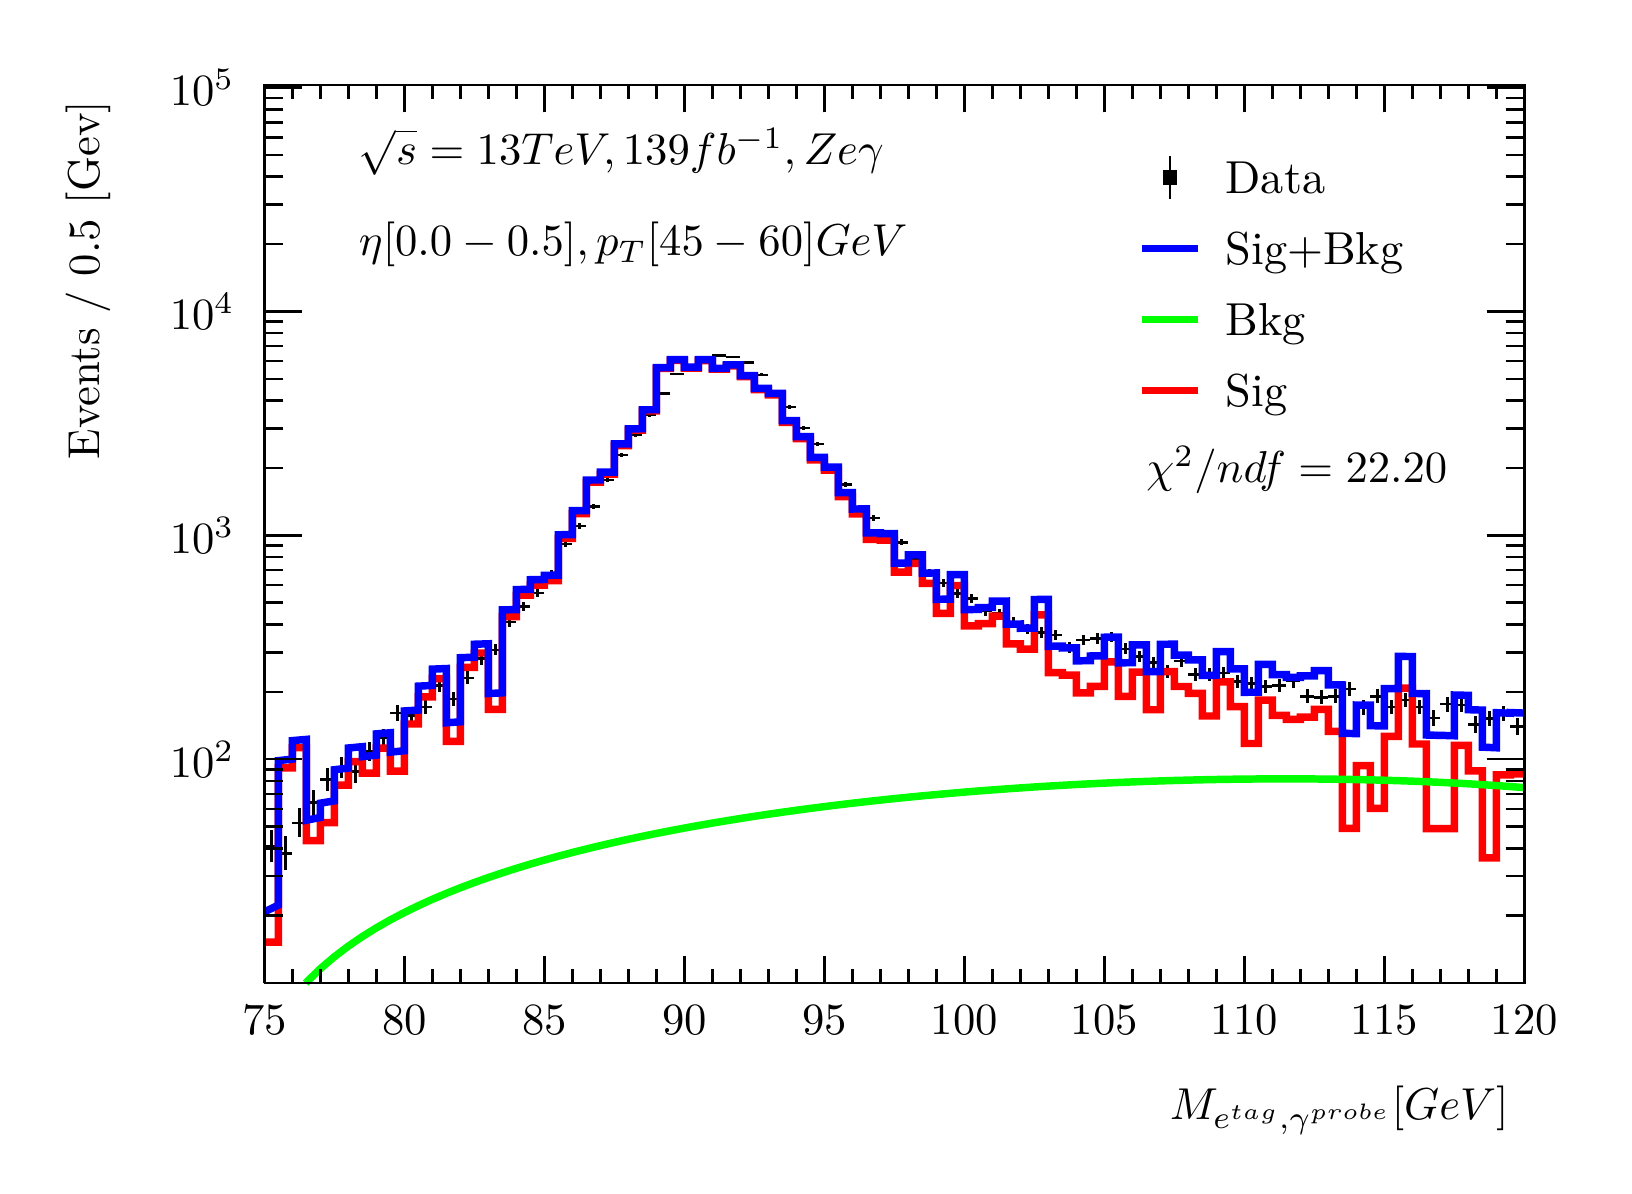
\begin{tikzpicture}
\pgfdeclareplotmark{cross} {
\pgfpathmoveto{\pgfpoint{-0.3\pgfplotmarksize}{\pgfplotmarksize}}
\pgfpathlineto{\pgfpoint{+0.3\pgfplotmarksize}{\pgfplotmarksize}}
\pgfpathlineto{\pgfpoint{+0.3\pgfplotmarksize}{0.3\pgfplotmarksize}}
\pgfpathlineto{\pgfpoint{+1\pgfplotmarksize}{0.3\pgfplotmarksize}}
\pgfpathlineto{\pgfpoint{+1\pgfplotmarksize}{-0.3\pgfplotmarksize}}
\pgfpathlineto{\pgfpoint{+0.3\pgfplotmarksize}{-0.3\pgfplotmarksize}}
\pgfpathlineto{\pgfpoint{+0.3\pgfplotmarksize}{-1.\pgfplotmarksize}}
\pgfpathlineto{\pgfpoint{-0.3\pgfplotmarksize}{-1.\pgfplotmarksize}}
\pgfpathlineto{\pgfpoint{-0.3\pgfplotmarksize}{-0.3\pgfplotmarksize}}
\pgfpathlineto{\pgfpoint{-1.\pgfplotmarksize}{-0.3\pgfplotmarksize}}
\pgfpathlineto{\pgfpoint{-1.\pgfplotmarksize}{0.3\pgfplotmarksize}}
\pgfpathlineto{\pgfpoint{-0.3\pgfplotmarksize}{0.3\pgfplotmarksize}}
\pgfpathclose
\pgfusepathqstroke
}
\pgfdeclareplotmark{cross*} {
\pgfpathmoveto{\pgfpoint{-0.3\pgfplotmarksize}{\pgfplotmarksize}}
\pgfpathlineto{\pgfpoint{+0.3\pgfplotmarksize}{\pgfplotmarksize}}
\pgfpathlineto{\pgfpoint{+0.3\pgfplotmarksize}{0.3\pgfplotmarksize}}
\pgfpathlineto{\pgfpoint{+1\pgfplotmarksize}{0.3\pgfplotmarksize}}
\pgfpathlineto{\pgfpoint{+1\pgfplotmarksize}{-0.3\pgfplotmarksize}}
\pgfpathlineto{\pgfpoint{+0.3\pgfplotmarksize}{-0.3\pgfplotmarksize}}
\pgfpathlineto{\pgfpoint{+0.3\pgfplotmarksize}{-1.\pgfplotmarksize}}
\pgfpathlineto{\pgfpoint{-0.3\pgfplotmarksize}{-1.\pgfplotmarksize}}
\pgfpathlineto{\pgfpoint{-0.3\pgfplotmarksize}{-0.3\pgfplotmarksize}}
\pgfpathlineto{\pgfpoint{-1.\pgfplotmarksize}{-0.3\pgfplotmarksize}}
\pgfpathlineto{\pgfpoint{-1.\pgfplotmarksize}{0.3\pgfplotmarksize}}
\pgfpathlineto{\pgfpoint{-0.3\pgfplotmarksize}{0.3\pgfplotmarksize}}
\pgfpathclose
\pgfusepathqfillstroke
}
\pgfdeclareplotmark{newstar} {
\pgfpathmoveto{\pgfqpoint{0pt}{\pgfplotmarksize}}
\pgfpathlineto{\pgfqpointpolar{44}{0.5\pgfplotmarksize}}
\pgfpathlineto{\pgfqpointpolar{18}{\pgfplotmarksize}}
\pgfpathlineto{\pgfqpointpolar{-20}{0.5\pgfplotmarksize}}
\pgfpathlineto{\pgfqpointpolar{-54}{\pgfplotmarksize}}
\pgfpathlineto{\pgfqpointpolar{-90}{0.5\pgfplotmarksize}}
\pgfpathlineto{\pgfqpointpolar{234}{\pgfplotmarksize}}
\pgfpathlineto{\pgfqpointpolar{198}{0.5\pgfplotmarksize}}
\pgfpathlineto{\pgfqpointpolar{162}{\pgfplotmarksize}}
\pgfpathlineto{\pgfqpointpolar{134}{0.5\pgfplotmarksize}}
\pgfpathclose
\pgfusepathqstroke
}
\pgfdeclareplotmark{newstar*} {
\pgfpathmoveto{\pgfqpoint{0pt}{\pgfplotmarksize}}
\pgfpathlineto{\pgfqpointpolar{44}{0.5\pgfplotmarksize}}
\pgfpathlineto{\pgfqpointpolar{18}{\pgfplotmarksize}}
\pgfpathlineto{\pgfqpointpolar{-20}{0.5\pgfplotmarksize}}
\pgfpathlineto{\pgfqpointpolar{-54}{\pgfplotmarksize}}
\pgfpathlineto{\pgfqpointpolar{-90}{0.5\pgfplotmarksize}}
\pgfpathlineto{\pgfqpointpolar{234}{\pgfplotmarksize}}
\pgfpathlineto{\pgfqpointpolar{198}{0.5\pgfplotmarksize}}
\pgfpathlineto{\pgfqpointpolar{162}{\pgfplotmarksize}}
\pgfpathlineto{\pgfqpointpolar{134}{0.5\pgfplotmarksize}}
\pgfpathclose
\pgfusepathqfillstroke
}
\definecolor{c}{rgb}{1,1,1};
\draw [color=c, fill=c] (0,0) rectangle (20,14.4361);
\draw [color=c, fill=c] (3,2.30977) rectangle (19,13.7143);
\definecolor{c}{rgb}{0,0,0};
\draw [c,line width=0.9] (3,2.30977) -- (3,13.7143) -- (19,13.7143) -- (19,2.30977) -- (3,2.30977);
\definecolor{c}{rgb}{1,1,1};
\draw [color=c, fill=c] (3,2.30977) rectangle (19,13.7143);
\definecolor{c}{rgb}{0,0,0};
\draw [c,line width=0.9] (3,2.30977) -- (3,13.7143) -- (19,13.7143) -- (19,2.30977) -- (3,2.30977);
\draw [c,line width=0.9] (3,2.30977) -- (19,2.30977);
\draw [c,line width=0.9] (3,2.65624) -- (3,2.30977);
\draw [c,line width=0.9] (3.35556,2.48301) -- (3.35556,2.30977);
\draw [c,line width=0.9] (3.71111,2.48301) -- (3.71111,2.30977);
\draw [c,line width=0.9] (4.06667,2.48301) -- (4.06667,2.30977);
\draw [c,line width=0.9] (4.42222,2.48301) -- (4.42222,2.30977);
\draw [c,line width=0.9] (4.77778,2.65624) -- (4.77778,2.30977);
\draw [c,line width=0.9] (5.13333,2.48301) -- (5.13333,2.30977);
\draw [c,line width=0.9] (5.48889,2.48301) -- (5.48889,2.30977);
\draw [c,line width=0.9] (5.84444,2.48301) -- (5.84444,2.30977);
\draw [c,line width=0.9] (6.2,2.48301) -- (6.2,2.30977);
\draw [c,line width=0.9] (6.55556,2.65624) -- (6.55556,2.30977);
\draw [c,line width=0.9] (6.91111,2.48301) -- (6.91111,2.30977);
\draw [c,line width=0.9] (7.26667,2.48301) -- (7.26667,2.30977);
\draw [c,line width=0.9] (7.62222,2.48301) -- (7.62222,2.30977);
\draw [c,line width=0.9] (7.97778,2.48301) -- (7.97778,2.30977);
\draw [c,line width=0.9] (8.33333,2.65624) -- (8.33333,2.30977);
\draw [c,line width=0.9] (8.68889,2.48301) -- (8.68889,2.30977);
\draw [c,line width=0.9] (9.04444,2.48301) -- (9.04444,2.30977);
\draw [c,line width=0.9] (9.4,2.48301) -- (9.4,2.30977);
\draw [c,line width=0.9] (9.75556,2.48301) -- (9.75556,2.30977);
\draw [c,line width=0.9] (10.1111,2.65624) -- (10.1111,2.30977);
\draw [c,line width=0.9] (10.4667,2.48301) -- (10.4667,2.30977);
\draw [c,line width=0.9] (10.8222,2.48301) -- (10.8222,2.30977);
\draw [c,line width=0.9] (11.1778,2.48301) -- (11.1778,2.30977);
\draw [c,line width=0.9] (11.5333,2.48301) -- (11.5333,2.30977);
\draw [c,line width=0.9] (11.8889,2.65624) -- (11.8889,2.30977);
\draw [c,line width=0.9] (12.2444,2.48301) -- (12.2444,2.30977);
\draw [c,line width=0.9] (12.6,2.48301) -- (12.6,2.30977);
\draw [c,line width=0.9] (12.9556,2.48301) -- (12.9556,2.30977);
\draw [c,line width=0.9] (13.3111,2.48301) -- (13.3111,2.30977);
\draw [c,line width=0.9] (13.6667,2.65624) -- (13.6667,2.30977);
\draw [c,line width=0.9] (14.0222,2.48301) -- (14.0222,2.30977);
\draw [c,line width=0.9] (14.3778,2.48301) -- (14.3778,2.30977);
\draw [c,line width=0.9] (14.7333,2.48301) -- (14.7333,2.30977);
\draw [c,line width=0.9] (15.0889,2.48301) -- (15.0889,2.30977);
\draw [c,line width=0.9] (15.4444,2.65624) -- (15.4444,2.30977);
\draw [c,line width=0.9] (15.8,2.48301) -- (15.8,2.30977);
\draw [c,line width=0.9] (16.1556,2.48301) -- (16.1556,2.30977);
\draw [c,line width=0.9] (16.5111,2.48301) -- (16.5111,2.30977);
\draw [c,line width=0.9] (16.8667,2.48301) -- (16.8667,2.30977);
\draw [c,line width=0.9] (17.2222,2.65624) -- (17.2222,2.30977);
\draw [c,line width=0.9] (17.5778,2.48301) -- (17.5778,2.30977);
\draw [c,line width=0.9] (17.9333,2.48301) -- (17.9333,2.30977);
\draw [c,line width=0.9] (18.2889,2.48301) -- (18.2889,2.30977);
\draw [c,line width=0.9] (18.6444,2.48301) -- (18.6444,2.30977);
\draw [c,line width=0.9] (19,2.65624) -- (19,2.30977);
\draw [c,line width=0.9] (19,2.65624) -- (19,2.30977);
\draw [anchor=base] (3,1.66015) node[scale=1.61424, color=c, rotate=0]{75};
\draw [anchor=base] (4.77778,1.66015) node[scale=1.61424, color=c, rotate=0]{80};
\draw [anchor=base] (6.55556,1.66015) node[scale=1.61424, color=c, rotate=0]{85};
\draw [anchor=base] (8.33333,1.66015) node[scale=1.61424, color=c, rotate=0]{90};
\draw [anchor=base] (10.1111,1.66015) node[scale=1.61424, color=c, rotate=0]{95};
\draw [anchor=base] (11.8889,1.66015) node[scale=1.61424, color=c, rotate=0]{100};
\draw [anchor=base] (13.6667,1.66015) node[scale=1.61424, color=c, rotate=0]{105};
\draw [anchor=base] (15.4444,1.66015) node[scale=1.61424, color=c, rotate=0]{110};
\draw [anchor=base] (17.2222,1.66015) node[scale=1.61424, color=c, rotate=0]{115};
\draw [anchor=base] (19,1.66015) node[scale=1.61424, color=c, rotate=0]{120};
\draw [anchor= east] (19,0.692932) node[scale=1.61424, color=c, rotate=0]{$M_{e^{tag}, \gamma^{probe}}  [GeV]$};
\draw [c,line width=0.9] (3,13.7143) -- (19,13.7143);
\draw [c,line width=0.9] (3,13.3678) -- (3,13.7143);
\draw [c,line width=0.9] (3.35556,13.5411) -- (3.35556,13.7143);
\draw [c,line width=0.9] (3.71111,13.5411) -- (3.71111,13.7143);
\draw [c,line width=0.9] (4.06667,13.5411) -- (4.06667,13.7143);
\draw [c,line width=0.9] (4.42222,13.5411) -- (4.42222,13.7143);
\draw [c,line width=0.9] (4.77778,13.3678) -- (4.77778,13.7143);
\draw [c,line width=0.9] (5.13333,13.5411) -- (5.13333,13.7143);
\draw [c,line width=0.9] (5.48889,13.5411) -- (5.48889,13.7143);
\draw [c,line width=0.9] (5.84444,13.5411) -- (5.84444,13.7143);
\draw [c,line width=0.9] (6.2,13.5411) -- (6.2,13.7143);
\draw [c,line width=0.9] (6.55556,13.3678) -- (6.55556,13.7143);
\draw [c,line width=0.9] (6.91111,13.5411) -- (6.91111,13.7143);
\draw [c,line width=0.9] (7.26667,13.5411) -- (7.26667,13.7143);
\draw [c,line width=0.9] (7.62222,13.5411) -- (7.62222,13.7143);
\draw [c,line width=0.9] (7.97778,13.5411) -- (7.97778,13.7143);
\draw [c,line width=0.9] (8.33333,13.3678) -- (8.33333,13.7143);
\draw [c,line width=0.9] (8.68889,13.5411) -- (8.68889,13.7143);
\draw [c,line width=0.9] (9.04444,13.5411) -- (9.04444,13.7143);
\draw [c,line width=0.9] (9.4,13.5411) -- (9.4,13.7143);
\draw [c,line width=0.9] (9.75556,13.5411) -- (9.75556,13.7143);
\draw [c,line width=0.9] (10.1111,13.3678) -- (10.1111,13.7143);
\draw [c,line width=0.9] (10.4667,13.5411) -- (10.4667,13.7143);
\draw [c,line width=0.9] (10.8222,13.5411) -- (10.8222,13.7143);
\draw [c,line width=0.9] (11.1778,13.5411) -- (11.1778,13.7143);
\draw [c,line width=0.9] (11.5333,13.5411) -- (11.5333,13.7143);
\draw [c,line width=0.9] (11.8889,13.3678) -- (11.8889,13.7143);
\draw [c,line width=0.9] (12.2444,13.5411) -- (12.2444,13.7143);
\draw [c,line width=0.9] (12.6,13.5411) -- (12.6,13.7143);
\draw [c,line width=0.9] (12.9556,13.5411) -- (12.9556,13.7143);
\draw [c,line width=0.9] (13.3111,13.5411) -- (13.3111,13.7143);
\draw [c,line width=0.9] (13.6667,13.3678) -- (13.6667,13.7143);
\draw [c,line width=0.9] (14.0222,13.5411) -- (14.0222,13.7143);
\draw [c,line width=0.9] (14.3778,13.5411) -- (14.3778,13.7143);
\draw [c,line width=0.9] (14.7333,13.5411) -- (14.7333,13.7143);
\draw [c,line width=0.9] (15.0889,13.5411) -- (15.0889,13.7143);
\draw [c,line width=0.9] (15.4444,13.3678) -- (15.4444,13.7143);
\draw [c,line width=0.9] (15.8,13.5411) -- (15.8,13.7143);
\draw [c,line width=0.9] (16.1556,13.5411) -- (16.1556,13.7143);
\draw [c,line width=0.9] (16.5111,13.5411) -- (16.5111,13.7143);
\draw [c,line width=0.9] (16.8667,13.5411) -- (16.8667,13.7143);
\draw [c,line width=0.9] (17.2222,13.3678) -- (17.2222,13.7143);
\draw [c,line width=0.9] (17.5778,13.5411) -- (17.5778,13.7143);
\draw [c,line width=0.9] (17.9333,13.5411) -- (17.9333,13.7143);
\draw [c,line width=0.9] (18.2889,13.5411) -- (18.2889,13.7143);
\draw [c,line width=0.9] (18.6444,13.5411) -- (18.6444,13.7143);
\draw [c,line width=0.9] (19,13.3678) -- (19,13.7143);
\draw [c,line width=0.9] (19,13.3678) -- (19,13.7143);
\draw [c,line width=0.9] (3,2.30977) -- (3,13.7143);
\draw [c,line width=0.9] (3.237,3.16561) -- (3,3.16561);
\draw [c,line width=0.9] (3.237,3.66625) -- (3,3.66625);
\draw [c,line width=0.9] (3.237,4.02146) -- (3,4.02146);
\draw [c,line width=0.9] (3.237,4.29698) -- (3,4.29698);
\draw [c,line width=0.9] (3.237,4.52209) -- (3,4.52209);
\draw [c,line width=0.9] (3.237,4.71242) -- (3,4.71242);
\draw [c,line width=0.9] (3.237,4.8773) -- (3,4.8773);
\draw [c,line width=0.9] (3.237,5.02273) -- (3,5.02273);
\draw [c,line width=0.9] (3.474,5.15282) -- (3,5.15282);
\draw [anchor= east] (2.82,5.15282) node[scale=1.61424, color=c, rotate=0]{$10^{2}$};
\draw [c,line width=0.9] (3.237,6.00866) -- (3,6.00866);
\draw [c,line width=0.9] (3.237,6.5093) -- (3,6.5093);
\draw [c,line width=0.9] (3.237,6.8645) -- (3,6.8645);
\draw [c,line width=0.9] (3.237,7.14002) -- (3,7.14002);
\draw [c,line width=0.9] (3.237,7.36514) -- (3,7.36514);
\draw [c,line width=0.9] (3.237,7.55547) -- (3,7.55547);
\draw [c,line width=0.9] (3.237,7.72034) -- (3,7.72034);
\draw [c,line width=0.9] (3.237,7.86577) -- (3,7.86577);
\draw [c,line width=0.9] (3.474,7.99586) -- (3,7.99586);
\draw [anchor= east] (2.82,7.99586) node[scale=1.61424, color=c, rotate=0]{$10^{3}$};
\draw [c,line width=0.9] (3.237,8.85171) -- (3,8.85171);
\draw [c,line width=0.9] (3.237,9.35234) -- (3,9.35234);
\draw [c,line width=0.9] (3.237,9.70755) -- (3,9.70755);
\draw [c,line width=0.9] (3.237,9.98307) -- (3,9.98307);
\draw [c,line width=0.9] (3.237,10.2082) -- (3,10.2082);
\draw [c,line width=0.9] (3.237,10.3985) -- (3,10.3985);
\draw [c,line width=0.9] (3.237,10.5634) -- (3,10.5634);
\draw [c,line width=0.9] (3.237,10.7088) -- (3,10.7088);
\draw [c,line width=0.9] (3.474,10.8389) -- (3,10.8389);
\draw [anchor= east] (2.82,10.8389) node[scale=1.61424, color=c, rotate=0]{$10^{4}$};
\draw [c,line width=0.9] (3.237,11.6948) -- (3,11.6948);
\draw [c,line width=0.9] (3.237,12.1954) -- (3,12.1954);
\draw [c,line width=0.9] (3.237,12.5506) -- (3,12.5506);
\draw [c,line width=0.9] (3.237,12.8261) -- (3,12.8261);
\draw [c,line width=0.9] (3.237,13.0512) -- (3,13.0512);
\draw [c,line width=0.9] (3.237,13.2416) -- (3,13.2416);
\draw [c,line width=0.9] (3.237,13.4064) -- (3,13.4064);
\draw [c,line width=0.9] (3.237,13.5519) -- (3,13.5519);
\draw [c,line width=0.9] (3.474,13.682) -- (3,13.682);
\draw [anchor= east] (2.82,13.682) node[scale=1.61424, color=c, rotate=0]{$10^{5}$};
\draw [anchor= east] (0.76,13.7143) node[scale=1.61424, color=c, rotate=90]{Events / 0.5 [Gev]};
\draw [c,line width=0.9] (19,2.30977) -- (19,13.7143);
\draw [c,line width=0.9] (18.763,3.16561) -- (19,3.16561);
\draw [c,line width=0.9] (18.763,3.66625) -- (19,3.66625);
\draw [c,line width=0.9] (18.763,4.02146) -- (19,4.02146);
\draw [c,line width=0.9] (18.763,4.29698) -- (19,4.29698);
\draw [c,line width=0.9] (18.763,4.52209) -- (19,4.52209);
\draw [c,line width=0.9] (18.763,4.71242) -- (19,4.71242);
\draw [c,line width=0.9] (18.763,4.8773) -- (19,4.8773);
\draw [c,line width=0.9] (18.763,5.02273) -- (19,5.02273);
\draw [c,line width=0.9] (18.526,5.15282) -- (19,5.15282);
\draw [c,line width=0.9] (18.763,6.00866) -- (19,6.00866);
\draw [c,line width=0.9] (18.763,6.5093) -- (19,6.5093);
\draw [c,line width=0.9] (18.763,6.8645) -- (19,6.8645);
\draw [c,line width=0.9] (18.763,7.14002) -- (19,7.14002);
\draw [c,line width=0.9] (18.763,7.36514) -- (19,7.36514);
\draw [c,line width=0.9] (18.763,7.55547) -- (19,7.55547);
\draw [c,line width=0.9] (18.763,7.72034) -- (19,7.72034);
\draw [c,line width=0.9] (18.763,7.86577) -- (19,7.86577);
\draw [c,line width=0.9] (18.526,7.99586) -- (19,7.99586);
\draw [c,line width=0.9] (18.763,8.85171) -- (19,8.85171);
\draw [c,line width=0.9] (18.763,9.35234) -- (19,9.35234);
\draw [c,line width=0.9] (18.763,9.70755) -- (19,9.70755);
\draw [c,line width=0.9] (18.763,9.98307) -- (19,9.98307);
\draw [c,line width=0.9] (18.763,10.2082) -- (19,10.2082);
\draw [c,line width=0.9] (18.763,10.3985) -- (19,10.3985);
\draw [c,line width=0.9] (18.763,10.5634) -- (19,10.5634);
\draw [c,line width=0.9] (18.763,10.7088) -- (19,10.7088);
\draw [c,line width=0.9] (18.526,10.8389) -- (19,10.8389);
\draw [c,line width=0.9] (18.763,11.6948) -- (19,11.6948);
\draw [c,line width=0.9] (18.763,12.1954) -- (19,12.1954);
\draw [c,line width=0.9] (18.763,12.5506) -- (19,12.5506);
\draw [c,line width=0.9] (18.763,12.8261) -- (19,12.8261);
\draw [c,line width=0.9] (18.763,13.0512) -- (19,13.0512);
\draw [c,line width=0.9] (18.763,13.2416) -- (19,13.2416);
\draw [c,line width=0.9] (18.763,13.4064) -- (19,13.4064);
\draw [c,line width=0.9] (18.763,13.5519) -- (19,13.5519);
\draw [c,line width=0.9] (18.526,13.682) -- (19,13.682);
\draw [c,line width=0.9] (3.08889,4.05195) -- (3,4.05195);
\draw [c,line width=0.9] (3,4.05195) -- (3,4.05195);
\draw [c,line width=0.9] (3.08889,4.05195) -- (3.17778,4.05195);
\draw [c,line width=0.9] (3.17778,4.05195) -- (3.17778,4.05195);
\draw [c,line width=0.9] (3.08889,4.05195) -- (3.08889,4.25823);
\draw [c,line width=0.9] (3.08889,4.25823) -- (3.08889,4.25823);
\draw [c,line width=0.9] (3.08889,4.05195) -- (3.08889,3.84322);
\draw [c,line width=0.9] (3.08889,3.84322) -- (3.08889,3.84322);
\draw [c,line width=0.9] (3.26667,3.95813) -- (3.17778,3.95813);
\draw [c,line width=0.9] (3.17778,3.95813) -- (3.17778,3.95813);
\draw [c,line width=0.9] (3.26667,3.95813) -- (3.35556,3.95813);
\draw [c,line width=0.9] (3.35556,3.95813) -- (3.35556,3.95813);
\draw [c,line width=0.9] (3.26667,3.95813) -- (3.26667,4.17287);
\draw [c,line width=0.9] (3.26667,4.17287) -- (3.26667,4.17287);
\draw [c,line width=0.9] (3.26667,3.95813) -- (3.26667,3.74063);
\draw [c,line width=0.9] (3.26667,3.74063) -- (3.26667,3.74063);
\draw [c,line width=0.9] (3.44444,4.3454) -- (3.35556,4.3454);
\draw [c,line width=0.9] (3.35556,4.3454) -- (3.35556,4.3454);
\draw [c,line width=0.9] (3.44444,4.3454) -- (3.53333,4.3454);
\draw [c,line width=0.9] (3.53333,4.3454) -- (3.53333,4.3454);
\draw [c,line width=0.9] (3.44444,4.3454) -- (3.44444,4.52738);
\draw [c,line width=0.9] (3.44444,4.52738) -- (3.44444,4.52738);
\draw [c,line width=0.9] (3.44444,4.3454) -- (3.44444,4.16172);
\draw [c,line width=0.9] (3.44444,4.16172) -- (3.44444,4.16172);
\draw [c,line width=0.9] (3.62222,4.60178) -- (3.53333,4.60178);
\draw [c,line width=0.9] (3.53333,4.60178) -- (3.53333,4.60178);
\draw [c,line width=0.9] (3.62222,4.60178) -- (3.71111,4.60178);
\draw [c,line width=0.9] (3.71111,4.60178) -- (3.71111,4.60178);
\draw [c,line width=0.9] (3.62222,4.60178) -- (3.62222,4.76495);
\draw [c,line width=0.9] (3.62222,4.76495) -- (3.62222,4.76495);
\draw [c,line width=0.9] (3.62222,4.60178) -- (3.62222,4.43737);
\draw [c,line width=0.9] (3.62222,4.43737) -- (3.62222,4.43737);
\draw [c,line width=0.9] (3.8,4.89264) -- (3.71111,4.89264);
\draw [c,line width=0.9] (3.71111,4.89264) -- (3.71111,4.89264);
\draw [c,line width=0.9] (3.8,4.89264) -- (3.88889,4.89264);
\draw [c,line width=0.9] (3.88889,4.89264) -- (3.88889,4.89264);
\draw [c,line width=0.9] (3.8,4.89264) -- (3.8,5.03688);
\draw [c,line width=0.9] (3.8,5.03688) -- (3.8,5.03688);
\draw [c,line width=0.9] (3.8,4.89264) -- (3.8,4.74753);
\draw [c,line width=0.9] (3.8,4.74753) -- (3.8,4.74753);
\draw [c,line width=0.9] (3.97778,5.04987) -- (3.88889,5.04987);
\draw [c,line width=0.9] (3.88889,5.04987) -- (3.88889,5.04987);
\draw [c,line width=0.9] (3.97778,5.04987) -- (4.06667,5.04987);
\draw [c,line width=0.9] (4.06667,5.04987) -- (4.06667,5.04987);
\draw [c,line width=0.9] (3.97778,5.04987) -- (3.97778,5.18483);
\draw [c,line width=0.9] (3.97778,5.18483) -- (3.97778,5.18483);
\draw [c,line width=0.9] (3.97778,5.04987) -- (3.97778,4.91418);
\draw [c,line width=0.9] (3.97778,4.91418) -- (3.97778,4.91418);
\draw [c,line width=0.9] (4.15556,4.99498) -- (4.06667,4.99498);
\draw [c,line width=0.9] (4.06667,4.99498) -- (4.06667,4.99498);
\draw [c,line width=0.9] (4.15556,4.99498) -- (4.24444,4.99498);
\draw [c,line width=0.9] (4.24444,4.99498) -- (4.24444,4.99498);
\draw [c,line width=0.9] (4.15556,4.99498) -- (4.15556,5.13311);
\draw [c,line width=0.9] (4.15556,5.13311) -- (4.15556,5.13311);
\draw [c,line width=0.9] (4.15556,4.99498) -- (4.15556,4.85608);
\draw [c,line width=0.9] (4.15556,4.85608) -- (4.15556,4.85608);
\draw [c,line width=0.9] (4.33333,5.24785) -- (4.24444,5.24785);
\draw [c,line width=0.9] (4.24444,5.24785) -- (4.24444,5.24785);
\draw [c,line width=0.9] (4.33333,5.24785) -- (4.42222,5.24785);
\draw [c,line width=0.9] (4.42222,5.24785) -- (4.42222,5.24785);
\draw [c,line width=0.9] (4.33333,5.24785) -- (4.33333,5.36661);
\draw [c,line width=0.9] (4.33333,5.36661) -- (4.33333,5.36661);
\draw [c,line width=0.9] (4.33333,5.24785) -- (4.33333,5.12908);
\draw [c,line width=0.9] (4.33333,5.12908) -- (4.33333,5.12908);
\draw [c,line width=0.9] (4.51111,5.42834) -- (4.42222,5.42834);
\draw [c,line width=0.9] (4.42222,5.42834) -- (4.42222,5.42834);
\draw [c,line width=0.9] (4.51111,5.42834) -- (4.6,5.42834);
\draw [c,line width=0.9] (4.6,5.42834) -- (4.6,5.42834);
\draw [c,line width=0.9] (4.51111,5.42834) -- (4.51111,5.53874);
\draw [c,line width=0.9] (4.51111,5.53874) -- (4.51111,5.53874);
\draw [c,line width=0.9] (4.51111,5.42834) -- (4.51111,5.31794);
\draw [c,line width=0.9] (4.51111,5.31794) -- (4.51111,5.31794);
\draw [c,line width=0.9] (4.68889,5.74084) -- (4.6,5.74084);
\draw [c,line width=0.9] (4.6,5.74084) -- (4.6,5.74084);
\draw [c,line width=0.9] (4.68889,5.74084) -- (4.77778,5.74084);
\draw [c,line width=0.9] (4.77778,5.74084) -- (4.77778,5.74084);
\draw [c,line width=0.9] (4.68889,5.74084) -- (4.68889,5.83812);
\draw [c,line width=0.9] (4.68889,5.83812) -- (4.68889,5.83812);
\draw [c,line width=0.9] (4.68889,5.74084) -- (4.68889,5.64355);
\draw [c,line width=0.9] (4.68889,5.64355) -- (4.68889,5.64355);
\draw [c,line width=0.9] (4.86667,5.70977) -- (4.77778,5.70977);
\draw [c,line width=0.9] (4.77778,5.70977) -- (4.77778,5.70977);
\draw [c,line width=0.9] (4.86667,5.70977) -- (4.95556,5.70977);
\draw [c,line width=0.9] (4.95556,5.70977) -- (4.95556,5.70977);
\draw [c,line width=0.9] (4.86667,5.70977) -- (4.86667,5.80829);
\draw [c,line width=0.9] (4.86667,5.80829) -- (4.86667,5.80829);
\draw [c,line width=0.9] (4.86667,5.70977) -- (4.86667,5.61126);
\draw [c,line width=0.9] (4.86667,5.61126) -- (4.86667,5.61126);
\draw [c,line width=0.9] (5.04444,5.81524) -- (4.95556,5.81524);
\draw [c,line width=0.9] (4.95556,5.81524) -- (4.95556,5.81524);
\draw [c,line width=0.9] (5.04444,5.81524) -- (5.13333,5.81524);
\draw [c,line width=0.9] (5.13333,5.81524) -- (5.13333,5.81524);
\draw [c,line width=0.9] (5.04444,5.81524) -- (5.04444,5.90964);
\draw [c,line width=0.9] (5.04444,5.90964) -- (5.04444,5.90964);
\draw [c,line width=0.9] (5.04444,5.81524) -- (5.04444,5.72084);
\draw [c,line width=0.9] (5.04444,5.72084) -- (5.04444,5.72084);
\draw [c,line width=0.9] (5.22222,6.08642) -- (5.13333,6.08642);
\draw [c,line width=0.9] (5.13333,6.08642) -- (5.13333,6.08642);
\draw [c,line width=0.9] (5.22222,6.08642) -- (5.31111,6.08642);
\draw [c,line width=0.9] (5.31111,6.08642) -- (5.31111,6.08642);
\draw [c,line width=0.9] (5.22222,6.08642) -- (5.22222,6.171);
\draw [c,line width=0.9] (5.22222,6.171) -- (5.22222,6.171);
\draw [c,line width=0.9] (5.22222,6.08642) -- (5.22222,6.00183);
\draw [c,line width=0.9] (5.22222,6.00183) -- (5.22222,6.00183);
\draw [c,line width=0.9] (5.4,5.91906) -- (5.31111,5.91906);
\draw [c,line width=0.9] (5.31111,5.91906) -- (5.31111,5.91906);
\draw [c,line width=0.9] (5.4,5.91906) -- (5.48889,5.91906);
\draw [c,line width=0.9] (5.48889,5.91906) -- (5.48889,5.91906);
\draw [c,line width=0.9] (5.4,5.91906) -- (5.4,6.00957);
\draw [c,line width=0.9] (5.4,6.00957) -- (5.4,6.00957);
\draw [c,line width=0.9] (5.4,5.91906) -- (5.4,5.82854);
\draw [c,line width=0.9] (5.4,5.82854) -- (5.4,5.82854);
\draw [c,line width=0.9] (5.57778,6.18658) -- (5.48889,6.18658);
\draw [c,line width=0.9] (5.48889,6.18658) -- (5.48889,6.18658);
\draw [c,line width=0.9] (5.57778,6.18658) -- (5.66667,6.18658);
\draw [c,line width=0.9] (5.66667,6.18658) -- (5.66667,6.18658);
\draw [c,line width=0.9] (5.57778,6.18658) -- (5.57778,6.26781);
\draw [c,line width=0.9] (5.57778,6.26781) -- (5.57778,6.26781);
\draw [c,line width=0.9] (5.57778,6.18658) -- (5.57778,6.10536);
\draw [c,line width=0.9] (5.57778,6.10536) -- (5.57778,6.10536);
\draw [c,line width=0.9] (5.75556,6.42851) -- (5.66667,6.42851);
\draw [c,line width=0.9] (5.66667,6.42851) -- (5.66667,6.42851);
\draw [c,line width=0.9] (5.75556,6.42851) -- (5.84444,6.42851);
\draw [c,line width=0.9] (5.84444,6.42851) -- (5.84444,6.42851);
\draw [c,line width=0.9] (5.75556,6.42851) -- (5.75556,6.50216);
\draw [c,line width=0.9] (5.75556,6.50216) -- (5.75556,6.50216);
\draw [c,line width=0.9] (5.75556,6.42851) -- (5.75556,6.35487);
\draw [c,line width=0.9] (5.75556,6.35487) -- (5.75556,6.35487);
\draw [c,line width=0.9] (5.93333,6.54179) -- (5.84444,6.54179);
\draw [c,line width=0.9] (5.84444,6.54179) -- (5.84444,6.54179);
\draw [c,line width=0.9] (5.93333,6.54179) -- (6.02222,6.54179);
\draw [c,line width=0.9] (6.02222,6.54179) -- (6.02222,6.54179);
\draw [c,line width=0.9] (5.93333,6.54179) -- (5.93333,6.61214);
\draw [c,line width=0.9] (5.93333,6.61214) -- (5.93333,6.61214);
\draw [c,line width=0.9] (5.93333,6.54179) -- (5.93333,6.47145);
\draw [c,line width=0.9] (5.93333,6.47145) -- (5.93333,6.47145);
\draw [c,line width=0.9] (6.11111,6.89198) -- (6.02222,6.89198);
\draw [c,line width=0.9] (6.02222,6.89198) -- (6.02222,6.89198);
\draw [c,line width=0.9] (6.11111,6.89198) -- (6.2,6.89198);
\draw [c,line width=0.9] (6.2,6.89198) -- (6.2,6.89198);
\draw [c,line width=0.9] (6.11111,6.89198) -- (6.11111,6.95302);
\draw [c,line width=0.9] (6.11111,6.95302) -- (6.11111,6.95302);
\draw [c,line width=0.9] (6.11111,6.89198) -- (6.11111,6.83093);
\draw [c,line width=0.9] (6.11111,6.83093) -- (6.11111,6.83093);
\draw [c,line width=0.9] (6.28889,7.09475) -- (6.2,7.09475);
\draw [c,line width=0.9] (6.2,7.09475) -- (6.2,7.09475);
\draw [c,line width=0.9] (6.28889,7.09475) -- (6.37778,7.09475);
\draw [c,line width=0.9] (6.37778,7.09475) -- (6.37778,7.09475);
\draw [c,line width=0.9] (6.28889,7.09475) -- (6.28889,7.15099);
\draw [c,line width=0.9] (6.28889,7.15099) -- (6.28889,7.15099);
\draw [c,line width=0.9] (6.28889,7.09475) -- (6.28889,7.03852);
\draw [c,line width=0.9] (6.28889,7.03852) -- (6.28889,7.03852);
\draw [c,line width=0.9] (6.46667,7.26442) -- (6.37778,7.26442);
\draw [c,line width=0.9] (6.37778,7.26442) -- (6.37778,7.26442);
\draw [c,line width=0.9] (6.46667,7.26442) -- (6.55556,7.26442);
\draw [c,line width=0.9] (6.55556,7.26442) -- (6.55556,7.26442);
\draw [c,line width=0.9] (6.46667,7.26442) -- (6.46667,7.31692);
\draw [c,line width=0.9] (6.46667,7.31692) -- (6.46667,7.31692);
\draw [c,line width=0.9] (6.46667,7.26442) -- (6.46667,7.21192);
\draw [c,line width=0.9] (6.46667,7.21192) -- (6.46667,7.21192);
\draw [c,line width=0.9] (6.64444,7.50874) -- (6.55556,7.50874);
\draw [c,line width=0.9] (6.55556,7.50874) -- (6.55556,7.50874);
\draw [c,line width=0.9] (6.64444,7.50874) -- (6.73333,7.50874);
\draw [c,line width=0.9] (6.73333,7.50874) -- (6.73333,7.50874);
\draw [c,line width=0.9] (6.64444,7.50874) -- (6.64444,7.55629);
\draw [c,line width=0.9] (6.64444,7.55629) -- (6.64444,7.55629);
\draw [c,line width=0.9] (6.64444,7.50874) -- (6.64444,7.46118);
\draw [c,line width=0.9] (6.64444,7.46118) -- (6.64444,7.46118);
\draw [c,line width=0.9] (6.82222,7.88618) -- (6.73333,7.88618);
\draw [c,line width=0.9] (6.73333,7.88618) -- (6.73333,7.88618);
\draw [c,line width=0.9] (6.82222,7.88618) -- (6.91111,7.88618);
\draw [c,line width=0.9] (6.91111,7.88618) -- (6.91111,7.88618);
\draw [c,line width=0.9] (6.82222,7.88618) -- (6.82222,7.927);
\draw [c,line width=0.9] (6.82222,7.927) -- (6.82222,7.927);
\draw [c,line width=0.9] (6.82222,7.88618) -- (6.82222,7.84537);
\draw [c,line width=0.9] (6.82222,7.84537) -- (6.82222,7.84537);
\draw [c,line width=0.9] (7,8.11242) -- (6.91111,8.11242);
\draw [c,line width=0.9] (6.91111,8.11242) -- (6.91111,8.11242);
\draw [c,line width=0.9] (7,8.11242) -- (7.08889,8.11242);
\draw [c,line width=0.9] (7.08889,8.11242) -- (7.08889,8.11242);
\draw [c,line width=0.9] (7,8.11242) -- (7,8.14967);
\draw [c,line width=0.9] (7,8.14967) -- (7,8.14967);
\draw [c,line width=0.9] (7,8.11242) -- (7,8.07518);
\draw [c,line width=0.9] (7,8.07518) -- (7,8.07518);
\draw [c,line width=0.9] (7.17778,8.36183) -- (7.08889,8.36183);
\draw [c,line width=0.9] (7.08889,8.36183) -- (7.08889,8.36183);
\draw [c,line width=0.9] (7.17778,8.36183) -- (7.26667,8.36183);
\draw [c,line width=0.9] (7.26667,8.36183) -- (7.26667,8.36183);
\draw [c,line width=0.9] (7.17778,8.36183) -- (7.17778,8.39549);
\draw [c,line width=0.9] (7.17778,8.39549) -- (7.17778,8.39549);
\draw [c,line width=0.9] (7.17778,8.36183) -- (7.17778,8.32816);
\draw [c,line width=0.9] (7.17778,8.32816) -- (7.17778,8.32816);
\draw [c,line width=0.9] (7.35556,8.70156) -- (7.26667,8.70156);
\draw [c,line width=0.9] (7.26667,8.70156) -- (7.26667,8.70156);
\draw [c,line width=0.9] (7.35556,8.70156) -- (7.44444,8.70156);
\draw [c,line width=0.9] (7.44444,8.70156) -- (7.44444,8.70156);
\draw [c,line width=0.9] (7.35556,8.70156) -- (7.35556,8.7309);
\draw [c,line width=0.9] (7.35556,8.7309) -- (7.35556,8.7309);
\draw [c,line width=0.9] (7.35556,8.70156) -- (7.35556,8.67222);
\draw [c,line width=0.9] (7.35556,8.67222) -- (7.35556,8.67222);
\draw [c,line width=0.9] (7.53333,9.01511) -- (7.44444,9.01511);
\draw [c,line width=0.9] (7.44444,9.01511) -- (7.44444,9.01511);
\draw [c,line width=0.9] (7.53333,9.01511) -- (7.62222,9.01511);
\draw [c,line width=0.9] (7.62222,9.01511) -- (7.62222,9.01511);
\draw [c,line width=0.9] (7.53333,9.01511) -- (7.53333,9.04095);
\draw [c,line width=0.9] (7.53333,9.04095) -- (7.53333,9.04095);
\draw [c,line width=0.9] (7.53333,9.01511) -- (7.53333,8.98927);
\draw [c,line width=0.9] (7.53333,8.98927) -- (7.53333,8.98927);
\draw [c,line width=0.9] (7.71111,9.26848) -- (7.62222,9.26848);
\draw [c,line width=0.9] (7.62222,9.26848) -- (7.62222,9.26848);
\draw [c,line width=0.9] (7.71111,9.26848) -- (7.8,9.26848);
\draw [c,line width=0.9] (7.8,9.26848) -- (7.8,9.26848);
\draw [c,line width=0.9] (7.71111,9.26848) -- (7.71111,9.2918);
\draw [c,line width=0.9] (7.71111,9.2918) -- (7.71111,9.2918);
\draw [c,line width=0.9] (7.71111,9.26848) -- (7.71111,9.24516);
\draw [c,line width=0.9] (7.71111,9.24516) -- (7.71111,9.24516);
\draw [c,line width=0.9] (7.88889,9.52312) -- (7.8,9.52312);
\draw [c,line width=0.9] (7.8,9.52312) -- (7.8,9.52312);
\draw [c,line width=0.9] (7.88889,9.52312) -- (7.97778,9.52312);
\draw [c,line width=0.9] (7.97778,9.52312) -- (7.97778,9.52312);
\draw [c,line width=0.9] (7.88889,9.52312) -- (7.88889,9.54416);
\draw [c,line width=0.9] (7.88889,9.54416) -- (7.88889,9.54416);
\draw [c,line width=0.9] (7.88889,9.52312) -- (7.88889,9.50208);
\draw [c,line width=0.9] (7.88889,9.50208) -- (7.88889,9.50208);
\draw [c,line width=0.9] (8.06667,9.79426) -- (7.97778,9.79426);
\draw [c,line width=0.9] (7.97778,9.79426) -- (7.97778,9.79426);
\draw [c,line width=0.9] (8.06667,9.79426) -- (8.15556,9.79426);
\draw [c,line width=0.9] (8.15556,9.79426) -- (8.15556,9.79426);
\draw [c,line width=0.9] (8.06667,9.79426) -- (8.06667,9.81311);
\draw [c,line width=0.9] (8.06667,9.81311) -- (8.06667,9.81311);
\draw [c,line width=0.9] (8.06667,9.79426) -- (8.06667,9.77541);
\draw [c,line width=0.9] (8.06667,9.77541) -- (8.06667,9.77541);
\draw [c,line width=0.9] (8.24444,10.0452) -- (8.15556,10.0452);
\draw [c,line width=0.9] (8.15556,10.0452) -- (8.15556,10.0452);
\draw [c,line width=0.9] (8.24444,10.0452) -- (8.33333,10.0452);
\draw [c,line width=0.9] (8.33333,10.0452) -- (8.33333,10.0452);
\draw [c,line width=0.9] (8.24444,10.0452) -- (8.24444,10.0622);
\draw [c,line width=0.9] (8.24444,10.0622) -- (8.24444,10.0622);
\draw [c,line width=0.9] (8.24444,10.0452) -- (8.24444,10.0282);
\draw [c,line width=0.9] (8.24444,10.0282) -- (8.24444,10.0282);
\draw [c,line width=0.9] (8.42222,10.1292) -- (8.33333,10.1292);
\draw [c,line width=0.9] (8.33333,10.1292) -- (8.33333,10.1292);
\draw [c,line width=0.9] (8.42222,10.1292) -- (8.51111,10.1292);
\draw [c,line width=0.9] (8.51111,10.1292) -- (8.51111,10.1292);
\draw [c,line width=0.9] (8.42222,10.1292) -- (8.42222,10.1456);
\draw [c,line width=0.9] (8.42222,10.1456) -- (8.42222,10.1456);
\draw [c,line width=0.9] (8.42222,10.1292) -- (8.42222,10.1127);
\draw [c,line width=0.9] (8.42222,10.1127) -- (8.42222,10.1127);
\draw [c,line width=0.9] (8.6,10.256) -- (8.51111,10.256);
\draw [c,line width=0.9] (8.51111,10.256) -- (8.51111,10.256);
\draw [c,line width=0.9] (8.6,10.256) -- (8.68889,10.256);
\draw [c,line width=0.9] (8.68889,10.256) -- (8.68889,10.256);
\draw [c,line width=0.9] (8.6,10.256) -- (8.6,10.2717);
\draw [c,line width=0.9] (8.6,10.2717) -- (8.6,10.2717);
\draw [c,line width=0.9] (8.6,10.256) -- (8.6,10.2404);
\draw [c,line width=0.9] (8.6,10.2404) -- (8.6,10.2404);
\draw [c,line width=0.9] (8.77778,10.2819) -- (8.68889,10.2819);
\draw [c,line width=0.9] (8.68889,10.2819) -- (8.68889,10.2819);
\draw [c,line width=0.9] (8.77778,10.2819) -- (8.86667,10.2819);
\draw [c,line width=0.9] (8.86667,10.2819) -- (8.86667,10.2819);
\draw [c,line width=0.9] (8.77778,10.2819) -- (8.77778,10.2973);
\draw [c,line width=0.9] (8.77778,10.2973) -- (8.77778,10.2973);
\draw [c,line width=0.9] (8.77778,10.2819) -- (8.77778,10.2664);
\draw [c,line width=0.9] (8.77778,10.2664) -- (8.77778,10.2664);
\draw [c,line width=0.9] (8.95556,10.258) -- (8.86667,10.258);
\draw [c,line width=0.9] (8.86667,10.258) -- (8.86667,10.258);
\draw [c,line width=0.9] (8.95556,10.258) -- (9.04444,10.258);
\draw [c,line width=0.9] (9.04444,10.258) -- (9.04444,10.258);
\draw [c,line width=0.9] (8.95556,10.258) -- (8.95556,10.2736);
\draw [c,line width=0.9] (8.95556,10.2736) -- (8.95556,10.2736);
\draw [c,line width=0.9] (8.95556,10.258) -- (8.95556,10.2424);
\draw [c,line width=0.9] (8.95556,10.2424) -- (8.95556,10.2424);
\draw [c,line width=0.9] (9.13333,10.1906) -- (9.04444,10.1906);
\draw [c,line width=0.9] (9.04444,10.1906) -- (9.04444,10.1906);
\draw [c,line width=0.9] (9.13333,10.1906) -- (9.22222,10.1906);
\draw [c,line width=0.9] (9.22222,10.1906) -- (9.22222,10.1906);
\draw [c,line width=0.9] (9.13333,10.1906) -- (9.13333,10.2066);
\draw [c,line width=0.9] (9.13333,10.2066) -- (9.13333,10.2066);
\draw [c,line width=0.9] (9.13333,10.1906) -- (9.13333,10.1745);
\draw [c,line width=0.9] (9.13333,10.1745) -- (9.13333,10.1745);
\draw [c,line width=0.9] (9.31111,10.0346) -- (9.22222,10.0346);
\draw [c,line width=0.9] (9.22222,10.0346) -- (9.22222,10.0346);
\draw [c,line width=0.9] (9.31111,10.0346) -- (9.4,10.0346);
\draw [c,line width=0.9] (9.4,10.0346) -- (9.4,10.0346);
\draw [c,line width=0.9] (9.31111,10.0346) -- (9.31111,10.0517);
\draw [c,line width=0.9] (9.31111,10.0517) -- (9.31111,10.0517);
\draw [c,line width=0.9] (9.31111,10.0346) -- (9.31111,10.0175);
\draw [c,line width=0.9] (9.31111,10.0175) -- (9.31111,10.0175);
\draw [c,line width=0.9] (9.48889,9.82551) -- (9.4,9.82551);
\draw [c,line width=0.9] (9.4,9.82551) -- (9.4,9.82551);
\draw [c,line width=0.9] (9.48889,9.82551) -- (9.57778,9.82551);
\draw [c,line width=0.9] (9.57778,9.82551) -- (9.57778,9.82551);
\draw [c,line width=0.9] (9.48889,9.82551) -- (9.48889,9.84412);
\draw [c,line width=0.9] (9.48889,9.84412) -- (9.48889,9.84412);
\draw [c,line width=0.9] (9.48889,9.82551) -- (9.48889,9.8069);
\draw [c,line width=0.9] (9.48889,9.8069) -- (9.48889,9.8069);
\draw [c,line width=0.9] (9.66667,9.62523) -- (9.57778,9.62523);
\draw [c,line width=0.9] (9.57778,9.62523) -- (9.57778,9.62523);
\draw [c,line width=0.9] (9.66667,9.62523) -- (9.75556,9.62523);
\draw [c,line width=0.9] (9.75556,9.62523) -- (9.75556,9.62523);
\draw [c,line width=0.9] (9.66667,9.62523) -- (9.66667,9.64541);
\draw [c,line width=0.9] (9.66667,9.64541) -- (9.66667,9.64541);
\draw [c,line width=0.9] (9.66667,9.62523) -- (9.66667,9.60504);
\draw [c,line width=0.9] (9.66667,9.60504) -- (9.66667,9.60504);
\draw [c,line width=0.9] (9.84444,9.35645) -- (9.75556,9.35645);
\draw [c,line width=0.9] (9.75556,9.35645) -- (9.75556,9.35645);
\draw [c,line width=0.9] (9.84444,9.35645) -- (9.93333,9.35645);
\draw [c,line width=0.9] (9.93333,9.35645) -- (9.93333,9.35645);
\draw [c,line width=0.9] (9.84444,9.35645) -- (9.84444,9.37896);
\draw [c,line width=0.9] (9.84444,9.37896) -- (9.84444,9.37896);
\draw [c,line width=0.9] (9.84444,9.35645) -- (9.84444,9.33395);
\draw [c,line width=0.9] (9.84444,9.33395) -- (9.84444,9.33395);
\draw [c,line width=0.9] (10.0222,9.15796) -- (9.93333,9.15796);
\draw [c,line width=0.9] (9.93333,9.15796) -- (9.93333,9.15796);
\draw [c,line width=0.9] (10.0222,9.15796) -- (10.1111,9.15796);
\draw [c,line width=0.9] (10.1111,9.15796) -- (10.1111,9.15796);
\draw [c,line width=0.9] (10.0222,9.15796) -- (10.0222,9.18234);
\draw [c,line width=0.9] (10.0222,9.18234) -- (10.0222,9.18234);
\draw [c,line width=0.9] (10.0222,9.15796) -- (10.0222,9.13357);
\draw [c,line width=0.9] (10.0222,9.13357) -- (10.0222,9.13357);
\draw [c,line width=0.9] (10.2,8.8368) -- (10.1111,8.8368);
\draw [c,line width=0.9] (10.1111,8.8368) -- (10.1111,8.8368);
\draw [c,line width=0.9] (10.2,8.8368) -- (10.2889,8.8368);
\draw [c,line width=0.9] (10.2889,8.8368) -- (10.2889,8.8368);
\draw [c,line width=0.9] (10.2,8.8368) -- (10.2,8.86458);
\draw [c,line width=0.9] (10.2,8.86458) -- (10.2,8.86458);
\draw [c,line width=0.9] (10.2,8.8368) -- (10.2,8.80902);
\draw [c,line width=0.9] (10.2,8.80902) -- (10.2,8.80902);
\draw [c,line width=0.9] (10.3778,8.64229) -- (10.2889,8.64229);
\draw [c,line width=0.9] (10.2889,8.64229) -- (10.2889,8.64229);
\draw [c,line width=0.9] (10.3778,8.64229) -- (10.4667,8.64229);
\draw [c,line width=0.9] (10.4667,8.64229) -- (10.4667,8.64229);
\draw [c,line width=0.9] (10.3778,8.64229) -- (10.3778,8.67235);
\draw [c,line width=0.9] (10.3778,8.67235) -- (10.3778,8.67235);
\draw [c,line width=0.9] (10.3778,8.64229) -- (10.3778,8.61224);
\draw [c,line width=0.9] (10.3778,8.61224) -- (10.3778,8.61224);
\draw [c,line width=0.9] (10.5556,8.33679) -- (10.4667,8.33679);
\draw [c,line width=0.9] (10.4667,8.33679) -- (10.4667,8.33679);
\draw [c,line width=0.9] (10.5556,8.33679) -- (10.6444,8.33679);
\draw [c,line width=0.9] (10.6444,8.33679) -- (10.6444,8.33679);
\draw [c,line width=0.9] (10.5556,8.33679) -- (10.5556,8.3708);
\draw [c,line width=0.9] (10.5556,8.3708) -- (10.5556,8.3708);
\draw [c,line width=0.9] (10.5556,8.33679) -- (10.5556,8.30278);
\draw [c,line width=0.9] (10.5556,8.30278) -- (10.5556,8.30278);
\draw [c,line width=0.9] (10.7333,8.21272) -- (10.6444,8.21272);
\draw [c,line width=0.9] (10.6444,8.21272) -- (10.6444,8.21272);
\draw [c,line width=0.9] (10.7333,8.21272) -- (10.8222,8.21272);
\draw [c,line width=0.9] (10.8222,8.21272) -- (10.8222,8.21272);
\draw [c,line width=0.9] (10.7333,8.21272) -- (10.7333,8.24848);
\draw [c,line width=0.9] (10.7333,8.24848) -- (10.7333,8.24848);
\draw [c,line width=0.9] (10.7333,8.21272) -- (10.7333,8.17696);
\draw [c,line width=0.9] (10.7333,8.17696) -- (10.7333,8.17696);
\draw [c,line width=0.9] (10.9111,7.98595) -- (10.8222,7.98595);
\draw [c,line width=0.9] (10.8222,7.98595) -- (10.8222,7.98595);
\draw [c,line width=0.9] (10.9111,7.98595) -- (11,7.98595);
\draw [c,line width=0.9] (11,7.98595) -- (11,7.98595);
\draw [c,line width=0.9] (10.9111,7.98595) -- (10.9111,8.02515);
\draw [c,line width=0.9] (10.9111,8.02515) -- (10.9111,8.02515);
\draw [c,line width=0.9] (10.9111,7.98595) -- (10.9111,7.94675);
\draw [c,line width=0.9] (10.9111,7.94675) -- (10.9111,7.94675);
\draw [c,line width=0.9] (11.0889,7.90759) -- (11,7.90759);
\draw [c,line width=0.9] (11,7.90759) -- (11,7.90759);
\draw [c,line width=0.9] (11.0889,7.90759) -- (11.1778,7.90759);
\draw [c,line width=0.9] (11.1778,7.90759) -- (11.1778,7.90759);
\draw [c,line width=0.9] (11.0889,7.90759) -- (11.0889,7.94805);
\draw [c,line width=0.9] (11.0889,7.94805) -- (11.0889,7.94805);
\draw [c,line width=0.9] (11.0889,7.90759) -- (11.0889,7.86712);
\draw [c,line width=0.9] (11.0889,7.86712) -- (11.0889,7.86712);
\draw [c,line width=0.9] (11.2667,7.70168) -- (11.1778,7.70168);
\draw [c,line width=0.9] (11.1778,7.70168) -- (11.1778,7.70168);
\draw [c,line width=0.9] (11.2667,7.70168) -- (11.3556,7.70168);
\draw [c,line width=0.9] (11.3556,7.70168) -- (11.3556,7.70168);
\draw [c,line width=0.9] (11.2667,7.70168) -- (11.2667,7.74567);
\draw [c,line width=0.9] (11.2667,7.74567) -- (11.2667,7.74567);
\draw [c,line width=0.9] (11.2667,7.70168) -- (11.2667,7.6577);
\draw [c,line width=0.9] (11.2667,7.6577) -- (11.2667,7.6577);
\draw [c,line width=0.9] (11.4444,7.52149) -- (11.3556,7.52149);
\draw [c,line width=0.9] (11.3556,7.52149) -- (11.3556,7.52149);
\draw [c,line width=0.9] (11.4444,7.52149) -- (11.5333,7.52149);
\draw [c,line width=0.9] (11.5333,7.52149) -- (11.5333,7.52149);
\draw [c,line width=0.9] (11.4444,7.52149) -- (11.4444,7.56881);
\draw [c,line width=0.9] (11.4444,7.56881) -- (11.4444,7.56881);
\draw [c,line width=0.9] (11.4444,7.52149) -- (11.4444,7.47418);
\draw [c,line width=0.9] (11.4444,7.47418) -- (11.4444,7.47418);
\draw [c,line width=0.9] (11.6222,7.38959) -- (11.5333,7.38959);
\draw [c,line width=0.9] (11.5333,7.38959) -- (11.5333,7.38959);
\draw [c,line width=0.9] (11.6222,7.38959) -- (11.7111,7.38959);
\draw [c,line width=0.9] (11.7111,7.38959) -- (11.7111,7.38959);
\draw [c,line width=0.9] (11.6222,7.38959) -- (11.6222,7.4395);
\draw [c,line width=0.9] (11.6222,7.4395) -- (11.6222,7.4395);
\draw [c,line width=0.9] (11.6222,7.38959) -- (11.6222,7.33968);
\draw [c,line width=0.9] (11.6222,7.33968) -- (11.6222,7.33968);
\draw [c,line width=0.9] (11.8,7.2577) -- (11.7111,7.2577);
\draw [c,line width=0.9] (11.7111,7.2577) -- (11.7111,7.2577);
\draw [c,line width=0.9] (11.8,7.2577) -- (11.8889,7.2577);
\draw [c,line width=0.9] (11.8889,7.2577) -- (11.8889,7.2577);
\draw [c,line width=0.9] (11.8,7.2577) -- (11.8,7.31035);
\draw [c,line width=0.9] (11.8,7.31035) -- (11.8,7.31035);
\draw [c,line width=0.9] (11.8,7.2577) -- (11.8,7.20506);
\draw [c,line width=0.9] (11.8,7.20506) -- (11.8,7.20506);
\draw [c,line width=0.9] (11.9778,7.19082) -- (11.8889,7.19082);
\draw [c,line width=0.9] (11.8889,7.19082) -- (11.8889,7.19082);
\draw [c,line width=0.9] (11.9778,7.19082) -- (12.0667,7.19082);
\draw [c,line width=0.9] (12.0667,7.19082) -- (12.0667,7.19082);
\draw [c,line width=0.9] (11.9778,7.19082) -- (11.9778,7.24491);
\draw [c,line width=0.9] (11.9778,7.24491) -- (11.9778,7.24491);
\draw [c,line width=0.9] (11.9778,7.19082) -- (11.9778,7.13673);
\draw [c,line width=0.9] (11.9778,7.13673) -- (11.9778,7.13673);
\draw [c,line width=0.9] (12.1556,7.03438) -- (12.0667,7.03438);
\draw [c,line width=0.9] (12.0667,7.03438) -- (12.0667,7.03438);
\draw [c,line width=0.9] (12.1556,7.03438) -- (12.2444,7.03438);
\draw [c,line width=0.9] (12.2444,7.03438) -- (12.2444,7.03438);
\draw [c,line width=0.9] (12.1556,7.03438) -- (12.1556,7.09201);
\draw [c,line width=0.9] (12.1556,7.09201) -- (12.1556,7.09201);
\draw [c,line width=0.9] (12.1556,7.03438) -- (12.1556,6.97676);
\draw [c,line width=0.9] (12.1556,6.97676) -- (12.1556,6.97676);
\draw [c,line width=0.9] (12.3333,7.00719) -- (12.2444,7.00719);
\draw [c,line width=0.9] (12.2444,7.00719) -- (12.2444,7.00719);
\draw [c,line width=0.9] (12.3333,7.00719) -- (12.4222,7.00719);
\draw [c,line width=0.9] (12.4222,7.00719) -- (12.4222,7.00719);
\draw [c,line width=0.9] (12.3333,7.00719) -- (12.3333,7.06545);
\draw [c,line width=0.9] (12.3333,7.06545) -- (12.3333,7.06545);
\draw [c,line width=0.9] (12.3333,7.00719) -- (12.3333,6.94892);
\draw [c,line width=0.9] (12.3333,6.94892) -- (12.3333,6.94892);
\draw [c,line width=0.9] (12.5111,6.898) -- (12.4222,6.898);
\draw [c,line width=0.9] (12.4222,6.898) -- (12.4222,6.898);
\draw [c,line width=0.9] (12.5111,6.898) -- (12.6,6.898);
\draw [c,line width=0.9] (12.6,6.898) -- (12.6,6.898);
\draw [c,line width=0.9] (12.5111,6.898) -- (12.5111,6.9589);
\draw [c,line width=0.9] (12.5111,6.9589) -- (12.5111,6.9589);
\draw [c,line width=0.9] (12.5111,6.898) -- (12.5111,6.8371);
\draw [c,line width=0.9] (12.5111,6.8371) -- (12.5111,6.8371);
\draw [c,line width=0.9] (12.6889,6.80117) -- (12.6,6.80117);
\draw [c,line width=0.9] (12.6,6.80117) -- (12.6,6.80117);
\draw [c,line width=0.9] (12.6889,6.80117) -- (12.7778,6.80117);
\draw [c,line width=0.9] (12.7778,6.80117) -- (12.7778,6.80117);
\draw [c,line width=0.9] (12.6889,6.80117) -- (12.6889,6.8645);
\draw [c,line width=0.9] (12.6889,6.8645) -- (12.6889,6.8645);
\draw [c,line width=0.9] (12.6889,6.80117) -- (12.6889,6.73784);
\draw [c,line width=0.9] (12.6889,6.73784) -- (12.6889,6.73784);
\draw [c,line width=0.9] (12.8667,6.76155) -- (12.7778,6.76155);
\draw [c,line width=0.9] (12.7778,6.76155) -- (12.7778,6.76155);
\draw [c,line width=0.9] (12.8667,6.76155) -- (12.9556,6.76155);
\draw [c,line width=0.9] (12.9556,6.76155) -- (12.9556,6.76155);
\draw [c,line width=0.9] (12.8667,6.76155) -- (12.8667,6.82591);
\draw [c,line width=0.9] (12.8667,6.82591) -- (12.8667,6.82591);
\draw [c,line width=0.9] (12.8667,6.76155) -- (12.8667,6.69719);
\draw [c,line width=0.9] (12.8667,6.69719) -- (12.8667,6.69719);
\draw [c,line width=0.9] (13.0444,6.72753) -- (12.9556,6.72753);
\draw [c,line width=0.9] (12.9556,6.72753) -- (12.9556,6.72753);
\draw [c,line width=0.9] (13.0444,6.72753) -- (13.1333,6.72753);
\draw [c,line width=0.9] (13.1333,6.72753) -- (13.1333,6.72753);
\draw [c,line width=0.9] (13.0444,6.72753) -- (13.0444,6.79278);
\draw [c,line width=0.9] (13.0444,6.79278) -- (13.0444,6.79278);
\draw [c,line width=0.9] (13.0444,6.72753) -- (13.0444,6.66228);
\draw [c,line width=0.9] (13.0444,6.66228) -- (13.0444,6.66228);
\draw [c,line width=0.9] (13.2222,6.57345) -- (13.1333,6.57345);
\draw [c,line width=0.9] (13.1333,6.57345) -- (13.1333,6.57345);
\draw [c,line width=0.9] (13.2222,6.57345) -- (13.3111,6.57345);
\draw [c,line width=0.9] (13.3111,6.57345) -- (13.3111,6.57345);
\draw [c,line width=0.9] (13.2222,6.57345) -- (13.2222,6.6429);
\draw [c,line width=0.9] (13.2222,6.6429) -- (13.2222,6.6429);
\draw [c,line width=0.9] (13.2222,6.57345) -- (13.2222,6.504);
\draw [c,line width=0.9] (13.2222,6.504) -- (13.2222,6.504);
\draw [c,line width=0.9] (13.4,6.66384) -- (13.3111,6.66384);
\draw [c,line width=0.9] (13.3111,6.66384) -- (13.3111,6.66384);
\draw [c,line width=0.9] (13.4,6.66384) -- (13.4889,6.66384);
\draw [c,line width=0.9] (13.4889,6.66384) -- (13.4889,6.66384);
\draw [c,line width=0.9] (13.4,6.66384) -- (13.4,6.73079);
\draw [c,line width=0.9] (13.4,6.73079) -- (13.4,6.73079);
\draw [c,line width=0.9] (13.4,6.66384) -- (13.4,6.59688);
\draw [c,line width=0.9] (13.4,6.59688) -- (13.4,6.59688);
\draw [c,line width=0.9] (13.5778,6.68544) -- (13.4889,6.68544);
\draw [c,line width=0.9] (13.4889,6.68544) -- (13.4889,6.68544);
\draw [c,line width=0.9] (13.5778,6.68544) -- (13.6667,6.68544);
\draw [c,line width=0.9] (13.6667,6.68544) -- (13.6667,6.68544);
\draw [c,line width=0.9] (13.5778,6.68544) -- (13.5778,6.75181);
\draw [c,line width=0.9] (13.5778,6.75181) -- (13.5778,6.75181);
\draw [c,line width=0.9] (13.5778,6.68544) -- (13.5778,6.61907);
\draw [c,line width=0.9] (13.5778,6.61907) -- (13.5778,6.61907);
\draw [c,line width=0.9] (13.7556,6.70667) -- (13.6667,6.70667);
\draw [c,line width=0.9] (13.6667,6.70667) -- (13.6667,6.70667);
\draw [c,line width=0.9] (13.7556,6.70667) -- (13.8444,6.70667);
\draw [c,line width=0.9] (13.8444,6.70667) -- (13.8444,6.70667);
\draw [c,line width=0.9] (13.7556,6.70667) -- (13.7556,6.77247);
\draw [c,line width=0.9] (13.7556,6.77247) -- (13.7556,6.77247);
\draw [c,line width=0.9] (13.7556,6.70667) -- (13.7556,6.64086);
\draw [c,line width=0.9] (13.7556,6.64086) -- (13.7556,6.64086);
\draw [c,line width=0.9] (13.9333,6.55376) -- (13.8444,6.55376);
\draw [c,line width=0.9] (13.8444,6.55376) -- (13.8444,6.55376);
\draw [c,line width=0.9] (13.9333,6.55376) -- (14.0222,6.55376);
\draw [c,line width=0.9] (14.0222,6.55376) -- (14.0222,6.55376);
\draw [c,line width=0.9] (13.9333,6.55376) -- (13.9333,6.62376);
\draw [c,line width=0.9] (13.9333,6.62376) -- (13.9333,6.62376);
\draw [c,line width=0.9] (13.9333,6.55376) -- (13.9333,6.48375);
\draw [c,line width=0.9] (13.9333,6.48375) -- (13.9333,6.48375);
\draw [c,line width=0.9] (14.1111,6.4546) -- (14.0222,6.4546);
\draw [c,line width=0.9] (14.0222,6.4546) -- (14.0222,6.4546);
\draw [c,line width=0.9] (14.1111,6.4546) -- (14.2,6.4546);
\draw [c,line width=0.9] (14.2,6.4546) -- (14.2,6.4546);
\draw [c,line width=0.9] (14.1111,6.4546) -- (14.1111,6.52747);
\draw [c,line width=0.9] (14.1111,6.52747) -- (14.1111,6.52747);
\draw [c,line width=0.9] (14.1111,6.4546) -- (14.1111,6.38173);
\draw [c,line width=0.9] (14.1111,6.38173) -- (14.1111,6.38173);
\draw [c,line width=0.9] (14.2889,6.37921) -- (14.2,6.37921);
\draw [c,line width=0.9] (14.2,6.37921) -- (14.2,6.37921);
\draw [c,line width=0.9] (14.2889,6.37921) -- (14.3778,6.37921);
\draw [c,line width=0.9] (14.3778,6.37921) -- (14.3778,6.37921);
\draw [c,line width=0.9] (14.2889,6.37921) -- (14.2889,6.45434);
\draw [c,line width=0.9] (14.2889,6.45434) -- (14.2889,6.45434);
\draw [c,line width=0.9] (14.2889,6.37921) -- (14.2889,6.30408);
\draw [c,line width=0.9] (14.2889,6.30408) -- (14.2889,6.30408);
\draw [c,line width=0.9] (14.4667,6.26427) -- (14.3778,6.26427);
\draw [c,line width=0.9] (14.3778,6.26427) -- (14.3778,6.26427);
\draw [c,line width=0.9] (14.4667,6.26427) -- (14.5556,6.26427);
\draw [c,line width=0.9] (14.5556,6.26427) -- (14.5556,6.26427);
\draw [c,line width=0.9] (14.4667,6.26427) -- (14.4667,6.34298);
\draw [c,line width=0.9] (14.4667,6.34298) -- (14.4667,6.34298);
\draw [c,line width=0.9] (14.4667,6.26427) -- (14.4667,6.18556);
\draw [c,line width=0.9] (14.4667,6.18556) -- (14.4667,6.18556);
\draw [c,line width=0.9] (14.6444,6.39736) -- (14.5556,6.39736);
\draw [c,line width=0.9] (14.5556,6.39736) -- (14.5556,6.39736);
\draw [c,line width=0.9] (14.6444,6.39736) -- (14.7333,6.39736);
\draw [c,line width=0.9] (14.7333,6.39736) -- (14.7333,6.39736);
\draw [c,line width=0.9] (14.6444,6.39736) -- (14.6444,6.47195);
\draw [c,line width=0.9] (14.6444,6.47195) -- (14.6444,6.47195);
\draw [c,line width=0.9] (14.6444,6.39736) -- (14.6444,6.32278);
\draw [c,line width=0.9] (14.6444,6.32278) -- (14.6444,6.32278);
\draw [c,line width=0.9] (14.8222,6.22862) -- (14.7333,6.22862);
\draw [c,line width=0.9] (14.7333,6.22862) -- (14.7333,6.22862);
\draw [c,line width=0.9] (14.8222,6.22862) -- (14.9111,6.22862);
\draw [c,line width=0.9] (14.9111,6.22862) -- (14.9111,6.22862);
\draw [c,line width=0.9] (14.8222,6.22862) -- (14.8222,6.30848);
\draw [c,line width=0.9] (14.8222,6.30848) -- (14.8222,6.30848);
\draw [c,line width=0.9] (14.8222,6.22862) -- (14.8222,6.14877);
\draw [c,line width=0.9] (14.8222,6.14877) -- (14.8222,6.14877);
\draw [c,line width=0.9] (15,6.22862) -- (14.9111,6.22862);
\draw [c,line width=0.9] (14.9111,6.22862) -- (14.9111,6.22862);
\draw [c,line width=0.9] (15,6.22862) -- (15.0889,6.22862);
\draw [c,line width=0.9] (15.0889,6.22862) -- (15.0889,6.22862);
\draw [c,line width=0.9] (15,6.22862) -- (15,6.30848);
\draw [c,line width=0.9] (15,6.30848) -- (15,6.30848);
\draw [c,line width=0.9] (15,6.22862) -- (15,6.14877);
\draw [c,line width=0.9] (15,6.14877) -- (15,6.14877);
\draw [c,line width=0.9] (15.1778,6.24912) -- (15.0889,6.24912);
\draw [c,line width=0.9] (15.0889,6.24912) -- (15.0889,6.24912);
\draw [c,line width=0.9] (15.1778,6.24912) -- (15.2667,6.24912);
\draw [c,line width=0.9] (15.2667,6.24912) -- (15.2667,6.24912);
\draw [c,line width=0.9] (15.1778,6.24912) -- (15.1778,6.32831);
\draw [c,line width=0.9] (15.1778,6.32831) -- (15.1778,6.32831);
\draw [c,line width=0.9] (15.1778,6.24912) -- (15.1778,6.16992);
\draw [c,line width=0.9] (15.1778,6.16992) -- (15.1778,6.16992);
\draw [c,line width=0.9] (15.3556,6.13752) -- (15.2667,6.13752);
\draw [c,line width=0.9] (15.2667,6.13752) -- (15.2667,6.13752);
\draw [c,line width=0.9] (15.3556,6.13752) -- (15.4444,6.13752);
\draw [c,line width=0.9] (15.4444,6.13752) -- (15.4444,6.13752);
\draw [c,line width=0.9] (15.3556,6.13752) -- (15.3556,6.22037);
\draw [c,line width=0.9] (15.3556,6.22037) -- (15.3556,6.22037);
\draw [c,line width=0.9] (15.3556,6.13752) -- (15.3556,6.05466);
\draw [c,line width=0.9] (15.3556,6.05466) -- (15.3556,6.05466);
\draw [c,line width=0.9] (15.5333,6.11507) -- (15.4444,6.11507);
\draw [c,line width=0.9] (15.4444,6.11507) -- (15.4444,6.11507);
\draw [c,line width=0.9] (15.5333,6.11507) -- (15.6222,6.11507);
\draw [c,line width=0.9] (15.6222,6.11507) -- (15.6222,6.11507);
\draw [c,line width=0.9] (15.5333,6.11507) -- (15.5333,6.19868);
\draw [c,line width=0.9] (15.5333,6.19868) -- (15.5333,6.19868);
\draw [c,line width=0.9] (15.5333,6.11507) -- (15.5333,6.03146);
\draw [c,line width=0.9] (15.5333,6.03146) -- (15.5333,6.03146);
\draw [c,line width=0.9] (15.7111,6.07477) -- (15.6222,6.07477);
\draw [c,line width=0.9] (15.6222,6.07477) -- (15.6222,6.07477);
\draw [c,line width=0.9] (15.7111,6.07477) -- (15.8,6.07477);
\draw [c,line width=0.9] (15.8,6.07477) -- (15.8,6.07477);
\draw [c,line width=0.9] (15.7111,6.07477) -- (15.7111,6.15975);
\draw [c,line width=0.9] (15.7111,6.15975) -- (15.7111,6.15975);
\draw [c,line width=0.9] (15.7111,6.07477) -- (15.7111,5.98978);
\draw [c,line width=0.9] (15.7111,5.98978) -- (15.7111,5.98978);
\draw [c,line width=0.9] (15.8889,6.08642) -- (15.8,6.08642);
\draw [c,line width=0.9] (15.8,6.08642) -- (15.8,6.08642);
\draw [c,line width=0.9] (15.8889,6.08642) -- (15.9778,6.08642);
\draw [c,line width=0.9] (15.9778,6.08642) -- (15.9778,6.08642);
\draw [c,line width=0.9] (15.8889,6.08642) -- (15.8889,6.171);
\draw [c,line width=0.9] (15.8889,6.171) -- (15.8889,6.171);
\draw [c,line width=0.9] (15.8889,6.08642) -- (15.8889,6.00183);
\draw [c,line width=0.9] (15.8889,6.00183) -- (15.8889,6.00183);
\draw [c,line width=0.9] (16.0667,6.14307) -- (15.9778,6.14307);
\draw [c,line width=0.9] (15.9778,6.14307) -- (15.9778,6.14307);
\draw [c,line width=0.9] (16.0667,6.14307) -- (16.1556,6.14307);
\draw [c,line width=0.9] (16.1556,6.14307) -- (16.1556,6.14307);
\draw [c,line width=0.9] (16.0667,6.14307) -- (16.0667,6.22573);
\draw [c,line width=0.9] (16.0667,6.22573) -- (16.0667,6.22573);
\draw [c,line width=0.9] (16.0667,6.14307) -- (16.0667,6.0604);
\draw [c,line width=0.9] (16.0667,6.0604) -- (16.0667,6.0604);
\draw [c,line width=0.9] (16.2444,5.95181) -- (16.1556,5.95181);
\draw [c,line width=0.9] (16.1556,5.95181) -- (16.1556,5.95181);
\draw [c,line width=0.9] (16.2444,5.95181) -- (16.3333,5.95181);
\draw [c,line width=0.9] (16.3333,5.95181) -- (16.3333,5.95181);
\draw [c,line width=0.9] (16.2444,5.95181) -- (16.2444,6.04113);
\draw [c,line width=0.9] (16.2444,6.04113) -- (16.2444,6.04113);
\draw [c,line width=0.9] (16.2444,5.95181) -- (16.2444,5.86249);
\draw [c,line width=0.9] (16.2444,5.86249) -- (16.2444,5.86249);
\draw [c,line width=0.9] (16.4222,5.93881) -- (16.3333,5.93881);
\draw [c,line width=0.9] (16.3333,5.93881) -- (16.3333,5.93881);
\draw [c,line width=0.9] (16.4222,5.93881) -- (16.5111,5.93881);
\draw [c,line width=0.9] (16.5111,5.93881) -- (16.5111,5.93881);
\draw [c,line width=0.9] (16.4222,5.93881) -- (16.4222,6.02861);
\draw [c,line width=0.9] (16.4222,6.02861) -- (16.4222,6.02861);
\draw [c,line width=0.9] (16.4222,5.93881) -- (16.4222,5.84902);
\draw [c,line width=0.9] (16.4222,5.84902) -- (16.4222,5.84902);
\draw [c,line width=0.9] (16.6,5.95181) -- (16.5111,5.95181);
\draw [c,line width=0.9] (16.5111,5.95181) -- (16.5111,5.95181);
\draw [c,line width=0.9] (16.6,5.95181) -- (16.6889,5.95181);
\draw [c,line width=0.9] (16.6889,5.95181) -- (16.6889,5.95181);
\draw [c,line width=0.9] (16.6,5.95181) -- (16.6,6.04113);
\draw [c,line width=0.9] (16.6,6.04113) -- (16.6,6.04113);
\draw [c,line width=0.9] (16.6,5.95181) -- (16.6,5.86249);
\draw [c,line width=0.9] (16.6,5.86249) -- (16.6,5.86249);
\draw [c,line width=0.9] (16.7778,6.04516) -- (16.6889,6.04516);
\draw [c,line width=0.9] (16.6889,6.04516) -- (16.6889,6.04516);
\draw [c,line width=0.9] (16.7778,6.04516) -- (16.8667,6.04516);
\draw [c,line width=0.9] (16.8667,6.04516) -- (16.8667,6.04516);
\draw [c,line width=0.9] (16.7778,6.04516) -- (16.7778,6.13117);
\draw [c,line width=0.9] (16.7778,6.13117) -- (16.7778,6.13117);
\draw [c,line width=0.9] (16.7778,6.04516) -- (16.7778,5.95915);
\draw [c,line width=0.9] (16.7778,5.95915) -- (16.7778,5.95915);
\draw [c,line width=0.9] (16.9556,5.808) -- (16.8667,5.808);
\draw [c,line width=0.9] (16.8667,5.808) -- (16.8667,5.808);
\draw [c,line width=0.9] (16.9556,5.808) -- (17.0444,5.808);
\draw [c,line width=0.9] (17.0444,5.808) -- (17.0444,5.808);
\draw [c,line width=0.9] (16.9556,5.808) -- (16.9556,5.90267);
\draw [c,line width=0.9] (16.9556,5.90267) -- (16.9556,5.90267);
\draw [c,line width=0.9] (16.9556,5.808) -- (16.9556,5.71332);
\draw [c,line width=0.9] (16.9556,5.71332) -- (16.9556,5.71332);
\draw [c,line width=0.9] (17.1333,5.95181) -- (17.0444,5.95181);
\draw [c,line width=0.9] (17.0444,5.95181) -- (17.0444,5.95181);
\draw [c,line width=0.9] (17.1333,5.95181) -- (17.2222,5.95181);
\draw [c,line width=0.9] (17.2222,5.95181) -- (17.2222,5.95181);
\draw [c,line width=0.9] (17.1333,5.95181) -- (17.1333,6.04113);
\draw [c,line width=0.9] (17.1333,6.04113) -- (17.1333,6.04113);
\draw [c,line width=0.9] (17.1333,5.95181) -- (17.1333,5.86249);
\draw [c,line width=0.9] (17.1333,5.86249) -- (17.1333,5.86249);
\draw [c,line width=0.9] (17.3111,5.81524) -- (17.2222,5.81524);
\draw [c,line width=0.9] (17.2222,5.81524) -- (17.2222,5.81524);
\draw [c,line width=0.9] (17.3111,5.81524) -- (17.4,5.81524);
\draw [c,line width=0.9] (17.4,5.81524) -- (17.4,5.81524);
\draw [c,line width=0.9] (17.3111,5.81524) -- (17.3111,5.90964);
\draw [c,line width=0.9] (17.3111,5.90964) -- (17.3111,5.90964);
\draw [c,line width=0.9] (17.3111,5.81524) -- (17.3111,5.72084);
\draw [c,line width=0.9] (17.3111,5.72084) -- (17.3111,5.72084);
\draw [c,line width=0.9] (17.4889,5.90571) -- (17.4,5.90571);
\draw [c,line width=0.9] (17.4,5.90571) -- (17.4,5.90571);
\draw [c,line width=0.9] (17.4889,5.90571) -- (17.5778,5.90571);
\draw [c,line width=0.9] (17.5778,5.90571) -- (17.5778,5.90571);
\draw [c,line width=0.9] (17.4889,5.90571) -- (17.4889,5.99671);
\draw [c,line width=0.9] (17.4889,5.99671) -- (17.4889,5.99671);
\draw [c,line width=0.9] (17.4889,5.90571) -- (17.4889,5.8147);
\draw [c,line width=0.9] (17.4889,5.8147) -- (17.4889,5.8147);
\draw [c,line width=0.9] (17.6667,5.81524) -- (17.5778,5.81524);
\draw [c,line width=0.9] (17.5778,5.81524) -- (17.5778,5.81524);
\draw [c,line width=0.9] (17.6667,5.81524) -- (17.7556,5.81524);
\draw [c,line width=0.9] (17.7556,5.81524) -- (17.7556,5.81524);
\draw [c,line width=0.9] (17.6667,5.81524) -- (17.6667,5.90964);
\draw [c,line width=0.9] (17.6667,5.90964) -- (17.6667,5.90964);
\draw [c,line width=0.9] (17.6667,5.81524) -- (17.6667,5.72084);
\draw [c,line width=0.9] (17.6667,5.72084) -- (17.6667,5.72084);
\draw [c,line width=0.9] (17.8444,5.67791) -- (17.7556,5.67791);
\draw [c,line width=0.9] (17.7556,5.67791) -- (17.7556,5.67791);
\draw [c,line width=0.9] (17.8444,5.67791) -- (17.9333,5.67791);
\draw [c,line width=0.9] (17.9333,5.67791) -- (17.9333,5.67791);
\draw [c,line width=0.9] (17.8444,5.67791) -- (17.8444,5.7777);
\draw [c,line width=0.9] (17.8444,5.7777) -- (17.8444,5.7777);
\draw [c,line width=0.9] (17.8444,5.67791) -- (17.8444,5.57811);
\draw [c,line width=0.9] (17.8444,5.57811) -- (17.8444,5.57811);
\draw [c,line width=0.9] (18.0222,5.85082) -- (17.9333,5.85082);
\draw [c,line width=0.9] (17.9333,5.85082) -- (17.9333,5.85082);
\draw [c,line width=0.9] (18.0222,5.85082) -- (18.1111,5.85082);
\draw [c,line width=0.9] (18.1111,5.85082) -- (18.1111,5.85082);
\draw [c,line width=0.9] (18.0222,5.85082) -- (18.0222,5.94387);
\draw [c,line width=0.9] (18.0222,5.94387) -- (18.0222,5.94387);
\draw [c,line width=0.9] (18.0222,5.85082) -- (18.0222,5.75777);
\draw [c,line width=0.9] (18.0222,5.75777) -- (18.0222,5.75777);
\draw [c,line width=0.9] (18.2,5.84379) -- (18.1111,5.84379);
\draw [c,line width=0.9] (18.1111,5.84379) -- (18.1111,5.84379);
\draw [c,line width=0.9] (18.2,5.84379) -- (18.2889,5.84379);
\draw [c,line width=0.9] (18.2889,5.84379) -- (18.2889,5.84379);
\draw [c,line width=0.9] (18.2,5.84379) -- (18.2,5.9371);
\draw [c,line width=0.9] (18.2,5.9371) -- (18.2,5.9371);
\draw [c,line width=0.9] (18.2,5.84379) -- (18.2,5.75047);
\draw [c,line width=0.9] (18.2,5.75047) -- (18.2,5.75047);
\draw [c,line width=0.9] (18.3778,5.59445) -- (18.2889,5.59445);
\draw [c,line width=0.9] (18.2889,5.59445) -- (18.2889,5.59445);
\draw [c,line width=0.9] (18.3778,5.59445) -- (18.4667,5.59445);
\draw [c,line width=0.9] (18.4667,5.59445) -- (18.4667,5.59445);
\draw [c,line width=0.9] (18.3778,5.59445) -- (18.3778,5.69767);
\draw [c,line width=0.9] (18.3778,5.69767) -- (18.3778,5.69767);
\draw [c,line width=0.9] (18.3778,5.59445) -- (18.3778,5.49122);
\draw [c,line width=0.9] (18.3778,5.49122) -- (18.3778,5.49122);
\draw [c,line width=0.9] (18.5556,5.66981) -- (18.4667,5.66981);
\draw [c,line width=0.9] (18.4667,5.66981) -- (18.4667,5.66981);
\draw [c,line width=0.9] (18.5556,5.66981) -- (18.6444,5.66981);
\draw [c,line width=0.9] (18.6444,5.66981) -- (18.6444,5.66981);
\draw [c,line width=0.9] (18.5556,5.66981) -- (18.5556,5.76993);
\draw [c,line width=0.9] (18.5556,5.76993) -- (18.5556,5.76993);
\draw [c,line width=0.9] (18.5556,5.66981) -- (18.5556,5.56969);
\draw [c,line width=0.9] (18.5556,5.56969) -- (18.5556,5.56969);
\draw [c,line width=0.9] (18.7333,5.73314) -- (18.6444,5.73314);
\draw [c,line width=0.9] (18.6444,5.73314) -- (18.6444,5.73314);
\draw [c,line width=0.9] (18.7333,5.73314) -- (18.8222,5.73314);
\draw [c,line width=0.9] (18.8222,5.73314) -- (18.8222,5.73314);
\draw [c,line width=0.9] (18.7333,5.73314) -- (18.7333,5.83073);
\draw [c,line width=0.9] (18.7333,5.83073) -- (18.7333,5.83073);
\draw [c,line width=0.9] (18.7333,5.73314) -- (18.7333,5.63555);
\draw [c,line width=0.9] (18.7333,5.63555) -- (18.7333,5.63555);
\draw [c,line width=0.9] (18.9111,5.56827) -- (18.8222,5.56827);
\draw [c,line width=0.9] (18.8222,5.56827) -- (18.8222,5.56827);
\draw [c,line width=0.9] (18.9111,5.56827) -- (19,5.56827);
\draw [c,line width=0.9] (19,5.56827) -- (19,5.56827);
\draw [c,line width=0.9] (18.9111,5.56827) -- (18.9111,5.67259);
\draw [c,line width=0.9] (18.9111,5.67259) -- (18.9111,5.67259);
\draw [c,line width=0.9] (18.9111,5.56827) -- (18.9111,5.46395);
\draw [c,line width=0.9] (18.9111,5.46395) -- (18.9111,5.46395);
\foreach \P in {(3.08889,4.05195), (3.26667,3.95813), (3.44444,4.3454), (3.62222,4.60178), (3.8,4.89264), (3.97778,5.04987), (4.15556,4.99498), (4.33333,5.24785), (4.51111,5.42834), (4.68889,5.74084), (4.86667,5.70977), (5.04444,5.81524),
 (5.22222,6.08642), (5.4,5.91906), (5.57778,6.18658), (5.75556,6.42851), (5.93333,6.54179), (6.11111,6.89198), (6.28889,7.09475), (6.46667,7.26442), (6.64444,7.50874), (6.82222,7.88618), (7,8.11242), (7.17778,8.36183), (7.35556,8.70156),
 (7.53333,9.01511), (7.71111,9.26848), (7.88889,9.52312), (8.06667,9.79426), (8.24444,10.0452), (8.42222,10.1292), (8.6,10.256), (8.77778,10.2819), (8.95556,10.258), (9.13333,10.1906), (9.31111,10.0346), (9.48889,9.82551), (9.66667,9.62523),
 (9.84444,9.35645), (10.0222,9.15796), (10.2,8.8368), (10.3778,8.64229), (10.5556,8.33679), (10.7333,8.21272), (10.9111,7.98595), (11.0889,7.90759), (11.2667,7.70168), (11.4444,7.52149), (11.6222,7.38959), (11.8,7.2577), (11.9778,7.19082),
 (12.1556,7.03438), (12.3333,7.00719), (12.5111,6.898), (12.6889,6.80117), (12.8667,6.76155), (13.0444,6.72753), (13.2222,6.57345), (13.4,6.66384), (13.5778,6.68544), (13.7556,6.70667), (13.9333,6.55376), (14.1111,6.4546), (14.2889,6.37921),
 (14.4667,6.26427), (14.6444,6.39736), (14.8222,6.22862), (15,6.22862), (15.1778,6.24912), (15.3556,6.13752), (15.5333,6.11507), (15.7111,6.07477), (15.8889,6.08642), (16.0667,6.14307), (16.2444,5.95181), (16.4222,5.93881), (16.6,5.95181),
 (16.7778,6.04516), (16.9556,5.808), (17.1333,5.95181), (17.3111,5.81524), (17.4889,5.90571), (17.6667,5.81524), (17.8444,5.67791), (18.0222,5.85082), (18.2,5.84379), (18.3778,5.59445), (18.5556,5.66981), (18.7333,5.73314),
 (18.9111,5.56827)}{\draw[mark options={color=c,fill=c},mark size=2.882883pt,mark=] plot coordinates {\P};}
\definecolor{c}{rgb}{1,0,0};
\draw [c,line width=2.7] (3,2.82888) -- (3,2.82888);
\draw [c,line width=2.7] (3,2.82888) -- (3,2.82888) -- (3.17778,2.82888) -- (3.17778,5.04292) -- (3.35556,5.04292) -- (3.35556,5.29805) -- (3.53333,5.29805) -- (3.53333,4.11944) -- (3.71111,4.11944) -- (3.71111,4.34596) -- (3.88889,4.34596) --
 (3.88889,4.82418) -- (4.06667,4.82418) -- (4.06667,5.12281) -- (4.24444,5.12281) -- (4.24444,4.97483) -- (4.42222,4.97483) -- (4.42222,5.29397) -- (4.6,5.29397) -- (4.6,5.0003) -- (4.77778,5.0003) -- (4.77778,5.59958) -- (4.95556,5.59958) --
 (4.95556,5.94423) -- (5.13333,5.94423) -- (5.13333,6.1752) -- (5.31111,6.1752) -- (5.31111,5.38017) -- (5.48889,5.38017) -- (5.48889,6.32012) -- (5.66667,6.32012) -- (5.66667,6.50136) -- (5.84444,6.50136) -- (5.84444,5.7845) -- (6.02222,5.7845) --
 (6.02222,6.96328) -- (6.2,6.96328) -- (6.2,7.23481) -- (6.37778,7.23481) -- (6.37778,7.36404) -- (6.55556,7.36404) -- (6.55556,7.41995) -- (6.73333,7.41995) -- (6.73333,7.95682) -- (6.91111,7.95682) -- (6.91111,8.27177) -- (7.08889,8.27177) --
 (7.08889,8.66984) -- (7.26667,8.66984) -- (7.26667,8.77148) -- (7.44444,8.77148) -- (7.44444,9.13541) -- (7.62222,9.13541) -- (7.62222,9.33047) -- (7.8,9.33047) -- (7.8,9.57481) -- (7.97778,9.57481) -- (7.97778,10.1146) -- (8.15556,10.1146) --
 (8.15556,10.2184) -- (8.33333,10.2184) -- (8.33333,10.1203) -- (8.51111,10.1203) -- (8.51111,10.2159) -- (8.68889,10.2159) -- (8.68889,10.1059) -- (8.86667,10.1059) -- (8.86667,10.1482) -- (9.04444,10.1482) -- (9.04445,10.012) -- (9.22222,10.012) --
 (9.22222,9.84592) -- (9.4,9.84592) -- (9.4,9.78084) -- (9.57778,9.78084) -- (9.57778,9.43134) -- (9.75556,9.43134) -- (9.75556,9.22263) -- (9.93333,9.22263) -- (9.93333,8.95287) -- (10.1111,8.95287) -- (10.1111,8.823) -- (10.2889,8.823) --
 (10.2889,8.48582) -- (10.4667,8.48582) -- (10.4667,8.26857) -- (10.6444,8.26857) -- (10.6444,7.94521) -- (10.8222,7.94521) -- (10.8222,7.93418) -- (11,7.93418) -- (11,7.52825) -- (11.1778,7.52825) -- (11.1778,7.6409) -- (11.3556,7.6409) --
 (11.3556,7.38439) -- (11.5333,7.38439) -- (11.5333,7.00542) -- (11.7111,7.00542) -- (11.7111,7.35864) -- (11.8889,7.35864) -- (11.8889,6.84725) -- (12.0667,6.84725) -- (12.0667,6.87498) -- (12.2444,6.87498) -- (12.2444,6.96848) -- (12.4222,6.96848)
 -- (12.4222,6.61673) -- (12.6,6.61673) -- (12.6,6.55003) -- (12.7778,6.55003) -- (12.7778,6.9867) -- (12.9556,6.9867) -- (12.9556,6.25181) -- (13.1333,6.25181) -- (13.1333,6.22049) -- (13.3111,6.22049) -- (13.3111,5.99564) -- (13.4889,5.99564) --
 (13.4889,6.07741) -- (13.6667,6.07741) -- (13.6667,6.39006) -- (13.8444,6.39006) -- (13.8444,5.94958) -- (14.0222,5.94958) -- (14.0222,6.25813) -- (14.2,6.25813) -- (14.2,5.78083) -- (14.3778,5.78083) -- (14.3778,6.26444) -- (14.5556,6.26444) --
 (14.5556,6.07604) -- (14.7333,6.07604) -- (14.7333,5.98923) -- (14.9111,5.98923) -- (14.9111,5.70135) -- (15.0889,5.70135) -- (15.0889,6.13333) -- (15.2667,6.13333) -- (15.2667,5.81959) -- (15.4444,5.81959) -- (15.4444,5.35223) -- (15.6222,5.35223)
 -- (15.6222,5.90236) -- (15.8,5.90236) -- (15.8,5.71033) -- (15.9778,5.71033) -- (15.9778,5.658) -- (16.1556,5.658) -- (16.1556,5.68714) -- (16.3333,5.68714) -- (16.3333,5.78626) -- (16.5111,5.78626) -- (16.5111,5.50721) -- (16.6889,5.50721) --
 (16.6889,4.27383) -- (16.8667,4.27383) -- (16.8667,5.06978) -- (17.0444,5.06978) -- (17.0444,4.5281) -- (17.2222,4.5281) -- (17.2222,5.44122) -- (17.4,5.44122) -- (17.4,6.05496) -- (17.5778,6.05496) -- (17.5778,5.34566) -- (17.7556,5.34566) --
 (17.7556,4.26994) -- (17.9333,4.26994) -- (17.9333,4.27222) -- (18.1111,4.27222) -- (18.1111,5.32797) -- (18.2889,5.32797) -- (18.2889,5.00522) -- (18.4667,5.00522) -- (18.4667,3.89914) -- (18.6444,3.89914) -- (18.6444,4.95309) -- (18.8222,4.95309)
 -- (18.8222,4.96757) -- (19,4.96757) -- (19,4.96757) -- (19,4.96757) -- (19,4.96757);
\definecolor{c}{rgb}{0,1,0};
\draw [c,line width=2.7] (3.52338,2.30977) -- (3.53333,2.32098);
\draw [c,line width=2.7] (3.53333,2.32098) -- (3.53333,2.32098) -- (3.71111,2.49339) -- (3.71111,2.49339) -- (3.88889,2.6447) -- (3.88889,2.64471) -- (4.06667,2.77949) -- (4.06667,2.77949) -- (4.24444,2.90096) -- (4.24444,2.90096) --
 (4.42222,3.01145) -- (4.42222,3.01145) -- (4.6,3.11273) -- (4.6,3.11273) -- (4.77778,3.20618) -- (4.77778,3.20618) -- (4.95556,3.29287) -- (4.95556,3.29287) -- (5.13333,3.37367) -- (5.13333,3.37367) -- (5.31111,3.44928) -- (5.31111,3.44928) --
 (5.48889,3.52029) -- (5.48889,3.52029) -- (5.66667,3.58717) -- (5.66667,3.58717) -- (5.84444,3.65035) -- (5.84444,3.65035) -- (6.02222,3.71017) -- (6.02222,3.71017) -- (6.2,3.76692) -- (6.2,3.76692) -- (6.37778,3.82087) -- (6.37778,3.82087) --
 (6.55556,3.87225) -- (6.55556,3.87225) -- (6.73333,3.92124) -- (6.73333,3.92124) -- (6.91111,3.96802) -- (6.91111,3.96802) -- (7.08889,4.01276) -- (7.08889,4.01276) -- (7.26667,4.05557) -- (7.26667,4.05557) -- (7.44444,4.09659) -- (7.44444,4.09659)
 -- (7.62222,4.13592) -- (7.62222,4.13592) -- (7.8,4.17366) -- (7.8,4.17366) -- (7.97778,4.2099) -- (7.97778,4.2099) -- (8.15556,4.24472) -- (8.15556,4.24472) -- (8.33333,4.27819) -- (8.33333,4.27819) -- (8.51111,4.31037) -- (8.51111,4.31038) --
 (8.68889,4.34134) -- (8.68889,4.34134) -- (8.86667,4.37113) -- (8.86667,4.37113) -- (9.04444,4.39981) -- (9.04445,4.39981) -- (9.22222,4.42741) -- (9.22222,4.42741) -- (9.4,4.45398) -- (9.4,4.45398) -- (9.57778,4.47956) -- (9.57778,4.47956) --
 (9.75556,4.50418) -- (9.75556,4.50418) -- (9.93333,4.52788) -- (9.93333,4.52788) -- (10.1111,4.55068) -- (10.1111,4.55068) -- (10.2889,4.57262) -- (10.2889,4.57262) -- (10.4667,4.59371) -- (10.4667,4.59371) -- (10.6444,4.61399) -- (10.6444,4.61399)
 -- (10.8222,4.63347) -- (10.8222,4.63347) -- (11,4.65217) -- (11,4.65217) -- (11.1778,4.67012) -- (11.1778,4.67012) -- (11.3556,4.68732) -- (11.3556,4.68732) -- (11.5333,4.7038) -- (11.5333,4.7038) -- (11.7111,4.71957) -- (11.7111,4.71957) --
 (11.8889,4.73464) -- (11.8889,4.73464) -- (12.0667,4.74903) -- (12.0667,4.74903) -- (12.2444,4.76273) -- (12.2444,4.76273) -- (12.4222,4.77577) -- (12.4222,4.77577) -- (12.6,4.78815) -- (12.6,4.78815) -- (12.7778,4.79988) -- (12.7778,4.79988) --
 (12.9556,4.81097) -- (12.9556,4.81097) -- (13.1333,4.82141) -- (13.1333,4.82141) -- (13.3111,4.83122) -- (13.3111,4.83122) -- (13.4889,4.8404) -- (13.4889,4.8404) -- (13.6667,4.84896) -- (13.6667,4.84896) -- (13.8444,4.85689) -- (13.8444,4.85689) --
 (14.0222,4.86419) -- (14.0222,4.86419) -- (14.2,4.87088) -- (14.2,4.87088) -- (14.3778,4.87694) -- (14.3778,4.87694) -- (14.5556,4.88237) -- (14.5556,4.88237) -- (14.7333,4.88718) -- (14.7333,4.88718) -- (14.9111,4.89136) -- (14.9111,4.89136) --
 (15.0889,4.8949) -- (15.0889,4.8949) -- (15.2667,4.89781) -- (15.2667,4.89781) -- (15.4444,4.90008) -- (15.4444,4.90008) -- (15.6222,4.90169) -- (15.6222,4.90169) -- (15.8,4.90265) -- (15.8,4.90265) -- (15.9778,4.90294) -- (15.9778,4.90294) --
 (16.1556,4.90256) -- (16.1556,4.90256) -- (16.3333,4.9015) -- (16.3333,4.9015) -- (16.5111,4.89973) -- (16.5111,4.89973) -- (16.6889,4.89726) -- (16.6889,4.89726) -- (16.8667,4.89406) -- (16.8667,4.89406) -- (17.0444,4.89012) -- (17.0444,4.89012) --
 (17.2222,4.88543) -- (17.2222,4.88543) -- (17.4,4.87995) -- (17.4,4.87995) -- (17.5778,4.87369) -- (17.5778,4.87369) -- (17.7556,4.8666) -- (17.7556,4.8666) -- (17.9333,4.85867) -- (17.9333,4.85867) -- (18.1111,4.84987) -- (18.1111,4.84987) --
 (18.2889,4.84018) -- (18.2889,4.84018) -- (18.4667,4.82955) -- (18.4667,4.82955) -- (18.6444,4.81796) -- (18.6444,4.81796) -- (18.8222,4.80537) -- (18.8222,4.80537) -- (19,4.79174) -- (19,4.79174) -- (19,4.79174) -- (19,4.79174);
\definecolor{c}{rgb}{0,0,1};
\draw [c,line width=2.7] (3,3.21355) -- (3,3.21355);
\draw [c,line width=2.7] (3,3.21355) -- (3,3.21355) -- (3.17778,3.2999) -- (3.17778,5.13485) -- (3.35556,5.15361) -- (3.35556,5.38882) -- (3.53333,5.40413) -- (3.53333,4.37809) -- (3.71111,4.41257) -- (3.71111,4.59456) -- (3.88889,4.62357) --
 (3.88889,5.01926) -- (4.06667,5.0399) -- (4.06667,5.29526) -- (4.24444,5.31179) -- (4.24444,5.18592) -- (4.42222,5.20395) -- (4.42222,5.47451) -- (4.6,5.48879) -- (4.6,5.24259) -- (4.77778,5.25977) -- (4.77778,5.76562) -- (4.95556,5.77687) --
 (4.95556,6.08062) -- (5.13333,6.08932) -- (5.13333,6.29672) -- (5.31111,6.304) -- (5.31111,5.61485) -- (5.48889,5.62744) -- (5.48889,6.44179) -- (5.66667,6.44822) -- (5.66667,6.61274) -- (5.84444,6.61832) -- (5.84444,5.98631) -- (6.02222,5.99552) --
 (6.02222,7.04882) -- (6.2,7.0527) -- (6.2,7.30709) -- (6.37778,7.31022) -- (6.37778,7.43216) -- (6.55556,7.43497) -- (6.55556,7.48783) -- (6.73333,7.4905) -- (6.73333,8.00295) -- (6.91111,8.00469) -- (6.91111,8.30903) -- (7.08889,8.31038) --
 (7.08889,8.69793) -- (7.26667,8.69891) -- (7.26667,8.79828) -- (7.44444,8.79917) -- (7.44444,9.15609) -- (7.62222,9.15676) -- (7.62222,9.34872) -- (7.8,9.34928) -- (7.8,9.59027) -- (7.97778,9.59072) -- (7.97778,10.1249) -- (8.15556,10.1252) --
 (8.15556,10.2282) -- (8.33333,10.2285) -- (8.33333,10.1312) -- (8.51111,10.1315) -- (8.51111,10.2262) -- (8.68889,10.2265) -- (8.68889,10.1174) -- (8.86667,10.1177) -- (8.86667,10.1596) -- (9.04444,10.1599) -- (9.04445,10.025) -- (9.22222,10.0253)
 -- (9.22222,9.86116) -- (9.4,9.86149) -- (9.4,9.79725) -- (9.57778,9.79759) -- (9.57778,9.45352) -- (9.75556,9.45396) -- (9.75556,9.24937) -- (9.93333,9.24989) -- (9.93333,8.98669) -- (10.1111,8.98731) -- (10.1111,8.8612) -- (10.2889,8.86188) --
 (10.2889,8.53666) -- (10.4667,8.53752) -- (10.4667,8.32997) -- (10.6444,8.33096) -- (10.6444,8.02568) -- (10.8222,8.02692) -- (10.8222,8.01659) -- (11,8.01781) -- (11,7.64296) -- (11.1778,7.64457) -- (11.1778,7.7475) -- (11.3556,7.74893) --
 (11.3556,7.51608) -- (11.5333,7.51776) -- (11.5333,7.18339) -- (11.7111,7.18552) -- (11.7111,7.49632) -- (11.8889,7.49792) -- (11.8889,7.05233) -- (12.0667,7.05454) -- (12.0667,7.07802) -- (12.2444,7.08011) -- (12.2444,7.15975) -- (12.4222,7.16163)
 -- (12.4222,6.86745) -- (12.6,6.86974) -- (12.6,6.81567) -- (12.7778,6.81795) -- (12.7778,7.1807) -- (12.9556,7.18232) -- (12.9556,6.58646) -- (13.1333,6.58895) -- (13.1333,6.56518) -- (13.3111,6.56758) -- (13.3111,6.40173) -- (13.4889,6.40431) --
 (13.4889,6.46359) -- (13.6667,6.46589) -- (13.6667,6.70163) -- (13.8444,6.70341) -- (13.8444,6.3762) -- (14.0222,6.37834) -- (14.0222,6.60408) -- (14.2,6.60571) -- (14.2,6.26369) -- (14.3778,6.26566) -- (14.3778,6.61196) -- (14.5556,6.6133) --
 (14.5556,6.474) -- (14.7333,6.47533) -- (14.7333,6.41313) -- (14.9111,6.41434) -- (14.9111,6.21746) -- (15.0889,6.21867) -- (15.0889,6.51913) -- (15.2667,6.51991) -- (15.2667,6.29864) -- (15.4444,6.29936) -- (15.4444,6.00258) -- (15.6222,6.00324) --
 (15.6222,6.35659) -- (15.8,6.35688) -- (15.8,6.22723) -- (15.9778,6.22733) -- (15.9778,6.19316) -- (16.1556,6.19302) -- (16.1556,6.21199) -- (16.3333,6.21162) -- (16.3333,6.27733) -- (16.5111,6.27675) -- (16.5111,6.0963) -- (16.6889,6.09536) --
 (16.6889,5.48032) -- (16.8667,5.47833) -- (16.8667,5.84089) -- (17.0444,5.83906) -- (17.0444,5.57817) -- (17.2222,5.57549) -- (17.2222,6.05018) -- (17.4,6.04805) -- (17.4,6.4581) -- (17.5778,6.45635) -- (17.5778,5.98793) -- (17.7556,5.98506) --
 (17.7556,5.45981) -- (17.9333,5.45491) -- (17.9333,5.45578) -- (18.1111,5.45037) -- (18.1111,5.96776) -- (18.2889,5.96385) -- (18.2889,5.78129) -- (18.4667,5.77635) -- (18.4667,5.30583) -- (18.6444,5.29796) -- (18.6444,5.74321) -- (18.8222,5.73728)
 -- (18.8222,5.74497) -- (19,5.73862) -- (19,5.73862) -- (19,5.73862) -- (19,5.73862);
\definecolor{c}{rgb}{0,0,0};
\draw [c,line width=0.9] (3,2.30977) -- (19,2.30977);
\draw [c,line width=0.9] (3,2.65624) -- (3,2.30977);
\draw [c,line width=0.9] (3.35556,2.48301) -- (3.35556,2.30977);
\draw [c,line width=0.9] (3.71111,2.48301) -- (3.71111,2.30977);
\draw [c,line width=0.9] (4.06667,2.48301) -- (4.06667,2.30977);
\draw [c,line width=0.9] (4.42222,2.48301) -- (4.42222,2.30977);
\draw [c,line width=0.9] (4.77778,2.65624) -- (4.77778,2.30977);
\draw [c,line width=0.9] (5.13333,2.48301) -- (5.13333,2.30977);
\draw [c,line width=0.9] (5.48889,2.48301) -- (5.48889,2.30977);
\draw [c,line width=0.9] (5.84444,2.48301) -- (5.84444,2.30977);
\draw [c,line width=0.9] (6.2,2.48301) -- (6.2,2.30977);
\draw [c,line width=0.9] (6.55556,2.65624) -- (6.55556,2.30977);
\draw [c,line width=0.9] (6.91111,2.48301) -- (6.91111,2.30977);
\draw [c,line width=0.9] (7.26667,2.48301) -- (7.26667,2.30977);
\draw [c,line width=0.9] (7.62222,2.48301) -- (7.62222,2.30977);
\draw [c,line width=0.9] (7.97778,2.48301) -- (7.97778,2.30977);
\draw [c,line width=0.9] (8.33333,2.65624) -- (8.33333,2.30977);
\draw [c,line width=0.9] (8.68889,2.48301) -- (8.68889,2.30977);
\draw [c,line width=0.9] (9.04444,2.48301) -- (9.04444,2.30977);
\draw [c,line width=0.9] (9.4,2.48301) -- (9.4,2.30977);
\draw [c,line width=0.9] (9.75556,2.48301) -- (9.75556,2.30977);
\draw [c,line width=0.9] (10.1111,2.65624) -- (10.1111,2.30977);
\draw [c,line width=0.9] (10.4667,2.48301) -- (10.4667,2.30977);
\draw [c,line width=0.9] (10.8222,2.48301) -- (10.8222,2.30977);
\draw [c,line width=0.9] (11.1778,2.48301) -- (11.1778,2.30977);
\draw [c,line width=0.9] (11.5333,2.48301) -- (11.5333,2.30977);
\draw [c,line width=0.9] (11.8889,2.65624) -- (11.8889,2.30977);
\draw [c,line width=0.9] (12.2444,2.48301) -- (12.2444,2.30977);
\draw [c,line width=0.9] (12.6,2.48301) -- (12.6,2.30977);
\draw [c,line width=0.9] (12.9556,2.48301) -- (12.9556,2.30977);
\draw [c,line width=0.9] (13.3111,2.48301) -- (13.3111,2.30977);
\draw [c,line width=0.9] (13.6667,2.65624) -- (13.6667,2.30977);
\draw [c,line width=0.9] (14.0222,2.48301) -- (14.0222,2.30977);
\draw [c,line width=0.9] (14.3778,2.48301) -- (14.3778,2.30977);
\draw [c,line width=0.9] (14.7333,2.48301) -- (14.7333,2.30977);
\draw [c,line width=0.9] (15.0889,2.48301) -- (15.0889,2.30977);
\draw [c,line width=0.9] (15.4444,2.65624) -- (15.4444,2.30977);
\draw [c,line width=0.9] (15.8,2.48301) -- (15.8,2.30977);
\draw [c,line width=0.9] (16.1556,2.48301) -- (16.1556,2.30977);
\draw [c,line width=0.9] (16.5111,2.48301) -- (16.5111,2.30977);
\draw [c,line width=0.9] (16.8667,2.48301) -- (16.8667,2.30977);
\draw [c,line width=0.9] (17.2222,2.65624) -- (17.2222,2.30977);
\draw [c,line width=0.9] (17.5778,2.48301) -- (17.5778,2.30977);
\draw [c,line width=0.9] (17.9333,2.48301) -- (17.9333,2.30977);
\draw [c,line width=0.9] (18.2889,2.48301) -- (18.2889,2.30977);
\draw [c,line width=0.9] (18.6444,2.48301) -- (18.6444,2.30977);
\draw [c,line width=0.9] (19,2.65624) -- (19,2.30977);
\draw [c,line width=0.9] (19,2.65624) -- (19,2.30977);
\draw [c,line width=0.9] (3,13.7143) -- (19,13.7143);
\draw [c,line width=0.9] (3,13.3678) -- (3,13.7143);
\draw [c,line width=0.9] (3.35556,13.5411) -- (3.35556,13.7143);
\draw [c,line width=0.9] (3.71111,13.5411) -- (3.71111,13.7143);
\draw [c,line width=0.9] (4.06667,13.5411) -- (4.06667,13.7143);
\draw [c,line width=0.9] (4.42222,13.5411) -- (4.42222,13.7143);
\draw [c,line width=0.9] (4.77778,13.3678) -- (4.77778,13.7143);
\draw [c,line width=0.9] (5.13333,13.5411) -- (5.13333,13.7143);
\draw [c,line width=0.9] (5.48889,13.5411) -- (5.48889,13.7143);
\draw [c,line width=0.9] (5.84444,13.5411) -- (5.84444,13.7143);
\draw [c,line width=0.9] (6.2,13.5411) -- (6.2,13.7143);
\draw [c,line width=0.9] (6.55556,13.3678) -- (6.55556,13.7143);
\draw [c,line width=0.9] (6.91111,13.5411) -- (6.91111,13.7143);
\draw [c,line width=0.9] (7.26667,13.5411) -- (7.26667,13.7143);
\draw [c,line width=0.9] (7.62222,13.5411) -- (7.62222,13.7143);
\draw [c,line width=0.9] (7.97778,13.5411) -- (7.97778,13.7143);
\draw [c,line width=0.9] (8.33333,13.3678) -- (8.33333,13.7143);
\draw [c,line width=0.9] (8.68889,13.5411) -- (8.68889,13.7143);
\draw [c,line width=0.9] (9.04444,13.5411) -- (9.04444,13.7143);
\draw [c,line width=0.9] (9.4,13.5411) -- (9.4,13.7143);
\draw [c,line width=0.9] (9.75556,13.5411) -- (9.75556,13.7143);
\draw [c,line width=0.9] (10.1111,13.3678) -- (10.1111,13.7143);
\draw [c,line width=0.9] (10.4667,13.5411) -- (10.4667,13.7143);
\draw [c,line width=0.9] (10.8222,13.5411) -- (10.8222,13.7143);
\draw [c,line width=0.9] (11.1778,13.5411) -- (11.1778,13.7143);
\draw [c,line width=0.9] (11.5333,13.5411) -- (11.5333,13.7143);
\draw [c,line width=0.9] (11.8889,13.3678) -- (11.8889,13.7143);
\draw [c,line width=0.9] (12.2444,13.5411) -- (12.2444,13.7143);
\draw [c,line width=0.9] (12.6,13.5411) -- (12.6,13.7143);
\draw [c,line width=0.9] (12.9556,13.5411) -- (12.9556,13.7143);
\draw [c,line width=0.9] (13.3111,13.5411) -- (13.3111,13.7143);
\draw [c,line width=0.9] (13.6667,13.3678) -- (13.6667,13.7143);
\draw [c,line width=0.9] (14.0222,13.5411) -- (14.0222,13.7143);
\draw [c,line width=0.9] (14.3778,13.5411) -- (14.3778,13.7143);
\draw [c,line width=0.9] (14.7333,13.5411) -- (14.7333,13.7143);
\draw [c,line width=0.9] (15.0889,13.5411) -- (15.0889,13.7143);
\draw [c,line width=0.9] (15.4444,13.3678) -- (15.4444,13.7143);
\draw [c,line width=0.9] (15.8,13.5411) -- (15.8,13.7143);
\draw [c,line width=0.9] (16.1556,13.5411) -- (16.1556,13.7143);
\draw [c,line width=0.9] (16.5111,13.5411) -- (16.5111,13.7143);
\draw [c,line width=0.9] (16.8667,13.5411) -- (16.8667,13.7143);
\draw [c,line width=0.9] (17.2222,13.3678) -- (17.2222,13.7143);
\draw [c,line width=0.9] (17.5778,13.5411) -- (17.5778,13.7143);
\draw [c,line width=0.9] (17.9333,13.5411) -- (17.9333,13.7143);
\draw [c,line width=0.9] (18.2889,13.5411) -- (18.2889,13.7143);
\draw [c,line width=0.9] (18.6444,13.5411) -- (18.6444,13.7143);
\draw [c,line width=0.9] (19,13.3678) -- (19,13.7143);
\draw [c,line width=0.9] (19,13.3678) -- (19,13.7143);
\draw [c,line width=0.9] (3,2.30977) -- (3,13.7143);
\draw [c,line width=0.9] (3.237,3.16561) -- (3,3.16561);
\draw [c,line width=0.9] (3.237,3.66625) -- (3,3.66625);
\draw [c,line width=0.9] (3.237,4.02146) -- (3,4.02146);
\draw [c,line width=0.9] (3.237,4.29698) -- (3,4.29698);
\draw [c,line width=0.9] (3.237,4.52209) -- (3,4.52209);
\draw [c,line width=0.9] (3.237,4.71242) -- (3,4.71242);
\draw [c,line width=0.9] (3.237,4.8773) -- (3,4.8773);
\draw [c,line width=0.9] (3.237,5.02273) -- (3,5.02273);
\draw [c,line width=0.9] (3.474,5.15282) -- (3,5.15282);
\draw [c,line width=0.9] (3.237,6.00866) -- (3,6.00866);
\draw [c,line width=0.9] (3.237,6.5093) -- (3,6.5093);
\draw [c,line width=0.9] (3.237,6.8645) -- (3,6.8645);
\draw [c,line width=0.9] (3.237,7.14002) -- (3,7.14002);
\draw [c,line width=0.9] (3.237,7.36514) -- (3,7.36514);
\draw [c,line width=0.9] (3.237,7.55547) -- (3,7.55547);
\draw [c,line width=0.9] (3.237,7.72034) -- (3,7.72034);
\draw [c,line width=0.9] (3.237,7.86577) -- (3,7.86577);
\draw [c,line width=0.9] (3.474,7.99586) -- (3,7.99586);
\draw [c,line width=0.9] (3.237,8.85171) -- (3,8.85171);
\draw [c,line width=0.9] (3.237,9.35234) -- (3,9.35234);
\draw [c,line width=0.9] (3.237,9.70755) -- (3,9.70755);
\draw [c,line width=0.9] (3.237,9.98307) -- (3,9.98307);
\draw [c,line width=0.9] (3.237,10.2082) -- (3,10.2082);
\draw [c,line width=0.9] (3.237,10.3985) -- (3,10.3985);
\draw [c,line width=0.9] (3.237,10.5634) -- (3,10.5634);
\draw [c,line width=0.9] (3.237,10.7088) -- (3,10.7088);
\draw [c,line width=0.9] (3.474,10.8389) -- (3,10.8389);
\draw [c,line width=0.9] (3.237,11.6948) -- (3,11.6948);
\draw [c,line width=0.9] (3.237,12.1954) -- (3,12.1954);
\draw [c,line width=0.9] (3.237,12.5506) -- (3,12.5506);
\draw [c,line width=0.9] (3.237,12.8261) -- (3,12.8261);
\draw [c,line width=0.9] (3.237,13.0512) -- (3,13.0512);
\draw [c,line width=0.9] (3.237,13.2416) -- (3,13.2416);
\draw [c,line width=0.9] (3.237,13.4064) -- (3,13.4064);
\draw [c,line width=0.9] (3.237,13.5519) -- (3,13.5519);
\draw [c,line width=0.9] (3.474,13.682) -- (3,13.682);
\draw [c,line width=0.9] (19,2.30977) -- (19,13.7143);
\draw [c,line width=0.9] (18.763,3.16561) -- (19,3.16561);
\draw [c,line width=0.9] (18.763,3.66625) -- (19,3.66625);
\draw [c,line width=0.9] (18.763,4.02146) -- (19,4.02146);
\draw [c,line width=0.9] (18.763,4.29698) -- (19,4.29698);
\draw [c,line width=0.9] (18.763,4.52209) -- (19,4.52209);
\draw [c,line width=0.9] (18.763,4.71242) -- (19,4.71242);
\draw [c,line width=0.9] (18.763,4.8773) -- (19,4.8773);
\draw [c,line width=0.9] (18.763,5.02273) -- (19,5.02273);
\draw [c,line width=0.9] (18.526,5.15282) -- (19,5.15282);
\draw [c,line width=0.9] (18.763,6.00866) -- (19,6.00866);
\draw [c,line width=0.9] (18.763,6.5093) -- (19,6.5093);
\draw [c,line width=0.9] (18.763,6.8645) -- (19,6.8645);
\draw [c,line width=0.9] (18.763,7.14002) -- (19,7.14002);
\draw [c,line width=0.9] (18.763,7.36514) -- (19,7.36514);
\draw [c,line width=0.9] (18.763,7.55547) -- (19,7.55547);
\draw [c,line width=0.9] (18.763,7.72034) -- (19,7.72034);
\draw [c,line width=0.9] (18.763,7.86577) -- (19,7.86577);
\draw [c,line width=0.9] (18.526,7.99586) -- (19,7.99586);
\draw [c,line width=0.9] (18.763,8.85171) -- (19,8.85171);
\draw [c,line width=0.9] (18.763,9.35234) -- (19,9.35234);
\draw [c,line width=0.9] (18.763,9.70755) -- (19,9.70755);
\draw [c,line width=0.9] (18.763,9.98307) -- (19,9.98307);
\draw [c,line width=0.9] (18.763,10.2082) -- (19,10.2082);
\draw [c,line width=0.9] (18.763,10.3985) -- (19,10.3985);
\draw [c,line width=0.9] (18.763,10.5634) -- (19,10.5634);
\draw [c,line width=0.9] (18.763,10.7088) -- (19,10.7088);
\draw [c,line width=0.9] (18.526,10.8389) -- (19,10.8389);
\draw [c,line width=0.9] (18.763,11.6948) -- (19,11.6948);
\draw [c,line width=0.9] (18.763,12.1954) -- (19,12.1954);
\draw [c,line width=0.9] (18.763,12.5506) -- (19,12.5506);
\draw [c,line width=0.9] (18.763,12.8261) -- (19,12.8261);
\draw [c,line width=0.9] (18.763,13.0512) -- (19,13.0512);
\draw [c,line width=0.9] (18.763,13.2416) -- (19,13.2416);
\draw [c,line width=0.9] (18.763,13.4064) -- (19,13.4064);
\draw [c,line width=0.9] (18.763,13.5519) -- (19,13.5519);
\draw [c,line width=0.9] (18.526,13.682) -- (19,13.682);
\definecolor{c}{rgb}{1,1,1};
\draw [color=c, fill=c] (14,9.38346) rectangle (18,12.9925);
\definecolor{c}{rgb}{0,0,0};
\draw [anchor=base west] (15,12.3383) node[scale=1.6699, color=c, rotate=0]{Data};
\draw [c,line width=0.9] (14.5,12.6416) -- (14.5,12.812);
\draw [c,line width=0.9] (14.5,12.4411) -- (14.5,12.2707);
\foreach \P in {(14.5,12.5414)}{\draw[mark options={color=c,fill=c},mark size=2.402402pt,mark=square*] plot coordinates {\P};}
\draw [anchor=base west] (15,11.4361) node[scale=1.6699, color=c, rotate=0]{Sig+Bkg};
\definecolor{c}{rgb}{0,0,1};
\draw [c,line width=2.7] (14.15,11.6391) -- (14.85,11.6391);
\definecolor{c}{rgb}{0,0,0};
\draw [anchor=base west] (15,10.5338) node[scale=1.6699, color=c, rotate=0]{Bkg};
\definecolor{c}{rgb}{0,1,0};
\draw [c,line width=2.7] (14.15,10.7368) -- (14.85,10.7368);
\definecolor{c}{rgb}{0,0,0};
\draw [anchor=base west] (15,9.63158) node[scale=1.6699, color=c, rotate=0]{Sig};
\definecolor{c}{rgb}{1,0,0};
\draw [c,line width=2.7] (14.15,9.83459) -- (14.85,9.83459);
\definecolor{c}{rgb}{0,0,0};
\draw [anchor=base west] (4,12.7038) node[scale=1.61424, color=c, rotate=0]{$\sqrt{s}= 13 TeV, 139fb^{-1}, Ze\gamma$};
\draw [anchor=base west] (4,11.5489) node[scale=1.61424, color=c, rotate=0]{$\eta[0.0-0.5], p_{T}[45-60]GeV$};
\draw [anchor=base west] (14,8.66165) node[scale=1.61424, color=c, rotate=0]{$\chi^{2}/ndf= 22.20$};
\end{tikzpicture}
}
\scalebox{0.35}{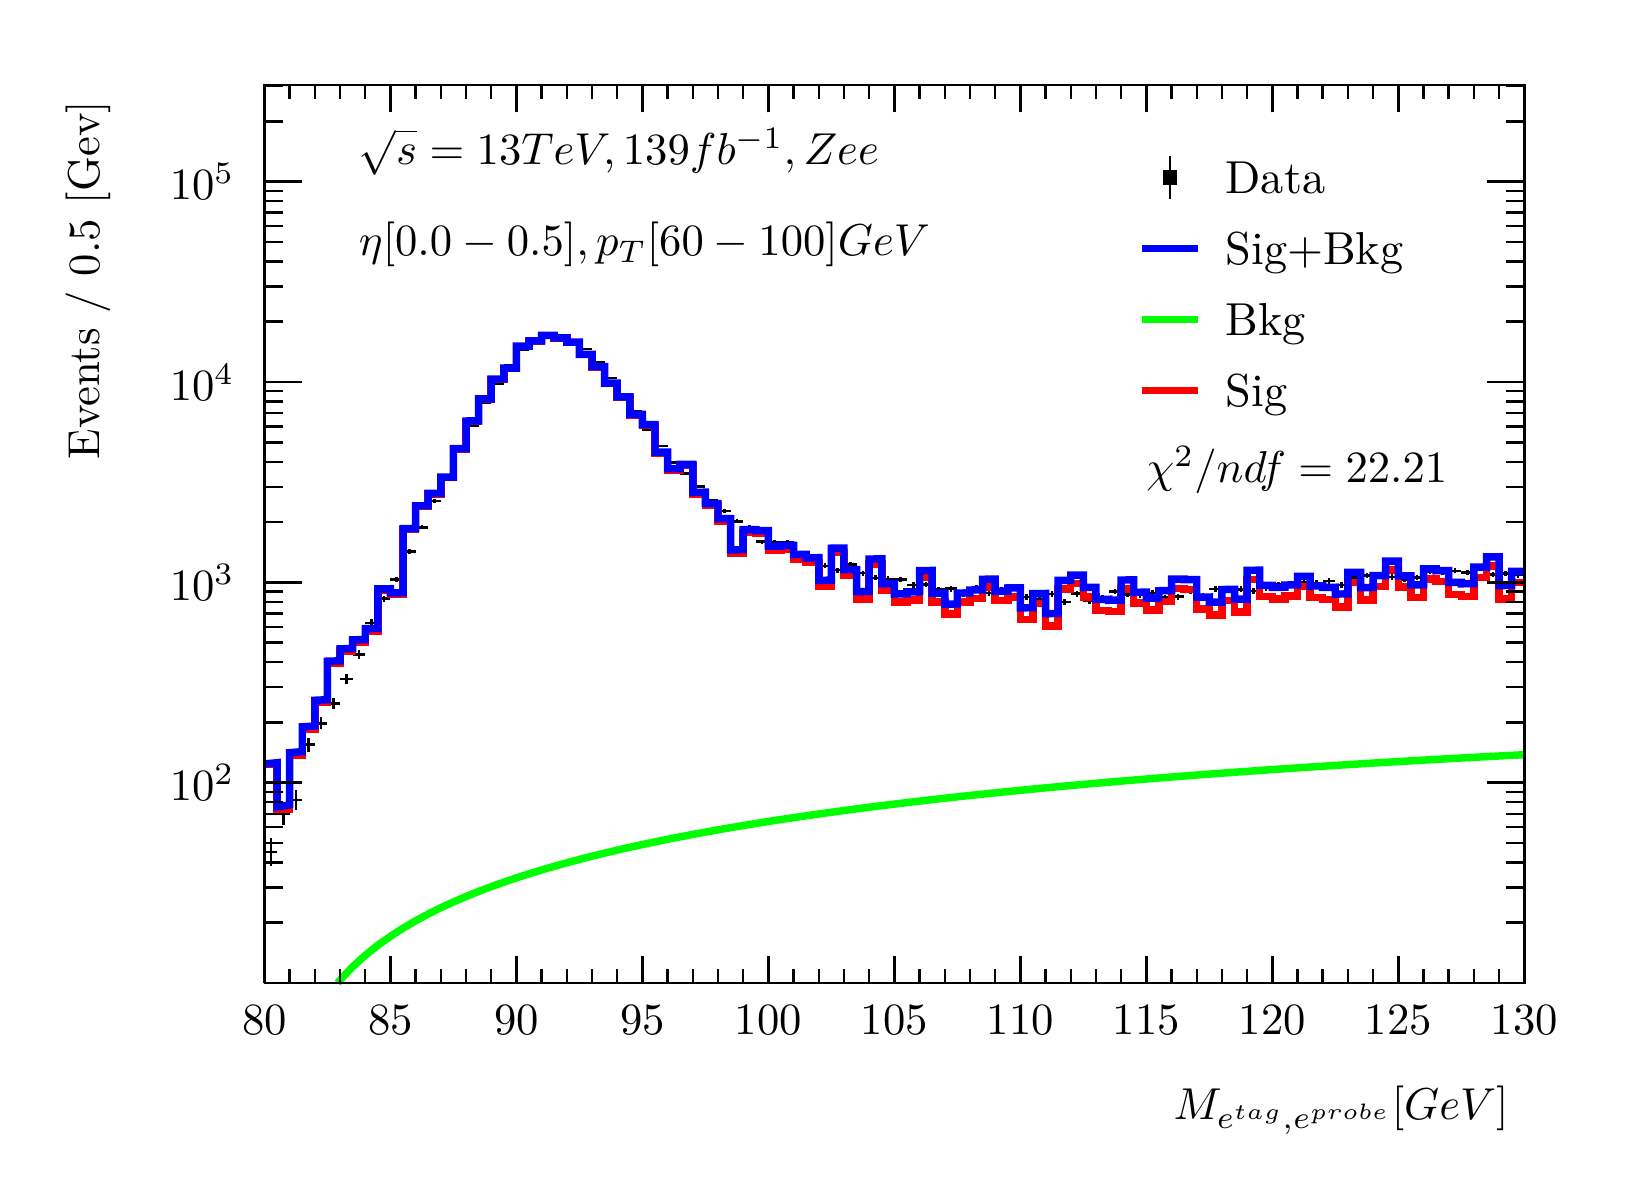
\begin{tikzpicture}
\pgfdeclareplotmark{cross} {
\pgfpathmoveto{\pgfpoint{-0.3\pgfplotmarksize}{\pgfplotmarksize}}
\pgfpathlineto{\pgfpoint{+0.3\pgfplotmarksize}{\pgfplotmarksize}}
\pgfpathlineto{\pgfpoint{+0.3\pgfplotmarksize}{0.3\pgfplotmarksize}}
\pgfpathlineto{\pgfpoint{+1\pgfplotmarksize}{0.3\pgfplotmarksize}}
\pgfpathlineto{\pgfpoint{+1\pgfplotmarksize}{-0.3\pgfplotmarksize}}
\pgfpathlineto{\pgfpoint{+0.3\pgfplotmarksize}{-0.3\pgfplotmarksize}}
\pgfpathlineto{\pgfpoint{+0.3\pgfplotmarksize}{-1.\pgfplotmarksize}}
\pgfpathlineto{\pgfpoint{-0.3\pgfplotmarksize}{-1.\pgfplotmarksize}}
\pgfpathlineto{\pgfpoint{-0.3\pgfplotmarksize}{-0.3\pgfplotmarksize}}
\pgfpathlineto{\pgfpoint{-1.\pgfplotmarksize}{-0.3\pgfplotmarksize}}
\pgfpathlineto{\pgfpoint{-1.\pgfplotmarksize}{0.3\pgfplotmarksize}}
\pgfpathlineto{\pgfpoint{-0.3\pgfplotmarksize}{0.3\pgfplotmarksize}}
\pgfpathclose
\pgfusepathqstroke
}
\pgfdeclareplotmark{cross*} {
\pgfpathmoveto{\pgfpoint{-0.3\pgfplotmarksize}{\pgfplotmarksize}}
\pgfpathlineto{\pgfpoint{+0.3\pgfplotmarksize}{\pgfplotmarksize}}
\pgfpathlineto{\pgfpoint{+0.3\pgfplotmarksize}{0.3\pgfplotmarksize}}
\pgfpathlineto{\pgfpoint{+1\pgfplotmarksize}{0.3\pgfplotmarksize}}
\pgfpathlineto{\pgfpoint{+1\pgfplotmarksize}{-0.3\pgfplotmarksize}}
\pgfpathlineto{\pgfpoint{+0.3\pgfplotmarksize}{-0.3\pgfplotmarksize}}
\pgfpathlineto{\pgfpoint{+0.3\pgfplotmarksize}{-1.\pgfplotmarksize}}
\pgfpathlineto{\pgfpoint{-0.3\pgfplotmarksize}{-1.\pgfplotmarksize}}
\pgfpathlineto{\pgfpoint{-0.3\pgfplotmarksize}{-0.3\pgfplotmarksize}}
\pgfpathlineto{\pgfpoint{-1.\pgfplotmarksize}{-0.3\pgfplotmarksize}}
\pgfpathlineto{\pgfpoint{-1.\pgfplotmarksize}{0.3\pgfplotmarksize}}
\pgfpathlineto{\pgfpoint{-0.3\pgfplotmarksize}{0.3\pgfplotmarksize}}
\pgfpathclose
\pgfusepathqfillstroke
}
\pgfdeclareplotmark{newstar} {
\pgfpathmoveto{\pgfqpoint{0pt}{\pgfplotmarksize}}
\pgfpathlineto{\pgfqpointpolar{44}{0.5\pgfplotmarksize}}
\pgfpathlineto{\pgfqpointpolar{18}{\pgfplotmarksize}}
\pgfpathlineto{\pgfqpointpolar{-20}{0.5\pgfplotmarksize}}
\pgfpathlineto{\pgfqpointpolar{-54}{\pgfplotmarksize}}
\pgfpathlineto{\pgfqpointpolar{-90}{0.5\pgfplotmarksize}}
\pgfpathlineto{\pgfqpointpolar{234}{\pgfplotmarksize}}
\pgfpathlineto{\pgfqpointpolar{198}{0.5\pgfplotmarksize}}
\pgfpathlineto{\pgfqpointpolar{162}{\pgfplotmarksize}}
\pgfpathlineto{\pgfqpointpolar{134}{0.5\pgfplotmarksize}}
\pgfpathclose
\pgfusepathqstroke
}
\pgfdeclareplotmark{newstar*} {
\pgfpathmoveto{\pgfqpoint{0pt}{\pgfplotmarksize}}
\pgfpathlineto{\pgfqpointpolar{44}{0.5\pgfplotmarksize}}
\pgfpathlineto{\pgfqpointpolar{18}{\pgfplotmarksize}}
\pgfpathlineto{\pgfqpointpolar{-20}{0.5\pgfplotmarksize}}
\pgfpathlineto{\pgfqpointpolar{-54}{\pgfplotmarksize}}
\pgfpathlineto{\pgfqpointpolar{-90}{0.5\pgfplotmarksize}}
\pgfpathlineto{\pgfqpointpolar{234}{\pgfplotmarksize}}
\pgfpathlineto{\pgfqpointpolar{198}{0.5\pgfplotmarksize}}
\pgfpathlineto{\pgfqpointpolar{162}{\pgfplotmarksize}}
\pgfpathlineto{\pgfqpointpolar{134}{0.5\pgfplotmarksize}}
\pgfpathclose
\pgfusepathqfillstroke
}
\definecolor{c}{rgb}{1,1,1};
\draw [color=c, fill=c] (0,0) rectangle (20,14.4361);
\draw [color=c, fill=c] (3,2.30977) rectangle (19,13.7143);
\definecolor{c}{rgb}{0,0,0};
\draw [c,line width=0.9] (3,2.30977) -- (3,13.7143) -- (19,13.7143) -- (19,2.30977) -- (3,2.30977);
\definecolor{c}{rgb}{1,1,1};
\draw [color=c, fill=c] (3,2.30977) rectangle (19,13.7143);
\definecolor{c}{rgb}{0,0,0};
\draw [c,line width=0.9] (3,2.30977) -- (3,13.7143) -- (19,13.7143) -- (19,2.30977) -- (3,2.30977);
\draw [c,line width=0.9] (3,2.30977) -- (19,2.30977);
\draw [c,line width=0.9] (3,2.65624) -- (3,2.30977);
\draw [c,line width=0.9] (3.32,2.48301) -- (3.32,2.30977);
\draw [c,line width=0.9] (3.64,2.48301) -- (3.64,2.30977);
\draw [c,line width=0.9] (3.96,2.48301) -- (3.96,2.30977);
\draw [c,line width=0.9] (4.28,2.48301) -- (4.28,2.30977);
\draw [c,line width=0.9] (4.6,2.65624) -- (4.6,2.30977);
\draw [c,line width=0.9] (4.92,2.48301) -- (4.92,2.30977);
\draw [c,line width=0.9] (5.24,2.48301) -- (5.24,2.30977);
\draw [c,line width=0.9] (5.56,2.48301) -- (5.56,2.30977);
\draw [c,line width=0.9] (5.88,2.48301) -- (5.88,2.30977);
\draw [c,line width=0.9] (6.2,2.65624) -- (6.2,2.30977);
\draw [c,line width=0.9] (6.52,2.48301) -- (6.52,2.30977);
\draw [c,line width=0.9] (6.84,2.48301) -- (6.84,2.30977);
\draw [c,line width=0.9] (7.16,2.48301) -- (7.16,2.30977);
\draw [c,line width=0.9] (7.48,2.48301) -- (7.48,2.30977);
\draw [c,line width=0.9] (7.8,2.65624) -- (7.8,2.30977);
\draw [c,line width=0.9] (8.12,2.48301) -- (8.12,2.30977);
\draw [c,line width=0.9] (8.44,2.48301) -- (8.44,2.30977);
\draw [c,line width=0.9] (8.76,2.48301) -- (8.76,2.30977);
\draw [c,line width=0.9] (9.08,2.48301) -- (9.08,2.30977);
\draw [c,line width=0.9] (9.4,2.65624) -- (9.4,2.30977);
\draw [c,line width=0.9] (9.72,2.48301) -- (9.72,2.30977);
\draw [c,line width=0.9] (10.04,2.48301) -- (10.04,2.30977);
\draw [c,line width=0.9] (10.36,2.48301) -- (10.36,2.30977);
\draw [c,line width=0.9] (10.68,2.48301) -- (10.68,2.30977);
\draw [c,line width=0.9] (11,2.65624) -- (11,2.30977);
\draw [c,line width=0.9] (11.32,2.48301) -- (11.32,2.30977);
\draw [c,line width=0.9] (11.64,2.48301) -- (11.64,2.30977);
\draw [c,line width=0.9] (11.96,2.48301) -- (11.96,2.30977);
\draw [c,line width=0.9] (12.28,2.48301) -- (12.28,2.30977);
\draw [c,line width=0.9] (12.6,2.65624) -- (12.6,2.30977);
\draw [c,line width=0.9] (12.92,2.48301) -- (12.92,2.30977);
\draw [c,line width=0.9] (13.24,2.48301) -- (13.24,2.30977);
\draw [c,line width=0.9] (13.56,2.48301) -- (13.56,2.30977);
\draw [c,line width=0.9] (13.88,2.48301) -- (13.88,2.30977);
\draw [c,line width=0.9] (14.2,2.65624) -- (14.2,2.30977);
\draw [c,line width=0.9] (14.52,2.48301) -- (14.52,2.30977);
\draw [c,line width=0.9] (14.84,2.48301) -- (14.84,2.30977);
\draw [c,line width=0.9] (15.16,2.48301) -- (15.16,2.30977);
\draw [c,line width=0.9] (15.48,2.48301) -- (15.48,2.30977);
\draw [c,line width=0.9] (15.8,2.65624) -- (15.8,2.30977);
\draw [c,line width=0.9] (16.12,2.48301) -- (16.12,2.30977);
\draw [c,line width=0.9] (16.44,2.48301) -- (16.44,2.30977);
\draw [c,line width=0.9] (16.76,2.48301) -- (16.76,2.30977);
\draw [c,line width=0.9] (17.08,2.48301) -- (17.08,2.30977);
\draw [c,line width=0.9] (17.4,2.65624) -- (17.4,2.30977);
\draw [c,line width=0.9] (17.72,2.48301) -- (17.72,2.30977);
\draw [c,line width=0.9] (18.04,2.48301) -- (18.04,2.30977);
\draw [c,line width=0.9] (18.36,2.48301) -- (18.36,2.30977);
\draw [c,line width=0.9] (18.68,2.48301) -- (18.68,2.30977);
\draw [c,line width=0.9] (19,2.65624) -- (19,2.30977);
\draw [anchor=base] (3,1.66015) node[scale=1.61424, color=c, rotate=0]{80};
\draw [anchor=base] (4.6,1.66015) node[scale=1.61424, color=c, rotate=0]{85};
\draw [anchor=base] (6.2,1.66015) node[scale=1.61424, color=c, rotate=0]{90};
\draw [anchor=base] (7.8,1.66015) node[scale=1.61424, color=c, rotate=0]{95};
\draw [anchor=base] (9.4,1.66015) node[scale=1.61424, color=c, rotate=0]{100};
\draw [anchor=base] (11,1.66015) node[scale=1.61424, color=c, rotate=0]{105};
\draw [anchor=base] (12.6,1.66015) node[scale=1.61424, color=c, rotate=0]{110};
\draw [anchor=base] (14.2,1.66015) node[scale=1.61424, color=c, rotate=0]{115};
\draw [anchor=base] (15.8,1.66015) node[scale=1.61424, color=c, rotate=0]{120};
\draw [anchor=base] (17.4,1.66015) node[scale=1.61424, color=c, rotate=0]{125};
\draw [anchor=base] (19,1.66015) node[scale=1.61424, color=c, rotate=0]{130};
\draw [anchor= east] (19,0.692932) node[scale=1.61424, color=c, rotate=0]{$M_{e^{tag}, e^{probe}}  [GeV]$};
\draw [c,line width=0.9] (3,13.7143) -- (19,13.7143);
\draw [c,line width=0.9] (3,13.3678) -- (3,13.7143);
\draw [c,line width=0.9] (3.32,13.5411) -- (3.32,13.7143);
\draw [c,line width=0.9] (3.64,13.5411) -- (3.64,13.7143);
\draw [c,line width=0.9] (3.96,13.5411) -- (3.96,13.7143);
\draw [c,line width=0.9] (4.28,13.5411) -- (4.28,13.7143);
\draw [c,line width=0.9] (4.6,13.3678) -- (4.6,13.7143);
\draw [c,line width=0.9] (4.92,13.5411) -- (4.92,13.7143);
\draw [c,line width=0.9] (5.24,13.5411) -- (5.24,13.7143);
\draw [c,line width=0.9] (5.56,13.5411) -- (5.56,13.7143);
\draw [c,line width=0.9] (5.88,13.5411) -- (5.88,13.7143);
\draw [c,line width=0.9] (6.2,13.3678) -- (6.2,13.7143);
\draw [c,line width=0.9] (6.52,13.5411) -- (6.52,13.7143);
\draw [c,line width=0.9] (6.84,13.5411) -- (6.84,13.7143);
\draw [c,line width=0.9] (7.16,13.5411) -- (7.16,13.7143);
\draw [c,line width=0.9] (7.48,13.5411) -- (7.48,13.7143);
\draw [c,line width=0.9] (7.8,13.3678) -- (7.8,13.7143);
\draw [c,line width=0.9] (8.12,13.5411) -- (8.12,13.7143);
\draw [c,line width=0.9] (8.44,13.5411) -- (8.44,13.7143);
\draw [c,line width=0.9] (8.76,13.5411) -- (8.76,13.7143);
\draw [c,line width=0.9] (9.08,13.5411) -- (9.08,13.7143);
\draw [c,line width=0.9] (9.4,13.3678) -- (9.4,13.7143);
\draw [c,line width=0.9] (9.72,13.5411) -- (9.72,13.7143);
\draw [c,line width=0.9] (10.04,13.5411) -- (10.04,13.7143);
\draw [c,line width=0.9] (10.36,13.5411) -- (10.36,13.7143);
\draw [c,line width=0.9] (10.68,13.5411) -- (10.68,13.7143);
\draw [c,line width=0.9] (11,13.3678) -- (11,13.7143);
\draw [c,line width=0.9] (11.32,13.5411) -- (11.32,13.7143);
\draw [c,line width=0.9] (11.64,13.5411) -- (11.64,13.7143);
\draw [c,line width=0.9] (11.96,13.5411) -- (11.96,13.7143);
\draw [c,line width=0.9] (12.28,13.5411) -- (12.28,13.7143);
\draw [c,line width=0.9] (12.6,13.3678) -- (12.6,13.7143);
\draw [c,line width=0.9] (12.92,13.5411) -- (12.92,13.7143);
\draw [c,line width=0.9] (13.24,13.5411) -- (13.24,13.7143);
\draw [c,line width=0.9] (13.56,13.5411) -- (13.56,13.7143);
\draw [c,line width=0.9] (13.88,13.5411) -- (13.88,13.7143);
\draw [c,line width=0.9] (14.2,13.3678) -- (14.2,13.7143);
\draw [c,line width=0.9] (14.52,13.5411) -- (14.52,13.7143);
\draw [c,line width=0.9] (14.84,13.5411) -- (14.84,13.7143);
\draw [c,line width=0.9] (15.16,13.5411) -- (15.16,13.7143);
\draw [c,line width=0.9] (15.48,13.5411) -- (15.48,13.7143);
\draw [c,line width=0.9] (15.8,13.3678) -- (15.8,13.7143);
\draw [c,line width=0.9] (16.12,13.5411) -- (16.12,13.7143);
\draw [c,line width=0.9] (16.44,13.5411) -- (16.44,13.7143);
\draw [c,line width=0.9] (16.76,13.5411) -- (16.76,13.7143);
\draw [c,line width=0.9] (17.08,13.5411) -- (17.08,13.7143);
\draw [c,line width=0.9] (17.4,13.3678) -- (17.4,13.7143);
\draw [c,line width=0.9] (17.72,13.5411) -- (17.72,13.7143);
\draw [c,line width=0.9] (18.04,13.5411) -- (18.04,13.7143);
\draw [c,line width=0.9] (18.36,13.5411) -- (18.36,13.7143);
\draw [c,line width=0.9] (18.68,13.5411) -- (18.68,13.7143);
\draw [c,line width=0.9] (19,13.3678) -- (19,13.7143);
\draw [c,line width=0.9] (3,2.30977) -- (3,13.7143);
\draw [c,line width=0.9] (3.237,3.07568) -- (3,3.07568);
\draw [c,line width=0.9] (3.237,3.5237) -- (3,3.5237);
\draw [c,line width=0.9] (3.237,3.84158) -- (3,3.84158);
\draw [c,line width=0.9] (3.237,4.08815) -- (3,4.08815);
\draw [c,line width=0.9] (3.237,4.2896) -- (3,4.2896);
\draw [c,line width=0.9] (3.237,4.45994) -- (3,4.45994);
\draw [c,line width=0.9] (3.237,4.60748) -- (3,4.60748);
\draw [c,line width=0.9] (3.237,4.73763) -- (3,4.73763);
\draw [c,line width=0.9] (3.474,4.85405) -- (3,4.85405);
\draw [anchor= east] (2.82,4.85405) node[scale=1.61424, color=c, rotate=0]{$10^{2}$};
\draw [c,line width=0.9] (3.237,5.61995) -- (3,5.61995);
\draw [c,line width=0.9] (3.237,6.06798) -- (3,6.06798);
\draw [c,line width=0.9] (3.237,6.38586) -- (3,6.38586);
\draw [c,line width=0.9] (3.237,6.63242) -- (3,6.63242);
\draw [c,line width=0.9] (3.237,6.83388) -- (3,6.83388);
\draw [c,line width=0.9] (3.237,7.00421) -- (3,7.00421);
\draw [c,line width=0.9] (3.237,7.15176) -- (3,7.15176);
\draw [c,line width=0.9] (3.237,7.28191) -- (3,7.28191);
\draw [c,line width=0.9] (3.474,7.39833) -- (3,7.39833);
\draw [anchor= east] (2.82,7.39833) node[scale=1.61424, color=c, rotate=0]{$10^{3}$};
\draw [c,line width=0.9] (3.237,8.16423) -- (3,8.16423);
\draw [c,line width=0.9] (3.237,8.61226) -- (3,8.61226);
\draw [c,line width=0.9] (3.237,8.93013) -- (3,8.93013);
\draw [c,line width=0.9] (3.237,9.1767) -- (3,9.1767);
\draw [c,line width=0.9] (3.237,9.37816) -- (3,9.37816);
\draw [c,line width=0.9] (3.237,9.54849) -- (3,9.54849);
\draw [c,line width=0.9] (3.237,9.69604) -- (3,9.69604);
\draw [c,line width=0.9] (3.237,9.82618) -- (3,9.82618);
\draw [c,line width=0.9] (3.474,9.9426) -- (3,9.9426);
\draw [anchor= east] (2.82,9.9426) node[scale=1.61424, color=c, rotate=0]{$10^{4}$};
\draw [c,line width=0.9] (3.237,10.7085) -- (3,10.7085);
\draw [c,line width=0.9] (3.237,11.1565) -- (3,11.1565);
\draw [c,line width=0.9] (3.237,11.4744) -- (3,11.4744);
\draw [c,line width=0.9] (3.237,11.721) -- (3,11.721);
\draw [c,line width=0.9] (3.237,11.9224) -- (3,11.9224);
\draw [c,line width=0.9] (3.237,12.0928) -- (3,12.0928);
\draw [c,line width=0.9] (3.237,12.2403) -- (3,12.2403);
\draw [c,line width=0.9] (3.237,12.3705) -- (3,12.3705);
\draw [c,line width=0.9] (3.474,12.4869) -- (3,12.4869);
\draw [anchor= east] (2.82,12.4869) node[scale=1.61424, color=c, rotate=0]{$10^{5}$};
\draw [c,line width=0.9] (3.237,13.2528) -- (3,13.2528);
\draw [c,line width=0.9] (3.237,13.7008) -- (3,13.7008);
\draw [anchor= east] (0.76,13.7143) node[scale=1.61424, color=c, rotate=90]{Events / 0.5 [Gev]};
\draw [c,line width=0.9] (19,2.30977) -- (19,13.7143);
\draw [c,line width=0.9] (18.763,3.07568) -- (19,3.07568);
\draw [c,line width=0.9] (18.763,3.5237) -- (19,3.5237);
\draw [c,line width=0.9] (18.763,3.84158) -- (19,3.84158);
\draw [c,line width=0.9] (18.763,4.08815) -- (19,4.08815);
\draw [c,line width=0.9] (18.763,4.2896) -- (19,4.2896);
\draw [c,line width=0.9] (18.763,4.45994) -- (19,4.45994);
\draw [c,line width=0.9] (18.763,4.60748) -- (19,4.60748);
\draw [c,line width=0.9] (18.763,4.73763) -- (19,4.73763);
\draw [c,line width=0.9] (18.526,4.85405) -- (19,4.85405);
\draw [c,line width=0.9] (18.763,5.61995) -- (19,5.61995);
\draw [c,line width=0.9] (18.763,6.06798) -- (19,6.06798);
\draw [c,line width=0.9] (18.763,6.38586) -- (19,6.38586);
\draw [c,line width=0.9] (18.763,6.63242) -- (19,6.63242);
\draw [c,line width=0.9] (18.763,6.83388) -- (19,6.83388);
\draw [c,line width=0.9] (18.763,7.00421) -- (19,7.00421);
\draw [c,line width=0.9] (18.763,7.15176) -- (19,7.15176);
\draw [c,line width=0.9] (18.763,7.28191) -- (19,7.28191);
\draw [c,line width=0.9] (18.526,7.39833) -- (19,7.39833);
\draw [c,line width=0.9] (18.763,8.16423) -- (19,8.16423);
\draw [c,line width=0.9] (18.763,8.61226) -- (19,8.61226);
\draw [c,line width=0.9] (18.763,8.93013) -- (19,8.93013);
\draw [c,line width=0.9] (18.763,9.1767) -- (19,9.1767);
\draw [c,line width=0.9] (18.763,9.37816) -- (19,9.37816);
\draw [c,line width=0.9] (18.763,9.54849) -- (19,9.54849);
\draw [c,line width=0.9] (18.763,9.69604) -- (19,9.69604);
\draw [c,line width=0.9] (18.763,9.82618) -- (19,9.82618);
\draw [c,line width=0.9] (18.526,9.9426) -- (19,9.9426);
\draw [c,line width=0.9] (18.763,10.7085) -- (19,10.7085);
\draw [c,line width=0.9] (18.763,11.1565) -- (19,11.1565);
\draw [c,line width=0.9] (18.763,11.4744) -- (19,11.4744);
\draw [c,line width=0.9] (18.763,11.721) -- (19,11.721);
\draw [c,line width=0.9] (18.763,11.9224) -- (19,11.9224);
\draw [c,line width=0.9] (18.763,12.0928) -- (19,12.0928);
\draw [c,line width=0.9] (18.763,12.2403) -- (19,12.2403);
\draw [c,line width=0.9] (18.763,12.3705) -- (19,12.3705);
\draw [c,line width=0.9] (18.526,12.4869) -- (19,12.4869);
\draw [c,line width=0.9] (18.763,13.2528) -- (19,13.2528);
\draw [c,line width=0.9] (18.763,13.7008) -- (19,13.7008);
\draw [c,line width=0.9] (3.08,3.97173) -- (3,3.97173);
\draw [c,line width=0.9] (3,3.97173) -- (3,3.97173);
\draw [c,line width=0.9] (3.08,3.97173) -- (3.16,3.97173);
\draw [c,line width=0.9] (3.16,3.97173) -- (3.16,3.97173);
\draw [c,line width=0.9] (3.08,3.97173) -- (3.08,4.14747);
\draw [c,line width=0.9] (3.08,4.14747) -- (3.08,4.14747);
\draw [c,line width=0.9] (3.08,3.97173) -- (3.08,3.79408);
\draw [c,line width=0.9] (3.08,3.79408) -- (3.08,3.79408);
\draw [c,line width=0.9] (3.24,4.45994) -- (3.16,4.45994);
\draw [c,line width=0.9] (3.16,4.45994) -- (3.16,4.45994);
\draw [c,line width=0.9] (3.24,4.45994) -- (3.32,4.45994);
\draw [c,line width=0.9] (3.32,4.45994) -- (3.32,4.45994);
\draw [c,line width=0.9] (3.24,4.45994) -- (3.24,4.59926);
\draw [c,line width=0.9] (3.24,4.59926) -- (3.24,4.59926);
\draw [c,line width=0.9] (3.24,4.45994) -- (3.24,4.31964);
\draw [c,line width=0.9] (3.24,4.31964) -- (3.24,4.31964);
\draw [c,line width=0.9] (3.4,4.63477) -- (3.32,4.63477);
\draw [c,line width=0.9] (3.32,4.63477) -- (3.32,4.63477);
\draw [c,line width=0.9] (3.4,4.63477) -- (3.48,4.63477);
\draw [c,line width=0.9] (3.48,4.63477) -- (3.48,4.63477);
\draw [c,line width=0.9] (3.4,4.63477) -- (3.4,4.76302);
\draw [c,line width=0.9] (3.4,4.76302) -- (3.4,4.76302);
\draw [c,line width=0.9] (3.4,4.63477) -- (3.4,4.50575);
\draw [c,line width=0.9] (3.4,4.50575) -- (3.4,4.50575);
\draw [c,line width=0.9] (3.56,5.33831) -- (3.48,5.33831);
\draw [c,line width=0.9] (3.48,5.33831) -- (3.48,5.33831);
\draw [c,line width=0.9] (3.56,5.33831) -- (3.64,5.33831);
\draw [c,line width=0.9] (3.64,5.33831) -- (3.64,5.33831);
\draw [c,line width=0.9] (3.56,5.33831) -- (3.56,5.42704);
\draw [c,line width=0.9] (3.56,5.42704) -- (3.56,5.42704);
\draw [c,line width=0.9] (3.56,5.33831) -- (3.56,5.24958);
\draw [c,line width=0.9] (3.56,5.24958) -- (3.56,5.24958);
\draw [c,line width=0.9] (3.72,5.60885) -- (3.64,5.60885);
\draw [c,line width=0.9] (3.64,5.60885) -- (3.64,5.60885);
\draw [c,line width=0.9] (3.72,5.60885) -- (3.8,5.60885);
\draw [c,line width=0.9] (3.8,5.60885) -- (3.8,5.60885);
\draw [c,line width=0.9] (3.72,5.60885) -- (3.72,5.68736);
\draw [c,line width=0.9] (3.72,5.68736) -- (3.72,5.68736);
\draw [c,line width=0.9] (3.72,5.60885) -- (3.72,5.53034);
\draw [c,line width=0.9] (3.72,5.53034) -- (3.72,5.53034);
\draw [c,line width=0.9] (3.88,5.85765) -- (3.8,5.85765);
\draw [c,line width=0.9] (3.8,5.85765) -- (3.8,5.85765);
\draw [c,line width=0.9] (3.88,5.85765) -- (3.96,5.85765);
\draw [c,line width=0.9] (3.96,5.85765) -- (3.96,5.85765);
\draw [c,line width=0.9] (3.88,5.85765) -- (3.88,5.9278);
\draw [c,line width=0.9] (3.88,5.9278) -- (3.88,5.9278);
\draw [c,line width=0.9] (3.88,5.85765) -- (3.88,5.78749);
\draw [c,line width=0.9] (3.88,5.78749) -- (3.88,5.78749);
\draw [c,line width=0.9] (4.04,6.16994) -- (3.96,6.16994);
\draw [c,line width=0.9] (3.96,6.16994) -- (3.96,6.16994);
\draw [c,line width=0.9] (4.04,6.16994) -- (4.12,6.16994);
\draw [c,line width=0.9] (4.12,6.16994) -- (4.12,6.16994);
\draw [c,line width=0.9] (4.04,6.16994) -- (4.04,6.23085);
\draw [c,line width=0.9] (4.04,6.23085) -- (4.04,6.23085);
\draw [c,line width=0.9] (4.04,6.16994) -- (4.04,6.10903);
\draw [c,line width=0.9] (4.04,6.10903) -- (4.04,6.10903);
\draw [c,line width=0.9] (4.2,6.48361) -- (4.12,6.48361);
\draw [c,line width=0.9] (4.12,6.48361) -- (4.12,6.48361);
\draw [c,line width=0.9] (4.2,6.48361) -- (4.28,6.48361);
\draw [c,line width=0.9] (4.28,6.48361) -- (4.28,6.48361);
\draw [c,line width=0.9] (4.2,6.48361) -- (4.2,6.53647);
\draw [c,line width=0.9] (4.2,6.53647) -- (4.2,6.53647);
\draw [c,line width=0.9] (4.2,6.48361) -- (4.2,6.43076);
\draw [c,line width=0.9] (4.2,6.43076) -- (4.2,6.43076);
\draw [c,line width=0.9] (4.36,6.88428) -- (4.28,6.88428);
\draw [c,line width=0.9] (4.28,6.88428) -- (4.28,6.88428);
\draw [c,line width=0.9] (4.36,6.88428) -- (4.44,6.88428);
\draw [c,line width=0.9] (4.44,6.88428) -- (4.44,6.88428);
\draw [c,line width=0.9] (4.36,6.88428) -- (4.36,6.92837);
\draw [c,line width=0.9] (4.36,6.92837) -- (4.36,6.92837);
\draw [c,line width=0.9] (4.36,6.88428) -- (4.36,6.84019);
\draw [c,line width=0.9] (4.36,6.84019) -- (4.36,6.84019);
\draw [c,line width=0.9] (4.52,7.19244) -- (4.44,7.19244);
\draw [c,line width=0.9] (4.44,7.19244) -- (4.44,7.19244);
\draw [c,line width=0.9] (4.52,7.19244) -- (4.6,7.19244);
\draw [c,line width=0.9] (4.6,7.19244) -- (4.6,7.19244);
\draw [c,line width=0.9] (4.52,7.19244) -- (4.52,7.23079);
\draw [c,line width=0.9] (4.52,7.23079) -- (4.52,7.23079);
\draw [c,line width=0.9] (4.52,7.19244) -- (4.52,7.15409);
\draw [c,line width=0.9] (4.52,7.15409) -- (4.52,7.15409);
\draw [c,line width=0.9] (4.68,7.4342) -- (4.6,7.4342);
\draw [c,line width=0.9] (4.6,7.4342) -- (4.6,7.4342);
\draw [c,line width=0.9] (4.68,7.4342) -- (4.76,7.4342);
\draw [c,line width=0.9] (4.76,7.4342) -- (4.76,7.4342);
\draw [c,line width=0.9] (4.68,7.4342) -- (4.68,7.46858);
\draw [c,line width=0.9] (4.68,7.46858) -- (4.68,7.46858);
\draw [c,line width=0.9] (4.68,7.4342) -- (4.68,7.39983);
\draw [c,line width=0.9] (4.68,7.39983) -- (4.68,7.39983);
\draw [c,line width=0.9] (4.84,7.7889) -- (4.76,7.7889);
\draw [c,line width=0.9] (4.76,7.7889) -- (4.76,7.7889);
\draw [c,line width=0.9] (4.84,7.7889) -- (4.92,7.7889);
\draw [c,line width=0.9] (4.92,7.7889) -- (4.92,7.7889);
\draw [c,line width=0.9] (4.84,7.7889) -- (4.84,7.81818);
\draw [c,line width=0.9] (4.84,7.81818) -- (4.84,7.81818);
\draw [c,line width=0.9] (4.84,7.7889) -- (4.84,7.75962);
\draw [c,line width=0.9] (4.84,7.75962) -- (4.84,7.75962);
\draw [c,line width=0.9] (5,8.09645) -- (4.92,8.09645);
\draw [c,line width=0.9] (4.92,8.09645) -- (4.92,8.09645);
\draw [c,line width=0.9] (5,8.09645) -- (5.08,8.09645);
\draw [c,line width=0.9] (5.08,8.09645) -- (5.08,8.09645);
\draw [c,line width=0.9] (5,8.09645) -- (5,8.12193);
\draw [c,line width=0.9] (5,8.12193) -- (5,8.12193);
\draw [c,line width=0.9] (5,8.09645) -- (5,8.07097);
\draw [c,line width=0.9] (5,8.07097) -- (5,8.07097);
\draw [c,line width=0.9] (5.16,8.43008) -- (5.08,8.43008);
\draw [c,line width=0.9] (5.08,8.43008) -- (5.08,8.43008);
\draw [c,line width=0.9] (5.16,8.43008) -- (5.24,8.43008);
\draw [c,line width=0.9] (5.24,8.43008) -- (5.24,8.43008);
\draw [c,line width=0.9] (5.16,8.43008) -- (5.16,8.45198);
\draw [c,line width=0.9] (5.16,8.45198) -- (5.16,8.45198);
\draw [c,line width=0.9] (5.16,8.43008) -- (5.16,8.40817);
\draw [c,line width=0.9] (5.16,8.40817) -- (5.16,8.40817);
\draw [c,line width=0.9] (5.32,8.73386) -- (5.24,8.73386);
\draw [c,line width=0.9] (5.24,8.73386) -- (5.24,8.73386);
\draw [c,line width=0.9] (5.32,8.73386) -- (5.4,8.73386);
\draw [c,line width=0.9] (5.4,8.73386) -- (5.4,8.73386);
\draw [c,line width=0.9] (5.32,8.73386) -- (5.32,8.75295);
\draw [c,line width=0.9] (5.32,8.75295) -- (5.32,8.75295);
\draw [c,line width=0.9] (5.32,8.73386) -- (5.32,8.71476);
\draw [c,line width=0.9] (5.32,8.71476) -- (5.32,8.71476);
\draw [c,line width=0.9] (5.48,9.07903) -- (5.4,9.07903);
\draw [c,line width=0.9] (5.4,9.07903) -- (5.4,9.07903);
\draw [c,line width=0.9] (5.48,9.07903) -- (5.56,9.07903);
\draw [c,line width=0.9] (5.56,9.07903) -- (5.56,9.07903);
\draw [c,line width=0.9] (5.48,9.07903) -- (5.48,9.09536);
\draw [c,line width=0.9] (5.48,9.09536) -- (5.48,9.09536);
\draw [c,line width=0.9] (5.48,9.07903) -- (5.48,9.0627);
\draw [c,line width=0.9] (5.48,9.0627) -- (5.48,9.0627);
\draw [c,line width=0.9] (5.64,9.39261) -- (5.56,9.39261);
\draw [c,line width=0.9] (5.56,9.39261) -- (5.56,9.39261);
\draw [c,line width=0.9] (5.64,9.39261) -- (5.72,9.39261);
\draw [c,line width=0.9] (5.72,9.39261) -- (5.72,9.39261);
\draw [c,line width=0.9] (5.64,9.39261) -- (5.64,9.40679);
\draw [c,line width=0.9] (5.64,9.40679) -- (5.64,9.40679);
\draw [c,line width=0.9] (5.64,9.39261) -- (5.64,9.37844);
\draw [c,line width=0.9] (5.64,9.37844) -- (5.64,9.37844);
\draw [c,line width=0.9] (5.8,9.67681) -- (5.72,9.67681);
\draw [c,line width=0.9] (5.72,9.67681) -- (5.72,9.67681);
\draw [c,line width=0.9] (5.8,9.67681) -- (5.88,9.67681);
\draw [c,line width=0.9] (5.88,9.67681) -- (5.88,9.67681);
\draw [c,line width=0.9] (5.8,9.67681) -- (5.8,9.68927);
\draw [c,line width=0.9] (5.8,9.68927) -- (5.8,9.68927);
\draw [c,line width=0.9] (5.8,9.67681) -- (5.8,9.66435);
\draw [c,line width=0.9] (5.8,9.66435) -- (5.8,9.66435);
\draw [c,line width=0.9] (5.96,9.9213) -- (5.88,9.9213);
\draw [c,line width=0.9] (5.88,9.9213) -- (5.88,9.9213);
\draw [c,line width=0.9] (5.96,9.9213) -- (6.04,9.9213);
\draw [c,line width=0.9] (6.04,9.9213) -- (6.04,9.9213);
\draw [c,line width=0.9] (5.96,9.9213) -- (5.96,9.93245);
\draw [c,line width=0.9] (5.96,9.93245) -- (5.96,9.93245);
\draw [c,line width=0.9] (5.96,9.9213) -- (5.96,9.91014);
\draw [c,line width=0.9] (5.96,9.91014) -- (5.96,9.91014);
\draw [c,line width=0.9] (6.12,10.1618) -- (6.04,10.1618);
\draw [c,line width=0.9] (6.04,10.1618) -- (6.04,10.1618);
\draw [c,line width=0.9] (6.12,10.1618) -- (6.2,10.1618);
\draw [c,line width=0.9] (6.2,10.1618) -- (6.2,10.1618);
\draw [c,line width=0.9] (6.12,10.1618) -- (6.12,10.1718);
\draw [c,line width=0.9] (6.12,10.1718) -- (6.12,10.1718);
\draw [c,line width=0.9] (6.12,10.1618) -- (6.12,10.1518);
\draw [c,line width=0.9] (6.12,10.1518) -- (6.12,10.1518);
\draw [c,line width=0.9] (6.28,10.3471) -- (6.2,10.3471);
\draw [c,line width=0.9] (6.2,10.3471) -- (6.2,10.3471);
\draw [c,line width=0.9] (6.28,10.3471) -- (6.36,10.3471);
\draw [c,line width=0.9] (6.36,10.3471) -- (6.36,10.3471);
\draw [c,line width=0.9] (6.28,10.3471) -- (6.28,10.3563);
\draw [c,line width=0.9] (6.28,10.3563) -- (6.28,10.3563);
\draw [c,line width=0.9] (6.28,10.3471) -- (6.28,10.3379);
\draw [c,line width=0.9] (6.28,10.3379) -- (6.28,10.3379);
\draw [c,line width=0.9] (6.44,10.4746) -- (6.36,10.4746);
\draw [c,line width=0.9] (6.36,10.4746) -- (6.36,10.4746);
\draw [c,line width=0.9] (6.44,10.4746) -- (6.52,10.4746);
\draw [c,line width=0.9] (6.52,10.4746) -- (6.52,10.4746);
\draw [c,line width=0.9] (6.44,10.4746) -- (6.44,10.4833);
\draw [c,line width=0.9] (6.44,10.4833) -- (6.44,10.4833);
\draw [c,line width=0.9] (6.44,10.4746) -- (6.44,10.466);
\draw [c,line width=0.9] (6.44,10.466) -- (6.44,10.466);
\draw [c,line width=0.9] (6.6,10.5373) -- (6.52,10.5373);
\draw [c,line width=0.9] (6.52,10.5373) -- (6.52,10.5373);
\draw [c,line width=0.9] (6.6,10.5373) -- (6.68,10.5373);
\draw [c,line width=0.9] (6.68,10.5373) -- (6.68,10.5373);
\draw [c,line width=0.9] (6.6,10.5373) -- (6.6,10.5457);
\draw [c,line width=0.9] (6.6,10.5457) -- (6.6,10.5457);
\draw [c,line width=0.9] (6.6,10.5373) -- (6.6,10.5288);
\draw [c,line width=0.9] (6.6,10.5288) -- (6.6,10.5288);
\draw [c,line width=0.9] (6.76,10.5319) -- (6.68,10.5319);
\draw [c,line width=0.9] (6.68,10.5319) -- (6.68,10.5319);
\draw [c,line width=0.9] (6.76,10.5319) -- (6.84,10.5319);
\draw [c,line width=0.9] (6.84,10.5319) -- (6.84,10.5319);
\draw [c,line width=0.9] (6.76,10.5319) -- (6.76,10.5403);
\draw [c,line width=0.9] (6.76,10.5403) -- (6.76,10.5403);
\draw [c,line width=0.9] (6.76,10.5319) -- (6.76,10.5234);
\draw [c,line width=0.9] (6.76,10.5234) -- (6.76,10.5234);
\draw [c,line width=0.9] (6.92,10.4613) -- (6.84,10.4613);
\draw [c,line width=0.9] (6.84,10.4613) -- (6.84,10.4613);
\draw [c,line width=0.9] (6.92,10.4613) -- (7,10.4613);
\draw [c,line width=0.9] (7,10.4613) -- (7,10.4613);
\draw [c,line width=0.9] (6.92,10.4613) -- (6.92,10.4701);
\draw [c,line width=0.9] (6.92,10.4701) -- (6.92,10.4701);
\draw [c,line width=0.9] (6.92,10.4613) -- (6.92,10.4526);
\draw [c,line width=0.9] (6.92,10.4526) -- (6.92,10.4526);
\draw [c,line width=0.9] (7.08,10.3639) -- (7,10.3639);
\draw [c,line width=0.9] (7,10.3639) -- (7,10.3639);
\draw [c,line width=0.9] (7.08,10.3639) -- (7.16,10.3639);
\draw [c,line width=0.9] (7.16,10.3639) -- (7.16,10.3639);
\draw [c,line width=0.9] (7.08,10.3639) -- (7.08,10.373);
\draw [c,line width=0.9] (7.08,10.373) -- (7.08,10.373);
\draw [c,line width=0.9] (7.08,10.3639) -- (7.08,10.3547);
\draw [c,line width=0.9] (7.08,10.3547) -- (7.08,10.3547);
\draw [c,line width=0.9] (7.24,10.1946) -- (7.16,10.1946);
\draw [c,line width=0.9] (7.16,10.1946) -- (7.16,10.1946);
\draw [c,line width=0.9] (7.24,10.1946) -- (7.32,10.1946);
\draw [c,line width=0.9] (7.32,10.1946) -- (7.32,10.1946);
\draw [c,line width=0.9] (7.24,10.1946) -- (7.24,10.2044);
\draw [c,line width=0.9] (7.24,10.2044) -- (7.24,10.2044);
\draw [c,line width=0.9] (7.24,10.1946) -- (7.24,10.1847);
\draw [c,line width=0.9] (7.24,10.1847) -- (7.24,10.1847);
\draw [c,line width=0.9] (7.4,9.9942) -- (7.32,9.9942);
\draw [c,line width=0.9] (7.32,9.9942) -- (7.32,9.9942);
\draw [c,line width=0.9] (7.4,9.9942) -- (7.48,9.9942);
\draw [c,line width=0.9] (7.48,9.9942) -- (7.48,9.9942);
\draw [c,line width=0.9] (7.4,9.9942) -- (7.4,10.005);
\draw [c,line width=0.9] (7.4,10.005) -- (7.4,10.005);
\draw [c,line width=0.9] (7.4,9.9942) -- (7.4,9.9834);
\draw [c,line width=0.9] (7.4,9.9834) -- (7.4,9.9834);
\draw [c,line width=0.9] (7.56,9.77273) -- (7.48,9.77273);
\draw [c,line width=0.9] (7.48,9.77273) -- (7.48,9.77273);
\draw [c,line width=0.9] (7.56,9.77273) -- (7.64,9.77273);
\draw [c,line width=0.9] (7.64,9.77273) -- (7.64,9.77273);
\draw [c,line width=0.9] (7.56,9.77273) -- (7.56,9.78467);
\draw [c,line width=0.9] (7.56,9.78467) -- (7.56,9.78467);
\draw [c,line width=0.9] (7.56,9.77273) -- (7.56,9.7608);
\draw [c,line width=0.9] (7.56,9.7608) -- (7.56,9.7608);
\draw [c,line width=0.9] (7.72,9.57099) -- (7.64,9.57099);
\draw [c,line width=0.9] (7.64,9.57099) -- (7.64,9.57099);
\draw [c,line width=0.9] (7.72,9.57099) -- (7.8,9.57099);
\draw [c,line width=0.9] (7.8,9.57099) -- (7.8,9.57099);
\draw [c,line width=0.9] (7.72,9.57099) -- (7.72,9.58406);
\draw [c,line width=0.9] (7.72,9.58406) -- (7.72,9.58406);
\draw [c,line width=0.9] (7.72,9.57099) -- (7.72,9.55792);
\draw [c,line width=0.9] (7.72,9.55792) -- (7.72,9.55792);
\draw [c,line width=0.9] (7.88,9.33075) -- (7.8,9.33075);
\draw [c,line width=0.9] (7.8,9.33075) -- (7.8,9.33075);
\draw [c,line width=0.9] (7.88,9.33075) -- (7.96,9.33075);
\draw [c,line width=0.9] (7.96,9.33075) -- (7.96,9.33075);
\draw [c,line width=0.9] (7.88,9.33075) -- (7.88,9.34532);
\draw [c,line width=0.9] (7.88,9.34532) -- (7.88,9.34532);
\draw [c,line width=0.9] (7.88,9.33075) -- (7.88,9.31617);
\draw [c,line width=0.9] (7.88,9.31617) -- (7.88,9.31617);
\draw [c,line width=0.9] (8.04,9.13159) -- (7.96,9.13159);
\draw [c,line width=0.9] (7.96,9.13159) -- (7.96,9.13159);
\draw [c,line width=0.9] (8.04,9.13159) -- (8.12,9.13159);
\draw [c,line width=0.9] (8.12,9.13159) -- (8.12,9.13159);
\draw [c,line width=0.9] (8.04,9.13159) -- (8.04,9.14754);
\draw [c,line width=0.9] (8.04,9.14754) -- (8.04,9.14754);
\draw [c,line width=0.9] (8.04,9.13159) -- (8.04,9.11565);
\draw [c,line width=0.9] (8.04,9.11565) -- (8.04,9.11565);
\draw [c,line width=0.9] (8.2,8.91903) -- (8.12,8.91903);
\draw [c,line width=0.9] (8.12,8.91903) -- (8.12,8.91903);
\draw [c,line width=0.9] (8.2,8.91903) -- (8.28,8.91903);
\draw [c,line width=0.9] (8.28,8.91903) -- (8.28,8.91903);
\draw [c,line width=0.9] (8.2,8.91903) -- (8.2,8.93659);
\draw [c,line width=0.9] (8.2,8.93659) -- (8.2,8.93659);
\draw [c,line width=0.9] (8.2,8.91903) -- (8.2,8.90147);
\draw [c,line width=0.9] (8.2,8.90147) -- (8.2,8.90147);
\draw [c,line width=0.9] (8.36,8.77911) -- (8.28,8.77911);
\draw [c,line width=0.9] (8.28,8.77911) -- (8.28,8.77911);
\draw [c,line width=0.9] (8.36,8.77911) -- (8.44,8.77911);
\draw [c,line width=0.9] (8.44,8.77911) -- (8.44,8.77911);
\draw [c,line width=0.9] (8.36,8.77911) -- (8.36,8.79782);
\draw [c,line width=0.9] (8.36,8.79782) -- (8.36,8.79782);
\draw [c,line width=0.9] (8.36,8.77911) -- (8.36,8.7604);
\draw [c,line width=0.9] (8.36,8.7604) -- (8.36,8.7604);
\draw [c,line width=0.9] (8.52,8.61887) -- (8.44,8.61887);
\draw [c,line width=0.9] (8.44,8.61887) -- (8.44,8.61887);
\draw [c,line width=0.9] (8.52,8.61887) -- (8.6,8.61887);
\draw [c,line width=0.9] (8.6,8.61887) -- (8.6,8.61887);
\draw [c,line width=0.9] (8.52,8.61887) -- (8.52,8.63898);
\draw [c,line width=0.9] (8.52,8.63898) -- (8.52,8.63898);
\draw [c,line width=0.9] (8.52,8.61887) -- (8.52,8.59875);
\draw [c,line width=0.9] (8.52,8.59875) -- (8.52,8.59875);
\draw [c,line width=0.9] (8.68,8.43657) -- (8.6,8.43657);
\draw [c,line width=0.9] (8.6,8.43657) -- (8.6,8.43657);
\draw [c,line width=0.9] (8.68,8.43657) -- (8.76,8.43657);
\draw [c,line width=0.9] (8.76,8.43657) -- (8.76,8.43657);
\draw [c,line width=0.9] (8.68,8.43657) -- (8.68,8.45842);
\draw [c,line width=0.9] (8.68,8.45842) -- (8.68,8.45842);
\draw [c,line width=0.9] (8.68,8.43657) -- (8.68,8.41473);
\draw [c,line width=0.9] (8.68,8.41473) -- (8.68,8.41473);
\draw [c,line width=0.9] (8.84,8.30464) -- (8.76,8.30464);
\draw [c,line width=0.9] (8.76,8.30464) -- (8.76,8.30464);
\draw [c,line width=0.9] (8.84,8.30464) -- (8.92,8.30464);
\draw [c,line width=0.9] (8.92,8.30464) -- (8.92,8.30464);
\draw [c,line width=0.9] (8.84,8.30464) -- (8.84,8.32783);
\draw [c,line width=0.9] (8.84,8.32783) -- (8.84,8.32783);
\draw [c,line width=0.9] (8.84,8.30464) -- (8.84,8.28146);
\draw [c,line width=0.9] (8.84,8.28146) -- (8.84,8.28146);
\draw [c,line width=0.9] (9,8.17358) -- (8.92,8.17358);
\draw [c,line width=0.9] (8.92,8.17358) -- (8.92,8.17358);
\draw [c,line width=0.9] (9,8.17358) -- (9.08,8.17358);
\draw [c,line width=0.9] (9.08,8.17358) -- (9.08,8.17358);
\draw [c,line width=0.9] (9,8.17358) -- (9,8.19819);
\draw [c,line width=0.9] (9,8.19819) -- (9,8.19819);
\draw [c,line width=0.9] (9,8.17358) -- (9,8.14898);
\draw [c,line width=0.9] (9,8.14898) -- (9,8.14898);
\draw [c,line width=0.9] (9.16,8.10231) -- (9.08,8.10231);
\draw [c,line width=0.9] (9.08,8.10231) -- (9.08,8.10231);
\draw [c,line width=0.9] (9.16,8.10231) -- (9.24,8.10231);
\draw [c,line width=0.9] (9.24,8.10231) -- (9.24,8.10231);
\draw [c,line width=0.9] (9.16,8.10231) -- (9.16,8.12772);
\draw [c,line width=0.9] (9.16,8.12772) -- (9.16,8.12772);
\draw [c,line width=0.9] (9.16,8.10231) -- (9.16,8.0769);
\draw [c,line width=0.9] (9.16,8.0769) -- (9.16,8.0769);
\draw [c,line width=0.9] (9.32,7.9149) -- (9.24,7.9149);
\draw [c,line width=0.9] (9.24,7.9149) -- (9.24,7.9149);
\draw [c,line width=0.9] (9.32,7.9149) -- (9.4,7.9149);
\draw [c,line width=0.9] (9.4,7.9149) -- (9.4,7.9149);
\draw [c,line width=0.9] (9.32,7.9149) -- (9.32,7.94256);
\draw [c,line width=0.9] (9.32,7.94256) -- (9.32,7.94256);
\draw [c,line width=0.9] (9.32,7.9149) -- (9.32,7.88724);
\draw [c,line width=0.9] (9.32,7.88724) -- (9.32,7.88724);
\draw [c,line width=0.9] (9.48,7.90865) -- (9.4,7.90865);
\draw [c,line width=0.9] (9.4,7.90865) -- (9.4,7.90865);
\draw [c,line width=0.9] (9.48,7.90865) -- (9.56,7.90865);
\draw [c,line width=0.9] (9.56,7.90865) -- (9.56,7.90865);
\draw [c,line width=0.9] (9.48,7.90865) -- (9.48,7.93639);
\draw [c,line width=0.9] (9.48,7.93639) -- (9.48,7.93639);
\draw [c,line width=0.9] (9.48,7.90865) -- (9.48,7.88092);
\draw [c,line width=0.9] (9.48,7.88092) -- (9.48,7.88092);
\draw [c,line width=0.9] (9.64,7.90795) -- (9.56,7.90795);
\draw [c,line width=0.9] (9.56,7.90795) -- (9.56,7.90795);
\draw [c,line width=0.9] (9.64,7.90795) -- (9.72,7.90795);
\draw [c,line width=0.9] (9.72,7.90795) -- (9.72,7.90795);
\draw [c,line width=0.9] (9.64,7.90795) -- (9.64,7.9357);
\draw [c,line width=0.9] (9.64,7.9357) -- (9.64,7.9357);
\draw [c,line width=0.9] (9.64,7.90795) -- (9.64,7.88021);
\draw [c,line width=0.9] (9.64,7.88021) -- (9.64,7.88021);
\draw [c,line width=0.9] (9.8,7.74295) -- (9.72,7.74295);
\draw [c,line width=0.9] (9.72,7.74295) -- (9.72,7.74295);
\draw [c,line width=0.9] (9.8,7.74295) -- (9.88,7.74295);
\draw [c,line width=0.9] (9.88,7.74295) -- (9.88,7.74295);
\draw [c,line width=0.9] (9.8,7.74295) -- (9.8,7.77285);
\draw [c,line width=0.9] (9.8,7.77285) -- (9.8,7.77285);
\draw [c,line width=0.9] (9.8,7.74295) -- (9.8,7.71306);
\draw [c,line width=0.9] (9.8,7.71306) -- (9.8,7.71306);
\draw [c,line width=0.9] (9.96,7.68653) -- (9.88,7.68653);
\draw [c,line width=0.9] (9.88,7.68653) -- (9.88,7.68653);
\draw [c,line width=0.9] (9.96,7.68653) -- (10.04,7.68653);
\draw [c,line width=0.9] (10.04,7.68653) -- (10.04,7.68653);
\draw [c,line width=0.9] (9.96,7.68653) -- (9.96,7.7172);
\draw [c,line width=0.9] (9.96,7.7172) -- (9.96,7.7172);
\draw [c,line width=0.9] (9.96,7.68653) -- (9.96,7.65586);
\draw [c,line width=0.9] (9.96,7.65586) -- (9.96,7.65586);
\draw [c,line width=0.9] (10.12,7.60896) -- (10.04,7.60896);
\draw [c,line width=0.9] (10.04,7.60896) -- (10.04,7.60896);
\draw [c,line width=0.9] (10.12,7.60896) -- (10.2,7.60896);
\draw [c,line width=0.9] (10.2,7.60896) -- (10.2,7.60896);
\draw [c,line width=0.9] (10.12,7.60896) -- (10.12,7.64072);
\draw [c,line width=0.9] (10.12,7.64072) -- (10.12,7.64072);
\draw [c,line width=0.9] (10.12,7.60896) -- (10.12,7.57719);
\draw [c,line width=0.9] (10.12,7.57719) -- (10.12,7.57719);
\draw [c,line width=0.9] (10.28,7.55468) -- (10.2,7.55468);
\draw [c,line width=0.9] (10.2,7.55468) -- (10.2,7.55468);
\draw [c,line width=0.9] (10.28,7.55468) -- (10.36,7.55468);
\draw [c,line width=0.9] (10.36,7.55468) -- (10.36,7.55468);
\draw [c,line width=0.9] (10.28,7.55468) -- (10.28,7.58723);
\draw [c,line width=0.9] (10.28,7.58723) -- (10.28,7.58723);
\draw [c,line width=0.9] (10.28,7.55468) -- (10.28,7.52213);
\draw [c,line width=0.9] (10.28,7.52213) -- (10.28,7.52213);
\draw [c,line width=0.9] (10.44,7.62347) -- (10.36,7.62347);
\draw [c,line width=0.9] (10.36,7.62347) -- (10.36,7.62347);
\draw [c,line width=0.9] (10.44,7.62347) -- (10.52,7.62347);
\draw [c,line width=0.9] (10.52,7.62347) -- (10.52,7.62347);
\draw [c,line width=0.9] (10.44,7.62347) -- (10.44,7.65503);
\draw [c,line width=0.9] (10.44,7.65503) -- (10.44,7.65503);
\draw [c,line width=0.9] (10.44,7.62347) -- (10.44,7.59192);
\draw [c,line width=0.9] (10.44,7.59192) -- (10.44,7.59192);
\draw [c,line width=0.9] (10.6,7.51563) -- (10.52,7.51563);
\draw [c,line width=0.9] (10.52,7.51563) -- (10.52,7.51563);
\draw [c,line width=0.9] (10.6,7.51563) -- (10.68,7.51563);
\draw [c,line width=0.9] (10.68,7.51563) -- (10.68,7.51563);
\draw [c,line width=0.9] (10.6,7.51563) -- (10.6,7.54877);
\draw [c,line width=0.9] (10.6,7.54877) -- (10.6,7.54877);
\draw [c,line width=0.9] (10.6,7.51563) -- (10.6,7.4825);
\draw [c,line width=0.9] (10.6,7.4825) -- (10.6,7.4825);
\draw [c,line width=0.9] (10.76,7.45644) -- (10.68,7.45644);
\draw [c,line width=0.9] (10.68,7.45644) -- (10.68,7.45644);
\draw [c,line width=0.9] (10.76,7.45644) -- (10.84,7.45644);
\draw [c,line width=0.9] (10.84,7.45644) -- (10.84,7.45644);
\draw [c,line width=0.9] (10.76,7.45644) -- (10.76,7.49047);
\draw [c,line width=0.9] (10.76,7.49047) -- (10.76,7.49047);
\draw [c,line width=0.9] (10.76,7.45644) -- (10.76,7.42241);
\draw [c,line width=0.9] (10.76,7.42241) -- (10.76,7.42241);
\draw [c,line width=0.9] (10.92,7.44379) -- (10.84,7.44379);
\draw [c,line width=0.9] (10.84,7.44379) -- (10.84,7.44379);
\draw [c,line width=0.9] (10.92,7.44379) -- (11,7.44379);
\draw [c,line width=0.9] (11,7.44379) -- (11,7.44379);
\draw [c,line width=0.9] (10.92,7.44379) -- (10.92,7.47802);
\draw [c,line width=0.9] (10.92,7.47802) -- (10.92,7.47802);
\draw [c,line width=0.9] (10.92,7.44379) -- (10.92,7.40956);
\draw [c,line width=0.9] (10.92,7.40956) -- (10.92,7.40956);
\draw [c,line width=0.9] (11.08,7.43634) -- (11,7.43634);
\draw [c,line width=0.9] (11,7.43634) -- (11,7.43634);
\draw [c,line width=0.9] (11.08,7.43634) -- (11.16,7.43634);
\draw [c,line width=0.9] (11.16,7.43634) -- (11.16,7.43634);
\draw [c,line width=0.9] (11.08,7.43634) -- (11.08,7.47069);
\draw [c,line width=0.9] (11.08,7.47069) -- (11.08,7.47069);
\draw [c,line width=0.9] (11.08,7.43634) -- (11.08,7.402);
\draw [c,line width=0.9] (11.08,7.402) -- (11.08,7.402);
\draw [c,line width=0.9] (11.24,7.36695) -- (11.16,7.36695);
\draw [c,line width=0.9] (11.16,7.36695) -- (11.16,7.36695);
\draw [c,line width=0.9] (11.24,7.36695) -- (11.32,7.36695);
\draw [c,line width=0.9] (11.32,7.36695) -- (11.32,7.36695);
\draw [c,line width=0.9] (11.24,7.36695) -- (11.24,7.40239);
\draw [c,line width=0.9] (11.24,7.40239) -- (11.24,7.40239);
\draw [c,line width=0.9] (11.24,7.36695) -- (11.24,7.33151);
\draw [c,line width=0.9] (11.24,7.33151) -- (11.24,7.33151);
\draw [c,line width=0.9] (11.4,7.37262) -- (11.32,7.37262);
\draw [c,line width=0.9] (11.32,7.37262) -- (11.32,7.37262);
\draw [c,line width=0.9] (11.4,7.37262) -- (11.48,7.37262);
\draw [c,line width=0.9] (11.48,7.37262) -- (11.48,7.37262);
\draw [c,line width=0.9] (11.4,7.37262) -- (11.4,7.40797);
\draw [c,line width=0.9] (11.4,7.40797) -- (11.4,7.40797);
\draw [c,line width=0.9] (11.4,7.37262) -- (11.4,7.33727);
\draw [c,line width=0.9] (11.4,7.33727) -- (11.4,7.33727);
\draw [c,line width=0.9] (11.56,7.30739) -- (11.48,7.30739);
\draw [c,line width=0.9] (11.48,7.30739) -- (11.48,7.30739);
\draw [c,line width=0.9] (11.56,7.30739) -- (11.64,7.30739);
\draw [c,line width=0.9] (11.64,7.30739) -- (11.64,7.30739);
\draw [c,line width=0.9] (11.56,7.30739) -- (11.56,7.3438);
\draw [c,line width=0.9] (11.56,7.3438) -- (11.56,7.3438);
\draw [c,line width=0.9] (11.56,7.30739) -- (11.56,7.27099);
\draw [c,line width=0.9] (11.56,7.27099) -- (11.56,7.27099);
\draw [c,line width=0.9] (11.72,7.31814) -- (11.64,7.31814);
\draw [c,line width=0.9] (11.64,7.31814) -- (11.64,7.31814);
\draw [c,line width=0.9] (11.72,7.31814) -- (11.8,7.31814);
\draw [c,line width=0.9] (11.8,7.31814) -- (11.8,7.31814);
\draw [c,line width=0.9] (11.72,7.31814) -- (11.72,7.35437);
\draw [c,line width=0.9] (11.72,7.35437) -- (11.72,7.35437);
\draw [c,line width=0.9] (11.72,7.31814) -- (11.72,7.28191);
\draw [c,line width=0.9] (11.72,7.28191) -- (11.72,7.28191);
\draw [c,line width=0.9] (11.88,7.24445) -- (11.8,7.24445);
\draw [c,line width=0.9] (11.8,7.24445) -- (11.8,7.24445);
\draw [c,line width=0.9] (11.88,7.24445) -- (11.96,7.24445);
\draw [c,line width=0.9] (11.96,7.24445) -- (11.96,7.24445);
\draw [c,line width=0.9] (11.88,7.24445) -- (11.88,7.28191);
\draw [c,line width=0.9] (11.88,7.28191) -- (11.88,7.28191);
\draw [c,line width=0.9] (11.88,7.24445) -- (11.88,7.20699);
\draw [c,line width=0.9] (11.88,7.20699) -- (11.88,7.20699);
\draw [c,line width=0.9] (12.04,7.32288) -- (11.96,7.32288);
\draw [c,line width=0.9] (11.96,7.32288) -- (11.96,7.32288);
\draw [c,line width=0.9] (12.04,7.32288) -- (12.12,7.32288);
\draw [c,line width=0.9] (12.12,7.32288) -- (12.12,7.32288);
\draw [c,line width=0.9] (12.04,7.32288) -- (12.04,7.35904);
\draw [c,line width=0.9] (12.04,7.35904) -- (12.04,7.35904);
\draw [c,line width=0.9] (12.04,7.32288) -- (12.04,7.28673);
\draw [c,line width=0.9] (12.04,7.28673) -- (12.04,7.28673);
\draw [c,line width=0.9] (12.2,7.26209) -- (12.12,7.26209);
\draw [c,line width=0.9] (12.12,7.26209) -- (12.12,7.26209);
\draw [c,line width=0.9] (12.2,7.26209) -- (12.28,7.26209);
\draw [c,line width=0.9] (12.28,7.26209) -- (12.28,7.26209);
\draw [c,line width=0.9] (12.2,7.26209) -- (12.2,7.29925);
\draw [c,line width=0.9] (12.2,7.29925) -- (12.2,7.29925);
\draw [c,line width=0.9] (12.2,7.26209) -- (12.2,7.22493);
\draw [c,line width=0.9] (12.2,7.22493) -- (12.2,7.22493);
\draw [c,line width=0.9] (12.36,7.30379) -- (12.28,7.30379);
\draw [c,line width=0.9] (12.28,7.30379) -- (12.28,7.30379);
\draw [c,line width=0.9] (12.36,7.30379) -- (12.44,7.30379);
\draw [c,line width=0.9] (12.44,7.30379) -- (12.44,7.30379);
\draw [c,line width=0.9] (12.36,7.30379) -- (12.36,7.34026);
\draw [c,line width=0.9] (12.36,7.34026) -- (12.36,7.34026);
\draw [c,line width=0.9] (12.36,7.30379) -- (12.36,7.26732);
\draw [c,line width=0.9] (12.36,7.26732) -- (12.36,7.26732);
\draw [c,line width=0.9] (12.52,7.19775) -- (12.44,7.19775);
\draw [c,line width=0.9] (12.44,7.19775) -- (12.44,7.19775);
\draw [c,line width=0.9] (12.52,7.19775) -- (12.6,7.19775);
\draw [c,line width=0.9] (12.6,7.19775) -- (12.6,7.19775);
\draw [c,line width=0.9] (12.52,7.19775) -- (12.52,7.23601);
\draw [c,line width=0.9] (12.52,7.23601) -- (12.52,7.23601);
\draw [c,line width=0.9] (12.52,7.19775) -- (12.52,7.15949);
\draw [c,line width=0.9] (12.52,7.15949) -- (12.52,7.15949);
\draw [c,line width=0.9] (12.68,7.21484) -- (12.6,7.21484);
\draw [c,line width=0.9] (12.6,7.21484) -- (12.6,7.21484);
\draw [c,line width=0.9] (12.68,7.21484) -- (12.76,7.21484);
\draw [c,line width=0.9] (12.76,7.21484) -- (12.76,7.21484);
\draw [c,line width=0.9] (12.68,7.21484) -- (12.68,7.25281);
\draw [c,line width=0.9] (12.68,7.25281) -- (12.68,7.25281);
\draw [c,line width=0.9] (12.68,7.21484) -- (12.68,7.17688);
\draw [c,line width=0.9] (12.68,7.17688) -- (12.68,7.17688);
\draw [c,line width=0.9] (12.84,7.18576) -- (12.76,7.18576);
\draw [c,line width=0.9] (12.76,7.18576) -- (12.76,7.18576);
\draw [c,line width=0.9] (12.84,7.18576) -- (12.92,7.18576);
\draw [c,line width=0.9] (12.92,7.18576) -- (12.92,7.18576);
\draw [c,line width=0.9] (12.84,7.18576) -- (12.84,7.22423);
\draw [c,line width=0.9] (12.84,7.22423) -- (12.84,7.22423);
\draw [c,line width=0.9] (12.84,7.18576) -- (12.84,7.1473);
\draw [c,line width=0.9] (12.84,7.1473) -- (12.84,7.1473);
\draw [c,line width=0.9] (13,7.25078) -- (12.92,7.25078);
\draw [c,line width=0.9] (12.92,7.25078) -- (12.92,7.25078);
\draw [c,line width=0.9] (13,7.25078) -- (13.08,7.25078);
\draw [c,line width=0.9] (13.08,7.25078) -- (13.08,7.25078);
\draw [c,line width=0.9] (13,7.25078) -- (13,7.28813);
\draw [c,line width=0.9] (13,7.28813) -- (13,7.28813);
\draw [c,line width=0.9] (13,7.25078) -- (13,7.21343);
\draw [c,line width=0.9] (13,7.21343) -- (13,7.21343);
\draw [c,line width=0.9] (13.16,7.14761) -- (13.08,7.14761);
\draw [c,line width=0.9] (13.08,7.14761) -- (13.08,7.14761);
\draw [c,line width=0.9] (13.16,7.14761) -- (13.24,7.14761);
\draw [c,line width=0.9] (13.24,7.14761) -- (13.24,7.14761);
\draw [c,line width=0.9] (13.16,7.14761) -- (13.16,7.18675);
\draw [c,line width=0.9] (13.16,7.18675) -- (13.16,7.18675);
\draw [c,line width=0.9] (13.16,7.14761) -- (13.16,7.10847);
\draw [c,line width=0.9] (13.16,7.10847) -- (13.16,7.10847);
\draw [c,line width=0.9] (13.32,7.25582) -- (13.24,7.25582);
\draw [c,line width=0.9] (13.24,7.25582) -- (13.24,7.25582);
\draw [c,line width=0.9] (13.32,7.25582) -- (13.4,7.25582);
\draw [c,line width=0.9] (13.4,7.25582) -- (13.4,7.25582);
\draw [c,line width=0.9] (13.32,7.25582) -- (13.32,7.29309);
\draw [c,line width=0.9] (13.32,7.29309) -- (13.32,7.29309);
\draw [c,line width=0.9] (13.32,7.25582) -- (13.32,7.21855);
\draw [c,line width=0.9] (13.32,7.21855) -- (13.32,7.21855);
\draw [c,line width=0.9] (13.48,7.16002) -- (13.4,7.16002);
\draw [c,line width=0.9] (13.4,7.16002) -- (13.4,7.16002);
\draw [c,line width=0.9] (13.48,7.16002) -- (13.56,7.16002);
\draw [c,line width=0.9] (13.56,7.16002) -- (13.56,7.16002);
\draw [c,line width=0.9] (13.48,7.16002) -- (13.48,7.19894);
\draw [c,line width=0.9] (13.48,7.19894) -- (13.48,7.19894);
\draw [c,line width=0.9] (13.48,7.16002) -- (13.48,7.1211);
\draw [c,line width=0.9] (13.48,7.1211) -- (13.48,7.1211);
\draw [c,line width=0.9] (13.64,7.20567) -- (13.56,7.20567);
\draw [c,line width=0.9] (13.56,7.20567) -- (13.56,7.20567);
\draw [c,line width=0.9] (13.64,7.20567) -- (13.72,7.20567);
\draw [c,line width=0.9] (13.72,7.20567) -- (13.72,7.20567);
\draw [c,line width=0.9] (13.64,7.20567) -- (13.64,7.2438);
\draw [c,line width=0.9] (13.64,7.2438) -- (13.64,7.2438);
\draw [c,line width=0.9] (13.64,7.20567) -- (13.64,7.16755);
\draw [c,line width=0.9] (13.64,7.16755) -- (13.64,7.16755);
\draw [c,line width=0.9] (13.8,7.28191) -- (13.72,7.28191);
\draw [c,line width=0.9] (13.72,7.28191) -- (13.72,7.28191);
\draw [c,line width=0.9] (13.8,7.28191) -- (13.88,7.28191);
\draw [c,line width=0.9] (13.88,7.28191) -- (13.88,7.28191);
\draw [c,line width=0.9] (13.8,7.28191) -- (13.8,7.31874);
\draw [c,line width=0.9] (13.8,7.31874) -- (13.8,7.31874);
\draw [c,line width=0.9] (13.8,7.28191) -- (13.8,7.24508);
\draw [c,line width=0.9] (13.8,7.24508) -- (13.8,7.24508);
\draw [c,line width=0.9] (13.96,7.24572) -- (13.88,7.24572);
\draw [c,line width=0.9] (13.88,7.24572) -- (13.88,7.24572);
\draw [c,line width=0.9] (13.96,7.24572) -- (14.04,7.24572);
\draw [c,line width=0.9] (14.04,7.24572) -- (14.04,7.24572);
\draw [c,line width=0.9] (13.96,7.24572) -- (13.96,7.28316);
\draw [c,line width=0.9] (13.96,7.28316) -- (13.96,7.28316);
\draw [c,line width=0.9] (13.96,7.24572) -- (13.96,7.20828);
\draw [c,line width=0.9] (13.96,7.20828) -- (13.96,7.20828);
\draw [c,line width=0.9] (14.12,7.24318) -- (14.04,7.24318);
\draw [c,line width=0.9] (14.04,7.24318) -- (14.04,7.24318);
\draw [c,line width=0.9] (14.12,7.24318) -- (14.2,7.24318);
\draw [c,line width=0.9] (14.2,7.24318) -- (14.2,7.24318);
\draw [c,line width=0.9] (14.12,7.24318) -- (14.12,7.28066);
\draw [c,line width=0.9] (14.12,7.28066) -- (14.12,7.28066);
\draw [c,line width=0.9] (14.12,7.24318) -- (14.12,7.2057);
\draw [c,line width=0.9] (14.12,7.2057) -- (14.12,7.2057);
\draw [c,line width=0.9] (14.28,7.26583) -- (14.2,7.26583);
\draw [c,line width=0.9] (14.2,7.26583) -- (14.2,7.26583);
\draw [c,line width=0.9] (14.28,7.26583) -- (14.36,7.26583);
\draw [c,line width=0.9] (14.36,7.26583) -- (14.36,7.26583);
\draw [c,line width=0.9] (14.28,7.26583) -- (14.28,7.30293);
\draw [c,line width=0.9] (14.28,7.30293) -- (14.28,7.30293);
\draw [c,line width=0.9] (14.28,7.26583) -- (14.28,7.22873);
\draw [c,line width=0.9] (14.28,7.22873) -- (14.28,7.22873);
\draw [c,line width=0.9] (14.44,7.20567) -- (14.36,7.20567);
\draw [c,line width=0.9] (14.36,7.20567) -- (14.36,7.20567);
\draw [c,line width=0.9] (14.44,7.20567) -- (14.52,7.20567);
\draw [c,line width=0.9] (14.52,7.20567) -- (14.52,7.20567);
\draw [c,line width=0.9] (14.44,7.20567) -- (14.44,7.2438);
\draw [c,line width=0.9] (14.44,7.2438) -- (14.44,7.2438);
\draw [c,line width=0.9] (14.44,7.20567) -- (14.44,7.16755);
\draw [c,line width=0.9] (14.44,7.16755) -- (14.44,7.16755);
\draw [c,line width=0.9] (14.6,7.21745) -- (14.52,7.21745);
\draw [c,line width=0.9] (14.52,7.21745) -- (14.52,7.21745);
\draw [c,line width=0.9] (14.6,7.21745) -- (14.68,7.21745);
\draw [c,line width=0.9] (14.68,7.21745) -- (14.68,7.21745);
\draw [c,line width=0.9] (14.6,7.21745) -- (14.6,7.25537);
\draw [c,line width=0.9] (14.6,7.25537) -- (14.6,7.25537);
\draw [c,line width=0.9] (14.6,7.21745) -- (14.6,7.17953);
\draw [c,line width=0.9] (14.6,7.17953) -- (14.6,7.17953);
\draw [c,line width=0.9] (14.76,7.28681) -- (14.68,7.28681);
\draw [c,line width=0.9] (14.68,7.28681) -- (14.68,7.28681);
\draw [c,line width=0.9] (14.76,7.28681) -- (14.84,7.28681);
\draw [c,line width=0.9] (14.84,7.28681) -- (14.84,7.28681);
\draw [c,line width=0.9] (14.76,7.28681) -- (14.76,7.32356);
\draw [c,line width=0.9] (14.76,7.32356) -- (14.76,7.32356);
\draw [c,line width=0.9] (14.76,7.28681) -- (14.76,7.25006);
\draw [c,line width=0.9] (14.76,7.25006) -- (14.76,7.25006);
\draw [c,line width=0.9] (14.92,7.22523) -- (14.84,7.22523);
\draw [c,line width=0.9] (14.84,7.22523) -- (14.84,7.22523);
\draw [c,line width=0.9] (14.92,7.22523) -- (15,7.22523);
\draw [c,line width=0.9] (15,7.22523) -- (15,7.22523);
\draw [c,line width=0.9] (14.92,7.22523) -- (14.92,7.26302);
\draw [c,line width=0.9] (14.92,7.26302) -- (14.92,7.26302);
\draw [c,line width=0.9] (14.92,7.22523) -- (14.92,7.18744);
\draw [c,line width=0.9] (14.92,7.18744) -- (14.92,7.18744);
\draw [c,line width=0.9] (15.08,7.31695) -- (15,7.31695);
\draw [c,line width=0.9] (15,7.31695) -- (15,7.31695);
\draw [c,line width=0.9] (15.08,7.31695) -- (15.16,7.31695);
\draw [c,line width=0.9] (15.16,7.31695) -- (15.16,7.31695);
\draw [c,line width=0.9] (15.08,7.31695) -- (15.08,7.3532);
\draw [c,line width=0.9] (15.08,7.3532) -- (15.08,7.3532);
\draw [c,line width=0.9] (15.08,7.31695) -- (15.08,7.2807);
\draw [c,line width=0.9] (15.08,7.2807) -- (15.08,7.2807);
\draw [c,line width=0.9] (15.24,7.29654) -- (15.16,7.29654);
\draw [c,line width=0.9] (15.16,7.29654) -- (15.16,7.29654);
\draw [c,line width=0.9] (15.24,7.29654) -- (15.32,7.29654);
\draw [c,line width=0.9] (15.32,7.29654) -- (15.32,7.29654);
\draw [c,line width=0.9] (15.24,7.29654) -- (15.24,7.33313);
\draw [c,line width=0.9] (15.24,7.33313) -- (15.24,7.33313);
\draw [c,line width=0.9] (15.24,7.29654) -- (15.24,7.25996);
\draw [c,line width=0.9] (15.24,7.25996) -- (15.24,7.25996);
\draw [c,line width=0.9] (15.4,7.30979) -- (15.32,7.30979);
\draw [c,line width=0.9] (15.32,7.30979) -- (15.32,7.30979);
\draw [c,line width=0.9] (15.4,7.30979) -- (15.48,7.30979);
\draw [c,line width=0.9] (15.48,7.30979) -- (15.48,7.30979);
\draw [c,line width=0.9] (15.4,7.30979) -- (15.4,7.34616);
\draw [c,line width=0.9] (15.4,7.34616) -- (15.4,7.34616);
\draw [c,line width=0.9] (15.4,7.30979) -- (15.4,7.27342);
\draw [c,line width=0.9] (15.4,7.27342) -- (15.4,7.27342);
\draw [c,line width=0.9] (15.56,7.29169) -- (15.48,7.29169);
\draw [c,line width=0.9] (15.48,7.29169) -- (15.48,7.29169);
\draw [c,line width=0.9] (15.56,7.29169) -- (15.64,7.29169);
\draw [c,line width=0.9] (15.64,7.29169) -- (15.64,7.29169);
\draw [c,line width=0.9] (15.56,7.29169) -- (15.56,7.32835);
\draw [c,line width=0.9] (15.56,7.32835) -- (15.56,7.32835);
\draw [c,line width=0.9] (15.56,7.29169) -- (15.56,7.25502);
\draw [c,line width=0.9] (15.56,7.25502) -- (15.56,7.25502);
\draw [c,line width=0.9] (15.72,7.32996) -- (15.64,7.32996);
\draw [c,line width=0.9] (15.64,7.32996) -- (15.64,7.32996);
\draw [c,line width=0.9] (15.72,7.32996) -- (15.8,7.32996);
\draw [c,line width=0.9] (15.8,7.32996) -- (15.8,7.32996);
\draw [c,line width=0.9] (15.72,7.32996) -- (15.72,7.366);
\draw [c,line width=0.9] (15.72,7.366) -- (15.72,7.366);
\draw [c,line width=0.9] (15.72,7.32996) -- (15.72,7.29392);
\draw [c,line width=0.9] (15.72,7.29392) -- (15.72,7.29392);
\draw [c,line width=0.9] (15.88,7.37375) -- (15.8,7.37375);
\draw [c,line width=0.9] (15.8,7.37375) -- (15.8,7.37375);
\draw [c,line width=0.9] (15.88,7.37375) -- (15.96,7.37375);
\draw [c,line width=0.9] (15.96,7.37375) -- (15.96,7.37375);
\draw [c,line width=0.9] (15.88,7.37375) -- (15.88,7.40908);
\draw [c,line width=0.9] (15.88,7.40908) -- (15.88,7.40908);
\draw [c,line width=0.9] (15.88,7.37375) -- (15.88,7.33842);
\draw [c,line width=0.9] (15.88,7.33842) -- (15.88,7.33842);
\draw [c,line width=0.9] (16.04,7.38611) -- (15.96,7.38611);
\draw [c,line width=0.9] (15.96,7.38611) -- (15.96,7.38611);
\draw [c,line width=0.9] (16.04,7.38611) -- (16.12,7.38611);
\draw [c,line width=0.9] (16.12,7.38611) -- (16.12,7.38611);
\draw [c,line width=0.9] (16.04,7.38611) -- (16.04,7.42124);
\draw [c,line width=0.9] (16.04,7.42124) -- (16.04,7.42124);
\draw [c,line width=0.9] (16.04,7.38611) -- (16.04,7.35097);
\draw [c,line width=0.9] (16.04,7.35097) -- (16.04,7.35097);
\draw [c,line width=0.9] (16.2,7.39722) -- (16.12,7.39722);
\draw [c,line width=0.9] (16.12,7.39722) -- (16.12,7.39722);
\draw [c,line width=0.9] (16.2,7.39722) -- (16.28,7.39722);
\draw [c,line width=0.9] (16.28,7.39722) -- (16.28,7.39722);
\draw [c,line width=0.9] (16.2,7.39722) -- (16.2,7.43218);
\draw [c,line width=0.9] (16.2,7.43218) -- (16.2,7.43218);
\draw [c,line width=0.9] (16.2,7.39722) -- (16.2,7.36226);
\draw [c,line width=0.9] (16.2,7.36226) -- (16.2,7.36226);
\draw [c,line width=0.9] (16.36,7.38945) -- (16.28,7.38945);
\draw [c,line width=0.9] (16.28,7.38945) -- (16.28,7.38945);
\draw [c,line width=0.9] (16.36,7.38945) -- (16.44,7.38945);
\draw [c,line width=0.9] (16.44,7.38945) -- (16.44,7.38945);
\draw [c,line width=0.9] (16.36,7.38945) -- (16.36,7.42453);
\draw [c,line width=0.9] (16.36,7.42453) -- (16.36,7.42453);
\draw [c,line width=0.9] (16.36,7.38945) -- (16.36,7.35437);
\draw [c,line width=0.9] (16.36,7.35437) -- (16.36,7.35437);
\draw [c,line width=0.9] (16.52,7.41804) -- (16.44,7.41804);
\draw [c,line width=0.9] (16.44,7.41804) -- (16.44,7.41804);
\draw [c,line width=0.9] (16.52,7.41804) -- (16.6,7.41804);
\draw [c,line width=0.9] (16.6,7.41804) -- (16.6,7.41804);
\draw [c,line width=0.9] (16.52,7.41804) -- (16.52,7.45267);
\draw [c,line width=0.9] (16.52,7.45267) -- (16.52,7.45267);
\draw [c,line width=0.9] (16.52,7.41804) -- (16.52,7.38341);
\draw [c,line width=0.9] (16.52,7.38341) -- (16.52,7.38341);
\draw [c,line width=0.9] (16.68,7.36467) -- (16.6,7.36467);
\draw [c,line width=0.9] (16.6,7.36467) -- (16.6,7.36467);
\draw [c,line width=0.9] (16.68,7.36467) -- (16.76,7.36467);
\draw [c,line width=0.9] (16.76,7.36467) -- (16.76,7.36467);
\draw [c,line width=0.9] (16.68,7.36467) -- (16.68,7.40015);
\draw [c,line width=0.9] (16.68,7.40015) -- (16.68,7.40015);
\draw [c,line width=0.9] (16.68,7.36467) -- (16.68,7.3292);
\draw [c,line width=0.9] (16.68,7.3292) -- (16.68,7.3292);
\draw [c,line width=0.9] (16.84,7.46167) -- (16.76,7.46167);
\draw [c,line width=0.9] (16.76,7.46167) -- (16.76,7.46167);
\draw [c,line width=0.9] (16.84,7.46167) -- (16.92,7.46167);
\draw [c,line width=0.9] (16.92,7.46167) -- (16.92,7.46167);
\draw [c,line width=0.9] (16.84,7.46167) -- (16.84,7.49562);
\draw [c,line width=0.9] (16.84,7.49562) -- (16.84,7.49562);
\draw [c,line width=0.9] (16.84,7.46167) -- (16.84,7.42772);
\draw [c,line width=0.9] (16.84,7.42772) -- (16.84,7.42772);
\draw [c,line width=0.9] (17,7.48847) -- (16.92,7.48847);
\draw [c,line width=0.9] (16.92,7.48847) -- (16.92,7.48847);
\draw [c,line width=0.9] (17,7.48847) -- (17.08,7.48847);
\draw [c,line width=0.9] (17.08,7.48847) -- (17.08,7.48847);
\draw [c,line width=0.9] (17,7.48847) -- (17,7.52202);
\draw [c,line width=0.9] (17,7.52202) -- (17,7.52202);
\draw [c,line width=0.9] (17,7.48847) -- (17,7.45493);
\draw [c,line width=0.9] (17,7.45493) -- (17,7.45493);
\draw [c,line width=0.9] (17.16,7.47927) -- (17.08,7.47927);
\draw [c,line width=0.9] (17.08,7.47927) -- (17.08,7.47927);
\draw [c,line width=0.9] (17.16,7.47927) -- (17.24,7.47927);
\draw [c,line width=0.9] (17.24,7.47927) -- (17.24,7.47927);
\draw [c,line width=0.9] (17.16,7.47927) -- (17.16,7.51295);
\draw [c,line width=0.9] (17.16,7.51295) -- (17.16,7.51295);
\draw [c,line width=0.9] (17.16,7.47927) -- (17.16,7.44558);
\draw [c,line width=0.9] (17.16,7.44558) -- (17.16,7.44558);
\draw [c,line width=0.9] (17.32,7.4648) -- (17.24,7.4648);
\draw [c,line width=0.9] (17.24,7.4648) -- (17.24,7.4648);
\draw [c,line width=0.9] (17.32,7.4648) -- (17.4,7.4648);
\draw [c,line width=0.9] (17.4,7.4648) -- (17.4,7.4648);
\draw [c,line width=0.9] (17.32,7.4648) -- (17.32,7.4987);
\draw [c,line width=0.9] (17.32,7.4987) -- (17.32,7.4987);
\draw [c,line width=0.9] (17.32,7.4648) -- (17.32,7.43089);
\draw [c,line width=0.9] (17.32,7.43089) -- (17.32,7.43089);
\draw [c,line width=0.9] (17.48,7.43741) -- (17.4,7.43741);
\draw [c,line width=0.9] (17.4,7.43741) -- (17.4,7.43741);
\draw [c,line width=0.9] (17.48,7.43741) -- (17.56,7.43741);
\draw [c,line width=0.9] (17.56,7.43741) -- (17.56,7.43741);
\draw [c,line width=0.9] (17.48,7.43741) -- (17.48,7.47174);
\draw [c,line width=0.9] (17.48,7.47174) -- (17.48,7.47174);
\draw [c,line width=0.9] (17.48,7.43741) -- (17.48,7.40308);
\draw [c,line width=0.9] (17.48,7.40308) -- (17.48,7.40308);
\draw [c,line width=0.9] (17.64,7.46271) -- (17.56,7.46271);
\draw [c,line width=0.9] (17.56,7.46271) -- (17.56,7.46271);
\draw [c,line width=0.9] (17.64,7.46271) -- (17.72,7.46271);
\draw [c,line width=0.9] (17.72,7.46271) -- (17.72,7.46271);
\draw [c,line width=0.9] (17.64,7.46271) -- (17.64,7.49665);
\draw [c,line width=0.9] (17.64,7.49665) -- (17.64,7.49665);
\draw [c,line width=0.9] (17.64,7.46271) -- (17.64,7.42878);
\draw [c,line width=0.9] (17.64,7.42878) -- (17.64,7.42878);
\draw [c,line width=0.9] (17.8,7.53533) -- (17.72,7.53533);
\draw [c,line width=0.9] (17.72,7.53533) -- (17.72,7.53533);
\draw [c,line width=0.9] (17.8,7.53533) -- (17.88,7.53533);
\draw [c,line width=0.9] (17.88,7.53533) -- (17.88,7.53533);
\draw [c,line width=0.9] (17.8,7.53533) -- (17.8,7.56817);
\draw [c,line width=0.9] (17.8,7.56817) -- (17.8,7.56817);
\draw [c,line width=0.9] (17.8,7.53533) -- (17.8,7.50249);
\draw [c,line width=0.9] (17.8,7.50249) -- (17.8,7.50249);
\draw [c,line width=0.9] (17.96,7.52847) -- (17.88,7.52847);
\draw [c,line width=0.9] (17.88,7.52847) -- (17.88,7.52847);
\draw [c,line width=0.9] (17.96,7.52847) -- (18.04,7.52847);
\draw [c,line width=0.9] (18.04,7.52847) -- (18.04,7.52847);
\draw [c,line width=0.9] (17.96,7.52847) -- (17.96,7.56142);
\draw [c,line width=0.9] (17.96,7.56142) -- (17.96,7.56142);
\draw [c,line width=0.9] (17.96,7.52847) -- (17.96,7.49553);
\draw [c,line width=0.9] (17.96,7.49553) -- (17.96,7.49553);
\draw [c,line width=0.9] (18.12,7.54601) -- (18.04,7.54601);
\draw [c,line width=0.9] (18.04,7.54601) -- (18.04,7.54601);
\draw [c,line width=0.9] (18.12,7.54601) -- (18.2,7.54601);
\draw [c,line width=0.9] (18.2,7.54601) -- (18.2,7.54601);
\draw [c,line width=0.9] (18.12,7.54601) -- (18.12,7.5787);
\draw [c,line width=0.9] (18.12,7.5787) -- (18.12,7.5787);
\draw [c,line width=0.9] (18.12,7.54601) -- (18.12,7.51333);
\draw [c,line width=0.9] (18.12,7.51333) -- (18.12,7.51333);
\draw [c,line width=0.9] (18.28,7.52454) -- (18.2,7.52454);
\draw [c,line width=0.9] (18.2,7.52454) -- (18.2,7.52454);
\draw [c,line width=0.9] (18.28,7.52454) -- (18.36,7.52454);
\draw [c,line width=0.9] (18.36,7.52454) -- (18.36,7.52454);
\draw [c,line width=0.9] (18.28,7.52454) -- (18.28,7.55754);
\draw [c,line width=0.9] (18.28,7.55754) -- (18.28,7.55754);
\draw [c,line width=0.9] (18.28,7.52454) -- (18.28,7.49154);
\draw [c,line width=0.9] (18.28,7.49154) -- (18.28,7.49154);
\draw [c,line width=0.9] (18.44,7.47206) -- (18.36,7.47206);
\draw [c,line width=0.9] (18.36,7.47206) -- (18.36,7.47206);
\draw [c,line width=0.9] (18.44,7.47206) -- (18.52,7.47206);
\draw [c,line width=0.9] (18.52,7.47206) -- (18.52,7.47206);
\draw [c,line width=0.9] (18.44,7.47206) -- (18.44,7.50585);
\draw [c,line width=0.9] (18.44,7.50585) -- (18.44,7.50585);
\draw [c,line width=0.9] (18.44,7.47206) -- (18.44,7.43826);
\draw [c,line width=0.9] (18.44,7.43826) -- (18.44,7.43826);
\draw [c,line width=0.9] (18.6,7.49962) -- (18.52,7.49962);
\draw [c,line width=0.9] (18.52,7.49962) -- (18.52,7.49962);
\draw [c,line width=0.9] (18.6,7.49962) -- (18.68,7.49962);
\draw [c,line width=0.9] (18.68,7.49962) -- (18.68,7.49962);
\draw [c,line width=0.9] (18.6,7.49962) -- (18.6,7.53299);
\draw [c,line width=0.9] (18.6,7.53299) -- (18.6,7.53299);
\draw [c,line width=0.9] (18.6,7.49962) -- (18.6,7.46624);
\draw [c,line width=0.9] (18.6,7.46624) -- (18.6,7.46624);
\draw [c,line width=0.9] (18.76,7.51165) -- (18.68,7.51165);
\draw [c,line width=0.9] (18.68,7.51165) -- (18.68,7.51165);
\draw [c,line width=0.9] (18.76,7.51165) -- (18.84,7.51165);
\draw [c,line width=0.9] (18.84,7.51165) -- (18.84,7.51165);
\draw [c,line width=0.9] (18.76,7.51165) -- (18.76,7.54484);
\draw [c,line width=0.9] (18.76,7.54484) -- (18.76,7.54484);
\draw [c,line width=0.9] (18.76,7.51165) -- (18.76,7.47846);
\draw [c,line width=0.9] (18.76,7.47846) -- (18.76,7.47846);
\draw [c,line width=0.9] (18.92,7.49152) -- (18.84,7.49152);
\draw [c,line width=0.9] (18.84,7.49152) -- (18.84,7.49152);
\draw [c,line width=0.9] (18.92,7.49152) -- (19,7.49152);
\draw [c,line width=0.9] (19,7.49152) -- (19,7.49152);
\draw [c,line width=0.9] (18.92,7.49152) -- (18.92,7.52502);
\draw [c,line width=0.9] (18.92,7.52502) -- (18.92,7.52502);
\draw [c,line width=0.9] (18.92,7.49152) -- (18.92,7.45802);
\draw [c,line width=0.9] (18.92,7.45802) -- (18.92,7.45802);
\foreach \P in {(3.08,3.97173), (3.24,4.45994), (3.4,4.63477), (3.56,5.33831), (3.72,5.60885), (3.88,5.85765), (4.04,6.16994), (4.2,6.48361), (4.36,6.88428), (4.52,7.19244), (4.68,7.4342), (4.84,7.7889), (5,8.09645), (5.16,8.43008), (5.32,8.73386),
 (5.48,9.07903), (5.64,9.39261), (5.8,9.67681), (5.96,9.9213), (6.12,10.1618), (6.28,10.3471), (6.44,10.4746), (6.6,10.5373), (6.76,10.5319), (6.92,10.4613), (7.08,10.3639), (7.24,10.1946), (7.4,9.9942), (7.56,9.77273), (7.72,9.57099),
 (7.88,9.33075), (8.04,9.13159), (8.2,8.91903), (8.36,8.77911), (8.52,8.61887), (8.68,8.43657), (8.84,8.30464), (9,8.17358), (9.16,8.10231), (9.32,7.9149), (9.48,7.90865), (9.64,7.90795), (9.8,7.74295), (9.96,7.68653), (10.12,7.60896),
 (10.28,7.55468), (10.44,7.62347), (10.6,7.51563), (10.76,7.45644), (10.92,7.44379), (11.08,7.43634), (11.24,7.36695), (11.4,7.37262), (11.56,7.30739), (11.72,7.31814), (11.88,7.24445), (12.04,7.32288), (12.2,7.26209), (12.36,7.30379),
 (12.52,7.19775), (12.68,7.21484), (12.84,7.18576), (13,7.25078), (13.16,7.14761), (13.32,7.25582), (13.48,7.16002), (13.64,7.20567), (13.8,7.28191), (13.96,7.24572), (14.12,7.24318), (14.28,7.26583), (14.44,7.20567), (14.6,7.21745), (14.76,7.28681),
 (14.92,7.22523), (15.08,7.31695), (15.24,7.29654), (15.4,7.30979), (15.56,7.29169), (15.72,7.32996), (15.88,7.37375), (16.04,7.38611), (16.2,7.39722), (16.36,7.38945), (16.52,7.41804), (16.68,7.36467), (16.84,7.46167), (17,7.48847), (17.16,7.47927),
 (17.32,7.4648), (17.48,7.43741), (17.64,7.46271), (17.8,7.53533), (17.96,7.52847), (18.12,7.54601), (18.28,7.52454), (18.44,7.47206), (18.6,7.49962), (18.76,7.51165), (18.92,7.49152)}{\draw[mark options={color=c,fill=c},mark size=2.882883pt,mark=]
 plot coordinates {\P};}
\definecolor{c}{rgb}{1,0,0};
\draw [c,line width=2.7] (3,5.09266) -- (3,5.09266);
\draw [c,line width=2.7] (3,5.09266) -- (3,5.09266) -- (3.16,5.09266) -- (3.16,4.52187) -- (3.32,4.52187) -- (3.32,5.20779) -- (3.48,5.20779) -- (3.48,5.53354) -- (3.64,5.53354) -- (3.64,5.87099) -- (3.8,5.87099) -- (3.8,6.37348) -- (3.96,6.37348) --
 (3.96,6.52944) -- (4.12,6.52944) -- (4.12,6.64249) -- (4.28,6.64249) -- (4.28,6.7836) -- (4.44,6.7836) -- (4.44,7.29703) -- (4.6,7.29703) -- (4.6,7.2431) -- (4.76,7.2431) -- (4.76,8.06853) -- (4.92,8.06853) -- (4.92,8.36175) -- (5.08,8.36175) --
 (5.08,8.51863) -- (5.24,8.51863) -- (5.24,8.72758) -- (5.4,8.72758) -- (5.4,9.09077) -- (5.56,9.09077) -- (5.56,9.44326) -- (5.72,9.44326) -- (5.72,9.72534) -- (5.88,9.72534) -- (5.88,9.9777) -- (6.04,9.9777) -- (6.04,10.1168) -- (6.2,10.1168) --
 (6.2,10.3966) -- (6.36,10.3966) -- (6.36,10.4621) -- (6.52,10.4621) -- (6.52,10.5325) -- (6.68,10.5325) -- (6.68,10.5011) -- (6.84,10.5011) -- (6.84,10.4461) -- (7,10.4461) -- (7,10.2906) -- (7.16,10.2906) -- (7.16,10.1327) -- (7.32,10.1327) --
 (7.32,9.92406) -- (7.48,9.92406) -- (7.48,9.74674) -- (7.64,9.74674) -- (7.64,9.52491) -- (7.8,9.52491) -- (7.8,9.3924) -- (7.96,9.3924) -- (7.96,9.04032) -- (8.12,9.04032) -- (8.12,8.82714) -- (8.28,8.82714) -- (8.28,8.8824) -- (8.44,8.8824) --
 (8.44,8.52075) -- (8.6,8.52075) -- (8.6,8.37271) -- (8.76,8.37271) -- (8.76,8.17566) -- (8.92,8.17566) -- (8.92,7.76556) -- (9.08,7.76556) -- (9.08,8.03032) -- (9.24,8.03032) -- (9.24,8.01722) -- (9.4,8.01722) -- (9.4,7.81058) -- (9.56,7.81058) --
 (9.56,7.81959) -- (9.72,7.81959) -- (9.72,7.69696) -- (9.88,7.69696) -- (9.88,7.65171) -- (10.04,7.65171) -- (10.04,7.34657) -- (10.2,7.34657) -- (10.2,7.77754) -- (10.36,7.77754) -- (10.36,7.48741) -- (10.52,7.48741) -- (10.52,7.18621) --
 (10.68,7.18621) -- (10.68,7.6293) -- (10.84,7.6293) -- (10.84,7.29311) -- (11,7.29311) -- (11,7.14715) -- (11.16,7.14715) -- (11.16,7.17452) -- (11.32,7.17452) -- (11.32,7.46722) -- (11.48,7.46722) -- (11.48,7.15199) -- (11.64,7.15199) --
 (11.64,6.99642) -- (11.8,6.99642) -- (11.8,7.15109) -- (11.96,7.15109) -- (11.96,7.19205) -- (12.12,7.19205) -- (12.12,7.34025) -- (12.28,7.34025) -- (12.28,7.17054) -- (12.44,7.17054) -- (12.44,7.2154) -- (12.6,7.2154) -- (12.6,6.92995) --
 (12.76,6.92995) -- (12.76,7.13204) -- (12.92,7.13204) -- (12.92,6.84162) -- (13.08,6.84162) -- (13.08,7.31607) -- (13.24,7.31607) -- (13.24,7.38644) -- (13.4,7.38644) -- (13.4,7.21166) -- (13.56,7.21166) -- (13.56,7.03999) -- (13.72,7.03999) --
 (13.72,7.02527) -- (13.88,7.02527) -- (13.88,7.31285) -- (14.04,7.31285) -- (14.04,7.13657) -- (14.2,7.13657) -- (14.2,7.05046) -- (14.36,7.05046) -- (14.36,7.15562) -- (14.52,7.15562) -- (14.52,7.31899) -- (14.68,7.31899) -- (14.68,7.31029) --
 (14.84,7.31029) -- (14.84,7.05782) -- (15,7.05782) -- (15,6.98113) -- (15.16,6.98113) -- (15.16,7.16506) -- (15.32,7.16506) -- (15.32,7.02149) -- (15.48,7.02149) -- (15.48,7.43631) -- (15.64,7.43631) -- (15.64,7.21912) -- (15.8,7.21912) --
 (15.8,7.18983) -- (15.96,7.18983) -- (15.96,7.22232) -- (16.12,7.22232) -- (16.12,7.34467) -- (16.28,7.34467) -- (16.28,7.20453) -- (16.44,7.20453) -- (16.44,7.18382) -- (16.6,7.18382) -- (16.6,7.084) -- (16.76,7.084) -- (16.76,7.39664) --
 (16.92,7.39664) -- (16.92,7.17564) -- (17.08,7.17564) -- (17.08,7.34777) -- (17.24,7.34777) -- (17.24,7.55276) -- (17.4,7.55276) -- (17.4,7.34197) -- (17.56,7.34197) -- (17.56,7.20951) -- (17.72,7.20951) -- (17.72,7.43994) -- (17.88,7.43994) --
 (17.88,7.4117) -- (18.04,7.4117) -- (18.04,7.24217) -- (18.2,7.24217) -- (18.2,7.22015) -- (18.36,7.22015) -- (18.36,7.46041) -- (18.52,7.46041) -- (18.52,7.6045) -- (18.68,7.6045) -- (18.68,7.19) -- (18.84,7.19) -- (18.84,7.39615) -- (19,7.39615)
 -- (19,7.39615) -- (19,7.39615) -- (19,7.39615);
\definecolor{c}{rgb}{0,1,0};
\draw [c,line width=2.7] (3.92866,2.30977) -- (3.96,2.34877);
\draw [c,line width=2.7] (3.96,2.34877) -- (3.96,2.34877) -- (4.12,2.51674) -- (4.12,2.51674) -- (4.28,2.66192) -- (4.28,2.66192) -- (4.44,2.78969) -- (4.44,2.78969) -- (4.6,2.90373) -- (4.6,2.90373) -- (4.76,3.00666) -- (4.76,3.00666) --
 (4.92,3.10042) -- (4.92,3.10042) -- (5.08,3.18647) -- (5.08,3.18647) -- (5.24,3.26596) -- (5.24,3.26596) -- (5.4,3.33979) -- (5.4,3.33979) -- (5.56,3.40869) -- (5.56,3.40869) -- (5.72,3.47327) -- (5.72,3.47327) -- (5.88,3.534) -- (5.88,3.534) --
 (6.04,3.59132) -- (6.04,3.59132) -- (6.2,3.64557) -- (6.2,3.64557) -- (6.36,3.69704) -- (6.36,3.69704) -- (6.52,3.74601) -- (6.52,3.74601) -- (6.68,3.79268) -- (6.68,3.79268) -- (6.84,3.83725) -- (6.84,3.83725) -- (7,3.8799) -- (7,3.8799) --
 (7.16,3.92078) -- (7.16,3.92078) -- (7.32,3.96001) -- (7.32,3.96001) -- (7.48,3.99772) -- (7.48,3.99772) -- (7.64,4.03402) -- (7.64,4.03402) -- (7.8,4.06899) -- (7.8,4.06899) -- (7.96,4.10273) -- (7.96,4.10273) -- (8.12,4.13532) -- (8.12,4.13532) --
 (8.28,4.16682) -- (8.28,4.16682) -- (8.44,4.1973) -- (8.44,4.1973) -- (8.6,4.22681) -- (8.6,4.22681) -- (8.76,4.25542) -- (8.76,4.25542) -- (8.92,4.28317) -- (8.92,4.28317) -- (9.08,4.31011) -- (9.08,4.31011) -- (9.24,4.33628) -- (9.24,4.33628) --
 (9.4,4.36171) -- (9.4,4.36171) -- (9.56,4.38644) -- (9.56,4.38644) -- (9.72,4.41052) -- (9.72,4.41052) -- (9.88,4.43396) -- (9.88,4.43396) -- (10.04,4.45679) -- (10.04,4.45679) -- (10.2,4.47905) -- (10.2,4.47905) -- (10.36,4.50076) --
 (10.36,4.50076) -- (10.52,4.52194) -- (10.52,4.52194) -- (10.68,4.54262) -- (10.68,4.54262) -- (10.84,4.5628) -- (10.84,4.5628) -- (11,4.58253) -- (11,4.58253) -- (11.16,4.6018) -- (11.16,4.6018) -- (11.32,4.62064) -- (11.32,4.62064) --
 (11.48,4.63907) -- (11.48,4.63907) -- (11.64,4.65709) -- (11.64,4.65709) -- (11.8,4.67474) -- (11.8,4.67474) -- (11.96,4.69201) -- (11.96,4.69201) -- (12.12,4.70892) -- (12.12,4.70892) -- (12.28,4.72548) -- (12.28,4.72548) -- (12.44,4.74171) --
 (12.44,4.74171) -- (12.6,4.75762) -- (12.6,4.75762) -- (12.76,4.77321) -- (12.76,4.77321) -- (12.92,4.7885) -- (12.92,4.7885) -- (13.08,4.8035) -- (13.08,4.8035) -- (13.24,4.81821) -- (13.24,4.81821) -- (13.4,4.83264) -- (13.4,4.83264) --
 (13.56,4.84681) -- (13.56,4.84681) -- (13.72,4.86072) -- (13.72,4.86072) -- (13.88,4.87437) -- (13.88,4.87437) -- (14.04,4.88778) -- (14.04,4.88778) -- (14.2,4.90095) -- (14.2,4.90095) -- (14.36,4.91388) -- (14.36,4.91388) -- (14.52,4.92659) --
 (14.52,4.92659) -- (14.68,4.93908) -- (14.68,4.93908) -- (14.84,4.95136) -- (14.84,4.95136) -- (15,4.96342) -- (15,4.96342) -- (15.16,4.97529) -- (15.16,4.97529) -- (15.32,4.98695) -- (15.32,4.98695) -- (15.48,4.99843) -- (15.48,4.99843) --
 (15.64,5.00971) -- (15.64,5.00971) -- (15.8,5.02081) -- (15.8,5.02081) -- (15.96,5.03173) -- (15.96,5.03173) -- (16.12,5.04247) -- (16.12,5.04247) -- (16.28,5.05304) -- (16.28,5.05304) -- (16.44,5.06345) -- (16.44,5.06345) -- (16.6,5.07369) --
 (16.6,5.07369) -- (16.76,5.08377) -- (16.76,5.08377) -- (16.92,5.0937) -- (16.92,5.0937) -- (17.08,5.10347) -- (17.08,5.10347) -- (17.24,5.11309) -- (17.24,5.11309) -- (17.4,5.12256) -- (17.4,5.12256) -- (17.56,5.13189) -- (17.56,5.13189) --
 (17.72,5.14108) -- (17.72,5.14108) -- (17.88,5.15013) -- (17.88,5.15013) -- (18.04,5.15904) -- (18.04,5.15904) -- (18.2,5.16783) -- (18.2,5.16783) -- (18.36,5.17648) -- (18.36,5.17648) -- (18.52,5.185) -- (18.52,5.185) -- (18.68,5.1934) --
 (18.68,5.1934) -- (18.84,5.20168) -- (18.84,5.20168) -- (19,5.20984) -- (19,5.20984) -- (19,5.20984) -- (19,5.20984);
\definecolor{c}{rgb}{0,0,1};
\draw [c,line width=2.7] (3,5.09266) -- (3,5.09266);
\draw [c,line width=2.7] (3,5.09266) -- (3,5.09266) -- (3.16,5.10809) -- (3.16,4.54762) -- (3.32,4.57267) -- (3.32,5.23538) -- (3.48,5.24884) -- (3.48,5.56425) -- (3.64,5.57422) -- (3.64,5.9011) -- (3.8,5.90843) -- (3.8,6.39739) -- (3.96,6.40205) --
 (3.96,6.55429) -- (4.12,6.55832) -- (4.12,6.66859) -- (4.28,6.67221) -- (4.28,6.8098) -- (4.44,6.81297) -- (4.44,7.31557) -- (4.6,7.31757) -- (4.6,7.26466) -- (4.76,7.26674) -- (4.76,8.07979) -- (4.92,8.08078) -- (4.92,8.37116) -- (5.08,8.37191) --
 (5.08,8.52746) -- (5.24,8.52812) -- (5.24,8.73544) -- (5.4,8.73598) -- (5.4,9.09682) -- (5.56,9.09721) -- (5.56,9.44794) -- (5.72,9.44822) -- (5.72,9.72919) -- (5.88,9.7294) -- (5.88,9.98094) -- (6.04,9.98111) -- (6.04,10.1198) -- (6.2,10.12) --
 (6.2,10.3991) -- (6.36,10.3992) -- (6.36,10.4646) -- (6.52,10.4647) -- (6.52,10.5348) -- (6.68,10.5349) -- (6.68,10.5036) -- (6.84,10.5037) -- (6.84,10.4489) -- (7,10.449) -- (7,10.2939) -- (7.16,10.2941) -- (7.16,10.1367) -- (7.32,10.1369) --
 (7.32,9.92906) -- (7.48,9.92923) -- (7.48,9.7528) -- (7.64,9.75301) -- (7.64,9.53256) -- (7.8,9.5328) -- (7.8,9.4013) -- (7.96,9.40157) -- (7.96,9.05292) -- (8.12,9.05329) -- (8.12,8.84285) -- (8.28,8.84331) -- (8.28,8.89778) -- (8.44,8.89821) --
 (8.44,8.54262) -- (8.6,8.5432) -- (8.6,8.39834) -- (8.76,8.39901) -- (8.76,8.20702) -- (8.92,8.20781) -- (8.92,7.81185) -- (9.08,7.81297) -- (9.08,8.0678) -- (9.24,8.06868) -- (9.24,8.05603) -- (9.4,8.05692) -- (9.4,7.85827) -- (9.56,7.85933) --
 (9.56,7.86795) -- (9.72,7.86899) -- (9.72,7.75201) -- (9.88,7.75316) -- (9.88,7.7102) -- (10.04,7.71139) -- (10.04,7.42457) -- (10.2,7.42611) -- (10.2,7.83201) -- (10.36,7.83307) -- (10.36,7.55908) -- (10.52,7.56042) -- (10.52,7.28114) --
 (10.68,7.28285) -- (10.68,7.69494) -- (10.84,7.69612) -- (10.84,7.38275) -- (11,7.3843) -- (11,7.25063) -- (11.16,7.25237) -- (11.16,7.27728) -- (11.32,7.27896) -- (11.32,7.54823) -- (11.48,7.54954) -- (11.48,7.26019) -- (11.64,7.26188) --
 (11.64,7.12202) -- (11.8,7.12393) -- (11.8,7.26275) -- (11.96,7.26443) -- (11.96,7.30146) -- (12.12,7.30306) -- (12.12,7.43793) -- (12.28,7.43934) -- (12.28,7.28525) -- (12.44,7.28686) -- (12.44,7.32732) -- (12.6,7.32886) -- (12.6,7.07475) --
 (12.76,7.07668) -- (12.76,7.25556) -- (12.92,7.25719) -- (12.92,7.00177) -- (13.08,7.00381) -- (13.08,7.42431) -- (13.24,7.42569) -- (13.24,7.4896) -- (13.4,7.49089) -- (13.4,7.33306) -- (13.56,7.33454) -- (13.56,7.18225) -- (13.72,7.18394) --
 (13.72,7.17102) -- (13.88,7.17272) -- (13.88,7.42821) -- (14.04,7.42954) -- (14.04,7.27226) -- (14.2,7.27379) -- (14.2,7.19809) -- (14.36,7.19971) -- (14.36,7.29213) -- (14.52,7.29361) -- (14.52,7.439) -- (14.68,7.4403) -- (14.68,7.4325) --
 (14.84,7.43379) -- (14.84,7.21093) -- (15,7.2125) -- (15,7.14613) -- (15.16,7.14778) -- (15.16,7.30773) -- (15.32,7.30915) -- (15.32,7.18417) -- (15.48,7.18575) -- (15.48,7.55173) -- (15.64,7.55285) -- (15.64,7.35943) -- (15.8,7.36076) --
 (15.8,7.33504) -- (15.96,7.33639) -- (15.96,7.36489) -- (16.12,7.3662) -- (16.12,7.47431) -- (16.28,7.47549) -- (16.28,7.35191) -- (16.44,7.35321) -- (16.44,7.33514) -- (16.6,7.33645) -- (16.6,7.25002) -- (16.76,7.25144) -- (16.76,7.52511) --
 (16.92,7.52621) -- (16.92,7.33195) -- (17.08,7.33324) -- (17.08,7.48398) -- (17.24,7.4851) -- (17.24,7.668) -- (17.4,7.66895) -- (17.4,7.4811) -- (17.56,7.4822) -- (17.56,7.36639) -- (17.72,7.36761) -- (17.72,7.56996) -- (17.88,7.57097) --
 (17.88,7.54592) -- (18.04,7.54694) -- (18.04,7.39832) -- (18.2,7.39948) -- (18.2,7.38042) -- (18.36,7.38159) -- (18.36,7.59209) -- (18.52,7.59305) -- (18.52,7.72176) -- (18.68,7.72261) -- (18.68,7.35795) -- (18.84,7.35912) -- (18.84,7.53825) --
 (19,7.53924) -- (19,7.53924) -- (19,7.53924) -- (19,7.53924);
\definecolor{c}{rgb}{0,0,0};
\draw [c,line width=0.9] (3,2.30977) -- (19,2.30977);
\draw [c,line width=0.9] (3,2.65624) -- (3,2.30977);
\draw [c,line width=0.9] (3.32,2.48301) -- (3.32,2.30977);
\draw [c,line width=0.9] (3.64,2.48301) -- (3.64,2.30977);
\draw [c,line width=0.9] (3.96,2.48301) -- (3.96,2.30977);
\draw [c,line width=0.9] (4.28,2.48301) -- (4.28,2.30977);
\draw [c,line width=0.9] (4.6,2.65624) -- (4.6,2.30977);
\draw [c,line width=0.9] (4.92,2.48301) -- (4.92,2.30977);
\draw [c,line width=0.9] (5.24,2.48301) -- (5.24,2.30977);
\draw [c,line width=0.9] (5.56,2.48301) -- (5.56,2.30977);
\draw [c,line width=0.9] (5.88,2.48301) -- (5.88,2.30977);
\draw [c,line width=0.9] (6.2,2.65624) -- (6.2,2.30977);
\draw [c,line width=0.9] (6.52,2.48301) -- (6.52,2.30977);
\draw [c,line width=0.9] (6.84,2.48301) -- (6.84,2.30977);
\draw [c,line width=0.9] (7.16,2.48301) -- (7.16,2.30977);
\draw [c,line width=0.9] (7.48,2.48301) -- (7.48,2.30977);
\draw [c,line width=0.9] (7.8,2.65624) -- (7.8,2.30977);
\draw [c,line width=0.9] (8.12,2.48301) -- (8.12,2.30977);
\draw [c,line width=0.9] (8.44,2.48301) -- (8.44,2.30977);
\draw [c,line width=0.9] (8.76,2.48301) -- (8.76,2.30977);
\draw [c,line width=0.9] (9.08,2.48301) -- (9.08,2.30977);
\draw [c,line width=0.9] (9.4,2.65624) -- (9.4,2.30977);
\draw [c,line width=0.9] (9.72,2.48301) -- (9.72,2.30977);
\draw [c,line width=0.9] (10.04,2.48301) -- (10.04,2.30977);
\draw [c,line width=0.9] (10.36,2.48301) -- (10.36,2.30977);
\draw [c,line width=0.9] (10.68,2.48301) -- (10.68,2.30977);
\draw [c,line width=0.9] (11,2.65624) -- (11,2.30977);
\draw [c,line width=0.9] (11.32,2.48301) -- (11.32,2.30977);
\draw [c,line width=0.9] (11.64,2.48301) -- (11.64,2.30977);
\draw [c,line width=0.9] (11.96,2.48301) -- (11.96,2.30977);
\draw [c,line width=0.9] (12.28,2.48301) -- (12.28,2.30977);
\draw [c,line width=0.9] (12.6,2.65624) -- (12.6,2.30977);
\draw [c,line width=0.9] (12.92,2.48301) -- (12.92,2.30977);
\draw [c,line width=0.9] (13.24,2.48301) -- (13.24,2.30977);
\draw [c,line width=0.9] (13.56,2.48301) -- (13.56,2.30977);
\draw [c,line width=0.9] (13.88,2.48301) -- (13.88,2.30977);
\draw [c,line width=0.9] (14.2,2.65624) -- (14.2,2.30977);
\draw [c,line width=0.9] (14.52,2.48301) -- (14.52,2.30977);
\draw [c,line width=0.9] (14.84,2.48301) -- (14.84,2.30977);
\draw [c,line width=0.9] (15.16,2.48301) -- (15.16,2.30977);
\draw [c,line width=0.9] (15.48,2.48301) -- (15.48,2.30977);
\draw [c,line width=0.9] (15.8,2.65624) -- (15.8,2.30977);
\draw [c,line width=0.9] (16.12,2.48301) -- (16.12,2.30977);
\draw [c,line width=0.9] (16.44,2.48301) -- (16.44,2.30977);
\draw [c,line width=0.9] (16.76,2.48301) -- (16.76,2.30977);
\draw [c,line width=0.9] (17.08,2.48301) -- (17.08,2.30977);
\draw [c,line width=0.9] (17.4,2.65624) -- (17.4,2.30977);
\draw [c,line width=0.9] (17.72,2.48301) -- (17.72,2.30977);
\draw [c,line width=0.9] (18.04,2.48301) -- (18.04,2.30977);
\draw [c,line width=0.9] (18.36,2.48301) -- (18.36,2.30977);
\draw [c,line width=0.9] (18.68,2.48301) -- (18.68,2.30977);
\draw [c,line width=0.9] (19,2.65624) -- (19,2.30977);
\draw [c,line width=0.9] (3,13.7143) -- (19,13.7143);
\draw [c,line width=0.9] (3,13.3678) -- (3,13.7143);
\draw [c,line width=0.9] (3.32,13.5411) -- (3.32,13.7143);
\draw [c,line width=0.9] (3.64,13.5411) -- (3.64,13.7143);
\draw [c,line width=0.9] (3.96,13.5411) -- (3.96,13.7143);
\draw [c,line width=0.9] (4.28,13.5411) -- (4.28,13.7143);
\draw [c,line width=0.9] (4.6,13.3678) -- (4.6,13.7143);
\draw [c,line width=0.9] (4.92,13.5411) -- (4.92,13.7143);
\draw [c,line width=0.9] (5.24,13.5411) -- (5.24,13.7143);
\draw [c,line width=0.9] (5.56,13.5411) -- (5.56,13.7143);
\draw [c,line width=0.9] (5.88,13.5411) -- (5.88,13.7143);
\draw [c,line width=0.9] (6.2,13.3678) -- (6.2,13.7143);
\draw [c,line width=0.9] (6.52,13.5411) -- (6.52,13.7143);
\draw [c,line width=0.9] (6.84,13.5411) -- (6.84,13.7143);
\draw [c,line width=0.9] (7.16,13.5411) -- (7.16,13.7143);
\draw [c,line width=0.9] (7.48,13.5411) -- (7.48,13.7143);
\draw [c,line width=0.9] (7.8,13.3678) -- (7.8,13.7143);
\draw [c,line width=0.9] (8.12,13.5411) -- (8.12,13.7143);
\draw [c,line width=0.9] (8.44,13.5411) -- (8.44,13.7143);
\draw [c,line width=0.9] (8.76,13.5411) -- (8.76,13.7143);
\draw [c,line width=0.9] (9.08,13.5411) -- (9.08,13.7143);
\draw [c,line width=0.9] (9.4,13.3678) -- (9.4,13.7143);
\draw [c,line width=0.9] (9.72,13.5411) -- (9.72,13.7143);
\draw [c,line width=0.9] (10.04,13.5411) -- (10.04,13.7143);
\draw [c,line width=0.9] (10.36,13.5411) -- (10.36,13.7143);
\draw [c,line width=0.9] (10.68,13.5411) -- (10.68,13.7143);
\draw [c,line width=0.9] (11,13.3678) -- (11,13.7143);
\draw [c,line width=0.9] (11.32,13.5411) -- (11.32,13.7143);
\draw [c,line width=0.9] (11.64,13.5411) -- (11.64,13.7143);
\draw [c,line width=0.9] (11.96,13.5411) -- (11.96,13.7143);
\draw [c,line width=0.9] (12.28,13.5411) -- (12.28,13.7143);
\draw [c,line width=0.9] (12.6,13.3678) -- (12.6,13.7143);
\draw [c,line width=0.9] (12.92,13.5411) -- (12.92,13.7143);
\draw [c,line width=0.9] (13.24,13.5411) -- (13.24,13.7143);
\draw [c,line width=0.9] (13.56,13.5411) -- (13.56,13.7143);
\draw [c,line width=0.9] (13.88,13.5411) -- (13.88,13.7143);
\draw [c,line width=0.9] (14.2,13.3678) -- (14.2,13.7143);
\draw [c,line width=0.9] (14.52,13.5411) -- (14.52,13.7143);
\draw [c,line width=0.9] (14.84,13.5411) -- (14.84,13.7143);
\draw [c,line width=0.9] (15.16,13.5411) -- (15.16,13.7143);
\draw [c,line width=0.9] (15.48,13.5411) -- (15.48,13.7143);
\draw [c,line width=0.9] (15.8,13.3678) -- (15.8,13.7143);
\draw [c,line width=0.9] (16.12,13.5411) -- (16.12,13.7143);
\draw [c,line width=0.9] (16.44,13.5411) -- (16.44,13.7143);
\draw [c,line width=0.9] (16.76,13.5411) -- (16.76,13.7143);
\draw [c,line width=0.9] (17.08,13.5411) -- (17.08,13.7143);
\draw [c,line width=0.9] (17.4,13.3678) -- (17.4,13.7143);
\draw [c,line width=0.9] (17.72,13.5411) -- (17.72,13.7143);
\draw [c,line width=0.9] (18.04,13.5411) -- (18.04,13.7143);
\draw [c,line width=0.9] (18.36,13.5411) -- (18.36,13.7143);
\draw [c,line width=0.9] (18.68,13.5411) -- (18.68,13.7143);
\draw [c,line width=0.9] (19,13.3678) -- (19,13.7143);
\draw [c,line width=0.9] (3,2.30977) -- (3,13.7143);
\draw [c,line width=0.9] (3.237,3.07568) -- (3,3.07568);
\draw [c,line width=0.9] (3.237,3.5237) -- (3,3.5237);
\draw [c,line width=0.9] (3.237,3.84158) -- (3,3.84158);
\draw [c,line width=0.9] (3.237,4.08815) -- (3,4.08815);
\draw [c,line width=0.9] (3.237,4.2896) -- (3,4.2896);
\draw [c,line width=0.9] (3.237,4.45994) -- (3,4.45994);
\draw [c,line width=0.9] (3.237,4.60748) -- (3,4.60748);
\draw [c,line width=0.9] (3.237,4.73763) -- (3,4.73763);
\draw [c,line width=0.9] (3.474,4.85405) -- (3,4.85405);
\draw [c,line width=0.9] (3.237,5.61995) -- (3,5.61995);
\draw [c,line width=0.9] (3.237,6.06798) -- (3,6.06798);
\draw [c,line width=0.9] (3.237,6.38586) -- (3,6.38586);
\draw [c,line width=0.9] (3.237,6.63242) -- (3,6.63242);
\draw [c,line width=0.9] (3.237,6.83388) -- (3,6.83388);
\draw [c,line width=0.9] (3.237,7.00421) -- (3,7.00421);
\draw [c,line width=0.9] (3.237,7.15176) -- (3,7.15176);
\draw [c,line width=0.9] (3.237,7.28191) -- (3,7.28191);
\draw [c,line width=0.9] (3.474,7.39833) -- (3,7.39833);
\draw [c,line width=0.9] (3.237,8.16423) -- (3,8.16423);
\draw [c,line width=0.9] (3.237,8.61226) -- (3,8.61226);
\draw [c,line width=0.9] (3.237,8.93013) -- (3,8.93013);
\draw [c,line width=0.9] (3.237,9.1767) -- (3,9.1767);
\draw [c,line width=0.9] (3.237,9.37816) -- (3,9.37816);
\draw [c,line width=0.9] (3.237,9.54849) -- (3,9.54849);
\draw [c,line width=0.9] (3.237,9.69604) -- (3,9.69604);
\draw [c,line width=0.9] (3.237,9.82618) -- (3,9.82618);
\draw [c,line width=0.9] (3.474,9.9426) -- (3,9.9426);
\draw [c,line width=0.9] (3.237,10.7085) -- (3,10.7085);
\draw [c,line width=0.9] (3.237,11.1565) -- (3,11.1565);
\draw [c,line width=0.9] (3.237,11.4744) -- (3,11.4744);
\draw [c,line width=0.9] (3.237,11.721) -- (3,11.721);
\draw [c,line width=0.9] (3.237,11.9224) -- (3,11.9224);
\draw [c,line width=0.9] (3.237,12.0928) -- (3,12.0928);
\draw [c,line width=0.9] (3.237,12.2403) -- (3,12.2403);
\draw [c,line width=0.9] (3.237,12.3705) -- (3,12.3705);
\draw [c,line width=0.9] (3.474,12.4869) -- (3,12.4869);
\draw [c,line width=0.9] (3.237,13.2528) -- (3,13.2528);
\draw [c,line width=0.9] (3.237,13.7008) -- (3,13.7008);
\draw [c,line width=0.9] (19,2.30977) -- (19,13.7143);
\draw [c,line width=0.9] (18.763,3.07568) -- (19,3.07568);
\draw [c,line width=0.9] (18.763,3.5237) -- (19,3.5237);
\draw [c,line width=0.9] (18.763,3.84158) -- (19,3.84158);
\draw [c,line width=0.9] (18.763,4.08815) -- (19,4.08815);
\draw [c,line width=0.9] (18.763,4.2896) -- (19,4.2896);
\draw [c,line width=0.9] (18.763,4.45994) -- (19,4.45994);
\draw [c,line width=0.9] (18.763,4.60748) -- (19,4.60748);
\draw [c,line width=0.9] (18.763,4.73763) -- (19,4.73763);
\draw [c,line width=0.9] (18.526,4.85405) -- (19,4.85405);
\draw [c,line width=0.9] (18.763,5.61995) -- (19,5.61995);
\draw [c,line width=0.9] (18.763,6.06798) -- (19,6.06798);
\draw [c,line width=0.9] (18.763,6.38586) -- (19,6.38586);
\draw [c,line width=0.9] (18.763,6.63242) -- (19,6.63242);
\draw [c,line width=0.9] (18.763,6.83388) -- (19,6.83388);
\draw [c,line width=0.9] (18.763,7.00421) -- (19,7.00421);
\draw [c,line width=0.9] (18.763,7.15176) -- (19,7.15176);
\draw [c,line width=0.9] (18.763,7.28191) -- (19,7.28191);
\draw [c,line width=0.9] (18.526,7.39833) -- (19,7.39833);
\draw [c,line width=0.9] (18.763,8.16423) -- (19,8.16423);
\draw [c,line width=0.9] (18.763,8.61226) -- (19,8.61226);
\draw [c,line width=0.9] (18.763,8.93013) -- (19,8.93013);
\draw [c,line width=0.9] (18.763,9.1767) -- (19,9.1767);
\draw [c,line width=0.9] (18.763,9.37816) -- (19,9.37816);
\draw [c,line width=0.9] (18.763,9.54849) -- (19,9.54849);
\draw [c,line width=0.9] (18.763,9.69604) -- (19,9.69604);
\draw [c,line width=0.9] (18.763,9.82618) -- (19,9.82618);
\draw [c,line width=0.9] (18.526,9.9426) -- (19,9.9426);
\draw [c,line width=0.9] (18.763,10.7085) -- (19,10.7085);
\draw [c,line width=0.9] (18.763,11.1565) -- (19,11.1565);
\draw [c,line width=0.9] (18.763,11.4744) -- (19,11.4744);
\draw [c,line width=0.9] (18.763,11.721) -- (19,11.721);
\draw [c,line width=0.9] (18.763,11.9224) -- (19,11.9224);
\draw [c,line width=0.9] (18.763,12.0928) -- (19,12.0928);
\draw [c,line width=0.9] (18.763,12.2403) -- (19,12.2403);
\draw [c,line width=0.9] (18.763,12.3705) -- (19,12.3705);
\draw [c,line width=0.9] (18.526,12.4869) -- (19,12.4869);
\draw [c,line width=0.9] (18.763,13.2528) -- (19,13.2528);
\draw [c,line width=0.9] (18.763,13.7008) -- (19,13.7008);
\definecolor{c}{rgb}{1,1,1};
\draw [color=c, fill=c] (14,9.38346) rectangle (18,12.9925);
\definecolor{c}{rgb}{0,0,0};
\draw [anchor=base west] (15,12.3383) node[scale=1.6699, color=c, rotate=0]{Data};
\draw [c,line width=0.9] (14.5,12.6416) -- (14.5,12.812);
\draw [c,line width=0.9] (14.5,12.4411) -- (14.5,12.2707);
\foreach \P in {(14.5,12.5414)}{\draw[mark options={color=c,fill=c},mark size=2.402402pt,mark=square*] plot coordinates {\P};}
\draw [anchor=base west] (15,11.4361) node[scale=1.6699, color=c, rotate=0]{Sig+Bkg};
\definecolor{c}{rgb}{0,0,1};
\draw [c,line width=2.7] (14.15,11.6391) -- (14.85,11.6391);
\definecolor{c}{rgb}{0,0,0};
\draw [anchor=base west] (15,10.5338) node[scale=1.6699, color=c, rotate=0]{Bkg};
\definecolor{c}{rgb}{0,1,0};
\draw [c,line width=2.7] (14.15,10.7368) -- (14.85,10.7368);
\definecolor{c}{rgb}{0,0,0};
\draw [anchor=base west] (15,9.63158) node[scale=1.6699, color=c, rotate=0]{Sig};
\definecolor{c}{rgb}{1,0,0};
\draw [c,line width=2.7] (14.15,9.83459) -- (14.85,9.83459);
\definecolor{c}{rgb}{0,0,0};
\draw [anchor=base west] (4,12.7038) node[scale=1.61424, color=c, rotate=0]{$\sqrt{s}= 13 TeV, 139fb^{-1}, Zee$};
\draw [anchor=base west] (4,11.5489) node[scale=1.61424, color=c, rotate=0]{$\eta[0.0-0.5], p_{T}[60-100]GeV$};
\draw [anchor=base west] (14,8.66165) node[scale=1.61424, color=c, rotate=0]{$\chi^{2}/ndf= 22.21$};
\end{tikzpicture}
}\scalebox{0.35}{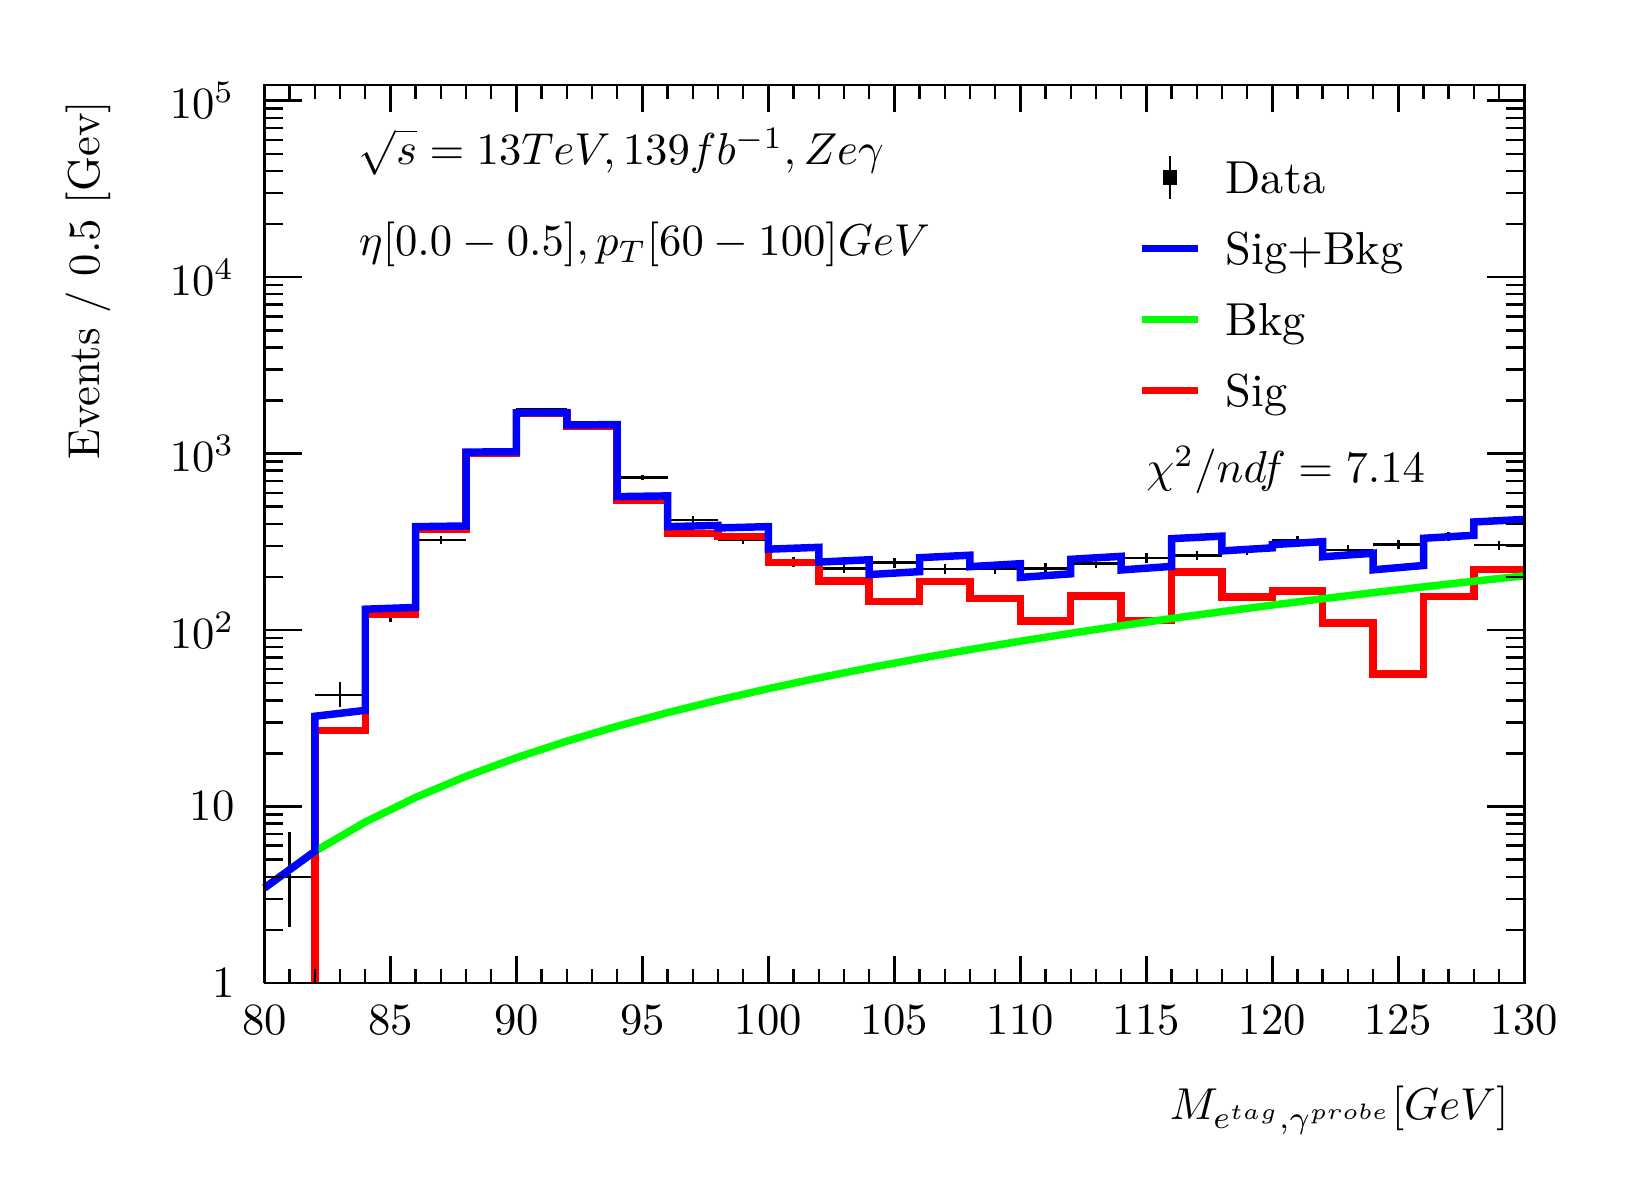
\begin{tikzpicture}
\pgfdeclareplotmark{cross} {
\pgfpathmoveto{\pgfpoint{-0.3\pgfplotmarksize}{\pgfplotmarksize}}
\pgfpathlineto{\pgfpoint{+0.3\pgfplotmarksize}{\pgfplotmarksize}}
\pgfpathlineto{\pgfpoint{+0.3\pgfplotmarksize}{0.3\pgfplotmarksize}}
\pgfpathlineto{\pgfpoint{+1\pgfplotmarksize}{0.3\pgfplotmarksize}}
\pgfpathlineto{\pgfpoint{+1\pgfplotmarksize}{-0.3\pgfplotmarksize}}
\pgfpathlineto{\pgfpoint{+0.3\pgfplotmarksize}{-0.3\pgfplotmarksize}}
\pgfpathlineto{\pgfpoint{+0.3\pgfplotmarksize}{-1.\pgfplotmarksize}}
\pgfpathlineto{\pgfpoint{-0.3\pgfplotmarksize}{-1.\pgfplotmarksize}}
\pgfpathlineto{\pgfpoint{-0.3\pgfplotmarksize}{-0.3\pgfplotmarksize}}
\pgfpathlineto{\pgfpoint{-1.\pgfplotmarksize}{-0.3\pgfplotmarksize}}
\pgfpathlineto{\pgfpoint{-1.\pgfplotmarksize}{0.3\pgfplotmarksize}}
\pgfpathlineto{\pgfpoint{-0.3\pgfplotmarksize}{0.3\pgfplotmarksize}}
\pgfpathclose
\pgfusepathqstroke
}
\pgfdeclareplotmark{cross*} {
\pgfpathmoveto{\pgfpoint{-0.3\pgfplotmarksize}{\pgfplotmarksize}}
\pgfpathlineto{\pgfpoint{+0.3\pgfplotmarksize}{\pgfplotmarksize}}
\pgfpathlineto{\pgfpoint{+0.3\pgfplotmarksize}{0.3\pgfplotmarksize}}
\pgfpathlineto{\pgfpoint{+1\pgfplotmarksize}{0.3\pgfplotmarksize}}
\pgfpathlineto{\pgfpoint{+1\pgfplotmarksize}{-0.3\pgfplotmarksize}}
\pgfpathlineto{\pgfpoint{+0.3\pgfplotmarksize}{-0.3\pgfplotmarksize}}
\pgfpathlineto{\pgfpoint{+0.3\pgfplotmarksize}{-1.\pgfplotmarksize}}
\pgfpathlineto{\pgfpoint{-0.3\pgfplotmarksize}{-1.\pgfplotmarksize}}
\pgfpathlineto{\pgfpoint{-0.3\pgfplotmarksize}{-0.3\pgfplotmarksize}}
\pgfpathlineto{\pgfpoint{-1.\pgfplotmarksize}{-0.3\pgfplotmarksize}}
\pgfpathlineto{\pgfpoint{-1.\pgfplotmarksize}{0.3\pgfplotmarksize}}
\pgfpathlineto{\pgfpoint{-0.3\pgfplotmarksize}{0.3\pgfplotmarksize}}
\pgfpathclose
\pgfusepathqfillstroke
}
\pgfdeclareplotmark{newstar} {
\pgfpathmoveto{\pgfqpoint{0pt}{\pgfplotmarksize}}
\pgfpathlineto{\pgfqpointpolar{44}{0.5\pgfplotmarksize}}
\pgfpathlineto{\pgfqpointpolar{18}{\pgfplotmarksize}}
\pgfpathlineto{\pgfqpointpolar{-20}{0.5\pgfplotmarksize}}
\pgfpathlineto{\pgfqpointpolar{-54}{\pgfplotmarksize}}
\pgfpathlineto{\pgfqpointpolar{-90}{0.5\pgfplotmarksize}}
\pgfpathlineto{\pgfqpointpolar{234}{\pgfplotmarksize}}
\pgfpathlineto{\pgfqpointpolar{198}{0.5\pgfplotmarksize}}
\pgfpathlineto{\pgfqpointpolar{162}{\pgfplotmarksize}}
\pgfpathlineto{\pgfqpointpolar{134}{0.5\pgfplotmarksize}}
\pgfpathclose
\pgfusepathqstroke
}
\pgfdeclareplotmark{newstar*} {
\pgfpathmoveto{\pgfqpoint{0pt}{\pgfplotmarksize}}
\pgfpathlineto{\pgfqpointpolar{44}{0.5\pgfplotmarksize}}
\pgfpathlineto{\pgfqpointpolar{18}{\pgfplotmarksize}}
\pgfpathlineto{\pgfqpointpolar{-20}{0.5\pgfplotmarksize}}
\pgfpathlineto{\pgfqpointpolar{-54}{\pgfplotmarksize}}
\pgfpathlineto{\pgfqpointpolar{-90}{0.5\pgfplotmarksize}}
\pgfpathlineto{\pgfqpointpolar{234}{\pgfplotmarksize}}
\pgfpathlineto{\pgfqpointpolar{198}{0.5\pgfplotmarksize}}
\pgfpathlineto{\pgfqpointpolar{162}{\pgfplotmarksize}}
\pgfpathlineto{\pgfqpointpolar{134}{0.5\pgfplotmarksize}}
\pgfpathclose
\pgfusepathqfillstroke
}
\definecolor{c}{rgb}{1,1,1};
\draw [color=c, fill=c] (0,0) rectangle (20,14.4361);
\draw [color=c, fill=c] (3,2.30977) rectangle (19,13.7143);
\definecolor{c}{rgb}{0,0,0};
\draw [c,line width=0.9] (3,2.30977) -- (3,13.7143) -- (19,13.7143) -- (19,2.30977) -- (3,2.30977);
\definecolor{c}{rgb}{1,1,1};
\draw [color=c, fill=c] (3,2.30977) rectangle (19,13.7143);
\definecolor{c}{rgb}{0,0,0};
\draw [c,line width=0.9] (3,2.30977) -- (3,13.7143) -- (19,13.7143) -- (19,2.30977) -- (3,2.30977);
\draw [c,line width=0.9] (3,2.30977) -- (19,2.30977);
\draw [c,line width=0.9] (3,2.65624) -- (3,2.30977);
\draw [c,line width=0.9] (3.32,2.48301) -- (3.32,2.30977);
\draw [c,line width=0.9] (3.64,2.48301) -- (3.64,2.30977);
\draw [c,line width=0.9] (3.96,2.48301) -- (3.96,2.30977);
\draw [c,line width=0.9] (4.28,2.48301) -- (4.28,2.30977);
\draw [c,line width=0.9] (4.6,2.65624) -- (4.6,2.30977);
\draw [c,line width=0.9] (4.92,2.48301) -- (4.92,2.30977);
\draw [c,line width=0.9] (5.24,2.48301) -- (5.24,2.30977);
\draw [c,line width=0.9] (5.56,2.48301) -- (5.56,2.30977);
\draw [c,line width=0.9] (5.88,2.48301) -- (5.88,2.30977);
\draw [c,line width=0.9] (6.2,2.65624) -- (6.2,2.30977);
\draw [c,line width=0.9] (6.52,2.48301) -- (6.52,2.30977);
\draw [c,line width=0.9] (6.84,2.48301) -- (6.84,2.30977);
\draw [c,line width=0.9] (7.16,2.48301) -- (7.16,2.30977);
\draw [c,line width=0.9] (7.48,2.48301) -- (7.48,2.30977);
\draw [c,line width=0.9] (7.8,2.65624) -- (7.8,2.30977);
\draw [c,line width=0.9] (8.12,2.48301) -- (8.12,2.30977);
\draw [c,line width=0.9] (8.44,2.48301) -- (8.44,2.30977);
\draw [c,line width=0.9] (8.76,2.48301) -- (8.76,2.30977);
\draw [c,line width=0.9] (9.08,2.48301) -- (9.08,2.30977);
\draw [c,line width=0.9] (9.4,2.65624) -- (9.4,2.30977);
\draw [c,line width=0.9] (9.72,2.48301) -- (9.72,2.30977);
\draw [c,line width=0.9] (10.04,2.48301) -- (10.04,2.30977);
\draw [c,line width=0.9] (10.36,2.48301) -- (10.36,2.30977);
\draw [c,line width=0.9] (10.68,2.48301) -- (10.68,2.30977);
\draw [c,line width=0.9] (11,2.65624) -- (11,2.30977);
\draw [c,line width=0.9] (11.32,2.48301) -- (11.32,2.30977);
\draw [c,line width=0.9] (11.64,2.48301) -- (11.64,2.30977);
\draw [c,line width=0.9] (11.96,2.48301) -- (11.96,2.30977);
\draw [c,line width=0.9] (12.28,2.48301) -- (12.28,2.30977);
\draw [c,line width=0.9] (12.6,2.65624) -- (12.6,2.30977);
\draw [c,line width=0.9] (12.92,2.48301) -- (12.92,2.30977);
\draw [c,line width=0.9] (13.24,2.48301) -- (13.24,2.30977);
\draw [c,line width=0.9] (13.56,2.48301) -- (13.56,2.30977);
\draw [c,line width=0.9] (13.88,2.48301) -- (13.88,2.30977);
\draw [c,line width=0.9] (14.2,2.65624) -- (14.2,2.30977);
\draw [c,line width=0.9] (14.52,2.48301) -- (14.52,2.30977);
\draw [c,line width=0.9] (14.84,2.48301) -- (14.84,2.30977);
\draw [c,line width=0.9] (15.16,2.48301) -- (15.16,2.30977);
\draw [c,line width=0.9] (15.48,2.48301) -- (15.48,2.30977);
\draw [c,line width=0.9] (15.8,2.65624) -- (15.8,2.30977);
\draw [c,line width=0.9] (16.12,2.48301) -- (16.12,2.30977);
\draw [c,line width=0.9] (16.44,2.48301) -- (16.44,2.30977);
\draw [c,line width=0.9] (16.76,2.48301) -- (16.76,2.30977);
\draw [c,line width=0.9] (17.08,2.48301) -- (17.08,2.30977);
\draw [c,line width=0.9] (17.4,2.65624) -- (17.4,2.30977);
\draw [c,line width=0.9] (17.72,2.48301) -- (17.72,2.30977);
\draw [c,line width=0.9] (18.04,2.48301) -- (18.04,2.30977);
\draw [c,line width=0.9] (18.36,2.48301) -- (18.36,2.30977);
\draw [c,line width=0.9] (18.68,2.48301) -- (18.68,2.30977);
\draw [c,line width=0.9] (19,2.65624) -- (19,2.30977);
\draw [anchor=base] (3,1.66015) node[scale=1.61424, color=c, rotate=0]{80};
\draw [anchor=base] (4.6,1.66015) node[scale=1.61424, color=c, rotate=0]{85};
\draw [anchor=base] (6.2,1.66015) node[scale=1.61424, color=c, rotate=0]{90};
\draw [anchor=base] (7.8,1.66015) node[scale=1.61424, color=c, rotate=0]{95};
\draw [anchor=base] (9.4,1.66015) node[scale=1.61424, color=c, rotate=0]{100};
\draw [anchor=base] (11,1.66015) node[scale=1.61424, color=c, rotate=0]{105};
\draw [anchor=base] (12.6,1.66015) node[scale=1.61424, color=c, rotate=0]{110};
\draw [anchor=base] (14.2,1.66015) node[scale=1.61424, color=c, rotate=0]{115};
\draw [anchor=base] (15.8,1.66015) node[scale=1.61424, color=c, rotate=0]{120};
\draw [anchor=base] (17.4,1.66015) node[scale=1.61424, color=c, rotate=0]{125};
\draw [anchor=base] (19,1.66015) node[scale=1.61424, color=c, rotate=0]{130};
\draw [anchor= east] (19,0.692932) node[scale=1.61424, color=c, rotate=0]{$M_{e^{tag}, \gamma^{probe}}  [GeV]$};
\draw [c,line width=0.9] (3,13.7143) -- (19,13.7143);
\draw [c,line width=0.9] (3,13.3678) -- (3,13.7143);
\draw [c,line width=0.9] (3.32,13.5411) -- (3.32,13.7143);
\draw [c,line width=0.9] (3.64,13.5411) -- (3.64,13.7143);
\draw [c,line width=0.9] (3.96,13.5411) -- (3.96,13.7143);
\draw [c,line width=0.9] (4.28,13.5411) -- (4.28,13.7143);
\draw [c,line width=0.9] (4.6,13.3678) -- (4.6,13.7143);
\draw [c,line width=0.9] (4.92,13.5411) -- (4.92,13.7143);
\draw [c,line width=0.9] (5.24,13.5411) -- (5.24,13.7143);
\draw [c,line width=0.9] (5.56,13.5411) -- (5.56,13.7143);
\draw [c,line width=0.9] (5.88,13.5411) -- (5.88,13.7143);
\draw [c,line width=0.9] (6.2,13.3678) -- (6.2,13.7143);
\draw [c,line width=0.9] (6.52,13.5411) -- (6.52,13.7143);
\draw [c,line width=0.9] (6.84,13.5411) -- (6.84,13.7143);
\draw [c,line width=0.9] (7.16,13.5411) -- (7.16,13.7143);
\draw [c,line width=0.9] (7.48,13.5411) -- (7.48,13.7143);
\draw [c,line width=0.9] (7.8,13.3678) -- (7.8,13.7143);
\draw [c,line width=0.9] (8.12,13.5411) -- (8.12,13.7143);
\draw [c,line width=0.9] (8.44,13.5411) -- (8.44,13.7143);
\draw [c,line width=0.9] (8.76,13.5411) -- (8.76,13.7143);
\draw [c,line width=0.9] (9.08,13.5411) -- (9.08,13.7143);
\draw [c,line width=0.9] (9.4,13.3678) -- (9.4,13.7143);
\draw [c,line width=0.9] (9.72,13.5411) -- (9.72,13.7143);
\draw [c,line width=0.9] (10.04,13.5411) -- (10.04,13.7143);
\draw [c,line width=0.9] (10.36,13.5411) -- (10.36,13.7143);
\draw [c,line width=0.9] (10.68,13.5411) -- (10.68,13.7143);
\draw [c,line width=0.9] (11,13.3678) -- (11,13.7143);
\draw [c,line width=0.9] (11.32,13.5411) -- (11.32,13.7143);
\draw [c,line width=0.9] (11.64,13.5411) -- (11.64,13.7143);
\draw [c,line width=0.9] (11.96,13.5411) -- (11.96,13.7143);
\draw [c,line width=0.9] (12.28,13.5411) -- (12.28,13.7143);
\draw [c,line width=0.9] (12.6,13.3678) -- (12.6,13.7143);
\draw [c,line width=0.9] (12.92,13.5411) -- (12.92,13.7143);
\draw [c,line width=0.9] (13.24,13.5411) -- (13.24,13.7143);
\draw [c,line width=0.9] (13.56,13.5411) -- (13.56,13.7143);
\draw [c,line width=0.9] (13.88,13.5411) -- (13.88,13.7143);
\draw [c,line width=0.9] (14.2,13.3678) -- (14.2,13.7143);
\draw [c,line width=0.9] (14.52,13.5411) -- (14.52,13.7143);
\draw [c,line width=0.9] (14.84,13.5411) -- (14.84,13.7143);
\draw [c,line width=0.9] (15.16,13.5411) -- (15.16,13.7143);
\draw [c,line width=0.9] (15.48,13.5411) -- (15.48,13.7143);
\draw [c,line width=0.9] (15.8,13.3678) -- (15.8,13.7143);
\draw [c,line width=0.9] (16.12,13.5411) -- (16.12,13.7143);
\draw [c,line width=0.9] (16.44,13.5411) -- (16.44,13.7143);
\draw [c,line width=0.9] (16.76,13.5411) -- (16.76,13.7143);
\draw [c,line width=0.9] (17.08,13.5411) -- (17.08,13.7143);
\draw [c,line width=0.9] (17.4,13.3678) -- (17.4,13.7143);
\draw [c,line width=0.9] (17.72,13.5411) -- (17.72,13.7143);
\draw [c,line width=0.9] (18.04,13.5411) -- (18.04,13.7143);
\draw [c,line width=0.9] (18.36,13.5411) -- (18.36,13.7143);
\draw [c,line width=0.9] (18.68,13.5411) -- (18.68,13.7143);
\draw [c,line width=0.9] (19,13.3678) -- (19,13.7143);
\draw [c,line width=0.9] (3,2.30977) -- (3,13.7143);
\draw [c,line width=0.9] (3.474,2.30978) -- (3,2.30978);
\draw [anchor= east] (2.82,2.30978) node[scale=1.61424, color=c, rotate=0]{1};
\draw [c,line width=0.9] (3.237,2.98447) -- (3,2.98447);
\draw [c,line width=0.9] (3.237,3.37914) -- (3,3.37914);
\draw [c,line width=0.9] (3.237,3.65916) -- (3,3.65916);
\draw [c,line width=0.9] (3.237,3.87637) -- (3,3.87637);
\draw [c,line width=0.9] (3.237,4.05383) -- (3,4.05383);
\draw [c,line width=0.9] (3.237,4.20388) -- (3,4.20388);
\draw [c,line width=0.9] (3.237,4.33386) -- (3,4.33386);
\draw [c,line width=0.9] (3.237,4.4485) -- (3,4.4485);
\draw [c,line width=0.9] (3.474,4.55106) -- (3,4.55106);
\draw [anchor= east] (2.82,4.55106) node[scale=1.61424, color=c, rotate=0]{10};
\draw [c,line width=0.9] (3.237,5.22575) -- (3,5.22575);
\draw [c,line width=0.9] (3.237,5.62042) -- (3,5.62042);
\draw [c,line width=0.9] (3.237,5.90045) -- (3,5.90045);
\draw [c,line width=0.9] (3.237,6.11765) -- (3,6.11765);
\draw [c,line width=0.9] (3.237,6.29512) -- (3,6.29512);
\draw [c,line width=0.9] (3.237,6.44516) -- (3,6.44516);
\draw [c,line width=0.9] (3.237,6.57514) -- (3,6.57514);
\draw [c,line width=0.9] (3.237,6.68979) -- (3,6.68979);
\draw [c,line width=0.9] (3.474,6.79234) -- (3,6.79234);
\draw [anchor= east] (2.82,6.79234) node[scale=1.61424, color=c, rotate=0]{$10^{2}$};
\draw [c,line width=0.9] (3.237,7.46704) -- (3,7.46704);
\draw [c,line width=0.9] (3.237,7.86171) -- (3,7.86171);
\draw [c,line width=0.9] (3.237,8.14173) -- (3,8.14173);
\draw [c,line width=0.9] (3.237,8.35893) -- (3,8.35893);
\draw [c,line width=0.9] (3.237,8.5364) -- (3,8.5364);
\draw [c,line width=0.9] (3.237,8.68645) -- (3,8.68645);
\draw [c,line width=0.9] (3.237,8.81642) -- (3,8.81642);
\draw [c,line width=0.9] (3.237,8.93107) -- (3,8.93107);
\draw [c,line width=0.9] (3.474,9.03363) -- (3,9.03363);
\draw [anchor= east] (2.82,9.03363) node[scale=1.61424, color=c, rotate=0]{$10^{3}$};
\draw [c,line width=0.9] (3.237,9.70832) -- (3,9.70832);
\draw [c,line width=0.9] (3.237,10.103) -- (3,10.103);
\draw [c,line width=0.9] (3.237,10.383) -- (3,10.383);
\draw [c,line width=0.9] (3.237,10.6002) -- (3,10.6002);
\draw [c,line width=0.9] (3.237,10.7777) -- (3,10.7777);
\draw [c,line width=0.9] (3.237,10.9277) -- (3,10.9277);
\draw [c,line width=0.9] (3.237,11.0577) -- (3,11.0577);
\draw [c,line width=0.9] (3.237,11.1724) -- (3,11.1724);
\draw [c,line width=0.9] (3.474,11.2749) -- (3,11.2749);
\draw [anchor= east] (2.82,11.2749) node[scale=1.61424, color=c, rotate=0]{$10^{4}$};
\draw [c,line width=0.9] (3.237,11.9496) -- (3,11.9496);
\draw [c,line width=0.9] (3.237,12.3443) -- (3,12.3443);
\draw [c,line width=0.9] (3.237,12.6243) -- (3,12.6243);
\draw [c,line width=0.9] (3.237,12.8415) -- (3,12.8415);
\draw [c,line width=0.9] (3.237,13.019) -- (3,13.019);
\draw [c,line width=0.9] (3.237,13.169) -- (3,13.169);
\draw [c,line width=0.9] (3.237,13.299) -- (3,13.299);
\draw [c,line width=0.9] (3.237,13.4136) -- (3,13.4136);
\draw [c,line width=0.9] (3.474,13.5162) -- (3,13.5162);
\draw [anchor= east] (2.82,13.5162) node[scale=1.61424, color=c, rotate=0]{$10^{5}$};
\draw [anchor= east] (0.76,13.7143) node[scale=1.61424, color=c, rotate=90]{Events / 0.5 [Gev]};
\draw [c,line width=0.9] (19,2.30977) -- (19,13.7143);
\draw [c,line width=0.9] (18.526,2.30978) -- (19,2.30978);
\draw [c,line width=0.9] (18.763,2.98447) -- (19,2.98447);
\draw [c,line width=0.9] (18.763,3.37914) -- (19,3.37914);
\draw [c,line width=0.9] (18.763,3.65916) -- (19,3.65916);
\draw [c,line width=0.9] (18.763,3.87637) -- (19,3.87637);
\draw [c,line width=0.9] (18.763,4.05383) -- (19,4.05383);
\draw [c,line width=0.9] (18.763,4.20388) -- (19,4.20388);
\draw [c,line width=0.9] (18.763,4.33386) -- (19,4.33386);
\draw [c,line width=0.9] (18.763,4.4485) -- (19,4.4485);
\draw [c,line width=0.9] (18.526,4.55106) -- (19,4.55106);
\draw [c,line width=0.9] (18.763,5.22575) -- (19,5.22575);
\draw [c,line width=0.9] (18.763,5.62042) -- (19,5.62042);
\draw [c,line width=0.9] (18.763,5.90045) -- (19,5.90045);
\draw [c,line width=0.9] (18.763,6.11765) -- (19,6.11765);
\draw [c,line width=0.9] (18.763,6.29512) -- (19,6.29512);
\draw [c,line width=0.9] (18.763,6.44516) -- (19,6.44516);
\draw [c,line width=0.9] (18.763,6.57514) -- (19,6.57514);
\draw [c,line width=0.9] (18.763,6.68979) -- (19,6.68979);
\draw [c,line width=0.9] (18.526,6.79234) -- (19,6.79234);
\draw [c,line width=0.9] (18.763,7.46704) -- (19,7.46704);
\draw [c,line width=0.9] (18.763,7.86171) -- (19,7.86171);
\draw [c,line width=0.9] (18.763,8.14173) -- (19,8.14173);
\draw [c,line width=0.9] (18.763,8.35893) -- (19,8.35893);
\draw [c,line width=0.9] (18.763,8.5364) -- (19,8.5364);
\draw [c,line width=0.9] (18.763,8.68645) -- (19,8.68645);
\draw [c,line width=0.9] (18.763,8.81642) -- (19,8.81642);
\draw [c,line width=0.9] (18.763,8.93107) -- (19,8.93107);
\draw [c,line width=0.9] (18.526,9.03363) -- (19,9.03363);
\draw [c,line width=0.9] (18.763,9.70832) -- (19,9.70832);
\draw [c,line width=0.9] (18.763,10.103) -- (19,10.103);
\draw [c,line width=0.9] (18.763,10.383) -- (19,10.383);
\draw [c,line width=0.9] (18.763,10.6002) -- (19,10.6002);
\draw [c,line width=0.9] (18.763,10.7777) -- (19,10.7777);
\draw [c,line width=0.9] (18.763,10.9277) -- (19,10.9277);
\draw [c,line width=0.9] (18.763,11.0577) -- (19,11.0577);
\draw [c,line width=0.9] (18.763,11.1724) -- (19,11.1724);
\draw [c,line width=0.9] (18.526,11.2749) -- (19,11.2749);
\draw [c,line width=0.9] (18.763,11.9496) -- (19,11.9496);
\draw [c,line width=0.9] (18.763,12.3443) -- (19,12.3443);
\draw [c,line width=0.9] (18.763,12.6243) -- (19,12.6243);
\draw [c,line width=0.9] (18.763,12.8415) -- (19,12.8415);
\draw [c,line width=0.9] (18.763,13.019) -- (19,13.019);
\draw [c,line width=0.9] (18.763,13.169) -- (19,13.169);
\draw [c,line width=0.9] (18.763,13.299) -- (19,13.299);
\draw [c,line width=0.9] (18.763,13.4136) -- (19,13.4136);
\draw [c,line width=0.9] (18.526,13.5162) -- (19,13.5162);
\draw [c,line width=0.9] (3.32,3.65916) -- (3,3.65916);
\draw [c,line width=0.9] (3,3.65916) -- (3,3.65916);
\draw [c,line width=0.9] (3.32,3.65916) -- (3.64,3.65916);
\draw [c,line width=0.9] (3.64,3.65916) -- (3.64,3.65916);
\draw [c,line width=0.9] (3.32,3.65916) -- (3.32,4.22625);
\draw [c,line width=0.9] (3.32,4.22625) -- (3.32,4.22625);
\draw [c,line width=0.9] (3.32,3.65916) -- (3.32,3.02529);
\draw [c,line width=0.9] (3.32,3.02529) -- (3.32,3.02529);
\draw [c,line width=0.9] (3.96,5.97084) -- (3.64,5.97084);
\draw [c,line width=0.9] (3.64,5.97084) -- (3.64,5.97084);
\draw [c,line width=0.9] (3.96,5.97084) -- (4.28,5.97084);
\draw [c,line width=0.9] (4.28,5.97084) -- (4.28,5.97084);
\draw [c,line width=0.9] (3.96,5.97084) -- (3.96,6.12942);
\draw [c,line width=0.9] (3.96,6.12942) -- (3.96,6.12942);
\draw [c,line width=0.9] (3.96,5.97084) -- (3.96,5.81047);
\draw [c,line width=0.9] (3.96,5.81047) -- (3.96,5.81047);
\draw [c,line width=0.9] (4.6,6.97789) -- (4.28,6.97789);
\draw [c,line width=0.9] (4.28,6.97789) -- (4.28,6.97789);
\draw [c,line width=0.9] (4.6,6.97789) -- (4.92,6.97789);
\draw [c,line width=0.9] (4.92,6.97789) -- (4.92,6.97789);
\draw [c,line width=0.9] (4.6,6.97789) -- (4.6,7.06635);
\draw [c,line width=0.9] (4.6,7.06635) -- (4.6,7.06635);
\draw [c,line width=0.9] (4.6,6.97789) -- (4.6,6.88943);
\draw [c,line width=0.9] (4.6,6.88943) -- (4.6,6.88943);
\draw [c,line width=0.9] (5.24,7.93662) -- (4.92,7.93662);
\draw [c,line width=0.9] (4.92,7.93662) -- (4.92,7.93662);
\draw [c,line width=0.9] (5.24,7.93662) -- (5.56,7.93662);
\draw [c,line width=0.9] (5.56,7.93662) -- (5.56,7.93662);
\draw [c,line width=0.9] (5.24,7.93662) -- (5.24,7.99069);
\draw [c,line width=0.9] (5.24,7.99069) -- (5.24,7.99069);
\draw [c,line width=0.9] (5.24,7.93662) -- (5.24,7.88255);
\draw [c,line width=0.9] (5.24,7.88255) -- (5.24,7.88255);
\draw [c,line width=0.9] (5.88,9.01594) -- (5.56,9.01594);
\draw [c,line width=0.9] (5.56,9.01594) -- (5.56,9.01594);
\draw [c,line width=0.9] (5.88,9.01594) -- (6.2,9.01594);
\draw [c,line width=0.9] (6.2,9.01594) -- (6.2,9.01594);
\draw [c,line width=0.9] (5.88,9.01594) -- (5.88,9.047);
\draw [c,line width=0.9] (5.88,9.047) -- (5.88,9.047);
\draw [c,line width=0.9] (5.88,9.01594) -- (5.88,8.98488);
\draw [c,line width=0.9] (5.88,8.98488) -- (5.88,8.98488);
\draw [c,line width=0.9] (6.52,9.59105) -- (6.2,9.59105);
\draw [c,line width=0.9] (6.2,9.59105) -- (6.2,9.59105);
\draw [c,line width=0.9] (6.52,9.59105) -- (6.84,9.59105);
\draw [c,line width=0.9] (6.84,9.59105) -- (6.84,9.59105);
\draw [c,line width=0.9] (6.52,9.59105) -- (6.52,9.61417);
\draw [c,line width=0.9] (6.52,9.61417) -- (6.52,9.61417);
\draw [c,line width=0.9] (6.52,9.59105) -- (6.52,9.56794);
\draw [c,line width=0.9] (6.52,9.56794) -- (6.52,9.56794);
\draw [c,line width=0.9] (7.16,9.42244) -- (6.84,9.42244);
\draw [c,line width=0.9] (6.84,9.42244) -- (6.84,9.42244);
\draw [c,line width=0.9] (7.16,9.42244) -- (7.48,9.42244);
\draw [c,line width=0.9] (7.48,9.42244) -- (7.48,9.42244);
\draw [c,line width=0.9] (7.16,9.42244) -- (7.16,9.44765);
\draw [c,line width=0.9] (7.16,9.44765) -- (7.16,9.44765);
\draw [c,line width=0.9] (7.16,9.42244) -- (7.16,9.39723);
\draw [c,line width=0.9] (7.16,9.39723) -- (7.16,9.39723);
\draw [c,line width=0.9] (7.8,8.72996) -- (7.48,8.72996);
\draw [c,line width=0.9] (7.48,8.72996) -- (7.48,8.72996);
\draw [c,line width=0.9] (7.8,8.72996) -- (8.12,8.72996);
\draw [c,line width=0.9] (8.12,8.72996) -- (8.12,8.72996);
\draw [c,line width=0.9] (7.8,8.72996) -- (7.8,8.76593);
\draw [c,line width=0.9] (7.8,8.76593) -- (7.8,8.76593);
\draw [c,line width=0.9] (7.8,8.72996) -- (7.8,8.69398);
\draw [c,line width=0.9] (7.8,8.69398) -- (7.8,8.69398);
\draw [c,line width=0.9] (8.44,8.18922) -- (8.12,8.18922);
\draw [c,line width=0.9] (8.12,8.18922) -- (8.12,8.18922);
\draw [c,line width=0.9] (8.44,8.18922) -- (8.76,8.18922);
\draw [c,line width=0.9] (8.76,8.18922) -- (8.76,8.18922);
\draw [c,line width=0.9] (8.44,8.18922) -- (8.44,8.23671);
\draw [c,line width=0.9] (8.44,8.23671) -- (8.44,8.23671);
\draw [c,line width=0.9] (8.44,8.18922) -- (8.44,8.14173);
\draw [c,line width=0.9] (8.44,8.14173) -- (8.44,8.14173);
\draw [c,line width=0.9] (9.08,7.94261) -- (8.76,7.94261);
\draw [c,line width=0.9] (8.76,7.94261) -- (8.76,7.94261);
\draw [c,line width=0.9] (9.08,7.94261) -- (9.4,7.94261);
\draw [c,line width=0.9] (9.4,7.94261) -- (9.4,7.94261);
\draw [c,line width=0.9] (9.08,7.94261) -- (9.08,7.99651);
\draw [c,line width=0.9] (9.08,7.99651) -- (9.08,7.99651);
\draw [c,line width=0.9] (9.08,7.94261) -- (9.08,7.8887);
\draw [c,line width=0.9] (9.08,7.8887) -- (9.08,7.8887);
\draw [c,line width=0.9] (9.72,7.66059) -- (9.4,7.66059);
\draw [c,line width=0.9] (9.4,7.66059) -- (9.4,7.66059);
\draw [c,line width=0.9] (9.72,7.66059) -- (10.04,7.66059);
\draw [c,line width=0.9] (10.04,7.66059) -- (10.04,7.66059);
\draw [c,line width=0.9] (9.72,7.66059) -- (9.72,7.7229);
\draw [c,line width=0.9] (9.72,7.7229) -- (9.72,7.7229);
\draw [c,line width=0.9] (9.72,7.66059) -- (9.72,7.59829);
\draw [c,line width=0.9] (9.72,7.59829) -- (9.72,7.59829);
\draw [c,line width=0.9] (10.36,7.57735) -- (10.04,7.57735);
\draw [c,line width=0.9] (10.04,7.57735) -- (10.04,7.57735);
\draw [c,line width=0.9] (10.36,7.57735) -- (10.68,7.57735);
\draw [c,line width=0.9] (10.68,7.57735) -- (10.68,7.57735);
\draw [c,line width=0.9] (10.36,7.57735) -- (10.36,7.64237);
\draw [c,line width=0.9] (10.36,7.64237) -- (10.36,7.64237);
\draw [c,line width=0.9] (10.36,7.57735) -- (10.36,7.51232);
\draw [c,line width=0.9] (10.36,7.51232) -- (10.36,7.51232);
\draw [c,line width=0.9] (11,7.64855) -- (10.68,7.64855);
\draw [c,line width=0.9] (10.68,7.64855) -- (10.68,7.64855);
\draw [c,line width=0.9] (11,7.64855) -- (11.32,7.64855);
\draw [c,line width=0.9] (11.32,7.64855) -- (11.32,7.64855);
\draw [c,line width=0.9] (11,7.64855) -- (11,7.71124);
\draw [c,line width=0.9] (11,7.71124) -- (11,7.71124);
\draw [c,line width=0.9] (11,7.64855) -- (11,7.58586);
\draw [c,line width=0.9] (11,7.58586) -- (11,7.58586);
\draw [c,line width=0.9] (11.64,7.56862) -- (11.32,7.56862);
\draw [c,line width=0.9] (11.32,7.56862) -- (11.32,7.56862);
\draw [c,line width=0.9] (11.64,7.56862) -- (11.96,7.56862);
\draw [c,line width=0.9] (11.96,7.56862) -- (11.96,7.56862);
\draw [c,line width=0.9] (11.64,7.56862) -- (11.64,7.63393);
\draw [c,line width=0.9] (11.64,7.63393) -- (11.64,7.63393);
\draw [c,line width=0.9] (11.64,7.56862) -- (11.64,7.5033);
\draw [c,line width=0.9] (11.64,7.5033) -- (11.64,7.5033);
\draw [c,line width=0.9] (12.28,7.57299) -- (11.96,7.57299);
\draw [c,line width=0.9] (11.96,7.57299) -- (11.96,7.57299);
\draw [c,line width=0.9] (12.28,7.57299) -- (12.6,7.57299);
\draw [c,line width=0.9] (12.6,7.57299) -- (12.6,7.57299);
\draw [c,line width=0.9] (12.28,7.57299) -- (12.28,7.63816);
\draw [c,line width=0.9] (12.28,7.63816) -- (12.28,7.63816);
\draw [c,line width=0.9] (12.28,7.57299) -- (12.28,7.50782);
\draw [c,line width=0.9] (12.28,7.50782) -- (12.28,7.50782);
\draw [c,line width=0.9] (12.92,7.57735) -- (12.6,7.57735);
\draw [c,line width=0.9] (12.6,7.57735) -- (12.6,7.57735);
\draw [c,line width=0.9] (12.92,7.57735) -- (13.24,7.57735);
\draw [c,line width=0.9] (13.24,7.57735) -- (13.24,7.57735);
\draw [c,line width=0.9] (12.92,7.57735) -- (12.92,7.64237);
\draw [c,line width=0.9] (12.92,7.64237) -- (12.92,7.64237);
\draw [c,line width=0.9] (12.92,7.57735) -- (12.92,7.51232);
\draw [c,line width=0.9] (12.92,7.51232) -- (12.92,7.51232);
\draw [c,line width=0.9] (13.56,7.64044) -- (13.24,7.64044);
\draw [c,line width=0.9] (13.24,7.64044) -- (13.24,7.64044);
\draw [c,line width=0.9] (13.56,7.64044) -- (13.88,7.64044);
\draw [c,line width=0.9] (13.88,7.64044) -- (13.88,7.64044);
\draw [c,line width=0.9] (13.56,7.64044) -- (13.56,7.70339);
\draw [c,line width=0.9] (13.56,7.70339) -- (13.56,7.70339);
\draw [c,line width=0.9] (13.56,7.64044) -- (13.56,7.57749);
\draw [c,line width=0.9] (13.56,7.57749) -- (13.56,7.57749);
\draw [c,line width=0.9] (14.2,7.71112) -- (13.88,7.71112);
\draw [c,line width=0.9] (13.88,7.71112) -- (13.88,7.71112);
\draw [c,line width=0.9] (14.2,7.71112) -- (14.52,7.71112);
\draw [c,line width=0.9] (14.52,7.71112) -- (14.52,7.71112);
\draw [c,line width=0.9] (14.2,7.71112) -- (14.2,7.77183);
\draw [c,line width=0.9] (14.2,7.77183) -- (14.2,7.77183);
\draw [c,line width=0.9] (14.2,7.71112) -- (14.2,7.65041);
\draw [c,line width=0.9] (14.2,7.65041) -- (14.2,7.65041);
\draw [c,line width=0.9] (14.84,7.73728) -- (14.52,7.73728);
\draw [c,line width=0.9] (14.52,7.73728) -- (14.52,7.73728);
\draw [c,line width=0.9] (14.84,7.73728) -- (15.16,7.73728);
\draw [c,line width=0.9] (15.16,7.73728) -- (15.16,7.73728);
\draw [c,line width=0.9] (14.84,7.73728) -- (14.84,7.79717);
\draw [c,line width=0.9] (14.84,7.79717) -- (14.84,7.79717);
\draw [c,line width=0.9] (14.84,7.73728) -- (14.84,7.67738);
\draw [c,line width=0.9] (14.84,7.67738) -- (14.84,7.67738);
\draw [c,line width=0.9] (15.48,7.80836) -- (15.16,7.80836);
\draw [c,line width=0.9] (15.16,7.80836) -- (15.16,7.80836);
\draw [c,line width=0.9] (15.48,7.80836) -- (15.8,7.80836);
\draw [c,line width=0.9] (15.8,7.80836) -- (15.8,7.80836);
\draw [c,line width=0.9] (15.48,7.80836) -- (15.48,7.86611);
\draw [c,line width=0.9] (15.48,7.86611) -- (15.48,7.86611);
\draw [c,line width=0.9] (15.48,7.80836) -- (15.48,7.75061);
\draw [c,line width=0.9] (15.48,7.75061) -- (15.48,7.75061);
\draw [c,line width=0.9] (16.12,7.93361) -- (15.8,7.93361);
\draw [c,line width=0.9] (15.8,7.93361) -- (15.8,7.93361);
\draw [c,line width=0.9] (16.12,7.93361) -- (16.44,7.93361);
\draw [c,line width=0.9] (16.44,7.93361) -- (16.44,7.93361);
\draw [c,line width=0.9] (16.12,7.93361) -- (16.12,7.98776);
\draw [c,line width=0.9] (16.12,7.98776) -- (16.12,7.98776);
\draw [c,line width=0.9] (16.12,7.93361) -- (16.12,7.87946);
\draw [c,line width=0.9] (16.12,7.87946) -- (16.12,7.87946);
\draw [c,line width=0.9] (16.76,7.81178) -- (16.44,7.81178);
\draw [c,line width=0.9] (16.44,7.81178) -- (16.44,7.81178);
\draw [c,line width=0.9] (16.76,7.81178) -- (17.08,7.81178);
\draw [c,line width=0.9] (17.08,7.81178) -- (17.08,7.81178);
\draw [c,line width=0.9] (16.76,7.81178) -- (16.76,7.86943);
\draw [c,line width=0.9] (16.76,7.86943) -- (16.76,7.86943);
\draw [c,line width=0.9] (16.76,7.81178) -- (16.76,7.75413);
\draw [c,line width=0.9] (16.76,7.75413) -- (16.76,7.75413);
\draw [c,line width=0.9] (17.4,7.87779) -- (17.08,7.87779);
\draw [c,line width=0.9] (17.08,7.87779) -- (17.08,7.87779);
\draw [c,line width=0.9] (17.4,7.87779) -- (17.72,7.87779);
\draw [c,line width=0.9] (17.72,7.87779) -- (17.72,7.87779);
\draw [c,line width=0.9] (17.4,7.87779) -- (17.4,7.93352);
\draw [c,line width=0.9] (17.4,7.93352) -- (17.4,7.93352);
\draw [c,line width=0.9] (17.4,7.87779) -- (17.4,7.82207);
\draw [c,line width=0.9] (17.4,7.82207) -- (17.4,7.82207);
\draw [c,line width=0.9] (18.04,7.98067) -- (17.72,7.98067);
\draw [c,line width=0.9] (17.72,7.98067) -- (17.72,7.98067);
\draw [c,line width=0.9] (18.04,7.98067) -- (18.36,7.98067);
\draw [c,line width=0.9] (18.36,7.98067) -- (18.36,7.98067);
\draw [c,line width=0.9] (18.04,7.98067) -- (18.04,8.03353);
\draw [c,line width=0.9] (18.04,8.03353) -- (18.04,8.03353);
\draw [c,line width=0.9] (18.04,7.98067) -- (18.04,7.92781);
\draw [c,line width=0.9] (18.04,7.92781) -- (18.04,7.92781);
\draw [c,line width=0.9] (18.68,7.87139) -- (18.36,7.87139);
\draw [c,line width=0.9] (18.36,7.87139) -- (18.36,7.87139);
\draw [c,line width=0.9] (18.68,7.87139) -- (19,7.87139);
\draw [c,line width=0.9] (19,7.87139) -- (19,7.87139);
\draw [c,line width=0.9] (18.68,7.87139) -- (18.68,7.9273);
\draw [c,line width=0.9] (18.68,7.9273) -- (18.68,7.9273);
\draw [c,line width=0.9] (18.68,7.87139) -- (18.68,7.81548);
\draw [c,line width=0.9] (18.68,7.81548) -- (18.68,7.81548);
\foreach \P in {(3.32,3.65916), (3.96,5.97084), (4.6,6.97789), (5.24,7.93662), (5.88,9.01594), (6.52,9.59105), (7.16,9.42244), (7.8,8.72996), (8.44,8.18922), (9.08,7.94261), (9.72,7.66059), (10.36,7.57735), (11,7.64855), (11.64,7.56862),
 (12.28,7.57299), (12.92,7.57735), (13.56,7.64044), (14.2,7.71112), (14.84,7.73728), (15.48,7.80836), (16.12,7.93361), (16.76,7.81178), (17.4,7.87779), (18.04,7.98067), (18.68,7.87139)}{\draw[mark options={color=c,fill=c},mark size=2.882883pt,mark=]
 plot coordinates {\P};}
\definecolor{c}{rgb}{1,0,0};
\draw [c,line width=2.7] (3.64,2.30977) -- (3.64,5.51487);
\draw [c,line width=2.7] (3.64,5.51487) -- (4.28,5.51487) -- (4.28,6.99504) -- (4.92,6.99504) -- (4.92,8.0768) -- (5.56,8.0768) -- (5.56,9.03869) -- (6.2,9.03869) -- (6.2,9.54112) -- (6.84,9.54112) -- (6.84,9.38238) -- (7.48,9.38238) --
 (7.48,8.43727) -- (8.12,8.43727) -- (8.12,8.01608) -- (8.76,8.01608) -- (8.76,7.98073) -- (9.4,7.98073) -- (9.4,7.64771) -- (10.04,7.64771) -- (10.04,7.41328) -- (10.68,7.41328) -- (10.68,7.15587) -- (11.32,7.15587) -- (11.32,7.40735) --
 (11.96,7.40735) -- (11.96,7.19492) -- (12.6,7.19492) -- (12.6,6.90613) -- (13.24,6.90613) -- (13.24,7.22418) -- (13.88,7.22418) -- (13.88,6.91353) -- (14.52,6.91353) -- (14.52,7.53019) -- (15.16,7.53019) -- (15.16,7.21107) -- (15.8,7.21107) --
 (15.8,7.2882) -- (16.44,7.2882) -- (16.44,6.88266) -- (17.08,6.88266) -- (17.08,6.23769) -- (17.72,6.23769) -- (17.72,7.22214) -- (18.36,7.22214) -- (18.36,7.56311) -- (19,7.56311) -- (19,7.56311) -- (19,7.56311) -- (19,7.56311);
\definecolor{c}{rgb}{0,1,0};
\draw [c,line width=2.7] (3,3.51772) -- (3,3.51772);
\draw [c,line width=2.7] (3,3.51772) -- (3,3.51772) -- (3.64,3.98183) -- (3.64,3.98183) -- (4.28,4.35484) -- (4.28,4.35484) -- (4.92,4.66705) -- (4.92,4.66705) -- (5.56,4.93566) -- (5.56,4.93566) -- (6.2,5.17145) -- (6.2,5.17145) -- (6.84,5.38161) --
 (6.84,5.38161) -- (7.48,5.57118) -- (7.48,5.57118) -- (8.12,5.74386) -- (8.12,5.74386) -- (8.76,5.90242) -- (8.76,5.90242) -- (9.4,6.049) -- (9.4,6.049) -- (10.04,6.1853) -- (10.04,6.1853) -- (10.68,6.31265) -- (10.68,6.31265) -- (11.32,6.43217) --
 (11.32,6.43217) -- (11.96,6.54476) -- (11.96,6.54476) -- (12.6,6.65118) -- (12.6,6.65118) -- (13.24,6.75209) -- (13.24,6.75209) -- (13.88,6.84801) -- (13.88,6.84801) -- (14.52,6.93942) -- (14.52,6.93942) -- (15.16,7.02673) -- (15.16,7.02673) --
 (15.8,7.11029) -- (15.8,7.11029) -- (16.44,7.1904) -- (16.44,7.1904) -- (17.08,7.26735) -- (17.08,7.26735) -- (17.72,7.34137) -- (17.72,7.34137) -- (18.36,7.41267) -- (18.36,7.41267) -- (19,7.48146) -- (19,7.48146) -- (19,7.48146) -- (19,7.48146);
\definecolor{c}{rgb}{0,0,1};
\draw [c,line width=2.7] (3,3.51772) -- (3,3.51772);
\draw [c,line width=2.7] (3,3.51772) -- (3,3.51772) -- (3.64,3.98183) -- (3.64,5.69801) -- (4.28,5.77301) -- (4.28,7.05759) -- (4.92,7.08024) -- (4.92,8.10567) -- (5.56,8.11467) -- (5.56,9.05297) -- (6.2,9.05684) -- (6.2,9.55199) -- (6.84,9.55459) --
 (6.84,9.39822) -- (7.48,9.40159) -- (7.48,8.4872) -- (8.12,8.4966) -- (8.12,8.10608) -- (8.76,8.12117) -- (8.76,8.0895) -- (9.4,8.10609) -- (9.4,7.8199) -- (10.04,7.84334) -- (10.04,7.656) -- (10.68,7.68558) -- (10.68,7.49754) -- (11.32,7.53448) --
 (11.32,7.71178) -- (11.96,7.74332) -- (11.96,7.59784) -- (12.6,7.63523) -- (12.6,7.46167) -- (13.24,7.50685) -- (13.24,7.69117) -- (13.88,7.72885) -- (13.88,7.55602) -- (14.52,7.60126) -- (14.52,7.95364) -- (15.16,7.98535) -- (15.16,7.79795) --
 (15.8,7.83668) -- (15.8,7.878) -- (16.44,7.91522) -- (16.44,7.72334) -- (17.08,7.76858) -- (17.08,7.55745) -- (17.72,7.61292) -- (17.72,7.95827) -- (18.36,7.99676) -- (18.36,8.16549) -- (19,8.19783) -- (19,8.19783) -- (19,8.19783) -- (19,8.19783);
\definecolor{c}{rgb}{0,0,0};
\draw [c,line width=0.9] (3,2.30977) -- (19,2.30977);
\draw [c,line width=0.9] (3,2.65624) -- (3,2.30977);
\draw [c,line width=0.9] (3.32,2.48301) -- (3.32,2.30977);
\draw [c,line width=0.9] (3.64,2.48301) -- (3.64,2.30977);
\draw [c,line width=0.9] (3.96,2.48301) -- (3.96,2.30977);
\draw [c,line width=0.9] (4.28,2.48301) -- (4.28,2.30977);
\draw [c,line width=0.9] (4.6,2.65624) -- (4.6,2.30977);
\draw [c,line width=0.9] (4.92,2.48301) -- (4.92,2.30977);
\draw [c,line width=0.9] (5.24,2.48301) -- (5.24,2.30977);
\draw [c,line width=0.9] (5.56,2.48301) -- (5.56,2.30977);
\draw [c,line width=0.9] (5.88,2.48301) -- (5.88,2.30977);
\draw [c,line width=0.9] (6.2,2.65624) -- (6.2,2.30977);
\draw [c,line width=0.9] (6.52,2.48301) -- (6.52,2.30977);
\draw [c,line width=0.9] (6.84,2.48301) -- (6.84,2.30977);
\draw [c,line width=0.9] (7.16,2.48301) -- (7.16,2.30977);
\draw [c,line width=0.9] (7.48,2.48301) -- (7.48,2.30977);
\draw [c,line width=0.9] (7.8,2.65624) -- (7.8,2.30977);
\draw [c,line width=0.9] (8.12,2.48301) -- (8.12,2.30977);
\draw [c,line width=0.9] (8.44,2.48301) -- (8.44,2.30977);
\draw [c,line width=0.9] (8.76,2.48301) -- (8.76,2.30977);
\draw [c,line width=0.9] (9.08,2.48301) -- (9.08,2.30977);
\draw [c,line width=0.9] (9.4,2.65624) -- (9.4,2.30977);
\draw [c,line width=0.9] (9.72,2.48301) -- (9.72,2.30977);
\draw [c,line width=0.9] (10.04,2.48301) -- (10.04,2.30977);
\draw [c,line width=0.9] (10.36,2.48301) -- (10.36,2.30977);
\draw [c,line width=0.9] (10.68,2.48301) -- (10.68,2.30977);
\draw [c,line width=0.9] (11,2.65624) -- (11,2.30977);
\draw [c,line width=0.9] (11.32,2.48301) -- (11.32,2.30977);
\draw [c,line width=0.9] (11.64,2.48301) -- (11.64,2.30977);
\draw [c,line width=0.9] (11.96,2.48301) -- (11.96,2.30977);
\draw [c,line width=0.9] (12.28,2.48301) -- (12.28,2.30977);
\draw [c,line width=0.9] (12.6,2.65624) -- (12.6,2.30977);
\draw [c,line width=0.9] (12.92,2.48301) -- (12.92,2.30977);
\draw [c,line width=0.9] (13.24,2.48301) -- (13.24,2.30977);
\draw [c,line width=0.9] (13.56,2.48301) -- (13.56,2.30977);
\draw [c,line width=0.9] (13.88,2.48301) -- (13.88,2.30977);
\draw [c,line width=0.9] (14.2,2.65624) -- (14.2,2.30977);
\draw [c,line width=0.9] (14.52,2.48301) -- (14.52,2.30977);
\draw [c,line width=0.9] (14.84,2.48301) -- (14.84,2.30977);
\draw [c,line width=0.9] (15.16,2.48301) -- (15.16,2.30977);
\draw [c,line width=0.9] (15.48,2.48301) -- (15.48,2.30977);
\draw [c,line width=0.9] (15.8,2.65624) -- (15.8,2.30977);
\draw [c,line width=0.9] (16.12,2.48301) -- (16.12,2.30977);
\draw [c,line width=0.9] (16.44,2.48301) -- (16.44,2.30977);
\draw [c,line width=0.9] (16.76,2.48301) -- (16.76,2.30977);
\draw [c,line width=0.9] (17.08,2.48301) -- (17.08,2.30977);
\draw [c,line width=0.9] (17.4,2.65624) -- (17.4,2.30977);
\draw [c,line width=0.9] (17.72,2.48301) -- (17.72,2.30977);
\draw [c,line width=0.9] (18.04,2.48301) -- (18.04,2.30977);
\draw [c,line width=0.9] (18.36,2.48301) -- (18.36,2.30977);
\draw [c,line width=0.9] (18.68,2.48301) -- (18.68,2.30977);
\draw [c,line width=0.9] (19,2.65624) -- (19,2.30977);
\draw [c,line width=0.9] (3,13.7143) -- (19,13.7143);
\draw [c,line width=0.9] (3,13.3678) -- (3,13.7143);
\draw [c,line width=0.9] (3.32,13.5411) -- (3.32,13.7143);
\draw [c,line width=0.9] (3.64,13.5411) -- (3.64,13.7143);
\draw [c,line width=0.9] (3.96,13.5411) -- (3.96,13.7143);
\draw [c,line width=0.9] (4.28,13.5411) -- (4.28,13.7143);
\draw [c,line width=0.9] (4.6,13.3678) -- (4.6,13.7143);
\draw [c,line width=0.9] (4.92,13.5411) -- (4.92,13.7143);
\draw [c,line width=0.9] (5.24,13.5411) -- (5.24,13.7143);
\draw [c,line width=0.9] (5.56,13.5411) -- (5.56,13.7143);
\draw [c,line width=0.9] (5.88,13.5411) -- (5.88,13.7143);
\draw [c,line width=0.9] (6.2,13.3678) -- (6.2,13.7143);
\draw [c,line width=0.9] (6.52,13.5411) -- (6.52,13.7143);
\draw [c,line width=0.9] (6.84,13.5411) -- (6.84,13.7143);
\draw [c,line width=0.9] (7.16,13.5411) -- (7.16,13.7143);
\draw [c,line width=0.9] (7.48,13.5411) -- (7.48,13.7143);
\draw [c,line width=0.9] (7.8,13.3678) -- (7.8,13.7143);
\draw [c,line width=0.9] (8.12,13.5411) -- (8.12,13.7143);
\draw [c,line width=0.9] (8.44,13.5411) -- (8.44,13.7143);
\draw [c,line width=0.9] (8.76,13.5411) -- (8.76,13.7143);
\draw [c,line width=0.9] (9.08,13.5411) -- (9.08,13.7143);
\draw [c,line width=0.9] (9.4,13.3678) -- (9.4,13.7143);
\draw [c,line width=0.9] (9.72,13.5411) -- (9.72,13.7143);
\draw [c,line width=0.9] (10.04,13.5411) -- (10.04,13.7143);
\draw [c,line width=0.9] (10.36,13.5411) -- (10.36,13.7143);
\draw [c,line width=0.9] (10.68,13.5411) -- (10.68,13.7143);
\draw [c,line width=0.9] (11,13.3678) -- (11,13.7143);
\draw [c,line width=0.9] (11.32,13.5411) -- (11.32,13.7143);
\draw [c,line width=0.9] (11.64,13.5411) -- (11.64,13.7143);
\draw [c,line width=0.9] (11.96,13.5411) -- (11.96,13.7143);
\draw [c,line width=0.9] (12.28,13.5411) -- (12.28,13.7143);
\draw [c,line width=0.9] (12.6,13.3678) -- (12.6,13.7143);
\draw [c,line width=0.9] (12.92,13.5411) -- (12.92,13.7143);
\draw [c,line width=0.9] (13.24,13.5411) -- (13.24,13.7143);
\draw [c,line width=0.9] (13.56,13.5411) -- (13.56,13.7143);
\draw [c,line width=0.9] (13.88,13.5411) -- (13.88,13.7143);
\draw [c,line width=0.9] (14.2,13.3678) -- (14.2,13.7143);
\draw [c,line width=0.9] (14.52,13.5411) -- (14.52,13.7143);
\draw [c,line width=0.9] (14.84,13.5411) -- (14.84,13.7143);
\draw [c,line width=0.9] (15.16,13.5411) -- (15.16,13.7143);
\draw [c,line width=0.9] (15.48,13.5411) -- (15.48,13.7143);
\draw [c,line width=0.9] (15.8,13.3678) -- (15.8,13.7143);
\draw [c,line width=0.9] (16.12,13.5411) -- (16.12,13.7143);
\draw [c,line width=0.9] (16.44,13.5411) -- (16.44,13.7143);
\draw [c,line width=0.9] (16.76,13.5411) -- (16.76,13.7143);
\draw [c,line width=0.9] (17.08,13.5411) -- (17.08,13.7143);
\draw [c,line width=0.9] (17.4,13.3678) -- (17.4,13.7143);
\draw [c,line width=0.9] (17.72,13.5411) -- (17.72,13.7143);
\draw [c,line width=0.9] (18.04,13.5411) -- (18.04,13.7143);
\draw [c,line width=0.9] (18.36,13.5411) -- (18.36,13.7143);
\draw [c,line width=0.9] (18.68,13.5411) -- (18.68,13.7143);
\draw [c,line width=0.9] (19,13.3678) -- (19,13.7143);
\draw [c,line width=0.9] (3,2.30977) -- (3,13.7143);
\draw [c,line width=0.9] (3.474,2.30978) -- (3,2.30978);
\draw [c,line width=0.9] (3.237,2.98447) -- (3,2.98447);
\draw [c,line width=0.9] (3.237,3.37914) -- (3,3.37914);
\draw [c,line width=0.9] (3.237,3.65916) -- (3,3.65916);
\draw [c,line width=0.9] (3.237,3.87637) -- (3,3.87637);
\draw [c,line width=0.9] (3.237,4.05383) -- (3,4.05383);
\draw [c,line width=0.9] (3.237,4.20388) -- (3,4.20388);
\draw [c,line width=0.9] (3.237,4.33386) -- (3,4.33386);
\draw [c,line width=0.9] (3.237,4.4485) -- (3,4.4485);
\draw [c,line width=0.9] (3.474,4.55106) -- (3,4.55106);
\draw [c,line width=0.9] (3.237,5.22575) -- (3,5.22575);
\draw [c,line width=0.9] (3.237,5.62042) -- (3,5.62042);
\draw [c,line width=0.9] (3.237,5.90045) -- (3,5.90045);
\draw [c,line width=0.9] (3.237,6.11765) -- (3,6.11765);
\draw [c,line width=0.9] (3.237,6.29512) -- (3,6.29512);
\draw [c,line width=0.9] (3.237,6.44516) -- (3,6.44516);
\draw [c,line width=0.9] (3.237,6.57514) -- (3,6.57514);
\draw [c,line width=0.9] (3.237,6.68979) -- (3,6.68979);
\draw [c,line width=0.9] (3.474,6.79234) -- (3,6.79234);
\draw [c,line width=0.9] (3.237,7.46704) -- (3,7.46704);
\draw [c,line width=0.9] (3.237,7.86171) -- (3,7.86171);
\draw [c,line width=0.9] (3.237,8.14173) -- (3,8.14173);
\draw [c,line width=0.9] (3.237,8.35893) -- (3,8.35893);
\draw [c,line width=0.9] (3.237,8.5364) -- (3,8.5364);
\draw [c,line width=0.9] (3.237,8.68645) -- (3,8.68645);
\draw [c,line width=0.9] (3.237,8.81642) -- (3,8.81642);
\draw [c,line width=0.9] (3.237,8.93107) -- (3,8.93107);
\draw [c,line width=0.9] (3.474,9.03363) -- (3,9.03363);
\draw [c,line width=0.9] (3.237,9.70832) -- (3,9.70832);
\draw [c,line width=0.9] (3.237,10.103) -- (3,10.103);
\draw [c,line width=0.9] (3.237,10.383) -- (3,10.383);
\draw [c,line width=0.9] (3.237,10.6002) -- (3,10.6002);
\draw [c,line width=0.9] (3.237,10.7777) -- (3,10.7777);
\draw [c,line width=0.9] (3.237,10.9277) -- (3,10.9277);
\draw [c,line width=0.9] (3.237,11.0577) -- (3,11.0577);
\draw [c,line width=0.9] (3.237,11.1724) -- (3,11.1724);
\draw [c,line width=0.9] (3.474,11.2749) -- (3,11.2749);
\draw [c,line width=0.9] (3.237,11.9496) -- (3,11.9496);
\draw [c,line width=0.9] (3.237,12.3443) -- (3,12.3443);
\draw [c,line width=0.9] (3.237,12.6243) -- (3,12.6243);
\draw [c,line width=0.9] (3.237,12.8415) -- (3,12.8415);
\draw [c,line width=0.9] (3.237,13.019) -- (3,13.019);
\draw [c,line width=0.9] (3.237,13.169) -- (3,13.169);
\draw [c,line width=0.9] (3.237,13.299) -- (3,13.299);
\draw [c,line width=0.9] (3.237,13.4136) -- (3,13.4136);
\draw [c,line width=0.9] (3.474,13.5162) -- (3,13.5162);
\draw [c,line width=0.9] (19,2.30977) -- (19,13.7143);
\draw [c,line width=0.9] (18.526,2.30978) -- (19,2.30978);
\draw [c,line width=0.9] (18.763,2.98447) -- (19,2.98447);
\draw [c,line width=0.9] (18.763,3.37914) -- (19,3.37914);
\draw [c,line width=0.9] (18.763,3.65916) -- (19,3.65916);
\draw [c,line width=0.9] (18.763,3.87637) -- (19,3.87637);
\draw [c,line width=0.9] (18.763,4.05383) -- (19,4.05383);
\draw [c,line width=0.9] (18.763,4.20388) -- (19,4.20388);
\draw [c,line width=0.9] (18.763,4.33386) -- (19,4.33386);
\draw [c,line width=0.9] (18.763,4.4485) -- (19,4.4485);
\draw [c,line width=0.9] (18.526,4.55106) -- (19,4.55106);
\draw [c,line width=0.9] (18.763,5.22575) -- (19,5.22575);
\draw [c,line width=0.9] (18.763,5.62042) -- (19,5.62042);
\draw [c,line width=0.9] (18.763,5.90045) -- (19,5.90045);
\draw [c,line width=0.9] (18.763,6.11765) -- (19,6.11765);
\draw [c,line width=0.9] (18.763,6.29512) -- (19,6.29512);
\draw [c,line width=0.9] (18.763,6.44516) -- (19,6.44516);
\draw [c,line width=0.9] (18.763,6.57514) -- (19,6.57514);
\draw [c,line width=0.9] (18.763,6.68979) -- (19,6.68979);
\draw [c,line width=0.9] (18.526,6.79234) -- (19,6.79234);
\draw [c,line width=0.9] (18.763,7.46704) -- (19,7.46704);
\draw [c,line width=0.9] (18.763,7.86171) -- (19,7.86171);
\draw [c,line width=0.9] (18.763,8.14173) -- (19,8.14173);
\draw [c,line width=0.9] (18.763,8.35893) -- (19,8.35893);
\draw [c,line width=0.9] (18.763,8.5364) -- (19,8.5364);
\draw [c,line width=0.9] (18.763,8.68645) -- (19,8.68645);
\draw [c,line width=0.9] (18.763,8.81642) -- (19,8.81642);
\draw [c,line width=0.9] (18.763,8.93107) -- (19,8.93107);
\draw [c,line width=0.9] (18.526,9.03363) -- (19,9.03363);
\draw [c,line width=0.9] (18.763,9.70832) -- (19,9.70832);
\draw [c,line width=0.9] (18.763,10.103) -- (19,10.103);
\draw [c,line width=0.9] (18.763,10.383) -- (19,10.383);
\draw [c,line width=0.9] (18.763,10.6002) -- (19,10.6002);
\draw [c,line width=0.9] (18.763,10.7777) -- (19,10.7777);
\draw [c,line width=0.9] (18.763,10.9277) -- (19,10.9277);
\draw [c,line width=0.9] (18.763,11.0577) -- (19,11.0577);
\draw [c,line width=0.9] (18.763,11.1724) -- (19,11.1724);
\draw [c,line width=0.9] (18.526,11.2749) -- (19,11.2749);
\draw [c,line width=0.9] (18.763,11.9496) -- (19,11.9496);
\draw [c,line width=0.9] (18.763,12.3443) -- (19,12.3443);
\draw [c,line width=0.9] (18.763,12.6243) -- (19,12.6243);
\draw [c,line width=0.9] (18.763,12.8415) -- (19,12.8415);
\draw [c,line width=0.9] (18.763,13.019) -- (19,13.019);
\draw [c,line width=0.9] (18.763,13.169) -- (19,13.169);
\draw [c,line width=0.9] (18.763,13.299) -- (19,13.299);
\draw [c,line width=0.9] (18.763,13.4136) -- (19,13.4136);
\draw [c,line width=0.9] (18.526,13.5162) -- (19,13.5162);
\definecolor{c}{rgb}{1,1,1};
\draw [color=c, fill=c] (14,9.38346) rectangle (18,12.9925);
\definecolor{c}{rgb}{0,0,0};
\draw [anchor=base west] (15,12.3383) node[scale=1.6699, color=c, rotate=0]{Data};
\draw [c,line width=0.9] (14.5,12.6416) -- (14.5,12.812);
\draw [c,line width=0.9] (14.5,12.4411) -- (14.5,12.2707);
\foreach \P in {(14.5,12.5414)}{\draw[mark options={color=c,fill=c},mark size=2.402402pt,mark=square*] plot coordinates {\P};}
\draw [anchor=base west] (15,11.4361) node[scale=1.6699, color=c, rotate=0]{Sig+Bkg};
\definecolor{c}{rgb}{0,0,1};
\draw [c,line width=2.7] (14.15,11.6391) -- (14.85,11.6391);
\definecolor{c}{rgb}{0,0,0};
\draw [anchor=base west] (15,10.5338) node[scale=1.6699, color=c, rotate=0]{Bkg};
\definecolor{c}{rgb}{0,1,0};
\draw [c,line width=2.7] (14.15,10.7368) -- (14.85,10.7368);
\definecolor{c}{rgb}{0,0,0};
\draw [anchor=base west] (15,9.63158) node[scale=1.6699, color=c, rotate=0]{Sig};
\definecolor{c}{rgb}{1,0,0};
\draw [c,line width=2.7] (14.15,9.83459) -- (14.85,9.83459);
\definecolor{c}{rgb}{0,0,0};
\draw [anchor=base west] (4,12.7038) node[scale=1.61424, color=c, rotate=0]{$\sqrt{s}= 13 TeV, 139fb^{-1}, Ze\gamma$};
\draw [anchor=base west] (4,11.5489) node[scale=1.61424, color=c, rotate=0]{$\eta[0.0-0.5], p_{T}[60-100]GeV$};
\draw [anchor=base west] (14,8.66165) node[scale=1.61424, color=c, rotate=0]{$\chi^{2}/ndf= 7.14$};
\end{tikzpicture}
}
\caption{The fit in zee (left) and zeg (right) control regions from four $p_{T}-\eta$ bins and the signal model is changed from the Crystal-Ball function to the MC template. As the shape is similar by changes in $\eta$, only the 1st $\eta$-bin fits are shown.}
\label{fig:fit_sys2}
\end{center}
\end{figure}

\begin{figure}[H]
\begin{center}
\scalebox{0.35}{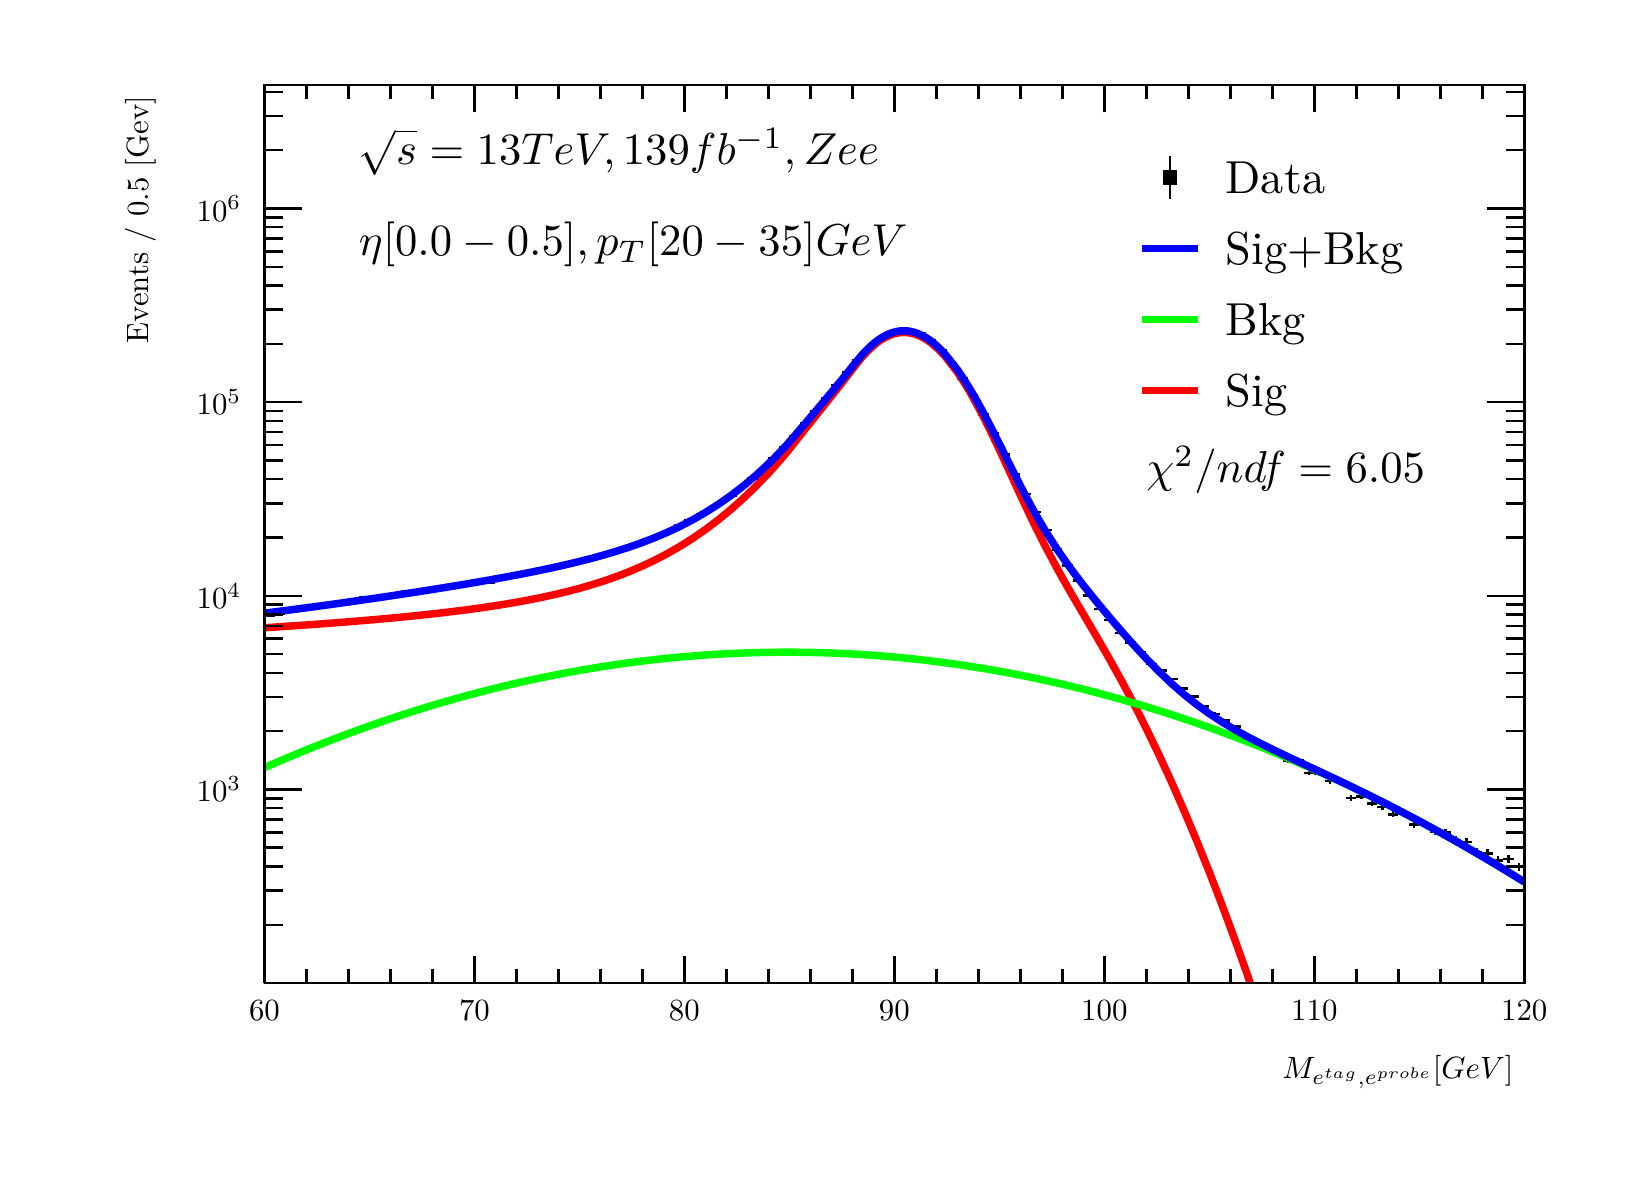
\begin{tikzpicture}
\pgfdeclareplotmark{cross} {
\pgfpathmoveto{\pgfpoint{-0.3\pgfplotmarksize}{\pgfplotmarksize}}
\pgfpathlineto{\pgfpoint{+0.3\pgfplotmarksize}{\pgfplotmarksize}}
\pgfpathlineto{\pgfpoint{+0.3\pgfplotmarksize}{0.3\pgfplotmarksize}}
\pgfpathlineto{\pgfpoint{+1\pgfplotmarksize}{0.3\pgfplotmarksize}}
\pgfpathlineto{\pgfpoint{+1\pgfplotmarksize}{-0.3\pgfplotmarksize}}
\pgfpathlineto{\pgfpoint{+0.3\pgfplotmarksize}{-0.3\pgfplotmarksize}}
\pgfpathlineto{\pgfpoint{+0.3\pgfplotmarksize}{-1.\pgfplotmarksize}}
\pgfpathlineto{\pgfpoint{-0.3\pgfplotmarksize}{-1.\pgfplotmarksize}}
\pgfpathlineto{\pgfpoint{-0.3\pgfplotmarksize}{-0.3\pgfplotmarksize}}
\pgfpathlineto{\pgfpoint{-1.\pgfplotmarksize}{-0.3\pgfplotmarksize}}
\pgfpathlineto{\pgfpoint{-1.\pgfplotmarksize}{0.3\pgfplotmarksize}}
\pgfpathlineto{\pgfpoint{-0.3\pgfplotmarksize}{0.3\pgfplotmarksize}}
\pgfpathclose
\pgfusepathqstroke
}
\pgfdeclareplotmark{cross*} {
\pgfpathmoveto{\pgfpoint{-0.3\pgfplotmarksize}{\pgfplotmarksize}}
\pgfpathlineto{\pgfpoint{+0.3\pgfplotmarksize}{\pgfplotmarksize}}
\pgfpathlineto{\pgfpoint{+0.3\pgfplotmarksize}{0.3\pgfplotmarksize}}
\pgfpathlineto{\pgfpoint{+1\pgfplotmarksize}{0.3\pgfplotmarksize}}
\pgfpathlineto{\pgfpoint{+1\pgfplotmarksize}{-0.3\pgfplotmarksize}}
\pgfpathlineto{\pgfpoint{+0.3\pgfplotmarksize}{-0.3\pgfplotmarksize}}
\pgfpathlineto{\pgfpoint{+0.3\pgfplotmarksize}{-1.\pgfplotmarksize}}
\pgfpathlineto{\pgfpoint{-0.3\pgfplotmarksize}{-1.\pgfplotmarksize}}
\pgfpathlineto{\pgfpoint{-0.3\pgfplotmarksize}{-0.3\pgfplotmarksize}}
\pgfpathlineto{\pgfpoint{-1.\pgfplotmarksize}{-0.3\pgfplotmarksize}}
\pgfpathlineto{\pgfpoint{-1.\pgfplotmarksize}{0.3\pgfplotmarksize}}
\pgfpathlineto{\pgfpoint{-0.3\pgfplotmarksize}{0.3\pgfplotmarksize}}
\pgfpathclose
\pgfusepathqfillstroke
}
\pgfdeclareplotmark{newstar} {
\pgfpathmoveto{\pgfqpoint{0pt}{\pgfplotmarksize}}
\pgfpathlineto{\pgfqpointpolar{44}{0.5\pgfplotmarksize}}
\pgfpathlineto{\pgfqpointpolar{18}{\pgfplotmarksize}}
\pgfpathlineto{\pgfqpointpolar{-20}{0.5\pgfplotmarksize}}
\pgfpathlineto{\pgfqpointpolar{-54}{\pgfplotmarksize}}
\pgfpathlineto{\pgfqpointpolar{-90}{0.5\pgfplotmarksize}}
\pgfpathlineto{\pgfqpointpolar{234}{\pgfplotmarksize}}
\pgfpathlineto{\pgfqpointpolar{198}{0.5\pgfplotmarksize}}
\pgfpathlineto{\pgfqpointpolar{162}{\pgfplotmarksize}}
\pgfpathlineto{\pgfqpointpolar{134}{0.5\pgfplotmarksize}}
\pgfpathclose
\pgfusepathqstroke
}
\pgfdeclareplotmark{newstar*} {
\pgfpathmoveto{\pgfqpoint{0pt}{\pgfplotmarksize}}
\pgfpathlineto{\pgfqpointpolar{44}{0.5\pgfplotmarksize}}
\pgfpathlineto{\pgfqpointpolar{18}{\pgfplotmarksize}}
\pgfpathlineto{\pgfqpointpolar{-20}{0.5\pgfplotmarksize}}
\pgfpathlineto{\pgfqpointpolar{-54}{\pgfplotmarksize}}
\pgfpathlineto{\pgfqpointpolar{-90}{0.5\pgfplotmarksize}}
\pgfpathlineto{\pgfqpointpolar{234}{\pgfplotmarksize}}
\pgfpathlineto{\pgfqpointpolar{198}{0.5\pgfplotmarksize}}
\pgfpathlineto{\pgfqpointpolar{162}{\pgfplotmarksize}}
\pgfpathlineto{\pgfqpointpolar{134}{0.5\pgfplotmarksize}}
\pgfpathclose
\pgfusepathqfillstroke
}
\definecolor{c}{rgb}{1,1,1};
\draw [color=c, fill=c] (0,0) rectangle (20,14.4361);
\draw [color=c, fill=c] (3,2.30977) rectangle (19,13.7143);
\definecolor{c}{rgb}{0,0,0};
\draw [c,line width=0.9] (3,2.30977) -- (3,13.7143) -- (19,13.7143) -- (19,2.30977) -- (3,2.30977);
\definecolor{c}{rgb}{1,1,1};
\draw [color=c, fill=c] (3,2.30977) rectangle (19,13.7143);
\definecolor{c}{rgb}{0,0,0};
\draw [c,line width=0.9] (3,2.30977) -- (3,13.7143) -- (19,13.7143) -- (19,2.30977) -- (3,2.30977);
\draw [c,line width=0.9] (3,2.30977) -- (19,2.30977);
\draw [c,line width=0.9] (3,2.65624) -- (3,2.30977);
\draw [c,line width=0.9] (3.53333,2.48301) -- (3.53333,2.30977);
\draw [c,line width=0.9] (4.06667,2.48301) -- (4.06667,2.30977);
\draw [c,line width=0.9] (4.6,2.48301) -- (4.6,2.30977);
\draw [c,line width=0.9] (5.13333,2.48301) -- (5.13333,2.30977);
\draw [c,line width=0.9] (5.66667,2.65624) -- (5.66667,2.30977);
\draw [c,line width=0.9] (6.2,2.48301) -- (6.2,2.30977);
\draw [c,line width=0.9] (6.73333,2.48301) -- (6.73333,2.30977);
\draw [c,line width=0.9] (7.26667,2.48301) -- (7.26667,2.30977);
\draw [c,line width=0.9] (7.8,2.48301) -- (7.8,2.30977);
\draw [c,line width=0.9] (8.33333,2.65624) -- (8.33333,2.30977);
\draw [c,line width=0.9] (8.86667,2.48301) -- (8.86667,2.30977);
\draw [c,line width=0.9] (9.4,2.48301) -- (9.4,2.30977);
\draw [c,line width=0.9] (9.93333,2.48301) -- (9.93333,2.30977);
\draw [c,line width=0.9] (10.4667,2.48301) -- (10.4667,2.30977);
\draw [c,line width=0.9] (11,2.65624) -- (11,2.30977);
\draw [c,line width=0.9] (11.5333,2.48301) -- (11.5333,2.30977);
\draw [c,line width=0.9] (12.0667,2.48301) -- (12.0667,2.30977);
\draw [c,line width=0.9] (12.6,2.48301) -- (12.6,2.30977);
\draw [c,line width=0.9] (13.1333,2.48301) -- (13.1333,2.30977);
\draw [c,line width=0.9] (13.6667,2.65624) -- (13.6667,2.30977);
\draw [c,line width=0.9] (14.2,2.48301) -- (14.2,2.30977);
\draw [c,line width=0.9] (14.7333,2.48301) -- (14.7333,2.30977);
\draw [c,line width=0.9] (15.2667,2.48301) -- (15.2667,2.30977);
\draw [c,line width=0.9] (15.8,2.48301) -- (15.8,2.30977);
\draw [c,line width=0.9] (16.3333,2.65624) -- (16.3333,2.30977);
\draw [c,line width=0.9] (16.8667,2.48301) -- (16.8667,2.30977);
\draw [c,line width=0.9] (17.4,2.48301) -- (17.4,2.30977);
\draw [c,line width=0.9] (17.9333,2.48301) -- (17.9333,2.30977);
\draw [c,line width=0.9] (18.4667,2.48301) -- (18.4667,2.30977);
\draw [c,line width=0.9] (19,2.65624) -- (19,2.30977);
\draw [anchor=base] (3,1.83338) node[scale=1.11327, color=c, rotate=0]{60};
\draw [anchor=base] (5.66667,1.83338) node[scale=1.11327, color=c, rotate=0]{70};
\draw [anchor=base] (8.33333,1.83338) node[scale=1.11327, color=c, rotate=0]{80};
\draw [anchor=base] (11,1.83338) node[scale=1.11327, color=c, rotate=0]{90};
\draw [anchor=base] (13.6667,1.83338) node[scale=1.11327, color=c, rotate=0]{100};
\draw [anchor=base] (16.3333,1.83338) node[scale=1.11327, color=c, rotate=0]{110};
\draw [anchor=base] (19,1.83338) node[scale=1.11327, color=c, rotate=0]{120};
\draw [anchor= east] (19,1.17798) node[scale=1.11327, color=c, rotate=0]{$M_{e^{tag}, e^{probe}}  [GeV]$};
\draw [c,line width=0.9] (3,13.7143) -- (19,13.7143);
\draw [c,line width=0.9] (3,13.3678) -- (3,13.7143);
\draw [c,line width=0.9] (3.53333,13.5411) -- (3.53333,13.7143);
\draw [c,line width=0.9] (4.06667,13.5411) -- (4.06667,13.7143);
\draw [c,line width=0.9] (4.6,13.5411) -- (4.6,13.7143);
\draw [c,line width=0.9] (5.13333,13.5411) -- (5.13333,13.7143);
\draw [c,line width=0.9] (5.66667,13.3678) -- (5.66667,13.7143);
\draw [c,line width=0.9] (6.2,13.5411) -- (6.2,13.7143);
\draw [c,line width=0.9] (6.73333,13.5411) -- (6.73333,13.7143);
\draw [c,line width=0.9] (7.26667,13.5411) -- (7.26667,13.7143);
\draw [c,line width=0.9] (7.8,13.5411) -- (7.8,13.7143);
\draw [c,line width=0.9] (8.33333,13.3678) -- (8.33333,13.7143);
\draw [c,line width=0.9] (8.86667,13.5411) -- (8.86667,13.7143);
\draw [c,line width=0.9] (9.4,13.5411) -- (9.4,13.7143);
\draw [c,line width=0.9] (9.93333,13.5411) -- (9.93333,13.7143);
\draw [c,line width=0.9] (10.4667,13.5411) -- (10.4667,13.7143);
\draw [c,line width=0.9] (11,13.3678) -- (11,13.7143);
\draw [c,line width=0.9] (11.5333,13.5411) -- (11.5333,13.7143);
\draw [c,line width=0.9] (12.0667,13.5411) -- (12.0667,13.7143);
\draw [c,line width=0.9] (12.6,13.5411) -- (12.6,13.7143);
\draw [c,line width=0.9] (13.1333,13.5411) -- (13.1333,13.7143);
\draw [c,line width=0.9] (13.6667,13.3678) -- (13.6667,13.7143);
\draw [c,line width=0.9] (14.2,13.5411) -- (14.2,13.7143);
\draw [c,line width=0.9] (14.7333,13.5411) -- (14.7333,13.7143);
\draw [c,line width=0.9] (15.2667,13.5411) -- (15.2667,13.7143);
\draw [c,line width=0.9] (15.8,13.5411) -- (15.8,13.7143);
\draw [c,line width=0.9] (16.3333,13.3678) -- (16.3333,13.7143);
\draw [c,line width=0.9] (16.8667,13.5411) -- (16.8667,13.7143);
\draw [c,line width=0.9] (17.4,13.5411) -- (17.4,13.7143);
\draw [c,line width=0.9] (17.9333,13.5411) -- (17.9333,13.7143);
\draw [c,line width=0.9] (18.4667,13.5411) -- (18.4667,13.7143);
\draw [c,line width=0.9] (19,13.3678) -- (19,13.7143);
\draw [c,line width=0.9] (3,2.30977) -- (3,13.7143);
\draw [c,line width=0.9] (3.237,3.05008) -- (3,3.05008);
\draw [c,line width=0.9] (3.237,3.48313) -- (3,3.48313);
\draw [c,line width=0.9] (3.237,3.79038) -- (3,3.79038);
\draw [c,line width=0.9] (3.237,4.02871) -- (3,4.02871);
\draw [c,line width=0.9] (3.237,4.22343) -- (3,4.22343);
\draw [c,line width=0.9] (3.237,4.38807) -- (3,4.38807);
\draw [c,line width=0.9] (3.237,4.53069) -- (3,4.53069);
\draw [c,line width=0.9] (3.237,4.65649) -- (3,4.65649);
\draw [c,line width=0.9] (3.474,4.76901) -- (3,4.76901);
\draw [anchor= east] (2.844,4.76901) node[scale=1.11327, color=c, rotate=0]{$10^{3}$};
\draw [c,line width=0.9] (3.237,5.50932) -- (3,5.50932);
\draw [c,line width=0.9] (3.237,5.94237) -- (3,5.94237);
\draw [c,line width=0.9] (3.237,6.24963) -- (3,6.24963);
\draw [c,line width=0.9] (3.237,6.48795) -- (3,6.48795);
\draw [c,line width=0.9] (3.237,6.68268) -- (3,6.68268);
\draw [c,line width=0.9] (3.237,6.84731) -- (3,6.84731);
\draw [c,line width=0.9] (3.237,6.98993) -- (3,6.98993);
\draw [c,line width=0.9] (3.237,7.11573) -- (3,7.11573);
\draw [c,line width=0.9] (3.474,7.22826) -- (3,7.22826);
\draw [anchor= east] (2.844,7.22826) node[scale=1.11327, color=c, rotate=0]{$10^{4}$};
\draw [c,line width=0.9] (3.237,7.96856) -- (3,7.96856);
\draw [c,line width=0.9] (3.237,8.40161) -- (3,8.40161);
\draw [c,line width=0.9] (3.237,8.70887) -- (3,8.70887);
\draw [c,line width=0.9] (3.237,8.94719) -- (3,8.94719);
\draw [c,line width=0.9] (3.237,9.14192) -- (3,9.14192);
\draw [c,line width=0.9] (3.237,9.30656) -- (3,9.30656);
\draw [c,line width=0.9] (3.237,9.44917) -- (3,9.44917);
\draw [c,line width=0.9] (3.237,9.57497) -- (3,9.57497);
\draw [c,line width=0.9] (3.474,9.6875) -- (3,9.6875);
\draw [anchor= east] (2.844,9.6875) node[scale=1.11327, color=c, rotate=0]{$10^{5}$};
\draw [c,line width=0.9] (3.237,10.4278) -- (3,10.4278);
\draw [c,line width=0.9] (3.237,10.8609) -- (3,10.8609);
\draw [c,line width=0.9] (3.237,11.1681) -- (3,11.1681);
\draw [c,line width=0.9] (3.237,11.4064) -- (3,11.4064);
\draw [c,line width=0.9] (3.237,11.6012) -- (3,11.6012);
\draw [c,line width=0.9] (3.237,11.7658) -- (3,11.7658);
\draw [c,line width=0.9] (3.237,11.9084) -- (3,11.9084);
\draw [c,line width=0.9] (3.237,12.0342) -- (3,12.0342);
\draw [c,line width=0.9] (3.474,12.1467) -- (3,12.1467);
\draw [anchor= east] (2.844,12.1467) node[scale=1.11327, color=c, rotate=0]{$10^{6}$};
\draw [c,line width=0.9] (3.237,12.887) -- (3,12.887);
\draw [c,line width=0.9] (3.237,13.3201) -- (3,13.3201);
\draw [c,line width=0.9] (3.237,13.6274) -- (3,13.6274);
\draw [anchor= east] (1.432,13.7143) node[scale=1.11327, color=c, rotate=90]{Events / 0.5 [Gev]};
\draw [c,line width=0.9] (19,2.30977) -- (19,13.7143);
\draw [c,line width=0.9] (18.763,3.05008) -- (19,3.05008);
\draw [c,line width=0.9] (18.763,3.48313) -- (19,3.48313);
\draw [c,line width=0.9] (18.763,3.79038) -- (19,3.79038);
\draw [c,line width=0.9] (18.763,4.02871) -- (19,4.02871);
\draw [c,line width=0.9] (18.763,4.22343) -- (19,4.22343);
\draw [c,line width=0.9] (18.763,4.38807) -- (19,4.38807);
\draw [c,line width=0.9] (18.763,4.53069) -- (19,4.53069);
\draw [c,line width=0.9] (18.763,4.65649) -- (19,4.65649);
\draw [c,line width=0.9] (18.526,4.76901) -- (19,4.76901);
\draw [c,line width=0.9] (18.763,5.50932) -- (19,5.50932);
\draw [c,line width=0.9] (18.763,5.94237) -- (19,5.94237);
\draw [c,line width=0.9] (18.763,6.24963) -- (19,6.24963);
\draw [c,line width=0.9] (18.763,6.48795) -- (19,6.48795);
\draw [c,line width=0.9] (18.763,6.68268) -- (19,6.68268);
\draw [c,line width=0.9] (18.763,6.84731) -- (19,6.84731);
\draw [c,line width=0.9] (18.763,6.98993) -- (19,6.98993);
\draw [c,line width=0.9] (18.763,7.11573) -- (19,7.11573);
\draw [c,line width=0.9] (18.526,7.22826) -- (19,7.22826);
\draw [c,line width=0.9] (18.763,7.96856) -- (19,7.96856);
\draw [c,line width=0.9] (18.763,8.40161) -- (19,8.40161);
\draw [c,line width=0.9] (18.763,8.70887) -- (19,8.70887);
\draw [c,line width=0.9] (18.763,8.94719) -- (19,8.94719);
\draw [c,line width=0.9] (18.763,9.14192) -- (19,9.14192);
\draw [c,line width=0.9] (18.763,9.30656) -- (19,9.30656);
\draw [c,line width=0.9] (18.763,9.44917) -- (19,9.44917);
\draw [c,line width=0.9] (18.763,9.57497) -- (19,9.57497);
\draw [c,line width=0.9] (18.526,9.6875) -- (19,9.6875);
\draw [c,line width=0.9] (18.763,10.4278) -- (19,10.4278);
\draw [c,line width=0.9] (18.763,10.8609) -- (19,10.8609);
\draw [c,line width=0.9] (18.763,11.1681) -- (19,11.1681);
\draw [c,line width=0.9] (18.763,11.4064) -- (19,11.4064);
\draw [c,line width=0.9] (18.763,11.6012) -- (19,11.6012);
\draw [c,line width=0.9] (18.763,11.7658) -- (19,11.7658);
\draw [c,line width=0.9] (18.763,11.9084) -- (19,11.9084);
\draw [c,line width=0.9] (18.763,12.0342) -- (19,12.0342);
\draw [c,line width=0.9] (18.526,12.1467) -- (19,12.1467);
\draw [c,line width=0.9] (18.763,12.887) -- (19,12.887);
\draw [c,line width=0.9] (18.763,13.3201) -- (19,13.3201);
\draw [c,line width=0.9] (18.763,13.6274) -- (19,13.6274);
\draw [c,line width=0.9] (3.06667,6.97555) -- (3,6.97555);
\draw [c,line width=0.9] (3,6.97555) -- (3,6.97555);
\draw [c,line width=0.9] (3.06667,6.97555) -- (3.13333,6.97555);
\draw [c,line width=0.9] (3.13333,6.97555) -- (3.13333,6.97555);
\draw [c,line width=0.9] (3.06667,6.97555) -- (3.06667,6.98757);
\draw [c,line width=0.9] (3.06667,6.98757) -- (3.06667,6.98757);
\draw [c,line width=0.9] (3.06667,6.97555) -- (3.06667,6.96353);
\draw [c,line width=0.9] (3.06667,6.96353) -- (3.06667,6.96353);
\draw [c,line width=0.9] (3.2,6.99897) -- (3.13333,6.99897);
\draw [c,line width=0.9] (3.13333,6.99897) -- (3.13333,6.99897);
\draw [c,line width=0.9] (3.2,6.99897) -- (3.26667,6.99897);
\draw [c,line width=0.9] (3.26667,6.99897) -- (3.26667,6.99897);
\draw [c,line width=0.9] (3.2,6.99897) -- (3.2,7.01086);
\draw [c,line width=0.9] (3.2,7.01086) -- (3.2,7.01086);
\draw [c,line width=0.9] (3.2,6.99897) -- (3.2,6.98708);
\draw [c,line width=0.9] (3.2,6.98708) -- (3.2,6.98708);
\draw [c,line width=0.9] (3.33333,7.05305) -- (3.26667,7.05305);
\draw [c,line width=0.9] (3.26667,7.05305) -- (3.26667,7.05305);
\draw [c,line width=0.9] (3.33333,7.05305) -- (3.4,7.05305);
\draw [c,line width=0.9] (3.4,7.05305) -- (3.4,7.05305);
\draw [c,line width=0.9] (3.33333,7.05305) -- (3.33333,7.06464);
\draw [c,line width=0.9] (3.33333,7.06464) -- (3.33333,7.06464);
\draw [c,line width=0.9] (3.33333,7.05305) -- (3.33333,7.04145);
\draw [c,line width=0.9] (3.33333,7.04145) -- (3.33333,7.04145);
\draw [c,line width=0.9] (3.46667,7.05619) -- (3.4,7.05619);
\draw [c,line width=0.9] (3.4,7.05619) -- (3.4,7.05619);
\draw [c,line width=0.9] (3.46667,7.05619) -- (3.53333,7.05619);
\draw [c,line width=0.9] (3.53333,7.05619) -- (3.53333,7.05619);
\draw [c,line width=0.9] (3.46667,7.05619) -- (3.46667,7.06776);
\draw [c,line width=0.9] (3.46667,7.06776) -- (3.46667,7.06776);
\draw [c,line width=0.9] (3.46667,7.05619) -- (3.46667,7.04461);
\draw [c,line width=0.9] (3.46667,7.04461) -- (3.46667,7.04461);
\draw [c,line width=0.9] (3.6,7.09403) -- (3.53333,7.09403);
\draw [c,line width=0.9] (3.53333,7.09403) -- (3.53333,7.09403);
\draw [c,line width=0.9] (3.6,7.09403) -- (3.66667,7.09403);
\draw [c,line width=0.9] (3.66667,7.09403) -- (3.66667,7.09403);
\draw [c,line width=0.9] (3.6,7.09403) -- (3.6,7.1054);
\draw [c,line width=0.9] (3.6,7.1054) -- (3.6,7.1054);
\draw [c,line width=0.9] (3.6,7.09403) -- (3.6,7.08266);
\draw [c,line width=0.9] (3.6,7.08266) -- (3.6,7.08266);
\draw [c,line width=0.9] (3.73333,7.12094) -- (3.66667,7.12094);
\draw [c,line width=0.9] (3.66667,7.12094) -- (3.66667,7.12094);
\draw [c,line width=0.9] (3.73333,7.12094) -- (3.8,7.12094);
\draw [c,line width=0.9] (3.8,7.12094) -- (3.8,7.12094);
\draw [c,line width=0.9] (3.73333,7.12094) -- (3.73333,7.13217);
\draw [c,line width=0.9] (3.73333,7.13217) -- (3.73333,7.13217);
\draw [c,line width=0.9] (3.73333,7.12094) -- (3.73333,7.10971);
\draw [c,line width=0.9] (3.73333,7.10971) -- (3.73333,7.10971);
\draw [c,line width=0.9] (3.86667,7.1328) -- (3.8,7.1328);
\draw [c,line width=0.9] (3.8,7.1328) -- (3.8,7.1328);
\draw [c,line width=0.9] (3.86667,7.1328) -- (3.93333,7.1328);
\draw [c,line width=0.9] (3.93333,7.1328) -- (3.93333,7.1328);
\draw [c,line width=0.9] (3.86667,7.1328) -- (3.86667,7.14397);
\draw [c,line width=0.9] (3.86667,7.14397) -- (3.86667,7.14397);
\draw [c,line width=0.9] (3.86667,7.1328) -- (3.86667,7.12163);
\draw [c,line width=0.9] (3.86667,7.12163) -- (3.86667,7.12163);
\draw [c,line width=0.9] (4,7.15407) -- (3.93333,7.15407);
\draw [c,line width=0.9] (3.93333,7.15407) -- (3.93333,7.15407);
\draw [c,line width=0.9] (4,7.15407) -- (4.06667,7.15407);
\draw [c,line width=0.9] (4.06667,7.15407) -- (4.06667,7.15407);
\draw [c,line width=0.9] (4,7.15407) -- (4,7.16513);
\draw [c,line width=0.9] (4,7.16513) -- (4,7.16513);
\draw [c,line width=0.9] (4,7.15407) -- (4,7.14302);
\draw [c,line width=0.9] (4,7.14302) -- (4,7.14302);
\draw [c,line width=0.9] (4.13333,7.18377) -- (4.06667,7.18377);
\draw [c,line width=0.9] (4.06667,7.18377) -- (4.06667,7.18377);
\draw [c,line width=0.9] (4.13333,7.18377) -- (4.2,7.18377);
\draw [c,line width=0.9] (4.2,7.18377) -- (4.2,7.18377);
\draw [c,line width=0.9] (4.13333,7.18377) -- (4.13333,7.19467);
\draw [c,line width=0.9] (4.13333,7.19467) -- (4.13333,7.19467);
\draw [c,line width=0.9] (4.13333,7.18377) -- (4.13333,7.17286);
\draw [c,line width=0.9] (4.13333,7.17286) -- (4.13333,7.17286);
\draw [c,line width=0.9] (4.26667,7.21439) -- (4.2,7.21439);
\draw [c,line width=0.9] (4.2,7.21439) -- (4.2,7.21439);
\draw [c,line width=0.9] (4.26667,7.21439) -- (4.33333,7.21439);
\draw [c,line width=0.9] (4.33333,7.21439) -- (4.33333,7.21439);
\draw [c,line width=0.9] (4.26667,7.21439) -- (4.26667,7.22514);
\draw [c,line width=0.9] (4.26667,7.22514) -- (4.26667,7.22514);
\draw [c,line width=0.9] (4.26667,7.21439) -- (4.26667,7.20364);
\draw [c,line width=0.9] (4.26667,7.20364) -- (4.26667,7.20364);
\draw [c,line width=0.9] (4.4,7.21114) -- (4.33333,7.21114);
\draw [c,line width=0.9] (4.33333,7.21114) -- (4.33333,7.21114);
\draw [c,line width=0.9] (4.4,7.21114) -- (4.46667,7.21114);
\draw [c,line width=0.9] (4.46667,7.21114) -- (4.46667,7.21114);
\draw [c,line width=0.9] (4.4,7.21114) -- (4.4,7.22191);
\draw [c,line width=0.9] (4.4,7.22191) -- (4.4,7.22191);
\draw [c,line width=0.9] (4.4,7.21114) -- (4.4,7.20037);
\draw [c,line width=0.9] (4.4,7.20037) -- (4.4,7.20037);
\draw [c,line width=0.9] (4.53333,7.21979) -- (4.46667,7.21979);
\draw [c,line width=0.9] (4.46667,7.21979) -- (4.46667,7.21979);
\draw [c,line width=0.9] (4.53333,7.21979) -- (4.6,7.21979);
\draw [c,line width=0.9] (4.6,7.21979) -- (4.6,7.21979);
\draw [c,line width=0.9] (4.53333,7.21979) -- (4.53333,7.23051);
\draw [c,line width=0.9] (4.53333,7.23051) -- (4.53333,7.23051);
\draw [c,line width=0.9] (4.53333,7.21979) -- (4.53333,7.20906);
\draw [c,line width=0.9] (4.53333,7.20906) -- (4.53333,7.20906);
\draw [c,line width=0.9] (4.66667,7.23878) -- (4.6,7.23878);
\draw [c,line width=0.9] (4.6,7.23878) -- (4.6,7.23878);
\draw [c,line width=0.9] (4.66667,7.23878) -- (4.73333,7.23878);
\draw [c,line width=0.9] (4.73333,7.23878) -- (4.73333,7.23878);
\draw [c,line width=0.9] (4.66667,7.23878) -- (4.66667,7.24941);
\draw [c,line width=0.9] (4.66667,7.24941) -- (4.66667,7.24941);
\draw [c,line width=0.9] (4.66667,7.23878) -- (4.66667,7.22815);
\draw [c,line width=0.9] (4.66667,7.22815) -- (4.66667,7.22815);
\draw [c,line width=0.9] (4.8,7.28756) -- (4.73333,7.28756);
\draw [c,line width=0.9] (4.73333,7.28756) -- (4.73333,7.28756);
\draw [c,line width=0.9] (4.8,7.28756) -- (4.86667,7.28756);
\draw [c,line width=0.9] (4.86667,7.28756) -- (4.86667,7.28756);
\draw [c,line width=0.9] (4.8,7.28756) -- (4.8,7.29795);
\draw [c,line width=0.9] (4.8,7.29795) -- (4.8,7.29795);
\draw [c,line width=0.9] (4.8,7.28756) -- (4.8,7.27718);
\draw [c,line width=0.9] (4.8,7.27718) -- (4.8,7.27718);
\draw [c,line width=0.9] (4.93333,7.27425) -- (4.86667,7.27425);
\draw [c,line width=0.9] (4.86667,7.27425) -- (4.86667,7.27425);
\draw [c,line width=0.9] (4.93333,7.27425) -- (5,7.27425);
\draw [c,line width=0.9] (5,7.27425) -- (5,7.27425);
\draw [c,line width=0.9] (4.93333,7.27425) -- (4.93333,7.2847);
\draw [c,line width=0.9] (4.93333,7.2847) -- (4.93333,7.2847);
\draw [c,line width=0.9] (4.93333,7.27425) -- (4.93333,7.26379);
\draw [c,line width=0.9] (4.93333,7.26379) -- (4.93333,7.26379);
\draw [c,line width=0.9] (5.06667,7.30986) -- (5,7.30986);
\draw [c,line width=0.9] (5,7.30986) -- (5,7.30986);
\draw [c,line width=0.9] (5.06667,7.30986) -- (5.13333,7.30986);
\draw [c,line width=0.9] (5.13333,7.30986) -- (5.13333,7.30986);
\draw [c,line width=0.9] (5.06667,7.30986) -- (5.06667,7.32014);
\draw [c,line width=0.9] (5.06667,7.32014) -- (5.06667,7.32014);
\draw [c,line width=0.9] (5.06667,7.30986) -- (5.06667,7.29958);
\draw [c,line width=0.9] (5.06667,7.29958) -- (5.06667,7.29958);
\draw [c,line width=0.9] (5.2,7.31065) -- (5.13333,7.31065);
\draw [c,line width=0.9] (5.13333,7.31065) -- (5.13333,7.31065);
\draw [c,line width=0.9] (5.2,7.31065) -- (5.26667,7.31065);
\draw [c,line width=0.9] (5.26667,7.31065) -- (5.26667,7.31065);
\draw [c,line width=0.9] (5.2,7.31065) -- (5.2,7.32093);
\draw [c,line width=0.9] (5.2,7.32093) -- (5.2,7.32093);
\draw [c,line width=0.9] (5.2,7.31065) -- (5.2,7.30038);
\draw [c,line width=0.9] (5.2,7.30038) -- (5.2,7.30038);
\draw [c,line width=0.9] (5.33333,7.34844) -- (5.26667,7.34844);
\draw [c,line width=0.9] (5.26667,7.34844) -- (5.26667,7.34844);
\draw [c,line width=0.9] (5.33333,7.34844) -- (5.4,7.34844);
\draw [c,line width=0.9] (5.4,7.34844) -- (5.4,7.34844);
\draw [c,line width=0.9] (5.33333,7.34844) -- (5.33333,7.35853);
\draw [c,line width=0.9] (5.33333,7.35853) -- (5.33333,7.35853);
\draw [c,line width=0.9] (5.33333,7.34844) -- (5.33333,7.33834);
\draw [c,line width=0.9] (5.33333,7.33834) -- (5.33333,7.33834);
\draw [c,line width=0.9] (5.46667,7.35358) -- (5.4,7.35358);
\draw [c,line width=0.9] (5.4,7.35358) -- (5.4,7.35358);
\draw [c,line width=0.9] (5.46667,7.35358) -- (5.53333,7.35358);
\draw [c,line width=0.9] (5.53333,7.35358) -- (5.53333,7.35358);
\draw [c,line width=0.9] (5.46667,7.35358) -- (5.46667,7.36365);
\draw [c,line width=0.9] (5.46667,7.36365) -- (5.46667,7.36365);
\draw [c,line width=0.9] (5.46667,7.35358) -- (5.46667,7.34351);
\draw [c,line width=0.9] (5.46667,7.34351) -- (5.46667,7.34351);
\draw [c,line width=0.9] (5.6,7.38401) -- (5.53333,7.38401);
\draw [c,line width=0.9] (5.53333,7.38401) -- (5.53333,7.38401);
\draw [c,line width=0.9] (5.6,7.38401) -- (5.66667,7.38401);
\draw [c,line width=0.9] (5.66667,7.38401) -- (5.66667,7.38401);
\draw [c,line width=0.9] (5.6,7.38401) -- (5.6,7.39394);
\draw [c,line width=0.9] (5.6,7.39394) -- (5.6,7.39394);
\draw [c,line width=0.9] (5.6,7.38401) -- (5.6,7.37408);
\draw [c,line width=0.9] (5.6,7.37408) -- (5.6,7.37408);
\draw [c,line width=0.9] (5.73333,7.39649) -- (5.66667,7.39649);
\draw [c,line width=0.9] (5.66667,7.39649) -- (5.66667,7.39649);
\draw [c,line width=0.9] (5.73333,7.39649) -- (5.8,7.39649);
\draw [c,line width=0.9] (5.8,7.39649) -- (5.8,7.39649);
\draw [c,line width=0.9] (5.73333,7.39649) -- (5.73333,7.40636);
\draw [c,line width=0.9] (5.73333,7.40636) -- (5.73333,7.40636);
\draw [c,line width=0.9] (5.73333,7.39649) -- (5.73333,7.38662);
\draw [c,line width=0.9] (5.73333,7.38662) -- (5.73333,7.38662);
\draw [c,line width=0.9] (5.86667,7.39722) -- (5.8,7.39722);
\draw [c,line width=0.9] (5.8,7.39722) -- (5.8,7.39722);
\draw [c,line width=0.9] (5.86667,7.39722) -- (5.93333,7.39722);
\draw [c,line width=0.9] (5.93333,7.39722) -- (5.93333,7.39722);
\draw [c,line width=0.9] (5.86667,7.39722) -- (5.86667,7.40709);
\draw [c,line width=0.9] (5.86667,7.40709) -- (5.86667,7.40709);
\draw [c,line width=0.9] (5.86667,7.39722) -- (5.86667,7.38735);
\draw [c,line width=0.9] (5.86667,7.38735) -- (5.86667,7.38735);
\draw [c,line width=0.9] (6,7.44378) -- (5.93333,7.44378);
\draw [c,line width=0.9] (5.93333,7.44378) -- (5.93333,7.44378);
\draw [c,line width=0.9] (6,7.44378) -- (6.06667,7.44378);
\draw [c,line width=0.9] (6.06667,7.44378) -- (6.06667,7.44378);
\draw [c,line width=0.9] (6,7.44378) -- (6,7.45344);
\draw [c,line width=0.9] (6,7.45344) -- (6,7.45344);
\draw [c,line width=0.9] (6,7.44378) -- (6,7.43413);
\draw [c,line width=0.9] (6,7.43413) -- (6,7.43413);
\draw [c,line width=0.9] (6.13333,7.45403) -- (6.06667,7.45403);
\draw [c,line width=0.9] (6.06667,7.45403) -- (6.06667,7.45403);
\draw [c,line width=0.9] (6.13333,7.45403) -- (6.2,7.45403);
\draw [c,line width=0.9] (6.2,7.45403) -- (6.2,7.45403);
\draw [c,line width=0.9] (6.13333,7.45403) -- (6.13333,7.46364);
\draw [c,line width=0.9] (6.13333,7.46364) -- (6.13333,7.46364);
\draw [c,line width=0.9] (6.13333,7.45403) -- (6.13333,7.44443);
\draw [c,line width=0.9] (6.13333,7.44443) -- (6.13333,7.44443);
\draw [c,line width=0.9] (6.26667,7.5008) -- (6.2,7.5008);
\draw [c,line width=0.9] (6.2,7.5008) -- (6.2,7.5008);
\draw [c,line width=0.9] (6.26667,7.5008) -- (6.33333,7.5008);
\draw [c,line width=0.9] (6.33333,7.5008) -- (6.33333,7.5008);
\draw [c,line width=0.9] (6.26667,7.5008) -- (6.26667,7.5102);
\draw [c,line width=0.9] (6.26667,7.5102) -- (6.26667,7.5102);
\draw [c,line width=0.9] (6.26667,7.5008) -- (6.26667,7.4914);
\draw [c,line width=0.9] (6.26667,7.4914) -- (6.26667,7.4914);
\draw [c,line width=0.9] (6.4,7.52162) -- (6.33333,7.52162);
\draw [c,line width=0.9] (6.33333,7.52162) -- (6.33333,7.52162);
\draw [c,line width=0.9] (6.4,7.52162) -- (6.46667,7.52162);
\draw [c,line width=0.9] (6.46667,7.52162) -- (6.46667,7.52162);
\draw [c,line width=0.9] (6.4,7.52162) -- (6.4,7.53093);
\draw [c,line width=0.9] (6.4,7.53093) -- (6.4,7.53093);
\draw [c,line width=0.9] (6.4,7.52162) -- (6.4,7.51231);
\draw [c,line width=0.9] (6.4,7.51231) -- (6.4,7.51231);
\draw [c,line width=0.9] (6.53333,7.54941) -- (6.46667,7.54941);
\draw [c,line width=0.9] (6.46667,7.54941) -- (6.46667,7.54941);
\draw [c,line width=0.9] (6.53333,7.54941) -- (6.6,7.54941);
\draw [c,line width=0.9] (6.6,7.54941) -- (6.6,7.54941);
\draw [c,line width=0.9] (6.53333,7.54941) -- (6.53333,7.5586);
\draw [c,line width=0.9] (6.53333,7.5586) -- (6.53333,7.5586);
\draw [c,line width=0.9] (6.53333,7.54941) -- (6.53333,7.54022);
\draw [c,line width=0.9] (6.53333,7.54022) -- (6.53333,7.54022);
\draw [c,line width=0.9] (6.66667,7.58211) -- (6.6,7.58211);
\draw [c,line width=0.9] (6.6,7.58211) -- (6.6,7.58211);
\draw [c,line width=0.9] (6.66667,7.58211) -- (6.73333,7.58211);
\draw [c,line width=0.9] (6.73333,7.58211) -- (6.73333,7.58211);
\draw [c,line width=0.9] (6.66667,7.58211) -- (6.66667,7.59116);
\draw [c,line width=0.9] (6.66667,7.59116) -- (6.66667,7.59116);
\draw [c,line width=0.9] (6.66667,7.58211) -- (6.66667,7.57306);
\draw [c,line width=0.9] (6.66667,7.57306) -- (6.66667,7.57306);
\draw [c,line width=0.9] (6.8,7.61094) -- (6.73333,7.61094);
\draw [c,line width=0.9] (6.73333,7.61094) -- (6.73333,7.61094);
\draw [c,line width=0.9] (6.8,7.61094) -- (6.86667,7.61094);
\draw [c,line width=0.9] (6.86667,7.61094) -- (6.86667,7.61094);
\draw [c,line width=0.9] (6.8,7.61094) -- (6.8,7.61987);
\draw [c,line width=0.9] (6.8,7.61987) -- (6.8,7.61987);
\draw [c,line width=0.9] (6.8,7.61094) -- (6.8,7.60201);
\draw [c,line width=0.9] (6.8,7.60201) -- (6.8,7.60201);
\draw [c,line width=0.9] (6.93333,7.6331) -- (6.86667,7.6331);
\draw [c,line width=0.9] (6.86667,7.6331) -- (6.86667,7.6331);
\draw [c,line width=0.9] (6.93333,7.6331) -- (7,7.6331);
\draw [c,line width=0.9] (7,7.6331) -- (7,7.6331);
\draw [c,line width=0.9] (6.93333,7.6331) -- (6.93333,7.64194);
\draw [c,line width=0.9] (6.93333,7.64194) -- (6.93333,7.64194);
\draw [c,line width=0.9] (6.93333,7.6331) -- (6.93333,7.62426);
\draw [c,line width=0.9] (6.93333,7.62426) -- (6.93333,7.62426);
\draw [c,line width=0.9] (7.06667,7.66734) -- (7,7.66734);
\draw [c,line width=0.9] (7,7.66734) -- (7,7.66734);
\draw [c,line width=0.9] (7.06667,7.66734) -- (7.13333,7.66734);
\draw [c,line width=0.9] (7.13333,7.66734) -- (7.13333,7.66734);
\draw [c,line width=0.9] (7.06667,7.66734) -- (7.06667,7.67604);
\draw [c,line width=0.9] (7.06667,7.67604) -- (7.06667,7.67604);
\draw [c,line width=0.9] (7.06667,7.66734) -- (7.06667,7.65865);
\draw [c,line width=0.9] (7.06667,7.65865) -- (7.06667,7.65865);
\draw [c,line width=0.9] (7.2,7.71829) -- (7.13333,7.71829);
\draw [c,line width=0.9] (7.13333,7.71829) -- (7.13333,7.71829);
\draw [c,line width=0.9] (7.2,7.71829) -- (7.26667,7.71829);
\draw [c,line width=0.9] (7.26667,7.71829) -- (7.26667,7.71829);
\draw [c,line width=0.9] (7.2,7.71829) -- (7.2,7.72678);
\draw [c,line width=0.9] (7.2,7.72678) -- (7.2,7.72678);
\draw [c,line width=0.9] (7.2,7.71829) -- (7.2,7.7098);
\draw [c,line width=0.9] (7.2,7.7098) -- (7.2,7.7098);
\draw [c,line width=0.9] (7.33333,7.73961) -- (7.26667,7.73961);
\draw [c,line width=0.9] (7.26667,7.73961) -- (7.26667,7.73961);
\draw [c,line width=0.9] (7.33333,7.73961) -- (7.4,7.73961);
\draw [c,line width=0.9] (7.4,7.73961) -- (7.4,7.73961);
\draw [c,line width=0.9] (7.33333,7.73961) -- (7.33333,7.74801);
\draw [c,line width=0.9] (7.33333,7.74801) -- (7.33333,7.74801);
\draw [c,line width=0.9] (7.33333,7.73961) -- (7.33333,7.7312);
\draw [c,line width=0.9] (7.33333,7.7312) -- (7.33333,7.7312);
\draw [c,line width=0.9] (7.46667,7.78235) -- (7.4,7.78235);
\draw [c,line width=0.9] (7.4,7.78235) -- (7.4,7.78235);
\draw [c,line width=0.9] (7.46667,7.78235) -- (7.53333,7.78235);
\draw [c,line width=0.9] (7.53333,7.78235) -- (7.53333,7.78235);
\draw [c,line width=0.9] (7.46667,7.78235) -- (7.46667,7.79059);
\draw [c,line width=0.9] (7.46667,7.79059) -- (7.46667,7.79059);
\draw [c,line width=0.9] (7.46667,7.78235) -- (7.46667,7.77411);
\draw [c,line width=0.9] (7.46667,7.77411) -- (7.46667,7.77411);
\draw [c,line width=0.9] (7.6,7.83343) -- (7.53333,7.83343);
\draw [c,line width=0.9] (7.53333,7.83343) -- (7.53333,7.83343);
\draw [c,line width=0.9] (7.6,7.83343) -- (7.66667,7.83343);
\draw [c,line width=0.9] (7.66667,7.83343) -- (7.66667,7.83343);
\draw [c,line width=0.9] (7.6,7.83343) -- (7.6,7.84147);
\draw [c,line width=0.9] (7.6,7.84147) -- (7.6,7.84147);
\draw [c,line width=0.9] (7.6,7.83343) -- (7.6,7.82538);
\draw [c,line width=0.9] (7.6,7.82538) -- (7.6,7.82538);
\draw [c,line width=0.9] (7.73333,7.89025) -- (7.66667,7.89025);
\draw [c,line width=0.9] (7.66667,7.89025) -- (7.66667,7.89025);
\draw [c,line width=0.9] (7.73333,7.89025) -- (7.8,7.89025);
\draw [c,line width=0.9] (7.8,7.89025) -- (7.8,7.89025);
\draw [c,line width=0.9] (7.73333,7.89025) -- (7.73333,7.89808);
\draw [c,line width=0.9] (7.73333,7.89808) -- (7.73333,7.89808);
\draw [c,line width=0.9] (7.73333,7.89025) -- (7.73333,7.88242);
\draw [c,line width=0.9] (7.73333,7.88242) -- (7.73333,7.88242);
\draw [c,line width=0.9] (7.86667,7.94824) -- (7.8,7.94824);
\draw [c,line width=0.9] (7.8,7.94824) -- (7.8,7.94824);
\draw [c,line width=0.9] (7.86667,7.94824) -- (7.93333,7.94824);
\draw [c,line width=0.9] (7.93333,7.94824) -- (7.93333,7.94824);
\draw [c,line width=0.9] (7.86667,7.94824) -- (7.86667,7.95586);
\draw [c,line width=0.9] (7.86667,7.95586) -- (7.86667,7.95586);
\draw [c,line width=0.9] (7.86667,7.94824) -- (7.86667,7.94061);
\draw [c,line width=0.9] (7.86667,7.94061) -- (7.86667,7.94061);
\draw [c,line width=0.9] (8,7.99107) -- (7.93333,7.99107);
\draw [c,line width=0.9] (7.93333,7.99107) -- (7.93333,7.99107);
\draw [c,line width=0.9] (8,7.99107) -- (8.06667,7.99107);
\draw [c,line width=0.9] (8.06667,7.99107) -- (8.06667,7.99107);
\draw [c,line width=0.9] (8,7.99107) -- (8,7.99855);
\draw [c,line width=0.9] (8,7.99855) -- (8,7.99855);
\draw [c,line width=0.9] (8,7.99107) -- (8,7.9836);
\draw [c,line width=0.9] (8,7.9836) -- (8,7.9836);
\draw [c,line width=0.9] (8.13333,8.04883) -- (8.06667,8.04883);
\draw [c,line width=0.9] (8.06667,8.04883) -- (8.06667,8.04883);
\draw [c,line width=0.9] (8.13333,8.04883) -- (8.2,8.04883);
\draw [c,line width=0.9] (8.2,8.04883) -- (8.2,8.04883);
\draw [c,line width=0.9] (8.13333,8.04883) -- (8.13333,8.0561);
\draw [c,line width=0.9] (8.13333,8.0561) -- (8.13333,8.0561);
\draw [c,line width=0.9] (8.13333,8.04883) -- (8.13333,8.04156);
\draw [c,line width=0.9] (8.13333,8.04156) -- (8.13333,8.04156);
\draw [c,line width=0.9] (8.26667,8.11821) -- (8.2,8.11821);
\draw [c,line width=0.9] (8.2,8.11821) -- (8.2,8.11821);
\draw [c,line width=0.9] (8.26667,8.11821) -- (8.33333,8.11821);
\draw [c,line width=0.9] (8.33333,8.11821) -- (8.33333,8.11821);
\draw [c,line width=0.9] (8.26667,8.11821) -- (8.26667,8.12525);
\draw [c,line width=0.9] (8.26667,8.12525) -- (8.26667,8.12525);
\draw [c,line width=0.9] (8.26667,8.11821) -- (8.26667,8.11116);
\draw [c,line width=0.9] (8.26667,8.11116) -- (8.26667,8.11116);
\draw [c,line width=0.9] (8.4,8.18278) -- (8.33333,8.18278);
\draw [c,line width=0.9] (8.33333,8.18278) -- (8.33333,8.18278);
\draw [c,line width=0.9] (8.4,8.18278) -- (8.46667,8.18278);
\draw [c,line width=0.9] (8.46667,8.18278) -- (8.46667,8.18278);
\draw [c,line width=0.9] (8.4,8.18278) -- (8.4,8.18961);
\draw [c,line width=0.9] (8.4,8.18961) -- (8.4,8.18961);
\draw [c,line width=0.9] (8.4,8.18278) -- (8.4,8.17595);
\draw [c,line width=0.9] (8.4,8.17595) -- (8.4,8.17595);
\draw [c,line width=0.9] (8.53333,8.25148) -- (8.46667,8.25148);
\draw [c,line width=0.9] (8.46667,8.25148) -- (8.46667,8.25148);
\draw [c,line width=0.9] (8.53333,8.25148) -- (8.6,8.25148);
\draw [c,line width=0.9] (8.6,8.25148) -- (8.6,8.25148);
\draw [c,line width=0.9] (8.53333,8.25148) -- (8.53333,8.2581);
\draw [c,line width=0.9] (8.53333,8.2581) -- (8.53333,8.2581);
\draw [c,line width=0.9] (8.53333,8.25148) -- (8.53333,8.24487);
\draw [c,line width=0.9] (8.53333,8.24487) -- (8.53333,8.24487);
\draw [c,line width=0.9] (8.66667,8.3296) -- (8.6,8.3296);
\draw [c,line width=0.9] (8.6,8.3296) -- (8.6,8.3296);
\draw [c,line width=0.9] (8.66667,8.3296) -- (8.73333,8.3296);
\draw [c,line width=0.9] (8.73333,8.3296) -- (8.73333,8.3296);
\draw [c,line width=0.9] (8.66667,8.3296) -- (8.66667,8.33598);
\draw [c,line width=0.9] (8.66667,8.33598) -- (8.66667,8.33598);
\draw [c,line width=0.9] (8.66667,8.3296) -- (8.66667,8.32323);
\draw [c,line width=0.9] (8.66667,8.32323) -- (8.66667,8.32323);
\draw [c,line width=0.9] (8.8,8.41062) -- (8.73333,8.41062);
\draw [c,line width=0.9] (8.73333,8.41062) -- (8.73333,8.41062);
\draw [c,line width=0.9] (8.8,8.41062) -- (8.86667,8.41062);
\draw [c,line width=0.9] (8.86667,8.41062) -- (8.86667,8.41062);
\draw [c,line width=0.9] (8.8,8.41062) -- (8.8,8.41676);
\draw [c,line width=0.9] (8.8,8.41676) -- (8.8,8.41676);
\draw [c,line width=0.9] (8.8,8.41062) -- (8.8,8.40448);
\draw [c,line width=0.9] (8.8,8.40448) -- (8.8,8.40448);
\draw [c,line width=0.9] (8.93333,8.50328) -- (8.86667,8.50328);
\draw [c,line width=0.9] (8.86667,8.50328) -- (8.86667,8.50328);
\draw [c,line width=0.9] (8.93333,8.50328) -- (9,8.50328);
\draw [c,line width=0.9] (9,8.50328) -- (9,8.50328);
\draw [c,line width=0.9] (8.93333,8.50328) -- (8.93333,8.50916);
\draw [c,line width=0.9] (8.93333,8.50916) -- (8.93333,8.50916);
\draw [c,line width=0.9] (8.93333,8.50328) -- (8.93333,8.4974);
\draw [c,line width=0.9] (8.93333,8.4974) -- (8.93333,8.4974);
\draw [c,line width=0.9] (9.06667,8.60958) -- (9,8.60958);
\draw [c,line width=0.9] (9,8.60958) -- (9,8.60958);
\draw [c,line width=0.9] (9.06667,8.60958) -- (9.13333,8.60958);
\draw [c,line width=0.9] (9.13333,8.60958) -- (9.13333,8.60958);
\draw [c,line width=0.9] (9.06667,8.60958) -- (9.06667,8.61517);
\draw [c,line width=0.9] (9.06667,8.61517) -- (9.06667,8.61517);
\draw [c,line width=0.9] (9.06667,8.60958) -- (9.06667,8.60398);
\draw [c,line width=0.9] (9.06667,8.60398) -- (9.06667,8.60398);
\draw [c,line width=0.9] (9.2,8.71741) -- (9.13333,8.71741);
\draw [c,line width=0.9] (9.13333,8.71741) -- (9.13333,8.71741);
\draw [c,line width=0.9] (9.2,8.71741) -- (9.26667,8.71741);
\draw [c,line width=0.9] (9.26667,8.71741) -- (9.26667,8.71741);
\draw [c,line width=0.9] (9.2,8.71741) -- (9.2,8.72272);
\draw [c,line width=0.9] (9.2,8.72272) -- (9.2,8.72272);
\draw [c,line width=0.9] (9.2,8.71741) -- (9.2,8.71209);
\draw [c,line width=0.9] (9.2,8.71209) -- (9.2,8.71209);
\draw [c,line width=0.9] (9.33333,8.83352) -- (9.26667,8.83352);
\draw [c,line width=0.9] (9.26667,8.83352) -- (9.26667,8.83352);
\draw [c,line width=0.9] (9.33333,8.83352) -- (9.4,8.83352);
\draw [c,line width=0.9] (9.4,8.83352) -- (9.4,8.83352);
\draw [c,line width=0.9] (9.33333,8.83352) -- (9.33333,8.83856);
\draw [c,line width=0.9] (9.33333,8.83856) -- (9.33333,8.83856);
\draw [c,line width=0.9] (9.33333,8.83352) -- (9.33333,8.82849);
\draw [c,line width=0.9] (9.33333,8.82849) -- (9.33333,8.82849);
\draw [c,line width=0.9] (9.46667,8.97016) -- (9.4,8.97016);
\draw [c,line width=0.9] (9.4,8.97016) -- (9.4,8.97016);
\draw [c,line width=0.9] (9.46667,8.97016) -- (9.53333,8.97016);
\draw [c,line width=0.9] (9.53333,8.97016) -- (9.53333,8.97016);
\draw [c,line width=0.9] (9.46667,8.97016) -- (9.46667,8.97489);
\draw [c,line width=0.9] (9.46667,8.97489) -- (9.46667,8.97489);
\draw [c,line width=0.9] (9.46667,8.97016) -- (9.46667,8.96544);
\draw [c,line width=0.9] (9.46667,8.96544) -- (9.46667,8.96544);
\draw [c,line width=0.9] (9.6,9.10987) -- (9.53333,9.10987);
\draw [c,line width=0.9] (9.53333,9.10987) -- (9.53333,9.10987);
\draw [c,line width=0.9] (9.6,9.10987) -- (9.66667,9.10987);
\draw [c,line width=0.9] (9.66667,9.10987) -- (9.66667,9.10987);
\draw [c,line width=0.9] (9.6,9.10987) -- (9.6,9.11429);
\draw [c,line width=0.9] (9.6,9.11429) -- (9.6,9.11429);
\draw [c,line width=0.9] (9.6,9.10987) -- (9.6,9.10544);
\draw [c,line width=0.9] (9.6,9.10544) -- (9.6,9.10544);
\draw [c,line width=0.9] (9.73333,9.25465) -- (9.66667,9.25465);
\draw [c,line width=0.9] (9.66667,9.25465) -- (9.66667,9.25465);
\draw [c,line width=0.9] (9.73333,9.25465) -- (9.8,9.25465);
\draw [c,line width=0.9] (9.8,9.25465) -- (9.8,9.25465);
\draw [c,line width=0.9] (9.73333,9.25465) -- (9.73333,9.25878);
\draw [c,line width=0.9] (9.73333,9.25878) -- (9.73333,9.25878);
\draw [c,line width=0.9] (9.73333,9.25465) -- (9.73333,9.25051);
\draw [c,line width=0.9] (9.73333,9.25051) -- (9.73333,9.25051);
\draw [c,line width=0.9] (9.86667,9.41402) -- (9.8,9.41402);
\draw [c,line width=0.9] (9.8,9.41402) -- (9.8,9.41402);
\draw [c,line width=0.9] (9.86667,9.41402) -- (9.93333,9.41402);
\draw [c,line width=0.9] (9.93333,9.41402) -- (9.93333,9.41402);
\draw [c,line width=0.9] (9.86667,9.41402) -- (9.86667,9.41786);
\draw [c,line width=0.9] (9.86667,9.41786) -- (9.86667,9.41786);
\draw [c,line width=0.9] (9.86667,9.41402) -- (9.86667,9.41018);
\draw [c,line width=0.9] (9.86667,9.41018) -- (9.86667,9.41018);
\draw [c,line width=0.9] (10,9.57757) -- (9.93333,9.57757);
\draw [c,line width=0.9] (9.93333,9.57757) -- (9.93333,9.57757);
\draw [c,line width=0.9] (10,9.57757) -- (10.0667,9.57757);
\draw [c,line width=0.9] (10.0667,9.57757) -- (10.0667,9.57757);
\draw [c,line width=0.9] (10,9.57757) -- (10,9.58112);
\draw [c,line width=0.9] (10,9.58112) -- (10,9.58112);
\draw [c,line width=0.9] (10,9.57757) -- (10,9.57401);
\draw [c,line width=0.9] (10,9.57401) -- (10,9.57401);
\draw [c,line width=0.9] (10.1333,9.74181) -- (10.0667,9.74181);
\draw [c,line width=0.9] (10.0667,9.74181) -- (10.0667,9.74181);
\draw [c,line width=0.9] (10.1333,9.74181) -- (10.2,9.74181);
\draw [c,line width=0.9] (10.2,9.74181) -- (10.2,9.74181);
\draw [c,line width=0.9] (10.1333,9.74181) -- (10.1333,9.74511);
\draw [c,line width=0.9] (10.1333,9.74511) -- (10.1333,9.74511);
\draw [c,line width=0.9] (10.1333,9.74181) -- (10.1333,9.73852);
\draw [c,line width=0.9] (10.1333,9.73852) -- (10.1333,9.73852);
\draw [c,line width=0.9] (10.2667,9.90267) -- (10.2,9.90267);
\draw [c,line width=0.9] (10.2,9.90267) -- (10.2,9.90267);
\draw [c,line width=0.9] (10.2667,9.90267) -- (10.3333,9.90267);
\draw [c,line width=0.9] (10.3333,9.90267) -- (10.3333,9.90267);
\draw [c,line width=0.9] (10.2667,9.90267) -- (10.2667,9.90572);
\draw [c,line width=0.9] (10.2667,9.90572) -- (10.2667,9.90572);
\draw [c,line width=0.9] (10.2667,9.90267) -- (10.2667,9.89961);
\draw [c,line width=0.9] (10.2667,9.89961) -- (10.2667,9.89961);
\draw [c,line width=0.9] (10.4,10.0673) -- (10.3333,10.0673);
\draw [c,line width=0.9] (10.3333,10.0673) -- (10.3333,10.0673);
\draw [c,line width=0.9] (10.4,10.0673) -- (10.4667,10.0673);
\draw [c,line width=0.9] (10.4667,10.0673) -- (10.4667,10.0673);
\draw [c,line width=0.9] (10.4,10.0673) -- (10.4,10.0701);
\draw [c,line width=0.9] (10.4,10.0701) -- (10.4,10.0701);
\draw [c,line width=0.9] (10.4,10.0673) -- (10.4,10.0645);
\draw [c,line width=0.9] (10.4,10.0645) -- (10.4,10.0645);
\draw [c,line width=0.9] (10.5333,10.217) -- (10.4667,10.217);
\draw [c,line width=0.9] (10.4667,10.217) -- (10.4667,10.217);
\draw [c,line width=0.9] (10.5333,10.217) -- (10.6,10.217);
\draw [c,line width=0.9] (10.6,10.217) -- (10.6,10.217);
\draw [c,line width=0.9] (10.5333,10.217) -- (10.5333,10.2197);
\draw [c,line width=0.9] (10.5333,10.2197) -- (10.5333,10.2197);
\draw [c,line width=0.9] (10.5333,10.217) -- (10.5333,10.2144);
\draw [c,line width=0.9] (10.5333,10.2144) -- (10.5333,10.2144);
\draw [c,line width=0.9] (10.6667,10.3535) -- (10.6,10.3535);
\draw [c,line width=0.9] (10.6,10.3535) -- (10.6,10.3535);
\draw [c,line width=0.9] (10.6667,10.3535) -- (10.7333,10.3535);
\draw [c,line width=0.9] (10.7333,10.3535) -- (10.7333,10.3535);
\draw [c,line width=0.9] (10.6667,10.3535) -- (10.6667,10.356);
\draw [c,line width=0.9] (10.6667,10.356) -- (10.6667,10.356);
\draw [c,line width=0.9] (10.6667,10.3535) -- (10.6667,10.351);
\draw [c,line width=0.9] (10.6667,10.351) -- (10.6667,10.351);
\draw [c,line width=0.9] (10.8,10.4675) -- (10.7333,10.4675);
\draw [c,line width=0.9] (10.7333,10.4675) -- (10.7333,10.4675);
\draw [c,line width=0.9] (10.8,10.4675) -- (10.8667,10.4675);
\draw [c,line width=0.9] (10.8667,10.4675) -- (10.8667,10.4675);
\draw [c,line width=0.9] (10.8,10.4675) -- (10.8,10.4698);
\draw [c,line width=0.9] (10.8,10.4698) -- (10.8,10.4698);
\draw [c,line width=0.9] (10.8,10.4675) -- (10.8,10.4652);
\draw [c,line width=0.9] (10.8,10.4652) -- (10.8,10.4652);
\draw [c,line width=0.9] (10.9333,10.546) -- (10.8667,10.546);
\draw [c,line width=0.9] (10.8667,10.546) -- (10.8667,10.546);
\draw [c,line width=0.9] (10.9333,10.546) -- (11,10.546);
\draw [c,line width=0.9] (11,10.546) -- (11,10.546);
\draw [c,line width=0.9] (10.9333,10.546) -- (10.9333,10.5482);
\draw [c,line width=0.9] (10.9333,10.5482) -- (10.9333,10.5482);
\draw [c,line width=0.9] (10.9333,10.546) -- (10.9333,10.5437);
\draw [c,line width=0.9] (10.9333,10.5437) -- (10.9333,10.5437);
\draw [c,line width=0.9] (11.0667,10.5926) -- (11,10.5926);
\draw [c,line width=0.9] (11,10.5926) -- (11,10.5926);
\draw [c,line width=0.9] (11.0667,10.5926) -- (11.1333,10.5926);
\draw [c,line width=0.9] (11.1333,10.5926) -- (11.1333,10.5926);
\draw [c,line width=0.9] (11.0667,10.5926) -- (11.0667,10.5948);
\draw [c,line width=0.9] (11.0667,10.5948) -- (11.0667,10.5948);
\draw [c,line width=0.9] (11.0667,10.5926) -- (11.0667,10.5904);
\draw [c,line width=0.9] (11.0667,10.5904) -- (11.0667,10.5904);
\draw [c,line width=0.9] (11.2,10.6009) -- (11.1333,10.6009);
\draw [c,line width=0.9] (11.1333,10.6009) -- (11.1333,10.6009);
\draw [c,line width=0.9] (11.2,10.6009) -- (11.2667,10.6009);
\draw [c,line width=0.9] (11.2667,10.6009) -- (11.2667,10.6009);
\draw [c,line width=0.9] (11.2,10.6009) -- (11.2,10.6031);
\draw [c,line width=0.9] (11.2,10.6031) -- (11.2,10.6031);
\draw [c,line width=0.9] (11.2,10.6009) -- (11.2,10.5987);
\draw [c,line width=0.9] (11.2,10.5987) -- (11.2,10.5987);
\draw [c,line width=0.9] (11.3333,10.5575) -- (11.2667,10.5575);
\draw [c,line width=0.9] (11.2667,10.5575) -- (11.2667,10.5575);
\draw [c,line width=0.9] (11.3333,10.5575) -- (11.4,10.5575);
\draw [c,line width=0.9] (11.4,10.5575) -- (11.4,10.5575);
\draw [c,line width=0.9] (11.3333,10.5575) -- (11.3333,10.5597);
\draw [c,line width=0.9] (11.3333,10.5597) -- (11.3333,10.5597);
\draw [c,line width=0.9] (11.3333,10.5575) -- (11.3333,10.5552);
\draw [c,line width=0.9] (11.3333,10.5552) -- (11.3333,10.5552);
\draw [c,line width=0.9] (11.4667,10.4745) -- (11.4,10.4745);
\draw [c,line width=0.9] (11.4,10.4745) -- (11.4,10.4745);
\draw [c,line width=0.9] (11.4667,10.4745) -- (11.5333,10.4745);
\draw [c,line width=0.9] (11.5333,10.4745) -- (11.5333,10.4745);
\draw [c,line width=0.9] (11.4667,10.4745) -- (11.4667,10.4768);
\draw [c,line width=0.9] (11.4667,10.4768) -- (11.4667,10.4768);
\draw [c,line width=0.9] (11.4667,10.4745) -- (11.4667,10.4721);
\draw [c,line width=0.9] (11.4667,10.4721) -- (11.4667,10.4721);
\draw [c,line width=0.9] (11.6,10.348) -- (11.5333,10.348);
\draw [c,line width=0.9] (11.5333,10.348) -- (11.5333,10.348);
\draw [c,line width=0.9] (11.6,10.348) -- (11.6667,10.348);
\draw [c,line width=0.9] (11.6667,10.348) -- (11.6667,10.348);
\draw [c,line width=0.9] (11.6,10.348) -- (11.6,10.3505);
\draw [c,line width=0.9] (11.6,10.3505) -- (11.6,10.3505);
\draw [c,line width=0.9] (11.6,10.348) -- (11.6,10.3456);
\draw [c,line width=0.9] (11.6,10.3456) -- (11.6,10.3456);
\draw [c,line width=0.9] (11.7333,10.1848) -- (11.6667,10.1848);
\draw [c,line width=0.9] (11.6667,10.1848) -- (11.6667,10.1848);
\draw [c,line width=0.9] (11.7333,10.1848) -- (11.8,10.1848);
\draw [c,line width=0.9] (11.8,10.1848) -- (11.8,10.1848);
\draw [c,line width=0.9] (11.7333,10.1848) -- (11.7333,10.1875);
\draw [c,line width=0.9] (11.7333,10.1875) -- (11.7333,10.1875);
\draw [c,line width=0.9] (11.7333,10.1848) -- (11.7333,10.1821);
\draw [c,line width=0.9] (11.7333,10.1821) -- (11.7333,10.1821);
\draw [c,line width=0.9] (11.8667,9.9901) -- (11.8,9.9901);
\draw [c,line width=0.9] (11.8,9.9901) -- (11.8,9.9901);
\draw [c,line width=0.9] (11.8667,9.9901) -- (11.9333,9.9901);
\draw [c,line width=0.9] (11.9333,9.9901) -- (11.9333,9.9901);
\draw [c,line width=0.9] (11.8667,9.9901) -- (11.8667,9.99303);
\draw [c,line width=0.9] (11.8667,9.99303) -- (11.8667,9.99303);
\draw [c,line width=0.9] (11.8667,9.9901) -- (11.8667,9.98717);
\draw [c,line width=0.9] (11.8667,9.98717) -- (11.8667,9.98717);
\draw [c,line width=0.9] (12,9.7739) -- (11.9333,9.7739);
\draw [c,line width=0.9] (11.9333,9.7739) -- (11.9333,9.7739);
\draw [c,line width=0.9] (12,9.7739) -- (12.0667,9.7739);
\draw [c,line width=0.9] (12.0667,9.7739) -- (12.0667,9.7739);
\draw [c,line width=0.9] (12,9.7739) -- (12,9.77714);
\draw [c,line width=0.9] (12,9.77714) -- (12,9.77714);
\draw [c,line width=0.9] (12,9.7739) -- (12,9.77066);
\draw [c,line width=0.9] (12,9.77066) -- (12,9.77066);
\draw [c,line width=0.9] (12.1333,9.52728) -- (12.0667,9.52728);
\draw [c,line width=0.9] (12.0667,9.52728) -- (12.0667,9.52728);
\draw [c,line width=0.9] (12.1333,9.52728) -- (12.2,9.52728);
\draw [c,line width=0.9] (12.2,9.52728) -- (12.2,9.52728);
\draw [c,line width=0.9] (12.1333,9.52728) -- (12.1333,9.53092);
\draw [c,line width=0.9] (12.1333,9.53092) -- (12.1333,9.53092);
\draw [c,line width=0.9] (12.1333,9.52728) -- (12.1333,9.52364);
\draw [c,line width=0.9] (12.1333,9.52364) -- (12.1333,9.52364);
\draw [c,line width=0.9] (12.2667,9.2891) -- (12.2,9.2891);
\draw [c,line width=0.9] (12.2,9.2891) -- (12.2,9.2891);
\draw [c,line width=0.9] (12.2667,9.2891) -- (12.3333,9.2891);
\draw [c,line width=0.9] (12.3333,9.2891) -- (12.3333,9.2891);
\draw [c,line width=0.9] (12.2667,9.2891) -- (12.2667,9.29317);
\draw [c,line width=0.9] (12.2667,9.29317) -- (12.2667,9.29317);
\draw [c,line width=0.9] (12.2667,9.2891) -- (12.2667,9.28503);
\draw [c,line width=0.9] (12.2667,9.28503) -- (12.2667,9.28503);
\draw [c,line width=0.9] (12.4,9.02525) -- (12.3333,9.02525);
\draw [c,line width=0.9] (12.3333,9.02525) -- (12.3333,9.02525);
\draw [c,line width=0.9] (12.4,9.02525) -- (12.4667,9.02525);
\draw [c,line width=0.9] (12.4667,9.02525) -- (12.4667,9.02525);
\draw [c,line width=0.9] (12.4,9.02525) -- (12.4,9.02985);
\draw [c,line width=0.9] (12.4,9.02985) -- (12.4,9.02985);
\draw [c,line width=0.9] (12.4,9.02525) -- (12.4,9.02064);
\draw [c,line width=0.9] (12.4,9.02064) -- (12.4,9.02064);
\draw [c,line width=0.9] (12.5333,8.76954) -- (12.4667,8.76954);
\draw [c,line width=0.9] (12.4667,8.76954) -- (12.4667,8.76954);
\draw [c,line width=0.9] (12.5333,8.76954) -- (12.6,8.76954);
\draw [c,line width=0.9] (12.6,8.76954) -- (12.6,8.76954);
\draw [c,line width=0.9] (12.5333,8.76954) -- (12.5333,8.77473);
\draw [c,line width=0.9] (12.5333,8.77473) -- (12.5333,8.77473);
\draw [c,line width=0.9] (12.5333,8.76954) -- (12.5333,8.76435);
\draw [c,line width=0.9] (12.5333,8.76435) -- (12.5333,8.76435);
\draw [c,line width=0.9] (12.6667,8.51756) -- (12.6,8.51756);
\draw [c,line width=0.9] (12.6,8.51756) -- (12.6,8.51756);
\draw [c,line width=0.9] (12.6667,8.51756) -- (12.7333,8.51756);
\draw [c,line width=0.9] (12.7333,8.51756) -- (12.7333,8.51756);
\draw [c,line width=0.9] (12.6667,8.51756) -- (12.6667,8.5234);
\draw [c,line width=0.9] (12.6667,8.5234) -- (12.6667,8.5234);
\draw [c,line width=0.9] (12.6667,8.51756) -- (12.6667,8.51171);
\draw [c,line width=0.9] (12.6667,8.51171) -- (12.6667,8.51171);
\draw [c,line width=0.9] (12.8,8.29134) -- (12.7333,8.29134);
\draw [c,line width=0.9] (12.7333,8.29134) -- (12.7333,8.29134);
\draw [c,line width=0.9] (12.8,8.29134) -- (12.8667,8.29134);
\draw [c,line width=0.9] (12.8667,8.29134) -- (12.8667,8.29134);
\draw [c,line width=0.9] (12.8,8.29134) -- (12.8,8.29783);
\draw [c,line width=0.9] (12.8,8.29783) -- (12.8,8.29783);
\draw [c,line width=0.9] (12.8,8.29134) -- (12.8,8.28484);
\draw [c,line width=0.9] (12.8,8.28484) -- (12.8,8.28484);
\draw [c,line width=0.9] (12.9333,8.06525) -- (12.8667,8.06525);
\draw [c,line width=0.9] (12.8667,8.06525) -- (12.8667,8.06525);
\draw [c,line width=0.9] (12.9333,8.06525) -- (13,8.06525);
\draw [c,line width=0.9] (13,8.06525) -- (13,8.06525);
\draw [c,line width=0.9] (12.9333,8.06525) -- (12.9333,8.07247);
\draw [c,line width=0.9] (12.9333,8.07247) -- (12.9333,8.07247);
\draw [c,line width=0.9] (12.9333,8.06525) -- (12.9333,8.05803);
\draw [c,line width=0.9] (12.9333,8.05803) -- (12.9333,8.05803);
\draw [c,line width=0.9] (13.0667,7.81878) -- (13,7.81878);
\draw [c,line width=0.9] (13,7.81878) -- (13,7.81878);
\draw [c,line width=0.9] (13.0667,7.81878) -- (13.1333,7.81878);
\draw [c,line width=0.9] (13.1333,7.81878) -- (13.1333,7.81878);
\draw [c,line width=0.9] (13.0667,7.81878) -- (13.0667,7.82688);
\draw [c,line width=0.9] (13.0667,7.82688) -- (13.0667,7.82688);
\draw [c,line width=0.9] (13.0667,7.81878) -- (13.0667,7.81068);
\draw [c,line width=0.9] (13.0667,7.81068) -- (13.0667,7.81068);
\draw [c,line width=0.9] (13.2,7.61355) -- (13.1333,7.61355);
\draw [c,line width=0.9] (13.1333,7.61355) -- (13.1333,7.61355);
\draw [c,line width=0.9] (13.2,7.61355) -- (13.2667,7.61355);
\draw [c,line width=0.9] (13.2667,7.61355) -- (13.2667,7.61355);
\draw [c,line width=0.9] (13.2,7.61355) -- (13.2,7.62247);
\draw [c,line width=0.9] (13.2,7.62247) -- (13.2,7.62247);
\draw [c,line width=0.9] (13.2,7.61355) -- (13.2,7.60463);
\draw [c,line width=0.9] (13.2,7.60463) -- (13.2,7.60463);
\draw [c,line width=0.9] (13.3333,7.42102) -- (13.2667,7.42102);
\draw [c,line width=0.9] (13.2667,7.42102) -- (13.2667,7.42102);
\draw [c,line width=0.9] (13.3333,7.42102) -- (13.4,7.42102);
\draw [c,line width=0.9] (13.4,7.42102) -- (13.4,7.42102);
\draw [c,line width=0.9] (13.3333,7.42102) -- (13.3333,7.43078);
\draw [c,line width=0.9] (13.3333,7.43078) -- (13.3333,7.43078);
\draw [c,line width=0.9] (13.3333,7.42102) -- (13.3333,7.41126);
\draw [c,line width=0.9] (13.3333,7.41126) -- (13.3333,7.41126);
\draw [c,line width=0.9] (13.4667,7.22943) -- (13.4,7.22943);
\draw [c,line width=0.9] (13.4,7.22943) -- (13.4,7.22943);
\draw [c,line width=0.9] (13.4667,7.22943) -- (13.5333,7.22943);
\draw [c,line width=0.9] (13.5333,7.22943) -- (13.5333,7.22943);
\draw [c,line width=0.9] (13.4667,7.22943) -- (13.4667,7.24011);
\draw [c,line width=0.9] (13.4667,7.24011) -- (13.4667,7.24011);
\draw [c,line width=0.9] (13.4667,7.22943) -- (13.4667,7.21876);
\draw [c,line width=0.9] (13.4667,7.21876) -- (13.4667,7.21876);
\draw [c,line width=0.9] (13.6,7.05982) -- (13.5333,7.05982);
\draw [c,line width=0.9] (13.5333,7.05982) -- (13.5333,7.05982);
\draw [c,line width=0.9] (13.6,7.05982) -- (13.6667,7.05982);
\draw [c,line width=0.9] (13.6667,7.05982) -- (13.6667,7.05982);
\draw [c,line width=0.9] (13.6,7.05982) -- (13.6,7.07138);
\draw [c,line width=0.9] (13.6,7.07138) -- (13.6,7.07138);
\draw [c,line width=0.9] (13.6,7.05982) -- (13.6,7.04826);
\draw [c,line width=0.9] (13.6,7.04826) -- (13.6,7.04826);
\draw [c,line width=0.9] (13.7333,6.92171) -- (13.6667,6.92171);
\draw [c,line width=0.9] (13.6667,6.92171) -- (13.6667,6.92171);
\draw [c,line width=0.9] (13.7333,6.92171) -- (13.8,6.92171);
\draw [c,line width=0.9] (13.8,6.92171) -- (13.8,6.92171);
\draw [c,line width=0.9] (13.7333,6.92171) -- (13.7333,6.93404);
\draw [c,line width=0.9] (13.7333,6.93404) -- (13.7333,6.93404);
\draw [c,line width=0.9] (13.7333,6.92171) -- (13.7333,6.90939);
\draw [c,line width=0.9] (13.7333,6.90939) -- (13.7333,6.90939);
\draw [c,line width=0.9] (13.8667,6.75727) -- (13.8,6.75727);
\draw [c,line width=0.9] (13.8,6.75727) -- (13.8,6.75727);
\draw [c,line width=0.9] (13.8667,6.75727) -- (13.9333,6.75727);
\draw [c,line width=0.9] (13.9333,6.75727) -- (13.9333,6.75727);
\draw [c,line width=0.9] (13.8667,6.75727) -- (13.8667,6.77058);
\draw [c,line width=0.9] (13.8667,6.77058) -- (13.8667,6.77058);
\draw [c,line width=0.9] (13.8667,6.75727) -- (13.8667,6.74395);
\draw [c,line width=0.9] (13.8667,6.74395) -- (13.8667,6.74395);
\draw [c,line width=0.9] (14,6.63648) -- (13.9333,6.63648);
\draw [c,line width=0.9] (13.9333,6.63648) -- (13.9333,6.63648);
\draw [c,line width=0.9] (14,6.63648) -- (14.0667,6.63648);
\draw [c,line width=0.9] (14.0667,6.63648) -- (14.0667,6.63648);
\draw [c,line width=0.9] (14,6.63648) -- (14,6.65057);
\draw [c,line width=0.9] (14,6.65057) -- (14,6.65057);
\draw [c,line width=0.9] (14,6.63648) -- (14,6.62239);
\draw [c,line width=0.9] (14,6.62239) -- (14,6.62239);
\draw [c,line width=0.9] (14.1333,6.51266) -- (14.0667,6.51266);
\draw [c,line width=0.9] (14.0667,6.51266) -- (14.0667,6.51266);
\draw [c,line width=0.9] (14.1333,6.51266) -- (14.2,6.51266);
\draw [c,line width=0.9] (14.2,6.51266) -- (14.2,6.51266);
\draw [c,line width=0.9] (14.1333,6.51266) -- (14.1333,6.52759);
\draw [c,line width=0.9] (14.1333,6.52759) -- (14.1333,6.52759);
\draw [c,line width=0.9] (14.1333,6.51266) -- (14.1333,6.49773);
\draw [c,line width=0.9] (14.1333,6.49773) -- (14.1333,6.49773);
\draw [c,line width=0.9] (14.2667,6.36253) -- (14.2,6.36253);
\draw [c,line width=0.9] (14.2,6.36253) -- (14.2,6.36253);
\draw [c,line width=0.9] (14.2667,6.36253) -- (14.3333,6.36253);
\draw [c,line width=0.9] (14.3333,6.36253) -- (14.3333,6.36253);
\draw [c,line width=0.9] (14.2667,6.36253) -- (14.2667,6.37855);
\draw [c,line width=0.9] (14.2667,6.37855) -- (14.2667,6.37855);
\draw [c,line width=0.9] (14.2667,6.36253) -- (14.2667,6.34651);
\draw [c,line width=0.9] (14.2667,6.34651) -- (14.2667,6.34651);
\draw [c,line width=0.9] (14.4,6.27626) -- (14.3333,6.27626);
\draw [c,line width=0.9] (14.3333,6.27626) -- (14.3333,6.27626);
\draw [c,line width=0.9] (14.4,6.27626) -- (14.4667,6.27626);
\draw [c,line width=0.9] (14.4667,6.27626) -- (14.4667,6.27626);
\draw [c,line width=0.9] (14.4,6.27626) -- (14.4,6.29294);
\draw [c,line width=0.9] (14.4,6.29294) -- (14.4,6.29294);
\draw [c,line width=0.9] (14.4,6.27626) -- (14.4,6.25958);
\draw [c,line width=0.9] (14.4,6.25958) -- (14.4,6.25958);
\draw [c,line width=0.9] (14.5333,6.17039) -- (14.4667,6.17039);
\draw [c,line width=0.9] (14.4667,6.17039) -- (14.4667,6.17039);
\draw [c,line width=0.9] (14.5333,6.17039) -- (14.6,6.17039);
\draw [c,line width=0.9] (14.6,6.17039) -- (14.6,6.17039);
\draw [c,line width=0.9] (14.5333,6.17039) -- (14.5333,6.18792);
\draw [c,line width=0.9] (14.5333,6.18792) -- (14.5333,6.18792);
\draw [c,line width=0.9] (14.5333,6.17039) -- (14.5333,6.15287);
\draw [c,line width=0.9] (14.5333,6.15287) -- (14.5333,6.15287);
\draw [c,line width=0.9] (14.6667,6.05223) -- (14.6,6.05223);
\draw [c,line width=0.9] (14.6,6.05223) -- (14.6,6.05223);
\draw [c,line width=0.9] (14.6667,6.05223) -- (14.7333,6.05223);
\draw [c,line width=0.9] (14.7333,6.05223) -- (14.7333,6.05223);
\draw [c,line width=0.9] (14.6667,6.05223) -- (14.6667,6.07075);
\draw [c,line width=0.9] (14.6667,6.07075) -- (14.6667,6.07075);
\draw [c,line width=0.9] (14.6667,6.05223) -- (14.6667,6.03371);
\draw [c,line width=0.9] (14.6667,6.03371) -- (14.6667,6.03371);
\draw [c,line width=0.9] (14.8,5.94841) -- (14.7333,5.94841);
\draw [c,line width=0.9] (14.7333,5.94841) -- (14.7333,5.94841);
\draw [c,line width=0.9] (14.8,5.94841) -- (14.8667,5.94841);
\draw [c,line width=0.9] (14.8667,5.94841) -- (14.8667,5.94841);
\draw [c,line width=0.9] (14.8,5.94841) -- (14.8,5.96785);
\draw [c,line width=0.9] (14.8,5.96785) -- (14.8,5.96785);
\draw [c,line width=0.9] (14.8,5.94841) -- (14.8,5.92896);
\draw [c,line width=0.9] (14.8,5.92896) -- (14.8,5.92896);
\draw [c,line width=0.9] (14.9333,5.82389) -- (14.8667,5.82389);
\draw [c,line width=0.9] (14.8667,5.82389) -- (14.8667,5.82389);
\draw [c,line width=0.9] (14.9333,5.82389) -- (15,5.82389);
\draw [c,line width=0.9] (15,5.82389) -- (15,5.82389);
\draw [c,line width=0.9] (14.9333,5.82389) -- (14.9333,5.8445);
\draw [c,line width=0.9] (14.9333,5.8445) -- (14.9333,5.8445);
\draw [c,line width=0.9] (14.9333,5.82389) -- (14.9333,5.80328);
\draw [c,line width=0.9] (14.9333,5.80328) -- (14.9333,5.80328);
\draw [c,line width=0.9] (15.0667,5.72607) -- (15,5.72607);
\draw [c,line width=0.9] (15,5.72607) -- (15,5.72607);
\draw [c,line width=0.9] (15.0667,5.72607) -- (15.1333,5.72607);
\draw [c,line width=0.9] (15.1333,5.72607) -- (15.1333,5.72607);
\draw [c,line width=0.9] (15.0667,5.72607) -- (15.0667,5.74765);
\draw [c,line width=0.9] (15.0667,5.74765) -- (15.0667,5.74765);
\draw [c,line width=0.9] (15.0667,5.72607) -- (15.0667,5.70449);
\draw [c,line width=0.9] (15.0667,5.70449) -- (15.0667,5.70449);
\draw [c,line width=0.9] (15.2,5.64598) -- (15.1333,5.64598);
\draw [c,line width=0.9] (15.1333,5.64598) -- (15.1333,5.64598);
\draw [c,line width=0.9] (15.2,5.64598) -- (15.2667,5.64598);
\draw [c,line width=0.9] (15.2667,5.64598) -- (15.2667,5.64598);
\draw [c,line width=0.9] (15.2,5.64598) -- (15.2,5.66838);
\draw [c,line width=0.9] (15.2,5.66838) -- (15.2,5.66838);
\draw [c,line width=0.9] (15.2,5.64598) -- (15.2,5.62358);
\draw [c,line width=0.9] (15.2,5.62358) -- (15.2,5.62358);
\draw [c,line width=0.9] (15.3333,5.566) -- (15.2667,5.566);
\draw [c,line width=0.9] (15.2667,5.566) -- (15.2667,5.566);
\draw [c,line width=0.9] (15.3333,5.566) -- (15.4,5.566);
\draw [c,line width=0.9] (15.4,5.566) -- (15.4,5.566);
\draw [c,line width=0.9] (15.3333,5.566) -- (15.3333,5.58925);
\draw [c,line width=0.9] (15.3333,5.58925) -- (15.3333,5.58925);
\draw [c,line width=0.9] (15.3333,5.566) -- (15.3333,5.54274);
\draw [c,line width=0.9] (15.3333,5.54274) -- (15.3333,5.54274);
\draw [c,line width=0.9] (15.4667,5.44777) -- (15.4,5.44777);
\draw [c,line width=0.9] (15.4,5.44777) -- (15.4,5.44777);
\draw [c,line width=0.9] (15.4667,5.44777) -- (15.5333,5.44777);
\draw [c,line width=0.9] (15.5333,5.44777) -- (15.5333,5.44777);
\draw [c,line width=0.9] (15.4667,5.44777) -- (15.4667,5.47235);
\draw [c,line width=0.9] (15.4667,5.47235) -- (15.4667,5.47235);
\draw [c,line width=0.9] (15.4667,5.44777) -- (15.4667,5.42319);
\draw [c,line width=0.9] (15.4667,5.42319) -- (15.4667,5.42319);
\draw [c,line width=0.9] (15.6,5.36793) -- (15.5333,5.36793);
\draw [c,line width=0.9] (15.5333,5.36793) -- (15.5333,5.36793);
\draw [c,line width=0.9] (15.6,5.36793) -- (15.6667,5.36793);
\draw [c,line width=0.9] (15.6667,5.36793) -- (15.6667,5.36793);
\draw [c,line width=0.9] (15.6,5.36793) -- (15.6,5.39344);
\draw [c,line width=0.9] (15.6,5.39344) -- (15.6,5.39344);
\draw [c,line width=0.9] (15.6,5.36793) -- (15.6,5.34241);
\draw [c,line width=0.9] (15.6,5.34241) -- (15.6,5.34241);
\draw [c,line width=0.9] (15.7333,5.31353) -- (15.6667,5.31353);
\draw [c,line width=0.9] (15.6667,5.31353) -- (15.6667,5.31353);
\draw [c,line width=0.9] (15.7333,5.31353) -- (15.8,5.31353);
\draw [c,line width=0.9] (15.8,5.31353) -- (15.8,5.31353);
\draw [c,line width=0.9] (15.7333,5.31353) -- (15.7333,5.3397);
\draw [c,line width=0.9] (15.7333,5.3397) -- (15.7333,5.3397);
\draw [c,line width=0.9] (15.7333,5.31353) -- (15.7333,5.28735);
\draw [c,line width=0.9] (15.7333,5.28735) -- (15.7333,5.28735);
\draw [c,line width=0.9] (15.8667,5.22042) -- (15.8,5.22042);
\draw [c,line width=0.9] (15.8,5.22042) -- (15.8,5.22042);
\draw [c,line width=0.9] (15.8667,5.22042) -- (15.9333,5.22042);
\draw [c,line width=0.9] (15.9333,5.22042) -- (15.9333,5.22042);
\draw [c,line width=0.9] (15.8667,5.22042) -- (15.8667,5.24776);
\draw [c,line width=0.9] (15.8667,5.24776) -- (15.8667,5.24776);
\draw [c,line width=0.9] (15.8667,5.22042) -- (15.8667,5.19308);
\draw [c,line width=0.9] (15.8667,5.19308) -- (15.8667,5.19308);
\draw [c,line width=0.9] (16,5.13143) -- (15.9333,5.13143);
\draw [c,line width=0.9] (15.9333,5.13143) -- (15.9333,5.13143);
\draw [c,line width=0.9] (16,5.13143) -- (16.0667,5.13143);
\draw [c,line width=0.9] (16.0667,5.13143) -- (16.0667,5.13143);
\draw [c,line width=0.9] (16,5.13143) -- (16,5.15993);
\draw [c,line width=0.9] (16,5.15993) -- (16,5.15993);
\draw [c,line width=0.9] (16,5.13143) -- (16,5.10292);
\draw [c,line width=0.9] (16,5.10292) -- (16,5.10292);
\draw [c,line width=0.9] (16.1333,5.13447) -- (16.0667,5.13447);
\draw [c,line width=0.9] (16.0667,5.13447) -- (16.0667,5.13447);
\draw [c,line width=0.9] (16.1333,5.13447) -- (16.2,5.13447);
\draw [c,line width=0.9] (16.2,5.13447) -- (16.2,5.13447);
\draw [c,line width=0.9] (16.1333,5.13447) -- (16.1333,5.16293);
\draw [c,line width=0.9] (16.1333,5.16293) -- (16.1333,5.16293);
\draw [c,line width=0.9] (16.1333,5.13447) -- (16.1333,5.106);
\draw [c,line width=0.9] (16.1333,5.106) -- (16.1333,5.106);
\draw [c,line width=0.9] (16.2667,4.97877) -- (16.2,4.97877);
\draw [c,line width=0.9] (16.2,4.97877) -- (16.2,4.97877);
\draw [c,line width=0.9] (16.2667,4.97877) -- (16.3333,4.97877);
\draw [c,line width=0.9] (16.3333,4.97877) -- (16.3333,4.97877);
\draw [c,line width=0.9] (16.2667,4.97877) -- (16.2667,5.00938);
\draw [c,line width=0.9] (16.2667,5.00938) -- (16.2667,5.00938);
\draw [c,line width=0.9] (16.2667,4.97877) -- (16.2667,4.94815);
\draw [c,line width=0.9] (16.2667,4.94815) -- (16.2667,4.94815);
\draw [c,line width=0.9] (16.4,4.97349) -- (16.3333,4.97349);
\draw [c,line width=0.9] (16.3333,4.97349) -- (16.3333,4.97349);
\draw [c,line width=0.9] (16.4,4.97349) -- (16.4667,4.97349);
\draw [c,line width=0.9] (16.4667,4.97349) -- (16.4667,4.97349);
\draw [c,line width=0.9] (16.4,4.97349) -- (16.4,5.00418);
\draw [c,line width=0.9] (16.4,5.00418) -- (16.4,5.00418);
\draw [c,line width=0.9] (16.4,4.97349) -- (16.4,4.9428);
\draw [c,line width=0.9] (16.4,4.9428) -- (16.4,4.9428);
\draw [c,line width=0.9] (16.5333,4.87275) -- (16.4667,4.87275);
\draw [c,line width=0.9] (16.4667,4.87275) -- (16.4667,4.87275);
\draw [c,line width=0.9] (16.5333,4.87275) -- (16.6,4.87275);
\draw [c,line width=0.9] (16.6,4.87275) -- (16.6,4.87275);
\draw [c,line width=0.9] (16.5333,4.87275) -- (16.5333,4.90492);
\draw [c,line width=0.9] (16.5333,4.90492) -- (16.5333,4.90492);
\draw [c,line width=0.9] (16.5333,4.87275) -- (16.5333,4.84058);
\draw [c,line width=0.9] (16.5333,4.84058) -- (16.5333,4.84058);
\draw [c,line width=0.9] (16.6667,4.86008) -- (16.6,4.86008);
\draw [c,line width=0.9] (16.6,4.86008) -- (16.6,4.86008);
\draw [c,line width=0.9] (16.6667,4.86008) -- (16.7333,4.86008);
\draw [c,line width=0.9] (16.7333,4.86008) -- (16.7333,4.86008);
\draw [c,line width=0.9] (16.6667,4.86008) -- (16.6667,4.89244);
\draw [c,line width=0.9] (16.6667,4.89244) -- (16.6667,4.89244);
\draw [c,line width=0.9] (16.6667,4.86008) -- (16.6667,4.82771);
\draw [c,line width=0.9] (16.6667,4.82771) -- (16.6667,4.82771);
\draw [c,line width=0.9] (16.8,4.65886) -- (16.7333,4.65886);
\draw [c,line width=0.9] (16.7333,4.65886) -- (16.7333,4.65886);
\draw [c,line width=0.9] (16.8,4.65886) -- (16.8667,4.65886);
\draw [c,line width=0.9] (16.8667,4.65886) -- (16.8667,4.65886);
\draw [c,line width=0.9] (16.8,4.65886) -- (16.8,4.69442);
\draw [c,line width=0.9] (16.8,4.69442) -- (16.8,4.69442);
\draw [c,line width=0.9] (16.8,4.65886) -- (16.8,4.6233);
\draw [c,line width=0.9] (16.8,4.6233) -- (16.8,4.6233);
\draw [c,line width=0.9] (16.9333,4.6788) -- (16.8667,4.6788);
\draw [c,line width=0.9] (16.8667,4.6788) -- (16.8667,4.6788);
\draw [c,line width=0.9] (16.9333,4.6788) -- (17,4.6788);
\draw [c,line width=0.9] (17,4.6788) -- (17,4.6788);
\draw [c,line width=0.9] (16.9333,4.6788) -- (16.9333,4.71403);
\draw [c,line width=0.9] (16.9333,4.71403) -- (16.9333,4.71403);
\draw [c,line width=0.9] (16.9333,4.6788) -- (16.9333,4.64357);
\draw [c,line width=0.9] (16.9333,4.64357) -- (16.9333,4.64357);
\draw [c,line width=0.9] (17.0667,4.59166) -- (17,4.59166);
\draw [c,line width=0.9] (17,4.59166) -- (17,4.59166);
\draw [c,line width=0.9] (17.0667,4.59166) -- (17.1333,4.59166);
\draw [c,line width=0.9] (17.1333,4.59166) -- (17.1333,4.59166);
\draw [c,line width=0.9] (17.0667,4.59166) -- (17.0667,4.62836);
\draw [c,line width=0.9] (17.0667,4.62836) -- (17.0667,4.62836);
\draw [c,line width=0.9] (17.0667,4.59166) -- (17.0667,4.55497);
\draw [c,line width=0.9] (17.0667,4.55497) -- (17.0667,4.55497);
\draw [c,line width=0.9] (17.2,4.54791) -- (17.1333,4.54791);
\draw [c,line width=0.9] (17.1333,4.54791) -- (17.1333,4.54791);
\draw [c,line width=0.9] (17.2,4.54791) -- (17.2667,4.54791);
\draw [c,line width=0.9] (17.2667,4.54791) -- (17.2667,4.54791);
\draw [c,line width=0.9] (17.2,4.54791) -- (17.2,4.58536);
\draw [c,line width=0.9] (17.2,4.58536) -- (17.2,4.58536);
\draw [c,line width=0.9] (17.2,4.54791) -- (17.2,4.51045);
\draw [c,line width=0.9] (17.2,4.51045) -- (17.2,4.51045);
\draw [c,line width=0.9] (17.3333,4.45318) -- (17.2667,4.45318);
\draw [c,line width=0.9] (17.2667,4.45318) -- (17.2667,4.45318);
\draw [c,line width=0.9] (17.3333,4.45318) -- (17.4,4.45318);
\draw [c,line width=0.9] (17.4,4.45318) -- (17.4,4.45318);
\draw [c,line width=0.9] (17.3333,4.45318) -- (17.3333,4.49234);
\draw [c,line width=0.9] (17.3333,4.49234) -- (17.3333,4.49234);
\draw [c,line width=0.9] (17.3333,4.45318) -- (17.3333,4.41403);
\draw [c,line width=0.9] (17.3333,4.41403) -- (17.3333,4.41403);
\draw [c,line width=0.9] (17.4667,4.45462) -- (17.4,4.45462);
\draw [c,line width=0.9] (17.4,4.45462) -- (17.4,4.45462);
\draw [c,line width=0.9] (17.4667,4.45462) -- (17.5333,4.45462);
\draw [c,line width=0.9] (17.5333,4.45462) -- (17.5333,4.45462);
\draw [c,line width=0.9] (17.4667,4.45462) -- (17.4667,4.49374);
\draw [c,line width=0.9] (17.4667,4.49374) -- (17.4667,4.49374);
\draw [c,line width=0.9] (17.4667,4.45462) -- (17.4667,4.41549);
\draw [c,line width=0.9] (17.4667,4.41549) -- (17.4667,4.41549);
\draw [c,line width=0.9] (17.6,4.32199) -- (17.5333,4.32199);
\draw [c,line width=0.9] (17.5333,4.32199) -- (17.5333,4.32199);
\draw [c,line width=0.9] (17.6,4.32199) -- (17.6667,4.32199);
\draw [c,line width=0.9] (17.6667,4.32199) -- (17.6667,4.32199);
\draw [c,line width=0.9] (17.6,4.32199) -- (17.6,4.36362);
\draw [c,line width=0.9] (17.6,4.36362) -- (17.6,4.36362);
\draw [c,line width=0.9] (17.6,4.32199) -- (17.6,4.28036);
\draw [c,line width=0.9] (17.6,4.28036) -- (17.6,4.28036);
\draw [c,line width=0.9] (17.7333,4.33007) -- (17.6667,4.33007);
\draw [c,line width=0.9] (17.6667,4.33007) -- (17.6667,4.33007);
\draw [c,line width=0.9] (17.7333,4.33007) -- (17.8,4.33007);
\draw [c,line width=0.9] (17.8,4.33007) -- (17.8,4.33007);
\draw [c,line width=0.9] (17.7333,4.33007) -- (17.7333,4.37155);
\draw [c,line width=0.9] (17.7333,4.37155) -- (17.7333,4.37155);
\draw [c,line width=0.9] (17.7333,4.33007) -- (17.7333,4.2886);
\draw [c,line width=0.9] (17.7333,4.2886) -- (17.7333,4.2886);
\draw [c,line width=0.9] (17.8667,4.23406) -- (17.8,4.23406);
\draw [c,line width=0.9] (17.8,4.23406) -- (17.8,4.23406);
\draw [c,line width=0.9] (17.8667,4.23406) -- (17.9333,4.23406);
\draw [c,line width=0.9] (17.9333,4.23406) -- (17.9333,4.23406);
\draw [c,line width=0.9] (17.8667,4.23406) -- (17.8667,4.27745);
\draw [c,line width=0.9] (17.8667,4.27745) -- (17.8667,4.27745);
\draw [c,line width=0.9] (17.8667,4.23406) -- (17.8667,4.19068);
\draw [c,line width=0.9] (17.8667,4.19068) -- (17.8667,4.19068);
\draw [c,line width=0.9] (18,4.22344) -- (17.9333,4.22344);
\draw [c,line width=0.9] (17.9333,4.22344) -- (17.9333,4.22344);
\draw [c,line width=0.9] (18,4.22344) -- (18.0667,4.22344);
\draw [c,line width=0.9] (18.0667,4.22344) -- (18.0667,4.22344);
\draw [c,line width=0.9] (18,4.22344) -- (18,4.26704);
\draw [c,line width=0.9] (18,4.26704) -- (18,4.26704);
\draw [c,line width=0.9] (18,4.22344) -- (18,4.17984);
\draw [c,line width=0.9] (18,4.17984) -- (18,4.17984);
\draw [c,line width=0.9] (18.1333,4.12856) -- (18.0667,4.12856);
\draw [c,line width=0.9] (18.0667,4.12856) -- (18.0667,4.12856);
\draw [c,line width=0.9] (18.1333,4.12856) -- (18.2,4.12856);
\draw [c,line width=0.9] (18.2,4.12856) -- (18.2,4.12856);
\draw [c,line width=0.9] (18.1333,4.12856) -- (18.1333,4.17414);
\draw [c,line width=0.9] (18.1333,4.17414) -- (18.1333,4.17414);
\draw [c,line width=0.9] (18.1333,4.12856) -- (18.1333,4.08298);
\draw [c,line width=0.9] (18.1333,4.08298) -- (18.1333,4.08298);
\draw [c,line width=0.9] (18.2667,4.10297) -- (18.2,4.10297);
\draw [c,line width=0.9] (18.2,4.10297) -- (18.2,4.10297);
\draw [c,line width=0.9] (18.2667,4.10297) -- (18.3333,4.10297);
\draw [c,line width=0.9] (18.3333,4.10297) -- (18.3333,4.10297);
\draw [c,line width=0.9] (18.2667,4.10297) -- (18.2667,4.1491);
\draw [c,line width=0.9] (18.2667,4.1491) -- (18.2667,4.1491);
\draw [c,line width=0.9] (18.2667,4.10297) -- (18.2667,4.05684);
\draw [c,line width=0.9] (18.2667,4.05684) -- (18.2667,4.05684);
\draw [c,line width=0.9] (18.4,3.97168) -- (18.3333,3.97168);
\draw [c,line width=0.9] (18.3333,3.97168) -- (18.3333,3.97168);
\draw [c,line width=0.9] (18.4,3.97168) -- (18.4667,3.97168);
\draw [c,line width=0.9] (18.4667,3.97168) -- (18.4667,3.97168);
\draw [c,line width=0.9] (18.4,3.97168) -- (18.4,4.02073);
\draw [c,line width=0.9] (18.4,4.02073) -- (18.4,4.02073);
\draw [c,line width=0.9] (18.4,3.97168) -- (18.4,3.92262);
\draw [c,line width=0.9] (18.4,3.92262) -- (18.4,3.92262);
\draw [c,line width=0.9] (18.5333,3.95807) -- (18.4667,3.95807);
\draw [c,line width=0.9] (18.4667,3.95807) -- (18.4667,3.95807);
\draw [c,line width=0.9] (18.5333,3.95807) -- (18.6,3.95807);
\draw [c,line width=0.9] (18.6,3.95807) -- (18.6,3.95807);
\draw [c,line width=0.9] (18.5333,3.95807) -- (18.5333,4.00744);
\draw [c,line width=0.9] (18.5333,4.00744) -- (18.5333,4.00744);
\draw [c,line width=0.9] (18.5333,3.95807) -- (18.5333,3.90871);
\draw [c,line width=0.9] (18.5333,3.90871) -- (18.5333,3.90871);
\draw [c,line width=0.9] (18.6667,3.86763) -- (18.6,3.86763);
\draw [c,line width=0.9] (18.6,3.86763) -- (18.6,3.86763);
\draw [c,line width=0.9] (18.6667,3.86763) -- (18.7333,3.86763);
\draw [c,line width=0.9] (18.7333,3.86763) -- (18.7333,3.86763);
\draw [c,line width=0.9] (18.6667,3.86763) -- (18.6667,3.91913);
\draw [c,line width=0.9] (18.6667,3.91913) -- (18.6667,3.91913);
\draw [c,line width=0.9] (18.6667,3.86763) -- (18.6667,3.81613);
\draw [c,line width=0.9] (18.6667,3.81613) -- (18.6667,3.81613);
\draw [c,line width=0.9] (18.8,3.88243) -- (18.7333,3.88243);
\draw [c,line width=0.9] (18.7333,3.88243) -- (18.7333,3.88243);
\draw [c,line width=0.9] (18.8,3.88243) -- (18.8667,3.88243);
\draw [c,line width=0.9] (18.8667,3.88243) -- (18.8667,3.88243);
\draw [c,line width=0.9] (18.8,3.88243) -- (18.8,3.93357);
\draw [c,line width=0.9] (18.8,3.93357) -- (18.8,3.93357);
\draw [c,line width=0.9] (18.8,3.88243) -- (18.8,3.83128);
\draw [c,line width=0.9] (18.8,3.83128) -- (18.8,3.83128);
\draw [c,line width=0.9] (18.9333,3.78503) -- (18.8667,3.78503);
\draw [c,line width=0.9] (18.8667,3.78503) -- (18.8667,3.78503);
\draw [c,line width=0.9] (18.9333,3.78503) -- (19,3.78503);
\draw [c,line width=0.9] (19,3.78503) -- (19,3.78503);
\draw [c,line width=0.9] (18.9333,3.78503) -- (18.9333,3.83856);
\draw [c,line width=0.9] (18.9333,3.83856) -- (18.9333,3.83856);
\draw [c,line width=0.9] (18.9333,3.78503) -- (18.9333,3.7315);
\draw [c,line width=0.9] (18.9333,3.7315) -- (18.9333,3.7315);
\foreach \P in {(3.06667,6.97555), (3.2,6.99897), (3.33333,7.05305), (3.46667,7.05619), (3.6,7.09403), (3.73333,7.12094), (3.86667,7.1328), (4,7.15407), (4.13333,7.18377), (4.26667,7.21439), (4.4,7.21114), (4.53333,7.21979), (4.66667,7.23878),
 (4.8,7.28756), (4.93333,7.27425), (5.06667,7.30986), (5.2,7.31065), (5.33333,7.34844), (5.46667,7.35358), (5.6,7.38401), (5.73333,7.39649), (5.86667,7.39722), (6,7.44378), (6.13333,7.45403), (6.26667,7.5008), (6.4,7.52162), (6.53333,7.54941),
 (6.66667,7.58211), (6.8,7.61094), (6.93333,7.6331), (7.06667,7.66734), (7.2,7.71829), (7.33333,7.73961), (7.46667,7.78235), (7.6,7.83343), (7.73333,7.89025), (7.86667,7.94824), (8,7.99107), (8.13333,8.04883), (8.26667,8.11821), (8.4,8.18278),
 (8.53333,8.25148), (8.66667,8.3296), (8.8,8.41062), (8.93333,8.50328), (9.06667,8.60958), (9.2,8.71741), (9.33333,8.83352), (9.46667,8.97016), (9.6,9.10987), (9.73333,9.25465), (9.86667,9.41402), (10,9.57757), (10.1333,9.74181), (10.2667,9.90267),
 (10.4,10.0673), (10.5333,10.217), (10.6667,10.3535), (10.8,10.4675), (10.9333,10.546), (11.0667,10.5926), (11.2,10.6009), (11.3333,10.5575), (11.4667,10.4745), (11.6,10.348), (11.7333,10.1848), (11.8667,9.9901), (12,9.7739), (12.1333,9.52728),
 (12.2667,9.2891), (12.4,9.02525), (12.5333,8.76954), (12.6667,8.51756), (12.8,8.29134), (12.9333,8.06525), (13.0667,7.81878), (13.2,7.61355), (13.3333,7.42102), (13.4667,7.22943), (13.6,7.05982), (13.7333,6.92171), (13.8667,6.75727), (14,6.63648),
 (14.1333,6.51266), (14.2667,6.36253), (14.4,6.27626), (14.5333,6.17039), (14.6667,6.05223), (14.8,5.94841), (14.9333,5.82389), (15.0667,5.72607), (15.2,5.64598), (15.3333,5.566), (15.4667,5.44777), (15.6,5.36793), (15.7333,5.31353),
 (15.8667,5.22042), (16,5.13143), (16.1333,5.13447), (16.2667,4.97877), (16.4,4.97349), (16.5333,4.87275), (16.6667,4.86008), (16.8,4.65886), (16.9333,4.6788), (17.0667,4.59166), (17.2,4.54791), (17.3333,4.45318), (17.4667,4.45462), (17.6,4.32199),
 (17.7333,4.33007), (17.8667,4.23406), (18,4.22344), (18.1333,4.12856), (18.2667,4.10297), (18.4,3.97168), (18.5333,3.95807), (18.6667,3.86763), (18.8,3.88243), (18.9333,3.78503)}{\draw[mark options={color=c,fill=c},mark size=2.402402pt,mark=] plot
 coordinates {\P};}
\definecolor{c}{rgb}{1,0,0};
\draw [c,line width=2.7] (3,6.82204) -- (3,6.82204);
\draw [c,line width=2.7] (3,6.82204) -- (3.16,6.83239) -- (3.32,6.84307) -- (3.48,6.85409) -- (3.64,6.86548) -- (3.8,6.87729) -- (3.96,6.88953) -- (4.12,6.90227) -- (4.28,6.91554) -- (4.44,6.92939) -- (4.6,6.94389) -- (4.76,6.95911) -- (4.92,6.97513)
 -- (5.08,6.99203) -- (5.24,7.00993) -- (5.4,7.02894) -- (5.56,7.04919) -- (5.72,7.07085) -- (5.88,7.0941) -- (6.04,7.11914) -- (6.2,7.1462) -- (6.36,7.17555) -- (6.52,7.2075) -- (6.68,7.24238) -- (6.84,7.28057) -- (7,7.32252) -- (7.16,7.36867) --
 (7.32,7.41956) -- (7.48,7.47574) -- (7.64,7.5378) -- (7.8,7.60636) -- (7.96,7.68207) -- (8.12,7.76556) -- (8.28,7.85749) -- (8.44,7.95844) -- (8.6,8.069) -- (8.76,8.18967) -- (8.92,8.32095) -- (9.08,8.46328) -- (9.24,8.61718) -- (9.4,8.78334) --
 (9.48,8.87137) -- (9.56,8.96301) -- (9.64,9.05866) -- (9.72,9.15872) -- (9.8,9.25973) -- (9.88,9.36038) -- (9.96,9.46083) -- (10.04,9.56126) -- (10.12,9.66183) -- (10.2,9.76272) -- (10.28,9.86413) -- (10.36,9.96624) -- (10.44,10.0692) --
 (10.52,10.1732) -- (10.6,10.2706) -- (10.68,10.355) -- (10.76,10.4259) -- (10.8,10.4563) -- (10.84,10.4831) -- (10.88,10.5065) -- (10.92,10.5263) -- (10.96,10.5426) -- (11,10.5553) -- (11.04,10.5645) -- (11.08,10.57) -- (11.12,10.572) --
 (11.16,10.5703) -- (11.2,10.5651) -- (11.24,10.5562) -- (11.28,10.5438) -- (11.32,10.5278) -- (11.36,10.5083) -- (11.4,10.4852) -- (11.44,10.4586) -- (11.48,10.4285) -- (11.56,10.3581) -- (11.64,10.2742) -- (11.8,10.0679) -- (11.88,9.94665) --
 (11.96,9.8144) -- (12.04,9.67206) -- (12.12,9.52076) -- (12.2,9.3618) -- (12.28,9.19664) -- (12.36,9.02691) -- (12.44,8.85435) -- (12.52,8.68074) -- (12.6,8.50783) -- (12.68,8.3372) -- (12.76,8.17018) -- (12.84,8.00774) -- (12.92,7.85042) --
 (13.08,7.55106) -- (13.24,7.26842) -- (13.4,6.9951) -- (13.56,6.72309) -- (13.72,6.44567) -- (13.88,6.15806) -- (14.04,5.85726) -- (14.2,5.54153) -- (14.36,5.20992) -- (14.52,4.86197) -- (14.68,4.49745) -- (14.84,4.11626) -- (15,3.71837) --
 (15.16,3.30375) -- (15.32,2.87239) -- (15.48,2.42431) -- (15.5194,2.30977);
\definecolor{c}{rgb}{0,1,0};
\draw [c,line width=2.7] (3,5.04477) -- (3,5.04477);
\draw [c,line width=2.7] (3,5.04477) -- (3.16,5.11463) -- (3.32,5.18279) -- (3.48,5.24924) -- (3.64,5.31399) -- (3.8,5.37704) -- (3.96,5.43838) -- (4.12,5.49801) -- (4.28,5.55594) -- (4.44,5.61217) -- (4.6,5.66669) -- (4.76,5.71951) -- (4.92,5.77062)
 -- (5.08,5.82003) -- (5.24,5.86774) -- (5.4,5.91374) -- (5.56,5.95804) -- (5.72,6.00063) -- (5.88,6.04152) -- (6.04,6.0807) -- (6.2,6.11818) -- (6.36,6.15395) -- (6.52,6.18802) -- (6.68,6.22039) -- (6.84,6.25105) -- (7,6.28001) -- (7.16,6.30726) --
 (7.32,6.33281) -- (7.48,6.35665) -- (7.64,6.37879) -- (7.8,6.39923) -- (7.96,6.41796) -- (8.12,6.43499) -- (8.28,6.45031) -- (8.44,6.46393) -- (8.6,6.47584) -- (8.76,6.48605) -- (8.92,6.49455) -- (9.08,6.50136) -- (9.24,6.50645) -- (9.4,6.50984) --
 (9.56,6.51153) -- (9.72,6.51152) -- (9.88,6.50979) -- (10.04,6.50637) -- (10.2,6.50124) -- (10.36,6.49441) -- (10.52,6.48587) -- (10.68,6.47562) -- (10.84,6.46368) -- (11,6.45003) -- (11.16,6.43467) -- (11.32,6.41761) -- (11.48,6.39885) --
 (11.64,6.37838) -- (11.8,6.3562) -- (11.96,6.33233) -- (12.12,6.30674) -- (12.28,6.27946) -- (12.44,6.25047) -- (12.6,6.21977) -- (12.76,6.18737) -- (12.92,6.15327) -- (13.08,6.11746) -- (13.24,6.07995) -- (13.4,6.04073) -- (13.56,5.99981) --
 (13.72,5.95719) -- (13.88,5.91286) -- (14.04,5.86682) -- (14.2,5.81909) -- (14.36,5.76964) -- (14.52,5.7185) -- (14.68,5.66565) -- (14.84,5.61109) -- (15,5.55483) -- (15.16,5.49687) -- (15.32,5.4372) -- (15.48,5.37582) -- (15.64,5.31275) --
 (15.8,5.24796) -- (15.96,5.18148) -- (16.12,5.11329) -- (16.28,5.04339) -- (16.44,4.97179) -- (16.6,4.89849) -- (16.76,4.82348) -- (16.92,4.74677) -- (17.08,4.66835) -- (17.24,4.58823) -- (17.4,4.50641) -- (17.56,4.42288) -- (17.72,4.33765) --
 (17.88,4.25071) -- (18.04,4.16206) -- (18.2,4.07172) -- (18.36,3.97967) -- (18.52,3.88591) -- (18.68,3.79045) -- (18.84,3.69329) -- (19,3.59442) -- (19,3.59442) -- (19,3.59442);
\definecolor{c}{rgb}{0,0,1};
\draw [c,line width=2.7] (3,7.00726) -- (3,7.00726);
\draw [c,line width=2.7] (3,7.00726) -- (3.16,7.02732) -- (3.32,7.0478) -- (3.48,7.06869) -- (3.64,7.09) -- (3.8,7.11171) -- (3.96,7.13381) -- (4.12,7.15631) -- (4.28,7.17919) -- (4.44,7.20245) -- (4.6,7.22612) -- (4.76,7.25019) -- (4.92,7.27468) --
 (5.08,7.29963) -- (5.24,7.32506) -- (5.4,7.35103) -- (5.56,7.3776) -- (5.72,7.40484) -- (5.88,7.43285) -- (6.04,7.46175) -- (6.2,7.49168) -- (6.36,7.52281) -- (6.52,7.55535) -- (6.68,7.58953) -- (6.84,7.62564) -- (7,7.66402) -- (7.16,7.70503) --
 (7.32,7.74913) -- (7.48,7.79682) -- (7.64,7.84866) -- (7.8,7.90527) -- (7.96,7.96735) -- (8.12,8.03563) -- (8.28,8.11091) -- (8.44,8.194) -- (8.6,8.28574) -- (8.76,8.38697) -- (8.92,8.4985) -- (9.08,8.62116) -- (9.24,8.75579) -- (9.4,8.90342) --
 (9.48,8.98253) -- (9.56,9.06551) -- (9.64,9.15277) -- (9.72,9.24473) -- (9.8,9.33821) -- (9.88,9.43196) -- (9.96,9.52609) -- (10.04,9.62072) -- (10.12,9.71596) -- (10.2,9.81196) -- (10.28,9.90887) -- (10.36,10.0068) -- (10.44,10.106) --
 (10.52,10.2065) -- (10.6,10.3009) -- (10.68,10.3828) -- (10.76,10.4519) -- (10.8,10.4815) -- (10.84,10.5076) -- (10.88,10.5304) -- (10.92,10.5497) -- (10.96,10.5656) -- (11,10.578) -- (11.04,10.5868) -- (11.08,10.5922) -- (11.12,10.594) --
 (11.16,10.5923) -- (11.2,10.5871) -- (11.24,10.5783) -- (11.28,10.5661) -- (11.32,10.5503) -- (11.36,10.5311) -- (11.4,10.5084) -- (11.44,10.4823) -- (11.48,10.4528) -- (11.56,10.3837) -- (11.64,10.3016) -- (11.8,10.1004) -- (11.88,9.98267) --
 (11.96,9.85462) -- (12.04,9.71737) -- (12.12,9.57219) -- (12.2,9.42053) -- (12.28,9.26403) -- (12.36,9.10449) -- (12.44,8.94378) -- (12.52,8.7838) -- (12.6,8.62637) -- (12.68,8.47308) -- (12.76,8.32521) -- (12.84,8.18364) -- (12.92,8.04881) --
 (13.08,7.79896) -- (13.24,7.57192) -- (13.4,7.36146) -- (13.56,7.16185) -- (13.72,6.96942) -- (13.88,6.78279) -- (14.04,6.60236) -- (14.2,6.4296) -- (14.36,6.26634) -- (14.52,6.11419) -- (14.68,5.97419) -- (14.84,5.84659) -- (15,5.73084) --
 (15.16,5.62579) -- (15.32,5.52981) -- (15.48,5.44115) -- (15.64,5.35802) -- (15.8,5.27882) -- (15.96,5.20217) -- (16.12,5.12695) -- (16.28,5.05228) -- (16.44,4.97749) -- (16.6,4.90209) -- (16.76,4.82572) -- (16.92,4.74814) -- (17.08,4.66919) --
 (17.24,4.58873) -- (17.4,4.5067) -- (17.56,4.42305) -- (17.72,4.33774) -- (17.88,4.25076) -- (18.04,4.16209) -- (18.2,4.07173) -- (18.36,3.97968) -- (18.52,3.88592) -- (18.68,3.79045) -- (18.84,3.69329) -- (19,3.59442) -- (19,3.59442) --
 (19,3.59442);
\definecolor{c}{rgb}{0,0,0};
\draw [c,line width=0.9] (3,2.30977) -- (19,2.30977);
\draw [c,line width=0.9] (3,2.65624) -- (3,2.30977);
\draw [c,line width=0.9] (3.53333,2.48301) -- (3.53333,2.30977);
\draw [c,line width=0.9] (4.06667,2.48301) -- (4.06667,2.30977);
\draw [c,line width=0.9] (4.6,2.48301) -- (4.6,2.30977);
\draw [c,line width=0.9] (5.13333,2.48301) -- (5.13333,2.30977);
\draw [c,line width=0.9] (5.66667,2.65624) -- (5.66667,2.30977);
\draw [c,line width=0.9] (6.2,2.48301) -- (6.2,2.30977);
\draw [c,line width=0.9] (6.73333,2.48301) -- (6.73333,2.30977);
\draw [c,line width=0.9] (7.26667,2.48301) -- (7.26667,2.30977);
\draw [c,line width=0.9] (7.8,2.48301) -- (7.8,2.30977);
\draw [c,line width=0.9] (8.33333,2.65624) -- (8.33333,2.30977);
\draw [c,line width=0.9] (8.86667,2.48301) -- (8.86667,2.30977);
\draw [c,line width=0.9] (9.4,2.48301) -- (9.4,2.30977);
\draw [c,line width=0.9] (9.93333,2.48301) -- (9.93333,2.30977);
\draw [c,line width=0.9] (10.4667,2.48301) -- (10.4667,2.30977);
\draw [c,line width=0.9] (11,2.65624) -- (11,2.30977);
\draw [c,line width=0.9] (11.5333,2.48301) -- (11.5333,2.30977);
\draw [c,line width=0.9] (12.0667,2.48301) -- (12.0667,2.30977);
\draw [c,line width=0.9] (12.6,2.48301) -- (12.6,2.30977);
\draw [c,line width=0.9] (13.1333,2.48301) -- (13.1333,2.30977);
\draw [c,line width=0.9] (13.6667,2.65624) -- (13.6667,2.30977);
\draw [c,line width=0.9] (14.2,2.48301) -- (14.2,2.30977);
\draw [c,line width=0.9] (14.7333,2.48301) -- (14.7333,2.30977);
\draw [c,line width=0.9] (15.2667,2.48301) -- (15.2667,2.30977);
\draw [c,line width=0.9] (15.8,2.48301) -- (15.8,2.30977);
\draw [c,line width=0.9] (16.3333,2.65624) -- (16.3333,2.30977);
\draw [c,line width=0.9] (16.8667,2.48301) -- (16.8667,2.30977);
\draw [c,line width=0.9] (17.4,2.48301) -- (17.4,2.30977);
\draw [c,line width=0.9] (17.9333,2.48301) -- (17.9333,2.30977);
\draw [c,line width=0.9] (18.4667,2.48301) -- (18.4667,2.30977);
\draw [c,line width=0.9] (19,2.65624) -- (19,2.30977);
\draw [c,line width=0.9] (3,13.7143) -- (19,13.7143);
\draw [c,line width=0.9] (3,13.3678) -- (3,13.7143);
\draw [c,line width=0.9] (3.53333,13.5411) -- (3.53333,13.7143);
\draw [c,line width=0.9] (4.06667,13.5411) -- (4.06667,13.7143);
\draw [c,line width=0.9] (4.6,13.5411) -- (4.6,13.7143);
\draw [c,line width=0.9] (5.13333,13.5411) -- (5.13333,13.7143);
\draw [c,line width=0.9] (5.66667,13.3678) -- (5.66667,13.7143);
\draw [c,line width=0.9] (6.2,13.5411) -- (6.2,13.7143);
\draw [c,line width=0.9] (6.73333,13.5411) -- (6.73333,13.7143);
\draw [c,line width=0.9] (7.26667,13.5411) -- (7.26667,13.7143);
\draw [c,line width=0.9] (7.8,13.5411) -- (7.8,13.7143);
\draw [c,line width=0.9] (8.33333,13.3678) -- (8.33333,13.7143);
\draw [c,line width=0.9] (8.86667,13.5411) -- (8.86667,13.7143);
\draw [c,line width=0.9] (9.4,13.5411) -- (9.4,13.7143);
\draw [c,line width=0.9] (9.93333,13.5411) -- (9.93333,13.7143);
\draw [c,line width=0.9] (10.4667,13.5411) -- (10.4667,13.7143);
\draw [c,line width=0.9] (11,13.3678) -- (11,13.7143);
\draw [c,line width=0.9] (11.5333,13.5411) -- (11.5333,13.7143);
\draw [c,line width=0.9] (12.0667,13.5411) -- (12.0667,13.7143);
\draw [c,line width=0.9] (12.6,13.5411) -- (12.6,13.7143);
\draw [c,line width=0.9] (13.1333,13.5411) -- (13.1333,13.7143);
\draw [c,line width=0.9] (13.6667,13.3678) -- (13.6667,13.7143);
\draw [c,line width=0.9] (14.2,13.5411) -- (14.2,13.7143);
\draw [c,line width=0.9] (14.7333,13.5411) -- (14.7333,13.7143);
\draw [c,line width=0.9] (15.2667,13.5411) -- (15.2667,13.7143);
\draw [c,line width=0.9] (15.8,13.5411) -- (15.8,13.7143);
\draw [c,line width=0.9] (16.3333,13.3678) -- (16.3333,13.7143);
\draw [c,line width=0.9] (16.8667,13.5411) -- (16.8667,13.7143);
\draw [c,line width=0.9] (17.4,13.5411) -- (17.4,13.7143);
\draw [c,line width=0.9] (17.9333,13.5411) -- (17.9333,13.7143);
\draw [c,line width=0.9] (18.4667,13.5411) -- (18.4667,13.7143);
\draw [c,line width=0.9] (19,13.3678) -- (19,13.7143);
\draw [c,line width=0.9] (3,2.30977) -- (3,13.7143);
\draw [c,line width=0.9] (3.237,3.05008) -- (3,3.05008);
\draw [c,line width=0.9] (3.237,3.48313) -- (3,3.48313);
\draw [c,line width=0.9] (3.237,3.79038) -- (3,3.79038);
\draw [c,line width=0.9] (3.237,4.02871) -- (3,4.02871);
\draw [c,line width=0.9] (3.237,4.22343) -- (3,4.22343);
\draw [c,line width=0.9] (3.237,4.38807) -- (3,4.38807);
\draw [c,line width=0.9] (3.237,4.53069) -- (3,4.53069);
\draw [c,line width=0.9] (3.237,4.65649) -- (3,4.65649);
\draw [c,line width=0.9] (3.474,4.76901) -- (3,4.76901);
\draw [c,line width=0.9] (3.237,5.50932) -- (3,5.50932);
\draw [c,line width=0.9] (3.237,5.94237) -- (3,5.94237);
\draw [c,line width=0.9] (3.237,6.24963) -- (3,6.24963);
\draw [c,line width=0.9] (3.237,6.48795) -- (3,6.48795);
\draw [c,line width=0.9] (3.237,6.68268) -- (3,6.68268);
\draw [c,line width=0.9] (3.237,6.84731) -- (3,6.84731);
\draw [c,line width=0.9] (3.237,6.98993) -- (3,6.98993);
\draw [c,line width=0.9] (3.237,7.11573) -- (3,7.11573);
\draw [c,line width=0.9] (3.474,7.22826) -- (3,7.22826);
\draw [c,line width=0.9] (3.237,7.96856) -- (3,7.96856);
\draw [c,line width=0.9] (3.237,8.40161) -- (3,8.40161);
\draw [c,line width=0.9] (3.237,8.70887) -- (3,8.70887);
\draw [c,line width=0.9] (3.237,8.94719) -- (3,8.94719);
\draw [c,line width=0.9] (3.237,9.14192) -- (3,9.14192);
\draw [c,line width=0.9] (3.237,9.30656) -- (3,9.30656);
\draw [c,line width=0.9] (3.237,9.44917) -- (3,9.44917);
\draw [c,line width=0.9] (3.237,9.57497) -- (3,9.57497);
\draw [c,line width=0.9] (3.474,9.6875) -- (3,9.6875);
\draw [c,line width=0.9] (3.237,10.4278) -- (3,10.4278);
\draw [c,line width=0.9] (3.237,10.8609) -- (3,10.8609);
\draw [c,line width=0.9] (3.237,11.1681) -- (3,11.1681);
\draw [c,line width=0.9] (3.237,11.4064) -- (3,11.4064);
\draw [c,line width=0.9] (3.237,11.6012) -- (3,11.6012);
\draw [c,line width=0.9] (3.237,11.7658) -- (3,11.7658);
\draw [c,line width=0.9] (3.237,11.9084) -- (3,11.9084);
\draw [c,line width=0.9] (3.237,12.0342) -- (3,12.0342);
\draw [c,line width=0.9] (3.474,12.1467) -- (3,12.1467);
\draw [c,line width=0.9] (3.237,12.887) -- (3,12.887);
\draw [c,line width=0.9] (3.237,13.3201) -- (3,13.3201);
\draw [c,line width=0.9] (3.237,13.6274) -- (3,13.6274);
\draw [c,line width=0.9] (19,2.30977) -- (19,13.7143);
\draw [c,line width=0.9] (18.763,3.05008) -- (19,3.05008);
\draw [c,line width=0.9] (18.763,3.48313) -- (19,3.48313);
\draw [c,line width=0.9] (18.763,3.79038) -- (19,3.79038);
\draw [c,line width=0.9] (18.763,4.02871) -- (19,4.02871);
\draw [c,line width=0.9] (18.763,4.22343) -- (19,4.22343);
\draw [c,line width=0.9] (18.763,4.38807) -- (19,4.38807);
\draw [c,line width=0.9] (18.763,4.53069) -- (19,4.53069);
\draw [c,line width=0.9] (18.763,4.65649) -- (19,4.65649);
\draw [c,line width=0.9] (18.526,4.76901) -- (19,4.76901);
\draw [c,line width=0.9] (18.763,5.50932) -- (19,5.50932);
\draw [c,line width=0.9] (18.763,5.94237) -- (19,5.94237);
\draw [c,line width=0.9] (18.763,6.24963) -- (19,6.24963);
\draw [c,line width=0.9] (18.763,6.48795) -- (19,6.48795);
\draw [c,line width=0.9] (18.763,6.68268) -- (19,6.68268);
\draw [c,line width=0.9] (18.763,6.84731) -- (19,6.84731);
\draw [c,line width=0.9] (18.763,6.98993) -- (19,6.98993);
\draw [c,line width=0.9] (18.763,7.11573) -- (19,7.11573);
\draw [c,line width=0.9] (18.526,7.22826) -- (19,7.22826);
\draw [c,line width=0.9] (18.763,7.96856) -- (19,7.96856);
\draw [c,line width=0.9] (18.763,8.40161) -- (19,8.40161);
\draw [c,line width=0.9] (18.763,8.70887) -- (19,8.70887);
\draw [c,line width=0.9] (18.763,8.94719) -- (19,8.94719);
\draw [c,line width=0.9] (18.763,9.14192) -- (19,9.14192);
\draw [c,line width=0.9] (18.763,9.30656) -- (19,9.30656);
\draw [c,line width=0.9] (18.763,9.44917) -- (19,9.44917);
\draw [c,line width=0.9] (18.763,9.57497) -- (19,9.57497);
\draw [c,line width=0.9] (18.526,9.6875) -- (19,9.6875);
\draw [c,line width=0.9] (18.763,10.4278) -- (19,10.4278);
\draw [c,line width=0.9] (18.763,10.8609) -- (19,10.8609);
\draw [c,line width=0.9] (18.763,11.1681) -- (19,11.1681);
\draw [c,line width=0.9] (18.763,11.4064) -- (19,11.4064);
\draw [c,line width=0.9] (18.763,11.6012) -- (19,11.6012);
\draw [c,line width=0.9] (18.763,11.7658) -- (19,11.7658);
\draw [c,line width=0.9] (18.763,11.9084) -- (19,11.9084);
\draw [c,line width=0.9] (18.763,12.0342) -- (19,12.0342);
\draw [c,line width=0.9] (18.526,12.1467) -- (19,12.1467);
\draw [c,line width=0.9] (18.763,12.887) -- (19,12.887);
\draw [c,line width=0.9] (18.763,13.3201) -- (19,13.3201);
\draw [c,line width=0.9] (18.763,13.6274) -- (19,13.6274);
\definecolor{c}{rgb}{1,1,1};
\draw [color=c, fill=c] (14,9.38346) rectangle (18,12.9925);
\definecolor{c}{rgb}{0,0,0};
\draw [anchor=base west] (15,12.3383) node[scale=1.6699, color=c, rotate=0]{Data};
\draw [c,line width=0.9] (14.5,12.6416) -- (14.5,12.812);
\draw [c,line width=0.9] (14.5,12.4411) -- (14.5,12.2707);
\foreach \P in {(14.5,12.5414)}{\draw[mark options={color=c,fill=c},mark size=2.402402pt,mark=square*] plot coordinates {\P};}
\draw [anchor=base west] (15,11.4361) node[scale=1.6699, color=c, rotate=0]{Sig+Bkg};
\definecolor{c}{rgb}{0,0,1};
\draw [c,line width=2.7] (14.15,11.6391) -- (14.85,11.6391);
\definecolor{c}{rgb}{0,0,0};
\draw [anchor=base west] (15,10.5338) node[scale=1.6699, color=c, rotate=0]{Bkg};
\definecolor{c}{rgb}{0,1,0};
\draw [c,line width=2.7] (14.15,10.7368) -- (14.85,10.7368);
\definecolor{c}{rgb}{0,0,0};
\draw [anchor=base west] (15,9.63158) node[scale=1.6699, color=c, rotate=0]{Sig};
\definecolor{c}{rgb}{1,0,0};
\draw [c,line width=2.7] (14.15,9.83459) -- (14.85,9.83459);
\definecolor{c}{rgb}{0,0,0};
\draw [anchor=base west] (4,12.7038) node[scale=1.61424, color=c, rotate=0]{$\sqrt{s}= 13 TeV, 139fb^{-1}, Zee$};
\draw [anchor=base west] (4,11.5489) node[scale=1.61424, color=c, rotate=0]{$\eta[0.0-0.5], p_{T}[20-35]GeV$};
\draw [anchor=base west] (14,8.66165) node[scale=1.61424, color=c, rotate=0]{$\chi^{2}/ndf= 6.05$};
\end{tikzpicture}
}\scalebox{0.35}{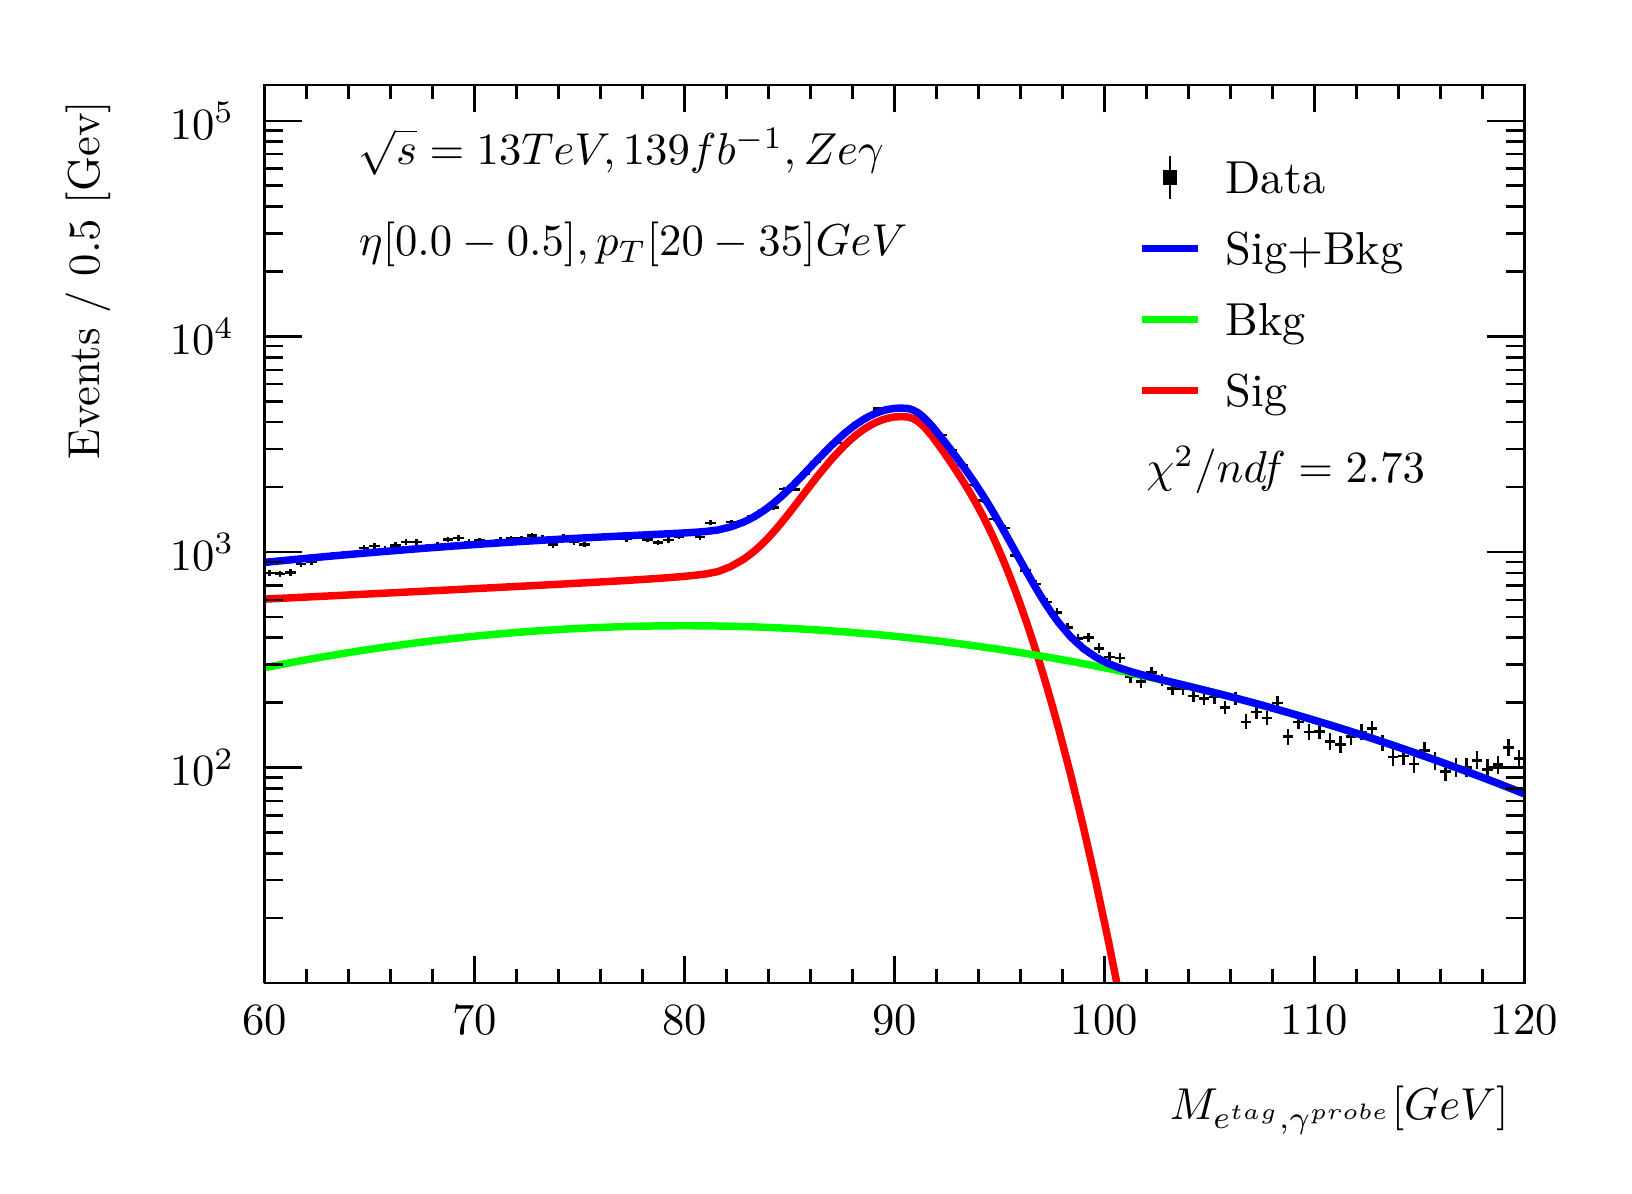
\begin{tikzpicture}
\pgfdeclareplotmark{cross} {
\pgfpathmoveto{\pgfpoint{-0.3\pgfplotmarksize}{\pgfplotmarksize}}
\pgfpathlineto{\pgfpoint{+0.3\pgfplotmarksize}{\pgfplotmarksize}}
\pgfpathlineto{\pgfpoint{+0.3\pgfplotmarksize}{0.3\pgfplotmarksize}}
\pgfpathlineto{\pgfpoint{+1\pgfplotmarksize}{0.3\pgfplotmarksize}}
\pgfpathlineto{\pgfpoint{+1\pgfplotmarksize}{-0.3\pgfplotmarksize}}
\pgfpathlineto{\pgfpoint{+0.3\pgfplotmarksize}{-0.3\pgfplotmarksize}}
\pgfpathlineto{\pgfpoint{+0.3\pgfplotmarksize}{-1.\pgfplotmarksize}}
\pgfpathlineto{\pgfpoint{-0.3\pgfplotmarksize}{-1.\pgfplotmarksize}}
\pgfpathlineto{\pgfpoint{-0.3\pgfplotmarksize}{-0.3\pgfplotmarksize}}
\pgfpathlineto{\pgfpoint{-1.\pgfplotmarksize}{-0.3\pgfplotmarksize}}
\pgfpathlineto{\pgfpoint{-1.\pgfplotmarksize}{0.3\pgfplotmarksize}}
\pgfpathlineto{\pgfpoint{-0.3\pgfplotmarksize}{0.3\pgfplotmarksize}}
\pgfpathclose
\pgfusepathqstroke
}
\pgfdeclareplotmark{cross*} {
\pgfpathmoveto{\pgfpoint{-0.3\pgfplotmarksize}{\pgfplotmarksize}}
\pgfpathlineto{\pgfpoint{+0.3\pgfplotmarksize}{\pgfplotmarksize}}
\pgfpathlineto{\pgfpoint{+0.3\pgfplotmarksize}{0.3\pgfplotmarksize}}
\pgfpathlineto{\pgfpoint{+1\pgfplotmarksize}{0.3\pgfplotmarksize}}
\pgfpathlineto{\pgfpoint{+1\pgfplotmarksize}{-0.3\pgfplotmarksize}}
\pgfpathlineto{\pgfpoint{+0.3\pgfplotmarksize}{-0.3\pgfplotmarksize}}
\pgfpathlineto{\pgfpoint{+0.3\pgfplotmarksize}{-1.\pgfplotmarksize}}
\pgfpathlineto{\pgfpoint{-0.3\pgfplotmarksize}{-1.\pgfplotmarksize}}
\pgfpathlineto{\pgfpoint{-0.3\pgfplotmarksize}{-0.3\pgfplotmarksize}}
\pgfpathlineto{\pgfpoint{-1.\pgfplotmarksize}{-0.3\pgfplotmarksize}}
\pgfpathlineto{\pgfpoint{-1.\pgfplotmarksize}{0.3\pgfplotmarksize}}
\pgfpathlineto{\pgfpoint{-0.3\pgfplotmarksize}{0.3\pgfplotmarksize}}
\pgfpathclose
\pgfusepathqfillstroke
}
\pgfdeclareplotmark{newstar} {
\pgfpathmoveto{\pgfqpoint{0pt}{\pgfplotmarksize}}
\pgfpathlineto{\pgfqpointpolar{44}{0.5\pgfplotmarksize}}
\pgfpathlineto{\pgfqpointpolar{18}{\pgfplotmarksize}}
\pgfpathlineto{\pgfqpointpolar{-20}{0.5\pgfplotmarksize}}
\pgfpathlineto{\pgfqpointpolar{-54}{\pgfplotmarksize}}
\pgfpathlineto{\pgfqpointpolar{-90}{0.5\pgfplotmarksize}}
\pgfpathlineto{\pgfqpointpolar{234}{\pgfplotmarksize}}
\pgfpathlineto{\pgfqpointpolar{198}{0.5\pgfplotmarksize}}
\pgfpathlineto{\pgfqpointpolar{162}{\pgfplotmarksize}}
\pgfpathlineto{\pgfqpointpolar{134}{0.5\pgfplotmarksize}}
\pgfpathclose
\pgfusepathqstroke
}
\pgfdeclareplotmark{newstar*} {
\pgfpathmoveto{\pgfqpoint{0pt}{\pgfplotmarksize}}
\pgfpathlineto{\pgfqpointpolar{44}{0.5\pgfplotmarksize}}
\pgfpathlineto{\pgfqpointpolar{18}{\pgfplotmarksize}}
\pgfpathlineto{\pgfqpointpolar{-20}{0.5\pgfplotmarksize}}
\pgfpathlineto{\pgfqpointpolar{-54}{\pgfplotmarksize}}
\pgfpathlineto{\pgfqpointpolar{-90}{0.5\pgfplotmarksize}}
\pgfpathlineto{\pgfqpointpolar{234}{\pgfplotmarksize}}
\pgfpathlineto{\pgfqpointpolar{198}{0.5\pgfplotmarksize}}
\pgfpathlineto{\pgfqpointpolar{162}{\pgfplotmarksize}}
\pgfpathlineto{\pgfqpointpolar{134}{0.5\pgfplotmarksize}}
\pgfpathclose
\pgfusepathqfillstroke
}
\definecolor{c}{rgb}{1,1,1};
\draw [color=c, fill=c] (0,0) rectangle (20,14.4361);
\draw [color=c, fill=c] (3,2.30977) rectangle (19,13.7143);
\definecolor{c}{rgb}{0,0,0};
\draw [c,line width=0.9] (3,2.30977) -- (3,13.7143) -- (19,13.7143) -- (19,2.30977) -- (3,2.30977);
\definecolor{c}{rgb}{1,1,1};
\draw [color=c, fill=c] (3,2.30977) rectangle (19,13.7143);
\definecolor{c}{rgb}{0,0,0};
\draw [c,line width=0.9] (3,2.30977) -- (3,13.7143) -- (19,13.7143) -- (19,2.30977) -- (3,2.30977);
\draw [c,line width=0.9] (3,2.30977) -- (19,2.30977);
\draw [c,line width=0.9] (3,2.65624) -- (3,2.30977);
\draw [c,line width=0.9] (3.53333,2.48301) -- (3.53333,2.30977);
\draw [c,line width=0.9] (4.06667,2.48301) -- (4.06667,2.30977);
\draw [c,line width=0.9] (4.6,2.48301) -- (4.6,2.30977);
\draw [c,line width=0.9] (5.13333,2.48301) -- (5.13333,2.30977);
\draw [c,line width=0.9] (5.66667,2.65624) -- (5.66667,2.30977);
\draw [c,line width=0.9] (6.2,2.48301) -- (6.2,2.30977);
\draw [c,line width=0.9] (6.73333,2.48301) -- (6.73333,2.30977);
\draw [c,line width=0.9] (7.26667,2.48301) -- (7.26667,2.30977);
\draw [c,line width=0.9] (7.8,2.48301) -- (7.8,2.30977);
\draw [c,line width=0.9] (8.33333,2.65624) -- (8.33333,2.30977);
\draw [c,line width=0.9] (8.86667,2.48301) -- (8.86667,2.30977);
\draw [c,line width=0.9] (9.4,2.48301) -- (9.4,2.30977);
\draw [c,line width=0.9] (9.93333,2.48301) -- (9.93333,2.30977);
\draw [c,line width=0.9] (10.4667,2.48301) -- (10.4667,2.30977);
\draw [c,line width=0.9] (11,2.65624) -- (11,2.30977);
\draw [c,line width=0.9] (11.5333,2.48301) -- (11.5333,2.30977);
\draw [c,line width=0.9] (12.0667,2.48301) -- (12.0667,2.30977);
\draw [c,line width=0.9] (12.6,2.48301) -- (12.6,2.30977);
\draw [c,line width=0.9] (13.1333,2.48301) -- (13.1333,2.30977);
\draw [c,line width=0.9] (13.6667,2.65624) -- (13.6667,2.30977);
\draw [c,line width=0.9] (14.2,2.48301) -- (14.2,2.30977);
\draw [c,line width=0.9] (14.7333,2.48301) -- (14.7333,2.30977);
\draw [c,line width=0.9] (15.2667,2.48301) -- (15.2667,2.30977);
\draw [c,line width=0.9] (15.8,2.48301) -- (15.8,2.30977);
\draw [c,line width=0.9] (16.3333,2.65624) -- (16.3333,2.30977);
\draw [c,line width=0.9] (16.8667,2.48301) -- (16.8667,2.30977);
\draw [c,line width=0.9] (17.4,2.48301) -- (17.4,2.30977);
\draw [c,line width=0.9] (17.9333,2.48301) -- (17.9333,2.30977);
\draw [c,line width=0.9] (18.4667,2.48301) -- (18.4667,2.30977);
\draw [c,line width=0.9] (19,2.65624) -- (19,2.30977);
\draw [anchor=base] (3,1.66015) node[scale=1.61424, color=c, rotate=0]{60};
\draw [anchor=base] (5.66667,1.66015) node[scale=1.61424, color=c, rotate=0]{70};
\draw [anchor=base] (8.33333,1.66015) node[scale=1.61424, color=c, rotate=0]{80};
\draw [anchor=base] (11,1.66015) node[scale=1.61424, color=c, rotate=0]{90};
\draw [anchor=base] (13.6667,1.66015) node[scale=1.61424, color=c, rotate=0]{100};
\draw [anchor=base] (16.3333,1.66015) node[scale=1.61424, color=c, rotate=0]{110};
\draw [anchor=base] (19,1.66015) node[scale=1.61424, color=c, rotate=0]{120};
\draw [anchor= east] (19,0.692932) node[scale=1.61424, color=c, rotate=0]{$M_{e^{tag}, \gamma^{probe}}  [GeV]$};
\draw [c,line width=0.9] (3,13.7143) -- (19,13.7143);
\draw [c,line width=0.9] (3,13.3678) -- (3,13.7143);
\draw [c,line width=0.9] (3.53333,13.5411) -- (3.53333,13.7143);
\draw [c,line width=0.9] (4.06667,13.5411) -- (4.06667,13.7143);
\draw [c,line width=0.9] (4.6,13.5411) -- (4.6,13.7143);
\draw [c,line width=0.9] (5.13333,13.5411) -- (5.13333,13.7143);
\draw [c,line width=0.9] (5.66667,13.3678) -- (5.66667,13.7143);
\draw [c,line width=0.9] (6.2,13.5411) -- (6.2,13.7143);
\draw [c,line width=0.9] (6.73333,13.5411) -- (6.73333,13.7143);
\draw [c,line width=0.9] (7.26667,13.5411) -- (7.26667,13.7143);
\draw [c,line width=0.9] (7.8,13.5411) -- (7.8,13.7143);
\draw [c,line width=0.9] (8.33333,13.3678) -- (8.33333,13.7143);
\draw [c,line width=0.9] (8.86667,13.5411) -- (8.86667,13.7143);
\draw [c,line width=0.9] (9.4,13.5411) -- (9.4,13.7143);
\draw [c,line width=0.9] (9.93333,13.5411) -- (9.93333,13.7143);
\draw [c,line width=0.9] (10.4667,13.5411) -- (10.4667,13.7143);
\draw [c,line width=0.9] (11,13.3678) -- (11,13.7143);
\draw [c,line width=0.9] (11.5333,13.5411) -- (11.5333,13.7143);
\draw [c,line width=0.9] (12.0667,13.5411) -- (12.0667,13.7143);
\draw [c,line width=0.9] (12.6,13.5411) -- (12.6,13.7143);
\draw [c,line width=0.9] (13.1333,13.5411) -- (13.1333,13.7143);
\draw [c,line width=0.9] (13.6667,13.3678) -- (13.6667,13.7143);
\draw [c,line width=0.9] (14.2,13.5411) -- (14.2,13.7143);
\draw [c,line width=0.9] (14.7333,13.5411) -- (14.7333,13.7143);
\draw [c,line width=0.9] (15.2667,13.5411) -- (15.2667,13.7143);
\draw [c,line width=0.9] (15.8,13.5411) -- (15.8,13.7143);
\draw [c,line width=0.9] (16.3333,13.3678) -- (16.3333,13.7143);
\draw [c,line width=0.9] (16.8667,13.5411) -- (16.8667,13.7143);
\draw [c,line width=0.9] (17.4,13.5411) -- (17.4,13.7143);
\draw [c,line width=0.9] (17.9333,13.5411) -- (17.9333,13.7143);
\draw [c,line width=0.9] (18.4667,13.5411) -- (18.4667,13.7143);
\draw [c,line width=0.9] (19,13.3678) -- (19,13.7143);
\draw [c,line width=0.9] (3,2.30977) -- (3,13.7143);
\draw [c,line width=0.9] (3.237,3.13385) -- (3,3.13385);
\draw [c,line width=0.9] (3.237,3.6159) -- (3,3.6159);
\draw [c,line width=0.9] (3.237,3.95792) -- (3,3.95792);
\draw [c,line width=0.9] (3.237,4.22321) -- (3,4.22321);
\draw [c,line width=0.9] (3.237,4.43997) -- (3,4.43997);
\draw [c,line width=0.9] (3.237,4.62324) -- (3,4.62324);
\draw [c,line width=0.9] (3.237,4.782) -- (3,4.782);
\draw [c,line width=0.9] (3.237,4.92203) -- (3,4.92203);
\draw [c,line width=0.9] (3.474,5.04729) -- (3,5.04729);
\draw [anchor= east] (2.82,5.04729) node[scale=1.61424, color=c, rotate=0]{$10^{2}$};
\draw [c,line width=0.9] (3.237,5.87136) -- (3,5.87136);
\draw [c,line width=0.9] (3.237,6.35342) -- (3,6.35342);
\draw [c,line width=0.9] (3.237,6.69544) -- (3,6.69544);
\draw [c,line width=0.9] (3.237,6.96073) -- (3,6.96073);
\draw [c,line width=0.9] (3.237,7.17749) -- (3,7.17749);
\draw [c,line width=0.9] (3.237,7.36076) -- (3,7.36076);
\draw [c,line width=0.9] (3.237,7.51951) -- (3,7.51951);
\draw [c,line width=0.9] (3.237,7.65954) -- (3,7.65954);
\draw [c,line width=0.9] (3.474,7.78481) -- (3,7.78481);
\draw [anchor= east] (2.82,7.78481) node[scale=1.61424, color=c, rotate=0]{$10^{3}$};
\draw [c,line width=0.9] (3.237,8.60888) -- (3,8.60888);
\draw [c,line width=0.9] (3.237,9.09093) -- (3,9.09093);
\draw [c,line width=0.9] (3.237,9.43296) -- (3,9.43296);
\draw [c,line width=0.9] (3.237,9.69825) -- (3,9.69825);
\draw [c,line width=0.9] (3.237,9.91501) -- (3,9.91501);
\draw [c,line width=0.9] (3.237,10.0983) -- (3,10.0983);
\draw [c,line width=0.9] (3.237,10.257) -- (3,10.257);
\draw [c,line width=0.9] (3.237,10.3971) -- (3,10.3971);
\draw [c,line width=0.9] (3.474,10.5223) -- (3,10.5223);
\draw [anchor= east] (2.82,10.5223) node[scale=1.61424, color=c, rotate=0]{$10^{4}$};
\draw [c,line width=0.9] (3.237,11.3464) -- (3,11.3464);
\draw [c,line width=0.9] (3.237,11.8285) -- (3,11.8285);
\draw [c,line width=0.9] (3.237,12.1705) -- (3,12.1705);
\draw [c,line width=0.9] (3.237,12.4358) -- (3,12.4358);
\draw [c,line width=0.9] (3.237,12.6525) -- (3,12.6525);
\draw [c,line width=0.9] (3.237,12.8358) -- (3,12.8358);
\draw [c,line width=0.9] (3.237,12.9945) -- (3,12.9945);
\draw [c,line width=0.9] (3.237,13.1346) -- (3,13.1346);
\draw [c,line width=0.9] (3.474,13.2598) -- (3,13.2598);
\draw [anchor= east] (2.82,13.2598) node[scale=1.61424, color=c, rotate=0]{$10^{5}$};
\draw [anchor= east] (0.76,13.7143) node[scale=1.61424, color=c, rotate=90]{Events / 0.5 [Gev]};
\draw [c,line width=0.9] (19,2.30977) -- (19,13.7143);
\draw [c,line width=0.9] (18.763,3.13385) -- (19,3.13385);
\draw [c,line width=0.9] (18.763,3.6159) -- (19,3.6159);
\draw [c,line width=0.9] (18.763,3.95792) -- (19,3.95792);
\draw [c,line width=0.9] (18.763,4.22321) -- (19,4.22321);
\draw [c,line width=0.9] (18.763,4.43997) -- (19,4.43997);
\draw [c,line width=0.9] (18.763,4.62324) -- (19,4.62324);
\draw [c,line width=0.9] (18.763,4.782) -- (19,4.782);
\draw [c,line width=0.9] (18.763,4.92203) -- (19,4.92203);
\draw [c,line width=0.9] (18.526,5.04729) -- (19,5.04729);
\draw [c,line width=0.9] (18.763,5.87136) -- (19,5.87136);
\draw [c,line width=0.9] (18.763,6.35342) -- (19,6.35342);
\draw [c,line width=0.9] (18.763,6.69544) -- (19,6.69544);
\draw [c,line width=0.9] (18.763,6.96073) -- (19,6.96073);
\draw [c,line width=0.9] (18.763,7.17749) -- (19,7.17749);
\draw [c,line width=0.9] (18.763,7.36076) -- (19,7.36076);
\draw [c,line width=0.9] (18.763,7.51951) -- (19,7.51951);
\draw [c,line width=0.9] (18.763,7.65954) -- (19,7.65954);
\draw [c,line width=0.9] (18.526,7.78481) -- (19,7.78481);
\draw [c,line width=0.9] (18.763,8.60888) -- (19,8.60888);
\draw [c,line width=0.9] (18.763,9.09093) -- (19,9.09093);
\draw [c,line width=0.9] (18.763,9.43296) -- (19,9.43296);
\draw [c,line width=0.9] (18.763,9.69825) -- (19,9.69825);
\draw [c,line width=0.9] (18.763,9.91501) -- (19,9.91501);
\draw [c,line width=0.9] (18.763,10.0983) -- (19,10.0983);
\draw [c,line width=0.9] (18.763,10.257) -- (19,10.257);
\draw [c,line width=0.9] (18.763,10.3971) -- (19,10.3971);
\draw [c,line width=0.9] (18.526,10.5223) -- (19,10.5223);
\draw [c,line width=0.9] (18.763,11.3464) -- (19,11.3464);
\draw [c,line width=0.9] (18.763,11.8285) -- (19,11.8285);
\draw [c,line width=0.9] (18.763,12.1705) -- (19,12.1705);
\draw [c,line width=0.9] (18.763,12.4358) -- (19,12.4358);
\draw [c,line width=0.9] (18.763,12.6525) -- (19,12.6525);
\draw [c,line width=0.9] (18.763,12.8358) -- (19,12.8358);
\draw [c,line width=0.9] (18.763,12.9945) -- (19,12.9945);
\draw [c,line width=0.9] (18.763,13.1346) -- (19,13.1346);
\draw [c,line width=0.9] (18.526,13.2598) -- (19,13.2598);
\draw [c,line width=0.9] (3.06667,7.51505) -- (3,7.51505);
\draw [c,line width=0.9] (3,7.51505) -- (3,7.51505);
\draw [c,line width=0.9] (3.06667,7.51505) -- (3.13333,7.51505);
\draw [c,line width=0.9] (3.13333,7.51505) -- (3.13333,7.51505);
\draw [c,line width=0.9] (3.06667,7.51505) -- (3.06667,7.55716);
\draw [c,line width=0.9] (3.06667,7.55716) -- (3.06667,7.55716);
\draw [c,line width=0.9] (3.06667,7.51505) -- (3.06667,7.47294);
\draw [c,line width=0.9] (3.06667,7.47294) -- (3.06667,7.47294);
\draw [c,line width=0.9] (3.2,7.50606) -- (3.13333,7.50606);
\draw [c,line width=0.9] (3.13333,7.50606) -- (3.13333,7.50606);
\draw [c,line width=0.9] (3.2,7.50606) -- (3.26667,7.50606);
\draw [c,line width=0.9] (3.26667,7.50606) -- (3.26667,7.50606);
\draw [c,line width=0.9] (3.2,7.50606) -- (3.2,7.54833);
\draw [c,line width=0.9] (3.2,7.54833) -- (3.2,7.54833);
\draw [c,line width=0.9] (3.2,7.50606) -- (3.2,7.46379);
\draw [c,line width=0.9] (3.2,7.46379) -- (3.2,7.46379);
\draw [c,line width=0.9] (3.33333,7.521) -- (3.26667,7.521);
\draw [c,line width=0.9] (3.26667,7.521) -- (3.26667,7.521);
\draw [c,line width=0.9] (3.33333,7.521) -- (3.4,7.521);
\draw [c,line width=0.9] (3.4,7.521) -- (3.4,7.521);
\draw [c,line width=0.9] (3.33333,7.521) -- (3.33333,7.563);
\draw [c,line width=0.9] (3.33333,7.563) -- (3.33333,7.563);
\draw [c,line width=0.9] (3.33333,7.521) -- (3.33333,7.47899);
\draw [c,line width=0.9] (3.33333,7.47899) -- (3.33333,7.47899);
\draw [c,line width=0.9] (3.46667,7.63012) -- (3.4,7.63012);
\draw [c,line width=0.9] (3.4,7.63012) -- (3.4,7.63012);
\draw [c,line width=0.9] (3.46667,7.63012) -- (3.53333,7.63012);
\draw [c,line width=0.9] (3.53333,7.63012) -- (3.53333,7.63012);
\draw [c,line width=0.9] (3.46667,7.63012) -- (3.46667,7.67024);
\draw [c,line width=0.9] (3.46667,7.67024) -- (3.46667,7.67024);
\draw [c,line width=0.9] (3.46667,7.63012) -- (3.46667,7.59);
\draw [c,line width=0.9] (3.46667,7.59) -- (3.46667,7.59);
\draw [c,line width=0.9] (3.6,7.65425) -- (3.53333,7.65425);
\draw [c,line width=0.9] (3.53333,7.65425) -- (3.53333,7.65425);
\draw [c,line width=0.9] (3.6,7.65425) -- (3.66667,7.65425);
\draw [c,line width=0.9] (3.66667,7.65425) -- (3.66667,7.65425);
\draw [c,line width=0.9] (3.6,7.65425) -- (3.6,7.69397);
\draw [c,line width=0.9] (3.6,7.69397) -- (3.6,7.69397);
\draw [c,line width=0.9] (3.6,7.65425) -- (3.6,7.61453);
\draw [c,line width=0.9] (3.6,7.61453) -- (3.6,7.61453);
\draw [c,line width=0.9] (3.73333,7.72633) -- (3.66667,7.72633);
\draw [c,line width=0.9] (3.66667,7.72633) -- (3.66667,7.72633);
\draw [c,line width=0.9] (3.73333,7.72633) -- (3.8,7.72633);
\draw [c,line width=0.9] (3.8,7.72633) -- (3.8,7.72633);
\draw [c,line width=0.9] (3.73333,7.72633) -- (3.73333,7.76486);
\draw [c,line width=0.9] (3.73333,7.76486) -- (3.73333,7.76486);
\draw [c,line width=0.9] (3.73333,7.72633) -- (3.73333,7.6878);
\draw [c,line width=0.9] (3.73333,7.6878) -- (3.73333,7.6878);
\draw [c,line width=0.9] (3.86667,7.73998) -- (3.8,7.73998);
\draw [c,line width=0.9] (3.8,7.73998) -- (3.8,7.73998);
\draw [c,line width=0.9] (3.86667,7.73998) -- (3.93333,7.73998);
\draw [c,line width=0.9] (3.93333,7.73998) -- (3.93333,7.73998);
\draw [c,line width=0.9] (3.86667,7.73998) -- (3.86667,7.77829);
\draw [c,line width=0.9] (3.86667,7.77829) -- (3.86667,7.77829);
\draw [c,line width=0.9] (3.86667,7.73998) -- (3.86667,7.70167);
\draw [c,line width=0.9] (3.86667,7.70167) -- (3.86667,7.70167);
\draw [c,line width=0.9] (4,7.75714) -- (3.93333,7.75714);
\draw [c,line width=0.9] (3.93333,7.75714) -- (3.93333,7.75714);
\draw [c,line width=0.9] (4,7.75714) -- (4.06667,7.75714);
\draw [c,line width=0.9] (4.06667,7.75714) -- (4.06667,7.75714);
\draw [c,line width=0.9] (4,7.75714) -- (4,7.79518);
\draw [c,line width=0.9] (4,7.79518) -- (4,7.79518);
\draw [c,line width=0.9] (4,7.75714) -- (4,7.71911);
\draw [c,line width=0.9] (4,7.71911) -- (4,7.71911);
\draw [c,line width=0.9] (4.13333,7.76079) -- (4.06667,7.76079);
\draw [c,line width=0.9] (4.06667,7.76079) -- (4.06667,7.76079);
\draw [c,line width=0.9] (4.13333,7.76079) -- (4.2,7.76079);
\draw [c,line width=0.9] (4.2,7.76079) -- (4.2,7.76079);
\draw [c,line width=0.9] (4.13333,7.76079) -- (4.13333,7.79876);
\draw [c,line width=0.9] (4.13333,7.79876) -- (4.13333,7.79876);
\draw [c,line width=0.9] (4.13333,7.76079) -- (4.13333,7.72281);
\draw [c,line width=0.9] (4.13333,7.72281) -- (4.13333,7.72281);
\draw [c,line width=0.9] (4.26667,7.83486) -- (4.2,7.83486);
\draw [c,line width=0.9] (4.2,7.83486) -- (4.2,7.83486);
\draw [c,line width=0.9] (4.26667,7.83486) -- (4.33333,7.83486);
\draw [c,line width=0.9] (4.33333,7.83486) -- (4.33333,7.83486);
\draw [c,line width=0.9] (4.26667,7.83486) -- (4.26667,7.87167);
\draw [c,line width=0.9] (4.26667,7.87167) -- (4.26667,7.87167);
\draw [c,line width=0.9] (4.26667,7.83486) -- (4.26667,7.79805);
\draw [c,line width=0.9] (4.26667,7.79805) -- (4.26667,7.79805);
\draw [c,line width=0.9] (4.4,7.85744) -- (4.33333,7.85744);
\draw [c,line width=0.9] (4.33333,7.85744) -- (4.33333,7.85744);
\draw [c,line width=0.9] (4.4,7.85744) -- (4.46667,7.85744);
\draw [c,line width=0.9] (4.46667,7.85744) -- (4.46667,7.85744);
\draw [c,line width=0.9] (4.4,7.85744) -- (4.4,7.89391);
\draw [c,line width=0.9] (4.4,7.89391) -- (4.4,7.89391);
\draw [c,line width=0.9] (4.4,7.85744) -- (4.4,7.82098);
\draw [c,line width=0.9] (4.4,7.82098) -- (4.4,7.82098);
\draw [c,line width=0.9] (4.53333,7.81995) -- (4.46667,7.81995);
\draw [c,line width=0.9] (4.46667,7.81995) -- (4.46667,7.81995);
\draw [c,line width=0.9] (4.53333,7.81995) -- (4.6,7.81995);
\draw [c,line width=0.9] (4.6,7.81995) -- (4.6,7.81995);
\draw [c,line width=0.9] (4.53333,7.81995) -- (4.53333,7.85699);
\draw [c,line width=0.9] (4.53333,7.85699) -- (4.53333,7.85699);
\draw [c,line width=0.9] (4.53333,7.81995) -- (4.53333,7.78291);
\draw [c,line width=0.9] (4.53333,7.78291) -- (4.53333,7.78291);
\draw [c,line width=0.9] (4.66667,7.86968) -- (4.6,7.86968);
\draw [c,line width=0.9] (4.6,7.86968) -- (4.6,7.86968);
\draw [c,line width=0.9] (4.66667,7.86968) -- (4.73333,7.86968);
\draw [c,line width=0.9] (4.73333,7.86968) -- (4.73333,7.86968);
\draw [c,line width=0.9] (4.66667,7.86968) -- (4.66667,7.90596);
\draw [c,line width=0.9] (4.66667,7.90596) -- (4.66667,7.90596);
\draw [c,line width=0.9] (4.66667,7.86968) -- (4.66667,7.83341);
\draw [c,line width=0.9] (4.66667,7.83341) -- (4.66667,7.83341);
\draw [c,line width=0.9] (4.8,7.91209) -- (4.73333,7.91209);
\draw [c,line width=0.9] (4.73333,7.91209) -- (4.73333,7.91209);
\draw [c,line width=0.9] (4.8,7.91209) -- (4.86667,7.91209);
\draw [c,line width=0.9] (4.86667,7.91209) -- (4.86667,7.91209);
\draw [c,line width=0.9] (4.8,7.91209) -- (4.8,7.94772);
\draw [c,line width=0.9] (4.8,7.94772) -- (4.8,7.94772);
\draw [c,line width=0.9] (4.8,7.91209) -- (4.8,7.87645);
\draw [c,line width=0.9] (4.8,7.87645) -- (4.8,7.87645);
\draw [c,line width=0.9] (4.93333,7.90995) -- (4.86667,7.90995);
\draw [c,line width=0.9] (4.86667,7.90995) -- (4.86667,7.90995);
\draw [c,line width=0.9] (4.93333,7.90995) -- (5,7.90995);
\draw [c,line width=0.9] (5,7.90995) -- (5,7.90995);
\draw [c,line width=0.9] (4.93333,7.90995) -- (4.93333,7.94562);
\draw [c,line width=0.9] (4.93333,7.94562) -- (4.93333,7.94562);
\draw [c,line width=0.9] (4.93333,7.90995) -- (4.93333,7.87428);
\draw [c,line width=0.9] (4.93333,7.87428) -- (4.93333,7.87428);
\draw [c,line width=0.9] (5.06667,7.85408) -- (5,7.85408);
\draw [c,line width=0.9] (5,7.85408) -- (5,7.85408);
\draw [c,line width=0.9] (5.06667,7.85408) -- (5.13333,7.85408);
\draw [c,line width=0.9] (5.13333,7.85408) -- (5.13333,7.85408);
\draw [c,line width=0.9] (5.06667,7.85408) -- (5.06667,7.8906);
\draw [c,line width=0.9] (5.06667,7.8906) -- (5.06667,7.8906);
\draw [c,line width=0.9] (5.06667,7.85408) -- (5.06667,7.81757);
\draw [c,line width=0.9] (5.06667,7.81757) -- (5.06667,7.81757);
\draw [c,line width=0.9] (5.2,7.87189) -- (5.13333,7.87189);
\draw [c,line width=0.9] (5.13333,7.87189) -- (5.13333,7.87189);
\draw [c,line width=0.9] (5.2,7.87189) -- (5.26667,7.87189);
\draw [c,line width=0.9] (5.26667,7.87189) -- (5.26667,7.87189);
\draw [c,line width=0.9] (5.2,7.87189) -- (5.2,7.90814);
\draw [c,line width=0.9] (5.2,7.90814) -- (5.2,7.90814);
\draw [c,line width=0.9] (5.2,7.87189) -- (5.2,7.83565);
\draw [c,line width=0.9] (5.2,7.83565) -- (5.2,7.83565);
\draw [c,line width=0.9] (5.33333,7.94163) -- (5.26667,7.94163);
\draw [c,line width=0.9] (5.26667,7.94163) -- (5.26667,7.94163);
\draw [c,line width=0.9] (5.33333,7.94163) -- (5.4,7.94163);
\draw [c,line width=0.9] (5.4,7.94163) -- (5.4,7.94163);
\draw [c,line width=0.9] (5.33333,7.94163) -- (5.33333,7.97682);
\draw [c,line width=0.9] (5.33333,7.97682) -- (5.33333,7.97682);
\draw [c,line width=0.9] (5.33333,7.94163) -- (5.33333,7.90643);
\draw [c,line width=0.9] (5.33333,7.90643) -- (5.33333,7.90643);
\draw [c,line width=0.9] (5.46667,7.96229) -- (5.4,7.96229);
\draw [c,line width=0.9] (5.4,7.96229) -- (5.4,7.96229);
\draw [c,line width=0.9] (5.46667,7.96229) -- (5.53333,7.96229);
\draw [c,line width=0.9] (5.53333,7.96229) -- (5.53333,7.96229);
\draw [c,line width=0.9] (5.46667,7.96229) -- (5.46667,7.99718);
\draw [c,line width=0.9] (5.46667,7.99718) -- (5.46667,7.99718);
\draw [c,line width=0.9] (5.46667,7.96229) -- (5.46667,7.9274);
\draw [c,line width=0.9] (5.46667,7.9274) -- (5.46667,7.9274);
\draw [c,line width=0.9] (5.6,7.91422) -- (5.53333,7.91422);
\draw [c,line width=0.9] (5.53333,7.91422) -- (5.53333,7.91422);
\draw [c,line width=0.9] (5.6,7.91422) -- (5.66667,7.91422);
\draw [c,line width=0.9] (5.66667,7.91422) -- (5.66667,7.91422);
\draw [c,line width=0.9] (5.6,7.91422) -- (5.6,7.94983);
\draw [c,line width=0.9] (5.6,7.94983) -- (5.6,7.94983);
\draw [c,line width=0.9] (5.6,7.91422) -- (5.6,7.87862);
\draw [c,line width=0.9] (5.6,7.87862) -- (5.6,7.87862);
\draw [c,line width=0.9] (5.73333,7.93221) -- (5.66667,7.93221);
\draw [c,line width=0.9] (5.66667,7.93221) -- (5.66667,7.93221);
\draw [c,line width=0.9] (5.73333,7.93221) -- (5.8,7.93221);
\draw [c,line width=0.9] (5.8,7.93221) -- (5.8,7.93221);
\draw [c,line width=0.9] (5.73333,7.93221) -- (5.73333,7.96755);
\draw [c,line width=0.9] (5.73333,7.96755) -- (5.73333,7.96755);
\draw [c,line width=0.9] (5.73333,7.93221) -- (5.73333,7.89688);
\draw [c,line width=0.9] (5.73333,7.89688) -- (5.73333,7.89688);
\draw [c,line width=0.9] (5.86667,7.89487) -- (5.8,7.89487);
\draw [c,line width=0.9] (5.8,7.89487) -- (5.8,7.89487);
\draw [c,line width=0.9] (5.86667,7.89487) -- (5.93333,7.89487);
\draw [c,line width=0.9] (5.93333,7.89487) -- (5.93333,7.89487);
\draw [c,line width=0.9] (5.86667,7.89487) -- (5.86667,7.93077);
\draw [c,line width=0.9] (5.86667,7.93077) -- (5.86667,7.93077);
\draw [c,line width=0.9] (5.86667,7.89487) -- (5.86667,7.85898);
\draw [c,line width=0.9] (5.86667,7.85898) -- (5.86667,7.85898);
\draw [c,line width=0.9] (6,7.9385) -- (5.93333,7.9385);
\draw [c,line width=0.9] (5.93333,7.9385) -- (5.93333,7.9385);
\draw [c,line width=0.9] (6,7.9385) -- (6.06667,7.9385);
\draw [c,line width=0.9] (6.06667,7.9385) -- (6.06667,7.9385);
\draw [c,line width=0.9] (6,7.9385) -- (6,7.97374);
\draw [c,line width=0.9] (6,7.97374) -- (6,7.97374);
\draw [c,line width=0.9] (6,7.9385) -- (6,7.90326);
\draw [c,line width=0.9] (6,7.90326) -- (6,7.90326);
\draw [c,line width=0.9] (6.13333,7.95303) -- (6.06667,7.95303);
\draw [c,line width=0.9] (6.06667,7.95303) -- (6.06667,7.95303);
\draw [c,line width=0.9] (6.13333,7.95303) -- (6.2,7.95303);
\draw [c,line width=0.9] (6.2,7.95303) -- (6.2,7.95303);
\draw [c,line width=0.9] (6.13333,7.95303) -- (6.13333,7.98806);
\draw [c,line width=0.9] (6.13333,7.98806) -- (6.13333,7.98806);
\draw [c,line width=0.9] (6.13333,7.95303) -- (6.13333,7.91801);
\draw [c,line width=0.9] (6.13333,7.91801) -- (6.13333,7.91801);
\draw [c,line width=0.9] (6.26667,7.9551) -- (6.2,7.9551);
\draw [c,line width=0.9] (6.2,7.9551) -- (6.2,7.9551);
\draw [c,line width=0.9] (6.26667,7.9551) -- (6.33333,7.9551);
\draw [c,line width=0.9] (6.33333,7.9551) -- (6.33333,7.9551);
\draw [c,line width=0.9] (6.26667,7.9551) -- (6.26667,7.99009);
\draw [c,line width=0.9] (6.26667,7.99009) -- (6.26667,7.99009);
\draw [c,line width=0.9] (6.26667,7.9551) -- (6.26667,7.9201);
\draw [c,line width=0.9] (6.26667,7.9201) -- (6.26667,7.9201);
\draw [c,line width=0.9] (6.4,7.99361) -- (6.33333,7.99361);
\draw [c,line width=0.9] (6.33333,7.99361) -- (6.33333,7.99361);
\draw [c,line width=0.9] (6.4,7.99361) -- (6.46667,7.99361);
\draw [c,line width=0.9] (6.46667,7.99361) -- (6.46667,7.99361);
\draw [c,line width=0.9] (6.4,7.99361) -- (6.4,8.02805);
\draw [c,line width=0.9] (6.4,8.02805) -- (6.4,8.02805);
\draw [c,line width=0.9] (6.4,7.99361) -- (6.4,7.95918);
\draw [c,line width=0.9] (6.4,7.95918) -- (6.4,7.95918);
\draw [c,line width=0.9] (6.53333,7.96433) -- (6.46667,7.96433);
\draw [c,line width=0.9] (6.46667,7.96433) -- (6.46667,7.96433);
\draw [c,line width=0.9] (6.53333,7.96433) -- (6.6,7.96433);
\draw [c,line width=0.9] (6.6,7.96433) -- (6.6,7.96433);
\draw [c,line width=0.9] (6.53333,7.96433) -- (6.53333,7.99919);
\draw [c,line width=0.9] (6.53333,7.99919) -- (6.53333,7.99919);
\draw [c,line width=0.9] (6.53333,7.96433) -- (6.53333,7.92947);
\draw [c,line width=0.9] (6.53333,7.92947) -- (6.53333,7.92947);
\draw [c,line width=0.9] (6.66667,7.87631) -- (6.6,7.87631);
\draw [c,line width=0.9] (6.6,7.87631) -- (6.6,7.87631);
\draw [c,line width=0.9] (6.66667,7.87631) -- (6.73333,7.87631);
\draw [c,line width=0.9] (6.73333,7.87631) -- (6.73333,7.87631);
\draw [c,line width=0.9] (6.66667,7.87631) -- (6.66667,7.91248);
\draw [c,line width=0.9] (6.66667,7.91248) -- (6.66667,7.91248);
\draw [c,line width=0.9] (6.66667,7.87631) -- (6.66667,7.84013);
\draw [c,line width=0.9] (6.66667,7.84013) -- (6.66667,7.84013);
\draw [c,line width=0.9] (6.8,7.97552) -- (6.73333,7.97552);
\draw [c,line width=0.9] (6.73333,7.97552) -- (6.73333,7.97552);
\draw [c,line width=0.9] (6.8,7.97552) -- (6.86667,7.97552);
\draw [c,line width=0.9] (6.86667,7.97552) -- (6.86667,7.97552);
\draw [c,line width=0.9] (6.8,7.97552) -- (6.8,8.01022);
\draw [c,line width=0.9] (6.8,8.01022) -- (6.8,8.01022);
\draw [c,line width=0.9] (6.8,7.97552) -- (6.8,7.94083);
\draw [c,line width=0.9] (6.8,7.94083) -- (6.8,7.94083);
\draw [c,line width=0.9] (6.93333,7.90888) -- (6.86667,7.90888);
\draw [c,line width=0.9] (6.86667,7.90888) -- (6.86667,7.90888);
\draw [c,line width=0.9] (6.93333,7.90888) -- (7,7.90888);
\draw [c,line width=0.9] (7,7.90888) -- (7,7.90888);
\draw [c,line width=0.9] (6.93333,7.90888) -- (6.93333,7.94456);
\draw [c,line width=0.9] (6.93333,7.94456) -- (6.93333,7.94456);
\draw [c,line width=0.9] (6.93333,7.90888) -- (6.93333,7.8732);
\draw [c,line width=0.9] (6.93333,7.8732) -- (6.93333,7.8732);
\draw [c,line width=0.9] (7.06667,7.87851) -- (7,7.87851);
\draw [c,line width=0.9] (7,7.87851) -- (7,7.87851);
\draw [c,line width=0.9] (7.06667,7.87851) -- (7.13333,7.87851);
\draw [c,line width=0.9] (7.13333,7.87851) -- (7.13333,7.87851);
\draw [c,line width=0.9] (7.06667,7.87851) -- (7.06667,7.91465);
\draw [c,line width=0.9] (7.06667,7.91465) -- (7.06667,7.91465);
\draw [c,line width=0.9] (7.06667,7.87851) -- (7.06667,7.84236);
\draw [c,line width=0.9] (7.06667,7.84236) -- (7.06667,7.84236);
\draw [c,line width=0.9] (7.2,7.95716) -- (7.13333,7.95716);
\draw [c,line width=0.9] (7.13333,7.95716) -- (7.13333,7.95716);
\draw [c,line width=0.9] (7.2,7.95716) -- (7.26667,7.95716);
\draw [c,line width=0.9] (7.26667,7.95716) -- (7.26667,7.95716);
\draw [c,line width=0.9] (7.2,7.95716) -- (7.2,7.99212);
\draw [c,line width=0.9] (7.2,7.99212) -- (7.2,7.99212);
\draw [c,line width=0.9] (7.2,7.95716) -- (7.2,7.92219);
\draw [c,line width=0.9] (7.2,7.92219) -- (7.2,7.92219);
\draw [c,line width=0.9] (7.33333,7.97957) -- (7.26667,7.97957);
\draw [c,line width=0.9] (7.26667,7.97957) -- (7.26667,7.97957);
\draw [c,line width=0.9] (7.33333,7.97957) -- (7.4,7.97957);
\draw [c,line width=0.9] (7.4,7.97957) -- (7.4,7.97957);
\draw [c,line width=0.9] (7.33333,7.97957) -- (7.33333,8.01421);
\draw [c,line width=0.9] (7.33333,8.01421) -- (7.33333,8.01421);
\draw [c,line width=0.9] (7.33333,7.97957) -- (7.33333,7.94493);
\draw [c,line width=0.9] (7.33333,7.94493) -- (7.33333,7.94493);
\draw [c,line width=0.9] (7.46667,7.97755) -- (7.4,7.97755);
\draw [c,line width=0.9] (7.4,7.97755) -- (7.4,7.97755);
\draw [c,line width=0.9] (7.46667,7.97755) -- (7.53333,7.97755);
\draw [c,line width=0.9] (7.53333,7.97755) -- (7.53333,7.97755);
\draw [c,line width=0.9] (7.46667,7.97755) -- (7.46667,8.01222);
\draw [c,line width=0.9] (7.46667,8.01222) -- (7.46667,8.01222);
\draw [c,line width=0.9] (7.46667,7.97755) -- (7.46667,7.94288);
\draw [c,line width=0.9] (7.46667,7.94288) -- (7.46667,7.94288);
\draw [c,line width=0.9] (7.6,7.94683) -- (7.53333,7.94683);
\draw [c,line width=0.9] (7.53333,7.94683) -- (7.53333,7.94683);
\draw [c,line width=0.9] (7.6,7.94683) -- (7.66667,7.94683);
\draw [c,line width=0.9] (7.66667,7.94683) -- (7.66667,7.94683);
\draw [c,line width=0.9] (7.6,7.94683) -- (7.6,7.98194);
\draw [c,line width=0.9] (7.6,7.98194) -- (7.6,7.98194);
\draw [c,line width=0.9] (7.6,7.94683) -- (7.6,7.91171);
\draw [c,line width=0.9] (7.6,7.91171) -- (7.6,7.91171);
\draw [c,line width=0.9] (7.73333,7.98159) -- (7.66667,7.98159);
\draw [c,line width=0.9] (7.66667,7.98159) -- (7.66667,7.98159);
\draw [c,line width=0.9] (7.73333,7.98159) -- (7.8,7.98159);
\draw [c,line width=0.9] (7.8,7.98159) -- (7.8,7.98159);
\draw [c,line width=0.9] (7.73333,7.98159) -- (7.73333,8.01619);
\draw [c,line width=0.9] (7.73333,8.01619) -- (7.73333,8.01619);
\draw [c,line width=0.9] (7.73333,7.98159) -- (7.73333,7.94698);
\draw [c,line width=0.9] (7.73333,7.94698) -- (7.73333,7.94698);
\draw [c,line width=0.9] (7.86667,7.94475) -- (7.8,7.94475);
\draw [c,line width=0.9] (7.8,7.94475) -- (7.8,7.94475);
\draw [c,line width=0.9] (7.86667,7.94475) -- (7.93333,7.94475);
\draw [c,line width=0.9] (7.93333,7.94475) -- (7.93333,7.94475);
\draw [c,line width=0.9] (7.86667,7.94475) -- (7.86667,7.9799);
\draw [c,line width=0.9] (7.86667,7.9799) -- (7.86667,7.9799);
\draw [c,line width=0.9] (7.86667,7.94475) -- (7.86667,7.9096);
\draw [c,line width=0.9] (7.86667,7.9096) -- (7.86667,7.9096);
\draw [c,line width=0.9] (8,7.90351) -- (7.93333,7.90351);
\draw [c,line width=0.9] (7.93333,7.90351) -- (7.93333,7.90351);
\draw [c,line width=0.9] (8,7.90351) -- (8.06667,7.90351);
\draw [c,line width=0.9] (8.06667,7.90351) -- (8.06667,7.90351);
\draw [c,line width=0.9] (8,7.90351) -- (8,7.93928);
\draw [c,line width=0.9] (8,7.93928) -- (8,7.93928);
\draw [c,line width=0.9] (8,7.90351) -- (8,7.86775);
\draw [c,line width=0.9] (8,7.86775) -- (8,7.86775);
\draw [c,line width=0.9] (8.13333,7.93536) -- (8.06667,7.93536);
\draw [c,line width=0.9] (8.06667,7.93536) -- (8.06667,7.93536);
\draw [c,line width=0.9] (8.13333,7.93536) -- (8.2,7.93536);
\draw [c,line width=0.9] (8.2,7.93536) -- (8.2,7.93536);
\draw [c,line width=0.9] (8.13333,7.93536) -- (8.13333,7.97065);
\draw [c,line width=0.9] (8.13333,7.97065) -- (8.13333,7.97065);
\draw [c,line width=0.9] (8.13333,7.93536) -- (8.13333,7.90007);
\draw [c,line width=0.9] (8.13333,7.90007) -- (8.13333,7.90007);
\draw [c,line width=0.9] (8.26667,7.98259) -- (8.2,7.98259);
\draw [c,line width=0.9] (8.2,7.98259) -- (8.2,7.98259);
\draw [c,line width=0.9] (8.26667,7.98259) -- (8.33333,7.98259);
\draw [c,line width=0.9] (8.33333,7.98259) -- (8.33333,7.98259);
\draw [c,line width=0.9] (8.26667,7.98259) -- (8.26667,8.01719);
\draw [c,line width=0.9] (8.26667,8.01719) -- (8.26667,8.01719);
\draw [c,line width=0.9] (8.26667,7.98259) -- (8.26667,7.948);
\draw [c,line width=0.9] (8.26667,7.948) -- (8.26667,7.948);
\draw [c,line width=0.9] (8.4,8.03092) -- (8.33333,8.03092);
\draw [c,line width=0.9] (8.33333,8.03092) -- (8.33333,8.03092);
\draw [c,line width=0.9] (8.4,8.03092) -- (8.46667,8.03092);
\draw [c,line width=0.9] (8.46667,8.03092) -- (8.46667,8.03092);
\draw [c,line width=0.9] (8.4,8.03092) -- (8.4,8.06482);
\draw [c,line width=0.9] (8.4,8.06482) -- (8.4,8.06482);
\draw [c,line width=0.9] (8.4,8.03092) -- (8.4,7.99703);
\draw [c,line width=0.9] (8.4,7.99703) -- (8.4,7.99703);
\draw [c,line width=0.9] (8.53333,7.97248) -- (8.46667,7.97248);
\draw [c,line width=0.9] (8.46667,7.97248) -- (8.46667,7.97248);
\draw [c,line width=0.9] (8.53333,7.97248) -- (8.6,7.97248);
\draw [c,line width=0.9] (8.6,7.97248) -- (8.6,7.97248);
\draw [c,line width=0.9] (8.53333,7.97248) -- (8.53333,8.00722);
\draw [c,line width=0.9] (8.53333,8.00722) -- (8.53333,8.00722);
\draw [c,line width=0.9] (8.53333,7.97248) -- (8.53333,7.93774);
\draw [c,line width=0.9] (8.53333,7.93774) -- (8.53333,7.93774);
\draw [c,line width=0.9] (8.66667,8.15299) -- (8.6,8.15299);
\draw [c,line width=0.9] (8.6,8.15299) -- (8.6,8.15299);
\draw [c,line width=0.9] (8.66667,8.15299) -- (8.73333,8.15299);
\draw [c,line width=0.9] (8.73333,8.15299) -- (8.73333,8.15299);
\draw [c,line width=0.9] (8.66667,8.15299) -- (8.66667,8.18519);
\draw [c,line width=0.9] (8.66667,8.18519) -- (8.66667,8.18519);
\draw [c,line width=0.9] (8.66667,8.15299) -- (8.66667,8.12079);
\draw [c,line width=0.9] (8.66667,8.12079) -- (8.66667,8.12079);
\draw [c,line width=0.9] (8.8,8.0857) -- (8.73333,8.0857);
\draw [c,line width=0.9] (8.73333,8.0857) -- (8.73333,8.0857);
\draw [c,line width=0.9] (8.8,8.0857) -- (8.86667,8.0857);
\draw [c,line width=0.9] (8.86667,8.0857) -- (8.86667,8.0857);
\draw [c,line width=0.9] (8.8,8.0857) -- (8.8,8.11883);
\draw [c,line width=0.9] (8.8,8.11883) -- (8.8,8.11883);
\draw [c,line width=0.9] (8.8,8.0857) -- (8.8,8.05258);
\draw [c,line width=0.9] (8.8,8.05258) -- (8.8,8.05258);
\draw [c,line width=0.9] (8.93333,8.16341) -- (8.86667,8.16341);
\draw [c,line width=0.9] (8.86667,8.16341) -- (8.86667,8.16341);
\draw [c,line width=0.9] (8.93333,8.16341) -- (9,8.16341);
\draw [c,line width=0.9] (9,8.16341) -- (9,8.16341);
\draw [c,line width=0.9] (8.93333,8.16341) -- (8.93333,8.19547);
\draw [c,line width=0.9] (8.93333,8.19547) -- (8.93333,8.19547);
\draw [c,line width=0.9] (8.93333,8.16341) -- (8.93333,8.13135);
\draw [c,line width=0.9] (8.93333,8.13135) -- (8.93333,8.13135);
\draw [c,line width=0.9] (9.06667,8.17717) -- (9,8.17717);
\draw [c,line width=0.9] (9,8.17717) -- (9,8.17717);
\draw [c,line width=0.9] (9.06667,8.17717) -- (9.13333,8.17717);
\draw [c,line width=0.9] (9.13333,8.17717) -- (9.13333,8.17717);
\draw [c,line width=0.9] (9.06667,8.17717) -- (9.06667,8.20904);
\draw [c,line width=0.9] (9.06667,8.20904) -- (9.06667,8.20904);
\draw [c,line width=0.9] (9.06667,8.17717) -- (9.06667,8.14529);
\draw [c,line width=0.9] (9.06667,8.14529) -- (9.06667,8.14529);
\draw [c,line width=0.9] (9.2,8.23879) -- (9.13333,8.23879);
\draw [c,line width=0.9] (9.13333,8.23879) -- (9.13333,8.23879);
\draw [c,line width=0.9] (9.2,8.23879) -- (9.26667,8.23879);
\draw [c,line width=0.9] (9.26667,8.23879) -- (9.26667,8.23879);
\draw [c,line width=0.9] (9.2,8.23879) -- (9.2,8.26985);
\draw [c,line width=0.9] (9.2,8.26985) -- (9.2,8.26985);
\draw [c,line width=0.9] (9.2,8.23879) -- (9.2,8.20773);
\draw [c,line width=0.9] (9.2,8.20773) -- (9.2,8.20773);
\draw [c,line width=0.9] (9.33333,8.31273) -- (9.26667,8.31273);
\draw [c,line width=0.9] (9.26667,8.31273) -- (9.26667,8.31273);
\draw [c,line width=0.9] (9.33333,8.31273) -- (9.4,8.31273);
\draw [c,line width=0.9] (9.4,8.31273) -- (9.4,8.31273);
\draw [c,line width=0.9] (9.33333,8.31273) -- (9.33333,8.34284);
\draw [c,line width=0.9] (9.33333,8.34284) -- (9.33333,8.34284);
\draw [c,line width=0.9] (9.33333,8.31273) -- (9.33333,8.28262);
\draw [c,line width=0.9] (9.33333,8.28262) -- (9.33333,8.28262);
\draw [c,line width=0.9] (9.46667,8.351) -- (9.4,8.351);
\draw [c,line width=0.9] (9.4,8.351) -- (9.4,8.351);
\draw [c,line width=0.9] (9.46667,8.351) -- (9.53333,8.351);
\draw [c,line width=0.9] (9.53333,8.351) -- (9.53333,8.351);
\draw [c,line width=0.9] (9.46667,8.351) -- (9.46667,8.38063);
\draw [c,line width=0.9] (9.46667,8.38063) -- (9.46667,8.38063);
\draw [c,line width=0.9] (9.46667,8.351) -- (9.46667,8.32137);
\draw [c,line width=0.9] (9.46667,8.32137) -- (9.46667,8.32137);
\draw [c,line width=0.9] (9.6,8.58365) -- (9.53333,8.58365);
\draw [c,line width=0.9] (9.53333,8.58365) -- (9.53333,8.58365);
\draw [c,line width=0.9] (9.6,8.58365) -- (9.66667,8.58365);
\draw [c,line width=0.9] (9.66667,8.58365) -- (9.66667,8.58365);
\draw [c,line width=0.9] (9.6,8.58365) -- (9.6,8.61052);
\draw [c,line width=0.9] (9.6,8.61052) -- (9.6,8.61052);
\draw [c,line width=0.9] (9.6,8.58365) -- (9.6,8.55678);
\draw [c,line width=0.9] (9.6,8.55678) -- (9.6,8.55678);
\draw [c,line width=0.9] (9.73333,8.58) -- (9.66667,8.58);
\draw [c,line width=0.9] (9.66667,8.58) -- (9.66667,8.58);
\draw [c,line width=0.9] (9.73333,8.58) -- (9.8,8.58);
\draw [c,line width=0.9] (9.8,8.58) -- (9.8,8.58);
\draw [c,line width=0.9] (9.73333,8.58) -- (9.73333,8.60691);
\draw [c,line width=0.9] (9.73333,8.60691) -- (9.73333,8.60691);
\draw [c,line width=0.9] (9.73333,8.58) -- (9.73333,8.55309);
\draw [c,line width=0.9] (9.73333,8.55309) -- (9.73333,8.55309);
\draw [c,line width=0.9] (9.86667,8.77917) -- (9.8,8.77917);
\draw [c,line width=0.9] (9.8,8.77917) -- (9.8,8.77917);
\draw [c,line width=0.9] (9.86667,8.77917) -- (9.93333,8.77917);
\draw [c,line width=0.9] (9.93333,8.77917) -- (9.93333,8.77917);
\draw [c,line width=0.9] (9.86667,8.77917) -- (9.86667,8.80392);
\draw [c,line width=0.9] (9.86667,8.80392) -- (9.86667,8.80392);
\draw [c,line width=0.9] (9.86667,8.77917) -- (9.86667,8.75443);
\draw [c,line width=0.9] (9.86667,8.75443) -- (9.86667,8.75443);
\draw [c,line width=0.9] (10,8.92491) -- (9.93333,8.92491);
\draw [c,line width=0.9] (9.93333,8.92491) -- (9.93333,8.92491);
\draw [c,line width=0.9] (10,8.92491) -- (10.0667,8.92491);
\draw [c,line width=0.9] (10.0667,8.92491) -- (10.0667,8.92491);
\draw [c,line width=0.9] (10,8.92491) -- (10,8.94819);
\draw [c,line width=0.9] (10,8.94819) -- (10,8.94819);
\draw [c,line width=0.9] (10,8.92491) -- (10,8.90164);
\draw [c,line width=0.9] (10,8.90164) -- (10,8.90164);
\draw [c,line width=0.9] (10.1333,9.0653) -- (10.0667,9.0653);
\draw [c,line width=0.9] (10.0667,9.0653) -- (10.0667,9.0653);
\draw [c,line width=0.9] (10.1333,9.0653) -- (10.2,9.0653);
\draw [c,line width=0.9] (10.2,9.0653) -- (10.2,9.0653);
\draw [c,line width=0.9] (10.1333,9.0653) -- (10.1333,9.08724);
\draw [c,line width=0.9] (10.1333,9.08724) -- (10.1333,9.08724);
\draw [c,line width=0.9] (10.1333,9.0653) -- (10.1333,9.04336);
\draw [c,line width=0.9] (10.1333,9.04336) -- (10.1333,9.04336);
\draw [c,line width=0.9] (10.2667,9.16915) -- (10.2,9.16915);
\draw [c,line width=0.9] (10.2,9.16915) -- (10.2,9.16915);
\draw [c,line width=0.9] (10.2667,9.16915) -- (10.3333,9.16915);
\draw [c,line width=0.9] (10.3333,9.16915) -- (10.3333,9.16915);
\draw [c,line width=0.9] (10.2667,9.16915) -- (10.2667,9.19015);
\draw [c,line width=0.9] (10.2667,9.19015) -- (10.2667,9.19015);
\draw [c,line width=0.9] (10.2667,9.16915) -- (10.2667,9.14815);
\draw [c,line width=0.9] (10.2667,9.14815) -- (10.2667,9.14815);
\draw [c,line width=0.9] (10.4,9.32312) -- (10.3333,9.32312);
\draw [c,line width=0.9] (10.3333,9.32312) -- (10.3333,9.32312);
\draw [c,line width=0.9] (10.4,9.32312) -- (10.4667,9.32312);
\draw [c,line width=0.9] (10.4667,9.32312) -- (10.4667,9.32312);
\draw [c,line width=0.9] (10.4,9.32312) -- (10.4,9.3428);
\draw [c,line width=0.9] (10.4,9.3428) -- (10.4,9.3428);
\draw [c,line width=0.9] (10.4,9.32312) -- (10.4,9.30343);
\draw [c,line width=0.9] (10.4,9.30343) -- (10.4,9.30343);
\draw [c,line width=0.9] (10.5333,9.41348) -- (10.4667,9.41348);
\draw [c,line width=0.9] (10.4667,9.41348) -- (10.4667,9.41348);
\draw [c,line width=0.9] (10.5333,9.41348) -- (10.6,9.41348);
\draw [c,line width=0.9] (10.6,9.41348) -- (10.6,9.41348);
\draw [c,line width=0.9] (10.5333,9.41348) -- (10.5333,9.43243);
\draw [c,line width=0.9] (10.5333,9.43243) -- (10.5333,9.43243);
\draw [c,line width=0.9] (10.5333,9.41348) -- (10.5333,9.39453);
\draw [c,line width=0.9] (10.5333,9.39453) -- (10.5333,9.39453);
\draw [c,line width=0.9] (10.6667,9.51228) -- (10.6,9.51228);
\draw [c,line width=0.9] (10.6,9.51228) -- (10.6,9.51228);
\draw [c,line width=0.9] (10.6667,9.51228) -- (10.7333,9.51228);
\draw [c,line width=0.9] (10.7333,9.51228) -- (10.7333,9.51228);
\draw [c,line width=0.9] (10.6667,9.51228) -- (10.6667,9.53046);
\draw [c,line width=0.9] (10.6667,9.53046) -- (10.6667,9.53046);
\draw [c,line width=0.9] (10.6667,9.51228) -- (10.6667,9.4941);
\draw [c,line width=0.9] (10.6667,9.4941) -- (10.6667,9.4941);
\draw [c,line width=0.9] (10.8,9.60428) -- (10.7333,9.60428);
\draw [c,line width=0.9] (10.7333,9.60428) -- (10.7333,9.60428);
\draw [c,line width=0.9] (10.8,9.60428) -- (10.8667,9.60428);
\draw [c,line width=0.9] (10.8667,9.60428) -- (10.8667,9.60428);
\draw [c,line width=0.9] (10.8,9.60428) -- (10.8,9.62177);
\draw [c,line width=0.9] (10.8,9.62177) -- (10.8,9.62177);
\draw [c,line width=0.9] (10.8,9.60428) -- (10.8,9.58678);
\draw [c,line width=0.9] (10.8,9.58678) -- (10.8,9.58678);
\draw [c,line width=0.9] (10.9333,9.62721) -- (10.8667,9.62721);
\draw [c,line width=0.9] (10.8667,9.62721) -- (10.8667,9.62721);
\draw [c,line width=0.9] (10.9333,9.62721) -- (11,9.62721);
\draw [c,line width=0.9] (11,9.62721) -- (11,9.62721);
\draw [c,line width=0.9] (10.9333,9.62721) -- (10.9333,9.64454);
\draw [c,line width=0.9] (10.9333,9.64454) -- (10.9333,9.64454);
\draw [c,line width=0.9] (10.9333,9.62721) -- (10.9333,9.60989);
\draw [c,line width=0.9] (10.9333,9.60989) -- (10.9333,9.60989);
\draw [c,line width=0.9] (11.0667,9.60967) -- (11,9.60967);
\draw [c,line width=0.9] (11,9.60967) -- (11,9.60967);
\draw [c,line width=0.9] (11.0667,9.60967) -- (11.1333,9.60967);
\draw [c,line width=0.9] (11.1333,9.60967) -- (11.1333,9.60967);
\draw [c,line width=0.9] (11.0667,9.60967) -- (11.0667,9.62712);
\draw [c,line width=0.9] (11.0667,9.62712) -- (11.0667,9.62712);
\draw [c,line width=0.9] (11.0667,9.60967) -- (11.0667,9.59222);
\draw [c,line width=0.9] (11.0667,9.59222) -- (11.0667,9.59222);
\draw [c,line width=0.9] (11.2,9.60144) -- (11.1333,9.60144);
\draw [c,line width=0.9] (11.1333,9.60144) -- (11.1333,9.60144);
\draw [c,line width=0.9] (11.2,9.60144) -- (11.2667,9.60144);
\draw [c,line width=0.9] (11.2667,9.60144) -- (11.2667,9.60144);
\draw [c,line width=0.9] (11.2,9.60144) -- (11.2,9.61895);
\draw [c,line width=0.9] (11.2,9.61895) -- (11.2,9.61895);
\draw [c,line width=0.9] (11.2,9.60144) -- (11.2,9.58393);
\draw [c,line width=0.9] (11.2,9.58393) -- (11.2,9.58393);
\draw [c,line width=0.9] (11.3333,9.48728) -- (11.2667,9.48728);
\draw [c,line width=0.9] (11.2667,9.48728) -- (11.2667,9.48728);
\draw [c,line width=0.9] (11.3333,9.48728) -- (11.4,9.48728);
\draw [c,line width=0.9] (11.4,9.48728) -- (11.4,9.48728);
\draw [c,line width=0.9] (11.3333,9.48728) -- (11.3333,9.50565);
\draw [c,line width=0.9] (11.3333,9.50565) -- (11.3333,9.50565);
\draw [c,line width=0.9] (11.3333,9.48728) -- (11.3333,9.4689);
\draw [c,line width=0.9] (11.3333,9.4689) -- (11.3333,9.4689);
\draw [c,line width=0.9] (11.4667,9.36978) -- (11.4,9.36978);
\draw [c,line width=0.9] (11.4,9.36978) -- (11.4,9.36978);
\draw [c,line width=0.9] (11.4667,9.36978) -- (11.5333,9.36978);
\draw [c,line width=0.9] (11.5333,9.36978) -- (11.5333,9.36978);
\draw [c,line width=0.9] (11.4667,9.36978) -- (11.4667,9.38909);
\draw [c,line width=0.9] (11.4667,9.38909) -- (11.4667,9.38909);
\draw [c,line width=0.9] (11.4667,9.36978) -- (11.4667,9.35048);
\draw [c,line width=0.9] (11.4667,9.35048) -- (11.4667,9.35048);
\draw [c,line width=0.9] (11.6,9.27182) -- (11.5333,9.27182);
\draw [c,line width=0.9] (11.5333,9.27182) -- (11.5333,9.27182);
\draw [c,line width=0.9] (11.6,9.27182) -- (11.6667,9.27182);
\draw [c,line width=0.9] (11.6667,9.27182) -- (11.6667,9.27182);
\draw [c,line width=0.9] (11.6,9.27182) -- (11.6,9.29194);
\draw [c,line width=0.9] (11.6,9.29194) -- (11.6,9.29194);
\draw [c,line width=0.9] (11.6,9.27182) -- (11.6,9.25171);
\draw [c,line width=0.9] (11.6,9.25171) -- (11.6,9.25171);
\draw [c,line width=0.9] (11.7333,9.08019) -- (11.6667,9.08019);
\draw [c,line width=0.9] (11.6667,9.08019) -- (11.6667,9.08019);
\draw [c,line width=0.9] (11.7333,9.08019) -- (11.8,9.08019);
\draw [c,line width=0.9] (11.8,9.08019) -- (11.8,9.08019);
\draw [c,line width=0.9] (11.7333,9.08019) -- (11.7333,9.10199);
\draw [c,line width=0.9] (11.7333,9.10199) -- (11.7333,9.10199);
\draw [c,line width=0.9] (11.7333,9.08019) -- (11.7333,9.05838);
\draw [c,line width=0.9] (11.7333,9.05838) -- (11.7333,9.05838);
\draw [c,line width=0.9] (11.8667,8.89164) -- (11.8,8.89164);
\draw [c,line width=0.9] (11.8,8.89164) -- (11.8,8.89164);
\draw [c,line width=0.9] (11.8667,8.89164) -- (11.9333,8.89164);
\draw [c,line width=0.9] (11.9333,8.89164) -- (11.9333,8.89164);
\draw [c,line width=0.9] (11.8667,8.89164) -- (11.8667,8.91525);
\draw [c,line width=0.9] (11.8667,8.91525) -- (11.8667,8.91525);
\draw [c,line width=0.9] (11.8667,8.89164) -- (11.8667,8.86804);
\draw [c,line width=0.9] (11.8667,8.86804) -- (11.8667,8.86804);
\draw [c,line width=0.9] (12,8.6365) -- (11.9333,8.6365);
\draw [c,line width=0.9] (11.9333,8.6365) -- (11.9333,8.6365);
\draw [c,line width=0.9] (12,8.6365) -- (12.0667,8.6365);
\draw [c,line width=0.9] (12.0667,8.6365) -- (12.0667,8.6365);
\draw [c,line width=0.9] (12,8.6365) -- (12,8.66277);
\draw [c,line width=0.9] (12,8.66277) -- (12,8.66277);
\draw [c,line width=0.9] (12,8.6365) -- (12,8.61022);
\draw [c,line width=0.9] (12,8.61022) -- (12,8.61022);
\draw [c,line width=0.9] (12.1333,8.43577) -- (12.0667,8.43577);
\draw [c,line width=0.9] (12.0667,8.43577) -- (12.0667,8.43577);
\draw [c,line width=0.9] (12.1333,8.43577) -- (12.2,8.43577);
\draw [c,line width=0.9] (12.2,8.43577) -- (12.2,8.43577);
\draw [c,line width=0.9] (12.1333,8.43577) -- (12.1333,8.46437);
\draw [c,line width=0.9] (12.1333,8.46437) -- (12.1333,8.46437);
\draw [c,line width=0.9] (12.1333,8.43577) -- (12.1333,8.40718);
\draw [c,line width=0.9] (12.1333,8.40718) -- (12.1333,8.40718);
\draw [c,line width=0.9] (12.2667,8.20337) -- (12.2,8.20337);
\draw [c,line width=0.9] (12.2,8.20337) -- (12.2,8.20337);
\draw [c,line width=0.9] (12.2667,8.20337) -- (12.3333,8.20337);
\draw [c,line width=0.9] (12.3333,8.20337) -- (12.3333,8.20337);
\draw [c,line width=0.9] (12.2667,8.20337) -- (12.2667,8.2349);
\draw [c,line width=0.9] (12.2667,8.2349) -- (12.2667,8.2349);
\draw [c,line width=0.9] (12.2667,8.20337) -- (12.2667,8.17185);
\draw [c,line width=0.9] (12.2667,8.17185) -- (12.2667,8.17185);
\draw [c,line width=0.9] (12.4,8.09123) -- (12.3333,8.09123);
\draw [c,line width=0.9] (12.3333,8.09123) -- (12.3333,8.09123);
\draw [c,line width=0.9] (12.4,8.09123) -- (12.4667,8.09123);
\draw [c,line width=0.9] (12.4667,8.09123) -- (12.4667,8.09123);
\draw [c,line width=0.9] (12.4,8.09123) -- (12.4,8.12428);
\draw [c,line width=0.9] (12.4,8.12428) -- (12.4,8.12428);
\draw [c,line width=0.9] (12.4,8.09123) -- (12.4,8.05818);
\draw [c,line width=0.9] (12.4,8.05818) -- (12.4,8.05818);
\draw [c,line width=0.9] (12.5333,7.73998) -- (12.4667,7.73998);
\draw [c,line width=0.9] (12.4667,7.73998) -- (12.4667,7.73998);
\draw [c,line width=0.9] (12.5333,7.73998) -- (12.6,7.73998);
\draw [c,line width=0.9] (12.6,7.73998) -- (12.6,7.73998);
\draw [c,line width=0.9] (12.5333,7.73998) -- (12.5333,7.77829);
\draw [c,line width=0.9] (12.5333,7.77829) -- (12.5333,7.77829);
\draw [c,line width=0.9] (12.5333,7.73998) -- (12.5333,7.70167);
\draw [c,line width=0.9] (12.5333,7.70167) -- (12.5333,7.70167);
\draw [c,line width=0.9] (12.6667,7.55177) -- (12.6,7.55177);
\draw [c,line width=0.9] (12.6,7.55177) -- (12.6,7.55177);
\draw [c,line width=0.9] (12.6667,7.55177) -- (12.7333,7.55177);
\draw [c,line width=0.9] (12.7333,7.55177) -- (12.7333,7.55177);
\draw [c,line width=0.9] (12.6667,7.55177) -- (12.6667,7.59323);
\draw [c,line width=0.9] (12.6667,7.59323) -- (12.6667,7.59323);
\draw [c,line width=0.9] (12.6667,7.55177) -- (12.6667,7.5103);
\draw [c,line width=0.9] (12.6667,7.5103) -- (12.6667,7.5103);
\draw [c,line width=0.9] (12.8,7.37762) -- (12.7333,7.37762);
\draw [c,line width=0.9] (12.7333,7.37762) -- (12.7333,7.37762);
\draw [c,line width=0.9] (12.8,7.37762) -- (12.8667,7.37762);
\draw [c,line width=0.9] (12.8667,7.37762) -- (12.8667,7.37762);
\draw [c,line width=0.9] (12.8,7.37762) -- (12.8,7.42224);
\draw [c,line width=0.9] (12.8,7.42224) -- (12.8,7.42224);
\draw [c,line width=0.9] (12.8,7.37762) -- (12.8,7.33301);
\draw [c,line width=0.9] (12.8,7.33301) -- (12.8,7.33301);
\draw [c,line width=0.9] (12.9333,7.15145) -- (12.8667,7.15145);
\draw [c,line width=0.9] (12.8667,7.15145) -- (12.8667,7.15145);
\draw [c,line width=0.9] (12.9333,7.15145) -- (13,7.15145);
\draw [c,line width=0.9] (13,7.15145) -- (13,7.15145);
\draw [c,line width=0.9] (12.9333,7.15145) -- (12.9333,7.20052);
\draw [c,line width=0.9] (12.9333,7.20052) -- (12.9333,7.20052);
\draw [c,line width=0.9] (12.9333,7.15145) -- (12.9333,7.10238);
\draw [c,line width=0.9] (12.9333,7.10238) -- (12.9333,7.10238);
\draw [c,line width=0.9] (13.0667,7.01874) -- (13,7.01874);
\draw [c,line width=0.9] (13,7.01874) -- (13,7.01874);
\draw [c,line width=0.9] (13.0667,7.01874) -- (13.1333,7.01874);
\draw [c,line width=0.9] (13.1333,7.01874) -- (13.1333,7.01874);
\draw [c,line width=0.9] (13.0667,7.01874) -- (13.0667,7.07062);
\draw [c,line width=0.9] (13.0667,7.07062) -- (13.0667,7.07062);
\draw [c,line width=0.9] (13.0667,7.01874) -- (13.0667,6.96686);
\draw [c,line width=0.9] (13.0667,6.96686) -- (13.0667,6.96686);
\draw [c,line width=0.9] (13.2,6.82219) -- (13.1333,6.82219);
\draw [c,line width=0.9] (13.1333,6.82219) -- (13.1333,6.82219);
\draw [c,line width=0.9] (13.2,6.82219) -- (13.2667,6.82219);
\draw [c,line width=0.9] (13.2667,6.82219) -- (13.2667,6.82219);
\draw [c,line width=0.9] (13.2,6.82219) -- (13.2,6.87854);
\draw [c,line width=0.9] (13.2,6.87854) -- (13.2,6.87854);
\draw [c,line width=0.9] (13.2,6.82219) -- (13.2,6.76583);
\draw [c,line width=0.9] (13.2,6.76583) -- (13.2,6.76583);
\draw [c,line width=0.9] (13.3333,6.68349) -- (13.2667,6.68349);
\draw [c,line width=0.9] (13.2667,6.68349) -- (13.2667,6.68349);
\draw [c,line width=0.9] (13.3333,6.68349) -- (13.4,6.68349);
\draw [c,line width=0.9] (13.4,6.68349) -- (13.4,6.68349);
\draw [c,line width=0.9] (13.3333,6.68349) -- (13.3333,6.74323);
\draw [c,line width=0.9] (13.3333,6.74323) -- (13.3333,6.74323);
\draw [c,line width=0.9] (13.3333,6.68349) -- (13.3333,6.62375);
\draw [c,line width=0.9] (13.3333,6.62375) -- (13.3333,6.62375);
\draw [c,line width=0.9] (13.4667,6.69841) -- (13.4,6.69841);
\draw [c,line width=0.9] (13.4,6.69841) -- (13.4,6.69841);
\draw [c,line width=0.9] (13.4667,6.69841) -- (13.5333,6.69841);
\draw [c,line width=0.9] (13.5333,6.69841) -- (13.5333,6.69841);
\draw [c,line width=0.9] (13.4667,6.69841) -- (13.4667,6.75777);
\draw [c,line width=0.9] (13.4667,6.75777) -- (13.4667,6.75777);
\draw [c,line width=0.9] (13.4667,6.69841) -- (13.4667,6.63904);
\draw [c,line width=0.9] (13.4667,6.63904) -- (13.4667,6.63904);
\draw [c,line width=0.9] (13.6,6.56023) -- (13.5333,6.56023);
\draw [c,line width=0.9] (13.5333,6.56023) -- (13.5333,6.56023);
\draw [c,line width=0.9] (13.6,6.56023) -- (13.6667,6.56023);
\draw [c,line width=0.9] (13.6667,6.56023) -- (13.6667,6.56023);
\draw [c,line width=0.9] (13.6,6.56023) -- (13.6,6.62314);
\draw [c,line width=0.9] (13.6,6.62314) -- (13.6,6.62314);
\draw [c,line width=0.9] (13.6,6.56023) -- (13.6,6.49731);
\draw [c,line width=0.9] (13.6,6.49731) -- (13.6,6.49731);
\draw [c,line width=0.9] (13.7333,6.45223) -- (13.6667,6.45223);
\draw [c,line width=0.9] (13.6667,6.45223) -- (13.6667,6.45223);
\draw [c,line width=0.9] (13.7333,6.45223) -- (13.8,6.45223);
\draw [c,line width=0.9] (13.8,6.45223) -- (13.8,6.45223);
\draw [c,line width=0.9] (13.7333,6.45223) -- (13.7333,6.51807);
\draw [c,line width=0.9] (13.7333,6.51807) -- (13.7333,6.51807);
\draw [c,line width=0.9] (13.7333,6.45223) -- (13.7333,6.38639);
\draw [c,line width=0.9] (13.7333,6.38639) -- (13.7333,6.38639);
\draw [c,line width=0.9] (13.8667,6.43755) -- (13.8,6.43755);
\draw [c,line width=0.9] (13.8,6.43755) -- (13.8,6.43755);
\draw [c,line width=0.9] (13.8667,6.43755) -- (13.9333,6.43755);
\draw [c,line width=0.9] (13.9333,6.43755) -- (13.9333,6.43755);
\draw [c,line width=0.9] (13.8667,6.43755) -- (13.8667,6.5038);
\draw [c,line width=0.9] (13.8667,6.5038) -- (13.8667,6.5038);
\draw [c,line width=0.9] (13.8667,6.43755) -- (13.8667,6.37131);
\draw [c,line width=0.9] (13.8667,6.37131) -- (13.8667,6.37131);
\draw [c,line width=0.9] (14,6.19693) -- (13.9333,6.19693);
\draw [c,line width=0.9] (13.9333,6.19693) -- (13.9333,6.19693);
\draw [c,line width=0.9] (14,6.19693) -- (14.0667,6.19693);
\draw [c,line width=0.9] (14.0667,6.19693) -- (14.0667,6.19693);
\draw [c,line width=0.9] (14,6.19693) -- (14,6.27023);
\draw [c,line width=0.9] (14,6.27023) -- (14,6.27023);
\draw [c,line width=0.9] (14,6.19693) -- (14,6.12363);
\draw [c,line width=0.9] (14,6.12363) -- (14,6.12363);
\draw [c,line width=0.9] (14.1333,6.13666) -- (14.0667,6.13666);
\draw [c,line width=0.9] (14.0667,6.13666) -- (14.0667,6.13666);
\draw [c,line width=0.9] (14.1333,6.13666) -- (14.2,6.13666);
\draw [c,line width=0.9] (14.2,6.13666) -- (14.2,6.13666);
\draw [c,line width=0.9] (14.1333,6.13666) -- (14.1333,6.21184);
\draw [c,line width=0.9] (14.1333,6.21184) -- (14.1333,6.21184);
\draw [c,line width=0.9] (14.1333,6.13666) -- (14.1333,6.06148);
\draw [c,line width=0.9] (14.1333,6.06148) -- (14.1333,6.06148);
\draw [c,line width=0.9] (14.2667,6.25429) -- (14.2,6.25429);
\draw [c,line width=0.9] (14.2,6.25429) -- (14.2,6.25429);
\draw [c,line width=0.9] (14.2667,6.25429) -- (14.3333,6.25429);
\draw [c,line width=0.9] (14.3333,6.25429) -- (14.3333,6.25429);
\draw [c,line width=0.9] (14.2667,6.25429) -- (14.2667,6.32584);
\draw [c,line width=0.9] (14.2667,6.32584) -- (14.2667,6.32584);
\draw [c,line width=0.9] (14.2667,6.25429) -- (14.2667,6.18273);
\draw [c,line width=0.9] (14.2667,6.18273) -- (14.2667,6.18273);
\draw [c,line width=0.9] (14.4,6.15553) -- (14.3333,6.15553);
\draw [c,line width=0.9] (14.3333,6.15553) -- (14.3333,6.15553);
\draw [c,line width=0.9] (14.4,6.15553) -- (14.4667,6.15553);
\draw [c,line width=0.9] (14.4667,6.15553) -- (14.4667,6.15553);
\draw [c,line width=0.9] (14.4,6.15553) -- (14.4,6.23011);
\draw [c,line width=0.9] (14.4,6.23011) -- (14.4,6.23011);
\draw [c,line width=0.9] (14.4,6.15553) -- (14.4,6.08094);
\draw [c,line width=0.9] (14.4,6.08094) -- (14.4,6.08094);
\draw [c,line width=0.9] (14.5333,6.04782) -- (14.4667,6.04782);
\draw [c,line width=0.9] (14.4667,6.04782) -- (14.4667,6.04782);
\draw [c,line width=0.9] (14.5333,6.04782) -- (14.6,6.04782);
\draw [c,line width=0.9] (14.6,6.04782) -- (14.6,6.04782);
\draw [c,line width=0.9] (14.5333,6.04782) -- (14.5333,6.12586);
\draw [c,line width=0.9] (14.5333,6.12586) -- (14.5333,6.12586);
\draw [c,line width=0.9] (14.5333,6.04782) -- (14.5333,5.96978);
\draw [c,line width=0.9] (14.5333,5.96978) -- (14.5333,5.96978);
\draw [c,line width=0.9] (14.6667,6.04268) -- (14.6,6.04268);
\draw [c,line width=0.9] (14.6,6.04268) -- (14.6,6.04268);
\draw [c,line width=0.9] (14.6667,6.04268) -- (14.7333,6.04268);
\draw [c,line width=0.9] (14.7333,6.04268) -- (14.7333,6.04268);
\draw [c,line width=0.9] (14.6667,6.04268) -- (14.6667,6.12089);
\draw [c,line width=0.9] (14.6667,6.12089) -- (14.6667,6.12089);
\draw [c,line width=0.9] (14.6667,6.04268) -- (14.6667,5.96448);
\draw [c,line width=0.9] (14.6667,5.96448) -- (14.6667,5.96448);
\draw [c,line width=0.9] (14.8,5.95735) -- (14.7333,5.95735);
\draw [c,line width=0.9] (14.7333,5.95735) -- (14.7333,5.95735);
\draw [c,line width=0.9] (14.8,5.95735) -- (14.8667,5.95735);
\draw [c,line width=0.9] (14.8667,5.95735) -- (14.8667,5.95735);
\draw [c,line width=0.9] (14.8,5.95735) -- (14.8,6.03841);
\draw [c,line width=0.9] (14.8,6.03841) -- (14.8,6.03841);
\draw [c,line width=0.9] (14.8,5.95735) -- (14.8,5.87628);
\draw [c,line width=0.9] (14.8,5.87628) -- (14.8,5.87628);
\draw [c,line width=0.9] (14.9333,5.9237) -- (14.8667,5.9237);
\draw [c,line width=0.9] (14.8667,5.9237) -- (14.8667,5.9237);
\draw [c,line width=0.9] (14.9333,5.9237) -- (15,5.9237);
\draw [c,line width=0.9] (15,5.9237) -- (15,5.9237);
\draw [c,line width=0.9] (14.9333,5.9237) -- (14.9333,6.00592);
\draw [c,line width=0.9] (14.9333,6.00592) -- (14.9333,6.00592);
\draw [c,line width=0.9] (14.9333,5.9237) -- (14.9333,5.84148);
\draw [c,line width=0.9] (14.9333,5.84148) -- (14.9333,5.84148);
\draw [c,line width=0.9] (15.0667,5.94064) -- (15,5.94064);
\draw [c,line width=0.9] (15,5.94064) -- (15,5.94064);
\draw [c,line width=0.9] (15.0667,5.94064) -- (15.1333,5.94064);
\draw [c,line width=0.9] (15.1333,5.94064) -- (15.1333,5.94064);
\draw [c,line width=0.9] (15.0667,5.94064) -- (15.0667,6.02228);
\draw [c,line width=0.9] (15.0667,6.02228) -- (15.0667,6.02228);
\draw [c,line width=0.9] (15.0667,5.94064) -- (15.0667,5.859);
\draw [c,line width=0.9] (15.0667,5.859) -- (15.0667,5.859);
\draw [c,line width=0.9] (15.2,5.81038) -- (15.1333,5.81038);
\draw [c,line width=0.9] (15.1333,5.81038) -- (15.1333,5.81038);
\draw [c,line width=0.9] (15.2,5.81038) -- (15.2667,5.81038);
\draw [c,line width=0.9] (15.2667,5.81038) -- (15.2667,5.81038);
\draw [c,line width=0.9] (15.2,5.81038) -- (15.2,5.89662);
\draw [c,line width=0.9] (15.2,5.89662) -- (15.2,5.89662);
\draw [c,line width=0.9] (15.2,5.81038) -- (15.2,5.72415);
\draw [c,line width=0.9] (15.2,5.72415) -- (15.2,5.72415);
\draw [c,line width=0.9] (15.3333,5.91799) -- (15.2667,5.91799);
\draw [c,line width=0.9] (15.2667,5.91799) -- (15.2667,5.91799);
\draw [c,line width=0.9] (15.3333,5.91799) -- (15.4,5.91799);
\draw [c,line width=0.9] (15.4,5.91799) -- (15.4,5.91799);
\draw [c,line width=0.9] (15.3333,5.91799) -- (15.3333,6.00041);
\draw [c,line width=0.9] (15.3333,6.00041) -- (15.3333,6.00041);
\draw [c,line width=0.9] (15.3333,5.91799) -- (15.3333,5.83558);
\draw [c,line width=0.9] (15.3333,5.83558) -- (15.3333,5.83558);
\draw [c,line width=0.9] (15.4667,5.62816) -- (15.4,5.62816);
\draw [c,line width=0.9] (15.4,5.62816) -- (15.4,5.62816);
\draw [c,line width=0.9] (15.4667,5.62816) -- (15.5333,5.62816);
\draw [c,line width=0.9] (15.5333,5.62816) -- (15.5333,5.62816);
\draw [c,line width=0.9] (15.4667,5.62816) -- (15.4667,5.72125);
\draw [c,line width=0.9] (15.4667,5.72125) -- (15.4667,5.72125);
\draw [c,line width=0.9] (15.4667,5.62816) -- (15.4667,5.53506);
\draw [c,line width=0.9] (15.4667,5.53506) -- (15.4667,5.53506);
\draw [c,line width=0.9] (15.6,5.75269) -- (15.5333,5.75269);
\draw [c,line width=0.9] (15.5333,5.75269) -- (15.5333,5.75269);
\draw [c,line width=0.9] (15.6,5.75269) -- (15.6667,5.75269);
\draw [c,line width=0.9] (15.6667,5.75269) -- (15.6667,5.75269);
\draw [c,line width=0.9] (15.6,5.75269) -- (15.6,5.84104);
\draw [c,line width=0.9] (15.6,5.84104) -- (15.6,5.84104);
\draw [c,line width=0.9] (15.6,5.75269) -- (15.6,5.66434);
\draw [c,line width=0.9] (15.6,5.66434) -- (15.6,5.66434);
\draw [c,line width=0.9] (15.7333,5.67815) -- (15.6667,5.67815);
\draw [c,line width=0.9] (15.6667,5.67815) -- (15.6667,5.67815);
\draw [c,line width=0.9] (15.7333,5.67815) -- (15.8,5.67815);
\draw [c,line width=0.9] (15.8,5.67815) -- (15.8,5.67815);
\draw [c,line width=0.9] (15.7333,5.67815) -- (15.7333,5.76931);
\draw [c,line width=0.9] (15.7333,5.76931) -- (15.7333,5.76931);
\draw [c,line width=0.9] (15.7333,5.67815) -- (15.7333,5.58699);
\draw [c,line width=0.9] (15.7333,5.58699) -- (15.7333,5.58699);
\draw [c,line width=0.9] (15.8667,5.86541) -- (15.8,5.86541);
\draw [c,line width=0.9] (15.8,5.86541) -- (15.8,5.86541);
\draw [c,line width=0.9] (15.8667,5.86541) -- (15.9333,5.86541);
\draw [c,line width=0.9] (15.9333,5.86541) -- (15.9333,5.86541);
\draw [c,line width=0.9] (15.8667,5.86541) -- (15.8667,5.94967);
\draw [c,line width=0.9] (15.8667,5.94967) -- (15.8667,5.94967);
\draw [c,line width=0.9] (15.8667,5.86541) -- (15.8667,5.78115);
\draw [c,line width=0.9] (15.8667,5.78115) -- (15.8667,5.78115);
\draw [c,line width=0.9] (16,5.4388) -- (15.9333,5.4388);
\draw [c,line width=0.9] (15.9333,5.4388) -- (15.9333,5.4388);
\draw [c,line width=0.9] (16,5.4388) -- (16.0667,5.4388);
\draw [c,line width=0.9] (16.0667,5.4388) -- (16.0667,5.4388);
\draw [c,line width=0.9] (16,5.4388) -- (16,5.53961);
\draw [c,line width=0.9] (16,5.53961) -- (16,5.53961);
\draw [c,line width=0.9] (16,5.4388) -- (16,5.33799);
\draw [c,line width=0.9] (16,5.33799) -- (16,5.33799);
\draw [c,line width=0.9] (16.1333,5.62816) -- (16.0667,5.62816);
\draw [c,line width=0.9] (16.0667,5.62816) -- (16.0667,5.62816);
\draw [c,line width=0.9] (16.1333,5.62816) -- (16.2,5.62816);
\draw [c,line width=0.9] (16.2,5.62816) -- (16.2,5.62816);
\draw [c,line width=0.9] (16.1333,5.62816) -- (16.1333,5.72125);
\draw [c,line width=0.9] (16.1333,5.72125) -- (16.1333,5.72125);
\draw [c,line width=0.9] (16.1333,5.62816) -- (16.1333,5.53506);
\draw [c,line width=0.9] (16.1333,5.53506) -- (16.1333,5.53506);
\draw [c,line width=0.9] (16.2667,5.49721) -- (16.2,5.49721);
\draw [c,line width=0.9] (16.2,5.49721) -- (16.2,5.49721);
\draw [c,line width=0.9] (16.2667,5.49721) -- (16.3333,5.49721);
\draw [c,line width=0.9] (16.3333,5.49721) -- (16.3333,5.49721);
\draw [c,line width=0.9] (16.2667,5.49721) -- (16.2667,5.59557);
\draw [c,line width=0.9] (16.2667,5.59557) -- (16.2667,5.59557);
\draw [c,line width=0.9] (16.2667,5.49721) -- (16.2667,5.39884);
\draw [c,line width=0.9] (16.2667,5.39884) -- (16.2667,5.39884);
\draw [c,line width=0.9] (16.4,5.50532) -- (16.3333,5.50532);
\draw [c,line width=0.9] (16.3333,5.50532) -- (16.3333,5.50532);
\draw [c,line width=0.9] (16.4,5.50532) -- (16.4667,5.50532);
\draw [c,line width=0.9] (16.4667,5.50532) -- (16.4667,5.50532);
\draw [c,line width=0.9] (16.4,5.50532) -- (16.4,5.60335);
\draw [c,line width=0.9] (16.4,5.60335) -- (16.4,5.60335);
\draw [c,line width=0.9] (16.4,5.50532) -- (16.4,5.40729);
\draw [c,line width=0.9] (16.4,5.40729) -- (16.4,5.40729);
\draw [c,line width=0.9] (16.5333,5.37736) -- (16.4667,5.37736);
\draw [c,line width=0.9] (16.4667,5.37736) -- (16.4667,5.37736);
\draw [c,line width=0.9] (16.5333,5.37736) -- (16.6,5.37736);
\draw [c,line width=0.9] (16.6,5.37736) -- (16.6,5.37736);
\draw [c,line width=0.9] (16.5333,5.37736) -- (16.5333,5.48081);
\draw [c,line width=0.9] (16.5333,5.48081) -- (16.5333,5.48081);
\draw [c,line width=0.9] (16.5333,5.37736) -- (16.5333,5.27392);
\draw [c,line width=0.9] (16.5333,5.27392) -- (16.5333,5.27392);
\draw [c,line width=0.9] (16.6667,5.34078) -- (16.6,5.34078);
\draw [c,line width=0.9] (16.6,5.34078) -- (16.6,5.34078);
\draw [c,line width=0.9] (16.6667,5.34078) -- (16.7333,5.34078);
\draw [c,line width=0.9] (16.7333,5.34078) -- (16.7333,5.34078);
\draw [c,line width=0.9] (16.6667,5.34078) -- (16.6667,5.44583);
\draw [c,line width=0.9] (16.6667,5.44583) -- (16.6667,5.44583);
\draw [c,line width=0.9] (16.6667,5.34078) -- (16.6667,5.23573);
\draw [c,line width=0.9] (16.6667,5.23573) -- (16.6667,5.23573);
\draw [c,line width=0.9] (16.8,5.4388) -- (16.7333,5.4388);
\draw [c,line width=0.9] (16.7333,5.4388) -- (16.7333,5.4388);
\draw [c,line width=0.9] (16.8,5.4388) -- (16.8667,5.4388);
\draw [c,line width=0.9] (16.8667,5.4388) -- (16.8667,5.4388);
\draw [c,line width=0.9] (16.8,5.4388) -- (16.8,5.53961);
\draw [c,line width=0.9] (16.8,5.53961) -- (16.8,5.53961);
\draw [c,line width=0.9] (16.8,5.4388) -- (16.8,5.33799);
\draw [c,line width=0.9] (16.8,5.33799) -- (16.8,5.33799);
\draw [c,line width=0.9] (16.9333,5.49721) -- (16.8667,5.49721);
\draw [c,line width=0.9] (16.8667,5.49721) -- (16.8667,5.49721);
\draw [c,line width=0.9] (16.9333,5.49721) -- (17,5.49721);
\draw [c,line width=0.9] (17,5.49721) -- (17,5.49721);
\draw [c,line width=0.9] (16.9333,5.49721) -- (16.9333,5.59557);
\draw [c,line width=0.9] (16.9333,5.59557) -- (16.9333,5.59557);
\draw [c,line width=0.9] (16.9333,5.49721) -- (16.9333,5.39884);
\draw [c,line width=0.9] (16.9333,5.39884) -- (16.9333,5.39884);
\draw [c,line width=0.9] (17.0667,5.54509) -- (17,5.54509);
\draw [c,line width=0.9] (17,5.54509) -- (17,5.54509);
\draw [c,line width=0.9] (17.0667,5.54509) -- (17.1333,5.54509);
\draw [c,line width=0.9] (17.1333,5.54509) -- (17.1333,5.54509);
\draw [c,line width=0.9] (17.0667,5.54509) -- (17.0667,5.6415);
\draw [c,line width=0.9] (17.0667,5.6415) -- (17.0667,5.6415);
\draw [c,line width=0.9] (17.0667,5.54509) -- (17.0667,5.44869);
\draw [c,line width=0.9] (17.0667,5.44869) -- (17.0667,5.44869);
\draw [c,line width=0.9] (17.2,5.35921) -- (17.1333,5.35921);
\draw [c,line width=0.9] (17.1333,5.35921) -- (17.1333,5.35921);
\draw [c,line width=0.9] (17.2,5.35921) -- (17.2667,5.35921);
\draw [c,line width=0.9] (17.2667,5.35921) -- (17.2667,5.35921);
\draw [c,line width=0.9] (17.2,5.35921) -- (17.2,5.46345);
\draw [c,line width=0.9] (17.2,5.46345) -- (17.2,5.46345);
\draw [c,line width=0.9] (17.2,5.35921) -- (17.2,5.25497);
\draw [c,line width=0.9] (17.2,5.25497) -- (17.2,5.25497);
\draw [c,line width=0.9] (17.3333,5.18203) -- (17.2667,5.18203);
\draw [c,line width=0.9] (17.2667,5.18203) -- (17.2667,5.18203);
\draw [c,line width=0.9] (17.3333,5.18203) -- (17.4,5.18203);
\draw [c,line width=0.9] (17.4,5.18203) -- (17.4,5.18203);
\draw [c,line width=0.9] (17.3333,5.18203) -- (17.3333,5.29432);
\draw [c,line width=0.9] (17.3333,5.29432) -- (17.3333,5.29432);
\draw [c,line width=0.9] (17.3333,5.18203) -- (17.3333,5.06973);
\draw [c,line width=0.9] (17.3333,5.06973) -- (17.3333,5.06973);
\draw [c,line width=0.9] (17.4667,5.19259) -- (17.4,5.19259);
\draw [c,line width=0.9] (17.4,5.19259) -- (17.4,5.19259);
\draw [c,line width=0.9] (17.4667,5.19259) -- (17.5333,5.19259);
\draw [c,line width=0.9] (17.5333,5.19259) -- (17.5333,5.19259);
\draw [c,line width=0.9] (17.4667,5.19259) -- (17.4667,5.30439);
\draw [c,line width=0.9] (17.4667,5.30439) -- (17.4667,5.30439);
\draw [c,line width=0.9] (17.4667,5.19259) -- (17.4667,5.08079);
\draw [c,line width=0.9] (17.4667,5.08079) -- (17.4667,5.08079);
\draw [c,line width=0.9] (17.6,5.09392) -- (17.5333,5.09392);
\draw [c,line width=0.9] (17.5333,5.09392) -- (17.5333,5.09392);
\draw [c,line width=0.9] (17.6,5.09392) -- (17.6667,5.09392);
\draw [c,line width=0.9] (17.6667,5.09392) -- (17.6667,5.09392);
\draw [c,line width=0.9] (17.6,5.09392) -- (17.6,5.21045);
\draw [c,line width=0.9] (17.6,5.21045) -- (17.6,5.21045);
\draw [c,line width=0.9] (17.6,5.09392) -- (17.6,4.97739);
\draw [c,line width=0.9] (17.6,4.97739) -- (17.6,4.97739);
\draw [c,line width=0.9] (17.7333,5.26405) -- (17.6667,5.26405);
\draw [c,line width=0.9] (17.6667,5.26405) -- (17.6667,5.26405);
\draw [c,line width=0.9] (17.7333,5.26405) -- (17.8,5.26405);
\draw [c,line width=0.9] (17.8,5.26405) -- (17.8,5.26405);
\draw [c,line width=0.9] (17.7333,5.26405) -- (17.7333,5.37254);
\draw [c,line width=0.9] (17.7333,5.37254) -- (17.7333,5.37254);
\draw [c,line width=0.9] (17.7333,5.26405) -- (17.7333,5.15556);
\draw [c,line width=0.9] (17.7333,5.15556) -- (17.7333,5.15556);
\draw [c,line width=0.9] (17.8667,5.12773) -- (17.8,5.12773);
\draw [c,line width=0.9] (17.8,5.12773) -- (17.8,5.12773);
\draw [c,line width=0.9] (17.8667,5.12773) -- (17.9333,5.12773);
\draw [c,line width=0.9] (17.9333,5.12773) -- (17.9333,5.12773);
\draw [c,line width=0.9] (17.8667,5.12773) -- (17.8667,5.24262);
\draw [c,line width=0.9] (17.8667,5.24262) -- (17.8667,5.24262);
\draw [c,line width=0.9] (17.8667,5.12773) -- (17.8667,5.01284);
\draw [c,line width=0.9] (17.8667,5.01284) -- (17.8667,5.01284);
\draw [c,line width=0.9] (18,4.99876) -- (17.9333,4.99876);
\draw [c,line width=0.9] (17.9333,4.99876) -- (17.9333,4.99876);
\draw [c,line width=0.9] (18,4.99876) -- (18.0667,4.99876);
\draw [c,line width=0.9] (18.0667,4.99876) -- (18.0667,4.99876);
\draw [c,line width=0.9] (18,4.99876) -- (18,5.12586);
\draw [c,line width=0.9] (18,5.12586) -- (18,5.12586);
\draw [c,line width=0.9] (18,4.99876) -- (18,4.871);
\draw [c,line width=0.9] (18,4.871) -- (18,4.871);
\draw [c,line width=0.9] (18.1333,5.04729) -- (18.0667,5.04729);
\draw [c,line width=0.9] (18.0667,5.04729) -- (18.0667,5.04729);
\draw [c,line width=0.9] (18.1333,5.04729) -- (18.2,5.04729);
\draw [c,line width=0.9] (18.2,5.04729) -- (18.2,5.04729);
\draw [c,line width=0.9] (18.1333,5.04729) -- (18.1333,5.17172);
\draw [c,line width=0.9] (18.1333,5.17172) -- (18.1333,5.17172);
\draw [c,line width=0.9] (18.1333,5.04729) -- (18.1333,4.92225);
\draw [c,line width=0.9] (18.1333,4.92225) -- (18.1333,4.92225);
\draw [c,line width=0.9] (18.2667,5.04729) -- (18.2,5.04729);
\draw [c,line width=0.9] (18.2,5.04729) -- (18.2,5.04729);
\draw [c,line width=0.9] (18.2667,5.04729) -- (18.3333,5.04729);
\draw [c,line width=0.9] (18.3333,5.04729) -- (18.3333,5.04729);
\draw [c,line width=0.9] (18.2667,5.04729) -- (18.2667,5.17172);
\draw [c,line width=0.9] (18.2667,5.17172) -- (18.2667,5.17172);
\draw [c,line width=0.9] (18.2667,5.04729) -- (18.2667,4.92225);
\draw [c,line width=0.9] (18.2667,4.92225) -- (18.2667,4.92225);
\draw [c,line width=0.9] (18.4,5.13879) -- (18.3333,5.13879);
\draw [c,line width=0.9] (18.3333,5.13879) -- (18.3333,5.13879);
\draw [c,line width=0.9] (18.4,5.13879) -- (18.4667,5.13879);
\draw [c,line width=0.9] (18.4667,5.13879) -- (18.4667,5.13879);
\draw [c,line width=0.9] (18.4,5.13879) -- (18.4,5.25315);
\draw [c,line width=0.9] (18.4,5.25315) -- (18.4,5.25315);
\draw [c,line width=0.9] (18.4,5.13879) -- (18.4,5.02443);
\draw [c,line width=0.9] (18.4,5.02443) -- (18.4,5.02443);
\draw [c,line width=0.9] (18.5333,5.02327) -- (18.4667,5.02327);
\draw [c,line width=0.9] (18.4667,5.02327) -- (18.4667,5.02327);
\draw [c,line width=0.9] (18.5333,5.02327) -- (18.6,5.02327);
\draw [c,line width=0.9] (18.6,5.02327) -- (18.6,5.02327);
\draw [c,line width=0.9] (18.5333,5.02327) -- (18.5333,5.14902);
\draw [c,line width=0.9] (18.5333,5.14902) -- (18.5333,5.14902);
\draw [c,line width=0.9] (18.5333,5.02327) -- (18.5333,4.8969);
\draw [c,line width=0.9] (18.5333,4.8969) -- (18.5333,4.8969);
\draw [c,line width=0.9] (18.6667,5.08243) -- (18.6,5.08243);
\draw [c,line width=0.9] (18.6,5.08243) -- (18.6,5.08243);
\draw [c,line width=0.9] (18.6667,5.08243) -- (18.7333,5.08243);
\draw [c,line width=0.9] (18.7333,5.08243) -- (18.7333,5.08243);
\draw [c,line width=0.9] (18.6667,5.08243) -- (18.6667,5.19953);
\draw [c,line width=0.9] (18.6667,5.19953) -- (18.6667,5.19953);
\draw [c,line width=0.9] (18.6667,5.08243) -- (18.6667,4.96534);
\draw [c,line width=0.9] (18.6667,4.96534) -- (18.6667,4.96534);
\draw [c,line width=0.9] (18.8,5.30303) -- (18.7333,5.30303);
\draw [c,line width=0.9] (18.7333,5.30303) -- (18.7333,5.30303);
\draw [c,line width=0.9] (18.8,5.30303) -- (18.8667,5.30303);
\draw [c,line width=0.9] (18.8667,5.30303) -- (18.8667,5.30303);
\draw [c,line width=0.9] (18.8,5.30303) -- (18.8,5.40976);
\draw [c,line width=0.9] (18.8,5.40976) -- (18.8,5.40976);
\draw [c,line width=0.9] (18.8,5.30303) -- (18.8,5.1963);
\draw [c,line width=0.9] (18.8,5.1963) -- (18.8,5.1963);
\draw [c,line width=0.9] (18.9333,5.1606) -- (18.8667,5.1606);
\draw [c,line width=0.9] (18.8667,5.1606) -- (18.8667,5.1606);
\draw [c,line width=0.9] (18.9333,5.1606) -- (19,5.1606);
\draw [c,line width=0.9] (19,5.1606) -- (19,5.1606);
\draw [c,line width=0.9] (18.9333,5.1606) -- (18.9333,5.27392);
\draw [c,line width=0.9] (18.9333,5.27392) -- (18.9333,5.27392);
\draw [c,line width=0.9] (18.9333,5.1606) -- (18.9333,5.04729);
\draw [c,line width=0.9] (18.9333,5.04729) -- (18.9333,5.04729);
\foreach \P in {(3.06667,7.51505), (3.2,7.50606), (3.33333,7.521), (3.46667,7.63012), (3.6,7.65425), (3.73333,7.72633), (3.86667,7.73998), (4,7.75714), (4.13333,7.76079), (4.26667,7.83486), (4.4,7.85744), (4.53333,7.81995), (4.66667,7.86968),
 (4.8,7.91209), (4.93333,7.90995), (5.06667,7.85408), (5.2,7.87189), (5.33333,7.94163), (5.46667,7.96229), (5.6,7.91422), (5.73333,7.93221), (5.86667,7.89487), (6,7.9385), (6.13333,7.95303), (6.26667,7.9551), (6.4,7.99361), (6.53333,7.96433),
 (6.66667,7.87631), (6.8,7.97552), (6.93333,7.90888), (7.06667,7.87851), (7.2,7.95716), (7.33333,7.97957), (7.46667,7.97755), (7.6,7.94683), (7.73333,7.98159), (7.86667,7.94475), (8,7.90351), (8.13333,7.93536), (8.26667,7.98259), (8.4,8.03092),
 (8.53333,7.97248), (8.66667,8.15299), (8.8,8.0857), (8.93333,8.16341), (9.06667,8.17717), (9.2,8.23879), (9.33333,8.31273), (9.46667,8.351), (9.6,8.58365), (9.73333,8.58), (9.86667,8.77917), (10,8.92491), (10.1333,9.0653), (10.2667,9.16915),
 (10.4,9.32312), (10.5333,9.41348), (10.6667,9.51228), (10.8,9.60428), (10.9333,9.62721), (11.0667,9.60967), (11.2,9.60144), (11.3333,9.48728), (11.4667,9.36978), (11.6,9.27182), (11.7333,9.08019), (11.8667,8.89164), (12,8.6365), (12.1333,8.43577),
 (12.2667,8.20337), (12.4,8.09123), (12.5333,7.73998), (12.6667,7.55177), (12.8,7.37762), (12.9333,7.15145), (13.0667,7.01874), (13.2,6.82219), (13.3333,6.68349), (13.4667,6.69841), (13.6,6.56023), (13.7333,6.45223), (13.8667,6.43755), (14,6.19693),
 (14.1333,6.13666), (14.2667,6.25429), (14.4,6.15553), (14.5333,6.04782), (14.6667,6.04268), (14.8,5.95735), (14.9333,5.9237), (15.0667,5.94064), (15.2,5.81038), (15.3333,5.91799), (15.4667,5.62816), (15.6,5.75269), (15.7333,5.67815),
 (15.8667,5.86541), (16,5.4388), (16.1333,5.62816), (16.2667,5.49721), (16.4,5.50532), (16.5333,5.37736), (16.6667,5.34078), (16.8,5.4388), (16.9333,5.49721), (17.0667,5.54509), (17.2,5.35921), (17.3333,5.18203), (17.4667,5.19259), (17.6,5.09392),
 (17.7333,5.26405), (17.8667,5.12773), (18,4.99876), (18.1333,5.04729), (18.2667,5.04729), (18.4,5.13879), (18.5333,5.02327), (18.6667,5.08243), (18.8,5.30303), (18.9333,5.1606)}{\draw[mark options={color=c,fill=c},mark size=2.882883pt,mark=] plot
 coordinates {\P};}
\definecolor{c}{rgb}{1,0,0};
\draw [c,line width=2.7] (3,7.18558) -- (3,7.18558);
\draw [c,line width=2.7] (3,7.18558) -- (3.16,7.19345) -- (3.32,7.20133) -- (3.48,7.20923) -- (3.64,7.21713) -- (3.8,7.22504) -- (3.96,7.23297) -- (4.12,7.24091) -- (4.28,7.24886) -- (4.44,7.25683) -- (4.6,7.26482) -- (4.76,7.27283) -- (4.92,7.28085)
 -- (5.08,7.2889) -- (5.24,7.29697) -- (5.4,7.30507) -- (5.56,7.3132) -- (5.72,7.32137) -- (5.88,7.32957) -- (6.04,7.33782) -- (6.2,7.34612) -- (6.36,7.35448) -- (6.52,7.36291) -- (6.68,7.37142) -- (6.84,7.38003) -- (7,7.38876) -- (7.16,7.39763) --
 (7.32,7.40668) -- (7.48,7.41597) -- (7.64,7.42555) -- (7.8,7.43554) -- (7.96,7.4461) -- (8.12,7.45748) -- (8.28,7.47017) -- (8.44,7.48511) -- (8.6,7.50452) -- (8.76,7.53554) -- (8.92,7.59797) -- (9.08,7.68902) -- (9.16,7.74619) -- (9.24,7.81154) --
 (9.32,7.88503) -- (9.4,7.96626) -- (9.48,8.05453) -- (9.56,8.14888) -- (9.64,8.24807) -- (9.72,8.35072) -- (9.8,8.4554) -- (9.88,8.56062) -- (9.96,8.66496) -- (10.04,8.76708) -- (10.2,8.95994) -- (10.36,9.13098) -- (10.44,9.20633) -- (10.52,9.27406)
 -- (10.6,9.33369) -- (10.68,9.38481) -- (10.76,9.42711) -- (10.84,9.46033) -- (10.92,9.4843) -- (11,9.4989) -- (11.08,9.50406) -- (11.16,9.49978) -- (11.2,9.49163) -- (11.24,9.47619) -- (11.28,9.45368) -- (11.32,9.4245) -- (11.36,9.38922) --
 (11.4,9.34852) -- (11.48,9.25403) -- (11.64,9.03347) -- (11.72,8.91568) -- (11.8,8.79463) -- (11.88,8.66927) -- (11.96,8.53771) -- (12.04,8.39804) -- (12.12,8.24874) -- (12.2,8.08881) -- (12.28,7.91767) -- (12.36,7.73501) -- (12.44,7.5407) --
 (12.52,7.33467) -- (12.6,7.11691) -- (12.68,6.8874) -- (12.76,6.64614) -- (12.84,6.39314) -- (12.92,6.12839) -- (13,5.85188) -- (13.08,5.56363) -- (13.24,4.95188) -- (13.4,4.29313) -- (13.56,3.58739) -- (13.72,2.83465) -- (13.825,2.30977);
\definecolor{c}{rgb}{0,1,0};
\draw [c,line width=2.7] (3,6.31412) -- (3,6.31412);
\draw [c,line width=2.7] (3,6.31412) -- (3.16,6.34564) -- (3.32,6.3762) -- (3.48,6.40581) -- (3.64,6.43445) -- (3.8,6.46213) -- (3.96,6.48886) -- (4.12,6.51462) -- (4.28,6.53942) -- (4.44,6.56326) -- (4.6,6.58615) -- (4.76,6.60807) -- (4.92,6.62903)
 -- (5.08,6.64903) -- (5.24,6.66808) -- (5.4,6.68616) -- (5.56,6.70328) -- (5.72,6.71944) -- (5.88,6.73464) -- (6.04,6.74888) -- (6.2,6.76217) -- (6.36,6.77449) -- (6.52,6.78585) -- (6.68,6.79625) -- (6.84,6.80569) -- (7,6.81417) -- (7.16,6.82169) --
 (7.32,6.82825) -- (7.48,6.83385) -- (7.64,6.83849) -- (7.8,6.84218) -- (7.96,6.8449) -- (8.12,6.84666) -- (8.28,6.84746) -- (8.44,6.8473) -- (8.6,6.84618) -- (8.76,6.8441) -- (8.92,6.84105) -- (9.08,6.83705) -- (9.24,6.83209) -- (9.4,6.82617) --
 (9.56,6.81929) -- (9.72,6.81145) -- (9.88,6.80265) -- (10.04,6.79289) -- (10.2,6.78217) -- (10.36,6.77049) -- (10.52,6.75785) -- (10.68,6.74424) -- (10.84,6.72968) -- (11,6.71416) -- (11.16,6.69768) -- (11.32,6.68024) -- (11.48,6.66184) --
 (11.64,6.64247) -- (11.8,6.62215) -- (11.96,6.60087) -- (12.12,6.57863) -- (12.28,6.55542) -- (12.44,6.53126) -- (12.6,6.50614) -- (12.76,6.48005) -- (12.92,6.45301) -- (13.08,6.42501) -- (13.24,6.39605) -- (13.4,6.36612) -- (13.56,6.33524) --
 (13.72,6.30339) -- (13.88,6.27059) -- (14.04,6.23683) -- (14.2,6.2021) -- (14.36,6.16642) -- (14.52,6.12978) -- (14.68,6.09217) -- (14.84,6.05361) -- (15,6.01408) -- (15.16,5.9736) -- (15.32,5.93215) -- (15.48,5.88975) -- (15.64,5.84638) --
 (15.8,5.80206) -- (15.96,5.75677) -- (16.12,5.71053) -- (16.28,5.66332) -- (16.44,5.61516) -- (16.6,5.56603) -- (16.76,5.51595) -- (16.92,5.4649) -- (17.08,5.4129) -- (17.24,5.35993) -- (17.4,5.306) -- (17.56,5.25112) -- (17.72,5.19527) --
 (17.88,5.13846) -- (18.04,5.0807) -- (18.2,5.02197) -- (18.36,4.96229) -- (18.52,4.90164) -- (18.68,4.84003) -- (18.84,4.77746) -- (19,4.71394) -- (19,4.71394) -- (19,4.71394);
\definecolor{c}{rgb}{0,0,1};
\draw [c,line width=2.7] (3,7.65204) -- (3,7.65204);
\draw [c,line width=2.7] (3,7.65204) -- (3.16,7.66764) -- (3.32,7.68303) -- (3.48,7.6982) -- (3.64,7.71314) -- (3.8,7.72784) -- (3.96,7.74228) -- (4.12,7.75646) -- (4.28,7.77037) -- (4.44,7.784) -- (4.6,7.79734) -- (4.76,7.81039) -- (4.92,7.82314) --
 (5.08,7.83558) -- (5.24,7.84771) -- (5.4,7.85952) -- (5.56,7.87101) -- (5.72,7.88217) -- (5.88,7.89301) -- (6.04,7.90353) -- (6.2,7.91372) -- (6.36,7.92358) -- (6.52,7.93313) -- (6.68,7.94236) -- (6.84,7.95129) -- (7,7.95992) -- (7.16,7.96828) --
 (7.32,7.97638) -- (7.48,7.98426) -- (7.64,7.99197) -- (7.8,7.99957) -- (7.96,8.00718) -- (8.12,8.01495) -- (8.28,8.0232) -- (8.44,8.03254) -- (8.6,8.04442) -- (8.76,8.06347) -- (8.92,8.10283) -- (9.08,8.16185) -- (9.16,8.19981) -- (9.24,8.24403) --
 (9.32,8.29475) -- (9.4,8.35201) -- (9.48,8.41561) -- (9.56,8.48508) -- (9.64,8.55971) -- (9.72,8.63861) -- (9.8,8.72068) -- (9.88,8.80474) -- (9.96,8.88957) -- (10.04,8.97393) -- (10.2,9.13653) -- (10.36,9.28396) -- (10.44,9.34975) --
 (10.52,9.40928) -- (10.6,9.46196) -- (10.68,9.50727) -- (10.76,9.54482) -- (10.84,9.57427) -- (10.92,9.59539) -- (11,9.608) -- (11.08,9.612) -- (11.16,9.60736) -- (11.2,9.59955) -- (11.24,9.58508) -- (11.28,9.56416) -- (11.32,9.5372) --
 (11.36,9.50473) -- (11.4,9.46743) -- (11.48,9.38132) -- (11.64,9.18281) -- (11.72,9.07826) -- (11.8,8.97195) -- (11.88,8.86318) -- (11.96,8.7506) -- (12.04,8.633) -- (12.12,8.50967) -- (12.2,8.3805) -- (12.28,8.24591) -- (12.36,8.10673) --
 (12.44,7.96412) -- (12.52,7.81947) -- (12.6,7.6744) -- (12.68,7.53065) -- (12.76,7.39007) -- (12.84,7.25454) -- (12.92,7.12582) -- (13,7.00548) -- (13.08,6.89476) -- (13.24,6.70503) -- (13.4,6.55773) -- (13.56,6.44762) -- (13.72,6.36599) --
 (13.88,6.30384) -- (14.04,6.25372) -- (14.2,6.21034) -- (14.36,6.17027) -- (14.52,6.13151) -- (14.68,6.09292) -- (14.84,6.05392) -- (15,6.01421) -- (15.16,5.97365) -- (15.32,5.93217) -- (15.48,5.88976) -- (15.64,5.84639) -- (15.8,5.80206) --
 (15.96,5.75677) -- (16.12,5.71053) -- (16.28,5.66332) -- (16.44,5.61516) -- (16.6,5.56603) -- (16.76,5.51595) -- (16.92,5.4649) -- (17.08,5.4129) -- (17.24,5.35993) -- (17.4,5.306) -- (17.56,5.25112) -- (17.72,5.19527) -- (17.88,5.13846) --
 (18.04,5.0807) -- (18.2,5.02197) -- (18.36,4.96229) -- (18.52,4.90164) -- (18.68,4.84003) -- (18.84,4.77746) -- (19,4.71394) -- (19,4.71394) -- (19,4.71394);
\definecolor{c}{rgb}{0,0,0};
\draw [c,line width=0.9] (3,2.30977) -- (19,2.30977);
\draw [c,line width=0.9] (3,2.65624) -- (3,2.30977);
\draw [c,line width=0.9] (3.53333,2.48301) -- (3.53333,2.30977);
\draw [c,line width=0.9] (4.06667,2.48301) -- (4.06667,2.30977);
\draw [c,line width=0.9] (4.6,2.48301) -- (4.6,2.30977);
\draw [c,line width=0.9] (5.13333,2.48301) -- (5.13333,2.30977);
\draw [c,line width=0.9] (5.66667,2.65624) -- (5.66667,2.30977);
\draw [c,line width=0.9] (6.2,2.48301) -- (6.2,2.30977);
\draw [c,line width=0.9] (6.73333,2.48301) -- (6.73333,2.30977);
\draw [c,line width=0.9] (7.26667,2.48301) -- (7.26667,2.30977);
\draw [c,line width=0.9] (7.8,2.48301) -- (7.8,2.30977);
\draw [c,line width=0.9] (8.33333,2.65624) -- (8.33333,2.30977);
\draw [c,line width=0.9] (8.86667,2.48301) -- (8.86667,2.30977);
\draw [c,line width=0.9] (9.4,2.48301) -- (9.4,2.30977);
\draw [c,line width=0.9] (9.93333,2.48301) -- (9.93333,2.30977);
\draw [c,line width=0.9] (10.4667,2.48301) -- (10.4667,2.30977);
\draw [c,line width=0.9] (11,2.65624) -- (11,2.30977);
\draw [c,line width=0.9] (11.5333,2.48301) -- (11.5333,2.30977);
\draw [c,line width=0.9] (12.0667,2.48301) -- (12.0667,2.30977);
\draw [c,line width=0.9] (12.6,2.48301) -- (12.6,2.30977);
\draw [c,line width=0.9] (13.1333,2.48301) -- (13.1333,2.30977);
\draw [c,line width=0.9] (13.6667,2.65624) -- (13.6667,2.30977);
\draw [c,line width=0.9] (14.2,2.48301) -- (14.2,2.30977);
\draw [c,line width=0.9] (14.7333,2.48301) -- (14.7333,2.30977);
\draw [c,line width=0.9] (15.2667,2.48301) -- (15.2667,2.30977);
\draw [c,line width=0.9] (15.8,2.48301) -- (15.8,2.30977);
\draw [c,line width=0.9] (16.3333,2.65624) -- (16.3333,2.30977);
\draw [c,line width=0.9] (16.8667,2.48301) -- (16.8667,2.30977);
\draw [c,line width=0.9] (17.4,2.48301) -- (17.4,2.30977);
\draw [c,line width=0.9] (17.9333,2.48301) -- (17.9333,2.30977);
\draw [c,line width=0.9] (18.4667,2.48301) -- (18.4667,2.30977);
\draw [c,line width=0.9] (19,2.65624) -- (19,2.30977);
\draw [c,line width=0.9] (3,13.7143) -- (19,13.7143);
\draw [c,line width=0.9] (3,13.3678) -- (3,13.7143);
\draw [c,line width=0.9] (3.53333,13.5411) -- (3.53333,13.7143);
\draw [c,line width=0.9] (4.06667,13.5411) -- (4.06667,13.7143);
\draw [c,line width=0.9] (4.6,13.5411) -- (4.6,13.7143);
\draw [c,line width=0.9] (5.13333,13.5411) -- (5.13333,13.7143);
\draw [c,line width=0.9] (5.66667,13.3678) -- (5.66667,13.7143);
\draw [c,line width=0.9] (6.2,13.5411) -- (6.2,13.7143);
\draw [c,line width=0.9] (6.73333,13.5411) -- (6.73333,13.7143);
\draw [c,line width=0.9] (7.26667,13.5411) -- (7.26667,13.7143);
\draw [c,line width=0.9] (7.8,13.5411) -- (7.8,13.7143);
\draw [c,line width=0.9] (8.33333,13.3678) -- (8.33333,13.7143);
\draw [c,line width=0.9] (8.86667,13.5411) -- (8.86667,13.7143);
\draw [c,line width=0.9] (9.4,13.5411) -- (9.4,13.7143);
\draw [c,line width=0.9] (9.93333,13.5411) -- (9.93333,13.7143);
\draw [c,line width=0.9] (10.4667,13.5411) -- (10.4667,13.7143);
\draw [c,line width=0.9] (11,13.3678) -- (11,13.7143);
\draw [c,line width=0.9] (11.5333,13.5411) -- (11.5333,13.7143);
\draw [c,line width=0.9] (12.0667,13.5411) -- (12.0667,13.7143);
\draw [c,line width=0.9] (12.6,13.5411) -- (12.6,13.7143);
\draw [c,line width=0.9] (13.1333,13.5411) -- (13.1333,13.7143);
\draw [c,line width=0.9] (13.6667,13.3678) -- (13.6667,13.7143);
\draw [c,line width=0.9] (14.2,13.5411) -- (14.2,13.7143);
\draw [c,line width=0.9] (14.7333,13.5411) -- (14.7333,13.7143);
\draw [c,line width=0.9] (15.2667,13.5411) -- (15.2667,13.7143);
\draw [c,line width=0.9] (15.8,13.5411) -- (15.8,13.7143);
\draw [c,line width=0.9] (16.3333,13.3678) -- (16.3333,13.7143);
\draw [c,line width=0.9] (16.8667,13.5411) -- (16.8667,13.7143);
\draw [c,line width=0.9] (17.4,13.5411) -- (17.4,13.7143);
\draw [c,line width=0.9] (17.9333,13.5411) -- (17.9333,13.7143);
\draw [c,line width=0.9] (18.4667,13.5411) -- (18.4667,13.7143);
\draw [c,line width=0.9] (19,13.3678) -- (19,13.7143);
\draw [c,line width=0.9] (3,2.30977) -- (3,13.7143);
\draw [c,line width=0.9] (3.237,3.13385) -- (3,3.13385);
\draw [c,line width=0.9] (3.237,3.6159) -- (3,3.6159);
\draw [c,line width=0.9] (3.237,3.95792) -- (3,3.95792);
\draw [c,line width=0.9] (3.237,4.22321) -- (3,4.22321);
\draw [c,line width=0.9] (3.237,4.43997) -- (3,4.43997);
\draw [c,line width=0.9] (3.237,4.62324) -- (3,4.62324);
\draw [c,line width=0.9] (3.237,4.782) -- (3,4.782);
\draw [c,line width=0.9] (3.237,4.92203) -- (3,4.92203);
\draw [c,line width=0.9] (3.474,5.04729) -- (3,5.04729);
\draw [c,line width=0.9] (3.237,5.87136) -- (3,5.87136);
\draw [c,line width=0.9] (3.237,6.35342) -- (3,6.35342);
\draw [c,line width=0.9] (3.237,6.69544) -- (3,6.69544);
\draw [c,line width=0.9] (3.237,6.96073) -- (3,6.96073);
\draw [c,line width=0.9] (3.237,7.17749) -- (3,7.17749);
\draw [c,line width=0.9] (3.237,7.36076) -- (3,7.36076);
\draw [c,line width=0.9] (3.237,7.51951) -- (3,7.51951);
\draw [c,line width=0.9] (3.237,7.65954) -- (3,7.65954);
\draw [c,line width=0.9] (3.474,7.78481) -- (3,7.78481);
\draw [c,line width=0.9] (3.237,8.60888) -- (3,8.60888);
\draw [c,line width=0.9] (3.237,9.09093) -- (3,9.09093);
\draw [c,line width=0.9] (3.237,9.43296) -- (3,9.43296);
\draw [c,line width=0.9] (3.237,9.69825) -- (3,9.69825);
\draw [c,line width=0.9] (3.237,9.91501) -- (3,9.91501);
\draw [c,line width=0.9] (3.237,10.0983) -- (3,10.0983);
\draw [c,line width=0.9] (3.237,10.257) -- (3,10.257);
\draw [c,line width=0.9] (3.237,10.3971) -- (3,10.3971);
\draw [c,line width=0.9] (3.474,10.5223) -- (3,10.5223);
\draw [c,line width=0.9] (3.237,11.3464) -- (3,11.3464);
\draw [c,line width=0.9] (3.237,11.8285) -- (3,11.8285);
\draw [c,line width=0.9] (3.237,12.1705) -- (3,12.1705);
\draw [c,line width=0.9] (3.237,12.4358) -- (3,12.4358);
\draw [c,line width=0.9] (3.237,12.6525) -- (3,12.6525);
\draw [c,line width=0.9] (3.237,12.8358) -- (3,12.8358);
\draw [c,line width=0.9] (3.237,12.9945) -- (3,12.9945);
\draw [c,line width=0.9] (3.237,13.1346) -- (3,13.1346);
\draw [c,line width=0.9] (3.474,13.2598) -- (3,13.2598);
\draw [c,line width=0.9] (19,2.30977) -- (19,13.7143);
\draw [c,line width=0.9] (18.763,3.13385) -- (19,3.13385);
\draw [c,line width=0.9] (18.763,3.6159) -- (19,3.6159);
\draw [c,line width=0.9] (18.763,3.95792) -- (19,3.95792);
\draw [c,line width=0.9] (18.763,4.22321) -- (19,4.22321);
\draw [c,line width=0.9] (18.763,4.43997) -- (19,4.43997);
\draw [c,line width=0.9] (18.763,4.62324) -- (19,4.62324);
\draw [c,line width=0.9] (18.763,4.782) -- (19,4.782);
\draw [c,line width=0.9] (18.763,4.92203) -- (19,4.92203);
\draw [c,line width=0.9] (18.526,5.04729) -- (19,5.04729);
\draw [c,line width=0.9] (18.763,5.87136) -- (19,5.87136);
\draw [c,line width=0.9] (18.763,6.35342) -- (19,6.35342);
\draw [c,line width=0.9] (18.763,6.69544) -- (19,6.69544);
\draw [c,line width=0.9] (18.763,6.96073) -- (19,6.96073);
\draw [c,line width=0.9] (18.763,7.17749) -- (19,7.17749);
\draw [c,line width=0.9] (18.763,7.36076) -- (19,7.36076);
\draw [c,line width=0.9] (18.763,7.51951) -- (19,7.51951);
\draw [c,line width=0.9] (18.763,7.65954) -- (19,7.65954);
\draw [c,line width=0.9] (18.526,7.78481) -- (19,7.78481);
\draw [c,line width=0.9] (18.763,8.60888) -- (19,8.60888);
\draw [c,line width=0.9] (18.763,9.09093) -- (19,9.09093);
\draw [c,line width=0.9] (18.763,9.43296) -- (19,9.43296);
\draw [c,line width=0.9] (18.763,9.69825) -- (19,9.69825);
\draw [c,line width=0.9] (18.763,9.91501) -- (19,9.91501);
\draw [c,line width=0.9] (18.763,10.0983) -- (19,10.0983);
\draw [c,line width=0.9] (18.763,10.257) -- (19,10.257);
\draw [c,line width=0.9] (18.763,10.3971) -- (19,10.3971);
\draw [c,line width=0.9] (18.526,10.5223) -- (19,10.5223);
\draw [c,line width=0.9] (18.763,11.3464) -- (19,11.3464);
\draw [c,line width=0.9] (18.763,11.8285) -- (19,11.8285);
\draw [c,line width=0.9] (18.763,12.1705) -- (19,12.1705);
\draw [c,line width=0.9] (18.763,12.4358) -- (19,12.4358);
\draw [c,line width=0.9] (18.763,12.6525) -- (19,12.6525);
\draw [c,line width=0.9] (18.763,12.8358) -- (19,12.8358);
\draw [c,line width=0.9] (18.763,12.9945) -- (19,12.9945);
\draw [c,line width=0.9] (18.763,13.1346) -- (19,13.1346);
\draw [c,line width=0.9] (18.526,13.2598) -- (19,13.2598);
\definecolor{c}{rgb}{1,1,1};
\draw [color=c, fill=c] (14,9.38346) rectangle (18,12.9925);
\definecolor{c}{rgb}{0,0,0};
\draw [anchor=base west] (15,12.3383) node[scale=1.6699, color=c, rotate=0]{Data};
\draw [c,line width=0.9] (14.5,12.6416) -- (14.5,12.812);
\draw [c,line width=0.9] (14.5,12.4411) -- (14.5,12.2707);
\foreach \P in {(14.5,12.5414)}{\draw[mark options={color=c,fill=c},mark size=2.402402pt,mark=square*] plot coordinates {\P};}
\draw [anchor=base west] (15,11.4361) node[scale=1.6699, color=c, rotate=0]{Sig+Bkg};
\definecolor{c}{rgb}{0,0,1};
\draw [c,line width=2.7] (14.15,11.6391) -- (14.85,11.6391);
\definecolor{c}{rgb}{0,0,0};
\draw [anchor=base west] (15,10.5338) node[scale=1.6699, color=c, rotate=0]{Bkg};
\definecolor{c}{rgb}{0,1,0};
\draw [c,line width=2.7] (14.15,10.7368) -- (14.85,10.7368);
\definecolor{c}{rgb}{0,0,0};
\draw [anchor=base west] (15,9.63158) node[scale=1.6699, color=c, rotate=0]{Sig};
\definecolor{c}{rgb}{1,0,0};
\draw [c,line width=2.7] (14.15,9.83459) -- (14.85,9.83459);
\definecolor{c}{rgb}{0,0,0};
\draw [anchor=base west] (4,12.7038) node[scale=1.61424, color=c, rotate=0]{$\sqrt{s}= 13 TeV, 139fb^{-1}, Ze\gamma$};
\draw [anchor=base west] (4,11.5489) node[scale=1.61424, color=c, rotate=0]{$\eta[0.0-0.5], p_{T}[20-35]GeV$};
\draw [anchor=base west] (14,8.66165) node[scale=1.61424, color=c, rotate=0]{$\chi^{2}/ndf= 2.73$};
\end{tikzpicture}
}
\scalebox{0.35}{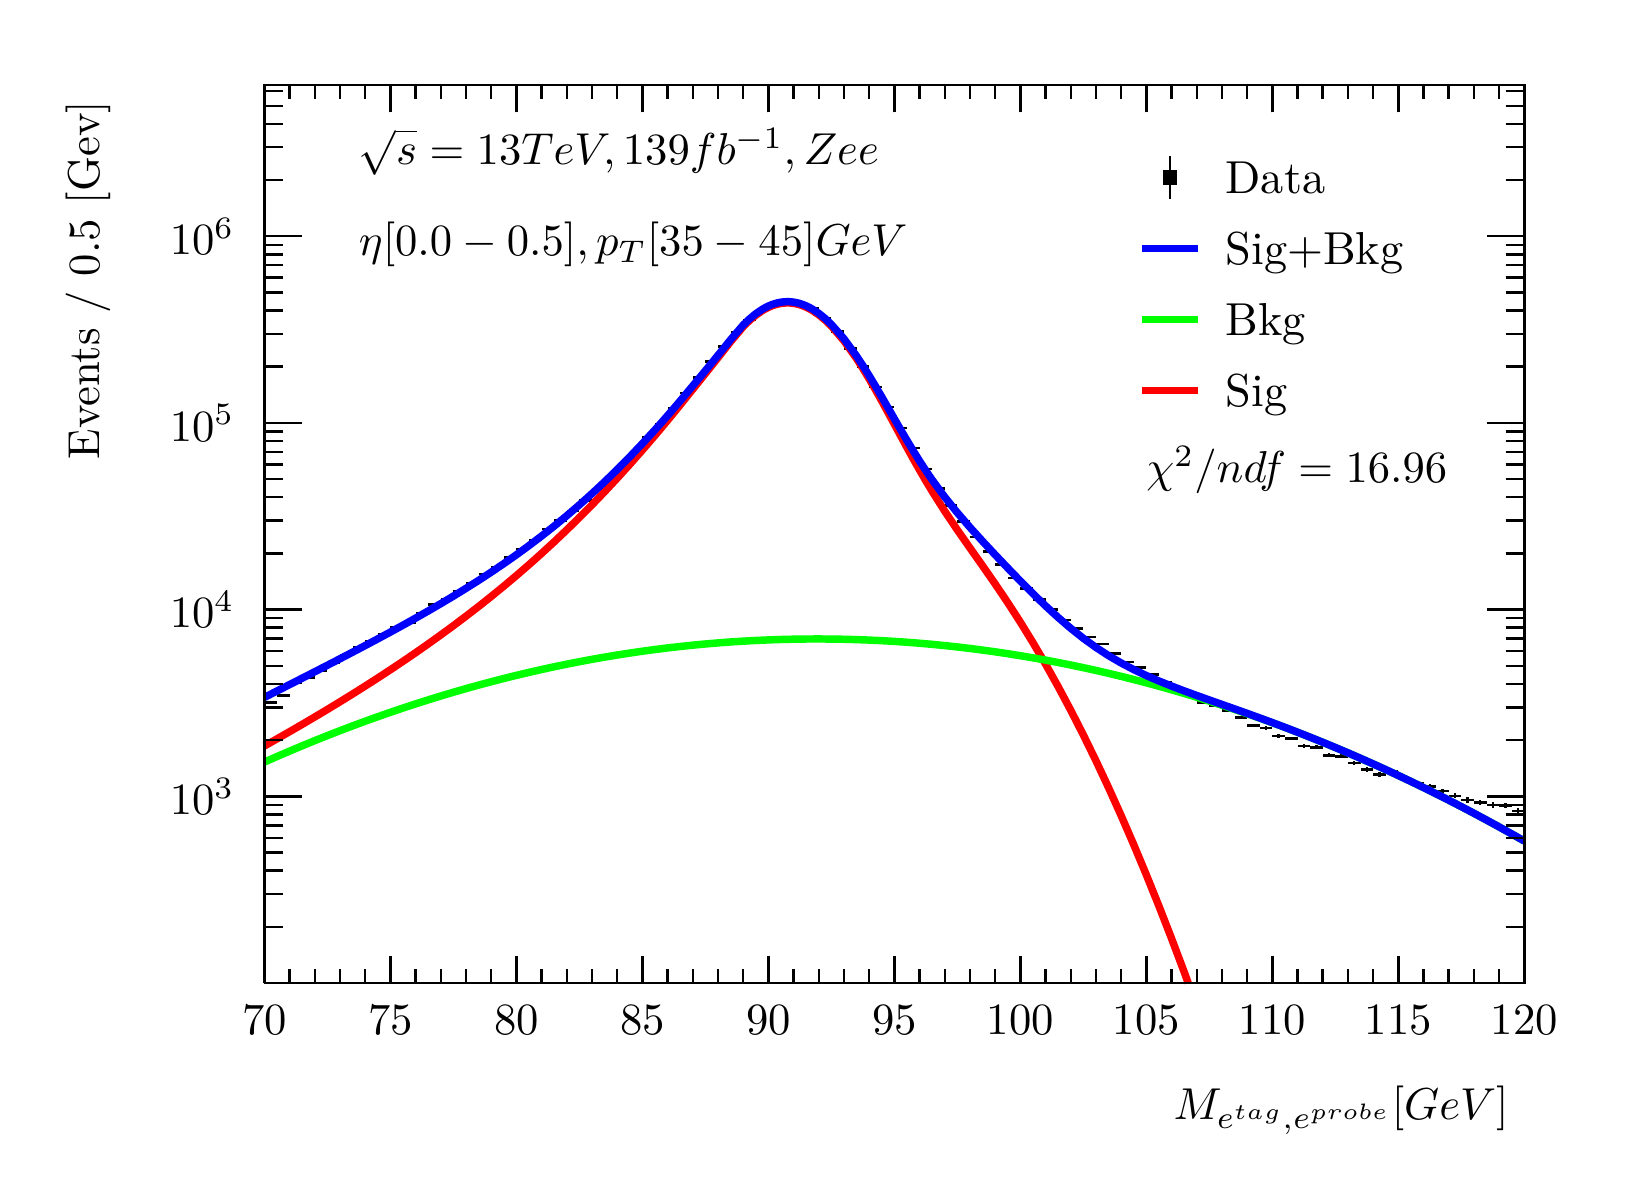
\begin{tikzpicture}
\pgfdeclareplotmark{cross} {
\pgfpathmoveto{\pgfpoint{-0.3\pgfplotmarksize}{\pgfplotmarksize}}
\pgfpathlineto{\pgfpoint{+0.3\pgfplotmarksize}{\pgfplotmarksize}}
\pgfpathlineto{\pgfpoint{+0.3\pgfplotmarksize}{0.3\pgfplotmarksize}}
\pgfpathlineto{\pgfpoint{+1\pgfplotmarksize}{0.3\pgfplotmarksize}}
\pgfpathlineto{\pgfpoint{+1\pgfplotmarksize}{-0.3\pgfplotmarksize}}
\pgfpathlineto{\pgfpoint{+0.3\pgfplotmarksize}{-0.3\pgfplotmarksize}}
\pgfpathlineto{\pgfpoint{+0.3\pgfplotmarksize}{-1.\pgfplotmarksize}}
\pgfpathlineto{\pgfpoint{-0.3\pgfplotmarksize}{-1.\pgfplotmarksize}}
\pgfpathlineto{\pgfpoint{-0.3\pgfplotmarksize}{-0.3\pgfplotmarksize}}
\pgfpathlineto{\pgfpoint{-1.\pgfplotmarksize}{-0.3\pgfplotmarksize}}
\pgfpathlineto{\pgfpoint{-1.\pgfplotmarksize}{0.3\pgfplotmarksize}}
\pgfpathlineto{\pgfpoint{-0.3\pgfplotmarksize}{0.3\pgfplotmarksize}}
\pgfpathclose
\pgfusepathqstroke
}
\pgfdeclareplotmark{cross*} {
\pgfpathmoveto{\pgfpoint{-0.3\pgfplotmarksize}{\pgfplotmarksize}}
\pgfpathlineto{\pgfpoint{+0.3\pgfplotmarksize}{\pgfplotmarksize}}
\pgfpathlineto{\pgfpoint{+0.3\pgfplotmarksize}{0.3\pgfplotmarksize}}
\pgfpathlineto{\pgfpoint{+1\pgfplotmarksize}{0.3\pgfplotmarksize}}
\pgfpathlineto{\pgfpoint{+1\pgfplotmarksize}{-0.3\pgfplotmarksize}}
\pgfpathlineto{\pgfpoint{+0.3\pgfplotmarksize}{-0.3\pgfplotmarksize}}
\pgfpathlineto{\pgfpoint{+0.3\pgfplotmarksize}{-1.\pgfplotmarksize}}
\pgfpathlineto{\pgfpoint{-0.3\pgfplotmarksize}{-1.\pgfplotmarksize}}
\pgfpathlineto{\pgfpoint{-0.3\pgfplotmarksize}{-0.3\pgfplotmarksize}}
\pgfpathlineto{\pgfpoint{-1.\pgfplotmarksize}{-0.3\pgfplotmarksize}}
\pgfpathlineto{\pgfpoint{-1.\pgfplotmarksize}{0.3\pgfplotmarksize}}
\pgfpathlineto{\pgfpoint{-0.3\pgfplotmarksize}{0.3\pgfplotmarksize}}
\pgfpathclose
\pgfusepathqfillstroke
}
\pgfdeclareplotmark{newstar} {
\pgfpathmoveto{\pgfqpoint{0pt}{\pgfplotmarksize}}
\pgfpathlineto{\pgfqpointpolar{44}{0.5\pgfplotmarksize}}
\pgfpathlineto{\pgfqpointpolar{18}{\pgfplotmarksize}}
\pgfpathlineto{\pgfqpointpolar{-20}{0.5\pgfplotmarksize}}
\pgfpathlineto{\pgfqpointpolar{-54}{\pgfplotmarksize}}
\pgfpathlineto{\pgfqpointpolar{-90}{0.5\pgfplotmarksize}}
\pgfpathlineto{\pgfqpointpolar{234}{\pgfplotmarksize}}
\pgfpathlineto{\pgfqpointpolar{198}{0.5\pgfplotmarksize}}
\pgfpathlineto{\pgfqpointpolar{162}{\pgfplotmarksize}}
\pgfpathlineto{\pgfqpointpolar{134}{0.5\pgfplotmarksize}}
\pgfpathclose
\pgfusepathqstroke
}
\pgfdeclareplotmark{newstar*} {
\pgfpathmoveto{\pgfqpoint{0pt}{\pgfplotmarksize}}
\pgfpathlineto{\pgfqpointpolar{44}{0.5\pgfplotmarksize}}
\pgfpathlineto{\pgfqpointpolar{18}{\pgfplotmarksize}}
\pgfpathlineto{\pgfqpointpolar{-20}{0.5\pgfplotmarksize}}
\pgfpathlineto{\pgfqpointpolar{-54}{\pgfplotmarksize}}
\pgfpathlineto{\pgfqpointpolar{-90}{0.5\pgfplotmarksize}}
\pgfpathlineto{\pgfqpointpolar{234}{\pgfplotmarksize}}
\pgfpathlineto{\pgfqpointpolar{198}{0.5\pgfplotmarksize}}
\pgfpathlineto{\pgfqpointpolar{162}{\pgfplotmarksize}}
\pgfpathlineto{\pgfqpointpolar{134}{0.5\pgfplotmarksize}}
\pgfpathclose
\pgfusepathqfillstroke
}
\definecolor{c}{rgb}{1,1,1};
\draw [color=c, fill=c] (0,0) rectangle (20,14.4361);
\draw [color=c, fill=c] (3,2.30977) rectangle (19,13.7143);
\definecolor{c}{rgb}{0,0,0};
\draw [c,line width=0.9] (3,2.30977) -- (3,13.7143) -- (19,13.7143) -- (19,2.30977) -- (3,2.30977);
\definecolor{c}{rgb}{1,1,1};
\draw [color=c, fill=c] (3,2.30977) rectangle (19,13.7143);
\definecolor{c}{rgb}{0,0,0};
\draw [c,line width=0.9] (3,2.30977) -- (3,13.7143) -- (19,13.7143) -- (19,2.30977) -- (3,2.30977);
\draw [c,line width=0.9] (3,2.30977) -- (19,2.30977);
\draw [c,line width=0.9] (3,2.65624) -- (3,2.30977);
\draw [c,line width=0.9] (3.32,2.48301) -- (3.32,2.30977);
\draw [c,line width=0.9] (3.64,2.48301) -- (3.64,2.30977);
\draw [c,line width=0.9] (3.96,2.48301) -- (3.96,2.30977);
\draw [c,line width=0.9] (4.28,2.48301) -- (4.28,2.30977);
\draw [c,line width=0.9] (4.6,2.65624) -- (4.6,2.30977);
\draw [c,line width=0.9] (4.92,2.48301) -- (4.92,2.30977);
\draw [c,line width=0.9] (5.24,2.48301) -- (5.24,2.30977);
\draw [c,line width=0.9] (5.56,2.48301) -- (5.56,2.30977);
\draw [c,line width=0.9] (5.88,2.48301) -- (5.88,2.30977);
\draw [c,line width=0.9] (6.2,2.65624) -- (6.2,2.30977);
\draw [c,line width=0.9] (6.52,2.48301) -- (6.52,2.30977);
\draw [c,line width=0.9] (6.84,2.48301) -- (6.84,2.30977);
\draw [c,line width=0.9] (7.16,2.48301) -- (7.16,2.30977);
\draw [c,line width=0.9] (7.48,2.48301) -- (7.48,2.30977);
\draw [c,line width=0.9] (7.8,2.65624) -- (7.8,2.30977);
\draw [c,line width=0.9] (8.12,2.48301) -- (8.12,2.30977);
\draw [c,line width=0.9] (8.44,2.48301) -- (8.44,2.30977);
\draw [c,line width=0.9] (8.76,2.48301) -- (8.76,2.30977);
\draw [c,line width=0.9] (9.08,2.48301) -- (9.08,2.30977);
\draw [c,line width=0.9] (9.4,2.65624) -- (9.4,2.30977);
\draw [c,line width=0.9] (9.72,2.48301) -- (9.72,2.30977);
\draw [c,line width=0.9] (10.04,2.48301) -- (10.04,2.30977);
\draw [c,line width=0.9] (10.36,2.48301) -- (10.36,2.30977);
\draw [c,line width=0.9] (10.68,2.48301) -- (10.68,2.30977);
\draw [c,line width=0.9] (11,2.65624) -- (11,2.30977);
\draw [c,line width=0.9] (11.32,2.48301) -- (11.32,2.30977);
\draw [c,line width=0.9] (11.64,2.48301) -- (11.64,2.30977);
\draw [c,line width=0.9] (11.96,2.48301) -- (11.96,2.30977);
\draw [c,line width=0.9] (12.28,2.48301) -- (12.28,2.30977);
\draw [c,line width=0.9] (12.6,2.65624) -- (12.6,2.30977);
\draw [c,line width=0.9] (12.92,2.48301) -- (12.92,2.30977);
\draw [c,line width=0.9] (13.24,2.48301) -- (13.24,2.30977);
\draw [c,line width=0.9] (13.56,2.48301) -- (13.56,2.30977);
\draw [c,line width=0.9] (13.88,2.48301) -- (13.88,2.30977);
\draw [c,line width=0.9] (14.2,2.65624) -- (14.2,2.30977);
\draw [c,line width=0.9] (14.52,2.48301) -- (14.52,2.30977);
\draw [c,line width=0.9] (14.84,2.48301) -- (14.84,2.30977);
\draw [c,line width=0.9] (15.16,2.48301) -- (15.16,2.30977);
\draw [c,line width=0.9] (15.48,2.48301) -- (15.48,2.30977);
\draw [c,line width=0.9] (15.8,2.65624) -- (15.8,2.30977);
\draw [c,line width=0.9] (16.12,2.48301) -- (16.12,2.30977);
\draw [c,line width=0.9] (16.44,2.48301) -- (16.44,2.30977);
\draw [c,line width=0.9] (16.76,2.48301) -- (16.76,2.30977);
\draw [c,line width=0.9] (17.08,2.48301) -- (17.08,2.30977);
\draw [c,line width=0.9] (17.4,2.65624) -- (17.4,2.30977);
\draw [c,line width=0.9] (17.72,2.48301) -- (17.72,2.30977);
\draw [c,line width=0.9] (18.04,2.48301) -- (18.04,2.30977);
\draw [c,line width=0.9] (18.36,2.48301) -- (18.36,2.30977);
\draw [c,line width=0.9] (18.68,2.48301) -- (18.68,2.30977);
\draw [c,line width=0.9] (19,2.65624) -- (19,2.30977);
\draw [anchor=base] (3,1.66015) node[scale=1.61424, color=c, rotate=0]{70};
\draw [anchor=base] (4.6,1.66015) node[scale=1.61424, color=c, rotate=0]{75};
\draw [anchor=base] (6.2,1.66015) node[scale=1.61424, color=c, rotate=0]{80};
\draw [anchor=base] (7.8,1.66015) node[scale=1.61424, color=c, rotate=0]{85};
\draw [anchor=base] (9.4,1.66015) node[scale=1.61424, color=c, rotate=0]{90};
\draw [anchor=base] (11,1.66015) node[scale=1.61424, color=c, rotate=0]{95};
\draw [anchor=base] (12.6,1.66015) node[scale=1.61424, color=c, rotate=0]{100};
\draw [anchor=base] (14.2,1.66015) node[scale=1.61424, color=c, rotate=0]{105};
\draw [anchor=base] (15.8,1.66015) node[scale=1.61424, color=c, rotate=0]{110};
\draw [anchor=base] (17.4,1.66015) node[scale=1.61424, color=c, rotate=0]{115};
\draw [anchor=base] (19,1.66015) node[scale=1.61424, color=c, rotate=0]{120};
\draw [anchor= east] (19,0.692932) node[scale=1.61424, color=c, rotate=0]{$M_{e^{tag}, e^{probe}}  [GeV]$};
\draw [c,line width=0.9] (3,13.7143) -- (19,13.7143);
\draw [c,line width=0.9] (3,13.3678) -- (3,13.7143);
\draw [c,line width=0.9] (3.32,13.5411) -- (3.32,13.7143);
\draw [c,line width=0.9] (3.64,13.5411) -- (3.64,13.7143);
\draw [c,line width=0.9] (3.96,13.5411) -- (3.96,13.7143);
\draw [c,line width=0.9] (4.28,13.5411) -- (4.28,13.7143);
\draw [c,line width=0.9] (4.6,13.3678) -- (4.6,13.7143);
\draw [c,line width=0.9] (4.92,13.5411) -- (4.92,13.7143);
\draw [c,line width=0.9] (5.24,13.5411) -- (5.24,13.7143);
\draw [c,line width=0.9] (5.56,13.5411) -- (5.56,13.7143);
\draw [c,line width=0.9] (5.88,13.5411) -- (5.88,13.7143);
\draw [c,line width=0.9] (6.2,13.3678) -- (6.2,13.7143);
\draw [c,line width=0.9] (6.52,13.5411) -- (6.52,13.7143);
\draw [c,line width=0.9] (6.84,13.5411) -- (6.84,13.7143);
\draw [c,line width=0.9] (7.16,13.5411) -- (7.16,13.7143);
\draw [c,line width=0.9] (7.48,13.5411) -- (7.48,13.7143);
\draw [c,line width=0.9] (7.8,13.3678) -- (7.8,13.7143);
\draw [c,line width=0.9] (8.12,13.5411) -- (8.12,13.7143);
\draw [c,line width=0.9] (8.44,13.5411) -- (8.44,13.7143);
\draw [c,line width=0.9] (8.76,13.5411) -- (8.76,13.7143);
\draw [c,line width=0.9] (9.08,13.5411) -- (9.08,13.7143);
\draw [c,line width=0.9] (9.4,13.3678) -- (9.4,13.7143);
\draw [c,line width=0.9] (9.72,13.5411) -- (9.72,13.7143);
\draw [c,line width=0.9] (10.04,13.5411) -- (10.04,13.7143);
\draw [c,line width=0.9] (10.36,13.5411) -- (10.36,13.7143);
\draw [c,line width=0.9] (10.68,13.5411) -- (10.68,13.7143);
\draw [c,line width=0.9] (11,13.3678) -- (11,13.7143);
\draw [c,line width=0.9] (11.32,13.5411) -- (11.32,13.7143);
\draw [c,line width=0.9] (11.64,13.5411) -- (11.64,13.7143);
\draw [c,line width=0.9] (11.96,13.5411) -- (11.96,13.7143);
\draw [c,line width=0.9] (12.28,13.5411) -- (12.28,13.7143);
\draw [c,line width=0.9] (12.6,13.3678) -- (12.6,13.7143);
\draw [c,line width=0.9] (12.92,13.5411) -- (12.92,13.7143);
\draw [c,line width=0.9] (13.24,13.5411) -- (13.24,13.7143);
\draw [c,line width=0.9] (13.56,13.5411) -- (13.56,13.7143);
\draw [c,line width=0.9] (13.88,13.5411) -- (13.88,13.7143);
\draw [c,line width=0.9] (14.2,13.3678) -- (14.2,13.7143);
\draw [c,line width=0.9] (14.52,13.5411) -- (14.52,13.7143);
\draw [c,line width=0.9] (14.84,13.5411) -- (14.84,13.7143);
\draw [c,line width=0.9] (15.16,13.5411) -- (15.16,13.7143);
\draw [c,line width=0.9] (15.48,13.5411) -- (15.48,13.7143);
\draw [c,line width=0.9] (15.8,13.3678) -- (15.8,13.7143);
\draw [c,line width=0.9] (16.12,13.5411) -- (16.12,13.7143);
\draw [c,line width=0.9] (16.44,13.5411) -- (16.44,13.7143);
\draw [c,line width=0.9] (16.76,13.5411) -- (16.76,13.7143);
\draw [c,line width=0.9] (17.08,13.5411) -- (17.08,13.7143);
\draw [c,line width=0.9] (17.4,13.3678) -- (17.4,13.7143);
\draw [c,line width=0.9] (17.72,13.5411) -- (17.72,13.7143);
\draw [c,line width=0.9] (18.04,13.5411) -- (18.04,13.7143);
\draw [c,line width=0.9] (18.36,13.5411) -- (18.36,13.7143);
\draw [c,line width=0.9] (18.68,13.5411) -- (18.68,13.7143);
\draw [c,line width=0.9] (19,13.3678) -- (19,13.7143);
\draw [c,line width=0.9] (3,2.30977) -- (3,13.7143);
\draw [c,line width=0.9] (3.237,3.02354) -- (3,3.02354);
\draw [c,line width=0.9] (3.237,3.44107) -- (3,3.44107);
\draw [c,line width=0.9] (3.237,3.73731) -- (3,3.73731);
\draw [c,line width=0.9] (3.237,3.96709) -- (3,3.96709);
\draw [c,line width=0.9] (3.237,4.15484) -- (3,4.15484);
\draw [c,line width=0.9] (3.237,4.31357) -- (3,4.31357);
\draw [c,line width=0.9] (3.237,4.45108) -- (3,4.45108);
\draw [c,line width=0.9] (3.237,4.57236) -- (3,4.57236);
\draw [c,line width=0.9] (3.474,4.68086) -- (3,4.68086);
\draw [anchor= east] (2.82,4.68086) node[scale=1.61424, color=c, rotate=0]{$10^{3}$};
\draw [c,line width=0.9] (3.237,5.39463) -- (3,5.39463);
\draw [c,line width=0.9] (3.237,5.81216) -- (3,5.81216);
\draw [c,line width=0.9] (3.237,6.1084) -- (3,6.1084);
\draw [c,line width=0.9] (3.237,6.33818) -- (3,6.33818);
\draw [c,line width=0.9] (3.237,6.52593) -- (3,6.52593);
\draw [c,line width=0.9] (3.237,6.68466) -- (3,6.68466);
\draw [c,line width=0.9] (3.237,6.82217) -- (3,6.82217);
\draw [c,line width=0.9] (3.237,6.94345) -- (3,6.94345);
\draw [c,line width=0.9] (3.474,7.05195) -- (3,7.05195);
\draw [anchor= east] (2.82,7.05195) node[scale=1.61424, color=c, rotate=0]{$10^{4}$};
\draw [c,line width=0.9] (3.237,7.76572) -- (3,7.76572);
\draw [c,line width=0.9] (3.237,8.18324) -- (3,8.18324);
\draw [c,line width=0.9] (3.237,8.47948) -- (3,8.47948);
\draw [c,line width=0.9] (3.237,8.70927) -- (3,8.70927);
\draw [c,line width=0.9] (3.237,8.89701) -- (3,8.89701);
\draw [c,line width=0.9] (3.237,9.05575) -- (3,9.05575);
\draw [c,line width=0.9] (3.237,9.19325) -- (3,9.19325);
\draw [c,line width=0.9] (3.237,9.31454) -- (3,9.31454);
\draw [c,line width=0.9] (3.474,9.42304) -- (3,9.42304);
\draw [anchor= east] (2.82,9.42304) node[scale=1.61424, color=c, rotate=0]{$10^{5}$};
\draw [c,line width=0.9] (3.237,10.1368) -- (3,10.1368);
\draw [c,line width=0.9] (3.237,10.5543) -- (3,10.5543);
\draw [c,line width=0.9] (3.237,10.8506) -- (3,10.8506);
\draw [c,line width=0.9] (3.237,11.0804) -- (3,11.0804);
\draw [c,line width=0.9] (3.237,11.2681) -- (3,11.2681);
\draw [c,line width=0.9] (3.237,11.4268) -- (3,11.4268);
\draw [c,line width=0.9] (3.237,11.5643) -- (3,11.5643);
\draw [c,line width=0.9] (3.237,11.6856) -- (3,11.6856);
\draw [c,line width=0.9] (3.474,11.7941) -- (3,11.7941);
\draw [anchor= east] (2.82,11.7941) node[scale=1.61424, color=c, rotate=0]{$10^{6}$};
\draw [c,line width=0.9] (3.237,12.5079) -- (3,12.5079);
\draw [c,line width=0.9] (3.237,12.9254) -- (3,12.9254);
\draw [c,line width=0.9] (3.237,13.2217) -- (3,13.2217);
\draw [c,line width=0.9] (3.237,13.4514) -- (3,13.4514);
\draw [c,line width=0.9] (3.237,13.6392) -- (3,13.6392);
\draw [anchor= east] (0.76,13.7143) node[scale=1.61424, color=c, rotate=90]{Events / 0.5 [Gev]};
\draw [c,line width=0.9] (19,2.30977) -- (19,13.7143);
\draw [c,line width=0.9] (18.763,3.02354) -- (19,3.02354);
\draw [c,line width=0.9] (18.763,3.44107) -- (19,3.44107);
\draw [c,line width=0.9] (18.763,3.73731) -- (19,3.73731);
\draw [c,line width=0.9] (18.763,3.96709) -- (19,3.96709);
\draw [c,line width=0.9] (18.763,4.15484) -- (19,4.15484);
\draw [c,line width=0.9] (18.763,4.31357) -- (19,4.31357);
\draw [c,line width=0.9] (18.763,4.45108) -- (19,4.45108);
\draw [c,line width=0.9] (18.763,4.57236) -- (19,4.57236);
\draw [c,line width=0.9] (18.526,4.68086) -- (19,4.68086);
\draw [c,line width=0.9] (18.763,5.39463) -- (19,5.39463);
\draw [c,line width=0.9] (18.763,5.81216) -- (19,5.81216);
\draw [c,line width=0.9] (18.763,6.1084) -- (19,6.1084);
\draw [c,line width=0.9] (18.763,6.33818) -- (19,6.33818);
\draw [c,line width=0.9] (18.763,6.52593) -- (19,6.52593);
\draw [c,line width=0.9] (18.763,6.68466) -- (19,6.68466);
\draw [c,line width=0.9] (18.763,6.82217) -- (19,6.82217);
\draw [c,line width=0.9] (18.763,6.94345) -- (19,6.94345);
\draw [c,line width=0.9] (18.526,7.05195) -- (19,7.05195);
\draw [c,line width=0.9] (18.763,7.76572) -- (19,7.76572);
\draw [c,line width=0.9] (18.763,8.18324) -- (19,8.18324);
\draw [c,line width=0.9] (18.763,8.47948) -- (19,8.47948);
\draw [c,line width=0.9] (18.763,8.70927) -- (19,8.70927);
\draw [c,line width=0.9] (18.763,8.89701) -- (19,8.89701);
\draw [c,line width=0.9] (18.763,9.05575) -- (19,9.05575);
\draw [c,line width=0.9] (18.763,9.19325) -- (19,9.19325);
\draw [c,line width=0.9] (18.763,9.31454) -- (19,9.31454);
\draw [c,line width=0.9] (18.526,9.42304) -- (19,9.42304);
\draw [c,line width=0.9] (18.763,10.1368) -- (19,10.1368);
\draw [c,line width=0.9] (18.763,10.5543) -- (19,10.5543);
\draw [c,line width=0.9] (18.763,10.8506) -- (19,10.8506);
\draw [c,line width=0.9] (18.763,11.0804) -- (19,11.0804);
\draw [c,line width=0.9] (18.763,11.2681) -- (19,11.2681);
\draw [c,line width=0.9] (18.763,11.4268) -- (19,11.4268);
\draw [c,line width=0.9] (18.763,11.5643) -- (19,11.5643);
\draw [c,line width=0.9] (18.763,11.6856) -- (19,11.6856);
\draw [c,line width=0.9] (18.526,11.7941) -- (19,11.7941);
\draw [c,line width=0.9] (18.763,12.5079) -- (19,12.5079);
\draw [c,line width=0.9] (18.763,12.9254) -- (19,12.9254);
\draw [c,line width=0.9] (18.763,13.2217) -- (19,13.2217);
\draw [c,line width=0.9] (18.763,13.4514) -- (19,13.4514);
\draw [c,line width=0.9] (18.763,13.6392) -- (19,13.6392);
\draw [c,line width=0.9] (3.08,5.87086) -- (3,5.87086);
\draw [c,line width=0.9] (3,5.87086) -- (3,5.87086);
\draw [c,line width=0.9] (3.08,5.87086) -- (3.16,5.87086);
\draw [c,line width=0.9] (3.16,5.87086) -- (3.16,5.87086);
\draw [c,line width=0.9] (3.08,5.87086) -- (3.08,5.88914);
\draw [c,line width=0.9] (3.08,5.88914) -- (3.08,5.88914);
\draw [c,line width=0.9] (3.08,5.87086) -- (3.08,5.85259);
\draw [c,line width=0.9] (3.08,5.85259) -- (3.08,5.85259);
\draw [c,line width=0.9] (3.24,5.95965) -- (3.16,5.95965);
\draw [c,line width=0.9] (3.16,5.95965) -- (3.16,5.95965);
\draw [c,line width=0.9] (3.24,5.95965) -- (3.32,5.95965);
\draw [c,line width=0.9] (3.32,5.95965) -- (3.32,5.95965);
\draw [c,line width=0.9] (3.24,5.95965) -- (3.24,5.97715);
\draw [c,line width=0.9] (3.24,5.97715) -- (3.24,5.97715);
\draw [c,line width=0.9] (3.24,5.95965) -- (3.24,5.94215);
\draw [c,line width=0.9] (3.24,5.94215) -- (3.24,5.94215);
\draw [c,line width=0.9] (3.4,6.12246) -- (3.32,6.12246);
\draw [c,line width=0.9] (3.32,6.12246) -- (3.32,6.12246);
\draw [c,line width=0.9] (3.4,6.12246) -- (3.48,6.12246);
\draw [c,line width=0.9] (3.48,6.12246) -- (3.48,6.12246);
\draw [c,line width=0.9] (3.4,6.12246) -- (3.4,6.13863);
\draw [c,line width=0.9] (3.4,6.13863) -- (3.4,6.13863);
\draw [c,line width=0.9] (3.4,6.12246) -- (3.4,6.10629);
\draw [c,line width=0.9] (3.4,6.10629) -- (3.4,6.10629);
\draw [c,line width=0.9] (3.56,6.19027) -- (3.48,6.19027);
\draw [c,line width=0.9] (3.48,6.19027) -- (3.48,6.19027);
\draw [c,line width=0.9] (3.56,6.19027) -- (3.64,6.19027);
\draw [c,line width=0.9] (3.64,6.19027) -- (3.64,6.19027);
\draw [c,line width=0.9] (3.56,6.19027) -- (3.56,6.20591);
\draw [c,line width=0.9] (3.56,6.20591) -- (3.56,6.20591);
\draw [c,line width=0.9] (3.56,6.19027) -- (3.56,6.17462);
\draw [c,line width=0.9] (3.56,6.17462) -- (3.56,6.17462);
\draw [c,line width=0.9] (3.72,6.27556) -- (3.64,6.27556);
\draw [c,line width=0.9] (3.64,6.27556) -- (3.64,6.27556);
\draw [c,line width=0.9] (3.72,6.27556) -- (3.8,6.27556);
\draw [c,line width=0.9] (3.8,6.27556) -- (3.8,6.27556);
\draw [c,line width=0.9] (3.72,6.27556) -- (3.72,6.29057);
\draw [c,line width=0.9] (3.72,6.29057) -- (3.72,6.29057);
\draw [c,line width=0.9] (3.72,6.27556) -- (3.72,6.26055);
\draw [c,line width=0.9] (3.72,6.26055) -- (3.72,6.26055);
\draw [c,line width=0.9] (3.88,6.37916) -- (3.8,6.37916);
\draw [c,line width=0.9] (3.8,6.37916) -- (3.8,6.37916);
\draw [c,line width=0.9] (3.88,6.37916) -- (3.96,6.37916);
\draw [c,line width=0.9] (3.96,6.37916) -- (3.96,6.37916);
\draw [c,line width=0.9] (3.88,6.37916) -- (3.88,6.39344);
\draw [c,line width=0.9] (3.88,6.39344) -- (3.88,6.39344);
\draw [c,line width=0.9] (3.88,6.37916) -- (3.88,6.36489);
\draw [c,line width=0.9] (3.88,6.36489) -- (3.88,6.36489);
\draw [c,line width=0.9] (4.04,6.47509) -- (3.96,6.47509);
\draw [c,line width=0.9] (3.96,6.47509) -- (3.96,6.47509);
\draw [c,line width=0.9] (4.04,6.47509) -- (4.12,6.47509);
\draw [c,line width=0.9] (4.12,6.47509) -- (4.12,6.47509);
\draw [c,line width=0.9] (4.04,6.47509) -- (4.04,6.48872);
\draw [c,line width=0.9] (4.04,6.48872) -- (4.04,6.48872);
\draw [c,line width=0.9] (4.04,6.47509) -- (4.04,6.46147);
\draw [c,line width=0.9] (4.04,6.46147) -- (4.04,6.46147);
\draw [c,line width=0.9] (4.2,6.576) -- (4.12,6.576);
\draw [c,line width=0.9] (4.12,6.576) -- (4.12,6.576);
\draw [c,line width=0.9] (4.2,6.576) -- (4.28,6.576);
\draw [c,line width=0.9] (4.28,6.576) -- (4.28,6.576);
\draw [c,line width=0.9] (4.2,6.576) -- (4.2,6.58898);
\draw [c,line width=0.9] (4.2,6.58898) -- (4.2,6.58898);
\draw [c,line width=0.9] (4.2,6.576) -- (4.2,6.56303);
\draw [c,line width=0.9] (4.2,6.56303) -- (4.2,6.56303);
\draw [c,line width=0.9] (4.36,6.64508) -- (4.28,6.64508);
\draw [c,line width=0.9] (4.28,6.64508) -- (4.28,6.64508);
\draw [c,line width=0.9] (4.36,6.64508) -- (4.44,6.64508);
\draw [c,line width=0.9] (4.44,6.64508) -- (4.44,6.64508);
\draw [c,line width=0.9] (4.36,6.64508) -- (4.36,6.65762);
\draw [c,line width=0.9] (4.36,6.65762) -- (4.36,6.65762);
\draw [c,line width=0.9] (4.36,6.64508) -- (4.36,6.63253);
\draw [c,line width=0.9] (4.36,6.63253) -- (4.36,6.63253);
\draw [c,line width=0.9] (4.52,6.7335) -- (4.44,6.7335);
\draw [c,line width=0.9] (4.44,6.7335) -- (4.44,6.7335);
\draw [c,line width=0.9] (4.52,6.7335) -- (4.6,6.7335);
\draw [c,line width=0.9] (4.6,6.7335) -- (4.6,6.7335);
\draw [c,line width=0.9] (4.52,6.7335) -- (4.52,6.74552);
\draw [c,line width=0.9] (4.52,6.74552) -- (4.52,6.74552);
\draw [c,line width=0.9] (4.52,6.7335) -- (4.52,6.72148);
\draw [c,line width=0.9] (4.52,6.72148) -- (4.52,6.72148);
\draw [c,line width=0.9] (4.68,6.83216) -- (4.6,6.83216);
\draw [c,line width=0.9] (4.6,6.83216) -- (4.6,6.83216);
\draw [c,line width=0.9] (4.68,6.83216) -- (4.76,6.83216);
\draw [c,line width=0.9] (4.76,6.83216) -- (4.76,6.83216);
\draw [c,line width=0.9] (4.68,6.83216) -- (4.68,6.84362);
\draw [c,line width=0.9] (4.68,6.84362) -- (4.68,6.84362);
\draw [c,line width=0.9] (4.68,6.83216) -- (4.68,6.8207);
\draw [c,line width=0.9] (4.68,6.8207) -- (4.68,6.8207);
\draw [c,line width=0.9] (4.84,6.88786) -- (4.76,6.88786);
\draw [c,line width=0.9] (4.76,6.88786) -- (4.76,6.88786);
\draw [c,line width=0.9] (4.84,6.88786) -- (4.92,6.88786);
\draw [c,line width=0.9] (4.92,6.88786) -- (4.92,6.88786);
\draw [c,line width=0.9] (4.84,6.88786) -- (4.84,6.89901);
\draw [c,line width=0.9] (4.84,6.89901) -- (4.84,6.89901);
\draw [c,line width=0.9] (4.84,6.88786) -- (4.84,6.87671);
\draw [c,line width=0.9] (4.84,6.87671) -- (4.84,6.87671);
\draw [c,line width=0.9] (5,7.00162) -- (4.92,7.00162);
\draw [c,line width=0.9] (4.92,7.00162) -- (4.92,7.00162);
\draw [c,line width=0.9] (5,7.00162) -- (5.08,7.00162);
\draw [c,line width=0.9] (5.08,7.00162) -- (5.08,7.00162);
\draw [c,line width=0.9] (5,7.00162) -- (5,7.01217);
\draw [c,line width=0.9] (5,7.01217) -- (5,7.01217);
\draw [c,line width=0.9] (5,7.00162) -- (5,6.99107);
\draw [c,line width=0.9] (5,6.99107) -- (5,6.99107);
\draw [c,line width=0.9] (5.16,7.11506) -- (5.08,7.11506);
\draw [c,line width=0.9] (5.08,7.11506) -- (5.08,7.11506);
\draw [c,line width=0.9] (5.16,7.11506) -- (5.24,7.11506);
\draw [c,line width=0.9] (5.24,7.11506) -- (5.24,7.11506);
\draw [c,line width=0.9] (5.16,7.11506) -- (5.16,7.12504);
\draw [c,line width=0.9] (5.16,7.12504) -- (5.16,7.12504);
\draw [c,line width=0.9] (5.16,7.11506) -- (5.16,7.10507);
\draw [c,line width=0.9] (5.16,7.10507) -- (5.16,7.10507);
\draw [c,line width=0.9] (5.32,7.18416) -- (5.24,7.18416);
\draw [c,line width=0.9] (5.24,7.18416) -- (5.24,7.18416);
\draw [c,line width=0.9] (5.32,7.18416) -- (5.4,7.18416);
\draw [c,line width=0.9] (5.4,7.18416) -- (5.4,7.18416);
\draw [c,line width=0.9] (5.32,7.18416) -- (5.32,7.19382);
\draw [c,line width=0.9] (5.32,7.19382) -- (5.32,7.19382);
\draw [c,line width=0.9] (5.32,7.18416) -- (5.32,7.1745);
\draw [c,line width=0.9] (5.32,7.1745) -- (5.32,7.1745);
\draw [c,line width=0.9] (5.48,7.28543) -- (5.4,7.28543);
\draw [c,line width=0.9] (5.4,7.28543) -- (5.4,7.28543);
\draw [c,line width=0.9] (5.48,7.28543) -- (5.56,7.28543);
\draw [c,line width=0.9] (5.56,7.28543) -- (5.56,7.28543);
\draw [c,line width=0.9] (5.48,7.28543) -- (5.48,7.29463);
\draw [c,line width=0.9] (5.48,7.29463) -- (5.48,7.29463);
\draw [c,line width=0.9] (5.48,7.28543) -- (5.48,7.27624);
\draw [c,line width=0.9] (5.48,7.27624) -- (5.48,7.27624);
\draw [c,line width=0.9] (5.64,7.38674) -- (5.56,7.38674);
\draw [c,line width=0.9] (5.56,7.38674) -- (5.56,7.38674);
\draw [c,line width=0.9] (5.64,7.38674) -- (5.72,7.38674);
\draw [c,line width=0.9] (5.72,7.38674) -- (5.72,7.38674);
\draw [c,line width=0.9] (5.64,7.38674) -- (5.64,7.3955);
\draw [c,line width=0.9] (5.64,7.3955) -- (5.64,7.3955);
\draw [c,line width=0.9] (5.64,7.38674) -- (5.64,7.37799);
\draw [c,line width=0.9] (5.64,7.37799) -- (5.64,7.37799);
\draw [c,line width=0.9] (5.8,7.50696) -- (5.72,7.50696);
\draw [c,line width=0.9] (5.72,7.50696) -- (5.72,7.50696);
\draw [c,line width=0.9] (5.8,7.50696) -- (5.88,7.50696);
\draw [c,line width=0.9] (5.88,7.50696) -- (5.88,7.50696);
\draw [c,line width=0.9] (5.8,7.50696) -- (5.8,7.51521);
\draw [c,line width=0.9] (5.8,7.51521) -- (5.8,7.51521);
\draw [c,line width=0.9] (5.8,7.50696) -- (5.8,7.4987);
\draw [c,line width=0.9] (5.8,7.4987) -- (5.8,7.4987);
\draw [c,line width=0.9] (5.96,7.59618) -- (5.88,7.59618);
\draw [c,line width=0.9] (5.88,7.59618) -- (5.88,7.59618);
\draw [c,line width=0.9] (5.96,7.59618) -- (6.04,7.59618);
\draw [c,line width=0.9] (6.04,7.59618) -- (6.04,7.59618);
\draw [c,line width=0.9] (5.96,7.59618) -- (5.96,7.60409);
\draw [c,line width=0.9] (5.96,7.60409) -- (5.96,7.60409);
\draw [c,line width=0.9] (5.96,7.59618) -- (5.96,7.58827);
\draw [c,line width=0.9] (5.96,7.58827) -- (5.96,7.58827);
\draw [c,line width=0.9] (6.12,7.71447) -- (6.04,7.71447);
\draw [c,line width=0.9] (6.04,7.71447) -- (6.04,7.71447);
\draw [c,line width=0.9] (6.12,7.71447) -- (6.2,7.71447);
\draw [c,line width=0.9] (6.2,7.71447) -- (6.2,7.71447);
\draw [c,line width=0.9] (6.12,7.71447) -- (6.12,7.72193);
\draw [c,line width=0.9] (6.12,7.72193) -- (6.12,7.72193);
\draw [c,line width=0.9] (6.12,7.71447) -- (6.12,7.707);
\draw [c,line width=0.9] (6.12,7.707) -- (6.12,7.707);
\draw [c,line width=0.9] (6.28,7.82212) -- (6.2,7.82212);
\draw [c,line width=0.9] (6.2,7.82212) -- (6.2,7.82212);
\draw [c,line width=0.9] (6.28,7.82212) -- (6.36,7.82212);
\draw [c,line width=0.9] (6.36,7.82212) -- (6.36,7.82212);
\draw [c,line width=0.9] (6.28,7.82212) -- (6.28,7.8292);
\draw [c,line width=0.9] (6.28,7.8292) -- (6.28,7.8292);
\draw [c,line width=0.9] (6.28,7.82212) -- (6.28,7.81503);
\draw [c,line width=0.9] (6.28,7.81503) -- (6.28,7.81503);
\draw [c,line width=0.9] (6.44,7.93472) -- (6.36,7.93472);
\draw [c,line width=0.9] (6.36,7.93472) -- (6.36,7.93472);
\draw [c,line width=0.9] (6.44,7.93472) -- (6.52,7.93472);
\draw [c,line width=0.9] (6.52,7.93472) -- (6.52,7.93472);
\draw [c,line width=0.9] (6.44,7.93472) -- (6.44,7.94142);
\draw [c,line width=0.9] (6.44,7.94142) -- (6.44,7.94142);
\draw [c,line width=0.9] (6.44,7.93472) -- (6.44,7.92801);
\draw [c,line width=0.9] (6.44,7.92801) -- (6.44,7.92801);
\draw [c,line width=0.9] (6.6,8.07448) -- (6.52,8.07448);
\draw [c,line width=0.9] (6.52,8.07448) -- (6.52,8.07448);
\draw [c,line width=0.9] (6.6,8.07448) -- (6.68,8.07448);
\draw [c,line width=0.9] (6.68,8.07448) -- (6.68,8.07448);
\draw [c,line width=0.9] (6.6,8.07448) -- (6.6,8.08075);
\draw [c,line width=0.9] (6.6,8.08075) -- (6.6,8.08075);
\draw [c,line width=0.9] (6.6,8.07448) -- (6.6,8.06822);
\draw [c,line width=0.9] (6.6,8.06822) -- (6.6,8.06822);
\draw [c,line width=0.9] (6.76,8.18149) -- (6.68,8.18149);
\draw [c,line width=0.9] (6.68,8.18149) -- (6.68,8.18149);
\draw [c,line width=0.9] (6.76,8.18149) -- (6.84,8.18149);
\draw [c,line width=0.9] (6.84,8.18149) -- (6.84,8.18149);
\draw [c,line width=0.9] (6.76,8.18149) -- (6.76,8.18744);
\draw [c,line width=0.9] (6.76,8.18744) -- (6.76,8.18744);
\draw [c,line width=0.9] (6.76,8.18149) -- (6.76,8.17554);
\draw [c,line width=0.9] (6.76,8.17554) -- (6.76,8.17554);
\draw [c,line width=0.9] (6.92,8.30533) -- (6.84,8.30533);
\draw [c,line width=0.9] (6.84,8.30533) -- (6.84,8.30533);
\draw [c,line width=0.9] (6.92,8.30533) -- (7,8.30533);
\draw [c,line width=0.9] (7,8.30533) -- (7,8.30533);
\draw [c,line width=0.9] (6.92,8.30533) -- (6.92,8.31093);
\draw [c,line width=0.9] (6.92,8.31093) -- (6.92,8.31093);
\draw [c,line width=0.9] (6.92,8.30533) -- (6.92,8.29972);
\draw [c,line width=0.9] (6.92,8.29972) -- (6.92,8.29972);
\draw [c,line width=0.9] (7.08,8.44101) -- (7,8.44101);
\draw [c,line width=0.9] (7,8.44101) -- (7,8.44101);
\draw [c,line width=0.9] (7.08,8.44101) -- (7.16,8.44101);
\draw [c,line width=0.9] (7.16,8.44101) -- (7.16,8.44101);
\draw [c,line width=0.9] (7.08,8.44101) -- (7.08,8.44626);
\draw [c,line width=0.9] (7.08,8.44626) -- (7.08,8.44626);
\draw [c,line width=0.9] (7.08,8.44101) -- (7.08,8.43576);
\draw [c,line width=0.9] (7.08,8.43576) -- (7.08,8.43576);
\draw [c,line width=0.9] (7.24,8.58649) -- (7.16,8.58649);
\draw [c,line width=0.9] (7.16,8.58649) -- (7.16,8.58649);
\draw [c,line width=0.9] (7.24,8.58649) -- (7.32,8.58649);
\draw [c,line width=0.9] (7.32,8.58649) -- (7.32,8.58649);
\draw [c,line width=0.9] (7.24,8.58649) -- (7.24,8.59138);
\draw [c,line width=0.9] (7.24,8.59138) -- (7.24,8.59138);
\draw [c,line width=0.9] (7.24,8.58649) -- (7.24,8.5816);
\draw [c,line width=0.9] (7.24,8.5816) -- (7.24,8.5816);
\draw [c,line width=0.9] (7.4,8.7375) -- (7.32,8.7375);
\draw [c,line width=0.9] (7.32,8.7375) -- (7.32,8.7375);
\draw [c,line width=0.9] (7.4,8.7375) -- (7.48,8.7375);
\draw [c,line width=0.9] (7.48,8.7375) -- (7.48,8.7375);
\draw [c,line width=0.9] (7.4,8.7375) -- (7.4,8.74205);
\draw [c,line width=0.9] (7.4,8.74205) -- (7.4,8.74205);
\draw [c,line width=0.9] (7.4,8.7375) -- (7.4,8.73296);
\draw [c,line width=0.9] (7.4,8.73296) -- (7.4,8.73296);
\draw [c,line width=0.9] (7.56,8.88897) -- (7.48,8.88897);
\draw [c,line width=0.9] (7.48,8.88897) -- (7.48,8.88897);
\draw [c,line width=0.9] (7.56,8.88897) -- (7.64,8.88897);
\draw [c,line width=0.9] (7.64,8.88897) -- (7.64,8.88897);
\draw [c,line width=0.9] (7.56,8.88897) -- (7.56,8.89319);
\draw [c,line width=0.9] (7.56,8.89319) -- (7.56,8.89319);
\draw [c,line width=0.9] (7.56,8.88897) -- (7.56,8.88475);
\draw [c,line width=0.9] (7.56,8.88475) -- (7.56,8.88475);
\draw [c,line width=0.9] (7.72,9.05543) -- (7.64,9.05543);
\draw [c,line width=0.9] (7.64,9.05543) -- (7.64,9.05543);
\draw [c,line width=0.9] (7.72,9.05543) -- (7.8,9.05543);
\draw [c,line width=0.9] (7.8,9.05543) -- (7.8,9.05543);
\draw [c,line width=0.9] (7.72,9.05543) -- (7.72,9.05932);
\draw [c,line width=0.9] (7.72,9.05932) -- (7.72,9.05932);
\draw [c,line width=0.9] (7.72,9.05543) -- (7.72,9.05153);
\draw [c,line width=0.9] (7.72,9.05153) -- (7.72,9.05153);
\draw [c,line width=0.9] (7.88,9.23782) -- (7.8,9.23782);
\draw [c,line width=0.9] (7.8,9.23782) -- (7.8,9.23782);
\draw [c,line width=0.9] (7.88,9.23782) -- (7.96,9.23782);
\draw [c,line width=0.9] (7.96,9.23782) -- (7.96,9.23782);
\draw [c,line width=0.9] (7.88,9.23782) -- (7.88,9.24138);
\draw [c,line width=0.9] (7.88,9.24138) -- (7.88,9.24138);
\draw [c,line width=0.9] (7.88,9.23782) -- (7.88,9.23425);
\draw [c,line width=0.9] (7.88,9.23425) -- (7.88,9.23425);
\draw [c,line width=0.9] (8.04,9.41066) -- (7.96,9.41066);
\draw [c,line width=0.9] (7.96,9.41066) -- (7.96,9.41066);
\draw [c,line width=0.9] (8.04,9.41066) -- (8.12,9.41066);
\draw [c,line width=0.9] (8.12,9.41066) -- (8.12,9.41066);
\draw [c,line width=0.9] (8.04,9.41066) -- (8.04,9.41393);
\draw [c,line width=0.9] (8.04,9.41393) -- (8.04,9.41393);
\draw [c,line width=0.9] (8.04,9.41066) -- (8.04,9.40738);
\draw [c,line width=0.9] (8.04,9.40738) -- (8.04,9.40738);
\draw [c,line width=0.9] (8.2,9.60518) -- (8.12,9.60518);
\draw [c,line width=0.9] (8.12,9.60518) -- (8.12,9.60518);
\draw [c,line width=0.9] (8.2,9.60518) -- (8.28,9.60518);
\draw [c,line width=0.9] (8.28,9.60518) -- (8.28,9.60518);
\draw [c,line width=0.9] (8.2,9.60518) -- (8.2,9.60816);
\draw [c,line width=0.9] (8.2,9.60816) -- (8.2,9.60816);
\draw [c,line width=0.9] (8.2,9.60518) -- (8.2,9.6022);
\draw [c,line width=0.9] (8.2,9.6022) -- (8.2,9.6022);
\draw [c,line width=0.9] (8.36,9.80488) -- (8.28,9.80488);
\draw [c,line width=0.9] (8.28,9.80488) -- (8.28,9.80488);
\draw [c,line width=0.9] (8.36,9.80488) -- (8.44,9.80488);
\draw [c,line width=0.9] (8.44,9.80488) -- (8.44,9.80488);
\draw [c,line width=0.9] (8.36,9.80488) -- (8.36,9.80758);
\draw [c,line width=0.9] (8.36,9.80758) -- (8.36,9.80758);
\draw [c,line width=0.9] (8.36,9.80488) -- (8.36,9.80217);
\draw [c,line width=0.9] (8.36,9.80217) -- (8.36,9.80217);
\draw [c,line width=0.9] (8.52,10.0023) -- (8.44,10.0023);
\draw [c,line width=0.9] (8.44,10.0023) -- (8.44,10.0023);
\draw [c,line width=0.9] (8.52,10.0023) -- (8.6,10.0023);
\draw [c,line width=0.9] (8.6,10.0023) -- (8.6,10.0023);
\draw [c,line width=0.9] (8.52,10.0023) -- (8.52,10.0048);
\draw [c,line width=0.9] (8.52,10.0048) -- (8.52,10.0048);
\draw [c,line width=0.9] (8.52,10.0023) -- (8.52,9.99984);
\draw [c,line width=0.9] (8.52,9.99984) -- (8.52,9.99984);
\draw [c,line width=0.9] (8.68,10.2031) -- (8.6,10.2031);
\draw [c,line width=0.9] (8.6,10.2031) -- (8.6,10.2031);
\draw [c,line width=0.9] (8.68,10.2031) -- (8.76,10.2031);
\draw [c,line width=0.9] (8.76,10.2031) -- (8.76,10.2031);
\draw [c,line width=0.9] (8.68,10.2031) -- (8.68,10.2053);
\draw [c,line width=0.9] (8.68,10.2053) -- (8.68,10.2053);
\draw [c,line width=0.9] (8.68,10.2031) -- (8.68,10.2008);
\draw [c,line width=0.9] (8.68,10.2008) -- (8.68,10.2008);
\draw [c,line width=0.9] (8.84,10.3968) -- (8.76,10.3968);
\draw [c,line width=0.9] (8.76,10.3968) -- (8.76,10.3968);
\draw [c,line width=0.9] (8.84,10.3968) -- (8.92,10.3968);
\draw [c,line width=0.9] (8.92,10.3968) -- (8.92,10.3968);
\draw [c,line width=0.9] (8.84,10.3968) -- (8.84,10.3988);
\draw [c,line width=0.9] (8.84,10.3988) -- (8.84,10.3988);
\draw [c,line width=0.9] (8.84,10.3968) -- (8.84,10.3948);
\draw [c,line width=0.9] (8.84,10.3948) -- (8.84,10.3948);
\draw [c,line width=0.9] (9,10.5752) -- (8.92,10.5752);
\draw [c,line width=0.9] (8.92,10.5752) -- (8.92,10.5752);
\draw [c,line width=0.9] (9,10.5752) -- (9.08,10.5752);
\draw [c,line width=0.9] (9.08,10.5752) -- (9.08,10.5752);
\draw [c,line width=0.9] (9,10.5752) -- (9,10.5771);
\draw [c,line width=0.9] (9,10.5771) -- (9,10.5771);
\draw [c,line width=0.9] (9,10.5752) -- (9,10.5734);
\draw [c,line width=0.9] (9,10.5734) -- (9,10.5734);
\draw [c,line width=0.9] (9.16,10.7326) -- (9.08,10.7326);
\draw [c,line width=0.9] (9.08,10.7326) -- (9.08,10.7326);
\draw [c,line width=0.9] (9.16,10.7326) -- (9.24,10.7326);
\draw [c,line width=0.9] (9.24,10.7326) -- (9.24,10.7326);
\draw [c,line width=0.9] (9.16,10.7326) -- (9.16,10.7344);
\draw [c,line width=0.9] (9.16,10.7344) -- (9.16,10.7344);
\draw [c,line width=0.9] (9.16,10.7326) -- (9.16,10.7309);
\draw [c,line width=0.9] (9.16,10.7309) -- (9.16,10.7309);
\draw [c,line width=0.9] (9.32,10.8566) -- (9.24,10.8566);
\draw [c,line width=0.9] (9.24,10.8566) -- (9.24,10.8566);
\draw [c,line width=0.9] (9.32,10.8566) -- (9.4,10.8566);
\draw [c,line width=0.9] (9.4,10.8566) -- (9.4,10.8566);
\draw [c,line width=0.9] (9.32,10.8566) -- (9.32,10.8582);
\draw [c,line width=0.9] (9.32,10.8582) -- (9.32,10.8582);
\draw [c,line width=0.9] (9.32,10.8566) -- (9.32,10.855);
\draw [c,line width=0.9] (9.32,10.855) -- (9.32,10.855);
\draw [c,line width=0.9] (9.48,10.9355) -- (9.4,10.9355);
\draw [c,line width=0.9] (9.4,10.9355) -- (9.4,10.9355);
\draw [c,line width=0.9] (9.48,10.9355) -- (9.56,10.9355);
\draw [c,line width=0.9] (9.56,10.9355) -- (9.56,10.9355);
\draw [c,line width=0.9] (9.48,10.9355) -- (9.48,10.9371);
\draw [c,line width=0.9] (9.48,10.9371) -- (9.48,10.9371);
\draw [c,line width=0.9] (9.48,10.9355) -- (9.48,10.934);
\draw [c,line width=0.9] (9.48,10.934) -- (9.48,10.934);
\draw [c,line width=0.9] (9.64,10.9682) -- (9.56,10.9682);
\draw [c,line width=0.9] (9.56,10.9682) -- (9.56,10.9682);
\draw [c,line width=0.9] (9.64,10.9682) -- (9.72,10.9682);
\draw [c,line width=0.9] (9.72,10.9682) -- (9.72,10.9682);
\draw [c,line width=0.9] (9.64,10.9682) -- (9.64,10.9698);
\draw [c,line width=0.9] (9.64,10.9698) -- (9.64,10.9698);
\draw [c,line width=0.9] (9.64,10.9682) -- (9.64,10.9667);
\draw [c,line width=0.9] (9.64,10.9667) -- (9.64,10.9667);
\draw [c,line width=0.9] (9.8,10.9489) -- (9.72,10.9489);
\draw [c,line width=0.9] (9.72,10.9489) -- (9.72,10.9489);
\draw [c,line width=0.9] (9.8,10.9489) -- (9.88,10.9489);
\draw [c,line width=0.9] (9.88,10.9489) -- (9.88,10.9489);
\draw [c,line width=0.9] (9.8,10.9489) -- (9.8,10.9505);
\draw [c,line width=0.9] (9.8,10.9505) -- (9.8,10.9505);
\draw [c,line width=0.9] (9.8,10.9489) -- (9.8,10.9474);
\draw [c,line width=0.9] (9.8,10.9474) -- (9.8,10.9474);
\draw [c,line width=0.9] (9.96,10.8741) -- (9.88,10.8741);
\draw [c,line width=0.9] (9.88,10.8741) -- (9.88,10.8741);
\draw [c,line width=0.9] (9.96,10.8741) -- (10.04,10.8741);
\draw [c,line width=0.9] (10.04,10.8741) -- (10.04,10.8741);
\draw [c,line width=0.9] (9.96,10.8741) -- (9.96,10.8757);
\draw [c,line width=0.9] (9.96,10.8757) -- (9.96,10.8757);
\draw [c,line width=0.9] (9.96,10.8741) -- (9.96,10.8725);
\draw [c,line width=0.9] (9.96,10.8725) -- (9.96,10.8725);
\draw [c,line width=0.9] (10.12,10.7496) -- (10.04,10.7496);
\draw [c,line width=0.9] (10.04,10.7496) -- (10.04,10.7496);
\draw [c,line width=0.9] (10.12,10.7496) -- (10.2,10.7496);
\draw [c,line width=0.9] (10.2,10.7496) -- (10.2,10.7496);
\draw [c,line width=0.9] (10.12,10.7496) -- (10.12,10.7513);
\draw [c,line width=0.9] (10.12,10.7513) -- (10.12,10.7513);
\draw [c,line width=0.9] (10.12,10.7496) -- (10.12,10.7479);
\draw [c,line width=0.9] (10.12,10.7479) -- (10.12,10.7479);
\draw [c,line width=0.9] (10.28,10.5813) -- (10.2,10.5813);
\draw [c,line width=0.9] (10.2,10.5813) -- (10.2,10.5813);
\draw [c,line width=0.9] (10.28,10.5813) -- (10.36,10.5813);
\draw [c,line width=0.9] (10.36,10.5813) -- (10.36,10.5813);
\draw [c,line width=0.9] (10.28,10.5813) -- (10.28,10.5831);
\draw [c,line width=0.9] (10.28,10.5831) -- (10.28,10.5831);
\draw [c,line width=0.9] (10.28,10.5813) -- (10.28,10.5794);
\draw [c,line width=0.9] (10.28,10.5794) -- (10.28,10.5794);
\draw [c,line width=0.9] (10.44,10.3716) -- (10.36,10.3716);
\draw [c,line width=0.9] (10.36,10.3716) -- (10.36,10.3716);
\draw [c,line width=0.9] (10.44,10.3716) -- (10.52,10.3716);
\draw [c,line width=0.9] (10.52,10.3716) -- (10.52,10.3716);
\draw [c,line width=0.9] (10.44,10.3716) -- (10.44,10.3737);
\draw [c,line width=0.9] (10.44,10.3737) -- (10.44,10.3737);
\draw [c,line width=0.9] (10.44,10.3716) -- (10.44,10.3696);
\draw [c,line width=0.9] (10.44,10.3696) -- (10.44,10.3696);
\draw [c,line width=0.9] (10.6,10.14) -- (10.52,10.14);
\draw [c,line width=0.9] (10.52,10.14) -- (10.52,10.14);
\draw [c,line width=0.9] (10.6,10.14) -- (10.68,10.14);
\draw [c,line width=0.9] (10.68,10.14) -- (10.68,10.14);
\draw [c,line width=0.9] (10.6,10.14) -- (10.6,10.1423);
\draw [c,line width=0.9] (10.6,10.1423) -- (10.6,10.1423);
\draw [c,line width=0.9] (10.6,10.14) -- (10.6,10.1377);
\draw [c,line width=0.9] (10.6,10.1377) -- (10.6,10.1377);
\draw [c,line width=0.9] (10.76,9.88095) -- (10.68,9.88095);
\draw [c,line width=0.9] (10.68,9.88095) -- (10.68,9.88095);
\draw [c,line width=0.9] (10.76,9.88095) -- (10.84,9.88095);
\draw [c,line width=0.9] (10.84,9.88095) -- (10.84,9.88095);
\draw [c,line width=0.9] (10.76,9.88095) -- (10.76,9.88355);
\draw [c,line width=0.9] (10.76,9.88355) -- (10.76,9.88355);
\draw [c,line width=0.9] (10.76,9.88095) -- (10.76,9.87834);
\draw [c,line width=0.9] (10.76,9.87834) -- (10.76,9.87834);
\draw [c,line width=0.9] (10.92,9.62369) -- (10.84,9.62369);
\draw [c,line width=0.9] (10.84,9.62369) -- (10.84,9.62369);
\draw [c,line width=0.9] (10.92,9.62369) -- (11,9.62369);
\draw [c,line width=0.9] (11,9.62369) -- (11,9.62369);
\draw [c,line width=0.9] (10.92,9.62369) -- (10.92,9.62665);
\draw [c,line width=0.9] (10.92,9.62665) -- (10.92,9.62665);
\draw [c,line width=0.9] (10.92,9.62369) -- (10.92,9.62074);
\draw [c,line width=0.9] (10.92,9.62074) -- (10.92,9.62074);
\draw [c,line width=0.9] (11.08,9.3557) -- (11,9.3557);
\draw [c,line width=0.9] (11,9.3557) -- (11,9.3557);
\draw [c,line width=0.9] (11.08,9.3557) -- (11.16,9.3557);
\draw [c,line width=0.9] (11.16,9.3557) -- (11.16,9.3557);
\draw [c,line width=0.9] (11.08,9.3557) -- (11.08,9.35906);
\draw [c,line width=0.9] (11.08,9.35906) -- (11.08,9.35906);
\draw [c,line width=0.9] (11.08,9.3557) -- (11.08,9.35233);
\draw [c,line width=0.9] (11.08,9.35233) -- (11.08,9.35233);
\draw [c,line width=0.9] (11.24,9.10165) -- (11.16,9.10165);
\draw [c,line width=0.9] (11.16,9.10165) -- (11.16,9.10165);
\draw [c,line width=0.9] (11.24,9.10165) -- (11.32,9.10165);
\draw [c,line width=0.9] (11.32,9.10165) -- (11.32,9.10165);
\draw [c,line width=0.9] (11.24,9.10165) -- (11.24,9.10546);
\draw [c,line width=0.9] (11.24,9.10546) -- (11.24,9.10546);
\draw [c,line width=0.9] (11.24,9.10165) -- (11.24,9.09785);
\draw [c,line width=0.9] (11.24,9.09785) -- (11.24,9.09785);
\draw [c,line width=0.9] (11.4,8.83731) -- (11.32,8.83731);
\draw [c,line width=0.9] (11.32,8.83731) -- (11.32,8.83731);
\draw [c,line width=0.9] (11.4,8.83731) -- (11.48,8.83731);
\draw [c,line width=0.9] (11.48,8.83731) -- (11.48,8.83731);
\draw [c,line width=0.9] (11.4,8.83731) -- (11.4,8.84163);
\draw [c,line width=0.9] (11.4,8.84163) -- (11.4,8.84163);
\draw [c,line width=0.9] (11.4,8.83731) -- (11.4,8.83298);
\draw [c,line width=0.9] (11.4,8.83298) -- (11.4,8.83298);
\draw [c,line width=0.9] (11.56,8.59072) -- (11.48,8.59072);
\draw [c,line width=0.9] (11.48,8.59072) -- (11.48,8.59072);
\draw [c,line width=0.9] (11.56,8.59072) -- (11.64,8.59072);
\draw [c,line width=0.9] (11.64,8.59072) -- (11.64,8.59072);
\draw [c,line width=0.9] (11.56,8.59072) -- (11.56,8.5956);
\draw [c,line width=0.9] (11.56,8.5956) -- (11.56,8.5956);
\draw [c,line width=0.9] (11.56,8.59072) -- (11.56,8.58585);
\draw [c,line width=0.9] (11.56,8.58585) -- (11.56,8.58585);
\draw [c,line width=0.9] (11.72,8.3747) -- (11.64,8.3747);
\draw [c,line width=0.9] (11.64,8.3747) -- (11.64,8.3747);
\draw [c,line width=0.9] (11.72,8.3747) -- (11.8,8.3747);
\draw [c,line width=0.9] (11.8,8.3747) -- (11.8,8.3747);
\draw [c,line width=0.9] (11.72,8.3747) -- (11.72,8.38012);
\draw [c,line width=0.9] (11.72,8.38012) -- (11.72,8.38012);
\draw [c,line width=0.9] (11.72,8.3747) -- (11.72,8.36929);
\draw [c,line width=0.9] (11.72,8.36929) -- (11.72,8.36929);
\draw [c,line width=0.9] (11.88,8.16838) -- (11.8,8.16838);
\draw [c,line width=0.9] (11.8,8.16838) -- (11.8,8.16838);
\draw [c,line width=0.9] (11.88,8.16838) -- (11.96,8.16838);
\draw [c,line width=0.9] (11.96,8.16838) -- (11.96,8.16838);
\draw [c,line width=0.9] (11.88,8.16838) -- (11.88,8.17437);
\draw [c,line width=0.9] (11.88,8.17437) -- (11.88,8.17437);
\draw [c,line width=0.9] (11.88,8.16838) -- (11.88,8.16239);
\draw [c,line width=0.9] (11.88,8.16239) -- (11.88,8.16239);
\draw [c,line width=0.9] (12.04,7.97272) -- (11.96,7.97272);
\draw [c,line width=0.9] (11.96,7.97272) -- (11.96,7.97272);
\draw [c,line width=0.9] (12.04,7.97272) -- (12.12,7.97272);
\draw [c,line width=0.9] (12.12,7.97272) -- (12.12,7.97272);
\draw [c,line width=0.9] (12.04,7.97272) -- (12.04,7.9793);
\draw [c,line width=0.9] (12.04,7.9793) -- (12.04,7.9793);
\draw [c,line width=0.9] (12.04,7.97272) -- (12.04,7.96613);
\draw [c,line width=0.9] (12.04,7.96613) -- (12.04,7.96613);
\draw [c,line width=0.9] (12.2,7.79195) -- (12.12,7.79195);
\draw [c,line width=0.9] (12.12,7.79195) -- (12.12,7.79195);
\draw [c,line width=0.9] (12.2,7.79195) -- (12.28,7.79195);
\draw [c,line width=0.9] (12.28,7.79195) -- (12.28,7.79195);
\draw [c,line width=0.9] (12.2,7.79195) -- (12.2,7.79914);
\draw [c,line width=0.9] (12.2,7.79914) -- (12.2,7.79914);
\draw [c,line width=0.9] (12.2,7.79195) -- (12.2,7.78476);
\draw [c,line width=0.9] (12.2,7.78476) -- (12.2,7.78476);
\draw [c,line width=0.9] (12.36,7.62302) -- (12.28,7.62302);
\draw [c,line width=0.9] (12.28,7.62302) -- (12.28,7.62302);
\draw [c,line width=0.9] (12.36,7.62302) -- (12.44,7.62302);
\draw [c,line width=0.9] (12.44,7.62302) -- (12.44,7.62302);
\draw [c,line width=0.9] (12.36,7.62302) -- (12.36,7.63083);
\draw [c,line width=0.9] (12.36,7.63083) -- (12.36,7.63083);
\draw [c,line width=0.9] (12.36,7.62302) -- (12.36,7.61522);
\draw [c,line width=0.9] (12.36,7.61522) -- (12.36,7.61522);
\draw [c,line width=0.9] (12.52,7.4535) -- (12.44,7.4535);
\draw [c,line width=0.9] (12.44,7.4535) -- (12.44,7.4535);
\draw [c,line width=0.9] (12.52,7.4535) -- (12.6,7.4535);
\draw [c,line width=0.9] (12.6,7.4535) -- (12.6,7.4535);
\draw [c,line width=0.9] (12.52,7.4535) -- (12.52,7.46197);
\draw [c,line width=0.9] (12.52,7.46197) -- (12.52,7.46197);
\draw [c,line width=0.9] (12.52,7.4535) -- (12.52,7.44502);
\draw [c,line width=0.9] (12.52,7.44502) -- (12.52,7.44502);
\draw [c,line width=0.9] (12.68,7.31974) -- (12.6,7.31974);
\draw [c,line width=0.9] (12.6,7.31974) -- (12.6,7.31974);
\draw [c,line width=0.9] (12.68,7.31974) -- (12.76,7.31974);
\draw [c,line width=0.9] (12.76,7.31974) -- (12.76,7.31974);
\draw [c,line width=0.9] (12.68,7.31974) -- (12.68,7.32878);
\draw [c,line width=0.9] (12.68,7.32878) -- (12.68,7.32878);
\draw [c,line width=0.9] (12.68,7.31974) -- (12.68,7.3107);
\draw [c,line width=0.9] (12.68,7.3107) -- (12.68,7.3107);
\draw [c,line width=0.9] (12.84,7.18008) -- (12.76,7.18008);
\draw [c,line width=0.9] (12.76,7.18008) -- (12.76,7.18008);
\draw [c,line width=0.9] (12.84,7.18008) -- (12.92,7.18008);
\draw [c,line width=0.9] (12.92,7.18008) -- (12.92,7.18008);
\draw [c,line width=0.9] (12.84,7.18008) -- (12.84,7.18975);
\draw [c,line width=0.9] (12.84,7.18975) -- (12.84,7.18975);
\draw [c,line width=0.9] (12.84,7.18008) -- (12.84,7.1704);
\draw [c,line width=0.9] (12.84,7.1704) -- (12.84,7.1704);
\draw [c,line width=0.9] (13,7.05668) -- (12.92,7.05668);
\draw [c,line width=0.9] (12.92,7.05668) -- (12.92,7.05668);
\draw [c,line width=0.9] (13,7.05668) -- (13.08,7.05668);
\draw [c,line width=0.9] (13.08,7.05668) -- (13.08,7.05668);
\draw [c,line width=0.9] (13,7.05668) -- (13,7.06695);
\draw [c,line width=0.9] (13,7.06695) -- (13,7.06695);
\draw [c,line width=0.9] (13,7.05668) -- (13,7.0464);
\draw [c,line width=0.9] (13,7.0464) -- (13,7.0464);
\draw [c,line width=0.9] (13.16,6.92078) -- (13.08,6.92078);
\draw [c,line width=0.9] (13.08,6.92078) -- (13.08,6.92078);
\draw [c,line width=0.9] (13.16,6.92078) -- (13.24,6.92078);
\draw [c,line width=0.9] (13.24,6.92078) -- (13.24,6.92078);
\draw [c,line width=0.9] (13.16,6.92078) -- (13.16,6.93176);
\draw [c,line width=0.9] (13.16,6.93176) -- (13.16,6.93176);
\draw [c,line width=0.9] (13.16,6.92078) -- (13.16,6.90981);
\draw [c,line width=0.9] (13.16,6.90981) -- (13.16,6.90981);
\draw [c,line width=0.9] (13.32,6.81221) -- (13.24,6.81221);
\draw [c,line width=0.9] (13.24,6.81221) -- (13.24,6.81221);
\draw [c,line width=0.9] (13.32,6.81221) -- (13.4,6.81221);
\draw [c,line width=0.9] (13.4,6.81221) -- (13.4,6.81221);
\draw [c,line width=0.9] (13.32,6.81221) -- (13.32,6.82378);
\draw [c,line width=0.9] (13.32,6.82378) -- (13.32,6.82378);
\draw [c,line width=0.9] (13.32,6.81221) -- (13.32,6.80064);
\draw [c,line width=0.9] (13.32,6.80064) -- (13.32,6.80064);
\draw [c,line width=0.9] (13.48,6.70188) -- (13.4,6.70188);
\draw [c,line width=0.9] (13.4,6.70188) -- (13.4,6.70188);
\draw [c,line width=0.9] (13.48,6.70188) -- (13.56,6.70188);
\draw [c,line width=0.9] (13.56,6.70188) -- (13.56,6.70188);
\draw [c,line width=0.9] (13.48,6.70188) -- (13.48,6.71408);
\draw [c,line width=0.9] (13.48,6.71408) -- (13.48,6.71408);
\draw [c,line width=0.9] (13.48,6.70188) -- (13.48,6.68967);
\draw [c,line width=0.9] (13.48,6.68967) -- (13.48,6.68967);
\draw [c,line width=0.9] (13.64,6.6142) -- (13.56,6.6142);
\draw [c,line width=0.9] (13.56,6.6142) -- (13.56,6.6142);
\draw [c,line width=0.9] (13.64,6.6142) -- (13.72,6.6142);
\draw [c,line width=0.9] (13.72,6.6142) -- (13.72,6.6142);
\draw [c,line width=0.9] (13.64,6.6142) -- (13.64,6.62693);
\draw [c,line width=0.9] (13.64,6.62693) -- (13.64,6.62693);
\draw [c,line width=0.9] (13.64,6.6142) -- (13.64,6.60146);
\draw [c,line width=0.9] (13.64,6.60146) -- (13.64,6.60146);
\draw [c,line width=0.9] (13.8,6.49332) -- (13.72,6.49332);
\draw [c,line width=0.9] (13.72,6.49332) -- (13.72,6.49332);
\draw [c,line width=0.9] (13.8,6.49332) -- (13.88,6.49332);
\draw [c,line width=0.9] (13.88,6.49332) -- (13.88,6.49332);
\draw [c,line width=0.9] (13.8,6.49332) -- (13.8,6.50683);
\draw [c,line width=0.9] (13.8,6.50683) -- (13.8,6.50683);
\draw [c,line width=0.9] (13.8,6.49332) -- (13.8,6.47982);
\draw [c,line width=0.9] (13.8,6.47982) -- (13.8,6.47982);
\draw [c,line width=0.9] (13.96,6.38783) -- (13.88,6.38783);
\draw [c,line width=0.9] (13.88,6.38783) -- (13.88,6.38783);
\draw [c,line width=0.9] (13.96,6.38783) -- (14.04,6.38783);
\draw [c,line width=0.9] (14.04,6.38783) -- (14.04,6.38783);
\draw [c,line width=0.9] (13.96,6.38783) -- (13.96,6.40205);
\draw [c,line width=0.9] (13.96,6.40205) -- (13.96,6.40205);
\draw [c,line width=0.9] (13.96,6.38783) -- (13.96,6.37362);
\draw [c,line width=0.9] (13.96,6.37362) -- (13.96,6.37362);
\draw [c,line width=0.9] (14.12,6.31464) -- (14.04,6.31464);
\draw [c,line width=0.9] (14.04,6.31464) -- (14.04,6.31464);
\draw [c,line width=0.9] (14.12,6.31464) -- (14.2,6.31464);
\draw [c,line width=0.9] (14.2,6.31464) -- (14.2,6.31464);
\draw [c,line width=0.9] (14.12,6.31464) -- (14.12,6.32937);
\draw [c,line width=0.9] (14.12,6.32937) -- (14.12,6.32937);
\draw [c,line width=0.9] (14.12,6.31464) -- (14.12,6.29991);
\draw [c,line width=0.9] (14.12,6.29991) -- (14.12,6.29991);
\draw [c,line width=0.9] (14.28,6.22625) -- (14.2,6.22625);
\draw [c,line width=0.9] (14.2,6.22625) -- (14.2,6.22625);
\draw [c,line width=0.9] (14.28,6.22625) -- (14.36,6.22625);
\draw [c,line width=0.9] (14.36,6.22625) -- (14.36,6.22625);
\draw [c,line width=0.9] (14.28,6.22625) -- (14.28,6.24162);
\draw [c,line width=0.9] (14.28,6.24162) -- (14.28,6.24162);
\draw [c,line width=0.9] (14.28,6.22625) -- (14.28,6.21087);
\draw [c,line width=0.9] (14.28,6.21087) -- (14.28,6.21087);
\draw [c,line width=0.9] (14.44,6.13257) -- (14.36,6.13257);
\draw [c,line width=0.9] (14.36,6.13257) -- (14.36,6.13257);
\draw [c,line width=0.9] (14.44,6.13257) -- (14.52,6.13257);
\draw [c,line width=0.9] (14.52,6.13257) -- (14.52,6.13257);
\draw [c,line width=0.9] (14.44,6.13257) -- (14.44,6.14866);
\draw [c,line width=0.9] (14.44,6.14866) -- (14.44,6.14866);
\draw [c,line width=0.9] (14.44,6.13257) -- (14.44,6.11648);
\draw [c,line width=0.9] (14.44,6.11648) -- (14.44,6.11648);
\draw [c,line width=0.9] (14.6,6.05639) -- (14.52,6.05639);
\draw [c,line width=0.9] (14.52,6.05639) -- (14.52,6.05639);
\draw [c,line width=0.9] (14.6,6.05639) -- (14.68,6.05639);
\draw [c,line width=0.9] (14.68,6.05639) -- (14.68,6.05639);
\draw [c,line width=0.9] (14.6,6.05639) -- (14.6,6.07309);
\draw [c,line width=0.9] (14.6,6.07309) -- (14.6,6.07309);
\draw [c,line width=0.9] (14.6,6.05639) -- (14.6,6.03969);
\draw [c,line width=0.9] (14.6,6.03969) -- (14.6,6.03969);
\draw [c,line width=0.9] (14.76,5.98608) -- (14.68,5.98608);
\draw [c,line width=0.9] (14.68,5.98608) -- (14.68,5.98608);
\draw [c,line width=0.9] (14.76,5.98608) -- (14.84,5.98608);
\draw [c,line width=0.9] (14.84,5.98608) -- (14.84,5.98608);
\draw [c,line width=0.9] (14.76,5.98608) -- (14.76,6.00336);
\draw [c,line width=0.9] (14.76,6.00336) -- (14.76,6.00336);
\draw [c,line width=0.9] (14.76,5.98608) -- (14.76,5.9688);
\draw [c,line width=0.9] (14.76,5.9688) -- (14.76,5.9688);
\draw [c,line width=0.9] (14.92,5.87378) -- (14.84,5.87378);
\draw [c,line width=0.9] (14.84,5.87378) -- (14.84,5.87378);
\draw [c,line width=0.9] (14.92,5.87378) -- (15,5.87378);
\draw [c,line width=0.9] (15,5.87378) -- (15,5.87378);
\draw [c,line width=0.9] (14.92,5.87378) -- (14.92,5.89202);
\draw [c,line width=0.9] (14.92,5.89202) -- (14.92,5.89202);
\draw [c,line width=0.9] (14.92,5.87378) -- (14.92,5.85553);
\draw [c,line width=0.9] (14.92,5.85553) -- (14.92,5.85553);
\draw [c,line width=0.9] (15.08,5.8349) -- (15,5.8349);
\draw [c,line width=0.9] (15,5.8349) -- (15,5.8349);
\draw [c,line width=0.9] (15.08,5.8349) -- (15.16,5.8349);
\draw [c,line width=0.9] (15.16,5.8349) -- (15.16,5.8349);
\draw [c,line width=0.9] (15.08,5.8349) -- (15.08,5.8535);
\draw [c,line width=0.9] (15.08,5.8535) -- (15.08,5.8535);
\draw [c,line width=0.9] (15.08,5.8349) -- (15.08,5.81631);
\draw [c,line width=0.9] (15.08,5.81631) -- (15.08,5.81631);
\draw [c,line width=0.9] (15.24,5.77012) -- (15.16,5.77012);
\draw [c,line width=0.9] (15.16,5.77012) -- (15.16,5.77012);
\draw [c,line width=0.9] (15.24,5.77012) -- (15.32,5.77012);
\draw [c,line width=0.9] (15.32,5.77012) -- (15.32,5.77012);
\draw [c,line width=0.9] (15.24,5.77012) -- (15.24,5.78931);
\draw [c,line width=0.9] (15.24,5.78931) -- (15.24,5.78931);
\draw [c,line width=0.9] (15.24,5.77012) -- (15.24,5.75093);
\draw [c,line width=0.9] (15.24,5.75093) -- (15.24,5.75093);
\draw [c,line width=0.9] (15.4,5.68091) -- (15.32,5.68091);
\draw [c,line width=0.9] (15.32,5.68091) -- (15.32,5.68091);
\draw [c,line width=0.9] (15.4,5.68091) -- (15.48,5.68091);
\draw [c,line width=0.9] (15.48,5.68091) -- (15.48,5.68091);
\draw [c,line width=0.9] (15.4,5.68091) -- (15.4,5.70095);
\draw [c,line width=0.9] (15.4,5.70095) -- (15.4,5.70095);
\draw [c,line width=0.9] (15.4,5.68091) -- (15.4,5.66087);
\draw [c,line width=0.9] (15.4,5.66087) -- (15.4,5.66087);
\draw [c,line width=0.9] (15.56,5.58238) -- (15.48,5.58238);
\draw [c,line width=0.9] (15.48,5.58238) -- (15.48,5.58238);
\draw [c,line width=0.9] (15.56,5.58238) -- (15.64,5.58238);
\draw [c,line width=0.9] (15.64,5.58238) -- (15.64,5.58238);
\draw [c,line width=0.9] (15.56,5.58238) -- (15.56,5.60339);
\draw [c,line width=0.9] (15.56,5.60339) -- (15.56,5.60339);
\draw [c,line width=0.9] (15.56,5.58238) -- (15.56,5.56136);
\draw [c,line width=0.9] (15.56,5.56136) -- (15.56,5.56136);
\draw [c,line width=0.9] (15.72,5.55057) -- (15.64,5.55057);
\draw [c,line width=0.9] (15.64,5.55057) -- (15.64,5.55057);
\draw [c,line width=0.9] (15.72,5.55057) -- (15.8,5.55057);
\draw [c,line width=0.9] (15.8,5.55057) -- (15.8,5.55057);
\draw [c,line width=0.9] (15.72,5.55057) -- (15.72,5.57191);
\draw [c,line width=0.9] (15.72,5.57191) -- (15.72,5.57191);
\draw [c,line width=0.9] (15.72,5.55057) -- (15.72,5.52922);
\draw [c,line width=0.9] (15.72,5.52922) -- (15.72,5.52922);
\draw [c,line width=0.9] (15.88,5.44634) -- (15.8,5.44634);
\draw [c,line width=0.9] (15.8,5.44634) -- (15.8,5.44634);
\draw [c,line width=0.9] (15.88,5.44634) -- (15.96,5.44634);
\draw [c,line width=0.9] (15.96,5.44634) -- (15.96,5.44634);
\draw [c,line width=0.9] (15.88,5.44634) -- (15.88,5.4688);
\draw [c,line width=0.9] (15.88,5.4688) -- (15.88,5.4688);
\draw [c,line width=0.9] (15.88,5.44634) -- (15.88,5.42389);
\draw [c,line width=0.9] (15.88,5.42389) -- (15.88,5.42389);
\draw [c,line width=0.9] (16.04,5.41351) -- (15.96,5.41351);
\draw [c,line width=0.9] (15.96,5.41351) -- (15.96,5.41351);
\draw [c,line width=0.9] (16.04,5.41351) -- (16.12,5.41351);
\draw [c,line width=0.9] (16.12,5.41351) -- (16.12,5.41351);
\draw [c,line width=0.9] (16.04,5.41351) -- (16.04,5.43632);
\draw [c,line width=0.9] (16.04,5.43632) -- (16.04,5.43632);
\draw [c,line width=0.9] (16.04,5.41351) -- (16.04,5.39069);
\draw [c,line width=0.9] (16.04,5.39069) -- (16.04,5.39069);
\draw [c,line width=0.9] (16.2,5.31713) -- (16.12,5.31713);
\draw [c,line width=0.9] (16.12,5.31713) -- (16.12,5.31713);
\draw [c,line width=0.9] (16.2,5.31713) -- (16.28,5.31713);
\draw [c,line width=0.9] (16.28,5.31713) -- (16.28,5.31713);
\draw [c,line width=0.9] (16.2,5.31713) -- (16.2,5.34104);
\draw [c,line width=0.9] (16.2,5.34104) -- (16.2,5.34104);
\draw [c,line width=0.9] (16.2,5.31713) -- (16.2,5.29322);
\draw [c,line width=0.9] (16.2,5.29322) -- (16.2,5.29322);
\draw [c,line width=0.9] (16.36,5.30372) -- (16.28,5.30372);
\draw [c,line width=0.9] (16.28,5.30372) -- (16.28,5.30372);
\draw [c,line width=0.9] (16.36,5.30372) -- (16.44,5.30372);
\draw [c,line width=0.9] (16.44,5.30372) -- (16.44,5.30372);
\draw [c,line width=0.9] (16.36,5.30372) -- (16.36,5.32778);
\draw [c,line width=0.9] (16.36,5.32778) -- (16.36,5.32778);
\draw [c,line width=0.9] (16.36,5.30372) -- (16.36,5.27965);
\draw [c,line width=0.9] (16.36,5.27965) -- (16.36,5.27965);
\draw [c,line width=0.9] (16.52,5.20152) -- (16.44,5.20152);
\draw [c,line width=0.9] (16.44,5.20152) -- (16.44,5.20152);
\draw [c,line width=0.9] (16.52,5.20152) -- (16.6,5.20152);
\draw [c,line width=0.9] (16.6,5.20152) -- (16.6,5.20152);
\draw [c,line width=0.9] (16.52,5.20152) -- (16.52,5.2268);
\draw [c,line width=0.9] (16.52,5.2268) -- (16.52,5.2268);
\draw [c,line width=0.9] (16.52,5.20152) -- (16.52,5.17623);
\draw [c,line width=0.9] (16.52,5.17623) -- (16.52,5.17623);
\draw [c,line width=0.9] (16.68,5.18776) -- (16.6,5.18776);
\draw [c,line width=0.9] (16.6,5.18776) -- (16.6,5.18776);
\draw [c,line width=0.9] (16.68,5.18776) -- (16.76,5.18776);
\draw [c,line width=0.9] (16.76,5.18776) -- (16.76,5.18776);
\draw [c,line width=0.9] (16.68,5.18776) -- (16.68,5.21322);
\draw [c,line width=0.9] (16.68,5.21322) -- (16.68,5.21322);
\draw [c,line width=0.9] (16.68,5.18776) -- (16.68,5.1623);
\draw [c,line width=0.9] (16.68,5.1623) -- (16.68,5.1623);
\draw [c,line width=0.9] (16.84,5.1025) -- (16.76,5.1025);
\draw [c,line width=0.9] (16.76,5.1025) -- (16.76,5.1025);
\draw [c,line width=0.9] (16.84,5.1025) -- (16.92,5.1025);
\draw [c,line width=0.9] (16.92,5.1025) -- (16.92,5.1025);
\draw [c,line width=0.9] (16.84,5.1025) -- (16.84,5.12903);
\draw [c,line width=0.9] (16.84,5.12903) -- (16.84,5.12903);
\draw [c,line width=0.9] (16.84,5.1025) -- (16.84,5.07597);
\draw [c,line width=0.9] (16.84,5.07597) -- (16.84,5.07597);
\draw [c,line width=0.9] (17,5.0207) -- (16.92,5.0207);
\draw [c,line width=0.9] (16.92,5.0207) -- (16.92,5.0207);
\draw [c,line width=0.9] (17,5.0207) -- (17.08,5.0207);
\draw [c,line width=0.9] (17.08,5.0207) -- (17.08,5.0207);
\draw [c,line width=0.9] (17,5.0207) -- (17,5.04831);
\draw [c,line width=0.9] (17,5.04831) -- (17,5.04831);
\draw [c,line width=0.9] (17,5.0207) -- (17,4.99309);
\draw [c,line width=0.9] (17,4.99309) -- (17,4.99309);
\draw [c,line width=0.9] (17.16,4.95892) -- (17.08,4.95892);
\draw [c,line width=0.9] (17.08,4.95892) -- (17.08,4.95892);
\draw [c,line width=0.9] (17.16,4.95892) -- (17.24,4.95892);
\draw [c,line width=0.9] (17.24,4.95892) -- (17.24,4.95892);
\draw [c,line width=0.9] (17.16,4.95892) -- (17.16,4.98737);
\draw [c,line width=0.9] (17.16,4.98737) -- (17.16,4.98737);
\draw [c,line width=0.9] (17.16,4.95892) -- (17.16,4.93047);
\draw [c,line width=0.9] (17.16,4.93047) -- (17.16,4.93047);
\draw [c,line width=0.9] (17.32,5.00429) -- (17.24,5.00429);
\draw [c,line width=0.9] (17.24,5.00429) -- (17.24,5.00429);
\draw [c,line width=0.9] (17.32,5.00429) -- (17.4,5.00429);
\draw [c,line width=0.9] (17.4,5.00429) -- (17.4,5.00429);
\draw [c,line width=0.9] (17.32,5.00429) -- (17.32,5.03212);
\draw [c,line width=0.9] (17.32,5.03212) -- (17.32,5.03212);
\draw [c,line width=0.9] (17.32,5.00429) -- (17.32,4.97646);
\draw [c,line width=0.9] (17.32,4.97646) -- (17.32,4.97646);
\draw [c,line width=0.9] (17.48,4.90652) -- (17.4,4.90652);
\draw [c,line width=0.9] (17.4,4.90652) -- (17.4,4.90652);
\draw [c,line width=0.9] (17.48,4.90652) -- (17.56,4.90652);
\draw [c,line width=0.9] (17.56,4.90652) -- (17.56,4.90652);
\draw [c,line width=0.9] (17.48,4.90652) -- (17.48,4.9357);
\draw [c,line width=0.9] (17.48,4.9357) -- (17.48,4.9357);
\draw [c,line width=0.9] (17.48,4.90652) -- (17.48,4.87733);
\draw [c,line width=0.9] (17.48,4.87733) -- (17.48,4.87733);
\draw [c,line width=0.9] (17.64,4.8513) -- (17.56,4.8513);
\draw [c,line width=0.9] (17.56,4.8513) -- (17.56,4.8513);
\draw [c,line width=0.9] (17.64,4.8513) -- (17.72,4.8513);
\draw [c,line width=0.9] (17.72,4.8513) -- (17.72,4.8513);
\draw [c,line width=0.9] (17.64,4.8513) -- (17.64,4.88128);
\draw [c,line width=0.9] (17.64,4.88128) -- (17.64,4.88128);
\draw [c,line width=0.9] (17.64,4.8513) -- (17.64,4.82132);
\draw [c,line width=0.9] (17.64,4.82132) -- (17.64,4.82132);
\draw [c,line width=0.9] (17.8,4.80763) -- (17.72,4.80763);
\draw [c,line width=0.9] (17.72,4.80763) -- (17.72,4.80763);
\draw [c,line width=0.9] (17.8,4.80763) -- (17.88,4.80763);
\draw [c,line width=0.9] (17.88,4.80763) -- (17.88,4.80763);
\draw [c,line width=0.9] (17.8,4.80763) -- (17.8,4.83824);
\draw [c,line width=0.9] (17.8,4.83824) -- (17.8,4.83824);
\draw [c,line width=0.9] (17.8,4.80763) -- (17.8,4.77701);
\draw [c,line width=0.9] (17.8,4.77701) -- (17.8,4.77701);
\draw [c,line width=0.9] (17.96,4.74861) -- (17.88,4.74861);
\draw [c,line width=0.9] (17.88,4.74861) -- (17.88,4.74861);
\draw [c,line width=0.9] (17.96,4.74861) -- (18.04,4.74861);
\draw [c,line width=0.9] (18.04,4.74861) -- (18.04,4.74861);
\draw [c,line width=0.9] (17.96,4.74861) -- (17.96,4.78012);
\draw [c,line width=0.9] (17.96,4.78012) -- (17.96,4.78012);
\draw [c,line width=0.9] (17.96,4.74861) -- (17.96,4.7171);
\draw [c,line width=0.9] (17.96,4.7171) -- (17.96,4.7171);
\draw [c,line width=0.9] (18.12,4.68702) -- (18.04,4.68702);
\draw [c,line width=0.9] (18.04,4.68702) -- (18.04,4.68702);
\draw [c,line width=0.9] (18.12,4.68702) -- (18.2,4.68702);
\draw [c,line width=0.9] (18.2,4.68702) -- (18.2,4.68702);
\draw [c,line width=0.9] (18.12,4.68702) -- (18.12,4.71949);
\draw [c,line width=0.9] (18.12,4.71949) -- (18.12,4.71949);
\draw [c,line width=0.9] (18.12,4.68702) -- (18.12,4.65456);
\draw [c,line width=0.9] (18.12,4.65456) -- (18.12,4.65456);
\draw [c,line width=0.9] (18.28,4.63453) -- (18.2,4.63453);
\draw [c,line width=0.9] (18.2,4.63453) -- (18.2,4.63453);
\draw [c,line width=0.9] (18.28,4.63453) -- (18.36,4.63453);
\draw [c,line width=0.9] (18.36,4.63453) -- (18.36,4.63453);
\draw [c,line width=0.9] (18.28,4.63453) -- (18.28,4.66783);
\draw [c,line width=0.9] (18.28,4.66783) -- (18.28,4.66783);
\draw [c,line width=0.9] (18.28,4.63453) -- (18.28,4.60122);
\draw [c,line width=0.9] (18.28,4.60122) -- (18.28,4.60122);
\draw [c,line width=0.9] (18.44,4.60058) -- (18.36,4.60058);
\draw [c,line width=0.9] (18.36,4.60058) -- (18.36,4.60058);
\draw [c,line width=0.9] (18.44,4.60058) -- (18.52,4.60058);
\draw [c,line width=0.9] (18.52,4.60058) -- (18.52,4.60058);
\draw [c,line width=0.9] (18.44,4.60058) -- (18.44,4.63444);
\draw [c,line width=0.9] (18.44,4.63444) -- (18.44,4.63444);
\draw [c,line width=0.9] (18.44,4.60058) -- (18.44,4.56672);
\draw [c,line width=0.9] (18.44,4.56672) -- (18.44,4.56672);
\draw [c,line width=0.9] (18.6,4.57122) -- (18.52,4.57122);
\draw [c,line width=0.9] (18.52,4.57122) -- (18.52,4.57122);
\draw [c,line width=0.9] (18.6,4.57122) -- (18.68,4.57122);
\draw [c,line width=0.9] (18.68,4.57122) -- (18.68,4.57122);
\draw [c,line width=0.9] (18.6,4.57122) -- (18.6,4.60556);
\draw [c,line width=0.9] (18.6,4.60556) -- (18.6,4.60556);
\draw [c,line width=0.9] (18.6,4.57122) -- (18.6,4.53688);
\draw [c,line width=0.9] (18.6,4.53688) -- (18.6,4.53688);
\draw [c,line width=0.9] (18.76,4.56663) -- (18.68,4.56663);
\draw [c,line width=0.9] (18.68,4.56663) -- (18.68,4.56663);
\draw [c,line width=0.9] (18.76,4.56663) -- (18.84,4.56663);
\draw [c,line width=0.9] (18.84,4.56663) -- (18.84,4.56663);
\draw [c,line width=0.9] (18.76,4.56663) -- (18.76,4.60105);
\draw [c,line width=0.9] (18.76,4.60105) -- (18.76,4.60105);
\draw [c,line width=0.9] (18.76,4.56663) -- (18.76,4.53221);
\draw [c,line width=0.9] (18.76,4.53221) -- (18.76,4.53221);
\draw [c,line width=0.9] (18.92,4.49517) -- (18.84,4.49517);
\draw [c,line width=0.9] (18.84,4.49517) -- (18.84,4.49517);
\draw [c,line width=0.9] (18.92,4.49517) -- (19,4.49517);
\draw [c,line width=0.9] (19,4.49517) -- (19,4.49517);
\draw [c,line width=0.9] (18.92,4.49517) -- (18.92,4.53081);
\draw [c,line width=0.9] (18.92,4.53081) -- (18.92,4.53081);
\draw [c,line width=0.9] (18.92,4.49517) -- (18.92,4.45954);
\draw [c,line width=0.9] (18.92,4.45954) -- (18.92,4.45954);
\foreach \P in {(3.08,5.87086), (3.24,5.95965), (3.4,6.12246), (3.56,6.19027), (3.72,6.27556), (3.88,6.37916), (4.04,6.47509), (4.2,6.576), (4.36,6.64508), (4.52,6.7335), (4.68,6.83216), (4.84,6.88786), (5,7.00162), (5.16,7.11506), (5.32,7.18416),
 (5.48,7.28543), (5.64,7.38674), (5.8,7.50696), (5.96,7.59618), (6.12,7.71447), (6.28,7.82212), (6.44,7.93472), (6.6,8.07448), (6.76,8.18149), (6.92,8.30533), (7.08,8.44101), (7.24,8.58649), (7.4,8.7375), (7.56,8.88897), (7.72,9.05543),
 (7.88,9.23782), (8.04,9.41066), (8.2,9.60518), (8.36,9.80488), (8.52,10.0023), (8.68,10.2031), (8.84,10.3968), (9,10.5752), (9.16,10.7326), (9.32,10.8566), (9.48,10.9355), (9.64,10.9682), (9.8,10.9489), (9.96,10.8741), (10.12,10.7496),
 (10.28,10.5813), (10.44,10.3716), (10.6,10.14), (10.76,9.88095), (10.92,9.62369), (11.08,9.3557), (11.24,9.10165), (11.4,8.83731), (11.56,8.59072), (11.72,8.3747), (11.88,8.16838), (12.04,7.97272), (12.2,7.79195), (12.36,7.62302), (12.52,7.4535),
 (12.68,7.31974), (12.84,7.18008), (13,7.05668), (13.16,6.92078), (13.32,6.81221), (13.48,6.70188), (13.64,6.6142), (13.8,6.49332), (13.96,6.38783), (14.12,6.31464), (14.28,6.22625), (14.44,6.13257), (14.6,6.05639), (14.76,5.98608), (14.92,5.87378),
 (15.08,5.8349), (15.24,5.77012), (15.4,5.68091), (15.56,5.58238), (15.72,5.55057), (15.88,5.44634), (16.04,5.41351), (16.2,5.31713), (16.36,5.30372), (16.52,5.20152), (16.68,5.18776), (16.84,5.1025), (17,5.0207), (17.16,4.95892), (17.32,5.00429),
 (17.48,4.90652), (17.64,4.8513), (17.8,4.80763), (17.96,4.74861), (18.12,4.68702), (18.28,4.63453), (18.44,4.60058), (18.6,4.57122), (18.76,4.56663), (18.92,4.49517)}{\draw[mark options={color=c,fill=c},mark size=2.882883pt,mark=] plot coordinates
 {\P};}
\definecolor{c}{rgb}{1,0,0};
\draw [c,line width=2.7] (3,5.32112) -- (3,5.32112);
\draw [c,line width=2.7] (3,5.32112) -- (3.16,5.41127) -- (3.32,5.50266) -- (3.48,5.59537) -- (3.64,5.68948) -- (3.8,5.78507) -- (3.96,5.88225) -- (4.12,5.98111) -- (4.28,6.08177) -- (4.44,6.18436) -- (4.6,6.289) -- (4.76,6.39585) -- (4.92,6.50505)
 -- (5.08,6.61678) -- (5.24,6.7312) -- (5.4,6.84849) -- (5.56,6.96884) -- (5.72,7.09246) -- (5.88,7.21953) -- (6.04,7.35027) -- (6.2,7.48485) -- (6.36,7.6235) -- (6.52,7.76637) -- (6.68,7.91366) -- (6.84,8.06552) -- (7,8.22208) -- (7.16,8.38347) --
 (7.32,8.54978) -- (7.48,8.72105) -- (7.64,8.89734) -- (7.8,9.07863) -- (7.96,9.26491) -- (8.04,9.3599) -- (8.12,9.45611) -- (8.2,9.55354) -- (8.28,9.65217) -- (8.36,9.75183) -- (8.44,9.85158) -- (8.52,9.95134) -- (8.6,10.0513) -- (8.68,10.1515) --
 (8.76,10.2522) -- (8.84,10.3535) -- (8.92,10.4555) -- (9.08,10.6454) -- (9.16,10.7242) -- (9.24,10.7915) -- (9.32,10.847) -- (9.36,10.8702) -- (9.4,10.8905) -- (9.44,10.9076) -- (9.48,10.9217) -- (9.52,10.9328) -- (9.56,10.9407) -- (9.6,10.9455) --
 (9.64,10.9473) -- (9.68,10.9459) -- (9.72,10.9415) -- (9.76,10.9339) -- (9.8,10.9233) -- (9.84,10.9096) -- (9.88,10.8929) -- (9.92,10.8732) -- (9.96,10.8504) -- (10.04,10.796) -- (10.12,10.7299) -- (10.2,10.6525) -- (10.36,10.4657) --
 (10.52,10.2401) -- (10.6,10.1147) -- (10.68,9.98229) -- (10.76,9.84393) -- (10.84,9.70095) -- (10.92,9.55473) -- (11,9.40672) -- (11.08,9.2584) -- (11.16,9.11117) -- (11.24,8.96628) -- (11.32,8.82475) -- (11.4,8.68732) -- (11.48,8.55438) --
 (11.64,8.30184) -- (11.8,8.06408) -- (11.96,7.83516) -- (12.12,7.60852) -- (12.28,7.37847) -- (12.44,7.14086) -- (12.6,6.89292) -- (12.76,6.633) -- (12.92,6.36016) -- (13.08,6.0739) -- (13.24,5.77397) -- (13.4,5.46026) -- (13.56,5.13271) --
 (13.72,4.7913) -- (13.88,4.43602) -- (14.04,4.06686) -- (14.2,3.68383) -- (14.36,3.28692) -- (14.52,2.87613) -- (14.68,2.45147) -- (14.7317,2.30977);
\definecolor{c}{rgb}{0,1,0};
\draw [c,line width=2.7] (3,5.11639) -- (3,5.11639);
\draw [c,line width=2.7] (3,5.11639) -- (3.16,5.1869) -- (3.32,5.25578) -- (3.48,5.32304) -- (3.64,5.38867) -- (3.8,5.45267) -- (3.96,5.51505) -- (4.12,5.57579) -- (4.28,5.63491) -- (4.44,5.69241) -- (4.6,5.74827) -- (4.76,5.80251) -- (4.92,5.85512)
 -- (5.08,5.90611) -- (5.24,5.95547) -- (5.4,6.0032) -- (5.56,6.0493) -- (5.72,6.09378) -- (5.88,6.13663) -- (6.04,6.17785) -- (6.2,6.21745) -- (6.36,6.25541) -- (6.52,6.29176) -- (6.68,6.32647) -- (6.84,6.35956) -- (7,6.39102) -- (7.16,6.42085) --
 (7.32,6.44906) -- (7.48,6.47563) -- (7.64,6.50059) -- (7.8,6.52391) -- (7.96,6.54561) -- (8.12,6.56568) -- (8.28,6.58412) -- (8.44,6.60094) -- (8.6,6.61613) -- (8.76,6.62969) -- (8.92,6.64163) -- (9.08,6.65193) -- (9.24,6.66062) -- (9.4,6.66767) --
 (9.56,6.6731) -- (9.72,6.6769) -- (9.88,6.67907) -- (10.04,6.67961) -- (10.2,6.67853) -- (10.36,6.67582) -- (10.52,6.67149) -- (10.68,6.66553) -- (10.84,6.65794) -- (11,6.64872) -- (11.16,6.63788) -- (11.32,6.62541) -- (11.48,6.61131) --
 (11.64,6.59558) -- (11.8,6.57823) -- (11.96,6.55925) -- (12.12,6.53865) -- (12.28,6.51641) -- (12.44,6.49255) -- (12.6,6.46706) -- (12.76,6.43995) -- (12.92,6.41121) -- (13.08,6.38084) -- (13.24,6.34884) -- (13.4,6.31522) -- (13.56,6.27997) --
 (13.72,6.24309) -- (13.88,6.20459) -- (14.04,6.16446) -- (14.2,6.1227) -- (14.36,6.07932) -- (14.52,6.0343) -- (14.68,5.98766) -- (14.84,5.9394) -- (15,5.8895) -- (15.16,5.83798) -- (15.32,5.78484) -- (15.48,5.73006) -- (15.64,5.67366) --
 (15.8,5.61563) -- (15.96,5.55597) -- (16.12,5.49469) -- (16.28,5.43178) -- (16.44,5.36724) -- (16.6,5.30108) -- (16.76,5.23329) -- (16.92,5.16387) -- (17.08,5.09282) -- (17.24,5.02015) -- (17.4,4.94585) -- (17.56,4.86993) -- (17.72,4.79237) --
 (17.88,4.71319) -- (18.04,4.63238) -- (18.2,4.54995) -- (18.36,4.46589) -- (18.52,4.3802) -- (18.68,4.29288) -- (18.84,4.20394) -- (19,4.11337) -- (19,4.11337) -- (19,4.11337);
\definecolor{c}{rgb}{0,0,1};
\draw [c,line width=2.7] (3,5.9376) -- (3,5.9376);
\draw [c,line width=2.7] (3,5.9376) -- (3.16,6.01895) -- (3.32,6.10037) -- (3.48,6.18195) -- (3.64,6.26379) -- (3.8,6.346) -- (3.96,6.4287) -- (4.12,6.51203) -- (4.28,6.59616) -- (4.44,6.68125) -- (4.6,6.7675) -- (4.76,6.85511) -- (4.92,6.9443) --
 (5.08,7.03534) -- (5.24,7.12848) -- (5.4,7.22401) -- (5.56,7.32224) -- (5.72,7.42349) -- (5.88,7.52809) -- (6.04,7.63638) -- (6.2,7.74872) -- (6.36,7.86545) -- (6.52,7.98691) -- (6.68,8.11343) -- (6.84,8.24532) -- (7,8.38283) -- (7.16,8.52622) --
 (7.32,8.67565) -- (7.48,8.83128) -- (7.64,8.99317) -- (7.8,9.16137) -- (7.96,9.33584) -- (8.04,9.4254) -- (8.12,9.5165) -- (8.2,9.60911) -- (8.28,9.70322) -- (8.36,9.79866) -- (8.44,9.8945) -- (8.52,9.99067) -- (8.6,10.0873) -- (8.68,10.1845) --
 (8.76,10.2823) -- (8.84,10.381) -- (8.92,10.4805) -- (9.08,10.6665) -- (9.16,10.7438) -- (9.24,10.81) -- (9.32,10.8646) -- (9.36,10.8875) -- (9.4,10.9074) -- (9.44,10.9243) -- (9.48,10.9382) -- (9.52,10.9491) -- (9.56,10.9569) -- (9.6,10.9617) --
 (9.64,10.9634) -- (9.68,10.9621) -- (9.72,10.9577) -- (9.76,10.9503) -- (9.8,10.9399) -- (9.84,10.9264) -- (9.88,10.91) -- (9.92,10.8905) -- (9.96,10.8682) -- (10.04,10.8147) -- (10.12,10.7498) -- (10.2,10.674) -- (10.36,10.4913) -- (10.52,10.2718)
 -- (10.6,10.1504) -- (10.68,10.0226) -- (10.76,9.88975) -- (10.84,9.75322) -- (10.92,9.6145) -- (11,9.47512) -- (11.08,9.33662) -- (11.16,9.20043) -- (11.24,9.06781) -- (11.32,8.93975) -- (11.4,8.81693) -- (11.48,8.69967) -- (11.64,8.48159) --
 (11.8,8.28246) -- (11.96,8.09711) -- (12.12,7.92046) -- (12.28,7.7489) -- (12.44,7.58067) -- (12.6,7.41562) -- (12.76,7.25476) -- (12.92,7.09977) -- (13.08,6.95253) -- (13.24,6.81478) -- (13.4,6.6878) -- (13.56,6.57224) -- (13.72,6.46807) --
 (13.88,6.37461) -- (14.04,6.2907) -- (14.2,6.21487) -- (14.36,6.14554) -- (14.52,6.08117) -- (14.68,6.02036) -- (14.84,5.96189) -- (15,5.90477) -- (15.16,5.84821) -- (15.32,5.79161) -- (15.48,5.73448) -- (15.64,5.67652) -- (15.8,5.61745) --
 (15.96,5.55712) -- (16.12,5.49541) -- (16.28,5.43222) -- (16.44,5.36751) -- (16.6,5.30124) -- (16.76,5.23338) -- (16.92,5.16393) -- (17.08,5.09286) -- (17.24,5.02017) -- (17.4,4.94586) -- (17.56,4.86993) -- (17.72,4.79238) -- (17.88,4.71319) --
 (18.04,4.63238) -- (18.2,4.54995) -- (18.36,4.46589) -- (18.52,4.3802) -- (18.68,4.29288) -- (18.84,4.20394) -- (19,4.11337) -- (19,4.11337) -- (19,4.11337);
\definecolor{c}{rgb}{0,0,0};
\draw [c,line width=0.9] (3,2.30977) -- (19,2.30977);
\draw [c,line width=0.9] (3,2.65624) -- (3,2.30977);
\draw [c,line width=0.9] (3.32,2.48301) -- (3.32,2.30977);
\draw [c,line width=0.9] (3.64,2.48301) -- (3.64,2.30977);
\draw [c,line width=0.9] (3.96,2.48301) -- (3.96,2.30977);
\draw [c,line width=0.9] (4.28,2.48301) -- (4.28,2.30977);
\draw [c,line width=0.9] (4.6,2.65624) -- (4.6,2.30977);
\draw [c,line width=0.9] (4.92,2.48301) -- (4.92,2.30977);
\draw [c,line width=0.9] (5.24,2.48301) -- (5.24,2.30977);
\draw [c,line width=0.9] (5.56,2.48301) -- (5.56,2.30977);
\draw [c,line width=0.9] (5.88,2.48301) -- (5.88,2.30977);
\draw [c,line width=0.9] (6.2,2.65624) -- (6.2,2.30977);
\draw [c,line width=0.9] (6.52,2.48301) -- (6.52,2.30977);
\draw [c,line width=0.9] (6.84,2.48301) -- (6.84,2.30977);
\draw [c,line width=0.9] (7.16,2.48301) -- (7.16,2.30977);
\draw [c,line width=0.9] (7.48,2.48301) -- (7.48,2.30977);
\draw [c,line width=0.9] (7.8,2.65624) -- (7.8,2.30977);
\draw [c,line width=0.9] (8.12,2.48301) -- (8.12,2.30977);
\draw [c,line width=0.9] (8.44,2.48301) -- (8.44,2.30977);
\draw [c,line width=0.9] (8.76,2.48301) -- (8.76,2.30977);
\draw [c,line width=0.9] (9.08,2.48301) -- (9.08,2.30977);
\draw [c,line width=0.9] (9.4,2.65624) -- (9.4,2.30977);
\draw [c,line width=0.9] (9.72,2.48301) -- (9.72,2.30977);
\draw [c,line width=0.9] (10.04,2.48301) -- (10.04,2.30977);
\draw [c,line width=0.9] (10.36,2.48301) -- (10.36,2.30977);
\draw [c,line width=0.9] (10.68,2.48301) -- (10.68,2.30977);
\draw [c,line width=0.9] (11,2.65624) -- (11,2.30977);
\draw [c,line width=0.9] (11.32,2.48301) -- (11.32,2.30977);
\draw [c,line width=0.9] (11.64,2.48301) -- (11.64,2.30977);
\draw [c,line width=0.9] (11.96,2.48301) -- (11.96,2.30977);
\draw [c,line width=0.9] (12.28,2.48301) -- (12.28,2.30977);
\draw [c,line width=0.9] (12.6,2.65624) -- (12.6,2.30977);
\draw [c,line width=0.9] (12.92,2.48301) -- (12.92,2.30977);
\draw [c,line width=0.9] (13.24,2.48301) -- (13.24,2.30977);
\draw [c,line width=0.9] (13.56,2.48301) -- (13.56,2.30977);
\draw [c,line width=0.9] (13.88,2.48301) -- (13.88,2.30977);
\draw [c,line width=0.9] (14.2,2.65624) -- (14.2,2.30977);
\draw [c,line width=0.9] (14.52,2.48301) -- (14.52,2.30977);
\draw [c,line width=0.9] (14.84,2.48301) -- (14.84,2.30977);
\draw [c,line width=0.9] (15.16,2.48301) -- (15.16,2.30977);
\draw [c,line width=0.9] (15.48,2.48301) -- (15.48,2.30977);
\draw [c,line width=0.9] (15.8,2.65624) -- (15.8,2.30977);
\draw [c,line width=0.9] (16.12,2.48301) -- (16.12,2.30977);
\draw [c,line width=0.9] (16.44,2.48301) -- (16.44,2.30977);
\draw [c,line width=0.9] (16.76,2.48301) -- (16.76,2.30977);
\draw [c,line width=0.9] (17.08,2.48301) -- (17.08,2.30977);
\draw [c,line width=0.9] (17.4,2.65624) -- (17.4,2.30977);
\draw [c,line width=0.9] (17.72,2.48301) -- (17.72,2.30977);
\draw [c,line width=0.9] (18.04,2.48301) -- (18.04,2.30977);
\draw [c,line width=0.9] (18.36,2.48301) -- (18.36,2.30977);
\draw [c,line width=0.9] (18.68,2.48301) -- (18.68,2.30977);
\draw [c,line width=0.9] (19,2.65624) -- (19,2.30977);
\draw [c,line width=0.9] (3,13.7143) -- (19,13.7143);
\draw [c,line width=0.9] (3,13.3678) -- (3,13.7143);
\draw [c,line width=0.9] (3.32,13.5411) -- (3.32,13.7143);
\draw [c,line width=0.9] (3.64,13.5411) -- (3.64,13.7143);
\draw [c,line width=0.9] (3.96,13.5411) -- (3.96,13.7143);
\draw [c,line width=0.9] (4.28,13.5411) -- (4.28,13.7143);
\draw [c,line width=0.9] (4.6,13.3678) -- (4.6,13.7143);
\draw [c,line width=0.9] (4.92,13.5411) -- (4.92,13.7143);
\draw [c,line width=0.9] (5.24,13.5411) -- (5.24,13.7143);
\draw [c,line width=0.9] (5.56,13.5411) -- (5.56,13.7143);
\draw [c,line width=0.9] (5.88,13.5411) -- (5.88,13.7143);
\draw [c,line width=0.9] (6.2,13.3678) -- (6.2,13.7143);
\draw [c,line width=0.9] (6.52,13.5411) -- (6.52,13.7143);
\draw [c,line width=0.9] (6.84,13.5411) -- (6.84,13.7143);
\draw [c,line width=0.9] (7.16,13.5411) -- (7.16,13.7143);
\draw [c,line width=0.9] (7.48,13.5411) -- (7.48,13.7143);
\draw [c,line width=0.9] (7.8,13.3678) -- (7.8,13.7143);
\draw [c,line width=0.9] (8.12,13.5411) -- (8.12,13.7143);
\draw [c,line width=0.9] (8.44,13.5411) -- (8.44,13.7143);
\draw [c,line width=0.9] (8.76,13.5411) -- (8.76,13.7143);
\draw [c,line width=0.9] (9.08,13.5411) -- (9.08,13.7143);
\draw [c,line width=0.9] (9.4,13.3678) -- (9.4,13.7143);
\draw [c,line width=0.9] (9.72,13.5411) -- (9.72,13.7143);
\draw [c,line width=0.9] (10.04,13.5411) -- (10.04,13.7143);
\draw [c,line width=0.9] (10.36,13.5411) -- (10.36,13.7143);
\draw [c,line width=0.9] (10.68,13.5411) -- (10.68,13.7143);
\draw [c,line width=0.9] (11,13.3678) -- (11,13.7143);
\draw [c,line width=0.9] (11.32,13.5411) -- (11.32,13.7143);
\draw [c,line width=0.9] (11.64,13.5411) -- (11.64,13.7143);
\draw [c,line width=0.9] (11.96,13.5411) -- (11.96,13.7143);
\draw [c,line width=0.9] (12.28,13.5411) -- (12.28,13.7143);
\draw [c,line width=0.9] (12.6,13.3678) -- (12.6,13.7143);
\draw [c,line width=0.9] (12.92,13.5411) -- (12.92,13.7143);
\draw [c,line width=0.9] (13.24,13.5411) -- (13.24,13.7143);
\draw [c,line width=0.9] (13.56,13.5411) -- (13.56,13.7143);
\draw [c,line width=0.9] (13.88,13.5411) -- (13.88,13.7143);
\draw [c,line width=0.9] (14.2,13.3678) -- (14.2,13.7143);
\draw [c,line width=0.9] (14.52,13.5411) -- (14.52,13.7143);
\draw [c,line width=0.9] (14.84,13.5411) -- (14.84,13.7143);
\draw [c,line width=0.9] (15.16,13.5411) -- (15.16,13.7143);
\draw [c,line width=0.9] (15.48,13.5411) -- (15.48,13.7143);
\draw [c,line width=0.9] (15.8,13.3678) -- (15.8,13.7143);
\draw [c,line width=0.9] (16.12,13.5411) -- (16.12,13.7143);
\draw [c,line width=0.9] (16.44,13.5411) -- (16.44,13.7143);
\draw [c,line width=0.9] (16.76,13.5411) -- (16.76,13.7143);
\draw [c,line width=0.9] (17.08,13.5411) -- (17.08,13.7143);
\draw [c,line width=0.9] (17.4,13.3678) -- (17.4,13.7143);
\draw [c,line width=0.9] (17.72,13.5411) -- (17.72,13.7143);
\draw [c,line width=0.9] (18.04,13.5411) -- (18.04,13.7143);
\draw [c,line width=0.9] (18.36,13.5411) -- (18.36,13.7143);
\draw [c,line width=0.9] (18.68,13.5411) -- (18.68,13.7143);
\draw [c,line width=0.9] (19,13.3678) -- (19,13.7143);
\draw [c,line width=0.9] (3,2.30977) -- (3,13.7143);
\draw [c,line width=0.9] (3.237,3.02354) -- (3,3.02354);
\draw [c,line width=0.9] (3.237,3.44107) -- (3,3.44107);
\draw [c,line width=0.9] (3.237,3.73731) -- (3,3.73731);
\draw [c,line width=0.9] (3.237,3.96709) -- (3,3.96709);
\draw [c,line width=0.9] (3.237,4.15484) -- (3,4.15484);
\draw [c,line width=0.9] (3.237,4.31357) -- (3,4.31357);
\draw [c,line width=0.9] (3.237,4.45108) -- (3,4.45108);
\draw [c,line width=0.9] (3.237,4.57236) -- (3,4.57236);
\draw [c,line width=0.9] (3.474,4.68086) -- (3,4.68086);
\draw [c,line width=0.9] (3.237,5.39463) -- (3,5.39463);
\draw [c,line width=0.9] (3.237,5.81216) -- (3,5.81216);
\draw [c,line width=0.9] (3.237,6.1084) -- (3,6.1084);
\draw [c,line width=0.9] (3.237,6.33818) -- (3,6.33818);
\draw [c,line width=0.9] (3.237,6.52593) -- (3,6.52593);
\draw [c,line width=0.9] (3.237,6.68466) -- (3,6.68466);
\draw [c,line width=0.9] (3.237,6.82217) -- (3,6.82217);
\draw [c,line width=0.9] (3.237,6.94345) -- (3,6.94345);
\draw [c,line width=0.9] (3.474,7.05195) -- (3,7.05195);
\draw [c,line width=0.9] (3.237,7.76572) -- (3,7.76572);
\draw [c,line width=0.9] (3.237,8.18324) -- (3,8.18324);
\draw [c,line width=0.9] (3.237,8.47948) -- (3,8.47948);
\draw [c,line width=0.9] (3.237,8.70927) -- (3,8.70927);
\draw [c,line width=0.9] (3.237,8.89701) -- (3,8.89701);
\draw [c,line width=0.9] (3.237,9.05575) -- (3,9.05575);
\draw [c,line width=0.9] (3.237,9.19325) -- (3,9.19325);
\draw [c,line width=0.9] (3.237,9.31454) -- (3,9.31454);
\draw [c,line width=0.9] (3.474,9.42304) -- (3,9.42304);
\draw [c,line width=0.9] (3.237,10.1368) -- (3,10.1368);
\draw [c,line width=0.9] (3.237,10.5543) -- (3,10.5543);
\draw [c,line width=0.9] (3.237,10.8506) -- (3,10.8506);
\draw [c,line width=0.9] (3.237,11.0804) -- (3,11.0804);
\draw [c,line width=0.9] (3.237,11.2681) -- (3,11.2681);
\draw [c,line width=0.9] (3.237,11.4268) -- (3,11.4268);
\draw [c,line width=0.9] (3.237,11.5643) -- (3,11.5643);
\draw [c,line width=0.9] (3.237,11.6856) -- (3,11.6856);
\draw [c,line width=0.9] (3.474,11.7941) -- (3,11.7941);
\draw [c,line width=0.9] (3.237,12.5079) -- (3,12.5079);
\draw [c,line width=0.9] (3.237,12.9254) -- (3,12.9254);
\draw [c,line width=0.9] (3.237,13.2217) -- (3,13.2217);
\draw [c,line width=0.9] (3.237,13.4514) -- (3,13.4514);
\draw [c,line width=0.9] (3.237,13.6392) -- (3,13.6392);
\draw [c,line width=0.9] (19,2.30977) -- (19,13.7143);
\draw [c,line width=0.9] (18.763,3.02354) -- (19,3.02354);
\draw [c,line width=0.9] (18.763,3.44107) -- (19,3.44107);
\draw [c,line width=0.9] (18.763,3.73731) -- (19,3.73731);
\draw [c,line width=0.9] (18.763,3.96709) -- (19,3.96709);
\draw [c,line width=0.9] (18.763,4.15484) -- (19,4.15484);
\draw [c,line width=0.9] (18.763,4.31357) -- (19,4.31357);
\draw [c,line width=0.9] (18.763,4.45108) -- (19,4.45108);
\draw [c,line width=0.9] (18.763,4.57236) -- (19,4.57236);
\draw [c,line width=0.9] (18.526,4.68086) -- (19,4.68086);
\draw [c,line width=0.9] (18.763,5.39463) -- (19,5.39463);
\draw [c,line width=0.9] (18.763,5.81216) -- (19,5.81216);
\draw [c,line width=0.9] (18.763,6.1084) -- (19,6.1084);
\draw [c,line width=0.9] (18.763,6.33818) -- (19,6.33818);
\draw [c,line width=0.9] (18.763,6.52593) -- (19,6.52593);
\draw [c,line width=0.9] (18.763,6.68466) -- (19,6.68466);
\draw [c,line width=0.9] (18.763,6.82217) -- (19,6.82217);
\draw [c,line width=0.9] (18.763,6.94345) -- (19,6.94345);
\draw [c,line width=0.9] (18.526,7.05195) -- (19,7.05195);
\draw [c,line width=0.9] (18.763,7.76572) -- (19,7.76572);
\draw [c,line width=0.9] (18.763,8.18324) -- (19,8.18324);
\draw [c,line width=0.9] (18.763,8.47948) -- (19,8.47948);
\draw [c,line width=0.9] (18.763,8.70927) -- (19,8.70927);
\draw [c,line width=0.9] (18.763,8.89701) -- (19,8.89701);
\draw [c,line width=0.9] (18.763,9.05575) -- (19,9.05575);
\draw [c,line width=0.9] (18.763,9.19325) -- (19,9.19325);
\draw [c,line width=0.9] (18.763,9.31454) -- (19,9.31454);
\draw [c,line width=0.9] (18.526,9.42304) -- (19,9.42304);
\draw [c,line width=0.9] (18.763,10.1368) -- (19,10.1368);
\draw [c,line width=0.9] (18.763,10.5543) -- (19,10.5543);
\draw [c,line width=0.9] (18.763,10.8506) -- (19,10.8506);
\draw [c,line width=0.9] (18.763,11.0804) -- (19,11.0804);
\draw [c,line width=0.9] (18.763,11.2681) -- (19,11.2681);
\draw [c,line width=0.9] (18.763,11.4268) -- (19,11.4268);
\draw [c,line width=0.9] (18.763,11.5643) -- (19,11.5643);
\draw [c,line width=0.9] (18.763,11.6856) -- (19,11.6856);
\draw [c,line width=0.9] (18.526,11.7941) -- (19,11.7941);
\draw [c,line width=0.9] (18.763,12.5079) -- (19,12.5079);
\draw [c,line width=0.9] (18.763,12.9254) -- (19,12.9254);
\draw [c,line width=0.9] (18.763,13.2217) -- (19,13.2217);
\draw [c,line width=0.9] (18.763,13.4514) -- (19,13.4514);
\draw [c,line width=0.9] (18.763,13.6392) -- (19,13.6392);
\definecolor{c}{rgb}{1,1,1};
\draw [color=c, fill=c] (14,9.38346) rectangle (18,12.9925);
\definecolor{c}{rgb}{0,0,0};
\draw [anchor=base west] (15,12.3383) node[scale=1.6699, color=c, rotate=0]{Data};
\draw [c,line width=0.9] (14.5,12.6416) -- (14.5,12.812);
\draw [c,line width=0.9] (14.5,12.4411) -- (14.5,12.2707);
\foreach \P in {(14.5,12.5414)}{\draw[mark options={color=c,fill=c},mark size=2.402402pt,mark=square*] plot coordinates {\P};}
\draw [anchor=base west] (15,11.4361) node[scale=1.6699, color=c, rotate=0]{Sig+Bkg};
\definecolor{c}{rgb}{0,0,1};
\draw [c,line width=2.7] (14.15,11.6391) -- (14.85,11.6391);
\definecolor{c}{rgb}{0,0,0};
\draw [anchor=base west] (15,10.5338) node[scale=1.6699, color=c, rotate=0]{Bkg};
\definecolor{c}{rgb}{0,1,0};
\draw [c,line width=2.7] (14.15,10.7368) -- (14.85,10.7368);
\definecolor{c}{rgb}{0,0,0};
\draw [anchor=base west] (15,9.63158) node[scale=1.6699, color=c, rotate=0]{Sig};
\definecolor{c}{rgb}{1,0,0};
\draw [c,line width=2.7] (14.15,9.83459) -- (14.85,9.83459);
\definecolor{c}{rgb}{0,0,0};
\draw [anchor=base west] (4,12.7038) node[scale=1.61424, color=c, rotate=0]{$\sqrt{s}= 13 TeV, 139fb^{-1}, Zee$};
\draw [anchor=base west] (4,11.5489) node[scale=1.61424, color=c, rotate=0]{$\eta[0.0-0.5], p_{T}[35-45]GeV$};
\draw [anchor=base west] (14,8.66165) node[scale=1.61424, color=c, rotate=0]{$\chi^{2}/ndf= 16.96$};
\end{tikzpicture}
}\scalebox{0.35}{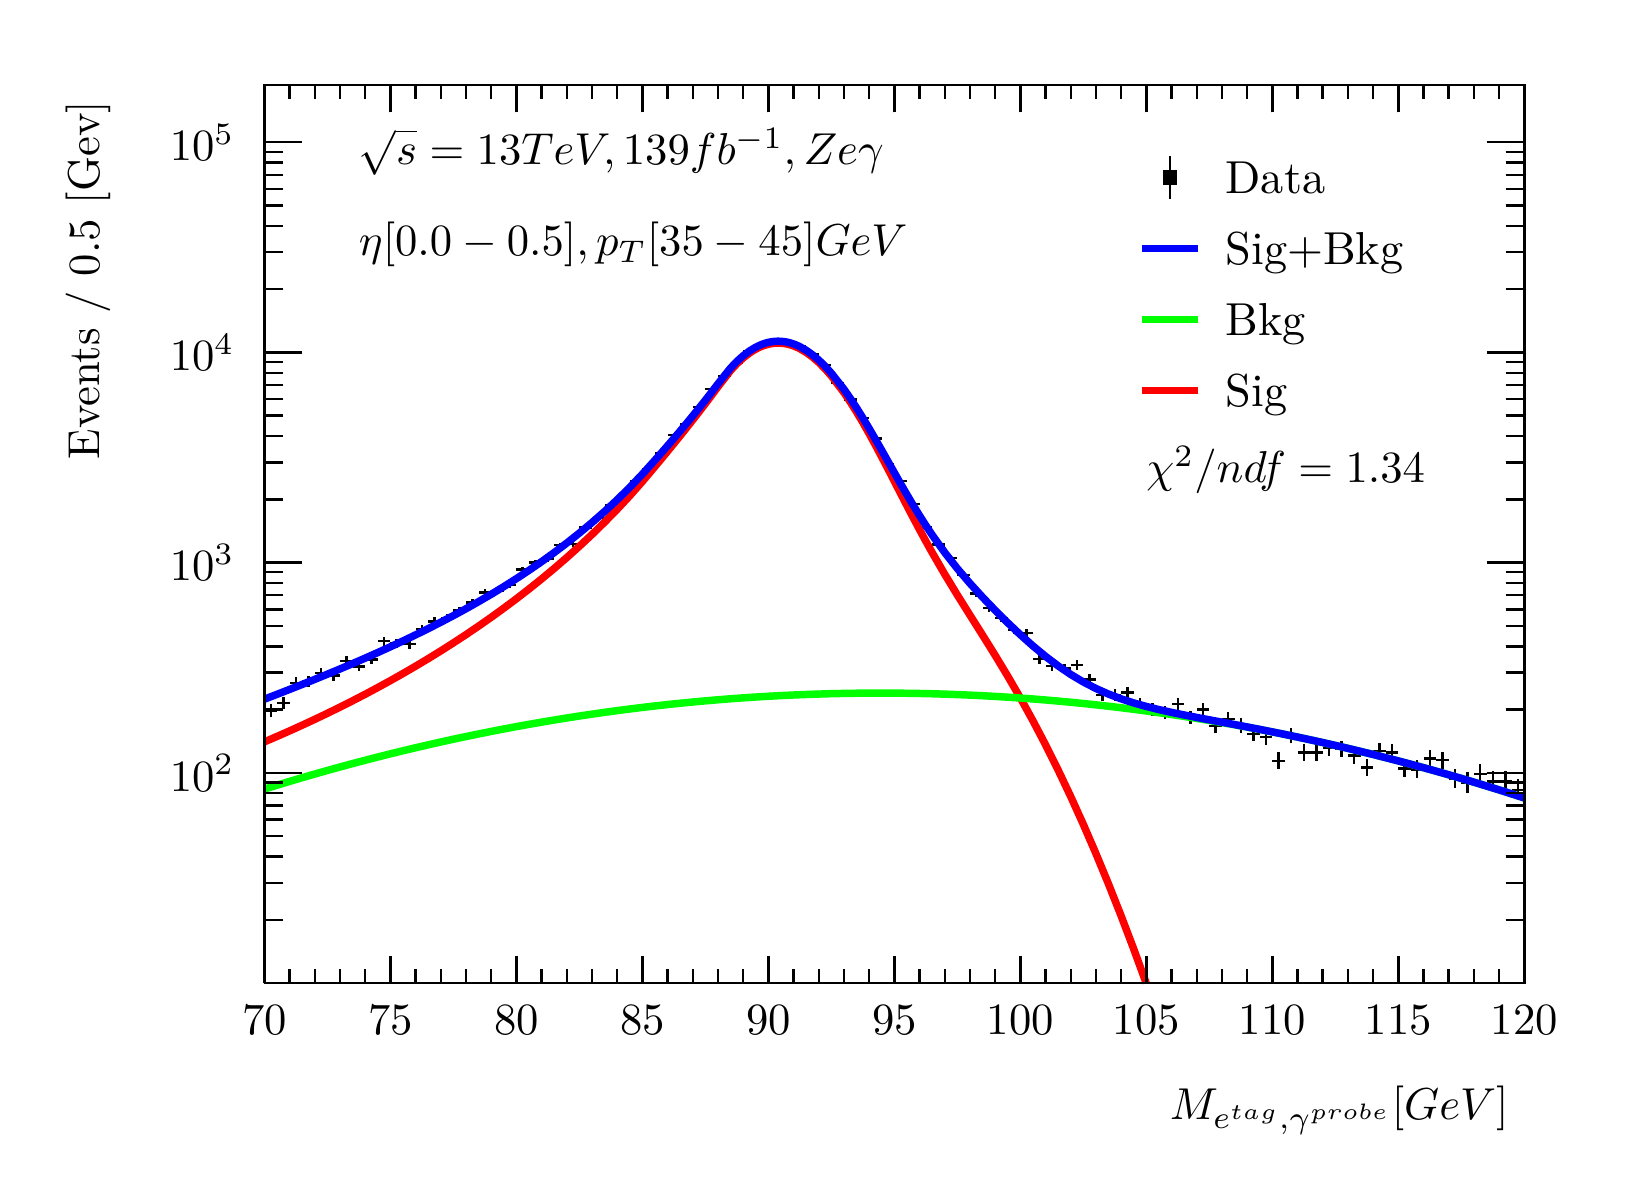
\begin{tikzpicture}
\pgfdeclareplotmark{cross} {
\pgfpathmoveto{\pgfpoint{-0.3\pgfplotmarksize}{\pgfplotmarksize}}
\pgfpathlineto{\pgfpoint{+0.3\pgfplotmarksize}{\pgfplotmarksize}}
\pgfpathlineto{\pgfpoint{+0.3\pgfplotmarksize}{0.3\pgfplotmarksize}}
\pgfpathlineto{\pgfpoint{+1\pgfplotmarksize}{0.3\pgfplotmarksize}}
\pgfpathlineto{\pgfpoint{+1\pgfplotmarksize}{-0.3\pgfplotmarksize}}
\pgfpathlineto{\pgfpoint{+0.3\pgfplotmarksize}{-0.3\pgfplotmarksize}}
\pgfpathlineto{\pgfpoint{+0.3\pgfplotmarksize}{-1.\pgfplotmarksize}}
\pgfpathlineto{\pgfpoint{-0.3\pgfplotmarksize}{-1.\pgfplotmarksize}}
\pgfpathlineto{\pgfpoint{-0.3\pgfplotmarksize}{-0.3\pgfplotmarksize}}
\pgfpathlineto{\pgfpoint{-1.\pgfplotmarksize}{-0.3\pgfplotmarksize}}
\pgfpathlineto{\pgfpoint{-1.\pgfplotmarksize}{0.3\pgfplotmarksize}}
\pgfpathlineto{\pgfpoint{-0.3\pgfplotmarksize}{0.3\pgfplotmarksize}}
\pgfpathclose
\pgfusepathqstroke
}
\pgfdeclareplotmark{cross*} {
\pgfpathmoveto{\pgfpoint{-0.3\pgfplotmarksize}{\pgfplotmarksize}}
\pgfpathlineto{\pgfpoint{+0.3\pgfplotmarksize}{\pgfplotmarksize}}
\pgfpathlineto{\pgfpoint{+0.3\pgfplotmarksize}{0.3\pgfplotmarksize}}
\pgfpathlineto{\pgfpoint{+1\pgfplotmarksize}{0.3\pgfplotmarksize}}
\pgfpathlineto{\pgfpoint{+1\pgfplotmarksize}{-0.3\pgfplotmarksize}}
\pgfpathlineto{\pgfpoint{+0.3\pgfplotmarksize}{-0.3\pgfplotmarksize}}
\pgfpathlineto{\pgfpoint{+0.3\pgfplotmarksize}{-1.\pgfplotmarksize}}
\pgfpathlineto{\pgfpoint{-0.3\pgfplotmarksize}{-1.\pgfplotmarksize}}
\pgfpathlineto{\pgfpoint{-0.3\pgfplotmarksize}{-0.3\pgfplotmarksize}}
\pgfpathlineto{\pgfpoint{-1.\pgfplotmarksize}{-0.3\pgfplotmarksize}}
\pgfpathlineto{\pgfpoint{-1.\pgfplotmarksize}{0.3\pgfplotmarksize}}
\pgfpathlineto{\pgfpoint{-0.3\pgfplotmarksize}{0.3\pgfplotmarksize}}
\pgfpathclose
\pgfusepathqfillstroke
}
\pgfdeclareplotmark{newstar} {
\pgfpathmoveto{\pgfqpoint{0pt}{\pgfplotmarksize}}
\pgfpathlineto{\pgfqpointpolar{44}{0.5\pgfplotmarksize}}
\pgfpathlineto{\pgfqpointpolar{18}{\pgfplotmarksize}}
\pgfpathlineto{\pgfqpointpolar{-20}{0.5\pgfplotmarksize}}
\pgfpathlineto{\pgfqpointpolar{-54}{\pgfplotmarksize}}
\pgfpathlineto{\pgfqpointpolar{-90}{0.5\pgfplotmarksize}}
\pgfpathlineto{\pgfqpointpolar{234}{\pgfplotmarksize}}
\pgfpathlineto{\pgfqpointpolar{198}{0.5\pgfplotmarksize}}
\pgfpathlineto{\pgfqpointpolar{162}{\pgfplotmarksize}}
\pgfpathlineto{\pgfqpointpolar{134}{0.5\pgfplotmarksize}}
\pgfpathclose
\pgfusepathqstroke
}
\pgfdeclareplotmark{newstar*} {
\pgfpathmoveto{\pgfqpoint{0pt}{\pgfplotmarksize}}
\pgfpathlineto{\pgfqpointpolar{44}{0.5\pgfplotmarksize}}
\pgfpathlineto{\pgfqpointpolar{18}{\pgfplotmarksize}}
\pgfpathlineto{\pgfqpointpolar{-20}{0.5\pgfplotmarksize}}
\pgfpathlineto{\pgfqpointpolar{-54}{\pgfplotmarksize}}
\pgfpathlineto{\pgfqpointpolar{-90}{0.5\pgfplotmarksize}}
\pgfpathlineto{\pgfqpointpolar{234}{\pgfplotmarksize}}
\pgfpathlineto{\pgfqpointpolar{198}{0.5\pgfplotmarksize}}
\pgfpathlineto{\pgfqpointpolar{162}{\pgfplotmarksize}}
\pgfpathlineto{\pgfqpointpolar{134}{0.5\pgfplotmarksize}}
\pgfpathclose
\pgfusepathqfillstroke
}
\definecolor{c}{rgb}{1,1,1};
\draw [color=c, fill=c] (0,0) rectangle (20,14.4361);
\draw [color=c, fill=c] (3,2.30977) rectangle (19,13.7143);
\definecolor{c}{rgb}{0,0,0};
\draw [c,line width=0.9] (3,2.30977) -- (3,13.7143) -- (19,13.7143) -- (19,2.30977) -- (3,2.30977);
\definecolor{c}{rgb}{1,1,1};
\draw [color=c, fill=c] (3,2.30977) rectangle (19,13.7143);
\definecolor{c}{rgb}{0,0,0};
\draw [c,line width=0.9] (3,2.30977) -- (3,13.7143) -- (19,13.7143) -- (19,2.30977) -- (3,2.30977);
\draw [c,line width=0.9] (3,2.30977) -- (19,2.30977);
\draw [c,line width=0.9] (3,2.65624) -- (3,2.30977);
\draw [c,line width=0.9] (3.32,2.48301) -- (3.32,2.30977);
\draw [c,line width=0.9] (3.64,2.48301) -- (3.64,2.30977);
\draw [c,line width=0.9] (3.96,2.48301) -- (3.96,2.30977);
\draw [c,line width=0.9] (4.28,2.48301) -- (4.28,2.30977);
\draw [c,line width=0.9] (4.6,2.65624) -- (4.6,2.30977);
\draw [c,line width=0.9] (4.92,2.48301) -- (4.92,2.30977);
\draw [c,line width=0.9] (5.24,2.48301) -- (5.24,2.30977);
\draw [c,line width=0.9] (5.56,2.48301) -- (5.56,2.30977);
\draw [c,line width=0.9] (5.88,2.48301) -- (5.88,2.30977);
\draw [c,line width=0.9] (6.2,2.65624) -- (6.2,2.30977);
\draw [c,line width=0.9] (6.52,2.48301) -- (6.52,2.30977);
\draw [c,line width=0.9] (6.84,2.48301) -- (6.84,2.30977);
\draw [c,line width=0.9] (7.16,2.48301) -- (7.16,2.30977);
\draw [c,line width=0.9] (7.48,2.48301) -- (7.48,2.30977);
\draw [c,line width=0.9] (7.8,2.65624) -- (7.8,2.30977);
\draw [c,line width=0.9] (8.12,2.48301) -- (8.12,2.30977);
\draw [c,line width=0.9] (8.44,2.48301) -- (8.44,2.30977);
\draw [c,line width=0.9] (8.76,2.48301) -- (8.76,2.30977);
\draw [c,line width=0.9] (9.08,2.48301) -- (9.08,2.30977);
\draw [c,line width=0.9] (9.4,2.65624) -- (9.4,2.30977);
\draw [c,line width=0.9] (9.72,2.48301) -- (9.72,2.30977);
\draw [c,line width=0.9] (10.04,2.48301) -- (10.04,2.30977);
\draw [c,line width=0.9] (10.36,2.48301) -- (10.36,2.30977);
\draw [c,line width=0.9] (10.68,2.48301) -- (10.68,2.30977);
\draw [c,line width=0.9] (11,2.65624) -- (11,2.30977);
\draw [c,line width=0.9] (11.32,2.48301) -- (11.32,2.30977);
\draw [c,line width=0.9] (11.64,2.48301) -- (11.64,2.30977);
\draw [c,line width=0.9] (11.96,2.48301) -- (11.96,2.30977);
\draw [c,line width=0.9] (12.28,2.48301) -- (12.28,2.30977);
\draw [c,line width=0.9] (12.6,2.65624) -- (12.6,2.30977);
\draw [c,line width=0.9] (12.92,2.48301) -- (12.92,2.30977);
\draw [c,line width=0.9] (13.24,2.48301) -- (13.24,2.30977);
\draw [c,line width=0.9] (13.56,2.48301) -- (13.56,2.30977);
\draw [c,line width=0.9] (13.88,2.48301) -- (13.88,2.30977);
\draw [c,line width=0.9] (14.2,2.65624) -- (14.2,2.30977);
\draw [c,line width=0.9] (14.52,2.48301) -- (14.52,2.30977);
\draw [c,line width=0.9] (14.84,2.48301) -- (14.84,2.30977);
\draw [c,line width=0.9] (15.16,2.48301) -- (15.16,2.30977);
\draw [c,line width=0.9] (15.48,2.48301) -- (15.48,2.30977);
\draw [c,line width=0.9] (15.8,2.65624) -- (15.8,2.30977);
\draw [c,line width=0.9] (16.12,2.48301) -- (16.12,2.30977);
\draw [c,line width=0.9] (16.44,2.48301) -- (16.44,2.30977);
\draw [c,line width=0.9] (16.76,2.48301) -- (16.76,2.30977);
\draw [c,line width=0.9] (17.08,2.48301) -- (17.08,2.30977);
\draw [c,line width=0.9] (17.4,2.65624) -- (17.4,2.30977);
\draw [c,line width=0.9] (17.72,2.48301) -- (17.72,2.30977);
\draw [c,line width=0.9] (18.04,2.48301) -- (18.04,2.30977);
\draw [c,line width=0.9] (18.36,2.48301) -- (18.36,2.30977);
\draw [c,line width=0.9] (18.68,2.48301) -- (18.68,2.30977);
\draw [c,line width=0.9] (19,2.65624) -- (19,2.30977);
\draw [anchor=base] (3,1.66015) node[scale=1.61424, color=c, rotate=0]{70};
\draw [anchor=base] (4.6,1.66015) node[scale=1.61424, color=c, rotate=0]{75};
\draw [anchor=base] (6.2,1.66015) node[scale=1.61424, color=c, rotate=0]{80};
\draw [anchor=base] (7.8,1.66015) node[scale=1.61424, color=c, rotate=0]{85};
\draw [anchor=base] (9.4,1.66015) node[scale=1.61424, color=c, rotate=0]{90};
\draw [anchor=base] (11,1.66015) node[scale=1.61424, color=c, rotate=0]{95};
\draw [anchor=base] (12.6,1.66015) node[scale=1.61424, color=c, rotate=0]{100};
\draw [anchor=base] (14.2,1.66015) node[scale=1.61424, color=c, rotate=0]{105};
\draw [anchor=base] (15.8,1.66015) node[scale=1.61424, color=c, rotate=0]{110};
\draw [anchor=base] (17.4,1.66015) node[scale=1.61424, color=c, rotate=0]{115};
\draw [anchor=base] (19,1.66015) node[scale=1.61424, color=c, rotate=0]{120};
\draw [anchor= east] (19,0.692932) node[scale=1.61424, color=c, rotate=0]{$M_{e^{tag}, \gamma^{probe}}  [GeV]$};
\draw [c,line width=0.9] (3,13.7143) -- (19,13.7143);
\draw [c,line width=0.9] (3,13.3678) -- (3,13.7143);
\draw [c,line width=0.9] (3.32,13.5411) -- (3.32,13.7143);
\draw [c,line width=0.9] (3.64,13.5411) -- (3.64,13.7143);
\draw [c,line width=0.9] (3.96,13.5411) -- (3.96,13.7143);
\draw [c,line width=0.9] (4.28,13.5411) -- (4.28,13.7143);
\draw [c,line width=0.9] (4.6,13.3678) -- (4.6,13.7143);
\draw [c,line width=0.9] (4.92,13.5411) -- (4.92,13.7143);
\draw [c,line width=0.9] (5.24,13.5411) -- (5.24,13.7143);
\draw [c,line width=0.9] (5.56,13.5411) -- (5.56,13.7143);
\draw [c,line width=0.9] (5.88,13.5411) -- (5.88,13.7143);
\draw [c,line width=0.9] (6.2,13.3678) -- (6.2,13.7143);
\draw [c,line width=0.9] (6.52,13.5411) -- (6.52,13.7143);
\draw [c,line width=0.9] (6.84,13.5411) -- (6.84,13.7143);
\draw [c,line width=0.9] (7.16,13.5411) -- (7.16,13.7143);
\draw [c,line width=0.9] (7.48,13.5411) -- (7.48,13.7143);
\draw [c,line width=0.9] (7.8,13.3678) -- (7.8,13.7143);
\draw [c,line width=0.9] (8.12,13.5411) -- (8.12,13.7143);
\draw [c,line width=0.9] (8.44,13.5411) -- (8.44,13.7143);
\draw [c,line width=0.9] (8.76,13.5411) -- (8.76,13.7143);
\draw [c,line width=0.9] (9.08,13.5411) -- (9.08,13.7143);
\draw [c,line width=0.9] (9.4,13.3678) -- (9.4,13.7143);
\draw [c,line width=0.9] (9.72,13.5411) -- (9.72,13.7143);
\draw [c,line width=0.9] (10.04,13.5411) -- (10.04,13.7143);
\draw [c,line width=0.9] (10.36,13.5411) -- (10.36,13.7143);
\draw [c,line width=0.9] (10.68,13.5411) -- (10.68,13.7143);
\draw [c,line width=0.9] (11,13.3678) -- (11,13.7143);
\draw [c,line width=0.9] (11.32,13.5411) -- (11.32,13.7143);
\draw [c,line width=0.9] (11.64,13.5411) -- (11.64,13.7143);
\draw [c,line width=0.9] (11.96,13.5411) -- (11.96,13.7143);
\draw [c,line width=0.9] (12.28,13.5411) -- (12.28,13.7143);
\draw [c,line width=0.9] (12.6,13.3678) -- (12.6,13.7143);
\draw [c,line width=0.9] (12.92,13.5411) -- (12.92,13.7143);
\draw [c,line width=0.9] (13.24,13.5411) -- (13.24,13.7143);
\draw [c,line width=0.9] (13.56,13.5411) -- (13.56,13.7143);
\draw [c,line width=0.9] (13.88,13.5411) -- (13.88,13.7143);
\draw [c,line width=0.9] (14.2,13.3678) -- (14.2,13.7143);
\draw [c,line width=0.9] (14.52,13.5411) -- (14.52,13.7143);
\draw [c,line width=0.9] (14.84,13.5411) -- (14.84,13.7143);
\draw [c,line width=0.9] (15.16,13.5411) -- (15.16,13.7143);
\draw [c,line width=0.9] (15.48,13.5411) -- (15.48,13.7143);
\draw [c,line width=0.9] (15.8,13.3678) -- (15.8,13.7143);
\draw [c,line width=0.9] (16.12,13.5411) -- (16.12,13.7143);
\draw [c,line width=0.9] (16.44,13.5411) -- (16.44,13.7143);
\draw [c,line width=0.9] (16.76,13.5411) -- (16.76,13.7143);
\draw [c,line width=0.9] (17.08,13.5411) -- (17.08,13.7143);
\draw [c,line width=0.9] (17.4,13.3678) -- (17.4,13.7143);
\draw [c,line width=0.9] (17.72,13.5411) -- (17.72,13.7143);
\draw [c,line width=0.9] (18.04,13.5411) -- (18.04,13.7143);
\draw [c,line width=0.9] (18.36,13.5411) -- (18.36,13.7143);
\draw [c,line width=0.9] (18.68,13.5411) -- (18.68,13.7143);
\draw [c,line width=0.9] (19,13.3678) -- (19,13.7143);
\draw [c,line width=0.9] (3,2.30977) -- (3,13.7143);
\draw [c,line width=0.9] (3.237,3.11343) -- (3,3.11343);
\draw [c,line width=0.9] (3.237,3.58354) -- (3,3.58354);
\draw [c,line width=0.9] (3.237,3.91709) -- (3,3.91709);
\draw [c,line width=0.9] (3.237,4.17581) -- (3,4.17581);
\draw [c,line width=0.9] (3.237,4.38719) -- (3,4.38719);
\draw [c,line width=0.9] (3.237,4.56592) -- (3,4.56592);
\draw [c,line width=0.9] (3.237,4.72074) -- (3,4.72074);
\draw [c,line width=0.9] (3.237,4.8573) -- (3,4.8573);
\draw [c,line width=0.9] (3.474,4.97946) -- (3,4.97946);
\draw [anchor= east] (2.82,4.97946) node[scale=1.61424, color=c, rotate=0]{$10^{2}$};
\draw [c,line width=0.9] (3.237,5.78312) -- (3,5.78312);
\draw [c,line width=0.9] (3.237,6.25323) -- (3,6.25323);
\draw [c,line width=0.9] (3.237,6.58678) -- (3,6.58678);
\draw [c,line width=0.9] (3.237,6.8455) -- (3,6.8455);
\draw [c,line width=0.9] (3.237,7.05689) -- (3,7.05689);
\draw [c,line width=0.9] (3.237,7.23561) -- (3,7.23561);
\draw [c,line width=0.9] (3.237,7.39043) -- (3,7.39043);
\draw [c,line width=0.9] (3.237,7.52699) -- (3,7.52699);
\draw [c,line width=0.9] (3.474,7.64915) -- (3,7.64915);
\draw [anchor= east] (2.82,7.64915) node[scale=1.61424, color=c, rotate=0]{$10^{3}$};
\draw [c,line width=0.9] (3.237,8.45281) -- (3,8.45281);
\draw [c,line width=0.9] (3.237,8.92292) -- (3,8.92292);
\draw [c,line width=0.9] (3.237,9.25647) -- (3,9.25647);
\draw [c,line width=0.9] (3.237,9.51519) -- (3,9.51519);
\draw [c,line width=0.9] (3.237,9.72658) -- (3,9.72658);
\draw [c,line width=0.9] (3.237,9.9053) -- (3,9.9053);
\draw [c,line width=0.9] (3.237,10.0601) -- (3,10.0601);
\draw [c,line width=0.9] (3.237,10.1967) -- (3,10.1967);
\draw [c,line width=0.9] (3.474,10.3188) -- (3,10.3188);
\draw [anchor= east] (2.82,10.3188) node[scale=1.61424, color=c, rotate=0]{$10^{4}$};
\draw [c,line width=0.9] (3.237,11.1225) -- (3,11.1225);
\draw [c,line width=0.9] (3.237,11.5926) -- (3,11.5926);
\draw [c,line width=0.9] (3.237,11.9262) -- (3,11.9262);
\draw [c,line width=0.9] (3.237,12.1849) -- (3,12.1849);
\draw [c,line width=0.9] (3.237,12.3963) -- (3,12.3963);
\draw [c,line width=0.9] (3.237,12.575) -- (3,12.575);
\draw [c,line width=0.9] (3.237,12.7298) -- (3,12.7298);
\draw [c,line width=0.9] (3.237,12.8664) -- (3,12.8664);
\draw [c,line width=0.9] (3.474,12.9885) -- (3,12.9885);
\draw [anchor= east] (2.82,12.9885) node[scale=1.61424, color=c, rotate=0]{$10^{5}$};
\draw [anchor= east] (0.76,13.7143) node[scale=1.61424, color=c, rotate=90]{Events / 0.5 [Gev]};
\draw [c,line width=0.9] (19,2.30977) -- (19,13.7143);
\draw [c,line width=0.9] (18.763,3.11343) -- (19,3.11343);
\draw [c,line width=0.9] (18.763,3.58354) -- (19,3.58354);
\draw [c,line width=0.9] (18.763,3.91709) -- (19,3.91709);
\draw [c,line width=0.9] (18.763,4.17581) -- (19,4.17581);
\draw [c,line width=0.9] (18.763,4.38719) -- (19,4.38719);
\draw [c,line width=0.9] (18.763,4.56592) -- (19,4.56592);
\draw [c,line width=0.9] (18.763,4.72074) -- (19,4.72074);
\draw [c,line width=0.9] (18.763,4.8573) -- (19,4.8573);
\draw [c,line width=0.9] (18.526,4.97946) -- (19,4.97946);
\draw [c,line width=0.9] (18.763,5.78312) -- (19,5.78312);
\draw [c,line width=0.9] (18.763,6.25323) -- (19,6.25323);
\draw [c,line width=0.9] (18.763,6.58678) -- (19,6.58678);
\draw [c,line width=0.9] (18.763,6.8455) -- (19,6.8455);
\draw [c,line width=0.9] (18.763,7.05689) -- (19,7.05689);
\draw [c,line width=0.9] (18.763,7.23561) -- (19,7.23561);
\draw [c,line width=0.9] (18.763,7.39043) -- (19,7.39043);
\draw [c,line width=0.9] (18.763,7.52699) -- (19,7.52699);
\draw [c,line width=0.9] (18.526,7.64915) -- (19,7.64915);
\draw [c,line width=0.9] (18.763,8.45281) -- (19,8.45281);
\draw [c,line width=0.9] (18.763,8.92292) -- (19,8.92292);
\draw [c,line width=0.9] (18.763,9.25647) -- (19,9.25647);
\draw [c,line width=0.9] (18.763,9.51519) -- (19,9.51519);
\draw [c,line width=0.9] (18.763,9.72658) -- (19,9.72658);
\draw [c,line width=0.9] (18.763,9.9053) -- (19,9.9053);
\draw [c,line width=0.9] (18.763,10.0601) -- (19,10.0601);
\draw [c,line width=0.9] (18.763,10.1967) -- (19,10.1967);
\draw [c,line width=0.9] (18.526,10.3188) -- (19,10.3188);
\draw [c,line width=0.9] (18.763,11.1225) -- (19,11.1225);
\draw [c,line width=0.9] (18.763,11.5926) -- (19,11.5926);
\draw [c,line width=0.9] (18.763,11.9262) -- (19,11.9262);
\draw [c,line width=0.9] (18.763,12.1849) -- (19,12.1849);
\draw [c,line width=0.9] (18.763,12.3963) -- (19,12.3963);
\draw [c,line width=0.9] (18.763,12.575) -- (19,12.575);
\draw [c,line width=0.9] (18.763,12.7298) -- (19,12.7298);
\draw [c,line width=0.9] (18.763,12.8664) -- (19,12.8664);
\draw [c,line width=0.9] (18.526,12.9885) -- (19,12.9885);
\draw [c,line width=0.9] (3.08,5.77147) -- (3,5.77147);
\draw [c,line width=0.9] (3,5.77147) -- (3,5.77147);
\draw [c,line width=0.9] (3.08,5.77147) -- (3.16,5.77147);
\draw [c,line width=0.9] (3.16,5.77147) -- (3.16,5.77147);
\draw [c,line width=0.9] (3.08,5.77147) -- (3.08,5.85385);
\draw [c,line width=0.9] (3.08,5.85385) -- (3.08,5.85385);
\draw [c,line width=0.9] (3.08,5.77147) -- (3.08,5.68909);
\draw [c,line width=0.9] (3.08,5.68909) -- (3.08,5.68909);
\draw [c,line width=0.9] (3.24,5.86697) -- (3.16,5.86697);
\draw [c,line width=0.9] (3.16,5.86697) -- (3.16,5.86697);
\draw [c,line width=0.9] (3.24,5.86697) -- (3.32,5.86697);
\draw [c,line width=0.9] (3.32,5.86697) -- (3.32,5.86697);
\draw [c,line width=0.9] (3.24,5.86697) -- (3.24,5.94603);
\draw [c,line width=0.9] (3.24,5.94603) -- (3.24,5.94603);
\draw [c,line width=0.9] (3.24,5.86697) -- (3.24,5.78791);
\draw [c,line width=0.9] (3.24,5.78791) -- (3.24,5.78791);
\draw [c,line width=0.9] (3.4,6.12245) -- (3.32,6.12245);
\draw [c,line width=0.9] (3.32,6.12245) -- (3.32,6.12245);
\draw [c,line width=0.9] (3.4,6.12245) -- (3.48,6.12245);
\draw [c,line width=0.9] (3.48,6.12245) -- (3.48,6.12245);
\draw [c,line width=0.9] (3.4,6.12245) -- (3.4,6.19326);
\draw [c,line width=0.9] (3.4,6.19326) -- (3.4,6.19326);
\draw [c,line width=0.9] (3.4,6.12245) -- (3.4,6.05164);
\draw [c,line width=0.9] (3.4,6.05164) -- (3.4,6.05164);
\draw [c,line width=0.9] (3.56,6.14388) -- (3.48,6.14388);
\draw [c,line width=0.9] (3.48,6.14388) -- (3.48,6.14388);
\draw [c,line width=0.9] (3.56,6.14388) -- (3.64,6.14388);
\draw [c,line width=0.9] (3.64,6.14388) -- (3.64,6.14388);
\draw [c,line width=0.9] (3.56,6.14388) -- (3.56,6.21404);
\draw [c,line width=0.9] (3.56,6.21404) -- (3.56,6.21404);
\draw [c,line width=0.9] (3.56,6.14388) -- (3.56,6.07372);
\draw [c,line width=0.9] (3.56,6.07372) -- (3.56,6.07372);
\draw [c,line width=0.9] (3.72,6.24547) -- (3.64,6.24547);
\draw [c,line width=0.9] (3.64,6.24547) -- (3.64,6.24547);
\draw [c,line width=0.9] (3.72,6.24547) -- (3.8,6.24547);
\draw [c,line width=0.9] (3.8,6.24547) -- (3.8,6.24547);
\draw [c,line width=0.9] (3.72,6.24547) -- (3.72,6.31263);
\draw [c,line width=0.9] (3.72,6.31263) -- (3.72,6.31263);
\draw [c,line width=0.9] (3.72,6.24547) -- (3.72,6.17832);
\draw [c,line width=0.9] (3.72,6.17832) -- (3.72,6.17832);
\draw [c,line width=0.9] (3.88,6.21392) -- (3.8,6.21392);
\draw [c,line width=0.9] (3.8,6.21392) -- (3.8,6.21392);
\draw [c,line width=0.9] (3.88,6.21392) -- (3.96,6.21392);
\draw [c,line width=0.9] (3.96,6.21392) -- (3.96,6.21392);
\draw [c,line width=0.9] (3.88,6.21392) -- (3.88,6.282);
\draw [c,line width=0.9] (3.88,6.282) -- (3.88,6.282);
\draw [c,line width=0.9] (3.88,6.21392) -- (3.88,6.14585);
\draw [c,line width=0.9] (3.88,6.14585) -- (3.88,6.14585);
\draw [c,line width=0.9] (4.04,6.39835) -- (3.96,6.39835);
\draw [c,line width=0.9] (3.96,6.39835) -- (3.96,6.39835);
\draw [c,line width=0.9] (4.04,6.39835) -- (4.12,6.39835);
\draw [c,line width=0.9] (4.12,6.39835) -- (4.12,6.39835);
\draw [c,line width=0.9] (4.04,6.39835) -- (4.04,6.46122);
\draw [c,line width=0.9] (4.04,6.46122) -- (4.04,6.46122);
\draw [c,line width=0.9] (4.04,6.39835) -- (4.04,6.33548);
\draw [c,line width=0.9] (4.04,6.33548) -- (4.04,6.33548);
\draw [c,line width=0.9] (4.2,6.33168) -- (4.12,6.33168);
\draw [c,line width=0.9] (4.12,6.33168) -- (4.12,6.33168);
\draw [c,line width=0.9] (4.2,6.33168) -- (4.28,6.33168);
\draw [c,line width=0.9] (4.28,6.33168) -- (4.28,6.33168);
\draw [c,line width=0.9] (4.2,6.33168) -- (4.2,6.39638);
\draw [c,line width=0.9] (4.2,6.39638) -- (4.2,6.39638);
\draw [c,line width=0.9] (4.2,6.33168) -- (4.2,6.26697);
\draw [c,line width=0.9] (4.2,6.26697) -- (4.2,6.26697);
\draw [c,line width=0.9] (4.36,6.41863) -- (4.28,6.41863);
\draw [c,line width=0.9] (4.28,6.41863) -- (4.28,6.41863);
\draw [c,line width=0.9] (4.36,6.41863) -- (4.44,6.41863);
\draw [c,line width=0.9] (4.44,6.41863) -- (4.44,6.41863);
\draw [c,line width=0.9] (4.36,6.41863) -- (4.36,6.48095);
\draw [c,line width=0.9] (4.36,6.48095) -- (4.36,6.48095);
\draw [c,line width=0.9] (4.36,6.41863) -- (4.36,6.35631);
\draw [c,line width=0.9] (4.36,6.35631) -- (4.36,6.35631);
\draw [c,line width=0.9] (4.52,6.6516) -- (4.44,6.6516);
\draw [c,line width=0.9] (4.44,6.6516) -- (4.44,6.6516);
\draw [c,line width=0.9] (4.52,6.6516) -- (4.6,6.6516);
\draw [c,line width=0.9] (4.6,6.6516) -- (4.6,6.6516);
\draw [c,line width=0.9] (4.52,6.6516) -- (4.52,6.70797);
\draw [c,line width=0.9] (4.52,6.70797) -- (4.52,6.70797);
\draw [c,line width=0.9] (4.52,6.6516) -- (4.52,6.59523);
\draw [c,line width=0.9] (4.52,6.59523) -- (4.52,6.59523);
\draw [c,line width=0.9] (4.68,6.62666) -- (4.6,6.62666);
\draw [c,line width=0.9] (4.6,6.62666) -- (4.6,6.62666);
\draw [c,line width=0.9] (4.68,6.62666) -- (4.76,6.62666);
\draw [c,line width=0.9] (4.76,6.62666) -- (4.76,6.62666);
\draw [c,line width=0.9] (4.68,6.62666) -- (4.68,6.68364);
\draw [c,line width=0.9] (4.68,6.68364) -- (4.68,6.68364);
\draw [c,line width=0.9] (4.68,6.62666) -- (4.68,6.56969);
\draw [c,line width=0.9] (4.68,6.56969) -- (4.68,6.56969);
\draw [c,line width=0.9] (4.84,6.61258) -- (4.76,6.61258);
\draw [c,line width=0.9] (4.76,6.61258) -- (4.76,6.61258);
\draw [c,line width=0.9] (4.84,6.61258) -- (4.92,6.61258);
\draw [c,line width=0.9] (4.92,6.61258) -- (4.92,6.61258);
\draw [c,line width=0.9] (4.84,6.61258) -- (4.84,6.6699);
\draw [c,line width=0.9] (4.84,6.6699) -- (4.84,6.6699);
\draw [c,line width=0.9] (4.84,6.61258) -- (4.84,6.55525);
\draw [c,line width=0.9] (4.84,6.55525) -- (4.84,6.55525);
\draw [c,line width=0.9] (5,6.80779) -- (4.92,6.80779);
\draw [c,line width=0.9] (4.92,6.80779) -- (4.92,6.80779);
\draw [c,line width=0.9] (5,6.80779) -- (5.08,6.80779);
\draw [c,line width=0.9] (5.08,6.80779) -- (5.08,6.80779);
\draw [c,line width=0.9] (5,6.80779) -- (5,6.86049);
\draw [c,line width=0.9] (5,6.86049) -- (5,6.86049);
\draw [c,line width=0.9] (5,6.80779) -- (5,6.75509);
\draw [c,line width=0.9] (5,6.75509) -- (5,6.75509);
\draw [c,line width=0.9] (5.16,6.90207) -- (5.08,6.90207);
\draw [c,line width=0.9] (5.08,6.90207) -- (5.08,6.90207);
\draw [c,line width=0.9] (5.16,6.90207) -- (5.24,6.90207);
\draw [c,line width=0.9] (5.24,6.90207) -- (5.24,6.90207);
\draw [c,line width=0.9] (5.16,6.90207) -- (5.16,6.95266);
\draw [c,line width=0.9] (5.16,6.95266) -- (5.16,6.95266);
\draw [c,line width=0.9] (5.16,6.90207) -- (5.16,6.85147);
\draw [c,line width=0.9] (5.16,6.85147) -- (5.16,6.85147);
\draw [c,line width=0.9] (5.32,6.94754) -- (5.24,6.94754);
\draw [c,line width=0.9] (5.24,6.94754) -- (5.24,6.94754);
\draw [c,line width=0.9] (5.32,6.94754) -- (5.4,6.94754);
\draw [c,line width=0.9] (5.4,6.94754) -- (5.4,6.94754);
\draw [c,line width=0.9] (5.32,6.94754) -- (5.32,6.99716);
\draw [c,line width=0.9] (5.32,6.99716) -- (5.32,6.99716);
\draw [c,line width=0.9] (5.32,6.94754) -- (5.32,6.89792);
\draw [c,line width=0.9] (5.32,6.89792) -- (5.32,6.89792);
\draw [c,line width=0.9] (5.48,7.03936) -- (5.4,7.03936);
\draw [c,line width=0.9] (5.4,7.03936) -- (5.4,7.03936);
\draw [c,line width=0.9] (5.48,7.03936) -- (5.56,7.03936);
\draw [c,line width=0.9] (5.56,7.03936) -- (5.56,7.03936);
\draw [c,line width=0.9] (5.48,7.03936) -- (5.48,7.08705);
\draw [c,line width=0.9] (5.48,7.08705) -- (5.48,7.08705);
\draw [c,line width=0.9] (5.48,7.03936) -- (5.48,6.99167);
\draw [c,line width=0.9] (5.48,6.99167) -- (5.48,6.99167);
\draw [c,line width=0.9] (5.64,7.14074) -- (5.56,7.14074);
\draw [c,line width=0.9] (5.56,7.14074) -- (5.56,7.14074);
\draw [c,line width=0.9] (5.64,7.14074) -- (5.72,7.14074);
\draw [c,line width=0.9] (5.72,7.14074) -- (5.72,7.14074);
\draw [c,line width=0.9] (5.64,7.14074) -- (5.64,7.18639);
\draw [c,line width=0.9] (5.64,7.18639) -- (5.64,7.18639);
\draw [c,line width=0.9] (5.64,7.14074) -- (5.64,7.09509);
\draw [c,line width=0.9] (5.64,7.09509) -- (5.64,7.09509);
\draw [c,line width=0.9] (5.8,7.26666) -- (5.72,7.26666);
\draw [c,line width=0.9] (5.72,7.26666) -- (5.72,7.26666);
\draw [c,line width=0.9] (5.8,7.26666) -- (5.88,7.26666);
\draw [c,line width=0.9] (5.88,7.26666) -- (5.88,7.26666);
\draw [c,line width=0.9] (5.8,7.26666) -- (5.8,7.3099);
\draw [c,line width=0.9] (5.8,7.3099) -- (5.8,7.3099);
\draw [c,line width=0.9] (5.8,7.26666) -- (5.8,7.22343);
\draw [c,line width=0.9] (5.8,7.22343) -- (5.8,7.22343);
\draw [c,line width=0.9] (5.96,7.28902) -- (5.88,7.28902);
\draw [c,line width=0.9] (5.88,7.28902) -- (5.88,7.28902);
\draw [c,line width=0.9] (5.96,7.28902) -- (6.04,7.28902);
\draw [c,line width=0.9] (6.04,7.28902) -- (6.04,7.28902);
\draw [c,line width=0.9] (5.96,7.28902) -- (5.96,7.33185);
\draw [c,line width=0.9] (5.96,7.33185) -- (5.96,7.33185);
\draw [c,line width=0.9] (5.96,7.28902) -- (5.96,7.2462);
\draw [c,line width=0.9] (5.96,7.2462) -- (5.96,7.2462);
\draw [c,line width=0.9] (6.12,7.36553) -- (6.04,7.36553);
\draw [c,line width=0.9] (6.04,7.36553) -- (6.04,7.36553);
\draw [c,line width=0.9] (6.12,7.36553) -- (6.2,7.36553);
\draw [c,line width=0.9] (6.2,7.36553) -- (6.2,7.36553);
\draw [c,line width=0.9] (6.12,7.36553) -- (6.12,7.40696);
\draw [c,line width=0.9] (6.12,7.40696) -- (6.12,7.40696);
\draw [c,line width=0.9] (6.12,7.36553) -- (6.12,7.3241);
\draw [c,line width=0.9] (6.12,7.3241) -- (6.12,7.3241);
\draw [c,line width=0.9] (6.28,7.55876) -- (6.2,7.55876);
\draw [c,line width=0.9] (6.2,7.55876) -- (6.2,7.55876);
\draw [c,line width=0.9] (6.28,7.55876) -- (6.36,7.55876);
\draw [c,line width=0.9] (6.36,7.55876) -- (6.36,7.55876);
\draw [c,line width=0.9] (6.28,7.55876) -- (6.28,7.59688);
\draw [c,line width=0.9] (6.28,7.59688) -- (6.28,7.59688);
\draw [c,line width=0.9] (6.28,7.55876) -- (6.28,7.52064);
\draw [c,line width=0.9] (6.28,7.52064) -- (6.28,7.52064);
\draw [c,line width=0.9] (6.44,7.65031) -- (6.36,7.65031);
\draw [c,line width=0.9] (6.36,7.65031) -- (6.36,7.65031);
\draw [c,line width=0.9] (6.44,7.65031) -- (6.52,7.65031);
\draw [c,line width=0.9] (6.52,7.65031) -- (6.52,7.65031);
\draw [c,line width=0.9] (6.44,7.65031) -- (6.44,7.68696);
\draw [c,line width=0.9] (6.44,7.68696) -- (6.44,7.68696);
\draw [c,line width=0.9] (6.44,7.65031) -- (6.44,7.61367);
\draw [c,line width=0.9] (6.44,7.61367) -- (6.44,7.61367);
\draw [c,line width=0.9] (6.6,7.69908) -- (6.52,7.69908);
\draw [c,line width=0.9] (6.52,7.69908) -- (6.52,7.69908);
\draw [c,line width=0.9] (6.6,7.69908) -- (6.68,7.69908);
\draw [c,line width=0.9] (6.68,7.69908) -- (6.68,7.69908);
\draw [c,line width=0.9] (6.6,7.69908) -- (6.6,7.73496);
\draw [c,line width=0.9] (6.6,7.73496) -- (6.6,7.73496);
\draw [c,line width=0.9] (6.6,7.69908) -- (6.6,7.6632);
\draw [c,line width=0.9] (6.6,7.6632) -- (6.6,7.6632);
\draw [c,line width=0.9] (6.76,7.87112) -- (6.68,7.87112);
\draw [c,line width=0.9] (6.68,7.87112) -- (6.68,7.87112);
\draw [c,line width=0.9] (6.76,7.87112) -- (6.84,7.87112);
\draw [c,line width=0.9] (6.84,7.87112) -- (6.84,7.87112);
\draw [c,line width=0.9] (6.76,7.87112) -- (6.76,7.90444);
\draw [c,line width=0.9] (6.76,7.90444) -- (6.76,7.90444);
\draw [c,line width=0.9] (6.76,7.87112) -- (6.76,7.83781);
\draw [c,line width=0.9] (6.76,7.83781) -- (6.76,7.83781);
\draw [c,line width=0.9] (6.92,7.8854) -- (6.84,7.8854);
\draw [c,line width=0.9] (6.84,7.8854) -- (6.84,7.8854);
\draw [c,line width=0.9] (6.92,7.8854) -- (7,7.8854);
\draw [c,line width=0.9] (7,7.8854) -- (7,7.8854);
\draw [c,line width=0.9] (6.92,7.8854) -- (6.92,7.91851);
\draw [c,line width=0.9] (6.92,7.91851) -- (6.92,7.91851);
\draw [c,line width=0.9] (6.92,7.8854) -- (6.92,7.85228);
\draw [c,line width=0.9] (6.92,7.85228) -- (6.92,7.85228);
\draw [c,line width=0.9] (7.08,8.09426) -- (7,8.09426);
\draw [c,line width=0.9] (7,8.09426) -- (7,8.09426);
\draw [c,line width=0.9] (7.08,8.09426) -- (7.16,8.09426);
\draw [c,line width=0.9] (7.16,8.09426) -- (7.16,8.09426);
\draw [c,line width=0.9] (7.08,8.09426) -- (7.08,8.12452);
\draw [c,line width=0.9] (7.08,8.12452) -- (7.08,8.12452);
\draw [c,line width=0.9] (7.08,8.09426) -- (7.08,8.064);
\draw [c,line width=0.9] (7.08,8.064) -- (7.08,8.064);
\draw [c,line width=0.9] (7.24,8.21705) -- (7.16,8.21705);
\draw [c,line width=0.9] (7.16,8.21705) -- (7.16,8.21705);
\draw [c,line width=0.9] (7.24,8.21705) -- (7.32,8.21705);
\draw [c,line width=0.9] (7.32,8.21705) -- (7.32,8.21705);
\draw [c,line width=0.9] (7.24,8.21705) -- (7.24,8.24575);
\draw [c,line width=0.9] (7.24,8.24575) -- (7.24,8.24575);
\draw [c,line width=0.9] (7.24,8.21705) -- (7.24,8.18835);
\draw [c,line width=0.9] (7.24,8.18835) -- (7.24,8.18835);
\draw [c,line width=0.9] (7.4,8.37365) -- (7.32,8.37365);
\draw [c,line width=0.9] (7.32,8.37365) -- (7.32,8.37365);
\draw [c,line width=0.9] (7.4,8.37365) -- (7.48,8.37365);
\draw [c,line width=0.9] (7.48,8.37365) -- (7.48,8.37365);
\draw [c,line width=0.9] (7.4,8.37365) -- (7.4,8.40047);
\draw [c,line width=0.9] (7.4,8.40047) -- (7.4,8.40047);
\draw [c,line width=0.9] (7.4,8.37365) -- (7.4,8.34682);
\draw [c,line width=0.9] (7.4,8.34682) -- (7.4,8.34682);
\draw [c,line width=0.9] (7.56,8.44233) -- (7.48,8.44233);
\draw [c,line width=0.9] (7.48,8.44233) -- (7.48,8.44233);
\draw [c,line width=0.9] (7.56,8.44233) -- (7.64,8.44233);
\draw [c,line width=0.9] (7.64,8.44233) -- (7.64,8.44233);
\draw [c,line width=0.9] (7.56,8.44233) -- (7.56,8.46837);
\draw [c,line width=0.9] (7.56,8.46837) -- (7.56,8.46837);
\draw [c,line width=0.9] (7.56,8.44233) -- (7.56,8.41629);
\draw [c,line width=0.9] (7.56,8.41629) -- (7.56,8.41629);
\draw [c,line width=0.9] (7.72,8.68526) -- (7.64,8.68526);
\draw [c,line width=0.9] (7.64,8.68526) -- (7.64,8.68526);
\draw [c,line width=0.9] (7.72,8.68526) -- (7.8,8.68526);
\draw [c,line width=0.9] (7.8,8.68526) -- (7.8,8.68526);
\draw [c,line width=0.9] (7.72,8.68526) -- (7.72,8.70872);
\draw [c,line width=0.9] (7.72,8.70872) -- (7.72,8.70872);
\draw [c,line width=0.9] (7.72,8.68526) -- (7.72,8.66181);
\draw [c,line width=0.9] (7.72,8.66181) -- (7.72,8.66181);
\draw [c,line width=0.9] (7.88,8.83336) -- (7.8,8.83336);
\draw [c,line width=0.9] (7.8,8.83336) -- (7.8,8.83336);
\draw [c,line width=0.9] (7.88,8.83336) -- (7.96,8.83336);
\draw [c,line width=0.9] (7.96,8.83336) -- (7.96,8.83336);
\draw [c,line width=0.9] (7.88,8.83336) -- (7.88,8.85537);
\draw [c,line width=0.9] (7.88,8.85537) -- (7.88,8.85537);
\draw [c,line width=0.9] (7.88,8.83336) -- (7.88,8.81136);
\draw [c,line width=0.9] (7.88,8.81136) -- (7.88,8.81136);
\draw [c,line width=0.9] (8.04,9.03763) -- (7.96,9.03763);
\draw [c,line width=0.9] (7.96,9.03763) -- (7.96,9.03763);
\draw [c,line width=0.9] (8.04,9.03763) -- (8.12,9.03763);
\draw [c,line width=0.9] (8.12,9.03763) -- (8.12,9.03763);
\draw [c,line width=0.9] (8.04,9.03763) -- (8.04,9.05778);
\draw [c,line width=0.9] (8.04,9.05778) -- (8.04,9.05778);
\draw [c,line width=0.9] (8.04,9.03763) -- (8.04,9.01749);
\draw [c,line width=0.9] (8.04,9.01749) -- (8.04,9.01749);
\draw [c,line width=0.9] (8.2,9.26858) -- (8.12,9.26858);
\draw [c,line width=0.9] (8.12,9.26858) -- (8.12,9.26858);
\draw [c,line width=0.9] (8.2,9.26858) -- (8.28,9.26858);
\draw [c,line width=0.9] (8.28,9.26858) -- (8.28,9.26858);
\draw [c,line width=0.9] (8.2,9.26858) -- (8.2,9.28681);
\draw [c,line width=0.9] (8.2,9.28681) -- (8.2,9.28681);
\draw [c,line width=0.9] (8.2,9.26858) -- (8.2,9.25034);
\draw [c,line width=0.9] (8.2,9.25034) -- (8.2,9.25034);
\draw [c,line width=0.9] (8.36,9.41093) -- (8.28,9.41093);
\draw [c,line width=0.9] (8.28,9.41093) -- (8.28,9.41093);
\draw [c,line width=0.9] (8.36,9.41093) -- (8.44,9.41093);
\draw [c,line width=0.9] (8.44,9.41093) -- (8.44,9.41093);
\draw [c,line width=0.9] (8.36,9.41093) -- (8.36,9.42808);
\draw [c,line width=0.9] (8.36,9.42808) -- (8.36,9.42808);
\draw [c,line width=0.9] (8.36,9.41093) -- (8.36,9.39377);
\draw [c,line width=0.9] (8.36,9.39377) -- (8.36,9.39377);
\draw [c,line width=0.9] (8.52,9.62801) -- (8.44,9.62801);
\draw [c,line width=0.9] (8.44,9.62801) -- (8.44,9.62801);
\draw [c,line width=0.9] (8.52,9.62801) -- (8.6,9.62801);
\draw [c,line width=0.9] (8.6,9.62801) -- (8.6,9.62801);
\draw [c,line width=0.9] (8.52,9.62801) -- (8.52,9.64363);
\draw [c,line width=0.9] (8.52,9.64363) -- (8.52,9.64363);
\draw [c,line width=0.9] (8.52,9.62801) -- (8.52,9.61239);
\draw [c,line width=0.9] (8.52,9.61239) -- (8.52,9.61239);
\draw [c,line width=0.9] (8.68,9.85105) -- (8.6,9.85105);
\draw [c,line width=0.9] (8.6,9.85105) -- (8.6,9.85105);
\draw [c,line width=0.9] (8.68,9.85105) -- (8.76,9.85105);
\draw [c,line width=0.9] (8.76,9.85105) -- (8.76,9.85105);
\draw [c,line width=0.9] (8.68,9.85105) -- (8.68,9.86524);
\draw [c,line width=0.9] (8.68,9.86524) -- (8.68,9.86524);
\draw [c,line width=0.9] (8.68,9.85105) -- (8.68,9.83687);
\draw [c,line width=0.9] (8.68,9.83687) -- (8.68,9.83687);
\draw [c,line width=0.9] (8.84,10.0176) -- (8.76,10.0176);
\draw [c,line width=0.9] (8.76,10.0176) -- (8.76,10.0176);
\draw [c,line width=0.9] (8.84,10.0176) -- (8.92,10.0176);
\draw [c,line width=0.9] (8.92,10.0176) -- (8.92,10.0176);
\draw [c,line width=0.9] (8.84,10.0176) -- (8.84,10.0308);
\draw [c,line width=0.9] (8.84,10.0308) -- (8.84,10.0308);
\draw [c,line width=0.9] (8.84,10.0176) -- (8.84,10.0044);
\draw [c,line width=0.9] (8.84,10.0044) -- (8.84,10.0044);
\draw [c,line width=0.9] (9,10.1863) -- (8.92,10.1863);
\draw [c,line width=0.9] (8.92,10.1863) -- (8.92,10.1863);
\draw [c,line width=0.9] (9,10.1863) -- (9.08,10.1863);
\draw [c,line width=0.9] (9.08,10.1863) -- (9.08,10.1863);
\draw [c,line width=0.9] (9,10.1863) -- (9,10.1986);
\draw [c,line width=0.9] (9,10.1986) -- (9,10.1986);
\draw [c,line width=0.9] (9,10.1863) -- (9,10.1741);
\draw [c,line width=0.9] (9,10.1741) -- (9,10.1741);
\draw [c,line width=0.9] (9.16,10.3322) -- (9.08,10.3322);
\draw [c,line width=0.9] (9.08,10.3322) -- (9.08,10.3322);
\draw [c,line width=0.9] (9.16,10.3322) -- (9.24,10.3322);
\draw [c,line width=0.9] (9.24,10.3322) -- (9.24,10.3322);
\draw [c,line width=0.9] (9.16,10.3322) -- (9.16,10.3437);
\draw [c,line width=0.9] (9.16,10.3437) -- (9.16,10.3437);
\draw [c,line width=0.9] (9.16,10.3322) -- (9.16,10.3207);
\draw [c,line width=0.9] (9.16,10.3207) -- (9.16,10.3207);
\draw [c,line width=0.9] (9.32,10.4103) -- (9.24,10.4103);
\draw [c,line width=0.9] (9.24,10.4103) -- (9.24,10.4103);
\draw [c,line width=0.9] (9.32,10.4103) -- (9.4,10.4103);
\draw [c,line width=0.9] (9.4,10.4103) -- (9.4,10.4103);
\draw [c,line width=0.9] (9.32,10.4103) -- (9.32,10.4215);
\draw [c,line width=0.9] (9.32,10.4215) -- (9.32,10.4215);
\draw [c,line width=0.9] (9.32,10.4103) -- (9.32,10.3992);
\draw [c,line width=0.9] (9.32,10.3992) -- (9.32,10.3992);
\draw [c,line width=0.9] (9.48,10.4655) -- (9.4,10.4655);
\draw [c,line width=0.9] (9.4,10.4655) -- (9.4,10.4655);
\draw [c,line width=0.9] (9.48,10.4655) -- (9.56,10.4655);
\draw [c,line width=0.9] (9.56,10.4655) -- (9.56,10.4655);
\draw [c,line width=0.9] (9.48,10.4655) -- (9.48,10.4763);
\draw [c,line width=0.9] (9.48,10.4763) -- (9.48,10.4763);
\draw [c,line width=0.9] (9.48,10.4655) -- (9.48,10.4546);
\draw [c,line width=0.9] (9.48,10.4546) -- (9.48,10.4546);
\draw [c,line width=0.9] (9.64,10.4522) -- (9.56,10.4522);
\draw [c,line width=0.9] (9.56,10.4522) -- (9.56,10.4522);
\draw [c,line width=0.9] (9.64,10.4522) -- (9.72,10.4522);
\draw [c,line width=0.9] (9.72,10.4522) -- (9.72,10.4522);
\draw [c,line width=0.9] (9.64,10.4522) -- (9.64,10.4632);
\draw [c,line width=0.9] (9.64,10.4632) -- (9.64,10.4632);
\draw [c,line width=0.9] (9.64,10.4522) -- (9.64,10.4413);
\draw [c,line width=0.9] (9.64,10.4413) -- (9.64,10.4413);
\draw [c,line width=0.9] (9.8,10.3965) -- (9.72,10.3965);
\draw [c,line width=0.9] (9.72,10.3965) -- (9.72,10.3965);
\draw [c,line width=0.9] (9.8,10.3965) -- (9.88,10.3965);
\draw [c,line width=0.9] (9.88,10.3965) -- (9.88,10.3965);
\draw [c,line width=0.9] (9.8,10.3965) -- (9.8,10.4077);
\draw [c,line width=0.9] (9.8,10.4077) -- (9.8,10.4077);
\draw [c,line width=0.9] (9.8,10.3965) -- (9.8,10.3853);
\draw [c,line width=0.9] (9.8,10.3853) -- (9.8,10.3853);
\draw [c,line width=0.9] (9.96,10.2945) -- (9.88,10.2945);
\draw [c,line width=0.9] (9.88,10.2945) -- (9.88,10.2945);
\draw [c,line width=0.9] (9.96,10.2945) -- (10.04,10.2945);
\draw [c,line width=0.9] (10.04,10.2945) -- (10.04,10.2945);
\draw [c,line width=0.9] (9.96,10.2945) -- (9.96,10.3062);
\draw [c,line width=0.9] (9.96,10.3062) -- (9.96,10.3062);
\draw [c,line width=0.9] (9.96,10.2945) -- (9.96,10.2828);
\draw [c,line width=0.9] (9.96,10.2828) -- (9.96,10.2828);
\draw [c,line width=0.9] (10.12,10.1619) -- (10.04,10.1619);
\draw [c,line width=0.9] (10.04,10.1619) -- (10.04,10.1619);
\draw [c,line width=0.9] (10.12,10.1619) -- (10.2,10.1619);
\draw [c,line width=0.9] (10.2,10.1619) -- (10.2,10.1619);
\draw [c,line width=0.9] (10.12,10.1619) -- (10.12,10.1743);
\draw [c,line width=0.9] (10.12,10.1743) -- (10.12,10.1743);
\draw [c,line width=0.9] (10.12,10.1619) -- (10.12,10.1495);
\draw [c,line width=0.9] (10.12,10.1495) -- (10.12,10.1495);
\draw [c,line width=0.9] (10.28,9.9328) -- (10.2,9.9328);
\draw [c,line width=0.9] (10.2,9.9328) -- (10.2,9.9328);
\draw [c,line width=0.9] (10.28,9.9328) -- (10.36,9.9328);
\draw [c,line width=0.9] (10.36,9.9328) -- (10.36,9.9328);
\draw [c,line width=0.9] (10.28,9.9328) -- (10.28,9.9465);
\draw [c,line width=0.9] (10.28,9.9465) -- (10.28,9.9465);
\draw [c,line width=0.9] (10.28,9.9328) -- (10.28,9.91911);
\draw [c,line width=0.9] (10.28,9.91911) -- (10.28,9.91911);
\draw [c,line width=0.9] (10.44,9.71979) -- (10.36,9.71979);
\draw [c,line width=0.9] (10.36,9.71979) -- (10.36,9.71979);
\draw [c,line width=0.9] (10.44,9.71979) -- (10.52,9.71979);
\draw [c,line width=0.9] (10.52,9.71979) -- (10.52,9.71979);
\draw [c,line width=0.9] (10.44,9.71979) -- (10.44,9.73481);
\draw [c,line width=0.9] (10.44,9.73481) -- (10.44,9.73481);
\draw [c,line width=0.9] (10.44,9.71979) -- (10.44,9.70478);
\draw [c,line width=0.9] (10.44,9.70478) -- (10.44,9.70478);
\draw [c,line width=0.9] (10.6,9.48868) -- (10.52,9.48868);
\draw [c,line width=0.9] (10.52,9.48868) -- (10.52,9.48868);
\draw [c,line width=0.9] (10.6,9.48868) -- (10.68,9.48868);
\draw [c,line width=0.9] (10.68,9.48868) -- (10.68,9.48868);
\draw [c,line width=0.9] (10.6,9.48868) -- (10.6,9.50527);
\draw [c,line width=0.9] (10.6,9.50527) -- (10.6,9.50527);
\draw [c,line width=0.9] (10.6,9.48868) -- (10.6,9.4721);
\draw [c,line width=0.9] (10.6,9.4721) -- (10.6,9.4721);
\draw [c,line width=0.9] (10.76,9.2283) -- (10.68,9.2283);
\draw [c,line width=0.9] (10.68,9.2283) -- (10.68,9.2283);
\draw [c,line width=0.9] (10.76,9.2283) -- (10.84,9.2283);
\draw [c,line width=0.9] (10.84,9.2283) -- (10.84,9.2283);
\draw [c,line width=0.9] (10.76,9.2283) -- (10.76,9.24686);
\draw [c,line width=0.9] (10.76,9.24686) -- (10.76,9.24686);
\draw [c,line width=0.9] (10.76,9.2283) -- (10.76,9.20975);
\draw [c,line width=0.9] (10.76,9.20975) -- (10.76,9.20975);
\draw [c,line width=0.9] (10.92,8.8995) -- (10.84,8.8995);
\draw [c,line width=0.9] (10.84,8.8995) -- (10.84,8.8995);
\draw [c,line width=0.9] (10.92,8.8995) -- (11,8.8995);
\draw [c,line width=0.9] (11,8.8995) -- (11,8.8995);
\draw [c,line width=0.9] (10.92,8.8995) -- (10.92,8.92088);
\draw [c,line width=0.9] (10.92,8.92088) -- (10.92,8.92088);
\draw [c,line width=0.9] (10.92,8.8995) -- (10.92,8.87811);
\draw [c,line width=0.9] (10.92,8.87811) -- (10.92,8.87811);
\draw [c,line width=0.9] (11.08,8.68716) -- (11,8.68716);
\draw [c,line width=0.9] (11,8.68716) -- (11,8.68716);
\draw [c,line width=0.9] (11.08,8.68716) -- (11.16,8.68716);
\draw [c,line width=0.9] (11.16,8.68716) -- (11.16,8.68716);
\draw [c,line width=0.9] (11.08,8.68716) -- (11.08,8.71059);
\draw [c,line width=0.9] (11.08,8.71059) -- (11.08,8.71059);
\draw [c,line width=0.9] (11.08,8.68716) -- (11.08,8.66373);
\draw [c,line width=0.9] (11.08,8.66373) -- (11.08,8.66373);
\draw [c,line width=0.9] (11.24,8.3909) -- (11.16,8.3909);
\draw [c,line width=0.9] (11.16,8.3909) -- (11.16,8.3909);
\draw [c,line width=0.9] (11.24,8.3909) -- (11.32,8.3909);
\draw [c,line width=0.9] (11.32,8.3909) -- (11.32,8.3909);
\draw [c,line width=0.9] (11.24,8.3909) -- (11.24,8.41752);
\draw [c,line width=0.9] (11.24,8.41752) -- (11.24,8.41752);
\draw [c,line width=0.9] (11.24,8.3909) -- (11.24,8.36427);
\draw [c,line width=0.9] (11.24,8.36427) -- (11.24,8.36427);
\draw [c,line width=0.9] (11.4,8.09426) -- (11.32,8.09426);
\draw [c,line width=0.9] (11.32,8.09426) -- (11.32,8.09426);
\draw [c,line width=0.9] (11.4,8.09426) -- (11.48,8.09426);
\draw [c,line width=0.9] (11.48,8.09426) -- (11.48,8.09426);
\draw [c,line width=0.9] (11.4,8.09426) -- (11.4,8.12452);
\draw [c,line width=0.9] (11.4,8.12452) -- (11.4,8.12452);
\draw [c,line width=0.9] (11.4,8.09426) -- (11.4,8.064);
\draw [c,line width=0.9] (11.4,8.064) -- (11.4,8.064);
\draw [c,line width=0.9] (11.56,7.88161) -- (11.48,7.88161);
\draw [c,line width=0.9] (11.48,7.88161) -- (11.48,7.88161);
\draw [c,line width=0.9] (11.56,7.88161) -- (11.64,7.88161);
\draw [c,line width=0.9] (11.64,7.88161) -- (11.64,7.88161);
\draw [c,line width=0.9] (11.56,7.88161) -- (11.56,7.91477);
\draw [c,line width=0.9] (11.56,7.91477) -- (11.56,7.91477);
\draw [c,line width=0.9] (11.56,7.88161) -- (11.56,7.84844);
\draw [c,line width=0.9] (11.56,7.84844) -- (11.56,7.84844);
\draw [c,line width=0.9] (11.72,7.71013) -- (11.64,7.71013);
\draw [c,line width=0.9] (11.64,7.71013) -- (11.64,7.71013);
\draw [c,line width=0.9] (11.72,7.71013) -- (11.8,7.71013);
\draw [c,line width=0.9] (11.8,7.71013) -- (11.8,7.71013);
\draw [c,line width=0.9] (11.72,7.71013) -- (11.72,7.74584);
\draw [c,line width=0.9] (11.72,7.74584) -- (11.72,7.74584);
\draw [c,line width=0.9] (11.72,7.71013) -- (11.72,7.67442);
\draw [c,line width=0.9] (11.72,7.67442) -- (11.72,7.67442);
\draw [c,line width=0.9] (11.88,7.49035) -- (11.8,7.49035);
\draw [c,line width=0.9] (11.8,7.49035) -- (11.8,7.49035);
\draw [c,line width=0.9] (11.88,7.49035) -- (11.96,7.49035);
\draw [c,line width=0.9] (11.96,7.49035) -- (11.96,7.49035);
\draw [c,line width=0.9] (11.88,7.49035) -- (11.88,7.52961);
\draw [c,line width=0.9] (11.88,7.52961) -- (11.88,7.52961);
\draw [c,line width=0.9] (11.88,7.49035) -- (11.88,7.45109);
\draw [c,line width=0.9] (11.88,7.45109) -- (11.88,7.45109);
\draw [c,line width=0.9] (12.04,7.25695) -- (11.96,7.25695);
\draw [c,line width=0.9] (11.96,7.25695) -- (11.96,7.25695);
\draw [c,line width=0.9] (12.04,7.25695) -- (12.12,7.25695);
\draw [c,line width=0.9] (12.12,7.25695) -- (12.12,7.25695);
\draw [c,line width=0.9] (12.04,7.25695) -- (12.04,7.30037);
\draw [c,line width=0.9] (12.04,7.30037) -- (12.04,7.30037);
\draw [c,line width=0.9] (12.04,7.25695) -- (12.04,7.21353);
\draw [c,line width=0.9] (12.04,7.21353) -- (12.04,7.21353);
\draw [c,line width=0.9] (12.2,7.07034) -- (12.12,7.07034);
\draw [c,line width=0.9] (12.12,7.07034) -- (12.12,7.07034);
\draw [c,line width=0.9] (12.2,7.07034) -- (12.28,7.07034);
\draw [c,line width=0.9] (12.28,7.07034) -- (12.28,7.07034);
\draw [c,line width=0.9] (12.2,7.07034) -- (12.2,7.11739);
\draw [c,line width=0.9] (12.2,7.11739) -- (12.2,7.11739);
\draw [c,line width=0.9] (12.2,7.07034) -- (12.2,7.02328);
\draw [c,line width=0.9] (12.2,7.02328) -- (12.2,7.02328);
\draw [c,line width=0.9] (12.36,6.94329) -- (12.28,6.94329);
\draw [c,line width=0.9] (12.28,6.94329) -- (12.28,6.94329);
\draw [c,line width=0.9] (12.36,6.94329) -- (12.44,6.94329);
\draw [c,line width=0.9] (12.44,6.94329) -- (12.44,6.94329);
\draw [c,line width=0.9] (12.36,6.94329) -- (12.36,6.99299);
\draw [c,line width=0.9] (12.36,6.99299) -- (12.36,6.99299);
\draw [c,line width=0.9] (12.36,6.94329) -- (12.36,6.89358);
\draw [c,line width=0.9] (12.36,6.89358) -- (12.36,6.89358);
\draw [c,line width=0.9] (12.52,6.79575) -- (12.44,6.79575);
\draw [c,line width=0.9] (12.44,6.79575) -- (12.44,6.79575);
\draw [c,line width=0.9] (12.52,6.79575) -- (12.6,6.79575);
\draw [c,line width=0.9] (12.6,6.79575) -- (12.6,6.79575);
\draw [c,line width=0.9] (12.52,6.79575) -- (12.52,6.84872);
\draw [c,line width=0.9] (12.52,6.84872) -- (12.52,6.84872);
\draw [c,line width=0.9] (12.52,6.79575) -- (12.52,6.74278);
\draw [c,line width=0.9] (12.52,6.74278) -- (12.52,6.74278);
\draw [c,line width=0.9] (12.68,6.75636) -- (12.6,6.75636);
\draw [c,line width=0.9] (12.6,6.75636) -- (12.6,6.75636);
\draw [c,line width=0.9] (12.68,6.75636) -- (12.76,6.75636);
\draw [c,line width=0.9] (12.76,6.75636) -- (12.76,6.75636);
\draw [c,line width=0.9] (12.68,6.75636) -- (12.68,6.81024);
\draw [c,line width=0.9] (12.68,6.81024) -- (12.68,6.81024);
\draw [c,line width=0.9] (12.68,6.75636) -- (12.68,6.70248);
\draw [c,line width=0.9] (12.68,6.70248) -- (12.68,6.70248);
\draw [c,line width=0.9] (12.84,6.42198) -- (12.76,6.42198);
\draw [c,line width=0.9] (12.76,6.42198) -- (12.76,6.42198);
\draw [c,line width=0.9] (12.84,6.42198) -- (12.92,6.42198);
\draw [c,line width=0.9] (12.92,6.42198) -- (12.92,6.42198);
\draw [c,line width=0.9] (12.84,6.42198) -- (12.84,6.48421);
\draw [c,line width=0.9] (12.84,6.48421) -- (12.84,6.48421);
\draw [c,line width=0.9] (12.84,6.42198) -- (12.84,6.35974);
\draw [c,line width=0.9] (12.84,6.35974) -- (12.84,6.35974);
\draw [c,line width=0.9] (13,6.33528) -- (12.92,6.33528);
\draw [c,line width=0.9] (12.92,6.33528) -- (12.92,6.33528);
\draw [c,line width=0.9] (13,6.33528) -- (13.08,6.33528);
\draw [c,line width=0.9] (13.08,6.33528) -- (13.08,6.33528);
\draw [c,line width=0.9] (13,6.33528) -- (13,6.39989);
\draw [c,line width=0.9] (13,6.39989) -- (13,6.39989);
\draw [c,line width=0.9] (13,6.33528) -- (13,6.27068);
\draw [c,line width=0.9] (13,6.27068) -- (13,6.27068);
\draw [c,line width=0.9] (13.16,6.30241) -- (13.08,6.30241);
\draw [c,line width=0.9] (13.08,6.30241) -- (13.08,6.30241);
\draw [c,line width=0.9] (13.16,6.30241) -- (13.24,6.30241);
\draw [c,line width=0.9] (13.24,6.30241) -- (13.24,6.30241);
\draw [c,line width=0.9] (13.16,6.30241) -- (13.16,6.36794);
\draw [c,line width=0.9] (13.16,6.36794) -- (13.16,6.36794);
\draw [c,line width=0.9] (13.16,6.30241) -- (13.16,6.23689);
\draw [c,line width=0.9] (13.16,6.23689) -- (13.16,6.23689);
\draw [c,line width=0.9] (13.32,6.34603) -- (13.24,6.34603);
\draw [c,line width=0.9] (13.24,6.34603) -- (13.24,6.34603);
\draw [c,line width=0.9] (13.32,6.34603) -- (13.4,6.34603);
\draw [c,line width=0.9] (13.4,6.34603) -- (13.4,6.34603);
\draw [c,line width=0.9] (13.32,6.34603) -- (13.32,6.41034);
\draw [c,line width=0.9] (13.32,6.41034) -- (13.32,6.41034);
\draw [c,line width=0.9] (13.32,6.34603) -- (13.32,6.28173);
\draw [c,line width=0.9] (13.32,6.28173) -- (13.32,6.28173);
\draw [c,line width=0.9] (13.48,6.16493) -- (13.4,6.16493);
\draw [c,line width=0.9] (13.4,6.16493) -- (13.4,6.16493);
\draw [c,line width=0.9] (13.48,6.16493) -- (13.56,6.16493);
\draw [c,line width=0.9] (13.56,6.16493) -- (13.56,6.16493);
\draw [c,line width=0.9] (13.48,6.16493) -- (13.48,6.23445);
\draw [c,line width=0.9] (13.48,6.23445) -- (13.48,6.23445);
\draw [c,line width=0.9] (13.48,6.16493) -- (13.48,6.0954);
\draw [c,line width=0.9] (13.48,6.0954) -- (13.48,6.0954);
\draw [c,line width=0.9] (13.64,5.9701) -- (13.56,5.9701);
\draw [c,line width=0.9] (13.56,5.9701) -- (13.56,5.9701);
\draw [c,line width=0.9] (13.64,5.9701) -- (13.72,5.9701);
\draw [c,line width=0.9] (13.72,5.9701) -- (13.72,5.9701);
\draw [c,line width=0.9] (13.64,5.9701) -- (13.64,6.04572);
\draw [c,line width=0.9] (13.64,6.04572) -- (13.64,6.04572);
\draw [c,line width=0.9] (13.64,5.9701) -- (13.64,5.89448);
\draw [c,line width=0.9] (13.64,5.89448) -- (13.64,5.89448);
\draw [c,line width=0.9] (13.8,5.96516) -- (13.72,5.96516);
\draw [c,line width=0.9] (13.72,5.96516) -- (13.72,5.96516);
\draw [c,line width=0.9] (13.8,5.96516) -- (13.88,5.96516);
\draw [c,line width=0.9] (13.88,5.96516) -- (13.88,5.96516);
\draw [c,line width=0.9] (13.8,5.96516) -- (13.8,6.04094);
\draw [c,line width=0.9] (13.8,6.04094) -- (13.8,6.04094);
\draw [c,line width=0.9] (13.8,5.96516) -- (13.8,5.88938);
\draw [c,line width=0.9] (13.8,5.88938) -- (13.8,5.88938);
\draw [c,line width=0.9] (13.96,5.99933) -- (13.88,5.99933);
\draw [c,line width=0.9] (13.88,5.99933) -- (13.88,5.99933);
\draw [c,line width=0.9] (13.96,5.99933) -- (14.04,5.99933);
\draw [c,line width=0.9] (14.04,5.99933) -- (14.04,5.99933);
\draw [c,line width=0.9] (13.96,5.99933) -- (13.96,6.074);
\draw [c,line width=0.9] (13.96,6.074) -- (13.96,6.074);
\draw [c,line width=0.9] (13.96,5.99933) -- (13.96,5.92466);
\draw [c,line width=0.9] (13.96,5.92466) -- (13.96,5.92466);
\draw [c,line width=0.9] (14.12,5.8452) -- (14.04,5.8452);
\draw [c,line width=0.9] (14.04,5.8452) -- (14.04,5.8452);
\draw [c,line width=0.9] (14.12,5.8452) -- (14.2,5.8452);
\draw [c,line width=0.9] (14.2,5.8452) -- (14.2,5.8452);
\draw [c,line width=0.9] (14.12,5.8452) -- (14.12,5.925);
\draw [c,line width=0.9] (14.12,5.925) -- (14.12,5.925);
\draw [c,line width=0.9] (14.12,5.8452) -- (14.12,5.7654);
\draw [c,line width=0.9] (14.12,5.7654) -- (14.12,5.7654);
\draw [c,line width=0.9] (14.28,5.7889) -- (14.2,5.7889);
\draw [c,line width=0.9] (14.2,5.7889) -- (14.2,5.7889);
\draw [c,line width=0.9] (14.28,5.7889) -- (14.36,5.7889);
\draw [c,line width=0.9] (14.36,5.7889) -- (14.36,5.7889);
\draw [c,line width=0.9] (14.28,5.7889) -- (14.28,5.87067);
\draw [c,line width=0.9] (14.28,5.87067) -- (14.28,5.87067);
\draw [c,line width=0.9] (14.28,5.7889) -- (14.28,5.70714);
\draw [c,line width=0.9] (14.28,5.70714) -- (14.28,5.70714);
\draw [c,line width=0.9] (14.44,5.74181) -- (14.36,5.74181);
\draw [c,line width=0.9] (14.36,5.74181) -- (14.36,5.74181);
\draw [c,line width=0.9] (14.44,5.74181) -- (14.52,5.74181);
\draw [c,line width=0.9] (14.52,5.74181) -- (14.52,5.74181);
\draw [c,line width=0.9] (14.44,5.74181) -- (14.44,5.82525);
\draw [c,line width=0.9] (14.44,5.82525) -- (14.44,5.82525);
\draw [c,line width=0.9] (14.44,5.74181) -- (14.44,5.65837);
\draw [c,line width=0.9] (14.44,5.65837) -- (14.44,5.65837);
\draw [c,line width=0.9] (14.6,5.85614) -- (14.52,5.85614);
\draw [c,line width=0.9] (14.52,5.85614) -- (14.52,5.85614);
\draw [c,line width=0.9] (14.6,5.85614) -- (14.68,5.85614);
\draw [c,line width=0.9] (14.68,5.85614) -- (14.68,5.85614);
\draw [c,line width=0.9] (14.6,5.85614) -- (14.6,5.93556);
\draw [c,line width=0.9] (14.6,5.93556) -- (14.6,5.93556);
\draw [c,line width=0.9] (14.6,5.85614) -- (14.6,5.77671);
\draw [c,line width=0.9] (14.6,5.77671) -- (14.6,5.77671);
\draw [c,line width=0.9] (14.76,5.68013) -- (14.68,5.68013);
\draw [c,line width=0.9] (14.68,5.68013) -- (14.68,5.68013);
\draw [c,line width=0.9] (14.76,5.68013) -- (14.84,5.68013);
\draw [c,line width=0.9] (14.84,5.68013) -- (14.84,5.68013);
\draw [c,line width=0.9] (14.76,5.68013) -- (14.76,5.76582);
\draw [c,line width=0.9] (14.76,5.76582) -- (14.76,5.76582);
\draw [c,line width=0.9] (14.76,5.68013) -- (14.76,5.59444);
\draw [c,line width=0.9] (14.76,5.59444) -- (14.76,5.59444);
\draw [c,line width=0.9] (14.92,5.78312) -- (14.84,5.78312);
\draw [c,line width=0.9] (14.84,5.78312) -- (14.84,5.78312);
\draw [c,line width=0.9] (14.92,5.78312) -- (15,5.78312);
\draw [c,line width=0.9] (15,5.78312) -- (15,5.78312);
\draw [c,line width=0.9] (14.92,5.78312) -- (14.92,5.86509);
\draw [c,line width=0.9] (14.92,5.86509) -- (14.92,5.86509);
\draw [c,line width=0.9] (14.92,5.78312) -- (14.92,5.70115);
\draw [c,line width=0.9] (14.92,5.70115) -- (14.92,5.70115);
\draw [c,line width=0.9] (15.08,5.57405) -- (15,5.57405);
\draw [c,line width=0.9] (15,5.57405) -- (15,5.57405);
\draw [c,line width=0.9] (15.08,5.57405) -- (15.16,5.57405);
\draw [c,line width=0.9] (15.16,5.57405) -- (15.16,5.57405);
\draw [c,line width=0.9] (15.08,5.57405) -- (15.08,5.66375);
\draw [c,line width=0.9] (15.08,5.66375) -- (15.08,5.66375);
\draw [c,line width=0.9] (15.08,5.57405) -- (15.08,5.48435);
\draw [c,line width=0.9] (15.08,5.48435) -- (15.08,5.48435);
\draw [c,line width=0.9] (15.24,5.66096) -- (15.16,5.66096);
\draw [c,line width=0.9] (15.16,5.66096) -- (15.16,5.66096);
\draw [c,line width=0.9] (15.24,5.66096) -- (15.32,5.66096);
\draw [c,line width=0.9] (15.32,5.66096) -- (15.32,5.66096);
\draw [c,line width=0.9] (15.24,5.66096) -- (15.24,5.74736);
\draw [c,line width=0.9] (15.24,5.74736) -- (15.24,5.74736);
\draw [c,line width=0.9] (15.24,5.66096) -- (15.24,5.57456);
\draw [c,line width=0.9] (15.24,5.57456) -- (15.24,5.57456);
\draw [c,line width=0.9] (15.4,5.58097) -- (15.32,5.58097);
\draw [c,line width=0.9] (15.32,5.58097) -- (15.32,5.58097);
\draw [c,line width=0.9] (15.4,5.58097) -- (15.48,5.58097);
\draw [c,line width=0.9] (15.48,5.58097) -- (15.48,5.58097);
\draw [c,line width=0.9] (15.4,5.58097) -- (15.4,5.6704);
\draw [c,line width=0.9] (15.4,5.6704) -- (15.4,5.6704);
\draw [c,line width=0.9] (15.4,5.58097) -- (15.4,5.49154);
\draw [c,line width=0.9] (15.4,5.49154) -- (15.4,5.49154);
\draw [c,line width=0.9] (15.56,5.47253) -- (15.48,5.47253);
\draw [c,line width=0.9] (15.48,5.47253) -- (15.48,5.47253);
\draw [c,line width=0.9] (15.56,5.47253) -- (15.64,5.47253);
\draw [c,line width=0.9] (15.64,5.47253) -- (15.64,5.47253);
\draw [c,line width=0.9] (15.56,5.47253) -- (15.56,5.56624);
\draw [c,line width=0.9] (15.56,5.56624) -- (15.56,5.56624);
\draw [c,line width=0.9] (15.56,5.47253) -- (15.56,5.37882);
\draw [c,line width=0.9] (15.56,5.37882) -- (15.56,5.37882);
\draw [c,line width=0.9] (15.72,5.43401) -- (15.64,5.43401);
\draw [c,line width=0.9] (15.64,5.43401) -- (15.64,5.43401);
\draw [c,line width=0.9] (15.72,5.43401) -- (15.8,5.43401);
\draw [c,line width=0.9] (15.8,5.43401) -- (15.8,5.43401);
\draw [c,line width=0.9] (15.72,5.43401) -- (15.72,5.52929);
\draw [c,line width=0.9] (15.72,5.52929) -- (15.72,5.52929);
\draw [c,line width=0.9] (15.72,5.43401) -- (15.72,5.33873);
\draw [c,line width=0.9] (15.72,5.33873) -- (15.72,5.33873);
\draw [c,line width=0.9] (15.88,5.13138) -- (15.8,5.13138);
\draw [c,line width=0.9] (15.8,5.13138) -- (15.8,5.13138);
\draw [c,line width=0.9] (15.88,5.13138) -- (15.96,5.13138);
\draw [c,line width=0.9] (15.96,5.13138) -- (15.96,5.13138);
\draw [c,line width=0.9] (15.88,5.13138) -- (15.88,5.23993);
\draw [c,line width=0.9] (15.88,5.23993) -- (15.88,5.23993);
\draw [c,line width=0.9] (15.88,5.13138) -- (15.88,5.02283);
\draw [c,line width=0.9] (15.88,5.02283) -- (15.88,5.02283);
\draw [c,line width=0.9] (16.04,5.45728) -- (15.96,5.45728);
\draw [c,line width=0.9] (15.96,5.45728) -- (15.96,5.45728);
\draw [c,line width=0.9] (16.04,5.45728) -- (16.12,5.45728);
\draw [c,line width=0.9] (16.12,5.45728) -- (16.12,5.45728);
\draw [c,line width=0.9] (16.04,5.45728) -- (16.04,5.5516);
\draw [c,line width=0.9] (16.04,5.5516) -- (16.04,5.5516);
\draw [c,line width=0.9] (16.04,5.45728) -- (16.04,5.36295);
\draw [c,line width=0.9] (16.04,5.36295) -- (16.04,5.36295);
\draw [c,line width=0.9] (16.2,5.23818) -- (16.12,5.23818);
\draw [c,line width=0.9] (16.12,5.23818) -- (16.12,5.23818);
\draw [c,line width=0.9] (16.2,5.23818) -- (16.28,5.23818);
\draw [c,line width=0.9] (16.28,5.23818) -- (16.28,5.23818);
\draw [c,line width=0.9] (16.2,5.23818) -- (16.2,5.34185);
\draw [c,line width=0.9] (16.2,5.34185) -- (16.2,5.34185);
\draw [c,line width=0.9] (16.2,5.23818) -- (16.2,5.13452);
\draw [c,line width=0.9] (16.2,5.13452) -- (16.2,5.13452);
\draw [c,line width=0.9] (16.36,5.23818) -- (16.28,5.23818);
\draw [c,line width=0.9] (16.28,5.23818) -- (16.28,5.23818);
\draw [c,line width=0.9] (16.36,5.23818) -- (16.44,5.23818);
\draw [c,line width=0.9] (16.44,5.23818) -- (16.44,5.23818);
\draw [c,line width=0.9] (16.36,5.23818) -- (16.36,5.34185);
\draw [c,line width=0.9] (16.36,5.34185) -- (16.36,5.34185);
\draw [c,line width=0.9] (16.36,5.23818) -- (16.36,5.13452);
\draw [c,line width=0.9] (16.36,5.13452) -- (16.36,5.13452);
\draw [c,line width=0.9] (16.52,5.29254) -- (16.44,5.29254);
\draw [c,line width=0.9] (16.44,5.29254) -- (16.44,5.29254);
\draw [c,line width=0.9] (16.52,5.29254) -- (16.6,5.29254);
\draw [c,line width=0.9] (16.6,5.29254) -- (16.6,5.29254);
\draw [c,line width=0.9] (16.52,5.29254) -- (16.52,5.39381);
\draw [c,line width=0.9] (16.52,5.39381) -- (16.52,5.39381);
\draw [c,line width=0.9] (16.52,5.29254) -- (16.52,5.19127);
\draw [c,line width=0.9] (16.52,5.19127) -- (16.52,5.19127);
\draw [c,line width=0.9] (16.68,5.28366) -- (16.6,5.28366);
\draw [c,line width=0.9] (16.6,5.28366) -- (16.6,5.28366);
\draw [c,line width=0.9] (16.68,5.28366) -- (16.76,5.28366);
\draw [c,line width=0.9] (16.76,5.28366) -- (16.76,5.28366);
\draw [c,line width=0.9] (16.68,5.28366) -- (16.68,5.38531);
\draw [c,line width=0.9] (16.68,5.38531) -- (16.68,5.38531);
\draw [c,line width=0.9] (16.68,5.28366) -- (16.68,5.182);
\draw [c,line width=0.9] (16.68,5.182) -- (16.68,5.182);
\draw [c,line width=0.9] (16.84,5.20048) -- (16.76,5.20048);
\draw [c,line width=0.9] (16.76,5.20048) -- (16.76,5.20048);
\draw [c,line width=0.9] (16.84,5.20048) -- (16.92,5.20048);
\draw [c,line width=0.9] (16.92,5.20048) -- (16.92,5.20048);
\draw [c,line width=0.9] (16.84,5.20048) -- (16.84,5.30584);
\draw [c,line width=0.9] (16.84,5.30584) -- (16.84,5.30584);
\draw [c,line width=0.9] (16.84,5.20048) -- (16.84,5.09511);
\draw [c,line width=0.9] (16.84,5.09511) -- (16.84,5.09511);
\draw [c,line width=0.9] (17,5.04702) -- (16.92,5.04702);
\draw [c,line width=0.9] (16.92,5.04702) -- (16.92,5.04702);
\draw [c,line width=0.9] (17,5.04702) -- (17.08,5.04702);
\draw [c,line width=0.9] (17.08,5.04702) -- (17.08,5.04702);
\draw [c,line width=0.9] (17,5.04702) -- (17,5.15959);
\draw [c,line width=0.9] (17,5.15959) -- (17,5.15959);
\draw [c,line width=0.9] (17,5.04702) -- (17,4.93445);
\draw [c,line width=0.9] (17,4.93445) -- (17,4.93445);
\draw [c,line width=0.9] (17.16,5.25659) -- (17.08,5.25659);
\draw [c,line width=0.9] (17.08,5.25659) -- (17.08,5.25659);
\draw [c,line width=0.9] (17.16,5.25659) -- (17.24,5.25659);
\draw [c,line width=0.9] (17.24,5.25659) -- (17.24,5.25659);
\draw [c,line width=0.9] (17.16,5.25659) -- (17.16,5.35944);
\draw [c,line width=0.9] (17.16,5.35944) -- (17.16,5.35944);
\draw [c,line width=0.9] (17.16,5.25659) -- (17.16,5.15374);
\draw [c,line width=0.9] (17.16,5.15374) -- (17.16,5.15374);
\draw [c,line width=0.9] (17.32,5.23818) -- (17.24,5.23818);
\draw [c,line width=0.9] (17.24,5.23818) -- (17.24,5.23818);
\draw [c,line width=0.9] (17.32,5.23818) -- (17.4,5.23818);
\draw [c,line width=0.9] (17.4,5.23818) -- (17.4,5.23818);
\draw [c,line width=0.9] (17.32,5.23818) -- (17.32,5.34185);
\draw [c,line width=0.9] (17.32,5.34185) -- (17.32,5.34185);
\draw [c,line width=0.9] (17.32,5.23818) -- (17.32,5.13452);
\draw [c,line width=0.9] (17.32,5.13452) -- (17.32,5.13452);
\draw [c,line width=0.9] (17.48,5.03603) -- (17.4,5.03603);
\draw [c,line width=0.9] (17.4,5.03603) -- (17.4,5.03603);
\draw [c,line width=0.9] (17.48,5.03603) -- (17.56,5.03603);
\draw [c,line width=0.9] (17.56,5.03603) -- (17.56,5.03603);
\draw [c,line width=0.9] (17.48,5.03603) -- (17.48,5.14914);
\draw [c,line width=0.9] (17.48,5.14914) -- (17.48,5.14914);
\draw [c,line width=0.9] (17.48,5.03603) -- (17.48,4.92293);
\draw [c,line width=0.9] (17.48,4.92293) -- (17.48,4.92293);
\draw [c,line width=0.9] (17.64,5.02494) -- (17.56,5.02494);
\draw [c,line width=0.9] (17.56,5.02494) -- (17.56,5.02494);
\draw [c,line width=0.9] (17.64,5.02494) -- (17.72,5.02494);
\draw [c,line width=0.9] (17.72,5.02494) -- (17.72,5.02494);
\draw [c,line width=0.9] (17.64,5.02494) -- (17.64,5.13858);
\draw [c,line width=0.9] (17.64,5.13858) -- (17.64,5.13858);
\draw [c,line width=0.9] (17.64,5.02494) -- (17.64,4.91129);
\draw [c,line width=0.9] (17.64,4.91129) -- (17.64,4.91129);
\draw [c,line width=0.9] (17.8,5.1615) -- (17.72,5.1615);
\draw [c,line width=0.9] (17.72,5.1615) -- (17.72,5.1615);
\draw [c,line width=0.9] (17.8,5.1615) -- (17.88,5.1615);
\draw [c,line width=0.9] (17.88,5.1615) -- (17.88,5.1615);
\draw [c,line width=0.9] (17.8,5.1615) -- (17.8,5.26865);
\draw [c,line width=0.9] (17.8,5.26865) -- (17.8,5.26865);
\draw [c,line width=0.9] (17.8,5.1615) -- (17.8,5.05435);
\draw [c,line width=0.9] (17.8,5.05435) -- (17.8,5.05435);
\draw [c,line width=0.9] (17.96,5.14151) -- (17.88,5.14151);
\draw [c,line width=0.9] (17.88,5.14151) -- (17.88,5.14151);
\draw [c,line width=0.9] (17.96,5.14151) -- (18.04,5.14151);
\draw [c,line width=0.9] (18.04,5.14151) -- (18.04,5.14151);
\draw [c,line width=0.9] (17.96,5.14151) -- (17.96,5.24959);
\draw [c,line width=0.9] (17.96,5.24959) -- (17.96,5.24959);
\draw [c,line width=0.9] (17.96,5.14151) -- (17.96,5.03343);
\draw [c,line width=0.9] (17.96,5.03343) -- (17.96,5.03343);
\draw [c,line width=0.9] (18.12,4.90772) -- (18.04,4.90772);
\draw [c,line width=0.9] (18.04,4.90772) -- (18.04,4.90772);
\draw [c,line width=0.9] (18.12,4.90772) -- (18.2,4.90772);
\draw [c,line width=0.9] (18.2,4.90772) -- (18.2,4.90772);
\draw [c,line width=0.9] (18.12,4.90772) -- (18.12,5.03305);
\draw [c,line width=0.9] (18.12,5.03305) -- (18.12,5.03305);
\draw [c,line width=0.9] (18.12,4.90772) -- (18.12,4.78175);
\draw [c,line width=0.9] (18.12,4.78175) -- (18.12,4.78175);
\draw [c,line width=0.9] (18.28,4.85731) -- (18.2,4.85731);
\draw [c,line width=0.9] (18.2,4.85731) -- (18.2,4.85731);
\draw [c,line width=0.9] (18.28,4.85731) -- (18.36,4.85731);
\draw [c,line width=0.9] (18.36,4.85731) -- (18.36,4.85731);
\draw [c,line width=0.9] (18.28,4.85731) -- (18.28,4.9855);
\draw [c,line width=0.9] (18.28,4.9855) -- (18.28,4.9855);
\draw [c,line width=0.9] (18.28,4.85731) -- (18.28,4.72841);
\draw [c,line width=0.9] (18.28,4.72841) -- (18.28,4.72841);
\draw [c,line width=0.9] (18.44,4.96781) -- (18.36,4.96781);
\draw [c,line width=0.9] (18.36,4.96781) -- (18.36,4.96781);
\draw [c,line width=0.9] (18.44,4.96781) -- (18.52,4.96781);
\draw [c,line width=0.9] (18.52,4.96781) -- (18.52,4.96781);
\draw [c,line width=0.9] (18.44,4.96781) -- (18.44,5.0898);
\draw [c,line width=0.9] (18.44,5.0898) -- (18.44,5.0898);
\draw [c,line width=0.9] (18.44,4.96781) -- (18.44,4.84522);
\draw [c,line width=0.9] (18.44,4.84522) -- (18.44,4.84522);
\draw [c,line width=0.9] (18.6,4.87012) -- (18.52,4.87012);
\draw [c,line width=0.9] (18.52,4.87012) -- (18.52,4.87012);
\draw [c,line width=0.9] (18.6,4.87012) -- (18.68,4.87012);
\draw [c,line width=0.9] (18.68,4.87012) -- (18.68,4.87012);
\draw [c,line width=0.9] (18.6,4.87012) -- (18.6,4.99758);
\draw [c,line width=0.9] (18.6,4.99758) -- (18.6,4.99758);
\draw [c,line width=0.9] (18.6,4.87012) -- (18.6,4.74197);
\draw [c,line width=0.9] (18.6,4.74197) -- (18.6,4.74197);
\draw [c,line width=0.9] (18.76,4.87012) -- (18.68,4.87012);
\draw [c,line width=0.9] (18.68,4.87012) -- (18.68,4.87012);
\draw [c,line width=0.9] (18.76,4.87012) -- (18.84,4.87012);
\draw [c,line width=0.9] (18.84,4.87012) -- (18.84,4.87012);
\draw [c,line width=0.9] (18.76,4.87012) -- (18.76,4.99758);
\draw [c,line width=0.9] (18.76,4.99758) -- (18.76,4.99758);
\draw [c,line width=0.9] (18.76,4.87012) -- (18.76,4.74197);
\draw [c,line width=0.9] (18.76,4.74197) -- (18.76,4.74197);
\draw [c,line width=0.9] (18.92,4.76343) -- (18.84,4.76343);
\draw [c,line width=0.9] (18.84,4.76343) -- (18.84,4.76343);
\draw [c,line width=0.9] (18.92,4.76343) -- (19,4.76343);
\draw [c,line width=0.9] (19,4.76343) -- (19,4.76343);
\draw [c,line width=0.9] (18.92,4.76343) -- (18.92,4.89716);
\draw [c,line width=0.9] (18.92,4.89716) -- (18.92,4.89716);
\draw [c,line width=0.9] (18.92,4.76343) -- (18.92,4.62891);
\draw [c,line width=0.9] (18.92,4.62891) -- (18.92,4.62891);
\foreach \P in {(3.08,5.77147), (3.24,5.86697), (3.4,6.12245), (3.56,6.14388), (3.72,6.24547), (3.88,6.21392), (4.04,6.39835), (4.2,6.33168), (4.36,6.41863), (4.52,6.6516), (4.68,6.62666), (4.84,6.61258), (5,6.80779), (5.16,6.90207), (5.32,6.94754),
 (5.48,7.03936), (5.64,7.14074), (5.8,7.26666), (5.96,7.28902), (6.12,7.36553), (6.28,7.55876), (6.44,7.65031), (6.6,7.69908), (6.76,7.87112), (6.92,7.8854), (7.08,8.09426), (7.24,8.21705), (7.4,8.37365), (7.56,8.44233), (7.72,8.68526),
 (7.88,8.83336), (8.04,9.03763), (8.2,9.26858), (8.36,9.41093), (8.52,9.62801), (8.68,9.85105), (8.84,10.0176), (9,10.1863), (9.16,10.3322), (9.32,10.4103), (9.48,10.4655), (9.64,10.4522), (9.8,10.3965), (9.96,10.2945), (10.12,10.1619),
 (10.28,9.9328), (10.44,9.71979), (10.6,9.48868), (10.76,9.2283), (10.92,8.8995), (11.08,8.68716), (11.24,8.3909), (11.4,8.09426), (11.56,7.88161), (11.72,7.71013), (11.88,7.49035), (12.04,7.25695), (12.2,7.07034), (12.36,6.94329), (12.52,6.79575),
 (12.68,6.75636), (12.84,6.42198), (13,6.33528), (13.16,6.30241), (13.32,6.34603), (13.48,6.16493), (13.64,5.9701), (13.8,5.96516), (13.96,5.99933), (14.12,5.8452), (14.28,5.7889), (14.44,5.74181), (14.6,5.85614), (14.76,5.68013), (14.92,5.78312),
 (15.08,5.57405), (15.24,5.66096), (15.4,5.58097), (15.56,5.47253), (15.72,5.43401), (15.88,5.13138), (16.04,5.45728), (16.2,5.23818), (16.36,5.23818), (16.52,5.29254), (16.68,5.28366), (16.84,5.20048), (17,5.04702), (17.16,5.25659), (17.32,5.23818),
 (17.48,5.03603), (17.64,5.02494), (17.8,5.1615), (17.96,5.14151), (18.12,4.90772), (18.28,4.85731), (18.44,4.96781), (18.6,4.87012), (18.76,4.87012), (18.92,4.76343)}{\draw[mark options={color=c,fill=c},mark size=2.882883pt,mark=] plot coordinates
 {\P};}
\definecolor{c}{rgb}{1,0,0};
\draw [c,line width=2.7] (3,5.37301) -- (3,5.37301);
\draw [c,line width=2.7] (3,5.37301) -- (3.16,5.44183) -- (3.32,5.51244) -- (3.48,5.58491) -- (3.64,5.65931) -- (3.8,5.73572) -- (3.96,5.81422) -- (4.12,5.89489) -- (4.28,5.97781) -- (4.44,6.06308) -- (4.6,6.15081) -- (4.76,6.24109) -- (4.92,6.33403)
 -- (5.08,6.42977) -- (5.24,6.52842) -- (5.4,6.63014) -- (5.56,6.73506) -- (5.72,6.84336) -- (5.88,6.95521) -- (6.04,7.07081) -- (6.2,7.19037) -- (6.36,7.31413) -- (6.52,7.44237) -- (6.68,7.57538) -- (6.84,7.71351) -- (7,7.85715) -- (7.16,8.0068) --
 (7.32,8.16302) -- (7.48,8.32654) -- (7.64,8.49832) -- (7.8,8.67969) -- (7.96,8.86984) -- (8.04,8.96622) -- (8.12,9.06345) -- (8.2,9.16158) -- (8.28,9.26069) -- (8.36,9.36088) -- (8.44,9.46228) -- (8.52,9.56503) -- (8.6,9.66929) -- (8.68,9.77526) --
 (8.76,9.88314) -- (8.92,10.0891) -- (9,10.1751) -- (9.08,10.249) -- (9.16,10.3107) -- (9.2,10.337) -- (9.24,10.3602) -- (9.28,10.3804) -- (9.32,10.3975) -- (9.36,10.4115) -- (9.4,10.4225) -- (9.44,10.4305) -- (9.48,10.4353) -- (9.52,10.4372) --
 (9.56,10.436) -- (9.6,10.4318) -- (9.64,10.4245) -- (9.68,10.4143) -- (9.72,10.4011) -- (9.76,10.3849) -- (9.8,10.3658) -- (9.88,10.3188) -- (9.96,10.2604) -- (10.04,10.1908) -- (10.12,10.1104) -- (10.2,10.0195) -- (10.36,9.80819) -- (10.44,9.68898)
 -- (10.52,9.56167) -- (10.6,9.42709) -- (10.68,9.28618) -- (10.76,9.13998) -- (10.84,8.98963) -- (10.92,8.83632) -- (11,8.6813) -- (11.08,8.5258) -- (11.16,8.37099) -- (11.24,8.21791) -- (11.32,8.06746) -- (11.4,7.92025) -- (11.48,7.77669) --
 (11.64,7.50065) -- (11.8,7.23732) -- (11.96,6.9819) -- (12.12,6.72853) -- (12.28,6.47162) -- (12.44,6.20663) -- (12.6,5.93027) -- (12.76,5.64031) -- (12.92,5.33535) -- (13.08,5.01453) -- (13.24,4.6774) -- (13.4,4.32368) -- (13.56,3.95323) --
 (13.72,3.56599) -- (13.88,3.16193) -- (14.04,2.74102) -- (14.1976,2.30977);
\definecolor{c}{rgb}{0,1,0};
\draw [c,line width=2.7] (3,4.77317) -- (3,4.77317);
\draw [c,line width=2.7] (3,4.77317) -- (3.16,4.82253) -- (3.32,4.87086) -- (3.48,4.91818) -- (3.64,4.96447) -- (3.8,5.00975) -- (3.96,5.05401) -- (4.12,5.09724) -- (4.28,5.13946) -- (4.44,5.18066) -- (4.6,5.22084) -- (4.76,5.25999) -- (4.92,5.29813)
 -- (5.08,5.33525) -- (5.24,5.37135) -- (5.4,5.40643) -- (5.56,5.44048) -- (5.72,5.47352) -- (5.88,5.50554) -- (6.04,5.53654) -- (6.2,5.56652) -- (6.36,5.59548) -- (6.52,5.62342) -- (6.68,5.65034) -- (6.84,5.67624) -- (7,5.70112) -- (7.16,5.72498) --
 (7.32,5.74782) -- (7.48,5.76964) -- (7.64,5.79044) -- (7.8,5.81022) -- (7.96,5.82898) -- (8.12,5.84672) -- (8.28,5.86344) -- (8.44,5.87914) -- (8.6,5.89382) -- (8.76,5.90749) -- (8.92,5.92013) -- (9.08,5.93175) -- (9.24,5.94235) -- (9.4,5.95193) --
 (9.56,5.9605) -- (9.72,5.96804) -- (9.88,5.97456) -- (10.04,5.98006) -- (10.2,5.98455) -- (10.36,5.98801) -- (10.52,5.99045) -- (10.68,5.99188) -- (10.84,5.99228) -- (11,5.99167) -- (11.16,5.99003) -- (11.32,5.98737) -- (11.48,5.9837) --
 (11.64,5.979) -- (11.8,5.97329) -- (11.96,5.96655) -- (12.12,5.9588) -- (12.28,5.95002) -- (12.44,5.94023) -- (12.6,5.92941) -- (12.76,5.91758) -- (12.92,5.90473) -- (13.08,5.89085) -- (13.24,5.87596) -- (13.4,5.86004) -- (13.56,5.84311) --
 (13.72,5.82516) -- (13.88,5.80619) -- (14.04,5.78619) -- (14.2,5.76518) -- (14.36,5.74315) -- (14.52,5.7201) -- (14.68,5.69602) -- (14.84,5.67093) -- (15,5.64482) -- (15.16,5.61769) -- (15.32,5.58954) -- (15.48,5.56036) -- (15.64,5.53017) --
 (15.8,5.49896) -- (15.96,5.46673) -- (16.12,5.43348) -- (16.28,5.39921) -- (16.44,5.36392) -- (16.6,5.32761) -- (16.76,5.29028) -- (16.92,5.25193) -- (17.08,5.21256) -- (17.24,5.17217) -- (17.4,5.13076) -- (17.56,5.08833) -- (17.72,5.04488) --
 (17.88,5.00041) -- (18.04,4.95493) -- (18.2,4.90842) -- (18.36,4.86089) -- (18.52,4.81234) -- (18.68,4.76277) -- (18.84,4.71218) -- (19,4.66058) -- (19,4.66058) -- (19,4.66058);
\definecolor{c}{rgb}{0,0,1};
\draw [c,line width=2.7] (3,5.91511) -- (3,5.91511);
\draw [c,line width=2.7] (3,5.91511) -- (3.16,5.9767) -- (3.32,6.03913) -- (3.48,6.10248) -- (3.64,6.16684) -- (3.8,6.23231) -- (3.96,6.29899) -- (4.12,6.367) -- (4.28,6.43647) -- (4.44,6.50753) -- (4.6,6.58032) -- (4.76,6.65501) -- (4.92,6.73178) --
 (5.08,6.81079) -- (5.24,6.89226) -- (5.4,6.9764) -- (5.56,7.06344) -- (5.72,7.15362) -- (5.88,7.24722) -- (6.04,7.34451) -- (6.2,7.4458) -- (6.36,7.55142) -- (6.52,7.66174) -- (6.68,7.77714) -- (6.84,7.89806) -- (7,8.02497) -- (7.16,8.15844) --
 (7.32,8.29911) -- (7.48,8.44776) -- (7.64,8.6054) -- (7.8,8.77339) -- (7.96,8.9511) -- (8.04,9.04178) -- (8.12,9.13362) -- (8.2,9.22667) -- (8.28,9.321) -- (8.36,9.41669) -- (8.44,9.51385) -- (8.52,9.61261) -- (8.6,9.71312) -- (8.68,9.81556) --
 (8.76,9.92013) -- (8.92,10.1205) -- (9,10.2044) -- (9.08,10.2766) -- (9.16,10.3371) -- (9.24,10.3856) -- (9.28,10.4054) -- (9.32,10.4222) -- (9.36,10.436) -- (9.4,10.4468) -- (9.44,10.4546) -- (9.48,10.4594) -- (9.52,10.4613) -- (9.56,10.4602) --
 (9.6,10.4561) -- (9.64,10.449) -- (9.68,10.439) -- (9.72,10.4261) -- (9.76,10.4103) -- (9.8,10.3917) -- (9.88,10.3459) -- (9.96,10.2889) -- (10.04,10.2211) -- (10.12,10.1429) -- (10.2,10.0546) -- (10.36,9.85039) -- (10.44,9.73572) -- (10.52,9.61376)
 -- (10.6,9.48548) -- (10.68,9.35193) -- (10.76,9.21431) -- (10.84,9.07389) -- (10.92,8.932) -- (11,8.79001) -- (11.08,8.64923) -- (11.16,8.51092) -- (11.24,8.37615) -- (11.32,8.2458) -- (11.4,8.12049) -- (11.48,8.00058) -- (11.64,7.77702) --
 (11.8,7.57331) -- (11.96,7.38565) -- (12.12,7.21006) -- (12.28,7.04356) -- (12.44,6.88472) -- (12.6,6.7335) -- (12.76,6.59087) -- (12.92,6.4583) -- (13.08,6.33724) -- (13.24,6.22877) -- (13.4,6.13331) -- (13.56,6.05056) -- (13.72,5.9796) --
 (13.88,5.91903) -- (14.04,5.86717) -- (14.2,5.8223) -- (14.36,5.78278) -- (14.52,5.74716) -- (14.68,5.71423) -- (14.84,5.683) -- (15,5.6527) -- (15.16,5.62276) -- (15.32,5.59276) -- (15.48,5.56238) -- (15.64,5.53142) -- (15.8,5.49972) --
 (15.96,5.46719) -- (16.12,5.43375) -- (16.28,5.39937) -- (16.44,5.36401) -- (16.6,5.32766) -- (16.76,5.29031) -- (16.92,5.25195) -- (17.08,5.21257) -- (17.24,5.17217) -- (17.4,5.13076) -- (17.56,5.08833) -- (17.72,5.04488) -- (17.88,5.00041) --
 (18.04,4.95493) -- (18.2,4.90842) -- (18.36,4.86089) -- (18.52,4.81234) -- (18.68,4.76277) -- (18.84,4.71218) -- (19,4.66058) -- (19,4.66058) -- (19,4.66058);
\definecolor{c}{rgb}{0,0,0};
\draw [c,line width=0.9] (3,2.30977) -- (19,2.30977);
\draw [c,line width=0.9] (3,2.65624) -- (3,2.30977);
\draw [c,line width=0.9] (3.32,2.48301) -- (3.32,2.30977);
\draw [c,line width=0.9] (3.64,2.48301) -- (3.64,2.30977);
\draw [c,line width=0.9] (3.96,2.48301) -- (3.96,2.30977);
\draw [c,line width=0.9] (4.28,2.48301) -- (4.28,2.30977);
\draw [c,line width=0.9] (4.6,2.65624) -- (4.6,2.30977);
\draw [c,line width=0.9] (4.92,2.48301) -- (4.92,2.30977);
\draw [c,line width=0.9] (5.24,2.48301) -- (5.24,2.30977);
\draw [c,line width=0.9] (5.56,2.48301) -- (5.56,2.30977);
\draw [c,line width=0.9] (5.88,2.48301) -- (5.88,2.30977);
\draw [c,line width=0.9] (6.2,2.65624) -- (6.2,2.30977);
\draw [c,line width=0.9] (6.52,2.48301) -- (6.52,2.30977);
\draw [c,line width=0.9] (6.84,2.48301) -- (6.84,2.30977);
\draw [c,line width=0.9] (7.16,2.48301) -- (7.16,2.30977);
\draw [c,line width=0.9] (7.48,2.48301) -- (7.48,2.30977);
\draw [c,line width=0.9] (7.8,2.65624) -- (7.8,2.30977);
\draw [c,line width=0.9] (8.12,2.48301) -- (8.12,2.30977);
\draw [c,line width=0.9] (8.44,2.48301) -- (8.44,2.30977);
\draw [c,line width=0.9] (8.76,2.48301) -- (8.76,2.30977);
\draw [c,line width=0.9] (9.08,2.48301) -- (9.08,2.30977);
\draw [c,line width=0.9] (9.4,2.65624) -- (9.4,2.30977);
\draw [c,line width=0.9] (9.72,2.48301) -- (9.72,2.30977);
\draw [c,line width=0.9] (10.04,2.48301) -- (10.04,2.30977);
\draw [c,line width=0.9] (10.36,2.48301) -- (10.36,2.30977);
\draw [c,line width=0.9] (10.68,2.48301) -- (10.68,2.30977);
\draw [c,line width=0.9] (11,2.65624) -- (11,2.30977);
\draw [c,line width=0.9] (11.32,2.48301) -- (11.32,2.30977);
\draw [c,line width=0.9] (11.64,2.48301) -- (11.64,2.30977);
\draw [c,line width=0.9] (11.96,2.48301) -- (11.96,2.30977);
\draw [c,line width=0.9] (12.28,2.48301) -- (12.28,2.30977);
\draw [c,line width=0.9] (12.6,2.65624) -- (12.6,2.30977);
\draw [c,line width=0.9] (12.92,2.48301) -- (12.92,2.30977);
\draw [c,line width=0.9] (13.24,2.48301) -- (13.24,2.30977);
\draw [c,line width=0.9] (13.56,2.48301) -- (13.56,2.30977);
\draw [c,line width=0.9] (13.88,2.48301) -- (13.88,2.30977);
\draw [c,line width=0.9] (14.2,2.65624) -- (14.2,2.30977);
\draw [c,line width=0.9] (14.52,2.48301) -- (14.52,2.30977);
\draw [c,line width=0.9] (14.84,2.48301) -- (14.84,2.30977);
\draw [c,line width=0.9] (15.16,2.48301) -- (15.16,2.30977);
\draw [c,line width=0.9] (15.48,2.48301) -- (15.48,2.30977);
\draw [c,line width=0.9] (15.8,2.65624) -- (15.8,2.30977);
\draw [c,line width=0.9] (16.12,2.48301) -- (16.12,2.30977);
\draw [c,line width=0.9] (16.44,2.48301) -- (16.44,2.30977);
\draw [c,line width=0.9] (16.76,2.48301) -- (16.76,2.30977);
\draw [c,line width=0.9] (17.08,2.48301) -- (17.08,2.30977);
\draw [c,line width=0.9] (17.4,2.65624) -- (17.4,2.30977);
\draw [c,line width=0.9] (17.72,2.48301) -- (17.72,2.30977);
\draw [c,line width=0.9] (18.04,2.48301) -- (18.04,2.30977);
\draw [c,line width=0.9] (18.36,2.48301) -- (18.36,2.30977);
\draw [c,line width=0.9] (18.68,2.48301) -- (18.68,2.30977);
\draw [c,line width=0.9] (19,2.65624) -- (19,2.30977);
\draw [c,line width=0.9] (3,13.7143) -- (19,13.7143);
\draw [c,line width=0.9] (3,13.3678) -- (3,13.7143);
\draw [c,line width=0.9] (3.32,13.5411) -- (3.32,13.7143);
\draw [c,line width=0.9] (3.64,13.5411) -- (3.64,13.7143);
\draw [c,line width=0.9] (3.96,13.5411) -- (3.96,13.7143);
\draw [c,line width=0.9] (4.28,13.5411) -- (4.28,13.7143);
\draw [c,line width=0.9] (4.6,13.3678) -- (4.6,13.7143);
\draw [c,line width=0.9] (4.92,13.5411) -- (4.92,13.7143);
\draw [c,line width=0.9] (5.24,13.5411) -- (5.24,13.7143);
\draw [c,line width=0.9] (5.56,13.5411) -- (5.56,13.7143);
\draw [c,line width=0.9] (5.88,13.5411) -- (5.88,13.7143);
\draw [c,line width=0.9] (6.2,13.3678) -- (6.2,13.7143);
\draw [c,line width=0.9] (6.52,13.5411) -- (6.52,13.7143);
\draw [c,line width=0.9] (6.84,13.5411) -- (6.84,13.7143);
\draw [c,line width=0.9] (7.16,13.5411) -- (7.16,13.7143);
\draw [c,line width=0.9] (7.48,13.5411) -- (7.48,13.7143);
\draw [c,line width=0.9] (7.8,13.3678) -- (7.8,13.7143);
\draw [c,line width=0.9] (8.12,13.5411) -- (8.12,13.7143);
\draw [c,line width=0.9] (8.44,13.5411) -- (8.44,13.7143);
\draw [c,line width=0.9] (8.76,13.5411) -- (8.76,13.7143);
\draw [c,line width=0.9] (9.08,13.5411) -- (9.08,13.7143);
\draw [c,line width=0.9] (9.4,13.3678) -- (9.4,13.7143);
\draw [c,line width=0.9] (9.72,13.5411) -- (9.72,13.7143);
\draw [c,line width=0.9] (10.04,13.5411) -- (10.04,13.7143);
\draw [c,line width=0.9] (10.36,13.5411) -- (10.36,13.7143);
\draw [c,line width=0.9] (10.68,13.5411) -- (10.68,13.7143);
\draw [c,line width=0.9] (11,13.3678) -- (11,13.7143);
\draw [c,line width=0.9] (11.32,13.5411) -- (11.32,13.7143);
\draw [c,line width=0.9] (11.64,13.5411) -- (11.64,13.7143);
\draw [c,line width=0.9] (11.96,13.5411) -- (11.96,13.7143);
\draw [c,line width=0.9] (12.28,13.5411) -- (12.28,13.7143);
\draw [c,line width=0.9] (12.6,13.3678) -- (12.6,13.7143);
\draw [c,line width=0.9] (12.92,13.5411) -- (12.92,13.7143);
\draw [c,line width=0.9] (13.24,13.5411) -- (13.24,13.7143);
\draw [c,line width=0.9] (13.56,13.5411) -- (13.56,13.7143);
\draw [c,line width=0.9] (13.88,13.5411) -- (13.88,13.7143);
\draw [c,line width=0.9] (14.2,13.3678) -- (14.2,13.7143);
\draw [c,line width=0.9] (14.52,13.5411) -- (14.52,13.7143);
\draw [c,line width=0.9] (14.84,13.5411) -- (14.84,13.7143);
\draw [c,line width=0.9] (15.16,13.5411) -- (15.16,13.7143);
\draw [c,line width=0.9] (15.48,13.5411) -- (15.48,13.7143);
\draw [c,line width=0.9] (15.8,13.3678) -- (15.8,13.7143);
\draw [c,line width=0.9] (16.12,13.5411) -- (16.12,13.7143);
\draw [c,line width=0.9] (16.44,13.5411) -- (16.44,13.7143);
\draw [c,line width=0.9] (16.76,13.5411) -- (16.76,13.7143);
\draw [c,line width=0.9] (17.08,13.5411) -- (17.08,13.7143);
\draw [c,line width=0.9] (17.4,13.3678) -- (17.4,13.7143);
\draw [c,line width=0.9] (17.72,13.5411) -- (17.72,13.7143);
\draw [c,line width=0.9] (18.04,13.5411) -- (18.04,13.7143);
\draw [c,line width=0.9] (18.36,13.5411) -- (18.36,13.7143);
\draw [c,line width=0.9] (18.68,13.5411) -- (18.68,13.7143);
\draw [c,line width=0.9] (19,13.3678) -- (19,13.7143);
\draw [c,line width=0.9] (3,2.30977) -- (3,13.7143);
\draw [c,line width=0.9] (3.237,3.11343) -- (3,3.11343);
\draw [c,line width=0.9] (3.237,3.58354) -- (3,3.58354);
\draw [c,line width=0.9] (3.237,3.91709) -- (3,3.91709);
\draw [c,line width=0.9] (3.237,4.17581) -- (3,4.17581);
\draw [c,line width=0.9] (3.237,4.38719) -- (3,4.38719);
\draw [c,line width=0.9] (3.237,4.56592) -- (3,4.56592);
\draw [c,line width=0.9] (3.237,4.72074) -- (3,4.72074);
\draw [c,line width=0.9] (3.237,4.8573) -- (3,4.8573);
\draw [c,line width=0.9] (3.474,4.97946) -- (3,4.97946);
\draw [c,line width=0.9] (3.237,5.78312) -- (3,5.78312);
\draw [c,line width=0.9] (3.237,6.25323) -- (3,6.25323);
\draw [c,line width=0.9] (3.237,6.58678) -- (3,6.58678);
\draw [c,line width=0.9] (3.237,6.8455) -- (3,6.8455);
\draw [c,line width=0.9] (3.237,7.05689) -- (3,7.05689);
\draw [c,line width=0.9] (3.237,7.23561) -- (3,7.23561);
\draw [c,line width=0.9] (3.237,7.39043) -- (3,7.39043);
\draw [c,line width=0.9] (3.237,7.52699) -- (3,7.52699);
\draw [c,line width=0.9] (3.474,7.64915) -- (3,7.64915);
\draw [c,line width=0.9] (3.237,8.45281) -- (3,8.45281);
\draw [c,line width=0.9] (3.237,8.92292) -- (3,8.92292);
\draw [c,line width=0.9] (3.237,9.25647) -- (3,9.25647);
\draw [c,line width=0.9] (3.237,9.51519) -- (3,9.51519);
\draw [c,line width=0.9] (3.237,9.72658) -- (3,9.72658);
\draw [c,line width=0.9] (3.237,9.9053) -- (3,9.9053);
\draw [c,line width=0.9] (3.237,10.0601) -- (3,10.0601);
\draw [c,line width=0.9] (3.237,10.1967) -- (3,10.1967);
\draw [c,line width=0.9] (3.474,10.3188) -- (3,10.3188);
\draw [c,line width=0.9] (3.237,11.1225) -- (3,11.1225);
\draw [c,line width=0.9] (3.237,11.5926) -- (3,11.5926);
\draw [c,line width=0.9] (3.237,11.9262) -- (3,11.9262);
\draw [c,line width=0.9] (3.237,12.1849) -- (3,12.1849);
\draw [c,line width=0.9] (3.237,12.3963) -- (3,12.3963);
\draw [c,line width=0.9] (3.237,12.575) -- (3,12.575);
\draw [c,line width=0.9] (3.237,12.7298) -- (3,12.7298);
\draw [c,line width=0.9] (3.237,12.8664) -- (3,12.8664);
\draw [c,line width=0.9] (3.474,12.9885) -- (3,12.9885);
\draw [c,line width=0.9] (19,2.30977) -- (19,13.7143);
\draw [c,line width=0.9] (18.763,3.11343) -- (19,3.11343);
\draw [c,line width=0.9] (18.763,3.58354) -- (19,3.58354);
\draw [c,line width=0.9] (18.763,3.91709) -- (19,3.91709);
\draw [c,line width=0.9] (18.763,4.17581) -- (19,4.17581);
\draw [c,line width=0.9] (18.763,4.38719) -- (19,4.38719);
\draw [c,line width=0.9] (18.763,4.56592) -- (19,4.56592);
\draw [c,line width=0.9] (18.763,4.72074) -- (19,4.72074);
\draw [c,line width=0.9] (18.763,4.8573) -- (19,4.8573);
\draw [c,line width=0.9] (18.526,4.97946) -- (19,4.97946);
\draw [c,line width=0.9] (18.763,5.78312) -- (19,5.78312);
\draw [c,line width=0.9] (18.763,6.25323) -- (19,6.25323);
\draw [c,line width=0.9] (18.763,6.58678) -- (19,6.58678);
\draw [c,line width=0.9] (18.763,6.8455) -- (19,6.8455);
\draw [c,line width=0.9] (18.763,7.05689) -- (19,7.05689);
\draw [c,line width=0.9] (18.763,7.23561) -- (19,7.23561);
\draw [c,line width=0.9] (18.763,7.39043) -- (19,7.39043);
\draw [c,line width=0.9] (18.763,7.52699) -- (19,7.52699);
\draw [c,line width=0.9] (18.526,7.64915) -- (19,7.64915);
\draw [c,line width=0.9] (18.763,8.45281) -- (19,8.45281);
\draw [c,line width=0.9] (18.763,8.92292) -- (19,8.92292);
\draw [c,line width=0.9] (18.763,9.25647) -- (19,9.25647);
\draw [c,line width=0.9] (18.763,9.51519) -- (19,9.51519);
\draw [c,line width=0.9] (18.763,9.72658) -- (19,9.72658);
\draw [c,line width=0.9] (18.763,9.9053) -- (19,9.9053);
\draw [c,line width=0.9] (18.763,10.0601) -- (19,10.0601);
\draw [c,line width=0.9] (18.763,10.1967) -- (19,10.1967);
\draw [c,line width=0.9] (18.526,10.3188) -- (19,10.3188);
\draw [c,line width=0.9] (18.763,11.1225) -- (19,11.1225);
\draw [c,line width=0.9] (18.763,11.5926) -- (19,11.5926);
\draw [c,line width=0.9] (18.763,11.9262) -- (19,11.9262);
\draw [c,line width=0.9] (18.763,12.1849) -- (19,12.1849);
\draw [c,line width=0.9] (18.763,12.3963) -- (19,12.3963);
\draw [c,line width=0.9] (18.763,12.575) -- (19,12.575);
\draw [c,line width=0.9] (18.763,12.7298) -- (19,12.7298);
\draw [c,line width=0.9] (18.763,12.8664) -- (19,12.8664);
\draw [c,line width=0.9] (18.526,12.9885) -- (19,12.9885);
\definecolor{c}{rgb}{1,1,1};
\draw [color=c, fill=c] (14,9.38346) rectangle (18,12.9925);
\definecolor{c}{rgb}{0,0,0};
\draw [anchor=base west] (15,12.3383) node[scale=1.6699, color=c, rotate=0]{Data};
\draw [c,line width=0.9] (14.5,12.6416) -- (14.5,12.812);
\draw [c,line width=0.9] (14.5,12.4411) -- (14.5,12.2707);
\foreach \P in {(14.5,12.5414)}{\draw[mark options={color=c,fill=c},mark size=2.402402pt,mark=square*] plot coordinates {\P};}
\draw [anchor=base west] (15,11.4361) node[scale=1.6699, color=c, rotate=0]{Sig+Bkg};
\definecolor{c}{rgb}{0,0,1};
\draw [c,line width=2.7] (14.15,11.6391) -- (14.85,11.6391);
\definecolor{c}{rgb}{0,0,0};
\draw [anchor=base west] (15,10.5338) node[scale=1.6699, color=c, rotate=0]{Bkg};
\definecolor{c}{rgb}{0,1,0};
\draw [c,line width=2.7] (14.15,10.7368) -- (14.85,10.7368);
\definecolor{c}{rgb}{0,0,0};
\draw [anchor=base west] (15,9.63158) node[scale=1.6699, color=c, rotate=0]{Sig};
\definecolor{c}{rgb}{1,0,0};
\draw [c,line width=2.7] (14.15,9.83459) -- (14.85,9.83459);
\definecolor{c}{rgb}{0,0,0};
\draw [anchor=base west] (4,12.7038) node[scale=1.61424, color=c, rotate=0]{$\sqrt{s}= 13 TeV, 139fb^{-1}, Ze\gamma$};
\draw [anchor=base west] (4,11.5489) node[scale=1.61424, color=c, rotate=0]{$\eta[0.0-0.5], p_{T}[35-45]GeV$};
\draw [anchor=base west] (14,8.66165) node[scale=1.61424, color=c, rotate=0]{$\chi^{2}/ndf= 1.34$};
\end{tikzpicture}
}
\scalebox{0.35}{\input{Figures/Zee_fit_eta1pt3_sys3.tex}}\scalebox{0.35}{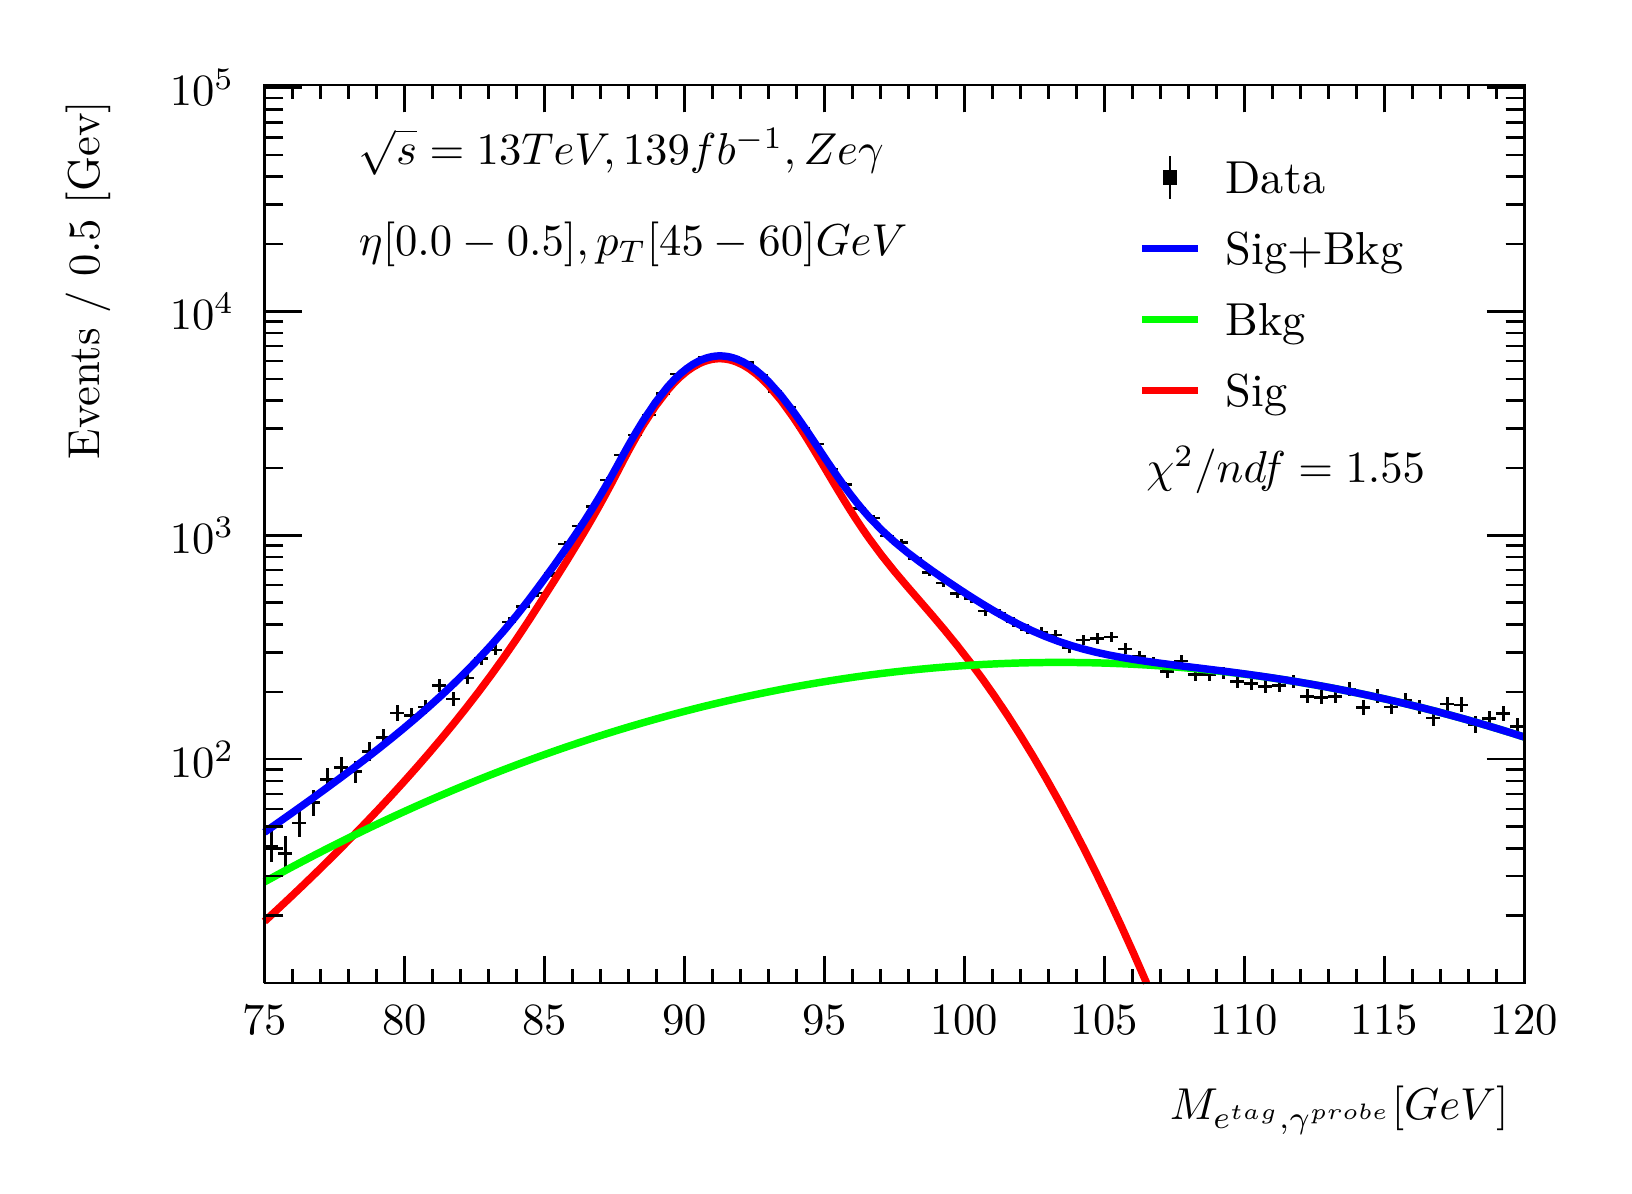
\begin{tikzpicture}
\pgfdeclareplotmark{cross} {
\pgfpathmoveto{\pgfpoint{-0.3\pgfplotmarksize}{\pgfplotmarksize}}
\pgfpathlineto{\pgfpoint{+0.3\pgfplotmarksize}{\pgfplotmarksize}}
\pgfpathlineto{\pgfpoint{+0.3\pgfplotmarksize}{0.3\pgfplotmarksize}}
\pgfpathlineto{\pgfpoint{+1\pgfplotmarksize}{0.3\pgfplotmarksize}}
\pgfpathlineto{\pgfpoint{+1\pgfplotmarksize}{-0.3\pgfplotmarksize}}
\pgfpathlineto{\pgfpoint{+0.3\pgfplotmarksize}{-0.3\pgfplotmarksize}}
\pgfpathlineto{\pgfpoint{+0.3\pgfplotmarksize}{-1.\pgfplotmarksize}}
\pgfpathlineto{\pgfpoint{-0.3\pgfplotmarksize}{-1.\pgfplotmarksize}}
\pgfpathlineto{\pgfpoint{-0.3\pgfplotmarksize}{-0.3\pgfplotmarksize}}
\pgfpathlineto{\pgfpoint{-1.\pgfplotmarksize}{-0.3\pgfplotmarksize}}
\pgfpathlineto{\pgfpoint{-1.\pgfplotmarksize}{0.3\pgfplotmarksize}}
\pgfpathlineto{\pgfpoint{-0.3\pgfplotmarksize}{0.3\pgfplotmarksize}}
\pgfpathclose
\pgfusepathqstroke
}
\pgfdeclareplotmark{cross*} {
\pgfpathmoveto{\pgfpoint{-0.3\pgfplotmarksize}{\pgfplotmarksize}}
\pgfpathlineto{\pgfpoint{+0.3\pgfplotmarksize}{\pgfplotmarksize}}
\pgfpathlineto{\pgfpoint{+0.3\pgfplotmarksize}{0.3\pgfplotmarksize}}
\pgfpathlineto{\pgfpoint{+1\pgfplotmarksize}{0.3\pgfplotmarksize}}
\pgfpathlineto{\pgfpoint{+1\pgfplotmarksize}{-0.3\pgfplotmarksize}}
\pgfpathlineto{\pgfpoint{+0.3\pgfplotmarksize}{-0.3\pgfplotmarksize}}
\pgfpathlineto{\pgfpoint{+0.3\pgfplotmarksize}{-1.\pgfplotmarksize}}
\pgfpathlineto{\pgfpoint{-0.3\pgfplotmarksize}{-1.\pgfplotmarksize}}
\pgfpathlineto{\pgfpoint{-0.3\pgfplotmarksize}{-0.3\pgfplotmarksize}}
\pgfpathlineto{\pgfpoint{-1.\pgfplotmarksize}{-0.3\pgfplotmarksize}}
\pgfpathlineto{\pgfpoint{-1.\pgfplotmarksize}{0.3\pgfplotmarksize}}
\pgfpathlineto{\pgfpoint{-0.3\pgfplotmarksize}{0.3\pgfplotmarksize}}
\pgfpathclose
\pgfusepathqfillstroke
}
\pgfdeclareplotmark{newstar} {
\pgfpathmoveto{\pgfqpoint{0pt}{\pgfplotmarksize}}
\pgfpathlineto{\pgfqpointpolar{44}{0.5\pgfplotmarksize}}
\pgfpathlineto{\pgfqpointpolar{18}{\pgfplotmarksize}}
\pgfpathlineto{\pgfqpointpolar{-20}{0.5\pgfplotmarksize}}
\pgfpathlineto{\pgfqpointpolar{-54}{\pgfplotmarksize}}
\pgfpathlineto{\pgfqpointpolar{-90}{0.5\pgfplotmarksize}}
\pgfpathlineto{\pgfqpointpolar{234}{\pgfplotmarksize}}
\pgfpathlineto{\pgfqpointpolar{198}{0.5\pgfplotmarksize}}
\pgfpathlineto{\pgfqpointpolar{162}{\pgfplotmarksize}}
\pgfpathlineto{\pgfqpointpolar{134}{0.5\pgfplotmarksize}}
\pgfpathclose
\pgfusepathqstroke
}
\pgfdeclareplotmark{newstar*} {
\pgfpathmoveto{\pgfqpoint{0pt}{\pgfplotmarksize}}
\pgfpathlineto{\pgfqpointpolar{44}{0.5\pgfplotmarksize}}
\pgfpathlineto{\pgfqpointpolar{18}{\pgfplotmarksize}}
\pgfpathlineto{\pgfqpointpolar{-20}{0.5\pgfplotmarksize}}
\pgfpathlineto{\pgfqpointpolar{-54}{\pgfplotmarksize}}
\pgfpathlineto{\pgfqpointpolar{-90}{0.5\pgfplotmarksize}}
\pgfpathlineto{\pgfqpointpolar{234}{\pgfplotmarksize}}
\pgfpathlineto{\pgfqpointpolar{198}{0.5\pgfplotmarksize}}
\pgfpathlineto{\pgfqpointpolar{162}{\pgfplotmarksize}}
\pgfpathlineto{\pgfqpointpolar{134}{0.5\pgfplotmarksize}}
\pgfpathclose
\pgfusepathqfillstroke
}
\definecolor{c}{rgb}{1,1,1};
\draw [color=c, fill=c] (0,0) rectangle (20,14.4361);
\draw [color=c, fill=c] (3,2.30977) rectangle (19,13.7143);
\definecolor{c}{rgb}{0,0,0};
\draw [c,line width=0.9] (3,2.30977) -- (3,13.7143) -- (19,13.7143) -- (19,2.30977) -- (3,2.30977);
\definecolor{c}{rgb}{1,1,1};
\draw [color=c, fill=c] (3,2.30977) rectangle (19,13.7143);
\definecolor{c}{rgb}{0,0,0};
\draw [c,line width=0.9] (3,2.30977) -- (3,13.7143) -- (19,13.7143) -- (19,2.30977) -- (3,2.30977);
\draw [c,line width=0.9] (3,2.30977) -- (19,2.30977);
\draw [c,line width=0.9] (3,2.65624) -- (3,2.30977);
\draw [c,line width=0.9] (3.35556,2.48301) -- (3.35556,2.30977);
\draw [c,line width=0.9] (3.71111,2.48301) -- (3.71111,2.30977);
\draw [c,line width=0.9] (4.06667,2.48301) -- (4.06667,2.30977);
\draw [c,line width=0.9] (4.42222,2.48301) -- (4.42222,2.30977);
\draw [c,line width=0.9] (4.77778,2.65624) -- (4.77778,2.30977);
\draw [c,line width=0.9] (5.13333,2.48301) -- (5.13333,2.30977);
\draw [c,line width=0.9] (5.48889,2.48301) -- (5.48889,2.30977);
\draw [c,line width=0.9] (5.84444,2.48301) -- (5.84444,2.30977);
\draw [c,line width=0.9] (6.2,2.48301) -- (6.2,2.30977);
\draw [c,line width=0.9] (6.55556,2.65624) -- (6.55556,2.30977);
\draw [c,line width=0.9] (6.91111,2.48301) -- (6.91111,2.30977);
\draw [c,line width=0.9] (7.26667,2.48301) -- (7.26667,2.30977);
\draw [c,line width=0.9] (7.62222,2.48301) -- (7.62222,2.30977);
\draw [c,line width=0.9] (7.97778,2.48301) -- (7.97778,2.30977);
\draw [c,line width=0.9] (8.33333,2.65624) -- (8.33333,2.30977);
\draw [c,line width=0.9] (8.68889,2.48301) -- (8.68889,2.30977);
\draw [c,line width=0.9] (9.04444,2.48301) -- (9.04444,2.30977);
\draw [c,line width=0.9] (9.4,2.48301) -- (9.4,2.30977);
\draw [c,line width=0.9] (9.75556,2.48301) -- (9.75556,2.30977);
\draw [c,line width=0.9] (10.1111,2.65624) -- (10.1111,2.30977);
\draw [c,line width=0.9] (10.4667,2.48301) -- (10.4667,2.30977);
\draw [c,line width=0.9] (10.8222,2.48301) -- (10.8222,2.30977);
\draw [c,line width=0.9] (11.1778,2.48301) -- (11.1778,2.30977);
\draw [c,line width=0.9] (11.5333,2.48301) -- (11.5333,2.30977);
\draw [c,line width=0.9] (11.8889,2.65624) -- (11.8889,2.30977);
\draw [c,line width=0.9] (12.2444,2.48301) -- (12.2444,2.30977);
\draw [c,line width=0.9] (12.6,2.48301) -- (12.6,2.30977);
\draw [c,line width=0.9] (12.9556,2.48301) -- (12.9556,2.30977);
\draw [c,line width=0.9] (13.3111,2.48301) -- (13.3111,2.30977);
\draw [c,line width=0.9] (13.6667,2.65624) -- (13.6667,2.30977);
\draw [c,line width=0.9] (14.0222,2.48301) -- (14.0222,2.30977);
\draw [c,line width=0.9] (14.3778,2.48301) -- (14.3778,2.30977);
\draw [c,line width=0.9] (14.7333,2.48301) -- (14.7333,2.30977);
\draw [c,line width=0.9] (15.0889,2.48301) -- (15.0889,2.30977);
\draw [c,line width=0.9] (15.4444,2.65624) -- (15.4444,2.30977);
\draw [c,line width=0.9] (15.8,2.48301) -- (15.8,2.30977);
\draw [c,line width=0.9] (16.1556,2.48301) -- (16.1556,2.30977);
\draw [c,line width=0.9] (16.5111,2.48301) -- (16.5111,2.30977);
\draw [c,line width=0.9] (16.8667,2.48301) -- (16.8667,2.30977);
\draw [c,line width=0.9] (17.2222,2.65624) -- (17.2222,2.30977);
\draw [c,line width=0.9] (17.5778,2.48301) -- (17.5778,2.30977);
\draw [c,line width=0.9] (17.9333,2.48301) -- (17.9333,2.30977);
\draw [c,line width=0.9] (18.2889,2.48301) -- (18.2889,2.30977);
\draw [c,line width=0.9] (18.6444,2.48301) -- (18.6444,2.30977);
\draw [c,line width=0.9] (19,2.65624) -- (19,2.30977);
\draw [c,line width=0.9] (19,2.65624) -- (19,2.30977);
\draw [anchor=base] (3,1.66015) node[scale=1.61424, color=c, rotate=0]{75};
\draw [anchor=base] (4.77778,1.66015) node[scale=1.61424, color=c, rotate=0]{80};
\draw [anchor=base] (6.55556,1.66015) node[scale=1.61424, color=c, rotate=0]{85};
\draw [anchor=base] (8.33333,1.66015) node[scale=1.61424, color=c, rotate=0]{90};
\draw [anchor=base] (10.1111,1.66015) node[scale=1.61424, color=c, rotate=0]{95};
\draw [anchor=base] (11.8889,1.66015) node[scale=1.61424, color=c, rotate=0]{100};
\draw [anchor=base] (13.6667,1.66015) node[scale=1.61424, color=c, rotate=0]{105};
\draw [anchor=base] (15.4444,1.66015) node[scale=1.61424, color=c, rotate=0]{110};
\draw [anchor=base] (17.2222,1.66015) node[scale=1.61424, color=c, rotate=0]{115};
\draw [anchor=base] (19,1.66015) node[scale=1.61424, color=c, rotate=0]{120};
\draw [anchor= east] (19,0.692932) node[scale=1.61424, color=c, rotate=0]{$M_{e^{tag}, \gamma^{probe}}  [GeV]$};
\draw [c,line width=0.9] (3,13.7143) -- (19,13.7143);
\draw [c,line width=0.9] (3,13.3678) -- (3,13.7143);
\draw [c,line width=0.9] (3.35556,13.5411) -- (3.35556,13.7143);
\draw [c,line width=0.9] (3.71111,13.5411) -- (3.71111,13.7143);
\draw [c,line width=0.9] (4.06667,13.5411) -- (4.06667,13.7143);
\draw [c,line width=0.9] (4.42222,13.5411) -- (4.42222,13.7143);
\draw [c,line width=0.9] (4.77778,13.3678) -- (4.77778,13.7143);
\draw [c,line width=0.9] (5.13333,13.5411) -- (5.13333,13.7143);
\draw [c,line width=0.9] (5.48889,13.5411) -- (5.48889,13.7143);
\draw [c,line width=0.9] (5.84444,13.5411) -- (5.84444,13.7143);
\draw [c,line width=0.9] (6.2,13.5411) -- (6.2,13.7143);
\draw [c,line width=0.9] (6.55556,13.3678) -- (6.55556,13.7143);
\draw [c,line width=0.9] (6.91111,13.5411) -- (6.91111,13.7143);
\draw [c,line width=0.9] (7.26667,13.5411) -- (7.26667,13.7143);
\draw [c,line width=0.9] (7.62222,13.5411) -- (7.62222,13.7143);
\draw [c,line width=0.9] (7.97778,13.5411) -- (7.97778,13.7143);
\draw [c,line width=0.9] (8.33333,13.3678) -- (8.33333,13.7143);
\draw [c,line width=0.9] (8.68889,13.5411) -- (8.68889,13.7143);
\draw [c,line width=0.9] (9.04444,13.5411) -- (9.04444,13.7143);
\draw [c,line width=0.9] (9.4,13.5411) -- (9.4,13.7143);
\draw [c,line width=0.9] (9.75556,13.5411) -- (9.75556,13.7143);
\draw [c,line width=0.9] (10.1111,13.3678) -- (10.1111,13.7143);
\draw [c,line width=0.9] (10.4667,13.5411) -- (10.4667,13.7143);
\draw [c,line width=0.9] (10.8222,13.5411) -- (10.8222,13.7143);
\draw [c,line width=0.9] (11.1778,13.5411) -- (11.1778,13.7143);
\draw [c,line width=0.9] (11.5333,13.5411) -- (11.5333,13.7143);
\draw [c,line width=0.9] (11.8889,13.3678) -- (11.8889,13.7143);
\draw [c,line width=0.9] (12.2444,13.5411) -- (12.2444,13.7143);
\draw [c,line width=0.9] (12.6,13.5411) -- (12.6,13.7143);
\draw [c,line width=0.9] (12.9556,13.5411) -- (12.9556,13.7143);
\draw [c,line width=0.9] (13.3111,13.5411) -- (13.3111,13.7143);
\draw [c,line width=0.9] (13.6667,13.3678) -- (13.6667,13.7143);
\draw [c,line width=0.9] (14.0222,13.5411) -- (14.0222,13.7143);
\draw [c,line width=0.9] (14.3778,13.5411) -- (14.3778,13.7143);
\draw [c,line width=0.9] (14.7333,13.5411) -- (14.7333,13.7143);
\draw [c,line width=0.9] (15.0889,13.5411) -- (15.0889,13.7143);
\draw [c,line width=0.9] (15.4444,13.3678) -- (15.4444,13.7143);
\draw [c,line width=0.9] (15.8,13.5411) -- (15.8,13.7143);
\draw [c,line width=0.9] (16.1556,13.5411) -- (16.1556,13.7143);
\draw [c,line width=0.9] (16.5111,13.5411) -- (16.5111,13.7143);
\draw [c,line width=0.9] (16.8667,13.5411) -- (16.8667,13.7143);
\draw [c,line width=0.9] (17.2222,13.3678) -- (17.2222,13.7143);
\draw [c,line width=0.9] (17.5778,13.5411) -- (17.5778,13.7143);
\draw [c,line width=0.9] (17.9333,13.5411) -- (17.9333,13.7143);
\draw [c,line width=0.9] (18.2889,13.5411) -- (18.2889,13.7143);
\draw [c,line width=0.9] (18.6444,13.5411) -- (18.6444,13.7143);
\draw [c,line width=0.9] (19,13.3678) -- (19,13.7143);
\draw [c,line width=0.9] (19,13.3678) -- (19,13.7143);
\draw [c,line width=0.9] (3,2.30977) -- (3,13.7143);
\draw [c,line width=0.9] (3.237,3.16561) -- (3,3.16561);
\draw [c,line width=0.9] (3.237,3.66625) -- (3,3.66625);
\draw [c,line width=0.9] (3.237,4.02146) -- (3,4.02146);
\draw [c,line width=0.9] (3.237,4.29698) -- (3,4.29698);
\draw [c,line width=0.9] (3.237,4.52209) -- (3,4.52209);
\draw [c,line width=0.9] (3.237,4.71242) -- (3,4.71242);
\draw [c,line width=0.9] (3.237,4.8773) -- (3,4.8773);
\draw [c,line width=0.9] (3.237,5.02273) -- (3,5.02273);
\draw [c,line width=0.9] (3.474,5.15282) -- (3,5.15282);
\draw [anchor= east] (2.82,5.15282) node[scale=1.61424, color=c, rotate=0]{$10^{2}$};
\draw [c,line width=0.9] (3.237,6.00866) -- (3,6.00866);
\draw [c,line width=0.9] (3.237,6.5093) -- (3,6.5093);
\draw [c,line width=0.9] (3.237,6.8645) -- (3,6.8645);
\draw [c,line width=0.9] (3.237,7.14002) -- (3,7.14002);
\draw [c,line width=0.9] (3.237,7.36514) -- (3,7.36514);
\draw [c,line width=0.9] (3.237,7.55547) -- (3,7.55547);
\draw [c,line width=0.9] (3.237,7.72034) -- (3,7.72034);
\draw [c,line width=0.9] (3.237,7.86577) -- (3,7.86577);
\draw [c,line width=0.9] (3.474,7.99586) -- (3,7.99586);
\draw [anchor= east] (2.82,7.99586) node[scale=1.61424, color=c, rotate=0]{$10^{3}$};
\draw [c,line width=0.9] (3.237,8.85171) -- (3,8.85171);
\draw [c,line width=0.9] (3.237,9.35234) -- (3,9.35234);
\draw [c,line width=0.9] (3.237,9.70755) -- (3,9.70755);
\draw [c,line width=0.9] (3.237,9.98307) -- (3,9.98307);
\draw [c,line width=0.9] (3.237,10.2082) -- (3,10.2082);
\draw [c,line width=0.9] (3.237,10.3985) -- (3,10.3985);
\draw [c,line width=0.9] (3.237,10.5634) -- (3,10.5634);
\draw [c,line width=0.9] (3.237,10.7088) -- (3,10.7088);
\draw [c,line width=0.9] (3.474,10.8389) -- (3,10.8389);
\draw [anchor= east] (2.82,10.8389) node[scale=1.61424, color=c, rotate=0]{$10^{4}$};
\draw [c,line width=0.9] (3.237,11.6948) -- (3,11.6948);
\draw [c,line width=0.9] (3.237,12.1954) -- (3,12.1954);
\draw [c,line width=0.9] (3.237,12.5506) -- (3,12.5506);
\draw [c,line width=0.9] (3.237,12.8261) -- (3,12.8261);
\draw [c,line width=0.9] (3.237,13.0512) -- (3,13.0512);
\draw [c,line width=0.9] (3.237,13.2416) -- (3,13.2416);
\draw [c,line width=0.9] (3.237,13.4064) -- (3,13.4064);
\draw [c,line width=0.9] (3.237,13.5519) -- (3,13.5519);
\draw [c,line width=0.9] (3.474,13.682) -- (3,13.682);
\draw [anchor= east] (2.82,13.682) node[scale=1.61424, color=c, rotate=0]{$10^{5}$};
\draw [anchor= east] (0.76,13.7143) node[scale=1.61424, color=c, rotate=90]{Events / 0.5 [Gev]};
\draw [c,line width=0.9] (19,2.30977) -- (19,13.7143);
\draw [c,line width=0.9] (18.763,3.16561) -- (19,3.16561);
\draw [c,line width=0.9] (18.763,3.66625) -- (19,3.66625);
\draw [c,line width=0.9] (18.763,4.02146) -- (19,4.02146);
\draw [c,line width=0.9] (18.763,4.29698) -- (19,4.29698);
\draw [c,line width=0.9] (18.763,4.52209) -- (19,4.52209);
\draw [c,line width=0.9] (18.763,4.71242) -- (19,4.71242);
\draw [c,line width=0.9] (18.763,4.8773) -- (19,4.8773);
\draw [c,line width=0.9] (18.763,5.02273) -- (19,5.02273);
\draw [c,line width=0.9] (18.526,5.15282) -- (19,5.15282);
\draw [c,line width=0.9] (18.763,6.00866) -- (19,6.00866);
\draw [c,line width=0.9] (18.763,6.5093) -- (19,6.5093);
\draw [c,line width=0.9] (18.763,6.8645) -- (19,6.8645);
\draw [c,line width=0.9] (18.763,7.14002) -- (19,7.14002);
\draw [c,line width=0.9] (18.763,7.36514) -- (19,7.36514);
\draw [c,line width=0.9] (18.763,7.55547) -- (19,7.55547);
\draw [c,line width=0.9] (18.763,7.72034) -- (19,7.72034);
\draw [c,line width=0.9] (18.763,7.86577) -- (19,7.86577);
\draw [c,line width=0.9] (18.526,7.99586) -- (19,7.99586);
\draw [c,line width=0.9] (18.763,8.85171) -- (19,8.85171);
\draw [c,line width=0.9] (18.763,9.35234) -- (19,9.35234);
\draw [c,line width=0.9] (18.763,9.70755) -- (19,9.70755);
\draw [c,line width=0.9] (18.763,9.98307) -- (19,9.98307);
\draw [c,line width=0.9] (18.763,10.2082) -- (19,10.2082);
\draw [c,line width=0.9] (18.763,10.3985) -- (19,10.3985);
\draw [c,line width=0.9] (18.763,10.5634) -- (19,10.5634);
\draw [c,line width=0.9] (18.763,10.7088) -- (19,10.7088);
\draw [c,line width=0.9] (18.526,10.8389) -- (19,10.8389);
\draw [c,line width=0.9] (18.763,11.6948) -- (19,11.6948);
\draw [c,line width=0.9] (18.763,12.1954) -- (19,12.1954);
\draw [c,line width=0.9] (18.763,12.5506) -- (19,12.5506);
\draw [c,line width=0.9] (18.763,12.8261) -- (19,12.8261);
\draw [c,line width=0.9] (18.763,13.0512) -- (19,13.0512);
\draw [c,line width=0.9] (18.763,13.2416) -- (19,13.2416);
\draw [c,line width=0.9] (18.763,13.4064) -- (19,13.4064);
\draw [c,line width=0.9] (18.763,13.5519) -- (19,13.5519);
\draw [c,line width=0.9] (18.526,13.682) -- (19,13.682);
\draw [c,line width=0.9] (3.08889,4.05195) -- (3,4.05195);
\draw [c,line width=0.9] (3,4.05195) -- (3,4.05195);
\draw [c,line width=0.9] (3.08889,4.05195) -- (3.17778,4.05195);
\draw [c,line width=0.9] (3.17778,4.05195) -- (3.17778,4.05195);
\draw [c,line width=0.9] (3.08889,4.05195) -- (3.08889,4.25823);
\draw [c,line width=0.9] (3.08889,4.25823) -- (3.08889,4.25823);
\draw [c,line width=0.9] (3.08889,4.05195) -- (3.08889,3.84322);
\draw [c,line width=0.9] (3.08889,3.84322) -- (3.08889,3.84322);
\draw [c,line width=0.9] (3.26667,3.95813) -- (3.17778,3.95813);
\draw [c,line width=0.9] (3.17778,3.95813) -- (3.17778,3.95813);
\draw [c,line width=0.9] (3.26667,3.95813) -- (3.35556,3.95813);
\draw [c,line width=0.9] (3.35556,3.95813) -- (3.35556,3.95813);
\draw [c,line width=0.9] (3.26667,3.95813) -- (3.26667,4.17287);
\draw [c,line width=0.9] (3.26667,4.17287) -- (3.26667,4.17287);
\draw [c,line width=0.9] (3.26667,3.95813) -- (3.26667,3.74063);
\draw [c,line width=0.9] (3.26667,3.74063) -- (3.26667,3.74063);
\draw [c,line width=0.9] (3.44444,4.3454) -- (3.35556,4.3454);
\draw [c,line width=0.9] (3.35556,4.3454) -- (3.35556,4.3454);
\draw [c,line width=0.9] (3.44444,4.3454) -- (3.53333,4.3454);
\draw [c,line width=0.9] (3.53333,4.3454) -- (3.53333,4.3454);
\draw [c,line width=0.9] (3.44444,4.3454) -- (3.44444,4.52738);
\draw [c,line width=0.9] (3.44444,4.52738) -- (3.44444,4.52738);
\draw [c,line width=0.9] (3.44444,4.3454) -- (3.44444,4.16172);
\draw [c,line width=0.9] (3.44444,4.16172) -- (3.44444,4.16172);
\draw [c,line width=0.9] (3.62222,4.60178) -- (3.53333,4.60178);
\draw [c,line width=0.9] (3.53333,4.60178) -- (3.53333,4.60178);
\draw [c,line width=0.9] (3.62222,4.60178) -- (3.71111,4.60178);
\draw [c,line width=0.9] (3.71111,4.60178) -- (3.71111,4.60178);
\draw [c,line width=0.9] (3.62222,4.60178) -- (3.62222,4.76495);
\draw [c,line width=0.9] (3.62222,4.76495) -- (3.62222,4.76495);
\draw [c,line width=0.9] (3.62222,4.60178) -- (3.62222,4.43737);
\draw [c,line width=0.9] (3.62222,4.43737) -- (3.62222,4.43737);
\draw [c,line width=0.9] (3.8,4.89264) -- (3.71111,4.89264);
\draw [c,line width=0.9] (3.71111,4.89264) -- (3.71111,4.89264);
\draw [c,line width=0.9] (3.8,4.89264) -- (3.88889,4.89264);
\draw [c,line width=0.9] (3.88889,4.89264) -- (3.88889,4.89264);
\draw [c,line width=0.9] (3.8,4.89264) -- (3.8,5.03688);
\draw [c,line width=0.9] (3.8,5.03688) -- (3.8,5.03688);
\draw [c,line width=0.9] (3.8,4.89264) -- (3.8,4.74753);
\draw [c,line width=0.9] (3.8,4.74753) -- (3.8,4.74753);
\draw [c,line width=0.9] (3.97778,5.04987) -- (3.88889,5.04987);
\draw [c,line width=0.9] (3.88889,5.04987) -- (3.88889,5.04987);
\draw [c,line width=0.9] (3.97778,5.04987) -- (4.06667,5.04987);
\draw [c,line width=0.9] (4.06667,5.04987) -- (4.06667,5.04987);
\draw [c,line width=0.9] (3.97778,5.04987) -- (3.97778,5.18483);
\draw [c,line width=0.9] (3.97778,5.18483) -- (3.97778,5.18483);
\draw [c,line width=0.9] (3.97778,5.04987) -- (3.97778,4.91418);
\draw [c,line width=0.9] (3.97778,4.91418) -- (3.97778,4.91418);
\draw [c,line width=0.9] (4.15556,4.99498) -- (4.06667,4.99498);
\draw [c,line width=0.9] (4.06667,4.99498) -- (4.06667,4.99498);
\draw [c,line width=0.9] (4.15556,4.99498) -- (4.24444,4.99498);
\draw [c,line width=0.9] (4.24444,4.99498) -- (4.24444,4.99498);
\draw [c,line width=0.9] (4.15556,4.99498) -- (4.15556,5.13311);
\draw [c,line width=0.9] (4.15556,5.13311) -- (4.15556,5.13311);
\draw [c,line width=0.9] (4.15556,4.99498) -- (4.15556,4.85608);
\draw [c,line width=0.9] (4.15556,4.85608) -- (4.15556,4.85608);
\draw [c,line width=0.9] (4.33333,5.24785) -- (4.24444,5.24785);
\draw [c,line width=0.9] (4.24444,5.24785) -- (4.24444,5.24785);
\draw [c,line width=0.9] (4.33333,5.24785) -- (4.42222,5.24785);
\draw [c,line width=0.9] (4.42222,5.24785) -- (4.42222,5.24785);
\draw [c,line width=0.9] (4.33333,5.24785) -- (4.33333,5.36661);
\draw [c,line width=0.9] (4.33333,5.36661) -- (4.33333,5.36661);
\draw [c,line width=0.9] (4.33333,5.24785) -- (4.33333,5.12908);
\draw [c,line width=0.9] (4.33333,5.12908) -- (4.33333,5.12908);
\draw [c,line width=0.9] (4.51111,5.42834) -- (4.42222,5.42834);
\draw [c,line width=0.9] (4.42222,5.42834) -- (4.42222,5.42834);
\draw [c,line width=0.9] (4.51111,5.42834) -- (4.6,5.42834);
\draw [c,line width=0.9] (4.6,5.42834) -- (4.6,5.42834);
\draw [c,line width=0.9] (4.51111,5.42834) -- (4.51111,5.53874);
\draw [c,line width=0.9] (4.51111,5.53874) -- (4.51111,5.53874);
\draw [c,line width=0.9] (4.51111,5.42834) -- (4.51111,5.31794);
\draw [c,line width=0.9] (4.51111,5.31794) -- (4.51111,5.31794);
\draw [c,line width=0.9] (4.68889,5.74084) -- (4.6,5.74084);
\draw [c,line width=0.9] (4.6,5.74084) -- (4.6,5.74084);
\draw [c,line width=0.9] (4.68889,5.74084) -- (4.77778,5.74084);
\draw [c,line width=0.9] (4.77778,5.74084) -- (4.77778,5.74084);
\draw [c,line width=0.9] (4.68889,5.74084) -- (4.68889,5.83812);
\draw [c,line width=0.9] (4.68889,5.83812) -- (4.68889,5.83812);
\draw [c,line width=0.9] (4.68889,5.74084) -- (4.68889,5.64355);
\draw [c,line width=0.9] (4.68889,5.64355) -- (4.68889,5.64355);
\draw [c,line width=0.9] (4.86667,5.70977) -- (4.77778,5.70977);
\draw [c,line width=0.9] (4.77778,5.70977) -- (4.77778,5.70977);
\draw [c,line width=0.9] (4.86667,5.70977) -- (4.95556,5.70977);
\draw [c,line width=0.9] (4.95556,5.70977) -- (4.95556,5.70977);
\draw [c,line width=0.9] (4.86667,5.70977) -- (4.86667,5.80829);
\draw [c,line width=0.9] (4.86667,5.80829) -- (4.86667,5.80829);
\draw [c,line width=0.9] (4.86667,5.70977) -- (4.86667,5.61126);
\draw [c,line width=0.9] (4.86667,5.61126) -- (4.86667,5.61126);
\draw [c,line width=0.9] (5.04444,5.81524) -- (4.95556,5.81524);
\draw [c,line width=0.9] (4.95556,5.81524) -- (4.95556,5.81524);
\draw [c,line width=0.9] (5.04444,5.81524) -- (5.13333,5.81524);
\draw [c,line width=0.9] (5.13333,5.81524) -- (5.13333,5.81524);
\draw [c,line width=0.9] (5.04444,5.81524) -- (5.04444,5.90964);
\draw [c,line width=0.9] (5.04444,5.90964) -- (5.04444,5.90964);
\draw [c,line width=0.9] (5.04444,5.81524) -- (5.04444,5.72084);
\draw [c,line width=0.9] (5.04444,5.72084) -- (5.04444,5.72084);
\draw [c,line width=0.9] (5.22222,6.08642) -- (5.13333,6.08642);
\draw [c,line width=0.9] (5.13333,6.08642) -- (5.13333,6.08642);
\draw [c,line width=0.9] (5.22222,6.08642) -- (5.31111,6.08642);
\draw [c,line width=0.9] (5.31111,6.08642) -- (5.31111,6.08642);
\draw [c,line width=0.9] (5.22222,6.08642) -- (5.22222,6.171);
\draw [c,line width=0.9] (5.22222,6.171) -- (5.22222,6.171);
\draw [c,line width=0.9] (5.22222,6.08642) -- (5.22222,6.00183);
\draw [c,line width=0.9] (5.22222,6.00183) -- (5.22222,6.00183);
\draw [c,line width=0.9] (5.4,5.91906) -- (5.31111,5.91906);
\draw [c,line width=0.9] (5.31111,5.91906) -- (5.31111,5.91906);
\draw [c,line width=0.9] (5.4,5.91906) -- (5.48889,5.91906);
\draw [c,line width=0.9] (5.48889,5.91906) -- (5.48889,5.91906);
\draw [c,line width=0.9] (5.4,5.91906) -- (5.4,6.00957);
\draw [c,line width=0.9] (5.4,6.00957) -- (5.4,6.00957);
\draw [c,line width=0.9] (5.4,5.91906) -- (5.4,5.82854);
\draw [c,line width=0.9] (5.4,5.82854) -- (5.4,5.82854);
\draw [c,line width=0.9] (5.57778,6.18658) -- (5.48889,6.18658);
\draw [c,line width=0.9] (5.48889,6.18658) -- (5.48889,6.18658);
\draw [c,line width=0.9] (5.57778,6.18658) -- (5.66667,6.18658);
\draw [c,line width=0.9] (5.66667,6.18658) -- (5.66667,6.18658);
\draw [c,line width=0.9] (5.57778,6.18658) -- (5.57778,6.26781);
\draw [c,line width=0.9] (5.57778,6.26781) -- (5.57778,6.26781);
\draw [c,line width=0.9] (5.57778,6.18658) -- (5.57778,6.10536);
\draw [c,line width=0.9] (5.57778,6.10536) -- (5.57778,6.10536);
\draw [c,line width=0.9] (5.75556,6.42851) -- (5.66667,6.42851);
\draw [c,line width=0.9] (5.66667,6.42851) -- (5.66667,6.42851);
\draw [c,line width=0.9] (5.75556,6.42851) -- (5.84444,6.42851);
\draw [c,line width=0.9] (5.84444,6.42851) -- (5.84444,6.42851);
\draw [c,line width=0.9] (5.75556,6.42851) -- (5.75556,6.50216);
\draw [c,line width=0.9] (5.75556,6.50216) -- (5.75556,6.50216);
\draw [c,line width=0.9] (5.75556,6.42851) -- (5.75556,6.35487);
\draw [c,line width=0.9] (5.75556,6.35487) -- (5.75556,6.35487);
\draw [c,line width=0.9] (5.93333,6.54179) -- (5.84444,6.54179);
\draw [c,line width=0.9] (5.84444,6.54179) -- (5.84444,6.54179);
\draw [c,line width=0.9] (5.93333,6.54179) -- (6.02222,6.54179);
\draw [c,line width=0.9] (6.02222,6.54179) -- (6.02222,6.54179);
\draw [c,line width=0.9] (5.93333,6.54179) -- (5.93333,6.61214);
\draw [c,line width=0.9] (5.93333,6.61214) -- (5.93333,6.61214);
\draw [c,line width=0.9] (5.93333,6.54179) -- (5.93333,6.47145);
\draw [c,line width=0.9] (5.93333,6.47145) -- (5.93333,6.47145);
\draw [c,line width=0.9] (6.11111,6.89198) -- (6.02222,6.89198);
\draw [c,line width=0.9] (6.02222,6.89198) -- (6.02222,6.89198);
\draw [c,line width=0.9] (6.11111,6.89198) -- (6.2,6.89198);
\draw [c,line width=0.9] (6.2,6.89198) -- (6.2,6.89198);
\draw [c,line width=0.9] (6.11111,6.89198) -- (6.11111,6.95302);
\draw [c,line width=0.9] (6.11111,6.95302) -- (6.11111,6.95302);
\draw [c,line width=0.9] (6.11111,6.89198) -- (6.11111,6.83093);
\draw [c,line width=0.9] (6.11111,6.83093) -- (6.11111,6.83093);
\draw [c,line width=0.9] (6.28889,7.09475) -- (6.2,7.09475);
\draw [c,line width=0.9] (6.2,7.09475) -- (6.2,7.09475);
\draw [c,line width=0.9] (6.28889,7.09475) -- (6.37778,7.09475);
\draw [c,line width=0.9] (6.37778,7.09475) -- (6.37778,7.09475);
\draw [c,line width=0.9] (6.28889,7.09475) -- (6.28889,7.15099);
\draw [c,line width=0.9] (6.28889,7.15099) -- (6.28889,7.15099);
\draw [c,line width=0.9] (6.28889,7.09475) -- (6.28889,7.03852);
\draw [c,line width=0.9] (6.28889,7.03852) -- (6.28889,7.03852);
\draw [c,line width=0.9] (6.46667,7.26442) -- (6.37778,7.26442);
\draw [c,line width=0.9] (6.37778,7.26442) -- (6.37778,7.26442);
\draw [c,line width=0.9] (6.46667,7.26442) -- (6.55556,7.26442);
\draw [c,line width=0.9] (6.55556,7.26442) -- (6.55556,7.26442);
\draw [c,line width=0.9] (6.46667,7.26442) -- (6.46667,7.31692);
\draw [c,line width=0.9] (6.46667,7.31692) -- (6.46667,7.31692);
\draw [c,line width=0.9] (6.46667,7.26442) -- (6.46667,7.21192);
\draw [c,line width=0.9] (6.46667,7.21192) -- (6.46667,7.21192);
\draw [c,line width=0.9] (6.64444,7.50874) -- (6.55556,7.50874);
\draw [c,line width=0.9] (6.55556,7.50874) -- (6.55556,7.50874);
\draw [c,line width=0.9] (6.64444,7.50874) -- (6.73333,7.50874);
\draw [c,line width=0.9] (6.73333,7.50874) -- (6.73333,7.50874);
\draw [c,line width=0.9] (6.64444,7.50874) -- (6.64444,7.55629);
\draw [c,line width=0.9] (6.64444,7.55629) -- (6.64444,7.55629);
\draw [c,line width=0.9] (6.64444,7.50874) -- (6.64444,7.46118);
\draw [c,line width=0.9] (6.64444,7.46118) -- (6.64444,7.46118);
\draw [c,line width=0.9] (6.82222,7.88618) -- (6.73333,7.88618);
\draw [c,line width=0.9] (6.73333,7.88618) -- (6.73333,7.88618);
\draw [c,line width=0.9] (6.82222,7.88618) -- (6.91111,7.88618);
\draw [c,line width=0.9] (6.91111,7.88618) -- (6.91111,7.88618);
\draw [c,line width=0.9] (6.82222,7.88618) -- (6.82222,7.927);
\draw [c,line width=0.9] (6.82222,7.927) -- (6.82222,7.927);
\draw [c,line width=0.9] (6.82222,7.88618) -- (6.82222,7.84537);
\draw [c,line width=0.9] (6.82222,7.84537) -- (6.82222,7.84537);
\draw [c,line width=0.9] (7,8.11242) -- (6.91111,8.11242);
\draw [c,line width=0.9] (6.91111,8.11242) -- (6.91111,8.11242);
\draw [c,line width=0.9] (7,8.11242) -- (7.08889,8.11242);
\draw [c,line width=0.9] (7.08889,8.11242) -- (7.08889,8.11242);
\draw [c,line width=0.9] (7,8.11242) -- (7,8.14967);
\draw [c,line width=0.9] (7,8.14967) -- (7,8.14967);
\draw [c,line width=0.9] (7,8.11242) -- (7,8.07518);
\draw [c,line width=0.9] (7,8.07518) -- (7,8.07518);
\draw [c,line width=0.9] (7.17778,8.36183) -- (7.08889,8.36183);
\draw [c,line width=0.9] (7.08889,8.36183) -- (7.08889,8.36183);
\draw [c,line width=0.9] (7.17778,8.36183) -- (7.26667,8.36183);
\draw [c,line width=0.9] (7.26667,8.36183) -- (7.26667,8.36183);
\draw [c,line width=0.9] (7.17778,8.36183) -- (7.17778,8.39549);
\draw [c,line width=0.9] (7.17778,8.39549) -- (7.17778,8.39549);
\draw [c,line width=0.9] (7.17778,8.36183) -- (7.17778,8.32816);
\draw [c,line width=0.9] (7.17778,8.32816) -- (7.17778,8.32816);
\draw [c,line width=0.9] (7.35556,8.70156) -- (7.26667,8.70156);
\draw [c,line width=0.9] (7.26667,8.70156) -- (7.26667,8.70156);
\draw [c,line width=0.9] (7.35556,8.70156) -- (7.44444,8.70156);
\draw [c,line width=0.9] (7.44444,8.70156) -- (7.44444,8.70156);
\draw [c,line width=0.9] (7.35556,8.70156) -- (7.35556,8.7309);
\draw [c,line width=0.9] (7.35556,8.7309) -- (7.35556,8.7309);
\draw [c,line width=0.9] (7.35556,8.70156) -- (7.35556,8.67222);
\draw [c,line width=0.9] (7.35556,8.67222) -- (7.35556,8.67222);
\draw [c,line width=0.9] (7.53333,9.01511) -- (7.44444,9.01511);
\draw [c,line width=0.9] (7.44444,9.01511) -- (7.44444,9.01511);
\draw [c,line width=0.9] (7.53333,9.01511) -- (7.62222,9.01511);
\draw [c,line width=0.9] (7.62222,9.01511) -- (7.62222,9.01511);
\draw [c,line width=0.9] (7.53333,9.01511) -- (7.53333,9.04095);
\draw [c,line width=0.9] (7.53333,9.04095) -- (7.53333,9.04095);
\draw [c,line width=0.9] (7.53333,9.01511) -- (7.53333,8.98927);
\draw [c,line width=0.9] (7.53333,8.98927) -- (7.53333,8.98927);
\draw [c,line width=0.9] (7.71111,9.26848) -- (7.62222,9.26848);
\draw [c,line width=0.9] (7.62222,9.26848) -- (7.62222,9.26848);
\draw [c,line width=0.9] (7.71111,9.26848) -- (7.8,9.26848);
\draw [c,line width=0.9] (7.8,9.26848) -- (7.8,9.26848);
\draw [c,line width=0.9] (7.71111,9.26848) -- (7.71111,9.2918);
\draw [c,line width=0.9] (7.71111,9.2918) -- (7.71111,9.2918);
\draw [c,line width=0.9] (7.71111,9.26848) -- (7.71111,9.24516);
\draw [c,line width=0.9] (7.71111,9.24516) -- (7.71111,9.24516);
\draw [c,line width=0.9] (7.88889,9.52312) -- (7.8,9.52312);
\draw [c,line width=0.9] (7.8,9.52312) -- (7.8,9.52312);
\draw [c,line width=0.9] (7.88889,9.52312) -- (7.97778,9.52312);
\draw [c,line width=0.9] (7.97778,9.52312) -- (7.97778,9.52312);
\draw [c,line width=0.9] (7.88889,9.52312) -- (7.88889,9.54416);
\draw [c,line width=0.9] (7.88889,9.54416) -- (7.88889,9.54416);
\draw [c,line width=0.9] (7.88889,9.52312) -- (7.88889,9.50208);
\draw [c,line width=0.9] (7.88889,9.50208) -- (7.88889,9.50208);
\draw [c,line width=0.9] (8.06667,9.79426) -- (7.97778,9.79426);
\draw [c,line width=0.9] (7.97778,9.79426) -- (7.97778,9.79426);
\draw [c,line width=0.9] (8.06667,9.79426) -- (8.15556,9.79426);
\draw [c,line width=0.9] (8.15556,9.79426) -- (8.15556,9.79426);
\draw [c,line width=0.9] (8.06667,9.79426) -- (8.06667,9.81311);
\draw [c,line width=0.9] (8.06667,9.81311) -- (8.06667,9.81311);
\draw [c,line width=0.9] (8.06667,9.79426) -- (8.06667,9.77541);
\draw [c,line width=0.9] (8.06667,9.77541) -- (8.06667,9.77541);
\draw [c,line width=0.9] (8.24444,10.0452) -- (8.15556,10.0452);
\draw [c,line width=0.9] (8.15556,10.0452) -- (8.15556,10.0452);
\draw [c,line width=0.9] (8.24444,10.0452) -- (8.33333,10.0452);
\draw [c,line width=0.9] (8.33333,10.0452) -- (8.33333,10.0452);
\draw [c,line width=0.9] (8.24444,10.0452) -- (8.24444,10.0622);
\draw [c,line width=0.9] (8.24444,10.0622) -- (8.24444,10.0622);
\draw [c,line width=0.9] (8.24444,10.0452) -- (8.24444,10.0282);
\draw [c,line width=0.9] (8.24444,10.0282) -- (8.24444,10.0282);
\draw [c,line width=0.9] (8.42222,10.1292) -- (8.33333,10.1292);
\draw [c,line width=0.9] (8.33333,10.1292) -- (8.33333,10.1292);
\draw [c,line width=0.9] (8.42222,10.1292) -- (8.51111,10.1292);
\draw [c,line width=0.9] (8.51111,10.1292) -- (8.51111,10.1292);
\draw [c,line width=0.9] (8.42222,10.1292) -- (8.42222,10.1456);
\draw [c,line width=0.9] (8.42222,10.1456) -- (8.42222,10.1456);
\draw [c,line width=0.9] (8.42222,10.1292) -- (8.42222,10.1127);
\draw [c,line width=0.9] (8.42222,10.1127) -- (8.42222,10.1127);
\draw [c,line width=0.9] (8.6,10.256) -- (8.51111,10.256);
\draw [c,line width=0.9] (8.51111,10.256) -- (8.51111,10.256);
\draw [c,line width=0.9] (8.6,10.256) -- (8.68889,10.256);
\draw [c,line width=0.9] (8.68889,10.256) -- (8.68889,10.256);
\draw [c,line width=0.9] (8.6,10.256) -- (8.6,10.2717);
\draw [c,line width=0.9] (8.6,10.2717) -- (8.6,10.2717);
\draw [c,line width=0.9] (8.6,10.256) -- (8.6,10.2404);
\draw [c,line width=0.9] (8.6,10.2404) -- (8.6,10.2404);
\draw [c,line width=0.9] (8.77778,10.2819) -- (8.68889,10.2819);
\draw [c,line width=0.9] (8.68889,10.2819) -- (8.68889,10.2819);
\draw [c,line width=0.9] (8.77778,10.2819) -- (8.86667,10.2819);
\draw [c,line width=0.9] (8.86667,10.2819) -- (8.86667,10.2819);
\draw [c,line width=0.9] (8.77778,10.2819) -- (8.77778,10.2973);
\draw [c,line width=0.9] (8.77778,10.2973) -- (8.77778,10.2973);
\draw [c,line width=0.9] (8.77778,10.2819) -- (8.77778,10.2664);
\draw [c,line width=0.9] (8.77778,10.2664) -- (8.77778,10.2664);
\draw [c,line width=0.9] (8.95556,10.258) -- (8.86667,10.258);
\draw [c,line width=0.9] (8.86667,10.258) -- (8.86667,10.258);
\draw [c,line width=0.9] (8.95556,10.258) -- (9.04444,10.258);
\draw [c,line width=0.9] (9.04444,10.258) -- (9.04444,10.258);
\draw [c,line width=0.9] (8.95556,10.258) -- (8.95556,10.2736);
\draw [c,line width=0.9] (8.95556,10.2736) -- (8.95556,10.2736);
\draw [c,line width=0.9] (8.95556,10.258) -- (8.95556,10.2424);
\draw [c,line width=0.9] (8.95556,10.2424) -- (8.95556,10.2424);
\draw [c,line width=0.9] (9.13333,10.1906) -- (9.04444,10.1906);
\draw [c,line width=0.9] (9.04444,10.1906) -- (9.04444,10.1906);
\draw [c,line width=0.9] (9.13333,10.1906) -- (9.22222,10.1906);
\draw [c,line width=0.9] (9.22222,10.1906) -- (9.22222,10.1906);
\draw [c,line width=0.9] (9.13333,10.1906) -- (9.13333,10.2066);
\draw [c,line width=0.9] (9.13333,10.2066) -- (9.13333,10.2066);
\draw [c,line width=0.9] (9.13333,10.1906) -- (9.13333,10.1745);
\draw [c,line width=0.9] (9.13333,10.1745) -- (9.13333,10.1745);
\draw [c,line width=0.9] (9.31111,10.0346) -- (9.22222,10.0346);
\draw [c,line width=0.9] (9.22222,10.0346) -- (9.22222,10.0346);
\draw [c,line width=0.9] (9.31111,10.0346) -- (9.4,10.0346);
\draw [c,line width=0.9] (9.4,10.0346) -- (9.4,10.0346);
\draw [c,line width=0.9] (9.31111,10.0346) -- (9.31111,10.0517);
\draw [c,line width=0.9] (9.31111,10.0517) -- (9.31111,10.0517);
\draw [c,line width=0.9] (9.31111,10.0346) -- (9.31111,10.0175);
\draw [c,line width=0.9] (9.31111,10.0175) -- (9.31111,10.0175);
\draw [c,line width=0.9] (9.48889,9.82551) -- (9.4,9.82551);
\draw [c,line width=0.9] (9.4,9.82551) -- (9.4,9.82551);
\draw [c,line width=0.9] (9.48889,9.82551) -- (9.57778,9.82551);
\draw [c,line width=0.9] (9.57778,9.82551) -- (9.57778,9.82551);
\draw [c,line width=0.9] (9.48889,9.82551) -- (9.48889,9.84412);
\draw [c,line width=0.9] (9.48889,9.84412) -- (9.48889,9.84412);
\draw [c,line width=0.9] (9.48889,9.82551) -- (9.48889,9.8069);
\draw [c,line width=0.9] (9.48889,9.8069) -- (9.48889,9.8069);
\draw [c,line width=0.9] (9.66667,9.62523) -- (9.57778,9.62523);
\draw [c,line width=0.9] (9.57778,9.62523) -- (9.57778,9.62523);
\draw [c,line width=0.9] (9.66667,9.62523) -- (9.75556,9.62523);
\draw [c,line width=0.9] (9.75556,9.62523) -- (9.75556,9.62523);
\draw [c,line width=0.9] (9.66667,9.62523) -- (9.66667,9.64541);
\draw [c,line width=0.9] (9.66667,9.64541) -- (9.66667,9.64541);
\draw [c,line width=0.9] (9.66667,9.62523) -- (9.66667,9.60504);
\draw [c,line width=0.9] (9.66667,9.60504) -- (9.66667,9.60504);
\draw [c,line width=0.9] (9.84444,9.35645) -- (9.75556,9.35645);
\draw [c,line width=0.9] (9.75556,9.35645) -- (9.75556,9.35645);
\draw [c,line width=0.9] (9.84444,9.35645) -- (9.93333,9.35645);
\draw [c,line width=0.9] (9.93333,9.35645) -- (9.93333,9.35645);
\draw [c,line width=0.9] (9.84444,9.35645) -- (9.84444,9.37896);
\draw [c,line width=0.9] (9.84444,9.37896) -- (9.84444,9.37896);
\draw [c,line width=0.9] (9.84444,9.35645) -- (9.84444,9.33395);
\draw [c,line width=0.9] (9.84444,9.33395) -- (9.84444,9.33395);
\draw [c,line width=0.9] (10.0222,9.15796) -- (9.93333,9.15796);
\draw [c,line width=0.9] (9.93333,9.15796) -- (9.93333,9.15796);
\draw [c,line width=0.9] (10.0222,9.15796) -- (10.1111,9.15796);
\draw [c,line width=0.9] (10.1111,9.15796) -- (10.1111,9.15796);
\draw [c,line width=0.9] (10.0222,9.15796) -- (10.0222,9.18234);
\draw [c,line width=0.9] (10.0222,9.18234) -- (10.0222,9.18234);
\draw [c,line width=0.9] (10.0222,9.15796) -- (10.0222,9.13357);
\draw [c,line width=0.9] (10.0222,9.13357) -- (10.0222,9.13357);
\draw [c,line width=0.9] (10.2,8.8368) -- (10.1111,8.8368);
\draw [c,line width=0.9] (10.1111,8.8368) -- (10.1111,8.8368);
\draw [c,line width=0.9] (10.2,8.8368) -- (10.2889,8.8368);
\draw [c,line width=0.9] (10.2889,8.8368) -- (10.2889,8.8368);
\draw [c,line width=0.9] (10.2,8.8368) -- (10.2,8.86458);
\draw [c,line width=0.9] (10.2,8.86458) -- (10.2,8.86458);
\draw [c,line width=0.9] (10.2,8.8368) -- (10.2,8.80902);
\draw [c,line width=0.9] (10.2,8.80902) -- (10.2,8.80902);
\draw [c,line width=0.9] (10.3778,8.64229) -- (10.2889,8.64229);
\draw [c,line width=0.9] (10.2889,8.64229) -- (10.2889,8.64229);
\draw [c,line width=0.9] (10.3778,8.64229) -- (10.4667,8.64229);
\draw [c,line width=0.9] (10.4667,8.64229) -- (10.4667,8.64229);
\draw [c,line width=0.9] (10.3778,8.64229) -- (10.3778,8.67235);
\draw [c,line width=0.9] (10.3778,8.67235) -- (10.3778,8.67235);
\draw [c,line width=0.9] (10.3778,8.64229) -- (10.3778,8.61224);
\draw [c,line width=0.9] (10.3778,8.61224) -- (10.3778,8.61224);
\draw [c,line width=0.9] (10.5556,8.33679) -- (10.4667,8.33679);
\draw [c,line width=0.9] (10.4667,8.33679) -- (10.4667,8.33679);
\draw [c,line width=0.9] (10.5556,8.33679) -- (10.6444,8.33679);
\draw [c,line width=0.9] (10.6444,8.33679) -- (10.6444,8.33679);
\draw [c,line width=0.9] (10.5556,8.33679) -- (10.5556,8.3708);
\draw [c,line width=0.9] (10.5556,8.3708) -- (10.5556,8.3708);
\draw [c,line width=0.9] (10.5556,8.33679) -- (10.5556,8.30278);
\draw [c,line width=0.9] (10.5556,8.30278) -- (10.5556,8.30278);
\draw [c,line width=0.9] (10.7333,8.21272) -- (10.6444,8.21272);
\draw [c,line width=0.9] (10.6444,8.21272) -- (10.6444,8.21272);
\draw [c,line width=0.9] (10.7333,8.21272) -- (10.8222,8.21272);
\draw [c,line width=0.9] (10.8222,8.21272) -- (10.8222,8.21272);
\draw [c,line width=0.9] (10.7333,8.21272) -- (10.7333,8.24848);
\draw [c,line width=0.9] (10.7333,8.24848) -- (10.7333,8.24848);
\draw [c,line width=0.9] (10.7333,8.21272) -- (10.7333,8.17696);
\draw [c,line width=0.9] (10.7333,8.17696) -- (10.7333,8.17696);
\draw [c,line width=0.9] (10.9111,7.98595) -- (10.8222,7.98595);
\draw [c,line width=0.9] (10.8222,7.98595) -- (10.8222,7.98595);
\draw [c,line width=0.9] (10.9111,7.98595) -- (11,7.98595);
\draw [c,line width=0.9] (11,7.98595) -- (11,7.98595);
\draw [c,line width=0.9] (10.9111,7.98595) -- (10.9111,8.02515);
\draw [c,line width=0.9] (10.9111,8.02515) -- (10.9111,8.02515);
\draw [c,line width=0.9] (10.9111,7.98595) -- (10.9111,7.94675);
\draw [c,line width=0.9] (10.9111,7.94675) -- (10.9111,7.94675);
\draw [c,line width=0.9] (11.0889,7.90759) -- (11,7.90759);
\draw [c,line width=0.9] (11,7.90759) -- (11,7.90759);
\draw [c,line width=0.9] (11.0889,7.90759) -- (11.1778,7.90759);
\draw [c,line width=0.9] (11.1778,7.90759) -- (11.1778,7.90759);
\draw [c,line width=0.9] (11.0889,7.90759) -- (11.0889,7.94805);
\draw [c,line width=0.9] (11.0889,7.94805) -- (11.0889,7.94805);
\draw [c,line width=0.9] (11.0889,7.90759) -- (11.0889,7.86712);
\draw [c,line width=0.9] (11.0889,7.86712) -- (11.0889,7.86712);
\draw [c,line width=0.9] (11.2667,7.70168) -- (11.1778,7.70168);
\draw [c,line width=0.9] (11.1778,7.70168) -- (11.1778,7.70168);
\draw [c,line width=0.9] (11.2667,7.70168) -- (11.3556,7.70168);
\draw [c,line width=0.9] (11.3556,7.70168) -- (11.3556,7.70168);
\draw [c,line width=0.9] (11.2667,7.70168) -- (11.2667,7.74567);
\draw [c,line width=0.9] (11.2667,7.74567) -- (11.2667,7.74567);
\draw [c,line width=0.9] (11.2667,7.70168) -- (11.2667,7.6577);
\draw [c,line width=0.9] (11.2667,7.6577) -- (11.2667,7.6577);
\draw [c,line width=0.9] (11.4444,7.52149) -- (11.3556,7.52149);
\draw [c,line width=0.9] (11.3556,7.52149) -- (11.3556,7.52149);
\draw [c,line width=0.9] (11.4444,7.52149) -- (11.5333,7.52149);
\draw [c,line width=0.9] (11.5333,7.52149) -- (11.5333,7.52149);
\draw [c,line width=0.9] (11.4444,7.52149) -- (11.4444,7.56881);
\draw [c,line width=0.9] (11.4444,7.56881) -- (11.4444,7.56881);
\draw [c,line width=0.9] (11.4444,7.52149) -- (11.4444,7.47418);
\draw [c,line width=0.9] (11.4444,7.47418) -- (11.4444,7.47418);
\draw [c,line width=0.9] (11.6222,7.38959) -- (11.5333,7.38959);
\draw [c,line width=0.9] (11.5333,7.38959) -- (11.5333,7.38959);
\draw [c,line width=0.9] (11.6222,7.38959) -- (11.7111,7.38959);
\draw [c,line width=0.9] (11.7111,7.38959) -- (11.7111,7.38959);
\draw [c,line width=0.9] (11.6222,7.38959) -- (11.6222,7.4395);
\draw [c,line width=0.9] (11.6222,7.4395) -- (11.6222,7.4395);
\draw [c,line width=0.9] (11.6222,7.38959) -- (11.6222,7.33968);
\draw [c,line width=0.9] (11.6222,7.33968) -- (11.6222,7.33968);
\draw [c,line width=0.9] (11.8,7.2577) -- (11.7111,7.2577);
\draw [c,line width=0.9] (11.7111,7.2577) -- (11.7111,7.2577);
\draw [c,line width=0.9] (11.8,7.2577) -- (11.8889,7.2577);
\draw [c,line width=0.9] (11.8889,7.2577) -- (11.8889,7.2577);
\draw [c,line width=0.9] (11.8,7.2577) -- (11.8,7.31035);
\draw [c,line width=0.9] (11.8,7.31035) -- (11.8,7.31035);
\draw [c,line width=0.9] (11.8,7.2577) -- (11.8,7.20506);
\draw [c,line width=0.9] (11.8,7.20506) -- (11.8,7.20506);
\draw [c,line width=0.9] (11.9778,7.19082) -- (11.8889,7.19082);
\draw [c,line width=0.9] (11.8889,7.19082) -- (11.8889,7.19082);
\draw [c,line width=0.9] (11.9778,7.19082) -- (12.0667,7.19082);
\draw [c,line width=0.9] (12.0667,7.19082) -- (12.0667,7.19082);
\draw [c,line width=0.9] (11.9778,7.19082) -- (11.9778,7.24491);
\draw [c,line width=0.9] (11.9778,7.24491) -- (11.9778,7.24491);
\draw [c,line width=0.9] (11.9778,7.19082) -- (11.9778,7.13673);
\draw [c,line width=0.9] (11.9778,7.13673) -- (11.9778,7.13673);
\draw [c,line width=0.9] (12.1556,7.03438) -- (12.0667,7.03438);
\draw [c,line width=0.9] (12.0667,7.03438) -- (12.0667,7.03438);
\draw [c,line width=0.9] (12.1556,7.03438) -- (12.2444,7.03438);
\draw [c,line width=0.9] (12.2444,7.03438) -- (12.2444,7.03438);
\draw [c,line width=0.9] (12.1556,7.03438) -- (12.1556,7.09201);
\draw [c,line width=0.9] (12.1556,7.09201) -- (12.1556,7.09201);
\draw [c,line width=0.9] (12.1556,7.03438) -- (12.1556,6.97676);
\draw [c,line width=0.9] (12.1556,6.97676) -- (12.1556,6.97676);
\draw [c,line width=0.9] (12.3333,7.00719) -- (12.2444,7.00719);
\draw [c,line width=0.9] (12.2444,7.00719) -- (12.2444,7.00719);
\draw [c,line width=0.9] (12.3333,7.00719) -- (12.4222,7.00719);
\draw [c,line width=0.9] (12.4222,7.00719) -- (12.4222,7.00719);
\draw [c,line width=0.9] (12.3333,7.00719) -- (12.3333,7.06545);
\draw [c,line width=0.9] (12.3333,7.06545) -- (12.3333,7.06545);
\draw [c,line width=0.9] (12.3333,7.00719) -- (12.3333,6.94892);
\draw [c,line width=0.9] (12.3333,6.94892) -- (12.3333,6.94892);
\draw [c,line width=0.9] (12.5111,6.898) -- (12.4222,6.898);
\draw [c,line width=0.9] (12.4222,6.898) -- (12.4222,6.898);
\draw [c,line width=0.9] (12.5111,6.898) -- (12.6,6.898);
\draw [c,line width=0.9] (12.6,6.898) -- (12.6,6.898);
\draw [c,line width=0.9] (12.5111,6.898) -- (12.5111,6.9589);
\draw [c,line width=0.9] (12.5111,6.9589) -- (12.5111,6.9589);
\draw [c,line width=0.9] (12.5111,6.898) -- (12.5111,6.8371);
\draw [c,line width=0.9] (12.5111,6.8371) -- (12.5111,6.8371);
\draw [c,line width=0.9] (12.6889,6.80117) -- (12.6,6.80117);
\draw [c,line width=0.9] (12.6,6.80117) -- (12.6,6.80117);
\draw [c,line width=0.9] (12.6889,6.80117) -- (12.7778,6.80117);
\draw [c,line width=0.9] (12.7778,6.80117) -- (12.7778,6.80117);
\draw [c,line width=0.9] (12.6889,6.80117) -- (12.6889,6.8645);
\draw [c,line width=0.9] (12.6889,6.8645) -- (12.6889,6.8645);
\draw [c,line width=0.9] (12.6889,6.80117) -- (12.6889,6.73784);
\draw [c,line width=0.9] (12.6889,6.73784) -- (12.6889,6.73784);
\draw [c,line width=0.9] (12.8667,6.76155) -- (12.7778,6.76155);
\draw [c,line width=0.9] (12.7778,6.76155) -- (12.7778,6.76155);
\draw [c,line width=0.9] (12.8667,6.76155) -- (12.9556,6.76155);
\draw [c,line width=0.9] (12.9556,6.76155) -- (12.9556,6.76155);
\draw [c,line width=0.9] (12.8667,6.76155) -- (12.8667,6.82591);
\draw [c,line width=0.9] (12.8667,6.82591) -- (12.8667,6.82591);
\draw [c,line width=0.9] (12.8667,6.76155) -- (12.8667,6.69719);
\draw [c,line width=0.9] (12.8667,6.69719) -- (12.8667,6.69719);
\draw [c,line width=0.9] (13.0444,6.72753) -- (12.9556,6.72753);
\draw [c,line width=0.9] (12.9556,6.72753) -- (12.9556,6.72753);
\draw [c,line width=0.9] (13.0444,6.72753) -- (13.1333,6.72753);
\draw [c,line width=0.9] (13.1333,6.72753) -- (13.1333,6.72753);
\draw [c,line width=0.9] (13.0444,6.72753) -- (13.0444,6.79278);
\draw [c,line width=0.9] (13.0444,6.79278) -- (13.0444,6.79278);
\draw [c,line width=0.9] (13.0444,6.72753) -- (13.0444,6.66228);
\draw [c,line width=0.9] (13.0444,6.66228) -- (13.0444,6.66228);
\draw [c,line width=0.9] (13.2222,6.57345) -- (13.1333,6.57345);
\draw [c,line width=0.9] (13.1333,6.57345) -- (13.1333,6.57345);
\draw [c,line width=0.9] (13.2222,6.57345) -- (13.3111,6.57345);
\draw [c,line width=0.9] (13.3111,6.57345) -- (13.3111,6.57345);
\draw [c,line width=0.9] (13.2222,6.57345) -- (13.2222,6.6429);
\draw [c,line width=0.9] (13.2222,6.6429) -- (13.2222,6.6429);
\draw [c,line width=0.9] (13.2222,6.57345) -- (13.2222,6.504);
\draw [c,line width=0.9] (13.2222,6.504) -- (13.2222,6.504);
\draw [c,line width=0.9] (13.4,6.66384) -- (13.3111,6.66384);
\draw [c,line width=0.9] (13.3111,6.66384) -- (13.3111,6.66384);
\draw [c,line width=0.9] (13.4,6.66384) -- (13.4889,6.66384);
\draw [c,line width=0.9] (13.4889,6.66384) -- (13.4889,6.66384);
\draw [c,line width=0.9] (13.4,6.66384) -- (13.4,6.73079);
\draw [c,line width=0.9] (13.4,6.73079) -- (13.4,6.73079);
\draw [c,line width=0.9] (13.4,6.66384) -- (13.4,6.59688);
\draw [c,line width=0.9] (13.4,6.59688) -- (13.4,6.59688);
\draw [c,line width=0.9] (13.5778,6.68544) -- (13.4889,6.68544);
\draw [c,line width=0.9] (13.4889,6.68544) -- (13.4889,6.68544);
\draw [c,line width=0.9] (13.5778,6.68544) -- (13.6667,6.68544);
\draw [c,line width=0.9] (13.6667,6.68544) -- (13.6667,6.68544);
\draw [c,line width=0.9] (13.5778,6.68544) -- (13.5778,6.75181);
\draw [c,line width=0.9] (13.5778,6.75181) -- (13.5778,6.75181);
\draw [c,line width=0.9] (13.5778,6.68544) -- (13.5778,6.61907);
\draw [c,line width=0.9] (13.5778,6.61907) -- (13.5778,6.61907);
\draw [c,line width=0.9] (13.7556,6.70667) -- (13.6667,6.70667);
\draw [c,line width=0.9] (13.6667,6.70667) -- (13.6667,6.70667);
\draw [c,line width=0.9] (13.7556,6.70667) -- (13.8444,6.70667);
\draw [c,line width=0.9] (13.8444,6.70667) -- (13.8444,6.70667);
\draw [c,line width=0.9] (13.7556,6.70667) -- (13.7556,6.77247);
\draw [c,line width=0.9] (13.7556,6.77247) -- (13.7556,6.77247);
\draw [c,line width=0.9] (13.7556,6.70667) -- (13.7556,6.64086);
\draw [c,line width=0.9] (13.7556,6.64086) -- (13.7556,6.64086);
\draw [c,line width=0.9] (13.9333,6.55376) -- (13.8444,6.55376);
\draw [c,line width=0.9] (13.8444,6.55376) -- (13.8444,6.55376);
\draw [c,line width=0.9] (13.9333,6.55376) -- (14.0222,6.55376);
\draw [c,line width=0.9] (14.0222,6.55376) -- (14.0222,6.55376);
\draw [c,line width=0.9] (13.9333,6.55376) -- (13.9333,6.62376);
\draw [c,line width=0.9] (13.9333,6.62376) -- (13.9333,6.62376);
\draw [c,line width=0.9] (13.9333,6.55376) -- (13.9333,6.48375);
\draw [c,line width=0.9] (13.9333,6.48375) -- (13.9333,6.48375);
\draw [c,line width=0.9] (14.1111,6.4546) -- (14.0222,6.4546);
\draw [c,line width=0.9] (14.0222,6.4546) -- (14.0222,6.4546);
\draw [c,line width=0.9] (14.1111,6.4546) -- (14.2,6.4546);
\draw [c,line width=0.9] (14.2,6.4546) -- (14.2,6.4546);
\draw [c,line width=0.9] (14.1111,6.4546) -- (14.1111,6.52747);
\draw [c,line width=0.9] (14.1111,6.52747) -- (14.1111,6.52747);
\draw [c,line width=0.9] (14.1111,6.4546) -- (14.1111,6.38173);
\draw [c,line width=0.9] (14.1111,6.38173) -- (14.1111,6.38173);
\draw [c,line width=0.9] (14.2889,6.37921) -- (14.2,6.37921);
\draw [c,line width=0.9] (14.2,6.37921) -- (14.2,6.37921);
\draw [c,line width=0.9] (14.2889,6.37921) -- (14.3778,6.37921);
\draw [c,line width=0.9] (14.3778,6.37921) -- (14.3778,6.37921);
\draw [c,line width=0.9] (14.2889,6.37921) -- (14.2889,6.45434);
\draw [c,line width=0.9] (14.2889,6.45434) -- (14.2889,6.45434);
\draw [c,line width=0.9] (14.2889,6.37921) -- (14.2889,6.30408);
\draw [c,line width=0.9] (14.2889,6.30408) -- (14.2889,6.30408);
\draw [c,line width=0.9] (14.4667,6.26427) -- (14.3778,6.26427);
\draw [c,line width=0.9] (14.3778,6.26427) -- (14.3778,6.26427);
\draw [c,line width=0.9] (14.4667,6.26427) -- (14.5556,6.26427);
\draw [c,line width=0.9] (14.5556,6.26427) -- (14.5556,6.26427);
\draw [c,line width=0.9] (14.4667,6.26427) -- (14.4667,6.34298);
\draw [c,line width=0.9] (14.4667,6.34298) -- (14.4667,6.34298);
\draw [c,line width=0.9] (14.4667,6.26427) -- (14.4667,6.18556);
\draw [c,line width=0.9] (14.4667,6.18556) -- (14.4667,6.18556);
\draw [c,line width=0.9] (14.6444,6.39736) -- (14.5556,6.39736);
\draw [c,line width=0.9] (14.5556,6.39736) -- (14.5556,6.39736);
\draw [c,line width=0.9] (14.6444,6.39736) -- (14.7333,6.39736);
\draw [c,line width=0.9] (14.7333,6.39736) -- (14.7333,6.39736);
\draw [c,line width=0.9] (14.6444,6.39736) -- (14.6444,6.47195);
\draw [c,line width=0.9] (14.6444,6.47195) -- (14.6444,6.47195);
\draw [c,line width=0.9] (14.6444,6.39736) -- (14.6444,6.32278);
\draw [c,line width=0.9] (14.6444,6.32278) -- (14.6444,6.32278);
\draw [c,line width=0.9] (14.8222,6.22862) -- (14.7333,6.22862);
\draw [c,line width=0.9] (14.7333,6.22862) -- (14.7333,6.22862);
\draw [c,line width=0.9] (14.8222,6.22862) -- (14.9111,6.22862);
\draw [c,line width=0.9] (14.9111,6.22862) -- (14.9111,6.22862);
\draw [c,line width=0.9] (14.8222,6.22862) -- (14.8222,6.30848);
\draw [c,line width=0.9] (14.8222,6.30848) -- (14.8222,6.30848);
\draw [c,line width=0.9] (14.8222,6.22862) -- (14.8222,6.14877);
\draw [c,line width=0.9] (14.8222,6.14877) -- (14.8222,6.14877);
\draw [c,line width=0.9] (15,6.22862) -- (14.9111,6.22862);
\draw [c,line width=0.9] (14.9111,6.22862) -- (14.9111,6.22862);
\draw [c,line width=0.9] (15,6.22862) -- (15.0889,6.22862);
\draw [c,line width=0.9] (15.0889,6.22862) -- (15.0889,6.22862);
\draw [c,line width=0.9] (15,6.22862) -- (15,6.30848);
\draw [c,line width=0.9] (15,6.30848) -- (15,6.30848);
\draw [c,line width=0.9] (15,6.22862) -- (15,6.14877);
\draw [c,line width=0.9] (15,6.14877) -- (15,6.14877);
\draw [c,line width=0.9] (15.1778,6.24912) -- (15.0889,6.24912);
\draw [c,line width=0.9] (15.0889,6.24912) -- (15.0889,6.24912);
\draw [c,line width=0.9] (15.1778,6.24912) -- (15.2667,6.24912);
\draw [c,line width=0.9] (15.2667,6.24912) -- (15.2667,6.24912);
\draw [c,line width=0.9] (15.1778,6.24912) -- (15.1778,6.32831);
\draw [c,line width=0.9] (15.1778,6.32831) -- (15.1778,6.32831);
\draw [c,line width=0.9] (15.1778,6.24912) -- (15.1778,6.16992);
\draw [c,line width=0.9] (15.1778,6.16992) -- (15.1778,6.16992);
\draw [c,line width=0.9] (15.3556,6.13752) -- (15.2667,6.13752);
\draw [c,line width=0.9] (15.2667,6.13752) -- (15.2667,6.13752);
\draw [c,line width=0.9] (15.3556,6.13752) -- (15.4444,6.13752);
\draw [c,line width=0.9] (15.4444,6.13752) -- (15.4444,6.13752);
\draw [c,line width=0.9] (15.3556,6.13752) -- (15.3556,6.22037);
\draw [c,line width=0.9] (15.3556,6.22037) -- (15.3556,6.22037);
\draw [c,line width=0.9] (15.3556,6.13752) -- (15.3556,6.05466);
\draw [c,line width=0.9] (15.3556,6.05466) -- (15.3556,6.05466);
\draw [c,line width=0.9] (15.5333,6.11507) -- (15.4444,6.11507);
\draw [c,line width=0.9] (15.4444,6.11507) -- (15.4444,6.11507);
\draw [c,line width=0.9] (15.5333,6.11507) -- (15.6222,6.11507);
\draw [c,line width=0.9] (15.6222,6.11507) -- (15.6222,6.11507);
\draw [c,line width=0.9] (15.5333,6.11507) -- (15.5333,6.19868);
\draw [c,line width=0.9] (15.5333,6.19868) -- (15.5333,6.19868);
\draw [c,line width=0.9] (15.5333,6.11507) -- (15.5333,6.03146);
\draw [c,line width=0.9] (15.5333,6.03146) -- (15.5333,6.03146);
\draw [c,line width=0.9] (15.7111,6.07477) -- (15.6222,6.07477);
\draw [c,line width=0.9] (15.6222,6.07477) -- (15.6222,6.07477);
\draw [c,line width=0.9] (15.7111,6.07477) -- (15.8,6.07477);
\draw [c,line width=0.9] (15.8,6.07477) -- (15.8,6.07477);
\draw [c,line width=0.9] (15.7111,6.07477) -- (15.7111,6.15975);
\draw [c,line width=0.9] (15.7111,6.15975) -- (15.7111,6.15975);
\draw [c,line width=0.9] (15.7111,6.07477) -- (15.7111,5.98978);
\draw [c,line width=0.9] (15.7111,5.98978) -- (15.7111,5.98978);
\draw [c,line width=0.9] (15.8889,6.08642) -- (15.8,6.08642);
\draw [c,line width=0.9] (15.8,6.08642) -- (15.8,6.08642);
\draw [c,line width=0.9] (15.8889,6.08642) -- (15.9778,6.08642);
\draw [c,line width=0.9] (15.9778,6.08642) -- (15.9778,6.08642);
\draw [c,line width=0.9] (15.8889,6.08642) -- (15.8889,6.171);
\draw [c,line width=0.9] (15.8889,6.171) -- (15.8889,6.171);
\draw [c,line width=0.9] (15.8889,6.08642) -- (15.8889,6.00183);
\draw [c,line width=0.9] (15.8889,6.00183) -- (15.8889,6.00183);
\draw [c,line width=0.9] (16.0667,6.14307) -- (15.9778,6.14307);
\draw [c,line width=0.9] (15.9778,6.14307) -- (15.9778,6.14307);
\draw [c,line width=0.9] (16.0667,6.14307) -- (16.1556,6.14307);
\draw [c,line width=0.9] (16.1556,6.14307) -- (16.1556,6.14307);
\draw [c,line width=0.9] (16.0667,6.14307) -- (16.0667,6.22573);
\draw [c,line width=0.9] (16.0667,6.22573) -- (16.0667,6.22573);
\draw [c,line width=0.9] (16.0667,6.14307) -- (16.0667,6.0604);
\draw [c,line width=0.9] (16.0667,6.0604) -- (16.0667,6.0604);
\draw [c,line width=0.9] (16.2444,5.95181) -- (16.1556,5.95181);
\draw [c,line width=0.9] (16.1556,5.95181) -- (16.1556,5.95181);
\draw [c,line width=0.9] (16.2444,5.95181) -- (16.3333,5.95181);
\draw [c,line width=0.9] (16.3333,5.95181) -- (16.3333,5.95181);
\draw [c,line width=0.9] (16.2444,5.95181) -- (16.2444,6.04113);
\draw [c,line width=0.9] (16.2444,6.04113) -- (16.2444,6.04113);
\draw [c,line width=0.9] (16.2444,5.95181) -- (16.2444,5.86249);
\draw [c,line width=0.9] (16.2444,5.86249) -- (16.2444,5.86249);
\draw [c,line width=0.9] (16.4222,5.93881) -- (16.3333,5.93881);
\draw [c,line width=0.9] (16.3333,5.93881) -- (16.3333,5.93881);
\draw [c,line width=0.9] (16.4222,5.93881) -- (16.5111,5.93881);
\draw [c,line width=0.9] (16.5111,5.93881) -- (16.5111,5.93881);
\draw [c,line width=0.9] (16.4222,5.93881) -- (16.4222,6.02861);
\draw [c,line width=0.9] (16.4222,6.02861) -- (16.4222,6.02861);
\draw [c,line width=0.9] (16.4222,5.93881) -- (16.4222,5.84902);
\draw [c,line width=0.9] (16.4222,5.84902) -- (16.4222,5.84902);
\draw [c,line width=0.9] (16.6,5.95181) -- (16.5111,5.95181);
\draw [c,line width=0.9] (16.5111,5.95181) -- (16.5111,5.95181);
\draw [c,line width=0.9] (16.6,5.95181) -- (16.6889,5.95181);
\draw [c,line width=0.9] (16.6889,5.95181) -- (16.6889,5.95181);
\draw [c,line width=0.9] (16.6,5.95181) -- (16.6,6.04113);
\draw [c,line width=0.9] (16.6,6.04113) -- (16.6,6.04113);
\draw [c,line width=0.9] (16.6,5.95181) -- (16.6,5.86249);
\draw [c,line width=0.9] (16.6,5.86249) -- (16.6,5.86249);
\draw [c,line width=0.9] (16.7778,6.04516) -- (16.6889,6.04516);
\draw [c,line width=0.9] (16.6889,6.04516) -- (16.6889,6.04516);
\draw [c,line width=0.9] (16.7778,6.04516) -- (16.8667,6.04516);
\draw [c,line width=0.9] (16.8667,6.04516) -- (16.8667,6.04516);
\draw [c,line width=0.9] (16.7778,6.04516) -- (16.7778,6.13117);
\draw [c,line width=0.9] (16.7778,6.13117) -- (16.7778,6.13117);
\draw [c,line width=0.9] (16.7778,6.04516) -- (16.7778,5.95915);
\draw [c,line width=0.9] (16.7778,5.95915) -- (16.7778,5.95915);
\draw [c,line width=0.9] (16.9556,5.808) -- (16.8667,5.808);
\draw [c,line width=0.9] (16.8667,5.808) -- (16.8667,5.808);
\draw [c,line width=0.9] (16.9556,5.808) -- (17.0444,5.808);
\draw [c,line width=0.9] (17.0444,5.808) -- (17.0444,5.808);
\draw [c,line width=0.9] (16.9556,5.808) -- (16.9556,5.90267);
\draw [c,line width=0.9] (16.9556,5.90267) -- (16.9556,5.90267);
\draw [c,line width=0.9] (16.9556,5.808) -- (16.9556,5.71332);
\draw [c,line width=0.9] (16.9556,5.71332) -- (16.9556,5.71332);
\draw [c,line width=0.9] (17.1333,5.95181) -- (17.0444,5.95181);
\draw [c,line width=0.9] (17.0444,5.95181) -- (17.0444,5.95181);
\draw [c,line width=0.9] (17.1333,5.95181) -- (17.2222,5.95181);
\draw [c,line width=0.9] (17.2222,5.95181) -- (17.2222,5.95181);
\draw [c,line width=0.9] (17.1333,5.95181) -- (17.1333,6.04113);
\draw [c,line width=0.9] (17.1333,6.04113) -- (17.1333,6.04113);
\draw [c,line width=0.9] (17.1333,5.95181) -- (17.1333,5.86249);
\draw [c,line width=0.9] (17.1333,5.86249) -- (17.1333,5.86249);
\draw [c,line width=0.9] (17.3111,5.81524) -- (17.2222,5.81524);
\draw [c,line width=0.9] (17.2222,5.81524) -- (17.2222,5.81524);
\draw [c,line width=0.9] (17.3111,5.81524) -- (17.4,5.81524);
\draw [c,line width=0.9] (17.4,5.81524) -- (17.4,5.81524);
\draw [c,line width=0.9] (17.3111,5.81524) -- (17.3111,5.90964);
\draw [c,line width=0.9] (17.3111,5.90964) -- (17.3111,5.90964);
\draw [c,line width=0.9] (17.3111,5.81524) -- (17.3111,5.72084);
\draw [c,line width=0.9] (17.3111,5.72084) -- (17.3111,5.72084);
\draw [c,line width=0.9] (17.4889,5.90571) -- (17.4,5.90571);
\draw [c,line width=0.9] (17.4,5.90571) -- (17.4,5.90571);
\draw [c,line width=0.9] (17.4889,5.90571) -- (17.5778,5.90571);
\draw [c,line width=0.9] (17.5778,5.90571) -- (17.5778,5.90571);
\draw [c,line width=0.9] (17.4889,5.90571) -- (17.4889,5.99671);
\draw [c,line width=0.9] (17.4889,5.99671) -- (17.4889,5.99671);
\draw [c,line width=0.9] (17.4889,5.90571) -- (17.4889,5.8147);
\draw [c,line width=0.9] (17.4889,5.8147) -- (17.4889,5.8147);
\draw [c,line width=0.9] (17.6667,5.81524) -- (17.5778,5.81524);
\draw [c,line width=0.9] (17.5778,5.81524) -- (17.5778,5.81524);
\draw [c,line width=0.9] (17.6667,5.81524) -- (17.7556,5.81524);
\draw [c,line width=0.9] (17.7556,5.81524) -- (17.7556,5.81524);
\draw [c,line width=0.9] (17.6667,5.81524) -- (17.6667,5.90964);
\draw [c,line width=0.9] (17.6667,5.90964) -- (17.6667,5.90964);
\draw [c,line width=0.9] (17.6667,5.81524) -- (17.6667,5.72084);
\draw [c,line width=0.9] (17.6667,5.72084) -- (17.6667,5.72084);
\draw [c,line width=0.9] (17.8444,5.67791) -- (17.7556,5.67791);
\draw [c,line width=0.9] (17.7556,5.67791) -- (17.7556,5.67791);
\draw [c,line width=0.9] (17.8444,5.67791) -- (17.9333,5.67791);
\draw [c,line width=0.9] (17.9333,5.67791) -- (17.9333,5.67791);
\draw [c,line width=0.9] (17.8444,5.67791) -- (17.8444,5.7777);
\draw [c,line width=0.9] (17.8444,5.7777) -- (17.8444,5.7777);
\draw [c,line width=0.9] (17.8444,5.67791) -- (17.8444,5.57811);
\draw [c,line width=0.9] (17.8444,5.57811) -- (17.8444,5.57811);
\draw [c,line width=0.9] (18.0222,5.85082) -- (17.9333,5.85082);
\draw [c,line width=0.9] (17.9333,5.85082) -- (17.9333,5.85082);
\draw [c,line width=0.9] (18.0222,5.85082) -- (18.1111,5.85082);
\draw [c,line width=0.9] (18.1111,5.85082) -- (18.1111,5.85082);
\draw [c,line width=0.9] (18.0222,5.85082) -- (18.0222,5.94387);
\draw [c,line width=0.9] (18.0222,5.94387) -- (18.0222,5.94387);
\draw [c,line width=0.9] (18.0222,5.85082) -- (18.0222,5.75777);
\draw [c,line width=0.9] (18.0222,5.75777) -- (18.0222,5.75777);
\draw [c,line width=0.9] (18.2,5.84379) -- (18.1111,5.84379);
\draw [c,line width=0.9] (18.1111,5.84379) -- (18.1111,5.84379);
\draw [c,line width=0.9] (18.2,5.84379) -- (18.2889,5.84379);
\draw [c,line width=0.9] (18.2889,5.84379) -- (18.2889,5.84379);
\draw [c,line width=0.9] (18.2,5.84379) -- (18.2,5.9371);
\draw [c,line width=0.9] (18.2,5.9371) -- (18.2,5.9371);
\draw [c,line width=0.9] (18.2,5.84379) -- (18.2,5.75047);
\draw [c,line width=0.9] (18.2,5.75047) -- (18.2,5.75047);
\draw [c,line width=0.9] (18.3778,5.59445) -- (18.2889,5.59445);
\draw [c,line width=0.9] (18.2889,5.59445) -- (18.2889,5.59445);
\draw [c,line width=0.9] (18.3778,5.59445) -- (18.4667,5.59445);
\draw [c,line width=0.9] (18.4667,5.59445) -- (18.4667,5.59445);
\draw [c,line width=0.9] (18.3778,5.59445) -- (18.3778,5.69767);
\draw [c,line width=0.9] (18.3778,5.69767) -- (18.3778,5.69767);
\draw [c,line width=0.9] (18.3778,5.59445) -- (18.3778,5.49122);
\draw [c,line width=0.9] (18.3778,5.49122) -- (18.3778,5.49122);
\draw [c,line width=0.9] (18.5556,5.66981) -- (18.4667,5.66981);
\draw [c,line width=0.9] (18.4667,5.66981) -- (18.4667,5.66981);
\draw [c,line width=0.9] (18.5556,5.66981) -- (18.6444,5.66981);
\draw [c,line width=0.9] (18.6444,5.66981) -- (18.6444,5.66981);
\draw [c,line width=0.9] (18.5556,5.66981) -- (18.5556,5.76993);
\draw [c,line width=0.9] (18.5556,5.76993) -- (18.5556,5.76993);
\draw [c,line width=0.9] (18.5556,5.66981) -- (18.5556,5.56969);
\draw [c,line width=0.9] (18.5556,5.56969) -- (18.5556,5.56969);
\draw [c,line width=0.9] (18.7333,5.73314) -- (18.6444,5.73314);
\draw [c,line width=0.9] (18.6444,5.73314) -- (18.6444,5.73314);
\draw [c,line width=0.9] (18.7333,5.73314) -- (18.8222,5.73314);
\draw [c,line width=0.9] (18.8222,5.73314) -- (18.8222,5.73314);
\draw [c,line width=0.9] (18.7333,5.73314) -- (18.7333,5.83073);
\draw [c,line width=0.9] (18.7333,5.83073) -- (18.7333,5.83073);
\draw [c,line width=0.9] (18.7333,5.73314) -- (18.7333,5.63555);
\draw [c,line width=0.9] (18.7333,5.63555) -- (18.7333,5.63555);
\draw [c,line width=0.9] (18.9111,5.56827) -- (18.8222,5.56827);
\draw [c,line width=0.9] (18.8222,5.56827) -- (18.8222,5.56827);
\draw [c,line width=0.9] (18.9111,5.56827) -- (19,5.56827);
\draw [c,line width=0.9] (19,5.56827) -- (19,5.56827);
\draw [c,line width=0.9] (18.9111,5.56827) -- (18.9111,5.67259);
\draw [c,line width=0.9] (18.9111,5.67259) -- (18.9111,5.67259);
\draw [c,line width=0.9] (18.9111,5.56827) -- (18.9111,5.46395);
\draw [c,line width=0.9] (18.9111,5.46395) -- (18.9111,5.46395);
\foreach \P in {(3.08889,4.05195), (3.26667,3.95813), (3.44444,4.3454), (3.62222,4.60178), (3.8,4.89264), (3.97778,5.04987), (4.15556,4.99498), (4.33333,5.24785), (4.51111,5.42834), (4.68889,5.74084), (4.86667,5.70977), (5.04444,5.81524),
 (5.22222,6.08642), (5.4,5.91906), (5.57778,6.18658), (5.75556,6.42851), (5.93333,6.54179), (6.11111,6.89198), (6.28889,7.09475), (6.46667,7.26442), (6.64444,7.50874), (6.82222,7.88618), (7,8.11242), (7.17778,8.36183), (7.35556,8.70156),
 (7.53333,9.01511), (7.71111,9.26848), (7.88889,9.52312), (8.06667,9.79426), (8.24444,10.0452), (8.42222,10.1292), (8.6,10.256), (8.77778,10.2819), (8.95556,10.258), (9.13333,10.1906), (9.31111,10.0346), (9.48889,9.82551), (9.66667,9.62523),
 (9.84444,9.35645), (10.0222,9.15796), (10.2,8.8368), (10.3778,8.64229), (10.5556,8.33679), (10.7333,8.21272), (10.9111,7.98595), (11.0889,7.90759), (11.2667,7.70168), (11.4444,7.52149), (11.6222,7.38959), (11.8,7.2577), (11.9778,7.19082),
 (12.1556,7.03438), (12.3333,7.00719), (12.5111,6.898), (12.6889,6.80117), (12.8667,6.76155), (13.0444,6.72753), (13.2222,6.57345), (13.4,6.66384), (13.5778,6.68544), (13.7556,6.70667), (13.9333,6.55376), (14.1111,6.4546), (14.2889,6.37921),
 (14.4667,6.26427), (14.6444,6.39736), (14.8222,6.22862), (15,6.22862), (15.1778,6.24912), (15.3556,6.13752), (15.5333,6.11507), (15.7111,6.07477), (15.8889,6.08642), (16.0667,6.14307), (16.2444,5.95181), (16.4222,5.93881), (16.6,5.95181),
 (16.7778,6.04516), (16.9556,5.808), (17.1333,5.95181), (17.3111,5.81524), (17.4889,5.90571), (17.6667,5.81524), (17.8444,5.67791), (18.0222,5.85082), (18.2,5.84379), (18.3778,5.59445), (18.5556,5.66981), (18.7333,5.73314),
 (18.9111,5.56827)}{\draw[mark options={color=c,fill=c},mark size=2.882883pt,mark=] plot coordinates {\P};}
\definecolor{c}{rgb}{1,0,0};
\draw [c,line width=2.7] (3,3.09208) -- (3,3.09208);
\draw [c,line width=2.7] (3,3.09208) -- (3.16,3.23994) -- (3.32,3.38985) -- (3.48,3.54193) -- (3.64,3.69629) -- (3.8,3.85306) -- (3.96,4.01239) -- (4.12,4.17446) -- (4.28,4.33947) -- (4.44,4.50765) -- (4.6,4.67926) -- (4.76,4.85461) -- (4.92,5.03404)
 -- (5.08,5.21796) -- (5.24,5.40681) -- (5.4,5.60111) -- (5.56,5.80144) -- (5.72,6.00843) -- (5.88,6.2228) -- (6.04,6.4453) -- (6.2,6.67674) -- (6.36,6.91795) -- (6.52,7.1669) -- (6.68,7.4177) -- (6.84,7.67264) -- (7,7.93465) -- (7.08,8.06929) --
 (7.16,8.20687) -- (7.24,8.34778) -- (7.32,8.49237) -- (7.4,8.64098) -- (7.48,8.79392) -- (7.56,8.9489) -- (7.64,9.09904) -- (7.72,9.24294) -- (7.8,9.37963) -- (7.96,9.62799) -- (8.12,9.83848) -- (8.2,9.9282) -- (8.28,10.007) -- (8.36,10.0747) --
 (8.44,10.1309) -- (8.52,10.1755) -- (8.56,10.1934) -- (8.6,10.2084) -- (8.64,10.2203) -- (8.68,10.2294) -- (8.72,10.2355) -- (8.76,10.2386) -- (8.8,10.2387) -- (8.84,10.2359) -- (8.88,10.2302) -- (8.92,10.2215) -- (8.96,10.2099) -- (9,10.1954) --
 (9.08,10.1579) -- (9.16,10.1092) -- (9.24,10.0495) -- (9.32,9.97923) -- (9.4,9.89886) -- (9.56,9.71002) -- (9.72,9.48847) -- (9.8,9.36763) -- (9.88,9.24148) -- (9.96,9.11121) -- (10.04,8.97807) -- (10.12,8.84338) -- (10.2,8.70848) -- (10.28,8.57464)
 -- (10.36,8.44304) -- (10.44,8.31469) -- (10.52,8.19037) -- (10.6,8.0706) -- (10.68,7.95564) -- (10.84,7.73971) -- (11,7.53962) -- (11.16,7.35014) -- (11.32,7.16541) -- (11.48,6.98024) -- (11.64,6.79058) -- (11.8,6.5936) -- (11.96,6.38745) --
 (12.12,6.17103) -- (12.28,5.9437) -- (12.44,5.7051) -- (12.6,5.45505) -- (12.76,5.19347) -- (12.92,4.9203) -- (13.08,4.63553) -- (13.24,4.33915) -- (13.4,4.03116) -- (13.56,3.71156) -- (13.72,3.38034) -- (13.88,3.0375) -- (14.04,2.68305) --
 (14.2,2.31698) -- (14.2031,2.30977);
\definecolor{c}{rgb}{0,1,0};
\draw [c,line width=2.7] (3,3.59438) -- (3,3.59438);
\draw [c,line width=2.7] (3,3.59438) -- (3.16,3.68194) -- (3.32,3.76811) -- (3.48,3.85288) -- (3.64,3.93626) -- (3.8,4.01823) -- (3.96,4.09881) -- (4.12,4.17799) -- (4.28,4.25578) -- (4.44,4.33216) -- (4.6,4.40715) -- (4.76,4.48075) -- (4.92,4.55294)
 -- (5.08,4.62374) -- (5.24,4.69314) -- (5.4,4.76114) -- (5.56,4.82775) -- (5.72,4.89295) -- (5.88,4.95676) -- (6.04,5.01918) -- (6.2,5.08019) -- (6.36,5.13981) -- (6.52,5.19803) -- (6.68,5.25486) -- (6.84,5.31028) -- (7,5.36431) -- (7.16,5.41694) --
 (7.32,5.46818) -- (7.48,5.51801) -- (7.64,5.56645) -- (7.8,5.61349) -- (7.96,5.65914) -- (8.12,5.70339) -- (8.28,5.74624) -- (8.44,5.78769) -- (8.6,5.82774) -- (8.76,5.8664) -- (8.92,5.90366) -- (9.08,5.93953) -- (9.24,5.97399) -- (9.4,6.00706) --
 (9.56,6.03873) -- (9.72,6.069) -- (9.88,6.09788) -- (10.04,6.12536) -- (10.2,6.15144) -- (10.36,6.17612) -- (10.52,6.19941) -- (10.68,6.2213) -- (10.84,6.24179) -- (11,6.26089) -- (11.16,6.27858) -- (11.32,6.29488) -- (11.48,6.30979) --
 (11.64,6.32329) -- (11.8,6.3354) -- (11.96,6.34611) -- (12.12,6.35542) -- (12.28,6.36334) -- (12.44,6.36986) -- (12.6,6.37498) -- (12.76,6.3787) -- (12.92,6.38103) -- (13.08,6.38196) -- (13.24,6.38149) -- (13.4,6.37962) -- (13.56,6.37636) --
 (13.72,6.3717) -- (13.88,6.36564) -- (14.04,6.35818) -- (14.2,6.34933) -- (14.36,6.33908) -- (14.52,6.32743) -- (14.68,6.31439) -- (14.84,6.29994) -- (15,6.28411) -- (15.16,6.26687) -- (15.32,6.24823) -- (15.48,6.2282) -- (15.64,6.20677) --
 (15.8,6.18395) -- (15.96,6.15972) -- (16.12,6.1341) -- (16.28,6.10708) -- (16.44,6.07867) -- (16.6,6.04885) -- (16.76,6.01764) -- (16.92,5.98503) -- (17.08,5.95103) -- (17.24,5.91562) -- (17.4,5.87882) -- (17.56,5.84063) -- (17.72,5.80103) --
 (17.88,5.76004) -- (18.04,5.71765) -- (18.2,5.67386) -- (18.36,5.62868) -- (18.52,5.5821) -- (18.68,5.53412) -- (18.84,5.48474) -- (19,5.43397) -- (19,5.43397) -- (19,5.43397);
\definecolor{c}{rgb}{0,0,1};
\draw [c,line width=2.7] (3,4.22444) -- (3,4.22444);
\draw [c,line width=2.7] (3,4.22444) -- (3.16,4.33646) -- (3.32,4.44925) -- (3.48,4.56301) -- (3.64,4.67794) -- (3.8,4.79425) -- (3.96,4.9122) -- (4.12,5.03207) -- (4.28,5.15418) -- (4.44,5.27887) -- (4.6,5.40653) -- (4.76,5.53762) -- (4.92,5.67262)
 -- (5.08,5.8121) -- (5.24,5.95668) -- (5.4,6.10706) -- (5.56,6.26403) -- (5.72,6.42844) -- (5.88,6.60125) -- (6.04,6.78346) -- (6.2,6.97616) -- (6.36,7.18046) -- (6.52,7.39509) -- (6.68,7.61523) -- (6.84,7.84262) -- (7,8.07977) -- (7.08,8.20287) --
 (7.16,8.32948) -- (7.24,8.45995) -- (7.32,8.59464) -- (7.4,8.73387) -- (7.48,8.87795) -- (7.56,9.02475) -- (7.64,9.16773) -- (7.72,9.30542) -- (7.8,9.43675) -- (7.96,9.67663) -- (8.12,9.8811) -- (8.2,9.96857) -- (8.28,10.0456) -- (8.36,10.1118) --
 (8.44,10.167) -- (8.52,10.2109) -- (8.56,10.2286) -- (8.6,10.2434) -- (8.64,10.2553) -- (8.68,10.2644) -- (8.72,10.2705) -- (8.76,10.2738) -- (8.8,10.2742) -- (8.84,10.2718) -- (8.88,10.2665) -- (8.92,10.2583) -- (8.96,10.2474) -- (9,10.2336) --
 (9.08,10.1978) -- (9.16,10.1512) -- (9.24,10.0942) -- (9.32,10.0271) -- (9.4,9.95057) -- (9.56,9.77159) -- (9.72,9.56356) -- (9.8,9.45113) -- (9.88,9.33467) -- (9.96,9.21546) -- (10.04,9.09487) -- (10.12,8.97429) -- (10.2,8.85508) -- (10.28,8.73851)
 -- (10.36,8.62572) -- (10.44,8.51761) -- (10.52,8.41486) -- (10.6,8.31784) -- (10.68,8.22666) -- (10.84,8.06104) -- (11,7.91473) -- (11.16,7.78297) -- (11.32,7.66117) -- (11.48,7.54582) -- (11.64,7.43475) -- (11.8,7.32708) -- (11.96,7.2228) --
 (12.12,7.12251) -- (12.28,7.0271) -- (12.44,6.93753) -- (12.6,6.85462) -- (12.76,6.779) -- (12.92,6.71098) -- (13.08,6.6506) -- (13.24,6.59758) -- (13.4,6.5514) -- (13.56,6.51135) -- (13.72,6.47661) -- (13.88,6.4463) -- (14.04,6.41957) --
 (14.2,6.39558) -- (14.36,6.37359) -- (14.52,6.35294) -- (14.68,6.33307) -- (14.84,6.31351) -- (15,6.29386) -- (15.16,6.27383) -- (15.32,6.25316) -- (15.48,6.23165) -- (15.64,6.20917) -- (15.8,6.1856) -- (15.96,6.16085) -- (16.12,6.13487) --
 (16.28,6.1076) -- (16.44,6.07901) -- (16.6,6.04908) -- (16.76,6.01779) -- (16.92,5.98513) -- (17.08,5.95109) -- (17.24,5.91566) -- (17.4,5.87885) -- (17.56,5.84064) -- (17.72,5.80104) -- (17.88,5.76005) -- (18.04,5.71765) -- (18.2,5.67386) --
 (18.36,5.62868) -- (18.52,5.5821) -- (18.68,5.53412) -- (18.84,5.48474) -- (19,5.43397) -- (19,5.43397) -- (19,5.43397);
\definecolor{c}{rgb}{0,0,0};
\draw [c,line width=0.9] (3,2.30977) -- (19,2.30977);
\draw [c,line width=0.9] (3,2.65624) -- (3,2.30977);
\draw [c,line width=0.9] (3.35556,2.48301) -- (3.35556,2.30977);
\draw [c,line width=0.9] (3.71111,2.48301) -- (3.71111,2.30977);
\draw [c,line width=0.9] (4.06667,2.48301) -- (4.06667,2.30977);
\draw [c,line width=0.9] (4.42222,2.48301) -- (4.42222,2.30977);
\draw [c,line width=0.9] (4.77778,2.65624) -- (4.77778,2.30977);
\draw [c,line width=0.9] (5.13333,2.48301) -- (5.13333,2.30977);
\draw [c,line width=0.9] (5.48889,2.48301) -- (5.48889,2.30977);
\draw [c,line width=0.9] (5.84444,2.48301) -- (5.84444,2.30977);
\draw [c,line width=0.9] (6.2,2.48301) -- (6.2,2.30977);
\draw [c,line width=0.9] (6.55556,2.65624) -- (6.55556,2.30977);
\draw [c,line width=0.9] (6.91111,2.48301) -- (6.91111,2.30977);
\draw [c,line width=0.9] (7.26667,2.48301) -- (7.26667,2.30977);
\draw [c,line width=0.9] (7.62222,2.48301) -- (7.62222,2.30977);
\draw [c,line width=0.9] (7.97778,2.48301) -- (7.97778,2.30977);
\draw [c,line width=0.9] (8.33333,2.65624) -- (8.33333,2.30977);
\draw [c,line width=0.9] (8.68889,2.48301) -- (8.68889,2.30977);
\draw [c,line width=0.9] (9.04444,2.48301) -- (9.04444,2.30977);
\draw [c,line width=0.9] (9.4,2.48301) -- (9.4,2.30977);
\draw [c,line width=0.9] (9.75556,2.48301) -- (9.75556,2.30977);
\draw [c,line width=0.9] (10.1111,2.65624) -- (10.1111,2.30977);
\draw [c,line width=0.9] (10.4667,2.48301) -- (10.4667,2.30977);
\draw [c,line width=0.9] (10.8222,2.48301) -- (10.8222,2.30977);
\draw [c,line width=0.9] (11.1778,2.48301) -- (11.1778,2.30977);
\draw [c,line width=0.9] (11.5333,2.48301) -- (11.5333,2.30977);
\draw [c,line width=0.9] (11.8889,2.65624) -- (11.8889,2.30977);
\draw [c,line width=0.9] (12.2444,2.48301) -- (12.2444,2.30977);
\draw [c,line width=0.9] (12.6,2.48301) -- (12.6,2.30977);
\draw [c,line width=0.9] (12.9556,2.48301) -- (12.9556,2.30977);
\draw [c,line width=0.9] (13.3111,2.48301) -- (13.3111,2.30977);
\draw [c,line width=0.9] (13.6667,2.65624) -- (13.6667,2.30977);
\draw [c,line width=0.9] (14.0222,2.48301) -- (14.0222,2.30977);
\draw [c,line width=0.9] (14.3778,2.48301) -- (14.3778,2.30977);
\draw [c,line width=0.9] (14.7333,2.48301) -- (14.7333,2.30977);
\draw [c,line width=0.9] (15.0889,2.48301) -- (15.0889,2.30977);
\draw [c,line width=0.9] (15.4444,2.65624) -- (15.4444,2.30977);
\draw [c,line width=0.9] (15.8,2.48301) -- (15.8,2.30977);
\draw [c,line width=0.9] (16.1556,2.48301) -- (16.1556,2.30977);
\draw [c,line width=0.9] (16.5111,2.48301) -- (16.5111,2.30977);
\draw [c,line width=0.9] (16.8667,2.48301) -- (16.8667,2.30977);
\draw [c,line width=0.9] (17.2222,2.65624) -- (17.2222,2.30977);
\draw [c,line width=0.9] (17.5778,2.48301) -- (17.5778,2.30977);
\draw [c,line width=0.9] (17.9333,2.48301) -- (17.9333,2.30977);
\draw [c,line width=0.9] (18.2889,2.48301) -- (18.2889,2.30977);
\draw [c,line width=0.9] (18.6444,2.48301) -- (18.6444,2.30977);
\draw [c,line width=0.9] (19,2.65624) -- (19,2.30977);
\draw [c,line width=0.9] (19,2.65624) -- (19,2.30977);
\draw [c,line width=0.9] (3,13.7143) -- (19,13.7143);
\draw [c,line width=0.9] (3,13.3678) -- (3,13.7143);
\draw [c,line width=0.9] (3.35556,13.5411) -- (3.35556,13.7143);
\draw [c,line width=0.9] (3.71111,13.5411) -- (3.71111,13.7143);
\draw [c,line width=0.9] (4.06667,13.5411) -- (4.06667,13.7143);
\draw [c,line width=0.9] (4.42222,13.5411) -- (4.42222,13.7143);
\draw [c,line width=0.9] (4.77778,13.3678) -- (4.77778,13.7143);
\draw [c,line width=0.9] (5.13333,13.5411) -- (5.13333,13.7143);
\draw [c,line width=0.9] (5.48889,13.5411) -- (5.48889,13.7143);
\draw [c,line width=0.9] (5.84444,13.5411) -- (5.84444,13.7143);
\draw [c,line width=0.9] (6.2,13.5411) -- (6.2,13.7143);
\draw [c,line width=0.9] (6.55556,13.3678) -- (6.55556,13.7143);
\draw [c,line width=0.9] (6.91111,13.5411) -- (6.91111,13.7143);
\draw [c,line width=0.9] (7.26667,13.5411) -- (7.26667,13.7143);
\draw [c,line width=0.9] (7.62222,13.5411) -- (7.62222,13.7143);
\draw [c,line width=0.9] (7.97778,13.5411) -- (7.97778,13.7143);
\draw [c,line width=0.9] (8.33333,13.3678) -- (8.33333,13.7143);
\draw [c,line width=0.9] (8.68889,13.5411) -- (8.68889,13.7143);
\draw [c,line width=0.9] (9.04444,13.5411) -- (9.04444,13.7143);
\draw [c,line width=0.9] (9.4,13.5411) -- (9.4,13.7143);
\draw [c,line width=0.9] (9.75556,13.5411) -- (9.75556,13.7143);
\draw [c,line width=0.9] (10.1111,13.3678) -- (10.1111,13.7143);
\draw [c,line width=0.9] (10.4667,13.5411) -- (10.4667,13.7143);
\draw [c,line width=0.9] (10.8222,13.5411) -- (10.8222,13.7143);
\draw [c,line width=0.9] (11.1778,13.5411) -- (11.1778,13.7143);
\draw [c,line width=0.9] (11.5333,13.5411) -- (11.5333,13.7143);
\draw [c,line width=0.9] (11.8889,13.3678) -- (11.8889,13.7143);
\draw [c,line width=0.9] (12.2444,13.5411) -- (12.2444,13.7143);
\draw [c,line width=0.9] (12.6,13.5411) -- (12.6,13.7143);
\draw [c,line width=0.9] (12.9556,13.5411) -- (12.9556,13.7143);
\draw [c,line width=0.9] (13.3111,13.5411) -- (13.3111,13.7143);
\draw [c,line width=0.9] (13.6667,13.3678) -- (13.6667,13.7143);
\draw [c,line width=0.9] (14.0222,13.5411) -- (14.0222,13.7143);
\draw [c,line width=0.9] (14.3778,13.5411) -- (14.3778,13.7143);
\draw [c,line width=0.9] (14.7333,13.5411) -- (14.7333,13.7143);
\draw [c,line width=0.9] (15.0889,13.5411) -- (15.0889,13.7143);
\draw [c,line width=0.9] (15.4444,13.3678) -- (15.4444,13.7143);
\draw [c,line width=0.9] (15.8,13.5411) -- (15.8,13.7143);
\draw [c,line width=0.9] (16.1556,13.5411) -- (16.1556,13.7143);
\draw [c,line width=0.9] (16.5111,13.5411) -- (16.5111,13.7143);
\draw [c,line width=0.9] (16.8667,13.5411) -- (16.8667,13.7143);
\draw [c,line width=0.9] (17.2222,13.3678) -- (17.2222,13.7143);
\draw [c,line width=0.9] (17.5778,13.5411) -- (17.5778,13.7143);
\draw [c,line width=0.9] (17.9333,13.5411) -- (17.9333,13.7143);
\draw [c,line width=0.9] (18.2889,13.5411) -- (18.2889,13.7143);
\draw [c,line width=0.9] (18.6444,13.5411) -- (18.6444,13.7143);
\draw [c,line width=0.9] (19,13.3678) -- (19,13.7143);
\draw [c,line width=0.9] (19,13.3678) -- (19,13.7143);
\draw [c,line width=0.9] (3,2.30977) -- (3,13.7143);
\draw [c,line width=0.9] (3.237,3.16561) -- (3,3.16561);
\draw [c,line width=0.9] (3.237,3.66625) -- (3,3.66625);
\draw [c,line width=0.9] (3.237,4.02146) -- (3,4.02146);
\draw [c,line width=0.9] (3.237,4.29698) -- (3,4.29698);
\draw [c,line width=0.9] (3.237,4.52209) -- (3,4.52209);
\draw [c,line width=0.9] (3.237,4.71242) -- (3,4.71242);
\draw [c,line width=0.9] (3.237,4.8773) -- (3,4.8773);
\draw [c,line width=0.9] (3.237,5.02273) -- (3,5.02273);
\draw [c,line width=0.9] (3.474,5.15282) -- (3,5.15282);
\draw [c,line width=0.9] (3.237,6.00866) -- (3,6.00866);
\draw [c,line width=0.9] (3.237,6.5093) -- (3,6.5093);
\draw [c,line width=0.9] (3.237,6.8645) -- (3,6.8645);
\draw [c,line width=0.9] (3.237,7.14002) -- (3,7.14002);
\draw [c,line width=0.9] (3.237,7.36514) -- (3,7.36514);
\draw [c,line width=0.9] (3.237,7.55547) -- (3,7.55547);
\draw [c,line width=0.9] (3.237,7.72034) -- (3,7.72034);
\draw [c,line width=0.9] (3.237,7.86577) -- (3,7.86577);
\draw [c,line width=0.9] (3.474,7.99586) -- (3,7.99586);
\draw [c,line width=0.9] (3.237,8.85171) -- (3,8.85171);
\draw [c,line width=0.9] (3.237,9.35234) -- (3,9.35234);
\draw [c,line width=0.9] (3.237,9.70755) -- (3,9.70755);
\draw [c,line width=0.9] (3.237,9.98307) -- (3,9.98307);
\draw [c,line width=0.9] (3.237,10.2082) -- (3,10.2082);
\draw [c,line width=0.9] (3.237,10.3985) -- (3,10.3985);
\draw [c,line width=0.9] (3.237,10.5634) -- (3,10.5634);
\draw [c,line width=0.9] (3.237,10.7088) -- (3,10.7088);
\draw [c,line width=0.9] (3.474,10.8389) -- (3,10.8389);
\draw [c,line width=0.9] (3.237,11.6948) -- (3,11.6948);
\draw [c,line width=0.9] (3.237,12.1954) -- (3,12.1954);
\draw [c,line width=0.9] (3.237,12.5506) -- (3,12.5506);
\draw [c,line width=0.9] (3.237,12.8261) -- (3,12.8261);
\draw [c,line width=0.9] (3.237,13.0512) -- (3,13.0512);
\draw [c,line width=0.9] (3.237,13.2416) -- (3,13.2416);
\draw [c,line width=0.9] (3.237,13.4064) -- (3,13.4064);
\draw [c,line width=0.9] (3.237,13.5519) -- (3,13.5519);
\draw [c,line width=0.9] (3.474,13.682) -- (3,13.682);
\draw [c,line width=0.9] (19,2.30977) -- (19,13.7143);
\draw [c,line width=0.9] (18.763,3.16561) -- (19,3.16561);
\draw [c,line width=0.9] (18.763,3.66625) -- (19,3.66625);
\draw [c,line width=0.9] (18.763,4.02146) -- (19,4.02146);
\draw [c,line width=0.9] (18.763,4.29698) -- (19,4.29698);
\draw [c,line width=0.9] (18.763,4.52209) -- (19,4.52209);
\draw [c,line width=0.9] (18.763,4.71242) -- (19,4.71242);
\draw [c,line width=0.9] (18.763,4.8773) -- (19,4.8773);
\draw [c,line width=0.9] (18.763,5.02273) -- (19,5.02273);
\draw [c,line width=0.9] (18.526,5.15282) -- (19,5.15282);
\draw [c,line width=0.9] (18.763,6.00866) -- (19,6.00866);
\draw [c,line width=0.9] (18.763,6.5093) -- (19,6.5093);
\draw [c,line width=0.9] (18.763,6.8645) -- (19,6.8645);
\draw [c,line width=0.9] (18.763,7.14002) -- (19,7.14002);
\draw [c,line width=0.9] (18.763,7.36514) -- (19,7.36514);
\draw [c,line width=0.9] (18.763,7.55547) -- (19,7.55547);
\draw [c,line width=0.9] (18.763,7.72034) -- (19,7.72034);
\draw [c,line width=0.9] (18.763,7.86577) -- (19,7.86577);
\draw [c,line width=0.9] (18.526,7.99586) -- (19,7.99586);
\draw [c,line width=0.9] (18.763,8.85171) -- (19,8.85171);
\draw [c,line width=0.9] (18.763,9.35234) -- (19,9.35234);
\draw [c,line width=0.9] (18.763,9.70755) -- (19,9.70755);
\draw [c,line width=0.9] (18.763,9.98307) -- (19,9.98307);
\draw [c,line width=0.9] (18.763,10.2082) -- (19,10.2082);
\draw [c,line width=0.9] (18.763,10.3985) -- (19,10.3985);
\draw [c,line width=0.9] (18.763,10.5634) -- (19,10.5634);
\draw [c,line width=0.9] (18.763,10.7088) -- (19,10.7088);
\draw [c,line width=0.9] (18.526,10.8389) -- (19,10.8389);
\draw [c,line width=0.9] (18.763,11.6948) -- (19,11.6948);
\draw [c,line width=0.9] (18.763,12.1954) -- (19,12.1954);
\draw [c,line width=0.9] (18.763,12.5506) -- (19,12.5506);
\draw [c,line width=0.9] (18.763,12.8261) -- (19,12.8261);
\draw [c,line width=0.9] (18.763,13.0512) -- (19,13.0512);
\draw [c,line width=0.9] (18.763,13.2416) -- (19,13.2416);
\draw [c,line width=0.9] (18.763,13.4064) -- (19,13.4064);
\draw [c,line width=0.9] (18.763,13.5519) -- (19,13.5519);
\draw [c,line width=0.9] (18.526,13.682) -- (19,13.682);
\definecolor{c}{rgb}{1,1,1};
\draw [color=c, fill=c] (14,9.38346) rectangle (18,12.9925);
\definecolor{c}{rgb}{0,0,0};
\draw [anchor=base west] (15,12.3383) node[scale=1.6699, color=c, rotate=0]{Data};
\draw [c,line width=0.9] (14.5,12.6416) -- (14.5,12.812);
\draw [c,line width=0.9] (14.5,12.4411) -- (14.5,12.2707);
\foreach \P in {(14.5,12.5414)}{\draw[mark options={color=c,fill=c},mark size=2.402402pt,mark=square*] plot coordinates {\P};}
\draw [anchor=base west] (15,11.4361) node[scale=1.6699, color=c, rotate=0]{Sig+Bkg};
\definecolor{c}{rgb}{0,0,1};
\draw [c,line width=2.7] (14.15,11.6391) -- (14.85,11.6391);
\definecolor{c}{rgb}{0,0,0};
\draw [anchor=base west] (15,10.5338) node[scale=1.6699, color=c, rotate=0]{Bkg};
\definecolor{c}{rgb}{0,1,0};
\draw [c,line width=2.7] (14.15,10.7368) -- (14.85,10.7368);
\definecolor{c}{rgb}{0,0,0};
\draw [anchor=base west] (15,9.63158) node[scale=1.6699, color=c, rotate=0]{Sig};
\definecolor{c}{rgb}{1,0,0};
\draw [c,line width=2.7] (14.15,9.83459) -- (14.85,9.83459);
\definecolor{c}{rgb}{0,0,0};
\draw [anchor=base west] (4,12.7038) node[scale=1.61424, color=c, rotate=0]{$\sqrt{s}= 13 TeV, 139fb^{-1}, Ze\gamma$};
\draw [anchor=base west] (4,11.5489) node[scale=1.61424, color=c, rotate=0]{$\eta[0.0-0.5], p_{T}[45-60]GeV$};
\draw [anchor=base west] (14,8.66165) node[scale=1.61424, color=c, rotate=0]{$\chi^{2}/ndf= 1.55$};
\end{tikzpicture}
}
\scalebox{0.35}{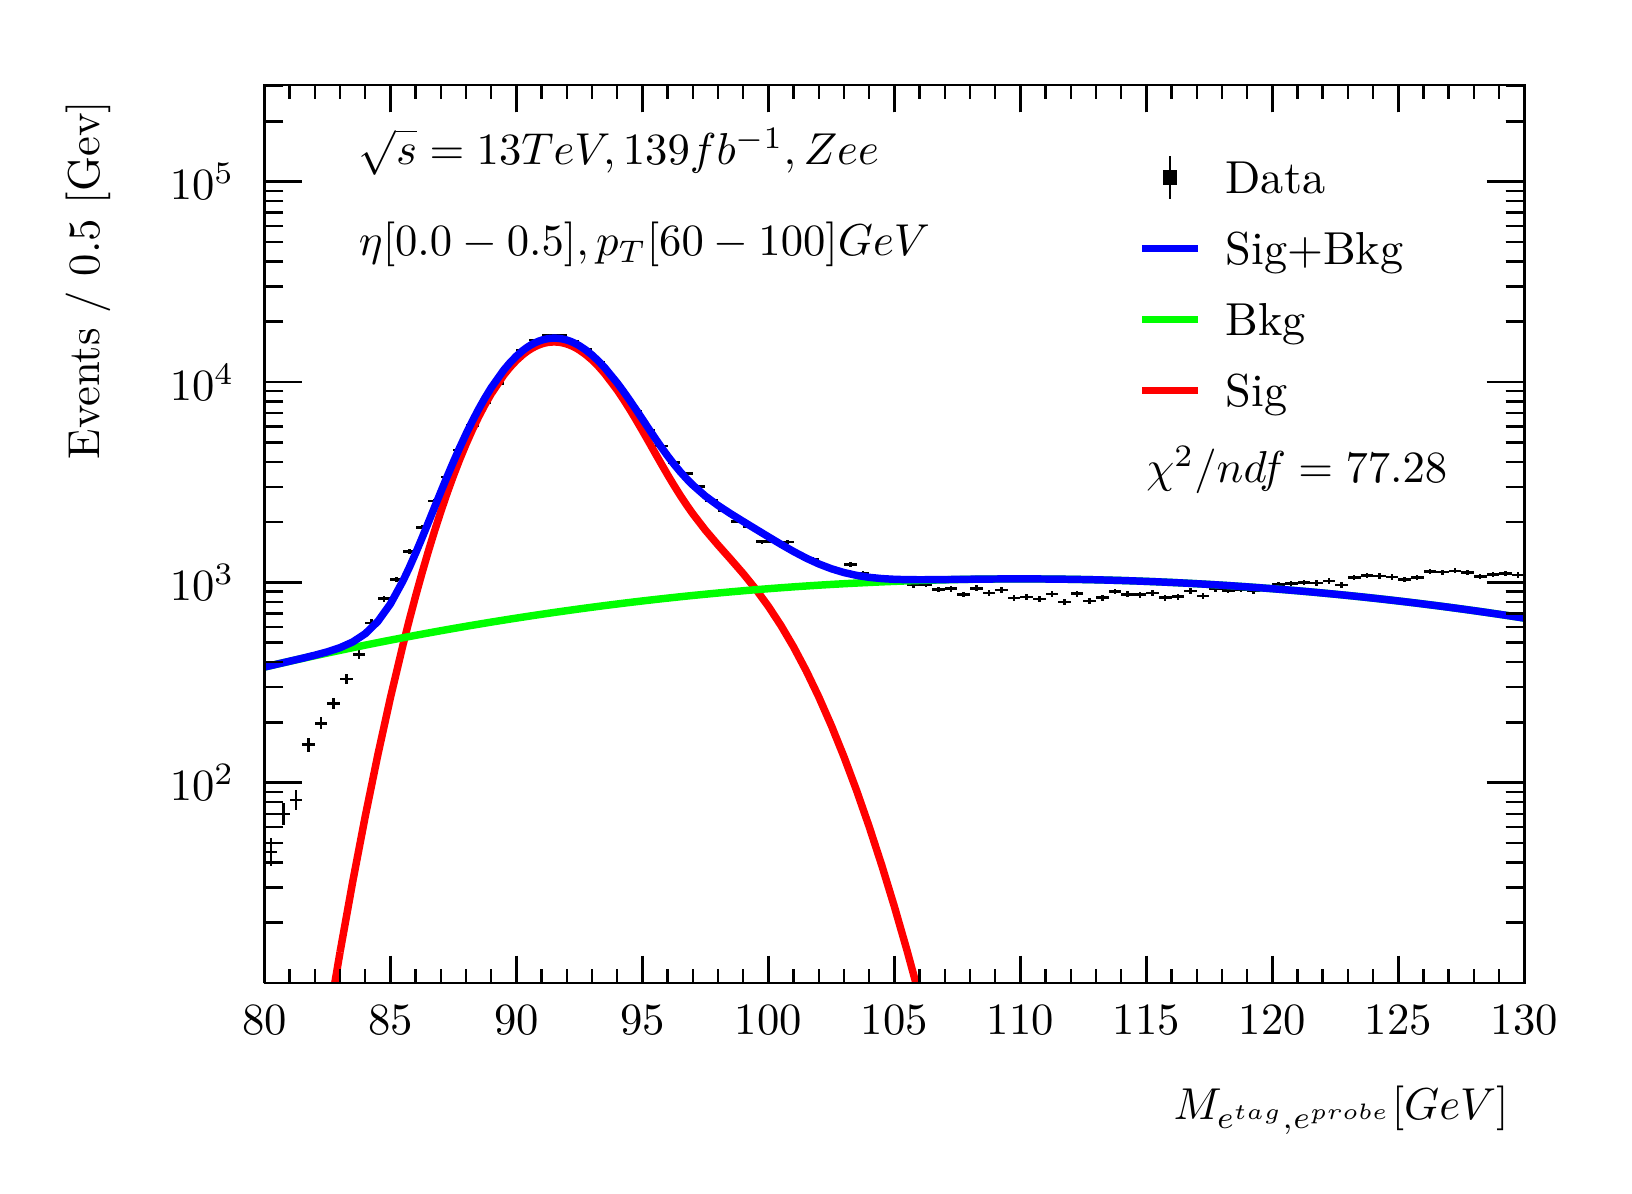
\begin{tikzpicture}
\pgfdeclareplotmark{cross} {
\pgfpathmoveto{\pgfpoint{-0.3\pgfplotmarksize}{\pgfplotmarksize}}
\pgfpathlineto{\pgfpoint{+0.3\pgfplotmarksize}{\pgfplotmarksize}}
\pgfpathlineto{\pgfpoint{+0.3\pgfplotmarksize}{0.3\pgfplotmarksize}}
\pgfpathlineto{\pgfpoint{+1\pgfplotmarksize}{0.3\pgfplotmarksize}}
\pgfpathlineto{\pgfpoint{+1\pgfplotmarksize}{-0.3\pgfplotmarksize}}
\pgfpathlineto{\pgfpoint{+0.3\pgfplotmarksize}{-0.3\pgfplotmarksize}}
\pgfpathlineto{\pgfpoint{+0.3\pgfplotmarksize}{-1.\pgfplotmarksize}}
\pgfpathlineto{\pgfpoint{-0.3\pgfplotmarksize}{-1.\pgfplotmarksize}}
\pgfpathlineto{\pgfpoint{-0.3\pgfplotmarksize}{-0.3\pgfplotmarksize}}
\pgfpathlineto{\pgfpoint{-1.\pgfplotmarksize}{-0.3\pgfplotmarksize}}
\pgfpathlineto{\pgfpoint{-1.\pgfplotmarksize}{0.3\pgfplotmarksize}}
\pgfpathlineto{\pgfpoint{-0.3\pgfplotmarksize}{0.3\pgfplotmarksize}}
\pgfpathclose
\pgfusepathqstroke
}
\pgfdeclareplotmark{cross*} {
\pgfpathmoveto{\pgfpoint{-0.3\pgfplotmarksize}{\pgfplotmarksize}}
\pgfpathlineto{\pgfpoint{+0.3\pgfplotmarksize}{\pgfplotmarksize}}
\pgfpathlineto{\pgfpoint{+0.3\pgfplotmarksize}{0.3\pgfplotmarksize}}
\pgfpathlineto{\pgfpoint{+1\pgfplotmarksize}{0.3\pgfplotmarksize}}
\pgfpathlineto{\pgfpoint{+1\pgfplotmarksize}{-0.3\pgfplotmarksize}}
\pgfpathlineto{\pgfpoint{+0.3\pgfplotmarksize}{-0.3\pgfplotmarksize}}
\pgfpathlineto{\pgfpoint{+0.3\pgfplotmarksize}{-1.\pgfplotmarksize}}
\pgfpathlineto{\pgfpoint{-0.3\pgfplotmarksize}{-1.\pgfplotmarksize}}
\pgfpathlineto{\pgfpoint{-0.3\pgfplotmarksize}{-0.3\pgfplotmarksize}}
\pgfpathlineto{\pgfpoint{-1.\pgfplotmarksize}{-0.3\pgfplotmarksize}}
\pgfpathlineto{\pgfpoint{-1.\pgfplotmarksize}{0.3\pgfplotmarksize}}
\pgfpathlineto{\pgfpoint{-0.3\pgfplotmarksize}{0.3\pgfplotmarksize}}
\pgfpathclose
\pgfusepathqfillstroke
}
\pgfdeclareplotmark{newstar} {
\pgfpathmoveto{\pgfqpoint{0pt}{\pgfplotmarksize}}
\pgfpathlineto{\pgfqpointpolar{44}{0.5\pgfplotmarksize}}
\pgfpathlineto{\pgfqpointpolar{18}{\pgfplotmarksize}}
\pgfpathlineto{\pgfqpointpolar{-20}{0.5\pgfplotmarksize}}
\pgfpathlineto{\pgfqpointpolar{-54}{\pgfplotmarksize}}
\pgfpathlineto{\pgfqpointpolar{-90}{0.5\pgfplotmarksize}}
\pgfpathlineto{\pgfqpointpolar{234}{\pgfplotmarksize}}
\pgfpathlineto{\pgfqpointpolar{198}{0.5\pgfplotmarksize}}
\pgfpathlineto{\pgfqpointpolar{162}{\pgfplotmarksize}}
\pgfpathlineto{\pgfqpointpolar{134}{0.5\pgfplotmarksize}}
\pgfpathclose
\pgfusepathqstroke
}
\pgfdeclareplotmark{newstar*} {
\pgfpathmoveto{\pgfqpoint{0pt}{\pgfplotmarksize}}
\pgfpathlineto{\pgfqpointpolar{44}{0.5\pgfplotmarksize}}
\pgfpathlineto{\pgfqpointpolar{18}{\pgfplotmarksize}}
\pgfpathlineto{\pgfqpointpolar{-20}{0.5\pgfplotmarksize}}
\pgfpathlineto{\pgfqpointpolar{-54}{\pgfplotmarksize}}
\pgfpathlineto{\pgfqpointpolar{-90}{0.5\pgfplotmarksize}}
\pgfpathlineto{\pgfqpointpolar{234}{\pgfplotmarksize}}
\pgfpathlineto{\pgfqpointpolar{198}{0.5\pgfplotmarksize}}
\pgfpathlineto{\pgfqpointpolar{162}{\pgfplotmarksize}}
\pgfpathlineto{\pgfqpointpolar{134}{0.5\pgfplotmarksize}}
\pgfpathclose
\pgfusepathqfillstroke
}
\definecolor{c}{rgb}{1,1,1};
\draw [color=c, fill=c] (0,0) rectangle (20,14.4361);
\draw [color=c, fill=c] (3,2.30977) rectangle (19,13.7143);
\definecolor{c}{rgb}{0,0,0};
\draw [c,line width=0.9] (3,2.30977) -- (3,13.7143) -- (19,13.7143) -- (19,2.30977) -- (3,2.30977);
\definecolor{c}{rgb}{1,1,1};
\draw [color=c, fill=c] (3,2.30977) rectangle (19,13.7143);
\definecolor{c}{rgb}{0,0,0};
\draw [c,line width=0.9] (3,2.30977) -- (3,13.7143) -- (19,13.7143) -- (19,2.30977) -- (3,2.30977);
\draw [c,line width=0.9] (3,2.30977) -- (19,2.30977);
\draw [c,line width=0.9] (3,2.65624) -- (3,2.30977);
\draw [c,line width=0.9] (3.32,2.48301) -- (3.32,2.30977);
\draw [c,line width=0.9] (3.64,2.48301) -- (3.64,2.30977);
\draw [c,line width=0.9] (3.96,2.48301) -- (3.96,2.30977);
\draw [c,line width=0.9] (4.28,2.48301) -- (4.28,2.30977);
\draw [c,line width=0.9] (4.6,2.65624) -- (4.6,2.30977);
\draw [c,line width=0.9] (4.92,2.48301) -- (4.92,2.30977);
\draw [c,line width=0.9] (5.24,2.48301) -- (5.24,2.30977);
\draw [c,line width=0.9] (5.56,2.48301) -- (5.56,2.30977);
\draw [c,line width=0.9] (5.88,2.48301) -- (5.88,2.30977);
\draw [c,line width=0.9] (6.2,2.65624) -- (6.2,2.30977);
\draw [c,line width=0.9] (6.52,2.48301) -- (6.52,2.30977);
\draw [c,line width=0.9] (6.84,2.48301) -- (6.84,2.30977);
\draw [c,line width=0.9] (7.16,2.48301) -- (7.16,2.30977);
\draw [c,line width=0.9] (7.48,2.48301) -- (7.48,2.30977);
\draw [c,line width=0.9] (7.8,2.65624) -- (7.8,2.30977);
\draw [c,line width=0.9] (8.12,2.48301) -- (8.12,2.30977);
\draw [c,line width=0.9] (8.44,2.48301) -- (8.44,2.30977);
\draw [c,line width=0.9] (8.76,2.48301) -- (8.76,2.30977);
\draw [c,line width=0.9] (9.08,2.48301) -- (9.08,2.30977);
\draw [c,line width=0.9] (9.4,2.65624) -- (9.4,2.30977);
\draw [c,line width=0.9] (9.72,2.48301) -- (9.72,2.30977);
\draw [c,line width=0.9] (10.04,2.48301) -- (10.04,2.30977);
\draw [c,line width=0.9] (10.36,2.48301) -- (10.36,2.30977);
\draw [c,line width=0.9] (10.68,2.48301) -- (10.68,2.30977);
\draw [c,line width=0.9] (11,2.65624) -- (11,2.30977);
\draw [c,line width=0.9] (11.32,2.48301) -- (11.32,2.30977);
\draw [c,line width=0.9] (11.64,2.48301) -- (11.64,2.30977);
\draw [c,line width=0.9] (11.96,2.48301) -- (11.96,2.30977);
\draw [c,line width=0.9] (12.28,2.48301) -- (12.28,2.30977);
\draw [c,line width=0.9] (12.6,2.65624) -- (12.6,2.30977);
\draw [c,line width=0.9] (12.92,2.48301) -- (12.92,2.30977);
\draw [c,line width=0.9] (13.24,2.48301) -- (13.24,2.30977);
\draw [c,line width=0.9] (13.56,2.48301) -- (13.56,2.30977);
\draw [c,line width=0.9] (13.88,2.48301) -- (13.88,2.30977);
\draw [c,line width=0.9] (14.2,2.65624) -- (14.2,2.30977);
\draw [c,line width=0.9] (14.52,2.48301) -- (14.52,2.30977);
\draw [c,line width=0.9] (14.84,2.48301) -- (14.84,2.30977);
\draw [c,line width=0.9] (15.16,2.48301) -- (15.16,2.30977);
\draw [c,line width=0.9] (15.48,2.48301) -- (15.48,2.30977);
\draw [c,line width=0.9] (15.8,2.65624) -- (15.8,2.30977);
\draw [c,line width=0.9] (16.12,2.48301) -- (16.12,2.30977);
\draw [c,line width=0.9] (16.44,2.48301) -- (16.44,2.30977);
\draw [c,line width=0.9] (16.76,2.48301) -- (16.76,2.30977);
\draw [c,line width=0.9] (17.08,2.48301) -- (17.08,2.30977);
\draw [c,line width=0.9] (17.4,2.65624) -- (17.4,2.30977);
\draw [c,line width=0.9] (17.72,2.48301) -- (17.72,2.30977);
\draw [c,line width=0.9] (18.04,2.48301) -- (18.04,2.30977);
\draw [c,line width=0.9] (18.36,2.48301) -- (18.36,2.30977);
\draw [c,line width=0.9] (18.68,2.48301) -- (18.68,2.30977);
\draw [c,line width=0.9] (19,2.65624) -- (19,2.30977);
\draw [anchor=base] (3,1.66015) node[scale=1.61424, color=c, rotate=0]{80};
\draw [anchor=base] (4.6,1.66015) node[scale=1.61424, color=c, rotate=0]{85};
\draw [anchor=base] (6.2,1.66015) node[scale=1.61424, color=c, rotate=0]{90};
\draw [anchor=base] (7.8,1.66015) node[scale=1.61424, color=c, rotate=0]{95};
\draw [anchor=base] (9.4,1.66015) node[scale=1.61424, color=c, rotate=0]{100};
\draw [anchor=base] (11,1.66015) node[scale=1.61424, color=c, rotate=0]{105};
\draw [anchor=base] (12.6,1.66015) node[scale=1.61424, color=c, rotate=0]{110};
\draw [anchor=base] (14.2,1.66015) node[scale=1.61424, color=c, rotate=0]{115};
\draw [anchor=base] (15.8,1.66015) node[scale=1.61424, color=c, rotate=0]{120};
\draw [anchor=base] (17.4,1.66015) node[scale=1.61424, color=c, rotate=0]{125};
\draw [anchor=base] (19,1.66015) node[scale=1.61424, color=c, rotate=0]{130};
\draw [anchor= east] (19,0.692932) node[scale=1.61424, color=c, rotate=0]{$M_{e^{tag}, e^{probe}}  [GeV]$};
\draw [c,line width=0.9] (3,13.7143) -- (19,13.7143);
\draw [c,line width=0.9] (3,13.3678) -- (3,13.7143);
\draw [c,line width=0.9] (3.32,13.5411) -- (3.32,13.7143);
\draw [c,line width=0.9] (3.64,13.5411) -- (3.64,13.7143);
\draw [c,line width=0.9] (3.96,13.5411) -- (3.96,13.7143);
\draw [c,line width=0.9] (4.28,13.5411) -- (4.28,13.7143);
\draw [c,line width=0.9] (4.6,13.3678) -- (4.6,13.7143);
\draw [c,line width=0.9] (4.92,13.5411) -- (4.92,13.7143);
\draw [c,line width=0.9] (5.24,13.5411) -- (5.24,13.7143);
\draw [c,line width=0.9] (5.56,13.5411) -- (5.56,13.7143);
\draw [c,line width=0.9] (5.88,13.5411) -- (5.88,13.7143);
\draw [c,line width=0.9] (6.2,13.3678) -- (6.2,13.7143);
\draw [c,line width=0.9] (6.52,13.5411) -- (6.52,13.7143);
\draw [c,line width=0.9] (6.84,13.5411) -- (6.84,13.7143);
\draw [c,line width=0.9] (7.16,13.5411) -- (7.16,13.7143);
\draw [c,line width=0.9] (7.48,13.5411) -- (7.48,13.7143);
\draw [c,line width=0.9] (7.8,13.3678) -- (7.8,13.7143);
\draw [c,line width=0.9] (8.12,13.5411) -- (8.12,13.7143);
\draw [c,line width=0.9] (8.44,13.5411) -- (8.44,13.7143);
\draw [c,line width=0.9] (8.76,13.5411) -- (8.76,13.7143);
\draw [c,line width=0.9] (9.08,13.5411) -- (9.08,13.7143);
\draw [c,line width=0.9] (9.4,13.3678) -- (9.4,13.7143);
\draw [c,line width=0.9] (9.72,13.5411) -- (9.72,13.7143);
\draw [c,line width=0.9] (10.04,13.5411) -- (10.04,13.7143);
\draw [c,line width=0.9] (10.36,13.5411) -- (10.36,13.7143);
\draw [c,line width=0.9] (10.68,13.5411) -- (10.68,13.7143);
\draw [c,line width=0.9] (11,13.3678) -- (11,13.7143);
\draw [c,line width=0.9] (11.32,13.5411) -- (11.32,13.7143);
\draw [c,line width=0.9] (11.64,13.5411) -- (11.64,13.7143);
\draw [c,line width=0.9] (11.96,13.5411) -- (11.96,13.7143);
\draw [c,line width=0.9] (12.28,13.5411) -- (12.28,13.7143);
\draw [c,line width=0.9] (12.6,13.3678) -- (12.6,13.7143);
\draw [c,line width=0.9] (12.92,13.5411) -- (12.92,13.7143);
\draw [c,line width=0.9] (13.24,13.5411) -- (13.24,13.7143);
\draw [c,line width=0.9] (13.56,13.5411) -- (13.56,13.7143);
\draw [c,line width=0.9] (13.88,13.5411) -- (13.88,13.7143);
\draw [c,line width=0.9] (14.2,13.3678) -- (14.2,13.7143);
\draw [c,line width=0.9] (14.52,13.5411) -- (14.52,13.7143);
\draw [c,line width=0.9] (14.84,13.5411) -- (14.84,13.7143);
\draw [c,line width=0.9] (15.16,13.5411) -- (15.16,13.7143);
\draw [c,line width=0.9] (15.48,13.5411) -- (15.48,13.7143);
\draw [c,line width=0.9] (15.8,13.3678) -- (15.8,13.7143);
\draw [c,line width=0.9] (16.12,13.5411) -- (16.12,13.7143);
\draw [c,line width=0.9] (16.44,13.5411) -- (16.44,13.7143);
\draw [c,line width=0.9] (16.76,13.5411) -- (16.76,13.7143);
\draw [c,line width=0.9] (17.08,13.5411) -- (17.08,13.7143);
\draw [c,line width=0.9] (17.4,13.3678) -- (17.4,13.7143);
\draw [c,line width=0.9] (17.72,13.5411) -- (17.72,13.7143);
\draw [c,line width=0.9] (18.04,13.5411) -- (18.04,13.7143);
\draw [c,line width=0.9] (18.36,13.5411) -- (18.36,13.7143);
\draw [c,line width=0.9] (18.68,13.5411) -- (18.68,13.7143);
\draw [c,line width=0.9] (19,13.3678) -- (19,13.7143);
\draw [c,line width=0.9] (3,2.30977) -- (3,13.7143);
\draw [c,line width=0.9] (3.237,3.07568) -- (3,3.07568);
\draw [c,line width=0.9] (3.237,3.5237) -- (3,3.5237);
\draw [c,line width=0.9] (3.237,3.84158) -- (3,3.84158);
\draw [c,line width=0.9] (3.237,4.08815) -- (3,4.08815);
\draw [c,line width=0.9] (3.237,4.2896) -- (3,4.2896);
\draw [c,line width=0.9] (3.237,4.45994) -- (3,4.45994);
\draw [c,line width=0.9] (3.237,4.60748) -- (3,4.60748);
\draw [c,line width=0.9] (3.237,4.73763) -- (3,4.73763);
\draw [c,line width=0.9] (3.474,4.85405) -- (3,4.85405);
\draw [anchor= east] (2.82,4.85405) node[scale=1.61424, color=c, rotate=0]{$10^{2}$};
\draw [c,line width=0.9] (3.237,5.61995) -- (3,5.61995);
\draw [c,line width=0.9] (3.237,6.06798) -- (3,6.06798);
\draw [c,line width=0.9] (3.237,6.38586) -- (3,6.38586);
\draw [c,line width=0.9] (3.237,6.63242) -- (3,6.63242);
\draw [c,line width=0.9] (3.237,6.83388) -- (3,6.83388);
\draw [c,line width=0.9] (3.237,7.00421) -- (3,7.00421);
\draw [c,line width=0.9] (3.237,7.15176) -- (3,7.15176);
\draw [c,line width=0.9] (3.237,7.28191) -- (3,7.28191);
\draw [c,line width=0.9] (3.474,7.39833) -- (3,7.39833);
\draw [anchor= east] (2.82,7.39833) node[scale=1.61424, color=c, rotate=0]{$10^{3}$};
\draw [c,line width=0.9] (3.237,8.16423) -- (3,8.16423);
\draw [c,line width=0.9] (3.237,8.61226) -- (3,8.61226);
\draw [c,line width=0.9] (3.237,8.93013) -- (3,8.93013);
\draw [c,line width=0.9] (3.237,9.1767) -- (3,9.1767);
\draw [c,line width=0.9] (3.237,9.37816) -- (3,9.37816);
\draw [c,line width=0.9] (3.237,9.54849) -- (3,9.54849);
\draw [c,line width=0.9] (3.237,9.69604) -- (3,9.69604);
\draw [c,line width=0.9] (3.237,9.82618) -- (3,9.82618);
\draw [c,line width=0.9] (3.474,9.9426) -- (3,9.9426);
\draw [anchor= east] (2.82,9.9426) node[scale=1.61424, color=c, rotate=0]{$10^{4}$};
\draw [c,line width=0.9] (3.237,10.7085) -- (3,10.7085);
\draw [c,line width=0.9] (3.237,11.1565) -- (3,11.1565);
\draw [c,line width=0.9] (3.237,11.4744) -- (3,11.4744);
\draw [c,line width=0.9] (3.237,11.721) -- (3,11.721);
\draw [c,line width=0.9] (3.237,11.9224) -- (3,11.9224);
\draw [c,line width=0.9] (3.237,12.0928) -- (3,12.0928);
\draw [c,line width=0.9] (3.237,12.2403) -- (3,12.2403);
\draw [c,line width=0.9] (3.237,12.3705) -- (3,12.3705);
\draw [c,line width=0.9] (3.474,12.4869) -- (3,12.4869);
\draw [anchor= east] (2.82,12.4869) node[scale=1.61424, color=c, rotate=0]{$10^{5}$};
\draw [c,line width=0.9] (3.237,13.2528) -- (3,13.2528);
\draw [c,line width=0.9] (3.237,13.7008) -- (3,13.7008);
\draw [anchor= east] (0.76,13.7143) node[scale=1.61424, color=c, rotate=90]{Events / 0.5 [Gev]};
\draw [c,line width=0.9] (19,2.30977) -- (19,13.7143);
\draw [c,line width=0.9] (18.763,3.07568) -- (19,3.07568);
\draw [c,line width=0.9] (18.763,3.5237) -- (19,3.5237);
\draw [c,line width=0.9] (18.763,3.84158) -- (19,3.84158);
\draw [c,line width=0.9] (18.763,4.08815) -- (19,4.08815);
\draw [c,line width=0.9] (18.763,4.2896) -- (19,4.2896);
\draw [c,line width=0.9] (18.763,4.45994) -- (19,4.45994);
\draw [c,line width=0.9] (18.763,4.60748) -- (19,4.60748);
\draw [c,line width=0.9] (18.763,4.73763) -- (19,4.73763);
\draw [c,line width=0.9] (18.526,4.85405) -- (19,4.85405);
\draw [c,line width=0.9] (18.763,5.61995) -- (19,5.61995);
\draw [c,line width=0.9] (18.763,6.06798) -- (19,6.06798);
\draw [c,line width=0.9] (18.763,6.38586) -- (19,6.38586);
\draw [c,line width=0.9] (18.763,6.63242) -- (19,6.63242);
\draw [c,line width=0.9] (18.763,6.83388) -- (19,6.83388);
\draw [c,line width=0.9] (18.763,7.00421) -- (19,7.00421);
\draw [c,line width=0.9] (18.763,7.15176) -- (19,7.15176);
\draw [c,line width=0.9] (18.763,7.28191) -- (19,7.28191);
\draw [c,line width=0.9] (18.526,7.39833) -- (19,7.39833);
\draw [c,line width=0.9] (18.763,8.16423) -- (19,8.16423);
\draw [c,line width=0.9] (18.763,8.61226) -- (19,8.61226);
\draw [c,line width=0.9] (18.763,8.93013) -- (19,8.93013);
\draw [c,line width=0.9] (18.763,9.1767) -- (19,9.1767);
\draw [c,line width=0.9] (18.763,9.37816) -- (19,9.37816);
\draw [c,line width=0.9] (18.763,9.54849) -- (19,9.54849);
\draw [c,line width=0.9] (18.763,9.69604) -- (19,9.69604);
\draw [c,line width=0.9] (18.763,9.82618) -- (19,9.82618);
\draw [c,line width=0.9] (18.526,9.9426) -- (19,9.9426);
\draw [c,line width=0.9] (18.763,10.7085) -- (19,10.7085);
\draw [c,line width=0.9] (18.763,11.1565) -- (19,11.1565);
\draw [c,line width=0.9] (18.763,11.4744) -- (19,11.4744);
\draw [c,line width=0.9] (18.763,11.721) -- (19,11.721);
\draw [c,line width=0.9] (18.763,11.9224) -- (19,11.9224);
\draw [c,line width=0.9] (18.763,12.0928) -- (19,12.0928);
\draw [c,line width=0.9] (18.763,12.2403) -- (19,12.2403);
\draw [c,line width=0.9] (18.763,12.3705) -- (19,12.3705);
\draw [c,line width=0.9] (18.526,12.4869) -- (19,12.4869);
\draw [c,line width=0.9] (18.763,13.2528) -- (19,13.2528);
\draw [c,line width=0.9] (18.763,13.7008) -- (19,13.7008);
\draw [c,line width=0.9] (3.08,3.97173) -- (3,3.97173);
\draw [c,line width=0.9] (3,3.97173) -- (3,3.97173);
\draw [c,line width=0.9] (3.08,3.97173) -- (3.16,3.97173);
\draw [c,line width=0.9] (3.16,3.97173) -- (3.16,3.97173);
\draw [c,line width=0.9] (3.08,3.97173) -- (3.08,4.14747);
\draw [c,line width=0.9] (3.08,4.14747) -- (3.08,4.14747);
\draw [c,line width=0.9] (3.08,3.97173) -- (3.08,3.79408);
\draw [c,line width=0.9] (3.08,3.79408) -- (3.08,3.79408);
\draw [c,line width=0.9] (3.24,4.45994) -- (3.16,4.45994);
\draw [c,line width=0.9] (3.16,4.45994) -- (3.16,4.45994);
\draw [c,line width=0.9] (3.24,4.45994) -- (3.32,4.45994);
\draw [c,line width=0.9] (3.32,4.45994) -- (3.32,4.45994);
\draw [c,line width=0.9] (3.24,4.45994) -- (3.24,4.59926);
\draw [c,line width=0.9] (3.24,4.59926) -- (3.24,4.59926);
\draw [c,line width=0.9] (3.24,4.45994) -- (3.24,4.31964);
\draw [c,line width=0.9] (3.24,4.31964) -- (3.24,4.31964);
\draw [c,line width=0.9] (3.4,4.63477) -- (3.32,4.63477);
\draw [c,line width=0.9] (3.32,4.63477) -- (3.32,4.63477);
\draw [c,line width=0.9] (3.4,4.63477) -- (3.48,4.63477);
\draw [c,line width=0.9] (3.48,4.63477) -- (3.48,4.63477);
\draw [c,line width=0.9] (3.4,4.63477) -- (3.4,4.76302);
\draw [c,line width=0.9] (3.4,4.76302) -- (3.4,4.76302);
\draw [c,line width=0.9] (3.4,4.63477) -- (3.4,4.50575);
\draw [c,line width=0.9] (3.4,4.50575) -- (3.4,4.50575);
\draw [c,line width=0.9] (3.56,5.33831) -- (3.48,5.33831);
\draw [c,line width=0.9] (3.48,5.33831) -- (3.48,5.33831);
\draw [c,line width=0.9] (3.56,5.33831) -- (3.64,5.33831);
\draw [c,line width=0.9] (3.64,5.33831) -- (3.64,5.33831);
\draw [c,line width=0.9] (3.56,5.33831) -- (3.56,5.42704);
\draw [c,line width=0.9] (3.56,5.42704) -- (3.56,5.42704);
\draw [c,line width=0.9] (3.56,5.33831) -- (3.56,5.24958);
\draw [c,line width=0.9] (3.56,5.24958) -- (3.56,5.24958);
\draw [c,line width=0.9] (3.72,5.60885) -- (3.64,5.60885);
\draw [c,line width=0.9] (3.64,5.60885) -- (3.64,5.60885);
\draw [c,line width=0.9] (3.72,5.60885) -- (3.8,5.60885);
\draw [c,line width=0.9] (3.8,5.60885) -- (3.8,5.60885);
\draw [c,line width=0.9] (3.72,5.60885) -- (3.72,5.68736);
\draw [c,line width=0.9] (3.72,5.68736) -- (3.72,5.68736);
\draw [c,line width=0.9] (3.72,5.60885) -- (3.72,5.53034);
\draw [c,line width=0.9] (3.72,5.53034) -- (3.72,5.53034);
\draw [c,line width=0.9] (3.88,5.85765) -- (3.8,5.85765);
\draw [c,line width=0.9] (3.8,5.85765) -- (3.8,5.85765);
\draw [c,line width=0.9] (3.88,5.85765) -- (3.96,5.85765);
\draw [c,line width=0.9] (3.96,5.85765) -- (3.96,5.85765);
\draw [c,line width=0.9] (3.88,5.85765) -- (3.88,5.9278);
\draw [c,line width=0.9] (3.88,5.9278) -- (3.88,5.9278);
\draw [c,line width=0.9] (3.88,5.85765) -- (3.88,5.78749);
\draw [c,line width=0.9] (3.88,5.78749) -- (3.88,5.78749);
\draw [c,line width=0.9] (4.04,6.16994) -- (3.96,6.16994);
\draw [c,line width=0.9] (3.96,6.16994) -- (3.96,6.16994);
\draw [c,line width=0.9] (4.04,6.16994) -- (4.12,6.16994);
\draw [c,line width=0.9] (4.12,6.16994) -- (4.12,6.16994);
\draw [c,line width=0.9] (4.04,6.16994) -- (4.04,6.23085);
\draw [c,line width=0.9] (4.04,6.23085) -- (4.04,6.23085);
\draw [c,line width=0.9] (4.04,6.16994) -- (4.04,6.10903);
\draw [c,line width=0.9] (4.04,6.10903) -- (4.04,6.10903);
\draw [c,line width=0.9] (4.2,6.48361) -- (4.12,6.48361);
\draw [c,line width=0.9] (4.12,6.48361) -- (4.12,6.48361);
\draw [c,line width=0.9] (4.2,6.48361) -- (4.28,6.48361);
\draw [c,line width=0.9] (4.28,6.48361) -- (4.28,6.48361);
\draw [c,line width=0.9] (4.2,6.48361) -- (4.2,6.53647);
\draw [c,line width=0.9] (4.2,6.53647) -- (4.2,6.53647);
\draw [c,line width=0.9] (4.2,6.48361) -- (4.2,6.43076);
\draw [c,line width=0.9] (4.2,6.43076) -- (4.2,6.43076);
\draw [c,line width=0.9] (4.36,6.88428) -- (4.28,6.88428);
\draw [c,line width=0.9] (4.28,6.88428) -- (4.28,6.88428);
\draw [c,line width=0.9] (4.36,6.88428) -- (4.44,6.88428);
\draw [c,line width=0.9] (4.44,6.88428) -- (4.44,6.88428);
\draw [c,line width=0.9] (4.36,6.88428) -- (4.36,6.92837);
\draw [c,line width=0.9] (4.36,6.92837) -- (4.36,6.92837);
\draw [c,line width=0.9] (4.36,6.88428) -- (4.36,6.84019);
\draw [c,line width=0.9] (4.36,6.84019) -- (4.36,6.84019);
\draw [c,line width=0.9] (4.52,7.19244) -- (4.44,7.19244);
\draw [c,line width=0.9] (4.44,7.19244) -- (4.44,7.19244);
\draw [c,line width=0.9] (4.52,7.19244) -- (4.6,7.19244);
\draw [c,line width=0.9] (4.6,7.19244) -- (4.6,7.19244);
\draw [c,line width=0.9] (4.52,7.19244) -- (4.52,7.23079);
\draw [c,line width=0.9] (4.52,7.23079) -- (4.52,7.23079);
\draw [c,line width=0.9] (4.52,7.19244) -- (4.52,7.15409);
\draw [c,line width=0.9] (4.52,7.15409) -- (4.52,7.15409);
\draw [c,line width=0.9] (4.68,7.4342) -- (4.6,7.4342);
\draw [c,line width=0.9] (4.6,7.4342) -- (4.6,7.4342);
\draw [c,line width=0.9] (4.68,7.4342) -- (4.76,7.4342);
\draw [c,line width=0.9] (4.76,7.4342) -- (4.76,7.4342);
\draw [c,line width=0.9] (4.68,7.4342) -- (4.68,7.46858);
\draw [c,line width=0.9] (4.68,7.46858) -- (4.68,7.46858);
\draw [c,line width=0.9] (4.68,7.4342) -- (4.68,7.39983);
\draw [c,line width=0.9] (4.68,7.39983) -- (4.68,7.39983);
\draw [c,line width=0.9] (4.84,7.7889) -- (4.76,7.7889);
\draw [c,line width=0.9] (4.76,7.7889) -- (4.76,7.7889);
\draw [c,line width=0.9] (4.84,7.7889) -- (4.92,7.7889);
\draw [c,line width=0.9] (4.92,7.7889) -- (4.92,7.7889);
\draw [c,line width=0.9] (4.84,7.7889) -- (4.84,7.81818);
\draw [c,line width=0.9] (4.84,7.81818) -- (4.84,7.81818);
\draw [c,line width=0.9] (4.84,7.7889) -- (4.84,7.75962);
\draw [c,line width=0.9] (4.84,7.75962) -- (4.84,7.75962);
\draw [c,line width=0.9] (5,8.09645) -- (4.92,8.09645);
\draw [c,line width=0.9] (4.92,8.09645) -- (4.92,8.09645);
\draw [c,line width=0.9] (5,8.09645) -- (5.08,8.09645);
\draw [c,line width=0.9] (5.08,8.09645) -- (5.08,8.09645);
\draw [c,line width=0.9] (5,8.09645) -- (5,8.12193);
\draw [c,line width=0.9] (5,8.12193) -- (5,8.12193);
\draw [c,line width=0.9] (5,8.09645) -- (5,8.07097);
\draw [c,line width=0.9] (5,8.07097) -- (5,8.07097);
\draw [c,line width=0.9] (5.16,8.43008) -- (5.08,8.43008);
\draw [c,line width=0.9] (5.08,8.43008) -- (5.08,8.43008);
\draw [c,line width=0.9] (5.16,8.43008) -- (5.24,8.43008);
\draw [c,line width=0.9] (5.24,8.43008) -- (5.24,8.43008);
\draw [c,line width=0.9] (5.16,8.43008) -- (5.16,8.45198);
\draw [c,line width=0.9] (5.16,8.45198) -- (5.16,8.45198);
\draw [c,line width=0.9] (5.16,8.43008) -- (5.16,8.40817);
\draw [c,line width=0.9] (5.16,8.40817) -- (5.16,8.40817);
\draw [c,line width=0.9] (5.32,8.73386) -- (5.24,8.73386);
\draw [c,line width=0.9] (5.24,8.73386) -- (5.24,8.73386);
\draw [c,line width=0.9] (5.32,8.73386) -- (5.4,8.73386);
\draw [c,line width=0.9] (5.4,8.73386) -- (5.4,8.73386);
\draw [c,line width=0.9] (5.32,8.73386) -- (5.32,8.75295);
\draw [c,line width=0.9] (5.32,8.75295) -- (5.32,8.75295);
\draw [c,line width=0.9] (5.32,8.73386) -- (5.32,8.71476);
\draw [c,line width=0.9] (5.32,8.71476) -- (5.32,8.71476);
\draw [c,line width=0.9] (5.48,9.07903) -- (5.4,9.07903);
\draw [c,line width=0.9] (5.4,9.07903) -- (5.4,9.07903);
\draw [c,line width=0.9] (5.48,9.07903) -- (5.56,9.07903);
\draw [c,line width=0.9] (5.56,9.07903) -- (5.56,9.07903);
\draw [c,line width=0.9] (5.48,9.07903) -- (5.48,9.09536);
\draw [c,line width=0.9] (5.48,9.09536) -- (5.48,9.09536);
\draw [c,line width=0.9] (5.48,9.07903) -- (5.48,9.0627);
\draw [c,line width=0.9] (5.48,9.0627) -- (5.48,9.0627);
\draw [c,line width=0.9] (5.64,9.39261) -- (5.56,9.39261);
\draw [c,line width=0.9] (5.56,9.39261) -- (5.56,9.39261);
\draw [c,line width=0.9] (5.64,9.39261) -- (5.72,9.39261);
\draw [c,line width=0.9] (5.72,9.39261) -- (5.72,9.39261);
\draw [c,line width=0.9] (5.64,9.39261) -- (5.64,9.40679);
\draw [c,line width=0.9] (5.64,9.40679) -- (5.64,9.40679);
\draw [c,line width=0.9] (5.64,9.39261) -- (5.64,9.37844);
\draw [c,line width=0.9] (5.64,9.37844) -- (5.64,9.37844);
\draw [c,line width=0.9] (5.8,9.67681) -- (5.72,9.67681);
\draw [c,line width=0.9] (5.72,9.67681) -- (5.72,9.67681);
\draw [c,line width=0.9] (5.8,9.67681) -- (5.88,9.67681);
\draw [c,line width=0.9] (5.88,9.67681) -- (5.88,9.67681);
\draw [c,line width=0.9] (5.8,9.67681) -- (5.8,9.68927);
\draw [c,line width=0.9] (5.8,9.68927) -- (5.8,9.68927);
\draw [c,line width=0.9] (5.8,9.67681) -- (5.8,9.66435);
\draw [c,line width=0.9] (5.8,9.66435) -- (5.8,9.66435);
\draw [c,line width=0.9] (5.96,9.9213) -- (5.88,9.9213);
\draw [c,line width=0.9] (5.88,9.9213) -- (5.88,9.9213);
\draw [c,line width=0.9] (5.96,9.9213) -- (6.04,9.9213);
\draw [c,line width=0.9] (6.04,9.9213) -- (6.04,9.9213);
\draw [c,line width=0.9] (5.96,9.9213) -- (5.96,9.93245);
\draw [c,line width=0.9] (5.96,9.93245) -- (5.96,9.93245);
\draw [c,line width=0.9] (5.96,9.9213) -- (5.96,9.91014);
\draw [c,line width=0.9] (5.96,9.91014) -- (5.96,9.91014);
\draw [c,line width=0.9] (6.12,10.1618) -- (6.04,10.1618);
\draw [c,line width=0.9] (6.04,10.1618) -- (6.04,10.1618);
\draw [c,line width=0.9] (6.12,10.1618) -- (6.2,10.1618);
\draw [c,line width=0.9] (6.2,10.1618) -- (6.2,10.1618);
\draw [c,line width=0.9] (6.12,10.1618) -- (6.12,10.1718);
\draw [c,line width=0.9] (6.12,10.1718) -- (6.12,10.1718);
\draw [c,line width=0.9] (6.12,10.1618) -- (6.12,10.1518);
\draw [c,line width=0.9] (6.12,10.1518) -- (6.12,10.1518);
\draw [c,line width=0.9] (6.28,10.3471) -- (6.2,10.3471);
\draw [c,line width=0.9] (6.2,10.3471) -- (6.2,10.3471);
\draw [c,line width=0.9] (6.28,10.3471) -- (6.36,10.3471);
\draw [c,line width=0.9] (6.36,10.3471) -- (6.36,10.3471);
\draw [c,line width=0.9] (6.28,10.3471) -- (6.28,10.3563);
\draw [c,line width=0.9] (6.28,10.3563) -- (6.28,10.3563);
\draw [c,line width=0.9] (6.28,10.3471) -- (6.28,10.3379);
\draw [c,line width=0.9] (6.28,10.3379) -- (6.28,10.3379);
\draw [c,line width=0.9] (6.44,10.4746) -- (6.36,10.4746);
\draw [c,line width=0.9] (6.36,10.4746) -- (6.36,10.4746);
\draw [c,line width=0.9] (6.44,10.4746) -- (6.52,10.4746);
\draw [c,line width=0.9] (6.52,10.4746) -- (6.52,10.4746);
\draw [c,line width=0.9] (6.44,10.4746) -- (6.44,10.4833);
\draw [c,line width=0.9] (6.44,10.4833) -- (6.44,10.4833);
\draw [c,line width=0.9] (6.44,10.4746) -- (6.44,10.466);
\draw [c,line width=0.9] (6.44,10.466) -- (6.44,10.466);
\draw [c,line width=0.9] (6.6,10.5373) -- (6.52,10.5373);
\draw [c,line width=0.9] (6.52,10.5373) -- (6.52,10.5373);
\draw [c,line width=0.9] (6.6,10.5373) -- (6.68,10.5373);
\draw [c,line width=0.9] (6.68,10.5373) -- (6.68,10.5373);
\draw [c,line width=0.9] (6.6,10.5373) -- (6.6,10.5457);
\draw [c,line width=0.9] (6.6,10.5457) -- (6.6,10.5457);
\draw [c,line width=0.9] (6.6,10.5373) -- (6.6,10.5288);
\draw [c,line width=0.9] (6.6,10.5288) -- (6.6,10.5288);
\draw [c,line width=0.9] (6.76,10.5319) -- (6.68,10.5319);
\draw [c,line width=0.9] (6.68,10.5319) -- (6.68,10.5319);
\draw [c,line width=0.9] (6.76,10.5319) -- (6.84,10.5319);
\draw [c,line width=0.9] (6.84,10.5319) -- (6.84,10.5319);
\draw [c,line width=0.9] (6.76,10.5319) -- (6.76,10.5403);
\draw [c,line width=0.9] (6.76,10.5403) -- (6.76,10.5403);
\draw [c,line width=0.9] (6.76,10.5319) -- (6.76,10.5234);
\draw [c,line width=0.9] (6.76,10.5234) -- (6.76,10.5234);
\draw [c,line width=0.9] (6.92,10.4613) -- (6.84,10.4613);
\draw [c,line width=0.9] (6.84,10.4613) -- (6.84,10.4613);
\draw [c,line width=0.9] (6.92,10.4613) -- (7,10.4613);
\draw [c,line width=0.9] (7,10.4613) -- (7,10.4613);
\draw [c,line width=0.9] (6.92,10.4613) -- (6.92,10.4701);
\draw [c,line width=0.9] (6.92,10.4701) -- (6.92,10.4701);
\draw [c,line width=0.9] (6.92,10.4613) -- (6.92,10.4526);
\draw [c,line width=0.9] (6.92,10.4526) -- (6.92,10.4526);
\draw [c,line width=0.9] (7.08,10.3639) -- (7,10.3639);
\draw [c,line width=0.9] (7,10.3639) -- (7,10.3639);
\draw [c,line width=0.9] (7.08,10.3639) -- (7.16,10.3639);
\draw [c,line width=0.9] (7.16,10.3639) -- (7.16,10.3639);
\draw [c,line width=0.9] (7.08,10.3639) -- (7.08,10.373);
\draw [c,line width=0.9] (7.08,10.373) -- (7.08,10.373);
\draw [c,line width=0.9] (7.08,10.3639) -- (7.08,10.3547);
\draw [c,line width=0.9] (7.08,10.3547) -- (7.08,10.3547);
\draw [c,line width=0.9] (7.24,10.1946) -- (7.16,10.1946);
\draw [c,line width=0.9] (7.16,10.1946) -- (7.16,10.1946);
\draw [c,line width=0.9] (7.24,10.1946) -- (7.32,10.1946);
\draw [c,line width=0.9] (7.32,10.1946) -- (7.32,10.1946);
\draw [c,line width=0.9] (7.24,10.1946) -- (7.24,10.2044);
\draw [c,line width=0.9] (7.24,10.2044) -- (7.24,10.2044);
\draw [c,line width=0.9] (7.24,10.1946) -- (7.24,10.1847);
\draw [c,line width=0.9] (7.24,10.1847) -- (7.24,10.1847);
\draw [c,line width=0.9] (7.4,9.9942) -- (7.32,9.9942);
\draw [c,line width=0.9] (7.32,9.9942) -- (7.32,9.9942);
\draw [c,line width=0.9] (7.4,9.9942) -- (7.48,9.9942);
\draw [c,line width=0.9] (7.48,9.9942) -- (7.48,9.9942);
\draw [c,line width=0.9] (7.4,9.9942) -- (7.4,10.005);
\draw [c,line width=0.9] (7.4,10.005) -- (7.4,10.005);
\draw [c,line width=0.9] (7.4,9.9942) -- (7.4,9.9834);
\draw [c,line width=0.9] (7.4,9.9834) -- (7.4,9.9834);
\draw [c,line width=0.9] (7.56,9.77273) -- (7.48,9.77273);
\draw [c,line width=0.9] (7.48,9.77273) -- (7.48,9.77273);
\draw [c,line width=0.9] (7.56,9.77273) -- (7.64,9.77273);
\draw [c,line width=0.9] (7.64,9.77273) -- (7.64,9.77273);
\draw [c,line width=0.9] (7.56,9.77273) -- (7.56,9.78467);
\draw [c,line width=0.9] (7.56,9.78467) -- (7.56,9.78467);
\draw [c,line width=0.9] (7.56,9.77273) -- (7.56,9.7608);
\draw [c,line width=0.9] (7.56,9.7608) -- (7.56,9.7608);
\draw [c,line width=0.9] (7.72,9.57099) -- (7.64,9.57099);
\draw [c,line width=0.9] (7.64,9.57099) -- (7.64,9.57099);
\draw [c,line width=0.9] (7.72,9.57099) -- (7.8,9.57099);
\draw [c,line width=0.9] (7.8,9.57099) -- (7.8,9.57099);
\draw [c,line width=0.9] (7.72,9.57099) -- (7.72,9.58406);
\draw [c,line width=0.9] (7.72,9.58406) -- (7.72,9.58406);
\draw [c,line width=0.9] (7.72,9.57099) -- (7.72,9.55792);
\draw [c,line width=0.9] (7.72,9.55792) -- (7.72,9.55792);
\draw [c,line width=0.9] (7.88,9.33075) -- (7.8,9.33075);
\draw [c,line width=0.9] (7.8,9.33075) -- (7.8,9.33075);
\draw [c,line width=0.9] (7.88,9.33075) -- (7.96,9.33075);
\draw [c,line width=0.9] (7.96,9.33075) -- (7.96,9.33075);
\draw [c,line width=0.9] (7.88,9.33075) -- (7.88,9.34532);
\draw [c,line width=0.9] (7.88,9.34532) -- (7.88,9.34532);
\draw [c,line width=0.9] (7.88,9.33075) -- (7.88,9.31617);
\draw [c,line width=0.9] (7.88,9.31617) -- (7.88,9.31617);
\draw [c,line width=0.9] (8.04,9.13159) -- (7.96,9.13159);
\draw [c,line width=0.9] (7.96,9.13159) -- (7.96,9.13159);
\draw [c,line width=0.9] (8.04,9.13159) -- (8.12,9.13159);
\draw [c,line width=0.9] (8.12,9.13159) -- (8.12,9.13159);
\draw [c,line width=0.9] (8.04,9.13159) -- (8.04,9.14754);
\draw [c,line width=0.9] (8.04,9.14754) -- (8.04,9.14754);
\draw [c,line width=0.9] (8.04,9.13159) -- (8.04,9.11565);
\draw [c,line width=0.9] (8.04,9.11565) -- (8.04,9.11565);
\draw [c,line width=0.9] (8.2,8.91903) -- (8.12,8.91903);
\draw [c,line width=0.9] (8.12,8.91903) -- (8.12,8.91903);
\draw [c,line width=0.9] (8.2,8.91903) -- (8.28,8.91903);
\draw [c,line width=0.9] (8.28,8.91903) -- (8.28,8.91903);
\draw [c,line width=0.9] (8.2,8.91903) -- (8.2,8.93659);
\draw [c,line width=0.9] (8.2,8.93659) -- (8.2,8.93659);
\draw [c,line width=0.9] (8.2,8.91903) -- (8.2,8.90147);
\draw [c,line width=0.9] (8.2,8.90147) -- (8.2,8.90147);
\draw [c,line width=0.9] (8.36,8.77911) -- (8.28,8.77911);
\draw [c,line width=0.9] (8.28,8.77911) -- (8.28,8.77911);
\draw [c,line width=0.9] (8.36,8.77911) -- (8.44,8.77911);
\draw [c,line width=0.9] (8.44,8.77911) -- (8.44,8.77911);
\draw [c,line width=0.9] (8.36,8.77911) -- (8.36,8.79782);
\draw [c,line width=0.9] (8.36,8.79782) -- (8.36,8.79782);
\draw [c,line width=0.9] (8.36,8.77911) -- (8.36,8.7604);
\draw [c,line width=0.9] (8.36,8.7604) -- (8.36,8.7604);
\draw [c,line width=0.9] (8.52,8.61887) -- (8.44,8.61887);
\draw [c,line width=0.9] (8.44,8.61887) -- (8.44,8.61887);
\draw [c,line width=0.9] (8.52,8.61887) -- (8.6,8.61887);
\draw [c,line width=0.9] (8.6,8.61887) -- (8.6,8.61887);
\draw [c,line width=0.9] (8.52,8.61887) -- (8.52,8.63898);
\draw [c,line width=0.9] (8.52,8.63898) -- (8.52,8.63898);
\draw [c,line width=0.9] (8.52,8.61887) -- (8.52,8.59875);
\draw [c,line width=0.9] (8.52,8.59875) -- (8.52,8.59875);
\draw [c,line width=0.9] (8.68,8.43657) -- (8.6,8.43657);
\draw [c,line width=0.9] (8.6,8.43657) -- (8.6,8.43657);
\draw [c,line width=0.9] (8.68,8.43657) -- (8.76,8.43657);
\draw [c,line width=0.9] (8.76,8.43657) -- (8.76,8.43657);
\draw [c,line width=0.9] (8.68,8.43657) -- (8.68,8.45842);
\draw [c,line width=0.9] (8.68,8.45842) -- (8.68,8.45842);
\draw [c,line width=0.9] (8.68,8.43657) -- (8.68,8.41473);
\draw [c,line width=0.9] (8.68,8.41473) -- (8.68,8.41473);
\draw [c,line width=0.9] (8.84,8.30464) -- (8.76,8.30464);
\draw [c,line width=0.9] (8.76,8.30464) -- (8.76,8.30464);
\draw [c,line width=0.9] (8.84,8.30464) -- (8.92,8.30464);
\draw [c,line width=0.9] (8.92,8.30464) -- (8.92,8.30464);
\draw [c,line width=0.9] (8.84,8.30464) -- (8.84,8.32783);
\draw [c,line width=0.9] (8.84,8.32783) -- (8.84,8.32783);
\draw [c,line width=0.9] (8.84,8.30464) -- (8.84,8.28146);
\draw [c,line width=0.9] (8.84,8.28146) -- (8.84,8.28146);
\draw [c,line width=0.9] (9,8.17358) -- (8.92,8.17358);
\draw [c,line width=0.9] (8.92,8.17358) -- (8.92,8.17358);
\draw [c,line width=0.9] (9,8.17358) -- (9.08,8.17358);
\draw [c,line width=0.9] (9.08,8.17358) -- (9.08,8.17358);
\draw [c,line width=0.9] (9,8.17358) -- (9,8.19819);
\draw [c,line width=0.9] (9,8.19819) -- (9,8.19819);
\draw [c,line width=0.9] (9,8.17358) -- (9,8.14898);
\draw [c,line width=0.9] (9,8.14898) -- (9,8.14898);
\draw [c,line width=0.9] (9.16,8.10231) -- (9.08,8.10231);
\draw [c,line width=0.9] (9.08,8.10231) -- (9.08,8.10231);
\draw [c,line width=0.9] (9.16,8.10231) -- (9.24,8.10231);
\draw [c,line width=0.9] (9.24,8.10231) -- (9.24,8.10231);
\draw [c,line width=0.9] (9.16,8.10231) -- (9.16,8.12772);
\draw [c,line width=0.9] (9.16,8.12772) -- (9.16,8.12772);
\draw [c,line width=0.9] (9.16,8.10231) -- (9.16,8.0769);
\draw [c,line width=0.9] (9.16,8.0769) -- (9.16,8.0769);
\draw [c,line width=0.9] (9.32,7.9149) -- (9.24,7.9149);
\draw [c,line width=0.9] (9.24,7.9149) -- (9.24,7.9149);
\draw [c,line width=0.9] (9.32,7.9149) -- (9.4,7.9149);
\draw [c,line width=0.9] (9.4,7.9149) -- (9.4,7.9149);
\draw [c,line width=0.9] (9.32,7.9149) -- (9.32,7.94256);
\draw [c,line width=0.9] (9.32,7.94256) -- (9.32,7.94256);
\draw [c,line width=0.9] (9.32,7.9149) -- (9.32,7.88724);
\draw [c,line width=0.9] (9.32,7.88724) -- (9.32,7.88724);
\draw [c,line width=0.9] (9.48,7.90865) -- (9.4,7.90865);
\draw [c,line width=0.9] (9.4,7.90865) -- (9.4,7.90865);
\draw [c,line width=0.9] (9.48,7.90865) -- (9.56,7.90865);
\draw [c,line width=0.9] (9.56,7.90865) -- (9.56,7.90865);
\draw [c,line width=0.9] (9.48,7.90865) -- (9.48,7.93639);
\draw [c,line width=0.9] (9.48,7.93639) -- (9.48,7.93639);
\draw [c,line width=0.9] (9.48,7.90865) -- (9.48,7.88092);
\draw [c,line width=0.9] (9.48,7.88092) -- (9.48,7.88092);
\draw [c,line width=0.9] (9.64,7.90795) -- (9.56,7.90795);
\draw [c,line width=0.9] (9.56,7.90795) -- (9.56,7.90795);
\draw [c,line width=0.9] (9.64,7.90795) -- (9.72,7.90795);
\draw [c,line width=0.9] (9.72,7.90795) -- (9.72,7.90795);
\draw [c,line width=0.9] (9.64,7.90795) -- (9.64,7.9357);
\draw [c,line width=0.9] (9.64,7.9357) -- (9.64,7.9357);
\draw [c,line width=0.9] (9.64,7.90795) -- (9.64,7.88021);
\draw [c,line width=0.9] (9.64,7.88021) -- (9.64,7.88021);
\draw [c,line width=0.9] (9.8,7.74295) -- (9.72,7.74295);
\draw [c,line width=0.9] (9.72,7.74295) -- (9.72,7.74295);
\draw [c,line width=0.9] (9.8,7.74295) -- (9.88,7.74295);
\draw [c,line width=0.9] (9.88,7.74295) -- (9.88,7.74295);
\draw [c,line width=0.9] (9.8,7.74295) -- (9.8,7.77285);
\draw [c,line width=0.9] (9.8,7.77285) -- (9.8,7.77285);
\draw [c,line width=0.9] (9.8,7.74295) -- (9.8,7.71306);
\draw [c,line width=0.9] (9.8,7.71306) -- (9.8,7.71306);
\draw [c,line width=0.9] (9.96,7.68653) -- (9.88,7.68653);
\draw [c,line width=0.9] (9.88,7.68653) -- (9.88,7.68653);
\draw [c,line width=0.9] (9.96,7.68653) -- (10.04,7.68653);
\draw [c,line width=0.9] (10.04,7.68653) -- (10.04,7.68653);
\draw [c,line width=0.9] (9.96,7.68653) -- (9.96,7.7172);
\draw [c,line width=0.9] (9.96,7.7172) -- (9.96,7.7172);
\draw [c,line width=0.9] (9.96,7.68653) -- (9.96,7.65586);
\draw [c,line width=0.9] (9.96,7.65586) -- (9.96,7.65586);
\draw [c,line width=0.9] (10.12,7.60896) -- (10.04,7.60896);
\draw [c,line width=0.9] (10.04,7.60896) -- (10.04,7.60896);
\draw [c,line width=0.9] (10.12,7.60896) -- (10.2,7.60896);
\draw [c,line width=0.9] (10.2,7.60896) -- (10.2,7.60896);
\draw [c,line width=0.9] (10.12,7.60896) -- (10.12,7.64072);
\draw [c,line width=0.9] (10.12,7.64072) -- (10.12,7.64072);
\draw [c,line width=0.9] (10.12,7.60896) -- (10.12,7.57719);
\draw [c,line width=0.9] (10.12,7.57719) -- (10.12,7.57719);
\draw [c,line width=0.9] (10.28,7.55468) -- (10.2,7.55468);
\draw [c,line width=0.9] (10.2,7.55468) -- (10.2,7.55468);
\draw [c,line width=0.9] (10.28,7.55468) -- (10.36,7.55468);
\draw [c,line width=0.9] (10.36,7.55468) -- (10.36,7.55468);
\draw [c,line width=0.9] (10.28,7.55468) -- (10.28,7.58723);
\draw [c,line width=0.9] (10.28,7.58723) -- (10.28,7.58723);
\draw [c,line width=0.9] (10.28,7.55468) -- (10.28,7.52213);
\draw [c,line width=0.9] (10.28,7.52213) -- (10.28,7.52213);
\draw [c,line width=0.9] (10.44,7.62347) -- (10.36,7.62347);
\draw [c,line width=0.9] (10.36,7.62347) -- (10.36,7.62347);
\draw [c,line width=0.9] (10.44,7.62347) -- (10.52,7.62347);
\draw [c,line width=0.9] (10.52,7.62347) -- (10.52,7.62347);
\draw [c,line width=0.9] (10.44,7.62347) -- (10.44,7.65503);
\draw [c,line width=0.9] (10.44,7.65503) -- (10.44,7.65503);
\draw [c,line width=0.9] (10.44,7.62347) -- (10.44,7.59192);
\draw [c,line width=0.9] (10.44,7.59192) -- (10.44,7.59192);
\draw [c,line width=0.9] (10.6,7.51563) -- (10.52,7.51563);
\draw [c,line width=0.9] (10.52,7.51563) -- (10.52,7.51563);
\draw [c,line width=0.9] (10.6,7.51563) -- (10.68,7.51563);
\draw [c,line width=0.9] (10.68,7.51563) -- (10.68,7.51563);
\draw [c,line width=0.9] (10.6,7.51563) -- (10.6,7.54877);
\draw [c,line width=0.9] (10.6,7.54877) -- (10.6,7.54877);
\draw [c,line width=0.9] (10.6,7.51563) -- (10.6,7.4825);
\draw [c,line width=0.9] (10.6,7.4825) -- (10.6,7.4825);
\draw [c,line width=0.9] (10.76,7.45644) -- (10.68,7.45644);
\draw [c,line width=0.9] (10.68,7.45644) -- (10.68,7.45644);
\draw [c,line width=0.9] (10.76,7.45644) -- (10.84,7.45644);
\draw [c,line width=0.9] (10.84,7.45644) -- (10.84,7.45644);
\draw [c,line width=0.9] (10.76,7.45644) -- (10.76,7.49047);
\draw [c,line width=0.9] (10.76,7.49047) -- (10.76,7.49047);
\draw [c,line width=0.9] (10.76,7.45644) -- (10.76,7.42241);
\draw [c,line width=0.9] (10.76,7.42241) -- (10.76,7.42241);
\draw [c,line width=0.9] (10.92,7.44379) -- (10.84,7.44379);
\draw [c,line width=0.9] (10.84,7.44379) -- (10.84,7.44379);
\draw [c,line width=0.9] (10.92,7.44379) -- (11,7.44379);
\draw [c,line width=0.9] (11,7.44379) -- (11,7.44379);
\draw [c,line width=0.9] (10.92,7.44379) -- (10.92,7.47802);
\draw [c,line width=0.9] (10.92,7.47802) -- (10.92,7.47802);
\draw [c,line width=0.9] (10.92,7.44379) -- (10.92,7.40956);
\draw [c,line width=0.9] (10.92,7.40956) -- (10.92,7.40956);
\draw [c,line width=0.9] (11.08,7.43634) -- (11,7.43634);
\draw [c,line width=0.9] (11,7.43634) -- (11,7.43634);
\draw [c,line width=0.9] (11.08,7.43634) -- (11.16,7.43634);
\draw [c,line width=0.9] (11.16,7.43634) -- (11.16,7.43634);
\draw [c,line width=0.9] (11.08,7.43634) -- (11.08,7.47069);
\draw [c,line width=0.9] (11.08,7.47069) -- (11.08,7.47069);
\draw [c,line width=0.9] (11.08,7.43634) -- (11.08,7.402);
\draw [c,line width=0.9] (11.08,7.402) -- (11.08,7.402);
\draw [c,line width=0.9] (11.24,7.36695) -- (11.16,7.36695);
\draw [c,line width=0.9] (11.16,7.36695) -- (11.16,7.36695);
\draw [c,line width=0.9] (11.24,7.36695) -- (11.32,7.36695);
\draw [c,line width=0.9] (11.32,7.36695) -- (11.32,7.36695);
\draw [c,line width=0.9] (11.24,7.36695) -- (11.24,7.40239);
\draw [c,line width=0.9] (11.24,7.40239) -- (11.24,7.40239);
\draw [c,line width=0.9] (11.24,7.36695) -- (11.24,7.33151);
\draw [c,line width=0.9] (11.24,7.33151) -- (11.24,7.33151);
\draw [c,line width=0.9] (11.4,7.37262) -- (11.32,7.37262);
\draw [c,line width=0.9] (11.32,7.37262) -- (11.32,7.37262);
\draw [c,line width=0.9] (11.4,7.37262) -- (11.48,7.37262);
\draw [c,line width=0.9] (11.48,7.37262) -- (11.48,7.37262);
\draw [c,line width=0.9] (11.4,7.37262) -- (11.4,7.40797);
\draw [c,line width=0.9] (11.4,7.40797) -- (11.4,7.40797);
\draw [c,line width=0.9] (11.4,7.37262) -- (11.4,7.33727);
\draw [c,line width=0.9] (11.4,7.33727) -- (11.4,7.33727);
\draw [c,line width=0.9] (11.56,7.30739) -- (11.48,7.30739);
\draw [c,line width=0.9] (11.48,7.30739) -- (11.48,7.30739);
\draw [c,line width=0.9] (11.56,7.30739) -- (11.64,7.30739);
\draw [c,line width=0.9] (11.64,7.30739) -- (11.64,7.30739);
\draw [c,line width=0.9] (11.56,7.30739) -- (11.56,7.3438);
\draw [c,line width=0.9] (11.56,7.3438) -- (11.56,7.3438);
\draw [c,line width=0.9] (11.56,7.30739) -- (11.56,7.27099);
\draw [c,line width=0.9] (11.56,7.27099) -- (11.56,7.27099);
\draw [c,line width=0.9] (11.72,7.31814) -- (11.64,7.31814);
\draw [c,line width=0.9] (11.64,7.31814) -- (11.64,7.31814);
\draw [c,line width=0.9] (11.72,7.31814) -- (11.8,7.31814);
\draw [c,line width=0.9] (11.8,7.31814) -- (11.8,7.31814);
\draw [c,line width=0.9] (11.72,7.31814) -- (11.72,7.35437);
\draw [c,line width=0.9] (11.72,7.35437) -- (11.72,7.35437);
\draw [c,line width=0.9] (11.72,7.31814) -- (11.72,7.28191);
\draw [c,line width=0.9] (11.72,7.28191) -- (11.72,7.28191);
\draw [c,line width=0.9] (11.88,7.24445) -- (11.8,7.24445);
\draw [c,line width=0.9] (11.8,7.24445) -- (11.8,7.24445);
\draw [c,line width=0.9] (11.88,7.24445) -- (11.96,7.24445);
\draw [c,line width=0.9] (11.96,7.24445) -- (11.96,7.24445);
\draw [c,line width=0.9] (11.88,7.24445) -- (11.88,7.28191);
\draw [c,line width=0.9] (11.88,7.28191) -- (11.88,7.28191);
\draw [c,line width=0.9] (11.88,7.24445) -- (11.88,7.20699);
\draw [c,line width=0.9] (11.88,7.20699) -- (11.88,7.20699);
\draw [c,line width=0.9] (12.04,7.32288) -- (11.96,7.32288);
\draw [c,line width=0.9] (11.96,7.32288) -- (11.96,7.32288);
\draw [c,line width=0.9] (12.04,7.32288) -- (12.12,7.32288);
\draw [c,line width=0.9] (12.12,7.32288) -- (12.12,7.32288);
\draw [c,line width=0.9] (12.04,7.32288) -- (12.04,7.35904);
\draw [c,line width=0.9] (12.04,7.35904) -- (12.04,7.35904);
\draw [c,line width=0.9] (12.04,7.32288) -- (12.04,7.28673);
\draw [c,line width=0.9] (12.04,7.28673) -- (12.04,7.28673);
\draw [c,line width=0.9] (12.2,7.26209) -- (12.12,7.26209);
\draw [c,line width=0.9] (12.12,7.26209) -- (12.12,7.26209);
\draw [c,line width=0.9] (12.2,7.26209) -- (12.28,7.26209);
\draw [c,line width=0.9] (12.28,7.26209) -- (12.28,7.26209);
\draw [c,line width=0.9] (12.2,7.26209) -- (12.2,7.29925);
\draw [c,line width=0.9] (12.2,7.29925) -- (12.2,7.29925);
\draw [c,line width=0.9] (12.2,7.26209) -- (12.2,7.22493);
\draw [c,line width=0.9] (12.2,7.22493) -- (12.2,7.22493);
\draw [c,line width=0.9] (12.36,7.30379) -- (12.28,7.30379);
\draw [c,line width=0.9] (12.28,7.30379) -- (12.28,7.30379);
\draw [c,line width=0.9] (12.36,7.30379) -- (12.44,7.30379);
\draw [c,line width=0.9] (12.44,7.30379) -- (12.44,7.30379);
\draw [c,line width=0.9] (12.36,7.30379) -- (12.36,7.34026);
\draw [c,line width=0.9] (12.36,7.34026) -- (12.36,7.34026);
\draw [c,line width=0.9] (12.36,7.30379) -- (12.36,7.26732);
\draw [c,line width=0.9] (12.36,7.26732) -- (12.36,7.26732);
\draw [c,line width=0.9] (12.52,7.19775) -- (12.44,7.19775);
\draw [c,line width=0.9] (12.44,7.19775) -- (12.44,7.19775);
\draw [c,line width=0.9] (12.52,7.19775) -- (12.6,7.19775);
\draw [c,line width=0.9] (12.6,7.19775) -- (12.6,7.19775);
\draw [c,line width=0.9] (12.52,7.19775) -- (12.52,7.23601);
\draw [c,line width=0.9] (12.52,7.23601) -- (12.52,7.23601);
\draw [c,line width=0.9] (12.52,7.19775) -- (12.52,7.15949);
\draw [c,line width=0.9] (12.52,7.15949) -- (12.52,7.15949);
\draw [c,line width=0.9] (12.68,7.21484) -- (12.6,7.21484);
\draw [c,line width=0.9] (12.6,7.21484) -- (12.6,7.21484);
\draw [c,line width=0.9] (12.68,7.21484) -- (12.76,7.21484);
\draw [c,line width=0.9] (12.76,7.21484) -- (12.76,7.21484);
\draw [c,line width=0.9] (12.68,7.21484) -- (12.68,7.25281);
\draw [c,line width=0.9] (12.68,7.25281) -- (12.68,7.25281);
\draw [c,line width=0.9] (12.68,7.21484) -- (12.68,7.17688);
\draw [c,line width=0.9] (12.68,7.17688) -- (12.68,7.17688);
\draw [c,line width=0.9] (12.84,7.18576) -- (12.76,7.18576);
\draw [c,line width=0.9] (12.76,7.18576) -- (12.76,7.18576);
\draw [c,line width=0.9] (12.84,7.18576) -- (12.92,7.18576);
\draw [c,line width=0.9] (12.92,7.18576) -- (12.92,7.18576);
\draw [c,line width=0.9] (12.84,7.18576) -- (12.84,7.22423);
\draw [c,line width=0.9] (12.84,7.22423) -- (12.84,7.22423);
\draw [c,line width=0.9] (12.84,7.18576) -- (12.84,7.1473);
\draw [c,line width=0.9] (12.84,7.1473) -- (12.84,7.1473);
\draw [c,line width=0.9] (13,7.25078) -- (12.92,7.25078);
\draw [c,line width=0.9] (12.92,7.25078) -- (12.92,7.25078);
\draw [c,line width=0.9] (13,7.25078) -- (13.08,7.25078);
\draw [c,line width=0.9] (13.08,7.25078) -- (13.08,7.25078);
\draw [c,line width=0.9] (13,7.25078) -- (13,7.28813);
\draw [c,line width=0.9] (13,7.28813) -- (13,7.28813);
\draw [c,line width=0.9] (13,7.25078) -- (13,7.21343);
\draw [c,line width=0.9] (13,7.21343) -- (13,7.21343);
\draw [c,line width=0.9] (13.16,7.14761) -- (13.08,7.14761);
\draw [c,line width=0.9] (13.08,7.14761) -- (13.08,7.14761);
\draw [c,line width=0.9] (13.16,7.14761) -- (13.24,7.14761);
\draw [c,line width=0.9] (13.24,7.14761) -- (13.24,7.14761);
\draw [c,line width=0.9] (13.16,7.14761) -- (13.16,7.18675);
\draw [c,line width=0.9] (13.16,7.18675) -- (13.16,7.18675);
\draw [c,line width=0.9] (13.16,7.14761) -- (13.16,7.10847);
\draw [c,line width=0.9] (13.16,7.10847) -- (13.16,7.10847);
\draw [c,line width=0.9] (13.32,7.25582) -- (13.24,7.25582);
\draw [c,line width=0.9] (13.24,7.25582) -- (13.24,7.25582);
\draw [c,line width=0.9] (13.32,7.25582) -- (13.4,7.25582);
\draw [c,line width=0.9] (13.4,7.25582) -- (13.4,7.25582);
\draw [c,line width=0.9] (13.32,7.25582) -- (13.32,7.29309);
\draw [c,line width=0.9] (13.32,7.29309) -- (13.32,7.29309);
\draw [c,line width=0.9] (13.32,7.25582) -- (13.32,7.21855);
\draw [c,line width=0.9] (13.32,7.21855) -- (13.32,7.21855);
\draw [c,line width=0.9] (13.48,7.16002) -- (13.4,7.16002);
\draw [c,line width=0.9] (13.4,7.16002) -- (13.4,7.16002);
\draw [c,line width=0.9] (13.48,7.16002) -- (13.56,7.16002);
\draw [c,line width=0.9] (13.56,7.16002) -- (13.56,7.16002);
\draw [c,line width=0.9] (13.48,7.16002) -- (13.48,7.19894);
\draw [c,line width=0.9] (13.48,7.19894) -- (13.48,7.19894);
\draw [c,line width=0.9] (13.48,7.16002) -- (13.48,7.1211);
\draw [c,line width=0.9] (13.48,7.1211) -- (13.48,7.1211);
\draw [c,line width=0.9] (13.64,7.20567) -- (13.56,7.20567);
\draw [c,line width=0.9] (13.56,7.20567) -- (13.56,7.20567);
\draw [c,line width=0.9] (13.64,7.20567) -- (13.72,7.20567);
\draw [c,line width=0.9] (13.72,7.20567) -- (13.72,7.20567);
\draw [c,line width=0.9] (13.64,7.20567) -- (13.64,7.2438);
\draw [c,line width=0.9] (13.64,7.2438) -- (13.64,7.2438);
\draw [c,line width=0.9] (13.64,7.20567) -- (13.64,7.16755);
\draw [c,line width=0.9] (13.64,7.16755) -- (13.64,7.16755);
\draw [c,line width=0.9] (13.8,7.28191) -- (13.72,7.28191);
\draw [c,line width=0.9] (13.72,7.28191) -- (13.72,7.28191);
\draw [c,line width=0.9] (13.8,7.28191) -- (13.88,7.28191);
\draw [c,line width=0.9] (13.88,7.28191) -- (13.88,7.28191);
\draw [c,line width=0.9] (13.8,7.28191) -- (13.8,7.31874);
\draw [c,line width=0.9] (13.8,7.31874) -- (13.8,7.31874);
\draw [c,line width=0.9] (13.8,7.28191) -- (13.8,7.24508);
\draw [c,line width=0.9] (13.8,7.24508) -- (13.8,7.24508);
\draw [c,line width=0.9] (13.96,7.24572) -- (13.88,7.24572);
\draw [c,line width=0.9] (13.88,7.24572) -- (13.88,7.24572);
\draw [c,line width=0.9] (13.96,7.24572) -- (14.04,7.24572);
\draw [c,line width=0.9] (14.04,7.24572) -- (14.04,7.24572);
\draw [c,line width=0.9] (13.96,7.24572) -- (13.96,7.28316);
\draw [c,line width=0.9] (13.96,7.28316) -- (13.96,7.28316);
\draw [c,line width=0.9] (13.96,7.24572) -- (13.96,7.20828);
\draw [c,line width=0.9] (13.96,7.20828) -- (13.96,7.20828);
\draw [c,line width=0.9] (14.12,7.24318) -- (14.04,7.24318);
\draw [c,line width=0.9] (14.04,7.24318) -- (14.04,7.24318);
\draw [c,line width=0.9] (14.12,7.24318) -- (14.2,7.24318);
\draw [c,line width=0.9] (14.2,7.24318) -- (14.2,7.24318);
\draw [c,line width=0.9] (14.12,7.24318) -- (14.12,7.28066);
\draw [c,line width=0.9] (14.12,7.28066) -- (14.12,7.28066);
\draw [c,line width=0.9] (14.12,7.24318) -- (14.12,7.2057);
\draw [c,line width=0.9] (14.12,7.2057) -- (14.12,7.2057);
\draw [c,line width=0.9] (14.28,7.26583) -- (14.2,7.26583);
\draw [c,line width=0.9] (14.2,7.26583) -- (14.2,7.26583);
\draw [c,line width=0.9] (14.28,7.26583) -- (14.36,7.26583);
\draw [c,line width=0.9] (14.36,7.26583) -- (14.36,7.26583);
\draw [c,line width=0.9] (14.28,7.26583) -- (14.28,7.30293);
\draw [c,line width=0.9] (14.28,7.30293) -- (14.28,7.30293);
\draw [c,line width=0.9] (14.28,7.26583) -- (14.28,7.22873);
\draw [c,line width=0.9] (14.28,7.22873) -- (14.28,7.22873);
\draw [c,line width=0.9] (14.44,7.20567) -- (14.36,7.20567);
\draw [c,line width=0.9] (14.36,7.20567) -- (14.36,7.20567);
\draw [c,line width=0.9] (14.44,7.20567) -- (14.52,7.20567);
\draw [c,line width=0.9] (14.52,7.20567) -- (14.52,7.20567);
\draw [c,line width=0.9] (14.44,7.20567) -- (14.44,7.2438);
\draw [c,line width=0.9] (14.44,7.2438) -- (14.44,7.2438);
\draw [c,line width=0.9] (14.44,7.20567) -- (14.44,7.16755);
\draw [c,line width=0.9] (14.44,7.16755) -- (14.44,7.16755);
\draw [c,line width=0.9] (14.6,7.21745) -- (14.52,7.21745);
\draw [c,line width=0.9] (14.52,7.21745) -- (14.52,7.21745);
\draw [c,line width=0.9] (14.6,7.21745) -- (14.68,7.21745);
\draw [c,line width=0.9] (14.68,7.21745) -- (14.68,7.21745);
\draw [c,line width=0.9] (14.6,7.21745) -- (14.6,7.25537);
\draw [c,line width=0.9] (14.6,7.25537) -- (14.6,7.25537);
\draw [c,line width=0.9] (14.6,7.21745) -- (14.6,7.17953);
\draw [c,line width=0.9] (14.6,7.17953) -- (14.6,7.17953);
\draw [c,line width=0.9] (14.76,7.28681) -- (14.68,7.28681);
\draw [c,line width=0.9] (14.68,7.28681) -- (14.68,7.28681);
\draw [c,line width=0.9] (14.76,7.28681) -- (14.84,7.28681);
\draw [c,line width=0.9] (14.84,7.28681) -- (14.84,7.28681);
\draw [c,line width=0.9] (14.76,7.28681) -- (14.76,7.32356);
\draw [c,line width=0.9] (14.76,7.32356) -- (14.76,7.32356);
\draw [c,line width=0.9] (14.76,7.28681) -- (14.76,7.25006);
\draw [c,line width=0.9] (14.76,7.25006) -- (14.76,7.25006);
\draw [c,line width=0.9] (14.92,7.22523) -- (14.84,7.22523);
\draw [c,line width=0.9] (14.84,7.22523) -- (14.84,7.22523);
\draw [c,line width=0.9] (14.92,7.22523) -- (15,7.22523);
\draw [c,line width=0.9] (15,7.22523) -- (15,7.22523);
\draw [c,line width=0.9] (14.92,7.22523) -- (14.92,7.26302);
\draw [c,line width=0.9] (14.92,7.26302) -- (14.92,7.26302);
\draw [c,line width=0.9] (14.92,7.22523) -- (14.92,7.18744);
\draw [c,line width=0.9] (14.92,7.18744) -- (14.92,7.18744);
\draw [c,line width=0.9] (15.08,7.31695) -- (15,7.31695);
\draw [c,line width=0.9] (15,7.31695) -- (15,7.31695);
\draw [c,line width=0.9] (15.08,7.31695) -- (15.16,7.31695);
\draw [c,line width=0.9] (15.16,7.31695) -- (15.16,7.31695);
\draw [c,line width=0.9] (15.08,7.31695) -- (15.08,7.3532);
\draw [c,line width=0.9] (15.08,7.3532) -- (15.08,7.3532);
\draw [c,line width=0.9] (15.08,7.31695) -- (15.08,7.2807);
\draw [c,line width=0.9] (15.08,7.2807) -- (15.08,7.2807);
\draw [c,line width=0.9] (15.24,7.29654) -- (15.16,7.29654);
\draw [c,line width=0.9] (15.16,7.29654) -- (15.16,7.29654);
\draw [c,line width=0.9] (15.24,7.29654) -- (15.32,7.29654);
\draw [c,line width=0.9] (15.32,7.29654) -- (15.32,7.29654);
\draw [c,line width=0.9] (15.24,7.29654) -- (15.24,7.33313);
\draw [c,line width=0.9] (15.24,7.33313) -- (15.24,7.33313);
\draw [c,line width=0.9] (15.24,7.29654) -- (15.24,7.25996);
\draw [c,line width=0.9] (15.24,7.25996) -- (15.24,7.25996);
\draw [c,line width=0.9] (15.4,7.30979) -- (15.32,7.30979);
\draw [c,line width=0.9] (15.32,7.30979) -- (15.32,7.30979);
\draw [c,line width=0.9] (15.4,7.30979) -- (15.48,7.30979);
\draw [c,line width=0.9] (15.48,7.30979) -- (15.48,7.30979);
\draw [c,line width=0.9] (15.4,7.30979) -- (15.4,7.34616);
\draw [c,line width=0.9] (15.4,7.34616) -- (15.4,7.34616);
\draw [c,line width=0.9] (15.4,7.30979) -- (15.4,7.27342);
\draw [c,line width=0.9] (15.4,7.27342) -- (15.4,7.27342);
\draw [c,line width=0.9] (15.56,7.29169) -- (15.48,7.29169);
\draw [c,line width=0.9] (15.48,7.29169) -- (15.48,7.29169);
\draw [c,line width=0.9] (15.56,7.29169) -- (15.64,7.29169);
\draw [c,line width=0.9] (15.64,7.29169) -- (15.64,7.29169);
\draw [c,line width=0.9] (15.56,7.29169) -- (15.56,7.32835);
\draw [c,line width=0.9] (15.56,7.32835) -- (15.56,7.32835);
\draw [c,line width=0.9] (15.56,7.29169) -- (15.56,7.25502);
\draw [c,line width=0.9] (15.56,7.25502) -- (15.56,7.25502);
\draw [c,line width=0.9] (15.72,7.32996) -- (15.64,7.32996);
\draw [c,line width=0.9] (15.64,7.32996) -- (15.64,7.32996);
\draw [c,line width=0.9] (15.72,7.32996) -- (15.8,7.32996);
\draw [c,line width=0.9] (15.8,7.32996) -- (15.8,7.32996);
\draw [c,line width=0.9] (15.72,7.32996) -- (15.72,7.366);
\draw [c,line width=0.9] (15.72,7.366) -- (15.72,7.366);
\draw [c,line width=0.9] (15.72,7.32996) -- (15.72,7.29392);
\draw [c,line width=0.9] (15.72,7.29392) -- (15.72,7.29392);
\draw [c,line width=0.9] (15.88,7.37375) -- (15.8,7.37375);
\draw [c,line width=0.9] (15.8,7.37375) -- (15.8,7.37375);
\draw [c,line width=0.9] (15.88,7.37375) -- (15.96,7.37375);
\draw [c,line width=0.9] (15.96,7.37375) -- (15.96,7.37375);
\draw [c,line width=0.9] (15.88,7.37375) -- (15.88,7.40908);
\draw [c,line width=0.9] (15.88,7.40908) -- (15.88,7.40908);
\draw [c,line width=0.9] (15.88,7.37375) -- (15.88,7.33842);
\draw [c,line width=0.9] (15.88,7.33842) -- (15.88,7.33842);
\draw [c,line width=0.9] (16.04,7.38611) -- (15.96,7.38611);
\draw [c,line width=0.9] (15.96,7.38611) -- (15.96,7.38611);
\draw [c,line width=0.9] (16.04,7.38611) -- (16.12,7.38611);
\draw [c,line width=0.9] (16.12,7.38611) -- (16.12,7.38611);
\draw [c,line width=0.9] (16.04,7.38611) -- (16.04,7.42124);
\draw [c,line width=0.9] (16.04,7.42124) -- (16.04,7.42124);
\draw [c,line width=0.9] (16.04,7.38611) -- (16.04,7.35097);
\draw [c,line width=0.9] (16.04,7.35097) -- (16.04,7.35097);
\draw [c,line width=0.9] (16.2,7.39722) -- (16.12,7.39722);
\draw [c,line width=0.9] (16.12,7.39722) -- (16.12,7.39722);
\draw [c,line width=0.9] (16.2,7.39722) -- (16.28,7.39722);
\draw [c,line width=0.9] (16.28,7.39722) -- (16.28,7.39722);
\draw [c,line width=0.9] (16.2,7.39722) -- (16.2,7.43218);
\draw [c,line width=0.9] (16.2,7.43218) -- (16.2,7.43218);
\draw [c,line width=0.9] (16.2,7.39722) -- (16.2,7.36226);
\draw [c,line width=0.9] (16.2,7.36226) -- (16.2,7.36226);
\draw [c,line width=0.9] (16.36,7.38945) -- (16.28,7.38945);
\draw [c,line width=0.9] (16.28,7.38945) -- (16.28,7.38945);
\draw [c,line width=0.9] (16.36,7.38945) -- (16.44,7.38945);
\draw [c,line width=0.9] (16.44,7.38945) -- (16.44,7.38945);
\draw [c,line width=0.9] (16.36,7.38945) -- (16.36,7.42453);
\draw [c,line width=0.9] (16.36,7.42453) -- (16.36,7.42453);
\draw [c,line width=0.9] (16.36,7.38945) -- (16.36,7.35437);
\draw [c,line width=0.9] (16.36,7.35437) -- (16.36,7.35437);
\draw [c,line width=0.9] (16.52,7.41804) -- (16.44,7.41804);
\draw [c,line width=0.9] (16.44,7.41804) -- (16.44,7.41804);
\draw [c,line width=0.9] (16.52,7.41804) -- (16.6,7.41804);
\draw [c,line width=0.9] (16.6,7.41804) -- (16.6,7.41804);
\draw [c,line width=0.9] (16.52,7.41804) -- (16.52,7.45267);
\draw [c,line width=0.9] (16.52,7.45267) -- (16.52,7.45267);
\draw [c,line width=0.9] (16.52,7.41804) -- (16.52,7.38341);
\draw [c,line width=0.9] (16.52,7.38341) -- (16.52,7.38341);
\draw [c,line width=0.9] (16.68,7.36467) -- (16.6,7.36467);
\draw [c,line width=0.9] (16.6,7.36467) -- (16.6,7.36467);
\draw [c,line width=0.9] (16.68,7.36467) -- (16.76,7.36467);
\draw [c,line width=0.9] (16.76,7.36467) -- (16.76,7.36467);
\draw [c,line width=0.9] (16.68,7.36467) -- (16.68,7.40015);
\draw [c,line width=0.9] (16.68,7.40015) -- (16.68,7.40015);
\draw [c,line width=0.9] (16.68,7.36467) -- (16.68,7.3292);
\draw [c,line width=0.9] (16.68,7.3292) -- (16.68,7.3292);
\draw [c,line width=0.9] (16.84,7.46167) -- (16.76,7.46167);
\draw [c,line width=0.9] (16.76,7.46167) -- (16.76,7.46167);
\draw [c,line width=0.9] (16.84,7.46167) -- (16.92,7.46167);
\draw [c,line width=0.9] (16.92,7.46167) -- (16.92,7.46167);
\draw [c,line width=0.9] (16.84,7.46167) -- (16.84,7.49562);
\draw [c,line width=0.9] (16.84,7.49562) -- (16.84,7.49562);
\draw [c,line width=0.9] (16.84,7.46167) -- (16.84,7.42772);
\draw [c,line width=0.9] (16.84,7.42772) -- (16.84,7.42772);
\draw [c,line width=0.9] (17,7.48847) -- (16.92,7.48847);
\draw [c,line width=0.9] (16.92,7.48847) -- (16.92,7.48847);
\draw [c,line width=0.9] (17,7.48847) -- (17.08,7.48847);
\draw [c,line width=0.9] (17.08,7.48847) -- (17.08,7.48847);
\draw [c,line width=0.9] (17,7.48847) -- (17,7.52202);
\draw [c,line width=0.9] (17,7.52202) -- (17,7.52202);
\draw [c,line width=0.9] (17,7.48847) -- (17,7.45493);
\draw [c,line width=0.9] (17,7.45493) -- (17,7.45493);
\draw [c,line width=0.9] (17.16,7.47927) -- (17.08,7.47927);
\draw [c,line width=0.9] (17.08,7.47927) -- (17.08,7.47927);
\draw [c,line width=0.9] (17.16,7.47927) -- (17.24,7.47927);
\draw [c,line width=0.9] (17.24,7.47927) -- (17.24,7.47927);
\draw [c,line width=0.9] (17.16,7.47927) -- (17.16,7.51295);
\draw [c,line width=0.9] (17.16,7.51295) -- (17.16,7.51295);
\draw [c,line width=0.9] (17.16,7.47927) -- (17.16,7.44558);
\draw [c,line width=0.9] (17.16,7.44558) -- (17.16,7.44558);
\draw [c,line width=0.9] (17.32,7.4648) -- (17.24,7.4648);
\draw [c,line width=0.9] (17.24,7.4648) -- (17.24,7.4648);
\draw [c,line width=0.9] (17.32,7.4648) -- (17.4,7.4648);
\draw [c,line width=0.9] (17.4,7.4648) -- (17.4,7.4648);
\draw [c,line width=0.9] (17.32,7.4648) -- (17.32,7.4987);
\draw [c,line width=0.9] (17.32,7.4987) -- (17.32,7.4987);
\draw [c,line width=0.9] (17.32,7.4648) -- (17.32,7.43089);
\draw [c,line width=0.9] (17.32,7.43089) -- (17.32,7.43089);
\draw [c,line width=0.9] (17.48,7.43741) -- (17.4,7.43741);
\draw [c,line width=0.9] (17.4,7.43741) -- (17.4,7.43741);
\draw [c,line width=0.9] (17.48,7.43741) -- (17.56,7.43741);
\draw [c,line width=0.9] (17.56,7.43741) -- (17.56,7.43741);
\draw [c,line width=0.9] (17.48,7.43741) -- (17.48,7.47174);
\draw [c,line width=0.9] (17.48,7.47174) -- (17.48,7.47174);
\draw [c,line width=0.9] (17.48,7.43741) -- (17.48,7.40308);
\draw [c,line width=0.9] (17.48,7.40308) -- (17.48,7.40308);
\draw [c,line width=0.9] (17.64,7.46271) -- (17.56,7.46271);
\draw [c,line width=0.9] (17.56,7.46271) -- (17.56,7.46271);
\draw [c,line width=0.9] (17.64,7.46271) -- (17.72,7.46271);
\draw [c,line width=0.9] (17.72,7.46271) -- (17.72,7.46271);
\draw [c,line width=0.9] (17.64,7.46271) -- (17.64,7.49665);
\draw [c,line width=0.9] (17.64,7.49665) -- (17.64,7.49665);
\draw [c,line width=0.9] (17.64,7.46271) -- (17.64,7.42878);
\draw [c,line width=0.9] (17.64,7.42878) -- (17.64,7.42878);
\draw [c,line width=0.9] (17.8,7.53533) -- (17.72,7.53533);
\draw [c,line width=0.9] (17.72,7.53533) -- (17.72,7.53533);
\draw [c,line width=0.9] (17.8,7.53533) -- (17.88,7.53533);
\draw [c,line width=0.9] (17.88,7.53533) -- (17.88,7.53533);
\draw [c,line width=0.9] (17.8,7.53533) -- (17.8,7.56817);
\draw [c,line width=0.9] (17.8,7.56817) -- (17.8,7.56817);
\draw [c,line width=0.9] (17.8,7.53533) -- (17.8,7.50249);
\draw [c,line width=0.9] (17.8,7.50249) -- (17.8,7.50249);
\draw [c,line width=0.9] (17.96,7.52847) -- (17.88,7.52847);
\draw [c,line width=0.9] (17.88,7.52847) -- (17.88,7.52847);
\draw [c,line width=0.9] (17.96,7.52847) -- (18.04,7.52847);
\draw [c,line width=0.9] (18.04,7.52847) -- (18.04,7.52847);
\draw [c,line width=0.9] (17.96,7.52847) -- (17.96,7.56142);
\draw [c,line width=0.9] (17.96,7.56142) -- (17.96,7.56142);
\draw [c,line width=0.9] (17.96,7.52847) -- (17.96,7.49553);
\draw [c,line width=0.9] (17.96,7.49553) -- (17.96,7.49553);
\draw [c,line width=0.9] (18.12,7.54601) -- (18.04,7.54601);
\draw [c,line width=0.9] (18.04,7.54601) -- (18.04,7.54601);
\draw [c,line width=0.9] (18.12,7.54601) -- (18.2,7.54601);
\draw [c,line width=0.9] (18.2,7.54601) -- (18.2,7.54601);
\draw [c,line width=0.9] (18.12,7.54601) -- (18.12,7.5787);
\draw [c,line width=0.9] (18.12,7.5787) -- (18.12,7.5787);
\draw [c,line width=0.9] (18.12,7.54601) -- (18.12,7.51333);
\draw [c,line width=0.9] (18.12,7.51333) -- (18.12,7.51333);
\draw [c,line width=0.9] (18.28,7.52454) -- (18.2,7.52454);
\draw [c,line width=0.9] (18.2,7.52454) -- (18.2,7.52454);
\draw [c,line width=0.9] (18.28,7.52454) -- (18.36,7.52454);
\draw [c,line width=0.9] (18.36,7.52454) -- (18.36,7.52454);
\draw [c,line width=0.9] (18.28,7.52454) -- (18.28,7.55754);
\draw [c,line width=0.9] (18.28,7.55754) -- (18.28,7.55754);
\draw [c,line width=0.9] (18.28,7.52454) -- (18.28,7.49154);
\draw [c,line width=0.9] (18.28,7.49154) -- (18.28,7.49154);
\draw [c,line width=0.9] (18.44,7.47206) -- (18.36,7.47206);
\draw [c,line width=0.9] (18.36,7.47206) -- (18.36,7.47206);
\draw [c,line width=0.9] (18.44,7.47206) -- (18.52,7.47206);
\draw [c,line width=0.9] (18.52,7.47206) -- (18.52,7.47206);
\draw [c,line width=0.9] (18.44,7.47206) -- (18.44,7.50585);
\draw [c,line width=0.9] (18.44,7.50585) -- (18.44,7.50585);
\draw [c,line width=0.9] (18.44,7.47206) -- (18.44,7.43826);
\draw [c,line width=0.9] (18.44,7.43826) -- (18.44,7.43826);
\draw [c,line width=0.9] (18.6,7.49962) -- (18.52,7.49962);
\draw [c,line width=0.9] (18.52,7.49962) -- (18.52,7.49962);
\draw [c,line width=0.9] (18.6,7.49962) -- (18.68,7.49962);
\draw [c,line width=0.9] (18.68,7.49962) -- (18.68,7.49962);
\draw [c,line width=0.9] (18.6,7.49962) -- (18.6,7.53299);
\draw [c,line width=0.9] (18.6,7.53299) -- (18.6,7.53299);
\draw [c,line width=0.9] (18.6,7.49962) -- (18.6,7.46624);
\draw [c,line width=0.9] (18.6,7.46624) -- (18.6,7.46624);
\draw [c,line width=0.9] (18.76,7.51165) -- (18.68,7.51165);
\draw [c,line width=0.9] (18.68,7.51165) -- (18.68,7.51165);
\draw [c,line width=0.9] (18.76,7.51165) -- (18.84,7.51165);
\draw [c,line width=0.9] (18.84,7.51165) -- (18.84,7.51165);
\draw [c,line width=0.9] (18.76,7.51165) -- (18.76,7.54484);
\draw [c,line width=0.9] (18.76,7.54484) -- (18.76,7.54484);
\draw [c,line width=0.9] (18.76,7.51165) -- (18.76,7.47846);
\draw [c,line width=0.9] (18.76,7.47846) -- (18.76,7.47846);
\draw [c,line width=0.9] (18.92,7.49152) -- (18.84,7.49152);
\draw [c,line width=0.9] (18.84,7.49152) -- (18.84,7.49152);
\draw [c,line width=0.9] (18.92,7.49152) -- (19,7.49152);
\draw [c,line width=0.9] (19,7.49152) -- (19,7.49152);
\draw [c,line width=0.9] (18.92,7.49152) -- (18.92,7.52502);
\draw [c,line width=0.9] (18.92,7.52502) -- (18.92,7.52502);
\draw [c,line width=0.9] (18.92,7.49152) -- (18.92,7.45802);
\draw [c,line width=0.9] (18.92,7.45802) -- (18.92,7.45802);
\foreach \P in {(3.08,3.97173), (3.24,4.45994), (3.4,4.63477), (3.56,5.33831), (3.72,5.60885), (3.88,5.85765), (4.04,6.16994), (4.2,6.48361), (4.36,6.88428), (4.52,7.19244), (4.68,7.4342), (4.84,7.7889), (5,8.09645), (5.16,8.43008), (5.32,8.73386),
 (5.48,9.07903), (5.64,9.39261), (5.8,9.67681), (5.96,9.9213), (6.12,10.1618), (6.28,10.3471), (6.44,10.4746), (6.6,10.5373), (6.76,10.5319), (6.92,10.4613), (7.08,10.3639), (7.24,10.1946), (7.4,9.9942), (7.56,9.77273), (7.72,9.57099),
 (7.88,9.33075), (8.04,9.13159), (8.2,8.91903), (8.36,8.77911), (8.52,8.61887), (8.68,8.43657), (8.84,8.30464), (9,8.17358), (9.16,8.10231), (9.32,7.9149), (9.48,7.90865), (9.64,7.90795), (9.8,7.74295), (9.96,7.68653), (10.12,7.60896),
 (10.28,7.55468), (10.44,7.62347), (10.6,7.51563), (10.76,7.45644), (10.92,7.44379), (11.08,7.43634), (11.24,7.36695), (11.4,7.37262), (11.56,7.30739), (11.72,7.31814), (11.88,7.24445), (12.04,7.32288), (12.2,7.26209), (12.36,7.30379),
 (12.52,7.19775), (12.68,7.21484), (12.84,7.18576), (13,7.25078), (13.16,7.14761), (13.32,7.25582), (13.48,7.16002), (13.64,7.20567), (13.8,7.28191), (13.96,7.24572), (14.12,7.24318), (14.28,7.26583), (14.44,7.20567), (14.6,7.21745), (14.76,7.28681),
 (14.92,7.22523), (15.08,7.31695), (15.24,7.29654), (15.4,7.30979), (15.56,7.29169), (15.72,7.32996), (15.88,7.37375), (16.04,7.38611), (16.2,7.39722), (16.36,7.38945), (16.52,7.41804), (16.68,7.36467), (16.84,7.46167), (17,7.48847), (17.16,7.47927),
 (17.32,7.4648), (17.48,7.43741), (17.64,7.46271), (17.8,7.53533), (17.96,7.52847), (18.12,7.54601), (18.28,7.52454), (18.44,7.47206), (18.6,7.49962), (18.76,7.51165), (18.92,7.49152)}{\draw[mark options={color=c,fill=c},mark size=2.882883pt,mark=]
 plot coordinates {\P};}
\definecolor{c}{rgb}{1,0,0};
\draw [c,line width=2.7] (3.89339,2.30977) -- (3.96,2.70268);
\draw [c,line width=2.7] (3.96,2.70268) -- (4.12,3.59221) -- (4.28,4.42741) -- (4.44,5.20829) -- (4.6,5.93484) -- (4.76,6.60708) -- (4.84,6.92282) -- (4.92,7.225) -- (5,7.51359) -- (5.08,7.78862) -- (5.16,8.05007) -- (5.24,8.29796) -- (5.32,8.53228)
 -- (5.4,8.75304) -- (5.48,8.96025) -- (5.56,9.15391) -- (5.64,9.33403) -- (5.72,9.50062) -- (5.8,9.65369) -- (5.88,9.79325) -- (6.04,10.0319) -- (6.12,10.1311) -- (6.2,10.2168) -- (6.28,10.2891) -- (6.32,10.3203) -- (6.36,10.3481) -- (6.4,10.3726)
 -- (6.44,10.3938) -- (6.48,10.4116) -- (6.52,10.4262) -- (6.56,10.4375) -- (6.6,10.4455) -- (6.64,10.4502) -- (6.68,10.4517) -- (6.72,10.4499) -- (6.76,10.4449) -- (6.8,10.4367) -- (6.84,10.4254) -- (6.88,10.4108) -- (6.92,10.3932) -- (6.96,10.3724)
 -- (7,10.3485) -- (7.08,10.2918) -- (7.16,10.2232) -- (7.24,10.1432) -- (7.32,10.0523) -- (7.48,9.84056) -- (7.56,9.72138) -- (7.64,9.59475) -- (7.72,9.462) -- (7.8,9.32464) -- (7.88,9.18436) -- (7.96,9.04302) -- (8.04,8.90253) -- (8.12,8.76476) --
 (8.2,8.63141) -- (8.28,8.50385) -- (8.36,8.38299) -- (8.44,8.2692) -- (8.6,8.06147) -- (8.76,7.87343) -- (8.92,7.69347) -- (9.08,7.50961) -- (9.24,7.31203) -- (9.4,7.09365) -- (9.56,6.84985) -- (9.72,6.57779) -- (9.88,6.27582) -- (10.04,5.943) --
 (10.2,5.5788) -- (10.36,5.18295) -- (10.52,4.75531) -- (10.68,4.2958) -- (10.84,3.80439) -- (11,3.28106) -- (11.16,2.72581) -- (11.2734,2.30977);
\definecolor{c}{rgb}{0,1,0};
\draw [c,line width=2.7] (3,6.32267) -- (3,6.32267);
\draw [c,line width=2.7] (3,6.32267) -- (3.16,6.35968) -- (3.32,6.39607) -- (3.48,6.43183) -- (3.64,6.46697) -- (3.8,6.50149) -- (3.96,6.53539) -- (4.12,6.56867) -- (4.28,6.60132) -- (4.44,6.63336) -- (4.6,6.66477) -- (4.76,6.69555) -- (4.92,6.72572)
 -- (5.08,6.75527) -- (5.24,6.78419) -- (5.4,6.81249) -- (5.56,6.84017) -- (5.72,6.86722) -- (5.88,6.89366) -- (6.04,6.91947) -- (6.2,6.94466) -- (6.36,6.96923) -- (6.52,6.99318) -- (6.68,7.0165) -- (6.84,7.0392) -- (7,7.06129) -- (7.16,7.08274) --
 (7.32,7.10358) -- (7.48,7.1238) -- (7.64,7.14339) -- (7.8,7.16236) -- (7.96,7.18071) -- (8.12,7.19843) -- (8.28,7.21554) -- (8.44,7.23202) -- (8.6,7.24788) -- (8.76,7.26312) -- (8.92,7.27774) -- (9.08,7.29173) -- (9.24,7.30511) -- (9.4,7.31786) --
 (9.56,7.32999) -- (9.72,7.34149) -- (9.88,7.35238) -- (10.04,7.36264) -- (10.2,7.37228) -- (10.36,7.3813) -- (10.52,7.3897) -- (10.68,7.39747) -- (10.84,7.40462) -- (11,7.41116) -- (11.16,7.41707) -- (11.32,7.42235) -- (11.48,7.42702) --
 (11.64,7.43106) -- (11.8,7.43448) -- (11.96,7.43728) -- (12.12,7.43946) -- (12.28,7.44101) -- (12.44,7.44194) -- (12.6,7.44226) -- (12.76,7.44194) -- (12.92,7.44101) -- (13.08,7.43946) -- (13.24,7.43728) -- (13.4,7.43448) -- (13.56,7.43106) --
 (13.72,7.42702) -- (13.88,7.42235) -- (14.04,7.41707) -- (14.2,7.41116) -- (14.36,7.40462) -- (14.52,7.39747) -- (14.68,7.3897) -- (14.84,7.3813) -- (15,7.37228) -- (15.16,7.36264) -- (15.32,7.35238) -- (15.48,7.34149) -- (15.64,7.32999) --
 (15.8,7.31786) -- (15.96,7.30511) -- (16.12,7.29173) -- (16.28,7.27774) -- (16.44,7.26312) -- (16.6,7.24788) -- (16.76,7.23202) -- (16.92,7.21554) -- (17.08,7.19843) -- (17.24,7.18071) -- (17.4,7.16236) -- (17.56,7.14339) -- (17.72,7.1238) --
 (17.88,7.10358) -- (18.04,7.08274) -- (18.2,7.06129) -- (18.36,7.0392) -- (18.52,7.0165) -- (18.68,6.99318) -- (18.84,6.96923) -- (19,6.94466) -- (19,6.94466) -- (19,6.94466);
\definecolor{c}{rgb}{0,0,1};
\draw [c,line width=2.7] (3,6.32279) -- (3,6.32279);
\draw [c,line width=2.7] (3,6.32279) -- (3.16,6.36002) -- (3.32,6.39702) -- (3.48,6.43434) -- (3.64,6.47327) -- (3.8,6.5165) -- (3.96,6.5693) -- (4.12,6.64098) -- (4.28,6.74593) -- (4.44,6.90211) -- (4.6,7.12492) -- (4.76,7.4181) -- (4.84,7.58776) --
 (4.92,7.76923) -- (5,7.95925) -- (5.08,8.15448) -- (5.16,8.35173) -- (5.24,8.54815) -- (5.32,8.74128) -- (5.4,8.92907) -- (5.48,9.10985) -- (5.56,9.28229) -- (5.64,9.44532) -- (5.72,9.59812) -- (5.8,9.74005) -- (5.88,9.87059) -- (6.04,10.0961) --
 (6.12,10.1905) -- (6.2,10.2725) -- (6.28,10.342) -- (6.32,10.372) -- (6.36,10.3988) -- (6.4,10.4225) -- (6.44,10.443) -- (6.48,10.4604) -- (6.52,10.4746) -- (6.56,10.4856) -- (6.6,10.4935) -- (6.64,10.4983) -- (6.68,10.5) -- (6.72,10.4985) --
 (6.76,10.494) -- (6.8,10.4864) -- (6.84,10.4758) -- (6.88,10.4622) -- (6.92,10.4456) -- (6.96,10.426) -- (7,10.4036) -- (7.08,10.3502) -- (7.16,10.2858) -- (7.24,10.211) -- (7.32,10.1264) -- (7.48,9.93126) -- (7.56,9.82281) -- (7.64,9.70884) --
 (7.72,9.59089) -- (7.8,9.47068) -- (7.88,9.35005) -- (7.96,9.23092) -- (8.04,9.11518) -- (8.12,9.00451) -- (8.2,8.90032) -- (8.28,8.8036) -- (8.36,8.71483) -- (8.44,8.63399) -- (8.6,8.49383) -- (8.76,8.37579) -- (8.92,8.27094) -- (9.08,8.17194) --
 (9.24,8.07448) -- (9.4,7.97733) -- (9.56,7.8817) -- (9.72,7.79025) -- (9.88,7.70623) -- (10.04,7.63257) -- (10.2,7.57124) -- (10.36,7.52294) -- (10.52,7.48712) -- (10.68,7.46226) -- (10.84,7.44632) -- (11,7.43715) -- (11.16,7.43278) --
 (11.32,7.43157) -- (11.48,7.43227) -- (11.64,7.43397) -- (11.8,7.43604) -- (11.96,7.4381) -- (12.12,7.43987) -- (12.28,7.44122) -- (12.44,7.44204) -- (12.6,7.4423) -- (12.76,7.44197) -- (12.92,7.44102) -- (13.08,7.43946) -- (13.24,7.43728) --
 (13.4,7.43448) -- (13.56,7.43106) -- (13.72,7.42702) -- (13.88,7.42235) -- (14.04,7.41707) -- (14.2,7.41116) -- (14.36,7.40462) -- (14.52,7.39747) -- (14.68,7.3897) -- (14.84,7.3813) -- (15,7.37228) -- (15.16,7.36264) -- (15.32,7.35238) --
 (15.48,7.34149) -- (15.64,7.32999) -- (15.8,7.31786) -- (15.96,7.30511) -- (16.12,7.29173) -- (16.28,7.27774) -- (16.44,7.26312) -- (16.6,7.24788) -- (16.76,7.23202) -- (16.92,7.21554) -- (17.08,7.19843) -- (17.24,7.18071) -- (17.4,7.16236) --
 (17.56,7.14339) -- (17.72,7.1238) -- (17.88,7.10358) -- (18.04,7.08274) -- (18.2,7.06129) -- (18.36,7.0392) -- (18.52,7.0165) -- (18.68,6.99318) -- (18.84,6.96923) -- (19,6.94466) -- (19,6.94466) -- (19,6.94466);
\definecolor{c}{rgb}{0,0,0};
\draw [c,line width=0.9] (3,2.30977) -- (19,2.30977);
\draw [c,line width=0.9] (3,2.65624) -- (3,2.30977);
\draw [c,line width=0.9] (3.32,2.48301) -- (3.32,2.30977);
\draw [c,line width=0.9] (3.64,2.48301) -- (3.64,2.30977);
\draw [c,line width=0.9] (3.96,2.48301) -- (3.96,2.30977);
\draw [c,line width=0.9] (4.28,2.48301) -- (4.28,2.30977);
\draw [c,line width=0.9] (4.6,2.65624) -- (4.6,2.30977);
\draw [c,line width=0.9] (4.92,2.48301) -- (4.92,2.30977);
\draw [c,line width=0.9] (5.24,2.48301) -- (5.24,2.30977);
\draw [c,line width=0.9] (5.56,2.48301) -- (5.56,2.30977);
\draw [c,line width=0.9] (5.88,2.48301) -- (5.88,2.30977);
\draw [c,line width=0.9] (6.2,2.65624) -- (6.2,2.30977);
\draw [c,line width=0.9] (6.52,2.48301) -- (6.52,2.30977);
\draw [c,line width=0.9] (6.84,2.48301) -- (6.84,2.30977);
\draw [c,line width=0.9] (7.16,2.48301) -- (7.16,2.30977);
\draw [c,line width=0.9] (7.48,2.48301) -- (7.48,2.30977);
\draw [c,line width=0.9] (7.8,2.65624) -- (7.8,2.30977);
\draw [c,line width=0.9] (8.12,2.48301) -- (8.12,2.30977);
\draw [c,line width=0.9] (8.44,2.48301) -- (8.44,2.30977);
\draw [c,line width=0.9] (8.76,2.48301) -- (8.76,2.30977);
\draw [c,line width=0.9] (9.08,2.48301) -- (9.08,2.30977);
\draw [c,line width=0.9] (9.4,2.65624) -- (9.4,2.30977);
\draw [c,line width=0.9] (9.72,2.48301) -- (9.72,2.30977);
\draw [c,line width=0.9] (10.04,2.48301) -- (10.04,2.30977);
\draw [c,line width=0.9] (10.36,2.48301) -- (10.36,2.30977);
\draw [c,line width=0.9] (10.68,2.48301) -- (10.68,2.30977);
\draw [c,line width=0.9] (11,2.65624) -- (11,2.30977);
\draw [c,line width=0.9] (11.32,2.48301) -- (11.32,2.30977);
\draw [c,line width=0.9] (11.64,2.48301) -- (11.64,2.30977);
\draw [c,line width=0.9] (11.96,2.48301) -- (11.96,2.30977);
\draw [c,line width=0.9] (12.28,2.48301) -- (12.28,2.30977);
\draw [c,line width=0.9] (12.6,2.65624) -- (12.6,2.30977);
\draw [c,line width=0.9] (12.92,2.48301) -- (12.92,2.30977);
\draw [c,line width=0.9] (13.24,2.48301) -- (13.24,2.30977);
\draw [c,line width=0.9] (13.56,2.48301) -- (13.56,2.30977);
\draw [c,line width=0.9] (13.88,2.48301) -- (13.88,2.30977);
\draw [c,line width=0.9] (14.2,2.65624) -- (14.2,2.30977);
\draw [c,line width=0.9] (14.52,2.48301) -- (14.52,2.30977);
\draw [c,line width=0.9] (14.84,2.48301) -- (14.84,2.30977);
\draw [c,line width=0.9] (15.16,2.48301) -- (15.16,2.30977);
\draw [c,line width=0.9] (15.48,2.48301) -- (15.48,2.30977);
\draw [c,line width=0.9] (15.8,2.65624) -- (15.8,2.30977);
\draw [c,line width=0.9] (16.12,2.48301) -- (16.12,2.30977);
\draw [c,line width=0.9] (16.44,2.48301) -- (16.44,2.30977);
\draw [c,line width=0.9] (16.76,2.48301) -- (16.76,2.30977);
\draw [c,line width=0.9] (17.08,2.48301) -- (17.08,2.30977);
\draw [c,line width=0.9] (17.4,2.65624) -- (17.4,2.30977);
\draw [c,line width=0.9] (17.72,2.48301) -- (17.72,2.30977);
\draw [c,line width=0.9] (18.04,2.48301) -- (18.04,2.30977);
\draw [c,line width=0.9] (18.36,2.48301) -- (18.36,2.30977);
\draw [c,line width=0.9] (18.68,2.48301) -- (18.68,2.30977);
\draw [c,line width=0.9] (19,2.65624) -- (19,2.30977);
\draw [c,line width=0.9] (3,13.7143) -- (19,13.7143);
\draw [c,line width=0.9] (3,13.3678) -- (3,13.7143);
\draw [c,line width=0.9] (3.32,13.5411) -- (3.32,13.7143);
\draw [c,line width=0.9] (3.64,13.5411) -- (3.64,13.7143);
\draw [c,line width=0.9] (3.96,13.5411) -- (3.96,13.7143);
\draw [c,line width=0.9] (4.28,13.5411) -- (4.28,13.7143);
\draw [c,line width=0.9] (4.6,13.3678) -- (4.6,13.7143);
\draw [c,line width=0.9] (4.92,13.5411) -- (4.92,13.7143);
\draw [c,line width=0.9] (5.24,13.5411) -- (5.24,13.7143);
\draw [c,line width=0.9] (5.56,13.5411) -- (5.56,13.7143);
\draw [c,line width=0.9] (5.88,13.5411) -- (5.88,13.7143);
\draw [c,line width=0.9] (6.2,13.3678) -- (6.2,13.7143);
\draw [c,line width=0.9] (6.52,13.5411) -- (6.52,13.7143);
\draw [c,line width=0.9] (6.84,13.5411) -- (6.84,13.7143);
\draw [c,line width=0.9] (7.16,13.5411) -- (7.16,13.7143);
\draw [c,line width=0.9] (7.48,13.5411) -- (7.48,13.7143);
\draw [c,line width=0.9] (7.8,13.3678) -- (7.8,13.7143);
\draw [c,line width=0.9] (8.12,13.5411) -- (8.12,13.7143);
\draw [c,line width=0.9] (8.44,13.5411) -- (8.44,13.7143);
\draw [c,line width=0.9] (8.76,13.5411) -- (8.76,13.7143);
\draw [c,line width=0.9] (9.08,13.5411) -- (9.08,13.7143);
\draw [c,line width=0.9] (9.4,13.3678) -- (9.4,13.7143);
\draw [c,line width=0.9] (9.72,13.5411) -- (9.72,13.7143);
\draw [c,line width=0.9] (10.04,13.5411) -- (10.04,13.7143);
\draw [c,line width=0.9] (10.36,13.5411) -- (10.36,13.7143);
\draw [c,line width=0.9] (10.68,13.5411) -- (10.68,13.7143);
\draw [c,line width=0.9] (11,13.3678) -- (11,13.7143);
\draw [c,line width=0.9] (11.32,13.5411) -- (11.32,13.7143);
\draw [c,line width=0.9] (11.64,13.5411) -- (11.64,13.7143);
\draw [c,line width=0.9] (11.96,13.5411) -- (11.96,13.7143);
\draw [c,line width=0.9] (12.28,13.5411) -- (12.28,13.7143);
\draw [c,line width=0.9] (12.6,13.3678) -- (12.6,13.7143);
\draw [c,line width=0.9] (12.92,13.5411) -- (12.92,13.7143);
\draw [c,line width=0.9] (13.24,13.5411) -- (13.24,13.7143);
\draw [c,line width=0.9] (13.56,13.5411) -- (13.56,13.7143);
\draw [c,line width=0.9] (13.88,13.5411) -- (13.88,13.7143);
\draw [c,line width=0.9] (14.2,13.3678) -- (14.2,13.7143);
\draw [c,line width=0.9] (14.52,13.5411) -- (14.52,13.7143);
\draw [c,line width=0.9] (14.84,13.5411) -- (14.84,13.7143);
\draw [c,line width=0.9] (15.16,13.5411) -- (15.16,13.7143);
\draw [c,line width=0.9] (15.48,13.5411) -- (15.48,13.7143);
\draw [c,line width=0.9] (15.8,13.3678) -- (15.8,13.7143);
\draw [c,line width=0.9] (16.12,13.5411) -- (16.12,13.7143);
\draw [c,line width=0.9] (16.44,13.5411) -- (16.44,13.7143);
\draw [c,line width=0.9] (16.76,13.5411) -- (16.76,13.7143);
\draw [c,line width=0.9] (17.08,13.5411) -- (17.08,13.7143);
\draw [c,line width=0.9] (17.4,13.3678) -- (17.4,13.7143);
\draw [c,line width=0.9] (17.72,13.5411) -- (17.72,13.7143);
\draw [c,line width=0.9] (18.04,13.5411) -- (18.04,13.7143);
\draw [c,line width=0.9] (18.36,13.5411) -- (18.36,13.7143);
\draw [c,line width=0.9] (18.68,13.5411) -- (18.68,13.7143);
\draw [c,line width=0.9] (19,13.3678) -- (19,13.7143);
\draw [c,line width=0.9] (3,2.30977) -- (3,13.7143);
\draw [c,line width=0.9] (3.237,3.07568) -- (3,3.07568);
\draw [c,line width=0.9] (3.237,3.5237) -- (3,3.5237);
\draw [c,line width=0.9] (3.237,3.84158) -- (3,3.84158);
\draw [c,line width=0.9] (3.237,4.08815) -- (3,4.08815);
\draw [c,line width=0.9] (3.237,4.2896) -- (3,4.2896);
\draw [c,line width=0.9] (3.237,4.45994) -- (3,4.45994);
\draw [c,line width=0.9] (3.237,4.60748) -- (3,4.60748);
\draw [c,line width=0.9] (3.237,4.73763) -- (3,4.73763);
\draw [c,line width=0.9] (3.474,4.85405) -- (3,4.85405);
\draw [c,line width=0.9] (3.237,5.61995) -- (3,5.61995);
\draw [c,line width=0.9] (3.237,6.06798) -- (3,6.06798);
\draw [c,line width=0.9] (3.237,6.38586) -- (3,6.38586);
\draw [c,line width=0.9] (3.237,6.63242) -- (3,6.63242);
\draw [c,line width=0.9] (3.237,6.83388) -- (3,6.83388);
\draw [c,line width=0.9] (3.237,7.00421) -- (3,7.00421);
\draw [c,line width=0.9] (3.237,7.15176) -- (3,7.15176);
\draw [c,line width=0.9] (3.237,7.28191) -- (3,7.28191);
\draw [c,line width=0.9] (3.474,7.39833) -- (3,7.39833);
\draw [c,line width=0.9] (3.237,8.16423) -- (3,8.16423);
\draw [c,line width=0.9] (3.237,8.61226) -- (3,8.61226);
\draw [c,line width=0.9] (3.237,8.93013) -- (3,8.93013);
\draw [c,line width=0.9] (3.237,9.1767) -- (3,9.1767);
\draw [c,line width=0.9] (3.237,9.37816) -- (3,9.37816);
\draw [c,line width=0.9] (3.237,9.54849) -- (3,9.54849);
\draw [c,line width=0.9] (3.237,9.69604) -- (3,9.69604);
\draw [c,line width=0.9] (3.237,9.82618) -- (3,9.82618);
\draw [c,line width=0.9] (3.474,9.9426) -- (3,9.9426);
\draw [c,line width=0.9] (3.237,10.7085) -- (3,10.7085);
\draw [c,line width=0.9] (3.237,11.1565) -- (3,11.1565);
\draw [c,line width=0.9] (3.237,11.4744) -- (3,11.4744);
\draw [c,line width=0.9] (3.237,11.721) -- (3,11.721);
\draw [c,line width=0.9] (3.237,11.9224) -- (3,11.9224);
\draw [c,line width=0.9] (3.237,12.0928) -- (3,12.0928);
\draw [c,line width=0.9] (3.237,12.2403) -- (3,12.2403);
\draw [c,line width=0.9] (3.237,12.3705) -- (3,12.3705);
\draw [c,line width=0.9] (3.474,12.4869) -- (3,12.4869);
\draw [c,line width=0.9] (3.237,13.2528) -- (3,13.2528);
\draw [c,line width=0.9] (3.237,13.7008) -- (3,13.7008);
\draw [c,line width=0.9] (19,2.30977) -- (19,13.7143);
\draw [c,line width=0.9] (18.763,3.07568) -- (19,3.07568);
\draw [c,line width=0.9] (18.763,3.5237) -- (19,3.5237);
\draw [c,line width=0.9] (18.763,3.84158) -- (19,3.84158);
\draw [c,line width=0.9] (18.763,4.08815) -- (19,4.08815);
\draw [c,line width=0.9] (18.763,4.2896) -- (19,4.2896);
\draw [c,line width=0.9] (18.763,4.45994) -- (19,4.45994);
\draw [c,line width=0.9] (18.763,4.60748) -- (19,4.60748);
\draw [c,line width=0.9] (18.763,4.73763) -- (19,4.73763);
\draw [c,line width=0.9] (18.526,4.85405) -- (19,4.85405);
\draw [c,line width=0.9] (18.763,5.61995) -- (19,5.61995);
\draw [c,line width=0.9] (18.763,6.06798) -- (19,6.06798);
\draw [c,line width=0.9] (18.763,6.38586) -- (19,6.38586);
\draw [c,line width=0.9] (18.763,6.63242) -- (19,6.63242);
\draw [c,line width=0.9] (18.763,6.83388) -- (19,6.83388);
\draw [c,line width=0.9] (18.763,7.00421) -- (19,7.00421);
\draw [c,line width=0.9] (18.763,7.15176) -- (19,7.15176);
\draw [c,line width=0.9] (18.763,7.28191) -- (19,7.28191);
\draw [c,line width=0.9] (18.526,7.39833) -- (19,7.39833);
\draw [c,line width=0.9] (18.763,8.16423) -- (19,8.16423);
\draw [c,line width=0.9] (18.763,8.61226) -- (19,8.61226);
\draw [c,line width=0.9] (18.763,8.93013) -- (19,8.93013);
\draw [c,line width=0.9] (18.763,9.1767) -- (19,9.1767);
\draw [c,line width=0.9] (18.763,9.37816) -- (19,9.37816);
\draw [c,line width=0.9] (18.763,9.54849) -- (19,9.54849);
\draw [c,line width=0.9] (18.763,9.69604) -- (19,9.69604);
\draw [c,line width=0.9] (18.763,9.82618) -- (19,9.82618);
\draw [c,line width=0.9] (18.526,9.9426) -- (19,9.9426);
\draw [c,line width=0.9] (18.763,10.7085) -- (19,10.7085);
\draw [c,line width=0.9] (18.763,11.1565) -- (19,11.1565);
\draw [c,line width=0.9] (18.763,11.4744) -- (19,11.4744);
\draw [c,line width=0.9] (18.763,11.721) -- (19,11.721);
\draw [c,line width=0.9] (18.763,11.9224) -- (19,11.9224);
\draw [c,line width=0.9] (18.763,12.0928) -- (19,12.0928);
\draw [c,line width=0.9] (18.763,12.2403) -- (19,12.2403);
\draw [c,line width=0.9] (18.763,12.3705) -- (19,12.3705);
\draw [c,line width=0.9] (18.526,12.4869) -- (19,12.4869);
\draw [c,line width=0.9] (18.763,13.2528) -- (19,13.2528);
\draw [c,line width=0.9] (18.763,13.7008) -- (19,13.7008);
\definecolor{c}{rgb}{1,1,1};
\draw [color=c, fill=c] (14,9.38346) rectangle (18,12.9925);
\definecolor{c}{rgb}{0,0,0};
\draw [anchor=base west] (15,12.3383) node[scale=1.6699, color=c, rotate=0]{Data};
\draw [c,line width=0.9] (14.5,12.6416) -- (14.5,12.812);
\draw [c,line width=0.9] (14.5,12.4411) -- (14.5,12.2707);
\foreach \P in {(14.5,12.5414)}{\draw[mark options={color=c,fill=c},mark size=2.402402pt,mark=square*] plot coordinates {\P};}
\draw [anchor=base west] (15,11.4361) node[scale=1.6699, color=c, rotate=0]{Sig+Bkg};
\definecolor{c}{rgb}{0,0,1};
\draw [c,line width=2.7] (14.15,11.6391) -- (14.85,11.6391);
\definecolor{c}{rgb}{0,0,0};
\draw [anchor=base west] (15,10.5338) node[scale=1.6699, color=c, rotate=0]{Bkg};
\definecolor{c}{rgb}{0,1,0};
\draw [c,line width=2.7] (14.15,10.7368) -- (14.85,10.7368);
\definecolor{c}{rgb}{0,0,0};
\draw [anchor=base west] (15,9.63158) node[scale=1.6699, color=c, rotate=0]{Sig};
\definecolor{c}{rgb}{1,0,0};
\draw [c,line width=2.7] (14.15,9.83459) -- (14.85,9.83459);
\definecolor{c}{rgb}{0,0,0};
\draw [anchor=base west] (4,12.7038) node[scale=1.61424, color=c, rotate=0]{$\sqrt{s}= 13 TeV, 139fb^{-1}, Zee$};
\draw [anchor=base west] (4,11.5489) node[scale=1.61424, color=c, rotate=0]{$\eta[0.0-0.5], p_{T}[60-100]GeV$};
\draw [anchor=base west] (14,8.66165) node[scale=1.61424, color=c, rotate=0]{$\chi^{2}/ndf= 77.28$};
\end{tikzpicture}
}\scalebox{0.35}{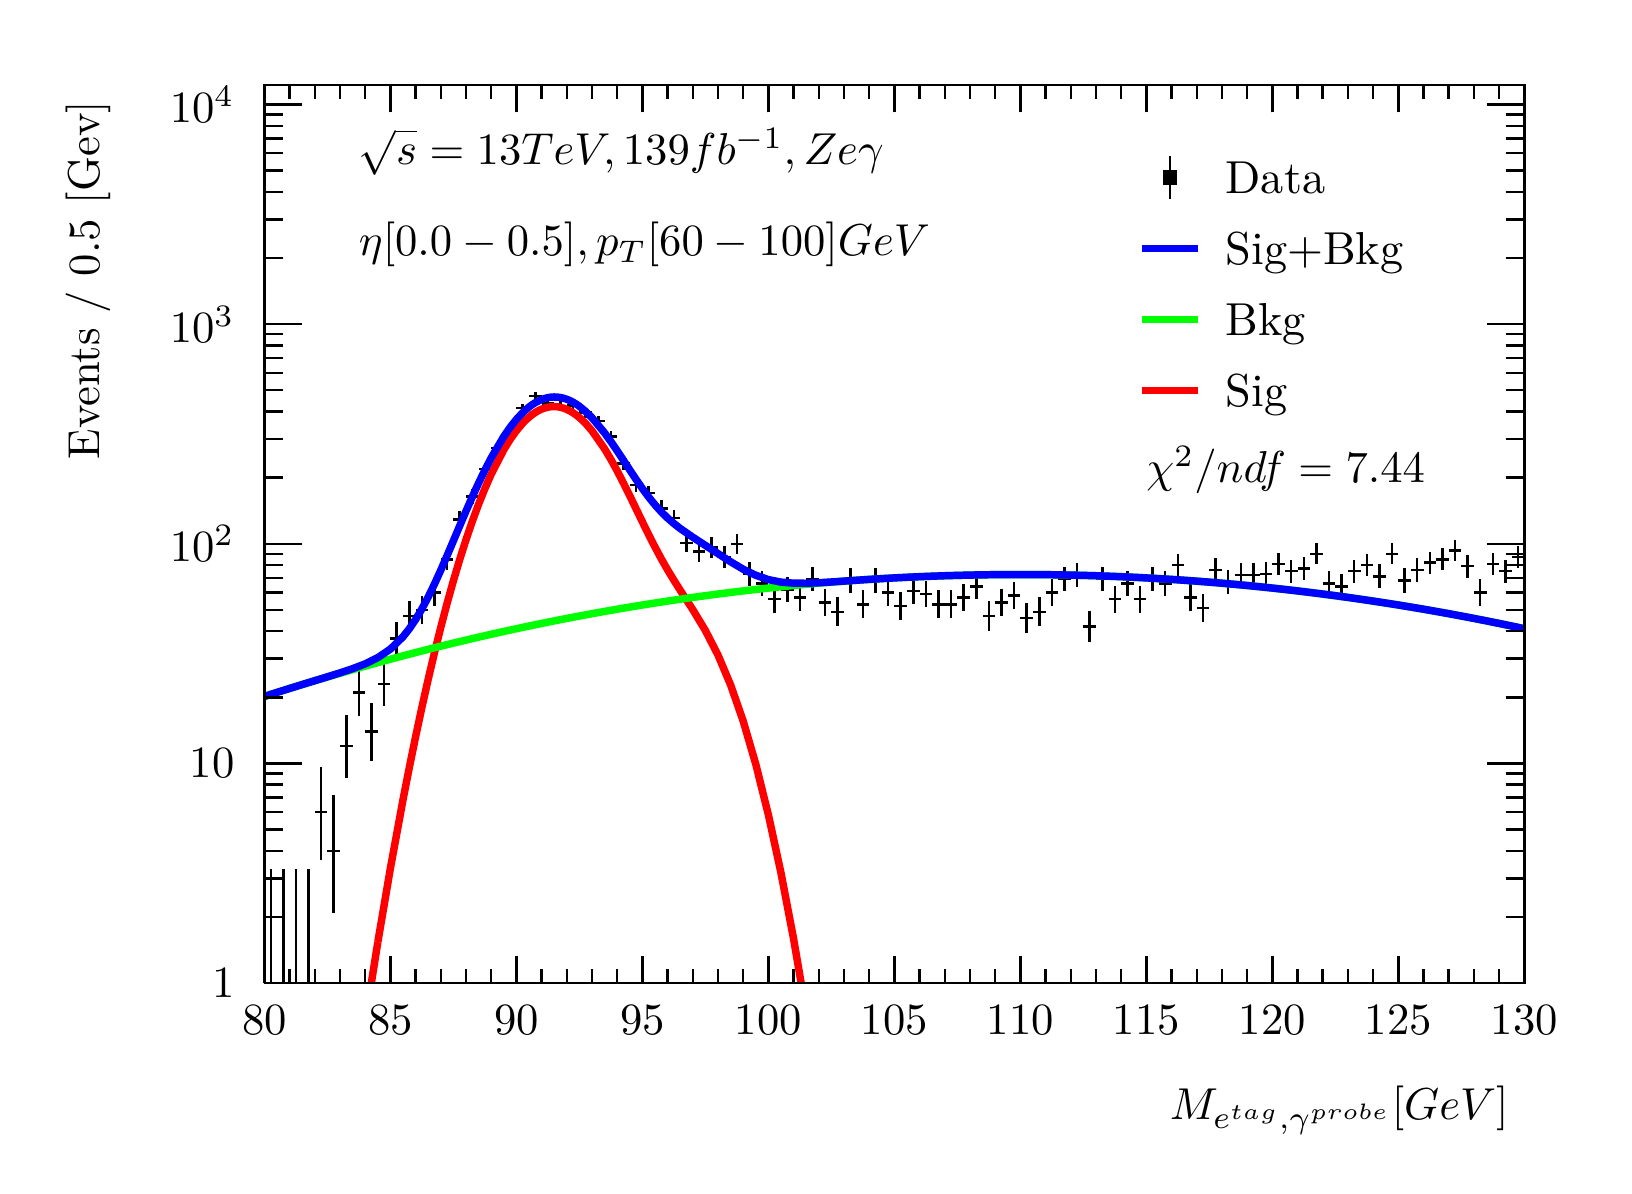
\begin{tikzpicture}
\pgfdeclareplotmark{cross} {
\pgfpathmoveto{\pgfpoint{-0.3\pgfplotmarksize}{\pgfplotmarksize}}
\pgfpathlineto{\pgfpoint{+0.3\pgfplotmarksize}{\pgfplotmarksize}}
\pgfpathlineto{\pgfpoint{+0.3\pgfplotmarksize}{0.3\pgfplotmarksize}}
\pgfpathlineto{\pgfpoint{+1\pgfplotmarksize}{0.3\pgfplotmarksize}}
\pgfpathlineto{\pgfpoint{+1\pgfplotmarksize}{-0.3\pgfplotmarksize}}
\pgfpathlineto{\pgfpoint{+0.3\pgfplotmarksize}{-0.3\pgfplotmarksize}}
\pgfpathlineto{\pgfpoint{+0.3\pgfplotmarksize}{-1.\pgfplotmarksize}}
\pgfpathlineto{\pgfpoint{-0.3\pgfplotmarksize}{-1.\pgfplotmarksize}}
\pgfpathlineto{\pgfpoint{-0.3\pgfplotmarksize}{-0.3\pgfplotmarksize}}
\pgfpathlineto{\pgfpoint{-1.\pgfplotmarksize}{-0.3\pgfplotmarksize}}
\pgfpathlineto{\pgfpoint{-1.\pgfplotmarksize}{0.3\pgfplotmarksize}}
\pgfpathlineto{\pgfpoint{-0.3\pgfplotmarksize}{0.3\pgfplotmarksize}}
\pgfpathclose
\pgfusepathqstroke
}
\pgfdeclareplotmark{cross*} {
\pgfpathmoveto{\pgfpoint{-0.3\pgfplotmarksize}{\pgfplotmarksize}}
\pgfpathlineto{\pgfpoint{+0.3\pgfplotmarksize}{\pgfplotmarksize}}
\pgfpathlineto{\pgfpoint{+0.3\pgfplotmarksize}{0.3\pgfplotmarksize}}
\pgfpathlineto{\pgfpoint{+1\pgfplotmarksize}{0.3\pgfplotmarksize}}
\pgfpathlineto{\pgfpoint{+1\pgfplotmarksize}{-0.3\pgfplotmarksize}}
\pgfpathlineto{\pgfpoint{+0.3\pgfplotmarksize}{-0.3\pgfplotmarksize}}
\pgfpathlineto{\pgfpoint{+0.3\pgfplotmarksize}{-1.\pgfplotmarksize}}
\pgfpathlineto{\pgfpoint{-0.3\pgfplotmarksize}{-1.\pgfplotmarksize}}
\pgfpathlineto{\pgfpoint{-0.3\pgfplotmarksize}{-0.3\pgfplotmarksize}}
\pgfpathlineto{\pgfpoint{-1.\pgfplotmarksize}{-0.3\pgfplotmarksize}}
\pgfpathlineto{\pgfpoint{-1.\pgfplotmarksize}{0.3\pgfplotmarksize}}
\pgfpathlineto{\pgfpoint{-0.3\pgfplotmarksize}{0.3\pgfplotmarksize}}
\pgfpathclose
\pgfusepathqfillstroke
}
\pgfdeclareplotmark{newstar} {
\pgfpathmoveto{\pgfqpoint{0pt}{\pgfplotmarksize}}
\pgfpathlineto{\pgfqpointpolar{44}{0.5\pgfplotmarksize}}
\pgfpathlineto{\pgfqpointpolar{18}{\pgfplotmarksize}}
\pgfpathlineto{\pgfqpointpolar{-20}{0.5\pgfplotmarksize}}
\pgfpathlineto{\pgfqpointpolar{-54}{\pgfplotmarksize}}
\pgfpathlineto{\pgfqpointpolar{-90}{0.5\pgfplotmarksize}}
\pgfpathlineto{\pgfqpointpolar{234}{\pgfplotmarksize}}
\pgfpathlineto{\pgfqpointpolar{198}{0.5\pgfplotmarksize}}
\pgfpathlineto{\pgfqpointpolar{162}{\pgfplotmarksize}}
\pgfpathlineto{\pgfqpointpolar{134}{0.5\pgfplotmarksize}}
\pgfpathclose
\pgfusepathqstroke
}
\pgfdeclareplotmark{newstar*} {
\pgfpathmoveto{\pgfqpoint{0pt}{\pgfplotmarksize}}
\pgfpathlineto{\pgfqpointpolar{44}{0.5\pgfplotmarksize}}
\pgfpathlineto{\pgfqpointpolar{18}{\pgfplotmarksize}}
\pgfpathlineto{\pgfqpointpolar{-20}{0.5\pgfplotmarksize}}
\pgfpathlineto{\pgfqpointpolar{-54}{\pgfplotmarksize}}
\pgfpathlineto{\pgfqpointpolar{-90}{0.5\pgfplotmarksize}}
\pgfpathlineto{\pgfqpointpolar{234}{\pgfplotmarksize}}
\pgfpathlineto{\pgfqpointpolar{198}{0.5\pgfplotmarksize}}
\pgfpathlineto{\pgfqpointpolar{162}{\pgfplotmarksize}}
\pgfpathlineto{\pgfqpointpolar{134}{0.5\pgfplotmarksize}}
\pgfpathclose
\pgfusepathqfillstroke
}
\definecolor{c}{rgb}{1,1,1};
\draw [color=c, fill=c] (0,0) rectangle (20,14.4361);
\draw [color=c, fill=c] (3,2.30977) rectangle (19,13.7143);
\definecolor{c}{rgb}{0,0,0};
\draw [c,line width=0.9] (3,2.30977) -- (3,13.7143) -- (19,13.7143) -- (19,2.30977) -- (3,2.30977);
\definecolor{c}{rgb}{1,1,1};
\draw [color=c, fill=c] (3,2.30977) rectangle (19,13.7143);
\definecolor{c}{rgb}{0,0,0};
\draw [c,line width=0.9] (3,2.30977) -- (3,13.7143) -- (19,13.7143) -- (19,2.30977) -- (3,2.30977);
\draw [c,line width=0.9] (3,2.30977) -- (19,2.30977);
\draw [c,line width=0.9] (3,2.65624) -- (3,2.30977);
\draw [c,line width=0.9] (3.32,2.48301) -- (3.32,2.30977);
\draw [c,line width=0.9] (3.64,2.48301) -- (3.64,2.30977);
\draw [c,line width=0.9] (3.96,2.48301) -- (3.96,2.30977);
\draw [c,line width=0.9] (4.28,2.48301) -- (4.28,2.30977);
\draw [c,line width=0.9] (4.6,2.65624) -- (4.6,2.30977);
\draw [c,line width=0.9] (4.92,2.48301) -- (4.92,2.30977);
\draw [c,line width=0.9] (5.24,2.48301) -- (5.24,2.30977);
\draw [c,line width=0.9] (5.56,2.48301) -- (5.56,2.30977);
\draw [c,line width=0.9] (5.88,2.48301) -- (5.88,2.30977);
\draw [c,line width=0.9] (6.2,2.65624) -- (6.2,2.30977);
\draw [c,line width=0.9] (6.52,2.48301) -- (6.52,2.30977);
\draw [c,line width=0.9] (6.84,2.48301) -- (6.84,2.30977);
\draw [c,line width=0.9] (7.16,2.48301) -- (7.16,2.30977);
\draw [c,line width=0.9] (7.48,2.48301) -- (7.48,2.30977);
\draw [c,line width=0.9] (7.8,2.65624) -- (7.8,2.30977);
\draw [c,line width=0.9] (8.12,2.48301) -- (8.12,2.30977);
\draw [c,line width=0.9] (8.44,2.48301) -- (8.44,2.30977);
\draw [c,line width=0.9] (8.76,2.48301) -- (8.76,2.30977);
\draw [c,line width=0.9] (9.08,2.48301) -- (9.08,2.30977);
\draw [c,line width=0.9] (9.4,2.65624) -- (9.4,2.30977);
\draw [c,line width=0.9] (9.72,2.48301) -- (9.72,2.30977);
\draw [c,line width=0.9] (10.04,2.48301) -- (10.04,2.30977);
\draw [c,line width=0.9] (10.36,2.48301) -- (10.36,2.30977);
\draw [c,line width=0.9] (10.68,2.48301) -- (10.68,2.30977);
\draw [c,line width=0.9] (11,2.65624) -- (11,2.30977);
\draw [c,line width=0.9] (11.32,2.48301) -- (11.32,2.30977);
\draw [c,line width=0.9] (11.64,2.48301) -- (11.64,2.30977);
\draw [c,line width=0.9] (11.96,2.48301) -- (11.96,2.30977);
\draw [c,line width=0.9] (12.28,2.48301) -- (12.28,2.30977);
\draw [c,line width=0.9] (12.6,2.65624) -- (12.6,2.30977);
\draw [c,line width=0.9] (12.92,2.48301) -- (12.92,2.30977);
\draw [c,line width=0.9] (13.24,2.48301) -- (13.24,2.30977);
\draw [c,line width=0.9] (13.56,2.48301) -- (13.56,2.30977);
\draw [c,line width=0.9] (13.88,2.48301) -- (13.88,2.30977);
\draw [c,line width=0.9] (14.2,2.65624) -- (14.2,2.30977);
\draw [c,line width=0.9] (14.52,2.48301) -- (14.52,2.30977);
\draw [c,line width=0.9] (14.84,2.48301) -- (14.84,2.30977);
\draw [c,line width=0.9] (15.16,2.48301) -- (15.16,2.30977);
\draw [c,line width=0.9] (15.48,2.48301) -- (15.48,2.30977);
\draw [c,line width=0.9] (15.8,2.65624) -- (15.8,2.30977);
\draw [c,line width=0.9] (16.12,2.48301) -- (16.12,2.30977);
\draw [c,line width=0.9] (16.44,2.48301) -- (16.44,2.30977);
\draw [c,line width=0.9] (16.76,2.48301) -- (16.76,2.30977);
\draw [c,line width=0.9] (17.08,2.48301) -- (17.08,2.30977);
\draw [c,line width=0.9] (17.4,2.65624) -- (17.4,2.30977);
\draw [c,line width=0.9] (17.72,2.48301) -- (17.72,2.30977);
\draw [c,line width=0.9] (18.04,2.48301) -- (18.04,2.30977);
\draw [c,line width=0.9] (18.36,2.48301) -- (18.36,2.30977);
\draw [c,line width=0.9] (18.68,2.48301) -- (18.68,2.30977);
\draw [c,line width=0.9] (19,2.65624) -- (19,2.30977);
\draw [anchor=base] (3,1.66015) node[scale=1.61424, color=c, rotate=0]{80};
\draw [anchor=base] (4.6,1.66015) node[scale=1.61424, color=c, rotate=0]{85};
\draw [anchor=base] (6.2,1.66015) node[scale=1.61424, color=c, rotate=0]{90};
\draw [anchor=base] (7.8,1.66015) node[scale=1.61424, color=c, rotate=0]{95};
\draw [anchor=base] (9.4,1.66015) node[scale=1.61424, color=c, rotate=0]{100};
\draw [anchor=base] (11,1.66015) node[scale=1.61424, color=c, rotate=0]{105};
\draw [anchor=base] (12.6,1.66015) node[scale=1.61424, color=c, rotate=0]{110};
\draw [anchor=base] (14.2,1.66015) node[scale=1.61424, color=c, rotate=0]{115};
\draw [anchor=base] (15.8,1.66015) node[scale=1.61424, color=c, rotate=0]{120};
\draw [anchor=base] (17.4,1.66015) node[scale=1.61424, color=c, rotate=0]{125};
\draw [anchor=base] (19,1.66015) node[scale=1.61424, color=c, rotate=0]{130};
\draw [anchor= east] (19,0.692932) node[scale=1.61424, color=c, rotate=0]{$M_{e^{tag}, \gamma^{probe}}  [GeV]$};
\draw [c,line width=0.9] (3,13.7143) -- (19,13.7143);
\draw [c,line width=0.9] (3,13.3678) -- (3,13.7143);
\draw [c,line width=0.9] (3.32,13.5411) -- (3.32,13.7143);
\draw [c,line width=0.9] (3.64,13.5411) -- (3.64,13.7143);
\draw [c,line width=0.9] (3.96,13.5411) -- (3.96,13.7143);
\draw [c,line width=0.9] (4.28,13.5411) -- (4.28,13.7143);
\draw [c,line width=0.9] (4.6,13.3678) -- (4.6,13.7143);
\draw [c,line width=0.9] (4.92,13.5411) -- (4.92,13.7143);
\draw [c,line width=0.9] (5.24,13.5411) -- (5.24,13.7143);
\draw [c,line width=0.9] (5.56,13.5411) -- (5.56,13.7143);
\draw [c,line width=0.9] (5.88,13.5411) -- (5.88,13.7143);
\draw [c,line width=0.9] (6.2,13.3678) -- (6.2,13.7143);
\draw [c,line width=0.9] (6.52,13.5411) -- (6.52,13.7143);
\draw [c,line width=0.9] (6.84,13.5411) -- (6.84,13.7143);
\draw [c,line width=0.9] (7.16,13.5411) -- (7.16,13.7143);
\draw [c,line width=0.9] (7.48,13.5411) -- (7.48,13.7143);
\draw [c,line width=0.9] (7.8,13.3678) -- (7.8,13.7143);
\draw [c,line width=0.9] (8.12,13.5411) -- (8.12,13.7143);
\draw [c,line width=0.9] (8.44,13.5411) -- (8.44,13.7143);
\draw [c,line width=0.9] (8.76,13.5411) -- (8.76,13.7143);
\draw [c,line width=0.9] (9.08,13.5411) -- (9.08,13.7143);
\draw [c,line width=0.9] (9.4,13.3678) -- (9.4,13.7143);
\draw [c,line width=0.9] (9.72,13.5411) -- (9.72,13.7143);
\draw [c,line width=0.9] (10.04,13.5411) -- (10.04,13.7143);
\draw [c,line width=0.9] (10.36,13.5411) -- (10.36,13.7143);
\draw [c,line width=0.9] (10.68,13.5411) -- (10.68,13.7143);
\draw [c,line width=0.9] (11,13.3678) -- (11,13.7143);
\draw [c,line width=0.9] (11.32,13.5411) -- (11.32,13.7143);
\draw [c,line width=0.9] (11.64,13.5411) -- (11.64,13.7143);
\draw [c,line width=0.9] (11.96,13.5411) -- (11.96,13.7143);
\draw [c,line width=0.9] (12.28,13.5411) -- (12.28,13.7143);
\draw [c,line width=0.9] (12.6,13.3678) -- (12.6,13.7143);
\draw [c,line width=0.9] (12.92,13.5411) -- (12.92,13.7143);
\draw [c,line width=0.9] (13.24,13.5411) -- (13.24,13.7143);
\draw [c,line width=0.9] (13.56,13.5411) -- (13.56,13.7143);
\draw [c,line width=0.9] (13.88,13.5411) -- (13.88,13.7143);
\draw [c,line width=0.9] (14.2,13.3678) -- (14.2,13.7143);
\draw [c,line width=0.9] (14.52,13.5411) -- (14.52,13.7143);
\draw [c,line width=0.9] (14.84,13.5411) -- (14.84,13.7143);
\draw [c,line width=0.9] (15.16,13.5411) -- (15.16,13.7143);
\draw [c,line width=0.9] (15.48,13.5411) -- (15.48,13.7143);
\draw [c,line width=0.9] (15.8,13.3678) -- (15.8,13.7143);
\draw [c,line width=0.9] (16.12,13.5411) -- (16.12,13.7143);
\draw [c,line width=0.9] (16.44,13.5411) -- (16.44,13.7143);
\draw [c,line width=0.9] (16.76,13.5411) -- (16.76,13.7143);
\draw [c,line width=0.9] (17.08,13.5411) -- (17.08,13.7143);
\draw [c,line width=0.9] (17.4,13.3678) -- (17.4,13.7143);
\draw [c,line width=0.9] (17.72,13.5411) -- (17.72,13.7143);
\draw [c,line width=0.9] (18.04,13.5411) -- (18.04,13.7143);
\draw [c,line width=0.9] (18.36,13.5411) -- (18.36,13.7143);
\draw [c,line width=0.9] (18.68,13.5411) -- (18.68,13.7143);
\draw [c,line width=0.9] (19,13.3678) -- (19,13.7143);
\draw [c,line width=0.9] (3,2.30977) -- (3,13.7143);
\draw [c,line width=0.9] (3.474,2.30978) -- (3,2.30978);
\draw [anchor= east] (2.82,2.30978) node[scale=1.61424, color=c, rotate=0]{1};
\draw [c,line width=0.9] (3.237,3.1495) -- (3,3.1495);
\draw [c,line width=0.9] (3.237,3.6407) -- (3,3.6407);
\draw [c,line width=0.9] (3.237,3.98922) -- (3,3.98922);
\draw [c,line width=0.9] (3.237,4.25955) -- (3,4.25955);
\draw [c,line width=0.9] (3.237,4.48042) -- (3,4.48042);
\draw [c,line width=0.9] (3.237,4.66717) -- (3,4.66717);
\draw [c,line width=0.9] (3.237,4.82894) -- (3,4.82894);
\draw [c,line width=0.9] (3.237,4.97163) -- (3,4.97163);
\draw [c,line width=0.9] (3.474,5.09927) -- (3,5.09927);
\draw [anchor= east] (2.82,5.09927) node[scale=1.61424, color=c, rotate=0]{10};
\draw [c,line width=0.9] (3.237,5.93899) -- (3,5.93899);
\draw [c,line width=0.9] (3.237,6.43019) -- (3,6.43019);
\draw [c,line width=0.9] (3.237,6.77871) -- (3,6.77871);
\draw [c,line width=0.9] (3.237,7.04904) -- (3,7.04904);
\draw [c,line width=0.9] (3.237,7.26991) -- (3,7.26991);
\draw [c,line width=0.9] (3.237,7.45666) -- (3,7.45666);
\draw [c,line width=0.9] (3.237,7.61843) -- (3,7.61843);
\draw [c,line width=0.9] (3.237,7.76112) -- (3,7.76112);
\draw [c,line width=0.9] (3.474,7.88876) -- (3,7.88876);
\draw [anchor= east] (2.82,7.88876) node[scale=1.61424, color=c, rotate=0]{$10^{2}$};
\draw [c,line width=0.9] (3.237,8.72848) -- (3,8.72848);
\draw [c,line width=0.9] (3.237,9.21968) -- (3,9.21968);
\draw [c,line width=0.9] (3.237,9.5682) -- (3,9.5682);
\draw [c,line width=0.9] (3.237,9.83853) -- (3,9.83853);
\draw [c,line width=0.9] (3.237,10.0594) -- (3,10.0594);
\draw [c,line width=0.9] (3.237,10.2462) -- (3,10.2462);
\draw [c,line width=0.9] (3.237,10.4079) -- (3,10.4079);
\draw [c,line width=0.9] (3.237,10.5506) -- (3,10.5506);
\draw [c,line width=0.9] (3.474,10.6782) -- (3,10.6782);
\draw [anchor= east] (2.82,10.6782) node[scale=1.61424, color=c, rotate=0]{$10^{3}$};
\draw [c,line width=0.9] (3.237,11.518) -- (3,11.518);
\draw [c,line width=0.9] (3.237,12.0092) -- (3,12.0092);
\draw [c,line width=0.9] (3.237,12.3577) -- (3,12.3577);
\draw [c,line width=0.9] (3.237,12.628) -- (3,12.628);
\draw [c,line width=0.9] (3.237,12.8489) -- (3,12.8489);
\draw [c,line width=0.9] (3.237,13.0356) -- (3,13.0356);
\draw [c,line width=0.9] (3.237,13.1974) -- (3,13.1974);
\draw [c,line width=0.9] (3.237,13.3401) -- (3,13.3401);
\draw [c,line width=0.9] (3.474,13.4677) -- (3,13.4677);
\draw [anchor= east] (2.82,13.4677) node[scale=1.61424, color=c, rotate=0]{$10^{4}$};
\draw [anchor= east] (0.76,13.7143) node[scale=1.61424, color=c, rotate=90]{Events / 0.5 [Gev]};
\draw [c,line width=0.9] (19,2.30977) -- (19,13.7143);
\draw [c,line width=0.9] (18.526,2.30978) -- (19,2.30978);
\draw [c,line width=0.9] (18.763,3.1495) -- (19,3.1495);
\draw [c,line width=0.9] (18.763,3.6407) -- (19,3.6407);
\draw [c,line width=0.9] (18.763,3.98922) -- (19,3.98922);
\draw [c,line width=0.9] (18.763,4.25955) -- (19,4.25955);
\draw [c,line width=0.9] (18.763,4.48042) -- (19,4.48042);
\draw [c,line width=0.9] (18.763,4.66717) -- (19,4.66717);
\draw [c,line width=0.9] (18.763,4.82894) -- (19,4.82894);
\draw [c,line width=0.9] (18.763,4.97163) -- (19,4.97163);
\draw [c,line width=0.9] (18.526,5.09927) -- (19,5.09927);
\draw [c,line width=0.9] (18.763,5.93899) -- (19,5.93899);
\draw [c,line width=0.9] (18.763,6.43019) -- (19,6.43019);
\draw [c,line width=0.9] (18.763,6.77871) -- (19,6.77871);
\draw [c,line width=0.9] (18.763,7.04904) -- (19,7.04904);
\draw [c,line width=0.9] (18.763,7.26991) -- (19,7.26991);
\draw [c,line width=0.9] (18.763,7.45666) -- (19,7.45666);
\draw [c,line width=0.9] (18.763,7.61843) -- (19,7.61843);
\draw [c,line width=0.9] (18.763,7.76112) -- (19,7.76112);
\draw [c,line width=0.9] (18.526,7.88876) -- (19,7.88876);
\draw [c,line width=0.9] (18.763,8.72848) -- (19,8.72848);
\draw [c,line width=0.9] (18.763,9.21968) -- (19,9.21968);
\draw [c,line width=0.9] (18.763,9.5682) -- (19,9.5682);
\draw [c,line width=0.9] (18.763,9.83853) -- (19,9.83853);
\draw [c,line width=0.9] (18.763,10.0594) -- (19,10.0594);
\draw [c,line width=0.9] (18.763,10.2462) -- (19,10.2462);
\draw [c,line width=0.9] (18.763,10.4079) -- (19,10.4079);
\draw [c,line width=0.9] (18.763,10.5506) -- (19,10.5506);
\draw [c,line width=0.9] (18.526,10.6782) -- (19,10.6782);
\draw [c,line width=0.9] (18.763,11.518) -- (19,11.518);
\draw [c,line width=0.9] (18.763,12.0092) -- (19,12.0092);
\draw [c,line width=0.9] (18.763,12.3577) -- (19,12.3577);
\draw [c,line width=0.9] (18.763,12.628) -- (19,12.628);
\draw [c,line width=0.9] (18.763,12.8489) -- (19,12.8489);
\draw [c,line width=0.9] (18.763,13.0356) -- (19,13.0356);
\draw [c,line width=0.9] (18.763,13.1974) -- (19,13.1974);
\draw [c,line width=0.9] (18.763,13.3401) -- (19,13.3401);
\draw [c,line width=0.9] (18.526,13.4677) -- (19,13.4677);
\draw [c,line width=0.9] (3.08,2.30977) -- (3,2.30977);
\draw [c,line width=0.9] (3,2.30977) -- (3,2.30977);
\draw [c,line width=0.9] (3.08,2.30977) -- (3.16,2.30977);
\draw [c,line width=0.9] (3.16,2.30977) -- (3.16,2.30977);
\draw [c,line width=0.9] (3.08,2.30977) -- (3.08,3.75599);
\draw [c,line width=0.9] (3.08,3.75599) -- (3.08,3.75599);
\draw [c,line width=0.9] (3.24,2.30977) -- (3.16,2.30977);
\draw [c,line width=0.9] (3.16,2.30977) -- (3.16,2.30977);
\draw [c,line width=0.9] (3.24,2.30977) -- (3.32,2.30977);
\draw [c,line width=0.9] (3.32,2.30977) -- (3.32,2.30977);
\draw [c,line width=0.9] (3.24,2.30977) -- (3.24,3.75599);
\draw [c,line width=0.9] (3.24,3.75599) -- (3.24,3.75599);
\draw [c,line width=0.9] (3.4,2.30977) -- (3.32,2.30977);
\draw [c,line width=0.9] (3.32,2.30977) -- (3.32,2.30977);
\draw [c,line width=0.9] (3.4,2.30977) -- (3.48,2.30977);
\draw [c,line width=0.9] (3.48,2.30977) -- (3.48,2.30977);
\draw [c,line width=0.9] (3.4,2.30977) -- (3.4,3.75599);
\draw [c,line width=0.9] (3.4,3.75599) -- (3.4,3.75599);
\draw [c,line width=0.9] (3.56,2.30977) -- (3.48,2.30977);
\draw [c,line width=0.9] (3.48,2.30977) -- (3.48,2.30977);
\draw [c,line width=0.9] (3.56,2.30977) -- (3.64,2.30977);
\draw [c,line width=0.9] (3.64,2.30977) -- (3.64,2.30977);
\draw [c,line width=0.9] (3.56,2.30977) -- (3.56,3.75599);
\draw [c,line width=0.9] (3.56,3.75599) -- (3.56,3.75599);
\draw [c,line width=0.9] (3.72,4.48042) -- (3.64,4.48042);
\draw [c,line width=0.9] (3.64,4.48042) -- (3.64,4.48042);
\draw [c,line width=0.9] (3.72,4.48042) -- (3.8,4.48042);
\draw [c,line width=0.9] (3.8,4.48042) -- (3.8,4.48042);
\draw [c,line width=0.9] (3.72,4.48042) -- (3.72,5.04775);
\draw [c,line width=0.9] (3.72,5.04775) -- (3.72,5.04775);
\draw [c,line width=0.9] (3.72,4.48042) -- (3.72,3.86831);
\draw [c,line width=0.9] (3.72,3.86831) -- (3.72,3.86831);
\draw [c,line width=0.9] (3.88,3.98922) -- (3.8,3.98922);
\draw [c,line width=0.9] (3.8,3.98922) -- (3.8,3.98922);
\draw [c,line width=0.9] (3.88,3.98922) -- (3.96,3.98922);
\draw [c,line width=0.9] (3.96,3.98922) -- (3.96,3.98922);
\draw [c,line width=0.9] (3.88,3.98922) -- (3.88,4.69501);
\draw [c,line width=0.9] (3.88,4.69501) -- (3.88,4.69501);
\draw [c,line width=0.9] (3.88,3.98922) -- (3.88,3.2003);
\draw [c,line width=0.9] (3.88,3.2003) -- (3.88,3.2003);
\draw [c,line width=0.9] (4.04,5.32014) -- (3.96,5.32014);
\draw [c,line width=0.9] (3.96,5.32014) -- (3.96,5.32014);
\draw [c,line width=0.9] (4.04,5.32014) -- (4.12,5.32014);
\draw [c,line width=0.9] (4.12,5.32014) -- (4.12,5.32014);
\draw [c,line width=0.9] (4.04,5.32014) -- (4.04,5.71032);
\draw [c,line width=0.9] (4.04,5.71032) -- (4.04,5.71032);
\draw [c,line width=0.9] (4.04,5.32014) -- (4.04,4.9144);
\draw [c,line width=0.9] (4.04,4.9144) -- (4.04,4.9144);
\draw [c,line width=0.9] (4.2,5.99809) -- (4.12,5.99809);
\draw [c,line width=0.9] (4.12,5.99809) -- (4.12,5.99809);
\draw [c,line width=0.9] (4.2,5.99809) -- (4.28,5.99809);
\draw [c,line width=0.9] (4.28,5.99809) -- (4.28,5.99809);
\draw [c,line width=0.9] (4.2,5.99809) -- (4.2,6.28698);
\draw [c,line width=0.9] (4.2,6.28698) -- (4.2,6.28698);
\draw [c,line width=0.9] (4.2,5.99809) -- (4.2,5.70257);
\draw [c,line width=0.9] (4.2,5.70257) -- (4.2,5.70257);
\draw [c,line width=0.9] (4.36,5.50689) -- (4.28,5.50689);
\draw [c,line width=0.9] (4.28,5.50689) -- (4.28,5.50689);
\draw [c,line width=0.9] (4.36,5.50689) -- (4.44,5.50689);
\draw [c,line width=0.9] (4.44,5.50689) -- (4.44,5.50689);
\draw [c,line width=0.9] (4.36,5.50689) -- (4.36,5.86598);
\draw [c,line width=0.9] (4.36,5.86598) -- (4.36,5.86598);
\draw [c,line width=0.9] (4.36,5.50689) -- (4.36,5.13549);
\draw [c,line width=0.9] (4.36,5.13549) -- (4.36,5.13549);
\draw [c,line width=0.9] (4.52,6.1083) -- (4.44,6.1083);
\draw [c,line width=0.9] (4.44,6.1083) -- (4.44,6.1083);
\draw [c,line width=0.9] (4.52,6.1083) -- (4.6,6.1083);
\draw [c,line width=0.9] (4.6,6.1083) -- (4.6,6.1083);
\draw [c,line width=0.9] (4.52,6.1083) -- (4.52,6.38348);
\draw [c,line width=0.9] (4.52,6.38348) -- (4.52,6.38348);
\draw [c,line width=0.9] (4.52,6.1083) -- (4.52,5.82734);
\draw [c,line width=0.9] (4.52,5.82734) -- (4.52,5.82734);
\draw [c,line width=0.9] (4.68,6.68426) -- (4.6,6.68426);
\draw [c,line width=0.9] (4.6,6.68426) -- (4.6,6.68426);
\draw [c,line width=0.9] (4.68,6.68426) -- (4.76,6.68426);
\draw [c,line width=0.9] (4.76,6.68426) -- (4.76,6.68426);
\draw [c,line width=0.9] (4.68,6.68426) -- (4.68,6.89795);
\draw [c,line width=0.9] (4.68,6.89795) -- (4.68,6.89795);
\draw [c,line width=0.9] (4.68,6.68426) -- (4.68,6.46776);
\draw [c,line width=0.9] (4.68,6.46776) -- (4.68,6.46776);
\draw [c,line width=0.9] (4.84,6.97408) -- (4.76,6.97408);
\draw [c,line width=0.9] (4.76,6.97408) -- (4.76,6.97408);
\draw [c,line width=0.9] (4.84,6.97408) -- (4.92,6.97408);
\draw [c,line width=0.9] (4.92,6.97408) -- (4.92,6.97408);
\draw [c,line width=0.9] (4.84,6.97408) -- (4.84,7.16239);
\draw [c,line width=0.9] (4.84,7.16239) -- (4.84,7.16239);
\draw [c,line width=0.9] (4.84,6.97408) -- (4.84,6.78381);
\draw [c,line width=0.9] (4.84,6.78381) -- (4.84,6.78381);
\draw [c,line width=0.9] (5,7.04904) -- (4.92,7.04904);
\draw [c,line width=0.9] (4.92,7.04904) -- (4.92,7.04904);
\draw [c,line width=0.9] (5,7.04904) -- (5.08,7.04904);
\draw [c,line width=0.9] (5.08,7.04904) -- (5.08,7.04904);
\draw [c,line width=0.9] (5,7.04904) -- (5,7.23131);
\draw [c,line width=0.9] (5,7.23131) -- (5,7.23131);
\draw [c,line width=0.9] (5,7.04904) -- (5,6.86499);
\draw [c,line width=0.9] (5,6.86499) -- (5,6.86499);
\draw [c,line width=0.9] (5.16,7.26991) -- (5.08,7.26991);
\draw [c,line width=0.9] (5.08,7.26991) -- (5.08,7.26991);
\draw [c,line width=0.9] (5.16,7.26991) -- (5.24,7.26991);
\draw [c,line width=0.9] (5.24,7.26991) -- (5.24,7.26991);
\draw [c,line width=0.9] (5.16,7.26991) -- (5.16,7.43552);
\draw [c,line width=0.9] (5.16,7.43552) -- (5.16,7.43552);
\draw [c,line width=0.9] (5.16,7.26991) -- (5.16,7.10296);
\draw [c,line width=0.9] (5.16,7.10296) -- (5.16,7.10296);
\draw [c,line width=0.9] (5.32,7.69187) -- (5.24,7.69187);
\draw [c,line width=0.9] (5.24,7.69187) -- (5.24,7.69187);
\draw [c,line width=0.9] (5.32,7.69187) -- (5.4,7.69187);
\draw [c,line width=0.9] (5.4,7.69187) -- (5.4,7.69187);
\draw [c,line width=0.9] (5.32,7.69187) -- (5.32,7.82987);
\draw [c,line width=0.9] (5.32,7.82987) -- (5.32,7.82987);
\draw [c,line width=0.9] (5.32,7.69187) -- (5.32,7.55307);
\draw [c,line width=0.9] (5.32,7.55307) -- (5.32,7.55307);
\draw [c,line width=0.9] (5.48,8.19725) -- (5.4,8.19725);
\draw [c,line width=0.9] (5.4,8.19725) -- (5.4,8.19725);
\draw [c,line width=0.9] (5.48,8.19725) -- (5.56,8.19725);
\draw [c,line width=0.9] (5.56,8.19725) -- (5.56,8.19725);
\draw [c,line width=0.9] (5.48,8.19725) -- (5.48,8.30387);
\draw [c,line width=0.9] (5.48,8.30387) -- (5.48,8.30387);
\draw [c,line width=0.9] (5.48,8.19725) -- (5.48,8.09062);
\draw [c,line width=0.9] (5.48,8.09062) -- (5.48,8.09062);
\draw [c,line width=0.9] (5.64,8.48806) -- (5.56,8.48806);
\draw [c,line width=0.9] (5.56,8.48806) -- (5.56,8.48806);
\draw [c,line width=0.9] (5.64,8.48806) -- (5.72,8.48806);
\draw [c,line width=0.9] (5.72,8.48806) -- (5.72,8.48806);
\draw [c,line width=0.9] (5.64,8.48806) -- (5.64,8.58264);
\draw [c,line width=0.9] (5.64,8.58264) -- (5.64,8.58264);
\draw [c,line width=0.9] (5.64,8.48806) -- (5.64,8.39349);
\draw [c,line width=0.9] (5.64,8.39349) -- (5.64,8.39349);
\draw [c,line width=0.9] (5.8,8.83842) -- (5.72,8.83842);
\draw [c,line width=0.9] (5.72,8.83842) -- (5.72,8.83842);
\draw [c,line width=0.9] (5.8,8.83842) -- (5.88,8.83842);
\draw [c,line width=0.9] (5.88,8.83842) -- (5.88,8.83842);
\draw [c,line width=0.9] (5.8,8.83842) -- (5.8,8.92027);
\draw [c,line width=0.9] (5.8,8.92027) -- (5.8,8.92027);
\draw [c,line width=0.9] (5.8,8.83842) -- (5.8,8.75658);
\draw [c,line width=0.9] (5.8,8.75658) -- (5.8,8.75658);
\draw [c,line width=0.9] (5.96,9.10543) -- (5.88,9.10543);
\draw [c,line width=0.9] (5.88,9.10543) -- (5.88,9.10543);
\draw [c,line width=0.9] (5.96,9.10543) -- (6.04,9.10543);
\draw [c,line width=0.9] (6.04,9.10543) -- (6.04,9.10543);
\draw [c,line width=0.9] (5.96,9.10543) -- (5.96,9.17874);
\draw [c,line width=0.9] (5.96,9.17874) -- (5.96,9.17874);
\draw [c,line width=0.9] (5.96,9.10543) -- (5.96,9.03212);
\draw [c,line width=0.9] (5.96,9.03212) -- (5.96,9.03212);
\draw [c,line width=0.9] (6.12,9.32037) -- (6.04,9.32037);
\draw [c,line width=0.9] (6.04,9.32037) -- (6.04,9.32037);
\draw [c,line width=0.9] (6.12,9.32037) -- (6.2,9.32037);
\draw [c,line width=0.9] (6.2,9.32037) -- (6.2,9.32037);
\draw [c,line width=0.9] (6.12,9.32037) -- (6.12,9.38746);
\draw [c,line width=0.9] (6.12,9.38746) -- (6.12,9.38746);
\draw [c,line width=0.9] (6.12,9.32037) -- (6.12,9.25328);
\draw [c,line width=0.9] (6.12,9.25328) -- (6.12,9.25328);
\draw [c,line width=0.9] (6.28,9.60987) -- (6.2,9.60987);
\draw [c,line width=0.9] (6.2,9.60987) -- (6.2,9.60987);
\draw [c,line width=0.9] (6.28,9.60987) -- (6.36,9.60987);
\draw [c,line width=0.9] (6.36,9.60987) -- (6.36,9.60987);
\draw [c,line width=0.9] (6.28,9.60987) -- (6.28,9.66941);
\draw [c,line width=0.9] (6.28,9.66941) -- (6.28,9.66941);
\draw [c,line width=0.9] (6.28,9.60987) -- (6.28,9.55034);
\draw [c,line width=0.9] (6.28,9.55034) -- (6.28,9.55034);
\draw [c,line width=0.9] (6.44,9.76357) -- (6.36,9.76357);
\draw [c,line width=0.9] (6.36,9.76357) -- (6.36,9.76357);
\draw [c,line width=0.9] (6.44,9.76357) -- (6.52,9.76357);
\draw [c,line width=0.9] (6.52,9.76357) -- (6.52,9.76357);
\draw [c,line width=0.9] (6.44,9.76357) -- (6.44,9.81944);
\draw [c,line width=0.9] (6.44,9.81944) -- (6.44,9.81944);
\draw [c,line width=0.9] (6.44,9.76357) -- (6.44,9.70769);
\draw [c,line width=0.9] (6.44,9.70769) -- (6.44,9.70769);
\draw [c,line width=0.9] (6.6,9.66982) -- (6.52,9.66982);
\draw [c,line width=0.9] (6.52,9.66982) -- (6.52,9.66982);
\draw [c,line width=0.9] (6.6,9.66982) -- (6.68,9.66982);
\draw [c,line width=0.9] (6.68,9.66982) -- (6.68,9.66982);
\draw [c,line width=0.9] (6.6,9.66982) -- (6.6,9.7279);
\draw [c,line width=0.9] (6.6,9.7279) -- (6.6,9.7279);
\draw [c,line width=0.9] (6.6,9.66982) -- (6.6,9.61174);
\draw [c,line width=0.9] (6.6,9.61174) -- (6.6,9.61174);
\draw [c,line width=0.9] (6.76,9.72161) -- (6.68,9.72161);
\draw [c,line width=0.9] (6.68,9.72161) -- (6.68,9.72161);
\draw [c,line width=0.9] (6.76,9.72161) -- (6.84,9.72161);
\draw [c,line width=0.9] (6.84,9.72161) -- (6.84,9.72161);
\draw [c,line width=0.9] (6.76,9.72161) -- (6.76,9.77846);
\draw [c,line width=0.9] (6.76,9.77846) -- (6.76,9.77846);
\draw [c,line width=0.9] (6.76,9.72161) -- (6.76,9.66476);
\draw [c,line width=0.9] (6.76,9.66476) -- (6.76,9.66476);
\draw [c,line width=0.9] (6.92,9.64449) -- (6.84,9.64449);
\draw [c,line width=0.9] (6.84,9.64449) -- (6.84,9.64449);
\draw [c,line width=0.9] (6.92,9.64449) -- (7,9.64449);
\draw [c,line width=0.9] (7,9.64449) -- (7,9.64449);
\draw [c,line width=0.9] (6.92,9.64449) -- (6.92,9.70318);
\draw [c,line width=0.9] (6.92,9.70318) -- (6.92,9.70318);
\draw [c,line width=0.9] (6.92,9.64449) -- (6.92,9.5858);
\draw [c,line width=0.9] (6.92,9.5858) -- (6.92,9.5858);
\draw [c,line width=0.9] (7.08,9.55296) -- (7,9.55296);
\draw [c,line width=0.9] (7,9.55296) -- (7,9.55296);
\draw [c,line width=0.9] (7.08,9.55296) -- (7.16,9.55296);
\draw [c,line width=0.9] (7.16,9.55296) -- (7.16,9.55296);
\draw [c,line width=0.9] (7.08,9.55296) -- (7.08,9.61391);
\draw [c,line width=0.9] (7.08,9.61391) -- (7.08,9.61391);
\draw [c,line width=0.9] (7.08,9.55296) -- (7.08,9.49201);
\draw [c,line width=0.9] (7.08,9.49201) -- (7.08,9.49201);
\draw [c,line width=0.9] (7.24,9.44727) -- (7.16,9.44727);
\draw [c,line width=0.9] (7.16,9.44727) -- (7.16,9.44727);
\draw [c,line width=0.9] (7.24,9.44727) -- (7.32,9.44727);
\draw [c,line width=0.9] (7.32,9.44727) -- (7.32,9.44727);
\draw [c,line width=0.9] (7.24,9.44727) -- (7.24,9.51093);
\draw [c,line width=0.9] (7.24,9.51093) -- (7.24,9.51093);
\draw [c,line width=0.9] (7.24,9.44727) -- (7.24,9.3836);
\draw [c,line width=0.9] (7.24,9.3836) -- (7.24,9.3836);
\draw [c,line width=0.9] (7.4,9.25156) -- (7.32,9.25156);
\draw [c,line width=0.9] (7.32,9.25156) -- (7.32,9.25156);
\draw [c,line width=0.9] (7.4,9.25156) -- (7.48,9.25156);
\draw [c,line width=0.9] (7.48,9.25156) -- (7.48,9.25156);
\draw [c,line width=0.9] (7.4,9.25156) -- (7.4,9.32058);
\draw [c,line width=0.9] (7.4,9.32058) -- (7.4,9.32058);
\draw [c,line width=0.9] (7.4,9.25156) -- (7.4,9.18254);
\draw [c,line width=0.9] (7.4,9.18254) -- (7.4,9.18254);
\draw [c,line width=0.9] (7.56,8.90828) -- (7.48,8.90828);
\draw [c,line width=0.9] (7.48,8.90828) -- (7.48,8.90828);
\draw [c,line width=0.9] (7.56,8.90828) -- (7.64,8.90828);
\draw [c,line width=0.9] (7.64,8.90828) -- (7.64,8.90828);
\draw [c,line width=0.9] (7.56,8.90828) -- (7.56,8.9878);
\draw [c,line width=0.9] (7.56,8.9878) -- (7.56,8.9878);
\draw [c,line width=0.9] (7.56,8.90828) -- (7.56,8.82876);
\draw [c,line width=0.9] (7.56,8.82876) -- (7.56,8.82876);
\draw [c,line width=0.9] (7.72,8.63403) -- (7.64,8.63403);
\draw [c,line width=0.9] (7.64,8.63403) -- (7.64,8.63403);
\draw [c,line width=0.9] (7.72,8.63403) -- (7.8,8.63403);
\draw [c,line width=0.9] (7.8,8.63403) -- (7.8,8.63403);
\draw [c,line width=0.9] (7.72,8.63403) -- (7.72,8.72308);
\draw [c,line width=0.9] (7.72,8.72308) -- (7.72,8.72308);
\draw [c,line width=0.9] (7.72,8.63403) -- (7.72,8.54498);
\draw [c,line width=0.9] (7.72,8.54498) -- (7.72,8.54498);
\draw [c,line width=0.9] (7.88,8.53159) -- (7.8,8.53159);
\draw [c,line width=0.9] (7.8,8.53159) -- (7.8,8.53159);
\draw [c,line width=0.9] (7.88,8.53159) -- (7.96,8.53159);
\draw [c,line width=0.9] (7.96,8.53159) -- (7.96,8.53159);
\draw [c,line width=0.9] (7.88,8.53159) -- (7.88,8.62448);
\draw [c,line width=0.9] (7.88,8.62448) -- (7.88,8.62448);
\draw [c,line width=0.9] (7.88,8.53159) -- (7.88,8.4387);
\draw [c,line width=0.9] (7.88,8.4387) -- (7.88,8.4387);
\draw [c,line width=0.9] (8.04,8.33889) -- (7.96,8.33889);
\draw [c,line width=0.9] (7.96,8.33889) -- (7.96,8.33889);
\draw [c,line width=0.9] (8.04,8.33889) -- (8.12,8.33889);
\draw [c,line width=0.9] (8.12,8.33889) -- (8.12,8.33889);
\draw [c,line width=0.9] (8.04,8.33889) -- (8.04,8.43947);
\draw [c,line width=0.9] (8.04,8.43947) -- (8.04,8.43947);
\draw [c,line width=0.9] (8.04,8.33889) -- (8.04,8.23831);
\draw [c,line width=0.9] (8.04,8.23831) -- (8.04,8.23831);
\draw [c,line width=0.9] (8.2,8.21588) -- (8.12,8.21588);
\draw [c,line width=0.9] (8.12,8.21588) -- (8.12,8.21588);
\draw [c,line width=0.9] (8.2,8.21588) -- (8.28,8.21588);
\draw [c,line width=0.9] (8.28,8.21588) -- (8.28,8.21588);
\draw [c,line width=0.9] (8.2,8.21588) -- (8.2,8.3217);
\draw [c,line width=0.9] (8.2,8.3217) -- (8.2,8.3217);
\draw [c,line width=0.9] (8.2,8.21588) -- (8.2,8.11007);
\draw [c,line width=0.9] (8.2,8.11007) -- (8.2,8.11007);
\draw [c,line width=0.9] (8.36,7.90081) -- (8.28,7.90081);
\draw [c,line width=0.9] (8.28,7.90081) -- (8.28,7.90081);
\draw [c,line width=0.9] (8.36,7.90081) -- (8.44,7.90081);
\draw [c,line width=0.9] (8.44,7.90081) -- (8.44,7.90081);
\draw [c,line width=0.9] (8.36,7.90081) -- (8.36,8.02131);
\draw [c,line width=0.9] (8.36,8.02131) -- (8.36,8.02131);
\draw [c,line width=0.9] (8.36,7.90081) -- (8.36,7.78032);
\draw [c,line width=0.9] (8.36,7.78032) -- (8.36,7.78032);
\draw [c,line width=0.9] (8.52,7.78774) -- (8.44,7.78774);
\draw [c,line width=0.9] (8.44,7.78774) -- (8.44,7.78774);
\draw [c,line width=0.9] (8.52,7.78774) -- (8.6,7.78774);
\draw [c,line width=0.9] (8.6,7.78774) -- (8.6,7.78774);
\draw [c,line width=0.9] (8.52,7.78774) -- (8.52,7.92016);
\draw [c,line width=0.9] (8.52,7.92016) -- (8.52,7.92016);
\draw [c,line width=0.9] (8.52,7.78774) -- (8.52,7.65462);
\draw [c,line width=0.9] (8.52,7.65462) -- (8.52,7.65462);
\draw [c,line width=0.9] (8.68,7.8393) -- (8.6,7.8393);
\draw [c,line width=0.9] (8.6,7.8393) -- (8.6,7.8393);
\draw [c,line width=0.9] (8.68,7.8393) -- (8.76,7.8393);
\draw [c,line width=0.9] (8.76,7.8393) -- (8.76,7.8393);
\draw [c,line width=0.9] (8.68,7.8393) -- (8.68,7.96882);
\draw [c,line width=0.9] (8.68,7.96882) -- (8.68,7.96882);
\draw [c,line width=0.9] (8.68,7.8393) -- (8.68,7.70912);
\draw [c,line width=0.9] (8.68,7.70912) -- (8.68,7.70912);
\draw [c,line width=0.9] (8.84,7.72005) -- (8.76,7.72005);
\draw [c,line width=0.9] (8.76,7.72005) -- (8.76,7.72005);
\draw [c,line width=0.9] (8.84,7.72005) -- (8.92,7.72005);
\draw [c,line width=0.9] (8.92,7.72005) -- (8.92,7.72005);
\draw [c,line width=0.9] (8.84,7.72005) -- (8.84,7.85638);
\draw [c,line width=0.9] (8.84,7.85638) -- (8.84,7.85638);
\draw [c,line width=0.9] (8.84,7.72005) -- (8.84,7.58294);
\draw [c,line width=0.9] (8.84,7.58294) -- (8.84,7.58294);
\draw [c,line width=0.9] (9,7.88876) -- (8.92,7.88876);
\draw [c,line width=0.9] (8.92,7.88876) -- (8.92,7.88876);
\draw [c,line width=0.9] (9,7.88876) -- (9.08,7.88876);
\draw [c,line width=0.9] (9.08,7.88876) -- (9.08,7.88876);
\draw [c,line width=0.9] (9,7.88876) -- (9,8.01555);
\draw [c,line width=0.9] (9,8.01555) -- (9,8.01555);
\draw [c,line width=0.9] (9,7.88876) -- (9,7.76134);
\draw [c,line width=0.9] (9,7.76134) -- (9,7.76134);
\draw [c,line width=0.9] (9.16,7.5075) -- (9.08,7.5075);
\draw [c,line width=0.9] (9.08,7.5075) -- (9.08,7.5075);
\draw [c,line width=0.9] (9.16,7.5075) -- (9.24,7.5075);
\draw [c,line width=0.9] (9.24,7.5075) -- (9.24,7.5075);
\draw [c,line width=0.9] (9.16,7.5075) -- (9.16,7.65692);
\draw [c,line width=0.9] (9.16,7.65692) -- (9.16,7.65692);
\draw [c,line width=0.9] (9.16,7.5075) -- (9.16,7.35707);
\draw [c,line width=0.9] (9.16,7.35707) -- (9.16,7.35707);
\draw [c,line width=0.9] (9.32,7.38538) -- (9.24,7.38538);
\draw [c,line width=0.9] (9.24,7.38538) -- (9.24,7.38538);
\draw [c,line width=0.9] (9.32,7.38538) -- (9.4,7.38538);
\draw [c,line width=0.9] (9.4,7.38538) -- (9.4,7.38538);
\draw [c,line width=0.9] (9.32,7.38538) -- (9.32,7.5429);
\draw [c,line width=0.9] (9.32,7.5429) -- (9.32,7.5429);
\draw [c,line width=0.9] (9.32,7.38538) -- (9.32,7.22668);
\draw [c,line width=0.9] (9.32,7.22668) -- (9.32,7.22668);
\draw [c,line width=0.9] (9.48,7.18633) -- (9.4,7.18633);
\draw [c,line width=0.9] (9.4,7.18633) -- (9.4,7.18633);
\draw [c,line width=0.9] (9.48,7.18633) -- (9.56,7.18633);
\draw [c,line width=0.9] (9.56,7.18633) -- (9.56,7.18633);
\draw [c,line width=0.9] (9.48,7.18633) -- (9.48,7.35805);
\draw [c,line width=0.9] (9.48,7.35805) -- (9.48,7.35805);
\draw [c,line width=0.9] (9.48,7.18633) -- (9.48,7.01311);
\draw [c,line width=0.9] (9.48,7.01311) -- (9.48,7.01311);
\draw [c,line width=0.9] (9.64,7.30964) -- (9.56,7.30964);
\draw [c,line width=0.9] (9.56,7.30964) -- (9.56,7.30964);
\draw [c,line width=0.9] (9.64,7.30964) -- (9.72,7.30964);
\draw [c,line width=0.9] (9.72,7.30964) -- (9.72,7.30964);
\draw [c,line width=0.9] (9.64,7.30964) -- (9.64,7.47242);
\draw [c,line width=0.9] (9.64,7.47242) -- (9.64,7.47242);
\draw [c,line width=0.9] (9.64,7.30964) -- (9.64,7.14557);
\draw [c,line width=0.9] (9.64,7.14557) -- (9.64,7.14557);
\draw [c,line width=0.9] (9.8,7.20777) -- (9.72,7.20777);
\draw [c,line width=0.9] (9.72,7.20777) -- (9.72,7.20777);
\draw [c,line width=0.9] (9.8,7.20777) -- (9.88,7.20777);
\draw [c,line width=0.9] (9.88,7.20777) -- (9.88,7.20777);
\draw [c,line width=0.9] (9.8,7.20777) -- (9.8,7.3779);
\draw [c,line width=0.9] (9.8,7.3779) -- (9.8,7.3779);
\draw [c,line width=0.9] (9.8,7.20777) -- (9.8,7.03618);
\draw [c,line width=0.9] (9.8,7.03618) -- (9.8,7.03618);
\draw [c,line width=0.9] (9.96,7.43923) -- (9.88,7.43923);
\draw [c,line width=0.9] (9.88,7.43923) -- (9.88,7.43923);
\draw [c,line width=0.9] (9.96,7.43923) -- (10.04,7.43923);
\draw [c,line width=0.9] (10.04,7.43923) -- (10.04,7.43923);
\draw [c,line width=0.9] (9.96,7.43923) -- (9.96,7.59313);
\draw [c,line width=0.9] (9.96,7.59313) -- (9.96,7.59313);
\draw [c,line width=0.9] (9.96,7.43923) -- (9.96,7.28423);
\draw [c,line width=0.9] (9.96,7.28423) -- (9.96,7.28423);
\draw [c,line width=0.9] (10.12,7.14227) -- (10.04,7.14227);
\draw [c,line width=0.9] (10.04,7.14227) -- (10.04,7.14227);
\draw [c,line width=0.9] (10.12,7.14227) -- (10.2,7.14227);
\draw [c,line width=0.9] (10.2,7.14227) -- (10.2,7.14227);
\draw [c,line width=0.9] (10.12,7.14227) -- (10.12,7.31731);
\draw [c,line width=0.9] (10.12,7.31731) -- (10.12,7.31731);
\draw [c,line width=0.9] (10.12,7.14227) -- (10.12,6.96565);
\draw [c,line width=0.9] (10.12,6.96565) -- (10.12,6.96565);
\draw [c,line width=0.9] (10.28,7.02456) -- (10.2,7.02456);
\draw [c,line width=0.9] (10.2,7.02456) -- (10.2,7.02456);
\draw [c,line width=0.9] (10.28,7.02456) -- (10.36,7.02456);
\draw [c,line width=0.9] (10.36,7.02456) -- (10.36,7.02456);
\draw [c,line width=0.9] (10.28,7.02456) -- (10.28,7.20878);
\draw [c,line width=0.9] (10.28,7.20878) -- (10.28,7.20878);
\draw [c,line width=0.9] (10.28,7.02456) -- (10.28,6.83851);
\draw [c,line width=0.9] (10.28,6.83851) -- (10.28,6.83851);
\draw [c,line width=0.9] (10.44,7.42154) -- (10.36,7.42154);
\draw [c,line width=0.9] (10.36,7.42154) -- (10.36,7.42154);
\draw [c,line width=0.9] (10.44,7.42154) -- (10.52,7.42154);
\draw [c,line width=0.9] (10.52,7.42154) -- (10.52,7.42154);
\draw [c,line width=0.9] (10.44,7.42154) -- (10.44,7.57663);
\draw [c,line width=0.9] (10.44,7.57663) -- (10.44,7.57663);
\draw [c,line width=0.9] (10.44,7.42154) -- (10.44,7.26534);
\draw [c,line width=0.9] (10.44,7.26534) -- (10.44,7.26534);
\draw [c,line width=0.9] (10.6,7.11963) -- (10.52,7.11963);
\draw [c,line width=0.9] (10.52,7.11963) -- (10.52,7.11963);
\draw [c,line width=0.9] (10.6,7.11963) -- (10.68,7.11963);
\draw [c,line width=0.9] (10.68,7.11963) -- (10.68,7.11963);
\draw [c,line width=0.9] (10.6,7.11963) -- (10.6,7.29639);
\draw [c,line width=0.9] (10.6,7.29639) -- (10.6,7.29639);
\draw [c,line width=0.9] (10.6,7.11963) -- (10.6,6.94123);
\draw [c,line width=0.9] (10.6,6.94123) -- (10.6,6.94123);
\draw [c,line width=0.9] (10.76,7.42154) -- (10.68,7.42154);
\draw [c,line width=0.9] (10.68,7.42154) -- (10.68,7.42154);
\draw [c,line width=0.9] (10.76,7.42154) -- (10.84,7.42154);
\draw [c,line width=0.9] (10.84,7.42154) -- (10.84,7.42154);
\draw [c,line width=0.9] (10.76,7.42154) -- (10.76,7.57663);
\draw [c,line width=0.9] (10.76,7.57663) -- (10.76,7.57663);
\draw [c,line width=0.9] (10.76,7.42154) -- (10.76,7.26534);
\draw [c,line width=0.9] (10.76,7.26534) -- (10.76,7.26534);
\draw [c,line width=0.9] (10.92,7.26991) -- (10.84,7.26991);
\draw [c,line width=0.9] (10.84,7.26991) -- (10.84,7.26991);
\draw [c,line width=0.9] (10.92,7.26991) -- (11,7.26991);
\draw [c,line width=0.9] (11,7.26991) -- (11,7.26991);
\draw [c,line width=0.9] (10.92,7.26991) -- (10.92,7.43552);
\draw [c,line width=0.9] (10.92,7.43552) -- (10.92,7.43552);
\draw [c,line width=0.9] (10.92,7.26991) -- (10.92,7.10296);
\draw [c,line width=0.9] (10.92,7.10296) -- (10.92,7.10296);
\draw [c,line width=0.9] (11.08,7.09655) -- (11,7.09655);
\draw [c,line width=0.9] (11,7.09655) -- (11,7.09655);
\draw [c,line width=0.9] (11.08,7.09655) -- (11.16,7.09655);
\draw [c,line width=0.9] (11.16,7.09655) -- (11.16,7.09655);
\draw [c,line width=0.9] (11.08,7.09655) -- (11.08,7.2751);
\draw [c,line width=0.9] (11.08,7.2751) -- (11.08,7.2751);
\draw [c,line width=0.9] (11.08,7.09655) -- (11.08,6.91633);
\draw [c,line width=0.9] (11.08,6.91633) -- (11.08,6.91633);
\draw [c,line width=0.9] (11.24,7.28994) -- (11.16,7.28994);
\draw [c,line width=0.9] (11.16,7.28994) -- (11.16,7.28994);
\draw [c,line width=0.9] (11.24,7.28994) -- (11.32,7.28994);
\draw [c,line width=0.9] (11.32,7.28994) -- (11.32,7.28994);
\draw [c,line width=0.9] (11.24,7.28994) -- (11.24,7.45411);
\draw [c,line width=0.9] (11.24,7.45411) -- (11.24,7.45411);
\draw [c,line width=0.9] (11.24,7.28994) -- (11.24,7.12444);
\draw [c,line width=0.9] (11.24,7.12444) -- (11.24,7.12444);
\draw [c,line width=0.9] (11.4,7.24955) -- (11.32,7.24955);
\draw [c,line width=0.9] (11.32,7.24955) -- (11.32,7.24955);
\draw [c,line width=0.9] (11.4,7.24955) -- (11.48,7.24955);
\draw [c,line width=0.9] (11.48,7.24955) -- (11.48,7.24955);
\draw [c,line width=0.9] (11.4,7.24955) -- (11.4,7.41663);
\draw [c,line width=0.9] (11.4,7.41663) -- (11.4,7.41663);
\draw [c,line width=0.9] (11.4,7.24955) -- (11.4,7.08109);
\draw [c,line width=0.9] (11.4,7.08109) -- (11.4,7.08109);
\draw [c,line width=0.9] (11.56,7.11963) -- (11.48,7.11963);
\draw [c,line width=0.9] (11.48,7.11963) -- (11.48,7.11963);
\draw [c,line width=0.9] (11.56,7.11963) -- (11.64,7.11963);
\draw [c,line width=0.9] (11.64,7.11963) -- (11.64,7.11963);
\draw [c,line width=0.9] (11.56,7.11963) -- (11.56,7.29639);
\draw [c,line width=0.9] (11.56,7.29639) -- (11.56,7.29639);
\draw [c,line width=0.9] (11.56,7.11963) -- (11.56,6.94123);
\draw [c,line width=0.9] (11.56,6.94123) -- (11.56,6.94123);
\draw [c,line width=0.9] (11.72,7.11963) -- (11.64,7.11963);
\draw [c,line width=0.9] (11.64,7.11963) -- (11.64,7.11963);
\draw [c,line width=0.9] (11.72,7.11963) -- (11.8,7.11963);
\draw [c,line width=0.9] (11.8,7.11963) -- (11.8,7.11963);
\draw [c,line width=0.9] (11.72,7.11963) -- (11.72,7.29639);
\draw [c,line width=0.9] (11.72,7.29639) -- (11.72,7.29639);
\draw [c,line width=0.9] (11.72,7.11963) -- (11.72,6.94123);
\draw [c,line width=0.9] (11.72,6.94123) -- (11.72,6.94123);
\draw [c,line width=0.9] (11.88,7.20777) -- (11.8,7.20777);
\draw [c,line width=0.9] (11.8,7.20777) -- (11.8,7.20777);
\draw [c,line width=0.9] (11.88,7.20777) -- (11.96,7.20777);
\draw [c,line width=0.9] (11.96,7.20777) -- (11.96,7.20777);
\draw [c,line width=0.9] (11.88,7.20777) -- (11.88,7.3779);
\draw [c,line width=0.9] (11.88,7.3779) -- (11.88,7.3779);
\draw [c,line width=0.9] (11.88,7.20777) -- (11.88,7.03618);
\draw [c,line width=0.9] (11.88,7.03618) -- (11.88,7.03618);
\draw [c,line width=0.9] (12.04,7.3481) -- (11.96,7.3481);
\draw [c,line width=0.9] (11.96,7.3481) -- (11.96,7.3481);
\draw [c,line width=0.9] (12.04,7.3481) -- (12.12,7.3481);
\draw [c,line width=0.9] (12.12,7.3481) -- (12.12,7.3481);
\draw [c,line width=0.9] (12.04,7.3481) -- (12.04,7.50819);
\draw [c,line width=0.9] (12.04,7.50819) -- (12.04,7.50819);
\draw [c,line width=0.9] (12.04,7.3481) -- (12.04,7.18678);
\draw [c,line width=0.9] (12.04,7.18678) -- (12.04,7.18678);
\draw [c,line width=0.9] (12.2,6.97408) -- (12.12,6.97408);
\draw [c,line width=0.9] (12.12,6.97408) -- (12.12,6.97408);
\draw [c,line width=0.9] (12.2,6.97408) -- (12.28,6.97408);
\draw [c,line width=0.9] (12.28,6.97408) -- (12.28,6.97408);
\draw [c,line width=0.9] (12.2,6.97408) -- (12.2,7.16239);
\draw [c,line width=0.9] (12.2,7.16239) -- (12.2,7.16239);
\draw [c,line width=0.9] (12.2,6.97408) -- (12.2,6.78381);
\draw [c,line width=0.9] (12.2,6.78381) -- (12.2,6.78381);
\draw [c,line width=0.9] (12.36,7.14227) -- (12.28,7.14227);
\draw [c,line width=0.9] (12.28,7.14227) -- (12.28,7.14227);
\draw [c,line width=0.9] (12.36,7.14227) -- (12.44,7.14227);
\draw [c,line width=0.9] (12.44,7.14227) -- (12.44,7.14227);
\draw [c,line width=0.9] (12.36,7.14227) -- (12.36,7.31731);
\draw [c,line width=0.9] (12.36,7.31731) -- (12.36,7.31731);
\draw [c,line width=0.9] (12.36,7.14227) -- (12.36,6.96565);
\draw [c,line width=0.9] (12.36,6.96565) -- (12.36,6.96565);
\draw [c,line width=0.9] (12.52,7.22884) -- (12.44,7.22884);
\draw [c,line width=0.9] (12.44,7.22884) -- (12.44,7.22884);
\draw [c,line width=0.9] (12.52,7.22884) -- (12.6,7.22884);
\draw [c,line width=0.9] (12.6,7.22884) -- (12.6,7.22884);
\draw [c,line width=0.9] (12.52,7.22884) -- (12.52,7.39742);
\draw [c,line width=0.9] (12.52,7.39742) -- (12.52,7.39742);
\draw [c,line width=0.9] (12.52,7.22884) -- (12.52,7.05884);
\draw [c,line width=0.9] (12.52,7.05884) -- (12.52,7.05884);
\draw [c,line width=0.9] (12.68,6.94802) -- (12.6,6.94802);
\draw [c,line width=0.9] (12.6,6.94802) -- (12.6,6.94802);
\draw [c,line width=0.9] (12.68,6.94802) -- (12.76,6.94802);
\draw [c,line width=0.9] (12.76,6.94802) -- (12.76,6.94802);
\draw [c,line width=0.9] (12.68,6.94802) -- (12.68,7.13848);
\draw [c,line width=0.9] (12.68,7.13848) -- (12.68,7.13848);
\draw [c,line width=0.9] (12.68,6.94802) -- (12.68,6.75554);
\draw [c,line width=0.9] (12.68,6.75554) -- (12.68,6.75554);
\draw [c,line width=0.9] (12.84,7.02456) -- (12.76,7.02456);
\draw [c,line width=0.9] (12.76,7.02456) -- (12.76,7.02456);
\draw [c,line width=0.9] (12.84,7.02456) -- (12.92,7.02456);
\draw [c,line width=0.9] (12.92,7.02456) -- (12.92,7.02456);
\draw [c,line width=0.9] (12.84,7.02456) -- (12.84,7.20878);
\draw [c,line width=0.9] (12.84,7.20878) -- (12.84,7.20878);
\draw [c,line width=0.9] (12.84,7.02456) -- (12.84,6.83851);
\draw [c,line width=0.9] (12.84,6.83851) -- (12.84,6.83851);
\draw [c,line width=0.9] (13,7.26991) -- (12.92,7.26991);
\draw [c,line width=0.9] (12.92,7.26991) -- (12.92,7.26991);
\draw [c,line width=0.9] (13,7.26991) -- (13.08,7.26991);
\draw [c,line width=0.9] (13.08,7.26991) -- (13.08,7.26991);
\draw [c,line width=0.9] (13,7.26991) -- (13,7.43552);
\draw [c,line width=0.9] (13,7.43552) -- (13,7.43552);
\draw [c,line width=0.9] (13,7.26991) -- (13,7.10296);
\draw [c,line width=0.9] (13,7.10296) -- (13,7.10296);
\draw [c,line width=0.9] (13.16,7.43923) -- (13.08,7.43923);
\draw [c,line width=0.9] (13.08,7.43923) -- (13.08,7.43923);
\draw [c,line width=0.9] (13.16,7.43923) -- (13.24,7.43923);
\draw [c,line width=0.9] (13.24,7.43923) -- (13.24,7.43923);
\draw [c,line width=0.9] (13.16,7.43923) -- (13.16,7.59313);
\draw [c,line width=0.9] (13.16,7.59313) -- (13.16,7.59313);
\draw [c,line width=0.9] (13.16,7.43923) -- (13.16,7.28423);
\draw [c,line width=0.9] (13.16,7.28423) -- (13.16,7.28423);
\draw [c,line width=0.9] (13.32,7.49079) -- (13.24,7.49079);
\draw [c,line width=0.9] (13.24,7.49079) -- (13.24,7.49079);
\draw [c,line width=0.9] (13.32,7.49079) -- (13.4,7.49079);
\draw [c,line width=0.9] (13.4,7.49079) -- (13.4,7.49079);
\draw [c,line width=0.9] (13.32,7.49079) -- (13.32,7.6413);
\draw [c,line width=0.9] (13.32,7.6413) -- (13.32,7.6413);
\draw [c,line width=0.9] (13.32,7.49079) -- (13.32,7.33925);
\draw [c,line width=0.9] (13.32,7.33925) -- (13.32,7.33925);
\draw [c,line width=0.9] (13.48,6.83781) -- (13.4,6.83781);
\draw [c,line width=0.9] (13.4,6.83781) -- (13.4,6.83781);
\draw [c,line width=0.9] (13.48,6.83781) -- (13.56,6.83781);
\draw [c,line width=0.9] (13.56,6.83781) -- (13.56,6.83781);
\draw [c,line width=0.9] (13.48,6.83781) -- (13.48,7.03765);
\draw [c,line width=0.9] (13.48,7.03765) -- (13.48,7.03765);
\draw [c,line width=0.9] (13.48,6.83781) -- (13.48,6.63566);
\draw [c,line width=0.9] (13.48,6.63566) -- (13.48,6.63566);
\draw [c,line width=0.9] (13.64,7.43923) -- (13.56,7.43923);
\draw [c,line width=0.9] (13.56,7.43923) -- (13.56,7.43923);
\draw [c,line width=0.9] (13.64,7.43923) -- (13.72,7.43923);
\draw [c,line width=0.9] (13.72,7.43923) -- (13.72,7.43923);
\draw [c,line width=0.9] (13.64,7.43923) -- (13.64,7.59313);
\draw [c,line width=0.9] (13.64,7.59313) -- (13.64,7.59313);
\draw [c,line width=0.9] (13.64,7.43923) -- (13.64,7.28423);
\draw [c,line width=0.9] (13.64,7.28423) -- (13.64,7.28423);
\draw [c,line width=0.9] (13.8,7.18633) -- (13.72,7.18633);
\draw [c,line width=0.9] (13.72,7.18633) -- (13.72,7.18633);
\draw [c,line width=0.9] (13.8,7.18633) -- (13.88,7.18633);
\draw [c,line width=0.9] (13.88,7.18633) -- (13.88,7.18633);
\draw [c,line width=0.9] (13.8,7.18633) -- (13.8,7.35805);
\draw [c,line width=0.9] (13.8,7.35805) -- (13.8,7.35805);
\draw [c,line width=0.9] (13.8,7.18633) -- (13.8,7.01311);
\draw [c,line width=0.9] (13.8,7.01311) -- (13.8,7.01311);
\draw [c,line width=0.9] (13.96,7.38538) -- (13.88,7.38538);
\draw [c,line width=0.9] (13.88,7.38538) -- (13.88,7.38538);
\draw [c,line width=0.9] (13.96,7.38538) -- (14.04,7.38538);
\draw [c,line width=0.9] (14.04,7.38538) -- (14.04,7.38538);
\draw [c,line width=0.9] (13.96,7.38538) -- (13.96,7.5429);
\draw [c,line width=0.9] (13.96,7.5429) -- (13.96,7.5429);
\draw [c,line width=0.9] (13.96,7.38538) -- (13.96,7.22668);
\draw [c,line width=0.9] (13.96,7.22668) -- (13.96,7.22668);
\draw [c,line width=0.9] (14.12,7.18633) -- (14.04,7.18633);
\draw [c,line width=0.9] (14.04,7.18633) -- (14.04,7.18633);
\draw [c,line width=0.9] (14.12,7.18633) -- (14.2,7.18633);
\draw [c,line width=0.9] (14.2,7.18633) -- (14.2,7.18633);
\draw [c,line width=0.9] (14.12,7.18633) -- (14.12,7.35805);
\draw [c,line width=0.9] (14.12,7.35805) -- (14.12,7.35805);
\draw [c,line width=0.9] (14.12,7.18633) -- (14.12,7.01311);
\draw [c,line width=0.9] (14.12,7.01311) -- (14.12,7.01311);
\draw [c,line width=0.9] (14.28,7.43923) -- (14.2,7.43923);
\draw [c,line width=0.9] (14.2,7.43923) -- (14.2,7.43923);
\draw [c,line width=0.9] (14.28,7.43923) -- (14.36,7.43923);
\draw [c,line width=0.9] (14.36,7.43923) -- (14.36,7.43923);
\draw [c,line width=0.9] (14.28,7.43923) -- (14.28,7.59313);
\draw [c,line width=0.9] (14.28,7.59313) -- (14.28,7.59313);
\draw [c,line width=0.9] (14.28,7.43923) -- (14.28,7.28423);
\draw [c,line width=0.9] (14.28,7.28423) -- (14.28,7.28423);
\draw [c,line width=0.9] (14.44,7.38538) -- (14.36,7.38538);
\draw [c,line width=0.9] (14.36,7.38538) -- (14.36,7.38538);
\draw [c,line width=0.9] (14.44,7.38538) -- (14.52,7.38538);
\draw [c,line width=0.9] (14.52,7.38538) -- (14.52,7.38538);
\draw [c,line width=0.9] (14.44,7.38538) -- (14.44,7.5429);
\draw [c,line width=0.9] (14.44,7.5429) -- (14.44,7.5429);
\draw [c,line width=0.9] (14.44,7.38538) -- (14.44,7.22668);
\draw [c,line width=0.9] (14.44,7.22668) -- (14.44,7.22668);
\draw [c,line width=0.9] (14.6,7.61843) -- (14.52,7.61843);
\draw [c,line width=0.9] (14.52,7.61843) -- (14.52,7.61843);
\draw [c,line width=0.9] (14.6,7.61843) -- (14.68,7.61843);
\draw [c,line width=0.9] (14.68,7.61843) -- (14.68,7.61843);
\draw [c,line width=0.9] (14.6,7.61843) -- (14.6,7.76087);
\draw [c,line width=0.9] (14.6,7.76087) -- (14.6,7.76087);
\draw [c,line width=0.9] (14.6,7.61843) -- (14.6,7.47511);
\draw [c,line width=0.9] (14.6,7.47511) -- (14.6,7.47511);
\draw [c,line width=0.9] (14.76,7.20777) -- (14.68,7.20777);
\draw [c,line width=0.9] (14.68,7.20777) -- (14.68,7.20777);
\draw [c,line width=0.9] (14.76,7.20777) -- (14.84,7.20777);
\draw [c,line width=0.9] (14.84,7.20777) -- (14.84,7.20777);
\draw [c,line width=0.9] (14.76,7.20777) -- (14.76,7.3779);
\draw [c,line width=0.9] (14.76,7.3779) -- (14.76,7.3779);
\draw [c,line width=0.9] (14.76,7.20777) -- (14.76,7.03618);
\draw [c,line width=0.9] (14.76,7.03618) -- (14.76,7.03618);
\draw [c,line width=0.9] (14.92,7.07303) -- (14.84,7.07303);
\draw [c,line width=0.9] (14.84,7.07303) -- (14.84,7.07303);
\draw [c,line width=0.9] (14.92,7.07303) -- (15,7.07303);
\draw [c,line width=0.9] (15,7.07303) -- (15,7.07303);
\draw [c,line width=0.9] (14.92,7.07303) -- (14.92,7.25341);
\draw [c,line width=0.9] (14.92,7.25341) -- (14.92,7.25341);
\draw [c,line width=0.9] (14.92,7.07303) -- (14.92,6.89092);
\draw [c,line width=0.9] (14.92,6.89092) -- (14.92,6.89092);
\draw [c,line width=0.9] (15.08,7.55629) -- (15,7.55629);
\draw [c,line width=0.9] (15,7.55629) -- (15,7.55629);
\draw [c,line width=0.9] (15.08,7.55629) -- (15.16,7.55629);
\draw [c,line width=0.9] (15.16,7.55629) -- (15.16,7.55629);
\draw [c,line width=0.9] (15.08,7.55629) -- (15.08,7.7026);
\draw [c,line width=0.9] (15.08,7.7026) -- (15.08,7.7026);
\draw [c,line width=0.9] (15.08,7.55629) -- (15.08,7.40903);
\draw [c,line width=0.9] (15.08,7.40903) -- (15.08,7.40903);
\draw [c,line width=0.9] (15.24,7.40359) -- (15.16,7.40359);
\draw [c,line width=0.9] (15.16,7.40359) -- (15.16,7.40359);
\draw [c,line width=0.9] (15.24,7.40359) -- (15.32,7.40359);
\draw [c,line width=0.9] (15.32,7.40359) -- (15.32,7.40359);
\draw [c,line width=0.9] (15.24,7.40359) -- (15.24,7.55989);
\draw [c,line width=0.9] (15.24,7.55989) -- (15.24,7.55989);
\draw [c,line width=0.9] (15.24,7.40359) -- (15.24,7.24616);
\draw [c,line width=0.9] (15.24,7.24616) -- (15.24,7.24616);
\draw [c,line width=0.9] (15.4,7.49079) -- (15.32,7.49079);
\draw [c,line width=0.9] (15.32,7.49079) -- (15.32,7.49079);
\draw [c,line width=0.9] (15.4,7.49079) -- (15.48,7.49079);
\draw [c,line width=0.9] (15.48,7.49079) -- (15.48,7.49079);
\draw [c,line width=0.9] (15.4,7.49079) -- (15.4,7.6413);
\draw [c,line width=0.9] (15.4,7.6413) -- (15.4,7.6413);
\draw [c,line width=0.9] (15.4,7.49079) -- (15.4,7.33925);
\draw [c,line width=0.9] (15.4,7.33925) -- (15.4,7.33925);
\draw [c,line width=0.9] (15.56,7.49079) -- (15.48,7.49079);
\draw [c,line width=0.9] (15.48,7.49079) -- (15.48,7.49079);
\draw [c,line width=0.9] (15.56,7.49079) -- (15.64,7.49079);
\draw [c,line width=0.9] (15.64,7.49079) -- (15.64,7.49079);
\draw [c,line width=0.9] (15.56,7.49079) -- (15.56,7.6413);
\draw [c,line width=0.9] (15.56,7.6413) -- (15.56,7.6413);
\draw [c,line width=0.9] (15.56,7.49079) -- (15.56,7.33925);
\draw [c,line width=0.9] (15.56,7.33925) -- (15.56,7.33925);
\draw [c,line width=0.9] (15.72,7.5075) -- (15.64,7.5075);
\draw [c,line width=0.9] (15.64,7.5075) -- (15.64,7.5075);
\draw [c,line width=0.9] (15.72,7.5075) -- (15.8,7.5075);
\draw [c,line width=0.9] (15.8,7.5075) -- (15.8,7.5075);
\draw [c,line width=0.9] (15.72,7.5075) -- (15.72,7.65692);
\draw [c,line width=0.9] (15.72,7.65692) -- (15.72,7.65692);
\draw [c,line width=0.9] (15.72,7.5075) -- (15.72,7.35707);
\draw [c,line width=0.9] (15.72,7.35707) -- (15.72,7.35707);
\draw [c,line width=0.9] (15.88,7.63348) -- (15.8,7.63348);
\draw [c,line width=0.9] (15.8,7.63348) -- (15.8,7.63348);
\draw [c,line width=0.9] (15.88,7.63348) -- (15.96,7.63348);
\draw [c,line width=0.9] (15.96,7.63348) -- (15.96,7.63348);
\draw [c,line width=0.9] (15.88,7.63348) -- (15.88,7.775);
\draw [c,line width=0.9] (15.88,7.775) -- (15.88,7.775);
\draw [c,line width=0.9] (15.88,7.63348) -- (15.88,7.4911);
\draw [c,line width=0.9] (15.88,7.4911) -- (15.88,7.4911);
\draw [c,line width=0.9] (16.04,7.54024) -- (15.96,7.54024);
\draw [c,line width=0.9] (15.96,7.54024) -- (15.96,7.54024);
\draw [c,line width=0.9] (16.04,7.54024) -- (16.12,7.54024);
\draw [c,line width=0.9] (16.12,7.54024) -- (16.12,7.54024);
\draw [c,line width=0.9] (16.04,7.54024) -- (16.04,7.68757);
\draw [c,line width=0.9] (16.04,7.68757) -- (16.04,7.68757);
\draw [c,line width=0.9] (16.04,7.54024) -- (16.04,7.39195);
\draw [c,line width=0.9] (16.04,7.39195) -- (16.04,7.39195);
\draw [c,line width=0.9] (16.2,7.57212) -- (16.12,7.57212);
\draw [c,line width=0.9] (16.12,7.57212) -- (16.12,7.57212);
\draw [c,line width=0.9] (16.2,7.57212) -- (16.28,7.57212);
\draw [c,line width=0.9] (16.28,7.57212) -- (16.28,7.57212);
\draw [c,line width=0.9] (16.2,7.57212) -- (16.2,7.71744);
\draw [c,line width=0.9] (16.2,7.71744) -- (16.2,7.71744);
\draw [c,line width=0.9] (16.2,7.57212) -- (16.2,7.42588);
\draw [c,line width=0.9] (16.2,7.42588) -- (16.2,7.42588);
\draw [c,line width=0.9] (16.36,7.76112) -- (16.28,7.76112);
\draw [c,line width=0.9] (16.28,7.76112) -- (16.28,7.76112);
\draw [c,line width=0.9] (16.36,7.76112) -- (16.44,7.76112);
\draw [c,line width=0.9] (16.44,7.76112) -- (16.44,7.76112);
\draw [c,line width=0.9] (16.36,7.76112) -- (16.36,7.89506);
\draw [c,line width=0.9] (16.36,7.89506) -- (16.36,7.89506);
\draw [c,line width=0.9] (16.36,7.76112) -- (16.36,7.62644);
\draw [c,line width=0.9] (16.36,7.62644) -- (16.36,7.62644);
\draw [c,line width=0.9] (16.52,7.38538) -- (16.44,7.38538);
\draw [c,line width=0.9] (16.44,7.38538) -- (16.44,7.38538);
\draw [c,line width=0.9] (16.52,7.38538) -- (16.6,7.38538);
\draw [c,line width=0.9] (16.6,7.38538) -- (16.6,7.38538);
\draw [c,line width=0.9] (16.52,7.38538) -- (16.52,7.5429);
\draw [c,line width=0.9] (16.52,7.5429) -- (16.52,7.5429);
\draw [c,line width=0.9] (16.52,7.38538) -- (16.52,7.22668);
\draw [c,line width=0.9] (16.52,7.22668) -- (16.52,7.22668);
\draw [c,line width=0.9] (16.68,7.3481) -- (16.6,7.3481);
\draw [c,line width=0.9] (16.6,7.3481) -- (16.6,7.3481);
\draw [c,line width=0.9] (16.68,7.3481) -- (16.76,7.3481);
\draw [c,line width=0.9] (16.76,7.3481) -- (16.76,7.3481);
\draw [c,line width=0.9] (16.68,7.3481) -- (16.68,7.50819);
\draw [c,line width=0.9] (16.68,7.50819) -- (16.68,7.50819);
\draw [c,line width=0.9] (16.68,7.3481) -- (16.68,7.18678);
\draw [c,line width=0.9] (16.68,7.18678) -- (16.68,7.18678);
\draw [c,line width=0.9] (16.84,7.54024) -- (16.76,7.54024);
\draw [c,line width=0.9] (16.76,7.54024) -- (16.76,7.54024);
\draw [c,line width=0.9] (16.84,7.54024) -- (16.92,7.54024);
\draw [c,line width=0.9] (16.92,7.54024) -- (16.92,7.54024);
\draw [c,line width=0.9] (16.84,7.54024) -- (16.84,7.68757);
\draw [c,line width=0.9] (16.84,7.68757) -- (16.84,7.68757);
\draw [c,line width=0.9] (16.84,7.54024) -- (16.84,7.39195);
\draw [c,line width=0.9] (16.84,7.39195) -- (16.84,7.39195);
\draw [c,line width=0.9] (17,7.61843) -- (16.92,7.61843);
\draw [c,line width=0.9] (16.92,7.61843) -- (16.92,7.61843);
\draw [c,line width=0.9] (17,7.61843) -- (17.08,7.61843);
\draw [c,line width=0.9] (17.08,7.61843) -- (17.08,7.61843);
\draw [c,line width=0.9] (17,7.61843) -- (17,7.76087);
\draw [c,line width=0.9] (17,7.76087) -- (17,7.76087);
\draw [c,line width=0.9] (17,7.61843) -- (17,7.47511);
\draw [c,line width=0.9] (17,7.47511) -- (17,7.47511);
\draw [c,line width=0.9] (17.16,7.47384) -- (17.08,7.47384);
\draw [c,line width=0.9] (17.08,7.47384) -- (17.08,7.47384);
\draw [c,line width=0.9] (17.16,7.47384) -- (17.24,7.47384);
\draw [c,line width=0.9] (17.24,7.47384) -- (17.24,7.47384);
\draw [c,line width=0.9] (17.16,7.47384) -- (17.16,7.62546);
\draw [c,line width=0.9] (17.16,7.62546) -- (17.16,7.62546);
\draw [c,line width=0.9] (17.16,7.47384) -- (17.16,7.32118);
\draw [c,line width=0.9] (17.16,7.32118) -- (17.16,7.32118);
\draw [c,line width=0.9] (17.32,7.76112) -- (17.24,7.76112);
\draw [c,line width=0.9] (17.24,7.76112) -- (17.24,7.76112);
\draw [c,line width=0.9] (17.32,7.76112) -- (17.4,7.76112);
\draw [c,line width=0.9] (17.4,7.76112) -- (17.4,7.76112);
\draw [c,line width=0.9] (17.32,7.76112) -- (17.32,7.89506);
\draw [c,line width=0.9] (17.32,7.89506) -- (17.32,7.89506);
\draw [c,line width=0.9] (17.32,7.76112) -- (17.32,7.62644);
\draw [c,line width=0.9] (17.32,7.62644) -- (17.32,7.62644);
\draw [c,line width=0.9] (17.48,7.42154) -- (17.4,7.42154);
\draw [c,line width=0.9] (17.4,7.42154) -- (17.4,7.42154);
\draw [c,line width=0.9] (17.48,7.42154) -- (17.56,7.42154);
\draw [c,line width=0.9] (17.56,7.42154) -- (17.56,7.42154);
\draw [c,line width=0.9] (17.48,7.42154) -- (17.48,7.57663);
\draw [c,line width=0.9] (17.48,7.57663) -- (17.48,7.57663);
\draw [c,line width=0.9] (17.48,7.42154) -- (17.48,7.26534);
\draw [c,line width=0.9] (17.48,7.26534) -- (17.48,7.26534);
\draw [c,line width=0.9] (17.64,7.55629) -- (17.56,7.55629);
\draw [c,line width=0.9] (17.56,7.55629) -- (17.56,7.55629);
\draw [c,line width=0.9] (17.64,7.55629) -- (17.72,7.55629);
\draw [c,line width=0.9] (17.72,7.55629) -- (17.72,7.55629);
\draw [c,line width=0.9] (17.64,7.55629) -- (17.64,7.7026);
\draw [c,line width=0.9] (17.64,7.7026) -- (17.64,7.7026);
\draw [c,line width=0.9] (17.64,7.55629) -- (17.64,7.40903);
\draw [c,line width=0.9] (17.64,7.40903) -- (17.64,7.40903);
\draw [c,line width=0.9] (17.8,7.64834) -- (17.72,7.64834);
\draw [c,line width=0.9] (17.72,7.64834) -- (17.72,7.64834);
\draw [c,line width=0.9] (17.8,7.64834) -- (17.88,7.64834);
\draw [c,line width=0.9] (17.88,7.64834) -- (17.88,7.64834);
\draw [c,line width=0.9] (17.8,7.64834) -- (17.8,7.78896);
\draw [c,line width=0.9] (17.8,7.78896) -- (17.8,7.78896);
\draw [c,line width=0.9] (17.8,7.64834) -- (17.8,7.50688);
\draw [c,line width=0.9] (17.8,7.50688) -- (17.8,7.50688);
\draw [c,line width=0.9] (17.96,7.69187) -- (17.88,7.69187);
\draw [c,line width=0.9] (17.88,7.69187) -- (17.88,7.69187);
\draw [c,line width=0.9] (17.96,7.69187) -- (18.04,7.69187);
\draw [c,line width=0.9] (18.04,7.69187) -- (18.04,7.69187);
\draw [c,line width=0.9] (17.96,7.69187) -- (17.96,7.82987);
\draw [c,line width=0.9] (17.96,7.82987) -- (17.96,7.82987);
\draw [c,line width=0.9] (17.96,7.69187) -- (17.96,7.55307);
\draw [c,line width=0.9] (17.96,7.55307) -- (17.96,7.55307);
\draw [c,line width=0.9] (18.12,7.80084) -- (18.04,7.80084);
\draw [c,line width=0.9] (18.04,7.80084) -- (18.04,7.80084);
\draw [c,line width=0.9] (18.12,7.80084) -- (18.2,7.80084);
\draw [c,line width=0.9] (18.2,7.80084) -- (18.2,7.80084);
\draw [c,line width=0.9] (18.12,7.80084) -- (18.12,7.93252);
\draw [c,line width=0.9] (18.12,7.93252) -- (18.12,7.93252);
\draw [c,line width=0.9] (18.12,7.80084) -- (18.12,7.66847);
\draw [c,line width=0.9] (18.12,7.66847) -- (18.12,7.66847);
\draw [c,line width=0.9] (18.28,7.60319) -- (18.2,7.60319);
\draw [c,line width=0.9] (18.2,7.60319) -- (18.2,7.60319);
\draw [c,line width=0.9] (18.28,7.60319) -- (18.36,7.60319);
\draw [c,line width=0.9] (18.36,7.60319) -- (18.36,7.60319);
\draw [c,line width=0.9] (18.28,7.60319) -- (18.28,7.74657);
\draw [c,line width=0.9] (18.28,7.74657) -- (18.28,7.74657);
\draw [c,line width=0.9] (18.28,7.60319) -- (18.28,7.45892);
\draw [c,line width=0.9] (18.28,7.45892) -- (18.28,7.45892);
\draw [c,line width=0.9] (18.44,7.26991) -- (18.36,7.26991);
\draw [c,line width=0.9] (18.36,7.26991) -- (18.36,7.26991);
\draw [c,line width=0.9] (18.44,7.26991) -- (18.52,7.26991);
\draw [c,line width=0.9] (18.52,7.26991) -- (18.52,7.26991);
\draw [c,line width=0.9] (18.44,7.26991) -- (18.44,7.43552);
\draw [c,line width=0.9] (18.44,7.43552) -- (18.44,7.43552);
\draw [c,line width=0.9] (18.44,7.26991) -- (18.44,7.10296);
\draw [c,line width=0.9] (18.44,7.10296) -- (18.44,7.10296);
\draw [c,line width=0.9] (18.6,7.63348) -- (18.52,7.63348);
\draw [c,line width=0.9] (18.52,7.63348) -- (18.52,7.63348);
\draw [c,line width=0.9] (18.6,7.63348) -- (18.68,7.63348);
\draw [c,line width=0.9] (18.68,7.63348) -- (18.68,7.63348);
\draw [c,line width=0.9] (18.6,7.63348) -- (18.6,7.775);
\draw [c,line width=0.9] (18.6,7.775) -- (18.6,7.775);
\draw [c,line width=0.9] (18.6,7.63348) -- (18.6,7.4911);
\draw [c,line width=0.9] (18.6,7.4911) -- (18.6,7.4911);
\draw [c,line width=0.9] (18.76,7.54024) -- (18.68,7.54024);
\draw [c,line width=0.9] (18.68,7.54024) -- (18.68,7.54024);
\draw [c,line width=0.9] (18.76,7.54024) -- (18.84,7.54024);
\draw [c,line width=0.9] (18.84,7.54024) -- (18.84,7.54024);
\draw [c,line width=0.9] (18.76,7.54024) -- (18.76,7.68757);
\draw [c,line width=0.9] (18.76,7.68757) -- (18.76,7.68757);
\draw [c,line width=0.9] (18.76,7.54024) -- (18.76,7.39195);
\draw [c,line width=0.9] (18.76,7.39195) -- (18.76,7.39195);
\draw [c,line width=0.9] (18.92,7.72005) -- (18.84,7.72005);
\draw [c,line width=0.9] (18.84,7.72005) -- (18.84,7.72005);
\draw [c,line width=0.9] (18.92,7.72005) -- (19,7.72005);
\draw [c,line width=0.9] (19,7.72005) -- (19,7.72005);
\draw [c,line width=0.9] (18.92,7.72005) -- (18.92,7.85638);
\draw [c,line width=0.9] (18.92,7.85638) -- (18.92,7.85638);
\draw [c,line width=0.9] (18.92,7.72005) -- (18.92,7.58294);
\draw [c,line width=0.9] (18.92,7.58294) -- (18.92,7.58294);
\foreach \P in {(3.08,2.30977), (3.24,2.30977), (3.4,2.30977), (3.56,2.30977), (3.72,4.48042), (3.88,3.98922), (4.04,5.32014), (4.2,5.99809), (4.36,5.50689), (4.52,6.1083), (4.68,6.68426), (4.84,6.97408), (5,7.04904), (5.16,7.26991), (5.32,7.69187),
 (5.48,8.19725), (5.64,8.48806), (5.8,8.83842), (5.96,9.10543), (6.12,9.32037), (6.28,9.60987), (6.44,9.76357), (6.6,9.66982), (6.76,9.72161), (6.92,9.64449), (7.08,9.55296), (7.24,9.44727), (7.4,9.25156), (7.56,8.90828), (7.72,8.63403),
 (7.88,8.53159), (8.04,8.33889), (8.2,8.21588), (8.36,7.90081), (8.52,7.78774), (8.68,7.8393), (8.84,7.72005), (9,7.88876), (9.16,7.5075), (9.32,7.38538), (9.48,7.18633), (9.64,7.30964), (9.8,7.20777), (9.96,7.43923), (10.12,7.14227),
 (10.28,7.02456), (10.44,7.42154), (10.6,7.11963), (10.76,7.42154), (10.92,7.26991), (11.08,7.09655), (11.24,7.28994), (11.4,7.24955), (11.56,7.11963), (11.72,7.11963), (11.88,7.20777), (12.04,7.3481), (12.2,6.97408), (12.36,7.14227),
 (12.52,7.22884), (12.68,6.94802), (12.84,7.02456), (13,7.26991), (13.16,7.43923), (13.32,7.49079), (13.48,6.83781), (13.64,7.43923), (13.8,7.18633), (13.96,7.38538), (14.12,7.18633), (14.28,7.43923), (14.44,7.38538), (14.6,7.61843), (14.76,7.20777),
 (14.92,7.07303), (15.08,7.55629), (15.24,7.40359), (15.4,7.49079), (15.56,7.49079), (15.72,7.5075), (15.88,7.63348), (16.04,7.54024), (16.2,7.57212), (16.36,7.76112), (16.52,7.38538), (16.68,7.3481), (16.84,7.54024), (17,7.61843), (17.16,7.47384),
 (17.32,7.76112), (17.48,7.42154), (17.64,7.55629), (17.8,7.64834), (17.96,7.69187), (18.12,7.80084), (18.28,7.60319), (18.44,7.26991), (18.6,7.63348), (18.76,7.54024), (18.92,7.72005)}{\draw[mark options={color=c,fill=c},mark size=2.882883pt,mark=]
 plot coordinates {\P};}
\definecolor{c}{rgb}{1,0,0};
\draw [c,line width=2.7] (4.35735,2.30977) -- (4.44,2.83113);
\draw [c,line width=2.7] (4.44,2.83113) -- (4.6,3.77056) -- (4.76,4.64017) -- (4.84,5.0488) -- (4.92,5.43997) -- (5,5.81369) -- (5.08,6.16995) -- (5.16,6.50876) -- (5.24,6.83011) -- (5.32,7.13401) -- (5.4,7.42046) -- (5.48,7.68945) -- (5.56,7.94099)
 -- (5.64,8.17507) -- (5.72,8.3917) -- (5.8,8.59087) -- (5.88,8.7726) -- (6.04,9.0837) -- (6.12,9.21307) -- (6.2,9.32501) -- (6.28,9.41952) -- (6.32,9.46023) -- (6.36,9.4966) -- (6.4,9.52861) -- (6.44,9.55628) -- (6.48,9.5796) -- (6.52,9.59857) --
 (6.56,9.61322) -- (6.6,9.62353) -- (6.64,9.62953) -- (6.68,9.63121) -- (6.72,9.62859) -- (6.76,9.62168) -- (6.8,9.61051) -- (6.84,9.59508) -- (6.88,9.57543) -- (6.92,9.55157) -- (6.96,9.52356) -- (7,9.49142) -- (7.04,9.4552) -- (7.08,9.41496) --
 (7.16,9.3227) -- (7.32,9.09378) -- (7.4,8.9593) -- (7.48,8.81354) -- (7.56,8.65858) -- (7.64,8.49698) -- (7.72,8.33172) -- (7.8,8.16608) -- (7.88,8.00334) -- (7.96,7.84643) -- (8.04,7.6974) -- (8.12,7.55709) -- (8.2,7.42488) -- (8.28,7.29877) --
 (8.44,7.05189) -- (8.6,6.78668) -- (8.76,6.47511) -- (8.92,6.09636) -- (9.08,5.63692) -- (9.24,5.08858) -- (9.4,4.44651) -- (9.56,3.70793) -- (9.72,2.87119) -- (9.81598,2.30977);
\definecolor{c}{rgb}{0,1,0};
\draw [c,line width=2.7] (3,5.94982) -- (3,5.94982);
\draw [c,line width=2.7] (3,5.94982) -- (3.16,6.001) -- (3.32,6.05131) -- (3.48,6.10077) -- (3.64,6.14936) -- (3.8,6.1971) -- (3.96,6.24397) -- (4.12,6.28999) -- (4.28,6.33514) -- (4.44,6.37943) -- (4.6,6.42287) -- (4.76,6.46544) -- (4.92,6.50716) --
 (5.08,6.54801) -- (5.24,6.58801) -- (5.4,6.62714) -- (5.56,6.66541) -- (5.72,6.70283) -- (5.88,6.73938) -- (6.04,6.77507) -- (6.2,6.80991) -- (6.36,6.84388) -- (6.52,6.87699) -- (6.68,6.90925) -- (6.84,6.94064) -- (7,6.97117) -- (7.16,7.00085) --
 (7.32,7.02966) -- (7.48,7.05761) -- (7.64,7.0847) -- (7.8,7.11094) -- (7.96,7.13631) -- (8.12,7.16082) -- (8.28,7.18447) -- (8.44,7.20727) -- (8.6,7.2292) -- (8.76,7.25027) -- (8.92,7.27048) -- (9.08,7.28983) -- (9.24,7.30833) -- (9.4,7.32596) --
 (9.56,7.34273) -- (9.72,7.35864) -- (9.88,7.37369) -- (10.04,7.38788) -- (10.2,7.40122) -- (10.36,7.41369) -- (10.52,7.4253) -- (10.68,7.43605) -- (10.84,7.44594) -- (11,7.45497) -- (11.16,7.46314) -- (11.32,7.47045) -- (11.48,7.4769) --
 (11.64,7.48249) -- (11.8,7.48722) -- (11.96,7.49109) -- (12.12,7.4941) -- (12.28,7.49625) -- (12.44,7.49754) -- (12.6,7.49797) -- (12.76,7.49754) -- (12.92,7.49625) -- (13.08,7.4941) -- (13.24,7.49109) -- (13.4,7.48722) -- (13.56,7.48249) --
 (13.72,7.4769) -- (13.88,7.47045) -- (14.04,7.46314) -- (14.2,7.45497) -- (14.36,7.44594) -- (14.52,7.43605) -- (14.68,7.4253) -- (14.84,7.41369) -- (15,7.40122) -- (15.16,7.38788) -- (15.32,7.37369) -- (15.48,7.35864) -- (15.64,7.34273) --
 (15.8,7.32596) -- (15.96,7.30833) -- (16.12,7.28983) -- (16.28,7.27048) -- (16.44,7.25027) -- (16.6,7.2292) -- (16.76,7.20727) -- (16.92,7.18447) -- (17.08,7.16082) -- (17.24,7.13631) -- (17.4,7.11094) -- (17.56,7.0847) -- (17.72,7.05761) --
 (17.88,7.02966) -- (18.04,7.00085) -- (18.2,6.97117) -- (18.36,6.94064) -- (18.52,6.90925) -- (18.68,6.87699) -- (18.84,6.84388) -- (19,6.80991) -- (19,6.80991) -- (19,6.80991);
\definecolor{c}{rgb}{0,0,1};
\draw [c,line width=2.7] (3,5.94983) -- (3,5.94983);
\draw [c,line width=2.7] (3,5.94983) -- (3.16,6.00102) -- (3.32,6.05139) -- (3.48,6.101) -- (3.64,6.15005) -- (3.8,6.199) -- (3.96,6.24897) -- (4.12,6.30236) -- (4.28,6.36399) -- (4.44,6.44252) -- (4.6,6.55147) -- (4.76,6.70798) -- (4.84,6.80912) --
 (4.92,6.92718) -- (5,7.06227) -- (5.08,7.21339) -- (5.16,7.37852) -- (5.24,7.55482) -- (5.32,7.73893) -- (5.4,7.92733) -- (5.48,8.11659) -- (5.56,8.30358) -- (5.64,8.48554) -- (5.72,8.66015) -- (5.8,8.82547) -- (5.88,8.97996) -- (6.04,9.25167) --
 (6.12,9.36713) -- (6.2,9.46815) -- (6.28,9.55427) -- (6.32,9.59163) -- (6.36,9.62515) -- (6.4,9.65481) -- (6.44,9.68057) -- (6.48,9.70243) -- (6.52,9.72037) -- (6.56,9.7344) -- (6.6,9.7445) -- (6.64,9.75069) -- (6.68,9.75297) -- (6.72,9.75136) --
 (6.76,9.74589) -- (6.8,9.73658) -- (6.84,9.72346) -- (6.88,9.70659) -- (6.92,9.68601) -- (6.96,9.66178) -- (7,9.63399) -- (7.08,9.56802) -- (7.16,9.48897) -- (7.32,9.29633) -- (7.4,9.18595) -- (7.48,9.06895) -- (7.56,8.9479) -- (7.64,8.82566) --
 (7.72,8.70526) -- (7.8,8.58964) -- (7.88,8.4814) -- (7.96,8.38239) -- (8.04,8.29356) -- (8.12,8.21481) -- (8.2,8.14509) -- (8.28,8.08269) -- (8.44,7.97179) -- (8.6,7.86775) -- (8.76,7.76338) -- (8.92,7.66014) -- (9.08,7.56552) -- (9.24,7.48818) --
 (9.4,7.43352) -- (9.56,7.40157) -- (9.72,7.38811) -- (9.88,7.38722) -- (10.04,7.39359) -- (10.2,7.40343) -- (10.36,7.41448) -- (10.52,7.42556) -- (10.68,7.43613) -- (10.84,7.44596) -- (11,7.45498) -- (11.16,7.46314) -- (11.32,7.47045) --
 (11.48,7.4769) -- (11.64,7.48249) -- (11.8,7.48722) -- (11.96,7.49109) -- (12.12,7.4941) -- (12.28,7.49625) -- (12.44,7.49754) -- (12.6,7.49797) -- (12.76,7.49754) -- (12.92,7.49625) -- (13.08,7.4941) -- (13.24,7.49109) -- (13.4,7.48722) --
 (13.56,7.48249) -- (13.72,7.4769) -- (13.88,7.47045) -- (14.04,7.46314) -- (14.2,7.45497) -- (14.36,7.44594) -- (14.52,7.43605) -- (14.68,7.4253) -- (14.84,7.41369) -- (15,7.40122) -- (15.16,7.38788) -- (15.32,7.37369) -- (15.48,7.35864) --
 (15.64,7.34273) -- (15.8,7.32596) -- (15.96,7.30833) -- (16.12,7.28983) -- (16.28,7.27048) -- (16.44,7.25027) -- (16.6,7.2292) -- (16.76,7.20727) -- (16.92,7.18447) -- (17.08,7.16082) -- (17.24,7.13631) -- (17.4,7.11094) -- (17.56,7.0847) --
 (17.72,7.05761) -- (17.88,7.02966) -- (18.04,7.00085) -- (18.2,6.97117) -- (18.36,6.94064) -- (18.52,6.90925) -- (18.68,6.87699) -- (18.84,6.84388) -- (19,6.80991) -- (19,6.80991) -- (19,6.80991);
\definecolor{c}{rgb}{0,0,0};
\draw [c,line width=0.9] (3,2.30977) -- (19,2.30977);
\draw [c,line width=0.9] (3,2.65624) -- (3,2.30977);
\draw [c,line width=0.9] (3.32,2.48301) -- (3.32,2.30977);
\draw [c,line width=0.9] (3.64,2.48301) -- (3.64,2.30977);
\draw [c,line width=0.9] (3.96,2.48301) -- (3.96,2.30977);
\draw [c,line width=0.9] (4.28,2.48301) -- (4.28,2.30977);
\draw [c,line width=0.9] (4.6,2.65624) -- (4.6,2.30977);
\draw [c,line width=0.9] (4.92,2.48301) -- (4.92,2.30977);
\draw [c,line width=0.9] (5.24,2.48301) -- (5.24,2.30977);
\draw [c,line width=0.9] (5.56,2.48301) -- (5.56,2.30977);
\draw [c,line width=0.9] (5.88,2.48301) -- (5.88,2.30977);
\draw [c,line width=0.9] (6.2,2.65624) -- (6.2,2.30977);
\draw [c,line width=0.9] (6.52,2.48301) -- (6.52,2.30977);
\draw [c,line width=0.9] (6.84,2.48301) -- (6.84,2.30977);
\draw [c,line width=0.9] (7.16,2.48301) -- (7.16,2.30977);
\draw [c,line width=0.9] (7.48,2.48301) -- (7.48,2.30977);
\draw [c,line width=0.9] (7.8,2.65624) -- (7.8,2.30977);
\draw [c,line width=0.9] (8.12,2.48301) -- (8.12,2.30977);
\draw [c,line width=0.9] (8.44,2.48301) -- (8.44,2.30977);
\draw [c,line width=0.9] (8.76,2.48301) -- (8.76,2.30977);
\draw [c,line width=0.9] (9.08,2.48301) -- (9.08,2.30977);
\draw [c,line width=0.9] (9.4,2.65624) -- (9.4,2.30977);
\draw [c,line width=0.9] (9.72,2.48301) -- (9.72,2.30977);
\draw [c,line width=0.9] (10.04,2.48301) -- (10.04,2.30977);
\draw [c,line width=0.9] (10.36,2.48301) -- (10.36,2.30977);
\draw [c,line width=0.9] (10.68,2.48301) -- (10.68,2.30977);
\draw [c,line width=0.9] (11,2.65624) -- (11,2.30977);
\draw [c,line width=0.9] (11.32,2.48301) -- (11.32,2.30977);
\draw [c,line width=0.9] (11.64,2.48301) -- (11.64,2.30977);
\draw [c,line width=0.9] (11.96,2.48301) -- (11.96,2.30977);
\draw [c,line width=0.9] (12.28,2.48301) -- (12.28,2.30977);
\draw [c,line width=0.9] (12.6,2.65624) -- (12.6,2.30977);
\draw [c,line width=0.9] (12.92,2.48301) -- (12.92,2.30977);
\draw [c,line width=0.9] (13.24,2.48301) -- (13.24,2.30977);
\draw [c,line width=0.9] (13.56,2.48301) -- (13.56,2.30977);
\draw [c,line width=0.9] (13.88,2.48301) -- (13.88,2.30977);
\draw [c,line width=0.9] (14.2,2.65624) -- (14.2,2.30977);
\draw [c,line width=0.9] (14.52,2.48301) -- (14.52,2.30977);
\draw [c,line width=0.9] (14.84,2.48301) -- (14.84,2.30977);
\draw [c,line width=0.9] (15.16,2.48301) -- (15.16,2.30977);
\draw [c,line width=0.9] (15.48,2.48301) -- (15.48,2.30977);
\draw [c,line width=0.9] (15.8,2.65624) -- (15.8,2.30977);
\draw [c,line width=0.9] (16.12,2.48301) -- (16.12,2.30977);
\draw [c,line width=0.9] (16.44,2.48301) -- (16.44,2.30977);
\draw [c,line width=0.9] (16.76,2.48301) -- (16.76,2.30977);
\draw [c,line width=0.9] (17.08,2.48301) -- (17.08,2.30977);
\draw [c,line width=0.9] (17.4,2.65624) -- (17.4,2.30977);
\draw [c,line width=0.9] (17.72,2.48301) -- (17.72,2.30977);
\draw [c,line width=0.9] (18.04,2.48301) -- (18.04,2.30977);
\draw [c,line width=0.9] (18.36,2.48301) -- (18.36,2.30977);
\draw [c,line width=0.9] (18.68,2.48301) -- (18.68,2.30977);
\draw [c,line width=0.9] (19,2.65624) -- (19,2.30977);
\draw [c,line width=0.9] (3,13.7143) -- (19,13.7143);
\draw [c,line width=0.9] (3,13.3678) -- (3,13.7143);
\draw [c,line width=0.9] (3.32,13.5411) -- (3.32,13.7143);
\draw [c,line width=0.9] (3.64,13.5411) -- (3.64,13.7143);
\draw [c,line width=0.9] (3.96,13.5411) -- (3.96,13.7143);
\draw [c,line width=0.9] (4.28,13.5411) -- (4.28,13.7143);
\draw [c,line width=0.9] (4.6,13.3678) -- (4.6,13.7143);
\draw [c,line width=0.9] (4.92,13.5411) -- (4.92,13.7143);
\draw [c,line width=0.9] (5.24,13.5411) -- (5.24,13.7143);
\draw [c,line width=0.9] (5.56,13.5411) -- (5.56,13.7143);
\draw [c,line width=0.9] (5.88,13.5411) -- (5.88,13.7143);
\draw [c,line width=0.9] (6.2,13.3678) -- (6.2,13.7143);
\draw [c,line width=0.9] (6.52,13.5411) -- (6.52,13.7143);
\draw [c,line width=0.9] (6.84,13.5411) -- (6.84,13.7143);
\draw [c,line width=0.9] (7.16,13.5411) -- (7.16,13.7143);
\draw [c,line width=0.9] (7.48,13.5411) -- (7.48,13.7143);
\draw [c,line width=0.9] (7.8,13.3678) -- (7.8,13.7143);
\draw [c,line width=0.9] (8.12,13.5411) -- (8.12,13.7143);
\draw [c,line width=0.9] (8.44,13.5411) -- (8.44,13.7143);
\draw [c,line width=0.9] (8.76,13.5411) -- (8.76,13.7143);
\draw [c,line width=0.9] (9.08,13.5411) -- (9.08,13.7143);
\draw [c,line width=0.9] (9.4,13.3678) -- (9.4,13.7143);
\draw [c,line width=0.9] (9.72,13.5411) -- (9.72,13.7143);
\draw [c,line width=0.9] (10.04,13.5411) -- (10.04,13.7143);
\draw [c,line width=0.9] (10.36,13.5411) -- (10.36,13.7143);
\draw [c,line width=0.9] (10.68,13.5411) -- (10.68,13.7143);
\draw [c,line width=0.9] (11,13.3678) -- (11,13.7143);
\draw [c,line width=0.9] (11.32,13.5411) -- (11.32,13.7143);
\draw [c,line width=0.9] (11.64,13.5411) -- (11.64,13.7143);
\draw [c,line width=0.9] (11.96,13.5411) -- (11.96,13.7143);
\draw [c,line width=0.9] (12.28,13.5411) -- (12.28,13.7143);
\draw [c,line width=0.9] (12.6,13.3678) -- (12.6,13.7143);
\draw [c,line width=0.9] (12.92,13.5411) -- (12.92,13.7143);
\draw [c,line width=0.9] (13.24,13.5411) -- (13.24,13.7143);
\draw [c,line width=0.9] (13.56,13.5411) -- (13.56,13.7143);
\draw [c,line width=0.9] (13.88,13.5411) -- (13.88,13.7143);
\draw [c,line width=0.9] (14.2,13.3678) -- (14.2,13.7143);
\draw [c,line width=0.9] (14.52,13.5411) -- (14.52,13.7143);
\draw [c,line width=0.9] (14.84,13.5411) -- (14.84,13.7143);
\draw [c,line width=0.9] (15.16,13.5411) -- (15.16,13.7143);
\draw [c,line width=0.9] (15.48,13.5411) -- (15.48,13.7143);
\draw [c,line width=0.9] (15.8,13.3678) -- (15.8,13.7143);
\draw [c,line width=0.9] (16.12,13.5411) -- (16.12,13.7143);
\draw [c,line width=0.9] (16.44,13.5411) -- (16.44,13.7143);
\draw [c,line width=0.9] (16.76,13.5411) -- (16.76,13.7143);
\draw [c,line width=0.9] (17.08,13.5411) -- (17.08,13.7143);
\draw [c,line width=0.9] (17.4,13.3678) -- (17.4,13.7143);
\draw [c,line width=0.9] (17.72,13.5411) -- (17.72,13.7143);
\draw [c,line width=0.9] (18.04,13.5411) -- (18.04,13.7143);
\draw [c,line width=0.9] (18.36,13.5411) -- (18.36,13.7143);
\draw [c,line width=0.9] (18.68,13.5411) -- (18.68,13.7143);
\draw [c,line width=0.9] (19,13.3678) -- (19,13.7143);
\draw [c,line width=0.9] (3,2.30977) -- (3,13.7143);
\draw [c,line width=0.9] (3.474,2.30978) -- (3,2.30978);
\draw [c,line width=0.9] (3.237,3.1495) -- (3,3.1495);
\draw [c,line width=0.9] (3.237,3.6407) -- (3,3.6407);
\draw [c,line width=0.9] (3.237,3.98922) -- (3,3.98922);
\draw [c,line width=0.9] (3.237,4.25955) -- (3,4.25955);
\draw [c,line width=0.9] (3.237,4.48042) -- (3,4.48042);
\draw [c,line width=0.9] (3.237,4.66717) -- (3,4.66717);
\draw [c,line width=0.9] (3.237,4.82894) -- (3,4.82894);
\draw [c,line width=0.9] (3.237,4.97163) -- (3,4.97163);
\draw [c,line width=0.9] (3.474,5.09927) -- (3,5.09927);
\draw [c,line width=0.9] (3.237,5.93899) -- (3,5.93899);
\draw [c,line width=0.9] (3.237,6.43019) -- (3,6.43019);
\draw [c,line width=0.9] (3.237,6.77871) -- (3,6.77871);
\draw [c,line width=0.9] (3.237,7.04904) -- (3,7.04904);
\draw [c,line width=0.9] (3.237,7.26991) -- (3,7.26991);
\draw [c,line width=0.9] (3.237,7.45666) -- (3,7.45666);
\draw [c,line width=0.9] (3.237,7.61843) -- (3,7.61843);
\draw [c,line width=0.9] (3.237,7.76112) -- (3,7.76112);
\draw [c,line width=0.9] (3.474,7.88876) -- (3,7.88876);
\draw [c,line width=0.9] (3.237,8.72848) -- (3,8.72848);
\draw [c,line width=0.9] (3.237,9.21968) -- (3,9.21968);
\draw [c,line width=0.9] (3.237,9.5682) -- (3,9.5682);
\draw [c,line width=0.9] (3.237,9.83853) -- (3,9.83853);
\draw [c,line width=0.9] (3.237,10.0594) -- (3,10.0594);
\draw [c,line width=0.9] (3.237,10.2462) -- (3,10.2462);
\draw [c,line width=0.9] (3.237,10.4079) -- (3,10.4079);
\draw [c,line width=0.9] (3.237,10.5506) -- (3,10.5506);
\draw [c,line width=0.9] (3.474,10.6782) -- (3,10.6782);
\draw [c,line width=0.9] (3.237,11.518) -- (3,11.518);
\draw [c,line width=0.9] (3.237,12.0092) -- (3,12.0092);
\draw [c,line width=0.9] (3.237,12.3577) -- (3,12.3577);
\draw [c,line width=0.9] (3.237,12.628) -- (3,12.628);
\draw [c,line width=0.9] (3.237,12.8489) -- (3,12.8489);
\draw [c,line width=0.9] (3.237,13.0356) -- (3,13.0356);
\draw [c,line width=0.9] (3.237,13.1974) -- (3,13.1974);
\draw [c,line width=0.9] (3.237,13.3401) -- (3,13.3401);
\draw [c,line width=0.9] (3.474,13.4677) -- (3,13.4677);
\draw [c,line width=0.9] (19,2.30977) -- (19,13.7143);
\draw [c,line width=0.9] (18.526,2.30978) -- (19,2.30978);
\draw [c,line width=0.9] (18.763,3.1495) -- (19,3.1495);
\draw [c,line width=0.9] (18.763,3.6407) -- (19,3.6407);
\draw [c,line width=0.9] (18.763,3.98922) -- (19,3.98922);
\draw [c,line width=0.9] (18.763,4.25955) -- (19,4.25955);
\draw [c,line width=0.9] (18.763,4.48042) -- (19,4.48042);
\draw [c,line width=0.9] (18.763,4.66717) -- (19,4.66717);
\draw [c,line width=0.9] (18.763,4.82894) -- (19,4.82894);
\draw [c,line width=0.9] (18.763,4.97163) -- (19,4.97163);
\draw [c,line width=0.9] (18.526,5.09927) -- (19,5.09927);
\draw [c,line width=0.9] (18.763,5.93899) -- (19,5.93899);
\draw [c,line width=0.9] (18.763,6.43019) -- (19,6.43019);
\draw [c,line width=0.9] (18.763,6.77871) -- (19,6.77871);
\draw [c,line width=0.9] (18.763,7.04904) -- (19,7.04904);
\draw [c,line width=0.9] (18.763,7.26991) -- (19,7.26991);
\draw [c,line width=0.9] (18.763,7.45666) -- (19,7.45666);
\draw [c,line width=0.9] (18.763,7.61843) -- (19,7.61843);
\draw [c,line width=0.9] (18.763,7.76112) -- (19,7.76112);
\draw [c,line width=0.9] (18.526,7.88876) -- (19,7.88876);
\draw [c,line width=0.9] (18.763,8.72848) -- (19,8.72848);
\draw [c,line width=0.9] (18.763,9.21968) -- (19,9.21968);
\draw [c,line width=0.9] (18.763,9.5682) -- (19,9.5682);
\draw [c,line width=0.9] (18.763,9.83853) -- (19,9.83853);
\draw [c,line width=0.9] (18.763,10.0594) -- (19,10.0594);
\draw [c,line width=0.9] (18.763,10.2462) -- (19,10.2462);
\draw [c,line width=0.9] (18.763,10.4079) -- (19,10.4079);
\draw [c,line width=0.9] (18.763,10.5506) -- (19,10.5506);
\draw [c,line width=0.9] (18.526,10.6782) -- (19,10.6782);
\draw [c,line width=0.9] (18.763,11.518) -- (19,11.518);
\draw [c,line width=0.9] (18.763,12.0092) -- (19,12.0092);
\draw [c,line width=0.9] (18.763,12.3577) -- (19,12.3577);
\draw [c,line width=0.9] (18.763,12.628) -- (19,12.628);
\draw [c,line width=0.9] (18.763,12.8489) -- (19,12.8489);
\draw [c,line width=0.9] (18.763,13.0356) -- (19,13.0356);
\draw [c,line width=0.9] (18.763,13.1974) -- (19,13.1974);
\draw [c,line width=0.9] (18.763,13.3401) -- (19,13.3401);
\draw [c,line width=0.9] (18.526,13.4677) -- (19,13.4677);
\definecolor{c}{rgb}{1,1,1};
\draw [color=c, fill=c] (14,9.38346) rectangle (18,12.9925);
\definecolor{c}{rgb}{0,0,0};
\draw [anchor=base west] (15,12.3383) node[scale=1.6699, color=c, rotate=0]{Data};
\draw [c,line width=0.9] (14.5,12.6416) -- (14.5,12.812);
\draw [c,line width=0.9] (14.5,12.4411) -- (14.5,12.2707);
\foreach \P in {(14.5,12.5414)}{\draw[mark options={color=c,fill=c},mark size=2.402402pt,mark=square*] plot coordinates {\P};}
\draw [anchor=base west] (15,11.4361) node[scale=1.6699, color=c, rotate=0]{Sig+Bkg};
\definecolor{c}{rgb}{0,0,1};
\draw [c,line width=2.7] (14.15,11.6391) -- (14.85,11.6391);
\definecolor{c}{rgb}{0,0,0};
\draw [anchor=base west] (15,10.5338) node[scale=1.6699, color=c, rotate=0]{Bkg};
\definecolor{c}{rgb}{0,1,0};
\draw [c,line width=2.7] (14.15,10.7368) -- (14.85,10.7368);
\definecolor{c}{rgb}{0,0,0};
\draw [anchor=base west] (15,9.63158) node[scale=1.6699, color=c, rotate=0]{Sig};
\definecolor{c}{rgb}{1,0,0};
\draw [c,line width=2.7] (14.15,9.83459) -- (14.85,9.83459);
\definecolor{c}{rgb}{0,0,0};
\draw [anchor=base west] (4,12.7038) node[scale=1.61424, color=c, rotate=0]{$\sqrt{s}= 13 TeV, 139fb^{-1}, Ze\gamma$};
\draw [anchor=base west] (4,11.5489) node[scale=1.61424, color=c, rotate=0]{$\eta[0.0-0.5], p_{T}[60-100]GeV$};
\draw [anchor=base west] (14,8.66165) node[scale=1.61424, color=c, rotate=0]{$\chi^{2}/ndf= 7.44$};
\end{tikzpicture}
}
\caption{The fit in zee (left) and zeg (right) control regions from four $p_{T}-\eta$ bins and the background model is change to Gaussian function from the Bernstein polynomial. As the shape is similar by changes in $\eta$, only the 1st $\eta$-bin fits are shown.}
\label{fig:fit_sys3}
\end{center}
\end{figure}

\section{Fake Rate Scale Factors}
\label{fcsfs}

The fake rate scale factors are presented in \ref{fig:h2_sf_final} with statistical and systematic uncertainties. The differential scale factors will be applied to the MC signal region to correct the e-fake background estimation. The scale factors are calculated for each bin from the data fake rates over the MC fake rates $SF_{FR}^i = \frac{FR_{Data}^i}{FR_{MC}^i}$. By calculating the e-fake contribution from one process and applying to another process we are considering the fact that the mis-modeling e-fake in MC is universal and independent from the process itself. The numbers presented vary for different $p_{T}$ and $\eta$, so SFs will be applied according the kinematics of the particle in the signal region and it's more accurate than applying an overall fake rate scale factor neglecting the kinematics of the object.

\begin{figure}[H]
\begin{center}
\scalebox{0.6}{\input{Figures/h2_sf_final.tex}}
\caption{The 2D histogram of the final fake rates scale factors in 20 bins of $p_{T}$ and $\eta$.}
\label{fig:h2_sf_final}
\end{center}
\end{figure}

\section{Photon Conversion and SFs}
\label{phconversion}

Photons and electrons leave similar energy deposits in the electromagnetic calorimeter (ECAL) in the ATLAS detector, and their reconstruction process is parallel\cite{MITREVSKI20162539}. Unconverted photons are reconstructed from ECAL clusters, which are not associated with any track. And converted photons are defined as objects associated with at least one track from the primary vertex to the ECAL cluster. From the reconstruction process, the converted photons have similarities with electrons and it's expected that the fake rates are higher for converted photons. In the previous section, the fake rate scale factors have been presented with total uncertainties. In this section, the fake rate scale factors are defined separately depending on the photon's conversion type (converted or unconverted).
%The electron and photon reconstruction process is described in section \ref{section:reconstruction}.

The $Z\rightarrow e\gamma$ control regions in data and MC are divided into two classes of the converted and unconverted photon. From selected data events, around $60\%$ of the final state photons belong to converted type and the remaining $40\%$ of the photons are unconverted.  The fake rates in the MC and data have been calculated with the same method described in sections \ref{mcfc} and \ref{datafc}. The inclusive measured fake rates for data and MC and the fake rate scale factors are summarized in table \ref{tab:conversion}. The inclusive MC fake rate for the unconverted photons were $1.29\pm0.14\%$, and $2.50\pm0.10\%$ for the converted photon. As expected, The calculated fake rates for data also shown a similar difference between the converted and unconverted photons. The MC fake rate for different $p_{T}$ and $|\eta|$ of probe photons are shown in figure \ref{fig:mc_fc_conv}. The fake rates are comparatively higher for converted photons in the high $|\eta|$-region. It is because the converted photons are more populated in the high $|\eta|$-region while unconverted photons are distributed more uniformly in different $|\eta|$-regions.

\begin{table}[H]
\caption{The data and MC fake rates and scale factors for converted and unconverted photons. Only the statistical uncertainties are considered.}
\label{tab:conversion}
\centering
\begin{tabular}{l l l l}
\toprule
$\gamma$ Conversion & $FR_{MC}(\%)$ & $FR_{Data}(\%)$ & $SF_{FR}$\\
\midrule
Converted & $2.50\pm0.10\%$ & $2.62\pm0.28\%$ & $1.05\pm0.38\%$ \\
Unconverted & $1.29\pm0.14\%$ & $1.53\pm1.51\%$ & $1.19\pm1.65\%$ \\
\bottomrule\\
\end{tabular}
\end{table}

\begin{figure}[H]
\begin{center}
\scalebox{0.35}{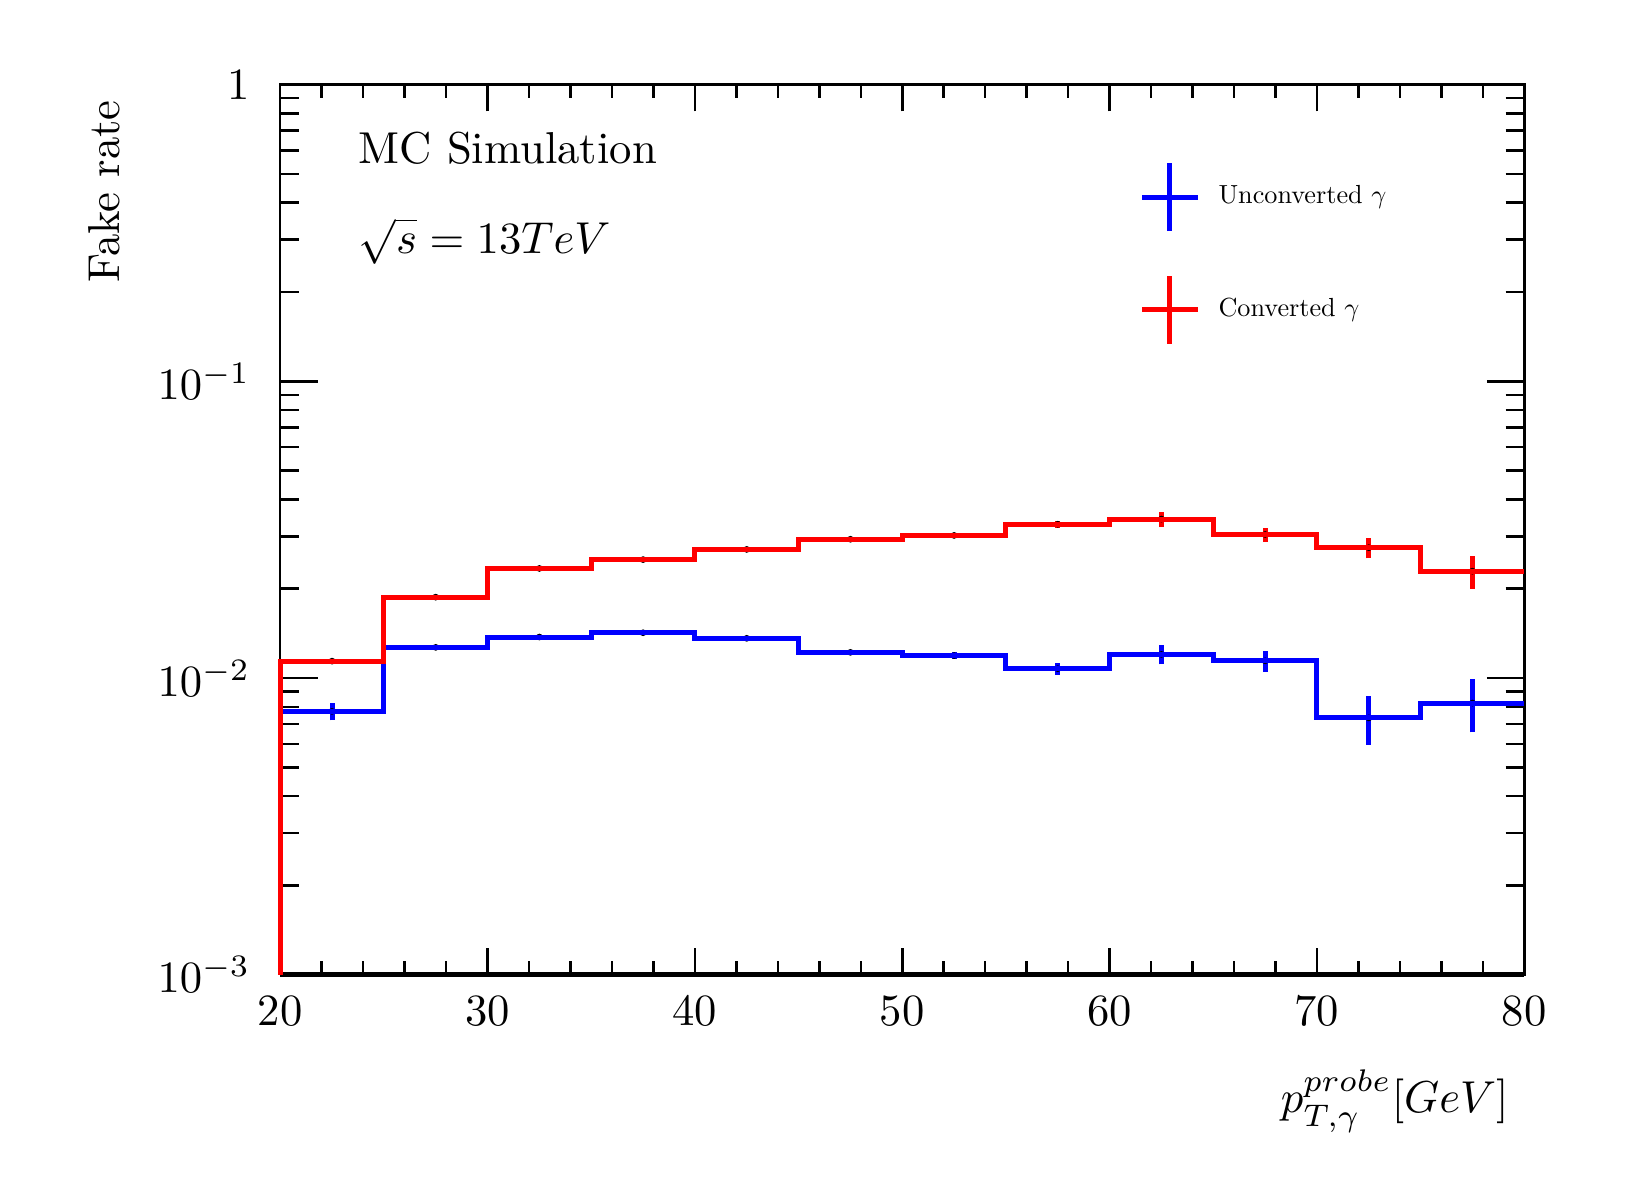
\begin{tikzpicture}
\pgfdeclareplotmark{cross} {
\pgfpathmoveto{\pgfpoint{-0.3\pgfplotmarksize}{\pgfplotmarksize}}
\pgfpathlineto{\pgfpoint{+0.3\pgfplotmarksize}{\pgfplotmarksize}}
\pgfpathlineto{\pgfpoint{+0.3\pgfplotmarksize}{0.3\pgfplotmarksize}}
\pgfpathlineto{\pgfpoint{+1\pgfplotmarksize}{0.3\pgfplotmarksize}}
\pgfpathlineto{\pgfpoint{+1\pgfplotmarksize}{-0.3\pgfplotmarksize}}
\pgfpathlineto{\pgfpoint{+0.3\pgfplotmarksize}{-0.3\pgfplotmarksize}}
\pgfpathlineto{\pgfpoint{+0.3\pgfplotmarksize}{-1.\pgfplotmarksize}}
\pgfpathlineto{\pgfpoint{-0.3\pgfplotmarksize}{-1.\pgfplotmarksize}}
\pgfpathlineto{\pgfpoint{-0.3\pgfplotmarksize}{-0.3\pgfplotmarksize}}
\pgfpathlineto{\pgfpoint{-1.\pgfplotmarksize}{-0.3\pgfplotmarksize}}
\pgfpathlineto{\pgfpoint{-1.\pgfplotmarksize}{0.3\pgfplotmarksize}}
\pgfpathlineto{\pgfpoint{-0.3\pgfplotmarksize}{0.3\pgfplotmarksize}}
\pgfpathclose
\pgfusepathqstroke
}
\pgfdeclareplotmark{cross*} {
\pgfpathmoveto{\pgfpoint{-0.3\pgfplotmarksize}{\pgfplotmarksize}}
\pgfpathlineto{\pgfpoint{+0.3\pgfplotmarksize}{\pgfplotmarksize}}
\pgfpathlineto{\pgfpoint{+0.3\pgfplotmarksize}{0.3\pgfplotmarksize}}
\pgfpathlineto{\pgfpoint{+1\pgfplotmarksize}{0.3\pgfplotmarksize}}
\pgfpathlineto{\pgfpoint{+1\pgfplotmarksize}{-0.3\pgfplotmarksize}}
\pgfpathlineto{\pgfpoint{+0.3\pgfplotmarksize}{-0.3\pgfplotmarksize}}
\pgfpathlineto{\pgfpoint{+0.3\pgfplotmarksize}{-1.\pgfplotmarksize}}
\pgfpathlineto{\pgfpoint{-0.3\pgfplotmarksize}{-1.\pgfplotmarksize}}
\pgfpathlineto{\pgfpoint{-0.3\pgfplotmarksize}{-0.3\pgfplotmarksize}}
\pgfpathlineto{\pgfpoint{-1.\pgfplotmarksize}{-0.3\pgfplotmarksize}}
\pgfpathlineto{\pgfpoint{-1.\pgfplotmarksize}{0.3\pgfplotmarksize}}
\pgfpathlineto{\pgfpoint{-0.3\pgfplotmarksize}{0.3\pgfplotmarksize}}
\pgfpathclose
\pgfusepathqfillstroke
}
\pgfdeclareplotmark{newstar} {
\pgfpathmoveto{\pgfqpoint{0pt}{\pgfplotmarksize}}
\pgfpathlineto{\pgfqpointpolar{44}{0.5\pgfplotmarksize}}
\pgfpathlineto{\pgfqpointpolar{18}{\pgfplotmarksize}}
\pgfpathlineto{\pgfqpointpolar{-20}{0.5\pgfplotmarksize}}
\pgfpathlineto{\pgfqpointpolar{-54}{\pgfplotmarksize}}
\pgfpathlineto{\pgfqpointpolar{-90}{0.5\pgfplotmarksize}}
\pgfpathlineto{\pgfqpointpolar{234}{\pgfplotmarksize}}
\pgfpathlineto{\pgfqpointpolar{198}{0.5\pgfplotmarksize}}
\pgfpathlineto{\pgfqpointpolar{162}{\pgfplotmarksize}}
\pgfpathlineto{\pgfqpointpolar{134}{0.5\pgfplotmarksize}}
\pgfpathclose
\pgfusepathqstroke
}
\pgfdeclareplotmark{newstar*} {
\pgfpathmoveto{\pgfqpoint{0pt}{\pgfplotmarksize}}
\pgfpathlineto{\pgfqpointpolar{44}{0.5\pgfplotmarksize}}
\pgfpathlineto{\pgfqpointpolar{18}{\pgfplotmarksize}}
\pgfpathlineto{\pgfqpointpolar{-20}{0.5\pgfplotmarksize}}
\pgfpathlineto{\pgfqpointpolar{-54}{\pgfplotmarksize}}
\pgfpathlineto{\pgfqpointpolar{-90}{0.5\pgfplotmarksize}}
\pgfpathlineto{\pgfqpointpolar{234}{\pgfplotmarksize}}
\pgfpathlineto{\pgfqpointpolar{198}{0.5\pgfplotmarksize}}
\pgfpathlineto{\pgfqpointpolar{162}{\pgfplotmarksize}}
\pgfpathlineto{\pgfqpointpolar{134}{0.5\pgfplotmarksize}}
\pgfpathclose
\pgfusepathqfillstroke
}
\definecolor{c}{rgb}{1,1,1};
\draw [color=c, fill=c] (0,0) rectangle (20,14.3108);
\draw [color=c, fill=c] (3.2,2.28972) rectangle (19,13.5952);
\definecolor{c}{rgb}{0,0,0};
\draw [c,line width=0.9] (3.2,2.28972) -- (3.2,13.5952) -- (19,13.5952) -- (19,2.28972) -- (3.2,2.28972);
\draw [c,line width=1.8] (3.2,2.28972) -- (3.2158,2.28972) -- (3.2158,2.28972) -- (3.2316,2.28972) -- (3.2316,2.28972) -- (3.2474,2.28972) -- (3.2474,2.28972) -- (3.2632,2.28972) -- (3.2632,2.28972) -- (3.279,2.28972) -- (3.279,2.28972) --
 (3.2948,2.28972) -- (3.2948,2.28972) -- (3.3106,2.28972) -- (3.3106,2.28972) -- (3.3264,2.28972) -- (3.3264,2.28972) -- (3.3422,2.28972) -- (3.3422,2.28972) -- (3.358,2.28972) -- (3.358,2.28972) -- (3.3738,2.28972) -- (3.3738,2.28972) --
 (3.3896,2.28972) -- (3.3896,2.28972) -- (3.4054,2.28972) -- (3.4054,2.28972) -- (3.4212,2.28972) -- (3.4212,2.28972) -- (3.437,2.28972) -- (3.437,2.28972) -- (3.4528,2.28972) -- (3.4528,2.28972) -- (3.4686,2.28972) -- (3.4686,2.28972) --
 (3.4844,2.28972) -- (3.4844,2.28972) -- (3.5002,2.28972) -- (3.5002,2.28972) -- (3.516,2.28972) -- (3.516,2.28972) -- (3.5318,2.28972) -- (3.5318,2.28972) -- (3.5476,2.28972) -- (3.5476,2.28972) -- (3.5634,2.28972) -- (3.5634,2.28972) --
 (3.5792,2.28972) -- (3.5792,2.28972) -- (3.595,2.28972) -- (3.595,2.28972) -- (3.6108,2.28972) -- (3.6108,2.28972) -- (3.6266,2.28972) -- (3.6266,2.28972) -- (3.6424,2.28972) -- (3.6424,2.28972) -- (3.6582,2.28972) -- (3.6582,2.28972) --
 (3.674,2.28972) -- (3.674,2.28972) -- (3.6898,2.28972) -- (3.6898,2.28972) -- (3.7056,2.28972) -- (3.7056,2.28972) -- (3.7214,2.28972) -- (3.7214,2.28972) -- (3.7372,2.28972) -- (3.7372,2.28972) -- (3.753,2.28972) -- (3.753,2.28972) --
 (3.7688,2.28972) -- (3.7688,2.28972) -- (3.7846,2.28972) -- (3.7846,2.28972) -- (3.8004,2.28972) -- (3.8004,2.28972) -- (3.8162,2.28972) -- (3.8162,2.28972) -- (3.832,2.28972) -- (3.832,2.28972) -- (3.8478,2.28972) -- (3.8478,2.28972) --
 (3.8636,2.28972) -- (3.8636,2.28972) -- (3.8794,2.28972) -- (3.8794,2.28972) -- (3.8952,2.28972) -- (3.8952,2.28972) -- (3.911,2.28972) -- (3.911,2.28972) -- (3.9268,2.28972) -- (3.9268,2.28972) -- (3.9426,2.28972) -- (3.9426,2.28972) --
 (3.9584,2.28972) -- (3.9584,2.28972) -- (3.9742,2.28972) -- (3.9742,2.28972) -- (3.99,2.28972) -- (3.99,2.28972) -- (4.0058,2.28972) -- (4.0058,2.28972) -- (4.0216,2.28972) -- (4.0216,2.28972) -- (4.0374,2.28972) -- (4.0374,2.28972) --
 (4.0532,2.28972) -- (4.0532,2.28972) -- (4.069,2.28972) -- (4.069,2.28972) -- (4.0848,2.28972) -- (4.0848,2.28972) -- (4.1006,2.28972) -- (4.1006,2.28972) -- (4.1164,2.28972) -- (4.1164,2.28972) -- (4.1322,2.28972) -- (4.1322,2.28972) --
 (4.148,2.28972) -- (4.148,2.28972) -- (4.1638,2.28972) -- (4.1638,2.28972) -- (4.1796,2.28972) -- (4.1796,2.28972) -- (4.1954,2.28972) -- (4.1954,2.28972) -- (4.2112,2.28972) -- (4.2112,2.28972) -- (4.227,2.28972) -- (4.227,2.28972) --
 (4.2428,2.28972) -- (4.2428,2.28972) -- (4.2586,2.28972) -- (4.2586,2.28972) -- (4.2744,2.28972) -- (4.2744,2.28972) -- (4.2902,2.28972) -- (4.2902,2.28972) -- (4.306,2.28972) -- (4.306,2.28972) -- (4.3218,2.28972) -- (4.3218,2.28972) --
 (4.3376,2.28972) -- (4.3376,2.28972) -- (4.3534,2.28972) -- (4.3534,2.28972) -- (4.3692,2.28972) -- (4.3692,2.28972) -- (4.385,2.28972) -- (4.385,2.28972) -- (4.4008,2.28972) -- (4.4008,2.28972) -- (4.4166,2.28972) -- (4.4166,2.28972) --
 (4.4324,2.28972) -- (4.4324,2.28972) -- (4.4482,2.28972) -- (4.4482,2.28972) -- (4.464,2.28972) -- (4.464,2.28972) -- (4.4798,2.28972) -- (4.4798,2.28972) -- (4.4956,2.28972) -- (4.4956,2.28972) -- (4.5114,2.28972) -- (4.5114,2.28972) --
 (4.5272,2.28972) -- (4.5272,2.28972) -- (4.543,2.28972) -- (4.543,2.28972) -- (4.5588,2.28972) -- (4.5588,2.28972) -- (4.5746,2.28972) -- (4.5746,2.28972) -- (4.5904,2.28972) -- (4.5904,2.28972) -- (4.6062,2.28972) -- (4.6062,2.28972) --
 (4.622,2.28972) -- (4.622,2.28972) -- (4.6378,2.28972) -- (4.6378,2.28972) -- (4.6536,2.28972) -- (4.6536,2.28972) -- (4.6694,2.28972) -- (4.6694,2.28972) -- (4.6852,2.28972) -- (4.6852,2.28972) -- (4.701,2.28972) -- (4.701,2.28972) --
 (4.7168,2.28972) -- (4.7168,2.28972) -- (4.7326,2.28972) -- (4.7326,2.28972) -- (4.7484,2.28972) -- (4.7484,2.28972) -- (4.7642,2.28972) -- (4.7642,2.28972) -- (4.78,2.28972) -- (4.78,2.28972) -- (4.7958,2.28972) -- (4.7958,2.28972) --
 (4.8116,2.28972) -- (4.8116,2.28972) -- (4.8274,2.28972) -- (4.8274,2.28972) -- (4.8432,2.28972) -- (4.8432,2.28972) -- (4.859,2.28972) -- (4.859,2.28972) -- (4.8748,2.28972) -- (4.8748,2.28972) -- (4.8906,2.28972) -- (4.8906,2.28972) --
 (4.9064,2.28972) -- (4.9064,2.28972) -- (4.9222,2.28972) -- (4.9222,2.28972) -- (4.938,2.28972) -- (4.938,2.28972) -- (4.9538,2.28972) -- (4.9538,2.28972) -- (4.9696,2.28972) -- (4.9696,2.28972) -- (4.9854,2.28972) -- (4.9854,2.28972) --
 (5.0012,2.28972) -- (5.0012,2.28972) -- (5.017,2.28972) -- (5.017,2.28972) -- (5.0328,2.28972) -- (5.0328,2.28972) -- (5.0486,2.28972) -- (5.0486,2.28972) -- (5.0644,2.28972) -- (5.0644,2.28972) -- (5.0802,2.28972) -- (5.0802,2.28972) --
 (5.096,2.28972) -- (5.096,2.28972) -- (5.1118,2.28972) -- (5.1118,2.28972) -- (5.1276,2.28972) -- (5.1276,2.28972) -- (5.1434,2.28972) -- (5.1434,2.28972) -- (5.1592,2.28972) -- (5.1592,2.28972) -- (5.175,2.28972) -- (5.175,2.28972) --
 (5.1908,2.28972) -- (5.1908,2.28972) -- (5.2066,2.28972) -- (5.2066,2.28972) -- (5.2224,2.28972) -- (5.2224,2.28972) -- (5.2382,2.28972) -- (5.2382,2.28972) -- (5.254,2.28972) -- (5.254,2.28972) -- (5.2698,2.28972) -- (5.2698,2.28972) --
 (5.2856,2.28972) -- (5.2856,2.28972) -- (5.3014,2.28972) -- (5.3014,2.28972) -- (5.3172,2.28972) -- (5.3172,2.28972) -- (5.333,2.28972) -- (5.333,2.28972) -- (5.3488,2.28972) -- (5.3488,2.28972) -- (5.3646,2.28972) -- (5.3646,2.28972) --
 (5.3804,2.28972) -- (5.3804,2.28972) -- (5.3962,2.28972) -- (5.3962,2.28972) -- (5.412,2.28972) -- (5.412,2.28972) -- (5.4278,2.28972) -- (5.4278,2.28972) -- (5.4436,2.28972) -- (5.4436,2.28972) -- (5.4594,2.28972) -- (5.4594,2.28972) --
 (5.4752,2.28972) -- (5.4752,2.28972) -- (5.491,2.28972) -- (5.491,2.28972) -- (5.5068,2.28972) -- (5.5068,2.28972) -- (5.5226,2.28972) -- (5.5226,2.28972) -- (5.5384,2.28972) -- (5.5384,2.28972) -- (5.5542,2.28972) -- (5.5542,2.28972) --
 (5.57,2.28972) -- (5.57,2.28972) -- (5.5858,2.28972) -- (5.5858,2.28972) -- (5.6016,2.28972) -- (5.6016,2.28972) -- (5.6174,2.28972) -- (5.6174,2.28972) -- (5.6332,2.28972) -- (5.6332,2.28972) -- (5.649,2.28972) -- (5.649,2.28972) --
 (5.6648,2.28972) -- (5.6648,2.28972) -- (5.6806,2.28972) -- (5.6806,2.28972) -- (5.6964,2.28972) -- (5.6964,2.28972) -- (5.7122,2.28972) -- (5.7122,2.28972) -- (5.728,2.28972) -- (5.728,2.28972) -- (5.7438,2.28972) -- (5.7438,2.28972) --
 (5.7596,2.28972) -- (5.7596,2.28972) -- (5.7754,2.28972) -- (5.7754,2.28972) -- (5.7912,2.28972) -- (5.7912,2.28972) -- (5.807,2.28972) -- (5.807,2.28972) -- (5.8228,2.28972) -- (5.8228,2.28972) -- (5.8386,2.28972) -- (5.8386,2.28972) --
 (5.8544,2.28972) -- (5.8544,2.28972) -- (5.8702,2.28972) -- (5.8702,2.28972) -- (5.886,2.28972) -- (5.886,2.28972) -- (5.9018,2.28972) -- (5.9018,2.28972) -- (5.9176,2.28972) -- (5.9176,2.28972) -- (5.9334,2.28972) -- (5.9334,2.28972) --
 (5.9492,2.28972) -- (5.9492,2.28972) -- (5.965,2.28972) -- (5.965,2.28972) -- (5.9808,2.28972) -- (5.9808,2.28972) -- (5.9966,2.28972) -- (5.9966,2.28972) -- (6.0124,2.28972) -- (6.0124,2.28972) -- (6.0282,2.28972) -- (6.0282,2.28972) --
 (6.044,2.28972) -- (6.044,2.28972) -- (6.0598,2.28972) -- (6.0598,2.28972) -- (6.0756,2.28972) -- (6.0756,2.28972) -- (6.0914,2.28972) -- (6.0914,2.28972) -- (6.1072,2.28972) -- (6.1072,2.28972) -- (6.123,2.28972) -- (6.123,2.28972) --
 (6.1388,2.28972) -- (6.1388,2.28972) -- (6.1546,2.28972) -- (6.1546,2.28972) -- (6.1704,2.28972) -- (6.1704,2.28972) -- (6.1862,2.28972) -- (6.1862,2.28972) -- (6.202,2.28972) -- (6.202,2.28972) -- (6.2178,2.28972) -- (6.2178,2.28972) --
 (6.2336,2.28972) -- (6.2336,2.28972) -- (6.2494,2.28972) -- (6.2494,2.28972) -- (6.2652,2.28972) -- (6.2652,2.28972) -- (6.281,2.28972) -- (6.281,2.28972) -- (6.2968,2.28972) -- (6.2968,2.28972) -- (6.3126,2.28972) -- (6.3126,2.28972) --
 (6.3284,2.28972) -- (6.3284,2.28972) -- (6.3442,2.28972) -- (6.3442,2.28972) -- (6.36,2.28972) -- (6.36,2.28972) -- (6.3758,2.28972) -- (6.3758,2.28972) -- (6.3916,2.28972) -- (6.3916,2.28972) -- (6.4074,2.28972) -- (6.4074,2.28972) --
 (6.4232,2.28972) -- (6.4232,2.28972) -- (6.439,2.28972) -- (6.439,2.28972) -- (6.4548,2.28972) -- (6.4548,2.28972) -- (6.4706,2.28972) -- (6.4706,2.28972) -- (6.4864,2.28972) -- (6.4864,2.28972) -- (6.5022,2.28972) -- (6.5022,2.28972) --
 (6.518,2.28972) -- (6.518,2.28972) -- (6.5338,2.28972) -- (6.5338,2.28972) -- (6.5496,2.28972) -- (6.5496,2.28972) -- (6.5654,2.28972) -- (6.5654,2.28972) -- (6.5812,2.28972) -- (6.5812,2.28972) -- (6.597,2.28972) -- (6.597,2.28972) --
 (6.6128,2.28972) -- (6.6128,2.28972) -- (6.6286,2.28972) -- (6.6286,2.28972) -- (6.6444,2.28972) -- (6.6444,2.28972) -- (6.6602,2.28972) -- (6.6602,2.28972) -- (6.676,2.28972) -- (6.676,2.28972) -- (6.6918,2.28972) -- (6.6918,2.28972) --
 (6.7076,2.28972) -- (6.7076,2.28972) -- (6.7234,2.28972) -- (6.7234,2.28972) -- (6.7392,2.28972) -- (6.7392,2.28972) -- (6.755,2.28972) -- (6.755,2.28972) -- (6.7708,2.28972) -- (6.7708,2.28972) -- (6.7866,2.28972) -- (6.7866,2.28972) --
 (6.8024,2.28972) -- (6.8024,2.28972) -- (6.8182,2.28972) -- (6.8182,2.28972) -- (6.834,2.28972) -- (6.834,2.28972) -- (6.8498,2.28972) -- (6.8498,2.28972) -- (6.8656,2.28972) -- (6.8656,2.28972) -- (6.8814,2.28972) -- (6.8814,2.28972) --
 (6.8972,2.28972) -- (6.8972,2.28972) -- (6.913,2.28972) -- (6.913,2.28972) -- (6.9288,2.28972) -- (6.9288,2.28972) -- (6.9446,2.28972) -- (6.9446,2.28972) -- (6.9604,2.28972) -- (6.9604,2.28972) -- (6.9762,2.28972) -- (6.9762,2.28972) --
 (6.992,2.28972) -- (6.992,2.28972) -- (7.0078,2.28972) -- (7.0078,2.28972) -- (7.0236,2.28972) -- (7.0236,2.28972) -- (7.0394,2.28972) -- (7.0394,2.28972) -- (7.0552,2.28972) -- (7.0552,2.28972) -- (7.071,2.28972) -- (7.071,2.28972) --
 (7.0868,2.28972) -- (7.0868,2.28972) -- (7.1026,2.28972) -- (7.1026,2.28972) -- (7.1184,2.28972) -- (7.1184,2.28972) -- (7.1342,2.28972) -- (7.1342,2.28972) -- (7.15,2.28972) -- (7.15,2.28972) -- (7.1658,2.28972) -- (7.1658,2.28972) --
 (7.1816,2.28972) -- (7.1816,2.28972) -- (7.1974,2.28972) -- (7.1974,2.28972) -- (7.2132,2.28972) -- (7.2132,2.28972) -- (7.229,2.28972) -- (7.229,2.28972) -- (7.2448,2.28972) -- (7.2448,2.28972) -- (7.2606,2.28972) -- (7.2606,2.28972) --
 (7.2764,2.28972) -- (7.2764,2.28972) -- (7.2922,2.28972) -- (7.2922,2.28972) -- (7.308,2.28972) -- (7.308,2.28972) -- (7.3238,2.28972) -- (7.3238,2.28972) -- (7.3396,2.28972) -- (7.3396,2.28972) -- (7.3554,2.28972) -- (7.3554,2.28972) --
 (7.3712,2.28972) -- (7.3712,2.28972) -- (7.387,2.28972) -- (7.387,2.28972) -- (7.4028,2.28972) -- (7.4028,2.28972) -- (7.4186,2.28972) -- (7.4186,2.28972) -- (7.4344,2.28972) -- (7.4344,2.28972) -- (7.4502,2.28972) -- (7.4502,2.28972) --
 (7.466,2.28972) -- (7.466,2.28972) -- (7.4818,2.28972) -- (7.4818,2.28972) -- (7.4976,2.28972) -- (7.4976,2.28972) -- (7.5134,2.28972) -- (7.5134,2.28972) -- (7.5292,2.28972) -- (7.5292,2.28972) -- (7.545,2.28972) -- (7.545,2.28972) --
 (7.5608,2.28972) -- (7.5608,2.28972) -- (7.5766,2.28972) -- (7.5766,2.28972) -- (7.5924,2.28972) -- (7.5924,2.28972) -- (7.6082,2.28972) -- (7.6082,2.28972) -- (7.624,2.28972) -- (7.624,2.28972) -- (7.6398,2.28972) -- (7.6398,2.28972) --
 (7.6556,2.28972) -- (7.6556,2.28972) -- (7.6714,2.28972) -- (7.6714,2.28972) -- (7.6872,2.28972) -- (7.6872,2.28972) -- (7.703,2.28972) -- (7.703,2.28972) -- (7.7188,2.28972) -- (7.7188,2.28972) -- (7.7346,2.28972) -- (7.7346,2.28972) --
 (7.7504,2.28972) -- (7.7504,2.28972) -- (7.7662,2.28972) -- (7.7662,2.28972) -- (7.782,2.28972) -- (7.782,2.28972) -- (7.7978,2.28972) -- (7.7978,2.28972) -- (7.8136,2.28972) -- (7.8136,2.28972) -- (7.8294,2.28972) -- (7.8294,2.28972) --
 (7.8452,2.28972) -- (7.8452,2.28972) -- (7.861,2.28972) -- (7.861,2.28972) -- (7.8768,2.28972) -- (7.8768,2.28972) -- (7.8926,2.28972) -- (7.8926,2.28972) -- (7.9084,2.28972) -- (7.9084,2.28972) -- (7.9242,2.28972) -- (7.9242,2.28972) --
 (7.94,2.28972) -- (7.94,2.28972) -- (7.9558,2.28972) -- (7.9558,2.28972) -- (7.9716,2.28972) -- (7.9716,2.28972) -- (7.9874,2.28972) -- (7.9874,2.28972) -- (8.0032,2.28972) -- (8.0032,2.28972) -- (8.019,2.28972) -- (8.019,2.28972) --
 (8.0348,2.28972) -- (8.0348,2.28972) -- (8.0506,2.28972) -- (8.0506,2.28972) -- (8.0664,2.28972) -- (8.0664,2.28972) -- (8.0822,2.28972) -- (8.0822,2.28972) -- (8.098,2.28972) -- (8.098,2.28972) -- (8.1138,2.28972) -- (8.1138,2.28972) --
 (8.1296,2.28972) -- (8.1296,2.28972) -- (8.1454,2.28972) -- (8.1454,2.28972) -- (8.1612,2.28972) -- (8.1612,2.28972) -- (8.177,2.28972) -- (8.177,2.28972) -- (8.1928,2.28972) -- (8.1928,2.28972) -- (8.2086,2.28972) -- (8.2086,2.28972) --
 (8.2244,2.28972) -- (8.2244,2.28972) -- (8.2402,2.28972) -- (8.2402,2.28972) -- (8.256,2.28972) -- (8.256,2.28972) -- (8.2718,2.28972) -- (8.2718,2.28972) -- (8.2876,2.28972) -- (8.2876,2.28972) -- (8.3034,2.28972) -- (8.3034,2.28972) --
 (8.3192,2.28972) -- (8.3192,2.28972) -- (8.335,2.28972) -- (8.335,2.28972) -- (8.3508,2.28972) -- (8.3508,2.28972) -- (8.3666,2.28972) -- (8.3666,2.28972) -- (8.3824,2.28972) -- (8.3824,2.28972) -- (8.3982,2.28972) -- (8.3982,2.28972) --
 (8.414,2.28972) -- (8.414,2.28972) -- (8.4298,2.28972) -- (8.4298,2.28972) -- (8.4456,2.28972) -- (8.4456,2.28972) -- (8.4614,2.28972) -- (8.4614,2.28972) -- (8.4772,2.28972) -- (8.4772,2.28972) -- (8.493,2.28972) -- (8.493,2.28972) --
 (8.5088,2.28972) -- (8.5088,2.28972) -- (8.5246,2.28972) -- (8.5246,2.28972) -- (8.5404,2.28972) -- (8.5404,2.28972) -- (8.5562,2.28972) -- (8.5562,2.28972) -- (8.572,2.28972) -- (8.572,2.28972) -- (8.5878,2.28972) -- (8.5878,2.28972) --
 (8.6036,2.28972) -- (8.6036,2.28972) -- (8.6194,2.28972) -- (8.6194,2.28972) -- (8.6352,2.28972) -- (8.6352,2.28972) -- (8.651,2.28972) -- (8.651,2.28972) -- (8.6668,2.28972) -- (8.6668,2.28972) -- (8.6826,2.28972) -- (8.6826,2.28972) --
 (8.6984,2.28972) -- (8.6984,2.28972) -- (8.7142,2.28972) -- (8.7142,2.28972) -- (8.73,2.28972) -- (8.73,2.28972) -- (8.7458,2.28972) -- (8.7458,2.28972) -- (8.7616,2.28972) -- (8.7616,2.28972) -- (8.7774,2.28972) -- (8.7774,2.28972) --
 (8.7932,2.28972) -- (8.7932,2.28972) -- (8.809,2.28972) -- (8.809,2.28972) -- (8.8248,2.28972) -- (8.8248,2.28972) -- (8.8406,2.28972) -- (8.8406,2.28972) -- (8.8564,2.28972) -- (8.8564,2.28972) -- (8.8722,2.28972) -- (8.8722,2.28972) --
 (8.888,2.28972) -- (8.888,2.28972) -- (8.9038,2.28972) -- (8.9038,2.28972) -- (8.9196,2.28972) -- (8.9196,2.28972) -- (8.9354,2.28972) -- (8.9354,2.28972) -- (8.9512,2.28972) -- (8.9512,2.28972) -- (8.967,2.28972) -- (8.967,2.28972) --
 (8.9828,2.28972) -- (8.9828,2.28972) -- (8.9986,2.28972) -- (8.9986,2.28972) -- (9.0144,2.28972) -- (9.0144,2.28972) -- (9.0302,2.28972) -- (9.0302,2.28972) -- (9.046,2.28972) -- (9.046,2.28972) -- (9.0618,2.28972) -- (9.0618,2.28972) --
 (9.0776,2.28972) -- (9.0776,2.28972) -- (9.0934,2.28972) -- (9.0934,2.28972) -- (9.1092,2.28972) -- (9.1092,2.28972) -- (9.125,2.28972) -- (9.125,2.28972) -- (9.1408,2.28972) -- (9.1408,2.28972) -- (9.1566,2.28972) -- (9.1566,2.28972) --
 (9.1724,2.28972) -- (9.1724,2.28972) -- (9.1882,2.28972) -- (9.1882,2.28972) -- (9.204,2.28972) -- (9.204,2.28972) -- (9.2198,2.28972) -- (9.2198,2.28972) -- (9.2356,2.28972) -- (9.2356,2.28972) -- (9.2514,2.28972) -- (9.2514,2.28972) --
 (9.2672,2.28972) -- (9.2672,2.28972) -- (9.283,2.28972) -- (9.283,2.28972) -- (9.2988,2.28972) -- (9.2988,2.28972) -- (9.3146,2.28972) -- (9.3146,2.28972) -- (9.3304,2.28972) -- (9.3304,2.28972) -- (9.3462,2.28972) -- (9.3462,2.28972) --
 (9.362,2.28972) -- (9.362,2.28972) -- (9.3778,2.28972) -- (9.3778,2.28972) -- (9.3936,2.28972) -- (9.3936,2.28972) -- (9.4094,2.28972) -- (9.4094,2.28972) -- (9.4252,2.28972) -- (9.4252,2.28972) -- (9.441,2.28972) -- (9.441,2.28972) --
 (9.4568,2.28972) -- (9.4568,2.28972) -- (9.4726,2.28972) -- (9.4726,2.28972) -- (9.4884,2.28972) -- (9.4884,2.28972) -- (9.5042,2.28972) -- (9.5042,2.28972) -- (9.52,2.28972) -- (9.52,2.28972) -- (9.5358,2.28972) -- (9.5358,2.28972) --
 (9.5516,2.28972) -- (9.5516,2.28972) -- (9.5674,2.28972) -- (9.5674,2.28972) -- (9.5832,2.28972) -- (9.5832,2.28972) -- (9.599,2.28972) -- (9.599,2.28972) -- (9.6148,2.28972) -- (9.6148,2.28972) -- (9.6306,2.28972) -- (9.6306,2.28972) --
 (9.6464,2.28972) -- (9.6464,2.28972) -- (9.6622,2.28972) -- (9.6622,2.28972) -- (9.678,2.28972) -- (9.678,2.28972) -- (9.6938,2.28972) -- (9.6938,2.28972) -- (9.7096,2.28972) -- (9.7096,2.28972) -- (9.7254,2.28972) -- (9.7254,2.28972) --
 (9.7412,2.28972) -- (9.7412,2.28972) -- (9.757,2.28972) -- (9.757,2.28972) -- (9.7728,2.28972) -- (9.7728,2.28972) -- (9.7886,2.28972) -- (9.7886,2.28972) -- (9.8044,2.28972) -- (9.8044,2.28972) -- (9.8202,2.28972) -- (9.8202,2.28972) --
 (9.836,2.28972) -- (9.836,2.28972) -- (9.8518,2.28972) -- (9.8518,2.28972) -- (9.8676,2.28972) -- (9.8676,2.28972) -- (9.8834,2.28972) -- (9.8834,2.28972) -- (9.8992,2.28972) -- (9.8992,2.28972) -- (9.915,2.28972) -- (9.915,2.28972) --
 (9.9308,2.28972) -- (9.9308,2.28972) -- (9.9466,2.28972) -- (9.9466,2.28972) -- (9.9624,2.28972) -- (9.9624,2.28972) -- (9.9782,2.28972) -- (9.9782,2.28972) -- (9.994,2.28972) -- (9.994,2.28972) -- (10.0098,2.28972) -- (10.0098,2.28972) --
 (10.0256,2.28972) -- (10.0256,2.28972) -- (10.0414,2.28972) -- (10.0414,2.28972) -- (10.0572,2.28972) -- (10.0572,2.28972) -- (10.073,2.28972) -- (10.073,2.28972) -- (10.0888,2.28972) -- (10.0888,2.28972) -- (10.1046,2.28972) -- (10.1046,2.28972) --
 (10.1204,2.28972) -- (10.1204,2.28972) -- (10.1362,2.28972) -- (10.1362,2.28972) -- (10.152,2.28972) -- (10.152,2.28972) -- (10.1678,2.28972) -- (10.1678,2.28972) -- (10.1836,2.28972) -- (10.1836,2.28972) -- (10.1994,2.28972) -- (10.1994,2.28972) --
 (10.2152,2.28972) -- (10.2152,2.28972) -- (10.231,2.28972) -- (10.231,2.28972) -- (10.2468,2.28972) -- (10.2468,2.28972) -- (10.2626,2.28972) -- (10.2626,2.28972) -- (10.2784,2.28972) -- (10.2784,2.28972) -- (10.2942,2.28972) -- (10.2942,2.28972) --
 (10.31,2.28972) -- (10.31,2.28972) -- (10.3258,2.28972) -- (10.3258,2.28972) -- (10.3416,2.28972) -- (10.3416,2.28972) -- (10.3574,2.28972) -- (10.3574,2.28972) -- (10.3732,2.28972) -- (10.3732,2.28972) -- (10.389,2.28972) -- (10.389,2.28972) --
 (10.4048,2.28972) -- (10.4048,2.28972) -- (10.4206,2.28972) -- (10.4206,2.28972) -- (10.4364,2.28972) -- (10.4364,2.28972) -- (10.4522,2.28972) -- (10.4522,2.28972) -- (10.468,2.28972) -- (10.468,2.28972) -- (10.4838,2.28972) -- (10.4838,2.28972) --
 (10.4996,2.28972) -- (10.4996,2.28972) -- (10.5154,2.28972) -- (10.5154,2.28972) -- (10.5312,2.28972) -- (10.5312,2.28972) -- (10.547,2.28972) -- (10.547,2.28972) -- (10.5628,2.28972) -- (10.5628,2.28972) -- (10.5786,2.28972) -- (10.5786,2.28972) --
 (10.5944,2.28972) -- (10.5944,2.28972) -- (10.6102,2.28972) -- (10.6102,2.28972) -- (10.626,2.28972) -- (10.626,2.28972) -- (10.6418,2.28972) -- (10.6418,2.28972) -- (10.6576,2.28972) -- (10.6576,2.28972) -- (10.6734,2.28972) -- (10.6734,2.28972) --
 (10.6892,2.28972) -- (10.6892,2.28972) -- (10.705,2.28972) -- (10.705,2.28972) -- (10.7208,2.28972) -- (10.7208,2.28972) -- (10.7366,2.28972) -- (10.7366,2.28972) -- (10.7524,2.28972) -- (10.7524,2.28972) -- (10.7682,2.28972) -- (10.7682,2.28972) --
 (10.784,2.28972) -- (10.784,2.28972) -- (10.7998,2.28972) -- (10.7998,2.28972) -- (10.8156,2.28972) -- (10.8156,2.28972) -- (10.8314,2.28972) -- (10.8314,2.28972) -- (10.8472,2.28972) -- (10.8472,2.28972) -- (10.863,2.28972) -- (10.863,2.28972) --
 (10.8788,2.28972) -- (10.8788,2.28972) -- (10.8946,2.28972) -- (10.8946,2.28972) -- (10.9104,2.28972) -- (10.9104,2.28972) -- (10.9262,2.28972) -- (10.9262,2.28972) -- (10.942,2.28972) -- (10.942,2.28972) -- (10.9578,2.28972) -- (10.9578,2.28972) --
 (10.9736,2.28972) -- (10.9736,2.28972) -- (10.9894,2.28972) -- (10.9894,2.28972) -- (11.0052,2.28972) -- (11.0052,2.28972) -- (11.021,2.28972) -- (11.021,2.28972) -- (11.0368,2.28972) -- (11.0368,2.28972) -- (11.0526,2.28972) -- (11.0526,2.28972) --
 (11.0684,2.28972) -- (11.0684,2.28972) -- (11.0842,2.28972) -- (11.0842,2.28972) -- (11.1,2.28972) -- (11.1,2.28972) -- (11.1158,2.28972) -- (11.1158,2.28972) -- (11.1316,2.28972) -- (11.1316,2.28972) -- (11.1474,2.28972) -- (11.1474,2.28972) --
 (11.1632,2.28972) -- (11.1632,2.28972) -- (11.179,2.28972) -- (11.179,2.28972) -- (11.1948,2.28972) -- (11.1948,2.28972) -- (11.2106,2.28972) -- (11.2106,2.28972) -- (11.2264,2.28972) -- (11.2264,2.28972) -- (11.2422,2.28972) -- (11.2422,2.28972) --
 (11.258,2.28972) -- (11.258,2.28972) -- (11.2738,2.28972) -- (11.2738,2.28972) -- (11.2896,2.28972) -- (11.2896,2.28972) -- (11.3054,2.28972) -- (11.3054,2.28972) -- (11.3212,2.28972) -- (11.3212,2.28972) -- (11.337,2.28972) -- (11.337,2.28972) --
 (11.3528,2.28972) -- (11.3528,2.28972) -- (11.3686,2.28972) -- (11.3686,2.28972) -- (11.3844,2.28972) -- (11.3844,2.28972) -- (11.4002,2.28972) -- (11.4002,2.28972) -- (11.416,2.28972) -- (11.416,2.28972) -- (11.4318,2.28972) -- (11.4318,2.28972) --
 (11.4476,2.28972) -- (11.4476,2.28972) -- (11.4634,2.28972) -- (11.4634,2.28972) -- (11.4792,2.28972) -- (11.4792,2.28972) -- (11.495,2.28972) -- (11.495,2.28972) -- (11.5108,2.28972) -- (11.5108,2.28972) -- (11.5266,2.28972) -- (11.5266,2.28972) --
 (11.5424,2.28972) -- (11.5424,2.28972) -- (11.5582,2.28972) -- (11.5582,2.28972) -- (11.574,2.28972) -- (11.574,2.28972) -- (11.5898,2.28972) -- (11.5898,2.28972) -- (11.6056,2.28972) -- (11.6056,2.28972) -- (11.6214,2.28972) -- (11.6214,2.28972) --
 (11.6372,2.28972) -- (11.6372,2.28972) -- (11.653,2.28972) -- (11.653,2.28972) -- (11.6688,2.28972) -- (11.6688,2.28972) -- (11.6846,2.28972) -- (11.6846,2.28972) -- (11.7004,2.28972) -- (11.7004,2.28972) -- (11.7162,2.28972) -- (11.7162,2.28972) --
 (11.732,2.28972) -- (11.732,2.28972) -- (11.7478,2.28972) -- (11.7478,2.28972) -- (11.7636,2.28972) -- (11.7636,2.28972) -- (11.7794,2.28972) -- (11.7794,2.28972) -- (11.7952,2.28972) -- (11.7952,2.28972) -- (11.811,2.28972) -- (11.811,2.28972) --
 (11.8268,2.28972) -- (11.8268,2.28972) -- (11.8426,2.28972) -- (11.8426,2.28972) -- (11.8584,2.28972) -- (11.8584,2.28972) -- (11.8742,2.28972) -- (11.8742,2.28972) -- (11.89,2.28972) -- (11.89,2.28972) -- (11.9058,2.28972) -- (11.9058,2.28972) --
 (11.9216,2.28972) -- (11.9216,2.28972) -- (11.9374,2.28972) -- (11.9374,2.28972) -- (11.9532,2.28972) -- (11.9532,2.28972) -- (11.969,2.28972) -- (11.969,2.28972) -- (11.9848,2.28972) -- (11.9848,2.28972) -- (12.0006,2.28972) -- (12.0006,2.28972) --
 (12.0164,2.28972) -- (12.0164,2.28972) -- (12.0322,2.28972) -- (12.0322,2.28972) -- (12.048,2.28972) -- (12.048,2.28972) -- (12.0638,2.28972) -- (12.0638,2.28972) -- (12.0796,2.28972) -- (12.0796,2.28972) -- (12.0954,2.28972) -- (12.0954,2.28972) --
 (12.1112,2.28972) -- (12.1112,2.28972) -- (12.127,2.28972) -- (12.127,2.28972) -- (12.1428,2.28972) -- (12.1428,2.28972) -- (12.1586,2.28972) -- (12.1586,2.28972) -- (12.1744,2.28972) -- (12.1744,2.28972) -- (12.1902,2.28972) -- (12.1902,2.28972) --
 (12.206,2.28972) -- (12.206,2.28972) -- (12.2218,2.28972) -- (12.2218,2.28972) -- (12.2376,2.28972) -- (12.2376,2.28972) -- (12.2534,2.28972) -- (12.2534,2.28972) -- (12.2692,2.28972) -- (12.2692,2.28972) -- (12.285,2.28972) -- (12.285,2.28972) --
 (12.3008,2.28972) -- (12.3008,2.28972) -- (12.3166,2.28972) -- (12.3166,2.28972) -- (12.3324,2.28972) -- (12.3324,2.28972) -- (12.3482,2.28972) -- (12.3482,2.28972) -- (12.364,2.28972) -- (12.364,2.28972) -- (12.3798,2.28972) -- (12.3798,2.28972) --
 (12.3956,2.28972) -- (12.3956,2.28972) -- (12.4114,2.28972) -- (12.4114,2.28972) -- (12.4272,2.28972) -- (12.4272,2.28972) -- (12.443,2.28972) -- (12.443,2.28972) -- (12.4588,2.28972) -- (12.4588,2.28972) -- (12.4746,2.28972) -- (12.4746,2.28972) --
 (12.4904,2.28972) -- (12.4904,2.28972) -- (12.5062,2.28972) -- (12.5062,2.28972) -- (12.522,2.28972) -- (12.522,2.28972) -- (12.5378,2.28972) -- (12.5378,2.28972) -- (12.5536,2.28972) -- (12.5536,2.28972) -- (12.5694,2.28972) -- (12.5694,2.28972) --
 (12.5852,2.28972) -- (12.5852,2.28972) -- (12.601,2.28972) -- (12.601,2.28972) -- (12.6168,2.28972) -- (12.6168,2.28972) -- (12.6326,2.28972) -- (12.6326,2.28972) -- (12.6484,2.28972) -- (12.6484,2.28972) -- (12.6642,2.28972) -- (12.6642,2.28972) --
 (12.68,2.28972) -- (12.68,2.28972) -- (12.6958,2.28972) -- (12.6958,2.28972) -- (12.7116,2.28972) -- (12.7116,2.28972) -- (12.7274,2.28972) -- (12.7274,2.28972) -- (12.7432,2.28972) -- (12.7432,2.28972) -- (12.759,2.28972) -- (12.759,2.28972) --
 (12.7748,2.28972) -- (12.7748,2.28972) -- (12.7906,2.28972) -- (12.7906,2.28972) -- (12.8064,2.28972) -- (12.8064,2.28972) -- (12.8222,2.28972) -- (12.8222,2.28972) -- (12.838,2.28972) -- (12.838,2.28972) -- (12.8538,2.28972) -- (12.8538,2.28972) --
 (12.8696,2.28972) -- (12.8696,2.28972) -- (12.8854,2.28972) -- (12.8854,2.28972) -- (12.9012,2.28972) -- (12.9012,2.28972) -- (12.917,2.28972) -- (12.917,2.28972) -- (12.9328,2.28972) -- (12.9328,2.28972) -- (12.9486,2.28972) -- (12.9486,2.28972) --
 (12.9644,2.28972) -- (12.9644,2.28972) -- (12.9802,2.28972) -- (12.9802,2.28972) -- (12.996,2.28972) -- (12.996,2.28972) -- (13.0118,2.28972) -- (13.0118,2.28972) -- (13.0276,2.28972) -- (13.0276,2.28972) -- (13.0434,2.28972) -- (13.0434,2.28972) --
 (13.0592,2.28972) -- (13.0592,2.28972) -- (13.075,2.28972) -- (13.075,2.28972) -- (13.0908,2.28972) -- (13.0908,2.28972) -- (13.1066,2.28972) -- (13.1066,2.28972) -- (13.1224,2.28972) -- (13.1224,2.28972) -- (13.1382,2.28972) -- (13.1382,2.28972) --
 (13.154,2.28972) -- (13.154,2.28972) -- (13.1698,2.28972) -- (13.1698,2.28972) -- (13.1856,2.28972) -- (13.1856,2.28972) -- (13.2014,2.28972) -- (13.2014,2.28972) -- (13.2172,2.28972) -- (13.2172,2.28972) -- (13.233,2.28972) -- (13.233,2.28972) --
 (13.2488,2.28972) -- (13.2488,2.28972) -- (13.2646,2.28972) -- (13.2646,2.28972) -- (13.2804,2.28972) -- (13.2804,2.28972) -- (13.2962,2.28972) -- (13.2962,2.28972) -- (13.312,2.28972) -- (13.312,2.28972) -- (13.3278,2.28972) -- (13.3278,2.28972) --
 (13.3436,2.28972) -- (13.3436,2.28972) -- (13.3594,2.28972) -- (13.3594,2.28972) -- (13.3752,2.28972) -- (13.3752,2.28972) -- (13.391,2.28972) -- (13.391,2.28972) -- (13.4068,2.28972) -- (13.4068,2.28972) -- (13.4226,2.28972) -- (13.4226,2.28972) --
 (13.4384,2.28972) -- (13.4384,2.28972) -- (13.4542,2.28972) -- (13.4542,2.28972) -- (13.47,2.28972) -- (13.47,2.28972) -- (13.4858,2.28972) -- (13.4858,2.28972) -- (13.5016,2.28972) -- (13.5016,2.28972) -- (13.5174,2.28972) -- (13.5174,2.28972) --
 (13.5332,2.28972) -- (13.5332,2.28972) -- (13.549,2.28972) -- (13.549,2.28972) -- (13.5648,2.28972) -- (13.5648,2.28972) -- (13.5806,2.28972) -- (13.5806,2.28972) -- (13.5964,2.28972) -- (13.5964,2.28972) -- (13.6122,2.28972) -- (13.6122,2.28972) --
 (13.628,2.28972) -- (13.628,2.28972) -- (13.6438,2.28972) -- (13.6438,2.28972) -- (13.6596,2.28972) -- (13.6596,2.28972) -- (13.6754,2.28972) -- (13.6754,2.28972) -- (13.6912,2.28972) -- (13.6912,2.28972) -- (13.707,2.28972) -- (13.707,2.28972) --
 (13.7228,2.28972) -- (13.7228,2.28972) -- (13.7386,2.28972) -- (13.7386,2.28972) -- (13.7544,2.28972) -- (13.7544,2.28972) -- (13.7702,2.28972) -- (13.7702,2.28972) -- (13.786,2.28972) -- (13.786,2.28972) -- (13.8018,2.28972) -- (13.8018,2.28972) --
 (13.8176,2.28972) -- (13.8176,2.28972) -- (13.8334,2.28972) -- (13.8334,2.28972) -- (13.8492,2.28972) -- (13.8492,2.28972) -- (13.865,2.28972) -- (13.865,2.28972) -- (13.8808,2.28972) -- (13.8808,2.28972) -- (13.8966,2.28972) -- (13.8966,2.28972) --
 (13.9124,2.28972) -- (13.9124,2.28972) -- (13.9282,2.28972) -- (13.9282,2.28972) -- (13.944,2.28972) -- (13.944,2.28972) -- (13.9598,2.28972) -- (13.9598,2.28972) -- (13.9756,2.28972) -- (13.9756,2.28972) -- (13.9914,2.28972) -- (13.9914,2.28972) --
 (14.0072,2.28972) -- (14.0072,2.28972) -- (14.023,2.28972) -- (14.023,2.28972) -- (14.0388,2.28972) -- (14.0388,2.28972) -- (14.0546,2.28972) -- (14.0546,2.28972) -- (14.0704,2.28972) -- (14.0704,2.28972) -- (14.0862,2.28972) -- (14.0862,2.28972) --
 (14.102,2.28972) -- (14.102,2.28972) -- (14.1178,2.28972) -- (14.1178,2.28972) -- (14.1336,2.28972) -- (14.1336,2.28972) -- (14.1494,2.28972) -- (14.1494,2.28972) -- (14.1652,2.28972) -- (14.1652,2.28972) -- (14.181,2.28972) -- (14.181,2.28972) --
 (14.1968,2.28972) -- (14.1968,2.28972) -- (14.2126,2.28972) -- (14.2126,2.28972) -- (14.2284,2.28972) -- (14.2284,2.28972) -- (14.2442,2.28972) -- (14.2442,2.28972) -- (14.26,2.28972) -- (14.26,2.28972) -- (14.2758,2.28972) -- (14.2758,2.28972) --
 (14.2916,2.28972) -- (14.2916,2.28972) -- (14.3074,2.28972) -- (14.3074,2.28972) -- (14.3232,2.28972) -- (14.3232,2.28972) -- (14.339,2.28972) -- (14.339,2.28972) -- (14.3548,2.28972) -- (14.3548,2.28972) -- (14.3706,2.28972) -- (14.3706,2.28972) --
 (14.3864,2.28972) -- (14.3864,2.28972) -- (14.4022,2.28972) -- (14.4022,2.28972) -- (14.418,2.28972) -- (14.418,2.28972) -- (14.4338,2.28972) -- (14.4338,2.28972) -- (14.4496,2.28972) -- (14.4496,2.28972) -- (14.4654,2.28972) -- (14.4654,2.28972) --
 (14.4812,2.28972) -- (14.4812,2.28972) -- (14.497,2.28972) -- (14.497,2.28972) -- (14.5128,2.28972) -- (14.5128,2.28972) -- (14.5286,2.28972) -- (14.5286,2.28972) -- (14.5444,2.28972) -- (14.5444,2.28972) -- (14.5602,2.28972) -- (14.5602,2.28972) --
 (14.576,2.28972) -- (14.576,2.28972) -- (14.5918,2.28972) -- (14.5918,2.28972) -- (14.6076,2.28972) -- (14.6076,2.28972) -- (14.6234,2.28972) -- (14.6234,2.28972) -- (14.6392,2.28972) -- (14.6392,2.28972) -- (14.655,2.28972) -- (14.655,2.28972) --
 (14.6708,2.28972) -- (14.6708,2.28972) -- (14.6866,2.28972) -- (14.6866,2.28972) -- (14.7024,2.28972) -- (14.7024,2.28972) -- (14.7182,2.28972) -- (14.7182,2.28972) -- (14.734,2.28972) -- (14.734,2.28972) -- (14.7498,2.28972) -- (14.7498,2.28972) --
 (14.7656,2.28972) -- (14.7656,2.28972) -- (14.7814,2.28972) -- (14.7814,2.28972) -- (14.7972,2.28972) -- (14.7972,2.28972) -- (14.813,2.28972) -- (14.813,2.28972) -- (14.8288,2.28972) -- (14.8288,2.28972) -- (14.8446,2.28972) -- (14.8446,2.28972) --
 (14.8604,2.28972) -- (14.8604,2.28972) -- (14.8762,2.28972) -- (14.8762,2.28972) -- (14.892,2.28972) -- (14.892,2.28972) -- (14.9078,2.28972) -- (14.9078,2.28972) -- (14.9236,2.28972) -- (14.9236,2.28972) -- (14.9394,2.28972) -- (14.9394,2.28972) --
 (14.9552,2.28972) -- (14.9552,2.28972) -- (14.971,2.28972) -- (14.971,2.28972) -- (14.9868,2.28972) -- (14.9868,2.28972) -- (15.0026,2.28972) -- (15.0026,2.28972) -- (15.0184,2.28972) -- (15.0184,2.28972) -- (15.0342,2.28972) -- (15.0342,2.28972) --
 (15.05,2.28972) -- (15.05,2.28972) -- (15.0658,2.28972) -- (15.0658,2.28972) -- (15.0816,2.28972) -- (15.0816,2.28972) -- (15.0974,2.28972) -- (15.0974,2.28972) -- (15.1132,2.28972) -- (15.1132,2.28972) -- (15.129,2.28972) -- (15.129,2.28972) --
 (15.1448,2.28972) -- (15.1448,2.28972) -- (15.1606,2.28972) -- (15.1606,2.28972) -- (15.1764,2.28972) -- (15.1764,2.28972) -- (15.1922,2.28972) -- (15.1922,2.28972) -- (15.208,2.28972) -- (15.208,2.28972) -- (15.2238,2.28972) -- (15.2238,2.28972) --
 (15.2396,2.28972) -- (15.2396,2.28972) -- (15.2554,2.28972) -- (15.2554,2.28972) -- (15.2712,2.28972) -- (15.2712,2.28972) -- (15.287,2.28972) -- (15.287,2.28972) -- (15.3028,2.28972) -- (15.3028,2.28972) -- (15.3186,2.28972) -- (15.3186,2.28972) --
 (15.3344,2.28972) -- (15.3344,2.28972) -- (15.3502,2.28972) -- (15.3502,2.28972) -- (15.366,2.28972) -- (15.366,2.28972) -- (15.3818,2.28972) -- (15.3818,2.28972) -- (15.3976,2.28972) -- (15.3976,2.28972) -- (15.4134,2.28972) -- (15.4134,2.28972) --
 (15.4292,2.28972) -- (15.4292,2.28972) -- (15.445,2.28972) -- (15.445,2.28972) -- (15.4608,2.28972) -- (15.4608,2.28972) -- (15.4766,2.28972) -- (15.4766,2.28972) -- (15.4924,2.28972) -- (15.4924,2.28972) -- (15.5082,2.28972) -- (15.5082,2.28972) --
 (15.524,2.28972) -- (15.524,2.28972) -- (15.5398,2.28972) -- (15.5398,2.28972) -- (15.5556,2.28972) -- (15.5556,2.28972) -- (15.5714,2.28972) -- (15.5714,2.28972) -- (15.5872,2.28972) -- (15.5872,2.28972) -- (15.603,2.28972) -- (15.603,2.28972) --
 (15.6188,2.28972) -- (15.6188,2.28972) -- (15.6346,2.28972) -- (15.6346,2.28972) -- (15.6504,2.28972) -- (15.6504,2.28972) -- (15.6662,2.28972) -- (15.6662,2.28972) -- (15.682,2.28972) -- (15.682,2.28972) -- (15.6978,2.28972) -- (15.6978,2.28972) --
 (15.7136,2.28972) -- (15.7136,2.28972) -- (15.7294,2.28972) -- (15.7294,2.28972) -- (15.7452,2.28972) -- (15.7452,2.28972) -- (15.761,2.28972) -- (15.761,2.28972) -- (15.7768,2.28972) -- (15.7768,2.28972) -- (15.7926,2.28972) -- (15.7926,2.28972) --
 (15.8084,2.28972) -- (15.8084,2.28972) -- (15.8242,2.28972) -- (15.8242,2.28972) -- (15.84,2.28972) -- (15.84,2.28972) -- (15.8558,2.28972) -- (15.8558,2.28972) -- (15.8716,2.28972) -- (15.8716,2.28972) -- (15.8874,2.28972) -- (15.8874,2.28972) --
 (15.9032,2.28972) -- (15.9032,2.28972) -- (15.919,2.28972) -- (15.919,2.28972) -- (15.9348,2.28972) -- (15.9348,2.28972) -- (15.9506,2.28972) -- (15.9506,2.28972) -- (15.9664,2.28972) -- (15.9664,2.28972) -- (15.9822,2.28972) -- (15.9822,2.28972) --
 (15.998,2.28972) -- (15.998,2.28972) -- (16.0138,2.28972) -- (16.0138,2.28972) -- (16.0296,2.28972) -- (16.0296,2.28972) -- (16.0454,2.28972) -- (16.0454,2.28972) -- (16.0612,2.28972) -- (16.0612,2.28972) -- (16.077,2.28972) -- (16.077,2.28972) --
 (16.0928,2.28972) -- (16.0928,2.28972) -- (16.1086,2.28972) -- (16.1086,2.28972) -- (16.1244,2.28972) -- (16.1244,2.28972) -- (16.1402,2.28972) -- (16.1402,2.28972) -- (16.156,2.28972) -- (16.156,2.28972) -- (16.1718,2.28972) -- (16.1718,2.28972) --
 (16.1876,2.28972) -- (16.1876,2.28972) -- (16.2034,2.28972) -- (16.2034,2.28972) -- (16.2192,2.28972) -- (16.2192,2.28972) -- (16.235,2.28972) -- (16.235,2.28972) -- (16.2508,2.28972) -- (16.2508,2.28972) -- (16.2666,2.28972) -- (16.2666,2.28972) --
 (16.2824,2.28972) -- (16.2824,2.28972) -- (16.2982,2.28972) -- (16.2982,2.28972) -- (16.314,2.28972) -- (16.314,2.28972) -- (16.3298,2.28972) -- (16.3298,2.28972) -- (16.3456,2.28972) -- (16.3456,2.28972) -- (16.3614,2.28972) -- (16.3614,2.28972) --
 (16.3772,2.28972) -- (16.3772,2.28972) -- (16.393,2.28972) -- (16.393,2.28972) -- (16.4088,2.28972) -- (16.4088,2.28972) -- (16.4246,2.28972) -- (16.4246,2.28972) -- (16.4404,2.28972) -- (16.4404,2.28972) -- (16.4562,2.28972) -- (16.4562,2.28972) --
 (16.472,2.28972) -- (16.472,2.28972) -- (16.4878,2.28972) -- (16.4878,2.28972) -- (16.5036,2.28972) -- (16.5036,2.28972) -- (16.5194,2.28972) -- (16.5194,2.28972) -- (16.5352,2.28972) -- (16.5352,2.28972) -- (16.551,2.28972) -- (16.551,2.28972) --
 (16.5668,2.28972) -- (16.5668,2.28972) -- (16.5826,2.28972) -- (16.5826,2.28972) -- (16.5984,2.28972) -- (16.5984,2.28972) -- (16.6142,2.28972) -- (16.6142,2.28972) -- (16.63,2.28972) -- (16.63,2.28972) -- (16.6458,2.28972) -- (16.6458,2.28972) --
 (16.6616,2.28972) -- (16.6616,2.28972) -- (16.6774,2.28972) -- (16.6774,2.28972) -- (16.6932,2.28972) -- (16.6932,2.28972) -- (16.709,2.28972) -- (16.709,2.28972) -- (16.7248,2.28972) -- (16.7248,2.28972) -- (16.7406,2.28972) -- (16.7406,2.28972) --
 (16.7564,2.28972) -- (16.7564,2.28972) -- (16.7722,2.28972) -- (16.7722,2.28972) -- (16.788,2.28972) -- (16.788,2.28972) -- (16.8038,2.28972) -- (16.8038,2.28972) -- (16.8196,2.28972) -- (16.8196,2.28972) -- (16.8354,2.28972) -- (16.8354,2.28972) --
 (16.8512,2.28972) -- (16.8512,2.28972) -- (16.867,2.28972) -- (16.867,2.28972) -- (16.8828,2.28972) -- (16.8828,2.28972) -- (16.8986,2.28972) -- (16.8986,2.28972) -- (16.9144,2.28972) -- (16.9144,2.28972) -- (16.9302,2.28972) -- (16.9302,2.28972) --
 (16.946,2.28972) -- (16.946,2.28972) -- (16.9618,2.28972) -- (16.9618,2.28972) -- (16.9776,2.28972) -- (16.9776,2.28972) -- (16.9934,2.28972) -- (16.9934,2.28972) -- (17.0092,2.28972) -- (17.0092,2.28972) -- (17.025,2.28972) -- (17.025,2.28972) --
 (17.0408,2.28972) -- (17.0408,2.28972) -- (17.0566,2.28972) -- (17.0566,2.28972) -- (17.0724,2.28972) -- (17.0724,2.28972) -- (17.0882,2.28972) -- (17.0882,2.28972) -- (17.104,2.28972) -- (17.104,2.28972) -- (17.1198,2.28972) -- (17.1198,2.28972) --
 (17.1356,2.28972) -- (17.1356,2.28972) -- (17.1514,2.28972) -- (17.1514,2.28972) -- (17.1672,2.28972) -- (17.1672,2.28972) -- (17.183,2.28972) -- (17.183,2.28972) -- (17.1988,2.28972) -- (17.1988,2.28972) -- (17.2146,2.28972) -- (17.2146,2.28972) --
 (17.2304,2.28972) -- (17.2304,2.28972) -- (17.2462,2.28972) -- (17.2462,2.28972) -- (17.262,2.28972) -- (17.262,2.28972) -- (17.2778,2.28972) -- (17.2778,2.28972) -- (17.2936,2.28972) -- (17.2936,2.28972) -- (17.3094,2.28972) -- (17.3094,2.28972) --
 (17.3252,2.28972) -- (17.3252,2.28972) -- (17.341,2.28972) -- (17.341,2.28972) -- (17.3568,2.28972) -- (17.3568,2.28972) -- (17.3726,2.28972) -- (17.3726,2.28972) -- (17.3884,2.28972) -- (17.3884,2.28972) -- (17.4042,2.28972) -- (17.4042,2.28972) --
 (17.42,2.28972) -- (17.42,2.28972) -- (17.4358,2.28972) -- (17.4358,2.28972) -- (17.4516,2.28972) -- (17.4516,2.28972) -- (17.4674,2.28972) -- (17.4674,2.28972) -- (17.4832,2.28972) -- (17.4832,2.28972) -- (17.499,2.28972) -- (17.499,2.28972) --
 (17.5148,2.28972) -- (17.5148,2.28972) -- (17.5306,2.28972) -- (17.5306,2.28972) -- (17.5464,2.28972) -- (17.5464,2.28972) -- (17.5622,2.28972) -- (17.5622,2.28972) -- (17.578,2.28972) -- (17.578,2.28972) -- (17.5938,2.28972) -- (17.5938,2.28972) --
 (17.6096,2.28972) -- (17.6096,2.28972) -- (17.6254,2.28972) -- (17.6254,2.28972) -- (17.6412,2.28972) -- (17.6412,2.28972) -- (17.657,2.28972) -- (17.657,2.28972) -- (17.6728,2.28972) -- (17.6728,2.28972) -- (17.6886,2.28972) -- (17.6886,2.28972) --
 (17.7044,2.28972) -- (17.7044,2.28972) -- (17.7202,2.28972) -- (17.7202,2.28972) -- (17.736,2.28972) -- (17.736,2.28972) -- (17.7518,2.28972) -- (17.7518,2.28972) -- (17.7676,2.28972) -- (17.7676,2.28972) -- (17.7834,2.28972) -- (17.7834,2.28972) --
 (17.7992,2.28972) -- (17.7992,2.28972) -- (17.815,2.28972) -- (17.815,2.28972) -- (17.8308,2.28972) -- (17.8308,2.28972) -- (17.8466,2.28972) -- (17.8466,2.28972) -- (17.8624,2.28972) -- (17.8624,2.28972) -- (17.8782,2.28972) -- (17.8782,2.28972) --
 (17.894,2.28972) -- (17.894,2.28972) -- (17.9098,2.28972) -- (17.9098,2.28972) -- (17.9256,2.28972) -- (17.9256,2.28972) -- (17.9414,2.28972) -- (17.9414,2.28972) -- (17.9572,2.28972) -- (17.9572,2.28972) -- (17.973,2.28972) -- (17.973,2.28972) --
 (17.9888,2.28972) -- (17.9888,2.28972) -- (18.0046,2.28972) -- (18.0046,2.28972) -- (18.0204,2.28972) -- (18.0204,2.28972) -- (18.0362,2.28972) -- (18.0362,2.28972) -- (18.052,2.28972) -- (18.052,2.28972) -- (18.0678,2.28972) -- (18.0678,2.28972) --
 (18.0836,2.28972) -- (18.0836,2.28972) -- (18.0994,2.28972) -- (18.0994,2.28972) -- (18.1152,2.28972) -- (18.1152,2.28972) -- (18.131,2.28972) -- (18.131,2.28972) -- (18.1468,2.28972) -- (18.1468,2.28972) -- (18.1626,2.28972) -- (18.1626,2.28972) --
 (18.1784,2.28972) -- (18.1784,2.28972) -- (18.1942,2.28972) -- (18.1942,2.28972) -- (18.21,2.28972) -- (18.21,2.28972) -- (18.2258,2.28972) -- (18.2258,2.28972) -- (18.2416,2.28972) -- (18.2416,2.28972) -- (18.2574,2.28972) -- (18.2574,2.28972) --
 (18.2732,2.28972) -- (18.2732,2.28972) -- (18.289,2.28972) -- (18.289,2.28972) -- (18.3048,2.28972) -- (18.3048,2.28972) -- (18.3206,2.28972) -- (18.3206,2.28972) -- (18.3364,2.28972) -- (18.3364,2.28972) -- (18.3522,2.28972) -- (18.3522,2.28972) --
 (18.368,2.28972) -- (18.368,2.28972) -- (18.3838,2.28972) -- (18.3838,2.28972) -- (18.3996,2.28972) -- (18.3996,2.28972) -- (18.4154,2.28972) -- (18.4154,2.28972) -- (18.4312,2.28972) -- (18.4312,2.28972) -- (18.447,2.28972) -- (18.447,2.28972) --
 (18.4628,2.28972) -- (18.4628,2.28972) -- (18.4786,2.28972) -- (18.4786,2.28972) -- (18.4944,2.28972) -- (18.4944,2.28972) -- (18.5102,2.28972) -- (18.5102,2.28972) -- (18.526,2.28972) -- (18.526,2.28972) -- (18.5418,2.28972) -- (18.5418,2.28972) --
 (18.5576,2.28972) -- (18.5576,2.28972) -- (18.5734,2.28972) -- (18.5734,2.28972) -- (18.5892,2.28972) -- (18.5892,2.28972) -- (18.605,2.28972) -- (18.605,2.28972) -- (18.6208,2.28972) -- (18.6208,2.28972) -- (18.6366,2.28972) -- (18.6366,2.28972) --
 (18.6524,2.28972) -- (18.6524,2.28972) -- (18.6682,2.28972) -- (18.6682,2.28972) -- (18.684,2.28972) -- (18.684,2.28972) -- (18.6998,2.28972) -- (18.6998,2.28972) -- (18.7156,2.28972) -- (18.7156,2.28972) -- (18.7314,2.28972) -- (18.7314,2.28972) --
 (18.7472,2.28972) -- (18.7472,2.28972) -- (18.763,2.28972) -- (18.763,2.28972) -- (18.7788,2.28972) -- (18.7788,2.28972) -- (18.7946,2.28972) -- (18.7946,2.28972) -- (18.8104,2.28972) -- (18.8104,2.28972) -- (18.8262,2.28972) -- (18.8262,2.28972) --
 (18.842,2.28972) -- (18.842,2.28972) -- (18.8578,2.28972) -- (18.8578,2.28972) -- (18.8736,2.28972) -- (18.8736,2.28972) -- (18.8894,2.28972) -- (18.8894,2.28972) -- (18.9052,2.28972) -- (18.9052,2.28972) -- (18.921,2.28972) -- (18.921,2.28972) --
 (18.9368,2.28972) -- (18.9368,2.28972) -- (18.9526,2.28972) -- (18.9526,2.28972) -- (18.9684,2.28972) -- (18.9684,2.28972) -- (18.9842,2.28972) -- (18.9842,2.28972) -- (19,2.28972);
\draw [c,line width=0.9] (3.2,2.28972) -- (19,2.28972);
\draw [c,line width=0.9] (3.2,2.62889) -- (3.2,2.28972);
\draw [c,line width=0.9] (3.72667,2.45931) -- (3.72667,2.28972);
\draw [c,line width=0.9] (4.25333,2.45931) -- (4.25333,2.28972);
\draw [c,line width=0.9] (4.78,2.45931) -- (4.78,2.28972);
\draw [c,line width=0.9] (5.30667,2.45931) -- (5.30667,2.28972);
\draw [c,line width=0.9] (5.83333,2.62889) -- (5.83333,2.28972);
\draw [c,line width=0.9] (6.36,2.45931) -- (6.36,2.28972);
\draw [c,line width=0.9] (6.88667,2.45931) -- (6.88667,2.28972);
\draw [c,line width=0.9] (7.41333,2.45931) -- (7.41333,2.28972);
\draw [c,line width=0.9] (7.94,2.45931) -- (7.94,2.28972);
\draw [c,line width=0.9] (8.46667,2.62889) -- (8.46667,2.28972);
\draw [c,line width=0.9] (8.99333,2.45931) -- (8.99333,2.28972);
\draw [c,line width=0.9] (9.52,2.45931) -- (9.52,2.28972);
\draw [c,line width=0.9] (10.0467,2.45931) -- (10.0467,2.28972);
\draw [c,line width=0.9] (10.5733,2.45931) -- (10.5733,2.28972);
\draw [c,line width=0.9] (11.1,2.62889) -- (11.1,2.28972);
\draw [c,line width=0.9] (11.6267,2.45931) -- (11.6267,2.28972);
\draw [c,line width=0.9] (12.1533,2.45931) -- (12.1533,2.28972);
\draw [c,line width=0.9] (12.68,2.45931) -- (12.68,2.28972);
\draw [c,line width=0.9] (13.2067,2.45931) -- (13.2067,2.28972);
\draw [c,line width=0.9] (13.7333,2.62889) -- (13.7333,2.28972);
\draw [c,line width=0.9] (14.26,2.45931) -- (14.26,2.28972);
\draw [c,line width=0.9] (14.7867,2.45931) -- (14.7867,2.28972);
\draw [c,line width=0.9] (15.3133,2.45931) -- (15.3133,2.28972);
\draw [c,line width=0.9] (15.84,2.45931) -- (15.84,2.28972);
\draw [c,line width=0.9] (16.3667,2.62889) -- (16.3667,2.28972);
\draw [c,line width=0.9] (16.8933,2.45931) -- (16.8933,2.28972);
\draw [c,line width=0.9] (17.42,2.45931) -- (17.42,2.28972);
\draw [c,line width=0.9] (17.9467,2.45931) -- (17.9467,2.28972);
\draw [c,line width=0.9] (18.4733,2.45931) -- (18.4733,2.28972);
\draw [c,line width=0.9] (19,2.62889) -- (19,2.28972);
\draw [anchor=base] (3.2,1.64574) node[scale=1.61424, color=c, rotate=0]{20};
\draw [anchor=base] (5.83333,1.64574) node[scale=1.61424, color=c, rotate=0]{30};
\draw [anchor=base] (8.46667,1.64574) node[scale=1.61424, color=c, rotate=0]{40};
\draw [anchor=base] (11.1,1.64574) node[scale=1.61424, color=c, rotate=0]{50};
\draw [anchor=base] (13.7333,1.64574) node[scale=1.61424, color=c, rotate=0]{60};
\draw [anchor=base] (16.3667,1.64574) node[scale=1.61424, color=c, rotate=0]{70};
\draw [anchor=base] (19,1.64574) node[scale=1.61424, color=c, rotate=0]{80};
\draw [anchor= east] (19,0.686917) node[scale=1.61424, color=c, rotate=0]{$p_{T,  \gamma}^{probe}  [GeV]$};
\draw [c,line width=0.9] (3.2,13.5952) -- (19,13.5952);
\draw [c,line width=0.9] (3.2,13.2561) -- (3.2,13.5952);
\draw [c,line width=0.9] (3.72667,13.4257) -- (3.72667,13.5952);
\draw [c,line width=0.9] (4.25333,13.4257) -- (4.25333,13.5952);
\draw [c,line width=0.9] (4.78,13.4257) -- (4.78,13.5952);
\draw [c,line width=0.9] (5.30667,13.4257) -- (5.30667,13.5952);
\draw [c,line width=0.9] (5.83333,13.2561) -- (5.83333,13.5952);
\draw [c,line width=0.9] (6.36,13.4257) -- (6.36,13.5952);
\draw [c,line width=0.9] (6.88667,13.4257) -- (6.88667,13.5952);
\draw [c,line width=0.9] (7.41333,13.4257) -- (7.41333,13.5952);
\draw [c,line width=0.9] (7.94,13.4257) -- (7.94,13.5952);
\draw [c,line width=0.9] (8.46667,13.2561) -- (8.46667,13.5952);
\draw [c,line width=0.9] (8.99333,13.4257) -- (8.99333,13.5952);
\draw [c,line width=0.9] (9.52,13.4257) -- (9.52,13.5952);
\draw [c,line width=0.9] (10.0467,13.4257) -- (10.0467,13.5952);
\draw [c,line width=0.9] (10.5733,13.4257) -- (10.5733,13.5952);
\draw [c,line width=0.9] (11.1,13.2561) -- (11.1,13.5952);
\draw [c,line width=0.9] (11.6267,13.4257) -- (11.6267,13.5952);
\draw [c,line width=0.9] (12.1533,13.4257) -- (12.1533,13.5952);
\draw [c,line width=0.9] (12.68,13.4257) -- (12.68,13.5952);
\draw [c,line width=0.9] (13.2067,13.4257) -- (13.2067,13.5952);
\draw [c,line width=0.9] (13.7333,13.2561) -- (13.7333,13.5952);
\draw [c,line width=0.9] (14.26,13.4257) -- (14.26,13.5952);
\draw [c,line width=0.9] (14.7867,13.4257) -- (14.7867,13.5952);
\draw [c,line width=0.9] (15.3133,13.4257) -- (15.3133,13.5952);
\draw [c,line width=0.9] (15.84,13.4257) -- (15.84,13.5952);
\draw [c,line width=0.9] (16.3667,13.2561) -- (16.3667,13.5952);
\draw [c,line width=0.9] (16.8933,13.4257) -- (16.8933,13.5952);
\draw [c,line width=0.9] (17.42,13.4257) -- (17.42,13.5952);
\draw [c,line width=0.9] (17.9467,13.4257) -- (17.9467,13.5952);
\draw [c,line width=0.9] (18.4733,13.4257) -- (18.4733,13.5952);
\draw [c,line width=0.9] (19,13.2561) -- (19,13.5952);
\draw [c,line width=0.9] (3.2,2.28972) -- (3.2,13.5952);
\draw [c,line width=0.9] (3.674,2.28973) -- (3.2,2.28973);
\draw [anchor= east] (3.02,2.28973) node[scale=1.61424, color=c, rotate=0]{$10^{-3}$};
\draw [c,line width=0.9] (3.437,3.42416) -- (3.2,3.42416);
\draw [c,line width=0.9] (3.437,4.08776) -- (3.2,4.08776);
\draw [c,line width=0.9] (3.437,4.55859) -- (3.2,4.55859);
\draw [c,line width=0.9] (3.437,4.9238) -- (3.2,4.9238);
\draw [c,line width=0.9] (3.437,5.22219) -- (3.2,5.22219);
\draw [c,line width=0.9] (3.437,5.47448) -- (3.2,5.47448);
\draw [c,line width=0.9] (3.437,5.69303) -- (3.2,5.69303);
\draw [c,line width=0.9] (3.437,5.88579) -- (3.2,5.88579);
\draw [c,line width=0.9] (3.674,6.05823) -- (3.2,6.05823);
\draw [anchor= east] (3.02,6.05823) node[scale=1.61424, color=c, rotate=0]{$10^{-2}$};
\draw [c,line width=0.9] (3.437,7.19266) -- (3.2,7.19266);
\draw [c,line width=0.9] (3.437,7.85626) -- (3.2,7.85626);
\draw [c,line width=0.9] (3.437,8.3271) -- (3.2,8.3271);
\draw [c,line width=0.9] (3.437,8.6923) -- (3.2,8.6923);
\draw [c,line width=0.9] (3.437,8.9907) -- (3.2,8.9907);
\draw [c,line width=0.9] (3.437,9.24299) -- (3.2,9.24299);
\draw [c,line width=0.9] (3.437,9.46153) -- (3.2,9.46153);
\draw [c,line width=0.9] (3.437,9.6543) -- (3.2,9.6543);
\draw [c,line width=0.9] (3.674,9.82673) -- (3.2,9.82673);
\draw [anchor= east] (3.02,9.82673) node[scale=1.61424, color=c, rotate=0]{$10^{-1}$};
\draw [c,line width=0.9] (3.437,10.9612) -- (3.2,10.9612);
\draw [c,line width=0.9] (3.437,11.6248) -- (3.2,11.6248);
\draw [c,line width=0.9] (3.437,12.0956) -- (3.2,12.0956);
\draw [c,line width=0.9] (3.437,12.4608) -- (3.2,12.4608);
\draw [c,line width=0.9] (3.437,12.7592) -- (3.2,12.7592);
\draw [c,line width=0.9] (3.437,13.0115) -- (3.2,13.0115);
\draw [c,line width=0.9] (3.437,13.23) -- (3.2,13.23);
\draw [c,line width=0.9] (3.437,13.4228) -- (3.2,13.4228);
\draw [c,line width=0.9] (3.674,13.5952) -- (3.2,13.5952);
\draw [anchor= east] (3.02,13.5952) node[scale=1.61424, color=c, rotate=0]{1};
\draw [anchor= east] (0.96,13.5952) node[scale=1.61424, color=c, rotate=90]{Fake rate};
\draw [c,line width=0.9] (19,2.28972) -- (19,13.5952);
\draw [c,line width=0.9] (18.526,2.28973) -- (19,2.28973);
\draw [c,line width=0.9] (18.763,3.42416) -- (19,3.42416);
\draw [c,line width=0.9] (18.763,4.08776) -- (19,4.08776);
\draw [c,line width=0.9] (18.763,4.55859) -- (19,4.55859);
\draw [c,line width=0.9] (18.763,4.9238) -- (19,4.9238);
\draw [c,line width=0.9] (18.763,5.22219) -- (19,5.22219);
\draw [c,line width=0.9] (18.763,5.47448) -- (19,5.47448);
\draw [c,line width=0.9] (18.763,5.69303) -- (19,5.69303);
\draw [c,line width=0.9] (18.763,5.88579) -- (19,5.88579);
\draw [c,line width=0.9] (18.526,6.05823) -- (19,6.05823);
\draw [c,line width=0.9] (18.763,7.19266) -- (19,7.19266);
\draw [c,line width=0.9] (18.763,7.85626) -- (19,7.85626);
\draw [c,line width=0.9] (18.763,8.3271) -- (19,8.3271);
\draw [c,line width=0.9] (18.763,8.6923) -- (19,8.6923);
\draw [c,line width=0.9] (18.763,8.9907) -- (19,8.9907);
\draw [c,line width=0.9] (18.763,9.24299) -- (19,9.24299);
\draw [c,line width=0.9] (18.763,9.46153) -- (19,9.46153);
\draw [c,line width=0.9] (18.763,9.6543) -- (19,9.6543);
\draw [c,line width=0.9] (18.526,9.82673) -- (19,9.82673);
\draw [c,line width=0.9] (18.763,10.9612) -- (19,10.9612);
\draw [c,line width=0.9] (18.763,11.6248) -- (19,11.6248);
\draw [c,line width=0.9] (18.763,12.0956) -- (19,12.0956);
\draw [c,line width=0.9] (18.763,12.4608) -- (19,12.4608);
\draw [c,line width=0.9] (18.763,12.7592) -- (19,12.7592);
\draw [c,line width=0.9] (18.763,13.0115) -- (19,13.0115);
\draw [c,line width=0.9] (18.763,13.23) -- (19,13.23);
\draw [c,line width=0.9] (18.763,13.4228) -- (19,13.4228);
\draw [c,line width=0.9] (18.526,13.5952) -- (19,13.5952);
\definecolor{c}{rgb}{0,0,1};
\draw [c,line width=1.8] (3.85833,5.51897) -- (3.85833,5.63487);
\draw [c,line width=1.8] (3.85833,5.63487) -- (3.85833,5.7431);
\definecolor{c}{rgb}{0,0,0};
\foreach \P in {(3.85833,5.63487)}{\draw[mark options={color=c,fill=c},mark size=2.402402pt,mark=*,mark size=1pt] plot coordinates {\P};}
\definecolor{c}{rgb}{0,0,1};
\draw [c,line width=1.8] (5.175,6.42103) -- (5.175,6.44764);
\draw [c,line width=1.8] (5.175,6.44764) -- (5.175,6.47383);
\definecolor{c}{rgb}{0,0,0};
\foreach \P in {(5.175,6.44764)}{\draw[mark options={color=c,fill=c},mark size=2.402402pt,mark=*,mark size=1pt] plot coordinates {\P};}
\definecolor{c}{rgb}{0,0,1};
\draw [c,line width=1.8] (6.49167,6.55886) -- (6.49167,6.57895);
\draw [c,line width=1.8] (6.49167,6.57895) -- (6.49167,6.5988);
\definecolor{c}{rgb}{0,0,0};
\foreach \P in {(6.49167,6.57895)}{\draw[mark options={color=c,fill=c},mark size=2.402402pt,mark=*,mark size=1pt] plot coordinates {\P};}
\definecolor{c}{rgb}{0,0,1};
\draw [c,line width=1.8] (7.80833,6.61734) -- (7.80833,6.63332);
\draw [c,line width=1.8] (7.80833,6.63332) -- (7.80833,6.64915);
\definecolor{c}{rgb}{0,0,0};
\foreach \P in {(7.80833,6.63332)}{\draw[mark options={color=c,fill=c},mark size=2.402402pt,mark=*,mark size=1pt] plot coordinates {\P};}
\definecolor{c}{rgb}{0,0,1};
\draw [c,line width=1.8] (9.125,6.54837) -- (9.125,6.5627);
\draw [c,line width=1.8] (9.125,6.5627) -- (9.125,6.5769);
\definecolor{c}{rgb}{0,0,0};
\foreach \P in {(9.125,6.5627)}{\draw[mark options={color=c,fill=c},mark size=2.402402pt,mark=*,mark size=1pt] plot coordinates {\P};}
\definecolor{c}{rgb}{0,0,1};
\draw [c,line width=1.8] (10.4417,6.3641) -- (10.4417,6.38416);
\draw [c,line width=1.8] (10.4417,6.38416) -- (10.4417,6.40399);
\definecolor{c}{rgb}{0,0,0};
\foreach \P in {(10.4417,6.38416)}{\draw[mark options={color=c,fill=c},mark size=2.402402pt,mark=*,mark size=1pt] plot coordinates {\P};}
\definecolor{c}{rgb}{0,0,1};
\draw [c,line width=1.8] (11.7583,6.30231) -- (11.7583,6.34324);
\draw [c,line width=1.8] (11.7583,6.34324) -- (11.7583,6.38317);
\definecolor{c}{rgb}{0,0,0};
\foreach \P in {(11.7583,6.34324)}{\draw[mark options={color=c,fill=c},mark size=2.402402pt,mark=*,mark size=1pt] plot coordinates {\P};}
\definecolor{c}{rgb}{0,0,1};
\draw [c,line width=1.8] (13.075,6.10147) -- (13.075,6.17701);
\draw [c,line width=1.8] (13.075,6.17701) -- (13.075,6.24921);
\definecolor{c}{rgb}{0,0,0};
\foreach \P in {(13.075,6.17701)}{\draw[mark options={color=c,fill=c},mark size=2.402402pt,mark=*,mark size=1pt] plot coordinates {\P};}
\definecolor{c}{rgb}{0,0,1};
\draw [c,line width=1.8] (14.3917,6.23131) -- (14.3917,6.35829);
\draw [c,line width=1.8] (14.3917,6.35829) -- (14.3917,6.47613);
\definecolor{c}{rgb}{0,0,0};
\foreach \P in {(14.3917,6.35829)}{\draw[mark options={color=c,fill=c},mark size=2.402402pt,mark=*,mark size=1pt] plot coordinates {\P};}
\definecolor{c}{rgb}{0,0,1};
\draw [c,line width=1.8] (15.7083,6.13702) -- (15.7083,6.27666);
\draw [c,line width=1.8] (15.7083,6.27666) -- (15.7083,6.40532);
\definecolor{c}{rgb}{0,0,0};
\foreach \P in {(15.7083,6.27666)}{\draw[mark options={color=c,fill=c},mark size=2.402402pt,mark=*,mark size=1pt] plot coordinates {\P};}
\definecolor{c}{rgb}{0,0,1};
\draw [c,line width=1.8] (17.025,5.2137) -- (17.025,5.55187);
\draw [c,line width=1.8] (17.025,5.55187) -- (17.025,5.832);
\definecolor{c}{rgb}{0,0,0};
\foreach \P in {(17.025,5.55187)}{\draw[mark options={color=c,fill=c},mark size=2.402402pt,mark=*,mark size=1pt] plot coordinates {\P};}
\definecolor{c}{rgb}{0,0,1};
\draw [c,line width=1.8] (18.3417,5.36836) -- (18.3417,5.74087);
\draw [c,line width=1.8] (18.3417,5.74087) -- (18.3417,6.04411);
\definecolor{c}{rgb}{0,0,0};
\foreach \P in {(18.3417,5.74087)}{\draw[mark options={color=c,fill=c},mark size=2.402402pt,mark=*,mark size=1pt] plot coordinates {\P};}
\definecolor{c}{rgb}{0,0,1};
\draw [c,line width=1.8] (3.2,2.28972) -- (3.2,2.28972) -- (3.2,5.63487) -- (4.51667,5.63487) -- (4.51667,6.44764) -- (5.83333,6.44764) -- (5.83333,6.57895) -- (7.15,6.57895) -- (7.15,6.63332) -- (8.46667,6.63332) -- (8.46667,6.5627) --
 (9.78333,6.5627) -- (9.78333,6.38416) -- (11.1,6.38416) -- (11.1,6.34324) -- (12.4167,6.34324) -- (12.4167,6.17701) -- (13.7333,6.17701) -- (13.7333,6.35829) -- (15.05,6.35829) -- (15.05,6.27666) -- (16.3667,6.27666) -- (16.3667,5.55187) --
 (17.6833,5.55187) -- (17.6833,5.74087) -- (19,5.74087);
\definecolor{c}{rgb}{1,0,0};
\draw [c,line width=1.8] (3.85833,6.23872) -- (3.85833,6.27276);
\draw [c,line width=1.8] (3.85833,6.27276) -- (3.85833,6.3061);
\definecolor{c}{rgb}{0,0,0};
\foreach \P in {(3.85833,6.27276)}{\draw[mark options={color=c,fill=c},mark size=2.402402pt,mark=*,mark size=1pt] plot coordinates {\P};}
\definecolor{c}{rgb}{1,0,0};
\draw [c,line width=1.8] (5.175,7.06311) -- (5.175,7.08537);
\draw [c,line width=1.8] (5.175,7.08537) -- (5.175,7.10732);
\definecolor{c}{rgb}{0,0,0};
\foreach \P in {(5.175,7.08537)}{\draw[mark options={color=c,fill=c},mark size=2.402402pt,mark=*,mark size=1pt] plot coordinates {\P};}
\definecolor{c}{rgb}{1,0,0};
\draw [c,line width=1.8] (6.49167,7.43443) -- (6.49167,7.44993);
\draw [c,line width=1.8] (6.49167,7.44993) -- (6.49167,7.46529);
\definecolor{c}{rgb}{0,0,0};
\foreach \P in {(6.49167,7.44993)}{\draw[mark options={color=c,fill=c},mark size=2.402402pt,mark=*,mark size=1pt] plot coordinates {\P};}
\definecolor{c}{rgb}{1,0,0};
\draw [c,line width=1.8] (7.80833,7.54994) -- (7.80833,7.56207);
\draw [c,line width=1.8] (7.80833,7.56207) -- (7.80833,7.57411);
\definecolor{c}{rgb}{0,0,0};
\foreach \P in {(7.80833,7.56207)}{\draw[mark options={color=c,fill=c},mark size=2.402402pt,mark=*,mark size=1pt] plot coordinates {\P};}
\definecolor{c}{rgb}{1,0,0};
\draw [c,line width=1.8] (9.125,7.68124) -- (9.125,7.69153);
\draw [c,line width=1.8] (9.125,7.69153) -- (9.125,7.70176);
\definecolor{c}{rgb}{0,0,0};
\foreach \P in {(9.125,7.69153)}{\draw[mark options={color=c,fill=c},mark size=2.402402pt,mark=*,mark size=1pt] plot coordinates {\P};}
\definecolor{c}{rgb}{1,0,0};
\draw [c,line width=1.8] (10.4417,7.8077) -- (10.4417,7.82056);
\draw [c,line width=1.8] (10.4417,7.82056) -- (10.4417,7.83331);
\definecolor{c}{rgb}{0,0,0};
\foreach \P in {(10.4417,7.82056)}{\draw[mark options={color=c,fill=c},mark size=2.402402pt,mark=*,mark size=1pt] plot coordinates {\P};}
\definecolor{c}{rgb}{1,0,0};
\draw [c,line width=1.8] (11.7583,7.84382) -- (11.7583,7.86928);
\draw [c,line width=1.8] (11.7583,7.86928) -- (11.7583,7.89435);
\definecolor{c}{rgb}{0,0,0};
\foreach \P in {(11.7583,7.86928)}{\draw[mark options={color=c,fill=c},mark size=2.402402pt,mark=*,mark size=1pt] plot coordinates {\P};}
\definecolor{c}{rgb}{1,0,0};
\draw [c,line width=1.8] (13.075,7.96672) -- (13.075,8.01115);
\draw [c,line width=1.8] (13.075,8.01115) -- (13.075,8.0544);
\definecolor{c}{rgb}{0,0,0};
\foreach \P in {(13.075,8.01115)}{\draw[mark options={color=c,fill=c},mark size=2.402402pt,mark=*,mark size=1pt] plot coordinates {\P};}
\definecolor{c}{rgb}{1,0,0};
\draw [c,line width=1.8] (14.3917,7.97577) -- (14.3917,8.07732);
\draw [c,line width=1.8] (14.3917,8.07732) -- (14.3917,8.17293);
\definecolor{c}{rgb}{0,0,0};
\foreach \P in {(14.3917,8.07732)}{\draw[mark options={color=c,fill=c},mark size=2.402402pt,mark=*,mark size=1pt] plot coordinates {\P};}
\definecolor{c}{rgb}{1,0,0};
\draw [c,line width=1.8] (15.7083,7.79195) -- (15.7083,7.88122);
\draw [c,line width=1.8] (15.7083,7.88122) -- (15.7083,7.96588);
\definecolor{c}{rgb}{0,0,0};
\foreach \P in {(15.7083,7.88122)}{\draw[mark options={color=c,fill=c},mark size=2.402402pt,mark=*,mark size=1pt] plot coordinates {\P};}
\definecolor{c}{rgb}{1,0,0};
\draw [c,line width=1.8] (17.025,7.57734) -- (17.025,7.71329);
\draw [c,line width=1.8] (17.025,7.71329) -- (17.025,7.83881);
\definecolor{c}{rgb}{0,0,0};
\foreach \P in {(17.025,7.71329)}{\draw[mark options={color=c,fill=c},mark size=2.402402pt,mark=*,mark size=1pt] plot coordinates {\P};}
\definecolor{c}{rgb}{1,0,0};
\draw [c,line width=1.8] (18.3417,7.1916) -- (18.3417,7.41557);
\draw [c,line width=1.8] (18.3417,7.41557) -- (18.3417,7.61254);
\definecolor{c}{rgb}{0,0,0};
\foreach \P in {(18.3417,7.41557)}{\draw[mark options={color=c,fill=c},mark size=2.402402pt,mark=*,mark size=1pt] plot coordinates {\P};}
\definecolor{c}{rgb}{1,0,0};
\draw [c,line width=1.8] (3.2,2.28972) -- (3.2,2.28972) -- (3.2,6.27276) -- (4.51667,6.27276) -- (4.51667,7.08537) -- (5.83333,7.08537) -- (5.83333,7.44993) -- (7.15,7.44993) -- (7.15,7.56207) -- (8.46667,7.56207) -- (8.46667,7.69153) --
 (9.78333,7.69153) -- (9.78333,7.82056) -- (11.1,7.82056) -- (11.1,7.86928) -- (12.4167,7.86928) -- (12.4167,8.01115) -- (13.7333,8.01115) -- (13.7333,8.07732) -- (15.05,8.07732) -- (15.05,7.88122) -- (16.3667,7.88122) -- (16.3667,7.71329) --
 (17.6833,7.71329) -- (17.6833,7.41557) -- (19,7.41557);
\definecolor{c}{rgb}{1,1,1};
\draw [color=c, fill=c] (14,10.0175) rectangle (18,12.8797);
\definecolor{c}{rgb}{0,0,0};
\draw [anchor= west] (15,12.1642) node[scale=0.946278, color=c, rotate=0]{Unconverted $\gamma$};
\definecolor{c}{rgb}{0,0,1};
\draw [c,line width=1.8] (14.15,12.1642) -- (14.85,12.1642);
\draw [c,line width=1.8] (14.5,11.7348) -- (14.5,12.5935);
\definecolor{c}{rgb}{0,0,0};
\draw [anchor= west] (15,10.7331) node[scale=0.946278, color=c, rotate=0]{Converted $\gamma$};
\definecolor{c}{rgb}{1,0,0};
\draw [c,line width=1.8] (14.15,10.7331) -- (14.85,10.7331);
\draw [c,line width=1.8] (14.5,10.3038) -- (14.5,11.1624);
\definecolor{c}{rgb}{0,0,0};
\draw [anchor=base west] (4,12.5935) node[scale=1.61424, color=c, rotate=0]{MC Simulation};
\draw [anchor=base west] (4,11.4486) node[scale=1.61424, color=c, rotate=0]{$\sqrt{s}= 13 TeV$};
\end{tikzpicture}
}\scalebox{0.35}{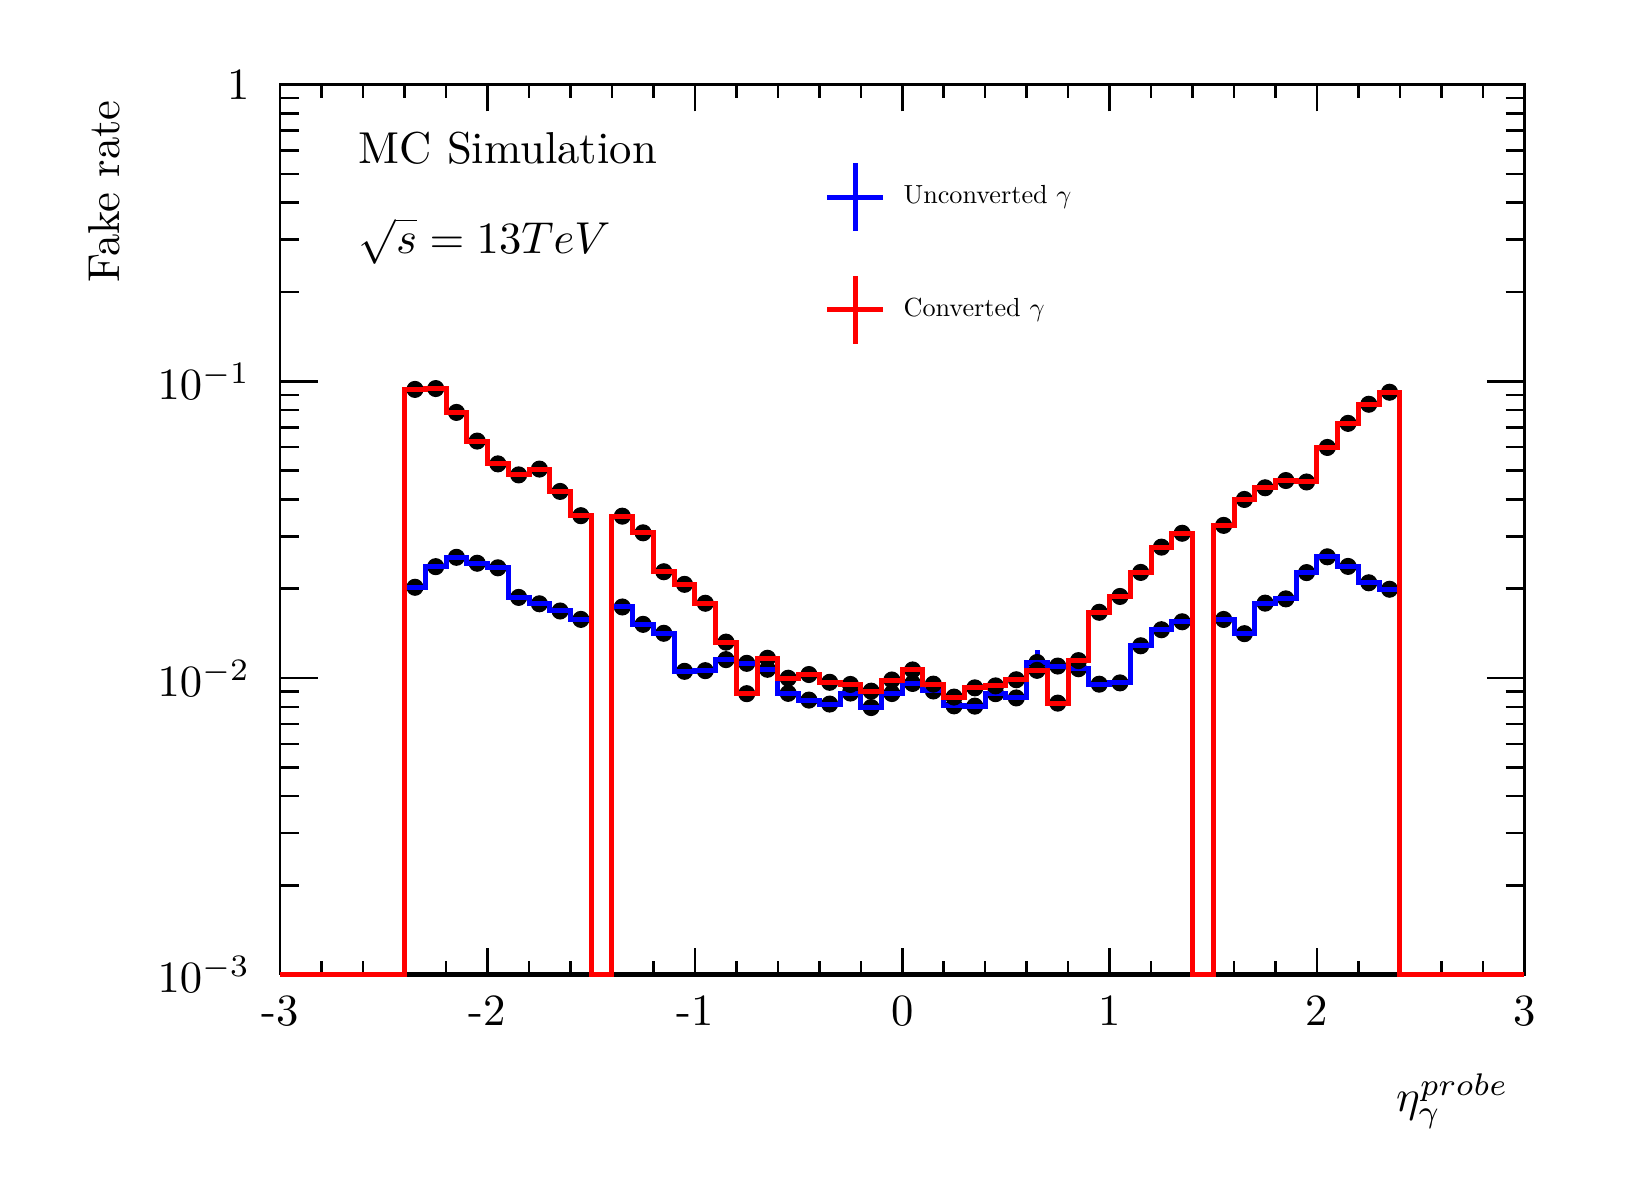
\begin{tikzpicture}
\pgfdeclareplotmark{cross} {
\pgfpathmoveto{\pgfpoint{-0.3\pgfplotmarksize}{\pgfplotmarksize}}
\pgfpathlineto{\pgfpoint{+0.3\pgfplotmarksize}{\pgfplotmarksize}}
\pgfpathlineto{\pgfpoint{+0.3\pgfplotmarksize}{0.3\pgfplotmarksize}}
\pgfpathlineto{\pgfpoint{+1\pgfplotmarksize}{0.3\pgfplotmarksize}}
\pgfpathlineto{\pgfpoint{+1\pgfplotmarksize}{-0.3\pgfplotmarksize}}
\pgfpathlineto{\pgfpoint{+0.3\pgfplotmarksize}{-0.3\pgfplotmarksize}}
\pgfpathlineto{\pgfpoint{+0.3\pgfplotmarksize}{-1.\pgfplotmarksize}}
\pgfpathlineto{\pgfpoint{-0.3\pgfplotmarksize}{-1.\pgfplotmarksize}}
\pgfpathlineto{\pgfpoint{-0.3\pgfplotmarksize}{-0.3\pgfplotmarksize}}
\pgfpathlineto{\pgfpoint{-1.\pgfplotmarksize}{-0.3\pgfplotmarksize}}
\pgfpathlineto{\pgfpoint{-1.\pgfplotmarksize}{0.3\pgfplotmarksize}}
\pgfpathlineto{\pgfpoint{-0.3\pgfplotmarksize}{0.3\pgfplotmarksize}}
\pgfpathclose
\pgfusepathqstroke
}
\pgfdeclareplotmark{cross*} {
\pgfpathmoveto{\pgfpoint{-0.3\pgfplotmarksize}{\pgfplotmarksize}}
\pgfpathlineto{\pgfpoint{+0.3\pgfplotmarksize}{\pgfplotmarksize}}
\pgfpathlineto{\pgfpoint{+0.3\pgfplotmarksize}{0.3\pgfplotmarksize}}
\pgfpathlineto{\pgfpoint{+1\pgfplotmarksize}{0.3\pgfplotmarksize}}
\pgfpathlineto{\pgfpoint{+1\pgfplotmarksize}{-0.3\pgfplotmarksize}}
\pgfpathlineto{\pgfpoint{+0.3\pgfplotmarksize}{-0.3\pgfplotmarksize}}
\pgfpathlineto{\pgfpoint{+0.3\pgfplotmarksize}{-1.\pgfplotmarksize}}
\pgfpathlineto{\pgfpoint{-0.3\pgfplotmarksize}{-1.\pgfplotmarksize}}
\pgfpathlineto{\pgfpoint{-0.3\pgfplotmarksize}{-0.3\pgfplotmarksize}}
\pgfpathlineto{\pgfpoint{-1.\pgfplotmarksize}{-0.3\pgfplotmarksize}}
\pgfpathlineto{\pgfpoint{-1.\pgfplotmarksize}{0.3\pgfplotmarksize}}
\pgfpathlineto{\pgfpoint{-0.3\pgfplotmarksize}{0.3\pgfplotmarksize}}
\pgfpathclose
\pgfusepathqfillstroke
}
\pgfdeclareplotmark{newstar} {
\pgfpathmoveto{\pgfqpoint{0pt}{\pgfplotmarksize}}
\pgfpathlineto{\pgfqpointpolar{44}{0.5\pgfplotmarksize}}
\pgfpathlineto{\pgfqpointpolar{18}{\pgfplotmarksize}}
\pgfpathlineto{\pgfqpointpolar{-20}{0.5\pgfplotmarksize}}
\pgfpathlineto{\pgfqpointpolar{-54}{\pgfplotmarksize}}
\pgfpathlineto{\pgfqpointpolar{-90}{0.5\pgfplotmarksize}}
\pgfpathlineto{\pgfqpointpolar{234}{\pgfplotmarksize}}
\pgfpathlineto{\pgfqpointpolar{198}{0.5\pgfplotmarksize}}
\pgfpathlineto{\pgfqpointpolar{162}{\pgfplotmarksize}}
\pgfpathlineto{\pgfqpointpolar{134}{0.5\pgfplotmarksize}}
\pgfpathclose
\pgfusepathqstroke
}
\pgfdeclareplotmark{newstar*} {
\pgfpathmoveto{\pgfqpoint{0pt}{\pgfplotmarksize}}
\pgfpathlineto{\pgfqpointpolar{44}{0.5\pgfplotmarksize}}
\pgfpathlineto{\pgfqpointpolar{18}{\pgfplotmarksize}}
\pgfpathlineto{\pgfqpointpolar{-20}{0.5\pgfplotmarksize}}
\pgfpathlineto{\pgfqpointpolar{-54}{\pgfplotmarksize}}
\pgfpathlineto{\pgfqpointpolar{-90}{0.5\pgfplotmarksize}}
\pgfpathlineto{\pgfqpointpolar{234}{\pgfplotmarksize}}
\pgfpathlineto{\pgfqpointpolar{198}{0.5\pgfplotmarksize}}
\pgfpathlineto{\pgfqpointpolar{162}{\pgfplotmarksize}}
\pgfpathlineto{\pgfqpointpolar{134}{0.5\pgfplotmarksize}}
\pgfpathclose
\pgfusepathqfillstroke
}
\definecolor{c}{rgb}{1,1,1};
\draw [color=c, fill=c] (0,0) rectangle (20,14.3108);
\draw [color=c, fill=c] (3.2,2.28972) rectangle (19,13.5952);
\definecolor{c}{rgb}{0,0,0};
\draw [c,line width=0.9] (3.2,2.28972) -- (3.2,13.5952) -- (19,13.5952) -- (19,2.28972) -- (3.2,2.28972);
\draw [c,line width=1.8] (3.2,2.28972) -- (3.2158,2.28972) -- (3.2158,2.28972) -- (3.2316,2.28972) -- (3.2316,2.28972) -- (3.2474,2.28972) -- (3.2474,2.28972) -- (3.2632,2.28972) -- (3.2632,2.28972) -- (3.279,2.28972) -- (3.279,2.28972) --
 (3.2948,2.28972) -- (3.2948,2.28972) -- (3.3106,2.28972) -- (3.3106,2.28972) -- (3.3264,2.28972) -- (3.3264,2.28972) -- (3.3422,2.28972) -- (3.3422,2.28972) -- (3.358,2.28972) -- (3.358,2.28972) -- (3.3738,2.28972) -- (3.3738,2.28972) --
 (3.3896,2.28972) -- (3.3896,2.28972) -- (3.4054,2.28972) -- (3.4054,2.28972) -- (3.4212,2.28972) -- (3.4212,2.28972) -- (3.437,2.28972) -- (3.437,2.28972) -- (3.4528,2.28972) -- (3.4528,2.28972) -- (3.4686,2.28972) -- (3.4686,2.28972) --
 (3.4844,2.28972) -- (3.4844,2.28972) -- (3.5002,2.28972) -- (3.5002,2.28972) -- (3.516,2.28972) -- (3.516,2.28972) -- (3.5318,2.28972) -- (3.5318,2.28972) -- (3.5476,2.28972) -- (3.5476,2.28972) -- (3.5634,2.28972) -- (3.5634,2.28972) --
 (3.5792,2.28972) -- (3.5792,2.28972) -- (3.595,2.28972) -- (3.595,2.28972) -- (3.6108,2.28972) -- (3.6108,2.28972) -- (3.6266,2.28972) -- (3.6266,2.28972) -- (3.6424,2.28972) -- (3.6424,2.28972) -- (3.6582,2.28972) -- (3.6582,2.28972) --
 (3.674,2.28972) -- (3.674,2.28972) -- (3.6898,2.28972) -- (3.6898,2.28972) -- (3.7056,2.28972) -- (3.7056,2.28972) -- (3.7214,2.28972) -- (3.7214,2.28972) -- (3.7372,2.28972) -- (3.7372,2.28972) -- (3.753,2.28972) -- (3.753,2.28972) --
 (3.7688,2.28972) -- (3.7688,2.28972) -- (3.7846,2.28972) -- (3.7846,2.28972) -- (3.8004,2.28972) -- (3.8004,2.28972) -- (3.8162,2.28972) -- (3.8162,2.28972) -- (3.832,2.28972) -- (3.832,2.28972) -- (3.8478,2.28972) -- (3.8478,2.28972) --
 (3.8636,2.28972) -- (3.8636,2.28972) -- (3.8794,2.28972) -- (3.8794,2.28972) -- (3.8952,2.28972) -- (3.8952,2.28972) -- (3.911,2.28972) -- (3.911,2.28972) -- (3.9268,2.28972) -- (3.9268,2.28972) -- (3.9426,2.28972) -- (3.9426,2.28972) --
 (3.9584,2.28972) -- (3.9584,2.28972) -- (3.9742,2.28972) -- (3.9742,2.28972) -- (3.99,2.28972) -- (3.99,2.28972) -- (4.0058,2.28972) -- (4.0058,2.28972) -- (4.0216,2.28972) -- (4.0216,2.28972) -- (4.0374,2.28972) -- (4.0374,2.28972) --
 (4.0532,2.28972) -- (4.0532,2.28972) -- (4.069,2.28972) -- (4.069,2.28972) -- (4.0848,2.28972) -- (4.0848,2.28972) -- (4.1006,2.28972) -- (4.1006,2.28972) -- (4.1164,2.28972) -- (4.1164,2.28972) -- (4.1322,2.28972) -- (4.1322,2.28972) --
 (4.148,2.28972) -- (4.148,2.28972) -- (4.1638,2.28972) -- (4.1638,2.28972) -- (4.1796,2.28972) -- (4.1796,2.28972) -- (4.1954,2.28972) -- (4.1954,2.28972) -- (4.2112,2.28972) -- (4.2112,2.28972) -- (4.227,2.28972) -- (4.227,2.28972) --
 (4.2428,2.28972) -- (4.2428,2.28972) -- (4.2586,2.28972) -- (4.2586,2.28972) -- (4.2744,2.28972) -- (4.2744,2.28972) -- (4.2902,2.28972) -- (4.2902,2.28972) -- (4.306,2.28972) -- (4.306,2.28972) -- (4.3218,2.28972) -- (4.3218,2.28972) --
 (4.3376,2.28972) -- (4.3376,2.28972) -- (4.3534,2.28972) -- (4.3534,2.28972) -- (4.3692,2.28972) -- (4.3692,2.28972) -- (4.385,2.28972) -- (4.385,2.28972) -- (4.4008,2.28972) -- (4.4008,2.28972) -- (4.4166,2.28972) -- (4.4166,2.28972) --
 (4.4324,2.28972) -- (4.4324,2.28972) -- (4.4482,2.28972) -- (4.4482,2.28972) -- (4.464,2.28972) -- (4.464,2.28972) -- (4.4798,2.28972) -- (4.4798,2.28972) -- (4.4956,2.28972) -- (4.4956,2.28972) -- (4.5114,2.28972) -- (4.5114,2.28972) --
 (4.5272,2.28972) -- (4.5272,2.28972) -- (4.543,2.28972) -- (4.543,2.28972) -- (4.5588,2.28972) -- (4.5588,2.28972) -- (4.5746,2.28972) -- (4.5746,2.28972) -- (4.5904,2.28972) -- (4.5904,2.28972) -- (4.6062,2.28972) -- (4.6062,2.28972) --
 (4.622,2.28972) -- (4.622,2.28972) -- (4.6378,2.28972) -- (4.6378,2.28972) -- (4.6536,2.28972) -- (4.6536,2.28972) -- (4.6694,2.28972) -- (4.6694,2.28972) -- (4.6852,2.28972) -- (4.6852,2.28972) -- (4.701,2.28972) -- (4.701,2.28972) --
 (4.7168,2.28972) -- (4.7168,2.28972) -- (4.7326,2.28972) -- (4.7326,2.28972) -- (4.7484,2.28972) -- (4.7484,2.28972) -- (4.7642,2.28972) -- (4.7642,2.28972) -- (4.78,2.28972) -- (4.78,2.28972) -- (4.7958,2.28972) -- (4.7958,2.28972) --
 (4.8116,2.28972) -- (4.8116,2.28972) -- (4.8274,2.28972) -- (4.8274,2.28972) -- (4.8432,2.28972) -- (4.8432,2.28972) -- (4.859,2.28972) -- (4.859,2.28972) -- (4.8748,2.28972) -- (4.8748,2.28972) -- (4.8906,2.28972) -- (4.8906,2.28972) --
 (4.9064,2.28972) -- (4.9064,2.28972) -- (4.9222,2.28972) -- (4.9222,2.28972) -- (4.938,2.28972) -- (4.938,2.28972) -- (4.9538,2.28972) -- (4.9538,2.28972) -- (4.9696,2.28972) -- (4.9696,2.28972) -- (4.9854,2.28972) -- (4.9854,2.28972) --
 (5.0012,2.28972) -- (5.0012,2.28972) -- (5.017,2.28972) -- (5.017,2.28972) -- (5.0328,2.28972) -- (5.0328,2.28972) -- (5.0486,2.28972) -- (5.0486,2.28972) -- (5.0644,2.28972) -- (5.0644,2.28972) -- (5.0802,2.28972) -- (5.0802,2.28972) --
 (5.096,2.28972) -- (5.096,2.28972) -- (5.1118,2.28972) -- (5.1118,2.28972) -- (5.1276,2.28972) -- (5.1276,2.28972) -- (5.1434,2.28972) -- (5.1434,2.28972) -- (5.1592,2.28972) -- (5.1592,2.28972) -- (5.175,2.28972) -- (5.175,2.28972) --
 (5.1908,2.28972) -- (5.1908,2.28972) -- (5.2066,2.28972) -- (5.2066,2.28972) -- (5.2224,2.28972) -- (5.2224,2.28972) -- (5.2382,2.28972) -- (5.2382,2.28972) -- (5.254,2.28972) -- (5.254,2.28972) -- (5.2698,2.28972) -- (5.2698,2.28972) --
 (5.2856,2.28972) -- (5.2856,2.28972) -- (5.3014,2.28972) -- (5.3014,2.28972) -- (5.3172,2.28972) -- (5.3172,2.28972) -- (5.333,2.28972) -- (5.333,2.28972) -- (5.3488,2.28972) -- (5.3488,2.28972) -- (5.3646,2.28972) -- (5.3646,2.28972) --
 (5.3804,2.28972) -- (5.3804,2.28972) -- (5.3962,2.28972) -- (5.3962,2.28972) -- (5.412,2.28972) -- (5.412,2.28972) -- (5.4278,2.28972) -- (5.4278,2.28972) -- (5.4436,2.28972) -- (5.4436,2.28972) -- (5.4594,2.28972) -- (5.4594,2.28972) --
 (5.4752,2.28972) -- (5.4752,2.28972) -- (5.491,2.28972) -- (5.491,2.28972) -- (5.5068,2.28972) -- (5.5068,2.28972) -- (5.5226,2.28972) -- (5.5226,2.28972) -- (5.5384,2.28972) -- (5.5384,2.28972) -- (5.5542,2.28972) -- (5.5542,2.28972) --
 (5.57,2.28972) -- (5.57,2.28972) -- (5.5858,2.28972) -- (5.5858,2.28972) -- (5.6016,2.28972) -- (5.6016,2.28972) -- (5.6174,2.28972) -- (5.6174,2.28972) -- (5.6332,2.28972) -- (5.6332,2.28972) -- (5.649,2.28972) -- (5.649,2.28972) --
 (5.6648,2.28972) -- (5.6648,2.28972) -- (5.6806,2.28972) -- (5.6806,2.28972) -- (5.6964,2.28972) -- (5.6964,2.28972) -- (5.7122,2.28972) -- (5.7122,2.28972) -- (5.728,2.28972) -- (5.728,2.28972) -- (5.7438,2.28972) -- (5.7438,2.28972) --
 (5.7596,2.28972) -- (5.7596,2.28972) -- (5.7754,2.28972) -- (5.7754,2.28972) -- (5.7912,2.28972) -- (5.7912,2.28972) -- (5.807,2.28972) -- (5.807,2.28972) -- (5.8228,2.28972) -- (5.8228,2.28972) -- (5.8386,2.28972) -- (5.8386,2.28972) --
 (5.8544,2.28972) -- (5.8544,2.28972) -- (5.8702,2.28972) -- (5.8702,2.28972) -- (5.886,2.28972) -- (5.886,2.28972) -- (5.9018,2.28972) -- (5.9018,2.28972) -- (5.9176,2.28972) -- (5.9176,2.28972) -- (5.9334,2.28972) -- (5.9334,2.28972) --
 (5.9492,2.28972) -- (5.9492,2.28972) -- (5.965,2.28972) -- (5.965,2.28972) -- (5.9808,2.28972) -- (5.9808,2.28972) -- (5.9966,2.28972) -- (5.9966,2.28972) -- (6.0124,2.28972) -- (6.0124,2.28972) -- (6.0282,2.28972) -- (6.0282,2.28972) --
 (6.044,2.28972) -- (6.044,2.28972) -- (6.0598,2.28972) -- (6.0598,2.28972) -- (6.0756,2.28972) -- (6.0756,2.28972) -- (6.0914,2.28972) -- (6.0914,2.28972) -- (6.1072,2.28972) -- (6.1072,2.28972) -- (6.123,2.28972) -- (6.123,2.28972) --
 (6.1388,2.28972) -- (6.1388,2.28972) -- (6.1546,2.28972) -- (6.1546,2.28972) -- (6.1704,2.28972) -- (6.1704,2.28972) -- (6.1862,2.28972) -- (6.1862,2.28972) -- (6.202,2.28972) -- (6.202,2.28972) -- (6.2178,2.28972) -- (6.2178,2.28972) --
 (6.2336,2.28972) -- (6.2336,2.28972) -- (6.2494,2.28972) -- (6.2494,2.28972) -- (6.2652,2.28972) -- (6.2652,2.28972) -- (6.281,2.28972) -- (6.281,2.28972) -- (6.2968,2.28972) -- (6.2968,2.28972) -- (6.3126,2.28972) -- (6.3126,2.28972) --
 (6.3284,2.28972) -- (6.3284,2.28972) -- (6.3442,2.28972) -- (6.3442,2.28972) -- (6.36,2.28972) -- (6.36,2.28972) -- (6.3758,2.28972) -- (6.3758,2.28972) -- (6.3916,2.28972) -- (6.3916,2.28972) -- (6.4074,2.28972) -- (6.4074,2.28972) --
 (6.4232,2.28972) -- (6.4232,2.28972) -- (6.439,2.28972) -- (6.439,2.28972) -- (6.4548,2.28972) -- (6.4548,2.28972) -- (6.4706,2.28972) -- (6.4706,2.28972) -- (6.4864,2.28972) -- (6.4864,2.28972) -- (6.5022,2.28972) -- (6.5022,2.28972) --
 (6.518,2.28972) -- (6.518,2.28972) -- (6.5338,2.28972) -- (6.5338,2.28972) -- (6.5496,2.28972) -- (6.5496,2.28972) -- (6.5654,2.28972) -- (6.5654,2.28972) -- (6.5812,2.28972) -- (6.5812,2.28972) -- (6.597,2.28972) -- (6.597,2.28972) --
 (6.6128,2.28972) -- (6.6128,2.28972) -- (6.6286,2.28972) -- (6.6286,2.28972) -- (6.6444,2.28972) -- (6.6444,2.28972) -- (6.6602,2.28972) -- (6.6602,2.28972) -- (6.676,2.28972) -- (6.676,2.28972) -- (6.6918,2.28972) -- (6.6918,2.28972) --
 (6.7076,2.28972) -- (6.7076,2.28972) -- (6.7234,2.28972) -- (6.7234,2.28972) -- (6.7392,2.28972) -- (6.7392,2.28972) -- (6.755,2.28972) -- (6.755,2.28972) -- (6.7708,2.28972) -- (6.7708,2.28972) -- (6.7866,2.28972) -- (6.7866,2.28972) --
 (6.8024,2.28972) -- (6.8024,2.28972) -- (6.8182,2.28972) -- (6.8182,2.28972) -- (6.834,2.28972) -- (6.834,2.28972) -- (6.8498,2.28972) -- (6.8498,2.28972) -- (6.8656,2.28972) -- (6.8656,2.28972) -- (6.8814,2.28972) -- (6.8814,2.28972) --
 (6.8972,2.28972) -- (6.8972,2.28972) -- (6.913,2.28972) -- (6.913,2.28972) -- (6.9288,2.28972) -- (6.9288,2.28972) -- (6.9446,2.28972) -- (6.9446,2.28972) -- (6.9604,2.28972) -- (6.9604,2.28972) -- (6.9762,2.28972) -- (6.9762,2.28972) --
 (6.992,2.28972) -- (6.992,2.28972) -- (7.0078,2.28972) -- (7.0078,2.28972) -- (7.0236,2.28972) -- (7.0236,2.28972) -- (7.0394,2.28972) -- (7.0394,2.28972) -- (7.0552,2.28972) -- (7.0552,2.28972) -- (7.071,2.28972) -- (7.071,2.28972) --
 (7.0868,2.28972) -- (7.0868,2.28972) -- (7.1026,2.28972) -- (7.1026,2.28972) -- (7.1184,2.28972) -- (7.1184,2.28972) -- (7.1342,2.28972) -- (7.1342,2.28972) -- (7.15,2.28972) -- (7.15,2.28972) -- (7.1658,2.28972) -- (7.1658,2.28972) --
 (7.1816,2.28972) -- (7.1816,2.28972) -- (7.1974,2.28972) -- (7.1974,2.28972) -- (7.2132,2.28972) -- (7.2132,2.28972) -- (7.229,2.28972) -- (7.229,2.28972) -- (7.2448,2.28972) -- (7.2448,2.28972) -- (7.2606,2.28972) -- (7.2606,2.28972) --
 (7.2764,2.28972) -- (7.2764,2.28972) -- (7.2922,2.28972) -- (7.2922,2.28972) -- (7.308,2.28972) -- (7.308,2.28972) -- (7.3238,2.28972) -- (7.3238,2.28972) -- (7.3396,2.28972) -- (7.3396,2.28972) -- (7.3554,2.28972) -- (7.3554,2.28972) --
 (7.3712,2.28972) -- (7.3712,2.28972) -- (7.387,2.28972) -- (7.387,2.28972) -- (7.4028,2.28972) -- (7.4028,2.28972) -- (7.4186,2.28972) -- (7.4186,2.28972) -- (7.4344,2.28972) -- (7.4344,2.28972) -- (7.4502,2.28972) -- (7.4502,2.28972) --
 (7.466,2.28972) -- (7.466,2.28972) -- (7.4818,2.28972) -- (7.4818,2.28972) -- (7.4976,2.28972) -- (7.4976,2.28972) -- (7.5134,2.28972) -- (7.5134,2.28972) -- (7.5292,2.28972) -- (7.5292,2.28972) -- (7.545,2.28972) -- (7.545,2.28972) --
 (7.5608,2.28972) -- (7.5608,2.28972) -- (7.5766,2.28972) -- (7.5766,2.28972) -- (7.5924,2.28972) -- (7.5924,2.28972) -- (7.6082,2.28972) -- (7.6082,2.28972) -- (7.624,2.28972) -- (7.624,2.28972) -- (7.6398,2.28972) -- (7.6398,2.28972) --
 (7.6556,2.28972) -- (7.6556,2.28972) -- (7.6714,2.28972) -- (7.6714,2.28972) -- (7.6872,2.28972) -- (7.6872,2.28972) -- (7.703,2.28972) -- (7.703,2.28972) -- (7.7188,2.28972) -- (7.7188,2.28972) -- (7.7346,2.28972) -- (7.7346,2.28972) --
 (7.7504,2.28972) -- (7.7504,2.28972) -- (7.7662,2.28972) -- (7.7662,2.28972) -- (7.782,2.28972) -- (7.782,2.28972) -- (7.7978,2.28972) -- (7.7978,2.28972) -- (7.8136,2.28972) -- (7.8136,2.28972) -- (7.8294,2.28972) -- (7.8294,2.28972) --
 (7.8452,2.28972) -- (7.8452,2.28972) -- (7.861,2.28972) -- (7.861,2.28972) -- (7.8768,2.28972) -- (7.8768,2.28972) -- (7.8926,2.28972) -- (7.8926,2.28972) -- (7.9084,2.28972) -- (7.9084,2.28972) -- (7.9242,2.28972) -- (7.9242,2.28972) --
 (7.94,2.28972) -- (7.94,2.28972) -- (7.9558,2.28972) -- (7.9558,2.28972) -- (7.9716,2.28972) -- (7.9716,2.28972) -- (7.9874,2.28972) -- (7.9874,2.28972) -- (8.0032,2.28972) -- (8.0032,2.28972) -- (8.019,2.28972) -- (8.019,2.28972) --
 (8.0348,2.28972) -- (8.0348,2.28972) -- (8.0506,2.28972) -- (8.0506,2.28972) -- (8.0664,2.28972) -- (8.0664,2.28972) -- (8.0822,2.28972) -- (8.0822,2.28972) -- (8.098,2.28972) -- (8.098,2.28972) -- (8.1138,2.28972) -- (8.1138,2.28972) --
 (8.1296,2.28972) -- (8.1296,2.28972) -- (8.1454,2.28972) -- (8.1454,2.28972) -- (8.1612,2.28972) -- (8.1612,2.28972) -- (8.177,2.28972) -- (8.177,2.28972) -- (8.1928,2.28972) -- (8.1928,2.28972) -- (8.2086,2.28972) -- (8.2086,2.28972) --
 (8.2244,2.28972) -- (8.2244,2.28972) -- (8.2402,2.28972) -- (8.2402,2.28972) -- (8.256,2.28972) -- (8.256,2.28972) -- (8.2718,2.28972) -- (8.2718,2.28972) -- (8.2876,2.28972) -- (8.2876,2.28972) -- (8.3034,2.28972) -- (8.3034,2.28972) --
 (8.3192,2.28972) -- (8.3192,2.28972) -- (8.335,2.28972) -- (8.335,2.28972) -- (8.3508,2.28972) -- (8.3508,2.28972) -- (8.3666,2.28972) -- (8.3666,2.28972) -- (8.3824,2.28972) -- (8.3824,2.28972) -- (8.3982,2.28972) -- (8.3982,2.28972) --
 (8.414,2.28972) -- (8.414,2.28972) -- (8.4298,2.28972) -- (8.4298,2.28972) -- (8.4456,2.28972) -- (8.4456,2.28972) -- (8.4614,2.28972) -- (8.4614,2.28972) -- (8.4772,2.28972) -- (8.4772,2.28972) -- (8.493,2.28972) -- (8.493,2.28972) --
 (8.5088,2.28972) -- (8.5088,2.28972) -- (8.5246,2.28972) -- (8.5246,2.28972) -- (8.5404,2.28972) -- (8.5404,2.28972) -- (8.5562,2.28972) -- (8.5562,2.28972) -- (8.572,2.28972) -- (8.572,2.28972) -- (8.5878,2.28972) -- (8.5878,2.28972) --
 (8.6036,2.28972) -- (8.6036,2.28972) -- (8.6194,2.28972) -- (8.6194,2.28972) -- (8.6352,2.28972) -- (8.6352,2.28972) -- (8.651,2.28972) -- (8.651,2.28972) -- (8.6668,2.28972) -- (8.6668,2.28972) -- (8.6826,2.28972) -- (8.6826,2.28972) --
 (8.6984,2.28972) -- (8.6984,2.28972) -- (8.7142,2.28972) -- (8.7142,2.28972) -- (8.73,2.28972) -- (8.73,2.28972) -- (8.7458,2.28972) -- (8.7458,2.28972) -- (8.7616,2.28972) -- (8.7616,2.28972) -- (8.7774,2.28972) -- (8.7774,2.28972) --
 (8.7932,2.28972) -- (8.7932,2.28972) -- (8.809,2.28972) -- (8.809,2.28972) -- (8.8248,2.28972) -- (8.8248,2.28972) -- (8.8406,2.28972) -- (8.8406,2.28972) -- (8.8564,2.28972) -- (8.8564,2.28972) -- (8.8722,2.28972) -- (8.8722,2.28972) --
 (8.888,2.28972) -- (8.888,2.28972) -- (8.9038,2.28972) -- (8.9038,2.28972) -- (8.9196,2.28972) -- (8.9196,2.28972) -- (8.9354,2.28972) -- (8.9354,2.28972) -- (8.9512,2.28972) -- (8.9512,2.28972) -- (8.967,2.28972) -- (8.967,2.28972) --
 (8.9828,2.28972) -- (8.9828,2.28972) -- (8.9986,2.28972) -- (8.9986,2.28972) -- (9.0144,2.28972) -- (9.0144,2.28972) -- (9.0302,2.28972) -- (9.0302,2.28972) -- (9.046,2.28972) -- (9.046,2.28972) -- (9.0618,2.28972) -- (9.0618,2.28972) --
 (9.0776,2.28972) -- (9.0776,2.28972) -- (9.0934,2.28972) -- (9.0934,2.28972) -- (9.1092,2.28972) -- (9.1092,2.28972) -- (9.125,2.28972) -- (9.125,2.28972) -- (9.1408,2.28972) -- (9.1408,2.28972) -- (9.1566,2.28972) -- (9.1566,2.28972) --
 (9.1724,2.28972) -- (9.1724,2.28972) -- (9.1882,2.28972) -- (9.1882,2.28972) -- (9.204,2.28972) -- (9.204,2.28972) -- (9.2198,2.28972) -- (9.2198,2.28972) -- (9.2356,2.28972) -- (9.2356,2.28972) -- (9.2514,2.28972) -- (9.2514,2.28972) --
 (9.2672,2.28972) -- (9.2672,2.28972) -- (9.283,2.28972) -- (9.283,2.28972) -- (9.2988,2.28972) -- (9.2988,2.28972) -- (9.3146,2.28972) -- (9.3146,2.28972) -- (9.3304,2.28972) -- (9.3304,2.28972) -- (9.3462,2.28972) -- (9.3462,2.28972) --
 (9.362,2.28972) -- (9.362,2.28972) -- (9.3778,2.28972) -- (9.3778,2.28972) -- (9.3936,2.28972) -- (9.3936,2.28972) -- (9.4094,2.28972) -- (9.4094,2.28972) -- (9.4252,2.28972) -- (9.4252,2.28972) -- (9.441,2.28972) -- (9.441,2.28972) --
 (9.4568,2.28972) -- (9.4568,2.28972) -- (9.4726,2.28972) -- (9.4726,2.28972) -- (9.4884,2.28972) -- (9.4884,2.28972) -- (9.5042,2.28972) -- (9.5042,2.28972) -- (9.52,2.28972) -- (9.52,2.28972) -- (9.5358,2.28972) -- (9.5358,2.28972) --
 (9.5516,2.28972) -- (9.5516,2.28972) -- (9.5674,2.28972) -- (9.5674,2.28972) -- (9.5832,2.28972) -- (9.5832,2.28972) -- (9.599,2.28972) -- (9.599,2.28972) -- (9.6148,2.28972) -- (9.6148,2.28972) -- (9.6306,2.28972) -- (9.6306,2.28972) --
 (9.6464,2.28972) -- (9.6464,2.28972) -- (9.6622,2.28972) -- (9.6622,2.28972) -- (9.678,2.28972) -- (9.678,2.28972) -- (9.6938,2.28972) -- (9.6938,2.28972) -- (9.7096,2.28972) -- (9.7096,2.28972) -- (9.7254,2.28972) -- (9.7254,2.28972) --
 (9.7412,2.28972) -- (9.7412,2.28972) -- (9.757,2.28972) -- (9.757,2.28972) -- (9.7728,2.28972) -- (9.7728,2.28972) -- (9.7886,2.28972) -- (9.7886,2.28972) -- (9.8044,2.28972) -- (9.8044,2.28972) -- (9.8202,2.28972) -- (9.8202,2.28972) --
 (9.836,2.28972) -- (9.836,2.28972) -- (9.8518,2.28972) -- (9.8518,2.28972) -- (9.8676,2.28972) -- (9.8676,2.28972) -- (9.8834,2.28972) -- (9.8834,2.28972) -- (9.8992,2.28972) -- (9.8992,2.28972) -- (9.915,2.28972) -- (9.915,2.28972) --
 (9.9308,2.28972) -- (9.9308,2.28972) -- (9.9466,2.28972) -- (9.9466,2.28972) -- (9.9624,2.28972) -- (9.9624,2.28972) -- (9.9782,2.28972) -- (9.9782,2.28972) -- (9.994,2.28972) -- (9.994,2.28972) -- (10.0098,2.28972) -- (10.0098,2.28972) --
 (10.0256,2.28972) -- (10.0256,2.28972) -- (10.0414,2.28972) -- (10.0414,2.28972) -- (10.0572,2.28972) -- (10.0572,2.28972) -- (10.073,2.28972) -- (10.073,2.28972) -- (10.0888,2.28972) -- (10.0888,2.28972) -- (10.1046,2.28972) -- (10.1046,2.28972) --
 (10.1204,2.28972) -- (10.1204,2.28972) -- (10.1362,2.28972) -- (10.1362,2.28972) -- (10.152,2.28972) -- (10.152,2.28972) -- (10.1678,2.28972) -- (10.1678,2.28972) -- (10.1836,2.28972) -- (10.1836,2.28972) -- (10.1994,2.28972) -- (10.1994,2.28972) --
 (10.2152,2.28972) -- (10.2152,2.28972) -- (10.231,2.28972) -- (10.231,2.28972) -- (10.2468,2.28972) -- (10.2468,2.28972) -- (10.2626,2.28972) -- (10.2626,2.28972) -- (10.2784,2.28972) -- (10.2784,2.28972) -- (10.2942,2.28972) -- (10.2942,2.28972) --
 (10.31,2.28972) -- (10.31,2.28972) -- (10.3258,2.28972) -- (10.3258,2.28972) -- (10.3416,2.28972) -- (10.3416,2.28972) -- (10.3574,2.28972) -- (10.3574,2.28972) -- (10.3732,2.28972) -- (10.3732,2.28972) -- (10.389,2.28972) -- (10.389,2.28972) --
 (10.4048,2.28972) -- (10.4048,2.28972) -- (10.4206,2.28972) -- (10.4206,2.28972) -- (10.4364,2.28972) -- (10.4364,2.28972) -- (10.4522,2.28972) -- (10.4522,2.28972) -- (10.468,2.28972) -- (10.468,2.28972) -- (10.4838,2.28972) -- (10.4838,2.28972) --
 (10.4996,2.28972) -- (10.4996,2.28972) -- (10.5154,2.28972) -- (10.5154,2.28972) -- (10.5312,2.28972) -- (10.5312,2.28972) -- (10.547,2.28972) -- (10.547,2.28972) -- (10.5628,2.28972) -- (10.5628,2.28972) -- (10.5786,2.28972) -- (10.5786,2.28972) --
 (10.5944,2.28972) -- (10.5944,2.28972) -- (10.6102,2.28972) -- (10.6102,2.28972) -- (10.626,2.28972) -- (10.626,2.28972) -- (10.6418,2.28972) -- (10.6418,2.28972) -- (10.6576,2.28972) -- (10.6576,2.28972) -- (10.6734,2.28972) -- (10.6734,2.28972) --
 (10.6892,2.28972) -- (10.6892,2.28972) -- (10.705,2.28972) -- (10.705,2.28972) -- (10.7208,2.28972) -- (10.7208,2.28972) -- (10.7366,2.28972) -- (10.7366,2.28972) -- (10.7524,2.28972) -- (10.7524,2.28972) -- (10.7682,2.28972) -- (10.7682,2.28972) --
 (10.784,2.28972) -- (10.784,2.28972) -- (10.7998,2.28972) -- (10.7998,2.28972) -- (10.8156,2.28972) -- (10.8156,2.28972) -- (10.8314,2.28972) -- (10.8314,2.28972) -- (10.8472,2.28972) -- (10.8472,2.28972) -- (10.863,2.28972) -- (10.863,2.28972) --
 (10.8788,2.28972) -- (10.8788,2.28972) -- (10.8946,2.28972) -- (10.8946,2.28972) -- (10.9104,2.28972) -- (10.9104,2.28972) -- (10.9262,2.28972) -- (10.9262,2.28972) -- (10.942,2.28972) -- (10.942,2.28972) -- (10.9578,2.28972) -- (10.9578,2.28972) --
 (10.9736,2.28972) -- (10.9736,2.28972) -- (10.9894,2.28972) -- (10.9894,2.28972) -- (11.0052,2.28972) -- (11.0052,2.28972) -- (11.021,2.28972) -- (11.021,2.28972) -- (11.0368,2.28972) -- (11.0368,2.28972) -- (11.0526,2.28972) -- (11.0526,2.28972) --
 (11.0684,2.28972) -- (11.0684,2.28972) -- (11.0842,2.28972) -- (11.0842,2.28972) -- (11.1,2.28972) -- (11.1,2.28972) -- (11.1158,2.28972) -- (11.1158,2.28972) -- (11.1316,2.28972) -- (11.1316,2.28972) -- (11.1474,2.28972) -- (11.1474,2.28972) --
 (11.1632,2.28972) -- (11.1632,2.28972) -- (11.179,2.28972) -- (11.179,2.28972) -- (11.1948,2.28972) -- (11.1948,2.28972) -- (11.2106,2.28972) -- (11.2106,2.28972) -- (11.2264,2.28972) -- (11.2264,2.28972) -- (11.2422,2.28972) -- (11.2422,2.28972) --
 (11.258,2.28972) -- (11.258,2.28972) -- (11.2738,2.28972) -- (11.2738,2.28972) -- (11.2896,2.28972) -- (11.2896,2.28972) -- (11.3054,2.28972) -- (11.3054,2.28972) -- (11.3212,2.28972) -- (11.3212,2.28972) -- (11.337,2.28972) -- (11.337,2.28972) --
 (11.3528,2.28972) -- (11.3528,2.28972) -- (11.3686,2.28972) -- (11.3686,2.28972) -- (11.3844,2.28972) -- (11.3844,2.28972) -- (11.4002,2.28972) -- (11.4002,2.28972) -- (11.416,2.28972) -- (11.416,2.28972) -- (11.4318,2.28972) -- (11.4318,2.28972) --
 (11.4476,2.28972) -- (11.4476,2.28972) -- (11.4634,2.28972) -- (11.4634,2.28972) -- (11.4792,2.28972) -- (11.4792,2.28972) -- (11.495,2.28972) -- (11.495,2.28972) -- (11.5108,2.28972) -- (11.5108,2.28972) -- (11.5266,2.28972) -- (11.5266,2.28972) --
 (11.5424,2.28972) -- (11.5424,2.28972) -- (11.5582,2.28972) -- (11.5582,2.28972) -- (11.574,2.28972) -- (11.574,2.28972) -- (11.5898,2.28972) -- (11.5898,2.28972) -- (11.6056,2.28972) -- (11.6056,2.28972) -- (11.6214,2.28972) -- (11.6214,2.28972) --
 (11.6372,2.28972) -- (11.6372,2.28972) -- (11.653,2.28972) -- (11.653,2.28972) -- (11.6688,2.28972) -- (11.6688,2.28972) -- (11.6846,2.28972) -- (11.6846,2.28972) -- (11.7004,2.28972) -- (11.7004,2.28972) -- (11.7162,2.28972) -- (11.7162,2.28972) --
 (11.732,2.28972) -- (11.732,2.28972) -- (11.7478,2.28972) -- (11.7478,2.28972) -- (11.7636,2.28972) -- (11.7636,2.28972) -- (11.7794,2.28972) -- (11.7794,2.28972) -- (11.7952,2.28972) -- (11.7952,2.28972) -- (11.811,2.28972) -- (11.811,2.28972) --
 (11.8268,2.28972) -- (11.8268,2.28972) -- (11.8426,2.28972) -- (11.8426,2.28972) -- (11.8584,2.28972) -- (11.8584,2.28972) -- (11.8742,2.28972) -- (11.8742,2.28972) -- (11.89,2.28972) -- (11.89,2.28972) -- (11.9058,2.28972) -- (11.9058,2.28972) --
 (11.9216,2.28972) -- (11.9216,2.28972) -- (11.9374,2.28972) -- (11.9374,2.28972) -- (11.9532,2.28972) -- (11.9532,2.28972) -- (11.969,2.28972) -- (11.969,2.28972) -- (11.9848,2.28972) -- (11.9848,2.28972) -- (12.0006,2.28972) -- (12.0006,2.28972) --
 (12.0164,2.28972) -- (12.0164,2.28972) -- (12.0322,2.28972) -- (12.0322,2.28972) -- (12.048,2.28972) -- (12.048,2.28972) -- (12.0638,2.28972) -- (12.0638,2.28972) -- (12.0796,2.28972) -- (12.0796,2.28972) -- (12.0954,2.28972) -- (12.0954,2.28972) --
 (12.1112,2.28972) -- (12.1112,2.28972) -- (12.127,2.28972) -- (12.127,2.28972) -- (12.1428,2.28972) -- (12.1428,2.28972) -- (12.1586,2.28972) -- (12.1586,2.28972) -- (12.1744,2.28972) -- (12.1744,2.28972) -- (12.1902,2.28972) -- (12.1902,2.28972) --
 (12.206,2.28972) -- (12.206,2.28972) -- (12.2218,2.28972) -- (12.2218,2.28972) -- (12.2376,2.28972) -- (12.2376,2.28972) -- (12.2534,2.28972) -- (12.2534,2.28972) -- (12.2692,2.28972) -- (12.2692,2.28972) -- (12.285,2.28972) -- (12.285,2.28972) --
 (12.3008,2.28972) -- (12.3008,2.28972) -- (12.3166,2.28972) -- (12.3166,2.28972) -- (12.3324,2.28972) -- (12.3324,2.28972) -- (12.3482,2.28972) -- (12.3482,2.28972) -- (12.364,2.28972) -- (12.364,2.28972) -- (12.3798,2.28972) -- (12.3798,2.28972) --
 (12.3956,2.28972) -- (12.3956,2.28972) -- (12.4114,2.28972) -- (12.4114,2.28972) -- (12.4272,2.28972) -- (12.4272,2.28972) -- (12.443,2.28972) -- (12.443,2.28972) -- (12.4588,2.28972) -- (12.4588,2.28972) -- (12.4746,2.28972) -- (12.4746,2.28972) --
 (12.4904,2.28972) -- (12.4904,2.28972) -- (12.5062,2.28972) -- (12.5062,2.28972) -- (12.522,2.28972) -- (12.522,2.28972) -- (12.5378,2.28972) -- (12.5378,2.28972) -- (12.5536,2.28972) -- (12.5536,2.28972) -- (12.5694,2.28972) -- (12.5694,2.28972) --
 (12.5852,2.28972) -- (12.5852,2.28972) -- (12.601,2.28972) -- (12.601,2.28972) -- (12.6168,2.28972) -- (12.6168,2.28972) -- (12.6326,2.28972) -- (12.6326,2.28972) -- (12.6484,2.28972) -- (12.6484,2.28972) -- (12.6642,2.28972) -- (12.6642,2.28972) --
 (12.68,2.28972) -- (12.68,2.28972) -- (12.6958,2.28972) -- (12.6958,2.28972) -- (12.7116,2.28972) -- (12.7116,2.28972) -- (12.7274,2.28972) -- (12.7274,2.28972) -- (12.7432,2.28972) -- (12.7432,2.28972) -- (12.759,2.28972) -- (12.759,2.28972) --
 (12.7748,2.28972) -- (12.7748,2.28972) -- (12.7906,2.28972) -- (12.7906,2.28972) -- (12.8064,2.28972) -- (12.8064,2.28972) -- (12.8222,2.28972) -- (12.8222,2.28972) -- (12.838,2.28972) -- (12.838,2.28972) -- (12.8538,2.28972) -- (12.8538,2.28972) --
 (12.8696,2.28972) -- (12.8696,2.28972) -- (12.8854,2.28972) -- (12.8854,2.28972) -- (12.9012,2.28972) -- (12.9012,2.28972) -- (12.917,2.28972) -- (12.917,2.28972) -- (12.9328,2.28972) -- (12.9328,2.28972) -- (12.9486,2.28972) -- (12.9486,2.28972) --
 (12.9644,2.28972) -- (12.9644,2.28972) -- (12.9802,2.28972) -- (12.9802,2.28972) -- (12.996,2.28972) -- (12.996,2.28972) -- (13.0118,2.28972) -- (13.0118,2.28972) -- (13.0276,2.28972) -- (13.0276,2.28972) -- (13.0434,2.28972) -- (13.0434,2.28972) --
 (13.0592,2.28972) -- (13.0592,2.28972) -- (13.075,2.28972) -- (13.075,2.28972) -- (13.0908,2.28972) -- (13.0908,2.28972) -- (13.1066,2.28972) -- (13.1066,2.28972) -- (13.1224,2.28972) -- (13.1224,2.28972) -- (13.1382,2.28972) -- (13.1382,2.28972) --
 (13.154,2.28972) -- (13.154,2.28972) -- (13.1698,2.28972) -- (13.1698,2.28972) -- (13.1856,2.28972) -- (13.1856,2.28972) -- (13.2014,2.28972) -- (13.2014,2.28972) -- (13.2172,2.28972) -- (13.2172,2.28972) -- (13.233,2.28972) -- (13.233,2.28972) --
 (13.2488,2.28972) -- (13.2488,2.28972) -- (13.2646,2.28972) -- (13.2646,2.28972) -- (13.2804,2.28972) -- (13.2804,2.28972) -- (13.2962,2.28972) -- (13.2962,2.28972) -- (13.312,2.28972) -- (13.312,2.28972) -- (13.3278,2.28972) -- (13.3278,2.28972) --
 (13.3436,2.28972) -- (13.3436,2.28972) -- (13.3594,2.28972) -- (13.3594,2.28972) -- (13.3752,2.28972) -- (13.3752,2.28972) -- (13.391,2.28972) -- (13.391,2.28972) -- (13.4068,2.28972) -- (13.4068,2.28972) -- (13.4226,2.28972) -- (13.4226,2.28972) --
 (13.4384,2.28972) -- (13.4384,2.28972) -- (13.4542,2.28972) -- (13.4542,2.28972) -- (13.47,2.28972) -- (13.47,2.28972) -- (13.4858,2.28972) -- (13.4858,2.28972) -- (13.5016,2.28972) -- (13.5016,2.28972) -- (13.5174,2.28972) -- (13.5174,2.28972) --
 (13.5332,2.28972) -- (13.5332,2.28972) -- (13.549,2.28972) -- (13.549,2.28972) -- (13.5648,2.28972) -- (13.5648,2.28972) -- (13.5806,2.28972) -- (13.5806,2.28972) -- (13.5964,2.28972) -- (13.5964,2.28972) -- (13.6122,2.28972) -- (13.6122,2.28972) --
 (13.628,2.28972) -- (13.628,2.28972) -- (13.6438,2.28972) -- (13.6438,2.28972) -- (13.6596,2.28972) -- (13.6596,2.28972) -- (13.6754,2.28972) -- (13.6754,2.28972) -- (13.6912,2.28972) -- (13.6912,2.28972) -- (13.707,2.28972) -- (13.707,2.28972) --
 (13.7228,2.28972) -- (13.7228,2.28972) -- (13.7386,2.28972) -- (13.7386,2.28972) -- (13.7544,2.28972) -- (13.7544,2.28972) -- (13.7702,2.28972) -- (13.7702,2.28972) -- (13.786,2.28972) -- (13.786,2.28972) -- (13.8018,2.28972) -- (13.8018,2.28972) --
 (13.8176,2.28972) -- (13.8176,2.28972) -- (13.8334,2.28972) -- (13.8334,2.28972) -- (13.8492,2.28972) -- (13.8492,2.28972) -- (13.865,2.28972) -- (13.865,2.28972) -- (13.8808,2.28972) -- (13.8808,2.28972) -- (13.8966,2.28972) -- (13.8966,2.28972) --
 (13.9124,2.28972) -- (13.9124,2.28972) -- (13.9282,2.28972) -- (13.9282,2.28972) -- (13.944,2.28972) -- (13.944,2.28972) -- (13.9598,2.28972) -- (13.9598,2.28972) -- (13.9756,2.28972) -- (13.9756,2.28972) -- (13.9914,2.28972) -- (13.9914,2.28972) --
 (14.0072,2.28972) -- (14.0072,2.28972) -- (14.023,2.28972) -- (14.023,2.28972) -- (14.0388,2.28972) -- (14.0388,2.28972) -- (14.0546,2.28972) -- (14.0546,2.28972) -- (14.0704,2.28972) -- (14.0704,2.28972) -- (14.0862,2.28972) -- (14.0862,2.28972) --
 (14.102,2.28972) -- (14.102,2.28972) -- (14.1178,2.28972) -- (14.1178,2.28972) -- (14.1336,2.28972) -- (14.1336,2.28972) -- (14.1494,2.28972) -- (14.1494,2.28972) -- (14.1652,2.28972) -- (14.1652,2.28972) -- (14.181,2.28972) -- (14.181,2.28972) --
 (14.1968,2.28972) -- (14.1968,2.28972) -- (14.2126,2.28972) -- (14.2126,2.28972) -- (14.2284,2.28972) -- (14.2284,2.28972) -- (14.2442,2.28972) -- (14.2442,2.28972) -- (14.26,2.28972) -- (14.26,2.28972) -- (14.2758,2.28972) -- (14.2758,2.28972) --
 (14.2916,2.28972) -- (14.2916,2.28972) -- (14.3074,2.28972) -- (14.3074,2.28972) -- (14.3232,2.28972) -- (14.3232,2.28972) -- (14.339,2.28972) -- (14.339,2.28972) -- (14.3548,2.28972) -- (14.3548,2.28972) -- (14.3706,2.28972) -- (14.3706,2.28972) --
 (14.3864,2.28972) -- (14.3864,2.28972) -- (14.4022,2.28972) -- (14.4022,2.28972) -- (14.418,2.28972) -- (14.418,2.28972) -- (14.4338,2.28972) -- (14.4338,2.28972) -- (14.4496,2.28972) -- (14.4496,2.28972) -- (14.4654,2.28972) -- (14.4654,2.28972) --
 (14.4812,2.28972) -- (14.4812,2.28972) -- (14.497,2.28972) -- (14.497,2.28972) -- (14.5128,2.28972) -- (14.5128,2.28972) -- (14.5286,2.28972) -- (14.5286,2.28972) -- (14.5444,2.28972) -- (14.5444,2.28972) -- (14.5602,2.28972) -- (14.5602,2.28972) --
 (14.576,2.28972) -- (14.576,2.28972) -- (14.5918,2.28972) -- (14.5918,2.28972) -- (14.6076,2.28972) -- (14.6076,2.28972) -- (14.6234,2.28972) -- (14.6234,2.28972) -- (14.6392,2.28972) -- (14.6392,2.28972) -- (14.655,2.28972) -- (14.655,2.28972) --
 (14.6708,2.28972) -- (14.6708,2.28972) -- (14.6866,2.28972) -- (14.6866,2.28972) -- (14.7024,2.28972) -- (14.7024,2.28972) -- (14.7182,2.28972) -- (14.7182,2.28972) -- (14.734,2.28972) -- (14.734,2.28972) -- (14.7498,2.28972) -- (14.7498,2.28972) --
 (14.7656,2.28972) -- (14.7656,2.28972) -- (14.7814,2.28972) -- (14.7814,2.28972) -- (14.7972,2.28972) -- (14.7972,2.28972) -- (14.813,2.28972) -- (14.813,2.28972) -- (14.8288,2.28972) -- (14.8288,2.28972) -- (14.8446,2.28972) -- (14.8446,2.28972) --
 (14.8604,2.28972) -- (14.8604,2.28972) -- (14.8762,2.28972) -- (14.8762,2.28972) -- (14.892,2.28972) -- (14.892,2.28972) -- (14.9078,2.28972) -- (14.9078,2.28972) -- (14.9236,2.28972) -- (14.9236,2.28972) -- (14.9394,2.28972) -- (14.9394,2.28972) --
 (14.9552,2.28972) -- (14.9552,2.28972) -- (14.971,2.28972) -- (14.971,2.28972) -- (14.9868,2.28972) -- (14.9868,2.28972) -- (15.0026,2.28972) -- (15.0026,2.28972) -- (15.0184,2.28972) -- (15.0184,2.28972) -- (15.0342,2.28972) -- (15.0342,2.28972) --
 (15.05,2.28972) -- (15.05,2.28972) -- (15.0658,2.28972) -- (15.0658,2.28972) -- (15.0816,2.28972) -- (15.0816,2.28972) -- (15.0974,2.28972) -- (15.0974,2.28972) -- (15.1132,2.28972) -- (15.1132,2.28972) -- (15.129,2.28972) -- (15.129,2.28972) --
 (15.1448,2.28972) -- (15.1448,2.28972) -- (15.1606,2.28972) -- (15.1606,2.28972) -- (15.1764,2.28972) -- (15.1764,2.28972) -- (15.1922,2.28972) -- (15.1922,2.28972) -- (15.208,2.28972) -- (15.208,2.28972) -- (15.2238,2.28972) -- (15.2238,2.28972) --
 (15.2396,2.28972) -- (15.2396,2.28972) -- (15.2554,2.28972) -- (15.2554,2.28972) -- (15.2712,2.28972) -- (15.2712,2.28972) -- (15.287,2.28972) -- (15.287,2.28972) -- (15.3028,2.28972) -- (15.3028,2.28972) -- (15.3186,2.28972) -- (15.3186,2.28972) --
 (15.3344,2.28972) -- (15.3344,2.28972) -- (15.3502,2.28972) -- (15.3502,2.28972) -- (15.366,2.28972) -- (15.366,2.28972) -- (15.3818,2.28972) -- (15.3818,2.28972) -- (15.3976,2.28972) -- (15.3976,2.28972) -- (15.4134,2.28972) -- (15.4134,2.28972) --
 (15.4292,2.28972) -- (15.4292,2.28972) -- (15.445,2.28972) -- (15.445,2.28972) -- (15.4608,2.28972) -- (15.4608,2.28972) -- (15.4766,2.28972) -- (15.4766,2.28972) -- (15.4924,2.28972) -- (15.4924,2.28972) -- (15.5082,2.28972) -- (15.5082,2.28972) --
 (15.524,2.28972) -- (15.524,2.28972) -- (15.5398,2.28972) -- (15.5398,2.28972) -- (15.5556,2.28972) -- (15.5556,2.28972) -- (15.5714,2.28972) -- (15.5714,2.28972) -- (15.5872,2.28972) -- (15.5872,2.28972) -- (15.603,2.28972) -- (15.603,2.28972) --
 (15.6188,2.28972) -- (15.6188,2.28972) -- (15.6346,2.28972) -- (15.6346,2.28972) -- (15.6504,2.28972) -- (15.6504,2.28972) -- (15.6662,2.28972) -- (15.6662,2.28972) -- (15.682,2.28972) -- (15.682,2.28972) -- (15.6978,2.28972) -- (15.6978,2.28972) --
 (15.7136,2.28972) -- (15.7136,2.28972) -- (15.7294,2.28972) -- (15.7294,2.28972) -- (15.7452,2.28972) -- (15.7452,2.28972) -- (15.761,2.28972) -- (15.761,2.28972) -- (15.7768,2.28972) -- (15.7768,2.28972) -- (15.7926,2.28972) -- (15.7926,2.28972) --
 (15.8084,2.28972) -- (15.8084,2.28972) -- (15.8242,2.28972) -- (15.8242,2.28972) -- (15.84,2.28972) -- (15.84,2.28972) -- (15.8558,2.28972) -- (15.8558,2.28972) -- (15.8716,2.28972) -- (15.8716,2.28972) -- (15.8874,2.28972) -- (15.8874,2.28972) --
 (15.9032,2.28972) -- (15.9032,2.28972) -- (15.919,2.28972) -- (15.919,2.28972) -- (15.9348,2.28972) -- (15.9348,2.28972) -- (15.9506,2.28972) -- (15.9506,2.28972) -- (15.9664,2.28972) -- (15.9664,2.28972) -- (15.9822,2.28972) -- (15.9822,2.28972) --
 (15.998,2.28972) -- (15.998,2.28972) -- (16.0138,2.28972) -- (16.0138,2.28972) -- (16.0296,2.28972) -- (16.0296,2.28972) -- (16.0454,2.28972) -- (16.0454,2.28972) -- (16.0612,2.28972) -- (16.0612,2.28972) -- (16.077,2.28972) -- (16.077,2.28972) --
 (16.0928,2.28972) -- (16.0928,2.28972) -- (16.1086,2.28972) -- (16.1086,2.28972) -- (16.1244,2.28972) -- (16.1244,2.28972) -- (16.1402,2.28972) -- (16.1402,2.28972) -- (16.156,2.28972) -- (16.156,2.28972) -- (16.1718,2.28972) -- (16.1718,2.28972) --
 (16.1876,2.28972) -- (16.1876,2.28972) -- (16.2034,2.28972) -- (16.2034,2.28972) -- (16.2192,2.28972) -- (16.2192,2.28972) -- (16.235,2.28972) -- (16.235,2.28972) -- (16.2508,2.28972) -- (16.2508,2.28972) -- (16.2666,2.28972) -- (16.2666,2.28972) --
 (16.2824,2.28972) -- (16.2824,2.28972) -- (16.2982,2.28972) -- (16.2982,2.28972) -- (16.314,2.28972) -- (16.314,2.28972) -- (16.3298,2.28972) -- (16.3298,2.28972) -- (16.3456,2.28972) -- (16.3456,2.28972) -- (16.3614,2.28972) -- (16.3614,2.28972) --
 (16.3772,2.28972) -- (16.3772,2.28972) -- (16.393,2.28972) -- (16.393,2.28972) -- (16.4088,2.28972) -- (16.4088,2.28972) -- (16.4246,2.28972) -- (16.4246,2.28972) -- (16.4404,2.28972) -- (16.4404,2.28972) -- (16.4562,2.28972) -- (16.4562,2.28972) --
 (16.472,2.28972) -- (16.472,2.28972) -- (16.4878,2.28972) -- (16.4878,2.28972) -- (16.5036,2.28972) -- (16.5036,2.28972) -- (16.5194,2.28972) -- (16.5194,2.28972) -- (16.5352,2.28972) -- (16.5352,2.28972) -- (16.551,2.28972) -- (16.551,2.28972) --
 (16.5668,2.28972) -- (16.5668,2.28972) -- (16.5826,2.28972) -- (16.5826,2.28972) -- (16.5984,2.28972) -- (16.5984,2.28972) -- (16.6142,2.28972) -- (16.6142,2.28972) -- (16.63,2.28972) -- (16.63,2.28972) -- (16.6458,2.28972) -- (16.6458,2.28972) --
 (16.6616,2.28972) -- (16.6616,2.28972) -- (16.6774,2.28972) -- (16.6774,2.28972) -- (16.6932,2.28972) -- (16.6932,2.28972) -- (16.709,2.28972) -- (16.709,2.28972) -- (16.7248,2.28972) -- (16.7248,2.28972) -- (16.7406,2.28972) -- (16.7406,2.28972) --
 (16.7564,2.28972) -- (16.7564,2.28972) -- (16.7722,2.28972) -- (16.7722,2.28972) -- (16.788,2.28972) -- (16.788,2.28972) -- (16.8038,2.28972) -- (16.8038,2.28972) -- (16.8196,2.28972) -- (16.8196,2.28972) -- (16.8354,2.28972) -- (16.8354,2.28972) --
 (16.8512,2.28972) -- (16.8512,2.28972) -- (16.867,2.28972) -- (16.867,2.28972) -- (16.8828,2.28972) -- (16.8828,2.28972) -- (16.8986,2.28972) -- (16.8986,2.28972) -- (16.9144,2.28972) -- (16.9144,2.28972) -- (16.9302,2.28972) -- (16.9302,2.28972) --
 (16.946,2.28972) -- (16.946,2.28972) -- (16.9618,2.28972) -- (16.9618,2.28972) -- (16.9776,2.28972) -- (16.9776,2.28972) -- (16.9934,2.28972) -- (16.9934,2.28972) -- (17.0092,2.28972) -- (17.0092,2.28972) -- (17.025,2.28972) -- (17.025,2.28972) --
 (17.0408,2.28972) -- (17.0408,2.28972) -- (17.0566,2.28972) -- (17.0566,2.28972) -- (17.0724,2.28972) -- (17.0724,2.28972) -- (17.0882,2.28972) -- (17.0882,2.28972) -- (17.104,2.28972) -- (17.104,2.28972) -- (17.1198,2.28972) -- (17.1198,2.28972) --
 (17.1356,2.28972) -- (17.1356,2.28972) -- (17.1514,2.28972) -- (17.1514,2.28972) -- (17.1672,2.28972) -- (17.1672,2.28972) -- (17.183,2.28972) -- (17.183,2.28972) -- (17.1988,2.28972) -- (17.1988,2.28972) -- (17.2146,2.28972) -- (17.2146,2.28972) --
 (17.2304,2.28972) -- (17.2304,2.28972) -- (17.2462,2.28972) -- (17.2462,2.28972) -- (17.262,2.28972) -- (17.262,2.28972) -- (17.2778,2.28972) -- (17.2778,2.28972) -- (17.2936,2.28972) -- (17.2936,2.28972) -- (17.3094,2.28972) -- (17.3094,2.28972) --
 (17.3252,2.28972) -- (17.3252,2.28972) -- (17.341,2.28972) -- (17.341,2.28972) -- (17.3568,2.28972) -- (17.3568,2.28972) -- (17.3726,2.28972) -- (17.3726,2.28972) -- (17.3884,2.28972) -- (17.3884,2.28972) -- (17.4042,2.28972) -- (17.4042,2.28972) --
 (17.42,2.28972) -- (17.42,2.28972) -- (17.4358,2.28972) -- (17.4358,2.28972) -- (17.4516,2.28972) -- (17.4516,2.28972) -- (17.4674,2.28972) -- (17.4674,2.28972) -- (17.4832,2.28972) -- (17.4832,2.28972) -- (17.499,2.28972) -- (17.499,2.28972) --
 (17.5148,2.28972) -- (17.5148,2.28972) -- (17.5306,2.28972) -- (17.5306,2.28972) -- (17.5464,2.28972) -- (17.5464,2.28972) -- (17.5622,2.28972) -- (17.5622,2.28972) -- (17.578,2.28972) -- (17.578,2.28972) -- (17.5938,2.28972) -- (17.5938,2.28972) --
 (17.6096,2.28972) -- (17.6096,2.28972) -- (17.6254,2.28972) -- (17.6254,2.28972) -- (17.6412,2.28972) -- (17.6412,2.28972) -- (17.657,2.28972) -- (17.657,2.28972) -- (17.6728,2.28972) -- (17.6728,2.28972) -- (17.6886,2.28972) -- (17.6886,2.28972) --
 (17.7044,2.28972) -- (17.7044,2.28972) -- (17.7202,2.28972) -- (17.7202,2.28972) -- (17.736,2.28972) -- (17.736,2.28972) -- (17.7518,2.28972) -- (17.7518,2.28972) -- (17.7676,2.28972) -- (17.7676,2.28972) -- (17.7834,2.28972) -- (17.7834,2.28972) --
 (17.7992,2.28972) -- (17.7992,2.28972) -- (17.815,2.28972) -- (17.815,2.28972) -- (17.8308,2.28972) -- (17.8308,2.28972) -- (17.8466,2.28972) -- (17.8466,2.28972) -- (17.8624,2.28972) -- (17.8624,2.28972) -- (17.8782,2.28972) -- (17.8782,2.28972) --
 (17.894,2.28972) -- (17.894,2.28972) -- (17.9098,2.28972) -- (17.9098,2.28972) -- (17.9256,2.28972) -- (17.9256,2.28972) -- (17.9414,2.28972) -- (17.9414,2.28972) -- (17.9572,2.28972) -- (17.9572,2.28972) -- (17.973,2.28972) -- (17.973,2.28972) --
 (17.9888,2.28972) -- (17.9888,2.28972) -- (18.0046,2.28972) -- (18.0046,2.28972) -- (18.0204,2.28972) -- (18.0204,2.28972) -- (18.0362,2.28972) -- (18.0362,2.28972) -- (18.052,2.28972) -- (18.052,2.28972) -- (18.0678,2.28972) -- (18.0678,2.28972) --
 (18.0836,2.28972) -- (18.0836,2.28972) -- (18.0994,2.28972) -- (18.0994,2.28972) -- (18.1152,2.28972) -- (18.1152,2.28972) -- (18.131,2.28972) -- (18.131,2.28972) -- (18.1468,2.28972) -- (18.1468,2.28972) -- (18.1626,2.28972) -- (18.1626,2.28972) --
 (18.1784,2.28972) -- (18.1784,2.28972) -- (18.1942,2.28972) -- (18.1942,2.28972) -- (18.21,2.28972) -- (18.21,2.28972) -- (18.2258,2.28972) -- (18.2258,2.28972) -- (18.2416,2.28972) -- (18.2416,2.28972) -- (18.2574,2.28972) -- (18.2574,2.28972) --
 (18.2732,2.28972) -- (18.2732,2.28972) -- (18.289,2.28972) -- (18.289,2.28972) -- (18.3048,2.28972) -- (18.3048,2.28972) -- (18.3206,2.28972) -- (18.3206,2.28972) -- (18.3364,2.28972) -- (18.3364,2.28972) -- (18.3522,2.28972) -- (18.3522,2.28972) --
 (18.368,2.28972) -- (18.368,2.28972) -- (18.3838,2.28972) -- (18.3838,2.28972) -- (18.3996,2.28972) -- (18.3996,2.28972) -- (18.4154,2.28972) -- (18.4154,2.28972) -- (18.4312,2.28972) -- (18.4312,2.28972) -- (18.447,2.28972) -- (18.447,2.28972) --
 (18.4628,2.28972) -- (18.4628,2.28972) -- (18.4786,2.28972) -- (18.4786,2.28972) -- (18.4944,2.28972) -- (18.4944,2.28972) -- (18.5102,2.28972) -- (18.5102,2.28972) -- (18.526,2.28972) -- (18.526,2.28972) -- (18.5418,2.28972) -- (18.5418,2.28972) --
 (18.5576,2.28972) -- (18.5576,2.28972) -- (18.5734,2.28972) -- (18.5734,2.28972) -- (18.5892,2.28972) -- (18.5892,2.28972) -- (18.605,2.28972) -- (18.605,2.28972) -- (18.6208,2.28972) -- (18.6208,2.28972) -- (18.6366,2.28972) -- (18.6366,2.28972) --
 (18.6524,2.28972) -- (18.6524,2.28972) -- (18.6682,2.28972) -- (18.6682,2.28972) -- (18.684,2.28972) -- (18.684,2.28972) -- (18.6998,2.28972) -- (18.6998,2.28972) -- (18.7156,2.28972) -- (18.7156,2.28972) -- (18.7314,2.28972) -- (18.7314,2.28972) --
 (18.7472,2.28972) -- (18.7472,2.28972) -- (18.763,2.28972) -- (18.763,2.28972) -- (18.7788,2.28972) -- (18.7788,2.28972) -- (18.7946,2.28972) -- (18.7946,2.28972) -- (18.8104,2.28972) -- (18.8104,2.28972) -- (18.8262,2.28972) -- (18.8262,2.28972) --
 (18.842,2.28972) -- (18.842,2.28972) -- (18.8578,2.28972) -- (18.8578,2.28972) -- (18.8736,2.28972) -- (18.8736,2.28972) -- (18.8894,2.28972) -- (18.8894,2.28972) -- (18.9052,2.28972) -- (18.9052,2.28972) -- (18.921,2.28972) -- (18.921,2.28972) --
 (18.9368,2.28972) -- (18.9368,2.28972) -- (18.9526,2.28972) -- (18.9526,2.28972) -- (18.9684,2.28972) -- (18.9684,2.28972) -- (18.9842,2.28972) -- (18.9842,2.28972) -- (19,2.28972);
\draw [c,line width=0.9] (3.2,2.28972) -- (19,2.28972);
\draw [c,line width=0.9] (3.2,2.62889) -- (3.2,2.28972);
\draw [c,line width=0.9] (3.72667,2.45931) -- (3.72667,2.28972);
\draw [c,line width=0.9] (4.25333,2.45931) -- (4.25333,2.28972);
\draw [c,line width=0.9] (4.78,2.45931) -- (4.78,2.28972);
\draw [c,line width=0.9] (5.30667,2.45931) -- (5.30667,2.28972);
\draw [c,line width=0.9] (5.83333,2.62889) -- (5.83333,2.28972);
\draw [c,line width=0.9] (6.36,2.45931) -- (6.36,2.28972);
\draw [c,line width=0.9] (6.88667,2.45931) -- (6.88667,2.28972);
\draw [c,line width=0.9] (7.41333,2.45931) -- (7.41333,2.28972);
\draw [c,line width=0.9] (7.94,2.45931) -- (7.94,2.28972);
\draw [c,line width=0.9] (8.46667,2.62889) -- (8.46667,2.28972);
\draw [c,line width=0.9] (8.99333,2.45931) -- (8.99333,2.28972);
\draw [c,line width=0.9] (9.52,2.45931) -- (9.52,2.28972);
\draw [c,line width=0.9] (10.0467,2.45931) -- (10.0467,2.28972);
\draw [c,line width=0.9] (10.5733,2.45931) -- (10.5733,2.28972);
\draw [c,line width=0.9] (11.1,2.62889) -- (11.1,2.28972);
\draw [c,line width=0.9] (11.6267,2.45931) -- (11.6267,2.28972);
\draw [c,line width=0.9] (12.1533,2.45931) -- (12.1533,2.28972);
\draw [c,line width=0.9] (12.68,2.45931) -- (12.68,2.28972);
\draw [c,line width=0.9] (13.2067,2.45931) -- (13.2067,2.28972);
\draw [c,line width=0.9] (13.7333,2.62889) -- (13.7333,2.28972);
\draw [c,line width=0.9] (14.26,2.45931) -- (14.26,2.28972);
\draw [c,line width=0.9] (14.7867,2.45931) -- (14.7867,2.28972);
\draw [c,line width=0.9] (15.3133,2.45931) -- (15.3133,2.28972);
\draw [c,line width=0.9] (15.84,2.45931) -- (15.84,2.28972);
\draw [c,line width=0.9] (16.3667,2.62889) -- (16.3667,2.28972);
\draw [c,line width=0.9] (16.8933,2.45931) -- (16.8933,2.28972);
\draw [c,line width=0.9] (17.42,2.45931) -- (17.42,2.28972);
\draw [c,line width=0.9] (17.9467,2.45931) -- (17.9467,2.28972);
\draw [c,line width=0.9] (18.4733,2.45931) -- (18.4733,2.28972);
\draw [c,line width=0.9] (19,2.62889) -- (19,2.28972);
\draw [c,line width=0.9] (19,2.62889) -- (19,2.28972);
\draw [anchor=base] (3.2,1.64574) node[scale=1.61424, color=c, rotate=0]{-3};
\draw [anchor=base] (5.83333,1.64574) node[scale=1.61424, color=c, rotate=0]{-2};
\draw [anchor=base] (8.46667,1.64574) node[scale=1.61424, color=c, rotate=0]{-1};
\draw [anchor=base] (11.1,1.64574) node[scale=1.61424, color=c, rotate=0]{0};
\draw [anchor=base] (13.7333,1.64574) node[scale=1.61424, color=c, rotate=0]{1};
\draw [anchor=base] (16.3667,1.64574) node[scale=1.61424, color=c, rotate=0]{2};
\draw [anchor=base] (19,1.64574) node[scale=1.61424, color=c, rotate=0]{3};
\draw [anchor= east] (19,0.686917) node[scale=1.61424, color=c, rotate=0]{$\eta_{\gamma}^{probe}$};
\draw [c,line width=0.9] (3.2,13.5952) -- (19,13.5952);
\draw [c,line width=0.9] (3.2,13.2561) -- (3.2,13.5952);
\draw [c,line width=0.9] (3.72667,13.4257) -- (3.72667,13.5952);
\draw [c,line width=0.9] (4.25333,13.4257) -- (4.25333,13.5952);
\draw [c,line width=0.9] (4.78,13.4257) -- (4.78,13.5952);
\draw [c,line width=0.9] (5.30667,13.4257) -- (5.30667,13.5952);
\draw [c,line width=0.9] (5.83333,13.2561) -- (5.83333,13.5952);
\draw [c,line width=0.9] (6.36,13.4257) -- (6.36,13.5952);
\draw [c,line width=0.9] (6.88667,13.4257) -- (6.88667,13.5952);
\draw [c,line width=0.9] (7.41333,13.4257) -- (7.41333,13.5952);
\draw [c,line width=0.9] (7.94,13.4257) -- (7.94,13.5952);
\draw [c,line width=0.9] (8.46667,13.2561) -- (8.46667,13.5952);
\draw [c,line width=0.9] (8.99333,13.4257) -- (8.99333,13.5952);
\draw [c,line width=0.9] (9.52,13.4257) -- (9.52,13.5952);
\draw [c,line width=0.9] (10.0467,13.4257) -- (10.0467,13.5952);
\draw [c,line width=0.9] (10.5733,13.4257) -- (10.5733,13.5952);
\draw [c,line width=0.9] (11.1,13.2561) -- (11.1,13.5952);
\draw [c,line width=0.9] (11.6267,13.4257) -- (11.6267,13.5952);
\draw [c,line width=0.9] (12.1533,13.4257) -- (12.1533,13.5952);
\draw [c,line width=0.9] (12.68,13.4257) -- (12.68,13.5952);
\draw [c,line width=0.9] (13.2067,13.4257) -- (13.2067,13.5952);
\draw [c,line width=0.9] (13.7333,13.2561) -- (13.7333,13.5952);
\draw [c,line width=0.9] (14.26,13.4257) -- (14.26,13.5952);
\draw [c,line width=0.9] (14.7867,13.4257) -- (14.7867,13.5952);
\draw [c,line width=0.9] (15.3133,13.4257) -- (15.3133,13.5952);
\draw [c,line width=0.9] (15.84,13.4257) -- (15.84,13.5952);
\draw [c,line width=0.9] (16.3667,13.2561) -- (16.3667,13.5952);
\draw [c,line width=0.9] (16.8933,13.4257) -- (16.8933,13.5952);
\draw [c,line width=0.9] (17.42,13.4257) -- (17.42,13.5952);
\draw [c,line width=0.9] (17.9467,13.4257) -- (17.9467,13.5952);
\draw [c,line width=0.9] (18.4733,13.4257) -- (18.4733,13.5952);
\draw [c,line width=0.9] (19,13.2561) -- (19,13.5952);
\draw [c,line width=0.9] (19,13.2561) -- (19,13.5952);
\draw [c,line width=0.9] (3.2,2.28972) -- (3.2,13.5952);
\draw [c,line width=0.9] (3.674,2.28973) -- (3.2,2.28973);
\draw [anchor= east] (3.02,2.28973) node[scale=1.61424, color=c, rotate=0]{$10^{-3}$};
\draw [c,line width=0.9] (3.437,3.42416) -- (3.2,3.42416);
\draw [c,line width=0.9] (3.437,4.08776) -- (3.2,4.08776);
\draw [c,line width=0.9] (3.437,4.55859) -- (3.2,4.55859);
\draw [c,line width=0.9] (3.437,4.9238) -- (3.2,4.9238);
\draw [c,line width=0.9] (3.437,5.22219) -- (3.2,5.22219);
\draw [c,line width=0.9] (3.437,5.47448) -- (3.2,5.47448);
\draw [c,line width=0.9] (3.437,5.69303) -- (3.2,5.69303);
\draw [c,line width=0.9] (3.437,5.88579) -- (3.2,5.88579);
\draw [c,line width=0.9] (3.674,6.05823) -- (3.2,6.05823);
\draw [anchor= east] (3.02,6.05823) node[scale=1.61424, color=c, rotate=0]{$10^{-2}$};
\draw [c,line width=0.9] (3.437,7.19266) -- (3.2,7.19266);
\draw [c,line width=0.9] (3.437,7.85626) -- (3.2,7.85626);
\draw [c,line width=0.9] (3.437,8.3271) -- (3.2,8.3271);
\draw [c,line width=0.9] (3.437,8.6923) -- (3.2,8.6923);
\draw [c,line width=0.9] (3.437,8.9907) -- (3.2,8.9907);
\draw [c,line width=0.9] (3.437,9.24299) -- (3.2,9.24299);
\draw [c,line width=0.9] (3.437,9.46153) -- (3.2,9.46153);
\draw [c,line width=0.9] (3.437,9.6543) -- (3.2,9.6543);
\draw [c,line width=0.9] (3.674,9.82673) -- (3.2,9.82673);
\draw [anchor= east] (3.02,9.82673) node[scale=1.61424, color=c, rotate=0]{$10^{-1}$};
\draw [c,line width=0.9] (3.437,10.9612) -- (3.2,10.9612);
\draw [c,line width=0.9] (3.437,11.6248) -- (3.2,11.6248);
\draw [c,line width=0.9] (3.437,12.0956) -- (3.2,12.0956);
\draw [c,line width=0.9] (3.437,12.4608) -- (3.2,12.4608);
\draw [c,line width=0.9] (3.437,12.7592) -- (3.2,12.7592);
\draw [c,line width=0.9] (3.437,13.0115) -- (3.2,13.0115);
\draw [c,line width=0.9] (3.437,13.23) -- (3.2,13.23);
\draw [c,line width=0.9] (3.437,13.4228) -- (3.2,13.4228);
\draw [c,line width=0.9] (3.674,13.5952) -- (3.2,13.5952);
\draw [anchor= east] (3.02,13.5952) node[scale=1.61424, color=c, rotate=0]{1};
\draw [anchor= east] (0.96,13.5952) node[scale=1.61424, color=c, rotate=90]{Fake rate};
\draw [c,line width=0.9] (19,2.28972) -- (19,13.5952);
\draw [c,line width=0.9] (18.526,2.28973) -- (19,2.28973);
\draw [c,line width=0.9] (18.763,3.42416) -- (19,3.42416);
\draw [c,line width=0.9] (18.763,4.08776) -- (19,4.08776);
\draw [c,line width=0.9] (18.763,4.55859) -- (19,4.55859);
\draw [c,line width=0.9] (18.763,4.9238) -- (19,4.9238);
\draw [c,line width=0.9] (18.763,5.22219) -- (19,5.22219);
\draw [c,line width=0.9] (18.763,5.47448) -- (19,5.47448);
\draw [c,line width=0.9] (18.763,5.69303) -- (19,5.69303);
\draw [c,line width=0.9] (18.763,5.88579) -- (19,5.88579);
\draw [c,line width=0.9] (18.526,6.05823) -- (19,6.05823);
\draw [c,line width=0.9] (18.763,7.19266) -- (19,7.19266);
\draw [c,line width=0.9] (18.763,7.85626) -- (19,7.85626);
\draw [c,line width=0.9] (18.763,8.3271) -- (19,8.3271);
\draw [c,line width=0.9] (18.763,8.6923) -- (19,8.6923);
\draw [c,line width=0.9] (18.763,8.9907) -- (19,8.9907);
\draw [c,line width=0.9] (18.763,9.24299) -- (19,9.24299);
\draw [c,line width=0.9] (18.763,9.46153) -- (19,9.46153);
\draw [c,line width=0.9] (18.763,9.6543) -- (19,9.6543);
\draw [c,line width=0.9] (18.526,9.82673) -- (19,9.82673);
\draw [c,line width=0.9] (18.763,10.9612) -- (19,10.9612);
\draw [c,line width=0.9] (18.763,11.6248) -- (19,11.6248);
\draw [c,line width=0.9] (18.763,12.0956) -- (19,12.0956);
\draw [c,line width=0.9] (18.763,12.4608) -- (19,12.4608);
\draw [c,line width=0.9] (18.763,12.7592) -- (19,12.7592);
\draw [c,line width=0.9] (18.763,13.0115) -- (19,13.0115);
\draw [c,line width=0.9] (18.763,13.23) -- (19,13.23);
\draw [c,line width=0.9] (18.763,13.4228) -- (19,13.4228);
\draw [c,line width=0.9] (18.526,13.5952) -- (19,13.5952);
\foreach \P in {(4.91167,7.2107)}{\draw[mark options={color=c,fill=c},mark size=2.882883pt,mark=*] plot coordinates {\P};}
\foreach \P in {(5.175,7.47254)}{\draw[mark options={color=c,fill=c},mark size=2.882883pt,mark=*] plot coordinates {\P};}
\foreach \P in {(5.43833,7.59138)}{\draw[mark options={color=c,fill=c},mark size=2.882883pt,mark=*] plot coordinates {\P};}
\foreach \P in {(5.70167,7.51597)}{\draw[mark options={color=c,fill=c},mark size=2.882883pt,mark=*] plot coordinates {\P};}
\foreach \P in {(5.965,7.45814)}{\draw[mark options={color=c,fill=c},mark size=2.882883pt,mark=*] plot coordinates {\P};}
\foreach \P in {(6.22833,7.0822)}{\draw[mark options={color=c,fill=c},mark size=2.882883pt,mark=*] plot coordinates {\P};}
\foreach \P in {(6.49167,7.00111)}{\draw[mark options={color=c,fill=c},mark size=2.882883pt,mark=*] plot coordinates {\P};}
\foreach \P in {(6.755,6.90963)}{\draw[mark options={color=c,fill=c},mark size=2.882883pt,mark=*] plot coordinates {\P};}
\foreach \P in {(7.01833,6.8029)}{\draw[mark options={color=c,fill=c},mark size=2.882883pt,mark=*] plot coordinates {\P};}
\foreach \P in {(7.545,6.96056)}{\draw[mark options={color=c,fill=c},mark size=2.882883pt,mark=*] plot coordinates {\P};}
\foreach \P in {(7.80833,6.73993)}{\draw[mark options={color=c,fill=c},mark size=2.882883pt,mark=*] plot coordinates {\P};}
\foreach \P in {(8.07167,6.62639)}{\draw[mark options={color=c,fill=c},mark size=2.882883pt,mark=*] plot coordinates {\P};}
\foreach \P in {(8.335,6.14335)}{\draw[mark options={color=c,fill=c},mark size=2.882883pt,mark=*] plot coordinates {\P};}
\foreach \P in {(8.59833,6.15177)}{\draw[mark options={color=c,fill=c},mark size=2.882883pt,mark=*] plot coordinates {\P};}
\foreach \P in {(8.86167,6.29189)}{\draw[mark options={color=c,fill=c},mark size=2.882883pt,mark=*] plot coordinates {\P};}
\foreach \P in {(9.125,6.2449)}{\draw[mark options={color=c,fill=c},mark size=2.882883pt,mark=*] plot coordinates {\P};}
\foreach \P in {(9.38833,6.16938)}{\draw[mark options={color=c,fill=c},mark size=2.882883pt,mark=*] plot coordinates {\P};}
\foreach \P in {(9.65167,5.86358)}{\draw[mark options={color=c,fill=c},mark size=2.882883pt,mark=*] plot coordinates {\P};}
\foreach \P in {(9.915,5.77822)}{\draw[mark options={color=c,fill=c},mark size=2.882883pt,mark=*] plot coordinates {\P};}
\foreach \P in {(10.1783,5.7276)}{\draw[mark options={color=c,fill=c},mark size=2.882883pt,mark=*] plot coordinates {\P};}
\foreach \P in {(10.4417,5.86717)}{\draw[mark options={color=c,fill=c},mark size=2.882883pt,mark=*] plot coordinates {\P};}
\foreach \P in {(10.705,5.68329)}{\draw[mark options={color=c,fill=c},mark size=2.882883pt,mark=*] plot coordinates {\P};}
\foreach \P in {(10.9683,5.86128)}{\draw[mark options={color=c,fill=c},mark size=2.882883pt,mark=*] plot coordinates {\P};}
\foreach \P in {(11.2317,5.98939)}{\draw[mark options={color=c,fill=c},mark size=2.882883pt,mark=*] plot coordinates {\P};}
\foreach \P in {(11.495,5.89377)}{\draw[mark options={color=c,fill=c},mark size=2.882883pt,mark=*] plot coordinates {\P};}
\foreach \P in {(11.7583,5.70487)}{\draw[mark options={color=c,fill=c},mark size=2.882883pt,mark=*] plot coordinates {\P};}
\foreach \P in {(12.0217,5.70141)}{\draw[mark options={color=c,fill=c},mark size=2.882883pt,mark=*] plot coordinates {\P};}
\foreach \P in {(12.285,5.85941)}{\draw[mark options={color=c,fill=c},mark size=2.882883pt,mark=*] plot coordinates {\P};}
\foreach \P in {(12.5483,5.80532)}{\draw[mark options={color=c,fill=c},mark size=2.882883pt,mark=*] plot coordinates {\P};}
\definecolor{c}{rgb}{0,0,1};
\draw [c,line width=1.8] (12.8117,6.07241) -- (12.8117,6.15502);
\draw [c,line width=1.8] (12.8117,6.35552) -- (12.8117,6.41974);
\definecolor{c}{rgb}{0,0,0};
\foreach \P in {(12.8117,6.25527)}{\draw[mark options={color=c,fill=c},mark size=2.882883pt,mark=*] plot coordinates {\P};}
\foreach \P in {(13.075,6.2104)}{\draw[mark options={color=c,fill=c},mark size=2.882883pt,mark=*] plot coordinates {\P};}
\foreach \P in {(13.3383,6.17623)}{\draw[mark options={color=c,fill=c},mark size=2.882883pt,mark=*] plot coordinates {\P};}
\foreach \P in {(13.6017,5.97988)}{\draw[mark options={color=c,fill=c},mark size=2.882883pt,mark=*] plot coordinates {\P};}
\foreach \P in {(13.865,5.99642)}{\draw[mark options={color=c,fill=c},mark size=2.882883pt,mark=*] plot coordinates {\P};}
\foreach \P in {(14.1283,6.46788)}{\draw[mark options={color=c,fill=c},mark size=2.882883pt,mark=*] plot coordinates {\P};}
\foreach \P in {(14.3917,6.67163)}{\draw[mark options={color=c,fill=c},mark size=2.882883pt,mark=*] plot coordinates {\P};}
\foreach \P in {(14.655,6.77259)}{\draw[mark options={color=c,fill=c},mark size=2.882883pt,mark=*] plot coordinates {\P};}
\foreach \P in {(15.1817,6.80208)}{\draw[mark options={color=c,fill=c},mark size=2.882883pt,mark=*] plot coordinates {\P};}
\foreach \P in {(15.445,6.62164)}{\draw[mark options={color=c,fill=c},mark size=2.882883pt,mark=*] plot coordinates {\P};}
\foreach \P in {(15.7083,7.00934)}{\draw[mark options={color=c,fill=c},mark size=2.882883pt,mark=*] plot coordinates {\P};}
\foreach \P in {(15.9717,7.06355)}{\draw[mark options={color=c,fill=c},mark size=2.882883pt,mark=*] plot coordinates {\P};}
\foreach \P in {(16.235,7.39719)}{\draw[mark options={color=c,fill=c},mark size=2.882883pt,mark=*] plot coordinates {\P};}
\foreach \P in {(16.4983,7.59777)}{\draw[mark options={color=c,fill=c},mark size=2.882883pt,mark=*] plot coordinates {\P};}
\foreach \P in {(16.7617,7.47574)}{\draw[mark options={color=c,fill=c},mark size=2.882883pt,mark=*] plot coordinates {\P};}
\foreach \P in {(17.025,7.26785)}{\draw[mark options={color=c,fill=c},mark size=2.882883pt,mark=*] plot coordinates {\P};}
\foreach \P in {(17.2883,7.18572)}{\draw[mark options={color=c,fill=c},mark size=2.882883pt,mark=*] plot coordinates {\P};}
\definecolor{c}{rgb}{0,0,1};
\draw [c,line width=1.8] (3.2,2.28972) -- (3.46333,2.28972) -- (3.46333,2.28972) -- (3.72667,2.28972) -- (3.72667,2.28972) -- (3.99,2.28972) -- (3.99,2.28972) -- (4.25333,2.28972) -- (4.25333,2.28972) -- (4.51667,2.28972) -- (4.51667,2.28972) --
 (4.78,2.28972) -- (4.78,7.2107) -- (5.04333,7.2107) -- (5.04333,7.47254) -- (5.30667,7.47254) -- (5.30667,7.59138) -- (5.57,7.59138) -- (5.57,7.51597) -- (5.83333,7.51597) -- (5.83333,7.45814) -- (6.09667,7.45814) -- (6.09667,7.0822) --
 (6.36,7.0822) -- (6.36,7.00111) -- (6.62333,7.00111) -- (6.62333,6.90963) -- (6.88667,6.90963) -- (6.88667,6.8029) -- (7.15,6.8029) -- (7.15,2.28972) -- (7.41333,2.28972) -- (7.41333,6.96056) -- (7.67667,6.96056) -- (7.67667,6.73993) --
 (7.94,6.73993) -- (7.94,6.62639) -- (8.20333,6.62639) -- (8.20333,6.14335) -- (8.46667,6.14335) -- (8.46667,6.15177) -- (8.73,6.15177) -- (8.73,6.29189) -- (8.99333,6.29189) -- (8.99333,6.2449) -- (9.25667,6.2449) -- (9.25667,6.16938) --
 (9.52,6.16938) -- (9.52,5.86358) -- (9.78333,5.86358) -- (9.78333,5.77822) -- (10.0467,5.77822) -- (10.0467,5.7276) -- (10.31,5.7276) -- (10.31,5.86717) -- (10.5733,5.86717) -- (10.5733,5.68329) -- (10.8367,5.68329) -- (10.8367,5.86128) --
 (11.1,5.86128) -- (11.1,5.98939) -- (11.3633,5.98939) -- (11.3633,5.89377) -- (11.6267,5.89377) -- (11.6267,5.70487) -- (11.89,5.70487) -- (11.89,5.70141) -- (12.1533,5.70141) -- (12.1533,5.85941) -- (12.4167,5.85941) -- (12.4167,5.80532) --
 (12.68,5.80532) -- (12.68,6.25527) -- (12.9433,6.25527) -- (12.9433,6.2104) -- (13.2067,6.2104) -- (13.2067,6.17623) -- (13.47,6.17623) -- (13.47,5.97988) -- (13.7333,5.97988) -- (13.7333,5.99642) -- (13.9967,5.99642) -- (13.9967,6.46788) --
 (14.26,6.46788) -- (14.26,6.67163) -- (14.5233,6.67163) -- (14.5233,6.77259) -- (14.7867,6.77259) -- (14.7867,2.28972) -- (15.05,2.28972) -- (15.05,6.80208) -- (15.3133,6.80208) -- (15.3133,6.62164) -- (15.5767,6.62164) -- (15.5767,7.00934) --
 (15.84,7.00934) -- (15.84,7.06355) -- (16.1033,7.06355) -- (16.1033,7.39719) -- (16.3667,7.39719) -- (16.3667,7.59777) -- (16.63,7.59777) -- (16.63,7.47574) -- (16.8933,7.47574) -- (16.8933,7.26785) -- (17.1567,7.26785) -- (17.1567,7.18572) --
 (17.42,7.18572) -- (17.42,2.28972) -- (17.6833,2.28972) -- (17.6833,2.28972) -- (17.9467,2.28972) -- (17.9467,2.28972) -- (18.21,2.28972) -- (18.21,2.28972) -- (18.4733,2.28972) -- (18.4733,2.28972) -- (18.7367,2.28972) -- (18.7367,2.28972) --
 (19,2.28972);
\definecolor{c}{rgb}{0,0,0};
\foreach \P in {(4.91167,9.72358)}{\draw[mark options={color=c,fill=c},mark size=2.882883pt,mark=*] plot coordinates {\P};}
\foreach \P in {(5.175,9.73456)}{\draw[mark options={color=c,fill=c},mark size=2.882883pt,mark=*] plot coordinates {\P};}
\foreach \P in {(5.43833,9.43149)}{\draw[mark options={color=c,fill=c},mark size=2.882883pt,mark=*] plot coordinates {\P};}
\foreach \P in {(5.70167,9.06773)}{\draw[mark options={color=c,fill=c},mark size=2.882883pt,mark=*] plot coordinates {\P};}
\foreach \P in {(5.965,8.77778)}{\draw[mark options={color=c,fill=c},mark size=2.882883pt,mark=*] plot coordinates {\P};}
\foreach \P in {(6.22833,8.63793)}{\draw[mark options={color=c,fill=c},mark size=2.882883pt,mark=*] plot coordinates {\P};}
\foreach \P in {(6.49167,8.71181)}{\draw[mark options={color=c,fill=c},mark size=2.882883pt,mark=*] plot coordinates {\P};}
\foreach \P in {(6.755,8.42798)}{\draw[mark options={color=c,fill=c},mark size=2.882883pt,mark=*] plot coordinates {\P};}
\foreach \P in {(7.01833,8.11993)}{\draw[mark options={color=c,fill=c},mark size=2.882883pt,mark=*] plot coordinates {\P};}
\foreach \P in {(7.545,8.11392)}{\draw[mark options={color=c,fill=c},mark size=2.882883pt,mark=*] plot coordinates {\P};}
\foreach \P in {(7.80833,7.90236)}{\draw[mark options={color=c,fill=c},mark size=2.882883pt,mark=*] plot coordinates {\P};}
\foreach \P in {(8.07167,7.40799)}{\draw[mark options={color=c,fill=c},mark size=2.882883pt,mark=*] plot coordinates {\P};}
\foreach \P in {(8.335,7.24794)}{\draw[mark options={color=c,fill=c},mark size=2.882883pt,mark=*] plot coordinates {\P};}
\foreach \P in {(8.59833,7.00782)}{\draw[mark options={color=c,fill=c},mark size=2.882883pt,mark=*] plot coordinates {\P};}
\foreach \P in {(8.86167,6.51407)}{\draw[mark options={color=c,fill=c},mark size=2.882883pt,mark=*] plot coordinates {\P};}
\foreach \P in {(9.125,5.85941)}{\draw[mark options={color=c,fill=c},mark size=2.882883pt,mark=*] plot coordinates {\P};}
\foreach \P in {(9.38833,6.30918)}{\draw[mark options={color=c,fill=c},mark size=2.882883pt,mark=*] plot coordinates {\P};}
\foreach \P in {(9.65167,6.05567)}{\draw[mark options={color=c,fill=c},mark size=2.882883pt,mark=*] plot coordinates {\P};}
\foreach \P in {(9.915,6.10278)}{\draw[mark options={color=c,fill=c},mark size=2.882883pt,mark=*] plot coordinates {\P};}
\foreach \P in {(10.1783,6.00398)}{\draw[mark options={color=c,fill=c},mark size=2.882883pt,mark=*] plot coordinates {\P};}
\foreach \P in {(10.4417,5.97669)}{\draw[mark options={color=c,fill=c},mark size=2.882883pt,mark=*] plot coordinates {\P};}
\foreach \P in {(10.705,5.89145)}{\draw[mark options={color=c,fill=c},mark size=2.882883pt,mark=*] plot coordinates {\P};}
\foreach \P in {(10.9683,6.03308)}{\draw[mark options={color=c,fill=c},mark size=2.882883pt,mark=*] plot coordinates {\P};}
\foreach \P in {(11.2317,6.16079)}{\draw[mark options={color=c,fill=c},mark size=2.882883pt,mark=*] plot coordinates {\P};}
\foreach \P in {(11.495,5.98045)}{\draw[mark options={color=c,fill=c},mark size=2.882883pt,mark=*] plot coordinates {\P};}
\foreach \P in {(11.7583,5.81622)}{\draw[mark options={color=c,fill=c},mark size=2.882883pt,mark=*] plot coordinates {\P};}
\foreach \P in {(12.0217,5.93324)}{\draw[mark options={color=c,fill=c},mark size=2.882883pt,mark=*] plot coordinates {\P};}
\foreach \P in {(12.285,5.95843)}{\draw[mark options={color=c,fill=c},mark size=2.882883pt,mark=*] plot coordinates {\P};}
\foreach \P in {(12.5483,6.03624)}{\draw[mark options={color=c,fill=c},mark size=2.882883pt,mark=*] plot coordinates {\P};}
\foreach \P in {(12.8117,6.15595)}{\draw[mark options={color=c,fill=c},mark size=2.882883pt,mark=*] plot coordinates {\P};}
\foreach \P in {(13.075,5.73937)}{\draw[mark options={color=c,fill=c},mark size=2.882883pt,mark=*] plot coordinates {\P};}
\foreach \P in {(13.3383,6.27913)}{\draw[mark options={color=c,fill=c},mark size=2.882883pt,mark=*] plot coordinates {\P};}
\foreach \P in {(13.6017,6.89319)}{\draw[mark options={color=c,fill=c},mark size=2.882883pt,mark=*] plot coordinates {\P};}
\foreach \P in {(13.865,7.0941)}{\draw[mark options={color=c,fill=c},mark size=2.882883pt,mark=*] plot coordinates {\P};}
\foreach \P in {(14.1283,7.39939)}{\draw[mark options={color=c,fill=c},mark size=2.882883pt,mark=*] plot coordinates {\P};}
\foreach \P in {(14.3917,7.72064)}{\draw[mark options={color=c,fill=c},mark size=2.882883pt,mark=*] plot coordinates {\P};}
\foreach \P in {(14.655,7.89663)}{\draw[mark options={color=c,fill=c},mark size=2.882883pt,mark=*] plot coordinates {\P};}
\foreach \P in {(15.1817,7.99686)}{\draw[mark options={color=c,fill=c},mark size=2.882883pt,mark=*] plot coordinates {\P};}
\foreach \P in {(15.445,8.32625)}{\draw[mark options={color=c,fill=c},mark size=2.882883pt,mark=*] plot coordinates {\P};}
\foreach \P in {(15.7083,8.47451)}{\draw[mark options={color=c,fill=c},mark size=2.882883pt,mark=*] plot coordinates {\P};}
\foreach \P in {(15.9717,8.56649)}{\draw[mark options={color=c,fill=c},mark size=2.882883pt,mark=*] plot coordinates {\P};}
\foreach \P in {(16.235,8.5481)}{\draw[mark options={color=c,fill=c},mark size=2.882883pt,mark=*] plot coordinates {\P};}
\foreach \P in {(16.4983,8.98653)}{\draw[mark options={color=c,fill=c},mark size=2.882883pt,mark=*] plot coordinates {\P};}
\foreach \P in {(16.7617,9.29234)}{\draw[mark options={color=c,fill=c},mark size=2.882883pt,mark=*] plot coordinates {\P};}
\foreach \P in {(17.025,9.53503)}{\draw[mark options={color=c,fill=c},mark size=2.882883pt,mark=*] plot coordinates {\P};}
\foreach \P in {(17.2883,9.68764)}{\draw[mark options={color=c,fill=c},mark size=2.882883pt,mark=*] plot coordinates {\P};}
\definecolor{c}{rgb}{1,0,0};
\draw [c,line width=1.8] (3.2,2.28972) -- (3.46333,2.28972) -- (3.46333,2.28972) -- (3.72667,2.28972) -- (3.72667,2.28972) -- (3.99,2.28972) -- (3.99,2.28972) -- (4.25333,2.28972) -- (4.25333,2.28972) -- (4.51667,2.28972) -- (4.51667,2.28972) --
 (4.78,2.28972) -- (4.78,9.72358) -- (5.04333,9.72358) -- (5.04333,9.73456) -- (5.30667,9.73456) -- (5.30667,9.43149) -- (5.57,9.43149) -- (5.57,9.06773) -- (5.83333,9.06773) -- (5.83333,8.77778) -- (6.09667,8.77778) -- (6.09667,8.63793) --
 (6.36,8.63793) -- (6.36,8.71181) -- (6.62333,8.71181) -- (6.62333,8.42798) -- (6.88667,8.42798) -- (6.88667,8.11993) -- (7.15,8.11993) -- (7.15,2.28972) -- (7.41333,2.28972) -- (7.41333,8.11392) -- (7.67667,8.11392) -- (7.67667,7.90236) --
 (7.94,7.90236) -- (7.94,7.40799) -- (8.20333,7.40799) -- (8.20333,7.24794) -- (8.46667,7.24794) -- (8.46667,7.00782) -- (8.73,7.00782) -- (8.73,6.51407) -- (8.99333,6.51407) -- (8.99333,5.85941) -- (9.25667,5.85941) -- (9.25667,6.30918) --
 (9.52,6.30918) -- (9.52,6.05567) -- (9.78333,6.05567) -- (9.78333,6.10278) -- (10.0467,6.10278) -- (10.0467,6.00398) -- (10.31,6.00398) -- (10.31,5.97669) -- (10.5733,5.97669) -- (10.5733,5.89145) -- (10.8367,5.89145) -- (10.8367,6.03308) --
 (11.1,6.03308) -- (11.1,6.16079) -- (11.3633,6.16079) -- (11.3633,5.98045) -- (11.6267,5.98045) -- (11.6267,5.81622) -- (11.89,5.81622) -- (11.89,5.93324) -- (12.1533,5.93324) -- (12.1533,5.95843) -- (12.4167,5.95843) -- (12.4167,6.03624) --
 (12.68,6.03624) -- (12.68,6.15595) -- (12.9433,6.15595) -- (12.9433,5.73937) -- (13.2067,5.73937) -- (13.2067,6.27913) -- (13.47,6.27913) -- (13.47,6.89319) -- (13.7333,6.89319) -- (13.7333,7.0941) -- (13.9967,7.0941) -- (13.9967,7.39939) --
 (14.26,7.39939) -- (14.26,7.72064) -- (14.5233,7.72064) -- (14.5233,7.89663) -- (14.7867,7.89663) -- (14.7867,2.28972) -- (15.05,2.28972) -- (15.05,7.99686) -- (15.3133,7.99686) -- (15.3133,8.32625) -- (15.5767,8.32625) -- (15.5767,8.47451) --
 (15.84,8.47451) -- (15.84,8.56649) -- (16.1033,8.56649) -- (16.1033,8.5481) -- (16.3667,8.5481) -- (16.3667,8.98653) -- (16.63,8.98653) -- (16.63,9.29234) -- (16.8933,9.29234) -- (16.8933,9.53503) -- (17.1567,9.53503) -- (17.1567,9.68764) --
 (17.42,9.68764) -- (17.42,2.28972) -- (17.6833,2.28972) -- (17.6833,2.28972) -- (17.9467,2.28972) -- (17.9467,2.28972) -- (18.21,2.28972) -- (18.21,2.28972) -- (18.4733,2.28972) -- (18.4733,2.28972) -- (18.7367,2.28972) -- (18.7367,2.28972) --
 (19,2.28972);
\definecolor{c}{rgb}{1,1,1};
\draw [color=c, fill=c] (10,10.0175) rectangle (14,12.8797);
\definecolor{c}{rgb}{0,0,0};
\draw [anchor= west] (11,12.1642) node[scale=0.946278, color=c, rotate=0]{Unconverted $\gamma$};
\definecolor{c}{rgb}{0,0,1};
\draw [c,line width=1.8] (10.15,12.1642) -- (10.85,12.1642);
\draw [c,line width=1.8] (10.5,11.7348) -- (10.5,12.5935);
\definecolor{c}{rgb}{0,0,0};
\draw [anchor= west] (11,10.7331) node[scale=0.946278, color=c, rotate=0]{Converted $\gamma$};
\definecolor{c}{rgb}{1,0,0};
\draw [c,line width=1.8] (10.15,10.7331) -- (10.85,10.7331);
\draw [c,line width=1.8] (10.5,10.3038) -- (10.5,11.1624);
\definecolor{c}{rgb}{0,0,0};
\draw [anchor=base west] (4,12.5935) node[scale=1.61424, color=c, rotate=0]{MC Simulation};
\draw [anchor=base west] (4,11.4486) node[scale=1.61424, color=c, rotate=0]{$\sqrt{s}= 13 TeV$};
\end{tikzpicture}
}
\caption{The MC fake rate for converted and unconverted $\gamma$ as a function of $p_{T}$ (left) and $\eta$ (right) of the probe particles.}
\label{fig:mc_fc_conv}
\end{center}
\end{figure}

The fake rates and the scale factors are separately shown for unconverted and converted photon in the following. The 2D histograms of figures \ref{fig:hu2_mc_fc} and \ref{fig:hc2_mc_fc} show the MC fake rate for unconverted and converted photons respectively. The fake rates for the unconverted photons varies from $0.7\%$ in the low $p_{T}$ and $\eta$ region to $2.6\%$ in the high $\eta$ region. For the converted photons the variation is much higher as compare to unconverted photons and the fake rates vary from $0.7\%$ to $10\%$ by increase of $p_{T}$ and $\eta$. The data fake rate distributions in figures \ref{fig:hu2_data_fc} and \ref{fig:hc2_data_fc} follow similar pattern as the MC fake rate. At last, the fake rate scale factors are presented in figures \ref{fig:hu2_sf} and \ref{fig:hc2_sf}. The scale factors for the unconverted photons vary from $0.87\pm0.08$ to $1.74\pm0.05$, and for the converted photons vary from $0.87\pm0.02$ to $1.63\pm0.05$.

\begin{figure}[htbp]
\begin{center}
\scalebox{0.6}{\begin{tikzpicture}
\pgfdeclareplotmark{cross} {
\pgfpathmoveto{\pgfpoint{-0.3\pgfplotmarksize}{\pgfplotmarksize}}
\pgfpathlineto{\pgfpoint{+0.3\pgfplotmarksize}{\pgfplotmarksize}}
\pgfpathlineto{\pgfpoint{+0.3\pgfplotmarksize}{0.3\pgfplotmarksize}}
\pgfpathlineto{\pgfpoint{+1\pgfplotmarksize}{0.3\pgfplotmarksize}}
\pgfpathlineto{\pgfpoint{+1\pgfplotmarksize}{-0.3\pgfplotmarksize}}
\pgfpathlineto{\pgfpoint{+0.3\pgfplotmarksize}{-0.3\pgfplotmarksize}}
\pgfpathlineto{\pgfpoint{+0.3\pgfplotmarksize}{-1.\pgfplotmarksize}}
\pgfpathlineto{\pgfpoint{-0.3\pgfplotmarksize}{-1.\pgfplotmarksize}}
\pgfpathlineto{\pgfpoint{-0.3\pgfplotmarksize}{-0.3\pgfplotmarksize}}
\pgfpathlineto{\pgfpoint{-1.\pgfplotmarksize}{-0.3\pgfplotmarksize}}
\pgfpathlineto{\pgfpoint{-1.\pgfplotmarksize}{0.3\pgfplotmarksize}}
\pgfpathlineto{\pgfpoint{-0.3\pgfplotmarksize}{0.3\pgfplotmarksize}}
\pgfpathclose
\pgfusepathqstroke
}
\pgfdeclareplotmark{cross*} {
\pgfpathmoveto{\pgfpoint{-0.3\pgfplotmarksize}{\pgfplotmarksize}}
\pgfpathlineto{\pgfpoint{+0.3\pgfplotmarksize}{\pgfplotmarksize}}
\pgfpathlineto{\pgfpoint{+0.3\pgfplotmarksize}{0.3\pgfplotmarksize}}
\pgfpathlineto{\pgfpoint{+1\pgfplotmarksize}{0.3\pgfplotmarksize}}
\pgfpathlineto{\pgfpoint{+1\pgfplotmarksize}{-0.3\pgfplotmarksize}}
\pgfpathlineto{\pgfpoint{+0.3\pgfplotmarksize}{-0.3\pgfplotmarksize}}
\pgfpathlineto{\pgfpoint{+0.3\pgfplotmarksize}{-1.\pgfplotmarksize}}
\pgfpathlineto{\pgfpoint{-0.3\pgfplotmarksize}{-1.\pgfplotmarksize}}
\pgfpathlineto{\pgfpoint{-0.3\pgfplotmarksize}{-0.3\pgfplotmarksize}}
\pgfpathlineto{\pgfpoint{-1.\pgfplotmarksize}{-0.3\pgfplotmarksize}}
\pgfpathlineto{\pgfpoint{-1.\pgfplotmarksize}{0.3\pgfplotmarksize}}
\pgfpathlineto{\pgfpoint{-0.3\pgfplotmarksize}{0.3\pgfplotmarksize}}
\pgfpathclose
\pgfusepathqfillstroke
}
\pgfdeclareplotmark{newstar} {
\pgfpathmoveto{\pgfqpoint{0pt}{\pgfplotmarksize}}
\pgfpathlineto{\pgfqpointpolar{44}{0.5\pgfplotmarksize}}
\pgfpathlineto{\pgfqpointpolar{18}{\pgfplotmarksize}}
\pgfpathlineto{\pgfqpointpolar{-20}{0.5\pgfplotmarksize}}
\pgfpathlineto{\pgfqpointpolar{-54}{\pgfplotmarksize}}
\pgfpathlineto{\pgfqpointpolar{-90}{0.5\pgfplotmarksize}}
\pgfpathlineto{\pgfqpointpolar{234}{\pgfplotmarksize}}
\pgfpathlineto{\pgfqpointpolar{198}{0.5\pgfplotmarksize}}
\pgfpathlineto{\pgfqpointpolar{162}{\pgfplotmarksize}}
\pgfpathlineto{\pgfqpointpolar{134}{0.5\pgfplotmarksize}}
\pgfpathclose
\pgfusepathqstroke
}
\pgfdeclareplotmark{newstar*} {
\pgfpathmoveto{\pgfqpoint{0pt}{\pgfplotmarksize}}
\pgfpathlineto{\pgfqpointpolar{44}{0.5\pgfplotmarksize}}
\pgfpathlineto{\pgfqpointpolar{18}{\pgfplotmarksize}}
\pgfpathlineto{\pgfqpointpolar{-20}{0.5\pgfplotmarksize}}
\pgfpathlineto{\pgfqpointpolar{-54}{\pgfplotmarksize}}
\pgfpathlineto{\pgfqpointpolar{-90}{0.5\pgfplotmarksize}}
\pgfpathlineto{\pgfqpointpolar{234}{\pgfplotmarksize}}
\pgfpathlineto{\pgfqpointpolar{198}{0.5\pgfplotmarksize}}
\pgfpathlineto{\pgfqpointpolar{162}{\pgfplotmarksize}}
\pgfpathlineto{\pgfqpointpolar{134}{0.5\pgfplotmarksize}}
\pgfpathclose
\pgfusepathqfillstroke
}
\definecolor{c}{rgb}{1,1,1};
\draw [color=c, fill=c] (0,0) rectangle (20,14.4361);
\draw [color=c, fill=c] (3.2,2.30977) rectangle (19,13.7143);
\definecolor{c}{rgb}{0,0,0};
\draw [c,line width=0.9] (3.2,2.30977) -- (3.2,13.7143) -- (19,13.7143) -- (19,2.30977) -- (3.2,2.30977);
\definecolor{c}{rgb}{0.541299,0.734314,0.884559};
\draw [color=c, fill=c] (3.2,2.30977) rectangle (6.53333,4.44812);
\definecolor{c}{rgb}{0.664216,0.842157,0.861765};
\draw [color=c, fill=c] (6.53333,2.30977) rectangle (9.86667,4.44812);
\definecolor{c}{rgb}{0.823529,0.905882,0.823529};
\draw [color=c, fill=c] (9.86667,2.30977) rectangle (12.3333,4.44812);
\definecolor{c}{rgb}{0.864706,0.840686,0.58701};
\draw [color=c, fill=c] (13.3333,2.30977) rectangle (16.5333,4.44812);
\definecolor{c}{rgb}{0.817157,0.659804,0.345588};
\draw [color=c, fill=c] (16.5333,2.30977) rectangle (19,4.44812);
\definecolor{c}{rgb}{0.664216,0.842157,0.861765};
\draw [color=c, fill=c] (3.2,4.44812) rectangle (6.53333,5.87368);
\definecolor{c}{rgb}{0.743873,0.87402,0.842647};
\draw [color=c, fill=c] (6.53333,4.44812) rectangle (9.86667,5.87368);
\definecolor{c}{rgb}{0.842647,0.888358,0.743873};
\draw [color=c, fill=c] (9.86667,4.44812) rectangle (12.3333,5.87368);
\definecolor{c}{rgb}{0.839216,0.745098,0.411765};
\draw [color=c, fill=c] (13.3333,4.44812) rectangle (16.5333,5.87368);
\definecolor{c}{rgb}{0.719608,0.263113,0.13652};
\draw [color=c, fill=c] (16.5333,4.44812) rectangle (19,5.87368);
\definecolor{c}{rgb}{0.600245,0.798039,0.875};
\draw [color=c, fill=c] (3.2,5.87368) rectangle (6.53333,8.01203);
\definecolor{c}{rgb}{0.664216,0.842157,0.861765};
\draw [color=c, fill=c] (6.53333,5.87368) rectangle (9.86667,8.01203);
\definecolor{c}{rgb}{0.743873,0.87402,0.842647};
\draw [color=c, fill=c] (9.86667,5.87368) rectangle (12.3333,8.01203);
\definecolor{c}{rgb}{0.864706,0.840686,0.58701};
\draw [color=c, fill=c] (13.3333,5.87368) rectangle (16.5333,8.01203);
\definecolor{c}{rgb}{0.817157,0.659804,0.345588};
\draw [color=c, fill=c] (16.5333,5.87368) rectangle (19,8.01203);
\definecolor{c}{rgb}{0.600245,0.798039,0.875};
\draw [color=c, fill=c] (3.2,8.01203) rectangle (6.53333,13.7143);
\definecolor{c}{rgb}{0.664216,0.842157,0.861765};
\draw [color=c, fill=c] (6.53333,8.01203) rectangle (9.86667,13.7143);
\definecolor{c}{rgb}{0.541299,0.734314,0.884559};
\draw [color=c, fill=c] (9.86667,8.01203) rectangle (12.3333,13.7143);
\definecolor{c}{rgb}{0.823529,0.905882,0.823529};
\draw [color=c, fill=c] (13.3333,8.01203) rectangle (16.5333,13.7143);
\definecolor{c}{rgb}{0.839216,0.745098,0.411765};
\draw [color=c, fill=c] (16.5333,8.01203) rectangle (19,13.7143);
\definecolor{c}{rgb}{0.18229,0.273751,0.887287};
\draw [color=c, fill=c] (19.1,2.30977) rectangle (19.99,2.88);
\definecolor{c}{rgb}{0.248071,0.40038,0.854396};
\draw [color=c, fill=c] (19.1,2.88) rectangle (19.99,3.45023);
\definecolor{c}{rgb}{0.323039,0.505147,0.851225};
\draw [color=c, fill=c] (19.1,3.45023) rectangle (19.99,4.02045);
\definecolor{c}{rgb}{0.39951,0.584559,0.871814};
\draw [color=c, fill=c] (19.1,4.02045) rectangle (19.99,4.59068);
\definecolor{c}{rgb}{0.482353,0.670588,0.894118};
\draw [color=c, fill=c] (19.1,4.59068) rectangle (19.99,5.1609);
\definecolor{c}{rgb}{0.541299,0.734314,0.884559};
\draw [color=c, fill=c] (19.1,5.1609) rectangle (19.99,5.73113);
\definecolor{c}{rgb}{0.600245,0.798039,0.875};
\draw [color=c, fill=c] (19.1,5.73113) rectangle (19.99,6.30135);
\definecolor{c}{rgb}{0.664216,0.842157,0.861765};
\draw [color=c, fill=c] (19.1,6.30135) rectangle (19.99,6.87158);
\definecolor{c}{rgb}{0.743873,0.87402,0.842647};
\draw [color=c, fill=c] (19.1,6.87158) rectangle (19.99,7.4418);
\definecolor{c}{rgb}{0.823529,0.905882,0.823529};
\draw [color=c, fill=c] (19.1,7.4418) rectangle (19.99,8.01203);
\definecolor{c}{rgb}{0.842647,0.888358,0.743873};
\draw [color=c, fill=c] (19.1,8.01203) rectangle (19.99,8.58226);
\definecolor{c}{rgb}{0.860294,0.872181,0.670343};
\draw [color=c, fill=c] (19.1,8.58226) rectangle (19.99,9.15248);
\definecolor{c}{rgb}{0.864706,0.840686,0.58701};
\draw [color=c, fill=c] (19.1,9.15248) rectangle (19.99,9.72271);
\definecolor{c}{rgb}{0.851961,0.792892,0.499387};
\draw [color=c, fill=c] (19.1,9.72271) rectangle (19.99,10.2929);
\definecolor{c}{rgb}{0.839216,0.745098,0.411765};
\draw [color=c, fill=c] (19.1,10.2929) rectangle (19.99,10.8632);
\definecolor{c}{rgb}{0.817157,0.659804,0.345588};
\draw [color=c, fill=c] (19.1,10.8632) rectangle (19.99,11.4334);
\definecolor{c}{rgb}{0.79326,0.567402,0.273897};
\draw [color=c, fill=c] (19.1,11.4334) rectangle (19.99,12.0036);
\definecolor{c}{rgb}{0.768627,0.468382,0.216176};
\draw [color=c, fill=c] (19.1,12.0036) rectangle (19.99,12.5738);
\definecolor{c}{rgb}{0.743137,0.361642,0.174755};
\draw [color=c, fill=c] (19.1,12.5738) rectangle (19.99,13.1441);
\definecolor{c}{rgb}{0.719608,0.263113,0.13652};
\draw [color=c, fill=c] (19.1,13.1441) rectangle (19.99,13.7143);
\definecolor{c}{rgb}{0,0,0};
\draw [c,line width=0.9] (19.99,2.30977) -- (19.99,13.7143);
\draw [c,line width=0.9] (19.516,2.30977) -- (19.99,2.30977);
\draw [c,line width=0.9] (19.516,4.44824) -- (19.99,4.44824);
\draw [c,line width=0.9] (19.516,6.5867) -- (19.99,6.5867);
\draw [c,line width=0.9] (19.516,8.72517) -- (19.99,8.72517);
\draw [c,line width=0.9] (19.516,10.8636) -- (19.99,10.8636);
\draw [c,line width=0.9] (19.516,13.0021) -- (19.99,13.0021);
\draw [c,line width=0.9] (19.516,13.0021) -- (19.99,13.0021);
\draw [anchor= west] (20.09,2.30977) node[scale=1.11327, color=c, rotate=0]{0};
\draw [anchor= west] (20.09,4.44824) node[scale=1.11327, color=c, rotate=0]{0.5};
\draw [anchor= west] (20.09,6.5867) node[scale=1.11327, color=c, rotate=0]{1};
\draw [anchor= west] (20.09,8.72517) node[scale=1.11327, color=c, rotate=0]{1.5};
\draw [anchor= west] (20.09,10.8636) node[scale=1.11327, color=c, rotate=0]{2};
\draw [anchor= west] (20.09,13.0021) node[scale=1.11327, color=c, rotate=0]{2.5};
\draw (4.86667,3.37895) node[scale=1.61424, color=c, rotate=1]{$\genfrac{}{}{0pt}{}{0.729}{\pm 0.016}$};
\draw (8.2,3.37895) node[scale=1.61424, color=c, rotate=1]{$\genfrac{}{}{0pt}{}{0.967}{\pm 0.046}$};
\draw (11.1,3.37895) node[scale=1.61424, color=c, rotate=1]{$\genfrac{}{}{0pt}{}{1.323}{\pm 0.029}$};
\draw (14.9333,3.37895) node[scale=1.61424, color=c, rotate=1]{$\genfrac{}{}{0pt}{}{1.709}{\pm 0.032}$};
\draw (17.7667,3.37895) node[scale=1.61424, color=c, rotate=1]{$\genfrac{}{}{0pt}{}{2.112}{\pm 0.043}$};
\draw (4.86667,5.1609) node[scale=1.61424, color=c, rotate=1]{$\genfrac{}{}{0pt}{}{0.947}{\pm 0.014}$};
\draw (8.2,5.1609) node[scale=1.61424, color=c, rotate=1]{$\genfrac{}{}{0pt}{}{1.086}{\pm 0.015}$};
\draw (11.1,5.1609) node[scale=1.61424, color=c, rotate=1]{$\genfrac{}{}{0pt}{}{1.428}{\pm 0.024}$};
\draw (14.9333,5.1609) node[scale=1.61424, color=c, rotate=1]{$\genfrac{}{}{0pt}{}{1.995}{\pm 0.027}$};
\draw (17.7667,5.1609) node[scale=1.61424, color=c, rotate=1]{$\genfrac{}{}{0pt}{}{2.667}{\pm 0.042}$};
\draw (4.86667,6.94286) node[scale=1.61424, color=c, rotate=1]{$\genfrac{}{}{0pt}{}{0.858}{\pm 0.020}$};
\draw (8.2,6.94286) node[scale=1.61424, color=c, rotate=1]{$\genfrac{}{}{0pt}{}{1.034}{\pm 0.023}$};
\draw (11.1,6.94286) node[scale=1.61424, color=c, rotate=1]{$\genfrac{}{}{0pt}{}{1.163}{\pm 0.032}$};
\draw (14.9333,6.94286) node[scale=1.61424, color=c, rotate=1]{$\genfrac{}{}{0pt}{}{1.614}{\pm 0.036}$};
\draw (17.7667,6.94286) node[scale=1.61424, color=c, rotate=1]{$\genfrac{}{}{0pt}{}{2.132}{\pm 0.057}$};
\draw (4.86667,10.8632) node[scale=1.61424, color=c, rotate=1]{$\genfrac{}{}{0pt}{}{0.850}{\pm 0.077}$};
\draw (8.2,10.8632) node[scale=1.61424, color=c, rotate=1]{$\genfrac{}{}{0pt}{}{1.045}{\pm 0.087}$};
\draw (11.1,10.8632) node[scale=1.61424, color=c, rotate=1]{$\genfrac{}{}{0pt}{}{0.764}{\pm 0.110}$};
\draw (14.9333,10.8632) node[scale=1.61424, color=c, rotate=1]{$\genfrac{}{}{0pt}{}{1.311}{\pm 0.130}$};
\draw (17.7667,10.8632) node[scale=1.61424, color=c, rotate=1]{$\genfrac{}{}{0pt}{}{1.937}{\pm 0.200}$};
\draw [c,line width=0.9] (3.2,2.30977) -- (19,2.30977);
\draw [anchor=north] (4.86667,2.13871) node[scale=0.723624, color=c, rotate=0]{[0.0 - 0.5]};
\draw [anchor=north] (8.2,2.13871) node[scale=0.723624, color=c, rotate=0]{[0.5 - 1.0]};
\draw [anchor=north] (11.1,2.13871) node[scale=0.723624, color=c, rotate=0]{[1.0 - 1.37]};
\draw [anchor=north] (14.9333,2.13871) node[scale=0.723624, color=c, rotate=0]{[1.52 - 2.0]};
\draw [anchor=north] (17.7667,2.13871) node[scale=0.723624, color=c, rotate=0]{[2.0 - 2.37]};
\draw [c,line width=0.9] (3.2,2.65191) -- (3.2,2.30977);
\draw [c,line width=0.9] (6.53333,2.65191) -- (6.53333,2.30977);
\draw [c,line width=0.9] (9.86667,2.65191) -- (9.86667,2.30977);
\draw [c,line width=0.9] (13.2,2.65191) -- (13.2,2.30977);
\draw [c,line width=0.9] (16.5333,2.65191) -- (16.5333,2.30977);
\draw [c,line width=0.9] (16.5333,2.65191) -- (16.5333,2.30977);
\draw [anchor= east] (19,1.17798) node[scale=1.11327, color=c, rotate=0]{$|\eta|_{  e}^{probe}$};
\draw [c,line width=0.9] (3.2,13.7143) -- (19,13.7143);
\draw [c,line width=0.9] (3.2,13.3722) -- (3.2,13.7143);
\draw [c,line width=0.9] (6.53333,13.3722) -- (6.53333,13.7143);
\draw [c,line width=0.9] (9.86667,13.3722) -- (9.86667,13.7143);
\draw [c,line width=0.9] (13.2,13.3722) -- (13.2,13.7143);
\draw [c,line width=0.9] (16.5333,13.3722) -- (16.5333,13.7143);
\draw [c,line width=0.9] (16.5333,13.3722) -- (16.5333,13.7143);
\draw [c,line width=0.9] (3.2,2.30977) -- (3.2,13.7143);
\draw [anchor= east] (2.963,3.37895) node[scale=0.723624, color=c, rotate=0]{[20 - 35] };
\draw [anchor= east] (2.963,5.1609) node[scale=0.723624, color=c, rotate=0]{[35 - 45] };
\draw [anchor= east] (2.963,6.94286) node[scale=0.723624, color=c, rotate=0]{[45 - 60] };
\draw [anchor= east] (2.963,10.8632) node[scale=0.723624, color=c, rotate=0]{[60 - 100]};
\draw [c,line width=0.9] (3.674,2.30977) -- (3.2,2.30977);
\draw [c,line width=0.9] (3.674,5.1609) -- (3.2,5.1609);
\draw [c,line width=0.9] (3.674,8.01203) -- (3.2,8.01203);
\draw [c,line width=0.9] (3.674,10.8632) -- (3.2,10.8632);
\draw [c,line width=0.9] (3.674,13.7143) -- (3.2,13.7143);
\draw [anchor= east] (1.632,13.7143) node[scale=1.11327, color=c, rotate=90]{$p_{T,  e}^{probe}  [GeV]$};
\draw [c,line width=0.9] (19,2.30977) -- (19,13.7143);
\draw [c,line width=0.9] (18.526,2.30977) -- (19,2.30977);
\draw [c,line width=0.9] (18.526,5.1609) -- (19,5.1609);
\draw [c,line width=0.9] (18.526,8.01203) -- (19,8.01203);
\draw [c,line width=0.9] (18.526,10.8632) -- (19,10.8632);
\draw [c,line width=0.9] (18.526,13.7143) -- (19,13.7143);
\end{tikzpicture}
}
\caption{The 2D histogram of the MC fake rate (unconverted) in 20 bins of $p_{T}$ and $\eta$ of the probe particle. Bin value shows the fake rate for the corresponding bin in percentage}
\label{fig:hu2_mc_fc}
\end{center}
\end{figure}

\begin{figure}[htbp]
\begin{center}
\scalebox{0.6}{\input{Figures/hc2_mc_fc.tex}}
\caption{The 2D histogram of the MC fake rate (Converted) in 20 bins of $p_{T}$ and $\eta$ of the probe particle. Bin value shows the fake rate for the corresponding bin in percentage}
\label{fig:hc2_mc_fc}
\end{center}
\end{figure}

\begin{figure}[htbp]
\begin{center}
\scalebox{0.6}{\input{Figures/hu2_data_fc.tex}}
\caption{The 2D histogram of the data fake rate (Unconverted) in 20 bins of $p_{T}$ and $\eta$ of the probe particle (The values are in shown in percentage).}
\label{fig:hu2_data_fc}
\end{center}
\end{figure}

\begin{figure}[htbp]
\begin{center}
\scalebox{0.6}{\begin{tikzpicture}
\pgfdeclareplotmark{cross} {
\pgfpathmoveto{\pgfpoint{-0.3\pgfplotmarksize}{\pgfplotmarksize}}
\pgfpathlineto{\pgfpoint{+0.3\pgfplotmarksize}{\pgfplotmarksize}}
\pgfpathlineto{\pgfpoint{+0.3\pgfplotmarksize}{0.3\pgfplotmarksize}}
\pgfpathlineto{\pgfpoint{+1\pgfplotmarksize}{0.3\pgfplotmarksize}}
\pgfpathlineto{\pgfpoint{+1\pgfplotmarksize}{-0.3\pgfplotmarksize}}
\pgfpathlineto{\pgfpoint{+0.3\pgfplotmarksize}{-0.3\pgfplotmarksize}}
\pgfpathlineto{\pgfpoint{+0.3\pgfplotmarksize}{-1.\pgfplotmarksize}}
\pgfpathlineto{\pgfpoint{-0.3\pgfplotmarksize}{-1.\pgfplotmarksize}}
\pgfpathlineto{\pgfpoint{-0.3\pgfplotmarksize}{-0.3\pgfplotmarksize}}
\pgfpathlineto{\pgfpoint{-1.\pgfplotmarksize}{-0.3\pgfplotmarksize}}
\pgfpathlineto{\pgfpoint{-1.\pgfplotmarksize}{0.3\pgfplotmarksize}}
\pgfpathlineto{\pgfpoint{-0.3\pgfplotmarksize}{0.3\pgfplotmarksize}}
\pgfpathclose
\pgfusepathqstroke
}
\pgfdeclareplotmark{cross*} {
\pgfpathmoveto{\pgfpoint{-0.3\pgfplotmarksize}{\pgfplotmarksize}}
\pgfpathlineto{\pgfpoint{+0.3\pgfplotmarksize}{\pgfplotmarksize}}
\pgfpathlineto{\pgfpoint{+0.3\pgfplotmarksize}{0.3\pgfplotmarksize}}
\pgfpathlineto{\pgfpoint{+1\pgfplotmarksize}{0.3\pgfplotmarksize}}
\pgfpathlineto{\pgfpoint{+1\pgfplotmarksize}{-0.3\pgfplotmarksize}}
\pgfpathlineto{\pgfpoint{+0.3\pgfplotmarksize}{-0.3\pgfplotmarksize}}
\pgfpathlineto{\pgfpoint{+0.3\pgfplotmarksize}{-1.\pgfplotmarksize}}
\pgfpathlineto{\pgfpoint{-0.3\pgfplotmarksize}{-1.\pgfplotmarksize}}
\pgfpathlineto{\pgfpoint{-0.3\pgfplotmarksize}{-0.3\pgfplotmarksize}}
\pgfpathlineto{\pgfpoint{-1.\pgfplotmarksize}{-0.3\pgfplotmarksize}}
\pgfpathlineto{\pgfpoint{-1.\pgfplotmarksize}{0.3\pgfplotmarksize}}
\pgfpathlineto{\pgfpoint{-0.3\pgfplotmarksize}{0.3\pgfplotmarksize}}
\pgfpathclose
\pgfusepathqfillstroke
}
\pgfdeclareplotmark{newstar} {
\pgfpathmoveto{\pgfqpoint{0pt}{\pgfplotmarksize}}
\pgfpathlineto{\pgfqpointpolar{44}{0.5\pgfplotmarksize}}
\pgfpathlineto{\pgfqpointpolar{18}{\pgfplotmarksize}}
\pgfpathlineto{\pgfqpointpolar{-20}{0.5\pgfplotmarksize}}
\pgfpathlineto{\pgfqpointpolar{-54}{\pgfplotmarksize}}
\pgfpathlineto{\pgfqpointpolar{-90}{0.5\pgfplotmarksize}}
\pgfpathlineto{\pgfqpointpolar{234}{\pgfplotmarksize}}
\pgfpathlineto{\pgfqpointpolar{198}{0.5\pgfplotmarksize}}
\pgfpathlineto{\pgfqpointpolar{162}{\pgfplotmarksize}}
\pgfpathlineto{\pgfqpointpolar{134}{0.5\pgfplotmarksize}}
\pgfpathclose
\pgfusepathqstroke
}
\pgfdeclareplotmark{newstar*} {
\pgfpathmoveto{\pgfqpoint{0pt}{\pgfplotmarksize}}
\pgfpathlineto{\pgfqpointpolar{44}{0.5\pgfplotmarksize}}
\pgfpathlineto{\pgfqpointpolar{18}{\pgfplotmarksize}}
\pgfpathlineto{\pgfqpointpolar{-20}{0.5\pgfplotmarksize}}
\pgfpathlineto{\pgfqpointpolar{-54}{\pgfplotmarksize}}
\pgfpathlineto{\pgfqpointpolar{-90}{0.5\pgfplotmarksize}}
\pgfpathlineto{\pgfqpointpolar{234}{\pgfplotmarksize}}
\pgfpathlineto{\pgfqpointpolar{198}{0.5\pgfplotmarksize}}
\pgfpathlineto{\pgfqpointpolar{162}{\pgfplotmarksize}}
\pgfpathlineto{\pgfqpointpolar{134}{0.5\pgfplotmarksize}}
\pgfpathclose
\pgfusepathqfillstroke
}
\definecolor{c}{rgb}{1,1,1};
\draw [color=c, fill=c] (0,0) rectangle (20,14.4361);
\draw [color=c, fill=c] (3.2,2.30977) rectangle (19,13.7143);
\definecolor{c}{rgb}{0,0,0};
\draw [c,line width=0.9] (3.2,2.30977) -- (3.2,13.7143) -- (19,13.7143) -- (19,2.30977) -- (3.2,2.30977);
\definecolor{c}{rgb}{0.0633125,0.391444,0.861859};
\draw [color=c, fill=c] (3.2,2.30977) rectangle (6.53333,4.44812);
\draw [color=c, fill=c] (6.53333,2.30977) rectangle (9.86667,4.44812);
\definecolor{c}{rgb}{0.078,0.5041,0.8385};
\draw [color=c, fill=c] (9.86667,2.30977) rectangle (12.3333,4.44812);
\definecolor{c}{rgb}{0.033475,0.616063,0.800231};
\draw [color=c, fill=c] (13.3333,2.30977) rectangle (16.5333,4.44812);
\definecolor{c}{rgb}{0.453559,0.742331,0.504766};
\draw [color=c, fill=c] (16.5333,2.30977) rectangle (19,4.44812);
\definecolor{c}{rgb}{0.0703625,0.445519,0.850647};
\draw [color=c, fill=c] (3.2,4.44812) rectangle (6.53333,5.87368);
\definecolor{c}{rgb}{0.0633125,0.391444,0.861859};
\draw [color=c, fill=c] (6.53333,4.44812) rectangle (9.86667,5.87368);
\definecolor{c}{rgb}{0.0557375,0.560081,0.819366};
\draw [color=c, fill=c] (9.86667,4.44812) rectangle (12.3333,5.87368);
\definecolor{c}{rgb}{0.1802,0.7178,0.6425};
\draw [color=c, fill=c] (13.3333,4.44812) rectangle (16.5333,5.87368);
\definecolor{c}{rgb}{0.9842,0.903169,0.111953};
\draw [color=c, fill=c] (16.5333,4.44812) rectangle (19,5.87368);
\definecolor{c}{rgb}{0.0703625,0.445519,0.850647};
\draw [color=c, fill=c] (3.2,5.87368) rectangle (6.53333,8.01203);
\draw [color=c, fill=c] (6.53333,5.87368) rectangle (9.86667,8.01203);
\definecolor{c}{rgb}{0.0557375,0.560081,0.819366};
\draw [color=c, fill=c] (9.86667,5.87368) rectangle (12.3333,8.01203);
\definecolor{c}{rgb}{0.1802,0.7178,0.6425};
\draw [color=c, fill=c] (13.3333,5.87368) rectangle (16.5333,8.01203);
\definecolor{c}{rgb}{0.977,0.977044,0.0583656};
\draw [color=c, fill=c] (16.5333,5.87368) rectangle (19,8.01203);
\definecolor{c}{rgb}{0.0703625,0.445519,0.850647};
\draw [color=c, fill=c] (3.2,8.01203) rectangle (6.53333,13.7143);
\draw [color=c, fill=c] (6.53333,8.01203) rectangle (9.86667,13.7143);
\definecolor{c}{rgb}{0.033475,0.616063,0.800231};
\draw [color=c, fill=c] (9.86667,8.01203) rectangle (12.3333,13.7143);
\definecolor{c}{rgb}{0.1802,0.7178,0.6425};
\draw [color=c, fill=c] (13.3333,8.01203) rectangle (16.5333,13.7143);
\definecolor{c}{rgb}{0.977,0.977044,0.0583656};
\draw [color=c, fill=c] (16.5333,8.01203) rectangle (19,13.7143);
\definecolor{c}{rgb}{0,0,0};
\draw (4.86667,3.37895) node[scale=1.61424, color=c, rotate=1]{$\genfrac{}{}{0pt}{}{1.124}{\pm 0.023}$};
\draw (8.2,3.37895) node[scale=1.61424, color=c, rotate=1]{$\genfrac{}{}{0pt}{}{1.121}{\pm 0.007}$};
\draw (11.1,3.37895) node[scale=1.61424, color=c, rotate=1]{$\genfrac{}{}{0pt}{}{2.140}{\pm 0.013}$};
\draw (14.9333,3.37895) node[scale=1.61424, color=c, rotate=1]{$\genfrac{}{}{0pt}{}{2.939}{\pm 0.053}$};
\draw (17.7667,3.37895) node[scale=1.61424, color=c, rotate=1]{$\genfrac{}{}{0pt}{}{5.599}{\pm 0.060}$};
\draw (4.86667,5.1609) node[scale=1.61424, color=c, rotate=1]{$\genfrac{}{}{0pt}{}{1.526}{\pm 0.012}$};
\draw (8.2,5.1609) node[scale=1.61424, color=c, rotate=1]{$\genfrac{}{}{0pt}{}{1.352}{\pm 0.005}$};
\draw (11.1,5.1609) node[scale=1.61424, color=c, rotate=1]{$\genfrac{}{}{0pt}{}{2.422}{\pm 0.010}$};
\draw (14.9333,5.1609) node[scale=1.61424, color=c, rotate=1]{$\genfrac{}{}{0pt}{}{4.257}{\pm 0.026}$};
\draw (17.7667,5.1609) node[scale=1.61424, color=c, rotate=1]{$\genfrac{}{}{0pt}{}{8.649}{\pm 0.037}$};
\draw (4.86667,6.94286) node[scale=1.61424, color=c, rotate=1]{$\genfrac{}{}{0pt}{}{1.725}{\pm 0.015}$};
\draw (8.2,6.94286) node[scale=1.61424, color=c, rotate=1]{$\genfrac{}{}{0pt}{}{1.555}{\pm 0.008}$};
\draw (11.1,6.94286) node[scale=1.61424, color=c, rotate=1]{$\genfrac{}{}{0pt}{}{2.688}{\pm 0.016}$};
\draw (14.9333,6.94286) node[scale=1.61424, color=c, rotate=1]{$\genfrac{}{}{0pt}{}{4.531}{\pm 0.019}$};
\draw (17.7667,6.94286) node[scale=1.61424, color=c, rotate=1]{$\genfrac{}{}{0pt}{}{9.468}{\pm 0.044}$};
\draw (4.86667,10.8632) node[scale=1.61424, color=c, rotate=1]{$\genfrac{}{}{0pt}{}{1.640}{\pm 0.030}$};
\draw (8.2,10.8632) node[scale=1.61424, color=c, rotate=1]{$\genfrac{}{}{0pt}{}{1.613}{\pm 0.031}$};
\draw (11.1,10.8632) node[scale=1.61424, color=c, rotate=1]{$\genfrac{}{}{0pt}{}{2.933}{\pm 0.054}$};
\draw (14.9333,10.8632) node[scale=1.61424, color=c, rotate=1]{$\genfrac{}{}{0pt}{}{4.549}{\pm 0.067}$};
\draw (17.7667,10.8632) node[scale=1.61424, color=c, rotate=1]{$\genfrac{}{}{0pt}{}{9.400}{\pm 0.137}$};
\draw [c,line width=0.9] (3.2,2.30977) -- (19,2.30977);
\draw [anchor=north] (4.86667,2.13871) node[scale=1.0576, color=c, rotate=0]{[0.0 - 0.5]};
\draw [anchor=north] (8.2,2.13871) node[scale=1.0576, color=c, rotate=0]{[0.5 - 1.0]};
\draw [anchor=north] (11.1,2.13871) node[scale=1.0576, color=c, rotate=0]{[1.0 - 1.37]};
%\draw [anchor=north] (12.8333,2.13871) node[scale=1.0576, color=c, rotate=0]{[1.37 - 1.52]};
\draw [anchor=north] (14.9333,2.13871) node[scale=1.0576, color=c, rotate=0]{[1.52 - 2.0]};
\draw [anchor=north] (17.7667,2.13871) node[scale=1.0576, color=c, rotate=0]{[2.0 - 2.37]};
\draw [c,line width=0.9] (3.2,2.65191) -- (3.2,2.30977);
\draw [c,line width=0.9] (6.53333,2.65191) -- (6.53333,2.30977);
\draw [c,line width=0.9] (9.86667,2.65191) -- (9.86667,2.30977);
\draw [c,line width=0.9] (13.2,2.65191) -- (13.2,2.30977);
\draw [c,line width=0.9] (16.5333,2.65191) -- (16.5333,2.30977);
\draw [c,line width=0.9] (16.5333,2.65191) -- (16.5333,2.30977);
\draw [anchor= east] (19,0.692932) node[scale=1.61424, color=c, rotate=0]{$|\eta|_{  e}^{probe}$};
\draw [c,line width=0.9] (3.2,13.7143) -- (19,13.7143);
\draw [c,line width=0.9] (3.2,13.3722) -- (3.2,13.7143);
\draw [c,line width=0.9] (6.53333,13.3722) -- (6.53333,13.7143);
\draw [c,line width=0.9] (9.86667,13.3722) -- (9.86667,13.7143);
\draw [c,line width=0.9] (13.2,13.3722) -- (13.2,13.7143);
\draw [c,line width=0.9] (16.5333,13.3722) -- (16.5333,13.7143);
\draw [c,line width=0.9] (16.5333,13.3722) -- (16.5333,13.7143);
\draw [c,line width=0.9] (3.2,2.30977) -- (3.2,13.7143);
\draw [anchor= east] (2.963,3.37895) node[scale=1.0576, color=c, rotate=0]{[20 - 35] };
\draw [anchor= east] (2.963,5.1609) node[scale=1.0576, color=c, rotate=0]{[35 - 45] };
\draw [anchor= east] (2.963,6.94286) node[scale=1.0576, color=c, rotate=0]{[45 - 60] };
\draw [anchor= east] (2.963,8.6) node[scale=1.0576, color=c, rotate=0]{[60 - 100]};
\draw [c,line width=0.9] (3.674,2.30977) -- (3.2,2.30977);
\draw [c,line width=0.9] (3.674,5.1609) -- (3.2,5.1609);
\draw [c,line width=0.9] (3.674,8.01203) -- (3.2,8.01203);
\draw [c,line width=0.9] (3.674,10.8632) -- (3.2,10.8632);
\draw [c,line width=0.9] (3.674,13.7143) -- (3.2,13.7143);
\draw [anchor= east] (0.96,13.7143) node[scale=1.61424, color=c, rotate=90]{$p_{T,  e}^{probe}  [GeV]$};
\draw [c,line width=0.9] (19,2.30977) -- (19,13.7143);
\draw [c,line width=0.9] (18.526,2.30977) -- (19,2.30977);
\draw [c,line width=0.9] (18.526,5.1609) -- (19,5.1609);
\draw [c,line width=0.9] (18.526,8.01203) -- (19,8.01203);
\draw [c,line width=0.9] (18.526,10.8632) -- (19,10.8632);
\draw [c,line width=0.9] (18.526,13.7143) -- (19,13.7143);
\definecolor{c}{rgb}{0.150523,0.241303,0.660565};
\draw [color=c, fill=c] (19.1,2.30977) rectangle (19.99,2.88);
\definecolor{c}{rgb}{0.0880387,0.322448,0.802768};
\draw [color=c, fill=c] (19.1,2.88) rectangle (19.99,3.45023);
\definecolor{c}{rgb}{0.0633125,0.391444,0.861859};
\draw [color=c, fill=c] (19.1,3.45023) rectangle (19.99,4.02045);
\definecolor{c}{rgb}{0.0703625,0.445519,0.850647};
\draw [color=c, fill=c] (19.1,4.02045) rectangle (19.99,4.59068);
\definecolor{c}{rgb}{0.078,0.5041,0.8385};
\draw [color=c, fill=c] (19.1,4.59068) rectangle (19.99,5.1609);
\definecolor{c}{rgb}{0.0557375,0.560081,0.819366};
\draw [color=c, fill=c] (19.1,5.1609) rectangle (19.99,5.73113);
\definecolor{c}{rgb}{0.033475,0.616063,0.800231};
\draw [color=c, fill=c] (19.1,5.73113) rectangle (19.99,6.30135);
\definecolor{c}{rgb}{0.0526375,0.656131,0.763481};
\draw [color=c, fill=c] (19.1,6.30135) rectangle (19.99,6.87158);
\definecolor{c}{rgb}{0.116419,0.686966,0.702991};
\draw [color=c, fill=c] (19.1,6.87158) rectangle (19.99,7.4418);
\definecolor{c}{rgb}{0.1802,0.7178,0.6425};
\draw [color=c, fill=c] (19.1,7.4418) rectangle (19.99,8.01203);
\definecolor{c}{rgb}{0.322347,0.730556,0.570878};
\draw [color=c, fill=c] (19.1,8.01203) rectangle (19.99,8.58226);
\definecolor{c}{rgb}{0.453559,0.742331,0.504766};
\draw [color=c, fill=c] (19.1,8.58226) rectangle (19.99,9.15248);
\definecolor{c}{rgb}{0.584194,0.746125,0.444394};
\draw [color=c, fill=c] (19.1,9.15248) rectangle (19.99,9.72271);
\definecolor{c}{rgb}{0.701397,0.739462,0.397147};
\draw [color=c, fill=c] (19.1,9.72271) rectangle (19.99,10.2929);
\definecolor{c}{rgb}{0.8186,0.7328,0.3499};
\draw [color=c, fill=c] (19.1,10.2929) rectangle (19.99,10.8632);
\definecolor{c}{rgb}{0.884975,0.752825,0.292488};
\draw [color=c, fill=c] (19.1,10.8632) rectangle (19.99,11.4334);
\definecolor{c}{rgb}{0.956881,0.774519,0.230291};
\draw [color=c, fill=c] (19.1,11.4334) rectangle (19.99,12.0036);
\definecolor{c}{rgb}{0.992,0.823138,0.170006};
\draw [color=c, fill=c] (19.1,12.0036) rectangle (19.99,12.5738);
\definecolor{c}{rgb}{0.9842,0.903169,0.111953};
\draw [color=c, fill=c] (19.1,12.5738) rectangle (19.99,13.1441);
\definecolor{c}{rgb}{0.977,0.977044,0.0583656};
\draw [color=c, fill=c] (19.1,13.1441) rectangle (19.99,13.7143);
\definecolor{c}{rgb}{0,0,0};
\draw [c,line width=0.9] (19.99,2.30977) -- (19.99,13.7143);
\draw [c,line width=0.9] (19.516,2.30977) -- (19.99,2.30977);
\draw [c,line width=0.9] (19.516,3.51426) -- (19.99,3.51426);
\draw [c,line width=0.9] (19.516,4.71875) -- (19.99,4.71875);
\draw [c,line width=0.9] (19.516,5.92324) -- (19.99,5.92324);
\draw [c,line width=0.9] (19.516,7.12773) -- (19.99,7.12773);
\draw [c,line width=0.9] (19.516,8.33222) -- (19.99,8.33222);
\draw [c,line width=0.9] (19.516,9.53671) -- (19.99,9.53671);
\draw [c,line width=0.9] (19.516,10.7412) -- (19.99,10.7412);
\draw [c,line width=0.9] (19.516,11.9457) -- (19.99,11.9457);
\draw [c,line width=0.9] (19.516,13.1502) -- (19.99,13.1502);
\draw [c,line width=0.9] (19.516,13.1502) -- (19.99,13.1502);
\draw [anchor= west] (20.09,2.30977) node[scale=1.61424, color=c, rotate=0]{0};
\draw [anchor= west] (20.09,3.51426) node[scale=1.61424, color=c, rotate=0]{1};
\draw [anchor= west] (20.09,4.71875) node[scale=1.61424, color=c, rotate=0]{2};
\draw [anchor= west] (20.09,5.92324) node[scale=1.61424, color=c, rotate=0]{3};
\draw [anchor= west] (20.09,7.12773) node[scale=1.61424, color=c, rotate=0]{4};
\draw [anchor= west] (20.09,8.33222) node[scale=1.61424, color=c, rotate=0]{5};
\draw [anchor= west] (20.09,9.53671) node[scale=1.61424, color=c, rotate=0]{6};
\draw [anchor= west] (20.09,10.7412) node[scale=1.61424, color=c, rotate=0]{7};
\draw [anchor= west] (20.09,11.9457) node[scale=1.61424, color=c, rotate=0]{8};
\draw [anchor= west] (20.09,13.1502) node[scale=1.61424, color=c, rotate=0]{9};
\end{tikzpicture}
}
\caption{The 2D histogram of the data fake rate (Converted) in 20 bins of $p_{T}$ and $\eta$ of the probe particle (The values are in shown in percentage).}
\label{fig:hc2_data_fc}
\end{center}
\end{figure}

\begin{figure}[H]
\begin{center}
\scalebox{0.6}{\begin{tikzpicture}
\pgfdeclareplotmark{cross} {
\pgfpathmoveto{\pgfpoint{-0.3\pgfplotmarksize}{\pgfplotmarksize}}
\pgfpathlineto{\pgfpoint{+0.3\pgfplotmarksize}{\pgfplotmarksize}}
\pgfpathlineto{\pgfpoint{+0.3\pgfplotmarksize}{0.3\pgfplotmarksize}}
\pgfpathlineto{\pgfpoint{+1\pgfplotmarksize}{0.3\pgfplotmarksize}}
\pgfpathlineto{\pgfpoint{+1\pgfplotmarksize}{-0.3\pgfplotmarksize}}
\pgfpathlineto{\pgfpoint{+0.3\pgfplotmarksize}{-0.3\pgfplotmarksize}}
\pgfpathlineto{\pgfpoint{+0.3\pgfplotmarksize}{-1.\pgfplotmarksize}}
\pgfpathlineto{\pgfpoint{-0.3\pgfplotmarksize}{-1.\pgfplotmarksize}}
\pgfpathlineto{\pgfpoint{-0.3\pgfplotmarksize}{-0.3\pgfplotmarksize}}
\pgfpathlineto{\pgfpoint{-1.\pgfplotmarksize}{-0.3\pgfplotmarksize}}
\pgfpathlineto{\pgfpoint{-1.\pgfplotmarksize}{0.3\pgfplotmarksize}}
\pgfpathlineto{\pgfpoint{-0.3\pgfplotmarksize}{0.3\pgfplotmarksize}}
\pgfpathclose
\pgfusepathqstroke
}
\pgfdeclareplotmark{cross*} {
\pgfpathmoveto{\pgfpoint{-0.3\pgfplotmarksize}{\pgfplotmarksize}}
\pgfpathlineto{\pgfpoint{+0.3\pgfplotmarksize}{\pgfplotmarksize}}
\pgfpathlineto{\pgfpoint{+0.3\pgfplotmarksize}{0.3\pgfplotmarksize}}
\pgfpathlineto{\pgfpoint{+1\pgfplotmarksize}{0.3\pgfplotmarksize}}
\pgfpathlineto{\pgfpoint{+1\pgfplotmarksize}{-0.3\pgfplotmarksize}}
\pgfpathlineto{\pgfpoint{+0.3\pgfplotmarksize}{-0.3\pgfplotmarksize}}
\pgfpathlineto{\pgfpoint{+0.3\pgfplotmarksize}{-1.\pgfplotmarksize}}
\pgfpathlineto{\pgfpoint{-0.3\pgfplotmarksize}{-1.\pgfplotmarksize}}
\pgfpathlineto{\pgfpoint{-0.3\pgfplotmarksize}{-0.3\pgfplotmarksize}}
\pgfpathlineto{\pgfpoint{-1.\pgfplotmarksize}{-0.3\pgfplotmarksize}}
\pgfpathlineto{\pgfpoint{-1.\pgfplotmarksize}{0.3\pgfplotmarksize}}
\pgfpathlineto{\pgfpoint{-0.3\pgfplotmarksize}{0.3\pgfplotmarksize}}
\pgfpathclose
\pgfusepathqfillstroke
}
\pgfdeclareplotmark{newstar} {
\pgfpathmoveto{\pgfqpoint{0pt}{\pgfplotmarksize}}
\pgfpathlineto{\pgfqpointpolar{44}{0.5\pgfplotmarksize}}
\pgfpathlineto{\pgfqpointpolar{18}{\pgfplotmarksize}}
\pgfpathlineto{\pgfqpointpolar{-20}{0.5\pgfplotmarksize}}
\pgfpathlineto{\pgfqpointpolar{-54}{\pgfplotmarksize}}
\pgfpathlineto{\pgfqpointpolar{-90}{0.5\pgfplotmarksize}}
\pgfpathlineto{\pgfqpointpolar{234}{\pgfplotmarksize}}
\pgfpathlineto{\pgfqpointpolar{198}{0.5\pgfplotmarksize}}
\pgfpathlineto{\pgfqpointpolar{162}{\pgfplotmarksize}}
\pgfpathlineto{\pgfqpointpolar{134}{0.5\pgfplotmarksize}}
\pgfpathclose
\pgfusepathqstroke
}
\pgfdeclareplotmark{newstar*} {
\pgfpathmoveto{\pgfqpoint{0pt}{\pgfplotmarksize}}
\pgfpathlineto{\pgfqpointpolar{44}{0.5\pgfplotmarksize}}
\pgfpathlineto{\pgfqpointpolar{18}{\pgfplotmarksize}}
\pgfpathlineto{\pgfqpointpolar{-20}{0.5\pgfplotmarksize}}
\pgfpathlineto{\pgfqpointpolar{-54}{\pgfplotmarksize}}
\pgfpathlineto{\pgfqpointpolar{-90}{0.5\pgfplotmarksize}}
\pgfpathlineto{\pgfqpointpolar{234}{\pgfplotmarksize}}
\pgfpathlineto{\pgfqpointpolar{198}{0.5\pgfplotmarksize}}
\pgfpathlineto{\pgfqpointpolar{162}{\pgfplotmarksize}}
\pgfpathlineto{\pgfqpointpolar{134}{0.5\pgfplotmarksize}}
\pgfpathclose
\pgfusepathqfillstroke
}
\definecolor{c}{rgb}{1,1,1};
\draw [color=c, fill=c] (0,0) rectangle (20,14.4361);
\draw [color=c, fill=c] (3.2,2.30977) rectangle (19,13.7143);
\definecolor{c}{rgb}{0,0,0};
\draw [c,line width=0.9] (3.2,2.30977) -- (3.2,13.7143) -- (19,13.7143) -- (19,2.30977) -- (3.2,2.30977);
\definecolor{c}{rgb}{0.719608,0.263113,0.13652};
\draw [color=c, fill=c] (3.2,2.30977) rectangle (6.53333,4.44812);
\definecolor{c}{rgb}{0.768627,0.468382,0.216176};
\draw [color=c, fill=c] (6.53333,2.30977) rectangle (9.86667,4.44812);
\definecolor{c}{rgb}{0.743137,0.361642,0.174755};
\draw [color=c, fill=c] (9.86667,2.30977) rectangle (12.3333,4.44812);
\definecolor{c}{rgb}{0.839216,0.745098,0.411765};
\draw [color=c, fill=c] (13.3333,2.30977) rectangle (16.5333,4.44812);
\definecolor{c}{rgb}{0.851961,0.792892,0.499387};
\draw [color=c, fill=c] (16.5333,2.30977) rectangle (19,4.44812);
\definecolor{c}{rgb}{0.839216,0.745098,0.411765};
\draw [color=c, fill=c] (3.2,4.44812) rectangle (6.53333,5.87368);
\definecolor{c}{rgb}{0.864706,0.840686,0.58701};
\draw [color=c, fill=c] (6.53333,4.44812) rectangle (9.86667,5.87368);
\definecolor{c}{rgb}{0.860294,0.872181,0.670343};
\draw [color=c, fill=c] (9.86667,4.44812) rectangle (12.3333,5.87368);
\definecolor{c}{rgb}{0.864706,0.840686,0.58701};
\draw [color=c, fill=c] (13.3333,4.44812) rectangle (16.5333,5.87368);
\definecolor{c}{rgb}{0.860294,0.872181,0.670343};
\draw [color=c, fill=c] (16.5333,4.44812) rectangle (19,5.87368);
\definecolor{c}{rgb}{0.864706,0.840686,0.58701};
\draw [color=c, fill=c] (3.2,5.87368) rectangle (6.53333,8.01203);
\definecolor{c}{rgb}{0.860294,0.872181,0.670343};
\draw [color=c, fill=c] (6.53333,5.87368) rectangle (9.86667,8.01203);
\definecolor{c}{rgb}{0.842647,0.888358,0.743873};
\draw [color=c, fill=c] (9.86667,5.87368) rectangle (12.3333,8.01203);
\definecolor{c}{rgb}{0.851961,0.792892,0.499387};
\draw [color=c, fill=c] (13.3333,5.87368) rectangle (16.5333,8.01203);
\definecolor{c}{rgb}{0.860294,0.872181,0.670343};
\draw [color=c, fill=c] (16.5333,5.87368) rectangle (19,8.01203);
\definecolor{c}{rgb}{0.864706,0.840686,0.58701};
\draw [color=c, fill=c] (3.2,8.01203) rectangle (6.53333,13.7143);
\definecolor{c}{rgb}{0.823529,0.905882,0.823529};
\draw [color=c, fill=c] (6.53333,8.01203) rectangle (9.86667,13.7143);
\definecolor{c}{rgb}{0.839216,0.745098,0.411765};
\draw [color=c, fill=c] (9.86667,8.01203) rectangle (12.3333,13.7143);
\definecolor{c}{rgb}{0.817157,0.659804,0.345588};
\draw [color=c, fill=c] (13.3333,8.01203) rectangle (16.5333,13.7143);
\definecolor{c}{rgb}{0.860294,0.872181,0.670343};
\draw [color=c, fill=c] (16.5333,8.01203) rectangle (19,13.7143);
\definecolor{c}{rgb}{0.18229,0.273751,0.887287};
\draw [color=c, fill=c] (19.1,2.30977) rectangle (19.99,2.88);
\definecolor{c}{rgb}{0.248071,0.40038,0.854396};
\draw [color=c, fill=c] (19.1,2.88) rectangle (19.99,3.45023);
\definecolor{c}{rgb}{0.323039,0.505147,0.851225};
\draw [color=c, fill=c] (19.1,3.45023) rectangle (19.99,4.02045);
\definecolor{c}{rgb}{0.39951,0.584559,0.871814};
\draw [color=c, fill=c] (19.1,4.02045) rectangle (19.99,4.59068);
\definecolor{c}{rgb}{0.482353,0.670588,0.894118};
\draw [color=c, fill=c] (19.1,4.59068) rectangle (19.99,5.1609);
\definecolor{c}{rgb}{0.541299,0.734314,0.884559};
\draw [color=c, fill=c] (19.1,5.1609) rectangle (19.99,5.73113);
\definecolor{c}{rgb}{0.600245,0.798039,0.875};
\draw [color=c, fill=c] (19.1,5.73113) rectangle (19.99,6.30135);
\definecolor{c}{rgb}{0.664216,0.842157,0.861765};
\draw [color=c, fill=c] (19.1,6.30135) rectangle (19.99,6.87158);
\definecolor{c}{rgb}{0.743873,0.87402,0.842647};
\draw [color=c, fill=c] (19.1,6.87158) rectangle (19.99,7.4418);
\definecolor{c}{rgb}{0.823529,0.905882,0.823529};
\draw [color=c, fill=c] (19.1,7.4418) rectangle (19.99,8.01203);
\definecolor{c}{rgb}{0.842647,0.888358,0.743873};
\draw [color=c, fill=c] (19.1,8.01203) rectangle (19.99,8.58226);
\definecolor{c}{rgb}{0.860294,0.872181,0.670343};
\draw [color=c, fill=c] (19.1,8.58226) rectangle (19.99,9.15248);
\definecolor{c}{rgb}{0.864706,0.840686,0.58701};
\draw [color=c, fill=c] (19.1,9.15248) rectangle (19.99,9.72271);
\definecolor{c}{rgb}{0.851961,0.792892,0.499387};
\draw [color=c, fill=c] (19.1,9.72271) rectangle (19.99,10.2929);
\definecolor{c}{rgb}{0.839216,0.745098,0.411765};
\draw [color=c, fill=c] (19.1,10.2929) rectangle (19.99,10.8632);
\definecolor{c}{rgb}{0.817157,0.659804,0.345588};
\draw [color=c, fill=c] (19.1,10.8632) rectangle (19.99,11.4334);
\definecolor{c}{rgb}{0.79326,0.567402,0.273897};
\draw [color=c, fill=c] (19.1,11.4334) rectangle (19.99,12.0036);
\definecolor{c}{rgb}{0.768627,0.468382,0.216176};
\draw [color=c, fill=c] (19.1,12.0036) rectangle (19.99,12.5738);
\definecolor{c}{rgb}{0.743137,0.361642,0.174755};
\draw [color=c, fill=c] (19.1,12.5738) rectangle (19.99,13.1441);
\definecolor{c}{rgb}{0.719608,0.263113,0.13652};
\draw [color=c, fill=c] (19.1,13.1441) rectangle (19.99,13.7143);
\definecolor{c}{rgb}{0,0,0};
\draw [c,line width=0.9] (19.99,2.30977) -- (19.99,13.7143);
\draw [c,line width=0.9] (19.516,2.30977) -- (19.99,2.30977);
\draw [c,line width=0.9] (19.516,3.61817) -- (19.99,3.61817);
\draw [c,line width=0.9] (19.516,4.92656) -- (19.99,4.92656);
\draw [c,line width=0.9] (19.516,6.23495) -- (19.99,6.23495);
\draw [c,line width=0.9] (19.516,7.54334) -- (19.99,7.54334);
\draw [c,line width=0.9] (19.516,8.85173) -- (19.99,8.85173);
\draw [c,line width=0.9] (19.516,10.1601) -- (19.99,10.1601);
\draw [c,line width=0.9] (19.516,11.4685) -- (19.99,11.4685);
\draw [c,line width=0.9] (19.516,12.7769) -- (19.99,12.7769);
\draw [c,line width=0.9] (19.516,12.7769) -- (19.99,12.7769);
\draw [anchor= west] (20.09,2.30977) node[scale=1.61424, color=c, rotate=0]{0};
\draw [anchor= west] (20.09,3.61817) node[scale=1.61424, color=c, rotate=0]{0.2};
\draw [anchor= west] (20.09,4.92656) node[scale=1.61424, color=c, rotate=0]{0.4};
\draw [anchor= west] (20.09,6.23495) node[scale=1.61424, color=c, rotate=0]{0.6};
\draw [anchor= west] (20.09,7.54334) node[scale=1.61424, color=c, rotate=0]{0.8};
\draw [anchor= west] (20.09,8.85173) node[scale=1.61424, color=c, rotate=0]{1};
\draw [anchor= west] (20.09,10.1601) node[scale=1.61424, color=c, rotate=0]{1.2};
\draw [anchor= west] (20.09,11.4685) node[scale=1.61424, color=c, rotate=0]{1.4};
\draw [anchor= west] (20.09,12.7769) node[scale=1.61424, color=c, rotate=0]{1.6};
\draw (4.86667,3.37895) node[scale=1.61424, color=c, rotate=1]{$\genfrac{}{}{0pt}{}{1.74}{\pm 0.05}$};
\draw (8.2,3.37895) node[scale=1.61424, color=c, rotate=1]{$\genfrac{}{}{0pt}{}{1.56}{\pm 0.07}$};
\draw (11.1,3.37895) node[scale=1.61424, color=c, rotate=1]{$\genfrac{}{}{0pt}{}{1.62}{\pm 0.04}$};
\draw (14.9333,3.37895) node[scale=1.61424, color=c, rotate=1]{$\genfrac{}{}{0pt}{}{1.26}{\pm 0.03}$};
\draw (17.7667,3.37895) node[scale=1.61424, color=c, rotate=1]{$\genfrac{}{}{0pt}{}{1.17}{\pm 0.03}$};
\draw (4.86667,5.1609) node[scale=1.61424, color=c, rotate=1]{$\genfrac{}{}{0pt}{}{1.26}{\pm 0.02}$};
\draw (8.2,5.1609) node[scale=1.61424, color=c, rotate=1]{$\genfrac{}{}{0pt}{}{1.08}{\pm 0.02}$};
\draw (11.1,5.1609) node[scale=1.61424, color=c, rotate=1]{$\genfrac{}{}{0pt}{}{1.00}{\pm 0.04}$};
\draw (14.9333,5.1609) node[scale=1.61424, color=c, rotate=1]{$\genfrac{}{}{0pt}{}{1.06}{\pm 0.02}$};
\draw (17.7667,5.1609) node[scale=1.61424, color=c, rotate=1]{$\genfrac{}{}{0pt}{}{0.99}{\pm 0.02}$};
\draw (4.86667,6.94286) node[scale=1.61424, color=c, rotate=1]{$\genfrac{}{}{0pt}{}{1.09}{\pm 0.03}$};
\draw (8.2,6.94286) node[scale=1.61424, color=c, rotate=1]{$\genfrac{}{}{0pt}{}{0.97}{\pm 0.02}$};
\draw (11.1,6.94286) node[scale=1.61424, color=c, rotate=1]{$\genfrac{}{}{0pt}{}{0.96}{\pm 0.03}$};
\draw (14.9333,6.94286) node[scale=1.61424, color=c, rotate=1]{$\genfrac{}{}{0pt}{}{1.13}{\pm 0.03}$};
\draw (17.7667,6.94286) node[scale=1.61424, color=c, rotate=1]{$\genfrac{}{}{0pt}{}{1.00}{\pm 0.03}$};
\draw (4.86667,10.8632) node[scale=1.61424, color=c, rotate=1]{$\genfrac{}{}{0pt}{}{1.09}{\pm 0.10}$};
\draw (8.2,10.8632) node[scale=1.61424, color=c, rotate=1]{$\genfrac{}{}{0pt}{}{0.87}{\pm 0.08}$};
\draw (11.1,10.8632) node[scale=1.61424, color=c, rotate=1]{$\genfrac{}{}{0pt}{}{1.23}{\pm 0.18}$};
\draw (14.9333,10.8632) node[scale=1.61424, color=c, rotate=1]{$\genfrac{}{}{0pt}{}{1.36}{\pm 0.14}$};
\draw (17.7667,10.8632) node[scale=1.61424, color=c, rotate=1]{$\genfrac{}{}{0pt}{}{1.01}{\pm 0.11}$};
\draw [c,line width=0.9] (3.2,2.30977) -- (19,2.30977);
\draw [anchor=north] (4.86667,2.13871) node[scale=1.0576, color=c, rotate=0]{[0.0 - 0.5]};
\draw [anchor=north] (8.2,2.13871) node[scale=1.0576, color=c, rotate=0]{[0.5 - 1.0]};
\draw [anchor=north] (11.1,2.13871) node[scale=1.0576, color=c, rotate=0]{[1.0 - 1.37]};
% \draw [anchor=north] (12.8333,2.13871) node[scale=1.0576, color=c, rotate=0]{[1.37 - 1.52]};
\draw [anchor=north] (14.9333,2.13871) node[scale=1.0576, color=c, rotate=0]{[1.52 - 2.0]};
\draw [anchor=north] (17.7667,2.13871) node[scale=1.0576, color=c, rotate=0]{[2.0 - 2.37]};
\draw [c,line width=0.9] (3.2,2.65191) -- (3.2,2.30977);
\draw [c,line width=0.9] (6.53333,2.65191) -- (6.53333,2.30977);
\draw [c,line width=0.9] (9.86667,2.65191) -- (9.86667,2.30977);
\draw [c,line width=0.9] (13.2,2.65191) -- (13.2,2.30977);
\draw [c,line width=0.9] (16.5333,2.65191) -- (16.5333,2.30977);
\draw [c,line width=0.9] (16.5333,2.65191) -- (16.5333,2.30977);
\draw [anchor= east] (19,0.692932) node[scale=1.61424, color=c, rotate=0]{$|\eta|_{  e/\gamma}^{probe}$};
\draw [c,line width=0.9] (3.2,13.7143) -- (19,13.7143);
\draw [c,line width=0.9] (3.2,13.3722) -- (3.2,13.7143);
\draw [c,line width=0.9] (6.53333,13.3722) -- (6.53333,13.7143);
\draw [c,line width=0.9] (9.86667,13.3722) -- (9.86667,13.7143);
\draw [c,line width=0.9] (13.2,13.3722) -- (13.2,13.7143);
\draw [c,line width=0.9] (16.5333,13.3722) -- (16.5333,13.7143);
\draw [c,line width=0.9] (16.5333,13.3722) -- (16.5333,13.7143);
\draw [c,line width=0.9] (3.2,2.30977) -- (3.2,13.7143);
\draw [anchor= east] (2.963,3.37895) node[scale=1.0576, color=c, rotate=0]{[20 - 35] };
\draw [anchor= east] (2.963,5.1609) node[scale=1.0576, color=c, rotate=0]{[35 - 45] };
\draw [anchor= east] (2.963,6.94286) node[scale=1.0576, color=c, rotate=0]{[45 - 60] };
\draw [anchor= east] (2.963,8.6) node[scale=1.0576, color=c, rotate=0]{[60 - 100]};
\draw [c,line width=0.9] (3.674,2.30977) -- (3.2,2.30977);
\draw [c,line width=0.9] (3.674,5.1609) -- (3.2,5.1609);
\draw [c,line width=0.9] (3.674,8.01203) -- (3.2,8.01203);
\draw [c,line width=0.9] (3.674,10.8632) -- (3.2,10.8632);
\draw [c,line width=0.9] (3.674,13.7143) -- (3.2,13.7143);
\draw [anchor= east] (0.96,13.7143) node[scale=1.61424, color=c, rotate=90]{$p_{T,  e/\gamma}^{probe}  [GeV]$};
\draw [c,line width=0.9] (19,2.30977) -- (19,13.7143);
\draw [c,line width=0.9] (18.526,2.30977) -- (19,2.30977);
\draw [c,line width=0.9] (18.526,5.1609) -- (19,5.1609);
\draw [c,line width=0.9] (18.526,8.01203) -- (19,8.01203);
\draw [c,line width=0.9] (18.526,10.8632) -- (19,10.8632);
\draw [c,line width=0.9] (18.526,13.7143) -- (19,13.7143);
\end{tikzpicture}
}
\caption{The 2D histogram of the final fake rates scale factors (Unconverted) in 20 bins of $p_{T}$ and $\eta$.}
\label{fig:hu2_sf}
\end{center}
\end{figure}

\begin{figure}[H]
\begin{center}
\scalebox{0.6}{\input{Figures/hc2_sf.tex}}
\caption{The 2D histogram of the final fake rates scale factors (Converted) in 20 bins of $p_{T}$ and $\eta$.}
\label{fig:hc2_sf}
\end{center}
\end{figure}
 
% Chapter Template

\chapter{Summary and Outlook} % Main chapter title

\label{Chapter5} % Change X to a consecutive number; for referencing this chapter elsewhere, use \ref{ChapterX}

In this thesis, a data driven method using tag and probe and fits on the $Z\rightarrow e^+e^-$ events, for the measurement of the misidentification probability of electrons as photons has been presented. The fake rate has been calculated in the full $\sqrt{s}=13$ TeV of $\textit{pp}$ collisions data with $\mathcal{L}=139$ fb$^{-1}$ recorded by the ATLAS between 2015-2018. The fake rate is calculated using two control regions: the $Z\rightarrow ee$ control region, and $Z\rightarrow e\gamma$ control region. The results are presented as functions of kinematic variables of $p_{T}$ and $|\eta|$ with total uncertainties (sum of statistical and systematic). The fake rate distribution was similar for data and MC, ascending from around $2.5\%$ in the central region ($|\eta|< 1.0$) to around $12\%$ for the endcap region ($|\eta|>2.0$). To compare the estimated e-fake contribution by MC simulations with the data, scale factor has been defined as the ratio of fake rate in data over the fake rate in MC. The resulting scale factors revealed values close to unity for most of the $p_{T} - |\eta|$ regions, which means that the $e\rightarrow\gamma$ fake background is well modeled by MC. For the low $p_T$ and $|\eta|$, the scale factors were high up to $1.81\pm0.44$, and the $e\rightarrow\gamma$ fake background in MC needs the correction most. The resulting scale factors for the converted and unconverted photons in the last section of chapter \ref{Chapter4} shown the scale factor for unconverted photons are less dependent on the $\eta$ as compare to the converted photons. The derived Scale Factors from $Z\rightarrow e^+e^-$ decay can be applied to MC based $e\rightarrow\gamma$ fake photon samples in the signal region as a correction factor. As mentioned before, this is based on the assumption that the misidentification of the electrons as photons should be a universal effect and can be corrected by scale factors. The correctness of this assumption can be verified by a comparison between the derived fake rates from $Z\rightarrow e^+e^-$ events and the fake rates from the signal region, in our case the $t\overline{t}\gamma$ signal region.
 

%----------------------------------------------------------------------------------------
%	THESIS CONTENT - APPENDICES
%----------------------------------------------------------------------------------------

\appendix % Cue to tell LaTeX that the following "chapters" are Appendices

% Include the appendices of the thesis as separate files from the Appendices folder
% Uncomment the lines as you write the Appendices

% Appendix A

\chapter{Fit Results for The Fake Rate Estimation in Data} % Main appendix title

\label{AppendixA} % For referencing this appendix elsewhere, use \ref{AppendixA}

Here all fits on the tag and probe invariant mass presented for all $p_T-|\eta|$ bins. 
%The first twenty fits belongs to CR1 ($Z\rightarrow e^+e^-$) shown in figure\ref{fig:fit_cr1}. The fits for CR2 ($Z\rightarrow e\gamma$) are given in figure\ref{fig:fit_cr2}.

\begin{figure}[H]
\begin{center}
\scalebox{0.35}{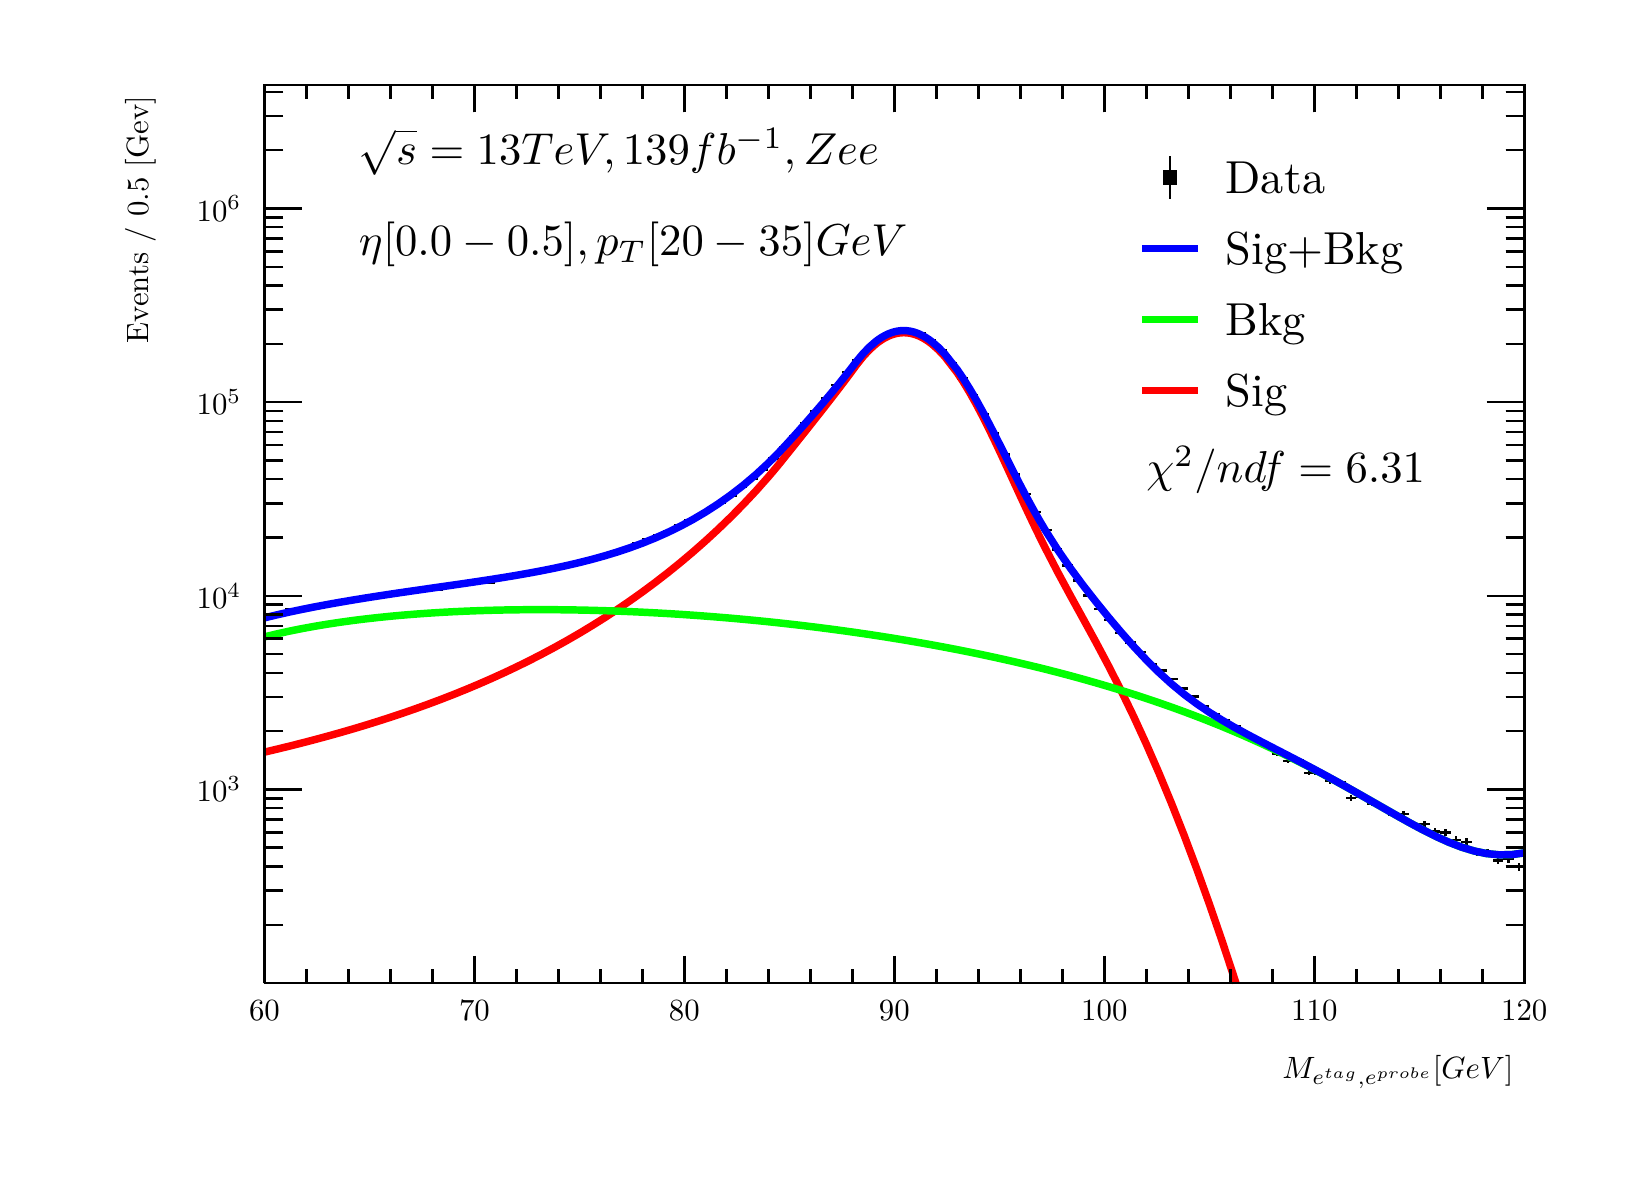
\begin{tikzpicture}
\pgfdeclareplotmark{cross} {
\pgfpathmoveto{\pgfpoint{-0.3\pgfplotmarksize}{\pgfplotmarksize}}
\pgfpathlineto{\pgfpoint{+0.3\pgfplotmarksize}{\pgfplotmarksize}}
\pgfpathlineto{\pgfpoint{+0.3\pgfplotmarksize}{0.3\pgfplotmarksize}}
\pgfpathlineto{\pgfpoint{+1\pgfplotmarksize}{0.3\pgfplotmarksize}}
\pgfpathlineto{\pgfpoint{+1\pgfplotmarksize}{-0.3\pgfplotmarksize}}
\pgfpathlineto{\pgfpoint{+0.3\pgfplotmarksize}{-0.3\pgfplotmarksize}}
\pgfpathlineto{\pgfpoint{+0.3\pgfplotmarksize}{-1.\pgfplotmarksize}}
\pgfpathlineto{\pgfpoint{-0.3\pgfplotmarksize}{-1.\pgfplotmarksize}}
\pgfpathlineto{\pgfpoint{-0.3\pgfplotmarksize}{-0.3\pgfplotmarksize}}
\pgfpathlineto{\pgfpoint{-1.\pgfplotmarksize}{-0.3\pgfplotmarksize}}
\pgfpathlineto{\pgfpoint{-1.\pgfplotmarksize}{0.3\pgfplotmarksize}}
\pgfpathlineto{\pgfpoint{-0.3\pgfplotmarksize}{0.3\pgfplotmarksize}}
\pgfpathclose
\pgfusepathqstroke
}
\pgfdeclareplotmark{cross*} {
\pgfpathmoveto{\pgfpoint{-0.3\pgfplotmarksize}{\pgfplotmarksize}}
\pgfpathlineto{\pgfpoint{+0.3\pgfplotmarksize}{\pgfplotmarksize}}
\pgfpathlineto{\pgfpoint{+0.3\pgfplotmarksize}{0.3\pgfplotmarksize}}
\pgfpathlineto{\pgfpoint{+1\pgfplotmarksize}{0.3\pgfplotmarksize}}
\pgfpathlineto{\pgfpoint{+1\pgfplotmarksize}{-0.3\pgfplotmarksize}}
\pgfpathlineto{\pgfpoint{+0.3\pgfplotmarksize}{-0.3\pgfplotmarksize}}
\pgfpathlineto{\pgfpoint{+0.3\pgfplotmarksize}{-1.\pgfplotmarksize}}
\pgfpathlineto{\pgfpoint{-0.3\pgfplotmarksize}{-1.\pgfplotmarksize}}
\pgfpathlineto{\pgfpoint{-0.3\pgfplotmarksize}{-0.3\pgfplotmarksize}}
\pgfpathlineto{\pgfpoint{-1.\pgfplotmarksize}{-0.3\pgfplotmarksize}}
\pgfpathlineto{\pgfpoint{-1.\pgfplotmarksize}{0.3\pgfplotmarksize}}
\pgfpathlineto{\pgfpoint{-0.3\pgfplotmarksize}{0.3\pgfplotmarksize}}
\pgfpathclose
\pgfusepathqfillstroke
}
\pgfdeclareplotmark{newstar} {
\pgfpathmoveto{\pgfqpoint{0pt}{\pgfplotmarksize}}
\pgfpathlineto{\pgfqpointpolar{44}{0.5\pgfplotmarksize}}
\pgfpathlineto{\pgfqpointpolar{18}{\pgfplotmarksize}}
\pgfpathlineto{\pgfqpointpolar{-20}{0.5\pgfplotmarksize}}
\pgfpathlineto{\pgfqpointpolar{-54}{\pgfplotmarksize}}
\pgfpathlineto{\pgfqpointpolar{-90}{0.5\pgfplotmarksize}}
\pgfpathlineto{\pgfqpointpolar{234}{\pgfplotmarksize}}
\pgfpathlineto{\pgfqpointpolar{198}{0.5\pgfplotmarksize}}
\pgfpathlineto{\pgfqpointpolar{162}{\pgfplotmarksize}}
\pgfpathlineto{\pgfqpointpolar{134}{0.5\pgfplotmarksize}}
\pgfpathclose
\pgfusepathqstroke
}
\pgfdeclareplotmark{newstar*} {
\pgfpathmoveto{\pgfqpoint{0pt}{\pgfplotmarksize}}
\pgfpathlineto{\pgfqpointpolar{44}{0.5\pgfplotmarksize}}
\pgfpathlineto{\pgfqpointpolar{18}{\pgfplotmarksize}}
\pgfpathlineto{\pgfqpointpolar{-20}{0.5\pgfplotmarksize}}
\pgfpathlineto{\pgfqpointpolar{-54}{\pgfplotmarksize}}
\pgfpathlineto{\pgfqpointpolar{-90}{0.5\pgfplotmarksize}}
\pgfpathlineto{\pgfqpointpolar{234}{\pgfplotmarksize}}
\pgfpathlineto{\pgfqpointpolar{198}{0.5\pgfplotmarksize}}
\pgfpathlineto{\pgfqpointpolar{162}{\pgfplotmarksize}}
\pgfpathlineto{\pgfqpointpolar{134}{0.5\pgfplotmarksize}}
\pgfpathclose
\pgfusepathqfillstroke
}
\definecolor{c}{rgb}{1,1,1};
\draw [color=c, fill=c] (0,0) rectangle (20,14.4361);
\draw [color=c, fill=c] (3,2.30977) rectangle (19,13.7143);
\definecolor{c}{rgb}{0,0,0};
\draw [c,line width=0.9] (3,2.30977) -- (3,13.7143) -- (19,13.7143) -- (19,2.30977) -- (3,2.30977);
\definecolor{c}{rgb}{1,1,1};
\draw [color=c, fill=c] (3,2.30977) rectangle (19,13.7143);
\definecolor{c}{rgb}{0,0,0};
\draw [c,line width=0.9] (3,2.30977) -- (3,13.7143) -- (19,13.7143) -- (19,2.30977) -- (3,2.30977);
\draw [c,line width=0.9] (3,2.30977) -- (19,2.30977);
\draw [c,line width=0.9] (3,2.65624) -- (3,2.30977);
\draw [c,line width=0.9] (3.53333,2.48301) -- (3.53333,2.30977);
\draw [c,line width=0.9] (4.06667,2.48301) -- (4.06667,2.30977);
\draw [c,line width=0.9] (4.6,2.48301) -- (4.6,2.30977);
\draw [c,line width=0.9] (5.13333,2.48301) -- (5.13333,2.30977);
\draw [c,line width=0.9] (5.66667,2.65624) -- (5.66667,2.30977);
\draw [c,line width=0.9] (6.2,2.48301) -- (6.2,2.30977);
\draw [c,line width=0.9] (6.73333,2.48301) -- (6.73333,2.30977);
\draw [c,line width=0.9] (7.26667,2.48301) -- (7.26667,2.30977);
\draw [c,line width=0.9] (7.8,2.48301) -- (7.8,2.30977);
\draw [c,line width=0.9] (8.33333,2.65624) -- (8.33333,2.30977);
\draw [c,line width=0.9] (8.86667,2.48301) -- (8.86667,2.30977);
\draw [c,line width=0.9] (9.4,2.48301) -- (9.4,2.30977);
\draw [c,line width=0.9] (9.93333,2.48301) -- (9.93333,2.30977);
\draw [c,line width=0.9] (10.4667,2.48301) -- (10.4667,2.30977);
\draw [c,line width=0.9] (11,2.65624) -- (11,2.30977);
\draw [c,line width=0.9] (11.5333,2.48301) -- (11.5333,2.30977);
\draw [c,line width=0.9] (12.0667,2.48301) -- (12.0667,2.30977);
\draw [c,line width=0.9] (12.6,2.48301) -- (12.6,2.30977);
\draw [c,line width=0.9] (13.1333,2.48301) -- (13.1333,2.30977);
\draw [c,line width=0.9] (13.6667,2.65624) -- (13.6667,2.30977);
\draw [c,line width=0.9] (14.2,2.48301) -- (14.2,2.30977);
\draw [c,line width=0.9] (14.7333,2.48301) -- (14.7333,2.30977);
\draw [c,line width=0.9] (15.2667,2.48301) -- (15.2667,2.30977);
\draw [c,line width=0.9] (15.8,2.48301) -- (15.8,2.30977);
\draw [c,line width=0.9] (16.3333,2.65624) -- (16.3333,2.30977);
\draw [c,line width=0.9] (16.8667,2.48301) -- (16.8667,2.30977);
\draw [c,line width=0.9] (17.4,2.48301) -- (17.4,2.30977);
\draw [c,line width=0.9] (17.9333,2.48301) -- (17.9333,2.30977);
\draw [c,line width=0.9] (18.4667,2.48301) -- (18.4667,2.30977);
\draw [c,line width=0.9] (19,2.65624) -- (19,2.30977);
\draw [anchor=base] (3,1.83338) node[scale=1.11327, color=c, rotate=0]{60};
\draw [anchor=base] (5.66667,1.83338) node[scale=1.11327, color=c, rotate=0]{70};
\draw [anchor=base] (8.33333,1.83338) node[scale=1.11327, color=c, rotate=0]{80};
\draw [anchor=base] (11,1.83338) node[scale=1.11327, color=c, rotate=0]{90};
\draw [anchor=base] (13.6667,1.83338) node[scale=1.11327, color=c, rotate=0]{100};
\draw [anchor=base] (16.3333,1.83338) node[scale=1.11327, color=c, rotate=0]{110};
\draw [anchor=base] (19,1.83338) node[scale=1.11327, color=c, rotate=0]{120};
\draw [anchor= east] (19,1.17798) node[scale=1.11327, color=c, rotate=0]{$M_{e^{tag}, e^{probe}}  [GeV]$};
\draw [c,line width=0.9] (3,13.7143) -- (19,13.7143);
\draw [c,line width=0.9] (3,13.3678) -- (3,13.7143);
\draw [c,line width=0.9] (3.53333,13.5411) -- (3.53333,13.7143);
\draw [c,line width=0.9] (4.06667,13.5411) -- (4.06667,13.7143);
\draw [c,line width=0.9] (4.6,13.5411) -- (4.6,13.7143);
\draw [c,line width=0.9] (5.13333,13.5411) -- (5.13333,13.7143);
\draw [c,line width=0.9] (5.66667,13.3678) -- (5.66667,13.7143);
\draw [c,line width=0.9] (6.2,13.5411) -- (6.2,13.7143);
\draw [c,line width=0.9] (6.73333,13.5411) -- (6.73333,13.7143);
\draw [c,line width=0.9] (7.26667,13.5411) -- (7.26667,13.7143);
\draw [c,line width=0.9] (7.8,13.5411) -- (7.8,13.7143);
\draw [c,line width=0.9] (8.33333,13.3678) -- (8.33333,13.7143);
\draw [c,line width=0.9] (8.86667,13.5411) -- (8.86667,13.7143);
\draw [c,line width=0.9] (9.4,13.5411) -- (9.4,13.7143);
\draw [c,line width=0.9] (9.93333,13.5411) -- (9.93333,13.7143);
\draw [c,line width=0.9] (10.4667,13.5411) -- (10.4667,13.7143);
\draw [c,line width=0.9] (11,13.3678) -- (11,13.7143);
\draw [c,line width=0.9] (11.5333,13.5411) -- (11.5333,13.7143);
\draw [c,line width=0.9] (12.0667,13.5411) -- (12.0667,13.7143);
\draw [c,line width=0.9] (12.6,13.5411) -- (12.6,13.7143);
\draw [c,line width=0.9] (13.1333,13.5411) -- (13.1333,13.7143);
\draw [c,line width=0.9] (13.6667,13.3678) -- (13.6667,13.7143);
\draw [c,line width=0.9] (14.2,13.5411) -- (14.2,13.7143);
\draw [c,line width=0.9] (14.7333,13.5411) -- (14.7333,13.7143);
\draw [c,line width=0.9] (15.2667,13.5411) -- (15.2667,13.7143);
\draw [c,line width=0.9] (15.8,13.5411) -- (15.8,13.7143);
\draw [c,line width=0.9] (16.3333,13.3678) -- (16.3333,13.7143);
\draw [c,line width=0.9] (16.8667,13.5411) -- (16.8667,13.7143);
\draw [c,line width=0.9] (17.4,13.5411) -- (17.4,13.7143);
\draw [c,line width=0.9] (17.9333,13.5411) -- (17.9333,13.7143);
\draw [c,line width=0.9] (18.4667,13.5411) -- (18.4667,13.7143);
\draw [c,line width=0.9] (19,13.3678) -- (19,13.7143);
\draw [c,line width=0.9] (3,2.30977) -- (3,13.7143);
\draw [c,line width=0.9] (3.237,3.05008) -- (3,3.05008);
\draw [c,line width=0.9] (3.237,3.48313) -- (3,3.48313);
\draw [c,line width=0.9] (3.237,3.79038) -- (3,3.79038);
\draw [c,line width=0.9] (3.237,4.02871) -- (3,4.02871);
\draw [c,line width=0.9] (3.237,4.22343) -- (3,4.22343);
\draw [c,line width=0.9] (3.237,4.38807) -- (3,4.38807);
\draw [c,line width=0.9] (3.237,4.53069) -- (3,4.53069);
\draw [c,line width=0.9] (3.237,4.65649) -- (3,4.65649);
\draw [c,line width=0.9] (3.474,4.76901) -- (3,4.76901);
\draw [anchor= east] (2.844,4.76901) node[scale=1.11327, color=c, rotate=0]{$10^{3}$};
\draw [c,line width=0.9] (3.237,5.50932) -- (3,5.50932);
\draw [c,line width=0.9] (3.237,5.94237) -- (3,5.94237);
\draw [c,line width=0.9] (3.237,6.24963) -- (3,6.24963);
\draw [c,line width=0.9] (3.237,6.48795) -- (3,6.48795);
\draw [c,line width=0.9] (3.237,6.68268) -- (3,6.68268);
\draw [c,line width=0.9] (3.237,6.84731) -- (3,6.84731);
\draw [c,line width=0.9] (3.237,6.98993) -- (3,6.98993);
\draw [c,line width=0.9] (3.237,7.11573) -- (3,7.11573);
\draw [c,line width=0.9] (3.474,7.22826) -- (3,7.22826);
\draw [anchor= east] (2.844,7.22826) node[scale=1.11327, color=c, rotate=0]{$10^{4}$};
\draw [c,line width=0.9] (3.237,7.96856) -- (3,7.96856);
\draw [c,line width=0.9] (3.237,8.40161) -- (3,8.40161);
\draw [c,line width=0.9] (3.237,8.70887) -- (3,8.70887);
\draw [c,line width=0.9] (3.237,8.94719) -- (3,8.94719);
\draw [c,line width=0.9] (3.237,9.14192) -- (3,9.14192);
\draw [c,line width=0.9] (3.237,9.30656) -- (3,9.30656);
\draw [c,line width=0.9] (3.237,9.44917) -- (3,9.44917);
\draw [c,line width=0.9] (3.237,9.57497) -- (3,9.57497);
\draw [c,line width=0.9] (3.474,9.6875) -- (3,9.6875);
\draw [anchor= east] (2.844,9.6875) node[scale=1.11327, color=c, rotate=0]{$10^{5}$};
\draw [c,line width=0.9] (3.237,10.4278) -- (3,10.4278);
\draw [c,line width=0.9] (3.237,10.8609) -- (3,10.8609);
\draw [c,line width=0.9] (3.237,11.1681) -- (3,11.1681);
\draw [c,line width=0.9] (3.237,11.4064) -- (3,11.4064);
\draw [c,line width=0.9] (3.237,11.6012) -- (3,11.6012);
\draw [c,line width=0.9] (3.237,11.7658) -- (3,11.7658);
\draw [c,line width=0.9] (3.237,11.9084) -- (3,11.9084);
\draw [c,line width=0.9] (3.237,12.0342) -- (3,12.0342);
\draw [c,line width=0.9] (3.474,12.1467) -- (3,12.1467);
\draw [anchor= east] (2.844,12.1467) node[scale=1.11327, color=c, rotate=0]{$10^{6}$};
\draw [c,line width=0.9] (3.237,12.887) -- (3,12.887);
\draw [c,line width=0.9] (3.237,13.3201) -- (3,13.3201);
\draw [c,line width=0.9] (3.237,13.6274) -- (3,13.6274);
\draw [anchor= east] (1.432,13.7143) node[scale=1.11327, color=c, rotate=90]{Events / 0.5 [Gev]};
\draw [c,line width=0.9] (19,2.30977) -- (19,13.7143);
\draw [c,line width=0.9] (18.763,3.05008) -- (19,3.05008);
\draw [c,line width=0.9] (18.763,3.48313) -- (19,3.48313);
\draw [c,line width=0.9] (18.763,3.79038) -- (19,3.79038);
\draw [c,line width=0.9] (18.763,4.02871) -- (19,4.02871);
\draw [c,line width=0.9] (18.763,4.22343) -- (19,4.22343);
\draw [c,line width=0.9] (18.763,4.38807) -- (19,4.38807);
\draw [c,line width=0.9] (18.763,4.53069) -- (19,4.53069);
\draw [c,line width=0.9] (18.763,4.65649) -- (19,4.65649);
\draw [c,line width=0.9] (18.526,4.76901) -- (19,4.76901);
\draw [c,line width=0.9] (18.763,5.50932) -- (19,5.50932);
\draw [c,line width=0.9] (18.763,5.94237) -- (19,5.94237);
\draw [c,line width=0.9] (18.763,6.24963) -- (19,6.24963);
\draw [c,line width=0.9] (18.763,6.48795) -- (19,6.48795);
\draw [c,line width=0.9] (18.763,6.68268) -- (19,6.68268);
\draw [c,line width=0.9] (18.763,6.84731) -- (19,6.84731);
\draw [c,line width=0.9] (18.763,6.98993) -- (19,6.98993);
\draw [c,line width=0.9] (18.763,7.11573) -- (19,7.11573);
\draw [c,line width=0.9] (18.526,7.22826) -- (19,7.22826);
\draw [c,line width=0.9] (18.763,7.96856) -- (19,7.96856);
\draw [c,line width=0.9] (18.763,8.40161) -- (19,8.40161);
\draw [c,line width=0.9] (18.763,8.70887) -- (19,8.70887);
\draw [c,line width=0.9] (18.763,8.94719) -- (19,8.94719);
\draw [c,line width=0.9] (18.763,9.14192) -- (19,9.14192);
\draw [c,line width=0.9] (18.763,9.30656) -- (19,9.30656);
\draw [c,line width=0.9] (18.763,9.44917) -- (19,9.44917);
\draw [c,line width=0.9] (18.763,9.57497) -- (19,9.57497);
\draw [c,line width=0.9] (18.526,9.6875) -- (19,9.6875);
\draw [c,line width=0.9] (18.763,10.4278) -- (19,10.4278);
\draw [c,line width=0.9] (18.763,10.8609) -- (19,10.8609);
\draw [c,line width=0.9] (18.763,11.1681) -- (19,11.1681);
\draw [c,line width=0.9] (18.763,11.4064) -- (19,11.4064);
\draw [c,line width=0.9] (18.763,11.6012) -- (19,11.6012);
\draw [c,line width=0.9] (18.763,11.7658) -- (19,11.7658);
\draw [c,line width=0.9] (18.763,11.9084) -- (19,11.9084);
\draw [c,line width=0.9] (18.763,12.0342) -- (19,12.0342);
\draw [c,line width=0.9] (18.526,12.1467) -- (19,12.1467);
\draw [c,line width=0.9] (18.763,12.887) -- (19,12.887);
\draw [c,line width=0.9] (18.763,13.3201) -- (19,13.3201);
\draw [c,line width=0.9] (18.763,13.6274) -- (19,13.6274);
\draw [c,line width=0.9] (3.06667,6.97555) -- (3,6.97555);
\draw [c,line width=0.9] (3,6.97555) -- (3,6.97555);
\draw [c,line width=0.9] (3.06667,6.97555) -- (3.13333,6.97555);
\draw [c,line width=0.9] (3.13333,6.97555) -- (3.13333,6.97555);
\draw [c,line width=0.9] (3.06667,6.97555) -- (3.06667,6.98757);
\draw [c,line width=0.9] (3.06667,6.98757) -- (3.06667,6.98757);
\draw [c,line width=0.9] (3.06667,6.97555) -- (3.06667,6.96353);
\draw [c,line width=0.9] (3.06667,6.96353) -- (3.06667,6.96353);
\draw [c,line width=0.9] (3.2,6.99897) -- (3.13333,6.99897);
\draw [c,line width=0.9] (3.13333,6.99897) -- (3.13333,6.99897);
\draw [c,line width=0.9] (3.2,6.99897) -- (3.26667,6.99897);
\draw [c,line width=0.9] (3.26667,6.99897) -- (3.26667,6.99897);
\draw [c,line width=0.9] (3.2,6.99897) -- (3.2,7.01086);
\draw [c,line width=0.9] (3.2,7.01086) -- (3.2,7.01086);
\draw [c,line width=0.9] (3.2,6.99897) -- (3.2,6.98708);
\draw [c,line width=0.9] (3.2,6.98708) -- (3.2,6.98708);
\draw [c,line width=0.9] (3.33333,7.05305) -- (3.26667,7.05305);
\draw [c,line width=0.9] (3.26667,7.05305) -- (3.26667,7.05305);
\draw [c,line width=0.9] (3.33333,7.05305) -- (3.4,7.05305);
\draw [c,line width=0.9] (3.4,7.05305) -- (3.4,7.05305);
\draw [c,line width=0.9] (3.33333,7.05305) -- (3.33333,7.06464);
\draw [c,line width=0.9] (3.33333,7.06464) -- (3.33333,7.06464);
\draw [c,line width=0.9] (3.33333,7.05305) -- (3.33333,7.04145);
\draw [c,line width=0.9] (3.33333,7.04145) -- (3.33333,7.04145);
\draw [c,line width=0.9] (3.46667,7.05619) -- (3.4,7.05619);
\draw [c,line width=0.9] (3.4,7.05619) -- (3.4,7.05619);
\draw [c,line width=0.9] (3.46667,7.05619) -- (3.53333,7.05619);
\draw [c,line width=0.9] (3.53333,7.05619) -- (3.53333,7.05619);
\draw [c,line width=0.9] (3.46667,7.05619) -- (3.46667,7.06776);
\draw [c,line width=0.9] (3.46667,7.06776) -- (3.46667,7.06776);
\draw [c,line width=0.9] (3.46667,7.05619) -- (3.46667,7.04461);
\draw [c,line width=0.9] (3.46667,7.04461) -- (3.46667,7.04461);
\draw [c,line width=0.9] (3.6,7.09403) -- (3.53333,7.09403);
\draw [c,line width=0.9] (3.53333,7.09403) -- (3.53333,7.09403);
\draw [c,line width=0.9] (3.6,7.09403) -- (3.66667,7.09403);
\draw [c,line width=0.9] (3.66667,7.09403) -- (3.66667,7.09403);
\draw [c,line width=0.9] (3.6,7.09403) -- (3.6,7.1054);
\draw [c,line width=0.9] (3.6,7.1054) -- (3.6,7.1054);
\draw [c,line width=0.9] (3.6,7.09403) -- (3.6,7.08266);
\draw [c,line width=0.9] (3.6,7.08266) -- (3.6,7.08266);
\draw [c,line width=0.9] (3.73333,7.12094) -- (3.66667,7.12094);
\draw [c,line width=0.9] (3.66667,7.12094) -- (3.66667,7.12094);
\draw [c,line width=0.9] (3.73333,7.12094) -- (3.8,7.12094);
\draw [c,line width=0.9] (3.8,7.12094) -- (3.8,7.12094);
\draw [c,line width=0.9] (3.73333,7.12094) -- (3.73333,7.13217);
\draw [c,line width=0.9] (3.73333,7.13217) -- (3.73333,7.13217);
\draw [c,line width=0.9] (3.73333,7.12094) -- (3.73333,7.10971);
\draw [c,line width=0.9] (3.73333,7.10971) -- (3.73333,7.10971);
\draw [c,line width=0.9] (3.86667,7.1328) -- (3.8,7.1328);
\draw [c,line width=0.9] (3.8,7.1328) -- (3.8,7.1328);
\draw [c,line width=0.9] (3.86667,7.1328) -- (3.93333,7.1328);
\draw [c,line width=0.9] (3.93333,7.1328) -- (3.93333,7.1328);
\draw [c,line width=0.9] (3.86667,7.1328) -- (3.86667,7.14397);
\draw [c,line width=0.9] (3.86667,7.14397) -- (3.86667,7.14397);
\draw [c,line width=0.9] (3.86667,7.1328) -- (3.86667,7.12163);
\draw [c,line width=0.9] (3.86667,7.12163) -- (3.86667,7.12163);
\draw [c,line width=0.9] (4,7.15407) -- (3.93333,7.15407);
\draw [c,line width=0.9] (3.93333,7.15407) -- (3.93333,7.15407);
\draw [c,line width=0.9] (4,7.15407) -- (4.06667,7.15407);
\draw [c,line width=0.9] (4.06667,7.15407) -- (4.06667,7.15407);
\draw [c,line width=0.9] (4,7.15407) -- (4,7.16513);
\draw [c,line width=0.9] (4,7.16513) -- (4,7.16513);
\draw [c,line width=0.9] (4,7.15407) -- (4,7.14302);
\draw [c,line width=0.9] (4,7.14302) -- (4,7.14302);
\draw [c,line width=0.9] (4.13333,7.18377) -- (4.06667,7.18377);
\draw [c,line width=0.9] (4.06667,7.18377) -- (4.06667,7.18377);
\draw [c,line width=0.9] (4.13333,7.18377) -- (4.2,7.18377);
\draw [c,line width=0.9] (4.2,7.18377) -- (4.2,7.18377);
\draw [c,line width=0.9] (4.13333,7.18377) -- (4.13333,7.19467);
\draw [c,line width=0.9] (4.13333,7.19467) -- (4.13333,7.19467);
\draw [c,line width=0.9] (4.13333,7.18377) -- (4.13333,7.17286);
\draw [c,line width=0.9] (4.13333,7.17286) -- (4.13333,7.17286);
\draw [c,line width=0.9] (4.26667,7.21439) -- (4.2,7.21439);
\draw [c,line width=0.9] (4.2,7.21439) -- (4.2,7.21439);
\draw [c,line width=0.9] (4.26667,7.21439) -- (4.33333,7.21439);
\draw [c,line width=0.9] (4.33333,7.21439) -- (4.33333,7.21439);
\draw [c,line width=0.9] (4.26667,7.21439) -- (4.26667,7.22514);
\draw [c,line width=0.9] (4.26667,7.22514) -- (4.26667,7.22514);
\draw [c,line width=0.9] (4.26667,7.21439) -- (4.26667,7.20364);
\draw [c,line width=0.9] (4.26667,7.20364) -- (4.26667,7.20364);
\draw [c,line width=0.9] (4.4,7.21114) -- (4.33333,7.21114);
\draw [c,line width=0.9] (4.33333,7.21114) -- (4.33333,7.21114);
\draw [c,line width=0.9] (4.4,7.21114) -- (4.46667,7.21114);
\draw [c,line width=0.9] (4.46667,7.21114) -- (4.46667,7.21114);
\draw [c,line width=0.9] (4.4,7.21114) -- (4.4,7.22191);
\draw [c,line width=0.9] (4.4,7.22191) -- (4.4,7.22191);
\draw [c,line width=0.9] (4.4,7.21114) -- (4.4,7.20037);
\draw [c,line width=0.9] (4.4,7.20037) -- (4.4,7.20037);
\draw [c,line width=0.9] (4.53333,7.21979) -- (4.46667,7.21979);
\draw [c,line width=0.9] (4.46667,7.21979) -- (4.46667,7.21979);
\draw [c,line width=0.9] (4.53333,7.21979) -- (4.6,7.21979);
\draw [c,line width=0.9] (4.6,7.21979) -- (4.6,7.21979);
\draw [c,line width=0.9] (4.53333,7.21979) -- (4.53333,7.23051);
\draw [c,line width=0.9] (4.53333,7.23051) -- (4.53333,7.23051);
\draw [c,line width=0.9] (4.53333,7.21979) -- (4.53333,7.20906);
\draw [c,line width=0.9] (4.53333,7.20906) -- (4.53333,7.20906);
\draw [c,line width=0.9] (4.66667,7.23878) -- (4.6,7.23878);
\draw [c,line width=0.9] (4.6,7.23878) -- (4.6,7.23878);
\draw [c,line width=0.9] (4.66667,7.23878) -- (4.73333,7.23878);
\draw [c,line width=0.9] (4.73333,7.23878) -- (4.73333,7.23878);
\draw [c,line width=0.9] (4.66667,7.23878) -- (4.66667,7.24941);
\draw [c,line width=0.9] (4.66667,7.24941) -- (4.66667,7.24941);
\draw [c,line width=0.9] (4.66667,7.23878) -- (4.66667,7.22815);
\draw [c,line width=0.9] (4.66667,7.22815) -- (4.66667,7.22815);
\draw [c,line width=0.9] (4.8,7.28756) -- (4.73333,7.28756);
\draw [c,line width=0.9] (4.73333,7.28756) -- (4.73333,7.28756);
\draw [c,line width=0.9] (4.8,7.28756) -- (4.86667,7.28756);
\draw [c,line width=0.9] (4.86667,7.28756) -- (4.86667,7.28756);
\draw [c,line width=0.9] (4.8,7.28756) -- (4.8,7.29795);
\draw [c,line width=0.9] (4.8,7.29795) -- (4.8,7.29795);
\draw [c,line width=0.9] (4.8,7.28756) -- (4.8,7.27718);
\draw [c,line width=0.9] (4.8,7.27718) -- (4.8,7.27718);
\draw [c,line width=0.9] (4.93333,7.27425) -- (4.86667,7.27425);
\draw [c,line width=0.9] (4.86667,7.27425) -- (4.86667,7.27425);
\draw [c,line width=0.9] (4.93333,7.27425) -- (5,7.27425);
\draw [c,line width=0.9] (5,7.27425) -- (5,7.27425);
\draw [c,line width=0.9] (4.93333,7.27425) -- (4.93333,7.2847);
\draw [c,line width=0.9] (4.93333,7.2847) -- (4.93333,7.2847);
\draw [c,line width=0.9] (4.93333,7.27425) -- (4.93333,7.26379);
\draw [c,line width=0.9] (4.93333,7.26379) -- (4.93333,7.26379);
\draw [c,line width=0.9] (5.06667,7.30986) -- (5,7.30986);
\draw [c,line width=0.9] (5,7.30986) -- (5,7.30986);
\draw [c,line width=0.9] (5.06667,7.30986) -- (5.13333,7.30986);
\draw [c,line width=0.9] (5.13333,7.30986) -- (5.13333,7.30986);
\draw [c,line width=0.9] (5.06667,7.30986) -- (5.06667,7.32014);
\draw [c,line width=0.9] (5.06667,7.32014) -- (5.06667,7.32014);
\draw [c,line width=0.9] (5.06667,7.30986) -- (5.06667,7.29958);
\draw [c,line width=0.9] (5.06667,7.29958) -- (5.06667,7.29958);
\draw [c,line width=0.9] (5.2,7.31065) -- (5.13333,7.31065);
\draw [c,line width=0.9] (5.13333,7.31065) -- (5.13333,7.31065);
\draw [c,line width=0.9] (5.2,7.31065) -- (5.26667,7.31065);
\draw [c,line width=0.9] (5.26667,7.31065) -- (5.26667,7.31065);
\draw [c,line width=0.9] (5.2,7.31065) -- (5.2,7.32093);
\draw [c,line width=0.9] (5.2,7.32093) -- (5.2,7.32093);
\draw [c,line width=0.9] (5.2,7.31065) -- (5.2,7.30038);
\draw [c,line width=0.9] (5.2,7.30038) -- (5.2,7.30038);
\draw [c,line width=0.9] (5.33333,7.34844) -- (5.26667,7.34844);
\draw [c,line width=0.9] (5.26667,7.34844) -- (5.26667,7.34844);
\draw [c,line width=0.9] (5.33333,7.34844) -- (5.4,7.34844);
\draw [c,line width=0.9] (5.4,7.34844) -- (5.4,7.34844);
\draw [c,line width=0.9] (5.33333,7.34844) -- (5.33333,7.35853);
\draw [c,line width=0.9] (5.33333,7.35853) -- (5.33333,7.35853);
\draw [c,line width=0.9] (5.33333,7.34844) -- (5.33333,7.33834);
\draw [c,line width=0.9] (5.33333,7.33834) -- (5.33333,7.33834);
\draw [c,line width=0.9] (5.46667,7.35358) -- (5.4,7.35358);
\draw [c,line width=0.9] (5.4,7.35358) -- (5.4,7.35358);
\draw [c,line width=0.9] (5.46667,7.35358) -- (5.53333,7.35358);
\draw [c,line width=0.9] (5.53333,7.35358) -- (5.53333,7.35358);
\draw [c,line width=0.9] (5.46667,7.35358) -- (5.46667,7.36365);
\draw [c,line width=0.9] (5.46667,7.36365) -- (5.46667,7.36365);
\draw [c,line width=0.9] (5.46667,7.35358) -- (5.46667,7.34351);
\draw [c,line width=0.9] (5.46667,7.34351) -- (5.46667,7.34351);
\draw [c,line width=0.9] (5.6,7.38401) -- (5.53333,7.38401);
\draw [c,line width=0.9] (5.53333,7.38401) -- (5.53333,7.38401);
\draw [c,line width=0.9] (5.6,7.38401) -- (5.66667,7.38401);
\draw [c,line width=0.9] (5.66667,7.38401) -- (5.66667,7.38401);
\draw [c,line width=0.9] (5.6,7.38401) -- (5.6,7.39394);
\draw [c,line width=0.9] (5.6,7.39394) -- (5.6,7.39394);
\draw [c,line width=0.9] (5.6,7.38401) -- (5.6,7.37408);
\draw [c,line width=0.9] (5.6,7.37408) -- (5.6,7.37408);
\draw [c,line width=0.9] (5.73333,7.39649) -- (5.66667,7.39649);
\draw [c,line width=0.9] (5.66667,7.39649) -- (5.66667,7.39649);
\draw [c,line width=0.9] (5.73333,7.39649) -- (5.8,7.39649);
\draw [c,line width=0.9] (5.8,7.39649) -- (5.8,7.39649);
\draw [c,line width=0.9] (5.73333,7.39649) -- (5.73333,7.40636);
\draw [c,line width=0.9] (5.73333,7.40636) -- (5.73333,7.40636);
\draw [c,line width=0.9] (5.73333,7.39649) -- (5.73333,7.38662);
\draw [c,line width=0.9] (5.73333,7.38662) -- (5.73333,7.38662);
\draw [c,line width=0.9] (5.86667,7.39722) -- (5.8,7.39722);
\draw [c,line width=0.9] (5.8,7.39722) -- (5.8,7.39722);
\draw [c,line width=0.9] (5.86667,7.39722) -- (5.93333,7.39722);
\draw [c,line width=0.9] (5.93333,7.39722) -- (5.93333,7.39722);
\draw [c,line width=0.9] (5.86667,7.39722) -- (5.86667,7.40709);
\draw [c,line width=0.9] (5.86667,7.40709) -- (5.86667,7.40709);
\draw [c,line width=0.9] (5.86667,7.39722) -- (5.86667,7.38735);
\draw [c,line width=0.9] (5.86667,7.38735) -- (5.86667,7.38735);
\draw [c,line width=0.9] (6,7.44378) -- (5.93333,7.44378);
\draw [c,line width=0.9] (5.93333,7.44378) -- (5.93333,7.44378);
\draw [c,line width=0.9] (6,7.44378) -- (6.06667,7.44378);
\draw [c,line width=0.9] (6.06667,7.44378) -- (6.06667,7.44378);
\draw [c,line width=0.9] (6,7.44378) -- (6,7.45344);
\draw [c,line width=0.9] (6,7.45344) -- (6,7.45344);
\draw [c,line width=0.9] (6,7.44378) -- (6,7.43413);
\draw [c,line width=0.9] (6,7.43413) -- (6,7.43413);
\draw [c,line width=0.9] (6.13333,7.45403) -- (6.06667,7.45403);
\draw [c,line width=0.9] (6.06667,7.45403) -- (6.06667,7.45403);
\draw [c,line width=0.9] (6.13333,7.45403) -- (6.2,7.45403);
\draw [c,line width=0.9] (6.2,7.45403) -- (6.2,7.45403);
\draw [c,line width=0.9] (6.13333,7.45403) -- (6.13333,7.46364);
\draw [c,line width=0.9] (6.13333,7.46364) -- (6.13333,7.46364);
\draw [c,line width=0.9] (6.13333,7.45403) -- (6.13333,7.44443);
\draw [c,line width=0.9] (6.13333,7.44443) -- (6.13333,7.44443);
\draw [c,line width=0.9] (6.26667,7.5008) -- (6.2,7.5008);
\draw [c,line width=0.9] (6.2,7.5008) -- (6.2,7.5008);
\draw [c,line width=0.9] (6.26667,7.5008) -- (6.33333,7.5008);
\draw [c,line width=0.9] (6.33333,7.5008) -- (6.33333,7.5008);
\draw [c,line width=0.9] (6.26667,7.5008) -- (6.26667,7.5102);
\draw [c,line width=0.9] (6.26667,7.5102) -- (6.26667,7.5102);
\draw [c,line width=0.9] (6.26667,7.5008) -- (6.26667,7.4914);
\draw [c,line width=0.9] (6.26667,7.4914) -- (6.26667,7.4914);
\draw [c,line width=0.9] (6.4,7.52162) -- (6.33333,7.52162);
\draw [c,line width=0.9] (6.33333,7.52162) -- (6.33333,7.52162);
\draw [c,line width=0.9] (6.4,7.52162) -- (6.46667,7.52162);
\draw [c,line width=0.9] (6.46667,7.52162) -- (6.46667,7.52162);
\draw [c,line width=0.9] (6.4,7.52162) -- (6.4,7.53093);
\draw [c,line width=0.9] (6.4,7.53093) -- (6.4,7.53093);
\draw [c,line width=0.9] (6.4,7.52162) -- (6.4,7.51231);
\draw [c,line width=0.9] (6.4,7.51231) -- (6.4,7.51231);
\draw [c,line width=0.9] (6.53333,7.54941) -- (6.46667,7.54941);
\draw [c,line width=0.9] (6.46667,7.54941) -- (6.46667,7.54941);
\draw [c,line width=0.9] (6.53333,7.54941) -- (6.6,7.54941);
\draw [c,line width=0.9] (6.6,7.54941) -- (6.6,7.54941);
\draw [c,line width=0.9] (6.53333,7.54941) -- (6.53333,7.5586);
\draw [c,line width=0.9] (6.53333,7.5586) -- (6.53333,7.5586);
\draw [c,line width=0.9] (6.53333,7.54941) -- (6.53333,7.54022);
\draw [c,line width=0.9] (6.53333,7.54022) -- (6.53333,7.54022);
\draw [c,line width=0.9] (6.66667,7.58211) -- (6.6,7.58211);
\draw [c,line width=0.9] (6.6,7.58211) -- (6.6,7.58211);
\draw [c,line width=0.9] (6.66667,7.58211) -- (6.73333,7.58211);
\draw [c,line width=0.9] (6.73333,7.58211) -- (6.73333,7.58211);
\draw [c,line width=0.9] (6.66667,7.58211) -- (6.66667,7.59116);
\draw [c,line width=0.9] (6.66667,7.59116) -- (6.66667,7.59116);
\draw [c,line width=0.9] (6.66667,7.58211) -- (6.66667,7.57306);
\draw [c,line width=0.9] (6.66667,7.57306) -- (6.66667,7.57306);
\draw [c,line width=0.9] (6.8,7.61094) -- (6.73333,7.61094);
\draw [c,line width=0.9] (6.73333,7.61094) -- (6.73333,7.61094);
\draw [c,line width=0.9] (6.8,7.61094) -- (6.86667,7.61094);
\draw [c,line width=0.9] (6.86667,7.61094) -- (6.86667,7.61094);
\draw [c,line width=0.9] (6.8,7.61094) -- (6.8,7.61987);
\draw [c,line width=0.9] (6.8,7.61987) -- (6.8,7.61987);
\draw [c,line width=0.9] (6.8,7.61094) -- (6.8,7.60201);
\draw [c,line width=0.9] (6.8,7.60201) -- (6.8,7.60201);
\draw [c,line width=0.9] (6.93333,7.6331) -- (6.86667,7.6331);
\draw [c,line width=0.9] (6.86667,7.6331) -- (6.86667,7.6331);
\draw [c,line width=0.9] (6.93333,7.6331) -- (7,7.6331);
\draw [c,line width=0.9] (7,7.6331) -- (7,7.6331);
\draw [c,line width=0.9] (6.93333,7.6331) -- (6.93333,7.64194);
\draw [c,line width=0.9] (6.93333,7.64194) -- (6.93333,7.64194);
\draw [c,line width=0.9] (6.93333,7.6331) -- (6.93333,7.62426);
\draw [c,line width=0.9] (6.93333,7.62426) -- (6.93333,7.62426);
\draw [c,line width=0.9] (7.06667,7.66734) -- (7,7.66734);
\draw [c,line width=0.9] (7,7.66734) -- (7,7.66734);
\draw [c,line width=0.9] (7.06667,7.66734) -- (7.13333,7.66734);
\draw [c,line width=0.9] (7.13333,7.66734) -- (7.13333,7.66734);
\draw [c,line width=0.9] (7.06667,7.66734) -- (7.06667,7.67604);
\draw [c,line width=0.9] (7.06667,7.67604) -- (7.06667,7.67604);
\draw [c,line width=0.9] (7.06667,7.66734) -- (7.06667,7.65865);
\draw [c,line width=0.9] (7.06667,7.65865) -- (7.06667,7.65865);
\draw [c,line width=0.9] (7.2,7.71829) -- (7.13333,7.71829);
\draw [c,line width=0.9] (7.13333,7.71829) -- (7.13333,7.71829);
\draw [c,line width=0.9] (7.2,7.71829) -- (7.26667,7.71829);
\draw [c,line width=0.9] (7.26667,7.71829) -- (7.26667,7.71829);
\draw [c,line width=0.9] (7.2,7.71829) -- (7.2,7.72678);
\draw [c,line width=0.9] (7.2,7.72678) -- (7.2,7.72678);
\draw [c,line width=0.9] (7.2,7.71829) -- (7.2,7.7098);
\draw [c,line width=0.9] (7.2,7.7098) -- (7.2,7.7098);
\draw [c,line width=0.9] (7.33333,7.73961) -- (7.26667,7.73961);
\draw [c,line width=0.9] (7.26667,7.73961) -- (7.26667,7.73961);
\draw [c,line width=0.9] (7.33333,7.73961) -- (7.4,7.73961);
\draw [c,line width=0.9] (7.4,7.73961) -- (7.4,7.73961);
\draw [c,line width=0.9] (7.33333,7.73961) -- (7.33333,7.74801);
\draw [c,line width=0.9] (7.33333,7.74801) -- (7.33333,7.74801);
\draw [c,line width=0.9] (7.33333,7.73961) -- (7.33333,7.7312);
\draw [c,line width=0.9] (7.33333,7.7312) -- (7.33333,7.7312);
\draw [c,line width=0.9] (7.46667,7.78235) -- (7.4,7.78235);
\draw [c,line width=0.9] (7.4,7.78235) -- (7.4,7.78235);
\draw [c,line width=0.9] (7.46667,7.78235) -- (7.53333,7.78235);
\draw [c,line width=0.9] (7.53333,7.78235) -- (7.53333,7.78235);
\draw [c,line width=0.9] (7.46667,7.78235) -- (7.46667,7.79059);
\draw [c,line width=0.9] (7.46667,7.79059) -- (7.46667,7.79059);
\draw [c,line width=0.9] (7.46667,7.78235) -- (7.46667,7.77411);
\draw [c,line width=0.9] (7.46667,7.77411) -- (7.46667,7.77411);
\draw [c,line width=0.9] (7.6,7.83343) -- (7.53333,7.83343);
\draw [c,line width=0.9] (7.53333,7.83343) -- (7.53333,7.83343);
\draw [c,line width=0.9] (7.6,7.83343) -- (7.66667,7.83343);
\draw [c,line width=0.9] (7.66667,7.83343) -- (7.66667,7.83343);
\draw [c,line width=0.9] (7.6,7.83343) -- (7.6,7.84147);
\draw [c,line width=0.9] (7.6,7.84147) -- (7.6,7.84147);
\draw [c,line width=0.9] (7.6,7.83343) -- (7.6,7.82538);
\draw [c,line width=0.9] (7.6,7.82538) -- (7.6,7.82538);
\draw [c,line width=0.9] (7.73333,7.89025) -- (7.66667,7.89025);
\draw [c,line width=0.9] (7.66667,7.89025) -- (7.66667,7.89025);
\draw [c,line width=0.9] (7.73333,7.89025) -- (7.8,7.89025);
\draw [c,line width=0.9] (7.8,7.89025) -- (7.8,7.89025);
\draw [c,line width=0.9] (7.73333,7.89025) -- (7.73333,7.89808);
\draw [c,line width=0.9] (7.73333,7.89808) -- (7.73333,7.89808);
\draw [c,line width=0.9] (7.73333,7.89025) -- (7.73333,7.88242);
\draw [c,line width=0.9] (7.73333,7.88242) -- (7.73333,7.88242);
\draw [c,line width=0.9] (7.86667,7.94824) -- (7.8,7.94824);
\draw [c,line width=0.9] (7.8,7.94824) -- (7.8,7.94824);
\draw [c,line width=0.9] (7.86667,7.94824) -- (7.93333,7.94824);
\draw [c,line width=0.9] (7.93333,7.94824) -- (7.93333,7.94824);
\draw [c,line width=0.9] (7.86667,7.94824) -- (7.86667,7.95586);
\draw [c,line width=0.9] (7.86667,7.95586) -- (7.86667,7.95586);
\draw [c,line width=0.9] (7.86667,7.94824) -- (7.86667,7.94061);
\draw [c,line width=0.9] (7.86667,7.94061) -- (7.86667,7.94061);
\draw [c,line width=0.9] (8,7.99107) -- (7.93333,7.99107);
\draw [c,line width=0.9] (7.93333,7.99107) -- (7.93333,7.99107);
\draw [c,line width=0.9] (8,7.99107) -- (8.06667,7.99107);
\draw [c,line width=0.9] (8.06667,7.99107) -- (8.06667,7.99107);
\draw [c,line width=0.9] (8,7.99107) -- (8,7.99855);
\draw [c,line width=0.9] (8,7.99855) -- (8,7.99855);
\draw [c,line width=0.9] (8,7.99107) -- (8,7.9836);
\draw [c,line width=0.9] (8,7.9836) -- (8,7.9836);
\draw [c,line width=0.9] (8.13333,8.04883) -- (8.06667,8.04883);
\draw [c,line width=0.9] (8.06667,8.04883) -- (8.06667,8.04883);
\draw [c,line width=0.9] (8.13333,8.04883) -- (8.2,8.04883);
\draw [c,line width=0.9] (8.2,8.04883) -- (8.2,8.04883);
\draw [c,line width=0.9] (8.13333,8.04883) -- (8.13333,8.0561);
\draw [c,line width=0.9] (8.13333,8.0561) -- (8.13333,8.0561);
\draw [c,line width=0.9] (8.13333,8.04883) -- (8.13333,8.04156);
\draw [c,line width=0.9] (8.13333,8.04156) -- (8.13333,8.04156);
\draw [c,line width=0.9] (8.26667,8.11821) -- (8.2,8.11821);
\draw [c,line width=0.9] (8.2,8.11821) -- (8.2,8.11821);
\draw [c,line width=0.9] (8.26667,8.11821) -- (8.33333,8.11821);
\draw [c,line width=0.9] (8.33333,8.11821) -- (8.33333,8.11821);
\draw [c,line width=0.9] (8.26667,8.11821) -- (8.26667,8.12525);
\draw [c,line width=0.9] (8.26667,8.12525) -- (8.26667,8.12525);
\draw [c,line width=0.9] (8.26667,8.11821) -- (8.26667,8.11116);
\draw [c,line width=0.9] (8.26667,8.11116) -- (8.26667,8.11116);
\draw [c,line width=0.9] (8.4,8.18278) -- (8.33333,8.18278);
\draw [c,line width=0.9] (8.33333,8.18278) -- (8.33333,8.18278);
\draw [c,line width=0.9] (8.4,8.18278) -- (8.46667,8.18278);
\draw [c,line width=0.9] (8.46667,8.18278) -- (8.46667,8.18278);
\draw [c,line width=0.9] (8.4,8.18278) -- (8.4,8.18961);
\draw [c,line width=0.9] (8.4,8.18961) -- (8.4,8.18961);
\draw [c,line width=0.9] (8.4,8.18278) -- (8.4,8.17595);
\draw [c,line width=0.9] (8.4,8.17595) -- (8.4,8.17595);
\draw [c,line width=0.9] (8.53333,8.25148) -- (8.46667,8.25148);
\draw [c,line width=0.9] (8.46667,8.25148) -- (8.46667,8.25148);
\draw [c,line width=0.9] (8.53333,8.25148) -- (8.6,8.25148);
\draw [c,line width=0.9] (8.6,8.25148) -- (8.6,8.25148);
\draw [c,line width=0.9] (8.53333,8.25148) -- (8.53333,8.2581);
\draw [c,line width=0.9] (8.53333,8.2581) -- (8.53333,8.2581);
\draw [c,line width=0.9] (8.53333,8.25148) -- (8.53333,8.24487);
\draw [c,line width=0.9] (8.53333,8.24487) -- (8.53333,8.24487);
\draw [c,line width=0.9] (8.66667,8.3296) -- (8.6,8.3296);
\draw [c,line width=0.9] (8.6,8.3296) -- (8.6,8.3296);
\draw [c,line width=0.9] (8.66667,8.3296) -- (8.73333,8.3296);
\draw [c,line width=0.9] (8.73333,8.3296) -- (8.73333,8.3296);
\draw [c,line width=0.9] (8.66667,8.3296) -- (8.66667,8.33598);
\draw [c,line width=0.9] (8.66667,8.33598) -- (8.66667,8.33598);
\draw [c,line width=0.9] (8.66667,8.3296) -- (8.66667,8.32323);
\draw [c,line width=0.9] (8.66667,8.32323) -- (8.66667,8.32323);
\draw [c,line width=0.9] (8.8,8.41062) -- (8.73333,8.41062);
\draw [c,line width=0.9] (8.73333,8.41062) -- (8.73333,8.41062);
\draw [c,line width=0.9] (8.8,8.41062) -- (8.86667,8.41062);
\draw [c,line width=0.9] (8.86667,8.41062) -- (8.86667,8.41062);
\draw [c,line width=0.9] (8.8,8.41062) -- (8.8,8.41676);
\draw [c,line width=0.9] (8.8,8.41676) -- (8.8,8.41676);
\draw [c,line width=0.9] (8.8,8.41062) -- (8.8,8.40448);
\draw [c,line width=0.9] (8.8,8.40448) -- (8.8,8.40448);
\draw [c,line width=0.9] (8.93333,8.50328) -- (8.86667,8.50328);
\draw [c,line width=0.9] (8.86667,8.50328) -- (8.86667,8.50328);
\draw [c,line width=0.9] (8.93333,8.50328) -- (9,8.50328);
\draw [c,line width=0.9] (9,8.50328) -- (9,8.50328);
\draw [c,line width=0.9] (8.93333,8.50328) -- (8.93333,8.50916);
\draw [c,line width=0.9] (8.93333,8.50916) -- (8.93333,8.50916);
\draw [c,line width=0.9] (8.93333,8.50328) -- (8.93333,8.4974);
\draw [c,line width=0.9] (8.93333,8.4974) -- (8.93333,8.4974);
\draw [c,line width=0.9] (9.06667,8.60958) -- (9,8.60958);
\draw [c,line width=0.9] (9,8.60958) -- (9,8.60958);
\draw [c,line width=0.9] (9.06667,8.60958) -- (9.13333,8.60958);
\draw [c,line width=0.9] (9.13333,8.60958) -- (9.13333,8.60958);
\draw [c,line width=0.9] (9.06667,8.60958) -- (9.06667,8.61517);
\draw [c,line width=0.9] (9.06667,8.61517) -- (9.06667,8.61517);
\draw [c,line width=0.9] (9.06667,8.60958) -- (9.06667,8.60398);
\draw [c,line width=0.9] (9.06667,8.60398) -- (9.06667,8.60398);
\draw [c,line width=0.9] (9.2,8.71741) -- (9.13333,8.71741);
\draw [c,line width=0.9] (9.13333,8.71741) -- (9.13333,8.71741);
\draw [c,line width=0.9] (9.2,8.71741) -- (9.26667,8.71741);
\draw [c,line width=0.9] (9.26667,8.71741) -- (9.26667,8.71741);
\draw [c,line width=0.9] (9.2,8.71741) -- (9.2,8.72272);
\draw [c,line width=0.9] (9.2,8.72272) -- (9.2,8.72272);
\draw [c,line width=0.9] (9.2,8.71741) -- (9.2,8.71209);
\draw [c,line width=0.9] (9.2,8.71209) -- (9.2,8.71209);
\draw [c,line width=0.9] (9.33333,8.83352) -- (9.26667,8.83352);
\draw [c,line width=0.9] (9.26667,8.83352) -- (9.26667,8.83352);
\draw [c,line width=0.9] (9.33333,8.83352) -- (9.4,8.83352);
\draw [c,line width=0.9] (9.4,8.83352) -- (9.4,8.83352);
\draw [c,line width=0.9] (9.33333,8.83352) -- (9.33333,8.83856);
\draw [c,line width=0.9] (9.33333,8.83856) -- (9.33333,8.83856);
\draw [c,line width=0.9] (9.33333,8.83352) -- (9.33333,8.82849);
\draw [c,line width=0.9] (9.33333,8.82849) -- (9.33333,8.82849);
\draw [c,line width=0.9] (9.46667,8.97016) -- (9.4,8.97016);
\draw [c,line width=0.9] (9.4,8.97016) -- (9.4,8.97016);
\draw [c,line width=0.9] (9.46667,8.97016) -- (9.53333,8.97016);
\draw [c,line width=0.9] (9.53333,8.97016) -- (9.53333,8.97016);
\draw [c,line width=0.9] (9.46667,8.97016) -- (9.46667,8.97489);
\draw [c,line width=0.9] (9.46667,8.97489) -- (9.46667,8.97489);
\draw [c,line width=0.9] (9.46667,8.97016) -- (9.46667,8.96544);
\draw [c,line width=0.9] (9.46667,8.96544) -- (9.46667,8.96544);
\draw [c,line width=0.9] (9.6,9.10987) -- (9.53333,9.10987);
\draw [c,line width=0.9] (9.53333,9.10987) -- (9.53333,9.10987);
\draw [c,line width=0.9] (9.6,9.10987) -- (9.66667,9.10987);
\draw [c,line width=0.9] (9.66667,9.10987) -- (9.66667,9.10987);
\draw [c,line width=0.9] (9.6,9.10987) -- (9.6,9.11429);
\draw [c,line width=0.9] (9.6,9.11429) -- (9.6,9.11429);
\draw [c,line width=0.9] (9.6,9.10987) -- (9.6,9.10544);
\draw [c,line width=0.9] (9.6,9.10544) -- (9.6,9.10544);
\draw [c,line width=0.9] (9.73333,9.25465) -- (9.66667,9.25465);
\draw [c,line width=0.9] (9.66667,9.25465) -- (9.66667,9.25465);
\draw [c,line width=0.9] (9.73333,9.25465) -- (9.8,9.25465);
\draw [c,line width=0.9] (9.8,9.25465) -- (9.8,9.25465);
\draw [c,line width=0.9] (9.73333,9.25465) -- (9.73333,9.25878);
\draw [c,line width=0.9] (9.73333,9.25878) -- (9.73333,9.25878);
\draw [c,line width=0.9] (9.73333,9.25465) -- (9.73333,9.25051);
\draw [c,line width=0.9] (9.73333,9.25051) -- (9.73333,9.25051);
\draw [c,line width=0.9] (9.86667,9.41402) -- (9.8,9.41402);
\draw [c,line width=0.9] (9.8,9.41402) -- (9.8,9.41402);
\draw [c,line width=0.9] (9.86667,9.41402) -- (9.93333,9.41402);
\draw [c,line width=0.9] (9.93333,9.41402) -- (9.93333,9.41402);
\draw [c,line width=0.9] (9.86667,9.41402) -- (9.86667,9.41786);
\draw [c,line width=0.9] (9.86667,9.41786) -- (9.86667,9.41786);
\draw [c,line width=0.9] (9.86667,9.41402) -- (9.86667,9.41018);
\draw [c,line width=0.9] (9.86667,9.41018) -- (9.86667,9.41018);
\draw [c,line width=0.9] (10,9.57757) -- (9.93333,9.57757);
\draw [c,line width=0.9] (9.93333,9.57757) -- (9.93333,9.57757);
\draw [c,line width=0.9] (10,9.57757) -- (10.0667,9.57757);
\draw [c,line width=0.9] (10.0667,9.57757) -- (10.0667,9.57757);
\draw [c,line width=0.9] (10,9.57757) -- (10,9.58112);
\draw [c,line width=0.9] (10,9.58112) -- (10,9.58112);
\draw [c,line width=0.9] (10,9.57757) -- (10,9.57401);
\draw [c,line width=0.9] (10,9.57401) -- (10,9.57401);
\draw [c,line width=0.9] (10.1333,9.74181) -- (10.0667,9.74181);
\draw [c,line width=0.9] (10.0667,9.74181) -- (10.0667,9.74181);
\draw [c,line width=0.9] (10.1333,9.74181) -- (10.2,9.74181);
\draw [c,line width=0.9] (10.2,9.74181) -- (10.2,9.74181);
\draw [c,line width=0.9] (10.1333,9.74181) -- (10.1333,9.74511);
\draw [c,line width=0.9] (10.1333,9.74511) -- (10.1333,9.74511);
\draw [c,line width=0.9] (10.1333,9.74181) -- (10.1333,9.73852);
\draw [c,line width=0.9] (10.1333,9.73852) -- (10.1333,9.73852);
\draw [c,line width=0.9] (10.2667,9.90267) -- (10.2,9.90267);
\draw [c,line width=0.9] (10.2,9.90267) -- (10.2,9.90267);
\draw [c,line width=0.9] (10.2667,9.90267) -- (10.3333,9.90267);
\draw [c,line width=0.9] (10.3333,9.90267) -- (10.3333,9.90267);
\draw [c,line width=0.9] (10.2667,9.90267) -- (10.2667,9.90572);
\draw [c,line width=0.9] (10.2667,9.90572) -- (10.2667,9.90572);
\draw [c,line width=0.9] (10.2667,9.90267) -- (10.2667,9.89961);
\draw [c,line width=0.9] (10.2667,9.89961) -- (10.2667,9.89961);
\draw [c,line width=0.9] (10.4,10.0673) -- (10.3333,10.0673);
\draw [c,line width=0.9] (10.3333,10.0673) -- (10.3333,10.0673);
\draw [c,line width=0.9] (10.4,10.0673) -- (10.4667,10.0673);
\draw [c,line width=0.9] (10.4667,10.0673) -- (10.4667,10.0673);
\draw [c,line width=0.9] (10.4,10.0673) -- (10.4,10.0701);
\draw [c,line width=0.9] (10.4,10.0701) -- (10.4,10.0701);
\draw [c,line width=0.9] (10.4,10.0673) -- (10.4,10.0645);
\draw [c,line width=0.9] (10.4,10.0645) -- (10.4,10.0645);
\draw [c,line width=0.9] (10.5333,10.217) -- (10.4667,10.217);
\draw [c,line width=0.9] (10.4667,10.217) -- (10.4667,10.217);
\draw [c,line width=0.9] (10.5333,10.217) -- (10.6,10.217);
\draw [c,line width=0.9] (10.6,10.217) -- (10.6,10.217);
\draw [c,line width=0.9] (10.5333,10.217) -- (10.5333,10.2197);
\draw [c,line width=0.9] (10.5333,10.2197) -- (10.5333,10.2197);
\draw [c,line width=0.9] (10.5333,10.217) -- (10.5333,10.2144);
\draw [c,line width=0.9] (10.5333,10.2144) -- (10.5333,10.2144);
\draw [c,line width=0.9] (10.6667,10.3535) -- (10.6,10.3535);
\draw [c,line width=0.9] (10.6,10.3535) -- (10.6,10.3535);
\draw [c,line width=0.9] (10.6667,10.3535) -- (10.7333,10.3535);
\draw [c,line width=0.9] (10.7333,10.3535) -- (10.7333,10.3535);
\draw [c,line width=0.9] (10.6667,10.3535) -- (10.6667,10.356);
\draw [c,line width=0.9] (10.6667,10.356) -- (10.6667,10.356);
\draw [c,line width=0.9] (10.6667,10.3535) -- (10.6667,10.351);
\draw [c,line width=0.9] (10.6667,10.351) -- (10.6667,10.351);
\draw [c,line width=0.9] (10.8,10.4675) -- (10.7333,10.4675);
\draw [c,line width=0.9] (10.7333,10.4675) -- (10.7333,10.4675);
\draw [c,line width=0.9] (10.8,10.4675) -- (10.8667,10.4675);
\draw [c,line width=0.9] (10.8667,10.4675) -- (10.8667,10.4675);
\draw [c,line width=0.9] (10.8,10.4675) -- (10.8,10.4698);
\draw [c,line width=0.9] (10.8,10.4698) -- (10.8,10.4698);
\draw [c,line width=0.9] (10.8,10.4675) -- (10.8,10.4652);
\draw [c,line width=0.9] (10.8,10.4652) -- (10.8,10.4652);
\draw [c,line width=0.9] (10.9333,10.546) -- (10.8667,10.546);
\draw [c,line width=0.9] (10.8667,10.546) -- (10.8667,10.546);
\draw [c,line width=0.9] (10.9333,10.546) -- (11,10.546);
\draw [c,line width=0.9] (11,10.546) -- (11,10.546);
\draw [c,line width=0.9] (10.9333,10.546) -- (10.9333,10.5482);
\draw [c,line width=0.9] (10.9333,10.5482) -- (10.9333,10.5482);
\draw [c,line width=0.9] (10.9333,10.546) -- (10.9333,10.5437);
\draw [c,line width=0.9] (10.9333,10.5437) -- (10.9333,10.5437);
\draw [c,line width=0.9] (11.0667,10.5926) -- (11,10.5926);
\draw [c,line width=0.9] (11,10.5926) -- (11,10.5926);
\draw [c,line width=0.9] (11.0667,10.5926) -- (11.1333,10.5926);
\draw [c,line width=0.9] (11.1333,10.5926) -- (11.1333,10.5926);
\draw [c,line width=0.9] (11.0667,10.5926) -- (11.0667,10.5948);
\draw [c,line width=0.9] (11.0667,10.5948) -- (11.0667,10.5948);
\draw [c,line width=0.9] (11.0667,10.5926) -- (11.0667,10.5904);
\draw [c,line width=0.9] (11.0667,10.5904) -- (11.0667,10.5904);
\draw [c,line width=0.9] (11.2,10.6009) -- (11.1333,10.6009);
\draw [c,line width=0.9] (11.1333,10.6009) -- (11.1333,10.6009);
\draw [c,line width=0.9] (11.2,10.6009) -- (11.2667,10.6009);
\draw [c,line width=0.9] (11.2667,10.6009) -- (11.2667,10.6009);
\draw [c,line width=0.9] (11.2,10.6009) -- (11.2,10.6031);
\draw [c,line width=0.9] (11.2,10.6031) -- (11.2,10.6031);
\draw [c,line width=0.9] (11.2,10.6009) -- (11.2,10.5987);
\draw [c,line width=0.9] (11.2,10.5987) -- (11.2,10.5987);
\draw [c,line width=0.9] (11.3333,10.5575) -- (11.2667,10.5575);
\draw [c,line width=0.9] (11.2667,10.5575) -- (11.2667,10.5575);
\draw [c,line width=0.9] (11.3333,10.5575) -- (11.4,10.5575);
\draw [c,line width=0.9] (11.4,10.5575) -- (11.4,10.5575);
\draw [c,line width=0.9] (11.3333,10.5575) -- (11.3333,10.5597);
\draw [c,line width=0.9] (11.3333,10.5597) -- (11.3333,10.5597);
\draw [c,line width=0.9] (11.3333,10.5575) -- (11.3333,10.5552);
\draw [c,line width=0.9] (11.3333,10.5552) -- (11.3333,10.5552);
\draw [c,line width=0.9] (11.4667,10.4745) -- (11.4,10.4745);
\draw [c,line width=0.9] (11.4,10.4745) -- (11.4,10.4745);
\draw [c,line width=0.9] (11.4667,10.4745) -- (11.5333,10.4745);
\draw [c,line width=0.9] (11.5333,10.4745) -- (11.5333,10.4745);
\draw [c,line width=0.9] (11.4667,10.4745) -- (11.4667,10.4768);
\draw [c,line width=0.9] (11.4667,10.4768) -- (11.4667,10.4768);
\draw [c,line width=0.9] (11.4667,10.4745) -- (11.4667,10.4721);
\draw [c,line width=0.9] (11.4667,10.4721) -- (11.4667,10.4721);
\draw [c,line width=0.9] (11.6,10.348) -- (11.5333,10.348);
\draw [c,line width=0.9] (11.5333,10.348) -- (11.5333,10.348);
\draw [c,line width=0.9] (11.6,10.348) -- (11.6667,10.348);
\draw [c,line width=0.9] (11.6667,10.348) -- (11.6667,10.348);
\draw [c,line width=0.9] (11.6,10.348) -- (11.6,10.3505);
\draw [c,line width=0.9] (11.6,10.3505) -- (11.6,10.3505);
\draw [c,line width=0.9] (11.6,10.348) -- (11.6,10.3456);
\draw [c,line width=0.9] (11.6,10.3456) -- (11.6,10.3456);
\draw [c,line width=0.9] (11.7333,10.1848) -- (11.6667,10.1848);
\draw [c,line width=0.9] (11.6667,10.1848) -- (11.6667,10.1848);
\draw [c,line width=0.9] (11.7333,10.1848) -- (11.8,10.1848);
\draw [c,line width=0.9] (11.8,10.1848) -- (11.8,10.1848);
\draw [c,line width=0.9] (11.7333,10.1848) -- (11.7333,10.1875);
\draw [c,line width=0.9] (11.7333,10.1875) -- (11.7333,10.1875);
\draw [c,line width=0.9] (11.7333,10.1848) -- (11.7333,10.1821);
\draw [c,line width=0.9] (11.7333,10.1821) -- (11.7333,10.1821);
\draw [c,line width=0.9] (11.8667,9.9901) -- (11.8,9.9901);
\draw [c,line width=0.9] (11.8,9.9901) -- (11.8,9.9901);
\draw [c,line width=0.9] (11.8667,9.9901) -- (11.9333,9.9901);
\draw [c,line width=0.9] (11.9333,9.9901) -- (11.9333,9.9901);
\draw [c,line width=0.9] (11.8667,9.9901) -- (11.8667,9.99303);
\draw [c,line width=0.9] (11.8667,9.99303) -- (11.8667,9.99303);
\draw [c,line width=0.9] (11.8667,9.9901) -- (11.8667,9.98717);
\draw [c,line width=0.9] (11.8667,9.98717) -- (11.8667,9.98717);
\draw [c,line width=0.9] (12,9.7739) -- (11.9333,9.7739);
\draw [c,line width=0.9] (11.9333,9.7739) -- (11.9333,9.7739);
\draw [c,line width=0.9] (12,9.7739) -- (12.0667,9.7739);
\draw [c,line width=0.9] (12.0667,9.7739) -- (12.0667,9.7739);
\draw [c,line width=0.9] (12,9.7739) -- (12,9.77714);
\draw [c,line width=0.9] (12,9.77714) -- (12,9.77714);
\draw [c,line width=0.9] (12,9.7739) -- (12,9.77066);
\draw [c,line width=0.9] (12,9.77066) -- (12,9.77066);
\draw [c,line width=0.9] (12.1333,9.52728) -- (12.0667,9.52728);
\draw [c,line width=0.9] (12.0667,9.52728) -- (12.0667,9.52728);
\draw [c,line width=0.9] (12.1333,9.52728) -- (12.2,9.52728);
\draw [c,line width=0.9] (12.2,9.52728) -- (12.2,9.52728);
\draw [c,line width=0.9] (12.1333,9.52728) -- (12.1333,9.53092);
\draw [c,line width=0.9] (12.1333,9.53092) -- (12.1333,9.53092);
\draw [c,line width=0.9] (12.1333,9.52728) -- (12.1333,9.52364);
\draw [c,line width=0.9] (12.1333,9.52364) -- (12.1333,9.52364);
\draw [c,line width=0.9] (12.2667,9.2891) -- (12.2,9.2891);
\draw [c,line width=0.9] (12.2,9.2891) -- (12.2,9.2891);
\draw [c,line width=0.9] (12.2667,9.2891) -- (12.3333,9.2891);
\draw [c,line width=0.9] (12.3333,9.2891) -- (12.3333,9.2891);
\draw [c,line width=0.9] (12.2667,9.2891) -- (12.2667,9.29317);
\draw [c,line width=0.9] (12.2667,9.29317) -- (12.2667,9.29317);
\draw [c,line width=0.9] (12.2667,9.2891) -- (12.2667,9.28503);
\draw [c,line width=0.9] (12.2667,9.28503) -- (12.2667,9.28503);
\draw [c,line width=0.9] (12.4,9.02525) -- (12.3333,9.02525);
\draw [c,line width=0.9] (12.3333,9.02525) -- (12.3333,9.02525);
\draw [c,line width=0.9] (12.4,9.02525) -- (12.4667,9.02525);
\draw [c,line width=0.9] (12.4667,9.02525) -- (12.4667,9.02525);
\draw [c,line width=0.9] (12.4,9.02525) -- (12.4,9.02985);
\draw [c,line width=0.9] (12.4,9.02985) -- (12.4,9.02985);
\draw [c,line width=0.9] (12.4,9.02525) -- (12.4,9.02064);
\draw [c,line width=0.9] (12.4,9.02064) -- (12.4,9.02064);
\draw [c,line width=0.9] (12.5333,8.76954) -- (12.4667,8.76954);
\draw [c,line width=0.9] (12.4667,8.76954) -- (12.4667,8.76954);
\draw [c,line width=0.9] (12.5333,8.76954) -- (12.6,8.76954);
\draw [c,line width=0.9] (12.6,8.76954) -- (12.6,8.76954);
\draw [c,line width=0.9] (12.5333,8.76954) -- (12.5333,8.77473);
\draw [c,line width=0.9] (12.5333,8.77473) -- (12.5333,8.77473);
\draw [c,line width=0.9] (12.5333,8.76954) -- (12.5333,8.76435);
\draw [c,line width=0.9] (12.5333,8.76435) -- (12.5333,8.76435);
\draw [c,line width=0.9] (12.6667,8.51756) -- (12.6,8.51756);
\draw [c,line width=0.9] (12.6,8.51756) -- (12.6,8.51756);
\draw [c,line width=0.9] (12.6667,8.51756) -- (12.7333,8.51756);
\draw [c,line width=0.9] (12.7333,8.51756) -- (12.7333,8.51756);
\draw [c,line width=0.9] (12.6667,8.51756) -- (12.6667,8.5234);
\draw [c,line width=0.9] (12.6667,8.5234) -- (12.6667,8.5234);
\draw [c,line width=0.9] (12.6667,8.51756) -- (12.6667,8.51171);
\draw [c,line width=0.9] (12.6667,8.51171) -- (12.6667,8.51171);
\draw [c,line width=0.9] (12.8,8.29134) -- (12.7333,8.29134);
\draw [c,line width=0.9] (12.7333,8.29134) -- (12.7333,8.29134);
\draw [c,line width=0.9] (12.8,8.29134) -- (12.8667,8.29134);
\draw [c,line width=0.9] (12.8667,8.29134) -- (12.8667,8.29134);
\draw [c,line width=0.9] (12.8,8.29134) -- (12.8,8.29783);
\draw [c,line width=0.9] (12.8,8.29783) -- (12.8,8.29783);
\draw [c,line width=0.9] (12.8,8.29134) -- (12.8,8.28484);
\draw [c,line width=0.9] (12.8,8.28484) -- (12.8,8.28484);
\draw [c,line width=0.9] (12.9333,8.06525) -- (12.8667,8.06525);
\draw [c,line width=0.9] (12.8667,8.06525) -- (12.8667,8.06525);
\draw [c,line width=0.9] (12.9333,8.06525) -- (13,8.06525);
\draw [c,line width=0.9] (13,8.06525) -- (13,8.06525);
\draw [c,line width=0.9] (12.9333,8.06525) -- (12.9333,8.07247);
\draw [c,line width=0.9] (12.9333,8.07247) -- (12.9333,8.07247);
\draw [c,line width=0.9] (12.9333,8.06525) -- (12.9333,8.05803);
\draw [c,line width=0.9] (12.9333,8.05803) -- (12.9333,8.05803);
\draw [c,line width=0.9] (13.0667,7.81878) -- (13,7.81878);
\draw [c,line width=0.9] (13,7.81878) -- (13,7.81878);
\draw [c,line width=0.9] (13.0667,7.81878) -- (13.1333,7.81878);
\draw [c,line width=0.9] (13.1333,7.81878) -- (13.1333,7.81878);
\draw [c,line width=0.9] (13.0667,7.81878) -- (13.0667,7.82688);
\draw [c,line width=0.9] (13.0667,7.82688) -- (13.0667,7.82688);
\draw [c,line width=0.9] (13.0667,7.81878) -- (13.0667,7.81068);
\draw [c,line width=0.9] (13.0667,7.81068) -- (13.0667,7.81068);
\draw [c,line width=0.9] (13.2,7.61355) -- (13.1333,7.61355);
\draw [c,line width=0.9] (13.1333,7.61355) -- (13.1333,7.61355);
\draw [c,line width=0.9] (13.2,7.61355) -- (13.2667,7.61355);
\draw [c,line width=0.9] (13.2667,7.61355) -- (13.2667,7.61355);
\draw [c,line width=0.9] (13.2,7.61355) -- (13.2,7.62247);
\draw [c,line width=0.9] (13.2,7.62247) -- (13.2,7.62247);
\draw [c,line width=0.9] (13.2,7.61355) -- (13.2,7.60463);
\draw [c,line width=0.9] (13.2,7.60463) -- (13.2,7.60463);
\draw [c,line width=0.9] (13.3333,7.42102) -- (13.2667,7.42102);
\draw [c,line width=0.9] (13.2667,7.42102) -- (13.2667,7.42102);
\draw [c,line width=0.9] (13.3333,7.42102) -- (13.4,7.42102);
\draw [c,line width=0.9] (13.4,7.42102) -- (13.4,7.42102);
\draw [c,line width=0.9] (13.3333,7.42102) -- (13.3333,7.43078);
\draw [c,line width=0.9] (13.3333,7.43078) -- (13.3333,7.43078);
\draw [c,line width=0.9] (13.3333,7.42102) -- (13.3333,7.41126);
\draw [c,line width=0.9] (13.3333,7.41126) -- (13.3333,7.41126);
\draw [c,line width=0.9] (13.4667,7.22943) -- (13.4,7.22943);
\draw [c,line width=0.9] (13.4,7.22943) -- (13.4,7.22943);
\draw [c,line width=0.9] (13.4667,7.22943) -- (13.5333,7.22943);
\draw [c,line width=0.9] (13.5333,7.22943) -- (13.5333,7.22943);
\draw [c,line width=0.9] (13.4667,7.22943) -- (13.4667,7.24011);
\draw [c,line width=0.9] (13.4667,7.24011) -- (13.4667,7.24011);
\draw [c,line width=0.9] (13.4667,7.22943) -- (13.4667,7.21876);
\draw [c,line width=0.9] (13.4667,7.21876) -- (13.4667,7.21876);
\draw [c,line width=0.9] (13.6,7.05982) -- (13.5333,7.05982);
\draw [c,line width=0.9] (13.5333,7.05982) -- (13.5333,7.05982);
\draw [c,line width=0.9] (13.6,7.05982) -- (13.6667,7.05982);
\draw [c,line width=0.9] (13.6667,7.05982) -- (13.6667,7.05982);
\draw [c,line width=0.9] (13.6,7.05982) -- (13.6,7.07138);
\draw [c,line width=0.9] (13.6,7.07138) -- (13.6,7.07138);
\draw [c,line width=0.9] (13.6,7.05982) -- (13.6,7.04826);
\draw [c,line width=0.9] (13.6,7.04826) -- (13.6,7.04826);
\draw [c,line width=0.9] (13.7333,6.92171) -- (13.6667,6.92171);
\draw [c,line width=0.9] (13.6667,6.92171) -- (13.6667,6.92171);
\draw [c,line width=0.9] (13.7333,6.92171) -- (13.8,6.92171);
\draw [c,line width=0.9] (13.8,6.92171) -- (13.8,6.92171);
\draw [c,line width=0.9] (13.7333,6.92171) -- (13.7333,6.93404);
\draw [c,line width=0.9] (13.7333,6.93404) -- (13.7333,6.93404);
\draw [c,line width=0.9] (13.7333,6.92171) -- (13.7333,6.90939);
\draw [c,line width=0.9] (13.7333,6.90939) -- (13.7333,6.90939);
\draw [c,line width=0.9] (13.8667,6.75727) -- (13.8,6.75727);
\draw [c,line width=0.9] (13.8,6.75727) -- (13.8,6.75727);
\draw [c,line width=0.9] (13.8667,6.75727) -- (13.9333,6.75727);
\draw [c,line width=0.9] (13.9333,6.75727) -- (13.9333,6.75727);
\draw [c,line width=0.9] (13.8667,6.75727) -- (13.8667,6.77058);
\draw [c,line width=0.9] (13.8667,6.77058) -- (13.8667,6.77058);
\draw [c,line width=0.9] (13.8667,6.75727) -- (13.8667,6.74395);
\draw [c,line width=0.9] (13.8667,6.74395) -- (13.8667,6.74395);
\draw [c,line width=0.9] (14,6.63648) -- (13.9333,6.63648);
\draw [c,line width=0.9] (13.9333,6.63648) -- (13.9333,6.63648);
\draw [c,line width=0.9] (14,6.63648) -- (14.0667,6.63648);
\draw [c,line width=0.9] (14.0667,6.63648) -- (14.0667,6.63648);
\draw [c,line width=0.9] (14,6.63648) -- (14,6.65057);
\draw [c,line width=0.9] (14,6.65057) -- (14,6.65057);
\draw [c,line width=0.9] (14,6.63648) -- (14,6.62239);
\draw [c,line width=0.9] (14,6.62239) -- (14,6.62239);
\draw [c,line width=0.9] (14.1333,6.51266) -- (14.0667,6.51266);
\draw [c,line width=0.9] (14.0667,6.51266) -- (14.0667,6.51266);
\draw [c,line width=0.9] (14.1333,6.51266) -- (14.2,6.51266);
\draw [c,line width=0.9] (14.2,6.51266) -- (14.2,6.51266);
\draw [c,line width=0.9] (14.1333,6.51266) -- (14.1333,6.52759);
\draw [c,line width=0.9] (14.1333,6.52759) -- (14.1333,6.52759);
\draw [c,line width=0.9] (14.1333,6.51266) -- (14.1333,6.49773);
\draw [c,line width=0.9] (14.1333,6.49773) -- (14.1333,6.49773);
\draw [c,line width=0.9] (14.2667,6.36253) -- (14.2,6.36253);
\draw [c,line width=0.9] (14.2,6.36253) -- (14.2,6.36253);
\draw [c,line width=0.9] (14.2667,6.36253) -- (14.3333,6.36253);
\draw [c,line width=0.9] (14.3333,6.36253) -- (14.3333,6.36253);
\draw [c,line width=0.9] (14.2667,6.36253) -- (14.2667,6.37855);
\draw [c,line width=0.9] (14.2667,6.37855) -- (14.2667,6.37855);
\draw [c,line width=0.9] (14.2667,6.36253) -- (14.2667,6.34651);
\draw [c,line width=0.9] (14.2667,6.34651) -- (14.2667,6.34651);
\draw [c,line width=0.9] (14.4,6.27626) -- (14.3333,6.27626);
\draw [c,line width=0.9] (14.3333,6.27626) -- (14.3333,6.27626);
\draw [c,line width=0.9] (14.4,6.27626) -- (14.4667,6.27626);
\draw [c,line width=0.9] (14.4667,6.27626) -- (14.4667,6.27626);
\draw [c,line width=0.9] (14.4,6.27626) -- (14.4,6.29294);
\draw [c,line width=0.9] (14.4,6.29294) -- (14.4,6.29294);
\draw [c,line width=0.9] (14.4,6.27626) -- (14.4,6.25958);
\draw [c,line width=0.9] (14.4,6.25958) -- (14.4,6.25958);
\draw [c,line width=0.9] (14.5333,6.17039) -- (14.4667,6.17039);
\draw [c,line width=0.9] (14.4667,6.17039) -- (14.4667,6.17039);
\draw [c,line width=0.9] (14.5333,6.17039) -- (14.6,6.17039);
\draw [c,line width=0.9] (14.6,6.17039) -- (14.6,6.17039);
\draw [c,line width=0.9] (14.5333,6.17039) -- (14.5333,6.18792);
\draw [c,line width=0.9] (14.5333,6.18792) -- (14.5333,6.18792);
\draw [c,line width=0.9] (14.5333,6.17039) -- (14.5333,6.15287);
\draw [c,line width=0.9] (14.5333,6.15287) -- (14.5333,6.15287);
\draw [c,line width=0.9] (14.6667,6.05223) -- (14.6,6.05223);
\draw [c,line width=0.9] (14.6,6.05223) -- (14.6,6.05223);
\draw [c,line width=0.9] (14.6667,6.05223) -- (14.7333,6.05223);
\draw [c,line width=0.9] (14.7333,6.05223) -- (14.7333,6.05223);
\draw [c,line width=0.9] (14.6667,6.05223) -- (14.6667,6.07075);
\draw [c,line width=0.9] (14.6667,6.07075) -- (14.6667,6.07075);
\draw [c,line width=0.9] (14.6667,6.05223) -- (14.6667,6.03371);
\draw [c,line width=0.9] (14.6667,6.03371) -- (14.6667,6.03371);
\draw [c,line width=0.9] (14.8,5.94841) -- (14.7333,5.94841);
\draw [c,line width=0.9] (14.7333,5.94841) -- (14.7333,5.94841);
\draw [c,line width=0.9] (14.8,5.94841) -- (14.8667,5.94841);
\draw [c,line width=0.9] (14.8667,5.94841) -- (14.8667,5.94841);
\draw [c,line width=0.9] (14.8,5.94841) -- (14.8,5.96785);
\draw [c,line width=0.9] (14.8,5.96785) -- (14.8,5.96785);
\draw [c,line width=0.9] (14.8,5.94841) -- (14.8,5.92896);
\draw [c,line width=0.9] (14.8,5.92896) -- (14.8,5.92896);
\draw [c,line width=0.9] (14.9333,5.82389) -- (14.8667,5.82389);
\draw [c,line width=0.9] (14.8667,5.82389) -- (14.8667,5.82389);
\draw [c,line width=0.9] (14.9333,5.82389) -- (15,5.82389);
\draw [c,line width=0.9] (15,5.82389) -- (15,5.82389);
\draw [c,line width=0.9] (14.9333,5.82389) -- (14.9333,5.8445);
\draw [c,line width=0.9] (14.9333,5.8445) -- (14.9333,5.8445);
\draw [c,line width=0.9] (14.9333,5.82389) -- (14.9333,5.80328);
\draw [c,line width=0.9] (14.9333,5.80328) -- (14.9333,5.80328);
\draw [c,line width=0.9] (15.0667,5.72607) -- (15,5.72607);
\draw [c,line width=0.9] (15,5.72607) -- (15,5.72607);
\draw [c,line width=0.9] (15.0667,5.72607) -- (15.1333,5.72607);
\draw [c,line width=0.9] (15.1333,5.72607) -- (15.1333,5.72607);
\draw [c,line width=0.9] (15.0667,5.72607) -- (15.0667,5.74765);
\draw [c,line width=0.9] (15.0667,5.74765) -- (15.0667,5.74765);
\draw [c,line width=0.9] (15.0667,5.72607) -- (15.0667,5.70449);
\draw [c,line width=0.9] (15.0667,5.70449) -- (15.0667,5.70449);
\draw [c,line width=0.9] (15.2,5.64598) -- (15.1333,5.64598);
\draw [c,line width=0.9] (15.1333,5.64598) -- (15.1333,5.64598);
\draw [c,line width=0.9] (15.2,5.64598) -- (15.2667,5.64598);
\draw [c,line width=0.9] (15.2667,5.64598) -- (15.2667,5.64598);
\draw [c,line width=0.9] (15.2,5.64598) -- (15.2,5.66838);
\draw [c,line width=0.9] (15.2,5.66838) -- (15.2,5.66838);
\draw [c,line width=0.9] (15.2,5.64598) -- (15.2,5.62358);
\draw [c,line width=0.9] (15.2,5.62358) -- (15.2,5.62358);
\draw [c,line width=0.9] (15.3333,5.566) -- (15.2667,5.566);
\draw [c,line width=0.9] (15.2667,5.566) -- (15.2667,5.566);
\draw [c,line width=0.9] (15.3333,5.566) -- (15.4,5.566);
\draw [c,line width=0.9] (15.4,5.566) -- (15.4,5.566);
\draw [c,line width=0.9] (15.3333,5.566) -- (15.3333,5.58925);
\draw [c,line width=0.9] (15.3333,5.58925) -- (15.3333,5.58925);
\draw [c,line width=0.9] (15.3333,5.566) -- (15.3333,5.54274);
\draw [c,line width=0.9] (15.3333,5.54274) -- (15.3333,5.54274);
\draw [c,line width=0.9] (15.4667,5.44777) -- (15.4,5.44777);
\draw [c,line width=0.9] (15.4,5.44777) -- (15.4,5.44777);
\draw [c,line width=0.9] (15.4667,5.44777) -- (15.5333,5.44777);
\draw [c,line width=0.9] (15.5333,5.44777) -- (15.5333,5.44777);
\draw [c,line width=0.9] (15.4667,5.44777) -- (15.4667,5.47235);
\draw [c,line width=0.9] (15.4667,5.47235) -- (15.4667,5.47235);
\draw [c,line width=0.9] (15.4667,5.44777) -- (15.4667,5.42319);
\draw [c,line width=0.9] (15.4667,5.42319) -- (15.4667,5.42319);
\draw [c,line width=0.9] (15.6,5.36793) -- (15.5333,5.36793);
\draw [c,line width=0.9] (15.5333,5.36793) -- (15.5333,5.36793);
\draw [c,line width=0.9] (15.6,5.36793) -- (15.6667,5.36793);
\draw [c,line width=0.9] (15.6667,5.36793) -- (15.6667,5.36793);
\draw [c,line width=0.9] (15.6,5.36793) -- (15.6,5.39344);
\draw [c,line width=0.9] (15.6,5.39344) -- (15.6,5.39344);
\draw [c,line width=0.9] (15.6,5.36793) -- (15.6,5.34241);
\draw [c,line width=0.9] (15.6,5.34241) -- (15.6,5.34241);
\draw [c,line width=0.9] (15.7333,5.31353) -- (15.6667,5.31353);
\draw [c,line width=0.9] (15.6667,5.31353) -- (15.6667,5.31353);
\draw [c,line width=0.9] (15.7333,5.31353) -- (15.8,5.31353);
\draw [c,line width=0.9] (15.8,5.31353) -- (15.8,5.31353);
\draw [c,line width=0.9] (15.7333,5.31353) -- (15.7333,5.3397);
\draw [c,line width=0.9] (15.7333,5.3397) -- (15.7333,5.3397);
\draw [c,line width=0.9] (15.7333,5.31353) -- (15.7333,5.28735);
\draw [c,line width=0.9] (15.7333,5.28735) -- (15.7333,5.28735);
\draw [c,line width=0.9] (15.8667,5.22042) -- (15.8,5.22042);
\draw [c,line width=0.9] (15.8,5.22042) -- (15.8,5.22042);
\draw [c,line width=0.9] (15.8667,5.22042) -- (15.9333,5.22042);
\draw [c,line width=0.9] (15.9333,5.22042) -- (15.9333,5.22042);
\draw [c,line width=0.9] (15.8667,5.22042) -- (15.8667,5.24776);
\draw [c,line width=0.9] (15.8667,5.24776) -- (15.8667,5.24776);
\draw [c,line width=0.9] (15.8667,5.22042) -- (15.8667,5.19308);
\draw [c,line width=0.9] (15.8667,5.19308) -- (15.8667,5.19308);
\draw [c,line width=0.9] (16,5.13143) -- (15.9333,5.13143);
\draw [c,line width=0.9] (15.9333,5.13143) -- (15.9333,5.13143);
\draw [c,line width=0.9] (16,5.13143) -- (16.0667,5.13143);
\draw [c,line width=0.9] (16.0667,5.13143) -- (16.0667,5.13143);
\draw [c,line width=0.9] (16,5.13143) -- (16,5.15993);
\draw [c,line width=0.9] (16,5.15993) -- (16,5.15993);
\draw [c,line width=0.9] (16,5.13143) -- (16,5.10292);
\draw [c,line width=0.9] (16,5.10292) -- (16,5.10292);
\draw [c,line width=0.9] (16.1333,5.13447) -- (16.0667,5.13447);
\draw [c,line width=0.9] (16.0667,5.13447) -- (16.0667,5.13447);
\draw [c,line width=0.9] (16.1333,5.13447) -- (16.2,5.13447);
\draw [c,line width=0.9] (16.2,5.13447) -- (16.2,5.13447);
\draw [c,line width=0.9] (16.1333,5.13447) -- (16.1333,5.16293);
\draw [c,line width=0.9] (16.1333,5.16293) -- (16.1333,5.16293);
\draw [c,line width=0.9] (16.1333,5.13447) -- (16.1333,5.106);
\draw [c,line width=0.9] (16.1333,5.106) -- (16.1333,5.106);
\draw [c,line width=0.9] (16.2667,4.97877) -- (16.2,4.97877);
\draw [c,line width=0.9] (16.2,4.97877) -- (16.2,4.97877);
\draw [c,line width=0.9] (16.2667,4.97877) -- (16.3333,4.97877);
\draw [c,line width=0.9] (16.3333,4.97877) -- (16.3333,4.97877);
\draw [c,line width=0.9] (16.2667,4.97877) -- (16.2667,5.00938);
\draw [c,line width=0.9] (16.2667,5.00938) -- (16.2667,5.00938);
\draw [c,line width=0.9] (16.2667,4.97877) -- (16.2667,4.94815);
\draw [c,line width=0.9] (16.2667,4.94815) -- (16.2667,4.94815);
\draw [c,line width=0.9] (16.4,4.97349) -- (16.3333,4.97349);
\draw [c,line width=0.9] (16.3333,4.97349) -- (16.3333,4.97349);
\draw [c,line width=0.9] (16.4,4.97349) -- (16.4667,4.97349);
\draw [c,line width=0.9] (16.4667,4.97349) -- (16.4667,4.97349);
\draw [c,line width=0.9] (16.4,4.97349) -- (16.4,5.00418);
\draw [c,line width=0.9] (16.4,5.00418) -- (16.4,5.00418);
\draw [c,line width=0.9] (16.4,4.97349) -- (16.4,4.9428);
\draw [c,line width=0.9] (16.4,4.9428) -- (16.4,4.9428);
\draw [c,line width=0.9] (16.5333,4.87275) -- (16.4667,4.87275);
\draw [c,line width=0.9] (16.4667,4.87275) -- (16.4667,4.87275);
\draw [c,line width=0.9] (16.5333,4.87275) -- (16.6,4.87275);
\draw [c,line width=0.9] (16.6,4.87275) -- (16.6,4.87275);
\draw [c,line width=0.9] (16.5333,4.87275) -- (16.5333,4.90492);
\draw [c,line width=0.9] (16.5333,4.90492) -- (16.5333,4.90492);
\draw [c,line width=0.9] (16.5333,4.87275) -- (16.5333,4.84058);
\draw [c,line width=0.9] (16.5333,4.84058) -- (16.5333,4.84058);
\draw [c,line width=0.9] (16.6667,4.86008) -- (16.6,4.86008);
\draw [c,line width=0.9] (16.6,4.86008) -- (16.6,4.86008);
\draw [c,line width=0.9] (16.6667,4.86008) -- (16.7333,4.86008);
\draw [c,line width=0.9] (16.7333,4.86008) -- (16.7333,4.86008);
\draw [c,line width=0.9] (16.6667,4.86008) -- (16.6667,4.89244);
\draw [c,line width=0.9] (16.6667,4.89244) -- (16.6667,4.89244);
\draw [c,line width=0.9] (16.6667,4.86008) -- (16.6667,4.82771);
\draw [c,line width=0.9] (16.6667,4.82771) -- (16.6667,4.82771);
\draw [c,line width=0.9] (16.8,4.65886) -- (16.7333,4.65886);
\draw [c,line width=0.9] (16.7333,4.65886) -- (16.7333,4.65886);
\draw [c,line width=0.9] (16.8,4.65886) -- (16.8667,4.65886);
\draw [c,line width=0.9] (16.8667,4.65886) -- (16.8667,4.65886);
\draw [c,line width=0.9] (16.8,4.65886) -- (16.8,4.69442);
\draw [c,line width=0.9] (16.8,4.69442) -- (16.8,4.69442);
\draw [c,line width=0.9] (16.8,4.65886) -- (16.8,4.6233);
\draw [c,line width=0.9] (16.8,4.6233) -- (16.8,4.6233);
\draw [c,line width=0.9] (16.9333,4.6788) -- (16.8667,4.6788);
\draw [c,line width=0.9] (16.8667,4.6788) -- (16.8667,4.6788);
\draw [c,line width=0.9] (16.9333,4.6788) -- (17,4.6788);
\draw [c,line width=0.9] (17,4.6788) -- (17,4.6788);
\draw [c,line width=0.9] (16.9333,4.6788) -- (16.9333,4.71403);
\draw [c,line width=0.9] (16.9333,4.71403) -- (16.9333,4.71403);
\draw [c,line width=0.9] (16.9333,4.6788) -- (16.9333,4.64357);
\draw [c,line width=0.9] (16.9333,4.64357) -- (16.9333,4.64357);
\draw [c,line width=0.9] (17.0667,4.59166) -- (17,4.59166);
\draw [c,line width=0.9] (17,4.59166) -- (17,4.59166);
\draw [c,line width=0.9] (17.0667,4.59166) -- (17.1333,4.59166);
\draw [c,line width=0.9] (17.1333,4.59166) -- (17.1333,4.59166);
\draw [c,line width=0.9] (17.0667,4.59166) -- (17.0667,4.62836);
\draw [c,line width=0.9] (17.0667,4.62836) -- (17.0667,4.62836);
\draw [c,line width=0.9] (17.0667,4.59166) -- (17.0667,4.55497);
\draw [c,line width=0.9] (17.0667,4.55497) -- (17.0667,4.55497);
\draw [c,line width=0.9] (17.2,4.54791) -- (17.1333,4.54791);
\draw [c,line width=0.9] (17.1333,4.54791) -- (17.1333,4.54791);
\draw [c,line width=0.9] (17.2,4.54791) -- (17.2667,4.54791);
\draw [c,line width=0.9] (17.2667,4.54791) -- (17.2667,4.54791);
\draw [c,line width=0.9] (17.2,4.54791) -- (17.2,4.58536);
\draw [c,line width=0.9] (17.2,4.58536) -- (17.2,4.58536);
\draw [c,line width=0.9] (17.2,4.54791) -- (17.2,4.51045);
\draw [c,line width=0.9] (17.2,4.51045) -- (17.2,4.51045);
\draw [c,line width=0.9] (17.3333,4.45318) -- (17.2667,4.45318);
\draw [c,line width=0.9] (17.2667,4.45318) -- (17.2667,4.45318);
\draw [c,line width=0.9] (17.3333,4.45318) -- (17.4,4.45318);
\draw [c,line width=0.9] (17.4,4.45318) -- (17.4,4.45318);
\draw [c,line width=0.9] (17.3333,4.45318) -- (17.3333,4.49234);
\draw [c,line width=0.9] (17.3333,4.49234) -- (17.3333,4.49234);
\draw [c,line width=0.9] (17.3333,4.45318) -- (17.3333,4.41403);
\draw [c,line width=0.9] (17.3333,4.41403) -- (17.3333,4.41403);
\draw [c,line width=0.9] (17.4667,4.45462) -- (17.4,4.45462);
\draw [c,line width=0.9] (17.4,4.45462) -- (17.4,4.45462);
\draw [c,line width=0.9] (17.4667,4.45462) -- (17.5333,4.45462);
\draw [c,line width=0.9] (17.5333,4.45462) -- (17.5333,4.45462);
\draw [c,line width=0.9] (17.4667,4.45462) -- (17.4667,4.49374);
\draw [c,line width=0.9] (17.4667,4.49374) -- (17.4667,4.49374);
\draw [c,line width=0.9] (17.4667,4.45462) -- (17.4667,4.41549);
\draw [c,line width=0.9] (17.4667,4.41549) -- (17.4667,4.41549);
\draw [c,line width=0.9] (17.6,4.32199) -- (17.5333,4.32199);
\draw [c,line width=0.9] (17.5333,4.32199) -- (17.5333,4.32199);
\draw [c,line width=0.9] (17.6,4.32199) -- (17.6667,4.32199);
\draw [c,line width=0.9] (17.6667,4.32199) -- (17.6667,4.32199);
\draw [c,line width=0.9] (17.6,4.32199) -- (17.6,4.36362);
\draw [c,line width=0.9] (17.6,4.36362) -- (17.6,4.36362);
\draw [c,line width=0.9] (17.6,4.32199) -- (17.6,4.28036);
\draw [c,line width=0.9] (17.6,4.28036) -- (17.6,4.28036);
\draw [c,line width=0.9] (17.7333,4.33007) -- (17.6667,4.33007);
\draw [c,line width=0.9] (17.6667,4.33007) -- (17.6667,4.33007);
\draw [c,line width=0.9] (17.7333,4.33007) -- (17.8,4.33007);
\draw [c,line width=0.9] (17.8,4.33007) -- (17.8,4.33007);
\draw [c,line width=0.9] (17.7333,4.33007) -- (17.7333,4.37155);
\draw [c,line width=0.9] (17.7333,4.37155) -- (17.7333,4.37155);
\draw [c,line width=0.9] (17.7333,4.33007) -- (17.7333,4.2886);
\draw [c,line width=0.9] (17.7333,4.2886) -- (17.7333,4.2886);
\draw [c,line width=0.9] (17.8667,4.23406) -- (17.8,4.23406);
\draw [c,line width=0.9] (17.8,4.23406) -- (17.8,4.23406);
\draw [c,line width=0.9] (17.8667,4.23406) -- (17.9333,4.23406);
\draw [c,line width=0.9] (17.9333,4.23406) -- (17.9333,4.23406);
\draw [c,line width=0.9] (17.8667,4.23406) -- (17.8667,4.27745);
\draw [c,line width=0.9] (17.8667,4.27745) -- (17.8667,4.27745);
\draw [c,line width=0.9] (17.8667,4.23406) -- (17.8667,4.19068);
\draw [c,line width=0.9] (17.8667,4.19068) -- (17.8667,4.19068);
\draw [c,line width=0.9] (18,4.22344) -- (17.9333,4.22344);
\draw [c,line width=0.9] (17.9333,4.22344) -- (17.9333,4.22344);
\draw [c,line width=0.9] (18,4.22344) -- (18.0667,4.22344);
\draw [c,line width=0.9] (18.0667,4.22344) -- (18.0667,4.22344);
\draw [c,line width=0.9] (18,4.22344) -- (18,4.26704);
\draw [c,line width=0.9] (18,4.26704) -- (18,4.26704);
\draw [c,line width=0.9] (18,4.22344) -- (18,4.17984);
\draw [c,line width=0.9] (18,4.17984) -- (18,4.17984);
\draw [c,line width=0.9] (18.1333,4.12856) -- (18.0667,4.12856);
\draw [c,line width=0.9] (18.0667,4.12856) -- (18.0667,4.12856);
\draw [c,line width=0.9] (18.1333,4.12856) -- (18.2,4.12856);
\draw [c,line width=0.9] (18.2,4.12856) -- (18.2,4.12856);
\draw [c,line width=0.9] (18.1333,4.12856) -- (18.1333,4.17414);
\draw [c,line width=0.9] (18.1333,4.17414) -- (18.1333,4.17414);
\draw [c,line width=0.9] (18.1333,4.12856) -- (18.1333,4.08298);
\draw [c,line width=0.9] (18.1333,4.08298) -- (18.1333,4.08298);
\draw [c,line width=0.9] (18.2667,4.10297) -- (18.2,4.10297);
\draw [c,line width=0.9] (18.2,4.10297) -- (18.2,4.10297);
\draw [c,line width=0.9] (18.2667,4.10297) -- (18.3333,4.10297);
\draw [c,line width=0.9] (18.3333,4.10297) -- (18.3333,4.10297);
\draw [c,line width=0.9] (18.2667,4.10297) -- (18.2667,4.1491);
\draw [c,line width=0.9] (18.2667,4.1491) -- (18.2667,4.1491);
\draw [c,line width=0.9] (18.2667,4.10297) -- (18.2667,4.05684);
\draw [c,line width=0.9] (18.2667,4.05684) -- (18.2667,4.05684);
\draw [c,line width=0.9] (18.4,3.97168) -- (18.3333,3.97168);
\draw [c,line width=0.9] (18.3333,3.97168) -- (18.3333,3.97168);
\draw [c,line width=0.9] (18.4,3.97168) -- (18.4667,3.97168);
\draw [c,line width=0.9] (18.4667,3.97168) -- (18.4667,3.97168);
\draw [c,line width=0.9] (18.4,3.97168) -- (18.4,4.02073);
\draw [c,line width=0.9] (18.4,4.02073) -- (18.4,4.02073);
\draw [c,line width=0.9] (18.4,3.97168) -- (18.4,3.92262);
\draw [c,line width=0.9] (18.4,3.92262) -- (18.4,3.92262);
\draw [c,line width=0.9] (18.5333,3.95807) -- (18.4667,3.95807);
\draw [c,line width=0.9] (18.4667,3.95807) -- (18.4667,3.95807);
\draw [c,line width=0.9] (18.5333,3.95807) -- (18.6,3.95807);
\draw [c,line width=0.9] (18.6,3.95807) -- (18.6,3.95807);
\draw [c,line width=0.9] (18.5333,3.95807) -- (18.5333,4.00744);
\draw [c,line width=0.9] (18.5333,4.00744) -- (18.5333,4.00744);
\draw [c,line width=0.9] (18.5333,3.95807) -- (18.5333,3.90871);
\draw [c,line width=0.9] (18.5333,3.90871) -- (18.5333,3.90871);
\draw [c,line width=0.9] (18.6667,3.86763) -- (18.6,3.86763);
\draw [c,line width=0.9] (18.6,3.86763) -- (18.6,3.86763);
\draw [c,line width=0.9] (18.6667,3.86763) -- (18.7333,3.86763);
\draw [c,line width=0.9] (18.7333,3.86763) -- (18.7333,3.86763);
\draw [c,line width=0.9] (18.6667,3.86763) -- (18.6667,3.91913);
\draw [c,line width=0.9] (18.6667,3.91913) -- (18.6667,3.91913);
\draw [c,line width=0.9] (18.6667,3.86763) -- (18.6667,3.81613);
\draw [c,line width=0.9] (18.6667,3.81613) -- (18.6667,3.81613);
\draw [c,line width=0.9] (18.8,3.88243) -- (18.7333,3.88243);
\draw [c,line width=0.9] (18.7333,3.88243) -- (18.7333,3.88243);
\draw [c,line width=0.9] (18.8,3.88243) -- (18.8667,3.88243);
\draw [c,line width=0.9] (18.8667,3.88243) -- (18.8667,3.88243);
\draw [c,line width=0.9] (18.8,3.88243) -- (18.8,3.93357);
\draw [c,line width=0.9] (18.8,3.93357) -- (18.8,3.93357);
\draw [c,line width=0.9] (18.8,3.88243) -- (18.8,3.83128);
\draw [c,line width=0.9] (18.8,3.83128) -- (18.8,3.83128);
\draw [c,line width=0.9] (18.9333,3.78503) -- (18.8667,3.78503);
\draw [c,line width=0.9] (18.8667,3.78503) -- (18.8667,3.78503);
\draw [c,line width=0.9] (18.9333,3.78503) -- (19,3.78503);
\draw [c,line width=0.9] (19,3.78503) -- (19,3.78503);
\draw [c,line width=0.9] (18.9333,3.78503) -- (18.9333,3.83856);
\draw [c,line width=0.9] (18.9333,3.83856) -- (18.9333,3.83856);
\draw [c,line width=0.9] (18.9333,3.78503) -- (18.9333,3.7315);
\draw [c,line width=0.9] (18.9333,3.7315) -- (18.9333,3.7315);
\foreach \P in {(3.06667,6.97555), (3.2,6.99897), (3.33333,7.05305), (3.46667,7.05619), (3.6,7.09403), (3.73333,7.12094), (3.86667,7.1328), (4,7.15407), (4.13333,7.18377), (4.26667,7.21439), (4.4,7.21114), (4.53333,7.21979), (4.66667,7.23878),
 (4.8,7.28756), (4.93333,7.27425), (5.06667,7.30986), (5.2,7.31065), (5.33333,7.34844), (5.46667,7.35358), (5.6,7.38401), (5.73333,7.39649), (5.86667,7.39722), (6,7.44378), (6.13333,7.45403), (6.26667,7.5008), (6.4,7.52162), (6.53333,7.54941),
 (6.66667,7.58211), (6.8,7.61094), (6.93333,7.6331), (7.06667,7.66734), (7.2,7.71829), (7.33333,7.73961), (7.46667,7.78235), (7.6,7.83343), (7.73333,7.89025), (7.86667,7.94824), (8,7.99107), (8.13333,8.04883), (8.26667,8.11821), (8.4,8.18278),
 (8.53333,8.25148), (8.66667,8.3296), (8.8,8.41062), (8.93333,8.50328), (9.06667,8.60958), (9.2,8.71741), (9.33333,8.83352), (9.46667,8.97016), (9.6,9.10987), (9.73333,9.25465), (9.86667,9.41402), (10,9.57757), (10.1333,9.74181), (10.2667,9.90267),
 (10.4,10.0673), (10.5333,10.217), (10.6667,10.3535), (10.8,10.4675), (10.9333,10.546), (11.0667,10.5926), (11.2,10.6009), (11.3333,10.5575), (11.4667,10.4745), (11.6,10.348), (11.7333,10.1848), (11.8667,9.9901), (12,9.7739), (12.1333,9.52728),
 (12.2667,9.2891), (12.4,9.02525), (12.5333,8.76954), (12.6667,8.51756), (12.8,8.29134), (12.9333,8.06525), (13.0667,7.81878), (13.2,7.61355), (13.3333,7.42102), (13.4667,7.22943), (13.6,7.05982), (13.7333,6.92171), (13.8667,6.75727), (14,6.63648),
 (14.1333,6.51266), (14.2667,6.36253), (14.4,6.27626), (14.5333,6.17039), (14.6667,6.05223), (14.8,5.94841), (14.9333,5.82389), (15.0667,5.72607), (15.2,5.64598), (15.3333,5.566), (15.4667,5.44777), (15.6,5.36793), (15.7333,5.31353),
 (15.8667,5.22042), (16,5.13143), (16.1333,5.13447), (16.2667,4.97877), (16.4,4.97349), (16.5333,4.87275), (16.6667,4.86008), (16.8,4.65886), (16.9333,4.6788), (17.0667,4.59166), (17.2,4.54791), (17.3333,4.45318), (17.4667,4.45462), (17.6,4.32199),
 (17.7333,4.33007), (17.8667,4.23406), (18,4.22344), (18.1333,4.12856), (18.2667,4.10297), (18.4,3.97168), (18.5333,3.95807), (18.6667,3.86763), (18.8,3.88243), (18.9333,3.78503)}{\draw[mark options={color=c,fill=c},mark size=2.402402pt,mark=] plot
 coordinates {\P};}
\definecolor{c}{rgb}{1,0,0};
\draw [c,line width=2.7] (3,5.24238) -- (3,5.24238);
\draw [c,line width=2.7] (3,5.24238) -- (3.16,5.28021) -- (3.32,5.3193) -- (3.48,5.3597) -- (3.64,5.40147) -- (3.8,5.44469) -- (3.96,5.48943) -- (4.12,5.53576) -- (4.28,5.58376) -- (4.44,5.63351) -- (4.6,5.68511) -- (4.76,5.73863) -- (4.92,5.79418)
 -- (5.08,5.85186) -- (5.24,5.91176) -- (5.4,5.974) -- (5.56,6.03869) -- (5.72,6.10594) -- (5.88,6.17588) -- (6.04,6.24863) -- (6.2,6.32433) -- (6.36,6.40311) -- (6.52,6.48511) -- (6.68,6.57048) -- (6.84,6.65938) -- (7,6.75197) -- (7.16,6.84841) --
 (7.32,6.9489) -- (7.48,7.0536) -- (7.64,7.16273) -- (7.8,7.2765) -- (7.96,7.39514) -- (8.12,7.51889) -- (8.28,7.64804) -- (8.44,7.7829) -- (8.6,7.92383) -- (8.76,8.07124) -- (8.92,8.22564) -- (9.08,8.38767) -- (9.24,8.55817) -- (9.4,8.73837) --
 (9.48,8.83263) -- (9.56,8.93009) -- (9.64,9.02986) -- (9.72,9.12983) -- (9.8,9.23001) -- (9.88,9.33046) -- (9.96,9.43128) -- (10.04,9.53262) -- (10.12,9.63461) -- (10.2,9.73744) -- (10.28,9.84131) -- (10.36,9.94646) -- (10.44,10.0531) --
 (10.52,10.1615) -- (10.6,10.2622) -- (10.68,10.349) -- (10.76,10.4216) -- (10.8,10.4525) -- (10.84,10.4799) -- (10.88,10.5036) -- (10.92,10.5236) -- (10.96,10.54) -- (11,10.5527) -- (11.04,10.5618) -- (11.08,10.5673) -- (11.12,10.569) --
 (11.16,10.5671) -- (11.2,10.5616) -- (11.24,10.5524) -- (11.28,10.5397) -- (11.32,10.5233) -- (11.36,10.5033) -- (11.4,10.4798) -- (11.44,10.4528) -- (11.48,10.4223) -- (11.56,10.3509) -- (11.64,10.2661) -- (11.8,10.0582) -- (11.88,9.93629) --
 (11.96,9.80343) -- (12.04,9.66059) -- (12.12,9.5089) -- (12.2,9.34962) -- (12.28,9.18421) -- (12.36,9.01423) -- (12.44,8.84134) -- (12.52,8.66722) -- (12.6,8.49349) -- (12.68,8.32161) -- (12.76,8.15274) -- (12.84,7.98772) -- (12.92,7.82697) --
 (13.08,7.51795) -- (13.24,7.22172) -- (13.4,6.93111) -- (13.56,6.6384) -- (13.72,6.33716) -- (13.88,6.02278) -- (14.04,5.69231) -- (14.2,5.34402) -- (14.36,4.97695) -- (14.52,4.59062) -- (14.68,4.18477) -- (14.84,3.75931) -- (15,3.31418) --
 (15.16,2.84936) -- (15.32,2.36485) -- (15.3375,2.30977);
\definecolor{c}{rgb}{0,1,0};
\draw [c,line width=2.7] (3,6.70622) -- (3,6.70622);
\draw [c,line width=2.7] (3,6.70622) -- (3.16,6.74471) -- (3.32,6.7798) -- (3.48,6.8118) -- (3.64,6.84098) -- (3.8,6.86758) -- (3.96,6.8918) -- (4.12,6.91381) -- (4.28,6.93377) -- (4.44,6.95182) -- (4.6,6.96807) -- (4.76,6.98263) -- (4.92,6.99558) --
 (5.08,7.00703) -- (5.24,7.01703) -- (5.4,7.02566) -- (5.56,7.03298) -- (5.72,7.03904) -- (5.88,7.04388) -- (6.04,7.04756) -- (6.2,7.05011) -- (6.36,7.05157) -- (6.52,7.05197) -- (6.68,7.05133) -- (6.84,7.04968) -- (7,7.04705) -- (7.16,7.04346) --
 (7.32,7.03891) -- (7.48,7.03344) -- (7.64,7.02704) -- (7.8,7.01974) -- (7.96,7.01154) -- (8.12,7.00245) -- (8.28,6.99247) -- (8.44,6.98162) -- (8.6,6.96989) -- (8.76,6.95729) -- (8.92,6.94381) -- (9.08,6.92946) -- (9.24,6.91424) -- (9.4,6.89813) --
 (9.56,6.88113) -- (9.72,6.86324) -- (9.88,6.84445) -- (10.04,6.82476) -- (10.2,6.80414) -- (10.36,6.78258) -- (10.52,6.76008) -- (10.68,6.73662) -- (10.84,6.71218) -- (11,6.68675) -- (11.16,6.66029) -- (11.32,6.6328) -- (11.48,6.60425) --
 (11.64,6.57462) -- (11.8,6.54387) -- (11.96,6.51198) -- (12.12,6.47891) -- (12.28,6.44464) -- (12.44,6.40914) -- (12.6,6.37235) -- (12.76,6.33424) -- (12.92,6.29477) -- (13.08,6.2539) -- (13.24,6.21157) -- (13.4,6.16773) -- (13.56,6.12233) --
 (13.72,6.07532) -- (13.88,6.02663) -- (14.04,5.97619) -- (14.2,5.92395) -- (14.36,5.86983) -- (14.52,5.81377) -- (14.68,5.75568) -- (14.84,5.69549) -- (15,5.63313) -- (15.16,5.56852) -- (15.32,5.50159) -- (15.48,5.43227) -- (15.64,5.3605) --
 (15.8,5.28624) -- (15.96,5.20945) -- (16.12,5.13014) -- (16.28,5.04834) -- (16.44,4.96414) -- (16.6,4.8777) -- (16.76,4.78927) -- (16.92,4.69922) -- (17.08,4.60808) -- (17.24,4.51657) -- (17.4,4.42568) -- (17.56,4.33668) -- (17.72,4.25116) --
 (17.88,4.1711) -- (18.04,4.09879) -- (18.2,4.0368) -- (18.36,3.98778) -- (18.52,3.95423) -- (18.68,3.9382) -- (18.84,3.941) -- (19,3.96297) -- (19,3.96297) -- (19,3.96297);
\definecolor{c}{rgb}{0,0,1};
\draw [c,line width=2.7] (3,6.94792) -- (3,6.94792);
\draw [c,line width=2.7] (3,6.94792) -- (3.16,6.98628) -- (3.32,7.02218) -- (3.48,7.05588) -- (3.64,7.08765) -- (3.8,7.1177) -- (3.96,7.14624) -- (4.12,7.17345) -- (4.28,7.19953) -- (4.44,7.22464) -- (4.6,7.24896) -- (4.76,7.27265) -- (4.92,7.2959)
 -- (5.08,7.31886) -- (5.24,7.34172) -- (5.4,7.36467) -- (5.56,7.38789) -- (5.72,7.41161) -- (5.88,7.43604) -- (6.04,7.46143) -- (6.2,7.48803) -- (6.36,7.51612) -- (6.52,7.54602) -- (6.68,7.57805) -- (6.84,7.61257) -- (7,7.64997) -- (7.16,7.69069) --
 (7.32,7.73516) -- (7.48,7.78387) -- (7.64,7.83735) -- (7.8,7.89612) -- (7.96,7.96077) -- (8.12,8.03189) -- (8.28,8.11009) -- (8.44,8.19601) -- (8.6,8.29031) -- (8.76,8.39366) -- (8.92,8.50679) -- (9.08,8.63051) -- (9.24,8.76577) -- (9.4,8.91381) --
 (9.48,8.99314) -- (9.56,9.07642) -- (9.64,9.16289) -- (9.72,9.25065) -- (9.8,9.33964) -- (9.88,9.42985) -- (9.96,9.5213) -- (10.04,9.61405) -- (10.12,9.7082) -- (10.2,9.80385) -- (10.28,9.90115) -- (10.36,10.0003) -- (10.44,10.1015) --
 (10.52,10.2048) -- (10.6,10.3013) -- (10.68,10.3847) -- (10.76,10.4546) -- (10.8,10.4844) -- (10.84,10.5108) -- (10.88,10.5336) -- (10.92,10.553) -- (10.96,10.5687) -- (11,10.581) -- (11.04,10.5897) -- (11.08,10.5948) -- (11.12,10.5963) --
 (11.16,10.5943) -- (11.2,10.5888) -- (11.24,10.5797) -- (11.28,10.567) -- (11.32,10.5509) -- (11.36,10.5313) -- (11.4,10.5082) -- (11.44,10.4817) -- (11.48,10.4518) -- (11.56,10.382) -- (11.64,10.2993) -- (11.8,10.0973) -- (11.88,9.97933) --
 (11.96,9.85134) -- (12.04,9.71437) -- (12.12,9.56972) -- (12.2,9.41884) -- (12.28,9.26335) -- (12.36,9.10501) -- (12.44,8.94562) -- (12.52,8.787) -- (12.6,8.63085) -- (12.68,8.47863) -- (12.76,8.3315) -- (12.84,8.19023) -- (12.92,8.05518) --
 (13.08,7.80324) -- (13.24,7.57218) -- (13.4,7.35652) -- (13.56,7.15154) -- (13.72,6.95455) -- (13.88,6.76501) -- (14.04,6.58396) -- (14.2,6.41318) -- (14.36,6.25441) -- (14.52,6.10879) -- (14.68,5.97655) -- (14.84,5.85694) -- (15,5.74847) --
 (15.16,5.64914) -- (15.32,5.55678) -- (15.48,5.46931) -- (15.64,5.3849) -- (15.8,5.30202) -- (15.96,5.21949) -- (16.12,5.13641) -- (16.28,5.05219) -- (16.44,4.96647) -- (16.6,4.87909) -- (16.76,4.79008) -- (16.92,4.69968) -- (17.08,4.60834) --
 (17.24,4.51672) -- (17.4,4.42576) -- (17.56,4.33672) -- (17.72,4.25118) -- (17.88,4.17111) -- (18.04,4.0988) -- (18.2,4.0368) -- (18.36,3.98778) -- (18.52,3.95423) -- (18.68,3.9382) -- (18.84,3.941) -- (19,3.96297) -- (19,3.96297) -- (19,3.96297);
\definecolor{c}{rgb}{0,0,0};
\draw [c,line width=0.9] (3,2.30977) -- (19,2.30977);
\draw [c,line width=0.9] (3,2.65624) -- (3,2.30977);
\draw [c,line width=0.9] (3.53333,2.48301) -- (3.53333,2.30977);
\draw [c,line width=0.9] (4.06667,2.48301) -- (4.06667,2.30977);
\draw [c,line width=0.9] (4.6,2.48301) -- (4.6,2.30977);
\draw [c,line width=0.9] (5.13333,2.48301) -- (5.13333,2.30977);
\draw [c,line width=0.9] (5.66667,2.65624) -- (5.66667,2.30977);
\draw [c,line width=0.9] (6.2,2.48301) -- (6.2,2.30977);
\draw [c,line width=0.9] (6.73333,2.48301) -- (6.73333,2.30977);
\draw [c,line width=0.9] (7.26667,2.48301) -- (7.26667,2.30977);
\draw [c,line width=0.9] (7.8,2.48301) -- (7.8,2.30977);
\draw [c,line width=0.9] (8.33333,2.65624) -- (8.33333,2.30977);
\draw [c,line width=0.9] (8.86667,2.48301) -- (8.86667,2.30977);
\draw [c,line width=0.9] (9.4,2.48301) -- (9.4,2.30977);
\draw [c,line width=0.9] (9.93333,2.48301) -- (9.93333,2.30977);
\draw [c,line width=0.9] (10.4667,2.48301) -- (10.4667,2.30977);
\draw [c,line width=0.9] (11,2.65624) -- (11,2.30977);
\draw [c,line width=0.9] (11.5333,2.48301) -- (11.5333,2.30977);
\draw [c,line width=0.9] (12.0667,2.48301) -- (12.0667,2.30977);
\draw [c,line width=0.9] (12.6,2.48301) -- (12.6,2.30977);
\draw [c,line width=0.9] (13.1333,2.48301) -- (13.1333,2.30977);
\draw [c,line width=0.9] (13.6667,2.65624) -- (13.6667,2.30977);
\draw [c,line width=0.9] (14.2,2.48301) -- (14.2,2.30977);
\draw [c,line width=0.9] (14.7333,2.48301) -- (14.7333,2.30977);
\draw [c,line width=0.9] (15.2667,2.48301) -- (15.2667,2.30977);
\draw [c,line width=0.9] (15.8,2.48301) -- (15.8,2.30977);
\draw [c,line width=0.9] (16.3333,2.65624) -- (16.3333,2.30977);
\draw [c,line width=0.9] (16.8667,2.48301) -- (16.8667,2.30977);
\draw [c,line width=0.9] (17.4,2.48301) -- (17.4,2.30977);
\draw [c,line width=0.9] (17.9333,2.48301) -- (17.9333,2.30977);
\draw [c,line width=0.9] (18.4667,2.48301) -- (18.4667,2.30977);
\draw [c,line width=0.9] (19,2.65624) -- (19,2.30977);
\draw [c,line width=0.9] (3,13.7143) -- (19,13.7143);
\draw [c,line width=0.9] (3,13.3678) -- (3,13.7143);
\draw [c,line width=0.9] (3.53333,13.5411) -- (3.53333,13.7143);
\draw [c,line width=0.9] (4.06667,13.5411) -- (4.06667,13.7143);
\draw [c,line width=0.9] (4.6,13.5411) -- (4.6,13.7143);
\draw [c,line width=0.9] (5.13333,13.5411) -- (5.13333,13.7143);
\draw [c,line width=0.9] (5.66667,13.3678) -- (5.66667,13.7143);
\draw [c,line width=0.9] (6.2,13.5411) -- (6.2,13.7143);
\draw [c,line width=0.9] (6.73333,13.5411) -- (6.73333,13.7143);
\draw [c,line width=0.9] (7.26667,13.5411) -- (7.26667,13.7143);
\draw [c,line width=0.9] (7.8,13.5411) -- (7.8,13.7143);
\draw [c,line width=0.9] (8.33333,13.3678) -- (8.33333,13.7143);
\draw [c,line width=0.9] (8.86667,13.5411) -- (8.86667,13.7143);
\draw [c,line width=0.9] (9.4,13.5411) -- (9.4,13.7143);
\draw [c,line width=0.9] (9.93333,13.5411) -- (9.93333,13.7143);
\draw [c,line width=0.9] (10.4667,13.5411) -- (10.4667,13.7143);
\draw [c,line width=0.9] (11,13.3678) -- (11,13.7143);
\draw [c,line width=0.9] (11.5333,13.5411) -- (11.5333,13.7143);
\draw [c,line width=0.9] (12.0667,13.5411) -- (12.0667,13.7143);
\draw [c,line width=0.9] (12.6,13.5411) -- (12.6,13.7143);
\draw [c,line width=0.9] (13.1333,13.5411) -- (13.1333,13.7143);
\draw [c,line width=0.9] (13.6667,13.3678) -- (13.6667,13.7143);
\draw [c,line width=0.9] (14.2,13.5411) -- (14.2,13.7143);
\draw [c,line width=0.9] (14.7333,13.5411) -- (14.7333,13.7143);
\draw [c,line width=0.9] (15.2667,13.5411) -- (15.2667,13.7143);
\draw [c,line width=0.9] (15.8,13.5411) -- (15.8,13.7143);
\draw [c,line width=0.9] (16.3333,13.3678) -- (16.3333,13.7143);
\draw [c,line width=0.9] (16.8667,13.5411) -- (16.8667,13.7143);
\draw [c,line width=0.9] (17.4,13.5411) -- (17.4,13.7143);
\draw [c,line width=0.9] (17.9333,13.5411) -- (17.9333,13.7143);
\draw [c,line width=0.9] (18.4667,13.5411) -- (18.4667,13.7143);
\draw [c,line width=0.9] (19,13.3678) -- (19,13.7143);
\draw [c,line width=0.9] (3,2.30977) -- (3,13.7143);
\draw [c,line width=0.9] (3.237,3.05008) -- (3,3.05008);
\draw [c,line width=0.9] (3.237,3.48313) -- (3,3.48313);
\draw [c,line width=0.9] (3.237,3.79038) -- (3,3.79038);
\draw [c,line width=0.9] (3.237,4.02871) -- (3,4.02871);
\draw [c,line width=0.9] (3.237,4.22343) -- (3,4.22343);
\draw [c,line width=0.9] (3.237,4.38807) -- (3,4.38807);
\draw [c,line width=0.9] (3.237,4.53069) -- (3,4.53069);
\draw [c,line width=0.9] (3.237,4.65649) -- (3,4.65649);
\draw [c,line width=0.9] (3.474,4.76901) -- (3,4.76901);
\draw [c,line width=0.9] (3.237,5.50932) -- (3,5.50932);
\draw [c,line width=0.9] (3.237,5.94237) -- (3,5.94237);
\draw [c,line width=0.9] (3.237,6.24963) -- (3,6.24963);
\draw [c,line width=0.9] (3.237,6.48795) -- (3,6.48795);
\draw [c,line width=0.9] (3.237,6.68268) -- (3,6.68268);
\draw [c,line width=0.9] (3.237,6.84731) -- (3,6.84731);
\draw [c,line width=0.9] (3.237,6.98993) -- (3,6.98993);
\draw [c,line width=0.9] (3.237,7.11573) -- (3,7.11573);
\draw [c,line width=0.9] (3.474,7.22826) -- (3,7.22826);
\draw [c,line width=0.9] (3.237,7.96856) -- (3,7.96856);
\draw [c,line width=0.9] (3.237,8.40161) -- (3,8.40161);
\draw [c,line width=0.9] (3.237,8.70887) -- (3,8.70887);
\draw [c,line width=0.9] (3.237,8.94719) -- (3,8.94719);
\draw [c,line width=0.9] (3.237,9.14192) -- (3,9.14192);
\draw [c,line width=0.9] (3.237,9.30656) -- (3,9.30656);
\draw [c,line width=0.9] (3.237,9.44917) -- (3,9.44917);
\draw [c,line width=0.9] (3.237,9.57497) -- (3,9.57497);
\draw [c,line width=0.9] (3.474,9.6875) -- (3,9.6875);
\draw [c,line width=0.9] (3.237,10.4278) -- (3,10.4278);
\draw [c,line width=0.9] (3.237,10.8609) -- (3,10.8609);
\draw [c,line width=0.9] (3.237,11.1681) -- (3,11.1681);
\draw [c,line width=0.9] (3.237,11.4064) -- (3,11.4064);
\draw [c,line width=0.9] (3.237,11.6012) -- (3,11.6012);
\draw [c,line width=0.9] (3.237,11.7658) -- (3,11.7658);
\draw [c,line width=0.9] (3.237,11.9084) -- (3,11.9084);
\draw [c,line width=0.9] (3.237,12.0342) -- (3,12.0342);
\draw [c,line width=0.9] (3.474,12.1467) -- (3,12.1467);
\draw [c,line width=0.9] (3.237,12.887) -- (3,12.887);
\draw [c,line width=0.9] (3.237,13.3201) -- (3,13.3201);
\draw [c,line width=0.9] (3.237,13.6274) -- (3,13.6274);
\draw [c,line width=0.9] (19,2.30977) -- (19,13.7143);
\draw [c,line width=0.9] (18.763,3.05008) -- (19,3.05008);
\draw [c,line width=0.9] (18.763,3.48313) -- (19,3.48313);
\draw [c,line width=0.9] (18.763,3.79038) -- (19,3.79038);
\draw [c,line width=0.9] (18.763,4.02871) -- (19,4.02871);
\draw [c,line width=0.9] (18.763,4.22343) -- (19,4.22343);
\draw [c,line width=0.9] (18.763,4.38807) -- (19,4.38807);
\draw [c,line width=0.9] (18.763,4.53069) -- (19,4.53069);
\draw [c,line width=0.9] (18.763,4.65649) -- (19,4.65649);
\draw [c,line width=0.9] (18.526,4.76901) -- (19,4.76901);
\draw [c,line width=0.9] (18.763,5.50932) -- (19,5.50932);
\draw [c,line width=0.9] (18.763,5.94237) -- (19,5.94237);
\draw [c,line width=0.9] (18.763,6.24963) -- (19,6.24963);
\draw [c,line width=0.9] (18.763,6.48795) -- (19,6.48795);
\draw [c,line width=0.9] (18.763,6.68268) -- (19,6.68268);
\draw [c,line width=0.9] (18.763,6.84731) -- (19,6.84731);
\draw [c,line width=0.9] (18.763,6.98993) -- (19,6.98993);
\draw [c,line width=0.9] (18.763,7.11573) -- (19,7.11573);
\draw [c,line width=0.9] (18.526,7.22826) -- (19,7.22826);
\draw [c,line width=0.9] (18.763,7.96856) -- (19,7.96856);
\draw [c,line width=0.9] (18.763,8.40161) -- (19,8.40161);
\draw [c,line width=0.9] (18.763,8.70887) -- (19,8.70887);
\draw [c,line width=0.9] (18.763,8.94719) -- (19,8.94719);
\draw [c,line width=0.9] (18.763,9.14192) -- (19,9.14192);
\draw [c,line width=0.9] (18.763,9.30656) -- (19,9.30656);
\draw [c,line width=0.9] (18.763,9.44917) -- (19,9.44917);
\draw [c,line width=0.9] (18.763,9.57497) -- (19,9.57497);
\draw [c,line width=0.9] (18.526,9.6875) -- (19,9.6875);
\draw [c,line width=0.9] (18.763,10.4278) -- (19,10.4278);
\draw [c,line width=0.9] (18.763,10.8609) -- (19,10.8609);
\draw [c,line width=0.9] (18.763,11.1681) -- (19,11.1681);
\draw [c,line width=0.9] (18.763,11.4064) -- (19,11.4064);
\draw [c,line width=0.9] (18.763,11.6012) -- (19,11.6012);
\draw [c,line width=0.9] (18.763,11.7658) -- (19,11.7658);
\draw [c,line width=0.9] (18.763,11.9084) -- (19,11.9084);
\draw [c,line width=0.9] (18.763,12.0342) -- (19,12.0342);
\draw [c,line width=0.9] (18.526,12.1467) -- (19,12.1467);
\draw [c,line width=0.9] (18.763,12.887) -- (19,12.887);
\draw [c,line width=0.9] (18.763,13.3201) -- (19,13.3201);
\draw [c,line width=0.9] (18.763,13.6274) -- (19,13.6274);
\definecolor{c}{rgb}{1,1,1};
\draw [color=c, fill=c] (14,9.38346) rectangle (18,12.9925);
\definecolor{c}{rgb}{0,0,0};
\draw [anchor=base west] (15,12.3383) node[scale=1.6699, color=c, rotate=0]{Data};
\draw [c,line width=0.9] (14.5,12.6416) -- (14.5,12.812);
\draw [c,line width=0.9] (14.5,12.4411) -- (14.5,12.2707);
\foreach \P in {(14.5,12.5414)}{\draw[mark options={color=c,fill=c},mark size=2.402402pt,mark=square*] plot coordinates {\P};}
\draw [anchor=base west] (15,11.4361) node[scale=1.6699, color=c, rotate=0]{Sig+Bkg};
\definecolor{c}{rgb}{0,0,1};
\draw [c,line width=2.7] (14.15,11.6391) -- (14.85,11.6391);
\definecolor{c}{rgb}{0,0,0};
\draw [anchor=base west] (15,10.5338) node[scale=1.6699, color=c, rotate=0]{Bkg};
\definecolor{c}{rgb}{0,1,0};
\draw [c,line width=2.7] (14.15,10.7368) -- (14.85,10.7368);
\definecolor{c}{rgb}{0,0,0};
\draw [anchor=base west] (15,9.63158) node[scale=1.6699, color=c, rotate=0]{Sig};
\definecolor{c}{rgb}{1,0,0};
\draw [c,line width=2.7] (14.15,9.83459) -- (14.85,9.83459);
\definecolor{c}{rgb}{0,0,0};
\draw [anchor=base west] (4,12.7038) node[scale=1.61424, color=c, rotate=0]{$\sqrt{s}= 13 TeV, 139fb^{-1}, Zee$};
\draw [anchor=base west] (4,11.5489) node[scale=1.61424, color=c, rotate=0]{$\eta[0.0-0.5], p_{T}[20-35]GeV$};
\draw [anchor=base west] (14,8.66165) node[scale=1.61424, color=c, rotate=0]{$\chi^{2}/ndf= 6.31$};
\end{tikzpicture}
}\scalebox{0.35}{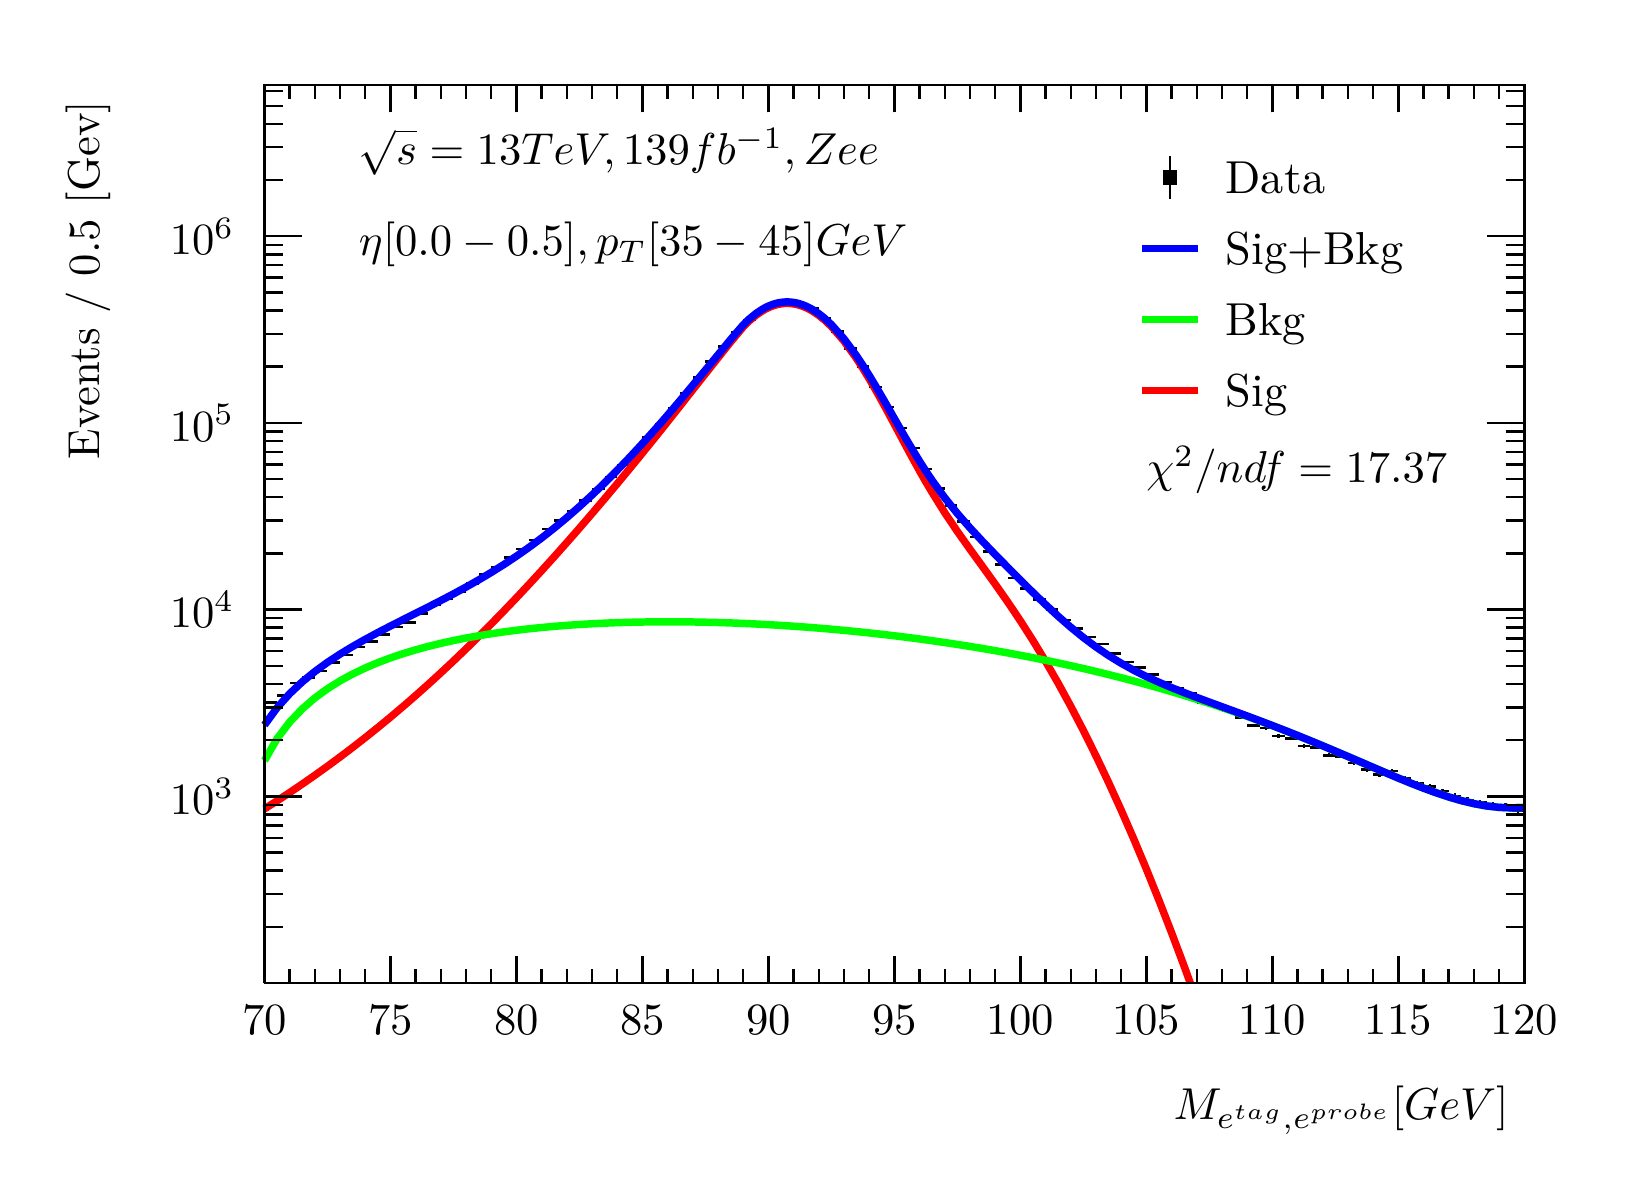
\begin{tikzpicture}
\pgfdeclareplotmark{cross} {
\pgfpathmoveto{\pgfpoint{-0.3\pgfplotmarksize}{\pgfplotmarksize}}
\pgfpathlineto{\pgfpoint{+0.3\pgfplotmarksize}{\pgfplotmarksize}}
\pgfpathlineto{\pgfpoint{+0.3\pgfplotmarksize}{0.3\pgfplotmarksize}}
\pgfpathlineto{\pgfpoint{+1\pgfplotmarksize}{0.3\pgfplotmarksize}}
\pgfpathlineto{\pgfpoint{+1\pgfplotmarksize}{-0.3\pgfplotmarksize}}
\pgfpathlineto{\pgfpoint{+0.3\pgfplotmarksize}{-0.3\pgfplotmarksize}}
\pgfpathlineto{\pgfpoint{+0.3\pgfplotmarksize}{-1.\pgfplotmarksize}}
\pgfpathlineto{\pgfpoint{-0.3\pgfplotmarksize}{-1.\pgfplotmarksize}}
\pgfpathlineto{\pgfpoint{-0.3\pgfplotmarksize}{-0.3\pgfplotmarksize}}
\pgfpathlineto{\pgfpoint{-1.\pgfplotmarksize}{-0.3\pgfplotmarksize}}
\pgfpathlineto{\pgfpoint{-1.\pgfplotmarksize}{0.3\pgfplotmarksize}}
\pgfpathlineto{\pgfpoint{-0.3\pgfplotmarksize}{0.3\pgfplotmarksize}}
\pgfpathclose
\pgfusepathqstroke
}
\pgfdeclareplotmark{cross*} {
\pgfpathmoveto{\pgfpoint{-0.3\pgfplotmarksize}{\pgfplotmarksize}}
\pgfpathlineto{\pgfpoint{+0.3\pgfplotmarksize}{\pgfplotmarksize}}
\pgfpathlineto{\pgfpoint{+0.3\pgfplotmarksize}{0.3\pgfplotmarksize}}
\pgfpathlineto{\pgfpoint{+1\pgfplotmarksize}{0.3\pgfplotmarksize}}
\pgfpathlineto{\pgfpoint{+1\pgfplotmarksize}{-0.3\pgfplotmarksize}}
\pgfpathlineto{\pgfpoint{+0.3\pgfplotmarksize}{-0.3\pgfplotmarksize}}
\pgfpathlineto{\pgfpoint{+0.3\pgfplotmarksize}{-1.\pgfplotmarksize}}
\pgfpathlineto{\pgfpoint{-0.3\pgfplotmarksize}{-1.\pgfplotmarksize}}
\pgfpathlineto{\pgfpoint{-0.3\pgfplotmarksize}{-0.3\pgfplotmarksize}}
\pgfpathlineto{\pgfpoint{-1.\pgfplotmarksize}{-0.3\pgfplotmarksize}}
\pgfpathlineto{\pgfpoint{-1.\pgfplotmarksize}{0.3\pgfplotmarksize}}
\pgfpathlineto{\pgfpoint{-0.3\pgfplotmarksize}{0.3\pgfplotmarksize}}
\pgfpathclose
\pgfusepathqfillstroke
}
\pgfdeclareplotmark{newstar} {
\pgfpathmoveto{\pgfqpoint{0pt}{\pgfplotmarksize}}
\pgfpathlineto{\pgfqpointpolar{44}{0.5\pgfplotmarksize}}
\pgfpathlineto{\pgfqpointpolar{18}{\pgfplotmarksize}}
\pgfpathlineto{\pgfqpointpolar{-20}{0.5\pgfplotmarksize}}
\pgfpathlineto{\pgfqpointpolar{-54}{\pgfplotmarksize}}
\pgfpathlineto{\pgfqpointpolar{-90}{0.5\pgfplotmarksize}}
\pgfpathlineto{\pgfqpointpolar{234}{\pgfplotmarksize}}
\pgfpathlineto{\pgfqpointpolar{198}{0.5\pgfplotmarksize}}
\pgfpathlineto{\pgfqpointpolar{162}{\pgfplotmarksize}}
\pgfpathlineto{\pgfqpointpolar{134}{0.5\pgfplotmarksize}}
\pgfpathclose
\pgfusepathqstroke
}
\pgfdeclareplotmark{newstar*} {
\pgfpathmoveto{\pgfqpoint{0pt}{\pgfplotmarksize}}
\pgfpathlineto{\pgfqpointpolar{44}{0.5\pgfplotmarksize}}
\pgfpathlineto{\pgfqpointpolar{18}{\pgfplotmarksize}}
\pgfpathlineto{\pgfqpointpolar{-20}{0.5\pgfplotmarksize}}
\pgfpathlineto{\pgfqpointpolar{-54}{\pgfplotmarksize}}
\pgfpathlineto{\pgfqpointpolar{-90}{0.5\pgfplotmarksize}}
\pgfpathlineto{\pgfqpointpolar{234}{\pgfplotmarksize}}
\pgfpathlineto{\pgfqpointpolar{198}{0.5\pgfplotmarksize}}
\pgfpathlineto{\pgfqpointpolar{162}{\pgfplotmarksize}}
\pgfpathlineto{\pgfqpointpolar{134}{0.5\pgfplotmarksize}}
\pgfpathclose
\pgfusepathqfillstroke
}
\definecolor{c}{rgb}{1,1,1};
\draw [color=c, fill=c] (0,0) rectangle (20,14.4361);
\draw [color=c, fill=c] (3,2.30977) rectangle (19,13.7143);
\definecolor{c}{rgb}{0,0,0};
\draw [c,line width=0.9] (3,2.30977) -- (3,13.7143) -- (19,13.7143) -- (19,2.30977) -- (3,2.30977);
\definecolor{c}{rgb}{1,1,1};
\draw [color=c, fill=c] (3,2.30977) rectangle (19,13.7143);
\definecolor{c}{rgb}{0,0,0};
\draw [c,line width=0.9] (3,2.30977) -- (3,13.7143) -- (19,13.7143) -- (19,2.30977) -- (3,2.30977);
\draw [c,line width=0.9] (3,2.30977) -- (19,2.30977);
\draw [c,line width=0.9] (3,2.65624) -- (3,2.30977);
\draw [c,line width=0.9] (3.32,2.48301) -- (3.32,2.30977);
\draw [c,line width=0.9] (3.64,2.48301) -- (3.64,2.30977);
\draw [c,line width=0.9] (3.96,2.48301) -- (3.96,2.30977);
\draw [c,line width=0.9] (4.28,2.48301) -- (4.28,2.30977);
\draw [c,line width=0.9] (4.6,2.65624) -- (4.6,2.30977);
\draw [c,line width=0.9] (4.92,2.48301) -- (4.92,2.30977);
\draw [c,line width=0.9] (5.24,2.48301) -- (5.24,2.30977);
\draw [c,line width=0.9] (5.56,2.48301) -- (5.56,2.30977);
\draw [c,line width=0.9] (5.88,2.48301) -- (5.88,2.30977);
\draw [c,line width=0.9] (6.2,2.65624) -- (6.2,2.30977);
\draw [c,line width=0.9] (6.52,2.48301) -- (6.52,2.30977);
\draw [c,line width=0.9] (6.84,2.48301) -- (6.84,2.30977);
\draw [c,line width=0.9] (7.16,2.48301) -- (7.16,2.30977);
\draw [c,line width=0.9] (7.48,2.48301) -- (7.48,2.30977);
\draw [c,line width=0.9] (7.8,2.65624) -- (7.8,2.30977);
\draw [c,line width=0.9] (8.12,2.48301) -- (8.12,2.30977);
\draw [c,line width=0.9] (8.44,2.48301) -- (8.44,2.30977);
\draw [c,line width=0.9] (8.76,2.48301) -- (8.76,2.30977);
\draw [c,line width=0.9] (9.08,2.48301) -- (9.08,2.30977);
\draw [c,line width=0.9] (9.4,2.65624) -- (9.4,2.30977);
\draw [c,line width=0.9] (9.72,2.48301) -- (9.72,2.30977);
\draw [c,line width=0.9] (10.04,2.48301) -- (10.04,2.30977);
\draw [c,line width=0.9] (10.36,2.48301) -- (10.36,2.30977);
\draw [c,line width=0.9] (10.68,2.48301) -- (10.68,2.30977);
\draw [c,line width=0.9] (11,2.65624) -- (11,2.30977);
\draw [c,line width=0.9] (11.32,2.48301) -- (11.32,2.30977);
\draw [c,line width=0.9] (11.64,2.48301) -- (11.64,2.30977);
\draw [c,line width=0.9] (11.96,2.48301) -- (11.96,2.30977);
\draw [c,line width=0.9] (12.28,2.48301) -- (12.28,2.30977);
\draw [c,line width=0.9] (12.6,2.65624) -- (12.6,2.30977);
\draw [c,line width=0.9] (12.92,2.48301) -- (12.92,2.30977);
\draw [c,line width=0.9] (13.24,2.48301) -- (13.24,2.30977);
\draw [c,line width=0.9] (13.56,2.48301) -- (13.56,2.30977);
\draw [c,line width=0.9] (13.88,2.48301) -- (13.88,2.30977);
\draw [c,line width=0.9] (14.2,2.65624) -- (14.2,2.30977);
\draw [c,line width=0.9] (14.52,2.48301) -- (14.52,2.30977);
\draw [c,line width=0.9] (14.84,2.48301) -- (14.84,2.30977);
\draw [c,line width=0.9] (15.16,2.48301) -- (15.16,2.30977);
\draw [c,line width=0.9] (15.48,2.48301) -- (15.48,2.30977);
\draw [c,line width=0.9] (15.8,2.65624) -- (15.8,2.30977);
\draw [c,line width=0.9] (16.12,2.48301) -- (16.12,2.30977);
\draw [c,line width=0.9] (16.44,2.48301) -- (16.44,2.30977);
\draw [c,line width=0.9] (16.76,2.48301) -- (16.76,2.30977);
\draw [c,line width=0.9] (17.08,2.48301) -- (17.08,2.30977);
\draw [c,line width=0.9] (17.4,2.65624) -- (17.4,2.30977);
\draw [c,line width=0.9] (17.72,2.48301) -- (17.72,2.30977);
\draw [c,line width=0.9] (18.04,2.48301) -- (18.04,2.30977);
\draw [c,line width=0.9] (18.36,2.48301) -- (18.36,2.30977);
\draw [c,line width=0.9] (18.68,2.48301) -- (18.68,2.30977);
\draw [c,line width=0.9] (19,2.65624) -- (19,2.30977);
\draw [anchor=base] (3,1.66015) node[scale=1.61424, color=c, rotate=0]{70};
\draw [anchor=base] (4.6,1.66015) node[scale=1.61424, color=c, rotate=0]{75};
\draw [anchor=base] (6.2,1.66015) node[scale=1.61424, color=c, rotate=0]{80};
\draw [anchor=base] (7.8,1.66015) node[scale=1.61424, color=c, rotate=0]{85};
\draw [anchor=base] (9.4,1.66015) node[scale=1.61424, color=c, rotate=0]{90};
\draw [anchor=base] (11,1.66015) node[scale=1.61424, color=c, rotate=0]{95};
\draw [anchor=base] (12.6,1.66015) node[scale=1.61424, color=c, rotate=0]{100};
\draw [anchor=base] (14.2,1.66015) node[scale=1.61424, color=c, rotate=0]{105};
\draw [anchor=base] (15.8,1.66015) node[scale=1.61424, color=c, rotate=0]{110};
\draw [anchor=base] (17.4,1.66015) node[scale=1.61424, color=c, rotate=0]{115};
\draw [anchor=base] (19,1.66015) node[scale=1.61424, color=c, rotate=0]{120};
\draw [anchor= east] (19,0.692932) node[scale=1.61424, color=c, rotate=0]{$M_{e^{tag}, e^{probe}}  [GeV]$};
\draw [c,line width=0.9] (3,13.7143) -- (19,13.7143);
\draw [c,line width=0.9] (3,13.3678) -- (3,13.7143);
\draw [c,line width=0.9] (3.32,13.5411) -- (3.32,13.7143);
\draw [c,line width=0.9] (3.64,13.5411) -- (3.64,13.7143);
\draw [c,line width=0.9] (3.96,13.5411) -- (3.96,13.7143);
\draw [c,line width=0.9] (4.28,13.5411) -- (4.28,13.7143);
\draw [c,line width=0.9] (4.6,13.3678) -- (4.6,13.7143);
\draw [c,line width=0.9] (4.92,13.5411) -- (4.92,13.7143);
\draw [c,line width=0.9] (5.24,13.5411) -- (5.24,13.7143);
\draw [c,line width=0.9] (5.56,13.5411) -- (5.56,13.7143);
\draw [c,line width=0.9] (5.88,13.5411) -- (5.88,13.7143);
\draw [c,line width=0.9] (6.2,13.3678) -- (6.2,13.7143);
\draw [c,line width=0.9] (6.52,13.5411) -- (6.52,13.7143);
\draw [c,line width=0.9] (6.84,13.5411) -- (6.84,13.7143);
\draw [c,line width=0.9] (7.16,13.5411) -- (7.16,13.7143);
\draw [c,line width=0.9] (7.48,13.5411) -- (7.48,13.7143);
\draw [c,line width=0.9] (7.8,13.3678) -- (7.8,13.7143);
\draw [c,line width=0.9] (8.12,13.5411) -- (8.12,13.7143);
\draw [c,line width=0.9] (8.44,13.5411) -- (8.44,13.7143);
\draw [c,line width=0.9] (8.76,13.5411) -- (8.76,13.7143);
\draw [c,line width=0.9] (9.08,13.5411) -- (9.08,13.7143);
\draw [c,line width=0.9] (9.4,13.3678) -- (9.4,13.7143);
\draw [c,line width=0.9] (9.72,13.5411) -- (9.72,13.7143);
\draw [c,line width=0.9] (10.04,13.5411) -- (10.04,13.7143);
\draw [c,line width=0.9] (10.36,13.5411) -- (10.36,13.7143);
\draw [c,line width=0.9] (10.68,13.5411) -- (10.68,13.7143);
\draw [c,line width=0.9] (11,13.3678) -- (11,13.7143);
\draw [c,line width=0.9] (11.32,13.5411) -- (11.32,13.7143);
\draw [c,line width=0.9] (11.64,13.5411) -- (11.64,13.7143);
\draw [c,line width=0.9] (11.96,13.5411) -- (11.96,13.7143);
\draw [c,line width=0.9] (12.28,13.5411) -- (12.28,13.7143);
\draw [c,line width=0.9] (12.6,13.3678) -- (12.6,13.7143);
\draw [c,line width=0.9] (12.92,13.5411) -- (12.92,13.7143);
\draw [c,line width=0.9] (13.24,13.5411) -- (13.24,13.7143);
\draw [c,line width=0.9] (13.56,13.5411) -- (13.56,13.7143);
\draw [c,line width=0.9] (13.88,13.5411) -- (13.88,13.7143);
\draw [c,line width=0.9] (14.2,13.3678) -- (14.2,13.7143);
\draw [c,line width=0.9] (14.52,13.5411) -- (14.52,13.7143);
\draw [c,line width=0.9] (14.84,13.5411) -- (14.84,13.7143);
\draw [c,line width=0.9] (15.16,13.5411) -- (15.16,13.7143);
\draw [c,line width=0.9] (15.48,13.5411) -- (15.48,13.7143);
\draw [c,line width=0.9] (15.8,13.3678) -- (15.8,13.7143);
\draw [c,line width=0.9] (16.12,13.5411) -- (16.12,13.7143);
\draw [c,line width=0.9] (16.44,13.5411) -- (16.44,13.7143);
\draw [c,line width=0.9] (16.76,13.5411) -- (16.76,13.7143);
\draw [c,line width=0.9] (17.08,13.5411) -- (17.08,13.7143);
\draw [c,line width=0.9] (17.4,13.3678) -- (17.4,13.7143);
\draw [c,line width=0.9] (17.72,13.5411) -- (17.72,13.7143);
\draw [c,line width=0.9] (18.04,13.5411) -- (18.04,13.7143);
\draw [c,line width=0.9] (18.36,13.5411) -- (18.36,13.7143);
\draw [c,line width=0.9] (18.68,13.5411) -- (18.68,13.7143);
\draw [c,line width=0.9] (19,13.3678) -- (19,13.7143);
\draw [c,line width=0.9] (3,2.30977) -- (3,13.7143);
\draw [c,line width=0.9] (3.237,3.02354) -- (3,3.02354);
\draw [c,line width=0.9] (3.237,3.44107) -- (3,3.44107);
\draw [c,line width=0.9] (3.237,3.73731) -- (3,3.73731);
\draw [c,line width=0.9] (3.237,3.96709) -- (3,3.96709);
\draw [c,line width=0.9] (3.237,4.15484) -- (3,4.15484);
\draw [c,line width=0.9] (3.237,4.31357) -- (3,4.31357);
\draw [c,line width=0.9] (3.237,4.45108) -- (3,4.45108);
\draw [c,line width=0.9] (3.237,4.57236) -- (3,4.57236);
\draw [c,line width=0.9] (3.474,4.68086) -- (3,4.68086);
\draw [anchor= east] (2.82,4.68086) node[scale=1.61424, color=c, rotate=0]{$10^{3}$};
\draw [c,line width=0.9] (3.237,5.39463) -- (3,5.39463);
\draw [c,line width=0.9] (3.237,5.81216) -- (3,5.81216);
\draw [c,line width=0.9] (3.237,6.1084) -- (3,6.1084);
\draw [c,line width=0.9] (3.237,6.33818) -- (3,6.33818);
\draw [c,line width=0.9] (3.237,6.52593) -- (3,6.52593);
\draw [c,line width=0.9] (3.237,6.68466) -- (3,6.68466);
\draw [c,line width=0.9] (3.237,6.82217) -- (3,6.82217);
\draw [c,line width=0.9] (3.237,6.94345) -- (3,6.94345);
\draw [c,line width=0.9] (3.474,7.05195) -- (3,7.05195);
\draw [anchor= east] (2.82,7.05195) node[scale=1.61424, color=c, rotate=0]{$10^{4}$};
\draw [c,line width=0.9] (3.237,7.76572) -- (3,7.76572);
\draw [c,line width=0.9] (3.237,8.18324) -- (3,8.18324);
\draw [c,line width=0.9] (3.237,8.47948) -- (3,8.47948);
\draw [c,line width=0.9] (3.237,8.70927) -- (3,8.70927);
\draw [c,line width=0.9] (3.237,8.89701) -- (3,8.89701);
\draw [c,line width=0.9] (3.237,9.05575) -- (3,9.05575);
\draw [c,line width=0.9] (3.237,9.19325) -- (3,9.19325);
\draw [c,line width=0.9] (3.237,9.31454) -- (3,9.31454);
\draw [c,line width=0.9] (3.474,9.42304) -- (3,9.42304);
\draw [anchor= east] (2.82,9.42304) node[scale=1.61424, color=c, rotate=0]{$10^{5}$};
\draw [c,line width=0.9] (3.237,10.1368) -- (3,10.1368);
\draw [c,line width=0.9] (3.237,10.5543) -- (3,10.5543);
\draw [c,line width=0.9] (3.237,10.8506) -- (3,10.8506);
\draw [c,line width=0.9] (3.237,11.0804) -- (3,11.0804);
\draw [c,line width=0.9] (3.237,11.2681) -- (3,11.2681);
\draw [c,line width=0.9] (3.237,11.4268) -- (3,11.4268);
\draw [c,line width=0.9] (3.237,11.5643) -- (3,11.5643);
\draw [c,line width=0.9] (3.237,11.6856) -- (3,11.6856);
\draw [c,line width=0.9] (3.474,11.7941) -- (3,11.7941);
\draw [anchor= east] (2.82,11.7941) node[scale=1.61424, color=c, rotate=0]{$10^{6}$};
\draw [c,line width=0.9] (3.237,12.5079) -- (3,12.5079);
\draw [c,line width=0.9] (3.237,12.9254) -- (3,12.9254);
\draw [c,line width=0.9] (3.237,13.2217) -- (3,13.2217);
\draw [c,line width=0.9] (3.237,13.4514) -- (3,13.4514);
\draw [c,line width=0.9] (3.237,13.6392) -- (3,13.6392);
\draw [anchor= east] (0.76,13.7143) node[scale=1.61424, color=c, rotate=90]{Events / 0.5 [Gev]};
\draw [c,line width=0.9] (19,2.30977) -- (19,13.7143);
\draw [c,line width=0.9] (18.763,3.02354) -- (19,3.02354);
\draw [c,line width=0.9] (18.763,3.44107) -- (19,3.44107);
\draw [c,line width=0.9] (18.763,3.73731) -- (19,3.73731);
\draw [c,line width=0.9] (18.763,3.96709) -- (19,3.96709);
\draw [c,line width=0.9] (18.763,4.15484) -- (19,4.15484);
\draw [c,line width=0.9] (18.763,4.31357) -- (19,4.31357);
\draw [c,line width=0.9] (18.763,4.45108) -- (19,4.45108);
\draw [c,line width=0.9] (18.763,4.57236) -- (19,4.57236);
\draw [c,line width=0.9] (18.526,4.68086) -- (19,4.68086);
\draw [c,line width=0.9] (18.763,5.39463) -- (19,5.39463);
\draw [c,line width=0.9] (18.763,5.81216) -- (19,5.81216);
\draw [c,line width=0.9] (18.763,6.1084) -- (19,6.1084);
\draw [c,line width=0.9] (18.763,6.33818) -- (19,6.33818);
\draw [c,line width=0.9] (18.763,6.52593) -- (19,6.52593);
\draw [c,line width=0.9] (18.763,6.68466) -- (19,6.68466);
\draw [c,line width=0.9] (18.763,6.82217) -- (19,6.82217);
\draw [c,line width=0.9] (18.763,6.94345) -- (19,6.94345);
\draw [c,line width=0.9] (18.526,7.05195) -- (19,7.05195);
\draw [c,line width=0.9] (18.763,7.76572) -- (19,7.76572);
\draw [c,line width=0.9] (18.763,8.18324) -- (19,8.18324);
\draw [c,line width=0.9] (18.763,8.47948) -- (19,8.47948);
\draw [c,line width=0.9] (18.763,8.70927) -- (19,8.70927);
\draw [c,line width=0.9] (18.763,8.89701) -- (19,8.89701);
\draw [c,line width=0.9] (18.763,9.05575) -- (19,9.05575);
\draw [c,line width=0.9] (18.763,9.19325) -- (19,9.19325);
\draw [c,line width=0.9] (18.763,9.31454) -- (19,9.31454);
\draw [c,line width=0.9] (18.526,9.42304) -- (19,9.42304);
\draw [c,line width=0.9] (18.763,10.1368) -- (19,10.1368);
\draw [c,line width=0.9] (18.763,10.5543) -- (19,10.5543);
\draw [c,line width=0.9] (18.763,10.8506) -- (19,10.8506);
\draw [c,line width=0.9] (18.763,11.0804) -- (19,11.0804);
\draw [c,line width=0.9] (18.763,11.2681) -- (19,11.2681);
\draw [c,line width=0.9] (18.763,11.4268) -- (19,11.4268);
\draw [c,line width=0.9] (18.763,11.5643) -- (19,11.5643);
\draw [c,line width=0.9] (18.763,11.6856) -- (19,11.6856);
\draw [c,line width=0.9] (18.526,11.7941) -- (19,11.7941);
\draw [c,line width=0.9] (18.763,12.5079) -- (19,12.5079);
\draw [c,line width=0.9] (18.763,12.9254) -- (19,12.9254);
\draw [c,line width=0.9] (18.763,13.2217) -- (19,13.2217);
\draw [c,line width=0.9] (18.763,13.4514) -- (19,13.4514);
\draw [c,line width=0.9] (18.763,13.6392) -- (19,13.6392);
\draw [c,line width=0.9] (3.08,5.87086) -- (3,5.87086);
\draw [c,line width=0.9] (3,5.87086) -- (3,5.87086);
\draw [c,line width=0.9] (3.08,5.87086) -- (3.16,5.87086);
\draw [c,line width=0.9] (3.16,5.87086) -- (3.16,5.87086);
\draw [c,line width=0.9] (3.08,5.87086) -- (3.08,5.88914);
\draw [c,line width=0.9] (3.08,5.88914) -- (3.08,5.88914);
\draw [c,line width=0.9] (3.08,5.87086) -- (3.08,5.85259);
\draw [c,line width=0.9] (3.08,5.85259) -- (3.08,5.85259);
\draw [c,line width=0.9] (3.24,5.95965) -- (3.16,5.95965);
\draw [c,line width=0.9] (3.16,5.95965) -- (3.16,5.95965);
\draw [c,line width=0.9] (3.24,5.95965) -- (3.32,5.95965);
\draw [c,line width=0.9] (3.32,5.95965) -- (3.32,5.95965);
\draw [c,line width=0.9] (3.24,5.95965) -- (3.24,5.97715);
\draw [c,line width=0.9] (3.24,5.97715) -- (3.24,5.97715);
\draw [c,line width=0.9] (3.24,5.95965) -- (3.24,5.94215);
\draw [c,line width=0.9] (3.24,5.94215) -- (3.24,5.94215);
\draw [c,line width=0.9] (3.4,6.12246) -- (3.32,6.12246);
\draw [c,line width=0.9] (3.32,6.12246) -- (3.32,6.12246);
\draw [c,line width=0.9] (3.4,6.12246) -- (3.48,6.12246);
\draw [c,line width=0.9] (3.48,6.12246) -- (3.48,6.12246);
\draw [c,line width=0.9] (3.4,6.12246) -- (3.4,6.13863);
\draw [c,line width=0.9] (3.4,6.13863) -- (3.4,6.13863);
\draw [c,line width=0.9] (3.4,6.12246) -- (3.4,6.10629);
\draw [c,line width=0.9] (3.4,6.10629) -- (3.4,6.10629);
\draw [c,line width=0.9] (3.56,6.19027) -- (3.48,6.19027);
\draw [c,line width=0.9] (3.48,6.19027) -- (3.48,6.19027);
\draw [c,line width=0.9] (3.56,6.19027) -- (3.64,6.19027);
\draw [c,line width=0.9] (3.64,6.19027) -- (3.64,6.19027);
\draw [c,line width=0.9] (3.56,6.19027) -- (3.56,6.20591);
\draw [c,line width=0.9] (3.56,6.20591) -- (3.56,6.20591);
\draw [c,line width=0.9] (3.56,6.19027) -- (3.56,6.17462);
\draw [c,line width=0.9] (3.56,6.17462) -- (3.56,6.17462);
\draw [c,line width=0.9] (3.72,6.27556) -- (3.64,6.27556);
\draw [c,line width=0.9] (3.64,6.27556) -- (3.64,6.27556);
\draw [c,line width=0.9] (3.72,6.27556) -- (3.8,6.27556);
\draw [c,line width=0.9] (3.8,6.27556) -- (3.8,6.27556);
\draw [c,line width=0.9] (3.72,6.27556) -- (3.72,6.29057);
\draw [c,line width=0.9] (3.72,6.29057) -- (3.72,6.29057);
\draw [c,line width=0.9] (3.72,6.27556) -- (3.72,6.26055);
\draw [c,line width=0.9] (3.72,6.26055) -- (3.72,6.26055);
\draw [c,line width=0.9] (3.88,6.37916) -- (3.8,6.37916);
\draw [c,line width=0.9] (3.8,6.37916) -- (3.8,6.37916);
\draw [c,line width=0.9] (3.88,6.37916) -- (3.96,6.37916);
\draw [c,line width=0.9] (3.96,6.37916) -- (3.96,6.37916);
\draw [c,line width=0.9] (3.88,6.37916) -- (3.88,6.39344);
\draw [c,line width=0.9] (3.88,6.39344) -- (3.88,6.39344);
\draw [c,line width=0.9] (3.88,6.37916) -- (3.88,6.36489);
\draw [c,line width=0.9] (3.88,6.36489) -- (3.88,6.36489);
\draw [c,line width=0.9] (4.04,6.47509) -- (3.96,6.47509);
\draw [c,line width=0.9] (3.96,6.47509) -- (3.96,6.47509);
\draw [c,line width=0.9] (4.04,6.47509) -- (4.12,6.47509);
\draw [c,line width=0.9] (4.12,6.47509) -- (4.12,6.47509);
\draw [c,line width=0.9] (4.04,6.47509) -- (4.04,6.48872);
\draw [c,line width=0.9] (4.04,6.48872) -- (4.04,6.48872);
\draw [c,line width=0.9] (4.04,6.47509) -- (4.04,6.46147);
\draw [c,line width=0.9] (4.04,6.46147) -- (4.04,6.46147);
\draw [c,line width=0.9] (4.2,6.576) -- (4.12,6.576);
\draw [c,line width=0.9] (4.12,6.576) -- (4.12,6.576);
\draw [c,line width=0.9] (4.2,6.576) -- (4.28,6.576);
\draw [c,line width=0.9] (4.28,6.576) -- (4.28,6.576);
\draw [c,line width=0.9] (4.2,6.576) -- (4.2,6.58898);
\draw [c,line width=0.9] (4.2,6.58898) -- (4.2,6.58898);
\draw [c,line width=0.9] (4.2,6.576) -- (4.2,6.56303);
\draw [c,line width=0.9] (4.2,6.56303) -- (4.2,6.56303);
\draw [c,line width=0.9] (4.36,6.64508) -- (4.28,6.64508);
\draw [c,line width=0.9] (4.28,6.64508) -- (4.28,6.64508);
\draw [c,line width=0.9] (4.36,6.64508) -- (4.44,6.64508);
\draw [c,line width=0.9] (4.44,6.64508) -- (4.44,6.64508);
\draw [c,line width=0.9] (4.36,6.64508) -- (4.36,6.65762);
\draw [c,line width=0.9] (4.36,6.65762) -- (4.36,6.65762);
\draw [c,line width=0.9] (4.36,6.64508) -- (4.36,6.63253);
\draw [c,line width=0.9] (4.36,6.63253) -- (4.36,6.63253);
\draw [c,line width=0.9] (4.52,6.7335) -- (4.44,6.7335);
\draw [c,line width=0.9] (4.44,6.7335) -- (4.44,6.7335);
\draw [c,line width=0.9] (4.52,6.7335) -- (4.6,6.7335);
\draw [c,line width=0.9] (4.6,6.7335) -- (4.6,6.7335);
\draw [c,line width=0.9] (4.52,6.7335) -- (4.52,6.74552);
\draw [c,line width=0.9] (4.52,6.74552) -- (4.52,6.74552);
\draw [c,line width=0.9] (4.52,6.7335) -- (4.52,6.72148);
\draw [c,line width=0.9] (4.52,6.72148) -- (4.52,6.72148);
\draw [c,line width=0.9] (4.68,6.83216) -- (4.6,6.83216);
\draw [c,line width=0.9] (4.6,6.83216) -- (4.6,6.83216);
\draw [c,line width=0.9] (4.68,6.83216) -- (4.76,6.83216);
\draw [c,line width=0.9] (4.76,6.83216) -- (4.76,6.83216);
\draw [c,line width=0.9] (4.68,6.83216) -- (4.68,6.84362);
\draw [c,line width=0.9] (4.68,6.84362) -- (4.68,6.84362);
\draw [c,line width=0.9] (4.68,6.83216) -- (4.68,6.8207);
\draw [c,line width=0.9] (4.68,6.8207) -- (4.68,6.8207);
\draw [c,line width=0.9] (4.84,6.88786) -- (4.76,6.88786);
\draw [c,line width=0.9] (4.76,6.88786) -- (4.76,6.88786);
\draw [c,line width=0.9] (4.84,6.88786) -- (4.92,6.88786);
\draw [c,line width=0.9] (4.92,6.88786) -- (4.92,6.88786);
\draw [c,line width=0.9] (4.84,6.88786) -- (4.84,6.89901);
\draw [c,line width=0.9] (4.84,6.89901) -- (4.84,6.89901);
\draw [c,line width=0.9] (4.84,6.88786) -- (4.84,6.87671);
\draw [c,line width=0.9] (4.84,6.87671) -- (4.84,6.87671);
\draw [c,line width=0.9] (5,7.00162) -- (4.92,7.00162);
\draw [c,line width=0.9] (4.92,7.00162) -- (4.92,7.00162);
\draw [c,line width=0.9] (5,7.00162) -- (5.08,7.00162);
\draw [c,line width=0.9] (5.08,7.00162) -- (5.08,7.00162);
\draw [c,line width=0.9] (5,7.00162) -- (5,7.01217);
\draw [c,line width=0.9] (5,7.01217) -- (5,7.01217);
\draw [c,line width=0.9] (5,7.00162) -- (5,6.99107);
\draw [c,line width=0.9] (5,6.99107) -- (5,6.99107);
\draw [c,line width=0.9] (5.16,7.11506) -- (5.08,7.11506);
\draw [c,line width=0.9] (5.08,7.11506) -- (5.08,7.11506);
\draw [c,line width=0.9] (5.16,7.11506) -- (5.24,7.11506);
\draw [c,line width=0.9] (5.24,7.11506) -- (5.24,7.11506);
\draw [c,line width=0.9] (5.16,7.11506) -- (5.16,7.12504);
\draw [c,line width=0.9] (5.16,7.12504) -- (5.16,7.12504);
\draw [c,line width=0.9] (5.16,7.11506) -- (5.16,7.10507);
\draw [c,line width=0.9] (5.16,7.10507) -- (5.16,7.10507);
\draw [c,line width=0.9] (5.32,7.18416) -- (5.24,7.18416);
\draw [c,line width=0.9] (5.24,7.18416) -- (5.24,7.18416);
\draw [c,line width=0.9] (5.32,7.18416) -- (5.4,7.18416);
\draw [c,line width=0.9] (5.4,7.18416) -- (5.4,7.18416);
\draw [c,line width=0.9] (5.32,7.18416) -- (5.32,7.19382);
\draw [c,line width=0.9] (5.32,7.19382) -- (5.32,7.19382);
\draw [c,line width=0.9] (5.32,7.18416) -- (5.32,7.1745);
\draw [c,line width=0.9] (5.32,7.1745) -- (5.32,7.1745);
\draw [c,line width=0.9] (5.48,7.28543) -- (5.4,7.28543);
\draw [c,line width=0.9] (5.4,7.28543) -- (5.4,7.28543);
\draw [c,line width=0.9] (5.48,7.28543) -- (5.56,7.28543);
\draw [c,line width=0.9] (5.56,7.28543) -- (5.56,7.28543);
\draw [c,line width=0.9] (5.48,7.28543) -- (5.48,7.29463);
\draw [c,line width=0.9] (5.48,7.29463) -- (5.48,7.29463);
\draw [c,line width=0.9] (5.48,7.28543) -- (5.48,7.27624);
\draw [c,line width=0.9] (5.48,7.27624) -- (5.48,7.27624);
\draw [c,line width=0.9] (5.64,7.38674) -- (5.56,7.38674);
\draw [c,line width=0.9] (5.56,7.38674) -- (5.56,7.38674);
\draw [c,line width=0.9] (5.64,7.38674) -- (5.72,7.38674);
\draw [c,line width=0.9] (5.72,7.38674) -- (5.72,7.38674);
\draw [c,line width=0.9] (5.64,7.38674) -- (5.64,7.3955);
\draw [c,line width=0.9] (5.64,7.3955) -- (5.64,7.3955);
\draw [c,line width=0.9] (5.64,7.38674) -- (5.64,7.37799);
\draw [c,line width=0.9] (5.64,7.37799) -- (5.64,7.37799);
\draw [c,line width=0.9] (5.8,7.50696) -- (5.72,7.50696);
\draw [c,line width=0.9] (5.72,7.50696) -- (5.72,7.50696);
\draw [c,line width=0.9] (5.8,7.50696) -- (5.88,7.50696);
\draw [c,line width=0.9] (5.88,7.50696) -- (5.88,7.50696);
\draw [c,line width=0.9] (5.8,7.50696) -- (5.8,7.51521);
\draw [c,line width=0.9] (5.8,7.51521) -- (5.8,7.51521);
\draw [c,line width=0.9] (5.8,7.50696) -- (5.8,7.4987);
\draw [c,line width=0.9] (5.8,7.4987) -- (5.8,7.4987);
\draw [c,line width=0.9] (5.96,7.59618) -- (5.88,7.59618);
\draw [c,line width=0.9] (5.88,7.59618) -- (5.88,7.59618);
\draw [c,line width=0.9] (5.96,7.59618) -- (6.04,7.59618);
\draw [c,line width=0.9] (6.04,7.59618) -- (6.04,7.59618);
\draw [c,line width=0.9] (5.96,7.59618) -- (5.96,7.60409);
\draw [c,line width=0.9] (5.96,7.60409) -- (5.96,7.60409);
\draw [c,line width=0.9] (5.96,7.59618) -- (5.96,7.58827);
\draw [c,line width=0.9] (5.96,7.58827) -- (5.96,7.58827);
\draw [c,line width=0.9] (6.12,7.71447) -- (6.04,7.71447);
\draw [c,line width=0.9] (6.04,7.71447) -- (6.04,7.71447);
\draw [c,line width=0.9] (6.12,7.71447) -- (6.2,7.71447);
\draw [c,line width=0.9] (6.2,7.71447) -- (6.2,7.71447);
\draw [c,line width=0.9] (6.12,7.71447) -- (6.12,7.72193);
\draw [c,line width=0.9] (6.12,7.72193) -- (6.12,7.72193);
\draw [c,line width=0.9] (6.12,7.71447) -- (6.12,7.707);
\draw [c,line width=0.9] (6.12,7.707) -- (6.12,7.707);
\draw [c,line width=0.9] (6.28,7.82212) -- (6.2,7.82212);
\draw [c,line width=0.9] (6.2,7.82212) -- (6.2,7.82212);
\draw [c,line width=0.9] (6.28,7.82212) -- (6.36,7.82212);
\draw [c,line width=0.9] (6.36,7.82212) -- (6.36,7.82212);
\draw [c,line width=0.9] (6.28,7.82212) -- (6.28,7.8292);
\draw [c,line width=0.9] (6.28,7.8292) -- (6.28,7.8292);
\draw [c,line width=0.9] (6.28,7.82212) -- (6.28,7.81503);
\draw [c,line width=0.9] (6.28,7.81503) -- (6.28,7.81503);
\draw [c,line width=0.9] (6.44,7.93472) -- (6.36,7.93472);
\draw [c,line width=0.9] (6.36,7.93472) -- (6.36,7.93472);
\draw [c,line width=0.9] (6.44,7.93472) -- (6.52,7.93472);
\draw [c,line width=0.9] (6.52,7.93472) -- (6.52,7.93472);
\draw [c,line width=0.9] (6.44,7.93472) -- (6.44,7.94142);
\draw [c,line width=0.9] (6.44,7.94142) -- (6.44,7.94142);
\draw [c,line width=0.9] (6.44,7.93472) -- (6.44,7.92801);
\draw [c,line width=0.9] (6.44,7.92801) -- (6.44,7.92801);
\draw [c,line width=0.9] (6.6,8.07448) -- (6.52,8.07448);
\draw [c,line width=0.9] (6.52,8.07448) -- (6.52,8.07448);
\draw [c,line width=0.9] (6.6,8.07448) -- (6.68,8.07448);
\draw [c,line width=0.9] (6.68,8.07448) -- (6.68,8.07448);
\draw [c,line width=0.9] (6.6,8.07448) -- (6.6,8.08075);
\draw [c,line width=0.9] (6.6,8.08075) -- (6.6,8.08075);
\draw [c,line width=0.9] (6.6,8.07448) -- (6.6,8.06822);
\draw [c,line width=0.9] (6.6,8.06822) -- (6.6,8.06822);
\draw [c,line width=0.9] (6.76,8.18149) -- (6.68,8.18149);
\draw [c,line width=0.9] (6.68,8.18149) -- (6.68,8.18149);
\draw [c,line width=0.9] (6.76,8.18149) -- (6.84,8.18149);
\draw [c,line width=0.9] (6.84,8.18149) -- (6.84,8.18149);
\draw [c,line width=0.9] (6.76,8.18149) -- (6.76,8.18744);
\draw [c,line width=0.9] (6.76,8.18744) -- (6.76,8.18744);
\draw [c,line width=0.9] (6.76,8.18149) -- (6.76,8.17554);
\draw [c,line width=0.9] (6.76,8.17554) -- (6.76,8.17554);
\draw [c,line width=0.9] (6.92,8.30533) -- (6.84,8.30533);
\draw [c,line width=0.9] (6.84,8.30533) -- (6.84,8.30533);
\draw [c,line width=0.9] (6.92,8.30533) -- (7,8.30533);
\draw [c,line width=0.9] (7,8.30533) -- (7,8.30533);
\draw [c,line width=0.9] (6.92,8.30533) -- (6.92,8.31093);
\draw [c,line width=0.9] (6.92,8.31093) -- (6.92,8.31093);
\draw [c,line width=0.9] (6.92,8.30533) -- (6.92,8.29972);
\draw [c,line width=0.9] (6.92,8.29972) -- (6.92,8.29972);
\draw [c,line width=0.9] (7.08,8.44101) -- (7,8.44101);
\draw [c,line width=0.9] (7,8.44101) -- (7,8.44101);
\draw [c,line width=0.9] (7.08,8.44101) -- (7.16,8.44101);
\draw [c,line width=0.9] (7.16,8.44101) -- (7.16,8.44101);
\draw [c,line width=0.9] (7.08,8.44101) -- (7.08,8.44626);
\draw [c,line width=0.9] (7.08,8.44626) -- (7.08,8.44626);
\draw [c,line width=0.9] (7.08,8.44101) -- (7.08,8.43576);
\draw [c,line width=0.9] (7.08,8.43576) -- (7.08,8.43576);
\draw [c,line width=0.9] (7.24,8.58649) -- (7.16,8.58649);
\draw [c,line width=0.9] (7.16,8.58649) -- (7.16,8.58649);
\draw [c,line width=0.9] (7.24,8.58649) -- (7.32,8.58649);
\draw [c,line width=0.9] (7.32,8.58649) -- (7.32,8.58649);
\draw [c,line width=0.9] (7.24,8.58649) -- (7.24,8.59138);
\draw [c,line width=0.9] (7.24,8.59138) -- (7.24,8.59138);
\draw [c,line width=0.9] (7.24,8.58649) -- (7.24,8.5816);
\draw [c,line width=0.9] (7.24,8.5816) -- (7.24,8.5816);
\draw [c,line width=0.9] (7.4,8.7375) -- (7.32,8.7375);
\draw [c,line width=0.9] (7.32,8.7375) -- (7.32,8.7375);
\draw [c,line width=0.9] (7.4,8.7375) -- (7.48,8.7375);
\draw [c,line width=0.9] (7.48,8.7375) -- (7.48,8.7375);
\draw [c,line width=0.9] (7.4,8.7375) -- (7.4,8.74205);
\draw [c,line width=0.9] (7.4,8.74205) -- (7.4,8.74205);
\draw [c,line width=0.9] (7.4,8.7375) -- (7.4,8.73296);
\draw [c,line width=0.9] (7.4,8.73296) -- (7.4,8.73296);
\draw [c,line width=0.9] (7.56,8.88897) -- (7.48,8.88897);
\draw [c,line width=0.9] (7.48,8.88897) -- (7.48,8.88897);
\draw [c,line width=0.9] (7.56,8.88897) -- (7.64,8.88897);
\draw [c,line width=0.9] (7.64,8.88897) -- (7.64,8.88897);
\draw [c,line width=0.9] (7.56,8.88897) -- (7.56,8.89319);
\draw [c,line width=0.9] (7.56,8.89319) -- (7.56,8.89319);
\draw [c,line width=0.9] (7.56,8.88897) -- (7.56,8.88475);
\draw [c,line width=0.9] (7.56,8.88475) -- (7.56,8.88475);
\draw [c,line width=0.9] (7.72,9.05543) -- (7.64,9.05543);
\draw [c,line width=0.9] (7.64,9.05543) -- (7.64,9.05543);
\draw [c,line width=0.9] (7.72,9.05543) -- (7.8,9.05543);
\draw [c,line width=0.9] (7.8,9.05543) -- (7.8,9.05543);
\draw [c,line width=0.9] (7.72,9.05543) -- (7.72,9.05932);
\draw [c,line width=0.9] (7.72,9.05932) -- (7.72,9.05932);
\draw [c,line width=0.9] (7.72,9.05543) -- (7.72,9.05153);
\draw [c,line width=0.9] (7.72,9.05153) -- (7.72,9.05153);
\draw [c,line width=0.9] (7.88,9.23782) -- (7.8,9.23782);
\draw [c,line width=0.9] (7.8,9.23782) -- (7.8,9.23782);
\draw [c,line width=0.9] (7.88,9.23782) -- (7.96,9.23782);
\draw [c,line width=0.9] (7.96,9.23782) -- (7.96,9.23782);
\draw [c,line width=0.9] (7.88,9.23782) -- (7.88,9.24138);
\draw [c,line width=0.9] (7.88,9.24138) -- (7.88,9.24138);
\draw [c,line width=0.9] (7.88,9.23782) -- (7.88,9.23425);
\draw [c,line width=0.9] (7.88,9.23425) -- (7.88,9.23425);
\draw [c,line width=0.9] (8.04,9.41066) -- (7.96,9.41066);
\draw [c,line width=0.9] (7.96,9.41066) -- (7.96,9.41066);
\draw [c,line width=0.9] (8.04,9.41066) -- (8.12,9.41066);
\draw [c,line width=0.9] (8.12,9.41066) -- (8.12,9.41066);
\draw [c,line width=0.9] (8.04,9.41066) -- (8.04,9.41393);
\draw [c,line width=0.9] (8.04,9.41393) -- (8.04,9.41393);
\draw [c,line width=0.9] (8.04,9.41066) -- (8.04,9.40738);
\draw [c,line width=0.9] (8.04,9.40738) -- (8.04,9.40738);
\draw [c,line width=0.9] (8.2,9.60518) -- (8.12,9.60518);
\draw [c,line width=0.9] (8.12,9.60518) -- (8.12,9.60518);
\draw [c,line width=0.9] (8.2,9.60518) -- (8.28,9.60518);
\draw [c,line width=0.9] (8.28,9.60518) -- (8.28,9.60518);
\draw [c,line width=0.9] (8.2,9.60518) -- (8.2,9.60816);
\draw [c,line width=0.9] (8.2,9.60816) -- (8.2,9.60816);
\draw [c,line width=0.9] (8.2,9.60518) -- (8.2,9.6022);
\draw [c,line width=0.9] (8.2,9.6022) -- (8.2,9.6022);
\draw [c,line width=0.9] (8.36,9.80488) -- (8.28,9.80488);
\draw [c,line width=0.9] (8.28,9.80488) -- (8.28,9.80488);
\draw [c,line width=0.9] (8.36,9.80488) -- (8.44,9.80488);
\draw [c,line width=0.9] (8.44,9.80488) -- (8.44,9.80488);
\draw [c,line width=0.9] (8.36,9.80488) -- (8.36,9.80758);
\draw [c,line width=0.9] (8.36,9.80758) -- (8.36,9.80758);
\draw [c,line width=0.9] (8.36,9.80488) -- (8.36,9.80217);
\draw [c,line width=0.9] (8.36,9.80217) -- (8.36,9.80217);
\draw [c,line width=0.9] (8.52,10.0023) -- (8.44,10.0023);
\draw [c,line width=0.9] (8.44,10.0023) -- (8.44,10.0023);
\draw [c,line width=0.9] (8.52,10.0023) -- (8.6,10.0023);
\draw [c,line width=0.9] (8.6,10.0023) -- (8.6,10.0023);
\draw [c,line width=0.9] (8.52,10.0023) -- (8.52,10.0048);
\draw [c,line width=0.9] (8.52,10.0048) -- (8.52,10.0048);
\draw [c,line width=0.9] (8.52,10.0023) -- (8.52,9.99984);
\draw [c,line width=0.9] (8.52,9.99984) -- (8.52,9.99984);
\draw [c,line width=0.9] (8.68,10.2031) -- (8.6,10.2031);
\draw [c,line width=0.9] (8.6,10.2031) -- (8.6,10.2031);
\draw [c,line width=0.9] (8.68,10.2031) -- (8.76,10.2031);
\draw [c,line width=0.9] (8.76,10.2031) -- (8.76,10.2031);
\draw [c,line width=0.9] (8.68,10.2031) -- (8.68,10.2053);
\draw [c,line width=0.9] (8.68,10.2053) -- (8.68,10.2053);
\draw [c,line width=0.9] (8.68,10.2031) -- (8.68,10.2008);
\draw [c,line width=0.9] (8.68,10.2008) -- (8.68,10.2008);
\draw [c,line width=0.9] (8.84,10.3968) -- (8.76,10.3968);
\draw [c,line width=0.9] (8.76,10.3968) -- (8.76,10.3968);
\draw [c,line width=0.9] (8.84,10.3968) -- (8.92,10.3968);
\draw [c,line width=0.9] (8.92,10.3968) -- (8.92,10.3968);
\draw [c,line width=0.9] (8.84,10.3968) -- (8.84,10.3988);
\draw [c,line width=0.9] (8.84,10.3988) -- (8.84,10.3988);
\draw [c,line width=0.9] (8.84,10.3968) -- (8.84,10.3948);
\draw [c,line width=0.9] (8.84,10.3948) -- (8.84,10.3948);
\draw [c,line width=0.9] (9,10.5752) -- (8.92,10.5752);
\draw [c,line width=0.9] (8.92,10.5752) -- (8.92,10.5752);
\draw [c,line width=0.9] (9,10.5752) -- (9.08,10.5752);
\draw [c,line width=0.9] (9.08,10.5752) -- (9.08,10.5752);
\draw [c,line width=0.9] (9,10.5752) -- (9,10.5771);
\draw [c,line width=0.9] (9,10.5771) -- (9,10.5771);
\draw [c,line width=0.9] (9,10.5752) -- (9,10.5734);
\draw [c,line width=0.9] (9,10.5734) -- (9,10.5734);
\draw [c,line width=0.9] (9.16,10.7326) -- (9.08,10.7326);
\draw [c,line width=0.9] (9.08,10.7326) -- (9.08,10.7326);
\draw [c,line width=0.9] (9.16,10.7326) -- (9.24,10.7326);
\draw [c,line width=0.9] (9.24,10.7326) -- (9.24,10.7326);
\draw [c,line width=0.9] (9.16,10.7326) -- (9.16,10.7344);
\draw [c,line width=0.9] (9.16,10.7344) -- (9.16,10.7344);
\draw [c,line width=0.9] (9.16,10.7326) -- (9.16,10.7309);
\draw [c,line width=0.9] (9.16,10.7309) -- (9.16,10.7309);
\draw [c,line width=0.9] (9.32,10.8566) -- (9.24,10.8566);
\draw [c,line width=0.9] (9.24,10.8566) -- (9.24,10.8566);
\draw [c,line width=0.9] (9.32,10.8566) -- (9.4,10.8566);
\draw [c,line width=0.9] (9.4,10.8566) -- (9.4,10.8566);
\draw [c,line width=0.9] (9.32,10.8566) -- (9.32,10.8582);
\draw [c,line width=0.9] (9.32,10.8582) -- (9.32,10.8582);
\draw [c,line width=0.9] (9.32,10.8566) -- (9.32,10.855);
\draw [c,line width=0.9] (9.32,10.855) -- (9.32,10.855);
\draw [c,line width=0.9] (9.48,10.9355) -- (9.4,10.9355);
\draw [c,line width=0.9] (9.4,10.9355) -- (9.4,10.9355);
\draw [c,line width=0.9] (9.48,10.9355) -- (9.56,10.9355);
\draw [c,line width=0.9] (9.56,10.9355) -- (9.56,10.9355);
\draw [c,line width=0.9] (9.48,10.9355) -- (9.48,10.9371);
\draw [c,line width=0.9] (9.48,10.9371) -- (9.48,10.9371);
\draw [c,line width=0.9] (9.48,10.9355) -- (9.48,10.934);
\draw [c,line width=0.9] (9.48,10.934) -- (9.48,10.934);
\draw [c,line width=0.9] (9.64,10.9682) -- (9.56,10.9682);
\draw [c,line width=0.9] (9.56,10.9682) -- (9.56,10.9682);
\draw [c,line width=0.9] (9.64,10.9682) -- (9.72,10.9682);
\draw [c,line width=0.9] (9.72,10.9682) -- (9.72,10.9682);
\draw [c,line width=0.9] (9.64,10.9682) -- (9.64,10.9698);
\draw [c,line width=0.9] (9.64,10.9698) -- (9.64,10.9698);
\draw [c,line width=0.9] (9.64,10.9682) -- (9.64,10.9667);
\draw [c,line width=0.9] (9.64,10.9667) -- (9.64,10.9667);
\draw [c,line width=0.9] (9.8,10.9489) -- (9.72,10.9489);
\draw [c,line width=0.9] (9.72,10.9489) -- (9.72,10.9489);
\draw [c,line width=0.9] (9.8,10.9489) -- (9.88,10.9489);
\draw [c,line width=0.9] (9.88,10.9489) -- (9.88,10.9489);
\draw [c,line width=0.9] (9.8,10.9489) -- (9.8,10.9505);
\draw [c,line width=0.9] (9.8,10.9505) -- (9.8,10.9505);
\draw [c,line width=0.9] (9.8,10.9489) -- (9.8,10.9474);
\draw [c,line width=0.9] (9.8,10.9474) -- (9.8,10.9474);
\draw [c,line width=0.9] (9.96,10.8741) -- (9.88,10.8741);
\draw [c,line width=0.9] (9.88,10.8741) -- (9.88,10.8741);
\draw [c,line width=0.9] (9.96,10.8741) -- (10.04,10.8741);
\draw [c,line width=0.9] (10.04,10.8741) -- (10.04,10.8741);
\draw [c,line width=0.9] (9.96,10.8741) -- (9.96,10.8757);
\draw [c,line width=0.9] (9.96,10.8757) -- (9.96,10.8757);
\draw [c,line width=0.9] (9.96,10.8741) -- (9.96,10.8725);
\draw [c,line width=0.9] (9.96,10.8725) -- (9.96,10.8725);
\draw [c,line width=0.9] (10.12,10.7496) -- (10.04,10.7496);
\draw [c,line width=0.9] (10.04,10.7496) -- (10.04,10.7496);
\draw [c,line width=0.9] (10.12,10.7496) -- (10.2,10.7496);
\draw [c,line width=0.9] (10.2,10.7496) -- (10.2,10.7496);
\draw [c,line width=0.9] (10.12,10.7496) -- (10.12,10.7513);
\draw [c,line width=0.9] (10.12,10.7513) -- (10.12,10.7513);
\draw [c,line width=0.9] (10.12,10.7496) -- (10.12,10.7479);
\draw [c,line width=0.9] (10.12,10.7479) -- (10.12,10.7479);
\draw [c,line width=0.9] (10.28,10.5813) -- (10.2,10.5813);
\draw [c,line width=0.9] (10.2,10.5813) -- (10.2,10.5813);
\draw [c,line width=0.9] (10.28,10.5813) -- (10.36,10.5813);
\draw [c,line width=0.9] (10.36,10.5813) -- (10.36,10.5813);
\draw [c,line width=0.9] (10.28,10.5813) -- (10.28,10.5831);
\draw [c,line width=0.9] (10.28,10.5831) -- (10.28,10.5831);
\draw [c,line width=0.9] (10.28,10.5813) -- (10.28,10.5794);
\draw [c,line width=0.9] (10.28,10.5794) -- (10.28,10.5794);
\draw [c,line width=0.9] (10.44,10.3716) -- (10.36,10.3716);
\draw [c,line width=0.9] (10.36,10.3716) -- (10.36,10.3716);
\draw [c,line width=0.9] (10.44,10.3716) -- (10.52,10.3716);
\draw [c,line width=0.9] (10.52,10.3716) -- (10.52,10.3716);
\draw [c,line width=0.9] (10.44,10.3716) -- (10.44,10.3737);
\draw [c,line width=0.9] (10.44,10.3737) -- (10.44,10.3737);
\draw [c,line width=0.9] (10.44,10.3716) -- (10.44,10.3696);
\draw [c,line width=0.9] (10.44,10.3696) -- (10.44,10.3696);
\draw [c,line width=0.9] (10.6,10.14) -- (10.52,10.14);
\draw [c,line width=0.9] (10.52,10.14) -- (10.52,10.14);
\draw [c,line width=0.9] (10.6,10.14) -- (10.68,10.14);
\draw [c,line width=0.9] (10.68,10.14) -- (10.68,10.14);
\draw [c,line width=0.9] (10.6,10.14) -- (10.6,10.1423);
\draw [c,line width=0.9] (10.6,10.1423) -- (10.6,10.1423);
\draw [c,line width=0.9] (10.6,10.14) -- (10.6,10.1377);
\draw [c,line width=0.9] (10.6,10.1377) -- (10.6,10.1377);
\draw [c,line width=0.9] (10.76,9.88095) -- (10.68,9.88095);
\draw [c,line width=0.9] (10.68,9.88095) -- (10.68,9.88095);
\draw [c,line width=0.9] (10.76,9.88095) -- (10.84,9.88095);
\draw [c,line width=0.9] (10.84,9.88095) -- (10.84,9.88095);
\draw [c,line width=0.9] (10.76,9.88095) -- (10.76,9.88355);
\draw [c,line width=0.9] (10.76,9.88355) -- (10.76,9.88355);
\draw [c,line width=0.9] (10.76,9.88095) -- (10.76,9.87834);
\draw [c,line width=0.9] (10.76,9.87834) -- (10.76,9.87834);
\draw [c,line width=0.9] (10.92,9.62369) -- (10.84,9.62369);
\draw [c,line width=0.9] (10.84,9.62369) -- (10.84,9.62369);
\draw [c,line width=0.9] (10.92,9.62369) -- (11,9.62369);
\draw [c,line width=0.9] (11,9.62369) -- (11,9.62369);
\draw [c,line width=0.9] (10.92,9.62369) -- (10.92,9.62665);
\draw [c,line width=0.9] (10.92,9.62665) -- (10.92,9.62665);
\draw [c,line width=0.9] (10.92,9.62369) -- (10.92,9.62074);
\draw [c,line width=0.9] (10.92,9.62074) -- (10.92,9.62074);
\draw [c,line width=0.9] (11.08,9.3557) -- (11,9.3557);
\draw [c,line width=0.9] (11,9.3557) -- (11,9.3557);
\draw [c,line width=0.9] (11.08,9.3557) -- (11.16,9.3557);
\draw [c,line width=0.9] (11.16,9.3557) -- (11.16,9.3557);
\draw [c,line width=0.9] (11.08,9.3557) -- (11.08,9.35906);
\draw [c,line width=0.9] (11.08,9.35906) -- (11.08,9.35906);
\draw [c,line width=0.9] (11.08,9.3557) -- (11.08,9.35233);
\draw [c,line width=0.9] (11.08,9.35233) -- (11.08,9.35233);
\draw [c,line width=0.9] (11.24,9.10165) -- (11.16,9.10165);
\draw [c,line width=0.9] (11.16,9.10165) -- (11.16,9.10165);
\draw [c,line width=0.9] (11.24,9.10165) -- (11.32,9.10165);
\draw [c,line width=0.9] (11.32,9.10165) -- (11.32,9.10165);
\draw [c,line width=0.9] (11.24,9.10165) -- (11.24,9.10546);
\draw [c,line width=0.9] (11.24,9.10546) -- (11.24,9.10546);
\draw [c,line width=0.9] (11.24,9.10165) -- (11.24,9.09785);
\draw [c,line width=0.9] (11.24,9.09785) -- (11.24,9.09785);
\draw [c,line width=0.9] (11.4,8.83731) -- (11.32,8.83731);
\draw [c,line width=0.9] (11.32,8.83731) -- (11.32,8.83731);
\draw [c,line width=0.9] (11.4,8.83731) -- (11.48,8.83731);
\draw [c,line width=0.9] (11.48,8.83731) -- (11.48,8.83731);
\draw [c,line width=0.9] (11.4,8.83731) -- (11.4,8.84163);
\draw [c,line width=0.9] (11.4,8.84163) -- (11.4,8.84163);
\draw [c,line width=0.9] (11.4,8.83731) -- (11.4,8.83298);
\draw [c,line width=0.9] (11.4,8.83298) -- (11.4,8.83298);
\draw [c,line width=0.9] (11.56,8.59072) -- (11.48,8.59072);
\draw [c,line width=0.9] (11.48,8.59072) -- (11.48,8.59072);
\draw [c,line width=0.9] (11.56,8.59072) -- (11.64,8.59072);
\draw [c,line width=0.9] (11.64,8.59072) -- (11.64,8.59072);
\draw [c,line width=0.9] (11.56,8.59072) -- (11.56,8.5956);
\draw [c,line width=0.9] (11.56,8.5956) -- (11.56,8.5956);
\draw [c,line width=0.9] (11.56,8.59072) -- (11.56,8.58585);
\draw [c,line width=0.9] (11.56,8.58585) -- (11.56,8.58585);
\draw [c,line width=0.9] (11.72,8.3747) -- (11.64,8.3747);
\draw [c,line width=0.9] (11.64,8.3747) -- (11.64,8.3747);
\draw [c,line width=0.9] (11.72,8.3747) -- (11.8,8.3747);
\draw [c,line width=0.9] (11.8,8.3747) -- (11.8,8.3747);
\draw [c,line width=0.9] (11.72,8.3747) -- (11.72,8.38012);
\draw [c,line width=0.9] (11.72,8.38012) -- (11.72,8.38012);
\draw [c,line width=0.9] (11.72,8.3747) -- (11.72,8.36929);
\draw [c,line width=0.9] (11.72,8.36929) -- (11.72,8.36929);
\draw [c,line width=0.9] (11.88,8.16838) -- (11.8,8.16838);
\draw [c,line width=0.9] (11.8,8.16838) -- (11.8,8.16838);
\draw [c,line width=0.9] (11.88,8.16838) -- (11.96,8.16838);
\draw [c,line width=0.9] (11.96,8.16838) -- (11.96,8.16838);
\draw [c,line width=0.9] (11.88,8.16838) -- (11.88,8.17437);
\draw [c,line width=0.9] (11.88,8.17437) -- (11.88,8.17437);
\draw [c,line width=0.9] (11.88,8.16838) -- (11.88,8.16239);
\draw [c,line width=0.9] (11.88,8.16239) -- (11.88,8.16239);
\draw [c,line width=0.9] (12.04,7.97272) -- (11.96,7.97272);
\draw [c,line width=0.9] (11.96,7.97272) -- (11.96,7.97272);
\draw [c,line width=0.9] (12.04,7.97272) -- (12.12,7.97272);
\draw [c,line width=0.9] (12.12,7.97272) -- (12.12,7.97272);
\draw [c,line width=0.9] (12.04,7.97272) -- (12.04,7.9793);
\draw [c,line width=0.9] (12.04,7.9793) -- (12.04,7.9793);
\draw [c,line width=0.9] (12.04,7.97272) -- (12.04,7.96613);
\draw [c,line width=0.9] (12.04,7.96613) -- (12.04,7.96613);
\draw [c,line width=0.9] (12.2,7.79195) -- (12.12,7.79195);
\draw [c,line width=0.9] (12.12,7.79195) -- (12.12,7.79195);
\draw [c,line width=0.9] (12.2,7.79195) -- (12.28,7.79195);
\draw [c,line width=0.9] (12.28,7.79195) -- (12.28,7.79195);
\draw [c,line width=0.9] (12.2,7.79195) -- (12.2,7.79914);
\draw [c,line width=0.9] (12.2,7.79914) -- (12.2,7.79914);
\draw [c,line width=0.9] (12.2,7.79195) -- (12.2,7.78476);
\draw [c,line width=0.9] (12.2,7.78476) -- (12.2,7.78476);
\draw [c,line width=0.9] (12.36,7.62302) -- (12.28,7.62302);
\draw [c,line width=0.9] (12.28,7.62302) -- (12.28,7.62302);
\draw [c,line width=0.9] (12.36,7.62302) -- (12.44,7.62302);
\draw [c,line width=0.9] (12.44,7.62302) -- (12.44,7.62302);
\draw [c,line width=0.9] (12.36,7.62302) -- (12.36,7.63083);
\draw [c,line width=0.9] (12.36,7.63083) -- (12.36,7.63083);
\draw [c,line width=0.9] (12.36,7.62302) -- (12.36,7.61522);
\draw [c,line width=0.9] (12.36,7.61522) -- (12.36,7.61522);
\draw [c,line width=0.9] (12.52,7.4535) -- (12.44,7.4535);
\draw [c,line width=0.9] (12.44,7.4535) -- (12.44,7.4535);
\draw [c,line width=0.9] (12.52,7.4535) -- (12.6,7.4535);
\draw [c,line width=0.9] (12.6,7.4535) -- (12.6,7.4535);
\draw [c,line width=0.9] (12.52,7.4535) -- (12.52,7.46197);
\draw [c,line width=0.9] (12.52,7.46197) -- (12.52,7.46197);
\draw [c,line width=0.9] (12.52,7.4535) -- (12.52,7.44502);
\draw [c,line width=0.9] (12.52,7.44502) -- (12.52,7.44502);
\draw [c,line width=0.9] (12.68,7.31974) -- (12.6,7.31974);
\draw [c,line width=0.9] (12.6,7.31974) -- (12.6,7.31974);
\draw [c,line width=0.9] (12.68,7.31974) -- (12.76,7.31974);
\draw [c,line width=0.9] (12.76,7.31974) -- (12.76,7.31974);
\draw [c,line width=0.9] (12.68,7.31974) -- (12.68,7.32878);
\draw [c,line width=0.9] (12.68,7.32878) -- (12.68,7.32878);
\draw [c,line width=0.9] (12.68,7.31974) -- (12.68,7.3107);
\draw [c,line width=0.9] (12.68,7.3107) -- (12.68,7.3107);
\draw [c,line width=0.9] (12.84,7.18008) -- (12.76,7.18008);
\draw [c,line width=0.9] (12.76,7.18008) -- (12.76,7.18008);
\draw [c,line width=0.9] (12.84,7.18008) -- (12.92,7.18008);
\draw [c,line width=0.9] (12.92,7.18008) -- (12.92,7.18008);
\draw [c,line width=0.9] (12.84,7.18008) -- (12.84,7.18975);
\draw [c,line width=0.9] (12.84,7.18975) -- (12.84,7.18975);
\draw [c,line width=0.9] (12.84,7.18008) -- (12.84,7.1704);
\draw [c,line width=0.9] (12.84,7.1704) -- (12.84,7.1704);
\draw [c,line width=0.9] (13,7.05668) -- (12.92,7.05668);
\draw [c,line width=0.9] (12.92,7.05668) -- (12.92,7.05668);
\draw [c,line width=0.9] (13,7.05668) -- (13.08,7.05668);
\draw [c,line width=0.9] (13.08,7.05668) -- (13.08,7.05668);
\draw [c,line width=0.9] (13,7.05668) -- (13,7.06695);
\draw [c,line width=0.9] (13,7.06695) -- (13,7.06695);
\draw [c,line width=0.9] (13,7.05668) -- (13,7.0464);
\draw [c,line width=0.9] (13,7.0464) -- (13,7.0464);
\draw [c,line width=0.9] (13.16,6.92078) -- (13.08,6.92078);
\draw [c,line width=0.9] (13.08,6.92078) -- (13.08,6.92078);
\draw [c,line width=0.9] (13.16,6.92078) -- (13.24,6.92078);
\draw [c,line width=0.9] (13.24,6.92078) -- (13.24,6.92078);
\draw [c,line width=0.9] (13.16,6.92078) -- (13.16,6.93176);
\draw [c,line width=0.9] (13.16,6.93176) -- (13.16,6.93176);
\draw [c,line width=0.9] (13.16,6.92078) -- (13.16,6.90981);
\draw [c,line width=0.9] (13.16,6.90981) -- (13.16,6.90981);
\draw [c,line width=0.9] (13.32,6.81221) -- (13.24,6.81221);
\draw [c,line width=0.9] (13.24,6.81221) -- (13.24,6.81221);
\draw [c,line width=0.9] (13.32,6.81221) -- (13.4,6.81221);
\draw [c,line width=0.9] (13.4,6.81221) -- (13.4,6.81221);
\draw [c,line width=0.9] (13.32,6.81221) -- (13.32,6.82378);
\draw [c,line width=0.9] (13.32,6.82378) -- (13.32,6.82378);
\draw [c,line width=0.9] (13.32,6.81221) -- (13.32,6.80064);
\draw [c,line width=0.9] (13.32,6.80064) -- (13.32,6.80064);
\draw [c,line width=0.9] (13.48,6.70188) -- (13.4,6.70188);
\draw [c,line width=0.9] (13.4,6.70188) -- (13.4,6.70188);
\draw [c,line width=0.9] (13.48,6.70188) -- (13.56,6.70188);
\draw [c,line width=0.9] (13.56,6.70188) -- (13.56,6.70188);
\draw [c,line width=0.9] (13.48,6.70188) -- (13.48,6.71408);
\draw [c,line width=0.9] (13.48,6.71408) -- (13.48,6.71408);
\draw [c,line width=0.9] (13.48,6.70188) -- (13.48,6.68967);
\draw [c,line width=0.9] (13.48,6.68967) -- (13.48,6.68967);
\draw [c,line width=0.9] (13.64,6.6142) -- (13.56,6.6142);
\draw [c,line width=0.9] (13.56,6.6142) -- (13.56,6.6142);
\draw [c,line width=0.9] (13.64,6.6142) -- (13.72,6.6142);
\draw [c,line width=0.9] (13.72,6.6142) -- (13.72,6.6142);
\draw [c,line width=0.9] (13.64,6.6142) -- (13.64,6.62693);
\draw [c,line width=0.9] (13.64,6.62693) -- (13.64,6.62693);
\draw [c,line width=0.9] (13.64,6.6142) -- (13.64,6.60146);
\draw [c,line width=0.9] (13.64,6.60146) -- (13.64,6.60146);
\draw [c,line width=0.9] (13.8,6.49332) -- (13.72,6.49332);
\draw [c,line width=0.9] (13.72,6.49332) -- (13.72,6.49332);
\draw [c,line width=0.9] (13.8,6.49332) -- (13.88,6.49332);
\draw [c,line width=0.9] (13.88,6.49332) -- (13.88,6.49332);
\draw [c,line width=0.9] (13.8,6.49332) -- (13.8,6.50683);
\draw [c,line width=0.9] (13.8,6.50683) -- (13.8,6.50683);
\draw [c,line width=0.9] (13.8,6.49332) -- (13.8,6.47982);
\draw [c,line width=0.9] (13.8,6.47982) -- (13.8,6.47982);
\draw [c,line width=0.9] (13.96,6.38783) -- (13.88,6.38783);
\draw [c,line width=0.9] (13.88,6.38783) -- (13.88,6.38783);
\draw [c,line width=0.9] (13.96,6.38783) -- (14.04,6.38783);
\draw [c,line width=0.9] (14.04,6.38783) -- (14.04,6.38783);
\draw [c,line width=0.9] (13.96,6.38783) -- (13.96,6.40205);
\draw [c,line width=0.9] (13.96,6.40205) -- (13.96,6.40205);
\draw [c,line width=0.9] (13.96,6.38783) -- (13.96,6.37362);
\draw [c,line width=0.9] (13.96,6.37362) -- (13.96,6.37362);
\draw [c,line width=0.9] (14.12,6.31464) -- (14.04,6.31464);
\draw [c,line width=0.9] (14.04,6.31464) -- (14.04,6.31464);
\draw [c,line width=0.9] (14.12,6.31464) -- (14.2,6.31464);
\draw [c,line width=0.9] (14.2,6.31464) -- (14.2,6.31464);
\draw [c,line width=0.9] (14.12,6.31464) -- (14.12,6.32937);
\draw [c,line width=0.9] (14.12,6.32937) -- (14.12,6.32937);
\draw [c,line width=0.9] (14.12,6.31464) -- (14.12,6.29991);
\draw [c,line width=0.9] (14.12,6.29991) -- (14.12,6.29991);
\draw [c,line width=0.9] (14.28,6.22625) -- (14.2,6.22625);
\draw [c,line width=0.9] (14.2,6.22625) -- (14.2,6.22625);
\draw [c,line width=0.9] (14.28,6.22625) -- (14.36,6.22625);
\draw [c,line width=0.9] (14.36,6.22625) -- (14.36,6.22625);
\draw [c,line width=0.9] (14.28,6.22625) -- (14.28,6.24162);
\draw [c,line width=0.9] (14.28,6.24162) -- (14.28,6.24162);
\draw [c,line width=0.9] (14.28,6.22625) -- (14.28,6.21087);
\draw [c,line width=0.9] (14.28,6.21087) -- (14.28,6.21087);
\draw [c,line width=0.9] (14.44,6.13257) -- (14.36,6.13257);
\draw [c,line width=0.9] (14.36,6.13257) -- (14.36,6.13257);
\draw [c,line width=0.9] (14.44,6.13257) -- (14.52,6.13257);
\draw [c,line width=0.9] (14.52,6.13257) -- (14.52,6.13257);
\draw [c,line width=0.9] (14.44,6.13257) -- (14.44,6.14866);
\draw [c,line width=0.9] (14.44,6.14866) -- (14.44,6.14866);
\draw [c,line width=0.9] (14.44,6.13257) -- (14.44,6.11648);
\draw [c,line width=0.9] (14.44,6.11648) -- (14.44,6.11648);
\draw [c,line width=0.9] (14.6,6.05639) -- (14.52,6.05639);
\draw [c,line width=0.9] (14.52,6.05639) -- (14.52,6.05639);
\draw [c,line width=0.9] (14.6,6.05639) -- (14.68,6.05639);
\draw [c,line width=0.9] (14.68,6.05639) -- (14.68,6.05639);
\draw [c,line width=0.9] (14.6,6.05639) -- (14.6,6.07309);
\draw [c,line width=0.9] (14.6,6.07309) -- (14.6,6.07309);
\draw [c,line width=0.9] (14.6,6.05639) -- (14.6,6.03969);
\draw [c,line width=0.9] (14.6,6.03969) -- (14.6,6.03969);
\draw [c,line width=0.9] (14.76,5.98608) -- (14.68,5.98608);
\draw [c,line width=0.9] (14.68,5.98608) -- (14.68,5.98608);
\draw [c,line width=0.9] (14.76,5.98608) -- (14.84,5.98608);
\draw [c,line width=0.9] (14.84,5.98608) -- (14.84,5.98608);
\draw [c,line width=0.9] (14.76,5.98608) -- (14.76,6.00336);
\draw [c,line width=0.9] (14.76,6.00336) -- (14.76,6.00336);
\draw [c,line width=0.9] (14.76,5.98608) -- (14.76,5.9688);
\draw [c,line width=0.9] (14.76,5.9688) -- (14.76,5.9688);
\draw [c,line width=0.9] (14.92,5.87378) -- (14.84,5.87378);
\draw [c,line width=0.9] (14.84,5.87378) -- (14.84,5.87378);
\draw [c,line width=0.9] (14.92,5.87378) -- (15,5.87378);
\draw [c,line width=0.9] (15,5.87378) -- (15,5.87378);
\draw [c,line width=0.9] (14.92,5.87378) -- (14.92,5.89202);
\draw [c,line width=0.9] (14.92,5.89202) -- (14.92,5.89202);
\draw [c,line width=0.9] (14.92,5.87378) -- (14.92,5.85553);
\draw [c,line width=0.9] (14.92,5.85553) -- (14.92,5.85553);
\draw [c,line width=0.9] (15.08,5.8349) -- (15,5.8349);
\draw [c,line width=0.9] (15,5.8349) -- (15,5.8349);
\draw [c,line width=0.9] (15.08,5.8349) -- (15.16,5.8349);
\draw [c,line width=0.9] (15.16,5.8349) -- (15.16,5.8349);
\draw [c,line width=0.9] (15.08,5.8349) -- (15.08,5.8535);
\draw [c,line width=0.9] (15.08,5.8535) -- (15.08,5.8535);
\draw [c,line width=0.9] (15.08,5.8349) -- (15.08,5.81631);
\draw [c,line width=0.9] (15.08,5.81631) -- (15.08,5.81631);
\draw [c,line width=0.9] (15.24,5.77012) -- (15.16,5.77012);
\draw [c,line width=0.9] (15.16,5.77012) -- (15.16,5.77012);
\draw [c,line width=0.9] (15.24,5.77012) -- (15.32,5.77012);
\draw [c,line width=0.9] (15.32,5.77012) -- (15.32,5.77012);
\draw [c,line width=0.9] (15.24,5.77012) -- (15.24,5.78931);
\draw [c,line width=0.9] (15.24,5.78931) -- (15.24,5.78931);
\draw [c,line width=0.9] (15.24,5.77012) -- (15.24,5.75093);
\draw [c,line width=0.9] (15.24,5.75093) -- (15.24,5.75093);
\draw [c,line width=0.9] (15.4,5.68091) -- (15.32,5.68091);
\draw [c,line width=0.9] (15.32,5.68091) -- (15.32,5.68091);
\draw [c,line width=0.9] (15.4,5.68091) -- (15.48,5.68091);
\draw [c,line width=0.9] (15.48,5.68091) -- (15.48,5.68091);
\draw [c,line width=0.9] (15.4,5.68091) -- (15.4,5.70095);
\draw [c,line width=0.9] (15.4,5.70095) -- (15.4,5.70095);
\draw [c,line width=0.9] (15.4,5.68091) -- (15.4,5.66087);
\draw [c,line width=0.9] (15.4,5.66087) -- (15.4,5.66087);
\draw [c,line width=0.9] (15.56,5.58238) -- (15.48,5.58238);
\draw [c,line width=0.9] (15.48,5.58238) -- (15.48,5.58238);
\draw [c,line width=0.9] (15.56,5.58238) -- (15.64,5.58238);
\draw [c,line width=0.9] (15.64,5.58238) -- (15.64,5.58238);
\draw [c,line width=0.9] (15.56,5.58238) -- (15.56,5.60339);
\draw [c,line width=0.9] (15.56,5.60339) -- (15.56,5.60339);
\draw [c,line width=0.9] (15.56,5.58238) -- (15.56,5.56136);
\draw [c,line width=0.9] (15.56,5.56136) -- (15.56,5.56136);
\draw [c,line width=0.9] (15.72,5.55057) -- (15.64,5.55057);
\draw [c,line width=0.9] (15.64,5.55057) -- (15.64,5.55057);
\draw [c,line width=0.9] (15.72,5.55057) -- (15.8,5.55057);
\draw [c,line width=0.9] (15.8,5.55057) -- (15.8,5.55057);
\draw [c,line width=0.9] (15.72,5.55057) -- (15.72,5.57191);
\draw [c,line width=0.9] (15.72,5.57191) -- (15.72,5.57191);
\draw [c,line width=0.9] (15.72,5.55057) -- (15.72,5.52922);
\draw [c,line width=0.9] (15.72,5.52922) -- (15.72,5.52922);
\draw [c,line width=0.9] (15.88,5.44634) -- (15.8,5.44634);
\draw [c,line width=0.9] (15.8,5.44634) -- (15.8,5.44634);
\draw [c,line width=0.9] (15.88,5.44634) -- (15.96,5.44634);
\draw [c,line width=0.9] (15.96,5.44634) -- (15.96,5.44634);
\draw [c,line width=0.9] (15.88,5.44634) -- (15.88,5.4688);
\draw [c,line width=0.9] (15.88,5.4688) -- (15.88,5.4688);
\draw [c,line width=0.9] (15.88,5.44634) -- (15.88,5.42389);
\draw [c,line width=0.9] (15.88,5.42389) -- (15.88,5.42389);
\draw [c,line width=0.9] (16.04,5.41351) -- (15.96,5.41351);
\draw [c,line width=0.9] (15.96,5.41351) -- (15.96,5.41351);
\draw [c,line width=0.9] (16.04,5.41351) -- (16.12,5.41351);
\draw [c,line width=0.9] (16.12,5.41351) -- (16.12,5.41351);
\draw [c,line width=0.9] (16.04,5.41351) -- (16.04,5.43632);
\draw [c,line width=0.9] (16.04,5.43632) -- (16.04,5.43632);
\draw [c,line width=0.9] (16.04,5.41351) -- (16.04,5.39069);
\draw [c,line width=0.9] (16.04,5.39069) -- (16.04,5.39069);
\draw [c,line width=0.9] (16.2,5.31713) -- (16.12,5.31713);
\draw [c,line width=0.9] (16.12,5.31713) -- (16.12,5.31713);
\draw [c,line width=0.9] (16.2,5.31713) -- (16.28,5.31713);
\draw [c,line width=0.9] (16.28,5.31713) -- (16.28,5.31713);
\draw [c,line width=0.9] (16.2,5.31713) -- (16.2,5.34104);
\draw [c,line width=0.9] (16.2,5.34104) -- (16.2,5.34104);
\draw [c,line width=0.9] (16.2,5.31713) -- (16.2,5.29322);
\draw [c,line width=0.9] (16.2,5.29322) -- (16.2,5.29322);
\draw [c,line width=0.9] (16.36,5.30372) -- (16.28,5.30372);
\draw [c,line width=0.9] (16.28,5.30372) -- (16.28,5.30372);
\draw [c,line width=0.9] (16.36,5.30372) -- (16.44,5.30372);
\draw [c,line width=0.9] (16.44,5.30372) -- (16.44,5.30372);
\draw [c,line width=0.9] (16.36,5.30372) -- (16.36,5.32778);
\draw [c,line width=0.9] (16.36,5.32778) -- (16.36,5.32778);
\draw [c,line width=0.9] (16.36,5.30372) -- (16.36,5.27965);
\draw [c,line width=0.9] (16.36,5.27965) -- (16.36,5.27965);
\draw [c,line width=0.9] (16.52,5.20152) -- (16.44,5.20152);
\draw [c,line width=0.9] (16.44,5.20152) -- (16.44,5.20152);
\draw [c,line width=0.9] (16.52,5.20152) -- (16.6,5.20152);
\draw [c,line width=0.9] (16.6,5.20152) -- (16.6,5.20152);
\draw [c,line width=0.9] (16.52,5.20152) -- (16.52,5.2268);
\draw [c,line width=0.9] (16.52,5.2268) -- (16.52,5.2268);
\draw [c,line width=0.9] (16.52,5.20152) -- (16.52,5.17623);
\draw [c,line width=0.9] (16.52,5.17623) -- (16.52,5.17623);
\draw [c,line width=0.9] (16.68,5.18776) -- (16.6,5.18776);
\draw [c,line width=0.9] (16.6,5.18776) -- (16.6,5.18776);
\draw [c,line width=0.9] (16.68,5.18776) -- (16.76,5.18776);
\draw [c,line width=0.9] (16.76,5.18776) -- (16.76,5.18776);
\draw [c,line width=0.9] (16.68,5.18776) -- (16.68,5.21322);
\draw [c,line width=0.9] (16.68,5.21322) -- (16.68,5.21322);
\draw [c,line width=0.9] (16.68,5.18776) -- (16.68,5.1623);
\draw [c,line width=0.9] (16.68,5.1623) -- (16.68,5.1623);
\draw [c,line width=0.9] (16.84,5.1025) -- (16.76,5.1025);
\draw [c,line width=0.9] (16.76,5.1025) -- (16.76,5.1025);
\draw [c,line width=0.9] (16.84,5.1025) -- (16.92,5.1025);
\draw [c,line width=0.9] (16.92,5.1025) -- (16.92,5.1025);
\draw [c,line width=0.9] (16.84,5.1025) -- (16.84,5.12903);
\draw [c,line width=0.9] (16.84,5.12903) -- (16.84,5.12903);
\draw [c,line width=0.9] (16.84,5.1025) -- (16.84,5.07597);
\draw [c,line width=0.9] (16.84,5.07597) -- (16.84,5.07597);
\draw [c,line width=0.9] (17,5.0207) -- (16.92,5.0207);
\draw [c,line width=0.9] (16.92,5.0207) -- (16.92,5.0207);
\draw [c,line width=0.9] (17,5.0207) -- (17.08,5.0207);
\draw [c,line width=0.9] (17.08,5.0207) -- (17.08,5.0207);
\draw [c,line width=0.9] (17,5.0207) -- (17,5.04831);
\draw [c,line width=0.9] (17,5.04831) -- (17,5.04831);
\draw [c,line width=0.9] (17,5.0207) -- (17,4.99309);
\draw [c,line width=0.9] (17,4.99309) -- (17,4.99309);
\draw [c,line width=0.9] (17.16,4.95892) -- (17.08,4.95892);
\draw [c,line width=0.9] (17.08,4.95892) -- (17.08,4.95892);
\draw [c,line width=0.9] (17.16,4.95892) -- (17.24,4.95892);
\draw [c,line width=0.9] (17.24,4.95892) -- (17.24,4.95892);
\draw [c,line width=0.9] (17.16,4.95892) -- (17.16,4.98737);
\draw [c,line width=0.9] (17.16,4.98737) -- (17.16,4.98737);
\draw [c,line width=0.9] (17.16,4.95892) -- (17.16,4.93047);
\draw [c,line width=0.9] (17.16,4.93047) -- (17.16,4.93047);
\draw [c,line width=0.9] (17.32,5.00429) -- (17.24,5.00429);
\draw [c,line width=0.9] (17.24,5.00429) -- (17.24,5.00429);
\draw [c,line width=0.9] (17.32,5.00429) -- (17.4,5.00429);
\draw [c,line width=0.9] (17.4,5.00429) -- (17.4,5.00429);
\draw [c,line width=0.9] (17.32,5.00429) -- (17.32,5.03212);
\draw [c,line width=0.9] (17.32,5.03212) -- (17.32,5.03212);
\draw [c,line width=0.9] (17.32,5.00429) -- (17.32,4.97646);
\draw [c,line width=0.9] (17.32,4.97646) -- (17.32,4.97646);
\draw [c,line width=0.9] (17.48,4.90652) -- (17.4,4.90652);
\draw [c,line width=0.9] (17.4,4.90652) -- (17.4,4.90652);
\draw [c,line width=0.9] (17.48,4.90652) -- (17.56,4.90652);
\draw [c,line width=0.9] (17.56,4.90652) -- (17.56,4.90652);
\draw [c,line width=0.9] (17.48,4.90652) -- (17.48,4.9357);
\draw [c,line width=0.9] (17.48,4.9357) -- (17.48,4.9357);
\draw [c,line width=0.9] (17.48,4.90652) -- (17.48,4.87733);
\draw [c,line width=0.9] (17.48,4.87733) -- (17.48,4.87733);
\draw [c,line width=0.9] (17.64,4.8513) -- (17.56,4.8513);
\draw [c,line width=0.9] (17.56,4.8513) -- (17.56,4.8513);
\draw [c,line width=0.9] (17.64,4.8513) -- (17.72,4.8513);
\draw [c,line width=0.9] (17.72,4.8513) -- (17.72,4.8513);
\draw [c,line width=0.9] (17.64,4.8513) -- (17.64,4.88128);
\draw [c,line width=0.9] (17.64,4.88128) -- (17.64,4.88128);
\draw [c,line width=0.9] (17.64,4.8513) -- (17.64,4.82132);
\draw [c,line width=0.9] (17.64,4.82132) -- (17.64,4.82132);
\draw [c,line width=0.9] (17.8,4.80763) -- (17.72,4.80763);
\draw [c,line width=0.9] (17.72,4.80763) -- (17.72,4.80763);
\draw [c,line width=0.9] (17.8,4.80763) -- (17.88,4.80763);
\draw [c,line width=0.9] (17.88,4.80763) -- (17.88,4.80763);
\draw [c,line width=0.9] (17.8,4.80763) -- (17.8,4.83824);
\draw [c,line width=0.9] (17.8,4.83824) -- (17.8,4.83824);
\draw [c,line width=0.9] (17.8,4.80763) -- (17.8,4.77701);
\draw [c,line width=0.9] (17.8,4.77701) -- (17.8,4.77701);
\draw [c,line width=0.9] (17.96,4.74861) -- (17.88,4.74861);
\draw [c,line width=0.9] (17.88,4.74861) -- (17.88,4.74861);
\draw [c,line width=0.9] (17.96,4.74861) -- (18.04,4.74861);
\draw [c,line width=0.9] (18.04,4.74861) -- (18.04,4.74861);
\draw [c,line width=0.9] (17.96,4.74861) -- (17.96,4.78012);
\draw [c,line width=0.9] (17.96,4.78012) -- (17.96,4.78012);
\draw [c,line width=0.9] (17.96,4.74861) -- (17.96,4.7171);
\draw [c,line width=0.9] (17.96,4.7171) -- (17.96,4.7171);
\draw [c,line width=0.9] (18.12,4.68702) -- (18.04,4.68702);
\draw [c,line width=0.9] (18.04,4.68702) -- (18.04,4.68702);
\draw [c,line width=0.9] (18.12,4.68702) -- (18.2,4.68702);
\draw [c,line width=0.9] (18.2,4.68702) -- (18.2,4.68702);
\draw [c,line width=0.9] (18.12,4.68702) -- (18.12,4.71949);
\draw [c,line width=0.9] (18.12,4.71949) -- (18.12,4.71949);
\draw [c,line width=0.9] (18.12,4.68702) -- (18.12,4.65456);
\draw [c,line width=0.9] (18.12,4.65456) -- (18.12,4.65456);
\draw [c,line width=0.9] (18.28,4.63453) -- (18.2,4.63453);
\draw [c,line width=0.9] (18.2,4.63453) -- (18.2,4.63453);
\draw [c,line width=0.9] (18.28,4.63453) -- (18.36,4.63453);
\draw [c,line width=0.9] (18.36,4.63453) -- (18.36,4.63453);
\draw [c,line width=0.9] (18.28,4.63453) -- (18.28,4.66783);
\draw [c,line width=0.9] (18.28,4.66783) -- (18.28,4.66783);
\draw [c,line width=0.9] (18.28,4.63453) -- (18.28,4.60122);
\draw [c,line width=0.9] (18.28,4.60122) -- (18.28,4.60122);
\draw [c,line width=0.9] (18.44,4.60058) -- (18.36,4.60058);
\draw [c,line width=0.9] (18.36,4.60058) -- (18.36,4.60058);
\draw [c,line width=0.9] (18.44,4.60058) -- (18.52,4.60058);
\draw [c,line width=0.9] (18.52,4.60058) -- (18.52,4.60058);
\draw [c,line width=0.9] (18.44,4.60058) -- (18.44,4.63444);
\draw [c,line width=0.9] (18.44,4.63444) -- (18.44,4.63444);
\draw [c,line width=0.9] (18.44,4.60058) -- (18.44,4.56672);
\draw [c,line width=0.9] (18.44,4.56672) -- (18.44,4.56672);
\draw [c,line width=0.9] (18.6,4.57122) -- (18.52,4.57122);
\draw [c,line width=0.9] (18.52,4.57122) -- (18.52,4.57122);
\draw [c,line width=0.9] (18.6,4.57122) -- (18.68,4.57122);
\draw [c,line width=0.9] (18.68,4.57122) -- (18.68,4.57122);
\draw [c,line width=0.9] (18.6,4.57122) -- (18.6,4.60556);
\draw [c,line width=0.9] (18.6,4.60556) -- (18.6,4.60556);
\draw [c,line width=0.9] (18.6,4.57122) -- (18.6,4.53688);
\draw [c,line width=0.9] (18.6,4.53688) -- (18.6,4.53688);
\draw [c,line width=0.9] (18.76,4.56663) -- (18.68,4.56663);
\draw [c,line width=0.9] (18.68,4.56663) -- (18.68,4.56663);
\draw [c,line width=0.9] (18.76,4.56663) -- (18.84,4.56663);
\draw [c,line width=0.9] (18.84,4.56663) -- (18.84,4.56663);
\draw [c,line width=0.9] (18.76,4.56663) -- (18.76,4.60105);
\draw [c,line width=0.9] (18.76,4.60105) -- (18.76,4.60105);
\draw [c,line width=0.9] (18.76,4.56663) -- (18.76,4.53221);
\draw [c,line width=0.9] (18.76,4.53221) -- (18.76,4.53221);
\draw [c,line width=0.9] (18.92,4.49517) -- (18.84,4.49517);
\draw [c,line width=0.9] (18.84,4.49517) -- (18.84,4.49517);
\draw [c,line width=0.9] (18.92,4.49517) -- (19,4.49517);
\draw [c,line width=0.9] (19,4.49517) -- (19,4.49517);
\draw [c,line width=0.9] (18.92,4.49517) -- (18.92,4.53081);
\draw [c,line width=0.9] (18.92,4.53081) -- (18.92,4.53081);
\draw [c,line width=0.9] (18.92,4.49517) -- (18.92,4.45954);
\draw [c,line width=0.9] (18.92,4.45954) -- (18.92,4.45954);
\foreach \P in {(3.08,5.87086), (3.24,5.95965), (3.4,6.12246), (3.56,6.19027), (3.72,6.27556), (3.88,6.37916), (4.04,6.47509), (4.2,6.576), (4.36,6.64508), (4.52,6.7335), (4.68,6.83216), (4.84,6.88786), (5,7.00162), (5.16,7.11506), (5.32,7.18416),
 (5.48,7.28543), (5.64,7.38674), (5.8,7.50696), (5.96,7.59618), (6.12,7.71447), (6.28,7.82212), (6.44,7.93472), (6.6,8.07448), (6.76,8.18149), (6.92,8.30533), (7.08,8.44101), (7.24,8.58649), (7.4,8.7375), (7.56,8.88897), (7.72,9.05543),
 (7.88,9.23782), (8.04,9.41066), (8.2,9.60518), (8.36,9.80488), (8.52,10.0023), (8.68,10.2031), (8.84,10.3968), (9,10.5752), (9.16,10.7326), (9.32,10.8566), (9.48,10.9355), (9.64,10.9682), (9.8,10.9489), (9.96,10.8741), (10.12,10.7496),
 (10.28,10.5813), (10.44,10.3716), (10.6,10.14), (10.76,9.88095), (10.92,9.62369), (11.08,9.3557), (11.24,9.10165), (11.4,8.83731), (11.56,8.59072), (11.72,8.3747), (11.88,8.16838), (12.04,7.97272), (12.2,7.79195), (12.36,7.62302), (12.52,7.4535),
 (12.68,7.31974), (12.84,7.18008), (13,7.05668), (13.16,6.92078), (13.32,6.81221), (13.48,6.70188), (13.64,6.6142), (13.8,6.49332), (13.96,6.38783), (14.12,6.31464), (14.28,6.22625), (14.44,6.13257), (14.6,6.05639), (14.76,5.98608), (14.92,5.87378),
 (15.08,5.8349), (15.24,5.77012), (15.4,5.68091), (15.56,5.58238), (15.72,5.55057), (15.88,5.44634), (16.04,5.41351), (16.2,5.31713), (16.36,5.30372), (16.52,5.20152), (16.68,5.18776), (16.84,5.1025), (17,5.0207), (17.16,4.95892), (17.32,5.00429),
 (17.48,4.90652), (17.64,4.8513), (17.8,4.80763), (17.96,4.74861), (18.12,4.68702), (18.28,4.63453), (18.44,4.60058), (18.6,4.57122), (18.76,4.56663), (18.92,4.49517)}{\draw[mark options={color=c,fill=c},mark size=2.882883pt,mark=] plot coordinates
 {\P};}
\definecolor{c}{rgb}{1,0,0};
\draw [c,line width=2.7] (3,4.52107) -- (3,4.52107);
\draw [c,line width=2.7] (3,4.52107) -- (3.16,4.62343) -- (3.32,4.72867) -- (3.48,4.8369) -- (3.64,4.94822) -- (3.8,5.06274) -- (3.96,5.18055) -- (4.12,5.30175) -- (4.28,5.4264) -- (4.44,5.55459) -- (4.6,5.68635) -- (4.76,5.82173) -- (4.92,5.96076)
 -- (5.08,6.10344) -- (5.24,6.24977) -- (5.4,6.39974) -- (5.56,6.5533) -- (5.72,6.71042) -- (5.88,6.87103) -- (6.04,7.03507) -- (6.2,7.20247) -- (6.36,7.37313) -- (6.52,7.54696) -- (6.68,7.72388) -- (6.84,7.90379) -- (7,8.08657) -- (7.16,8.27215) --
 (7.32,8.46041) -- (7.48,8.65126) -- (7.64,8.84461) -- (7.8,9.04037) -- (7.96,9.23847) -- (8.04,9.33836) -- (8.12,9.43882) -- (8.2,9.53981) -- (8.28,9.64134) -- (8.36,9.74334) -- (8.44,9.84512) -- (8.52,9.94657) -- (8.6,10.0477) -- (8.68,10.1487) --
 (8.76,10.2495) -- (8.84,10.3503) -- (8.92,10.451) -- (9.08,10.6423) -- (9.16,10.7215) -- (9.24,10.7887) -- (9.28,10.8177) -- (9.32,10.8437) -- (9.36,10.8666) -- (9.4,10.8865) -- (9.44,10.9033) -- (9.48,10.917) -- (9.52,10.9276) -- (9.56,10.9352) --
 (9.6,10.9397) -- (9.64,10.9411) -- (9.68,10.9395) -- (9.72,10.9348) -- (9.76,10.9271) -- (9.8,10.9164) -- (9.84,10.9027) -- (9.88,10.886) -- (9.92,10.8663) -- (9.96,10.8436) -- (10.04,10.7896) -- (10.12,10.7242) -- (10.2,10.6477) -- (10.36,10.4629)
 -- (10.52,10.2395) -- (10.6,10.115) -- (10.68,9.98322) -- (10.76,9.84516) -- (10.84,9.70202) -- (10.92,9.55513) -- (11,9.40591) -- (11.08,9.25584) -- (11.16,9.10636) -- (11.24,8.95887) -- (11.32,8.81456) -- (11.4,8.67438) -- (11.48,8.53894) --
 (11.64,8.28304) -- (11.8,8.04505) -- (11.96,7.81932) -- (12.12,7.59877) -- (12.28,7.37685) -- (12.44,7.14848) -- (12.6,6.91014) -- (12.76,6.65966) -- (12.92,6.39572) -- (13.08,6.11762) -- (13.24,5.82499) -- (13.4,5.51763) -- (13.56,5.19547) --
 (13.72,4.85845) -- (13.88,4.50657) -- (14.04,4.13981) -- (14.2,3.75818) -- (14.36,3.36166) -- (14.52,2.95027) -- (14.68,2.52399) -- (14.7577,2.30977);
\definecolor{c}{rgb}{0,1,0};
\draw [c,line width=2.7] (3,5.13428) -- (3,5.13428);
\draw [c,line width=2.7] (3,5.13428) -- (3.16,5.41287) -- (3.32,5.6237) -- (3.48,5.79174) -- (3.64,5.93025) -- (3.8,6.04712) -- (3.96,6.14743) -- (4.12,6.23463) -- (4.28,6.31119) -- (4.44,6.37893) -- (4.6,6.43921) -- (4.76,6.49312) -- (4.92,6.54149)
 -- (5.08,6.585) -- (5.24,6.62421) -- (5.4,6.65958) -- (5.56,6.69149) -- (5.72,6.72025) -- (5.88,6.74615) -- (6.04,6.76942) -- (6.2,6.79026) -- (6.36,6.80885) -- (6.52,6.82534) -- (6.68,6.83986) -- (6.84,6.85254) -- (7,6.86347) -- (7.16,6.87274) --
 (7.32,6.88044) -- (7.48,6.88664) -- (7.64,6.8914) -- (7.8,6.89478) -- (7.96,6.89683) -- (8.12,6.8976) -- (8.28,6.89713) -- (8.44,6.89544) -- (8.6,6.89257) -- (8.76,6.88856) -- (8.92,6.88342) -- (9.08,6.87717) -- (9.24,6.86984) -- (9.4,6.86143) --
 (9.56,6.85196) -- (9.72,6.84145) -- (9.88,6.82989) -- (10.04,6.8173) -- (10.2,6.80367) -- (10.36,6.78902) -- (10.52,6.77334) -- (10.68,6.75662) -- (10.84,6.73887) -- (11,6.72008) -- (11.16,6.70024) -- (11.32,6.67934) -- (11.48,6.65737) --
 (11.64,6.63433) -- (11.8,6.61019) -- (11.96,6.58494) -- (12.12,6.55856) -- (12.28,6.53103) -- (12.44,6.50234) -- (12.6,6.47245) -- (12.76,6.44135) -- (12.92,6.40901) -- (13.08,6.3754) -- (13.24,6.34049) -- (13.4,6.30425) -- (13.56,6.26665) --
 (13.72,6.22766) -- (13.88,6.18723) -- (14.04,6.14534) -- (14.2,6.10195) -- (14.36,6.05702) -- (14.52,6.01051) -- (14.68,5.9624) -- (14.84,5.91264) -- (15,5.86121) -- (15.16,5.80808) -- (15.32,5.75324) -- (15.48,5.69666) -- (15.64,5.63837) --
 (15.8,5.57836) -- (15.96,5.51669) -- (16.12,5.45342) -- (16.28,5.38864) -- (16.44,5.32249) -- (16.6,5.25517) -- (16.76,5.18693) -- (16.92,5.11812) -- (17.08,5.04918) -- (17.24,4.98064) -- (17.4,4.91319) -- (17.56,4.84767) -- (17.72,4.78504) --
 (17.88,4.72645) -- (18.04,4.67318) -- (18.2,4.6266) -- (18.36,4.58813) -- (18.52,4.55916) -- (18.68,4.54089) -- (18.84,4.53429) -- (19,4.53994) -- (19,4.53994) -- (19,4.53994);
\definecolor{c}{rgb}{0,0,1};
\draw [c,line width=2.7] (3,5.58643) -- (3,5.58643);
\draw [c,line width=2.7] (3,5.58643) -- (3.16,5.80579) -- (3.32,5.98428) -- (3.48,6.13501) -- (3.64,6.26588) -- (3.8,6.3821) -- (3.96,6.4873) -- (4.12,6.58417) -- (4.28,6.67481) -- (4.44,6.7609) -- (4.6,6.84387) -- (4.76,6.92497) -- (4.92,7.0053) --
 (5.08,7.08589) -- (5.24,7.16769) -- (5.4,7.2516) -- (5.56,7.33848) -- (5.72,7.42911) -- (5.88,7.52425) -- (6.04,7.62456) -- (6.2,7.73062) -- (6.36,7.84294) -- (6.52,7.96188) -- (6.68,8.08773) -- (6.84,8.22063) -- (7,8.36062) -- (7.16,8.50762) --
 (7.32,8.66145) -- (7.48,8.82188) -- (7.64,8.98857) -- (7.8,9.16119) -- (7.96,9.33933) -- (8.04,9.43035) -- (8.12,9.5226) -- (8.2,9.61605) -- (8.28,9.71063) -- (8.36,9.80625) -- (8.44,9.90222) -- (8.52,9.99838) -- (8.6,10.0947) -- (8.68,10.1913) --
 (8.76,10.2882) -- (8.84,10.3853) -- (8.92,10.4827) -- (9.08,10.6686) -- (9.16,10.7458) -- (9.24,10.8113) -- (9.32,10.8651) -- (9.36,10.8875) -- (9.4,10.9069) -- (9.44,10.9234) -- (9.48,10.9368) -- (9.52,10.9472) -- (9.56,10.9545) -- (9.6,10.9589) --
 (9.64,10.9603) -- (9.68,10.9586) -- (9.72,10.954) -- (9.76,10.9464) -- (9.8,10.9358) -- (9.84,10.9223) -- (9.88,10.9058) -- (9.92,10.8864) -- (9.96,10.8642) -- (10.04,10.8111) -- (10.12,10.747) -- (10.2,10.672) -- (10.36,10.4916) -- (10.52,10.2745)
 -- (10.6,10.1541) -- (10.68,10.0271) -- (10.76,9.89481) -- (10.84,9.7584) -- (10.92,9.61932) -- (11,9.47911) -- (11.08,9.33929) -- (11.16,9.20137) -- (11.24,9.06673) -- (11.32,8.93653) -- (11.4,8.81162) -- (11.48,8.69254) -- (11.64,8.47223) --
 (11.8,8.27337) -- (11.96,8.09074) -- (12.12,7.91855) -- (12.28,7.75221) -- (12.44,7.58904) -- (12.6,7.42815) -- (12.76,7.27005) -- (12.92,7.11615) -- (13.08,6.96832) -- (13.24,6.82843) -- (13.4,6.69806) -- (13.56,6.57825) -- (13.72,6.46937) --
 (13.88,6.37112) -- (14.04,6.28263) -- (14.2,6.20261) -- (14.36,6.12956) -- (14.52,6.06194) -- (14.68,5.99829) -- (14.84,5.93732) -- (15,5.87793) -- (15.16,5.81926) -- (15.32,5.7606) -- (15.48,5.70146) -- (15.64,5.64144) -- (15.8,5.58031) --
 (15.96,5.51791) -- (16.12,5.45417) -- (16.28,5.38909) -- (16.44,5.32276) -- (16.6,5.25533) -- (16.76,5.18703) -- (16.92,5.11818) -- (17.08,5.04921) -- (17.24,4.98066) -- (17.4,4.9132) -- (17.56,4.84767) -- (17.72,4.78504) -- (17.88,4.72645) --
 (18.04,4.67318) -- (18.2,4.6266) -- (18.36,4.58813) -- (18.52,4.55916) -- (18.68,4.54089) -- (18.84,4.53429) -- (19,4.53994) -- (19,4.53994) -- (19,4.53994);
\definecolor{c}{rgb}{0,0,0};
\draw [c,line width=0.9] (3,2.30977) -- (19,2.30977);
\draw [c,line width=0.9] (3,2.65624) -- (3,2.30977);
\draw [c,line width=0.9] (3.32,2.48301) -- (3.32,2.30977);
\draw [c,line width=0.9] (3.64,2.48301) -- (3.64,2.30977);
\draw [c,line width=0.9] (3.96,2.48301) -- (3.96,2.30977);
\draw [c,line width=0.9] (4.28,2.48301) -- (4.28,2.30977);
\draw [c,line width=0.9] (4.6,2.65624) -- (4.6,2.30977);
\draw [c,line width=0.9] (4.92,2.48301) -- (4.92,2.30977);
\draw [c,line width=0.9] (5.24,2.48301) -- (5.24,2.30977);
\draw [c,line width=0.9] (5.56,2.48301) -- (5.56,2.30977);
\draw [c,line width=0.9] (5.88,2.48301) -- (5.88,2.30977);
\draw [c,line width=0.9] (6.2,2.65624) -- (6.2,2.30977);
\draw [c,line width=0.9] (6.52,2.48301) -- (6.52,2.30977);
\draw [c,line width=0.9] (6.84,2.48301) -- (6.84,2.30977);
\draw [c,line width=0.9] (7.16,2.48301) -- (7.16,2.30977);
\draw [c,line width=0.9] (7.48,2.48301) -- (7.48,2.30977);
\draw [c,line width=0.9] (7.8,2.65624) -- (7.8,2.30977);
\draw [c,line width=0.9] (8.12,2.48301) -- (8.12,2.30977);
\draw [c,line width=0.9] (8.44,2.48301) -- (8.44,2.30977);
\draw [c,line width=0.9] (8.76,2.48301) -- (8.76,2.30977);
\draw [c,line width=0.9] (9.08,2.48301) -- (9.08,2.30977);
\draw [c,line width=0.9] (9.4,2.65624) -- (9.4,2.30977);
\draw [c,line width=0.9] (9.72,2.48301) -- (9.72,2.30977);
\draw [c,line width=0.9] (10.04,2.48301) -- (10.04,2.30977);
\draw [c,line width=0.9] (10.36,2.48301) -- (10.36,2.30977);
\draw [c,line width=0.9] (10.68,2.48301) -- (10.68,2.30977);
\draw [c,line width=0.9] (11,2.65624) -- (11,2.30977);
\draw [c,line width=0.9] (11.32,2.48301) -- (11.32,2.30977);
\draw [c,line width=0.9] (11.64,2.48301) -- (11.64,2.30977);
\draw [c,line width=0.9] (11.96,2.48301) -- (11.96,2.30977);
\draw [c,line width=0.9] (12.28,2.48301) -- (12.28,2.30977);
\draw [c,line width=0.9] (12.6,2.65624) -- (12.6,2.30977);
\draw [c,line width=0.9] (12.92,2.48301) -- (12.92,2.30977);
\draw [c,line width=0.9] (13.24,2.48301) -- (13.24,2.30977);
\draw [c,line width=0.9] (13.56,2.48301) -- (13.56,2.30977);
\draw [c,line width=0.9] (13.88,2.48301) -- (13.88,2.30977);
\draw [c,line width=0.9] (14.2,2.65624) -- (14.2,2.30977);
\draw [c,line width=0.9] (14.52,2.48301) -- (14.52,2.30977);
\draw [c,line width=0.9] (14.84,2.48301) -- (14.84,2.30977);
\draw [c,line width=0.9] (15.16,2.48301) -- (15.16,2.30977);
\draw [c,line width=0.9] (15.48,2.48301) -- (15.48,2.30977);
\draw [c,line width=0.9] (15.8,2.65624) -- (15.8,2.30977);
\draw [c,line width=0.9] (16.12,2.48301) -- (16.12,2.30977);
\draw [c,line width=0.9] (16.44,2.48301) -- (16.44,2.30977);
\draw [c,line width=0.9] (16.76,2.48301) -- (16.76,2.30977);
\draw [c,line width=0.9] (17.08,2.48301) -- (17.08,2.30977);
\draw [c,line width=0.9] (17.4,2.65624) -- (17.4,2.30977);
\draw [c,line width=0.9] (17.72,2.48301) -- (17.72,2.30977);
\draw [c,line width=0.9] (18.04,2.48301) -- (18.04,2.30977);
\draw [c,line width=0.9] (18.36,2.48301) -- (18.36,2.30977);
\draw [c,line width=0.9] (18.68,2.48301) -- (18.68,2.30977);
\draw [c,line width=0.9] (19,2.65624) -- (19,2.30977);
\draw [c,line width=0.9] (3,13.7143) -- (19,13.7143);
\draw [c,line width=0.9] (3,13.3678) -- (3,13.7143);
\draw [c,line width=0.9] (3.32,13.5411) -- (3.32,13.7143);
\draw [c,line width=0.9] (3.64,13.5411) -- (3.64,13.7143);
\draw [c,line width=0.9] (3.96,13.5411) -- (3.96,13.7143);
\draw [c,line width=0.9] (4.28,13.5411) -- (4.28,13.7143);
\draw [c,line width=0.9] (4.6,13.3678) -- (4.6,13.7143);
\draw [c,line width=0.9] (4.92,13.5411) -- (4.92,13.7143);
\draw [c,line width=0.9] (5.24,13.5411) -- (5.24,13.7143);
\draw [c,line width=0.9] (5.56,13.5411) -- (5.56,13.7143);
\draw [c,line width=0.9] (5.88,13.5411) -- (5.88,13.7143);
\draw [c,line width=0.9] (6.2,13.3678) -- (6.2,13.7143);
\draw [c,line width=0.9] (6.52,13.5411) -- (6.52,13.7143);
\draw [c,line width=0.9] (6.84,13.5411) -- (6.84,13.7143);
\draw [c,line width=0.9] (7.16,13.5411) -- (7.16,13.7143);
\draw [c,line width=0.9] (7.48,13.5411) -- (7.48,13.7143);
\draw [c,line width=0.9] (7.8,13.3678) -- (7.8,13.7143);
\draw [c,line width=0.9] (8.12,13.5411) -- (8.12,13.7143);
\draw [c,line width=0.9] (8.44,13.5411) -- (8.44,13.7143);
\draw [c,line width=0.9] (8.76,13.5411) -- (8.76,13.7143);
\draw [c,line width=0.9] (9.08,13.5411) -- (9.08,13.7143);
\draw [c,line width=0.9] (9.4,13.3678) -- (9.4,13.7143);
\draw [c,line width=0.9] (9.72,13.5411) -- (9.72,13.7143);
\draw [c,line width=0.9] (10.04,13.5411) -- (10.04,13.7143);
\draw [c,line width=0.9] (10.36,13.5411) -- (10.36,13.7143);
\draw [c,line width=0.9] (10.68,13.5411) -- (10.68,13.7143);
\draw [c,line width=0.9] (11,13.3678) -- (11,13.7143);
\draw [c,line width=0.9] (11.32,13.5411) -- (11.32,13.7143);
\draw [c,line width=0.9] (11.64,13.5411) -- (11.64,13.7143);
\draw [c,line width=0.9] (11.96,13.5411) -- (11.96,13.7143);
\draw [c,line width=0.9] (12.28,13.5411) -- (12.28,13.7143);
\draw [c,line width=0.9] (12.6,13.3678) -- (12.6,13.7143);
\draw [c,line width=0.9] (12.92,13.5411) -- (12.92,13.7143);
\draw [c,line width=0.9] (13.24,13.5411) -- (13.24,13.7143);
\draw [c,line width=0.9] (13.56,13.5411) -- (13.56,13.7143);
\draw [c,line width=0.9] (13.88,13.5411) -- (13.88,13.7143);
\draw [c,line width=0.9] (14.2,13.3678) -- (14.2,13.7143);
\draw [c,line width=0.9] (14.52,13.5411) -- (14.52,13.7143);
\draw [c,line width=0.9] (14.84,13.5411) -- (14.84,13.7143);
\draw [c,line width=0.9] (15.16,13.5411) -- (15.16,13.7143);
\draw [c,line width=0.9] (15.48,13.5411) -- (15.48,13.7143);
\draw [c,line width=0.9] (15.8,13.3678) -- (15.8,13.7143);
\draw [c,line width=0.9] (16.12,13.5411) -- (16.12,13.7143);
\draw [c,line width=0.9] (16.44,13.5411) -- (16.44,13.7143);
\draw [c,line width=0.9] (16.76,13.5411) -- (16.76,13.7143);
\draw [c,line width=0.9] (17.08,13.5411) -- (17.08,13.7143);
\draw [c,line width=0.9] (17.4,13.3678) -- (17.4,13.7143);
\draw [c,line width=0.9] (17.72,13.5411) -- (17.72,13.7143);
\draw [c,line width=0.9] (18.04,13.5411) -- (18.04,13.7143);
\draw [c,line width=0.9] (18.36,13.5411) -- (18.36,13.7143);
\draw [c,line width=0.9] (18.68,13.5411) -- (18.68,13.7143);
\draw [c,line width=0.9] (19,13.3678) -- (19,13.7143);
\draw [c,line width=0.9] (3,2.30977) -- (3,13.7143);
\draw [c,line width=0.9] (3.237,3.02354) -- (3,3.02354);
\draw [c,line width=0.9] (3.237,3.44107) -- (3,3.44107);
\draw [c,line width=0.9] (3.237,3.73731) -- (3,3.73731);
\draw [c,line width=0.9] (3.237,3.96709) -- (3,3.96709);
\draw [c,line width=0.9] (3.237,4.15484) -- (3,4.15484);
\draw [c,line width=0.9] (3.237,4.31357) -- (3,4.31357);
\draw [c,line width=0.9] (3.237,4.45108) -- (3,4.45108);
\draw [c,line width=0.9] (3.237,4.57236) -- (3,4.57236);
\draw [c,line width=0.9] (3.474,4.68086) -- (3,4.68086);
\draw [c,line width=0.9] (3.237,5.39463) -- (3,5.39463);
\draw [c,line width=0.9] (3.237,5.81216) -- (3,5.81216);
\draw [c,line width=0.9] (3.237,6.1084) -- (3,6.1084);
\draw [c,line width=0.9] (3.237,6.33818) -- (3,6.33818);
\draw [c,line width=0.9] (3.237,6.52593) -- (3,6.52593);
\draw [c,line width=0.9] (3.237,6.68466) -- (3,6.68466);
\draw [c,line width=0.9] (3.237,6.82217) -- (3,6.82217);
\draw [c,line width=0.9] (3.237,6.94345) -- (3,6.94345);
\draw [c,line width=0.9] (3.474,7.05195) -- (3,7.05195);
\draw [c,line width=0.9] (3.237,7.76572) -- (3,7.76572);
\draw [c,line width=0.9] (3.237,8.18324) -- (3,8.18324);
\draw [c,line width=0.9] (3.237,8.47948) -- (3,8.47948);
\draw [c,line width=0.9] (3.237,8.70927) -- (3,8.70927);
\draw [c,line width=0.9] (3.237,8.89701) -- (3,8.89701);
\draw [c,line width=0.9] (3.237,9.05575) -- (3,9.05575);
\draw [c,line width=0.9] (3.237,9.19325) -- (3,9.19325);
\draw [c,line width=0.9] (3.237,9.31454) -- (3,9.31454);
\draw [c,line width=0.9] (3.474,9.42304) -- (3,9.42304);
\draw [c,line width=0.9] (3.237,10.1368) -- (3,10.1368);
\draw [c,line width=0.9] (3.237,10.5543) -- (3,10.5543);
\draw [c,line width=0.9] (3.237,10.8506) -- (3,10.8506);
\draw [c,line width=0.9] (3.237,11.0804) -- (3,11.0804);
\draw [c,line width=0.9] (3.237,11.2681) -- (3,11.2681);
\draw [c,line width=0.9] (3.237,11.4268) -- (3,11.4268);
\draw [c,line width=0.9] (3.237,11.5643) -- (3,11.5643);
\draw [c,line width=0.9] (3.237,11.6856) -- (3,11.6856);
\draw [c,line width=0.9] (3.474,11.7941) -- (3,11.7941);
\draw [c,line width=0.9] (3.237,12.5079) -- (3,12.5079);
\draw [c,line width=0.9] (3.237,12.9254) -- (3,12.9254);
\draw [c,line width=0.9] (3.237,13.2217) -- (3,13.2217);
\draw [c,line width=0.9] (3.237,13.4514) -- (3,13.4514);
\draw [c,line width=0.9] (3.237,13.6392) -- (3,13.6392);
\draw [c,line width=0.9] (19,2.30977) -- (19,13.7143);
\draw [c,line width=0.9] (18.763,3.02354) -- (19,3.02354);
\draw [c,line width=0.9] (18.763,3.44107) -- (19,3.44107);
\draw [c,line width=0.9] (18.763,3.73731) -- (19,3.73731);
\draw [c,line width=0.9] (18.763,3.96709) -- (19,3.96709);
\draw [c,line width=0.9] (18.763,4.15484) -- (19,4.15484);
\draw [c,line width=0.9] (18.763,4.31357) -- (19,4.31357);
\draw [c,line width=0.9] (18.763,4.45108) -- (19,4.45108);
\draw [c,line width=0.9] (18.763,4.57236) -- (19,4.57236);
\draw [c,line width=0.9] (18.526,4.68086) -- (19,4.68086);
\draw [c,line width=0.9] (18.763,5.39463) -- (19,5.39463);
\draw [c,line width=0.9] (18.763,5.81216) -- (19,5.81216);
\draw [c,line width=0.9] (18.763,6.1084) -- (19,6.1084);
\draw [c,line width=0.9] (18.763,6.33818) -- (19,6.33818);
\draw [c,line width=0.9] (18.763,6.52593) -- (19,6.52593);
\draw [c,line width=0.9] (18.763,6.68466) -- (19,6.68466);
\draw [c,line width=0.9] (18.763,6.82217) -- (19,6.82217);
\draw [c,line width=0.9] (18.763,6.94345) -- (19,6.94345);
\draw [c,line width=0.9] (18.526,7.05195) -- (19,7.05195);
\draw [c,line width=0.9] (18.763,7.76572) -- (19,7.76572);
\draw [c,line width=0.9] (18.763,8.18324) -- (19,8.18324);
\draw [c,line width=0.9] (18.763,8.47948) -- (19,8.47948);
\draw [c,line width=0.9] (18.763,8.70927) -- (19,8.70927);
\draw [c,line width=0.9] (18.763,8.89701) -- (19,8.89701);
\draw [c,line width=0.9] (18.763,9.05575) -- (19,9.05575);
\draw [c,line width=0.9] (18.763,9.19325) -- (19,9.19325);
\draw [c,line width=0.9] (18.763,9.31454) -- (19,9.31454);
\draw [c,line width=0.9] (18.526,9.42304) -- (19,9.42304);
\draw [c,line width=0.9] (18.763,10.1368) -- (19,10.1368);
\draw [c,line width=0.9] (18.763,10.5543) -- (19,10.5543);
\draw [c,line width=0.9] (18.763,10.8506) -- (19,10.8506);
\draw [c,line width=0.9] (18.763,11.0804) -- (19,11.0804);
\draw [c,line width=0.9] (18.763,11.2681) -- (19,11.2681);
\draw [c,line width=0.9] (18.763,11.4268) -- (19,11.4268);
\draw [c,line width=0.9] (18.763,11.5643) -- (19,11.5643);
\draw [c,line width=0.9] (18.763,11.6856) -- (19,11.6856);
\draw [c,line width=0.9] (18.526,11.7941) -- (19,11.7941);
\draw [c,line width=0.9] (18.763,12.5079) -- (19,12.5079);
\draw [c,line width=0.9] (18.763,12.9254) -- (19,12.9254);
\draw [c,line width=0.9] (18.763,13.2217) -- (19,13.2217);
\draw [c,line width=0.9] (18.763,13.4514) -- (19,13.4514);
\draw [c,line width=0.9] (18.763,13.6392) -- (19,13.6392);
\definecolor{c}{rgb}{1,1,1};
\draw [color=c, fill=c] (14,9.38346) rectangle (18,12.9925);
\definecolor{c}{rgb}{0,0,0};
\draw [anchor=base west] (15,12.3383) node[scale=1.6699, color=c, rotate=0]{Data};
\draw [c,line width=0.9] (14.5,12.6416) -- (14.5,12.812);
\draw [c,line width=0.9] (14.5,12.4411) -- (14.5,12.2707);
\foreach \P in {(14.5,12.5414)}{\draw[mark options={color=c,fill=c},mark size=2.402402pt,mark=square*] plot coordinates {\P};}
\draw [anchor=base west] (15,11.4361) node[scale=1.6699, color=c, rotate=0]{Sig+Bkg};
\definecolor{c}{rgb}{0,0,1};
\draw [c,line width=2.7] (14.15,11.6391) -- (14.85,11.6391);
\definecolor{c}{rgb}{0,0,0};
\draw [anchor=base west] (15,10.5338) node[scale=1.6699, color=c, rotate=0]{Bkg};
\definecolor{c}{rgb}{0,1,0};
\draw [c,line width=2.7] (14.15,10.7368) -- (14.85,10.7368);
\definecolor{c}{rgb}{0,0,0};
\draw [anchor=base west] (15,9.63158) node[scale=1.6699, color=c, rotate=0]{Sig};
\definecolor{c}{rgb}{1,0,0};
\draw [c,line width=2.7] (14.15,9.83459) -- (14.85,9.83459);
\definecolor{c}{rgb}{0,0,0};
\draw [anchor=base west] (4,12.7038) node[scale=1.61424, color=c, rotate=0]{$\sqrt{s}= 13 TeV, 139fb^{-1}, Zee$};
\draw [anchor=base west] (4,11.5489) node[scale=1.61424, color=c, rotate=0]{$\eta[0.0-0.5], p_{T}[35-45]GeV$};
\draw [anchor=base west] (14,8.66165) node[scale=1.61424, color=c, rotate=0]{$\chi^{2}/ndf= 17.37$};
\end{tikzpicture}
}
\scalebox{0.35}{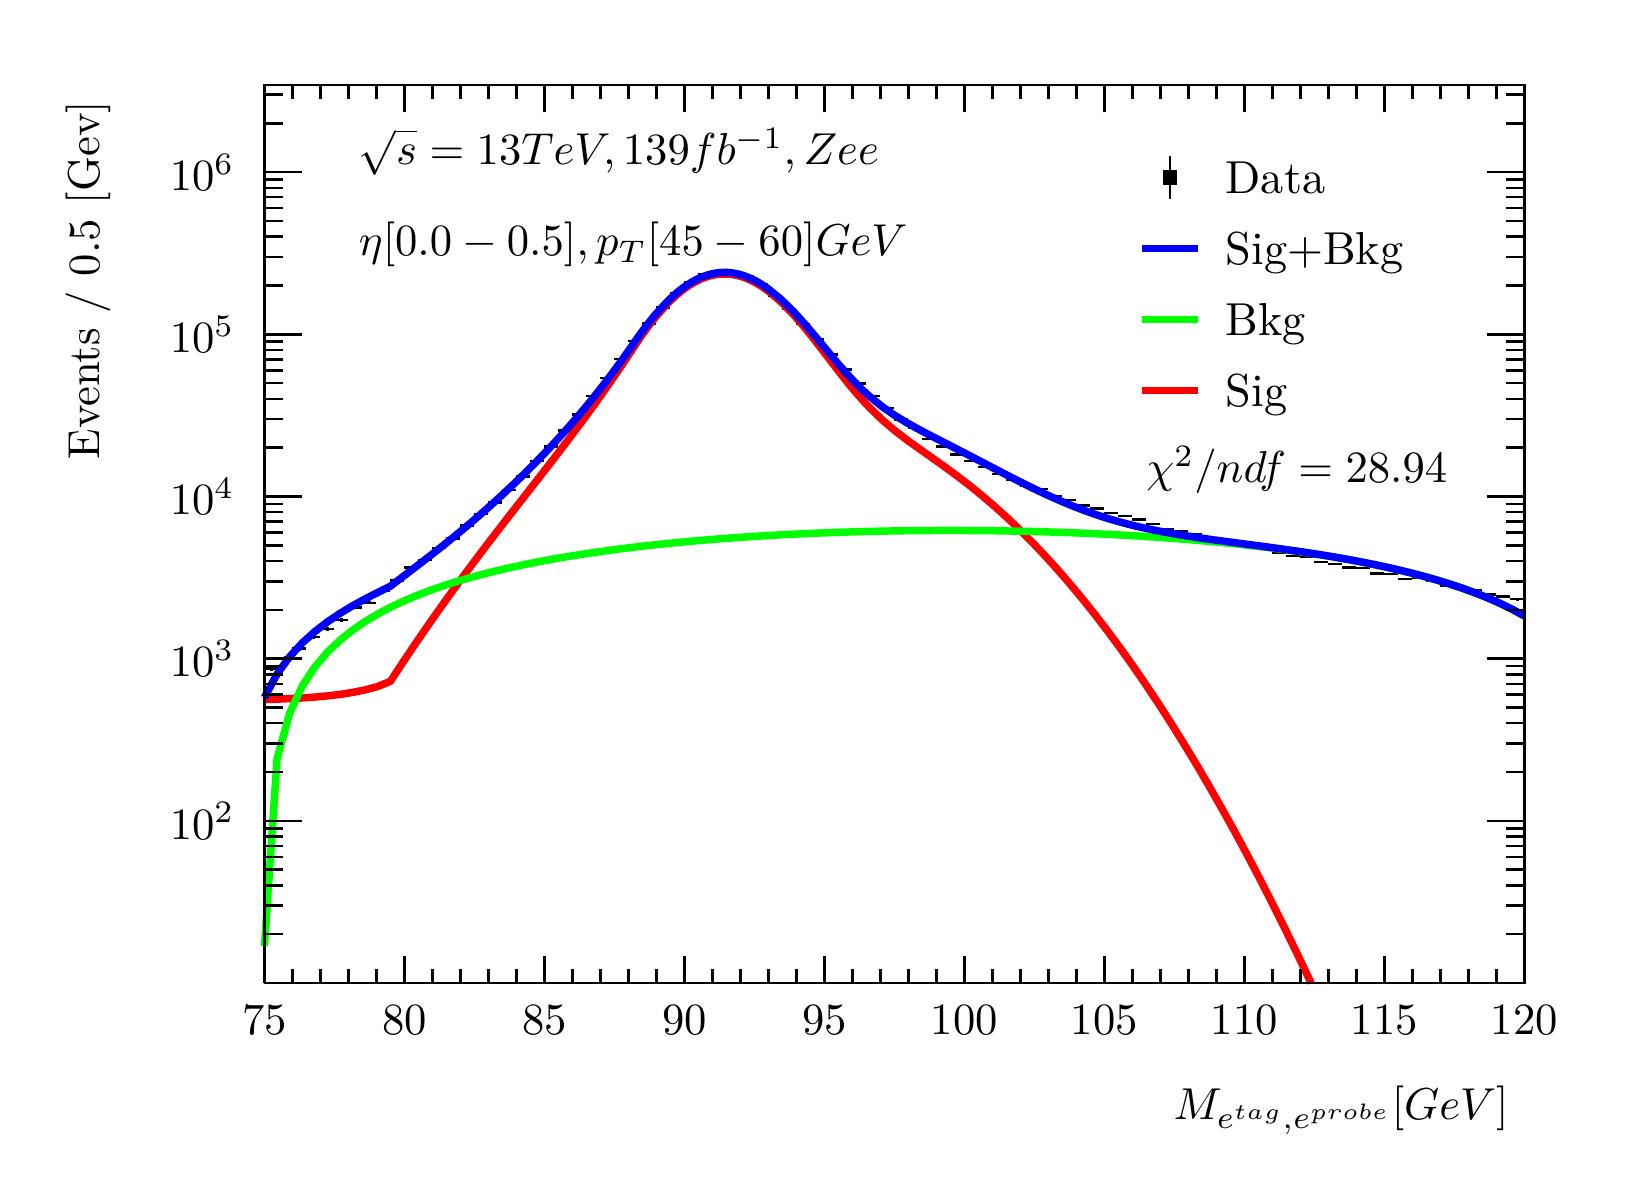
\begin{tikzpicture}
\pgfdeclareplotmark{cross} {
\pgfpathmoveto{\pgfpoint{-0.3\pgfplotmarksize}{\pgfplotmarksize}}
\pgfpathlineto{\pgfpoint{+0.3\pgfplotmarksize}{\pgfplotmarksize}}
\pgfpathlineto{\pgfpoint{+0.3\pgfplotmarksize}{0.3\pgfplotmarksize}}
\pgfpathlineto{\pgfpoint{+1\pgfplotmarksize}{0.3\pgfplotmarksize}}
\pgfpathlineto{\pgfpoint{+1\pgfplotmarksize}{-0.3\pgfplotmarksize}}
\pgfpathlineto{\pgfpoint{+0.3\pgfplotmarksize}{-0.3\pgfplotmarksize}}
\pgfpathlineto{\pgfpoint{+0.3\pgfplotmarksize}{-1.\pgfplotmarksize}}
\pgfpathlineto{\pgfpoint{-0.3\pgfplotmarksize}{-1.\pgfplotmarksize}}
\pgfpathlineto{\pgfpoint{-0.3\pgfplotmarksize}{-0.3\pgfplotmarksize}}
\pgfpathlineto{\pgfpoint{-1.\pgfplotmarksize}{-0.3\pgfplotmarksize}}
\pgfpathlineto{\pgfpoint{-1.\pgfplotmarksize}{0.3\pgfplotmarksize}}
\pgfpathlineto{\pgfpoint{-0.3\pgfplotmarksize}{0.3\pgfplotmarksize}}
\pgfpathclose
\pgfusepathqstroke
}
\pgfdeclareplotmark{cross*} {
\pgfpathmoveto{\pgfpoint{-0.3\pgfplotmarksize}{\pgfplotmarksize}}
\pgfpathlineto{\pgfpoint{+0.3\pgfplotmarksize}{\pgfplotmarksize}}
\pgfpathlineto{\pgfpoint{+0.3\pgfplotmarksize}{0.3\pgfplotmarksize}}
\pgfpathlineto{\pgfpoint{+1\pgfplotmarksize}{0.3\pgfplotmarksize}}
\pgfpathlineto{\pgfpoint{+1\pgfplotmarksize}{-0.3\pgfplotmarksize}}
\pgfpathlineto{\pgfpoint{+0.3\pgfplotmarksize}{-0.3\pgfplotmarksize}}
\pgfpathlineto{\pgfpoint{+0.3\pgfplotmarksize}{-1.\pgfplotmarksize}}
\pgfpathlineto{\pgfpoint{-0.3\pgfplotmarksize}{-1.\pgfplotmarksize}}
\pgfpathlineto{\pgfpoint{-0.3\pgfplotmarksize}{-0.3\pgfplotmarksize}}
\pgfpathlineto{\pgfpoint{-1.\pgfplotmarksize}{-0.3\pgfplotmarksize}}
\pgfpathlineto{\pgfpoint{-1.\pgfplotmarksize}{0.3\pgfplotmarksize}}
\pgfpathlineto{\pgfpoint{-0.3\pgfplotmarksize}{0.3\pgfplotmarksize}}
\pgfpathclose
\pgfusepathqfillstroke
}
\pgfdeclareplotmark{newstar} {
\pgfpathmoveto{\pgfqpoint{0pt}{\pgfplotmarksize}}
\pgfpathlineto{\pgfqpointpolar{44}{0.5\pgfplotmarksize}}
\pgfpathlineto{\pgfqpointpolar{18}{\pgfplotmarksize}}
\pgfpathlineto{\pgfqpointpolar{-20}{0.5\pgfplotmarksize}}
\pgfpathlineto{\pgfqpointpolar{-54}{\pgfplotmarksize}}
\pgfpathlineto{\pgfqpointpolar{-90}{0.5\pgfplotmarksize}}
\pgfpathlineto{\pgfqpointpolar{234}{\pgfplotmarksize}}
\pgfpathlineto{\pgfqpointpolar{198}{0.5\pgfplotmarksize}}
\pgfpathlineto{\pgfqpointpolar{162}{\pgfplotmarksize}}
\pgfpathlineto{\pgfqpointpolar{134}{0.5\pgfplotmarksize}}
\pgfpathclose
\pgfusepathqstroke
}
\pgfdeclareplotmark{newstar*} {
\pgfpathmoveto{\pgfqpoint{0pt}{\pgfplotmarksize}}
\pgfpathlineto{\pgfqpointpolar{44}{0.5\pgfplotmarksize}}
\pgfpathlineto{\pgfqpointpolar{18}{\pgfplotmarksize}}
\pgfpathlineto{\pgfqpointpolar{-20}{0.5\pgfplotmarksize}}
\pgfpathlineto{\pgfqpointpolar{-54}{\pgfplotmarksize}}
\pgfpathlineto{\pgfqpointpolar{-90}{0.5\pgfplotmarksize}}
\pgfpathlineto{\pgfqpointpolar{234}{\pgfplotmarksize}}
\pgfpathlineto{\pgfqpointpolar{198}{0.5\pgfplotmarksize}}
\pgfpathlineto{\pgfqpointpolar{162}{\pgfplotmarksize}}
\pgfpathlineto{\pgfqpointpolar{134}{0.5\pgfplotmarksize}}
\pgfpathclose
\pgfusepathqfillstroke
}
\definecolor{c}{rgb}{1,1,1};
\draw [color=c, fill=c] (0,0) rectangle (20,14.4361);
\draw [color=c, fill=c] (3,2.30977) rectangle (19,13.7143);
\definecolor{c}{rgb}{0,0,0};
\draw [c,line width=0.9] (3,2.30977) -- (3,13.7143) -- (19,13.7143) -- (19,2.30977) -- (3,2.30977);
\definecolor{c}{rgb}{1,1,1};
\draw [color=c, fill=c] (3,2.30977) rectangle (19,13.7143);
\definecolor{c}{rgb}{0,0,0};
\draw [c,line width=0.9] (3,2.30977) -- (3,13.7143) -- (19,13.7143) -- (19,2.30977) -- (3,2.30977);
\draw [c,line width=0.9] (3,2.30977) -- (19,2.30977);
\draw [c,line width=0.9] (3,2.65624) -- (3,2.30977);
\draw [c,line width=0.9] (3.35556,2.48301) -- (3.35556,2.30977);
\draw [c,line width=0.9] (3.71111,2.48301) -- (3.71111,2.30977);
\draw [c,line width=0.9] (4.06667,2.48301) -- (4.06667,2.30977);
\draw [c,line width=0.9] (4.42222,2.48301) -- (4.42222,2.30977);
\draw [c,line width=0.9] (4.77778,2.65624) -- (4.77778,2.30977);
\draw [c,line width=0.9] (5.13333,2.48301) -- (5.13333,2.30977);
\draw [c,line width=0.9] (5.48889,2.48301) -- (5.48889,2.30977);
\draw [c,line width=0.9] (5.84444,2.48301) -- (5.84444,2.30977);
\draw [c,line width=0.9] (6.2,2.48301) -- (6.2,2.30977);
\draw [c,line width=0.9] (6.55556,2.65624) -- (6.55556,2.30977);
\draw [c,line width=0.9] (6.91111,2.48301) -- (6.91111,2.30977);
\draw [c,line width=0.9] (7.26667,2.48301) -- (7.26667,2.30977);
\draw [c,line width=0.9] (7.62222,2.48301) -- (7.62222,2.30977);
\draw [c,line width=0.9] (7.97778,2.48301) -- (7.97778,2.30977);
\draw [c,line width=0.9] (8.33333,2.65624) -- (8.33333,2.30977);
\draw [c,line width=0.9] (8.68889,2.48301) -- (8.68889,2.30977);
\draw [c,line width=0.9] (9.04444,2.48301) -- (9.04444,2.30977);
\draw [c,line width=0.9] (9.4,2.48301) -- (9.4,2.30977);
\draw [c,line width=0.9] (9.75556,2.48301) -- (9.75556,2.30977);
\draw [c,line width=0.9] (10.1111,2.65624) -- (10.1111,2.30977);
\draw [c,line width=0.9] (10.4667,2.48301) -- (10.4667,2.30977);
\draw [c,line width=0.9] (10.8222,2.48301) -- (10.8222,2.30977);
\draw [c,line width=0.9] (11.1778,2.48301) -- (11.1778,2.30977);
\draw [c,line width=0.9] (11.5333,2.48301) -- (11.5333,2.30977);
\draw [c,line width=0.9] (11.8889,2.65624) -- (11.8889,2.30977);
\draw [c,line width=0.9] (12.2444,2.48301) -- (12.2444,2.30977);
\draw [c,line width=0.9] (12.6,2.48301) -- (12.6,2.30977);
\draw [c,line width=0.9] (12.9556,2.48301) -- (12.9556,2.30977);
\draw [c,line width=0.9] (13.3111,2.48301) -- (13.3111,2.30977);
\draw [c,line width=0.9] (13.6667,2.65624) -- (13.6667,2.30977);
\draw [c,line width=0.9] (14.0222,2.48301) -- (14.0222,2.30977);
\draw [c,line width=0.9] (14.3778,2.48301) -- (14.3778,2.30977);
\draw [c,line width=0.9] (14.7333,2.48301) -- (14.7333,2.30977);
\draw [c,line width=0.9] (15.0889,2.48301) -- (15.0889,2.30977);
\draw [c,line width=0.9] (15.4444,2.65624) -- (15.4444,2.30977);
\draw [c,line width=0.9] (15.8,2.48301) -- (15.8,2.30977);
\draw [c,line width=0.9] (16.1556,2.48301) -- (16.1556,2.30977);
\draw [c,line width=0.9] (16.5111,2.48301) -- (16.5111,2.30977);
\draw [c,line width=0.9] (16.8667,2.48301) -- (16.8667,2.30977);
\draw [c,line width=0.9] (17.2222,2.65624) -- (17.2222,2.30977);
\draw [c,line width=0.9] (17.5778,2.48301) -- (17.5778,2.30977);
\draw [c,line width=0.9] (17.9333,2.48301) -- (17.9333,2.30977);
\draw [c,line width=0.9] (18.2889,2.48301) -- (18.2889,2.30977);
\draw [c,line width=0.9] (18.6444,2.48301) -- (18.6444,2.30977);
\draw [c,line width=0.9] (19,2.65624) -- (19,2.30977);
\draw [c,line width=0.9] (19,2.65624) -- (19,2.30977);
\draw [anchor=base] (3,1.66015) node[scale=1.61424, color=c, rotate=0]{75};
\draw [anchor=base] (4.77778,1.66015) node[scale=1.61424, color=c, rotate=0]{80};
\draw [anchor=base] (6.55556,1.66015) node[scale=1.61424, color=c, rotate=0]{85};
\draw [anchor=base] (8.33333,1.66015) node[scale=1.61424, color=c, rotate=0]{90};
\draw [anchor=base] (10.1111,1.66015) node[scale=1.61424, color=c, rotate=0]{95};
\draw [anchor=base] (11.8889,1.66015) node[scale=1.61424, color=c, rotate=0]{100};
\draw [anchor=base] (13.6667,1.66015) node[scale=1.61424, color=c, rotate=0]{105};
\draw [anchor=base] (15.4444,1.66015) node[scale=1.61424, color=c, rotate=0]{110};
\draw [anchor=base] (17.2222,1.66015) node[scale=1.61424, color=c, rotate=0]{115};
\draw [anchor=base] (19,1.66015) node[scale=1.61424, color=c, rotate=0]{120};
\draw [anchor= east] (19,0.692932) node[scale=1.61424, color=c, rotate=0]{$M_{e^{tag}, e^{probe}}  [GeV]$};
\draw [c,line width=0.9] (3,13.7143) -- (19,13.7143);
\draw [c,line width=0.9] (3,13.3678) -- (3,13.7143);
\draw [c,line width=0.9] (3.35556,13.5411) -- (3.35556,13.7143);
\draw [c,line width=0.9] (3.71111,13.5411) -- (3.71111,13.7143);
\draw [c,line width=0.9] (4.06667,13.5411) -- (4.06667,13.7143);
\draw [c,line width=0.9] (4.42222,13.5411) -- (4.42222,13.7143);
\draw [c,line width=0.9] (4.77778,13.3678) -- (4.77778,13.7143);
\draw [c,line width=0.9] (5.13333,13.5411) -- (5.13333,13.7143);
\draw [c,line width=0.9] (5.48889,13.5411) -- (5.48889,13.7143);
\draw [c,line width=0.9] (5.84444,13.5411) -- (5.84444,13.7143);
\draw [c,line width=0.9] (6.2,13.5411) -- (6.2,13.7143);
\draw [c,line width=0.9] (6.55556,13.3678) -- (6.55556,13.7143);
\draw [c,line width=0.9] (6.91111,13.5411) -- (6.91111,13.7143);
\draw [c,line width=0.9] (7.26667,13.5411) -- (7.26667,13.7143);
\draw [c,line width=0.9] (7.62222,13.5411) -- (7.62222,13.7143);
\draw [c,line width=0.9] (7.97778,13.5411) -- (7.97778,13.7143);
\draw [c,line width=0.9] (8.33333,13.3678) -- (8.33333,13.7143);
\draw [c,line width=0.9] (8.68889,13.5411) -- (8.68889,13.7143);
\draw [c,line width=0.9] (9.04444,13.5411) -- (9.04444,13.7143);
\draw [c,line width=0.9] (9.4,13.5411) -- (9.4,13.7143);
\draw [c,line width=0.9] (9.75556,13.5411) -- (9.75556,13.7143);
\draw [c,line width=0.9] (10.1111,13.3678) -- (10.1111,13.7143);
\draw [c,line width=0.9] (10.4667,13.5411) -- (10.4667,13.7143);
\draw [c,line width=0.9] (10.8222,13.5411) -- (10.8222,13.7143);
\draw [c,line width=0.9] (11.1778,13.5411) -- (11.1778,13.7143);
\draw [c,line width=0.9] (11.5333,13.5411) -- (11.5333,13.7143);
\draw [c,line width=0.9] (11.8889,13.3678) -- (11.8889,13.7143);
\draw [c,line width=0.9] (12.2444,13.5411) -- (12.2444,13.7143);
\draw [c,line width=0.9] (12.6,13.5411) -- (12.6,13.7143);
\draw [c,line width=0.9] (12.9556,13.5411) -- (12.9556,13.7143);
\draw [c,line width=0.9] (13.3111,13.5411) -- (13.3111,13.7143);
\draw [c,line width=0.9] (13.6667,13.3678) -- (13.6667,13.7143);
\draw [c,line width=0.9] (14.0222,13.5411) -- (14.0222,13.7143);
\draw [c,line width=0.9] (14.3778,13.5411) -- (14.3778,13.7143);
\draw [c,line width=0.9] (14.7333,13.5411) -- (14.7333,13.7143);
\draw [c,line width=0.9] (15.0889,13.5411) -- (15.0889,13.7143);
\draw [c,line width=0.9] (15.4444,13.3678) -- (15.4444,13.7143);
\draw [c,line width=0.9] (15.8,13.5411) -- (15.8,13.7143);
\draw [c,line width=0.9] (16.1556,13.5411) -- (16.1556,13.7143);
\draw [c,line width=0.9] (16.5111,13.5411) -- (16.5111,13.7143);
\draw [c,line width=0.9] (16.8667,13.5411) -- (16.8667,13.7143);
\draw [c,line width=0.9] (17.2222,13.3678) -- (17.2222,13.7143);
\draw [c,line width=0.9] (17.5778,13.5411) -- (17.5778,13.7143);
\draw [c,line width=0.9] (17.9333,13.5411) -- (17.9333,13.7143);
\draw [c,line width=0.9] (18.2889,13.5411) -- (18.2889,13.7143);
\draw [c,line width=0.9] (18.6444,13.5411) -- (18.6444,13.7143);
\draw [c,line width=0.9] (19,13.3678) -- (19,13.7143);
\draw [c,line width=0.9] (19,13.3678) -- (19,13.7143);
\draw [c,line width=0.9] (3,2.30977) -- (3,13.7143);
\draw [c,line width=0.9] (3.237,2.92982) -- (3,2.92982);
\draw [c,line width=0.9] (3.237,3.29252) -- (3,3.29252);
\draw [c,line width=0.9] (3.237,3.54986) -- (3,3.54986);
\draw [c,line width=0.9] (3.237,3.74947) -- (3,3.74947);
\draw [c,line width=0.9] (3.237,3.91257) -- (3,3.91257);
\draw [c,line width=0.9] (3.237,4.05046) -- (3,4.05046);
\draw [c,line width=0.9] (3.237,4.16991) -- (3,4.16991);
\draw [c,line width=0.9] (3.237,4.27527) -- (3,4.27527);
\draw [c,line width=0.9] (3.474,4.36952) -- (3,4.36952);
\draw [anchor= east] (2.82,4.36952) node[scale=1.61424, color=c, rotate=0]{$10^{2}$};
\draw [c,line width=0.9] (3.237,4.98956) -- (3,4.98956);
\draw [c,line width=0.9] (3.237,5.35227) -- (3,5.35227);
\draw [c,line width=0.9] (3.237,5.60961) -- (3,5.60961);
\draw [c,line width=0.9] (3.237,5.80922) -- (3,5.80922);
\draw [c,line width=0.9] (3.237,5.97231) -- (3,5.97231);
\draw [c,line width=0.9] (3.237,6.11021) -- (3,6.11021);
\draw [c,line width=0.9] (3.237,6.22966) -- (3,6.22966);
\draw [c,line width=0.9] (3.237,6.33502) -- (3,6.33502);
\draw [c,line width=0.9] (3.474,6.42927) -- (3,6.42927);
\draw [anchor= east] (2.82,6.42927) node[scale=1.61424, color=c, rotate=0]{$10^{3}$};
\draw [c,line width=0.9] (3.237,7.04931) -- (3,7.04931);
\draw [c,line width=0.9] (3.237,7.41202) -- (3,7.41202);
\draw [c,line width=0.9] (3.237,7.66936) -- (3,7.66936);
\draw [c,line width=0.9] (3.237,7.86897) -- (3,7.86897);
\draw [c,line width=0.9] (3.237,8.03206) -- (3,8.03206);
\draw [c,line width=0.9] (3.237,8.16995) -- (3,8.16995);
\draw [c,line width=0.9] (3.237,8.2894) -- (3,8.2894);
\draw [c,line width=0.9] (3.237,8.39476) -- (3,8.39476);
\draw [c,line width=0.9] (3.474,8.48901) -- (3,8.48901);
\draw [anchor= east] (2.82,8.48901) node[scale=1.61424, color=c, rotate=0]{$10^{4}$};
\draw [c,line width=0.9] (3.237,9.10906) -- (3,9.10906);
\draw [c,line width=0.9] (3.237,9.47176) -- (3,9.47176);
\draw [c,line width=0.9] (3.237,9.7291) -- (3,9.7291);
\draw [c,line width=0.9] (3.237,9.92871) -- (3,9.92871);
\draw [c,line width=0.9] (3.237,10.0918) -- (3,10.0918);
\draw [c,line width=0.9] (3.237,10.2297) -- (3,10.2297);
\draw [c,line width=0.9] (3.237,10.3491) -- (3,10.3491);
\draw [c,line width=0.9] (3.237,10.4545) -- (3,10.4545);
\draw [c,line width=0.9] (3.474,10.5488) -- (3,10.5488);
\draw [anchor= east] (2.82,10.5488) node[scale=1.61424, color=c, rotate=0]{$10^{5}$};
\draw [c,line width=0.9] (3.237,11.1688) -- (3,11.1688);
\draw [c,line width=0.9] (3.237,11.5315) -- (3,11.5315);
\draw [c,line width=0.9] (3.237,11.7889) -- (3,11.7889);
\draw [c,line width=0.9] (3.237,11.9885) -- (3,11.9885);
\draw [c,line width=0.9] (3.237,12.1516) -- (3,12.1516);
\draw [c,line width=0.9] (3.237,12.2894) -- (3,12.2894);
\draw [c,line width=0.9] (3.237,12.4089) -- (3,12.4089);
\draw [c,line width=0.9] (3.237,12.5143) -- (3,12.5143);
\draw [c,line width=0.9] (3.474,12.6085) -- (3,12.6085);
\draw [anchor= east] (2.82,12.6085) node[scale=1.61424, color=c, rotate=0]{$10^{6}$};
\draw [c,line width=0.9] (3.237,13.2286) -- (3,13.2286);
\draw [c,line width=0.9] (3.237,13.5913) -- (3,13.5913);
\draw [anchor= east] (0.76,13.7143) node[scale=1.61424, color=c, rotate=90]{Events / 0.5 [Gev]};
\draw [c,line width=0.9] (19,2.30977) -- (19,13.7143);
\draw [c,line width=0.9] (18.763,2.92982) -- (19,2.92982);
\draw [c,line width=0.9] (18.763,3.29252) -- (19,3.29252);
\draw [c,line width=0.9] (18.763,3.54986) -- (19,3.54986);
\draw [c,line width=0.9] (18.763,3.74947) -- (19,3.74947);
\draw [c,line width=0.9] (18.763,3.91257) -- (19,3.91257);
\draw [c,line width=0.9] (18.763,4.05046) -- (19,4.05046);
\draw [c,line width=0.9] (18.763,4.16991) -- (19,4.16991);
\draw [c,line width=0.9] (18.763,4.27527) -- (19,4.27527);
\draw [c,line width=0.9] (18.526,4.36952) -- (19,4.36952);
\draw [c,line width=0.9] (18.763,4.98956) -- (19,4.98956);
\draw [c,line width=0.9] (18.763,5.35227) -- (19,5.35227);
\draw [c,line width=0.9] (18.763,5.60961) -- (19,5.60961);
\draw [c,line width=0.9] (18.763,5.80922) -- (19,5.80922);
\draw [c,line width=0.9] (18.763,5.97231) -- (19,5.97231);
\draw [c,line width=0.9] (18.763,6.11021) -- (19,6.11021);
\draw [c,line width=0.9] (18.763,6.22966) -- (19,6.22966);
\draw [c,line width=0.9] (18.763,6.33502) -- (19,6.33502);
\draw [c,line width=0.9] (18.526,6.42927) -- (19,6.42927);
\draw [c,line width=0.9] (18.763,7.04931) -- (19,7.04931);
\draw [c,line width=0.9] (18.763,7.41202) -- (19,7.41202);
\draw [c,line width=0.9] (18.763,7.66936) -- (19,7.66936);
\draw [c,line width=0.9] (18.763,7.86897) -- (19,7.86897);
\draw [c,line width=0.9] (18.763,8.03206) -- (19,8.03206);
\draw [c,line width=0.9] (18.763,8.16995) -- (19,8.16995);
\draw [c,line width=0.9] (18.763,8.2894) -- (19,8.2894);
\draw [c,line width=0.9] (18.763,8.39476) -- (19,8.39476);
\draw [c,line width=0.9] (18.526,8.48901) -- (19,8.48901);
\draw [c,line width=0.9] (18.763,9.10906) -- (19,9.10906);
\draw [c,line width=0.9] (18.763,9.47176) -- (19,9.47176);
\draw [c,line width=0.9] (18.763,9.7291) -- (19,9.7291);
\draw [c,line width=0.9] (18.763,9.92871) -- (19,9.92871);
\draw [c,line width=0.9] (18.763,10.0918) -- (19,10.0918);
\draw [c,line width=0.9] (18.763,10.2297) -- (19,10.2297);
\draw [c,line width=0.9] (18.763,10.3491) -- (19,10.3491);
\draw [c,line width=0.9] (18.763,10.4545) -- (19,10.4545);
\draw [c,line width=0.9] (18.526,10.5488) -- (19,10.5488);
\draw [c,line width=0.9] (18.763,11.1688) -- (19,11.1688);
\draw [c,line width=0.9] (18.763,11.5315) -- (19,11.5315);
\draw [c,line width=0.9] (18.763,11.7889) -- (19,11.7889);
\draw [c,line width=0.9] (18.763,11.9885) -- (19,11.9885);
\draw [c,line width=0.9] (18.763,12.1516) -- (19,12.1516);
\draw [c,line width=0.9] (18.763,12.2894) -- (19,12.2894);
\draw [c,line width=0.9] (18.763,12.4089) -- (19,12.4089);
\draw [c,line width=0.9] (18.763,12.5143) -- (19,12.5143);
\draw [c,line width=0.9] (18.526,12.6085) -- (19,12.6085);
\draw [c,line width=0.9] (18.763,13.2286) -- (19,13.2286);
\draw [c,line width=0.9] (18.763,13.5913) -- (19,13.5913);
\draw [c,line width=0.9] (3.08889,6.30572) -- (3,6.30572);
\draw [c,line width=0.9] (3,6.30572) -- (3,6.30572);
\draw [c,line width=0.9] (3.08889,6.30572) -- (3.17778,6.30572);
\draw [c,line width=0.9] (3.17778,6.30572) -- (3.17778,6.30572);
\draw [c,line width=0.9] (3.08889,6.30572) -- (3.08889,6.33603);
\draw [c,line width=0.9] (3.08889,6.33603) -- (3.08889,6.33603);
\draw [c,line width=0.9] (3.08889,6.30572) -- (3.08889,6.27541);
\draw [c,line width=0.9] (3.08889,6.27541) -- (3.08889,6.27541);
\draw [c,line width=0.9] (3.26667,6.43994) -- (3.17778,6.43994);
\draw [c,line width=0.9] (3.17778,6.43994) -- (3.17778,6.43994);
\draw [c,line width=0.9] (3.26667,6.43994) -- (3.35556,6.43994);
\draw [c,line width=0.9] (3.35556,6.43994) -- (3.35556,6.43994);
\draw [c,line width=0.9] (3.26667,6.43994) -- (3.26667,6.46806);
\draw [c,line width=0.9] (3.26667,6.46806) -- (3.26667,6.46806);
\draw [c,line width=0.9] (3.26667,6.43994) -- (3.26667,6.41182);
\draw [c,line width=0.9] (3.26667,6.41182) -- (3.26667,6.41182);
\draw [c,line width=0.9] (3.44444,6.55584) -- (3.35556,6.55584);
\draw [c,line width=0.9] (3.35556,6.55584) -- (3.35556,6.55584);
\draw [c,line width=0.9] (3.44444,6.55584) -- (3.53333,6.55584);
\draw [c,line width=0.9] (3.53333,6.55584) -- (3.53333,6.55584);
\draw [c,line width=0.9] (3.44444,6.55584) -- (3.44444,6.5822);
\draw [c,line width=0.9] (3.44444,6.5822) -- (3.44444,6.5822);
\draw [c,line width=0.9] (3.44444,6.55584) -- (3.44444,6.52949);
\draw [c,line width=0.9] (3.44444,6.52949) -- (3.44444,6.52949);
\draw [c,line width=0.9] (3.62222,6.70301) -- (3.53333,6.70301);
\draw [c,line width=0.9] (3.53333,6.70301) -- (3.53333,6.70301);
\draw [c,line width=0.9] (3.62222,6.70301) -- (3.71111,6.70301);
\draw [c,line width=0.9] (3.71111,6.70301) -- (3.71111,6.70301);
\draw [c,line width=0.9] (3.62222,6.70301) -- (3.62222,6.72728);
\draw [c,line width=0.9] (3.62222,6.72728) -- (3.62222,6.72728);
\draw [c,line width=0.9] (3.62222,6.70301) -- (3.62222,6.67873);
\draw [c,line width=0.9] (3.62222,6.67873) -- (3.62222,6.67873);
\draw [c,line width=0.9] (3.8,6.80852) -- (3.71111,6.80852);
\draw [c,line width=0.9] (3.71111,6.80852) -- (3.71111,6.80852);
\draw [c,line width=0.9] (3.8,6.80852) -- (3.88889,6.80852);
\draw [c,line width=0.9] (3.88889,6.80852) -- (3.88889,6.80852);
\draw [c,line width=0.9] (3.8,6.80852) -- (3.8,6.8314);
\draw [c,line width=0.9] (3.8,6.8314) -- (3.8,6.8314);
\draw [c,line width=0.9] (3.8,6.80852) -- (3.8,6.78563);
\draw [c,line width=0.9] (3.8,6.78563) -- (3.8,6.78563);
\draw [c,line width=0.9] (3.97778,6.91855) -- (3.88889,6.91855);
\draw [c,line width=0.9] (3.88889,6.91855) -- (3.88889,6.91855);
\draw [c,line width=0.9] (3.97778,6.91855) -- (4.06667,6.91855);
\draw [c,line width=0.9] (4.06667,6.91855) -- (4.06667,6.91855);
\draw [c,line width=0.9] (3.97778,6.91855) -- (3.97778,6.94007);
\draw [c,line width=0.9] (3.97778,6.94007) -- (3.97778,6.94007);
\draw [c,line width=0.9] (3.97778,6.91855) -- (3.97778,6.89703);
\draw [c,line width=0.9] (3.97778,6.89703) -- (3.97778,6.89703);
\draw [c,line width=0.9] (4.15556,7.08052) -- (4.06667,7.08052);
\draw [c,line width=0.9] (4.06667,7.08052) -- (4.06667,7.08052);
\draw [c,line width=0.9] (4.15556,7.08052) -- (4.24444,7.08052);
\draw [c,line width=0.9] (4.24444,7.08052) -- (4.24444,7.08052);
\draw [c,line width=0.9] (4.15556,7.08052) -- (4.15556,7.10017);
\draw [c,line width=0.9] (4.15556,7.10017) -- (4.15556,7.10017);
\draw [c,line width=0.9] (4.15556,7.08052) -- (4.15556,7.06086);
\draw [c,line width=0.9] (4.15556,7.06086) -- (4.15556,7.06086);
\draw [c,line width=0.9] (4.33333,7.13863) -- (4.24444,7.13863);
\draw [c,line width=0.9] (4.24444,7.13863) -- (4.24444,7.13863);
\draw [c,line width=0.9] (4.33333,7.13863) -- (4.42222,7.13863);
\draw [c,line width=0.9] (4.42222,7.13863) -- (4.42222,7.13863);
\draw [c,line width=0.9] (4.33333,7.13863) -- (4.33333,7.15766);
\draw [c,line width=0.9] (4.33333,7.15766) -- (4.33333,7.15766);
\draw [c,line width=0.9] (4.33333,7.13863) -- (4.33333,7.1196);
\draw [c,line width=0.9] (4.33333,7.1196) -- (4.33333,7.1196);
\draw [c,line width=0.9] (4.51111,7.29393) -- (4.42222,7.29393);
\draw [c,line width=0.9] (4.42222,7.29393) -- (4.42222,7.29393);
\draw [c,line width=0.9] (4.51111,7.29393) -- (4.6,7.29393);
\draw [c,line width=0.9] (4.6,7.29393) -- (4.6,7.29393);
\draw [c,line width=0.9] (4.51111,7.29393) -- (4.51111,7.31138);
\draw [c,line width=0.9] (4.51111,7.31138) -- (4.51111,7.31138);
\draw [c,line width=0.9] (4.51111,7.29393) -- (4.51111,7.27648);
\draw [c,line width=0.9] (4.51111,7.27648) -- (4.51111,7.27648);
\draw [c,line width=0.9] (4.68889,7.42239) -- (4.6,7.42239);
\draw [c,line width=0.9] (4.6,7.42239) -- (4.6,7.42239);
\draw [c,line width=0.9] (4.68889,7.42239) -- (4.77778,7.42239);
\draw [c,line width=0.9] (4.77778,7.42239) -- (4.77778,7.42239);
\draw [c,line width=0.9] (4.68889,7.42239) -- (4.68889,7.43863);
\draw [c,line width=0.9] (4.68889,7.43863) -- (4.68889,7.43863);
\draw [c,line width=0.9] (4.68889,7.42239) -- (4.68889,7.40616);
\draw [c,line width=0.9] (4.68889,7.40616) -- (4.68889,7.40616);
\draw [c,line width=0.9] (4.86667,7.58647) -- (4.77778,7.58647);
\draw [c,line width=0.9] (4.77778,7.58647) -- (4.77778,7.58647);
\draw [c,line width=0.9] (4.86667,7.58647) -- (4.95556,7.58647);
\draw [c,line width=0.9] (4.95556,7.58647) -- (4.95556,7.58647);
\draw [c,line width=0.9] (4.86667,7.58647) -- (4.86667,7.60128);
\draw [c,line width=0.9] (4.86667,7.60128) -- (4.86667,7.60128);
\draw [c,line width=0.9] (4.86667,7.58647) -- (4.86667,7.57165);
\draw [c,line width=0.9] (4.86667,7.57165) -- (4.86667,7.57165);
\draw [c,line width=0.9] (5.04444,7.68466) -- (4.95556,7.68466);
\draw [c,line width=0.9] (4.95556,7.68466) -- (4.95556,7.68466);
\draw [c,line width=0.9] (5.04444,7.68466) -- (5.13333,7.68466);
\draw [c,line width=0.9] (5.13333,7.68466) -- (5.13333,7.68466);
\draw [c,line width=0.9] (5.04444,7.68466) -- (5.04444,7.69868);
\draw [c,line width=0.9] (5.04444,7.69868) -- (5.04444,7.69868);
\draw [c,line width=0.9] (5.04444,7.68466) -- (5.04444,7.67063);
\draw [c,line width=0.9] (5.04444,7.67063) -- (5.04444,7.67063);
\draw [c,line width=0.9] (5.22222,7.83413) -- (5.13333,7.83413);
\draw [c,line width=0.9] (5.13333,7.83413) -- (5.13333,7.83413);
\draw [c,line width=0.9] (5.22222,7.83413) -- (5.31111,7.83413);
\draw [c,line width=0.9] (5.31111,7.83413) -- (5.31111,7.83413);
\draw [c,line width=0.9] (5.22222,7.83413) -- (5.22222,7.84703);
\draw [c,line width=0.9] (5.22222,7.84703) -- (5.22222,7.84703);
\draw [c,line width=0.9] (5.22222,7.83413) -- (5.22222,7.82123);
\draw [c,line width=0.9] (5.22222,7.82123) -- (5.22222,7.82123);
\draw [c,line width=0.9] (5.4,7.95861) -- (5.31111,7.95861);
\draw [c,line width=0.9] (5.31111,7.95861) -- (5.31111,7.95861);
\draw [c,line width=0.9] (5.4,7.95861) -- (5.48889,7.95861);
\draw [c,line width=0.9] (5.48889,7.95861) -- (5.48889,7.95861);
\draw [c,line width=0.9] (5.4,7.95861) -- (5.4,7.97064);
\draw [c,line width=0.9] (5.4,7.97064) -- (5.4,7.97064);
\draw [c,line width=0.9] (5.4,7.95861) -- (5.4,7.94658);
\draw [c,line width=0.9] (5.4,7.94658) -- (5.4,7.94658);
\draw [c,line width=0.9] (5.57778,8.118) -- (5.48889,8.118);
\draw [c,line width=0.9] (5.48889,8.118) -- (5.48889,8.118);
\draw [c,line width=0.9] (5.57778,8.118) -- (5.66667,8.118);
\draw [c,line width=0.9] (5.66667,8.118) -- (5.66667,8.118);
\draw [c,line width=0.9] (5.57778,8.118) -- (5.57778,8.129);
\draw [c,line width=0.9] (5.57778,8.129) -- (5.57778,8.129);
\draw [c,line width=0.9] (5.57778,8.118) -- (5.57778,8.10699);
\draw [c,line width=0.9] (5.57778,8.10699) -- (5.57778,8.10699);
\draw [c,line width=0.9] (5.75556,8.26354) -- (5.66667,8.26354);
\draw [c,line width=0.9] (5.66667,8.26354) -- (5.66667,8.26354);
\draw [c,line width=0.9] (5.75556,8.26354) -- (5.84444,8.26354);
\draw [c,line width=0.9] (5.84444,8.26354) -- (5.84444,8.26354);
\draw [c,line width=0.9] (5.75556,8.26354) -- (5.75556,8.27369);
\draw [c,line width=0.9] (5.75556,8.27369) -- (5.75556,8.27369);
\draw [c,line width=0.9] (5.75556,8.26354) -- (5.75556,8.25339);
\draw [c,line width=0.9] (5.75556,8.25339) -- (5.75556,8.25339);
\draw [c,line width=0.9] (5.93333,8.41189) -- (5.84444,8.41189);
\draw [c,line width=0.9] (5.84444,8.41189) -- (5.84444,8.41189);
\draw [c,line width=0.9] (5.93333,8.41189) -- (6.02222,8.41189);
\draw [c,line width=0.9] (6.02222,8.41189) -- (6.02222,8.41189);
\draw [c,line width=0.9] (5.93333,8.41189) -- (5.93333,8.42123);
\draw [c,line width=0.9] (5.93333,8.42123) -- (5.93333,8.42123);
\draw [c,line width=0.9] (5.93333,8.41189) -- (5.93333,8.40256);
\draw [c,line width=0.9] (5.93333,8.40256) -- (5.93333,8.40256);
\draw [c,line width=0.9] (6.11111,8.5702) -- (6.02222,8.5702);
\draw [c,line width=0.9] (6.02222,8.5702) -- (6.02222,8.5702);
\draw [c,line width=0.9] (6.11111,8.5702) -- (6.2,8.5702);
\draw [c,line width=0.9] (6.2,8.5702) -- (6.2,8.5702);
\draw [c,line width=0.9] (6.11111,8.5702) -- (6.11111,8.57875);
\draw [c,line width=0.9] (6.11111,8.57875) -- (6.11111,8.57875);
\draw [c,line width=0.9] (6.11111,8.5702) -- (6.11111,8.56165);
\draw [c,line width=0.9] (6.11111,8.56165) -- (6.11111,8.56165);
\draw [c,line width=0.9] (6.28889,8.74338) -- (6.2,8.74338);
\draw [c,line width=0.9] (6.2,8.74338) -- (6.2,8.74338);
\draw [c,line width=0.9] (6.28889,8.74338) -- (6.37778,8.74338);
\draw [c,line width=0.9] (6.37778,8.74338) -- (6.37778,8.74338);
\draw [c,line width=0.9] (6.28889,8.74338) -- (6.28889,8.75114);
\draw [c,line width=0.9] (6.28889,8.75114) -- (6.28889,8.75114);
\draw [c,line width=0.9] (6.28889,8.74338) -- (6.28889,8.73562);
\draw [c,line width=0.9] (6.28889,8.73562) -- (6.28889,8.73562);
\draw [c,line width=0.9] (6.46667,8.93957) -- (6.37778,8.93957);
\draw [c,line width=0.9] (6.37778,8.93957) -- (6.37778,8.93957);
\draw [c,line width=0.9] (6.46667,8.93957) -- (6.55556,8.93957);
\draw [c,line width=0.9] (6.55556,8.93957) -- (6.55556,8.93957);
\draw [c,line width=0.9] (6.46667,8.93957) -- (6.46667,8.94653);
\draw [c,line width=0.9] (6.46667,8.94653) -- (6.46667,8.94653);
\draw [c,line width=0.9] (6.46667,8.93957) -- (6.46667,8.93262);
\draw [c,line width=0.9] (6.46667,8.93262) -- (6.46667,8.93262);
\draw [c,line width=0.9] (6.64444,9.12594) -- (6.55556,9.12594);
\draw [c,line width=0.9] (6.55556,9.12594) -- (6.55556,9.12594);
\draw [c,line width=0.9] (6.64444,9.12594) -- (6.73333,9.12594);
\draw [c,line width=0.9] (6.73333,9.12594) -- (6.73333,9.12594);
\draw [c,line width=0.9] (6.64444,9.12594) -- (6.64444,9.13221);
\draw [c,line width=0.9] (6.64444,9.13221) -- (6.64444,9.13221);
\draw [c,line width=0.9] (6.64444,9.12594) -- (6.64444,9.11967);
\draw [c,line width=0.9] (6.64444,9.11967) -- (6.64444,9.11967);
\draw [c,line width=0.9] (6.82222,9.32751) -- (6.73333,9.32751);
\draw [c,line width=0.9] (6.73333,9.32751) -- (6.73333,9.32751);
\draw [c,line width=0.9] (6.82222,9.32751) -- (6.91111,9.32751);
\draw [c,line width=0.9] (6.91111,9.32751) -- (6.91111,9.32751);
\draw [c,line width=0.9] (6.82222,9.32751) -- (6.82222,9.3331);
\draw [c,line width=0.9] (6.82222,9.3331) -- (6.82222,9.3331);
\draw [c,line width=0.9] (6.82222,9.32751) -- (6.82222,9.32191);
\draw [c,line width=0.9] (6.82222,9.32191) -- (6.82222,9.32191);
\draw [c,line width=0.9] (7,9.53) -- (6.91111,9.53);
\draw [c,line width=0.9] (6.91111,9.53) -- (6.91111,9.53);
\draw [c,line width=0.9] (7,9.53) -- (7.08889,9.53);
\draw [c,line width=0.9] (7.08889,9.53) -- (7.08889,9.53);
\draw [c,line width=0.9] (7,9.53) -- (7,9.535);
\draw [c,line width=0.9] (7,9.535) -- (7,9.535);
\draw [c,line width=0.9] (7,9.53) -- (7,9.525);
\draw [c,line width=0.9] (7,9.525) -- (7,9.525);
\draw [c,line width=0.9] (7.17778,9.76837) -- (7.08889,9.76837);
\draw [c,line width=0.9] (7.08889,9.76837) -- (7.08889,9.76837);
\draw [c,line width=0.9] (7.17778,9.76837) -- (7.26667,9.76837);
\draw [c,line width=0.9] (7.26667,9.76837) -- (7.26667,9.76837);
\draw [c,line width=0.9] (7.17778,9.76837) -- (7.17778,9.77275);
\draw [c,line width=0.9] (7.17778,9.77275) -- (7.17778,9.77275);
\draw [c,line width=0.9] (7.17778,9.76837) -- (7.17778,9.764);
\draw [c,line width=0.9] (7.17778,9.764) -- (7.17778,9.764);
\draw [c,line width=0.9] (7.35556,9.99199) -- (7.26667,9.99199);
\draw [c,line width=0.9] (7.26667,9.99199) -- (7.26667,9.99199);
\draw [c,line width=0.9] (7.35556,9.99199) -- (7.44444,9.99199);
\draw [c,line width=0.9] (7.44444,9.99199) -- (7.44444,9.99199);
\draw [c,line width=0.9] (7.35556,9.99199) -- (7.35556,9.99585);
\draw [c,line width=0.9] (7.35556,9.99585) -- (7.35556,9.99585);
\draw [c,line width=0.9] (7.35556,9.99199) -- (7.35556,9.98813);
\draw [c,line width=0.9] (7.35556,9.98813) -- (7.35556,9.98813);
\draw [c,line width=0.9] (7.53333,10.2354) -- (7.44444,10.2354);
\draw [c,line width=0.9] (7.44444,10.2354) -- (7.44444,10.2354);
\draw [c,line width=0.9] (7.53333,10.2354) -- (7.62222,10.2354);
\draw [c,line width=0.9] (7.62222,10.2354) -- (7.62222,10.2354);
\draw [c,line width=0.9] (7.53333,10.2354) -- (7.53333,10.2387);
\draw [c,line width=0.9] (7.53333,10.2387) -- (7.53333,10.2387);
\draw [c,line width=0.9] (7.53333,10.2354) -- (7.53333,10.232);
\draw [c,line width=0.9] (7.53333,10.232) -- (7.53333,10.232);
\draw [c,line width=0.9] (7.71111,10.4629) -- (7.62222,10.4629);
\draw [c,line width=0.9] (7.62222,10.4629) -- (7.62222,10.4629);
\draw [c,line width=0.9] (7.71111,10.4629) -- (7.8,10.4629);
\draw [c,line width=0.9] (7.8,10.4629) -- (7.8,10.4629);
\draw [c,line width=0.9] (7.71111,10.4629) -- (7.71111,10.4658);
\draw [c,line width=0.9] (7.71111,10.4658) -- (7.71111,10.4658);
\draw [c,line width=0.9] (7.71111,10.4629) -- (7.71111,10.4599);
\draw [c,line width=0.9] (7.71111,10.4599) -- (7.71111,10.4599);
\draw [c,line width=0.9] (7.88889,10.6841) -- (7.8,10.6841);
\draw [c,line width=0.9] (7.8,10.6841) -- (7.8,10.6841);
\draw [c,line width=0.9] (7.88889,10.6841) -- (7.97778,10.6841);
\draw [c,line width=0.9] (7.97778,10.6841) -- (7.97778,10.6841);
\draw [c,line width=0.9] (7.88889,10.6841) -- (7.88889,10.6867);
\draw [c,line width=0.9] (7.88889,10.6867) -- (7.88889,10.6867);
\draw [c,line width=0.9] (7.88889,10.6841) -- (7.88889,10.6815);
\draw [c,line width=0.9] (7.88889,10.6815) -- (7.88889,10.6815);
\draw [c,line width=0.9] (8.06667,10.8887) -- (7.97778,10.8887);
\draw [c,line width=0.9] (7.97778,10.8887) -- (7.97778,10.8887);
\draw [c,line width=0.9] (8.06667,10.8887) -- (8.15556,10.8887);
\draw [c,line width=0.9] (8.15556,10.8887) -- (8.15556,10.8887);
\draw [c,line width=0.9] (8.06667,10.8887) -- (8.06667,10.891);
\draw [c,line width=0.9] (8.06667,10.891) -- (8.06667,10.891);
\draw [c,line width=0.9] (8.06667,10.8887) -- (8.06667,10.8863);
\draw [c,line width=0.9] (8.06667,10.8863) -- (8.06667,10.8863);
\draw [c,line width=0.9] (8.24444,11.0725) -- (8.15556,11.0725);
\draw [c,line width=0.9] (8.15556,11.0725) -- (8.15556,11.0725);
\draw [c,line width=0.9] (8.24444,11.0725) -- (8.33333,11.0725);
\draw [c,line width=0.9] (8.33333,11.0725) -- (8.33333,11.0725);
\draw [c,line width=0.9] (8.24444,11.0725) -- (8.24444,11.0746);
\draw [c,line width=0.9] (8.24444,11.0746) -- (8.24444,11.0746);
\draw [c,line width=0.9] (8.24444,11.0725) -- (8.24444,11.0704);
\draw [c,line width=0.9] (8.24444,11.0704) -- (8.24444,11.0704);
\draw [c,line width=0.9] (8.42222,11.2095) -- (8.33333,11.2095);
\draw [c,line width=0.9] (8.33333,11.2095) -- (8.33333,11.2095);
\draw [c,line width=0.9] (8.42222,11.2095) -- (8.51111,11.2095);
\draw [c,line width=0.9] (8.51111,11.2095) -- (8.51111,11.2095);
\draw [c,line width=0.9] (8.42222,11.2095) -- (8.42222,11.2115);
\draw [c,line width=0.9] (8.42222,11.2115) -- (8.42222,11.2115);
\draw [c,line width=0.9] (8.42222,11.2095) -- (8.42222,11.2076);
\draw [c,line width=0.9] (8.42222,11.2076) -- (8.42222,11.2076);
\draw [c,line width=0.9] (8.6,11.3058) -- (8.51111,11.3058);
\draw [c,line width=0.9] (8.51111,11.3058) -- (8.51111,11.3058);
\draw [c,line width=0.9] (8.6,11.3058) -- (8.68889,11.3058);
\draw [c,line width=0.9] (8.68889,11.3058) -- (8.68889,11.3058);
\draw [c,line width=0.9] (8.6,11.3058) -- (8.6,11.3076);
\draw [c,line width=0.9] (8.6,11.3076) -- (8.6,11.3076);
\draw [c,line width=0.9] (8.6,11.3058) -- (8.6,11.3039);
\draw [c,line width=0.9] (8.6,11.3039) -- (8.6,11.3039);
\draw [c,line width=0.9] (8.77778,11.3499) -- (8.68889,11.3499);
\draw [c,line width=0.9] (8.68889,11.3499) -- (8.68889,11.3499);
\draw [c,line width=0.9] (8.77778,11.3499) -- (8.86667,11.3499);
\draw [c,line width=0.9] (8.86667,11.3499) -- (8.86667,11.3499);
\draw [c,line width=0.9] (8.77778,11.3499) -- (8.77778,11.3517);
\draw [c,line width=0.9] (8.77778,11.3517) -- (8.77778,11.3517);
\draw [c,line width=0.9] (8.77778,11.3499) -- (8.77778,11.348);
\draw [c,line width=0.9] (8.77778,11.348) -- (8.77778,11.348);
\draw [c,line width=0.9] (8.95556,11.3424) -- (8.86667,11.3424);
\draw [c,line width=0.9] (8.86667,11.3424) -- (8.86667,11.3424);
\draw [c,line width=0.9] (8.95556,11.3424) -- (9.04444,11.3424);
\draw [c,line width=0.9] (9.04444,11.3424) -- (9.04444,11.3424);
\draw [c,line width=0.9] (8.95556,11.3424) -- (8.95556,11.3442);
\draw [c,line width=0.9] (8.95556,11.3442) -- (8.95556,11.3442);
\draw [c,line width=0.9] (8.95556,11.3424) -- (8.95556,11.3406);
\draw [c,line width=0.9] (8.95556,11.3406) -- (8.95556,11.3406);
\draw [c,line width=0.9] (9.13333,11.2839) -- (9.04444,11.2839);
\draw [c,line width=0.9] (9.04444,11.2839) -- (9.04444,11.2839);
\draw [c,line width=0.9] (9.13333,11.2839) -- (9.22222,11.2839);
\draw [c,line width=0.9] (9.22222,11.2839) -- (9.22222,11.2839);
\draw [c,line width=0.9] (9.13333,11.2839) -- (9.13333,11.2858);
\draw [c,line width=0.9] (9.13333,11.2858) -- (9.13333,11.2858);
\draw [c,line width=0.9] (9.13333,11.2839) -- (9.13333,11.2821);
\draw [c,line width=0.9] (9.13333,11.2821) -- (9.13333,11.2821);
\draw [c,line width=0.9] (9.31111,11.1805) -- (9.22222,11.1805);
\draw [c,line width=0.9] (9.22222,11.1805) -- (9.22222,11.1805);
\draw [c,line width=0.9] (9.31111,11.1805) -- (9.4,11.1805);
\draw [c,line width=0.9] (9.4,11.1805) -- (9.4,11.1805);
\draw [c,line width=0.9] (9.31111,11.1805) -- (9.31111,11.1825);
\draw [c,line width=0.9] (9.31111,11.1825) -- (9.31111,11.1825);
\draw [c,line width=0.9] (9.31111,11.1805) -- (9.31111,11.1785);
\draw [c,line width=0.9] (9.31111,11.1785) -- (9.31111,11.1785);
\draw [c,line width=0.9] (9.48889,11.0348) -- (9.4,11.0348);
\draw [c,line width=0.9] (9.4,11.0348) -- (9.4,11.0348);
\draw [c,line width=0.9] (9.48889,11.0348) -- (9.57778,11.0348);
\draw [c,line width=0.9] (9.57778,11.0348) -- (9.57778,11.0348);
\draw [c,line width=0.9] (9.48889,11.0348) -- (9.48889,11.037);
\draw [c,line width=0.9] (9.48889,11.037) -- (9.48889,11.037);
\draw [c,line width=0.9] (9.48889,11.0348) -- (9.48889,11.0326);
\draw [c,line width=0.9] (9.48889,11.0326) -- (9.48889,11.0326);
\draw [c,line width=0.9] (9.66667,10.8686) -- (9.57778,10.8686);
\draw [c,line width=0.9] (9.57778,10.8686) -- (9.57778,10.8686);
\draw [c,line width=0.9] (9.66667,10.8686) -- (9.75556,10.8686);
\draw [c,line width=0.9] (9.75556,10.8686) -- (9.75556,10.8686);
\draw [c,line width=0.9] (9.66667,10.8686) -- (9.66667,10.8709);
\draw [c,line width=0.9] (9.66667,10.8709) -- (9.66667,10.8709);
\draw [c,line width=0.9] (9.66667,10.8686) -- (9.66667,10.8662);
\draw [c,line width=0.9] (9.66667,10.8662) -- (9.66667,10.8662);
\draw [c,line width=0.9] (9.84444,10.6793) -- (9.75556,10.6793);
\draw [c,line width=0.9] (9.75556,10.6793) -- (9.75556,10.6793);
\draw [c,line width=0.9] (9.84444,10.6793) -- (9.93333,10.6793);
\draw [c,line width=0.9] (9.93333,10.6793) -- (9.93333,10.6793);
\draw [c,line width=0.9] (9.84444,10.6793) -- (9.84444,10.6819);
\draw [c,line width=0.9] (9.84444,10.6819) -- (9.84444,10.6819);
\draw [c,line width=0.9] (9.84444,10.6793) -- (9.84444,10.6766);
\draw [c,line width=0.9] (9.84444,10.6766) -- (9.84444,10.6766);
\draw [c,line width=0.9] (10.0222,10.4843) -- (9.93333,10.4843);
\draw [c,line width=0.9] (9.93333,10.4843) -- (9.93333,10.4843);
\draw [c,line width=0.9] (10.0222,10.4843) -- (10.1111,10.4843);
\draw [c,line width=0.9] (10.1111,10.4843) -- (10.1111,10.4843);
\draw [c,line width=0.9] (10.0222,10.4843) -- (10.0222,10.4872);
\draw [c,line width=0.9] (10.0222,10.4872) -- (10.0222,10.4872);
\draw [c,line width=0.9] (10.0222,10.4843) -- (10.0222,10.4814);
\draw [c,line width=0.9] (10.0222,10.4814) -- (10.0222,10.4814);
\draw [c,line width=0.9] (10.2,10.2927) -- (10.1111,10.2927);
\draw [c,line width=0.9] (10.1111,10.2927) -- (10.1111,10.2927);
\draw [c,line width=0.9] (10.2,10.2927) -- (10.2889,10.2927);
\draw [c,line width=0.9] (10.2889,10.2927) -- (10.2889,10.2927);
\draw [c,line width=0.9] (10.2,10.2927) -- (10.2,10.296);
\draw [c,line width=0.9] (10.2,10.296) -- (10.2,10.296);
\draw [c,line width=0.9] (10.2,10.2927) -- (10.2,10.2895);
\draw [c,line width=0.9] (10.2,10.2895) -- (10.2,10.2895);
\draw [c,line width=0.9] (10.3778,10.1023) -- (10.2889,10.1023);
\draw [c,line width=0.9] (10.2889,10.1023) -- (10.2889,10.1023);
\draw [c,line width=0.9] (10.3778,10.1023) -- (10.4667,10.1023);
\draw [c,line width=0.9] (10.4667,10.1023) -- (10.4667,10.1023);
\draw [c,line width=0.9] (10.3778,10.1023) -- (10.3778,10.1059);
\draw [c,line width=0.9] (10.3778,10.1059) -- (10.3778,10.1059);
\draw [c,line width=0.9] (10.3778,10.1023) -- (10.3778,10.0987);
\draw [c,line width=0.9] (10.3778,10.0987) -- (10.3778,10.0987);
\draw [c,line width=0.9] (10.5556,9.92126) -- (10.4667,9.92126);
\draw [c,line width=0.9] (10.4667,9.92126) -- (10.4667,9.92126);
\draw [c,line width=0.9] (10.5556,9.92126) -- (10.6444,9.92126);
\draw [c,line width=0.9] (10.6444,9.92126) -- (10.6444,9.92126);
\draw [c,line width=0.9] (10.5556,9.92126) -- (10.5556,9.92528);
\draw [c,line width=0.9] (10.5556,9.92528) -- (10.5556,9.92528);
\draw [c,line width=0.9] (10.5556,9.92126) -- (10.5556,9.91724);
\draw [c,line width=0.9] (10.5556,9.91724) -- (10.5556,9.91724);
\draw [c,line width=0.9] (10.7333,9.7638) -- (10.6444,9.7638);
\draw [c,line width=0.9] (10.6444,9.7638) -- (10.6444,9.7638);
\draw [c,line width=0.9] (10.7333,9.7638) -- (10.8222,9.7638);
\draw [c,line width=0.9] (10.8222,9.7638) -- (10.8222,9.7638);
\draw [c,line width=0.9] (10.7333,9.7638) -- (10.7333,9.76819);
\draw [c,line width=0.9] (10.7333,9.76819) -- (10.7333,9.76819);
\draw [c,line width=0.9] (10.7333,9.7638) -- (10.7333,9.75942);
\draw [c,line width=0.9] (10.7333,9.75942) -- (10.7333,9.75942);
\draw [c,line width=0.9] (10.9111,9.61001) -- (10.8222,9.61001);
\draw [c,line width=0.9] (10.8222,9.61001) -- (10.8222,9.61001);
\draw [c,line width=0.9] (10.9111,9.61001) -- (11,9.61001);
\draw [c,line width=0.9] (11,9.61001) -- (11,9.61001);
\draw [c,line width=0.9] (10.9111,9.61001) -- (10.9111,9.61479);
\draw [c,line width=0.9] (10.9111,9.61479) -- (10.9111,9.61479);
\draw [c,line width=0.9] (10.9111,9.61001) -- (10.9111,9.60523);
\draw [c,line width=0.9] (10.9111,9.60523) -- (10.9111,9.60523);
\draw [c,line width=0.9] (11.0889,9.46485) -- (11,9.46485);
\draw [c,line width=0.9] (11,9.46485) -- (11,9.46485);
\draw [c,line width=0.9] (11.0889,9.46485) -- (11.1778,9.46485);
\draw [c,line width=0.9] (11.1778,9.46485) -- (11.1778,9.46485);
\draw [c,line width=0.9] (11.0889,9.46485) -- (11.0889,9.47003);
\draw [c,line width=0.9] (11.0889,9.47003) -- (11.0889,9.47003);
\draw [c,line width=0.9] (11.0889,9.46485) -- (11.0889,9.45966);
\draw [c,line width=0.9] (11.0889,9.45966) -- (11.0889,9.45966);
\draw [c,line width=0.9] (11.2667,9.35677) -- (11.1778,9.35677);
\draw [c,line width=0.9] (11.1778,9.35677) -- (11.1778,9.35677);
\draw [c,line width=0.9] (11.2667,9.35677) -- (11.3556,9.35677);
\draw [c,line width=0.9] (11.3556,9.35677) -- (11.3556,9.35677);
\draw [c,line width=0.9] (11.2667,9.35677) -- (11.2667,9.36228);
\draw [c,line width=0.9] (11.2667,9.36228) -- (11.2667,9.36228);
\draw [c,line width=0.9] (11.2667,9.35677) -- (11.2667,9.35126);
\draw [c,line width=0.9] (11.2667,9.35126) -- (11.2667,9.35126);
\draw [c,line width=0.9] (11.4444,9.22135) -- (11.3556,9.22135);
\draw [c,line width=0.9] (11.3556,9.22135) -- (11.3556,9.22135);
\draw [c,line width=0.9] (11.4444,9.22135) -- (11.5333,9.22135);
\draw [c,line width=0.9] (11.5333,9.22135) -- (11.5333,9.22135);
\draw [c,line width=0.9] (11.4444,9.22135) -- (11.4444,9.22729);
\draw [c,line width=0.9] (11.4444,9.22729) -- (11.4444,9.22729);
\draw [c,line width=0.9] (11.4444,9.22135) -- (11.4444,9.21541);
\draw [c,line width=0.9] (11.4444,9.21541) -- (11.4444,9.21541);
\draw [c,line width=0.9] (11.6222,9.12374) -- (11.5333,9.12374);
\draw [c,line width=0.9] (11.5333,9.12374) -- (11.5333,9.12374);
\draw [c,line width=0.9] (11.6222,9.12374) -- (11.7111,9.12374);
\draw [c,line width=0.9] (11.7111,9.12374) -- (11.7111,9.12374);
\draw [c,line width=0.9] (11.6222,9.12374) -- (11.6222,9.13002);
\draw [c,line width=0.9] (11.6222,9.13002) -- (11.6222,9.13002);
\draw [c,line width=0.9] (11.6222,9.12374) -- (11.6222,9.11747);
\draw [c,line width=0.9] (11.6222,9.11747) -- (11.6222,9.11747);
\draw [c,line width=0.9] (11.8,9.02361) -- (11.7111,9.02361);
\draw [c,line width=0.9] (11.7111,9.02361) -- (11.7111,9.02361);
\draw [c,line width=0.9] (11.8,9.02361) -- (11.8889,9.02361);
\draw [c,line width=0.9] (11.8889,9.02361) -- (11.8889,9.02361);
\draw [c,line width=0.9] (11.8,9.02361) -- (11.8,9.03025);
\draw [c,line width=0.9] (11.8,9.03025) -- (11.8,9.03025);
\draw [c,line width=0.9] (11.8,9.02361) -- (11.8,9.01698);
\draw [c,line width=0.9] (11.8,9.01698) -- (11.8,9.01698);
\draw [c,line width=0.9] (11.9778,8.9379) -- (11.8889,8.9379);
\draw [c,line width=0.9] (11.8889,8.9379) -- (11.8889,8.9379);
\draw [c,line width=0.9] (11.9778,8.9379) -- (12.0667,8.9379);
\draw [c,line width=0.9] (12.0667,8.9379) -- (12.0667,8.9379);
\draw [c,line width=0.9] (11.9778,8.9379) -- (11.9778,8.94486);
\draw [c,line width=0.9] (11.9778,8.94486) -- (11.9778,8.94486);
\draw [c,line width=0.9] (11.9778,8.9379) -- (11.9778,8.93094);
\draw [c,line width=0.9] (11.9778,8.93094) -- (11.9778,8.93094);
\draw [c,line width=0.9] (12.1556,8.86144) -- (12.0667,8.86144);
\draw [c,line width=0.9] (12.0667,8.86144) -- (12.0667,8.86144);
\draw [c,line width=0.9] (12.1556,8.86144) -- (12.2444,8.86144);
\draw [c,line width=0.9] (12.2444,8.86144) -- (12.2444,8.86144);
\draw [c,line width=0.9] (12.1556,8.86144) -- (12.1556,8.86871);
\draw [c,line width=0.9] (12.1556,8.86871) -- (12.1556,8.86871);
\draw [c,line width=0.9] (12.1556,8.86144) -- (12.1556,8.85418);
\draw [c,line width=0.9] (12.1556,8.85418) -- (12.1556,8.85418);
\draw [c,line width=0.9] (12.3333,8.77297) -- (12.2444,8.77297);
\draw [c,line width=0.9] (12.2444,8.77297) -- (12.2444,8.77297);
\draw [c,line width=0.9] (12.3333,8.77297) -- (12.4222,8.77297);
\draw [c,line width=0.9] (12.4222,8.77297) -- (12.4222,8.77297);
\draw [c,line width=0.9] (12.3333,8.77297) -- (12.3333,8.7806);
\draw [c,line width=0.9] (12.3333,8.7806) -- (12.3333,8.7806);
\draw [c,line width=0.9] (12.3333,8.77297) -- (12.3333,8.76534);
\draw [c,line width=0.9] (12.3333,8.76534) -- (12.3333,8.76534);
\draw [c,line width=0.9] (12.5111,8.70325) -- (12.4222,8.70325);
\draw [c,line width=0.9] (12.4222,8.70325) -- (12.4222,8.70325);
\draw [c,line width=0.9] (12.5111,8.70325) -- (12.6,8.70325);
\draw [c,line width=0.9] (12.6,8.70325) -- (12.6,8.70325);
\draw [c,line width=0.9] (12.5111,8.70325) -- (12.5111,8.71118);
\draw [c,line width=0.9] (12.5111,8.71118) -- (12.5111,8.71118);
\draw [c,line width=0.9] (12.5111,8.70325) -- (12.5111,8.69531);
\draw [c,line width=0.9] (12.5111,8.69531) -- (12.5111,8.69531);
\draw [c,line width=0.9] (12.6889,8.62785) -- (12.6,8.62785);
\draw [c,line width=0.9] (12.6,8.62785) -- (12.6,8.62785);
\draw [c,line width=0.9] (12.6889,8.62785) -- (12.7778,8.62785);
\draw [c,line width=0.9] (12.7778,8.62785) -- (12.7778,8.62785);
\draw [c,line width=0.9] (12.6889,8.62785) -- (12.6889,8.63613);
\draw [c,line width=0.9] (12.6889,8.63613) -- (12.6889,8.63613);
\draw [c,line width=0.9] (12.6889,8.62785) -- (12.6889,8.61958);
\draw [c,line width=0.9] (12.6889,8.61958) -- (12.6889,8.61958);
\draw [c,line width=0.9] (12.8667,8.58309) -- (12.7778,8.58309);
\draw [c,line width=0.9] (12.7778,8.58309) -- (12.7778,8.58309);
\draw [c,line width=0.9] (12.8667,8.58309) -- (12.9556,8.58309);
\draw [c,line width=0.9] (12.9556,8.58309) -- (12.9556,8.58309);
\draw [c,line width=0.9] (12.8667,8.58309) -- (12.8667,8.59158);
\draw [c,line width=0.9] (12.8667,8.59158) -- (12.8667,8.59158);
\draw [c,line width=0.9] (12.8667,8.58309) -- (12.8667,8.57461);
\draw [c,line width=0.9] (12.8667,8.57461) -- (12.8667,8.57461);
\draw [c,line width=0.9] (13.0444,8.49676) -- (12.9556,8.49676);
\draw [c,line width=0.9] (12.9556,8.49676) -- (12.9556,8.49676);
\draw [c,line width=0.9] (13.0444,8.49676) -- (13.1333,8.49676);
\draw [c,line width=0.9] (13.1333,8.49676) -- (13.1333,8.49676);
\draw [c,line width=0.9] (13.0444,8.49676) -- (13.0444,8.50567);
\draw [c,line width=0.9] (13.0444,8.50567) -- (13.0444,8.50567);
\draw [c,line width=0.9] (13.0444,8.49676) -- (13.0444,8.48786);
\draw [c,line width=0.9] (13.0444,8.48786) -- (13.0444,8.48786);
\draw [c,line width=0.9] (13.2222,8.44238) -- (13.1333,8.44238);
\draw [c,line width=0.9] (13.1333,8.44238) -- (13.1333,8.44238);
\draw [c,line width=0.9] (13.2222,8.44238) -- (13.3111,8.44238);
\draw [c,line width=0.9] (13.3111,8.44238) -- (13.3111,8.44238);
\draw [c,line width=0.9] (13.2222,8.44238) -- (13.2222,8.45156);
\draw [c,line width=0.9] (13.2222,8.45156) -- (13.2222,8.45156);
\draw [c,line width=0.9] (13.2222,8.44238) -- (13.2222,8.4332);
\draw [c,line width=0.9] (13.2222,8.4332) -- (13.2222,8.4332);
\draw [c,line width=0.9] (13.4,8.37558) -- (13.3111,8.37558);
\draw [c,line width=0.9] (13.3111,8.37558) -- (13.3111,8.37558);
\draw [c,line width=0.9] (13.4,8.37558) -- (13.4889,8.37558);
\draw [c,line width=0.9] (13.4889,8.37558) -- (13.4889,8.37558);
\draw [c,line width=0.9] (13.4,8.37558) -- (13.4,8.38511);
\draw [c,line width=0.9] (13.4,8.38511) -- (13.4,8.38511);
\draw [c,line width=0.9] (13.4,8.37558) -- (13.4,8.36605);
\draw [c,line width=0.9] (13.4,8.36605) -- (13.4,8.36605);
\draw [c,line width=0.9] (13.5778,8.3373) -- (13.4889,8.3373);
\draw [c,line width=0.9] (13.4889,8.3373) -- (13.4889,8.3373);
\draw [c,line width=0.9] (13.5778,8.3373) -- (13.6667,8.3373);
\draw [c,line width=0.9] (13.6667,8.3373) -- (13.6667,8.3373);
\draw [c,line width=0.9] (13.5778,8.3373) -- (13.5778,8.34704);
\draw [c,line width=0.9] (13.5778,8.34704) -- (13.5778,8.34704);
\draw [c,line width=0.9] (13.5778,8.3373) -- (13.5778,8.32756);
\draw [c,line width=0.9] (13.5778,8.32756) -- (13.5778,8.32756);
\draw [c,line width=0.9] (13.7556,8.2777) -- (13.6667,8.2777);
\draw [c,line width=0.9] (13.6667,8.2777) -- (13.6667,8.2777);
\draw [c,line width=0.9] (13.7556,8.2777) -- (13.8444,8.2777);
\draw [c,line width=0.9] (13.8444,8.2777) -- (13.8444,8.2777);
\draw [c,line width=0.9] (13.7556,8.2777) -- (13.7556,8.28777);
\draw [c,line width=0.9] (13.7556,8.28777) -- (13.7556,8.28777);
\draw [c,line width=0.9] (13.7556,8.2777) -- (13.7556,8.26763);
\draw [c,line width=0.9] (13.7556,8.26763) -- (13.7556,8.26763);
\draw [c,line width=0.9] (13.9333,8.23821) -- (13.8444,8.23821);
\draw [c,line width=0.9] (13.8444,8.23821) -- (13.8444,8.23821);
\draw [c,line width=0.9] (13.9333,8.23821) -- (14.0222,8.23821);
\draw [c,line width=0.9] (14.0222,8.23821) -- (14.0222,8.23821);
\draw [c,line width=0.9] (13.9333,8.23821) -- (13.9333,8.2485);
\draw [c,line width=0.9] (13.9333,8.2485) -- (13.9333,8.2485);
\draw [c,line width=0.9] (13.9333,8.23821) -- (13.9333,8.22792);
\draw [c,line width=0.9] (13.9333,8.22792) -- (13.9333,8.22792);
\draw [c,line width=0.9] (14.1111,8.19739) -- (14.0222,8.19739);
\draw [c,line width=0.9] (14.0222,8.19739) -- (14.0222,8.19739);
\draw [c,line width=0.9] (14.1111,8.19739) -- (14.2,8.19739);
\draw [c,line width=0.9] (14.2,8.19739) -- (14.2,8.19739);
\draw [c,line width=0.9] (14.1111,8.19739) -- (14.1111,8.20792);
\draw [c,line width=0.9] (14.1111,8.20792) -- (14.1111,8.20792);
\draw [c,line width=0.9] (14.1111,8.19739) -- (14.1111,8.18686);
\draw [c,line width=0.9] (14.1111,8.18686) -- (14.1111,8.18686);
\draw [c,line width=0.9] (14.2889,8.13689) -- (14.2,8.13689);
\draw [c,line width=0.9] (14.2,8.13689) -- (14.2,8.13689);
\draw [c,line width=0.9] (14.2889,8.13689) -- (14.3778,8.13689);
\draw [c,line width=0.9] (14.3778,8.13689) -- (14.3778,8.13689);
\draw [c,line width=0.9] (14.2889,8.13689) -- (14.2889,8.14778);
\draw [c,line width=0.9] (14.2889,8.14778) -- (14.2889,8.14778);
\draw [c,line width=0.9] (14.2889,8.13689) -- (14.2889,8.126);
\draw [c,line width=0.9] (14.2889,8.126) -- (14.2889,8.126);
\draw [c,line width=0.9] (14.4667,8.06772) -- (14.3778,8.06772);
\draw [c,line width=0.9] (14.3778,8.06772) -- (14.3778,8.06772);
\draw [c,line width=0.9] (14.4667,8.06772) -- (14.5556,8.06772);
\draw [c,line width=0.9] (14.5556,8.06772) -- (14.5556,8.06772);
\draw [c,line width=0.9] (14.4667,8.06772) -- (14.4667,8.07904);
\draw [c,line width=0.9] (14.4667,8.07904) -- (14.4667,8.07904);
\draw [c,line width=0.9] (14.4667,8.06772) -- (14.4667,8.0564);
\draw [c,line width=0.9] (14.4667,8.0564) -- (14.4667,8.0564);
\draw [c,line width=0.9] (14.6444,8.05138) -- (14.5556,8.05138);
\draw [c,line width=0.9] (14.5556,8.05138) -- (14.5556,8.05138);
\draw [c,line width=0.9] (14.6444,8.05138) -- (14.7333,8.05138);
\draw [c,line width=0.9] (14.7333,8.05138) -- (14.7333,8.05138);
\draw [c,line width=0.9] (14.6444,8.05138) -- (14.6444,8.06281);
\draw [c,line width=0.9] (14.6444,8.06281) -- (14.6444,8.06281);
\draw [c,line width=0.9] (14.6444,8.05138) -- (14.6444,8.03996);
\draw [c,line width=0.9] (14.6444,8.03996) -- (14.6444,8.03996);
\draw [c,line width=0.9] (14.8222,8.00742) -- (14.7333,8.00742);
\draw [c,line width=0.9] (14.7333,8.00742) -- (14.7333,8.00742);
\draw [c,line width=0.9] (14.8222,8.00742) -- (14.9111,8.00742);
\draw [c,line width=0.9] (14.9111,8.00742) -- (14.9111,8.00742);
\draw [c,line width=0.9] (14.8222,8.00742) -- (14.8222,8.01913);
\draw [c,line width=0.9] (14.8222,8.01913) -- (14.8222,8.01913);
\draw [c,line width=0.9] (14.8222,8.00742) -- (14.8222,7.99572);
\draw [c,line width=0.9] (14.8222,7.99572) -- (14.8222,7.99572);
\draw [c,line width=0.9] (15,7.96442) -- (14.9111,7.96442);
\draw [c,line width=0.9] (14.9111,7.96442) -- (14.9111,7.96442);
\draw [c,line width=0.9] (15,7.96442) -- (15.0889,7.96442);
\draw [c,line width=0.9] (15.0889,7.96442) -- (15.0889,7.96442);
\draw [c,line width=0.9] (15,7.96442) -- (15,7.97641);
\draw [c,line width=0.9] (15,7.97641) -- (15,7.97641);
\draw [c,line width=0.9] (15,7.96442) -- (15,7.95242);
\draw [c,line width=0.9] (15,7.95242) -- (15,7.95242);
\draw [c,line width=0.9] (15.1778,7.91432) -- (15.0889,7.91432);
\draw [c,line width=0.9] (15.0889,7.91432) -- (15.0889,7.91432);
\draw [c,line width=0.9] (15.1778,7.91432) -- (15.2667,7.91432);
\draw [c,line width=0.9] (15.2667,7.91432) -- (15.2667,7.91432);
\draw [c,line width=0.9] (15.1778,7.91432) -- (15.1778,7.92665);
\draw [c,line width=0.9] (15.1778,7.92665) -- (15.1778,7.92665);
\draw [c,line width=0.9] (15.1778,7.91432) -- (15.1778,7.90198);
\draw [c,line width=0.9] (15.1778,7.90198) -- (15.1778,7.90198);
\draw [c,line width=0.9] (15.3556,7.85907) -- (15.2667,7.85907);
\draw [c,line width=0.9] (15.2667,7.85907) -- (15.2667,7.85907);
\draw [c,line width=0.9] (15.3556,7.85907) -- (15.4444,7.85907);
\draw [c,line width=0.9] (15.4444,7.85907) -- (15.4444,7.85907);
\draw [c,line width=0.9] (15.3556,7.85907) -- (15.3556,7.8718);
\draw [c,line width=0.9] (15.3556,7.8718) -- (15.3556,7.8718);
\draw [c,line width=0.9] (15.3556,7.85907) -- (15.3556,7.84635);
\draw [c,line width=0.9] (15.3556,7.84635) -- (15.3556,7.84635);
\draw [c,line width=0.9] (15.5333,7.84962) -- (15.4444,7.84962);
\draw [c,line width=0.9] (15.4444,7.84962) -- (15.4444,7.84962);
\draw [c,line width=0.9] (15.5333,7.84962) -- (15.6222,7.84962);
\draw [c,line width=0.9] (15.6222,7.84962) -- (15.6222,7.84962);
\draw [c,line width=0.9] (15.5333,7.84962) -- (15.5333,7.86241);
\draw [c,line width=0.9] (15.5333,7.86241) -- (15.5333,7.86241);
\draw [c,line width=0.9] (15.5333,7.84962) -- (15.5333,7.83683);
\draw [c,line width=0.9] (15.5333,7.83683) -- (15.5333,7.83683);
\draw [c,line width=0.9] (15.7111,7.82214) -- (15.6222,7.82214);
\draw [c,line width=0.9] (15.6222,7.82214) -- (15.6222,7.82214);
\draw [c,line width=0.9] (15.7111,7.82214) -- (15.8,7.82214);
\draw [c,line width=0.9] (15.8,7.82214) -- (15.8,7.82214);
\draw [c,line width=0.9] (15.7111,7.82214) -- (15.7111,7.83513);
\draw [c,line width=0.9] (15.7111,7.83513) -- (15.7111,7.83513);
\draw [c,line width=0.9] (15.7111,7.82214) -- (15.7111,7.80916);
\draw [c,line width=0.9] (15.7111,7.80916) -- (15.7111,7.80916);
\draw [c,line width=0.9] (15.8889,7.77512) -- (15.8,7.77512);
\draw [c,line width=0.9] (15.8,7.77512) -- (15.8,7.77512);
\draw [c,line width=0.9] (15.8889,7.77512) -- (15.9778,7.77512);
\draw [c,line width=0.9] (15.9778,7.77512) -- (15.9778,7.77512);
\draw [c,line width=0.9] (15.8889,7.77512) -- (15.8889,7.78845);
\draw [c,line width=0.9] (15.8889,7.78845) -- (15.8889,7.78845);
\draw [c,line width=0.9] (15.8889,7.77512) -- (15.8889,7.76179);
\draw [c,line width=0.9] (15.8889,7.76179) -- (15.8889,7.76179);
\draw [c,line width=0.9] (16.0667,7.73218) -- (15.9778,7.73218);
\draw [c,line width=0.9] (15.9778,7.73218) -- (15.9778,7.73218);
\draw [c,line width=0.9] (16.0667,7.73218) -- (16.1556,7.73218);
\draw [c,line width=0.9] (16.1556,7.73218) -- (16.1556,7.73218);
\draw [c,line width=0.9] (16.0667,7.73218) -- (16.0667,7.74583);
\draw [c,line width=0.9] (16.0667,7.74583) -- (16.0667,7.74583);
\draw [c,line width=0.9] (16.0667,7.73218) -- (16.0667,7.71852);
\draw [c,line width=0.9] (16.0667,7.71852) -- (16.0667,7.71852);
\draw [c,line width=0.9] (16.2444,7.71852) -- (16.1556,7.71852);
\draw [c,line width=0.9] (16.1556,7.71852) -- (16.1556,7.71852);
\draw [c,line width=0.9] (16.2444,7.71852) -- (16.3333,7.71852);
\draw [c,line width=0.9] (16.3333,7.71852) -- (16.3333,7.71852);
\draw [c,line width=0.9] (16.2444,7.71852) -- (16.2444,7.73228);
\draw [c,line width=0.9] (16.2444,7.73228) -- (16.2444,7.73228);
\draw [c,line width=0.9] (16.2444,7.71852) -- (16.2444,7.70476);
\draw [c,line width=0.9] (16.2444,7.70476) -- (16.2444,7.70476);
\draw [c,line width=0.9] (16.4222,7.65448) -- (16.3333,7.65448);
\draw [c,line width=0.9] (16.3333,7.65448) -- (16.3333,7.65448);
\draw [c,line width=0.9] (16.4222,7.65448) -- (16.5111,7.65448);
\draw [c,line width=0.9] (16.5111,7.65448) -- (16.5111,7.65448);
\draw [c,line width=0.9] (16.4222,7.65448) -- (16.4222,7.66874);
\draw [c,line width=0.9] (16.4222,7.66874) -- (16.4222,7.66874);
\draw [c,line width=0.9] (16.4222,7.65448) -- (16.4222,7.64021);
\draw [c,line width=0.9] (16.4222,7.64021) -- (16.4222,7.64021);
\draw [c,line width=0.9] (16.6,7.63284) -- (16.5111,7.63284);
\draw [c,line width=0.9] (16.5111,7.63284) -- (16.5111,7.63284);
\draw [c,line width=0.9] (16.6,7.63284) -- (16.6889,7.63284);
\draw [c,line width=0.9] (16.6889,7.63284) -- (16.6889,7.63284);
\draw [c,line width=0.9] (16.6,7.63284) -- (16.6,7.64728);
\draw [c,line width=0.9] (16.6,7.64728) -- (16.6,7.64728);
\draw [c,line width=0.9] (16.6,7.63284) -- (16.6,7.61841);
\draw [c,line width=0.9] (16.6,7.61841) -- (16.6,7.61841);
\draw [c,line width=0.9] (16.7778,7.58916) -- (16.6889,7.58916);
\draw [c,line width=0.9] (16.6889,7.58916) -- (16.6889,7.58916);
\draw [c,line width=0.9] (16.7778,7.58916) -- (16.8667,7.58916);
\draw [c,line width=0.9] (16.8667,7.58916) -- (16.8667,7.58916);
\draw [c,line width=0.9] (16.7778,7.58916) -- (16.7778,7.60395);
\draw [c,line width=0.9] (16.7778,7.60395) -- (16.7778,7.60395);
\draw [c,line width=0.9] (16.7778,7.58916) -- (16.7778,7.57437);
\draw [c,line width=0.9] (16.7778,7.57437) -- (16.7778,7.57437);
\draw [c,line width=0.9] (16.9556,7.57932) -- (16.8667,7.57932);
\draw [c,line width=0.9] (16.8667,7.57932) -- (16.8667,7.57932);
\draw [c,line width=0.9] (16.9556,7.57932) -- (17.0444,7.57932);
\draw [c,line width=0.9] (17.0444,7.57932) -- (17.0444,7.57932);
\draw [c,line width=0.9] (16.9556,7.57932) -- (16.9556,7.5942);
\draw [c,line width=0.9] (16.9556,7.5942) -- (16.9556,7.5942);
\draw [c,line width=0.9] (16.9556,7.57932) -- (16.9556,7.56445);
\draw [c,line width=0.9] (16.9556,7.56445) -- (16.9556,7.56445);
\draw [c,line width=0.9] (17.1333,7.51099) -- (17.0444,7.51099);
\draw [c,line width=0.9] (17.0444,7.51099) -- (17.0444,7.51099);
\draw [c,line width=0.9] (17.1333,7.51099) -- (17.2222,7.51099);
\draw [c,line width=0.9] (17.2222,7.51099) -- (17.2222,7.51099);
\draw [c,line width=0.9] (17.1333,7.51099) -- (17.1333,7.52645);
\draw [c,line width=0.9] (17.1333,7.52645) -- (17.1333,7.52645);
\draw [c,line width=0.9] (17.1333,7.51099) -- (17.1333,7.49554);
\draw [c,line width=0.9] (17.1333,7.49554) -- (17.1333,7.49554);
\draw [c,line width=0.9] (17.3111,7.50564) -- (17.2222,7.50564);
\draw [c,line width=0.9] (17.2222,7.50564) -- (17.2222,7.50564);
\draw [c,line width=0.9] (17.3111,7.50564) -- (17.4,7.50564);
\draw [c,line width=0.9] (17.4,7.50564) -- (17.4,7.50564);
\draw [c,line width=0.9] (17.3111,7.50564) -- (17.3111,7.52114);
\draw [c,line width=0.9] (17.3111,7.52114) -- (17.3111,7.52114);
\draw [c,line width=0.9] (17.3111,7.50564) -- (17.3111,7.49014);
\draw [c,line width=0.9] (17.3111,7.49014) -- (17.3111,7.49014);
\draw [c,line width=0.9] (17.4889,7.44394) -- (17.4,7.44394);
\draw [c,line width=0.9] (17.4,7.44394) -- (17.4,7.44394);
\draw [c,line width=0.9] (17.4889,7.44394) -- (17.5778,7.44394);
\draw [c,line width=0.9] (17.5778,7.44394) -- (17.5778,7.44394);
\draw [c,line width=0.9] (17.4889,7.44394) -- (17.4889,7.45998);
\draw [c,line width=0.9] (17.4889,7.45998) -- (17.4889,7.45998);
\draw [c,line width=0.9] (17.4889,7.44394) -- (17.4889,7.4279);
\draw [c,line width=0.9] (17.4889,7.4279) -- (17.4889,7.4279);
\draw [c,line width=0.9] (17.6667,7.45708) -- (17.5778,7.45708);
\draw [c,line width=0.9] (17.5778,7.45708) -- (17.5778,7.45708);
\draw [c,line width=0.9] (17.6667,7.45708) -- (17.7556,7.45708);
\draw [c,line width=0.9] (17.7556,7.45708) -- (17.7556,7.45708);
\draw [c,line width=0.9] (17.6667,7.45708) -- (17.6667,7.47301);
\draw [c,line width=0.9] (17.6667,7.47301) -- (17.6667,7.47301);
\draw [c,line width=0.9] (17.6667,7.45708) -- (17.6667,7.44115);
\draw [c,line width=0.9] (17.6667,7.44115) -- (17.6667,7.44115);
\draw [c,line width=0.9] (17.8444,7.41618) -- (17.7556,7.41618);
\draw [c,line width=0.9] (17.7556,7.41618) -- (17.7556,7.41618);
\draw [c,line width=0.9] (17.8444,7.41618) -- (17.9333,7.41618);
\draw [c,line width=0.9] (17.9333,7.41618) -- (17.9333,7.41618);
\draw [c,line width=0.9] (17.8444,7.41618) -- (17.8444,7.43248);
\draw [c,line width=0.9] (17.8444,7.43248) -- (17.8444,7.43248);
\draw [c,line width=0.9] (17.8444,7.41618) -- (17.8444,7.39989);
\draw [c,line width=0.9] (17.8444,7.39989) -- (17.8444,7.39989);
\draw [c,line width=0.9] (18.0222,7.35158) -- (17.9333,7.35158);
\draw [c,line width=0.9] (17.9333,7.35158) -- (17.9333,7.35158);
\draw [c,line width=0.9] (18.0222,7.35158) -- (18.1111,7.35158);
\draw [c,line width=0.9] (18.1111,7.35158) -- (18.1111,7.35158);
\draw [c,line width=0.9] (18.0222,7.35158) -- (18.0222,7.36847);
\draw [c,line width=0.9] (18.0222,7.36847) -- (18.0222,7.36847);
\draw [c,line width=0.9] (18.0222,7.35158) -- (18.0222,7.33468);
\draw [c,line width=0.9] (18.0222,7.33468) -- (18.0222,7.33468);
\draw [c,line width=0.9] (18.2,7.3371) -- (18.1111,7.3371);
\draw [c,line width=0.9] (18.1111,7.3371) -- (18.1111,7.3371);
\draw [c,line width=0.9] (18.2,7.3371) -- (18.2889,7.3371);
\draw [c,line width=0.9] (18.2889,7.3371) -- (18.2889,7.3371);
\draw [c,line width=0.9] (18.2,7.3371) -- (18.2,7.35413);
\draw [c,line width=0.9] (18.2,7.35413) -- (18.2,7.35413);
\draw [c,line width=0.9] (18.2,7.3371) -- (18.2,7.32007);
\draw [c,line width=0.9] (18.2,7.32007) -- (18.2,7.32007);
\draw [c,line width=0.9] (18.3778,7.29597) -- (18.2889,7.29597);
\draw [c,line width=0.9] (18.2889,7.29597) -- (18.2889,7.29597);
\draw [c,line width=0.9] (18.3778,7.29597) -- (18.4667,7.29597);
\draw [c,line width=0.9] (18.4667,7.29597) -- (18.4667,7.29597);
\draw [c,line width=0.9] (18.3778,7.29597) -- (18.3778,7.3134);
\draw [c,line width=0.9] (18.3778,7.3134) -- (18.3778,7.3134);
\draw [c,line width=0.9] (18.3778,7.29597) -- (18.3778,7.27854);
\draw [c,line width=0.9] (18.3778,7.27854) -- (18.3778,7.27854);
\draw [c,line width=0.9] (18.5556,7.24246) -- (18.4667,7.24246);
\draw [c,line width=0.9] (18.4667,7.24246) -- (18.4667,7.24246);
\draw [c,line width=0.9] (18.5556,7.24246) -- (18.6444,7.24246);
\draw [c,line width=0.9] (18.6444,7.24246) -- (18.6444,7.24246);
\draw [c,line width=0.9] (18.5556,7.24246) -- (18.5556,7.26041);
\draw [c,line width=0.9] (18.5556,7.26041) -- (18.5556,7.26041);
\draw [c,line width=0.9] (18.5556,7.24246) -- (18.5556,7.2245);
\draw [c,line width=0.9] (18.5556,7.2245) -- (18.5556,7.2245);
\draw [c,line width=0.9] (18.7333,7.21909) -- (18.6444,7.21909);
\draw [c,line width=0.9] (18.6444,7.21909) -- (18.6444,7.21909);
\draw [c,line width=0.9] (18.7333,7.21909) -- (18.8222,7.21909);
\draw [c,line width=0.9] (18.8222,7.21909) -- (18.8222,7.21909);
\draw [c,line width=0.9] (18.7333,7.21909) -- (18.7333,7.23728);
\draw [c,line width=0.9] (18.7333,7.23728) -- (18.7333,7.23728);
\draw [c,line width=0.9] (18.7333,7.21909) -- (18.7333,7.2009);
\draw [c,line width=0.9] (18.7333,7.2009) -- (18.7333,7.2009);
\draw [c,line width=0.9] (18.9111,7.18593) -- (18.8222,7.18593);
\draw [c,line width=0.9] (18.8222,7.18593) -- (18.8222,7.18593);
\draw [c,line width=0.9] (18.9111,7.18593) -- (19,7.18593);
\draw [c,line width=0.9] (19,7.18593) -- (19,7.18593);
\draw [c,line width=0.9] (18.9111,7.18593) -- (18.9111,7.20446);
\draw [c,line width=0.9] (18.9111,7.20446) -- (18.9111,7.20446);
\draw [c,line width=0.9] (18.9111,7.18593) -- (18.9111,7.1674);
\draw [c,line width=0.9] (18.9111,7.1674) -- (18.9111,7.1674);
\foreach \P in {(3.08889,6.30572), (3.26667,6.43994), (3.44444,6.55584), (3.62222,6.70301), (3.8,6.80852), (3.97778,6.91855), (4.15556,7.08052), (4.33333,7.13863), (4.51111,7.29393), (4.68889,7.42239), (4.86667,7.58647), (5.04444,7.68466),
 (5.22222,7.83413), (5.4,7.95861), (5.57778,8.118), (5.75556,8.26354), (5.93333,8.41189), (6.11111,8.5702), (6.28889,8.74338), (6.46667,8.93957), (6.64444,9.12594), (6.82222,9.32751), (7,9.53), (7.17778,9.76837), (7.35556,9.99199), (7.53333,10.2354),
 (7.71111,10.4629), (7.88889,10.6841), (8.06667,10.8887), (8.24444,11.0725), (8.42222,11.2095), (8.6,11.3058), (8.77778,11.3499), (8.95556,11.3424), (9.13333,11.2839), (9.31111,11.1805), (9.48889,11.0348), (9.66667,10.8686), (9.84444,10.6793),
 (10.0222,10.4843), (10.2,10.2927), (10.3778,10.1023), (10.5556,9.92126), (10.7333,9.7638), (10.9111,9.61001), (11.0889,9.46485), (11.2667,9.35677), (11.4444,9.22135), (11.6222,9.12374), (11.8,9.02361), (11.9778,8.9379), (12.1556,8.86144),
 (12.3333,8.77297), (12.5111,8.70325), (12.6889,8.62785), (12.8667,8.58309), (13.0444,8.49676), (13.2222,8.44238), (13.4,8.37558), (13.5778,8.3373), (13.7556,8.2777), (13.9333,8.23821), (14.1111,8.19739), (14.2889,8.13689), (14.4667,8.06772),
 (14.6444,8.05138), (14.8222,8.00742), (15,7.96442), (15.1778,7.91432), (15.3556,7.85907), (15.5333,7.84962), (15.7111,7.82214), (15.8889,7.77512), (16.0667,7.73218), (16.2444,7.71852), (16.4222,7.65448), (16.6,7.63284), (16.7778,7.58916),
 (16.9556,7.57932), (17.1333,7.51099), (17.3111,7.50564), (17.4889,7.44394), (17.6667,7.45708), (17.8444,7.41618), (18.0222,7.35158), (18.2,7.3371), (18.3778,7.29597), (18.5556,7.24246), (18.7333,7.21909), (18.9111,7.18593)}{\draw[mark
 options={color=c,fill=c},mark size=2.882883pt,mark=] plot coordinates {\P};}
\definecolor{c}{rgb}{1,0,0};
\draw [c,line width=2.7] (3,5.91006) -- (3,5.91006);
\draw [c,line width=2.7] (3,5.91006) -- (3.16,5.91516) -- (3.32,5.92179) -- (3.48,5.93043) -- (3.64,5.9417) -- (3.8,5.95642) -- (3.96,5.97563) -- (4.12,6.00069) -- (4.28,6.03332) -- (4.44,6.07595) -- (4.6,6.14221) -- (4.76,6.38583) -- (4.92,6.62373)
 -- (5.08,6.8561) -- (5.24,7.08321) -- (5.4,7.30539) -- (5.56,7.52306) -- (5.72,7.73672) -- (5.88,7.94698) -- (6.04,8.15456) -- (6.2,8.36028) -- (6.36,8.56511) -- (6.52,8.77009) -- (6.68,8.97638) -- (6.84,9.1852) -- (7,9.39781) -- (7.08,9.50592) --
 (7.16,9.61542) -- (7.24,9.72646) -- (7.32,9.83915) -- (7.4,9.95361) -- (7.48,10.0699) -- (7.56,10.1882) -- (7.64,10.3086) -- (7.72,10.4303) -- (7.8,10.5471) -- (7.88,10.6569) -- (7.96,10.7593) -- (8.12,10.9399) -- (8.2,11.0176) -- (8.28,11.0866) --
 (8.36,11.1467) -- (8.44,11.1977) -- (8.52,11.2395) -- (8.56,11.257) -- (8.6,11.2722) -- (8.64,11.2851) -- (8.68,11.2956) -- (8.72,11.3038) -- (8.76,11.3097) -- (8.8,11.3133) -- (8.84,11.3146) -- (8.88,11.3135) -- (8.92,11.3102) -- (8.96,11.3046) --
 (9,11.2967) -- (9.04,11.2866) -- (9.08,11.2742) -- (9.12,11.2596) -- (9.16,11.2428) -- (9.24,11.2027) -- (9.32,11.1541) -- (9.4,11.0974) -- (9.56,10.9608) -- (9.72,10.7967) -- (9.8,10.7059) -- (9.88,10.6103) -- (9.96,10.5108) -- (10.04,10.4084) --
 (10.12,10.3043) -- (10.2,10.1997) -- (10.28,10.0957) -- (10.36,9.99363) -- (10.44,9.8945) -- (10.52,9.79926) -- (10.6,9.70862) -- (10.68,9.62302) -- (10.84,9.46729) -- (11,9.33016) -- (11.16,9.2069) -- (11.32,9.09173) -- (11.48,8.97941) --
 (11.64,8.86587) -- (11.8,8.74833) -- (11.96,8.625) -- (12.12,8.49486) -- (12.28,8.35733) -- (12.44,8.2121) -- (12.6,8.05901) -- (12.76,7.89799) -- (12.92,7.72902) -- (13.08,7.55206) -- (13.24,7.36713) -- (13.4,7.17422) -- (13.56,6.97331) --
 (13.72,6.76443) -- (13.88,6.54756) -- (14.04,6.3227) -- (14.2,6.08986) -- (14.36,5.84903) -- (14.52,5.60021) -- (14.68,5.34342) -- (14.84,5.07863) -- (15,4.80586) -- (15.16,4.52511) -- (15.32,4.23637) -- (15.48,3.93964) -- (15.64,3.63493) --
 (15.8,3.32223) -- (15.96,3.00155) -- (16.12,2.67288) -- (16.28,2.33623) -- (16.2923,2.30977);
\definecolor{c}{rgb}{0,1,0};
\draw [c,line width=2.7] (3,2.78037) -- (3,2.78037);
\draw [c,line width=2.7] (3,2.78037) -- (3.16,5.1577) -- (3.32,5.73778) -- (3.48,6.08127) -- (3.64,6.32467) -- (3.8,6.51242) -- (3.96,6.66466) -- (4.12,6.79224) -- (4.28,6.90168) -- (4.44,6.9972) -- (4.6,7.0817) -- (4.76,7.15726) -- (4.92,7.2254) --
 (5.08,7.28728) -- (5.24,7.34383) -- (5.4,7.39574) -- (5.56,7.44361) -- (5.72,7.4879) -- (5.88,7.52902) -- (6.04,7.56728) -- (6.2,7.60297) -- (6.36,7.63633) -- (6.52,7.66755) -- (6.68,7.69682) -- (6.84,7.72428) -- (7,7.75008) -- (7.16,7.77432) --
 (7.32,7.79712) -- (7.48,7.81856) -- (7.64,7.83873) -- (7.8,7.8577) -- (7.96,7.87553) -- (8.12,7.8923) -- (8.28,7.90804) -- (8.44,7.9228) -- (8.6,7.93664) -- (8.76,7.94958) -- (8.92,7.96167) -- (9.08,7.97293) -- (9.24,7.9834) -- (9.4,7.99309) --
 (9.56,8.00204) -- (9.72,8.01027) -- (9.88,8.01779) -- (10.04,8.02462) -- (10.2,8.03078) -- (10.36,8.03628) -- (10.52,8.04113) -- (10.68,8.04534) -- (10.84,8.04892) -- (11,8.05188) -- (11.16,8.05422) -- (11.32,8.05596) -- (11.48,8.05708) --
 (11.64,8.05761) -- (11.8,8.05752) -- (11.96,8.05684) -- (12.12,8.05555) -- (12.28,8.05365) -- (12.44,8.05114) -- (12.6,8.04801) -- (12.76,8.04425) -- (12.92,8.03987) -- (13.08,8.03485) -- (13.24,8.02917) -- (13.4,8.02283) -- (13.56,8.01581) --
 (13.72,8.0081) -- (13.88,7.99968) -- (14.04,7.99053) -- (14.2,7.98063) -- (14.36,7.96995) -- (14.52,7.95846) -- (14.68,7.94615) -- (14.84,7.93296) -- (15,7.91888) -- (15.16,7.90385) -- (15.32,7.88784) -- (15.48,7.87079) -- (15.64,7.85266) --
 (15.8,7.83337) -- (15.96,7.81286) -- (16.12,7.79106) -- (16.28,7.76788) -- (16.44,7.74323) -- (16.6,7.71699) -- (16.76,7.68905) -- (16.92,7.65927) -- (17.08,7.62748) -- (17.24,7.59351) -- (17.4,7.55715) -- (17.56,7.51814) -- (17.72,7.47619) --
 (17.88,7.43097) -- (18.04,7.38205) -- (18.2,7.32894) -- (18.36,7.27102) -- (18.52,7.20754) -- (18.68,7.13751) -- (18.84,7.05969) -- (19,6.97242) -- (19,6.97242) -- (19,6.97242);
\definecolor{c}{rgb}{0,0,1};
\draw [c,line width=2.7] (3,5.93671) -- (3,5.93671);
\draw [c,line width=2.7] (3,5.93671) -- (3.16,6.23436) -- (3.32,6.45456) -- (3.48,6.62907) -- (3.64,6.77357) -- (3.8,6.89699) -- (3.96,7.00496) -- (4.12,7.10135) -- (4.28,7.18902) -- (4.44,7.27032) -- (4.6,7.35006) -- (4.76,7.47229) -- (4.92,7.59427)
 -- (5.08,7.71747) -- (5.24,7.84302) -- (5.4,7.97175) -- (5.56,8.10426) -- (5.72,8.24098) -- (5.88,8.38224) -- (6.04,8.52832) -- (6.2,8.67953) -- (6.36,8.83625) -- (6.52,8.99895) -- (6.68,9.16823) -- (6.84,9.3448) -- (7,9.52942) -- (7.08,9.62501) --
 (7.16,9.72292) -- (7.24,9.82323) -- (7.32,9.92603) -- (7.4,10.0314) -- (7.48,10.1394) -- (7.56,10.25) -- (7.64,10.3634) -- (7.72,10.4788) -- (7.8,10.5903) -- (7.88,10.6956) -- (7.96,10.7942) -- (8.12,10.9691) -- (8.2,11.0446) -- (8.28,11.1119) --
 (8.36,11.1705) -- (8.44,11.2204) -- (8.52,11.2614) -- (8.56,11.2785) -- (8.6,11.2934) -- (8.64,11.3061) -- (8.68,11.3164) -- (8.72,11.3245) -- (8.76,11.3304) -- (8.8,11.3339) -- (8.84,11.3353) -- (8.88,11.3343) -- (8.92,11.3311) -- (8.96,11.3257) --
 (9,11.3181) -- (9.04,11.3083) -- (9.08,11.2963) -- (9.16,11.2658) -- (9.24,11.2268) -- (9.32,11.1798) -- (9.4,11.1248) -- (9.56,10.993) -- (9.72,10.8356) -- (9.8,10.749) -- (9.88,10.6583) -- (9.96,10.5645) -- (10.04,10.4686) -- (10.12,10.3719) --
 (10.2,10.2755) -- (10.28,10.1808) -- (10.36,10.0887) -- (10.44,10.0003) -- (10.52,9.91654) -- (10.6,9.83785) -- (10.68,9.76455) -- (10.84,9.63397) -- (11,9.52226) -- (11.16,9.42469) -- (11.32,9.33611) -- (11.48,9.25224) -- (11.64,9.17013) --
 (11.8,9.08806) -- (11.96,9.00534) -- (12.12,8.92195) -- (12.28,8.83836) -- (12.44,8.75528) -- (12.6,8.67357) -- (12.76,8.59415) -- (12.92,8.51792) -- (13.08,8.44568) -- (13.24,8.37809) -- (13.4,8.31564) -- (13.56,8.25859) -- (13.72,8.207) --
 (13.88,8.16072) -- (14.04,8.11942) -- (14.2,8.08264) -- (14.36,8.04981) -- (14.52,8.02035) -- (14.68,7.99362) -- (14.84,7.96903) -- (15,7.94602) -- (15.16,7.9241) -- (15.32,7.90281) -- (15.48,7.88177) -- (15.64,7.86064) -- (15.8,7.83912) --
 (15.96,7.81698) -- (16.12,7.79398) -- (16.28,7.76994) -- (16.44,7.74467) -- (16.6,7.71799) -- (16.76,7.68974) -- (16.92,7.65974) -- (17.08,7.6278) -- (17.24,7.59373) -- (17.4,7.55729) -- (17.56,7.51823) -- (17.72,7.47626) -- (17.88,7.43101) --
 (18.04,7.38208) -- (18.2,7.32896) -- (18.36,7.27104) -- (18.52,7.20754) -- (18.68,7.13752) -- (18.84,7.0597) -- (19,6.97243) -- (19,6.97243) -- (19,6.97243);
\definecolor{c}{rgb}{0,0,0};
\draw [c,line width=0.9] (3,2.30977) -- (19,2.30977);
\draw [c,line width=0.9] (3,2.65624) -- (3,2.30977);
\draw [c,line width=0.9] (3.35556,2.48301) -- (3.35556,2.30977);
\draw [c,line width=0.9] (3.71111,2.48301) -- (3.71111,2.30977);
\draw [c,line width=0.9] (4.06667,2.48301) -- (4.06667,2.30977);
\draw [c,line width=0.9] (4.42222,2.48301) -- (4.42222,2.30977);
\draw [c,line width=0.9] (4.77778,2.65624) -- (4.77778,2.30977);
\draw [c,line width=0.9] (5.13333,2.48301) -- (5.13333,2.30977);
\draw [c,line width=0.9] (5.48889,2.48301) -- (5.48889,2.30977);
\draw [c,line width=0.9] (5.84444,2.48301) -- (5.84444,2.30977);
\draw [c,line width=0.9] (6.2,2.48301) -- (6.2,2.30977);
\draw [c,line width=0.9] (6.55556,2.65624) -- (6.55556,2.30977);
\draw [c,line width=0.9] (6.91111,2.48301) -- (6.91111,2.30977);
\draw [c,line width=0.9] (7.26667,2.48301) -- (7.26667,2.30977);
\draw [c,line width=0.9] (7.62222,2.48301) -- (7.62222,2.30977);
\draw [c,line width=0.9] (7.97778,2.48301) -- (7.97778,2.30977);
\draw [c,line width=0.9] (8.33333,2.65624) -- (8.33333,2.30977);
\draw [c,line width=0.9] (8.68889,2.48301) -- (8.68889,2.30977);
\draw [c,line width=0.9] (9.04444,2.48301) -- (9.04444,2.30977);
\draw [c,line width=0.9] (9.4,2.48301) -- (9.4,2.30977);
\draw [c,line width=0.9] (9.75556,2.48301) -- (9.75556,2.30977);
\draw [c,line width=0.9] (10.1111,2.65624) -- (10.1111,2.30977);
\draw [c,line width=0.9] (10.4667,2.48301) -- (10.4667,2.30977);
\draw [c,line width=0.9] (10.8222,2.48301) -- (10.8222,2.30977);
\draw [c,line width=0.9] (11.1778,2.48301) -- (11.1778,2.30977);
\draw [c,line width=0.9] (11.5333,2.48301) -- (11.5333,2.30977);
\draw [c,line width=0.9] (11.8889,2.65624) -- (11.8889,2.30977);
\draw [c,line width=0.9] (12.2444,2.48301) -- (12.2444,2.30977);
\draw [c,line width=0.9] (12.6,2.48301) -- (12.6,2.30977);
\draw [c,line width=0.9] (12.9556,2.48301) -- (12.9556,2.30977);
\draw [c,line width=0.9] (13.3111,2.48301) -- (13.3111,2.30977);
\draw [c,line width=0.9] (13.6667,2.65624) -- (13.6667,2.30977);
\draw [c,line width=0.9] (14.0222,2.48301) -- (14.0222,2.30977);
\draw [c,line width=0.9] (14.3778,2.48301) -- (14.3778,2.30977);
\draw [c,line width=0.9] (14.7333,2.48301) -- (14.7333,2.30977);
\draw [c,line width=0.9] (15.0889,2.48301) -- (15.0889,2.30977);
\draw [c,line width=0.9] (15.4444,2.65624) -- (15.4444,2.30977);
\draw [c,line width=0.9] (15.8,2.48301) -- (15.8,2.30977);
\draw [c,line width=0.9] (16.1556,2.48301) -- (16.1556,2.30977);
\draw [c,line width=0.9] (16.5111,2.48301) -- (16.5111,2.30977);
\draw [c,line width=0.9] (16.8667,2.48301) -- (16.8667,2.30977);
\draw [c,line width=0.9] (17.2222,2.65624) -- (17.2222,2.30977);
\draw [c,line width=0.9] (17.5778,2.48301) -- (17.5778,2.30977);
\draw [c,line width=0.9] (17.9333,2.48301) -- (17.9333,2.30977);
\draw [c,line width=0.9] (18.2889,2.48301) -- (18.2889,2.30977);
\draw [c,line width=0.9] (18.6444,2.48301) -- (18.6444,2.30977);
\draw [c,line width=0.9] (19,2.65624) -- (19,2.30977);
\draw [c,line width=0.9] (19,2.65624) -- (19,2.30977);
\draw [c,line width=0.9] (3,13.7143) -- (19,13.7143);
\draw [c,line width=0.9] (3,13.3678) -- (3,13.7143);
\draw [c,line width=0.9] (3.35556,13.5411) -- (3.35556,13.7143);
\draw [c,line width=0.9] (3.71111,13.5411) -- (3.71111,13.7143);
\draw [c,line width=0.9] (4.06667,13.5411) -- (4.06667,13.7143);
\draw [c,line width=0.9] (4.42222,13.5411) -- (4.42222,13.7143);
\draw [c,line width=0.9] (4.77778,13.3678) -- (4.77778,13.7143);
\draw [c,line width=0.9] (5.13333,13.5411) -- (5.13333,13.7143);
\draw [c,line width=0.9] (5.48889,13.5411) -- (5.48889,13.7143);
\draw [c,line width=0.9] (5.84444,13.5411) -- (5.84444,13.7143);
\draw [c,line width=0.9] (6.2,13.5411) -- (6.2,13.7143);
\draw [c,line width=0.9] (6.55556,13.3678) -- (6.55556,13.7143);
\draw [c,line width=0.9] (6.91111,13.5411) -- (6.91111,13.7143);
\draw [c,line width=0.9] (7.26667,13.5411) -- (7.26667,13.7143);
\draw [c,line width=0.9] (7.62222,13.5411) -- (7.62222,13.7143);
\draw [c,line width=0.9] (7.97778,13.5411) -- (7.97778,13.7143);
\draw [c,line width=0.9] (8.33333,13.3678) -- (8.33333,13.7143);
\draw [c,line width=0.9] (8.68889,13.5411) -- (8.68889,13.7143);
\draw [c,line width=0.9] (9.04444,13.5411) -- (9.04444,13.7143);
\draw [c,line width=0.9] (9.4,13.5411) -- (9.4,13.7143);
\draw [c,line width=0.9] (9.75556,13.5411) -- (9.75556,13.7143);
\draw [c,line width=0.9] (10.1111,13.3678) -- (10.1111,13.7143);
\draw [c,line width=0.9] (10.4667,13.5411) -- (10.4667,13.7143);
\draw [c,line width=0.9] (10.8222,13.5411) -- (10.8222,13.7143);
\draw [c,line width=0.9] (11.1778,13.5411) -- (11.1778,13.7143);
\draw [c,line width=0.9] (11.5333,13.5411) -- (11.5333,13.7143);
\draw [c,line width=0.9] (11.8889,13.3678) -- (11.8889,13.7143);
\draw [c,line width=0.9] (12.2444,13.5411) -- (12.2444,13.7143);
\draw [c,line width=0.9] (12.6,13.5411) -- (12.6,13.7143);
\draw [c,line width=0.9] (12.9556,13.5411) -- (12.9556,13.7143);
\draw [c,line width=0.9] (13.3111,13.5411) -- (13.3111,13.7143);
\draw [c,line width=0.9] (13.6667,13.3678) -- (13.6667,13.7143);
\draw [c,line width=0.9] (14.0222,13.5411) -- (14.0222,13.7143);
\draw [c,line width=0.9] (14.3778,13.5411) -- (14.3778,13.7143);
\draw [c,line width=0.9] (14.7333,13.5411) -- (14.7333,13.7143);
\draw [c,line width=0.9] (15.0889,13.5411) -- (15.0889,13.7143);
\draw [c,line width=0.9] (15.4444,13.3678) -- (15.4444,13.7143);
\draw [c,line width=0.9] (15.8,13.5411) -- (15.8,13.7143);
\draw [c,line width=0.9] (16.1556,13.5411) -- (16.1556,13.7143);
\draw [c,line width=0.9] (16.5111,13.5411) -- (16.5111,13.7143);
\draw [c,line width=0.9] (16.8667,13.5411) -- (16.8667,13.7143);
\draw [c,line width=0.9] (17.2222,13.3678) -- (17.2222,13.7143);
\draw [c,line width=0.9] (17.5778,13.5411) -- (17.5778,13.7143);
\draw [c,line width=0.9] (17.9333,13.5411) -- (17.9333,13.7143);
\draw [c,line width=0.9] (18.2889,13.5411) -- (18.2889,13.7143);
\draw [c,line width=0.9] (18.6444,13.5411) -- (18.6444,13.7143);
\draw [c,line width=0.9] (19,13.3678) -- (19,13.7143);
\draw [c,line width=0.9] (19,13.3678) -- (19,13.7143);
\draw [c,line width=0.9] (3,2.30977) -- (3,13.7143);
\draw [c,line width=0.9] (3.237,2.92982) -- (3,2.92982);
\draw [c,line width=0.9] (3.237,3.29252) -- (3,3.29252);
\draw [c,line width=0.9] (3.237,3.54986) -- (3,3.54986);
\draw [c,line width=0.9] (3.237,3.74947) -- (3,3.74947);
\draw [c,line width=0.9] (3.237,3.91257) -- (3,3.91257);
\draw [c,line width=0.9] (3.237,4.05046) -- (3,4.05046);
\draw [c,line width=0.9] (3.237,4.16991) -- (3,4.16991);
\draw [c,line width=0.9] (3.237,4.27527) -- (3,4.27527);
\draw [c,line width=0.9] (3.474,4.36952) -- (3,4.36952);
\draw [c,line width=0.9] (3.237,4.98956) -- (3,4.98956);
\draw [c,line width=0.9] (3.237,5.35227) -- (3,5.35227);
\draw [c,line width=0.9] (3.237,5.60961) -- (3,5.60961);
\draw [c,line width=0.9] (3.237,5.80922) -- (3,5.80922);
\draw [c,line width=0.9] (3.237,5.97231) -- (3,5.97231);
\draw [c,line width=0.9] (3.237,6.11021) -- (3,6.11021);
\draw [c,line width=0.9] (3.237,6.22966) -- (3,6.22966);
\draw [c,line width=0.9] (3.237,6.33502) -- (3,6.33502);
\draw [c,line width=0.9] (3.474,6.42927) -- (3,6.42927);
\draw [c,line width=0.9] (3.237,7.04931) -- (3,7.04931);
\draw [c,line width=0.9] (3.237,7.41202) -- (3,7.41202);
\draw [c,line width=0.9] (3.237,7.66936) -- (3,7.66936);
\draw [c,line width=0.9] (3.237,7.86897) -- (3,7.86897);
\draw [c,line width=0.9] (3.237,8.03206) -- (3,8.03206);
\draw [c,line width=0.9] (3.237,8.16995) -- (3,8.16995);
\draw [c,line width=0.9] (3.237,8.2894) -- (3,8.2894);
\draw [c,line width=0.9] (3.237,8.39476) -- (3,8.39476);
\draw [c,line width=0.9] (3.474,8.48901) -- (3,8.48901);
\draw [c,line width=0.9] (3.237,9.10906) -- (3,9.10906);
\draw [c,line width=0.9] (3.237,9.47176) -- (3,9.47176);
\draw [c,line width=0.9] (3.237,9.7291) -- (3,9.7291);
\draw [c,line width=0.9] (3.237,9.92871) -- (3,9.92871);
\draw [c,line width=0.9] (3.237,10.0918) -- (3,10.0918);
\draw [c,line width=0.9] (3.237,10.2297) -- (3,10.2297);
\draw [c,line width=0.9] (3.237,10.3491) -- (3,10.3491);
\draw [c,line width=0.9] (3.237,10.4545) -- (3,10.4545);
\draw [c,line width=0.9] (3.474,10.5488) -- (3,10.5488);
\draw [c,line width=0.9] (3.237,11.1688) -- (3,11.1688);
\draw [c,line width=0.9] (3.237,11.5315) -- (3,11.5315);
\draw [c,line width=0.9] (3.237,11.7889) -- (3,11.7889);
\draw [c,line width=0.9] (3.237,11.9885) -- (3,11.9885);
\draw [c,line width=0.9] (3.237,12.1516) -- (3,12.1516);
\draw [c,line width=0.9] (3.237,12.2894) -- (3,12.2894);
\draw [c,line width=0.9] (3.237,12.4089) -- (3,12.4089);
\draw [c,line width=0.9] (3.237,12.5143) -- (3,12.5143);
\draw [c,line width=0.9] (3.474,12.6085) -- (3,12.6085);
\draw [c,line width=0.9] (3.237,13.2286) -- (3,13.2286);
\draw [c,line width=0.9] (3.237,13.5913) -- (3,13.5913);
\draw [c,line width=0.9] (19,2.30977) -- (19,13.7143);
\draw [c,line width=0.9] (18.763,2.92982) -- (19,2.92982);
\draw [c,line width=0.9] (18.763,3.29252) -- (19,3.29252);
\draw [c,line width=0.9] (18.763,3.54986) -- (19,3.54986);
\draw [c,line width=0.9] (18.763,3.74947) -- (19,3.74947);
\draw [c,line width=0.9] (18.763,3.91257) -- (19,3.91257);
\draw [c,line width=0.9] (18.763,4.05046) -- (19,4.05046);
\draw [c,line width=0.9] (18.763,4.16991) -- (19,4.16991);
\draw [c,line width=0.9] (18.763,4.27527) -- (19,4.27527);
\draw [c,line width=0.9] (18.526,4.36952) -- (19,4.36952);
\draw [c,line width=0.9] (18.763,4.98956) -- (19,4.98956);
\draw [c,line width=0.9] (18.763,5.35227) -- (19,5.35227);
\draw [c,line width=0.9] (18.763,5.60961) -- (19,5.60961);
\draw [c,line width=0.9] (18.763,5.80922) -- (19,5.80922);
\draw [c,line width=0.9] (18.763,5.97231) -- (19,5.97231);
\draw [c,line width=0.9] (18.763,6.11021) -- (19,6.11021);
\draw [c,line width=0.9] (18.763,6.22966) -- (19,6.22966);
\draw [c,line width=0.9] (18.763,6.33502) -- (19,6.33502);
\draw [c,line width=0.9] (18.526,6.42927) -- (19,6.42927);
\draw [c,line width=0.9] (18.763,7.04931) -- (19,7.04931);
\draw [c,line width=0.9] (18.763,7.41202) -- (19,7.41202);
\draw [c,line width=0.9] (18.763,7.66936) -- (19,7.66936);
\draw [c,line width=0.9] (18.763,7.86897) -- (19,7.86897);
\draw [c,line width=0.9] (18.763,8.03206) -- (19,8.03206);
\draw [c,line width=0.9] (18.763,8.16995) -- (19,8.16995);
\draw [c,line width=0.9] (18.763,8.2894) -- (19,8.2894);
\draw [c,line width=0.9] (18.763,8.39476) -- (19,8.39476);
\draw [c,line width=0.9] (18.526,8.48901) -- (19,8.48901);
\draw [c,line width=0.9] (18.763,9.10906) -- (19,9.10906);
\draw [c,line width=0.9] (18.763,9.47176) -- (19,9.47176);
\draw [c,line width=0.9] (18.763,9.7291) -- (19,9.7291);
\draw [c,line width=0.9] (18.763,9.92871) -- (19,9.92871);
\draw [c,line width=0.9] (18.763,10.0918) -- (19,10.0918);
\draw [c,line width=0.9] (18.763,10.2297) -- (19,10.2297);
\draw [c,line width=0.9] (18.763,10.3491) -- (19,10.3491);
\draw [c,line width=0.9] (18.763,10.4545) -- (19,10.4545);
\draw [c,line width=0.9] (18.526,10.5488) -- (19,10.5488);
\draw [c,line width=0.9] (18.763,11.1688) -- (19,11.1688);
\draw [c,line width=0.9] (18.763,11.5315) -- (19,11.5315);
\draw [c,line width=0.9] (18.763,11.7889) -- (19,11.7889);
\draw [c,line width=0.9] (18.763,11.9885) -- (19,11.9885);
\draw [c,line width=0.9] (18.763,12.1516) -- (19,12.1516);
\draw [c,line width=0.9] (18.763,12.2894) -- (19,12.2894);
\draw [c,line width=0.9] (18.763,12.4089) -- (19,12.4089);
\draw [c,line width=0.9] (18.763,12.5143) -- (19,12.5143);
\draw [c,line width=0.9] (18.526,12.6085) -- (19,12.6085);
\draw [c,line width=0.9] (18.763,13.2286) -- (19,13.2286);
\draw [c,line width=0.9] (18.763,13.5913) -- (19,13.5913);
\definecolor{c}{rgb}{1,1,1};
\draw [color=c, fill=c] (14,9.38346) rectangle (18,12.9925);
\definecolor{c}{rgb}{0,0,0};
\draw [anchor=base west] (15,12.3383) node[scale=1.6699, color=c, rotate=0]{Data};
\draw [c,line width=0.9] (14.5,12.6416) -- (14.5,12.812);
\draw [c,line width=0.9] (14.5,12.4411) -- (14.5,12.2707);
\foreach \P in {(14.5,12.5414)}{\draw[mark options={color=c,fill=c},mark size=2.402402pt,mark=square*] plot coordinates {\P};}
\draw [anchor=base west] (15,11.4361) node[scale=1.6699, color=c, rotate=0]{Sig+Bkg};
\definecolor{c}{rgb}{0,0,1};
\draw [c,line width=2.7] (14.15,11.6391) -- (14.85,11.6391);
\definecolor{c}{rgb}{0,0,0};
\draw [anchor=base west] (15,10.5338) node[scale=1.6699, color=c, rotate=0]{Bkg};
\definecolor{c}{rgb}{0,1,0};
\draw [c,line width=2.7] (14.15,10.7368) -- (14.85,10.7368);
\definecolor{c}{rgb}{0,0,0};
\draw [anchor=base west] (15,9.63158) node[scale=1.6699, color=c, rotate=0]{Sig};
\definecolor{c}{rgb}{1,0,0};
\draw [c,line width=2.7] (14.15,9.83459) -- (14.85,9.83459);
\definecolor{c}{rgb}{0,0,0};
\draw [anchor=base west] (4,12.7038) node[scale=1.61424, color=c, rotate=0]{$\sqrt{s}= 13 TeV, 139fb^{-1}, Zee$};
\draw [anchor=base west] (4,11.5489) node[scale=1.61424, color=c, rotate=0]{$\eta[0.0-0.5], p_{T}[45-60]GeV$};
\draw [anchor=base west] (14,8.66165) node[scale=1.61424, color=c, rotate=0]{$\chi^{2}/ndf= 28.94$};
\end{tikzpicture}
}\scalebox{0.35}{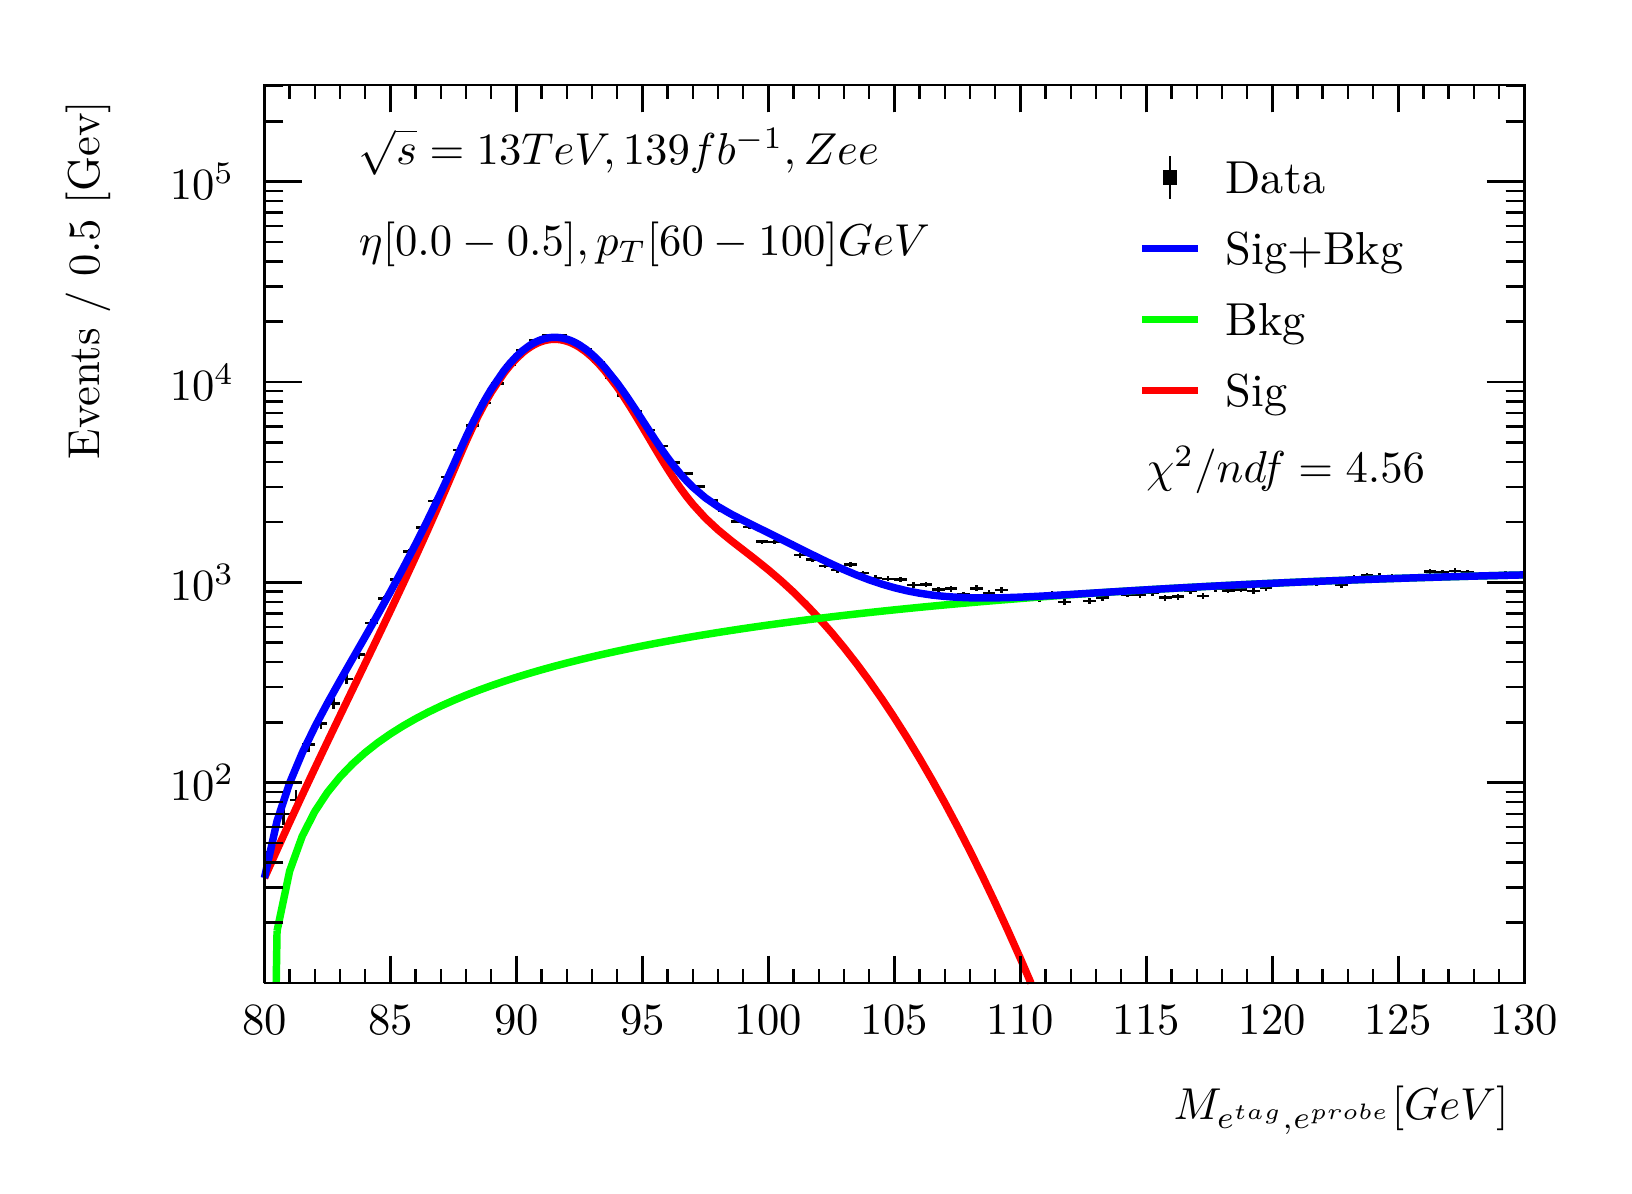
\begin{tikzpicture}
\pgfdeclareplotmark{cross} {
\pgfpathmoveto{\pgfpoint{-0.3\pgfplotmarksize}{\pgfplotmarksize}}
\pgfpathlineto{\pgfpoint{+0.3\pgfplotmarksize}{\pgfplotmarksize}}
\pgfpathlineto{\pgfpoint{+0.3\pgfplotmarksize}{0.3\pgfplotmarksize}}
\pgfpathlineto{\pgfpoint{+1\pgfplotmarksize}{0.3\pgfplotmarksize}}
\pgfpathlineto{\pgfpoint{+1\pgfplotmarksize}{-0.3\pgfplotmarksize}}
\pgfpathlineto{\pgfpoint{+0.3\pgfplotmarksize}{-0.3\pgfplotmarksize}}
\pgfpathlineto{\pgfpoint{+0.3\pgfplotmarksize}{-1.\pgfplotmarksize}}
\pgfpathlineto{\pgfpoint{-0.3\pgfplotmarksize}{-1.\pgfplotmarksize}}
\pgfpathlineto{\pgfpoint{-0.3\pgfplotmarksize}{-0.3\pgfplotmarksize}}
\pgfpathlineto{\pgfpoint{-1.\pgfplotmarksize}{-0.3\pgfplotmarksize}}
\pgfpathlineto{\pgfpoint{-1.\pgfplotmarksize}{0.3\pgfplotmarksize}}
\pgfpathlineto{\pgfpoint{-0.3\pgfplotmarksize}{0.3\pgfplotmarksize}}
\pgfpathclose
\pgfusepathqstroke
}
\pgfdeclareplotmark{cross*} {
\pgfpathmoveto{\pgfpoint{-0.3\pgfplotmarksize}{\pgfplotmarksize}}
\pgfpathlineto{\pgfpoint{+0.3\pgfplotmarksize}{\pgfplotmarksize}}
\pgfpathlineto{\pgfpoint{+0.3\pgfplotmarksize}{0.3\pgfplotmarksize}}
\pgfpathlineto{\pgfpoint{+1\pgfplotmarksize}{0.3\pgfplotmarksize}}
\pgfpathlineto{\pgfpoint{+1\pgfplotmarksize}{-0.3\pgfplotmarksize}}
\pgfpathlineto{\pgfpoint{+0.3\pgfplotmarksize}{-0.3\pgfplotmarksize}}
\pgfpathlineto{\pgfpoint{+0.3\pgfplotmarksize}{-1.\pgfplotmarksize}}
\pgfpathlineto{\pgfpoint{-0.3\pgfplotmarksize}{-1.\pgfplotmarksize}}
\pgfpathlineto{\pgfpoint{-0.3\pgfplotmarksize}{-0.3\pgfplotmarksize}}
\pgfpathlineto{\pgfpoint{-1.\pgfplotmarksize}{-0.3\pgfplotmarksize}}
\pgfpathlineto{\pgfpoint{-1.\pgfplotmarksize}{0.3\pgfplotmarksize}}
\pgfpathlineto{\pgfpoint{-0.3\pgfplotmarksize}{0.3\pgfplotmarksize}}
\pgfpathclose
\pgfusepathqfillstroke
}
\pgfdeclareplotmark{newstar} {
\pgfpathmoveto{\pgfqpoint{0pt}{\pgfplotmarksize}}
\pgfpathlineto{\pgfqpointpolar{44}{0.5\pgfplotmarksize}}
\pgfpathlineto{\pgfqpointpolar{18}{\pgfplotmarksize}}
\pgfpathlineto{\pgfqpointpolar{-20}{0.5\pgfplotmarksize}}
\pgfpathlineto{\pgfqpointpolar{-54}{\pgfplotmarksize}}
\pgfpathlineto{\pgfqpointpolar{-90}{0.5\pgfplotmarksize}}
\pgfpathlineto{\pgfqpointpolar{234}{\pgfplotmarksize}}
\pgfpathlineto{\pgfqpointpolar{198}{0.5\pgfplotmarksize}}
\pgfpathlineto{\pgfqpointpolar{162}{\pgfplotmarksize}}
\pgfpathlineto{\pgfqpointpolar{134}{0.5\pgfplotmarksize}}
\pgfpathclose
\pgfusepathqstroke
}
\pgfdeclareplotmark{newstar*} {
\pgfpathmoveto{\pgfqpoint{0pt}{\pgfplotmarksize}}
\pgfpathlineto{\pgfqpointpolar{44}{0.5\pgfplotmarksize}}
\pgfpathlineto{\pgfqpointpolar{18}{\pgfplotmarksize}}
\pgfpathlineto{\pgfqpointpolar{-20}{0.5\pgfplotmarksize}}
\pgfpathlineto{\pgfqpointpolar{-54}{\pgfplotmarksize}}
\pgfpathlineto{\pgfqpointpolar{-90}{0.5\pgfplotmarksize}}
\pgfpathlineto{\pgfqpointpolar{234}{\pgfplotmarksize}}
\pgfpathlineto{\pgfqpointpolar{198}{0.5\pgfplotmarksize}}
\pgfpathlineto{\pgfqpointpolar{162}{\pgfplotmarksize}}
\pgfpathlineto{\pgfqpointpolar{134}{0.5\pgfplotmarksize}}
\pgfpathclose
\pgfusepathqfillstroke
}
\definecolor{c}{rgb}{1,1,1};
\draw [color=c, fill=c] (0,0) rectangle (20,14.4361);
\draw [color=c, fill=c] (3,2.30977) rectangle (19,13.7143);
\definecolor{c}{rgb}{0,0,0};
\draw [c,line width=0.9] (3,2.30977) -- (3,13.7143) -- (19,13.7143) -- (19,2.30977) -- (3,2.30977);
\definecolor{c}{rgb}{1,1,1};
\draw [color=c, fill=c] (3,2.30977) rectangle (19,13.7143);
\definecolor{c}{rgb}{0,0,0};
\draw [c,line width=0.9] (3,2.30977) -- (3,13.7143) -- (19,13.7143) -- (19,2.30977) -- (3,2.30977);
\draw [c,line width=0.9] (3,2.30977) -- (19,2.30977);
\draw [c,line width=0.9] (3,2.65624) -- (3,2.30977);
\draw [c,line width=0.9] (3.32,2.48301) -- (3.32,2.30977);
\draw [c,line width=0.9] (3.64,2.48301) -- (3.64,2.30977);
\draw [c,line width=0.9] (3.96,2.48301) -- (3.96,2.30977);
\draw [c,line width=0.9] (4.28,2.48301) -- (4.28,2.30977);
\draw [c,line width=0.9] (4.6,2.65624) -- (4.6,2.30977);
\draw [c,line width=0.9] (4.92,2.48301) -- (4.92,2.30977);
\draw [c,line width=0.9] (5.24,2.48301) -- (5.24,2.30977);
\draw [c,line width=0.9] (5.56,2.48301) -- (5.56,2.30977);
\draw [c,line width=0.9] (5.88,2.48301) -- (5.88,2.30977);
\draw [c,line width=0.9] (6.2,2.65624) -- (6.2,2.30977);
\draw [c,line width=0.9] (6.52,2.48301) -- (6.52,2.30977);
\draw [c,line width=0.9] (6.84,2.48301) -- (6.84,2.30977);
\draw [c,line width=0.9] (7.16,2.48301) -- (7.16,2.30977);
\draw [c,line width=0.9] (7.48,2.48301) -- (7.48,2.30977);
\draw [c,line width=0.9] (7.8,2.65624) -- (7.8,2.30977);
\draw [c,line width=0.9] (8.12,2.48301) -- (8.12,2.30977);
\draw [c,line width=0.9] (8.44,2.48301) -- (8.44,2.30977);
\draw [c,line width=0.9] (8.76,2.48301) -- (8.76,2.30977);
\draw [c,line width=0.9] (9.08,2.48301) -- (9.08,2.30977);
\draw [c,line width=0.9] (9.4,2.65624) -- (9.4,2.30977);
\draw [c,line width=0.9] (9.72,2.48301) -- (9.72,2.30977);
\draw [c,line width=0.9] (10.04,2.48301) -- (10.04,2.30977);
\draw [c,line width=0.9] (10.36,2.48301) -- (10.36,2.30977);
\draw [c,line width=0.9] (10.68,2.48301) -- (10.68,2.30977);
\draw [c,line width=0.9] (11,2.65624) -- (11,2.30977);
\draw [c,line width=0.9] (11.32,2.48301) -- (11.32,2.30977);
\draw [c,line width=0.9] (11.64,2.48301) -- (11.64,2.30977);
\draw [c,line width=0.9] (11.96,2.48301) -- (11.96,2.30977);
\draw [c,line width=0.9] (12.28,2.48301) -- (12.28,2.30977);
\draw [c,line width=0.9] (12.6,2.65624) -- (12.6,2.30977);
\draw [c,line width=0.9] (12.92,2.48301) -- (12.92,2.30977);
\draw [c,line width=0.9] (13.24,2.48301) -- (13.24,2.30977);
\draw [c,line width=0.9] (13.56,2.48301) -- (13.56,2.30977);
\draw [c,line width=0.9] (13.88,2.48301) -- (13.88,2.30977);
\draw [c,line width=0.9] (14.2,2.65624) -- (14.2,2.30977);
\draw [c,line width=0.9] (14.52,2.48301) -- (14.52,2.30977);
\draw [c,line width=0.9] (14.84,2.48301) -- (14.84,2.30977);
\draw [c,line width=0.9] (15.16,2.48301) -- (15.16,2.30977);
\draw [c,line width=0.9] (15.48,2.48301) -- (15.48,2.30977);
\draw [c,line width=0.9] (15.8,2.65624) -- (15.8,2.30977);
\draw [c,line width=0.9] (16.12,2.48301) -- (16.12,2.30977);
\draw [c,line width=0.9] (16.44,2.48301) -- (16.44,2.30977);
\draw [c,line width=0.9] (16.76,2.48301) -- (16.76,2.30977);
\draw [c,line width=0.9] (17.08,2.48301) -- (17.08,2.30977);
\draw [c,line width=0.9] (17.4,2.65624) -- (17.4,2.30977);
\draw [c,line width=0.9] (17.72,2.48301) -- (17.72,2.30977);
\draw [c,line width=0.9] (18.04,2.48301) -- (18.04,2.30977);
\draw [c,line width=0.9] (18.36,2.48301) -- (18.36,2.30977);
\draw [c,line width=0.9] (18.68,2.48301) -- (18.68,2.30977);
\draw [c,line width=0.9] (19,2.65624) -- (19,2.30977);
\draw [anchor=base] (3,1.66015) node[scale=1.61424, color=c, rotate=0]{80};
\draw [anchor=base] (4.6,1.66015) node[scale=1.61424, color=c, rotate=0]{85};
\draw [anchor=base] (6.2,1.66015) node[scale=1.61424, color=c, rotate=0]{90};
\draw [anchor=base] (7.8,1.66015) node[scale=1.61424, color=c, rotate=0]{95};
\draw [anchor=base] (9.4,1.66015) node[scale=1.61424, color=c, rotate=0]{100};
\draw [anchor=base] (11,1.66015) node[scale=1.61424, color=c, rotate=0]{105};
\draw [anchor=base] (12.6,1.66015) node[scale=1.61424, color=c, rotate=0]{110};
\draw [anchor=base] (14.2,1.66015) node[scale=1.61424, color=c, rotate=0]{115};
\draw [anchor=base] (15.8,1.66015) node[scale=1.61424, color=c, rotate=0]{120};
\draw [anchor=base] (17.4,1.66015) node[scale=1.61424, color=c, rotate=0]{125};
\draw [anchor=base] (19,1.66015) node[scale=1.61424, color=c, rotate=0]{130};
\draw [anchor= east] (19,0.692932) node[scale=1.61424, color=c, rotate=0]{$M_{e^{tag}, e^{probe}}  [GeV]$};
\draw [c,line width=0.9] (3,13.7143) -- (19,13.7143);
\draw [c,line width=0.9] (3,13.3678) -- (3,13.7143);
\draw [c,line width=0.9] (3.32,13.5411) -- (3.32,13.7143);
\draw [c,line width=0.9] (3.64,13.5411) -- (3.64,13.7143);
\draw [c,line width=0.9] (3.96,13.5411) -- (3.96,13.7143);
\draw [c,line width=0.9] (4.28,13.5411) -- (4.28,13.7143);
\draw [c,line width=0.9] (4.6,13.3678) -- (4.6,13.7143);
\draw [c,line width=0.9] (4.92,13.5411) -- (4.92,13.7143);
\draw [c,line width=0.9] (5.24,13.5411) -- (5.24,13.7143);
\draw [c,line width=0.9] (5.56,13.5411) -- (5.56,13.7143);
\draw [c,line width=0.9] (5.88,13.5411) -- (5.88,13.7143);
\draw [c,line width=0.9] (6.2,13.3678) -- (6.2,13.7143);
\draw [c,line width=0.9] (6.52,13.5411) -- (6.52,13.7143);
\draw [c,line width=0.9] (6.84,13.5411) -- (6.84,13.7143);
\draw [c,line width=0.9] (7.16,13.5411) -- (7.16,13.7143);
\draw [c,line width=0.9] (7.48,13.5411) -- (7.48,13.7143);
\draw [c,line width=0.9] (7.8,13.3678) -- (7.8,13.7143);
\draw [c,line width=0.9] (8.12,13.5411) -- (8.12,13.7143);
\draw [c,line width=0.9] (8.44,13.5411) -- (8.44,13.7143);
\draw [c,line width=0.9] (8.76,13.5411) -- (8.76,13.7143);
\draw [c,line width=0.9] (9.08,13.5411) -- (9.08,13.7143);
\draw [c,line width=0.9] (9.4,13.3678) -- (9.4,13.7143);
\draw [c,line width=0.9] (9.72,13.5411) -- (9.72,13.7143);
\draw [c,line width=0.9] (10.04,13.5411) -- (10.04,13.7143);
\draw [c,line width=0.9] (10.36,13.5411) -- (10.36,13.7143);
\draw [c,line width=0.9] (10.68,13.5411) -- (10.68,13.7143);
\draw [c,line width=0.9] (11,13.3678) -- (11,13.7143);
\draw [c,line width=0.9] (11.32,13.5411) -- (11.32,13.7143);
\draw [c,line width=0.9] (11.64,13.5411) -- (11.64,13.7143);
\draw [c,line width=0.9] (11.96,13.5411) -- (11.96,13.7143);
\draw [c,line width=0.9] (12.28,13.5411) -- (12.28,13.7143);
\draw [c,line width=0.9] (12.6,13.3678) -- (12.6,13.7143);
\draw [c,line width=0.9] (12.92,13.5411) -- (12.92,13.7143);
\draw [c,line width=0.9] (13.24,13.5411) -- (13.24,13.7143);
\draw [c,line width=0.9] (13.56,13.5411) -- (13.56,13.7143);
\draw [c,line width=0.9] (13.88,13.5411) -- (13.88,13.7143);
\draw [c,line width=0.9] (14.2,13.3678) -- (14.2,13.7143);
\draw [c,line width=0.9] (14.52,13.5411) -- (14.52,13.7143);
\draw [c,line width=0.9] (14.84,13.5411) -- (14.84,13.7143);
\draw [c,line width=0.9] (15.16,13.5411) -- (15.16,13.7143);
\draw [c,line width=0.9] (15.48,13.5411) -- (15.48,13.7143);
\draw [c,line width=0.9] (15.8,13.3678) -- (15.8,13.7143);
\draw [c,line width=0.9] (16.12,13.5411) -- (16.12,13.7143);
\draw [c,line width=0.9] (16.44,13.5411) -- (16.44,13.7143);
\draw [c,line width=0.9] (16.76,13.5411) -- (16.76,13.7143);
\draw [c,line width=0.9] (17.08,13.5411) -- (17.08,13.7143);
\draw [c,line width=0.9] (17.4,13.3678) -- (17.4,13.7143);
\draw [c,line width=0.9] (17.72,13.5411) -- (17.72,13.7143);
\draw [c,line width=0.9] (18.04,13.5411) -- (18.04,13.7143);
\draw [c,line width=0.9] (18.36,13.5411) -- (18.36,13.7143);
\draw [c,line width=0.9] (18.68,13.5411) -- (18.68,13.7143);
\draw [c,line width=0.9] (19,13.3678) -- (19,13.7143);
\draw [c,line width=0.9] (3,2.30977) -- (3,13.7143);
\draw [c,line width=0.9] (3.237,3.07568) -- (3,3.07568);
\draw [c,line width=0.9] (3.237,3.5237) -- (3,3.5237);
\draw [c,line width=0.9] (3.237,3.84158) -- (3,3.84158);
\draw [c,line width=0.9] (3.237,4.08815) -- (3,4.08815);
\draw [c,line width=0.9] (3.237,4.2896) -- (3,4.2896);
\draw [c,line width=0.9] (3.237,4.45994) -- (3,4.45994);
\draw [c,line width=0.9] (3.237,4.60748) -- (3,4.60748);
\draw [c,line width=0.9] (3.237,4.73763) -- (3,4.73763);
\draw [c,line width=0.9] (3.474,4.85405) -- (3,4.85405);
\draw [anchor= east] (2.82,4.85405) node[scale=1.61424, color=c, rotate=0]{$10^{2}$};
\draw [c,line width=0.9] (3.237,5.61995) -- (3,5.61995);
\draw [c,line width=0.9] (3.237,6.06798) -- (3,6.06798);
\draw [c,line width=0.9] (3.237,6.38586) -- (3,6.38586);
\draw [c,line width=0.9] (3.237,6.63242) -- (3,6.63242);
\draw [c,line width=0.9] (3.237,6.83388) -- (3,6.83388);
\draw [c,line width=0.9] (3.237,7.00421) -- (3,7.00421);
\draw [c,line width=0.9] (3.237,7.15176) -- (3,7.15176);
\draw [c,line width=0.9] (3.237,7.28191) -- (3,7.28191);
\draw [c,line width=0.9] (3.474,7.39833) -- (3,7.39833);
\draw [anchor= east] (2.82,7.39833) node[scale=1.61424, color=c, rotate=0]{$10^{3}$};
\draw [c,line width=0.9] (3.237,8.16423) -- (3,8.16423);
\draw [c,line width=0.9] (3.237,8.61226) -- (3,8.61226);
\draw [c,line width=0.9] (3.237,8.93013) -- (3,8.93013);
\draw [c,line width=0.9] (3.237,9.1767) -- (3,9.1767);
\draw [c,line width=0.9] (3.237,9.37816) -- (3,9.37816);
\draw [c,line width=0.9] (3.237,9.54849) -- (3,9.54849);
\draw [c,line width=0.9] (3.237,9.69604) -- (3,9.69604);
\draw [c,line width=0.9] (3.237,9.82618) -- (3,9.82618);
\draw [c,line width=0.9] (3.474,9.9426) -- (3,9.9426);
\draw [anchor= east] (2.82,9.9426) node[scale=1.61424, color=c, rotate=0]{$10^{4}$};
\draw [c,line width=0.9] (3.237,10.7085) -- (3,10.7085);
\draw [c,line width=0.9] (3.237,11.1565) -- (3,11.1565);
\draw [c,line width=0.9] (3.237,11.4744) -- (3,11.4744);
\draw [c,line width=0.9] (3.237,11.721) -- (3,11.721);
\draw [c,line width=0.9] (3.237,11.9224) -- (3,11.9224);
\draw [c,line width=0.9] (3.237,12.0928) -- (3,12.0928);
\draw [c,line width=0.9] (3.237,12.2403) -- (3,12.2403);
\draw [c,line width=0.9] (3.237,12.3705) -- (3,12.3705);
\draw [c,line width=0.9] (3.474,12.4869) -- (3,12.4869);
\draw [anchor= east] (2.82,12.4869) node[scale=1.61424, color=c, rotate=0]{$10^{5}$};
\draw [c,line width=0.9] (3.237,13.2528) -- (3,13.2528);
\draw [c,line width=0.9] (3.237,13.7008) -- (3,13.7008);
\draw [anchor= east] (0.76,13.7143) node[scale=1.61424, color=c, rotate=90]{Events / 0.5 [Gev]};
\draw [c,line width=0.9] (19,2.30977) -- (19,13.7143);
\draw [c,line width=0.9] (18.763,3.07568) -- (19,3.07568);
\draw [c,line width=0.9] (18.763,3.5237) -- (19,3.5237);
\draw [c,line width=0.9] (18.763,3.84158) -- (19,3.84158);
\draw [c,line width=0.9] (18.763,4.08815) -- (19,4.08815);
\draw [c,line width=0.9] (18.763,4.2896) -- (19,4.2896);
\draw [c,line width=0.9] (18.763,4.45994) -- (19,4.45994);
\draw [c,line width=0.9] (18.763,4.60748) -- (19,4.60748);
\draw [c,line width=0.9] (18.763,4.73763) -- (19,4.73763);
\draw [c,line width=0.9] (18.526,4.85405) -- (19,4.85405);
\draw [c,line width=0.9] (18.763,5.61995) -- (19,5.61995);
\draw [c,line width=0.9] (18.763,6.06798) -- (19,6.06798);
\draw [c,line width=0.9] (18.763,6.38586) -- (19,6.38586);
\draw [c,line width=0.9] (18.763,6.63242) -- (19,6.63242);
\draw [c,line width=0.9] (18.763,6.83388) -- (19,6.83388);
\draw [c,line width=0.9] (18.763,7.00421) -- (19,7.00421);
\draw [c,line width=0.9] (18.763,7.15176) -- (19,7.15176);
\draw [c,line width=0.9] (18.763,7.28191) -- (19,7.28191);
\draw [c,line width=0.9] (18.526,7.39833) -- (19,7.39833);
\draw [c,line width=0.9] (18.763,8.16423) -- (19,8.16423);
\draw [c,line width=0.9] (18.763,8.61226) -- (19,8.61226);
\draw [c,line width=0.9] (18.763,8.93013) -- (19,8.93013);
\draw [c,line width=0.9] (18.763,9.1767) -- (19,9.1767);
\draw [c,line width=0.9] (18.763,9.37816) -- (19,9.37816);
\draw [c,line width=0.9] (18.763,9.54849) -- (19,9.54849);
\draw [c,line width=0.9] (18.763,9.69604) -- (19,9.69604);
\draw [c,line width=0.9] (18.763,9.82618) -- (19,9.82618);
\draw [c,line width=0.9] (18.526,9.9426) -- (19,9.9426);
\draw [c,line width=0.9] (18.763,10.7085) -- (19,10.7085);
\draw [c,line width=0.9] (18.763,11.1565) -- (19,11.1565);
\draw [c,line width=0.9] (18.763,11.4744) -- (19,11.4744);
\draw [c,line width=0.9] (18.763,11.721) -- (19,11.721);
\draw [c,line width=0.9] (18.763,11.9224) -- (19,11.9224);
\draw [c,line width=0.9] (18.763,12.0928) -- (19,12.0928);
\draw [c,line width=0.9] (18.763,12.2403) -- (19,12.2403);
\draw [c,line width=0.9] (18.763,12.3705) -- (19,12.3705);
\draw [c,line width=0.9] (18.526,12.4869) -- (19,12.4869);
\draw [c,line width=0.9] (18.763,13.2528) -- (19,13.2528);
\draw [c,line width=0.9] (18.763,13.7008) -- (19,13.7008);
\draw [c,line width=0.9] (3.08,3.97173) -- (3,3.97173);
\draw [c,line width=0.9] (3,3.97173) -- (3,3.97173);
\draw [c,line width=0.9] (3.08,3.97173) -- (3.16,3.97173);
\draw [c,line width=0.9] (3.16,3.97173) -- (3.16,3.97173);
\draw [c,line width=0.9] (3.08,3.97173) -- (3.08,4.14747);
\draw [c,line width=0.9] (3.08,4.14747) -- (3.08,4.14747);
\draw [c,line width=0.9] (3.08,3.97173) -- (3.08,3.79408);
\draw [c,line width=0.9] (3.08,3.79408) -- (3.08,3.79408);
\draw [c,line width=0.9] (3.24,4.45994) -- (3.16,4.45994);
\draw [c,line width=0.9] (3.16,4.45994) -- (3.16,4.45994);
\draw [c,line width=0.9] (3.24,4.45994) -- (3.32,4.45994);
\draw [c,line width=0.9] (3.32,4.45994) -- (3.32,4.45994);
\draw [c,line width=0.9] (3.24,4.45994) -- (3.24,4.59926);
\draw [c,line width=0.9] (3.24,4.59926) -- (3.24,4.59926);
\draw [c,line width=0.9] (3.24,4.45994) -- (3.24,4.31964);
\draw [c,line width=0.9] (3.24,4.31964) -- (3.24,4.31964);
\draw [c,line width=0.9] (3.4,4.63477) -- (3.32,4.63477);
\draw [c,line width=0.9] (3.32,4.63477) -- (3.32,4.63477);
\draw [c,line width=0.9] (3.4,4.63477) -- (3.48,4.63477);
\draw [c,line width=0.9] (3.48,4.63477) -- (3.48,4.63477);
\draw [c,line width=0.9] (3.4,4.63477) -- (3.4,4.76302);
\draw [c,line width=0.9] (3.4,4.76302) -- (3.4,4.76302);
\draw [c,line width=0.9] (3.4,4.63477) -- (3.4,4.50575);
\draw [c,line width=0.9] (3.4,4.50575) -- (3.4,4.50575);
\draw [c,line width=0.9] (3.56,5.33831) -- (3.48,5.33831);
\draw [c,line width=0.9] (3.48,5.33831) -- (3.48,5.33831);
\draw [c,line width=0.9] (3.56,5.33831) -- (3.64,5.33831);
\draw [c,line width=0.9] (3.64,5.33831) -- (3.64,5.33831);
\draw [c,line width=0.9] (3.56,5.33831) -- (3.56,5.42704);
\draw [c,line width=0.9] (3.56,5.42704) -- (3.56,5.42704);
\draw [c,line width=0.9] (3.56,5.33831) -- (3.56,5.24958);
\draw [c,line width=0.9] (3.56,5.24958) -- (3.56,5.24958);
\draw [c,line width=0.9] (3.72,5.60885) -- (3.64,5.60885);
\draw [c,line width=0.9] (3.64,5.60885) -- (3.64,5.60885);
\draw [c,line width=0.9] (3.72,5.60885) -- (3.8,5.60885);
\draw [c,line width=0.9] (3.8,5.60885) -- (3.8,5.60885);
\draw [c,line width=0.9] (3.72,5.60885) -- (3.72,5.68736);
\draw [c,line width=0.9] (3.72,5.68736) -- (3.72,5.68736);
\draw [c,line width=0.9] (3.72,5.60885) -- (3.72,5.53034);
\draw [c,line width=0.9] (3.72,5.53034) -- (3.72,5.53034);
\draw [c,line width=0.9] (3.88,5.85765) -- (3.8,5.85765);
\draw [c,line width=0.9] (3.8,5.85765) -- (3.8,5.85765);
\draw [c,line width=0.9] (3.88,5.85765) -- (3.96,5.85765);
\draw [c,line width=0.9] (3.96,5.85765) -- (3.96,5.85765);
\draw [c,line width=0.9] (3.88,5.85765) -- (3.88,5.9278);
\draw [c,line width=0.9] (3.88,5.9278) -- (3.88,5.9278);
\draw [c,line width=0.9] (3.88,5.85765) -- (3.88,5.78749);
\draw [c,line width=0.9] (3.88,5.78749) -- (3.88,5.78749);
\draw [c,line width=0.9] (4.04,6.16994) -- (3.96,6.16994);
\draw [c,line width=0.9] (3.96,6.16994) -- (3.96,6.16994);
\draw [c,line width=0.9] (4.04,6.16994) -- (4.12,6.16994);
\draw [c,line width=0.9] (4.12,6.16994) -- (4.12,6.16994);
\draw [c,line width=0.9] (4.04,6.16994) -- (4.04,6.23085);
\draw [c,line width=0.9] (4.04,6.23085) -- (4.04,6.23085);
\draw [c,line width=0.9] (4.04,6.16994) -- (4.04,6.10903);
\draw [c,line width=0.9] (4.04,6.10903) -- (4.04,6.10903);
\draw [c,line width=0.9] (4.2,6.48361) -- (4.12,6.48361);
\draw [c,line width=0.9] (4.12,6.48361) -- (4.12,6.48361);
\draw [c,line width=0.9] (4.2,6.48361) -- (4.28,6.48361);
\draw [c,line width=0.9] (4.28,6.48361) -- (4.28,6.48361);
\draw [c,line width=0.9] (4.2,6.48361) -- (4.2,6.53647);
\draw [c,line width=0.9] (4.2,6.53647) -- (4.2,6.53647);
\draw [c,line width=0.9] (4.2,6.48361) -- (4.2,6.43076);
\draw [c,line width=0.9] (4.2,6.43076) -- (4.2,6.43076);
\draw [c,line width=0.9] (4.36,6.88428) -- (4.28,6.88428);
\draw [c,line width=0.9] (4.28,6.88428) -- (4.28,6.88428);
\draw [c,line width=0.9] (4.36,6.88428) -- (4.44,6.88428);
\draw [c,line width=0.9] (4.44,6.88428) -- (4.44,6.88428);
\draw [c,line width=0.9] (4.36,6.88428) -- (4.36,6.92837);
\draw [c,line width=0.9] (4.36,6.92837) -- (4.36,6.92837);
\draw [c,line width=0.9] (4.36,6.88428) -- (4.36,6.84019);
\draw [c,line width=0.9] (4.36,6.84019) -- (4.36,6.84019);
\draw [c,line width=0.9] (4.52,7.19244) -- (4.44,7.19244);
\draw [c,line width=0.9] (4.44,7.19244) -- (4.44,7.19244);
\draw [c,line width=0.9] (4.52,7.19244) -- (4.6,7.19244);
\draw [c,line width=0.9] (4.6,7.19244) -- (4.6,7.19244);
\draw [c,line width=0.9] (4.52,7.19244) -- (4.52,7.23079);
\draw [c,line width=0.9] (4.52,7.23079) -- (4.52,7.23079);
\draw [c,line width=0.9] (4.52,7.19244) -- (4.52,7.15409);
\draw [c,line width=0.9] (4.52,7.15409) -- (4.52,7.15409);
\draw [c,line width=0.9] (4.68,7.4342) -- (4.6,7.4342);
\draw [c,line width=0.9] (4.6,7.4342) -- (4.6,7.4342);
\draw [c,line width=0.9] (4.68,7.4342) -- (4.76,7.4342);
\draw [c,line width=0.9] (4.76,7.4342) -- (4.76,7.4342);
\draw [c,line width=0.9] (4.68,7.4342) -- (4.68,7.46858);
\draw [c,line width=0.9] (4.68,7.46858) -- (4.68,7.46858);
\draw [c,line width=0.9] (4.68,7.4342) -- (4.68,7.39983);
\draw [c,line width=0.9] (4.68,7.39983) -- (4.68,7.39983);
\draw [c,line width=0.9] (4.84,7.7889) -- (4.76,7.7889);
\draw [c,line width=0.9] (4.76,7.7889) -- (4.76,7.7889);
\draw [c,line width=0.9] (4.84,7.7889) -- (4.92,7.7889);
\draw [c,line width=0.9] (4.92,7.7889) -- (4.92,7.7889);
\draw [c,line width=0.9] (4.84,7.7889) -- (4.84,7.81818);
\draw [c,line width=0.9] (4.84,7.81818) -- (4.84,7.81818);
\draw [c,line width=0.9] (4.84,7.7889) -- (4.84,7.75962);
\draw [c,line width=0.9] (4.84,7.75962) -- (4.84,7.75962);
\draw [c,line width=0.9] (5,8.09645) -- (4.92,8.09645);
\draw [c,line width=0.9] (4.92,8.09645) -- (4.92,8.09645);
\draw [c,line width=0.9] (5,8.09645) -- (5.08,8.09645);
\draw [c,line width=0.9] (5.08,8.09645) -- (5.08,8.09645);
\draw [c,line width=0.9] (5,8.09645) -- (5,8.12193);
\draw [c,line width=0.9] (5,8.12193) -- (5,8.12193);
\draw [c,line width=0.9] (5,8.09645) -- (5,8.07097);
\draw [c,line width=0.9] (5,8.07097) -- (5,8.07097);
\draw [c,line width=0.9] (5.16,8.43008) -- (5.08,8.43008);
\draw [c,line width=0.9] (5.08,8.43008) -- (5.08,8.43008);
\draw [c,line width=0.9] (5.16,8.43008) -- (5.24,8.43008);
\draw [c,line width=0.9] (5.24,8.43008) -- (5.24,8.43008);
\draw [c,line width=0.9] (5.16,8.43008) -- (5.16,8.45198);
\draw [c,line width=0.9] (5.16,8.45198) -- (5.16,8.45198);
\draw [c,line width=0.9] (5.16,8.43008) -- (5.16,8.40817);
\draw [c,line width=0.9] (5.16,8.40817) -- (5.16,8.40817);
\draw [c,line width=0.9] (5.32,8.73386) -- (5.24,8.73386);
\draw [c,line width=0.9] (5.24,8.73386) -- (5.24,8.73386);
\draw [c,line width=0.9] (5.32,8.73386) -- (5.4,8.73386);
\draw [c,line width=0.9] (5.4,8.73386) -- (5.4,8.73386);
\draw [c,line width=0.9] (5.32,8.73386) -- (5.32,8.75295);
\draw [c,line width=0.9] (5.32,8.75295) -- (5.32,8.75295);
\draw [c,line width=0.9] (5.32,8.73386) -- (5.32,8.71476);
\draw [c,line width=0.9] (5.32,8.71476) -- (5.32,8.71476);
\draw [c,line width=0.9] (5.48,9.07903) -- (5.4,9.07903);
\draw [c,line width=0.9] (5.4,9.07903) -- (5.4,9.07903);
\draw [c,line width=0.9] (5.48,9.07903) -- (5.56,9.07903);
\draw [c,line width=0.9] (5.56,9.07903) -- (5.56,9.07903);
\draw [c,line width=0.9] (5.48,9.07903) -- (5.48,9.09536);
\draw [c,line width=0.9] (5.48,9.09536) -- (5.48,9.09536);
\draw [c,line width=0.9] (5.48,9.07903) -- (5.48,9.0627);
\draw [c,line width=0.9] (5.48,9.0627) -- (5.48,9.0627);
\draw [c,line width=0.9] (5.64,9.39261) -- (5.56,9.39261);
\draw [c,line width=0.9] (5.56,9.39261) -- (5.56,9.39261);
\draw [c,line width=0.9] (5.64,9.39261) -- (5.72,9.39261);
\draw [c,line width=0.9] (5.72,9.39261) -- (5.72,9.39261);
\draw [c,line width=0.9] (5.64,9.39261) -- (5.64,9.40679);
\draw [c,line width=0.9] (5.64,9.40679) -- (5.64,9.40679);
\draw [c,line width=0.9] (5.64,9.39261) -- (5.64,9.37844);
\draw [c,line width=0.9] (5.64,9.37844) -- (5.64,9.37844);
\draw [c,line width=0.9] (5.8,9.67681) -- (5.72,9.67681);
\draw [c,line width=0.9] (5.72,9.67681) -- (5.72,9.67681);
\draw [c,line width=0.9] (5.8,9.67681) -- (5.88,9.67681);
\draw [c,line width=0.9] (5.88,9.67681) -- (5.88,9.67681);
\draw [c,line width=0.9] (5.8,9.67681) -- (5.8,9.68927);
\draw [c,line width=0.9] (5.8,9.68927) -- (5.8,9.68927);
\draw [c,line width=0.9] (5.8,9.67681) -- (5.8,9.66435);
\draw [c,line width=0.9] (5.8,9.66435) -- (5.8,9.66435);
\draw [c,line width=0.9] (5.96,9.9213) -- (5.88,9.9213);
\draw [c,line width=0.9] (5.88,9.9213) -- (5.88,9.9213);
\draw [c,line width=0.9] (5.96,9.9213) -- (6.04,9.9213);
\draw [c,line width=0.9] (6.04,9.9213) -- (6.04,9.9213);
\draw [c,line width=0.9] (5.96,9.9213) -- (5.96,9.93245);
\draw [c,line width=0.9] (5.96,9.93245) -- (5.96,9.93245);
\draw [c,line width=0.9] (5.96,9.9213) -- (5.96,9.91014);
\draw [c,line width=0.9] (5.96,9.91014) -- (5.96,9.91014);
\draw [c,line width=0.9] (6.12,10.1618) -- (6.04,10.1618);
\draw [c,line width=0.9] (6.04,10.1618) -- (6.04,10.1618);
\draw [c,line width=0.9] (6.12,10.1618) -- (6.2,10.1618);
\draw [c,line width=0.9] (6.2,10.1618) -- (6.2,10.1618);
\draw [c,line width=0.9] (6.12,10.1618) -- (6.12,10.1718);
\draw [c,line width=0.9] (6.12,10.1718) -- (6.12,10.1718);
\draw [c,line width=0.9] (6.12,10.1618) -- (6.12,10.1518);
\draw [c,line width=0.9] (6.12,10.1518) -- (6.12,10.1518);
\draw [c,line width=0.9] (6.28,10.3471) -- (6.2,10.3471);
\draw [c,line width=0.9] (6.2,10.3471) -- (6.2,10.3471);
\draw [c,line width=0.9] (6.28,10.3471) -- (6.36,10.3471);
\draw [c,line width=0.9] (6.36,10.3471) -- (6.36,10.3471);
\draw [c,line width=0.9] (6.28,10.3471) -- (6.28,10.3563);
\draw [c,line width=0.9] (6.28,10.3563) -- (6.28,10.3563);
\draw [c,line width=0.9] (6.28,10.3471) -- (6.28,10.3379);
\draw [c,line width=0.9] (6.28,10.3379) -- (6.28,10.3379);
\draw [c,line width=0.9] (6.44,10.4746) -- (6.36,10.4746);
\draw [c,line width=0.9] (6.36,10.4746) -- (6.36,10.4746);
\draw [c,line width=0.9] (6.44,10.4746) -- (6.52,10.4746);
\draw [c,line width=0.9] (6.52,10.4746) -- (6.52,10.4746);
\draw [c,line width=0.9] (6.44,10.4746) -- (6.44,10.4833);
\draw [c,line width=0.9] (6.44,10.4833) -- (6.44,10.4833);
\draw [c,line width=0.9] (6.44,10.4746) -- (6.44,10.466);
\draw [c,line width=0.9] (6.44,10.466) -- (6.44,10.466);
\draw [c,line width=0.9] (6.6,10.5373) -- (6.52,10.5373);
\draw [c,line width=0.9] (6.52,10.5373) -- (6.52,10.5373);
\draw [c,line width=0.9] (6.6,10.5373) -- (6.68,10.5373);
\draw [c,line width=0.9] (6.68,10.5373) -- (6.68,10.5373);
\draw [c,line width=0.9] (6.6,10.5373) -- (6.6,10.5457);
\draw [c,line width=0.9] (6.6,10.5457) -- (6.6,10.5457);
\draw [c,line width=0.9] (6.6,10.5373) -- (6.6,10.5288);
\draw [c,line width=0.9] (6.6,10.5288) -- (6.6,10.5288);
\draw [c,line width=0.9] (6.76,10.5319) -- (6.68,10.5319);
\draw [c,line width=0.9] (6.68,10.5319) -- (6.68,10.5319);
\draw [c,line width=0.9] (6.76,10.5319) -- (6.84,10.5319);
\draw [c,line width=0.9] (6.84,10.5319) -- (6.84,10.5319);
\draw [c,line width=0.9] (6.76,10.5319) -- (6.76,10.5403);
\draw [c,line width=0.9] (6.76,10.5403) -- (6.76,10.5403);
\draw [c,line width=0.9] (6.76,10.5319) -- (6.76,10.5234);
\draw [c,line width=0.9] (6.76,10.5234) -- (6.76,10.5234);
\draw [c,line width=0.9] (6.92,10.4613) -- (6.84,10.4613);
\draw [c,line width=0.9] (6.84,10.4613) -- (6.84,10.4613);
\draw [c,line width=0.9] (6.92,10.4613) -- (7,10.4613);
\draw [c,line width=0.9] (7,10.4613) -- (7,10.4613);
\draw [c,line width=0.9] (6.92,10.4613) -- (6.92,10.4701);
\draw [c,line width=0.9] (6.92,10.4701) -- (6.92,10.4701);
\draw [c,line width=0.9] (6.92,10.4613) -- (6.92,10.4526);
\draw [c,line width=0.9] (6.92,10.4526) -- (6.92,10.4526);
\draw [c,line width=0.9] (7.08,10.3639) -- (7,10.3639);
\draw [c,line width=0.9] (7,10.3639) -- (7,10.3639);
\draw [c,line width=0.9] (7.08,10.3639) -- (7.16,10.3639);
\draw [c,line width=0.9] (7.16,10.3639) -- (7.16,10.3639);
\draw [c,line width=0.9] (7.08,10.3639) -- (7.08,10.373);
\draw [c,line width=0.9] (7.08,10.373) -- (7.08,10.373);
\draw [c,line width=0.9] (7.08,10.3639) -- (7.08,10.3547);
\draw [c,line width=0.9] (7.08,10.3547) -- (7.08,10.3547);
\draw [c,line width=0.9] (7.24,10.1946) -- (7.16,10.1946);
\draw [c,line width=0.9] (7.16,10.1946) -- (7.16,10.1946);
\draw [c,line width=0.9] (7.24,10.1946) -- (7.32,10.1946);
\draw [c,line width=0.9] (7.32,10.1946) -- (7.32,10.1946);
\draw [c,line width=0.9] (7.24,10.1946) -- (7.24,10.2044);
\draw [c,line width=0.9] (7.24,10.2044) -- (7.24,10.2044);
\draw [c,line width=0.9] (7.24,10.1946) -- (7.24,10.1847);
\draw [c,line width=0.9] (7.24,10.1847) -- (7.24,10.1847);
\draw [c,line width=0.9] (7.4,9.9942) -- (7.32,9.9942);
\draw [c,line width=0.9] (7.32,9.9942) -- (7.32,9.9942);
\draw [c,line width=0.9] (7.4,9.9942) -- (7.48,9.9942);
\draw [c,line width=0.9] (7.48,9.9942) -- (7.48,9.9942);
\draw [c,line width=0.9] (7.4,9.9942) -- (7.4,10.005);
\draw [c,line width=0.9] (7.4,10.005) -- (7.4,10.005);
\draw [c,line width=0.9] (7.4,9.9942) -- (7.4,9.9834);
\draw [c,line width=0.9] (7.4,9.9834) -- (7.4,9.9834);
\draw [c,line width=0.9] (7.56,9.77273) -- (7.48,9.77273);
\draw [c,line width=0.9] (7.48,9.77273) -- (7.48,9.77273);
\draw [c,line width=0.9] (7.56,9.77273) -- (7.64,9.77273);
\draw [c,line width=0.9] (7.64,9.77273) -- (7.64,9.77273);
\draw [c,line width=0.9] (7.56,9.77273) -- (7.56,9.78467);
\draw [c,line width=0.9] (7.56,9.78467) -- (7.56,9.78467);
\draw [c,line width=0.9] (7.56,9.77273) -- (7.56,9.7608);
\draw [c,line width=0.9] (7.56,9.7608) -- (7.56,9.7608);
\draw [c,line width=0.9] (7.72,9.57099) -- (7.64,9.57099);
\draw [c,line width=0.9] (7.64,9.57099) -- (7.64,9.57099);
\draw [c,line width=0.9] (7.72,9.57099) -- (7.8,9.57099);
\draw [c,line width=0.9] (7.8,9.57099) -- (7.8,9.57099);
\draw [c,line width=0.9] (7.72,9.57099) -- (7.72,9.58406);
\draw [c,line width=0.9] (7.72,9.58406) -- (7.72,9.58406);
\draw [c,line width=0.9] (7.72,9.57099) -- (7.72,9.55792);
\draw [c,line width=0.9] (7.72,9.55792) -- (7.72,9.55792);
\draw [c,line width=0.9] (7.88,9.33075) -- (7.8,9.33075);
\draw [c,line width=0.9] (7.8,9.33075) -- (7.8,9.33075);
\draw [c,line width=0.9] (7.88,9.33075) -- (7.96,9.33075);
\draw [c,line width=0.9] (7.96,9.33075) -- (7.96,9.33075);
\draw [c,line width=0.9] (7.88,9.33075) -- (7.88,9.34532);
\draw [c,line width=0.9] (7.88,9.34532) -- (7.88,9.34532);
\draw [c,line width=0.9] (7.88,9.33075) -- (7.88,9.31617);
\draw [c,line width=0.9] (7.88,9.31617) -- (7.88,9.31617);
\draw [c,line width=0.9] (8.04,9.13159) -- (7.96,9.13159);
\draw [c,line width=0.9] (7.96,9.13159) -- (7.96,9.13159);
\draw [c,line width=0.9] (8.04,9.13159) -- (8.12,9.13159);
\draw [c,line width=0.9] (8.12,9.13159) -- (8.12,9.13159);
\draw [c,line width=0.9] (8.04,9.13159) -- (8.04,9.14754);
\draw [c,line width=0.9] (8.04,9.14754) -- (8.04,9.14754);
\draw [c,line width=0.9] (8.04,9.13159) -- (8.04,9.11565);
\draw [c,line width=0.9] (8.04,9.11565) -- (8.04,9.11565);
\draw [c,line width=0.9] (8.2,8.91903) -- (8.12,8.91903);
\draw [c,line width=0.9] (8.12,8.91903) -- (8.12,8.91903);
\draw [c,line width=0.9] (8.2,8.91903) -- (8.28,8.91903);
\draw [c,line width=0.9] (8.28,8.91903) -- (8.28,8.91903);
\draw [c,line width=0.9] (8.2,8.91903) -- (8.2,8.93659);
\draw [c,line width=0.9] (8.2,8.93659) -- (8.2,8.93659);
\draw [c,line width=0.9] (8.2,8.91903) -- (8.2,8.90147);
\draw [c,line width=0.9] (8.2,8.90147) -- (8.2,8.90147);
\draw [c,line width=0.9] (8.36,8.77911) -- (8.28,8.77911);
\draw [c,line width=0.9] (8.28,8.77911) -- (8.28,8.77911);
\draw [c,line width=0.9] (8.36,8.77911) -- (8.44,8.77911);
\draw [c,line width=0.9] (8.44,8.77911) -- (8.44,8.77911);
\draw [c,line width=0.9] (8.36,8.77911) -- (8.36,8.79782);
\draw [c,line width=0.9] (8.36,8.79782) -- (8.36,8.79782);
\draw [c,line width=0.9] (8.36,8.77911) -- (8.36,8.7604);
\draw [c,line width=0.9] (8.36,8.7604) -- (8.36,8.7604);
\draw [c,line width=0.9] (8.52,8.61887) -- (8.44,8.61887);
\draw [c,line width=0.9] (8.44,8.61887) -- (8.44,8.61887);
\draw [c,line width=0.9] (8.52,8.61887) -- (8.6,8.61887);
\draw [c,line width=0.9] (8.6,8.61887) -- (8.6,8.61887);
\draw [c,line width=0.9] (8.52,8.61887) -- (8.52,8.63898);
\draw [c,line width=0.9] (8.52,8.63898) -- (8.52,8.63898);
\draw [c,line width=0.9] (8.52,8.61887) -- (8.52,8.59875);
\draw [c,line width=0.9] (8.52,8.59875) -- (8.52,8.59875);
\draw [c,line width=0.9] (8.68,8.43657) -- (8.6,8.43657);
\draw [c,line width=0.9] (8.6,8.43657) -- (8.6,8.43657);
\draw [c,line width=0.9] (8.68,8.43657) -- (8.76,8.43657);
\draw [c,line width=0.9] (8.76,8.43657) -- (8.76,8.43657);
\draw [c,line width=0.9] (8.68,8.43657) -- (8.68,8.45842);
\draw [c,line width=0.9] (8.68,8.45842) -- (8.68,8.45842);
\draw [c,line width=0.9] (8.68,8.43657) -- (8.68,8.41473);
\draw [c,line width=0.9] (8.68,8.41473) -- (8.68,8.41473);
\draw [c,line width=0.9] (8.84,8.30464) -- (8.76,8.30464);
\draw [c,line width=0.9] (8.76,8.30464) -- (8.76,8.30464);
\draw [c,line width=0.9] (8.84,8.30464) -- (8.92,8.30464);
\draw [c,line width=0.9] (8.92,8.30464) -- (8.92,8.30464);
\draw [c,line width=0.9] (8.84,8.30464) -- (8.84,8.32783);
\draw [c,line width=0.9] (8.84,8.32783) -- (8.84,8.32783);
\draw [c,line width=0.9] (8.84,8.30464) -- (8.84,8.28146);
\draw [c,line width=0.9] (8.84,8.28146) -- (8.84,8.28146);
\draw [c,line width=0.9] (9,8.17358) -- (8.92,8.17358);
\draw [c,line width=0.9] (8.92,8.17358) -- (8.92,8.17358);
\draw [c,line width=0.9] (9,8.17358) -- (9.08,8.17358);
\draw [c,line width=0.9] (9.08,8.17358) -- (9.08,8.17358);
\draw [c,line width=0.9] (9,8.17358) -- (9,8.19819);
\draw [c,line width=0.9] (9,8.19819) -- (9,8.19819);
\draw [c,line width=0.9] (9,8.17358) -- (9,8.14898);
\draw [c,line width=0.9] (9,8.14898) -- (9,8.14898);
\draw [c,line width=0.9] (9.16,8.10231) -- (9.08,8.10231);
\draw [c,line width=0.9] (9.08,8.10231) -- (9.08,8.10231);
\draw [c,line width=0.9] (9.16,8.10231) -- (9.24,8.10231);
\draw [c,line width=0.9] (9.24,8.10231) -- (9.24,8.10231);
\draw [c,line width=0.9] (9.16,8.10231) -- (9.16,8.12772);
\draw [c,line width=0.9] (9.16,8.12772) -- (9.16,8.12772);
\draw [c,line width=0.9] (9.16,8.10231) -- (9.16,8.0769);
\draw [c,line width=0.9] (9.16,8.0769) -- (9.16,8.0769);
\draw [c,line width=0.9] (9.32,7.9149) -- (9.24,7.9149);
\draw [c,line width=0.9] (9.24,7.9149) -- (9.24,7.9149);
\draw [c,line width=0.9] (9.32,7.9149) -- (9.4,7.9149);
\draw [c,line width=0.9] (9.4,7.9149) -- (9.4,7.9149);
\draw [c,line width=0.9] (9.32,7.9149) -- (9.32,7.94256);
\draw [c,line width=0.9] (9.32,7.94256) -- (9.32,7.94256);
\draw [c,line width=0.9] (9.32,7.9149) -- (9.32,7.88724);
\draw [c,line width=0.9] (9.32,7.88724) -- (9.32,7.88724);
\draw [c,line width=0.9] (9.48,7.90865) -- (9.4,7.90865);
\draw [c,line width=0.9] (9.4,7.90865) -- (9.4,7.90865);
\draw [c,line width=0.9] (9.48,7.90865) -- (9.56,7.90865);
\draw [c,line width=0.9] (9.56,7.90865) -- (9.56,7.90865);
\draw [c,line width=0.9] (9.48,7.90865) -- (9.48,7.93639);
\draw [c,line width=0.9] (9.48,7.93639) -- (9.48,7.93639);
\draw [c,line width=0.9] (9.48,7.90865) -- (9.48,7.88092);
\draw [c,line width=0.9] (9.48,7.88092) -- (9.48,7.88092);
\draw [c,line width=0.9] (9.64,7.90795) -- (9.56,7.90795);
\draw [c,line width=0.9] (9.56,7.90795) -- (9.56,7.90795);
\draw [c,line width=0.9] (9.64,7.90795) -- (9.72,7.90795);
\draw [c,line width=0.9] (9.72,7.90795) -- (9.72,7.90795);
\draw [c,line width=0.9] (9.64,7.90795) -- (9.64,7.9357);
\draw [c,line width=0.9] (9.64,7.9357) -- (9.64,7.9357);
\draw [c,line width=0.9] (9.64,7.90795) -- (9.64,7.88021);
\draw [c,line width=0.9] (9.64,7.88021) -- (9.64,7.88021);
\draw [c,line width=0.9] (9.8,7.74295) -- (9.72,7.74295);
\draw [c,line width=0.9] (9.72,7.74295) -- (9.72,7.74295);
\draw [c,line width=0.9] (9.8,7.74295) -- (9.88,7.74295);
\draw [c,line width=0.9] (9.88,7.74295) -- (9.88,7.74295);
\draw [c,line width=0.9] (9.8,7.74295) -- (9.8,7.77285);
\draw [c,line width=0.9] (9.8,7.77285) -- (9.8,7.77285);
\draw [c,line width=0.9] (9.8,7.74295) -- (9.8,7.71306);
\draw [c,line width=0.9] (9.8,7.71306) -- (9.8,7.71306);
\draw [c,line width=0.9] (9.96,7.68653) -- (9.88,7.68653);
\draw [c,line width=0.9] (9.88,7.68653) -- (9.88,7.68653);
\draw [c,line width=0.9] (9.96,7.68653) -- (10.04,7.68653);
\draw [c,line width=0.9] (10.04,7.68653) -- (10.04,7.68653);
\draw [c,line width=0.9] (9.96,7.68653) -- (9.96,7.7172);
\draw [c,line width=0.9] (9.96,7.7172) -- (9.96,7.7172);
\draw [c,line width=0.9] (9.96,7.68653) -- (9.96,7.65586);
\draw [c,line width=0.9] (9.96,7.65586) -- (9.96,7.65586);
\draw [c,line width=0.9] (10.12,7.60896) -- (10.04,7.60896);
\draw [c,line width=0.9] (10.04,7.60896) -- (10.04,7.60896);
\draw [c,line width=0.9] (10.12,7.60896) -- (10.2,7.60896);
\draw [c,line width=0.9] (10.2,7.60896) -- (10.2,7.60896);
\draw [c,line width=0.9] (10.12,7.60896) -- (10.12,7.64072);
\draw [c,line width=0.9] (10.12,7.64072) -- (10.12,7.64072);
\draw [c,line width=0.9] (10.12,7.60896) -- (10.12,7.57719);
\draw [c,line width=0.9] (10.12,7.57719) -- (10.12,7.57719);
\draw [c,line width=0.9] (10.28,7.55468) -- (10.2,7.55468);
\draw [c,line width=0.9] (10.2,7.55468) -- (10.2,7.55468);
\draw [c,line width=0.9] (10.28,7.55468) -- (10.36,7.55468);
\draw [c,line width=0.9] (10.36,7.55468) -- (10.36,7.55468);
\draw [c,line width=0.9] (10.28,7.55468) -- (10.28,7.58723);
\draw [c,line width=0.9] (10.28,7.58723) -- (10.28,7.58723);
\draw [c,line width=0.9] (10.28,7.55468) -- (10.28,7.52213);
\draw [c,line width=0.9] (10.28,7.52213) -- (10.28,7.52213);
\draw [c,line width=0.9] (10.44,7.62347) -- (10.36,7.62347);
\draw [c,line width=0.9] (10.36,7.62347) -- (10.36,7.62347);
\draw [c,line width=0.9] (10.44,7.62347) -- (10.52,7.62347);
\draw [c,line width=0.9] (10.52,7.62347) -- (10.52,7.62347);
\draw [c,line width=0.9] (10.44,7.62347) -- (10.44,7.65503);
\draw [c,line width=0.9] (10.44,7.65503) -- (10.44,7.65503);
\draw [c,line width=0.9] (10.44,7.62347) -- (10.44,7.59192);
\draw [c,line width=0.9] (10.44,7.59192) -- (10.44,7.59192);
\draw [c,line width=0.9] (10.6,7.51563) -- (10.52,7.51563);
\draw [c,line width=0.9] (10.52,7.51563) -- (10.52,7.51563);
\draw [c,line width=0.9] (10.6,7.51563) -- (10.68,7.51563);
\draw [c,line width=0.9] (10.68,7.51563) -- (10.68,7.51563);
\draw [c,line width=0.9] (10.6,7.51563) -- (10.6,7.54877);
\draw [c,line width=0.9] (10.6,7.54877) -- (10.6,7.54877);
\draw [c,line width=0.9] (10.6,7.51563) -- (10.6,7.4825);
\draw [c,line width=0.9] (10.6,7.4825) -- (10.6,7.4825);
\draw [c,line width=0.9] (10.76,7.45644) -- (10.68,7.45644);
\draw [c,line width=0.9] (10.68,7.45644) -- (10.68,7.45644);
\draw [c,line width=0.9] (10.76,7.45644) -- (10.84,7.45644);
\draw [c,line width=0.9] (10.84,7.45644) -- (10.84,7.45644);
\draw [c,line width=0.9] (10.76,7.45644) -- (10.76,7.49047);
\draw [c,line width=0.9] (10.76,7.49047) -- (10.76,7.49047);
\draw [c,line width=0.9] (10.76,7.45644) -- (10.76,7.42241);
\draw [c,line width=0.9] (10.76,7.42241) -- (10.76,7.42241);
\draw [c,line width=0.9] (10.92,7.44379) -- (10.84,7.44379);
\draw [c,line width=0.9] (10.84,7.44379) -- (10.84,7.44379);
\draw [c,line width=0.9] (10.92,7.44379) -- (11,7.44379);
\draw [c,line width=0.9] (11,7.44379) -- (11,7.44379);
\draw [c,line width=0.9] (10.92,7.44379) -- (10.92,7.47802);
\draw [c,line width=0.9] (10.92,7.47802) -- (10.92,7.47802);
\draw [c,line width=0.9] (10.92,7.44379) -- (10.92,7.40956);
\draw [c,line width=0.9] (10.92,7.40956) -- (10.92,7.40956);
\draw [c,line width=0.9] (11.08,7.43634) -- (11,7.43634);
\draw [c,line width=0.9] (11,7.43634) -- (11,7.43634);
\draw [c,line width=0.9] (11.08,7.43634) -- (11.16,7.43634);
\draw [c,line width=0.9] (11.16,7.43634) -- (11.16,7.43634);
\draw [c,line width=0.9] (11.08,7.43634) -- (11.08,7.47069);
\draw [c,line width=0.9] (11.08,7.47069) -- (11.08,7.47069);
\draw [c,line width=0.9] (11.08,7.43634) -- (11.08,7.402);
\draw [c,line width=0.9] (11.08,7.402) -- (11.08,7.402);
\draw [c,line width=0.9] (11.24,7.36695) -- (11.16,7.36695);
\draw [c,line width=0.9] (11.16,7.36695) -- (11.16,7.36695);
\draw [c,line width=0.9] (11.24,7.36695) -- (11.32,7.36695);
\draw [c,line width=0.9] (11.32,7.36695) -- (11.32,7.36695);
\draw [c,line width=0.9] (11.24,7.36695) -- (11.24,7.40239);
\draw [c,line width=0.9] (11.24,7.40239) -- (11.24,7.40239);
\draw [c,line width=0.9] (11.24,7.36695) -- (11.24,7.33151);
\draw [c,line width=0.9] (11.24,7.33151) -- (11.24,7.33151);
\draw [c,line width=0.9] (11.4,7.37262) -- (11.32,7.37262);
\draw [c,line width=0.9] (11.32,7.37262) -- (11.32,7.37262);
\draw [c,line width=0.9] (11.4,7.37262) -- (11.48,7.37262);
\draw [c,line width=0.9] (11.48,7.37262) -- (11.48,7.37262);
\draw [c,line width=0.9] (11.4,7.37262) -- (11.4,7.40797);
\draw [c,line width=0.9] (11.4,7.40797) -- (11.4,7.40797);
\draw [c,line width=0.9] (11.4,7.37262) -- (11.4,7.33727);
\draw [c,line width=0.9] (11.4,7.33727) -- (11.4,7.33727);
\draw [c,line width=0.9] (11.56,7.30739) -- (11.48,7.30739);
\draw [c,line width=0.9] (11.48,7.30739) -- (11.48,7.30739);
\draw [c,line width=0.9] (11.56,7.30739) -- (11.64,7.30739);
\draw [c,line width=0.9] (11.64,7.30739) -- (11.64,7.30739);
\draw [c,line width=0.9] (11.56,7.30739) -- (11.56,7.3438);
\draw [c,line width=0.9] (11.56,7.3438) -- (11.56,7.3438);
\draw [c,line width=0.9] (11.56,7.30739) -- (11.56,7.27099);
\draw [c,line width=0.9] (11.56,7.27099) -- (11.56,7.27099);
\draw [c,line width=0.9] (11.72,7.31814) -- (11.64,7.31814);
\draw [c,line width=0.9] (11.64,7.31814) -- (11.64,7.31814);
\draw [c,line width=0.9] (11.72,7.31814) -- (11.8,7.31814);
\draw [c,line width=0.9] (11.8,7.31814) -- (11.8,7.31814);
\draw [c,line width=0.9] (11.72,7.31814) -- (11.72,7.35437);
\draw [c,line width=0.9] (11.72,7.35437) -- (11.72,7.35437);
\draw [c,line width=0.9] (11.72,7.31814) -- (11.72,7.28191);
\draw [c,line width=0.9] (11.72,7.28191) -- (11.72,7.28191);
\draw [c,line width=0.9] (11.88,7.24445) -- (11.8,7.24445);
\draw [c,line width=0.9] (11.8,7.24445) -- (11.8,7.24445);
\draw [c,line width=0.9] (11.88,7.24445) -- (11.96,7.24445);
\draw [c,line width=0.9] (11.96,7.24445) -- (11.96,7.24445);
\draw [c,line width=0.9] (11.88,7.24445) -- (11.88,7.28191);
\draw [c,line width=0.9] (11.88,7.28191) -- (11.88,7.28191);
\draw [c,line width=0.9] (11.88,7.24445) -- (11.88,7.20699);
\draw [c,line width=0.9] (11.88,7.20699) -- (11.88,7.20699);
\draw [c,line width=0.9] (12.04,7.32288) -- (11.96,7.32288);
\draw [c,line width=0.9] (11.96,7.32288) -- (11.96,7.32288);
\draw [c,line width=0.9] (12.04,7.32288) -- (12.12,7.32288);
\draw [c,line width=0.9] (12.12,7.32288) -- (12.12,7.32288);
\draw [c,line width=0.9] (12.04,7.32288) -- (12.04,7.35904);
\draw [c,line width=0.9] (12.04,7.35904) -- (12.04,7.35904);
\draw [c,line width=0.9] (12.04,7.32288) -- (12.04,7.28673);
\draw [c,line width=0.9] (12.04,7.28673) -- (12.04,7.28673);
\draw [c,line width=0.9] (12.2,7.26209) -- (12.12,7.26209);
\draw [c,line width=0.9] (12.12,7.26209) -- (12.12,7.26209);
\draw [c,line width=0.9] (12.2,7.26209) -- (12.28,7.26209);
\draw [c,line width=0.9] (12.28,7.26209) -- (12.28,7.26209);
\draw [c,line width=0.9] (12.2,7.26209) -- (12.2,7.29925);
\draw [c,line width=0.9] (12.2,7.29925) -- (12.2,7.29925);
\draw [c,line width=0.9] (12.2,7.26209) -- (12.2,7.22493);
\draw [c,line width=0.9] (12.2,7.22493) -- (12.2,7.22493);
\draw [c,line width=0.9] (12.36,7.30379) -- (12.28,7.30379);
\draw [c,line width=0.9] (12.28,7.30379) -- (12.28,7.30379);
\draw [c,line width=0.9] (12.36,7.30379) -- (12.44,7.30379);
\draw [c,line width=0.9] (12.44,7.30379) -- (12.44,7.30379);
\draw [c,line width=0.9] (12.36,7.30379) -- (12.36,7.34026);
\draw [c,line width=0.9] (12.36,7.34026) -- (12.36,7.34026);
\draw [c,line width=0.9] (12.36,7.30379) -- (12.36,7.26732);
\draw [c,line width=0.9] (12.36,7.26732) -- (12.36,7.26732);
\draw [c,line width=0.9] (12.52,7.19775) -- (12.44,7.19775);
\draw [c,line width=0.9] (12.44,7.19775) -- (12.44,7.19775);
\draw [c,line width=0.9] (12.52,7.19775) -- (12.6,7.19775);
\draw [c,line width=0.9] (12.6,7.19775) -- (12.6,7.19775);
\draw [c,line width=0.9] (12.52,7.19775) -- (12.52,7.23601);
\draw [c,line width=0.9] (12.52,7.23601) -- (12.52,7.23601);
\draw [c,line width=0.9] (12.52,7.19775) -- (12.52,7.15949);
\draw [c,line width=0.9] (12.52,7.15949) -- (12.52,7.15949);
\draw [c,line width=0.9] (12.68,7.21484) -- (12.6,7.21484);
\draw [c,line width=0.9] (12.6,7.21484) -- (12.6,7.21484);
\draw [c,line width=0.9] (12.68,7.21484) -- (12.76,7.21484);
\draw [c,line width=0.9] (12.76,7.21484) -- (12.76,7.21484);
\draw [c,line width=0.9] (12.68,7.21484) -- (12.68,7.25281);
\draw [c,line width=0.9] (12.68,7.25281) -- (12.68,7.25281);
\draw [c,line width=0.9] (12.68,7.21484) -- (12.68,7.17688);
\draw [c,line width=0.9] (12.68,7.17688) -- (12.68,7.17688);
\draw [c,line width=0.9] (12.84,7.18576) -- (12.76,7.18576);
\draw [c,line width=0.9] (12.76,7.18576) -- (12.76,7.18576);
\draw [c,line width=0.9] (12.84,7.18576) -- (12.92,7.18576);
\draw [c,line width=0.9] (12.92,7.18576) -- (12.92,7.18576);
\draw [c,line width=0.9] (12.84,7.18576) -- (12.84,7.22423);
\draw [c,line width=0.9] (12.84,7.22423) -- (12.84,7.22423);
\draw [c,line width=0.9] (12.84,7.18576) -- (12.84,7.1473);
\draw [c,line width=0.9] (12.84,7.1473) -- (12.84,7.1473);
\draw [c,line width=0.9] (13,7.25078) -- (12.92,7.25078);
\draw [c,line width=0.9] (12.92,7.25078) -- (12.92,7.25078);
\draw [c,line width=0.9] (13,7.25078) -- (13.08,7.25078);
\draw [c,line width=0.9] (13.08,7.25078) -- (13.08,7.25078);
\draw [c,line width=0.9] (13,7.25078) -- (13,7.28813);
\draw [c,line width=0.9] (13,7.28813) -- (13,7.28813);
\draw [c,line width=0.9] (13,7.25078) -- (13,7.21343);
\draw [c,line width=0.9] (13,7.21343) -- (13,7.21343);
\draw [c,line width=0.9] (13.16,7.14761) -- (13.08,7.14761);
\draw [c,line width=0.9] (13.08,7.14761) -- (13.08,7.14761);
\draw [c,line width=0.9] (13.16,7.14761) -- (13.24,7.14761);
\draw [c,line width=0.9] (13.24,7.14761) -- (13.24,7.14761);
\draw [c,line width=0.9] (13.16,7.14761) -- (13.16,7.18675);
\draw [c,line width=0.9] (13.16,7.18675) -- (13.16,7.18675);
\draw [c,line width=0.9] (13.16,7.14761) -- (13.16,7.10847);
\draw [c,line width=0.9] (13.16,7.10847) -- (13.16,7.10847);
\draw [c,line width=0.9] (13.32,7.25582) -- (13.24,7.25582);
\draw [c,line width=0.9] (13.24,7.25582) -- (13.24,7.25582);
\draw [c,line width=0.9] (13.32,7.25582) -- (13.4,7.25582);
\draw [c,line width=0.9] (13.4,7.25582) -- (13.4,7.25582);
\draw [c,line width=0.9] (13.32,7.25582) -- (13.32,7.29309);
\draw [c,line width=0.9] (13.32,7.29309) -- (13.32,7.29309);
\draw [c,line width=0.9] (13.32,7.25582) -- (13.32,7.21855);
\draw [c,line width=0.9] (13.32,7.21855) -- (13.32,7.21855);
\draw [c,line width=0.9] (13.48,7.16002) -- (13.4,7.16002);
\draw [c,line width=0.9] (13.4,7.16002) -- (13.4,7.16002);
\draw [c,line width=0.9] (13.48,7.16002) -- (13.56,7.16002);
\draw [c,line width=0.9] (13.56,7.16002) -- (13.56,7.16002);
\draw [c,line width=0.9] (13.48,7.16002) -- (13.48,7.19894);
\draw [c,line width=0.9] (13.48,7.19894) -- (13.48,7.19894);
\draw [c,line width=0.9] (13.48,7.16002) -- (13.48,7.1211);
\draw [c,line width=0.9] (13.48,7.1211) -- (13.48,7.1211);
\draw [c,line width=0.9] (13.64,7.20567) -- (13.56,7.20567);
\draw [c,line width=0.9] (13.56,7.20567) -- (13.56,7.20567);
\draw [c,line width=0.9] (13.64,7.20567) -- (13.72,7.20567);
\draw [c,line width=0.9] (13.72,7.20567) -- (13.72,7.20567);
\draw [c,line width=0.9] (13.64,7.20567) -- (13.64,7.2438);
\draw [c,line width=0.9] (13.64,7.2438) -- (13.64,7.2438);
\draw [c,line width=0.9] (13.64,7.20567) -- (13.64,7.16755);
\draw [c,line width=0.9] (13.64,7.16755) -- (13.64,7.16755);
\draw [c,line width=0.9] (13.8,7.28191) -- (13.72,7.28191);
\draw [c,line width=0.9] (13.72,7.28191) -- (13.72,7.28191);
\draw [c,line width=0.9] (13.8,7.28191) -- (13.88,7.28191);
\draw [c,line width=0.9] (13.88,7.28191) -- (13.88,7.28191);
\draw [c,line width=0.9] (13.8,7.28191) -- (13.8,7.31874);
\draw [c,line width=0.9] (13.8,7.31874) -- (13.8,7.31874);
\draw [c,line width=0.9] (13.8,7.28191) -- (13.8,7.24508);
\draw [c,line width=0.9] (13.8,7.24508) -- (13.8,7.24508);
\draw [c,line width=0.9] (13.96,7.24572) -- (13.88,7.24572);
\draw [c,line width=0.9] (13.88,7.24572) -- (13.88,7.24572);
\draw [c,line width=0.9] (13.96,7.24572) -- (14.04,7.24572);
\draw [c,line width=0.9] (14.04,7.24572) -- (14.04,7.24572);
\draw [c,line width=0.9] (13.96,7.24572) -- (13.96,7.28316);
\draw [c,line width=0.9] (13.96,7.28316) -- (13.96,7.28316);
\draw [c,line width=0.9] (13.96,7.24572) -- (13.96,7.20828);
\draw [c,line width=0.9] (13.96,7.20828) -- (13.96,7.20828);
\draw [c,line width=0.9] (14.12,7.24318) -- (14.04,7.24318);
\draw [c,line width=0.9] (14.04,7.24318) -- (14.04,7.24318);
\draw [c,line width=0.9] (14.12,7.24318) -- (14.2,7.24318);
\draw [c,line width=0.9] (14.2,7.24318) -- (14.2,7.24318);
\draw [c,line width=0.9] (14.12,7.24318) -- (14.12,7.28066);
\draw [c,line width=0.9] (14.12,7.28066) -- (14.12,7.28066);
\draw [c,line width=0.9] (14.12,7.24318) -- (14.12,7.2057);
\draw [c,line width=0.9] (14.12,7.2057) -- (14.12,7.2057);
\draw [c,line width=0.9] (14.28,7.26583) -- (14.2,7.26583);
\draw [c,line width=0.9] (14.2,7.26583) -- (14.2,7.26583);
\draw [c,line width=0.9] (14.28,7.26583) -- (14.36,7.26583);
\draw [c,line width=0.9] (14.36,7.26583) -- (14.36,7.26583);
\draw [c,line width=0.9] (14.28,7.26583) -- (14.28,7.30293);
\draw [c,line width=0.9] (14.28,7.30293) -- (14.28,7.30293);
\draw [c,line width=0.9] (14.28,7.26583) -- (14.28,7.22873);
\draw [c,line width=0.9] (14.28,7.22873) -- (14.28,7.22873);
\draw [c,line width=0.9] (14.44,7.20567) -- (14.36,7.20567);
\draw [c,line width=0.9] (14.36,7.20567) -- (14.36,7.20567);
\draw [c,line width=0.9] (14.44,7.20567) -- (14.52,7.20567);
\draw [c,line width=0.9] (14.52,7.20567) -- (14.52,7.20567);
\draw [c,line width=0.9] (14.44,7.20567) -- (14.44,7.2438);
\draw [c,line width=0.9] (14.44,7.2438) -- (14.44,7.2438);
\draw [c,line width=0.9] (14.44,7.20567) -- (14.44,7.16755);
\draw [c,line width=0.9] (14.44,7.16755) -- (14.44,7.16755);
\draw [c,line width=0.9] (14.6,7.21745) -- (14.52,7.21745);
\draw [c,line width=0.9] (14.52,7.21745) -- (14.52,7.21745);
\draw [c,line width=0.9] (14.6,7.21745) -- (14.68,7.21745);
\draw [c,line width=0.9] (14.68,7.21745) -- (14.68,7.21745);
\draw [c,line width=0.9] (14.6,7.21745) -- (14.6,7.25537);
\draw [c,line width=0.9] (14.6,7.25537) -- (14.6,7.25537);
\draw [c,line width=0.9] (14.6,7.21745) -- (14.6,7.17953);
\draw [c,line width=0.9] (14.6,7.17953) -- (14.6,7.17953);
\draw [c,line width=0.9] (14.76,7.28681) -- (14.68,7.28681);
\draw [c,line width=0.9] (14.68,7.28681) -- (14.68,7.28681);
\draw [c,line width=0.9] (14.76,7.28681) -- (14.84,7.28681);
\draw [c,line width=0.9] (14.84,7.28681) -- (14.84,7.28681);
\draw [c,line width=0.9] (14.76,7.28681) -- (14.76,7.32356);
\draw [c,line width=0.9] (14.76,7.32356) -- (14.76,7.32356);
\draw [c,line width=0.9] (14.76,7.28681) -- (14.76,7.25006);
\draw [c,line width=0.9] (14.76,7.25006) -- (14.76,7.25006);
\draw [c,line width=0.9] (14.92,7.22523) -- (14.84,7.22523);
\draw [c,line width=0.9] (14.84,7.22523) -- (14.84,7.22523);
\draw [c,line width=0.9] (14.92,7.22523) -- (15,7.22523);
\draw [c,line width=0.9] (15,7.22523) -- (15,7.22523);
\draw [c,line width=0.9] (14.92,7.22523) -- (14.92,7.26302);
\draw [c,line width=0.9] (14.92,7.26302) -- (14.92,7.26302);
\draw [c,line width=0.9] (14.92,7.22523) -- (14.92,7.18744);
\draw [c,line width=0.9] (14.92,7.18744) -- (14.92,7.18744);
\draw [c,line width=0.9] (15.08,7.31695) -- (15,7.31695);
\draw [c,line width=0.9] (15,7.31695) -- (15,7.31695);
\draw [c,line width=0.9] (15.08,7.31695) -- (15.16,7.31695);
\draw [c,line width=0.9] (15.16,7.31695) -- (15.16,7.31695);
\draw [c,line width=0.9] (15.08,7.31695) -- (15.08,7.3532);
\draw [c,line width=0.9] (15.08,7.3532) -- (15.08,7.3532);
\draw [c,line width=0.9] (15.08,7.31695) -- (15.08,7.2807);
\draw [c,line width=0.9] (15.08,7.2807) -- (15.08,7.2807);
\draw [c,line width=0.9] (15.24,7.29654) -- (15.16,7.29654);
\draw [c,line width=0.9] (15.16,7.29654) -- (15.16,7.29654);
\draw [c,line width=0.9] (15.24,7.29654) -- (15.32,7.29654);
\draw [c,line width=0.9] (15.32,7.29654) -- (15.32,7.29654);
\draw [c,line width=0.9] (15.24,7.29654) -- (15.24,7.33313);
\draw [c,line width=0.9] (15.24,7.33313) -- (15.24,7.33313);
\draw [c,line width=0.9] (15.24,7.29654) -- (15.24,7.25996);
\draw [c,line width=0.9] (15.24,7.25996) -- (15.24,7.25996);
\draw [c,line width=0.9] (15.4,7.30979) -- (15.32,7.30979);
\draw [c,line width=0.9] (15.32,7.30979) -- (15.32,7.30979);
\draw [c,line width=0.9] (15.4,7.30979) -- (15.48,7.30979);
\draw [c,line width=0.9] (15.48,7.30979) -- (15.48,7.30979);
\draw [c,line width=0.9] (15.4,7.30979) -- (15.4,7.34616);
\draw [c,line width=0.9] (15.4,7.34616) -- (15.4,7.34616);
\draw [c,line width=0.9] (15.4,7.30979) -- (15.4,7.27342);
\draw [c,line width=0.9] (15.4,7.27342) -- (15.4,7.27342);
\draw [c,line width=0.9] (15.56,7.29169) -- (15.48,7.29169);
\draw [c,line width=0.9] (15.48,7.29169) -- (15.48,7.29169);
\draw [c,line width=0.9] (15.56,7.29169) -- (15.64,7.29169);
\draw [c,line width=0.9] (15.64,7.29169) -- (15.64,7.29169);
\draw [c,line width=0.9] (15.56,7.29169) -- (15.56,7.32835);
\draw [c,line width=0.9] (15.56,7.32835) -- (15.56,7.32835);
\draw [c,line width=0.9] (15.56,7.29169) -- (15.56,7.25502);
\draw [c,line width=0.9] (15.56,7.25502) -- (15.56,7.25502);
\draw [c,line width=0.9] (15.72,7.32996) -- (15.64,7.32996);
\draw [c,line width=0.9] (15.64,7.32996) -- (15.64,7.32996);
\draw [c,line width=0.9] (15.72,7.32996) -- (15.8,7.32996);
\draw [c,line width=0.9] (15.8,7.32996) -- (15.8,7.32996);
\draw [c,line width=0.9] (15.72,7.32996) -- (15.72,7.366);
\draw [c,line width=0.9] (15.72,7.366) -- (15.72,7.366);
\draw [c,line width=0.9] (15.72,7.32996) -- (15.72,7.29392);
\draw [c,line width=0.9] (15.72,7.29392) -- (15.72,7.29392);
\draw [c,line width=0.9] (15.88,7.37375) -- (15.8,7.37375);
\draw [c,line width=0.9] (15.8,7.37375) -- (15.8,7.37375);
\draw [c,line width=0.9] (15.88,7.37375) -- (15.96,7.37375);
\draw [c,line width=0.9] (15.96,7.37375) -- (15.96,7.37375);
\draw [c,line width=0.9] (15.88,7.37375) -- (15.88,7.40908);
\draw [c,line width=0.9] (15.88,7.40908) -- (15.88,7.40908);
\draw [c,line width=0.9] (15.88,7.37375) -- (15.88,7.33842);
\draw [c,line width=0.9] (15.88,7.33842) -- (15.88,7.33842);
\draw [c,line width=0.9] (16.04,7.38611) -- (15.96,7.38611);
\draw [c,line width=0.9] (15.96,7.38611) -- (15.96,7.38611);
\draw [c,line width=0.9] (16.04,7.38611) -- (16.12,7.38611);
\draw [c,line width=0.9] (16.12,7.38611) -- (16.12,7.38611);
\draw [c,line width=0.9] (16.04,7.38611) -- (16.04,7.42124);
\draw [c,line width=0.9] (16.04,7.42124) -- (16.04,7.42124);
\draw [c,line width=0.9] (16.04,7.38611) -- (16.04,7.35097);
\draw [c,line width=0.9] (16.04,7.35097) -- (16.04,7.35097);
\draw [c,line width=0.9] (16.2,7.39722) -- (16.12,7.39722);
\draw [c,line width=0.9] (16.12,7.39722) -- (16.12,7.39722);
\draw [c,line width=0.9] (16.2,7.39722) -- (16.28,7.39722);
\draw [c,line width=0.9] (16.28,7.39722) -- (16.28,7.39722);
\draw [c,line width=0.9] (16.2,7.39722) -- (16.2,7.43218);
\draw [c,line width=0.9] (16.2,7.43218) -- (16.2,7.43218);
\draw [c,line width=0.9] (16.2,7.39722) -- (16.2,7.36226);
\draw [c,line width=0.9] (16.2,7.36226) -- (16.2,7.36226);
\draw [c,line width=0.9] (16.36,7.38945) -- (16.28,7.38945);
\draw [c,line width=0.9] (16.28,7.38945) -- (16.28,7.38945);
\draw [c,line width=0.9] (16.36,7.38945) -- (16.44,7.38945);
\draw [c,line width=0.9] (16.44,7.38945) -- (16.44,7.38945);
\draw [c,line width=0.9] (16.36,7.38945) -- (16.36,7.42453);
\draw [c,line width=0.9] (16.36,7.42453) -- (16.36,7.42453);
\draw [c,line width=0.9] (16.36,7.38945) -- (16.36,7.35437);
\draw [c,line width=0.9] (16.36,7.35437) -- (16.36,7.35437);
\draw [c,line width=0.9] (16.52,7.41804) -- (16.44,7.41804);
\draw [c,line width=0.9] (16.44,7.41804) -- (16.44,7.41804);
\draw [c,line width=0.9] (16.52,7.41804) -- (16.6,7.41804);
\draw [c,line width=0.9] (16.6,7.41804) -- (16.6,7.41804);
\draw [c,line width=0.9] (16.52,7.41804) -- (16.52,7.45267);
\draw [c,line width=0.9] (16.52,7.45267) -- (16.52,7.45267);
\draw [c,line width=0.9] (16.52,7.41804) -- (16.52,7.38341);
\draw [c,line width=0.9] (16.52,7.38341) -- (16.52,7.38341);
\draw [c,line width=0.9] (16.68,7.36467) -- (16.6,7.36467);
\draw [c,line width=0.9] (16.6,7.36467) -- (16.6,7.36467);
\draw [c,line width=0.9] (16.68,7.36467) -- (16.76,7.36467);
\draw [c,line width=0.9] (16.76,7.36467) -- (16.76,7.36467);
\draw [c,line width=0.9] (16.68,7.36467) -- (16.68,7.40015);
\draw [c,line width=0.9] (16.68,7.40015) -- (16.68,7.40015);
\draw [c,line width=0.9] (16.68,7.36467) -- (16.68,7.3292);
\draw [c,line width=0.9] (16.68,7.3292) -- (16.68,7.3292);
\draw [c,line width=0.9] (16.84,7.46167) -- (16.76,7.46167);
\draw [c,line width=0.9] (16.76,7.46167) -- (16.76,7.46167);
\draw [c,line width=0.9] (16.84,7.46167) -- (16.92,7.46167);
\draw [c,line width=0.9] (16.92,7.46167) -- (16.92,7.46167);
\draw [c,line width=0.9] (16.84,7.46167) -- (16.84,7.49562);
\draw [c,line width=0.9] (16.84,7.49562) -- (16.84,7.49562);
\draw [c,line width=0.9] (16.84,7.46167) -- (16.84,7.42772);
\draw [c,line width=0.9] (16.84,7.42772) -- (16.84,7.42772);
\draw [c,line width=0.9] (17,7.48847) -- (16.92,7.48847);
\draw [c,line width=0.9] (16.92,7.48847) -- (16.92,7.48847);
\draw [c,line width=0.9] (17,7.48847) -- (17.08,7.48847);
\draw [c,line width=0.9] (17.08,7.48847) -- (17.08,7.48847);
\draw [c,line width=0.9] (17,7.48847) -- (17,7.52202);
\draw [c,line width=0.9] (17,7.52202) -- (17,7.52202);
\draw [c,line width=0.9] (17,7.48847) -- (17,7.45493);
\draw [c,line width=0.9] (17,7.45493) -- (17,7.45493);
\draw [c,line width=0.9] (17.16,7.47927) -- (17.08,7.47927);
\draw [c,line width=0.9] (17.08,7.47927) -- (17.08,7.47927);
\draw [c,line width=0.9] (17.16,7.47927) -- (17.24,7.47927);
\draw [c,line width=0.9] (17.24,7.47927) -- (17.24,7.47927);
\draw [c,line width=0.9] (17.16,7.47927) -- (17.16,7.51295);
\draw [c,line width=0.9] (17.16,7.51295) -- (17.16,7.51295);
\draw [c,line width=0.9] (17.16,7.47927) -- (17.16,7.44558);
\draw [c,line width=0.9] (17.16,7.44558) -- (17.16,7.44558);
\draw [c,line width=0.9] (17.32,7.4648) -- (17.24,7.4648);
\draw [c,line width=0.9] (17.24,7.4648) -- (17.24,7.4648);
\draw [c,line width=0.9] (17.32,7.4648) -- (17.4,7.4648);
\draw [c,line width=0.9] (17.4,7.4648) -- (17.4,7.4648);
\draw [c,line width=0.9] (17.32,7.4648) -- (17.32,7.4987);
\draw [c,line width=0.9] (17.32,7.4987) -- (17.32,7.4987);
\draw [c,line width=0.9] (17.32,7.4648) -- (17.32,7.43089);
\draw [c,line width=0.9] (17.32,7.43089) -- (17.32,7.43089);
\draw [c,line width=0.9] (17.48,7.43741) -- (17.4,7.43741);
\draw [c,line width=0.9] (17.4,7.43741) -- (17.4,7.43741);
\draw [c,line width=0.9] (17.48,7.43741) -- (17.56,7.43741);
\draw [c,line width=0.9] (17.56,7.43741) -- (17.56,7.43741);
\draw [c,line width=0.9] (17.48,7.43741) -- (17.48,7.47174);
\draw [c,line width=0.9] (17.48,7.47174) -- (17.48,7.47174);
\draw [c,line width=0.9] (17.48,7.43741) -- (17.48,7.40308);
\draw [c,line width=0.9] (17.48,7.40308) -- (17.48,7.40308);
\draw [c,line width=0.9] (17.64,7.46271) -- (17.56,7.46271);
\draw [c,line width=0.9] (17.56,7.46271) -- (17.56,7.46271);
\draw [c,line width=0.9] (17.64,7.46271) -- (17.72,7.46271);
\draw [c,line width=0.9] (17.72,7.46271) -- (17.72,7.46271);
\draw [c,line width=0.9] (17.64,7.46271) -- (17.64,7.49665);
\draw [c,line width=0.9] (17.64,7.49665) -- (17.64,7.49665);
\draw [c,line width=0.9] (17.64,7.46271) -- (17.64,7.42878);
\draw [c,line width=0.9] (17.64,7.42878) -- (17.64,7.42878);
\draw [c,line width=0.9] (17.8,7.53533) -- (17.72,7.53533);
\draw [c,line width=0.9] (17.72,7.53533) -- (17.72,7.53533);
\draw [c,line width=0.9] (17.8,7.53533) -- (17.88,7.53533);
\draw [c,line width=0.9] (17.88,7.53533) -- (17.88,7.53533);
\draw [c,line width=0.9] (17.8,7.53533) -- (17.8,7.56817);
\draw [c,line width=0.9] (17.8,7.56817) -- (17.8,7.56817);
\draw [c,line width=0.9] (17.8,7.53533) -- (17.8,7.50249);
\draw [c,line width=0.9] (17.8,7.50249) -- (17.8,7.50249);
\draw [c,line width=0.9] (17.96,7.52847) -- (17.88,7.52847);
\draw [c,line width=0.9] (17.88,7.52847) -- (17.88,7.52847);
\draw [c,line width=0.9] (17.96,7.52847) -- (18.04,7.52847);
\draw [c,line width=0.9] (18.04,7.52847) -- (18.04,7.52847);
\draw [c,line width=0.9] (17.96,7.52847) -- (17.96,7.56142);
\draw [c,line width=0.9] (17.96,7.56142) -- (17.96,7.56142);
\draw [c,line width=0.9] (17.96,7.52847) -- (17.96,7.49553);
\draw [c,line width=0.9] (17.96,7.49553) -- (17.96,7.49553);
\draw [c,line width=0.9] (18.12,7.54601) -- (18.04,7.54601);
\draw [c,line width=0.9] (18.04,7.54601) -- (18.04,7.54601);
\draw [c,line width=0.9] (18.12,7.54601) -- (18.2,7.54601);
\draw [c,line width=0.9] (18.2,7.54601) -- (18.2,7.54601);
\draw [c,line width=0.9] (18.12,7.54601) -- (18.12,7.5787);
\draw [c,line width=0.9] (18.12,7.5787) -- (18.12,7.5787);
\draw [c,line width=0.9] (18.12,7.54601) -- (18.12,7.51333);
\draw [c,line width=0.9] (18.12,7.51333) -- (18.12,7.51333);
\draw [c,line width=0.9] (18.28,7.52454) -- (18.2,7.52454);
\draw [c,line width=0.9] (18.2,7.52454) -- (18.2,7.52454);
\draw [c,line width=0.9] (18.28,7.52454) -- (18.36,7.52454);
\draw [c,line width=0.9] (18.36,7.52454) -- (18.36,7.52454);
\draw [c,line width=0.9] (18.28,7.52454) -- (18.28,7.55754);
\draw [c,line width=0.9] (18.28,7.55754) -- (18.28,7.55754);
\draw [c,line width=0.9] (18.28,7.52454) -- (18.28,7.49154);
\draw [c,line width=0.9] (18.28,7.49154) -- (18.28,7.49154);
\draw [c,line width=0.9] (18.44,7.47206) -- (18.36,7.47206);
\draw [c,line width=0.9] (18.36,7.47206) -- (18.36,7.47206);
\draw [c,line width=0.9] (18.44,7.47206) -- (18.52,7.47206);
\draw [c,line width=0.9] (18.52,7.47206) -- (18.52,7.47206);
\draw [c,line width=0.9] (18.44,7.47206) -- (18.44,7.50585);
\draw [c,line width=0.9] (18.44,7.50585) -- (18.44,7.50585);
\draw [c,line width=0.9] (18.44,7.47206) -- (18.44,7.43826);
\draw [c,line width=0.9] (18.44,7.43826) -- (18.44,7.43826);
\draw [c,line width=0.9] (18.6,7.49962) -- (18.52,7.49962);
\draw [c,line width=0.9] (18.52,7.49962) -- (18.52,7.49962);
\draw [c,line width=0.9] (18.6,7.49962) -- (18.68,7.49962);
\draw [c,line width=0.9] (18.68,7.49962) -- (18.68,7.49962);
\draw [c,line width=0.9] (18.6,7.49962) -- (18.6,7.53299);
\draw [c,line width=0.9] (18.6,7.53299) -- (18.6,7.53299);
\draw [c,line width=0.9] (18.6,7.49962) -- (18.6,7.46624);
\draw [c,line width=0.9] (18.6,7.46624) -- (18.6,7.46624);
\draw [c,line width=0.9] (18.76,7.51165) -- (18.68,7.51165);
\draw [c,line width=0.9] (18.68,7.51165) -- (18.68,7.51165);
\draw [c,line width=0.9] (18.76,7.51165) -- (18.84,7.51165);
\draw [c,line width=0.9] (18.84,7.51165) -- (18.84,7.51165);
\draw [c,line width=0.9] (18.76,7.51165) -- (18.76,7.54484);
\draw [c,line width=0.9] (18.76,7.54484) -- (18.76,7.54484);
\draw [c,line width=0.9] (18.76,7.51165) -- (18.76,7.47846);
\draw [c,line width=0.9] (18.76,7.47846) -- (18.76,7.47846);
\draw [c,line width=0.9] (18.92,7.49152) -- (18.84,7.49152);
\draw [c,line width=0.9] (18.84,7.49152) -- (18.84,7.49152);
\draw [c,line width=0.9] (18.92,7.49152) -- (19,7.49152);
\draw [c,line width=0.9] (19,7.49152) -- (19,7.49152);
\draw [c,line width=0.9] (18.92,7.49152) -- (18.92,7.52502);
\draw [c,line width=0.9] (18.92,7.52502) -- (18.92,7.52502);
\draw [c,line width=0.9] (18.92,7.49152) -- (18.92,7.45802);
\draw [c,line width=0.9] (18.92,7.45802) -- (18.92,7.45802);
\foreach \P in {(3.08,3.97173), (3.24,4.45994), (3.4,4.63477), (3.56,5.33831), (3.72,5.60885), (3.88,5.85765), (4.04,6.16994), (4.2,6.48361), (4.36,6.88428), (4.52,7.19244), (4.68,7.4342), (4.84,7.7889), (5,8.09645), (5.16,8.43008), (5.32,8.73386),
 (5.48,9.07903), (5.64,9.39261), (5.8,9.67681), (5.96,9.9213), (6.12,10.1618), (6.28,10.3471), (6.44,10.4746), (6.6,10.5373), (6.76,10.5319), (6.92,10.4613), (7.08,10.3639), (7.24,10.1946), (7.4,9.9942), (7.56,9.77273), (7.72,9.57099),
 (7.88,9.33075), (8.04,9.13159), (8.2,8.91903), (8.36,8.77911), (8.52,8.61887), (8.68,8.43657), (8.84,8.30464), (9,8.17358), (9.16,8.10231), (9.32,7.9149), (9.48,7.90865), (9.64,7.90795), (9.8,7.74295), (9.96,7.68653), (10.12,7.60896),
 (10.28,7.55468), (10.44,7.62347), (10.6,7.51563), (10.76,7.45644), (10.92,7.44379), (11.08,7.43634), (11.24,7.36695), (11.4,7.37262), (11.56,7.30739), (11.72,7.31814), (11.88,7.24445), (12.04,7.32288), (12.2,7.26209), (12.36,7.30379),
 (12.52,7.19775), (12.68,7.21484), (12.84,7.18576), (13,7.25078), (13.16,7.14761), (13.32,7.25582), (13.48,7.16002), (13.64,7.20567), (13.8,7.28191), (13.96,7.24572), (14.12,7.24318), (14.28,7.26583), (14.44,7.20567), (14.6,7.21745), (14.76,7.28681),
 (14.92,7.22523), (15.08,7.31695), (15.24,7.29654), (15.4,7.30979), (15.56,7.29169), (15.72,7.32996), (15.88,7.37375), (16.04,7.38611), (16.2,7.39722), (16.36,7.38945), (16.52,7.41804), (16.68,7.36467), (16.84,7.46167), (17,7.48847), (17.16,7.47927),
 (17.32,7.4648), (17.48,7.43741), (17.64,7.46271), (17.8,7.53533), (17.96,7.52847), (18.12,7.54601), (18.28,7.52454), (18.44,7.47206), (18.6,7.49962), (18.76,7.51165), (18.92,7.49152)}{\draw[mark options={color=c,fill=c},mark size=2.882883pt,mark=]
 plot coordinates {\P};}
\definecolor{c}{rgb}{1,0,0};
\draw [c,line width=2.7] (3,3.64506) -- (3,3.64506);
\draw [c,line width=2.7] (3,3.64506) -- (3.16,4.00162) -- (3.32,4.35211) -- (3.48,4.69711) -- (3.64,5.03732) -- (3.8,5.37362) -- (3.96,5.70706) -- (4.12,6.03886) -- (4.28,6.37038) -- (4.44,6.70312) -- (4.6,7.03864) -- (4.76,7.37857) -- (4.92,7.72444)
 -- (5,7.90006) -- (5.08,8.07768) -- (5.16,8.25745) -- (5.24,8.43948) -- (5.32,8.62389) -- (5.4,8.81074) -- (5.48,9.00011) -- (5.56,9.18541) -- (5.64,9.35994) -- (5.72,9.52309) -- (5.8,9.67437) -- (5.88,9.81337) -- (6.04,10.0534) -- (6.12,10.1539) --
 (6.2,10.2413) -- (6.28,10.3153) -- (6.32,10.3474) -- (6.36,10.3761) -- (6.4,10.4014) -- (6.44,10.4234) -- (6.48,10.442) -- (6.52,10.4573) -- (6.56,10.4693) -- (6.6,10.4779) -- (6.64,10.4832) -- (6.68,10.4852) -- (6.72,10.4839) -- (6.76,10.4793) --
 (6.8,10.4714) -- (6.84,10.4604) -- (6.88,10.4461) -- (6.92,10.4286) -- (6.96,10.408) -- (7,10.3842) -- (7.08,10.3276) -- (7.16,10.2591) -- (7.24,10.1793) -- (7.32,10.0886) -- (7.48,9.87819) -- (7.56,9.76033) -- (7.64,9.63566) -- (7.72,9.50565) --
 (7.8,9.37196) -- (7.88,9.23642) -- (7.96,9.10099) -- (8.04,8.96768) -- (8.12,8.83841) -- (8.2,8.71489) -- (8.28,8.59849) -- (8.36,8.49012) -- (8.44,8.39017) -- (8.6,8.21451) -- (8.76,8.06559) -- (8.92,7.9339) -- (9.08,7.80991) -- (9.24,7.68605) --
 (9.4,7.55716) -- (9.56,7.42004) -- (9.72,7.2729) -- (9.88,7.11477) -- (10.04,6.94517) -- (10.2,6.76388) -- (10.36,6.5708) -- (10.52,6.36587) -- (10.68,6.14909) -- (10.84,5.92045) -- (11,5.67994) -- (11.16,5.42756) -- (11.32,5.16332) --
 (11.48,4.88721) -- (11.64,4.59923) -- (11.8,4.29939) -- (11.96,3.98767) -- (12.12,3.66409) -- (12.28,3.32864) -- (12.44,2.98133) -- (12.6,2.62214) -- (12.7347,2.30977);
\definecolor{c}{rgb}{0,1,0};
\draw [c,line width=2.7] (3.14942,2.30977) -- (3.16,2.97112);
\draw [c,line width=2.7] (3.16,2.97112) -- (3.32,3.73247) -- (3.48,4.17598) -- (3.64,4.48932) -- (3.8,4.73134) -- (3.96,4.92824) -- (4.12,5.09399) -- (4.28,5.23694) -- (4.44,5.36247) -- (4.6,5.47426) -- (4.76,5.57492) -- (4.92,5.66639) --
 (5.08,5.75014) -- (5.24,5.82731) -- (5.4,5.89881) -- (5.56,5.96537) -- (5.72,6.02758) -- (5.88,6.08595) -- (6.04,6.14087) -- (6.2,6.19271) -- (6.36,6.24177) -- (6.52,6.28829) -- (6.68,6.33251) -- (6.84,6.37461) -- (7,6.41477) -- (7.16,6.45314) --
 (7.32,6.48985) -- (7.48,6.52503) -- (7.64,6.55877) -- (7.8,6.59117) -- (7.96,6.62232) -- (8.12,6.65229) -- (8.28,6.68117) -- (8.44,6.709) -- (8.6,6.73585) -- (8.76,6.76178) -- (8.92,6.78683) -- (9.08,6.81105) -- (9.24,6.83447) -- (9.4,6.85715) --
 (9.56,6.87911) -- (9.72,6.90038) -- (9.88,6.921) -- (10.04,6.941) -- (10.2,6.9604) -- (10.36,6.97923) -- (10.52,6.99751) -- (10.68,7.01526) -- (10.84,7.0325) -- (11,7.04926) -- (11.16,7.06554) -- (11.32,7.08137) -- (11.48,7.09677) -- (11.64,7.11174)
 -- (11.8,7.1263) -- (11.96,7.14047) -- (12.12,7.15426) -- (12.28,7.16767) -- (12.44,7.18073) -- (12.6,7.19344) -- (12.76,7.20581) -- (12.92,7.21785) -- (13.08,7.22957) -- (13.24,7.24098) -- (13.4,7.25209) -- (13.56,7.2629) -- (13.72,7.27343) --
 (13.88,7.28367) -- (14.04,7.29365) -- (14.2,7.30336) -- (14.36,7.3128) -- (14.52,7.32199) -- (14.68,7.33094) -- (14.84,7.33964) -- (15,7.3481) -- (15.16,7.35633) -- (15.32,7.36433) -- (15.48,7.3721) -- (15.64,7.37966) -- (15.8,7.387) --
 (15.96,7.39412) -- (16.12,7.40104) -- (16.28,7.40776) -- (16.44,7.41427) -- (16.6,7.42059) -- (16.76,7.42671) -- (16.92,7.43264) -- (17.08,7.43838) -- (17.24,7.44394) -- (17.4,7.44931) -- (17.56,7.4545) -- (17.72,7.45952) -- (17.88,7.46435) --
 (18.04,7.46902) -- (18.2,7.47351) -- (18.36,7.47783) -- (18.52,7.48199) -- (18.68,7.48598) -- (18.84,7.4898) -- (19,7.49346) -- (19,7.49346) -- (19,7.49346);
\definecolor{c}{rgb}{0,0,1};
\draw [c,line width=2.7] (3,3.64513) -- (3,3.64513);
\draw [c,line width=2.7] (3,3.64513) -- (3.16,4.36829) -- (3.32,4.85108) -- (3.48,5.23289) -- (3.64,5.56285) -- (3.8,5.86441) -- (3.96,6.1508) -- (4.12,6.43039) -- (4.28,6.70894) -- (4.44,6.99065) -- (4.6,7.27877) -- (4.76,7.57585) -- (4.92,7.88393)
 -- (5,8.04259) -- (5.08,8.20455) -- (5.16,8.36992) -- (5.24,8.53879) -- (5.32,8.71123) -- (5.4,8.88725) -- (5.48,9.06687) -- (5.56,9.24379) -- (5.64,9.4114) -- (5.72,9.56885) -- (5.8,9.71544) -- (5.88,9.85061) -- (6.04,10.0849) -- (6.12,10.1835) --
 (6.2,10.2692) -- (6.28,10.3421) -- (6.36,10.402) -- (6.4,10.427) -- (6.44,10.4487) -- (6.48,10.4672) -- (6.52,10.4824) -- (6.56,10.4944) -- (6.6,10.503) -- (6.64,10.5085) -- (6.68,10.5107) -- (6.72,10.5096) -- (6.76,10.5054) -- (6.8,10.498) --
 (6.84,10.4874) -- (6.88,10.4737) -- (6.92,10.4569) -- (6.96,10.4371) -- (7,10.4142) -- (7.08,10.3597) -- (7.16,10.2939) -- (7.24,10.2172) -- (7.32,10.1304) -- (7.48,9.9301) -- (7.56,9.8188) -- (7.64,9.70188) -- (7.72,9.58093) -- (7.8,9.45774) --
 (7.88,9.33425) -- (7.96,9.21244) -- (8.04,9.09426) -- (8.12,8.98153) -- (8.2,8.87573) -- (8.28,8.77797) -- (8.36,8.68884) -- (8.44,8.60843) -- (8.6,8.47191) -- (8.76,8.36168) -- (8.92,8.26888) -- (9.08,8.1856) -- (9.24,8.10625) -- (9.4,8.02759) --
 (9.56,7.94825) -- (9.72,7.86817) -- (9.88,7.78803) -- (10.04,7.70899) -- (10.2,7.63241) -- (10.36,7.55968) -- (10.52,7.49213) -- (10.68,7.43086) -- (10.84,7.37674) -- (11,7.33029) -- (11.16,7.29167) -- (11.32,7.26074) -- (11.48,7.23706) --
 (11.64,7.21998) -- (11.8,7.20871) -- (11.96,7.20241) -- (12.12,7.20023) -- (12.28,7.20139) -- (12.44,7.20516) -- (12.6,7.21094) -- (12.76,7.21821) -- (12.92,7.22654) -- (13.08,7.23559) -- (13.24,7.24511) -- (13.4,7.25489) -- (13.56,7.26478) --
 (13.72,7.27468) -- (13.88,7.28449) -- (14.04,7.29418) -- (14.2,7.3037) -- (14.36,7.31302) -- (14.52,7.32213) -- (14.68,7.33102) -- (14.84,7.33969) -- (15,7.34813) -- (15.16,7.35635) -- (15.32,7.36434) -- (15.48,7.37211) -- (15.64,7.37966) --
 (15.8,7.387) -- (15.96,7.39412) -- (16.12,7.40104) -- (16.28,7.40776) -- (16.44,7.41427) -- (16.6,7.42059) -- (16.76,7.42671) -- (16.92,7.43264) -- (17.08,7.43838) -- (17.24,7.44394) -- (17.4,7.44931) -- (17.56,7.4545) -- (17.72,7.45952) --
 (17.88,7.46435) -- (18.04,7.46902) -- (18.2,7.47351) -- (18.36,7.47783) -- (18.52,7.48199) -- (18.68,7.48598) -- (18.84,7.4898) -- (19,7.49346) -- (19,7.49346) -- (19,7.49346);
\definecolor{c}{rgb}{0,0,0};
\draw [c,line width=0.9] (3,2.30977) -- (19,2.30977);
\draw [c,line width=0.9] (3,2.65624) -- (3,2.30977);
\draw [c,line width=0.9] (3.32,2.48301) -- (3.32,2.30977);
\draw [c,line width=0.9] (3.64,2.48301) -- (3.64,2.30977);
\draw [c,line width=0.9] (3.96,2.48301) -- (3.96,2.30977);
\draw [c,line width=0.9] (4.28,2.48301) -- (4.28,2.30977);
\draw [c,line width=0.9] (4.6,2.65624) -- (4.6,2.30977);
\draw [c,line width=0.9] (4.92,2.48301) -- (4.92,2.30977);
\draw [c,line width=0.9] (5.24,2.48301) -- (5.24,2.30977);
\draw [c,line width=0.9] (5.56,2.48301) -- (5.56,2.30977);
\draw [c,line width=0.9] (5.88,2.48301) -- (5.88,2.30977);
\draw [c,line width=0.9] (6.2,2.65624) -- (6.2,2.30977);
\draw [c,line width=0.9] (6.52,2.48301) -- (6.52,2.30977);
\draw [c,line width=0.9] (6.84,2.48301) -- (6.84,2.30977);
\draw [c,line width=0.9] (7.16,2.48301) -- (7.16,2.30977);
\draw [c,line width=0.9] (7.48,2.48301) -- (7.48,2.30977);
\draw [c,line width=0.9] (7.8,2.65624) -- (7.8,2.30977);
\draw [c,line width=0.9] (8.12,2.48301) -- (8.12,2.30977);
\draw [c,line width=0.9] (8.44,2.48301) -- (8.44,2.30977);
\draw [c,line width=0.9] (8.76,2.48301) -- (8.76,2.30977);
\draw [c,line width=0.9] (9.08,2.48301) -- (9.08,2.30977);
\draw [c,line width=0.9] (9.4,2.65624) -- (9.4,2.30977);
\draw [c,line width=0.9] (9.72,2.48301) -- (9.72,2.30977);
\draw [c,line width=0.9] (10.04,2.48301) -- (10.04,2.30977);
\draw [c,line width=0.9] (10.36,2.48301) -- (10.36,2.30977);
\draw [c,line width=0.9] (10.68,2.48301) -- (10.68,2.30977);
\draw [c,line width=0.9] (11,2.65624) -- (11,2.30977);
\draw [c,line width=0.9] (11.32,2.48301) -- (11.32,2.30977);
\draw [c,line width=0.9] (11.64,2.48301) -- (11.64,2.30977);
\draw [c,line width=0.9] (11.96,2.48301) -- (11.96,2.30977);
\draw [c,line width=0.9] (12.28,2.48301) -- (12.28,2.30977);
\draw [c,line width=0.9] (12.6,2.65624) -- (12.6,2.30977);
\draw [c,line width=0.9] (12.92,2.48301) -- (12.92,2.30977);
\draw [c,line width=0.9] (13.24,2.48301) -- (13.24,2.30977);
\draw [c,line width=0.9] (13.56,2.48301) -- (13.56,2.30977);
\draw [c,line width=0.9] (13.88,2.48301) -- (13.88,2.30977);
\draw [c,line width=0.9] (14.2,2.65624) -- (14.2,2.30977);
\draw [c,line width=0.9] (14.52,2.48301) -- (14.52,2.30977);
\draw [c,line width=0.9] (14.84,2.48301) -- (14.84,2.30977);
\draw [c,line width=0.9] (15.16,2.48301) -- (15.16,2.30977);
\draw [c,line width=0.9] (15.48,2.48301) -- (15.48,2.30977);
\draw [c,line width=0.9] (15.8,2.65624) -- (15.8,2.30977);
\draw [c,line width=0.9] (16.12,2.48301) -- (16.12,2.30977);
\draw [c,line width=0.9] (16.44,2.48301) -- (16.44,2.30977);
\draw [c,line width=0.9] (16.76,2.48301) -- (16.76,2.30977);
\draw [c,line width=0.9] (17.08,2.48301) -- (17.08,2.30977);
\draw [c,line width=0.9] (17.4,2.65624) -- (17.4,2.30977);
\draw [c,line width=0.9] (17.72,2.48301) -- (17.72,2.30977);
\draw [c,line width=0.9] (18.04,2.48301) -- (18.04,2.30977);
\draw [c,line width=0.9] (18.36,2.48301) -- (18.36,2.30977);
\draw [c,line width=0.9] (18.68,2.48301) -- (18.68,2.30977);
\draw [c,line width=0.9] (19,2.65624) -- (19,2.30977);
\draw [c,line width=0.9] (3,13.7143) -- (19,13.7143);
\draw [c,line width=0.9] (3,13.3678) -- (3,13.7143);
\draw [c,line width=0.9] (3.32,13.5411) -- (3.32,13.7143);
\draw [c,line width=0.9] (3.64,13.5411) -- (3.64,13.7143);
\draw [c,line width=0.9] (3.96,13.5411) -- (3.96,13.7143);
\draw [c,line width=0.9] (4.28,13.5411) -- (4.28,13.7143);
\draw [c,line width=0.9] (4.6,13.3678) -- (4.6,13.7143);
\draw [c,line width=0.9] (4.92,13.5411) -- (4.92,13.7143);
\draw [c,line width=0.9] (5.24,13.5411) -- (5.24,13.7143);
\draw [c,line width=0.9] (5.56,13.5411) -- (5.56,13.7143);
\draw [c,line width=0.9] (5.88,13.5411) -- (5.88,13.7143);
\draw [c,line width=0.9] (6.2,13.3678) -- (6.2,13.7143);
\draw [c,line width=0.9] (6.52,13.5411) -- (6.52,13.7143);
\draw [c,line width=0.9] (6.84,13.5411) -- (6.84,13.7143);
\draw [c,line width=0.9] (7.16,13.5411) -- (7.16,13.7143);
\draw [c,line width=0.9] (7.48,13.5411) -- (7.48,13.7143);
\draw [c,line width=0.9] (7.8,13.3678) -- (7.8,13.7143);
\draw [c,line width=0.9] (8.12,13.5411) -- (8.12,13.7143);
\draw [c,line width=0.9] (8.44,13.5411) -- (8.44,13.7143);
\draw [c,line width=0.9] (8.76,13.5411) -- (8.76,13.7143);
\draw [c,line width=0.9] (9.08,13.5411) -- (9.08,13.7143);
\draw [c,line width=0.9] (9.4,13.3678) -- (9.4,13.7143);
\draw [c,line width=0.9] (9.72,13.5411) -- (9.72,13.7143);
\draw [c,line width=0.9] (10.04,13.5411) -- (10.04,13.7143);
\draw [c,line width=0.9] (10.36,13.5411) -- (10.36,13.7143);
\draw [c,line width=0.9] (10.68,13.5411) -- (10.68,13.7143);
\draw [c,line width=0.9] (11,13.3678) -- (11,13.7143);
\draw [c,line width=0.9] (11.32,13.5411) -- (11.32,13.7143);
\draw [c,line width=0.9] (11.64,13.5411) -- (11.64,13.7143);
\draw [c,line width=0.9] (11.96,13.5411) -- (11.96,13.7143);
\draw [c,line width=0.9] (12.28,13.5411) -- (12.28,13.7143);
\draw [c,line width=0.9] (12.6,13.3678) -- (12.6,13.7143);
\draw [c,line width=0.9] (12.92,13.5411) -- (12.92,13.7143);
\draw [c,line width=0.9] (13.24,13.5411) -- (13.24,13.7143);
\draw [c,line width=0.9] (13.56,13.5411) -- (13.56,13.7143);
\draw [c,line width=0.9] (13.88,13.5411) -- (13.88,13.7143);
\draw [c,line width=0.9] (14.2,13.3678) -- (14.2,13.7143);
\draw [c,line width=0.9] (14.52,13.5411) -- (14.52,13.7143);
\draw [c,line width=0.9] (14.84,13.5411) -- (14.84,13.7143);
\draw [c,line width=0.9] (15.16,13.5411) -- (15.16,13.7143);
\draw [c,line width=0.9] (15.48,13.5411) -- (15.48,13.7143);
\draw [c,line width=0.9] (15.8,13.3678) -- (15.8,13.7143);
\draw [c,line width=0.9] (16.12,13.5411) -- (16.12,13.7143);
\draw [c,line width=0.9] (16.44,13.5411) -- (16.44,13.7143);
\draw [c,line width=0.9] (16.76,13.5411) -- (16.76,13.7143);
\draw [c,line width=0.9] (17.08,13.5411) -- (17.08,13.7143);
\draw [c,line width=0.9] (17.4,13.3678) -- (17.4,13.7143);
\draw [c,line width=0.9] (17.72,13.5411) -- (17.72,13.7143);
\draw [c,line width=0.9] (18.04,13.5411) -- (18.04,13.7143);
\draw [c,line width=0.9] (18.36,13.5411) -- (18.36,13.7143);
\draw [c,line width=0.9] (18.68,13.5411) -- (18.68,13.7143);
\draw [c,line width=0.9] (19,13.3678) -- (19,13.7143);
\draw [c,line width=0.9] (3,2.30977) -- (3,13.7143);
\draw [c,line width=0.9] (3.237,3.07568) -- (3,3.07568);
\draw [c,line width=0.9] (3.237,3.5237) -- (3,3.5237);
\draw [c,line width=0.9] (3.237,3.84158) -- (3,3.84158);
\draw [c,line width=0.9] (3.237,4.08815) -- (3,4.08815);
\draw [c,line width=0.9] (3.237,4.2896) -- (3,4.2896);
\draw [c,line width=0.9] (3.237,4.45994) -- (3,4.45994);
\draw [c,line width=0.9] (3.237,4.60748) -- (3,4.60748);
\draw [c,line width=0.9] (3.237,4.73763) -- (3,4.73763);
\draw [c,line width=0.9] (3.474,4.85405) -- (3,4.85405);
\draw [c,line width=0.9] (3.237,5.61995) -- (3,5.61995);
\draw [c,line width=0.9] (3.237,6.06798) -- (3,6.06798);
\draw [c,line width=0.9] (3.237,6.38586) -- (3,6.38586);
\draw [c,line width=0.9] (3.237,6.63242) -- (3,6.63242);
\draw [c,line width=0.9] (3.237,6.83388) -- (3,6.83388);
\draw [c,line width=0.9] (3.237,7.00421) -- (3,7.00421);
\draw [c,line width=0.9] (3.237,7.15176) -- (3,7.15176);
\draw [c,line width=0.9] (3.237,7.28191) -- (3,7.28191);
\draw [c,line width=0.9] (3.474,7.39833) -- (3,7.39833);
\draw [c,line width=0.9] (3.237,8.16423) -- (3,8.16423);
\draw [c,line width=0.9] (3.237,8.61226) -- (3,8.61226);
\draw [c,line width=0.9] (3.237,8.93013) -- (3,8.93013);
\draw [c,line width=0.9] (3.237,9.1767) -- (3,9.1767);
\draw [c,line width=0.9] (3.237,9.37816) -- (3,9.37816);
\draw [c,line width=0.9] (3.237,9.54849) -- (3,9.54849);
\draw [c,line width=0.9] (3.237,9.69604) -- (3,9.69604);
\draw [c,line width=0.9] (3.237,9.82618) -- (3,9.82618);
\draw [c,line width=0.9] (3.474,9.9426) -- (3,9.9426);
\draw [c,line width=0.9] (3.237,10.7085) -- (3,10.7085);
\draw [c,line width=0.9] (3.237,11.1565) -- (3,11.1565);
\draw [c,line width=0.9] (3.237,11.4744) -- (3,11.4744);
\draw [c,line width=0.9] (3.237,11.721) -- (3,11.721);
\draw [c,line width=0.9] (3.237,11.9224) -- (3,11.9224);
\draw [c,line width=0.9] (3.237,12.0928) -- (3,12.0928);
\draw [c,line width=0.9] (3.237,12.2403) -- (3,12.2403);
\draw [c,line width=0.9] (3.237,12.3705) -- (3,12.3705);
\draw [c,line width=0.9] (3.474,12.4869) -- (3,12.4869);
\draw [c,line width=0.9] (3.237,13.2528) -- (3,13.2528);
\draw [c,line width=0.9] (3.237,13.7008) -- (3,13.7008);
\draw [c,line width=0.9] (19,2.30977) -- (19,13.7143);
\draw [c,line width=0.9] (18.763,3.07568) -- (19,3.07568);
\draw [c,line width=0.9] (18.763,3.5237) -- (19,3.5237);
\draw [c,line width=0.9] (18.763,3.84158) -- (19,3.84158);
\draw [c,line width=0.9] (18.763,4.08815) -- (19,4.08815);
\draw [c,line width=0.9] (18.763,4.2896) -- (19,4.2896);
\draw [c,line width=0.9] (18.763,4.45994) -- (19,4.45994);
\draw [c,line width=0.9] (18.763,4.60748) -- (19,4.60748);
\draw [c,line width=0.9] (18.763,4.73763) -- (19,4.73763);
\draw [c,line width=0.9] (18.526,4.85405) -- (19,4.85405);
\draw [c,line width=0.9] (18.763,5.61995) -- (19,5.61995);
\draw [c,line width=0.9] (18.763,6.06798) -- (19,6.06798);
\draw [c,line width=0.9] (18.763,6.38586) -- (19,6.38586);
\draw [c,line width=0.9] (18.763,6.63242) -- (19,6.63242);
\draw [c,line width=0.9] (18.763,6.83388) -- (19,6.83388);
\draw [c,line width=0.9] (18.763,7.00421) -- (19,7.00421);
\draw [c,line width=0.9] (18.763,7.15176) -- (19,7.15176);
\draw [c,line width=0.9] (18.763,7.28191) -- (19,7.28191);
\draw [c,line width=0.9] (18.526,7.39833) -- (19,7.39833);
\draw [c,line width=0.9] (18.763,8.16423) -- (19,8.16423);
\draw [c,line width=0.9] (18.763,8.61226) -- (19,8.61226);
\draw [c,line width=0.9] (18.763,8.93013) -- (19,8.93013);
\draw [c,line width=0.9] (18.763,9.1767) -- (19,9.1767);
\draw [c,line width=0.9] (18.763,9.37816) -- (19,9.37816);
\draw [c,line width=0.9] (18.763,9.54849) -- (19,9.54849);
\draw [c,line width=0.9] (18.763,9.69604) -- (19,9.69604);
\draw [c,line width=0.9] (18.763,9.82618) -- (19,9.82618);
\draw [c,line width=0.9] (18.526,9.9426) -- (19,9.9426);
\draw [c,line width=0.9] (18.763,10.7085) -- (19,10.7085);
\draw [c,line width=0.9] (18.763,11.1565) -- (19,11.1565);
\draw [c,line width=0.9] (18.763,11.4744) -- (19,11.4744);
\draw [c,line width=0.9] (18.763,11.721) -- (19,11.721);
\draw [c,line width=0.9] (18.763,11.9224) -- (19,11.9224);
\draw [c,line width=0.9] (18.763,12.0928) -- (19,12.0928);
\draw [c,line width=0.9] (18.763,12.2403) -- (19,12.2403);
\draw [c,line width=0.9] (18.763,12.3705) -- (19,12.3705);
\draw [c,line width=0.9] (18.526,12.4869) -- (19,12.4869);
\draw [c,line width=0.9] (18.763,13.2528) -- (19,13.2528);
\draw [c,line width=0.9] (18.763,13.7008) -- (19,13.7008);
\definecolor{c}{rgb}{1,1,1};
\draw [color=c, fill=c] (14,9.38346) rectangle (18,12.9925);
\definecolor{c}{rgb}{0,0,0};
\draw [anchor=base west] (15,12.3383) node[scale=1.6699, color=c, rotate=0]{Data};
\draw [c,line width=0.9] (14.5,12.6416) -- (14.5,12.812);
\draw [c,line width=0.9] (14.5,12.4411) -- (14.5,12.2707);
\foreach \P in {(14.5,12.5414)}{\draw[mark options={color=c,fill=c},mark size=2.402402pt,mark=square*] plot coordinates {\P};}
\draw [anchor=base west] (15,11.4361) node[scale=1.6699, color=c, rotate=0]{Sig+Bkg};
\definecolor{c}{rgb}{0,0,1};
\draw [c,line width=2.7] (14.15,11.6391) -- (14.85,11.6391);
\definecolor{c}{rgb}{0,0,0};
\draw [anchor=base west] (15,10.5338) node[scale=1.6699, color=c, rotate=0]{Bkg};
\definecolor{c}{rgb}{0,1,0};
\draw [c,line width=2.7] (14.15,10.7368) -- (14.85,10.7368);
\definecolor{c}{rgb}{0,0,0};
\draw [anchor=base west] (15,9.63158) node[scale=1.6699, color=c, rotate=0]{Sig};
\definecolor{c}{rgb}{1,0,0};
\draw [c,line width=2.7] (14.15,9.83459) -- (14.85,9.83459);
\definecolor{c}{rgb}{0,0,0};
\draw [anchor=base west] (4,12.7038) node[scale=1.61424, color=c, rotate=0]{$\sqrt{s}= 13 TeV, 139fb^{-1}, Zee$};
\draw [anchor=base west] (4,11.5489) node[scale=1.61424, color=c, rotate=0]{$\eta[0.0-0.5], p_{T}[60-100]GeV$};
\draw [anchor=base west] (14,8.66165) node[scale=1.61424, color=c, rotate=0]{$\chi^{2}/ndf= 4.56$};
\end{tikzpicture}
}
\scalebox{0.35}{\begin{tikzpicture}
\pgfdeclareplotmark{cross} {
\pgfpathmoveto{\pgfpoint{-0.3\pgfplotmarksize}{\pgfplotmarksize}}
\pgfpathlineto{\pgfpoint{+0.3\pgfplotmarksize}{\pgfplotmarksize}}
\pgfpathlineto{\pgfpoint{+0.3\pgfplotmarksize}{0.3\pgfplotmarksize}}
\pgfpathlineto{\pgfpoint{+1\pgfplotmarksize}{0.3\pgfplotmarksize}}
\pgfpathlineto{\pgfpoint{+1\pgfplotmarksize}{-0.3\pgfplotmarksize}}
\pgfpathlineto{\pgfpoint{+0.3\pgfplotmarksize}{-0.3\pgfplotmarksize}}
\pgfpathlineto{\pgfpoint{+0.3\pgfplotmarksize}{-1.\pgfplotmarksize}}
\pgfpathlineto{\pgfpoint{-0.3\pgfplotmarksize}{-1.\pgfplotmarksize}}
\pgfpathlineto{\pgfpoint{-0.3\pgfplotmarksize}{-0.3\pgfplotmarksize}}
\pgfpathlineto{\pgfpoint{-1.\pgfplotmarksize}{-0.3\pgfplotmarksize}}
\pgfpathlineto{\pgfpoint{-1.\pgfplotmarksize}{0.3\pgfplotmarksize}}
\pgfpathlineto{\pgfpoint{-0.3\pgfplotmarksize}{0.3\pgfplotmarksize}}
\pgfpathclose
\pgfusepathqstroke
}
\pgfdeclareplotmark{cross*} {
\pgfpathmoveto{\pgfpoint{-0.3\pgfplotmarksize}{\pgfplotmarksize}}
\pgfpathlineto{\pgfpoint{+0.3\pgfplotmarksize}{\pgfplotmarksize}}
\pgfpathlineto{\pgfpoint{+0.3\pgfplotmarksize}{0.3\pgfplotmarksize}}
\pgfpathlineto{\pgfpoint{+1\pgfplotmarksize}{0.3\pgfplotmarksize}}
\pgfpathlineto{\pgfpoint{+1\pgfplotmarksize}{-0.3\pgfplotmarksize}}
\pgfpathlineto{\pgfpoint{+0.3\pgfplotmarksize}{-0.3\pgfplotmarksize}}
\pgfpathlineto{\pgfpoint{+0.3\pgfplotmarksize}{-1.\pgfplotmarksize}}
\pgfpathlineto{\pgfpoint{-0.3\pgfplotmarksize}{-1.\pgfplotmarksize}}
\pgfpathlineto{\pgfpoint{-0.3\pgfplotmarksize}{-0.3\pgfplotmarksize}}
\pgfpathlineto{\pgfpoint{-1.\pgfplotmarksize}{-0.3\pgfplotmarksize}}
\pgfpathlineto{\pgfpoint{-1.\pgfplotmarksize}{0.3\pgfplotmarksize}}
\pgfpathlineto{\pgfpoint{-0.3\pgfplotmarksize}{0.3\pgfplotmarksize}}
\pgfpathclose
\pgfusepathqfillstroke
}
\pgfdeclareplotmark{newstar} {
\pgfpathmoveto{\pgfqpoint{0pt}{\pgfplotmarksize}}
\pgfpathlineto{\pgfqpointpolar{44}{0.5\pgfplotmarksize}}
\pgfpathlineto{\pgfqpointpolar{18}{\pgfplotmarksize}}
\pgfpathlineto{\pgfqpointpolar{-20}{0.5\pgfplotmarksize}}
\pgfpathlineto{\pgfqpointpolar{-54}{\pgfplotmarksize}}
\pgfpathlineto{\pgfqpointpolar{-90}{0.5\pgfplotmarksize}}
\pgfpathlineto{\pgfqpointpolar{234}{\pgfplotmarksize}}
\pgfpathlineto{\pgfqpointpolar{198}{0.5\pgfplotmarksize}}
\pgfpathlineto{\pgfqpointpolar{162}{\pgfplotmarksize}}
\pgfpathlineto{\pgfqpointpolar{134}{0.5\pgfplotmarksize}}
\pgfpathclose
\pgfusepathqstroke
}
\pgfdeclareplotmark{newstar*} {
\pgfpathmoveto{\pgfqpoint{0pt}{\pgfplotmarksize}}
\pgfpathlineto{\pgfqpointpolar{44}{0.5\pgfplotmarksize}}
\pgfpathlineto{\pgfqpointpolar{18}{\pgfplotmarksize}}
\pgfpathlineto{\pgfqpointpolar{-20}{0.5\pgfplotmarksize}}
\pgfpathlineto{\pgfqpointpolar{-54}{\pgfplotmarksize}}
\pgfpathlineto{\pgfqpointpolar{-90}{0.5\pgfplotmarksize}}
\pgfpathlineto{\pgfqpointpolar{234}{\pgfplotmarksize}}
\pgfpathlineto{\pgfqpointpolar{198}{0.5\pgfplotmarksize}}
\pgfpathlineto{\pgfqpointpolar{162}{\pgfplotmarksize}}
\pgfpathlineto{\pgfqpointpolar{134}{0.5\pgfplotmarksize}}
\pgfpathclose
\pgfusepathqfillstroke
}
\definecolor{c}{rgb}{1,1,1};
\draw [color=c, fill=c] (0,0) rectangle (20,14.4361);
\draw [color=c, fill=c] (3,2.30977) rectangle (19,13.7143);
\definecolor{c}{rgb}{0,0,0};
\draw [c,line width=0.9] (3,2.30977) -- (3,13.7143) -- (19,13.7143) -- (19,2.30977) -- (3,2.30977);
\definecolor{c}{rgb}{1,1,1};
\draw [color=c, fill=c] (3,2.30977) rectangle (19,13.7143);
\definecolor{c}{rgb}{0,0,0};
\draw [c,line width=0.9] (3,2.30977) -- (3,13.7143) -- (19,13.7143) -- (19,2.30977) -- (3,2.30977);
\draw [c,line width=0.9] (3,2.30977) -- (19,2.30977);
\draw [c,line width=0.9] (3,2.65624) -- (3,2.30977);
\draw [c,line width=0.9] (3.53333,2.48301) -- (3.53333,2.30977);
\draw [c,line width=0.9] (4.06667,2.48301) -- (4.06667,2.30977);
\draw [c,line width=0.9] (4.6,2.48301) -- (4.6,2.30977);
\draw [c,line width=0.9] (5.13333,2.48301) -- (5.13333,2.30977);
\draw [c,line width=0.9] (5.66667,2.65624) -- (5.66667,2.30977);
\draw [c,line width=0.9] (6.2,2.48301) -- (6.2,2.30977);
\draw [c,line width=0.9] (6.73333,2.48301) -- (6.73333,2.30977);
\draw [c,line width=0.9] (7.26667,2.48301) -- (7.26667,2.30977);
\draw [c,line width=0.9] (7.8,2.48301) -- (7.8,2.30977);
\draw [c,line width=0.9] (8.33333,2.65624) -- (8.33333,2.30977);
\draw [c,line width=0.9] (8.86667,2.48301) -- (8.86667,2.30977);
\draw [c,line width=0.9] (9.4,2.48301) -- (9.4,2.30977);
\draw [c,line width=0.9] (9.93333,2.48301) -- (9.93333,2.30977);
\draw [c,line width=0.9] (10.4667,2.48301) -- (10.4667,2.30977);
\draw [c,line width=0.9] (11,2.65624) -- (11,2.30977);
\draw [c,line width=0.9] (11.5333,2.48301) -- (11.5333,2.30977);
\draw [c,line width=0.9] (12.0667,2.48301) -- (12.0667,2.30977);
\draw [c,line width=0.9] (12.6,2.48301) -- (12.6,2.30977);
\draw [c,line width=0.9] (13.1333,2.48301) -- (13.1333,2.30977);
\draw [c,line width=0.9] (13.6667,2.65624) -- (13.6667,2.30977);
\draw [c,line width=0.9] (14.2,2.48301) -- (14.2,2.30977);
\draw [c,line width=0.9] (14.7333,2.48301) -- (14.7333,2.30977);
\draw [c,line width=0.9] (15.2667,2.48301) -- (15.2667,2.30977);
\draw [c,line width=0.9] (15.8,2.48301) -- (15.8,2.30977);
\draw [c,line width=0.9] (16.3333,2.65624) -- (16.3333,2.30977);
\draw [c,line width=0.9] (16.8667,2.48301) -- (16.8667,2.30977);
\draw [c,line width=0.9] (17.4,2.48301) -- (17.4,2.30977);
\draw [c,line width=0.9] (17.9333,2.48301) -- (17.9333,2.30977);
\draw [c,line width=0.9] (18.4667,2.48301) -- (18.4667,2.30977);
\draw [c,line width=0.9] (19,2.65624) -- (19,2.30977);
\draw [anchor=base] (3,1.66015) node[scale=1.61424, color=c, rotate=0]{60};
\draw [anchor=base] (5.66667,1.66015) node[scale=1.61424, color=c, rotate=0]{70};
\draw [anchor=base] (8.33333,1.66015) node[scale=1.61424, color=c, rotate=0]{80};
\draw [anchor=base] (11,1.66015) node[scale=1.61424, color=c, rotate=0]{90};
\draw [anchor=base] (13.6667,1.66015) node[scale=1.61424, color=c, rotate=0]{100};
\draw [anchor=base] (16.3333,1.66015) node[scale=1.61424, color=c, rotate=0]{110};
\draw [anchor=base] (19,1.66015) node[scale=1.61424, color=c, rotate=0]{120};
\draw [anchor= east] (19,0.692932) node[scale=1.61424, color=c, rotate=0]{$M_{e^{tag}, e^{probe}}  [GeV]$};
\draw [c,line width=0.9] (3,13.7143) -- (19,13.7143);
\draw [c,line width=0.9] (3,13.3678) -- (3,13.7143);
\draw [c,line width=0.9] (3.53333,13.5411) -- (3.53333,13.7143);
\draw [c,line width=0.9] (4.06667,13.5411) -- (4.06667,13.7143);
\draw [c,line width=0.9] (4.6,13.5411) -- (4.6,13.7143);
\draw [c,line width=0.9] (5.13333,13.5411) -- (5.13333,13.7143);
\draw [c,line width=0.9] (5.66667,13.3678) -- (5.66667,13.7143);
\draw [c,line width=0.9] (6.2,13.5411) -- (6.2,13.7143);
\draw [c,line width=0.9] (6.73333,13.5411) -- (6.73333,13.7143);
\draw [c,line width=0.9] (7.26667,13.5411) -- (7.26667,13.7143);
\draw [c,line width=0.9] (7.8,13.5411) -- (7.8,13.7143);
\draw [c,line width=0.9] (8.33333,13.3678) -- (8.33333,13.7143);
\draw [c,line width=0.9] (8.86667,13.5411) -- (8.86667,13.7143);
\draw [c,line width=0.9] (9.4,13.5411) -- (9.4,13.7143);
\draw [c,line width=0.9] (9.93333,13.5411) -- (9.93333,13.7143);
\draw [c,line width=0.9] (10.4667,13.5411) -- (10.4667,13.7143);
\draw [c,line width=0.9] (11,13.3678) -- (11,13.7143);
\draw [c,line width=0.9] (11.5333,13.5411) -- (11.5333,13.7143);
\draw [c,line width=0.9] (12.0667,13.5411) -- (12.0667,13.7143);
\draw [c,line width=0.9] (12.6,13.5411) -- (12.6,13.7143);
\draw [c,line width=0.9] (13.1333,13.5411) -- (13.1333,13.7143);
\draw [c,line width=0.9] (13.6667,13.3678) -- (13.6667,13.7143);
\draw [c,line width=0.9] (14.2,13.5411) -- (14.2,13.7143);
\draw [c,line width=0.9] (14.7333,13.5411) -- (14.7333,13.7143);
\draw [c,line width=0.9] (15.2667,13.5411) -- (15.2667,13.7143);
\draw [c,line width=0.9] (15.8,13.5411) -- (15.8,13.7143);
\draw [c,line width=0.9] (16.3333,13.3678) -- (16.3333,13.7143);
\draw [c,line width=0.9] (16.8667,13.5411) -- (16.8667,13.7143);
\draw [c,line width=0.9] (17.4,13.5411) -- (17.4,13.7143);
\draw [c,line width=0.9] (17.9333,13.5411) -- (17.9333,13.7143);
\draw [c,line width=0.9] (18.4667,13.5411) -- (18.4667,13.7143);
\draw [c,line width=0.9] (19,13.3678) -- (19,13.7143);
\draw [c,line width=0.9] (3,2.30977) -- (3,13.7143);
\draw [c,line width=0.9] (3.237,3.05385) -- (3,3.05385);
\draw [c,line width=0.9] (3.237,3.48911) -- (3,3.48911);
\draw [c,line width=0.9] (3.237,3.79793) -- (3,3.79793);
\draw [c,line width=0.9] (3.237,4.03747) -- (3,4.03747);
\draw [c,line width=0.9] (3.237,4.23319) -- (3,4.23319);
\draw [c,line width=0.9] (3.237,4.39867) -- (3,4.39867);
\draw [c,line width=0.9] (3.237,4.54201) -- (3,4.54201);
\draw [c,line width=0.9] (3.237,4.66845) -- (3,4.66845);
\draw [c,line width=0.9] (3.474,4.78155) -- (3,4.78155);
\draw [anchor= east] (2.82,4.78155) node[scale=1.61424, color=c, rotate=0]{$10^{3}$};
\draw [c,line width=0.9] (3.237,5.52563) -- (3,5.52563);
\draw [c,line width=0.9] (3.237,5.96089) -- (3,5.96089);
\draw [c,line width=0.9] (3.237,6.26971) -- (3,6.26971);
\draw [c,line width=0.9] (3.237,6.50925) -- (3,6.50925);
\draw [c,line width=0.9] (3.237,6.70497) -- (3,6.70497);
\draw [c,line width=0.9] (3.237,6.87045) -- (3,6.87045);
\draw [c,line width=0.9] (3.237,7.01379) -- (3,7.01379);
\draw [c,line width=0.9] (3.237,7.14023) -- (3,7.14023);
\draw [c,line width=0.9] (3.474,7.25333) -- (3,7.25333);
\draw [anchor= east] (2.82,7.25333) node[scale=1.61424, color=c, rotate=0]{$10^{4}$};
\draw [c,line width=0.9] (3.237,7.99741) -- (3,7.99741);
\draw [c,line width=0.9] (3.237,8.43267) -- (3,8.43267);
\draw [c,line width=0.9] (3.237,8.74149) -- (3,8.74149);
\draw [c,line width=0.9] (3.237,8.98103) -- (3,8.98103);
\draw [c,line width=0.9] (3.237,9.17675) -- (3,9.17675);
\draw [c,line width=0.9] (3.237,9.34223) -- (3,9.34223);
\draw [c,line width=0.9] (3.237,9.48557) -- (3,9.48557);
\draw [c,line width=0.9] (3.237,9.61201) -- (3,9.61201);
\draw [c,line width=0.9] (3.474,9.72511) -- (3,9.72511);
\draw [anchor= east] (2.82,9.72511) node[scale=1.61424, color=c, rotate=0]{$10^{5}$};
\draw [c,line width=0.9] (3.237,10.4692) -- (3,10.4692);
\draw [c,line width=0.9] (3.237,10.9044) -- (3,10.9044);
\draw [c,line width=0.9] (3.237,11.2133) -- (3,11.2133);
\draw [c,line width=0.9] (3.237,11.4528) -- (3,11.4528);
\draw [c,line width=0.9] (3.237,11.6485) -- (3,11.6485);
\draw [c,line width=0.9] (3.237,11.814) -- (3,11.814);
\draw [c,line width=0.9] (3.237,11.9574) -- (3,11.9574);
\draw [c,line width=0.9] (3.237,12.0838) -- (3,12.0838);
\draw [c,line width=0.9] (3.474,12.1969) -- (3,12.1969);
\draw [anchor= east] (2.82,12.1969) node[scale=1.61424, color=c, rotate=0]{$10^{6}$};
\draw [c,line width=0.9] (3.237,12.941) -- (3,12.941);
\draw [c,line width=0.9] (3.237,13.3762) -- (3,13.3762);
\draw [c,line width=0.9] (3.237,13.6851) -- (3,13.6851);
\draw [anchor= east] (0.76,13.7143) node[scale=1.61424, color=c, rotate=90]{Events / 0.5 [Gev]};
\draw [c,line width=0.9] (19,2.30977) -- (19,13.7143);
\draw [c,line width=0.9] (18.763,3.05385) -- (19,3.05385);
\draw [c,line width=0.9] (18.763,3.48911) -- (19,3.48911);
\draw [c,line width=0.9] (18.763,3.79793) -- (19,3.79793);
\draw [c,line width=0.9] (18.763,4.03747) -- (19,4.03747);
\draw [c,line width=0.9] (18.763,4.23319) -- (19,4.23319);
\draw [c,line width=0.9] (18.763,4.39867) -- (19,4.39867);
\draw [c,line width=0.9] (18.763,4.54201) -- (19,4.54201);
\draw [c,line width=0.9] (18.763,4.66845) -- (19,4.66845);
\draw [c,line width=0.9] (18.526,4.78155) -- (19,4.78155);
\draw [c,line width=0.9] (18.763,5.52563) -- (19,5.52563);
\draw [c,line width=0.9] (18.763,5.96089) -- (19,5.96089);
\draw [c,line width=0.9] (18.763,6.26971) -- (19,6.26971);
\draw [c,line width=0.9] (18.763,6.50925) -- (19,6.50925);
\draw [c,line width=0.9] (18.763,6.70497) -- (19,6.70497);
\draw [c,line width=0.9] (18.763,6.87045) -- (19,6.87045);
\draw [c,line width=0.9] (18.763,7.01379) -- (19,7.01379);
\draw [c,line width=0.9] (18.763,7.14023) -- (19,7.14023);
\draw [c,line width=0.9] (18.526,7.25333) -- (19,7.25333);
\draw [c,line width=0.9] (18.763,7.99741) -- (19,7.99741);
\draw [c,line width=0.9] (18.763,8.43267) -- (19,8.43267);
\draw [c,line width=0.9] (18.763,8.74149) -- (19,8.74149);
\draw [c,line width=0.9] (18.763,8.98103) -- (19,8.98103);
\draw [c,line width=0.9] (18.763,9.17675) -- (19,9.17675);
\draw [c,line width=0.9] (18.763,9.34223) -- (19,9.34223);
\draw [c,line width=0.9] (18.763,9.48557) -- (19,9.48557);
\draw [c,line width=0.9] (18.763,9.61201) -- (19,9.61201);
\draw [c,line width=0.9] (18.526,9.72511) -- (19,9.72511);
\draw [c,line width=0.9] (18.763,10.4692) -- (19,10.4692);
\draw [c,line width=0.9] (18.763,10.9044) -- (19,10.9044);
\draw [c,line width=0.9] (18.763,11.2133) -- (19,11.2133);
\draw [c,line width=0.9] (18.763,11.4528) -- (19,11.4528);
\draw [c,line width=0.9] (18.763,11.6485) -- (19,11.6485);
\draw [c,line width=0.9] (18.763,11.814) -- (19,11.814);
\draw [c,line width=0.9] (18.763,11.9574) -- (19,11.9574);
\draw [c,line width=0.9] (18.763,12.0838) -- (19,12.0838);
\draw [c,line width=0.9] (18.526,12.1969) -- (19,12.1969);
\draw [c,line width=0.9] (18.763,12.941) -- (19,12.941);
\draw [c,line width=0.9] (18.763,13.3762) -- (19,13.3762);
\draw [c,line width=0.9] (18.763,13.6851) -- (19,13.6851);
\draw [c,line width=0.9] (3.06667,6.92297) -- (3,6.92297);
\draw [c,line width=0.9] (3,6.92297) -- (3,6.92297);
\draw [c,line width=0.9] (3.06667,6.92297) -- (3.13333,6.92297);
\draw [c,line width=0.9] (3.13333,6.92297) -- (3.13333,6.92297);
\draw [c,line width=0.9] (3.06667,6.92297) -- (3.06667,6.93549);
\draw [c,line width=0.9] (3.06667,6.93549) -- (3.06667,6.93549);
\draw [c,line width=0.9] (3.06667,6.92297) -- (3.06667,6.91045);
\draw [c,line width=0.9] (3.06667,6.91045) -- (3.06667,6.91045);
\draw [c,line width=0.9] (3.2,6.95788) -- (3.13333,6.95788);
\draw [c,line width=0.9] (3.13333,6.95788) -- (3.13333,6.95788);
\draw [c,line width=0.9] (3.2,6.95788) -- (3.26667,6.95788);
\draw [c,line width=0.9] (3.26667,6.95788) -- (3.26667,6.95788);
\draw [c,line width=0.9] (3.2,6.95788) -- (3.2,6.9702);
\draw [c,line width=0.9] (3.2,6.9702) -- (3.2,6.9702);
\draw [c,line width=0.9] (3.2,6.95788) -- (3.2,6.94556);
\draw [c,line width=0.9] (3.2,6.94556) -- (3.2,6.94556);
\draw [c,line width=0.9] (3.33333,7.003) -- (3.26667,7.003);
\draw [c,line width=0.9] (3.26667,7.003) -- (3.26667,7.003);
\draw [c,line width=0.9] (3.33333,7.003) -- (3.4,7.003);
\draw [c,line width=0.9] (3.4,7.003) -- (3.4,7.003);
\draw [c,line width=0.9] (3.33333,7.003) -- (3.33333,7.01507);
\draw [c,line width=0.9] (3.33333,7.01507) -- (3.33333,7.01507);
\draw [c,line width=0.9] (3.33333,7.003) -- (3.33333,6.99094);
\draw [c,line width=0.9] (3.33333,6.99094) -- (3.33333,6.99094);
\draw [c,line width=0.9] (3.46667,7.03281) -- (3.4,7.03281);
\draw [c,line width=0.9] (3.4,7.03281) -- (3.4,7.03281);
\draw [c,line width=0.9] (3.46667,7.03281) -- (3.53333,7.03281);
\draw [c,line width=0.9] (3.53333,7.03281) -- (3.53333,7.03281);
\draw [c,line width=0.9] (3.46667,7.03281) -- (3.46667,7.04471);
\draw [c,line width=0.9] (3.46667,7.04471) -- (3.46667,7.04471);
\draw [c,line width=0.9] (3.46667,7.03281) -- (3.46667,7.02092);
\draw [c,line width=0.9] (3.46667,7.02092) -- (3.46667,7.02092);
\draw [c,line width=0.9] (3.6,7.04748) -- (3.53333,7.04748);
\draw [c,line width=0.9] (3.53333,7.04748) -- (3.53333,7.04748);
\draw [c,line width=0.9] (3.6,7.04748) -- (3.66667,7.04748);
\draw [c,line width=0.9] (3.66667,7.04748) -- (3.66667,7.04748);
\draw [c,line width=0.9] (3.6,7.04748) -- (3.6,7.05929);
\draw [c,line width=0.9] (3.6,7.05929) -- (3.6,7.05929);
\draw [c,line width=0.9] (3.6,7.04748) -- (3.6,7.03566);
\draw [c,line width=0.9] (3.6,7.03566) -- (3.6,7.03566);
\draw [c,line width=0.9] (3.73333,7.06872) -- (3.66667,7.06872);
\draw [c,line width=0.9] (3.66667,7.06872) -- (3.66667,7.06872);
\draw [c,line width=0.9] (3.73333,7.06872) -- (3.8,7.06872);
\draw [c,line width=0.9] (3.8,7.06872) -- (3.8,7.06872);
\draw [c,line width=0.9] (3.73333,7.06872) -- (3.73333,7.08042);
\draw [c,line width=0.9] (3.73333,7.08042) -- (3.73333,7.08042);
\draw [c,line width=0.9] (3.73333,7.06872) -- (3.73333,7.05702);
\draw [c,line width=0.9] (3.73333,7.05702) -- (3.73333,7.05702);
\draw [c,line width=0.9] (3.86667,7.12207) -- (3.8,7.12207);
\draw [c,line width=0.9] (3.8,7.12207) -- (3.8,7.12207);
\draw [c,line width=0.9] (3.86667,7.12207) -- (3.93333,7.12207);
\draw [c,line width=0.9] (3.93333,7.12207) -- (3.93333,7.12207);
\draw [c,line width=0.9] (3.86667,7.12207) -- (3.86667,7.13348);
\draw [c,line width=0.9] (3.86667,7.13348) -- (3.86667,7.13348);
\draw [c,line width=0.9] (3.86667,7.12207) -- (3.86667,7.11066);
\draw [c,line width=0.9] (3.86667,7.11066) -- (3.86667,7.11066);
\draw [c,line width=0.9] (4,7.13856) -- (3.93333,7.13856);
\draw [c,line width=0.9] (3.93333,7.13856) -- (3.93333,7.13856);
\draw [c,line width=0.9] (4,7.13856) -- (4.06667,7.13856);
\draw [c,line width=0.9] (4.06667,7.13856) -- (4.06667,7.13856);
\draw [c,line width=0.9] (4,7.13856) -- (4,7.14988);
\draw [c,line width=0.9] (4,7.14988) -- (4,7.14988);
\draw [c,line width=0.9] (4,7.13856) -- (4,7.12723);
\draw [c,line width=0.9] (4,7.12723) -- (4,7.12723);
\draw [c,line width=0.9] (4.13333,7.16709) -- (4.06667,7.16709);
\draw [c,line width=0.9] (4.06667,7.16709) -- (4.06667,7.16709);
\draw [c,line width=0.9] (4.13333,7.16709) -- (4.2,7.16709);
\draw [c,line width=0.9] (4.2,7.16709) -- (4.2,7.16709);
\draw [c,line width=0.9] (4.13333,7.16709) -- (4.13333,7.17826);
\draw [c,line width=0.9] (4.13333,7.17826) -- (4.13333,7.17826);
\draw [c,line width=0.9] (4.13333,7.16709) -- (4.13333,7.15591);
\draw [c,line width=0.9] (4.13333,7.15591) -- (4.13333,7.15591);
\draw [c,line width=0.9] (4.26667,7.1909) -- (4.2,7.1909);
\draw [c,line width=0.9] (4.2,7.1909) -- (4.2,7.1909);
\draw [c,line width=0.9] (4.26667,7.1909) -- (4.33333,7.1909);
\draw [c,line width=0.9] (4.33333,7.1909) -- (4.33333,7.1909);
\draw [c,line width=0.9] (4.26667,7.1909) -- (4.26667,7.20195);
\draw [c,line width=0.9] (4.26667,7.20195) -- (4.26667,7.20195);
\draw [c,line width=0.9] (4.26667,7.1909) -- (4.26667,7.17985);
\draw [c,line width=0.9] (4.26667,7.17985) -- (4.26667,7.17985);
\draw [c,line width=0.9] (4.4,7.19782) -- (4.33333,7.19782);
\draw [c,line width=0.9] (4.33333,7.19782) -- (4.33333,7.19782);
\draw [c,line width=0.9] (4.4,7.19782) -- (4.46667,7.19782);
\draw [c,line width=0.9] (4.46667,7.19782) -- (4.46667,7.19782);
\draw [c,line width=0.9] (4.4,7.19782) -- (4.4,7.20883);
\draw [c,line width=0.9] (4.4,7.20883) -- (4.4,7.20883);
\draw [c,line width=0.9] (4.4,7.19782) -- (4.4,7.1868);
\draw [c,line width=0.9] (4.4,7.1868) -- (4.4,7.1868);
\draw [c,line width=0.9] (4.53333,7.24092) -- (4.46667,7.24092);
\draw [c,line width=0.9] (4.46667,7.24092) -- (4.46667,7.24092);
\draw [c,line width=0.9] (4.53333,7.24092) -- (4.6,7.24092);
\draw [c,line width=0.9] (4.6,7.24092) -- (4.6,7.24092);
\draw [c,line width=0.9] (4.53333,7.24092) -- (4.53333,7.25171);
\draw [c,line width=0.9] (4.53333,7.25171) -- (4.53333,7.25171);
\draw [c,line width=0.9] (4.53333,7.24092) -- (4.53333,7.23012);
\draw [c,line width=0.9] (4.53333,7.23012) -- (4.53333,7.23012);
\draw [c,line width=0.9] (4.66667,7.25194) -- (4.6,7.25194);
\draw [c,line width=0.9] (4.6,7.25194) -- (4.6,7.25194);
\draw [c,line width=0.9] (4.66667,7.25194) -- (4.73333,7.25194);
\draw [c,line width=0.9] (4.73333,7.25194) -- (4.73333,7.25194);
\draw [c,line width=0.9] (4.66667,7.25194) -- (4.66667,7.26268);
\draw [c,line width=0.9] (4.66667,7.26268) -- (4.66667,7.26268);
\draw [c,line width=0.9] (4.66667,7.25194) -- (4.66667,7.24119);
\draw [c,line width=0.9] (4.66667,7.24119) -- (4.66667,7.24119);
\draw [c,line width=0.9] (4.8,7.30202) -- (4.73333,7.30202);
\draw [c,line width=0.9] (4.73333,7.30202) -- (4.73333,7.30202);
\draw [c,line width=0.9] (4.8,7.30202) -- (4.86667,7.30202);
\draw [c,line width=0.9] (4.86667,7.30202) -- (4.86667,7.30202);
\draw [c,line width=0.9] (4.8,7.30202) -- (4.8,7.31252);
\draw [c,line width=0.9] (4.8,7.31252) -- (4.8,7.31252);
\draw [c,line width=0.9] (4.8,7.30202) -- (4.8,7.29153);
\draw [c,line width=0.9] (4.8,7.29153) -- (4.8,7.29153);
\draw [c,line width=0.9] (4.93333,7.31558) -- (4.86667,7.31558);
\draw [c,line width=0.9] (4.86667,7.31558) -- (4.86667,7.31558);
\draw [c,line width=0.9] (4.93333,7.31558) -- (5,7.31558);
\draw [c,line width=0.9] (5,7.31558) -- (5,7.31558);
\draw [c,line width=0.9] (4.93333,7.31558) -- (4.93333,7.32601);
\draw [c,line width=0.9] (4.93333,7.32601) -- (4.93333,7.32601);
\draw [c,line width=0.9] (4.93333,7.31558) -- (4.93333,7.30515);
\draw [c,line width=0.9] (4.93333,7.30515) -- (4.93333,7.30515);
\draw [c,line width=0.9] (5.06667,7.30571) -- (5,7.30571);
\draw [c,line width=0.9] (5,7.30571) -- (5,7.30571);
\draw [c,line width=0.9] (5.06667,7.30571) -- (5.13333,7.30571);
\draw [c,line width=0.9] (5.13333,7.30571) -- (5.13333,7.30571);
\draw [c,line width=0.9] (5.06667,7.30571) -- (5.06667,7.31618);
\draw [c,line width=0.9] (5.06667,7.31618) -- (5.06667,7.31618);
\draw [c,line width=0.9] (5.06667,7.30571) -- (5.06667,7.29523);
\draw [c,line width=0.9] (5.06667,7.29523) -- (5.06667,7.29523);
\draw [c,line width=0.9] (5.2,7.32355) -- (5.13333,7.32355);
\draw [c,line width=0.9] (5.13333,7.32355) -- (5.13333,7.32355);
\draw [c,line width=0.9] (5.2,7.32355) -- (5.26667,7.32355);
\draw [c,line width=0.9] (5.26667,7.32355) -- (5.26667,7.32355);
\draw [c,line width=0.9] (5.2,7.32355) -- (5.2,7.33394);
\draw [c,line width=0.9] (5.2,7.33394) -- (5.2,7.33394);
\draw [c,line width=0.9] (5.2,7.32355) -- (5.2,7.31316);
\draw [c,line width=0.9] (5.2,7.31316) -- (5.2,7.31316);
\draw [c,line width=0.9] (5.33333,7.35643) -- (5.26667,7.35643);
\draw [c,line width=0.9] (5.26667,7.35643) -- (5.26667,7.35643);
\draw [c,line width=0.9] (5.33333,7.35643) -- (5.4,7.35643);
\draw [c,line width=0.9] (5.4,7.35643) -- (5.4,7.35643);
\draw [c,line width=0.9] (5.33333,7.35643) -- (5.33333,7.36666);
\draw [c,line width=0.9] (5.33333,7.36666) -- (5.33333,7.36666);
\draw [c,line width=0.9] (5.33333,7.35643) -- (5.33333,7.3462);
\draw [c,line width=0.9] (5.33333,7.3462) -- (5.33333,7.3462);
\draw [c,line width=0.9] (5.46667,7.38377) -- (5.4,7.38377);
\draw [c,line width=0.9] (5.4,7.38377) -- (5.4,7.38377);
\draw [c,line width=0.9] (5.46667,7.38377) -- (5.53333,7.38377);
\draw [c,line width=0.9] (5.53333,7.38377) -- (5.53333,7.38377);
\draw [c,line width=0.9] (5.46667,7.38377) -- (5.46667,7.39387);
\draw [c,line width=0.9] (5.46667,7.39387) -- (5.46667,7.39387);
\draw [c,line width=0.9] (5.46667,7.38377) -- (5.46667,7.37367);
\draw [c,line width=0.9] (5.46667,7.37367) -- (5.46667,7.37367);
\draw [c,line width=0.9] (5.6,7.40932) -- (5.53333,7.40932);
\draw [c,line width=0.9] (5.53333,7.40932) -- (5.53333,7.40932);
\draw [c,line width=0.9] (5.6,7.40932) -- (5.66667,7.40932);
\draw [c,line width=0.9] (5.66667,7.40932) -- (5.66667,7.40932);
\draw [c,line width=0.9] (5.6,7.40932) -- (5.6,7.4193);
\draw [c,line width=0.9] (5.6,7.4193) -- (5.6,7.4193);
\draw [c,line width=0.9] (5.6,7.40932) -- (5.6,7.39934);
\draw [c,line width=0.9] (5.6,7.39934) -- (5.6,7.39934);
\draw [c,line width=0.9] (5.73333,7.43772) -- (5.66667,7.43772);
\draw [c,line width=0.9] (5.66667,7.43772) -- (5.66667,7.43772);
\draw [c,line width=0.9] (5.73333,7.43772) -- (5.8,7.43772);
\draw [c,line width=0.9] (5.8,7.43772) -- (5.8,7.43772);
\draw [c,line width=0.9] (5.73333,7.43772) -- (5.73333,7.44757);
\draw [c,line width=0.9] (5.73333,7.44757) -- (5.73333,7.44757);
\draw [c,line width=0.9] (5.73333,7.43772) -- (5.73333,7.42787);
\draw [c,line width=0.9] (5.73333,7.42787) -- (5.73333,7.42787);
\draw [c,line width=0.9] (5.86667,7.4711) -- (5.8,7.4711);
\draw [c,line width=0.9] (5.8,7.4711) -- (5.8,7.4711);
\draw [c,line width=0.9] (5.86667,7.4711) -- (5.93333,7.4711);
\draw [c,line width=0.9] (5.93333,7.4711) -- (5.93333,7.4711);
\draw [c,line width=0.9] (5.86667,7.4711) -- (5.86667,7.4808);
\draw [c,line width=0.9] (5.86667,7.4808) -- (5.86667,7.4808);
\draw [c,line width=0.9] (5.86667,7.4711) -- (5.86667,7.4614);
\draw [c,line width=0.9] (5.86667,7.4614) -- (5.86667,7.4614);
\draw [c,line width=0.9] (6,7.49887) -- (5.93333,7.49887);
\draw [c,line width=0.9] (5.93333,7.49887) -- (5.93333,7.49887);
\draw [c,line width=0.9] (6,7.49887) -- (6.06667,7.49887);
\draw [c,line width=0.9] (6.06667,7.49887) -- (6.06667,7.49887);
\draw [c,line width=0.9] (6,7.49887) -- (6,7.50844);
\draw [c,line width=0.9] (6,7.50844) -- (6,7.50844);
\draw [c,line width=0.9] (6,7.49887) -- (6,7.48929);
\draw [c,line width=0.9] (6,7.48929) -- (6,7.48929);
\draw [c,line width=0.9] (6.13333,7.53737) -- (6.06667,7.53737);
\draw [c,line width=0.9] (6.06667,7.53737) -- (6.06667,7.53737);
\draw [c,line width=0.9] (6.13333,7.53737) -- (6.2,7.53737);
\draw [c,line width=0.9] (6.2,7.53737) -- (6.2,7.53737);
\draw [c,line width=0.9] (6.13333,7.53737) -- (6.13333,7.54677);
\draw [c,line width=0.9] (6.13333,7.54677) -- (6.13333,7.54677);
\draw [c,line width=0.9] (6.13333,7.53737) -- (6.13333,7.52796);
\draw [c,line width=0.9] (6.13333,7.52796) -- (6.13333,7.52796);
\draw [c,line width=0.9] (6.26667,7.55169) -- (6.2,7.55169);
\draw [c,line width=0.9] (6.2,7.55169) -- (6.2,7.55169);
\draw [c,line width=0.9] (6.26667,7.55169) -- (6.33333,7.55169);
\draw [c,line width=0.9] (6.33333,7.55169) -- (6.33333,7.55169);
\draw [c,line width=0.9] (6.26667,7.55169) -- (6.26667,7.56103);
\draw [c,line width=0.9] (6.26667,7.56103) -- (6.26667,7.56103);
\draw [c,line width=0.9] (6.26667,7.55169) -- (6.26667,7.54235);
\draw [c,line width=0.9] (6.26667,7.54235) -- (6.26667,7.54235);
\draw [c,line width=0.9] (6.4,7.59901) -- (6.33333,7.59901);
\draw [c,line width=0.9] (6.33333,7.59901) -- (6.33333,7.59901);
\draw [c,line width=0.9] (6.4,7.59901) -- (6.46667,7.59901);
\draw [c,line width=0.9] (6.46667,7.59901) -- (6.46667,7.59901);
\draw [c,line width=0.9] (6.4,7.59901) -- (6.4,7.60814);
\draw [c,line width=0.9] (6.4,7.60814) -- (6.4,7.60814);
\draw [c,line width=0.9] (6.4,7.59901) -- (6.4,7.58987);
\draw [c,line width=0.9] (6.4,7.58987) -- (6.4,7.58987);
\draw [c,line width=0.9] (6.53333,7.6296) -- (6.46667,7.6296);
\draw [c,line width=0.9] (6.46667,7.6296) -- (6.46667,7.6296);
\draw [c,line width=0.9] (6.53333,7.6296) -- (6.6,7.6296);
\draw [c,line width=0.9] (6.6,7.6296) -- (6.6,7.6296);
\draw [c,line width=0.9] (6.53333,7.6296) -- (6.53333,7.63861);
\draw [c,line width=0.9] (6.53333,7.63861) -- (6.53333,7.63861);
\draw [c,line width=0.9] (6.53333,7.6296) -- (6.53333,7.6206);
\draw [c,line width=0.9] (6.53333,7.6206) -- (6.53333,7.6206);
\draw [c,line width=0.9] (6.66667,7.67091) -- (6.6,7.67091);
\draw [c,line width=0.9] (6.6,7.67091) -- (6.6,7.67091);
\draw [c,line width=0.9] (6.66667,7.67091) -- (6.73333,7.67091);
\draw [c,line width=0.9] (6.73333,7.67091) -- (6.73333,7.67091);
\draw [c,line width=0.9] (6.66667,7.67091) -- (6.66667,7.67975);
\draw [c,line width=0.9] (6.66667,7.67975) -- (6.66667,7.67975);
\draw [c,line width=0.9] (6.66667,7.67091) -- (6.66667,7.66208);
\draw [c,line width=0.9] (6.66667,7.66208) -- (6.66667,7.66208);
\draw [c,line width=0.9] (6.8,7.69309) -- (6.73333,7.69309);
\draw [c,line width=0.9] (6.73333,7.69309) -- (6.73333,7.69309);
\draw [c,line width=0.9] (6.8,7.69309) -- (6.86667,7.69309);
\draw [c,line width=0.9] (6.86667,7.69309) -- (6.86667,7.69309);
\draw [c,line width=0.9] (6.8,7.69309) -- (6.8,7.70184);
\draw [c,line width=0.9] (6.8,7.70184) -- (6.8,7.70184);
\draw [c,line width=0.9] (6.8,7.69309) -- (6.8,7.68434);
\draw [c,line width=0.9] (6.8,7.68434) -- (6.8,7.68434);
\draw [c,line width=0.9] (6.93333,7.73324) -- (6.86667,7.73324);
\draw [c,line width=0.9] (6.86667,7.73324) -- (6.86667,7.73324);
\draw [c,line width=0.9] (6.93333,7.73324) -- (7,7.73324);
\draw [c,line width=0.9] (7,7.73324) -- (7,7.73324);
\draw [c,line width=0.9] (6.93333,7.73324) -- (6.93333,7.74182);
\draw [c,line width=0.9] (6.93333,7.74182) -- (6.93333,7.74182);
\draw [c,line width=0.9] (6.93333,7.73324) -- (6.93333,7.72465);
\draw [c,line width=0.9] (6.93333,7.72465) -- (6.93333,7.72465);
\draw [c,line width=0.9] (7.06667,7.76563) -- (7,7.76563);
\draw [c,line width=0.9] (7,7.76563) -- (7,7.76563);
\draw [c,line width=0.9] (7.06667,7.76563) -- (7.13333,7.76563);
\draw [c,line width=0.9] (7.13333,7.76563) -- (7.13333,7.76563);
\draw [c,line width=0.9] (7.06667,7.76563) -- (7.06667,7.77408);
\draw [c,line width=0.9] (7.06667,7.77408) -- (7.06667,7.77408);
\draw [c,line width=0.9] (7.06667,7.76563) -- (7.06667,7.75717);
\draw [c,line width=0.9] (7.06667,7.75717) -- (7.06667,7.75717);
\draw [c,line width=0.9] (7.2,7.8048) -- (7.13333,7.8048);
\draw [c,line width=0.9] (7.13333,7.8048) -- (7.13333,7.8048);
\draw [c,line width=0.9] (7.2,7.8048) -- (7.26667,7.8048);
\draw [c,line width=0.9] (7.26667,7.8048) -- (7.26667,7.8048);
\draw [c,line width=0.9] (7.2,7.8048) -- (7.2,7.81311);
\draw [c,line width=0.9] (7.2,7.81311) -- (7.2,7.81311);
\draw [c,line width=0.9] (7.2,7.8048) -- (7.2,7.7965);
\draw [c,line width=0.9] (7.2,7.7965) -- (7.2,7.7965);
\draw [c,line width=0.9] (7.33333,7.8642) -- (7.26667,7.8642);
\draw [c,line width=0.9] (7.26667,7.8642) -- (7.26667,7.8642);
\draw [c,line width=0.9] (7.33333,7.8642) -- (7.4,7.8642);
\draw [c,line width=0.9] (7.4,7.8642) -- (7.4,7.8642);
\draw [c,line width=0.9] (7.33333,7.8642) -- (7.33333,7.87228);
\draw [c,line width=0.9] (7.33333,7.87228) -- (7.33333,7.87228);
\draw [c,line width=0.9] (7.33333,7.8642) -- (7.33333,7.85613);
\draw [c,line width=0.9] (7.33333,7.85613) -- (7.33333,7.85613);
\draw [c,line width=0.9] (7.46667,7.92739) -- (7.4,7.92739);
\draw [c,line width=0.9] (7.4,7.92739) -- (7.4,7.92739);
\draw [c,line width=0.9] (7.46667,7.92739) -- (7.53333,7.92739);
\draw [c,line width=0.9] (7.53333,7.92739) -- (7.53333,7.92739);
\draw [c,line width=0.9] (7.46667,7.92739) -- (7.46667,7.93523);
\draw [c,line width=0.9] (7.46667,7.93523) -- (7.46667,7.93523);
\draw [c,line width=0.9] (7.46667,7.92739) -- (7.46667,7.91954);
\draw [c,line width=0.9] (7.46667,7.91954) -- (7.46667,7.91954);
\draw [c,line width=0.9] (7.6,7.94843) -- (7.53333,7.94843);
\draw [c,line width=0.9] (7.53333,7.94843) -- (7.53333,7.94843);
\draw [c,line width=0.9] (7.6,7.94843) -- (7.66667,7.94843);
\draw [c,line width=0.9] (7.66667,7.94843) -- (7.66667,7.94843);
\draw [c,line width=0.9] (7.6,7.94843) -- (7.6,7.9562);
\draw [c,line width=0.9] (7.6,7.9562) -- (7.6,7.9562);
\draw [c,line width=0.9] (7.6,7.94843) -- (7.6,7.94067);
\draw [c,line width=0.9] (7.6,7.94067) -- (7.6,7.94067);
\draw [c,line width=0.9] (7.73333,8.00655) -- (7.66667,8.00655);
\draw [c,line width=0.9] (7.66667,8.00655) -- (7.66667,8.00655);
\draw [c,line width=0.9] (7.73333,8.00655) -- (7.8,8.00655);
\draw [c,line width=0.9] (7.8,8.00655) -- (7.8,8.00655);
\draw [c,line width=0.9] (7.73333,8.00655) -- (7.73333,8.01411);
\draw [c,line width=0.9] (7.73333,8.01411) -- (7.73333,8.01411);
\draw [c,line width=0.9] (7.73333,8.00655) -- (7.73333,7.99899);
\draw [c,line width=0.9] (7.73333,7.99899) -- (7.73333,7.99899);
\draw [c,line width=0.9] (7.86667,8.05702) -- (7.8,8.05702);
\draw [c,line width=0.9] (7.8,8.05702) -- (7.8,8.05702);
\draw [c,line width=0.9] (7.86667,8.05702) -- (7.93333,8.05702);
\draw [c,line width=0.9] (7.93333,8.05702) -- (7.93333,8.05702);
\draw [c,line width=0.9] (7.86667,8.05702) -- (7.86667,8.0644);
\draw [c,line width=0.9] (7.86667,8.0644) -- (7.86667,8.0644);
\draw [c,line width=0.9] (7.86667,8.05702) -- (7.86667,8.04964);
\draw [c,line width=0.9] (7.86667,8.04964) -- (7.86667,8.04964);
\draw [c,line width=0.9] (8,8.11619) -- (7.93333,8.11619);
\draw [c,line width=0.9] (7.93333,8.11619) -- (7.93333,8.11619);
\draw [c,line width=0.9] (8,8.11619) -- (8.06667,8.11619);
\draw [c,line width=0.9] (8.06667,8.11619) -- (8.06667,8.11619);
\draw [c,line width=0.9] (8,8.11619) -- (8,8.12337);
\draw [c,line width=0.9] (8,8.12337) -- (8,8.12337);
\draw [c,line width=0.9] (8,8.11619) -- (8,8.10901);
\draw [c,line width=0.9] (8,8.10901) -- (8,8.10901);
\draw [c,line width=0.9] (8.13333,8.17559) -- (8.06667,8.17559);
\draw [c,line width=0.9] (8.06667,8.17559) -- (8.06667,8.17559);
\draw [c,line width=0.9] (8.13333,8.17559) -- (8.2,8.17559);
\draw [c,line width=0.9] (8.2,8.17559) -- (8.2,8.17559);
\draw [c,line width=0.9] (8.13333,8.17559) -- (8.13333,8.18258);
\draw [c,line width=0.9] (8.13333,8.18258) -- (8.13333,8.18258);
\draw [c,line width=0.9] (8.13333,8.17559) -- (8.13333,8.1686);
\draw [c,line width=0.9] (8.13333,8.1686) -- (8.13333,8.1686);
\draw [c,line width=0.9] (8.26667,8.23803) -- (8.2,8.23803);
\draw [c,line width=0.9] (8.2,8.23803) -- (8.2,8.23803);
\draw [c,line width=0.9] (8.26667,8.23803) -- (8.33333,8.23803);
\draw [c,line width=0.9] (8.33333,8.23803) -- (8.33333,8.23803);
\draw [c,line width=0.9] (8.26667,8.23803) -- (8.26667,8.24481);
\draw [c,line width=0.9] (8.26667,8.24481) -- (8.26667,8.24481);
\draw [c,line width=0.9] (8.26667,8.23803) -- (8.26667,8.23124);
\draw [c,line width=0.9] (8.26667,8.23124) -- (8.26667,8.23124);
\draw [c,line width=0.9] (8.4,8.29853) -- (8.33333,8.29853);
\draw [c,line width=0.9] (8.33333,8.29853) -- (8.33333,8.29853);
\draw [c,line width=0.9] (8.4,8.29853) -- (8.46667,8.29853);
\draw [c,line width=0.9] (8.46667,8.29853) -- (8.46667,8.29853);
\draw [c,line width=0.9] (8.4,8.29853) -- (8.4,8.30513);
\draw [c,line width=0.9] (8.4,8.30513) -- (8.4,8.30513);
\draw [c,line width=0.9] (8.4,8.29853) -- (8.4,8.29193);
\draw [c,line width=0.9] (8.4,8.29193) -- (8.4,8.29193);
\draw [c,line width=0.9] (8.53333,8.37501) -- (8.46667,8.37501);
\draw [c,line width=0.9] (8.46667,8.37501) -- (8.46667,8.37501);
\draw [c,line width=0.9] (8.53333,8.37501) -- (8.6,8.37501);
\draw [c,line width=0.9] (8.6,8.37501) -- (8.6,8.37501);
\draw [c,line width=0.9] (8.53333,8.37501) -- (8.53333,8.38137);
\draw [c,line width=0.9] (8.53333,8.38137) -- (8.53333,8.38137);
\draw [c,line width=0.9] (8.53333,8.37501) -- (8.53333,8.36864);
\draw [c,line width=0.9] (8.53333,8.36864) -- (8.53333,8.36864);
\draw [c,line width=0.9] (8.66667,8.45977) -- (8.6,8.45977);
\draw [c,line width=0.9] (8.6,8.45977) -- (8.6,8.45977);
\draw [c,line width=0.9] (8.66667,8.45977) -- (8.73333,8.45977);
\draw [c,line width=0.9] (8.73333,8.45977) -- (8.73333,8.45977);
\draw [c,line width=0.9] (8.66667,8.45977) -- (8.66667,8.46589);
\draw [c,line width=0.9] (8.66667,8.46589) -- (8.66667,8.46589);
\draw [c,line width=0.9] (8.66667,8.45977) -- (8.66667,8.45365);
\draw [c,line width=0.9] (8.66667,8.45365) -- (8.66667,8.45365);
\draw [c,line width=0.9] (8.8,8.54221) -- (8.73333,8.54221);
\draw [c,line width=0.9] (8.73333,8.54221) -- (8.73333,8.54221);
\draw [c,line width=0.9] (8.8,8.54221) -- (8.86667,8.54221);
\draw [c,line width=0.9] (8.86667,8.54221) -- (8.86667,8.54221);
\draw [c,line width=0.9] (8.8,8.54221) -- (8.8,8.5481);
\draw [c,line width=0.9] (8.8,8.5481) -- (8.8,8.5481);
\draw [c,line width=0.9] (8.8,8.54221) -- (8.8,8.53633);
\draw [c,line width=0.9] (8.8,8.53633) -- (8.8,8.53633);
\draw [c,line width=0.9] (8.93333,8.63531) -- (8.86667,8.63531);
\draw [c,line width=0.9] (8.86667,8.63531) -- (8.86667,8.63531);
\draw [c,line width=0.9] (8.93333,8.63531) -- (9,8.63531);
\draw [c,line width=0.9] (9,8.63531) -- (9,8.63531);
\draw [c,line width=0.9] (8.93333,8.63531) -- (8.93333,8.64095);
\draw [c,line width=0.9] (8.93333,8.64095) -- (8.93333,8.64095);
\draw [c,line width=0.9] (8.93333,8.63531) -- (8.93333,8.62968);
\draw [c,line width=0.9] (8.93333,8.62968) -- (8.93333,8.62968);
\draw [c,line width=0.9] (9.06667,8.73319) -- (9,8.73319);
\draw [c,line width=0.9] (9,8.73319) -- (9,8.73319);
\draw [c,line width=0.9] (9.06667,8.73319) -- (9.13333,8.73319);
\draw [c,line width=0.9] (9.13333,8.73319) -- (9.13333,8.73319);
\draw [c,line width=0.9] (9.06667,8.73319) -- (9.06667,8.73858);
\draw [c,line width=0.9] (9.06667,8.73858) -- (9.06667,8.73858);
\draw [c,line width=0.9] (9.06667,8.73319) -- (9.06667,8.72781);
\draw [c,line width=0.9] (9.06667,8.72781) -- (9.06667,8.72781);
\draw [c,line width=0.9] (9.2,8.8518) -- (9.13333,8.8518);
\draw [c,line width=0.9] (9.13333,8.8518) -- (9.13333,8.8518);
\draw [c,line width=0.9] (9.2,8.8518) -- (9.26667,8.8518);
\draw [c,line width=0.9] (9.26667,8.8518) -- (9.26667,8.8518);
\draw [c,line width=0.9] (9.2,8.8518) -- (9.2,8.8569);
\draw [c,line width=0.9] (9.2,8.8569) -- (9.2,8.8569);
\draw [c,line width=0.9] (9.2,8.8518) -- (9.2,8.8467);
\draw [c,line width=0.9] (9.2,8.8467) -- (9.2,8.8467);
\draw [c,line width=0.9] (9.33333,8.9674) -- (9.26667,8.9674);
\draw [c,line width=0.9] (9.26667,8.9674) -- (9.26667,8.9674);
\draw [c,line width=0.9] (9.33333,8.9674) -- (9.4,8.9674);
\draw [c,line width=0.9] (9.4,8.9674) -- (9.4,8.9674);
\draw [c,line width=0.9] (9.33333,8.9674) -- (9.33333,8.97223);
\draw [c,line width=0.9] (9.33333,8.97223) -- (9.33333,8.97223);
\draw [c,line width=0.9] (9.33333,8.9674) -- (9.33333,8.96257);
\draw [c,line width=0.9] (9.33333,8.96257) -- (9.33333,8.96257);
\draw [c,line width=0.9] (9.46667,9.09881) -- (9.4,9.09881);
\draw [c,line width=0.9] (9.4,9.09881) -- (9.4,9.09881);
\draw [c,line width=0.9] (9.46667,9.09881) -- (9.53333,9.09881);
\draw [c,line width=0.9] (9.53333,9.09881) -- (9.53333,9.09881);
\draw [c,line width=0.9] (9.46667,9.09881) -- (9.46667,9.10335);
\draw [c,line width=0.9] (9.46667,9.10335) -- (9.46667,9.10335);
\draw [c,line width=0.9] (9.46667,9.09881) -- (9.46667,9.09426);
\draw [c,line width=0.9] (9.46667,9.09426) -- (9.46667,9.09426);
\draw [c,line width=0.9] (9.6,9.22884) -- (9.53333,9.22884);
\draw [c,line width=0.9] (9.53333,9.22884) -- (9.53333,9.22884);
\draw [c,line width=0.9] (9.6,9.22884) -- (9.66667,9.22884);
\draw [c,line width=0.9] (9.66667,9.22884) -- (9.66667,9.22884);
\draw [c,line width=0.9] (9.6,9.22884) -- (9.6,9.23311);
\draw [c,line width=0.9] (9.6,9.23311) -- (9.6,9.23311);
\draw [c,line width=0.9] (9.6,9.22884) -- (9.6,9.22456);
\draw [c,line width=0.9] (9.6,9.22456) -- (9.6,9.22456);
\draw [c,line width=0.9] (9.73333,9.37732) -- (9.66667,9.37732);
\draw [c,line width=0.9] (9.66667,9.37732) -- (9.66667,9.37732);
\draw [c,line width=0.9] (9.73333,9.37732) -- (9.8,9.37732);
\draw [c,line width=0.9] (9.8,9.37732) -- (9.8,9.37732);
\draw [c,line width=0.9] (9.73333,9.37732) -- (9.73333,9.38131);
\draw [c,line width=0.9] (9.73333,9.38131) -- (9.73333,9.38131);
\draw [c,line width=0.9] (9.73333,9.37732) -- (9.73333,9.37333);
\draw [c,line width=0.9] (9.73333,9.37333) -- (9.73333,9.37333);
\draw [c,line width=0.9] (9.86667,9.52124) -- (9.8,9.52124);
\draw [c,line width=0.9] (9.8,9.52124) -- (9.8,9.52124);
\draw [c,line width=0.9] (9.86667,9.52124) -- (9.93333,9.52124);
\draw [c,line width=0.9] (9.93333,9.52124) -- (9.93333,9.52124);
\draw [c,line width=0.9] (9.86667,9.52124) -- (9.86667,9.52498);
\draw [c,line width=0.9] (9.86667,9.52498) -- (9.86667,9.52498);
\draw [c,line width=0.9] (9.86667,9.52124) -- (9.86667,9.51751);
\draw [c,line width=0.9] (9.86667,9.51751) -- (9.86667,9.51751);
\draw [c,line width=0.9] (10,9.66398) -- (9.93333,9.66398);
\draw [c,line width=0.9] (9.93333,9.66398) -- (9.93333,9.66398);
\draw [c,line width=0.9] (10,9.66398) -- (10.0667,9.66398);
\draw [c,line width=0.9] (10.0667,9.66398) -- (10.0667,9.66398);
\draw [c,line width=0.9] (10,9.66398) -- (10,9.66747);
\draw [c,line width=0.9] (10,9.66747) -- (10,9.66747);
\draw [c,line width=0.9] (10,9.66398) -- (10,9.66048);
\draw [c,line width=0.9] (10,9.66048) -- (10,9.66048);
\draw [c,line width=0.9] (10.1333,9.82371) -- (10.0667,9.82371);
\draw [c,line width=0.9] (10.0667,9.82371) -- (10.0667,9.82371);
\draw [c,line width=0.9] (10.1333,9.82371) -- (10.2,9.82371);
\draw [c,line width=0.9] (10.2,9.82371) -- (10.2,9.82371);
\draw [c,line width=0.9] (10.1333,9.82371) -- (10.1333,9.82695);
\draw [c,line width=0.9] (10.1333,9.82695) -- (10.1333,9.82695);
\draw [c,line width=0.9] (10.1333,9.82371) -- (10.1333,9.82047);
\draw [c,line width=0.9] (10.1333,9.82047) -- (10.1333,9.82047);
\draw [c,line width=0.9] (10.2667,9.96402) -- (10.2,9.96402);
\draw [c,line width=0.9] (10.2,9.96402) -- (10.2,9.96402);
\draw [c,line width=0.9] (10.2667,9.96402) -- (10.3333,9.96402);
\draw [c,line width=0.9] (10.3333,9.96402) -- (10.3333,9.96402);
\draw [c,line width=0.9] (10.2667,9.96402) -- (10.2667,9.96706);
\draw [c,line width=0.9] (10.2667,9.96706) -- (10.2667,9.96706);
\draw [c,line width=0.9] (10.2667,9.96402) -- (10.2667,9.96099);
\draw [c,line width=0.9] (10.2667,9.96099) -- (10.2667,9.96099);
\draw [c,line width=0.9] (10.4,10.107) -- (10.3333,10.107);
\draw [c,line width=0.9] (10.3333,10.107) -- (10.3333,10.107);
\draw [c,line width=0.9] (10.4,10.107) -- (10.4667,10.107);
\draw [c,line width=0.9] (10.4667,10.107) -- (10.4667,10.107);
\draw [c,line width=0.9] (10.4,10.107) -- (10.4,10.1099);
\draw [c,line width=0.9] (10.4,10.1099) -- (10.4,10.1099);
\draw [c,line width=0.9] (10.4,10.107) -- (10.4,10.1042);
\draw [c,line width=0.9] (10.4,10.1042) -- (10.4,10.1042);
\draw [c,line width=0.9] (10.5333,10.236) -- (10.4667,10.236);
\draw [c,line width=0.9] (10.4667,10.236) -- (10.4667,10.236);
\draw [c,line width=0.9] (10.5333,10.236) -- (10.6,10.236);
\draw [c,line width=0.9] (10.6,10.236) -- (10.6,10.236);
\draw [c,line width=0.9] (10.5333,10.236) -- (10.5333,10.2386);
\draw [c,line width=0.9] (10.5333,10.2386) -- (10.5333,10.2386);
\draw [c,line width=0.9] (10.5333,10.236) -- (10.5333,10.2333);
\draw [c,line width=0.9] (10.5333,10.2333) -- (10.5333,10.2333);
\draw [c,line width=0.9] (10.6667,10.3421) -- (10.6,10.3421);
\draw [c,line width=0.9] (10.6,10.3421) -- (10.6,10.3421);
\draw [c,line width=0.9] (10.6667,10.3421) -- (10.7333,10.3421);
\draw [c,line width=0.9] (10.7333,10.3421) -- (10.7333,10.3421);
\draw [c,line width=0.9] (10.6667,10.3421) -- (10.6667,10.3446);
\draw [c,line width=0.9] (10.6667,10.3446) -- (10.6667,10.3446);
\draw [c,line width=0.9] (10.6667,10.3421) -- (10.6667,10.3395);
\draw [c,line width=0.9] (10.6667,10.3395) -- (10.6667,10.3395);
\draw [c,line width=0.9] (10.8,10.4323) -- (10.7333,10.4323);
\draw [c,line width=0.9] (10.7333,10.4323) -- (10.7333,10.4323);
\draw [c,line width=0.9] (10.8,10.4323) -- (10.8667,10.4323);
\draw [c,line width=0.9] (10.8667,10.4323) -- (10.8667,10.4323);
\draw [c,line width=0.9] (10.8,10.4323) -- (10.8,10.4348);
\draw [c,line width=0.9] (10.8,10.4348) -- (10.8,10.4348);
\draw [c,line width=0.9] (10.8,10.4323) -- (10.8,10.4299);
\draw [c,line width=0.9] (10.8,10.4299) -- (10.8,10.4299);
\draw [c,line width=0.9] (10.9333,10.4894) -- (10.8667,10.4894);
\draw [c,line width=0.9] (10.8667,10.4894) -- (10.8667,10.4894);
\draw [c,line width=0.9] (10.9333,10.4894) -- (11,10.4894);
\draw [c,line width=0.9] (11,10.4894) -- (11,10.4894);
\draw [c,line width=0.9] (10.9333,10.4894) -- (10.9333,10.4918);
\draw [c,line width=0.9] (10.9333,10.4918) -- (10.9333,10.4918);
\draw [c,line width=0.9] (10.9333,10.4894) -- (10.9333,10.4871);
\draw [c,line width=0.9] (10.9333,10.4871) -- (10.9333,10.4871);
\draw [c,line width=0.9] (11.0667,10.5103) -- (11,10.5103);
\draw [c,line width=0.9] (11,10.5103) -- (11,10.5103);
\draw [c,line width=0.9] (11.0667,10.5103) -- (11.1333,10.5103);
\draw [c,line width=0.9] (11.1333,10.5103) -- (11.1333,10.5103);
\draw [c,line width=0.9] (11.0667,10.5103) -- (11.0667,10.5126);
\draw [c,line width=0.9] (11.0667,10.5126) -- (11.0667,10.5126);
\draw [c,line width=0.9] (11.0667,10.5103) -- (11.0667,10.5079);
\draw [c,line width=0.9] (11.0667,10.5079) -- (11.0667,10.5079);
\draw [c,line width=0.9] (11.2,10.5023) -- (11.1333,10.5023);
\draw [c,line width=0.9] (11.1333,10.5023) -- (11.1333,10.5023);
\draw [c,line width=0.9] (11.2,10.5023) -- (11.2667,10.5023);
\draw [c,line width=0.9] (11.2667,10.5023) -- (11.2667,10.5023);
\draw [c,line width=0.9] (11.2,10.5023) -- (11.2,10.5046);
\draw [c,line width=0.9] (11.2,10.5046) -- (11.2,10.5046);
\draw [c,line width=0.9] (11.2,10.5023) -- (11.2,10.4999);
\draw [c,line width=0.9] (11.2,10.4999) -- (11.2,10.4999);
\draw [c,line width=0.9] (11.3333,10.4531) -- (11.2667,10.4531);
\draw [c,line width=0.9] (11.2667,10.4531) -- (11.2667,10.4531);
\draw [c,line width=0.9] (11.3333,10.4531) -- (11.4,10.4531);
\draw [c,line width=0.9] (11.4,10.4531) -- (11.4,10.4531);
\draw [c,line width=0.9] (11.3333,10.4531) -- (11.3333,10.4555);
\draw [c,line width=0.9] (11.3333,10.4555) -- (11.3333,10.4555);
\draw [c,line width=0.9] (11.3333,10.4531) -- (11.3333,10.4507);
\draw [c,line width=0.9] (11.3333,10.4507) -- (11.3333,10.4507);
\draw [c,line width=0.9] (11.4667,10.3645) -- (11.4,10.3645);
\draw [c,line width=0.9] (11.4,10.3645) -- (11.4,10.3645);
\draw [c,line width=0.9] (11.4667,10.3645) -- (11.5333,10.3645);
\draw [c,line width=0.9] (11.5333,10.3645) -- (11.5333,10.3645);
\draw [c,line width=0.9] (11.4667,10.3645) -- (11.4667,10.367);
\draw [c,line width=0.9] (11.4667,10.367) -- (11.4667,10.367);
\draw [c,line width=0.9] (11.4667,10.3645) -- (11.4667,10.362);
\draw [c,line width=0.9] (11.4667,10.362) -- (11.4667,10.362);
\draw [c,line width=0.9] (11.6,10.2336) -- (11.5333,10.2336);
\draw [c,line width=0.9] (11.5333,10.2336) -- (11.5333,10.2336);
\draw [c,line width=0.9] (11.6,10.2336) -- (11.6667,10.2336);
\draw [c,line width=0.9] (11.6667,10.2336) -- (11.6667,10.2336);
\draw [c,line width=0.9] (11.6,10.2336) -- (11.6,10.2363);
\draw [c,line width=0.9] (11.6,10.2363) -- (11.6,10.2363);
\draw [c,line width=0.9] (11.6,10.2336) -- (11.6,10.2309);
\draw [c,line width=0.9] (11.6,10.2309) -- (11.6,10.2309);
\draw [c,line width=0.9] (11.7333,10.0755) -- (11.6667,10.0755);
\draw [c,line width=0.9] (11.6667,10.0755) -- (11.6667,10.0755);
\draw [c,line width=0.9] (11.7333,10.0755) -- (11.8,10.0755);
\draw [c,line width=0.9] (11.8,10.0755) -- (11.8,10.0755);
\draw [c,line width=0.9] (11.7333,10.0755) -- (11.7333,10.0784);
\draw [c,line width=0.9] (11.7333,10.0784) -- (11.7333,10.0784);
\draw [c,line width=0.9] (11.7333,10.0755) -- (11.7333,10.0726);
\draw [c,line width=0.9] (11.7333,10.0726) -- (11.7333,10.0726);
\draw [c,line width=0.9] (11.8667,9.87988) -- (11.8,9.87988);
\draw [c,line width=0.9] (11.8,9.87988) -- (11.8,9.87988);
\draw [c,line width=0.9] (11.8667,9.87988) -- (11.9333,9.87988);
\draw [c,line width=0.9] (11.9333,9.87988) -- (11.9333,9.87988);
\draw [c,line width=0.9] (11.8667,9.87988) -- (11.8667,9.88303);
\draw [c,line width=0.9] (11.8667,9.88303) -- (11.8667,9.88303);
\draw [c,line width=0.9] (11.8667,9.87988) -- (11.8667,9.87672);
\draw [c,line width=0.9] (11.8667,9.87672) -- (11.8667,9.87672);
\draw [c,line width=0.9] (12,9.66872) -- (11.9333,9.66872);
\draw [c,line width=0.9] (11.9333,9.66872) -- (11.9333,9.66872);
\draw [c,line width=0.9] (12,9.66872) -- (12.0667,9.66872);
\draw [c,line width=0.9] (12.0667,9.66872) -- (12.0667,9.66872);
\draw [c,line width=0.9] (12,9.66872) -- (12,9.6722);
\draw [c,line width=0.9] (12,9.6722) -- (12,9.6722);
\draw [c,line width=0.9] (12,9.66872) -- (12,9.66523);
\draw [c,line width=0.9] (12,9.66523) -- (12,9.66523);
\draw [c,line width=0.9] (12.1333,9.42734) -- (12.0667,9.42734);
\draw [c,line width=0.9] (12.0667,9.42734) -- (12.0667,9.42734);
\draw [c,line width=0.9] (12.1333,9.42734) -- (12.2,9.42734);
\draw [c,line width=0.9] (12.2,9.42734) -- (12.2,9.42734);
\draw [c,line width=0.9] (12.1333,9.42734) -- (12.1333,9.43124);
\draw [c,line width=0.9] (12.1333,9.43124) -- (12.1333,9.43124);
\draw [c,line width=0.9] (12.1333,9.42734) -- (12.1333,9.42344);
\draw [c,line width=0.9] (12.1333,9.42344) -- (12.1333,9.42344);
\draw [c,line width=0.9] (12.2667,9.19005) -- (12.2,9.19005);
\draw [c,line width=0.9] (12.2,9.19005) -- (12.2,9.19005);
\draw [c,line width=0.9] (12.2667,9.19005) -- (12.3333,9.19005);
\draw [c,line width=0.9] (12.3333,9.19005) -- (12.3333,9.19005);
\draw [c,line width=0.9] (12.2667,9.19005) -- (12.2667,9.19441);
\draw [c,line width=0.9] (12.2667,9.19441) -- (12.2667,9.19441);
\draw [c,line width=0.9] (12.2667,9.19005) -- (12.2667,9.1857);
\draw [c,line width=0.9] (12.2667,9.1857) -- (12.2667,9.1857);
\draw [c,line width=0.9] (12.4,8.9273) -- (12.3333,8.9273);
\draw [c,line width=0.9] (12.3333,8.9273) -- (12.3333,8.9273);
\draw [c,line width=0.9] (12.4,8.9273) -- (12.4667,8.9273);
\draw [c,line width=0.9] (12.4667,8.9273) -- (12.4667,8.9273);
\draw [c,line width=0.9] (12.4,8.9273) -- (12.4,8.93223);
\draw [c,line width=0.9] (12.4,8.93223) -- (12.4,8.93223);
\draw [c,line width=0.9] (12.4,8.9273) -- (12.4,8.92238);
\draw [c,line width=0.9] (12.4,8.92238) -- (12.4,8.92238);
\draw [c,line width=0.9] (12.5333,8.6849) -- (12.4667,8.6849);
\draw [c,line width=0.9] (12.4667,8.6849) -- (12.4667,8.6849);
\draw [c,line width=0.9] (12.5333,8.6849) -- (12.6,8.6849);
\draw [c,line width=0.9] (12.6,8.6849) -- (12.6,8.6849);
\draw [c,line width=0.9] (12.5333,8.6849) -- (12.5333,8.69041);
\draw [c,line width=0.9] (12.5333,8.69041) -- (12.5333,8.69041);
\draw [c,line width=0.9] (12.5333,8.6849) -- (12.5333,8.67939);
\draw [c,line width=0.9] (12.5333,8.67939) -- (12.5333,8.67939);
\draw [c,line width=0.9] (12.6667,8.41837) -- (12.6,8.41837);
\draw [c,line width=0.9] (12.6,8.41837) -- (12.6,8.41837);
\draw [c,line width=0.9] (12.6667,8.41837) -- (12.7333,8.41837);
\draw [c,line width=0.9] (12.7333,8.41837) -- (12.7333,8.41837);
\draw [c,line width=0.9] (12.6667,8.41837) -- (12.6667,8.42461);
\draw [c,line width=0.9] (12.6667,8.42461) -- (12.6667,8.42461);
\draw [c,line width=0.9] (12.6667,8.41837) -- (12.6667,8.41213);
\draw [c,line width=0.9] (12.6667,8.41213) -- (12.6667,8.41213);
\draw [c,line width=0.9] (12.8,8.17877) -- (12.7333,8.17877);
\draw [c,line width=0.9] (12.7333,8.17877) -- (12.7333,8.17877);
\draw [c,line width=0.9] (12.8,8.17877) -- (12.8667,8.17877);
\draw [c,line width=0.9] (12.8667,8.17877) -- (12.8667,8.17877);
\draw [c,line width=0.9] (12.8,8.17877) -- (12.8,8.18574);
\draw [c,line width=0.9] (12.8,8.18574) -- (12.8,8.18574);
\draw [c,line width=0.9] (12.8,8.17877) -- (12.8,8.17179);
\draw [c,line width=0.9] (12.8,8.17179) -- (12.8,8.17179);
\draw [c,line width=0.9] (12.9333,7.93686) -- (12.8667,7.93686);
\draw [c,line width=0.9] (12.8667,7.93686) -- (12.8667,7.93686);
\draw [c,line width=0.9] (12.9333,7.93686) -- (13,7.93686);
\draw [c,line width=0.9] (13,7.93686) -- (13,7.93686);
\draw [c,line width=0.9] (12.9333,7.93686) -- (12.9333,7.94466);
\draw [c,line width=0.9] (12.9333,7.94466) -- (12.9333,7.94466);
\draw [c,line width=0.9] (12.9333,7.93686) -- (12.9333,7.92905);
\draw [c,line width=0.9] (12.9333,7.92905) -- (12.9333,7.92905);
\draw [c,line width=0.9] (13.0667,7.71391) -- (13,7.71391);
\draw [c,line width=0.9] (13,7.71391) -- (13,7.71391);
\draw [c,line width=0.9] (13.0667,7.71391) -- (13.1333,7.71391);
\draw [c,line width=0.9] (13.1333,7.71391) -- (13.1333,7.71391);
\draw [c,line width=0.9] (13.0667,7.71391) -- (13.0667,7.72257);
\draw [c,line width=0.9] (13.0667,7.72257) -- (13.0667,7.72257);
\draw [c,line width=0.9] (13.0667,7.71391) -- (13.0667,7.70525);
\draw [c,line width=0.9] (13.0667,7.70525) -- (13.0667,7.70525);
\draw [c,line width=0.9] (13.2,7.48347) -- (13.1333,7.48347);
\draw [c,line width=0.9] (13.1333,7.48347) -- (13.1333,7.48347);
\draw [c,line width=0.9] (13.2,7.48347) -- (13.2667,7.48347);
\draw [c,line width=0.9] (13.2667,7.48347) -- (13.2667,7.48347);
\draw [c,line width=0.9] (13.2,7.48347) -- (13.2,7.49311);
\draw [c,line width=0.9] (13.2,7.49311) -- (13.2,7.49311);
\draw [c,line width=0.9] (13.2,7.48347) -- (13.2,7.47383);
\draw [c,line width=0.9] (13.2,7.47383) -- (13.2,7.47383);
\draw [c,line width=0.9] (13.3333,7.30601) -- (13.2667,7.30601);
\draw [c,line width=0.9] (13.2667,7.30601) -- (13.2667,7.30601);
\draw [c,line width=0.9] (13.3333,7.30601) -- (13.4,7.30601);
\draw [c,line width=0.9] (13.4,7.30601) -- (13.4,7.30601);
\draw [c,line width=0.9] (13.3333,7.30601) -- (13.3333,7.31649);
\draw [c,line width=0.9] (13.3333,7.31649) -- (13.3333,7.31649);
\draw [c,line width=0.9] (13.3333,7.30601) -- (13.3333,7.29554);
\draw [c,line width=0.9] (13.3333,7.29554) -- (13.3333,7.29554);
\draw [c,line width=0.9] (13.4667,7.08855) -- (13.4,7.08855);
\draw [c,line width=0.9] (13.4,7.08855) -- (13.4,7.08855);
\draw [c,line width=0.9] (13.4667,7.08855) -- (13.5333,7.08855);
\draw [c,line width=0.9] (13.5333,7.08855) -- (13.5333,7.08855);
\draw [c,line width=0.9] (13.4667,7.08855) -- (13.4667,7.10014);
\draw [c,line width=0.9] (13.4667,7.10014) -- (13.4667,7.10014);
\draw [c,line width=0.9] (13.4667,7.08855) -- (13.4667,7.07696);
\draw [c,line width=0.9] (13.4667,7.07696) -- (13.4667,7.07696);
\draw [c,line width=0.9] (13.6,6.9237) -- (13.5333,6.9237);
\draw [c,line width=0.9] (13.5333,6.9237) -- (13.5333,6.9237);
\draw [c,line width=0.9] (13.6,6.9237) -- (13.6667,6.9237);
\draw [c,line width=0.9] (13.6667,6.9237) -- (13.6667,6.9237);
\draw [c,line width=0.9] (13.6,6.9237) -- (13.6,6.93622);
\draw [c,line width=0.9] (13.6,6.93622) -- (13.6,6.93622);
\draw [c,line width=0.9] (13.6,6.9237) -- (13.6,6.91118);
\draw [c,line width=0.9] (13.6,6.91118) -- (13.6,6.91118);
\draw [c,line width=0.9] (13.7333,6.77173) -- (13.6667,6.77173);
\draw [c,line width=0.9] (13.6667,6.77173) -- (13.6667,6.77173);
\draw [c,line width=0.9] (13.7333,6.77173) -- (13.8,6.77173);
\draw [c,line width=0.9] (13.8,6.77173) -- (13.8,6.77173);
\draw [c,line width=0.9] (13.7333,6.77173) -- (13.7333,6.78517);
\draw [c,line width=0.9] (13.7333,6.78517) -- (13.7333,6.78517);
\draw [c,line width=0.9] (13.7333,6.77173) -- (13.7333,6.7583);
\draw [c,line width=0.9] (13.7333,6.7583) -- (13.7333,6.7583);
\draw [c,line width=0.9] (13.8667,6.58208) -- (13.8,6.58208);
\draw [c,line width=0.9] (13.8,6.58208) -- (13.8,6.58208);
\draw [c,line width=0.9] (13.8667,6.58208) -- (13.9333,6.58208);
\draw [c,line width=0.9] (13.9333,6.58208) -- (13.9333,6.58208);
\draw [c,line width=0.9] (13.8667,6.58208) -- (13.8667,6.59676);
\draw [c,line width=0.9] (13.8667,6.59676) -- (13.8667,6.59676);
\draw [c,line width=0.9] (13.8667,6.58208) -- (13.8667,6.56741);
\draw [c,line width=0.9] (13.8667,6.56741) -- (13.8667,6.56741);
\draw [c,line width=0.9] (14,6.44397) -- (13.9333,6.44397);
\draw [c,line width=0.9] (13.9333,6.44397) -- (13.9333,6.44397);
\draw [c,line width=0.9] (14,6.44397) -- (14.0667,6.44397);
\draw [c,line width=0.9] (14.0667,6.44397) -- (14.0667,6.44397);
\draw [c,line width=0.9] (14,6.44397) -- (14,6.45962);
\draw [c,line width=0.9] (14,6.45962) -- (14,6.45962);
\draw [c,line width=0.9] (14,6.44397) -- (14,6.42832);
\draw [c,line width=0.9] (14,6.42832) -- (14,6.42832);
\draw [c,line width=0.9] (14.1333,6.31104) -- (14.0667,6.31104);
\draw [c,line width=0.9] (14.0667,6.31104) -- (14.0667,6.31104);
\draw [c,line width=0.9] (14.1333,6.31104) -- (14.2,6.31104);
\draw [c,line width=0.9] (14.2,6.31104) -- (14.2,6.31104);
\draw [c,line width=0.9] (14.1333,6.31104) -- (14.1333,6.32769);
\draw [c,line width=0.9] (14.1333,6.32769) -- (14.1333,6.32769);
\draw [c,line width=0.9] (14.1333,6.31104) -- (14.1333,6.29439);
\draw [c,line width=0.9] (14.1333,6.29439) -- (14.1333,6.29439);
\draw [c,line width=0.9] (14.2667,6.1967) -- (14.2,6.1967);
\draw [c,line width=0.9] (14.2,6.1967) -- (14.2,6.1967);
\draw [c,line width=0.9] (14.2667,6.1967) -- (14.3333,6.1967);
\draw [c,line width=0.9] (14.3333,6.1967) -- (14.3333,6.1967);
\draw [c,line width=0.9] (14.2667,6.1967) -- (14.2667,6.21426);
\draw [c,line width=0.9] (14.2667,6.21426) -- (14.2667,6.21426);
\draw [c,line width=0.9] (14.2667,6.1967) -- (14.2667,6.17914);
\draw [c,line width=0.9] (14.2667,6.17914) -- (14.2667,6.17914);
\draw [c,line width=0.9] (14.4,6.04978) -- (14.3333,6.04978);
\draw [c,line width=0.9] (14.3333,6.04978) -- (14.3333,6.04978);
\draw [c,line width=0.9] (14.4,6.04978) -- (14.4667,6.04978);
\draw [c,line width=0.9] (14.4667,6.04978) -- (14.4667,6.04978);
\draw [c,line width=0.9] (14.4,6.04978) -- (14.4,6.06859);
\draw [c,line width=0.9] (14.4,6.06859) -- (14.4,6.06859);
\draw [c,line width=0.9] (14.4,6.04978) -- (14.4,6.03098);
\draw [c,line width=0.9] (14.4,6.03098) -- (14.4,6.03098);
\draw [c,line width=0.9] (14.5333,5.97652) -- (14.4667,5.97652);
\draw [c,line width=0.9] (14.4667,5.97652) -- (14.4667,5.97652);
\draw [c,line width=0.9] (14.5333,5.97652) -- (14.6,5.97652);
\draw [c,line width=0.9] (14.6,5.97652) -- (14.6,5.97652);
\draw [c,line width=0.9] (14.5333,5.97652) -- (14.5333,5.99598);
\draw [c,line width=0.9] (14.5333,5.99598) -- (14.5333,5.99598);
\draw [c,line width=0.9] (14.5333,5.97652) -- (14.5333,5.95707);
\draw [c,line width=0.9] (14.5333,5.95707) -- (14.5333,5.95707);
\draw [c,line width=0.9] (14.6667,5.85295) -- (14.6,5.85295);
\draw [c,line width=0.9] (14.6,5.85295) -- (14.6,5.85295);
\draw [c,line width=0.9] (14.6667,5.85295) -- (14.7333,5.85295);
\draw [c,line width=0.9] (14.7333,5.85295) -- (14.7333,5.85295);
\draw [c,line width=0.9] (14.6667,5.85295) -- (14.6667,5.87356);
\draw [c,line width=0.9] (14.6667,5.87356) -- (14.6667,5.87356);
\draw [c,line width=0.9] (14.6667,5.85295) -- (14.6667,5.83234);
\draw [c,line width=0.9] (14.6667,5.83234) -- (14.6667,5.83234);
\draw [c,line width=0.9] (14.8,5.71372) -- (14.7333,5.71372);
\draw [c,line width=0.9] (14.7333,5.71372) -- (14.7333,5.71372);
\draw [c,line width=0.9] (14.8,5.71372) -- (14.8667,5.71372);
\draw [c,line width=0.9] (14.8667,5.71372) -- (14.8667,5.71372);
\draw [c,line width=0.9] (14.8,5.71372) -- (14.8,5.73571);
\draw [c,line width=0.9] (14.8,5.73571) -- (14.8,5.73571);
\draw [c,line width=0.9] (14.8,5.71372) -- (14.8,5.69173);
\draw [c,line width=0.9] (14.8,5.69173) -- (14.8,5.69173);
\draw [c,line width=0.9] (14.9333,5.63573) -- (14.8667,5.63573);
\draw [c,line width=0.9] (14.8667,5.63573) -- (14.8667,5.63573);
\draw [c,line width=0.9] (14.9333,5.63573) -- (15,5.63573);
\draw [c,line width=0.9] (15,5.63573) -- (15,5.63573);
\draw [c,line width=0.9] (14.9333,5.63573) -- (14.9333,5.65853);
\draw [c,line width=0.9] (14.9333,5.65853) -- (14.9333,5.65853);
\draw [c,line width=0.9] (14.9333,5.63573) -- (14.9333,5.61292);
\draw [c,line width=0.9] (14.9333,5.61292) -- (14.9333,5.61292);
\draw [c,line width=0.9] (15.0667,5.57852) -- (15,5.57852);
\draw [c,line width=0.9] (15,5.57852) -- (15,5.57852);
\draw [c,line width=0.9] (15.0667,5.57852) -- (15.1333,5.57852);
\draw [c,line width=0.9] (15.1333,5.57852) -- (15.1333,5.57852);
\draw [c,line width=0.9] (15.0667,5.57852) -- (15.0667,5.60194);
\draw [c,line width=0.9] (15.0667,5.60194) -- (15.0667,5.60194);
\draw [c,line width=0.9] (15.0667,5.57852) -- (15.0667,5.5551);
\draw [c,line width=0.9] (15.0667,5.5551) -- (15.0667,5.5551);
\draw [c,line width=0.9] (15.2,5.40954) -- (15.1333,5.40954);
\draw [c,line width=0.9] (15.1333,5.40954) -- (15.1333,5.40954);
\draw [c,line width=0.9] (15.2,5.40954) -- (15.2667,5.40954);
\draw [c,line width=0.9] (15.2667,5.40954) -- (15.2667,5.40954);
\draw [c,line width=0.9] (15.2,5.40954) -- (15.2,5.43488);
\draw [c,line width=0.9] (15.2,5.43488) -- (15.2,5.43488);
\draw [c,line width=0.9] (15.2,5.40954) -- (15.2,5.38421);
\draw [c,line width=0.9] (15.2,5.38421) -- (15.2,5.38421);
\draw [c,line width=0.9] (15.3333,5.35684) -- (15.2667,5.35684);
\draw [c,line width=0.9] (15.2667,5.35684) -- (15.2667,5.35684);
\draw [c,line width=0.9] (15.3333,5.35684) -- (15.4,5.35684);
\draw [c,line width=0.9] (15.4,5.35684) -- (15.4,5.35684);
\draw [c,line width=0.9] (15.3333,5.35684) -- (15.3333,5.38281);
\draw [c,line width=0.9] (15.3333,5.38281) -- (15.3333,5.38281);
\draw [c,line width=0.9] (15.3333,5.35684) -- (15.3333,5.33087);
\draw [c,line width=0.9] (15.3333,5.33087) -- (15.3333,5.33087);
\draw [c,line width=0.9] (15.4667,5.27666) -- (15.4,5.27666);
\draw [c,line width=0.9] (15.4,5.27666) -- (15.4,5.27666);
\draw [c,line width=0.9] (15.4667,5.27666) -- (15.5333,5.27666);
\draw [c,line width=0.9] (15.5333,5.27666) -- (15.5333,5.27666);
\draw [c,line width=0.9] (15.4667,5.27666) -- (15.4667,5.30361);
\draw [c,line width=0.9] (15.4667,5.30361) -- (15.4667,5.30361);
\draw [c,line width=0.9] (15.4667,5.27666) -- (15.4667,5.2497);
\draw [c,line width=0.9] (15.4667,5.2497) -- (15.4667,5.2497);
\draw [c,line width=0.9] (15.6,5.17225) -- (15.5333,5.17225);
\draw [c,line width=0.9] (15.5333,5.17225) -- (15.5333,5.17225);
\draw [c,line width=0.9] (15.6,5.17225) -- (15.6667,5.17225);
\draw [c,line width=0.9] (15.6667,5.17225) -- (15.6667,5.17225);
\draw [c,line width=0.9] (15.6,5.17225) -- (15.6,5.20054);
\draw [c,line width=0.9] (15.6,5.20054) -- (15.6,5.20054);
\draw [c,line width=0.9] (15.6,5.17225) -- (15.6,5.14395);
\draw [c,line width=0.9] (15.6,5.14395) -- (15.6,5.14395);
\draw [c,line width=0.9] (15.7333,5.11321) -- (15.6667,5.11321);
\draw [c,line width=0.9] (15.6667,5.11321) -- (15.6667,5.11321);
\draw [c,line width=0.9] (15.7333,5.11321) -- (15.8,5.11321);
\draw [c,line width=0.9] (15.8,5.11321) -- (15.8,5.11321);
\draw [c,line width=0.9] (15.7333,5.11321) -- (15.7333,5.1423);
\draw [c,line width=0.9] (15.7333,5.1423) -- (15.7333,5.1423);
\draw [c,line width=0.9] (15.7333,5.11321) -- (15.7333,5.08412);
\draw [c,line width=0.9] (15.7333,5.08412) -- (15.7333,5.08412);
\draw [c,line width=0.9] (15.8667,5.03644) -- (15.8,5.03644);
\draw [c,line width=0.9] (15.8,5.03644) -- (15.8,5.03644);
\draw [c,line width=0.9] (15.8667,5.03644) -- (15.9333,5.03644);
\draw [c,line width=0.9] (15.9333,5.03644) -- (15.9333,5.03644);
\draw [c,line width=0.9] (15.8667,5.03644) -- (15.8667,5.06659);
\draw [c,line width=0.9] (15.8667,5.06659) -- (15.8667,5.06659);
\draw [c,line width=0.9] (15.8667,5.03644) -- (15.8667,5.0063);
\draw [c,line width=0.9] (15.8667,5.0063) -- (15.8667,5.0063);
\draw [c,line width=0.9] (16,4.98352) -- (15.9333,4.98352);
\draw [c,line width=0.9] (15.9333,4.98352) -- (15.9333,4.98352);
\draw [c,line width=0.9] (16,4.98352) -- (16.0667,4.98352);
\draw [c,line width=0.9] (16.0667,4.98352) -- (16.0667,4.98352);
\draw [c,line width=0.9] (16,4.98352) -- (16,5.01441);
\draw [c,line width=0.9] (16,5.01441) -- (16,5.01441);
\draw [c,line width=0.9] (16,4.98352) -- (16,4.95262);
\draw [c,line width=0.9] (16,4.95262) -- (16,4.95262);
\draw [c,line width=0.9] (16.1333,4.83597) -- (16.0667,4.83597);
\draw [c,line width=0.9] (16.0667,4.83597) -- (16.0667,4.83597);
\draw [c,line width=0.9] (16.1333,4.83597) -- (16.2,4.83597);
\draw [c,line width=0.9] (16.2,4.83597) -- (16.2,4.83597);
\draw [c,line width=0.9] (16.1333,4.83597) -- (16.1333,4.86907);
\draw [c,line width=0.9] (16.1333,4.86907) -- (16.1333,4.86907);
\draw [c,line width=0.9] (16.1333,4.83597) -- (16.1333,4.80288);
\draw [c,line width=0.9] (16.1333,4.80288) -- (16.1333,4.80288);
\draw [c,line width=0.9] (16.2667,4.80806) -- (16.2,4.80806);
\draw [c,line width=0.9] (16.2,4.80806) -- (16.2,4.80806);
\draw [c,line width=0.9] (16.2667,4.80806) -- (16.3333,4.80806);
\draw [c,line width=0.9] (16.3333,4.80806) -- (16.3333,4.80806);
\draw [c,line width=0.9] (16.2667,4.80806) -- (16.2667,4.84159);
\draw [c,line width=0.9] (16.2667,4.84159) -- (16.2667,4.84159);
\draw [c,line width=0.9] (16.2667,4.80806) -- (16.2667,4.77453);
\draw [c,line width=0.9] (16.2667,4.77453) -- (16.2667,4.77453);
\draw [c,line width=0.9] (16.4,4.72083) -- (16.3333,4.72083);
\draw [c,line width=0.9] (16.3333,4.72083) -- (16.3333,4.72083);
\draw [c,line width=0.9] (16.4,4.72083) -- (16.4667,4.72083);
\draw [c,line width=0.9] (16.4667,4.72083) -- (16.4667,4.72083);
\draw [c,line width=0.9] (16.4,4.72083) -- (16.4,4.75575);
\draw [c,line width=0.9] (16.4,4.75575) -- (16.4,4.75575);
\draw [c,line width=0.9] (16.4,4.72083) -- (16.4,4.68591);
\draw [c,line width=0.9] (16.4,4.68591) -- (16.4,4.68591);
\draw [c,line width=0.9] (16.5333,4.6492) -- (16.4667,4.6492);
\draw [c,line width=0.9] (16.4667,4.6492) -- (16.4667,4.6492);
\draw [c,line width=0.9] (16.5333,4.6492) -- (16.6,4.6492);
\draw [c,line width=0.9] (16.6,4.6492) -- (16.6,4.6492);
\draw [c,line width=0.9] (16.5333,4.6492) -- (16.5333,4.6853);
\draw [c,line width=0.9] (16.5333,4.6853) -- (16.5333,4.6853);
\draw [c,line width=0.9] (16.5333,4.6492) -- (16.5333,4.61309);
\draw [c,line width=0.9] (16.5333,4.61309) -- (16.5333,4.61309);
\draw [c,line width=0.9] (16.6667,4.55269) -- (16.6,4.55269);
\draw [c,line width=0.9] (16.6,4.55269) -- (16.6,4.55269);
\draw [c,line width=0.9] (16.6667,4.55269) -- (16.7333,4.55269);
\draw [c,line width=0.9] (16.7333,4.55269) -- (16.7333,4.55269);
\draw [c,line width=0.9] (16.6667,4.55269) -- (16.6667,4.59046);
\draw [c,line width=0.9] (16.6667,4.59046) -- (16.6667,4.59046);
\draw [c,line width=0.9] (16.6667,4.55269) -- (16.6667,4.51493);
\draw [c,line width=0.9] (16.6667,4.51493) -- (16.6667,4.51493);
\draw [c,line width=0.9] (16.8,4.61464) -- (16.7333,4.61464);
\draw [c,line width=0.9] (16.7333,4.61464) -- (16.7333,4.61464);
\draw [c,line width=0.9] (16.8,4.61464) -- (16.8667,4.61464);
\draw [c,line width=0.9] (16.8667,4.61464) -- (16.8667,4.61464);
\draw [c,line width=0.9] (16.8,4.61464) -- (16.8,4.65133);
\draw [c,line width=0.9] (16.8,4.65133) -- (16.8,4.65133);
\draw [c,line width=0.9] (16.8,4.61464) -- (16.8,4.57795);
\draw [c,line width=0.9] (16.8,4.57795) -- (16.8,4.57795);
\draw [c,line width=0.9] (16.9333,4.47273) -- (16.8667,4.47273);
\draw [c,line width=0.9] (16.8667,4.47273) -- (16.8667,4.47273);
\draw [c,line width=0.9] (16.9333,4.47273) -- (17,4.47273);
\draw [c,line width=0.9] (17,4.47273) -- (17,4.47273);
\draw [c,line width=0.9] (16.9333,4.47273) -- (16.9333,4.51193);
\draw [c,line width=0.9] (16.9333,4.51193) -- (16.9333,4.51193);
\draw [c,line width=0.9] (16.9333,4.47273) -- (16.9333,4.43354);
\draw [c,line width=0.9] (16.9333,4.43354) -- (16.9333,4.43354);
\draw [c,line width=0.9] (17.0667,4.46267) -- (17,4.46267);
\draw [c,line width=0.9] (17,4.46267) -- (17,4.46267);
\draw [c,line width=0.9] (17.0667,4.46267) -- (17.1333,4.46267);
\draw [c,line width=0.9] (17.1333,4.46267) -- (17.1333,4.46267);
\draw [c,line width=0.9] (17.0667,4.46267) -- (17.0667,4.50205);
\draw [c,line width=0.9] (17.0667,4.50205) -- (17.0667,4.50205);
\draw [c,line width=0.9] (17.0667,4.46267) -- (17.0667,4.42329);
\draw [c,line width=0.9] (17.0667,4.42329) -- (17.0667,4.42329);
\draw [c,line width=0.9] (17.2,4.35804) -- (17.1333,4.35804);
\draw [c,line width=0.9] (17.1333,4.35804) -- (17.1333,4.35804);
\draw [c,line width=0.9] (17.2,4.35804) -- (17.2667,4.35804);
\draw [c,line width=0.9] (17.2667,4.35804) -- (17.2667,4.35804);
\draw [c,line width=0.9] (17.2,4.35804) -- (17.2,4.39938);
\draw [c,line width=0.9] (17.2,4.39938) -- (17.2,4.39938);
\draw [c,line width=0.9] (17.2,4.35804) -- (17.2,4.31669);
\draw [c,line width=0.9] (17.2,4.31669) -- (17.2,4.31669);
\draw [c,line width=0.9] (17.3333,4.32898) -- (17.2667,4.32898);
\draw [c,line width=0.9] (17.2667,4.32898) -- (17.2667,4.32898);
\draw [c,line width=0.9] (17.3333,4.32898) -- (17.4,4.32898);
\draw [c,line width=0.9] (17.4,4.32898) -- (17.4,4.32898);
\draw [c,line width=0.9] (17.3333,4.32898) -- (17.3333,4.37089);
\draw [c,line width=0.9] (17.3333,4.37089) -- (17.3333,4.37089);
\draw [c,line width=0.9] (17.3333,4.32898) -- (17.3333,4.28707);
\draw [c,line width=0.9] (17.3333,4.28707) -- (17.3333,4.28707);
\draw [c,line width=0.9] (17.4667,4.26144) -- (17.4,4.26144);
\draw [c,line width=0.9] (17.4,4.26144) -- (17.4,4.26144);
\draw [c,line width=0.9] (17.4667,4.26144) -- (17.5333,4.26144);
\draw [c,line width=0.9] (17.5333,4.26144) -- (17.5333,4.26144);
\draw [c,line width=0.9] (17.4667,4.26144) -- (17.4667,4.30469);
\draw [c,line width=0.9] (17.4667,4.30469) -- (17.4667,4.30469);
\draw [c,line width=0.9] (17.4667,4.26144) -- (17.4667,4.21819);
\draw [c,line width=0.9] (17.4667,4.21819) -- (17.4667,4.21819);
\draw [c,line width=0.9] (17.6,4.15913) -- (17.5333,4.15913);
\draw [c,line width=0.9] (17.5333,4.15913) -- (17.5333,4.15913);
\draw [c,line width=0.9] (17.6,4.15913) -- (17.6667,4.15913);
\draw [c,line width=0.9] (17.6667,4.15913) -- (17.6667,4.15913);
\draw [c,line width=0.9] (17.6,4.15913) -- (17.6,4.20449);
\draw [c,line width=0.9] (17.6,4.20449) -- (17.6,4.20449);
\draw [c,line width=0.9] (17.6,4.15913) -- (17.6,4.11377);
\draw [c,line width=0.9] (17.6,4.11377) -- (17.6,4.11377);
\draw [c,line width=0.9] (17.7333,4.13588) -- (17.6667,4.13588);
\draw [c,line width=0.9] (17.6667,4.13588) -- (17.6667,4.13588);
\draw [c,line width=0.9] (17.7333,4.13588) -- (17.8,4.13588);
\draw [c,line width=0.9] (17.8,4.13588) -- (17.8,4.13588);
\draw [c,line width=0.9] (17.7333,4.13588) -- (17.7333,4.18173);
\draw [c,line width=0.9] (17.7333,4.18173) -- (17.7333,4.18173);
\draw [c,line width=0.9] (17.7333,4.13588) -- (17.7333,4.09002);
\draw [c,line width=0.9] (17.7333,4.09002) -- (17.7333,4.09002);
\draw [c,line width=0.9] (17.8667,4.0837) -- (17.8,4.0837);
\draw [c,line width=0.9] (17.8,4.0837) -- (17.8,4.0837);
\draw [c,line width=0.9] (17.8667,4.0837) -- (17.9333,4.0837);
\draw [c,line width=0.9] (17.9333,4.0837) -- (17.9333,4.0837);
\draw [c,line width=0.9] (17.8667,4.0837) -- (17.8667,4.13068);
\draw [c,line width=0.9] (17.8667,4.13068) -- (17.8667,4.13068);
\draw [c,line width=0.9] (17.8667,4.0837) -- (17.8667,4.03672);
\draw [c,line width=0.9] (17.8667,4.03672) -- (17.8667,4.03672);
\draw [c,line width=0.9] (18,4.04603) -- (17.9333,4.04603);
\draw [c,line width=0.9] (17.9333,4.04603) -- (17.9333,4.04603);
\draw [c,line width=0.9] (18,4.04603) -- (18.0667,4.04603);
\draw [c,line width=0.9] (18.0667,4.04603) -- (18.0667,4.04603);
\draw [c,line width=0.9] (18,4.04603) -- (18,4.09384);
\draw [c,line width=0.9] (18,4.09384) -- (18,4.09384);
\draw [c,line width=0.9] (18,4.04603) -- (18,3.99821);
\draw [c,line width=0.9] (18,3.99821) -- (18,3.99821);
\draw [c,line width=0.9] (18.1333,4.06083) -- (18.0667,4.06083);
\draw [c,line width=0.9] (18.0667,4.06083) -- (18.0667,4.06083);
\draw [c,line width=0.9] (18.1333,4.06083) -- (18.2,4.06083);
\draw [c,line width=0.9] (18.2,4.06083) -- (18.2,4.06083);
\draw [c,line width=0.9] (18.1333,4.06083) -- (18.1333,4.10832);
\draw [c,line width=0.9] (18.1333,4.10832) -- (18.1333,4.10832);
\draw [c,line width=0.9] (18.1333,4.06083) -- (18.1333,4.01335);
\draw [c,line width=0.9] (18.1333,4.01335) -- (18.1333,4.01335);
\draw [c,line width=0.9] (18.2667,3.96877) -- (18.2,3.96877);
\draw [c,line width=0.9] (18.2,3.96877) -- (18.2,3.96877);
\draw [c,line width=0.9] (18.2667,3.96877) -- (18.3333,3.96877);
\draw [c,line width=0.9] (18.3333,3.96877) -- (18.3333,3.96877);
\draw [c,line width=0.9] (18.2667,3.96877) -- (18.2667,4.01833);
\draw [c,line width=0.9] (18.2667,4.01833) -- (18.2667,4.01833);
\draw [c,line width=0.9] (18.2667,3.96877) -- (18.2667,3.9192);
\draw [c,line width=0.9] (18.2667,3.9192) -- (18.2667,3.9192);
\draw [c,line width=0.9] (18.4,3.95957) -- (18.3333,3.95957);
\draw [c,line width=0.9] (18.3333,3.95957) -- (18.3333,3.95957);
\draw [c,line width=0.9] (18.4,3.95957) -- (18.4667,3.95957);
\draw [c,line width=0.9] (18.4667,3.95957) -- (18.4667,3.95957);
\draw [c,line width=0.9] (18.4,3.95957) -- (18.4,4.00935);
\draw [c,line width=0.9] (18.4,4.00935) -- (18.4,4.00935);
\draw [c,line width=0.9] (18.4,3.95957) -- (18.4,3.90979);
\draw [c,line width=0.9] (18.4,3.90979) -- (18.4,3.90979);
\draw [c,line width=0.9] (18.5333,3.87307) -- (18.4667,3.87307);
\draw [c,line width=0.9] (18.4667,3.87307) -- (18.4667,3.87307);
\draw [c,line width=0.9] (18.5333,3.87307) -- (18.6,3.87307);
\draw [c,line width=0.9] (18.6,3.87307) -- (18.6,3.87307);
\draw [c,line width=0.9] (18.5333,3.87307) -- (18.5333,3.92489);
\draw [c,line width=0.9] (18.5333,3.92489) -- (18.5333,3.92489);
\draw [c,line width=0.9] (18.5333,3.87307) -- (18.5333,3.82125);
\draw [c,line width=0.9] (18.5333,3.82125) -- (18.5333,3.82125);
\draw [c,line width=0.9] (18.6667,3.93623) -- (18.6,3.93623);
\draw [c,line width=0.9] (18.6,3.93623) -- (18.6,3.93623);
\draw [c,line width=0.9] (18.6667,3.93623) -- (18.7333,3.93623);
\draw [c,line width=0.9] (18.7333,3.93623) -- (18.7333,3.93623);
\draw [c,line width=0.9] (18.6667,3.93623) -- (18.6667,3.98655);
\draw [c,line width=0.9] (18.6667,3.98655) -- (18.6667,3.98655);
\draw [c,line width=0.9] (18.6667,3.93623) -- (18.6667,3.88591);
\draw [c,line width=0.9] (18.6667,3.88591) -- (18.6667,3.88591);
\draw [c,line width=0.9] (18.8,3.80862) -- (18.7333,3.80862);
\draw [c,line width=0.9] (18.7333,3.80862) -- (18.7333,3.80862);
\draw [c,line width=0.9] (18.8,3.80862) -- (18.8667,3.80862);
\draw [c,line width=0.9] (18.8667,3.80862) -- (18.8667,3.80862);
\draw [c,line width=0.9] (18.8,3.80862) -- (18.8,3.86202);
\draw [c,line width=0.9] (18.8,3.86202) -- (18.8,3.86202);
\draw [c,line width=0.9] (18.8,3.80862) -- (18.8,3.75521);
\draw [c,line width=0.9] (18.8,3.75521) -- (18.8,3.75521);
\draw [c,line width=0.9] (18.9333,3.67885) -- (18.8667,3.67885);
\draw [c,line width=0.9] (18.8667,3.67885) -- (18.8667,3.67885);
\draw [c,line width=0.9] (18.9333,3.67885) -- (19,3.67885);
\draw [c,line width=0.9] (19,3.67885) -- (19,3.67885);
\draw [c,line width=0.9] (18.9333,3.67885) -- (18.9333,3.73558);
\draw [c,line width=0.9] (18.9333,3.73558) -- (18.9333,3.73558);
\draw [c,line width=0.9] (18.9333,3.67885) -- (18.9333,3.62212);
\draw [c,line width=0.9] (18.9333,3.62212) -- (18.9333,3.62212);
\foreach \P in {(3.06667,6.92297), (3.2,6.95788), (3.33333,7.003), (3.46667,7.03281), (3.6,7.04748), (3.73333,7.06872), (3.86667,7.12207), (4,7.13856), (4.13333,7.16709), (4.26667,7.1909), (4.4,7.19782), (4.53333,7.24092), (4.66667,7.25194),
 (4.8,7.30202), (4.93333,7.31558), (5.06667,7.30571), (5.2,7.32355), (5.33333,7.35643), (5.46667,7.38377), (5.6,7.40932), (5.73333,7.43772), (5.86667,7.4711), (6,7.49887), (6.13333,7.53737), (6.26667,7.55169), (6.4,7.59901), (6.53333,7.6296),
 (6.66667,7.67091), (6.8,7.69309), (6.93333,7.73324), (7.06667,7.76563), (7.2,7.8048), (7.33333,7.8642), (7.46667,7.92739), (7.6,7.94843), (7.73333,8.00655), (7.86667,8.05702), (8,8.11619), (8.13333,8.17559), (8.26667,8.23803), (8.4,8.29853),
 (8.53333,8.37501), (8.66667,8.45977), (8.8,8.54221), (8.93333,8.63531), (9.06667,8.73319), (9.2,8.8518), (9.33333,8.9674), (9.46667,9.09881), (9.6,9.22884), (9.73333,9.37732), (9.86667,9.52124), (10,9.66398), (10.1333,9.82371), (10.2667,9.96402),
 (10.4,10.107), (10.5333,10.236), (10.6667,10.3421), (10.8,10.4323), (10.9333,10.4894), (11.0667,10.5103), (11.2,10.5023), (11.3333,10.4531), (11.4667,10.3645), (11.6,10.2336), (11.7333,10.0755), (11.8667,9.87988), (12,9.66872), (12.1333,9.42734),
 (12.2667,9.19005), (12.4,8.9273), (12.5333,8.6849), (12.6667,8.41837), (12.8,8.17877), (12.9333,7.93686), (13.0667,7.71391), (13.2,7.48347), (13.3333,7.30601), (13.4667,7.08855), (13.6,6.9237), (13.7333,6.77173), (13.8667,6.58208), (14,6.44397),
 (14.1333,6.31104), (14.2667,6.1967), (14.4,6.04978), (14.5333,5.97652), (14.6667,5.85295), (14.8,5.71372), (14.9333,5.63573), (15.0667,5.57852), (15.2,5.40954), (15.3333,5.35684), (15.4667,5.27666), (15.6,5.17225), (15.7333,5.11321),
 (15.8667,5.03644), (16,4.98352), (16.1333,4.83597), (16.2667,4.80806), (16.4,4.72083), (16.5333,4.6492), (16.6667,4.55269), (16.8,4.61464), (16.9333,4.47273), (17.0667,4.46267), (17.2,4.35804), (17.3333,4.32898), (17.4667,4.26144), (17.6,4.15913),
 (17.7333,4.13588), (17.8667,4.0837), (18,4.04603), (18.1333,4.06083), (18.2667,3.96877), (18.4,3.95957), (18.5333,3.87307), (18.6667,3.93623), (18.8,3.80862), (18.9333,3.67885)}{\draw[mark options={color=c,fill=c},mark size=2.882883pt,mark=] plot
 coordinates {\P};}
\definecolor{c}{rgb}{1,0,0};
\draw [c,line width=2.7] (3,6.7562) -- (3,6.7562);
\draw [c,line width=2.7] (3,6.7562) -- (3.16,6.76136) -- (3.32,6.76708) -- (3.48,6.77342) -- (3.64,6.78044) -- (3.8,6.78823) -- (3.96,6.79687) -- (4.12,6.80646) -- (4.28,6.81711) -- (4.44,6.82893) -- (4.6,6.84205) -- (4.76,6.85663) -- (4.92,6.87281)
 -- (5.08,6.89078) -- (5.24,6.91072) -- (5.4,6.93284) -- (5.56,6.95735) -- (5.72,6.9845) -- (5.88,7.01453) -- (6.04,7.04772) -- (6.2,7.08434) -- (6.36,7.12467) -- (6.52,7.16902) -- (6.68,7.21766) -- (6.84,7.2709) -- (7,7.32902) -- (7.16,7.39229) --
 (7.32,7.46095) -- (7.48,7.53524) -- (7.64,7.61534) -- (7.8,7.70143) -- (7.96,7.79362) -- (8.12,7.89201) -- (8.28,7.99664) -- (8.44,8.10751) -- (8.6,8.22462) -- (8.76,8.34789) -- (8.92,8.47726) -- (9.08,8.61261) -- (9.24,8.75386) -- (9.32,8.83842) --
 (9.4,8.92901) -- (9.56,9.11013) -- (9.64,9.2006) -- (9.72,9.29096) -- (9.8,9.38122) -- (9.88,9.47137) -- (9.96,9.56141) -- (10.04,9.65139) -- (10.12,9.74133) -- (10.2,9.83127) -- (10.28,9.92129) -- (10.36,10.0114) -- (10.44,10.1018) --
 (10.52,10.1923) -- (10.6,10.2747) -- (10.68,10.3441) -- (10.72,10.3739) -- (10.76,10.4004) -- (10.8,10.4235) -- (10.84,10.4434) -- (10.88,10.46) -- (10.92,10.4733) -- (10.96,10.4832) -- (11,10.4899) -- (11.04,10.4932) -- (11.08,10.4933) --
 (11.12,10.4901) -- (11.16,10.4835) -- (11.2,10.4738) -- (11.24,10.4607) -- (11.28,10.4445) -- (11.32,10.425) -- (11.36,10.4023) -- (11.4,10.3764) -- (11.48,10.3153) -- (11.56,10.2418) -- (11.64,10.1563) -- (11.8,9.95081) -- (11.88,9.83179) --
 (11.96,9.70276) -- (12.04,9.56447) -- (12.12,9.4178) -- (12.2,9.26375) -- (12.28,9.10347) -- (12.36,8.9382) -- (12.44,8.76929) -- (12.52,8.59814) -- (12.6,8.42617) -- (12.68,8.25471) -- (12.76,8.08495) -- (12.84,7.91788) -- (12.92,7.75417) --
 (13.08,7.43802) -- (13.24,7.13563) -- (13.4,6.8422) -- (13.56,6.5511) -- (13.72,6.25582) -- (13.88,5.95106) -- (14.04,5.63304) -- (14.2,5.29927) -- (14.36,4.94823) -- (14.52,4.57906) -- (14.68,4.19128) -- (14.84,3.78466) -- (15,3.35908) --
 (15.16,2.91447) -- (15.32,2.45081) -- (15.3667,2.30977);
\definecolor{c}{rgb}{0,1,0};
\draw [c,line width=2.7] (3,4.42136) -- (3,4.42136);
\draw [c,line width=2.7] (3,4.42136) -- (3.16,4.80281) -- (3.32,5.07335) -- (3.48,5.28086) -- (3.64,5.44761) -- (3.8,5.58578) -- (3.96,5.70279) -- (4.12,5.80344) -- (4.28,5.89108) -- (4.44,5.9681) -- (4.6,6.03625) -- (4.76,6.09691) -- (4.92,6.15112)
 -- (5.08,6.19971) -- (5.24,6.24337) -- (5.4,6.28264) -- (5.56,6.31798) -- (5.72,6.34978) -- (5.88,6.37836) -- (6.04,6.404) -- (6.2,6.42692) -- (6.36,6.44733) -- (6.52,6.46542) -- (6.68,6.48132) -- (6.84,6.49519) -- (7,6.50713) -- (7.16,6.51724) --
 (7.32,6.52563) -- (7.48,6.53237) -- (7.64,6.53754) -- (7.8,6.54119) -- (7.96,6.54339) -- (8.12,6.54418) -- (8.28,6.54361) -- (8.44,6.54172) -- (8.6,6.53854) -- (8.76,6.5341) -- (8.92,6.52843) -- (9.08,6.52155) -- (9.24,6.51348) -- (9.4,6.50424) --
 (9.56,6.49384) -- (9.72,6.48228) -- (9.88,6.46958) -- (10.04,6.45575) -- (10.2,6.44078) -- (10.36,6.42468) -- (10.52,6.40744) -- (10.68,6.38906) -- (10.84,6.36953) -- (11,6.34885) -- (11.16,6.327) -- (11.32,6.30398) -- (11.48,6.27976) --
 (11.64,6.25434) -- (11.8,6.22769) -- (11.96,6.19978) -- (12.12,6.17061) -- (12.28,6.14014) -- (12.44,6.10834) -- (12.6,6.07518) -- (12.76,6.04063) -- (12.92,6.00466) -- (13.08,5.96722) -- (13.24,5.92828) -- (13.4,5.8878) -- (13.56,5.84572) --
 (13.72,5.802) -- (13.88,5.7566) -- (14.04,5.70944) -- (14.2,5.6605) -- (14.36,5.6097) -- (14.52,5.55698) -- (14.68,5.5023) -- (14.84,5.4456) -- (15,5.38681) -- (15.16,5.32589) -- (15.32,5.26279) -- (15.48,5.19747) -- (15.64,5.1299) -- (15.8,5.06009)
 -- (15.96,4.98804) -- (16.12,4.9138) -- (16.28,4.83747) -- (16.44,4.7592) -- (16.6,4.6792) -- (16.76,4.5978) -- (16.92,4.51544) -- (17.08,4.43271) -- (17.24,4.35037) -- (17.4,4.26943) -- (17.56,4.1911) -- (17.72,4.1169) -- (17.88,4.04859) --
 (18.04,3.98814) -- (18.2,3.93768) -- (18.36,3.8993) -- (18.52,3.87491) -- (18.68,3.86601) -- (18.84,3.87348) -- (19,3.89747) -- (19,3.89747) -- (19,3.89747);
\definecolor{c}{rgb}{0,0,1};
\draw [c,line width=2.7] (3,6.87171) -- (3,6.87171);
\draw [c,line width=2.7] (3,6.87171) -- (3.16,6.92189) -- (3.32,6.96854) -- (3.48,7.01208) -- (3.64,7.0529) -- (3.8,7.09132) -- (3.96,7.12765) -- (4.12,7.16215) -- (4.28,7.19508) -- (4.44,7.22666) -- (4.6,7.25713) -- (4.76,7.2867) -- (4.92,7.31559)
 -- (5.08,7.344) -- (5.24,7.37217) -- (5.4,7.40031) -- (5.56,7.42866) -- (5.72,7.45746) -- (5.88,7.48698) -- (6.04,7.51748) -- (6.2,7.54927) -- (6.36,7.58264) -- (6.52,7.61794) -- (6.68,7.65551) -- (6.84,7.69572) -- (7,7.73896) -- (7.16,7.78564) --
 (7.32,7.83617) -- (7.48,7.89097) -- (7.64,7.95046) -- (7.8,8.01506) -- (7.96,8.08516) -- (8.12,8.16112) -- (8.28,8.2433) -- (8.44,8.33197) -- (8.6,8.42739) -- (8.76,8.52973) -- (8.92,8.63914) -- (9.08,8.75568) -- (9.24,8.87939) -- (9.32,8.95449) --
 (9.4,9.03568) -- (9.56,9.20008) -- (9.64,9.28313) -- (9.72,9.36666) -- (9.8,9.45062) -- (9.88,9.53496) -- (9.96,9.61967) -- (10.04,9.70474) -- (10.12,9.79015) -- (10.2,9.87595) -- (10.28,9.96214) -- (10.36,10.0488) -- (10.44,10.1359) --
 (10.52,10.2235) -- (10.6,10.3034) -- (10.68,10.3707) -- (10.72,10.3997) -- (10.76,10.4254) -- (10.8,10.448) -- (10.84,10.4673) -- (10.88,10.4834) -- (10.92,10.4963) -- (10.96,10.5059) -- (11,10.5123) -- (11.04,10.5155) -- (11.08,10.5154) --
 (11.12,10.5122) -- (11.16,10.5057) -- (11.2,10.496) -- (11.24,10.4831) -- (11.28,10.467) -- (11.32,10.4478) -- (11.36,10.4255) -- (11.4,10.4001) -- (11.48,10.34) -- (11.56,10.268) -- (11.64,10.1843) -- (11.8,9.98376) -- (11.88,9.86808) --
 (11.96,9.74307) -- (12.04,9.60961) -- (12.12,9.4687) -- (12.2,9.32151) -- (12.28,9.16932) -- (12.36,9.01355) -- (12.44,8.85572) -- (12.52,8.69737) -- (12.6,8.54004) -- (12.68,8.38516) -- (12.76,8.23397) -- (12.84,8.08745) -- (12.92,7.94629) --
 (13.08,7.68105) -- (13.24,7.43752) -- (13.4,7.21182) -- (13.56,6.99941) -- (13.72,6.79679) -- (13.88,6.60231) -- (14.04,6.416) -- (14.2,6.23909) -- (14.36,6.0732) -- (14.52,5.91981) -- (14.68,5.77969) -- (14.84,5.65274) -- (15,5.53799) --
 (15.16,5.43383) -- (15.32,5.33826) -- (15.48,5.2492) -- (15.64,5.1647) -- (15.8,5.08307) -- (15.96,5.00296) -- (16.12,4.92333) -- (16.28,4.84345) -- (16.44,4.76289) -- (16.6,4.68144) -- (16.76,4.59914) -- (16.92,4.51623) -- (17.08,4.43316) --
 (17.24,4.35063) -- (17.4,4.26957) -- (17.56,4.19118) -- (17.72,4.11695) -- (17.88,4.04861) -- (18.04,3.98815) -- (18.2,3.93768) -- (18.36,3.8993) -- (18.52,3.87492) -- (18.68,3.86601) -- (18.84,3.87348) -- (19,3.89747) -- (19,3.89747) --
 (19,3.89747);
\definecolor{c}{rgb}{0,0,0};
\draw [c,line width=0.9] (3,2.30977) -- (19,2.30977);
\draw [c,line width=0.9] (3,2.65624) -- (3,2.30977);
\draw [c,line width=0.9] (3.53333,2.48301) -- (3.53333,2.30977);
\draw [c,line width=0.9] (4.06667,2.48301) -- (4.06667,2.30977);
\draw [c,line width=0.9] (4.6,2.48301) -- (4.6,2.30977);
\draw [c,line width=0.9] (5.13333,2.48301) -- (5.13333,2.30977);
\draw [c,line width=0.9] (5.66667,2.65624) -- (5.66667,2.30977);
\draw [c,line width=0.9] (6.2,2.48301) -- (6.2,2.30977);
\draw [c,line width=0.9] (6.73333,2.48301) -- (6.73333,2.30977);
\draw [c,line width=0.9] (7.26667,2.48301) -- (7.26667,2.30977);
\draw [c,line width=0.9] (7.8,2.48301) -- (7.8,2.30977);
\draw [c,line width=0.9] (8.33333,2.65624) -- (8.33333,2.30977);
\draw [c,line width=0.9] (8.86667,2.48301) -- (8.86667,2.30977);
\draw [c,line width=0.9] (9.4,2.48301) -- (9.4,2.30977);
\draw [c,line width=0.9] (9.93333,2.48301) -- (9.93333,2.30977);
\draw [c,line width=0.9] (10.4667,2.48301) -- (10.4667,2.30977);
\draw [c,line width=0.9] (11,2.65624) -- (11,2.30977);
\draw [c,line width=0.9] (11.5333,2.48301) -- (11.5333,2.30977);
\draw [c,line width=0.9] (12.0667,2.48301) -- (12.0667,2.30977);
\draw [c,line width=0.9] (12.6,2.48301) -- (12.6,2.30977);
\draw [c,line width=0.9] (13.1333,2.48301) -- (13.1333,2.30977);
\draw [c,line width=0.9] (13.6667,2.65624) -- (13.6667,2.30977);
\draw [c,line width=0.9] (14.2,2.48301) -- (14.2,2.30977);
\draw [c,line width=0.9] (14.7333,2.48301) -- (14.7333,2.30977);
\draw [c,line width=0.9] (15.2667,2.48301) -- (15.2667,2.30977);
\draw [c,line width=0.9] (15.8,2.48301) -- (15.8,2.30977);
\draw [c,line width=0.9] (16.3333,2.65624) -- (16.3333,2.30977);
\draw [c,line width=0.9] (16.8667,2.48301) -- (16.8667,2.30977);
\draw [c,line width=0.9] (17.4,2.48301) -- (17.4,2.30977);
\draw [c,line width=0.9] (17.9333,2.48301) -- (17.9333,2.30977);
\draw [c,line width=0.9] (18.4667,2.48301) -- (18.4667,2.30977);
\draw [c,line width=0.9] (19,2.65624) -- (19,2.30977);
\draw [c,line width=0.9] (3,13.7143) -- (19,13.7143);
\draw [c,line width=0.9] (3,13.3678) -- (3,13.7143);
\draw [c,line width=0.9] (3.53333,13.5411) -- (3.53333,13.7143);
\draw [c,line width=0.9] (4.06667,13.5411) -- (4.06667,13.7143);
\draw [c,line width=0.9] (4.6,13.5411) -- (4.6,13.7143);
\draw [c,line width=0.9] (5.13333,13.5411) -- (5.13333,13.7143);
\draw [c,line width=0.9] (5.66667,13.3678) -- (5.66667,13.7143);
\draw [c,line width=0.9] (6.2,13.5411) -- (6.2,13.7143);
\draw [c,line width=0.9] (6.73333,13.5411) -- (6.73333,13.7143);
\draw [c,line width=0.9] (7.26667,13.5411) -- (7.26667,13.7143);
\draw [c,line width=0.9] (7.8,13.5411) -- (7.8,13.7143);
\draw [c,line width=0.9] (8.33333,13.3678) -- (8.33333,13.7143);
\draw [c,line width=0.9] (8.86667,13.5411) -- (8.86667,13.7143);
\draw [c,line width=0.9] (9.4,13.5411) -- (9.4,13.7143);
\draw [c,line width=0.9] (9.93333,13.5411) -- (9.93333,13.7143);
\draw [c,line width=0.9] (10.4667,13.5411) -- (10.4667,13.7143);
\draw [c,line width=0.9] (11,13.3678) -- (11,13.7143);
\draw [c,line width=0.9] (11.5333,13.5411) -- (11.5333,13.7143);
\draw [c,line width=0.9] (12.0667,13.5411) -- (12.0667,13.7143);
\draw [c,line width=0.9] (12.6,13.5411) -- (12.6,13.7143);
\draw [c,line width=0.9] (13.1333,13.5411) -- (13.1333,13.7143);
\draw [c,line width=0.9] (13.6667,13.3678) -- (13.6667,13.7143);
\draw [c,line width=0.9] (14.2,13.5411) -- (14.2,13.7143);
\draw [c,line width=0.9] (14.7333,13.5411) -- (14.7333,13.7143);
\draw [c,line width=0.9] (15.2667,13.5411) -- (15.2667,13.7143);
\draw [c,line width=0.9] (15.8,13.5411) -- (15.8,13.7143);
\draw [c,line width=0.9] (16.3333,13.3678) -- (16.3333,13.7143);
\draw [c,line width=0.9] (16.8667,13.5411) -- (16.8667,13.7143);
\draw [c,line width=0.9] (17.4,13.5411) -- (17.4,13.7143);
\draw [c,line width=0.9] (17.9333,13.5411) -- (17.9333,13.7143);
\draw [c,line width=0.9] (18.4667,13.5411) -- (18.4667,13.7143);
\draw [c,line width=0.9] (19,13.3678) -- (19,13.7143);
\draw [c,line width=0.9] (3,2.30977) -- (3,13.7143);
\draw [c,line width=0.9] (3.237,3.05385) -- (3,3.05385);
\draw [c,line width=0.9] (3.237,3.48911) -- (3,3.48911);
\draw [c,line width=0.9] (3.237,3.79793) -- (3,3.79793);
\draw [c,line width=0.9] (3.237,4.03747) -- (3,4.03747);
\draw [c,line width=0.9] (3.237,4.23319) -- (3,4.23319);
\draw [c,line width=0.9] (3.237,4.39867) -- (3,4.39867);
\draw [c,line width=0.9] (3.237,4.54201) -- (3,4.54201);
\draw [c,line width=0.9] (3.237,4.66845) -- (3,4.66845);
\draw [c,line width=0.9] (3.474,4.78155) -- (3,4.78155);
\draw [c,line width=0.9] (3.237,5.52563) -- (3,5.52563);
\draw [c,line width=0.9] (3.237,5.96089) -- (3,5.96089);
\draw [c,line width=0.9] (3.237,6.26971) -- (3,6.26971);
\draw [c,line width=0.9] (3.237,6.50925) -- (3,6.50925);
\draw [c,line width=0.9] (3.237,6.70497) -- (3,6.70497);
\draw [c,line width=0.9] (3.237,6.87045) -- (3,6.87045);
\draw [c,line width=0.9] (3.237,7.01379) -- (3,7.01379);
\draw [c,line width=0.9] (3.237,7.14023) -- (3,7.14023);
\draw [c,line width=0.9] (3.474,7.25333) -- (3,7.25333);
\draw [c,line width=0.9] (3.237,7.99741) -- (3,7.99741);
\draw [c,line width=0.9] (3.237,8.43267) -- (3,8.43267);
\draw [c,line width=0.9] (3.237,8.74149) -- (3,8.74149);
\draw [c,line width=0.9] (3.237,8.98103) -- (3,8.98103);
\draw [c,line width=0.9] (3.237,9.17675) -- (3,9.17675);
\draw [c,line width=0.9] (3.237,9.34223) -- (3,9.34223);
\draw [c,line width=0.9] (3.237,9.48557) -- (3,9.48557);
\draw [c,line width=0.9] (3.237,9.61201) -- (3,9.61201);
\draw [c,line width=0.9] (3.474,9.72511) -- (3,9.72511);
\draw [c,line width=0.9] (3.237,10.4692) -- (3,10.4692);
\draw [c,line width=0.9] (3.237,10.9044) -- (3,10.9044);
\draw [c,line width=0.9] (3.237,11.2133) -- (3,11.2133);
\draw [c,line width=0.9] (3.237,11.4528) -- (3,11.4528);
\draw [c,line width=0.9] (3.237,11.6485) -- (3,11.6485);
\draw [c,line width=0.9] (3.237,11.814) -- (3,11.814);
\draw [c,line width=0.9] (3.237,11.9574) -- (3,11.9574);
\draw [c,line width=0.9] (3.237,12.0838) -- (3,12.0838);
\draw [c,line width=0.9] (3.474,12.1969) -- (3,12.1969);
\draw [c,line width=0.9] (3.237,12.941) -- (3,12.941);
\draw [c,line width=0.9] (3.237,13.3762) -- (3,13.3762);
\draw [c,line width=0.9] (3.237,13.6851) -- (3,13.6851);
\draw [c,line width=0.9] (19,2.30977) -- (19,13.7143);
\draw [c,line width=0.9] (18.763,3.05385) -- (19,3.05385);
\draw [c,line width=0.9] (18.763,3.48911) -- (19,3.48911);
\draw [c,line width=0.9] (18.763,3.79793) -- (19,3.79793);
\draw [c,line width=0.9] (18.763,4.03747) -- (19,4.03747);
\draw [c,line width=0.9] (18.763,4.23319) -- (19,4.23319);
\draw [c,line width=0.9] (18.763,4.39867) -- (19,4.39867);
\draw [c,line width=0.9] (18.763,4.54201) -- (19,4.54201);
\draw [c,line width=0.9] (18.763,4.66845) -- (19,4.66845);
\draw [c,line width=0.9] (18.526,4.78155) -- (19,4.78155);
\draw [c,line width=0.9] (18.763,5.52563) -- (19,5.52563);
\draw [c,line width=0.9] (18.763,5.96089) -- (19,5.96089);
\draw [c,line width=0.9] (18.763,6.26971) -- (19,6.26971);
\draw [c,line width=0.9] (18.763,6.50925) -- (19,6.50925);
\draw [c,line width=0.9] (18.763,6.70497) -- (19,6.70497);
\draw [c,line width=0.9] (18.763,6.87045) -- (19,6.87045);
\draw [c,line width=0.9] (18.763,7.01379) -- (19,7.01379);
\draw [c,line width=0.9] (18.763,7.14023) -- (19,7.14023);
\draw [c,line width=0.9] (18.526,7.25333) -- (19,7.25333);
\draw [c,line width=0.9] (18.763,7.99741) -- (19,7.99741);
\draw [c,line width=0.9] (18.763,8.43267) -- (19,8.43267);
\draw [c,line width=0.9] (18.763,8.74149) -- (19,8.74149);
\draw [c,line width=0.9] (18.763,8.98103) -- (19,8.98103);
\draw [c,line width=0.9] (18.763,9.17675) -- (19,9.17675);
\draw [c,line width=0.9] (18.763,9.34223) -- (19,9.34223);
\draw [c,line width=0.9] (18.763,9.48557) -- (19,9.48557);
\draw [c,line width=0.9] (18.763,9.61201) -- (19,9.61201);
\draw [c,line width=0.9] (18.526,9.72511) -- (19,9.72511);
\draw [c,line width=0.9] (18.763,10.4692) -- (19,10.4692);
\draw [c,line width=0.9] (18.763,10.9044) -- (19,10.9044);
\draw [c,line width=0.9] (18.763,11.2133) -- (19,11.2133);
\draw [c,line width=0.9] (18.763,11.4528) -- (19,11.4528);
\draw [c,line width=0.9] (18.763,11.6485) -- (19,11.6485);
\draw [c,line width=0.9] (18.763,11.814) -- (19,11.814);
\draw [c,line width=0.9] (18.763,11.9574) -- (19,11.9574);
\draw [c,line width=0.9] (18.763,12.0838) -- (19,12.0838);
\draw [c,line width=0.9] (18.526,12.1969) -- (19,12.1969);
\draw [c,line width=0.9] (18.763,12.941) -- (19,12.941);
\draw [c,line width=0.9] (18.763,13.3762) -- (19,13.3762);
\draw [c,line width=0.9] (18.763,13.6851) -- (19,13.6851);
\definecolor{c}{rgb}{1,1,1};
\draw [color=c, fill=c] (14,9.38346) rectangle (18,12.9925);
\definecolor{c}{rgb}{0,0,0};
\draw [anchor=base west] (15,12.3383) node[scale=1.6699, color=c, rotate=0]{Data};
\draw [c,line width=0.9] (14.5,12.6416) -- (14.5,12.812);
\draw [c,line width=0.9] (14.5,12.4411) -- (14.5,12.2707);
\foreach \P in {(14.5,12.5414)}{\draw[mark options={color=c,fill=c},mark size=2.402402pt,mark=square*] plot coordinates {\P};}
\draw [anchor=base west] (15,11.4361) node[scale=1.6699, color=c, rotate=0]{Sig+Bkg};
\definecolor{c}{rgb}{0,0,1};
\draw [c,line width=2.7] (14.15,11.6391) -- (14.85,11.6391);
\definecolor{c}{rgb}{0,0,0};
\draw [anchor=base west] (15,10.5338) node[scale=1.6699, color=c, rotate=0]{Bkg};
\definecolor{c}{rgb}{0,1,0};
\draw [c,line width=2.7] (14.15,10.7368) -- (14.85,10.7368);
\definecolor{c}{rgb}{0,0,0};
\draw [anchor=base west] (15,9.63158) node[scale=1.6699, color=c, rotate=0]{Sig};
\definecolor{c}{rgb}{1,0,0};
\draw [c,line width=2.7] (14.15,9.83459) -- (14.85,9.83459);
\definecolor{c}{rgb}{0,0,0};
\draw [anchor=base west] (4,12.7038) node[scale=1.61424, color=c, rotate=0]{$\sqrt{s}= 13 TeV, 139fb^{-1}, Zee$};
\draw [anchor=base west] (4,11.5489) node[scale=1.61424, color=c, rotate=0]{$\eta[0.5-1.0], p_{T}[20-35]GeV$};
\draw [anchor=base west] (14,8.66165) node[scale=1.61424, color=c, rotate=0]{$\chi^{2}/ndf= 5.38$};
\end{tikzpicture}
}\scalebox{0.35}{\begin{tikzpicture}
\pgfdeclareplotmark{cross} {
\pgfpathmoveto{\pgfpoint{-0.3\pgfplotmarksize}{\pgfplotmarksize}}
\pgfpathlineto{\pgfpoint{+0.3\pgfplotmarksize}{\pgfplotmarksize}}
\pgfpathlineto{\pgfpoint{+0.3\pgfplotmarksize}{0.3\pgfplotmarksize}}
\pgfpathlineto{\pgfpoint{+1\pgfplotmarksize}{0.3\pgfplotmarksize}}
\pgfpathlineto{\pgfpoint{+1\pgfplotmarksize}{-0.3\pgfplotmarksize}}
\pgfpathlineto{\pgfpoint{+0.3\pgfplotmarksize}{-0.3\pgfplotmarksize}}
\pgfpathlineto{\pgfpoint{+0.3\pgfplotmarksize}{-1.\pgfplotmarksize}}
\pgfpathlineto{\pgfpoint{-0.3\pgfplotmarksize}{-1.\pgfplotmarksize}}
\pgfpathlineto{\pgfpoint{-0.3\pgfplotmarksize}{-0.3\pgfplotmarksize}}
\pgfpathlineto{\pgfpoint{-1.\pgfplotmarksize}{-0.3\pgfplotmarksize}}
\pgfpathlineto{\pgfpoint{-1.\pgfplotmarksize}{0.3\pgfplotmarksize}}
\pgfpathlineto{\pgfpoint{-0.3\pgfplotmarksize}{0.3\pgfplotmarksize}}
\pgfpathclose
\pgfusepathqstroke
}
\pgfdeclareplotmark{cross*} {
\pgfpathmoveto{\pgfpoint{-0.3\pgfplotmarksize}{\pgfplotmarksize}}
\pgfpathlineto{\pgfpoint{+0.3\pgfplotmarksize}{\pgfplotmarksize}}
\pgfpathlineto{\pgfpoint{+0.3\pgfplotmarksize}{0.3\pgfplotmarksize}}
\pgfpathlineto{\pgfpoint{+1\pgfplotmarksize}{0.3\pgfplotmarksize}}
\pgfpathlineto{\pgfpoint{+1\pgfplotmarksize}{-0.3\pgfplotmarksize}}
\pgfpathlineto{\pgfpoint{+0.3\pgfplotmarksize}{-0.3\pgfplotmarksize}}
\pgfpathlineto{\pgfpoint{+0.3\pgfplotmarksize}{-1.\pgfplotmarksize}}
\pgfpathlineto{\pgfpoint{-0.3\pgfplotmarksize}{-1.\pgfplotmarksize}}
\pgfpathlineto{\pgfpoint{-0.3\pgfplotmarksize}{-0.3\pgfplotmarksize}}
\pgfpathlineto{\pgfpoint{-1.\pgfplotmarksize}{-0.3\pgfplotmarksize}}
\pgfpathlineto{\pgfpoint{-1.\pgfplotmarksize}{0.3\pgfplotmarksize}}
\pgfpathlineto{\pgfpoint{-0.3\pgfplotmarksize}{0.3\pgfplotmarksize}}
\pgfpathclose
\pgfusepathqfillstroke
}
\pgfdeclareplotmark{newstar} {
\pgfpathmoveto{\pgfqpoint{0pt}{\pgfplotmarksize}}
\pgfpathlineto{\pgfqpointpolar{44}{0.5\pgfplotmarksize}}
\pgfpathlineto{\pgfqpointpolar{18}{\pgfplotmarksize}}
\pgfpathlineto{\pgfqpointpolar{-20}{0.5\pgfplotmarksize}}
\pgfpathlineto{\pgfqpointpolar{-54}{\pgfplotmarksize}}
\pgfpathlineto{\pgfqpointpolar{-90}{0.5\pgfplotmarksize}}
\pgfpathlineto{\pgfqpointpolar{234}{\pgfplotmarksize}}
\pgfpathlineto{\pgfqpointpolar{198}{0.5\pgfplotmarksize}}
\pgfpathlineto{\pgfqpointpolar{162}{\pgfplotmarksize}}
\pgfpathlineto{\pgfqpointpolar{134}{0.5\pgfplotmarksize}}
\pgfpathclose
\pgfusepathqstroke
}
\pgfdeclareplotmark{newstar*} {
\pgfpathmoveto{\pgfqpoint{0pt}{\pgfplotmarksize}}
\pgfpathlineto{\pgfqpointpolar{44}{0.5\pgfplotmarksize}}
\pgfpathlineto{\pgfqpointpolar{18}{\pgfplotmarksize}}
\pgfpathlineto{\pgfqpointpolar{-20}{0.5\pgfplotmarksize}}
\pgfpathlineto{\pgfqpointpolar{-54}{\pgfplotmarksize}}
\pgfpathlineto{\pgfqpointpolar{-90}{0.5\pgfplotmarksize}}
\pgfpathlineto{\pgfqpointpolar{234}{\pgfplotmarksize}}
\pgfpathlineto{\pgfqpointpolar{198}{0.5\pgfplotmarksize}}
\pgfpathlineto{\pgfqpointpolar{162}{\pgfplotmarksize}}
\pgfpathlineto{\pgfqpointpolar{134}{0.5\pgfplotmarksize}}
\pgfpathclose
\pgfusepathqfillstroke
}
\definecolor{c}{rgb}{1,1,1};
\draw [color=c, fill=c] (0,0) rectangle (20,14.4361);
\draw [color=c, fill=c] (3,2.30977) rectangle (19,13.7143);
\definecolor{c}{rgb}{0,0,0};
\draw [c,line width=0.9] (3,2.30977) -- (3,13.7143) -- (19,13.7143) -- (19,2.30977) -- (3,2.30977);
\definecolor{c}{rgb}{1,1,1};
\draw [color=c, fill=c] (3,2.30977) rectangle (19,13.7143);
\definecolor{c}{rgb}{0,0,0};
\draw [c,line width=0.9] (3,2.30977) -- (3,13.7143) -- (19,13.7143) -- (19,2.30977) -- (3,2.30977);
\draw [c,line width=0.9] (3,2.30977) -- (19,2.30977);
\draw [c,line width=0.9] (3,2.65624) -- (3,2.30977);
\draw [c,line width=0.9] (3.32,2.48301) -- (3.32,2.30977);
\draw [c,line width=0.9] (3.64,2.48301) -- (3.64,2.30977);
\draw [c,line width=0.9] (3.96,2.48301) -- (3.96,2.30977);
\draw [c,line width=0.9] (4.28,2.48301) -- (4.28,2.30977);
\draw [c,line width=0.9] (4.6,2.65624) -- (4.6,2.30977);
\draw [c,line width=0.9] (4.92,2.48301) -- (4.92,2.30977);
\draw [c,line width=0.9] (5.24,2.48301) -- (5.24,2.30977);
\draw [c,line width=0.9] (5.56,2.48301) -- (5.56,2.30977);
\draw [c,line width=0.9] (5.88,2.48301) -- (5.88,2.30977);
\draw [c,line width=0.9] (6.2,2.65624) -- (6.2,2.30977);
\draw [c,line width=0.9] (6.52,2.48301) -- (6.52,2.30977);
\draw [c,line width=0.9] (6.84,2.48301) -- (6.84,2.30977);
\draw [c,line width=0.9] (7.16,2.48301) -- (7.16,2.30977);
\draw [c,line width=0.9] (7.48,2.48301) -- (7.48,2.30977);
\draw [c,line width=0.9] (7.8,2.65624) -- (7.8,2.30977);
\draw [c,line width=0.9] (8.12,2.48301) -- (8.12,2.30977);
\draw [c,line width=0.9] (8.44,2.48301) -- (8.44,2.30977);
\draw [c,line width=0.9] (8.76,2.48301) -- (8.76,2.30977);
\draw [c,line width=0.9] (9.08,2.48301) -- (9.08,2.30977);
\draw [c,line width=0.9] (9.4,2.65624) -- (9.4,2.30977);
\draw [c,line width=0.9] (9.72,2.48301) -- (9.72,2.30977);
\draw [c,line width=0.9] (10.04,2.48301) -- (10.04,2.30977);
\draw [c,line width=0.9] (10.36,2.48301) -- (10.36,2.30977);
\draw [c,line width=0.9] (10.68,2.48301) -- (10.68,2.30977);
\draw [c,line width=0.9] (11,2.65624) -- (11,2.30977);
\draw [c,line width=0.9] (11.32,2.48301) -- (11.32,2.30977);
\draw [c,line width=0.9] (11.64,2.48301) -- (11.64,2.30977);
\draw [c,line width=0.9] (11.96,2.48301) -- (11.96,2.30977);
\draw [c,line width=0.9] (12.28,2.48301) -- (12.28,2.30977);
\draw [c,line width=0.9] (12.6,2.65624) -- (12.6,2.30977);
\draw [c,line width=0.9] (12.92,2.48301) -- (12.92,2.30977);
\draw [c,line width=0.9] (13.24,2.48301) -- (13.24,2.30977);
\draw [c,line width=0.9] (13.56,2.48301) -- (13.56,2.30977);
\draw [c,line width=0.9] (13.88,2.48301) -- (13.88,2.30977);
\draw [c,line width=0.9] (14.2,2.65624) -- (14.2,2.30977);
\draw [c,line width=0.9] (14.52,2.48301) -- (14.52,2.30977);
\draw [c,line width=0.9] (14.84,2.48301) -- (14.84,2.30977);
\draw [c,line width=0.9] (15.16,2.48301) -- (15.16,2.30977);
\draw [c,line width=0.9] (15.48,2.48301) -- (15.48,2.30977);
\draw [c,line width=0.9] (15.8,2.65624) -- (15.8,2.30977);
\draw [c,line width=0.9] (16.12,2.48301) -- (16.12,2.30977);
\draw [c,line width=0.9] (16.44,2.48301) -- (16.44,2.30977);
\draw [c,line width=0.9] (16.76,2.48301) -- (16.76,2.30977);
\draw [c,line width=0.9] (17.08,2.48301) -- (17.08,2.30977);
\draw [c,line width=0.9] (17.4,2.65624) -- (17.4,2.30977);
\draw [c,line width=0.9] (17.72,2.48301) -- (17.72,2.30977);
\draw [c,line width=0.9] (18.04,2.48301) -- (18.04,2.30977);
\draw [c,line width=0.9] (18.36,2.48301) -- (18.36,2.30977);
\draw [c,line width=0.9] (18.68,2.48301) -- (18.68,2.30977);
\draw [c,line width=0.9] (19,2.65624) -- (19,2.30977);
\draw [anchor=base] (3,1.66015) node[scale=1.61424, color=c, rotate=0]{70};
\draw [anchor=base] (4.6,1.66015) node[scale=1.61424, color=c, rotate=0]{75};
\draw [anchor=base] (6.2,1.66015) node[scale=1.61424, color=c, rotate=0]{80};
\draw [anchor=base] (7.8,1.66015) node[scale=1.61424, color=c, rotate=0]{85};
\draw [anchor=base] (9.4,1.66015) node[scale=1.61424, color=c, rotate=0]{90};
\draw [anchor=base] (11,1.66015) node[scale=1.61424, color=c, rotate=0]{95};
\draw [anchor=base] (12.6,1.66015) node[scale=1.61424, color=c, rotate=0]{100};
\draw [anchor=base] (14.2,1.66015) node[scale=1.61424, color=c, rotate=0]{105};
\draw [anchor=base] (15.8,1.66015) node[scale=1.61424, color=c, rotate=0]{110};
\draw [anchor=base] (17.4,1.66015) node[scale=1.61424, color=c, rotate=0]{115};
\draw [anchor=base] (19,1.66015) node[scale=1.61424, color=c, rotate=0]{120};
\draw [anchor= east] (19,0.692932) node[scale=1.61424, color=c, rotate=0]{$M_{e^{tag}, \gamma^{probe}}  [GeV]$};
\draw [c,line width=0.9] (3,13.7143) -- (19,13.7143);
\draw [c,line width=0.9] (3,13.3678) -- (3,13.7143);
\draw [c,line width=0.9] (3.32,13.5411) -- (3.32,13.7143);
\draw [c,line width=0.9] (3.64,13.5411) -- (3.64,13.7143);
\draw [c,line width=0.9] (3.96,13.5411) -- (3.96,13.7143);
\draw [c,line width=0.9] (4.28,13.5411) -- (4.28,13.7143);
\draw [c,line width=0.9] (4.6,13.3678) -- (4.6,13.7143);
\draw [c,line width=0.9] (4.92,13.5411) -- (4.92,13.7143);
\draw [c,line width=0.9] (5.24,13.5411) -- (5.24,13.7143);
\draw [c,line width=0.9] (5.56,13.5411) -- (5.56,13.7143);
\draw [c,line width=0.9] (5.88,13.5411) -- (5.88,13.7143);
\draw [c,line width=0.9] (6.2,13.3678) -- (6.2,13.7143);
\draw [c,line width=0.9] (6.52,13.5411) -- (6.52,13.7143);
\draw [c,line width=0.9] (6.84,13.5411) -- (6.84,13.7143);
\draw [c,line width=0.9] (7.16,13.5411) -- (7.16,13.7143);
\draw [c,line width=0.9] (7.48,13.5411) -- (7.48,13.7143);
\draw [c,line width=0.9] (7.8,13.3678) -- (7.8,13.7143);
\draw [c,line width=0.9] (8.12,13.5411) -- (8.12,13.7143);
\draw [c,line width=0.9] (8.44,13.5411) -- (8.44,13.7143);
\draw [c,line width=0.9] (8.76,13.5411) -- (8.76,13.7143);
\draw [c,line width=0.9] (9.08,13.5411) -- (9.08,13.7143);
\draw [c,line width=0.9] (9.4,13.3678) -- (9.4,13.7143);
\draw [c,line width=0.9] (9.72,13.5411) -- (9.72,13.7143);
\draw [c,line width=0.9] (10.04,13.5411) -- (10.04,13.7143);
\draw [c,line width=0.9] (10.36,13.5411) -- (10.36,13.7143);
\draw [c,line width=0.9] (10.68,13.5411) -- (10.68,13.7143);
\draw [c,line width=0.9] (11,13.3678) -- (11,13.7143);
\draw [c,line width=0.9] (11.32,13.5411) -- (11.32,13.7143);
\draw [c,line width=0.9] (11.64,13.5411) -- (11.64,13.7143);
\draw [c,line width=0.9] (11.96,13.5411) -- (11.96,13.7143);
\draw [c,line width=0.9] (12.28,13.5411) -- (12.28,13.7143);
\draw [c,line width=0.9] (12.6,13.3678) -- (12.6,13.7143);
\draw [c,line width=0.9] (12.92,13.5411) -- (12.92,13.7143);
\draw [c,line width=0.9] (13.24,13.5411) -- (13.24,13.7143);
\draw [c,line width=0.9] (13.56,13.5411) -- (13.56,13.7143);
\draw [c,line width=0.9] (13.88,13.5411) -- (13.88,13.7143);
\draw [c,line width=0.9] (14.2,13.3678) -- (14.2,13.7143);
\draw [c,line width=0.9] (14.52,13.5411) -- (14.52,13.7143);
\draw [c,line width=0.9] (14.84,13.5411) -- (14.84,13.7143);
\draw [c,line width=0.9] (15.16,13.5411) -- (15.16,13.7143);
\draw [c,line width=0.9] (15.48,13.5411) -- (15.48,13.7143);
\draw [c,line width=0.9] (15.8,13.3678) -- (15.8,13.7143);
\draw [c,line width=0.9] (16.12,13.5411) -- (16.12,13.7143);
\draw [c,line width=0.9] (16.44,13.5411) -- (16.44,13.7143);
\draw [c,line width=0.9] (16.76,13.5411) -- (16.76,13.7143);
\draw [c,line width=0.9] (17.08,13.5411) -- (17.08,13.7143);
\draw [c,line width=0.9] (17.4,13.3678) -- (17.4,13.7143);
\draw [c,line width=0.9] (17.72,13.5411) -- (17.72,13.7143);
\draw [c,line width=0.9] (18.04,13.5411) -- (18.04,13.7143);
\draw [c,line width=0.9] (18.36,13.5411) -- (18.36,13.7143);
\draw [c,line width=0.9] (18.68,13.5411) -- (18.68,13.7143);
\draw [c,line width=0.9] (19,13.3678) -- (19,13.7143);
\draw [c,line width=0.9] (3,2.30977) -- (3,13.7143);
\draw [c,line width=0.9] (3.237,3.11414) -- (3,3.11414);
\draw [c,line width=0.9] (3.237,3.58467) -- (3,3.58467);
\draw [c,line width=0.9] (3.237,3.91852) -- (3,3.91852);
\draw [c,line width=0.9] (3.237,4.17747) -- (3,4.17747);
\draw [c,line width=0.9] (3.237,4.38904) -- (3,4.38904);
\draw [c,line width=0.9] (3.237,4.56793) -- (3,4.56793);
\draw [c,line width=0.9] (3.237,4.72289) -- (3,4.72289);
\draw [c,line width=0.9] (3.237,4.85957) -- (3,4.85957);
\draw [c,line width=0.9] (3.474,4.98184) -- (3,4.98184);
\draw [anchor= east] (2.82,4.98184) node[scale=1.61424, color=c, rotate=0]{$10^{2}$};
\draw [c,line width=0.9] (3.237,5.78621) -- (3,5.78621);
\draw [c,line width=0.9] (3.237,6.25674) -- (3,6.25674);
\draw [c,line width=0.9] (3.237,6.59058) -- (3,6.59058);
\draw [c,line width=0.9] (3.237,6.84953) -- (3,6.84953);
\draw [c,line width=0.9] (3.237,7.06111) -- (3,7.06111);
\draw [c,line width=0.9] (3.237,7.24) -- (3,7.24);
\draw [c,line width=0.9] (3.237,7.39496) -- (3,7.39496);
\draw [c,line width=0.9] (3.237,7.53164) -- (3,7.53164);
\draw [c,line width=0.9] (3.474,7.65391) -- (3,7.65391);
\draw [anchor= east] (2.82,7.65391) node[scale=1.61424, color=c, rotate=0]{$10^{3}$};
\draw [c,line width=0.9] (3.237,8.45828) -- (3,8.45828);
\draw [c,line width=0.9] (3.237,8.92881) -- (3,8.92881);
\draw [c,line width=0.9] (3.237,9.26265) -- (3,9.26265);
\draw [c,line width=0.9] (3.237,9.5216) -- (3,9.5216);
\draw [c,line width=0.9] (3.237,9.73318) -- (3,9.73318);
\draw [c,line width=0.9] (3.237,9.91207) -- (3,9.91207);
\draw [c,line width=0.9] (3.237,10.067) -- (3,10.067);
\draw [c,line width=0.9] (3.237,10.2037) -- (3,10.2037);
\draw [c,line width=0.9] (3.474,10.326) -- (3,10.326);
\draw [anchor= east] (2.82,10.326) node[scale=1.61424, color=c, rotate=0]{$10^{4}$};
\draw [c,line width=0.9] (3.237,11.1303) -- (3,11.1303);
\draw [c,line width=0.9] (3.237,11.6009) -- (3,11.6009);
\draw [c,line width=0.9] (3.237,11.9347) -- (3,11.9347);
\draw [c,line width=0.9] (3.237,12.1937) -- (3,12.1937);
\draw [c,line width=0.9] (3.237,12.4052) -- (3,12.4052);
\draw [c,line width=0.9] (3.237,12.5841) -- (3,12.5841);
\draw [c,line width=0.9] (3.237,12.7391) -- (3,12.7391);
\draw [c,line width=0.9] (3.237,12.8758) -- (3,12.8758);
\draw [c,line width=0.9] (3.474,12.998) -- (3,12.998);
\draw [anchor= east] (2.82,12.998) node[scale=1.61424, color=c, rotate=0]{$10^{5}$};
\draw [anchor= east] (0.76,13.7143) node[scale=1.61424, color=c, rotate=90]{Events / 0.5 [Gev]};
\draw [c,line width=0.9] (19,2.30977) -- (19,13.7143);
\draw [c,line width=0.9] (18.763,3.11414) -- (19,3.11414);
\draw [c,line width=0.9] (18.763,3.58467) -- (19,3.58467);
\draw [c,line width=0.9] (18.763,3.91852) -- (19,3.91852);
\draw [c,line width=0.9] (18.763,4.17747) -- (19,4.17747);
\draw [c,line width=0.9] (18.763,4.38904) -- (19,4.38904);
\draw [c,line width=0.9] (18.763,4.56793) -- (19,4.56793);
\draw [c,line width=0.9] (18.763,4.72289) -- (19,4.72289);
\draw [c,line width=0.9] (18.763,4.85957) -- (19,4.85957);
\draw [c,line width=0.9] (18.526,4.98184) -- (19,4.98184);
\draw [c,line width=0.9] (18.763,5.78621) -- (19,5.78621);
\draw [c,line width=0.9] (18.763,6.25674) -- (19,6.25674);
\draw [c,line width=0.9] (18.763,6.59058) -- (19,6.59058);
\draw [c,line width=0.9] (18.763,6.84953) -- (19,6.84953);
\draw [c,line width=0.9] (18.763,7.06111) -- (19,7.06111);
\draw [c,line width=0.9] (18.763,7.24) -- (19,7.24);
\draw [c,line width=0.9] (18.763,7.39496) -- (19,7.39496);
\draw [c,line width=0.9] (18.763,7.53164) -- (19,7.53164);
\draw [c,line width=0.9] (18.526,7.65391) -- (19,7.65391);
\draw [c,line width=0.9] (18.763,8.45828) -- (19,8.45828);
\draw [c,line width=0.9] (18.763,8.92881) -- (19,8.92881);
\draw [c,line width=0.9] (18.763,9.26265) -- (19,9.26265);
\draw [c,line width=0.9] (18.763,9.5216) -- (19,9.5216);
\draw [c,line width=0.9] (18.763,9.73318) -- (19,9.73318);
\draw [c,line width=0.9] (18.763,9.91207) -- (19,9.91207);
\draw [c,line width=0.9] (18.763,10.067) -- (19,10.067);
\draw [c,line width=0.9] (18.763,10.2037) -- (19,10.2037);
\draw [c,line width=0.9] (18.526,10.326) -- (19,10.326);
\draw [c,line width=0.9] (18.763,11.1303) -- (19,11.1303);
\draw [c,line width=0.9] (18.763,11.6009) -- (19,11.6009);
\draw [c,line width=0.9] (18.763,11.9347) -- (19,11.9347);
\draw [c,line width=0.9] (18.763,12.1937) -- (19,12.1937);
\draw [c,line width=0.9] (18.763,12.4052) -- (19,12.4052);
\draw [c,line width=0.9] (18.763,12.5841) -- (19,12.5841);
\draw [c,line width=0.9] (18.763,12.7391) -- (19,12.7391);
\draw [c,line width=0.9] (18.763,12.8758) -- (19,12.8758);
\draw [c,line width=0.9] (18.526,12.998) -- (19,12.998);
\draw [c,line width=0.9] (3.08,5.64444) -- (3,5.64444);
\draw [c,line width=0.9] (3,5.64444) -- (3,5.64444);
\draw [c,line width=0.9] (3.08,5.64444) -- (3.16,5.64444);
\draw [c,line width=0.9] (3.16,5.64444) -- (3.16,5.64444);
\draw [c,line width=0.9] (3.08,5.64444) -- (3.08,5.73165);
\draw [c,line width=0.9] (3.08,5.73165) -- (3.08,5.73165);
\draw [c,line width=0.9] (3.08,5.64444) -- (3.08,5.55724);
\draw [c,line width=0.9] (3.08,5.55724) -- (3.08,5.55724);
\draw [c,line width=0.9] (3.24,5.84283) -- (3.16,5.84283);
\draw [c,line width=0.9] (3.16,5.84283) -- (3.16,5.84283);
\draw [c,line width=0.9] (3.24,5.84283) -- (3.32,5.84283);
\draw [c,line width=0.9] (3.32,5.84283) -- (3.32,5.84283);
\draw [c,line width=0.9] (3.24,5.84283) -- (3.24,5.9229);
\draw [c,line width=0.9] (3.24,5.9229) -- (3.24,5.9229);
\draw [c,line width=0.9] (3.24,5.84283) -- (3.24,5.76277);
\draw [c,line width=0.9] (3.24,5.76277) -- (3.24,5.76277);
\draw [c,line width=0.9] (3.4,6.03584) -- (3.32,6.03584);
\draw [c,line width=0.9] (3.32,6.03584) -- (3.32,6.03584);
\draw [c,line width=0.9] (3.4,6.03584) -- (3.48,6.03584);
\draw [c,line width=0.9] (3.48,6.03584) -- (3.48,6.03584);
\draw [c,line width=0.9] (3.4,6.03584) -- (3.4,6.10952);
\draw [c,line width=0.9] (3.4,6.10952) -- (3.4,6.10952);
\draw [c,line width=0.9] (3.4,6.03584) -- (3.4,5.96217);
\draw [c,line width=0.9] (3.4,5.96217) -- (3.4,5.96217);
\draw [c,line width=0.9] (3.56,5.9229) -- (3.48,5.9229);
\draw [c,line width=0.9] (3.48,5.9229) -- (3.48,5.9229);
\draw [c,line width=0.9] (3.56,5.9229) -- (3.64,5.9229);
\draw [c,line width=0.9] (3.64,5.9229) -- (3.64,5.9229);
\draw [c,line width=0.9] (3.56,5.9229) -- (3.56,6.00025);
\draw [c,line width=0.9] (3.56,6.00025) -- (3.56,6.00025);
\draw [c,line width=0.9] (3.56,5.9229) -- (3.56,5.84555);
\draw [c,line width=0.9] (3.56,5.84555) -- (3.56,5.84555);
\draw [c,line width=0.9] (3.72,6.26445) -- (3.64,6.26445);
\draw [c,line width=0.9] (3.64,6.26445) -- (3.64,6.26445);
\draw [c,line width=0.9] (3.72,6.26445) -- (3.8,6.26445);
\draw [c,line width=0.9] (3.8,6.26445) -- (3.8,6.26445);
\draw [c,line width=0.9] (3.72,6.26445) -- (3.72,6.33122);
\draw [c,line width=0.9] (3.72,6.33122) -- (3.72,6.33122);
\draw [c,line width=0.9] (3.72,6.26445) -- (3.72,6.19768);
\draw [c,line width=0.9] (3.72,6.19768) -- (3.72,6.19768);
\draw [c,line width=0.9] (3.88,6.29853) -- (3.8,6.29853);
\draw [c,line width=0.9] (3.8,6.29853) -- (3.8,6.29853);
\draw [c,line width=0.9] (3.88,6.29853) -- (3.96,6.29853);
\draw [c,line width=0.9] (3.96,6.29853) -- (3.96,6.29853);
\draw [c,line width=0.9] (3.88,6.29853) -- (3.88,6.36433);
\draw [c,line width=0.9] (3.88,6.36433) -- (3.88,6.36433);
\draw [c,line width=0.9] (3.88,6.29853) -- (3.88,6.23273);
\draw [c,line width=0.9] (3.88,6.23273) -- (3.88,6.23273);
\draw [c,line width=0.9] (4.04,6.30967) -- (3.96,6.30967);
\draw [c,line width=0.9] (3.96,6.30967) -- (3.96,6.30967);
\draw [c,line width=0.9] (4.04,6.30967) -- (4.12,6.30967);
\draw [c,line width=0.9] (4.12,6.30967) -- (4.12,6.30967);
\draw [c,line width=0.9] (4.04,6.30967) -- (4.04,6.37515);
\draw [c,line width=0.9] (4.04,6.37515) -- (4.04,6.37515);
\draw [c,line width=0.9] (4.04,6.30967) -- (4.04,6.24419);
\draw [c,line width=0.9] (4.04,6.24419) -- (4.04,6.24419);
\draw [c,line width=0.9] (4.2,6.44553) -- (4.12,6.44553);
\draw [c,line width=0.9] (4.12,6.44553) -- (4.12,6.44553);
\draw [c,line width=0.9] (4.2,6.44553) -- (4.28,6.44553);
\draw [c,line width=0.9] (4.28,6.44553) -- (4.28,6.44553);
\draw [c,line width=0.9] (4.2,6.44553) -- (4.2,6.50729);
\draw [c,line width=0.9] (4.2,6.50729) -- (4.2,6.50729);
\draw [c,line width=0.9] (4.2,6.44553) -- (4.2,6.38377);
\draw [c,line width=0.9] (4.2,6.38377) -- (4.2,6.38377);
\draw [c,line width=0.9] (4.36,6.45209) -- (4.28,6.45209);
\draw [c,line width=0.9] (4.28,6.45209) -- (4.28,6.45209);
\draw [c,line width=0.9] (4.36,6.45209) -- (4.44,6.45209);
\draw [c,line width=0.9] (4.44,6.45209) -- (4.44,6.45209);
\draw [c,line width=0.9] (4.36,6.45209) -- (4.36,6.51367);
\draw [c,line width=0.9] (4.36,6.51367) -- (4.36,6.51367);
\draw [c,line width=0.9] (4.36,6.45209) -- (4.36,6.3905);
\draw [c,line width=0.9] (4.36,6.3905) -- (4.36,6.3905);
\draw [c,line width=0.9] (4.52,6.55823) -- (4.44,6.55823);
\draw [c,line width=0.9] (4.44,6.55823) -- (4.44,6.55823);
\draw [c,line width=0.9] (4.52,6.55823) -- (4.6,6.55823);
\draw [c,line width=0.9] (4.6,6.55823) -- (4.6,6.55823);
\draw [c,line width=0.9] (4.52,6.55823) -- (4.52,6.61706);
\draw [c,line width=0.9] (4.52,6.61706) -- (4.52,6.61706);
\draw [c,line width=0.9] (4.52,6.55823) -- (4.52,6.49939);
\draw [c,line width=0.9] (4.52,6.49939) -- (4.52,6.49939);
\draw [c,line width=0.9] (4.68,6.61641) -- (4.6,6.61641);
\draw [c,line width=0.9] (4.6,6.61641) -- (4.6,6.61641);
\draw [c,line width=0.9] (4.68,6.61641) -- (4.76,6.61641);
\draw [c,line width=0.9] (4.76,6.61641) -- (4.76,6.61641);
\draw [c,line width=0.9] (4.68,6.61641) -- (4.68,6.67378);
\draw [c,line width=0.9] (4.68,6.67378) -- (4.68,6.67378);
\draw [c,line width=0.9] (4.68,6.61641) -- (4.68,6.55903);
\draw [c,line width=0.9] (4.68,6.55903) -- (4.68,6.55903);
\draw [c,line width=0.9] (4.84,6.58477) -- (4.76,6.58477);
\draw [c,line width=0.9] (4.76,6.58477) -- (4.76,6.58477);
\draw [c,line width=0.9] (4.84,6.58477) -- (4.92,6.58477);
\draw [c,line width=0.9] (4.92,6.58477) -- (4.92,6.58477);
\draw [c,line width=0.9] (4.84,6.58477) -- (4.84,6.64293);
\draw [c,line width=0.9] (4.84,6.64293) -- (4.84,6.64293);
\draw [c,line width=0.9] (4.84,6.58477) -- (4.84,6.52661);
\draw [c,line width=0.9] (4.84,6.52661) -- (4.84,6.52661);
\draw [c,line width=0.9] (5,6.74772) -- (4.92,6.74772);
\draw [c,line width=0.9] (4.92,6.74772) -- (4.92,6.74772);
\draw [c,line width=0.9] (5,6.74772) -- (5.08,6.74772);
\draw [c,line width=0.9] (5.08,6.74772) -- (5.08,6.74772);
\draw [c,line width=0.9] (5,6.74772) -- (5,6.80194);
\draw [c,line width=0.9] (5,6.80194) -- (5,6.80194);
\draw [c,line width=0.9] (5,6.74772) -- (5,6.6935);
\draw [c,line width=0.9] (5,6.6935) -- (5,6.6935);
\draw [c,line width=0.9] (5.16,6.83317) -- (5.08,6.83317);
\draw [c,line width=0.9] (5.08,6.83317) -- (5.08,6.83317);
\draw [c,line width=0.9] (5.16,6.83317) -- (5.24,6.83317);
\draw [c,line width=0.9] (5.24,6.83317) -- (5.24,6.83317);
\draw [c,line width=0.9] (5.16,6.83317) -- (5.16,6.88543);
\draw [c,line width=0.9] (5.16,6.88543) -- (5.16,6.88543);
\draw [c,line width=0.9] (5.16,6.83317) -- (5.16,6.78091);
\draw [c,line width=0.9] (5.16,6.78091) -- (5.16,6.78091);
\draw [c,line width=0.9] (5.32,6.91277) -- (5.24,6.91277);
\draw [c,line width=0.9] (5.24,6.91277) -- (5.24,6.91277);
\draw [c,line width=0.9] (5.32,6.91277) -- (5.4,6.91277);
\draw [c,line width=0.9] (5.4,6.91277) -- (5.4,6.91277);
\draw [c,line width=0.9] (5.32,6.91277) -- (5.32,6.96327);
\draw [c,line width=0.9] (5.32,6.96327) -- (5.32,6.96327);
\draw [c,line width=0.9] (5.32,6.91277) -- (5.32,6.86227);
\draw [c,line width=0.9] (5.32,6.86227) -- (5.32,6.86227);
\draw [c,line width=0.9] (5.48,7.00565) -- (5.4,7.00565);
\draw [c,line width=0.9] (5.4,7.00565) -- (5.4,7.00565);
\draw [c,line width=0.9] (5.48,7.00565) -- (5.56,7.00565);
\draw [c,line width=0.9] (5.56,7.00565) -- (5.56,7.00565);
\draw [c,line width=0.9] (5.48,7.00565) -- (5.48,7.05417);
\draw [c,line width=0.9] (5.48,7.05417) -- (5.48,7.05417);
\draw [c,line width=0.9] (5.48,7.00565) -- (5.48,6.95714);
\draw [c,line width=0.9] (5.48,6.95714) -- (5.48,6.95714);
\draw [c,line width=0.9] (5.64,7.15042) -- (5.56,7.15042);
\draw [c,line width=0.9] (5.56,7.15042) -- (5.56,7.15042);
\draw [c,line width=0.9] (5.64,7.15042) -- (5.72,7.15042);
\draw [c,line width=0.9] (5.72,7.15042) -- (5.72,7.15042);
\draw [c,line width=0.9] (5.64,7.15042) -- (5.64,7.19601);
\draw [c,line width=0.9] (5.64,7.19601) -- (5.64,7.19601);
\draw [c,line width=0.9] (5.64,7.15042) -- (5.64,7.10484);
\draw [c,line width=0.9] (5.64,7.10484) -- (5.64,7.10484);
\draw [c,line width=0.9] (5.8,7.15042) -- (5.72,7.15042);
\draw [c,line width=0.9] (5.72,7.15042) -- (5.72,7.15042);
\draw [c,line width=0.9] (5.8,7.15042) -- (5.88,7.15042);
\draw [c,line width=0.9] (5.88,7.15042) -- (5.88,7.15042);
\draw [c,line width=0.9] (5.8,7.15042) -- (5.8,7.19601);
\draw [c,line width=0.9] (5.8,7.19601) -- (5.8,7.19601);
\draw [c,line width=0.9] (5.8,7.15042) -- (5.8,7.10484);
\draw [c,line width=0.9] (5.8,7.10484) -- (5.8,7.10484);
\draw [c,line width=0.9] (5.96,7.31696) -- (5.88,7.31696);
\draw [c,line width=0.9] (5.88,7.31696) -- (5.88,7.31696);
\draw [c,line width=0.9] (5.96,7.31696) -- (6.04,7.31696);
\draw [c,line width=0.9] (6.04,7.31696) -- (6.04,7.31696);
\draw [c,line width=0.9] (5.96,7.31696) -- (5.96,7.35939);
\draw [c,line width=0.9] (5.96,7.35939) -- (5.96,7.35939);
\draw [c,line width=0.9] (5.96,7.31696) -- (5.96,7.27454);
\draw [c,line width=0.9] (5.96,7.27454) -- (5.96,7.27454);
\draw [c,line width=0.9] (6.12,7.3993) -- (6.04,7.3993);
\draw [c,line width=0.9] (6.04,7.3993) -- (6.04,7.3993);
\draw [c,line width=0.9] (6.12,7.3993) -- (6.2,7.3993);
\draw [c,line width=0.9] (6.2,7.3993) -- (6.2,7.3993);
\draw [c,line width=0.9] (6.12,7.3993) -- (6.12,7.44025);
\draw [c,line width=0.9] (6.12,7.44025) -- (6.12,7.44025);
\draw [c,line width=0.9] (6.12,7.3993) -- (6.12,7.35835);
\draw [c,line width=0.9] (6.12,7.35835) -- (6.12,7.35835);
\draw [c,line width=0.9] (6.28,7.54701) -- (6.2,7.54701);
\draw [c,line width=0.9] (6.2,7.54701) -- (6.2,7.54701);
\draw [c,line width=0.9] (6.28,7.54701) -- (6.36,7.54701);
\draw [c,line width=0.9] (6.36,7.54701) -- (6.36,7.54701);
\draw [c,line width=0.9] (6.28,7.54701) -- (6.28,7.58544);
\draw [c,line width=0.9] (6.28,7.58544) -- (6.28,7.58544);
\draw [c,line width=0.9] (6.28,7.54701) -- (6.28,7.50859);
\draw [c,line width=0.9] (6.28,7.50859) -- (6.28,7.50859);
\draw [c,line width=0.9] (6.44,7.63755) -- (6.36,7.63755);
\draw [c,line width=0.9] (6.36,7.63755) -- (6.36,7.63755);
\draw [c,line width=0.9] (6.44,7.63755) -- (6.52,7.63755);
\draw [c,line width=0.9] (6.52,7.63755) -- (6.52,7.63755);
\draw [c,line width=0.9] (6.44,7.63755) -- (6.44,7.6745);
\draw [c,line width=0.9] (6.44,7.6745) -- (6.44,7.6745);
\draw [c,line width=0.9] (6.44,7.63755) -- (6.44,7.60059);
\draw [c,line width=0.9] (6.44,7.60059) -- (6.44,7.60059);
\draw [c,line width=0.9] (6.6,7.82113) -- (6.52,7.82113);
\draw [c,line width=0.9] (6.52,7.82113) -- (6.52,7.82113);
\draw [c,line width=0.9] (6.6,7.82113) -- (6.68,7.82113);
\draw [c,line width=0.9] (6.68,7.82113) -- (6.68,7.82113);
\draw [c,line width=0.9] (6.6,7.82113) -- (6.6,7.85528);
\draw [c,line width=0.9] (6.6,7.85528) -- (6.6,7.85528);
\draw [c,line width=0.9] (6.6,7.82113) -- (6.6,7.78699);
\draw [c,line width=0.9] (6.6,7.78699) -- (6.6,7.78699);
\draw [c,line width=0.9] (6.76,7.8587) -- (6.68,7.8587);
\draw [c,line width=0.9] (6.68,7.8587) -- (6.68,7.8587);
\draw [c,line width=0.9] (6.76,7.8587) -- (6.84,7.8587);
\draw [c,line width=0.9] (6.84,7.8587) -- (6.84,7.8587);
\draw [c,line width=0.9] (6.76,7.8587) -- (6.76,7.89229);
\draw [c,line width=0.9] (6.76,7.89229) -- (6.76,7.89229);
\draw [c,line width=0.9] (6.76,7.8587) -- (6.76,7.8251);
\draw [c,line width=0.9] (6.76,7.8251) -- (6.76,7.8251);
\draw [c,line width=0.9] (6.92,8.00988) -- (6.84,8.00988);
\draw [c,line width=0.9] (6.84,8.00988) -- (6.84,8.00988);
\draw [c,line width=0.9] (6.92,8.00988) -- (7,8.00988);
\draw [c,line width=0.9] (7,8.00988) -- (7,8.00988);
\draw [c,line width=0.9] (6.92,8.00988) -- (6.92,8.04136);
\draw [c,line width=0.9] (6.92,8.04136) -- (6.92,8.04136);
\draw [c,line width=0.9] (6.92,8.00988) -- (6.92,7.9784);
\draw [c,line width=0.9] (6.92,7.9784) -- (6.92,7.9784);
\draw [c,line width=0.9] (7.08,8.1862) -- (7,8.1862);
\draw [c,line width=0.9] (7,8.1862) -- (7,8.1862);
\draw [c,line width=0.9] (7.08,8.1862) -- (7.16,8.1862);
\draw [c,line width=0.9] (7.16,8.1862) -- (7.16,8.1862);
\draw [c,line width=0.9] (7.08,8.1862) -- (7.08,8.21538);
\draw [c,line width=0.9] (7.08,8.21538) -- (7.08,8.21538);
\draw [c,line width=0.9] (7.08,8.1862) -- (7.08,8.15703);
\draw [c,line width=0.9] (7.08,8.15703) -- (7.08,8.15703);
\draw [c,line width=0.9] (7.24,8.34756) -- (7.16,8.34756);
\draw [c,line width=0.9] (7.16,8.34756) -- (7.16,8.34756);
\draw [c,line width=0.9] (7.24,8.34756) -- (7.32,8.34756);
\draw [c,line width=0.9] (7.32,8.34756) -- (7.32,8.34756);
\draw [c,line width=0.9] (7.24,8.34756) -- (7.24,8.37478);
\draw [c,line width=0.9] (7.24,8.37478) -- (7.24,8.37478);
\draw [c,line width=0.9] (7.24,8.34756) -- (7.24,8.32034);
\draw [c,line width=0.9] (7.24,8.32034) -- (7.24,8.32034);
\draw [c,line width=0.9] (7.4,8.41513) -- (7.32,8.41513);
\draw [c,line width=0.9] (7.32,8.41513) -- (7.32,8.41513);
\draw [c,line width=0.9] (7.4,8.41513) -- (7.48,8.41513);
\draw [c,line width=0.9] (7.48,8.41513) -- (7.48,8.41513);
\draw [c,line width=0.9] (7.4,8.41513) -- (7.4,8.44157);
\draw [c,line width=0.9] (7.4,8.44157) -- (7.4,8.44157);
\draw [c,line width=0.9] (7.4,8.41513) -- (7.4,8.3887);
\draw [c,line width=0.9] (7.4,8.3887) -- (7.4,8.3887);
\draw [c,line width=0.9] (7.56,8.66307) -- (7.48,8.66307);
\draw [c,line width=0.9] (7.48,8.66307) -- (7.48,8.66307);
\draw [c,line width=0.9] (7.56,8.66307) -- (7.64,8.66307);
\draw [c,line width=0.9] (7.64,8.66307) -- (7.64,8.66307);
\draw [c,line width=0.9] (7.56,8.66307) -- (7.56,8.68683);
\draw [c,line width=0.9] (7.56,8.68683) -- (7.56,8.68683);
\draw [c,line width=0.9] (7.56,8.66307) -- (7.56,8.63931);
\draw [c,line width=0.9] (7.56,8.63931) -- (7.56,8.63931);
\draw [c,line width=0.9] (7.72,8.80439) -- (7.64,8.80439);
\draw [c,line width=0.9] (7.64,8.80439) -- (7.64,8.80439);
\draw [c,line width=0.9] (7.72,8.80439) -- (7.8,8.80439);
\draw [c,line width=0.9] (7.8,8.80439) -- (7.8,8.80439);
\draw [c,line width=0.9] (7.72,8.80439) -- (7.72,8.82674);
\draw [c,line width=0.9] (7.72,8.82674) -- (7.72,8.82674);
\draw [c,line width=0.9] (7.72,8.80439) -- (7.72,8.78204);
\draw [c,line width=0.9] (7.72,8.78204) -- (7.72,8.78204);
\draw [c,line width=0.9] (7.88,8.96761) -- (7.8,8.96761);
\draw [c,line width=0.9] (7.8,8.96761) -- (7.8,8.96761);
\draw [c,line width=0.9] (7.88,8.96761) -- (7.96,8.96761);
\draw [c,line width=0.9] (7.96,8.96761) -- (7.96,8.96761);
\draw [c,line width=0.9] (7.88,8.96761) -- (7.88,8.98844);
\draw [c,line width=0.9] (7.88,8.98844) -- (7.88,8.98844);
\draw [c,line width=0.9] (7.88,8.96761) -- (7.88,8.94677);
\draw [c,line width=0.9] (7.88,8.94677) -- (7.88,8.94677);
\draw [c,line width=0.9] (8.04,9.21377) -- (7.96,9.21377);
\draw [c,line width=0.9] (7.96,9.21377) -- (7.96,9.21377);
\draw [c,line width=0.9] (8.04,9.21377) -- (8.12,9.21377);
\draw [c,line width=0.9] (8.12,9.21377) -- (8.12,9.21377);
\draw [c,line width=0.9] (8.04,9.21377) -- (8.04,9.23251);
\draw [c,line width=0.9] (8.04,9.23251) -- (8.04,9.23251);
\draw [c,line width=0.9] (8.04,9.21377) -- (8.04,9.19503);
\draw [c,line width=0.9] (8.04,9.19503) -- (8.04,9.19503);
\draw [c,line width=0.9] (8.2,9.34523) -- (8.12,9.34523);
\draw [c,line width=0.9] (8.12,9.34523) -- (8.12,9.34523);
\draw [c,line width=0.9] (8.2,9.34523) -- (8.28,9.34523);
\draw [c,line width=0.9] (8.28,9.34523) -- (8.28,9.34523);
\draw [c,line width=0.9] (8.2,9.34523) -- (8.2,9.36294);
\draw [c,line width=0.9] (8.2,9.36294) -- (8.2,9.36294);
\draw [c,line width=0.9] (8.2,9.34523) -- (8.2,9.32752);
\draw [c,line width=0.9] (8.2,9.32752) -- (8.2,9.32752);
\draw [c,line width=0.9] (8.36,9.60055) -- (8.28,9.60055);
\draw [c,line width=0.9] (8.28,9.60055) -- (8.28,9.60055);
\draw [c,line width=0.9] (8.36,9.60055) -- (8.44,9.60055);
\draw [c,line width=0.9] (8.44,9.60055) -- (8.44,9.60055);
\draw [c,line width=0.9] (8.36,9.60055) -- (8.36,9.61641);
\draw [c,line width=0.9] (8.36,9.61641) -- (8.36,9.61641);
\draw [c,line width=0.9] (8.36,9.60055) -- (8.36,9.58469);
\draw [c,line width=0.9] (8.36,9.58469) -- (8.36,9.58469);
\draw [c,line width=0.9] (8.52,9.77553) -- (8.44,9.77553);
\draw [c,line width=0.9] (8.44,9.77553) -- (8.44,9.77553);
\draw [c,line width=0.9] (8.52,9.77553) -- (8.6,9.77553);
\draw [c,line width=0.9] (8.6,9.77553) -- (8.6,9.77553);
\draw [c,line width=0.9] (8.52,9.77553) -- (8.52,9.79024);
\draw [c,line width=0.9] (8.52,9.79024) -- (8.52,9.79024);
\draw [c,line width=0.9] (8.52,9.77553) -- (8.52,9.76082);
\draw [c,line width=0.9] (8.52,9.76082) -- (8.52,9.76082);
\draw [c,line width=0.9] (8.68,9.9814) -- (8.6,9.9814);
\draw [c,line width=0.9] (8.6,9.9814) -- (8.6,9.9814);
\draw [c,line width=0.9] (8.68,9.9814) -- (8.76,9.9814);
\draw [c,line width=0.9] (8.76,9.9814) -- (8.76,9.9814);
\draw [c,line width=0.9] (8.68,9.9814) -- (8.68,9.99487);
\draw [c,line width=0.9] (8.68,9.99487) -- (8.68,9.99487);
\draw [c,line width=0.9] (8.68,9.9814) -- (8.68,9.96794);
\draw [c,line width=0.9] (8.68,9.96794) -- (8.68,9.96794);
\draw [c,line width=0.9] (8.84,10.0927) -- (8.76,10.0927);
\draw [c,line width=0.9] (8.76,10.0927) -- (8.76,10.0927);
\draw [c,line width=0.9] (8.84,10.0927) -- (8.92,10.0927);
\draw [c,line width=0.9] (8.92,10.0927) -- (8.92,10.0927);
\draw [c,line width=0.9] (8.84,10.0927) -- (8.84,10.1055);
\draw [c,line width=0.9] (8.84,10.1055) -- (8.84,10.1055);
\draw [c,line width=0.9] (8.84,10.0927) -- (8.84,10.0799);
\draw [c,line width=0.9] (8.84,10.0799) -- (8.84,10.0799);
\draw [c,line width=0.9] (9,10.2741) -- (8.92,10.2741);
\draw [c,line width=0.9] (8.92,10.2741) -- (8.92,10.2741);
\draw [c,line width=0.9] (9,10.2741) -- (9.08,10.2741);
\draw [c,line width=0.9] (9.08,10.2741) -- (9.08,10.2741);
\draw [c,line width=0.9] (9,10.2741) -- (9,10.286);
\draw [c,line width=0.9] (9,10.286) -- (9,10.286);
\draw [c,line width=0.9] (9,10.2741) -- (9,10.2623);
\draw [c,line width=0.9] (9,10.2623) -- (9,10.2623);
\draw [c,line width=0.9] (9.16,10.3619) -- (9.08,10.3619);
\draw [c,line width=0.9] (9.08,10.3619) -- (9.08,10.3619);
\draw [c,line width=0.9] (9.16,10.3619) -- (9.24,10.3619);
\draw [c,line width=0.9] (9.24,10.3619) -- (9.24,10.3619);
\draw [c,line width=0.9] (9.16,10.3619) -- (9.16,10.3733);
\draw [c,line width=0.9] (9.16,10.3733) -- (9.16,10.3733);
\draw [c,line width=0.9] (9.16,10.3619) -- (9.16,10.3504);
\draw [c,line width=0.9] (9.16,10.3504) -- (9.16,10.3504);
\draw [c,line width=0.9] (9.32,10.4157) -- (9.24,10.4157);
\draw [c,line width=0.9] (9.24,10.4157) -- (9.24,10.4157);
\draw [c,line width=0.9] (9.32,10.4157) -- (9.4,10.4157);
\draw [c,line width=0.9] (9.4,10.4157) -- (9.4,10.4157);
\draw [c,line width=0.9] (9.32,10.4157) -- (9.32,10.4269);
\draw [c,line width=0.9] (9.32,10.4269) -- (9.32,10.4269);
\draw [c,line width=0.9] (9.32,10.4157) -- (9.32,10.4046);
\draw [c,line width=0.9] (9.32,10.4046) -- (9.32,10.4046);
\draw [c,line width=0.9] (9.48,10.4272) -- (9.4,10.4272);
\draw [c,line width=0.9] (9.4,10.4272) -- (9.4,10.4272);
\draw [c,line width=0.9] (9.48,10.4272) -- (9.56,10.4272);
\draw [c,line width=0.9] (9.56,10.4272) -- (9.56,10.4272);
\draw [c,line width=0.9] (9.48,10.4272) -- (9.48,10.4383);
\draw [c,line width=0.9] (9.48,10.4383) -- (9.48,10.4383);
\draw [c,line width=0.9] (9.48,10.4272) -- (9.48,10.416);
\draw [c,line width=0.9] (9.48,10.416) -- (9.48,10.416);
\draw [c,line width=0.9] (9.64,10.3971) -- (9.56,10.3971);
\draw [c,line width=0.9] (9.56,10.3971) -- (9.56,10.3971);
\draw [c,line width=0.9] (9.64,10.3971) -- (9.72,10.3971);
\draw [c,line width=0.9] (9.72,10.3971) -- (9.72,10.3971);
\draw [c,line width=0.9] (9.64,10.3971) -- (9.64,10.4083);
\draw [c,line width=0.9] (9.64,10.4083) -- (9.64,10.4083);
\draw [c,line width=0.9] (9.64,10.3971) -- (9.64,10.3858);
\draw [c,line width=0.9] (9.64,10.3858) -- (9.64,10.3858);
\draw [c,line width=0.9] (9.8,10.3206) -- (9.72,10.3206);
\draw [c,line width=0.9] (9.72,10.3206) -- (9.72,10.3206);
\draw [c,line width=0.9] (9.8,10.3206) -- (9.88,10.3206);
\draw [c,line width=0.9] (9.88,10.3206) -- (9.88,10.3206);
\draw [c,line width=0.9] (9.8,10.3206) -- (9.8,10.3323);
\draw [c,line width=0.9] (9.8,10.3323) -- (9.8,10.3323);
\draw [c,line width=0.9] (9.8,10.3206) -- (9.8,10.309);
\draw [c,line width=0.9] (9.8,10.309) -- (9.8,10.309);
\draw [c,line width=0.9] (9.96,10.1751) -- (9.88,10.1751);
\draw [c,line width=0.9] (9.88,10.1751) -- (9.88,10.1751);
\draw [c,line width=0.9] (9.96,10.1751) -- (10.04,10.1751);
\draw [c,line width=0.9] (10.04,10.1751) -- (10.04,10.1751);
\draw [c,line width=0.9] (9.96,10.1751) -- (9.96,10.1875);
\draw [c,line width=0.9] (9.96,10.1875) -- (9.96,10.1875);
\draw [c,line width=0.9] (9.96,10.1751) -- (9.96,10.1627);
\draw [c,line width=0.9] (9.96,10.1627) -- (9.96,10.1627);
\draw [c,line width=0.9] (10.12,10.0332) -- (10.04,10.0332);
\draw [c,line width=0.9] (10.04,10.0332) -- (10.04,10.0332);
\draw [c,line width=0.9] (10.12,10.0332) -- (10.2,10.0332);
\draw [c,line width=0.9] (10.2,10.0332) -- (10.2,10.0332);
\draw [c,line width=0.9] (10.12,10.0332) -- (10.12,10.0463);
\draw [c,line width=0.9] (10.12,10.0463) -- (10.12,10.0463);
\draw [c,line width=0.9] (10.12,10.0332) -- (10.12,10.02);
\draw [c,line width=0.9] (10.12,10.02) -- (10.12,10.02);
\draw [c,line width=0.9] (10.28,9.82821) -- (10.2,9.82821);
\draw [c,line width=0.9] (10.2,9.82821) -- (10.2,9.82821);
\draw [c,line width=0.9] (10.28,9.82821) -- (10.36,9.82821);
\draw [c,line width=0.9] (10.36,9.82821) -- (10.36,9.82821);
\draw [c,line width=0.9] (10.28,9.82821) -- (10.28,9.84259);
\draw [c,line width=0.9] (10.28,9.84259) -- (10.28,9.84259);
\draw [c,line width=0.9] (10.28,9.82821) -- (10.28,9.81383);
\draw [c,line width=0.9] (10.28,9.81383) -- (10.28,9.81383);
\draw [c,line width=0.9] (10.44,9.59925) -- (10.36,9.59925);
\draw [c,line width=0.9] (10.36,9.59925) -- (10.36,9.59925);
\draw [c,line width=0.9] (10.44,9.59925) -- (10.52,9.59925);
\draw [c,line width=0.9] (10.52,9.59925) -- (10.52,9.59925);
\draw [c,line width=0.9] (10.44,9.59925) -- (10.44,9.61512);
\draw [c,line width=0.9] (10.44,9.61512) -- (10.44,9.61512);
\draw [c,line width=0.9] (10.44,9.59925) -- (10.44,9.58338);
\draw [c,line width=0.9] (10.44,9.58338) -- (10.44,9.58338);
\draw [c,line width=0.9] (10.6,9.38975) -- (10.52,9.38975);
\draw [c,line width=0.9] (10.52,9.38975) -- (10.52,9.38975);
\draw [c,line width=0.9] (10.6,9.38975) -- (10.68,9.38975);
\draw [c,line width=0.9] (10.68,9.38975) -- (10.68,9.38975);
\draw [c,line width=0.9] (10.6,9.38975) -- (10.6,9.40713);
\draw [c,line width=0.9] (10.6,9.40713) -- (10.6,9.40713);
\draw [c,line width=0.9] (10.6,9.38975) -- (10.6,9.37238);
\draw [c,line width=0.9] (10.6,9.37238) -- (10.6,9.37238);
\draw [c,line width=0.9] (10.76,9.08628) -- (10.68,9.08628);
\draw [c,line width=0.9] (10.68,9.08628) -- (10.68,9.08628);
\draw [c,line width=0.9] (10.76,9.08628) -- (10.84,9.08628);
\draw [c,line width=0.9] (10.84,9.08628) -- (10.84,9.08628);
\draw [c,line width=0.9] (10.76,9.08628) -- (10.76,9.10608);
\draw [c,line width=0.9] (10.76,9.10608) -- (10.76,9.10608);
\draw [c,line width=0.9] (10.76,9.08628) -- (10.76,9.06648);
\draw [c,line width=0.9] (10.76,9.06648) -- (10.76,9.06648);
\draw [c,line width=0.9] (10.92,8.80439) -- (10.84,8.80439);
\draw [c,line width=0.9] (10.84,8.80439) -- (10.84,8.80439);
\draw [c,line width=0.9] (10.92,8.80439) -- (11,8.80439);
\draw [c,line width=0.9] (11,8.80439) -- (11,8.80439);
\draw [c,line width=0.9] (10.92,8.80439) -- (10.92,8.82674);
\draw [c,line width=0.9] (10.92,8.82674) -- (10.92,8.82674);
\draw [c,line width=0.9] (10.92,8.80439) -- (10.92,8.78204);
\draw [c,line width=0.9] (10.92,8.78204) -- (10.92,8.78204);
\draw [c,line width=0.9] (11.08,8.58043) -- (11,8.58043);
\draw [c,line width=0.9] (11,8.58043) -- (11,8.58043);
\draw [c,line width=0.9] (11.08,8.58043) -- (11.16,8.58043);
\draw [c,line width=0.9] (11.16,8.58043) -- (11.16,8.58043);
\draw [c,line width=0.9] (11.08,8.58043) -- (11.08,8.60505);
\draw [c,line width=0.9] (11.08,8.60505) -- (11.08,8.60505);
\draw [c,line width=0.9] (11.08,8.58043) -- (11.08,8.55581);
\draw [c,line width=0.9] (11.08,8.55581) -- (11.08,8.55581);
\draw [c,line width=0.9] (11.24,8.31257) -- (11.16,8.31257);
\draw [c,line width=0.9] (11.16,8.31257) -- (11.16,8.31257);
\draw [c,line width=0.9] (11.24,8.31257) -- (11.32,8.31257);
\draw [c,line width=0.9] (11.32,8.31257) -- (11.32,8.31257);
\draw [c,line width=0.9] (11.24,8.31257) -- (11.24,8.3402);
\draw [c,line width=0.9] (11.24,8.3402) -- (11.24,8.3402);
\draw [c,line width=0.9] (11.24,8.31257) -- (11.24,8.28494);
\draw [c,line width=0.9] (11.24,8.28494) -- (11.24,8.28494);
\draw [c,line width=0.9] (11.4,8.08829) -- (11.32,8.08829);
\draw [c,line width=0.9] (11.32,8.08829) -- (11.32,8.08829);
\draw [c,line width=0.9] (11.4,8.08829) -- (11.48,8.08829);
\draw [c,line width=0.9] (11.48,8.08829) -- (11.48,8.08829);
\draw [c,line width=0.9] (11.4,8.08829) -- (11.4,8.11872);
\draw [c,line width=0.9] (11.4,8.11872) -- (11.4,8.11872);
\draw [c,line width=0.9] (11.4,8.08829) -- (11.4,8.05786);
\draw [c,line width=0.9] (11.4,8.05786) -- (11.4,8.05786);
\draw [c,line width=0.9] (11.56,7.87703) -- (11.48,7.87703);
\draw [c,line width=0.9] (11.48,7.87703) -- (11.48,7.87703);
\draw [c,line width=0.9] (11.56,7.87703) -- (11.64,7.87703);
\draw [c,line width=0.9] (11.64,7.87703) -- (11.64,7.87703);
\draw [c,line width=0.9] (11.56,7.87703) -- (11.56,7.91037);
\draw [c,line width=0.9] (11.56,7.91037) -- (11.56,7.91037);
\draw [c,line width=0.9] (11.56,7.87703) -- (11.56,7.8437);
\draw [c,line width=0.9] (11.56,7.8437) -- (11.56,7.8437);
\draw [c,line width=0.9] (11.72,7.56594) -- (11.64,7.56594);
\draw [c,line width=0.9] (11.64,7.56594) -- (11.64,7.56594);
\draw [c,line width=0.9] (11.72,7.56594) -- (11.8,7.56594);
\draw [c,line width=0.9] (11.8,7.56594) -- (11.8,7.56594);
\draw [c,line width=0.9] (11.72,7.56594) -- (11.72,7.60406);
\draw [c,line width=0.9] (11.72,7.60406) -- (11.72,7.60406);
\draw [c,line width=0.9] (11.72,7.56594) -- (11.72,7.52783);
\draw [c,line width=0.9] (11.72,7.52783) -- (11.72,7.52783);
\draw [c,line width=0.9] (11.88,7.32777) -- (11.8,7.32777);
\draw [c,line width=0.9] (11.8,7.32777) -- (11.8,7.32777);
\draw [c,line width=0.9] (11.88,7.32777) -- (11.96,7.32777);
\draw [c,line width=0.9] (11.96,7.32777) -- (11.96,7.32777);
\draw [c,line width=0.9] (11.88,7.32777) -- (11.88,7.37001);
\draw [c,line width=0.9] (11.88,7.37001) -- (11.88,7.37001);
\draw [c,line width=0.9] (11.88,7.32777) -- (11.88,7.28554);
\draw [c,line width=0.9] (11.88,7.28554) -- (11.88,7.28554);
\draw [c,line width=0.9] (12.04,7.24166) -- (11.96,7.24166);
\draw [c,line width=0.9] (11.96,7.24166) -- (11.96,7.24166);
\draw [c,line width=0.9] (12.04,7.24166) -- (12.12,7.24166);
\draw [c,line width=0.9] (12.12,7.24166) -- (12.12,7.24166);
\draw [c,line width=0.9] (12.04,7.24166) -- (12.04,7.28548);
\draw [c,line width=0.9] (12.04,7.28548) -- (12.04,7.28548);
\draw [c,line width=0.9] (12.04,7.24166) -- (12.04,7.19783);
\draw [c,line width=0.9] (12.04,7.19783) -- (12.04,7.19783);
\draw [c,line width=0.9] (12.2,7.03371) -- (12.12,7.03371);
\draw [c,line width=0.9] (12.12,7.03371) -- (12.12,7.03371);
\draw [c,line width=0.9] (12.2,7.03371) -- (12.28,7.03371);
\draw [c,line width=0.9] (12.28,7.03371) -- (12.28,7.03371);
\draw [c,line width=0.9] (12.2,7.03371) -- (12.2,7.08165);
\draw [c,line width=0.9] (12.2,7.08165) -- (12.2,7.08165);
\draw [c,line width=0.9] (12.2,7.03371) -- (12.2,6.98578);
\draw [c,line width=0.9] (12.2,6.98578) -- (12.2,6.98578);
\draw [c,line width=0.9] (12.36,6.86796) -- (12.28,6.86796);
\draw [c,line width=0.9] (12.28,6.86796) -- (12.28,6.86796);
\draw [c,line width=0.9] (12.36,6.86796) -- (12.44,6.86796);
\draw [c,line width=0.9] (12.44,6.86796) -- (12.44,6.86796);
\draw [c,line width=0.9] (12.36,6.86796) -- (12.36,6.91944);
\draw [c,line width=0.9] (12.36,6.91944) -- (12.36,6.91944);
\draw [c,line width=0.9] (12.36,6.86796) -- (12.36,6.81647);
\draw [c,line width=0.9] (12.36,6.81647) -- (12.36,6.81647);
\draw [c,line width=0.9] (12.52,6.86338) -- (12.44,6.86338);
\draw [c,line width=0.9] (12.44,6.86338) -- (12.44,6.86338);
\draw [c,line width=0.9] (12.52,6.86338) -- (12.6,6.86338);
\draw [c,line width=0.9] (12.6,6.86338) -- (12.6,6.86338);
\draw [c,line width=0.9] (12.52,6.86338) -- (12.52,6.91496);
\draw [c,line width=0.9] (12.52,6.91496) -- (12.52,6.91496);
\draw [c,line width=0.9] (12.52,6.86338) -- (12.52,6.81179);
\draw [c,line width=0.9] (12.52,6.81179) -- (12.52,6.81179);
\draw [c,line width=0.9] (12.68,6.72727) -- (12.6,6.72727);
\draw [c,line width=0.9] (12.6,6.72727) -- (12.6,6.72727);
\draw [c,line width=0.9] (12.68,6.72727) -- (12.76,6.72727);
\draw [c,line width=0.9] (12.76,6.72727) -- (12.76,6.72727);
\draw [c,line width=0.9] (12.68,6.72727) -- (12.68,6.78197);
\draw [c,line width=0.9] (12.68,6.78197) -- (12.68,6.78197);
\draw [c,line width=0.9] (12.68,6.72727) -- (12.68,6.67257);
\draw [c,line width=0.9] (12.68,6.67257) -- (12.68,6.67257);
\draw [c,line width=0.9] (12.84,6.54321) -- (12.76,6.54321);
\draw [c,line width=0.9] (12.76,6.54321) -- (12.76,6.54321);
\draw [c,line width=0.9] (12.84,6.54321) -- (12.92,6.54321);
\draw [c,line width=0.9] (12.92,6.54321) -- (12.92,6.54321);
\draw [c,line width=0.9] (12.84,6.54321) -- (12.84,6.60243);
\draw [c,line width=0.9] (12.84,6.60243) -- (12.84,6.60243);
\draw [c,line width=0.9] (12.84,6.54321) -- (12.84,6.484);
\draw [c,line width=0.9] (12.84,6.484) -- (12.84,6.484);
\draw [c,line width=0.9] (13,6.48433) -- (12.92,6.48433);
\draw [c,line width=0.9] (12.92,6.48433) -- (12.92,6.48433);
\draw [c,line width=0.9] (13,6.48433) -- (13.08,6.48433);
\draw [c,line width=0.9] (13.08,6.48433) -- (13.08,6.48433);
\draw [c,line width=0.9] (13,6.48433) -- (13,6.54506);
\draw [c,line width=0.9] (13,6.54506) -- (13,6.54506);
\draw [c,line width=0.9] (13,6.48433) -- (13,6.42359);
\draw [c,line width=0.9] (13,6.42359) -- (13,6.42359);
\draw [c,line width=0.9] (13.16,6.35675) -- (13.08,6.35675);
\draw [c,line width=0.9] (13.08,6.35675) -- (13.08,6.35675);
\draw [c,line width=0.9] (13.16,6.35675) -- (13.24,6.35675);
\draw [c,line width=0.9] (13.24,6.35675) -- (13.24,6.35675);
\draw [c,line width=0.9] (13.16,6.35675) -- (13.16,6.42091);
\draw [c,line width=0.9] (13.16,6.42091) -- (13.16,6.42091);
\draw [c,line width=0.9] (13.16,6.35675) -- (13.16,6.29258);
\draw [c,line width=0.9] (13.16,6.29258) -- (13.16,6.29258);
\draw [c,line width=0.9] (13.32,6.20533) -- (13.24,6.20533);
\draw [c,line width=0.9] (13.24,6.20533) -- (13.24,6.20533);
\draw [c,line width=0.9] (13.32,6.20533) -- (13.4,6.20533);
\draw [c,line width=0.9] (13.4,6.20533) -- (13.4,6.20533);
\draw [c,line width=0.9] (13.32,6.20533) -- (13.32,6.27382);
\draw [c,line width=0.9] (13.32,6.27382) -- (13.32,6.27382);
\draw [c,line width=0.9] (13.32,6.20533) -- (13.32,6.13684);
\draw [c,line width=0.9] (13.32,6.13684) -- (13.32,6.13684);
\draw [c,line width=0.9] (13.48,6.09957) -- (13.4,6.09957);
\draw [c,line width=0.9] (13.4,6.09957) -- (13.4,6.09957);
\draw [c,line width=0.9] (13.48,6.09957) -- (13.56,6.09957);
\draw [c,line width=0.9] (13.56,6.09957) -- (13.56,6.09957);
\draw [c,line width=0.9] (13.48,6.09957) -- (13.48,6.17125);
\draw [c,line width=0.9] (13.48,6.17125) -- (13.48,6.17125);
\draw [c,line width=0.9] (13.48,6.09957) -- (13.48,6.02789);
\draw [c,line width=0.9] (13.48,6.02789) -- (13.48,6.02789);
\draw [c,line width=0.9] (13.64,6.15998) -- (13.56,6.15998);
\draw [c,line width=0.9] (13.56,6.15998) -- (13.56,6.15998);
\draw [c,line width=0.9] (13.64,6.15998) -- (13.72,6.15998);
\draw [c,line width=0.9] (13.72,6.15998) -- (13.72,6.15998);
\draw [c,line width=0.9] (13.64,6.15998) -- (13.64,6.22982);
\draw [c,line width=0.9] (13.64,6.22982) -- (13.64,6.22982);
\draw [c,line width=0.9] (13.64,6.15998) -- (13.64,6.09014);
\draw [c,line width=0.9] (13.64,6.09014) -- (13.64,6.09014);
\draw [c,line width=0.9] (13.8,6.09068) -- (13.72,6.09068);
\draw [c,line width=0.9] (13.72,6.09068) -- (13.72,6.09068);
\draw [c,line width=0.9] (13.8,6.09068) -- (13.88,6.09068);
\draw [c,line width=0.9] (13.88,6.09068) -- (13.88,6.09068);
\draw [c,line width=0.9] (13.8,6.09068) -- (13.8,6.16263);
\draw [c,line width=0.9] (13.8,6.16263) -- (13.8,6.16263);
\draw [c,line width=0.9] (13.8,6.09068) -- (13.8,6.01872);
\draw [c,line width=0.9] (13.8,6.01872) -- (13.8,6.01872);
\draw [c,line width=0.9] (13.96,5.84283) -- (13.88,5.84283);
\draw [c,line width=0.9] (13.88,5.84283) -- (13.88,5.84283);
\draw [c,line width=0.9] (13.96,5.84283) -- (14.04,5.84283);
\draw [c,line width=0.9] (14.04,5.84283) -- (14.04,5.84283);
\draw [c,line width=0.9] (13.96,5.84283) -- (13.96,5.9229);
\draw [c,line width=0.9] (13.96,5.9229) -- (13.96,5.9229);
\draw [c,line width=0.9] (13.96,5.84283) -- (13.96,5.76277);
\draw [c,line width=0.9] (13.96,5.76277) -- (13.96,5.76277);
\draw [c,line width=0.9] (14.12,5.99779) -- (14.04,5.99779);
\draw [c,line width=0.9] (14.04,5.99779) -- (14.04,5.99779);
\draw [c,line width=0.9] (14.12,5.99779) -- (14.2,5.99779);
\draw [c,line width=0.9] (14.2,5.99779) -- (14.2,5.99779);
\draw [c,line width=0.9] (14.12,5.99779) -- (14.12,6.07269);
\draw [c,line width=0.9] (14.12,6.07269) -- (14.12,6.07269);
\draw [c,line width=0.9] (14.12,5.99779) -- (14.12,5.9229);
\draw [c,line width=0.9] (14.12,5.9229) -- (14.12,5.9229);
\draw [c,line width=0.9] (14.28,5.84835) -- (14.2,5.84835);
\draw [c,line width=0.9] (14.2,5.84835) -- (14.2,5.84835);
\draw [c,line width=0.9] (14.28,5.84835) -- (14.36,5.84835);
\draw [c,line width=0.9] (14.36,5.84835) -- (14.36,5.84835);
\draw [c,line width=0.9] (14.28,5.84835) -- (14.28,5.92822);
\draw [c,line width=0.9] (14.28,5.92822) -- (14.28,5.92822);
\draw [c,line width=0.9] (14.28,5.84835) -- (14.28,5.76847);
\draw [c,line width=0.9] (14.28,5.76847) -- (14.28,5.76847);
\draw [c,line width=0.9] (14.44,5.75087) -- (14.36,5.75087);
\draw [c,line width=0.9] (14.36,5.75087) -- (14.36,5.75087);
\draw [c,line width=0.9] (14.44,5.75087) -- (14.52,5.75087);
\draw [c,line width=0.9] (14.52,5.75087) -- (14.52,5.75087);
\draw [c,line width=0.9] (14.44,5.75087) -- (14.44,5.83417);
\draw [c,line width=0.9] (14.44,5.83417) -- (14.44,5.83417);
\draw [c,line width=0.9] (14.44,5.75087) -- (14.44,5.66757);
\draw [c,line width=0.9] (14.44,5.66757) -- (14.44,5.66757);
\draw [c,line width=0.9] (14.6,5.82052) -- (14.52,5.82052);
\draw [c,line width=0.9] (14.52,5.82052) -- (14.52,5.82052);
\draw [c,line width=0.9] (14.6,5.82052) -- (14.68,5.82052);
\draw [c,line width=0.9] (14.68,5.82052) -- (14.68,5.82052);
\draw [c,line width=0.9] (14.6,5.82052) -- (14.6,5.90135);
\draw [c,line width=0.9] (14.6,5.90135) -- (14.6,5.90135);
\draw [c,line width=0.9] (14.6,5.82052) -- (14.6,5.73968);
\draw [c,line width=0.9] (14.6,5.73968) -- (14.6,5.73968);
\draw [c,line width=0.9] (14.76,5.702) -- (14.68,5.702);
\draw [c,line width=0.9] (14.68,5.702) -- (14.68,5.702);
\draw [c,line width=0.9] (14.76,5.702) -- (14.84,5.702);
\draw [c,line width=0.9] (14.84,5.702) -- (14.84,5.702);
\draw [c,line width=0.9] (14.76,5.702) -- (14.76,5.78707);
\draw [c,line width=0.9] (14.76,5.78707) -- (14.76,5.78707);
\draw [c,line width=0.9] (14.76,5.702) -- (14.76,5.61693);
\draw [c,line width=0.9] (14.76,5.61693) -- (14.76,5.61693);
\draw [c,line width=0.9] (14.92,5.67038) -- (14.84,5.67038);
\draw [c,line width=0.9] (14.84,5.67038) -- (14.84,5.67038);
\draw [c,line width=0.9] (14.92,5.67038) -- (15,5.67038);
\draw [c,line width=0.9] (15,5.67038) -- (15,5.67038);
\draw [c,line width=0.9] (14.92,5.67038) -- (14.92,5.75661);
\draw [c,line width=0.9] (14.92,5.75661) -- (14.92,5.75661);
\draw [c,line width=0.9] (14.92,5.67038) -- (14.92,5.58414);
\draw [c,line width=0.9] (14.92,5.58414) -- (14.92,5.58414);
\draw [c,line width=0.9] (15.08,5.59077) -- (15,5.59077);
\draw [c,line width=0.9] (15,5.59077) -- (15,5.59077);
\draw [c,line width=0.9] (15.08,5.59077) -- (15.16,5.59077);
\draw [c,line width=0.9] (15.16,5.59077) -- (15.16,5.59077);
\draw [c,line width=0.9] (15.08,5.59077) -- (15.08,5.68001);
\draw [c,line width=0.9] (15.08,5.68001) -- (15.08,5.68001);
\draw [c,line width=0.9] (15.08,5.59077) -- (15.08,5.50153);
\draw [c,line width=0.9] (15.08,5.50153) -- (15.08,5.50153);
\draw [c,line width=0.9] (15.24,5.52726) -- (15.16,5.52726);
\draw [c,line width=0.9] (15.16,5.52726) -- (15.16,5.52726);
\draw [c,line width=0.9] (15.24,5.52726) -- (15.32,5.52726);
\draw [c,line width=0.9] (15.32,5.52726) -- (15.32,5.52726);
\draw [c,line width=0.9] (15.24,5.52726) -- (15.24,5.61898);
\draw [c,line width=0.9] (15.24,5.61898) -- (15.24,5.61898);
\draw [c,line width=0.9] (15.24,5.52726) -- (15.24,5.43554);
\draw [c,line width=0.9] (15.24,5.43554) -- (15.24,5.43554);
\draw [c,line width=0.9] (15.4,5.63787) -- (15.32,5.63787);
\draw [c,line width=0.9] (15.32,5.63787) -- (15.32,5.63787);
\draw [c,line width=0.9] (15.4,5.63787) -- (15.48,5.63787);
\draw [c,line width=0.9] (15.48,5.63787) -- (15.48,5.63787);
\draw [c,line width=0.9] (15.4,5.63787) -- (15.4,5.72532);
\draw [c,line width=0.9] (15.4,5.72532) -- (15.4,5.72532);
\draw [c,line width=0.9] (15.4,5.63787) -- (15.4,5.55042);
\draw [c,line width=0.9] (15.4,5.55042) -- (15.4,5.55042);
\draw [c,line width=0.9] (15.56,5.49788) -- (15.48,5.49788);
\draw [c,line width=0.9] (15.48,5.49788) -- (15.48,5.49788);
\draw [c,line width=0.9] (15.56,5.49788) -- (15.64,5.49788);
\draw [c,line width=0.9] (15.64,5.49788) -- (15.64,5.49788);
\draw [c,line width=0.9] (15.56,5.49788) -- (15.56,5.59077);
\draw [c,line width=0.9] (15.56,5.59077) -- (15.56,5.59077);
\draw [c,line width=0.9] (15.56,5.49788) -- (15.56,5.405);
\draw [c,line width=0.9] (15.56,5.405) -- (15.56,5.405);
\draw [c,line width=0.9] (15.72,5.18371) -- (15.64,5.18371);
\draw [c,line width=0.9] (15.64,5.18371) -- (15.64,5.18371);
\draw [c,line width=0.9] (15.72,5.18371) -- (15.8,5.18371);
\draw [c,line width=0.9] (15.8,5.18371) -- (15.8,5.18371);
\draw [c,line width=0.9] (15.72,5.18371) -- (15.72,5.29005);
\draw [c,line width=0.9] (15.72,5.29005) -- (15.72,5.29005);
\draw [c,line width=0.9] (15.72,5.18371) -- (15.72,5.07737);
\draw [c,line width=0.9] (15.72,5.07737) -- (15.72,5.07737);
\draw [c,line width=0.9] (15.88,5.33867) -- (15.8,5.33867);
\draw [c,line width=0.9] (15.8,5.33867) -- (15.8,5.33867);
\draw [c,line width=0.9] (15.88,5.33867) -- (15.96,5.33867);
\draw [c,line width=0.9] (15.96,5.33867) -- (15.96,5.33867);
\draw [c,line width=0.9] (15.88,5.33867) -- (15.88,5.43814);
\draw [c,line width=0.9] (15.88,5.43814) -- (15.88,5.43814);
\draw [c,line width=0.9] (15.88,5.33867) -- (15.88,5.23919);
\draw [c,line width=0.9] (15.88,5.23919) -- (15.88,5.23919);
\draw [c,line width=0.9] (16.04,5.27734) -- (15.96,5.27734);
\draw [c,line width=0.9] (15.96,5.27734) -- (15.96,5.27734);
\draw [c,line width=0.9] (16.04,5.27734) -- (16.12,5.27734);
\draw [c,line width=0.9] (16.12,5.27734) -- (16.12,5.27734);
\draw [c,line width=0.9] (16.04,5.27734) -- (16.04,5.37948);
\draw [c,line width=0.9] (16.04,5.37948) -- (16.04,5.37948);
\draw [c,line width=0.9] (16.04,5.27734) -- (16.04,5.1752);
\draw [c,line width=0.9] (16.04,5.1752) -- (16.04,5.1752);
\draw [c,line width=0.9] (16.2,5.25921) -- (16.12,5.25921);
\draw [c,line width=0.9] (16.12,5.25921) -- (16.12,5.25921);
\draw [c,line width=0.9] (16.2,5.25921) -- (16.28,5.25921);
\draw [c,line width=0.9] (16.28,5.25921) -- (16.28,5.25921);
\draw [c,line width=0.9] (16.2,5.25921) -- (16.2,5.36215);
\draw [c,line width=0.9] (16.2,5.36215) -- (16.2,5.36215);
\draw [c,line width=0.9] (16.2,5.25921) -- (16.2,5.15627);
\draw [c,line width=0.9] (16.2,5.15627) -- (16.2,5.15627);
\draw [c,line width=0.9] (16.36,5.31278) -- (16.28,5.31278);
\draw [c,line width=0.9] (16.28,5.31278) -- (16.28,5.31278);
\draw [c,line width=0.9] (16.36,5.31278) -- (16.44,5.31278);
\draw [c,line width=0.9] (16.44,5.31278) -- (16.44,5.31278);
\draw [c,line width=0.9] (16.36,5.31278) -- (16.36,5.41337);
\draw [c,line width=0.9] (16.36,5.41337) -- (16.36,5.41337);
\draw [c,line width=0.9] (16.36,5.31278) -- (16.36,5.21219);
\draw [c,line width=0.9] (16.36,5.21219) -- (16.36,5.21219);
\draw [c,line width=0.9] (16.52,5.08185) -- (16.44,5.08185);
\draw [c,line width=0.9] (16.44,5.08185) -- (16.44,5.08185);
\draw [c,line width=0.9] (16.52,5.08185) -- (16.6,5.08185);
\draw [c,line width=0.9] (16.6,5.08185) -- (16.6,5.08185);
\draw [c,line width=0.9] (16.52,5.08185) -- (16.52,5.19296);
\draw [c,line width=0.9] (16.52,5.19296) -- (16.52,5.19296);
\draw [c,line width=0.9] (16.52,5.08185) -- (16.52,4.97074);
\draw [c,line width=0.9] (16.52,4.97074) -- (16.52,4.97074);
\draw [c,line width=0.9] (16.68,5.2952) -- (16.6,5.2952);
\draw [c,line width=0.9] (16.6,5.2952) -- (16.6,5.2952);
\draw [c,line width=0.9] (16.68,5.2952) -- (16.76,5.2952);
\draw [c,line width=0.9] (16.76,5.2952) -- (16.76,5.2952);
\draw [c,line width=0.9] (16.68,5.2952) -- (16.68,5.39656);
\draw [c,line width=0.9] (16.68,5.39656) -- (16.68,5.39656);
\draw [c,line width=0.9] (16.68,5.2952) -- (16.68,5.19384);
\draw [c,line width=0.9] (16.68,5.19384) -- (16.68,5.19384);
\draw [c,line width=0.9] (16.84,5.25921) -- (16.76,5.25921);
\draw [c,line width=0.9] (16.76,5.25921) -- (16.76,5.25921);
\draw [c,line width=0.9] (16.84,5.25921) -- (16.92,5.25921);
\draw [c,line width=0.9] (16.92,5.25921) -- (16.92,5.25921);
\draw [c,line width=0.9] (16.84,5.25921) -- (16.84,5.36215);
\draw [c,line width=0.9] (16.84,5.36215) -- (16.84,5.36215);
\draw [c,line width=0.9] (16.84,5.25921) -- (16.84,5.15627);
\draw [c,line width=0.9] (16.84,5.15627) -- (16.84,5.15627);
\draw [c,line width=0.9] (17,5.11336) -- (16.92,5.11336);
\draw [c,line width=0.9] (16.92,5.11336) -- (16.92,5.11336);
\draw [c,line width=0.9] (17,5.11336) -- (17.08,5.11336);
\draw [c,line width=0.9] (17.08,5.11336) -- (17.08,5.11336);
\draw [c,line width=0.9] (17,5.11336) -- (17,5.22297);
\draw [c,line width=0.9] (17,5.22297) -- (17,5.22297);
\draw [c,line width=0.9] (17,5.11336) -- (17,5.00374);
\draw [c,line width=0.9] (17,5.00374) -- (17,5.00374);
\draw [c,line width=0.9] (17.16,5.00482) -- (17.08,5.00482);
\draw [c,line width=0.9] (17.08,5.00482) -- (17.08,5.00482);
\draw [c,line width=0.9] (17.16,5.00482) -- (17.24,5.00482);
\draw [c,line width=0.9] (17.24,5.00482) -- (17.24,5.00482);
\draw [c,line width=0.9] (17.16,5.00482) -- (17.16,5.11968);
\draw [c,line width=0.9] (17.16,5.11968) -- (17.16,5.11968);
\draw [c,line width=0.9] (17.16,5.00482) -- (17.16,4.88997);
\draw [c,line width=0.9] (17.16,4.88997) -- (17.16,4.88997);
\draw [c,line width=0.9] (17.32,5.16404) -- (17.24,5.16404);
\draw [c,line width=0.9] (17.24,5.16404) -- (17.24,5.16404);
\draw [c,line width=0.9] (17.32,5.16404) -- (17.4,5.16404);
\draw [c,line width=0.9] (17.4,5.16404) -- (17.4,5.16404);
\draw [c,line width=0.9] (17.32,5.16404) -- (17.32,5.27129);
\draw [c,line width=0.9] (17.32,5.27129) -- (17.32,5.27129);
\draw [c,line width=0.9] (17.32,5.16404) -- (17.32,5.05679);
\draw [c,line width=0.9] (17.32,5.05679) -- (17.32,5.05679);
\draw [c,line width=0.9] (17.48,5.06036) -- (17.4,5.06036);
\draw [c,line width=0.9] (17.4,5.06036) -- (17.4,5.06036);
\draw [c,line width=0.9] (17.48,5.06036) -- (17.56,5.06036);
\draw [c,line width=0.9] (17.56,5.06036) -- (17.56,5.06036);
\draw [c,line width=0.9] (17.48,5.06036) -- (17.48,5.1725);
\draw [c,line width=0.9] (17.48,5.1725) -- (17.48,5.1725);
\draw [c,line width=0.9] (17.48,5.06036) -- (17.48,4.94821);
\draw [c,line width=0.9] (17.48,4.94821) -- (17.48,4.94821);
\draw [c,line width=0.9] (17.64,5.01614) -- (17.56,5.01614);
\draw [c,line width=0.9] (17.56,5.01614) -- (17.56,5.01614);
\draw [c,line width=0.9] (17.64,5.01614) -- (17.72,5.01614);
\draw [c,line width=0.9] (17.72,5.01614) -- (17.72,5.01614);
\draw [c,line width=0.9] (17.64,5.01614) -- (17.64,5.13044);
\draw [c,line width=0.9] (17.64,5.13044) -- (17.64,5.13044);
\draw [c,line width=0.9] (17.64,5.01614) -- (17.64,4.90185);
\draw [c,line width=0.9] (17.64,4.90185) -- (17.64,4.90185);
\draw [c,line width=0.9] (17.8,4.80682) -- (17.72,4.80682);
\draw [c,line width=0.9] (17.72,4.80682) -- (17.72,4.80682);
\draw [c,line width=0.9] (17.8,4.80682) -- (17.88,4.80682);
\draw [c,line width=0.9] (17.88,4.80682) -- (17.88,4.80682);
\draw [c,line width=0.9] (17.8,4.80682) -- (17.8,4.93821);
\draw [c,line width=0.9] (17.8,4.93821) -- (17.8,4.93821);
\draw [c,line width=0.9] (17.8,4.80682) -- (17.8,4.67468);
\draw [c,line width=0.9] (17.8,4.67468) -- (17.8,4.67468);
\draw [c,line width=0.9] (17.96,4.98184) -- (17.88,4.98184);
\draw [c,line width=0.9] (17.88,4.98184) -- (17.88,4.98184);
\draw [c,line width=0.9] (17.96,4.98184) -- (18.04,4.98184);
\draw [c,line width=0.9] (18.04,4.98184) -- (18.04,4.98184);
\draw [c,line width=0.9] (17.96,4.98184) -- (17.96,5.1033);
\draw [c,line width=0.9] (17.96,5.1033) -- (17.96,5.1033);
\draw [c,line width=0.9] (17.96,4.98184) -- (17.96,4.85979);
\draw [c,line width=0.9] (17.96,4.85979) -- (17.96,4.85979);
\draw [c,line width=0.9] (18.12,4.91004) -- (18.04,4.91004);
\draw [c,line width=0.9] (18.04,4.91004) -- (18.04,4.91004);
\draw [c,line width=0.9] (18.12,4.91004) -- (18.2,4.91004);
\draw [c,line width=0.9] (18.2,4.91004) -- (18.2,4.91004);
\draw [c,line width=0.9] (18.12,4.91004) -- (18.12,5.03547);
\draw [c,line width=0.9] (18.12,5.03547) -- (18.12,5.03547);
\draw [c,line width=0.9] (18.12,4.91004) -- (18.12,4.78395);
\draw [c,line width=0.9] (18.12,4.78395) -- (18.12,4.78395);
\draw [c,line width=0.9] (18.28,4.8335) -- (18.2,4.8335);
\draw [c,line width=0.9] (18.2,4.8335) -- (18.2,4.8335);
\draw [c,line width=0.9] (18.28,4.8335) -- (18.36,4.8335);
\draw [c,line width=0.9] (18.36,4.8335) -- (18.36,4.8335);
\draw [c,line width=0.9] (18.28,4.8335) -- (18.28,4.96332);
\draw [c,line width=0.9] (18.28,4.96332) -- (18.28,4.96332);
\draw [c,line width=0.9] (18.28,4.8335) -- (18.28,4.70295);
\draw [c,line width=0.9] (18.28,4.70295) -- (18.28,4.70295);
\draw [c,line width=0.9] (18.44,4.91004) -- (18.36,4.91004);
\draw [c,line width=0.9] (18.36,4.91004) -- (18.36,4.91004);
\draw [c,line width=0.9] (18.44,4.91004) -- (18.52,4.91004);
\draw [c,line width=0.9] (18.52,4.91004) -- (18.52,4.91004);
\draw [c,line width=0.9] (18.44,4.91004) -- (18.44,5.03547);
\draw [c,line width=0.9] (18.44,5.03547) -- (18.44,5.03547);
\draw [c,line width=0.9] (18.44,4.91004) -- (18.44,4.78395);
\draw [c,line width=0.9] (18.44,4.78395) -- (18.44,4.78395);
\draw [c,line width=0.9] (18.6,4.76561) -- (18.52,4.76561);
\draw [c,line width=0.9] (18.52,4.76561) -- (18.52,4.76561);
\draw [c,line width=0.9] (18.6,4.76561) -- (18.68,4.76561);
\draw [c,line width=0.9] (18.68,4.76561) -- (18.68,4.76561);
\draw [c,line width=0.9] (18.6,4.76561) -- (18.6,4.89946);
\draw [c,line width=0.9] (18.6,4.89946) -- (18.6,4.89946);
\draw [c,line width=0.9] (18.6,4.76561) -- (18.6,4.63098);
\draw [c,line width=0.9] (18.6,4.63098) -- (18.6,4.63098);
\draw [c,line width=0.9] (18.76,4.55124) -- (18.68,4.55124);
\draw [c,line width=0.9] (18.68,4.55124) -- (18.68,4.55124);
\draw [c,line width=0.9] (18.76,4.55124) -- (18.84,4.55124);
\draw [c,line width=0.9] (18.84,4.55124) -- (18.84,4.55124);
\draw [c,line width=0.9] (18.76,4.55124) -- (18.76,4.69866);
\draw [c,line width=0.9] (18.76,4.69866) -- (18.76,4.69866);
\draw [c,line width=0.9] (18.76,4.55124) -- (18.76,4.40277);
\draw [c,line width=0.9] (18.76,4.40277) -- (18.76,4.40277);
\draw [c,line width=0.9] (18.92,4.648) -- (18.84,4.648);
\draw [c,line width=0.9] (18.84,4.648) -- (18.84,4.648);
\draw [c,line width=0.9] (18.92,4.648) -- (19,4.648);
\draw [c,line width=0.9] (19,4.648) -- (19,4.648);
\draw [c,line width=0.9] (18.92,4.648) -- (18.92,4.78912);
\draw [c,line width=0.9] (18.92,4.78912) -- (18.92,4.78912);
\draw [c,line width=0.9] (18.92,4.648) -- (18.92,4.50595);
\draw [c,line width=0.9] (18.92,4.50595) -- (18.92,4.50595);
\foreach \P in {(3.08,5.64444), (3.24,5.84283), (3.4,6.03584), (3.56,5.9229), (3.72,6.26445), (3.88,6.29853), (4.04,6.30967), (4.2,6.44553), (4.36,6.45209), (4.52,6.55823), (4.68,6.61641), (4.84,6.58477), (5,6.74772), (5.16,6.83317), (5.32,6.91277),
 (5.48,7.00565), (5.64,7.15042), (5.8,7.15042), (5.96,7.31696), (6.12,7.3993), (6.28,7.54701), (6.44,7.63755), (6.6,7.82113), (6.76,7.8587), (6.92,8.00988), (7.08,8.1862), (7.24,8.34756), (7.4,8.41513), (7.56,8.66307), (7.72,8.80439), (7.88,8.96761),
 (8.04,9.21377), (8.2,9.34523), (8.36,9.60055), (8.52,9.77553), (8.68,9.9814), (8.84,10.0927), (9,10.2741), (9.16,10.3619), (9.32,10.4157), (9.48,10.4272), (9.64,10.3971), (9.8,10.3206), (9.96,10.1751), (10.12,10.0332), (10.28,9.82821),
 (10.44,9.59925), (10.6,9.38975), (10.76,9.08628), (10.92,8.80439), (11.08,8.58043), (11.24,8.31257), (11.4,8.08829), (11.56,7.87703), (11.72,7.56594), (11.88,7.32777), (12.04,7.24166), (12.2,7.03371), (12.36,6.86796), (12.52,6.86338),
 (12.68,6.72727), (12.84,6.54321), (13,6.48433), (13.16,6.35675), (13.32,6.20533), (13.48,6.09957), (13.64,6.15998), (13.8,6.09068), (13.96,5.84283), (14.12,5.99779), (14.28,5.84835), (14.44,5.75087), (14.6,5.82052), (14.76,5.702), (14.92,5.67038),
 (15.08,5.59077), (15.24,5.52726), (15.4,5.63787), (15.56,5.49788), (15.72,5.18371), (15.88,5.33867), (16.04,5.27734), (16.2,5.25921), (16.36,5.31278), (16.52,5.08185), (16.68,5.2952), (16.84,5.25921), (17,5.11336), (17.16,5.00482), (17.32,5.16404),
 (17.48,5.06036), (17.64,5.01614), (17.8,4.80682), (17.96,4.98184), (18.12,4.91004), (18.28,4.8335), (18.44,4.91004), (18.6,4.76561), (18.76,4.55124), (18.92,4.648)}{\draw[mark options={color=c,fill=c},mark size=2.882883pt,mark=] plot coordinates
 {\P};}
\definecolor{c}{rgb}{1,0,0};
\draw [c,line width=2.7] (3,4.27024) -- (3,4.27024);
\draw [c,line width=2.7] (3,4.27024) -- (3.16,4.38365) -- (3.32,4.49841) -- (3.48,4.61459) -- (3.64,4.73226) -- (3.8,4.85148) -- (3.96,4.97235) -- (4.12,5.09495) -- (4.28,5.21938) -- (4.44,5.34575) -- (4.6,5.47419) -- (4.76,5.60483) -- (4.92,5.73782)
 -- (5.08,5.87333) -- (5.24,6.01153) -- (5.4,6.15263) -- (5.56,6.29683) -- (5.72,6.44438) -- (5.88,6.59552) -- (6.04,6.75053) -- (6.2,6.90968) -- (6.36,7.07328) -- (6.52,7.24164) -- (6.68,7.41507) -- (6.84,7.5939) -- (7,7.77845) -- (7.16,7.96902) --
 (7.32,8.16591) -- (7.48,8.36713) -- (7.64,8.5666) -- (7.8,8.76562) -- (7.88,8.86559) -- (7.96,8.9662) -- (8.04,9.06773) -- (8.12,9.17044) -- (8.2,9.2746) -- (8.28,9.38047) -- (8.36,9.48831) -- (8.44,9.59835) -- (8.52,9.70988) -- (8.6,9.81611) --
 (8.76,10.0058) -- (8.84,10.0879) -- (8.92,10.1608) -- (9,10.2241) -- (9.08,10.2772) -- (9.16,10.32) -- (9.2,10.3375) -- (9.24,10.3522) -- (9.28,10.3643) -- (9.32,10.3736) -- (9.36,10.3802) -- (9.4,10.3841) -- (9.44,10.3852) -- (9.48,10.3835) --
 (9.52,10.379) -- (9.56,10.3718) -- (9.6,10.3618) -- (9.64,10.349) -- (9.68,10.3334) -- (9.72,10.3151) -- (9.8,10.2703) -- (9.88,10.2147) -- (9.96,10.1484) -- (10.04,10.0717) -- (10.2,9.88852) -- (10.36,9.6683) -- (10.44,9.54569) -- (10.52,9.41565)
 -- (10.6,9.27897) -- (10.68,9.13656) -- (10.76,8.98937) -- (10.84,8.83846) -- (10.92,8.68493) -- (11,8.52988) -- (11.08,8.37442) -- (11.16,8.21957) -- (11.24,8.06625) -- (11.32,7.9152) -- (11.48,7.62196) -- (11.64,7.34164) -- (11.8,7.07275) --
 (11.96,6.81147) -- (12.12,6.55307) -- (12.28,6.29296) -- (12.44,6.02736) -- (12.6,5.75348) -- (12.76,5.46943) -- (12.92,5.17397) -- (13.08,4.8664) -- (13.24,4.5463) -- (13.4,4.21343) -- (13.56,3.86769) -- (13.72,3.509) -- (13.88,3.13736) --
 (14.04,2.75273) -- (14.2,2.35512) -- (14.2177,2.30977);
\definecolor{c}{rgb}{0,1,0};
\draw [c,line width=2.7] (3,5.23261) -- (3,5.23261);
\draw [c,line width=2.7] (3,5.23261) -- (3.16,5.3639) -- (3.32,5.4773) -- (3.48,5.57649) -- (3.64,5.66413) -- (3.8,5.74217) -- (3.96,5.81209) -- (4.12,5.87506) -- (4.28,5.93199) -- (4.44,5.98363) -- (4.6,6.03059) -- (4.76,6.07337) -- (4.92,6.1124) --
 (5.08,6.14802) -- (5.24,6.18055) -- (5.4,6.21024) -- (5.56,6.23733) -- (5.72,6.262) -- (5.88,6.28443) -- (6.04,6.30478) -- (6.2,6.32316) -- (6.36,6.33971) -- (6.52,6.35453) -- (6.68,6.36771) -- (6.84,6.37933) -- (7,6.38948) -- (7.16,6.39821) --
 (7.32,6.40559) -- (7.48,6.41168) -- (7.64,6.41653) -- (7.8,6.42018) -- (7.96,6.42267) -- (8.12,6.42403) -- (8.28,6.42431) -- (8.44,6.42354) -- (8.6,6.42173) -- (8.76,6.41892) -- (8.92,6.41513) -- (9.08,6.41037) -- (9.24,6.40468) -- (9.4,6.39806) --
 (9.56,6.39052) -- (9.72,6.38209) -- (9.88,6.37277) -- (10.04,6.36258) -- (10.2,6.35151) -- (10.36,6.33959) -- (10.52,6.32682) -- (10.68,6.3132) -- (10.84,6.29874) -- (11,6.28343) -- (11.16,6.26729) -- (11.32,6.25032) -- (11.48,6.23252) --
 (11.64,6.21388) -- (11.8,6.19442) -- (11.96,6.17412) -- (12.12,6.15298) -- (12.28,6.13102) -- (12.44,6.10821) -- (12.6,6.08457) -- (12.76,6.06009) -- (12.92,6.03477) -- (13.08,6.0086) -- (13.24,5.98159) -- (13.4,5.95373) -- (13.56,5.92502) --
 (13.72,5.89546) -- (13.88,5.86506) -- (14.04,5.8338) -- (14.2,5.80171) -- (14.36,5.76878) -- (14.52,5.73501) -- (14.68,5.70043) -- (14.84,5.66503) -- (15,5.62884) -- (15.16,5.59188) -- (15.32,5.55417) -- (15.48,5.51574) -- (15.64,5.47663) --
 (15.8,5.43688) -- (15.96,5.39654) -- (16.12,5.35568) -- (16.28,5.31437) -- (16.44,5.27269) -- (16.6,5.23073) -- (16.76,5.18862) -- (16.92,5.14649) -- (17.08,5.10447) -- (17.24,5.06275) -- (17.4,5.0215) -- (17.56,4.98094) -- (17.72,4.94131) --
 (17.88,4.90286) -- (18.04,4.86587) -- (18.2,4.83066) -- (18.36,4.79754) -- (18.52,4.76684) -- (18.68,4.73893) -- (18.84,4.71416) -- (19,4.69287) -- (19,4.69287) -- (19,4.69287);
\definecolor{c}{rgb}{0,0,1};
\draw [c,line width=2.7] (3,5.65283) -- (3,5.65283);
\draw [c,line width=2.7] (3,5.65283) -- (3.16,5.77871) -- (3.32,5.89252) -- (3.48,5.99685) -- (3.64,6.0937) -- (3.8,6.18463) -- (3.96,6.27095) -- (4.12,6.35373) -- (4.28,6.43392) -- (4.44,6.51235) -- (4.6,6.58979) -- (4.76,6.66696) -- (4.92,6.74453)
 -- (5.08,6.82316) -- (5.24,6.90349) -- (5.4,6.98617) -- (5.56,7.07184) -- (5.72,7.16114) -- (5.88,7.25475) -- (6.04,7.3533) -- (6.2,7.45746) -- (6.36,7.56789) -- (6.52,7.68524) -- (6.68,7.81012) -- (6.84,7.94312) -- (7,8.08481) -- (7.16,8.23566) --
 (7.32,8.39609) -- (7.48,8.56453) -- (7.64,8.73563) -- (7.8,8.91002) -- (7.88,8.99888) -- (7.96,9.08909) -- (8.04,9.18089) -- (8.12,9.27448) -- (8.2,9.37008) -- (8.28,9.46794) -- (8.36,9.56826) -- (8.44,9.67126) -- (8.52,9.77625) -- (8.6,9.87677) --
 (8.76,10.0574) -- (8.84,10.136) -- (8.92,10.2059) -- (9,10.2667) -- (9.08,10.318) -- (9.16,10.3592) -- (9.24,10.3903) -- (9.28,10.4019) -- (9.32,10.4109) -- (9.36,10.4172) -- (9.4,10.4209) -- (9.44,10.4219) -- (9.48,10.4202) -- (9.52,10.4158) --
 (9.56,10.4087) -- (9.6,10.399) -- (9.64,10.3865) -- (9.68,10.3714) -- (9.72,10.3536) -- (9.8,10.3102) -- (9.88,10.2563) -- (9.96,10.1922) -- (10.04,10.1183) -- (10.2,9.94232) -- (10.36,9.7324) -- (10.44,9.61634) -- (10.52,9.49398) -- (10.6,9.36624)
 -- (10.68,9.23419) -- (10.76,9.09896) -- (10.84,8.96174) -- (10.92,8.82378) -- (11,8.68631) -- (11.08,8.55052) -- (11.16,8.41747) -- (11.24,8.28811) -- (11.32,8.16314) -- (11.48,7.92821) -- (11.64,7.71406) -- (11.8,7.51914) -- (11.96,7.34038) --
 (12.12,7.17455) -- (12.28,7.01918) -- (12.44,6.87286) -- (12.6,6.73517) -- (12.76,6.60631) -- (12.92,6.48679) -- (13.08,6.37707) -- (13.24,6.27736) -- (13.4,6.18753) -- (13.56,6.10706) -- (13.72,6.03514) -- (13.88,5.97071) -- (14.04,5.91264) --
 (14.2,5.85977) -- (14.36,5.81099) -- (14.52,5.76534) -- (14.68,5.72196) -- (14.84,5.68014) -- (15,5.63933) -- (15.16,5.59908) -- (15.32,5.55905) -- (15.48,5.51902) -- (15.64,5.47881) -- (15.8,5.43831) -- (15.96,5.39747) -- (16.12,5.35628) --
 (16.28,5.31475) -- (16.44,5.27293) -- (16.6,5.23088) -- (16.76,5.18872) -- (16.92,5.14654) -- (17.08,5.10451) -- (17.24,5.06277) -- (17.4,5.02151) -- (17.56,4.98095) -- (17.72,4.94131) -- (17.88,4.90286) -- (18.04,4.86587) -- (18.2,4.83066) --
 (18.36,4.79754) -- (18.52,4.76684) -- (18.68,4.73893) -- (18.84,4.71416) -- (19,4.69287) -- (19,4.69287) -- (19,4.69287);
\definecolor{c}{rgb}{0,0,0};
\draw [c,line width=0.9] (3,2.30977) -- (19,2.30977);
\draw [c,line width=0.9] (3,2.65624) -- (3,2.30977);
\draw [c,line width=0.9] (3.32,2.48301) -- (3.32,2.30977);
\draw [c,line width=0.9] (3.64,2.48301) -- (3.64,2.30977);
\draw [c,line width=0.9] (3.96,2.48301) -- (3.96,2.30977);
\draw [c,line width=0.9] (4.28,2.48301) -- (4.28,2.30977);
\draw [c,line width=0.9] (4.6,2.65624) -- (4.6,2.30977);
\draw [c,line width=0.9] (4.92,2.48301) -- (4.92,2.30977);
\draw [c,line width=0.9] (5.24,2.48301) -- (5.24,2.30977);
\draw [c,line width=0.9] (5.56,2.48301) -- (5.56,2.30977);
\draw [c,line width=0.9] (5.88,2.48301) -- (5.88,2.30977);
\draw [c,line width=0.9] (6.2,2.65624) -- (6.2,2.30977);
\draw [c,line width=0.9] (6.52,2.48301) -- (6.52,2.30977);
\draw [c,line width=0.9] (6.84,2.48301) -- (6.84,2.30977);
\draw [c,line width=0.9] (7.16,2.48301) -- (7.16,2.30977);
\draw [c,line width=0.9] (7.48,2.48301) -- (7.48,2.30977);
\draw [c,line width=0.9] (7.8,2.65624) -- (7.8,2.30977);
\draw [c,line width=0.9] (8.12,2.48301) -- (8.12,2.30977);
\draw [c,line width=0.9] (8.44,2.48301) -- (8.44,2.30977);
\draw [c,line width=0.9] (8.76,2.48301) -- (8.76,2.30977);
\draw [c,line width=0.9] (9.08,2.48301) -- (9.08,2.30977);
\draw [c,line width=0.9] (9.4,2.65624) -- (9.4,2.30977);
\draw [c,line width=0.9] (9.72,2.48301) -- (9.72,2.30977);
\draw [c,line width=0.9] (10.04,2.48301) -- (10.04,2.30977);
\draw [c,line width=0.9] (10.36,2.48301) -- (10.36,2.30977);
\draw [c,line width=0.9] (10.68,2.48301) -- (10.68,2.30977);
\draw [c,line width=0.9] (11,2.65624) -- (11,2.30977);
\draw [c,line width=0.9] (11.32,2.48301) -- (11.32,2.30977);
\draw [c,line width=0.9] (11.64,2.48301) -- (11.64,2.30977);
\draw [c,line width=0.9] (11.96,2.48301) -- (11.96,2.30977);
\draw [c,line width=0.9] (12.28,2.48301) -- (12.28,2.30977);
\draw [c,line width=0.9] (12.6,2.65624) -- (12.6,2.30977);
\draw [c,line width=0.9] (12.92,2.48301) -- (12.92,2.30977);
\draw [c,line width=0.9] (13.24,2.48301) -- (13.24,2.30977);
\draw [c,line width=0.9] (13.56,2.48301) -- (13.56,2.30977);
\draw [c,line width=0.9] (13.88,2.48301) -- (13.88,2.30977);
\draw [c,line width=0.9] (14.2,2.65624) -- (14.2,2.30977);
\draw [c,line width=0.9] (14.52,2.48301) -- (14.52,2.30977);
\draw [c,line width=0.9] (14.84,2.48301) -- (14.84,2.30977);
\draw [c,line width=0.9] (15.16,2.48301) -- (15.16,2.30977);
\draw [c,line width=0.9] (15.48,2.48301) -- (15.48,2.30977);
\draw [c,line width=0.9] (15.8,2.65624) -- (15.8,2.30977);
\draw [c,line width=0.9] (16.12,2.48301) -- (16.12,2.30977);
\draw [c,line width=0.9] (16.44,2.48301) -- (16.44,2.30977);
\draw [c,line width=0.9] (16.76,2.48301) -- (16.76,2.30977);
\draw [c,line width=0.9] (17.08,2.48301) -- (17.08,2.30977);
\draw [c,line width=0.9] (17.4,2.65624) -- (17.4,2.30977);
\draw [c,line width=0.9] (17.72,2.48301) -- (17.72,2.30977);
\draw [c,line width=0.9] (18.04,2.48301) -- (18.04,2.30977);
\draw [c,line width=0.9] (18.36,2.48301) -- (18.36,2.30977);
\draw [c,line width=0.9] (18.68,2.48301) -- (18.68,2.30977);
\draw [c,line width=0.9] (19,2.65624) -- (19,2.30977);
\draw [c,line width=0.9] (3,13.7143) -- (19,13.7143);
\draw [c,line width=0.9] (3,13.3678) -- (3,13.7143);
\draw [c,line width=0.9] (3.32,13.5411) -- (3.32,13.7143);
\draw [c,line width=0.9] (3.64,13.5411) -- (3.64,13.7143);
\draw [c,line width=0.9] (3.96,13.5411) -- (3.96,13.7143);
\draw [c,line width=0.9] (4.28,13.5411) -- (4.28,13.7143);
\draw [c,line width=0.9] (4.6,13.3678) -- (4.6,13.7143);
\draw [c,line width=0.9] (4.92,13.5411) -- (4.92,13.7143);
\draw [c,line width=0.9] (5.24,13.5411) -- (5.24,13.7143);
\draw [c,line width=0.9] (5.56,13.5411) -- (5.56,13.7143);
\draw [c,line width=0.9] (5.88,13.5411) -- (5.88,13.7143);
\draw [c,line width=0.9] (6.2,13.3678) -- (6.2,13.7143);
\draw [c,line width=0.9] (6.52,13.5411) -- (6.52,13.7143);
\draw [c,line width=0.9] (6.84,13.5411) -- (6.84,13.7143);
\draw [c,line width=0.9] (7.16,13.5411) -- (7.16,13.7143);
\draw [c,line width=0.9] (7.48,13.5411) -- (7.48,13.7143);
\draw [c,line width=0.9] (7.8,13.3678) -- (7.8,13.7143);
\draw [c,line width=0.9] (8.12,13.5411) -- (8.12,13.7143);
\draw [c,line width=0.9] (8.44,13.5411) -- (8.44,13.7143);
\draw [c,line width=0.9] (8.76,13.5411) -- (8.76,13.7143);
\draw [c,line width=0.9] (9.08,13.5411) -- (9.08,13.7143);
\draw [c,line width=0.9] (9.4,13.3678) -- (9.4,13.7143);
\draw [c,line width=0.9] (9.72,13.5411) -- (9.72,13.7143);
\draw [c,line width=0.9] (10.04,13.5411) -- (10.04,13.7143);
\draw [c,line width=0.9] (10.36,13.5411) -- (10.36,13.7143);
\draw [c,line width=0.9] (10.68,13.5411) -- (10.68,13.7143);
\draw [c,line width=0.9] (11,13.3678) -- (11,13.7143);
\draw [c,line width=0.9] (11.32,13.5411) -- (11.32,13.7143);
\draw [c,line width=0.9] (11.64,13.5411) -- (11.64,13.7143);
\draw [c,line width=0.9] (11.96,13.5411) -- (11.96,13.7143);
\draw [c,line width=0.9] (12.28,13.5411) -- (12.28,13.7143);
\draw [c,line width=0.9] (12.6,13.3678) -- (12.6,13.7143);
\draw [c,line width=0.9] (12.92,13.5411) -- (12.92,13.7143);
\draw [c,line width=0.9] (13.24,13.5411) -- (13.24,13.7143);
\draw [c,line width=0.9] (13.56,13.5411) -- (13.56,13.7143);
\draw [c,line width=0.9] (13.88,13.5411) -- (13.88,13.7143);
\draw [c,line width=0.9] (14.2,13.3678) -- (14.2,13.7143);
\draw [c,line width=0.9] (14.52,13.5411) -- (14.52,13.7143);
\draw [c,line width=0.9] (14.84,13.5411) -- (14.84,13.7143);
\draw [c,line width=0.9] (15.16,13.5411) -- (15.16,13.7143);
\draw [c,line width=0.9] (15.48,13.5411) -- (15.48,13.7143);
\draw [c,line width=0.9] (15.8,13.3678) -- (15.8,13.7143);
\draw [c,line width=0.9] (16.12,13.5411) -- (16.12,13.7143);
\draw [c,line width=0.9] (16.44,13.5411) -- (16.44,13.7143);
\draw [c,line width=0.9] (16.76,13.5411) -- (16.76,13.7143);
\draw [c,line width=0.9] (17.08,13.5411) -- (17.08,13.7143);
\draw [c,line width=0.9] (17.4,13.3678) -- (17.4,13.7143);
\draw [c,line width=0.9] (17.72,13.5411) -- (17.72,13.7143);
\draw [c,line width=0.9] (18.04,13.5411) -- (18.04,13.7143);
\draw [c,line width=0.9] (18.36,13.5411) -- (18.36,13.7143);
\draw [c,line width=0.9] (18.68,13.5411) -- (18.68,13.7143);
\draw [c,line width=0.9] (19,13.3678) -- (19,13.7143);
\draw [c,line width=0.9] (3,2.30977) -- (3,13.7143);
\draw [c,line width=0.9] (3.237,3.11414) -- (3,3.11414);
\draw [c,line width=0.9] (3.237,3.58467) -- (3,3.58467);
\draw [c,line width=0.9] (3.237,3.91852) -- (3,3.91852);
\draw [c,line width=0.9] (3.237,4.17747) -- (3,4.17747);
\draw [c,line width=0.9] (3.237,4.38904) -- (3,4.38904);
\draw [c,line width=0.9] (3.237,4.56793) -- (3,4.56793);
\draw [c,line width=0.9] (3.237,4.72289) -- (3,4.72289);
\draw [c,line width=0.9] (3.237,4.85957) -- (3,4.85957);
\draw [c,line width=0.9] (3.474,4.98184) -- (3,4.98184);
\draw [c,line width=0.9] (3.237,5.78621) -- (3,5.78621);
\draw [c,line width=0.9] (3.237,6.25674) -- (3,6.25674);
\draw [c,line width=0.9] (3.237,6.59058) -- (3,6.59058);
\draw [c,line width=0.9] (3.237,6.84953) -- (3,6.84953);
\draw [c,line width=0.9] (3.237,7.06111) -- (3,7.06111);
\draw [c,line width=0.9] (3.237,7.24) -- (3,7.24);
\draw [c,line width=0.9] (3.237,7.39496) -- (3,7.39496);
\draw [c,line width=0.9] (3.237,7.53164) -- (3,7.53164);
\draw [c,line width=0.9] (3.474,7.65391) -- (3,7.65391);
\draw [c,line width=0.9] (3.237,8.45828) -- (3,8.45828);
\draw [c,line width=0.9] (3.237,8.92881) -- (3,8.92881);
\draw [c,line width=0.9] (3.237,9.26265) -- (3,9.26265);
\draw [c,line width=0.9] (3.237,9.5216) -- (3,9.5216);
\draw [c,line width=0.9] (3.237,9.73318) -- (3,9.73318);
\draw [c,line width=0.9] (3.237,9.91207) -- (3,9.91207);
\draw [c,line width=0.9] (3.237,10.067) -- (3,10.067);
\draw [c,line width=0.9] (3.237,10.2037) -- (3,10.2037);
\draw [c,line width=0.9] (3.474,10.326) -- (3,10.326);
\draw [c,line width=0.9] (3.237,11.1303) -- (3,11.1303);
\draw [c,line width=0.9] (3.237,11.6009) -- (3,11.6009);
\draw [c,line width=0.9] (3.237,11.9347) -- (3,11.9347);
\draw [c,line width=0.9] (3.237,12.1937) -- (3,12.1937);
\draw [c,line width=0.9] (3.237,12.4052) -- (3,12.4052);
\draw [c,line width=0.9] (3.237,12.5841) -- (3,12.5841);
\draw [c,line width=0.9] (3.237,12.7391) -- (3,12.7391);
\draw [c,line width=0.9] (3.237,12.8758) -- (3,12.8758);
\draw [c,line width=0.9] (3.474,12.998) -- (3,12.998);
\draw [c,line width=0.9] (19,2.30977) -- (19,13.7143);
\draw [c,line width=0.9] (18.763,3.11414) -- (19,3.11414);
\draw [c,line width=0.9] (18.763,3.58467) -- (19,3.58467);
\draw [c,line width=0.9] (18.763,3.91852) -- (19,3.91852);
\draw [c,line width=0.9] (18.763,4.17747) -- (19,4.17747);
\draw [c,line width=0.9] (18.763,4.38904) -- (19,4.38904);
\draw [c,line width=0.9] (18.763,4.56793) -- (19,4.56793);
\draw [c,line width=0.9] (18.763,4.72289) -- (19,4.72289);
\draw [c,line width=0.9] (18.763,4.85957) -- (19,4.85957);
\draw [c,line width=0.9] (18.526,4.98184) -- (19,4.98184);
\draw [c,line width=0.9] (18.763,5.78621) -- (19,5.78621);
\draw [c,line width=0.9] (18.763,6.25674) -- (19,6.25674);
\draw [c,line width=0.9] (18.763,6.59058) -- (19,6.59058);
\draw [c,line width=0.9] (18.763,6.84953) -- (19,6.84953);
\draw [c,line width=0.9] (18.763,7.06111) -- (19,7.06111);
\draw [c,line width=0.9] (18.763,7.24) -- (19,7.24);
\draw [c,line width=0.9] (18.763,7.39496) -- (19,7.39496);
\draw [c,line width=0.9] (18.763,7.53164) -- (19,7.53164);
\draw [c,line width=0.9] (18.526,7.65391) -- (19,7.65391);
\draw [c,line width=0.9] (18.763,8.45828) -- (19,8.45828);
\draw [c,line width=0.9] (18.763,8.92881) -- (19,8.92881);
\draw [c,line width=0.9] (18.763,9.26265) -- (19,9.26265);
\draw [c,line width=0.9] (18.763,9.5216) -- (19,9.5216);
\draw [c,line width=0.9] (18.763,9.73318) -- (19,9.73318);
\draw [c,line width=0.9] (18.763,9.91207) -- (19,9.91207);
\draw [c,line width=0.9] (18.763,10.067) -- (19,10.067);
\draw [c,line width=0.9] (18.763,10.2037) -- (19,10.2037);
\draw [c,line width=0.9] (18.526,10.326) -- (19,10.326);
\draw [c,line width=0.9] (18.763,11.1303) -- (19,11.1303);
\draw [c,line width=0.9] (18.763,11.6009) -- (19,11.6009);
\draw [c,line width=0.9] (18.763,11.9347) -- (19,11.9347);
\draw [c,line width=0.9] (18.763,12.1937) -- (19,12.1937);
\draw [c,line width=0.9] (18.763,12.4052) -- (19,12.4052);
\draw [c,line width=0.9] (18.763,12.5841) -- (19,12.5841);
\draw [c,line width=0.9] (18.763,12.7391) -- (19,12.7391);
\draw [c,line width=0.9] (18.763,12.8758) -- (19,12.8758);
\draw [c,line width=0.9] (18.526,12.998) -- (19,12.998);
\definecolor{c}{rgb}{1,1,1};
\draw [color=c, fill=c] (14,9.38346) rectangle (18,12.9925);
\definecolor{c}{rgb}{0,0,0};
\draw [anchor=base west] (15,12.3383) node[scale=1.6699, color=c, rotate=0]{Data};
\draw [c,line width=0.9] (14.5,12.6416) -- (14.5,12.812);
\draw [c,line width=0.9] (14.5,12.4411) -- (14.5,12.2707);
\foreach \P in {(14.5,12.5414)}{\draw[mark options={color=c,fill=c},mark size=2.402402pt,mark=square*] plot coordinates {\P};}
\draw [anchor=base west] (15,11.4361) node[scale=1.6699, color=c, rotate=0]{Sig+Bkg};
\definecolor{c}{rgb}{0,0,1};
\draw [c,line width=2.7] (14.15,11.6391) -- (14.85,11.6391);
\definecolor{c}{rgb}{0,0,0};
\draw [anchor=base west] (15,10.5338) node[scale=1.6699, color=c, rotate=0]{Bkg};
\definecolor{c}{rgb}{0,1,0};
\draw [c,line width=2.7] (14.15,10.7368) -- (14.85,10.7368);
\definecolor{c}{rgb}{0,0,0};
\draw [anchor=base west] (15,9.63158) node[scale=1.6699, color=c, rotate=0]{Sig};
\definecolor{c}{rgb}{1,0,0};
\draw [c,line width=2.7] (14.15,9.83459) -- (14.85,9.83459);
\definecolor{c}{rgb}{0,0,0};
\draw [anchor=base west] (4,12.7038) node[scale=1.61424, color=c, rotate=0]{$\sqrt{s}= 13 TeV, 139fb^{-1}, Ze\gamma$};
\draw [anchor=base west] (4,11.5489) node[scale=1.61424, color=c, rotate=0]{$\eta[0.5-1.0], p_{T}[35-45]GeV$};
\draw [anchor=base west] (14,8.66165) node[scale=1.61424, color=c, rotate=0]{$\chi^{2}/ndf= 1.20$};
\end{tikzpicture}
}
\caption{The fits for CR1 for all twenty $p_T-|\eta|$ bins (cont.)}
\label{fig:fit_cr1}
\end{center}
\end{figure}

\begin{figure}[H]
\begin{center}
\scalebox{0.35}{\begin{tikzpicture}
\pgfdeclareplotmark{cross} {
\pgfpathmoveto{\pgfpoint{-0.3\pgfplotmarksize}{\pgfplotmarksize}}
\pgfpathlineto{\pgfpoint{+0.3\pgfplotmarksize}{\pgfplotmarksize}}
\pgfpathlineto{\pgfpoint{+0.3\pgfplotmarksize}{0.3\pgfplotmarksize}}
\pgfpathlineto{\pgfpoint{+1\pgfplotmarksize}{0.3\pgfplotmarksize}}
\pgfpathlineto{\pgfpoint{+1\pgfplotmarksize}{-0.3\pgfplotmarksize}}
\pgfpathlineto{\pgfpoint{+0.3\pgfplotmarksize}{-0.3\pgfplotmarksize}}
\pgfpathlineto{\pgfpoint{+0.3\pgfplotmarksize}{-1.\pgfplotmarksize}}
\pgfpathlineto{\pgfpoint{-0.3\pgfplotmarksize}{-1.\pgfplotmarksize}}
\pgfpathlineto{\pgfpoint{-0.3\pgfplotmarksize}{-0.3\pgfplotmarksize}}
\pgfpathlineto{\pgfpoint{-1.\pgfplotmarksize}{-0.3\pgfplotmarksize}}
\pgfpathlineto{\pgfpoint{-1.\pgfplotmarksize}{0.3\pgfplotmarksize}}
\pgfpathlineto{\pgfpoint{-0.3\pgfplotmarksize}{0.3\pgfplotmarksize}}
\pgfpathclose
\pgfusepathqstroke
}
\pgfdeclareplotmark{cross*} {
\pgfpathmoveto{\pgfpoint{-0.3\pgfplotmarksize}{\pgfplotmarksize}}
\pgfpathlineto{\pgfpoint{+0.3\pgfplotmarksize}{\pgfplotmarksize}}
\pgfpathlineto{\pgfpoint{+0.3\pgfplotmarksize}{0.3\pgfplotmarksize}}
\pgfpathlineto{\pgfpoint{+1\pgfplotmarksize}{0.3\pgfplotmarksize}}
\pgfpathlineto{\pgfpoint{+1\pgfplotmarksize}{-0.3\pgfplotmarksize}}
\pgfpathlineto{\pgfpoint{+0.3\pgfplotmarksize}{-0.3\pgfplotmarksize}}
\pgfpathlineto{\pgfpoint{+0.3\pgfplotmarksize}{-1.\pgfplotmarksize}}
\pgfpathlineto{\pgfpoint{-0.3\pgfplotmarksize}{-1.\pgfplotmarksize}}
\pgfpathlineto{\pgfpoint{-0.3\pgfplotmarksize}{-0.3\pgfplotmarksize}}
\pgfpathlineto{\pgfpoint{-1.\pgfplotmarksize}{-0.3\pgfplotmarksize}}
\pgfpathlineto{\pgfpoint{-1.\pgfplotmarksize}{0.3\pgfplotmarksize}}
\pgfpathlineto{\pgfpoint{-0.3\pgfplotmarksize}{0.3\pgfplotmarksize}}
\pgfpathclose
\pgfusepathqfillstroke
}
\pgfdeclareplotmark{newstar} {
\pgfpathmoveto{\pgfqpoint{0pt}{\pgfplotmarksize}}
\pgfpathlineto{\pgfqpointpolar{44}{0.5\pgfplotmarksize}}
\pgfpathlineto{\pgfqpointpolar{18}{\pgfplotmarksize}}
\pgfpathlineto{\pgfqpointpolar{-20}{0.5\pgfplotmarksize}}
\pgfpathlineto{\pgfqpointpolar{-54}{\pgfplotmarksize}}
\pgfpathlineto{\pgfqpointpolar{-90}{0.5\pgfplotmarksize}}
\pgfpathlineto{\pgfqpointpolar{234}{\pgfplotmarksize}}
\pgfpathlineto{\pgfqpointpolar{198}{0.5\pgfplotmarksize}}
\pgfpathlineto{\pgfqpointpolar{162}{\pgfplotmarksize}}
\pgfpathlineto{\pgfqpointpolar{134}{0.5\pgfplotmarksize}}
\pgfpathclose
\pgfusepathqstroke
}
\pgfdeclareplotmark{newstar*} {
\pgfpathmoveto{\pgfqpoint{0pt}{\pgfplotmarksize}}
\pgfpathlineto{\pgfqpointpolar{44}{0.5\pgfplotmarksize}}
\pgfpathlineto{\pgfqpointpolar{18}{\pgfplotmarksize}}
\pgfpathlineto{\pgfqpointpolar{-20}{0.5\pgfplotmarksize}}
\pgfpathlineto{\pgfqpointpolar{-54}{\pgfplotmarksize}}
\pgfpathlineto{\pgfqpointpolar{-90}{0.5\pgfplotmarksize}}
\pgfpathlineto{\pgfqpointpolar{234}{\pgfplotmarksize}}
\pgfpathlineto{\pgfqpointpolar{198}{0.5\pgfplotmarksize}}
\pgfpathlineto{\pgfqpointpolar{162}{\pgfplotmarksize}}
\pgfpathlineto{\pgfqpointpolar{134}{0.5\pgfplotmarksize}}
\pgfpathclose
\pgfusepathqfillstroke
}
\definecolor{c}{rgb}{1,1,1};
\draw [color=c, fill=c] (0,0) rectangle (20,14.4361);
\draw [color=c, fill=c] (3,2.30977) rectangle (19,13.7143);
\definecolor{c}{rgb}{0,0,0};
\draw [c,line width=0.9] (3,2.30977) -- (3,13.7143) -- (19,13.7143) -- (19,2.30977) -- (3,2.30977);
\definecolor{c}{rgb}{1,1,1};
\draw [color=c, fill=c] (3,2.30977) rectangle (19,13.7143);
\definecolor{c}{rgb}{0,0,0};
\draw [c,line width=0.9] (3,2.30977) -- (3,13.7143) -- (19,13.7143) -- (19,2.30977) -- (3,2.30977);
\draw [c,line width=0.9] (3,2.30977) -- (19,2.30977);
\draw [c,line width=0.9] (3,2.65624) -- (3,2.30977);
\draw [c,line width=0.9] (3.35556,2.48301) -- (3.35556,2.30977);
\draw [c,line width=0.9] (3.71111,2.48301) -- (3.71111,2.30977);
\draw [c,line width=0.9] (4.06667,2.48301) -- (4.06667,2.30977);
\draw [c,line width=0.9] (4.42222,2.48301) -- (4.42222,2.30977);
\draw [c,line width=0.9] (4.77778,2.65624) -- (4.77778,2.30977);
\draw [c,line width=0.9] (5.13333,2.48301) -- (5.13333,2.30977);
\draw [c,line width=0.9] (5.48889,2.48301) -- (5.48889,2.30977);
\draw [c,line width=0.9] (5.84444,2.48301) -- (5.84444,2.30977);
\draw [c,line width=0.9] (6.2,2.48301) -- (6.2,2.30977);
\draw [c,line width=0.9] (6.55556,2.65624) -- (6.55556,2.30977);
\draw [c,line width=0.9] (6.91111,2.48301) -- (6.91111,2.30977);
\draw [c,line width=0.9] (7.26667,2.48301) -- (7.26667,2.30977);
\draw [c,line width=0.9] (7.62222,2.48301) -- (7.62222,2.30977);
\draw [c,line width=0.9] (7.97778,2.48301) -- (7.97778,2.30977);
\draw [c,line width=0.9] (8.33333,2.65624) -- (8.33333,2.30977);
\draw [c,line width=0.9] (8.68889,2.48301) -- (8.68889,2.30977);
\draw [c,line width=0.9] (9.04444,2.48301) -- (9.04444,2.30977);
\draw [c,line width=0.9] (9.4,2.48301) -- (9.4,2.30977);
\draw [c,line width=0.9] (9.75556,2.48301) -- (9.75556,2.30977);
\draw [c,line width=0.9] (10.1111,2.65624) -- (10.1111,2.30977);
\draw [c,line width=0.9] (10.4667,2.48301) -- (10.4667,2.30977);
\draw [c,line width=0.9] (10.8222,2.48301) -- (10.8222,2.30977);
\draw [c,line width=0.9] (11.1778,2.48301) -- (11.1778,2.30977);
\draw [c,line width=0.9] (11.5333,2.48301) -- (11.5333,2.30977);
\draw [c,line width=0.9] (11.8889,2.65624) -- (11.8889,2.30977);
\draw [c,line width=0.9] (12.2444,2.48301) -- (12.2444,2.30977);
\draw [c,line width=0.9] (12.6,2.48301) -- (12.6,2.30977);
\draw [c,line width=0.9] (12.9556,2.48301) -- (12.9556,2.30977);
\draw [c,line width=0.9] (13.3111,2.48301) -- (13.3111,2.30977);
\draw [c,line width=0.9] (13.6667,2.65624) -- (13.6667,2.30977);
\draw [c,line width=0.9] (14.0222,2.48301) -- (14.0222,2.30977);
\draw [c,line width=0.9] (14.3778,2.48301) -- (14.3778,2.30977);
\draw [c,line width=0.9] (14.7333,2.48301) -- (14.7333,2.30977);
\draw [c,line width=0.9] (15.0889,2.48301) -- (15.0889,2.30977);
\draw [c,line width=0.9] (15.4444,2.65624) -- (15.4444,2.30977);
\draw [c,line width=0.9] (15.8,2.48301) -- (15.8,2.30977);
\draw [c,line width=0.9] (16.1556,2.48301) -- (16.1556,2.30977);
\draw [c,line width=0.9] (16.5111,2.48301) -- (16.5111,2.30977);
\draw [c,line width=0.9] (16.8667,2.48301) -- (16.8667,2.30977);
\draw [c,line width=0.9] (17.2222,2.65624) -- (17.2222,2.30977);
\draw [c,line width=0.9] (17.5778,2.48301) -- (17.5778,2.30977);
\draw [c,line width=0.9] (17.9333,2.48301) -- (17.9333,2.30977);
\draw [c,line width=0.9] (18.2889,2.48301) -- (18.2889,2.30977);
\draw [c,line width=0.9] (18.6444,2.48301) -- (18.6444,2.30977);
\draw [c,line width=0.9] (19,2.65624) -- (19,2.30977);
\draw [c,line width=0.9] (19,2.65624) -- (19,2.30977);
\draw [anchor=base] (3,1.66015) node[scale=1.61424, color=c, rotate=0]{75};
\draw [anchor=base] (4.77778,1.66015) node[scale=1.61424, color=c, rotate=0]{80};
\draw [anchor=base] (6.55556,1.66015) node[scale=1.61424, color=c, rotate=0]{85};
\draw [anchor=base] (8.33333,1.66015) node[scale=1.61424, color=c, rotate=0]{90};
\draw [anchor=base] (10.1111,1.66015) node[scale=1.61424, color=c, rotate=0]{95};
\draw [anchor=base] (11.8889,1.66015) node[scale=1.61424, color=c, rotate=0]{100};
\draw [anchor=base] (13.6667,1.66015) node[scale=1.61424, color=c, rotate=0]{105};
\draw [anchor=base] (15.4444,1.66015) node[scale=1.61424, color=c, rotate=0]{110};
\draw [anchor=base] (17.2222,1.66015) node[scale=1.61424, color=c, rotate=0]{115};
\draw [anchor=base] (19,1.66015) node[scale=1.61424, color=c, rotate=0]{120};
\draw [anchor= east] (19,0.692932) node[scale=1.61424, color=c, rotate=0]{$M_{e^{tag}, e^{probe}}  [GeV]$};
\draw [c,line width=0.9] (3,13.7143) -- (19,13.7143);
\draw [c,line width=0.9] (3,13.3678) -- (3,13.7143);
\draw [c,line width=0.9] (3.35556,13.5411) -- (3.35556,13.7143);
\draw [c,line width=0.9] (3.71111,13.5411) -- (3.71111,13.7143);
\draw [c,line width=0.9] (4.06667,13.5411) -- (4.06667,13.7143);
\draw [c,line width=0.9] (4.42222,13.5411) -- (4.42222,13.7143);
\draw [c,line width=0.9] (4.77778,13.3678) -- (4.77778,13.7143);
\draw [c,line width=0.9] (5.13333,13.5411) -- (5.13333,13.7143);
\draw [c,line width=0.9] (5.48889,13.5411) -- (5.48889,13.7143);
\draw [c,line width=0.9] (5.84444,13.5411) -- (5.84444,13.7143);
\draw [c,line width=0.9] (6.2,13.5411) -- (6.2,13.7143);
\draw [c,line width=0.9] (6.55556,13.3678) -- (6.55556,13.7143);
\draw [c,line width=0.9] (6.91111,13.5411) -- (6.91111,13.7143);
\draw [c,line width=0.9] (7.26667,13.5411) -- (7.26667,13.7143);
\draw [c,line width=0.9] (7.62222,13.5411) -- (7.62222,13.7143);
\draw [c,line width=0.9] (7.97778,13.5411) -- (7.97778,13.7143);
\draw [c,line width=0.9] (8.33333,13.3678) -- (8.33333,13.7143);
\draw [c,line width=0.9] (8.68889,13.5411) -- (8.68889,13.7143);
\draw [c,line width=0.9] (9.04444,13.5411) -- (9.04444,13.7143);
\draw [c,line width=0.9] (9.4,13.5411) -- (9.4,13.7143);
\draw [c,line width=0.9] (9.75556,13.5411) -- (9.75556,13.7143);
\draw [c,line width=0.9] (10.1111,13.3678) -- (10.1111,13.7143);
\draw [c,line width=0.9] (10.4667,13.5411) -- (10.4667,13.7143);
\draw [c,line width=0.9] (10.8222,13.5411) -- (10.8222,13.7143);
\draw [c,line width=0.9] (11.1778,13.5411) -- (11.1778,13.7143);
\draw [c,line width=0.9] (11.5333,13.5411) -- (11.5333,13.7143);
\draw [c,line width=0.9] (11.8889,13.3678) -- (11.8889,13.7143);
\draw [c,line width=0.9] (12.2444,13.5411) -- (12.2444,13.7143);
\draw [c,line width=0.9] (12.6,13.5411) -- (12.6,13.7143);
\draw [c,line width=0.9] (12.9556,13.5411) -- (12.9556,13.7143);
\draw [c,line width=0.9] (13.3111,13.5411) -- (13.3111,13.7143);
\draw [c,line width=0.9] (13.6667,13.3678) -- (13.6667,13.7143);
\draw [c,line width=0.9] (14.0222,13.5411) -- (14.0222,13.7143);
\draw [c,line width=0.9] (14.3778,13.5411) -- (14.3778,13.7143);
\draw [c,line width=0.9] (14.7333,13.5411) -- (14.7333,13.7143);
\draw [c,line width=0.9] (15.0889,13.5411) -- (15.0889,13.7143);
\draw [c,line width=0.9] (15.4444,13.3678) -- (15.4444,13.7143);
\draw [c,line width=0.9] (15.8,13.5411) -- (15.8,13.7143);
\draw [c,line width=0.9] (16.1556,13.5411) -- (16.1556,13.7143);
\draw [c,line width=0.9] (16.5111,13.5411) -- (16.5111,13.7143);
\draw [c,line width=0.9] (16.8667,13.5411) -- (16.8667,13.7143);
\draw [c,line width=0.9] (17.2222,13.3678) -- (17.2222,13.7143);
\draw [c,line width=0.9] (17.5778,13.5411) -- (17.5778,13.7143);
\draw [c,line width=0.9] (17.9333,13.5411) -- (17.9333,13.7143);
\draw [c,line width=0.9] (18.2889,13.5411) -- (18.2889,13.7143);
\draw [c,line width=0.9] (18.6444,13.5411) -- (18.6444,13.7143);
\draw [c,line width=0.9] (19,13.3678) -- (19,13.7143);
\draw [c,line width=0.9] (19,13.3678) -- (19,13.7143);
\draw [c,line width=0.9] (3,2.30977) -- (3,13.7143);
\draw [c,line width=0.9] (3.237,2.932) -- (3,2.932);
\draw [c,line width=0.9] (3.237,3.29598) -- (3,3.29598);
\draw [c,line width=0.9] (3.237,3.55423) -- (3,3.55423);
\draw [c,line width=0.9] (3.237,3.75454) -- (3,3.75454);
\draw [c,line width=0.9] (3.237,3.9182) -- (3,3.9182);
\draw [c,line width=0.9] (3.237,4.05658) -- (3,4.05658);
\draw [c,line width=0.9] (3.237,4.17645) -- (3,4.17645);
\draw [c,line width=0.9] (3.237,4.28218) -- (3,4.28218);
\draw [c,line width=0.9] (3.474,4.37676) -- (3,4.37676);
\draw [anchor= east] (2.82,4.37676) node[scale=1.61424, color=c, rotate=0]{$10^{2}$};
\draw [c,line width=0.9] (3.237,4.99899) -- (3,4.99899);
\draw [c,line width=0.9] (3.237,5.36297) -- (3,5.36297);
\draw [c,line width=0.9] (3.237,5.62122) -- (3,5.62122);
\draw [c,line width=0.9] (3.237,5.82153) -- (3,5.82153);
\draw [c,line width=0.9] (3.237,5.9852) -- (3,5.9852);
\draw [c,line width=0.9] (3.237,6.12357) -- (3,6.12357);
\draw [c,line width=0.9] (3.237,6.24344) -- (3,6.24344);
\draw [c,line width=0.9] (3.237,6.34917) -- (3,6.34917);
\draw [c,line width=0.9] (3.474,6.44376) -- (3,6.44376);
\draw [anchor= east] (2.82,6.44376) node[scale=1.61424, color=c, rotate=0]{$10^{3}$};
\draw [c,line width=0.9] (3.237,7.06598) -- (3,7.06598);
\draw [c,line width=0.9] (3.237,7.42996) -- (3,7.42996);
\draw [c,line width=0.9] (3.237,7.68821) -- (3,7.68821);
\draw [c,line width=0.9] (3.237,7.88852) -- (3,7.88852);
\draw [c,line width=0.9] (3.237,8.05219) -- (3,8.05219);
\draw [c,line width=0.9] (3.237,8.19057) -- (3,8.19057);
\draw [c,line width=0.9] (3.237,8.31043) -- (3,8.31043);
\draw [c,line width=0.9] (3.237,8.41617) -- (3,8.41617);
\draw [c,line width=0.9] (3.474,8.51075) -- (3,8.51075);
\draw [anchor= east] (2.82,8.51075) node[scale=1.61424, color=c, rotate=0]{$10^{4}$};
\draw [c,line width=0.9] (3.237,9.13297) -- (3,9.13297);
\draw [c,line width=0.9] (3.237,9.49695) -- (3,9.49695);
\draw [c,line width=0.9] (3.237,9.7552) -- (3,9.7552);
\draw [c,line width=0.9] (3.237,9.95551) -- (3,9.95551);
\draw [c,line width=0.9] (3.237,10.1192) -- (3,10.1192);
\draw [c,line width=0.9] (3.237,10.2576) -- (3,10.2576);
\draw [c,line width=0.9] (3.237,10.3774) -- (3,10.3774);
\draw [c,line width=0.9] (3.237,10.4832) -- (3,10.4832);
\draw [c,line width=0.9] (3.474,10.5777) -- (3,10.5777);
\draw [anchor= east] (2.82,10.5777) node[scale=1.61424, color=c, rotate=0]{$10^{5}$};
\draw [c,line width=0.9] (3.237,11.2) -- (3,11.2);
\draw [c,line width=0.9] (3.237,11.5639) -- (3,11.5639);
\draw [c,line width=0.9] (3.237,11.8222) -- (3,11.8222);
\draw [c,line width=0.9] (3.237,12.0225) -- (3,12.0225);
\draw [c,line width=0.9] (3.237,12.1862) -- (3,12.1862);
\draw [c,line width=0.9] (3.237,12.3245) -- (3,12.3245);
\draw [c,line width=0.9] (3.237,12.4444) -- (3,12.4444);
\draw [c,line width=0.9] (3.237,12.5501) -- (3,12.5501);
\draw [c,line width=0.9] (3.474,12.6447) -- (3,12.6447);
\draw [anchor= east] (2.82,12.6447) node[scale=1.61424, color=c, rotate=0]{$10^{6}$};
\draw [c,line width=0.9] (3.237,13.267) -- (3,13.267);
\draw [c,line width=0.9] (3.237,13.6309) -- (3,13.6309);
\draw [anchor= east] (0.76,13.7143) node[scale=1.61424, color=c, rotate=90]{Events / 0.5 [Gev]};
\draw [c,line width=0.9] (19,2.30977) -- (19,13.7143);
\draw [c,line width=0.9] (18.763,2.932) -- (19,2.932);
\draw [c,line width=0.9] (18.763,3.29598) -- (19,3.29598);
\draw [c,line width=0.9] (18.763,3.55423) -- (19,3.55423);
\draw [c,line width=0.9] (18.763,3.75454) -- (19,3.75454);
\draw [c,line width=0.9] (18.763,3.9182) -- (19,3.9182);
\draw [c,line width=0.9] (18.763,4.05658) -- (19,4.05658);
\draw [c,line width=0.9] (18.763,4.17645) -- (19,4.17645);
\draw [c,line width=0.9] (18.763,4.28218) -- (19,4.28218);
\draw [c,line width=0.9] (18.526,4.37676) -- (19,4.37676);
\draw [c,line width=0.9] (18.763,4.99899) -- (19,4.99899);
\draw [c,line width=0.9] (18.763,5.36297) -- (19,5.36297);
\draw [c,line width=0.9] (18.763,5.62122) -- (19,5.62122);
\draw [c,line width=0.9] (18.763,5.82153) -- (19,5.82153);
\draw [c,line width=0.9] (18.763,5.9852) -- (19,5.9852);
\draw [c,line width=0.9] (18.763,6.12357) -- (19,6.12357);
\draw [c,line width=0.9] (18.763,6.24344) -- (19,6.24344);
\draw [c,line width=0.9] (18.763,6.34917) -- (19,6.34917);
\draw [c,line width=0.9] (18.526,6.44376) -- (19,6.44376);
\draw [c,line width=0.9] (18.763,7.06598) -- (19,7.06598);
\draw [c,line width=0.9] (18.763,7.42996) -- (19,7.42996);
\draw [c,line width=0.9] (18.763,7.68821) -- (19,7.68821);
\draw [c,line width=0.9] (18.763,7.88852) -- (19,7.88852);
\draw [c,line width=0.9] (18.763,8.05219) -- (19,8.05219);
\draw [c,line width=0.9] (18.763,8.19057) -- (19,8.19057);
\draw [c,line width=0.9] (18.763,8.31043) -- (19,8.31043);
\draw [c,line width=0.9] (18.763,8.41617) -- (19,8.41617);
\draw [c,line width=0.9] (18.526,8.51075) -- (19,8.51075);
\draw [c,line width=0.9] (18.763,9.13297) -- (19,9.13297);
\draw [c,line width=0.9] (18.763,9.49695) -- (19,9.49695);
\draw [c,line width=0.9] (18.763,9.7552) -- (19,9.7552);
\draw [c,line width=0.9] (18.763,9.95551) -- (19,9.95551);
\draw [c,line width=0.9] (18.763,10.1192) -- (19,10.1192);
\draw [c,line width=0.9] (18.763,10.2576) -- (19,10.2576);
\draw [c,line width=0.9] (18.763,10.3774) -- (19,10.3774);
\draw [c,line width=0.9] (18.763,10.4832) -- (19,10.4832);
\draw [c,line width=0.9] (18.526,10.5777) -- (19,10.5777);
\draw [c,line width=0.9] (18.763,11.2) -- (19,11.2);
\draw [c,line width=0.9] (18.763,11.5639) -- (19,11.5639);
\draw [c,line width=0.9] (18.763,11.8222) -- (19,11.8222);
\draw [c,line width=0.9] (18.763,12.0225) -- (19,12.0225);
\draw [c,line width=0.9] (18.763,12.1862) -- (19,12.1862);
\draw [c,line width=0.9] (18.763,12.3245) -- (19,12.3245);
\draw [c,line width=0.9] (18.763,12.4444) -- (19,12.4444);
\draw [c,line width=0.9] (18.763,12.5501) -- (19,12.5501);
\draw [c,line width=0.9] (18.526,12.6447) -- (19,12.6447);
\draw [c,line width=0.9] (18.763,13.267) -- (19,13.267);
\draw [c,line width=0.9] (18.763,13.6309) -- (19,13.6309);
\draw [c,line width=0.9] (3.08889,6.33002) -- (3,6.33002);
\draw [c,line width=0.9] (3,6.33002) -- (3,6.33002);
\draw [c,line width=0.9] (3.08889,6.33002) -- (3.17778,6.33002);
\draw [c,line width=0.9] (3.17778,6.33002) -- (3.17778,6.33002);
\draw [c,line width=0.9] (3.08889,6.33002) -- (3.08889,6.36026);
\draw [c,line width=0.9] (3.08889,6.36026) -- (3.08889,6.36026);
\draw [c,line width=0.9] (3.08889,6.33002) -- (3.08889,6.29978);
\draw [c,line width=0.9] (3.08889,6.29978) -- (3.08889,6.29978);
\draw [c,line width=0.9] (3.26667,6.4127) -- (3.17778,6.4127);
\draw [c,line width=0.9] (3.17778,6.4127) -- (3.17778,6.4127);
\draw [c,line width=0.9] (3.26667,6.4127) -- (3.35556,6.4127);
\draw [c,line width=0.9] (3.35556,6.4127) -- (3.35556,6.4127);
\draw [c,line width=0.9] (3.26667,6.4127) -- (3.26667,6.44159);
\draw [c,line width=0.9] (3.26667,6.44159) -- (3.26667,6.44159);
\draw [c,line width=0.9] (3.26667,6.4127) -- (3.26667,6.38382);
\draw [c,line width=0.9] (3.26667,6.38382) -- (3.26667,6.38382);
\draw [c,line width=0.9] (3.44444,6.57) -- (3.35556,6.57);
\draw [c,line width=0.9] (3.35556,6.57) -- (3.35556,6.57);
\draw [c,line width=0.9] (3.44444,6.57) -- (3.53333,6.57);
\draw [c,line width=0.9] (3.53333,6.57) -- (3.53333,6.57);
\draw [c,line width=0.9] (3.44444,6.57) -- (3.44444,6.59646);
\draw [c,line width=0.9] (3.44444,6.59646) -- (3.44444,6.59646);
\draw [c,line width=0.9] (3.44444,6.57) -- (3.44444,6.54354);
\draw [c,line width=0.9] (3.44444,6.54354) -- (3.44444,6.54354);
\draw [c,line width=0.9] (3.62222,6.72767) -- (3.53333,6.72767);
\draw [c,line width=0.9] (3.53333,6.72767) -- (3.53333,6.72767);
\draw [c,line width=0.9] (3.62222,6.72767) -- (3.71111,6.72767);
\draw [c,line width=0.9] (3.71111,6.72767) -- (3.71111,6.72767);
\draw [c,line width=0.9] (3.62222,6.72767) -- (3.62222,6.7519);
\draw [c,line width=0.9] (3.62222,6.7519) -- (3.62222,6.7519);
\draw [c,line width=0.9] (3.62222,6.72767) -- (3.62222,6.70343);
\draw [c,line width=0.9] (3.62222,6.70343) -- (3.62222,6.70343);
\draw [c,line width=0.9] (3.8,6.82022) -- (3.71111,6.82022);
\draw [c,line width=0.9] (3.71111,6.82022) -- (3.71111,6.82022);
\draw [c,line width=0.9] (3.8,6.82022) -- (3.88889,6.82022);
\draw [c,line width=0.9] (3.88889,6.82022) -- (3.88889,6.82022);
\draw [c,line width=0.9] (3.8,6.82022) -- (3.8,6.84323);
\draw [c,line width=0.9] (3.8,6.84323) -- (3.8,6.84323);
\draw [c,line width=0.9] (3.8,6.82022) -- (3.8,6.7972);
\draw [c,line width=0.9] (3.8,6.7972) -- (3.8,6.7972);
\draw [c,line width=0.9] (3.97778,6.97935) -- (3.88889,6.97935);
\draw [c,line width=0.9] (3.88889,6.97935) -- (3.88889,6.97935);
\draw [c,line width=0.9] (3.97778,6.97935) -- (4.06667,6.97935);
\draw [c,line width=0.9] (4.06667,6.97935) -- (4.06667,6.97935);
\draw [c,line width=0.9] (3.97778,6.97935) -- (3.97778,7.00041);
\draw [c,line width=0.9] (3.97778,7.00041) -- (3.97778,7.00041);
\draw [c,line width=0.9] (3.97778,6.97935) -- (3.97778,6.95828);
\draw [c,line width=0.9] (3.97778,6.95828) -- (3.97778,6.95828);
\draw [c,line width=0.9] (4.15556,7.07713) -- (4.06667,7.07713);
\draw [c,line width=0.9] (4.06667,7.07713) -- (4.06667,7.07713);
\draw [c,line width=0.9] (4.15556,7.07713) -- (4.24444,7.07713);
\draw [c,line width=0.9] (4.24444,7.07713) -- (4.24444,7.07713);
\draw [c,line width=0.9] (4.15556,7.07713) -- (4.15556,7.09708);
\draw [c,line width=0.9] (4.15556,7.09708) -- (4.15556,7.09708);
\draw [c,line width=0.9] (4.15556,7.07713) -- (4.15556,7.05719);
\draw [c,line width=0.9] (4.15556,7.05719) -- (4.15556,7.05719);
\draw [c,line width=0.9] (4.33333,7.16088) -- (4.24444,7.16088);
\draw [c,line width=0.9] (4.24444,7.16088) -- (4.24444,7.16088);
\draw [c,line width=0.9] (4.33333,7.16088) -- (4.42222,7.16088);
\draw [c,line width=0.9] (4.42222,7.16088) -- (4.42222,7.16088);
\draw [c,line width=0.9] (4.33333,7.16088) -- (4.33333,7.17992);
\draw [c,line width=0.9] (4.33333,7.17992) -- (4.33333,7.17992);
\draw [c,line width=0.9] (4.33333,7.16088) -- (4.33333,7.14184);
\draw [c,line width=0.9] (4.33333,7.14184) -- (4.33333,7.14184);
\draw [c,line width=0.9] (4.51111,7.30667) -- (4.42222,7.30667);
\draw [c,line width=0.9] (4.42222,7.30667) -- (4.42222,7.30667);
\draw [c,line width=0.9] (4.51111,7.30667) -- (4.6,7.30667);
\draw [c,line width=0.9] (4.6,7.30667) -- (4.6,7.30667);
\draw [c,line width=0.9] (4.51111,7.30667) -- (4.51111,7.32422);
\draw [c,line width=0.9] (4.51111,7.32422) -- (4.51111,7.32422);
\draw [c,line width=0.9] (4.51111,7.30667) -- (4.51111,7.28911);
\draw [c,line width=0.9] (4.51111,7.28911) -- (4.51111,7.28911);
\draw [c,line width=0.9] (4.68889,7.45824) -- (4.6,7.45824);
\draw [c,line width=0.9] (4.6,7.45824) -- (4.6,7.45824);
\draw [c,line width=0.9] (4.68889,7.45824) -- (4.77778,7.45824);
\draw [c,line width=0.9] (4.77778,7.45824) -- (4.77778,7.45824);
\draw [c,line width=0.9] (4.68889,7.45824) -- (4.68889,7.47437);
\draw [c,line width=0.9] (4.68889,7.47437) -- (4.68889,7.47437);
\draw [c,line width=0.9] (4.68889,7.45824) -- (4.68889,7.4421);
\draw [c,line width=0.9] (4.68889,7.4421) -- (4.68889,7.4421);
\draw [c,line width=0.9] (4.86667,7.59238) -- (4.77778,7.59238);
\draw [c,line width=0.9] (4.77778,7.59238) -- (4.77778,7.59238);
\draw [c,line width=0.9] (4.86667,7.59238) -- (4.95556,7.59238);
\draw [c,line width=0.9] (4.95556,7.59238) -- (4.95556,7.59238);
\draw [c,line width=0.9] (4.86667,7.59238) -- (4.86667,7.60735);
\draw [c,line width=0.9] (4.86667,7.60735) -- (4.86667,7.60735);
\draw [c,line width=0.9] (4.86667,7.59238) -- (4.86667,7.57741);
\draw [c,line width=0.9] (4.86667,7.57741) -- (4.86667,7.57741);
\draw [c,line width=0.9] (5.04444,7.73179) -- (4.95556,7.73179);
\draw [c,line width=0.9] (4.95556,7.73179) -- (4.95556,7.73179);
\draw [c,line width=0.9] (5.04444,7.73179) -- (5.13333,7.73179);
\draw [c,line width=0.9] (5.13333,7.73179) -- (5.13333,7.73179);
\draw [c,line width=0.9] (5.04444,7.73179) -- (5.04444,7.74565);
\draw [c,line width=0.9] (5.04444,7.74565) -- (5.04444,7.74565);
\draw [c,line width=0.9] (5.04444,7.73179) -- (5.04444,7.71794);
\draw [c,line width=0.9] (5.04444,7.71794) -- (5.04444,7.71794);
\draw [c,line width=0.9] (5.22222,7.85858) -- (5.13333,7.85858);
\draw [c,line width=0.9] (5.13333,7.85858) -- (5.13333,7.85858);
\draw [c,line width=0.9] (5.22222,7.85858) -- (5.31111,7.85858);
\draw [c,line width=0.9] (5.31111,7.85858) -- (5.31111,7.85858);
\draw [c,line width=0.9] (5.22222,7.85858) -- (5.22222,7.87149);
\draw [c,line width=0.9] (5.22222,7.87149) -- (5.22222,7.87149);
\draw [c,line width=0.9] (5.22222,7.85858) -- (5.22222,7.84567);
\draw [c,line width=0.9] (5.22222,7.84567) -- (5.22222,7.84567);
\draw [c,line width=0.9] (5.4,8.01054) -- (5.31111,8.01054);
\draw [c,line width=0.9] (5.31111,8.01054) -- (5.31111,8.01054);
\draw [c,line width=0.9] (5.4,8.01054) -- (5.48889,8.01054);
\draw [c,line width=0.9] (5.48889,8.01054) -- (5.48889,8.01054);
\draw [c,line width=0.9] (5.4,8.01054) -- (5.4,8.0224);
\draw [c,line width=0.9] (5.4,8.0224) -- (5.4,8.0224);
\draw [c,line width=0.9] (5.4,8.01054) -- (5.4,7.99868);
\draw [c,line width=0.9] (5.4,7.99868) -- (5.4,7.99868);
\draw [c,line width=0.9] (5.57778,8.15245) -- (5.48889,8.15245);
\draw [c,line width=0.9] (5.48889,8.15245) -- (5.48889,8.15245);
\draw [c,line width=0.9] (5.57778,8.15245) -- (5.66667,8.15245);
\draw [c,line width=0.9] (5.66667,8.15245) -- (5.66667,8.15245);
\draw [c,line width=0.9] (5.57778,8.15245) -- (5.57778,8.16341);
\draw [c,line width=0.9] (5.57778,8.16341) -- (5.57778,8.16341);
\draw [c,line width=0.9] (5.57778,8.15245) -- (5.57778,8.14149);
\draw [c,line width=0.9] (5.57778,8.14149) -- (5.57778,8.14149);
\draw [c,line width=0.9] (5.75556,8.28805) -- (5.66667,8.28805);
\draw [c,line width=0.9] (5.66667,8.28805) -- (5.66667,8.28805);
\draw [c,line width=0.9] (5.75556,8.28805) -- (5.84444,8.28805);
\draw [c,line width=0.9] (5.84444,8.28805) -- (5.84444,8.28805);
\draw [c,line width=0.9] (5.75556,8.28805) -- (5.75556,8.29822);
\draw [c,line width=0.9] (5.75556,8.29822) -- (5.75556,8.29822);
\draw [c,line width=0.9] (5.75556,8.28805) -- (5.75556,8.27789);
\draw [c,line width=0.9] (5.75556,8.27789) -- (5.75556,8.27789);
\draw [c,line width=0.9] (5.93333,8.45892) -- (5.84444,8.45892);
\draw [c,line width=0.9] (5.84444,8.45892) -- (5.84444,8.45892);
\draw [c,line width=0.9] (5.93333,8.45892) -- (6.02222,8.45892);
\draw [c,line width=0.9] (6.02222,8.45892) -- (6.02222,8.45892);
\draw [c,line width=0.9] (5.93333,8.45892) -- (5.93333,8.46816);
\draw [c,line width=0.9] (5.93333,8.46816) -- (5.93333,8.46816);
\draw [c,line width=0.9] (5.93333,8.45892) -- (5.93333,8.44968);
\draw [c,line width=0.9] (5.93333,8.44968) -- (5.93333,8.44968);
\draw [c,line width=0.9] (6.11111,8.63738) -- (6.02222,8.63738);
\draw [c,line width=0.9] (6.02222,8.63738) -- (6.02222,8.63738);
\draw [c,line width=0.9] (6.11111,8.63738) -- (6.2,8.63738);
\draw [c,line width=0.9] (6.2,8.63738) -- (6.2,8.63738);
\draw [c,line width=0.9] (6.11111,8.63738) -- (6.11111,8.64575);
\draw [c,line width=0.9] (6.11111,8.64575) -- (6.11111,8.64575);
\draw [c,line width=0.9] (6.11111,8.63738) -- (6.11111,8.62901);
\draw [c,line width=0.9] (6.11111,8.62901) -- (6.11111,8.62901);
\draw [c,line width=0.9] (6.28889,8.81759) -- (6.2,8.81759);
\draw [c,line width=0.9] (6.2,8.81759) -- (6.2,8.81759);
\draw [c,line width=0.9] (6.28889,8.81759) -- (6.37778,8.81759);
\draw [c,line width=0.9] (6.37778,8.81759) -- (6.37778,8.81759);
\draw [c,line width=0.9] (6.28889,8.81759) -- (6.28889,8.82516);
\draw [c,line width=0.9] (6.28889,8.82516) -- (6.28889,8.82516);
\draw [c,line width=0.9] (6.28889,8.81759) -- (6.28889,8.81002);
\draw [c,line width=0.9] (6.28889,8.81002) -- (6.28889,8.81002);
\draw [c,line width=0.9] (6.46667,9.01469) -- (6.37778,9.01469);
\draw [c,line width=0.9] (6.37778,9.01469) -- (6.37778,9.01469);
\draw [c,line width=0.9] (6.46667,9.01469) -- (6.55556,9.01469);
\draw [c,line width=0.9] (6.55556,9.01469) -- (6.55556,9.01469);
\draw [c,line width=0.9] (6.46667,9.01469) -- (6.46667,9.02147);
\draw [c,line width=0.9] (6.46667,9.02147) -- (6.46667,9.02147);
\draw [c,line width=0.9] (6.46667,9.01469) -- (6.46667,9.00791);
\draw [c,line width=0.9] (6.46667,9.00791) -- (6.46667,9.00791);
\draw [c,line width=0.9] (6.64444,9.20339) -- (6.55556,9.20339);
\draw [c,line width=0.9] (6.55556,9.20339) -- (6.55556,9.20339);
\draw [c,line width=0.9] (6.64444,9.20339) -- (6.73333,9.20339);
\draw [c,line width=0.9] (6.73333,9.20339) -- (6.73333,9.20339);
\draw [c,line width=0.9] (6.64444,9.20339) -- (6.64444,9.20949);
\draw [c,line width=0.9] (6.64444,9.20949) -- (6.64444,9.20949);
\draw [c,line width=0.9] (6.64444,9.20339) -- (6.64444,9.19729);
\draw [c,line width=0.9] (6.64444,9.19729) -- (6.64444,9.19729);
\draw [c,line width=0.9] (6.82222,9.41597) -- (6.73333,9.41597);
\draw [c,line width=0.9] (6.73333,9.41597) -- (6.73333,9.41597);
\draw [c,line width=0.9] (6.82222,9.41597) -- (6.91111,9.41597);
\draw [c,line width=0.9] (6.91111,9.41597) -- (6.91111,9.41597);
\draw [c,line width=0.9] (6.82222,9.41597) -- (6.82222,9.42139);
\draw [c,line width=0.9] (6.82222,9.42139) -- (6.82222,9.42139);
\draw [c,line width=0.9] (6.82222,9.41597) -- (6.82222,9.41055);
\draw [c,line width=0.9] (6.82222,9.41055) -- (6.82222,9.41055);
\draw [c,line width=0.9] (7,9.63111) -- (6.91111,9.63111);
\draw [c,line width=0.9] (6.91111,9.63111) -- (6.91111,9.63111);
\draw [c,line width=0.9] (7,9.63111) -- (7.08889,9.63111);
\draw [c,line width=0.9] (7.08889,9.63111) -- (7.08889,9.63111);
\draw [c,line width=0.9] (7,9.63111) -- (7,9.63592);
\draw [c,line width=0.9] (7,9.63592) -- (7,9.63592);
\draw [c,line width=0.9] (7,9.63111) -- (7,9.62631);
\draw [c,line width=0.9] (7,9.62631) -- (7,9.62631);
\draw [c,line width=0.9] (7.17778,9.83636) -- (7.08889,9.83636);
\draw [c,line width=0.9] (7.08889,9.83636) -- (7.08889,9.83636);
\draw [c,line width=0.9] (7.17778,9.83636) -- (7.26667,9.83636);
\draw [c,line width=0.9] (7.26667,9.83636) -- (7.26667,9.83636);
\draw [c,line width=0.9] (7.17778,9.83636) -- (7.17778,9.84065);
\draw [c,line width=0.9] (7.17778,9.84065) -- (7.17778,9.84065);
\draw [c,line width=0.9] (7.17778,9.83636) -- (7.17778,9.83207);
\draw [c,line width=0.9] (7.17778,9.83207) -- (7.17778,9.83207);
\draw [c,line width=0.9] (7.35556,10.0623) -- (7.26667,10.0623);
\draw [c,line width=0.9] (7.26667,10.0623) -- (7.26667,10.0623);
\draw [c,line width=0.9] (7.35556,10.0623) -- (7.44444,10.0623);
\draw [c,line width=0.9] (7.44444,10.0623) -- (7.44444,10.0623);
\draw [c,line width=0.9] (7.35556,10.0623) -- (7.35556,10.066);
\draw [c,line width=0.9] (7.35556,10.066) -- (7.35556,10.066);
\draw [c,line width=0.9] (7.35556,10.0623) -- (7.35556,10.0585);
\draw [c,line width=0.9] (7.35556,10.0585) -- (7.35556,10.0585);
\draw [c,line width=0.9] (7.53333,10.2775) -- (7.44444,10.2775);
\draw [c,line width=0.9] (7.44444,10.2775) -- (7.44444,10.2775);
\draw [c,line width=0.9] (7.53333,10.2775) -- (7.62222,10.2775);
\draw [c,line width=0.9] (7.62222,10.2775) -- (7.62222,10.2775);
\draw [c,line width=0.9] (7.53333,10.2775) -- (7.53333,10.2808);
\draw [c,line width=0.9] (7.53333,10.2808) -- (7.53333,10.2808);
\draw [c,line width=0.9] (7.53333,10.2775) -- (7.53333,10.2741);
\draw [c,line width=0.9] (7.53333,10.2741) -- (7.53333,10.2741);
\draw [c,line width=0.9] (7.71111,10.4972) -- (7.62222,10.4972);
\draw [c,line width=0.9] (7.62222,10.4972) -- (7.62222,10.4972);
\draw [c,line width=0.9] (7.71111,10.4972) -- (7.8,10.4972);
\draw [c,line width=0.9] (7.8,10.4972) -- (7.8,10.4972);
\draw [c,line width=0.9] (7.71111,10.4972) -- (7.71111,10.5002);
\draw [c,line width=0.9] (7.71111,10.5002) -- (7.71111,10.5002);
\draw [c,line width=0.9] (7.71111,10.4972) -- (7.71111,10.4942);
\draw [c,line width=0.9] (7.71111,10.4942) -- (7.71111,10.4942);
\draw [c,line width=0.9] (7.88889,10.6999) -- (7.8,10.6999);
\draw [c,line width=0.9] (7.8,10.6999) -- (7.8,10.6999);
\draw [c,line width=0.9] (7.88889,10.6999) -- (7.97778,10.6999);
\draw [c,line width=0.9] (7.97778,10.6999) -- (7.97778,10.6999);
\draw [c,line width=0.9] (7.88889,10.6999) -- (7.88889,10.7025);
\draw [c,line width=0.9] (7.88889,10.7025) -- (7.88889,10.7025);
\draw [c,line width=0.9] (7.88889,10.6999) -- (7.88889,10.6972);
\draw [c,line width=0.9] (7.88889,10.6972) -- (7.88889,10.6972);
\draw [c,line width=0.9] (8.06667,10.8818) -- (7.97778,10.8818);
\draw [c,line width=0.9] (7.97778,10.8818) -- (7.97778,10.8818);
\draw [c,line width=0.9] (8.06667,10.8818) -- (8.15556,10.8818);
\draw [c,line width=0.9] (8.15556,10.8818) -- (8.15556,10.8818);
\draw [c,line width=0.9] (8.06667,10.8818) -- (8.06667,10.8842);
\draw [c,line width=0.9] (8.06667,10.8842) -- (8.06667,10.8842);
\draw [c,line width=0.9] (8.06667,10.8818) -- (8.06667,10.8794);
\draw [c,line width=0.9] (8.06667,10.8794) -- (8.06667,10.8794);
\draw [c,line width=0.9] (8.24444,11.0387) -- (8.15556,11.0387);
\draw [c,line width=0.9] (8.15556,11.0387) -- (8.15556,11.0387);
\draw [c,line width=0.9] (8.24444,11.0387) -- (8.33333,11.0387);
\draw [c,line width=0.9] (8.33333,11.0387) -- (8.33333,11.0387);
\draw [c,line width=0.9] (8.24444,11.0387) -- (8.24444,11.0409);
\draw [c,line width=0.9] (8.24444,11.0409) -- (8.24444,11.0409);
\draw [c,line width=0.9] (8.24444,11.0387) -- (8.24444,11.0365);
\draw [c,line width=0.9] (8.24444,11.0365) -- (8.24444,11.0365);
\draw [c,line width=0.9] (8.42222,11.1677) -- (8.33333,11.1677);
\draw [c,line width=0.9] (8.33333,11.1677) -- (8.33333,11.1677);
\draw [c,line width=0.9] (8.42222,11.1677) -- (8.51111,11.1677);
\draw [c,line width=0.9] (8.51111,11.1677) -- (8.51111,11.1677);
\draw [c,line width=0.9] (8.42222,11.1677) -- (8.42222,11.1697);
\draw [c,line width=0.9] (8.42222,11.1697) -- (8.42222,11.1697);
\draw [c,line width=0.9] (8.42222,11.1677) -- (8.42222,11.1656);
\draw [c,line width=0.9] (8.42222,11.1656) -- (8.42222,11.1656);
\draw [c,line width=0.9] (8.6,11.2521) -- (8.51111,11.2521);
\draw [c,line width=0.9] (8.51111,11.2521) -- (8.51111,11.2521);
\draw [c,line width=0.9] (8.6,11.2521) -- (8.68889,11.2521);
\draw [c,line width=0.9] (8.68889,11.2521) -- (8.68889,11.2521);
\draw [c,line width=0.9] (8.6,11.2521) -- (8.6,11.254);
\draw [c,line width=0.9] (8.6,11.254) -- (8.6,11.254);
\draw [c,line width=0.9] (8.6,11.2521) -- (8.6,11.2501);
\draw [c,line width=0.9] (8.6,11.2501) -- (8.6,11.2501);
\draw [c,line width=0.9] (8.77778,11.291) -- (8.68889,11.291);
\draw [c,line width=0.9] (8.68889,11.291) -- (8.68889,11.291);
\draw [c,line width=0.9] (8.77778,11.291) -- (8.86667,11.291);
\draw [c,line width=0.9] (8.86667,11.291) -- (8.86667,11.291);
\draw [c,line width=0.9] (8.77778,11.291) -- (8.77778,11.2929);
\draw [c,line width=0.9] (8.77778,11.2929) -- (8.77778,11.2929);
\draw [c,line width=0.9] (8.77778,11.291) -- (8.77778,11.2891);
\draw [c,line width=0.9] (8.77778,11.2891) -- (8.77778,11.2891);
\draw [c,line width=0.9] (8.95556,11.2866) -- (8.86667,11.2866);
\draw [c,line width=0.9] (8.86667,11.2866) -- (8.86667,11.2866);
\draw [c,line width=0.9] (8.95556,11.2866) -- (9.04444,11.2866);
\draw [c,line width=0.9] (9.04444,11.2866) -- (9.04444,11.2866);
\draw [c,line width=0.9] (8.95556,11.2866) -- (8.95556,11.2886);
\draw [c,line width=0.9] (8.95556,11.2886) -- (8.95556,11.2886);
\draw [c,line width=0.9] (8.95556,11.2866) -- (8.95556,11.2847);
\draw [c,line width=0.9] (8.95556,11.2847) -- (8.95556,11.2847);
\draw [c,line width=0.9] (9.13333,11.2338) -- (9.04444,11.2338);
\draw [c,line width=0.9] (9.04444,11.2338) -- (9.04444,11.2338);
\draw [c,line width=0.9] (9.13333,11.2338) -- (9.22222,11.2338);
\draw [c,line width=0.9] (9.22222,11.2338) -- (9.22222,11.2338);
\draw [c,line width=0.9] (9.13333,11.2338) -- (9.13333,11.2358);
\draw [c,line width=0.9] (9.13333,11.2358) -- (9.13333,11.2358);
\draw [c,line width=0.9] (9.13333,11.2338) -- (9.13333,11.2318);
\draw [c,line width=0.9] (9.13333,11.2318) -- (9.13333,11.2318);
\draw [c,line width=0.9] (9.31111,11.1405) -- (9.22222,11.1405);
\draw [c,line width=0.9] (9.22222,11.1405) -- (9.22222,11.1405);
\draw [c,line width=0.9] (9.31111,11.1405) -- (9.4,11.1405);
\draw [c,line width=0.9] (9.4,11.1405) -- (9.4,11.1405);
\draw [c,line width=0.9] (9.31111,11.1405) -- (9.31111,11.1426);
\draw [c,line width=0.9] (9.31111,11.1426) -- (9.31111,11.1426);
\draw [c,line width=0.9] (9.31111,11.1405) -- (9.31111,11.1384);
\draw [c,line width=0.9] (9.31111,11.1384) -- (9.31111,11.1384);
\draw [c,line width=0.9] (9.48889,11.0177) -- (9.4,11.0177);
\draw [c,line width=0.9] (9.4,11.0177) -- (9.4,11.0177);
\draw [c,line width=0.9] (9.48889,11.0177) -- (9.57778,11.0177);
\draw [c,line width=0.9] (9.57778,11.0177) -- (9.57778,11.0177);
\draw [c,line width=0.9] (9.48889,11.0177) -- (9.48889,11.0199);
\draw [c,line width=0.9] (9.48889,11.0199) -- (9.48889,11.0199);
\draw [c,line width=0.9] (9.48889,11.0177) -- (9.48889,11.0155);
\draw [c,line width=0.9] (9.48889,11.0155) -- (9.48889,11.0155);
\draw [c,line width=0.9] (9.66667,10.8637) -- (9.57778,10.8637);
\draw [c,line width=0.9] (9.57778,10.8637) -- (9.57778,10.8637);
\draw [c,line width=0.9] (9.66667,10.8637) -- (9.75556,10.8637);
\draw [c,line width=0.9] (9.75556,10.8637) -- (9.75556,10.8637);
\draw [c,line width=0.9] (9.66667,10.8637) -- (9.66667,10.8661);
\draw [c,line width=0.9] (9.66667,10.8661) -- (9.66667,10.8661);
\draw [c,line width=0.9] (9.66667,10.8637) -- (9.66667,10.8612);
\draw [c,line width=0.9] (9.66667,10.8612) -- (9.66667,10.8612);
\draw [c,line width=0.9] (9.84444,10.6849) -- (9.75556,10.6849);
\draw [c,line width=0.9] (9.75556,10.6849) -- (9.75556,10.6849);
\draw [c,line width=0.9] (9.84444,10.6849) -- (9.93333,10.6849);
\draw [c,line width=0.9] (9.93333,10.6849) -- (9.93333,10.6849);
\draw [c,line width=0.9] (9.84444,10.6849) -- (9.84444,10.6876);
\draw [c,line width=0.9] (9.84444,10.6876) -- (9.84444,10.6876);
\draw [c,line width=0.9] (9.84444,10.6849) -- (9.84444,10.6823);
\draw [c,line width=0.9] (9.84444,10.6823) -- (9.84444,10.6823);
\draw [c,line width=0.9] (10.0222,10.5047) -- (9.93333,10.5047);
\draw [c,line width=0.9] (9.93333,10.5047) -- (9.93333,10.5047);
\draw [c,line width=0.9] (10.0222,10.5047) -- (10.1111,10.5047);
\draw [c,line width=0.9] (10.1111,10.5047) -- (10.1111,10.5047);
\draw [c,line width=0.9] (10.0222,10.5047) -- (10.0222,10.5076);
\draw [c,line width=0.9] (10.0222,10.5076) -- (10.0222,10.5076);
\draw [c,line width=0.9] (10.0222,10.5047) -- (10.0222,10.5017);
\draw [c,line width=0.9] (10.0222,10.5017) -- (10.0222,10.5017);
\draw [c,line width=0.9] (10.2,10.3101) -- (10.1111,10.3101);
\draw [c,line width=0.9] (10.1111,10.3101) -- (10.1111,10.3101);
\draw [c,line width=0.9] (10.2,10.3101) -- (10.2889,10.3101);
\draw [c,line width=0.9] (10.2889,10.3101) -- (10.2889,10.3101);
\draw [c,line width=0.9] (10.2,10.3101) -- (10.2,10.3134);
\draw [c,line width=0.9] (10.2,10.3134) -- (10.2,10.3134);
\draw [c,line width=0.9] (10.2,10.3101) -- (10.2,10.3068);
\draw [c,line width=0.9] (10.2,10.3068) -- (10.2,10.3068);
\draw [c,line width=0.9] (10.3778,10.1238) -- (10.2889,10.1238);
\draw [c,line width=0.9] (10.2889,10.1238) -- (10.2889,10.1238);
\draw [c,line width=0.9] (10.3778,10.1238) -- (10.4667,10.1238);
\draw [c,line width=0.9] (10.4667,10.1238) -- (10.4667,10.1238);
\draw [c,line width=0.9] (10.3778,10.1238) -- (10.3778,10.1274);
\draw [c,line width=0.9] (10.3778,10.1274) -- (10.3778,10.1274);
\draw [c,line width=0.9] (10.3778,10.1238) -- (10.3778,10.1201);
\draw [c,line width=0.9] (10.3778,10.1201) -- (10.3778,10.1201);
\draw [c,line width=0.9] (10.5556,9.95045) -- (10.4667,9.95045);
\draw [c,line width=0.9] (10.4667,9.95045) -- (10.4667,9.95045);
\draw [c,line width=0.9] (10.5556,9.95045) -- (10.6444,9.95045);
\draw [c,line width=0.9] (10.6444,9.95045) -- (10.6444,9.95045);
\draw [c,line width=0.9] (10.5556,9.95045) -- (10.5556,9.95448);
\draw [c,line width=0.9] (10.5556,9.95448) -- (10.5556,9.95448);
\draw [c,line width=0.9] (10.5556,9.95045) -- (10.5556,9.94643);
\draw [c,line width=0.9] (10.5556,9.94643) -- (10.5556,9.94643);
\draw [c,line width=0.9] (10.7333,9.78064) -- (10.6444,9.78064);
\draw [c,line width=0.9] (10.6444,9.78064) -- (10.6444,9.78064);
\draw [c,line width=0.9] (10.7333,9.78064) -- (10.8222,9.78064);
\draw [c,line width=0.9] (10.8222,9.78064) -- (10.8222,9.78064);
\draw [c,line width=0.9] (10.7333,9.78064) -- (10.7333,9.78507);
\draw [c,line width=0.9] (10.7333,9.78507) -- (10.7333,9.78507);
\draw [c,line width=0.9] (10.7333,9.78064) -- (10.7333,9.77622);
\draw [c,line width=0.9] (10.7333,9.77622) -- (10.7333,9.77622);
\draw [c,line width=0.9] (10.9111,9.62174) -- (10.8222,9.62174);
\draw [c,line width=0.9] (10.8222,9.62174) -- (10.8222,9.62174);
\draw [c,line width=0.9] (10.9111,9.62174) -- (11,9.62174);
\draw [c,line width=0.9] (11,9.62174) -- (11,9.62174);
\draw [c,line width=0.9] (10.9111,9.62174) -- (10.9111,9.62657);
\draw [c,line width=0.9] (10.9111,9.62657) -- (10.9111,9.62657);
\draw [c,line width=0.9] (10.9111,9.62174) -- (10.9111,9.6169);
\draw [c,line width=0.9] (10.9111,9.6169) -- (10.9111,9.6169);
\draw [c,line width=0.9] (11.0889,9.47211) -- (11,9.47211);
\draw [c,line width=0.9] (11,9.47211) -- (11,9.47211);
\draw [c,line width=0.9] (11.0889,9.47211) -- (11.1778,9.47211);
\draw [c,line width=0.9] (11.1778,9.47211) -- (11.1778,9.47211);
\draw [c,line width=0.9] (11.0889,9.47211) -- (11.0889,9.47736);
\draw [c,line width=0.9] (11.0889,9.47736) -- (11.0889,9.47736);
\draw [c,line width=0.9] (11.0889,9.47211) -- (11.0889,9.46685);
\draw [c,line width=0.9] (11.0889,9.46685) -- (11.0889,9.46685);
\draw [c,line width=0.9] (11.2667,9.34817) -- (11.1778,9.34817);
\draw [c,line width=0.9] (11.1778,9.34817) -- (11.1778,9.34817);
\draw [c,line width=0.9] (11.2667,9.34817) -- (11.3556,9.34817);
\draw [c,line width=0.9] (11.3556,9.34817) -- (11.3556,9.34817);
\draw [c,line width=0.9] (11.2667,9.34817) -- (11.2667,9.3538);
\draw [c,line width=0.9] (11.2667,9.3538) -- (11.2667,9.3538);
\draw [c,line width=0.9] (11.2667,9.34817) -- (11.2667,9.34254);
\draw [c,line width=0.9] (11.2667,9.34254) -- (11.2667,9.34254);
\draw [c,line width=0.9] (11.4444,9.23093) -- (11.3556,9.23093);
\draw [c,line width=0.9] (11.3556,9.23093) -- (11.3556,9.23093);
\draw [c,line width=0.9] (11.4444,9.23093) -- (11.5333,9.23093);
\draw [c,line width=0.9] (11.5333,9.23093) -- (11.5333,9.23093);
\draw [c,line width=0.9] (11.4444,9.23093) -- (11.4444,9.23694);
\draw [c,line width=0.9] (11.4444,9.23694) -- (11.4444,9.23694);
\draw [c,line width=0.9] (11.4444,9.23093) -- (11.4444,9.22492);
\draw [c,line width=0.9] (11.4444,9.22492) -- (11.4444,9.22492);
\draw [c,line width=0.9] (11.6222,9.11658) -- (11.5333,9.11658);
\draw [c,line width=0.9] (11.5333,9.11658) -- (11.5333,9.11658);
\draw [c,line width=0.9] (11.6222,9.11658) -- (11.7111,9.11658);
\draw [c,line width=0.9] (11.7111,9.11658) -- (11.7111,9.11658);
\draw [c,line width=0.9] (11.6222,9.11658) -- (11.6222,9.12298);
\draw [c,line width=0.9] (11.6222,9.12298) -- (11.6222,9.12298);
\draw [c,line width=0.9] (11.6222,9.11658) -- (11.6222,9.11017);
\draw [c,line width=0.9] (11.6222,9.11017) -- (11.6222,9.11017);
\draw [c,line width=0.9] (11.8,9.01812) -- (11.7111,9.01812);
\draw [c,line width=0.9] (11.7111,9.01812) -- (11.7111,9.01812);
\draw [c,line width=0.9] (11.8,9.01812) -- (11.8889,9.01812);
\draw [c,line width=0.9] (11.8889,9.01812) -- (11.8889,9.01812);
\draw [c,line width=0.9] (11.8,9.01812) -- (11.8,9.02489);
\draw [c,line width=0.9] (11.8,9.02489) -- (11.8,9.02489);
\draw [c,line width=0.9] (11.8,9.01812) -- (11.8,9.01135);
\draw [c,line width=0.9] (11.8,9.01135) -- (11.8,9.01135);
\draw [c,line width=0.9] (11.9778,8.93188) -- (11.8889,8.93188);
\draw [c,line width=0.9] (11.8889,8.93188) -- (11.8889,8.93188);
\draw [c,line width=0.9] (11.9778,8.93188) -- (12.0667,8.93188);
\draw [c,line width=0.9] (12.0667,8.93188) -- (12.0667,8.93188);
\draw [c,line width=0.9] (11.9778,8.93188) -- (11.9778,8.93898);
\draw [c,line width=0.9] (11.9778,8.93898) -- (11.9778,8.93898);
\draw [c,line width=0.9] (11.9778,8.93188) -- (11.9778,8.92478);
\draw [c,line width=0.9] (11.9778,8.92478) -- (11.9778,8.92478);
\draw [c,line width=0.9] (12.1556,8.86049) -- (12.0667,8.86049);
\draw [c,line width=0.9] (12.0667,8.86049) -- (12.0667,8.86049);
\draw [c,line width=0.9] (12.1556,8.86049) -- (12.2444,8.86049);
\draw [c,line width=0.9] (12.2444,8.86049) -- (12.2444,8.86049);
\draw [c,line width=0.9] (12.1556,8.86049) -- (12.1556,8.86788);
\draw [c,line width=0.9] (12.1556,8.86788) -- (12.1556,8.86788);
\draw [c,line width=0.9] (12.1556,8.86049) -- (12.1556,8.8531);
\draw [c,line width=0.9] (12.1556,8.8531) -- (12.1556,8.8531);
\draw [c,line width=0.9] (12.3333,8.76472) -- (12.2444,8.76472);
\draw [c,line width=0.9] (12.2444,8.76472) -- (12.2444,8.76472);
\draw [c,line width=0.9] (12.3333,8.76472) -- (12.4222,8.76472);
\draw [c,line width=0.9] (12.4222,8.76472) -- (12.4222,8.76472);
\draw [c,line width=0.9] (12.3333,8.76472) -- (12.3333,8.77251);
\draw [c,line width=0.9] (12.3333,8.77251) -- (12.3333,8.77251);
\draw [c,line width=0.9] (12.3333,8.76472) -- (12.3333,8.75693);
\draw [c,line width=0.9] (12.3333,8.75693) -- (12.3333,8.75693);
\draw [c,line width=0.9] (12.5111,8.70818) -- (12.4222,8.70818);
\draw [c,line width=0.9] (12.4222,8.70818) -- (12.4222,8.70818);
\draw [c,line width=0.9] (12.5111,8.70818) -- (12.6,8.70818);
\draw [c,line width=0.9] (12.6,8.70818) -- (12.6,8.70818);
\draw [c,line width=0.9] (12.5111,8.70818) -- (12.5111,8.71622);
\draw [c,line width=0.9] (12.5111,8.71622) -- (12.5111,8.71622);
\draw [c,line width=0.9] (12.5111,8.70818) -- (12.5111,8.70014);
\draw [c,line width=0.9] (12.5111,8.70014) -- (12.5111,8.70014);
\draw [c,line width=0.9] (12.6889,8.62648) -- (12.6,8.62648);
\draw [c,line width=0.9] (12.6,8.62648) -- (12.6,8.62648);
\draw [c,line width=0.9] (12.6889,8.62648) -- (12.7778,8.62648);
\draw [c,line width=0.9] (12.7778,8.62648) -- (12.7778,8.62648);
\draw [c,line width=0.9] (12.6889,8.62648) -- (12.6889,8.63489);
\draw [c,line width=0.9] (12.6889,8.63489) -- (12.6889,8.63489);
\draw [c,line width=0.9] (12.6889,8.62648) -- (12.6889,8.61806);
\draw [c,line width=0.9] (12.6889,8.61806) -- (12.6889,8.61806);
\draw [c,line width=0.9] (12.8667,8.57366) -- (12.7778,8.57366);
\draw [c,line width=0.9] (12.7778,8.57366) -- (12.7778,8.57366);
\draw [c,line width=0.9] (12.8667,8.57366) -- (12.9556,8.57366);
\draw [c,line width=0.9] (12.9556,8.57366) -- (12.9556,8.57366);
\draw [c,line width=0.9] (12.8667,8.57366) -- (12.8667,8.58233);
\draw [c,line width=0.9] (12.8667,8.58233) -- (12.8667,8.58233);
\draw [c,line width=0.9] (12.8667,8.57366) -- (12.8667,8.56499);
\draw [c,line width=0.9] (12.8667,8.56499) -- (12.8667,8.56499);
\draw [c,line width=0.9] (13.0444,8.51487) -- (12.9556,8.51487);
\draw [c,line width=0.9] (12.9556,8.51487) -- (12.9556,8.51487);
\draw [c,line width=0.9] (13.0444,8.51487) -- (13.1333,8.51487);
\draw [c,line width=0.9] (13.1333,8.51487) -- (13.1333,8.51487);
\draw [c,line width=0.9] (13.0444,8.51487) -- (13.0444,8.52382);
\draw [c,line width=0.9] (13.0444,8.52382) -- (13.0444,8.52382);
\draw [c,line width=0.9] (13.0444,8.51487) -- (13.0444,8.50591);
\draw [c,line width=0.9] (13.0444,8.50591) -- (13.0444,8.50591);
\draw [c,line width=0.9] (13.2222,8.44193) -- (13.1333,8.44193);
\draw [c,line width=0.9] (13.1333,8.44193) -- (13.1333,8.44193);
\draw [c,line width=0.9] (13.2222,8.44193) -- (13.3111,8.44193);
\draw [c,line width=0.9] (13.3111,8.44193) -- (13.3111,8.44193);
\draw [c,line width=0.9] (13.2222,8.44193) -- (13.2222,8.45125);
\draw [c,line width=0.9] (13.2222,8.45125) -- (13.2222,8.45125);
\draw [c,line width=0.9] (13.2222,8.44193) -- (13.2222,8.4326);
\draw [c,line width=0.9] (13.2222,8.4326) -- (13.2222,8.4326);
\draw [c,line width=0.9] (13.4,8.39773) -- (13.3111,8.39773);
\draw [c,line width=0.9] (13.3111,8.39773) -- (13.3111,8.39773);
\draw [c,line width=0.9] (13.4,8.39773) -- (13.4889,8.39773);
\draw [c,line width=0.9] (13.4889,8.39773) -- (13.4889,8.39773);
\draw [c,line width=0.9] (13.4,8.39773) -- (13.4,8.40729);
\draw [c,line width=0.9] (13.4,8.40729) -- (13.4,8.40729);
\draw [c,line width=0.9] (13.4,8.39773) -- (13.4,8.38817);
\draw [c,line width=0.9] (13.4,8.38817) -- (13.4,8.38817);
\draw [c,line width=0.9] (13.5778,8.34023) -- (13.4889,8.34023);
\draw [c,line width=0.9] (13.4889,8.34023) -- (13.4889,8.34023);
\draw [c,line width=0.9] (13.5778,8.34023) -- (13.6667,8.34023);
\draw [c,line width=0.9] (13.6667,8.34023) -- (13.6667,8.34023);
\draw [c,line width=0.9] (13.5778,8.34023) -- (13.5778,8.3501);
\draw [c,line width=0.9] (13.5778,8.3501) -- (13.5778,8.3501);
\draw [c,line width=0.9] (13.5778,8.34023) -- (13.5778,8.33036);
\draw [c,line width=0.9] (13.5778,8.33036) -- (13.5778,8.33036);
\draw [c,line width=0.9] (13.7556,8.29926) -- (13.6667,8.29926);
\draw [c,line width=0.9] (13.6667,8.29926) -- (13.6667,8.29926);
\draw [c,line width=0.9] (13.7556,8.29926) -- (13.8444,8.29926);
\draw [c,line width=0.9] (13.8444,8.29926) -- (13.8444,8.29926);
\draw [c,line width=0.9] (13.7556,8.29926) -- (13.7556,8.30936);
\draw [c,line width=0.9] (13.7556,8.30936) -- (13.7556,8.30936);
\draw [c,line width=0.9] (13.7556,8.29926) -- (13.7556,8.28916);
\draw [c,line width=0.9] (13.7556,8.28916) -- (13.7556,8.28916);
\draw [c,line width=0.9] (13.9333,8.22207) -- (13.8444,8.22207);
\draw [c,line width=0.9] (13.8444,8.22207) -- (13.8444,8.22207);
\draw [c,line width=0.9] (13.9333,8.22207) -- (14.0222,8.22207);
\draw [c,line width=0.9] (14.0222,8.22207) -- (14.0222,8.22207);
\draw [c,line width=0.9] (13.9333,8.22207) -- (13.9333,8.23261);
\draw [c,line width=0.9] (13.9333,8.23261) -- (13.9333,8.23261);
\draw [c,line width=0.9] (13.9333,8.22207) -- (13.9333,8.21152);
\draw [c,line width=0.9] (13.9333,8.21152) -- (13.9333,8.21152);
\draw [c,line width=0.9] (14.1111,8.17895) -- (14.0222,8.17895);
\draw [c,line width=0.9] (14.0222,8.17895) -- (14.0222,8.17895);
\draw [c,line width=0.9] (14.1111,8.17895) -- (14.2,8.17895);
\draw [c,line width=0.9] (14.2,8.17895) -- (14.2,8.17895);
\draw [c,line width=0.9] (14.1111,8.17895) -- (14.1111,8.18975);
\draw [c,line width=0.9] (14.1111,8.18975) -- (14.1111,8.18975);
\draw [c,line width=0.9] (14.1111,8.17895) -- (14.1111,8.16815);
\draw [c,line width=0.9] (14.1111,8.16815) -- (14.1111,8.16815);
\draw [c,line width=0.9] (14.2889,8.1387) -- (14.2,8.1387);
\draw [c,line width=0.9] (14.2,8.1387) -- (14.2,8.1387);
\draw [c,line width=0.9] (14.2889,8.1387) -- (14.3778,8.1387);
\draw [c,line width=0.9] (14.3778,8.1387) -- (14.3778,8.1387);
\draw [c,line width=0.9] (14.2889,8.1387) -- (14.2889,8.14974);
\draw [c,line width=0.9] (14.2889,8.14974) -- (14.2889,8.14974);
\draw [c,line width=0.9] (14.2889,8.1387) -- (14.2889,8.12765);
\draw [c,line width=0.9] (14.2889,8.12765) -- (14.2889,8.12765);
\draw [c,line width=0.9] (14.4667,8.10506) -- (14.3778,8.10506);
\draw [c,line width=0.9] (14.3778,8.10506) -- (14.3778,8.10506);
\draw [c,line width=0.9] (14.4667,8.10506) -- (14.5556,8.10506);
\draw [c,line width=0.9] (14.5556,8.10506) -- (14.5556,8.10506);
\draw [c,line width=0.9] (14.4667,8.10506) -- (14.4667,8.11631);
\draw [c,line width=0.9] (14.4667,8.11631) -- (14.4667,8.11631);
\draw [c,line width=0.9] (14.4667,8.10506) -- (14.4667,8.09381);
\draw [c,line width=0.9] (14.4667,8.09381) -- (14.4667,8.09381);
\draw [c,line width=0.9] (14.6444,8.06349) -- (14.5556,8.06349);
\draw [c,line width=0.9] (14.5556,8.06349) -- (14.5556,8.06349);
\draw [c,line width=0.9] (14.6444,8.06349) -- (14.7333,8.06349);
\draw [c,line width=0.9] (14.7333,8.06349) -- (14.7333,8.06349);
\draw [c,line width=0.9] (14.6444,8.06349) -- (14.6444,8.075);
\draw [c,line width=0.9] (14.6444,8.075) -- (14.6444,8.075);
\draw [c,line width=0.9] (14.6444,8.06349) -- (14.6444,8.05197);
\draw [c,line width=0.9] (14.6444,8.05197) -- (14.6444,8.05197);
\draw [c,line width=0.9] (14.8222,8.02454) -- (14.7333,8.02454);
\draw [c,line width=0.9] (14.7333,8.02454) -- (14.7333,8.02454);
\draw [c,line width=0.9] (14.8222,8.02454) -- (14.9111,8.02454);
\draw [c,line width=0.9] (14.9111,8.02454) -- (14.9111,8.02454);
\draw [c,line width=0.9] (14.8222,8.02454) -- (14.8222,8.03631);
\draw [c,line width=0.9] (14.8222,8.03631) -- (14.8222,8.03631);
\draw [c,line width=0.9] (14.8222,8.02454) -- (14.8222,8.01277);
\draw [c,line width=0.9] (14.8222,8.01277) -- (14.8222,8.01277);
\draw [c,line width=0.9] (15,7.98672) -- (14.9111,7.98672);
\draw [c,line width=0.9] (14.9111,7.98672) -- (14.9111,7.98672);
\draw [c,line width=0.9] (15,7.98672) -- (15.0889,7.98672);
\draw [c,line width=0.9] (15.0889,7.98672) -- (15.0889,7.98672);
\draw [c,line width=0.9] (15,7.98672) -- (15,7.99874);
\draw [c,line width=0.9] (15,7.99874) -- (15,7.99874);
\draw [c,line width=0.9] (15,7.98672) -- (15,7.9747);
\draw [c,line width=0.9] (15,7.9747) -- (15,7.9747);
\draw [c,line width=0.9] (15.1778,7.9459) -- (15.0889,7.9459);
\draw [c,line width=0.9] (15.0889,7.9459) -- (15.0889,7.9459);
\draw [c,line width=0.9] (15.1778,7.9459) -- (15.2667,7.9459);
\draw [c,line width=0.9] (15.2667,7.9459) -- (15.2667,7.9459);
\draw [c,line width=0.9] (15.1778,7.9459) -- (15.1778,7.95819);
\draw [c,line width=0.9] (15.1778,7.95819) -- (15.1778,7.95819);
\draw [c,line width=0.9] (15.1778,7.9459) -- (15.1778,7.9336);
\draw [c,line width=0.9] (15.1778,7.9336) -- (15.1778,7.9336);
\draw [c,line width=0.9] (15.3556,7.88762) -- (15.2667,7.88762);
\draw [c,line width=0.9] (15.2667,7.88762) -- (15.2667,7.88762);
\draw [c,line width=0.9] (15.3556,7.88762) -- (15.4444,7.88762);
\draw [c,line width=0.9] (15.4444,7.88762) -- (15.4444,7.88762);
\draw [c,line width=0.9] (15.3556,7.88762) -- (15.3556,7.90032);
\draw [c,line width=0.9] (15.3556,7.90032) -- (15.3556,7.90032);
\draw [c,line width=0.9] (15.3556,7.88762) -- (15.3556,7.87492);
\draw [c,line width=0.9] (15.3556,7.87492) -- (15.3556,7.87492);
\draw [c,line width=0.9] (15.5333,7.86007) -- (15.4444,7.86007);
\draw [c,line width=0.9] (15.4444,7.86007) -- (15.4444,7.86007);
\draw [c,line width=0.9] (15.5333,7.86007) -- (15.6222,7.86007);
\draw [c,line width=0.9] (15.6222,7.86007) -- (15.6222,7.86007);
\draw [c,line width=0.9] (15.5333,7.86007) -- (15.5333,7.87296);
\draw [c,line width=0.9] (15.5333,7.87296) -- (15.5333,7.87296);
\draw [c,line width=0.9] (15.5333,7.86007) -- (15.5333,7.84717);
\draw [c,line width=0.9] (15.5333,7.84717) -- (15.5333,7.84717);
\draw [c,line width=0.9] (15.7111,7.8303) -- (15.6222,7.8303);
\draw [c,line width=0.9] (15.6222,7.8303) -- (15.6222,7.8303);
\draw [c,line width=0.9] (15.7111,7.8303) -- (15.8,7.8303);
\draw [c,line width=0.9] (15.8,7.8303) -- (15.8,7.8303);
\draw [c,line width=0.9] (15.7111,7.8303) -- (15.7111,7.84341);
\draw [c,line width=0.9] (15.7111,7.84341) -- (15.7111,7.84341);
\draw [c,line width=0.9] (15.7111,7.8303) -- (15.7111,7.81719);
\draw [c,line width=0.9] (15.7111,7.81719) -- (15.7111,7.81719);
\draw [c,line width=0.9] (15.8889,7.78552) -- (15.8,7.78552);
\draw [c,line width=0.9] (15.8,7.78552) -- (15.8,7.78552);
\draw [c,line width=0.9] (15.8889,7.78552) -- (15.9778,7.78552);
\draw [c,line width=0.9] (15.9778,7.78552) -- (15.9778,7.78552);
\draw [c,line width=0.9] (15.8889,7.78552) -- (15.8889,7.79897);
\draw [c,line width=0.9] (15.8889,7.79897) -- (15.8889,7.79897);
\draw [c,line width=0.9] (15.8889,7.78552) -- (15.8889,7.77208);
\draw [c,line width=0.9] (15.8889,7.77208) -- (15.8889,7.77208);
\draw [c,line width=0.9] (16.0667,7.75916) -- (15.9778,7.75916);
\draw [c,line width=0.9] (15.9778,7.75916) -- (15.9778,7.75916);
\draw [c,line width=0.9] (16.0667,7.75916) -- (16.1556,7.75916);
\draw [c,line width=0.9] (16.1556,7.75916) -- (16.1556,7.75916);
\draw [c,line width=0.9] (16.0667,7.75916) -- (16.0667,7.77281);
\draw [c,line width=0.9] (16.0667,7.77281) -- (16.0667,7.77281);
\draw [c,line width=0.9] (16.0667,7.75916) -- (16.0667,7.74552);
\draw [c,line width=0.9] (16.0667,7.74552) -- (16.0667,7.74552);
\draw [c,line width=0.9] (16.2444,7.6987) -- (16.1556,7.6987);
\draw [c,line width=0.9] (16.1556,7.6987) -- (16.1556,7.6987);
\draw [c,line width=0.9] (16.2444,7.6987) -- (16.3333,7.6987);
\draw [c,line width=0.9] (16.3333,7.6987) -- (16.3333,7.6987);
\draw [c,line width=0.9] (16.2444,7.6987) -- (16.2444,7.71281);
\draw [c,line width=0.9] (16.2444,7.71281) -- (16.2444,7.71281);
\draw [c,line width=0.9] (16.2444,7.6987) -- (16.2444,7.68458);
\draw [c,line width=0.9] (16.2444,7.68458) -- (16.2444,7.68458);
\draw [c,line width=0.9] (16.4222,7.67236) -- (16.3333,7.67236);
\draw [c,line width=0.9] (16.3333,7.67236) -- (16.3333,7.67236);
\draw [c,line width=0.9] (16.4222,7.67236) -- (16.5111,7.67236);
\draw [c,line width=0.9] (16.5111,7.67236) -- (16.5111,7.67236);
\draw [c,line width=0.9] (16.4222,7.67236) -- (16.4222,7.68668);
\draw [c,line width=0.9] (16.4222,7.68668) -- (16.4222,7.68668);
\draw [c,line width=0.9] (16.4222,7.67236) -- (16.4222,7.65804);
\draw [c,line width=0.9] (16.4222,7.65804) -- (16.4222,7.65804);
\draw [c,line width=0.9] (16.6,7.6604) -- (16.5111,7.6604);
\draw [c,line width=0.9] (16.5111,7.6604) -- (16.5111,7.6604);
\draw [c,line width=0.9] (16.6,7.6604) -- (16.6889,7.6604);
\draw [c,line width=0.9] (16.6889,7.6604) -- (16.6889,7.6604);
\draw [c,line width=0.9] (16.6,7.6604) -- (16.6,7.67482);
\draw [c,line width=0.9] (16.6,7.67482) -- (16.6,7.67482);
\draw [c,line width=0.9] (16.6,7.6604) -- (16.6,7.64599);
\draw [c,line width=0.9] (16.6,7.64599) -- (16.6,7.64599);
\draw [c,line width=0.9] (16.7778,7.62041) -- (16.6889,7.62041);
\draw [c,line width=0.9] (16.6889,7.62041) -- (16.6889,7.62041);
\draw [c,line width=0.9] (16.7778,7.62041) -- (16.8667,7.62041);
\draw [c,line width=0.9] (16.8667,7.62041) -- (16.8667,7.62041);
\draw [c,line width=0.9] (16.7778,7.62041) -- (16.7778,7.63514);
\draw [c,line width=0.9] (16.7778,7.63514) -- (16.7778,7.63514);
\draw [c,line width=0.9] (16.7778,7.62041) -- (16.7778,7.60567);
\draw [c,line width=0.9] (16.7778,7.60567) -- (16.7778,7.60567);
\draw [c,line width=0.9] (16.9556,7.576) -- (16.8667,7.576);
\draw [c,line width=0.9] (16.8667,7.576) -- (16.8667,7.576);
\draw [c,line width=0.9] (16.9556,7.576) -- (17.0444,7.576);
\draw [c,line width=0.9] (17.0444,7.576) -- (17.0444,7.576);
\draw [c,line width=0.9] (16.9556,7.576) -- (16.9556,7.59111);
\draw [c,line width=0.9] (16.9556,7.59111) -- (16.9556,7.59111);
\draw [c,line width=0.9] (16.9556,7.576) -- (16.9556,7.56089);
\draw [c,line width=0.9] (16.9556,7.56089) -- (16.9556,7.56089);
\draw [c,line width=0.9] (17.1333,7.55672) -- (17.0444,7.55672);
\draw [c,line width=0.9] (17.0444,7.55672) -- (17.0444,7.55672);
\draw [c,line width=0.9] (17.1333,7.55672) -- (17.2222,7.55672);
\draw [c,line width=0.9] (17.2222,7.55672) -- (17.2222,7.55672);
\draw [c,line width=0.9] (17.1333,7.55672) -- (17.1333,7.572);
\draw [c,line width=0.9] (17.1333,7.572) -- (17.1333,7.572);
\draw [c,line width=0.9] (17.1333,7.55672) -- (17.1333,7.54145);
\draw [c,line width=0.9] (17.1333,7.54145) -- (17.1333,7.54145);
\draw [c,line width=0.9] (17.3111,7.49738) -- (17.2222,7.49738);
\draw [c,line width=0.9] (17.2222,7.49738) -- (17.2222,7.49738);
\draw [c,line width=0.9] (17.3111,7.49738) -- (17.4,7.49738);
\draw [c,line width=0.9] (17.4,7.49738) -- (17.4,7.49738);
\draw [c,line width=0.9] (17.3111,7.49738) -- (17.3111,7.51317);
\draw [c,line width=0.9] (17.3111,7.51317) -- (17.3111,7.51317);
\draw [c,line width=0.9] (17.3111,7.49738) -- (17.3111,7.4816);
\draw [c,line width=0.9] (17.3111,7.4816) -- (17.3111,7.4816);
\draw [c,line width=0.9] (17.4889,7.4893) -- (17.4,7.4893);
\draw [c,line width=0.9] (17.4,7.4893) -- (17.4,7.4893);
\draw [c,line width=0.9] (17.4889,7.4893) -- (17.5778,7.4893);
\draw [c,line width=0.9] (17.5778,7.4893) -- (17.5778,7.4893);
\draw [c,line width=0.9] (17.4889,7.4893) -- (17.4889,7.50515);
\draw [c,line width=0.9] (17.4889,7.50515) -- (17.4889,7.50515);
\draw [c,line width=0.9] (17.4889,7.4893) -- (17.4889,7.47344);
\draw [c,line width=0.9] (17.4889,7.47344) -- (17.4889,7.47344);
\draw [c,line width=0.9] (17.6667,7.43444) -- (17.5778,7.43444);
\draw [c,line width=0.9] (17.5778,7.43444) -- (17.5778,7.43444);
\draw [c,line width=0.9] (17.6667,7.43444) -- (17.7556,7.43444);
\draw [c,line width=0.9] (17.7556,7.43444) -- (17.7556,7.43444);
\draw [c,line width=0.9] (17.6667,7.43444) -- (17.6667,7.45079);
\draw [c,line width=0.9] (17.6667,7.45079) -- (17.6667,7.45079);
\draw [c,line width=0.9] (17.6667,7.43444) -- (17.6667,7.41809);
\draw [c,line width=0.9] (17.6667,7.41809) -- (17.6667,7.41809);
\draw [c,line width=0.9] (17.8444,7.40508) -- (17.7556,7.40508);
\draw [c,line width=0.9] (17.7556,7.40508) -- (17.7556,7.40508);
\draw [c,line width=0.9] (17.8444,7.40508) -- (17.9333,7.40508);
\draw [c,line width=0.9] (17.9333,7.40508) -- (17.9333,7.40508);
\draw [c,line width=0.9] (17.8444,7.40508) -- (17.8444,7.4217);
\draw [c,line width=0.9] (17.8444,7.4217) -- (17.8444,7.4217);
\draw [c,line width=0.9] (17.8444,7.40508) -- (17.8444,7.38847);
\draw [c,line width=0.9] (17.8444,7.38847) -- (17.8444,7.38847);
\draw [c,line width=0.9] (18.0222,7.35283) -- (17.9333,7.35283);
\draw [c,line width=0.9] (17.9333,7.35283) -- (17.9333,7.35283);
\draw [c,line width=0.9] (18.0222,7.35283) -- (18.1111,7.35283);
\draw [c,line width=0.9] (18.1111,7.35283) -- (18.1111,7.35283);
\draw [c,line width=0.9] (18.0222,7.35283) -- (18.0222,7.36994);
\draw [c,line width=0.9] (18.0222,7.36994) -- (18.0222,7.36994);
\draw [c,line width=0.9] (18.0222,7.35283) -- (18.0222,7.33572);
\draw [c,line width=0.9] (18.0222,7.33572) -- (18.0222,7.33572);
\draw [c,line width=0.9] (18.2,7.34727) -- (18.1111,7.34727);
\draw [c,line width=0.9] (18.1111,7.34727) -- (18.1111,7.34727);
\draw [c,line width=0.9] (18.2,7.34727) -- (18.2889,7.34727);
\draw [c,line width=0.9] (18.2889,7.34727) -- (18.2889,7.34727);
\draw [c,line width=0.9] (18.2,7.34727) -- (18.2,7.36443);
\draw [c,line width=0.9] (18.2,7.36443) -- (18.2,7.36443);
\draw [c,line width=0.9] (18.2,7.34727) -- (18.2,7.33011);
\draw [c,line width=0.9] (18.2,7.33011) -- (18.2,7.33011);
\draw [c,line width=0.9] (18.3778,7.30667) -- (18.2889,7.30667);
\draw [c,line width=0.9] (18.2889,7.30667) -- (18.2889,7.30667);
\draw [c,line width=0.9] (18.3778,7.30667) -- (18.4667,7.30667);
\draw [c,line width=0.9] (18.4667,7.30667) -- (18.4667,7.30667);
\draw [c,line width=0.9] (18.3778,7.30667) -- (18.3778,7.32422);
\draw [c,line width=0.9] (18.3778,7.32422) -- (18.3778,7.32422);
\draw [c,line width=0.9] (18.3778,7.30667) -- (18.3778,7.28911);
\draw [c,line width=0.9] (18.3778,7.28911) -- (18.3778,7.28911);
\draw [c,line width=0.9] (18.5556,7.27095) -- (18.4667,7.27095);
\draw [c,line width=0.9] (18.4667,7.27095) -- (18.4667,7.27095);
\draw [c,line width=0.9] (18.5556,7.27095) -- (18.6444,7.27095);
\draw [c,line width=0.9] (18.6444,7.27095) -- (18.6444,7.27095);
\draw [c,line width=0.9] (18.5556,7.27095) -- (18.5556,7.28886);
\draw [c,line width=0.9] (18.5556,7.28886) -- (18.5556,7.28886);
\draw [c,line width=0.9] (18.5556,7.27095) -- (18.5556,7.25304);
\draw [c,line width=0.9] (18.5556,7.25304) -- (18.5556,7.25304);
\draw [c,line width=0.9] (18.7333,7.25291) -- (18.6444,7.25291);
\draw [c,line width=0.9] (18.6444,7.25291) -- (18.6444,7.25291);
\draw [c,line width=0.9] (18.7333,7.25291) -- (18.8222,7.25291);
\draw [c,line width=0.9] (18.8222,7.25291) -- (18.8222,7.25291);
\draw [c,line width=0.9] (18.7333,7.25291) -- (18.7333,7.271);
\draw [c,line width=0.9] (18.7333,7.271) -- (18.7333,7.271);
\draw [c,line width=0.9] (18.7333,7.25291) -- (18.7333,7.23482);
\draw [c,line width=0.9] (18.7333,7.23482) -- (18.7333,7.23482);
\draw [c,line width=0.9] (18.9111,7.21113) -- (18.8222,7.21113);
\draw [c,line width=0.9] (18.8222,7.21113) -- (18.8222,7.21113);
\draw [c,line width=0.9] (18.9111,7.21113) -- (19,7.21113);
\draw [c,line width=0.9] (19,7.21113) -- (19,7.21113);
\draw [c,line width=0.9] (18.9111,7.21113) -- (18.9111,7.22965);
\draw [c,line width=0.9] (18.9111,7.22965) -- (18.9111,7.22965);
\draw [c,line width=0.9] (18.9111,7.21113) -- (18.9111,7.19262);
\draw [c,line width=0.9] (18.9111,7.19262) -- (18.9111,7.19262);
\foreach \P in {(3.08889,6.33002), (3.26667,6.4127), (3.44444,6.57), (3.62222,6.72767), (3.8,6.82022), (3.97778,6.97935), (4.15556,7.07713), (4.33333,7.16088), (4.51111,7.30667), (4.68889,7.45824), (4.86667,7.59238), (5.04444,7.73179),
 (5.22222,7.85858), (5.4,8.01054), (5.57778,8.15245), (5.75556,8.28805), (5.93333,8.45892), (6.11111,8.63738), (6.28889,8.81759), (6.46667,9.01469), (6.64444,9.20339), (6.82222,9.41597), (7,9.63111), (7.17778,9.83636), (7.35556,10.0623),
 (7.53333,10.2775), (7.71111,10.4972), (7.88889,10.6999), (8.06667,10.8818), (8.24444,11.0387), (8.42222,11.1677), (8.6,11.2521), (8.77778,11.291), (8.95556,11.2866), (9.13333,11.2338), (9.31111,11.1405), (9.48889,11.0177), (9.66667,10.8637),
 (9.84444,10.6849), (10.0222,10.5047), (10.2,10.3101), (10.3778,10.1238), (10.5556,9.95045), (10.7333,9.78064), (10.9111,9.62174), (11.0889,9.47211), (11.2667,9.34817), (11.4444,9.23093), (11.6222,9.11658), (11.8,9.01812), (11.9778,8.93188),
 (12.1556,8.86049), (12.3333,8.76472), (12.5111,8.70818), (12.6889,8.62648), (12.8667,8.57366), (13.0444,8.51487), (13.2222,8.44193), (13.4,8.39773), (13.5778,8.34023), (13.7556,8.29926), (13.9333,8.22207), (14.1111,8.17895), (14.2889,8.1387),
 (14.4667,8.10506), (14.6444,8.06349), (14.8222,8.02454), (15,7.98672), (15.1778,7.9459), (15.3556,7.88762), (15.5333,7.86007), (15.7111,7.8303), (15.8889,7.78552), (16.0667,7.75916), (16.2444,7.6987), (16.4222,7.67236), (16.6,7.6604),
 (16.7778,7.62041), (16.9556,7.576), (17.1333,7.55672), (17.3111,7.49738), (17.4889,7.4893), (17.6667,7.43444), (17.8444,7.40508), (18.0222,7.35283), (18.2,7.34727), (18.3778,7.30667), (18.5556,7.27095), (18.7333,7.25291),
 (18.9111,7.21113)}{\draw[mark options={color=c,fill=c},mark size=2.882883pt,mark=] plot coordinates {\P};}
\definecolor{c}{rgb}{1,0,0};
\draw [c,line width=2.7] (3,5.87964) -- (3,5.87964);
\draw [c,line width=2.7] (3,5.87964) -- (3.16,5.89284) -- (3.32,5.90954) -- (3.48,5.93061) -- (3.64,5.95709) -- (3.8,5.99017) -- (3.96,6.03123) -- (4.12,6.08177) -- (4.28,6.14333) -- (4.44,6.21745) -- (4.6,6.30551) -- (4.76,6.53508) -- (4.92,6.76246)
 -- (5.08,6.98601) -- (5.24,7.20589) -- (5.4,7.4223) -- (5.56,7.63554) -- (5.72,7.84595) -- (5.88,8.05395) -- (6.04,8.26002) -- (6.2,8.46471) -- (6.36,8.66863) -- (6.52,8.87244) -- (6.68,9.07683) -- (6.84,9.28251) -- (7,9.4902) -- (7.08,9.59501) --
 (7.16,9.70057) -- (7.24,9.80697) -- (7.32,9.91426) -- (7.4,10.0225) -- (7.48,10.1318) -- (7.56,10.2422) -- (7.64,10.3537) -- (7.72,10.4654) -- (7.8,10.5715) -- (7.96,10.7626) -- (8.12,10.9239) -- (8.2,10.993) -- (8.28,11.0542) -- (8.36,11.1074) --
 (8.44,11.1525) -- (8.52,11.1895) -- (8.6,11.2183) -- (8.64,11.2296) -- (8.68,11.2389) -- (8.72,11.2462) -- (8.76,11.2514) -- (8.8,11.2545) -- (8.84,11.2557) -- (8.88,11.2548) -- (8.92,11.2518) -- (8.96,11.2469) -- (9,11.24) -- (9.04,11.231) --
 (9.08,11.2201) -- (9.16,11.1924) -- (9.24,11.157) -- (9.32,11.114) -- (9.4,11.0636) -- (9.48,11.0062) -- (9.56,10.9419) -- (9.72,10.7943) -- (9.88,10.6246) -- (9.96,10.5329) -- (10.04,10.4375) -- (10.12,10.3393) -- (10.2,10.2392) -- (10.28,10.1382)
 -- (10.36,10.0371) -- (10.44,9.93712) -- (10.52,9.83911) -- (10.6,9.74396) -- (10.68,9.6524) -- (10.76,9.56499) -- (10.84,9.48205) -- (11,9.32986) -- (11.16,9.19431) -- (11.32,9.07154) -- (11.48,8.95673) -- (11.64,8.84528) -- (11.8,8.73348) --
 (11.96,8.6186) -- (12.12,8.49882) -- (12.28,8.37299) -- (12.44,8.24043) -- (12.6,8.10077) -- (12.76,7.95377) -- (12.92,7.79934) -- (13.08,7.63742) -- (13.24,7.46798) -- (13.4,7.29101) -- (13.56,7.10651) -- (13.72,6.91447) -- (13.88,6.71489) --
 (14.04,6.50778) -- (14.2,6.29312) -- (14.36,6.07092) -- (14.52,5.84119) -- (14.68,5.60391) -- (14.84,5.3591) -- (15,5.10674) -- (15.16,4.84685) -- (15.32,4.57942) -- (15.48,4.30445) -- (15.64,4.02194) -- (15.8,3.73189) -- (15.96,3.4343) --
 (16.12,3.12917) -- (16.28,2.8165) -- (16.44,2.49629) -- (16.5311,2.30977);
\definecolor{c}{rgb}{0,1,0};
\draw [c,line width=2.7] (3,3.12052) -- (3,3.12052);
\draw [c,line width=2.7] (3,3.12052) -- (3.16,5.1514) -- (3.32,5.7178) -- (3.48,6.05699) -- (3.64,6.29846) -- (3.8,6.48521) -- (3.96,6.6369) -- (4.12,6.76416) -- (4.28,6.87344) -- (4.44,6.96889) -- (4.6,7.05338) -- (4.76,7.12897) -- (4.92,7.19716) --
 (5.08,7.25913) -- (5.24,7.31577) -- (5.4,7.36779) -- (5.56,7.41577) -- (5.72,7.46019) -- (5.88,7.50143) -- (6.04,7.53983) -- (6.2,7.57566) -- (6.36,7.60915) -- (6.52,7.64052) -- (6.68,7.66993) -- (6.84,7.69754) -- (7,7.72348) -- (7.16,7.74788) --
 (7.32,7.77083) -- (7.48,7.79242) -- (7.64,7.81275) -- (7.8,7.83188) -- (7.96,7.84987) -- (8.12,7.8668) -- (8.28,7.8827) -- (8.44,7.89764) -- (8.6,7.91164) -- (8.76,7.92476) -- (8.92,7.93702) -- (9.08,7.94846) -- (9.24,7.95911) -- (9.4,7.96899) --
 (9.56,7.97813) -- (9.72,7.98655) -- (9.88,7.99427) -- (10.04,8.0013) -- (10.2,8.00766) -- (10.36,8.01337) -- (10.52,8.01844) -- (10.68,8.02287) -- (10.84,8.02668) -- (11,8.02987) -- (11.16,8.03246) -- (11.32,8.03444) -- (11.48,8.03582) --
 (11.64,8.0366) -- (11.8,8.03679) -- (11.96,8.03638) -- (12.12,8.03538) -- (12.28,8.03378) -- (12.44,8.03158) -- (12.6,8.02877) -- (12.76,8.02535) -- (12.92,8.02132) -- (13.08,8.01665) -- (13.24,8.01135) -- (13.4,8.00541) -- (13.56,7.9988) --
 (13.72,7.99152) -- (13.88,7.98355) -- (14.04,7.97487) -- (14.2,7.96546) -- (14.36,7.9553) -- (14.52,7.94436) -- (14.68,7.93262) -- (14.84,7.92005) -- (15,7.90661) -- (15.16,7.89227) -- (15.32,7.87698) -- (15.48,7.86071) -- (15.64,7.8434) --
 (15.8,7.825) -- (15.96,7.80544) -- (16.12,7.78465) -- (16.28,7.76257) -- (16.44,7.7391) -- (16.6,7.71415) -- (16.76,7.68761) -- (16.92,7.65936) -- (17.08,7.62925) -- (17.24,7.59713) -- (17.4,7.5628) -- (17.56,7.52606) -- (17.72,7.48665) --
 (17.88,7.44428) -- (18.04,7.39861) -- (18.2,7.3492) -- (18.36,7.29556) -- (18.52,7.23706) -- (18.68,7.17293) -- (18.84,7.10217) -- (19,7.02352) -- (19,7.02352) -- (19,7.02352);
\definecolor{c}{rgb}{0,0,1};
\draw [c,line width=2.7] (3,5.92023) -- (3,5.92023);
\draw [c,line width=2.7] (3,5.92023) -- (3.16,6.21881) -- (3.32,6.44101) -- (3.48,6.61825) -- (3.64,6.76613) -- (3.8,6.89362) -- (3.96,7.00643) -- (4.12,7.10853) -- (4.28,7.20288) -- (4.44,7.29183) -- (4.6,7.3774) -- (4.76,7.50249) -- (4.92,7.6281)
 -- (5.08,7.75514) -- (5.24,7.88473) -- (5.4,8.01769) -- (5.56,8.15459) -- (5.72,8.29586) -- (5.88,8.44177) -- (6.04,8.59252) -- (6.2,8.74825) -- (6.36,8.90912) -- (6.52,9.07527) -- (6.68,9.24692) -- (6.84,9.42428) -- (7,9.6076) -- (7.08,9.70158) --
 (7.16,9.79714) -- (7.24,9.89432) -- (7.32,9.99314) -- (7.4,10.0936) -- (7.48,10.1958) -- (7.56,10.2996) -- (7.64,10.4051) -- (7.72,10.5115) -- (7.8,10.6129) -- (7.96,10.7969) -- (8.12,10.9532) -- (8.2,11.0204) -- (8.28,11.0801) -- (8.36,11.132) --
 (8.44,11.1761) -- (8.52,11.2123) -- (8.6,11.2406) -- (8.64,11.2517) -- (8.68,11.2609) -- (8.72,11.268) -- (8.76,11.2732) -- (8.8,11.2763) -- (8.84,11.2775) -- (8.88,11.2767) -- (8.92,11.2739) -- (8.96,11.2692) -- (9,11.2625) -- (9.08,11.2433) --
 (9.16,11.2164) -- (9.24,11.1821) -- (9.32,11.1405) -- (9.4,11.0918) -- (9.48,11.0363) -- (9.56,10.9743) -- (9.72,10.8328) -- (9.88,10.6713) -- (9.96,10.5846) -- (10.04,10.4951) -- (10.12,10.4036) -- (10.2,10.311) -- (10.28,10.2184) --
 (10.36,10.1267) -- (10.44,10.037) -- (10.52,9.95008) -- (10.6,9.86681) -- (10.68,9.7878) -- (10.76,9.71345) -- (10.84,9.64396) -- (11,9.51933) -- (11.16,9.41176) -- (11.32,9.31733) -- (11.48,9.23175) -- (11.64,9.15131) -- (11.8,9.07332) --
 (11.96,8.99611) -- (12.12,8.91891) -- (12.28,8.84154) -- (12.44,8.76429) -- (12.6,8.68772) -- (12.76,8.6125) -- (12.92,8.5394) -- (13.08,8.46914) -- (13.24,8.40239) -- (13.4,8.3397) -- (13.56,8.28146) -- (13.72,8.2279) -- (13.88,8.17907) --
 (14.04,8.13485) -- (14.2,8.09498) -- (14.36,8.05908) -- (14.52,8.02669) -- (14.68,7.9973) -- (14.84,7.97039) -- (15,7.94544) -- (15.16,7.92196) -- (15.32,7.89949) -- (15.48,7.87764) -- (15.64,7.85603) -- (15.8,7.83434) -- (15.96,7.8123) --
 (16.12,7.78966) -- (16.28,7.7662) -- (16.44,7.74171) -- (16.6,7.71602) -- (16.76,7.68893) -- (16.92,7.66029) -- (17.08,7.6299) -- (17.24,7.59758) -- (17.4,7.56311) -- (17.56,7.52627) -- (17.72,7.4868) -- (17.88,7.44439) -- (18.04,7.39868) --
 (18.2,7.34925) -- (18.36,7.29559) -- (18.52,7.23709) -- (18.68,7.17294) -- (18.84,7.10218) -- (19,7.02353) -- (19,7.02353) -- (19,7.02353);
\definecolor{c}{rgb}{0,0,0};
\draw [c,line width=0.9] (3,2.30977) -- (19,2.30977);
\draw [c,line width=0.9] (3,2.65624) -- (3,2.30977);
\draw [c,line width=0.9] (3.35556,2.48301) -- (3.35556,2.30977);
\draw [c,line width=0.9] (3.71111,2.48301) -- (3.71111,2.30977);
\draw [c,line width=0.9] (4.06667,2.48301) -- (4.06667,2.30977);
\draw [c,line width=0.9] (4.42222,2.48301) -- (4.42222,2.30977);
\draw [c,line width=0.9] (4.77778,2.65624) -- (4.77778,2.30977);
\draw [c,line width=0.9] (5.13333,2.48301) -- (5.13333,2.30977);
\draw [c,line width=0.9] (5.48889,2.48301) -- (5.48889,2.30977);
\draw [c,line width=0.9] (5.84444,2.48301) -- (5.84444,2.30977);
\draw [c,line width=0.9] (6.2,2.48301) -- (6.2,2.30977);
\draw [c,line width=0.9] (6.55556,2.65624) -- (6.55556,2.30977);
\draw [c,line width=0.9] (6.91111,2.48301) -- (6.91111,2.30977);
\draw [c,line width=0.9] (7.26667,2.48301) -- (7.26667,2.30977);
\draw [c,line width=0.9] (7.62222,2.48301) -- (7.62222,2.30977);
\draw [c,line width=0.9] (7.97778,2.48301) -- (7.97778,2.30977);
\draw [c,line width=0.9] (8.33333,2.65624) -- (8.33333,2.30977);
\draw [c,line width=0.9] (8.68889,2.48301) -- (8.68889,2.30977);
\draw [c,line width=0.9] (9.04444,2.48301) -- (9.04444,2.30977);
\draw [c,line width=0.9] (9.4,2.48301) -- (9.4,2.30977);
\draw [c,line width=0.9] (9.75556,2.48301) -- (9.75556,2.30977);
\draw [c,line width=0.9] (10.1111,2.65624) -- (10.1111,2.30977);
\draw [c,line width=0.9] (10.4667,2.48301) -- (10.4667,2.30977);
\draw [c,line width=0.9] (10.8222,2.48301) -- (10.8222,2.30977);
\draw [c,line width=0.9] (11.1778,2.48301) -- (11.1778,2.30977);
\draw [c,line width=0.9] (11.5333,2.48301) -- (11.5333,2.30977);
\draw [c,line width=0.9] (11.8889,2.65624) -- (11.8889,2.30977);
\draw [c,line width=0.9] (12.2444,2.48301) -- (12.2444,2.30977);
\draw [c,line width=0.9] (12.6,2.48301) -- (12.6,2.30977);
\draw [c,line width=0.9] (12.9556,2.48301) -- (12.9556,2.30977);
\draw [c,line width=0.9] (13.3111,2.48301) -- (13.3111,2.30977);
\draw [c,line width=0.9] (13.6667,2.65624) -- (13.6667,2.30977);
\draw [c,line width=0.9] (14.0222,2.48301) -- (14.0222,2.30977);
\draw [c,line width=0.9] (14.3778,2.48301) -- (14.3778,2.30977);
\draw [c,line width=0.9] (14.7333,2.48301) -- (14.7333,2.30977);
\draw [c,line width=0.9] (15.0889,2.48301) -- (15.0889,2.30977);
\draw [c,line width=0.9] (15.4444,2.65624) -- (15.4444,2.30977);
\draw [c,line width=0.9] (15.8,2.48301) -- (15.8,2.30977);
\draw [c,line width=0.9] (16.1556,2.48301) -- (16.1556,2.30977);
\draw [c,line width=0.9] (16.5111,2.48301) -- (16.5111,2.30977);
\draw [c,line width=0.9] (16.8667,2.48301) -- (16.8667,2.30977);
\draw [c,line width=0.9] (17.2222,2.65624) -- (17.2222,2.30977);
\draw [c,line width=0.9] (17.5778,2.48301) -- (17.5778,2.30977);
\draw [c,line width=0.9] (17.9333,2.48301) -- (17.9333,2.30977);
\draw [c,line width=0.9] (18.2889,2.48301) -- (18.2889,2.30977);
\draw [c,line width=0.9] (18.6444,2.48301) -- (18.6444,2.30977);
\draw [c,line width=0.9] (19,2.65624) -- (19,2.30977);
\draw [c,line width=0.9] (19,2.65624) -- (19,2.30977);
\draw [c,line width=0.9] (3,13.7143) -- (19,13.7143);
\draw [c,line width=0.9] (3,13.3678) -- (3,13.7143);
\draw [c,line width=0.9] (3.35556,13.5411) -- (3.35556,13.7143);
\draw [c,line width=0.9] (3.71111,13.5411) -- (3.71111,13.7143);
\draw [c,line width=0.9] (4.06667,13.5411) -- (4.06667,13.7143);
\draw [c,line width=0.9] (4.42222,13.5411) -- (4.42222,13.7143);
\draw [c,line width=0.9] (4.77778,13.3678) -- (4.77778,13.7143);
\draw [c,line width=0.9] (5.13333,13.5411) -- (5.13333,13.7143);
\draw [c,line width=0.9] (5.48889,13.5411) -- (5.48889,13.7143);
\draw [c,line width=0.9] (5.84444,13.5411) -- (5.84444,13.7143);
\draw [c,line width=0.9] (6.2,13.5411) -- (6.2,13.7143);
\draw [c,line width=0.9] (6.55556,13.3678) -- (6.55556,13.7143);
\draw [c,line width=0.9] (6.91111,13.5411) -- (6.91111,13.7143);
\draw [c,line width=0.9] (7.26667,13.5411) -- (7.26667,13.7143);
\draw [c,line width=0.9] (7.62222,13.5411) -- (7.62222,13.7143);
\draw [c,line width=0.9] (7.97778,13.5411) -- (7.97778,13.7143);
\draw [c,line width=0.9] (8.33333,13.3678) -- (8.33333,13.7143);
\draw [c,line width=0.9] (8.68889,13.5411) -- (8.68889,13.7143);
\draw [c,line width=0.9] (9.04444,13.5411) -- (9.04444,13.7143);
\draw [c,line width=0.9] (9.4,13.5411) -- (9.4,13.7143);
\draw [c,line width=0.9] (9.75556,13.5411) -- (9.75556,13.7143);
\draw [c,line width=0.9] (10.1111,13.3678) -- (10.1111,13.7143);
\draw [c,line width=0.9] (10.4667,13.5411) -- (10.4667,13.7143);
\draw [c,line width=0.9] (10.8222,13.5411) -- (10.8222,13.7143);
\draw [c,line width=0.9] (11.1778,13.5411) -- (11.1778,13.7143);
\draw [c,line width=0.9] (11.5333,13.5411) -- (11.5333,13.7143);
\draw [c,line width=0.9] (11.8889,13.3678) -- (11.8889,13.7143);
\draw [c,line width=0.9] (12.2444,13.5411) -- (12.2444,13.7143);
\draw [c,line width=0.9] (12.6,13.5411) -- (12.6,13.7143);
\draw [c,line width=0.9] (12.9556,13.5411) -- (12.9556,13.7143);
\draw [c,line width=0.9] (13.3111,13.5411) -- (13.3111,13.7143);
\draw [c,line width=0.9] (13.6667,13.3678) -- (13.6667,13.7143);
\draw [c,line width=0.9] (14.0222,13.5411) -- (14.0222,13.7143);
\draw [c,line width=0.9] (14.3778,13.5411) -- (14.3778,13.7143);
\draw [c,line width=0.9] (14.7333,13.5411) -- (14.7333,13.7143);
\draw [c,line width=0.9] (15.0889,13.5411) -- (15.0889,13.7143);
\draw [c,line width=0.9] (15.4444,13.3678) -- (15.4444,13.7143);
\draw [c,line width=0.9] (15.8,13.5411) -- (15.8,13.7143);
\draw [c,line width=0.9] (16.1556,13.5411) -- (16.1556,13.7143);
\draw [c,line width=0.9] (16.5111,13.5411) -- (16.5111,13.7143);
\draw [c,line width=0.9] (16.8667,13.5411) -- (16.8667,13.7143);
\draw [c,line width=0.9] (17.2222,13.3678) -- (17.2222,13.7143);
\draw [c,line width=0.9] (17.5778,13.5411) -- (17.5778,13.7143);
\draw [c,line width=0.9] (17.9333,13.5411) -- (17.9333,13.7143);
\draw [c,line width=0.9] (18.2889,13.5411) -- (18.2889,13.7143);
\draw [c,line width=0.9] (18.6444,13.5411) -- (18.6444,13.7143);
\draw [c,line width=0.9] (19,13.3678) -- (19,13.7143);
\draw [c,line width=0.9] (19,13.3678) -- (19,13.7143);
\draw [c,line width=0.9] (3,2.30977) -- (3,13.7143);
\draw [c,line width=0.9] (3.237,2.932) -- (3,2.932);
\draw [c,line width=0.9] (3.237,3.29598) -- (3,3.29598);
\draw [c,line width=0.9] (3.237,3.55423) -- (3,3.55423);
\draw [c,line width=0.9] (3.237,3.75454) -- (3,3.75454);
\draw [c,line width=0.9] (3.237,3.9182) -- (3,3.9182);
\draw [c,line width=0.9] (3.237,4.05658) -- (3,4.05658);
\draw [c,line width=0.9] (3.237,4.17645) -- (3,4.17645);
\draw [c,line width=0.9] (3.237,4.28218) -- (3,4.28218);
\draw [c,line width=0.9] (3.474,4.37676) -- (3,4.37676);
\draw [c,line width=0.9] (3.237,4.99899) -- (3,4.99899);
\draw [c,line width=0.9] (3.237,5.36297) -- (3,5.36297);
\draw [c,line width=0.9] (3.237,5.62122) -- (3,5.62122);
\draw [c,line width=0.9] (3.237,5.82153) -- (3,5.82153);
\draw [c,line width=0.9] (3.237,5.9852) -- (3,5.9852);
\draw [c,line width=0.9] (3.237,6.12357) -- (3,6.12357);
\draw [c,line width=0.9] (3.237,6.24344) -- (3,6.24344);
\draw [c,line width=0.9] (3.237,6.34917) -- (3,6.34917);
\draw [c,line width=0.9] (3.474,6.44376) -- (3,6.44376);
\draw [c,line width=0.9] (3.237,7.06598) -- (3,7.06598);
\draw [c,line width=0.9] (3.237,7.42996) -- (3,7.42996);
\draw [c,line width=0.9] (3.237,7.68821) -- (3,7.68821);
\draw [c,line width=0.9] (3.237,7.88852) -- (3,7.88852);
\draw [c,line width=0.9] (3.237,8.05219) -- (3,8.05219);
\draw [c,line width=0.9] (3.237,8.19057) -- (3,8.19057);
\draw [c,line width=0.9] (3.237,8.31043) -- (3,8.31043);
\draw [c,line width=0.9] (3.237,8.41617) -- (3,8.41617);
\draw [c,line width=0.9] (3.474,8.51075) -- (3,8.51075);
\draw [c,line width=0.9] (3.237,9.13297) -- (3,9.13297);
\draw [c,line width=0.9] (3.237,9.49695) -- (3,9.49695);
\draw [c,line width=0.9] (3.237,9.7552) -- (3,9.7552);
\draw [c,line width=0.9] (3.237,9.95551) -- (3,9.95551);
\draw [c,line width=0.9] (3.237,10.1192) -- (3,10.1192);
\draw [c,line width=0.9] (3.237,10.2576) -- (3,10.2576);
\draw [c,line width=0.9] (3.237,10.3774) -- (3,10.3774);
\draw [c,line width=0.9] (3.237,10.4832) -- (3,10.4832);
\draw [c,line width=0.9] (3.474,10.5777) -- (3,10.5777);
\draw [c,line width=0.9] (3.237,11.2) -- (3,11.2);
\draw [c,line width=0.9] (3.237,11.5639) -- (3,11.5639);
\draw [c,line width=0.9] (3.237,11.8222) -- (3,11.8222);
\draw [c,line width=0.9] (3.237,12.0225) -- (3,12.0225);
\draw [c,line width=0.9] (3.237,12.1862) -- (3,12.1862);
\draw [c,line width=0.9] (3.237,12.3245) -- (3,12.3245);
\draw [c,line width=0.9] (3.237,12.4444) -- (3,12.4444);
\draw [c,line width=0.9] (3.237,12.5501) -- (3,12.5501);
\draw [c,line width=0.9] (3.474,12.6447) -- (3,12.6447);
\draw [c,line width=0.9] (3.237,13.267) -- (3,13.267);
\draw [c,line width=0.9] (3.237,13.6309) -- (3,13.6309);
\draw [c,line width=0.9] (19,2.30977) -- (19,13.7143);
\draw [c,line width=0.9] (18.763,2.932) -- (19,2.932);
\draw [c,line width=0.9] (18.763,3.29598) -- (19,3.29598);
\draw [c,line width=0.9] (18.763,3.55423) -- (19,3.55423);
\draw [c,line width=0.9] (18.763,3.75454) -- (19,3.75454);
\draw [c,line width=0.9] (18.763,3.9182) -- (19,3.9182);
\draw [c,line width=0.9] (18.763,4.05658) -- (19,4.05658);
\draw [c,line width=0.9] (18.763,4.17645) -- (19,4.17645);
\draw [c,line width=0.9] (18.763,4.28218) -- (19,4.28218);
\draw [c,line width=0.9] (18.526,4.37676) -- (19,4.37676);
\draw [c,line width=0.9] (18.763,4.99899) -- (19,4.99899);
\draw [c,line width=0.9] (18.763,5.36297) -- (19,5.36297);
\draw [c,line width=0.9] (18.763,5.62122) -- (19,5.62122);
\draw [c,line width=0.9] (18.763,5.82153) -- (19,5.82153);
\draw [c,line width=0.9] (18.763,5.9852) -- (19,5.9852);
\draw [c,line width=0.9] (18.763,6.12357) -- (19,6.12357);
\draw [c,line width=0.9] (18.763,6.24344) -- (19,6.24344);
\draw [c,line width=0.9] (18.763,6.34917) -- (19,6.34917);
\draw [c,line width=0.9] (18.526,6.44376) -- (19,6.44376);
\draw [c,line width=0.9] (18.763,7.06598) -- (19,7.06598);
\draw [c,line width=0.9] (18.763,7.42996) -- (19,7.42996);
\draw [c,line width=0.9] (18.763,7.68821) -- (19,7.68821);
\draw [c,line width=0.9] (18.763,7.88852) -- (19,7.88852);
\draw [c,line width=0.9] (18.763,8.05219) -- (19,8.05219);
\draw [c,line width=0.9] (18.763,8.19057) -- (19,8.19057);
\draw [c,line width=0.9] (18.763,8.31043) -- (19,8.31043);
\draw [c,line width=0.9] (18.763,8.41617) -- (19,8.41617);
\draw [c,line width=0.9] (18.526,8.51075) -- (19,8.51075);
\draw [c,line width=0.9] (18.763,9.13297) -- (19,9.13297);
\draw [c,line width=0.9] (18.763,9.49695) -- (19,9.49695);
\draw [c,line width=0.9] (18.763,9.7552) -- (19,9.7552);
\draw [c,line width=0.9] (18.763,9.95551) -- (19,9.95551);
\draw [c,line width=0.9] (18.763,10.1192) -- (19,10.1192);
\draw [c,line width=0.9] (18.763,10.2576) -- (19,10.2576);
\draw [c,line width=0.9] (18.763,10.3774) -- (19,10.3774);
\draw [c,line width=0.9] (18.763,10.4832) -- (19,10.4832);
\draw [c,line width=0.9] (18.526,10.5777) -- (19,10.5777);
\draw [c,line width=0.9] (18.763,11.2) -- (19,11.2);
\draw [c,line width=0.9] (18.763,11.5639) -- (19,11.5639);
\draw [c,line width=0.9] (18.763,11.8222) -- (19,11.8222);
\draw [c,line width=0.9] (18.763,12.0225) -- (19,12.0225);
\draw [c,line width=0.9] (18.763,12.1862) -- (19,12.1862);
\draw [c,line width=0.9] (18.763,12.3245) -- (19,12.3245);
\draw [c,line width=0.9] (18.763,12.4444) -- (19,12.4444);
\draw [c,line width=0.9] (18.763,12.5501) -- (19,12.5501);
\draw [c,line width=0.9] (18.526,12.6447) -- (19,12.6447);
\draw [c,line width=0.9] (18.763,13.267) -- (19,13.267);
\draw [c,line width=0.9] (18.763,13.6309) -- (19,13.6309);
\definecolor{c}{rgb}{1,1,1};
\draw [color=c, fill=c] (14,9.38346) rectangle (18,12.9925);
\definecolor{c}{rgb}{0,0,0};
\draw [anchor=base west] (15,12.3383) node[scale=1.6699, color=c, rotate=0]{Data};
\draw [c,line width=0.9] (14.5,12.6416) -- (14.5,12.812);
\draw [c,line width=0.9] (14.5,12.4411) -- (14.5,12.2707);
\foreach \P in {(14.5,12.5414)}{\draw[mark options={color=c,fill=c},mark size=2.402402pt,mark=square*] plot coordinates {\P};}
\draw [anchor=base west] (15,11.4361) node[scale=1.6699, color=c, rotate=0]{Sig+Bkg};
\definecolor{c}{rgb}{0,0,1};
\draw [c,line width=2.7] (14.15,11.6391) -- (14.85,11.6391);
\definecolor{c}{rgb}{0,0,0};
\draw [anchor=base west] (15,10.5338) node[scale=1.6699, color=c, rotate=0]{Bkg};
\definecolor{c}{rgb}{0,1,0};
\draw [c,line width=2.7] (14.15,10.7368) -- (14.85,10.7368);
\definecolor{c}{rgb}{0,0,0};
\draw [anchor=base west] (15,9.63158) node[scale=1.6699, color=c, rotate=0]{Sig};
\definecolor{c}{rgb}{1,0,0};
\draw [c,line width=2.7] (14.15,9.83459) -- (14.85,9.83459);
\definecolor{c}{rgb}{0,0,0};
\draw [anchor=base west] (4,12.7038) node[scale=1.61424, color=c, rotate=0]{$\sqrt{s}= 13 TeV, 139fb^{-1}, Zee$};
\draw [anchor=base west] (4,11.5489) node[scale=1.61424, color=c, rotate=0]{$\eta[0.5-1.0], p_{T}[45-60]GeV$};
\draw [anchor=base west] (14,8.66165) node[scale=1.61424, color=c, rotate=0]{$\chi^{2}/ndf= 22.64$};
\end{tikzpicture}
}\scalebox{0.35}{\begin{tikzpicture}
\pgfdeclareplotmark{cross} {
\pgfpathmoveto{\pgfpoint{-0.3\pgfplotmarksize}{\pgfplotmarksize}}
\pgfpathlineto{\pgfpoint{+0.3\pgfplotmarksize}{\pgfplotmarksize}}
\pgfpathlineto{\pgfpoint{+0.3\pgfplotmarksize}{0.3\pgfplotmarksize}}
\pgfpathlineto{\pgfpoint{+1\pgfplotmarksize}{0.3\pgfplotmarksize}}
\pgfpathlineto{\pgfpoint{+1\pgfplotmarksize}{-0.3\pgfplotmarksize}}
\pgfpathlineto{\pgfpoint{+0.3\pgfplotmarksize}{-0.3\pgfplotmarksize}}
\pgfpathlineto{\pgfpoint{+0.3\pgfplotmarksize}{-1.\pgfplotmarksize}}
\pgfpathlineto{\pgfpoint{-0.3\pgfplotmarksize}{-1.\pgfplotmarksize}}
\pgfpathlineto{\pgfpoint{-0.3\pgfplotmarksize}{-0.3\pgfplotmarksize}}
\pgfpathlineto{\pgfpoint{-1.\pgfplotmarksize}{-0.3\pgfplotmarksize}}
\pgfpathlineto{\pgfpoint{-1.\pgfplotmarksize}{0.3\pgfplotmarksize}}
\pgfpathlineto{\pgfpoint{-0.3\pgfplotmarksize}{0.3\pgfplotmarksize}}
\pgfpathclose
\pgfusepathqstroke
}
\pgfdeclareplotmark{cross*} {
\pgfpathmoveto{\pgfpoint{-0.3\pgfplotmarksize}{\pgfplotmarksize}}
\pgfpathlineto{\pgfpoint{+0.3\pgfplotmarksize}{\pgfplotmarksize}}
\pgfpathlineto{\pgfpoint{+0.3\pgfplotmarksize}{0.3\pgfplotmarksize}}
\pgfpathlineto{\pgfpoint{+1\pgfplotmarksize}{0.3\pgfplotmarksize}}
\pgfpathlineto{\pgfpoint{+1\pgfplotmarksize}{-0.3\pgfplotmarksize}}
\pgfpathlineto{\pgfpoint{+0.3\pgfplotmarksize}{-0.3\pgfplotmarksize}}
\pgfpathlineto{\pgfpoint{+0.3\pgfplotmarksize}{-1.\pgfplotmarksize}}
\pgfpathlineto{\pgfpoint{-0.3\pgfplotmarksize}{-1.\pgfplotmarksize}}
\pgfpathlineto{\pgfpoint{-0.3\pgfplotmarksize}{-0.3\pgfplotmarksize}}
\pgfpathlineto{\pgfpoint{-1.\pgfplotmarksize}{-0.3\pgfplotmarksize}}
\pgfpathlineto{\pgfpoint{-1.\pgfplotmarksize}{0.3\pgfplotmarksize}}
\pgfpathlineto{\pgfpoint{-0.3\pgfplotmarksize}{0.3\pgfplotmarksize}}
\pgfpathclose
\pgfusepathqfillstroke
}
\pgfdeclareplotmark{newstar} {
\pgfpathmoveto{\pgfqpoint{0pt}{\pgfplotmarksize}}
\pgfpathlineto{\pgfqpointpolar{44}{0.5\pgfplotmarksize}}
\pgfpathlineto{\pgfqpointpolar{18}{\pgfplotmarksize}}
\pgfpathlineto{\pgfqpointpolar{-20}{0.5\pgfplotmarksize}}
\pgfpathlineto{\pgfqpointpolar{-54}{\pgfplotmarksize}}
\pgfpathlineto{\pgfqpointpolar{-90}{0.5\pgfplotmarksize}}
\pgfpathlineto{\pgfqpointpolar{234}{\pgfplotmarksize}}
\pgfpathlineto{\pgfqpointpolar{198}{0.5\pgfplotmarksize}}
\pgfpathlineto{\pgfqpointpolar{162}{\pgfplotmarksize}}
\pgfpathlineto{\pgfqpointpolar{134}{0.5\pgfplotmarksize}}
\pgfpathclose
\pgfusepathqstroke
}
\pgfdeclareplotmark{newstar*} {
\pgfpathmoveto{\pgfqpoint{0pt}{\pgfplotmarksize}}
\pgfpathlineto{\pgfqpointpolar{44}{0.5\pgfplotmarksize}}
\pgfpathlineto{\pgfqpointpolar{18}{\pgfplotmarksize}}
\pgfpathlineto{\pgfqpointpolar{-20}{0.5\pgfplotmarksize}}
\pgfpathlineto{\pgfqpointpolar{-54}{\pgfplotmarksize}}
\pgfpathlineto{\pgfqpointpolar{-90}{0.5\pgfplotmarksize}}
\pgfpathlineto{\pgfqpointpolar{234}{\pgfplotmarksize}}
\pgfpathlineto{\pgfqpointpolar{198}{0.5\pgfplotmarksize}}
\pgfpathlineto{\pgfqpointpolar{162}{\pgfplotmarksize}}
\pgfpathlineto{\pgfqpointpolar{134}{0.5\pgfplotmarksize}}
\pgfpathclose
\pgfusepathqfillstroke
}
\definecolor{c}{rgb}{1,1,1};
\draw [color=c, fill=c] (0,0) rectangle (20,14.4361);
\draw [color=c, fill=c] (3,2.30977) rectangle (19,13.7143);
\definecolor{c}{rgb}{0,0,0};
\draw [c,line width=0.9] (3,2.30977) -- (3,13.7143) -- (19,13.7143) -- (19,2.30977) -- (3,2.30977);
\definecolor{c}{rgb}{1,1,1};
\draw [color=c, fill=c] (3,2.30977) rectangle (19,13.7143);
\definecolor{c}{rgb}{0,0,0};
\draw [c,line width=0.9] (3,2.30977) -- (3,13.7143) -- (19,13.7143) -- (19,2.30977) -- (3,2.30977);
\draw [c,line width=0.9] (3,2.30977) -- (19,2.30977);
\draw [c,line width=0.9] (3,2.65624) -- (3,2.30977);
\draw [c,line width=0.9] (3.32,2.48301) -- (3.32,2.30977);
\draw [c,line width=0.9] (3.64,2.48301) -- (3.64,2.30977);
\draw [c,line width=0.9] (3.96,2.48301) -- (3.96,2.30977);
\draw [c,line width=0.9] (4.28,2.48301) -- (4.28,2.30977);
\draw [c,line width=0.9] (4.6,2.65624) -- (4.6,2.30977);
\draw [c,line width=0.9] (4.92,2.48301) -- (4.92,2.30977);
\draw [c,line width=0.9] (5.24,2.48301) -- (5.24,2.30977);
\draw [c,line width=0.9] (5.56,2.48301) -- (5.56,2.30977);
\draw [c,line width=0.9] (5.88,2.48301) -- (5.88,2.30977);
\draw [c,line width=0.9] (6.2,2.65624) -- (6.2,2.30977);
\draw [c,line width=0.9] (6.52,2.48301) -- (6.52,2.30977);
\draw [c,line width=0.9] (6.84,2.48301) -- (6.84,2.30977);
\draw [c,line width=0.9] (7.16,2.48301) -- (7.16,2.30977);
\draw [c,line width=0.9] (7.48,2.48301) -- (7.48,2.30977);
\draw [c,line width=0.9] (7.8,2.65624) -- (7.8,2.30977);
\draw [c,line width=0.9] (8.12,2.48301) -- (8.12,2.30977);
\draw [c,line width=0.9] (8.44,2.48301) -- (8.44,2.30977);
\draw [c,line width=0.9] (8.76,2.48301) -- (8.76,2.30977);
\draw [c,line width=0.9] (9.08,2.48301) -- (9.08,2.30977);
\draw [c,line width=0.9] (9.4,2.65624) -- (9.4,2.30977);
\draw [c,line width=0.9] (9.72,2.48301) -- (9.72,2.30977);
\draw [c,line width=0.9] (10.04,2.48301) -- (10.04,2.30977);
\draw [c,line width=0.9] (10.36,2.48301) -- (10.36,2.30977);
\draw [c,line width=0.9] (10.68,2.48301) -- (10.68,2.30977);
\draw [c,line width=0.9] (11,2.65624) -- (11,2.30977);
\draw [c,line width=0.9] (11.32,2.48301) -- (11.32,2.30977);
\draw [c,line width=0.9] (11.64,2.48301) -- (11.64,2.30977);
\draw [c,line width=0.9] (11.96,2.48301) -- (11.96,2.30977);
\draw [c,line width=0.9] (12.28,2.48301) -- (12.28,2.30977);
\draw [c,line width=0.9] (12.6,2.65624) -- (12.6,2.30977);
\draw [c,line width=0.9] (12.92,2.48301) -- (12.92,2.30977);
\draw [c,line width=0.9] (13.24,2.48301) -- (13.24,2.30977);
\draw [c,line width=0.9] (13.56,2.48301) -- (13.56,2.30977);
\draw [c,line width=0.9] (13.88,2.48301) -- (13.88,2.30977);
\draw [c,line width=0.9] (14.2,2.65624) -- (14.2,2.30977);
\draw [c,line width=0.9] (14.52,2.48301) -- (14.52,2.30977);
\draw [c,line width=0.9] (14.84,2.48301) -- (14.84,2.30977);
\draw [c,line width=0.9] (15.16,2.48301) -- (15.16,2.30977);
\draw [c,line width=0.9] (15.48,2.48301) -- (15.48,2.30977);
\draw [c,line width=0.9] (15.8,2.65624) -- (15.8,2.30977);
\draw [c,line width=0.9] (16.12,2.48301) -- (16.12,2.30977);
\draw [c,line width=0.9] (16.44,2.48301) -- (16.44,2.30977);
\draw [c,line width=0.9] (16.76,2.48301) -- (16.76,2.30977);
\draw [c,line width=0.9] (17.08,2.48301) -- (17.08,2.30977);
\draw [c,line width=0.9] (17.4,2.65624) -- (17.4,2.30977);
\draw [c,line width=0.9] (17.72,2.48301) -- (17.72,2.30977);
\draw [c,line width=0.9] (18.04,2.48301) -- (18.04,2.30977);
\draw [c,line width=0.9] (18.36,2.48301) -- (18.36,2.30977);
\draw [c,line width=0.9] (18.68,2.48301) -- (18.68,2.30977);
\draw [c,line width=0.9] (19,2.65624) -- (19,2.30977);
\draw [anchor=base] (3,1.66015) node[scale=1.61424, color=c, rotate=0]{80};
\draw [anchor=base] (4.6,1.66015) node[scale=1.61424, color=c, rotate=0]{85};
\draw [anchor=base] (6.2,1.66015) node[scale=1.61424, color=c, rotate=0]{90};
\draw [anchor=base] (7.8,1.66015) node[scale=1.61424, color=c, rotate=0]{95};
\draw [anchor=base] (9.4,1.66015) node[scale=1.61424, color=c, rotate=0]{100};
\draw [anchor=base] (11,1.66015) node[scale=1.61424, color=c, rotate=0]{105};
\draw [anchor=base] (12.6,1.66015) node[scale=1.61424, color=c, rotate=0]{110};
\draw [anchor=base] (14.2,1.66015) node[scale=1.61424, color=c, rotate=0]{115};
\draw [anchor=base] (15.8,1.66015) node[scale=1.61424, color=c, rotate=0]{120};
\draw [anchor=base] (17.4,1.66015) node[scale=1.61424, color=c, rotate=0]{125};
\draw [anchor=base] (19,1.66015) node[scale=1.61424, color=c, rotate=0]{130};
\draw [anchor= east] (19,0.692932) node[scale=1.61424, color=c, rotate=0]{$M_{e^{tag}, e^{probe}}  [GeV]$};
\draw [c,line width=0.9] (3,13.7143) -- (19,13.7143);
\draw [c,line width=0.9] (3,13.3678) -- (3,13.7143);
\draw [c,line width=0.9] (3.32,13.5411) -- (3.32,13.7143);
\draw [c,line width=0.9] (3.64,13.5411) -- (3.64,13.7143);
\draw [c,line width=0.9] (3.96,13.5411) -- (3.96,13.7143);
\draw [c,line width=0.9] (4.28,13.5411) -- (4.28,13.7143);
\draw [c,line width=0.9] (4.6,13.3678) -- (4.6,13.7143);
\draw [c,line width=0.9] (4.92,13.5411) -- (4.92,13.7143);
\draw [c,line width=0.9] (5.24,13.5411) -- (5.24,13.7143);
\draw [c,line width=0.9] (5.56,13.5411) -- (5.56,13.7143);
\draw [c,line width=0.9] (5.88,13.5411) -- (5.88,13.7143);
\draw [c,line width=0.9] (6.2,13.3678) -- (6.2,13.7143);
\draw [c,line width=0.9] (6.52,13.5411) -- (6.52,13.7143);
\draw [c,line width=0.9] (6.84,13.5411) -- (6.84,13.7143);
\draw [c,line width=0.9] (7.16,13.5411) -- (7.16,13.7143);
\draw [c,line width=0.9] (7.48,13.5411) -- (7.48,13.7143);
\draw [c,line width=0.9] (7.8,13.3678) -- (7.8,13.7143);
\draw [c,line width=0.9] (8.12,13.5411) -- (8.12,13.7143);
\draw [c,line width=0.9] (8.44,13.5411) -- (8.44,13.7143);
\draw [c,line width=0.9] (8.76,13.5411) -- (8.76,13.7143);
\draw [c,line width=0.9] (9.08,13.5411) -- (9.08,13.7143);
\draw [c,line width=0.9] (9.4,13.3678) -- (9.4,13.7143);
\draw [c,line width=0.9] (9.72,13.5411) -- (9.72,13.7143);
\draw [c,line width=0.9] (10.04,13.5411) -- (10.04,13.7143);
\draw [c,line width=0.9] (10.36,13.5411) -- (10.36,13.7143);
\draw [c,line width=0.9] (10.68,13.5411) -- (10.68,13.7143);
\draw [c,line width=0.9] (11,13.3678) -- (11,13.7143);
\draw [c,line width=0.9] (11.32,13.5411) -- (11.32,13.7143);
\draw [c,line width=0.9] (11.64,13.5411) -- (11.64,13.7143);
\draw [c,line width=0.9] (11.96,13.5411) -- (11.96,13.7143);
\draw [c,line width=0.9] (12.28,13.5411) -- (12.28,13.7143);
\draw [c,line width=0.9] (12.6,13.3678) -- (12.6,13.7143);
\draw [c,line width=0.9] (12.92,13.5411) -- (12.92,13.7143);
\draw [c,line width=0.9] (13.24,13.5411) -- (13.24,13.7143);
\draw [c,line width=0.9] (13.56,13.5411) -- (13.56,13.7143);
\draw [c,line width=0.9] (13.88,13.5411) -- (13.88,13.7143);
\draw [c,line width=0.9] (14.2,13.3678) -- (14.2,13.7143);
\draw [c,line width=0.9] (14.52,13.5411) -- (14.52,13.7143);
\draw [c,line width=0.9] (14.84,13.5411) -- (14.84,13.7143);
\draw [c,line width=0.9] (15.16,13.5411) -- (15.16,13.7143);
\draw [c,line width=0.9] (15.48,13.5411) -- (15.48,13.7143);
\draw [c,line width=0.9] (15.8,13.3678) -- (15.8,13.7143);
\draw [c,line width=0.9] (16.12,13.5411) -- (16.12,13.7143);
\draw [c,line width=0.9] (16.44,13.5411) -- (16.44,13.7143);
\draw [c,line width=0.9] (16.76,13.5411) -- (16.76,13.7143);
\draw [c,line width=0.9] (17.08,13.5411) -- (17.08,13.7143);
\draw [c,line width=0.9] (17.4,13.3678) -- (17.4,13.7143);
\draw [c,line width=0.9] (17.72,13.5411) -- (17.72,13.7143);
\draw [c,line width=0.9] (18.04,13.5411) -- (18.04,13.7143);
\draw [c,line width=0.9] (18.36,13.5411) -- (18.36,13.7143);
\draw [c,line width=0.9] (18.68,13.5411) -- (18.68,13.7143);
\draw [c,line width=0.9] (19,13.3678) -- (19,13.7143);
\draw [c,line width=0.9] (3,2.30977) -- (3,13.7143);
\draw [c,line width=0.9] (3.237,3.08209) -- (3,3.08209);
\draw [c,line width=0.9] (3.237,3.53386) -- (3,3.53386);
\draw [c,line width=0.9] (3.237,3.8544) -- (3,3.8544);
\draw [c,line width=0.9] (3.237,4.10303) -- (3,4.10303);
\draw [c,line width=0.9] (3.237,4.30618) -- (3,4.30618);
\draw [c,line width=0.9] (3.237,4.47794) -- (3,4.47794);
\draw [c,line width=0.9] (3.237,4.62672) -- (3,4.62672);
\draw [c,line width=0.9] (3.237,4.75795) -- (3,4.75795);
\draw [c,line width=0.9] (3.474,4.87535) -- (3,4.87535);
\draw [anchor= east] (2.82,4.87535) node[scale=1.61424, color=c, rotate=0]{$10^{2}$};
\draw [c,line width=0.9] (3.237,5.64766) -- (3,5.64766);
\draw [c,line width=0.9] (3.237,6.09944) -- (3,6.09944);
\draw [c,line width=0.9] (3.237,6.41998) -- (3,6.41998);
\draw [c,line width=0.9] (3.237,6.66861) -- (3,6.66861);
\draw [c,line width=0.9] (3.237,6.87176) -- (3,6.87176);
\draw [c,line width=0.9] (3.237,7.04351) -- (3,7.04351);
\draw [c,line width=0.9] (3.237,7.1923) -- (3,7.1923);
\draw [c,line width=0.9] (3.237,7.32353) -- (3,7.32353);
\draw [c,line width=0.9] (3.474,7.44093) -- (3,7.44093);
\draw [anchor= east] (2.82,7.44093) node[scale=1.61424, color=c, rotate=0]{$10^{3}$};
\draw [c,line width=0.9] (3.237,8.21324) -- (3,8.21324);
\draw [c,line width=0.9] (3.237,8.66502) -- (3,8.66502);
\draw [c,line width=0.9] (3.237,8.98556) -- (3,8.98556);
\draw [c,line width=0.9] (3.237,9.23419) -- (3,9.23419);
\draw [c,line width=0.9] (3.237,9.43733) -- (3,9.43733);
\draw [c,line width=0.9] (3.237,9.60909) -- (3,9.60909);
\draw [c,line width=0.9] (3.237,9.75787) -- (3,9.75787);
\draw [c,line width=0.9] (3.237,9.88911) -- (3,9.88911);
\draw [c,line width=0.9] (3.474,10.0065) -- (3,10.0065);
\draw [anchor= east] (2.82,10.0065) node[scale=1.61424, color=c, rotate=0]{$10^{4}$};
\draw [c,line width=0.9] (3.237,10.7788) -- (3,10.7788);
\draw [c,line width=0.9] (3.237,11.2306) -- (3,11.2306);
\draw [c,line width=0.9] (3.237,11.5511) -- (3,11.5511);
\draw [c,line width=0.9] (3.237,11.7998) -- (3,11.7998);
\draw [c,line width=0.9] (3.237,12.0029) -- (3,12.0029);
\draw [c,line width=0.9] (3.237,12.1747) -- (3,12.1747);
\draw [c,line width=0.9] (3.237,12.3235) -- (3,12.3235);
\draw [c,line width=0.9] (3.237,12.4547) -- (3,12.4547);
\draw [c,line width=0.9] (3.474,12.5721) -- (3,12.5721);
\draw [anchor= east] (2.82,12.5721) node[scale=1.61424, color=c, rotate=0]{$10^{5}$};
\draw [c,line width=0.9] (3.237,13.3444) -- (3,13.3444);
\draw [anchor= east] (0.76,13.7143) node[scale=1.61424, color=c, rotate=90]{Events / 0.5 [Gev]};
\draw [c,line width=0.9] (19,2.30977) -- (19,13.7143);
\draw [c,line width=0.9] (18.763,3.08209) -- (19,3.08209);
\draw [c,line width=0.9] (18.763,3.53386) -- (19,3.53386);
\draw [c,line width=0.9] (18.763,3.8544) -- (19,3.8544);
\draw [c,line width=0.9] (18.763,4.10303) -- (19,4.10303);
\draw [c,line width=0.9] (18.763,4.30618) -- (19,4.30618);
\draw [c,line width=0.9] (18.763,4.47794) -- (19,4.47794);
\draw [c,line width=0.9] (18.763,4.62672) -- (19,4.62672);
\draw [c,line width=0.9] (18.763,4.75795) -- (19,4.75795);
\draw [c,line width=0.9] (18.526,4.87535) -- (19,4.87535);
\draw [c,line width=0.9] (18.763,5.64766) -- (19,5.64766);
\draw [c,line width=0.9] (18.763,6.09944) -- (19,6.09944);
\draw [c,line width=0.9] (18.763,6.41998) -- (19,6.41998);
\draw [c,line width=0.9] (18.763,6.66861) -- (19,6.66861);
\draw [c,line width=0.9] (18.763,6.87176) -- (19,6.87176);
\draw [c,line width=0.9] (18.763,7.04351) -- (19,7.04351);
\draw [c,line width=0.9] (18.763,7.1923) -- (19,7.1923);
\draw [c,line width=0.9] (18.763,7.32353) -- (19,7.32353);
\draw [c,line width=0.9] (18.526,7.44093) -- (19,7.44093);
\draw [c,line width=0.9] (18.763,8.21324) -- (19,8.21324);
\draw [c,line width=0.9] (18.763,8.66502) -- (19,8.66502);
\draw [c,line width=0.9] (18.763,8.98556) -- (19,8.98556);
\draw [c,line width=0.9] (18.763,9.23419) -- (19,9.23419);
\draw [c,line width=0.9] (18.763,9.43733) -- (19,9.43733);
\draw [c,line width=0.9] (18.763,9.60909) -- (19,9.60909);
\draw [c,line width=0.9] (18.763,9.75787) -- (19,9.75787);
\draw [c,line width=0.9] (18.763,9.88911) -- (19,9.88911);
\draw [c,line width=0.9] (18.526,10.0065) -- (19,10.0065);
\draw [c,line width=0.9] (18.763,10.7788) -- (19,10.7788);
\draw [c,line width=0.9] (18.763,11.2306) -- (19,11.2306);
\draw [c,line width=0.9] (18.763,11.5511) -- (19,11.5511);
\draw [c,line width=0.9] (18.763,11.7998) -- (19,11.7998);
\draw [c,line width=0.9] (18.763,12.0029) -- (19,12.0029);
\draw [c,line width=0.9] (18.763,12.1747) -- (19,12.1747);
\draw [c,line width=0.9] (18.763,12.3235) -- (19,12.3235);
\draw [c,line width=0.9] (18.763,12.4547) -- (19,12.4547);
\draw [c,line width=0.9] (18.526,12.5721) -- (19,12.5721);
\draw [c,line width=0.9] (18.763,13.3444) -- (19,13.3444);
\draw [c,line width=0.9] (3.08,3.93499) -- (3,3.93499);
\draw [c,line width=0.9] (3,3.93499) -- (3,3.93499);
\draw [c,line width=0.9] (3.08,3.93499) -- (3.16,3.93499);
\draw [c,line width=0.9] (3.16,3.93499) -- (3.16,3.93499);
\draw [c,line width=0.9] (3.08,3.93499) -- (3.08,4.11651);
\draw [c,line width=0.9] (3.08,4.11651) -- (3.08,4.11651);
\draw [c,line width=0.9] (3.08,3.93499) -- (3.08,3.75141);
\draw [c,line width=0.9] (3.08,3.75141) -- (3.08,3.75141);
\draw [c,line width=0.9] (3.24,4.64056) -- (3.16,4.64056);
\draw [c,line width=0.9] (3.16,4.64056) -- (3.16,4.64056);
\draw [c,line width=0.9] (3.24,4.64056) -- (3.32,4.64056);
\draw [c,line width=0.9] (3.32,4.64056) -- (3.32,4.64056);
\draw [c,line width=0.9] (3.24,4.64056) -- (3.24,4.77072);
\draw [c,line width=0.9] (3.24,4.77072) -- (3.24,4.77072);
\draw [c,line width=0.9] (3.24,4.64056) -- (3.24,4.50961);
\draw [c,line width=0.9] (3.24,4.50961) -- (3.24,4.50961);
\draw [c,line width=0.9] (3.4,5.00162) -- (3.32,5.00162);
\draw [c,line width=0.9] (3.32,5.00162) -- (3.32,5.00162);
\draw [c,line width=0.9] (3.4,5.00162) -- (3.48,5.00162);
\draw [c,line width=0.9] (3.48,5.00162) -- (3.48,5.00162);
\draw [c,line width=0.9] (3.4,5.00162) -- (3.4,5.10687);
\draw [c,line width=0.9] (3.4,5.10687) -- (3.4,5.10687);
\draw [c,line width=0.9] (3.4,5.00162) -- (3.4,4.89638);
\draw [c,line width=0.9] (3.4,4.89638) -- (3.4,4.89638);
\draw [c,line width=0.9] (3.56,5.38502) -- (3.48,5.38502);
\draw [c,line width=0.9] (3.48,5.38502) -- (3.48,5.38502);
\draw [c,line width=0.9] (3.56,5.38502) -- (3.64,5.38502);
\draw [c,line width=0.9] (3.64,5.38502) -- (3.64,5.38502);
\draw [c,line width=0.9] (3.56,5.38502) -- (3.56,5.47364);
\draw [c,line width=0.9] (3.56,5.47364) -- (3.56,5.47364);
\draw [c,line width=0.9] (3.56,5.38502) -- (3.56,5.2964);
\draw [c,line width=0.9] (3.56,5.2964) -- (3.56,5.2964);
\draw [c,line width=0.9] (3.72,5.66426) -- (3.64,5.66426);
\draw [c,line width=0.9] (3.64,5.66426) -- (3.64,5.66426);
\draw [c,line width=0.9] (3.72,5.66426) -- (3.8,5.66426);
\draw [c,line width=0.9] (3.8,5.66426) -- (3.8,5.66426);
\draw [c,line width=0.9] (3.72,5.66426) -- (3.72,5.74244);
\draw [c,line width=0.9] (3.72,5.74244) -- (3.72,5.74244);
\draw [c,line width=0.9] (3.72,5.66426) -- (3.72,5.58607);
\draw [c,line width=0.9] (3.72,5.58607) -- (3.72,5.58607);
\draw [c,line width=0.9] (3.88,5.96122) -- (3.8,5.96122);
\draw [c,line width=0.9] (3.8,5.96122) -- (3.8,5.96122);
\draw [c,line width=0.9] (3.88,5.96122) -- (3.96,5.96122);
\draw [c,line width=0.9] (3.96,5.96122) -- (3.96,5.96122);
\draw [c,line width=0.9] (3.88,5.96122) -- (3.88,6.02966);
\draw [c,line width=0.9] (3.88,6.02966) -- (3.88,6.02966);
\draw [c,line width=0.9] (3.88,5.96122) -- (3.88,5.89279);
\draw [c,line width=0.9] (3.88,5.89279) -- (3.88,5.89279);
\draw [c,line width=0.9] (4.04,6.32405) -- (3.96,6.32405);
\draw [c,line width=0.9] (3.96,6.32405) -- (3.96,6.32405);
\draw [c,line width=0.9] (4.04,6.32405) -- (4.12,6.32405);
\draw [c,line width=0.9] (4.12,6.32405) -- (4.12,6.32405);
\draw [c,line width=0.9] (4.04,6.32405) -- (4.04,6.3822);
\draw [c,line width=0.9] (4.04,6.3822) -- (4.04,6.3822);
\draw [c,line width=0.9] (4.04,6.32405) -- (4.04,6.26589);
\draw [c,line width=0.9] (4.04,6.26589) -- (4.04,6.26589);
\draw [c,line width=0.9] (4.2,6.7251) -- (4.12,6.7251);
\draw [c,line width=0.9] (4.12,6.7251) -- (4.12,6.7251);
\draw [c,line width=0.9] (4.2,6.7251) -- (4.28,6.7251);
\draw [c,line width=0.9] (4.28,6.7251) -- (4.28,6.7251);
\draw [c,line width=0.9] (4.2,6.7251) -- (4.2,6.77367);
\draw [c,line width=0.9] (4.2,6.77367) -- (4.2,6.77367);
\draw [c,line width=0.9] (4.2,6.7251) -- (4.2,6.67652);
\draw [c,line width=0.9] (4.2,6.67652) -- (4.2,6.67652);
\draw [c,line width=0.9] (4.36,6.92435) -- (4.28,6.92435);
\draw [c,line width=0.9] (4.28,6.92435) -- (4.28,6.92435);
\draw [c,line width=0.9] (4.36,6.92435) -- (4.44,6.92435);
\draw [c,line width=0.9] (4.44,6.92435) -- (4.44,6.92435);
\draw [c,line width=0.9] (4.36,6.92435) -- (4.36,6.96877);
\draw [c,line width=0.9] (4.36,6.96877) -- (4.36,6.96877);
\draw [c,line width=0.9] (4.36,6.92435) -- (4.36,6.87993);
\draw [c,line width=0.9] (4.36,6.87993) -- (4.36,6.87993);
\draw [c,line width=0.9] (4.52,7.28704) -- (4.44,7.28704);
\draw [c,line width=0.9] (4.44,7.28704) -- (4.44,7.28704);
\draw [c,line width=0.9] (4.52,7.28704) -- (4.6,7.28704);
\draw [c,line width=0.9] (4.6,7.28704) -- (4.6,7.28704);
\draw [c,line width=0.9] (4.52,7.28704) -- (4.52,7.32479);
\draw [c,line width=0.9] (4.52,7.32479) -- (4.52,7.32479);
\draw [c,line width=0.9] (4.52,7.28704) -- (4.52,7.24929);
\draw [c,line width=0.9] (4.52,7.24929) -- (4.52,7.24929);
\draw [c,line width=0.9] (4.68,7.59665) -- (4.6,7.59665);
\draw [c,line width=0.9] (4.6,7.59665) -- (4.6,7.59665);
\draw [c,line width=0.9] (4.68,7.59665) -- (4.76,7.59665);
\draw [c,line width=0.9] (4.76,7.59665) -- (4.76,7.59665);
\draw [c,line width=0.9] (4.68,7.59665) -- (4.68,7.62951);
\draw [c,line width=0.9] (4.68,7.62951) -- (4.68,7.62951);
\draw [c,line width=0.9] (4.68,7.59665) -- (4.68,7.5638);
\draw [c,line width=0.9] (4.68,7.5638) -- (4.68,7.5638);
\draw [c,line width=0.9] (4.84,7.89863) -- (4.76,7.89863);
\draw [c,line width=0.9] (4.76,7.89863) -- (4.76,7.89863);
\draw [c,line width=0.9] (4.84,7.89863) -- (4.92,7.89863);
\draw [c,line width=0.9] (4.92,7.89863) -- (4.92,7.89863);
\draw [c,line width=0.9] (4.84,7.89863) -- (4.84,7.92732);
\draw [c,line width=0.9] (4.84,7.92732) -- (4.84,7.92732);
\draw [c,line width=0.9] (4.84,7.89863) -- (4.84,7.86994);
\draw [c,line width=0.9] (4.84,7.86994) -- (4.84,7.86994);
\draw [c,line width=0.9] (5,8.1747) -- (4.92,8.1747);
\draw [c,line width=0.9] (4.92,8.1747) -- (4.92,8.1747);
\draw [c,line width=0.9] (5,8.1747) -- (5.08,8.1747);
\draw [c,line width=0.9] (5.08,8.1747) -- (5.08,8.1747);
\draw [c,line width=0.9] (5,8.1747) -- (5,8.20005);
\draw [c,line width=0.9] (5,8.20005) -- (5,8.20005);
\draw [c,line width=0.9] (5,8.1747) -- (5,8.14935);
\draw [c,line width=0.9] (5,8.14935) -- (5,8.14935);
\draw [c,line width=0.9] (5.16,8.48) -- (5.08,8.48);
\draw [c,line width=0.9] (5.08,8.48) -- (5.08,8.48);
\draw [c,line width=0.9] (5.16,8.48) -- (5.24,8.48);
\draw [c,line width=0.9] (5.24,8.48) -- (5.24,8.48);
\draw [c,line width=0.9] (5.16,8.48) -- (5.16,8.5021);
\draw [c,line width=0.9] (5.16,8.5021) -- (5.16,8.5021);
\draw [c,line width=0.9] (5.16,8.48) -- (5.16,8.45789);
\draw [c,line width=0.9] (5.16,8.45789) -- (5.16,8.45789);
\draw [c,line width=0.9] (5.32,8.77694) -- (5.24,8.77694);
\draw [c,line width=0.9] (5.24,8.77694) -- (5.24,8.77694);
\draw [c,line width=0.9] (5.32,8.77694) -- (5.4,8.77694);
\draw [c,line width=0.9] (5.4,8.77694) -- (5.4,8.77694);
\draw [c,line width=0.9] (5.32,8.77694) -- (5.32,8.79629);
\draw [c,line width=0.9] (5.32,8.79629) -- (5.32,8.79629);
\draw [c,line width=0.9] (5.32,8.77694) -- (5.32,8.75759);
\draw [c,line width=0.9] (5.32,8.75759) -- (5.32,8.75759);
\draw [c,line width=0.9] (5.48,9.08362) -- (5.4,9.08362);
\draw [c,line width=0.9] (5.4,9.08362) -- (5.4,9.08362);
\draw [c,line width=0.9] (5.48,9.08362) -- (5.56,9.08362);
\draw [c,line width=0.9] (5.56,9.08362) -- (5.56,9.08362);
\draw [c,line width=0.9] (5.48,9.08362) -- (5.48,9.10048);
\draw [c,line width=0.9] (5.48,9.10048) -- (5.48,9.10048);
\draw [c,line width=0.9] (5.48,9.08362) -- (5.48,9.06676);
\draw [c,line width=0.9] (5.48,9.06676) -- (5.48,9.06676);
\draw [c,line width=0.9] (5.64,9.3794) -- (5.56,9.3794);
\draw [c,line width=0.9] (5.56,9.3794) -- (5.56,9.3794);
\draw [c,line width=0.9] (5.64,9.3794) -- (5.72,9.3794);
\draw [c,line width=0.9] (5.72,9.3794) -- (5.72,9.3794);
\draw [c,line width=0.9] (5.64,9.3794) -- (5.64,9.39416);
\draw [c,line width=0.9] (5.64,9.39416) -- (5.64,9.39416);
\draw [c,line width=0.9] (5.64,9.3794) -- (5.64,9.36464);
\draw [c,line width=0.9] (5.64,9.36464) -- (5.64,9.36464);
\draw [c,line width=0.9] (5.8,9.62112) -- (5.72,9.62112);
\draw [c,line width=0.9] (5.72,9.62112) -- (5.72,9.62112);
\draw [c,line width=0.9] (5.8,9.62112) -- (5.88,9.62112);
\draw [c,line width=0.9] (5.88,9.62112) -- (5.88,9.62112);
\draw [c,line width=0.9] (5.8,9.62112) -- (5.8,9.63437);
\draw [c,line width=0.9] (5.8,9.63437) -- (5.8,9.63437);
\draw [c,line width=0.9] (5.8,9.62112) -- (5.8,9.60788);
\draw [c,line width=0.9] (5.8,9.60788) -- (5.8,9.60788);
\draw [c,line width=0.9] (5.96,9.91166) -- (5.88,9.91166);
\draw [c,line width=0.9] (5.88,9.91166) -- (5.88,9.91166);
\draw [c,line width=0.9] (5.96,9.91166) -- (6.04,9.91166);
\draw [c,line width=0.9] (6.04,9.91166) -- (6.04,9.91166);
\draw [c,line width=0.9] (5.96,9.91166) -- (5.96,9.92329);
\draw [c,line width=0.9] (5.96,9.92329) -- (5.96,9.92329);
\draw [c,line width=0.9] (5.96,9.91166) -- (5.96,9.90003);
\draw [c,line width=0.9] (5.96,9.90003) -- (5.96,9.90003);
\draw [c,line width=0.9] (6.12,10.1003) -- (6.04,10.1003);
\draw [c,line width=0.9] (6.04,10.1003) -- (6.04,10.1003);
\draw [c,line width=0.9] (6.12,10.1003) -- (6.2,10.1003);
\draw [c,line width=0.9] (6.2,10.1003) -- (6.2,10.1003);
\draw [c,line width=0.9] (6.12,10.1003) -- (6.12,10.111);
\draw [c,line width=0.9] (6.12,10.111) -- (6.12,10.111);
\draw [c,line width=0.9] (6.12,10.1003) -- (6.12,10.0896);
\draw [c,line width=0.9] (6.12,10.0896) -- (6.12,10.0896);
\draw [c,line width=0.9] (6.28,10.2518) -- (6.2,10.2518);
\draw [c,line width=0.9] (6.2,10.2518) -- (6.2,10.2518);
\draw [c,line width=0.9] (6.28,10.2518) -- (6.36,10.2518);
\draw [c,line width=0.9] (6.36,10.2518) -- (6.36,10.2518);
\draw [c,line width=0.9] (6.28,10.2518) -- (6.28,10.2618);
\draw [c,line width=0.9] (6.28,10.2618) -- (6.28,10.2618);
\draw [c,line width=0.9] (6.28,10.2518) -- (6.28,10.2419);
\draw [c,line width=0.9] (6.28,10.2419) -- (6.28,10.2419);
\draw [c,line width=0.9] (6.44,10.3798) -- (6.36,10.3798);
\draw [c,line width=0.9] (6.36,10.3798) -- (6.36,10.3798);
\draw [c,line width=0.9] (6.44,10.3798) -- (6.52,10.3798);
\draw [c,line width=0.9] (6.52,10.3798) -- (6.52,10.3798);
\draw [c,line width=0.9] (6.44,10.3798) -- (6.44,10.3892);
\draw [c,line width=0.9] (6.44,10.3892) -- (6.44,10.3892);
\draw [c,line width=0.9] (6.44,10.3798) -- (6.44,10.3704);
\draw [c,line width=0.9] (6.44,10.3704) -- (6.44,10.3704);
\draw [c,line width=0.9] (6.6,10.4278) -- (6.52,10.4278);
\draw [c,line width=0.9] (6.52,10.4278) -- (6.52,10.4278);
\draw [c,line width=0.9] (6.6,10.4278) -- (6.68,10.4278);
\draw [c,line width=0.9] (6.68,10.4278) -- (6.68,10.4278);
\draw [c,line width=0.9] (6.6,10.4278) -- (6.6,10.437);
\draw [c,line width=0.9] (6.6,10.437) -- (6.6,10.437);
\draw [c,line width=0.9] (6.6,10.4278) -- (6.6,10.4186);
\draw [c,line width=0.9] (6.6,10.4186) -- (6.6,10.4186);
\draw [c,line width=0.9] (6.76,10.428) -- (6.68,10.428);
\draw [c,line width=0.9] (6.68,10.428) -- (6.68,10.428);
\draw [c,line width=0.9] (6.76,10.428) -- (6.84,10.428);
\draw [c,line width=0.9] (6.84,10.428) -- (6.84,10.428);
\draw [c,line width=0.9] (6.76,10.428) -- (6.76,10.4372);
\draw [c,line width=0.9] (6.76,10.4372) -- (6.76,10.4372);
\draw [c,line width=0.9] (6.76,10.428) -- (6.76,10.4188);
\draw [c,line width=0.9] (6.76,10.4188) -- (6.76,10.4188);
\draw [c,line width=0.9] (6.92,10.3797) -- (6.84,10.3797);
\draw [c,line width=0.9] (6.84,10.3797) -- (6.84,10.3797);
\draw [c,line width=0.9] (6.92,10.3797) -- (7,10.3797);
\draw [c,line width=0.9] (7,10.3797) -- (7,10.3797);
\draw [c,line width=0.9] (6.92,10.3797) -- (6.92,10.3892);
\draw [c,line width=0.9] (6.92,10.3892) -- (6.92,10.3892);
\draw [c,line width=0.9] (6.92,10.3797) -- (6.92,10.3703);
\draw [c,line width=0.9] (6.92,10.3703) -- (6.92,10.3703);
\draw [c,line width=0.9] (7.08,10.2882) -- (7,10.2882);
\draw [c,line width=0.9] (7,10.2882) -- (7,10.2882);
\draw [c,line width=0.9] (7.08,10.2882) -- (7.16,10.2882);
\draw [c,line width=0.9] (7.16,10.2882) -- (7.16,10.2882);
\draw [c,line width=0.9] (7.08,10.2882) -- (7.08,10.298);
\draw [c,line width=0.9] (7.08,10.298) -- (7.08,10.298);
\draw [c,line width=0.9] (7.08,10.2882) -- (7.08,10.2783);
\draw [c,line width=0.9] (7.08,10.2783) -- (7.08,10.2783);
\draw [c,line width=0.9] (7.24,10.1239) -- (7.16,10.1239);
\draw [c,line width=0.9] (7.16,10.1239) -- (7.16,10.1239);
\draw [c,line width=0.9] (7.24,10.1239) -- (7.32,10.1239);
\draw [c,line width=0.9] (7.32,10.1239) -- (7.32,10.1239);
\draw [c,line width=0.9] (7.24,10.1239) -- (7.24,10.1345);
\draw [c,line width=0.9] (7.24,10.1345) -- (7.24,10.1345);
\draw [c,line width=0.9] (7.24,10.1239) -- (7.24,10.1133);
\draw [c,line width=0.9] (7.24,10.1133) -- (7.24,10.1133);
\draw [c,line width=0.9] (7.4,9.95811) -- (7.32,9.95811);
\draw [c,line width=0.9] (7.32,9.95811) -- (7.32,9.95811);
\draw [c,line width=0.9] (7.4,9.95811) -- (7.48,9.95811);
\draw [c,line width=0.9] (7.48,9.95811) -- (7.48,9.95811);
\draw [c,line width=0.9] (7.4,9.95811) -- (7.4,9.9695);
\draw [c,line width=0.9] (7.4,9.9695) -- (7.4,9.9695);
\draw [c,line width=0.9] (7.4,9.95811) -- (7.4,9.94673);
\draw [c,line width=0.9] (7.4,9.94673) -- (7.4,9.94673);
\draw [c,line width=0.9] (7.56,9.74569) -- (7.48,9.74569);
\draw [c,line width=0.9] (7.48,9.74569) -- (7.48,9.74569);
\draw [c,line width=0.9] (7.56,9.74569) -- (7.64,9.74569);
\draw [c,line width=0.9] (7.64,9.74569) -- (7.64,9.74569);
\draw [c,line width=0.9] (7.56,9.74569) -- (7.56,9.75822);
\draw [c,line width=0.9] (7.56,9.75822) -- (7.56,9.75822);
\draw [c,line width=0.9] (7.56,9.74569) -- (7.56,9.73317);
\draw [c,line width=0.9] (7.56,9.73317) -- (7.56,9.73317);
\draw [c,line width=0.9] (7.72,9.55679) -- (7.64,9.55679);
\draw [c,line width=0.9] (7.64,9.55679) -- (7.64,9.55679);
\draw [c,line width=0.9] (7.72,9.55679) -- (7.8,9.55679);
\draw [c,line width=0.9] (7.8,9.55679) -- (7.8,9.55679);
\draw [c,line width=0.9] (7.72,9.55679) -- (7.72,9.57042);
\draw [c,line width=0.9] (7.72,9.57042) -- (7.72,9.57042);
\draw [c,line width=0.9] (7.72,9.55679) -- (7.72,9.54315);
\draw [c,line width=0.9] (7.72,9.54315) -- (7.72,9.54315);
\draw [c,line width=0.9] (7.88,9.33429) -- (7.8,9.33429);
\draw [c,line width=0.9] (7.8,9.33429) -- (7.8,9.33429);
\draw [c,line width=0.9] (7.88,9.33429) -- (7.96,9.33429);
\draw [c,line width=0.9] (7.96,9.33429) -- (7.96,9.33429);
\draw [c,line width=0.9] (7.88,9.33429) -- (7.88,9.34936);
\draw [c,line width=0.9] (7.88,9.34936) -- (7.88,9.34936);
\draw [c,line width=0.9] (7.88,9.33429) -- (7.88,9.31923);
\draw [c,line width=0.9] (7.88,9.31923) -- (7.88,9.31923);
\draw [c,line width=0.9] (8.04,9.10435) -- (7.96,9.10435);
\draw [c,line width=0.9] (7.96,9.10435) -- (7.96,9.10435);
\draw [c,line width=0.9] (8.04,9.10435) -- (8.12,9.10435);
\draw [c,line width=0.9] (8.12,9.10435) -- (8.12,9.10435);
\draw [c,line width=0.9] (8.04,9.10435) -- (8.04,9.12105);
\draw [c,line width=0.9] (8.04,9.12105) -- (8.04,9.12105);
\draw [c,line width=0.9] (8.04,9.10435) -- (8.04,9.08764);
\draw [c,line width=0.9] (8.04,9.08764) -- (8.04,9.08764);
\draw [c,line width=0.9] (8.2,8.94413) -- (8.12,8.94413);
\draw [c,line width=0.9] (8.12,8.94413) -- (8.12,8.94413);
\draw [c,line width=0.9] (8.2,8.94413) -- (8.28,8.94413);
\draw [c,line width=0.9] (8.28,8.94413) -- (8.28,8.94413);
\draw [c,line width=0.9] (8.2,8.94413) -- (8.2,8.96208);
\draw [c,line width=0.9] (8.2,8.96208) -- (8.2,8.96208);
\draw [c,line width=0.9] (8.2,8.94413) -- (8.2,8.92618);
\draw [c,line width=0.9] (8.2,8.92618) -- (8.2,8.92618);
\draw [c,line width=0.9] (8.36,8.71015) -- (8.28,8.71015);
\draw [c,line width=0.9] (8.28,8.71015) -- (8.28,8.71015);
\draw [c,line width=0.9] (8.36,8.71015) -- (8.44,8.71015);
\draw [c,line width=0.9] (8.44,8.71015) -- (8.44,8.71015);
\draw [c,line width=0.9] (8.36,8.71015) -- (8.36,8.73008);
\draw [c,line width=0.9] (8.36,8.73008) -- (8.36,8.73008);
\draw [c,line width=0.9] (8.36,8.71015) -- (8.36,8.69021);
\draw [c,line width=0.9] (8.36,8.69021) -- (8.36,8.69021);
\draw [c,line width=0.9] (8.52,8.59647) -- (8.44,8.59647);
\draw [c,line width=0.9] (8.44,8.59647) -- (8.44,8.59647);
\draw [c,line width=0.9] (8.52,8.59647) -- (8.6,8.59647);
\draw [c,line width=0.9] (8.6,8.59647) -- (8.6,8.59647);
\draw [c,line width=0.9] (8.52,8.59647) -- (8.52,8.61745);
\draw [c,line width=0.9] (8.52,8.61745) -- (8.52,8.61745);
\draw [c,line width=0.9] (8.52,8.59647) -- (8.52,8.57549);
\draw [c,line width=0.9] (8.52,8.57549) -- (8.52,8.57549);
\draw [c,line width=0.9] (8.68,8.45741) -- (8.6,8.45741);
\draw [c,line width=0.9] (8.6,8.45741) -- (8.6,8.45741);
\draw [c,line width=0.9] (8.68,8.45741) -- (8.76,8.45741);
\draw [c,line width=0.9] (8.76,8.45741) -- (8.76,8.45741);
\draw [c,line width=0.9] (8.68,8.45741) -- (8.68,8.47974);
\draw [c,line width=0.9] (8.68,8.47974) -- (8.68,8.47974);
\draw [c,line width=0.9] (8.68,8.45741) -- (8.68,8.43508);
\draw [c,line width=0.9] (8.68,8.43508) -- (8.68,8.43508);
\draw [c,line width=0.9] (8.84,8.3108) -- (8.76,8.3108);
\draw [c,line width=0.9] (8.76,8.3108) -- (8.76,8.3108);
\draw [c,line width=0.9] (8.84,8.3108) -- (8.92,8.3108);
\draw [c,line width=0.9] (8.92,8.3108) -- (8.92,8.3108);
\draw [c,line width=0.9] (8.84,8.3108) -- (8.84,8.33464);
\draw [c,line width=0.9] (8.84,8.33464) -- (8.84,8.33464);
\draw [c,line width=0.9] (8.84,8.3108) -- (8.84,8.28695);
\draw [c,line width=0.9] (8.84,8.28695) -- (8.84,8.28695);
\draw [c,line width=0.9] (9,8.22323) -- (8.92,8.22323);
\draw [c,line width=0.9] (8.92,8.22323) -- (8.92,8.22323);
\draw [c,line width=0.9] (9,8.22323) -- (9.08,8.22323);
\draw [c,line width=0.9] (9.08,8.22323) -- (9.08,8.22323);
\draw [c,line width=0.9] (9,8.22323) -- (9,8.24803);
\draw [c,line width=0.9] (9,8.24803) -- (9,8.24803);
\draw [c,line width=0.9] (9,8.22323) -- (9,8.19842);
\draw [c,line width=0.9] (9,8.19842) -- (9,8.19842);
\draw [c,line width=0.9] (9.16,8.04907) -- (9.08,8.04907);
\draw [c,line width=0.9] (9.08,8.04907) -- (9.08,8.04907);
\draw [c,line width=0.9] (9.16,8.04907) -- (9.24,8.04907);
\draw [c,line width=0.9] (9.24,8.04907) -- (9.24,8.04907);
\draw [c,line width=0.9] (9.16,8.04907) -- (9.16,8.07589);
\draw [c,line width=0.9] (9.16,8.07589) -- (9.16,8.07589);
\draw [c,line width=0.9] (9.16,8.04907) -- (9.16,8.02225);
\draw [c,line width=0.9] (9.16,8.02225) -- (9.16,8.02225);
\draw [c,line width=0.9] (9.32,7.93712) -- (9.24,7.93712);
\draw [c,line width=0.9] (9.24,7.93712) -- (9.24,7.93712);
\draw [c,line width=0.9] (9.32,7.93712) -- (9.4,7.93712);
\draw [c,line width=0.9] (9.4,7.93712) -- (9.4,7.93712);
\draw [c,line width=0.9] (9.32,7.93712) -- (9.32,7.96532);
\draw [c,line width=0.9] (9.32,7.96532) -- (9.32,7.96532);
\draw [c,line width=0.9] (9.32,7.93712) -- (9.32,7.90892);
\draw [c,line width=0.9] (9.32,7.90892) -- (9.32,7.90892);
\draw [c,line width=0.9] (9.48,7.86716) -- (9.4,7.86716);
\draw [c,line width=0.9] (9.4,7.86716) -- (9.4,7.86716);
\draw [c,line width=0.9] (9.48,7.86716) -- (9.56,7.86716);
\draw [c,line width=0.9] (9.56,7.86716) -- (9.56,7.86716);
\draw [c,line width=0.9] (9.48,7.86716) -- (9.48,7.89626);
\draw [c,line width=0.9] (9.48,7.89626) -- (9.48,7.89626);
\draw [c,line width=0.9] (9.48,7.86716) -- (9.48,7.83806);
\draw [c,line width=0.9] (9.48,7.83806) -- (9.48,7.83806);
\draw [c,line width=0.9] (9.64,7.75448) -- (9.56,7.75448);
\draw [c,line width=0.9] (9.56,7.75448) -- (9.56,7.75448);
\draw [c,line width=0.9] (9.64,7.75448) -- (9.72,7.75448);
\draw [c,line width=0.9] (9.72,7.75448) -- (9.72,7.75448);
\draw [c,line width=0.9] (9.64,7.75448) -- (9.64,7.78509);
\draw [c,line width=0.9] (9.64,7.78509) -- (9.64,7.78509);
\draw [c,line width=0.9] (9.64,7.75448) -- (9.64,7.72387);
\draw [c,line width=0.9] (9.64,7.72387) -- (9.64,7.72387);
\draw [c,line width=0.9] (9.8,7.76202) -- (9.72,7.76202);
\draw [c,line width=0.9] (9.72,7.76202) -- (9.72,7.76202);
\draw [c,line width=0.9] (9.8,7.76202) -- (9.88,7.76202);
\draw [c,line width=0.9] (9.88,7.76202) -- (9.88,7.76202);
\draw [c,line width=0.9] (9.8,7.76202) -- (9.8,7.79253);
\draw [c,line width=0.9] (9.8,7.79253) -- (9.8,7.79253);
\draw [c,line width=0.9] (9.8,7.76202) -- (9.8,7.73152);
\draw [c,line width=0.9] (9.8,7.73152) -- (9.8,7.73152);
\draw [c,line width=0.9] (9.96,7.6734) -- (9.88,7.6734);
\draw [c,line width=0.9] (9.88,7.6734) -- (9.88,7.6734);
\draw [c,line width=0.9] (9.96,7.6734) -- (10.04,7.6734);
\draw [c,line width=0.9] (10.04,7.6734) -- (10.04,7.6734);
\draw [c,line width=0.9] (9.96,7.6734) -- (9.96,7.70514);
\draw [c,line width=0.9] (9.96,7.70514) -- (9.96,7.70514);
\draw [c,line width=0.9] (9.96,7.6734) -- (9.96,7.64165);
\draw [c,line width=0.9] (9.96,7.64165) -- (9.96,7.64165);
\draw [c,line width=0.9] (10.12,7.56221) -- (10.04,7.56221);
\draw [c,line width=0.9] (10.04,7.56221) -- (10.04,7.56221);
\draw [c,line width=0.9] (10.12,7.56221) -- (10.2,7.56221);
\draw [c,line width=0.9] (10.2,7.56221) -- (10.2,7.56221);
\draw [c,line width=0.9] (10.12,7.56221) -- (10.12,7.59558);
\draw [c,line width=0.9] (10.12,7.59558) -- (10.12,7.59558);
\draw [c,line width=0.9] (10.12,7.56221) -- (10.12,7.52885);
\draw [c,line width=0.9] (10.12,7.52885) -- (10.12,7.52885);
\draw [c,line width=0.9] (10.28,7.57907) -- (10.2,7.57907);
\draw [c,line width=0.9] (10.2,7.57907) -- (10.2,7.57907);
\draw [c,line width=0.9] (10.28,7.57907) -- (10.36,7.57907);
\draw [c,line width=0.9] (10.36,7.57907) -- (10.36,7.57907);
\draw [c,line width=0.9] (10.28,7.57907) -- (10.28,7.61219);
\draw [c,line width=0.9] (10.28,7.61219) -- (10.28,7.61219);
\draw [c,line width=0.9] (10.28,7.57907) -- (10.28,7.54596);
\draw [c,line width=0.9] (10.28,7.54596) -- (10.28,7.54596);
\draw [c,line width=0.9] (10.44,7.52977) -- (10.36,7.52977);
\draw [c,line width=0.9] (10.36,7.52977) -- (10.36,7.52977);
\draw [c,line width=0.9] (10.44,7.52977) -- (10.52,7.52977);
\draw [c,line width=0.9] (10.52,7.52977) -- (10.52,7.52977);
\draw [c,line width=0.9] (10.44,7.52977) -- (10.44,7.56363);
\draw [c,line width=0.9] (10.44,7.56363) -- (10.44,7.56363);
\draw [c,line width=0.9] (10.44,7.52977) -- (10.44,7.49591);
\draw [c,line width=0.9] (10.44,7.49591) -- (10.44,7.49591);
\draw [c,line width=0.9] (10.6,7.45971) -- (10.52,7.45971);
\draw [c,line width=0.9] (10.52,7.45971) -- (10.52,7.45971);
\draw [c,line width=0.9] (10.6,7.45971) -- (10.68,7.45971);
\draw [c,line width=0.9] (10.68,7.45971) -- (10.68,7.45971);
\draw [c,line width=0.9] (10.6,7.45971) -- (10.6,7.49465);
\draw [c,line width=0.9] (10.6,7.49465) -- (10.6,7.49465);
\draw [c,line width=0.9] (10.6,7.45971) -- (10.6,7.42477);
\draw [c,line width=0.9] (10.6,7.42477) -- (10.6,7.42477);
\draw [c,line width=0.9] (10.76,7.44427) -- (10.68,7.44427);
\draw [c,line width=0.9] (10.68,7.44427) -- (10.68,7.44427);
\draw [c,line width=0.9] (10.76,7.44427) -- (10.84,7.44427);
\draw [c,line width=0.9] (10.84,7.44427) -- (10.84,7.44427);
\draw [c,line width=0.9] (10.76,7.44427) -- (10.76,7.47945);
\draw [c,line width=0.9] (10.76,7.47945) -- (10.76,7.47945);
\draw [c,line width=0.9] (10.76,7.44427) -- (10.76,7.40908);
\draw [c,line width=0.9] (10.76,7.40908) -- (10.76,7.40908);
\draw [c,line width=0.9] (10.92,7.40354) -- (10.84,7.40354);
\draw [c,line width=0.9] (10.84,7.40354) -- (10.84,7.40354);
\draw [c,line width=0.9] (10.92,7.40354) -- (11,7.40354);
\draw [c,line width=0.9] (11,7.40354) -- (11,7.40354);
\draw [c,line width=0.9] (10.92,7.40354) -- (10.92,7.43937);
\draw [c,line width=0.9] (10.92,7.43937) -- (10.92,7.43937);
\draw [c,line width=0.9] (10.92,7.40354) -- (10.92,7.36771);
\draw [c,line width=0.9] (10.92,7.36771) -- (10.92,7.36771);
\draw [c,line width=0.9] (11.08,7.43422) -- (11,7.43422);
\draw [c,line width=0.9] (11,7.43422) -- (11,7.43422);
\draw [c,line width=0.9] (11.08,7.43422) -- (11.16,7.43422);
\draw [c,line width=0.9] (11.16,7.43422) -- (11.16,7.43422);
\draw [c,line width=0.9] (11.08,7.43422) -- (11.08,7.46956);
\draw [c,line width=0.9] (11.08,7.46956) -- (11.08,7.46956);
\draw [c,line width=0.9] (11.08,7.43422) -- (11.08,7.39888);
\draw [c,line width=0.9] (11.08,7.39888) -- (11.08,7.39888);
\draw [c,line width=0.9] (11.24,7.37317) -- (11.16,7.37317);
\draw [c,line width=0.9] (11.16,7.37317) -- (11.16,7.37317);
\draw [c,line width=0.9] (11.24,7.37317) -- (11.32,7.37317);
\draw [c,line width=0.9] (11.32,7.37317) -- (11.32,7.37317);
\draw [c,line width=0.9] (11.24,7.37317) -- (11.24,7.40949);
\draw [c,line width=0.9] (11.24,7.40949) -- (11.24,7.40949);
\draw [c,line width=0.9] (11.24,7.37317) -- (11.24,7.33685);
\draw [c,line width=0.9] (11.24,7.33685) -- (11.24,7.33685);
\draw [c,line width=0.9] (11.4,7.41955) -- (11.32,7.41955);
\draw [c,line width=0.9] (11.32,7.41955) -- (11.32,7.41955);
\draw [c,line width=0.9] (11.4,7.41955) -- (11.48,7.41955);
\draw [c,line width=0.9] (11.48,7.41955) -- (11.48,7.41955);
\draw [c,line width=0.9] (11.4,7.41955) -- (11.4,7.45513);
\draw [c,line width=0.9] (11.4,7.45513) -- (11.4,7.45513);
\draw [c,line width=0.9] (11.4,7.41955) -- (11.4,7.38398);
\draw [c,line width=0.9] (11.4,7.38398) -- (11.4,7.38398);
\draw [c,line width=0.9] (11.56,7.27288) -- (11.48,7.27288);
\draw [c,line width=0.9] (11.48,7.27288) -- (11.48,7.27288);
\draw [c,line width=0.9] (11.56,7.27288) -- (11.64,7.27288);
\draw [c,line width=0.9] (11.64,7.27288) -- (11.64,7.27288);
\draw [c,line width=0.9] (11.56,7.27288) -- (11.56,7.31087);
\draw [c,line width=0.9] (11.56,7.31087) -- (11.56,7.31087);
\draw [c,line width=0.9] (11.56,7.27288) -- (11.56,7.23489);
\draw [c,line width=0.9] (11.56,7.23489) -- (11.56,7.23489);
\draw [c,line width=0.9] (11.72,7.27028) -- (11.64,7.27028);
\draw [c,line width=0.9] (11.64,7.27028) -- (11.64,7.27028);
\draw [c,line width=0.9] (11.72,7.27028) -- (11.8,7.27028);
\draw [c,line width=0.9] (11.8,7.27028) -- (11.8,7.27028);
\draw [c,line width=0.9] (11.72,7.27028) -- (11.72,7.30832);
\draw [c,line width=0.9] (11.72,7.30832) -- (11.72,7.30832);
\draw [c,line width=0.9] (11.72,7.27028) -- (11.72,7.23225);
\draw [c,line width=0.9] (11.72,7.23225) -- (11.72,7.23225);
\draw [c,line width=0.9] (11.88,7.30355) -- (11.8,7.30355);
\draw [c,line width=0.9] (11.8,7.30355) -- (11.8,7.30355);
\draw [c,line width=0.9] (11.88,7.30355) -- (11.96,7.30355);
\draw [c,line width=0.9] (11.96,7.30355) -- (11.96,7.30355);
\draw [c,line width=0.9] (11.88,7.30355) -- (11.88,7.34102);
\draw [c,line width=0.9] (11.88,7.34102) -- (11.88,7.34102);
\draw [c,line width=0.9] (11.88,7.30355) -- (11.88,7.26607);
\draw [c,line width=0.9] (11.88,7.26607) -- (11.88,7.26607);
\draw [c,line width=0.9] (12.04,7.30229) -- (11.96,7.30229);
\draw [c,line width=0.9] (11.96,7.30229) -- (11.96,7.30229);
\draw [c,line width=0.9] (12.04,7.30229) -- (12.12,7.30229);
\draw [c,line width=0.9] (12.12,7.30229) -- (12.12,7.30229);
\draw [c,line width=0.9] (12.04,7.30229) -- (12.04,7.33978);
\draw [c,line width=0.9] (12.04,7.33978) -- (12.04,7.33978);
\draw [c,line width=0.9] (12.04,7.30229) -- (12.04,7.26479);
\draw [c,line width=0.9] (12.04,7.26479) -- (12.04,7.26479);
\draw [c,line width=0.9] (12.2,7.28062) -- (12.12,7.28062);
\draw [c,line width=0.9] (12.12,7.28062) -- (12.12,7.28062);
\draw [c,line width=0.9] (12.2,7.28062) -- (12.28,7.28062);
\draw [c,line width=0.9] (12.28,7.28062) -- (12.28,7.28062);
\draw [c,line width=0.9] (12.2,7.28062) -- (12.2,7.31849);
\draw [c,line width=0.9] (12.2,7.31849) -- (12.2,7.31849);
\draw [c,line width=0.9] (12.2,7.28062) -- (12.2,7.24276);
\draw [c,line width=0.9] (12.2,7.24276) -- (12.2,7.24276);
\draw [c,line width=0.9] (12.36,7.25853) -- (12.28,7.25853);
\draw [c,line width=0.9] (12.28,7.25853) -- (12.28,7.25853);
\draw [c,line width=0.9] (12.36,7.25853) -- (12.44,7.25853);
\draw [c,line width=0.9] (12.44,7.25853) -- (12.44,7.25853);
\draw [c,line width=0.9] (12.36,7.25853) -- (12.36,7.29677);
\draw [c,line width=0.9] (12.36,7.29677) -- (12.36,7.29677);
\draw [c,line width=0.9] (12.36,7.25853) -- (12.36,7.2203);
\draw [c,line width=0.9] (12.36,7.2203) -- (12.36,7.2203);
\draw [c,line width=0.9] (12.52,7.24666) -- (12.44,7.24666);
\draw [c,line width=0.9] (12.44,7.24666) -- (12.44,7.24666);
\draw [c,line width=0.9] (12.52,7.24666) -- (12.6,7.24666);
\draw [c,line width=0.9] (12.6,7.24666) -- (12.6,7.24666);
\draw [c,line width=0.9] (12.52,7.24666) -- (12.52,7.2851);
\draw [c,line width=0.9] (12.52,7.2851) -- (12.52,7.2851);
\draw [c,line width=0.9] (12.52,7.24666) -- (12.52,7.20822);
\draw [c,line width=0.9] (12.52,7.20822) -- (12.52,7.20822);
\draw [c,line width=0.9] (12.68,7.14099) -- (12.6,7.14099);
\draw [c,line width=0.9] (12.6,7.14099) -- (12.6,7.14099);
\draw [c,line width=0.9] (12.68,7.14099) -- (12.76,7.14099);
\draw [c,line width=0.9] (12.76,7.14099) -- (12.76,7.14099);
\draw [c,line width=0.9] (12.68,7.14099) -- (12.68,7.1813);
\draw [c,line width=0.9] (12.68,7.1813) -- (12.68,7.1813);
\draw [c,line width=0.9] (12.68,7.14099) -- (12.68,7.10069);
\draw [c,line width=0.9] (12.68,7.10069) -- (12.68,7.10069);
\draw [c,line width=0.9] (12.84,7.18671) -- (12.76,7.18671);
\draw [c,line width=0.9] (12.76,7.18671) -- (12.76,7.18671);
\draw [c,line width=0.9] (12.84,7.18671) -- (12.92,7.18671);
\draw [c,line width=0.9] (12.92,7.18671) -- (12.92,7.18671);
\draw [c,line width=0.9] (12.84,7.18671) -- (12.84,7.2262);
\draw [c,line width=0.9] (12.84,7.2262) -- (12.84,7.2262);
\draw [c,line width=0.9] (12.84,7.18671) -- (12.84,7.14722);
\draw [c,line width=0.9] (12.84,7.14722) -- (12.84,7.14722);
\draw [c,line width=0.9] (13,7.27158) -- (12.92,7.27158);
\draw [c,line width=0.9] (12.92,7.27158) -- (12.92,7.27158);
\draw [c,line width=0.9] (13,7.27158) -- (13.08,7.27158);
\draw [c,line width=0.9] (13.08,7.27158) -- (13.08,7.27158);
\draw [c,line width=0.9] (13,7.27158) -- (13,7.3096);
\draw [c,line width=0.9] (13,7.3096) -- (13,7.3096);
\draw [c,line width=0.9] (13,7.27158) -- (13,7.23357);
\draw [c,line width=0.9] (13,7.23357) -- (13,7.23357);
\draw [c,line width=0.9] (13.16,7.21026) -- (13.08,7.21026);
\draw [c,line width=0.9] (13.08,7.21026) -- (13.08,7.21026);
\draw [c,line width=0.9] (13.16,7.21026) -- (13.24,7.21026);
\draw [c,line width=0.9] (13.24,7.21026) -- (13.24,7.21026);
\draw [c,line width=0.9] (13.16,7.21026) -- (13.16,7.24933);
\draw [c,line width=0.9] (13.16,7.24933) -- (13.16,7.24933);
\draw [c,line width=0.9] (13.16,7.21026) -- (13.16,7.17118);
\draw [c,line width=0.9] (13.16,7.17118) -- (13.16,7.17118);
\draw [c,line width=0.9] (13.32,7.14681) -- (13.24,7.14681);
\draw [c,line width=0.9] (13.24,7.14681) -- (13.24,7.14681);
\draw [c,line width=0.9] (13.32,7.14681) -- (13.4,7.14681);
\draw [c,line width=0.9] (13.4,7.14681) -- (13.4,7.14681);
\draw [c,line width=0.9] (13.32,7.14681) -- (13.32,7.18702);
\draw [c,line width=0.9] (13.32,7.18702) -- (13.32,7.18702);
\draw [c,line width=0.9] (13.32,7.14681) -- (13.32,7.10661);
\draw [c,line width=0.9] (13.32,7.10661) -- (13.32,7.10661);
\draw [c,line width=0.9] (13.48,7.22388) -- (13.4,7.22388);
\draw [c,line width=0.9] (13.4,7.22388) -- (13.4,7.22388);
\draw [c,line width=0.9] (13.48,7.22388) -- (13.56,7.22388);
\draw [c,line width=0.9] (13.56,7.22388) -- (13.56,7.22388);
\draw [c,line width=0.9] (13.48,7.22388) -- (13.48,7.26272);
\draw [c,line width=0.9] (13.48,7.26272) -- (13.48,7.26272);
\draw [c,line width=0.9] (13.48,7.22388) -- (13.48,7.18504);
\draw [c,line width=0.9] (13.48,7.18504) -- (13.48,7.18504);
\draw [c,line width=0.9] (13.64,7.27288) -- (13.56,7.27288);
\draw [c,line width=0.9] (13.56,7.27288) -- (13.56,7.27288);
\draw [c,line width=0.9] (13.64,7.27288) -- (13.72,7.27288);
\draw [c,line width=0.9] (13.72,7.27288) -- (13.72,7.27288);
\draw [c,line width=0.9] (13.64,7.27288) -- (13.64,7.31087);
\draw [c,line width=0.9] (13.64,7.31087) -- (13.64,7.31087);
\draw [c,line width=0.9] (13.64,7.27288) -- (13.64,7.23489);
\draw [c,line width=0.9] (13.64,7.23489) -- (13.64,7.23489);
\draw [c,line width=0.9] (13.8,7.19647) -- (13.72,7.19647);
\draw [c,line width=0.9] (13.72,7.19647) -- (13.72,7.19647);
\draw [c,line width=0.9] (13.8,7.19647) -- (13.88,7.19647);
\draw [c,line width=0.9] (13.88,7.19647) -- (13.88,7.19647);
\draw [c,line width=0.9] (13.8,7.19647) -- (13.8,7.23579);
\draw [c,line width=0.9] (13.8,7.23579) -- (13.8,7.23579);
\draw [c,line width=0.9] (13.8,7.19647) -- (13.8,7.15715);
\draw [c,line width=0.9] (13.8,7.15715) -- (13.8,7.15715);
\draw [c,line width=0.9] (13.96,7.18531) -- (13.88,7.18531);
\draw [c,line width=0.9] (13.88,7.18531) -- (13.88,7.18531);
\draw [c,line width=0.9] (13.96,7.18531) -- (14.04,7.18531);
\draw [c,line width=0.9] (14.04,7.18531) -- (14.04,7.18531);
\draw [c,line width=0.9] (13.96,7.18531) -- (13.96,7.22483);
\draw [c,line width=0.9] (13.96,7.22483) -- (13.96,7.22483);
\draw [c,line width=0.9] (13.96,7.18531) -- (13.96,7.1458);
\draw [c,line width=0.9] (13.96,7.1458) -- (13.96,7.1458);
\draw [c,line width=0.9] (14.12,7.16694) -- (14.04,7.16694);
\draw [c,line width=0.9] (14.04,7.16694) -- (14.04,7.16694);
\draw [c,line width=0.9] (14.12,7.16694) -- (14.2,7.16694);
\draw [c,line width=0.9] (14.2,7.16694) -- (14.2,7.16694);
\draw [c,line width=0.9] (14.12,7.16694) -- (14.12,7.20678);
\draw [c,line width=0.9] (14.12,7.20678) -- (14.12,7.20678);
\draw [c,line width=0.9] (14.12,7.16694) -- (14.12,7.1271);
\draw [c,line width=0.9] (14.12,7.1271) -- (14.12,7.1271);
\draw [c,line width=0.9] (14.28,7.26768) -- (14.2,7.26768);
\draw [c,line width=0.9] (14.2,7.26768) -- (14.2,7.26768);
\draw [c,line width=0.9] (14.28,7.26768) -- (14.36,7.26768);
\draw [c,line width=0.9] (14.36,7.26768) -- (14.36,7.26768);
\draw [c,line width=0.9] (14.28,7.26768) -- (14.28,7.30577);
\draw [c,line width=0.9] (14.28,7.30577) -- (14.28,7.30577);
\draw [c,line width=0.9] (14.28,7.26768) -- (14.28,7.2296);
\draw [c,line width=0.9] (14.28,7.2296) -- (14.28,7.2296);
\draw [c,line width=0.9] (14.44,7.21981) -- (14.36,7.21981);
\draw [c,line width=0.9] (14.36,7.21981) -- (14.36,7.21981);
\draw [c,line width=0.9] (14.44,7.21981) -- (14.52,7.21981);
\draw [c,line width=0.9] (14.52,7.21981) -- (14.52,7.21981);
\draw [c,line width=0.9] (14.44,7.21981) -- (14.44,7.25872);
\draw [c,line width=0.9] (14.44,7.25872) -- (14.44,7.25872);
\draw [c,line width=0.9] (14.44,7.21981) -- (14.44,7.1809);
\draw [c,line width=0.9] (14.44,7.1809) -- (14.44,7.1809);
\draw [c,line width=0.9] (14.6,7.26116) -- (14.52,7.26116);
\draw [c,line width=0.9] (14.52,7.26116) -- (14.52,7.26116);
\draw [c,line width=0.9] (14.6,7.26116) -- (14.68,7.26116);
\draw [c,line width=0.9] (14.68,7.26116) -- (14.68,7.26116);
\draw [c,line width=0.9] (14.6,7.26116) -- (14.6,7.29935);
\draw [c,line width=0.9] (14.6,7.29935) -- (14.6,7.29935);
\draw [c,line width=0.9] (14.6,7.26116) -- (14.6,7.22296);
\draw [c,line width=0.9] (14.6,7.22296) -- (14.6,7.22296);
\draw [c,line width=0.9] (14.76,7.32105) -- (14.68,7.32105);
\draw [c,line width=0.9] (14.68,7.32105) -- (14.68,7.32105);
\draw [c,line width=0.9] (14.76,7.32105) -- (14.84,7.32105);
\draw [c,line width=0.9] (14.84,7.32105) -- (14.84,7.32105);
\draw [c,line width=0.9] (14.76,7.32105) -- (14.76,7.35823);
\draw [c,line width=0.9] (14.76,7.35823) -- (14.76,7.35823);
\draw [c,line width=0.9] (14.76,7.32105) -- (14.76,7.28387);
\draw [c,line width=0.9] (14.76,7.28387) -- (14.76,7.28387);
\draw [c,line width=0.9] (14.92,7.24666) -- (14.84,7.24666);
\draw [c,line width=0.9] (14.84,7.24666) -- (14.84,7.24666);
\draw [c,line width=0.9] (14.92,7.24666) -- (15,7.24666);
\draw [c,line width=0.9] (15,7.24666) -- (15,7.24666);
\draw [c,line width=0.9] (14.92,7.24666) -- (14.92,7.2851);
\draw [c,line width=0.9] (14.92,7.2851) -- (14.92,7.2851);
\draw [c,line width=0.9] (14.92,7.24666) -- (14.92,7.20822);
\draw [c,line width=0.9] (14.92,7.20822) -- (14.92,7.20822);
\draw [c,line width=0.9] (15.08,7.26377) -- (15,7.26377);
\draw [c,line width=0.9] (15,7.26377) -- (15,7.26377);
\draw [c,line width=0.9] (15.08,7.26377) -- (15.16,7.26377);
\draw [c,line width=0.9] (15.16,7.26377) -- (15.16,7.26377);
\draw [c,line width=0.9] (15.08,7.26377) -- (15.08,7.30192);
\draw [c,line width=0.9] (15.08,7.30192) -- (15.08,7.30192);
\draw [c,line width=0.9] (15.08,7.26377) -- (15.08,7.22562);
\draw [c,line width=0.9] (15.08,7.22562) -- (15.08,7.22562);
\draw [c,line width=0.9] (15.24,7.26377) -- (15.16,7.26377);
\draw [c,line width=0.9] (15.16,7.26377) -- (15.16,7.26377);
\draw [c,line width=0.9] (15.24,7.26377) -- (15.32,7.26377);
\draw [c,line width=0.9] (15.32,7.26377) -- (15.32,7.26377);
\draw [c,line width=0.9] (15.24,7.26377) -- (15.24,7.30192);
\draw [c,line width=0.9] (15.24,7.30192) -- (15.24,7.30192);
\draw [c,line width=0.9] (15.24,7.26377) -- (15.24,7.22562);
\draw [c,line width=0.9] (15.24,7.22562) -- (15.24,7.22562);
\draw [c,line width=0.9] (15.4,7.28704) -- (15.32,7.28704);
\draw [c,line width=0.9] (15.32,7.28704) -- (15.32,7.28704);
\draw [c,line width=0.9] (15.4,7.28704) -- (15.48,7.28704);
\draw [c,line width=0.9] (15.48,7.28704) -- (15.48,7.28704);
\draw [c,line width=0.9] (15.4,7.28704) -- (15.4,7.32479);
\draw [c,line width=0.9] (15.4,7.32479) -- (15.4,7.32479);
\draw [c,line width=0.9] (15.4,7.28704) -- (15.4,7.24929);
\draw [c,line width=0.9] (15.4,7.24929) -- (15.4,7.24929);
\draw [c,line width=0.9] (15.56,7.32353) -- (15.48,7.32353);
\draw [c,line width=0.9] (15.48,7.32353) -- (15.48,7.32353);
\draw [c,line width=0.9] (15.56,7.32353) -- (15.64,7.32353);
\draw [c,line width=0.9] (15.64,7.32353) -- (15.64,7.32353);
\draw [c,line width=0.9] (15.56,7.32353) -- (15.56,7.36067);
\draw [c,line width=0.9] (15.56,7.36067) -- (15.56,7.36067);
\draw [c,line width=0.9] (15.56,7.32353) -- (15.56,7.28639);
\draw [c,line width=0.9] (15.56,7.28639) -- (15.56,7.28639);
\draw [c,line width=0.9] (15.72,7.37554) -- (15.64,7.37554);
\draw [c,line width=0.9] (15.64,7.37554) -- (15.64,7.37554);
\draw [c,line width=0.9] (15.72,7.37554) -- (15.8,7.37554);
\draw [c,line width=0.9] (15.8,7.37554) -- (15.8,7.37554);
\draw [c,line width=0.9] (15.72,7.37554) -- (15.72,7.41182);
\draw [c,line width=0.9] (15.72,7.41182) -- (15.72,7.41182);
\draw [c,line width=0.9] (15.72,7.37554) -- (15.72,7.33925);
\draw [c,line width=0.9] (15.72,7.33925) -- (15.72,7.33925);
\draw [c,line width=0.9] (15.88,7.28832) -- (15.8,7.28832);
\draw [c,line width=0.9] (15.8,7.28832) -- (15.8,7.28832);
\draw [c,line width=0.9] (15.88,7.28832) -- (15.96,7.28832);
\draw [c,line width=0.9] (15.96,7.28832) -- (15.96,7.28832);
\draw [c,line width=0.9] (15.88,7.28832) -- (15.88,7.32605);
\draw [c,line width=0.9] (15.88,7.32605) -- (15.88,7.32605);
\draw [c,line width=0.9] (15.88,7.28832) -- (15.88,7.25059);
\draw [c,line width=0.9] (15.88,7.25059) -- (15.88,7.25059);
\draw [c,line width=0.9] (16.04,7.36246) -- (15.96,7.36246);
\draw [c,line width=0.9] (15.96,7.36246) -- (15.96,7.36246);
\draw [c,line width=0.9] (16.04,7.36246) -- (16.12,7.36246);
\draw [c,line width=0.9] (16.12,7.36246) -- (16.12,7.36246);
\draw [c,line width=0.9] (16.04,7.36246) -- (16.04,7.39896);
\draw [c,line width=0.9] (16.04,7.39896) -- (16.04,7.39896);
\draw [c,line width=0.9] (16.04,7.36246) -- (16.04,7.32597);
\draw [c,line width=0.9] (16.04,7.32597) -- (16.04,7.32597);
\draw [c,line width=0.9] (16.2,7.39196) -- (16.12,7.39196);
\draw [c,line width=0.9] (16.12,7.39196) -- (16.12,7.39196);
\draw [c,line width=0.9] (16.2,7.39196) -- (16.28,7.39196);
\draw [c,line width=0.9] (16.28,7.39196) -- (16.28,7.39196);
\draw [c,line width=0.9] (16.2,7.39196) -- (16.2,7.42797);
\draw [c,line width=0.9] (16.2,7.42797) -- (16.2,7.42797);
\draw [c,line width=0.9] (16.2,7.39196) -- (16.2,7.35594);
\draw [c,line width=0.9] (16.2,7.35594) -- (16.2,7.35594);
\draw [c,line width=0.9] (16.36,7.40584) -- (16.28,7.40584);
\draw [c,line width=0.9] (16.28,7.40584) -- (16.28,7.40584);
\draw [c,line width=0.9] (16.36,7.40584) -- (16.44,7.40584);
\draw [c,line width=0.9] (16.44,7.40584) -- (16.44,7.40584);
\draw [c,line width=0.9] (16.36,7.40584) -- (16.36,7.44163);
\draw [c,line width=0.9] (16.36,7.44163) -- (16.36,7.44163);
\draw [c,line width=0.9] (16.36,7.40584) -- (16.36,7.37005);
\draw [c,line width=0.9] (16.36,7.37005) -- (16.36,7.37005);
\draw [c,line width=0.9] (16.52,7.39312) -- (16.44,7.39312);
\draw [c,line width=0.9] (16.44,7.39312) -- (16.44,7.39312);
\draw [c,line width=0.9] (16.52,7.39312) -- (16.6,7.39312);
\draw [c,line width=0.9] (16.6,7.39312) -- (16.6,7.39312);
\draw [c,line width=0.9] (16.52,7.39312) -- (16.52,7.42912);
\draw [c,line width=0.9] (16.52,7.42912) -- (16.52,7.42912);
\draw [c,line width=0.9] (16.52,7.39312) -- (16.52,7.35712);
\draw [c,line width=0.9] (16.52,7.35712) -- (16.52,7.35712);
\draw [c,line width=0.9] (16.68,7.36366) -- (16.6,7.36366);
\draw [c,line width=0.9] (16.6,7.36366) -- (16.6,7.36366);
\draw [c,line width=0.9] (16.68,7.36366) -- (16.76,7.36366);
\draw [c,line width=0.9] (16.76,7.36366) -- (16.76,7.36366);
\draw [c,line width=0.9] (16.68,7.36366) -- (16.68,7.40013);
\draw [c,line width=0.9] (16.68,7.40013) -- (16.68,7.40013);
\draw [c,line width=0.9] (16.68,7.36366) -- (16.68,7.32718);
\draw [c,line width=0.9] (16.68,7.32718) -- (16.68,7.32718);
\draw [c,line width=0.9] (16.84,7.4857) -- (16.76,7.4857);
\draw [c,line width=0.9] (16.76,7.4857) -- (16.76,7.4857);
\draw [c,line width=0.9] (16.84,7.4857) -- (16.92,7.4857);
\draw [c,line width=0.9] (16.92,7.4857) -- (16.92,7.4857);
\draw [c,line width=0.9] (16.84,7.4857) -- (16.84,7.52023);
\draw [c,line width=0.9] (16.84,7.52023) -- (16.84,7.52023);
\draw [c,line width=0.9] (16.84,7.4857) -- (16.84,7.45117);
\draw [c,line width=0.9] (16.84,7.45117) -- (16.84,7.45117);
\draw [c,line width=0.9] (17,7.52668) -- (16.92,7.52668);
\draw [c,line width=0.9] (16.92,7.52668) -- (16.92,7.52668);
\draw [c,line width=0.9] (17,7.52668) -- (17.08,7.52668);
\draw [c,line width=0.9] (17.08,7.52668) -- (17.08,7.52668);
\draw [c,line width=0.9] (17,7.52668) -- (17,7.56058);
\draw [c,line width=0.9] (17,7.56058) -- (17,7.56058);
\draw [c,line width=0.9] (17,7.52668) -- (17,7.49278);
\draw [c,line width=0.9] (17,7.49278) -- (17,7.49278);
\draw [c,line width=0.9] (17.16,7.46299) -- (17.08,7.46299);
\draw [c,line width=0.9] (17.08,7.46299) -- (17.08,7.46299);
\draw [c,line width=0.9] (17.16,7.46299) -- (17.24,7.46299);
\draw [c,line width=0.9] (17.24,7.46299) -- (17.24,7.46299);
\draw [c,line width=0.9] (17.16,7.46299) -- (17.16,7.49788);
\draw [c,line width=0.9] (17.16,7.49788) -- (17.16,7.49788);
\draw [c,line width=0.9] (17.16,7.46299) -- (17.16,7.42811);
\draw [c,line width=0.9] (17.16,7.42811) -- (17.16,7.42811);
\draw [c,line width=0.9] (17.32,7.41157) -- (17.24,7.41157);
\draw [c,line width=0.9] (17.24,7.41157) -- (17.24,7.41157);
\draw [c,line width=0.9] (17.32,7.41157) -- (17.4,7.41157);
\draw [c,line width=0.9] (17.4,7.41157) -- (17.4,7.41157);
\draw [c,line width=0.9] (17.32,7.41157) -- (17.32,7.44728);
\draw [c,line width=0.9] (17.32,7.44728) -- (17.32,7.44728);
\draw [c,line width=0.9] (17.32,7.41157) -- (17.32,7.37587);
\draw [c,line width=0.9] (17.32,7.37587) -- (17.32,7.37587);
\draw [c,line width=0.9] (17.48,7.55821) -- (17.4,7.55821);
\draw [c,line width=0.9] (17.4,7.55821) -- (17.4,7.55821);
\draw [c,line width=0.9] (17.48,7.55821) -- (17.56,7.55821);
\draw [c,line width=0.9] (17.56,7.55821) -- (17.56,7.55821);
\draw [c,line width=0.9] (17.48,7.55821) -- (17.48,7.59164);
\draw [c,line width=0.9] (17.48,7.59164) -- (17.48,7.59164);
\draw [c,line width=0.9] (17.48,7.55821) -- (17.48,7.52478);
\draw [c,line width=0.9] (17.48,7.52478) -- (17.48,7.52478);
\draw [c,line width=0.9] (17.64,7.50585) -- (17.56,7.50585);
\draw [c,line width=0.9] (17.56,7.50585) -- (17.56,7.50585);
\draw [c,line width=0.9] (17.64,7.50585) -- (17.72,7.50585);
\draw [c,line width=0.9] (17.72,7.50585) -- (17.72,7.50585);
\draw [c,line width=0.9] (17.64,7.50585) -- (17.64,7.54007);
\draw [c,line width=0.9] (17.64,7.54007) -- (17.64,7.54007);
\draw [c,line width=0.9] (17.64,7.50585) -- (17.64,7.47163);
\draw [c,line width=0.9] (17.64,7.47163) -- (17.64,7.47163);
\draw [c,line width=0.9] (17.8,7.44538) -- (17.72,7.44538);
\draw [c,line width=0.9] (17.72,7.44538) -- (17.72,7.44538);
\draw [c,line width=0.9] (17.8,7.44538) -- (17.88,7.44538);
\draw [c,line width=0.9] (17.88,7.44538) -- (17.88,7.44538);
\draw [c,line width=0.9] (17.8,7.44538) -- (17.8,7.48054);
\draw [c,line width=0.9] (17.8,7.48054) -- (17.8,7.48054);
\draw [c,line width=0.9] (17.8,7.44538) -- (17.8,7.41021);
\draw [c,line width=0.9] (17.8,7.41021) -- (17.8,7.41021);
\draw [c,line width=0.9] (17.96,7.48356) -- (17.88,7.48356);
\draw [c,line width=0.9] (17.88,7.48356) -- (17.88,7.48356);
\draw [c,line width=0.9] (17.96,7.48356) -- (18.04,7.48356);
\draw [c,line width=0.9] (18.04,7.48356) -- (18.04,7.48356);
\draw [c,line width=0.9] (17.96,7.48356) -- (17.96,7.51812);
\draw [c,line width=0.9] (17.96,7.51812) -- (17.96,7.51812);
\draw [c,line width=0.9] (17.96,7.48356) -- (17.96,7.44899);
\draw [c,line width=0.9] (17.96,7.44899) -- (17.96,7.44899);
\draw [c,line width=0.9] (18.12,7.52461) -- (18.04,7.52461);
\draw [c,line width=0.9] (18.04,7.52461) -- (18.04,7.52461);
\draw [c,line width=0.9] (18.12,7.52461) -- (18.2,7.52461);
\draw [c,line width=0.9] (18.2,7.52461) -- (18.2,7.52461);
\draw [c,line width=0.9] (18.12,7.52461) -- (18.12,7.55855);
\draw [c,line width=0.9] (18.12,7.55855) -- (18.12,7.55855);
\draw [c,line width=0.9] (18.12,7.52461) -- (18.12,7.49068);
\draw [c,line width=0.9] (18.12,7.49068) -- (18.12,7.49068);
\draw [c,line width=0.9] (18.28,7.5111) -- (18.2,7.5111);
\draw [c,line width=0.9] (18.2,7.5111) -- (18.2,7.5111);
\draw [c,line width=0.9] (18.28,7.5111) -- (18.36,7.5111);
\draw [c,line width=0.9] (18.36,7.5111) -- (18.36,7.5111);
\draw [c,line width=0.9] (18.28,7.5111) -- (18.28,7.54524);
\draw [c,line width=0.9] (18.28,7.54524) -- (18.28,7.54524);
\draw [c,line width=0.9] (18.28,7.5111) -- (18.28,7.47695);
\draw [c,line width=0.9] (18.28,7.47695) -- (18.28,7.47695);
\draw [c,line width=0.9] (18.44,7.42409) -- (18.36,7.42409);
\draw [c,line width=0.9] (18.36,7.42409) -- (18.36,7.42409);
\draw [c,line width=0.9] (18.44,7.42409) -- (18.52,7.42409);
\draw [c,line width=0.9] (18.52,7.42409) -- (18.52,7.42409);
\draw [c,line width=0.9] (18.44,7.42409) -- (18.44,7.45959);
\draw [c,line width=0.9] (18.44,7.45959) -- (18.44,7.45959);
\draw [c,line width=0.9] (18.44,7.42409) -- (18.44,7.38859);
\draw [c,line width=0.9] (18.44,7.38859) -- (18.44,7.38859);
\draw [c,line width=0.9] (18.6,7.48033) -- (18.52,7.48033);
\draw [c,line width=0.9] (18.52,7.48033) -- (18.52,7.48033);
\draw [c,line width=0.9] (18.6,7.48033) -- (18.68,7.48033);
\draw [c,line width=0.9] (18.68,7.48033) -- (18.68,7.48033);
\draw [c,line width=0.9] (18.6,7.48033) -- (18.6,7.51495);
\draw [c,line width=0.9] (18.6,7.51495) -- (18.6,7.51495);
\draw [c,line width=0.9] (18.6,7.48033) -- (18.6,7.44572);
\draw [c,line width=0.9] (18.6,7.44572) -- (18.6,7.44572);
\draw [c,line width=0.9] (18.76,7.55117) -- (18.68,7.55117);
\draw [c,line width=0.9] (18.68,7.55117) -- (18.68,7.55117);
\draw [c,line width=0.9] (18.76,7.55117) -- (18.84,7.55117);
\draw [c,line width=0.9] (18.84,7.55117) -- (18.84,7.55117);
\draw [c,line width=0.9] (18.76,7.55117) -- (18.76,7.5847);
\draw [c,line width=0.9] (18.76,7.5847) -- (18.76,7.5847);
\draw [c,line width=0.9] (18.76,7.55117) -- (18.76,7.51764);
\draw [c,line width=0.9] (18.76,7.51764) -- (18.76,7.51764);
\draw [c,line width=0.9] (18.92,7.55318) -- (18.84,7.55318);
\draw [c,line width=0.9] (18.84,7.55318) -- (18.84,7.55318);
\draw [c,line width=0.9] (18.92,7.55318) -- (19,7.55318);
\draw [c,line width=0.9] (19,7.55318) -- (19,7.55318);
\draw [c,line width=0.9] (18.92,7.55318) -- (18.92,7.58669);
\draw [c,line width=0.9] (18.92,7.58669) -- (18.92,7.58669);
\draw [c,line width=0.9] (18.92,7.55318) -- (18.92,7.51968);
\draw [c,line width=0.9] (18.92,7.51968) -- (18.92,7.51968);
\foreach \P in {(3.08,3.93499), (3.24,4.64056), (3.4,5.00162), (3.56,5.38502), (3.72,5.66426), (3.88,5.96122), (4.04,6.32405), (4.2,6.7251), (4.36,6.92435), (4.52,7.28704), (4.68,7.59665), (4.84,7.89863), (5,8.1747), (5.16,8.48), (5.32,8.77694),
 (5.48,9.08362), (5.64,9.3794), (5.8,9.62112), (5.96,9.91166), (6.12,10.1003), (6.28,10.2518), (6.44,10.3798), (6.6,10.4278), (6.76,10.428), (6.92,10.3797), (7.08,10.2882), (7.24,10.1239), (7.4,9.95811), (7.56,9.74569), (7.72,9.55679),
 (7.88,9.33429), (8.04,9.10435), (8.2,8.94413), (8.36,8.71015), (8.52,8.59647), (8.68,8.45741), (8.84,8.3108), (9,8.22323), (9.16,8.04907), (9.32,7.93712), (9.48,7.86716), (9.64,7.75448), (9.8,7.76202), (9.96,7.6734), (10.12,7.56221),
 (10.28,7.57907), (10.44,7.52977), (10.6,7.45971), (10.76,7.44427), (10.92,7.40354), (11.08,7.43422), (11.24,7.37317), (11.4,7.41955), (11.56,7.27288), (11.72,7.27028), (11.88,7.30355), (12.04,7.30229), (12.2,7.28062), (12.36,7.25853),
 (12.52,7.24666), (12.68,7.14099), (12.84,7.18671), (13,7.27158), (13.16,7.21026), (13.32,7.14681), (13.48,7.22388), (13.64,7.27288), (13.8,7.19647), (13.96,7.18531), (14.12,7.16694), (14.28,7.26768), (14.44,7.21981), (14.6,7.26116), (14.76,7.32105),
 (14.92,7.24666), (15.08,7.26377), (15.24,7.26377), (15.4,7.28704), (15.56,7.32353), (15.72,7.37554), (15.88,7.28832), (16.04,7.36246), (16.2,7.39196), (16.36,7.40584), (16.52,7.39312), (16.68,7.36366), (16.84,7.4857), (17,7.52668), (17.16,7.46299),
 (17.32,7.41157), (17.48,7.55821), (17.64,7.50585), (17.8,7.44538), (17.96,7.48356), (18.12,7.52461), (18.28,7.5111), (18.44,7.42409), (18.6,7.48033), (18.76,7.55117), (18.92,7.55318)}{\draw[mark options={color=c,fill=c},mark size=2.882883pt,mark=]
 plot coordinates {\P};}
\definecolor{c}{rgb}{1,0,0};
\draw [c,line width=2.7] (3,3.88759) -- (3,3.88759);
\draw [c,line width=2.7] (3,3.88759) -- (3.16,4.22895) -- (3.32,4.56781) -- (3.48,4.90403) -- (3.64,5.23758) -- (3.8,5.56856) -- (3.96,5.89717) -- (4.12,6.22376) -- (4.28,6.54877) -- (4.44,6.87274) -- (4.6,7.19629) -- (4.76,7.52013) -- (4.92,7.84497)
 -- (5,8.00801) -- (5.08,8.17157) -- (5.16,8.33575) -- (5.24,8.50064) -- (5.32,8.66632) -- (5.4,8.83286) -- (5.48,9.00034) -- (5.56,9.16881) -- (5.64,9.33391) -- (5.72,9.4878) -- (5.8,9.63006) -- (5.88,9.76048) -- (6.04,9.98507) -- (6.12,10.079) --
 (6.2,10.1606) -- (6.28,10.2297) -- (6.36,10.2865) -- (6.4,10.3101) -- (6.44,10.3307) -- (6.48,10.3482) -- (6.52,10.3626) -- (6.56,10.3739) -- (6.6,10.3821) -- (6.64,10.3873) -- (6.68,10.3894) -- (6.72,10.3884) -- (6.76,10.3844) -- (6.8,10.3774) --
 (6.84,10.3674) -- (6.88,10.3545) -- (6.92,10.3386) -- (6.96,10.3198) -- (7,10.2981) -- (7.08,10.2463) -- (7.16,10.1835) -- (7.24,10.1101) -- (7.32,10.0266) -- (7.48,9.83196) -- (7.56,9.72246) -- (7.64,9.60615) -- (7.72,9.48423) -- (7.8,9.35805) --
 (7.88,9.22913) -- (7.96,9.0991) -- (8.04,8.96966) -- (8.12,8.84252) -- (8.2,8.71928) -- (8.28,8.60133) -- (8.36,8.48976) -- (8.44,8.38526) -- (8.52,8.2881) -- (8.6,8.19811) -- (8.76,8.03724) -- (8.92,7.89557) -- (9.08,7.76451) -- (9.24,7.63631) --
 (9.4,7.50509) -- (9.56,7.36688) -- (9.72,7.2192) -- (9.88,7.06065) -- (10.04,6.89044) -- (10.2,6.70817) -- (10.36,6.51364) -- (10.52,6.30676) -- (10.68,6.08749) -- (10.84,5.85581) -- (11,5.6117) -- (11.16,5.35518) -- (11.32,5.08623) --
 (11.48,4.80485) -- (11.64,4.51105) -- (11.8,4.20483) -- (11.96,3.88618) -- (12.12,3.55511) -- (12.28,3.21161) -- (12.44,2.85568) -- (12.6,2.48734) -- (12.6746,2.30977);
\definecolor{c}{rgb}{0,1,0};
\draw [c,line width=2.7] (3.15282,2.30977) -- (3.16,2.92419);
\draw [c,line width=2.7] (3.16,2.92419) -- (3.32,3.69204) -- (3.48,4.13934) -- (3.64,4.45538) -- (3.8,4.69949) -- (3.96,4.89811) -- (4.12,5.06531) -- (4.28,5.20953) -- (4.44,5.33617) -- (4.6,5.44896) -- (4.76,5.55053) -- (4.92,5.64283) --
 (5.08,5.72735) -- (5.24,5.80524) -- (5.4,5.87741) -- (5.56,5.94459) -- (5.72,6.0074) -- (5.88,6.06632) -- (6.04,6.12177) -- (6.2,6.17412) -- (6.36,6.22365) -- (6.52,6.27064) -- (6.68,6.3153) -- (6.84,6.35783) -- (7,6.3984) -- (7.16,6.43717) --
 (7.32,6.47426) -- (7.48,6.5098) -- (7.64,6.5439) -- (7.8,6.57665) -- (7.96,6.60814) -- (8.12,6.63845) -- (8.28,6.66764) -- (8.44,6.69579) -- (8.6,6.72295) -- (8.76,6.74918) -- (8.92,6.77452) -- (9.08,6.79902) -- (9.24,6.82273) -- (9.4,6.84568) --
 (9.56,6.8679) -- (9.72,6.88944) -- (9.88,6.91033) -- (10.04,6.93058) -- (10.2,6.95023) -- (10.36,6.96931) -- (10.52,6.98783) -- (10.68,7.00582) -- (10.84,7.0233) -- (11,7.04029) -- (11.16,7.05681) -- (11.32,7.07287) -- (11.48,7.08849) --
 (11.64,7.10368) -- (11.8,7.11846) -- (11.96,7.13285) -- (12.12,7.14685) -- (12.28,7.16048) -- (12.44,7.17375) -- (12.6,7.18667) -- (12.76,7.19925) -- (12.92,7.21149) -- (13.08,7.22342) -- (13.24,7.23504) -- (13.4,7.24635) -- (13.56,7.25736) --
 (13.72,7.26809) -- (13.88,7.27853) -- (14.04,7.2887) -- (14.2,7.29861) -- (14.36,7.30825) -- (14.52,7.31764) -- (14.68,7.32678) -- (14.84,7.33567) -- (15,7.34432) -- (15.16,7.35275) -- (15.32,7.36094) -- (15.48,7.3689) -- (15.64,7.37665) --
 (15.8,7.38418) -- (15.96,7.3915) -- (16.12,7.39861) -- (16.28,7.40552) -- (16.44,7.41222) -- (16.6,7.41873) -- (16.76,7.42504) -- (16.92,7.43116) -- (17.08,7.43709) -- (17.24,7.44284) -- (17.4,7.4484) -- (17.56,7.45379) -- (17.72,7.45899) --
 (17.88,7.46402) -- (18.04,7.46888) -- (18.2,7.47356) -- (18.36,7.47808) -- (18.52,7.48243) -- (18.68,7.48661) -- (18.84,7.49063) -- (19,7.49449) -- (19,7.49449) -- (19,7.49449);
\definecolor{c}{rgb}{0,0,1};
\draw [c,line width=2.7] (3,3.88759) -- (3,3.88759);
\draw [c,line width=2.7] (3,3.88759) -- (3.16,4.52986) -- (3.32,4.98616) -- (3.48,5.35835) -- (3.64,5.68607) -- (3.8,5.98901) -- (3.96,6.27837) -- (4.12,6.56108) -- (4.28,6.84162) -- (4.44,7.12298) -- (4.6,7.40722) -- (4.76,7.69575) -- (4.92,7.98956)
 -- (5,8.13868) -- (5.08,8.28936) -- (5.16,8.44167) -- (5.24,8.59564) -- (5.32,8.75132) -- (5.4,8.90874) -- (5.48,9.06791) -- (5.56,9.22886) -- (5.64,9.38735) -- (5.72,9.53577) -- (5.8,9.67352) -- (5.88,9.80023) -- (6.04,10.0193) -- (6.12,10.1113) --
 (6.2,10.1913) -- (6.28,10.2593) -- (6.36,10.3151) -- (6.4,10.3385) -- (6.44,10.3589) -- (6.48,10.3763) -- (6.52,10.3906) -- (6.56,10.4019) -- (6.6,10.4102) -- (6.64,10.4155) -- (6.68,10.4178) -- (6.72,10.4171) -- (6.76,10.4135) -- (6.8,10.407) --
 (6.84,10.3975) -- (6.88,10.3852) -- (6.92,10.37) -- (6.96,10.352) -- (7,10.3313) -- (7.08,10.2816) -- (7.16,10.2214) -- (7.24,10.1512) -- (7.32,10.0716) -- (7.48,9.88708) -- (7.56,9.78404) -- (7.64,9.67531) -- (7.72,9.56222) -- (7.8,9.44627) --
 (7.88,9.32905) -- (7.96,9.21229) -- (8.04,9.09768) -- (8.12,8.98688) -- (8.2,8.88135) -- (8.28,8.78227) -- (8.36,8.69048) -- (8.44,8.60639) -- (8.52,8.53001) -- (8.6,8.46098) -- (8.76,8.34213) -- (8.92,8.24277) -- (9.08,8.15554) -- (9.24,8.0745) --
 (9.4,7.99579) -- (9.56,7.91741) -- (9.72,7.83879) -- (9.88,7.76034) -- (10.04,7.683) -- (10.2,7.60808) -- (10.36,7.53692) -- (10.52,7.47086) -- (10.68,7.41102) -- (10.84,7.35826) -- (11,7.31312) -- (11.16,7.27576) -- (11.32,7.24602) --
 (11.48,7.22347) -- (11.64,7.20744) -- (11.8,7.19715) -- (11.96,7.19173) -- (12.12,7.19035) -- (12.28,7.19222) -- (12.44,7.19663) -- (12.6,7.20296) -- (12.76,7.21072) -- (12.92,7.21948) -- (13.08,7.22892) -- (13.24,7.23878) -- (13.4,7.24886) --
 (13.56,7.25904) -- (13.72,7.26919) -- (13.88,7.27925) -- (14.04,7.28917) -- (14.2,7.2989) -- (14.36,7.30844) -- (14.52,7.31775) -- (14.68,7.32685) -- (14.84,7.33571) -- (15,7.34435) -- (15.16,7.35276) -- (15.32,7.36095) -- (15.48,7.36891) --
 (15.64,7.37665) -- (15.8,7.38418) -- (15.96,7.3915) -- (16.12,7.39861) -- (16.28,7.40552) -- (16.44,7.41222) -- (16.6,7.41873) -- (16.76,7.42504) -- (16.92,7.43116) -- (17.08,7.43709) -- (17.24,7.44284) -- (17.4,7.4484) -- (17.56,7.45379) --
 (17.72,7.45899) -- (17.88,7.46402) -- (18.04,7.46888) -- (18.2,7.47356) -- (18.36,7.47808) -- (18.52,7.48243) -- (18.68,7.48661) -- (18.84,7.49063) -- (19,7.49449) -- (19,7.49449) -- (19,7.49449);
\definecolor{c}{rgb}{0,0,0};
\draw [c,line width=0.9] (3,2.30977) -- (19,2.30977);
\draw [c,line width=0.9] (3,2.65624) -- (3,2.30977);
\draw [c,line width=0.9] (3.32,2.48301) -- (3.32,2.30977);
\draw [c,line width=0.9] (3.64,2.48301) -- (3.64,2.30977);
\draw [c,line width=0.9] (3.96,2.48301) -- (3.96,2.30977);
\draw [c,line width=0.9] (4.28,2.48301) -- (4.28,2.30977);
\draw [c,line width=0.9] (4.6,2.65624) -- (4.6,2.30977);
\draw [c,line width=0.9] (4.92,2.48301) -- (4.92,2.30977);
\draw [c,line width=0.9] (5.24,2.48301) -- (5.24,2.30977);
\draw [c,line width=0.9] (5.56,2.48301) -- (5.56,2.30977);
\draw [c,line width=0.9] (5.88,2.48301) -- (5.88,2.30977);
\draw [c,line width=0.9] (6.2,2.65624) -- (6.2,2.30977);
\draw [c,line width=0.9] (6.52,2.48301) -- (6.52,2.30977);
\draw [c,line width=0.9] (6.84,2.48301) -- (6.84,2.30977);
\draw [c,line width=0.9] (7.16,2.48301) -- (7.16,2.30977);
\draw [c,line width=0.9] (7.48,2.48301) -- (7.48,2.30977);
\draw [c,line width=0.9] (7.8,2.65624) -- (7.8,2.30977);
\draw [c,line width=0.9] (8.12,2.48301) -- (8.12,2.30977);
\draw [c,line width=0.9] (8.44,2.48301) -- (8.44,2.30977);
\draw [c,line width=0.9] (8.76,2.48301) -- (8.76,2.30977);
\draw [c,line width=0.9] (9.08,2.48301) -- (9.08,2.30977);
\draw [c,line width=0.9] (9.4,2.65624) -- (9.4,2.30977);
\draw [c,line width=0.9] (9.72,2.48301) -- (9.72,2.30977);
\draw [c,line width=0.9] (10.04,2.48301) -- (10.04,2.30977);
\draw [c,line width=0.9] (10.36,2.48301) -- (10.36,2.30977);
\draw [c,line width=0.9] (10.68,2.48301) -- (10.68,2.30977);
\draw [c,line width=0.9] (11,2.65624) -- (11,2.30977);
\draw [c,line width=0.9] (11.32,2.48301) -- (11.32,2.30977);
\draw [c,line width=0.9] (11.64,2.48301) -- (11.64,2.30977);
\draw [c,line width=0.9] (11.96,2.48301) -- (11.96,2.30977);
\draw [c,line width=0.9] (12.28,2.48301) -- (12.28,2.30977);
\draw [c,line width=0.9] (12.6,2.65624) -- (12.6,2.30977);
\draw [c,line width=0.9] (12.92,2.48301) -- (12.92,2.30977);
\draw [c,line width=0.9] (13.24,2.48301) -- (13.24,2.30977);
\draw [c,line width=0.9] (13.56,2.48301) -- (13.56,2.30977);
\draw [c,line width=0.9] (13.88,2.48301) -- (13.88,2.30977);
\draw [c,line width=0.9] (14.2,2.65624) -- (14.2,2.30977);
\draw [c,line width=0.9] (14.52,2.48301) -- (14.52,2.30977);
\draw [c,line width=0.9] (14.84,2.48301) -- (14.84,2.30977);
\draw [c,line width=0.9] (15.16,2.48301) -- (15.16,2.30977);
\draw [c,line width=0.9] (15.48,2.48301) -- (15.48,2.30977);
\draw [c,line width=0.9] (15.8,2.65624) -- (15.8,2.30977);
\draw [c,line width=0.9] (16.12,2.48301) -- (16.12,2.30977);
\draw [c,line width=0.9] (16.44,2.48301) -- (16.44,2.30977);
\draw [c,line width=0.9] (16.76,2.48301) -- (16.76,2.30977);
\draw [c,line width=0.9] (17.08,2.48301) -- (17.08,2.30977);
\draw [c,line width=0.9] (17.4,2.65624) -- (17.4,2.30977);
\draw [c,line width=0.9] (17.72,2.48301) -- (17.72,2.30977);
\draw [c,line width=0.9] (18.04,2.48301) -- (18.04,2.30977);
\draw [c,line width=0.9] (18.36,2.48301) -- (18.36,2.30977);
\draw [c,line width=0.9] (18.68,2.48301) -- (18.68,2.30977);
\draw [c,line width=0.9] (19,2.65624) -- (19,2.30977);
\draw [c,line width=0.9] (3,13.7143) -- (19,13.7143);
\draw [c,line width=0.9] (3,13.3678) -- (3,13.7143);
\draw [c,line width=0.9] (3.32,13.5411) -- (3.32,13.7143);
\draw [c,line width=0.9] (3.64,13.5411) -- (3.64,13.7143);
\draw [c,line width=0.9] (3.96,13.5411) -- (3.96,13.7143);
\draw [c,line width=0.9] (4.28,13.5411) -- (4.28,13.7143);
\draw [c,line width=0.9] (4.6,13.3678) -- (4.6,13.7143);
\draw [c,line width=0.9] (4.92,13.5411) -- (4.92,13.7143);
\draw [c,line width=0.9] (5.24,13.5411) -- (5.24,13.7143);
\draw [c,line width=0.9] (5.56,13.5411) -- (5.56,13.7143);
\draw [c,line width=0.9] (5.88,13.5411) -- (5.88,13.7143);
\draw [c,line width=0.9] (6.2,13.3678) -- (6.2,13.7143);
\draw [c,line width=0.9] (6.52,13.5411) -- (6.52,13.7143);
\draw [c,line width=0.9] (6.84,13.5411) -- (6.84,13.7143);
\draw [c,line width=0.9] (7.16,13.5411) -- (7.16,13.7143);
\draw [c,line width=0.9] (7.48,13.5411) -- (7.48,13.7143);
\draw [c,line width=0.9] (7.8,13.3678) -- (7.8,13.7143);
\draw [c,line width=0.9] (8.12,13.5411) -- (8.12,13.7143);
\draw [c,line width=0.9] (8.44,13.5411) -- (8.44,13.7143);
\draw [c,line width=0.9] (8.76,13.5411) -- (8.76,13.7143);
\draw [c,line width=0.9] (9.08,13.5411) -- (9.08,13.7143);
\draw [c,line width=0.9] (9.4,13.3678) -- (9.4,13.7143);
\draw [c,line width=0.9] (9.72,13.5411) -- (9.72,13.7143);
\draw [c,line width=0.9] (10.04,13.5411) -- (10.04,13.7143);
\draw [c,line width=0.9] (10.36,13.5411) -- (10.36,13.7143);
\draw [c,line width=0.9] (10.68,13.5411) -- (10.68,13.7143);
\draw [c,line width=0.9] (11,13.3678) -- (11,13.7143);
\draw [c,line width=0.9] (11.32,13.5411) -- (11.32,13.7143);
\draw [c,line width=0.9] (11.64,13.5411) -- (11.64,13.7143);
\draw [c,line width=0.9] (11.96,13.5411) -- (11.96,13.7143);
\draw [c,line width=0.9] (12.28,13.5411) -- (12.28,13.7143);
\draw [c,line width=0.9] (12.6,13.3678) -- (12.6,13.7143);
\draw [c,line width=0.9] (12.92,13.5411) -- (12.92,13.7143);
\draw [c,line width=0.9] (13.24,13.5411) -- (13.24,13.7143);
\draw [c,line width=0.9] (13.56,13.5411) -- (13.56,13.7143);
\draw [c,line width=0.9] (13.88,13.5411) -- (13.88,13.7143);
\draw [c,line width=0.9] (14.2,13.3678) -- (14.2,13.7143);
\draw [c,line width=0.9] (14.52,13.5411) -- (14.52,13.7143);
\draw [c,line width=0.9] (14.84,13.5411) -- (14.84,13.7143);
\draw [c,line width=0.9] (15.16,13.5411) -- (15.16,13.7143);
\draw [c,line width=0.9] (15.48,13.5411) -- (15.48,13.7143);
\draw [c,line width=0.9] (15.8,13.3678) -- (15.8,13.7143);
\draw [c,line width=0.9] (16.12,13.5411) -- (16.12,13.7143);
\draw [c,line width=0.9] (16.44,13.5411) -- (16.44,13.7143);
\draw [c,line width=0.9] (16.76,13.5411) -- (16.76,13.7143);
\draw [c,line width=0.9] (17.08,13.5411) -- (17.08,13.7143);
\draw [c,line width=0.9] (17.4,13.3678) -- (17.4,13.7143);
\draw [c,line width=0.9] (17.72,13.5411) -- (17.72,13.7143);
\draw [c,line width=0.9] (18.04,13.5411) -- (18.04,13.7143);
\draw [c,line width=0.9] (18.36,13.5411) -- (18.36,13.7143);
\draw [c,line width=0.9] (18.68,13.5411) -- (18.68,13.7143);
\draw [c,line width=0.9] (19,13.3678) -- (19,13.7143);
\draw [c,line width=0.9] (3,2.30977) -- (3,13.7143);
\draw [c,line width=0.9] (3.237,3.08209) -- (3,3.08209);
\draw [c,line width=0.9] (3.237,3.53386) -- (3,3.53386);
\draw [c,line width=0.9] (3.237,3.8544) -- (3,3.8544);
\draw [c,line width=0.9] (3.237,4.10303) -- (3,4.10303);
\draw [c,line width=0.9] (3.237,4.30618) -- (3,4.30618);
\draw [c,line width=0.9] (3.237,4.47794) -- (3,4.47794);
\draw [c,line width=0.9] (3.237,4.62672) -- (3,4.62672);
\draw [c,line width=0.9] (3.237,4.75795) -- (3,4.75795);
\draw [c,line width=0.9] (3.474,4.87535) -- (3,4.87535);
\draw [c,line width=0.9] (3.237,5.64766) -- (3,5.64766);
\draw [c,line width=0.9] (3.237,6.09944) -- (3,6.09944);
\draw [c,line width=0.9] (3.237,6.41998) -- (3,6.41998);
\draw [c,line width=0.9] (3.237,6.66861) -- (3,6.66861);
\draw [c,line width=0.9] (3.237,6.87176) -- (3,6.87176);
\draw [c,line width=0.9] (3.237,7.04351) -- (3,7.04351);
\draw [c,line width=0.9] (3.237,7.1923) -- (3,7.1923);
\draw [c,line width=0.9] (3.237,7.32353) -- (3,7.32353);
\draw [c,line width=0.9] (3.474,7.44093) -- (3,7.44093);
\draw [c,line width=0.9] (3.237,8.21324) -- (3,8.21324);
\draw [c,line width=0.9] (3.237,8.66502) -- (3,8.66502);
\draw [c,line width=0.9] (3.237,8.98556) -- (3,8.98556);
\draw [c,line width=0.9] (3.237,9.23419) -- (3,9.23419);
\draw [c,line width=0.9] (3.237,9.43733) -- (3,9.43733);
\draw [c,line width=0.9] (3.237,9.60909) -- (3,9.60909);
\draw [c,line width=0.9] (3.237,9.75787) -- (3,9.75787);
\draw [c,line width=0.9] (3.237,9.88911) -- (3,9.88911);
\draw [c,line width=0.9] (3.474,10.0065) -- (3,10.0065);
\draw [c,line width=0.9] (3.237,10.7788) -- (3,10.7788);
\draw [c,line width=0.9] (3.237,11.2306) -- (3,11.2306);
\draw [c,line width=0.9] (3.237,11.5511) -- (3,11.5511);
\draw [c,line width=0.9] (3.237,11.7998) -- (3,11.7998);
\draw [c,line width=0.9] (3.237,12.0029) -- (3,12.0029);
\draw [c,line width=0.9] (3.237,12.1747) -- (3,12.1747);
\draw [c,line width=0.9] (3.237,12.3235) -- (3,12.3235);
\draw [c,line width=0.9] (3.237,12.4547) -- (3,12.4547);
\draw [c,line width=0.9] (3.474,12.5721) -- (3,12.5721);
\draw [c,line width=0.9] (3.237,13.3444) -- (3,13.3444);
\draw [c,line width=0.9] (19,2.30977) -- (19,13.7143);
\draw [c,line width=0.9] (18.763,3.08209) -- (19,3.08209);
\draw [c,line width=0.9] (18.763,3.53386) -- (19,3.53386);
\draw [c,line width=0.9] (18.763,3.8544) -- (19,3.8544);
\draw [c,line width=0.9] (18.763,4.10303) -- (19,4.10303);
\draw [c,line width=0.9] (18.763,4.30618) -- (19,4.30618);
\draw [c,line width=0.9] (18.763,4.47794) -- (19,4.47794);
\draw [c,line width=0.9] (18.763,4.62672) -- (19,4.62672);
\draw [c,line width=0.9] (18.763,4.75795) -- (19,4.75795);
\draw [c,line width=0.9] (18.526,4.87535) -- (19,4.87535);
\draw [c,line width=0.9] (18.763,5.64766) -- (19,5.64766);
\draw [c,line width=0.9] (18.763,6.09944) -- (19,6.09944);
\draw [c,line width=0.9] (18.763,6.41998) -- (19,6.41998);
\draw [c,line width=0.9] (18.763,6.66861) -- (19,6.66861);
\draw [c,line width=0.9] (18.763,6.87176) -- (19,6.87176);
\draw [c,line width=0.9] (18.763,7.04351) -- (19,7.04351);
\draw [c,line width=0.9] (18.763,7.1923) -- (19,7.1923);
\draw [c,line width=0.9] (18.763,7.32353) -- (19,7.32353);
\draw [c,line width=0.9] (18.526,7.44093) -- (19,7.44093);
\draw [c,line width=0.9] (18.763,8.21324) -- (19,8.21324);
\draw [c,line width=0.9] (18.763,8.66502) -- (19,8.66502);
\draw [c,line width=0.9] (18.763,8.98556) -- (19,8.98556);
\draw [c,line width=0.9] (18.763,9.23419) -- (19,9.23419);
\draw [c,line width=0.9] (18.763,9.43733) -- (19,9.43733);
\draw [c,line width=0.9] (18.763,9.60909) -- (19,9.60909);
\draw [c,line width=0.9] (18.763,9.75787) -- (19,9.75787);
\draw [c,line width=0.9] (18.763,9.88911) -- (19,9.88911);
\draw [c,line width=0.9] (18.526,10.0065) -- (19,10.0065);
\draw [c,line width=0.9] (18.763,10.7788) -- (19,10.7788);
\draw [c,line width=0.9] (18.763,11.2306) -- (19,11.2306);
\draw [c,line width=0.9] (18.763,11.5511) -- (19,11.5511);
\draw [c,line width=0.9] (18.763,11.7998) -- (19,11.7998);
\draw [c,line width=0.9] (18.763,12.0029) -- (19,12.0029);
\draw [c,line width=0.9] (18.763,12.1747) -- (19,12.1747);
\draw [c,line width=0.9] (18.763,12.3235) -- (19,12.3235);
\draw [c,line width=0.9] (18.763,12.4547) -- (19,12.4547);
\draw [c,line width=0.9] (18.526,12.5721) -- (19,12.5721);
\draw [c,line width=0.9] (18.763,13.3444) -- (19,13.3444);
\definecolor{c}{rgb}{1,1,1};
\draw [color=c, fill=c] (14,9.38346) rectangle (18,12.9925);
\definecolor{c}{rgb}{0,0,0};
\draw [anchor=base west] (15,12.3383) node[scale=1.6699, color=c, rotate=0]{Data};
\draw [c,line width=0.9] (14.5,12.6416) -- (14.5,12.812);
\draw [c,line width=0.9] (14.5,12.4411) -- (14.5,12.2707);
\foreach \P in {(14.5,12.5414)}{\draw[mark options={color=c,fill=c},mark size=2.402402pt,mark=square*] plot coordinates {\P};}
\draw [anchor=base west] (15,11.4361) node[scale=1.6699, color=c, rotate=0]{Sig+Bkg};
\definecolor{c}{rgb}{0,0,1};
\draw [c,line width=2.7] (14.15,11.6391) -- (14.85,11.6391);
\definecolor{c}{rgb}{0,0,0};
\draw [anchor=base west] (15,10.5338) node[scale=1.6699, color=c, rotate=0]{Bkg};
\definecolor{c}{rgb}{0,1,0};
\draw [c,line width=2.7] (14.15,10.7368) -- (14.85,10.7368);
\definecolor{c}{rgb}{0,0,0};
\draw [anchor=base west] (15,9.63158) node[scale=1.6699, color=c, rotate=0]{Sig};
\definecolor{c}{rgb}{1,0,0};
\draw [c,line width=2.7] (14.15,9.83459) -- (14.85,9.83459);
\definecolor{c}{rgb}{0,0,0};
\draw [anchor=base west] (4,12.7038) node[scale=1.61424, color=c, rotate=0]{$\sqrt{s}= 13 TeV, 139fb^{-1}, Zee$};
\draw [anchor=base west] (4,11.5489) node[scale=1.61424, color=c, rotate=0]{$\eta[0.5-1.0], p_{T}[60-100]GeV$};
\draw [anchor=base west] (14,8.66165) node[scale=1.61424, color=c, rotate=0]{$\chi^{2}/ndf= 3.80$};
\end{tikzpicture}
}
\scalebox{0.35}{\begin{tikzpicture}
\pgfdeclareplotmark{cross} {
\pgfpathmoveto{\pgfpoint{-0.3\pgfplotmarksize}{\pgfplotmarksize}}
\pgfpathlineto{\pgfpoint{+0.3\pgfplotmarksize}{\pgfplotmarksize}}
\pgfpathlineto{\pgfpoint{+0.3\pgfplotmarksize}{0.3\pgfplotmarksize}}
\pgfpathlineto{\pgfpoint{+1\pgfplotmarksize}{0.3\pgfplotmarksize}}
\pgfpathlineto{\pgfpoint{+1\pgfplotmarksize}{-0.3\pgfplotmarksize}}
\pgfpathlineto{\pgfpoint{+0.3\pgfplotmarksize}{-0.3\pgfplotmarksize}}
\pgfpathlineto{\pgfpoint{+0.3\pgfplotmarksize}{-1.\pgfplotmarksize}}
\pgfpathlineto{\pgfpoint{-0.3\pgfplotmarksize}{-1.\pgfplotmarksize}}
\pgfpathlineto{\pgfpoint{-0.3\pgfplotmarksize}{-0.3\pgfplotmarksize}}
\pgfpathlineto{\pgfpoint{-1.\pgfplotmarksize}{-0.3\pgfplotmarksize}}
\pgfpathlineto{\pgfpoint{-1.\pgfplotmarksize}{0.3\pgfplotmarksize}}
\pgfpathlineto{\pgfpoint{-0.3\pgfplotmarksize}{0.3\pgfplotmarksize}}
\pgfpathclose
\pgfusepathqstroke
}
\pgfdeclareplotmark{cross*} {
\pgfpathmoveto{\pgfpoint{-0.3\pgfplotmarksize}{\pgfplotmarksize}}
\pgfpathlineto{\pgfpoint{+0.3\pgfplotmarksize}{\pgfplotmarksize}}
\pgfpathlineto{\pgfpoint{+0.3\pgfplotmarksize}{0.3\pgfplotmarksize}}
\pgfpathlineto{\pgfpoint{+1\pgfplotmarksize}{0.3\pgfplotmarksize}}
\pgfpathlineto{\pgfpoint{+1\pgfplotmarksize}{-0.3\pgfplotmarksize}}
\pgfpathlineto{\pgfpoint{+0.3\pgfplotmarksize}{-0.3\pgfplotmarksize}}
\pgfpathlineto{\pgfpoint{+0.3\pgfplotmarksize}{-1.\pgfplotmarksize}}
\pgfpathlineto{\pgfpoint{-0.3\pgfplotmarksize}{-1.\pgfplotmarksize}}
\pgfpathlineto{\pgfpoint{-0.3\pgfplotmarksize}{-0.3\pgfplotmarksize}}
\pgfpathlineto{\pgfpoint{-1.\pgfplotmarksize}{-0.3\pgfplotmarksize}}
\pgfpathlineto{\pgfpoint{-1.\pgfplotmarksize}{0.3\pgfplotmarksize}}
\pgfpathlineto{\pgfpoint{-0.3\pgfplotmarksize}{0.3\pgfplotmarksize}}
\pgfpathclose
\pgfusepathqfillstroke
}
\pgfdeclareplotmark{newstar} {
\pgfpathmoveto{\pgfqpoint{0pt}{\pgfplotmarksize}}
\pgfpathlineto{\pgfqpointpolar{44}{0.5\pgfplotmarksize}}
\pgfpathlineto{\pgfqpointpolar{18}{\pgfplotmarksize}}
\pgfpathlineto{\pgfqpointpolar{-20}{0.5\pgfplotmarksize}}
\pgfpathlineto{\pgfqpointpolar{-54}{\pgfplotmarksize}}
\pgfpathlineto{\pgfqpointpolar{-90}{0.5\pgfplotmarksize}}
\pgfpathlineto{\pgfqpointpolar{234}{\pgfplotmarksize}}
\pgfpathlineto{\pgfqpointpolar{198}{0.5\pgfplotmarksize}}
\pgfpathlineto{\pgfqpointpolar{162}{\pgfplotmarksize}}
\pgfpathlineto{\pgfqpointpolar{134}{0.5\pgfplotmarksize}}
\pgfpathclose
\pgfusepathqstroke
}
\pgfdeclareplotmark{newstar*} {
\pgfpathmoveto{\pgfqpoint{0pt}{\pgfplotmarksize}}
\pgfpathlineto{\pgfqpointpolar{44}{0.5\pgfplotmarksize}}
\pgfpathlineto{\pgfqpointpolar{18}{\pgfplotmarksize}}
\pgfpathlineto{\pgfqpointpolar{-20}{0.5\pgfplotmarksize}}
\pgfpathlineto{\pgfqpointpolar{-54}{\pgfplotmarksize}}
\pgfpathlineto{\pgfqpointpolar{-90}{0.5\pgfplotmarksize}}
\pgfpathlineto{\pgfqpointpolar{234}{\pgfplotmarksize}}
\pgfpathlineto{\pgfqpointpolar{198}{0.5\pgfplotmarksize}}
\pgfpathlineto{\pgfqpointpolar{162}{\pgfplotmarksize}}
\pgfpathlineto{\pgfqpointpolar{134}{0.5\pgfplotmarksize}}
\pgfpathclose
\pgfusepathqfillstroke
}
\definecolor{c}{rgb}{1,1,1};
\draw [color=c, fill=c] (0,0) rectangle (20,14.4361);
\draw [color=c, fill=c] (3,2.30977) rectangle (19,13.7143);
\definecolor{c}{rgb}{0,0,0};
\draw [c,line width=0.9] (3,2.30977) -- (3,13.7143) -- (19,13.7143) -- (19,2.30977) -- (3,2.30977);
\definecolor{c}{rgb}{1,1,1};
\draw [color=c, fill=c] (3,2.30977) rectangle (19,13.7143);
\definecolor{c}{rgb}{0,0,0};
\draw [c,line width=0.9] (3,2.30977) -- (3,13.7143) -- (19,13.7143) -- (19,2.30977) -- (3,2.30977);
\draw [c,line width=0.9] (3,2.30977) -- (19,2.30977);
\draw [c,line width=0.9] (3,2.65624) -- (3,2.30977);
\draw [c,line width=0.9] (3.53333,2.48301) -- (3.53333,2.30977);
\draw [c,line width=0.9] (4.06667,2.48301) -- (4.06667,2.30977);
\draw [c,line width=0.9] (4.6,2.48301) -- (4.6,2.30977);
\draw [c,line width=0.9] (5.13333,2.48301) -- (5.13333,2.30977);
\draw [c,line width=0.9] (5.66667,2.65624) -- (5.66667,2.30977);
\draw [c,line width=0.9] (6.2,2.48301) -- (6.2,2.30977);
\draw [c,line width=0.9] (6.73333,2.48301) -- (6.73333,2.30977);
\draw [c,line width=0.9] (7.26667,2.48301) -- (7.26667,2.30977);
\draw [c,line width=0.9] (7.8,2.48301) -- (7.8,2.30977);
\draw [c,line width=0.9] (8.33333,2.65624) -- (8.33333,2.30977);
\draw [c,line width=0.9] (8.86667,2.48301) -- (8.86667,2.30977);
\draw [c,line width=0.9] (9.4,2.48301) -- (9.4,2.30977);
\draw [c,line width=0.9] (9.93333,2.48301) -- (9.93333,2.30977);
\draw [c,line width=0.9] (10.4667,2.48301) -- (10.4667,2.30977);
\draw [c,line width=0.9] (11,2.65624) -- (11,2.30977);
\draw [c,line width=0.9] (11.5333,2.48301) -- (11.5333,2.30977);
\draw [c,line width=0.9] (12.0667,2.48301) -- (12.0667,2.30977);
\draw [c,line width=0.9] (12.6,2.48301) -- (12.6,2.30977);
\draw [c,line width=0.9] (13.1333,2.48301) -- (13.1333,2.30977);
\draw [c,line width=0.9] (13.6667,2.65624) -- (13.6667,2.30977);
\draw [c,line width=0.9] (14.2,2.48301) -- (14.2,2.30977);
\draw [c,line width=0.9] (14.7333,2.48301) -- (14.7333,2.30977);
\draw [c,line width=0.9] (15.2667,2.48301) -- (15.2667,2.30977);
\draw [c,line width=0.9] (15.8,2.48301) -- (15.8,2.30977);
\draw [c,line width=0.9] (16.3333,2.65624) -- (16.3333,2.30977);
\draw [c,line width=0.9] (16.8667,2.48301) -- (16.8667,2.30977);
\draw [c,line width=0.9] (17.4,2.48301) -- (17.4,2.30977);
\draw [c,line width=0.9] (17.9333,2.48301) -- (17.9333,2.30977);
\draw [c,line width=0.9] (18.4667,2.48301) -- (18.4667,2.30977);
\draw [c,line width=0.9] (19,2.65624) -- (19,2.30977);
\draw [anchor=base] (3,1.66015) node[scale=1.61424, color=c, rotate=0]{60};
\draw [anchor=base] (5.66667,1.66015) node[scale=1.61424, color=c, rotate=0]{70};
\draw [anchor=base] (8.33333,1.66015) node[scale=1.61424, color=c, rotate=0]{80};
\draw [anchor=base] (11,1.66015) node[scale=1.61424, color=c, rotate=0]{90};
\draw [anchor=base] (13.6667,1.66015) node[scale=1.61424, color=c, rotate=0]{100};
\draw [anchor=base] (16.3333,1.66015) node[scale=1.61424, color=c, rotate=0]{110};
\draw [anchor=base] (19,1.66015) node[scale=1.61424, color=c, rotate=0]{120};
\draw [anchor= east] (19,0.692932) node[scale=1.61424, color=c, rotate=0]{$M_{e^{tag}, e^{probe}}  [GeV]$};
\draw [c,line width=0.9] (3,13.7143) -- (19,13.7143);
\draw [c,line width=0.9] (3,13.3678) -- (3,13.7143);
\draw [c,line width=0.9] (3.53333,13.5411) -- (3.53333,13.7143);
\draw [c,line width=0.9] (4.06667,13.5411) -- (4.06667,13.7143);
\draw [c,line width=0.9] (4.6,13.5411) -- (4.6,13.7143);
\draw [c,line width=0.9] (5.13333,13.5411) -- (5.13333,13.7143);
\draw [c,line width=0.9] (5.66667,13.3678) -- (5.66667,13.7143);
\draw [c,line width=0.9] (6.2,13.5411) -- (6.2,13.7143);
\draw [c,line width=0.9] (6.73333,13.5411) -- (6.73333,13.7143);
\draw [c,line width=0.9] (7.26667,13.5411) -- (7.26667,13.7143);
\draw [c,line width=0.9] (7.8,13.5411) -- (7.8,13.7143);
\draw [c,line width=0.9] (8.33333,13.3678) -- (8.33333,13.7143);
\draw [c,line width=0.9] (8.86667,13.5411) -- (8.86667,13.7143);
\draw [c,line width=0.9] (9.4,13.5411) -- (9.4,13.7143);
\draw [c,line width=0.9] (9.93333,13.5411) -- (9.93333,13.7143);
\draw [c,line width=0.9] (10.4667,13.5411) -- (10.4667,13.7143);
\draw [c,line width=0.9] (11,13.3678) -- (11,13.7143);
\draw [c,line width=0.9] (11.5333,13.5411) -- (11.5333,13.7143);
\draw [c,line width=0.9] (12.0667,13.5411) -- (12.0667,13.7143);
\draw [c,line width=0.9] (12.6,13.5411) -- (12.6,13.7143);
\draw [c,line width=0.9] (13.1333,13.5411) -- (13.1333,13.7143);
\draw [c,line width=0.9] (13.6667,13.3678) -- (13.6667,13.7143);
\draw [c,line width=0.9] (14.2,13.5411) -- (14.2,13.7143);
\draw [c,line width=0.9] (14.7333,13.5411) -- (14.7333,13.7143);
\draw [c,line width=0.9] (15.2667,13.5411) -- (15.2667,13.7143);
\draw [c,line width=0.9] (15.8,13.5411) -- (15.8,13.7143);
\draw [c,line width=0.9] (16.3333,13.3678) -- (16.3333,13.7143);
\draw [c,line width=0.9] (16.8667,13.5411) -- (16.8667,13.7143);
\draw [c,line width=0.9] (17.4,13.5411) -- (17.4,13.7143);
\draw [c,line width=0.9] (17.9333,13.5411) -- (17.9333,13.7143);
\draw [c,line width=0.9] (18.4667,13.5411) -- (18.4667,13.7143);
\draw [c,line width=0.9] (19,13.3678) -- (19,13.7143);
\draw [c,line width=0.9] (3,2.30977) -- (3,13.7143);
\draw [c,line width=0.9] (3.237,3.08829) -- (3,3.08829);
\draw [c,line width=0.9] (3.237,3.54369) -- (3,3.54369);
\draw [c,line width=0.9] (3.237,3.8668) -- (3,3.8668);
\draw [c,line width=0.9] (3.237,4.11742) -- (3,4.11742);
\draw [c,line width=0.9] (3.237,4.3222) -- (3,4.3222);
\draw [c,line width=0.9] (3.237,4.49534) -- (3,4.49534);
\draw [c,line width=0.9] (3.237,4.64531) -- (3,4.64531);
\draw [c,line width=0.9] (3.237,4.7776) -- (3,4.7776);
\draw [c,line width=0.9] (3.474,4.89594) -- (3,4.89594);
\draw [anchor= east] (2.82,4.89594) node[scale=1.61424, color=c, rotate=0]{$10^{3}$};
\draw [c,line width=0.9] (3.237,5.67445) -- (3,5.67445);
\draw [c,line width=0.9] (3.237,6.12985) -- (3,6.12985);
\draw [c,line width=0.9] (3.237,6.45297) -- (3,6.45297);
\draw [c,line width=0.9] (3.237,6.70359) -- (3,6.70359);
\draw [c,line width=0.9] (3.237,6.90837) -- (3,6.90837);
\draw [c,line width=0.9] (3.237,7.0815) -- (3,7.0815);
\draw [c,line width=0.9] (3.237,7.23148) -- (3,7.23148);
\draw [c,line width=0.9] (3.237,7.36377) -- (3,7.36377);
\draw [c,line width=0.9] (3.474,7.48211) -- (3,7.48211);
\draw [anchor= east] (2.82,7.48211) node[scale=1.61424, color=c, rotate=0]{$10^{4}$};
\draw [c,line width=0.9] (3.237,8.26062) -- (3,8.26062);
\draw [c,line width=0.9] (3.237,8.71602) -- (3,8.71602);
\draw [c,line width=0.9] (3.237,9.03913) -- (3,9.03913);
\draw [c,line width=0.9] (3.237,9.28976) -- (3,9.28976);
\draw [c,line width=0.9] (3.237,9.49453) -- (3,9.49453);
\draw [c,line width=0.9] (3.237,9.66767) -- (3,9.66767);
\draw [c,line width=0.9] (3.237,9.81765) -- (3,9.81765);
\draw [c,line width=0.9] (3.237,9.94994) -- (3,9.94994);
\draw [c,line width=0.9] (3.474,10.0683) -- (3,10.0683);
\draw [anchor= east] (2.82,10.0683) node[scale=1.61424, color=c, rotate=0]{$10^{5}$};
\draw [c,line width=0.9] (3.237,10.8468) -- (3,10.8468);
\draw [c,line width=0.9] (3.237,11.3022) -- (3,11.3022);
\draw [c,line width=0.9] (3.237,11.6253) -- (3,11.6253);
\draw [c,line width=0.9] (3.237,11.8759) -- (3,11.8759);
\draw [c,line width=0.9] (3.237,12.0807) -- (3,12.0807);
\draw [c,line width=0.9] (3.237,12.2538) -- (3,12.2538);
\draw [c,line width=0.9] (3.237,12.4038) -- (3,12.4038);
\draw [c,line width=0.9] (3.237,12.5361) -- (3,12.5361);
\draw [c,line width=0.9] (3.474,12.6544) -- (3,12.6544);
\draw [anchor= east] (2.82,12.6544) node[scale=1.61424, color=c, rotate=0]{$10^{6}$};
\draw [c,line width=0.9] (3.237,13.433) -- (3,13.433);
\draw [anchor= east] (0.76,13.7143) node[scale=1.61424, color=c, rotate=90]{Events / 0.5 [Gev]};
\draw [c,line width=0.9] (19,2.30977) -- (19,13.7143);
\draw [c,line width=0.9] (18.763,3.08829) -- (19,3.08829);
\draw [c,line width=0.9] (18.763,3.54369) -- (19,3.54369);
\draw [c,line width=0.9] (18.763,3.8668) -- (19,3.8668);
\draw [c,line width=0.9] (18.763,4.11742) -- (19,4.11742);
\draw [c,line width=0.9] (18.763,4.3222) -- (19,4.3222);
\draw [c,line width=0.9] (18.763,4.49534) -- (19,4.49534);
\draw [c,line width=0.9] (18.763,4.64531) -- (19,4.64531);
\draw [c,line width=0.9] (18.763,4.7776) -- (19,4.7776);
\draw [c,line width=0.9] (18.526,4.89594) -- (19,4.89594);
\draw [c,line width=0.9] (18.763,5.67445) -- (19,5.67445);
\draw [c,line width=0.9] (18.763,6.12985) -- (19,6.12985);
\draw [c,line width=0.9] (18.763,6.45297) -- (19,6.45297);
\draw [c,line width=0.9] (18.763,6.70359) -- (19,6.70359);
\draw [c,line width=0.9] (18.763,6.90837) -- (19,6.90837);
\draw [c,line width=0.9] (18.763,7.0815) -- (19,7.0815);
\draw [c,line width=0.9] (18.763,7.23148) -- (19,7.23148);
\draw [c,line width=0.9] (18.763,7.36377) -- (19,7.36377);
\draw [c,line width=0.9] (18.526,7.48211) -- (19,7.48211);
\draw [c,line width=0.9] (18.763,8.26062) -- (19,8.26062);
\draw [c,line width=0.9] (18.763,8.71602) -- (19,8.71602);
\draw [c,line width=0.9] (18.763,9.03913) -- (19,9.03913);
\draw [c,line width=0.9] (18.763,9.28976) -- (19,9.28976);
\draw [c,line width=0.9] (18.763,9.49453) -- (19,9.49453);
\draw [c,line width=0.9] (18.763,9.66767) -- (19,9.66767);
\draw [c,line width=0.9] (18.763,9.81765) -- (19,9.81765);
\draw [c,line width=0.9] (18.763,9.94994) -- (19,9.94994);
\draw [c,line width=0.9] (18.526,10.0683) -- (19,10.0683);
\draw [c,line width=0.9] (18.763,10.8468) -- (19,10.8468);
\draw [c,line width=0.9] (18.763,11.3022) -- (19,11.3022);
\draw [c,line width=0.9] (18.763,11.6253) -- (19,11.6253);
\draw [c,line width=0.9] (18.763,11.8759) -- (19,11.8759);
\draw [c,line width=0.9] (18.763,12.0807) -- (19,12.0807);
\draw [c,line width=0.9] (18.763,12.2538) -- (19,12.2538);
\draw [c,line width=0.9] (18.763,12.4038) -- (19,12.4038);
\draw [c,line width=0.9] (18.763,12.5361) -- (19,12.5361);
\draw [c,line width=0.9] (18.526,12.6544) -- (19,12.6544);
\draw [c,line width=0.9] (18.763,13.433) -- (19,13.433);
\draw [c,line width=0.9] (3.06667,6.65329) -- (3,6.65329);
\draw [c,line width=0.9] (3,6.65329) -- (3,6.65329);
\draw [c,line width=0.9] (3.06667,6.65329) -- (3.13333,6.65329);
\draw [c,line width=0.9] (3.13333,6.65329) -- (3.13333,6.65329);
\draw [c,line width=0.9] (3.06667,6.65329) -- (3.06667,6.66953);
\draw [c,line width=0.9] (3.06667,6.66953) -- (3.06667,6.66953);
\draw [c,line width=0.9] (3.06667,6.65329) -- (3.06667,6.63705);
\draw [c,line width=0.9] (3.06667,6.63705) -- (3.06667,6.63705);
\draw [c,line width=0.9] (3.2,6.66288) -- (3.13333,6.66288);
\draw [c,line width=0.9] (3.13333,6.66288) -- (3.13333,6.66288);
\draw [c,line width=0.9] (3.2,6.66288) -- (3.26667,6.66288);
\draw [c,line width=0.9] (3.26667,6.66288) -- (3.26667,6.66288);
\draw [c,line width=0.9] (3.2,6.66288) -- (3.2,6.67905);
\draw [c,line width=0.9] (3.2,6.67905) -- (3.2,6.67905);
\draw [c,line width=0.9] (3.2,6.66288) -- (3.2,6.64671);
\draw [c,line width=0.9] (3.2,6.64671) -- (3.2,6.64671);
\draw [c,line width=0.9] (3.33333,6.67677) -- (3.26667,6.67677);
\draw [c,line width=0.9] (3.26667,6.67677) -- (3.26667,6.67677);
\draw [c,line width=0.9] (3.33333,6.67677) -- (3.4,6.67677);
\draw [c,line width=0.9] (3.4,6.67677) -- (3.4,6.67677);
\draw [c,line width=0.9] (3.33333,6.67677) -- (3.33333,6.69284);
\draw [c,line width=0.9] (3.33333,6.69284) -- (3.33333,6.69284);
\draw [c,line width=0.9] (3.33333,6.67677) -- (3.33333,6.66069);
\draw [c,line width=0.9] (3.33333,6.66069) -- (3.33333,6.66069);
\draw [c,line width=0.9] (3.46667,6.73264) -- (3.4,6.73264);
\draw [c,line width=0.9] (3.4,6.73264) -- (3.4,6.73264);
\draw [c,line width=0.9] (3.46667,6.73264) -- (3.53333,6.73264);
\draw [c,line width=0.9] (3.53333,6.73264) -- (3.53333,6.73264);
\draw [c,line width=0.9] (3.46667,6.73264) -- (3.46667,6.74832);
\draw [c,line width=0.9] (3.46667,6.74832) -- (3.46667,6.74832);
\draw [c,line width=0.9] (3.46667,6.73264) -- (3.46667,6.71696);
\draw [c,line width=0.9] (3.46667,6.71696) -- (3.46667,6.71696);
\draw [c,line width=0.9] (3.6,6.73592) -- (3.53333,6.73592);
\draw [c,line width=0.9] (3.53333,6.73592) -- (3.53333,6.73592);
\draw [c,line width=0.9] (3.6,6.73592) -- (3.66667,6.73592);
\draw [c,line width=0.9] (3.66667,6.73592) -- (3.66667,6.73592);
\draw [c,line width=0.9] (3.6,6.73592) -- (3.6,6.75158);
\draw [c,line width=0.9] (3.6,6.75158) -- (3.6,6.75158);
\draw [c,line width=0.9] (3.6,6.73592) -- (3.6,6.72026);
\draw [c,line width=0.9] (3.6,6.72026) -- (3.6,6.72026);
\draw [c,line width=0.9] (3.73333,6.7892) -- (3.66667,6.7892);
\draw [c,line width=0.9] (3.66667,6.7892) -- (3.66667,6.7892);
\draw [c,line width=0.9] (3.73333,6.7892) -- (3.8,6.7892);
\draw [c,line width=0.9] (3.8,6.7892) -- (3.8,6.7892);
\draw [c,line width=0.9] (3.73333,6.7892) -- (3.73333,6.80449);
\draw [c,line width=0.9] (3.73333,6.80449) -- (3.73333,6.80449);
\draw [c,line width=0.9] (3.73333,6.7892) -- (3.73333,6.77391);
\draw [c,line width=0.9] (3.73333,6.77391) -- (3.73333,6.77391);
\draw [c,line width=0.9] (3.86667,6.83308) -- (3.8,6.83308);
\draw [c,line width=0.9] (3.8,6.83308) -- (3.8,6.83308);
\draw [c,line width=0.9] (3.86667,6.83308) -- (3.93333,6.83308);
\draw [c,line width=0.9] (3.93333,6.83308) -- (3.93333,6.83308);
\draw [c,line width=0.9] (3.86667,6.83308) -- (3.86667,6.84808);
\draw [c,line width=0.9] (3.86667,6.84808) -- (3.86667,6.84808);
\draw [c,line width=0.9] (3.86667,6.83308) -- (3.86667,6.81809);
\draw [c,line width=0.9] (3.86667,6.81809) -- (3.86667,6.81809);
\draw [c,line width=0.9] (4,6.86154) -- (3.93333,6.86154);
\draw [c,line width=0.9] (3.93333,6.86154) -- (3.93333,6.86154);
\draw [c,line width=0.9] (4,6.86154) -- (4.06667,6.86154);
\draw [c,line width=0.9] (4.06667,6.86154) -- (4.06667,6.86154);
\draw [c,line width=0.9] (4,6.86154) -- (4,6.87635);
\draw [c,line width=0.9] (4,6.87635) -- (4,6.87635);
\draw [c,line width=0.9] (4,6.86154) -- (4,6.84674);
\draw [c,line width=0.9] (4,6.84674) -- (4,6.84674);
\draw [c,line width=0.9] (4.13333,6.89538) -- (4.06667,6.89538);
\draw [c,line width=0.9] (4.06667,6.89538) -- (4.06667,6.89538);
\draw [c,line width=0.9] (4.13333,6.89538) -- (4.2,6.89538);
\draw [c,line width=0.9] (4.2,6.89538) -- (4.2,6.89538);
\draw [c,line width=0.9] (4.13333,6.89538) -- (4.13333,6.90996);
\draw [c,line width=0.9] (4.13333,6.90996) -- (4.13333,6.90996);
\draw [c,line width=0.9] (4.13333,6.89538) -- (4.13333,6.88079);
\draw [c,line width=0.9] (4.13333,6.88079) -- (4.13333,6.88079);
\draw [c,line width=0.9] (4.26667,6.94084) -- (4.2,6.94084);
\draw [c,line width=0.9] (4.2,6.94084) -- (4.2,6.94084);
\draw [c,line width=0.9] (4.26667,6.94084) -- (4.33333,6.94084);
\draw [c,line width=0.9] (4.33333,6.94084) -- (4.33333,6.94084);
\draw [c,line width=0.9] (4.26667,6.94084) -- (4.26667,6.95513);
\draw [c,line width=0.9] (4.26667,6.95513) -- (4.26667,6.95513);
\draw [c,line width=0.9] (4.26667,6.94084) -- (4.26667,6.92655);
\draw [c,line width=0.9] (4.26667,6.92655) -- (4.26667,6.92655);
\draw [c,line width=0.9] (4.4,6.93519) -- (4.33333,6.93519);
\draw [c,line width=0.9] (4.33333,6.93519) -- (4.33333,6.93519);
\draw [c,line width=0.9] (4.4,6.93519) -- (4.46667,6.93519);
\draw [c,line width=0.9] (4.46667,6.93519) -- (4.46667,6.93519);
\draw [c,line width=0.9] (4.4,6.93519) -- (4.4,6.94952);
\draw [c,line width=0.9] (4.4,6.94952) -- (4.4,6.94952);
\draw [c,line width=0.9] (4.4,6.93519) -- (4.4,6.92086);
\draw [c,line width=0.9] (4.4,6.92086) -- (4.4,6.92086);
\draw [c,line width=0.9] (4.53333,6.9791) -- (4.46667,6.9791);
\draw [c,line width=0.9] (4.46667,6.9791) -- (4.46667,6.9791);
\draw [c,line width=0.9] (4.53333,6.9791) -- (4.6,6.9791);
\draw [c,line width=0.9] (4.6,6.9791) -- (4.6,6.9791);
\draw [c,line width=0.9] (4.53333,6.9791) -- (4.53333,6.99315);
\draw [c,line width=0.9] (4.53333,6.99315) -- (4.53333,6.99315);
\draw [c,line width=0.9] (4.53333,6.9791) -- (4.53333,6.96505);
\draw [c,line width=0.9] (4.53333,6.96505) -- (4.53333,6.96505);
\draw [c,line width=0.9] (4.66667,7.00172) -- (4.6,7.00172);
\draw [c,line width=0.9] (4.6,7.00172) -- (4.6,7.00172);
\draw [c,line width=0.9] (4.66667,7.00172) -- (4.73333,7.00172);
\draw [c,line width=0.9] (4.73333,7.00172) -- (4.73333,7.00172);
\draw [c,line width=0.9] (4.66667,7.00172) -- (4.66667,7.01563);
\draw [c,line width=0.9] (4.66667,7.01563) -- (4.66667,7.01563);
\draw [c,line width=0.9] (4.66667,7.00172) -- (4.66667,6.98781);
\draw [c,line width=0.9] (4.66667,6.98781) -- (4.66667,6.98781);
\draw [c,line width=0.9] (4.8,6.99464) -- (4.73333,6.99464);
\draw [c,line width=0.9] (4.73333,6.99464) -- (4.73333,6.99464);
\draw [c,line width=0.9] (4.8,6.99464) -- (4.86667,6.99464);
\draw [c,line width=0.9] (4.86667,6.99464) -- (4.86667,6.99464);
\draw [c,line width=0.9] (4.8,6.99464) -- (4.8,7.00859);
\draw [c,line width=0.9] (4.8,7.00859) -- (4.8,7.00859);
\draw [c,line width=0.9] (4.8,6.99464) -- (4.8,6.98068);
\draw [c,line width=0.9] (4.8,6.98068) -- (4.8,6.98068);
\draw [c,line width=0.9] (4.93333,7.07362) -- (4.86667,7.07362);
\draw [c,line width=0.9] (4.86667,7.07362) -- (4.86667,7.07362);
\draw [c,line width=0.9] (4.93333,7.07362) -- (5,7.07362);
\draw [c,line width=0.9] (5,7.07362) -- (5,7.07362);
\draw [c,line width=0.9] (4.93333,7.07362) -- (4.93333,7.08709);
\draw [c,line width=0.9] (4.93333,7.08709) -- (4.93333,7.08709);
\draw [c,line width=0.9] (4.93333,7.07362) -- (4.93333,7.06014);
\draw [c,line width=0.9] (4.93333,7.06014) -- (4.93333,7.06014);
\draw [c,line width=0.9] (5.06667,7.08599) -- (5,7.08599);
\draw [c,line width=0.9] (5,7.08599) -- (5,7.08599);
\draw [c,line width=0.9] (5.06667,7.08599) -- (5.13333,7.08599);
\draw [c,line width=0.9] (5.13333,7.08599) -- (5.13333,7.08599);
\draw [c,line width=0.9] (5.06667,7.08599) -- (5.06667,7.09939);
\draw [c,line width=0.9] (5.06667,7.09939) -- (5.06667,7.09939);
\draw [c,line width=0.9] (5.06667,7.08599) -- (5.06667,7.07259);
\draw [c,line width=0.9] (5.06667,7.07259) -- (5.06667,7.07259);
\draw [c,line width=0.9] (5.2,7.10217) -- (5.13333,7.10217);
\draw [c,line width=0.9] (5.13333,7.10217) -- (5.13333,7.10217);
\draw [c,line width=0.9] (5.2,7.10217) -- (5.26667,7.10217);
\draw [c,line width=0.9] (5.26667,7.10217) -- (5.26667,7.10217);
\draw [c,line width=0.9] (5.2,7.10217) -- (5.2,7.11547);
\draw [c,line width=0.9] (5.2,7.11547) -- (5.2,7.11547);
\draw [c,line width=0.9] (5.2,7.10217) -- (5.2,7.08887);
\draw [c,line width=0.9] (5.2,7.08887) -- (5.2,7.08887);
\draw [c,line width=0.9] (5.33333,7.1427) -- (5.26667,7.1427);
\draw [c,line width=0.9] (5.26667,7.1427) -- (5.26667,7.1427);
\draw [c,line width=0.9] (5.33333,7.1427) -- (5.4,7.1427);
\draw [c,line width=0.9] (5.4,7.1427) -- (5.4,7.1427);
\draw [c,line width=0.9] (5.33333,7.1427) -- (5.33333,7.15577);
\draw [c,line width=0.9] (5.33333,7.15577) -- (5.33333,7.15577);
\draw [c,line width=0.9] (5.33333,7.1427) -- (5.33333,7.12964);
\draw [c,line width=0.9] (5.33333,7.12964) -- (5.33333,7.12964);
\draw [c,line width=0.9] (5.46667,7.18402) -- (5.4,7.18402);
\draw [c,line width=0.9] (5.4,7.18402) -- (5.4,7.18402);
\draw [c,line width=0.9] (5.46667,7.18402) -- (5.53333,7.18402);
\draw [c,line width=0.9] (5.53333,7.18402) -- (5.53333,7.18402);
\draw [c,line width=0.9] (5.46667,7.18402) -- (5.46667,7.19685);
\draw [c,line width=0.9] (5.46667,7.19685) -- (5.46667,7.19685);
\draw [c,line width=0.9] (5.46667,7.18402) -- (5.46667,7.1712);
\draw [c,line width=0.9] (5.46667,7.1712) -- (5.46667,7.1712);
\draw [c,line width=0.9] (5.6,7.18329) -- (5.53333,7.18329);
\draw [c,line width=0.9] (5.53333,7.18329) -- (5.53333,7.18329);
\draw [c,line width=0.9] (5.6,7.18329) -- (5.66667,7.18329);
\draw [c,line width=0.9] (5.66667,7.18329) -- (5.66667,7.18329);
\draw [c,line width=0.9] (5.6,7.18329) -- (5.6,7.19612);
\draw [c,line width=0.9] (5.6,7.19612) -- (5.6,7.19612);
\draw [c,line width=0.9] (5.6,7.18329) -- (5.6,7.17046);
\draw [c,line width=0.9] (5.6,7.17046) -- (5.6,7.17046);
\draw [c,line width=0.9] (5.73333,7.21308) -- (5.66667,7.21308);
\draw [c,line width=0.9] (5.66667,7.21308) -- (5.66667,7.21308);
\draw [c,line width=0.9] (5.73333,7.21308) -- (5.8,7.21308);
\draw [c,line width=0.9] (5.8,7.21308) -- (5.8,7.21308);
\draw [c,line width=0.9] (5.73333,7.21308) -- (5.73333,7.22574);
\draw [c,line width=0.9] (5.73333,7.22574) -- (5.73333,7.22574);
\draw [c,line width=0.9] (5.73333,7.21308) -- (5.73333,7.20042);
\draw [c,line width=0.9] (5.73333,7.20042) -- (5.73333,7.20042);
\draw [c,line width=0.9] (5.86667,7.23778) -- (5.8,7.23778);
\draw [c,line width=0.9] (5.8,7.23778) -- (5.8,7.23778);
\draw [c,line width=0.9] (5.86667,7.23778) -- (5.93333,7.23778);
\draw [c,line width=0.9] (5.93333,7.23778) -- (5.93333,7.23778);
\draw [c,line width=0.9] (5.86667,7.23778) -- (5.86667,7.2503);
\draw [c,line width=0.9] (5.86667,7.2503) -- (5.86667,7.2503);
\draw [c,line width=0.9] (5.86667,7.23778) -- (5.86667,7.22526);
\draw [c,line width=0.9] (5.86667,7.22526) -- (5.86667,7.22526);
\draw [c,line width=0.9] (6,7.29122) -- (5.93333,7.29122);
\draw [c,line width=0.9] (5.93333,7.29122) -- (5.93333,7.29122);
\draw [c,line width=0.9] (6,7.29122) -- (6.06667,7.29122);
\draw [c,line width=0.9] (6.06667,7.29122) -- (6.06667,7.29122);
\draw [c,line width=0.9] (6,7.29122) -- (6,7.30344);
\draw [c,line width=0.9] (6,7.30344) -- (6,7.30344);
\draw [c,line width=0.9] (6,7.29122) -- (6,7.27899);
\draw [c,line width=0.9] (6,7.27899) -- (6,7.27899);
\draw [c,line width=0.9] (6.13333,7.30419) -- (6.06667,7.30419);
\draw [c,line width=0.9] (6.06667,7.30419) -- (6.06667,7.30419);
\draw [c,line width=0.9] (6.13333,7.30419) -- (6.2,7.30419);
\draw [c,line width=0.9] (6.2,7.30419) -- (6.2,7.30419);
\draw [c,line width=0.9] (6.13333,7.30419) -- (6.13333,7.31635);
\draw [c,line width=0.9] (6.13333,7.31635) -- (6.13333,7.31635);
\draw [c,line width=0.9] (6.13333,7.30419) -- (6.13333,7.29203);
\draw [c,line width=0.9] (6.13333,7.29203) -- (6.13333,7.29203);
\draw [c,line width=0.9] (6.26667,7.35563) -- (6.2,7.35563);
\draw [c,line width=0.9] (6.2,7.35563) -- (6.2,7.35563);
\draw [c,line width=0.9] (6.26667,7.35563) -- (6.33333,7.35563);
\draw [c,line width=0.9] (6.33333,7.35563) -- (6.33333,7.35563);
\draw [c,line width=0.9] (6.26667,7.35563) -- (6.26667,7.36751);
\draw [c,line width=0.9] (6.26667,7.36751) -- (6.26667,7.36751);
\draw [c,line width=0.9] (6.26667,7.35563) -- (6.26667,7.34375);
\draw [c,line width=0.9] (6.26667,7.34375) -- (6.26667,7.34375);
\draw [c,line width=0.9] (6.4,7.37185) -- (6.33333,7.37185);
\draw [c,line width=0.9] (6.33333,7.37185) -- (6.33333,7.37185);
\draw [c,line width=0.9] (6.4,7.37185) -- (6.46667,7.37185);
\draw [c,line width=0.9] (6.46667,7.37185) -- (6.46667,7.37185);
\draw [c,line width=0.9] (6.4,7.37185) -- (6.4,7.38365);
\draw [c,line width=0.9] (6.4,7.38365) -- (6.4,7.38365);
\draw [c,line width=0.9] (6.4,7.37185) -- (6.4,7.36006);
\draw [c,line width=0.9] (6.4,7.36006) -- (6.4,7.36006);
\draw [c,line width=0.9] (6.53333,7.39818) -- (6.46667,7.39818);
\draw [c,line width=0.9] (6.46667,7.39818) -- (6.46667,7.39818);
\draw [c,line width=0.9] (6.53333,7.39818) -- (6.6,7.39818);
\draw [c,line width=0.9] (6.6,7.39818) -- (6.6,7.39818);
\draw [c,line width=0.9] (6.53333,7.39818) -- (6.53333,7.40984);
\draw [c,line width=0.9] (6.53333,7.40984) -- (6.53333,7.40984);
\draw [c,line width=0.9] (6.53333,7.39818) -- (6.53333,7.38652);
\draw [c,line width=0.9] (6.53333,7.38652) -- (6.53333,7.38652);
\draw [c,line width=0.9] (6.66667,7.45517) -- (6.6,7.45517);
\draw [c,line width=0.9] (6.6,7.45517) -- (6.6,7.45517);
\draw [c,line width=0.9] (6.66667,7.45517) -- (6.73333,7.45517);
\draw [c,line width=0.9] (6.73333,7.45517) -- (6.73333,7.45517);
\draw [c,line width=0.9] (6.66667,7.45517) -- (6.66667,7.46654);
\draw [c,line width=0.9] (6.66667,7.46654) -- (6.66667,7.46654);
\draw [c,line width=0.9] (6.66667,7.45517) -- (6.66667,7.4438);
\draw [c,line width=0.9] (6.66667,7.4438) -- (6.66667,7.4438);
\draw [c,line width=0.9] (6.8,7.48793) -- (6.73333,7.48793);
\draw [c,line width=0.9] (6.73333,7.48793) -- (6.73333,7.48793);
\draw [c,line width=0.9] (6.8,7.48793) -- (6.86667,7.48793);
\draw [c,line width=0.9] (6.86667,7.48793) -- (6.86667,7.48793);
\draw [c,line width=0.9] (6.8,7.48793) -- (6.8,7.49914);
\draw [c,line width=0.9] (6.8,7.49914) -- (6.8,7.49914);
\draw [c,line width=0.9] (6.8,7.48793) -- (6.8,7.47673);
\draw [c,line width=0.9] (6.8,7.47673) -- (6.8,7.47673);
\draw [c,line width=0.9] (6.93333,7.52356) -- (6.86667,7.52356);
\draw [c,line width=0.9] (6.86667,7.52356) -- (6.86667,7.52356);
\draw [c,line width=0.9] (6.93333,7.52356) -- (7,7.52356);
\draw [c,line width=0.9] (7,7.52356) -- (7,7.52356);
\draw [c,line width=0.9] (6.93333,7.52356) -- (6.93333,7.53459);
\draw [c,line width=0.9] (6.93333,7.53459) -- (6.93333,7.53459);
\draw [c,line width=0.9] (6.93333,7.52356) -- (6.93333,7.51254);
\draw [c,line width=0.9] (6.93333,7.51254) -- (6.93333,7.51254);
\draw [c,line width=0.9] (7.06667,7.56948) -- (7,7.56948);
\draw [c,line width=0.9] (7,7.56948) -- (7,7.56948);
\draw [c,line width=0.9] (7.06667,7.56948) -- (7.13333,7.56948);
\draw [c,line width=0.9] (7.13333,7.56948) -- (7.13333,7.56948);
\draw [c,line width=0.9] (7.06667,7.56948) -- (7.06667,7.58029);
\draw [c,line width=0.9] (7.06667,7.58029) -- (7.06667,7.58029);
\draw [c,line width=0.9] (7.06667,7.56948) -- (7.06667,7.55868);
\draw [c,line width=0.9] (7.06667,7.55868) -- (7.06667,7.55868);
\draw [c,line width=0.9] (7.2,7.62937) -- (7.13333,7.62937);
\draw [c,line width=0.9] (7.13333,7.62937) -- (7.13333,7.62937);
\draw [c,line width=0.9] (7.2,7.62937) -- (7.26667,7.62937);
\draw [c,line width=0.9] (7.26667,7.62937) -- (7.26667,7.62937);
\draw [c,line width=0.9] (7.2,7.62937) -- (7.2,7.63989);
\draw [c,line width=0.9] (7.2,7.63989) -- (7.2,7.63989);
\draw [c,line width=0.9] (7.2,7.62937) -- (7.2,7.61885);
\draw [c,line width=0.9] (7.2,7.61885) -- (7.2,7.61885);
\draw [c,line width=0.9] (7.33333,7.6881) -- (7.26667,7.6881);
\draw [c,line width=0.9] (7.26667,7.6881) -- (7.26667,7.6881);
\draw [c,line width=0.9] (7.33333,7.6881) -- (7.4,7.6881);
\draw [c,line width=0.9] (7.4,7.6881) -- (7.4,7.6881);
\draw [c,line width=0.9] (7.33333,7.6881) -- (7.33333,7.69835);
\draw [c,line width=0.9] (7.33333,7.69835) -- (7.33333,7.69835);
\draw [c,line width=0.9] (7.33333,7.6881) -- (7.33333,7.67785);
\draw [c,line width=0.9] (7.33333,7.67785) -- (7.33333,7.67785);
\draw [c,line width=0.9] (7.46667,7.71187) -- (7.4,7.71187);
\draw [c,line width=0.9] (7.4,7.71187) -- (7.4,7.71187);
\draw [c,line width=0.9] (7.46667,7.71187) -- (7.53333,7.71187);
\draw [c,line width=0.9] (7.53333,7.71187) -- (7.53333,7.71187);
\draw [c,line width=0.9] (7.46667,7.71187) -- (7.46667,7.72201);
\draw [c,line width=0.9] (7.46667,7.72201) -- (7.46667,7.72201);
\draw [c,line width=0.9] (7.46667,7.71187) -- (7.46667,7.70173);
\draw [c,line width=0.9] (7.46667,7.70173) -- (7.46667,7.70173);
\draw [c,line width=0.9] (7.6,7.80334) -- (7.53333,7.80334);
\draw [c,line width=0.9] (7.53333,7.80334) -- (7.53333,7.80334);
\draw [c,line width=0.9] (7.6,7.80334) -- (7.66667,7.80334);
\draw [c,line width=0.9] (7.66667,7.80334) -- (7.66667,7.80334);
\draw [c,line width=0.9] (7.6,7.80334) -- (7.6,7.81307);
\draw [c,line width=0.9] (7.6,7.81307) -- (7.6,7.81307);
\draw [c,line width=0.9] (7.6,7.80334) -- (7.6,7.7936);
\draw [c,line width=0.9] (7.6,7.7936) -- (7.6,7.7936);
\draw [c,line width=0.9] (7.73333,7.83175) -- (7.66667,7.83175);
\draw [c,line width=0.9] (7.66667,7.83175) -- (7.66667,7.83175);
\draw [c,line width=0.9] (7.73333,7.83175) -- (7.8,7.83175);
\draw [c,line width=0.9] (7.8,7.83175) -- (7.8,7.83175);
\draw [c,line width=0.9] (7.73333,7.83175) -- (7.73333,7.84136);
\draw [c,line width=0.9] (7.73333,7.84136) -- (7.73333,7.84136);
\draw [c,line width=0.9] (7.73333,7.83175) -- (7.73333,7.82213);
\draw [c,line width=0.9] (7.73333,7.82213) -- (7.73333,7.82213);
\draw [c,line width=0.9] (7.86667,7.92031) -- (7.8,7.92031);
\draw [c,line width=0.9] (7.8,7.92031) -- (7.8,7.92031);
\draw [c,line width=0.9] (7.86667,7.92031) -- (7.93333,7.92031);
\draw [c,line width=0.9] (7.93333,7.92031) -- (7.93333,7.92031);
\draw [c,line width=0.9] (7.86667,7.92031) -- (7.86667,7.92955);
\draw [c,line width=0.9] (7.86667,7.92955) -- (7.86667,7.92955);
\draw [c,line width=0.9] (7.86667,7.92031) -- (7.86667,7.91106);
\draw [c,line width=0.9] (7.86667,7.91106) -- (7.86667,7.91106);
\draw [c,line width=0.9] (8,7.94072) -- (7.93333,7.94072);
\draw [c,line width=0.9] (7.93333,7.94072) -- (7.93333,7.94072);
\draw [c,line width=0.9] (8,7.94072) -- (8.06667,7.94072);
\draw [c,line width=0.9] (8.06667,7.94072) -- (8.06667,7.94072);
\draw [c,line width=0.9] (8,7.94072) -- (8,7.94988);
\draw [c,line width=0.9] (8,7.94988) -- (8,7.94988);
\draw [c,line width=0.9] (8,7.94072) -- (8,7.93157);
\draw [c,line width=0.9] (8,7.93157) -- (8,7.93157);
\draw [c,line width=0.9] (8.13333,8.03725) -- (8.06667,8.03725);
\draw [c,line width=0.9] (8.06667,8.03725) -- (8.06667,8.03725);
\draw [c,line width=0.9] (8.13333,8.03725) -- (8.2,8.03725);
\draw [c,line width=0.9] (8.2,8.03725) -- (8.2,8.03725);
\draw [c,line width=0.9] (8.13333,8.03725) -- (8.13333,8.04602);
\draw [c,line width=0.9] (8.13333,8.04602) -- (8.13333,8.04602);
\draw [c,line width=0.9] (8.13333,8.03725) -- (8.13333,8.02848);
\draw [c,line width=0.9] (8.13333,8.02848) -- (8.13333,8.02848);
\draw [c,line width=0.9] (8.26667,8.10872) -- (8.2,8.10872);
\draw [c,line width=0.9] (8.2,8.10872) -- (8.2,8.10872);
\draw [c,line width=0.9] (8.26667,8.10872) -- (8.33333,8.10872);
\draw [c,line width=0.9] (8.33333,8.10872) -- (8.33333,8.10872);
\draw [c,line width=0.9] (8.26667,8.10872) -- (8.26667,8.11721);
\draw [c,line width=0.9] (8.26667,8.11721) -- (8.26667,8.11721);
\draw [c,line width=0.9] (8.26667,8.10872) -- (8.26667,8.10022);
\draw [c,line width=0.9] (8.26667,8.10022) -- (8.26667,8.10022);
\draw [c,line width=0.9] (8.4,8.18291) -- (8.33333,8.18291);
\draw [c,line width=0.9] (8.33333,8.18291) -- (8.33333,8.18291);
\draw [c,line width=0.9] (8.4,8.18291) -- (8.46667,8.18291);
\draw [c,line width=0.9] (8.46667,8.18291) -- (8.46667,8.18291);
\draw [c,line width=0.9] (8.4,8.18291) -- (8.4,8.19113);
\draw [c,line width=0.9] (8.4,8.19113) -- (8.4,8.19113);
\draw [c,line width=0.9] (8.4,8.18291) -- (8.4,8.17469);
\draw [c,line width=0.9] (8.4,8.17469) -- (8.4,8.17469);
\draw [c,line width=0.9] (8.53333,8.25284) -- (8.46667,8.25284);
\draw [c,line width=0.9] (8.46667,8.25284) -- (8.46667,8.25284);
\draw [c,line width=0.9] (8.53333,8.25284) -- (8.6,8.25284);
\draw [c,line width=0.9] (8.6,8.25284) -- (8.6,8.25284);
\draw [c,line width=0.9] (8.53333,8.25284) -- (8.53333,8.26081);
\draw [c,line width=0.9] (8.53333,8.26081) -- (8.53333,8.26081);
\draw [c,line width=0.9] (8.53333,8.25284) -- (8.53333,8.24487);
\draw [c,line width=0.9] (8.53333,8.24487) -- (8.53333,8.24487);
\draw [c,line width=0.9] (8.66667,8.34206) -- (8.6,8.34206);
\draw [c,line width=0.9] (8.6,8.34206) -- (8.6,8.34206);
\draw [c,line width=0.9] (8.66667,8.34206) -- (8.73333,8.34206);
\draw [c,line width=0.9] (8.73333,8.34206) -- (8.73333,8.34206);
\draw [c,line width=0.9] (8.66667,8.34206) -- (8.66667,8.34972);
\draw [c,line width=0.9] (8.66667,8.34972) -- (8.66667,8.34972);
\draw [c,line width=0.9] (8.66667,8.34206) -- (8.66667,8.3344);
\draw [c,line width=0.9] (8.66667,8.3344) -- (8.66667,8.3344);
\draw [c,line width=0.9] (8.8,8.42436) -- (8.73333,8.42436);
\draw [c,line width=0.9] (8.73333,8.42436) -- (8.73333,8.42436);
\draw [c,line width=0.9] (8.8,8.42436) -- (8.86667,8.42436);
\draw [c,line width=0.9] (8.86667,8.42436) -- (8.86667,8.42436);
\draw [c,line width=0.9] (8.8,8.42436) -- (8.8,8.43175);
\draw [c,line width=0.9] (8.8,8.43175) -- (8.8,8.43175);
\draw [c,line width=0.9] (8.8,8.42436) -- (8.8,8.41698);
\draw [c,line width=0.9] (8.8,8.41698) -- (8.8,8.41698);
\draw [c,line width=0.9] (8.93333,8.53388) -- (8.86667,8.53388);
\draw [c,line width=0.9] (8.86667,8.53388) -- (8.86667,8.53388);
\draw [c,line width=0.9] (8.93333,8.53388) -- (9,8.53388);
\draw [c,line width=0.9] (9,8.53388) -- (9,8.53388);
\draw [c,line width=0.9] (8.93333,8.53388) -- (8.93333,8.54092);
\draw [c,line width=0.9] (8.93333,8.54092) -- (8.93333,8.54092);
\draw [c,line width=0.9] (8.93333,8.53388) -- (8.93333,8.52685);
\draw [c,line width=0.9] (8.93333,8.52685) -- (8.93333,8.52685);
\draw [c,line width=0.9] (9.06667,8.62785) -- (9,8.62785);
\draw [c,line width=0.9] (9,8.62785) -- (9,8.62785);
\draw [c,line width=0.9] (9.06667,8.62785) -- (9.13333,8.62785);
\draw [c,line width=0.9] (9.13333,8.62785) -- (9.13333,8.62785);
\draw [c,line width=0.9] (9.06667,8.62785) -- (9.06667,8.6346);
\draw [c,line width=0.9] (9.06667,8.6346) -- (9.06667,8.6346);
\draw [c,line width=0.9] (9.06667,8.62785) -- (9.06667,8.62111);
\draw [c,line width=0.9] (9.06667,8.62111) -- (9.06667,8.62111);
\draw [c,line width=0.9] (9.2,8.7458) -- (9.13333,8.7458);
\draw [c,line width=0.9] (9.13333,8.7458) -- (9.13333,8.7458);
\draw [c,line width=0.9] (9.2,8.7458) -- (9.26667,8.7458);
\draw [c,line width=0.9] (9.26667,8.7458) -- (9.26667,8.7458);
\draw [c,line width=0.9] (9.2,8.7458) -- (9.2,8.7522);
\draw [c,line width=0.9] (9.2,8.7522) -- (9.2,8.7522);
\draw [c,line width=0.9] (9.2,8.7458) -- (9.2,8.7394);
\draw [c,line width=0.9] (9.2,8.7394) -- (9.2,8.7394);
\draw [c,line width=0.9] (9.33333,8.88039) -- (9.26667,8.88039);
\draw [c,line width=0.9] (9.26667,8.88039) -- (9.26667,8.88039);
\draw [c,line width=0.9] (9.33333,8.88039) -- (9.4,8.88039);
\draw [c,line width=0.9] (9.4,8.88039) -- (9.4,8.88039);
\draw [c,line width=0.9] (9.33333,8.88039) -- (9.33333,8.88642);
\draw [c,line width=0.9] (9.33333,8.88642) -- (9.33333,8.88642);
\draw [c,line width=0.9] (9.33333,8.88039) -- (9.33333,8.87437);
\draw [c,line width=0.9] (9.33333,8.87437) -- (9.33333,8.87437);
\draw [c,line width=0.9] (9.46667,9.00348) -- (9.4,9.00348);
\draw [c,line width=0.9] (9.4,9.00348) -- (9.4,9.00348);
\draw [c,line width=0.9] (9.46667,9.00348) -- (9.53333,9.00348);
\draw [c,line width=0.9] (9.53333,9.00348) -- (9.53333,9.00348);
\draw [c,line width=0.9] (9.46667,9.00348) -- (9.46667,9.00918);
\draw [c,line width=0.9] (9.46667,9.00918) -- (9.46667,9.00918);
\draw [c,line width=0.9] (9.46667,9.00348) -- (9.46667,8.99777);
\draw [c,line width=0.9] (9.46667,8.99777) -- (9.46667,8.99777);
\draw [c,line width=0.9] (9.6,9.1327) -- (9.53333,9.1327);
\draw [c,line width=0.9] (9.53333,9.1327) -- (9.53333,9.1327);
\draw [c,line width=0.9] (9.6,9.1327) -- (9.66667,9.1327);
\draw [c,line width=0.9] (9.66667,9.1327) -- (9.66667,9.1327);
\draw [c,line width=0.9] (9.6,9.1327) -- (9.6,9.13809);
\draw [c,line width=0.9] (9.6,9.13809) -- (9.6,9.13809);
\draw [c,line width=0.9] (9.6,9.1327) -- (9.6,9.12731);
\draw [c,line width=0.9] (9.6,9.12731) -- (9.6,9.12731);
\draw [c,line width=0.9] (9.73333,9.26904) -- (9.66667,9.26904);
\draw [c,line width=0.9] (9.66667,9.26904) -- (9.66667,9.26904);
\draw [c,line width=0.9] (9.73333,9.26904) -- (9.8,9.26904);
\draw [c,line width=0.9] (9.8,9.26904) -- (9.8,9.26904);
\draw [c,line width=0.9] (9.73333,9.26904) -- (9.73333,9.27411);
\draw [c,line width=0.9] (9.73333,9.27411) -- (9.73333,9.27411);
\draw [c,line width=0.9] (9.73333,9.26904) -- (9.73333,9.26397);
\draw [c,line width=0.9] (9.73333,9.26397) -- (9.73333,9.26397);
\draw [c,line width=0.9] (9.86667,9.40879) -- (9.8,9.40879);
\draw [c,line width=0.9] (9.8,9.40879) -- (9.8,9.40879);
\draw [c,line width=0.9] (9.86667,9.40879) -- (9.93333,9.40879);
\draw [c,line width=0.9] (9.93333,9.40879) -- (9.93333,9.40879);
\draw [c,line width=0.9] (9.86667,9.40879) -- (9.86667,9.41356);
\draw [c,line width=0.9] (9.86667,9.41356) -- (9.86667,9.41356);
\draw [c,line width=0.9] (9.86667,9.40879) -- (9.86667,9.40403);
\draw [c,line width=0.9] (9.86667,9.40403) -- (9.86667,9.40403);
\draw [c,line width=0.9] (10,9.55144) -- (9.93333,9.55144);
\draw [c,line width=0.9] (9.93333,9.55144) -- (9.93333,9.55144);
\draw [c,line width=0.9] (10,9.55144) -- (10.0667,9.55144);
\draw [c,line width=0.9] (10.0667,9.55144) -- (10.0667,9.55144);
\draw [c,line width=0.9] (10,9.55144) -- (10,9.55591);
\draw [c,line width=0.9] (10,9.55591) -- (10,9.55591);
\draw [c,line width=0.9] (10,9.55144) -- (10,9.54697);
\draw [c,line width=0.9] (10,9.54697) -- (10,9.54697);
\draw [c,line width=0.9] (10.1333,9.68476) -- (10.0667,9.68476);
\draw [c,line width=0.9] (10.0667,9.68476) -- (10.0667,9.68476);
\draw [c,line width=0.9] (10.1333,9.68476) -- (10.2,9.68476);
\draw [c,line width=0.9] (10.2,9.68476) -- (10.2,9.68476);
\draw [c,line width=0.9] (10.1333,9.68476) -- (10.1333,9.68897);
\draw [c,line width=0.9] (10.1333,9.68897) -- (10.1333,9.68897);
\draw [c,line width=0.9] (10.1333,9.68476) -- (10.1333,9.68054);
\draw [c,line width=0.9] (10.1333,9.68054) -- (10.1333,9.68054);
\draw [c,line width=0.9] (10.2667,9.80958) -- (10.2,9.80958);
\draw [c,line width=0.9] (10.2,9.80958) -- (10.2,9.80958);
\draw [c,line width=0.9] (10.2667,9.80958) -- (10.3333,9.80958);
\draw [c,line width=0.9] (10.3333,9.80958) -- (10.3333,9.80958);
\draw [c,line width=0.9] (10.2667,9.80958) -- (10.2667,9.81356);
\draw [c,line width=0.9] (10.2667,9.81356) -- (10.2667,9.81356);
\draw [c,line width=0.9] (10.2667,9.80958) -- (10.2667,9.80559);
\draw [c,line width=0.9] (10.2667,9.80559) -- (10.2667,9.80559);
\draw [c,line width=0.9] (10.4,9.94065) -- (10.3333,9.94065);
\draw [c,line width=0.9] (10.3333,9.94065) -- (10.3333,9.94065);
\draw [c,line width=0.9] (10.4,9.94065) -- (10.4667,9.94065);
\draw [c,line width=0.9] (10.4667,9.94065) -- (10.4667,9.94065);
\draw [c,line width=0.9] (10.4,9.94065) -- (10.4,9.94441);
\draw [c,line width=0.9] (10.4,9.94441) -- (10.4,9.94441);
\draw [c,line width=0.9] (10.4,9.94065) -- (10.4,9.93689);
\draw [c,line width=0.9] (10.4,9.93689) -- (10.4,9.93689);
\draw [c,line width=0.9] (10.5333,10.0457) -- (10.4667,10.0457);
\draw [c,line width=0.9] (10.4667,10.0457) -- (10.4667,10.0457);
\draw [c,line width=0.9] (10.5333,10.0457) -- (10.6,10.0457);
\draw [c,line width=0.9] (10.6,10.0457) -- (10.6,10.0457);
\draw [c,line width=0.9] (10.5333,10.0457) -- (10.5333,10.0493);
\draw [c,line width=0.9] (10.5333,10.0493) -- (10.5333,10.0493);
\draw [c,line width=0.9] (10.5333,10.0457) -- (10.5333,10.0421);
\draw [c,line width=0.9] (10.5333,10.0421) -- (10.5333,10.0421);
\draw [c,line width=0.9] (10.6667,10.1337) -- (10.6,10.1337);
\draw [c,line width=0.9] (10.6,10.1337) -- (10.6,10.1337);
\draw [c,line width=0.9] (10.6667,10.1337) -- (10.7333,10.1337);
\draw [c,line width=0.9] (10.7333,10.1337) -- (10.7333,10.1337);
\draw [c,line width=0.9] (10.6667,10.1337) -- (10.6667,10.1372);
\draw [c,line width=0.9] (10.6667,10.1372) -- (10.6667,10.1372);
\draw [c,line width=0.9] (10.6667,10.1337) -- (10.6667,10.1303);
\draw [c,line width=0.9] (10.6667,10.1303) -- (10.6667,10.1303);
\draw [c,line width=0.9] (10.8,10.1997) -- (10.7333,10.1997);
\draw [c,line width=0.9] (10.7333,10.1997) -- (10.7333,10.1997);
\draw [c,line width=0.9] (10.8,10.1997) -- (10.8667,10.1997);
\draw [c,line width=0.9] (10.8667,10.1997) -- (10.8667,10.1997);
\draw [c,line width=0.9] (10.8,10.1997) -- (10.8,10.2031);
\draw [c,line width=0.9] (10.8,10.2031) -- (10.8,10.2031);
\draw [c,line width=0.9] (10.8,10.1997) -- (10.8,10.1964);
\draw [c,line width=0.9] (10.8,10.1964) -- (10.8,10.1964);
\draw [c,line width=0.9] (10.9333,10.2367) -- (10.8667,10.2367);
\draw [c,line width=0.9] (10.8667,10.2367) -- (10.8667,10.2367);
\draw [c,line width=0.9] (10.9333,10.2367) -- (11,10.2367);
\draw [c,line width=0.9] (11,10.2367) -- (11,10.2367);
\draw [c,line width=0.9] (10.9333,10.2367) -- (10.9333,10.24);
\draw [c,line width=0.9] (10.9333,10.24) -- (10.9333,10.24);
\draw [c,line width=0.9] (10.9333,10.2367) -- (10.9333,10.2334);
\draw [c,line width=0.9] (10.9333,10.2334) -- (10.9333,10.2334);
\draw [c,line width=0.9] (11.0667,10.2503) -- (11,10.2503);
\draw [c,line width=0.9] (11,10.2503) -- (11,10.2503);
\draw [c,line width=0.9] (11.0667,10.2503) -- (11.1333,10.2503);
\draw [c,line width=0.9] (11.1333,10.2503) -- (11.1333,10.2503);
\draw [c,line width=0.9] (11.0667,10.2503) -- (11.0667,10.2536);
\draw [c,line width=0.9] (11.0667,10.2536) -- (11.0667,10.2536);
\draw [c,line width=0.9] (11.0667,10.2503) -- (11.0667,10.2471);
\draw [c,line width=0.9] (11.0667,10.2471) -- (11.0667,10.2471);
\draw [c,line width=0.9] (11.2,10.2396) -- (11.1333,10.2396);
\draw [c,line width=0.9] (11.1333,10.2396) -- (11.1333,10.2396);
\draw [c,line width=0.9] (11.2,10.2396) -- (11.2667,10.2396);
\draw [c,line width=0.9] (11.2667,10.2396) -- (11.2667,10.2396);
\draw [c,line width=0.9] (11.2,10.2396) -- (11.2,10.2429);
\draw [c,line width=0.9] (11.2,10.2429) -- (11.2,10.2429);
\draw [c,line width=0.9] (11.2,10.2396) -- (11.2,10.2363);
\draw [c,line width=0.9] (11.2,10.2363) -- (11.2,10.2363);
\draw [c,line width=0.9] (11.3333,10.1911) -- (11.2667,10.1911);
\draw [c,line width=0.9] (11.2667,10.1911) -- (11.2667,10.1911);
\draw [c,line width=0.9] (11.3333,10.1911) -- (11.4,10.1911);
\draw [c,line width=0.9] (11.4,10.1911) -- (11.4,10.1911);
\draw [c,line width=0.9] (11.3333,10.1911) -- (11.3333,10.1945);
\draw [c,line width=0.9] (11.3333,10.1945) -- (11.3333,10.1945);
\draw [c,line width=0.9] (11.3333,10.1911) -- (11.3333,10.1878);
\draw [c,line width=0.9] (11.3333,10.1878) -- (11.3333,10.1878);
\draw [c,line width=0.9] (11.4667,10.1112) -- (11.4,10.1112);
\draw [c,line width=0.9] (11.4,10.1112) -- (11.4,10.1112);
\draw [c,line width=0.9] (11.4667,10.1112) -- (11.5333,10.1112);
\draw [c,line width=0.9] (11.5333,10.1112) -- (11.5333,10.1112);
\draw [c,line width=0.9] (11.4667,10.1112) -- (11.4667,10.1147);
\draw [c,line width=0.9] (11.4667,10.1147) -- (11.4667,10.1147);
\draw [c,line width=0.9] (11.4667,10.1112) -- (11.4667,10.1077);
\draw [c,line width=0.9] (11.4667,10.1077) -- (11.4667,10.1077);
\draw [c,line width=0.9] (11.6,9.99107) -- (11.5333,9.99107);
\draw [c,line width=0.9] (11.5333,9.99107) -- (11.5333,9.99107);
\draw [c,line width=0.9] (11.6,9.99107) -- (11.6667,9.99107);
\draw [c,line width=0.9] (11.6667,9.99107) -- (11.6667,9.99107);
\draw [c,line width=0.9] (11.6,9.99107) -- (11.6,9.99474);
\draw [c,line width=0.9] (11.6,9.99474) -- (11.6,9.99474);
\draw [c,line width=0.9] (11.6,9.99107) -- (11.6,9.98739);
\draw [c,line width=0.9] (11.6,9.98739) -- (11.6,9.98739);
\draw [c,line width=0.9] (11.7333,9.86209) -- (11.6667,9.86209);
\draw [c,line width=0.9] (11.6667,9.86209) -- (11.6667,9.86209);
\draw [c,line width=0.9] (11.7333,9.86209) -- (11.8,9.86209);
\draw [c,line width=0.9] (11.8,9.86209) -- (11.8,9.86209);
\draw [c,line width=0.9] (11.7333,9.86209) -- (11.7333,9.86598);
\draw [c,line width=0.9] (11.7333,9.86598) -- (11.7333,9.86598);
\draw [c,line width=0.9] (11.7333,9.86209) -- (11.7333,9.8582);
\draw [c,line width=0.9] (11.7333,9.8582) -- (11.7333,9.8582);
\draw [c,line width=0.9] (11.8667,9.684) -- (11.8,9.684);
\draw [c,line width=0.9] (11.8,9.684) -- (11.8,9.684);
\draw [c,line width=0.9] (11.8667,9.684) -- (11.9333,9.684);
\draw [c,line width=0.9] (11.9333,9.684) -- (11.9333,9.684);
\draw [c,line width=0.9] (11.8667,9.684) -- (11.8667,9.68821);
\draw [c,line width=0.9] (11.8667,9.68821) -- (11.8667,9.68821);
\draw [c,line width=0.9] (11.8667,9.684) -- (11.8667,9.67978);
\draw [c,line width=0.9] (11.8667,9.67978) -- (11.8667,9.67978);
\draw [c,line width=0.9] (12,9.47184) -- (11.9333,9.47184);
\draw [c,line width=0.9] (11.9333,9.47184) -- (11.9333,9.47184);
\draw [c,line width=0.9] (12,9.47184) -- (12.0667,9.47184);
\draw [c,line width=0.9] (12.0667,9.47184) -- (12.0667,9.47184);
\draw [c,line width=0.9] (12,9.47184) -- (12,9.47648);
\draw [c,line width=0.9] (12,9.47648) -- (12,9.47648);
\draw [c,line width=0.9] (12,9.47184) -- (12,9.46721);
\draw [c,line width=0.9] (12,9.46721) -- (12,9.46721);
\draw [c,line width=0.9] (12.1333,9.26468) -- (12.0667,9.26468);
\draw [c,line width=0.9] (12.0667,9.26468) -- (12.0667,9.26468);
\draw [c,line width=0.9] (12.1333,9.26468) -- (12.2,9.26468);
\draw [c,line width=0.9] (12.2,9.26468) -- (12.2,9.26468);
\draw [c,line width=0.9] (12.1333,9.26468) -- (12.1333,9.26976);
\draw [c,line width=0.9] (12.1333,9.26976) -- (12.1333,9.26976);
\draw [c,line width=0.9] (12.1333,9.26468) -- (12.1333,9.2596);
\draw [c,line width=0.9] (12.1333,9.2596) -- (12.1333,9.2596);
\draw [c,line width=0.9] (12.2667,9.03894) -- (12.2,9.03894);
\draw [c,line width=0.9] (12.2,9.03894) -- (12.2,9.03894);
\draw [c,line width=0.9] (12.2667,9.03894) -- (12.3333,9.03894);
\draw [c,line width=0.9] (12.3333,9.03894) -- (12.3333,9.03894);
\draw [c,line width=0.9] (12.2667,9.03894) -- (12.2667,9.04455);
\draw [c,line width=0.9] (12.2667,9.04455) -- (12.2667,9.04455);
\draw [c,line width=0.9] (12.2667,9.03894) -- (12.2667,9.03332);
\draw [c,line width=0.9] (12.2667,9.03332) -- (12.2667,9.03332);
\draw [c,line width=0.9] (12.4,8.78016) -- (12.3333,8.78016);
\draw [c,line width=0.9] (12.3333,8.78016) -- (12.3333,8.78016);
\draw [c,line width=0.9] (12.4,8.78016) -- (12.4667,8.78016);
\draw [c,line width=0.9] (12.4667,8.78016) -- (12.4667,8.78016);
\draw [c,line width=0.9] (12.4,8.78016) -- (12.4,8.78646);
\draw [c,line width=0.9] (12.4,8.78646) -- (12.4,8.78646);
\draw [c,line width=0.9] (12.4,8.78016) -- (12.4,8.77386);
\draw [c,line width=0.9] (12.4,8.77386) -- (12.4,8.77386);
\draw [c,line width=0.9] (12.5333,8.52371) -- (12.4667,8.52371);
\draw [c,line width=0.9] (12.4667,8.52371) -- (12.4667,8.52371);
\draw [c,line width=0.9] (12.5333,8.52371) -- (12.6,8.52371);
\draw [c,line width=0.9] (12.6,8.52371) -- (12.6,8.52371);
\draw [c,line width=0.9] (12.5333,8.52371) -- (12.5333,8.53078);
\draw [c,line width=0.9] (12.5333,8.53078) -- (12.5333,8.53078);
\draw [c,line width=0.9] (12.5333,8.52371) -- (12.5333,8.51665);
\draw [c,line width=0.9] (12.5333,8.51665) -- (12.5333,8.51665);
\draw [c,line width=0.9] (12.6667,8.28104) -- (12.6,8.28104);
\draw [c,line width=0.9] (12.6,8.28104) -- (12.6,8.28104);
\draw [c,line width=0.9] (12.6667,8.28104) -- (12.7333,8.28104);
\draw [c,line width=0.9] (12.7333,8.28104) -- (12.7333,8.28104);
\draw [c,line width=0.9] (12.6667,8.28104) -- (12.6667,8.28891);
\draw [c,line width=0.9] (12.6667,8.28891) -- (12.6667,8.28891);
\draw [c,line width=0.9] (12.6667,8.28104) -- (12.6667,8.27317);
\draw [c,line width=0.9] (12.6667,8.27317) -- (12.6667,8.27317);
\draw [c,line width=0.9] (12.8,8.04053) -- (12.7333,8.04053);
\draw [c,line width=0.9] (12.7333,8.04053) -- (12.7333,8.04053);
\draw [c,line width=0.9] (12.8,8.04053) -- (12.8667,8.04053);
\draw [c,line width=0.9] (12.8667,8.04053) -- (12.8667,8.04053);
\draw [c,line width=0.9] (12.8,8.04053) -- (12.8,8.04929);
\draw [c,line width=0.9] (12.8,8.04929) -- (12.8,8.04929);
\draw [c,line width=0.9] (12.8,8.04053) -- (12.8,8.03177);
\draw [c,line width=0.9] (12.8,8.03177) -- (12.8,8.03177);
\draw [c,line width=0.9] (12.9333,7.80283) -- (12.8667,7.80283);
\draw [c,line width=0.9] (12.8667,7.80283) -- (12.8667,7.80283);
\draw [c,line width=0.9] (12.9333,7.80283) -- (13,7.80283);
\draw [c,line width=0.9] (13,7.80283) -- (13,7.80283);
\draw [c,line width=0.9] (12.9333,7.80283) -- (12.9333,7.81257);
\draw [c,line width=0.9] (12.9333,7.81257) -- (12.9333,7.81257);
\draw [c,line width=0.9] (12.9333,7.80283) -- (12.9333,7.79309);
\draw [c,line width=0.9] (12.9333,7.79309) -- (12.9333,7.79309);
\draw [c,line width=0.9] (13.0667,7.55125) -- (13,7.55125);
\draw [c,line width=0.9] (13,7.55125) -- (13,7.55125);
\draw [c,line width=0.9] (13.0667,7.55125) -- (13.1333,7.55125);
\draw [c,line width=0.9] (13.1333,7.55125) -- (13.1333,7.55125);
\draw [c,line width=0.9] (13.0667,7.55125) -- (13.0667,7.56215);
\draw [c,line width=0.9] (13.0667,7.56215) -- (13.0667,7.56215);
\draw [c,line width=0.9] (13.0667,7.55125) -- (13.0667,7.54036);
\draw [c,line width=0.9] (13.0667,7.54036) -- (13.0667,7.54036);
\draw [c,line width=0.9] (13.2,7.33033) -- (13.1333,7.33033);
\draw [c,line width=0.9] (13.1333,7.33033) -- (13.1333,7.33033);
\draw [c,line width=0.9] (13.2,7.33033) -- (13.2667,7.33033);
\draw [c,line width=0.9] (13.2667,7.33033) -- (13.2667,7.33033);
\draw [c,line width=0.9] (13.2,7.33033) -- (13.2,7.34235);
\draw [c,line width=0.9] (13.2,7.34235) -- (13.2,7.34235);
\draw [c,line width=0.9] (13.2,7.33033) -- (13.2,7.31832);
\draw [c,line width=0.9] (13.2,7.31832) -- (13.2,7.31832);
\draw [c,line width=0.9] (13.3333,7.11517) -- (13.2667,7.11517);
\draw [c,line width=0.9] (13.2667,7.11517) -- (13.2667,7.11517);
\draw [c,line width=0.9] (13.3333,7.11517) -- (13.4,7.11517);
\draw [c,line width=0.9] (13.4,7.11517) -- (13.4,7.11517);
\draw [c,line width=0.9] (13.3333,7.11517) -- (13.3333,7.1284);
\draw [c,line width=0.9] (13.3333,7.1284) -- (13.3333,7.1284);
\draw [c,line width=0.9] (13.3333,7.11517) -- (13.3333,7.10195);
\draw [c,line width=0.9] (13.3333,7.10195) -- (13.3333,7.10195);
\draw [c,line width=0.9] (13.4667,6.91695) -- (13.4,6.91695);
\draw [c,line width=0.9] (13.4,6.91695) -- (13.4,6.91695);
\draw [c,line width=0.9] (13.4667,6.91695) -- (13.5333,6.91695);
\draw [c,line width=0.9] (13.5333,6.91695) -- (13.5333,6.91695);
\draw [c,line width=0.9] (13.4667,6.91695) -- (13.4667,6.93139);
\draw [c,line width=0.9] (13.4667,6.93139) -- (13.4667,6.93139);
\draw [c,line width=0.9] (13.4667,6.91695) -- (13.4667,6.9025);
\draw [c,line width=0.9] (13.4667,6.9025) -- (13.4667,6.9025);
\draw [c,line width=0.9] (13.6,6.73089) -- (13.5333,6.73089);
\draw [c,line width=0.9] (13.5333,6.73089) -- (13.5333,6.73089);
\draw [c,line width=0.9] (13.6,6.73089) -- (13.6667,6.73089);
\draw [c,line width=0.9] (13.6667,6.73089) -- (13.6667,6.73089);
\draw [c,line width=0.9] (13.6,6.73089) -- (13.6,6.74658);
\draw [c,line width=0.9] (13.6,6.74658) -- (13.6,6.74658);
\draw [c,line width=0.9] (13.6,6.73089) -- (13.6,6.7152);
\draw [c,line width=0.9] (13.6,6.7152) -- (13.6,6.7152);
\draw [c,line width=0.9] (13.7333,6.58551) -- (13.6667,6.58551);
\draw [c,line width=0.9] (13.6667,6.58551) -- (13.6667,6.58551);
\draw [c,line width=0.9] (13.7333,6.58551) -- (13.8,6.58551);
\draw [c,line width=0.9] (13.8,6.58551) -- (13.8,6.58551);
\draw [c,line width=0.9] (13.7333,6.58551) -- (13.7333,6.60225);
\draw [c,line width=0.9] (13.7333,6.60225) -- (13.7333,6.60225);
\draw [c,line width=0.9] (13.7333,6.58551) -- (13.7333,6.56877);
\draw [c,line width=0.9] (13.7333,6.56877) -- (13.7333,6.56877);
\draw [c,line width=0.9] (13.8667,6.37236) -- (13.8,6.37236);
\draw [c,line width=0.9] (13.8,6.37236) -- (13.8,6.37236);
\draw [c,line width=0.9] (13.8667,6.37236) -- (13.9333,6.37236);
\draw [c,line width=0.9] (13.9333,6.37236) -- (13.9333,6.37236);
\draw [c,line width=0.9] (13.8667,6.37236) -- (13.8667,6.39077);
\draw [c,line width=0.9] (13.8667,6.39077) -- (13.8667,6.39077);
\draw [c,line width=0.9] (13.8667,6.37236) -- (13.8667,6.35396);
\draw [c,line width=0.9] (13.8667,6.35396) -- (13.8667,6.35396);
\draw [c,line width=0.9] (14,6.2034) -- (13.9333,6.2034);
\draw [c,line width=0.9] (13.9333,6.2034) -- (13.9333,6.2034);
\draw [c,line width=0.9] (14,6.2034) -- (14.0667,6.2034);
\draw [c,line width=0.9] (14.0667,6.2034) -- (14.0667,6.2034);
\draw [c,line width=0.9] (14,6.2034) -- (14,6.22324);
\draw [c,line width=0.9] (14,6.22324) -- (14,6.22324);
\draw [c,line width=0.9] (14,6.2034) -- (14,6.18355);
\draw [c,line width=0.9] (14,6.18355) -- (14,6.18355);
\draw [c,line width=0.9] (14.1333,6.06988) -- (14.0667,6.06988);
\draw [c,line width=0.9] (14.0667,6.06988) -- (14.0667,6.06988);
\draw [c,line width=0.9] (14.1333,6.06988) -- (14.2,6.06988);
\draw [c,line width=0.9] (14.2,6.06988) -- (14.2,6.06988);
\draw [c,line width=0.9] (14.1333,6.06988) -- (14.1333,6.09094);
\draw [c,line width=0.9] (14.1333,6.09094) -- (14.1333,6.09094);
\draw [c,line width=0.9] (14.1333,6.06988) -- (14.1333,6.04882);
\draw [c,line width=0.9] (14.1333,6.04882) -- (14.1333,6.04882);
\draw [c,line width=0.9] (14.2667,5.95216) -- (14.2,5.95216);
\draw [c,line width=0.9] (14.2,5.95216) -- (14.2,5.95216);
\draw [c,line width=0.9] (14.2667,5.95216) -- (14.3333,5.95216);
\draw [c,line width=0.9] (14.3333,5.95216) -- (14.3333,5.95216);
\draw [c,line width=0.9] (14.2667,5.95216) -- (14.2667,5.97435);
\draw [c,line width=0.9] (14.2667,5.97435) -- (14.2667,5.97435);
\draw [c,line width=0.9] (14.2667,5.95216) -- (14.2667,5.92996);
\draw [c,line width=0.9] (14.2667,5.92996) -- (14.2667,5.92996);
\draw [c,line width=0.9] (14.4,5.82457) -- (14.3333,5.82457);
\draw [c,line width=0.9] (14.3333,5.82457) -- (14.3333,5.82457);
\draw [c,line width=0.9] (14.4,5.82457) -- (14.4667,5.82457);
\draw [c,line width=0.9] (14.4667,5.82457) -- (14.4667,5.82457);
\draw [c,line width=0.9] (14.4,5.82457) -- (14.4,5.84806);
\draw [c,line width=0.9] (14.4,5.84806) -- (14.4,5.84806);
\draw [c,line width=0.9] (14.4,5.82457) -- (14.4,5.80108);
\draw [c,line width=0.9] (14.4,5.80108) -- (14.4,5.80108);
\draw [c,line width=0.9] (14.5333,5.68619) -- (14.4667,5.68619);
\draw [c,line width=0.9] (14.4667,5.68619) -- (14.4667,5.68619);
\draw [c,line width=0.9] (14.5333,5.68619) -- (14.6,5.68619);
\draw [c,line width=0.9] (14.6,5.68619) -- (14.6,5.68619);
\draw [c,line width=0.9] (14.5333,5.68619) -- (14.5333,5.71117);
\draw [c,line width=0.9] (14.5333,5.71117) -- (14.5333,5.71117);
\draw [c,line width=0.9] (14.5333,5.68619) -- (14.5333,5.6612);
\draw [c,line width=0.9] (14.5333,5.6612) -- (14.5333,5.6612);
\draw [c,line width=0.9] (14.6667,5.56358) -- (14.6,5.56358);
\draw [c,line width=0.9] (14.6,5.56358) -- (14.6,5.56358);
\draw [c,line width=0.9] (14.6667,5.56358) -- (14.7333,5.56358);
\draw [c,line width=0.9] (14.7333,5.56358) -- (14.7333,5.56358);
\draw [c,line width=0.9] (14.6667,5.56358) -- (14.6667,5.58997);
\draw [c,line width=0.9] (14.6667,5.58997) -- (14.6667,5.58997);
\draw [c,line width=0.9] (14.6667,5.56358) -- (14.6667,5.5372);
\draw [c,line width=0.9] (14.6667,5.5372) -- (14.6667,5.5372);
\draw [c,line width=0.9] (14.8,5.49654) -- (14.7333,5.49654);
\draw [c,line width=0.9] (14.7333,5.49654) -- (14.7333,5.49654);
\draw [c,line width=0.9] (14.8,5.49654) -- (14.8667,5.49654);
\draw [c,line width=0.9] (14.8667,5.49654) -- (14.8667,5.49654);
\draw [c,line width=0.9] (14.8,5.49654) -- (14.8,5.52372);
\draw [c,line width=0.9] (14.8,5.52372) -- (14.8,5.52372);
\draw [c,line width=0.9] (14.8,5.49654) -- (14.8,5.46935);
\draw [c,line width=0.9] (14.8,5.46935) -- (14.8,5.46935);
\draw [c,line width=0.9] (14.9333,5.32559) -- (14.8667,5.32559);
\draw [c,line width=0.9] (14.8667,5.32559) -- (14.8667,5.32559);
\draw [c,line width=0.9] (14.9333,5.32559) -- (15,5.32559);
\draw [c,line width=0.9] (15,5.32559) -- (15,5.32559);
\draw [c,line width=0.9] (14.9333,5.32559) -- (14.9333,5.35492);
\draw [c,line width=0.9] (14.9333,5.35492) -- (14.9333,5.35492);
\draw [c,line width=0.9] (14.9333,5.32559) -- (14.9333,5.29626);
\draw [c,line width=0.9] (14.9333,5.29626) -- (14.9333,5.29626);
\draw [c,line width=0.9] (15.0667,5.27144) -- (15,5.27144);
\draw [c,line width=0.9] (15,5.27144) -- (15,5.27144);
\draw [c,line width=0.9] (15.0667,5.27144) -- (15.1333,5.27144);
\draw [c,line width=0.9] (15.1333,5.27144) -- (15.1333,5.27144);
\draw [c,line width=0.9] (15.0667,5.27144) -- (15.0667,5.30149);
\draw [c,line width=0.9] (15.0667,5.30149) -- (15.0667,5.30149);
\draw [c,line width=0.9] (15.0667,5.27144) -- (15.0667,5.24139);
\draw [c,line width=0.9] (15.0667,5.24139) -- (15.0667,5.24139);
\draw [c,line width=0.9] (15.2,5.19062) -- (15.1333,5.19062);
\draw [c,line width=0.9] (15.1333,5.19062) -- (15.1333,5.19062);
\draw [c,line width=0.9] (15.2,5.19062) -- (15.2667,5.19062);
\draw [c,line width=0.9] (15.2667,5.19062) -- (15.2667,5.19062);
\draw [c,line width=0.9] (15.2,5.19062) -- (15.2,5.22177);
\draw [c,line width=0.9] (15.2,5.22177) -- (15.2,5.22177);
\draw [c,line width=0.9] (15.2,5.19062) -- (15.2,5.15947);
\draw [c,line width=0.9] (15.2,5.15947) -- (15.2,5.15947);
\draw [c,line width=0.9] (15.3333,5.05389) -- (15.2667,5.05389);
\draw [c,line width=0.9] (15.2667,5.05389) -- (15.2667,5.05389);
\draw [c,line width=0.9] (15.3333,5.05389) -- (15.4,5.05389);
\draw [c,line width=0.9] (15.4,5.05389) -- (15.4,5.05389);
\draw [c,line width=0.9] (15.3333,5.05389) -- (15.3333,5.087);
\draw [c,line width=0.9] (15.3333,5.087) -- (15.3333,5.087);
\draw [c,line width=0.9] (15.3333,5.05389) -- (15.3333,5.02079);
\draw [c,line width=0.9] (15.3333,5.02079) -- (15.3333,5.02079);
\draw [c,line width=0.9] (15.4667,5.01719) -- (15.4,5.01719);
\draw [c,line width=0.9] (15.4,5.01719) -- (15.4,5.01719);
\draw [c,line width=0.9] (15.4667,5.01719) -- (15.5333,5.01719);
\draw [c,line width=0.9] (15.5333,5.01719) -- (15.5333,5.01719);
\draw [c,line width=0.9] (15.4667,5.01719) -- (15.4667,5.05084);
\draw [c,line width=0.9] (15.4667,5.05084) -- (15.4667,5.05084);
\draw [c,line width=0.9] (15.4667,5.01719) -- (15.4667,4.98354);
\draw [c,line width=0.9] (15.4667,4.98354) -- (15.4667,4.98354);
\draw [c,line width=0.9] (15.6,4.87096) -- (15.5333,4.87096);
\draw [c,line width=0.9] (15.5333,4.87096) -- (15.5333,4.87096);
\draw [c,line width=0.9] (15.6,4.87096) -- (15.6667,4.87096);
\draw [c,line width=0.9] (15.6667,4.87096) -- (15.6667,4.87096);
\draw [c,line width=0.9] (15.6,4.87096) -- (15.6,4.90687);
\draw [c,line width=0.9] (15.6,4.90687) -- (15.6,4.90687);
\draw [c,line width=0.9] (15.6,4.87096) -- (15.6,4.83504);
\draw [c,line width=0.9] (15.6,4.83504) -- (15.6,4.83504);
\draw [c,line width=0.9] (15.7333,4.8108) -- (15.6667,4.8108);
\draw [c,line width=0.9] (15.6667,4.8108) -- (15.6667,4.8108);
\draw [c,line width=0.9] (15.7333,4.8108) -- (15.8,4.8108);
\draw [c,line width=0.9] (15.8,4.8108) -- (15.8,4.8108);
\draw [c,line width=0.9] (15.7333,4.8108) -- (15.7333,4.84769);
\draw [c,line width=0.9] (15.7333,4.84769) -- (15.7333,4.84769);
\draw [c,line width=0.9] (15.7333,4.8108) -- (15.7333,4.77392);
\draw [c,line width=0.9] (15.7333,4.77392) -- (15.7333,4.77392);
\draw [c,line width=0.9] (15.8667,4.71868) -- (15.8,4.71868);
\draw [c,line width=0.9] (15.8,4.71868) -- (15.8,4.71868);
\draw [c,line width=0.9] (15.8667,4.71868) -- (15.9333,4.71868);
\draw [c,line width=0.9] (15.9333,4.71868) -- (15.9333,4.71868);
\draw [c,line width=0.9] (15.8667,4.71868) -- (15.8667,4.75711);
\draw [c,line width=0.9] (15.8667,4.75711) -- (15.8667,4.75711);
\draw [c,line width=0.9] (15.8667,4.71868) -- (15.8667,4.68025);
\draw [c,line width=0.9] (15.8667,4.68025) -- (15.8667,4.68025);
\draw [c,line width=0.9] (16,4.65371) -- (15.9333,4.65371);
\draw [c,line width=0.9] (15.9333,4.65371) -- (15.9333,4.65371);
\draw [c,line width=0.9] (16,4.65371) -- (16.0667,4.65371);
\draw [c,line width=0.9] (16.0667,4.65371) -- (16.0667,4.65371);
\draw [c,line width=0.9] (16,4.65371) -- (16,4.69327);
\draw [c,line width=0.9] (16,4.69327) -- (16,4.69327);
\draw [c,line width=0.9] (16,4.65371) -- (16,4.61415);
\draw [c,line width=0.9] (16,4.61415) -- (16,4.61415);
\draw [c,line width=0.9] (16.1333,4.58178) -- (16.0667,4.58178);
\draw [c,line width=0.9] (16.0667,4.58178) -- (16.0667,4.58178);
\draw [c,line width=0.9] (16.1333,4.58178) -- (16.2,4.58178);
\draw [c,line width=0.9] (16.2,4.58178) -- (16.2,4.58178);
\draw [c,line width=0.9] (16.1333,4.58178) -- (16.1333,4.62262);
\draw [c,line width=0.9] (16.1333,4.62262) -- (16.1333,4.62262);
\draw [c,line width=0.9] (16.1333,4.58178) -- (16.1333,4.54093);
\draw [c,line width=0.9] (16.1333,4.54093) -- (16.1333,4.54093);
\draw [c,line width=0.9] (16.2667,4.55319) -- (16.2,4.55319);
\draw [c,line width=0.9] (16.2,4.55319) -- (16.2,4.55319);
\draw [c,line width=0.9] (16.2667,4.55319) -- (16.3333,4.55319);
\draw [c,line width=0.9] (16.3333,4.55319) -- (16.3333,4.55319);
\draw [c,line width=0.9] (16.2667,4.55319) -- (16.2667,4.59456);
\draw [c,line width=0.9] (16.2667,4.59456) -- (16.2667,4.59456);
\draw [c,line width=0.9] (16.2667,4.55319) -- (16.2667,4.51182);
\draw [c,line width=0.9] (16.2667,4.51182) -- (16.2667,4.51182);
\draw [c,line width=0.9] (16.4,4.39469) -- (16.3333,4.39469);
\draw [c,line width=0.9] (16.3333,4.39469) -- (16.3333,4.39469);
\draw [c,line width=0.9] (16.4,4.39469) -- (16.4667,4.39469);
\draw [c,line width=0.9] (16.4667,4.39469) -- (16.4667,4.39469);
\draw [c,line width=0.9] (16.4,4.39469) -- (16.4,4.43908);
\draw [c,line width=0.9] (16.4,4.43908) -- (16.4,4.43908);
\draw [c,line width=0.9] (16.4,4.39469) -- (16.4,4.3503);
\draw [c,line width=0.9] (16.4,4.3503) -- (16.4,4.3503);
\draw [c,line width=0.9] (16.5333,4.34077) -- (16.4667,4.34077);
\draw [c,line width=0.9] (16.4667,4.34077) -- (16.4667,4.34077);
\draw [c,line width=0.9] (16.5333,4.34077) -- (16.6,4.34077);
\draw [c,line width=0.9] (16.6,4.34077) -- (16.6,4.34077);
\draw [c,line width=0.9] (16.5333,4.34077) -- (16.5333,4.38624);
\draw [c,line width=0.9] (16.5333,4.38624) -- (16.5333,4.38624);
\draw [c,line width=0.9] (16.5333,4.34077) -- (16.5333,4.2953);
\draw [c,line width=0.9] (16.5333,4.2953) -- (16.5333,4.2953);
\draw [c,line width=0.9] (16.6667,4.3128) -- (16.6,4.3128);
\draw [c,line width=0.9] (16.6,4.3128) -- (16.6,4.3128);
\draw [c,line width=0.9] (16.6667,4.3128) -- (16.7333,4.3128);
\draw [c,line width=0.9] (16.7333,4.3128) -- (16.7333,4.3128);
\draw [c,line width=0.9] (16.6667,4.3128) -- (16.6667,4.35885);
\draw [c,line width=0.9] (16.6667,4.35885) -- (16.6667,4.35885);
\draw [c,line width=0.9] (16.6667,4.3128) -- (16.6667,4.26676);
\draw [c,line width=0.9] (16.6667,4.26676) -- (16.6667,4.26676);
\draw [c,line width=0.9] (16.8,4.1871) -- (16.7333,4.1871);
\draw [c,line width=0.9] (16.7333,4.1871) -- (16.7333,4.1871);
\draw [c,line width=0.9] (16.8,4.1871) -- (16.8667,4.1871);
\draw [c,line width=0.9] (16.8667,4.1871) -- (16.8667,4.1871);
\draw [c,line width=0.9] (16.8,4.1871) -- (16.8,4.23579);
\draw [c,line width=0.9] (16.8,4.23579) -- (16.8,4.23579);
\draw [c,line width=0.9] (16.8,4.1871) -- (16.8,4.13841);
\draw [c,line width=0.9] (16.8,4.13841) -- (16.8,4.13841);
\draw [c,line width=0.9] (16.9333,4.10159) -- (16.8667,4.10159);
\draw [c,line width=0.9] (16.8667,4.10159) -- (16.8667,4.10159);
\draw [c,line width=0.9] (16.9333,4.10159) -- (17,4.10159);
\draw [c,line width=0.9] (17,4.10159) -- (17,4.10159);
\draw [c,line width=0.9] (16.9333,4.10159) -- (16.9333,4.15217);
\draw [c,line width=0.9] (16.9333,4.15217) -- (16.9333,4.15217);
\draw [c,line width=0.9] (16.9333,4.10159) -- (16.9333,4.05101);
\draw [c,line width=0.9] (16.9333,4.05101) -- (16.9333,4.05101);
\draw [c,line width=0.9] (17.0667,4.11293) -- (17,4.11293);
\draw [c,line width=0.9] (17,4.11293) -- (17,4.11293);
\draw [c,line width=0.9] (17.0667,4.11293) -- (17.1333,4.11293);
\draw [c,line width=0.9] (17.1333,4.11293) -- (17.1333,4.11293);
\draw [c,line width=0.9] (17.0667,4.11293) -- (17.0667,4.16325);
\draw [c,line width=0.9] (17.0667,4.16325) -- (17.0667,4.16325);
\draw [c,line width=0.9] (17.0667,4.11293) -- (17.0667,4.0626);
\draw [c,line width=0.9] (17.0667,4.0626) -- (17.0667,4.0626);
\draw [c,line width=0.9] (17.2,4.04314) -- (17.1333,4.04314);
\draw [c,line width=0.9] (17.1333,4.04314) -- (17.1333,4.04314);
\draw [c,line width=0.9] (17.2,4.04314) -- (17.2667,4.04314);
\draw [c,line width=0.9] (17.2667,4.04314) -- (17.2667,4.04314);
\draw [c,line width=0.9] (17.2,4.04314) -- (17.2,4.09506);
\draw [c,line width=0.9] (17.2,4.09506) -- (17.2,4.09506);
\draw [c,line width=0.9] (17.2,4.04314) -- (17.2,3.99123);
\draw [c,line width=0.9] (17.2,3.99123) -- (17.2,3.99123);
\draw [c,line width=0.9] (17.3333,4.02378) -- (17.2667,4.02378);
\draw [c,line width=0.9] (17.2667,4.02378) -- (17.2667,4.02378);
\draw [c,line width=0.9] (17.3333,4.02378) -- (17.4,4.02378);
\draw [c,line width=0.9] (17.4,4.02378) -- (17.4,4.02378);
\draw [c,line width=0.9] (17.3333,4.02378) -- (17.3333,4.07614);
\draw [c,line width=0.9] (17.3333,4.07614) -- (17.3333,4.07614);
\draw [c,line width=0.9] (17.3333,4.02378) -- (17.3333,3.97141);
\draw [c,line width=0.9] (17.3333,3.97141) -- (17.3333,3.97141);
\draw [c,line width=0.9] (17.4667,3.8724) -- (17.4,3.8724);
\draw [c,line width=0.9] (17.4,3.8724) -- (17.4,3.8724);
\draw [c,line width=0.9] (17.4667,3.8724) -- (17.5333,3.8724);
\draw [c,line width=0.9] (17.5333,3.8724) -- (17.5333,3.8724);
\draw [c,line width=0.9] (17.4667,3.8724) -- (17.4667,3.92842);
\draw [c,line width=0.9] (17.4667,3.92842) -- (17.4667,3.92842);
\draw [c,line width=0.9] (17.4667,3.8724) -- (17.4667,3.81639);
\draw [c,line width=0.9] (17.4667,3.81639) -- (17.4667,3.81639);
\draw [c,line width=0.9] (17.6,3.84411) -- (17.5333,3.84411);
\draw [c,line width=0.9] (17.5333,3.84411) -- (17.5333,3.84411);
\draw [c,line width=0.9] (17.6,3.84411) -- (17.6667,3.84411);
\draw [c,line width=0.9] (17.6667,3.84411) -- (17.6667,3.84411);
\draw [c,line width=0.9] (17.6,3.84411) -- (17.6,3.90083);
\draw [c,line width=0.9] (17.6,3.90083) -- (17.6,3.90083);
\draw [c,line width=0.9] (17.6,3.84411) -- (17.6,3.78739);
\draw [c,line width=0.9] (17.6,3.78739) -- (17.6,3.78739);
\draw [c,line width=0.9] (17.7333,3.71683) -- (17.6667,3.71683);
\draw [c,line width=0.9] (17.6667,3.71683) -- (17.6667,3.71683);
\draw [c,line width=0.9] (17.7333,3.71683) -- (17.8,3.71683);
\draw [c,line width=0.9] (17.8,3.71683) -- (17.8,3.71683);
\draw [c,line width=0.9] (17.7333,3.71683) -- (17.7333,3.77685);
\draw [c,line width=0.9] (17.7333,3.77685) -- (17.7333,3.77685);
\draw [c,line width=0.9] (17.7333,3.71683) -- (17.7333,3.6568);
\draw [c,line width=0.9] (17.7333,3.6568) -- (17.7333,3.6568);
\draw [c,line width=0.9] (17.8667,3.68427) -- (17.8,3.68427);
\draw [c,line width=0.9] (17.8,3.68427) -- (17.8,3.68427);
\draw [c,line width=0.9] (17.8667,3.68427) -- (17.9333,3.68427);
\draw [c,line width=0.9] (17.9333,3.68427) -- (17.9333,3.68427);
\draw [c,line width=0.9] (17.8667,3.68427) -- (17.8667,3.74517);
\draw [c,line width=0.9] (17.8667,3.74517) -- (17.8667,3.74517);
\draw [c,line width=0.9] (17.8667,3.68427) -- (17.8667,3.62336);
\draw [c,line width=0.9] (17.8667,3.62336) -- (17.8667,3.62336);
\draw [c,line width=0.9] (18,3.61968) -- (17.9333,3.61968);
\draw [c,line width=0.9] (17.9333,3.61968) -- (17.9333,3.61968);
\draw [c,line width=0.9] (18,3.61968) -- (18.0667,3.61968);
\draw [c,line width=0.9] (18.0667,3.61968) -- (18.0667,3.61968);
\draw [c,line width=0.9] (18,3.61968) -- (18,3.68236);
\draw [c,line width=0.9] (18,3.68236) -- (18,3.68236);
\draw [c,line width=0.9] (18,3.61968) -- (18,3.557);
\draw [c,line width=0.9] (18,3.557) -- (18,3.557);
\draw [c,line width=0.9] (18.1333,3.60205) -- (18.0667,3.60205);
\draw [c,line width=0.9] (18.0667,3.60205) -- (18.0667,3.60205);
\draw [c,line width=0.9] (18.1333,3.60205) -- (18.2,3.60205);
\draw [c,line width=0.9] (18.2,3.60205) -- (18.2,3.60205);
\draw [c,line width=0.9] (18.1333,3.60205) -- (18.1333,3.66522);
\draw [c,line width=0.9] (18.1333,3.66522) -- (18.1333,3.66522);
\draw [c,line width=0.9] (18.1333,3.60205) -- (18.1333,3.53887);
\draw [c,line width=0.9] (18.1333,3.53887) -- (18.1333,3.53887);
\draw [c,line width=0.9] (18.2667,3.4128) -- (18.2,3.4128);
\draw [c,line width=0.9] (18.2,3.4128) -- (18.2,3.4128);
\draw [c,line width=0.9] (18.2667,3.4128) -- (18.3333,3.4128);
\draw [c,line width=0.9] (18.3333,3.4128) -- (18.3333,3.4128);
\draw [c,line width=0.9] (18.2667,3.4128) -- (18.2667,3.48153);
\draw [c,line width=0.9] (18.2667,3.48153) -- (18.2667,3.48153);
\draw [c,line width=0.9] (18.2667,3.4128) -- (18.2667,3.34408);
\draw [c,line width=0.9] (18.2667,3.34408) -- (18.2667,3.34408);
\draw [c,line width=0.9] (18.4,3.48608) -- (18.3333,3.48608);
\draw [c,line width=0.9] (18.3333,3.48608) -- (18.3333,3.48608);
\draw [c,line width=0.9] (18.4,3.48608) -- (18.4667,3.48608);
\draw [c,line width=0.9] (18.4667,3.48608) -- (18.4667,3.48608);
\draw [c,line width=0.9] (18.4,3.48608) -- (18.4,3.5526);
\draw [c,line width=0.9] (18.4,3.5526) -- (18.4,3.5526);
\draw [c,line width=0.9] (18.4,3.48608) -- (18.4,3.41956);
\draw [c,line width=0.9] (18.4,3.41956) -- (18.4,3.41956);
\draw [c,line width=0.9] (18.5333,3.40859) -- (18.4667,3.40859);
\draw [c,line width=0.9] (18.4667,3.40859) -- (18.4667,3.40859);
\draw [c,line width=0.9] (18.5333,3.40859) -- (18.6,3.40859);
\draw [c,line width=0.9] (18.6,3.40859) -- (18.6,3.40859);
\draw [c,line width=0.9] (18.5333,3.40859) -- (18.5333,3.47744);
\draw [c,line width=0.9] (18.5333,3.47744) -- (18.5333,3.47744);
\draw [c,line width=0.9] (18.5333,3.40859) -- (18.5333,3.33973);
\draw [c,line width=0.9] (18.5333,3.33973) -- (18.5333,3.33973);
\draw [c,line width=0.9] (18.6667,3.37429) -- (18.6,3.37429);
\draw [c,line width=0.9] (18.6,3.37429) -- (18.6,3.37429);
\draw [c,line width=0.9] (18.6667,3.37429) -- (18.7333,3.37429);
\draw [c,line width=0.9] (18.7333,3.37429) -- (18.7333,3.37429);
\draw [c,line width=0.9] (18.6667,3.37429) -- (18.6667,3.4442);
\draw [c,line width=0.9] (18.6667,3.4442) -- (18.6667,3.4442);
\draw [c,line width=0.9] (18.6667,3.37429) -- (18.6667,3.30438);
\draw [c,line width=0.9] (18.6667,3.30438) -- (18.6667,3.30438);
\draw [c,line width=0.9] (18.8,3.39157) -- (18.7333,3.39157);
\draw [c,line width=0.9] (18.7333,3.39157) -- (18.7333,3.39157);
\draw [c,line width=0.9] (18.8,3.39157) -- (18.8667,3.39157);
\draw [c,line width=0.9] (18.8667,3.39157) -- (18.8667,3.39157);
\draw [c,line width=0.9] (18.8,3.39157) -- (18.8,3.46095);
\draw [c,line width=0.9] (18.8,3.46095) -- (18.8,3.46095);
\draw [c,line width=0.9] (18.8,3.39157) -- (18.8,3.32219);
\draw [c,line width=0.9] (18.8,3.32219) -- (18.8,3.32219);
\draw [c,line width=0.9] (18.9333,3.3434) -- (18.8667,3.3434);
\draw [c,line width=0.9] (18.8667,3.3434) -- (18.8667,3.3434);
\draw [c,line width=0.9] (18.9333,3.3434) -- (19,3.3434);
\draw [c,line width=0.9] (19,3.3434) -- (19,3.3434);
\draw [c,line width=0.9] (18.9333,3.3434) -- (18.9333,3.41428);
\draw [c,line width=0.9] (18.9333,3.41428) -- (18.9333,3.41428);
\draw [c,line width=0.9] (18.9333,3.3434) -- (18.9333,3.27252);
\draw [c,line width=0.9] (18.9333,3.27252) -- (18.9333,3.27252);
\foreach \P in {(3.06667,6.65329), (3.2,6.66288), (3.33333,6.67677), (3.46667,6.73264), (3.6,6.73592), (3.73333,6.7892), (3.86667,6.83308), (4,6.86154), (4.13333,6.89538), (4.26667,6.94084), (4.4,6.93519), (4.53333,6.9791), (4.66667,7.00172),
 (4.8,6.99464), (4.93333,7.07362), (5.06667,7.08599), (5.2,7.10217), (5.33333,7.1427), (5.46667,7.18402), (5.6,7.18329), (5.73333,7.21308), (5.86667,7.23778), (6,7.29122), (6.13333,7.30419), (6.26667,7.35563), (6.4,7.37185), (6.53333,7.39818),
 (6.66667,7.45517), (6.8,7.48793), (6.93333,7.52356), (7.06667,7.56948), (7.2,7.62937), (7.33333,7.6881), (7.46667,7.71187), (7.6,7.80334), (7.73333,7.83175), (7.86667,7.92031), (8,7.94072), (8.13333,8.03725), (8.26667,8.10872), (8.4,8.18291),
 (8.53333,8.25284), (8.66667,8.34206), (8.8,8.42436), (8.93333,8.53388), (9.06667,8.62785), (9.2,8.7458), (9.33333,8.88039), (9.46667,9.00348), (9.6,9.1327), (9.73333,9.26904), (9.86667,9.40879), (10,9.55144), (10.1333,9.68476), (10.2667,9.80958),
 (10.4,9.94065), (10.5333,10.0457), (10.6667,10.1337), (10.8,10.1997), (10.9333,10.2367), (11.0667,10.2503), (11.2,10.2396), (11.3333,10.1911), (11.4667,10.1112), (11.6,9.99107), (11.7333,9.86209), (11.8667,9.684), (12,9.47184), (12.1333,9.26468),
 (12.2667,9.03894), (12.4,8.78016), (12.5333,8.52371), (12.6667,8.28104), (12.8,8.04053), (12.9333,7.80283), (13.0667,7.55125), (13.2,7.33033), (13.3333,7.11517), (13.4667,6.91695), (13.6,6.73089), (13.7333,6.58551), (13.8667,6.37236), (14,6.2034),
 (14.1333,6.06988), (14.2667,5.95216), (14.4,5.82457), (14.5333,5.68619), (14.6667,5.56358), (14.8,5.49654), (14.9333,5.32559), (15.0667,5.27144), (15.2,5.19062), (15.3333,5.05389), (15.4667,5.01719), (15.6,4.87096), (15.7333,4.8108),
 (15.8667,4.71868), (16,4.65371), (16.1333,4.58178), (16.2667,4.55319), (16.4,4.39469), (16.5333,4.34077), (16.6667,4.3128), (16.8,4.1871), (16.9333,4.10159), (17.0667,4.11293), (17.2,4.04314), (17.3333,4.02378), (17.4667,3.8724), (17.6,3.84411),
 (17.7333,3.71683), (17.8667,3.68427), (18,3.61968), (18.1333,3.60205), (18.2667,3.4128), (18.4,3.48608), (18.5333,3.40859), (18.6667,3.37429), (18.8,3.39157), (18.9333,3.3434)}{\draw[mark options={color=c,fill=c},mark size=2.882883pt,mark=] plot
 coordinates {\P};}
\definecolor{c}{rgb}{1,0,0};
\draw [c,line width=2.7] (3,5.54309) -- (3,5.54309);
\draw [c,line width=2.7] (3,5.54309) -- (3.16,5.57962) -- (3.32,5.617) -- (3.48,5.65529) -- (3.64,5.69454) -- (3.8,5.73482) -- (3.96,5.77619) -- (4.12,5.81872) -- (4.28,5.86249) -- (4.44,5.90759) -- (4.6,5.95412) -- (4.76,6.00217) -- (4.92,6.05187)
 -- (5.08,6.10332) -- (5.24,6.15667) -- (5.4,6.21205) -- (5.56,6.26962) -- (5.72,6.32955) -- (5.88,6.39201) -- (6.04,6.45718) -- (6.2,6.52526) -- (6.36,6.59645) -- (6.52,6.67098) -- (6.68,6.74906) -- (6.84,6.83091) -- (7,6.91676) -- (7.16,7.00683) --
 (7.32,7.10135) -- (7.48,7.20053) -- (7.64,7.30458) -- (7.8,7.41367) -- (7.96,7.528) -- (8.12,7.64771) -- (8.28,7.77295) -- (8.44,7.90383) -- (8.6,8.04046) -- (8.76,8.18294) -- (8.92,8.33135) -- (9.08,8.48578) -- (9.24,8.64635) -- (9.4,8.81319) --
 (9.48,8.89903) -- (9.56,8.98653) -- (9.64,9.07573) -- (9.72,9.16604) -- (9.88,9.34137) -- (9.96,9.4263) -- (10.04,9.50959) -- (10.12,9.59141) -- (10.2,9.67196) -- (10.28,9.75141) -- (10.36,9.82998) -- (10.44,9.90789) -- (10.52,9.98449) --
 (10.6,10.0526) -- (10.68,10.1102) -- (10.76,10.157) -- (10.8,10.1763) -- (10.84,10.1927) -- (10.88,10.2062) -- (10.92,10.2169) -- (10.96,10.2246) -- (11,10.2295) -- (11.04,10.2314) -- (11.08,10.2304) -- (11.12,10.2264) -- (11.16,10.2194) --
 (11.2,10.2096) -- (11.24,10.1967) -- (11.28,10.1809) -- (11.32,10.1622) -- (11.4,10.116) -- (11.48,10.0583) -- (11.56,9.98933) -- (11.64,9.90927) -- (11.8,9.71749) -- (11.96,9.48659) -- (12.04,9.35793) -- (12.12,9.22139) -- (12.2,9.07776) --
 (12.28,8.92789) -- (12.36,8.77268) -- (12.44,8.61304) -- (12.52,8.4499) -- (12.6,8.28414) -- (12.68,8.11656) -- (12.76,7.94789) -- (12.84,7.77868) -- (12.92,7.60935) -- (13.08,7.27113) -- (13.24,6.93317) -- (13.4,6.59331) -- (13.56,6.24816) --
 (13.72,5.89411) -- (13.88,5.52788) -- (14.04,5.14692) -- (14.2,4.74936) -- (14.36,4.33397) -- (14.52,3.89997) -- (14.68,3.44689) -- (14.84,2.97447) -- (15,2.48258) -- (15.0541,2.30977);
\definecolor{c}{rgb}{0,1,0};
\draw [c,line width=2.7] (3,6.00616) -- (3,6.00616);
\draw [c,line width=2.7] (3,6.00616) -- (3.16,6.07066) -- (3.32,6.12867) -- (3.48,6.18101) -- (3.64,6.22838) -- (3.8,6.27132) -- (3.96,6.31031) -- (4.12,6.34572) -- (4.28,6.37788) -- (4.44,6.40709) -- (4.6,6.43357) -- (4.76,6.45754) -- (4.92,6.47917)
 -- (5.08,6.49864) -- (5.24,6.51606) -- (5.4,6.53158) -- (5.56,6.5453) -- (5.72,6.55731) -- (5.88,6.5677) -- (6.04,6.57655) -- (6.2,6.58393) -- (6.36,6.58989) -- (6.52,6.59449) -- (6.68,6.59778) -- (6.84,6.59981) -- (7,6.60061) -- (7.16,6.60022) --
 (7.32,6.59866) -- (7.48,6.59598) -- (7.64,6.59219) -- (7.8,6.58731) -- (7.96,6.58136) -- (8.12,6.57436) -- (8.28,6.56632) -- (8.44,6.55726) -- (8.6,6.54718) -- (8.76,6.53609) -- (8.92,6.524) -- (9.08,6.5109) -- (9.24,6.49681) -- (9.4,6.48172) --
 (9.56,6.46562) -- (9.72,6.44853) -- (9.88,6.43042) -- (10.04,6.4113) -- (10.2,6.39115) -- (10.36,6.36997) -- (10.52,6.34774) -- (10.68,6.32445) -- (10.84,6.30008) -- (11,6.27462) -- (11.16,6.24805) -- (11.32,6.22034) -- (11.48,6.19148) --
 (11.64,6.16143) -- (11.8,6.13018) -- (11.96,6.09769) -- (12.12,6.06393) -- (12.28,6.02886) -- (12.44,5.99246) -- (12.6,5.95467) -- (12.76,5.91547) -- (12.92,5.8748) -- (13.08,5.83261) -- (13.24,5.78886) -- (13.4,5.74349) -- (13.56,5.69644) --
 (13.72,5.64766) -- (13.88,5.59707) -- (14.04,5.54462) -- (14.2,5.49022) -- (14.36,5.43381) -- (14.52,5.3753) -- (14.68,5.31461) -- (14.84,5.25167) -- (15,5.18639) -- (15.16,5.11868) -- (15.32,5.04846) -- (15.48,4.97566) -- (15.64,4.90019) --
 (15.8,4.82201) -- (15.96,4.74108) -- (16.12,4.65737) -- (16.28,4.57092) -- (16.44,4.4818) -- (16.6,4.39015) -- (16.76,4.29623) -- (16.92,4.2004) -- (17.08,4.1032) -- (17.24,4.00537) -- (17.4,3.90795) -- (17.56,3.81226) -- (17.72,3.72002) --
 (17.88,3.63336) -- (18.04,3.55477) -- (18.2,3.48709) -- (18.36,3.43327) -- (18.52,3.39613) -- (18.68,3.37801) -- (18.84,3.38042) -- (19,3.40378) -- (19,3.40378) -- (19,3.40378);
\definecolor{c}{rgb}{0,0,1};
\draw [c,line width=2.7] (3,6.57684) -- (3,6.57684);
\draw [c,line width=2.7] (3,6.57684) -- (3.16,6.63028) -- (3.32,6.68024) -- (3.48,6.72715) -- (3.64,6.7714) -- (3.8,6.81332) -- (3.96,6.85322) -- (4.12,6.89136) -- (4.28,6.92801) -- (4.44,6.96339) -- (4.6,6.99775) -- (4.76,7.03129) -- (4.92,7.06423)
 -- (5.08,7.0968) -- (5.24,7.12919) -- (5.4,7.16166) -- (5.56,7.19441) -- (5.72,7.22771) -- (5.88,7.2618) -- (6.04,7.29696) -- (6.2,7.33349) -- (6.36,7.37169) -- (6.52,7.4119) -- (6.68,7.45448) -- (6.84,7.4998) -- (7,7.54828) -- (7.16,7.60034) --
 (7.32,7.65641) -- (7.48,7.71696) -- (7.64,7.78245) -- (7.8,7.85335) -- (7.96,7.93011) -- (8.12,8.01317) -- (8.28,8.10295) -- (8.44,8.19982) -- (8.6,8.30413) -- (8.76,8.41617) -- (8.92,8.53617) -- (9.08,8.66436) -- (9.24,8.80089) -- (9.4,8.94593) --
 (9.48,9.0217) -- (9.56,9.09967) -- (9.64,9.17987) -- (9.72,9.26176) -- (9.88,9.42249) -- (10.04,9.57861) -- (10.12,9.65517) -- (10.2,9.73089) -- (10.28,9.80592) -- (10.36,9.88042) -- (10.44,9.95457) -- (10.52,10.0277) -- (10.6,10.0929) --
 (10.68,10.1482) -- (10.76,10.1931) -- (10.8,10.2115) -- (10.84,10.2272) -- (10.88,10.2402) -- (10.92,10.2503) -- (10.96,10.2577) -- (11,10.2622) -- (11.04,10.2639) -- (11.08,10.2627) -- (11.12,10.2586) -- (11.16,10.2517) -- (11.2,10.2419) --
 (11.24,10.2292) -- (11.28,10.2137) -- (11.32,10.1953) -- (11.4,10.1501) -- (11.48,10.0937) -- (11.56,10.0264) -- (11.64,9.9485) -- (11.8,9.76263) -- (11.96,9.54025) -- (12.04,9.41706) -- (12.12,9.28697) -- (12.2,9.1509) -- (12.28,9.00983) --
 (12.36,8.86484) -- (12.44,8.717) -- (12.52,8.5674) -- (12.6,8.4171) -- (12.68,8.26707) -- (12.76,8.11819) -- (12.84,7.97119) -- (12.92,7.82665) -- (13.08,7.54648) -- (13.24,7.27936) -- (13.4,7.02544) -- (13.56,6.78436) -- (13.72,6.55614) --
 (13.88,6.34152) -- (14.04,6.14179) -- (14.2,5.95831) -- (14.36,5.79197) -- (14.52,5.64275) -- (14.68,5.5096) -- (14.84,5.3906) -- (15,5.28324) -- (15.16,5.18483) -- (15.32,5.09278) -- (15.48,5.00482) -- (15.64,4.91905) -- (15.8,4.83401) --
 (15.96,4.74858) -- (16.12,4.662) -- (16.28,4.57373) -- (16.44,4.48347) -- (16.6,4.39114) -- (16.76,4.2968) -- (16.92,4.20072) -- (17.08,4.10338) -- (17.24,4.00547) -- (17.4,3.908) -- (17.56,3.81229) -- (17.72,3.72004) -- (17.88,3.63336) --
 (18.04,3.55478) -- (18.2,3.48709) -- (18.36,3.43327) -- (18.52,3.39613) -- (18.68,3.37801) -- (18.84,3.38042) -- (19,3.40378) -- (19,3.40378) -- (19,3.40378);
\definecolor{c}{rgb}{0,0,0};
\draw [c,line width=0.9] (3,2.30977) -- (19,2.30977);
\draw [c,line width=0.9] (3,2.65624) -- (3,2.30977);
\draw [c,line width=0.9] (3.53333,2.48301) -- (3.53333,2.30977);
\draw [c,line width=0.9] (4.06667,2.48301) -- (4.06667,2.30977);
\draw [c,line width=0.9] (4.6,2.48301) -- (4.6,2.30977);
\draw [c,line width=0.9] (5.13333,2.48301) -- (5.13333,2.30977);
\draw [c,line width=0.9] (5.66667,2.65624) -- (5.66667,2.30977);
\draw [c,line width=0.9] (6.2,2.48301) -- (6.2,2.30977);
\draw [c,line width=0.9] (6.73333,2.48301) -- (6.73333,2.30977);
\draw [c,line width=0.9] (7.26667,2.48301) -- (7.26667,2.30977);
\draw [c,line width=0.9] (7.8,2.48301) -- (7.8,2.30977);
\draw [c,line width=0.9] (8.33333,2.65624) -- (8.33333,2.30977);
\draw [c,line width=0.9] (8.86667,2.48301) -- (8.86667,2.30977);
\draw [c,line width=0.9] (9.4,2.48301) -- (9.4,2.30977);
\draw [c,line width=0.9] (9.93333,2.48301) -- (9.93333,2.30977);
\draw [c,line width=0.9] (10.4667,2.48301) -- (10.4667,2.30977);
\draw [c,line width=0.9] (11,2.65624) -- (11,2.30977);
\draw [c,line width=0.9] (11.5333,2.48301) -- (11.5333,2.30977);
\draw [c,line width=0.9] (12.0667,2.48301) -- (12.0667,2.30977);
\draw [c,line width=0.9] (12.6,2.48301) -- (12.6,2.30977);
\draw [c,line width=0.9] (13.1333,2.48301) -- (13.1333,2.30977);
\draw [c,line width=0.9] (13.6667,2.65624) -- (13.6667,2.30977);
\draw [c,line width=0.9] (14.2,2.48301) -- (14.2,2.30977);
\draw [c,line width=0.9] (14.7333,2.48301) -- (14.7333,2.30977);
\draw [c,line width=0.9] (15.2667,2.48301) -- (15.2667,2.30977);
\draw [c,line width=0.9] (15.8,2.48301) -- (15.8,2.30977);
\draw [c,line width=0.9] (16.3333,2.65624) -- (16.3333,2.30977);
\draw [c,line width=0.9] (16.8667,2.48301) -- (16.8667,2.30977);
\draw [c,line width=0.9] (17.4,2.48301) -- (17.4,2.30977);
\draw [c,line width=0.9] (17.9333,2.48301) -- (17.9333,2.30977);
\draw [c,line width=0.9] (18.4667,2.48301) -- (18.4667,2.30977);
\draw [c,line width=0.9] (19,2.65624) -- (19,2.30977);
\draw [c,line width=0.9] (3,13.7143) -- (19,13.7143);
\draw [c,line width=0.9] (3,13.3678) -- (3,13.7143);
\draw [c,line width=0.9] (3.53333,13.5411) -- (3.53333,13.7143);
\draw [c,line width=0.9] (4.06667,13.5411) -- (4.06667,13.7143);
\draw [c,line width=0.9] (4.6,13.5411) -- (4.6,13.7143);
\draw [c,line width=0.9] (5.13333,13.5411) -- (5.13333,13.7143);
\draw [c,line width=0.9] (5.66667,13.3678) -- (5.66667,13.7143);
\draw [c,line width=0.9] (6.2,13.5411) -- (6.2,13.7143);
\draw [c,line width=0.9] (6.73333,13.5411) -- (6.73333,13.7143);
\draw [c,line width=0.9] (7.26667,13.5411) -- (7.26667,13.7143);
\draw [c,line width=0.9] (7.8,13.5411) -- (7.8,13.7143);
\draw [c,line width=0.9] (8.33333,13.3678) -- (8.33333,13.7143);
\draw [c,line width=0.9] (8.86667,13.5411) -- (8.86667,13.7143);
\draw [c,line width=0.9] (9.4,13.5411) -- (9.4,13.7143);
\draw [c,line width=0.9] (9.93333,13.5411) -- (9.93333,13.7143);
\draw [c,line width=0.9] (10.4667,13.5411) -- (10.4667,13.7143);
\draw [c,line width=0.9] (11,13.3678) -- (11,13.7143);
\draw [c,line width=0.9] (11.5333,13.5411) -- (11.5333,13.7143);
\draw [c,line width=0.9] (12.0667,13.5411) -- (12.0667,13.7143);
\draw [c,line width=0.9] (12.6,13.5411) -- (12.6,13.7143);
\draw [c,line width=0.9] (13.1333,13.5411) -- (13.1333,13.7143);
\draw [c,line width=0.9] (13.6667,13.3678) -- (13.6667,13.7143);
\draw [c,line width=0.9] (14.2,13.5411) -- (14.2,13.7143);
\draw [c,line width=0.9] (14.7333,13.5411) -- (14.7333,13.7143);
\draw [c,line width=0.9] (15.2667,13.5411) -- (15.2667,13.7143);
\draw [c,line width=0.9] (15.8,13.5411) -- (15.8,13.7143);
\draw [c,line width=0.9] (16.3333,13.3678) -- (16.3333,13.7143);
\draw [c,line width=0.9] (16.8667,13.5411) -- (16.8667,13.7143);
\draw [c,line width=0.9] (17.4,13.5411) -- (17.4,13.7143);
\draw [c,line width=0.9] (17.9333,13.5411) -- (17.9333,13.7143);
\draw [c,line width=0.9] (18.4667,13.5411) -- (18.4667,13.7143);
\draw [c,line width=0.9] (19,13.3678) -- (19,13.7143);
\draw [c,line width=0.9] (3,2.30977) -- (3,13.7143);
\draw [c,line width=0.9] (3.237,3.08829) -- (3,3.08829);
\draw [c,line width=0.9] (3.237,3.54369) -- (3,3.54369);
\draw [c,line width=0.9] (3.237,3.8668) -- (3,3.8668);
\draw [c,line width=0.9] (3.237,4.11742) -- (3,4.11742);
\draw [c,line width=0.9] (3.237,4.3222) -- (3,4.3222);
\draw [c,line width=0.9] (3.237,4.49534) -- (3,4.49534);
\draw [c,line width=0.9] (3.237,4.64531) -- (3,4.64531);
\draw [c,line width=0.9] (3.237,4.7776) -- (3,4.7776);
\draw [c,line width=0.9] (3.474,4.89594) -- (3,4.89594);
\draw [c,line width=0.9] (3.237,5.67445) -- (3,5.67445);
\draw [c,line width=0.9] (3.237,6.12985) -- (3,6.12985);
\draw [c,line width=0.9] (3.237,6.45297) -- (3,6.45297);
\draw [c,line width=0.9] (3.237,6.70359) -- (3,6.70359);
\draw [c,line width=0.9] (3.237,6.90837) -- (3,6.90837);
\draw [c,line width=0.9] (3.237,7.0815) -- (3,7.0815);
\draw [c,line width=0.9] (3.237,7.23148) -- (3,7.23148);
\draw [c,line width=0.9] (3.237,7.36377) -- (3,7.36377);
\draw [c,line width=0.9] (3.474,7.48211) -- (3,7.48211);
\draw [c,line width=0.9] (3.237,8.26062) -- (3,8.26062);
\draw [c,line width=0.9] (3.237,8.71602) -- (3,8.71602);
\draw [c,line width=0.9] (3.237,9.03913) -- (3,9.03913);
\draw [c,line width=0.9] (3.237,9.28976) -- (3,9.28976);
\draw [c,line width=0.9] (3.237,9.49453) -- (3,9.49453);
\draw [c,line width=0.9] (3.237,9.66767) -- (3,9.66767);
\draw [c,line width=0.9] (3.237,9.81765) -- (3,9.81765);
\draw [c,line width=0.9] (3.237,9.94994) -- (3,9.94994);
\draw [c,line width=0.9] (3.474,10.0683) -- (3,10.0683);
\draw [c,line width=0.9] (3.237,10.8468) -- (3,10.8468);
\draw [c,line width=0.9] (3.237,11.3022) -- (3,11.3022);
\draw [c,line width=0.9] (3.237,11.6253) -- (3,11.6253);
\draw [c,line width=0.9] (3.237,11.8759) -- (3,11.8759);
\draw [c,line width=0.9] (3.237,12.0807) -- (3,12.0807);
\draw [c,line width=0.9] (3.237,12.2538) -- (3,12.2538);
\draw [c,line width=0.9] (3.237,12.4038) -- (3,12.4038);
\draw [c,line width=0.9] (3.237,12.5361) -- (3,12.5361);
\draw [c,line width=0.9] (3.474,12.6544) -- (3,12.6544);
\draw [c,line width=0.9] (3.237,13.433) -- (3,13.433);
\draw [c,line width=0.9] (19,2.30977) -- (19,13.7143);
\draw [c,line width=0.9] (18.763,3.08829) -- (19,3.08829);
\draw [c,line width=0.9] (18.763,3.54369) -- (19,3.54369);
\draw [c,line width=0.9] (18.763,3.8668) -- (19,3.8668);
\draw [c,line width=0.9] (18.763,4.11742) -- (19,4.11742);
\draw [c,line width=0.9] (18.763,4.3222) -- (19,4.3222);
\draw [c,line width=0.9] (18.763,4.49534) -- (19,4.49534);
\draw [c,line width=0.9] (18.763,4.64531) -- (19,4.64531);
\draw [c,line width=0.9] (18.763,4.7776) -- (19,4.7776);
\draw [c,line width=0.9] (18.526,4.89594) -- (19,4.89594);
\draw [c,line width=0.9] (18.763,5.67445) -- (19,5.67445);
\draw [c,line width=0.9] (18.763,6.12985) -- (19,6.12985);
\draw [c,line width=0.9] (18.763,6.45297) -- (19,6.45297);
\draw [c,line width=0.9] (18.763,6.70359) -- (19,6.70359);
\draw [c,line width=0.9] (18.763,6.90837) -- (19,6.90837);
\draw [c,line width=0.9] (18.763,7.0815) -- (19,7.0815);
\draw [c,line width=0.9] (18.763,7.23148) -- (19,7.23148);
\draw [c,line width=0.9] (18.763,7.36377) -- (19,7.36377);
\draw [c,line width=0.9] (18.526,7.48211) -- (19,7.48211);
\draw [c,line width=0.9] (18.763,8.26062) -- (19,8.26062);
\draw [c,line width=0.9] (18.763,8.71602) -- (19,8.71602);
\draw [c,line width=0.9] (18.763,9.03913) -- (19,9.03913);
\draw [c,line width=0.9] (18.763,9.28976) -- (19,9.28976);
\draw [c,line width=0.9] (18.763,9.49453) -- (19,9.49453);
\draw [c,line width=0.9] (18.763,9.66767) -- (19,9.66767);
\draw [c,line width=0.9] (18.763,9.81765) -- (19,9.81765);
\draw [c,line width=0.9] (18.763,9.94994) -- (19,9.94994);
\draw [c,line width=0.9] (18.526,10.0683) -- (19,10.0683);
\draw [c,line width=0.9] (18.763,10.8468) -- (19,10.8468);
\draw [c,line width=0.9] (18.763,11.3022) -- (19,11.3022);
\draw [c,line width=0.9] (18.763,11.6253) -- (19,11.6253);
\draw [c,line width=0.9] (18.763,11.8759) -- (19,11.8759);
\draw [c,line width=0.9] (18.763,12.0807) -- (19,12.0807);
\draw [c,line width=0.9] (18.763,12.2538) -- (19,12.2538);
\draw [c,line width=0.9] (18.763,12.4038) -- (19,12.4038);
\draw [c,line width=0.9] (18.763,12.5361) -- (19,12.5361);
\draw [c,line width=0.9] (18.526,12.6544) -- (19,12.6544);
\draw [c,line width=0.9] (18.763,13.433) -- (19,13.433);
\definecolor{c}{rgb}{1,1,1};
\draw [color=c, fill=c] (14,9.38346) rectangle (18,12.9925);
\definecolor{c}{rgb}{0,0,0};
\draw [anchor=base west] (15,12.3383) node[scale=1.6699, color=c, rotate=0]{Data};
\draw [c,line width=0.9] (14.5,12.6416) -- (14.5,12.812);
\draw [c,line width=0.9] (14.5,12.4411) -- (14.5,12.2707);
\foreach \P in {(14.5,12.5414)}{\draw[mark options={color=c,fill=c},mark size=2.402402pt,mark=square*] plot coordinates {\P};}
\draw [anchor=base west] (15,11.4361) node[scale=1.6699, color=c, rotate=0]{Sig+Bkg};
\definecolor{c}{rgb}{0,0,1};
\draw [c,line width=2.7] (14.15,11.6391) -- (14.85,11.6391);
\definecolor{c}{rgb}{0,0,0};
\draw [anchor=base west] (15,10.5338) node[scale=1.6699, color=c, rotate=0]{Bkg};
\definecolor{c}{rgb}{0,1,0};
\draw [c,line width=2.7] (14.15,10.7368) -- (14.85,10.7368);
\definecolor{c}{rgb}{0,0,0};
\draw [anchor=base west] (15,9.63158) node[scale=1.6699, color=c, rotate=0]{Sig};
\definecolor{c}{rgb}{1,0,0};
\draw [c,line width=2.7] (14.15,9.83459) -- (14.85,9.83459);
\definecolor{c}{rgb}{0,0,0};
\draw [anchor=base west] (4,12.7038) node[scale=1.61424, color=c, rotate=0]{$\sqrt{s}= 13 TeV, 139fb^{-1}, Zee$};
\draw [anchor=base west] (4,11.5489) node[scale=1.61424, color=c, rotate=0]{$\eta[1.0-1.37], p_{T}[20-35]GeV$};
\draw [anchor=base west] (14,8.66165) node[scale=1.61424, color=c, rotate=0]{$\chi^{2}/ndf= 3.50$};
\end{tikzpicture}
}\scalebox{0.35}{\input{Figures/fits/Zee_fit_eta3pt2.tex}}
\scalebox{0.35}{\begin{tikzpicture}
\pgfdeclareplotmark{cross} {
\pgfpathmoveto{\pgfpoint{-0.3\pgfplotmarksize}{\pgfplotmarksize}}
\pgfpathlineto{\pgfpoint{+0.3\pgfplotmarksize}{\pgfplotmarksize}}
\pgfpathlineto{\pgfpoint{+0.3\pgfplotmarksize}{0.3\pgfplotmarksize}}
\pgfpathlineto{\pgfpoint{+1\pgfplotmarksize}{0.3\pgfplotmarksize}}
\pgfpathlineto{\pgfpoint{+1\pgfplotmarksize}{-0.3\pgfplotmarksize}}
\pgfpathlineto{\pgfpoint{+0.3\pgfplotmarksize}{-0.3\pgfplotmarksize}}
\pgfpathlineto{\pgfpoint{+0.3\pgfplotmarksize}{-1.\pgfplotmarksize}}
\pgfpathlineto{\pgfpoint{-0.3\pgfplotmarksize}{-1.\pgfplotmarksize}}
\pgfpathlineto{\pgfpoint{-0.3\pgfplotmarksize}{-0.3\pgfplotmarksize}}
\pgfpathlineto{\pgfpoint{-1.\pgfplotmarksize}{-0.3\pgfplotmarksize}}
\pgfpathlineto{\pgfpoint{-1.\pgfplotmarksize}{0.3\pgfplotmarksize}}
\pgfpathlineto{\pgfpoint{-0.3\pgfplotmarksize}{0.3\pgfplotmarksize}}
\pgfpathclose
\pgfusepathqstroke
}
\pgfdeclareplotmark{cross*} {
\pgfpathmoveto{\pgfpoint{-0.3\pgfplotmarksize}{\pgfplotmarksize}}
\pgfpathlineto{\pgfpoint{+0.3\pgfplotmarksize}{\pgfplotmarksize}}
\pgfpathlineto{\pgfpoint{+0.3\pgfplotmarksize}{0.3\pgfplotmarksize}}
\pgfpathlineto{\pgfpoint{+1\pgfplotmarksize}{0.3\pgfplotmarksize}}
\pgfpathlineto{\pgfpoint{+1\pgfplotmarksize}{-0.3\pgfplotmarksize}}
\pgfpathlineto{\pgfpoint{+0.3\pgfplotmarksize}{-0.3\pgfplotmarksize}}
\pgfpathlineto{\pgfpoint{+0.3\pgfplotmarksize}{-1.\pgfplotmarksize}}
\pgfpathlineto{\pgfpoint{-0.3\pgfplotmarksize}{-1.\pgfplotmarksize}}
\pgfpathlineto{\pgfpoint{-0.3\pgfplotmarksize}{-0.3\pgfplotmarksize}}
\pgfpathlineto{\pgfpoint{-1.\pgfplotmarksize}{-0.3\pgfplotmarksize}}
\pgfpathlineto{\pgfpoint{-1.\pgfplotmarksize}{0.3\pgfplotmarksize}}
\pgfpathlineto{\pgfpoint{-0.3\pgfplotmarksize}{0.3\pgfplotmarksize}}
\pgfpathclose
\pgfusepathqfillstroke
}
\pgfdeclareplotmark{newstar} {
\pgfpathmoveto{\pgfqpoint{0pt}{\pgfplotmarksize}}
\pgfpathlineto{\pgfqpointpolar{44}{0.5\pgfplotmarksize}}
\pgfpathlineto{\pgfqpointpolar{18}{\pgfplotmarksize}}
\pgfpathlineto{\pgfqpointpolar{-20}{0.5\pgfplotmarksize}}
\pgfpathlineto{\pgfqpointpolar{-54}{\pgfplotmarksize}}
\pgfpathlineto{\pgfqpointpolar{-90}{0.5\pgfplotmarksize}}
\pgfpathlineto{\pgfqpointpolar{234}{\pgfplotmarksize}}
\pgfpathlineto{\pgfqpointpolar{198}{0.5\pgfplotmarksize}}
\pgfpathlineto{\pgfqpointpolar{162}{\pgfplotmarksize}}
\pgfpathlineto{\pgfqpointpolar{134}{0.5\pgfplotmarksize}}
\pgfpathclose
\pgfusepathqstroke
}
\pgfdeclareplotmark{newstar*} {
\pgfpathmoveto{\pgfqpoint{0pt}{\pgfplotmarksize}}
\pgfpathlineto{\pgfqpointpolar{44}{0.5\pgfplotmarksize}}
\pgfpathlineto{\pgfqpointpolar{18}{\pgfplotmarksize}}
\pgfpathlineto{\pgfqpointpolar{-20}{0.5\pgfplotmarksize}}
\pgfpathlineto{\pgfqpointpolar{-54}{\pgfplotmarksize}}
\pgfpathlineto{\pgfqpointpolar{-90}{0.5\pgfplotmarksize}}
\pgfpathlineto{\pgfqpointpolar{234}{\pgfplotmarksize}}
\pgfpathlineto{\pgfqpointpolar{198}{0.5\pgfplotmarksize}}
\pgfpathlineto{\pgfqpointpolar{162}{\pgfplotmarksize}}
\pgfpathlineto{\pgfqpointpolar{134}{0.5\pgfplotmarksize}}
\pgfpathclose
\pgfusepathqfillstroke
}
\definecolor{c}{rgb}{1,1,1};
\draw [color=c, fill=c] (0,0) rectangle (20,14.4361);
\draw [color=c, fill=c] (3,2.30977) rectangle (19,13.7143);
\definecolor{c}{rgb}{0,0,0};
\draw [c,line width=0.9] (3,2.30977) -- (3,13.7143) -- (19,13.7143) -- (19,2.30977) -- (3,2.30977);
\definecolor{c}{rgb}{1,1,1};
\draw [color=c, fill=c] (3,2.30977) rectangle (19,13.7143);
\definecolor{c}{rgb}{0,0,0};
\draw [c,line width=0.9] (3,2.30977) -- (3,13.7143) -- (19,13.7143) -- (19,2.30977) -- (3,2.30977);
\draw [c,line width=0.9] (3,2.30977) -- (19,2.30977);
\draw [c,line width=0.9] (3,2.65624) -- (3,2.30977);
\draw [c,line width=0.9] (3.35556,2.48301) -- (3.35556,2.30977);
\draw [c,line width=0.9] (3.71111,2.48301) -- (3.71111,2.30977);
\draw [c,line width=0.9] (4.06667,2.48301) -- (4.06667,2.30977);
\draw [c,line width=0.9] (4.42222,2.48301) -- (4.42222,2.30977);
\draw [c,line width=0.9] (4.77778,2.65624) -- (4.77778,2.30977);
\draw [c,line width=0.9] (5.13333,2.48301) -- (5.13333,2.30977);
\draw [c,line width=0.9] (5.48889,2.48301) -- (5.48889,2.30977);
\draw [c,line width=0.9] (5.84444,2.48301) -- (5.84444,2.30977);
\draw [c,line width=0.9] (6.2,2.48301) -- (6.2,2.30977);
\draw [c,line width=0.9] (6.55556,2.65624) -- (6.55556,2.30977);
\draw [c,line width=0.9] (6.91111,2.48301) -- (6.91111,2.30977);
\draw [c,line width=0.9] (7.26667,2.48301) -- (7.26667,2.30977);
\draw [c,line width=0.9] (7.62222,2.48301) -- (7.62222,2.30977);
\draw [c,line width=0.9] (7.97778,2.48301) -- (7.97778,2.30977);
\draw [c,line width=0.9] (8.33333,2.65624) -- (8.33333,2.30977);
\draw [c,line width=0.9] (8.68889,2.48301) -- (8.68889,2.30977);
\draw [c,line width=0.9] (9.04444,2.48301) -- (9.04444,2.30977);
\draw [c,line width=0.9] (9.4,2.48301) -- (9.4,2.30977);
\draw [c,line width=0.9] (9.75556,2.48301) -- (9.75556,2.30977);
\draw [c,line width=0.9] (10.1111,2.65624) -- (10.1111,2.30977);
\draw [c,line width=0.9] (10.4667,2.48301) -- (10.4667,2.30977);
\draw [c,line width=0.9] (10.8222,2.48301) -- (10.8222,2.30977);
\draw [c,line width=0.9] (11.1778,2.48301) -- (11.1778,2.30977);
\draw [c,line width=0.9] (11.5333,2.48301) -- (11.5333,2.30977);
\draw [c,line width=0.9] (11.8889,2.65624) -- (11.8889,2.30977);
\draw [c,line width=0.9] (12.2444,2.48301) -- (12.2444,2.30977);
\draw [c,line width=0.9] (12.6,2.48301) -- (12.6,2.30977);
\draw [c,line width=0.9] (12.9556,2.48301) -- (12.9556,2.30977);
\draw [c,line width=0.9] (13.3111,2.48301) -- (13.3111,2.30977);
\draw [c,line width=0.9] (13.6667,2.65624) -- (13.6667,2.30977);
\draw [c,line width=0.9] (14.0222,2.48301) -- (14.0222,2.30977);
\draw [c,line width=0.9] (14.3778,2.48301) -- (14.3778,2.30977);
\draw [c,line width=0.9] (14.7333,2.48301) -- (14.7333,2.30977);
\draw [c,line width=0.9] (15.0889,2.48301) -- (15.0889,2.30977);
\draw [c,line width=0.9] (15.4444,2.65624) -- (15.4444,2.30977);
\draw [c,line width=0.9] (15.8,2.48301) -- (15.8,2.30977);
\draw [c,line width=0.9] (16.1556,2.48301) -- (16.1556,2.30977);
\draw [c,line width=0.9] (16.5111,2.48301) -- (16.5111,2.30977);
\draw [c,line width=0.9] (16.8667,2.48301) -- (16.8667,2.30977);
\draw [c,line width=0.9] (17.2222,2.65624) -- (17.2222,2.30977);
\draw [c,line width=0.9] (17.5778,2.48301) -- (17.5778,2.30977);
\draw [c,line width=0.9] (17.9333,2.48301) -- (17.9333,2.30977);
\draw [c,line width=0.9] (18.2889,2.48301) -- (18.2889,2.30977);
\draw [c,line width=0.9] (18.6444,2.48301) -- (18.6444,2.30977);
\draw [c,line width=0.9] (19,2.65624) -- (19,2.30977);
\draw [c,line width=0.9] (19,2.65624) -- (19,2.30977);
\draw [anchor=base] (3,1.66015) node[scale=1.61424, color=c, rotate=0]{75};
\draw [anchor=base] (4.77778,1.66015) node[scale=1.61424, color=c, rotate=0]{80};
\draw [anchor=base] (6.55556,1.66015) node[scale=1.61424, color=c, rotate=0]{85};
\draw [anchor=base] (8.33333,1.66015) node[scale=1.61424, color=c, rotate=0]{90};
\draw [anchor=base] (10.1111,1.66015) node[scale=1.61424, color=c, rotate=0]{95};
\draw [anchor=base] (11.8889,1.66015) node[scale=1.61424, color=c, rotate=0]{100};
\draw [anchor=base] (13.6667,1.66015) node[scale=1.61424, color=c, rotate=0]{105};
\draw [anchor=base] (15.4444,1.66015) node[scale=1.61424, color=c, rotate=0]{110};
\draw [anchor=base] (17.2222,1.66015) node[scale=1.61424, color=c, rotate=0]{115};
\draw [anchor=base] (19,1.66015) node[scale=1.61424, color=c, rotate=0]{120};
\draw [anchor= east] (19,0.692932) node[scale=1.61424, color=c, rotate=0]{$M_{e^{tag}, e^{probe}}  [GeV]$};
\draw [c,line width=0.9] (3,13.7143) -- (19,13.7143);
\draw [c,line width=0.9] (3,13.3678) -- (3,13.7143);
\draw [c,line width=0.9] (3.35556,13.5411) -- (3.35556,13.7143);
\draw [c,line width=0.9] (3.71111,13.5411) -- (3.71111,13.7143);
\draw [c,line width=0.9] (4.06667,13.5411) -- (4.06667,13.7143);
\draw [c,line width=0.9] (4.42222,13.5411) -- (4.42222,13.7143);
\draw [c,line width=0.9] (4.77778,13.3678) -- (4.77778,13.7143);
\draw [c,line width=0.9] (5.13333,13.5411) -- (5.13333,13.7143);
\draw [c,line width=0.9] (5.48889,13.5411) -- (5.48889,13.7143);
\draw [c,line width=0.9] (5.84444,13.5411) -- (5.84444,13.7143);
\draw [c,line width=0.9] (6.2,13.5411) -- (6.2,13.7143);
\draw [c,line width=0.9] (6.55556,13.3678) -- (6.55556,13.7143);
\draw [c,line width=0.9] (6.91111,13.5411) -- (6.91111,13.7143);
\draw [c,line width=0.9] (7.26667,13.5411) -- (7.26667,13.7143);
\draw [c,line width=0.9] (7.62222,13.5411) -- (7.62222,13.7143);
\draw [c,line width=0.9] (7.97778,13.5411) -- (7.97778,13.7143);
\draw [c,line width=0.9] (8.33333,13.3678) -- (8.33333,13.7143);
\draw [c,line width=0.9] (8.68889,13.5411) -- (8.68889,13.7143);
\draw [c,line width=0.9] (9.04444,13.5411) -- (9.04444,13.7143);
\draw [c,line width=0.9] (9.4,13.5411) -- (9.4,13.7143);
\draw [c,line width=0.9] (9.75556,13.5411) -- (9.75556,13.7143);
\draw [c,line width=0.9] (10.1111,13.3678) -- (10.1111,13.7143);
\draw [c,line width=0.9] (10.4667,13.5411) -- (10.4667,13.7143);
\draw [c,line width=0.9] (10.8222,13.5411) -- (10.8222,13.7143);
\draw [c,line width=0.9] (11.1778,13.5411) -- (11.1778,13.7143);
\draw [c,line width=0.9] (11.5333,13.5411) -- (11.5333,13.7143);
\draw [c,line width=0.9] (11.8889,13.3678) -- (11.8889,13.7143);
\draw [c,line width=0.9] (12.2444,13.5411) -- (12.2444,13.7143);
\draw [c,line width=0.9] (12.6,13.5411) -- (12.6,13.7143);
\draw [c,line width=0.9] (12.9556,13.5411) -- (12.9556,13.7143);
\draw [c,line width=0.9] (13.3111,13.5411) -- (13.3111,13.7143);
\draw [c,line width=0.9] (13.6667,13.3678) -- (13.6667,13.7143);
\draw [c,line width=0.9] (14.0222,13.5411) -- (14.0222,13.7143);
\draw [c,line width=0.9] (14.3778,13.5411) -- (14.3778,13.7143);
\draw [c,line width=0.9] (14.7333,13.5411) -- (14.7333,13.7143);
\draw [c,line width=0.9] (15.0889,13.5411) -- (15.0889,13.7143);
\draw [c,line width=0.9] (15.4444,13.3678) -- (15.4444,13.7143);
\draw [c,line width=0.9] (15.8,13.5411) -- (15.8,13.7143);
\draw [c,line width=0.9] (16.1556,13.5411) -- (16.1556,13.7143);
\draw [c,line width=0.9] (16.5111,13.5411) -- (16.5111,13.7143);
\draw [c,line width=0.9] (16.8667,13.5411) -- (16.8667,13.7143);
\draw [c,line width=0.9] (17.2222,13.3678) -- (17.2222,13.7143);
\draw [c,line width=0.9] (17.5778,13.5411) -- (17.5778,13.7143);
\draw [c,line width=0.9] (17.9333,13.5411) -- (17.9333,13.7143);
\draw [c,line width=0.9] (18.2889,13.5411) -- (18.2889,13.7143);
\draw [c,line width=0.9] (18.6444,13.5411) -- (18.6444,13.7143);
\draw [c,line width=0.9] (19,13.3678) -- (19,13.7143);
\draw [c,line width=0.9] (19,13.3678) -- (19,13.7143);
\draw [c,line width=0.9] (3,2.30977) -- (3,13.7143);
\draw [c,line width=0.9] (3.237,2.95433) -- (3,2.95433);
\draw [c,line width=0.9] (3.237,3.33137) -- (3,3.33137);
\draw [c,line width=0.9] (3.237,3.59888) -- (3,3.59888);
\draw [c,line width=0.9] (3.237,3.80638) -- (3,3.80638);
\draw [c,line width=0.9] (3.237,3.97592) -- (3,3.97592);
\draw [c,line width=0.9] (3.237,4.11926) -- (3,4.11926);
\draw [c,line width=0.9] (3.237,4.24343) -- (3,4.24343);
\draw [c,line width=0.9] (3.237,4.35296) -- (3,4.35296);
\draw [c,line width=0.9] (3.474,4.45093) -- (3,4.45093);
\draw [anchor= east] (2.82,4.45093) node[scale=1.61424, color=c, rotate=0]{$10^{2}$};
\draw [c,line width=0.9] (3.237,5.09549) -- (3,5.09549);
\draw [c,line width=0.9] (3.237,5.47253) -- (3,5.47253);
\draw [c,line width=0.9] (3.237,5.74004) -- (3,5.74004);
\draw [c,line width=0.9] (3.237,5.94754) -- (3,5.94754);
\draw [c,line width=0.9] (3.237,6.11708) -- (3,6.11708);
\draw [c,line width=0.9] (3.237,6.26042) -- (3,6.26042);
\draw [c,line width=0.9] (3.237,6.38459) -- (3,6.38459);
\draw [c,line width=0.9] (3.237,6.49412) -- (3,6.49412);
\draw [c,line width=0.9] (3.474,6.59209) -- (3,6.59209);
\draw [anchor= east] (2.82,6.59209) node[scale=1.61424, color=c, rotate=0]{$10^{3}$};
\draw [c,line width=0.9] (3.237,7.23665) -- (3,7.23665);
\draw [c,line width=0.9] (3.237,7.61369) -- (3,7.61369);
\draw [c,line width=0.9] (3.237,7.8812) -- (3,7.8812);
\draw [c,line width=0.9] (3.237,8.0887) -- (3,8.0887);
\draw [c,line width=0.9] (3.237,8.25824) -- (3,8.25824);
\draw [c,line width=0.9] (3.237,8.40158) -- (3,8.40158);
\draw [c,line width=0.9] (3.237,8.52575) -- (3,8.52575);
\draw [c,line width=0.9] (3.237,8.63528) -- (3,8.63528);
\draw [c,line width=0.9] (3.474,8.73325) -- (3,8.73325);
\draw [anchor= east] (2.82,8.73325) node[scale=1.61424, color=c, rotate=0]{$10^{4}$};
\draw [c,line width=0.9] (3.237,9.37781) -- (3,9.37781);
\draw [c,line width=0.9] (3.237,9.75485) -- (3,9.75485);
\draw [c,line width=0.9] (3.237,10.0224) -- (3,10.0224);
\draw [c,line width=0.9] (3.237,10.2299) -- (3,10.2299);
\draw [c,line width=0.9] (3.237,10.3994) -- (3,10.3994);
\draw [c,line width=0.9] (3.237,10.5427) -- (3,10.5427);
\draw [c,line width=0.9] (3.237,10.6669) -- (3,10.6669);
\draw [c,line width=0.9] (3.237,10.7764) -- (3,10.7764);
\draw [c,line width=0.9] (3.474,10.8744) -- (3,10.8744);
\draw [anchor= east] (2.82,10.8744) node[scale=1.61424, color=c, rotate=0]{$10^{5}$};
\draw [c,line width=0.9] (3.237,11.519) -- (3,11.519);
\draw [c,line width=0.9] (3.237,11.896) -- (3,11.896);
\draw [c,line width=0.9] (3.237,12.1635) -- (3,12.1635);
\draw [c,line width=0.9] (3.237,12.371) -- (3,12.371);
\draw [c,line width=0.9] (3.237,12.5406) -- (3,12.5406);
\draw [c,line width=0.9] (3.237,12.6839) -- (3,12.6839);
\draw [c,line width=0.9] (3.237,12.8081) -- (3,12.8081);
\draw [c,line width=0.9] (3.237,12.9176) -- (3,12.9176);
\draw [c,line width=0.9] (3.474,13.0156) -- (3,13.0156);
\draw [anchor= east] (2.82,13.0156) node[scale=1.61424, color=c, rotate=0]{$10^{6}$};
\draw [c,line width=0.9] (3.237,13.6601) -- (3,13.6601);
\draw [anchor= east] (0.76,13.7143) node[scale=1.61424, color=c, rotate=90]{Events / 0.5 [Gev]};
\draw [c,line width=0.9] (19,2.30977) -- (19,13.7143);
\draw [c,line width=0.9] (18.763,2.95433) -- (19,2.95433);
\draw [c,line width=0.9] (18.763,3.33137) -- (19,3.33137);
\draw [c,line width=0.9] (18.763,3.59888) -- (19,3.59888);
\draw [c,line width=0.9] (18.763,3.80638) -- (19,3.80638);
\draw [c,line width=0.9] (18.763,3.97592) -- (19,3.97592);
\draw [c,line width=0.9] (18.763,4.11926) -- (19,4.11926);
\draw [c,line width=0.9] (18.763,4.24343) -- (19,4.24343);
\draw [c,line width=0.9] (18.763,4.35296) -- (19,4.35296);
\draw [c,line width=0.9] (18.526,4.45093) -- (19,4.45093);
\draw [c,line width=0.9] (18.763,5.09549) -- (19,5.09549);
\draw [c,line width=0.9] (18.763,5.47253) -- (19,5.47253);
\draw [c,line width=0.9] (18.763,5.74004) -- (19,5.74004);
\draw [c,line width=0.9] (18.763,5.94754) -- (19,5.94754);
\draw [c,line width=0.9] (18.763,6.11708) -- (19,6.11708);
\draw [c,line width=0.9] (18.763,6.26042) -- (19,6.26042);
\draw [c,line width=0.9] (18.763,6.38459) -- (19,6.38459);
\draw [c,line width=0.9] (18.763,6.49412) -- (19,6.49412);
\draw [c,line width=0.9] (18.526,6.59209) -- (19,6.59209);
\draw [c,line width=0.9] (18.763,7.23665) -- (19,7.23665);
\draw [c,line width=0.9] (18.763,7.61369) -- (19,7.61369);
\draw [c,line width=0.9] (18.763,7.8812) -- (19,7.8812);
\draw [c,line width=0.9] (18.763,8.0887) -- (19,8.0887);
\draw [c,line width=0.9] (18.763,8.25824) -- (19,8.25824);
\draw [c,line width=0.9] (18.763,8.40158) -- (19,8.40158);
\draw [c,line width=0.9] (18.763,8.52575) -- (19,8.52575);
\draw [c,line width=0.9] (18.763,8.63528) -- (19,8.63528);
\draw [c,line width=0.9] (18.526,8.73325) -- (19,8.73325);
\draw [c,line width=0.9] (18.763,9.37781) -- (19,9.37781);
\draw [c,line width=0.9] (18.763,9.75485) -- (19,9.75485);
\draw [c,line width=0.9] (18.763,10.0224) -- (19,10.0224);
\draw [c,line width=0.9] (18.763,10.2299) -- (19,10.2299);
\draw [c,line width=0.9] (18.763,10.3994) -- (19,10.3994);
\draw [c,line width=0.9] (18.763,10.5427) -- (19,10.5427);
\draw [c,line width=0.9] (18.763,10.6669) -- (19,10.6669);
\draw [c,line width=0.9] (18.763,10.7764) -- (19,10.7764);
\draw [c,line width=0.9] (18.526,10.8744) -- (19,10.8744);
\draw [c,line width=0.9] (18.763,11.519) -- (19,11.519);
\draw [c,line width=0.9] (18.763,11.896) -- (19,11.896);
\draw [c,line width=0.9] (18.763,12.1635) -- (19,12.1635);
\draw [c,line width=0.9] (18.763,12.371) -- (19,12.371);
\draw [c,line width=0.9] (18.763,12.5406) -- (19,12.5406);
\draw [c,line width=0.9] (18.763,12.6839) -- (19,12.6839);
\draw [c,line width=0.9] (18.763,12.8081) -- (19,12.8081);
\draw [c,line width=0.9] (18.763,12.9176) -- (19,12.9176);
\draw [c,line width=0.9] (18.526,13.0156) -- (19,13.0156);
\draw [c,line width=0.9] (18.763,13.6601) -- (19,13.6601);
\draw [c,line width=0.9] (3.08889,6.03786) -- (3,6.03786);
\draw [c,line width=0.9] (3,6.03786) -- (3,6.03786);
\draw [c,line width=0.9] (3.08889,6.03786) -- (3.17778,6.03786);
\draw [c,line width=0.9] (3.17778,6.03786) -- (3.17778,6.03786);
\draw [c,line width=0.9] (3.08889,6.03786) -- (3.08889,6.07747);
\draw [c,line width=0.9] (3.08889,6.07747) -- (3.08889,6.07747);
\draw [c,line width=0.9] (3.08889,6.03786) -- (3.08889,5.99825);
\draw [c,line width=0.9] (3.08889,5.99825) -- (3.08889,5.99825);
\draw [c,line width=0.9] (3.26667,6.19151) -- (3.17778,6.19151);
\draw [c,line width=0.9] (3.17778,6.19151) -- (3.17778,6.19151);
\draw [c,line width=0.9] (3.26667,6.19151) -- (3.35556,6.19151);
\draw [c,line width=0.9] (3.35556,6.19151) -- (3.35556,6.19151);
\draw [c,line width=0.9] (3.26667,6.19151) -- (3.26667,6.22798);
\draw [c,line width=0.9] (3.26667,6.22798) -- (3.26667,6.22798);
\draw [c,line width=0.9] (3.26667,6.19151) -- (3.26667,6.15504);
\draw [c,line width=0.9] (3.26667,6.15504) -- (3.26667,6.15504);
\draw [c,line width=0.9] (3.44444,6.35267) -- (3.35556,6.35267);
\draw [c,line width=0.9] (3.35556,6.35267) -- (3.35556,6.35267);
\draw [c,line width=0.9] (3.44444,6.35267) -- (3.53333,6.35267);
\draw [c,line width=0.9] (3.53333,6.35267) -- (3.53333,6.35267);
\draw [c,line width=0.9] (3.44444,6.35267) -- (3.44444,6.38611);
\draw [c,line width=0.9] (3.44444,6.38611) -- (3.44444,6.38611);
\draw [c,line width=0.9] (3.44444,6.35267) -- (3.44444,6.31922);
\draw [c,line width=0.9] (3.44444,6.31922) -- (3.44444,6.31922);
\draw [c,line width=0.9] (3.62222,6.47216) -- (3.53333,6.47216);
\draw [c,line width=0.9] (3.53333,6.47216) -- (3.53333,6.47216);
\draw [c,line width=0.9] (3.62222,6.47216) -- (3.71111,6.47216);
\draw [c,line width=0.9] (3.71111,6.47216) -- (3.71111,6.47216);
\draw [c,line width=0.9] (3.62222,6.47216) -- (3.62222,6.50353);
\draw [c,line width=0.9] (3.62222,6.50353) -- (3.62222,6.50353);
\draw [c,line width=0.9] (3.62222,6.47216) -- (3.62222,6.4408);
\draw [c,line width=0.9] (3.62222,6.4408) -- (3.62222,6.4408);
\draw [c,line width=0.9] (3.8,6.62408) -- (3.71111,6.62408);
\draw [c,line width=0.9] (3.71111,6.62408) -- (3.71111,6.62408);
\draw [c,line width=0.9] (3.8,6.62408) -- (3.88889,6.62408);
\draw [c,line width=0.9] (3.88889,6.62408) -- (3.88889,6.62408);
\draw [c,line width=0.9] (3.8,6.62408) -- (3.8,6.65299);
\draw [c,line width=0.9] (3.8,6.65299) -- (3.8,6.65299);
\draw [c,line width=0.9] (3.8,6.62408) -- (3.8,6.59518);
\draw [c,line width=0.9] (3.8,6.59518) -- (3.8,6.59518);
\draw [c,line width=0.9] (3.97778,6.76704) -- (3.88889,6.76704);
\draw [c,line width=0.9] (3.88889,6.76704) -- (3.88889,6.76704);
\draw [c,line width=0.9] (3.97778,6.76704) -- (4.06667,6.76704);
\draw [c,line width=0.9] (4.06667,6.76704) -- (4.06667,6.76704);
\draw [c,line width=0.9] (3.97778,6.76704) -- (3.97778,6.79381);
\draw [c,line width=0.9] (3.97778,6.79381) -- (3.97778,6.79381);
\draw [c,line width=0.9] (3.97778,6.76704) -- (3.97778,6.74028);
\draw [c,line width=0.9] (3.97778,6.74028) -- (3.97778,6.74028);
\draw [c,line width=0.9] (4.15556,6.86286) -- (4.06667,6.86286);
\draw [c,line width=0.9] (4.06667,6.86286) -- (4.06667,6.86286);
\draw [c,line width=0.9] (4.15556,6.86286) -- (4.24444,6.86286);
\draw [c,line width=0.9] (4.24444,6.86286) -- (4.24444,6.86286);
\draw [c,line width=0.9] (4.15556,6.86286) -- (4.15556,6.88828);
\draw [c,line width=0.9] (4.15556,6.88828) -- (4.15556,6.88828);
\draw [c,line width=0.9] (4.15556,6.86286) -- (4.15556,6.83744);
\draw [c,line width=0.9] (4.15556,6.83744) -- (4.15556,6.83744);
\draw [c,line width=0.9] (4.33333,7.03552) -- (4.24444,7.03552);
\draw [c,line width=0.9] (4.24444,7.03552) -- (4.24444,7.03552);
\draw [c,line width=0.9] (4.33333,7.03552) -- (4.42222,7.03552);
\draw [c,line width=0.9] (4.42222,7.03552) -- (4.42222,7.03552);
\draw [c,line width=0.9] (4.33333,7.03552) -- (4.33333,7.05869);
\draw [c,line width=0.9] (4.33333,7.05869) -- (4.33333,7.05869);
\draw [c,line width=0.9] (4.33333,7.03552) -- (4.33333,7.01235);
\draw [c,line width=0.9] (4.33333,7.01235) -- (4.33333,7.01235);
\draw [c,line width=0.9] (4.51111,7.15099) -- (4.42222,7.15099);
\draw [c,line width=0.9] (4.42222,7.15099) -- (4.42222,7.15099);
\draw [c,line width=0.9] (4.51111,7.15099) -- (4.6,7.15099);
\draw [c,line width=0.9] (4.6,7.15099) -- (4.6,7.15099);
\draw [c,line width=0.9] (4.51111,7.15099) -- (4.51111,7.17276);
\draw [c,line width=0.9] (4.51111,7.17276) -- (4.51111,7.17276);
\draw [c,line width=0.9] (4.51111,7.15099) -- (4.51111,7.12922);
\draw [c,line width=0.9] (4.51111,7.12922) -- (4.51111,7.12922);
\draw [c,line width=0.9] (4.68889,7.28202) -- (4.6,7.28202);
\draw [c,line width=0.9] (4.6,7.28202) -- (4.6,7.28202);
\draw [c,line width=0.9] (4.68889,7.28202) -- (4.77778,7.28202);
\draw [c,line width=0.9] (4.77778,7.28202) -- (4.77778,7.28202);
\draw [c,line width=0.9] (4.68889,7.28202) -- (4.68889,7.30231);
\draw [c,line width=0.9] (4.68889,7.30231) -- (4.68889,7.30231);
\draw [c,line width=0.9] (4.68889,7.28202) -- (4.68889,7.26172);
\draw [c,line width=0.9] (4.68889,7.26172) -- (4.68889,7.26172);
\draw [c,line width=0.9] (4.86667,7.45524) -- (4.77778,7.45524);
\draw [c,line width=0.9] (4.77778,7.45524) -- (4.77778,7.45524);
\draw [c,line width=0.9] (4.86667,7.45524) -- (4.95556,7.45524);
\draw [c,line width=0.9] (4.95556,7.45524) -- (4.95556,7.45524);
\draw [c,line width=0.9] (4.86667,7.45524) -- (4.86667,7.47373);
\draw [c,line width=0.9] (4.86667,7.47373) -- (4.86667,7.47373);
\draw [c,line width=0.9] (4.86667,7.45524) -- (4.86667,7.43675);
\draw [c,line width=0.9] (4.86667,7.43675) -- (4.86667,7.43675);
\draw [c,line width=0.9] (5.04444,7.60903) -- (4.95556,7.60903);
\draw [c,line width=0.9] (4.95556,7.60903) -- (4.95556,7.60903);
\draw [c,line width=0.9] (5.04444,7.60903) -- (5.13333,7.60903);
\draw [c,line width=0.9] (5.13333,7.60903) -- (5.13333,7.60903);
\draw [c,line width=0.9] (5.04444,7.60903) -- (5.04444,7.62605);
\draw [c,line width=0.9] (5.04444,7.62605) -- (5.04444,7.62605);
\draw [c,line width=0.9] (5.04444,7.60903) -- (5.04444,7.59201);
\draw [c,line width=0.9] (5.04444,7.59201) -- (5.04444,7.59201);
\draw [c,line width=0.9] (5.22222,7.7525) -- (5.13333,7.7525);
\draw [c,line width=0.9] (5.13333,7.7525) -- (5.13333,7.7525);
\draw [c,line width=0.9] (5.22222,7.7525) -- (5.31111,7.7525);
\draw [c,line width=0.9] (5.31111,7.7525) -- (5.31111,7.7525);
\draw [c,line width=0.9] (5.22222,7.7525) -- (5.22222,7.76826);
\draw [c,line width=0.9] (5.22222,7.76826) -- (5.22222,7.76826);
\draw [c,line width=0.9] (5.22222,7.7525) -- (5.22222,7.73675);
\draw [c,line width=0.9] (5.22222,7.73675) -- (5.22222,7.73675);
\draw [c,line width=0.9] (5.4,7.91856) -- (5.31111,7.91856);
\draw [c,line width=0.9] (5.31111,7.91856) -- (5.31111,7.91856);
\draw [c,line width=0.9] (5.4,7.91856) -- (5.48889,7.91856);
\draw [c,line width=0.9] (5.48889,7.91856) -- (5.48889,7.91856);
\draw [c,line width=0.9] (5.4,7.91856) -- (5.4,7.93298);
\draw [c,line width=0.9] (5.4,7.93298) -- (5.4,7.93298);
\draw [c,line width=0.9] (5.4,7.91856) -- (5.4,7.90415);
\draw [c,line width=0.9] (5.4,7.90415) -- (5.4,7.90415);
\draw [c,line width=0.9] (5.57778,8.08067) -- (5.48889,8.08067);
\draw [c,line width=0.9] (5.48889,8.08067) -- (5.48889,8.08067);
\draw [c,line width=0.9] (5.57778,8.08067) -- (5.66667,8.08067);
\draw [c,line width=0.9] (5.66667,8.08067) -- (5.66667,8.08067);
\draw [c,line width=0.9] (5.57778,8.08067) -- (5.57778,8.09388);
\draw [c,line width=0.9] (5.57778,8.09388) -- (5.57778,8.09388);
\draw [c,line width=0.9] (5.57778,8.08067) -- (5.57778,8.06746);
\draw [c,line width=0.9] (5.57778,8.06746) -- (5.57778,8.06746);
\draw [c,line width=0.9] (5.75556,8.26672) -- (5.66667,8.26672);
\draw [c,line width=0.9] (5.66667,8.26672) -- (5.66667,8.26672);
\draw [c,line width=0.9] (5.75556,8.26672) -- (5.84444,8.26672);
\draw [c,line width=0.9] (5.84444,8.26672) -- (5.84444,8.26672);
\draw [c,line width=0.9] (5.75556,8.26672) -- (5.75556,8.27868);
\draw [c,line width=0.9] (5.75556,8.27868) -- (5.75556,8.27868);
\draw [c,line width=0.9] (5.75556,8.26672) -- (5.75556,8.25478);
\draw [c,line width=0.9] (5.75556,8.25478) -- (5.75556,8.25478);
\draw [c,line width=0.9] (5.93333,8.39559) -- (5.84444,8.39559);
\draw [c,line width=0.9] (5.84444,8.39559) -- (5.84444,8.39559);
\draw [c,line width=0.9] (5.93333,8.39559) -- (6.02222,8.39559);
\draw [c,line width=0.9] (6.02222,8.39559) -- (6.02222,8.39559);
\draw [c,line width=0.9] (5.93333,8.39559) -- (5.93333,8.40674);
\draw [c,line width=0.9] (5.93333,8.40674) -- (5.93333,8.40674);
\draw [c,line width=0.9] (5.93333,8.39559) -- (5.93333,8.38444);
\draw [c,line width=0.9] (5.93333,8.38444) -- (5.93333,8.38444);
\draw [c,line width=0.9] (6.11111,8.59958) -- (6.02222,8.59958);
\draw [c,line width=0.9] (6.02222,8.59958) -- (6.02222,8.59958);
\draw [c,line width=0.9] (6.11111,8.59958) -- (6.2,8.59958);
\draw [c,line width=0.9] (6.2,8.59958) -- (6.2,8.59958);
\draw [c,line width=0.9] (6.11111,8.59958) -- (6.11111,8.60957);
\draw [c,line width=0.9] (6.11111,8.60957) -- (6.11111,8.60957);
\draw [c,line width=0.9] (6.11111,8.59958) -- (6.11111,8.58958);
\draw [c,line width=0.9] (6.11111,8.58958) -- (6.11111,8.58958);
\draw [c,line width=0.9] (6.28889,8.78831) -- (6.2,8.78831);
\draw [c,line width=0.9] (6.2,8.78831) -- (6.2,8.78831);
\draw [c,line width=0.9] (6.28889,8.78831) -- (6.37778,8.78831);
\draw [c,line width=0.9] (6.37778,8.78831) -- (6.37778,8.78831);
\draw [c,line width=0.9] (6.28889,8.78831) -- (6.28889,8.79734);
\draw [c,line width=0.9] (6.28889,8.79734) -- (6.28889,8.79734);
\draw [c,line width=0.9] (6.28889,8.78831) -- (6.28889,8.77929);
\draw [c,line width=0.9] (6.28889,8.77929) -- (6.28889,8.77929);
\draw [c,line width=0.9] (6.46667,8.99022) -- (6.37778,8.99022);
\draw [c,line width=0.9] (6.37778,8.99022) -- (6.37778,8.99022);
\draw [c,line width=0.9] (6.46667,8.99022) -- (6.55556,8.99022);
\draw [c,line width=0.9] (6.55556,8.99022) -- (6.55556,8.99022);
\draw [c,line width=0.9] (6.46667,8.99022) -- (6.46667,8.99832);
\draw [c,line width=0.9] (6.46667,8.99832) -- (6.46667,8.99832);
\draw [c,line width=0.9] (6.46667,8.99022) -- (6.46667,8.98212);
\draw [c,line width=0.9] (6.46667,8.98212) -- (6.46667,8.98212);
\draw [c,line width=0.9] (6.64444,9.18804) -- (6.55556,9.18804);
\draw [c,line width=0.9] (6.55556,9.18804) -- (6.55556,9.18804);
\draw [c,line width=0.9] (6.64444,9.18804) -- (6.73333,9.18804);
\draw [c,line width=0.9] (6.73333,9.18804) -- (6.73333,9.18804);
\draw [c,line width=0.9] (6.64444,9.18804) -- (6.64444,9.19532);
\draw [c,line width=0.9] (6.64444,9.19532) -- (6.64444,9.19532);
\draw [c,line width=0.9] (6.64444,9.18804) -- (6.64444,9.18076);
\draw [c,line width=0.9] (6.64444,9.18076) -- (6.64444,9.18076);
\draw [c,line width=0.9] (6.82222,9.38545) -- (6.73333,9.38545);
\draw [c,line width=0.9] (6.73333,9.38545) -- (6.73333,9.38545);
\draw [c,line width=0.9] (6.82222,9.38545) -- (6.91111,9.38545);
\draw [c,line width=0.9] (6.91111,9.38545) -- (6.91111,9.38545);
\draw [c,line width=0.9] (6.82222,9.38545) -- (6.82222,9.392);
\draw [c,line width=0.9] (6.82222,9.392) -- (6.82222,9.392);
\draw [c,line width=0.9] (6.82222,9.38545) -- (6.82222,9.3789);
\draw [c,line width=0.9] (6.82222,9.3789) -- (6.82222,9.3789);
\draw [c,line width=0.9] (7,9.60441) -- (6.91111,9.60441);
\draw [c,line width=0.9] (6.91111,9.60441) -- (6.91111,9.60441);
\draw [c,line width=0.9] (7,9.60441) -- (7.08889,9.60441);
\draw [c,line width=0.9] (7.08889,9.60441) -- (7.08889,9.60441);
\draw [c,line width=0.9] (7,9.60441) -- (7,9.61023);
\draw [c,line width=0.9] (7,9.61023) -- (7,9.61023);
\draw [c,line width=0.9] (7,9.60441) -- (7,9.59859);
\draw [c,line width=0.9] (7,9.59859) -- (7,9.59859);
\draw [c,line width=0.9] (7.17778,9.81131) -- (7.08889,9.81131);
\draw [c,line width=0.9] (7.08889,9.81131) -- (7.08889,9.81131);
\draw [c,line width=0.9] (7.17778,9.81131) -- (7.26667,9.81131);
\draw [c,line width=0.9] (7.26667,9.81131) -- (7.26667,9.81131);
\draw [c,line width=0.9] (7.17778,9.81131) -- (7.17778,9.81652);
\draw [c,line width=0.9] (7.17778,9.81652) -- (7.17778,9.81652);
\draw [c,line width=0.9] (7.17778,9.81131) -- (7.17778,9.8061);
\draw [c,line width=0.9] (7.17778,9.8061) -- (7.17778,9.8061);
\draw [c,line width=0.9] (7.35556,10.0188) -- (7.26667,10.0188);
\draw [c,line width=0.9] (7.26667,10.0188) -- (7.26667,10.0188);
\draw [c,line width=0.9] (7.35556,10.0188) -- (7.44444,10.0188);
\draw [c,line width=0.9] (7.44444,10.0188) -- (7.44444,10.0188);
\draw [c,line width=0.9] (7.35556,10.0188) -- (7.35556,10.0235);
\draw [c,line width=0.9] (7.35556,10.0235) -- (7.35556,10.0235);
\draw [c,line width=0.9] (7.35556,10.0188) -- (7.35556,10.0141);
\draw [c,line width=0.9] (7.35556,10.0141) -- (7.35556,10.0141);
\draw [c,line width=0.9] (7.53333,10.2222) -- (7.44444,10.2222);
\draw [c,line width=0.9] (7.44444,10.2222) -- (7.44444,10.2222);
\draw [c,line width=0.9] (7.53333,10.2222) -- (7.62222,10.2222);
\draw [c,line width=0.9] (7.62222,10.2222) -- (7.62222,10.2222);
\draw [c,line width=0.9] (7.53333,10.2222) -- (7.53333,10.2263);
\draw [c,line width=0.9] (7.53333,10.2263) -- (7.53333,10.2263);
\draw [c,line width=0.9] (7.53333,10.2222) -- (7.53333,10.218);
\draw [c,line width=0.9] (7.53333,10.218) -- (7.53333,10.218);
\draw [c,line width=0.9] (7.71111,10.4115) -- (7.62222,10.4115);
\draw [c,line width=0.9] (7.62222,10.4115) -- (7.62222,10.4115);
\draw [c,line width=0.9] (7.71111,10.4115) -- (7.8,10.4115);
\draw [c,line width=0.9] (7.8,10.4115) -- (7.8,10.4115);
\draw [c,line width=0.9] (7.71111,10.4115) -- (7.71111,10.4153);
\draw [c,line width=0.9] (7.71111,10.4153) -- (7.71111,10.4153);
\draw [c,line width=0.9] (7.71111,10.4115) -- (7.71111,10.4078);
\draw [c,line width=0.9] (7.71111,10.4078) -- (7.71111,10.4078);
\draw [c,line width=0.9] (7.88889,10.5993) -- (7.8,10.5993);
\draw [c,line width=0.9] (7.8,10.5993) -- (7.8,10.5993);
\draw [c,line width=0.9] (7.88889,10.5993) -- (7.97778,10.5993);
\draw [c,line width=0.9] (7.97778,10.5993) -- (7.97778,10.5993);
\draw [c,line width=0.9] (7.88889,10.5993) -- (7.88889,10.6027);
\draw [c,line width=0.9] (7.88889,10.6027) -- (7.88889,10.6027);
\draw [c,line width=0.9] (7.88889,10.5993) -- (7.88889,10.5958);
\draw [c,line width=0.9] (7.88889,10.5958) -- (7.88889,10.5958);
\draw [c,line width=0.9] (8.06667,10.7597) -- (7.97778,10.7597);
\draw [c,line width=0.9] (7.97778,10.7597) -- (7.97778,10.7597);
\draw [c,line width=0.9] (8.06667,10.7597) -- (8.15556,10.7597);
\draw [c,line width=0.9] (8.15556,10.7597) -- (8.15556,10.7597);
\draw [c,line width=0.9] (8.06667,10.7597) -- (8.06667,10.7629);
\draw [c,line width=0.9] (8.06667,10.7629) -- (8.06667,10.7629);
\draw [c,line width=0.9] (8.06667,10.7597) -- (8.06667,10.7566);
\draw [c,line width=0.9] (8.06667,10.7566) -- (8.06667,10.7566);
\draw [c,line width=0.9] (8.24444,10.8873) -- (8.15556,10.8873);
\draw [c,line width=0.9] (8.15556,10.8873) -- (8.15556,10.8873);
\draw [c,line width=0.9] (8.24444,10.8873) -- (8.33333,10.8873);
\draw [c,line width=0.9] (8.33333,10.8873) -- (8.33333,10.8873);
\draw [c,line width=0.9] (8.24444,10.8873) -- (8.24444,10.8902);
\draw [c,line width=0.9] (8.24444,10.8902) -- (8.24444,10.8902);
\draw [c,line width=0.9] (8.24444,10.8873) -- (8.24444,10.8843);
\draw [c,line width=0.9] (8.24444,10.8843) -- (8.24444,10.8843);
\draw [c,line width=0.9] (8.42222,11.0052) -- (8.33333,11.0052);
\draw [c,line width=0.9] (8.33333,11.0052) -- (8.33333,11.0052);
\draw [c,line width=0.9] (8.42222,11.0052) -- (8.51111,11.0052);
\draw [c,line width=0.9] (8.51111,11.0052) -- (8.51111,11.0052);
\draw [c,line width=0.9] (8.42222,11.0052) -- (8.42222,11.008);
\draw [c,line width=0.9] (8.42222,11.008) -- (8.42222,11.008);
\draw [c,line width=0.9] (8.42222,11.0052) -- (8.42222,11.0025);
\draw [c,line width=0.9] (8.42222,11.0025) -- (8.42222,11.0025);
\draw [c,line width=0.9] (8.6,11.0822) -- (8.51111,11.0822);
\draw [c,line width=0.9] (8.51111,11.0822) -- (8.51111,11.0822);
\draw [c,line width=0.9] (8.6,11.0822) -- (8.68889,11.0822);
\draw [c,line width=0.9] (8.68889,11.0822) -- (8.68889,11.0822);
\draw [c,line width=0.9] (8.6,11.0822) -- (8.6,11.0849);
\draw [c,line width=0.9] (8.6,11.0849) -- (8.6,11.0849);
\draw [c,line width=0.9] (8.6,11.0822) -- (8.6,11.0796);
\draw [c,line width=0.9] (8.6,11.0796) -- (8.6,11.0796);
\draw [c,line width=0.9] (8.77778,11.1221) -- (8.68889,11.1221);
\draw [c,line width=0.9] (8.68889,11.1221) -- (8.68889,11.1221);
\draw [c,line width=0.9] (8.77778,11.1221) -- (8.86667,11.1221);
\draw [c,line width=0.9] (8.86667,11.1221) -- (8.86667,11.1221);
\draw [c,line width=0.9] (8.77778,11.1221) -- (8.77778,11.1247);
\draw [c,line width=0.9] (8.77778,11.1247) -- (8.77778,11.1247);
\draw [c,line width=0.9] (8.77778,11.1221) -- (8.77778,11.1195);
\draw [c,line width=0.9] (8.77778,11.1195) -- (8.77778,11.1195);
\draw [c,line width=0.9] (8.95556,11.1288) -- (8.86667,11.1288);
\draw [c,line width=0.9] (8.86667,11.1288) -- (8.86667,11.1288);
\draw [c,line width=0.9] (8.95556,11.1288) -- (9.04444,11.1288);
\draw [c,line width=0.9] (9.04444,11.1288) -- (9.04444,11.1288);
\draw [c,line width=0.9] (8.95556,11.1288) -- (8.95556,11.1313);
\draw [c,line width=0.9] (8.95556,11.1313) -- (8.95556,11.1313);
\draw [c,line width=0.9] (8.95556,11.1288) -- (8.95556,11.1262);
\draw [c,line width=0.9] (8.95556,11.1262) -- (8.95556,11.1262);
\draw [c,line width=0.9] (9.13333,11.0917) -- (9.04444,11.0917);
\draw [c,line width=0.9] (9.04444,11.0917) -- (9.04444,11.0917);
\draw [c,line width=0.9] (9.13333,11.0917) -- (9.22222,11.0917);
\draw [c,line width=0.9] (9.22222,11.0917) -- (9.22222,11.0917);
\draw [c,line width=0.9] (9.13333,11.0917) -- (9.13333,11.0943);
\draw [c,line width=0.9] (9.13333,11.0943) -- (9.13333,11.0943);
\draw [c,line width=0.9] (9.13333,11.0917) -- (9.13333,11.0891);
\draw [c,line width=0.9] (9.13333,11.0891) -- (9.13333,11.0891);
\draw [c,line width=0.9] (9.31111,11.0159) -- (9.22222,11.0159);
\draw [c,line width=0.9] (9.22222,11.0159) -- (9.22222,11.0159);
\draw [c,line width=0.9] (9.31111,11.0159) -- (9.4,11.0159);
\draw [c,line width=0.9] (9.4,11.0159) -- (9.4,11.0159);
\draw [c,line width=0.9] (9.31111,11.0159) -- (9.31111,11.0186);
\draw [c,line width=0.9] (9.31111,11.0186) -- (9.31111,11.0186);
\draw [c,line width=0.9] (9.31111,11.0159) -- (9.31111,11.0131);
\draw [c,line width=0.9] (9.31111,11.0131) -- (9.31111,11.0131);
\draw [c,line width=0.9] (9.48889,10.9127) -- (9.4,10.9127);
\draw [c,line width=0.9] (9.4,10.9127) -- (9.4,10.9127);
\draw [c,line width=0.9] (9.48889,10.9127) -- (9.57778,10.9127);
\draw [c,line width=0.9] (9.57778,10.9127) -- (9.57778,10.9127);
\draw [c,line width=0.9] (9.48889,10.9127) -- (9.48889,10.9156);
\draw [c,line width=0.9] (9.48889,10.9156) -- (9.48889,10.9156);
\draw [c,line width=0.9] (9.48889,10.9127) -- (9.48889,10.9098);
\draw [c,line width=0.9] (9.48889,10.9098) -- (9.48889,10.9098);
\draw [c,line width=0.9] (9.66667,10.7886) -- (9.57778,10.7886);
\draw [c,line width=0.9] (9.57778,10.7886) -- (9.57778,10.7886);
\draw [c,line width=0.9] (9.66667,10.7886) -- (9.75556,10.7886);
\draw [c,line width=0.9] (9.75556,10.7886) -- (9.75556,10.7886);
\draw [c,line width=0.9] (9.66667,10.7886) -- (9.66667,10.7917);
\draw [c,line width=0.9] (9.66667,10.7917) -- (9.66667,10.7917);
\draw [c,line width=0.9] (9.66667,10.7886) -- (9.66667,10.7855);
\draw [c,line width=0.9] (9.66667,10.7855) -- (9.66667,10.7855);
\draw [c,line width=0.9] (9.84444,10.6195) -- (9.75556,10.6195);
\draw [c,line width=0.9] (9.75556,10.6195) -- (9.75556,10.6195);
\draw [c,line width=0.9] (9.84444,10.6195) -- (9.93333,10.6195);
\draw [c,line width=0.9] (9.93333,10.6195) -- (9.93333,10.6195);
\draw [c,line width=0.9] (9.84444,10.6195) -- (9.84444,10.6229);
\draw [c,line width=0.9] (9.84444,10.6229) -- (9.84444,10.6229);
\draw [c,line width=0.9] (9.84444,10.6195) -- (9.84444,10.6161);
\draw [c,line width=0.9] (9.84444,10.6161) -- (9.84444,10.6161);
\draw [c,line width=0.9] (10.0222,10.4579) -- (9.93333,10.4579);
\draw [c,line width=0.9] (9.93333,10.4579) -- (9.93333,10.4579);
\draw [c,line width=0.9] (10.0222,10.4579) -- (10.1111,10.4579);
\draw [c,line width=0.9] (10.1111,10.4579) -- (10.1111,10.4579);
\draw [c,line width=0.9] (10.0222,10.4579) -- (10.0222,10.4616);
\draw [c,line width=0.9] (10.0222,10.4616) -- (10.0222,10.4616);
\draw [c,line width=0.9] (10.0222,10.4579) -- (10.0222,10.4542);
\draw [c,line width=0.9] (10.0222,10.4542) -- (10.0222,10.4542);
\draw [c,line width=0.9] (10.2,10.2673) -- (10.1111,10.2673);
\draw [c,line width=0.9] (10.1111,10.2673) -- (10.1111,10.2673);
\draw [c,line width=0.9] (10.2,10.2673) -- (10.2889,10.2673);
\draw [c,line width=0.9] (10.2889,10.2673) -- (10.2889,10.2673);
\draw [c,line width=0.9] (10.2,10.2673) -- (10.2,10.2714);
\draw [c,line width=0.9] (10.2,10.2714) -- (10.2,10.2714);
\draw [c,line width=0.9] (10.2,10.2673) -- (10.2,10.2632);
\draw [c,line width=0.9] (10.2,10.2632) -- (10.2,10.2632);
\draw [c,line width=0.9] (10.3778,10.0809) -- (10.2889,10.0809);
\draw [c,line width=0.9] (10.2889,10.0809) -- (10.2889,10.0809);
\draw [c,line width=0.9] (10.3778,10.0809) -- (10.4667,10.0809);
\draw [c,line width=0.9] (10.4667,10.0809) -- (10.4667,10.0809);
\draw [c,line width=0.9] (10.3778,10.0809) -- (10.3778,10.0854);
\draw [c,line width=0.9] (10.3778,10.0854) -- (10.3778,10.0854);
\draw [c,line width=0.9] (10.3778,10.0809) -- (10.3778,10.0764);
\draw [c,line width=0.9] (10.3778,10.0764) -- (10.3778,10.0764);
\draw [c,line width=0.9] (10.5556,9.89297) -- (10.4667,9.89297);
\draw [c,line width=0.9] (10.4667,9.89297) -- (10.4667,9.89297);
\draw [c,line width=0.9] (10.5556,9.89297) -- (10.6444,9.89297);
\draw [c,line width=0.9] (10.6444,9.89297) -- (10.6444,9.89297);
\draw [c,line width=0.9] (10.5556,9.89297) -- (10.5556,9.89795);
\draw [c,line width=0.9] (10.5556,9.89795) -- (10.5556,9.89795);
\draw [c,line width=0.9] (10.5556,9.89297) -- (10.5556,9.88798);
\draw [c,line width=0.9] (10.5556,9.88798) -- (10.5556,9.88798);
\draw [c,line width=0.9] (10.7333,9.72017) -- (10.6444,9.72017);
\draw [c,line width=0.9] (10.6444,9.72017) -- (10.6444,9.72017);
\draw [c,line width=0.9] (10.7333,9.72017) -- (10.8222,9.72017);
\draw [c,line width=0.9] (10.8222,9.72017) -- (10.8222,9.72017);
\draw [c,line width=0.9] (10.7333,9.72017) -- (10.7333,9.72564);
\draw [c,line width=0.9] (10.7333,9.72564) -- (10.7333,9.72564);
\draw [c,line width=0.9] (10.7333,9.72017) -- (10.7333,9.7147);
\draw [c,line width=0.9] (10.7333,9.7147) -- (10.7333,9.7147);
\draw [c,line width=0.9] (10.9111,9.55989) -- (10.8222,9.55989);
\draw [c,line width=0.9] (10.8222,9.55989) -- (10.8222,9.55989);
\draw [c,line width=0.9] (10.9111,9.55989) -- (11,9.55989);
\draw [c,line width=0.9] (11,9.55989) -- (11,9.55989);
\draw [c,line width=0.9] (10.9111,9.55989) -- (10.9111,9.56585);
\draw [c,line width=0.9] (10.9111,9.56585) -- (10.9111,9.56585);
\draw [c,line width=0.9] (10.9111,9.55989) -- (10.9111,9.55393);
\draw [c,line width=0.9] (10.9111,9.55393) -- (10.9111,9.55393);
\draw [c,line width=0.9] (11.0889,9.38784) -- (11,9.38784);
\draw [c,line width=0.9] (11,9.38784) -- (11,9.38784);
\draw [c,line width=0.9] (11.0889,9.38784) -- (11.1778,9.38784);
\draw [c,line width=0.9] (11.1778,9.38784) -- (11.1778,9.38784);
\draw [c,line width=0.9] (11.0889,9.38784) -- (11.0889,9.39438);
\draw [c,line width=0.9] (11.0889,9.39438) -- (11.0889,9.39438);
\draw [c,line width=0.9] (11.0889,9.38784) -- (11.0889,9.3813);
\draw [c,line width=0.9] (11.0889,9.3813) -- (11.0889,9.3813);
\draw [c,line width=0.9] (11.2667,9.26078) -- (11.1778,9.26078);
\draw [c,line width=0.9] (11.1778,9.26078) -- (11.1778,9.26078);
\draw [c,line width=0.9] (11.2667,9.26078) -- (11.3556,9.26078);
\draw [c,line width=0.9] (11.3556,9.26078) -- (11.3556,9.26078);
\draw [c,line width=0.9] (11.2667,9.26078) -- (11.2667,9.26779);
\draw [c,line width=0.9] (11.2667,9.26779) -- (11.2667,9.26779);
\draw [c,line width=0.9] (11.2667,9.26078) -- (11.2667,9.25378);
\draw [c,line width=0.9] (11.2667,9.25378) -- (11.2667,9.25378);
\draw [c,line width=0.9] (11.4444,9.11783) -- (11.3556,9.11783);
\draw [c,line width=0.9] (11.3556,9.11783) -- (11.3556,9.11783);
\draw [c,line width=0.9] (11.4444,9.11783) -- (11.5333,9.11783);
\draw [c,line width=0.9] (11.5333,9.11783) -- (11.5333,9.11783);
\draw [c,line width=0.9] (11.4444,9.11783) -- (11.4444,9.12539);
\draw [c,line width=0.9] (11.4444,9.12539) -- (11.4444,9.12539);
\draw [c,line width=0.9] (11.4444,9.11783) -- (11.4444,9.11026);
\draw [c,line width=0.9] (11.4444,9.11026) -- (11.4444,9.11026);
\draw [c,line width=0.9] (11.6222,9.01665) -- (11.5333,9.01665);
\draw [c,line width=0.9] (11.5333,9.01665) -- (11.5333,9.01665);
\draw [c,line width=0.9] (11.6222,9.01665) -- (11.7111,9.01665);
\draw [c,line width=0.9] (11.7111,9.01665) -- (11.7111,9.01665);
\draw [c,line width=0.9] (11.6222,9.01665) -- (11.6222,9.02463);
\draw [c,line width=0.9] (11.6222,9.02463) -- (11.6222,9.02463);
\draw [c,line width=0.9] (11.6222,9.01665) -- (11.6222,9.00866);
\draw [c,line width=0.9] (11.6222,9.00866) -- (11.6222,9.00866);
\draw [c,line width=0.9] (11.8,8.89047) -- (11.7111,8.89047);
\draw [c,line width=0.9] (11.7111,8.89047) -- (11.7111,8.89047);
\draw [c,line width=0.9] (11.8,8.89047) -- (11.8889,8.89047);
\draw [c,line width=0.9] (11.8889,8.89047) -- (11.8889,8.89047);
\draw [c,line width=0.9] (11.8,8.89047) -- (11.8,8.89901);
\draw [c,line width=0.9] (11.8,8.89901) -- (11.8,8.89901);
\draw [c,line width=0.9] (11.8,8.89047) -- (11.8,8.88192);
\draw [c,line width=0.9] (11.8,8.88192) -- (11.8,8.88192);
\draw [c,line width=0.9] (11.9778,8.80447) -- (11.8889,8.80447);
\draw [c,line width=0.9] (11.8889,8.80447) -- (11.8889,8.80447);
\draw [c,line width=0.9] (11.9778,8.80447) -- (12.0667,8.80447);
\draw [c,line width=0.9] (12.0667,8.80447) -- (12.0667,8.80447);
\draw [c,line width=0.9] (11.9778,8.80447) -- (11.9778,8.81342);
\draw [c,line width=0.9] (11.9778,8.81342) -- (11.9778,8.81342);
\draw [c,line width=0.9] (11.9778,8.80447) -- (11.9778,8.79552);
\draw [c,line width=0.9] (11.9778,8.79552) -- (11.9778,8.79552);
\draw [c,line width=0.9] (12.1556,8.71323) -- (12.0667,8.71323);
\draw [c,line width=0.9] (12.0667,8.71323) -- (12.0667,8.71323);
\draw [c,line width=0.9] (12.1556,8.71323) -- (12.2444,8.71323);
\draw [c,line width=0.9] (12.2444,8.71323) -- (12.2444,8.71323);
\draw [c,line width=0.9] (12.1556,8.71323) -- (12.1556,8.72263);
\draw [c,line width=0.9] (12.1556,8.72263) -- (12.1556,8.72263);
\draw [c,line width=0.9] (12.1556,8.71323) -- (12.1556,8.70383);
\draw [c,line width=0.9] (12.1556,8.70383) -- (12.1556,8.70383);
\draw [c,line width=0.9] (12.3333,8.61575) -- (12.2444,8.61575);
\draw [c,line width=0.9] (12.2444,8.61575) -- (12.2444,8.61575);
\draw [c,line width=0.9] (12.3333,8.61575) -- (12.4222,8.61575);
\draw [c,line width=0.9] (12.4222,8.61575) -- (12.4222,8.61575);
\draw [c,line width=0.9] (12.3333,8.61575) -- (12.3333,8.62566);
\draw [c,line width=0.9] (12.3333,8.62566) -- (12.3333,8.62566);
\draw [c,line width=0.9] (12.3333,8.61575) -- (12.3333,8.60585);
\draw [c,line width=0.9] (12.3333,8.60585) -- (12.3333,8.60585);
\draw [c,line width=0.9] (12.5111,8.56557) -- (12.4222,8.56557);
\draw [c,line width=0.9] (12.4222,8.56557) -- (12.4222,8.56557);
\draw [c,line width=0.9] (12.5111,8.56557) -- (12.6,8.56557);
\draw [c,line width=0.9] (12.6,8.56557) -- (12.6,8.56557);
\draw [c,line width=0.9] (12.5111,8.56557) -- (12.5111,8.57575);
\draw [c,line width=0.9] (12.5111,8.57575) -- (12.5111,8.57575);
\draw [c,line width=0.9] (12.5111,8.56557) -- (12.5111,8.5554);
\draw [c,line width=0.9] (12.5111,8.5554) -- (12.5111,8.5554);
\draw [c,line width=0.9] (12.6889,8.46301) -- (12.6,8.46301);
\draw [c,line width=0.9] (12.6,8.46301) -- (12.6,8.46301);
\draw [c,line width=0.9] (12.6889,8.46301) -- (12.7778,8.46301);
\draw [c,line width=0.9] (12.7778,8.46301) -- (12.7778,8.46301);
\draw [c,line width=0.9] (12.6889,8.46301) -- (12.6889,8.47376);
\draw [c,line width=0.9] (12.6889,8.47376) -- (12.6889,8.47376);
\draw [c,line width=0.9] (12.6889,8.46301) -- (12.6889,8.45225);
\draw [c,line width=0.9] (12.6889,8.45225) -- (12.6889,8.45225);
\draw [c,line width=0.9] (12.8667,8.38766) -- (12.7778,8.38766);
\draw [c,line width=0.9] (12.7778,8.38766) -- (12.7778,8.38766);
\draw [c,line width=0.9] (12.8667,8.38766) -- (12.9556,8.38766);
\draw [c,line width=0.9] (12.9556,8.38766) -- (12.9556,8.38766);
\draw [c,line width=0.9] (12.8667,8.38766) -- (12.8667,8.39886);
\draw [c,line width=0.9] (12.8667,8.39886) -- (12.8667,8.39886);
\draw [c,line width=0.9] (12.8667,8.38766) -- (12.8667,8.37647);
\draw [c,line width=0.9] (12.8667,8.37647) -- (12.8667,8.37647);
\draw [c,line width=0.9] (13.0444,8.32087) -- (12.9556,8.32087);
\draw [c,line width=0.9] (12.9556,8.32087) -- (12.9556,8.32087);
\draw [c,line width=0.9] (13.0444,8.32087) -- (13.1333,8.32087);
\draw [c,line width=0.9] (13.1333,8.32087) -- (13.1333,8.32087);
\draw [c,line width=0.9] (13.0444,8.32087) -- (13.0444,8.33247);
\draw [c,line width=0.9] (13.0444,8.33247) -- (13.0444,8.33247);
\draw [c,line width=0.9] (13.0444,8.32087) -- (13.0444,8.30926);
\draw [c,line width=0.9] (13.0444,8.30926) -- (13.0444,8.30926);
\draw [c,line width=0.9] (13.2222,8.2762) -- (13.1333,8.2762);
\draw [c,line width=0.9] (13.1333,8.2762) -- (13.1333,8.2762);
\draw [c,line width=0.9] (13.2222,8.2762) -- (13.3111,8.2762);
\draw [c,line width=0.9] (13.3111,8.2762) -- (13.3111,8.2762);
\draw [c,line width=0.9] (13.2222,8.2762) -- (13.2222,8.28809);
\draw [c,line width=0.9] (13.2222,8.28809) -- (13.2222,8.28809);
\draw [c,line width=0.9] (13.2222,8.2762) -- (13.2222,8.26431);
\draw [c,line width=0.9] (13.2222,8.26431) -- (13.2222,8.26431);
\draw [c,line width=0.9] (13.4,8.2198) -- (13.3111,8.2198);
\draw [c,line width=0.9] (13.3111,8.2198) -- (13.3111,8.2198);
\draw [c,line width=0.9] (13.4,8.2198) -- (13.4889,8.2198);
\draw [c,line width=0.9] (13.4889,8.2198) -- (13.4889,8.2198);
\draw [c,line width=0.9] (13.4,8.2198) -- (13.4,8.23205);
\draw [c,line width=0.9] (13.4,8.23205) -- (13.4,8.23205);
\draw [c,line width=0.9] (13.4,8.2198) -- (13.4,8.20754);
\draw [c,line width=0.9] (13.4,8.20754) -- (13.4,8.20754);
\draw [c,line width=0.9] (13.5778,8.1753) -- (13.4889,8.1753);
\draw [c,line width=0.9] (13.4889,8.1753) -- (13.4889,8.1753);
\draw [c,line width=0.9] (13.5778,8.1753) -- (13.6667,8.1753);
\draw [c,line width=0.9] (13.6667,8.1753) -- (13.6667,8.1753);
\draw [c,line width=0.9] (13.5778,8.1753) -- (13.5778,8.18785);
\draw [c,line width=0.9] (13.5778,8.18785) -- (13.5778,8.18785);
\draw [c,line width=0.9] (13.5778,8.1753) -- (13.5778,8.16274);
\draw [c,line width=0.9] (13.5778,8.16274) -- (13.5778,8.16274);
\draw [c,line width=0.9] (13.7556,8.11456) -- (13.6667,8.11456);
\draw [c,line width=0.9] (13.6667,8.11456) -- (13.6667,8.11456);
\draw [c,line width=0.9] (13.7556,8.11456) -- (13.8444,8.11456);
\draw [c,line width=0.9] (13.8444,8.11456) -- (13.8444,8.11456);
\draw [c,line width=0.9] (13.7556,8.11456) -- (13.7556,8.12753);
\draw [c,line width=0.9] (13.7556,8.12753) -- (13.7556,8.12753);
\draw [c,line width=0.9] (13.7556,8.11456) -- (13.7556,8.10159);
\draw [c,line width=0.9] (13.7556,8.10159) -- (13.7556,8.10159);
\draw [c,line width=0.9] (13.9333,8.04666) -- (13.8444,8.04666);
\draw [c,line width=0.9] (13.8444,8.04666) -- (13.8444,8.04666);
\draw [c,line width=0.9] (13.9333,8.04666) -- (14.0222,8.04666);
\draw [c,line width=0.9] (14.0222,8.04666) -- (14.0222,8.04666);
\draw [c,line width=0.9] (13.9333,8.04666) -- (13.9333,8.06011);
\draw [c,line width=0.9] (13.9333,8.06011) -- (13.9333,8.06011);
\draw [c,line width=0.9] (13.9333,8.04666) -- (13.9333,8.03321);
\draw [c,line width=0.9] (13.9333,8.03321) -- (13.9333,8.03321);
\draw [c,line width=0.9] (14.1111,8.02361) -- (14.0222,8.02361);
\draw [c,line width=0.9] (14.0222,8.02361) -- (14.0222,8.02361);
\draw [c,line width=0.9] (14.1111,8.02361) -- (14.2,8.02361);
\draw [c,line width=0.9] (14.2,8.02361) -- (14.2,8.02361);
\draw [c,line width=0.9] (14.1111,8.02361) -- (14.1111,8.03723);
\draw [c,line width=0.9] (14.1111,8.03723) -- (14.1111,8.03723);
\draw [c,line width=0.9] (14.1111,8.02361) -- (14.1111,8.00999);
\draw [c,line width=0.9] (14.1111,8.00999) -- (14.1111,8.00999);
\draw [c,line width=0.9] (14.2889,7.97468) -- (14.2,7.97468);
\draw [c,line width=0.9] (14.2,7.97468) -- (14.2,7.97468);
\draw [c,line width=0.9] (14.2889,7.97468) -- (14.3778,7.97468);
\draw [c,line width=0.9] (14.3778,7.97468) -- (14.3778,7.97468);
\draw [c,line width=0.9] (14.2889,7.97468) -- (14.2889,7.98866);
\draw [c,line width=0.9] (14.2889,7.98866) -- (14.2889,7.98866);
\draw [c,line width=0.9] (14.2889,7.97468) -- (14.2889,7.96069);
\draw [c,line width=0.9] (14.2889,7.96069) -- (14.2889,7.96069);
\draw [c,line width=0.9] (14.4667,7.90212) -- (14.3778,7.90212);
\draw [c,line width=0.9] (14.3778,7.90212) -- (14.3778,7.90212);
\draw [c,line width=0.9] (14.4667,7.90212) -- (14.5556,7.90212);
\draw [c,line width=0.9] (14.5556,7.90212) -- (14.5556,7.90212);
\draw [c,line width=0.9] (14.4667,7.90212) -- (14.4667,7.91666);
\draw [c,line width=0.9] (14.4667,7.91666) -- (14.4667,7.91666);
\draw [c,line width=0.9] (14.4667,7.90212) -- (14.4667,7.88758);
\draw [c,line width=0.9] (14.4667,7.88758) -- (14.4667,7.88758);
\draw [c,line width=0.9] (14.6444,7.85813) -- (14.5556,7.85813);
\draw [c,line width=0.9] (14.5556,7.85813) -- (14.5556,7.85813);
\draw [c,line width=0.9] (14.6444,7.85813) -- (14.7333,7.85813);
\draw [c,line width=0.9] (14.7333,7.85813) -- (14.7333,7.85813);
\draw [c,line width=0.9] (14.6444,7.85813) -- (14.6444,7.87302);
\draw [c,line width=0.9] (14.6444,7.87302) -- (14.6444,7.87302);
\draw [c,line width=0.9] (14.6444,7.85813) -- (14.6444,7.84325);
\draw [c,line width=0.9] (14.6444,7.84325) -- (14.6444,7.84325);
\draw [c,line width=0.9] (14.8222,7.83643) -- (14.7333,7.83643);
\draw [c,line width=0.9] (14.7333,7.83643) -- (14.7333,7.83643);
\draw [c,line width=0.9] (14.8222,7.83643) -- (14.9111,7.83643);
\draw [c,line width=0.9] (14.9111,7.83643) -- (14.9111,7.83643);
\draw [c,line width=0.9] (14.8222,7.83643) -- (14.8222,7.8515);
\draw [c,line width=0.9] (14.8222,7.8515) -- (14.8222,7.8515);
\draw [c,line width=0.9] (14.8222,7.83643) -- (14.8222,7.82137);
\draw [c,line width=0.9] (14.8222,7.82137) -- (14.8222,7.82137);
\draw [c,line width=0.9] (15,7.8024) -- (14.9111,7.8024);
\draw [c,line width=0.9] (14.9111,7.8024) -- (14.9111,7.8024);
\draw [c,line width=0.9] (15,7.8024) -- (15.0889,7.8024);
\draw [c,line width=0.9] (15.0889,7.8024) -- (15.0889,7.8024);
\draw [c,line width=0.9] (15,7.8024) -- (15,7.81774);
\draw [c,line width=0.9] (15,7.81774) -- (15,7.81774);
\draw [c,line width=0.9] (15,7.8024) -- (15,7.78706);
\draw [c,line width=0.9] (15,7.78706) -- (15,7.78706);
\draw [c,line width=0.9] (15.1778,7.73634) -- (15.0889,7.73634);
\draw [c,line width=0.9] (15.0889,7.73634) -- (15.0889,7.73634);
\draw [c,line width=0.9] (15.1778,7.73634) -- (15.2667,7.73634);
\draw [c,line width=0.9] (15.2667,7.73634) -- (15.2667,7.73634);
\draw [c,line width=0.9] (15.1778,7.73634) -- (15.1778,7.75224);
\draw [c,line width=0.9] (15.1778,7.75224) -- (15.1778,7.75224);
\draw [c,line width=0.9] (15.1778,7.73634) -- (15.1778,7.72045);
\draw [c,line width=0.9] (15.1778,7.72045) -- (15.1778,7.72045);
\draw [c,line width=0.9] (15.3556,7.71796) -- (15.2667,7.71796);
\draw [c,line width=0.9] (15.2667,7.71796) -- (15.2667,7.71796);
\draw [c,line width=0.9] (15.3556,7.71796) -- (15.4444,7.71796);
\draw [c,line width=0.9] (15.4444,7.71796) -- (15.4444,7.71796);
\draw [c,line width=0.9] (15.3556,7.71796) -- (15.3556,7.73401);
\draw [c,line width=0.9] (15.3556,7.73401) -- (15.3556,7.73401);
\draw [c,line width=0.9] (15.3556,7.71796) -- (15.3556,7.70191);
\draw [c,line width=0.9] (15.3556,7.70191) -- (15.3556,7.70191);
\draw [c,line width=0.9] (15.5333,7.65906) -- (15.4444,7.65906);
\draw [c,line width=0.9] (15.4444,7.65906) -- (15.4444,7.65906);
\draw [c,line width=0.9] (15.5333,7.65906) -- (15.6222,7.65906);
\draw [c,line width=0.9] (15.6222,7.65906) -- (15.6222,7.65906);
\draw [c,line width=0.9] (15.5333,7.65906) -- (15.5333,7.67562);
\draw [c,line width=0.9] (15.5333,7.67562) -- (15.5333,7.67562);
\draw [c,line width=0.9] (15.5333,7.65906) -- (15.5333,7.64249);
\draw [c,line width=0.9] (15.5333,7.64249) -- (15.5333,7.64249);
\draw [c,line width=0.9] (15.7111,7.62967) -- (15.6222,7.62967);
\draw [c,line width=0.9] (15.6222,7.62967) -- (15.6222,7.62967);
\draw [c,line width=0.9] (15.7111,7.62967) -- (15.8,7.62967);
\draw [c,line width=0.9] (15.8,7.62967) -- (15.8,7.62967);
\draw [c,line width=0.9] (15.7111,7.62967) -- (15.7111,7.6465);
\draw [c,line width=0.9] (15.7111,7.6465) -- (15.7111,7.6465);
\draw [c,line width=0.9] (15.7111,7.62967) -- (15.7111,7.61283);
\draw [c,line width=0.9] (15.7111,7.61283) -- (15.7111,7.61283);
\draw [c,line width=0.9] (15.8889,7.58152) -- (15.8,7.58152);
\draw [c,line width=0.9] (15.8,7.58152) -- (15.8,7.58152);
\draw [c,line width=0.9] (15.8889,7.58152) -- (15.9778,7.58152);
\draw [c,line width=0.9] (15.9778,7.58152) -- (15.9778,7.58152);
\draw [c,line width=0.9] (15.8889,7.58152) -- (15.8889,7.59879);
\draw [c,line width=0.9] (15.8889,7.59879) -- (15.8889,7.59879);
\draw [c,line width=0.9] (15.8889,7.58152) -- (15.8889,7.56425);
\draw [c,line width=0.9] (15.8889,7.56425) -- (15.8889,7.56425);
\draw [c,line width=0.9] (16.0667,7.54687) -- (15.9778,7.54687);
\draw [c,line width=0.9] (15.9778,7.54687) -- (15.9778,7.54687);
\draw [c,line width=0.9] (16.0667,7.54687) -- (16.1556,7.54687);
\draw [c,line width=0.9] (16.1556,7.54687) -- (16.1556,7.54687);
\draw [c,line width=0.9] (16.0667,7.54687) -- (16.0667,7.56447);
\draw [c,line width=0.9] (16.0667,7.56447) -- (16.0667,7.56447);
\draw [c,line width=0.9] (16.0667,7.54687) -- (16.0667,7.52927);
\draw [c,line width=0.9] (16.0667,7.52927) -- (16.0667,7.52927);
\draw [c,line width=0.9] (16.2444,7.50741) -- (16.1556,7.50741);
\draw [c,line width=0.9] (16.1556,7.50741) -- (16.1556,7.50741);
\draw [c,line width=0.9] (16.2444,7.50741) -- (16.3333,7.50741);
\draw [c,line width=0.9] (16.3333,7.50741) -- (16.3333,7.50741);
\draw [c,line width=0.9] (16.2444,7.50741) -- (16.2444,7.52539);
\draw [c,line width=0.9] (16.2444,7.52539) -- (16.2444,7.52539);
\draw [c,line width=0.9] (16.2444,7.50741) -- (16.2444,7.48943);
\draw [c,line width=0.9] (16.2444,7.48943) -- (16.2444,7.48943);
\draw [c,line width=0.9] (16.4222,7.51157) -- (16.3333,7.51157);
\draw [c,line width=0.9] (16.3333,7.51157) -- (16.3333,7.51157);
\draw [c,line width=0.9] (16.4222,7.51157) -- (16.5111,7.51157);
\draw [c,line width=0.9] (16.5111,7.51157) -- (16.5111,7.51157);
\draw [c,line width=0.9] (16.4222,7.51157) -- (16.4222,7.52951);
\draw [c,line width=0.9] (16.4222,7.52951) -- (16.4222,7.52951);
\draw [c,line width=0.9] (16.4222,7.51157) -- (16.4222,7.49363);
\draw [c,line width=0.9] (16.4222,7.49363) -- (16.4222,7.49363);
\draw [c,line width=0.9] (16.6,7.43405) -- (16.5111,7.43405);
\draw [c,line width=0.9] (16.5111,7.43405) -- (16.5111,7.43405);
\draw [c,line width=0.9] (16.6,7.43405) -- (16.6889,7.43405);
\draw [c,line width=0.9] (16.6889,7.43405) -- (16.6889,7.43405);
\draw [c,line width=0.9] (16.6,7.43405) -- (16.6,7.45275);
\draw [c,line width=0.9] (16.6,7.45275) -- (16.6,7.45275);
\draw [c,line width=0.9] (16.6,7.43405) -- (16.6,7.41535);
\draw [c,line width=0.9] (16.6,7.41535) -- (16.6,7.41535);
\draw [c,line width=0.9] (16.7778,7.39919) -- (16.6889,7.39919);
\draw [c,line width=0.9] (16.6889,7.39919) -- (16.6889,7.39919);
\draw [c,line width=0.9] (16.7778,7.39919) -- (16.8667,7.39919);
\draw [c,line width=0.9] (16.8667,7.39919) -- (16.8667,7.39919);
\draw [c,line width=0.9] (16.7778,7.39919) -- (16.7778,7.41824);
\draw [c,line width=0.9] (16.7778,7.41824) -- (16.7778,7.41824);
\draw [c,line width=0.9] (16.7778,7.39919) -- (16.7778,7.38013);
\draw [c,line width=0.9] (16.7778,7.38013) -- (16.7778,7.38013);
\draw [c,line width=0.9] (16.9556,7.36134) -- (16.8667,7.36134);
\draw [c,line width=0.9] (16.8667,7.36134) -- (16.8667,7.36134);
\draw [c,line width=0.9] (16.9556,7.36134) -- (17.0444,7.36134);
\draw [c,line width=0.9] (17.0444,7.36134) -- (17.0444,7.36134);
\draw [c,line width=0.9] (16.9556,7.36134) -- (16.9556,7.38078);
\draw [c,line width=0.9] (16.9556,7.38078) -- (16.9556,7.38078);
\draw [c,line width=0.9] (16.9556,7.36134) -- (16.9556,7.3419);
\draw [c,line width=0.9] (16.9556,7.3419) -- (16.9556,7.3419);
\draw [c,line width=0.9] (17.1333,7.32781) -- (17.0444,7.32781);
\draw [c,line width=0.9] (17.0444,7.32781) -- (17.0444,7.32781);
\draw [c,line width=0.9] (17.1333,7.32781) -- (17.2222,7.32781);
\draw [c,line width=0.9] (17.2222,7.32781) -- (17.2222,7.32781);
\draw [c,line width=0.9] (17.1333,7.32781) -- (17.1333,7.34761);
\draw [c,line width=0.9] (17.1333,7.34761) -- (17.1333,7.34761);
\draw [c,line width=0.9] (17.1333,7.32781) -- (17.1333,7.30801);
\draw [c,line width=0.9] (17.1333,7.30801) -- (17.1333,7.30801);
\draw [c,line width=0.9] (17.3111,7.30864) -- (17.2222,7.30864);
\draw [c,line width=0.9] (17.2222,7.30864) -- (17.2222,7.30864);
\draw [c,line width=0.9] (17.3111,7.30864) -- (17.4,7.30864);
\draw [c,line width=0.9] (17.4,7.30864) -- (17.4,7.30864);
\draw [c,line width=0.9] (17.3111,7.30864) -- (17.3111,7.32865);
\draw [c,line width=0.9] (17.3111,7.32865) -- (17.3111,7.32865);
\draw [c,line width=0.9] (17.3111,7.30864) -- (17.3111,7.28864);
\draw [c,line width=0.9] (17.3111,7.28864) -- (17.3111,7.28864);
\draw [c,line width=0.9] (17.4889,7.2882) -- (17.4,7.2882);
\draw [c,line width=0.9] (17.4,7.2882) -- (17.4,7.2882);
\draw [c,line width=0.9] (17.4889,7.2882) -- (17.5778,7.2882);
\draw [c,line width=0.9] (17.5778,7.2882) -- (17.5778,7.2882);
\draw [c,line width=0.9] (17.4889,7.2882) -- (17.4889,7.30842);
\draw [c,line width=0.9] (17.4889,7.30842) -- (17.4889,7.30842);
\draw [c,line width=0.9] (17.4889,7.2882) -- (17.4889,7.26797);
\draw [c,line width=0.9] (17.4889,7.26797) -- (17.4889,7.26797);
\draw [c,line width=0.9] (17.6667,7.24452) -- (17.5778,7.24452);
\draw [c,line width=0.9] (17.5778,7.24452) -- (17.5778,7.24452);
\draw [c,line width=0.9] (17.6667,7.24452) -- (17.7556,7.24452);
\draw [c,line width=0.9] (17.7556,7.24452) -- (17.7556,7.24452);
\draw [c,line width=0.9] (17.6667,7.24452) -- (17.6667,7.26522);
\draw [c,line width=0.9] (17.6667,7.26522) -- (17.6667,7.26522);
\draw [c,line width=0.9] (17.6667,7.24452) -- (17.6667,7.22381);
\draw [c,line width=0.9] (17.6667,7.22381) -- (17.6667,7.22381);
\draw [c,line width=0.9] (17.8444,7.19091) -- (17.7556,7.19091);
\draw [c,line width=0.9] (17.7556,7.19091) -- (17.7556,7.19091);
\draw [c,line width=0.9] (17.8444,7.19091) -- (17.9333,7.19091);
\draw [c,line width=0.9] (17.9333,7.19091) -- (17.9333,7.19091);
\draw [c,line width=0.9] (17.8444,7.19091) -- (17.8444,7.21222);
\draw [c,line width=0.9] (17.8444,7.21222) -- (17.8444,7.21222);
\draw [c,line width=0.9] (17.8444,7.19091) -- (17.8444,7.16959);
\draw [c,line width=0.9] (17.8444,7.16959) -- (17.8444,7.16959);
\draw [c,line width=0.9] (18.0222,7.13816) -- (17.9333,7.13816);
\draw [c,line width=0.9] (17.9333,7.13816) -- (17.9333,7.13816);
\draw [c,line width=0.9] (18.0222,7.13816) -- (18.1111,7.13816);
\draw [c,line width=0.9] (18.1111,7.13816) -- (18.1111,7.13816);
\draw [c,line width=0.9] (18.0222,7.13816) -- (18.0222,7.16008);
\draw [c,line width=0.9] (18.0222,7.16008) -- (18.0222,7.16008);
\draw [c,line width=0.9] (18.0222,7.13816) -- (18.0222,7.11623);
\draw [c,line width=0.9] (18.0222,7.11623) -- (18.0222,7.11623);
\draw [c,line width=0.9] (18.2,7.11407) -- (18.1111,7.11407);
\draw [c,line width=0.9] (18.1111,7.11407) -- (18.1111,7.11407);
\draw [c,line width=0.9] (18.2,7.11407) -- (18.2889,7.11407);
\draw [c,line width=0.9] (18.2889,7.11407) -- (18.2889,7.11407);
\draw [c,line width=0.9] (18.2,7.11407) -- (18.2,7.13628);
\draw [c,line width=0.9] (18.2,7.13628) -- (18.2,7.13628);
\draw [c,line width=0.9] (18.2,7.11407) -- (18.2,7.09186);
\draw [c,line width=0.9] (18.2,7.09186) -- (18.2,7.09186);
\draw [c,line width=0.9] (18.3778,7.0617) -- (18.2889,7.0617);
\draw [c,line width=0.9] (18.2889,7.0617) -- (18.2889,7.0617);
\draw [c,line width=0.9] (18.3778,7.0617) -- (18.4667,7.0617);
\draw [c,line width=0.9] (18.4667,7.0617) -- (18.4667,7.0617);
\draw [c,line width=0.9] (18.3778,7.0617) -- (18.3778,7.08454);
\draw [c,line width=0.9] (18.3778,7.08454) -- (18.3778,7.08454);
\draw [c,line width=0.9] (18.3778,7.0617) -- (18.3778,7.03885);
\draw [c,line width=0.9] (18.3778,7.03885) -- (18.3778,7.03885);
\draw [c,line width=0.9] (18.5556,7.05437) -- (18.4667,7.05437);
\draw [c,line width=0.9] (18.4667,7.05437) -- (18.4667,7.05437);
\draw [c,line width=0.9] (18.5556,7.05437) -- (18.6444,7.05437);
\draw [c,line width=0.9] (18.6444,7.05437) -- (18.6444,7.05437);
\draw [c,line width=0.9] (18.5556,7.05437) -- (18.5556,7.07731);
\draw [c,line width=0.9] (18.5556,7.07731) -- (18.5556,7.07731);
\draw [c,line width=0.9] (18.5556,7.05437) -- (18.5556,7.03144);
\draw [c,line width=0.9] (18.5556,7.03144) -- (18.5556,7.03144);
\draw [c,line width=0.9] (18.7333,7.00799) -- (18.6444,7.00799);
\draw [c,line width=0.9] (18.6444,7.00799) -- (18.6444,7.00799);
\draw [c,line width=0.9] (18.7333,7.00799) -- (18.8222,7.00799);
\draw [c,line width=0.9] (18.8222,7.00799) -- (18.8222,7.00799);
\draw [c,line width=0.9] (18.7333,7.00799) -- (18.7333,7.0315);
\draw [c,line width=0.9] (18.7333,7.0315) -- (18.7333,7.0315);
\draw [c,line width=0.9] (18.7333,7.00799) -- (18.7333,6.98447);
\draw [c,line width=0.9] (18.7333,6.98447) -- (18.7333,6.98447);
\draw [c,line width=0.9] (18.9111,6.96229) -- (18.8222,6.96229);
\draw [c,line width=0.9] (18.8222,6.96229) -- (18.8222,6.96229);
\draw [c,line width=0.9] (18.9111,6.96229) -- (19,6.96229);
\draw [c,line width=0.9] (19,6.96229) -- (19,6.96229);
\draw [c,line width=0.9] (18.9111,6.96229) -- (18.9111,6.98639);
\draw [c,line width=0.9] (18.9111,6.98639) -- (18.9111,6.98639);
\draw [c,line width=0.9] (18.9111,6.96229) -- (18.9111,6.93819);
\draw [c,line width=0.9] (18.9111,6.93819) -- (18.9111,6.93819);
\foreach \P in {(3.08889,6.03786), (3.26667,6.19151), (3.44444,6.35267), (3.62222,6.47216), (3.8,6.62408), (3.97778,6.76704), (4.15556,6.86286), (4.33333,7.03552), (4.51111,7.15099), (4.68889,7.28202), (4.86667,7.45524), (5.04444,7.60903),
 (5.22222,7.7525), (5.4,7.91856), (5.57778,8.08067), (5.75556,8.26672), (5.93333,8.39559), (6.11111,8.59958), (6.28889,8.78831), (6.46667,8.99022), (6.64444,9.18804), (6.82222,9.38545), (7,9.60441), (7.17778,9.81131), (7.35556,10.0188),
 (7.53333,10.2222), (7.71111,10.4115), (7.88889,10.5993), (8.06667,10.7597), (8.24444,10.8873), (8.42222,11.0052), (8.6,11.0822), (8.77778,11.1221), (8.95556,11.1288), (9.13333,11.0917), (9.31111,11.0159), (9.48889,10.9127), (9.66667,10.7886),
 (9.84444,10.6195), (10.0222,10.4579), (10.2,10.2673), (10.3778,10.0809), (10.5556,9.89297), (10.7333,9.72017), (10.9111,9.55989), (11.0889,9.38784), (11.2667,9.26078), (11.4444,9.11783), (11.6222,9.01665), (11.8,8.89047), (11.9778,8.80447),
 (12.1556,8.71323), (12.3333,8.61575), (12.5111,8.56557), (12.6889,8.46301), (12.8667,8.38766), (13.0444,8.32087), (13.2222,8.2762), (13.4,8.2198), (13.5778,8.1753), (13.7556,8.11456), (13.9333,8.04666), (14.1111,8.02361), (14.2889,7.97468),
 (14.4667,7.90212), (14.6444,7.85813), (14.8222,7.83643), (15,7.8024), (15.1778,7.73634), (15.3556,7.71796), (15.5333,7.65906), (15.7111,7.62967), (15.8889,7.58152), (16.0667,7.54687), (16.2444,7.50741), (16.4222,7.51157), (16.6,7.43405),
 (16.7778,7.39919), (16.9556,7.36134), (17.1333,7.32781), (17.3111,7.30864), (17.4889,7.2882), (17.6667,7.24452), (17.8444,7.19091), (18.0222,7.13816), (18.2,7.11407), (18.3778,7.0617), (18.5556,7.05437), (18.7333,7.00799),
 (18.9111,6.96229)}{\draw[mark options={color=c,fill=c},mark size=2.882883pt,mark=] plot coordinates {\P};}
\definecolor{c}{rgb}{1,0,0};
\draw [c,line width=2.7] (3,5.77201) -- (3,5.77201);
\draw [c,line width=2.7] (3,5.77201) -- (3.16,5.77201) -- (3.32,5.77202) -- (3.48,5.77202) -- (3.64,5.77202) -- (3.8,5.77203) -- (3.96,5.77205) -- (4.12,5.8774) -- (4.28,6.1051) -- (4.44,6.32552) -- (4.6,6.53872) -- (4.76,6.74481) -- (4.92,6.94395)
 -- (5.08,7.13643) -- (5.24,7.32276) -- (5.4,7.50369) -- (5.56,7.6804) -- (5.72,7.85453) -- (5.88,8.02834) -- (6.04,8.20456) -- (6.2,8.38627) -- (6.36,8.57636) -- (6.52,8.77686) -- (6.68,8.98828) -- (6.84,9.2092) -- (6.92,9.32223) -- (7,9.43626) --
 (7.08,9.55066) -- (7.16,9.66475) -- (7.24,9.77787) -- (7.32,9.88933) -- (7.4,9.99848) -- (7.48,10.1047) -- (7.56,10.2074) -- (7.64,10.3061) -- (7.72,10.4003) -- (7.8,10.4896) -- (7.96,10.652) -- (8.12,10.7908) -- (8.2,10.8508) -- (8.28,10.9043) --
 (8.36,10.9512) -- (8.44,10.9913) -- (8.52,11.0245) -- (8.6,11.0508) -- (8.68,11.0701) -- (8.76,11.0824) -- (8.84,11.0877) -- (8.92,11.086) -- (9,11.0773) -- (9.08,11.0618) -- (9.16,11.0393) -- (9.24,11.0102) -- (9.32,10.9744) -- (9.4,10.9321) --
 (9.48,10.8835) -- (9.56,10.8289) -- (9.72,10.7024) -- (9.88,10.5551) -- (10.04,10.3903) -- (10.12,10.3025) -- (10.2,10.212) -- (10.28,10.1193) -- (10.36,10.0251) -- (10.44,9.93002) -- (10.52,9.83483) -- (10.6,9.74015) -- (10.68,9.6466) --
 (10.76,9.55473) -- (10.84,9.46498) -- (11,9.2931) -- (11.16,9.13218) -- (11.32,8.98152) -- (11.48,8.83894) -- (11.64,8.70149) -- (11.8,8.56614) -- (11.96,8.43018) -- (12.12,8.29144) -- (12.28,8.14831) -- (12.44,7.99969) -- (12.6,7.84484) --
 (12.76,7.6833) -- (12.92,7.51479) -- (13.08,7.33914) -- (13.24,7.15627) -- (13.4,6.96612) -- (13.56,6.76867) -- (13.72,6.5639) -- (13.88,6.35181) -- (14.04,6.13239) -- (14.2,5.90564) -- (14.36,5.67157) -- (14.52,5.43016) -- (14.68,5.18143) --
 (14.84,4.92537) -- (15,4.66198) -- (15.16,4.39126) -- (15.32,4.11322) -- (15.48,3.82784) -- (15.64,3.53514) -- (15.8,3.2351) -- (15.96,2.92774) -- (16.12,2.61305) -- (16.2707,2.30977);
\definecolor{c}{rgb}{0,1,0};
\draw [c,line width=2.7] (3.13429,2.30977) -- (3.16,4.78703);
\draw [c,line width=2.7] (3.16,4.78703) -- (3.32,5.42294) -- (3.48,5.79125) -- (3.64,6.04996) -- (3.8,6.24857) -- (3.96,6.40913) -- (4.12,6.54341) -- (4.28,6.65843) -- (4.44,6.75871) -- (4.6,6.84735) -- (4.76,6.92654) -- (4.92,6.99793) --
 (5.08,7.06273) -- (5.24,7.12191) -- (5.4,7.17624) -- (5.56,7.22632) -- (5.72,7.27265) -- (5.88,7.31565) -- (6.04,7.35566) -- (6.2,7.39298) -- (6.36,7.42785) -- (6.52,7.46049) -- (6.68,7.49109) -- (6.84,7.5198) -- (7,7.54676) -- (7.16,7.57211) --
 (7.32,7.59595) -- (7.48,7.61837) -- (7.64,7.63946) -- (7.8,7.6593) -- (7.96,7.67796) -- (8.12,7.6955) -- (8.28,7.71197) -- (8.44,7.72743) -- (8.6,7.74192) -- (8.76,7.75547) -- (8.92,7.76814) -- (9.08,7.77995) -- (9.24,7.79093) -- (9.4,7.80111) --
 (9.56,7.81052) -- (9.72,7.81917) -- (9.88,7.82708) -- (10.04,7.83428) -- (10.2,7.84078) -- (10.36,7.8466) -- (10.52,7.85174) -- (10.68,7.85622) -- (10.84,7.86004) -- (11,7.86322) -- (11.16,7.86576) -- (11.32,7.86767) -- (11.48,7.86895) --
 (11.64,7.86961) -- (11.8,7.86963) -- (11.96,7.86904) -- (12.12,7.86781) -- (12.28,7.86596) -- (12.44,7.86347) -- (12.6,7.86035) -- (12.76,7.85658) -- (12.92,7.85216) -- (13.08,7.84708) -- (13.24,7.84133) -- (13.4,7.83489) -- (13.56,7.82775) --
 (13.72,7.8199) -- (13.88,7.81131) -- (14.04,7.80198) -- (14.2,7.79187) -- (14.36,7.78096) -- (14.52,7.76923) -- (14.68,7.75664) -- (14.84,7.74316) -- (15,7.72875) -- (15.16,7.71338) -- (15.32,7.697) -- (15.48,7.67956) -- (15.64,7.661) --
 (15.8,7.64127) -- (15.96,7.62029) -- (16.12,7.59799) -- (16.28,7.57429) -- (16.44,7.54908) -- (16.6,7.52226) -- (16.76,7.49371) -- (16.92,7.46329) -- (17.08,7.43084) -- (17.24,7.39617) -- (17.4,7.35908) -- (17.56,7.31932) -- (17.72,7.2766) --
 (17.88,7.23058) -- (18.04,7.18085) -- (18.2,7.12693) -- (18.36,7.0682) -- (18.52,7.00393) -- (18.68,6.93318) -- (18.84,6.85474) -- (19,6.76702) -- (19,6.76702) -- (19,6.76702);
\definecolor{c}{rgb}{0,0,1};
\draw [c,line width=2.7] (3,5.77201) -- (3,5.77201);
\draw [c,line width=2.7] (3,5.77201) -- (3.16,6.04882) -- (3.32,6.25832) -- (3.48,6.42624) -- (3.64,6.56589) -- (3.8,6.68505) -- (3.96,6.78867) -- (4.12,6.91335) -- (4.28,7.06688) -- (4.44,7.21167) -- (4.6,7.35033) -- (4.76,7.48466) -- (4.92,7.61588)
 -- (5.08,7.74486) -- (5.24,7.8723) -- (5.4,7.99886) -- (5.56,8.12536) -- (5.72,8.25294) -- (5.88,8.38321) -- (6.04,8.51835) -- (6.2,8.66094) -- (6.36,8.81373) -- (6.52,8.97897) -- (6.68,9.15772) -- (6.84,9.34925) -- (6.92,9.44902) -- (7,9.5508) --
 (7.08,9.65398) -- (7.16,9.7579) -- (7.24,9.86185) -- (7.32,9.9651) -- (7.4,10.067) -- (7.48,10.1667) -- (7.56,10.2638) -- (7.64,10.3575) -- (7.72,10.4474) -- (7.8,10.5329) -- (7.96,10.6892) -- (8.12,10.8235) -- (8.2,10.8818) -- (8.28,10.9339) --
 (8.36,10.9795) -- (8.44,11.0187) -- (8.52,11.0511) -- (8.6,11.0769) -- (8.68,11.0959) -- (8.76,11.108) -- (8.84,11.1134) -- (8.92,11.1119) -- (9,11.1036) -- (9.08,11.0886) -- (9.16,11.067) -- (9.24,11.0389) -- (9.32,11.0044) -- (9.4,10.9636) --
 (9.48,10.9169) -- (9.56,10.8644) -- (9.72,10.7433) -- (9.88,10.6033) -- (10.04,10.448) -- (10.12,10.366) -- (10.2,10.2819) -- (10.28,10.1965) -- (10.36,10.1104) -- (10.44,10.0243) -- (10.52,9.93899) -- (10.6,9.85509) -- (10.68,9.77318) --
 (10.76,9.69379) -- (10.84,9.61732) -- (11,9.4741) -- (11.16,9.34426) -- (11.32,9.22681) -- (11.48,9.11962) -- (11.64,9.02018) -- (11.8,8.92618) -- (11.96,8.83586) -- (12.12,8.7481) -- (12.28,8.66236) -- (12.44,8.57863) -- (12.6,8.49718) --
 (12.76,8.41852) -- (12.92,8.34324) -- (13.08,8.27192) -- (13.24,8.20506) -- (13.4,8.14303) -- (13.56,8.08603) -- (13.72,8.03411) -- (13.88,7.98714) -- (14.04,7.94483) -- (14.2,7.90679) -- (14.36,7.87252) -- (14.52,7.84151) -- (14.68,7.81319) --
 (14.84,7.78702) -- (15,7.7625) -- (15.16,7.73914) -- (15.32,7.71651) -- (15.48,7.69422) -- (15.64,7.67194) -- (15.8,7.64938) -- (15.96,7.62626) -- (16.12,7.60235) -- (16.28,7.57745) -- (16.44,7.55136) -- (16.6,7.5239) -- (16.76,7.49488) --
 (16.92,7.46411) -- (17.08,7.43142) -- (17.24,7.39658) -- (17.4,7.35936) -- (17.56,7.31951) -- (17.72,7.27673) -- (17.88,7.23067) -- (18.04,7.18092) -- (18.2,7.12697) -- (18.36,7.06823) -- (18.52,7.00395) -- (18.68,6.93319) -- (18.84,6.85475) --
 (19,6.76702) -- (19,6.76702) -- (19,6.76702);
\definecolor{c}{rgb}{0,0,0};
\draw [c,line width=0.9] (3,2.30977) -- (19,2.30977);
\draw [c,line width=0.9] (3,2.65624) -- (3,2.30977);
\draw [c,line width=0.9] (3.35556,2.48301) -- (3.35556,2.30977);
\draw [c,line width=0.9] (3.71111,2.48301) -- (3.71111,2.30977);
\draw [c,line width=0.9] (4.06667,2.48301) -- (4.06667,2.30977);
\draw [c,line width=0.9] (4.42222,2.48301) -- (4.42222,2.30977);
\draw [c,line width=0.9] (4.77778,2.65624) -- (4.77778,2.30977);
\draw [c,line width=0.9] (5.13333,2.48301) -- (5.13333,2.30977);
\draw [c,line width=0.9] (5.48889,2.48301) -- (5.48889,2.30977);
\draw [c,line width=0.9] (5.84444,2.48301) -- (5.84444,2.30977);
\draw [c,line width=0.9] (6.2,2.48301) -- (6.2,2.30977);
\draw [c,line width=0.9] (6.55556,2.65624) -- (6.55556,2.30977);
\draw [c,line width=0.9] (6.91111,2.48301) -- (6.91111,2.30977);
\draw [c,line width=0.9] (7.26667,2.48301) -- (7.26667,2.30977);
\draw [c,line width=0.9] (7.62222,2.48301) -- (7.62222,2.30977);
\draw [c,line width=0.9] (7.97778,2.48301) -- (7.97778,2.30977);
\draw [c,line width=0.9] (8.33333,2.65624) -- (8.33333,2.30977);
\draw [c,line width=0.9] (8.68889,2.48301) -- (8.68889,2.30977);
\draw [c,line width=0.9] (9.04444,2.48301) -- (9.04444,2.30977);
\draw [c,line width=0.9] (9.4,2.48301) -- (9.4,2.30977);
\draw [c,line width=0.9] (9.75556,2.48301) -- (9.75556,2.30977);
\draw [c,line width=0.9] (10.1111,2.65624) -- (10.1111,2.30977);
\draw [c,line width=0.9] (10.4667,2.48301) -- (10.4667,2.30977);
\draw [c,line width=0.9] (10.8222,2.48301) -- (10.8222,2.30977);
\draw [c,line width=0.9] (11.1778,2.48301) -- (11.1778,2.30977);
\draw [c,line width=0.9] (11.5333,2.48301) -- (11.5333,2.30977);
\draw [c,line width=0.9] (11.8889,2.65624) -- (11.8889,2.30977);
\draw [c,line width=0.9] (12.2444,2.48301) -- (12.2444,2.30977);
\draw [c,line width=0.9] (12.6,2.48301) -- (12.6,2.30977);
\draw [c,line width=0.9] (12.9556,2.48301) -- (12.9556,2.30977);
\draw [c,line width=0.9] (13.3111,2.48301) -- (13.3111,2.30977);
\draw [c,line width=0.9] (13.6667,2.65624) -- (13.6667,2.30977);
\draw [c,line width=0.9] (14.0222,2.48301) -- (14.0222,2.30977);
\draw [c,line width=0.9] (14.3778,2.48301) -- (14.3778,2.30977);
\draw [c,line width=0.9] (14.7333,2.48301) -- (14.7333,2.30977);
\draw [c,line width=0.9] (15.0889,2.48301) -- (15.0889,2.30977);
\draw [c,line width=0.9] (15.4444,2.65624) -- (15.4444,2.30977);
\draw [c,line width=0.9] (15.8,2.48301) -- (15.8,2.30977);
\draw [c,line width=0.9] (16.1556,2.48301) -- (16.1556,2.30977);
\draw [c,line width=0.9] (16.5111,2.48301) -- (16.5111,2.30977);
\draw [c,line width=0.9] (16.8667,2.48301) -- (16.8667,2.30977);
\draw [c,line width=0.9] (17.2222,2.65624) -- (17.2222,2.30977);
\draw [c,line width=0.9] (17.5778,2.48301) -- (17.5778,2.30977);
\draw [c,line width=0.9] (17.9333,2.48301) -- (17.9333,2.30977);
\draw [c,line width=0.9] (18.2889,2.48301) -- (18.2889,2.30977);
\draw [c,line width=0.9] (18.6444,2.48301) -- (18.6444,2.30977);
\draw [c,line width=0.9] (19,2.65624) -- (19,2.30977);
\draw [c,line width=0.9] (19,2.65624) -- (19,2.30977);
\draw [c,line width=0.9] (3,13.7143) -- (19,13.7143);
\draw [c,line width=0.9] (3,13.3678) -- (3,13.7143);
\draw [c,line width=0.9] (3.35556,13.5411) -- (3.35556,13.7143);
\draw [c,line width=0.9] (3.71111,13.5411) -- (3.71111,13.7143);
\draw [c,line width=0.9] (4.06667,13.5411) -- (4.06667,13.7143);
\draw [c,line width=0.9] (4.42222,13.5411) -- (4.42222,13.7143);
\draw [c,line width=0.9] (4.77778,13.3678) -- (4.77778,13.7143);
\draw [c,line width=0.9] (5.13333,13.5411) -- (5.13333,13.7143);
\draw [c,line width=0.9] (5.48889,13.5411) -- (5.48889,13.7143);
\draw [c,line width=0.9] (5.84444,13.5411) -- (5.84444,13.7143);
\draw [c,line width=0.9] (6.2,13.5411) -- (6.2,13.7143);
\draw [c,line width=0.9] (6.55556,13.3678) -- (6.55556,13.7143);
\draw [c,line width=0.9] (6.91111,13.5411) -- (6.91111,13.7143);
\draw [c,line width=0.9] (7.26667,13.5411) -- (7.26667,13.7143);
\draw [c,line width=0.9] (7.62222,13.5411) -- (7.62222,13.7143);
\draw [c,line width=0.9] (7.97778,13.5411) -- (7.97778,13.7143);
\draw [c,line width=0.9] (8.33333,13.3678) -- (8.33333,13.7143);
\draw [c,line width=0.9] (8.68889,13.5411) -- (8.68889,13.7143);
\draw [c,line width=0.9] (9.04444,13.5411) -- (9.04444,13.7143);
\draw [c,line width=0.9] (9.4,13.5411) -- (9.4,13.7143);
\draw [c,line width=0.9] (9.75556,13.5411) -- (9.75556,13.7143);
\draw [c,line width=0.9] (10.1111,13.3678) -- (10.1111,13.7143);
\draw [c,line width=0.9] (10.4667,13.5411) -- (10.4667,13.7143);
\draw [c,line width=0.9] (10.8222,13.5411) -- (10.8222,13.7143);
\draw [c,line width=0.9] (11.1778,13.5411) -- (11.1778,13.7143);
\draw [c,line width=0.9] (11.5333,13.5411) -- (11.5333,13.7143);
\draw [c,line width=0.9] (11.8889,13.3678) -- (11.8889,13.7143);
\draw [c,line width=0.9] (12.2444,13.5411) -- (12.2444,13.7143);
\draw [c,line width=0.9] (12.6,13.5411) -- (12.6,13.7143);
\draw [c,line width=0.9] (12.9556,13.5411) -- (12.9556,13.7143);
\draw [c,line width=0.9] (13.3111,13.5411) -- (13.3111,13.7143);
\draw [c,line width=0.9] (13.6667,13.3678) -- (13.6667,13.7143);
\draw [c,line width=0.9] (14.0222,13.5411) -- (14.0222,13.7143);
\draw [c,line width=0.9] (14.3778,13.5411) -- (14.3778,13.7143);
\draw [c,line width=0.9] (14.7333,13.5411) -- (14.7333,13.7143);
\draw [c,line width=0.9] (15.0889,13.5411) -- (15.0889,13.7143);
\draw [c,line width=0.9] (15.4444,13.3678) -- (15.4444,13.7143);
\draw [c,line width=0.9] (15.8,13.5411) -- (15.8,13.7143);
\draw [c,line width=0.9] (16.1556,13.5411) -- (16.1556,13.7143);
\draw [c,line width=0.9] (16.5111,13.5411) -- (16.5111,13.7143);
\draw [c,line width=0.9] (16.8667,13.5411) -- (16.8667,13.7143);
\draw [c,line width=0.9] (17.2222,13.3678) -- (17.2222,13.7143);
\draw [c,line width=0.9] (17.5778,13.5411) -- (17.5778,13.7143);
\draw [c,line width=0.9] (17.9333,13.5411) -- (17.9333,13.7143);
\draw [c,line width=0.9] (18.2889,13.5411) -- (18.2889,13.7143);
\draw [c,line width=0.9] (18.6444,13.5411) -- (18.6444,13.7143);
\draw [c,line width=0.9] (19,13.3678) -- (19,13.7143);
\draw [c,line width=0.9] (19,13.3678) -- (19,13.7143);
\draw [c,line width=0.9] (3,2.30977) -- (3,13.7143);
\draw [c,line width=0.9] (3.237,2.95433) -- (3,2.95433);
\draw [c,line width=0.9] (3.237,3.33137) -- (3,3.33137);
\draw [c,line width=0.9] (3.237,3.59888) -- (3,3.59888);
\draw [c,line width=0.9] (3.237,3.80638) -- (3,3.80638);
\draw [c,line width=0.9] (3.237,3.97592) -- (3,3.97592);
\draw [c,line width=0.9] (3.237,4.11926) -- (3,4.11926);
\draw [c,line width=0.9] (3.237,4.24343) -- (3,4.24343);
\draw [c,line width=0.9] (3.237,4.35296) -- (3,4.35296);
\draw [c,line width=0.9] (3.474,4.45093) -- (3,4.45093);
\draw [c,line width=0.9] (3.237,5.09549) -- (3,5.09549);
\draw [c,line width=0.9] (3.237,5.47253) -- (3,5.47253);
\draw [c,line width=0.9] (3.237,5.74004) -- (3,5.74004);
\draw [c,line width=0.9] (3.237,5.94754) -- (3,5.94754);
\draw [c,line width=0.9] (3.237,6.11708) -- (3,6.11708);
\draw [c,line width=0.9] (3.237,6.26042) -- (3,6.26042);
\draw [c,line width=0.9] (3.237,6.38459) -- (3,6.38459);
\draw [c,line width=0.9] (3.237,6.49412) -- (3,6.49412);
\draw [c,line width=0.9] (3.474,6.59209) -- (3,6.59209);
\draw [c,line width=0.9] (3.237,7.23665) -- (3,7.23665);
\draw [c,line width=0.9] (3.237,7.61369) -- (3,7.61369);
\draw [c,line width=0.9] (3.237,7.8812) -- (3,7.8812);
\draw [c,line width=0.9] (3.237,8.0887) -- (3,8.0887);
\draw [c,line width=0.9] (3.237,8.25824) -- (3,8.25824);
\draw [c,line width=0.9] (3.237,8.40158) -- (3,8.40158);
\draw [c,line width=0.9] (3.237,8.52575) -- (3,8.52575);
\draw [c,line width=0.9] (3.237,8.63528) -- (3,8.63528);
\draw [c,line width=0.9] (3.474,8.73325) -- (3,8.73325);
\draw [c,line width=0.9] (3.237,9.37781) -- (3,9.37781);
\draw [c,line width=0.9] (3.237,9.75485) -- (3,9.75485);
\draw [c,line width=0.9] (3.237,10.0224) -- (3,10.0224);
\draw [c,line width=0.9] (3.237,10.2299) -- (3,10.2299);
\draw [c,line width=0.9] (3.237,10.3994) -- (3,10.3994);
\draw [c,line width=0.9] (3.237,10.5427) -- (3,10.5427);
\draw [c,line width=0.9] (3.237,10.6669) -- (3,10.6669);
\draw [c,line width=0.9] (3.237,10.7764) -- (3,10.7764);
\draw [c,line width=0.9] (3.474,10.8744) -- (3,10.8744);
\draw [c,line width=0.9] (3.237,11.519) -- (3,11.519);
\draw [c,line width=0.9] (3.237,11.896) -- (3,11.896);
\draw [c,line width=0.9] (3.237,12.1635) -- (3,12.1635);
\draw [c,line width=0.9] (3.237,12.371) -- (3,12.371);
\draw [c,line width=0.9] (3.237,12.5406) -- (3,12.5406);
\draw [c,line width=0.9] (3.237,12.6839) -- (3,12.6839);
\draw [c,line width=0.9] (3.237,12.8081) -- (3,12.8081);
\draw [c,line width=0.9] (3.237,12.9176) -- (3,12.9176);
\draw [c,line width=0.9] (3.474,13.0156) -- (3,13.0156);
\draw [c,line width=0.9] (3.237,13.6601) -- (3,13.6601);
\draw [c,line width=0.9] (19,2.30977) -- (19,13.7143);
\draw [c,line width=0.9] (18.763,2.95433) -- (19,2.95433);
\draw [c,line width=0.9] (18.763,3.33137) -- (19,3.33137);
\draw [c,line width=0.9] (18.763,3.59888) -- (19,3.59888);
\draw [c,line width=0.9] (18.763,3.80638) -- (19,3.80638);
\draw [c,line width=0.9] (18.763,3.97592) -- (19,3.97592);
\draw [c,line width=0.9] (18.763,4.11926) -- (19,4.11926);
\draw [c,line width=0.9] (18.763,4.24343) -- (19,4.24343);
\draw [c,line width=0.9] (18.763,4.35296) -- (19,4.35296);
\draw [c,line width=0.9] (18.526,4.45093) -- (19,4.45093);
\draw [c,line width=0.9] (18.763,5.09549) -- (19,5.09549);
\draw [c,line width=0.9] (18.763,5.47253) -- (19,5.47253);
\draw [c,line width=0.9] (18.763,5.74004) -- (19,5.74004);
\draw [c,line width=0.9] (18.763,5.94754) -- (19,5.94754);
\draw [c,line width=0.9] (18.763,6.11708) -- (19,6.11708);
\draw [c,line width=0.9] (18.763,6.26042) -- (19,6.26042);
\draw [c,line width=0.9] (18.763,6.38459) -- (19,6.38459);
\draw [c,line width=0.9] (18.763,6.49412) -- (19,6.49412);
\draw [c,line width=0.9] (18.526,6.59209) -- (19,6.59209);
\draw [c,line width=0.9] (18.763,7.23665) -- (19,7.23665);
\draw [c,line width=0.9] (18.763,7.61369) -- (19,7.61369);
\draw [c,line width=0.9] (18.763,7.8812) -- (19,7.8812);
\draw [c,line width=0.9] (18.763,8.0887) -- (19,8.0887);
\draw [c,line width=0.9] (18.763,8.25824) -- (19,8.25824);
\draw [c,line width=0.9] (18.763,8.40158) -- (19,8.40158);
\draw [c,line width=0.9] (18.763,8.52575) -- (19,8.52575);
\draw [c,line width=0.9] (18.763,8.63528) -- (19,8.63528);
\draw [c,line width=0.9] (18.526,8.73325) -- (19,8.73325);
\draw [c,line width=0.9] (18.763,9.37781) -- (19,9.37781);
\draw [c,line width=0.9] (18.763,9.75485) -- (19,9.75485);
\draw [c,line width=0.9] (18.763,10.0224) -- (19,10.0224);
\draw [c,line width=0.9] (18.763,10.2299) -- (19,10.2299);
\draw [c,line width=0.9] (18.763,10.3994) -- (19,10.3994);
\draw [c,line width=0.9] (18.763,10.5427) -- (19,10.5427);
\draw [c,line width=0.9] (18.763,10.6669) -- (19,10.6669);
\draw [c,line width=0.9] (18.763,10.7764) -- (19,10.7764);
\draw [c,line width=0.9] (18.526,10.8744) -- (19,10.8744);
\draw [c,line width=0.9] (18.763,11.519) -- (19,11.519);
\draw [c,line width=0.9] (18.763,11.896) -- (19,11.896);
\draw [c,line width=0.9] (18.763,12.1635) -- (19,12.1635);
\draw [c,line width=0.9] (18.763,12.371) -- (19,12.371);
\draw [c,line width=0.9] (18.763,12.5406) -- (19,12.5406);
\draw [c,line width=0.9] (18.763,12.6839) -- (19,12.6839);
\draw [c,line width=0.9] (18.763,12.8081) -- (19,12.8081);
\draw [c,line width=0.9] (18.763,12.9176) -- (19,12.9176);
\draw [c,line width=0.9] (18.526,13.0156) -- (19,13.0156);
\draw [c,line width=0.9] (18.763,13.6601) -- (19,13.6601);
\definecolor{c}{rgb}{1,1,1};
\draw [color=c, fill=c] (14,9.38346) rectangle (18,12.9925);
\definecolor{c}{rgb}{0,0,0};
\draw [anchor=base west] (15,12.3383) node[scale=1.6699, color=c, rotate=0]{Data};
\draw [c,line width=0.9] (14.5,12.6416) -- (14.5,12.812);
\draw [c,line width=0.9] (14.5,12.4411) -- (14.5,12.2707);
\foreach \P in {(14.5,12.5414)}{\draw[mark options={color=c,fill=c},mark size=2.402402pt,mark=square*] plot coordinates {\P};}
\draw [anchor=base west] (15,11.4361) node[scale=1.6699, color=c, rotate=0]{Sig+Bkg};
\definecolor{c}{rgb}{0,0,1};
\draw [c,line width=2.7] (14.15,11.6391) -- (14.85,11.6391);
\definecolor{c}{rgb}{0,0,0};
\draw [anchor=base west] (15,10.5338) node[scale=1.6699, color=c, rotate=0]{Bkg};
\definecolor{c}{rgb}{0,1,0};
\draw [c,line width=2.7] (14.15,10.7368) -- (14.85,10.7368);
\definecolor{c}{rgb}{0,0,0};
\draw [anchor=base west] (15,9.63158) node[scale=1.6699, color=c, rotate=0]{Sig};
\definecolor{c}{rgb}{1,0,0};
\draw [c,line width=2.7] (14.15,9.83459) -- (14.85,9.83459);
\definecolor{c}{rgb}{0,0,0};
\draw [anchor=base west] (4,12.7038) node[scale=1.61424, color=c, rotate=0]{$\sqrt{s}= 13 TeV, 139fb^{-1}, Zee$};
\draw [anchor=base west] (4,11.5489) node[scale=1.61424, color=c, rotate=0]{$\eta[1.0-1.37], p_{T}[45-60]GeV$};
\draw [anchor=base west] (14,8.66165) node[scale=1.61424, color=c, rotate=0]{$\chi^{2}/ndf= 19.39$};
\end{tikzpicture}
}\scalebox{0.35}{\begin{tikzpicture}
\pgfdeclareplotmark{cross} {
\pgfpathmoveto{\pgfpoint{-0.3\pgfplotmarksize}{\pgfplotmarksize}}
\pgfpathlineto{\pgfpoint{+0.3\pgfplotmarksize}{\pgfplotmarksize}}
\pgfpathlineto{\pgfpoint{+0.3\pgfplotmarksize}{0.3\pgfplotmarksize}}
\pgfpathlineto{\pgfpoint{+1\pgfplotmarksize}{0.3\pgfplotmarksize}}
\pgfpathlineto{\pgfpoint{+1\pgfplotmarksize}{-0.3\pgfplotmarksize}}
\pgfpathlineto{\pgfpoint{+0.3\pgfplotmarksize}{-0.3\pgfplotmarksize}}
\pgfpathlineto{\pgfpoint{+0.3\pgfplotmarksize}{-1.\pgfplotmarksize}}
\pgfpathlineto{\pgfpoint{-0.3\pgfplotmarksize}{-1.\pgfplotmarksize}}
\pgfpathlineto{\pgfpoint{-0.3\pgfplotmarksize}{-0.3\pgfplotmarksize}}
\pgfpathlineto{\pgfpoint{-1.\pgfplotmarksize}{-0.3\pgfplotmarksize}}
\pgfpathlineto{\pgfpoint{-1.\pgfplotmarksize}{0.3\pgfplotmarksize}}
\pgfpathlineto{\pgfpoint{-0.3\pgfplotmarksize}{0.3\pgfplotmarksize}}
\pgfpathclose
\pgfusepathqstroke
}
\pgfdeclareplotmark{cross*} {
\pgfpathmoveto{\pgfpoint{-0.3\pgfplotmarksize}{\pgfplotmarksize}}
\pgfpathlineto{\pgfpoint{+0.3\pgfplotmarksize}{\pgfplotmarksize}}
\pgfpathlineto{\pgfpoint{+0.3\pgfplotmarksize}{0.3\pgfplotmarksize}}
\pgfpathlineto{\pgfpoint{+1\pgfplotmarksize}{0.3\pgfplotmarksize}}
\pgfpathlineto{\pgfpoint{+1\pgfplotmarksize}{-0.3\pgfplotmarksize}}
\pgfpathlineto{\pgfpoint{+0.3\pgfplotmarksize}{-0.3\pgfplotmarksize}}
\pgfpathlineto{\pgfpoint{+0.3\pgfplotmarksize}{-1.\pgfplotmarksize}}
\pgfpathlineto{\pgfpoint{-0.3\pgfplotmarksize}{-1.\pgfplotmarksize}}
\pgfpathlineto{\pgfpoint{-0.3\pgfplotmarksize}{-0.3\pgfplotmarksize}}
\pgfpathlineto{\pgfpoint{-1.\pgfplotmarksize}{-0.3\pgfplotmarksize}}
\pgfpathlineto{\pgfpoint{-1.\pgfplotmarksize}{0.3\pgfplotmarksize}}
\pgfpathlineto{\pgfpoint{-0.3\pgfplotmarksize}{0.3\pgfplotmarksize}}
\pgfpathclose
\pgfusepathqfillstroke
}
\pgfdeclareplotmark{newstar} {
\pgfpathmoveto{\pgfqpoint{0pt}{\pgfplotmarksize}}
\pgfpathlineto{\pgfqpointpolar{44}{0.5\pgfplotmarksize}}
\pgfpathlineto{\pgfqpointpolar{18}{\pgfplotmarksize}}
\pgfpathlineto{\pgfqpointpolar{-20}{0.5\pgfplotmarksize}}
\pgfpathlineto{\pgfqpointpolar{-54}{\pgfplotmarksize}}
\pgfpathlineto{\pgfqpointpolar{-90}{0.5\pgfplotmarksize}}
\pgfpathlineto{\pgfqpointpolar{234}{\pgfplotmarksize}}
\pgfpathlineto{\pgfqpointpolar{198}{0.5\pgfplotmarksize}}
\pgfpathlineto{\pgfqpointpolar{162}{\pgfplotmarksize}}
\pgfpathlineto{\pgfqpointpolar{134}{0.5\pgfplotmarksize}}
\pgfpathclose
\pgfusepathqstroke
}
\pgfdeclareplotmark{newstar*} {
\pgfpathmoveto{\pgfqpoint{0pt}{\pgfplotmarksize}}
\pgfpathlineto{\pgfqpointpolar{44}{0.5\pgfplotmarksize}}
\pgfpathlineto{\pgfqpointpolar{18}{\pgfplotmarksize}}
\pgfpathlineto{\pgfqpointpolar{-20}{0.5\pgfplotmarksize}}
\pgfpathlineto{\pgfqpointpolar{-54}{\pgfplotmarksize}}
\pgfpathlineto{\pgfqpointpolar{-90}{0.5\pgfplotmarksize}}
\pgfpathlineto{\pgfqpointpolar{234}{\pgfplotmarksize}}
\pgfpathlineto{\pgfqpointpolar{198}{0.5\pgfplotmarksize}}
\pgfpathlineto{\pgfqpointpolar{162}{\pgfplotmarksize}}
\pgfpathlineto{\pgfqpointpolar{134}{0.5\pgfplotmarksize}}
\pgfpathclose
\pgfusepathqfillstroke
}
\definecolor{c}{rgb}{1,1,1};
\draw [color=c, fill=c] (0,0) rectangle (20,14.4361);
\draw [color=c, fill=c] (3,2.30977) rectangle (19,13.7143);
\definecolor{c}{rgb}{0,0,0};
\draw [c,line width=0.9] (3,2.30977) -- (3,13.7143) -- (19,13.7143) -- (19,2.30977) -- (3,2.30977);
\definecolor{c}{rgb}{1,1,1};
\draw [color=c, fill=c] (3,2.30977) rectangle (19,13.7143);
\definecolor{c}{rgb}{0,0,0};
\draw [c,line width=0.9] (3,2.30977) -- (3,13.7143) -- (19,13.7143) -- (19,2.30977) -- (3,2.30977);
\draw [c,line width=0.9] (3,2.30977) -- (19,2.30977);
\draw [c,line width=0.9] (3,2.65624) -- (3,2.30977);
\draw [c,line width=0.9] (3.32,2.48301) -- (3.32,2.30977);
\draw [c,line width=0.9] (3.64,2.48301) -- (3.64,2.30977);
\draw [c,line width=0.9] (3.96,2.48301) -- (3.96,2.30977);
\draw [c,line width=0.9] (4.28,2.48301) -- (4.28,2.30977);
\draw [c,line width=0.9] (4.6,2.65624) -- (4.6,2.30977);
\draw [c,line width=0.9] (4.92,2.48301) -- (4.92,2.30977);
\draw [c,line width=0.9] (5.24,2.48301) -- (5.24,2.30977);
\draw [c,line width=0.9] (5.56,2.48301) -- (5.56,2.30977);
\draw [c,line width=0.9] (5.88,2.48301) -- (5.88,2.30977);
\draw [c,line width=0.9] (6.2,2.65624) -- (6.2,2.30977);
\draw [c,line width=0.9] (6.52,2.48301) -- (6.52,2.30977);
\draw [c,line width=0.9] (6.84,2.48301) -- (6.84,2.30977);
\draw [c,line width=0.9] (7.16,2.48301) -- (7.16,2.30977);
\draw [c,line width=0.9] (7.48,2.48301) -- (7.48,2.30977);
\draw [c,line width=0.9] (7.8,2.65624) -- (7.8,2.30977);
\draw [c,line width=0.9] (8.12,2.48301) -- (8.12,2.30977);
\draw [c,line width=0.9] (8.44,2.48301) -- (8.44,2.30977);
\draw [c,line width=0.9] (8.76,2.48301) -- (8.76,2.30977);
\draw [c,line width=0.9] (9.08,2.48301) -- (9.08,2.30977);
\draw [c,line width=0.9] (9.4,2.65624) -- (9.4,2.30977);
\draw [c,line width=0.9] (9.72,2.48301) -- (9.72,2.30977);
\draw [c,line width=0.9] (10.04,2.48301) -- (10.04,2.30977);
\draw [c,line width=0.9] (10.36,2.48301) -- (10.36,2.30977);
\draw [c,line width=0.9] (10.68,2.48301) -- (10.68,2.30977);
\draw [c,line width=0.9] (11,2.65624) -- (11,2.30977);
\draw [c,line width=0.9] (11.32,2.48301) -- (11.32,2.30977);
\draw [c,line width=0.9] (11.64,2.48301) -- (11.64,2.30977);
\draw [c,line width=0.9] (11.96,2.48301) -- (11.96,2.30977);
\draw [c,line width=0.9] (12.28,2.48301) -- (12.28,2.30977);
\draw [c,line width=0.9] (12.6,2.65624) -- (12.6,2.30977);
\draw [c,line width=0.9] (12.92,2.48301) -- (12.92,2.30977);
\draw [c,line width=0.9] (13.24,2.48301) -- (13.24,2.30977);
\draw [c,line width=0.9] (13.56,2.48301) -- (13.56,2.30977);
\draw [c,line width=0.9] (13.88,2.48301) -- (13.88,2.30977);
\draw [c,line width=0.9] (14.2,2.65624) -- (14.2,2.30977);
\draw [c,line width=0.9] (14.52,2.48301) -- (14.52,2.30977);
\draw [c,line width=0.9] (14.84,2.48301) -- (14.84,2.30977);
\draw [c,line width=0.9] (15.16,2.48301) -- (15.16,2.30977);
\draw [c,line width=0.9] (15.48,2.48301) -- (15.48,2.30977);
\draw [c,line width=0.9] (15.8,2.65624) -- (15.8,2.30977);
\draw [c,line width=0.9] (16.12,2.48301) -- (16.12,2.30977);
\draw [c,line width=0.9] (16.44,2.48301) -- (16.44,2.30977);
\draw [c,line width=0.9] (16.76,2.48301) -- (16.76,2.30977);
\draw [c,line width=0.9] (17.08,2.48301) -- (17.08,2.30977);
\draw [c,line width=0.9] (17.4,2.65624) -- (17.4,2.30977);
\draw [c,line width=0.9] (17.72,2.48301) -- (17.72,2.30977);
\draw [c,line width=0.9] (18.04,2.48301) -- (18.04,2.30977);
\draw [c,line width=0.9] (18.36,2.48301) -- (18.36,2.30977);
\draw [c,line width=0.9] (18.68,2.48301) -- (18.68,2.30977);
\draw [c,line width=0.9] (19,2.65624) -- (19,2.30977);
\draw [anchor=base] (3,1.66015) node[scale=1.61424, color=c, rotate=0]{80};
\draw [anchor=base] (4.6,1.66015) node[scale=1.61424, color=c, rotate=0]{85};
\draw [anchor=base] (6.2,1.66015) node[scale=1.61424, color=c, rotate=0]{90};
\draw [anchor=base] (7.8,1.66015) node[scale=1.61424, color=c, rotate=0]{95};
\draw [anchor=base] (9.4,1.66015) node[scale=1.61424, color=c, rotate=0]{100};
\draw [anchor=base] (11,1.66015) node[scale=1.61424, color=c, rotate=0]{105};
\draw [anchor=base] (12.6,1.66015) node[scale=1.61424, color=c, rotate=0]{110};
\draw [anchor=base] (14.2,1.66015) node[scale=1.61424, color=c, rotate=0]{115};
\draw [anchor=base] (15.8,1.66015) node[scale=1.61424, color=c, rotate=0]{120};
\draw [anchor=base] (17.4,1.66015) node[scale=1.61424, color=c, rotate=0]{125};
\draw [anchor=base] (19,1.66015) node[scale=1.61424, color=c, rotate=0]{130};
\draw [anchor= east] (19,0.692932) node[scale=1.61424, color=c, rotate=0]{$M_{e^{tag}, e^{probe}}  [GeV]$};
\draw [c,line width=0.9] (3,13.7143) -- (19,13.7143);
\draw [c,line width=0.9] (3,13.3678) -- (3,13.7143);
\draw [c,line width=0.9] (3.32,13.5411) -- (3.32,13.7143);
\draw [c,line width=0.9] (3.64,13.5411) -- (3.64,13.7143);
\draw [c,line width=0.9] (3.96,13.5411) -- (3.96,13.7143);
\draw [c,line width=0.9] (4.28,13.5411) -- (4.28,13.7143);
\draw [c,line width=0.9] (4.6,13.3678) -- (4.6,13.7143);
\draw [c,line width=0.9] (4.92,13.5411) -- (4.92,13.7143);
\draw [c,line width=0.9] (5.24,13.5411) -- (5.24,13.7143);
\draw [c,line width=0.9] (5.56,13.5411) -- (5.56,13.7143);
\draw [c,line width=0.9] (5.88,13.5411) -- (5.88,13.7143);
\draw [c,line width=0.9] (6.2,13.3678) -- (6.2,13.7143);
\draw [c,line width=0.9] (6.52,13.5411) -- (6.52,13.7143);
\draw [c,line width=0.9] (6.84,13.5411) -- (6.84,13.7143);
\draw [c,line width=0.9] (7.16,13.5411) -- (7.16,13.7143);
\draw [c,line width=0.9] (7.48,13.5411) -- (7.48,13.7143);
\draw [c,line width=0.9] (7.8,13.3678) -- (7.8,13.7143);
\draw [c,line width=0.9] (8.12,13.5411) -- (8.12,13.7143);
\draw [c,line width=0.9] (8.44,13.5411) -- (8.44,13.7143);
\draw [c,line width=0.9] (8.76,13.5411) -- (8.76,13.7143);
\draw [c,line width=0.9] (9.08,13.5411) -- (9.08,13.7143);
\draw [c,line width=0.9] (9.4,13.3678) -- (9.4,13.7143);
\draw [c,line width=0.9] (9.72,13.5411) -- (9.72,13.7143);
\draw [c,line width=0.9] (10.04,13.5411) -- (10.04,13.7143);
\draw [c,line width=0.9] (10.36,13.5411) -- (10.36,13.7143);
\draw [c,line width=0.9] (10.68,13.5411) -- (10.68,13.7143);
\draw [c,line width=0.9] (11,13.3678) -- (11,13.7143);
\draw [c,line width=0.9] (11.32,13.5411) -- (11.32,13.7143);
\draw [c,line width=0.9] (11.64,13.5411) -- (11.64,13.7143);
\draw [c,line width=0.9] (11.96,13.5411) -- (11.96,13.7143);
\draw [c,line width=0.9] (12.28,13.5411) -- (12.28,13.7143);
\draw [c,line width=0.9] (12.6,13.3678) -- (12.6,13.7143);
\draw [c,line width=0.9] (12.92,13.5411) -- (12.92,13.7143);
\draw [c,line width=0.9] (13.24,13.5411) -- (13.24,13.7143);
\draw [c,line width=0.9] (13.56,13.5411) -- (13.56,13.7143);
\draw [c,line width=0.9] (13.88,13.5411) -- (13.88,13.7143);
\draw [c,line width=0.9] (14.2,13.3678) -- (14.2,13.7143);
\draw [c,line width=0.9] (14.52,13.5411) -- (14.52,13.7143);
\draw [c,line width=0.9] (14.84,13.5411) -- (14.84,13.7143);
\draw [c,line width=0.9] (15.16,13.5411) -- (15.16,13.7143);
\draw [c,line width=0.9] (15.48,13.5411) -- (15.48,13.7143);
\draw [c,line width=0.9] (15.8,13.3678) -- (15.8,13.7143);
\draw [c,line width=0.9] (16.12,13.5411) -- (16.12,13.7143);
\draw [c,line width=0.9] (16.44,13.5411) -- (16.44,13.7143);
\draw [c,line width=0.9] (16.76,13.5411) -- (16.76,13.7143);
\draw [c,line width=0.9] (17.08,13.5411) -- (17.08,13.7143);
\draw [c,line width=0.9] (17.4,13.3678) -- (17.4,13.7143);
\draw [c,line width=0.9] (17.72,13.5411) -- (17.72,13.7143);
\draw [c,line width=0.9] (18.04,13.5411) -- (18.04,13.7143);
\draw [c,line width=0.9] (18.36,13.5411) -- (18.36,13.7143);
\draw [c,line width=0.9] (18.68,13.5411) -- (18.68,13.7143);
\draw [c,line width=0.9] (19,13.3678) -- (19,13.7143);
\draw [c,line width=0.9] (3,2.30977) -- (3,13.7143);
\draw [c,line width=0.9] (3.237,3.1209) -- (3,3.1209);
\draw [c,line width=0.9] (3.237,3.59538) -- (3,3.59538);
\draw [c,line width=0.9] (3.237,3.93203) -- (3,3.93203);
\draw [c,line width=0.9] (3.237,4.19316) -- (3,4.19316);
\draw [c,line width=0.9] (3.237,4.40651) -- (3,4.40651);
\draw [c,line width=0.9] (3.237,4.5869) -- (3,4.5869);
\draw [c,line width=0.9] (3.237,4.74316) -- (3,4.74316);
\draw [c,line width=0.9] (3.237,4.881) -- (3,4.881);
\draw [c,line width=0.9] (3.474,5.00429) -- (3,5.00429);
\draw [anchor= east] (2.82,5.00429) node[scale=1.61424, color=c, rotate=0]{$10^{2}$};
\draw [c,line width=0.9] (3.237,5.81542) -- (3,5.81542);
\draw [c,line width=0.9] (3.237,6.2899) -- (3,6.2899);
\draw [c,line width=0.9] (3.237,6.62655) -- (3,6.62655);
\draw [c,line width=0.9] (3.237,6.88768) -- (3,6.88768);
\draw [c,line width=0.9] (3.237,7.10103) -- (3,7.10103);
\draw [c,line width=0.9] (3.237,7.28142) -- (3,7.28142);
\draw [c,line width=0.9] (3.237,7.43768) -- (3,7.43768);
\draw [c,line width=0.9] (3.237,7.57551) -- (3,7.57551);
\draw [c,line width=0.9] (3.474,7.69881) -- (3,7.69881);
\draw [anchor= east] (2.82,7.69881) node[scale=1.61424, color=c, rotate=0]{$10^{3}$};
\draw [c,line width=0.9] (3.237,8.50994) -- (3,8.50994);
\draw [c,line width=0.9] (3.237,8.98442) -- (3,8.98442);
\draw [c,line width=0.9] (3.237,9.32107) -- (3,9.32107);
\draw [c,line width=0.9] (3.237,9.58219) -- (3,9.58219);
\draw [c,line width=0.9] (3.237,9.79555) -- (3,9.79555);
\draw [c,line width=0.9] (3.237,9.97594) -- (3,9.97594);
\draw [c,line width=0.9] (3.237,10.1322) -- (3,10.1322);
\draw [c,line width=0.9] (3.237,10.27) -- (3,10.27);
\draw [c,line width=0.9] (3.474,10.3933) -- (3,10.3933);
\draw [anchor= east] (2.82,10.3933) node[scale=1.61424, color=c, rotate=0]{$10^{4}$};
\draw [c,line width=0.9] (3.237,11.2045) -- (3,11.2045);
\draw [c,line width=0.9] (3.237,11.6789) -- (3,11.6789);
\draw [c,line width=0.9] (3.237,12.0156) -- (3,12.0156);
\draw [c,line width=0.9] (3.237,12.2767) -- (3,12.2767);
\draw [c,line width=0.9] (3.237,12.4901) -- (3,12.4901);
\draw [c,line width=0.9] (3.237,12.6705) -- (3,12.6705);
\draw [c,line width=0.9] (3.237,12.8267) -- (3,12.8267);
\draw [c,line width=0.9] (3.237,12.9645) -- (3,12.9645);
\draw [c,line width=0.9] (3.474,13.0878) -- (3,13.0878);
\draw [anchor= east] (2.82,13.0878) node[scale=1.61424, color=c, rotate=0]{$10^{5}$};
\draw [anchor= east] (0.76,13.7143) node[scale=1.61424, color=c, rotate=90]{Events / 0.5 [Gev]};
\draw [c,line width=0.9] (19,2.30977) -- (19,13.7143);
\draw [c,line width=0.9] (18.763,3.1209) -- (19,3.1209);
\draw [c,line width=0.9] (18.763,3.59538) -- (19,3.59538);
\draw [c,line width=0.9] (18.763,3.93203) -- (19,3.93203);
\draw [c,line width=0.9] (18.763,4.19316) -- (19,4.19316);
\draw [c,line width=0.9] (18.763,4.40651) -- (19,4.40651);
\draw [c,line width=0.9] (18.763,4.5869) -- (19,4.5869);
\draw [c,line width=0.9] (18.763,4.74316) -- (19,4.74316);
\draw [c,line width=0.9] (18.763,4.881) -- (19,4.881);
\draw [c,line width=0.9] (18.526,5.00429) -- (19,5.00429);
\draw [c,line width=0.9] (18.763,5.81542) -- (19,5.81542);
\draw [c,line width=0.9] (18.763,6.2899) -- (19,6.2899);
\draw [c,line width=0.9] (18.763,6.62655) -- (19,6.62655);
\draw [c,line width=0.9] (18.763,6.88768) -- (19,6.88768);
\draw [c,line width=0.9] (18.763,7.10103) -- (19,7.10103);
\draw [c,line width=0.9] (18.763,7.28142) -- (19,7.28142);
\draw [c,line width=0.9] (18.763,7.43768) -- (19,7.43768);
\draw [c,line width=0.9] (18.763,7.57551) -- (19,7.57551);
\draw [c,line width=0.9] (18.526,7.69881) -- (19,7.69881);
\draw [c,line width=0.9] (18.763,8.50994) -- (19,8.50994);
\draw [c,line width=0.9] (18.763,8.98442) -- (19,8.98442);
\draw [c,line width=0.9] (18.763,9.32107) -- (19,9.32107);
\draw [c,line width=0.9] (18.763,9.58219) -- (19,9.58219);
\draw [c,line width=0.9] (18.763,9.79555) -- (19,9.79555);
\draw [c,line width=0.9] (18.763,9.97594) -- (19,9.97594);
\draw [c,line width=0.9] (18.763,10.1322) -- (19,10.1322);
\draw [c,line width=0.9] (18.763,10.27) -- (19,10.27);
\draw [c,line width=0.9] (18.526,10.3933) -- (19,10.3933);
\draw [c,line width=0.9] (18.763,11.2045) -- (19,11.2045);
\draw [c,line width=0.9] (18.763,11.6789) -- (19,11.6789);
\draw [c,line width=0.9] (18.763,12.0156) -- (19,12.0156);
\draw [c,line width=0.9] (18.763,12.2767) -- (19,12.2767);
\draw [c,line width=0.9] (18.763,12.4901) -- (19,12.4901);
\draw [c,line width=0.9] (18.763,12.6705) -- (19,12.6705);
\draw [c,line width=0.9] (18.763,12.8267) -- (19,12.8267);
\draw [c,line width=0.9] (18.763,12.9645) -- (19,12.9645);
\draw [c,line width=0.9] (18.526,13.0878) -- (19,13.0878);
\draw [c,line width=0.9] (3.08,3.93204) -- (3,3.93204);
\draw [c,line width=0.9] (3,3.93204) -- (3,3.93204);
\draw [c,line width=0.9] (3.08,3.93204) -- (3.16,3.93204);
\draw [c,line width=0.9] (3.16,3.93204) -- (3.16,3.93204);
\draw [c,line width=0.9] (3.08,3.93204) -- (3.08,4.13011);
\draw [c,line width=0.9] (3.08,4.13011) -- (3.08,4.13011);
\draw [c,line width=0.9] (3.08,3.93204) -- (3.08,3.73155);
\draw [c,line width=0.9] (3.08,3.73155) -- (3.08,3.73155);
\draw [c,line width=0.9] (3.24,4.12075) -- (3.16,4.12075);
\draw [c,line width=0.9] (3.16,4.12075) -- (3.16,4.12075);
\draw [c,line width=0.9] (3.24,4.12075) -- (3.32,4.12075);
\draw [c,line width=0.9] (3.32,4.12075) -- (3.32,4.12075);
\draw [c,line width=0.9] (3.24,4.12075) -- (3.24,4.30266);
\draw [c,line width=0.9] (3.24,4.30266) -- (3.24,4.30266);
\draw [c,line width=0.9] (3.24,4.12075) -- (3.24,3.93696);
\draw [c,line width=0.9] (3.24,3.93696) -- (3.24,3.93696);
\draw [c,line width=0.9] (3.4,4.58691) -- (3.32,4.58691);
\draw [c,line width=0.9] (3.32,4.58691) -- (3.32,4.58691);
\draw [c,line width=0.9] (3.4,4.58691) -- (3.48,4.58691);
\draw [c,line width=0.9] (3.48,4.58691) -- (3.48,4.58691);
\draw [c,line width=0.9] (3.4,4.58691) -- (3.4,4.73445);
\draw [c,line width=0.9] (3.4,4.73445) -- (3.4,4.73445);
\draw [c,line width=0.9] (3.4,4.58691) -- (3.4,4.43833);
\draw [c,line width=0.9] (3.4,4.43833) -- (3.4,4.43833);
\draw [c,line width=0.9] (3.56,5.05019) -- (3.48,5.05019);
\draw [c,line width=0.9] (3.48,5.05019) -- (3.48,5.05019);
\draw [c,line width=0.9] (3.56,5.05019) -- (3.64,5.05019);
\draw [c,line width=0.9] (3.64,5.05019) -- (3.64,5.05019);
\draw [c,line width=0.9] (3.56,5.05019) -- (3.56,5.16489);
\draw [c,line width=0.9] (3.56,5.16489) -- (3.56,5.16489);
\draw [c,line width=0.9] (3.56,5.05019) -- (3.56,4.93549);
\draw [c,line width=0.9] (3.56,4.93549) -- (3.56,4.93549);
\draw [c,line width=0.9] (3.72,5.16784) -- (3.64,5.16784);
\draw [c,line width=0.9] (3.64,5.16784) -- (3.64,5.16784);
\draw [c,line width=0.9] (3.72,5.16784) -- (3.8,5.16784);
\draw [c,line width=0.9] (3.8,5.16784) -- (3.8,5.16784);
\draw [c,line width=0.9] (3.72,5.16784) -- (3.72,5.27693);
\draw [c,line width=0.9] (3.72,5.27693) -- (3.72,5.27693);
\draw [c,line width=0.9] (3.72,5.16784) -- (3.72,5.05876);
\draw [c,line width=0.9] (3.72,5.05876) -- (3.72,5.05876);
\draw [c,line width=0.9] (3.88,5.77373) -- (3.8,5.77373);
\draw [c,line width=0.9] (3.8,5.77373) -- (3.8,5.77373);
\draw [c,line width=0.9] (3.88,5.77373) -- (3.96,5.77373);
\draw [c,line width=0.9] (3.96,5.77373) -- (3.96,5.77373);
\draw [c,line width=0.9] (3.88,5.77373) -- (3.88,5.85795);
\draw [c,line width=0.9] (3.88,5.85795) -- (3.88,5.85795);
\draw [c,line width=0.9] (3.88,5.77373) -- (3.88,5.68952);
\draw [c,line width=0.9] (3.88,5.68952) -- (3.88,5.68952);
\draw [c,line width=0.9] (4.04,5.86132) -- (3.96,5.86132);
\draw [c,line width=0.9] (3.96,5.86132) -- (3.96,5.86132);
\draw [c,line width=0.9] (4.04,5.86132) -- (4.12,5.86132);
\draw [c,line width=0.9] (4.12,5.86132) -- (4.12,5.86132);
\draw [c,line width=0.9] (4.04,5.86132) -- (4.04,5.94244);
\draw [c,line width=0.9] (4.04,5.94244) -- (4.04,5.94244);
\draw [c,line width=0.9] (4.04,5.86132) -- (4.04,5.7802);
\draw [c,line width=0.9] (4.04,5.7802) -- (4.04,5.7802);
\draw [c,line width=0.9] (4.2,6.40144) -- (4.12,6.40144);
\draw [c,line width=0.9] (4.12,6.40144) -- (4.12,6.40144);
\draw [c,line width=0.9] (4.2,6.40144) -- (4.28,6.40144);
\draw [c,line width=0.9] (4.28,6.40144) -- (4.28,6.40144);
\draw [c,line width=0.9] (4.2,6.40144) -- (4.2,6.46585);
\draw [c,line width=0.9] (4.2,6.46585) -- (4.2,6.46585);
\draw [c,line width=0.9] (4.2,6.40144) -- (4.2,6.33703);
\draw [c,line width=0.9] (4.2,6.33703) -- (4.2,6.33703);
\draw [c,line width=0.9] (4.36,6.68921) -- (4.28,6.68921);
\draw [c,line width=0.9] (4.28,6.68921) -- (4.28,6.68921);
\draw [c,line width=0.9] (4.36,6.68921) -- (4.44,6.68921);
\draw [c,line width=0.9] (4.44,6.68921) -- (4.44,6.68921);
\draw [c,line width=0.9] (4.36,6.68921) -- (4.36,6.74617);
\draw [c,line width=0.9] (4.36,6.74617) -- (4.36,6.74617);
\draw [c,line width=0.9] (4.36,6.68921) -- (4.36,6.63225);
\draw [c,line width=0.9] (4.36,6.63225) -- (4.36,6.63225);
\draw [c,line width=0.9] (4.52,7.06539) -- (4.44,7.06539);
\draw [c,line width=0.9] (4.44,7.06539) -- (4.44,7.06539);
\draw [c,line width=0.9] (4.52,7.06539) -- (4.6,7.06539);
\draw [c,line width=0.9] (4.6,7.06539) -- (4.6,7.06539);
\draw [c,line width=0.9] (4.52,7.06539) -- (4.52,7.11389);
\draw [c,line width=0.9] (4.52,7.11389) -- (4.52,7.11389);
\draw [c,line width=0.9] (4.52,7.06539) -- (4.52,7.01689);
\draw [c,line width=0.9] (4.52,7.01689) -- (4.52,7.01689);
\draw [c,line width=0.9] (4.68,7.40655) -- (4.6,7.40655);
\draw [c,line width=0.9] (4.6,7.40655) -- (4.6,7.40655);
\draw [c,line width=0.9] (4.68,7.40655) -- (4.76,7.40655);
\draw [c,line width=0.9] (4.76,7.40655) -- (4.76,7.40655);
\draw [c,line width=0.9] (4.68,7.40655) -- (4.68,7.44848);
\draw [c,line width=0.9] (4.68,7.44848) -- (4.68,7.44848);
\draw [c,line width=0.9] (4.68,7.40655) -- (4.68,7.36463);
\draw [c,line width=0.9] (4.68,7.36463) -- (4.68,7.36463);
\draw [c,line width=0.9] (4.84,7.55981) -- (4.76,7.55981);
\draw [c,line width=0.9] (4.76,7.55981) -- (4.76,7.55981);
\draw [c,line width=0.9] (4.84,7.55981) -- (4.92,7.55981);
\draw [c,line width=0.9] (4.92,7.55981) -- (4.92,7.55981);
\draw [c,line width=0.9] (4.84,7.55981) -- (4.84,7.59907);
\draw [c,line width=0.9] (4.84,7.59907) -- (4.84,7.59907);
\draw [c,line width=0.9] (4.84,7.55981) -- (4.84,7.52054);
\draw [c,line width=0.9] (4.84,7.52054) -- (4.84,7.52054);
\draw [c,line width=0.9] (5,7.96647) -- (4.92,7.96647);
\draw [c,line width=0.9] (4.92,7.96647) -- (4.92,7.96647);
\draw [c,line width=0.9] (5,7.96647) -- (5.08,7.96647);
\draw [c,line width=0.9] (5.08,7.96647) -- (5.08,7.96647);
\draw [c,line width=0.9] (5,7.96647) -- (5,7.99948);
\draw [c,line width=0.9] (5,7.99948) -- (5,7.99948);
\draw [c,line width=0.9] (5,7.96647) -- (5,7.93346);
\draw [c,line width=0.9] (5,7.93346) -- (5,7.93346);
\draw [c,line width=0.9] (5.16,8.24808) -- (5.08,8.24808);
\draw [c,line width=0.9] (5.08,8.24808) -- (5.08,8.24808);
\draw [c,line width=0.9] (5.16,8.24808) -- (5.24,8.24808);
\draw [c,line width=0.9] (5.24,8.24808) -- (5.24,8.24808);
\draw [c,line width=0.9] (5.16,8.24808) -- (5.16,8.27735);
\draw [c,line width=0.9] (5.16,8.27735) -- (5.16,8.27735);
\draw [c,line width=0.9] (5.16,8.24808) -- (5.16,8.21882);
\draw [c,line width=0.9] (5.16,8.21882) -- (5.16,8.21882);
\draw [c,line width=0.9] (5.32,8.57702) -- (5.24,8.57702);
\draw [c,line width=0.9] (5.24,8.57702) -- (5.24,8.57702);
\draw [c,line width=0.9] (5.32,8.57702) -- (5.4,8.57702);
\draw [c,line width=0.9] (5.4,8.57702) -- (5.4,8.57702);
\draw [c,line width=0.9] (5.32,8.57702) -- (5.32,8.60245);
\draw [c,line width=0.9] (5.32,8.60245) -- (5.32,8.60245);
\draw [c,line width=0.9] (5.32,8.57702) -- (5.32,8.55159);
\draw [c,line width=0.9] (5.32,8.55159) -- (5.32,8.55159);
\draw [c,line width=0.9] (5.48,8.91905) -- (5.4,8.91905);
\draw [c,line width=0.9] (5.4,8.91905) -- (5.4,8.91905);
\draw [c,line width=0.9] (5.48,8.91905) -- (5.56,8.91905);
\draw [c,line width=0.9] (5.56,8.91905) -- (5.56,8.91905);
\draw [c,line width=0.9] (5.48,8.91905) -- (5.48,8.94102);
\draw [c,line width=0.9] (5.48,8.94102) -- (5.48,8.94102);
\draw [c,line width=0.9] (5.48,8.91905) -- (5.48,8.89708);
\draw [c,line width=0.9] (5.48,8.89708) -- (5.48,8.89708);
\draw [c,line width=0.9] (5.64,9.13192) -- (5.56,9.13192);
\draw [c,line width=0.9] (5.56,9.13192) -- (5.56,9.13192);
\draw [c,line width=0.9] (5.64,9.13192) -- (5.72,9.13192);
\draw [c,line width=0.9] (5.72,9.13192) -- (5.72,9.13192);
\draw [c,line width=0.9] (5.64,9.13192) -- (5.64,9.15198);
\draw [c,line width=0.9] (5.64,9.15198) -- (5.64,9.15198);
\draw [c,line width=0.9] (5.64,9.13192) -- (5.64,9.11186);
\draw [c,line width=0.9] (5.64,9.11186) -- (5.64,9.11186);
\draw [c,line width=0.9] (5.8,9.41384) -- (5.72,9.41384);
\draw [c,line width=0.9] (5.72,9.41384) -- (5.72,9.41384);
\draw [c,line width=0.9] (5.8,9.41384) -- (5.88,9.41384);
\draw [c,line width=0.9] (5.88,9.41384) -- (5.88,9.41384);
\draw [c,line width=0.9] (5.8,9.41384) -- (5.8,9.43162);
\draw [c,line width=0.9] (5.8,9.43162) -- (5.8,9.43162);
\draw [c,line width=0.9] (5.8,9.41384) -- (5.8,9.39605);
\draw [c,line width=0.9] (5.8,9.39605) -- (5.8,9.39605);
\draw [c,line width=0.9] (5.96,9.6506) -- (5.88,9.6506);
\draw [c,line width=0.9] (5.88,9.6506) -- (5.88,9.6506);
\draw [c,line width=0.9] (5.96,9.6506) -- (6.04,9.6506);
\draw [c,line width=0.9] (6.04,9.6506) -- (6.04,9.6506);
\draw [c,line width=0.9] (5.96,9.6506) -- (5.96,9.66668);
\draw [c,line width=0.9] (5.96,9.66668) -- (5.96,9.66668);
\draw [c,line width=0.9] (5.96,9.6506) -- (5.96,9.63453);
\draw [c,line width=0.9] (5.96,9.63453) -- (5.96,9.63453);
\draw [c,line width=0.9] (6.12,9.83298) -- (6.04,9.83298);
\draw [c,line width=0.9] (6.04,9.83298) -- (6.04,9.83298);
\draw [c,line width=0.9] (6.12,9.83298) -- (6.2,9.83298);
\draw [c,line width=0.9] (6.2,9.83298) -- (6.2,9.83298);
\draw [c,line width=0.9] (6.12,9.83298) -- (6.12,9.84785);
\draw [c,line width=0.9] (6.12,9.84785) -- (6.12,9.84785);
\draw [c,line width=0.9] (6.12,9.83298) -- (6.12,9.81811);
\draw [c,line width=0.9] (6.12,9.81811) -- (6.12,9.81811);
\draw [c,line width=0.9] (6.28,9.96215) -- (6.2,9.96215);
\draw [c,line width=0.9] (6.2,9.96215) -- (6.2,9.96215);
\draw [c,line width=0.9] (6.28,9.96215) -- (6.36,9.96215);
\draw [c,line width=0.9] (6.36,9.96215) -- (6.36,9.96215);
\draw [c,line width=0.9] (6.28,9.96215) -- (6.28,9.97622);
\draw [c,line width=0.9] (6.28,9.97622) -- (6.28,9.97622);
\draw [c,line width=0.9] (6.28,9.96215) -- (6.28,9.94808);
\draw [c,line width=0.9] (6.28,9.94808) -- (6.28,9.94808);
\draw [c,line width=0.9] (6.44,10.0901) -- (6.36,10.0901);
\draw [c,line width=0.9] (6.36,10.0901) -- (6.36,10.0901);
\draw [c,line width=0.9] (6.44,10.0901) -- (6.52,10.0901);
\draw [c,line width=0.9] (6.52,10.0901) -- (6.52,10.0901);
\draw [c,line width=0.9] (6.44,10.0901) -- (6.44,10.1034);
\draw [c,line width=0.9] (6.44,10.1034) -- (6.44,10.1034);
\draw [c,line width=0.9] (6.44,10.0901) -- (6.44,10.0767);
\draw [c,line width=0.9] (6.44,10.0767) -- (6.44,10.0767);
\draw [c,line width=0.9] (6.6,10.1545) -- (6.52,10.1545);
\draw [c,line width=0.9] (6.52,10.1545) -- (6.52,10.1545);
\draw [c,line width=0.9] (6.6,10.1545) -- (6.68,10.1545);
\draw [c,line width=0.9] (6.68,10.1545) -- (6.68,10.1545);
\draw [c,line width=0.9] (6.6,10.1545) -- (6.6,10.1675);
\draw [c,line width=0.9] (6.6,10.1675) -- (6.6,10.1675);
\draw [c,line width=0.9] (6.6,10.1545) -- (6.6,10.1416);
\draw [c,line width=0.9] (6.6,10.1416) -- (6.6,10.1416);
\draw [c,line width=0.9] (6.76,10.1734) -- (6.68,10.1734);
\draw [c,line width=0.9] (6.68,10.1734) -- (6.68,10.1734);
\draw [c,line width=0.9] (6.76,10.1734) -- (6.84,10.1734);
\draw [c,line width=0.9] (6.84,10.1734) -- (6.84,10.1734);
\draw [c,line width=0.9] (6.76,10.1734) -- (6.76,10.1863);
\draw [c,line width=0.9] (6.76,10.1863) -- (6.76,10.1863);
\draw [c,line width=0.9] (6.76,10.1734) -- (6.76,10.1606);
\draw [c,line width=0.9] (6.76,10.1606) -- (6.76,10.1606);
\draw [c,line width=0.9] (6.92,10.1275) -- (6.84,10.1275);
\draw [c,line width=0.9] (6.84,10.1275) -- (6.84,10.1275);
\draw [c,line width=0.9] (6.92,10.1275) -- (7,10.1275);
\draw [c,line width=0.9] (7,10.1275) -- (7,10.1275);
\draw [c,line width=0.9] (6.92,10.1275) -- (6.92,10.1406);
\draw [c,line width=0.9] (6.92,10.1406) -- (6.92,10.1406);
\draw [c,line width=0.9] (6.92,10.1275) -- (6.92,10.1144);
\draw [c,line width=0.9] (6.92,10.1144) -- (6.92,10.1144);
\draw [c,line width=0.9] (7.08,10.0498) -- (7,10.0498);
\draw [c,line width=0.9] (7,10.0498) -- (7,10.0498);
\draw [c,line width=0.9] (7.08,10.0498) -- (7.16,10.0498);
\draw [c,line width=0.9] (7.16,10.0498) -- (7.16,10.0498);
\draw [c,line width=0.9] (7.08,10.0498) -- (7.08,10.0633);
\draw [c,line width=0.9] (7.08,10.0633) -- (7.08,10.0633);
\draw [c,line width=0.9] (7.08,10.0498) -- (7.08,10.0362);
\draw [c,line width=0.9] (7.08,10.0362) -- (7.08,10.0362);
\draw [c,line width=0.9] (7.24,9.94888) -- (7.16,9.94888);
\draw [c,line width=0.9] (7.16,9.94888) -- (7.16,9.94888);
\draw [c,line width=0.9] (7.24,9.94888) -- (7.32,9.94888);
\draw [c,line width=0.9] (7.32,9.94888) -- (7.32,9.94888);
\draw [c,line width=0.9] (7.24,9.94888) -- (7.24,9.96303);
\draw [c,line width=0.9] (7.24,9.96303) -- (7.24,9.96303);
\draw [c,line width=0.9] (7.24,9.94888) -- (7.24,9.93473);
\draw [c,line width=0.9] (7.24,9.93473) -- (7.24,9.93473);
\draw [c,line width=0.9] (7.4,9.77964) -- (7.32,9.77964);
\draw [c,line width=0.9] (7.32,9.77964) -- (7.32,9.77964);
\draw [c,line width=0.9] (7.4,9.77964) -- (7.48,9.77964);
\draw [c,line width=0.9] (7.48,9.77964) -- (7.48,9.77964);
\draw [c,line width=0.9] (7.4,9.77964) -- (7.4,9.79486);
\draw [c,line width=0.9] (7.4,9.79486) -- (7.4,9.79486);
\draw [c,line width=0.9] (7.4,9.77964) -- (7.4,9.76443);
\draw [c,line width=0.9] (7.4,9.76443) -- (7.4,9.76443);
\draw [c,line width=0.9] (7.56,9.59152) -- (7.48,9.59152);
\draw [c,line width=0.9] (7.48,9.59152) -- (7.48,9.59152);
\draw [c,line width=0.9] (7.56,9.59152) -- (7.64,9.59152);
\draw [c,line width=0.9] (7.64,9.59152) -- (7.64,9.59152);
\draw [c,line width=0.9] (7.56,9.59152) -- (7.56,9.608);
\draw [c,line width=0.9] (7.56,9.608) -- (7.56,9.608);
\draw [c,line width=0.9] (7.56,9.59152) -- (7.56,9.57504);
\draw [c,line width=0.9] (7.56,9.57504) -- (7.56,9.57504);
\draw [c,line width=0.9] (7.72,9.39284) -- (7.64,9.39284);
\draw [c,line width=0.9] (7.64,9.39284) -- (7.64,9.39284);
\draw [c,line width=0.9] (7.72,9.39284) -- (7.8,9.39284);
\draw [c,line width=0.9] (7.8,9.39284) -- (7.8,9.39284);
\draw [c,line width=0.9] (7.72,9.39284) -- (7.72,9.41078);
\draw [c,line width=0.9] (7.72,9.41078) -- (7.72,9.41078);
\draw [c,line width=0.9] (7.72,9.39284) -- (7.72,9.3749);
\draw [c,line width=0.9] (7.72,9.3749) -- (7.72,9.3749);
\draw [c,line width=0.9] (7.88,9.18798) -- (7.8,9.18798);
\draw [c,line width=0.9] (7.8,9.18798) -- (7.8,9.18798);
\draw [c,line width=0.9] (7.88,9.18798) -- (7.96,9.18798);
\draw [c,line width=0.9] (7.96,9.18798) -- (7.96,9.18798);
\draw [c,line width=0.9] (7.88,9.18798) -- (7.88,9.20757);
\draw [c,line width=0.9] (7.88,9.20757) -- (7.88,9.20757);
\draw [c,line width=0.9] (7.88,9.18798) -- (7.88,9.1684);
\draw [c,line width=0.9] (7.88,9.1684) -- (7.88,9.1684);
\draw [c,line width=0.9] (8.04,8.99297) -- (7.96,8.99297);
\draw [c,line width=0.9] (7.96,8.99297) -- (7.96,8.99297);
\draw [c,line width=0.9] (8.04,8.99297) -- (8.12,8.99297);
\draw [c,line width=0.9] (8.12,8.99297) -- (8.12,8.99297);
\draw [c,line width=0.9] (8.04,8.99297) -- (8.04,9.01426);
\draw [c,line width=0.9] (8.04,9.01426) -- (8.04,9.01426);
\draw [c,line width=0.9] (8.04,8.99297) -- (8.04,8.97168);
\draw [c,line width=0.9] (8.04,8.97168) -- (8.04,8.97168);
\draw [c,line width=0.9] (8.2,8.8011) -- (8.12,8.8011);
\draw [c,line width=0.9] (8.12,8.8011) -- (8.12,8.8011);
\draw [c,line width=0.9] (8.2,8.8011) -- (8.28,8.8011);
\draw [c,line width=0.9] (8.28,8.8011) -- (8.28,8.8011);
\draw [c,line width=0.9] (8.2,8.8011) -- (8.2,8.82421);
\draw [c,line width=0.9] (8.2,8.82421) -- (8.2,8.82421);
\draw [c,line width=0.9] (8.2,8.8011) -- (8.2,8.778);
\draw [c,line width=0.9] (8.2,8.778) -- (8.2,8.778);
\draw [c,line width=0.9] (8.36,8.58198) -- (8.28,8.58198);
\draw [c,line width=0.9] (8.28,8.58198) -- (8.28,8.58198);
\draw [c,line width=0.9] (8.36,8.58198) -- (8.44,8.58198);
\draw [c,line width=0.9] (8.44,8.58198) -- (8.44,8.58198);
\draw [c,line width=0.9] (8.36,8.58198) -- (8.36,8.60736);
\draw [c,line width=0.9] (8.36,8.60736) -- (8.36,8.60736);
\draw [c,line width=0.9] (8.36,8.58198) -- (8.36,8.55661);
\draw [c,line width=0.9] (8.36,8.55661) -- (8.36,8.55661);
\draw [c,line width=0.9] (8.52,8.38989) -- (8.44,8.38989);
\draw [c,line width=0.9] (8.44,8.38989) -- (8.44,8.38989);
\draw [c,line width=0.9] (8.52,8.38989) -- (8.6,8.38989);
\draw [c,line width=0.9] (8.6,8.38989) -- (8.6,8.38989);
\draw [c,line width=0.9] (8.52,8.38989) -- (8.52,8.41743);
\draw [c,line width=0.9] (8.52,8.41743) -- (8.52,8.41743);
\draw [c,line width=0.9] (8.52,8.38989) -- (8.52,8.36235);
\draw [c,line width=0.9] (8.52,8.36235) -- (8.52,8.36235);
\draw [c,line width=0.9] (8.68,8.26624) -- (8.6,8.26624);
\draw [c,line width=0.9] (8.6,8.26624) -- (8.6,8.26624);
\draw [c,line width=0.9] (8.68,8.26624) -- (8.76,8.26624);
\draw [c,line width=0.9] (8.76,8.26624) -- (8.76,8.26624);
\draw [c,line width=0.9] (8.68,8.26624) -- (8.68,8.29527);
\draw [c,line width=0.9] (8.68,8.29527) -- (8.68,8.29527);
\draw [c,line width=0.9] (8.68,8.26624) -- (8.68,8.2372);
\draw [c,line width=0.9] (8.68,8.2372) -- (8.68,8.2372);
\draw [c,line width=0.9] (8.84,8.11655) -- (8.76,8.11655);
\draw [c,line width=0.9] (8.76,8.11655) -- (8.76,8.11655);
\draw [c,line width=0.9] (8.84,8.11655) -- (8.92,8.11655);
\draw [c,line width=0.9] (8.92,8.11655) -- (8.92,8.11655);
\draw [c,line width=0.9] (8.84,8.11655) -- (8.84,8.1475);
\draw [c,line width=0.9] (8.84,8.1475) -- (8.84,8.1475);
\draw [c,line width=0.9] (8.84,8.11655) -- (8.84,8.08559);
\draw [c,line width=0.9] (8.84,8.08559) -- (8.84,8.08559);
\draw [c,line width=0.9] (9,7.97943) -- (8.92,7.97943);
\draw [c,line width=0.9] (8.92,7.97943) -- (8.92,7.97943);
\draw [c,line width=0.9] (9,7.97943) -- (9.08,7.97943);
\draw [c,line width=0.9] (9.08,7.97943) -- (9.08,7.97943);
\draw [c,line width=0.9] (9,7.97943) -- (9,8.01225);
\draw [c,line width=0.9] (9,8.01225) -- (9,8.01225);
\draw [c,line width=0.9] (9,7.97943) -- (9,7.94661);
\draw [c,line width=0.9] (9,7.94661) -- (9,7.94661);
\draw [c,line width=0.9] (9.16,7.81671) -- (9.08,7.81671);
\draw [c,line width=0.9] (9.08,7.81671) -- (9.08,7.81671);
\draw [c,line width=0.9] (9.16,7.81671) -- (9.24,7.81671);
\draw [c,line width=0.9] (9.24,7.81671) -- (9.24,7.81671);
\draw [c,line width=0.9] (9.16,7.81671) -- (9.16,7.85189);
\draw [c,line width=0.9] (9.16,7.85189) -- (9.16,7.85189);
\draw [c,line width=0.9] (9.16,7.81671) -- (9.16,7.78152);
\draw [c,line width=0.9] (9.16,7.78152) -- (9.16,7.78152);
\draw [c,line width=0.9] (9.32,7.7492) -- (9.24,7.7492);
\draw [c,line width=0.9] (9.24,7.7492) -- (9.24,7.7492);
\draw [c,line width=0.9] (9.32,7.7492) -- (9.4,7.7492);
\draw [c,line width=0.9] (9.4,7.7492) -- (9.4,7.7492);
\draw [c,line width=0.9] (9.32,7.7492) -- (9.32,7.78541);
\draw [c,line width=0.9] (9.32,7.78541) -- (9.32,7.78541);
\draw [c,line width=0.9] (9.32,7.7492) -- (9.32,7.71298);
\draw [c,line width=0.9] (9.32,7.71298) -- (9.32,7.71298);
\draw [c,line width=0.9] (9.48,7.64247) -- (9.4,7.64247);
\draw [c,line width=0.9] (9.4,7.64247) -- (9.4,7.64247);
\draw [c,line width=0.9] (9.48,7.64247) -- (9.56,7.64247);
\draw [c,line width=0.9] (9.56,7.64247) -- (9.56,7.64247);
\draw [c,line width=0.9] (9.48,7.64247) -- (9.48,7.68038);
\draw [c,line width=0.9] (9.48,7.68038) -- (9.48,7.68038);
\draw [c,line width=0.9] (9.48,7.64247) -- (9.48,7.60457);
\draw [c,line width=0.9] (9.48,7.60457) -- (9.48,7.60457);
\draw [c,line width=0.9] (9.64,7.56769) -- (9.56,7.56769);
\draw [c,line width=0.9] (9.56,7.56769) -- (9.56,7.56769);
\draw [c,line width=0.9] (9.64,7.56769) -- (9.72,7.56769);
\draw [c,line width=0.9] (9.72,7.56769) -- (9.72,7.56769);
\draw [c,line width=0.9] (9.64,7.56769) -- (9.64,7.60682);
\draw [c,line width=0.9] (9.64,7.60682) -- (9.64,7.60682);
\draw [c,line width=0.9] (9.64,7.56769) -- (9.64,7.52855);
\draw [c,line width=0.9] (9.64,7.52855) -- (9.64,7.52855);
\draw [c,line width=0.9] (9.8,7.47935) -- (9.72,7.47935);
\draw [c,line width=0.9] (9.72,7.47935) -- (9.72,7.47935);
\draw [c,line width=0.9] (9.8,7.47935) -- (9.88,7.47935);
\draw [c,line width=0.9] (9.88,7.47935) -- (9.88,7.47935);
\draw [c,line width=0.9] (9.8,7.47935) -- (9.8,7.51999);
\draw [c,line width=0.9] (9.8,7.51999) -- (9.8,7.51999);
\draw [c,line width=0.9] (9.8,7.47935) -- (9.8,7.43871);
\draw [c,line width=0.9] (9.8,7.43871) -- (9.8,7.43871);
\draw [c,line width=0.9] (9.96,7.40956) -- (9.88,7.40956);
\draw [c,line width=0.9] (9.88,7.40956) -- (9.88,7.40956);
\draw [c,line width=0.9] (9.96,7.40956) -- (10.04,7.40956);
\draw [c,line width=0.9] (10.04,7.40956) -- (10.04,7.40956);
\draw [c,line width=0.9] (9.96,7.40956) -- (9.96,7.45143);
\draw [c,line width=0.9] (9.96,7.45143) -- (9.96,7.45143);
\draw [c,line width=0.9] (9.96,7.40956) -- (9.96,7.36768);
\draw [c,line width=0.9] (9.96,7.36768) -- (9.96,7.36768);
\draw [c,line width=0.9] (10.12,7.31276) -- (10.04,7.31276);
\draw [c,line width=0.9] (10.04,7.31276) -- (10.04,7.31276);
\draw [c,line width=0.9] (10.12,7.31276) -- (10.2,7.31276);
\draw [c,line width=0.9] (10.2,7.31276) -- (10.2,7.31276);
\draw [c,line width=0.9] (10.12,7.31276) -- (10.12,7.3564);
\draw [c,line width=0.9] (10.12,7.3564) -- (10.12,7.3564);
\draw [c,line width=0.9] (10.12,7.31276) -- (10.12,7.26912);
\draw [c,line width=0.9] (10.12,7.26912) -- (10.12,7.26912);
\draw [c,line width=0.9] (10.28,7.26459) -- (10.2,7.26459);
\draw [c,line width=0.9] (10.2,7.26459) -- (10.2,7.26459);
\draw [c,line width=0.9] (10.28,7.26459) -- (10.36,7.26459);
\draw [c,line width=0.9] (10.36,7.26459) -- (10.36,7.26459);
\draw [c,line width=0.9] (10.28,7.26459) -- (10.28,7.30913);
\draw [c,line width=0.9] (10.28,7.30913) -- (10.28,7.30913);
\draw [c,line width=0.9] (10.28,7.26459) -- (10.28,7.22004);
\draw [c,line width=0.9] (10.28,7.22004) -- (10.28,7.22004);
\draw [c,line width=0.9] (10.44,7.3095) -- (10.36,7.3095);
\draw [c,line width=0.9] (10.36,7.3095) -- (10.36,7.3095);
\draw [c,line width=0.9] (10.44,7.3095) -- (10.52,7.3095);
\draw [c,line width=0.9] (10.52,7.3095) -- (10.52,7.3095);
\draw [c,line width=0.9] (10.44,7.3095) -- (10.44,7.3532);
\draw [c,line width=0.9] (10.44,7.3532) -- (10.44,7.3532);
\draw [c,line width=0.9] (10.44,7.3095) -- (10.44,7.2658);
\draw [c,line width=0.9] (10.44,7.2658) -- (10.44,7.2658);
\draw [c,line width=0.9] (10.6,7.23886) -- (10.52,7.23886);
\draw [c,line width=0.9] (10.52,7.23886) -- (10.52,7.23886);
\draw [c,line width=0.9] (10.6,7.23886) -- (10.68,7.23886);
\draw [c,line width=0.9] (10.68,7.23886) -- (10.68,7.23886);
\draw [c,line width=0.9] (10.6,7.23886) -- (10.6,7.2839);
\draw [c,line width=0.9] (10.6,7.2839) -- (10.6,7.2839);
\draw [c,line width=0.9] (10.6,7.23886) -- (10.6,7.19383);
\draw [c,line width=0.9] (10.6,7.19383) -- (10.6,7.19383);
\draw [c,line width=0.9] (10.76,7.1394) -- (10.68,7.1394);
\draw [c,line width=0.9] (10.68,7.1394) -- (10.68,7.1394);
\draw [c,line width=0.9] (10.76,7.1394) -- (10.84,7.1394);
\draw [c,line width=0.9] (10.84,7.1394) -- (10.84,7.1394);
\draw [c,line width=0.9] (10.76,7.1394) -- (10.76,7.1864);
\draw [c,line width=0.9] (10.76,7.1864) -- (10.76,7.1864);
\draw [c,line width=0.9] (10.76,7.1394) -- (10.76,7.09241);
\draw [c,line width=0.9] (10.76,7.09241) -- (10.76,7.09241);
\draw [c,line width=0.9] (10.92,7.13373) -- (10.84,7.13373);
\draw [c,line width=0.9] (10.84,7.13373) -- (10.84,7.13373);
\draw [c,line width=0.9] (10.92,7.13373) -- (11,7.13373);
\draw [c,line width=0.9] (11,7.13373) -- (11,7.13373);
\draw [c,line width=0.9] (10.92,7.13373) -- (10.92,7.18084);
\draw [c,line width=0.9] (10.92,7.18084) -- (10.92,7.18084);
\draw [c,line width=0.9] (10.92,7.13373) -- (10.92,7.08662);
\draw [c,line width=0.9] (10.92,7.08662) -- (10.92,7.08662);
\draw [c,line width=0.9] (11.08,7.18021) -- (11,7.18021);
\draw [c,line width=0.9] (11,7.18021) -- (11,7.18021);
\draw [c,line width=0.9] (11.08,7.18021) -- (11.16,7.18021);
\draw [c,line width=0.9] (11.16,7.18021) -- (11.16,7.18021);
\draw [c,line width=0.9] (11.08,7.18021) -- (11.08,7.22639);
\draw [c,line width=0.9] (11.08,7.22639) -- (11.08,7.22639);
\draw [c,line width=0.9] (11.08,7.18021) -- (11.08,7.13403);
\draw [c,line width=0.9] (11.08,7.13403) -- (11.08,7.13403);
\draw [c,line width=0.9] (11.24,7.0098) -- (11.16,7.0098);
\draw [c,line width=0.9] (11.16,7.0098) -- (11.16,7.0098);
\draw [c,line width=0.9] (11.24,7.0098) -- (11.32,7.0098);
\draw [c,line width=0.9] (11.32,7.0098) -- (11.32,7.0098);
\draw [c,line width=0.9] (11.24,7.0098) -- (11.24,7.05947);
\draw [c,line width=0.9] (11.24,7.05947) -- (11.24,7.05947);
\draw [c,line width=0.9] (11.24,7.0098) -- (11.24,6.96013);
\draw [c,line width=0.9] (11.24,6.96013) -- (11.24,6.96013);
\draw [c,line width=0.9] (11.4,7.03277) -- (11.32,7.03277);
\draw [c,line width=0.9] (11.32,7.03277) -- (11.32,7.03277);
\draw [c,line width=0.9] (11.4,7.03277) -- (11.48,7.03277);
\draw [c,line width=0.9] (11.48,7.03277) -- (11.48,7.03277);
\draw [c,line width=0.9] (11.4,7.03277) -- (11.4,7.08195);
\draw [c,line width=0.9] (11.4,7.08195) -- (11.4,7.08195);
\draw [c,line width=0.9] (11.4,7.03277) -- (11.4,6.98358);
\draw [c,line width=0.9] (11.4,6.98358) -- (11.4,6.98358);
\draw [c,line width=0.9] (11.56,6.99281) -- (11.48,6.99281);
\draw [c,line width=0.9] (11.48,6.99281) -- (11.48,6.99281);
\draw [c,line width=0.9] (11.56,6.99281) -- (11.64,6.99281);
\draw [c,line width=0.9] (11.64,6.99281) -- (11.64,6.99281);
\draw [c,line width=0.9] (11.56,6.99281) -- (11.56,7.04284);
\draw [c,line width=0.9] (11.56,7.04284) -- (11.56,7.04284);
\draw [c,line width=0.9] (11.56,6.99281) -- (11.56,6.94278);
\draw [c,line width=0.9] (11.56,6.94278) -- (11.56,6.94278);
\draw [c,line width=0.9] (11.72,7.06338) -- (11.64,7.06338);
\draw [c,line width=0.9] (11.64,7.06338) -- (11.64,7.06338);
\draw [c,line width=0.9] (11.72,7.06338) -- (11.8,7.06338);
\draw [c,line width=0.9] (11.8,7.06338) -- (11.8,7.06338);
\draw [c,line width=0.9] (11.72,7.06338) -- (11.72,7.11192);
\draw [c,line width=0.9] (11.72,7.11192) -- (11.72,7.11192);
\draw [c,line width=0.9] (11.72,7.06338) -- (11.72,7.01483);
\draw [c,line width=0.9] (11.72,7.01483) -- (11.72,7.01483);
\draw [c,line width=0.9] (11.88,6.8472) -- (11.8,6.8472);
\draw [c,line width=0.9] (11.8,6.8472) -- (11.8,6.8472);
\draw [c,line width=0.9] (11.88,6.8472) -- (11.96,6.8472);
\draw [c,line width=0.9] (11.96,6.8472) -- (11.96,6.8472);
\draw [c,line width=0.9] (11.88,6.8472) -- (11.88,6.90044);
\draw [c,line width=0.9] (11.88,6.90044) -- (11.88,6.90044);
\draw [c,line width=0.9] (11.88,6.8472) -- (11.88,6.79396);
\draw [c,line width=0.9] (11.88,6.79396) -- (11.88,6.79396);
\draw [c,line width=0.9] (12.04,6.93807) -- (11.96,6.93807);
\draw [c,line width=0.9] (11.96,6.93807) -- (11.96,6.93807);
\draw [c,line width=0.9] (12.04,6.93807) -- (12.12,6.93807);
\draw [c,line width=0.9] (12.12,6.93807) -- (12.12,6.93807);
\draw [c,line width=0.9] (12.04,6.93807) -- (12.04,6.98928);
\draw [c,line width=0.9] (12.04,6.98928) -- (12.04,6.98928);
\draw [c,line width=0.9] (12.04,6.93807) -- (12.04,6.88685);
\draw [c,line width=0.9] (12.04,6.88685) -- (12.04,6.88685);
\draw [c,line width=0.9] (12.2,7.00769) -- (12.12,7.00769);
\draw [c,line width=0.9] (12.12,7.00769) -- (12.12,7.00769);
\draw [c,line width=0.9] (12.2,7.00769) -- (12.28,7.00769);
\draw [c,line width=0.9] (12.28,7.00769) -- (12.28,7.00769);
\draw [c,line width=0.9] (12.2,7.00769) -- (12.2,7.05741);
\draw [c,line width=0.9] (12.2,7.05741) -- (12.2,7.05741);
\draw [c,line width=0.9] (12.2,7.00769) -- (12.2,6.95798);
\draw [c,line width=0.9] (12.2,6.95798) -- (12.2,6.95798);
\draw [c,line width=0.9] (12.36,7.00558) -- (12.28,7.00558);
\draw [c,line width=0.9] (12.28,7.00558) -- (12.28,7.00558);
\draw [c,line width=0.9] (12.36,7.00558) -- (12.44,7.00558);
\draw [c,line width=0.9] (12.44,7.00558) -- (12.44,7.00558);
\draw [c,line width=0.9] (12.36,7.00558) -- (12.36,7.05534);
\draw [c,line width=0.9] (12.36,7.05534) -- (12.36,7.05534);
\draw [c,line width=0.9] (12.36,7.00558) -- (12.36,6.95582);
\draw [c,line width=0.9] (12.36,6.95582) -- (12.36,6.95582);
\draw [c,line width=0.9] (12.52,6.98207) -- (12.44,6.98207);
\draw [c,line width=0.9] (12.44,6.98207) -- (12.44,6.98207);
\draw [c,line width=0.9] (12.52,6.98207) -- (12.6,6.98207);
\draw [c,line width=0.9] (12.6,6.98207) -- (12.6,6.98207);
\draw [c,line width=0.9] (12.52,6.98207) -- (12.52,7.03233);
\draw [c,line width=0.9] (12.52,7.03233) -- (12.52,7.03233);
\draw [c,line width=0.9] (12.52,6.98207) -- (12.52,6.9318);
\draw [c,line width=0.9] (12.52,6.9318) -- (12.52,6.9318);
\draw [c,line width=0.9] (12.68,7.02239) -- (12.6,7.02239);
\draw [c,line width=0.9] (12.6,7.02239) -- (12.6,7.02239);
\draw [c,line width=0.9] (12.68,7.02239) -- (12.76,7.02239);
\draw [c,line width=0.9] (12.76,7.02239) -- (12.76,7.02239);
\draw [c,line width=0.9] (12.68,7.02239) -- (12.68,7.07179);
\draw [c,line width=0.9] (12.68,7.07179) -- (12.68,7.07179);
\draw [c,line width=0.9] (12.68,7.02239) -- (12.68,6.97298);
\draw [c,line width=0.9] (12.68,6.97298) -- (12.68,6.97298);
\draw [c,line width=0.9] (12.84,6.99281) -- (12.76,6.99281);
\draw [c,line width=0.9] (12.76,6.99281) -- (12.76,6.99281);
\draw [c,line width=0.9] (12.84,6.99281) -- (12.92,6.99281);
\draw [c,line width=0.9] (12.92,6.99281) -- (12.92,6.99281);
\draw [c,line width=0.9] (12.84,6.99281) -- (12.84,7.04284);
\draw [c,line width=0.9] (12.84,7.04284) -- (12.84,7.04284);
\draw [c,line width=0.9] (12.84,6.99281) -- (12.84,6.94278);
\draw [c,line width=0.9] (12.84,6.94278) -- (12.84,6.94278);
\draw [c,line width=0.9] (13,6.96904) -- (12.92,6.96904);
\draw [c,line width=0.9] (12.92,6.96904) -- (12.92,6.96904);
\draw [c,line width=0.9] (13,6.96904) -- (13.08,6.96904);
\draw [c,line width=0.9] (13.08,6.96904) -- (13.08,6.96904);
\draw [c,line width=0.9] (13,6.96904) -- (13,7.01958);
\draw [c,line width=0.9] (13,7.01958) -- (13,7.01958);
\draw [c,line width=0.9] (13,6.96904) -- (13,6.9185);
\draw [c,line width=0.9] (13,6.9185) -- (13,6.9185);
\draw [c,line width=0.9] (13.16,6.96904) -- (13.08,6.96904);
\draw [c,line width=0.9] (13.08,6.96904) -- (13.08,6.96904);
\draw [c,line width=0.9] (13.16,6.96904) -- (13.24,6.96904);
\draw [c,line width=0.9] (13.24,6.96904) -- (13.24,6.96904);
\draw [c,line width=0.9] (13.16,6.96904) -- (13.16,7.01958);
\draw [c,line width=0.9] (13.16,7.01958) -- (13.16,7.01958);
\draw [c,line width=0.9] (13.16,6.96904) -- (13.16,6.9185);
\draw [c,line width=0.9] (13.16,6.9185) -- (13.16,6.9185);
\draw [c,line width=0.9] (13.32,6.9799) -- (13.24,6.9799);
\draw [c,line width=0.9] (13.24,6.9799) -- (13.24,6.9799);
\draw [c,line width=0.9] (13.32,6.9799) -- (13.4,6.9799);
\draw [c,line width=0.9] (13.4,6.9799) -- (13.4,6.9799);
\draw [c,line width=0.9] (13.32,6.9799) -- (13.32,7.03021);
\draw [c,line width=0.9] (13.32,7.03021) -- (13.32,7.03021);
\draw [c,line width=0.9] (13.32,6.9799) -- (13.32,6.9296);
\draw [c,line width=0.9] (13.32,6.9296) -- (13.32,6.9296);
\draw [c,line width=0.9] (13.48,6.95366) -- (13.4,6.95366);
\draw [c,line width=0.9] (13.4,6.95366) -- (13.4,6.95366);
\draw [c,line width=0.9] (13.48,6.95366) -- (13.56,6.95366);
\draw [c,line width=0.9] (13.56,6.95366) -- (13.56,6.95366);
\draw [c,line width=0.9] (13.48,6.95366) -- (13.48,7.00453);
\draw [c,line width=0.9] (13.48,7.00453) -- (13.48,7.00453);
\draw [c,line width=0.9] (13.48,6.95366) -- (13.48,6.90278);
\draw [c,line width=0.9] (13.48,6.90278) -- (13.48,6.90278);
\draw [c,line width=0.9] (13.64,6.99921) -- (13.56,6.99921);
\draw [c,line width=0.9] (13.56,6.99921) -- (13.56,6.99921);
\draw [c,line width=0.9] (13.64,6.99921) -- (13.72,6.99921);
\draw [c,line width=0.9] (13.72,6.99921) -- (13.72,6.99921);
\draw [c,line width=0.9] (13.64,6.99921) -- (13.64,7.04911);
\draw [c,line width=0.9] (13.64,7.04911) -- (13.64,7.04911);
\draw [c,line width=0.9] (13.64,6.99921) -- (13.64,6.94932);
\draw [c,line width=0.9] (13.64,6.94932) -- (13.64,6.94932);
\draw [c,line width=0.9] (13.8,6.93807) -- (13.72,6.93807);
\draw [c,line width=0.9] (13.72,6.93807) -- (13.72,6.93807);
\draw [c,line width=0.9] (13.8,6.93807) -- (13.88,6.93807);
\draw [c,line width=0.9] (13.88,6.93807) -- (13.88,6.93807);
\draw [c,line width=0.9] (13.8,6.93807) -- (13.8,6.98928);
\draw [c,line width=0.9] (13.8,6.98928) -- (13.8,6.98928);
\draw [c,line width=0.9] (13.8,6.93807) -- (13.8,6.88685);
\draw [c,line width=0.9] (13.8,6.88685) -- (13.8,6.88685);
\draw [c,line width=0.9] (13.96,6.94477) -- (13.88,6.94477);
\draw [c,line width=0.9] (13.88,6.94477) -- (13.88,6.94477);
\draw [c,line width=0.9] (13.96,6.94477) -- (14.04,6.94477);
\draw [c,line width=0.9] (14.04,6.94477) -- (14.04,6.94477);
\draw [c,line width=0.9] (13.96,6.94477) -- (13.96,6.99584);
\draw [c,line width=0.9] (13.96,6.99584) -- (13.96,6.99584);
\draw [c,line width=0.9] (13.96,6.94477) -- (13.96,6.8937);
\draw [c,line width=0.9] (13.96,6.8937) -- (13.96,6.8937);
\draw [c,line width=0.9] (14.12,6.96685) -- (14.04,6.96685);
\draw [c,line width=0.9] (14.04,6.96685) -- (14.04,6.96685);
\draw [c,line width=0.9] (14.12,6.96685) -- (14.2,6.96685);
\draw [c,line width=0.9] (14.2,6.96685) -- (14.2,6.96685);
\draw [c,line width=0.9] (14.12,6.96685) -- (14.12,7.01744);
\draw [c,line width=0.9] (14.12,7.01744) -- (14.12,7.01744);
\draw [c,line width=0.9] (14.12,6.96685) -- (14.12,6.91626);
\draw [c,line width=0.9] (14.12,6.91626) -- (14.12,6.91626);
\draw [c,line width=0.9] (14.28,6.92454) -- (14.2,6.92454);
\draw [c,line width=0.9] (14.2,6.92454) -- (14.2,6.92454);
\draw [c,line width=0.9] (14.28,6.92454) -- (14.36,6.92454);
\draw [c,line width=0.9] (14.36,6.92454) -- (14.36,6.92454);
\draw [c,line width=0.9] (14.28,6.92454) -- (14.28,6.97605);
\draw [c,line width=0.9] (14.28,6.97605) -- (14.28,6.97605);
\draw [c,line width=0.9] (14.28,6.92454) -- (14.28,6.87303);
\draw [c,line width=0.9] (14.28,6.87303) -- (14.28,6.87303);
\draw [c,line width=0.9] (14.44,6.96466) -- (14.36,6.96466);
\draw [c,line width=0.9] (14.36,6.96466) -- (14.36,6.96466);
\draw [c,line width=0.9] (14.44,6.96466) -- (14.52,6.96466);
\draw [c,line width=0.9] (14.52,6.96466) -- (14.52,6.96466);
\draw [c,line width=0.9] (14.44,6.96466) -- (14.44,7.0153);
\draw [c,line width=0.9] (14.44,7.0153) -- (14.44,7.0153);
\draw [c,line width=0.9] (14.44,6.96466) -- (14.44,6.91403);
\draw [c,line width=0.9] (14.44,6.91403) -- (14.44,6.91403);
\draw [c,line width=0.9] (14.6,6.99921) -- (14.52,6.99921);
\draw [c,line width=0.9] (14.52,6.99921) -- (14.52,6.99921);
\draw [c,line width=0.9] (14.6,6.99921) -- (14.68,6.99921);
\draw [c,line width=0.9] (14.68,6.99921) -- (14.68,6.99921);
\draw [c,line width=0.9] (14.6,6.99921) -- (14.6,7.04911);
\draw [c,line width=0.9] (14.6,7.04911) -- (14.6,7.04911);
\draw [c,line width=0.9] (14.6,6.99921) -- (14.6,6.94932);
\draw [c,line width=0.9] (14.6,6.94932) -- (14.6,6.94932);
\draw [c,line width=0.9] (14.76,7.00558) -- (14.68,7.00558);
\draw [c,line width=0.9] (14.68,7.00558) -- (14.68,7.00558);
\draw [c,line width=0.9] (14.76,7.00558) -- (14.84,7.00558);
\draw [c,line width=0.9] (14.84,7.00558) -- (14.84,7.00558);
\draw [c,line width=0.9] (14.76,7.00558) -- (14.76,7.05534);
\draw [c,line width=0.9] (14.76,7.05534) -- (14.76,7.05534);
\draw [c,line width=0.9] (14.76,7.00558) -- (14.76,6.95582);
\draw [c,line width=0.9] (14.76,6.95582) -- (14.76,6.95582);
\draw [c,line width=0.9] (14.92,7.01401) -- (14.84,7.01401);
\draw [c,line width=0.9] (14.84,7.01401) -- (14.84,7.01401);
\draw [c,line width=0.9] (14.92,7.01401) -- (15,7.01401);
\draw [c,line width=0.9] (15,7.01401) -- (15,7.01401);
\draw [c,line width=0.9] (14.92,7.01401) -- (14.92,7.06359);
\draw [c,line width=0.9] (14.92,7.06359) -- (14.92,7.06359);
\draw [c,line width=0.9] (14.92,7.01401) -- (14.92,6.96443);
\draw [c,line width=0.9] (14.92,6.96443) -- (14.92,6.96443);
\draw [c,line width=0.9] (15.08,6.9799) -- (15,6.9799);
\draw [c,line width=0.9] (15,6.9799) -- (15,6.9799);
\draw [c,line width=0.9] (15.08,6.9799) -- (15.16,6.9799);
\draw [c,line width=0.9] (15.16,6.9799) -- (15.16,6.9799);
\draw [c,line width=0.9] (15.08,6.9799) -- (15.08,7.03021);
\draw [c,line width=0.9] (15.08,7.03021) -- (15.08,7.03021);
\draw [c,line width=0.9] (15.08,6.9799) -- (15.08,6.9296);
\draw [c,line width=0.9] (15.08,6.9296) -- (15.08,6.9296);
\draw [c,line width=0.9] (15.24,7.02655) -- (15.16,7.02655);
\draw [c,line width=0.9] (15.16,7.02655) -- (15.16,7.02655);
\draw [c,line width=0.9] (15.24,7.02655) -- (15.32,7.02655);
\draw [c,line width=0.9] (15.32,7.02655) -- (15.32,7.02655);
\draw [c,line width=0.9] (15.24,7.02655) -- (15.24,7.07586);
\draw [c,line width=0.9] (15.24,7.07586) -- (15.24,7.07586);
\draw [c,line width=0.9] (15.24,7.02655) -- (15.24,6.97723);
\draw [c,line width=0.9] (15.24,6.97723) -- (15.24,6.97723);
\draw [c,line width=0.9] (15.4,7.00134) -- (15.32,7.00134);
\draw [c,line width=0.9] (15.32,7.00134) -- (15.32,7.00134);
\draw [c,line width=0.9] (15.4,7.00134) -- (15.48,7.00134);
\draw [c,line width=0.9] (15.48,7.00134) -- (15.48,7.00134);
\draw [c,line width=0.9] (15.4,7.00134) -- (15.4,7.05119);
\draw [c,line width=0.9] (15.4,7.05119) -- (15.4,7.05119);
\draw [c,line width=0.9] (15.4,7.00134) -- (15.4,6.95149);
\draw [c,line width=0.9] (15.4,6.95149) -- (15.4,6.95149);
\draw [c,line width=0.9] (15.56,7.0098) -- (15.48,7.0098);
\draw [c,line width=0.9] (15.48,7.0098) -- (15.48,7.0098);
\draw [c,line width=0.9] (15.56,7.0098) -- (15.64,7.0098);
\draw [c,line width=0.9] (15.64,7.0098) -- (15.64,7.0098);
\draw [c,line width=0.9] (15.56,7.0098) -- (15.56,7.05947);
\draw [c,line width=0.9] (15.56,7.05947) -- (15.56,7.05947);
\draw [c,line width=0.9] (15.56,7.0098) -- (15.56,6.96013);
\draw [c,line width=0.9] (15.56,6.96013) -- (15.56,6.96013);
\draw [c,line width=0.9] (15.72,7.08533) -- (15.64,7.08533);
\draw [c,line width=0.9] (15.64,7.08533) -- (15.64,7.08533);
\draw [c,line width=0.9] (15.72,7.08533) -- (15.8,7.08533);
\draw [c,line width=0.9] (15.8,7.08533) -- (15.8,7.08533);
\draw [c,line width=0.9] (15.72,7.08533) -- (15.72,7.13342);
\draw [c,line width=0.9] (15.72,7.13342) -- (15.72,7.13342);
\draw [c,line width=0.9] (15.72,7.08533) -- (15.72,7.03723);
\draw [c,line width=0.9] (15.72,7.03723) -- (15.72,7.03723);
\draw [c,line width=0.9] (15.88,7.15627) -- (15.8,7.15627);
\draw [c,line width=0.9] (15.8,7.15627) -- (15.8,7.15627);
\draw [c,line width=0.9] (15.88,7.15627) -- (15.96,7.15627);
\draw [c,line width=0.9] (15.96,7.15627) -- (15.96,7.15627);
\draw [c,line width=0.9] (15.88,7.15627) -- (15.88,7.20293);
\draw [c,line width=0.9] (15.88,7.20293) -- (15.88,7.20293);
\draw [c,line width=0.9] (15.88,7.15627) -- (15.88,7.10961);
\draw [c,line width=0.9] (15.88,7.10961) -- (15.88,7.10961);
\draw [c,line width=0.9] (16.04,7.08927) -- (15.96,7.08927);
\draw [c,line width=0.9] (15.96,7.08927) -- (15.96,7.08927);
\draw [c,line width=0.9] (16.04,7.08927) -- (16.12,7.08927);
\draw [c,line width=0.9] (16.12,7.08927) -- (16.12,7.08927);
\draw [c,line width=0.9] (16.04,7.08927) -- (16.04,7.13728);
\draw [c,line width=0.9] (16.04,7.13728) -- (16.04,7.13728);
\draw [c,line width=0.9] (16.04,7.08927) -- (16.04,7.04126);
\draw [c,line width=0.9] (16.04,7.04126) -- (16.04,7.04126);
\draw [c,line width=0.9] (16.2,7.11074) -- (16.12,7.11074);
\draw [c,line width=0.9] (16.12,7.11074) -- (16.12,7.11074);
\draw [c,line width=0.9] (16.2,7.11074) -- (16.28,7.11074);
\draw [c,line width=0.9] (16.28,7.11074) -- (16.28,7.11074);
\draw [c,line width=0.9] (16.2,7.11074) -- (16.2,7.15832);
\draw [c,line width=0.9] (16.2,7.15832) -- (16.2,7.15832);
\draw [c,line width=0.9] (16.2,7.11074) -- (16.2,7.06317);
\draw [c,line width=0.9] (16.2,7.06317) -- (16.2,7.06317);
\draw [c,line width=0.9] (16.36,7.04511) -- (16.28,7.04511);
\draw [c,line width=0.9] (16.28,7.04511) -- (16.28,7.04511);
\draw [c,line width=0.9] (16.36,7.04511) -- (16.44,7.04511);
\draw [c,line width=0.9] (16.44,7.04511) -- (16.44,7.04511);
\draw [c,line width=0.9] (16.36,7.04511) -- (16.36,7.09403);
\draw [c,line width=0.9] (16.36,7.09403) -- (16.36,7.09403);
\draw [c,line width=0.9] (16.36,7.04511) -- (16.36,6.99618);
\draw [c,line width=0.9] (16.36,6.99618) -- (16.36,6.99618);
\draw [c,line width=0.9] (16.52,7.21257) -- (16.44,7.21257);
\draw [c,line width=0.9] (16.44,7.21257) -- (16.44,7.21257);
\draw [c,line width=0.9] (16.52,7.21257) -- (16.6,7.21257);
\draw [c,line width=0.9] (16.6,7.21257) -- (16.6,7.21257);
\draw [c,line width=0.9] (16.52,7.21257) -- (16.52,7.25811);
\draw [c,line width=0.9] (16.52,7.25811) -- (16.52,7.25811);
\draw [c,line width=0.9] (16.52,7.21257) -- (16.52,7.16702);
\draw [c,line width=0.9] (16.52,7.16702) -- (16.52,7.16702);
\draw [c,line width=0.9] (16.68,7.15067) -- (16.6,7.15067);
\draw [c,line width=0.9] (16.6,7.15067) -- (16.6,7.15067);
\draw [c,line width=0.9] (16.68,7.15067) -- (16.76,7.15067);
\draw [c,line width=0.9] (16.76,7.15067) -- (16.76,7.15067);
\draw [c,line width=0.9] (16.68,7.15067) -- (16.68,7.19744);
\draw [c,line width=0.9] (16.68,7.19744) -- (16.68,7.19744);
\draw [c,line width=0.9] (16.68,7.15067) -- (16.68,7.10391);
\draw [c,line width=0.9] (16.68,7.10391) -- (16.68,7.10391);
\draw [c,line width=0.9] (16.84,7.16738) -- (16.76,7.16738);
\draw [c,line width=0.9] (16.76,7.16738) -- (16.76,7.16738);
\draw [c,line width=0.9] (16.84,7.16738) -- (16.92,7.16738);
\draw [c,line width=0.9] (16.92,7.16738) -- (16.92,7.16738);
\draw [c,line width=0.9] (16.84,7.16738) -- (16.84,7.21381);
\draw [c,line width=0.9] (16.84,7.21381) -- (16.84,7.21381);
\draw [c,line width=0.9] (16.84,7.16738) -- (16.84,7.12094);
\draw [c,line width=0.9] (16.84,7.12094) -- (16.84,7.12094);
\draw [c,line width=0.9] (17,7.24233) -- (16.92,7.24233);
\draw [c,line width=0.9] (16.92,7.24233) -- (16.92,7.24233);
\draw [c,line width=0.9] (17,7.24233) -- (17.08,7.24233);
\draw [c,line width=0.9] (17.08,7.24233) -- (17.08,7.24233);
\draw [c,line width=0.9] (17,7.24233) -- (17,7.2873);
\draw [c,line width=0.9] (17,7.2873) -- (17,7.2873);
\draw [c,line width=0.9] (17,7.24233) -- (17,7.19735);
\draw [c,line width=0.9] (17,7.19735) -- (17,7.19735);
\draw [c,line width=0.9] (17.16,7.13373) -- (17.08,7.13373);
\draw [c,line width=0.9] (17.08,7.13373) -- (17.08,7.13373);
\draw [c,line width=0.9] (17.16,7.13373) -- (17.24,7.13373);
\draw [c,line width=0.9] (17.24,7.13373) -- (17.24,7.13373);
\draw [c,line width=0.9] (17.16,7.13373) -- (17.16,7.18084);
\draw [c,line width=0.9] (17.16,7.18084) -- (17.16,7.18084);
\draw [c,line width=0.9] (17.16,7.13373) -- (17.16,7.08662);
\draw [c,line width=0.9] (17.16,7.08662) -- (17.16,7.08662);
\draw [c,line width=0.9] (17.32,7.21787) -- (17.24,7.21787);
\draw [c,line width=0.9] (17.24,7.21787) -- (17.24,7.21787);
\draw [c,line width=0.9] (17.32,7.21787) -- (17.4,7.21787);
\draw [c,line width=0.9] (17.4,7.21787) -- (17.4,7.21787);
\draw [c,line width=0.9] (17.32,7.21787) -- (17.32,7.26332);
\draw [c,line width=0.9] (17.32,7.26332) -- (17.32,7.26332);
\draw [c,line width=0.9] (17.32,7.21787) -- (17.32,7.17243);
\draw [c,line width=0.9] (17.32,7.17243) -- (17.32,7.17243);
\draw [c,line width=0.9] (17.48,7.21079) -- (17.4,7.21079);
\draw [c,line width=0.9] (17.4,7.21079) -- (17.4,7.21079);
\draw [c,line width=0.9] (17.48,7.21079) -- (17.56,7.21079);
\draw [c,line width=0.9] (17.56,7.21079) -- (17.56,7.21079);
\draw [c,line width=0.9] (17.48,7.21079) -- (17.48,7.25637);
\draw [c,line width=0.9] (17.48,7.25637) -- (17.48,7.25637);
\draw [c,line width=0.9] (17.48,7.21079) -- (17.48,7.16521);
\draw [c,line width=0.9] (17.48,7.16521) -- (17.48,7.16521);
\draw [c,line width=0.9] (17.64,7.21787) -- (17.56,7.21787);
\draw [c,line width=0.9] (17.56,7.21787) -- (17.56,7.21787);
\draw [c,line width=0.9] (17.64,7.21787) -- (17.72,7.21787);
\draw [c,line width=0.9] (17.72,7.21787) -- (17.72,7.21787);
\draw [c,line width=0.9] (17.64,7.21787) -- (17.64,7.26332);
\draw [c,line width=0.9] (17.64,7.26332) -- (17.64,7.26332);
\draw [c,line width=0.9] (17.64,7.21787) -- (17.64,7.17243);
\draw [c,line width=0.9] (17.64,7.17243) -- (17.64,7.17243);
\draw [c,line width=0.9] (17.8,7.22842) -- (17.72,7.22842);
\draw [c,line width=0.9] (17.72,7.22842) -- (17.72,7.22842);
\draw [c,line width=0.9] (17.8,7.22842) -- (17.88,7.22842);
\draw [c,line width=0.9] (17.88,7.22842) -- (17.88,7.22842);
\draw [c,line width=0.9] (17.8,7.22842) -- (17.8,7.27366);
\draw [c,line width=0.9] (17.8,7.27366) -- (17.8,7.27366);
\draw [c,line width=0.9] (17.8,7.22842) -- (17.8,7.18318);
\draw [c,line width=0.9] (17.8,7.18318) -- (17.8,7.18318);
\draw [c,line width=0.9] (17.96,7.22316) -- (17.88,7.22316);
\draw [c,line width=0.9] (17.88,7.22316) -- (17.88,7.22316);
\draw [c,line width=0.9] (17.96,7.22316) -- (18.04,7.22316);
\draw [c,line width=0.9] (18.04,7.22316) -- (18.04,7.22316);
\draw [c,line width=0.9] (17.96,7.22316) -- (17.96,7.2685);
\draw [c,line width=0.9] (17.96,7.2685) -- (17.96,7.2685);
\draw [c,line width=0.9] (17.96,7.22316) -- (17.96,7.17781);
\draw [c,line width=0.9] (17.96,7.17781) -- (17.96,7.17781);
\draw [c,line width=0.9] (18.12,7.22842) -- (18.04,7.22842);
\draw [c,line width=0.9] (18.04,7.22842) -- (18.04,7.22842);
\draw [c,line width=0.9] (18.12,7.22842) -- (18.2,7.22842);
\draw [c,line width=0.9] (18.2,7.22842) -- (18.2,7.22842);
\draw [c,line width=0.9] (18.12,7.22842) -- (18.12,7.27366);
\draw [c,line width=0.9] (18.12,7.27366) -- (18.12,7.27366);
\draw [c,line width=0.9] (18.12,7.22842) -- (18.12,7.18318);
\draw [c,line width=0.9] (18.12,7.18318) -- (18.12,7.18318);
\draw [c,line width=0.9] (18.28,7.21434) -- (18.2,7.21434);
\draw [c,line width=0.9] (18.2,7.21434) -- (18.2,7.21434);
\draw [c,line width=0.9] (18.28,7.21434) -- (18.36,7.21434);
\draw [c,line width=0.9] (18.36,7.21434) -- (18.36,7.21434);
\draw [c,line width=0.9] (18.28,7.21434) -- (18.28,7.25985);
\draw [c,line width=0.9] (18.28,7.25985) -- (18.28,7.25985);
\draw [c,line width=0.9] (18.28,7.21434) -- (18.28,7.16883);
\draw [c,line width=0.9] (18.28,7.16883) -- (18.28,7.16883);
\draw [c,line width=0.9] (18.44,7.26797) -- (18.36,7.26797);
\draw [c,line width=0.9] (18.36,7.26797) -- (18.36,7.26797);
\draw [c,line width=0.9] (18.44,7.26797) -- (18.52,7.26797);
\draw [c,line width=0.9] (18.52,7.26797) -- (18.52,7.26797);
\draw [c,line width=0.9] (18.44,7.26797) -- (18.44,7.31245);
\draw [c,line width=0.9] (18.44,7.31245) -- (18.44,7.31245);
\draw [c,line width=0.9] (18.44,7.26797) -- (18.44,7.22349);
\draw [c,line width=0.9] (18.44,7.22349) -- (18.44,7.22349);
\draw [c,line width=0.9] (18.6,7.23539) -- (18.52,7.23539);
\draw [c,line width=0.9] (18.52,7.23539) -- (18.52,7.23539);
\draw [c,line width=0.9] (18.6,7.23539) -- (18.68,7.23539);
\draw [c,line width=0.9] (18.68,7.23539) -- (18.68,7.23539);
\draw [c,line width=0.9] (18.6,7.23539) -- (18.6,7.2805);
\draw [c,line width=0.9] (18.6,7.2805) -- (18.6,7.2805);
\draw [c,line width=0.9] (18.6,7.23539) -- (18.6,7.19029);
\draw [c,line width=0.9] (18.6,7.19029) -- (18.6,7.19029);
\draw [c,line width=0.9] (18.76,7.14129) -- (18.68,7.14129);
\draw [c,line width=0.9] (18.68,7.14129) -- (18.68,7.14129);
\draw [c,line width=0.9] (18.76,7.14129) -- (18.84,7.14129);
\draw [c,line width=0.9] (18.84,7.14129) -- (18.84,7.14129);
\draw [c,line width=0.9] (18.76,7.14129) -- (18.76,7.18825);
\draw [c,line width=0.9] (18.76,7.18825) -- (18.76,7.18825);
\draw [c,line width=0.9] (18.76,7.14129) -- (18.76,7.09433);
\draw [c,line width=0.9] (18.76,7.09433) -- (18.76,7.09433);
\draw [c,line width=0.9] (18.92,7.25949) -- (18.84,7.25949);
\draw [c,line width=0.9] (18.84,7.25949) -- (18.84,7.25949);
\draw [c,line width=0.9] (18.92,7.25949) -- (19,7.25949);
\draw [c,line width=0.9] (19,7.25949) -- (19,7.25949);
\draw [c,line width=0.9] (18.92,7.25949) -- (18.92,7.30413);
\draw [c,line width=0.9] (18.92,7.30413) -- (18.92,7.30413);
\draw [c,line width=0.9] (18.92,7.25949) -- (18.92,7.21484);
\draw [c,line width=0.9] (18.92,7.21484) -- (18.92,7.21484);
\foreach \P in {(3.08,3.93204), (3.24,4.12075), (3.4,4.58691), (3.56,5.05019), (3.72,5.16784), (3.88,5.77373), (4.04,5.86132), (4.2,6.40144), (4.36,6.68921), (4.52,7.06539), (4.68,7.40655), (4.84,7.55981), (5,7.96647), (5.16,8.24808), (5.32,8.57702),
 (5.48,8.91905), (5.64,9.13192), (5.8,9.41384), (5.96,9.6506), (6.12,9.83298), (6.28,9.96215), (6.44,10.0901), (6.6,10.1545), (6.76,10.1734), (6.92,10.1275), (7.08,10.0498), (7.24,9.94888), (7.4,9.77964), (7.56,9.59152), (7.72,9.39284),
 (7.88,9.18798), (8.04,8.99297), (8.2,8.8011), (8.36,8.58198), (8.52,8.38989), (8.68,8.26624), (8.84,8.11655), (9,7.97943), (9.16,7.81671), (9.32,7.7492), (9.48,7.64247), (9.64,7.56769), (9.8,7.47935), (9.96,7.40956), (10.12,7.31276),
 (10.28,7.26459), (10.44,7.3095), (10.6,7.23886), (10.76,7.1394), (10.92,7.13373), (11.08,7.18021), (11.24,7.0098), (11.4,7.03277), (11.56,6.99281), (11.72,7.06338), (11.88,6.8472), (12.04,6.93807), (12.2,7.00769), (12.36,7.00558), (12.52,6.98207),
 (12.68,7.02239), (12.84,6.99281), (13,6.96904), (13.16,6.96904), (13.32,6.9799), (13.48,6.95366), (13.64,6.99921), (13.8,6.93807), (13.96,6.94477), (14.12,6.96685), (14.28,6.92454), (14.44,6.96466), (14.6,6.99921), (14.76,7.00558), (14.92,7.01401),
 (15.08,6.9799), (15.24,7.02655), (15.4,7.00134), (15.56,7.0098), (15.72,7.08533), (15.88,7.15627), (16.04,7.08927), (16.2,7.11074), (16.36,7.04511), (16.52,7.21257), (16.68,7.15067), (16.84,7.16738), (17,7.24233), (17.16,7.13373), (17.32,7.21787),
 (17.48,7.21079), (17.64,7.21787), (17.8,7.22842), (17.96,7.22316), (18.12,7.22842), (18.28,7.21434), (18.44,7.26797), (18.6,7.23539), (18.76,7.14129), (18.92,7.25949)}{\draw[mark options={color=c,fill=c},mark size=2.882883pt,mark=] plot coordinates
 {\P};}
\definecolor{c}{rgb}{1,0,0};
\draw [c,line width=2.7] (3,3.45675) -- (3,3.45675);
\draw [c,line width=2.7] (3,3.45675) -- (3.16,3.81023) -- (3.32,4.15976) -- (3.48,4.50574) -- (3.64,4.84869) -- (3.8,5.18925) -- (3.96,5.52819) -- (4.12,5.86635) -- (4.28,6.20471) -- (4.44,6.54426) -- (4.6,6.88606) -- (4.76,7.23115) -- (4.84,7.40524)
 -- (4.92,7.58052) -- (5,7.7571) -- (5.08,7.93507) -- (5.16,8.11454) -- (5.24,8.29558) -- (5.32,8.4781) -- (5.4,8.65538) -- (5.48,8.82351) -- (5.56,8.98215) -- (5.64,9.13099) -- (5.72,9.26981) -- (5.88,9.51657) -- (6.04,9.72124) -- (6.12,9.80754) --
 (6.2,9.88306) -- (6.28,9.94776) -- (6.36,10.0016) -- (6.44,10.0446) -- (6.48,10.0621) -- (6.52,10.0768) -- (6.56,10.0889) -- (6.6,10.0982) -- (6.64,10.1049) -- (6.68,10.1089) -- (6.72,10.1102) -- (6.76,10.1089) -- (6.8,10.1049) -- (6.84,10.0983) --
 (6.88,10.0891) -- (6.92,10.0773) -- (7,10.0459) -- (7.08,10.0045) -- (7.16,9.95319) -- (7.24,9.89228) -- (7.32,9.8221) -- (7.48,9.65555) -- (7.64,9.45758) -- (7.72,9.34848) -- (7.8,9.23373) -- (7.88,9.11428) -- (7.96,8.99121) -- (8.04,8.86567) --
 (8.12,8.73894) -- (8.2,8.61229) -- (8.28,8.48702) -- (8.36,8.36436) -- (8.44,8.24543) -- (8.52,8.13114) -- (8.6,8.02219) -- (8.76,7.8216) -- (8.92,7.64341) -- (9.08,7.48363) -- (9.24,7.33614) -- (9.4,7.19451) -- (9.56,7.05318) -- (9.72,6.90789) --
 (9.88,6.75567) -- (10.04,6.59459) -- (10.2,6.42346) -- (10.36,6.24159) -- (10.52,6.04858) -- (10.68,5.84423) -- (10.84,5.62843) -- (11,5.40112) -- (11.16,5.16227) -- (11.32,4.91188) -- (11.48,4.64993) -- (11.64,4.37643) -- (11.8,4.09138) --
 (11.96,3.79476) -- (12.12,3.4866) -- (12.28,3.16687) -- (12.44,2.83559) -- (12.6,2.49275) -- (12.6826,2.30977);
\definecolor{c}{rgb}{0,1,0};
\draw [c,line width=2.7] (3.15892,2.30977) -- (3.16,2.42621);
\draw [c,line width=2.7] (3.16,2.42621) -- (3.32,3.23266) -- (3.48,3.70244) -- (3.64,4.03437) -- (3.8,4.29075) -- (3.96,4.49935) -- (4.12,4.67496) -- (4.28,4.82642) -- (4.44,4.95943) -- (4.6,5.07789) -- (4.76,5.18456) -- (4.92,5.28151) --
 (5.08,5.37027) -- (5.24,5.45208) -- (5.4,5.52787) -- (5.56,5.59844) -- (5.72,5.6644) -- (5.88,5.72628) -- (6.04,5.78453) -- (6.2,5.8395) -- (6.36,5.89153) -- (6.52,5.94088) -- (6.68,5.98778) -- (6.84,6.03245) -- (7,6.07506) -- (7.16,6.11578) --
 (7.32,6.15474) -- (7.48,6.19207) -- (7.64,6.22788) -- (7.8,6.26228) -- (7.96,6.29535) -- (8.12,6.32718) -- (8.28,6.35785) -- (8.44,6.38741) -- (8.6,6.41594) -- (8.76,6.44348) -- (8.92,6.4701) -- (9.08,6.49583) -- (9.24,6.52073) -- (9.4,6.54484) --
 (9.56,6.56818) -- (9.72,6.59081) -- (9.88,6.61274) -- (10.04,6.63401) -- (10.2,6.65465) -- (10.36,6.67469) -- (10.52,6.69414) -- (10.68,6.71304) -- (10.84,6.7314) -- (11,6.74925) -- (11.16,6.76659) -- (11.32,6.78346) -- (11.48,6.79987) --
 (11.64,6.81583) -- (11.8,6.83136) -- (11.96,6.84647) -- (12.12,6.86117) -- (12.28,6.87549) -- (12.44,6.88943) -- (12.6,6.903) -- (12.76,6.91621) -- (12.92,6.92907) -- (13.08,6.9416) -- (13.24,6.9538) -- (13.4,6.96568) -- (13.56,6.97725) --
 (13.72,6.98852) -- (13.88,6.99949) -- (14.04,7.01018) -- (14.2,7.02058) -- (14.36,7.03071) -- (14.52,7.04057) -- (14.68,7.05017) -- (14.84,7.05951) -- (15,7.0686) -- (15.16,7.07745) -- (15.32,7.08605) -- (15.48,7.09442) -- (15.64,7.10256) --
 (15.8,7.11047) -- (15.96,7.11816) -- (16.12,7.12563) -- (16.28,7.13289) -- (16.44,7.13993) -- (16.6,7.14677) -- (16.76,7.1534) -- (16.92,7.15983) -- (17.08,7.16606) -- (17.24,7.1721) -- (17.4,7.17794) -- (17.56,7.1836) -- (17.72,7.18907) --
 (17.88,7.19436) -- (18.04,7.19946) -- (18.2,7.20438) -- (18.36,7.20913) -- (18.52,7.2137) -- (18.68,7.2181) -- (18.84,7.22232) -- (19,7.22638) -- (19,7.22638) -- (19,7.22638);
\definecolor{c}{rgb}{0,0,1};
\draw [c,line width=2.7] (3,3.45675) -- (3,3.45675);
\draw [c,line width=2.7] (3,3.45675) -- (3.16,4.12304) -- (3.32,4.59685) -- (3.48,4.98284) -- (3.64,5.32211) -- (3.8,5.63533) -- (3.96,5.9345) -- (4.12,6.22728) -- (4.28,6.51887) -- (4.44,6.81297) -- (4.6,7.11229) -- (4.76,7.41884) -- (4.84,7.57529)
 -- (4.92,7.73407) -- (5,7.89528) -- (5.08,8.05901) -- (5.16,8.22534) -- (5.24,8.39433) -- (5.32,8.56584) -- (5.4,8.73354) -- (5.48,8.89357) -- (5.56,9.04534) -- (5.64,9.1884) -- (5.72,9.32234) -- (5.88,9.56157) -- (6.04,9.76104) -- (6.12,9.84543) --
 (6.2,9.91944) -- (6.28,9.98299) -- (6.36,10.036) -- (6.44,10.0785) -- (6.52,10.1105) -- (6.56,10.1225) -- (6.6,10.132) -- (6.64,10.1388) -- (6.68,10.143) -- (6.72,10.1446) -- (6.76,10.1436) -- (6.8,10.1401) -- (6.84,10.134) -- (6.88,10.1254) --
 (6.92,10.1143) -- (7,10.0846) -- (7.08,10.0452) -- (7.16,9.99645) -- (7.24,9.93857) -- (7.32,9.87198) -- (7.48,9.71468) -- (7.64,9.5294) -- (7.72,9.42823) -- (7.8,9.32263) -- (7.88,9.21369) -- (7.96,9.10262) -- (8.04,8.99068) -- (8.12,8.87919) --
 (8.2,8.76949) -- (8.28,8.66283) -- (8.36,8.56036) -- (8.44,8.46305) -- (8.52,8.37162) -- (8.6,8.28654) -- (8.76,8.1358) -- (8.92,8.00916) -- (9.08,7.90213) -- (9.24,7.80919) -- (9.4,7.72532) -- (9.56,7.64676) -- (9.72,7.57119) -- (9.88,7.49752) --
 (10.04,7.4256) -- (10.2,7.35589) -- (10.36,7.28919) -- (10.52,7.22646) -- (10.68,7.16861) -- (10.84,7.11645) -- (11,7.07058) -- (11.16,7.03133) -- (11.32,6.99879) -- (11.48,6.9728) -- (11.64,6.95299) -- (11.8,6.93883) -- (11.96,6.92968) --
 (12.12,6.92485) -- (12.28,6.92368) -- (12.44,6.92549) -- (12.6,6.9297) -- (12.76,6.93577) -- (12.92,6.94326) -- (13.08,6.95178) -- (13.24,6.96104) -- (13.4,6.97077) -- (13.56,6.9808) -- (13.72,6.99097) -- (13.88,7.00116) -- (14.04,7.01131) --
 (14.2,7.02134) -- (14.36,7.03121) -- (14.52,7.0409) -- (14.68,7.05038) -- (14.84,7.05965) -- (15,7.06869) -- (15.16,7.0775) -- (15.32,7.08609) -- (15.48,7.09444) -- (15.64,7.10257) -- (15.8,7.11048) -- (15.96,7.11817) -- (16.12,7.12563) --
 (16.28,7.13289) -- (16.44,7.13993) -- (16.6,7.14677) -- (16.76,7.1534) -- (16.92,7.15983) -- (17.08,7.16606) -- (17.24,7.1721) -- (17.4,7.17794) -- (17.56,7.1836) -- (17.72,7.18907) -- (17.88,7.19436) -- (18.04,7.19946) -- (18.2,7.20438) --
 (18.36,7.20913) -- (18.52,7.2137) -- (18.68,7.2181) -- (18.84,7.22232) -- (19,7.22638) -- (19,7.22638) -- (19,7.22638);
\definecolor{c}{rgb}{0,0,0};
\draw [c,line width=0.9] (3,2.30977) -- (19,2.30977);
\draw [c,line width=0.9] (3,2.65624) -- (3,2.30977);
\draw [c,line width=0.9] (3.32,2.48301) -- (3.32,2.30977);
\draw [c,line width=0.9] (3.64,2.48301) -- (3.64,2.30977);
\draw [c,line width=0.9] (3.96,2.48301) -- (3.96,2.30977);
\draw [c,line width=0.9] (4.28,2.48301) -- (4.28,2.30977);
\draw [c,line width=0.9] (4.6,2.65624) -- (4.6,2.30977);
\draw [c,line width=0.9] (4.92,2.48301) -- (4.92,2.30977);
\draw [c,line width=0.9] (5.24,2.48301) -- (5.24,2.30977);
\draw [c,line width=0.9] (5.56,2.48301) -- (5.56,2.30977);
\draw [c,line width=0.9] (5.88,2.48301) -- (5.88,2.30977);
\draw [c,line width=0.9] (6.2,2.65624) -- (6.2,2.30977);
\draw [c,line width=0.9] (6.52,2.48301) -- (6.52,2.30977);
\draw [c,line width=0.9] (6.84,2.48301) -- (6.84,2.30977);
\draw [c,line width=0.9] (7.16,2.48301) -- (7.16,2.30977);
\draw [c,line width=0.9] (7.48,2.48301) -- (7.48,2.30977);
\draw [c,line width=0.9] (7.8,2.65624) -- (7.8,2.30977);
\draw [c,line width=0.9] (8.12,2.48301) -- (8.12,2.30977);
\draw [c,line width=0.9] (8.44,2.48301) -- (8.44,2.30977);
\draw [c,line width=0.9] (8.76,2.48301) -- (8.76,2.30977);
\draw [c,line width=0.9] (9.08,2.48301) -- (9.08,2.30977);
\draw [c,line width=0.9] (9.4,2.65624) -- (9.4,2.30977);
\draw [c,line width=0.9] (9.72,2.48301) -- (9.72,2.30977);
\draw [c,line width=0.9] (10.04,2.48301) -- (10.04,2.30977);
\draw [c,line width=0.9] (10.36,2.48301) -- (10.36,2.30977);
\draw [c,line width=0.9] (10.68,2.48301) -- (10.68,2.30977);
\draw [c,line width=0.9] (11,2.65624) -- (11,2.30977);
\draw [c,line width=0.9] (11.32,2.48301) -- (11.32,2.30977);
\draw [c,line width=0.9] (11.64,2.48301) -- (11.64,2.30977);
\draw [c,line width=0.9] (11.96,2.48301) -- (11.96,2.30977);
\draw [c,line width=0.9] (12.28,2.48301) -- (12.28,2.30977);
\draw [c,line width=0.9] (12.6,2.65624) -- (12.6,2.30977);
\draw [c,line width=0.9] (12.92,2.48301) -- (12.92,2.30977);
\draw [c,line width=0.9] (13.24,2.48301) -- (13.24,2.30977);
\draw [c,line width=0.9] (13.56,2.48301) -- (13.56,2.30977);
\draw [c,line width=0.9] (13.88,2.48301) -- (13.88,2.30977);
\draw [c,line width=0.9] (14.2,2.65624) -- (14.2,2.30977);
\draw [c,line width=0.9] (14.52,2.48301) -- (14.52,2.30977);
\draw [c,line width=0.9] (14.84,2.48301) -- (14.84,2.30977);
\draw [c,line width=0.9] (15.16,2.48301) -- (15.16,2.30977);
\draw [c,line width=0.9] (15.48,2.48301) -- (15.48,2.30977);
\draw [c,line width=0.9] (15.8,2.65624) -- (15.8,2.30977);
\draw [c,line width=0.9] (16.12,2.48301) -- (16.12,2.30977);
\draw [c,line width=0.9] (16.44,2.48301) -- (16.44,2.30977);
\draw [c,line width=0.9] (16.76,2.48301) -- (16.76,2.30977);
\draw [c,line width=0.9] (17.08,2.48301) -- (17.08,2.30977);
\draw [c,line width=0.9] (17.4,2.65624) -- (17.4,2.30977);
\draw [c,line width=0.9] (17.72,2.48301) -- (17.72,2.30977);
\draw [c,line width=0.9] (18.04,2.48301) -- (18.04,2.30977);
\draw [c,line width=0.9] (18.36,2.48301) -- (18.36,2.30977);
\draw [c,line width=0.9] (18.68,2.48301) -- (18.68,2.30977);
\draw [c,line width=0.9] (19,2.65624) -- (19,2.30977);
\draw [c,line width=0.9] (3,13.7143) -- (19,13.7143);
\draw [c,line width=0.9] (3,13.3678) -- (3,13.7143);
\draw [c,line width=0.9] (3.32,13.5411) -- (3.32,13.7143);
\draw [c,line width=0.9] (3.64,13.5411) -- (3.64,13.7143);
\draw [c,line width=0.9] (3.96,13.5411) -- (3.96,13.7143);
\draw [c,line width=0.9] (4.28,13.5411) -- (4.28,13.7143);
\draw [c,line width=0.9] (4.6,13.3678) -- (4.6,13.7143);
\draw [c,line width=0.9] (4.92,13.5411) -- (4.92,13.7143);
\draw [c,line width=0.9] (5.24,13.5411) -- (5.24,13.7143);
\draw [c,line width=0.9] (5.56,13.5411) -- (5.56,13.7143);
\draw [c,line width=0.9] (5.88,13.5411) -- (5.88,13.7143);
\draw [c,line width=0.9] (6.2,13.3678) -- (6.2,13.7143);
\draw [c,line width=0.9] (6.52,13.5411) -- (6.52,13.7143);
\draw [c,line width=0.9] (6.84,13.5411) -- (6.84,13.7143);
\draw [c,line width=0.9] (7.16,13.5411) -- (7.16,13.7143);
\draw [c,line width=0.9] (7.48,13.5411) -- (7.48,13.7143);
\draw [c,line width=0.9] (7.8,13.3678) -- (7.8,13.7143);
\draw [c,line width=0.9] (8.12,13.5411) -- (8.12,13.7143);
\draw [c,line width=0.9] (8.44,13.5411) -- (8.44,13.7143);
\draw [c,line width=0.9] (8.76,13.5411) -- (8.76,13.7143);
\draw [c,line width=0.9] (9.08,13.5411) -- (9.08,13.7143);
\draw [c,line width=0.9] (9.4,13.3678) -- (9.4,13.7143);
\draw [c,line width=0.9] (9.72,13.5411) -- (9.72,13.7143);
\draw [c,line width=0.9] (10.04,13.5411) -- (10.04,13.7143);
\draw [c,line width=0.9] (10.36,13.5411) -- (10.36,13.7143);
\draw [c,line width=0.9] (10.68,13.5411) -- (10.68,13.7143);
\draw [c,line width=0.9] (11,13.3678) -- (11,13.7143);
\draw [c,line width=0.9] (11.32,13.5411) -- (11.32,13.7143);
\draw [c,line width=0.9] (11.64,13.5411) -- (11.64,13.7143);
\draw [c,line width=0.9] (11.96,13.5411) -- (11.96,13.7143);
\draw [c,line width=0.9] (12.28,13.5411) -- (12.28,13.7143);
\draw [c,line width=0.9] (12.6,13.3678) -- (12.6,13.7143);
\draw [c,line width=0.9] (12.92,13.5411) -- (12.92,13.7143);
\draw [c,line width=0.9] (13.24,13.5411) -- (13.24,13.7143);
\draw [c,line width=0.9] (13.56,13.5411) -- (13.56,13.7143);
\draw [c,line width=0.9] (13.88,13.5411) -- (13.88,13.7143);
\draw [c,line width=0.9] (14.2,13.3678) -- (14.2,13.7143);
\draw [c,line width=0.9] (14.52,13.5411) -- (14.52,13.7143);
\draw [c,line width=0.9] (14.84,13.5411) -- (14.84,13.7143);
\draw [c,line width=0.9] (15.16,13.5411) -- (15.16,13.7143);
\draw [c,line width=0.9] (15.48,13.5411) -- (15.48,13.7143);
\draw [c,line width=0.9] (15.8,13.3678) -- (15.8,13.7143);
\draw [c,line width=0.9] (16.12,13.5411) -- (16.12,13.7143);
\draw [c,line width=0.9] (16.44,13.5411) -- (16.44,13.7143);
\draw [c,line width=0.9] (16.76,13.5411) -- (16.76,13.7143);
\draw [c,line width=0.9] (17.08,13.5411) -- (17.08,13.7143);
\draw [c,line width=0.9] (17.4,13.3678) -- (17.4,13.7143);
\draw [c,line width=0.9] (17.72,13.5411) -- (17.72,13.7143);
\draw [c,line width=0.9] (18.04,13.5411) -- (18.04,13.7143);
\draw [c,line width=0.9] (18.36,13.5411) -- (18.36,13.7143);
\draw [c,line width=0.9] (18.68,13.5411) -- (18.68,13.7143);
\draw [c,line width=0.9] (19,13.3678) -- (19,13.7143);
\draw [c,line width=0.9] (3,2.30977) -- (3,13.7143);
\draw [c,line width=0.9] (3.237,3.1209) -- (3,3.1209);
\draw [c,line width=0.9] (3.237,3.59538) -- (3,3.59538);
\draw [c,line width=0.9] (3.237,3.93203) -- (3,3.93203);
\draw [c,line width=0.9] (3.237,4.19316) -- (3,4.19316);
\draw [c,line width=0.9] (3.237,4.40651) -- (3,4.40651);
\draw [c,line width=0.9] (3.237,4.5869) -- (3,4.5869);
\draw [c,line width=0.9] (3.237,4.74316) -- (3,4.74316);
\draw [c,line width=0.9] (3.237,4.881) -- (3,4.881);
\draw [c,line width=0.9] (3.474,5.00429) -- (3,5.00429);
\draw [c,line width=0.9] (3.237,5.81542) -- (3,5.81542);
\draw [c,line width=0.9] (3.237,6.2899) -- (3,6.2899);
\draw [c,line width=0.9] (3.237,6.62655) -- (3,6.62655);
\draw [c,line width=0.9] (3.237,6.88768) -- (3,6.88768);
\draw [c,line width=0.9] (3.237,7.10103) -- (3,7.10103);
\draw [c,line width=0.9] (3.237,7.28142) -- (3,7.28142);
\draw [c,line width=0.9] (3.237,7.43768) -- (3,7.43768);
\draw [c,line width=0.9] (3.237,7.57551) -- (3,7.57551);
\draw [c,line width=0.9] (3.474,7.69881) -- (3,7.69881);
\draw [c,line width=0.9] (3.237,8.50994) -- (3,8.50994);
\draw [c,line width=0.9] (3.237,8.98442) -- (3,8.98442);
\draw [c,line width=0.9] (3.237,9.32107) -- (3,9.32107);
\draw [c,line width=0.9] (3.237,9.58219) -- (3,9.58219);
\draw [c,line width=0.9] (3.237,9.79555) -- (3,9.79555);
\draw [c,line width=0.9] (3.237,9.97594) -- (3,9.97594);
\draw [c,line width=0.9] (3.237,10.1322) -- (3,10.1322);
\draw [c,line width=0.9] (3.237,10.27) -- (3,10.27);
\draw [c,line width=0.9] (3.474,10.3933) -- (3,10.3933);
\draw [c,line width=0.9] (3.237,11.2045) -- (3,11.2045);
\draw [c,line width=0.9] (3.237,11.6789) -- (3,11.6789);
\draw [c,line width=0.9] (3.237,12.0156) -- (3,12.0156);
\draw [c,line width=0.9] (3.237,12.2767) -- (3,12.2767);
\draw [c,line width=0.9] (3.237,12.4901) -- (3,12.4901);
\draw [c,line width=0.9] (3.237,12.6705) -- (3,12.6705);
\draw [c,line width=0.9] (3.237,12.8267) -- (3,12.8267);
\draw [c,line width=0.9] (3.237,12.9645) -- (3,12.9645);
\draw [c,line width=0.9] (3.474,13.0878) -- (3,13.0878);
\draw [c,line width=0.9] (19,2.30977) -- (19,13.7143);
\draw [c,line width=0.9] (18.763,3.1209) -- (19,3.1209);
\draw [c,line width=0.9] (18.763,3.59538) -- (19,3.59538);
\draw [c,line width=0.9] (18.763,3.93203) -- (19,3.93203);
\draw [c,line width=0.9] (18.763,4.19316) -- (19,4.19316);
\draw [c,line width=0.9] (18.763,4.40651) -- (19,4.40651);
\draw [c,line width=0.9] (18.763,4.5869) -- (19,4.5869);
\draw [c,line width=0.9] (18.763,4.74316) -- (19,4.74316);
\draw [c,line width=0.9] (18.763,4.881) -- (19,4.881);
\draw [c,line width=0.9] (18.526,5.00429) -- (19,5.00429);
\draw [c,line width=0.9] (18.763,5.81542) -- (19,5.81542);
\draw [c,line width=0.9] (18.763,6.2899) -- (19,6.2899);
\draw [c,line width=0.9] (18.763,6.62655) -- (19,6.62655);
\draw [c,line width=0.9] (18.763,6.88768) -- (19,6.88768);
\draw [c,line width=0.9] (18.763,7.10103) -- (19,7.10103);
\draw [c,line width=0.9] (18.763,7.28142) -- (19,7.28142);
\draw [c,line width=0.9] (18.763,7.43768) -- (19,7.43768);
\draw [c,line width=0.9] (18.763,7.57551) -- (19,7.57551);
\draw [c,line width=0.9] (18.526,7.69881) -- (19,7.69881);
\draw [c,line width=0.9] (18.763,8.50994) -- (19,8.50994);
\draw [c,line width=0.9] (18.763,8.98442) -- (19,8.98442);
\draw [c,line width=0.9] (18.763,9.32107) -- (19,9.32107);
\draw [c,line width=0.9] (18.763,9.58219) -- (19,9.58219);
\draw [c,line width=0.9] (18.763,9.79555) -- (19,9.79555);
\draw [c,line width=0.9] (18.763,9.97594) -- (19,9.97594);
\draw [c,line width=0.9] (18.763,10.1322) -- (19,10.1322);
\draw [c,line width=0.9] (18.763,10.27) -- (19,10.27);
\draw [c,line width=0.9] (18.526,10.3933) -- (19,10.3933);
\draw [c,line width=0.9] (18.763,11.2045) -- (19,11.2045);
\draw [c,line width=0.9] (18.763,11.6789) -- (19,11.6789);
\draw [c,line width=0.9] (18.763,12.0156) -- (19,12.0156);
\draw [c,line width=0.9] (18.763,12.2767) -- (19,12.2767);
\draw [c,line width=0.9] (18.763,12.4901) -- (19,12.4901);
\draw [c,line width=0.9] (18.763,12.6705) -- (19,12.6705);
\draw [c,line width=0.9] (18.763,12.8267) -- (19,12.8267);
\draw [c,line width=0.9] (18.763,12.9645) -- (19,12.9645);
\draw [c,line width=0.9] (18.526,13.0878) -- (19,13.0878);
\definecolor{c}{rgb}{1,1,1};
\draw [color=c, fill=c] (14,9.38346) rectangle (18,12.9925);
\definecolor{c}{rgb}{0,0,0};
\draw [anchor=base west] (15,12.3383) node[scale=1.6699, color=c, rotate=0]{Data};
\draw [c,line width=0.9] (14.5,12.6416) -- (14.5,12.812);
\draw [c,line width=0.9] (14.5,12.4411) -- (14.5,12.2707);
\foreach \P in {(14.5,12.5414)}{\draw[mark options={color=c,fill=c},mark size=2.402402pt,mark=square*] plot coordinates {\P};}
\draw [anchor=base west] (15,11.4361) node[scale=1.6699, color=c, rotate=0]{Sig+Bkg};
\definecolor{c}{rgb}{0,0,1};
\draw [c,line width=2.7] (14.15,11.6391) -- (14.85,11.6391);
\definecolor{c}{rgb}{0,0,0};
\draw [anchor=base west] (15,10.5338) node[scale=1.6699, color=c, rotate=0]{Bkg};
\definecolor{c}{rgb}{0,1,0};
\draw [c,line width=2.7] (14.15,10.7368) -- (14.85,10.7368);
\definecolor{c}{rgb}{0,0,0};
\draw [anchor=base west] (15,9.63158) node[scale=1.6699, color=c, rotate=0]{Sig};
\definecolor{c}{rgb}{1,0,0};
\draw [c,line width=2.7] (14.15,9.83459) -- (14.85,9.83459);
\definecolor{c}{rgb}{0,0,0};
\draw [anchor=base west] (4,12.7038) node[scale=1.61424, color=c, rotate=0]{$\sqrt{s}= 13 TeV, 139fb^{-1}, Zee$};
\draw [anchor=base west] (4,11.5489) node[scale=1.61424, color=c, rotate=0]{$\eta[1.0-1.37], p_{T}[60-100]GeV$};
\draw [anchor=base west] (14,8.66165) node[scale=1.61424, color=c, rotate=0]{$\chi^{2}/ndf= 1.79$};
\end{tikzpicture}
}
\scalebox{0.35}{\begin{tikzpicture}
\pgfdeclareplotmark{cross} {
\pgfpathmoveto{\pgfpoint{-0.3\pgfplotmarksize}{\pgfplotmarksize}}
\pgfpathlineto{\pgfpoint{+0.3\pgfplotmarksize}{\pgfplotmarksize}}
\pgfpathlineto{\pgfpoint{+0.3\pgfplotmarksize}{0.3\pgfplotmarksize}}
\pgfpathlineto{\pgfpoint{+1\pgfplotmarksize}{0.3\pgfplotmarksize}}
\pgfpathlineto{\pgfpoint{+1\pgfplotmarksize}{-0.3\pgfplotmarksize}}
\pgfpathlineto{\pgfpoint{+0.3\pgfplotmarksize}{-0.3\pgfplotmarksize}}
\pgfpathlineto{\pgfpoint{+0.3\pgfplotmarksize}{-1.\pgfplotmarksize}}
\pgfpathlineto{\pgfpoint{-0.3\pgfplotmarksize}{-1.\pgfplotmarksize}}
\pgfpathlineto{\pgfpoint{-0.3\pgfplotmarksize}{-0.3\pgfplotmarksize}}
\pgfpathlineto{\pgfpoint{-1.\pgfplotmarksize}{-0.3\pgfplotmarksize}}
\pgfpathlineto{\pgfpoint{-1.\pgfplotmarksize}{0.3\pgfplotmarksize}}
\pgfpathlineto{\pgfpoint{-0.3\pgfplotmarksize}{0.3\pgfplotmarksize}}
\pgfpathclose
\pgfusepathqstroke
}
\pgfdeclareplotmark{cross*} {
\pgfpathmoveto{\pgfpoint{-0.3\pgfplotmarksize}{\pgfplotmarksize}}
\pgfpathlineto{\pgfpoint{+0.3\pgfplotmarksize}{\pgfplotmarksize}}
\pgfpathlineto{\pgfpoint{+0.3\pgfplotmarksize}{0.3\pgfplotmarksize}}
\pgfpathlineto{\pgfpoint{+1\pgfplotmarksize}{0.3\pgfplotmarksize}}
\pgfpathlineto{\pgfpoint{+1\pgfplotmarksize}{-0.3\pgfplotmarksize}}
\pgfpathlineto{\pgfpoint{+0.3\pgfplotmarksize}{-0.3\pgfplotmarksize}}
\pgfpathlineto{\pgfpoint{+0.3\pgfplotmarksize}{-1.\pgfplotmarksize}}
\pgfpathlineto{\pgfpoint{-0.3\pgfplotmarksize}{-1.\pgfplotmarksize}}
\pgfpathlineto{\pgfpoint{-0.3\pgfplotmarksize}{-0.3\pgfplotmarksize}}
\pgfpathlineto{\pgfpoint{-1.\pgfplotmarksize}{-0.3\pgfplotmarksize}}
\pgfpathlineto{\pgfpoint{-1.\pgfplotmarksize}{0.3\pgfplotmarksize}}
\pgfpathlineto{\pgfpoint{-0.3\pgfplotmarksize}{0.3\pgfplotmarksize}}
\pgfpathclose
\pgfusepathqfillstroke
}
\pgfdeclareplotmark{newstar} {
\pgfpathmoveto{\pgfqpoint{0pt}{\pgfplotmarksize}}
\pgfpathlineto{\pgfqpointpolar{44}{0.5\pgfplotmarksize}}
\pgfpathlineto{\pgfqpointpolar{18}{\pgfplotmarksize}}
\pgfpathlineto{\pgfqpointpolar{-20}{0.5\pgfplotmarksize}}
\pgfpathlineto{\pgfqpointpolar{-54}{\pgfplotmarksize}}
\pgfpathlineto{\pgfqpointpolar{-90}{0.5\pgfplotmarksize}}
\pgfpathlineto{\pgfqpointpolar{234}{\pgfplotmarksize}}
\pgfpathlineto{\pgfqpointpolar{198}{0.5\pgfplotmarksize}}
\pgfpathlineto{\pgfqpointpolar{162}{\pgfplotmarksize}}
\pgfpathlineto{\pgfqpointpolar{134}{0.5\pgfplotmarksize}}
\pgfpathclose
\pgfusepathqstroke
}
\pgfdeclareplotmark{newstar*} {
\pgfpathmoveto{\pgfqpoint{0pt}{\pgfplotmarksize}}
\pgfpathlineto{\pgfqpointpolar{44}{0.5\pgfplotmarksize}}
\pgfpathlineto{\pgfqpointpolar{18}{\pgfplotmarksize}}
\pgfpathlineto{\pgfqpointpolar{-20}{0.5\pgfplotmarksize}}
\pgfpathlineto{\pgfqpointpolar{-54}{\pgfplotmarksize}}
\pgfpathlineto{\pgfqpointpolar{-90}{0.5\pgfplotmarksize}}
\pgfpathlineto{\pgfqpointpolar{234}{\pgfplotmarksize}}
\pgfpathlineto{\pgfqpointpolar{198}{0.5\pgfplotmarksize}}
\pgfpathlineto{\pgfqpointpolar{162}{\pgfplotmarksize}}
\pgfpathlineto{\pgfqpointpolar{134}{0.5\pgfplotmarksize}}
\pgfpathclose
\pgfusepathqfillstroke
}
\definecolor{c}{rgb}{1,1,1};
\draw [color=c, fill=c] (0,0) rectangle (20,14.4361);
\draw [color=c, fill=c] (3,2.30977) rectangle (19,13.7143);
\definecolor{c}{rgb}{0,0,0};
\draw [c,line width=0.9] (3,2.30977) -- (3,13.7143) -- (19,13.7143) -- (19,2.30977) -- (3,2.30977);
\definecolor{c}{rgb}{1,1,1};
\draw [color=c, fill=c] (3,2.30977) rectangle (19,13.7143);
\definecolor{c}{rgb}{0,0,0};
\draw [c,line width=0.9] (3,2.30977) -- (3,13.7143) -- (19,13.7143) -- (19,2.30977) -- (3,2.30977);
\draw [c,line width=0.9] (3,2.30977) -- (19,2.30977);
\draw [c,line width=0.9] (3,2.65624) -- (3,2.30977);
\draw [c,line width=0.9] (3.53333,2.48301) -- (3.53333,2.30977);
\draw [c,line width=0.9] (4.06667,2.48301) -- (4.06667,2.30977);
\draw [c,line width=0.9] (4.6,2.48301) -- (4.6,2.30977);
\draw [c,line width=0.9] (5.13333,2.48301) -- (5.13333,2.30977);
\draw [c,line width=0.9] (5.66667,2.65624) -- (5.66667,2.30977);
\draw [c,line width=0.9] (6.2,2.48301) -- (6.2,2.30977);
\draw [c,line width=0.9] (6.73333,2.48301) -- (6.73333,2.30977);
\draw [c,line width=0.9] (7.26667,2.48301) -- (7.26667,2.30977);
\draw [c,line width=0.9] (7.8,2.48301) -- (7.8,2.30977);
\draw [c,line width=0.9] (8.33333,2.65624) -- (8.33333,2.30977);
\draw [c,line width=0.9] (8.86667,2.48301) -- (8.86667,2.30977);
\draw [c,line width=0.9] (9.4,2.48301) -- (9.4,2.30977);
\draw [c,line width=0.9] (9.93333,2.48301) -- (9.93333,2.30977);
\draw [c,line width=0.9] (10.4667,2.48301) -- (10.4667,2.30977);
\draw [c,line width=0.9] (11,2.65624) -- (11,2.30977);
\draw [c,line width=0.9] (11.5333,2.48301) -- (11.5333,2.30977);
\draw [c,line width=0.9] (12.0667,2.48301) -- (12.0667,2.30977);
\draw [c,line width=0.9] (12.6,2.48301) -- (12.6,2.30977);
\draw [c,line width=0.9] (13.1333,2.48301) -- (13.1333,2.30977);
\draw [c,line width=0.9] (13.6667,2.65624) -- (13.6667,2.30977);
\draw [c,line width=0.9] (14.2,2.48301) -- (14.2,2.30977);
\draw [c,line width=0.9] (14.7333,2.48301) -- (14.7333,2.30977);
\draw [c,line width=0.9] (15.2667,2.48301) -- (15.2667,2.30977);
\draw [c,line width=0.9] (15.8,2.48301) -- (15.8,2.30977);
\draw [c,line width=0.9] (16.3333,2.65624) -- (16.3333,2.30977);
\draw [c,line width=0.9] (16.8667,2.48301) -- (16.8667,2.30977);
\draw [c,line width=0.9] (17.4,2.48301) -- (17.4,2.30977);
\draw [c,line width=0.9] (17.9333,2.48301) -- (17.9333,2.30977);
\draw [c,line width=0.9] (18.4667,2.48301) -- (18.4667,2.30977);
\draw [c,line width=0.9] (19,2.65624) -- (19,2.30977);
\draw [anchor=base] (3,1.66015) node[scale=1.61424, color=c, rotate=0]{60};
\draw [anchor=base] (5.66667,1.66015) node[scale=1.61424, color=c, rotate=0]{70};
\draw [anchor=base] (8.33333,1.66015) node[scale=1.61424, color=c, rotate=0]{80};
\draw [anchor=base] (11,1.66015) node[scale=1.61424, color=c, rotate=0]{90};
\draw [anchor=base] (13.6667,1.66015) node[scale=1.61424, color=c, rotate=0]{100};
\draw [anchor=base] (16.3333,1.66015) node[scale=1.61424, color=c, rotate=0]{110};
\draw [anchor=base] (19,1.66015) node[scale=1.61424, color=c, rotate=0]{120};
\draw [anchor= east] (19,0.692932) node[scale=1.61424, color=c, rotate=0]{$M_{e^{tag}, e^{probe}}  [GeV]$};
\draw [c,line width=0.9] (3,13.7143) -- (19,13.7143);
\draw [c,line width=0.9] (3,13.3678) -- (3,13.7143);
\draw [c,line width=0.9] (3.53333,13.5411) -- (3.53333,13.7143);
\draw [c,line width=0.9] (4.06667,13.5411) -- (4.06667,13.7143);
\draw [c,line width=0.9] (4.6,13.5411) -- (4.6,13.7143);
\draw [c,line width=0.9] (5.13333,13.5411) -- (5.13333,13.7143);
\draw [c,line width=0.9] (5.66667,13.3678) -- (5.66667,13.7143);
\draw [c,line width=0.9] (6.2,13.5411) -- (6.2,13.7143);
\draw [c,line width=0.9] (6.73333,13.5411) -- (6.73333,13.7143);
\draw [c,line width=0.9] (7.26667,13.5411) -- (7.26667,13.7143);
\draw [c,line width=0.9] (7.8,13.5411) -- (7.8,13.7143);
\draw [c,line width=0.9] (8.33333,13.3678) -- (8.33333,13.7143);
\draw [c,line width=0.9] (8.86667,13.5411) -- (8.86667,13.7143);
\draw [c,line width=0.9] (9.4,13.5411) -- (9.4,13.7143);
\draw [c,line width=0.9] (9.93333,13.5411) -- (9.93333,13.7143);
\draw [c,line width=0.9] (10.4667,13.5411) -- (10.4667,13.7143);
\draw [c,line width=0.9] (11,13.3678) -- (11,13.7143);
\draw [c,line width=0.9] (11.5333,13.5411) -- (11.5333,13.7143);
\draw [c,line width=0.9] (12.0667,13.5411) -- (12.0667,13.7143);
\draw [c,line width=0.9] (12.6,13.5411) -- (12.6,13.7143);
\draw [c,line width=0.9] (13.1333,13.5411) -- (13.1333,13.7143);
\draw [c,line width=0.9] (13.6667,13.3678) -- (13.6667,13.7143);
\draw [c,line width=0.9] (14.2,13.5411) -- (14.2,13.7143);
\draw [c,line width=0.9] (14.7333,13.5411) -- (14.7333,13.7143);
\draw [c,line width=0.9] (15.2667,13.5411) -- (15.2667,13.7143);
\draw [c,line width=0.9] (15.8,13.5411) -- (15.8,13.7143);
\draw [c,line width=0.9] (16.3333,13.3678) -- (16.3333,13.7143);
\draw [c,line width=0.9] (16.8667,13.5411) -- (16.8667,13.7143);
\draw [c,line width=0.9] (17.4,13.5411) -- (17.4,13.7143);
\draw [c,line width=0.9] (17.9333,13.5411) -- (17.9333,13.7143);
\draw [c,line width=0.9] (18.4667,13.5411) -- (18.4667,13.7143);
\draw [c,line width=0.9] (19,13.3678) -- (19,13.7143);
\draw [c,line width=0.9] (3,2.30977) -- (3,13.7143);
\draw [c,line width=0.9] (3.237,3.08073) -- (3,3.08073);
\draw [c,line width=0.9] (3.237,3.53171) -- (3,3.53171);
\draw [c,line width=0.9] (3.237,3.85168) -- (3,3.85168);
\draw [c,line width=0.9] (3.237,4.09988) -- (3,4.09988);
\draw [c,line width=0.9] (3.237,4.30266) -- (3,4.30266);
\draw [c,line width=0.9] (3.237,4.47412) -- (3,4.47412);
\draw [c,line width=0.9] (3.237,4.62264) -- (3,4.62264);
\draw [c,line width=0.9] (3.237,4.75364) -- (3,4.75364);
\draw [c,line width=0.9] (3.474,4.87083) -- (3,4.87083);
\draw [anchor= east] (2.82,4.87083) node[scale=1.61424, color=c, rotate=0]{$10^{3}$};
\draw [c,line width=0.9] (3.237,5.64179) -- (3,5.64179);
\draw [c,line width=0.9] (3.237,6.09277) -- (3,6.09277);
\draw [c,line width=0.9] (3.237,6.41274) -- (3,6.41274);
\draw [c,line width=0.9] (3.237,6.66093) -- (3,6.66093);
\draw [c,line width=0.9] (3.237,6.86372) -- (3,6.86372);
\draw [c,line width=0.9] (3.237,7.03518) -- (3,7.03518);
\draw [c,line width=0.9] (3.237,7.1837) -- (3,7.1837);
\draw [c,line width=0.9] (3.237,7.3147) -- (3,7.3147);
\draw [c,line width=0.9] (3.474,7.43189) -- (3,7.43189);
\draw [anchor= east] (2.82,7.43189) node[scale=1.61424, color=c, rotate=0]{$10^{4}$};
\draw [c,line width=0.9] (3.237,8.20285) -- (3,8.20285);
\draw [c,line width=0.9] (3.237,8.65383) -- (3,8.65383);
\draw [c,line width=0.9] (3.237,8.9738) -- (3,8.9738);
\draw [c,line width=0.9] (3.237,9.22199) -- (3,9.22199);
\draw [c,line width=0.9] (3.237,9.42478) -- (3,9.42478);
\draw [c,line width=0.9] (3.237,9.59624) -- (3,9.59624);
\draw [c,line width=0.9] (3.237,9.74476) -- (3,9.74476);
\draw [c,line width=0.9] (3.237,9.87576) -- (3,9.87576);
\draw [c,line width=0.9] (3.474,9.99295) -- (3,9.99295);
\draw [anchor= east] (2.82,9.99295) node[scale=1.61424, color=c, rotate=0]{$10^{5}$};
\draw [c,line width=0.9] (3.237,10.7639) -- (3,10.7639);
\draw [c,line width=0.9] (3.237,11.2149) -- (3,11.2149);
\draw [c,line width=0.9] (3.237,11.5349) -- (3,11.5349);
\draw [c,line width=0.9] (3.237,11.7831) -- (3,11.7831);
\draw [c,line width=0.9] (3.237,11.9858) -- (3,11.9858);
\draw [c,line width=0.9] (3.237,12.1573) -- (3,12.1573);
\draw [c,line width=0.9] (3.237,12.3058) -- (3,12.3058);
\draw [c,line width=0.9] (3.237,12.4368) -- (3,12.4368);
\draw [c,line width=0.9] (3.474,12.554) -- (3,12.554);
\draw [anchor= east] (2.82,12.554) node[scale=1.61424, color=c, rotate=0]{$10^{6}$};
\draw [c,line width=0.9] (3.237,13.325) -- (3,13.325);
\draw [anchor= east] (0.76,13.7143) node[scale=1.61424, color=c, rotate=90]{Events / 0.5 [Gev]};
\draw [c,line width=0.9] (19,2.30977) -- (19,13.7143);
\draw [c,line width=0.9] (18.763,3.08073) -- (19,3.08073);
\draw [c,line width=0.9] (18.763,3.53171) -- (19,3.53171);
\draw [c,line width=0.9] (18.763,3.85168) -- (19,3.85168);
\draw [c,line width=0.9] (18.763,4.09988) -- (19,4.09988);
\draw [c,line width=0.9] (18.763,4.30266) -- (19,4.30266);
\draw [c,line width=0.9] (18.763,4.47412) -- (19,4.47412);
\draw [c,line width=0.9] (18.763,4.62264) -- (19,4.62264);
\draw [c,line width=0.9] (18.763,4.75364) -- (19,4.75364);
\draw [c,line width=0.9] (18.526,4.87083) -- (19,4.87083);
\draw [c,line width=0.9] (18.763,5.64179) -- (19,5.64179);
\draw [c,line width=0.9] (18.763,6.09277) -- (19,6.09277);
\draw [c,line width=0.9] (18.763,6.41274) -- (19,6.41274);
\draw [c,line width=0.9] (18.763,6.66093) -- (19,6.66093);
\draw [c,line width=0.9] (18.763,6.86372) -- (19,6.86372);
\draw [c,line width=0.9] (18.763,7.03518) -- (19,7.03518);
\draw [c,line width=0.9] (18.763,7.1837) -- (19,7.1837);
\draw [c,line width=0.9] (18.763,7.3147) -- (19,7.3147);
\draw [c,line width=0.9] (18.526,7.43189) -- (19,7.43189);
\draw [c,line width=0.9] (18.763,8.20285) -- (19,8.20285);
\draw [c,line width=0.9] (18.763,8.65383) -- (19,8.65383);
\draw [c,line width=0.9] (18.763,8.9738) -- (19,8.9738);
\draw [c,line width=0.9] (18.763,9.22199) -- (19,9.22199);
\draw [c,line width=0.9] (18.763,9.42478) -- (19,9.42478);
\draw [c,line width=0.9] (18.763,9.59624) -- (19,9.59624);
\draw [c,line width=0.9] (18.763,9.74476) -- (19,9.74476);
\draw [c,line width=0.9] (18.763,9.87576) -- (19,9.87576);
\draw [c,line width=0.9] (18.526,9.99295) -- (19,9.99295);
\draw [c,line width=0.9] (18.763,10.7639) -- (19,10.7639);
\draw [c,line width=0.9] (18.763,11.2149) -- (19,11.2149);
\draw [c,line width=0.9] (18.763,11.5349) -- (19,11.5349);
\draw [c,line width=0.9] (18.763,11.7831) -- (19,11.7831);
\draw [c,line width=0.9] (18.763,11.9858) -- (19,11.9858);
\draw [c,line width=0.9] (18.763,12.1573) -- (19,12.1573);
\draw [c,line width=0.9] (18.763,12.3058) -- (19,12.3058);
\draw [c,line width=0.9] (18.763,12.4368) -- (19,12.4368);
\draw [c,line width=0.9] (18.526,12.554) -- (19,12.554);
\draw [c,line width=0.9] (18.763,13.325) -- (19,13.325);
\draw [c,line width=0.9] (3.06667,6.61437) -- (3,6.61437);
\draw [c,line width=0.9] (3,6.61437) -- (3,6.61437);
\draw [c,line width=0.9] (3.06667,6.61437) -- (3.13333,6.61437);
\draw [c,line width=0.9] (3.13333,6.61437) -- (3.13333,6.61437);
\draw [c,line width=0.9] (3.06667,6.61437) -- (3.06667,6.63043);
\draw [c,line width=0.9] (3.06667,6.63043) -- (3.06667,6.63043);
\draw [c,line width=0.9] (3.06667,6.61437) -- (3.06667,6.59831);
\draw [c,line width=0.9] (3.06667,6.59831) -- (3.06667,6.59831);
\draw [c,line width=0.9] (3.2,6.65312) -- (3.13333,6.65312);
\draw [c,line width=0.9] (3.13333,6.65312) -- (3.13333,6.65312);
\draw [c,line width=0.9] (3.2,6.65312) -- (3.26667,6.65312);
\draw [c,line width=0.9] (3.26667,6.65312) -- (3.26667,6.65312);
\draw [c,line width=0.9] (3.2,6.65312) -- (3.2,6.66891);
\draw [c,line width=0.9] (3.2,6.66891) -- (3.2,6.66891);
\draw [c,line width=0.9] (3.2,6.65312) -- (3.2,6.63734);
\draw [c,line width=0.9] (3.2,6.63734) -- (3.2,6.63734);
\draw [c,line width=0.9] (3.33333,6.68187) -- (3.26667,6.68187);
\draw [c,line width=0.9] (3.26667,6.68187) -- (3.26667,6.68187);
\draw [c,line width=0.9] (3.33333,6.68187) -- (3.4,6.68187);
\draw [c,line width=0.9] (3.4,6.68187) -- (3.4,6.68187);
\draw [c,line width=0.9] (3.33333,6.68187) -- (3.33333,6.69745);
\draw [c,line width=0.9] (3.33333,6.69745) -- (3.33333,6.69745);
\draw [c,line width=0.9] (3.33333,6.68187) -- (3.33333,6.66629);
\draw [c,line width=0.9] (3.33333,6.66629) -- (3.33333,6.66629);
\draw [c,line width=0.9] (3.46667,6.70776) -- (3.4,6.70776);
\draw [c,line width=0.9] (3.4,6.70776) -- (3.4,6.70776);
\draw [c,line width=0.9] (3.46667,6.70776) -- (3.53333,6.70776);
\draw [c,line width=0.9] (3.53333,6.70776) -- (3.53333,6.70776);
\draw [c,line width=0.9] (3.46667,6.70776) -- (3.46667,6.72317);
\draw [c,line width=0.9] (3.46667,6.72317) -- (3.46667,6.72317);
\draw [c,line width=0.9] (3.46667,6.70776) -- (3.46667,6.69236);
\draw [c,line width=0.9] (3.46667,6.69236) -- (3.46667,6.69236);
\draw [c,line width=0.9] (3.6,6.73744) -- (3.53333,6.73744);
\draw [c,line width=0.9] (3.53333,6.73744) -- (3.53333,6.73744);
\draw [c,line width=0.9] (3.6,6.73744) -- (3.66667,6.73744);
\draw [c,line width=0.9] (3.66667,6.73744) -- (3.66667,6.73744);
\draw [c,line width=0.9] (3.6,6.73744) -- (3.6,6.75263);
\draw [c,line width=0.9] (3.6,6.75263) -- (3.6,6.75263);
\draw [c,line width=0.9] (3.6,6.73744) -- (3.6,6.72224);
\draw [c,line width=0.9] (3.6,6.72224) -- (3.6,6.72224);
\draw [c,line width=0.9] (3.73333,6.78041) -- (3.66667,6.78041);
\draw [c,line width=0.9] (3.66667,6.78041) -- (3.66667,6.78041);
\draw [c,line width=0.9] (3.73333,6.78041) -- (3.8,6.78041);
\draw [c,line width=0.9] (3.8,6.78041) -- (3.8,6.78041);
\draw [c,line width=0.9] (3.73333,6.78041) -- (3.73333,6.79532);
\draw [c,line width=0.9] (3.73333,6.79532) -- (3.73333,6.79532);
\draw [c,line width=0.9] (3.73333,6.78041) -- (3.73333,6.76551);
\draw [c,line width=0.9] (3.73333,6.76551) -- (3.73333,6.76551);
\draw [c,line width=0.9] (3.86667,6.81561) -- (3.8,6.81561);
\draw [c,line width=0.9] (3.8,6.81561) -- (3.8,6.81561);
\draw [c,line width=0.9] (3.86667,6.81561) -- (3.93333,6.81561);
\draw [c,line width=0.9] (3.93333,6.81561) -- (3.93333,6.81561);
\draw [c,line width=0.9] (3.86667,6.81561) -- (3.86667,6.83029);
\draw [c,line width=0.9] (3.86667,6.83029) -- (3.86667,6.83029);
\draw [c,line width=0.9] (3.86667,6.81561) -- (3.86667,6.80094);
\draw [c,line width=0.9] (3.86667,6.80094) -- (3.86667,6.80094);
\draw [c,line width=0.9] (4,6.82352) -- (3.93333,6.82352);
\draw [c,line width=0.9] (3.93333,6.82352) -- (3.93333,6.82352);
\draw [c,line width=0.9] (4,6.82352) -- (4.06667,6.82352);
\draw [c,line width=0.9] (4.06667,6.82352) -- (4.06667,6.82352);
\draw [c,line width=0.9] (4,6.82352) -- (4,6.83814);
\draw [c,line width=0.9] (4,6.83814) -- (4,6.83814);
\draw [c,line width=0.9] (4,6.82352) -- (4,6.8089);
\draw [c,line width=0.9] (4,6.8089) -- (4,6.8089);
\draw [c,line width=0.9] (4.13333,6.88484) -- (4.06667,6.88484);
\draw [c,line width=0.9] (4.06667,6.88484) -- (4.06667,6.88484);
\draw [c,line width=0.9] (4.13333,6.88484) -- (4.2,6.88484);
\draw [c,line width=0.9] (4.2,6.88484) -- (4.2,6.88484);
\draw [c,line width=0.9] (4.13333,6.88484) -- (4.13333,6.89906);
\draw [c,line width=0.9] (4.13333,6.89906) -- (4.13333,6.89906);
\draw [c,line width=0.9] (4.13333,6.88484) -- (4.13333,6.87062);
\draw [c,line width=0.9] (4.13333,6.87062) -- (4.13333,6.87062);
\draw [c,line width=0.9] (4.26667,6.88575) -- (4.2,6.88575);
\draw [c,line width=0.9] (4.2,6.88575) -- (4.2,6.88575);
\draw [c,line width=0.9] (4.26667,6.88575) -- (4.33333,6.88575);
\draw [c,line width=0.9] (4.33333,6.88575) -- (4.33333,6.88575);
\draw [c,line width=0.9] (4.26667,6.88575) -- (4.26667,6.89997);
\draw [c,line width=0.9] (4.26667,6.89997) -- (4.26667,6.89997);
\draw [c,line width=0.9] (4.26667,6.88575) -- (4.26667,6.87153);
\draw [c,line width=0.9] (4.26667,6.87153) -- (4.26667,6.87153);
\draw [c,line width=0.9] (4.4,6.89372) -- (4.33333,6.89372);
\draw [c,line width=0.9] (4.33333,6.89372) -- (4.33333,6.89372);
\draw [c,line width=0.9] (4.4,6.89372) -- (4.46667,6.89372);
\draw [c,line width=0.9] (4.46667,6.89372) -- (4.46667,6.89372);
\draw [c,line width=0.9] (4.4,6.89372) -- (4.4,6.90788);
\draw [c,line width=0.9] (4.4,6.90788) -- (4.4,6.90788);
\draw [c,line width=0.9] (4.4,6.89372) -- (4.4,6.87955);
\draw [c,line width=0.9] (4.4,6.87955) -- (4.4,6.87955);
\draw [c,line width=0.9] (4.53333,6.90877) -- (4.46667,6.90877);
\draw [c,line width=0.9] (4.46667,6.90877) -- (4.46667,6.90877);
\draw [c,line width=0.9] (4.53333,6.90877) -- (4.6,6.90877);
\draw [c,line width=0.9] (4.6,6.90877) -- (4.6,6.90877);
\draw [c,line width=0.9] (4.53333,6.90877) -- (4.53333,6.92284);
\draw [c,line width=0.9] (4.53333,6.92284) -- (4.53333,6.92284);
\draw [c,line width=0.9] (4.53333,6.90877) -- (4.53333,6.8947);
\draw [c,line width=0.9] (4.53333,6.8947) -- (4.53333,6.8947);
\draw [c,line width=0.9] (4.66667,6.93516) -- (4.6,6.93516);
\draw [c,line width=0.9] (4.6,6.93516) -- (4.6,6.93516);
\draw [c,line width=0.9] (4.66667,6.93516) -- (4.73333,6.93516);
\draw [c,line width=0.9] (4.73333,6.93516) -- (4.73333,6.93516);
\draw [c,line width=0.9] (4.66667,6.93516) -- (4.66667,6.94906);
\draw [c,line width=0.9] (4.66667,6.94906) -- (4.66667,6.94906);
\draw [c,line width=0.9] (4.66667,6.93516) -- (4.66667,6.92125);
\draw [c,line width=0.9] (4.66667,6.92125) -- (4.66667,6.92125);
\draw [c,line width=0.9] (4.8,6.96838) -- (4.73333,6.96838);
\draw [c,line width=0.9] (4.73333,6.96838) -- (4.73333,6.96838);
\draw [c,line width=0.9] (4.8,6.96838) -- (4.86667,6.96838);
\draw [c,line width=0.9] (4.86667,6.96838) -- (4.86667,6.96838);
\draw [c,line width=0.9] (4.8,6.96838) -- (4.8,6.98208);
\draw [c,line width=0.9] (4.8,6.98208) -- (4.8,6.98208);
\draw [c,line width=0.9] (4.8,6.96838) -- (4.8,6.95468);
\draw [c,line width=0.9] (4.8,6.95468) -- (4.8,6.95468);
\draw [c,line width=0.9] (4.93333,6.99572) -- (4.86667,6.99572);
\draw [c,line width=0.9] (4.86667,6.99572) -- (4.86667,6.99572);
\draw [c,line width=0.9] (4.93333,6.99572) -- (5,6.99572);
\draw [c,line width=0.9] (5,6.99572) -- (5,6.99572);
\draw [c,line width=0.9] (4.93333,6.99572) -- (4.93333,7.00925);
\draw [c,line width=0.9] (4.93333,7.00925) -- (4.93333,7.00925);
\draw [c,line width=0.9] (4.93333,6.99572) -- (4.93333,6.98218);
\draw [c,line width=0.9] (4.93333,6.98218) -- (4.93333,6.98218);
\draw [c,line width=0.9] (5.06667,7.0288) -- (5,7.0288);
\draw [c,line width=0.9] (5,7.0288) -- (5,7.0288);
\draw [c,line width=0.9] (5.06667,7.0288) -- (5.13333,7.0288);
\draw [c,line width=0.9] (5.13333,7.0288) -- (5.13333,7.0288);
\draw [c,line width=0.9] (5.06667,7.0288) -- (5.06667,7.04214);
\draw [c,line width=0.9] (5.06667,7.04214) -- (5.06667,7.04214);
\draw [c,line width=0.9] (5.06667,7.0288) -- (5.06667,7.01547);
\draw [c,line width=0.9] (5.06667,7.01547) -- (5.06667,7.01547);
\draw [c,line width=0.9] (5.2,7.06218) -- (5.13333,7.06218);
\draw [c,line width=0.9] (5.13333,7.06218) -- (5.13333,7.06218);
\draw [c,line width=0.9] (5.2,7.06218) -- (5.26667,7.06218);
\draw [c,line width=0.9] (5.26667,7.06218) -- (5.26667,7.06218);
\draw [c,line width=0.9] (5.2,7.06218) -- (5.2,7.07531);
\draw [c,line width=0.9] (5.2,7.07531) -- (5.2,7.07531);
\draw [c,line width=0.9] (5.2,7.06218) -- (5.2,7.04904);
\draw [c,line width=0.9] (5.2,7.04904) -- (5.2,7.04904);
\draw [c,line width=0.9] (5.33333,7.06342) -- (5.26667,7.06342);
\draw [c,line width=0.9] (5.26667,7.06342) -- (5.26667,7.06342);
\draw [c,line width=0.9] (5.33333,7.06342) -- (5.4,7.06342);
\draw [c,line width=0.9] (5.4,7.06342) -- (5.4,7.06342);
\draw [c,line width=0.9] (5.33333,7.06342) -- (5.33333,7.07654);
\draw [c,line width=0.9] (5.33333,7.07654) -- (5.33333,7.07654);
\draw [c,line width=0.9] (5.33333,7.06342) -- (5.33333,7.05029);
\draw [c,line width=0.9] (5.33333,7.05029) -- (5.33333,7.05029);
\draw [c,line width=0.9] (5.46667,7.09639) -- (5.4,7.09639);
\draw [c,line width=0.9] (5.4,7.09639) -- (5.4,7.09639);
\draw [c,line width=0.9] (5.46667,7.09639) -- (5.53333,7.09639);
\draw [c,line width=0.9] (5.53333,7.09639) -- (5.53333,7.09639);
\draw [c,line width=0.9] (5.46667,7.09639) -- (5.46667,7.10932);
\draw [c,line width=0.9] (5.46667,7.10932) -- (5.46667,7.10932);
\draw [c,line width=0.9] (5.46667,7.09639) -- (5.46667,7.08345);
\draw [c,line width=0.9] (5.46667,7.08345) -- (5.46667,7.08345);
\draw [c,line width=0.9] (5.6,7.15211) -- (5.53333,7.15211);
\draw [c,line width=0.9] (5.53333,7.15211) -- (5.53333,7.15211);
\draw [c,line width=0.9] (5.6,7.15211) -- (5.66667,7.15211);
\draw [c,line width=0.9] (5.66667,7.15211) -- (5.66667,7.15211);
\draw [c,line width=0.9] (5.6,7.15211) -- (5.6,7.16472);
\draw [c,line width=0.9] (5.6,7.16472) -- (5.6,7.16472);
\draw [c,line width=0.9] (5.6,7.15211) -- (5.6,7.1395);
\draw [c,line width=0.9] (5.6,7.1395) -- (5.6,7.1395);
\draw [c,line width=0.9] (5.73333,7.16009) -- (5.66667,7.16009);
\draw [c,line width=0.9] (5.66667,7.16009) -- (5.66667,7.16009);
\draw [c,line width=0.9] (5.73333,7.16009) -- (5.8,7.16009);
\draw [c,line width=0.9] (5.8,7.16009) -- (5.8,7.16009);
\draw [c,line width=0.9] (5.73333,7.16009) -- (5.73333,7.17266);
\draw [c,line width=0.9] (5.73333,7.17266) -- (5.73333,7.17266);
\draw [c,line width=0.9] (5.73333,7.16009) -- (5.73333,7.14753);
\draw [c,line width=0.9] (5.73333,7.14753) -- (5.73333,7.14753);
\draw [c,line width=0.9] (5.86667,7.18952) -- (5.8,7.18952);
\draw [c,line width=0.9] (5.8,7.18952) -- (5.8,7.18952);
\draw [c,line width=0.9] (5.86667,7.18952) -- (5.93333,7.18952);
\draw [c,line width=0.9] (5.93333,7.18952) -- (5.93333,7.18952);
\draw [c,line width=0.9] (5.86667,7.18952) -- (5.86667,7.20193);
\draw [c,line width=0.9] (5.86667,7.20193) -- (5.86667,7.20193);
\draw [c,line width=0.9] (5.86667,7.18952) -- (5.86667,7.17712);
\draw [c,line width=0.9] (5.86667,7.17712) -- (5.86667,7.17712);
\draw [c,line width=0.9] (6,7.22679) -- (5.93333,7.22679);
\draw [c,line width=0.9] (5.93333,7.22679) -- (5.93333,7.22679);
\draw [c,line width=0.9] (6,7.22679) -- (6.06667,7.22679);
\draw [c,line width=0.9] (6.06667,7.22679) -- (6.06667,7.22679);
\draw [c,line width=0.9] (6,7.22679) -- (6,7.23898);
\draw [c,line width=0.9] (6,7.23898) -- (6,7.23898);
\draw [c,line width=0.9] (6,7.22679) -- (6,7.21459);
\draw [c,line width=0.9] (6,7.21459) -- (6,7.21459);
\draw [c,line width=0.9] (6.13333,7.25947) -- (6.06667,7.25947);
\draw [c,line width=0.9] (6.06667,7.25947) -- (6.06667,7.25947);
\draw [c,line width=0.9] (6.13333,7.25947) -- (6.2,7.25947);
\draw [c,line width=0.9] (6.2,7.25947) -- (6.2,7.25947);
\draw [c,line width=0.9] (6.13333,7.25947) -- (6.13333,7.27149);
\draw [c,line width=0.9] (6.13333,7.27149) -- (6.13333,7.27149);
\draw [c,line width=0.9] (6.13333,7.25947) -- (6.13333,7.24745);
\draw [c,line width=0.9] (6.13333,7.24745) -- (6.13333,7.24745);
\draw [c,line width=0.9] (6.26667,7.28223) -- (6.2,7.28223);
\draw [c,line width=0.9] (6.2,7.28223) -- (6.2,7.28223);
\draw [c,line width=0.9] (6.26667,7.28223) -- (6.33333,7.28223);
\draw [c,line width=0.9] (6.33333,7.28223) -- (6.33333,7.28223);
\draw [c,line width=0.9] (6.26667,7.28223) -- (6.26667,7.29412);
\draw [c,line width=0.9] (6.26667,7.29412) -- (6.26667,7.29412);
\draw [c,line width=0.9] (6.26667,7.28223) -- (6.26667,7.27033);
\draw [c,line width=0.9] (6.26667,7.27033) -- (6.26667,7.27033);
\draw [c,line width=0.9] (6.4,7.3594) -- (6.33333,7.3594);
\draw [c,line width=0.9] (6.33333,7.3594) -- (6.33333,7.3594);
\draw [c,line width=0.9] (6.4,7.3594) -- (6.46667,7.3594);
\draw [c,line width=0.9] (6.46667,7.3594) -- (6.46667,7.3594);
\draw [c,line width=0.9] (6.4,7.3594) -- (6.4,7.37089);
\draw [c,line width=0.9] (6.4,7.37089) -- (6.4,7.37089);
\draw [c,line width=0.9] (6.4,7.3594) -- (6.4,7.34791);
\draw [c,line width=0.9] (6.4,7.34791) -- (6.4,7.34791);
\draw [c,line width=0.9] (6.53333,7.39675) -- (6.46667,7.39675);
\draw [c,line width=0.9] (6.46667,7.39675) -- (6.46667,7.39675);
\draw [c,line width=0.9] (6.53333,7.39675) -- (6.6,7.39675);
\draw [c,line width=0.9] (6.6,7.39675) -- (6.6,7.39675);
\draw [c,line width=0.9] (6.53333,7.39675) -- (6.53333,7.40805);
\draw [c,line width=0.9] (6.53333,7.40805) -- (6.53333,7.40805);
\draw [c,line width=0.9] (6.53333,7.39675) -- (6.53333,7.38545);
\draw [c,line width=0.9] (6.53333,7.38545) -- (6.53333,7.38545);
\draw [c,line width=0.9] (6.66667,7.44725) -- (6.6,7.44725);
\draw [c,line width=0.9] (6.6,7.44725) -- (6.6,7.44725);
\draw [c,line width=0.9] (6.66667,7.44725) -- (6.73333,7.44725);
\draw [c,line width=0.9] (6.73333,7.44725) -- (6.73333,7.44725);
\draw [c,line width=0.9] (6.66667,7.44725) -- (6.66667,7.45829);
\draw [c,line width=0.9] (6.66667,7.45829) -- (6.66667,7.45829);
\draw [c,line width=0.9] (6.66667,7.44725) -- (6.66667,7.4362);
\draw [c,line width=0.9] (6.66667,7.4362) -- (6.66667,7.4362);
\draw [c,line width=0.9] (6.8,7.48) -- (6.73333,7.48);
\draw [c,line width=0.9] (6.73333,7.48) -- (6.73333,7.48);
\draw [c,line width=0.9] (6.8,7.48) -- (6.86667,7.48);
\draw [c,line width=0.9] (6.86667,7.48) -- (6.86667,7.48);
\draw [c,line width=0.9] (6.8,7.48) -- (6.8,7.49088);
\draw [c,line width=0.9] (6.8,7.49088) -- (6.8,7.49088);
\draw [c,line width=0.9] (6.8,7.48) -- (6.8,7.46911);
\draw [c,line width=0.9] (6.8,7.46911) -- (6.8,7.46911);
\draw [c,line width=0.9] (6.93333,7.54063) -- (6.86667,7.54063);
\draw [c,line width=0.9] (6.86667,7.54063) -- (6.86667,7.54063);
\draw [c,line width=0.9] (6.93333,7.54063) -- (7,7.54063);
\draw [c,line width=0.9] (7,7.54063) -- (7,7.54063);
\draw [c,line width=0.9] (6.93333,7.54063) -- (6.93333,7.55122);
\draw [c,line width=0.9] (6.93333,7.55122) -- (6.93333,7.55122);
\draw [c,line width=0.9] (6.93333,7.54063) -- (6.93333,7.53004);
\draw [c,line width=0.9] (6.93333,7.53004) -- (6.93333,7.53004);
\draw [c,line width=0.9] (7.06667,7.58773) -- (7,7.58773);
\draw [c,line width=0.9] (7,7.58773) -- (7,7.58773);
\draw [c,line width=0.9] (7.06667,7.58773) -- (7.13333,7.58773);
\draw [c,line width=0.9] (7.13333,7.58773) -- (7.13333,7.58773);
\draw [c,line width=0.9] (7.06667,7.58773) -- (7.06667,7.5981);
\draw [c,line width=0.9] (7.06667,7.5981) -- (7.06667,7.5981);
\draw [c,line width=0.9] (7.06667,7.58773) -- (7.06667,7.57736);
\draw [c,line width=0.9] (7.06667,7.57736) -- (7.06667,7.57736);
\draw [c,line width=0.9] (7.2,7.64428) -- (7.13333,7.64428);
\draw [c,line width=0.9] (7.13333,7.64428) -- (7.13333,7.64428);
\draw [c,line width=0.9] (7.2,7.64428) -- (7.26667,7.64428);
\draw [c,line width=0.9] (7.26667,7.64428) -- (7.26667,7.64428);
\draw [c,line width=0.9] (7.2,7.64428) -- (7.2,7.65439);
\draw [c,line width=0.9] (7.2,7.65439) -- (7.2,7.65439);
\draw [c,line width=0.9] (7.2,7.64428) -- (7.2,7.63417);
\draw [c,line width=0.9] (7.2,7.63417) -- (7.2,7.63417);
\draw [c,line width=0.9] (7.33333,7.71787) -- (7.26667,7.71787);
\draw [c,line width=0.9] (7.26667,7.71787) -- (7.26667,7.71787);
\draw [c,line width=0.9] (7.33333,7.71787) -- (7.4,7.71787);
\draw [c,line width=0.9] (7.4,7.71787) -- (7.4,7.71787);
\draw [c,line width=0.9] (7.33333,7.71787) -- (7.33333,7.72765);
\draw [c,line width=0.9] (7.33333,7.72765) -- (7.33333,7.72765);
\draw [c,line width=0.9] (7.33333,7.71787) -- (7.33333,7.70809);
\draw [c,line width=0.9] (7.33333,7.70809) -- (7.33333,7.70809);
\draw [c,line width=0.9] (7.46667,7.77773) -- (7.4,7.77773);
\draw [c,line width=0.9] (7.4,7.77773) -- (7.4,7.77773);
\draw [c,line width=0.9] (7.46667,7.77773) -- (7.53333,7.77773);
\draw [c,line width=0.9] (7.53333,7.77773) -- (7.53333,7.77773);
\draw [c,line width=0.9] (7.46667,7.77773) -- (7.46667,7.78725);
\draw [c,line width=0.9] (7.46667,7.78725) -- (7.46667,7.78725);
\draw [c,line width=0.9] (7.46667,7.77773) -- (7.46667,7.76821);
\draw [c,line width=0.9] (7.46667,7.76821) -- (7.46667,7.76821);
\draw [c,line width=0.9] (7.6,7.85144) -- (7.53333,7.85144);
\draw [c,line width=0.9] (7.53333,7.85144) -- (7.53333,7.85144);
\draw [c,line width=0.9] (7.6,7.85144) -- (7.66667,7.85144);
\draw [c,line width=0.9] (7.66667,7.85144) -- (7.66667,7.85144);
\draw [c,line width=0.9] (7.6,7.85144) -- (7.6,7.86065);
\draw [c,line width=0.9] (7.6,7.86065) -- (7.6,7.86065);
\draw [c,line width=0.9] (7.6,7.85144) -- (7.6,7.84223);
\draw [c,line width=0.9] (7.6,7.84223) -- (7.6,7.84223);
\draw [c,line width=0.9] (7.73333,7.90184) -- (7.66667,7.90184);
\draw [c,line width=0.9] (7.66667,7.90184) -- (7.66667,7.90184);
\draw [c,line width=0.9] (7.73333,7.90184) -- (7.8,7.90184);
\draw [c,line width=0.9] (7.8,7.90184) -- (7.8,7.90184);
\draw [c,line width=0.9] (7.73333,7.90184) -- (7.73333,7.91084);
\draw [c,line width=0.9] (7.73333,7.91084) -- (7.73333,7.91084);
\draw [c,line width=0.9] (7.73333,7.90184) -- (7.73333,7.89284);
\draw [c,line width=0.9] (7.73333,7.89284) -- (7.73333,7.89284);
\draw [c,line width=0.9] (7.86667,7.98591) -- (7.8,7.98591);
\draw [c,line width=0.9] (7.8,7.98591) -- (7.8,7.98591);
\draw [c,line width=0.9] (7.86667,7.98591) -- (7.93333,7.98591);
\draw [c,line width=0.9] (7.93333,7.98591) -- (7.93333,7.98591);
\draw [c,line width=0.9] (7.86667,7.98591) -- (7.86667,7.99458);
\draw [c,line width=0.9] (7.86667,7.99458) -- (7.86667,7.99458);
\draw [c,line width=0.9] (7.86667,7.98591) -- (7.86667,7.97724);
\draw [c,line width=0.9] (7.86667,7.97724) -- (7.86667,7.97724);
\draw [c,line width=0.9] (8,8.06602) -- (7.93333,8.06602);
\draw [c,line width=0.9] (7.93333,8.06602) -- (7.93333,8.06602);
\draw [c,line width=0.9] (8,8.06602) -- (8.06667,8.06602);
\draw [c,line width=0.9] (8.06667,8.06602) -- (8.06667,8.06602);
\draw [c,line width=0.9] (8,8.06602) -- (8,8.07439);
\draw [c,line width=0.9] (8,8.07439) -- (8,8.07439);
\draw [c,line width=0.9] (8,8.06602) -- (8,8.05766);
\draw [c,line width=0.9] (8,8.05766) -- (8,8.05766);
\draw [c,line width=0.9] (8.13333,8.14069) -- (8.06667,8.14069);
\draw [c,line width=0.9] (8.06667,8.14069) -- (8.06667,8.14069);
\draw [c,line width=0.9] (8.13333,8.14069) -- (8.2,8.14069);
\draw [c,line width=0.9] (8.2,8.14069) -- (8.2,8.14069);
\draw [c,line width=0.9] (8.13333,8.14069) -- (8.13333,8.14878);
\draw [c,line width=0.9] (8.13333,8.14878) -- (8.13333,8.14878);
\draw [c,line width=0.9] (8.13333,8.14069) -- (8.13333,8.1326);
\draw [c,line width=0.9] (8.13333,8.1326) -- (8.13333,8.1326);
\draw [c,line width=0.9] (8.26667,8.23356) -- (8.2,8.23356);
\draw [c,line width=0.9] (8.2,8.23356) -- (8.2,8.23356);
\draw [c,line width=0.9] (8.26667,8.23356) -- (8.33333,8.23356);
\draw [c,line width=0.9] (8.33333,8.23356) -- (8.33333,8.23356);
\draw [c,line width=0.9] (8.26667,8.23356) -- (8.26667,8.24132);
\draw [c,line width=0.9] (8.26667,8.24132) -- (8.26667,8.24132);
\draw [c,line width=0.9] (8.26667,8.23356) -- (8.26667,8.22581);
\draw [c,line width=0.9] (8.26667,8.22581) -- (8.26667,8.22581);
\draw [c,line width=0.9] (8.4,8.31511) -- (8.33333,8.31511);
\draw [c,line width=0.9] (8.33333,8.31511) -- (8.33333,8.31511);
\draw [c,line width=0.9] (8.4,8.31511) -- (8.46667,8.31511);
\draw [c,line width=0.9] (8.46667,8.31511) -- (8.46667,8.31511);
\draw [c,line width=0.9] (8.4,8.31511) -- (8.4,8.32259);
\draw [c,line width=0.9] (8.4,8.32259) -- (8.4,8.32259);
\draw [c,line width=0.9] (8.4,8.31511) -- (8.4,8.30763);
\draw [c,line width=0.9] (8.4,8.30763) -- (8.4,8.30763);
\draw [c,line width=0.9] (8.53333,8.40215) -- (8.46667,8.40215);
\draw [c,line width=0.9] (8.46667,8.40215) -- (8.46667,8.40215);
\draw [c,line width=0.9] (8.53333,8.40215) -- (8.6,8.40215);
\draw [c,line width=0.9] (8.6,8.40215) -- (8.6,8.40215);
\draw [c,line width=0.9] (8.53333,8.40215) -- (8.53333,8.40934);
\draw [c,line width=0.9] (8.53333,8.40934) -- (8.53333,8.40934);
\draw [c,line width=0.9] (8.53333,8.40215) -- (8.53333,8.39496);
\draw [c,line width=0.9] (8.53333,8.39496) -- (8.53333,8.39496);
\draw [c,line width=0.9] (8.66667,8.48818) -- (8.6,8.48818);
\draw [c,line width=0.9] (8.6,8.48818) -- (8.6,8.48818);
\draw [c,line width=0.9] (8.66667,8.48818) -- (8.73333,8.48818);
\draw [c,line width=0.9] (8.73333,8.48818) -- (8.73333,8.48818);
\draw [c,line width=0.9] (8.66667,8.48818) -- (8.66667,8.4951);
\draw [c,line width=0.9] (8.66667,8.4951) -- (8.66667,8.4951);
\draw [c,line width=0.9] (8.66667,8.48818) -- (8.66667,8.48127);
\draw [c,line width=0.9] (8.66667,8.48127) -- (8.66667,8.48127);
\draw [c,line width=0.9] (8.8,8.58941) -- (8.73333,8.58941);
\draw [c,line width=0.9] (8.73333,8.58941) -- (8.73333,8.58941);
\draw [c,line width=0.9] (8.8,8.58941) -- (8.86667,8.58941);
\draw [c,line width=0.9] (8.86667,8.58941) -- (8.86667,8.58941);
\draw [c,line width=0.9] (8.8,8.58941) -- (8.8,8.59602);
\draw [c,line width=0.9] (8.8,8.59602) -- (8.8,8.59602);
\draw [c,line width=0.9] (8.8,8.58941) -- (8.8,8.5828);
\draw [c,line width=0.9] (8.8,8.5828) -- (8.8,8.5828);
\draw [c,line width=0.9] (8.93333,8.70073) -- (8.86667,8.70073);
\draw [c,line width=0.9] (8.86667,8.70073) -- (8.86667,8.70073);
\draw [c,line width=0.9] (8.93333,8.70073) -- (9,8.70073);
\draw [c,line width=0.9] (9,8.70073) -- (9,8.70073);
\draw [c,line width=0.9] (8.93333,8.70073) -- (8.93333,8.70701);
\draw [c,line width=0.9] (8.93333,8.70701) -- (8.93333,8.70701);
\draw [c,line width=0.9] (8.93333,8.70073) -- (8.93333,8.69444);
\draw [c,line width=0.9] (8.93333,8.69444) -- (8.93333,8.69444);
\draw [c,line width=0.9] (9.06667,8.80301) -- (9,8.80301);
\draw [c,line width=0.9] (9,8.80301) -- (9,8.80301);
\draw [c,line width=0.9] (9.06667,8.80301) -- (9.13333,8.80301);
\draw [c,line width=0.9] (9.13333,8.80301) -- (9.13333,8.80301);
\draw [c,line width=0.9] (9.06667,8.80301) -- (9.06667,8.80901);
\draw [c,line width=0.9] (9.06667,8.80901) -- (9.06667,8.80901);
\draw [c,line width=0.9] (9.06667,8.80301) -- (9.06667,8.797);
\draw [c,line width=0.9] (9.06667,8.797) -- (9.06667,8.797);
\draw [c,line width=0.9] (9.2,8.91947) -- (9.13333,8.91947);
\draw [c,line width=0.9] (9.13333,8.91947) -- (9.13333,8.91947);
\draw [c,line width=0.9] (9.2,8.91947) -- (9.26667,8.91947);
\draw [c,line width=0.9] (9.26667,8.91947) -- (9.26667,8.91947);
\draw [c,line width=0.9] (9.2,8.91947) -- (9.2,8.92517);
\draw [c,line width=0.9] (9.2,8.92517) -- (9.2,8.92517);
\draw [c,line width=0.9] (9.2,8.91947) -- (9.2,8.91377);
\draw [c,line width=0.9] (9.2,8.91377) -- (9.2,8.91377);
\draw [c,line width=0.9] (9.33333,9.03003) -- (9.26667,9.03003);
\draw [c,line width=0.9] (9.26667,9.03003) -- (9.26667,9.03003);
\draw [c,line width=0.9] (9.33333,9.03003) -- (9.4,9.03003);
\draw [c,line width=0.9] (9.4,9.03003) -- (9.4,9.03003);
\draw [c,line width=0.9] (9.33333,9.03003) -- (9.33333,9.03545);
\draw [c,line width=0.9] (9.33333,9.03545) -- (9.33333,9.03545);
\draw [c,line width=0.9] (9.33333,9.03003) -- (9.33333,9.0246);
\draw [c,line width=0.9] (9.33333,9.0246) -- (9.33333,9.0246);
\draw [c,line width=0.9] (9.46667,9.14317) -- (9.4,9.14317);
\draw [c,line width=0.9] (9.4,9.14317) -- (9.4,9.14317);
\draw [c,line width=0.9] (9.46667,9.14317) -- (9.53333,9.14317);
\draw [c,line width=0.9] (9.53333,9.14317) -- (9.53333,9.14317);
\draw [c,line width=0.9] (9.46667,9.14317) -- (9.46667,9.14832);
\draw [c,line width=0.9] (9.46667,9.14832) -- (9.46667,9.14832);
\draw [c,line width=0.9] (9.46667,9.14317) -- (9.46667,9.13801);
\draw [c,line width=0.9] (9.46667,9.13801) -- (9.46667,9.13801);
\draw [c,line width=0.9] (9.6,9.27705) -- (9.53333,9.27705);
\draw [c,line width=0.9] (9.53333,9.27705) -- (9.53333,9.27705);
\draw [c,line width=0.9] (9.6,9.27705) -- (9.66667,9.27705);
\draw [c,line width=0.9] (9.66667,9.27705) -- (9.66667,9.27705);
\draw [c,line width=0.9] (9.6,9.27705) -- (9.6,9.2819);
\draw [c,line width=0.9] (9.6,9.2819) -- (9.6,9.2819);
\draw [c,line width=0.9] (9.6,9.27705) -- (9.6,9.27219);
\draw [c,line width=0.9] (9.6,9.27219) -- (9.6,9.27219);
\draw [c,line width=0.9] (9.73333,9.39487) -- (9.66667,9.39487);
\draw [c,line width=0.9] (9.66667,9.39487) -- (9.66667,9.39487);
\draw [c,line width=0.9] (9.73333,9.39487) -- (9.8,9.39487);
\draw [c,line width=0.9] (9.8,9.39487) -- (9.8,9.39487);
\draw [c,line width=0.9] (9.73333,9.39487) -- (9.73333,9.39947);
\draw [c,line width=0.9] (9.73333,9.39947) -- (9.73333,9.39947);
\draw [c,line width=0.9] (9.73333,9.39487) -- (9.73333,9.39027);
\draw [c,line width=0.9] (9.73333,9.39027) -- (9.73333,9.39027);
\draw [c,line width=0.9] (9.86667,9.53049) -- (9.8,9.53049);
\draw [c,line width=0.9] (9.8,9.53049) -- (9.8,9.53049);
\draw [c,line width=0.9] (9.86667,9.53049) -- (9.93333,9.53049);
\draw [c,line width=0.9] (9.93333,9.53049) -- (9.93333,9.53049);
\draw [c,line width=0.9] (9.86667,9.53049) -- (9.86667,9.53482);
\draw [c,line width=0.9] (9.86667,9.53482) -- (9.86667,9.53482);
\draw [c,line width=0.9] (9.86667,9.53049) -- (9.86667,9.52616);
\draw [c,line width=0.9] (9.86667,9.52616) -- (9.86667,9.52616);
\draw [c,line width=0.9] (10,9.65111) -- (9.93333,9.65111);
\draw [c,line width=0.9] (9.93333,9.65111) -- (9.93333,9.65111);
\draw [c,line width=0.9] (10,9.65111) -- (10.0667,9.65111);
\draw [c,line width=0.9] (10.0667,9.65111) -- (10.0667,9.65111);
\draw [c,line width=0.9] (10,9.65111) -- (10,9.65521);
\draw [c,line width=0.9] (10,9.65521) -- (10,9.65521);
\draw [c,line width=0.9] (10,9.65111) -- (10,9.64701);
\draw [c,line width=0.9] (10,9.64701) -- (10,9.64701);
\draw [c,line width=0.9] (10.1333,9.7656) -- (10.0667,9.7656);
\draw [c,line width=0.9] (10.0667,9.7656) -- (10.0667,9.7656);
\draw [c,line width=0.9] (10.1333,9.7656) -- (10.2,9.7656);
\draw [c,line width=0.9] (10.2,9.7656) -- (10.2,9.7656);
\draw [c,line width=0.9] (10.1333,9.7656) -- (10.1333,9.76949);
\draw [c,line width=0.9] (10.1333,9.76949) -- (10.1333,9.76949);
\draw [c,line width=0.9] (10.1333,9.7656) -- (10.1333,9.7617);
\draw [c,line width=0.9] (10.1333,9.7617) -- (10.1333,9.7617);
\draw [c,line width=0.9] (10.2667,9.88009) -- (10.2,9.88009);
\draw [c,line width=0.9] (10.2,9.88009) -- (10.2,9.88009);
\draw [c,line width=0.9] (10.2667,9.88009) -- (10.3333,9.88009);
\draw [c,line width=0.9] (10.3333,9.88009) -- (10.3333,9.88009);
\draw [c,line width=0.9] (10.2667,9.88009) -- (10.2667,9.88379);
\draw [c,line width=0.9] (10.2667,9.88379) -- (10.2667,9.88379);
\draw [c,line width=0.9] (10.2667,9.88009) -- (10.2667,9.87639);
\draw [c,line width=0.9] (10.2667,9.87639) -- (10.2667,9.87639);
\draw [c,line width=0.9] (10.4,9.99129) -- (10.3333,9.99129);
\draw [c,line width=0.9] (10.3333,9.99129) -- (10.3333,9.99129);
\draw [c,line width=0.9] (10.4,9.99129) -- (10.4667,9.99129);
\draw [c,line width=0.9] (10.4667,9.99129) -- (10.4667,9.99129);
\draw [c,line width=0.9] (10.4,9.99129) -- (10.4,9.99481);
\draw [c,line width=0.9] (10.4,9.99481) -- (10.4,9.99481);
\draw [c,line width=0.9] (10.4,9.99129) -- (10.4,9.98777);
\draw [c,line width=0.9] (10.4,9.98777) -- (10.4,9.98777);
\draw [c,line width=0.9] (10.5333,10.0861) -- (10.4667,10.0861);
\draw [c,line width=0.9] (10.4667,10.0861) -- (10.4667,10.0861);
\draw [c,line width=0.9] (10.5333,10.0861) -- (10.6,10.0861);
\draw [c,line width=0.9] (10.6,10.0861) -- (10.6,10.0861);
\draw [c,line width=0.9] (10.5333,10.0861) -- (10.5333,10.0895);
\draw [c,line width=0.9] (10.5333,10.0895) -- (10.5333,10.0895);
\draw [c,line width=0.9] (10.5333,10.0861) -- (10.5333,10.0827);
\draw [c,line width=0.9] (10.5333,10.0827) -- (10.5333,10.0827);
\draw [c,line width=0.9] (10.6667,10.1595) -- (10.6,10.1595);
\draw [c,line width=0.9] (10.6,10.1595) -- (10.6,10.1595);
\draw [c,line width=0.9] (10.6667,10.1595) -- (10.7333,10.1595);
\draw [c,line width=0.9] (10.7333,10.1595) -- (10.7333,10.1595);
\draw [c,line width=0.9] (10.6667,10.1595) -- (10.6667,10.1628);
\draw [c,line width=0.9] (10.6667,10.1628) -- (10.6667,10.1628);
\draw [c,line width=0.9] (10.6667,10.1595) -- (10.6667,10.1563);
\draw [c,line width=0.9] (10.6667,10.1563) -- (10.6667,10.1563);
\draw [c,line width=0.9] (10.8,10.2248) -- (10.7333,10.2248);
\draw [c,line width=0.9] (10.7333,10.2248) -- (10.7333,10.2248);
\draw [c,line width=0.9] (10.8,10.2248) -- (10.8667,10.2248);
\draw [c,line width=0.9] (10.8667,10.2248) -- (10.8667,10.2248);
\draw [c,line width=0.9] (10.8,10.2248) -- (10.8,10.2279);
\draw [c,line width=0.9] (10.8,10.2279) -- (10.8,10.2279);
\draw [c,line width=0.9] (10.8,10.2248) -- (10.8,10.2216);
\draw [c,line width=0.9] (10.8,10.2216) -- (10.8,10.2216);
\draw [c,line width=0.9] (10.9333,10.2644) -- (10.8667,10.2644);
\draw [c,line width=0.9] (10.8667,10.2644) -- (10.8667,10.2644);
\draw [c,line width=0.9] (10.9333,10.2644) -- (11,10.2644);
\draw [c,line width=0.9] (11,10.2644) -- (11,10.2644);
\draw [c,line width=0.9] (10.9333,10.2644) -- (10.9333,10.2675);
\draw [c,line width=0.9] (10.9333,10.2675) -- (10.9333,10.2675);
\draw [c,line width=0.9] (10.9333,10.2644) -- (10.9333,10.2613);
\draw [c,line width=0.9] (10.9333,10.2613) -- (10.9333,10.2613);
\draw [c,line width=0.9] (11.0667,10.2757) -- (11,10.2757);
\draw [c,line width=0.9] (11,10.2757) -- (11,10.2757);
\draw [c,line width=0.9] (11.0667,10.2757) -- (11.1333,10.2757);
\draw [c,line width=0.9] (11.1333,10.2757) -- (11.1333,10.2757);
\draw [c,line width=0.9] (11.0667,10.2757) -- (11.0667,10.2788);
\draw [c,line width=0.9] (11.0667,10.2788) -- (11.0667,10.2788);
\draw [c,line width=0.9] (11.0667,10.2757) -- (11.0667,10.2726);
\draw [c,line width=0.9] (11.0667,10.2726) -- (11.0667,10.2726);
\draw [c,line width=0.9] (11.2,10.2531) -- (11.1333,10.2531);
\draw [c,line width=0.9] (11.1333,10.2531) -- (11.1333,10.2531);
\draw [c,line width=0.9] (11.2,10.2531) -- (11.2667,10.2531);
\draw [c,line width=0.9] (11.2667,10.2531) -- (11.2667,10.2531);
\draw [c,line width=0.9] (11.2,10.2531) -- (11.2,10.2563);
\draw [c,line width=0.9] (11.2,10.2563) -- (11.2,10.2563);
\draw [c,line width=0.9] (11.2,10.2531) -- (11.2,10.25);
\draw [c,line width=0.9] (11.2,10.25) -- (11.2,10.25);
\draw [c,line width=0.9] (11.3333,10.1975) -- (11.2667,10.1975);
\draw [c,line width=0.9] (11.2667,10.1975) -- (11.2667,10.1975);
\draw [c,line width=0.9] (11.3333,10.1975) -- (11.4,10.1975);
\draw [c,line width=0.9] (11.4,10.1975) -- (11.4,10.1975);
\draw [c,line width=0.9] (11.3333,10.1975) -- (11.3333,10.2008);
\draw [c,line width=0.9] (11.3333,10.2008) -- (11.3333,10.2008);
\draw [c,line width=0.9] (11.3333,10.1975) -- (11.3333,10.1943);
\draw [c,line width=0.9] (11.3333,10.1943) -- (11.3333,10.1943);
\draw [c,line width=0.9] (11.4667,10.1188) -- (11.4,10.1188);
\draw [c,line width=0.9] (11.4,10.1188) -- (11.4,10.1188);
\draw [c,line width=0.9] (11.4667,10.1188) -- (11.5333,10.1188);
\draw [c,line width=0.9] (11.5333,10.1188) -- (11.5333,10.1188);
\draw [c,line width=0.9] (11.4667,10.1188) -- (11.4667,10.1221);
\draw [c,line width=0.9] (11.4667,10.1221) -- (11.4667,10.1221);
\draw [c,line width=0.9] (11.4667,10.1188) -- (11.4667,10.1154);
\draw [c,line width=0.9] (11.4667,10.1154) -- (11.4667,10.1154);
\draw [c,line width=0.9] (11.6,9.98617) -- (11.5333,9.98617);
\draw [c,line width=0.9] (11.5333,9.98617) -- (11.5333,9.98617);
\draw [c,line width=0.9] (11.6,9.98617) -- (11.6667,9.98617);
\draw [c,line width=0.9] (11.6667,9.98617) -- (11.6667,9.98617);
\draw [c,line width=0.9] (11.6,9.98617) -- (11.6,9.98969);
\draw [c,line width=0.9] (11.6,9.98969) -- (11.6,9.98969);
\draw [c,line width=0.9] (11.6,9.98617) -- (11.6,9.98264);
\draw [c,line width=0.9] (11.6,9.98264) -- (11.6,9.98264);
\draw [c,line width=0.9] (11.7333,9.8414) -- (11.6667,9.8414);
\draw [c,line width=0.9] (11.6667,9.8414) -- (11.6667,9.8414);
\draw [c,line width=0.9] (11.7333,9.8414) -- (11.8,9.8414);
\draw [c,line width=0.9] (11.8,9.8414) -- (11.8,9.8414);
\draw [c,line width=0.9] (11.7333,9.8414) -- (11.7333,9.84517);
\draw [c,line width=0.9] (11.7333,9.84517) -- (11.7333,9.84517);
\draw [c,line width=0.9] (11.7333,9.8414) -- (11.7333,9.83763);
\draw [c,line width=0.9] (11.7333,9.83763) -- (11.7333,9.83763);
\draw [c,line width=0.9] (11.8667,9.64988) -- (11.8,9.64988);
\draw [c,line width=0.9] (11.8,9.64988) -- (11.8,9.64988);
\draw [c,line width=0.9] (11.8667,9.64988) -- (11.9333,9.64988);
\draw [c,line width=0.9] (11.9333,9.64988) -- (11.9333,9.64988);
\draw [c,line width=0.9] (11.8667,9.64988) -- (11.8667,9.65399);
\draw [c,line width=0.9] (11.8667,9.65399) -- (11.8667,9.65399);
\draw [c,line width=0.9] (11.8667,9.64988) -- (11.8667,9.64578);
\draw [c,line width=0.9] (11.8667,9.64578) -- (11.8667,9.64578);
\draw [c,line width=0.9] (12,9.46093) -- (11.9333,9.46093);
\draw [c,line width=0.9] (11.9333,9.46093) -- (11.9333,9.46093);
\draw [c,line width=0.9] (12,9.46093) -- (12.0667,9.46093);
\draw [c,line width=0.9] (12.0667,9.46093) -- (12.0667,9.46093);
\draw [c,line width=0.9] (12,9.46093) -- (12,9.4654);
\draw [c,line width=0.9] (12,9.4654) -- (12,9.4654);
\draw [c,line width=0.9] (12,9.46093) -- (12,9.45646);
\draw [c,line width=0.9] (12,9.45646) -- (12,9.45646);
\draw [c,line width=0.9] (12.1333,9.244) -- (12.0667,9.244);
\draw [c,line width=0.9] (12.0667,9.244) -- (12.0667,9.244);
\draw [c,line width=0.9] (12.1333,9.244) -- (12.2,9.244);
\draw [c,line width=0.9] (12.2,9.244) -- (12.2,9.244);
\draw [c,line width=0.9] (12.1333,9.244) -- (12.1333,9.24892);
\draw [c,line width=0.9] (12.1333,9.24892) -- (12.1333,9.24892);
\draw [c,line width=0.9] (12.1333,9.244) -- (12.1333,9.23907);
\draw [c,line width=0.9] (12.1333,9.23907) -- (12.1333,9.23907);
\draw [c,line width=0.9] (12.2667,9.01405) -- (12.2,9.01405);
\draw [c,line width=0.9] (12.2,9.01405) -- (12.2,9.01405);
\draw [c,line width=0.9] (12.2667,9.01405) -- (12.3333,9.01405);
\draw [c,line width=0.9] (12.3333,9.01405) -- (12.3333,9.01405);
\draw [c,line width=0.9] (12.2667,9.01405) -- (12.2667,9.01951);
\draw [c,line width=0.9] (12.2667,9.01951) -- (12.2667,9.01951);
\draw [c,line width=0.9] (12.2667,9.01405) -- (12.2667,9.00859);
\draw [c,line width=0.9] (12.2667,9.00859) -- (12.2667,9.00859);
\draw [c,line width=0.9] (12.4,8.78381) -- (12.3333,8.78381);
\draw [c,line width=0.9] (12.3333,8.78381) -- (12.3333,8.78381);
\draw [c,line width=0.9] (12.4,8.78381) -- (12.4667,8.78381);
\draw [c,line width=0.9] (12.4667,8.78381) -- (12.4667,8.78381);
\draw [c,line width=0.9] (12.4,8.78381) -- (12.4,8.78987);
\draw [c,line width=0.9] (12.4,8.78987) -- (12.4,8.78987);
\draw [c,line width=0.9] (12.4,8.78381) -- (12.4,8.77775);
\draw [c,line width=0.9] (12.4,8.77775) -- (12.4,8.77775);
\draw [c,line width=0.9] (12.5333,8.53355) -- (12.4667,8.53355);
\draw [c,line width=0.9] (12.4667,8.53355) -- (12.4667,8.53355);
\draw [c,line width=0.9] (12.5333,8.53355) -- (12.6,8.53355);
\draw [c,line width=0.9] (12.6,8.53355) -- (12.6,8.53355);
\draw [c,line width=0.9] (12.5333,8.53355) -- (12.5333,8.54032);
\draw [c,line width=0.9] (12.5333,8.54032) -- (12.5333,8.54032);
\draw [c,line width=0.9] (12.5333,8.53355) -- (12.5333,8.52677);
\draw [c,line width=0.9] (12.5333,8.52677) -- (12.5333,8.52677);
\draw [c,line width=0.9] (12.6667,8.31722) -- (12.6,8.31722);
\draw [c,line width=0.9] (12.6,8.31722) -- (12.6,8.31722);
\draw [c,line width=0.9] (12.6667,8.31722) -- (12.7333,8.31722);
\draw [c,line width=0.9] (12.7333,8.31722) -- (12.7333,8.31722);
\draw [c,line width=0.9] (12.6667,8.31722) -- (12.6667,8.32469);
\draw [c,line width=0.9] (12.6667,8.32469) -- (12.6667,8.32469);
\draw [c,line width=0.9] (12.6667,8.31722) -- (12.6667,8.30975);
\draw [c,line width=0.9] (12.6667,8.30975) -- (12.6667,8.30975);
\draw [c,line width=0.9] (12.8,8.07248) -- (12.7333,8.07248);
\draw [c,line width=0.9] (12.7333,8.07248) -- (12.7333,8.07248);
\draw [c,line width=0.9] (12.8,8.07248) -- (12.8667,8.07248);
\draw [c,line width=0.9] (12.8667,8.07248) -- (12.8667,8.07248);
\draw [c,line width=0.9] (12.8,8.07248) -- (12.8,8.08082);
\draw [c,line width=0.9] (12.8,8.08082) -- (12.8,8.08082);
\draw [c,line width=0.9] (12.8,8.07248) -- (12.8,8.06414);
\draw [c,line width=0.9] (12.8,8.06414) -- (12.8,8.06414);
\draw [c,line width=0.9] (12.9333,7.84263) -- (12.8667,7.84263);
\draw [c,line width=0.9] (12.8667,7.84263) -- (12.8667,7.84263);
\draw [c,line width=0.9] (12.9333,7.84263) -- (13,7.84263);
\draw [c,line width=0.9] (13,7.84263) -- (13,7.84263);
\draw [c,line width=0.9] (12.9333,7.84263) -- (12.9333,7.85188);
\draw [c,line width=0.9] (12.9333,7.85188) -- (12.9333,7.85188);
\draw [c,line width=0.9] (12.9333,7.84263) -- (12.9333,7.83338);
\draw [c,line width=0.9] (12.9333,7.83338) -- (12.9333,7.83338);
\draw [c,line width=0.9] (13.0667,7.62518) -- (13,7.62518);
\draw [c,line width=0.9] (13,7.62518) -- (13,7.62518);
\draw [c,line width=0.9] (13.0667,7.62518) -- (13.1333,7.62518);
\draw [c,line width=0.9] (13.1333,7.62518) -- (13.1333,7.62518);
\draw [c,line width=0.9] (13.0667,7.62518) -- (13.0667,7.63538);
\draw [c,line width=0.9] (13.0667,7.63538) -- (13.0667,7.63538);
\draw [c,line width=0.9] (13.0667,7.62518) -- (13.0667,7.61499);
\draw [c,line width=0.9] (13.0667,7.61499) -- (13.0667,7.61499);
\draw [c,line width=0.9] (13.2,7.40464) -- (13.1333,7.40464);
\draw [c,line width=0.9] (13.1333,7.40464) -- (13.1333,7.40464);
\draw [c,line width=0.9] (13.2,7.40464) -- (13.2667,7.40464);
\draw [c,line width=0.9] (13.2667,7.40464) -- (13.2667,7.40464);
\draw [c,line width=0.9] (13.2,7.40464) -- (13.2,7.4159);
\draw [c,line width=0.9] (13.2,7.4159) -- (13.2,7.4159);
\draw [c,line width=0.9] (13.2,7.40464) -- (13.2,7.39338);
\draw [c,line width=0.9] (13.2,7.39338) -- (13.2,7.39338);
\draw [c,line width=0.9] (13.3333,7.20709) -- (13.2667,7.20709);
\draw [c,line width=0.9] (13.2667,7.20709) -- (13.2667,7.20709);
\draw [c,line width=0.9] (13.3333,7.20709) -- (13.4,7.20709);
\draw [c,line width=0.9] (13.4,7.20709) -- (13.4,7.20709);
\draw [c,line width=0.9] (13.3333,7.20709) -- (13.3333,7.21939);
\draw [c,line width=0.9] (13.3333,7.21939) -- (13.3333,7.21939);
\draw [c,line width=0.9] (13.3333,7.20709) -- (13.3333,7.19478);
\draw [c,line width=0.9] (13.3333,7.19478) -- (13.3333,7.19478);
\draw [c,line width=0.9] (13.4667,7.02753) -- (13.4,7.02753);
\draw [c,line width=0.9] (13.4,7.02753) -- (13.4,7.02753);
\draw [c,line width=0.9] (13.4667,7.02753) -- (13.5333,7.02753);
\draw [c,line width=0.9] (13.5333,7.02753) -- (13.5333,7.02753);
\draw [c,line width=0.9] (13.4667,7.02753) -- (13.4667,7.04086);
\draw [c,line width=0.9] (13.4667,7.04086) -- (13.4667,7.04086);
\draw [c,line width=0.9] (13.4667,7.02753) -- (13.4667,7.01419);
\draw [c,line width=0.9] (13.4667,7.01419) -- (13.4667,7.01419);
\draw [c,line width=0.9] (13.6,6.86187) -- (13.5333,6.86187);
\draw [c,line width=0.9] (13.5333,6.86187) -- (13.5333,6.86187);
\draw [c,line width=0.9] (13.6,6.86187) -- (13.6667,6.86187);
\draw [c,line width=0.9] (13.6667,6.86187) -- (13.6667,6.86187);
\draw [c,line width=0.9] (13.6,6.86187) -- (13.6,6.87624);
\draw [c,line width=0.9] (13.6,6.87624) -- (13.6,6.87624);
\draw [c,line width=0.9] (13.6,6.86187) -- (13.6,6.8475);
\draw [c,line width=0.9] (13.6,6.8475) -- (13.6,6.8475);
\draw [c,line width=0.9] (13.7333,6.68688) -- (13.6667,6.68688);
\draw [c,line width=0.9] (13.6667,6.68688) -- (13.6667,6.68688);
\draw [c,line width=0.9] (13.7333,6.68688) -- (13.8,6.68688);
\draw [c,line width=0.9] (13.8,6.68688) -- (13.8,6.68688);
\draw [c,line width=0.9] (13.7333,6.68688) -- (13.7333,6.70243);
\draw [c,line width=0.9] (13.7333,6.70243) -- (13.7333,6.70243);
\draw [c,line width=0.9] (13.7333,6.68688) -- (13.7333,6.67133);
\draw [c,line width=0.9] (13.7333,6.67133) -- (13.7333,6.67133);
\draw [c,line width=0.9] (13.8667,6.52982) -- (13.8,6.52982);
\draw [c,line width=0.9] (13.8,6.52982) -- (13.8,6.52982);
\draw [c,line width=0.9] (13.8667,6.52982) -- (13.9333,6.52982);
\draw [c,line width=0.9] (13.9333,6.52982) -- (13.9333,6.52982);
\draw [c,line width=0.9] (13.8667,6.52982) -- (13.8667,6.5465);
\draw [c,line width=0.9] (13.8667,6.5465) -- (13.8667,6.5465);
\draw [c,line width=0.9] (13.8667,6.52982) -- (13.8667,6.51314);
\draw [c,line width=0.9] (13.8667,6.51314) -- (13.8667,6.51314);
\draw [c,line width=0.9] (14,6.37139) -- (13.9333,6.37139);
\draw [c,line width=0.9] (13.9333,6.37139) -- (13.9333,6.37139);
\draw [c,line width=0.9] (14,6.37139) -- (14.0667,6.37139);
\draw [c,line width=0.9] (14.0667,6.37139) -- (14.0667,6.37139);
\draw [c,line width=0.9] (14,6.37139) -- (14,6.3893);
\draw [c,line width=0.9] (14,6.3893) -- (14,6.3893);
\draw [c,line width=0.9] (14,6.37139) -- (14,6.35347);
\draw [c,line width=0.9] (14,6.35347) -- (14,6.35347);
\draw [c,line width=0.9] (14.1333,6.2359) -- (14.0667,6.2359);
\draw [c,line width=0.9] (14.0667,6.2359) -- (14.0667,6.2359);
\draw [c,line width=0.9] (14.1333,6.2359) -- (14.2,6.2359);
\draw [c,line width=0.9] (14.2,6.2359) -- (14.2,6.2359);
\draw [c,line width=0.9] (14.1333,6.2359) -- (14.1333,6.25494);
\draw [c,line width=0.9] (14.1333,6.25494) -- (14.1333,6.25494);
\draw [c,line width=0.9] (14.1333,6.2359) -- (14.1333,6.21686);
\draw [c,line width=0.9] (14.1333,6.21686) -- (14.1333,6.21686);
\draw [c,line width=0.9] (14.2667,6.0608) -- (14.2,6.0608);
\draw [c,line width=0.9] (14.2,6.0608) -- (14.2,6.0608);
\draw [c,line width=0.9] (14.2667,6.0608) -- (14.3333,6.0608);
\draw [c,line width=0.9] (14.3333,6.0608) -- (14.3333,6.0608);
\draw [c,line width=0.9] (14.2667,6.0608) -- (14.2667,6.0814);
\draw [c,line width=0.9] (14.2667,6.0814) -- (14.2667,6.0814);
\draw [c,line width=0.9] (14.2667,6.0608) -- (14.2667,6.0402);
\draw [c,line width=0.9] (14.2667,6.0402) -- (14.2667,6.0402);
\draw [c,line width=0.9] (14.4,5.97723) -- (14.3333,5.97723);
\draw [c,line width=0.9] (14.3333,5.97723) -- (14.3333,5.97723);
\draw [c,line width=0.9] (14.4,5.97723) -- (14.4667,5.97723);
\draw [c,line width=0.9] (14.4667,5.97723) -- (14.4667,5.97723);
\draw [c,line width=0.9] (14.4,5.97723) -- (14.4,5.99862);
\draw [c,line width=0.9] (14.4,5.99862) -- (14.4,5.99862);
\draw [c,line width=0.9] (14.4,5.97723) -- (14.4,5.95584);
\draw [c,line width=0.9] (14.4,5.95584) -- (14.4,5.95584);
\draw [c,line width=0.9] (14.5333,5.84318) -- (14.4667,5.84318);
\draw [c,line width=0.9] (14.4667,5.84318) -- (14.4667,5.84318);
\draw [c,line width=0.9] (14.5333,5.84318) -- (14.6,5.84318);
\draw [c,line width=0.9] (14.6,5.84318) -- (14.6,5.84318);
\draw [c,line width=0.9] (14.5333,5.84318) -- (14.5333,5.8659);
\draw [c,line width=0.9] (14.5333,5.8659) -- (14.5333,5.8659);
\draw [c,line width=0.9] (14.5333,5.84318) -- (14.5333,5.82047);
\draw [c,line width=0.9] (14.5333,5.82047) -- (14.5333,5.82047);
\draw [c,line width=0.9] (14.6667,5.78362) -- (14.6,5.78362);
\draw [c,line width=0.9] (14.6,5.78362) -- (14.6,5.78362);
\draw [c,line width=0.9] (14.6667,5.78362) -- (14.7333,5.78362);
\draw [c,line width=0.9] (14.7333,5.78362) -- (14.7333,5.78362);
\draw [c,line width=0.9] (14.6667,5.78362) -- (14.6667,5.80695);
\draw [c,line width=0.9] (14.6667,5.80695) -- (14.6667,5.80695);
\draw [c,line width=0.9] (14.6667,5.78362) -- (14.6667,5.76028);
\draw [c,line width=0.9] (14.6667,5.76028) -- (14.6667,5.76028);
\draw [c,line width=0.9] (14.8,5.65286) -- (14.7333,5.65286);
\draw [c,line width=0.9] (14.7333,5.65286) -- (14.7333,5.65286);
\draw [c,line width=0.9] (14.8,5.65286) -- (14.8667,5.65286);
\draw [c,line width=0.9] (14.8667,5.65286) -- (14.8667,5.65286);
\draw [c,line width=0.9] (14.8,5.65286) -- (14.8,5.6776);
\draw [c,line width=0.9] (14.8,5.6776) -- (14.8,5.6776);
\draw [c,line width=0.9] (14.8,5.65286) -- (14.8,5.62811);
\draw [c,line width=0.9] (14.8,5.62811) -- (14.8,5.62811);
\draw [c,line width=0.9] (14.9333,5.59232) -- (14.8667,5.59232);
\draw [c,line width=0.9] (14.8667,5.59232) -- (14.8667,5.59232);
\draw [c,line width=0.9] (14.9333,5.59232) -- (15,5.59232);
\draw [c,line width=0.9] (15,5.59232) -- (15,5.59232);
\draw [c,line width=0.9] (14.9333,5.59232) -- (14.9333,5.61775);
\draw [c,line width=0.9] (14.9333,5.61775) -- (14.9333,5.61775);
\draw [c,line width=0.9] (14.9333,5.59232) -- (14.9333,5.56689);
\draw [c,line width=0.9] (14.9333,5.56689) -- (14.9333,5.56689);
\draw [c,line width=0.9] (15.0667,5.43454) -- (15,5.43454);
\draw [c,line width=0.9] (15,5.43454) -- (15,5.43454);
\draw [c,line width=0.9] (15.0667,5.43454) -- (15.1333,5.43454);
\draw [c,line width=0.9] (15.1333,5.43454) -- (15.1333,5.43454);
\draw [c,line width=0.9] (15.0667,5.43454) -- (15.0667,5.46184);
\draw [c,line width=0.9] (15.0667,5.46184) -- (15.0667,5.46184);
\draw [c,line width=0.9] (15.0667,5.43454) -- (15.0667,5.40724);
\draw [c,line width=0.9] (15.0667,5.40724) -- (15.0667,5.40724);
\draw [c,line width=0.9] (15.2,5.35613) -- (15.1333,5.35613);
\draw [c,line width=0.9] (15.1333,5.35613) -- (15.1333,5.35613);
\draw [c,line width=0.9] (15.2,5.35613) -- (15.2667,5.35613);
\draw [c,line width=0.9] (15.2667,5.35613) -- (15.2667,5.35613);
\draw [c,line width=0.9] (15.2,5.35613) -- (15.2,5.38441);
\draw [c,line width=0.9] (15.2,5.38441) -- (15.2,5.38441);
\draw [c,line width=0.9] (15.2,5.35613) -- (15.2,5.32785);
\draw [c,line width=0.9] (15.2,5.32785) -- (15.2,5.32785);
\draw [c,line width=0.9] (15.3333,5.24349) -- (15.2667,5.24349);
\draw [c,line width=0.9] (15.2667,5.24349) -- (15.2667,5.24349);
\draw [c,line width=0.9] (15.3333,5.24349) -- (15.4,5.24349);
\draw [c,line width=0.9] (15.4,5.24349) -- (15.4,5.24349);
\draw [c,line width=0.9] (15.3333,5.24349) -- (15.3333,5.27323);
\draw [c,line width=0.9] (15.3333,5.27323) -- (15.3333,5.27323);
\draw [c,line width=0.9] (15.3333,5.24349) -- (15.3333,5.21374);
\draw [c,line width=0.9] (15.3333,5.21374) -- (15.3333,5.21374);
\draw [c,line width=0.9] (15.4667,5.24508) -- (15.4,5.24508);
\draw [c,line width=0.9] (15.4,5.24508) -- (15.4,5.24508);
\draw [c,line width=0.9] (15.4667,5.24508) -- (15.5333,5.24508);
\draw [c,line width=0.9] (15.5333,5.24508) -- (15.5333,5.24508);
\draw [c,line width=0.9] (15.4667,5.24508) -- (15.4667,5.2748);
\draw [c,line width=0.9] (15.4667,5.2748) -- (15.4667,5.2748);
\draw [c,line width=0.9] (15.4667,5.24508) -- (15.4667,5.21535);
\draw [c,line width=0.9] (15.4667,5.21535) -- (15.4667,5.21535);
\draw [c,line width=0.9] (15.6,5.06525) -- (15.5333,5.06525);
\draw [c,line width=0.9] (15.5333,5.06525) -- (15.5333,5.06525);
\draw [c,line width=0.9] (15.6,5.06525) -- (15.6667,5.06525);
\draw [c,line width=0.9] (15.6667,5.06525) -- (15.6667,5.06525);
\draw [c,line width=0.9] (15.6,5.06525) -- (15.6,5.09748);
\draw [c,line width=0.9] (15.6,5.09748) -- (15.6,5.09748);
\draw [c,line width=0.9] (15.6,5.06525) -- (15.6,5.03302);
\draw [c,line width=0.9] (15.6,5.03302) -- (15.6,5.03302);
\draw [c,line width=0.9] (15.7333,5.03974) -- (15.6667,5.03974);
\draw [c,line width=0.9] (15.6667,5.03974) -- (15.6667,5.03974);
\draw [c,line width=0.9] (15.7333,5.03974) -- (15.8,5.03974);
\draw [c,line width=0.9] (15.8,5.03974) -- (15.8,5.03974);
\draw [c,line width=0.9] (15.7333,5.03974) -- (15.7333,5.07234);
\draw [c,line width=0.9] (15.7333,5.07234) -- (15.7333,5.07234);
\draw [c,line width=0.9] (15.7333,5.03974) -- (15.7333,5.00714);
\draw [c,line width=0.9] (15.7333,5.00714) -- (15.7333,5.00714);
\draw [c,line width=0.9] (15.8667,4.96362) -- (15.8,4.96362);
\draw [c,line width=0.9] (15.8,4.96362) -- (15.8,4.96362);
\draw [c,line width=0.9] (15.8667,4.96362) -- (15.9333,4.96362);
\draw [c,line width=0.9] (15.9333,4.96362) -- (15.9333,4.96362);
\draw [c,line width=0.9] (15.8667,4.96362) -- (15.8667,4.99735);
\draw [c,line width=0.9] (15.8667,4.99735) -- (15.8667,4.99735);
\draw [c,line width=0.9] (15.8667,4.96362) -- (15.8667,4.92988);
\draw [c,line width=0.9] (15.8667,4.92988) -- (15.8667,4.92988);
\draw [c,line width=0.9] (16,4.83581) -- (15.9333,4.83581);
\draw [c,line width=0.9] (15.9333,4.83581) -- (15.9333,4.83581);
\draw [c,line width=0.9] (16,4.83581) -- (16.0667,4.83581);
\draw [c,line width=0.9] (16.0667,4.83581) -- (16.0667,4.83581);
\draw [c,line width=0.9] (16,4.83581) -- (16,4.87154);
\draw [c,line width=0.9] (16,4.87154) -- (16,4.87154);
\draw [c,line width=0.9] (16,4.83581) -- (16,4.80008);
\draw [c,line width=0.9] (16,4.80008) -- (16,4.80008);
\draw [c,line width=0.9] (16.1333,4.82659) -- (16.0667,4.82659);
\draw [c,line width=0.9] (16.0667,4.82659) -- (16.0667,4.82659);
\draw [c,line width=0.9] (16.1333,4.82659) -- (16.2,4.82659);
\draw [c,line width=0.9] (16.2,4.82659) -- (16.2,4.82659);
\draw [c,line width=0.9] (16.1333,4.82659) -- (16.1333,4.86246);
\draw [c,line width=0.9] (16.1333,4.86246) -- (16.1333,4.86246);
\draw [c,line width=0.9] (16.1333,4.82659) -- (16.1333,4.79071);
\draw [c,line width=0.9] (16.1333,4.79071) -- (16.1333,4.79071);
\draw [c,line width=0.9] (16.2667,4.76594) -- (16.2,4.76594);
\draw [c,line width=0.9] (16.2,4.76594) -- (16.2,4.76594);
\draw [c,line width=0.9] (16.2667,4.76594) -- (16.3333,4.76594);
\draw [c,line width=0.9] (16.3333,4.76594) -- (16.3333,4.76594);
\draw [c,line width=0.9] (16.2667,4.76594) -- (16.2667,4.8028);
\draw [c,line width=0.9] (16.2667,4.8028) -- (16.2667,4.8028);
\draw [c,line width=0.9] (16.2667,4.76594) -- (16.2667,4.72907);
\draw [c,line width=0.9] (16.2667,4.72907) -- (16.2667,4.72907);
\draw [c,line width=0.9] (16.4,4.69529) -- (16.3333,4.69529);
\draw [c,line width=0.9] (16.3333,4.69529) -- (16.3333,4.69529);
\draw [c,line width=0.9] (16.4,4.69529) -- (16.4667,4.69529);
\draw [c,line width=0.9] (16.4667,4.69529) -- (16.4667,4.69529);
\draw [c,line width=0.9] (16.4,4.69529) -- (16.4,4.73335);
\draw [c,line width=0.9] (16.4,4.73335) -- (16.4,4.73335);
\draw [c,line width=0.9] (16.4,4.69529) -- (16.4,4.65723);
\draw [c,line width=0.9] (16.4,4.65723) -- (16.4,4.65723);
\draw [c,line width=0.9] (16.5333,4.69007) -- (16.4667,4.69007);
\draw [c,line width=0.9] (16.4667,4.69007) -- (16.4667,4.69007);
\draw [c,line width=0.9] (16.5333,4.69007) -- (16.6,4.69007);
\draw [c,line width=0.9] (16.6,4.69007) -- (16.6,4.69007);
\draw [c,line width=0.9] (16.5333,4.69007) -- (16.5333,4.72822);
\draw [c,line width=0.9] (16.5333,4.72822) -- (16.5333,4.72822);
\draw [c,line width=0.9] (16.5333,4.69007) -- (16.5333,4.65192);
\draw [c,line width=0.9] (16.5333,4.65192) -- (16.5333,4.65192);
\draw [c,line width=0.9] (16.6667,4.5299) -- (16.6,4.5299);
\draw [c,line width=0.9] (16.6,4.5299) -- (16.6,4.5299);
\draw [c,line width=0.9] (16.6667,4.5299) -- (16.7333,4.5299);
\draw [c,line width=0.9] (16.7333,4.5299) -- (16.7333,4.5299);
\draw [c,line width=0.9] (16.6667,4.5299) -- (16.6667,4.5709);
\draw [c,line width=0.9] (16.6667,4.5709) -- (16.6667,4.5709);
\draw [c,line width=0.9] (16.6667,4.5299) -- (16.6667,4.4889);
\draw [c,line width=0.9] (16.6667,4.4889) -- (16.6667,4.4889);
\draw [c,line width=0.9] (16.8,4.51468) -- (16.7333,4.51468);
\draw [c,line width=0.9] (16.7333,4.51468) -- (16.7333,4.51468);
\draw [c,line width=0.9] (16.8,4.51468) -- (16.8667,4.51468);
\draw [c,line width=0.9] (16.8667,4.51468) -- (16.8667,4.51468);
\draw [c,line width=0.9] (16.8,4.51468) -- (16.8,4.55596);
\draw [c,line width=0.9] (16.8,4.55596) -- (16.8,4.55596);
\draw [c,line width=0.9] (16.8,4.51468) -- (16.8,4.47341);
\draw [c,line width=0.9] (16.8,4.47341) -- (16.8,4.47341);
\draw [c,line width=0.9] (16.9333,4.37965) -- (16.8667,4.37965);
\draw [c,line width=0.9] (16.8667,4.37965) -- (16.8667,4.37965);
\draw [c,line width=0.9] (16.9333,4.37965) -- (17,4.37965);
\draw [c,line width=0.9] (17,4.37965) -- (17,4.37965);
\draw [c,line width=0.9] (16.9333,4.37965) -- (16.9333,4.42351);
\draw [c,line width=0.9] (16.9333,4.42351) -- (16.9333,4.42351);
\draw [c,line width=0.9] (16.9333,4.37965) -- (16.9333,4.33579);
\draw [c,line width=0.9] (16.9333,4.33579) -- (16.9333,4.33579);
\draw [c,line width=0.9] (17.0667,4.33914) -- (17,4.33914);
\draw [c,line width=0.9] (17,4.33914) -- (17,4.33914);
\draw [c,line width=0.9] (17.0667,4.33914) -- (17.1333,4.33914);
\draw [c,line width=0.9] (17.1333,4.33914) -- (17.1333,4.33914);
\draw [c,line width=0.9] (17.0667,4.33914) -- (17.0667,4.3838);
\draw [c,line width=0.9] (17.0667,4.3838) -- (17.0667,4.3838);
\draw [c,line width=0.9] (17.0667,4.33914) -- (17.0667,4.29447);
\draw [c,line width=0.9] (17.0667,4.29447) -- (17.0667,4.29447);
\draw [c,line width=0.9] (17.2,4.29523) -- (17.1333,4.29523);
\draw [c,line width=0.9] (17.1333,4.29523) -- (17.1333,4.29523);
\draw [c,line width=0.9] (17.2,4.29523) -- (17.2667,4.29523);
\draw [c,line width=0.9] (17.2667,4.29523) -- (17.2667,4.29523);
\draw [c,line width=0.9] (17.2,4.29523) -- (17.2,4.34078);
\draw [c,line width=0.9] (17.2,4.34078) -- (17.2,4.34078);
\draw [c,line width=0.9] (17.2,4.29523) -- (17.2,4.24967);
\draw [c,line width=0.9] (17.2,4.24967) -- (17.2,4.24967);
\draw [c,line width=0.9] (17.3333,4.29149) -- (17.2667,4.29149);
\draw [c,line width=0.9] (17.2667,4.29149) -- (17.2667,4.29149);
\draw [c,line width=0.9] (17.3333,4.29149) -- (17.4,4.29149);
\draw [c,line width=0.9] (17.4,4.29149) -- (17.4,4.29149);
\draw [c,line width=0.9] (17.3333,4.29149) -- (17.3333,4.33712);
\draw [c,line width=0.9] (17.3333,4.33712) -- (17.3333,4.33712);
\draw [c,line width=0.9] (17.3333,4.29149) -- (17.3333,4.24585);
\draw [c,line width=0.9] (17.3333,4.24585) -- (17.3333,4.24585);
\draw [c,line width=0.9] (17.4667,4.24561) -- (17.4,4.24561);
\draw [c,line width=0.9] (17.4,4.24561) -- (17.4,4.24561);
\draw [c,line width=0.9] (17.4667,4.24561) -- (17.5333,4.24561);
\draw [c,line width=0.9] (17.5333,4.24561) -- (17.5333,4.24561);
\draw [c,line width=0.9] (17.4667,4.24561) -- (17.4667,4.2922);
\draw [c,line width=0.9] (17.4667,4.2922) -- (17.4667,4.2922);
\draw [c,line width=0.9] (17.4667,4.24561) -- (17.4667,4.19903);
\draw [c,line width=0.9] (17.4667,4.19903) -- (17.4667,4.19903);
\draw [c,line width=0.9] (17.6,4.15837) -- (17.5333,4.15837);
\draw [c,line width=0.9] (17.5333,4.15837) -- (17.5333,4.15837);
\draw [c,line width=0.9] (17.6,4.15837) -- (17.6667,4.15837);
\draw [c,line width=0.9] (17.6667,4.15837) -- (17.6667,4.15837);
\draw [c,line width=0.9] (17.6,4.15837) -- (17.6,4.20682);
\draw [c,line width=0.9] (17.6,4.20682) -- (17.6,4.20682);
\draw [c,line width=0.9] (17.6,4.15837) -- (17.6,4.10993);
\draw [c,line width=0.9] (17.6,4.10993) -- (17.6,4.10993);
\draw [c,line width=0.9] (17.7333,4.09318) -- (17.6667,4.09318);
\draw [c,line width=0.9] (17.6667,4.09318) -- (17.6667,4.09318);
\draw [c,line width=0.9] (17.7333,4.09318) -- (17.8,4.09318);
\draw [c,line width=0.9] (17.8,4.09318) -- (17.8,4.09318);
\draw [c,line width=0.9] (17.7333,4.09318) -- (17.7333,4.14307);
\draw [c,line width=0.9] (17.7333,4.14307) -- (17.7333,4.14307);
\draw [c,line width=0.9] (17.7333,4.09318) -- (17.7333,4.0433);
\draw [c,line width=0.9] (17.7333,4.0433) -- (17.7333,4.0433);
\draw [c,line width=0.9] (17.8667,4.0637) -- (17.8,4.0637);
\draw [c,line width=0.9] (17.8,4.0637) -- (17.8,4.0637);
\draw [c,line width=0.9] (17.8667,4.0637) -- (17.9333,4.0637);
\draw [c,line width=0.9] (17.9333,4.0637) -- (17.9333,4.0637);
\draw [c,line width=0.9] (17.8667,4.0637) -- (17.8667,4.11426);
\draw [c,line width=0.9] (17.8667,4.11426) -- (17.8667,4.11426);
\draw [c,line width=0.9] (17.8667,4.0637) -- (17.8667,4.01315);
\draw [c,line width=0.9] (17.8667,4.01315) -- (17.8667,4.01315);
\draw [c,line width=0.9] (18,4.00229) -- (17.9333,4.00229);
\draw [c,line width=0.9] (17.9333,4.00229) -- (17.9333,4.00229);
\draw [c,line width=0.9] (18,4.00229) -- (18.0667,4.00229);
\draw [c,line width=0.9] (18.0667,4.00229) -- (18.0667,4.00229);
\draw [c,line width=0.9] (18,4.00229) -- (18,4.05426);
\draw [c,line width=0.9] (18,4.05426) -- (18,4.05426);
\draw [c,line width=0.9] (18,4.00229) -- (18,3.95032);
\draw [c,line width=0.9] (18,3.95032) -- (18,3.95032);
\draw [c,line width=0.9] (18.1333,3.97774) -- (18.0667,3.97774);
\draw [c,line width=0.9] (18.0667,3.97774) -- (18.0667,3.97774);
\draw [c,line width=0.9] (18.1333,3.97774) -- (18.2,3.97774);
\draw [c,line width=0.9] (18.2,3.97774) -- (18.2,3.97774);
\draw [c,line width=0.9] (18.1333,3.97774) -- (18.1333,4.03028);
\draw [c,line width=0.9] (18.1333,4.03028) -- (18.1333,4.03028);
\draw [c,line width=0.9] (18.1333,3.97774) -- (18.1333,3.92519);
\draw [c,line width=0.9] (18.1333,3.92519) -- (18.1333,3.92519);
\draw [c,line width=0.9] (18.2667,3.88726) -- (18.2,3.88726);
\draw [c,line width=0.9] (18.2,3.88726) -- (18.2,3.88726);
\draw [c,line width=0.9] (18.2667,3.88726) -- (18.3333,3.88726);
\draw [c,line width=0.9] (18.3333,3.88726) -- (18.3333,3.88726);
\draw [c,line width=0.9] (18.2667,3.88726) -- (18.2667,3.94198);
\draw [c,line width=0.9] (18.2667,3.94198) -- (18.2667,3.94198);
\draw [c,line width=0.9] (18.2667,3.88726) -- (18.2667,3.83253);
\draw [c,line width=0.9] (18.2667,3.83253) -- (18.2667,3.83253);
\draw [c,line width=0.9] (18.4,3.8489) -- (18.3333,3.8489);
\draw [c,line width=0.9] (18.3333,3.8489) -- (18.3333,3.8489);
\draw [c,line width=0.9] (18.4,3.8489) -- (18.4667,3.8489);
\draw [c,line width=0.9] (18.4667,3.8489) -- (18.4667,3.8489);
\draw [c,line width=0.9] (18.4,3.8489) -- (18.4,3.90458);
\draw [c,line width=0.9] (18.4,3.90458) -- (18.4,3.90458);
\draw [c,line width=0.9] (18.4,3.8489) -- (18.4,3.79322);
\draw [c,line width=0.9] (18.4,3.79322) -- (18.4,3.79322);
\draw [c,line width=0.9] (18.5333,3.77395) -- (18.4667,3.77395);
\draw [c,line width=0.9] (18.4667,3.77395) -- (18.4667,3.77395);
\draw [c,line width=0.9] (18.5333,3.77395) -- (18.6,3.77395);
\draw [c,line width=0.9] (18.6,3.77395) -- (18.6,3.77395);
\draw [c,line width=0.9] (18.5333,3.77395) -- (18.5333,3.83154);
\draw [c,line width=0.9] (18.5333,3.83154) -- (18.5333,3.83154);
\draw [c,line width=0.9] (18.5333,3.77395) -- (18.5333,3.71637);
\draw [c,line width=0.9] (18.5333,3.71637) -- (18.5333,3.71637);
\draw [c,line width=0.9] (18.6667,3.64108) -- (18.6,3.64108);
\draw [c,line width=0.9] (18.6,3.64108) -- (18.6,3.64108);
\draw [c,line width=0.9] (18.6667,3.64108) -- (18.7333,3.64108);
\draw [c,line width=0.9] (18.7333,3.64108) -- (18.7333,3.64108);
\draw [c,line width=0.9] (18.6667,3.64108) -- (18.6667,3.70221);
\draw [c,line width=0.9] (18.6667,3.70221) -- (18.6667,3.70221);
\draw [c,line width=0.9] (18.6667,3.64108) -- (18.6667,3.57996);
\draw [c,line width=0.9] (18.6667,3.57996) -- (18.6667,3.57996);
\draw [c,line width=0.9] (18.8,3.67092) -- (18.7333,3.67092);
\draw [c,line width=0.9] (18.7333,3.67092) -- (18.7333,3.67092);
\draw [c,line width=0.9] (18.8,3.67092) -- (18.8667,3.67092);
\draw [c,line width=0.9] (18.8667,3.67092) -- (18.8667,3.67092);
\draw [c,line width=0.9] (18.8,3.67092) -- (18.8,3.73124);
\draw [c,line width=0.9] (18.8,3.73124) -- (18.8,3.73124);
\draw [c,line width=0.9] (18.8,3.67092) -- (18.8,3.61061);
\draw [c,line width=0.9] (18.8,3.61061) -- (18.8,3.61061);
\draw [c,line width=0.9] (18.9333,3.61042) -- (18.8667,3.61042);
\draw [c,line width=0.9] (18.8667,3.61042) -- (18.8667,3.61042);
\draw [c,line width=0.9] (18.9333,3.61042) -- (19,3.61042);
\draw [c,line width=0.9] (19,3.61042) -- (19,3.61042);
\draw [c,line width=0.9] (18.9333,3.61042) -- (18.9333,3.6724);
\draw [c,line width=0.9] (18.9333,3.6724) -- (18.9333,3.6724);
\draw [c,line width=0.9] (18.9333,3.61042) -- (18.9333,3.54845);
\draw [c,line width=0.9] (18.9333,3.54845) -- (18.9333,3.54845);
\foreach \P in {(3.06667,6.61437), (3.2,6.65312), (3.33333,6.68187), (3.46667,6.70776), (3.6,6.73744), (3.73333,6.78041), (3.86667,6.81561), (4,6.82352), (4.13333,6.88484), (4.26667,6.88575), (4.4,6.89372), (4.53333,6.90877), (4.66667,6.93516),
 (4.8,6.96838), (4.93333,6.99572), (5.06667,7.0288), (5.2,7.06218), (5.33333,7.06342), (5.46667,7.09639), (5.6,7.15211), (5.73333,7.16009), (5.86667,7.18952), (6,7.22679), (6.13333,7.25947), (6.26667,7.28223), (6.4,7.3594), (6.53333,7.39675),
 (6.66667,7.44725), (6.8,7.48), (6.93333,7.54063), (7.06667,7.58773), (7.2,7.64428), (7.33333,7.71787), (7.46667,7.77773), (7.6,7.85144), (7.73333,7.90184), (7.86667,7.98591), (8,8.06602), (8.13333,8.14069), (8.26667,8.23356), (8.4,8.31511),
 (8.53333,8.40215), (8.66667,8.48818), (8.8,8.58941), (8.93333,8.70073), (9.06667,8.80301), (9.2,8.91947), (9.33333,9.03003), (9.46667,9.14317), (9.6,9.27705), (9.73333,9.39487), (9.86667,9.53049), (10,9.65111), (10.1333,9.7656), (10.2667,9.88009),
 (10.4,9.99129), (10.5333,10.0861), (10.6667,10.1595), (10.8,10.2248), (10.9333,10.2644), (11.0667,10.2757), (11.2,10.2531), (11.3333,10.1975), (11.4667,10.1188), (11.6,9.98617), (11.7333,9.8414), (11.8667,9.64988), (12,9.46093), (12.1333,9.244),
 (12.2667,9.01405), (12.4,8.78381), (12.5333,8.53355), (12.6667,8.31722), (12.8,8.07248), (12.9333,7.84263), (13.0667,7.62518), (13.2,7.40464), (13.3333,7.20709), (13.4667,7.02753), (13.6,6.86187), (13.7333,6.68688), (13.8667,6.52982), (14,6.37139),
 (14.1333,6.2359), (14.2667,6.0608), (14.4,5.97723), (14.5333,5.84318), (14.6667,5.78362), (14.8,5.65286), (14.9333,5.59232), (15.0667,5.43454), (15.2,5.35613), (15.3333,5.24349), (15.4667,5.24508), (15.6,5.06525), (15.7333,5.03974),
 (15.8667,4.96362), (16,4.83581), (16.1333,4.82659), (16.2667,4.76594), (16.4,4.69529), (16.5333,4.69007), (16.6667,4.5299), (16.8,4.51468), (16.9333,4.37965), (17.0667,4.33914), (17.2,4.29523), (17.3333,4.29149), (17.4667,4.24561), (17.6,4.15837),
 (17.7333,4.09318), (17.8667,4.0637), (18,4.00229), (18.1333,3.97774), (18.2667,3.88726), (18.4,3.8489), (18.5333,3.77395), (18.6667,3.64108), (18.8,3.67092), (18.9333,3.61042)}{\draw[mark options={color=c,fill=c},mark size=2.882883pt,mark=] plot
 coordinates {\P};}
\definecolor{c}{rgb}{1,0,0};
\draw [c,line width=2.7] (3,3.56888) -- (3,3.56888);
\draw [c,line width=2.7] (3,3.56888) -- (3.16,3.67838) -- (3.32,3.78926) -- (3.48,3.90153) -- (3.64,4.01516) -- (3.8,4.13015) -- (3.96,4.24649) -- (4.12,4.36416) -- (4.28,4.48316) -- (4.44,4.60346) -- (4.6,4.72506) -- (4.76,4.84794) -- (4.92,4.97209)
 -- (5.08,5.09751) -- (5.24,5.22416) -- (5.4,5.35206) -- (5.56,5.48117) -- (5.72,5.61151) -- (5.88,5.74305) -- (6.04,5.8758) -- (6.2,6.00975) -- (6.36,6.14489) -- (6.52,6.28123) -- (6.68,6.41876) -- (6.84,6.5575) -- (7,6.69745) -- (7.16,6.83863) --
 (7.32,6.98105) -- (7.48,7.12473) -- (7.64,7.2697) -- (7.8,7.41598) -- (7.96,7.56363) -- (8.12,7.71269) -- (8.28,7.86321) -- (8.44,8.01526) -- (8.6,8.16892) -- (8.76,8.32429) -- (8.92,8.48147) -- (9.08,8.64059) -- (9.24,8.80181) -- (9.4,8.9653) --
 (9.48,9.04797) -- (9.56,9.13128) -- (9.72,9.29588) -- (9.88,9.45308) -- (10.04,9.60273) -- (10.2,9.74498) -- (10.36,9.88029) -- (10.52,10.0094) -- (10.68,10.1307) -- (10.72,10.156) -- (10.76,10.1783) -- (10.8,10.1975) -- (10.84,10.2137) --
 (10.88,10.2268) -- (10.92,10.2368) -- (10.96,10.2437) -- (11,10.2475) -- (11.04,10.2483) -- (11.08,10.2459) -- (11.12,10.2404) -- (11.16,10.2318) -- (11.2,10.2201) -- (11.24,10.2053) -- (11.28,10.1875) -- (11.32,10.1667) -- (11.4,10.116) --
 (11.48,10.0536) -- (11.56,9.97979) -- (11.64,9.89496) -- (11.8,9.69429) -- (11.88,9.57969) -- (11.96,9.45651) -- (12.04,9.32559) -- (12.12,9.18781) -- (12.2,9.0441) -- (12.28,8.89544) -- (12.36,8.74281) -- (12.44,8.58715) -- (12.52,8.42933) --
 (12.6,8.27012) -- (12.68,8.11014) -- (12.76,7.94983) -- (12.84,7.78946) -- (12.92,7.62911) -- (13.08,7.30794) -- (13.24,6.98398) -- (13.4,6.65363) -- (13.56,6.31304) -- (13.72,5.95883) -- (13.88,5.58833) -- (14.04,5.19968) -- (14.2,4.79164) --
 (14.36,4.36346) -- (14.52,3.91469) -- (14.68,3.44509) -- (14.84,2.95453) -- (15,2.44293) -- (15.04,2.30977);
\definecolor{c}{rgb}{0,1,0};
\draw [c,line width=2.7] (3,6.50605) -- (3,6.50605);
\draw [c,line width=2.7] (3,6.50605) -- (3.16,6.54676) -- (3.32,6.58386) -- (3.48,6.61769) -- (3.64,6.64853) -- (3.8,6.67665) -- (3.96,6.70225) -- (4.12,6.72553) -- (4.28,6.74664) -- (4.44,6.76572) -- (4.6,6.78292) -- (4.76,6.79833) -- (4.92,6.81206)
 -- (5.08,6.8242) -- (5.24,6.83482) -- (5.4,6.844) -- (5.56,6.85181) -- (5.72,6.85829) -- (5.88,6.86349) -- (6.04,6.86748) -- (6.2,6.87028) -- (6.36,6.87194) -- (6.52,6.87248) -- (6.68,6.87194) -- (6.84,6.87035) -- (7,6.86773) -- (7.16,6.86409) --
 (7.32,6.85947) -- (7.48,6.85387) -- (7.64,6.84731) -- (7.8,6.8398) -- (7.96,6.83136) -- (8.12,6.82198) -- (8.28,6.81169) -- (8.44,6.80048) -- (8.6,6.78836) -- (8.76,6.77532) -- (8.92,6.76138) -- (9.08,6.74652) -- (9.24,6.73075) -- (9.4,6.71407) --
 (9.56,6.69646) -- (9.72,6.67793) -- (9.88,6.65845) -- (10.04,6.63804) -- (10.2,6.61666) -- (10.36,6.59432) -- (10.52,6.571) -- (10.68,6.54668) -- (10.84,6.52135) -- (11,6.49498) -- (11.16,6.46756) -- (11.32,6.43907) -- (11.48,6.40948) --
 (11.64,6.37878) -- (11.8,6.34692) -- (11.96,6.31389) -- (12.12,6.27964) -- (12.28,6.24416) -- (12.44,6.2074) -- (12.6,6.16933) -- (12.76,6.12991) -- (12.92,6.08909) -- (13.08,6.04683) -- (13.24,6.00308) -- (13.4,5.9578) -- (13.56,5.91093) --
 (13.72,5.86242) -- (13.88,5.8122) -- (14.04,5.76023) -- (14.2,5.70643) -- (14.36,5.65074) -- (14.52,5.5931) -- (14.68,5.53344) -- (14.84,5.47169) -- (15,5.40779) -- (15.16,5.34168) -- (15.32,5.2733) -- (15.48,5.2026) -- (15.64,5.12955) --
 (15.8,5.05413) -- (15.96,4.97633) -- (16.12,4.89621) -- (16.28,4.81384) -- (16.44,4.72936) -- (16.6,4.643) -- (16.76,4.55507) -- (16.92,4.46602) -- (17.08,4.37647) -- (17.24,4.28721) -- (17.4,4.1993) -- (17.56,4.11404) -- (17.72,4.03305) --
 (17.88,3.95825) -- (18.04,3.89178) -- (18.2,3.83597) -- (18.36,3.79316) -- (18.52,3.76544) -- (18.68,3.75448) -- (18.84,3.76123) -- (19,3.78584) -- (19,3.78584) -- (19,3.78584);
\definecolor{c}{rgb}{0,0,1};
\draw [c,line width=2.7] (3,6.58266) -- (3,6.58266);
\draw [c,line width=2.7] (3,6.58266) -- (3.16,6.62808) -- (3.32,6.67055) -- (3.48,6.71046) -- (3.64,6.74816) -- (3.8,6.78399) -- (3.96,6.81826) -- (4.12,6.85125) -- (4.28,6.88324) -- (4.44,6.9145) -- (4.6,6.94532) -- (4.76,6.97596) -- (4.92,7.00669)
 -- (5.08,7.03781) -- (5.24,7.0696) -- (5.4,7.10237) -- (5.56,7.13643) -- (5.72,7.1721) -- (5.88,7.20973) -- (6.04,7.24964) -- (6.2,7.2922) -- (6.36,7.33775) -- (6.52,7.38664) -- (6.68,7.43923) -- (6.84,7.49585) -- (7,7.5568) -- (7.16,7.62239) --
 (7.32,7.69287) -- (7.48,7.76848) -- (7.64,7.84939) -- (7.8,7.93575) -- (7.96,8.02766) -- (8.12,8.12517) -- (8.28,8.2283) -- (8.44,8.33703) -- (8.6,8.45131) -- (8.76,8.57107) -- (8.92,8.69624) -- (9.08,8.82671) -- (9.24,8.96243) -- (9.4,9.10333) --
 (9.48,9.17571) -- (9.56,9.24938) -- (9.72,9.39683) -- (9.88,9.53977) -- (10.04,9.67753) -- (10.2,9.80985) -- (10.36,9.9368) -- (10.52,10.0588) -- (10.68,10.1742) -- (10.72,10.1983) -- (10.76,10.2195) -- (10.8,10.2378) -- (10.84,10.2532) --
 (10.88,10.2656) -- (10.92,10.2751) -- (10.96,10.2815) -- (11,10.285) -- (11.04,10.2855) -- (11.08,10.2829) -- (11.12,10.2774) -- (11.16,10.2688) -- (11.2,10.2573) -- (11.24,10.2428) -- (11.28,10.2254) -- (11.32,10.205) -- (11.4,10.1556) --
 (11.48,10.0948) -- (11.56,10.0232) -- (11.64,9.94111) -- (11.8,9.74784) -- (11.96,9.52057) -- (12.04,9.39634) -- (12.12,9.26637) -- (12.2,9.13174) -- (12.28,8.99354) -- (12.36,8.85291) -- (12.44,8.71092) -- (12.52,8.56858) -- (12.6,8.42679) --
 (12.68,8.2863) -- (12.76,8.1477) -- (12.84,8.01141) -- (12.92,7.87768) -- (13.08,7.61825) -- (13.24,7.36929) -- (13.4,7.13022) -- (13.56,6.90102) -- (13.72,6.68262) -- (13.88,6.47684) -- (14.04,6.28585) -- (14.2,6.1115) -- (14.36,5.95473) --
 (14.52,5.8153) -- (14.68,5.69175) -- (14.84,5.58176) -- (15,5.48258) -- (15.16,5.39141) -- (15.32,5.3057) -- (15.48,5.2233) -- (15.64,5.14253) -- (15.8,5.06212) -- (15.96,4.98117) -- (16.12,4.89908) -- (16.28,4.81552) -- (16.44,4.73033) --
 (16.6,4.64354) -- (16.76,4.55537) -- (16.92,4.46619) -- (17.08,4.37656) -- (17.24,4.28726) -- (17.4,4.19932) -- (17.56,4.11405) -- (17.72,4.03306) -- (17.88,3.95825) -- (18.04,3.89178) -- (18.2,3.83597) -- (18.36,3.79316) -- (18.52,3.76544) --
 (18.68,3.75448) -- (18.84,3.76123) -- (19,3.78584) -- (19,3.78584) -- (19,3.78584);
\definecolor{c}{rgb}{0,0,0};
\draw [c,line width=0.9] (3,2.30977) -- (19,2.30977);
\draw [c,line width=0.9] (3,2.65624) -- (3,2.30977);
\draw [c,line width=0.9] (3.53333,2.48301) -- (3.53333,2.30977);
\draw [c,line width=0.9] (4.06667,2.48301) -- (4.06667,2.30977);
\draw [c,line width=0.9] (4.6,2.48301) -- (4.6,2.30977);
\draw [c,line width=0.9] (5.13333,2.48301) -- (5.13333,2.30977);
\draw [c,line width=0.9] (5.66667,2.65624) -- (5.66667,2.30977);
\draw [c,line width=0.9] (6.2,2.48301) -- (6.2,2.30977);
\draw [c,line width=0.9] (6.73333,2.48301) -- (6.73333,2.30977);
\draw [c,line width=0.9] (7.26667,2.48301) -- (7.26667,2.30977);
\draw [c,line width=0.9] (7.8,2.48301) -- (7.8,2.30977);
\draw [c,line width=0.9] (8.33333,2.65624) -- (8.33333,2.30977);
\draw [c,line width=0.9] (8.86667,2.48301) -- (8.86667,2.30977);
\draw [c,line width=0.9] (9.4,2.48301) -- (9.4,2.30977);
\draw [c,line width=0.9] (9.93333,2.48301) -- (9.93333,2.30977);
\draw [c,line width=0.9] (10.4667,2.48301) -- (10.4667,2.30977);
\draw [c,line width=0.9] (11,2.65624) -- (11,2.30977);
\draw [c,line width=0.9] (11.5333,2.48301) -- (11.5333,2.30977);
\draw [c,line width=0.9] (12.0667,2.48301) -- (12.0667,2.30977);
\draw [c,line width=0.9] (12.6,2.48301) -- (12.6,2.30977);
\draw [c,line width=0.9] (13.1333,2.48301) -- (13.1333,2.30977);
\draw [c,line width=0.9] (13.6667,2.65624) -- (13.6667,2.30977);
\draw [c,line width=0.9] (14.2,2.48301) -- (14.2,2.30977);
\draw [c,line width=0.9] (14.7333,2.48301) -- (14.7333,2.30977);
\draw [c,line width=0.9] (15.2667,2.48301) -- (15.2667,2.30977);
\draw [c,line width=0.9] (15.8,2.48301) -- (15.8,2.30977);
\draw [c,line width=0.9] (16.3333,2.65624) -- (16.3333,2.30977);
\draw [c,line width=0.9] (16.8667,2.48301) -- (16.8667,2.30977);
\draw [c,line width=0.9] (17.4,2.48301) -- (17.4,2.30977);
\draw [c,line width=0.9] (17.9333,2.48301) -- (17.9333,2.30977);
\draw [c,line width=0.9] (18.4667,2.48301) -- (18.4667,2.30977);
\draw [c,line width=0.9] (19,2.65624) -- (19,2.30977);
\draw [c,line width=0.9] (3,13.7143) -- (19,13.7143);
\draw [c,line width=0.9] (3,13.3678) -- (3,13.7143);
\draw [c,line width=0.9] (3.53333,13.5411) -- (3.53333,13.7143);
\draw [c,line width=0.9] (4.06667,13.5411) -- (4.06667,13.7143);
\draw [c,line width=0.9] (4.6,13.5411) -- (4.6,13.7143);
\draw [c,line width=0.9] (5.13333,13.5411) -- (5.13333,13.7143);
\draw [c,line width=0.9] (5.66667,13.3678) -- (5.66667,13.7143);
\draw [c,line width=0.9] (6.2,13.5411) -- (6.2,13.7143);
\draw [c,line width=0.9] (6.73333,13.5411) -- (6.73333,13.7143);
\draw [c,line width=0.9] (7.26667,13.5411) -- (7.26667,13.7143);
\draw [c,line width=0.9] (7.8,13.5411) -- (7.8,13.7143);
\draw [c,line width=0.9] (8.33333,13.3678) -- (8.33333,13.7143);
\draw [c,line width=0.9] (8.86667,13.5411) -- (8.86667,13.7143);
\draw [c,line width=0.9] (9.4,13.5411) -- (9.4,13.7143);
\draw [c,line width=0.9] (9.93333,13.5411) -- (9.93333,13.7143);
\draw [c,line width=0.9] (10.4667,13.5411) -- (10.4667,13.7143);
\draw [c,line width=0.9] (11,13.3678) -- (11,13.7143);
\draw [c,line width=0.9] (11.5333,13.5411) -- (11.5333,13.7143);
\draw [c,line width=0.9] (12.0667,13.5411) -- (12.0667,13.7143);
\draw [c,line width=0.9] (12.6,13.5411) -- (12.6,13.7143);
\draw [c,line width=0.9] (13.1333,13.5411) -- (13.1333,13.7143);
\draw [c,line width=0.9] (13.6667,13.3678) -- (13.6667,13.7143);
\draw [c,line width=0.9] (14.2,13.5411) -- (14.2,13.7143);
\draw [c,line width=0.9] (14.7333,13.5411) -- (14.7333,13.7143);
\draw [c,line width=0.9] (15.2667,13.5411) -- (15.2667,13.7143);
\draw [c,line width=0.9] (15.8,13.5411) -- (15.8,13.7143);
\draw [c,line width=0.9] (16.3333,13.3678) -- (16.3333,13.7143);
\draw [c,line width=0.9] (16.8667,13.5411) -- (16.8667,13.7143);
\draw [c,line width=0.9] (17.4,13.5411) -- (17.4,13.7143);
\draw [c,line width=0.9] (17.9333,13.5411) -- (17.9333,13.7143);
\draw [c,line width=0.9] (18.4667,13.5411) -- (18.4667,13.7143);
\draw [c,line width=0.9] (19,13.3678) -- (19,13.7143);
\draw [c,line width=0.9] (3,2.30977) -- (3,13.7143);
\draw [c,line width=0.9] (3.237,3.08073) -- (3,3.08073);
\draw [c,line width=0.9] (3.237,3.53171) -- (3,3.53171);
\draw [c,line width=0.9] (3.237,3.85168) -- (3,3.85168);
\draw [c,line width=0.9] (3.237,4.09988) -- (3,4.09988);
\draw [c,line width=0.9] (3.237,4.30266) -- (3,4.30266);
\draw [c,line width=0.9] (3.237,4.47412) -- (3,4.47412);
\draw [c,line width=0.9] (3.237,4.62264) -- (3,4.62264);
\draw [c,line width=0.9] (3.237,4.75364) -- (3,4.75364);
\draw [c,line width=0.9] (3.474,4.87083) -- (3,4.87083);
\draw [c,line width=0.9] (3.237,5.64179) -- (3,5.64179);
\draw [c,line width=0.9] (3.237,6.09277) -- (3,6.09277);
\draw [c,line width=0.9] (3.237,6.41274) -- (3,6.41274);
\draw [c,line width=0.9] (3.237,6.66093) -- (3,6.66093);
\draw [c,line width=0.9] (3.237,6.86372) -- (3,6.86372);
\draw [c,line width=0.9] (3.237,7.03518) -- (3,7.03518);
\draw [c,line width=0.9] (3.237,7.1837) -- (3,7.1837);
\draw [c,line width=0.9] (3.237,7.3147) -- (3,7.3147);
\draw [c,line width=0.9] (3.474,7.43189) -- (3,7.43189);
\draw [c,line width=0.9] (3.237,8.20285) -- (3,8.20285);
\draw [c,line width=0.9] (3.237,8.65383) -- (3,8.65383);
\draw [c,line width=0.9] (3.237,8.9738) -- (3,8.9738);
\draw [c,line width=0.9] (3.237,9.22199) -- (3,9.22199);
\draw [c,line width=0.9] (3.237,9.42478) -- (3,9.42478);
\draw [c,line width=0.9] (3.237,9.59624) -- (3,9.59624);
\draw [c,line width=0.9] (3.237,9.74476) -- (3,9.74476);
\draw [c,line width=0.9] (3.237,9.87576) -- (3,9.87576);
\draw [c,line width=0.9] (3.474,9.99295) -- (3,9.99295);
\draw [c,line width=0.9] (3.237,10.7639) -- (3,10.7639);
\draw [c,line width=0.9] (3.237,11.2149) -- (3,11.2149);
\draw [c,line width=0.9] (3.237,11.5349) -- (3,11.5349);
\draw [c,line width=0.9] (3.237,11.7831) -- (3,11.7831);
\draw [c,line width=0.9] (3.237,11.9858) -- (3,11.9858);
\draw [c,line width=0.9] (3.237,12.1573) -- (3,12.1573);
\draw [c,line width=0.9] (3.237,12.3058) -- (3,12.3058);
\draw [c,line width=0.9] (3.237,12.4368) -- (3,12.4368);
\draw [c,line width=0.9] (3.474,12.554) -- (3,12.554);
\draw [c,line width=0.9] (3.237,13.325) -- (3,13.325);
\draw [c,line width=0.9] (19,2.30977) -- (19,13.7143);
\draw [c,line width=0.9] (18.763,3.08073) -- (19,3.08073);
\draw [c,line width=0.9] (18.763,3.53171) -- (19,3.53171);
\draw [c,line width=0.9] (18.763,3.85168) -- (19,3.85168);
\draw [c,line width=0.9] (18.763,4.09988) -- (19,4.09988);
\draw [c,line width=0.9] (18.763,4.30266) -- (19,4.30266);
\draw [c,line width=0.9] (18.763,4.47412) -- (19,4.47412);
\draw [c,line width=0.9] (18.763,4.62264) -- (19,4.62264);
\draw [c,line width=0.9] (18.763,4.75364) -- (19,4.75364);
\draw [c,line width=0.9] (18.526,4.87083) -- (19,4.87083);
\draw [c,line width=0.9] (18.763,5.64179) -- (19,5.64179);
\draw [c,line width=0.9] (18.763,6.09277) -- (19,6.09277);
\draw [c,line width=0.9] (18.763,6.41274) -- (19,6.41274);
\draw [c,line width=0.9] (18.763,6.66093) -- (19,6.66093);
\draw [c,line width=0.9] (18.763,6.86372) -- (19,6.86372);
\draw [c,line width=0.9] (18.763,7.03518) -- (19,7.03518);
\draw [c,line width=0.9] (18.763,7.1837) -- (19,7.1837);
\draw [c,line width=0.9] (18.763,7.3147) -- (19,7.3147);
\draw [c,line width=0.9] (18.526,7.43189) -- (19,7.43189);
\draw [c,line width=0.9] (18.763,8.20285) -- (19,8.20285);
\draw [c,line width=0.9] (18.763,8.65383) -- (19,8.65383);
\draw [c,line width=0.9] (18.763,8.9738) -- (19,8.9738);
\draw [c,line width=0.9] (18.763,9.22199) -- (19,9.22199);
\draw [c,line width=0.9] (18.763,9.42478) -- (19,9.42478);
\draw [c,line width=0.9] (18.763,9.59624) -- (19,9.59624);
\draw [c,line width=0.9] (18.763,9.74476) -- (19,9.74476);
\draw [c,line width=0.9] (18.763,9.87576) -- (19,9.87576);
\draw [c,line width=0.9] (18.526,9.99295) -- (19,9.99295);
\draw [c,line width=0.9] (18.763,10.7639) -- (19,10.7639);
\draw [c,line width=0.9] (18.763,11.2149) -- (19,11.2149);
\draw [c,line width=0.9] (18.763,11.5349) -- (19,11.5349);
\draw [c,line width=0.9] (18.763,11.7831) -- (19,11.7831);
\draw [c,line width=0.9] (18.763,11.9858) -- (19,11.9858);
\draw [c,line width=0.9] (18.763,12.1573) -- (19,12.1573);
\draw [c,line width=0.9] (18.763,12.3058) -- (19,12.3058);
\draw [c,line width=0.9] (18.763,12.4368) -- (19,12.4368);
\draw [c,line width=0.9] (18.526,12.554) -- (19,12.554);
\draw [c,line width=0.9] (18.763,13.325) -- (19,13.325);
\definecolor{c}{rgb}{1,1,1};
\draw [color=c, fill=c] (14,9.38346) rectangle (18,12.9925);
\definecolor{c}{rgb}{0,0,0};
\draw [anchor=base west] (15,12.3383) node[scale=1.6699, color=c, rotate=0]{Data};
\draw [c,line width=0.9] (14.5,12.6416) -- (14.5,12.812);
\draw [c,line width=0.9] (14.5,12.4411) -- (14.5,12.2707);
\foreach \P in {(14.5,12.5414)}{\draw[mark options={color=c,fill=c},mark size=2.402402pt,mark=square*] plot coordinates {\P};}
\draw [anchor=base west] (15,11.4361) node[scale=1.6699, color=c, rotate=0]{Sig+Bkg};
\definecolor{c}{rgb}{0,0,1};
\draw [c,line width=2.7] (14.15,11.6391) -- (14.85,11.6391);
\definecolor{c}{rgb}{0,0,0};
\draw [anchor=base west] (15,10.5338) node[scale=1.6699, color=c, rotate=0]{Bkg};
\definecolor{c}{rgb}{0,1,0};
\draw [c,line width=2.7] (14.15,10.7368) -- (14.85,10.7368);
\definecolor{c}{rgb}{0,0,0};
\draw [anchor=base west] (15,9.63158) node[scale=1.6699, color=c, rotate=0]{Sig};
\definecolor{c}{rgb}{1,0,0};
\draw [c,line width=2.7] (14.15,9.83459) -- (14.85,9.83459);
\definecolor{c}{rgb}{0,0,0};
\draw [anchor=base west] (4,12.7038) node[scale=1.61424, color=c, rotate=0]{$\sqrt{s}= 13 TeV, 139fb^{-1}, Zee$};
\draw [anchor=base west] (4,11.5489) node[scale=1.61424, color=c, rotate=0]{$\eta[1.52-2.0], p_{T}[20-35]GeV$};
\draw [anchor=base west] (14,8.66165) node[scale=1.61424, color=c, rotate=0]{$\chi^{2}/ndf= 3.69$};
\end{tikzpicture}
}\scalebox{0.35}{\input{Figures/fits/Zee_fit_eta4pt2.tex}}
\caption{The fits for CR1 for all twenty $p_T-|\eta|$ bins (cont.)}
\label{fig:fit_cr1}
\end{center}
\end{figure}

\begin{figure}[H]
\begin{center}
\scalebox{0.35}{\begin{tikzpicture}
\pgfdeclareplotmark{cross} {
\pgfpathmoveto{\pgfpoint{-0.3\pgfplotmarksize}{\pgfplotmarksize}}
\pgfpathlineto{\pgfpoint{+0.3\pgfplotmarksize}{\pgfplotmarksize}}
\pgfpathlineto{\pgfpoint{+0.3\pgfplotmarksize}{0.3\pgfplotmarksize}}
\pgfpathlineto{\pgfpoint{+1\pgfplotmarksize}{0.3\pgfplotmarksize}}
\pgfpathlineto{\pgfpoint{+1\pgfplotmarksize}{-0.3\pgfplotmarksize}}
\pgfpathlineto{\pgfpoint{+0.3\pgfplotmarksize}{-0.3\pgfplotmarksize}}
\pgfpathlineto{\pgfpoint{+0.3\pgfplotmarksize}{-1.\pgfplotmarksize}}
\pgfpathlineto{\pgfpoint{-0.3\pgfplotmarksize}{-1.\pgfplotmarksize}}
\pgfpathlineto{\pgfpoint{-0.3\pgfplotmarksize}{-0.3\pgfplotmarksize}}
\pgfpathlineto{\pgfpoint{-1.\pgfplotmarksize}{-0.3\pgfplotmarksize}}
\pgfpathlineto{\pgfpoint{-1.\pgfplotmarksize}{0.3\pgfplotmarksize}}
\pgfpathlineto{\pgfpoint{-0.3\pgfplotmarksize}{0.3\pgfplotmarksize}}
\pgfpathclose
\pgfusepathqstroke
}
\pgfdeclareplotmark{cross*} {
\pgfpathmoveto{\pgfpoint{-0.3\pgfplotmarksize}{\pgfplotmarksize}}
\pgfpathlineto{\pgfpoint{+0.3\pgfplotmarksize}{\pgfplotmarksize}}
\pgfpathlineto{\pgfpoint{+0.3\pgfplotmarksize}{0.3\pgfplotmarksize}}
\pgfpathlineto{\pgfpoint{+1\pgfplotmarksize}{0.3\pgfplotmarksize}}
\pgfpathlineto{\pgfpoint{+1\pgfplotmarksize}{-0.3\pgfplotmarksize}}
\pgfpathlineto{\pgfpoint{+0.3\pgfplotmarksize}{-0.3\pgfplotmarksize}}
\pgfpathlineto{\pgfpoint{+0.3\pgfplotmarksize}{-1.\pgfplotmarksize}}
\pgfpathlineto{\pgfpoint{-0.3\pgfplotmarksize}{-1.\pgfplotmarksize}}
\pgfpathlineto{\pgfpoint{-0.3\pgfplotmarksize}{-0.3\pgfplotmarksize}}
\pgfpathlineto{\pgfpoint{-1.\pgfplotmarksize}{-0.3\pgfplotmarksize}}
\pgfpathlineto{\pgfpoint{-1.\pgfplotmarksize}{0.3\pgfplotmarksize}}
\pgfpathlineto{\pgfpoint{-0.3\pgfplotmarksize}{0.3\pgfplotmarksize}}
\pgfpathclose
\pgfusepathqfillstroke
}
\pgfdeclareplotmark{newstar} {
\pgfpathmoveto{\pgfqpoint{0pt}{\pgfplotmarksize}}
\pgfpathlineto{\pgfqpointpolar{44}{0.5\pgfplotmarksize}}
\pgfpathlineto{\pgfqpointpolar{18}{\pgfplotmarksize}}
\pgfpathlineto{\pgfqpointpolar{-20}{0.5\pgfplotmarksize}}
\pgfpathlineto{\pgfqpointpolar{-54}{\pgfplotmarksize}}
\pgfpathlineto{\pgfqpointpolar{-90}{0.5\pgfplotmarksize}}
\pgfpathlineto{\pgfqpointpolar{234}{\pgfplotmarksize}}
\pgfpathlineto{\pgfqpointpolar{198}{0.5\pgfplotmarksize}}
\pgfpathlineto{\pgfqpointpolar{162}{\pgfplotmarksize}}
\pgfpathlineto{\pgfqpointpolar{134}{0.5\pgfplotmarksize}}
\pgfpathclose
\pgfusepathqstroke
}
\pgfdeclareplotmark{newstar*} {
\pgfpathmoveto{\pgfqpoint{0pt}{\pgfplotmarksize}}
\pgfpathlineto{\pgfqpointpolar{44}{0.5\pgfplotmarksize}}
\pgfpathlineto{\pgfqpointpolar{18}{\pgfplotmarksize}}
\pgfpathlineto{\pgfqpointpolar{-20}{0.5\pgfplotmarksize}}
\pgfpathlineto{\pgfqpointpolar{-54}{\pgfplotmarksize}}
\pgfpathlineto{\pgfqpointpolar{-90}{0.5\pgfplotmarksize}}
\pgfpathlineto{\pgfqpointpolar{234}{\pgfplotmarksize}}
\pgfpathlineto{\pgfqpointpolar{198}{0.5\pgfplotmarksize}}
\pgfpathlineto{\pgfqpointpolar{162}{\pgfplotmarksize}}
\pgfpathlineto{\pgfqpointpolar{134}{0.5\pgfplotmarksize}}
\pgfpathclose
\pgfusepathqfillstroke
}
\definecolor{c}{rgb}{1,1,1};
\draw [color=c, fill=c] (0,0) rectangle (20,14.4361);
\draw [color=c, fill=c] (3,2.30977) rectangle (19,13.7143);
\definecolor{c}{rgb}{0,0,0};
\draw [c,line width=0.9] (3,2.30977) -- (3,13.7143) -- (19,13.7143) -- (19,2.30977) -- (3,2.30977);
\definecolor{c}{rgb}{1,1,1};
\draw [color=c, fill=c] (3,2.30977) rectangle (19,13.7143);
\definecolor{c}{rgb}{0,0,0};
\draw [c,line width=0.9] (3,2.30977) -- (3,13.7143) -- (19,13.7143) -- (19,2.30977) -- (3,2.30977);
\draw [c,line width=0.9] (3,2.30977) -- (19,2.30977);
\draw [c,line width=0.9] (3,2.65624) -- (3,2.30977);
\draw [c,line width=0.9] (3.35556,2.48301) -- (3.35556,2.30977);
\draw [c,line width=0.9] (3.71111,2.48301) -- (3.71111,2.30977);
\draw [c,line width=0.9] (4.06667,2.48301) -- (4.06667,2.30977);
\draw [c,line width=0.9] (4.42222,2.48301) -- (4.42222,2.30977);
\draw [c,line width=0.9] (4.77778,2.65624) -- (4.77778,2.30977);
\draw [c,line width=0.9] (5.13333,2.48301) -- (5.13333,2.30977);
\draw [c,line width=0.9] (5.48889,2.48301) -- (5.48889,2.30977);
\draw [c,line width=0.9] (5.84444,2.48301) -- (5.84444,2.30977);
\draw [c,line width=0.9] (6.2,2.48301) -- (6.2,2.30977);
\draw [c,line width=0.9] (6.55556,2.65624) -- (6.55556,2.30977);
\draw [c,line width=0.9] (6.91111,2.48301) -- (6.91111,2.30977);
\draw [c,line width=0.9] (7.26667,2.48301) -- (7.26667,2.30977);
\draw [c,line width=0.9] (7.62222,2.48301) -- (7.62222,2.30977);
\draw [c,line width=0.9] (7.97778,2.48301) -- (7.97778,2.30977);
\draw [c,line width=0.9] (8.33333,2.65624) -- (8.33333,2.30977);
\draw [c,line width=0.9] (8.68889,2.48301) -- (8.68889,2.30977);
\draw [c,line width=0.9] (9.04444,2.48301) -- (9.04444,2.30977);
\draw [c,line width=0.9] (9.4,2.48301) -- (9.4,2.30977);
\draw [c,line width=0.9] (9.75556,2.48301) -- (9.75556,2.30977);
\draw [c,line width=0.9] (10.1111,2.65624) -- (10.1111,2.30977);
\draw [c,line width=0.9] (10.4667,2.48301) -- (10.4667,2.30977);
\draw [c,line width=0.9] (10.8222,2.48301) -- (10.8222,2.30977);
\draw [c,line width=0.9] (11.1778,2.48301) -- (11.1778,2.30977);
\draw [c,line width=0.9] (11.5333,2.48301) -- (11.5333,2.30977);
\draw [c,line width=0.9] (11.8889,2.65624) -- (11.8889,2.30977);
\draw [c,line width=0.9] (12.2444,2.48301) -- (12.2444,2.30977);
\draw [c,line width=0.9] (12.6,2.48301) -- (12.6,2.30977);
\draw [c,line width=0.9] (12.9556,2.48301) -- (12.9556,2.30977);
\draw [c,line width=0.9] (13.3111,2.48301) -- (13.3111,2.30977);
\draw [c,line width=0.9] (13.6667,2.65624) -- (13.6667,2.30977);
\draw [c,line width=0.9] (14.0222,2.48301) -- (14.0222,2.30977);
\draw [c,line width=0.9] (14.3778,2.48301) -- (14.3778,2.30977);
\draw [c,line width=0.9] (14.7333,2.48301) -- (14.7333,2.30977);
\draw [c,line width=0.9] (15.0889,2.48301) -- (15.0889,2.30977);
\draw [c,line width=0.9] (15.4444,2.65624) -- (15.4444,2.30977);
\draw [c,line width=0.9] (15.8,2.48301) -- (15.8,2.30977);
\draw [c,line width=0.9] (16.1556,2.48301) -- (16.1556,2.30977);
\draw [c,line width=0.9] (16.5111,2.48301) -- (16.5111,2.30977);
\draw [c,line width=0.9] (16.8667,2.48301) -- (16.8667,2.30977);
\draw [c,line width=0.9] (17.2222,2.65624) -- (17.2222,2.30977);
\draw [c,line width=0.9] (17.5778,2.48301) -- (17.5778,2.30977);
\draw [c,line width=0.9] (17.9333,2.48301) -- (17.9333,2.30977);
\draw [c,line width=0.9] (18.2889,2.48301) -- (18.2889,2.30977);
\draw [c,line width=0.9] (18.6444,2.48301) -- (18.6444,2.30977);
\draw [c,line width=0.9] (19,2.65624) -- (19,2.30977);
\draw [c,line width=0.9] (19,2.65624) -- (19,2.30977);
\draw [anchor=base] (3,1.66015) node[scale=1.61424, color=c, rotate=0]{75};
\draw [anchor=base] (4.77778,1.66015) node[scale=1.61424, color=c, rotate=0]{80};
\draw [anchor=base] (6.55556,1.66015) node[scale=1.61424, color=c, rotate=0]{85};
\draw [anchor=base] (8.33333,1.66015) node[scale=1.61424, color=c, rotate=0]{90};
\draw [anchor=base] (10.1111,1.66015) node[scale=1.61424, color=c, rotate=0]{95};
\draw [anchor=base] (11.8889,1.66015) node[scale=1.61424, color=c, rotate=0]{100};
\draw [anchor=base] (13.6667,1.66015) node[scale=1.61424, color=c, rotate=0]{105};
\draw [anchor=base] (15.4444,1.66015) node[scale=1.61424, color=c, rotate=0]{110};
\draw [anchor=base] (17.2222,1.66015) node[scale=1.61424, color=c, rotate=0]{115};
\draw [anchor=base] (19,1.66015) node[scale=1.61424, color=c, rotate=0]{120};
\draw [anchor= east] (19,0.692932) node[scale=1.61424, color=c, rotate=0]{$M_{e^{tag}, e^{probe}}  [GeV]$};
\draw [c,line width=0.9] (3,13.7143) -- (19,13.7143);
\draw [c,line width=0.9] (3,13.3678) -- (3,13.7143);
\draw [c,line width=0.9] (3.35556,13.5411) -- (3.35556,13.7143);
\draw [c,line width=0.9] (3.71111,13.5411) -- (3.71111,13.7143);
\draw [c,line width=0.9] (4.06667,13.5411) -- (4.06667,13.7143);
\draw [c,line width=0.9] (4.42222,13.5411) -- (4.42222,13.7143);
\draw [c,line width=0.9] (4.77778,13.3678) -- (4.77778,13.7143);
\draw [c,line width=0.9] (5.13333,13.5411) -- (5.13333,13.7143);
\draw [c,line width=0.9] (5.48889,13.5411) -- (5.48889,13.7143);
\draw [c,line width=0.9] (5.84444,13.5411) -- (5.84444,13.7143);
\draw [c,line width=0.9] (6.2,13.5411) -- (6.2,13.7143);
\draw [c,line width=0.9] (6.55556,13.3678) -- (6.55556,13.7143);
\draw [c,line width=0.9] (6.91111,13.5411) -- (6.91111,13.7143);
\draw [c,line width=0.9] (7.26667,13.5411) -- (7.26667,13.7143);
\draw [c,line width=0.9] (7.62222,13.5411) -- (7.62222,13.7143);
\draw [c,line width=0.9] (7.97778,13.5411) -- (7.97778,13.7143);
\draw [c,line width=0.9] (8.33333,13.3678) -- (8.33333,13.7143);
\draw [c,line width=0.9] (8.68889,13.5411) -- (8.68889,13.7143);
\draw [c,line width=0.9] (9.04444,13.5411) -- (9.04444,13.7143);
\draw [c,line width=0.9] (9.4,13.5411) -- (9.4,13.7143);
\draw [c,line width=0.9] (9.75556,13.5411) -- (9.75556,13.7143);
\draw [c,line width=0.9] (10.1111,13.3678) -- (10.1111,13.7143);
\draw [c,line width=0.9] (10.4667,13.5411) -- (10.4667,13.7143);
\draw [c,line width=0.9] (10.8222,13.5411) -- (10.8222,13.7143);
\draw [c,line width=0.9] (11.1778,13.5411) -- (11.1778,13.7143);
\draw [c,line width=0.9] (11.5333,13.5411) -- (11.5333,13.7143);
\draw [c,line width=0.9] (11.8889,13.3678) -- (11.8889,13.7143);
\draw [c,line width=0.9] (12.2444,13.5411) -- (12.2444,13.7143);
\draw [c,line width=0.9] (12.6,13.5411) -- (12.6,13.7143);
\draw [c,line width=0.9] (12.9556,13.5411) -- (12.9556,13.7143);
\draw [c,line width=0.9] (13.3111,13.5411) -- (13.3111,13.7143);
\draw [c,line width=0.9] (13.6667,13.3678) -- (13.6667,13.7143);
\draw [c,line width=0.9] (14.0222,13.5411) -- (14.0222,13.7143);
\draw [c,line width=0.9] (14.3778,13.5411) -- (14.3778,13.7143);
\draw [c,line width=0.9] (14.7333,13.5411) -- (14.7333,13.7143);
\draw [c,line width=0.9] (15.0889,13.5411) -- (15.0889,13.7143);
\draw [c,line width=0.9] (15.4444,13.3678) -- (15.4444,13.7143);
\draw [c,line width=0.9] (15.8,13.5411) -- (15.8,13.7143);
\draw [c,line width=0.9] (16.1556,13.5411) -- (16.1556,13.7143);
\draw [c,line width=0.9] (16.5111,13.5411) -- (16.5111,13.7143);
\draw [c,line width=0.9] (16.8667,13.5411) -- (16.8667,13.7143);
\draw [c,line width=0.9] (17.2222,13.3678) -- (17.2222,13.7143);
\draw [c,line width=0.9] (17.5778,13.5411) -- (17.5778,13.7143);
\draw [c,line width=0.9] (17.9333,13.5411) -- (17.9333,13.7143);
\draw [c,line width=0.9] (18.2889,13.5411) -- (18.2889,13.7143);
\draw [c,line width=0.9] (18.6444,13.5411) -- (18.6444,13.7143);
\draw [c,line width=0.9] (19,13.3678) -- (19,13.7143);
\draw [c,line width=0.9] (19,13.3678) -- (19,13.7143);
\draw [c,line width=0.9] (3,2.30977) -- (3,13.7143);
\draw [c,line width=0.9] (3.237,2.95525) -- (3,2.95525);
\draw [c,line width=0.9] (3.237,3.33283) -- (3,3.33283);
\draw [c,line width=0.9] (3.237,3.60073) -- (3,3.60073);
\draw [c,line width=0.9] (3.237,3.80852) -- (3,3.80852);
\draw [c,line width=0.9] (3.237,3.97831) -- (3,3.97831);
\draw [c,line width=0.9] (3.237,4.12185) -- (3,4.12185);
\draw [c,line width=0.9] (3.237,4.2462) -- (3,4.2462);
\draw [c,line width=0.9] (3.237,4.35589) -- (3,4.35589);
\draw [c,line width=0.9] (3.474,4.454) -- (3,4.454);
\draw [anchor= east] (2.82,4.454) node[scale=1.61424, color=c, rotate=0]{$10^{2}$};
\draw [c,line width=0.9] (3.237,5.09948) -- (3,5.09948);
\draw [c,line width=0.9] (3.237,5.47706) -- (3,5.47706);
\draw [c,line width=0.9] (3.237,5.74495) -- (3,5.74495);
\draw [c,line width=0.9] (3.237,5.95275) -- (3,5.95275);
\draw [c,line width=0.9] (3.237,6.12253) -- (3,6.12253);
\draw [c,line width=0.9] (3.237,6.26608) -- (3,6.26608);
\draw [c,line width=0.9] (3.237,6.39043) -- (3,6.39043);
\draw [c,line width=0.9] (3.237,6.50011) -- (3,6.50011);
\draw [c,line width=0.9] (3.474,6.59823) -- (3,6.59823);
\draw [anchor= east] (2.82,6.59823) node[scale=1.61424, color=c, rotate=0]{$10^{3}$};
\draw [c,line width=0.9] (3.237,7.2437) -- (3,7.2437);
\draw [c,line width=0.9] (3.237,7.62128) -- (3,7.62128);
\draw [c,line width=0.9] (3.237,7.88918) -- (3,7.88918);
\draw [c,line width=0.9] (3.237,8.09698) -- (3,8.09698);
\draw [c,line width=0.9] (3.237,8.26676) -- (3,8.26676);
\draw [c,line width=0.9] (3.237,8.41031) -- (3,8.41031);
\draw [c,line width=0.9] (3.237,8.53466) -- (3,8.53466);
\draw [c,line width=0.9] (3.237,8.64434) -- (3,8.64434);
\draw [c,line width=0.9] (3.474,8.74245) -- (3,8.74245);
\draw [anchor= east] (2.82,8.74245) node[scale=1.61424, color=c, rotate=0]{$10^{4}$};
\draw [c,line width=0.9] (3.237,9.38793) -- (3,9.38793);
\draw [c,line width=0.9] (3.237,9.76551) -- (3,9.76551);
\draw [c,line width=0.9] (3.237,10.0334) -- (3,10.0334);
\draw [c,line width=0.9] (3.237,10.2412) -- (3,10.2412);
\draw [c,line width=0.9] (3.237,10.411) -- (3,10.411);
\draw [c,line width=0.9] (3.237,10.5545) -- (3,10.5545);
\draw [c,line width=0.9] (3.237,10.6789) -- (3,10.6789);
\draw [c,line width=0.9] (3.237,10.7886) -- (3,10.7886);
\draw [c,line width=0.9] (3.474,10.8867) -- (3,10.8867);
\draw [anchor= east] (2.82,10.8867) node[scale=1.61424, color=c, rotate=0]{$10^{5}$};
\draw [c,line width=0.9] (3.237,11.5322) -- (3,11.5322);
\draw [c,line width=0.9] (3.237,11.9097) -- (3,11.9097);
\draw [c,line width=0.9] (3.237,12.1776) -- (3,12.1776);
\draw [c,line width=0.9] (3.237,12.3854) -- (3,12.3854);
\draw [c,line width=0.9] (3.237,12.5552) -- (3,12.5552);
\draw [c,line width=0.9] (3.237,12.6988) -- (3,12.6988);
\draw [c,line width=0.9] (3.237,12.8231) -- (3,12.8231);
\draw [c,line width=0.9] (3.237,12.9328) -- (3,12.9328);
\draw [c,line width=0.9] (3.474,13.0309) -- (3,13.0309);
\draw [anchor= east] (2.82,13.0309) node[scale=1.61424, color=c, rotate=0]{$10^{6}$};
\draw [c,line width=0.9] (3.237,13.6764) -- (3,13.6764);
\draw [anchor= east] (0.76,13.7143) node[scale=1.61424, color=c, rotate=90]{Events / 0.5 [Gev]};
\draw [c,line width=0.9] (19,2.30977) -- (19,13.7143);
\draw [c,line width=0.9] (18.763,2.95525) -- (19,2.95525);
\draw [c,line width=0.9] (18.763,3.33283) -- (19,3.33283);
\draw [c,line width=0.9] (18.763,3.60073) -- (19,3.60073);
\draw [c,line width=0.9] (18.763,3.80852) -- (19,3.80852);
\draw [c,line width=0.9] (18.763,3.97831) -- (19,3.97831);
\draw [c,line width=0.9] (18.763,4.12185) -- (19,4.12185);
\draw [c,line width=0.9] (18.763,4.2462) -- (19,4.2462);
\draw [c,line width=0.9] (18.763,4.35589) -- (19,4.35589);
\draw [c,line width=0.9] (18.526,4.454) -- (19,4.454);
\draw [c,line width=0.9] (18.763,5.09948) -- (19,5.09948);
\draw [c,line width=0.9] (18.763,5.47706) -- (19,5.47706);
\draw [c,line width=0.9] (18.763,5.74495) -- (19,5.74495);
\draw [c,line width=0.9] (18.763,5.95275) -- (19,5.95275);
\draw [c,line width=0.9] (18.763,6.12253) -- (19,6.12253);
\draw [c,line width=0.9] (18.763,6.26608) -- (19,6.26608);
\draw [c,line width=0.9] (18.763,6.39043) -- (19,6.39043);
\draw [c,line width=0.9] (18.763,6.50011) -- (19,6.50011);
\draw [c,line width=0.9] (18.526,6.59823) -- (19,6.59823);
\draw [c,line width=0.9] (18.763,7.2437) -- (19,7.2437);
\draw [c,line width=0.9] (18.763,7.62128) -- (19,7.62128);
\draw [c,line width=0.9] (18.763,7.88918) -- (19,7.88918);
\draw [c,line width=0.9] (18.763,8.09698) -- (19,8.09698);
\draw [c,line width=0.9] (18.763,8.26676) -- (19,8.26676);
\draw [c,line width=0.9] (18.763,8.41031) -- (19,8.41031);
\draw [c,line width=0.9] (18.763,8.53466) -- (19,8.53466);
\draw [c,line width=0.9] (18.763,8.64434) -- (19,8.64434);
\draw [c,line width=0.9] (18.526,8.74245) -- (19,8.74245);
\draw [c,line width=0.9] (18.763,9.38793) -- (19,9.38793);
\draw [c,line width=0.9] (18.763,9.76551) -- (19,9.76551);
\draw [c,line width=0.9] (18.763,10.0334) -- (19,10.0334);
\draw [c,line width=0.9] (18.763,10.2412) -- (19,10.2412);
\draw [c,line width=0.9] (18.763,10.411) -- (19,10.411);
\draw [c,line width=0.9] (18.763,10.5545) -- (19,10.5545);
\draw [c,line width=0.9] (18.763,10.6789) -- (19,10.6789);
\draw [c,line width=0.9] (18.763,10.7886) -- (19,10.7886);
\draw [c,line width=0.9] (18.526,10.8867) -- (19,10.8867);
\draw [c,line width=0.9] (18.763,11.5322) -- (19,11.5322);
\draw [c,line width=0.9] (18.763,11.9097) -- (19,11.9097);
\draw [c,line width=0.9] (18.763,12.1776) -- (19,12.1776);
\draw [c,line width=0.9] (18.763,12.3854) -- (19,12.3854);
\draw [c,line width=0.9] (18.763,12.5552) -- (19,12.5552);
\draw [c,line width=0.9] (18.763,12.6988) -- (19,12.6988);
\draw [c,line width=0.9] (18.763,12.8231) -- (19,12.8231);
\draw [c,line width=0.9] (18.763,12.9328) -- (19,12.9328);
\draw [c,line width=0.9] (18.526,13.0309) -- (19,13.0309);
\draw [c,line width=0.9] (18.763,13.6764) -- (19,13.6764);
\draw [c,line width=0.9] (3.08889,6.07966) -- (3,6.07966);
\draw [c,line width=0.9] (3,6.07966) -- (3,6.07966);
\draw [c,line width=0.9] (3.08889,6.07966) -- (3.17778,6.07966);
\draw [c,line width=0.9] (3.17778,6.07966) -- (3.17778,6.07966);
\draw [c,line width=0.9] (3.08889,6.07966) -- (3.08889,6.11856);
\draw [c,line width=0.9] (3.08889,6.11856) -- (3.08889,6.11856);
\draw [c,line width=0.9] (3.08889,6.07966) -- (3.08889,6.04076);
\draw [c,line width=0.9] (3.08889,6.04076) -- (3.08889,6.04076);
\draw [c,line width=0.9] (3.26667,6.20705) -- (3.17778,6.20705);
\draw [c,line width=0.9] (3.17778,6.20705) -- (3.17778,6.20705);
\draw [c,line width=0.9] (3.26667,6.20705) -- (3.35556,6.20705);
\draw [c,line width=0.9] (3.35556,6.20705) -- (3.35556,6.20705);
\draw [c,line width=0.9] (3.26667,6.20705) -- (3.26667,6.24338);
\draw [c,line width=0.9] (3.26667,6.24338) -- (3.26667,6.24338);
\draw [c,line width=0.9] (3.26667,6.20705) -- (3.26667,6.17072);
\draw [c,line width=0.9] (3.26667,6.17072) -- (3.26667,6.17072);
\draw [c,line width=0.9] (3.44444,6.37043) -- (3.35556,6.37043);
\draw [c,line width=0.9] (3.35556,6.37043) -- (3.35556,6.37043);
\draw [c,line width=0.9] (3.44444,6.37043) -- (3.53333,6.37043);
\draw [c,line width=0.9] (3.53333,6.37043) -- (3.53333,6.37043);
\draw [c,line width=0.9] (3.44444,6.37043) -- (3.44444,6.40371);
\draw [c,line width=0.9] (3.44444,6.40371) -- (3.44444,6.40371);
\draw [c,line width=0.9] (3.44444,6.37043) -- (3.44444,6.33715);
\draw [c,line width=0.9] (3.44444,6.33715) -- (3.44444,6.33715);
\draw [c,line width=0.9] (3.62222,6.5226) -- (3.53333,6.5226);
\draw [c,line width=0.9] (3.53333,6.5226) -- (3.53333,6.5226);
\draw [c,line width=0.9] (3.62222,6.5226) -- (3.71111,6.5226);
\draw [c,line width=0.9] (3.71111,6.5226) -- (3.71111,6.5226);
\draw [c,line width=0.9] (3.62222,6.5226) -- (3.62222,6.55327);
\draw [c,line width=0.9] (3.62222,6.55327) -- (3.62222,6.55327);
\draw [c,line width=0.9] (3.62222,6.5226) -- (3.62222,6.49194);
\draw [c,line width=0.9] (3.62222,6.49194) -- (3.62222,6.49194);
\draw [c,line width=0.9] (3.8,6.71697) -- (3.71111,6.71697);
\draw [c,line width=0.9] (3.71111,6.71697) -- (3.71111,6.71697);
\draw [c,line width=0.9] (3.8,6.71697) -- (3.88889,6.71697);
\draw [c,line width=0.9] (3.88889,6.71697) -- (3.88889,6.71697);
\draw [c,line width=0.9] (3.8,6.71697) -- (3.8,6.7446);
\draw [c,line width=0.9] (3.8,6.7446) -- (3.8,6.7446);
\draw [c,line width=0.9] (3.8,6.71697) -- (3.8,6.68934);
\draw [c,line width=0.9] (3.8,6.68934) -- (3.8,6.68934);
\draw [c,line width=0.9] (3.97778,6.84968) -- (3.88889,6.84968);
\draw [c,line width=0.9] (3.88889,6.84968) -- (3.88889,6.84968);
\draw [c,line width=0.9] (3.97778,6.84968) -- (4.06667,6.84968);
\draw [c,line width=0.9] (4.06667,6.84968) -- (4.06667,6.84968);
\draw [c,line width=0.9] (3.97778,6.84968) -- (3.97778,6.87541);
\draw [c,line width=0.9] (3.97778,6.87541) -- (3.97778,6.87541);
\draw [c,line width=0.9] (3.97778,6.84968) -- (3.97778,6.82396);
\draw [c,line width=0.9] (3.97778,6.82396) -- (3.97778,6.82396);
\draw [c,line width=0.9] (4.15556,6.96142) -- (4.06667,6.96142);
\draw [c,line width=0.9] (4.06667,6.96142) -- (4.06667,6.96142);
\draw [c,line width=0.9] (4.15556,6.96142) -- (4.24444,6.96142);
\draw [c,line width=0.9] (4.24444,6.96142) -- (4.24444,6.96142);
\draw [c,line width=0.9] (4.15556,6.96142) -- (4.15556,6.98565);
\draw [c,line width=0.9] (4.15556,6.98565) -- (4.15556,6.98565);
\draw [c,line width=0.9] (4.15556,6.96142) -- (4.15556,6.93719);
\draw [c,line width=0.9] (4.15556,6.93719) -- (4.15556,6.93719);
\draw [c,line width=0.9] (4.33333,7.13675) -- (4.24444,7.13675);
\draw [c,line width=0.9] (4.24444,7.13675) -- (4.24444,7.13675);
\draw [c,line width=0.9] (4.33333,7.13675) -- (4.42222,7.13675);
\draw [c,line width=0.9] (4.42222,7.13675) -- (4.42222,7.13675);
\draw [c,line width=0.9] (4.33333,7.13675) -- (4.33333,7.15881);
\draw [c,line width=0.9] (4.33333,7.15881) -- (4.33333,7.15881);
\draw [c,line width=0.9] (4.33333,7.13675) -- (4.33333,7.1147);
\draw [c,line width=0.9] (4.33333,7.1147) -- (4.33333,7.1147);
\draw [c,line width=0.9] (4.51111,7.2395) -- (4.42222,7.2395);
\draw [c,line width=0.9] (4.42222,7.2395) -- (4.42222,7.2395);
\draw [c,line width=0.9] (4.51111,7.2395) -- (4.6,7.2395);
\draw [c,line width=0.9] (4.6,7.2395) -- (4.6,7.2395);
\draw [c,line width=0.9] (4.51111,7.2395) -- (4.51111,7.26037);
\draw [c,line width=0.9] (4.51111,7.26037) -- (4.51111,7.26037);
\draw [c,line width=0.9] (4.51111,7.2395) -- (4.51111,7.21864);
\draw [c,line width=0.9] (4.51111,7.21864) -- (4.51111,7.21864);
\draw [c,line width=0.9] (4.68889,7.42352) -- (4.6,7.42352);
\draw [c,line width=0.9] (4.6,7.42352) -- (4.6,7.42352);
\draw [c,line width=0.9] (4.68889,7.42352) -- (4.77778,7.42352);
\draw [c,line width=0.9] (4.77778,7.42352) -- (4.77778,7.42352);
\draw [c,line width=0.9] (4.68889,7.42352) -- (4.68889,7.44243);
\draw [c,line width=0.9] (4.68889,7.44243) -- (4.68889,7.44243);
\draw [c,line width=0.9] (4.68889,7.42352) -- (4.68889,7.40461);
\draw [c,line width=0.9] (4.68889,7.40461) -- (4.68889,7.40461);
\draw [c,line width=0.9] (4.86667,7.5993) -- (4.77778,7.5993);
\draw [c,line width=0.9] (4.77778,7.5993) -- (4.77778,7.5993);
\draw [c,line width=0.9] (4.86667,7.5993) -- (4.95556,7.5993);
\draw [c,line width=0.9] (4.95556,7.5993) -- (4.95556,7.5993);
\draw [c,line width=0.9] (4.86667,7.5993) -- (4.86667,7.6165);
\draw [c,line width=0.9] (4.86667,7.6165) -- (4.86667,7.6165);
\draw [c,line width=0.9] (4.86667,7.5993) -- (4.86667,7.58209);
\draw [c,line width=0.9] (4.86667,7.58209) -- (4.86667,7.58209);
\draw [c,line width=0.9] (5.04444,7.74412) -- (4.95556,7.74412);
\draw [c,line width=0.9] (4.95556,7.74412) -- (4.95556,7.74412);
\draw [c,line width=0.9] (5.04444,7.74412) -- (5.13333,7.74412);
\draw [c,line width=0.9] (5.13333,7.74412) -- (5.13333,7.74412);
\draw [c,line width=0.9] (5.04444,7.74412) -- (5.04444,7.76003);
\draw [c,line width=0.9] (5.04444,7.76003) -- (5.04444,7.76003);
\draw [c,line width=0.9] (5.04444,7.74412) -- (5.04444,7.7282);
\draw [c,line width=0.9] (5.04444,7.7282) -- (5.04444,7.7282);
\draw [c,line width=0.9] (5.22222,7.88965) -- (5.13333,7.88965);
\draw [c,line width=0.9] (5.13333,7.88965) -- (5.13333,7.88965);
\draw [c,line width=0.9] (5.22222,7.88965) -- (5.31111,7.88965);
\draw [c,line width=0.9] (5.31111,7.88965) -- (5.31111,7.88965);
\draw [c,line width=0.9] (5.22222,7.88965) -- (5.22222,7.90437);
\draw [c,line width=0.9] (5.22222,7.90437) -- (5.22222,7.90437);
\draw [c,line width=0.9] (5.22222,7.88965) -- (5.22222,7.87493);
\draw [c,line width=0.9] (5.22222,7.87493) -- (5.22222,7.87493);
\draw [c,line width=0.9] (5.4,8.08574) -- (5.31111,8.08574);
\draw [c,line width=0.9] (5.31111,8.08574) -- (5.31111,8.08574);
\draw [c,line width=0.9] (5.4,8.08574) -- (5.48889,8.08574);
\draw [c,line width=0.9] (5.48889,8.08574) -- (5.48889,8.08574);
\draw [c,line width=0.9] (5.4,8.08574) -- (5.4,8.09898);
\draw [c,line width=0.9] (5.4,8.09898) -- (5.4,8.09898);
\draw [c,line width=0.9] (5.4,8.08574) -- (5.4,8.07249);
\draw [c,line width=0.9] (5.4,8.07249) -- (5.4,8.07249);
\draw [c,line width=0.9] (5.57778,8.22551) -- (5.48889,8.22551);
\draw [c,line width=0.9] (5.48889,8.22551) -- (5.48889,8.22551);
\draw [c,line width=0.9] (5.57778,8.22551) -- (5.66667,8.22551);
\draw [c,line width=0.9] (5.66667,8.22551) -- (5.66667,8.22551);
\draw [c,line width=0.9] (5.57778,8.22551) -- (5.57778,8.2378);
\draw [c,line width=0.9] (5.57778,8.2378) -- (5.57778,8.2378);
\draw [c,line width=0.9] (5.57778,8.22551) -- (5.57778,8.21322);
\draw [c,line width=0.9] (5.57778,8.21322) -- (5.57778,8.21322);
\draw [c,line width=0.9] (5.75556,8.38304) -- (5.66667,8.38304);
\draw [c,line width=0.9] (5.66667,8.38304) -- (5.66667,8.38304);
\draw [c,line width=0.9] (5.75556,8.38304) -- (5.84444,8.38304);
\draw [c,line width=0.9] (5.84444,8.38304) -- (5.84444,8.38304);
\draw [c,line width=0.9] (5.75556,8.38304) -- (5.75556,8.39434);
\draw [c,line width=0.9] (5.75556,8.39434) -- (5.75556,8.39434);
\draw [c,line width=0.9] (5.75556,8.38304) -- (5.75556,8.37175);
\draw [c,line width=0.9] (5.75556,8.37175) -- (5.75556,8.37175);
\draw [c,line width=0.9] (5.93333,8.60005) -- (5.84444,8.60005);
\draw [c,line width=0.9] (5.84444,8.60005) -- (5.84444,8.60005);
\draw [c,line width=0.9] (5.93333,8.60005) -- (6.02222,8.60005);
\draw [c,line width=0.9] (6.02222,8.60005) -- (6.02222,8.60005);
\draw [c,line width=0.9] (5.93333,8.60005) -- (5.93333,8.61011);
\draw [c,line width=0.9] (5.93333,8.61011) -- (5.93333,8.61011);
\draw [c,line width=0.9] (5.93333,8.60005) -- (5.93333,8.59);
\draw [c,line width=0.9] (5.93333,8.59) -- (5.93333,8.59);
\draw [c,line width=0.9] (6.11111,8.76226) -- (6.02222,8.76226);
\draw [c,line width=0.9] (6.02222,8.76226) -- (6.02222,8.76226);
\draw [c,line width=0.9] (6.11111,8.76226) -- (6.2,8.76226);
\draw [c,line width=0.9] (6.2,8.76226) -- (6.2,8.76226);
\draw [c,line width=0.9] (6.11111,8.76226) -- (6.11111,8.77148);
\draw [c,line width=0.9] (6.11111,8.77148) -- (6.11111,8.77148);
\draw [c,line width=0.9] (6.11111,8.76226) -- (6.11111,8.75305);
\draw [c,line width=0.9] (6.11111,8.75305) -- (6.11111,8.75305);
\draw [c,line width=0.9] (6.28889,8.94719) -- (6.2,8.94719);
\draw [c,line width=0.9] (6.2,8.94719) -- (6.2,8.94719);
\draw [c,line width=0.9] (6.28889,8.94719) -- (6.37778,8.94719);
\draw [c,line width=0.9] (6.37778,8.94719) -- (6.37778,8.94719);
\draw [c,line width=0.9] (6.28889,8.94719) -- (6.28889,8.95553);
\draw [c,line width=0.9] (6.28889,8.95553) -- (6.28889,8.95553);
\draw [c,line width=0.9] (6.28889,8.94719) -- (6.28889,8.93885);
\draw [c,line width=0.9] (6.28889,8.93885) -- (6.28889,8.93885);
\draw [c,line width=0.9] (6.46667,9.13537) -- (6.37778,9.13537);
\draw [c,line width=0.9] (6.37778,9.13537) -- (6.37778,9.13537);
\draw [c,line width=0.9] (6.46667,9.13537) -- (6.55556,9.13537);
\draw [c,line width=0.9] (6.55556,9.13537) -- (6.55556,9.13537);
\draw [c,line width=0.9] (6.46667,9.13537) -- (6.46667,9.14291);
\draw [c,line width=0.9] (6.46667,9.14291) -- (6.46667,9.14291);
\draw [c,line width=0.9] (6.46667,9.13537) -- (6.46667,9.12782);
\draw [c,line width=0.9] (6.46667,9.12782) -- (6.46667,9.12782);
\draw [c,line width=0.9] (6.64444,9.3191) -- (6.55556,9.3191);
\draw [c,line width=0.9] (6.55556,9.3191) -- (6.55556,9.3191);
\draw [c,line width=0.9] (6.64444,9.3191) -- (6.73333,9.3191);
\draw [c,line width=0.9] (6.73333,9.3191) -- (6.73333,9.3191);
\draw [c,line width=0.9] (6.64444,9.3191) -- (6.64444,9.32593);
\draw [c,line width=0.9] (6.64444,9.32593) -- (6.64444,9.32593);
\draw [c,line width=0.9] (6.64444,9.3191) -- (6.64444,9.31227);
\draw [c,line width=0.9] (6.64444,9.31227) -- (6.64444,9.31227);
\draw [c,line width=0.9] (6.82222,9.53577) -- (6.73333,9.53577);
\draw [c,line width=0.9] (6.73333,9.53577) -- (6.73333,9.53577);
\draw [c,line width=0.9] (6.82222,9.53577) -- (6.91111,9.53577);
\draw [c,line width=0.9] (6.91111,9.53577) -- (6.91111,9.53577);
\draw [c,line width=0.9] (6.82222,9.53577) -- (6.82222,9.54185);
\draw [c,line width=0.9] (6.82222,9.54185) -- (6.82222,9.54185);
\draw [c,line width=0.9] (6.82222,9.53577) -- (6.82222,9.52969);
\draw [c,line width=0.9] (6.82222,9.52969) -- (6.82222,9.52969);
\draw [c,line width=0.9] (7,9.71555) -- (6.91111,9.71555);
\draw [c,line width=0.9] (6.91111,9.71555) -- (6.91111,9.71555);
\draw [c,line width=0.9] (7,9.71555) -- (7.08889,9.71555);
\draw [c,line width=0.9] (7.08889,9.71555) -- (7.08889,9.71555);
\draw [c,line width=0.9] (7,9.71555) -- (7,9.72108);
\draw [c,line width=0.9] (7,9.72108) -- (7,9.72108);
\draw [c,line width=0.9] (7,9.71555) -- (7,9.71003);
\draw [c,line width=0.9] (7,9.71003) -- (7,9.71003);
\draw [c,line width=0.9] (7.17778,9.91402) -- (7.08889,9.91402);
\draw [c,line width=0.9] (7.08889,9.91402) -- (7.08889,9.91402);
\draw [c,line width=0.9] (7.17778,9.91402) -- (7.26667,9.91402);
\draw [c,line width=0.9] (7.26667,9.91402) -- (7.26667,9.91402);
\draw [c,line width=0.9] (7.17778,9.91402) -- (7.17778,9.91899);
\draw [c,line width=0.9] (7.17778,9.91899) -- (7.17778,9.91899);
\draw [c,line width=0.9] (7.17778,9.91402) -- (7.17778,9.90906);
\draw [c,line width=0.9] (7.17778,9.90906) -- (7.17778,9.90906);
\draw [c,line width=0.9] (7.35556,10.106) -- (7.26667,10.106);
\draw [c,line width=0.9] (7.26667,10.106) -- (7.26667,10.106);
\draw [c,line width=0.9] (7.35556,10.106) -- (7.44444,10.106);
\draw [c,line width=0.9] (7.44444,10.106) -- (7.44444,10.106);
\draw [c,line width=0.9] (7.35556,10.106) -- (7.35556,10.1105);
\draw [c,line width=0.9] (7.35556,10.1105) -- (7.35556,10.1105);
\draw [c,line width=0.9] (7.35556,10.106) -- (7.35556,10.1015);
\draw [c,line width=0.9] (7.35556,10.1015) -- (7.35556,10.1015);
\draw [c,line width=0.9] (7.53333,10.2922) -- (7.44444,10.2922);
\draw [c,line width=0.9] (7.44444,10.2922) -- (7.44444,10.2922);
\draw [c,line width=0.9] (7.53333,10.2922) -- (7.62222,10.2922);
\draw [c,line width=0.9] (7.62222,10.2922) -- (7.62222,10.2922);
\draw [c,line width=0.9] (7.53333,10.2922) -- (7.53333,10.2962);
\draw [c,line width=0.9] (7.53333,10.2962) -- (7.53333,10.2962);
\draw [c,line width=0.9] (7.53333,10.2922) -- (7.53333,10.2881);
\draw [c,line width=0.9] (7.53333,10.2881) -- (7.53333,10.2881);
\draw [c,line width=0.9] (7.71111,10.4611) -- (7.62222,10.4611);
\draw [c,line width=0.9] (7.62222,10.4611) -- (7.62222,10.4611);
\draw [c,line width=0.9] (7.71111,10.4611) -- (7.8,10.4611);
\draw [c,line width=0.9] (7.8,10.4611) -- (7.8,10.4611);
\draw [c,line width=0.9] (7.71111,10.4611) -- (7.71111,10.4648);
\draw [c,line width=0.9] (7.71111,10.4648) -- (7.71111,10.4648);
\draw [c,line width=0.9] (7.71111,10.4611) -- (7.71111,10.4574);
\draw [c,line width=0.9] (7.71111,10.4574) -- (7.71111,10.4574);
\draw [c,line width=0.9] (7.88889,10.6249) -- (7.8,10.6249);
\draw [c,line width=0.9] (7.8,10.6249) -- (7.8,10.6249);
\draw [c,line width=0.9] (7.88889,10.6249) -- (7.97778,10.6249);
\draw [c,line width=0.9] (7.97778,10.6249) -- (7.97778,10.6249);
\draw [c,line width=0.9] (7.88889,10.6249) -- (7.88889,10.6283);
\draw [c,line width=0.9] (7.88889,10.6283) -- (7.88889,10.6283);
\draw [c,line width=0.9] (7.88889,10.6249) -- (7.88889,10.6215);
\draw [c,line width=0.9] (7.88889,10.6215) -- (7.88889,10.6215);
\draw [c,line width=0.9] (8.06667,10.7703) -- (7.97778,10.7703);
\draw [c,line width=0.9] (7.97778,10.7703) -- (7.97778,10.7703);
\draw [c,line width=0.9] (8.06667,10.7703) -- (8.15556,10.7703);
\draw [c,line width=0.9] (8.15556,10.7703) -- (8.15556,10.7703);
\draw [c,line width=0.9] (8.06667,10.7703) -- (8.06667,10.7735);
\draw [c,line width=0.9] (8.06667,10.7735) -- (8.06667,10.7735);
\draw [c,line width=0.9] (8.06667,10.7703) -- (8.06667,10.7672);
\draw [c,line width=0.9] (8.06667,10.7672) -- (8.06667,10.7672);
\draw [c,line width=0.9] (8.24444,10.8945) -- (8.15556,10.8945);
\draw [c,line width=0.9] (8.15556,10.8945) -- (8.15556,10.8945);
\draw [c,line width=0.9] (8.24444,10.8945) -- (8.33333,10.8945);
\draw [c,line width=0.9] (8.33333,10.8945) -- (8.33333,10.8945);
\draw [c,line width=0.9] (8.24444,10.8945) -- (8.24444,10.8974);
\draw [c,line width=0.9] (8.24444,10.8974) -- (8.24444,10.8974);
\draw [c,line width=0.9] (8.24444,10.8945) -- (8.24444,10.8916);
\draw [c,line width=0.9] (8.24444,10.8916) -- (8.24444,10.8916);
\draw [c,line width=0.9] (8.42222,10.9882) -- (8.33333,10.9882);
\draw [c,line width=0.9] (8.33333,10.9882) -- (8.33333,10.9882);
\draw [c,line width=0.9] (8.42222,10.9882) -- (8.51111,10.9882);
\draw [c,line width=0.9] (8.51111,10.9882) -- (8.51111,10.9882);
\draw [c,line width=0.9] (8.42222,10.9882) -- (8.42222,10.991);
\draw [c,line width=0.9] (8.42222,10.991) -- (8.42222,10.991);
\draw [c,line width=0.9] (8.42222,10.9882) -- (8.42222,10.9854);
\draw [c,line width=0.9] (8.42222,10.9854) -- (8.42222,10.9854);
\draw [c,line width=0.9] (8.6,11.0522) -- (8.51111,11.0522);
\draw [c,line width=0.9] (8.51111,11.0522) -- (8.51111,11.0522);
\draw [c,line width=0.9] (8.6,11.0522) -- (8.68889,11.0522);
\draw [c,line width=0.9] (8.68889,11.0522) -- (8.68889,11.0522);
\draw [c,line width=0.9] (8.6,11.0522) -- (8.6,11.0549);
\draw [c,line width=0.9] (8.6,11.0549) -- (8.6,11.0549);
\draw [c,line width=0.9] (8.6,11.0522) -- (8.6,11.0495);
\draw [c,line width=0.9] (8.6,11.0495) -- (8.6,11.0495);
\draw [c,line width=0.9] (8.77778,11.0799) -- (8.68889,11.0799);
\draw [c,line width=0.9] (8.68889,11.0799) -- (8.68889,11.0799);
\draw [c,line width=0.9] (8.77778,11.0799) -- (8.86667,11.0799);
\draw [c,line width=0.9] (8.86667,11.0799) -- (8.86667,11.0799);
\draw [c,line width=0.9] (8.77778,11.0799) -- (8.77778,11.0825);
\draw [c,line width=0.9] (8.77778,11.0825) -- (8.77778,11.0825);
\draw [c,line width=0.9] (8.77778,11.0799) -- (8.77778,11.0772);
\draw [c,line width=0.9] (8.77778,11.0772) -- (8.77778,11.0772);
\draw [c,line width=0.9] (8.95556,11.0744) -- (8.86667,11.0744);
\draw [c,line width=0.9] (8.86667,11.0744) -- (8.86667,11.0744);
\draw [c,line width=0.9] (8.95556,11.0744) -- (9.04444,11.0744);
\draw [c,line width=0.9] (9.04444,11.0744) -- (9.04444,11.0744);
\draw [c,line width=0.9] (8.95556,11.0744) -- (8.95556,11.077);
\draw [c,line width=0.9] (8.95556,11.077) -- (8.95556,11.077);
\draw [c,line width=0.9] (8.95556,11.0744) -- (8.95556,11.0717);
\draw [c,line width=0.9] (8.95556,11.0717) -- (8.95556,11.0717);
\draw [c,line width=0.9] (9.13333,11.0359) -- (9.04444,11.0359);
\draw [c,line width=0.9] (9.04444,11.0359) -- (9.04444,11.0359);
\draw [c,line width=0.9] (9.13333,11.0359) -- (9.22222,11.0359);
\draw [c,line width=0.9] (9.22222,11.0359) -- (9.22222,11.0359);
\draw [c,line width=0.9] (9.13333,11.0359) -- (9.13333,11.0386);
\draw [c,line width=0.9] (9.13333,11.0386) -- (9.13333,11.0386);
\draw [c,line width=0.9] (9.13333,11.0359) -- (9.13333,11.0332);
\draw [c,line width=0.9] (9.13333,11.0332) -- (9.13333,11.0332);
\draw [c,line width=0.9] (9.31111,10.9633) -- (9.22222,10.9633);
\draw [c,line width=0.9] (9.22222,10.9633) -- (9.22222,10.9633);
\draw [c,line width=0.9] (9.31111,10.9633) -- (9.4,10.9633);
\draw [c,line width=0.9] (9.4,10.9633) -- (9.4,10.9633);
\draw [c,line width=0.9] (9.31111,10.9633) -- (9.31111,10.9661);
\draw [c,line width=0.9] (9.31111,10.9661) -- (9.31111,10.9661);
\draw [c,line width=0.9] (9.31111,10.9633) -- (9.31111,10.9604);
\draw [c,line width=0.9] (9.31111,10.9604) -- (9.31111,10.9604);
\draw [c,line width=0.9] (9.48889,10.8636) -- (9.4,10.8636);
\draw [c,line width=0.9] (9.4,10.8636) -- (9.4,10.8636);
\draw [c,line width=0.9] (9.48889,10.8636) -- (9.57778,10.8636);
\draw [c,line width=0.9] (9.57778,10.8636) -- (9.57778,10.8636);
\draw [c,line width=0.9] (9.48889,10.8636) -- (9.48889,10.8666);
\draw [c,line width=0.9] (9.48889,10.8666) -- (9.48889,10.8666);
\draw [c,line width=0.9] (9.48889,10.8636) -- (9.48889,10.8606);
\draw [c,line width=0.9] (9.48889,10.8606) -- (9.48889,10.8606);
\draw [c,line width=0.9] (9.66667,10.7382) -- (9.57778,10.7382);
\draw [c,line width=0.9] (9.57778,10.7382) -- (9.57778,10.7382);
\draw [c,line width=0.9] (9.66667,10.7382) -- (9.75556,10.7382);
\draw [c,line width=0.9] (9.75556,10.7382) -- (9.75556,10.7382);
\draw [c,line width=0.9] (9.66667,10.7382) -- (9.66667,10.7414);
\draw [c,line width=0.9] (9.66667,10.7414) -- (9.66667,10.7414);
\draw [c,line width=0.9] (9.66667,10.7382) -- (9.66667,10.735);
\draw [c,line width=0.9] (9.66667,10.735) -- (9.66667,10.735);
\draw [c,line width=0.9] (9.84444,10.5903) -- (9.75556,10.5903);
\draw [c,line width=0.9] (9.75556,10.5903) -- (9.75556,10.5903);
\draw [c,line width=0.9] (9.84444,10.5903) -- (9.93333,10.5903);
\draw [c,line width=0.9] (9.93333,10.5903) -- (9.93333,10.5903);
\draw [c,line width=0.9] (9.84444,10.5903) -- (9.84444,10.5937);
\draw [c,line width=0.9] (9.84444,10.5937) -- (9.84444,10.5937);
\draw [c,line width=0.9] (9.84444,10.5903) -- (9.84444,10.5868);
\draw [c,line width=0.9] (9.84444,10.5868) -- (9.84444,10.5868);
\draw [c,line width=0.9] (10.0222,10.4372) -- (9.93333,10.4372);
\draw [c,line width=0.9] (9.93333,10.4372) -- (9.93333,10.4372);
\draw [c,line width=0.9] (10.0222,10.4372) -- (10.1111,10.4372);
\draw [c,line width=0.9] (10.1111,10.4372) -- (10.1111,10.4372);
\draw [c,line width=0.9] (10.0222,10.4372) -- (10.0222,10.4409);
\draw [c,line width=0.9] (10.0222,10.4409) -- (10.0222,10.4409);
\draw [c,line width=0.9] (10.0222,10.4372) -- (10.0222,10.4334);
\draw [c,line width=0.9] (10.0222,10.4334) -- (10.0222,10.4334);
\draw [c,line width=0.9] (10.2,10.2664) -- (10.1111,10.2664);
\draw [c,line width=0.9] (10.1111,10.2664) -- (10.1111,10.2664);
\draw [c,line width=0.9] (10.2,10.2664) -- (10.2889,10.2664);
\draw [c,line width=0.9] (10.2889,10.2664) -- (10.2889,10.2664);
\draw [c,line width=0.9] (10.2,10.2664) -- (10.2,10.2705);
\draw [c,line width=0.9] (10.2,10.2705) -- (10.2,10.2705);
\draw [c,line width=0.9] (10.2,10.2664) -- (10.2,10.2623);
\draw [c,line width=0.9] (10.2,10.2623) -- (10.2,10.2623);
\draw [c,line width=0.9] (10.3778,10.0834) -- (10.2889,10.0834);
\draw [c,line width=0.9] (10.2889,10.0834) -- (10.2889,10.0834);
\draw [c,line width=0.9] (10.3778,10.0834) -- (10.4667,10.0834);
\draw [c,line width=0.9] (10.4667,10.0834) -- (10.4667,10.0834);
\draw [c,line width=0.9] (10.3778,10.0834) -- (10.3778,10.0879);
\draw [c,line width=0.9] (10.3778,10.0879) -- (10.3778,10.0879);
\draw [c,line width=0.9] (10.3778,10.0834) -- (10.3778,10.0788);
\draw [c,line width=0.9] (10.3778,10.0788) -- (10.3778,10.0788);
\draw [c,line width=0.9] (10.5556,9.91233) -- (10.4667,9.91233);
\draw [c,line width=0.9] (10.4667,9.91233) -- (10.4667,9.91233);
\draw [c,line width=0.9] (10.5556,9.91233) -- (10.6444,9.91233);
\draw [c,line width=0.9] (10.6444,9.91233) -- (10.6444,9.91233);
\draw [c,line width=0.9] (10.5556,9.91233) -- (10.5556,9.9173);
\draw [c,line width=0.9] (10.5556,9.9173) -- (10.5556,9.9173);
\draw [c,line width=0.9] (10.5556,9.91233) -- (10.5556,9.90736);
\draw [c,line width=0.9] (10.5556,9.90736) -- (10.5556,9.90736);
\draw [c,line width=0.9] (10.7333,9.73769) -- (10.6444,9.73769);
\draw [c,line width=0.9] (10.6444,9.73769) -- (10.6444,9.73769);
\draw [c,line width=0.9] (10.7333,9.73769) -- (10.8222,9.73769);
\draw [c,line width=0.9] (10.8222,9.73769) -- (10.8222,9.73769);
\draw [c,line width=0.9] (10.7333,9.73769) -- (10.7333,9.74315);
\draw [c,line width=0.9] (10.7333,9.74315) -- (10.7333,9.74315);
\draw [c,line width=0.9] (10.7333,9.73769) -- (10.7333,9.73223);
\draw [c,line width=0.9] (10.7333,9.73223) -- (10.7333,9.73223);
\draw [c,line width=0.9] (10.9111,9.5829) -- (10.8222,9.5829);
\draw [c,line width=0.9] (10.8222,9.5829) -- (10.8222,9.5829);
\draw [c,line width=0.9] (10.9111,9.5829) -- (11,9.5829);
\draw [c,line width=0.9] (11,9.5829) -- (11,9.5829);
\draw [c,line width=0.9] (10.9111,9.5829) -- (10.9111,9.58883);
\draw [c,line width=0.9] (10.9111,9.58883) -- (10.9111,9.58883);
\draw [c,line width=0.9] (10.9111,9.5829) -- (10.9111,9.57697);
\draw [c,line width=0.9] (10.9111,9.57697) -- (10.9111,9.57697);
\draw [c,line width=0.9] (11.0889,9.43235) -- (11,9.43235);
\draw [c,line width=0.9] (11,9.43235) -- (11,9.43235);
\draw [c,line width=0.9] (11.0889,9.43235) -- (11.1778,9.43235);
\draw [c,line width=0.9] (11.1778,9.43235) -- (11.1778,9.43235);
\draw [c,line width=0.9] (11.0889,9.43235) -- (11.0889,9.43878);
\draw [c,line width=0.9] (11.0889,9.43878) -- (11.0889,9.43878);
\draw [c,line width=0.9] (11.0889,9.43235) -- (11.0889,9.42592);
\draw [c,line width=0.9] (11.0889,9.42592) -- (11.0889,9.42592);
\draw [c,line width=0.9] (11.2667,9.27069) -- (11.1778,9.27069);
\draw [c,line width=0.9] (11.1778,9.27069) -- (11.1778,9.27069);
\draw [c,line width=0.9] (11.2667,9.27069) -- (11.3556,9.27069);
\draw [c,line width=0.9] (11.3556,9.27069) -- (11.3556,9.27069);
\draw [c,line width=0.9] (11.2667,9.27069) -- (11.2667,9.2777);
\draw [c,line width=0.9] (11.2667,9.2777) -- (11.2667,9.2777);
\draw [c,line width=0.9] (11.2667,9.27069) -- (11.2667,9.26367);
\draw [c,line width=0.9] (11.2667,9.26367) -- (11.2667,9.26367);
\draw [c,line width=0.9] (11.4444,9.14363) -- (11.3556,9.14363);
\draw [c,line width=0.9] (11.3556,9.14363) -- (11.3556,9.14363);
\draw [c,line width=0.9] (11.4444,9.14363) -- (11.5333,9.14363);
\draw [c,line width=0.9] (11.5333,9.14363) -- (11.5333,9.14363);
\draw [c,line width=0.9] (11.4444,9.14363) -- (11.4444,9.15114);
\draw [c,line width=0.9] (11.4444,9.15114) -- (11.4444,9.15114);
\draw [c,line width=0.9] (11.4444,9.14363) -- (11.4444,9.13613);
\draw [c,line width=0.9] (11.4444,9.13613) -- (11.4444,9.13613);
\draw [c,line width=0.9] (11.6222,9.02831) -- (11.5333,9.02831);
\draw [c,line width=0.9] (11.5333,9.02831) -- (11.5333,9.02831);
\draw [c,line width=0.9] (11.6222,9.02831) -- (11.7111,9.02831);
\draw [c,line width=0.9] (11.7111,9.02831) -- (11.7111,9.02831);
\draw [c,line width=0.9] (11.6222,9.02831) -- (11.6222,9.0363);
\draw [c,line width=0.9] (11.6222,9.0363) -- (11.6222,9.0363);
\draw [c,line width=0.9] (11.6222,9.02831) -- (11.6222,9.02033);
\draw [c,line width=0.9] (11.6222,9.02033) -- (11.6222,9.02033);
\draw [c,line width=0.9] (11.8,8.91735) -- (11.7111,8.91735);
\draw [c,line width=0.9] (11.7111,8.91735) -- (11.7111,8.91735);
\draw [c,line width=0.9] (11.8,8.91735) -- (11.8889,8.91735);
\draw [c,line width=0.9] (11.8889,8.91735) -- (11.8889,8.91735);
\draw [c,line width=0.9] (11.8,8.91735) -- (11.8,8.92582);
\draw [c,line width=0.9] (11.8,8.92582) -- (11.8,8.92582);
\draw [c,line width=0.9] (11.8,8.91735) -- (11.8,8.90887);
\draw [c,line width=0.9] (11.8,8.90887) -- (11.8,8.90887);
\draw [c,line width=0.9] (11.9778,8.79672) -- (11.8889,8.79672);
\draw [c,line width=0.9] (11.8889,8.79672) -- (11.8889,8.79672);
\draw [c,line width=0.9] (11.9778,8.79672) -- (12.0667,8.79672);
\draw [c,line width=0.9] (12.0667,8.79672) -- (12.0667,8.79672);
\draw [c,line width=0.9] (11.9778,8.79672) -- (11.9778,8.80576);
\draw [c,line width=0.9] (11.9778,8.80576) -- (11.9778,8.80576);
\draw [c,line width=0.9] (11.9778,8.79672) -- (11.9778,8.78767);
\draw [c,line width=0.9] (11.9778,8.78767) -- (11.9778,8.78767);
\draw [c,line width=0.9] (12.1556,8.7024) -- (12.0667,8.7024);
\draw [c,line width=0.9] (12.0667,8.7024) -- (12.0667,8.7024);
\draw [c,line width=0.9] (12.1556,8.7024) -- (12.2444,8.7024);
\draw [c,line width=0.9] (12.2444,8.7024) -- (12.2444,8.7024);
\draw [c,line width=0.9] (12.1556,8.7024) -- (12.1556,8.71192);
\draw [c,line width=0.9] (12.1556,8.71192) -- (12.1556,8.71192);
\draw [c,line width=0.9] (12.1556,8.7024) -- (12.1556,8.69289);
\draw [c,line width=0.9] (12.1556,8.69289) -- (12.1556,8.69289);
\draw [c,line width=0.9] (12.3333,8.61437) -- (12.2444,8.61437);
\draw [c,line width=0.9] (12.2444,8.61437) -- (12.2444,8.61437);
\draw [c,line width=0.9] (12.3333,8.61437) -- (12.4222,8.61437);
\draw [c,line width=0.9] (12.4222,8.61437) -- (12.4222,8.61437);
\draw [c,line width=0.9] (12.3333,8.61437) -- (12.3333,8.62435);
\draw [c,line width=0.9] (12.3333,8.62435) -- (12.3333,8.62435);
\draw [c,line width=0.9] (12.3333,8.61437) -- (12.3333,8.6044);
\draw [c,line width=0.9] (12.3333,8.6044) -- (12.3333,8.6044);
\draw [c,line width=0.9] (12.5111,8.5491) -- (12.4222,8.5491);
\draw [c,line width=0.9] (12.4222,8.5491) -- (12.4222,8.5491);
\draw [c,line width=0.9] (12.5111,8.5491) -- (12.6,8.5491);
\draw [c,line width=0.9] (12.6,8.5491) -- (12.6,8.5491);
\draw [c,line width=0.9] (12.5111,8.5491) -- (12.5111,8.55943);
\draw [c,line width=0.9] (12.5111,8.55943) -- (12.5111,8.55943);
\draw [c,line width=0.9] (12.5111,8.5491) -- (12.5111,8.53876);
\draw [c,line width=0.9] (12.5111,8.53876) -- (12.5111,8.53876);
\draw [c,line width=0.9] (12.6889,8.44543) -- (12.6,8.44543);
\draw [c,line width=0.9] (12.6,8.44543) -- (12.6,8.44543);
\draw [c,line width=0.9] (12.6889,8.44543) -- (12.7778,8.44543);
\draw [c,line width=0.9] (12.7778,8.44543) -- (12.7778,8.44543);
\draw [c,line width=0.9] (12.6889,8.44543) -- (12.6889,8.45635);
\draw [c,line width=0.9] (12.6889,8.45635) -- (12.6889,8.45635);
\draw [c,line width=0.9] (12.6889,8.44543) -- (12.6889,8.4345);
\draw [c,line width=0.9] (12.6889,8.4345) -- (12.6889,8.4345);
\draw [c,line width=0.9] (12.8667,8.36896) -- (12.7778,8.36896);
\draw [c,line width=0.9] (12.7778,8.36896) -- (12.7778,8.36896);
\draw [c,line width=0.9] (12.8667,8.36896) -- (12.9556,8.36896);
\draw [c,line width=0.9] (12.9556,8.36896) -- (12.9556,8.36896);
\draw [c,line width=0.9] (12.8667,8.36896) -- (12.8667,8.38034);
\draw [c,line width=0.9] (12.8667,8.38034) -- (12.8667,8.38034);
\draw [c,line width=0.9] (12.8667,8.36896) -- (12.8667,8.35758);
\draw [c,line width=0.9] (12.8667,8.35758) -- (12.8667,8.35758);
\draw [c,line width=0.9] (13.0444,8.29519) -- (12.9556,8.29519);
\draw [c,line width=0.9] (12.9556,8.29519) -- (12.9556,8.29519);
\draw [c,line width=0.9] (13.0444,8.29519) -- (13.1333,8.29519);
\draw [c,line width=0.9] (13.1333,8.29519) -- (13.1333,8.29519);
\draw [c,line width=0.9] (13.0444,8.29519) -- (13.0444,8.30703);
\draw [c,line width=0.9] (13.0444,8.30703) -- (13.0444,8.30703);
\draw [c,line width=0.9] (13.0444,8.29519) -- (13.0444,8.28335);
\draw [c,line width=0.9] (13.0444,8.28335) -- (13.0444,8.28335);
\draw [c,line width=0.9] (13.2222,8.25897) -- (13.1333,8.25897);
\draw [c,line width=0.9] (13.1333,8.25897) -- (13.1333,8.25897);
\draw [c,line width=0.9] (13.2222,8.25897) -- (13.3111,8.25897);
\draw [c,line width=0.9] (13.3111,8.25897) -- (13.3111,8.25897);
\draw [c,line width=0.9] (13.2222,8.25897) -- (13.2222,8.27104);
\draw [c,line width=0.9] (13.2222,8.27104) -- (13.2222,8.27104);
\draw [c,line width=0.9] (13.2222,8.25897) -- (13.2222,8.2469);
\draw [c,line width=0.9] (13.2222,8.2469) -- (13.2222,8.2469);
\draw [c,line width=0.9] (13.4,8.17483) -- (13.3111,8.17483);
\draw [c,line width=0.9] (13.3111,8.17483) -- (13.3111,8.17483);
\draw [c,line width=0.9] (13.4,8.17483) -- (13.4889,8.17483);
\draw [c,line width=0.9] (13.4889,8.17483) -- (13.4889,8.17483);
\draw [c,line width=0.9] (13.4,8.17483) -- (13.4,8.18746);
\draw [c,line width=0.9] (13.4,8.18746) -- (13.4,8.18746);
\draw [c,line width=0.9] (13.4,8.17483) -- (13.4,8.1622);
\draw [c,line width=0.9] (13.4,8.1622) -- (13.4,8.1622);
\draw [c,line width=0.9] (13.5778,8.12179) -- (13.4889,8.12179);
\draw [c,line width=0.9] (13.4889,8.12179) -- (13.4889,8.12179);
\draw [c,line width=0.9] (13.5778,8.12179) -- (13.6667,8.12179);
\draw [c,line width=0.9] (13.6667,8.12179) -- (13.6667,8.12179);
\draw [c,line width=0.9] (13.5778,8.12179) -- (13.5778,8.13478);
\draw [c,line width=0.9] (13.5778,8.13478) -- (13.5778,8.13478);
\draw [c,line width=0.9] (13.5778,8.12179) -- (13.5778,8.10879);
\draw [c,line width=0.9] (13.5778,8.10879) -- (13.5778,8.10879);
\draw [c,line width=0.9] (13.7556,8.08442) -- (13.6667,8.08442);
\draw [c,line width=0.9] (13.6667,8.08442) -- (13.6667,8.08442);
\draw [c,line width=0.9] (13.7556,8.08442) -- (13.8444,8.08442);
\draw [c,line width=0.9] (13.8444,8.08442) -- (13.8444,8.08442);
\draw [c,line width=0.9] (13.7556,8.08442) -- (13.7556,8.09767);
\draw [c,line width=0.9] (13.7556,8.09767) -- (13.7556,8.09767);
\draw [c,line width=0.9] (13.7556,8.08442) -- (13.7556,8.07116);
\draw [c,line width=0.9] (13.7556,8.07116) -- (13.7556,8.07116);
\draw [c,line width=0.9] (13.9333,7.99762) -- (13.8444,7.99762);
\draw [c,line width=0.9] (13.8444,7.99762) -- (13.8444,7.99762);
\draw [c,line width=0.9] (13.9333,7.99762) -- (14.0222,7.99762);
\draw [c,line width=0.9] (14.0222,7.99762) -- (14.0222,7.99762);
\draw [c,line width=0.9] (13.9333,7.99762) -- (13.9333,8.01151);
\draw [c,line width=0.9] (13.9333,8.01151) -- (13.9333,8.01151);
\draw [c,line width=0.9] (13.9333,7.99762) -- (13.9333,7.98373);
\draw [c,line width=0.9] (13.9333,7.98373) -- (13.9333,7.98373);
\draw [c,line width=0.9] (14.1111,7.95175) -- (14.0222,7.95175);
\draw [c,line width=0.9] (14.0222,7.95175) -- (14.0222,7.95175);
\draw [c,line width=0.9] (14.1111,7.95175) -- (14.2,7.95175);
\draw [c,line width=0.9] (14.2,7.95175) -- (14.2,7.95175);
\draw [c,line width=0.9] (14.1111,7.95175) -- (14.1111,7.96599);
\draw [c,line width=0.9] (14.1111,7.96599) -- (14.1111,7.96599);
\draw [c,line width=0.9] (14.1111,7.95175) -- (14.1111,7.93751);
\draw [c,line width=0.9] (14.1111,7.93751) -- (14.1111,7.93751);
\draw [c,line width=0.9] (14.2889,7.92054) -- (14.2,7.92054);
\draw [c,line width=0.9] (14.2,7.92054) -- (14.2,7.92054);
\draw [c,line width=0.9] (14.2889,7.92054) -- (14.3778,7.92054);
\draw [c,line width=0.9] (14.3778,7.92054) -- (14.3778,7.92054);
\draw [c,line width=0.9] (14.2889,7.92054) -- (14.2889,7.93502);
\draw [c,line width=0.9] (14.2889,7.93502) -- (14.2889,7.93502);
\draw [c,line width=0.9] (14.2889,7.92054) -- (14.2889,7.90606);
\draw [c,line width=0.9] (14.2889,7.90606) -- (14.2889,7.90606);
\draw [c,line width=0.9] (14.4667,7.82883) -- (14.3778,7.82883);
\draw [c,line width=0.9] (14.3778,7.82883) -- (14.3778,7.82883);
\draw [c,line width=0.9] (14.4667,7.82883) -- (14.5556,7.82883);
\draw [c,line width=0.9] (14.5556,7.82883) -- (14.5556,7.82883);
\draw [c,line width=0.9] (14.4667,7.82883) -- (14.4667,7.84404);
\draw [c,line width=0.9] (14.4667,7.84404) -- (14.4667,7.84404);
\draw [c,line width=0.9] (14.4667,7.82883) -- (14.4667,7.81362);
\draw [c,line width=0.9] (14.4667,7.81362) -- (14.4667,7.81362);
\draw [c,line width=0.9] (14.6444,7.81179) -- (14.5556,7.81179);
\draw [c,line width=0.9] (14.5556,7.81179) -- (14.5556,7.81179);
\draw [c,line width=0.9] (14.6444,7.81179) -- (14.7333,7.81179);
\draw [c,line width=0.9] (14.7333,7.81179) -- (14.7333,7.81179);
\draw [c,line width=0.9] (14.6444,7.81179) -- (14.6444,7.82714);
\draw [c,line width=0.9] (14.6444,7.82714) -- (14.6444,7.82714);
\draw [c,line width=0.9] (14.6444,7.81179) -- (14.6444,7.79644);
\draw [c,line width=0.9] (14.6444,7.79644) -- (14.6444,7.79644);
\draw [c,line width=0.9] (14.8222,7.77173) -- (14.7333,7.77173);
\draw [c,line width=0.9] (14.7333,7.77173) -- (14.7333,7.77173);
\draw [c,line width=0.9] (14.8222,7.77173) -- (14.9111,7.77173);
\draw [c,line width=0.9] (14.9111,7.77173) -- (14.9111,7.77173);
\draw [c,line width=0.9] (14.8222,7.77173) -- (14.8222,7.78741);
\draw [c,line width=0.9] (14.8222,7.78741) -- (14.8222,7.78741);
\draw [c,line width=0.9] (14.8222,7.77173) -- (14.8222,7.75604);
\draw [c,line width=0.9] (14.8222,7.75604) -- (14.8222,7.75604);
\draw [c,line width=0.9] (15,7.72182) -- (14.9111,7.72182);
\draw [c,line width=0.9] (14.9111,7.72182) -- (14.9111,7.72182);
\draw [c,line width=0.9] (15,7.72182) -- (15.0889,7.72182);
\draw [c,line width=0.9] (15.0889,7.72182) -- (15.0889,7.72182);
\draw [c,line width=0.9] (15,7.72182) -- (15,7.73793);
\draw [c,line width=0.9] (15,7.73793) -- (15,7.73793);
\draw [c,line width=0.9] (15,7.72182) -- (15,7.70571);
\draw [c,line width=0.9] (15,7.70571) -- (15,7.70571);
\draw [c,line width=0.9] (15.1778,7.70125) -- (15.0889,7.70125);
\draw [c,line width=0.9] (15.0889,7.70125) -- (15.0889,7.70125);
\draw [c,line width=0.9] (15.1778,7.70125) -- (15.2667,7.70125);
\draw [c,line width=0.9] (15.2667,7.70125) -- (15.2667,7.70125);
\draw [c,line width=0.9] (15.1778,7.70125) -- (15.1778,7.71754);
\draw [c,line width=0.9] (15.1778,7.71754) -- (15.1778,7.71754);
\draw [c,line width=0.9] (15.1778,7.70125) -- (15.1778,7.68496);
\draw [c,line width=0.9] (15.1778,7.68496) -- (15.1778,7.68496);
\draw [c,line width=0.9] (15.3556,7.61973) -- (15.2667,7.61973);
\draw [c,line width=0.9] (15.2667,7.61973) -- (15.2667,7.61973);
\draw [c,line width=0.9] (15.3556,7.61973) -- (15.4444,7.61973);
\draw [c,line width=0.9] (15.4444,7.61973) -- (15.4444,7.61973);
\draw [c,line width=0.9] (15.3556,7.61973) -- (15.3556,7.63675);
\draw [c,line width=0.9] (15.3556,7.63675) -- (15.3556,7.63675);
\draw [c,line width=0.9] (15.3556,7.61973) -- (15.3556,7.60272);
\draw [c,line width=0.9] (15.3556,7.60272) -- (15.3556,7.60272);
\draw [c,line width=0.9] (15.5333,7.59132) -- (15.4444,7.59132);
\draw [c,line width=0.9] (15.4444,7.59132) -- (15.4444,7.59132);
\draw [c,line width=0.9] (15.5333,7.59132) -- (15.6222,7.59132);
\draw [c,line width=0.9] (15.6222,7.59132) -- (15.6222,7.59132);
\draw [c,line width=0.9] (15.5333,7.59132) -- (15.5333,7.6086);
\draw [c,line width=0.9] (15.5333,7.6086) -- (15.5333,7.6086);
\draw [c,line width=0.9] (15.5333,7.59132) -- (15.5333,7.57404);
\draw [c,line width=0.9] (15.5333,7.57404) -- (15.5333,7.57404);
\draw [c,line width=0.9] (15.7111,7.54835) -- (15.6222,7.54835);
\draw [c,line width=0.9] (15.6222,7.54835) -- (15.6222,7.54835);
\draw [c,line width=0.9] (15.7111,7.54835) -- (15.8,7.54835);
\draw [c,line width=0.9] (15.8,7.54835) -- (15.8,7.54835);
\draw [c,line width=0.9] (15.7111,7.54835) -- (15.7111,7.56603);
\draw [c,line width=0.9] (15.7111,7.56603) -- (15.7111,7.56603);
\draw [c,line width=0.9] (15.7111,7.54835) -- (15.7111,7.53067);
\draw [c,line width=0.9] (15.7111,7.53067) -- (15.7111,7.53067);
\draw [c,line width=0.9] (15.8889,7.52936) -- (15.8,7.52936);
\draw [c,line width=0.9] (15.8,7.52936) -- (15.8,7.52936);
\draw [c,line width=0.9] (15.8889,7.52936) -- (15.9778,7.52936);
\draw [c,line width=0.9] (15.9778,7.52936) -- (15.9778,7.52936);
\draw [c,line width=0.9] (15.8889,7.52936) -- (15.8889,7.54722);
\draw [c,line width=0.9] (15.8889,7.54722) -- (15.8889,7.54722);
\draw [c,line width=0.9] (15.8889,7.52936) -- (15.8889,7.5115);
\draw [c,line width=0.9] (15.8889,7.5115) -- (15.8889,7.5115);
\draw [c,line width=0.9] (16.0667,7.48623) -- (15.9778,7.48623);
\draw [c,line width=0.9] (15.9778,7.48623) -- (15.9778,7.48623);
\draw [c,line width=0.9] (16.0667,7.48623) -- (16.1556,7.48623);
\draw [c,line width=0.9] (16.1556,7.48623) -- (16.1556,7.48623);
\draw [c,line width=0.9] (16.0667,7.48623) -- (16.0667,7.50451);
\draw [c,line width=0.9] (16.0667,7.50451) -- (16.0667,7.50451);
\draw [c,line width=0.9] (16.0667,7.48623) -- (16.0667,7.46795);
\draw [c,line width=0.9] (16.0667,7.46795) -- (16.0667,7.46795);
\draw [c,line width=0.9] (16.2444,7.4444) -- (16.1556,7.4444);
\draw [c,line width=0.9] (16.1556,7.4444) -- (16.1556,7.4444);
\draw [c,line width=0.9] (16.2444,7.4444) -- (16.3333,7.4444);
\draw [c,line width=0.9] (16.3333,7.4444) -- (16.3333,7.4444);
\draw [c,line width=0.9] (16.2444,7.4444) -- (16.2444,7.46309);
\draw [c,line width=0.9] (16.2444,7.46309) -- (16.2444,7.46309);
\draw [c,line width=0.9] (16.2444,7.4444) -- (16.2444,7.4257);
\draw [c,line width=0.9] (16.2444,7.4257) -- (16.2444,7.4257);
\draw [c,line width=0.9] (16.4222,7.43535) -- (16.3333,7.43535);
\draw [c,line width=0.9] (16.3333,7.43535) -- (16.3333,7.43535);
\draw [c,line width=0.9] (16.4222,7.43535) -- (16.5111,7.43535);
\draw [c,line width=0.9] (16.5111,7.43535) -- (16.5111,7.43535);
\draw [c,line width=0.9] (16.4222,7.43535) -- (16.4222,7.45413);
\draw [c,line width=0.9] (16.4222,7.45413) -- (16.4222,7.45413);
\draw [c,line width=0.9] (16.4222,7.43535) -- (16.4222,7.41656);
\draw [c,line width=0.9] (16.4222,7.41656) -- (16.4222,7.41656);
\draw [c,line width=0.9] (16.6,7.40687) -- (16.5111,7.40687);
\draw [c,line width=0.9] (16.5111,7.40687) -- (16.5111,7.40687);
\draw [c,line width=0.9] (16.6,7.40687) -- (16.6889,7.40687);
\draw [c,line width=0.9] (16.6889,7.40687) -- (16.6889,7.40687);
\draw [c,line width=0.9] (16.6,7.40687) -- (16.6,7.42594);
\draw [c,line width=0.9] (16.6,7.42594) -- (16.6,7.42594);
\draw [c,line width=0.9] (16.6,7.40687) -- (16.6,7.38779);
\draw [c,line width=0.9] (16.6,7.38779) -- (16.6,7.38779);
\draw [c,line width=0.9] (16.7778,7.30584) -- (16.6889,7.30584);
\draw [c,line width=0.9] (16.6889,7.30584) -- (16.6889,7.30584);
\draw [c,line width=0.9] (16.7778,7.30584) -- (16.8667,7.30584);
\draw [c,line width=0.9] (16.8667,7.30584) -- (16.8667,7.30584);
\draw [c,line width=0.9] (16.7778,7.30584) -- (16.7778,7.32598);
\draw [c,line width=0.9] (16.7778,7.32598) -- (16.7778,7.32598);
\draw [c,line width=0.9] (16.7778,7.30584) -- (16.7778,7.2857);
\draw [c,line width=0.9] (16.7778,7.2857) -- (16.7778,7.2857);
\draw [c,line width=0.9] (16.9556,7.30584) -- (16.8667,7.30584);
\draw [c,line width=0.9] (16.8667,7.30584) -- (16.8667,7.30584);
\draw [c,line width=0.9] (16.9556,7.30584) -- (17.0444,7.30584);
\draw [c,line width=0.9] (17.0444,7.30584) -- (17.0444,7.30584);
\draw [c,line width=0.9] (16.9556,7.30584) -- (16.9556,7.32598);
\draw [c,line width=0.9] (16.9556,7.32598) -- (16.9556,7.32598);
\draw [c,line width=0.9] (16.9556,7.30584) -- (16.9556,7.2857);
\draw [c,line width=0.9] (16.9556,7.2857) -- (16.9556,7.2857);
\draw [c,line width=0.9] (17.1333,7.24231) -- (17.0444,7.24231);
\draw [c,line width=0.9] (17.0444,7.24231) -- (17.0444,7.24231);
\draw [c,line width=0.9] (17.1333,7.24231) -- (17.2222,7.24231);
\draw [c,line width=0.9] (17.2222,7.24231) -- (17.2222,7.24231);
\draw [c,line width=0.9] (17.1333,7.24231) -- (17.1333,7.26314);
\draw [c,line width=0.9] (17.1333,7.26314) -- (17.1333,7.26314);
\draw [c,line width=0.9] (17.1333,7.24231) -- (17.1333,7.22147);
\draw [c,line width=0.9] (17.1333,7.22147) -- (17.1333,7.22147);
\draw [c,line width=0.9] (17.3111,7.21101) -- (17.2222,7.21101);
\draw [c,line width=0.9] (17.2222,7.21101) -- (17.2222,7.21101);
\draw [c,line width=0.9] (17.3111,7.21101) -- (17.4,7.21101);
\draw [c,line width=0.9] (17.4,7.21101) -- (17.4,7.21101);
\draw [c,line width=0.9] (17.3111,7.21101) -- (17.3111,7.2322);
\draw [c,line width=0.9] (17.3111,7.2322) -- (17.3111,7.2322);
\draw [c,line width=0.9] (17.3111,7.21101) -- (17.3111,7.18982);
\draw [c,line width=0.9] (17.3111,7.18982) -- (17.3111,7.18982);
\draw [c,line width=0.9] (17.4889,7.18162) -- (17.4,7.18162);
\draw [c,line width=0.9] (17.4,7.18162) -- (17.4,7.18162);
\draw [c,line width=0.9] (17.4889,7.18162) -- (17.5778,7.18162);
\draw [c,line width=0.9] (17.5778,7.18162) -- (17.5778,7.18162);
\draw [c,line width=0.9] (17.4889,7.18162) -- (17.4889,7.20314);
\draw [c,line width=0.9] (17.4889,7.20314) -- (17.4889,7.20314);
\draw [c,line width=0.9] (17.4889,7.18162) -- (17.4889,7.16009);
\draw [c,line width=0.9] (17.4889,7.16009) -- (17.4889,7.16009);
\draw [c,line width=0.9] (17.6667,7.14196) -- (17.5778,7.14196);
\draw [c,line width=0.9] (17.5778,7.14196) -- (17.5778,7.14196);
\draw [c,line width=0.9] (17.6667,7.14196) -- (17.7556,7.14196);
\draw [c,line width=0.9] (17.7556,7.14196) -- (17.7556,7.14196);
\draw [c,line width=0.9] (17.6667,7.14196) -- (17.6667,7.16395);
\draw [c,line width=0.9] (17.6667,7.16395) -- (17.6667,7.16395);
\draw [c,line width=0.9] (17.6667,7.14196) -- (17.6667,7.11997);
\draw [c,line width=0.9] (17.6667,7.11997) -- (17.6667,7.11997);
\draw [c,line width=0.9] (17.8444,7.14972) -- (17.7556,7.14972);
\draw [c,line width=0.9] (17.7556,7.14972) -- (17.7556,7.14972);
\draw [c,line width=0.9] (17.8444,7.14972) -- (17.9333,7.14972);
\draw [c,line width=0.9] (17.9333,7.14972) -- (17.9333,7.14972);
\draw [c,line width=0.9] (17.8444,7.14972) -- (17.8444,7.17162);
\draw [c,line width=0.9] (17.8444,7.17162) -- (17.8444,7.17162);
\draw [c,line width=0.9] (17.8444,7.14972) -- (17.8444,7.12782);
\draw [c,line width=0.9] (17.8444,7.12782) -- (17.8444,7.12782);
\draw [c,line width=0.9] (18.0222,7.10271) -- (17.9333,7.10271);
\draw [c,line width=0.9] (17.9333,7.10271) -- (17.9333,7.10271);
\draw [c,line width=0.9] (18.0222,7.10271) -- (18.1111,7.10271);
\draw [c,line width=0.9] (18.1111,7.10271) -- (18.1111,7.10271);
\draw [c,line width=0.9] (18.0222,7.10271) -- (18.0222,7.12517);
\draw [c,line width=0.9] (18.0222,7.12517) -- (18.0222,7.12517);
\draw [c,line width=0.9] (18.0222,7.10271) -- (18.0222,7.08025);
\draw [c,line width=0.9] (18.0222,7.08025) -- (18.0222,7.08025);
\draw [c,line width=0.9] (18.2,7.04575) -- (18.1111,7.04575);
\draw [c,line width=0.9] (18.1111,7.04575) -- (18.1111,7.04575);
\draw [c,line width=0.9] (18.2,7.04575) -- (18.2889,7.04575);
\draw [c,line width=0.9] (18.2889,7.04575) -- (18.2889,7.04575);
\draw [c,line width=0.9] (18.2,7.04575) -- (18.2,7.06891);
\draw [c,line width=0.9] (18.2,7.06891) -- (18.2,7.06891);
\draw [c,line width=0.9] (18.2,7.04575) -- (18.2,7.02259);
\draw [c,line width=0.9] (18.2,7.02259) -- (18.2,7.02259);
\draw [c,line width=0.9] (18.3778,7.01054) -- (18.2889,7.01054);
\draw [c,line width=0.9] (18.2889,7.01054) -- (18.2889,7.01054);
\draw [c,line width=0.9] (18.3778,7.01054) -- (18.4667,7.01054);
\draw [c,line width=0.9] (18.4667,7.01054) -- (18.4667,7.01054);
\draw [c,line width=0.9] (18.3778,7.01054) -- (18.3778,7.03414);
\draw [c,line width=0.9] (18.3778,7.03414) -- (18.3778,7.03414);
\draw [c,line width=0.9] (18.3778,7.01054) -- (18.3778,6.98694);
\draw [c,line width=0.9] (18.3778,6.98694) -- (18.3778,6.98694);
\draw [c,line width=0.9] (18.5556,6.99425) -- (18.4667,6.99425);
\draw [c,line width=0.9] (18.4667,6.99425) -- (18.4667,6.99425);
\draw [c,line width=0.9] (18.5556,6.99425) -- (18.6444,6.99425);
\draw [c,line width=0.9] (18.6444,6.99425) -- (18.6444,6.99425);
\draw [c,line width=0.9] (18.5556,6.99425) -- (18.5556,7.01805);
\draw [c,line width=0.9] (18.5556,7.01805) -- (18.5556,7.01805);
\draw [c,line width=0.9] (18.5556,6.99425) -- (18.5556,6.97044);
\draw [c,line width=0.9] (18.5556,6.97044) -- (18.5556,6.97044);
\draw [c,line width=0.9] (18.7333,6.9352) -- (18.6444,6.9352);
\draw [c,line width=0.9] (18.6444,6.9352) -- (18.6444,6.9352);
\draw [c,line width=0.9] (18.7333,6.9352) -- (18.8222,6.9352);
\draw [c,line width=0.9] (18.8222,6.9352) -- (18.8222,6.9352);
\draw [c,line width=0.9] (18.7333,6.9352) -- (18.7333,6.95978);
\draw [c,line width=0.9] (18.7333,6.95978) -- (18.7333,6.95978);
\draw [c,line width=0.9] (18.7333,6.9352) -- (18.7333,6.91063);
\draw [c,line width=0.9] (18.7333,6.91063) -- (18.7333,6.91063);
\draw [c,line width=0.9] (18.9111,6.90287) -- (18.8222,6.90287);
\draw [c,line width=0.9] (18.8222,6.90287) -- (18.8222,6.90287);
\draw [c,line width=0.9] (18.9111,6.90287) -- (19,6.90287);
\draw [c,line width=0.9] (19,6.90287) -- (19,6.90287);
\draw [c,line width=0.9] (18.9111,6.90287) -- (18.9111,6.92788);
\draw [c,line width=0.9] (18.9111,6.92788) -- (18.9111,6.92788);
\draw [c,line width=0.9] (18.9111,6.90287) -- (18.9111,6.87787);
\draw [c,line width=0.9] (18.9111,6.87787) -- (18.9111,6.87787);
\foreach \P in {(3.08889,6.07966), (3.26667,6.20705), (3.44444,6.37043), (3.62222,6.5226), (3.8,6.71697), (3.97778,6.84968), (4.15556,6.96142), (4.33333,7.13675), (4.51111,7.2395), (4.68889,7.42352), (4.86667,7.5993), (5.04444,7.74412),
 (5.22222,7.88965), (5.4,8.08574), (5.57778,8.22551), (5.75556,8.38304), (5.93333,8.60005), (6.11111,8.76226), (6.28889,8.94719), (6.46667,9.13537), (6.64444,9.3191), (6.82222,9.53577), (7,9.71555), (7.17778,9.91402), (7.35556,10.106),
 (7.53333,10.2922), (7.71111,10.4611), (7.88889,10.6249), (8.06667,10.7703), (8.24444,10.8945), (8.42222,10.9882), (8.6,11.0522), (8.77778,11.0799), (8.95556,11.0744), (9.13333,11.0359), (9.31111,10.9633), (9.48889,10.8636), (9.66667,10.7382),
 (9.84444,10.5903), (10.0222,10.4372), (10.2,10.2664), (10.3778,10.0834), (10.5556,9.91233), (10.7333,9.73769), (10.9111,9.5829), (11.0889,9.43235), (11.2667,9.27069), (11.4444,9.14363), (11.6222,9.02831), (11.8,8.91735), (11.9778,8.79672),
 (12.1556,8.7024), (12.3333,8.61437), (12.5111,8.5491), (12.6889,8.44543), (12.8667,8.36896), (13.0444,8.29519), (13.2222,8.25897), (13.4,8.17483), (13.5778,8.12179), (13.7556,8.08442), (13.9333,7.99762), (14.1111,7.95175), (14.2889,7.92054),
 (14.4667,7.82883), (14.6444,7.81179), (14.8222,7.77173), (15,7.72182), (15.1778,7.70125), (15.3556,7.61973), (15.5333,7.59132), (15.7111,7.54835), (15.8889,7.52936), (16.0667,7.48623), (16.2444,7.4444), (16.4222,7.43535), (16.6,7.40687),
 (16.7778,7.30584), (16.9556,7.30584), (17.1333,7.24231), (17.3111,7.21101), (17.4889,7.18162), (17.6667,7.14196), (17.8444,7.14972), (18.0222,7.10271), (18.2,7.04575), (18.3778,7.01054), (18.5556,6.99425), (18.7333,6.9352),
 (18.9111,6.90287)}{\draw[mark options={color=c,fill=c},mark size=2.882883pt,mark=] plot coordinates {\P};}
\definecolor{c}{rgb}{1,0,0};
\draw [c,line width=2.7] (3,5.80786) -- (3,5.80786);
\draw [c,line width=2.7] (3,5.80786) -- (3.16,5.8474) -- (3.32,5.89381) -- (3.48,5.94803) -- (3.64,6.01105) -- (3.8,6.08388) -- (3.96,6.16759) -- (4.12,6.26365) -- (4.28,6.37531) -- (4.44,6.53049) -- (4.6,6.7379) -- (4.76,6.94253) -- (4.92,7.14439)
 -- (5.08,7.34354) -- (5.24,7.54009) -- (5.4,7.73419) -- (5.56,7.92604) -- (5.72,8.11588) -- (5.88,8.30401) -- (6.04,8.49075) -- (6.2,8.67648) -- (6.36,8.8616) -- (6.52,9.04654) -- (6.68,9.23175) -- (6.84,9.41768) -- (6.92,9.51106) -- (7,9.6048) --
 (7.08,9.69894) -- (7.16,9.79353) -- (7.24,9.88863) -- (7.32,9.98429) -- (7.4,10.0805) -- (7.48,10.1774) -- (7.56,10.2743) -- (7.64,10.3666) -- (7.8,10.5349) -- (7.96,10.6804) -- (8.12,10.8022) -- (8.2,10.8539) -- (8.28,10.8995) -- (8.36,10.9389) --
 (8.44,10.9721) -- (8.52,10.999) -- (8.6,11.0197) -- (8.68,11.034) -- (8.76,11.0422) -- (8.84,11.044) -- (8.92,11.0397) -- (9,11.0292) -- (9.08,11.0126) -- (9.16,10.99) -- (9.24,10.9614) -- (9.32,10.927) -- (9.4,10.8868) -- (9.48,10.841) --
 (9.56,10.7898) -- (9.72,10.6719) -- (9.88,10.5349) -- (10.04,10.3813) -- (10.12,10.2992) -- (10.2,10.2142) -- (10.28,10.1268) -- (10.36,10.0374) -- (10.44,9.94674) -- (10.52,9.85529) -- (10.6,9.76369) -- (10.68,9.67254) -- (10.76,9.5824) --
 (10.84,9.4938) -- (11,9.32298) -- (11.16,9.16268) -- (11.32,9.01382) -- (11.48,8.87564) -- (11.64,8.74612) -- (11.8,8.62251) -- (11.96,8.50196) -- (12.12,8.38184) -- (12.28,8.26001) -- (12.44,8.13483) -- (12.6,8.0051) -- (12.76,7.87002) --
 (12.92,7.72903) -- (13.08,7.58181) -- (13.24,7.42814) -- (13.4,7.26789) -- (13.56,7.10098) -- (13.72,6.92738) -- (13.88,6.74706) -- (14.04,6.56001) -- (14.2,6.36623) -- (14.36,6.1657) -- (14.52,5.95844) -- (14.68,5.74443) -- (14.84,5.52368) --
 (15,5.29619) -- (15.16,5.06195) -- (15.32,4.82097) -- (15.48,4.57326) -- (15.64,4.31879) -- (15.8,4.05759) -- (15.96,3.78964) -- (16.12,3.51495) -- (16.28,3.23351) -- (16.44,2.94534) -- (16.6,2.65042) -- (16.76,2.34876) -- (16.7802,2.30977);
\definecolor{c}{rgb}{0,1,0};
\draw [c,line width=2.7] (3.11881,2.30977) -- (3.16,4.63541);
\draw [c,line width=2.7] (3.16,4.63541) -- (3.32,5.27232) -- (3.48,5.64128) -- (3.64,5.90048) -- (3.8,6.0995) -- (3.96,6.26042) -- (4.12,6.39502) -- (4.28,6.51034) -- (4.44,6.6109) -- (4.6,6.6998) -- (4.76,6.77926) -- (4.92,6.85089) -- (5.08,6.91593)
 -- (5.24,6.97536) -- (5.4,7.02991) -- (5.56,7.08022) -- (5.72,7.12678) -- (5.88,7.17001) -- (6.04,7.21025) -- (6.2,7.24779) -- (6.36,7.28289) -- (6.52,7.31576) -- (6.68,7.34659) -- (6.84,7.37553) -- (7,7.40273) -- (7.16,7.42832) -- (7.32,7.45239) --
 (7.48,7.47505) -- (7.64,7.49639) -- (7.8,7.51648) -- (7.96,7.53539) -- (8.12,7.55318) -- (8.28,7.56991) -- (8.44,7.58564) -- (8.6,7.6004) -- (8.76,7.61423) -- (8.92,7.62718) -- (9.08,7.63928) -- (9.24,7.65055) -- (9.4,7.66104) -- (9.56,7.67075) --
 (9.72,7.67971) -- (9.88,7.68795) -- (10.04,7.69549) -- (10.2,7.70233) -- (10.36,7.70849) -- (10.52,7.714) -- (10.68,7.71885) -- (10.84,7.72305) -- (11,7.72663) -- (11.16,7.72958) -- (11.32,7.73191) -- (11.48,7.73362) -- (11.64,7.73472) --
 (11.8,7.73521) -- (11.96,7.7351) -- (12.12,7.73437) -- (12.28,7.73303) -- (12.44,7.73108) -- (12.6,7.72851) -- (12.76,7.72532) -- (12.92,7.7215) -- (13.08,7.71704) -- (13.24,7.71194) -- (13.4,7.70619) -- (13.56,7.69976) -- (13.72,7.69265) --
 (13.88,7.68485) -- (14.04,7.67633) -- (14.2,7.66708) -- (14.36,7.65707) -- (14.52,7.64628) -- (14.68,7.63469) -- (14.84,7.62227) -- (15,7.60898) -- (15.16,7.59479) -- (15.32,7.57967) -- (15.48,7.56356) -- (15.64,7.54642) -- (15.8,7.5282) --
 (15.96,7.50884) -- (16.12,7.48828) -- (16.28,7.46644) -- (16.44,7.44324) -- (16.6,7.41859) -- (16.76,7.3924) -- (16.92,7.36454) -- (17.08,7.33489) -- (17.24,7.30329) -- (17.4,7.26958) -- (17.56,7.23356) -- (17.72,7.195) -- (17.88,7.15364) --
 (18.04,7.10917) -- (18.2,7.06121) -- (18.36,7.00932) -- (18.52,6.95296) -- (18.68,6.89146) -- (18.84,6.82399) -- (19,6.7495) -- (19,6.7495) -- (19,6.7495);
\definecolor{c}{rgb}{0,0,1};
\draw [c,line width=2.7] (3,5.80787) -- (3,5.80787);
\draw [c,line width=2.7] (3,5.80787) -- (3.16,6.07153) -- (3.32,6.27945) -- (3.48,6.45271) -- (3.64,6.60288) -- (3.8,6.7372) -- (3.96,6.86064) -- (4.12,6.97713) -- (4.28,7.09075) -- (4.44,7.21704) -- (4.6,7.36452) -- (4.76,7.50994) -- (4.92,7.65463)
 -- (5.08,7.79955) -- (5.24,7.94537) -- (5.4,8.09258) -- (5.56,8.24151) -- (5.72,8.39239) -- (5.88,8.54538) -- (6.04,8.70065) -- (6.2,8.85831) -- (6.36,9.01852) -- (6.52,9.18145) -- (6.68,9.34727) -- (6.84,9.51619) -- (7,9.68844) -- (7.08,9.77588) --
 (7.16,9.86423) -- (7.24,9.95352) -- (7.32,10.0438) -- (7.4,10.135) -- (7.48,10.2272) -- (7.56,10.3198) -- (7.64,10.4084) -- (7.8,10.5707) -- (7.96,10.7117) -- (8.12,10.8302) -- (8.2,10.8807) -- (8.28,10.9252) -- (8.36,10.9638) -- (8.44,10.9963) --
 (8.52,11.0227) -- (8.6,11.043) -- (8.68,11.0572) -- (8.76,11.0653) -- (8.84,11.0673) -- (8.92,11.0633) -- (9,11.0532) -- (9.08,11.0372) -- (9.16,11.0153) -- (9.24,10.9877) -- (9.32,10.9543) -- (9.4,10.9155) -- (9.48,10.8713) -- (9.56,10.8219) --
 (9.72,10.7086) -- (9.88,10.5777) -- (10.04,10.432) -- (10.12,10.3546) -- (10.2,10.275) -- (10.28,10.1935) -- (10.36,10.1108) -- (10.44,10.0276) -- (10.52,9.94431) -- (10.6,9.8617) -- (10.68,9.78032) -- (10.76,9.70073) -- (10.84,9.62341) --
 (11,9.47719) -- (11.16,9.34373) -- (11.32,9.22343) -- (11.48,9.11519) -- (11.64,9.01694) -- (11.8,8.92625) -- (11.96,8.84081) -- (12.12,8.75876) -- (12.28,8.67879) -- (12.44,8.60014) -- (12.6,8.52251) -- (12.76,8.44595) -- (12.92,8.37075) --
 (13.08,8.29736) -- (13.24,8.22629) -- (13.4,8.15806) -- (13.56,8.09317) -- (13.72,8.03199) -- (13.88,7.97481) -- (14.04,7.92177) -- (14.2,7.8729) -- (14.36,7.82809) -- (14.52,7.7871) -- (14.68,7.74962) -- (14.84,7.71527) -- (15,7.68361) --
 (15.16,7.65421) -- (15.32,7.6266) -- (15.48,7.60036) -- (15.64,7.57507) -- (15.8,7.55035) -- (15.96,7.52585) -- (16.12,7.50125) -- (16.28,7.47627) -- (16.44,7.45065) -- (16.6,7.42414) -- (16.76,7.39653) -- (16.92,7.3676) -- (17.08,7.33714) --
 (17.24,7.30494) -- (17.4,7.27078) -- (17.56,7.23443) -- (17.72,7.19563) -- (17.88,7.1541) -- (18.04,7.10949) -- (18.2,7.06144) -- (18.36,7.00949) -- (18.52,6.95308) -- (18.68,6.89154) -- (18.84,6.82405) -- (19,6.74954) -- (19,6.74954) --
 (19,6.74954);
\definecolor{c}{rgb}{0,0,0};
\draw [c,line width=0.9] (3,2.30977) -- (19,2.30977);
\draw [c,line width=0.9] (3,2.65624) -- (3,2.30977);
\draw [c,line width=0.9] (3.35556,2.48301) -- (3.35556,2.30977);
\draw [c,line width=0.9] (3.71111,2.48301) -- (3.71111,2.30977);
\draw [c,line width=0.9] (4.06667,2.48301) -- (4.06667,2.30977);
\draw [c,line width=0.9] (4.42222,2.48301) -- (4.42222,2.30977);
\draw [c,line width=0.9] (4.77778,2.65624) -- (4.77778,2.30977);
\draw [c,line width=0.9] (5.13333,2.48301) -- (5.13333,2.30977);
\draw [c,line width=0.9] (5.48889,2.48301) -- (5.48889,2.30977);
\draw [c,line width=0.9] (5.84444,2.48301) -- (5.84444,2.30977);
\draw [c,line width=0.9] (6.2,2.48301) -- (6.2,2.30977);
\draw [c,line width=0.9] (6.55556,2.65624) -- (6.55556,2.30977);
\draw [c,line width=0.9] (6.91111,2.48301) -- (6.91111,2.30977);
\draw [c,line width=0.9] (7.26667,2.48301) -- (7.26667,2.30977);
\draw [c,line width=0.9] (7.62222,2.48301) -- (7.62222,2.30977);
\draw [c,line width=0.9] (7.97778,2.48301) -- (7.97778,2.30977);
\draw [c,line width=0.9] (8.33333,2.65624) -- (8.33333,2.30977);
\draw [c,line width=0.9] (8.68889,2.48301) -- (8.68889,2.30977);
\draw [c,line width=0.9] (9.04444,2.48301) -- (9.04444,2.30977);
\draw [c,line width=0.9] (9.4,2.48301) -- (9.4,2.30977);
\draw [c,line width=0.9] (9.75556,2.48301) -- (9.75556,2.30977);
\draw [c,line width=0.9] (10.1111,2.65624) -- (10.1111,2.30977);
\draw [c,line width=0.9] (10.4667,2.48301) -- (10.4667,2.30977);
\draw [c,line width=0.9] (10.8222,2.48301) -- (10.8222,2.30977);
\draw [c,line width=0.9] (11.1778,2.48301) -- (11.1778,2.30977);
\draw [c,line width=0.9] (11.5333,2.48301) -- (11.5333,2.30977);
\draw [c,line width=0.9] (11.8889,2.65624) -- (11.8889,2.30977);
\draw [c,line width=0.9] (12.2444,2.48301) -- (12.2444,2.30977);
\draw [c,line width=0.9] (12.6,2.48301) -- (12.6,2.30977);
\draw [c,line width=0.9] (12.9556,2.48301) -- (12.9556,2.30977);
\draw [c,line width=0.9] (13.3111,2.48301) -- (13.3111,2.30977);
\draw [c,line width=0.9] (13.6667,2.65624) -- (13.6667,2.30977);
\draw [c,line width=0.9] (14.0222,2.48301) -- (14.0222,2.30977);
\draw [c,line width=0.9] (14.3778,2.48301) -- (14.3778,2.30977);
\draw [c,line width=0.9] (14.7333,2.48301) -- (14.7333,2.30977);
\draw [c,line width=0.9] (15.0889,2.48301) -- (15.0889,2.30977);
\draw [c,line width=0.9] (15.4444,2.65624) -- (15.4444,2.30977);
\draw [c,line width=0.9] (15.8,2.48301) -- (15.8,2.30977);
\draw [c,line width=0.9] (16.1556,2.48301) -- (16.1556,2.30977);
\draw [c,line width=0.9] (16.5111,2.48301) -- (16.5111,2.30977);
\draw [c,line width=0.9] (16.8667,2.48301) -- (16.8667,2.30977);
\draw [c,line width=0.9] (17.2222,2.65624) -- (17.2222,2.30977);
\draw [c,line width=0.9] (17.5778,2.48301) -- (17.5778,2.30977);
\draw [c,line width=0.9] (17.9333,2.48301) -- (17.9333,2.30977);
\draw [c,line width=0.9] (18.2889,2.48301) -- (18.2889,2.30977);
\draw [c,line width=0.9] (18.6444,2.48301) -- (18.6444,2.30977);
\draw [c,line width=0.9] (19,2.65624) -- (19,2.30977);
\draw [c,line width=0.9] (19,2.65624) -- (19,2.30977);
\draw [c,line width=0.9] (3,13.7143) -- (19,13.7143);
\draw [c,line width=0.9] (3,13.3678) -- (3,13.7143);
\draw [c,line width=0.9] (3.35556,13.5411) -- (3.35556,13.7143);
\draw [c,line width=0.9] (3.71111,13.5411) -- (3.71111,13.7143);
\draw [c,line width=0.9] (4.06667,13.5411) -- (4.06667,13.7143);
\draw [c,line width=0.9] (4.42222,13.5411) -- (4.42222,13.7143);
\draw [c,line width=0.9] (4.77778,13.3678) -- (4.77778,13.7143);
\draw [c,line width=0.9] (5.13333,13.5411) -- (5.13333,13.7143);
\draw [c,line width=0.9] (5.48889,13.5411) -- (5.48889,13.7143);
\draw [c,line width=0.9] (5.84444,13.5411) -- (5.84444,13.7143);
\draw [c,line width=0.9] (6.2,13.5411) -- (6.2,13.7143);
\draw [c,line width=0.9] (6.55556,13.3678) -- (6.55556,13.7143);
\draw [c,line width=0.9] (6.91111,13.5411) -- (6.91111,13.7143);
\draw [c,line width=0.9] (7.26667,13.5411) -- (7.26667,13.7143);
\draw [c,line width=0.9] (7.62222,13.5411) -- (7.62222,13.7143);
\draw [c,line width=0.9] (7.97778,13.5411) -- (7.97778,13.7143);
\draw [c,line width=0.9] (8.33333,13.3678) -- (8.33333,13.7143);
\draw [c,line width=0.9] (8.68889,13.5411) -- (8.68889,13.7143);
\draw [c,line width=0.9] (9.04444,13.5411) -- (9.04444,13.7143);
\draw [c,line width=0.9] (9.4,13.5411) -- (9.4,13.7143);
\draw [c,line width=0.9] (9.75556,13.5411) -- (9.75556,13.7143);
\draw [c,line width=0.9] (10.1111,13.3678) -- (10.1111,13.7143);
\draw [c,line width=0.9] (10.4667,13.5411) -- (10.4667,13.7143);
\draw [c,line width=0.9] (10.8222,13.5411) -- (10.8222,13.7143);
\draw [c,line width=0.9] (11.1778,13.5411) -- (11.1778,13.7143);
\draw [c,line width=0.9] (11.5333,13.5411) -- (11.5333,13.7143);
\draw [c,line width=0.9] (11.8889,13.3678) -- (11.8889,13.7143);
\draw [c,line width=0.9] (12.2444,13.5411) -- (12.2444,13.7143);
\draw [c,line width=0.9] (12.6,13.5411) -- (12.6,13.7143);
\draw [c,line width=0.9] (12.9556,13.5411) -- (12.9556,13.7143);
\draw [c,line width=0.9] (13.3111,13.5411) -- (13.3111,13.7143);
\draw [c,line width=0.9] (13.6667,13.3678) -- (13.6667,13.7143);
\draw [c,line width=0.9] (14.0222,13.5411) -- (14.0222,13.7143);
\draw [c,line width=0.9] (14.3778,13.5411) -- (14.3778,13.7143);
\draw [c,line width=0.9] (14.7333,13.5411) -- (14.7333,13.7143);
\draw [c,line width=0.9] (15.0889,13.5411) -- (15.0889,13.7143);
\draw [c,line width=0.9] (15.4444,13.3678) -- (15.4444,13.7143);
\draw [c,line width=0.9] (15.8,13.5411) -- (15.8,13.7143);
\draw [c,line width=0.9] (16.1556,13.5411) -- (16.1556,13.7143);
\draw [c,line width=0.9] (16.5111,13.5411) -- (16.5111,13.7143);
\draw [c,line width=0.9] (16.8667,13.5411) -- (16.8667,13.7143);
\draw [c,line width=0.9] (17.2222,13.3678) -- (17.2222,13.7143);
\draw [c,line width=0.9] (17.5778,13.5411) -- (17.5778,13.7143);
\draw [c,line width=0.9] (17.9333,13.5411) -- (17.9333,13.7143);
\draw [c,line width=0.9] (18.2889,13.5411) -- (18.2889,13.7143);
\draw [c,line width=0.9] (18.6444,13.5411) -- (18.6444,13.7143);
\draw [c,line width=0.9] (19,13.3678) -- (19,13.7143);
\draw [c,line width=0.9] (19,13.3678) -- (19,13.7143);
\draw [c,line width=0.9] (3,2.30977) -- (3,13.7143);
\draw [c,line width=0.9] (3.237,2.95525) -- (3,2.95525);
\draw [c,line width=0.9] (3.237,3.33283) -- (3,3.33283);
\draw [c,line width=0.9] (3.237,3.60073) -- (3,3.60073);
\draw [c,line width=0.9] (3.237,3.80852) -- (3,3.80852);
\draw [c,line width=0.9] (3.237,3.97831) -- (3,3.97831);
\draw [c,line width=0.9] (3.237,4.12185) -- (3,4.12185);
\draw [c,line width=0.9] (3.237,4.2462) -- (3,4.2462);
\draw [c,line width=0.9] (3.237,4.35589) -- (3,4.35589);
\draw [c,line width=0.9] (3.474,4.454) -- (3,4.454);
\draw [c,line width=0.9] (3.237,5.09948) -- (3,5.09948);
\draw [c,line width=0.9] (3.237,5.47706) -- (3,5.47706);
\draw [c,line width=0.9] (3.237,5.74495) -- (3,5.74495);
\draw [c,line width=0.9] (3.237,5.95275) -- (3,5.95275);
\draw [c,line width=0.9] (3.237,6.12253) -- (3,6.12253);
\draw [c,line width=0.9] (3.237,6.26608) -- (3,6.26608);
\draw [c,line width=0.9] (3.237,6.39043) -- (3,6.39043);
\draw [c,line width=0.9] (3.237,6.50011) -- (3,6.50011);
\draw [c,line width=0.9] (3.474,6.59823) -- (3,6.59823);
\draw [c,line width=0.9] (3.237,7.2437) -- (3,7.2437);
\draw [c,line width=0.9] (3.237,7.62128) -- (3,7.62128);
\draw [c,line width=0.9] (3.237,7.88918) -- (3,7.88918);
\draw [c,line width=0.9] (3.237,8.09698) -- (3,8.09698);
\draw [c,line width=0.9] (3.237,8.26676) -- (3,8.26676);
\draw [c,line width=0.9] (3.237,8.41031) -- (3,8.41031);
\draw [c,line width=0.9] (3.237,8.53466) -- (3,8.53466);
\draw [c,line width=0.9] (3.237,8.64434) -- (3,8.64434);
\draw [c,line width=0.9] (3.474,8.74245) -- (3,8.74245);
\draw [c,line width=0.9] (3.237,9.38793) -- (3,9.38793);
\draw [c,line width=0.9] (3.237,9.76551) -- (3,9.76551);
\draw [c,line width=0.9] (3.237,10.0334) -- (3,10.0334);
\draw [c,line width=0.9] (3.237,10.2412) -- (3,10.2412);
\draw [c,line width=0.9] (3.237,10.411) -- (3,10.411);
\draw [c,line width=0.9] (3.237,10.5545) -- (3,10.5545);
\draw [c,line width=0.9] (3.237,10.6789) -- (3,10.6789);
\draw [c,line width=0.9] (3.237,10.7886) -- (3,10.7886);
\draw [c,line width=0.9] (3.474,10.8867) -- (3,10.8867);
\draw [c,line width=0.9] (3.237,11.5322) -- (3,11.5322);
\draw [c,line width=0.9] (3.237,11.9097) -- (3,11.9097);
\draw [c,line width=0.9] (3.237,12.1776) -- (3,12.1776);
\draw [c,line width=0.9] (3.237,12.3854) -- (3,12.3854);
\draw [c,line width=0.9] (3.237,12.5552) -- (3,12.5552);
\draw [c,line width=0.9] (3.237,12.6988) -- (3,12.6988);
\draw [c,line width=0.9] (3.237,12.8231) -- (3,12.8231);
\draw [c,line width=0.9] (3.237,12.9328) -- (3,12.9328);
\draw [c,line width=0.9] (3.474,13.0309) -- (3,13.0309);
\draw [c,line width=0.9] (3.237,13.6764) -- (3,13.6764);
\draw [c,line width=0.9] (19,2.30977) -- (19,13.7143);
\draw [c,line width=0.9] (18.763,2.95525) -- (19,2.95525);
\draw [c,line width=0.9] (18.763,3.33283) -- (19,3.33283);
\draw [c,line width=0.9] (18.763,3.60073) -- (19,3.60073);
\draw [c,line width=0.9] (18.763,3.80852) -- (19,3.80852);
\draw [c,line width=0.9] (18.763,3.97831) -- (19,3.97831);
\draw [c,line width=0.9] (18.763,4.12185) -- (19,4.12185);
\draw [c,line width=0.9] (18.763,4.2462) -- (19,4.2462);
\draw [c,line width=0.9] (18.763,4.35589) -- (19,4.35589);
\draw [c,line width=0.9] (18.526,4.454) -- (19,4.454);
\draw [c,line width=0.9] (18.763,5.09948) -- (19,5.09948);
\draw [c,line width=0.9] (18.763,5.47706) -- (19,5.47706);
\draw [c,line width=0.9] (18.763,5.74495) -- (19,5.74495);
\draw [c,line width=0.9] (18.763,5.95275) -- (19,5.95275);
\draw [c,line width=0.9] (18.763,6.12253) -- (19,6.12253);
\draw [c,line width=0.9] (18.763,6.26608) -- (19,6.26608);
\draw [c,line width=0.9] (18.763,6.39043) -- (19,6.39043);
\draw [c,line width=0.9] (18.763,6.50011) -- (19,6.50011);
\draw [c,line width=0.9] (18.526,6.59823) -- (19,6.59823);
\draw [c,line width=0.9] (18.763,7.2437) -- (19,7.2437);
\draw [c,line width=0.9] (18.763,7.62128) -- (19,7.62128);
\draw [c,line width=0.9] (18.763,7.88918) -- (19,7.88918);
\draw [c,line width=0.9] (18.763,8.09698) -- (19,8.09698);
\draw [c,line width=0.9] (18.763,8.26676) -- (19,8.26676);
\draw [c,line width=0.9] (18.763,8.41031) -- (19,8.41031);
\draw [c,line width=0.9] (18.763,8.53466) -- (19,8.53466);
\draw [c,line width=0.9] (18.763,8.64434) -- (19,8.64434);
\draw [c,line width=0.9] (18.526,8.74245) -- (19,8.74245);
\draw [c,line width=0.9] (18.763,9.38793) -- (19,9.38793);
\draw [c,line width=0.9] (18.763,9.76551) -- (19,9.76551);
\draw [c,line width=0.9] (18.763,10.0334) -- (19,10.0334);
\draw [c,line width=0.9] (18.763,10.2412) -- (19,10.2412);
\draw [c,line width=0.9] (18.763,10.411) -- (19,10.411);
\draw [c,line width=0.9] (18.763,10.5545) -- (19,10.5545);
\draw [c,line width=0.9] (18.763,10.6789) -- (19,10.6789);
\draw [c,line width=0.9] (18.763,10.7886) -- (19,10.7886);
\draw [c,line width=0.9] (18.526,10.8867) -- (19,10.8867);
\draw [c,line width=0.9] (18.763,11.5322) -- (19,11.5322);
\draw [c,line width=0.9] (18.763,11.9097) -- (19,11.9097);
\draw [c,line width=0.9] (18.763,12.1776) -- (19,12.1776);
\draw [c,line width=0.9] (18.763,12.3854) -- (19,12.3854);
\draw [c,line width=0.9] (18.763,12.5552) -- (19,12.5552);
\draw [c,line width=0.9] (18.763,12.6988) -- (19,12.6988);
\draw [c,line width=0.9] (18.763,12.8231) -- (19,12.8231);
\draw [c,line width=0.9] (18.763,12.9328) -- (19,12.9328);
\draw [c,line width=0.9] (18.526,13.0309) -- (19,13.0309);
\draw [c,line width=0.9] (18.763,13.6764) -- (19,13.6764);
\definecolor{c}{rgb}{1,1,1};
\draw [color=c, fill=c] (14,9.38346) rectangle (18,12.9925);
\definecolor{c}{rgb}{0,0,0};
\draw [anchor=base west] (15,12.3383) node[scale=1.6699, color=c, rotate=0]{Data};
\draw [c,line width=0.9] (14.5,12.6416) -- (14.5,12.812);
\draw [c,line width=0.9] (14.5,12.4411) -- (14.5,12.2707);
\foreach \P in {(14.5,12.5414)}{\draw[mark options={color=c,fill=c},mark size=2.402402pt,mark=square*] plot coordinates {\P};}
\draw [anchor=base west] (15,11.4361) node[scale=1.6699, color=c, rotate=0]{Sig+Bkg};
\definecolor{c}{rgb}{0,0,1};
\draw [c,line width=2.7] (14.15,11.6391) -- (14.85,11.6391);
\definecolor{c}{rgb}{0,0,0};
\draw [anchor=base west] (15,10.5338) node[scale=1.6699, color=c, rotate=0]{Bkg};
\definecolor{c}{rgb}{0,1,0};
\draw [c,line width=2.7] (14.15,10.7368) -- (14.85,10.7368);
\definecolor{c}{rgb}{0,0,0};
\draw [anchor=base west] (15,9.63158) node[scale=1.6699, color=c, rotate=0]{Sig};
\definecolor{c}{rgb}{1,0,0};
\draw [c,line width=2.7] (14.15,9.83459) -- (14.85,9.83459);
\definecolor{c}{rgb}{0,0,0};
\draw [anchor=base west] (4,12.7038) node[scale=1.61424, color=c, rotate=0]{$\sqrt{s}= 13 TeV, 139fb^{-1}, Zee$};
\draw [anchor=base west] (4,11.5489) node[scale=1.61424, color=c, rotate=0]{$\eta[1.52-2.0], p_{T}[45-60]GeV$};
\draw [anchor=base west] (14,8.66165) node[scale=1.61424, color=c, rotate=0]{$\chi^{2}/ndf= 9.51$};
\end{tikzpicture}
}\scalebox{0.35}{\begin{tikzpicture}
\pgfdeclareplotmark{cross} {
\pgfpathmoveto{\pgfpoint{-0.3\pgfplotmarksize}{\pgfplotmarksize}}
\pgfpathlineto{\pgfpoint{+0.3\pgfplotmarksize}{\pgfplotmarksize}}
\pgfpathlineto{\pgfpoint{+0.3\pgfplotmarksize}{0.3\pgfplotmarksize}}
\pgfpathlineto{\pgfpoint{+1\pgfplotmarksize}{0.3\pgfplotmarksize}}
\pgfpathlineto{\pgfpoint{+1\pgfplotmarksize}{-0.3\pgfplotmarksize}}
\pgfpathlineto{\pgfpoint{+0.3\pgfplotmarksize}{-0.3\pgfplotmarksize}}
\pgfpathlineto{\pgfpoint{+0.3\pgfplotmarksize}{-1.\pgfplotmarksize}}
\pgfpathlineto{\pgfpoint{-0.3\pgfplotmarksize}{-1.\pgfplotmarksize}}
\pgfpathlineto{\pgfpoint{-0.3\pgfplotmarksize}{-0.3\pgfplotmarksize}}
\pgfpathlineto{\pgfpoint{-1.\pgfplotmarksize}{-0.3\pgfplotmarksize}}
\pgfpathlineto{\pgfpoint{-1.\pgfplotmarksize}{0.3\pgfplotmarksize}}
\pgfpathlineto{\pgfpoint{-0.3\pgfplotmarksize}{0.3\pgfplotmarksize}}
\pgfpathclose
\pgfusepathqstroke
}
\pgfdeclareplotmark{cross*} {
\pgfpathmoveto{\pgfpoint{-0.3\pgfplotmarksize}{\pgfplotmarksize}}
\pgfpathlineto{\pgfpoint{+0.3\pgfplotmarksize}{\pgfplotmarksize}}
\pgfpathlineto{\pgfpoint{+0.3\pgfplotmarksize}{0.3\pgfplotmarksize}}
\pgfpathlineto{\pgfpoint{+1\pgfplotmarksize}{0.3\pgfplotmarksize}}
\pgfpathlineto{\pgfpoint{+1\pgfplotmarksize}{-0.3\pgfplotmarksize}}
\pgfpathlineto{\pgfpoint{+0.3\pgfplotmarksize}{-0.3\pgfplotmarksize}}
\pgfpathlineto{\pgfpoint{+0.3\pgfplotmarksize}{-1.\pgfplotmarksize}}
\pgfpathlineto{\pgfpoint{-0.3\pgfplotmarksize}{-1.\pgfplotmarksize}}
\pgfpathlineto{\pgfpoint{-0.3\pgfplotmarksize}{-0.3\pgfplotmarksize}}
\pgfpathlineto{\pgfpoint{-1.\pgfplotmarksize}{-0.3\pgfplotmarksize}}
\pgfpathlineto{\pgfpoint{-1.\pgfplotmarksize}{0.3\pgfplotmarksize}}
\pgfpathlineto{\pgfpoint{-0.3\pgfplotmarksize}{0.3\pgfplotmarksize}}
\pgfpathclose
\pgfusepathqfillstroke
}
\pgfdeclareplotmark{newstar} {
\pgfpathmoveto{\pgfqpoint{0pt}{\pgfplotmarksize}}
\pgfpathlineto{\pgfqpointpolar{44}{0.5\pgfplotmarksize}}
\pgfpathlineto{\pgfqpointpolar{18}{\pgfplotmarksize}}
\pgfpathlineto{\pgfqpointpolar{-20}{0.5\pgfplotmarksize}}
\pgfpathlineto{\pgfqpointpolar{-54}{\pgfplotmarksize}}
\pgfpathlineto{\pgfqpointpolar{-90}{0.5\pgfplotmarksize}}
\pgfpathlineto{\pgfqpointpolar{234}{\pgfplotmarksize}}
\pgfpathlineto{\pgfqpointpolar{198}{0.5\pgfplotmarksize}}
\pgfpathlineto{\pgfqpointpolar{162}{\pgfplotmarksize}}
\pgfpathlineto{\pgfqpointpolar{134}{0.5\pgfplotmarksize}}
\pgfpathclose
\pgfusepathqstroke
}
\pgfdeclareplotmark{newstar*} {
\pgfpathmoveto{\pgfqpoint{0pt}{\pgfplotmarksize}}
\pgfpathlineto{\pgfqpointpolar{44}{0.5\pgfplotmarksize}}
\pgfpathlineto{\pgfqpointpolar{18}{\pgfplotmarksize}}
\pgfpathlineto{\pgfqpointpolar{-20}{0.5\pgfplotmarksize}}
\pgfpathlineto{\pgfqpointpolar{-54}{\pgfplotmarksize}}
\pgfpathlineto{\pgfqpointpolar{-90}{0.5\pgfplotmarksize}}
\pgfpathlineto{\pgfqpointpolar{234}{\pgfplotmarksize}}
\pgfpathlineto{\pgfqpointpolar{198}{0.5\pgfplotmarksize}}
\pgfpathlineto{\pgfqpointpolar{162}{\pgfplotmarksize}}
\pgfpathlineto{\pgfqpointpolar{134}{0.5\pgfplotmarksize}}
\pgfpathclose
\pgfusepathqfillstroke
}
\definecolor{c}{rgb}{1,1,1};
\draw [color=c, fill=c] (0,0) rectangle (20,14.4361);
\draw [color=c, fill=c] (3,2.30977) rectangle (19,13.7143);
\definecolor{c}{rgb}{0,0,0};
\draw [c,line width=0.9] (3,2.30977) -- (3,13.7143) -- (19,13.7143) -- (19,2.30977) -- (3,2.30977);
\definecolor{c}{rgb}{1,1,1};
\draw [color=c, fill=c] (3,2.30977) rectangle (19,13.7143);
\definecolor{c}{rgb}{0,0,0};
\draw [c,line width=0.9] (3,2.30977) -- (3,13.7143) -- (19,13.7143) -- (19,2.30977) -- (3,2.30977);
\draw [c,line width=0.9] (3,2.30977) -- (19,2.30977);
\draw [c,line width=0.9] (3,2.65624) -- (3,2.30977);
\draw [c,line width=0.9] (3.32,2.48301) -- (3.32,2.30977);
\draw [c,line width=0.9] (3.64,2.48301) -- (3.64,2.30977);
\draw [c,line width=0.9] (3.96,2.48301) -- (3.96,2.30977);
\draw [c,line width=0.9] (4.28,2.48301) -- (4.28,2.30977);
\draw [c,line width=0.9] (4.6,2.65624) -- (4.6,2.30977);
\draw [c,line width=0.9] (4.92,2.48301) -- (4.92,2.30977);
\draw [c,line width=0.9] (5.24,2.48301) -- (5.24,2.30977);
\draw [c,line width=0.9] (5.56,2.48301) -- (5.56,2.30977);
\draw [c,line width=0.9] (5.88,2.48301) -- (5.88,2.30977);
\draw [c,line width=0.9] (6.2,2.65624) -- (6.2,2.30977);
\draw [c,line width=0.9] (6.52,2.48301) -- (6.52,2.30977);
\draw [c,line width=0.9] (6.84,2.48301) -- (6.84,2.30977);
\draw [c,line width=0.9] (7.16,2.48301) -- (7.16,2.30977);
\draw [c,line width=0.9] (7.48,2.48301) -- (7.48,2.30977);
\draw [c,line width=0.9] (7.8,2.65624) -- (7.8,2.30977);
\draw [c,line width=0.9] (8.12,2.48301) -- (8.12,2.30977);
\draw [c,line width=0.9] (8.44,2.48301) -- (8.44,2.30977);
\draw [c,line width=0.9] (8.76,2.48301) -- (8.76,2.30977);
\draw [c,line width=0.9] (9.08,2.48301) -- (9.08,2.30977);
\draw [c,line width=0.9] (9.4,2.65624) -- (9.4,2.30977);
\draw [c,line width=0.9] (9.72,2.48301) -- (9.72,2.30977);
\draw [c,line width=0.9] (10.04,2.48301) -- (10.04,2.30977);
\draw [c,line width=0.9] (10.36,2.48301) -- (10.36,2.30977);
\draw [c,line width=0.9] (10.68,2.48301) -- (10.68,2.30977);
\draw [c,line width=0.9] (11,2.65624) -- (11,2.30977);
\draw [c,line width=0.9] (11.32,2.48301) -- (11.32,2.30977);
\draw [c,line width=0.9] (11.64,2.48301) -- (11.64,2.30977);
\draw [c,line width=0.9] (11.96,2.48301) -- (11.96,2.30977);
\draw [c,line width=0.9] (12.28,2.48301) -- (12.28,2.30977);
\draw [c,line width=0.9] (12.6,2.65624) -- (12.6,2.30977);
\draw [c,line width=0.9] (12.92,2.48301) -- (12.92,2.30977);
\draw [c,line width=0.9] (13.24,2.48301) -- (13.24,2.30977);
\draw [c,line width=0.9] (13.56,2.48301) -- (13.56,2.30977);
\draw [c,line width=0.9] (13.88,2.48301) -- (13.88,2.30977);
\draw [c,line width=0.9] (14.2,2.65624) -- (14.2,2.30977);
\draw [c,line width=0.9] (14.52,2.48301) -- (14.52,2.30977);
\draw [c,line width=0.9] (14.84,2.48301) -- (14.84,2.30977);
\draw [c,line width=0.9] (15.16,2.48301) -- (15.16,2.30977);
\draw [c,line width=0.9] (15.48,2.48301) -- (15.48,2.30977);
\draw [c,line width=0.9] (15.8,2.65624) -- (15.8,2.30977);
\draw [c,line width=0.9] (16.12,2.48301) -- (16.12,2.30977);
\draw [c,line width=0.9] (16.44,2.48301) -- (16.44,2.30977);
\draw [c,line width=0.9] (16.76,2.48301) -- (16.76,2.30977);
\draw [c,line width=0.9] (17.08,2.48301) -- (17.08,2.30977);
\draw [c,line width=0.9] (17.4,2.65624) -- (17.4,2.30977);
\draw [c,line width=0.9] (17.72,2.48301) -- (17.72,2.30977);
\draw [c,line width=0.9] (18.04,2.48301) -- (18.04,2.30977);
\draw [c,line width=0.9] (18.36,2.48301) -- (18.36,2.30977);
\draw [c,line width=0.9] (18.68,2.48301) -- (18.68,2.30977);
\draw [c,line width=0.9] (19,2.65624) -- (19,2.30977);
\draw [anchor=base] (3,1.66015) node[scale=1.61424, color=c, rotate=0]{80};
\draw [anchor=base] (4.6,1.66015) node[scale=1.61424, color=c, rotate=0]{85};
\draw [anchor=base] (6.2,1.66015) node[scale=1.61424, color=c, rotate=0]{90};
\draw [anchor=base] (7.8,1.66015) node[scale=1.61424, color=c, rotate=0]{95};
\draw [anchor=base] (9.4,1.66015) node[scale=1.61424, color=c, rotate=0]{100};
\draw [anchor=base] (11,1.66015) node[scale=1.61424, color=c, rotate=0]{105};
\draw [anchor=base] (12.6,1.66015) node[scale=1.61424, color=c, rotate=0]{110};
\draw [anchor=base] (14.2,1.66015) node[scale=1.61424, color=c, rotate=0]{115};
\draw [anchor=base] (15.8,1.66015) node[scale=1.61424, color=c, rotate=0]{120};
\draw [anchor=base] (17.4,1.66015) node[scale=1.61424, color=c, rotate=0]{125};
\draw [anchor=base] (19,1.66015) node[scale=1.61424, color=c, rotate=0]{130};
\draw [anchor= east] (19,0.692932) node[scale=1.61424, color=c, rotate=0]{$M_{e^{tag}, e^{probe}}  [GeV]$};
\draw [c,line width=0.9] (3,13.7143) -- (19,13.7143);
\draw [c,line width=0.9] (3,13.3678) -- (3,13.7143);
\draw [c,line width=0.9] (3.32,13.5411) -- (3.32,13.7143);
\draw [c,line width=0.9] (3.64,13.5411) -- (3.64,13.7143);
\draw [c,line width=0.9] (3.96,13.5411) -- (3.96,13.7143);
\draw [c,line width=0.9] (4.28,13.5411) -- (4.28,13.7143);
\draw [c,line width=0.9] (4.6,13.3678) -- (4.6,13.7143);
\draw [c,line width=0.9] (4.92,13.5411) -- (4.92,13.7143);
\draw [c,line width=0.9] (5.24,13.5411) -- (5.24,13.7143);
\draw [c,line width=0.9] (5.56,13.5411) -- (5.56,13.7143);
\draw [c,line width=0.9] (5.88,13.5411) -- (5.88,13.7143);
\draw [c,line width=0.9] (6.2,13.3678) -- (6.2,13.7143);
\draw [c,line width=0.9] (6.52,13.5411) -- (6.52,13.7143);
\draw [c,line width=0.9] (6.84,13.5411) -- (6.84,13.7143);
\draw [c,line width=0.9] (7.16,13.5411) -- (7.16,13.7143);
\draw [c,line width=0.9] (7.48,13.5411) -- (7.48,13.7143);
\draw [c,line width=0.9] (7.8,13.3678) -- (7.8,13.7143);
\draw [c,line width=0.9] (8.12,13.5411) -- (8.12,13.7143);
\draw [c,line width=0.9] (8.44,13.5411) -- (8.44,13.7143);
\draw [c,line width=0.9] (8.76,13.5411) -- (8.76,13.7143);
\draw [c,line width=0.9] (9.08,13.5411) -- (9.08,13.7143);
\draw [c,line width=0.9] (9.4,13.3678) -- (9.4,13.7143);
\draw [c,line width=0.9] (9.72,13.5411) -- (9.72,13.7143);
\draw [c,line width=0.9] (10.04,13.5411) -- (10.04,13.7143);
\draw [c,line width=0.9] (10.36,13.5411) -- (10.36,13.7143);
\draw [c,line width=0.9] (10.68,13.5411) -- (10.68,13.7143);
\draw [c,line width=0.9] (11,13.3678) -- (11,13.7143);
\draw [c,line width=0.9] (11.32,13.5411) -- (11.32,13.7143);
\draw [c,line width=0.9] (11.64,13.5411) -- (11.64,13.7143);
\draw [c,line width=0.9] (11.96,13.5411) -- (11.96,13.7143);
\draw [c,line width=0.9] (12.28,13.5411) -- (12.28,13.7143);
\draw [c,line width=0.9] (12.6,13.3678) -- (12.6,13.7143);
\draw [c,line width=0.9] (12.92,13.5411) -- (12.92,13.7143);
\draw [c,line width=0.9] (13.24,13.5411) -- (13.24,13.7143);
\draw [c,line width=0.9] (13.56,13.5411) -- (13.56,13.7143);
\draw [c,line width=0.9] (13.88,13.5411) -- (13.88,13.7143);
\draw [c,line width=0.9] (14.2,13.3678) -- (14.2,13.7143);
\draw [c,line width=0.9] (14.52,13.5411) -- (14.52,13.7143);
\draw [c,line width=0.9] (14.84,13.5411) -- (14.84,13.7143);
\draw [c,line width=0.9] (15.16,13.5411) -- (15.16,13.7143);
\draw [c,line width=0.9] (15.48,13.5411) -- (15.48,13.7143);
\draw [c,line width=0.9] (15.8,13.3678) -- (15.8,13.7143);
\draw [c,line width=0.9] (16.12,13.5411) -- (16.12,13.7143);
\draw [c,line width=0.9] (16.44,13.5411) -- (16.44,13.7143);
\draw [c,line width=0.9] (16.76,13.5411) -- (16.76,13.7143);
\draw [c,line width=0.9] (17.08,13.5411) -- (17.08,13.7143);
\draw [c,line width=0.9] (17.4,13.3678) -- (17.4,13.7143);
\draw [c,line width=0.9] (17.72,13.5411) -- (17.72,13.7143);
\draw [c,line width=0.9] (18.04,13.5411) -- (18.04,13.7143);
\draw [c,line width=0.9] (18.36,13.5411) -- (18.36,13.7143);
\draw [c,line width=0.9] (18.68,13.5411) -- (18.68,13.7143);
\draw [c,line width=0.9] (19,13.3678) -- (19,13.7143);
\draw [c,line width=0.9] (3,2.30977) -- (3,13.7143);
\draw [c,line width=0.9] (3.237,3.12018) -- (3,3.12018);
\draw [c,line width=0.9] (3.237,3.59423) -- (3,3.59423);
\draw [c,line width=0.9] (3.237,3.93058) -- (3,3.93058);
\draw [c,line width=0.9] (3.237,4.19147) -- (3,4.19147);
\draw [c,line width=0.9] (3.237,4.40464) -- (3,4.40464);
\draw [c,line width=0.9] (3.237,4.58487) -- (3,4.58487);
\draw [c,line width=0.9] (3.237,4.74099) -- (3,4.74099);
\draw [c,line width=0.9] (3.237,4.8787) -- (3,4.8787);
\draw [c,line width=0.9] (3.474,5.00188) -- (3,5.00188);
\draw [anchor= east] (2.82,5.00188) node[scale=1.61424, color=c, rotate=0]{$10^{2}$};
\draw [c,line width=0.9] (3.237,5.81228) -- (3,5.81228);
\draw [c,line width=0.9] (3.237,6.28634) -- (3,6.28634);
\draw [c,line width=0.9] (3.237,6.62269) -- (3,6.62269);
\draw [c,line width=0.9] (3.237,6.88358) -- (3,6.88358);
\draw [c,line width=0.9] (3.237,7.09675) -- (3,7.09675);
\draw [c,line width=0.9] (3.237,7.27697) -- (3,7.27697);
\draw [c,line width=0.9] (3.237,7.43309) -- (3,7.43309);
\draw [c,line width=0.9] (3.237,7.5708) -- (3,7.5708);
\draw [c,line width=0.9] (3.474,7.69399) -- (3,7.69399);
\draw [anchor= east] (2.82,7.69399) node[scale=1.61424, color=c, rotate=0]{$10^{3}$};
\draw [c,line width=0.9] (3.237,8.50439) -- (3,8.50439);
\draw [c,line width=0.9] (3.237,8.97845) -- (3,8.97845);
\draw [c,line width=0.9] (3.237,9.3148) -- (3,9.3148);
\draw [c,line width=0.9] (3.237,9.57569) -- (3,9.57569);
\draw [c,line width=0.9] (3.237,9.78885) -- (3,9.78885);
\draw [c,line width=0.9] (3.237,9.96908) -- (3,9.96908);
\draw [c,line width=0.9] (3.237,10.1252) -- (3,10.1252);
\draw [c,line width=0.9] (3.237,10.2629) -- (3,10.2629);
\draw [c,line width=0.9] (3.474,10.3861) -- (3,10.3861);
\draw [anchor= east] (2.82,10.3861) node[scale=1.61424, color=c, rotate=0]{$10^{4}$};
\draw [c,line width=0.9] (3.237,11.1965) -- (3,11.1965);
\draw [c,line width=0.9] (3.237,11.6706) -- (3,11.6706);
\draw [c,line width=0.9] (3.237,12.0069) -- (3,12.0069);
\draw [c,line width=0.9] (3.237,12.2678) -- (3,12.2678);
\draw [c,line width=0.9] (3.237,12.481) -- (3,12.481);
\draw [c,line width=0.9] (3.237,12.6612) -- (3,12.6612);
\draw [c,line width=0.9] (3.237,12.8173) -- (3,12.8173);
\draw [c,line width=0.9] (3.237,12.955) -- (3,12.955);
\draw [c,line width=0.9] (3.474,13.0782) -- (3,13.0782);
\draw [anchor= east] (2.82,13.0782) node[scale=1.61424, color=c, rotate=0]{$10^{5}$};
\draw [anchor= east] (0.76,13.7143) node[scale=1.61424, color=c, rotate=90]{Events / 0.5 [Gev]};
\draw [c,line width=0.9] (19,2.30977) -- (19,13.7143);
\draw [c,line width=0.9] (18.763,3.12018) -- (19,3.12018);
\draw [c,line width=0.9] (18.763,3.59423) -- (19,3.59423);
\draw [c,line width=0.9] (18.763,3.93058) -- (19,3.93058);
\draw [c,line width=0.9] (18.763,4.19147) -- (19,4.19147);
\draw [c,line width=0.9] (18.763,4.40464) -- (19,4.40464);
\draw [c,line width=0.9] (18.763,4.58487) -- (19,4.58487);
\draw [c,line width=0.9] (18.763,4.74099) -- (19,4.74099);
\draw [c,line width=0.9] (18.763,4.8787) -- (19,4.8787);
\draw [c,line width=0.9] (18.526,5.00188) -- (19,5.00188);
\draw [c,line width=0.9] (18.763,5.81228) -- (19,5.81228);
\draw [c,line width=0.9] (18.763,6.28634) -- (19,6.28634);
\draw [c,line width=0.9] (18.763,6.62269) -- (19,6.62269);
\draw [c,line width=0.9] (18.763,6.88358) -- (19,6.88358);
\draw [c,line width=0.9] (18.763,7.09675) -- (19,7.09675);
\draw [c,line width=0.9] (18.763,7.27697) -- (19,7.27697);
\draw [c,line width=0.9] (18.763,7.43309) -- (19,7.43309);
\draw [c,line width=0.9] (18.763,7.5708) -- (19,7.5708);
\draw [c,line width=0.9] (18.526,7.69399) -- (19,7.69399);
\draw [c,line width=0.9] (18.763,8.50439) -- (19,8.50439);
\draw [c,line width=0.9] (18.763,8.97845) -- (19,8.97845);
\draw [c,line width=0.9] (18.763,9.3148) -- (19,9.3148);
\draw [c,line width=0.9] (18.763,9.57569) -- (19,9.57569);
\draw [c,line width=0.9] (18.763,9.78885) -- (19,9.78885);
\draw [c,line width=0.9] (18.763,9.96908) -- (19,9.96908);
\draw [c,line width=0.9] (18.763,10.1252) -- (19,10.1252);
\draw [c,line width=0.9] (18.763,10.2629) -- (19,10.2629);
\draw [c,line width=0.9] (18.526,10.3861) -- (19,10.3861);
\draw [c,line width=0.9] (18.763,11.1965) -- (19,11.1965);
\draw [c,line width=0.9] (18.763,11.6706) -- (19,11.6706);
\draw [c,line width=0.9] (18.763,12.0069) -- (19,12.0069);
\draw [c,line width=0.9] (18.763,12.2678) -- (19,12.2678);
\draw [c,line width=0.9] (18.763,12.481) -- (19,12.481);
\draw [c,line width=0.9] (18.763,12.6612) -- (19,12.6612);
\draw [c,line width=0.9] (18.763,12.8173) -- (19,12.8173);
\draw [c,line width=0.9] (18.763,12.955) -- (19,12.955);
\draw [c,line width=0.9] (18.526,13.0782) -- (19,13.0782);
\draw [c,line width=0.9] (3.08,3.5546) -- (3,3.5546);
\draw [c,line width=0.9] (3,3.5546) -- (3,3.5546);
\draw [c,line width=0.9] (3.08,3.5546) -- (3.16,3.5546);
\draw [c,line width=0.9] (3.16,3.5546) -- (3.16,3.5546);
\draw [c,line width=0.9] (3.08,3.5546) -- (3.08,3.7893);
\draw [c,line width=0.9] (3.08,3.7893) -- (3.08,3.7893);
\draw [c,line width=0.9] (3.08,3.5546) -- (3.08,3.31597);
\draw [c,line width=0.9] (3.08,3.31597) -- (3.08,3.31597);
\draw [c,line width=0.9] (3.24,3.63257) -- (3.16,3.63257);
\draw [c,line width=0.9] (3.16,3.63257) -- (3.16,3.63257);
\draw [c,line width=0.9] (3.24,3.63257) -- (3.32,3.63257);
\draw [c,line width=0.9] (3.32,3.63257) -- (3.32,3.63257);
\draw [c,line width=0.9] (3.24,3.63257) -- (3.24,3.8591);
\draw [c,line width=0.9] (3.24,3.8591) -- (3.24,3.8591);
\draw [c,line width=0.9] (3.24,3.63257) -- (3.24,3.4025);
\draw [c,line width=0.9] (3.24,3.4025) -- (3.24,3.4025);
\draw [c,line width=0.9] (3.4,4.74099) -- (3.32,4.74099);
\draw [c,line width=0.9] (3.32,4.74099) -- (3.32,4.74099);
\draw [c,line width=0.9] (3.4,4.74099) -- (3.48,4.74099);
\draw [c,line width=0.9] (3.48,4.74099) -- (3.48,4.74099);
\draw [c,line width=0.9] (3.4,4.74099) -- (3.4,4.87846);
\draw [c,line width=0.9] (3.4,4.87846) -- (3.4,4.87846);
\draw [c,line width=0.9] (3.4,4.74099) -- (3.4,4.60268);
\draw [c,line width=0.9] (3.4,4.60268) -- (3.4,4.60268);
\draw [c,line width=0.9] (3.56,5.00188) -- (3.48,5.00188);
\draw [c,line width=0.9] (3.48,5.00188) -- (3.48,5.00188);
\draw [c,line width=0.9] (3.56,5.00188) -- (3.64,5.00188);
\draw [c,line width=0.9] (3.64,5.00188) -- (3.64,5.00188);
\draw [c,line width=0.9] (3.56,5.00188) -- (3.56,5.12425);
\draw [c,line width=0.9] (3.56,5.12425) -- (3.56,5.12425);
\draw [c,line width=0.9] (3.56,5.00188) -- (3.56,4.87891);
\draw [c,line width=0.9] (3.56,4.87891) -- (3.56,4.87891);
\draw [c,line width=0.9] (3.72,5.19539) -- (3.64,5.19539);
\draw [c,line width=0.9] (3.64,5.19539) -- (3.64,5.19539);
\draw [c,line width=0.9] (3.72,5.19539) -- (3.8,5.19539);
\draw [c,line width=0.9] (3.8,5.19539) -- (3.8,5.19539);
\draw [c,line width=0.9] (3.72,5.19539) -- (3.72,5.30299);
\draw [c,line width=0.9] (3.72,5.30299) -- (3.72,5.30299);
\draw [c,line width=0.9] (3.72,5.19539) -- (3.72,5.0878);
\draw [c,line width=0.9] (3.72,5.0878) -- (3.72,5.0878);
\draw [c,line width=0.9] (3.88,5.77667) -- (3.8,5.77667);
\draw [c,line width=0.9] (3.8,5.77667) -- (3.8,5.77667);
\draw [c,line width=0.9] (3.88,5.77667) -- (3.96,5.77667);
\draw [c,line width=0.9] (3.96,5.77667) -- (3.96,5.77667);
\draw [c,line width=0.9] (3.88,5.77667) -- (3.88,5.8606);
\draw [c,line width=0.9] (3.88,5.8606) -- (3.88,5.8606);
\draw [c,line width=0.9] (3.88,5.77667) -- (3.88,5.69275);
\draw [c,line width=0.9] (3.88,5.69275) -- (3.88,5.69275);
\draw [c,line width=0.9] (4.04,6.15009) -- (3.96,6.15009);
\draw [c,line width=0.9] (3.96,6.15009) -- (3.96,6.15009);
\draw [c,line width=0.9] (4.04,6.15009) -- (4.12,6.15009);
\draw [c,line width=0.9] (4.12,6.15009) -- (4.12,6.15009);
\draw [c,line width=0.9] (4.04,6.15009) -- (4.04,6.22164);
\draw [c,line width=0.9] (4.04,6.22164) -- (4.04,6.22164);
\draw [c,line width=0.9] (4.04,6.15009) -- (4.04,6.07855);
\draw [c,line width=0.9] (4.04,6.07855) -- (4.04,6.07855);
\draw [c,line width=0.9] (4.2,6.48644) -- (4.12,6.48644);
\draw [c,line width=0.9] (4.12,6.48644) -- (4.12,6.48644);
\draw [c,line width=0.9] (4.2,6.48644) -- (4.28,6.48644);
\draw [c,line width=0.9] (4.28,6.48644) -- (4.28,6.48644);
\draw [c,line width=0.9] (4.2,6.48644) -- (4.2,6.5484);
\draw [c,line width=0.9] (4.2,6.5484) -- (4.2,6.5484);
\draw [c,line width=0.9] (4.2,6.48644) -- (4.2,6.42448);
\draw [c,line width=0.9] (4.2,6.42448) -- (4.2,6.42448);
\draw [c,line width=0.9] (4.36,6.72613) -- (4.28,6.72613);
\draw [c,line width=0.9] (4.28,6.72613) -- (4.28,6.72613);
\draw [c,line width=0.9] (4.36,6.72613) -- (4.44,6.72613);
\draw [c,line width=0.9] (4.44,6.72613) -- (4.44,6.72613);
\draw [c,line width=0.9] (4.36,6.72613) -- (4.36,6.78205);
\draw [c,line width=0.9] (4.36,6.78205) -- (4.36,6.78205);
\draw [c,line width=0.9] (4.36,6.72613) -- (4.36,6.6702);
\draw [c,line width=0.9] (4.36,6.6702) -- (4.36,6.6702);
\draw [c,line width=0.9] (4.52,7.09284) -- (4.44,7.09284);
\draw [c,line width=0.9] (4.44,7.09284) -- (4.44,7.09284);
\draw [c,line width=0.9] (4.52,7.09284) -- (4.6,7.09284);
\draw [c,line width=0.9] (4.6,7.09284) -- (4.6,7.09284);
\draw [c,line width=0.9] (4.52,7.09284) -- (4.52,7.14065);
\draw [c,line width=0.9] (4.52,7.14065) -- (4.52,7.14065);
\draw [c,line width=0.9] (4.52,7.09284) -- (4.52,7.04504);
\draw [c,line width=0.9] (4.52,7.04504) -- (4.52,7.04504);
\draw [c,line width=0.9] (4.68,7.40349) -- (4.6,7.40349);
\draw [c,line width=0.9] (4.6,7.40349) -- (4.6,7.40349);
\draw [c,line width=0.9] (4.68,7.40349) -- (4.76,7.40349);
\draw [c,line width=0.9] (4.76,7.40349) -- (4.76,7.40349);
\draw [c,line width=0.9] (4.68,7.40349) -- (4.68,7.44536);
\draw [c,line width=0.9] (4.68,7.44536) -- (4.68,7.44536);
\draw [c,line width=0.9] (4.68,7.40349) -- (4.68,7.36163);
\draw [c,line width=0.9] (4.68,7.36163) -- (4.68,7.36163);
\draw [c,line width=0.9] (4.84,7.71943) -- (4.76,7.71943);
\draw [c,line width=0.9] (4.76,7.71943) -- (4.76,7.71943);
\draw [c,line width=0.9] (4.84,7.71943) -- (4.92,7.71943);
\draw [c,line width=0.9] (4.92,7.71943) -- (4.92,7.71943);
\draw [c,line width=0.9] (4.84,7.71943) -- (4.84,7.756);
\draw [c,line width=0.9] (4.84,7.756) -- (4.84,7.756);
\draw [c,line width=0.9] (4.84,7.71943) -- (4.84,7.68286);
\draw [c,line width=0.9] (4.84,7.68286) -- (4.84,7.68286);
\draw [c,line width=0.9] (5,8.07225) -- (4.92,8.07225);
\draw [c,line width=0.9] (4.92,8.07225) -- (4.92,8.07225);
\draw [c,line width=0.9] (5,8.07225) -- (5.08,8.07225);
\draw [c,line width=0.9] (5.08,8.07225) -- (5.08,8.07225);
\draw [c,line width=0.9] (5,8.07225) -- (5,8.1037);
\draw [c,line width=0.9] (5,8.1037) -- (5,8.1037);
\draw [c,line width=0.9] (5,8.07225) -- (5,8.0408);
\draw [c,line width=0.9] (5,8.0408) -- (5,8.0408);
\draw [c,line width=0.9] (5.16,8.37796) -- (5.08,8.37796);
\draw [c,line width=0.9] (5.08,8.37796) -- (5.08,8.37796);
\draw [c,line width=0.9] (5.16,8.37796) -- (5.24,8.37796);
\draw [c,line width=0.9] (5.24,8.37796) -- (5.24,8.37796);
\draw [c,line width=0.9] (5.16,8.37796) -- (5.16,8.40555);
\draw [c,line width=0.9] (5.16,8.40555) -- (5.16,8.40555);
\draw [c,line width=0.9] (5.16,8.37796) -- (5.16,8.35036);
\draw [c,line width=0.9] (5.16,8.35036) -- (5.16,8.35036);
\draw [c,line width=0.9] (5.32,8.63323) -- (5.24,8.63323);
\draw [c,line width=0.9] (5.24,8.63323) -- (5.24,8.63323);
\draw [c,line width=0.9] (5.32,8.63323) -- (5.4,8.63323);
\draw [c,line width=0.9] (5.4,8.63323) -- (5.4,8.63323);
\draw [c,line width=0.9] (5.32,8.63323) -- (5.32,8.65798);
\draw [c,line width=0.9] (5.32,8.65798) -- (5.32,8.65798);
\draw [c,line width=0.9] (5.32,8.63323) -- (5.32,8.60849);
\draw [c,line width=0.9] (5.32,8.60849) -- (5.32,8.60849);
\draw [c,line width=0.9] (5.48,8.9372) -- (5.4,8.9372);
\draw [c,line width=0.9] (5.4,8.9372) -- (5.4,8.9372);
\draw [c,line width=0.9] (5.48,8.9372) -- (5.56,8.9372);
\draw [c,line width=0.9] (5.56,8.9372) -- (5.56,8.9372);
\draw [c,line width=0.9] (5.48,8.9372) -- (5.48,8.95892);
\draw [c,line width=0.9] (5.48,8.95892) -- (5.48,8.95892);
\draw [c,line width=0.9] (5.48,8.9372) -- (5.48,8.91547);
\draw [c,line width=0.9] (5.48,8.91547) -- (5.48,8.91547);
\draw [c,line width=0.9] (5.64,9.17295) -- (5.56,9.17295);
\draw [c,line width=0.9] (5.56,9.17295) -- (5.56,9.17295);
\draw [c,line width=0.9] (5.64,9.17295) -- (5.72,9.17295);
\draw [c,line width=0.9] (5.72,9.17295) -- (5.72,9.17295);
\draw [c,line width=0.9] (5.64,9.17295) -- (5.64,9.1926);
\draw [c,line width=0.9] (5.64,9.1926) -- (5.64,9.1926);
\draw [c,line width=0.9] (5.64,9.17295) -- (5.64,9.15331);
\draw [c,line width=0.9] (5.64,9.15331) -- (5.64,9.15331);
\draw [c,line width=0.9] (5.8,9.39745) -- (5.72,9.39745);
\draw [c,line width=0.9] (5.72,9.39745) -- (5.72,9.39745);
\draw [c,line width=0.9] (5.8,9.39745) -- (5.88,9.39745);
\draw [c,line width=0.9] (5.88,9.39745) -- (5.88,9.39745);
\draw [c,line width=0.9] (5.8,9.39745) -- (5.8,9.41529);
\draw [c,line width=0.9] (5.8,9.41529) -- (5.8,9.41529);
\draw [c,line width=0.9] (5.8,9.39745) -- (5.8,9.3796);
\draw [c,line width=0.9] (5.8,9.3796) -- (5.8,9.3796);
\draw [c,line width=0.9] (5.96,9.6041) -- (5.88,9.6041);
\draw [c,line width=0.9] (5.88,9.6041) -- (5.88,9.6041);
\draw [c,line width=0.9] (5.96,9.6041) -- (6.04,9.6041);
\draw [c,line width=0.9] (6.04,9.6041) -- (6.04,9.6041);
\draw [c,line width=0.9] (5.96,9.6041) -- (5.96,9.62044);
\draw [c,line width=0.9] (5.96,9.62044) -- (5.96,9.62044);
\draw [c,line width=0.9] (5.96,9.6041) -- (5.96,9.58777);
\draw [c,line width=0.9] (5.96,9.58777) -- (5.96,9.58777);
\draw [c,line width=0.9] (6.12,9.82455) -- (6.04,9.82455);
\draw [c,line width=0.9] (6.04,9.82455) -- (6.04,9.82455);
\draw [c,line width=0.9] (6.12,9.82455) -- (6.2,9.82455);
\draw [c,line width=0.9] (6.2,9.82455) -- (6.2,9.82455);
\draw [c,line width=0.9] (6.12,9.82455) -- (6.12,9.83941);
\draw [c,line width=0.9] (6.12,9.83941) -- (6.12,9.83941);
\draw [c,line width=0.9] (6.12,9.82455) -- (6.12,9.80968);
\draw [c,line width=0.9] (6.12,9.80968) -- (6.12,9.80968);
\draw [c,line width=0.9] (6.28,9.94699) -- (6.2,9.94699);
\draw [c,line width=0.9] (6.2,9.94699) -- (6.2,9.94699);
\draw [c,line width=0.9] (6.28,9.94699) -- (6.36,9.94699);
\draw [c,line width=0.9] (6.36,9.94699) -- (6.36,9.94699);
\draw [c,line width=0.9] (6.28,9.94699) -- (6.28,9.9611);
\draw [c,line width=0.9] (6.28,9.9611) -- (6.28,9.9611);
\draw [c,line width=0.9] (6.28,9.94699) -- (6.28,9.93289);
\draw [c,line width=0.9] (6.28,9.93289) -- (6.28,9.93289);
\draw [c,line width=0.9] (6.44,10.0532) -- (6.36,10.0532);
\draw [c,line width=0.9] (6.36,10.0532) -- (6.36,10.0532);
\draw [c,line width=0.9] (6.44,10.0532) -- (6.52,10.0532);
\draw [c,line width=0.9] (6.52,10.0532) -- (6.52,10.0532);
\draw [c,line width=0.9] (6.44,10.0532) -- (6.44,10.0667);
\draw [c,line width=0.9] (6.44,10.0667) -- (6.44,10.0667);
\draw [c,line width=0.9] (6.44,10.0532) -- (6.44,10.0397);
\draw [c,line width=0.9] (6.44,10.0397) -- (6.44,10.0397);
\draw [c,line width=0.9] (6.6,10.1083) -- (6.52,10.1083);
\draw [c,line width=0.9] (6.52,10.1083) -- (6.52,10.1083);
\draw [c,line width=0.9] (6.6,10.1083) -- (6.68,10.1083);
\draw [c,line width=0.9] (6.68,10.1083) -- (6.68,10.1083);
\draw [c,line width=0.9] (6.6,10.1083) -- (6.6,10.1214);
\draw [c,line width=0.9] (6.6,10.1214) -- (6.6,10.1214);
\draw [c,line width=0.9] (6.6,10.1083) -- (6.6,10.0951);
\draw [c,line width=0.9] (6.6,10.0951) -- (6.6,10.0951);
\draw [c,line width=0.9] (6.76,10.1486) -- (6.68,10.1486);
\draw [c,line width=0.9] (6.68,10.1486) -- (6.68,10.1486);
\draw [c,line width=0.9] (6.76,10.1486) -- (6.84,10.1486);
\draw [c,line width=0.9] (6.84,10.1486) -- (6.84,10.1486);
\draw [c,line width=0.9] (6.76,10.1486) -- (6.76,10.1616);
\draw [c,line width=0.9] (6.76,10.1616) -- (6.76,10.1616);
\draw [c,line width=0.9] (6.76,10.1486) -- (6.76,10.1357);
\draw [c,line width=0.9] (6.76,10.1357) -- (6.76,10.1357);
\draw [c,line width=0.9] (6.92,10.0801) -- (6.84,10.0801);
\draw [c,line width=0.9] (6.84,10.0801) -- (6.84,10.0801);
\draw [c,line width=0.9] (6.92,10.0801) -- (7,10.0801);
\draw [c,line width=0.9] (7,10.0801) -- (7,10.0801);
\draw [c,line width=0.9] (6.92,10.0801) -- (6.92,10.0934);
\draw [c,line width=0.9] (6.92,10.0934) -- (6.92,10.0934);
\draw [c,line width=0.9] (6.92,10.0801) -- (6.92,10.0667);
\draw [c,line width=0.9] (6.92,10.0667) -- (6.92,10.0667);
\draw [c,line width=0.9] (7.08,10.008) -- (7,10.008);
\draw [c,line width=0.9] (7,10.008) -- (7,10.008);
\draw [c,line width=0.9] (7.08,10.008) -- (7.16,10.008);
\draw [c,line width=0.9] (7.16,10.008) -- (7.16,10.008);
\draw [c,line width=0.9] (7.08,10.008) -- (7.08,10.0218);
\draw [c,line width=0.9] (7.08,10.0218) -- (7.08,10.0218);
\draw [c,line width=0.9] (7.08,10.008) -- (7.08,9.99427);
\draw [c,line width=0.9] (7.08,9.99427) -- (7.08,9.99427);
\draw [c,line width=0.9] (7.24,9.92135) -- (7.16,9.92135);
\draw [c,line width=0.9] (7.16,9.92135) -- (7.16,9.92135);
\draw [c,line width=0.9] (7.24,9.92135) -- (7.32,9.92135);
\draw [c,line width=0.9] (7.32,9.92135) -- (7.32,9.92135);
\draw [c,line width=0.9] (7.24,9.92135) -- (7.24,9.93562);
\draw [c,line width=0.9] (7.24,9.93562) -- (7.24,9.93562);
\draw [c,line width=0.9] (7.24,9.92135) -- (7.24,9.90709);
\draw [c,line width=0.9] (7.24,9.90709) -- (7.24,9.90709);
\draw [c,line width=0.9] (7.4,9.77769) -- (7.32,9.77769);
\draw [c,line width=0.9] (7.32,9.77769) -- (7.32,9.77769);
\draw [c,line width=0.9] (7.4,9.77769) -- (7.48,9.77769);
\draw [c,line width=0.9] (7.48,9.77769) -- (7.48,9.77769);
\draw [c,line width=0.9] (7.4,9.77769) -- (7.4,9.79286);
\draw [c,line width=0.9] (7.4,9.79286) -- (7.4,9.79286);
\draw [c,line width=0.9] (7.4,9.77769) -- (7.4,9.76253);
\draw [c,line width=0.9] (7.4,9.76253) -- (7.4,9.76253);
\draw [c,line width=0.9] (7.56,9.60616) -- (7.48,9.60616);
\draw [c,line width=0.9] (7.48,9.60616) -- (7.48,9.60616);
\draw [c,line width=0.9] (7.56,9.60616) -- (7.64,9.60616);
\draw [c,line width=0.9] (7.64,9.60616) -- (7.64,9.60616);
\draw [c,line width=0.9] (7.56,9.60616) -- (7.56,9.62248);
\draw [c,line width=0.9] (7.56,9.62248) -- (7.56,9.62248);
\draw [c,line width=0.9] (7.56,9.60616) -- (7.56,9.58984);
\draw [c,line width=0.9] (7.56,9.58984) -- (7.56,9.58984);
\draw [c,line width=0.9] (7.72,9.46362) -- (7.64,9.46362);
\draw [c,line width=0.9] (7.64,9.46362) -- (7.64,9.46362);
\draw [c,line width=0.9] (7.72,9.46362) -- (7.8,9.46362);
\draw [c,line width=0.9] (7.8,9.46362) -- (7.8,9.46362);
\draw [c,line width=0.9] (7.72,9.46362) -- (7.72,9.48097);
\draw [c,line width=0.9] (7.72,9.48097) -- (7.72,9.48097);
\draw [c,line width=0.9] (7.72,9.46362) -- (7.72,9.44628);
\draw [c,line width=0.9] (7.72,9.44628) -- (7.72,9.44628);
\draw [c,line width=0.9] (7.88,9.26127) -- (7.8,9.26127);
\draw [c,line width=0.9] (7.8,9.26127) -- (7.8,9.26127);
\draw [c,line width=0.9] (7.88,9.26127) -- (7.96,9.26127);
\draw [c,line width=0.9] (7.96,9.26127) -- (7.96,9.26127);
\draw [c,line width=0.9] (7.88,9.26127) -- (7.88,9.28018);
\draw [c,line width=0.9] (7.88,9.28018) -- (7.88,9.28018);
\draw [c,line width=0.9] (7.88,9.26127) -- (7.88,9.24236);
\draw [c,line width=0.9] (7.88,9.24236) -- (7.88,9.24236);
\draw [c,line width=0.9] (8.04,9.08063) -- (7.96,9.08063);
\draw [c,line width=0.9] (7.96,9.08063) -- (7.96,9.08063);
\draw [c,line width=0.9] (8.04,9.08063) -- (8.12,9.08063);
\draw [c,line width=0.9] (8.12,9.08063) -- (8.12,9.08063);
\draw [c,line width=0.9] (8.04,9.08063) -- (8.04,9.10107);
\draw [c,line width=0.9] (8.04,9.10107) -- (8.04,9.10107);
\draw [c,line width=0.9] (8.04,9.08063) -- (8.04,9.0602);
\draw [c,line width=0.9] (8.04,9.0602) -- (8.04,9.0602);
\draw [c,line width=0.9] (8.2,8.89653) -- (8.12,8.89653);
\draw [c,line width=0.9] (8.12,8.89653) -- (8.12,8.89653);
\draw [c,line width=0.9] (8.2,8.89653) -- (8.28,8.89653);
\draw [c,line width=0.9] (8.28,8.89653) -- (8.28,8.89653);
\draw [c,line width=0.9] (8.2,8.89653) -- (8.2,8.91864);
\draw [c,line width=0.9] (8.2,8.91864) -- (8.2,8.91864);
\draw [c,line width=0.9] (8.2,8.89653) -- (8.2,8.87442);
\draw [c,line width=0.9] (8.2,8.87442) -- (8.2,8.87442);
\draw [c,line width=0.9] (8.36,8.70777) -- (8.28,8.70777);
\draw [c,line width=0.9] (8.28,8.70777) -- (8.28,8.70777);
\draw [c,line width=0.9] (8.36,8.70777) -- (8.44,8.70777);
\draw [c,line width=0.9] (8.44,8.70777) -- (8.44,8.70777);
\draw [c,line width=0.9] (8.36,8.70777) -- (8.36,8.73174);
\draw [c,line width=0.9] (8.36,8.73174) -- (8.36,8.73174);
\draw [c,line width=0.9] (8.36,8.70777) -- (8.36,8.68381);
\draw [c,line width=0.9] (8.36,8.68381) -- (8.36,8.68381);
\draw [c,line width=0.9] (8.52,8.51718) -- (8.44,8.51718);
\draw [c,line width=0.9] (8.44,8.51718) -- (8.44,8.51718);
\draw [c,line width=0.9] (8.52,8.51718) -- (8.6,8.51718);
\draw [c,line width=0.9] (8.6,8.51718) -- (8.6,8.51718);
\draw [c,line width=0.9] (8.52,8.51718) -- (8.52,8.54318);
\draw [c,line width=0.9] (8.52,8.54318) -- (8.52,8.54318);
\draw [c,line width=0.9] (8.52,8.51718) -- (8.52,8.49118);
\draw [c,line width=0.9] (8.52,8.49118) -- (8.52,8.49118);
\draw [c,line width=0.9] (8.68,8.38186) -- (8.6,8.38186);
\draw [c,line width=0.9] (8.6,8.38186) -- (8.6,8.38186);
\draw [c,line width=0.9] (8.68,8.38186) -- (8.76,8.38186);
\draw [c,line width=0.9] (8.76,8.38186) -- (8.76,8.38186);
\draw [c,line width=0.9] (8.68,8.38186) -- (8.68,8.40941);
\draw [c,line width=0.9] (8.68,8.40941) -- (8.68,8.40941);
\draw [c,line width=0.9] (8.68,8.38186) -- (8.68,8.35431);
\draw [c,line width=0.9] (8.68,8.35431) -- (8.68,8.35431);
\draw [c,line width=0.9] (8.84,8.21615) -- (8.76,8.21615);
\draw [c,line width=0.9] (8.76,8.21615) -- (8.76,8.21615);
\draw [c,line width=0.9] (8.84,8.21615) -- (8.92,8.21615);
\draw [c,line width=0.9] (8.92,8.21615) -- (8.92,8.21615);
\draw [c,line width=0.9] (8.84,8.21615) -- (8.84,8.24572);
\draw [c,line width=0.9] (8.84,8.24572) -- (8.84,8.24572);
\draw [c,line width=0.9] (8.84,8.21615) -- (8.84,8.18657);
\draw [c,line width=0.9] (8.84,8.18657) -- (8.84,8.18657);
\draw [c,line width=0.9] (9,8.08068) -- (8.92,8.08068);
\draw [c,line width=0.9] (8.92,8.08068) -- (8.92,8.08068);
\draw [c,line width=0.9] (9,8.08068) -- (9.08,8.08068);
\draw [c,line width=0.9] (9.08,8.08068) -- (9.08,8.08068);
\draw [c,line width=0.9] (9,8.08068) -- (9,8.11202);
\draw [c,line width=0.9] (9,8.11202) -- (9,8.11202);
\draw [c,line width=0.9] (9,8.08068) -- (9,8.04934);
\draw [c,line width=0.9] (9,8.04934) -- (9,8.04934);
\draw [c,line width=0.9] (9.16,7.97252) -- (9.08,7.97252);
\draw [c,line width=0.9] (9.08,7.97252) -- (9.08,7.97252);
\draw [c,line width=0.9] (9.16,7.97252) -- (9.24,7.97252);
\draw [c,line width=0.9] (9.24,7.97252) -- (9.24,7.97252);
\draw [c,line width=0.9] (9.16,7.97252) -- (9.16,8.00534);
\draw [c,line width=0.9] (9.16,8.00534) -- (9.16,8.00534);
\draw [c,line width=0.9] (9.16,7.97252) -- (9.16,7.9397);
\draw [c,line width=0.9] (9.16,7.9397) -- (9.16,7.9397);
\draw [c,line width=0.9] (9.32,7.80755) -- (9.24,7.80755);
\draw [c,line width=0.9] (9.24,7.80755) -- (9.24,7.80755);
\draw [c,line width=0.9] (9.32,7.80755) -- (9.4,7.80755);
\draw [c,line width=0.9] (9.4,7.80755) -- (9.4,7.80755);
\draw [c,line width=0.9] (9.32,7.80755) -- (9.32,7.84276);
\draw [c,line width=0.9] (9.32,7.84276) -- (9.32,7.84276);
\draw [c,line width=0.9] (9.32,7.80755) -- (9.32,7.77233);
\draw [c,line width=0.9] (9.32,7.77233) -- (9.32,7.77233);
\draw [c,line width=0.9] (9.48,7.65354) -- (9.4,7.65354);
\draw [c,line width=0.9] (9.4,7.65354) -- (9.4,7.65354);
\draw [c,line width=0.9] (9.48,7.65354) -- (9.56,7.65354);
\draw [c,line width=0.9] (9.56,7.65354) -- (9.56,7.65354);
\draw [c,line width=0.9] (9.48,7.65354) -- (9.48,7.69116);
\draw [c,line width=0.9] (9.48,7.69116) -- (9.48,7.69116);
\draw [c,line width=0.9] (9.48,7.65354) -- (9.48,7.61593);
\draw [c,line width=0.9] (9.48,7.61593) -- (9.48,7.61593);
\draw [c,line width=0.9] (9.64,7.65596) -- (9.56,7.65596);
\draw [c,line width=0.9] (9.56,7.65596) -- (9.56,7.65596);
\draw [c,line width=0.9] (9.64,7.65596) -- (9.72,7.65596);
\draw [c,line width=0.9] (9.72,7.65596) -- (9.72,7.65596);
\draw [c,line width=0.9] (9.64,7.65596) -- (9.64,7.69354);
\draw [c,line width=0.9] (9.64,7.69354) -- (9.64,7.69354);
\draw [c,line width=0.9] (9.64,7.65596) -- (9.64,7.61839);
\draw [c,line width=0.9] (9.64,7.61839) -- (9.64,7.61839);
\draw [c,line width=0.9] (9.8,7.55905) -- (9.72,7.55905);
\draw [c,line width=0.9] (9.72,7.55905) -- (9.72,7.55905);
\draw [c,line width=0.9] (9.8,7.55905) -- (9.88,7.55905);
\draw [c,line width=0.9] (9.88,7.55905) -- (9.88,7.55905);
\draw [c,line width=0.9] (9.8,7.55905) -- (9.8,7.59822);
\draw [c,line width=0.9] (9.8,7.59822) -- (9.8,7.59822);
\draw [c,line width=0.9] (9.8,7.55905) -- (9.8,7.51989);
\draw [c,line width=0.9] (9.8,7.51989) -- (9.8,7.51989);
\draw [c,line width=0.9] (9.96,7.5656) -- (9.88,7.5656);
\draw [c,line width=0.9] (9.88,7.5656) -- (9.88,7.5656);
\draw [c,line width=0.9] (9.96,7.5656) -- (10.04,7.5656);
\draw [c,line width=0.9] (10.04,7.5656) -- (10.04,7.5656);
\draw [c,line width=0.9] (9.96,7.5656) -- (9.96,7.60465);
\draw [c,line width=0.9] (9.96,7.60465) -- (9.96,7.60465);
\draw [c,line width=0.9] (9.96,7.5656) -- (9.96,7.52654);
\draw [c,line width=0.9] (9.96,7.52654) -- (9.96,7.52654);
\draw [c,line width=0.9] (10.12,7.44328) -- (10.04,7.44328);
\draw [c,line width=0.9] (10.04,7.44328) -- (10.04,7.44328);
\draw [c,line width=0.9] (10.12,7.44328) -- (10.2,7.44328);
\draw [c,line width=0.9] (10.2,7.44328) -- (10.2,7.44328);
\draw [c,line width=0.9] (10.12,7.44328) -- (10.12,7.48444);
\draw [c,line width=0.9] (10.12,7.48444) -- (10.12,7.48444);
\draw [c,line width=0.9] (10.12,7.44328) -- (10.12,7.40213);
\draw [c,line width=0.9] (10.12,7.40213) -- (10.12,7.40213);
\draw [c,line width=0.9] (10.28,7.28861) -- (10.2,7.28861);
\draw [c,line width=0.9] (10.2,7.28861) -- (10.2,7.28861);
\draw [c,line width=0.9] (10.28,7.28861) -- (10.36,7.28861);
\draw [c,line width=0.9] (10.36,7.28861) -- (10.36,7.28861);
\draw [c,line width=0.9] (10.28,7.28861) -- (10.28,7.33258);
\draw [c,line width=0.9] (10.28,7.33258) -- (10.28,7.33258);
\draw [c,line width=0.9] (10.28,7.28861) -- (10.28,7.24464);
\draw [c,line width=0.9] (10.28,7.24464) -- (10.28,7.24464);
\draw [c,line width=0.9] (10.44,7.30829) -- (10.36,7.30829);
\draw [c,line width=0.9] (10.36,7.30829) -- (10.36,7.30829);
\draw [c,line width=0.9] (10.44,7.30829) -- (10.52,7.30829);
\draw [c,line width=0.9] (10.52,7.30829) -- (10.52,7.30829);
\draw [c,line width=0.9] (10.44,7.30829) -- (10.44,7.35189);
\draw [c,line width=0.9] (10.44,7.35189) -- (10.44,7.35189);
\draw [c,line width=0.9] (10.44,7.30829) -- (10.44,7.26469);
\draw [c,line width=0.9] (10.44,7.26469) -- (10.44,7.26469);
\draw [c,line width=0.9] (10.6,7.26354) -- (10.52,7.26354);
\draw [c,line width=0.9] (10.52,7.26354) -- (10.52,7.26354);
\draw [c,line width=0.9] (10.6,7.26354) -- (10.68,7.26354);
\draw [c,line width=0.9] (10.68,7.26354) -- (10.68,7.26354);
\draw [c,line width=0.9] (10.6,7.26354) -- (10.6,7.30798);
\draw [c,line width=0.9] (10.6,7.30798) -- (10.6,7.30798);
\draw [c,line width=0.9] (10.6,7.26354) -- (10.6,7.21909);
\draw [c,line width=0.9] (10.6,7.21909) -- (10.6,7.21909);
\draw [c,line width=0.9] (10.76,7.25846) -- (10.68,7.25846);
\draw [c,line width=0.9] (10.68,7.25846) -- (10.68,7.25846);
\draw [c,line width=0.9] (10.76,7.25846) -- (10.84,7.25846);
\draw [c,line width=0.9] (10.84,7.25846) -- (10.84,7.25846);
\draw [c,line width=0.9] (10.76,7.25846) -- (10.76,7.303);
\draw [c,line width=0.9] (10.76,7.303) -- (10.76,7.303);
\draw [c,line width=0.9] (10.76,7.25846) -- (10.76,7.21392);
\draw [c,line width=0.9] (10.76,7.21392) -- (10.76,7.21392);
\draw [c,line width=0.9] (10.92,7.20641) -- (10.84,7.20641);
\draw [c,line width=0.9] (10.84,7.20641) -- (10.84,7.20641);
\draw [c,line width=0.9] (10.92,7.20641) -- (11,7.20641);
\draw [c,line width=0.9] (11,7.20641) -- (11,7.20641);
\draw [c,line width=0.9] (10.92,7.20641) -- (10.92,7.25195);
\draw [c,line width=0.9] (10.92,7.25195) -- (10.92,7.25195);
\draw [c,line width=0.9] (10.92,7.20641) -- (10.92,7.16087);
\draw [c,line width=0.9] (10.92,7.16087) -- (10.92,7.16087);
\draw [c,line width=0.9] (11.08,7.19392) -- (11,7.19392);
\draw [c,line width=0.9] (11,7.19392) -- (11,7.19392);
\draw [c,line width=0.9] (11.08,7.19392) -- (11.16,7.19392);
\draw [c,line width=0.9] (11.16,7.19392) -- (11.16,7.19392);
\draw [c,line width=0.9] (11.08,7.19392) -- (11.08,7.23971);
\draw [c,line width=0.9] (11.08,7.23971) -- (11.08,7.23971);
\draw [c,line width=0.9] (11.08,7.19392) -- (11.08,7.14814);
\draw [c,line width=0.9] (11.08,7.14814) -- (11.08,7.14814);
\draw [c,line width=0.9] (11.24,7.1722) -- (11.16,7.1722);
\draw [c,line width=0.9] (11.16,7.1722) -- (11.16,7.1722);
\draw [c,line width=0.9] (11.24,7.1722) -- (11.32,7.1722);
\draw [c,line width=0.9] (11.32,7.1722) -- (11.32,7.1722);
\draw [c,line width=0.9] (11.24,7.1722) -- (11.24,7.21842);
\draw [c,line width=0.9] (11.24,7.21842) -- (11.24,7.21842);
\draw [c,line width=0.9] (11.24,7.1722) -- (11.24,7.12599);
\draw [c,line width=0.9] (11.24,7.12599) -- (11.24,7.12599);
\draw [c,line width=0.9] (11.4,7.09284) -- (11.32,7.09284);
\draw [c,line width=0.9] (11.32,7.09284) -- (11.32,7.09284);
\draw [c,line width=0.9] (11.4,7.09284) -- (11.48,7.09284);
\draw [c,line width=0.9] (11.48,7.09284) -- (11.48,7.09284);
\draw [c,line width=0.9] (11.4,7.09284) -- (11.4,7.14065);
\draw [c,line width=0.9] (11.4,7.14065) -- (11.4,7.14065);
\draw [c,line width=0.9] (11.4,7.09284) -- (11.4,7.04504);
\draw [c,line width=0.9] (11.4,7.04504) -- (11.4,7.04504);
\draw [c,line width=0.9] (11.56,7.11607) -- (11.48,7.11607);
\draw [c,line width=0.9] (11.48,7.11607) -- (11.48,7.11607);
\draw [c,line width=0.9] (11.56,7.11607) -- (11.64,7.11607);
\draw [c,line width=0.9] (11.64,7.11607) -- (11.64,7.11607);
\draw [c,line width=0.9] (11.56,7.11607) -- (11.56,7.16341);
\draw [c,line width=0.9] (11.56,7.16341) -- (11.56,7.16341);
\draw [c,line width=0.9] (11.56,7.11607) -- (11.56,7.06874);
\draw [c,line width=0.9] (11.56,7.06874) -- (11.56,7.06874);
\draw [c,line width=0.9] (11.72,7.04699) -- (11.64,7.04699);
\draw [c,line width=0.9] (11.64,7.04699) -- (11.64,7.04699);
\draw [c,line width=0.9] (11.72,7.04699) -- (11.8,7.04699);
\draw [c,line width=0.9] (11.8,7.04699) -- (11.8,7.04699);
\draw [c,line width=0.9] (11.72,7.04699) -- (11.72,7.09574);
\draw [c,line width=0.9] (11.72,7.09574) -- (11.72,7.09574);
\draw [c,line width=0.9] (11.72,7.04699) -- (11.72,6.99823);
\draw [c,line width=0.9] (11.72,6.99823) -- (11.72,6.99823);
\draw [c,line width=0.9] (11.88,7.09869) -- (11.8,7.09869);
\draw [c,line width=0.9] (11.8,7.09869) -- (11.8,7.09869);
\draw [c,line width=0.9] (11.88,7.09869) -- (11.96,7.09869);
\draw [c,line width=0.9] (11.96,7.09869) -- (11.96,7.09869);
\draw [c,line width=0.9] (11.88,7.09869) -- (11.88,7.14638);
\draw [c,line width=0.9] (11.88,7.14638) -- (11.88,7.14638);
\draw [c,line width=0.9] (11.88,7.09869) -- (11.88,7.05101);
\draw [c,line width=0.9] (11.88,7.05101) -- (11.88,7.05101);
\draw [c,line width=0.9] (12.04,6.96705) -- (11.96,6.96705);
\draw [c,line width=0.9] (11.96,6.96705) -- (11.96,6.96705);
\draw [c,line width=0.9] (12.04,6.96705) -- (12.12,6.96705);
\draw [c,line width=0.9] (12.12,6.96705) -- (12.12,6.96705);
\draw [c,line width=0.9] (12.04,6.96705) -- (12.04,7.0175);
\draw [c,line width=0.9] (12.04,7.0175) -- (12.04,7.0175);
\draw [c,line width=0.9] (12.04,6.96705) -- (12.04,6.9166);
\draw [c,line width=0.9] (12.04,6.9166) -- (12.04,6.9166);
\draw [c,line width=0.9] (12.2,6.95611) -- (12.12,6.95611);
\draw [c,line width=0.9] (12.12,6.95611) -- (12.12,6.95611);
\draw [c,line width=0.9] (12.2,6.95611) -- (12.28,6.95611);
\draw [c,line width=0.9] (12.28,6.95611) -- (12.28,6.95611);
\draw [c,line width=0.9] (12.2,6.95611) -- (12.2,7.0068);
\draw [c,line width=0.9] (12.2,7.0068) -- (12.2,7.0068);
\draw [c,line width=0.9] (12.2,6.95611) -- (12.2,6.90543);
\draw [c,line width=0.9] (12.2,6.90543) -- (12.2,6.90543);
\draw [c,line width=0.9] (12.36,6.97573) -- (12.28,6.97573);
\draw [c,line width=0.9] (12.28,6.97573) -- (12.28,6.97573);
\draw [c,line width=0.9] (12.36,6.97573) -- (12.44,6.97573);
\draw [c,line width=0.9] (12.44,6.97573) -- (12.44,6.97573);
\draw [c,line width=0.9] (12.36,6.97573) -- (12.36,7.02599);
\draw [c,line width=0.9] (12.36,7.02599) -- (12.36,7.02599);
\draw [c,line width=0.9] (12.36,6.97573) -- (12.36,6.92546);
\draw [c,line width=0.9] (12.36,6.92546) -- (12.36,6.92546);
\draw [c,line width=0.9] (12.52,6.99714) -- (12.44,6.99714);
\draw [c,line width=0.9] (12.44,6.99714) -- (12.44,6.99714);
\draw [c,line width=0.9] (12.52,6.99714) -- (12.6,6.99714);
\draw [c,line width=0.9] (12.6,6.99714) -- (12.6,6.99714);
\draw [c,line width=0.9] (12.52,6.99714) -- (12.52,7.04694);
\draw [c,line width=0.9] (12.52,7.04694) -- (12.52,7.04694);
\draw [c,line width=0.9] (12.52,6.99714) -- (12.52,6.94734);
\draw [c,line width=0.9] (12.52,6.94734) -- (12.52,6.94734);
\draw [c,line width=0.9] (12.68,6.91587) -- (12.6,6.91587);
\draw [c,line width=0.9] (12.6,6.91587) -- (12.6,6.91587);
\draw [c,line width=0.9] (12.68,6.91587) -- (12.76,6.91587);
\draw [c,line width=0.9] (12.76,6.91587) -- (12.76,6.91587);
\draw [c,line width=0.9] (12.68,6.91587) -- (12.68,6.96744);
\draw [c,line width=0.9] (12.68,6.96744) -- (12.68,6.96744);
\draw [c,line width=0.9] (12.68,6.91587) -- (12.68,6.8643);
\draw [c,line width=0.9] (12.68,6.8643) -- (12.68,6.8643);
\draw [c,line width=0.9] (12.84,6.92719) -- (12.76,6.92719);
\draw [c,line width=0.9] (12.76,6.92719) -- (12.76,6.92719);
\draw [c,line width=0.9] (12.84,6.92719) -- (12.92,6.92719);
\draw [c,line width=0.9] (12.92,6.92719) -- (12.92,6.92719);
\draw [c,line width=0.9] (12.84,6.92719) -- (12.84,6.9785);
\draw [c,line width=0.9] (12.84,6.9785) -- (12.84,6.9785);
\draw [c,line width=0.9] (12.84,6.92719) -- (12.84,6.87587);
\draw [c,line width=0.9] (12.84,6.87587) -- (12.84,6.87587);
\draw [c,line width=0.9] (13,6.89753) -- (12.92,6.89753);
\draw [c,line width=0.9] (12.92,6.89753) -- (12.92,6.89753);
\draw [c,line width=0.9] (13,6.89753) -- (13.08,6.89753);
\draw [c,line width=0.9] (13.08,6.89753) -- (13.08,6.89753);
\draw [c,line width=0.9] (13,6.89753) -- (13,6.9495);
\draw [c,line width=0.9] (13,6.9495) -- (13,6.9495);
\draw [c,line width=0.9] (13,6.89753) -- (13,6.84556);
\draw [c,line width=0.9] (13,6.84556) -- (13,6.84556);
\draw [c,line width=0.9] (13.16,6.9384) -- (13.08,6.9384);
\draw [c,line width=0.9] (13.08,6.9384) -- (13.08,6.9384);
\draw [c,line width=0.9] (13.16,6.9384) -- (13.24,6.9384);
\draw [c,line width=0.9] (13.24,6.9384) -- (13.24,6.9384);
\draw [c,line width=0.9] (13.16,6.9384) -- (13.16,6.98947);
\draw [c,line width=0.9] (13.16,6.98947) -- (13.16,6.98947);
\draw [c,line width=0.9] (13.16,6.9384) -- (13.16,6.88733);
\draw [c,line width=0.9] (13.16,6.88733) -- (13.16,6.88733);
\draw [c,line width=0.9] (13.32,6.89984) -- (13.24,6.89984);
\draw [c,line width=0.9] (13.24,6.89984) -- (13.24,6.89984);
\draw [c,line width=0.9] (13.32,6.89984) -- (13.4,6.89984);
\draw [c,line width=0.9] (13.4,6.89984) -- (13.4,6.89984);
\draw [c,line width=0.9] (13.32,6.89984) -- (13.32,6.95176);
\draw [c,line width=0.9] (13.32,6.95176) -- (13.32,6.95176);
\draw [c,line width=0.9] (13.32,6.89984) -- (13.32,6.84792);
\draw [c,line width=0.9] (13.32,6.84792) -- (13.32,6.84792);
\draw [c,line width=0.9] (13.48,6.79117) -- (13.4,6.79117);
\draw [c,line width=0.9] (13.4,6.79117) -- (13.4,6.79117);
\draw [c,line width=0.9] (13.48,6.79117) -- (13.56,6.79117);
\draw [c,line width=0.9] (13.56,6.79117) -- (13.56,6.79117);
\draw [c,line width=0.9] (13.48,6.79117) -- (13.48,6.84556);
\draw [c,line width=0.9] (13.48,6.84556) -- (13.48,6.84556);
\draw [c,line width=0.9] (13.48,6.79117) -- (13.48,6.73678);
\draw [c,line width=0.9] (13.48,6.73678) -- (13.48,6.73678);
\draw [c,line width=0.9] (13.64,6.96705) -- (13.56,6.96705);
\draw [c,line width=0.9] (13.56,6.96705) -- (13.56,6.96705);
\draw [c,line width=0.9] (13.64,6.96705) -- (13.72,6.96705);
\draw [c,line width=0.9] (13.72,6.96705) -- (13.72,6.96705);
\draw [c,line width=0.9] (13.64,6.96705) -- (13.64,7.0175);
\draw [c,line width=0.9] (13.64,7.0175) -- (13.64,7.0175);
\draw [c,line width=0.9] (13.64,6.96705) -- (13.64,6.9166);
\draw [c,line width=0.9] (13.64,6.9166) -- (13.64,6.9166);
\draw [c,line width=0.9] (13.8,6.92719) -- (13.72,6.92719);
\draw [c,line width=0.9] (13.72,6.92719) -- (13.72,6.92719);
\draw [c,line width=0.9] (13.8,6.92719) -- (13.88,6.92719);
\draw [c,line width=0.9] (13.88,6.92719) -- (13.88,6.92719);
\draw [c,line width=0.9] (13.8,6.92719) -- (13.8,6.9785);
\draw [c,line width=0.9] (13.8,6.9785) -- (13.8,6.9785);
\draw [c,line width=0.9] (13.8,6.92719) -- (13.8,6.87587);
\draw [c,line width=0.9] (13.8,6.87587) -- (13.8,6.87587);
\draw [c,line width=0.9] (13.96,6.85278) -- (13.88,6.85278);
\draw [c,line width=0.9] (13.88,6.85278) -- (13.88,6.85278);
\draw [c,line width=0.9] (13.96,6.85278) -- (14.04,6.85278);
\draw [c,line width=0.9] (14.04,6.85278) -- (14.04,6.85278);
\draw [c,line width=0.9] (13.96,6.85278) -- (13.96,6.90576);
\draw [c,line width=0.9] (13.96,6.90576) -- (13.96,6.90576);
\draw [c,line width=0.9] (13.96,6.85278) -- (13.96,6.79981);
\draw [c,line width=0.9] (13.96,6.79981) -- (13.96,6.79981);
\draw [c,line width=0.9] (14.12,6.90903) -- (14.04,6.90903);
\draw [c,line width=0.9] (14.04,6.90903) -- (14.04,6.90903);
\draw [c,line width=0.9] (14.12,6.90903) -- (14.2,6.90903);
\draw [c,line width=0.9] (14.2,6.90903) -- (14.2,6.90903);
\draw [c,line width=0.9] (14.12,6.90903) -- (14.12,6.96074);
\draw [c,line width=0.9] (14.12,6.96074) -- (14.12,6.96074);
\draw [c,line width=0.9] (14.12,6.90903) -- (14.12,6.85731);
\draw [c,line width=0.9] (14.12,6.85731) -- (14.12,6.85731);
\draw [c,line width=0.9] (14.28,6.88592) -- (14.2,6.88592);
\draw [c,line width=0.9] (14.2,6.88592) -- (14.2,6.88592);
\draw [c,line width=0.9] (14.28,6.88592) -- (14.36,6.88592);
\draw [c,line width=0.9] (14.36,6.88592) -- (14.36,6.88592);
\draw [c,line width=0.9] (14.28,6.88592) -- (14.28,6.93815);
\draw [c,line width=0.9] (14.28,6.93815) -- (14.28,6.93815);
\draw [c,line width=0.9] (14.28,6.88592) -- (14.28,6.83369);
\draw [c,line width=0.9] (14.28,6.83369) -- (14.28,6.83369);
\draw [c,line width=0.9] (14.44,6.95391) -- (14.36,6.95391);
\draw [c,line width=0.9] (14.36,6.95391) -- (14.36,6.95391);
\draw [c,line width=0.9] (14.44,6.95391) -- (14.52,6.95391);
\draw [c,line width=0.9] (14.52,6.95391) -- (14.52,6.95391);
\draw [c,line width=0.9] (14.44,6.95391) -- (14.44,7.00465);
\draw [c,line width=0.9] (14.44,7.00465) -- (14.44,7.00465);
\draw [c,line width=0.9] (14.44,6.95391) -- (14.44,6.90318);
\draw [c,line width=0.9] (14.44,6.90318) -- (14.44,6.90318);
\draw [c,line width=0.9] (14.6,6.95831) -- (14.52,6.95831);
\draw [c,line width=0.9] (14.52,6.95831) -- (14.52,6.95831);
\draw [c,line width=0.9] (14.6,6.95831) -- (14.68,6.95831);
\draw [c,line width=0.9] (14.68,6.95831) -- (14.68,6.95831);
\draw [c,line width=0.9] (14.6,6.95831) -- (14.6,7.00895);
\draw [c,line width=0.9] (14.6,7.00895) -- (14.6,7.00895);
\draw [c,line width=0.9] (14.6,6.95831) -- (14.6,6.90767);
\draw [c,line width=0.9] (14.6,6.90767) -- (14.6,6.90767);
\draw [c,line width=0.9] (14.76,6.85278) -- (14.68,6.85278);
\draw [c,line width=0.9] (14.68,6.85278) -- (14.68,6.85278);
\draw [c,line width=0.9] (14.76,6.85278) -- (14.84,6.85278);
\draw [c,line width=0.9] (14.84,6.85278) -- (14.84,6.85278);
\draw [c,line width=0.9] (14.76,6.85278) -- (14.76,6.90576);
\draw [c,line width=0.9] (14.76,6.90576) -- (14.76,6.90576);
\draw [c,line width=0.9] (14.76,6.85278) -- (14.76,6.79981);
\draw [c,line width=0.9] (14.76,6.79981) -- (14.76,6.79981);
\draw [c,line width=0.9] (14.92,7.05509) -- (14.84,7.05509);
\draw [c,line width=0.9] (14.84,7.05509) -- (14.84,7.05509);
\draw [c,line width=0.9] (14.92,7.05509) -- (15,7.05509);
\draw [c,line width=0.9] (15,7.05509) -- (15,7.05509);
\draw [c,line width=0.9] (14.92,7.05509) -- (14.92,7.10368);
\draw [c,line width=0.9] (14.92,7.10368) -- (14.92,7.10368);
\draw [c,line width=0.9] (14.92,7.05509) -- (14.92,7.00651);
\draw [c,line width=0.9] (14.92,7.00651) -- (14.92,7.00651);
\draw [c,line width=0.9] (15.08,7.05509) -- (15,7.05509);
\draw [c,line width=0.9] (15,7.05509) -- (15,7.05509);
\draw [c,line width=0.9] (15.08,7.05509) -- (15.16,7.05509);
\draw [c,line width=0.9] (15.16,7.05509) -- (15.16,7.05509);
\draw [c,line width=0.9] (15.08,7.05509) -- (15.08,7.10368);
\draw [c,line width=0.9] (15.08,7.10368) -- (15.08,7.10368);
\draw [c,line width=0.9] (15.08,7.05509) -- (15.08,7.00651);
\draw [c,line width=0.9] (15.08,7.00651) -- (15.08,7.00651);
\draw [c,line width=0.9] (15.24,7.0119) -- (15.16,7.0119);
\draw [c,line width=0.9] (15.16,7.0119) -- (15.16,7.0119);
\draw [c,line width=0.9] (15.24,7.0119) -- (15.32,7.0119);
\draw [c,line width=0.9] (15.32,7.0119) -- (15.32,7.0119);
\draw [c,line width=0.9] (15.24,7.0119) -- (15.24,7.06139);
\draw [c,line width=0.9] (15.24,7.06139) -- (15.24,7.06139);
\draw [c,line width=0.9] (15.24,7.0119) -- (15.24,6.96241);
\draw [c,line width=0.9] (15.24,6.96241) -- (15.24,6.96241);
\draw [c,line width=0.9] (15.4,7.07114) -- (15.32,7.07114);
\draw [c,line width=0.9] (15.32,7.07114) -- (15.32,7.07114);
\draw [c,line width=0.9] (15.4,7.07114) -- (15.48,7.07114);
\draw [c,line width=0.9] (15.48,7.07114) -- (15.48,7.07114);
\draw [c,line width=0.9] (15.4,7.07114) -- (15.4,7.11939);
\draw [c,line width=0.9] (15.4,7.11939) -- (15.4,7.11939);
\draw [c,line width=0.9] (15.4,7.07114) -- (15.4,7.02288);
\draw [c,line width=0.9] (15.4,7.02288) -- (15.4,7.02288);
\draw [c,line width=0.9] (15.56,7.03061) -- (15.48,7.03061);
\draw [c,line width=0.9] (15.48,7.03061) -- (15.48,7.03061);
\draw [c,line width=0.9] (15.56,7.03061) -- (15.64,7.03061);
\draw [c,line width=0.9] (15.64,7.03061) -- (15.64,7.03061);
\draw [c,line width=0.9] (15.56,7.03061) -- (15.56,7.0797);
\draw [c,line width=0.9] (15.56,7.0797) -- (15.56,7.0797);
\draw [c,line width=0.9] (15.56,7.03061) -- (15.56,6.98151);
\draw [c,line width=0.9] (15.56,6.98151) -- (15.56,6.98151);
\draw [c,line width=0.9] (15.72,7.10645) -- (15.64,7.10645);
\draw [c,line width=0.9] (15.64,7.10645) -- (15.64,7.10645);
\draw [c,line width=0.9] (15.72,7.10645) -- (15.8,7.10645);
\draw [c,line width=0.9] (15.8,7.10645) -- (15.8,7.10645);
\draw [c,line width=0.9] (15.72,7.10645) -- (15.72,7.15398);
\draw [c,line width=0.9] (15.72,7.15398) -- (15.72,7.15398);
\draw [c,line width=0.9] (15.72,7.10645) -- (15.72,7.05892);
\draw [c,line width=0.9] (15.72,7.05892) -- (15.72,7.05892);
\draw [c,line width=0.9] (15.88,7.10838) -- (15.8,7.10838);
\draw [c,line width=0.9] (15.8,7.10838) -- (15.8,7.10838);
\draw [c,line width=0.9] (15.88,7.10838) -- (15.96,7.10838);
\draw [c,line width=0.9] (15.96,7.10838) -- (15.96,7.10838);
\draw [c,line width=0.9] (15.88,7.10838) -- (15.88,7.15587);
\draw [c,line width=0.9] (15.88,7.15587) -- (15.88,7.15587);
\draw [c,line width=0.9] (15.88,7.10838) -- (15.88,7.06089);
\draw [c,line width=0.9] (15.88,7.06089) -- (15.88,7.06089);
\draw [c,line width=0.9] (16.04,7.06515) -- (15.96,7.06515);
\draw [c,line width=0.9] (15.96,7.06515) -- (15.96,7.06515);
\draw [c,line width=0.9] (16.04,7.06515) -- (16.12,7.06515);
\draw [c,line width=0.9] (16.12,7.06515) -- (16.12,7.06515);
\draw [c,line width=0.9] (16.04,7.06515) -- (16.04,7.11352);
\draw [c,line width=0.9] (16.04,7.11352) -- (16.04,7.11352);
\draw [c,line width=0.9] (16.04,7.06515) -- (16.04,7.01677);
\draw [c,line width=0.9] (16.04,7.01677) -- (16.04,7.01677);
\draw [c,line width=0.9] (16.2,7.0771) -- (16.12,7.0771);
\draw [c,line width=0.9] (16.12,7.0771) -- (16.12,7.0771);
\draw [c,line width=0.9] (16.2,7.0771) -- (16.28,7.0771);
\draw [c,line width=0.9] (16.28,7.0771) -- (16.28,7.0771);
\draw [c,line width=0.9] (16.2,7.0771) -- (16.2,7.12523);
\draw [c,line width=0.9] (16.2,7.12523) -- (16.2,7.12523);
\draw [c,line width=0.9] (16.2,7.0771) -- (16.2,7.02897);
\draw [c,line width=0.9] (16.2,7.02897) -- (16.2,7.02897);
\draw [c,line width=0.9] (16.36,7.04699) -- (16.28,7.04699);
\draw [c,line width=0.9] (16.28,7.04699) -- (16.28,7.04699);
\draw [c,line width=0.9] (16.36,7.04699) -- (16.44,7.04699);
\draw [c,line width=0.9] (16.44,7.04699) -- (16.44,7.04699);
\draw [c,line width=0.9] (16.36,7.04699) -- (16.36,7.09574);
\draw [c,line width=0.9] (16.36,7.09574) -- (16.36,7.09574);
\draw [c,line width=0.9] (16.36,7.04699) -- (16.36,6.99823);
\draw [c,line width=0.9] (16.36,6.99823) -- (16.36,6.99823);
\draw [c,line width=0.9] (16.52,7.14073) -- (16.44,7.14073);
\draw [c,line width=0.9] (16.44,7.14073) -- (16.44,7.14073);
\draw [c,line width=0.9] (16.52,7.14073) -- (16.6,7.14073);
\draw [c,line width=0.9] (16.6,7.14073) -- (16.6,7.14073);
\draw [c,line width=0.9] (16.52,7.14073) -- (16.52,7.18757);
\draw [c,line width=0.9] (16.52,7.18757) -- (16.52,7.18757);
\draw [c,line width=0.9] (16.52,7.14073) -- (16.52,7.09389);
\draw [c,line width=0.9] (16.52,7.09389) -- (16.52,7.09389);
\draw [c,line width=0.9] (16.68,7.12752) -- (16.6,7.12752);
\draw [c,line width=0.9] (16.6,7.12752) -- (16.6,7.12752);
\draw [c,line width=0.9] (16.68,7.12752) -- (16.76,7.12752);
\draw [c,line width=0.9] (16.76,7.12752) -- (16.76,7.12752);
\draw [c,line width=0.9] (16.68,7.12752) -- (16.68,7.17462);
\draw [c,line width=0.9] (16.68,7.17462) -- (16.68,7.17462);
\draw [c,line width=0.9] (16.68,7.12752) -- (16.68,7.08041);
\draw [c,line width=0.9] (16.68,7.08041) -- (16.68,7.08041);
\draw [c,line width=0.9] (16.84,7.12562) -- (16.76,7.12562);
\draw [c,line width=0.9] (16.76,7.12562) -- (16.76,7.12562);
\draw [c,line width=0.9] (16.84,7.12562) -- (16.92,7.12562);
\draw [c,line width=0.9] (16.92,7.12562) -- (16.92,7.12562);
\draw [c,line width=0.9] (16.84,7.12562) -- (16.84,7.17276);
\draw [c,line width=0.9] (16.84,7.17276) -- (16.84,7.17276);
\draw [c,line width=0.9] (16.84,7.12562) -- (16.84,7.07847);
\draw [c,line width=0.9] (16.84,7.07847) -- (16.84,7.07847);
\draw [c,line width=0.9] (17,7.12562) -- (16.92,7.12562);
\draw [c,line width=0.9] (16.92,7.12562) -- (16.92,7.12562);
\draw [c,line width=0.9] (17,7.12562) -- (17.08,7.12562);
\draw [c,line width=0.9] (17.08,7.12562) -- (17.08,7.12562);
\draw [c,line width=0.9] (17,7.12562) -- (17,7.17276);
\draw [c,line width=0.9] (17,7.17276) -- (17,7.17276);
\draw [c,line width=0.9] (17,7.12562) -- (17,7.07847);
\draw [c,line width=0.9] (17,7.07847) -- (17,7.07847);
\draw [c,line width=0.9] (17.16,7.19929) -- (17.08,7.19929);
\draw [c,line width=0.9] (17.08,7.19929) -- (17.08,7.19929);
\draw [c,line width=0.9] (17.16,7.19929) -- (17.24,7.19929);
\draw [c,line width=0.9] (17.24,7.19929) -- (17.24,7.19929);
\draw [c,line width=0.9] (17.16,7.19929) -- (17.16,7.24497);
\draw [c,line width=0.9] (17.16,7.24497) -- (17.16,7.24497);
\draw [c,line width=0.9] (17.16,7.19929) -- (17.16,7.15361);
\draw [c,line width=0.9] (17.16,7.15361) -- (17.16,7.15361);
\draw [c,line width=0.9] (17.32,7.16671) -- (17.24,7.16671);
\draw [c,line width=0.9] (17.24,7.16671) -- (17.24,7.16671);
\draw [c,line width=0.9] (17.32,7.16671) -- (17.4,7.16671);
\draw [c,line width=0.9] (17.4,7.16671) -- (17.4,7.16671);
\draw [c,line width=0.9] (17.32,7.16671) -- (17.32,7.21303);
\draw [c,line width=0.9] (17.32,7.21303) -- (17.32,7.21303);
\draw [c,line width=0.9] (17.32,7.16671) -- (17.32,7.12039);
\draw [c,line width=0.9] (17.32,7.12039) -- (17.32,7.12039);
\draw [c,line width=0.9] (17.48,7.21876) -- (17.4,7.21876);
\draw [c,line width=0.9] (17.4,7.21876) -- (17.4,7.21876);
\draw [c,line width=0.9] (17.48,7.21876) -- (17.56,7.21876);
\draw [c,line width=0.9] (17.56,7.21876) -- (17.56,7.21876);
\draw [c,line width=0.9] (17.48,7.21876) -- (17.48,7.26406);
\draw [c,line width=0.9] (17.48,7.26406) -- (17.48,7.26406);
\draw [c,line width=0.9] (17.48,7.21876) -- (17.48,7.17346);
\draw [c,line width=0.9] (17.48,7.17346) -- (17.48,7.17346);
\draw [c,line width=0.9] (17.64,7.22052) -- (17.56,7.22052);
\draw [c,line width=0.9] (17.56,7.22052) -- (17.56,7.22052);
\draw [c,line width=0.9] (17.64,7.22052) -- (17.72,7.22052);
\draw [c,line width=0.9] (17.72,7.22052) -- (17.72,7.22052);
\draw [c,line width=0.9] (17.64,7.22052) -- (17.64,7.26578);
\draw [c,line width=0.9] (17.64,7.26578) -- (17.64,7.26578);
\draw [c,line width=0.9] (17.64,7.22052) -- (17.64,7.17525);
\draw [c,line width=0.9] (17.64,7.17525) -- (17.64,7.17525);
\draw [c,line width=0.9] (17.8,7.15935) -- (17.72,7.15935);
\draw [c,line width=0.9] (17.72,7.15935) -- (17.72,7.15935);
\draw [c,line width=0.9] (17.8,7.15935) -- (17.88,7.15935);
\draw [c,line width=0.9] (17.88,7.15935) -- (17.88,7.15935);
\draw [c,line width=0.9] (17.8,7.15935) -- (17.8,7.20581);
\draw [c,line width=0.9] (17.8,7.20581) -- (17.8,7.20581);
\draw [c,line width=0.9] (17.8,7.15935) -- (17.8,7.11288);
\draw [c,line width=0.9] (17.8,7.11288) -- (17.8,7.11288);
\draw [c,line width=0.9] (17.96,7.22227) -- (17.88,7.22227);
\draw [c,line width=0.9] (17.88,7.22227) -- (17.88,7.22227);
\draw [c,line width=0.9] (17.96,7.22227) -- (18.04,7.22227);
\draw [c,line width=0.9] (18.04,7.22227) -- (18.04,7.22227);
\draw [c,line width=0.9] (17.96,7.22227) -- (17.96,7.2675);
\draw [c,line width=0.9] (17.96,7.2675) -- (17.96,7.2675);
\draw [c,line width=0.9] (17.96,7.22227) -- (17.96,7.17703);
\draw [c,line width=0.9] (17.96,7.17703) -- (17.96,7.17703);
\draw [c,line width=0.9] (18.12,7.28695) -- (18.04,7.28695);
\draw [c,line width=0.9] (18.04,7.28695) -- (18.04,7.28695);
\draw [c,line width=0.9] (18.12,7.28695) -- (18.2,7.28695);
\draw [c,line width=0.9] (18.2,7.28695) -- (18.2,7.28695);
\draw [c,line width=0.9] (18.12,7.28695) -- (18.12,7.33095);
\draw [c,line width=0.9] (18.12,7.33095) -- (18.12,7.33095);
\draw [c,line width=0.9] (18.12,7.28695) -- (18.12,7.24295);
\draw [c,line width=0.9] (18.12,7.24295) -- (18.12,7.24295);
\draw [c,line width=0.9] (18.28,7.15193) -- (18.2,7.15193);
\draw [c,line width=0.9] (18.2,7.15193) -- (18.2,7.15193);
\draw [c,line width=0.9] (18.28,7.15193) -- (18.36,7.15193);
\draw [c,line width=0.9] (18.36,7.15193) -- (18.36,7.15193);
\draw [c,line width=0.9] (18.28,7.15193) -- (18.28,7.19855);
\draw [c,line width=0.9] (18.28,7.19855) -- (18.28,7.19855);
\draw [c,line width=0.9] (18.28,7.15193) -- (18.28,7.10532);
\draw [c,line width=0.9] (18.28,7.10532) -- (18.28,7.10532);
\draw [c,line width=0.9] (18.44,7.15379) -- (18.36,7.15379);
\draw [c,line width=0.9] (18.36,7.15379) -- (18.36,7.15379);
\draw [c,line width=0.9] (18.44,7.15379) -- (18.52,7.15379);
\draw [c,line width=0.9] (18.52,7.15379) -- (18.52,7.15379);
\draw [c,line width=0.9] (18.44,7.15379) -- (18.44,7.20037);
\draw [c,line width=0.9] (18.44,7.20037) -- (18.44,7.20037);
\draw [c,line width=0.9] (18.44,7.15379) -- (18.44,7.10721);
\draw [c,line width=0.9] (18.44,7.10721) -- (18.44,7.10721);
\draw [c,line width=0.9] (18.6,7.22227) -- (18.52,7.22227);
\draw [c,line width=0.9] (18.52,7.22227) -- (18.52,7.22227);
\draw [c,line width=0.9] (18.6,7.22227) -- (18.68,7.22227);
\draw [c,line width=0.9] (18.68,7.22227) -- (18.68,7.22227);
\draw [c,line width=0.9] (18.6,7.22227) -- (18.6,7.2675);
\draw [c,line width=0.9] (18.6,7.2675) -- (18.6,7.2675);
\draw [c,line width=0.9] (18.6,7.22227) -- (18.6,7.17703);
\draw [c,line width=0.9] (18.6,7.17703) -- (18.6,7.17703);
\draw [c,line width=0.9] (18.76,7.33083) -- (18.68,7.33083);
\draw [c,line width=0.9] (18.68,7.33083) -- (18.68,7.33083);
\draw [c,line width=0.9] (18.76,7.33083) -- (18.84,7.33083);
\draw [c,line width=0.9] (18.84,7.33083) -- (18.84,7.33083);
\draw [c,line width=0.9] (18.76,7.33083) -- (18.76,7.37401);
\draw [c,line width=0.9] (18.76,7.37401) -- (18.76,7.37401);
\draw [c,line width=0.9] (18.76,7.33083) -- (18.76,7.28765);
\draw [c,line width=0.9] (18.76,7.28765) -- (18.76,7.28765);
\draw [c,line width=0.9] (18.92,7.22227) -- (18.84,7.22227);
\draw [c,line width=0.9] (18.84,7.22227) -- (18.84,7.22227);
\draw [c,line width=0.9] (18.92,7.22227) -- (19,7.22227);
\draw [c,line width=0.9] (19,7.22227) -- (19,7.22227);
\draw [c,line width=0.9] (18.92,7.22227) -- (18.92,7.2675);
\draw [c,line width=0.9] (18.92,7.2675) -- (18.92,7.2675);
\draw [c,line width=0.9] (18.92,7.22227) -- (18.92,7.17703);
\draw [c,line width=0.9] (18.92,7.17703) -- (18.92,7.17703);
\foreach \P in {(3.08,3.5546), (3.24,3.63257), (3.4,4.74099), (3.56,5.00188), (3.72,5.19539), (3.88,5.77667), (4.04,6.15009), (4.2,6.48644), (4.36,6.72613), (4.52,7.09284), (4.68,7.40349), (4.84,7.71943), (5,8.07225), (5.16,8.37796), (5.32,8.63323),
 (5.48,8.9372), (5.64,9.17295), (5.8,9.39745), (5.96,9.6041), (6.12,9.82455), (6.28,9.94699), (6.44,10.0532), (6.6,10.1083), (6.76,10.1486), (6.92,10.0801), (7.08,10.008), (7.24,9.92135), (7.4,9.77769), (7.56,9.60616), (7.72,9.46362), (7.88,9.26127),
 (8.04,9.08063), (8.2,8.89653), (8.36,8.70777), (8.52,8.51718), (8.68,8.38186), (8.84,8.21615), (9,8.08068), (9.16,7.97252), (9.32,7.80755), (9.48,7.65354), (9.64,7.65596), (9.8,7.55905), (9.96,7.5656), (10.12,7.44328), (10.28,7.28861),
 (10.44,7.30829), (10.6,7.26354), (10.76,7.25846), (10.92,7.20641), (11.08,7.19392), (11.24,7.1722), (11.4,7.09284), (11.56,7.11607), (11.72,7.04699), (11.88,7.09869), (12.04,6.96705), (12.2,6.95611), (12.36,6.97573), (12.52,6.99714),
 (12.68,6.91587), (12.84,6.92719), (13,6.89753), (13.16,6.9384), (13.32,6.89984), (13.48,6.79117), (13.64,6.96705), (13.8,6.92719), (13.96,6.85278), (14.12,6.90903), (14.28,6.88592), (14.44,6.95391), (14.6,6.95831), (14.76,6.85278), (14.92,7.05509),
 (15.08,7.05509), (15.24,7.0119), (15.4,7.07114), (15.56,7.03061), (15.72,7.10645), (15.88,7.10838), (16.04,7.06515), (16.2,7.0771), (16.36,7.04699), (16.52,7.14073), (16.68,7.12752), (16.84,7.12562), (17,7.12562), (17.16,7.19929), (17.32,7.16671),
 (17.48,7.21876), (17.64,7.22052), (17.8,7.15935), (17.96,7.22227), (18.12,7.28695), (18.28,7.15193), (18.44,7.15379), (18.6,7.22227), (18.76,7.33083), (18.92,7.22227)}{\draw[mark options={color=c,fill=c},mark size=2.882883pt,mark=] plot coordinates
 {\P};}
\definecolor{c}{rgb}{1,0,0};
\draw [c,line width=2.7] (3,3.71412) -- (3,3.71412);
\draw [c,line width=2.7] (3,3.71412) -- (3.16,3.9968) -- (3.32,4.27857) -- (3.48,4.56345) -- (3.64,4.85633) -- (3.8,5.16245) -- (3.96,5.48636) -- (4.12,5.83056) -- (4.28,6.1944) -- (4.44,6.57377) -- (4.6,6.96184) -- (4.68,7.15655) -- (4.76,7.3503) --
 (4.84,7.54205) -- (4.92,7.73082) -- (5,7.9157) -- (5.08,8.09588) -- (5.16,8.27063) -- (5.24,8.43929) -- (5.32,8.60131) -- (5.4,8.75619) -- (5.48,8.90351) -- (5.56,9.04291) -- (5.64,9.17408) -- (5.72,9.29677) -- (5.88,9.51585) -- (6.04,9.6988) --
 (6.12,9.77644) -- (6.2,9.84475) -- (6.28,9.90367) -- (6.36,9.95316) -- (6.44,9.99321) -- (6.52,10.0238) -- (6.6,10.045) -- (6.68,10.0567) -- (6.76,10.0592) -- (6.84,10.0523) -- (6.92,10.0362) -- (7,10.0111) -- (7.08,9.97707) -- (7.16,9.93426) --
 (7.24,9.88291) -- (7.32,9.82325) -- (7.4,9.7556) -- (7.48,9.68028) -- (7.64,9.50837) -- (7.8,9.31159) -- (7.88,9.2055) -- (7.96,9.0953) -- (8.04,8.98188) -- (8.12,8.8662) -- (8.2,8.74928) -- (8.28,8.63219) -- (8.36,8.51599) -- (8.44,8.40172) --
 (8.52,8.29035) -- (8.6,8.18272) -- (8.68,8.0795) -- (8.76,7.98116) -- (8.92,7.79988) -- (9.08,7.63829) -- (9.24,7.49297) -- (9.4,7.35897) -- (9.56,7.23107) -- (9.72,7.10467) -- (9.88,6.97615) -- (10.04,6.84289) -- (10.2,6.70312) -- (10.36,6.55571)
 -- (10.52,6.39997) -- (10.68,6.2355) -- (10.84,6.06206) -- (11,5.87952) -- (11.16,5.68782) -- (11.32,5.48693) -- (11.48,5.27682) -- (11.64,5.0575) -- (11.8,4.82895) -- (11.96,4.59117) -- (12.12,4.34417) -- (12.28,4.08794) -- (12.44,3.82248) --
 (12.6,3.5478) -- (12.76,3.26389) -- (12.92,2.97076) -- (13.08,2.66839) -- (13.24,2.3568) -- (13.2635,2.30977);
\definecolor{c}{rgb}{0,1,0};
\draw [c,line width=2.7] (3.15998,2.30977) -- (3.16,2.31149);
\draw [c,line width=2.7] (3.16,2.31149) -- (3.32,3.11801) -- (3.48,3.58818) -- (3.64,3.92063) -- (3.8,4.17761) -- (3.96,4.38684) -- (4.12,4.56313) -- (4.28,4.7153) -- (4.44,4.84905) -- (4.6,4.96825) -- (4.76,5.0757) -- (4.92,5.17342) --
 (5.08,5.26299) -- (5.24,5.3456) -- (5.4,5.42222) -- (5.56,5.49361) -- (5.72,5.56042) -- (5.88,5.62316) -- (6.04,5.68227) -- (6.2,5.73812) -- (6.36,5.79103) -- (6.52,5.84127) -- (6.68,5.88908) -- (6.84,5.93467) -- (7,5.9782) -- (7.16,6.01985) --
 (7.32,6.05975) -- (7.48,6.09804) -- (7.64,6.13481) -- (7.8,6.17018) -- (7.96,6.20423) -- (8.12,6.23705) -- (8.28,6.26872) -- (8.44,6.29929) -- (8.6,6.32883) -- (8.76,6.35741) -- (8.92,6.38506) -- (9.08,6.41184) -- (9.24,6.4378) -- (9.4,6.46297) --
 (9.56,6.48739) -- (9.72,6.5111) -- (9.88,6.53414) -- (10.04,6.55652) -- (10.2,6.57828) -- (10.36,6.59944) -- (10.52,6.62003) -- (10.68,6.64008) -- (10.84,6.6596) -- (11,6.67862) -- (11.16,6.69715) -- (11.32,6.71521) -- (11.48,6.73282) --
 (11.64,6.75) -- (11.8,6.76676) -- (11.96,6.78311) -- (12.12,6.79907) -- (12.28,6.81465) -- (12.44,6.82986) -- (12.6,6.84472) -- (12.76,6.85923) -- (12.92,6.87341) -- (13.08,6.88726) -- (13.24,6.9008) -- (13.4,6.91404) -- (13.56,6.92697) --
 (13.72,6.93962) -- (13.88,6.95199) -- (14.04,6.96408) -- (14.2,6.9759) -- (14.36,6.98747) -- (14.52,6.99878) -- (14.68,7.00984) -- (14.84,7.02067) -- (15,7.03125) -- (15.16,7.04161) -- (15.32,7.05174) -- (15.48,7.06165) -- (15.64,7.07135) --
 (15.8,7.08084) -- (15.96,7.09012) -- (16.12,7.09919) -- (16.28,7.10807) -- (16.44,7.11676) -- (16.6,7.12526) -- (16.76,7.13357) -- (16.92,7.14169) -- (17.08,7.14964) -- (17.24,7.15741) -- (17.4,7.16501) -- (17.56,7.17244) -- (17.72,7.1797) --
 (17.88,7.1868) -- (18.04,7.19373) -- (18.2,7.20051) -- (18.36,7.20713) -- (18.52,7.2136) -- (18.68,7.21991) -- (18.84,7.22608) -- (19,7.23209) -- (19,7.23209) -- (19,7.23209);
\definecolor{c}{rgb}{0,0,1};
\draw [c,line width=2.7] (3,3.71413) -- (3,3.71413);
\draw [c,line width=2.7] (3,3.71413) -- (3.16,4.24507) -- (3.32,4.64715) -- (3.48,4.98509) -- (3.64,5.29009) -- (3.8,5.5812) -- (3.96,5.87176) -- (4.12,6.17119) -- (4.28,6.48504) -- (4.44,6.81461) -- (4.6,7.15708) -- (4.68,7.33137) -- (4.76,7.50648)
 -- (4.84,7.68141) -- (4.92,7.85516) -- (5,8.02673) -- (5.08,8.19519) -- (5.16,8.35968) -- (5.24,8.51941) -- (5.32,8.67367) -- (5.4,8.82183) -- (5.48,8.96336) -- (5.56,9.09777) -- (5.64,9.22466) -- (5.72,9.34368) -- (5.88,9.55699) -- (6.04,9.73587)
 -- (6.12,9.812) -- (6.2,9.87911) -- (6.28,9.93711) -- (6.36,9.98595) -- (6.44,10.0256) -- (6.52,10.056) -- (6.6,10.0773) -- (6.68,10.0894) -- (6.76,10.0924) -- (6.84,10.0863) -- (6.92,10.0714) -- (7,10.0477) -- (7.08,10.0154) -- (7.16,9.97465) --
 (7.24,9.9258) -- (7.32,9.86911) -- (7.4,9.80492) -- (7.48,9.73365) -- (7.64,9.57189) -- (7.8,9.38861) -- (7.88,9.29078) -- (7.96,9.18998) -- (8.04,9.08721) -- (8.12,8.9835) -- (8.2,8.87994) -- (8.28,8.77762) -- (8.36,8.6776) -- (8.44,8.58087) --
 (8.52,8.48829) -- (8.6,8.40057) -- (8.68,8.31819) -- (8.76,8.24146) -- (8.92,8.10498) -- (9.08,7.98942) -- (9.24,7.89099) -- (9.4,7.80518) -- (9.56,7.7278) -- (9.72,7.65556) -- (9.88,7.58631) -- (10.04,7.51885) -- (10.2,7.45277) -- (10.36,7.38819)
 -- (10.52,7.32558) -- (10.68,7.26561) -- (10.84,7.209) -- (11,7.15646) -- (11.16,7.10858) -- (11.32,7.06586) -- (11.48,7.02859) -- (11.64,6.9969) -- (11.8,6.97075) -- (11.96,6.94995) -- (12.12,6.93417) -- (12.28,6.92298) -- (12.44,6.9159) --
 (12.6,6.91242) -- (12.76,6.91202) -- (12.92,6.9142) -- (13.08,6.91852) -- (13.24,6.92455) -- (13.4,6.93192) -- (13.56,6.94034) -- (13.72,6.94953) -- (13.88,6.95927) -- (14.04,6.96939) -- (14.2,6.97975) -- (14.36,6.99023) -- (14.52,7.00075) --
 (14.68,7.01123) -- (14.84,7.02164) -- (15,7.03193) -- (15.16,7.04208) -- (15.32,7.05206) -- (15.48,7.06187) -- (15.64,7.0715) -- (15.8,7.08093) -- (15.96,7.09018) -- (16.12,7.09924) -- (16.28,7.1081) -- (16.44,7.11678) -- (16.6,7.12527) --
 (16.76,7.13357) -- (16.92,7.1417) -- (17.08,7.14964) -- (17.24,7.15741) -- (17.4,7.16501) -- (17.56,7.17244) -- (17.72,7.1797) -- (17.88,7.1868) -- (18.04,7.19373) -- (18.2,7.20051) -- (18.36,7.20713) -- (18.52,7.2136) -- (18.68,7.21991) --
 (18.84,7.22608) -- (19,7.23209) -- (19,7.23209) -- (19,7.23209);
\definecolor{c}{rgb}{0,0,0};
\draw [c,line width=0.9] (3,2.30977) -- (19,2.30977);
\draw [c,line width=0.9] (3,2.65624) -- (3,2.30977);
\draw [c,line width=0.9] (3.32,2.48301) -- (3.32,2.30977);
\draw [c,line width=0.9] (3.64,2.48301) -- (3.64,2.30977);
\draw [c,line width=0.9] (3.96,2.48301) -- (3.96,2.30977);
\draw [c,line width=0.9] (4.28,2.48301) -- (4.28,2.30977);
\draw [c,line width=0.9] (4.6,2.65624) -- (4.6,2.30977);
\draw [c,line width=0.9] (4.92,2.48301) -- (4.92,2.30977);
\draw [c,line width=0.9] (5.24,2.48301) -- (5.24,2.30977);
\draw [c,line width=0.9] (5.56,2.48301) -- (5.56,2.30977);
\draw [c,line width=0.9] (5.88,2.48301) -- (5.88,2.30977);
\draw [c,line width=0.9] (6.2,2.65624) -- (6.2,2.30977);
\draw [c,line width=0.9] (6.52,2.48301) -- (6.52,2.30977);
\draw [c,line width=0.9] (6.84,2.48301) -- (6.84,2.30977);
\draw [c,line width=0.9] (7.16,2.48301) -- (7.16,2.30977);
\draw [c,line width=0.9] (7.48,2.48301) -- (7.48,2.30977);
\draw [c,line width=0.9] (7.8,2.65624) -- (7.8,2.30977);
\draw [c,line width=0.9] (8.12,2.48301) -- (8.12,2.30977);
\draw [c,line width=0.9] (8.44,2.48301) -- (8.44,2.30977);
\draw [c,line width=0.9] (8.76,2.48301) -- (8.76,2.30977);
\draw [c,line width=0.9] (9.08,2.48301) -- (9.08,2.30977);
\draw [c,line width=0.9] (9.4,2.65624) -- (9.4,2.30977);
\draw [c,line width=0.9] (9.72,2.48301) -- (9.72,2.30977);
\draw [c,line width=0.9] (10.04,2.48301) -- (10.04,2.30977);
\draw [c,line width=0.9] (10.36,2.48301) -- (10.36,2.30977);
\draw [c,line width=0.9] (10.68,2.48301) -- (10.68,2.30977);
\draw [c,line width=0.9] (11,2.65624) -- (11,2.30977);
\draw [c,line width=0.9] (11.32,2.48301) -- (11.32,2.30977);
\draw [c,line width=0.9] (11.64,2.48301) -- (11.64,2.30977);
\draw [c,line width=0.9] (11.96,2.48301) -- (11.96,2.30977);
\draw [c,line width=0.9] (12.28,2.48301) -- (12.28,2.30977);
\draw [c,line width=0.9] (12.6,2.65624) -- (12.6,2.30977);
\draw [c,line width=0.9] (12.92,2.48301) -- (12.92,2.30977);
\draw [c,line width=0.9] (13.24,2.48301) -- (13.24,2.30977);
\draw [c,line width=0.9] (13.56,2.48301) -- (13.56,2.30977);
\draw [c,line width=0.9] (13.88,2.48301) -- (13.88,2.30977);
\draw [c,line width=0.9] (14.2,2.65624) -- (14.2,2.30977);
\draw [c,line width=0.9] (14.52,2.48301) -- (14.52,2.30977);
\draw [c,line width=0.9] (14.84,2.48301) -- (14.84,2.30977);
\draw [c,line width=0.9] (15.16,2.48301) -- (15.16,2.30977);
\draw [c,line width=0.9] (15.48,2.48301) -- (15.48,2.30977);
\draw [c,line width=0.9] (15.8,2.65624) -- (15.8,2.30977);
\draw [c,line width=0.9] (16.12,2.48301) -- (16.12,2.30977);
\draw [c,line width=0.9] (16.44,2.48301) -- (16.44,2.30977);
\draw [c,line width=0.9] (16.76,2.48301) -- (16.76,2.30977);
\draw [c,line width=0.9] (17.08,2.48301) -- (17.08,2.30977);
\draw [c,line width=0.9] (17.4,2.65624) -- (17.4,2.30977);
\draw [c,line width=0.9] (17.72,2.48301) -- (17.72,2.30977);
\draw [c,line width=0.9] (18.04,2.48301) -- (18.04,2.30977);
\draw [c,line width=0.9] (18.36,2.48301) -- (18.36,2.30977);
\draw [c,line width=0.9] (18.68,2.48301) -- (18.68,2.30977);
\draw [c,line width=0.9] (19,2.65624) -- (19,2.30977);
\draw [c,line width=0.9] (3,13.7143) -- (19,13.7143);
\draw [c,line width=0.9] (3,13.3678) -- (3,13.7143);
\draw [c,line width=0.9] (3.32,13.5411) -- (3.32,13.7143);
\draw [c,line width=0.9] (3.64,13.5411) -- (3.64,13.7143);
\draw [c,line width=0.9] (3.96,13.5411) -- (3.96,13.7143);
\draw [c,line width=0.9] (4.28,13.5411) -- (4.28,13.7143);
\draw [c,line width=0.9] (4.6,13.3678) -- (4.6,13.7143);
\draw [c,line width=0.9] (4.92,13.5411) -- (4.92,13.7143);
\draw [c,line width=0.9] (5.24,13.5411) -- (5.24,13.7143);
\draw [c,line width=0.9] (5.56,13.5411) -- (5.56,13.7143);
\draw [c,line width=0.9] (5.88,13.5411) -- (5.88,13.7143);
\draw [c,line width=0.9] (6.2,13.3678) -- (6.2,13.7143);
\draw [c,line width=0.9] (6.52,13.5411) -- (6.52,13.7143);
\draw [c,line width=0.9] (6.84,13.5411) -- (6.84,13.7143);
\draw [c,line width=0.9] (7.16,13.5411) -- (7.16,13.7143);
\draw [c,line width=0.9] (7.48,13.5411) -- (7.48,13.7143);
\draw [c,line width=0.9] (7.8,13.3678) -- (7.8,13.7143);
\draw [c,line width=0.9] (8.12,13.5411) -- (8.12,13.7143);
\draw [c,line width=0.9] (8.44,13.5411) -- (8.44,13.7143);
\draw [c,line width=0.9] (8.76,13.5411) -- (8.76,13.7143);
\draw [c,line width=0.9] (9.08,13.5411) -- (9.08,13.7143);
\draw [c,line width=0.9] (9.4,13.3678) -- (9.4,13.7143);
\draw [c,line width=0.9] (9.72,13.5411) -- (9.72,13.7143);
\draw [c,line width=0.9] (10.04,13.5411) -- (10.04,13.7143);
\draw [c,line width=0.9] (10.36,13.5411) -- (10.36,13.7143);
\draw [c,line width=0.9] (10.68,13.5411) -- (10.68,13.7143);
\draw [c,line width=0.9] (11,13.3678) -- (11,13.7143);
\draw [c,line width=0.9] (11.32,13.5411) -- (11.32,13.7143);
\draw [c,line width=0.9] (11.64,13.5411) -- (11.64,13.7143);
\draw [c,line width=0.9] (11.96,13.5411) -- (11.96,13.7143);
\draw [c,line width=0.9] (12.28,13.5411) -- (12.28,13.7143);
\draw [c,line width=0.9] (12.6,13.3678) -- (12.6,13.7143);
\draw [c,line width=0.9] (12.92,13.5411) -- (12.92,13.7143);
\draw [c,line width=0.9] (13.24,13.5411) -- (13.24,13.7143);
\draw [c,line width=0.9] (13.56,13.5411) -- (13.56,13.7143);
\draw [c,line width=0.9] (13.88,13.5411) -- (13.88,13.7143);
\draw [c,line width=0.9] (14.2,13.3678) -- (14.2,13.7143);
\draw [c,line width=0.9] (14.52,13.5411) -- (14.52,13.7143);
\draw [c,line width=0.9] (14.84,13.5411) -- (14.84,13.7143);
\draw [c,line width=0.9] (15.16,13.5411) -- (15.16,13.7143);
\draw [c,line width=0.9] (15.48,13.5411) -- (15.48,13.7143);
\draw [c,line width=0.9] (15.8,13.3678) -- (15.8,13.7143);
\draw [c,line width=0.9] (16.12,13.5411) -- (16.12,13.7143);
\draw [c,line width=0.9] (16.44,13.5411) -- (16.44,13.7143);
\draw [c,line width=0.9] (16.76,13.5411) -- (16.76,13.7143);
\draw [c,line width=0.9] (17.08,13.5411) -- (17.08,13.7143);
\draw [c,line width=0.9] (17.4,13.3678) -- (17.4,13.7143);
\draw [c,line width=0.9] (17.72,13.5411) -- (17.72,13.7143);
\draw [c,line width=0.9] (18.04,13.5411) -- (18.04,13.7143);
\draw [c,line width=0.9] (18.36,13.5411) -- (18.36,13.7143);
\draw [c,line width=0.9] (18.68,13.5411) -- (18.68,13.7143);
\draw [c,line width=0.9] (19,13.3678) -- (19,13.7143);
\draw [c,line width=0.9] (3,2.30977) -- (3,13.7143);
\draw [c,line width=0.9] (3.237,3.12018) -- (3,3.12018);
\draw [c,line width=0.9] (3.237,3.59423) -- (3,3.59423);
\draw [c,line width=0.9] (3.237,3.93058) -- (3,3.93058);
\draw [c,line width=0.9] (3.237,4.19147) -- (3,4.19147);
\draw [c,line width=0.9] (3.237,4.40464) -- (3,4.40464);
\draw [c,line width=0.9] (3.237,4.58487) -- (3,4.58487);
\draw [c,line width=0.9] (3.237,4.74099) -- (3,4.74099);
\draw [c,line width=0.9] (3.237,4.8787) -- (3,4.8787);
\draw [c,line width=0.9] (3.474,5.00188) -- (3,5.00188);
\draw [c,line width=0.9] (3.237,5.81228) -- (3,5.81228);
\draw [c,line width=0.9] (3.237,6.28634) -- (3,6.28634);
\draw [c,line width=0.9] (3.237,6.62269) -- (3,6.62269);
\draw [c,line width=0.9] (3.237,6.88358) -- (3,6.88358);
\draw [c,line width=0.9] (3.237,7.09675) -- (3,7.09675);
\draw [c,line width=0.9] (3.237,7.27697) -- (3,7.27697);
\draw [c,line width=0.9] (3.237,7.43309) -- (3,7.43309);
\draw [c,line width=0.9] (3.237,7.5708) -- (3,7.5708);
\draw [c,line width=0.9] (3.474,7.69399) -- (3,7.69399);
\draw [c,line width=0.9] (3.237,8.50439) -- (3,8.50439);
\draw [c,line width=0.9] (3.237,8.97845) -- (3,8.97845);
\draw [c,line width=0.9] (3.237,9.3148) -- (3,9.3148);
\draw [c,line width=0.9] (3.237,9.57569) -- (3,9.57569);
\draw [c,line width=0.9] (3.237,9.78885) -- (3,9.78885);
\draw [c,line width=0.9] (3.237,9.96908) -- (3,9.96908);
\draw [c,line width=0.9] (3.237,10.1252) -- (3,10.1252);
\draw [c,line width=0.9] (3.237,10.2629) -- (3,10.2629);
\draw [c,line width=0.9] (3.474,10.3861) -- (3,10.3861);
\draw [c,line width=0.9] (3.237,11.1965) -- (3,11.1965);
\draw [c,line width=0.9] (3.237,11.6706) -- (3,11.6706);
\draw [c,line width=0.9] (3.237,12.0069) -- (3,12.0069);
\draw [c,line width=0.9] (3.237,12.2678) -- (3,12.2678);
\draw [c,line width=0.9] (3.237,12.481) -- (3,12.481);
\draw [c,line width=0.9] (3.237,12.6612) -- (3,12.6612);
\draw [c,line width=0.9] (3.237,12.8173) -- (3,12.8173);
\draw [c,line width=0.9] (3.237,12.955) -- (3,12.955);
\draw [c,line width=0.9] (3.474,13.0782) -- (3,13.0782);
\draw [c,line width=0.9] (19,2.30977) -- (19,13.7143);
\draw [c,line width=0.9] (18.763,3.12018) -- (19,3.12018);
\draw [c,line width=0.9] (18.763,3.59423) -- (19,3.59423);
\draw [c,line width=0.9] (18.763,3.93058) -- (19,3.93058);
\draw [c,line width=0.9] (18.763,4.19147) -- (19,4.19147);
\draw [c,line width=0.9] (18.763,4.40464) -- (19,4.40464);
\draw [c,line width=0.9] (18.763,4.58487) -- (19,4.58487);
\draw [c,line width=0.9] (18.763,4.74099) -- (19,4.74099);
\draw [c,line width=0.9] (18.763,4.8787) -- (19,4.8787);
\draw [c,line width=0.9] (18.526,5.00188) -- (19,5.00188);
\draw [c,line width=0.9] (18.763,5.81228) -- (19,5.81228);
\draw [c,line width=0.9] (18.763,6.28634) -- (19,6.28634);
\draw [c,line width=0.9] (18.763,6.62269) -- (19,6.62269);
\draw [c,line width=0.9] (18.763,6.88358) -- (19,6.88358);
\draw [c,line width=0.9] (18.763,7.09675) -- (19,7.09675);
\draw [c,line width=0.9] (18.763,7.27697) -- (19,7.27697);
\draw [c,line width=0.9] (18.763,7.43309) -- (19,7.43309);
\draw [c,line width=0.9] (18.763,7.5708) -- (19,7.5708);
\draw [c,line width=0.9] (18.526,7.69399) -- (19,7.69399);
\draw [c,line width=0.9] (18.763,8.50439) -- (19,8.50439);
\draw [c,line width=0.9] (18.763,8.97845) -- (19,8.97845);
\draw [c,line width=0.9] (18.763,9.3148) -- (19,9.3148);
\draw [c,line width=0.9] (18.763,9.57569) -- (19,9.57569);
\draw [c,line width=0.9] (18.763,9.78885) -- (19,9.78885);
\draw [c,line width=0.9] (18.763,9.96908) -- (19,9.96908);
\draw [c,line width=0.9] (18.763,10.1252) -- (19,10.1252);
\draw [c,line width=0.9] (18.763,10.2629) -- (19,10.2629);
\draw [c,line width=0.9] (18.526,10.3861) -- (19,10.3861);
\draw [c,line width=0.9] (18.763,11.1965) -- (19,11.1965);
\draw [c,line width=0.9] (18.763,11.6706) -- (19,11.6706);
\draw [c,line width=0.9] (18.763,12.0069) -- (19,12.0069);
\draw [c,line width=0.9] (18.763,12.2678) -- (19,12.2678);
\draw [c,line width=0.9] (18.763,12.481) -- (19,12.481);
\draw [c,line width=0.9] (18.763,12.6612) -- (19,12.6612);
\draw [c,line width=0.9] (18.763,12.8173) -- (19,12.8173);
\draw [c,line width=0.9] (18.763,12.955) -- (19,12.955);
\draw [c,line width=0.9] (18.526,13.0782) -- (19,13.0782);
\definecolor{c}{rgb}{1,1,1};
\draw [color=c, fill=c] (14,9.38346) rectangle (18,12.9925);
\definecolor{c}{rgb}{0,0,0};
\draw [anchor=base west] (15,12.3383) node[scale=1.6699, color=c, rotate=0]{Data};
\draw [c,line width=0.9] (14.5,12.6416) -- (14.5,12.812);
\draw [c,line width=0.9] (14.5,12.4411) -- (14.5,12.2707);
\foreach \P in {(14.5,12.5414)}{\draw[mark options={color=c,fill=c},mark size=2.402402pt,mark=square*] plot coordinates {\P};}
\draw [anchor=base west] (15,11.4361) node[scale=1.6699, color=c, rotate=0]{Sig+Bkg};
\definecolor{c}{rgb}{0,0,1};
\draw [c,line width=2.7] (14.15,11.6391) -- (14.85,11.6391);
\definecolor{c}{rgb}{0,0,0};
\draw [anchor=base west] (15,10.5338) node[scale=1.6699, color=c, rotate=0]{Bkg};
\definecolor{c}{rgb}{0,1,0};
\draw [c,line width=2.7] (14.15,10.7368) -- (14.85,10.7368);
\definecolor{c}{rgb}{0,0,0};
\draw [anchor=base west] (15,9.63158) node[scale=1.6699, color=c, rotate=0]{Sig};
\definecolor{c}{rgb}{1,0,0};
\draw [c,line width=2.7] (14.15,9.83459) -- (14.85,9.83459);
\definecolor{c}{rgb}{0,0,0};
\draw [anchor=base west] (4,12.7038) node[scale=1.61424, color=c, rotate=0]{$\sqrt{s}= 13 TeV, 139fb^{-1}, Zee$};
\draw [anchor=base west] (4,11.5489) node[scale=1.61424, color=c, rotate=0]{$\eta[1.52-2.0], p_{T}[60-100]GeV$};
\draw [anchor=base west] (14,8.66165) node[scale=1.61424, color=c, rotate=0]{$\chi^{2}/ndf= 2.52$};
\end{tikzpicture}
}
\scalebox{0.35}{\begin{tikzpicture}
\pgfdeclareplotmark{cross} {
\pgfpathmoveto{\pgfpoint{-0.3\pgfplotmarksize}{\pgfplotmarksize}}
\pgfpathlineto{\pgfpoint{+0.3\pgfplotmarksize}{\pgfplotmarksize}}
\pgfpathlineto{\pgfpoint{+0.3\pgfplotmarksize}{0.3\pgfplotmarksize}}
\pgfpathlineto{\pgfpoint{+1\pgfplotmarksize}{0.3\pgfplotmarksize}}
\pgfpathlineto{\pgfpoint{+1\pgfplotmarksize}{-0.3\pgfplotmarksize}}
\pgfpathlineto{\pgfpoint{+0.3\pgfplotmarksize}{-0.3\pgfplotmarksize}}
\pgfpathlineto{\pgfpoint{+0.3\pgfplotmarksize}{-1.\pgfplotmarksize}}
\pgfpathlineto{\pgfpoint{-0.3\pgfplotmarksize}{-1.\pgfplotmarksize}}
\pgfpathlineto{\pgfpoint{-0.3\pgfplotmarksize}{-0.3\pgfplotmarksize}}
\pgfpathlineto{\pgfpoint{-1.\pgfplotmarksize}{-0.3\pgfplotmarksize}}
\pgfpathlineto{\pgfpoint{-1.\pgfplotmarksize}{0.3\pgfplotmarksize}}
\pgfpathlineto{\pgfpoint{-0.3\pgfplotmarksize}{0.3\pgfplotmarksize}}
\pgfpathclose
\pgfusepathqstroke
}
\pgfdeclareplotmark{cross*} {
\pgfpathmoveto{\pgfpoint{-0.3\pgfplotmarksize}{\pgfplotmarksize}}
\pgfpathlineto{\pgfpoint{+0.3\pgfplotmarksize}{\pgfplotmarksize}}
\pgfpathlineto{\pgfpoint{+0.3\pgfplotmarksize}{0.3\pgfplotmarksize}}
\pgfpathlineto{\pgfpoint{+1\pgfplotmarksize}{0.3\pgfplotmarksize}}
\pgfpathlineto{\pgfpoint{+1\pgfplotmarksize}{-0.3\pgfplotmarksize}}
\pgfpathlineto{\pgfpoint{+0.3\pgfplotmarksize}{-0.3\pgfplotmarksize}}
\pgfpathlineto{\pgfpoint{+0.3\pgfplotmarksize}{-1.\pgfplotmarksize}}
\pgfpathlineto{\pgfpoint{-0.3\pgfplotmarksize}{-1.\pgfplotmarksize}}
\pgfpathlineto{\pgfpoint{-0.3\pgfplotmarksize}{-0.3\pgfplotmarksize}}
\pgfpathlineto{\pgfpoint{-1.\pgfplotmarksize}{-0.3\pgfplotmarksize}}
\pgfpathlineto{\pgfpoint{-1.\pgfplotmarksize}{0.3\pgfplotmarksize}}
\pgfpathlineto{\pgfpoint{-0.3\pgfplotmarksize}{0.3\pgfplotmarksize}}
\pgfpathclose
\pgfusepathqfillstroke
}
\pgfdeclareplotmark{newstar} {
\pgfpathmoveto{\pgfqpoint{0pt}{\pgfplotmarksize}}
\pgfpathlineto{\pgfqpointpolar{44}{0.5\pgfplotmarksize}}
\pgfpathlineto{\pgfqpointpolar{18}{\pgfplotmarksize}}
\pgfpathlineto{\pgfqpointpolar{-20}{0.5\pgfplotmarksize}}
\pgfpathlineto{\pgfqpointpolar{-54}{\pgfplotmarksize}}
\pgfpathlineto{\pgfqpointpolar{-90}{0.5\pgfplotmarksize}}
\pgfpathlineto{\pgfqpointpolar{234}{\pgfplotmarksize}}
\pgfpathlineto{\pgfqpointpolar{198}{0.5\pgfplotmarksize}}
\pgfpathlineto{\pgfqpointpolar{162}{\pgfplotmarksize}}
\pgfpathlineto{\pgfqpointpolar{134}{0.5\pgfplotmarksize}}
\pgfpathclose
\pgfusepathqstroke
}
\pgfdeclareplotmark{newstar*} {
\pgfpathmoveto{\pgfqpoint{0pt}{\pgfplotmarksize}}
\pgfpathlineto{\pgfqpointpolar{44}{0.5\pgfplotmarksize}}
\pgfpathlineto{\pgfqpointpolar{18}{\pgfplotmarksize}}
\pgfpathlineto{\pgfqpointpolar{-20}{0.5\pgfplotmarksize}}
\pgfpathlineto{\pgfqpointpolar{-54}{\pgfplotmarksize}}
\pgfpathlineto{\pgfqpointpolar{-90}{0.5\pgfplotmarksize}}
\pgfpathlineto{\pgfqpointpolar{234}{\pgfplotmarksize}}
\pgfpathlineto{\pgfqpointpolar{198}{0.5\pgfplotmarksize}}
\pgfpathlineto{\pgfqpointpolar{162}{\pgfplotmarksize}}
\pgfpathlineto{\pgfqpointpolar{134}{0.5\pgfplotmarksize}}
\pgfpathclose
\pgfusepathqfillstroke
}
\definecolor{c}{rgb}{1,1,1};
\draw [color=c, fill=c] (0,0) rectangle (20,14.4361);
\draw [color=c, fill=c] (3,2.30977) rectangle (19,13.7143);
\definecolor{c}{rgb}{0,0,0};
\draw [c,line width=0.9] (3,2.30977) -- (3,13.7143) -- (19,13.7143) -- (19,2.30977) -- (3,2.30977);
\definecolor{c}{rgb}{1,1,1};
\draw [color=c, fill=c] (3,2.30977) rectangle (19,13.7143);
\definecolor{c}{rgb}{0,0,0};
\draw [c,line width=0.9] (3,2.30977) -- (3,13.7143) -- (19,13.7143) -- (19,2.30977) -- (3,2.30977);
\draw [c,line width=0.9] (3,2.30977) -- (19,2.30977);
\draw [c,line width=0.9] (3,2.65624) -- (3,2.30977);
\draw [c,line width=0.9] (3.53333,2.48301) -- (3.53333,2.30977);
\draw [c,line width=0.9] (4.06667,2.48301) -- (4.06667,2.30977);
\draw [c,line width=0.9] (4.6,2.48301) -- (4.6,2.30977);
\draw [c,line width=0.9] (5.13333,2.48301) -- (5.13333,2.30977);
\draw [c,line width=0.9] (5.66667,2.65624) -- (5.66667,2.30977);
\draw [c,line width=0.9] (6.2,2.48301) -- (6.2,2.30977);
\draw [c,line width=0.9] (6.73333,2.48301) -- (6.73333,2.30977);
\draw [c,line width=0.9] (7.26667,2.48301) -- (7.26667,2.30977);
\draw [c,line width=0.9] (7.8,2.48301) -- (7.8,2.30977);
\draw [c,line width=0.9] (8.33333,2.65624) -- (8.33333,2.30977);
\draw [c,line width=0.9] (8.86667,2.48301) -- (8.86667,2.30977);
\draw [c,line width=0.9] (9.4,2.48301) -- (9.4,2.30977);
\draw [c,line width=0.9] (9.93333,2.48301) -- (9.93333,2.30977);
\draw [c,line width=0.9] (10.4667,2.48301) -- (10.4667,2.30977);
\draw [c,line width=0.9] (11,2.65624) -- (11,2.30977);
\draw [c,line width=0.9] (11.5333,2.48301) -- (11.5333,2.30977);
\draw [c,line width=0.9] (12.0667,2.48301) -- (12.0667,2.30977);
\draw [c,line width=0.9] (12.6,2.48301) -- (12.6,2.30977);
\draw [c,line width=0.9] (13.1333,2.48301) -- (13.1333,2.30977);
\draw [c,line width=0.9] (13.6667,2.65624) -- (13.6667,2.30977);
\draw [c,line width=0.9] (14.2,2.48301) -- (14.2,2.30977);
\draw [c,line width=0.9] (14.7333,2.48301) -- (14.7333,2.30977);
\draw [c,line width=0.9] (15.2667,2.48301) -- (15.2667,2.30977);
\draw [c,line width=0.9] (15.8,2.48301) -- (15.8,2.30977);
\draw [c,line width=0.9] (16.3333,2.65624) -- (16.3333,2.30977);
\draw [c,line width=0.9] (16.8667,2.48301) -- (16.8667,2.30977);
\draw [c,line width=0.9] (17.4,2.48301) -- (17.4,2.30977);
\draw [c,line width=0.9] (17.9333,2.48301) -- (17.9333,2.30977);
\draw [c,line width=0.9] (18.4667,2.48301) -- (18.4667,2.30977);
\draw [c,line width=0.9] (19,2.65624) -- (19,2.30977);
\draw [anchor=base] (3,1.66015) node[scale=1.61424, color=c, rotate=0]{60};
\draw [anchor=base] (5.66667,1.66015) node[scale=1.61424, color=c, rotate=0]{70};
\draw [anchor=base] (8.33333,1.66015) node[scale=1.61424, color=c, rotate=0]{80};
\draw [anchor=base] (11,1.66015) node[scale=1.61424, color=c, rotate=0]{90};
\draw [anchor=base] (13.6667,1.66015) node[scale=1.61424, color=c, rotate=0]{100};
\draw [anchor=base] (16.3333,1.66015) node[scale=1.61424, color=c, rotate=0]{110};
\draw [anchor=base] (19,1.66015) node[scale=1.61424, color=c, rotate=0]{120};
\draw [anchor= east] (19,0.692932) node[scale=1.61424, color=c, rotate=0]{$M_{e^{tag}, e^{probe}}  [GeV]$};
\draw [c,line width=0.9] (3,13.7143) -- (19,13.7143);
\draw [c,line width=0.9] (3,13.3678) -- (3,13.7143);
\draw [c,line width=0.9] (3.53333,13.5411) -- (3.53333,13.7143);
\draw [c,line width=0.9] (4.06667,13.5411) -- (4.06667,13.7143);
\draw [c,line width=0.9] (4.6,13.5411) -- (4.6,13.7143);
\draw [c,line width=0.9] (5.13333,13.5411) -- (5.13333,13.7143);
\draw [c,line width=0.9] (5.66667,13.3678) -- (5.66667,13.7143);
\draw [c,line width=0.9] (6.2,13.5411) -- (6.2,13.7143);
\draw [c,line width=0.9] (6.73333,13.5411) -- (6.73333,13.7143);
\draw [c,line width=0.9] (7.26667,13.5411) -- (7.26667,13.7143);
\draw [c,line width=0.9] (7.8,13.5411) -- (7.8,13.7143);
\draw [c,line width=0.9] (8.33333,13.3678) -- (8.33333,13.7143);
\draw [c,line width=0.9] (8.86667,13.5411) -- (8.86667,13.7143);
\draw [c,line width=0.9] (9.4,13.5411) -- (9.4,13.7143);
\draw [c,line width=0.9] (9.93333,13.5411) -- (9.93333,13.7143);
\draw [c,line width=0.9] (10.4667,13.5411) -- (10.4667,13.7143);
\draw [c,line width=0.9] (11,13.3678) -- (11,13.7143);
\draw [c,line width=0.9] (11.5333,13.5411) -- (11.5333,13.7143);
\draw [c,line width=0.9] (12.0667,13.5411) -- (12.0667,13.7143);
\draw [c,line width=0.9] (12.6,13.5411) -- (12.6,13.7143);
\draw [c,line width=0.9] (13.1333,13.5411) -- (13.1333,13.7143);
\draw [c,line width=0.9] (13.6667,13.3678) -- (13.6667,13.7143);
\draw [c,line width=0.9] (14.2,13.5411) -- (14.2,13.7143);
\draw [c,line width=0.9] (14.7333,13.5411) -- (14.7333,13.7143);
\draw [c,line width=0.9] (15.2667,13.5411) -- (15.2667,13.7143);
\draw [c,line width=0.9] (15.8,13.5411) -- (15.8,13.7143);
\draw [c,line width=0.9] (16.3333,13.3678) -- (16.3333,13.7143);
\draw [c,line width=0.9] (16.8667,13.5411) -- (16.8667,13.7143);
\draw [c,line width=0.9] (17.4,13.5411) -- (17.4,13.7143);
\draw [c,line width=0.9] (17.9333,13.5411) -- (17.9333,13.7143);
\draw [c,line width=0.9] (18.4667,13.5411) -- (18.4667,13.7143);
\draw [c,line width=0.9] (19,13.3678) -- (19,13.7143);
\draw [c,line width=0.9] (3,2.30977) -- (3,13.7143);
\draw [c,line width=0.9] (3.237,3.11596) -- (3,3.11596);
\draw [c,line width=0.9] (3.237,3.58755) -- (3,3.58755);
\draw [c,line width=0.9] (3.237,3.92215) -- (3,3.92215);
\draw [c,line width=0.9] (3.237,4.18169) -- (3,4.18169);
\draw [c,line width=0.9] (3.237,4.39374) -- (3,4.39374);
\draw [c,line width=0.9] (3.237,4.57303) -- (3,4.57303);
\draw [c,line width=0.9] (3.237,4.72834) -- (3,4.72834);
\draw [c,line width=0.9] (3.237,4.86533) -- (3,4.86533);
\draw [c,line width=0.9] (3.474,4.98787) -- (3,4.98787);
\draw [anchor= east] (2.82,4.98787) node[scale=1.61424, color=c, rotate=0]{$10^{3}$};
\draw [c,line width=0.9] (3.237,5.79406) -- (3,5.79406);
\draw [c,line width=0.9] (3.237,6.26566) -- (3,6.26566);
\draw [c,line width=0.9] (3.237,6.60025) -- (3,6.60025);
\draw [c,line width=0.9] (3.237,6.85979) -- (3,6.85979);
\draw [c,line width=0.9] (3.237,7.07184) -- (3,7.07184);
\draw [c,line width=0.9] (3.237,7.25113) -- (3,7.25113);
\draw [c,line width=0.9] (3.237,7.40644) -- (3,7.40644);
\draw [c,line width=0.9] (3.237,7.54344) -- (3,7.54344);
\draw [c,line width=0.9] (3.474,7.66598) -- (3,7.66598);
\draw [anchor= east] (2.82,7.66598) node[scale=1.61424, color=c, rotate=0]{$10^{4}$};
\draw [c,line width=0.9] (3.237,8.47217) -- (3,8.47217);
\draw [c,line width=0.9] (3.237,8.94376) -- (3,8.94376);
\draw [c,line width=0.9] (3.237,9.27836) -- (3,9.27836);
\draw [c,line width=0.9] (3.237,9.53789) -- (3,9.53789);
\draw [c,line width=0.9] (3.237,9.74995) -- (3,9.74995);
\draw [c,line width=0.9] (3.237,9.92924) -- (3,9.92924);
\draw [c,line width=0.9] (3.237,10.0845) -- (3,10.0845);
\draw [c,line width=0.9] (3.237,10.2215) -- (3,10.2215);
\draw [c,line width=0.9] (3.474,10.3441) -- (3,10.3441);
\draw [anchor= east] (2.82,10.3441) node[scale=1.61424, color=c, rotate=0]{$10^{5}$};
\draw [c,line width=0.9] (3.237,11.1503) -- (3,11.1503);
\draw [c,line width=0.9] (3.237,11.6219) -- (3,11.6219);
\draw [c,line width=0.9] (3.237,11.9565) -- (3,11.9565);
\draw [c,line width=0.9] (3.237,12.216) -- (3,12.216);
\draw [c,line width=0.9] (3.237,12.4281) -- (3,12.4281);
\draw [c,line width=0.9] (3.237,12.6073) -- (3,12.6073);
\draw [c,line width=0.9] (3.237,12.7627) -- (3,12.7627);
\draw [c,line width=0.9] (3.237,12.8996) -- (3,12.8996);
\draw [c,line width=0.9] (3.474,13.0222) -- (3,13.0222);
\draw [anchor= east] (2.82,13.0222) node[scale=1.61424, color=c, rotate=0]{$10^{6}$};
\draw [anchor= east] (0.76,13.7143) node[scale=1.61424, color=c, rotate=90]{Events / 0.5 [Gev]};
\draw [c,line width=0.9] (19,2.30977) -- (19,13.7143);
\draw [c,line width=0.9] (18.763,3.11596) -- (19,3.11596);
\draw [c,line width=0.9] (18.763,3.58755) -- (19,3.58755);
\draw [c,line width=0.9] (18.763,3.92215) -- (19,3.92215);
\draw [c,line width=0.9] (18.763,4.18169) -- (19,4.18169);
\draw [c,line width=0.9] (18.763,4.39374) -- (19,4.39374);
\draw [c,line width=0.9] (18.763,4.57303) -- (19,4.57303);
\draw [c,line width=0.9] (18.763,4.72834) -- (19,4.72834);
\draw [c,line width=0.9] (18.763,4.86533) -- (19,4.86533);
\draw [c,line width=0.9] (18.526,4.98787) -- (19,4.98787);
\draw [c,line width=0.9] (18.763,5.79406) -- (19,5.79406);
\draw [c,line width=0.9] (18.763,6.26566) -- (19,6.26566);
\draw [c,line width=0.9] (18.763,6.60025) -- (19,6.60025);
\draw [c,line width=0.9] (18.763,6.85979) -- (19,6.85979);
\draw [c,line width=0.9] (18.763,7.07184) -- (19,7.07184);
\draw [c,line width=0.9] (18.763,7.25113) -- (19,7.25113);
\draw [c,line width=0.9] (18.763,7.40644) -- (19,7.40644);
\draw [c,line width=0.9] (18.763,7.54344) -- (19,7.54344);
\draw [c,line width=0.9] (18.526,7.66598) -- (19,7.66598);
\draw [c,line width=0.9] (18.763,8.47217) -- (19,8.47217);
\draw [c,line width=0.9] (18.763,8.94376) -- (19,8.94376);
\draw [c,line width=0.9] (18.763,9.27836) -- (19,9.27836);
\draw [c,line width=0.9] (18.763,9.53789) -- (19,9.53789);
\draw [c,line width=0.9] (18.763,9.74995) -- (19,9.74995);
\draw [c,line width=0.9] (18.763,9.92924) -- (19,9.92924);
\draw [c,line width=0.9] (18.763,10.0845) -- (19,10.0845);
\draw [c,line width=0.9] (18.763,10.2215) -- (19,10.2215);
\draw [c,line width=0.9] (18.526,10.3441) -- (19,10.3441);
\draw [c,line width=0.9] (18.763,11.1503) -- (19,11.1503);
\draw [c,line width=0.9] (18.763,11.6219) -- (19,11.6219);
\draw [c,line width=0.9] (18.763,11.9565) -- (19,11.9565);
\draw [c,line width=0.9] (18.763,12.216) -- (19,12.216);
\draw [c,line width=0.9] (18.763,12.4281) -- (19,12.4281);
\draw [c,line width=0.9] (18.763,12.6073) -- (19,12.6073);
\draw [c,line width=0.9] (18.763,12.7627) -- (19,12.7627);
\draw [c,line width=0.9] (18.763,12.8996) -- (19,12.8996);
\draw [c,line width=0.9] (18.526,13.0222) -- (19,13.0222);
\draw [c,line width=0.9] (3.06667,6.08753) -- (3,6.08753);
\draw [c,line width=0.9] (3,6.08753) -- (3,6.08753);
\draw [c,line width=0.9] (3.06667,6.08753) -- (3.13333,6.08753);
\draw [c,line width=0.9] (3.13333,6.08753) -- (3.13333,6.08753);
\draw [c,line width=0.9] (3.06667,6.08753) -- (3.06667,6.11045);
\draw [c,line width=0.9] (3.06667,6.11045) -- (3.06667,6.11045);
\draw [c,line width=0.9] (3.06667,6.08753) -- (3.06667,6.0646);
\draw [c,line width=0.9] (3.06667,6.0646) -- (3.06667,6.0646);
\draw [c,line width=0.9] (3.2,6.06702) -- (3.13333,6.06702);
\draw [c,line width=0.9] (3.13333,6.06702) -- (3.13333,6.06702);
\draw [c,line width=0.9] (3.2,6.06702) -- (3.26667,6.06702);
\draw [c,line width=0.9] (3.26667,6.06702) -- (3.26667,6.06702);
\draw [c,line width=0.9] (3.2,6.06702) -- (3.2,6.09014);
\draw [c,line width=0.9] (3.2,6.09014) -- (3.2,6.09014);
\draw [c,line width=0.9] (3.2,6.06702) -- (3.2,6.04389);
\draw [c,line width=0.9] (3.2,6.04389) -- (3.2,6.04389);
\draw [c,line width=0.9] (3.33333,6.15469) -- (3.26667,6.15469);
\draw [c,line width=0.9] (3.26667,6.15469) -- (3.26667,6.15469);
\draw [c,line width=0.9] (3.33333,6.15469) -- (3.4,6.15469);
\draw [c,line width=0.9] (3.4,6.15469) -- (3.4,6.15469);
\draw [c,line width=0.9] (3.33333,6.15469) -- (3.33333,6.17696);
\draw [c,line width=0.9] (3.33333,6.17696) -- (3.33333,6.17696);
\draw [c,line width=0.9] (3.33333,6.15469) -- (3.33333,6.13241);
\draw [c,line width=0.9] (3.33333,6.13241) -- (3.33333,6.13241);
\draw [c,line width=0.9] (3.46667,6.1941) -- (3.4,6.1941);
\draw [c,line width=0.9] (3.4,6.1941) -- (3.4,6.1941);
\draw [c,line width=0.9] (3.46667,6.1941) -- (3.53333,6.1941);
\draw [c,line width=0.9] (3.53333,6.1941) -- (3.53333,6.1941);
\draw [c,line width=0.9] (3.46667,6.1941) -- (3.46667,6.216);
\draw [c,line width=0.9] (3.46667,6.216) -- (3.46667,6.216);
\draw [c,line width=0.9] (3.46667,6.1941) -- (3.46667,6.1722);
\draw [c,line width=0.9] (3.46667,6.1722) -- (3.46667,6.1722);
\draw [c,line width=0.9] (3.6,6.24611) -- (3.53333,6.24611);
\draw [c,line width=0.9] (3.53333,6.24611) -- (3.53333,6.24611);
\draw [c,line width=0.9] (3.6,6.24611) -- (3.66667,6.24611);
\draw [c,line width=0.9] (3.66667,6.24611) -- (3.66667,6.24611);
\draw [c,line width=0.9] (3.6,6.24611) -- (3.6,6.26752);
\draw [c,line width=0.9] (3.6,6.26752) -- (3.6,6.26752);
\draw [c,line width=0.9] (3.6,6.24611) -- (3.6,6.22469);
\draw [c,line width=0.9] (3.6,6.22469) -- (3.6,6.22469);
\draw [c,line width=0.9] (3.73333,6.23541) -- (3.66667,6.23541);
\draw [c,line width=0.9] (3.66667,6.23541) -- (3.66667,6.23541);
\draw [c,line width=0.9] (3.73333,6.23541) -- (3.8,6.23541);
\draw [c,line width=0.9] (3.8,6.23541) -- (3.8,6.23541);
\draw [c,line width=0.9] (3.73333,6.23541) -- (3.73333,6.25693);
\draw [c,line width=0.9] (3.73333,6.25693) -- (3.73333,6.25693);
\draw [c,line width=0.9] (3.73333,6.23541) -- (3.73333,6.2139);
\draw [c,line width=0.9] (3.73333,6.2139) -- (3.73333,6.2139);
\draw [c,line width=0.9] (3.86667,6.26255) -- (3.8,6.26255);
\draw [c,line width=0.9] (3.8,6.26255) -- (3.8,6.26255);
\draw [c,line width=0.9] (3.86667,6.26255) -- (3.93333,6.26255);
\draw [c,line width=0.9] (3.93333,6.26255) -- (3.93333,6.26255);
\draw [c,line width=0.9] (3.86667,6.26255) -- (3.86667,6.28381);
\draw [c,line width=0.9] (3.86667,6.28381) -- (3.86667,6.28381);
\draw [c,line width=0.9] (3.86667,6.26255) -- (3.86667,6.24129);
\draw [c,line width=0.9] (3.86667,6.24129) -- (3.86667,6.24129);
\draw [c,line width=0.9] (4,6.27608) -- (3.93333,6.27608);
\draw [c,line width=0.9] (3.93333,6.27608) -- (3.93333,6.27608);
\draw [c,line width=0.9] (4,6.27608) -- (4.06667,6.27608);
\draw [c,line width=0.9] (4.06667,6.27608) -- (4.06667,6.27608);
\draw [c,line width=0.9] (4,6.27608) -- (4,6.29722);
\draw [c,line width=0.9] (4,6.29722) -- (4,6.29722);
\draw [c,line width=0.9] (4,6.27608) -- (4,6.25494);
\draw [c,line width=0.9] (4,6.25494) -- (4,6.25494);
\draw [c,line width=0.9] (4.13333,6.35193) -- (4.06667,6.35193);
\draw [c,line width=0.9] (4.06667,6.35193) -- (4.06667,6.35193);
\draw [c,line width=0.9] (4.13333,6.35193) -- (4.2,6.35193);
\draw [c,line width=0.9] (4.2,6.35193) -- (4.2,6.35193);
\draw [c,line width=0.9] (4.13333,6.35193) -- (4.13333,6.3724);
\draw [c,line width=0.9] (4.13333,6.3724) -- (4.13333,6.3724);
\draw [c,line width=0.9] (4.13333,6.35193) -- (4.13333,6.33147);
\draw [c,line width=0.9] (4.13333,6.33147) -- (4.13333,6.33147);
\draw [c,line width=0.9] (4.26667,6.37298) -- (4.2,6.37298);
\draw [c,line width=0.9] (4.2,6.37298) -- (4.2,6.37298);
\draw [c,line width=0.9] (4.26667,6.37298) -- (4.33333,6.37298);
\draw [c,line width=0.9] (4.33333,6.37298) -- (4.33333,6.37298);
\draw [c,line width=0.9] (4.26667,6.37298) -- (4.26667,6.39326);
\draw [c,line width=0.9] (4.26667,6.39326) -- (4.26667,6.39326);
\draw [c,line width=0.9] (4.26667,6.37298) -- (4.26667,6.3527);
\draw [c,line width=0.9] (4.26667,6.3527) -- (4.26667,6.3527);
\draw [c,line width=0.9] (4.4,6.39504) -- (4.33333,6.39504);
\draw [c,line width=0.9] (4.33333,6.39504) -- (4.33333,6.39504);
\draw [c,line width=0.9] (4.4,6.39504) -- (4.46667,6.39504);
\draw [c,line width=0.9] (4.46667,6.39504) -- (4.46667,6.39504);
\draw [c,line width=0.9] (4.4,6.39504) -- (4.4,6.41513);
\draw [c,line width=0.9] (4.4,6.41513) -- (4.4,6.41513);
\draw [c,line width=0.9] (4.4,6.39504) -- (4.4,6.37496);
\draw [c,line width=0.9] (4.4,6.37496) -- (4.4,6.37496);
\draw [c,line width=0.9] (4.53333,6.42247) -- (4.46667,6.42247);
\draw [c,line width=0.9] (4.46667,6.42247) -- (4.46667,6.42247);
\draw [c,line width=0.9] (4.53333,6.42247) -- (4.6,6.42247);
\draw [c,line width=0.9] (4.6,6.42247) -- (4.6,6.42247);
\draw [c,line width=0.9] (4.53333,6.42247) -- (4.53333,6.44232);
\draw [c,line width=0.9] (4.53333,6.44232) -- (4.53333,6.44232);
\draw [c,line width=0.9] (4.53333,6.42247) -- (4.53333,6.40262);
\draw [c,line width=0.9] (4.53333,6.40262) -- (4.53333,6.40262);
\draw [c,line width=0.9] (4.66667,6.44195) -- (4.6,6.44195);
\draw [c,line width=0.9] (4.6,6.44195) -- (4.6,6.44195);
\draw [c,line width=0.9] (4.66667,6.44195) -- (4.73333,6.44195);
\draw [c,line width=0.9] (4.73333,6.44195) -- (4.73333,6.44195);
\draw [c,line width=0.9] (4.66667,6.44195) -- (4.66667,6.46164);
\draw [c,line width=0.9] (4.66667,6.46164) -- (4.66667,6.46164);
\draw [c,line width=0.9] (4.66667,6.44195) -- (4.66667,6.42227);
\draw [c,line width=0.9] (4.66667,6.42227) -- (4.66667,6.42227);
\draw [c,line width=0.9] (4.8,6.44461) -- (4.73333,6.44461);
\draw [c,line width=0.9] (4.73333,6.44461) -- (4.73333,6.44461);
\draw [c,line width=0.9] (4.8,6.44461) -- (4.86667,6.44461);
\draw [c,line width=0.9] (4.86667,6.44461) -- (4.86667,6.44461);
\draw [c,line width=0.9] (4.8,6.44461) -- (4.8,6.46428);
\draw [c,line width=0.9] (4.8,6.46428) -- (4.8,6.46428);
\draw [c,line width=0.9] (4.8,6.44461) -- (4.8,6.42495);
\draw [c,line width=0.9] (4.8,6.42495) -- (4.8,6.42495);
\draw [c,line width=0.9] (4.93333,6.48223) -- (4.86667,6.48223);
\draw [c,line width=0.9] (4.86667,6.48223) -- (4.86667,6.48223);
\draw [c,line width=0.9] (4.93333,6.48223) -- (5,6.48223);
\draw [c,line width=0.9] (5,6.48223) -- (5,6.48223);
\draw [c,line width=0.9] (4.93333,6.48223) -- (4.93333,6.50157);
\draw [c,line width=0.9] (4.93333,6.50157) -- (4.93333,6.50157);
\draw [c,line width=0.9] (4.93333,6.48223) -- (4.93333,6.46288);
\draw [c,line width=0.9] (4.93333,6.46288) -- (4.93333,6.46288);
\draw [c,line width=0.9] (5.06667,6.48029) -- (5,6.48029);
\draw [c,line width=0.9] (5,6.48029) -- (5,6.48029);
\draw [c,line width=0.9] (5.06667,6.48029) -- (5.13333,6.48029);
\draw [c,line width=0.9] (5.13333,6.48029) -- (5.13333,6.48029);
\draw [c,line width=0.9] (5.06667,6.48029) -- (5.06667,6.49966);
\draw [c,line width=0.9] (5.06667,6.49966) -- (5.06667,6.49966);
\draw [c,line width=0.9] (5.06667,6.48029) -- (5.06667,6.46093);
\draw [c,line width=0.9] (5.06667,6.46093) -- (5.06667,6.46093);
\draw [c,line width=0.9] (5.2,6.51554) -- (5.13333,6.51554);
\draw [c,line width=0.9] (5.13333,6.51554) -- (5.13333,6.51554);
\draw [c,line width=0.9] (5.2,6.51554) -- (5.26667,6.51554);
\draw [c,line width=0.9] (5.26667,6.51554) -- (5.26667,6.51554);
\draw [c,line width=0.9] (5.2,6.51554) -- (5.2,6.53461);
\draw [c,line width=0.9] (5.2,6.53461) -- (5.2,6.53461);
\draw [c,line width=0.9] (5.2,6.51554) -- (5.2,6.49647);
\draw [c,line width=0.9] (5.2,6.49647) -- (5.2,6.49647);
\draw [c,line width=0.9] (5.33333,6.54883) -- (5.26667,6.54883);
\draw [c,line width=0.9] (5.26667,6.54883) -- (5.26667,6.54883);
\draw [c,line width=0.9] (5.33333,6.54883) -- (5.4,6.54883);
\draw [c,line width=0.9] (5.4,6.54883) -- (5.4,6.54883);
\draw [c,line width=0.9] (5.33333,6.54883) -- (5.33333,6.56763);
\draw [c,line width=0.9] (5.33333,6.56763) -- (5.33333,6.56763);
\draw [c,line width=0.9] (5.33333,6.54883) -- (5.33333,6.53003);
\draw [c,line width=0.9] (5.33333,6.53003) -- (5.33333,6.53003);
\draw [c,line width=0.9] (5.46667,6.56243) -- (5.4,6.56243);
\draw [c,line width=0.9] (5.4,6.56243) -- (5.4,6.56243);
\draw [c,line width=0.9] (5.46667,6.56243) -- (5.53333,6.56243);
\draw [c,line width=0.9] (5.53333,6.56243) -- (5.53333,6.56243);
\draw [c,line width=0.9] (5.46667,6.56243) -- (5.46667,6.58112);
\draw [c,line width=0.9] (5.46667,6.58112) -- (5.46667,6.58112);
\draw [c,line width=0.9] (5.46667,6.56243) -- (5.46667,6.54374);
\draw [c,line width=0.9] (5.46667,6.54374) -- (5.46667,6.54374);
\draw [c,line width=0.9] (5.6,6.62898) -- (5.53333,6.62898);
\draw [c,line width=0.9] (5.53333,6.62898) -- (5.53333,6.62898);
\draw [c,line width=0.9] (5.6,6.62898) -- (5.66667,6.62898);
\draw [c,line width=0.9] (5.66667,6.62898) -- (5.66667,6.62898);
\draw [c,line width=0.9] (5.6,6.62898) -- (5.6,6.64714);
\draw [c,line width=0.9] (5.6,6.64714) -- (5.6,6.64714);
\draw [c,line width=0.9] (5.6,6.62898) -- (5.6,6.61081);
\draw [c,line width=0.9] (5.6,6.61081) -- (5.6,6.61081);
\draw [c,line width=0.9] (5.73333,6.59062) -- (5.66667,6.59062);
\draw [c,line width=0.9] (5.66667,6.59062) -- (5.66667,6.59062);
\draw [c,line width=0.9] (5.73333,6.59062) -- (5.8,6.59062);
\draw [c,line width=0.9] (5.8,6.59062) -- (5.8,6.59062);
\draw [c,line width=0.9] (5.73333,6.59062) -- (5.73333,6.60909);
\draw [c,line width=0.9] (5.73333,6.60909) -- (5.73333,6.60909);
\draw [c,line width=0.9] (5.73333,6.59062) -- (5.73333,6.57215);
\draw [c,line width=0.9] (5.73333,6.57215) -- (5.73333,6.57215);
\draw [c,line width=0.9] (5.86667,6.62158) -- (5.8,6.62158);
\draw [c,line width=0.9] (5.8,6.62158) -- (5.8,6.62158);
\draw [c,line width=0.9] (5.86667,6.62158) -- (5.93333,6.62158);
\draw [c,line width=0.9] (5.93333,6.62158) -- (5.93333,6.62158);
\draw [c,line width=0.9] (5.86667,6.62158) -- (5.86667,6.6398);
\draw [c,line width=0.9] (5.86667,6.6398) -- (5.86667,6.6398);
\draw [c,line width=0.9] (5.86667,6.62158) -- (5.86667,6.60335);
\draw [c,line width=0.9] (5.86667,6.60335) -- (5.86667,6.60335);
\draw [c,line width=0.9] (6,6.63407) -- (5.93333,6.63407);
\draw [c,line width=0.9] (5.93333,6.63407) -- (5.93333,6.63407);
\draw [c,line width=0.9] (6,6.63407) -- (6.06667,6.63407);
\draw [c,line width=0.9] (6.06667,6.63407) -- (6.06667,6.63407);
\draw [c,line width=0.9] (6,6.63407) -- (6,6.65219);
\draw [c,line width=0.9] (6,6.65219) -- (6,6.65219);
\draw [c,line width=0.9] (6,6.63407) -- (6,6.61595);
\draw [c,line width=0.9] (6,6.61595) -- (6,6.61595);
\draw [c,line width=0.9] (6.13333,6.69915) -- (6.06667,6.69915);
\draw [c,line width=0.9] (6.06667,6.69915) -- (6.06667,6.69915);
\draw [c,line width=0.9] (6.13333,6.69915) -- (6.2,6.69915);
\draw [c,line width=0.9] (6.2,6.69915) -- (6.2,6.69915);
\draw [c,line width=0.9] (6.13333,6.69915) -- (6.13333,6.71678);
\draw [c,line width=0.9] (6.13333,6.71678) -- (6.13333,6.71678);
\draw [c,line width=0.9] (6.13333,6.69915) -- (6.13333,6.68153);
\draw [c,line width=0.9] (6.13333,6.68153) -- (6.13333,6.68153);
\draw [c,line width=0.9] (6.26667,6.72321) -- (6.2,6.72321);
\draw [c,line width=0.9] (6.2,6.72321) -- (6.2,6.72321);
\draw [c,line width=0.9] (6.26667,6.72321) -- (6.33333,6.72321);
\draw [c,line width=0.9] (6.33333,6.72321) -- (6.33333,6.72321);
\draw [c,line width=0.9] (6.26667,6.72321) -- (6.26667,6.74065);
\draw [c,line width=0.9] (6.26667,6.74065) -- (6.26667,6.74065);
\draw [c,line width=0.9] (6.26667,6.72321) -- (6.26667,6.70576);
\draw [c,line width=0.9] (6.26667,6.70576) -- (6.26667,6.70576);
\draw [c,line width=0.9] (6.4,6.7585) -- (6.33333,6.7585);
\draw [c,line width=0.9] (6.33333,6.7585) -- (6.33333,6.7585);
\draw [c,line width=0.9] (6.4,6.7585) -- (6.46667,6.7585);
\draw [c,line width=0.9] (6.46667,6.7585) -- (6.46667,6.7585);
\draw [c,line width=0.9] (6.4,6.7585) -- (6.4,6.77568);
\draw [c,line width=0.9] (6.4,6.77568) -- (6.4,6.77568);
\draw [c,line width=0.9] (6.4,6.7585) -- (6.4,6.74132);
\draw [c,line width=0.9] (6.4,6.74132) -- (6.4,6.74132);
\draw [c,line width=0.9] (6.53333,6.81061) -- (6.46667,6.81061);
\draw [c,line width=0.9] (6.46667,6.81061) -- (6.46667,6.81061);
\draw [c,line width=0.9] (6.53333,6.81061) -- (6.6,6.81061);
\draw [c,line width=0.9] (6.6,6.81061) -- (6.6,6.81061);
\draw [c,line width=0.9] (6.53333,6.81061) -- (6.53333,6.82741);
\draw [c,line width=0.9] (6.53333,6.82741) -- (6.53333,6.82741);
\draw [c,line width=0.9] (6.53333,6.81061) -- (6.53333,6.79381);
\draw [c,line width=0.9] (6.53333,6.79381) -- (6.53333,6.79381);
\draw [c,line width=0.9] (6.66667,6.83819) -- (6.6,6.83819);
\draw [c,line width=0.9] (6.6,6.83819) -- (6.6,6.83819);
\draw [c,line width=0.9] (6.66667,6.83819) -- (6.73333,6.83819);
\draw [c,line width=0.9] (6.73333,6.83819) -- (6.73333,6.83819);
\draw [c,line width=0.9] (6.66667,6.83819) -- (6.66667,6.85479);
\draw [c,line width=0.9] (6.66667,6.85479) -- (6.66667,6.85479);
\draw [c,line width=0.9] (6.66667,6.83819) -- (6.66667,6.82159);
\draw [c,line width=0.9] (6.66667,6.82159) -- (6.66667,6.82159);
\draw [c,line width=0.9] (6.8,6.87228) -- (6.73333,6.87228);
\draw [c,line width=0.9] (6.73333,6.87228) -- (6.73333,6.87228);
\draw [c,line width=0.9] (6.8,6.87228) -- (6.86667,6.87228);
\draw [c,line width=0.9] (6.86667,6.87228) -- (6.86667,6.87228);
\draw [c,line width=0.9] (6.8,6.87228) -- (6.8,6.88864);
\draw [c,line width=0.9] (6.8,6.88864) -- (6.8,6.88864);
\draw [c,line width=0.9] (6.8,6.87228) -- (6.8,6.85592);
\draw [c,line width=0.9] (6.8,6.85592) -- (6.8,6.85592);
\draw [c,line width=0.9] (6.93333,6.94022) -- (6.86667,6.94022);
\draw [c,line width=0.9] (6.86667,6.94022) -- (6.86667,6.94022);
\draw [c,line width=0.9] (6.93333,6.94022) -- (7,6.94022);
\draw [c,line width=0.9] (7,6.94022) -- (7,6.94022);
\draw [c,line width=0.9] (6.93333,6.94022) -- (6.93333,6.95611);
\draw [c,line width=0.9] (6.93333,6.95611) -- (6.93333,6.95611);
\draw [c,line width=0.9] (6.93333,6.94022) -- (6.93333,6.92433);
\draw [c,line width=0.9] (6.93333,6.92433) -- (6.93333,6.92433);
\draw [c,line width=0.9] (7.06667,6.9797) -- (7,6.9797);
\draw [c,line width=0.9] (7,6.9797) -- (7,6.9797);
\draw [c,line width=0.9] (7.06667,6.9797) -- (7.13333,6.9797);
\draw [c,line width=0.9] (7.13333,6.9797) -- (7.13333,6.9797);
\draw [c,line width=0.9] (7.06667,6.9797) -- (7.06667,6.99532);
\draw [c,line width=0.9] (7.06667,6.99532) -- (7.06667,6.99532);
\draw [c,line width=0.9] (7.06667,6.9797) -- (7.06667,6.96408);
\draw [c,line width=0.9] (7.06667,6.96408) -- (7.06667,6.96408);
\draw [c,line width=0.9] (7.2,7.05466) -- (7.13333,7.05466);
\draw [c,line width=0.9] (7.13333,7.05466) -- (7.13333,7.05466);
\draw [c,line width=0.9] (7.2,7.05466) -- (7.26667,7.05466);
\draw [c,line width=0.9] (7.26667,7.05466) -- (7.26667,7.05466);
\draw [c,line width=0.9] (7.2,7.05466) -- (7.2,7.06979);
\draw [c,line width=0.9] (7.2,7.06979) -- (7.2,7.06979);
\draw [c,line width=0.9] (7.2,7.05466) -- (7.2,7.03953);
\draw [c,line width=0.9] (7.2,7.03953) -- (7.2,7.03953);
\draw [c,line width=0.9] (7.33333,7.07707) -- (7.26667,7.07707);
\draw [c,line width=0.9] (7.26667,7.07707) -- (7.26667,7.07707);
\draw [c,line width=0.9] (7.33333,7.07707) -- (7.4,7.07707);
\draw [c,line width=0.9] (7.4,7.07707) -- (7.4,7.07707);
\draw [c,line width=0.9] (7.33333,7.07707) -- (7.33333,7.09205);
\draw [c,line width=0.9] (7.33333,7.09205) -- (7.33333,7.09205);
\draw [c,line width=0.9] (7.33333,7.07707) -- (7.33333,7.06209);
\draw [c,line width=0.9] (7.33333,7.06209) -- (7.33333,7.06209);
\draw [c,line width=0.9] (7.46667,7.18023) -- (7.4,7.18023);
\draw [c,line width=0.9] (7.4,7.18023) -- (7.4,7.18023);
\draw [c,line width=0.9] (7.46667,7.18023) -- (7.53333,7.18023);
\draw [c,line width=0.9] (7.53333,7.18023) -- (7.53333,7.18023);
\draw [c,line width=0.9] (7.46667,7.18023) -- (7.46667,7.19456);
\draw [c,line width=0.9] (7.46667,7.19456) -- (7.46667,7.19456);
\draw [c,line width=0.9] (7.46667,7.18023) -- (7.46667,7.1659);
\draw [c,line width=0.9] (7.46667,7.1659) -- (7.46667,7.1659);
\draw [c,line width=0.9] (7.6,7.20849) -- (7.53333,7.20849);
\draw [c,line width=0.9] (7.53333,7.20849) -- (7.53333,7.20849);
\draw [c,line width=0.9] (7.6,7.20849) -- (7.66667,7.20849);
\draw [c,line width=0.9] (7.66667,7.20849) -- (7.66667,7.20849);
\draw [c,line width=0.9] (7.6,7.20849) -- (7.6,7.22265);
\draw [c,line width=0.9] (7.6,7.22265) -- (7.6,7.22265);
\draw [c,line width=0.9] (7.6,7.20849) -- (7.6,7.19433);
\draw [c,line width=0.9] (7.6,7.19433) -- (7.6,7.19433);
\draw [c,line width=0.9] (7.73333,7.30249) -- (7.66667,7.30249);
\draw [c,line width=0.9] (7.66667,7.30249) -- (7.66667,7.30249);
\draw [c,line width=0.9] (7.73333,7.30249) -- (7.8,7.30249);
\draw [c,line width=0.9] (7.8,7.30249) -- (7.8,7.30249);
\draw [c,line width=0.9] (7.73333,7.30249) -- (7.73333,7.31609);
\draw [c,line width=0.9] (7.73333,7.31609) -- (7.73333,7.31609);
\draw [c,line width=0.9] (7.73333,7.30249) -- (7.73333,7.28889);
\draw [c,line width=0.9] (7.73333,7.28889) -- (7.73333,7.28889);
\draw [c,line width=0.9] (7.86667,7.34587) -- (7.8,7.34587);
\draw [c,line width=0.9] (7.8,7.34587) -- (7.8,7.34587);
\draw [c,line width=0.9] (7.86667,7.34587) -- (7.93333,7.34587);
\draw [c,line width=0.9] (7.93333,7.34587) -- (7.93333,7.34587);
\draw [c,line width=0.9] (7.86667,7.34587) -- (7.86667,7.35921);
\draw [c,line width=0.9] (7.86667,7.35921) -- (7.86667,7.35921);
\draw [c,line width=0.9] (7.86667,7.34587) -- (7.86667,7.33252);
\draw [c,line width=0.9] (7.86667,7.33252) -- (7.86667,7.33252);
\draw [c,line width=0.9] (8,7.43275) -- (7.93333,7.43275);
\draw [c,line width=0.9] (7.93333,7.43275) -- (7.93333,7.43275);
\draw [c,line width=0.9] (8,7.43275) -- (8.06667,7.43275);
\draw [c,line width=0.9] (8.06667,7.43275) -- (8.06667,7.43275);
\draw [c,line width=0.9] (8,7.43275) -- (8,7.44561);
\draw [c,line width=0.9] (8,7.44561) -- (8,7.44561);
\draw [c,line width=0.9] (8,7.43275) -- (8,7.41989);
\draw [c,line width=0.9] (8,7.41989) -- (8,7.41989);
\draw [c,line width=0.9] (8.13333,7.49932) -- (8.06667,7.49932);
\draw [c,line width=0.9] (8.06667,7.49932) -- (8.06667,7.49932);
\draw [c,line width=0.9] (8.13333,7.49932) -- (8.2,7.49932);
\draw [c,line width=0.9] (8.2,7.49932) -- (8.2,7.49932);
\draw [c,line width=0.9] (8.13333,7.49932) -- (8.13333,7.51181);
\draw [c,line width=0.9] (8.13333,7.51181) -- (8.13333,7.51181);
\draw [c,line width=0.9] (8.13333,7.49932) -- (8.13333,7.48682);
\draw [c,line width=0.9] (8.13333,7.48682) -- (8.13333,7.48682);
\draw [c,line width=0.9] (8.26667,7.58955) -- (8.2,7.58955);
\draw [c,line width=0.9] (8.2,7.58955) -- (8.2,7.58955);
\draw [c,line width=0.9] (8.26667,7.58955) -- (8.33333,7.58955);
\draw [c,line width=0.9] (8.33333,7.58955) -- (8.33333,7.58955);
\draw [c,line width=0.9] (8.26667,7.58955) -- (8.26667,7.60157);
\draw [c,line width=0.9] (8.26667,7.60157) -- (8.26667,7.60157);
\draw [c,line width=0.9] (8.26667,7.58955) -- (8.26667,7.57753);
\draw [c,line width=0.9] (8.26667,7.57753) -- (8.26667,7.57753);
\draw [c,line width=0.9] (8.4,7.66108) -- (8.33333,7.66108);
\draw [c,line width=0.9] (8.33333,7.66108) -- (8.33333,7.66108);
\draw [c,line width=0.9] (8.4,7.66108) -- (8.46667,7.66108);
\draw [c,line width=0.9] (8.46667,7.66108) -- (8.46667,7.66108);
\draw [c,line width=0.9] (8.4,7.66108) -- (8.4,7.67274);
\draw [c,line width=0.9] (8.4,7.67274) -- (8.4,7.67274);
\draw [c,line width=0.9] (8.4,7.66108) -- (8.4,7.64943);
\draw [c,line width=0.9] (8.4,7.64943) -- (8.4,7.64943);
\draw [c,line width=0.9] (8.53333,7.7676) -- (8.46667,7.7676);
\draw [c,line width=0.9] (8.46667,7.7676) -- (8.46667,7.7676);
\draw [c,line width=0.9] (8.53333,7.7676) -- (8.6,7.7676);
\draw [c,line width=0.9] (8.6,7.7676) -- (8.6,7.7676);
\draw [c,line width=0.9] (8.53333,7.7676) -- (8.53333,7.77873);
\draw [c,line width=0.9] (8.53333,7.77873) -- (8.53333,7.77873);
\draw [c,line width=0.9] (8.53333,7.7676) -- (8.53333,7.75646);
\draw [c,line width=0.9] (8.53333,7.75646) -- (8.53333,7.75646);
\draw [c,line width=0.9] (8.66667,7.84251) -- (8.6,7.84251);
\draw [c,line width=0.9] (8.6,7.84251) -- (8.6,7.84251);
\draw [c,line width=0.9] (8.66667,7.84251) -- (8.73333,7.84251);
\draw [c,line width=0.9] (8.73333,7.84251) -- (8.73333,7.84251);
\draw [c,line width=0.9] (8.66667,7.84251) -- (8.66667,7.85329);
\draw [c,line width=0.9] (8.66667,7.85329) -- (8.66667,7.85329);
\draw [c,line width=0.9] (8.66667,7.84251) -- (8.66667,7.83173);
\draw [c,line width=0.9] (8.66667,7.83173) -- (8.66667,7.83173);
\draw [c,line width=0.9] (8.8,7.97149) -- (8.73333,7.97149);
\draw [c,line width=0.9] (8.73333,7.97149) -- (8.73333,7.97149);
\draw [c,line width=0.9] (8.8,7.97149) -- (8.86667,7.97149);
\draw [c,line width=0.9] (8.86667,7.97149) -- (8.86667,7.97149);
\draw [c,line width=0.9] (8.8,7.97149) -- (8.8,7.98169);
\draw [c,line width=0.9] (8.8,7.98169) -- (8.8,7.98169);
\draw [c,line width=0.9] (8.8,7.97149) -- (8.8,7.96129);
\draw [c,line width=0.9] (8.8,7.96129) -- (8.8,7.96129);
\draw [c,line width=0.9] (8.93333,8.08361) -- (8.86667,8.08361);
\draw [c,line width=0.9] (8.86667,8.08361) -- (8.86667,8.08361);
\draw [c,line width=0.9] (8.93333,8.08361) -- (9,8.08361);
\draw [c,line width=0.9] (9,8.08361) -- (9,8.08361);
\draw [c,line width=0.9] (8.93333,8.08361) -- (8.93333,8.09333);
\draw [c,line width=0.9] (8.93333,8.09333) -- (8.93333,8.09333);
\draw [c,line width=0.9] (8.93333,8.08361) -- (8.93333,8.07389);
\draw [c,line width=0.9] (8.93333,8.07389) -- (8.93333,8.07389);
\draw [c,line width=0.9] (9.06667,8.21132) -- (9,8.21132);
\draw [c,line width=0.9] (9,8.21132) -- (9,8.21132);
\draw [c,line width=0.9] (9.06667,8.21132) -- (9.13333,8.21132);
\draw [c,line width=0.9] (9.13333,8.21132) -- (9.13333,8.21132);
\draw [c,line width=0.9] (9.06667,8.21132) -- (9.06667,8.22052);
\draw [c,line width=0.9] (9.06667,8.22052) -- (9.06667,8.22052);
\draw [c,line width=0.9] (9.06667,8.21132) -- (9.06667,8.20212);
\draw [c,line width=0.9] (9.06667,8.20212) -- (9.06667,8.20212);
\draw [c,line width=0.9] (9.2,8.33087) -- (9.13333,8.33087);
\draw [c,line width=0.9] (9.13333,8.33087) -- (9.13333,8.33087);
\draw [c,line width=0.9] (9.2,8.33087) -- (9.26667,8.33087);
\draw [c,line width=0.9] (9.26667,8.33087) -- (9.26667,8.33087);
\draw [c,line width=0.9] (9.2,8.33087) -- (9.2,8.33961);
\draw [c,line width=0.9] (9.2,8.33961) -- (9.2,8.33961);
\draw [c,line width=0.9] (9.2,8.33087) -- (9.2,8.32213);
\draw [c,line width=0.9] (9.2,8.32213) -- (9.2,8.32213);
\draw [c,line width=0.9] (9.33333,8.4916) -- (9.26667,8.4916);
\draw [c,line width=0.9] (9.26667,8.4916) -- (9.26667,8.4916);
\draw [c,line width=0.9] (9.33333,8.4916) -- (9.4,8.4916);
\draw [c,line width=0.9] (9.4,8.4916) -- (9.4,8.4916);
\draw [c,line width=0.9] (9.33333,8.4916) -- (9.33333,8.49976);
\draw [c,line width=0.9] (9.33333,8.49976) -- (9.33333,8.49976);
\draw [c,line width=0.9] (9.33333,8.4916) -- (9.33333,8.48345);
\draw [c,line width=0.9] (9.33333,8.48345) -- (9.33333,8.48345);
\draw [c,line width=0.9] (9.46667,8.62502) -- (9.4,8.62502);
\draw [c,line width=0.9] (9.4,8.62502) -- (9.4,8.62502);
\draw [c,line width=0.9] (9.46667,8.62502) -- (9.53333,8.62502);
\draw [c,line width=0.9] (9.53333,8.62502) -- (9.53333,8.62502);
\draw [c,line width=0.9] (9.46667,8.62502) -- (9.46667,8.63273);
\draw [c,line width=0.9] (9.46667,8.63273) -- (9.46667,8.63273);
\draw [c,line width=0.9] (9.46667,8.62502) -- (9.46667,8.61732);
\draw [c,line width=0.9] (9.46667,8.61732) -- (9.46667,8.61732);
\draw [c,line width=0.9] (9.6,8.79274) -- (9.53333,8.79274);
\draw [c,line width=0.9] (9.53333,8.79274) -- (9.53333,8.79274);
\draw [c,line width=0.9] (9.6,8.79274) -- (9.66667,8.79274);
\draw [c,line width=0.9] (9.66667,8.79274) -- (9.66667,8.79274);
\draw [c,line width=0.9] (9.6,8.79274) -- (9.6,8.79991);
\draw [c,line width=0.9] (9.6,8.79991) -- (9.6,8.79991);
\draw [c,line width=0.9] (9.6,8.79274) -- (9.6,8.78558);
\draw [c,line width=0.9] (9.6,8.78558) -- (9.6,8.78558);
\draw [c,line width=0.9] (9.73333,8.97395) -- (9.66667,8.97395);
\draw [c,line width=0.9] (9.66667,8.97395) -- (9.66667,8.97395);
\draw [c,line width=0.9] (9.73333,8.97395) -- (9.8,8.97395);
\draw [c,line width=0.9] (9.8,8.97395) -- (9.8,8.97395);
\draw [c,line width=0.9] (9.73333,8.97395) -- (9.73333,8.98058);
\draw [c,line width=0.9] (9.73333,8.98058) -- (9.73333,8.98058);
\draw [c,line width=0.9] (9.73333,8.97395) -- (9.73333,8.96733);
\draw [c,line width=0.9] (9.73333,8.96733) -- (9.73333,8.96733);
\draw [c,line width=0.9] (9.86667,9.15362) -- (9.8,9.15362);
\draw [c,line width=0.9] (9.8,9.15362) -- (9.8,9.15362);
\draw [c,line width=0.9] (9.86667,9.15362) -- (9.93333,9.15362);
\draw [c,line width=0.9] (9.93333,9.15362) -- (9.93333,9.15362);
\draw [c,line width=0.9] (9.86667,9.15362) -- (9.86667,9.15975);
\draw [c,line width=0.9] (9.86667,9.15975) -- (9.86667,9.15975);
\draw [c,line width=0.9] (9.86667,9.15362) -- (9.86667,9.14748);
\draw [c,line width=0.9] (9.86667,9.14748) -- (9.86667,9.14748);
\draw [c,line width=0.9] (10,9.32989) -- (9.93333,9.32989);
\draw [c,line width=0.9] (9.93333,9.32989) -- (9.93333,9.32989);
\draw [c,line width=0.9] (10,9.32989) -- (10.0667,9.32989);
\draw [c,line width=0.9] (10.0667,9.32989) -- (10.0667,9.32989);
\draw [c,line width=0.9] (10,9.32989) -- (10,9.33558);
\draw [c,line width=0.9] (10,9.33558) -- (10,9.33558);
\draw [c,line width=0.9] (10,9.32989) -- (10,9.3242);
\draw [c,line width=0.9] (10,9.3242) -- (10,9.3242);
\draw [c,line width=0.9] (10.1333,9.52679) -- (10.0667,9.52679);
\draw [c,line width=0.9] (10.0667,9.52679) -- (10.0667,9.52679);
\draw [c,line width=0.9] (10.1333,9.52679) -- (10.2,9.52679);
\draw [c,line width=0.9] (10.2,9.52679) -- (10.2,9.52679);
\draw [c,line width=0.9] (10.1333,9.52679) -- (10.1333,9.53202);
\draw [c,line width=0.9] (10.1333,9.53202) -- (10.1333,9.53202);
\draw [c,line width=0.9] (10.1333,9.52679) -- (10.1333,9.52156);
\draw [c,line width=0.9] (10.1333,9.52156) -- (10.1333,9.52156);
\draw [c,line width=0.9] (10.2667,9.71334) -- (10.2,9.71334);
\draw [c,line width=0.9] (10.2,9.71334) -- (10.2,9.71334);
\draw [c,line width=0.9] (10.2667,9.71334) -- (10.3333,9.71334);
\draw [c,line width=0.9] (10.3333,9.71334) -- (10.3333,9.71334);
\draw [c,line width=0.9] (10.2667,9.71334) -- (10.2667,9.71817);
\draw [c,line width=0.9] (10.2667,9.71817) -- (10.2667,9.71817);
\draw [c,line width=0.9] (10.2667,9.71334) -- (10.2667,9.70852);
\draw [c,line width=0.9] (10.2667,9.70852) -- (10.2667,9.70852);
\draw [c,line width=0.9] (10.4,9.86473) -- (10.3333,9.86473);
\draw [c,line width=0.9] (10.3333,9.86473) -- (10.3333,9.86473);
\draw [c,line width=0.9] (10.4,9.86473) -- (10.4667,9.86473);
\draw [c,line width=0.9] (10.4667,9.86473) -- (10.4667,9.86473);
\draw [c,line width=0.9] (10.4,9.86473) -- (10.4,9.86925);
\draw [c,line width=0.9] (10.4,9.86925) -- (10.4,9.86925);
\draw [c,line width=0.9] (10.4,9.86473) -- (10.4,9.86021);
\draw [c,line width=0.9] (10.4,9.86021) -- (10.4,9.86021);
\draw [c,line width=0.9] (10.5333,10.0278) -- (10.4667,10.0278);
\draw [c,line width=0.9] (10.4667,10.0278) -- (10.4667,10.0278);
\draw [c,line width=0.9] (10.5333,10.0278) -- (10.6,10.0278);
\draw [c,line width=0.9] (10.6,10.0278) -- (10.6,10.0278);
\draw [c,line width=0.9] (10.5333,10.0278) -- (10.5333,10.032);
\draw [c,line width=0.9] (10.5333,10.032) -- (10.5333,10.032);
\draw [c,line width=0.9] (10.5333,10.0278) -- (10.5333,10.0236);
\draw [c,line width=0.9] (10.5333,10.0236) -- (10.5333,10.0236);
\draw [c,line width=0.9] (10.6667,10.1732) -- (10.6,10.1732);
\draw [c,line width=0.9] (10.6,10.1732) -- (10.6,10.1732);
\draw [c,line width=0.9] (10.6667,10.1732) -- (10.7333,10.1732);
\draw [c,line width=0.9] (10.7333,10.1732) -- (10.7333,10.1732);
\draw [c,line width=0.9] (10.6667,10.1732) -- (10.6667,10.1771);
\draw [c,line width=0.9] (10.6667,10.1771) -- (10.6667,10.1771);
\draw [c,line width=0.9] (10.6667,10.1732) -- (10.6667,10.1692);
\draw [c,line width=0.9] (10.6667,10.1692) -- (10.6667,10.1692);
\draw [c,line width=0.9] (10.8,10.2716) -- (10.7333,10.2716);
\draw [c,line width=0.9] (10.7333,10.2716) -- (10.7333,10.2716);
\draw [c,line width=0.9] (10.8,10.2716) -- (10.8667,10.2716);
\draw [c,line width=0.9] (10.8667,10.2716) -- (10.8667,10.2716);
\draw [c,line width=0.9] (10.8,10.2716) -- (10.8,10.2754);
\draw [c,line width=0.9] (10.8,10.2754) -- (10.8,10.2754);
\draw [c,line width=0.9] (10.8,10.2716) -- (10.8,10.2678);
\draw [c,line width=0.9] (10.8,10.2678) -- (10.8,10.2678);
\draw [c,line width=0.9] (10.9333,10.343) -- (10.8667,10.343);
\draw [c,line width=0.9] (10.8667,10.343) -- (10.8667,10.343);
\draw [c,line width=0.9] (10.9333,10.343) -- (11,10.343);
\draw [c,line width=0.9] (11,10.343) -- (11,10.343);
\draw [c,line width=0.9] (10.9333,10.343) -- (10.9333,10.3467);
\draw [c,line width=0.9] (10.9333,10.3467) -- (10.9333,10.3467);
\draw [c,line width=0.9] (10.9333,10.343) -- (10.9333,10.3393);
\draw [c,line width=0.9] (10.9333,10.3393) -- (10.9333,10.3393);
\draw [c,line width=0.9] (11.0667,10.3696) -- (11,10.3696);
\draw [c,line width=0.9] (11,10.3696) -- (11,10.3696);
\draw [c,line width=0.9] (11.0667,10.3696) -- (11.1333,10.3696);
\draw [c,line width=0.9] (11.1333,10.3696) -- (11.1333,10.3696);
\draw [c,line width=0.9] (11.0667,10.3696) -- (11.0667,10.3732);
\draw [c,line width=0.9] (11.0667,10.3732) -- (11.0667,10.3732);
\draw [c,line width=0.9] (11.0667,10.3696) -- (11.0667,10.3659);
\draw [c,line width=0.9] (11.0667,10.3659) -- (11.0667,10.3659);
\draw [c,line width=0.9] (11.2,10.3423) -- (11.1333,10.3423);
\draw [c,line width=0.9] (11.1333,10.3423) -- (11.1333,10.3423);
\draw [c,line width=0.9] (11.2,10.3423) -- (11.2667,10.3423);
\draw [c,line width=0.9] (11.2667,10.3423) -- (11.2667,10.3423);
\draw [c,line width=0.9] (11.2,10.3423) -- (11.2,10.346);
\draw [c,line width=0.9] (11.2,10.346) -- (11.2,10.346);
\draw [c,line width=0.9] (11.2,10.3423) -- (11.2,10.3386);
\draw [c,line width=0.9] (11.2,10.3386) -- (11.2,10.3386);
\draw [c,line width=0.9] (11.3333,10.2774) -- (11.2667,10.2774);
\draw [c,line width=0.9] (11.2667,10.2774) -- (11.2667,10.2774);
\draw [c,line width=0.9] (11.3333,10.2774) -- (11.4,10.2774);
\draw [c,line width=0.9] (11.4,10.2774) -- (11.4,10.2774);
\draw [c,line width=0.9] (11.3333,10.2774) -- (11.3333,10.2811);
\draw [c,line width=0.9] (11.3333,10.2811) -- (11.3333,10.2811);
\draw [c,line width=0.9] (11.3333,10.2774) -- (11.3333,10.2736);
\draw [c,line width=0.9] (11.3333,10.2736) -- (11.3333,10.2736);
\draw [c,line width=0.9] (11.4667,10.1637) -- (11.4,10.1637);
\draw [c,line width=0.9] (11.4,10.1637) -- (11.4,10.1637);
\draw [c,line width=0.9] (11.4667,10.1637) -- (11.5333,10.1637);
\draw [c,line width=0.9] (11.5333,10.1637) -- (11.5333,10.1637);
\draw [c,line width=0.9] (11.4667,10.1637) -- (11.4667,10.1677);
\draw [c,line width=0.9] (11.4667,10.1677) -- (11.4667,10.1677);
\draw [c,line width=0.9] (11.4667,10.1637) -- (11.4667,10.1598);
\draw [c,line width=0.9] (11.4667,10.1598) -- (11.4667,10.1598);
\draw [c,line width=0.9] (11.6,10.0078) -- (11.5333,10.0078);
\draw [c,line width=0.9] (11.5333,10.0078) -- (11.5333,10.0078);
\draw [c,line width=0.9] (11.6,10.0078) -- (11.6667,10.0078);
\draw [c,line width=0.9] (11.6667,10.0078) -- (11.6667,10.0078);
\draw [c,line width=0.9] (11.6,10.0078) -- (11.6,10.012);
\draw [c,line width=0.9] (11.6,10.012) -- (11.6,10.012);
\draw [c,line width=0.9] (11.6,10.0078) -- (11.6,10.0035);
\draw [c,line width=0.9] (11.6,10.0035) -- (11.6,10.0035);
\draw [c,line width=0.9] (11.7333,9.79071) -- (11.6667,9.79071);
\draw [c,line width=0.9] (11.6667,9.79071) -- (11.6667,9.79071);
\draw [c,line width=0.9] (11.7333,9.79071) -- (11.8,9.79071);
\draw [c,line width=0.9] (11.8,9.79071) -- (11.8,9.79071);
\draw [c,line width=0.9] (11.7333,9.79071) -- (11.7333,9.79538);
\draw [c,line width=0.9] (11.7333,9.79538) -- (11.7333,9.79538);
\draw [c,line width=0.9] (11.7333,9.79071) -- (11.7333,9.78604);
\draw [c,line width=0.9] (11.7333,9.78604) -- (11.7333,9.78604);
\draw [c,line width=0.9] (11.8667,9.55448) -- (11.8,9.55448);
\draw [c,line width=0.9] (11.8,9.55448) -- (11.8,9.55448);
\draw [c,line width=0.9] (11.8667,9.55448) -- (11.9333,9.55448);
\draw [c,line width=0.9] (11.9333,9.55448) -- (11.9333,9.55448);
\draw [c,line width=0.9] (11.8667,9.55448) -- (11.8667,9.55964);
\draw [c,line width=0.9] (11.8667,9.55964) -- (11.8667,9.55964);
\draw [c,line width=0.9] (11.8667,9.55448) -- (11.8667,9.54931);
\draw [c,line width=0.9] (11.8667,9.54931) -- (11.8667,9.54931);
\draw [c,line width=0.9] (12,9.2914) -- (11.9333,9.2914);
\draw [c,line width=0.9] (11.9333,9.2914) -- (11.9333,9.2914);
\draw [c,line width=0.9] (12,9.2914) -- (12.0667,9.2914);
\draw [c,line width=0.9] (12.0667,9.2914) -- (12.0667,9.2914);
\draw [c,line width=0.9] (12,9.2914) -- (12,9.29718);
\draw [c,line width=0.9] (12,9.29718) -- (12,9.29718);
\draw [c,line width=0.9] (12,9.2914) -- (12,9.28562);
\draw [c,line width=0.9] (12,9.28562) -- (12,9.28562);
\draw [c,line width=0.9] (12.1333,9.01223) -- (12.0667,9.01223);
\draw [c,line width=0.9] (12.0667,9.01223) -- (12.0667,9.01223);
\draw [c,line width=0.9] (12.1333,9.01223) -- (12.2,9.01223);
\draw [c,line width=0.9] (12.2,9.01223) -- (12.2,9.01223);
\draw [c,line width=0.9] (12.1333,9.01223) -- (12.1333,9.01875);
\draw [c,line width=0.9] (12.1333,9.01875) -- (12.1333,9.01875);
\draw [c,line width=0.9] (12.1333,9.01223) -- (12.1333,9.00571);
\draw [c,line width=0.9] (12.1333,9.00571) -- (12.1333,9.00571);
\draw [c,line width=0.9] (12.2667,8.72858) -- (12.2,8.72858);
\draw [c,line width=0.9] (12.2,8.72858) -- (12.2,8.72858);
\draw [c,line width=0.9] (12.2667,8.72858) -- (12.3333,8.72858);
\draw [c,line width=0.9] (12.3333,8.72858) -- (12.3333,8.72858);
\draw [c,line width=0.9] (12.2667,8.72858) -- (12.2667,8.73595);
\draw [c,line width=0.9] (12.2667,8.73595) -- (12.2667,8.73595);
\draw [c,line width=0.9] (12.2667,8.72858) -- (12.2667,8.72122);
\draw [c,line width=0.9] (12.2667,8.72122) -- (12.2667,8.72122);
\draw [c,line width=0.9] (12.4,8.4454) -- (12.3333,8.4454);
\draw [c,line width=0.9] (12.3333,8.4454) -- (12.3333,8.4454);
\draw [c,line width=0.9] (12.4,8.4454) -- (12.4667,8.4454);
\draw [c,line width=0.9] (12.4667,8.4454) -- (12.4667,8.4454);
\draw [c,line width=0.9] (12.4,8.4454) -- (12.4,8.45372);
\draw [c,line width=0.9] (12.4,8.45372) -- (12.4,8.45372);
\draw [c,line width=0.9] (12.4,8.4454) -- (12.4,8.43708);
\draw [c,line width=0.9] (12.4,8.43708) -- (12.4,8.43708);
\draw [c,line width=0.9] (12.5333,8.15114) -- (12.4667,8.15114);
\draw [c,line width=0.9] (12.4667,8.15114) -- (12.4667,8.15114);
\draw [c,line width=0.9] (12.5333,8.15114) -- (12.6,8.15114);
\draw [c,line width=0.9] (12.6,8.15114) -- (12.6,8.15114);
\draw [c,line width=0.9] (12.5333,8.15114) -- (12.5333,8.16058);
\draw [c,line width=0.9] (12.5333,8.16058) -- (12.5333,8.16058);
\draw [c,line width=0.9] (12.5333,8.15114) -- (12.5333,8.1417);
\draw [c,line width=0.9] (12.5333,8.1417) -- (12.5333,8.1417);
\draw [c,line width=0.9] (12.6667,7.87765) -- (12.6,7.87765);
\draw [c,line width=0.9] (12.6,7.87765) -- (12.6,7.87765);
\draw [c,line width=0.9] (12.6667,7.87765) -- (12.7333,7.87765);
\draw [c,line width=0.9] (12.7333,7.87765) -- (12.7333,7.87765);
\draw [c,line width=0.9] (12.6667,7.87765) -- (12.6667,7.88827);
\draw [c,line width=0.9] (12.6667,7.88827) -- (12.6667,7.88827);
\draw [c,line width=0.9] (12.6667,7.87765) -- (12.6667,7.86703);
\draw [c,line width=0.9] (12.6667,7.86703) -- (12.6667,7.86703);
\draw [c,line width=0.9] (12.8,7.63546) -- (12.7333,7.63546);
\draw [c,line width=0.9] (12.7333,7.63546) -- (12.7333,7.63546);
\draw [c,line width=0.9] (12.8,7.63546) -- (12.8667,7.63546);
\draw [c,line width=0.9] (12.8667,7.63546) -- (12.8667,7.63546);
\draw [c,line width=0.9] (12.8,7.63546) -- (12.8,7.64724);
\draw [c,line width=0.9] (12.8,7.64724) -- (12.8,7.64724);
\draw [c,line width=0.9] (12.8,7.63546) -- (12.8,7.62367);
\draw [c,line width=0.9] (12.8,7.62367) -- (12.8,7.62367);
\draw [c,line width=0.9] (12.9333,7.39049) -- (12.8667,7.39049);
\draw [c,line width=0.9] (12.8667,7.39049) -- (12.8667,7.39049);
\draw [c,line width=0.9] (12.9333,7.39049) -- (13,7.39049);
\draw [c,line width=0.9] (13,7.39049) -- (13,7.39049);
\draw [c,line width=0.9] (12.9333,7.39049) -- (12.9333,7.40358);
\draw [c,line width=0.9] (12.9333,7.40358) -- (12.9333,7.40358);
\draw [c,line width=0.9] (12.9333,7.39049) -- (12.9333,7.3774);
\draw [c,line width=0.9] (12.9333,7.3774) -- (12.9333,7.3774);
\draw [c,line width=0.9] (13.0667,7.1834) -- (13,7.1834);
\draw [c,line width=0.9] (13,7.1834) -- (13,7.1834);
\draw [c,line width=0.9] (13.0667,7.1834) -- (13.1333,7.1834);
\draw [c,line width=0.9] (13.1333,7.1834) -- (13.1333,7.1834);
\draw [c,line width=0.9] (13.0667,7.1834) -- (13.0667,7.19772);
\draw [c,line width=0.9] (13.0667,7.19772) -- (13.0667,7.19772);
\draw [c,line width=0.9] (13.0667,7.1834) -- (13.0667,7.16909);
\draw [c,line width=0.9] (13.0667,7.16909) -- (13.0667,7.16909);
\draw [c,line width=0.9] (13.2,6.94044) -- (13.1333,6.94044);
\draw [c,line width=0.9] (13.1333,6.94044) -- (13.1333,6.94044);
\draw [c,line width=0.9] (13.2,6.94044) -- (13.2667,6.94044);
\draw [c,line width=0.9] (13.2667,6.94044) -- (13.2667,6.94044);
\draw [c,line width=0.9] (13.2,6.94044) -- (13.2,6.95633);
\draw [c,line width=0.9] (13.2,6.95633) -- (13.2,6.95633);
\draw [c,line width=0.9] (13.2,6.94044) -- (13.2,6.92455);
\draw [c,line width=0.9] (13.2,6.92455) -- (13.2,6.92455);
\draw [c,line width=0.9] (13.3333,6.74472) -- (13.2667,6.74472);
\draw [c,line width=0.9] (13.2667,6.74472) -- (13.2667,6.74472);
\draw [c,line width=0.9] (13.3333,6.74472) -- (13.4,6.74472);
\draw [c,line width=0.9] (13.4,6.74472) -- (13.4,6.74472);
\draw [c,line width=0.9] (13.3333,6.74472) -- (13.3333,6.762);
\draw [c,line width=0.9] (13.3333,6.762) -- (13.3333,6.762);
\draw [c,line width=0.9] (13.3333,6.74472) -- (13.3333,6.72744);
\draw [c,line width=0.9] (13.3333,6.72744) -- (13.3333,6.72744);
\draw [c,line width=0.9] (13.4667,6.60664) -- (13.4,6.60664);
\draw [c,line width=0.9] (13.4,6.60664) -- (13.4,6.60664);
\draw [c,line width=0.9] (13.4667,6.60664) -- (13.5333,6.60664);
\draw [c,line width=0.9] (13.5333,6.60664) -- (13.5333,6.60664);
\draw [c,line width=0.9] (13.4667,6.60664) -- (13.4667,6.62497);
\draw [c,line width=0.9] (13.4667,6.62497) -- (13.4667,6.62497);
\draw [c,line width=0.9] (13.4667,6.60664) -- (13.4667,6.5883);
\draw [c,line width=0.9] (13.4667,6.5883) -- (13.4667,6.5883);
\draw [c,line width=0.9] (13.6,6.44295) -- (13.5333,6.44295);
\draw [c,line width=0.9] (13.5333,6.44295) -- (13.5333,6.44295);
\draw [c,line width=0.9] (13.6,6.44295) -- (13.6667,6.44295);
\draw [c,line width=0.9] (13.6667,6.44295) -- (13.6667,6.44295);
\draw [c,line width=0.9] (13.6,6.44295) -- (13.6,6.46263);
\draw [c,line width=0.9] (13.6,6.46263) -- (13.6,6.46263);
\draw [c,line width=0.9] (13.6,6.44295) -- (13.6,6.42328);
\draw [c,line width=0.9] (13.6,6.42328) -- (13.6,6.42328);
\draw [c,line width=0.9] (13.7333,6.26022) -- (13.6667,6.26022);
\draw [c,line width=0.9] (13.6667,6.26022) -- (13.6667,6.26022);
\draw [c,line width=0.9] (13.7333,6.26022) -- (13.8,6.26022);
\draw [c,line width=0.9] (13.8,6.26022) -- (13.8,6.26022);
\draw [c,line width=0.9] (13.7333,6.26022) -- (13.7333,6.2815);
\draw [c,line width=0.9] (13.7333,6.2815) -- (13.7333,6.2815);
\draw [c,line width=0.9] (13.7333,6.26022) -- (13.7333,6.23893);
\draw [c,line width=0.9] (13.7333,6.23893) -- (13.7333,6.23893);
\draw [c,line width=0.9] (13.8667,6.13533) -- (13.8,6.13533);
\draw [c,line width=0.9] (13.8,6.13533) -- (13.8,6.13533);
\draw [c,line width=0.9] (13.8667,6.13533) -- (13.9333,6.13533);
\draw [c,line width=0.9] (13.9333,6.13533) -- (13.9333,6.13533);
\draw [c,line width=0.9] (13.8667,6.13533) -- (13.8667,6.15779);
\draw [c,line width=0.9] (13.8667,6.15779) -- (13.8667,6.15779);
\draw [c,line width=0.9] (13.8667,6.13533) -- (13.8667,6.11288);
\draw [c,line width=0.9] (13.8667,6.11288) -- (13.8667,6.11288);
\draw [c,line width=0.9] (14,5.98608) -- (13.9333,5.98608);
\draw [c,line width=0.9] (13.9333,5.98608) -- (13.9333,5.98608);
\draw [c,line width=0.9] (14,5.98608) -- (14.0667,5.98608);
\draw [c,line width=0.9] (14.0667,5.98608) -- (14.0667,5.98608);
\draw [c,line width=0.9] (14,5.98608) -- (14,6.01003);
\draw [c,line width=0.9] (14,6.01003) -- (14,6.01003);
\draw [c,line width=0.9] (14,5.98608) -- (14,5.96213);
\draw [c,line width=0.9] (14,5.96213) -- (14,5.96213);
\draw [c,line width=0.9] (14.1333,5.86403) -- (14.0667,5.86403);
\draw [c,line width=0.9] (14.0667,5.86403) -- (14.0667,5.86403);
\draw [c,line width=0.9] (14.1333,5.86403) -- (14.2,5.86403);
\draw [c,line width=0.9] (14.2,5.86403) -- (14.2,5.86403);
\draw [c,line width=0.9] (14.1333,5.86403) -- (14.1333,5.88927);
\draw [c,line width=0.9] (14.1333,5.88927) -- (14.1333,5.88927);
\draw [c,line width=0.9] (14.1333,5.86403) -- (14.1333,5.83879);
\draw [c,line width=0.9] (14.1333,5.83879) -- (14.1333,5.83879);
\draw [c,line width=0.9] (14.2667,5.75082) -- (14.2,5.75082);
\draw [c,line width=0.9] (14.2,5.75082) -- (14.2,5.75082);
\draw [c,line width=0.9] (14.2667,5.75082) -- (14.3333,5.75082);
\draw [c,line width=0.9] (14.3333,5.75082) -- (14.3333,5.75082);
\draw [c,line width=0.9] (14.2667,5.75082) -- (14.2667,5.77731);
\draw [c,line width=0.9] (14.2667,5.77731) -- (14.2667,5.77731);
\draw [c,line width=0.9] (14.2667,5.75082) -- (14.2667,5.72432);
\draw [c,line width=0.9] (14.2667,5.72432) -- (14.2667,5.72432);
\draw [c,line width=0.9] (14.4,5.64671) -- (14.3333,5.64671);
\draw [c,line width=0.9] (14.3333,5.64671) -- (14.3333,5.64671);
\draw [c,line width=0.9] (14.4,5.64671) -- (14.4667,5.64671);
\draw [c,line width=0.9] (14.4667,5.64671) -- (14.4667,5.64671);
\draw [c,line width=0.9] (14.4,5.64671) -- (14.4,5.67441);
\draw [c,line width=0.9] (14.4,5.67441) -- (14.4,5.67441);
\draw [c,line width=0.9] (14.4,5.64671) -- (14.4,5.619);
\draw [c,line width=0.9] (14.4,5.619) -- (14.4,5.619);
\draw [c,line width=0.9] (14.5333,5.55614) -- (14.4667,5.55614);
\draw [c,line width=0.9] (14.4667,5.55614) -- (14.4667,5.55614);
\draw [c,line width=0.9] (14.5333,5.55614) -- (14.6,5.55614);
\draw [c,line width=0.9] (14.6,5.55614) -- (14.6,5.55614);
\draw [c,line width=0.9] (14.5333,5.55614) -- (14.5333,5.58494);
\draw [c,line width=0.9] (14.5333,5.58494) -- (14.5333,5.58494);
\draw [c,line width=0.9] (14.5333,5.55614) -- (14.5333,5.52733);
\draw [c,line width=0.9] (14.5333,5.52733) -- (14.5333,5.52733);
\draw [c,line width=0.9] (14.6667,5.42564) -- (14.6,5.42564);
\draw [c,line width=0.9] (14.6,5.42564) -- (14.6,5.42564);
\draw [c,line width=0.9] (14.6667,5.42564) -- (14.7333,5.42564);
\draw [c,line width=0.9] (14.7333,5.42564) -- (14.7333,5.42564);
\draw [c,line width=0.9] (14.6667,5.42564) -- (14.6667,5.45611);
\draw [c,line width=0.9] (14.6667,5.45611) -- (14.6667,5.45611);
\draw [c,line width=0.9] (14.6667,5.42564) -- (14.6667,5.39517);
\draw [c,line width=0.9] (14.6667,5.39517) -- (14.6667,5.39517);
\draw [c,line width=0.9] (14.8,5.27863) -- (14.7333,5.27863);
\draw [c,line width=0.9] (14.7333,5.27863) -- (14.7333,5.27863);
\draw [c,line width=0.9] (14.8,5.27863) -- (14.8667,5.27863);
\draw [c,line width=0.9] (14.8667,5.27863) -- (14.8667,5.27863);
\draw [c,line width=0.9] (14.8,5.27863) -- (14.8,5.31108);
\draw [c,line width=0.9] (14.8,5.31108) -- (14.8,5.31108);
\draw [c,line width=0.9] (14.8,5.27863) -- (14.8,5.24617);
\draw [c,line width=0.9] (14.8,5.24617) -- (14.8,5.24617);
\draw [c,line width=0.9] (14.9333,5.2182) -- (14.8667,5.2182);
\draw [c,line width=0.9] (14.8667,5.2182) -- (14.8667,5.2182);
\draw [c,line width=0.9] (14.9333,5.2182) -- (15,5.2182);
\draw [c,line width=0.9] (15,5.2182) -- (15,5.2182);
\draw [c,line width=0.9] (14.9333,5.2182) -- (14.9333,5.25152);
\draw [c,line width=0.9] (14.9333,5.25152) -- (14.9333,5.25152);
\draw [c,line width=0.9] (14.9333,5.2182) -- (14.9333,5.18489);
\draw [c,line width=0.9] (14.9333,5.18489) -- (14.9333,5.18489);
\draw [c,line width=0.9] (15.0667,5.11761) -- (15,5.11761);
\draw [c,line width=0.9] (15,5.11761) -- (15,5.11761);
\draw [c,line width=0.9] (15.0667,5.11761) -- (15.1333,5.11761);
\draw [c,line width=0.9] (15.1333,5.11761) -- (15.1333,5.11761);
\draw [c,line width=0.9] (15.0667,5.11761) -- (15.0667,5.15239);
\draw [c,line width=0.9] (15.0667,5.15239) -- (15.0667,5.15239);
\draw [c,line width=0.9] (15.0667,5.11761) -- (15.0667,5.08283);
\draw [c,line width=0.9] (15.0667,5.08283) -- (15.0667,5.08283);
\draw [c,line width=0.9] (15.2,5.08597) -- (15.1333,5.08597);
\draw [c,line width=0.9] (15.1333,5.08597) -- (15.1333,5.08597);
\draw [c,line width=0.9] (15.2,5.08597) -- (15.2667,5.08597);
\draw [c,line width=0.9] (15.2667,5.08597) -- (15.2667,5.08597);
\draw [c,line width=0.9] (15.2,5.08597) -- (15.2,5.12123);
\draw [c,line width=0.9] (15.2,5.12123) -- (15.2,5.12123);
\draw [c,line width=0.9] (15.2,5.08597) -- (15.2,5.05071);
\draw [c,line width=0.9] (15.2,5.05071) -- (15.2,5.05071);
\draw [c,line width=0.9] (15.3333,4.94282) -- (15.2667,4.94282);
\draw [c,line width=0.9] (15.2667,4.94282) -- (15.2667,4.94282);
\draw [c,line width=0.9] (15.3333,4.94282) -- (15.4,4.94282);
\draw [c,line width=0.9] (15.4,4.94282) -- (15.4,4.94282);
\draw [c,line width=0.9] (15.3333,4.94282) -- (15.3333,4.98032);
\draw [c,line width=0.9] (15.3333,4.98032) -- (15.3333,4.98032);
\draw [c,line width=0.9] (15.3333,4.94282) -- (15.3333,4.90532);
\draw [c,line width=0.9] (15.3333,4.90532) -- (15.3333,4.90532);
\draw [c,line width=0.9] (15.4667,4.94523) -- (15.4,4.94523);
\draw [c,line width=0.9] (15.4,4.94523) -- (15.4,4.94523);
\draw [c,line width=0.9] (15.4667,4.94523) -- (15.5333,4.94523);
\draw [c,line width=0.9] (15.5333,4.94523) -- (15.5333,4.94523);
\draw [c,line width=0.9] (15.4667,4.94523) -- (15.4667,4.98269);
\draw [c,line width=0.9] (15.4667,4.98269) -- (15.4667,4.98269);
\draw [c,line width=0.9] (15.4667,4.94523) -- (15.4667,4.90777);
\draw [c,line width=0.9] (15.4667,4.90777) -- (15.4667,4.90777);
\draw [c,line width=0.9] (15.6,4.8392) -- (15.5333,4.8392);
\draw [c,line width=0.9] (15.5333,4.8392) -- (15.5333,4.8392);
\draw [c,line width=0.9] (15.6,4.8392) -- (15.6667,4.8392);
\draw [c,line width=0.9] (15.6667,4.8392) -- (15.6667,4.8392);
\draw [c,line width=0.9] (15.6,4.8392) -- (15.6,4.8784);
\draw [c,line width=0.9] (15.6,4.8784) -- (15.6,4.8784);
\draw [c,line width=0.9] (15.6,4.8392) -- (15.6,4.79999);
\draw [c,line width=0.9] (15.6,4.79999) -- (15.6,4.79999);
\draw [c,line width=0.9] (15.7333,4.70336) -- (15.6667,4.70336);
\draw [c,line width=0.9] (15.6667,4.70336) -- (15.6667,4.70336);
\draw [c,line width=0.9] (15.7333,4.70336) -- (15.8,4.70336);
\draw [c,line width=0.9] (15.8,4.70336) -- (15.8,4.70336);
\draw [c,line width=0.9] (15.7333,4.70336) -- (15.7333,4.74492);
\draw [c,line width=0.9] (15.7333,4.74492) -- (15.7333,4.74492);
\draw [c,line width=0.9] (15.7333,4.70336) -- (15.7333,4.6618);
\draw [c,line width=0.9] (15.7333,4.6618) -- (15.7333,4.6618);
\draw [c,line width=0.9] (15.8667,4.61385) -- (15.8,4.61385);
\draw [c,line width=0.9] (15.8,4.61385) -- (15.8,4.61385);
\draw [c,line width=0.9] (15.8667,4.61385) -- (15.9333,4.61385);
\draw [c,line width=0.9] (15.9333,4.61385) -- (15.9333,4.61385);
\draw [c,line width=0.9] (15.8667,4.61385) -- (15.8667,4.65704);
\draw [c,line width=0.9] (15.8667,4.65704) -- (15.8667,4.65704);
\draw [c,line width=0.9] (15.8667,4.61385) -- (15.8667,4.57065);
\draw [c,line width=0.9] (15.8667,4.57065) -- (15.8667,4.57065);
\draw [c,line width=0.9] (16,4.65483) -- (15.9333,4.65483);
\draw [c,line width=0.9] (15.9333,4.65483) -- (15.9333,4.65483);
\draw [c,line width=0.9] (16,4.65483) -- (16.0667,4.65483);
\draw [c,line width=0.9] (16.0667,4.65483) -- (16.0667,4.65483);
\draw [c,line width=0.9] (16,4.65483) -- (16,4.69727);
\draw [c,line width=0.9] (16,4.69727) -- (16,4.69727);
\draw [c,line width=0.9] (16,4.65483) -- (16,4.61239);
\draw [c,line width=0.9] (16,4.61239) -- (16,4.61239);
\draw [c,line width=0.9] (16.1333,4.51512) -- (16.0667,4.51512);
\draw [c,line width=0.9] (16.0667,4.51512) -- (16.0667,4.51512);
\draw [c,line width=0.9] (16.1333,4.51512) -- (16.2,4.51512);
\draw [c,line width=0.9] (16.2,4.51512) -- (16.2,4.51512);
\draw [c,line width=0.9] (16.1333,4.51512) -- (16.1333,4.56019);
\draw [c,line width=0.9] (16.1333,4.56019) -- (16.1333,4.56019);
\draw [c,line width=0.9] (16.1333,4.51512) -- (16.1333,4.47006);
\draw [c,line width=0.9] (16.1333,4.47006) -- (16.1333,4.47006);
\draw [c,line width=0.9] (16.2667,4.50636) -- (16.2,4.50636);
\draw [c,line width=0.9] (16.2,4.50636) -- (16.2,4.50636);
\draw [c,line width=0.9] (16.2667,4.50636) -- (16.3333,4.50636);
\draw [c,line width=0.9] (16.3333,4.50636) -- (16.3333,4.50636);
\draw [c,line width=0.9] (16.2667,4.50636) -- (16.2667,4.55159);
\draw [c,line width=0.9] (16.2667,4.55159) -- (16.2667,4.55159);
\draw [c,line width=0.9] (16.2667,4.50636) -- (16.2667,4.46112);
\draw [c,line width=0.9] (16.2667,4.46112) -- (16.2667,4.46112);
\draw [c,line width=0.9] (16.4,4.40915) -- (16.3333,4.40915);
\draw [c,line width=0.9] (16.3333,4.40915) -- (16.3333,4.40915);
\draw [c,line width=0.9] (16.4,4.40915) -- (16.4667,4.40915);
\draw [c,line width=0.9] (16.4667,4.40915) -- (16.4667,4.40915);
\draw [c,line width=0.9] (16.4,4.40915) -- (16.4,4.45632);
\draw [c,line width=0.9] (16.4,4.45632) -- (16.4,4.45632);
\draw [c,line width=0.9] (16.4,4.40915) -- (16.4,4.36198);
\draw [c,line width=0.9] (16.4,4.36198) -- (16.4,4.36198);
\draw [c,line width=0.9] (16.5333,4.25602) -- (16.4667,4.25602);
\draw [c,line width=0.9] (16.4667,4.25602) -- (16.4667,4.25602);
\draw [c,line width=0.9] (16.5333,4.25602) -- (16.6,4.25602);
\draw [c,line width=0.9] (16.6,4.25602) -- (16.6,4.25602);
\draw [c,line width=0.9] (16.5333,4.25602) -- (16.5333,4.3064);
\draw [c,line width=0.9] (16.5333,4.3064) -- (16.5333,4.3064);
\draw [c,line width=0.9] (16.5333,4.25602) -- (16.5333,4.20565);
\draw [c,line width=0.9] (16.5333,4.20565) -- (16.5333,4.20565);
\draw [c,line width=0.9] (16.6667,4.23177) -- (16.6,4.23177);
\draw [c,line width=0.9] (16.6,4.23177) -- (16.6,4.23177);
\draw [c,line width=0.9] (16.6667,4.23177) -- (16.7333,4.23177);
\draw [c,line width=0.9] (16.7333,4.23177) -- (16.7333,4.23177);
\draw [c,line width=0.9] (16.6667,4.23177) -- (16.6667,4.28267);
\draw [c,line width=0.9] (16.6667,4.28267) -- (16.6667,4.28267);
\draw [c,line width=0.9] (16.6667,4.23177) -- (16.6667,4.18087);
\draw [c,line width=0.9] (16.6667,4.18087) -- (16.6667,4.18087);
\draw [c,line width=0.9] (16.8,4.14146) -- (16.7333,4.14146);
\draw [c,line width=0.9] (16.7333,4.14146) -- (16.7333,4.14146);
\draw [c,line width=0.9] (16.8,4.14146) -- (16.8667,4.14146);
\draw [c,line width=0.9] (16.8667,4.14146) -- (16.8667,4.14146);
\draw [c,line width=0.9] (16.8,4.14146) -- (16.8,4.19437);
\draw [c,line width=0.9] (16.8,4.19437) -- (16.8,4.19437);
\draw [c,line width=0.9] (16.8,4.14146) -- (16.8,4.08854);
\draw [c,line width=0.9] (16.8,4.08854) -- (16.8,4.08854);
\draw [c,line width=0.9] (16.9333,4.14866) -- (16.8667,4.14866);
\draw [c,line width=0.9] (16.8667,4.14866) -- (16.8667,4.14866);
\draw [c,line width=0.9] (16.9333,4.14866) -- (17,4.14866);
\draw [c,line width=0.9] (17,4.14866) -- (17,4.14866);
\draw [c,line width=0.9] (16.9333,4.14866) -- (16.9333,4.20141);
\draw [c,line width=0.9] (16.9333,4.20141) -- (16.9333,4.20141);
\draw [c,line width=0.9] (16.9333,4.14866) -- (16.9333,4.0959);
\draw [c,line width=0.9] (16.9333,4.0959) -- (16.9333,4.0959);
\draw [c,line width=0.9] (17.0667,4.02771) -- (17,4.02771);
\draw [c,line width=0.9] (17,4.02771) -- (17,4.02771);
\draw [c,line width=0.9] (17.0667,4.02771) -- (17.1333,4.02771);
\draw [c,line width=0.9] (17.1333,4.02771) -- (17.1333,4.02771);
\draw [c,line width=0.9] (17.0667,4.02771) -- (17.0667,4.08328);
\draw [c,line width=0.9] (17.0667,4.08328) -- (17.0667,4.08328);
\draw [c,line width=0.9] (17.0667,4.02771) -- (17.0667,3.97214);
\draw [c,line width=0.9] (17.0667,3.97214) -- (17.0667,3.97214);
\draw [c,line width=0.9] (17.2,3.9366) -- (17.1333,3.9366);
\draw [c,line width=0.9] (17.1333,3.9366) -- (17.1333,3.9366);
\draw [c,line width=0.9] (17.2,3.9366) -- (17.2667,3.9366);
\draw [c,line width=0.9] (17.2667,3.9366) -- (17.2667,3.9366);
\draw [c,line width=0.9] (17.2,3.9366) -- (17.2,3.99439);
\draw [c,line width=0.9] (17.2,3.99439) -- (17.2,3.99439);
\draw [c,line width=0.9] (17.2,3.9366) -- (17.2,3.87881);
\draw [c,line width=0.9] (17.2,3.87881) -- (17.2,3.87881);
\draw [c,line width=0.9] (17.3333,3.98718) -- (17.2667,3.98718);
\draw [c,line width=0.9] (17.2667,3.98718) -- (17.2667,3.98718);
\draw [c,line width=0.9] (17.3333,3.98718) -- (17.4,3.98718);
\draw [c,line width=0.9] (17.4,3.98718) -- (17.4,3.98718);
\draw [c,line width=0.9] (17.3333,3.98718) -- (17.3333,4.04372);
\draw [c,line width=0.9] (17.3333,4.04372) -- (17.3333,4.04372);
\draw [c,line width=0.9] (17.3333,3.98718) -- (17.3333,3.93063);
\draw [c,line width=0.9] (17.3333,3.93063) -- (17.3333,3.93063);
\draw [c,line width=0.9] (17.4667,3.9134) -- (17.4,3.9134);
\draw [c,line width=0.9] (17.4,3.9134) -- (17.4,3.9134);
\draw [c,line width=0.9] (17.4667,3.9134) -- (17.5333,3.9134);
\draw [c,line width=0.9] (17.5333,3.9134) -- (17.5333,3.9134);
\draw [c,line width=0.9] (17.4667,3.9134) -- (17.4667,3.97176);
\draw [c,line width=0.9] (17.4667,3.97176) -- (17.4667,3.97176);
\draw [c,line width=0.9] (17.4667,3.9134) -- (17.4667,3.85503);
\draw [c,line width=0.9] (17.4667,3.85503) -- (17.4667,3.85503);
\draw [c,line width=0.9] (17.6,3.92506) -- (17.5333,3.92506);
\draw [c,line width=0.9] (17.5333,3.92506) -- (17.5333,3.92506);
\draw [c,line width=0.9] (17.6,3.92506) -- (17.6667,3.92506);
\draw [c,line width=0.9] (17.6667,3.92506) -- (17.6667,3.92506);
\draw [c,line width=0.9] (17.6,3.92506) -- (17.6,3.98313);
\draw [c,line width=0.9] (17.6,3.98313) -- (17.6,3.98313);
\draw [c,line width=0.9] (17.6,3.92506) -- (17.6,3.86698);
\draw [c,line width=0.9] (17.6,3.86698) -- (17.6,3.86698);
\draw [c,line width=0.9] (17.7333,3.68065) -- (17.6667,3.68065);
\draw [c,line width=0.9] (17.6667,3.68065) -- (17.6667,3.68065);
\draw [c,line width=0.9] (17.7333,3.68065) -- (17.8,3.68065);
\draw [c,line width=0.9] (17.8,3.68065) -- (17.8,3.68065);
\draw [c,line width=0.9] (17.7333,3.68065) -- (17.7333,3.74516);
\draw [c,line width=0.9] (17.7333,3.74516) -- (17.7333,3.74516);
\draw [c,line width=0.9] (17.7333,3.68065) -- (17.7333,3.61614);
\draw [c,line width=0.9] (17.7333,3.61614) -- (17.7333,3.61614);
\draw [c,line width=0.9] (17.8667,3.7159) -- (17.8,3.7159);
\draw [c,line width=0.9] (17.8,3.7159) -- (17.8,3.7159);
\draw [c,line width=0.9] (17.8667,3.7159) -- (17.9333,3.7159);
\draw [c,line width=0.9] (17.9333,3.7159) -- (17.9333,3.7159);
\draw [c,line width=0.9] (17.8667,3.7159) -- (17.8667,3.77944);
\draw [c,line width=0.9] (17.8667,3.77944) -- (17.8667,3.77944);
\draw [c,line width=0.9] (17.8667,3.7159) -- (17.8667,3.65236);
\draw [c,line width=0.9] (17.8667,3.65236) -- (17.8667,3.65236);
\draw [c,line width=0.9] (18,3.71937) -- (17.9333,3.71937);
\draw [c,line width=0.9] (17.9333,3.71937) -- (17.9333,3.71937);
\draw [c,line width=0.9] (18,3.71937) -- (18.0667,3.71937);
\draw [c,line width=0.9] (18.0667,3.71937) -- (18.0667,3.71937);
\draw [c,line width=0.9] (18,3.71937) -- (18,3.78281);
\draw [c,line width=0.9] (18,3.78281) -- (18,3.78281);
\draw [c,line width=0.9] (18,3.71937) -- (18,3.65592);
\draw [c,line width=0.9] (18,3.65592) -- (18,3.65592);
\draw [c,line width=0.9] (18.1333,3.59142) -- (18.0667,3.59142);
\draw [c,line width=0.9] (18.0667,3.59142) -- (18.0667,3.59142);
\draw [c,line width=0.9] (18.1333,3.59142) -- (18.2,3.59142);
\draw [c,line width=0.9] (18.2,3.59142) -- (18.2,3.59142);
\draw [c,line width=0.9] (18.1333,3.59142) -- (18.1333,3.65845);
\draw [c,line width=0.9] (18.1333,3.65845) -- (18.1333,3.65845);
\draw [c,line width=0.9] (18.1333,3.59142) -- (18.1333,3.52439);
\draw [c,line width=0.9] (18.1333,3.52439) -- (18.1333,3.52439);
\draw [c,line width=0.9] (18.2667,3.61438) -- (18.2,3.61438);
\draw [c,line width=0.9] (18.2,3.61438) -- (18.2,3.61438);
\draw [c,line width=0.9] (18.2667,3.61438) -- (18.3333,3.61438);
\draw [c,line width=0.9] (18.3333,3.61438) -- (18.3333,3.61438);
\draw [c,line width=0.9] (18.2667,3.61438) -- (18.2667,3.68075);
\draw [c,line width=0.9] (18.2667,3.68075) -- (18.2667,3.68075);
\draw [c,line width=0.9] (18.2667,3.61438) -- (18.2667,3.54801);
\draw [c,line width=0.9] (18.2667,3.54801) -- (18.2667,3.54801);
\draw [c,line width=0.9] (18.4,3.57194) -- (18.3333,3.57194);
\draw [c,line width=0.9] (18.3333,3.57194) -- (18.3333,3.57194);
\draw [c,line width=0.9] (18.4,3.57194) -- (18.4667,3.57194);
\draw [c,line width=0.9] (18.4667,3.57194) -- (18.4667,3.57194);
\draw [c,line width=0.9] (18.4,3.57194) -- (18.4,3.63954);
\draw [c,line width=0.9] (18.4,3.63954) -- (18.4,3.63954);
\draw [c,line width=0.9] (18.4,3.57194) -- (18.4,3.50435);
\draw [c,line width=0.9] (18.4,3.50435) -- (18.4,3.50435);
\draw [c,line width=0.9] (18.5333,3.45202) -- (18.4667,3.45202);
\draw [c,line width=0.9] (18.4667,3.45202) -- (18.4667,3.45202);
\draw [c,line width=0.9] (18.5333,3.45202) -- (18.6,3.45202);
\draw [c,line width=0.9] (18.6,3.45202) -- (18.6,3.45202);
\draw [c,line width=0.9] (18.5333,3.45202) -- (18.5333,3.52318);
\draw [c,line width=0.9] (18.5333,3.52318) -- (18.5333,3.52318);
\draw [c,line width=0.9] (18.5333,3.45202) -- (18.5333,3.38085);
\draw [c,line width=0.9] (18.5333,3.38085) -- (18.5333,3.38085);
\draw [c,line width=0.9] (18.6667,3.46501) -- (18.6,3.46501);
\draw [c,line width=0.9] (18.6,3.46501) -- (18.6,3.46501);
\draw [c,line width=0.9] (18.6667,3.46501) -- (18.7333,3.46501);
\draw [c,line width=0.9] (18.7333,3.46501) -- (18.7333,3.46501);
\draw [c,line width=0.9] (18.6667,3.46501) -- (18.6667,3.53578);
\draw [c,line width=0.9] (18.6667,3.53578) -- (18.6667,3.53578);
\draw [c,line width=0.9] (18.6667,3.46501) -- (18.6667,3.39424);
\draw [c,line width=0.9] (18.6667,3.39424) -- (18.6667,3.39424);
\draw [c,line width=0.9] (18.8,3.43446) -- (18.7333,3.43446);
\draw [c,line width=0.9] (18.7333,3.43446) -- (18.7333,3.43446);
\draw [c,line width=0.9] (18.8,3.43446) -- (18.8667,3.43446);
\draw [c,line width=0.9] (18.8667,3.43446) -- (18.8667,3.43446);
\draw [c,line width=0.9] (18.8,3.43446) -- (18.8,3.50617);
\draw [c,line width=0.9] (18.8,3.50617) -- (18.8,3.50617);
\draw [c,line width=0.9] (18.8,3.43446) -- (18.8,3.36275);
\draw [c,line width=0.9] (18.8,3.36275) -- (18.8,3.36275);
\draw [c,line width=0.9] (18.9333,3.43446) -- (18.8667,3.43446);
\draw [c,line width=0.9] (18.8667,3.43446) -- (18.8667,3.43446);
\draw [c,line width=0.9] (18.9333,3.43446) -- (19,3.43446);
\draw [c,line width=0.9] (19,3.43446) -- (19,3.43446);
\draw [c,line width=0.9] (18.9333,3.43446) -- (18.9333,3.50617);
\draw [c,line width=0.9] (18.9333,3.50617) -- (18.9333,3.50617);
\draw [c,line width=0.9] (18.9333,3.43446) -- (18.9333,3.36275);
\draw [c,line width=0.9] (18.9333,3.36275) -- (18.9333,3.36275);
\foreach \P in {(3.06667,6.08753), (3.2,6.06702), (3.33333,6.15469), (3.46667,6.1941), (3.6,6.24611), (3.73333,6.23541), (3.86667,6.26255), (4,6.27608), (4.13333,6.35193), (4.26667,6.37298), (4.4,6.39504), (4.53333,6.42247), (4.66667,6.44195),
 (4.8,6.44461), (4.93333,6.48223), (5.06667,6.48029), (5.2,6.51554), (5.33333,6.54883), (5.46667,6.56243), (5.6,6.62898), (5.73333,6.59062), (5.86667,6.62158), (6,6.63407), (6.13333,6.69915), (6.26667,6.72321), (6.4,6.7585), (6.53333,6.81061),
 (6.66667,6.83819), (6.8,6.87228), (6.93333,6.94022), (7.06667,6.9797), (7.2,7.05466), (7.33333,7.07707), (7.46667,7.18023), (7.6,7.20849), (7.73333,7.30249), (7.86667,7.34587), (8,7.43275), (8.13333,7.49932), (8.26667,7.58955), (8.4,7.66108),
 (8.53333,7.7676), (8.66667,7.84251), (8.8,7.97149), (8.93333,8.08361), (9.06667,8.21132), (9.2,8.33087), (9.33333,8.4916), (9.46667,8.62502), (9.6,8.79274), (9.73333,8.97395), (9.86667,9.15362), (10,9.32989), (10.1333,9.52679), (10.2667,9.71334),
 (10.4,9.86473), (10.5333,10.0278), (10.6667,10.1732), (10.8,10.2716), (10.9333,10.343), (11.0667,10.3696), (11.2,10.3423), (11.3333,10.2774), (11.4667,10.1637), (11.6,10.0078), (11.7333,9.79071), (11.8667,9.55448), (12,9.2914), (12.1333,9.01223),
 (12.2667,8.72858), (12.4,8.4454), (12.5333,8.15114), (12.6667,7.87765), (12.8,7.63546), (12.9333,7.39049), (13.0667,7.1834), (13.2,6.94044), (13.3333,6.74472), (13.4667,6.60664), (13.6,6.44295), (13.7333,6.26022), (13.8667,6.13533), (14,5.98608),
 (14.1333,5.86403), (14.2667,5.75082), (14.4,5.64671), (14.5333,5.55614), (14.6667,5.42564), (14.8,5.27863), (14.9333,5.2182), (15.0667,5.11761), (15.2,5.08597), (15.3333,4.94282), (15.4667,4.94523), (15.6,4.8392), (15.7333,4.70336),
 (15.8667,4.61385), (16,4.65483), (16.1333,4.51512), (16.2667,4.50636), (16.4,4.40915), (16.5333,4.25602), (16.6667,4.23177), (16.8,4.14146), (16.9333,4.14866), (17.0667,4.02771), (17.2,3.9366), (17.3333,3.98718), (17.4667,3.9134), (17.6,3.92506),
 (17.7333,3.68065), (17.8667,3.7159), (18,3.71937), (18.1333,3.59142), (18.2667,3.61438), (18.4,3.57194), (18.5333,3.45202), (18.6667,3.46501), (18.8,3.43446), (18.9333,3.43446)}{\draw[mark options={color=c,fill=c},mark size=2.882883pt,mark=] plot
 coordinates {\P};}
\definecolor{c}{rgb}{1,0,0};
\draw [c,line width=2.7] (3,3.64991) -- (3,3.64991);
\draw [c,line width=2.7] (3,3.64991) -- (3.16,3.71938) -- (3.32,3.78972) -- (3.48,3.861) -- (3.64,3.93327) -- (3.8,4.00663) -- (3.96,4.08114) -- (4.12,4.15691) -- (4.28,4.23404) -- (4.44,4.31264) -- (4.6,4.39282) -- (4.76,4.47473) -- (4.92,4.55851)
 -- (5.08,4.64431) -- (5.24,4.73231) -- (5.4,4.82269) -- (5.56,4.91563) -- (5.72,5.01135) -- (5.88,5.11006) -- (6.04,5.21199) -- (6.2,5.31736) -- (6.36,5.42642) -- (6.52,5.53941) -- (6.68,5.65655) -- (6.84,5.77809) -- (7,5.90424) -- (7.16,6.03521) --
 (7.32,6.17119) -- (7.48,6.31235) -- (7.64,6.45883) -- (7.8,6.61073) -- (7.96,6.76813) -- (8.12,6.93107) -- (8.28,7.09956) -- (8.44,7.27357) -- (8.6,7.45305) -- (8.76,7.6379) -- (8.92,7.828) -- (9.08,8.02323) -- (9.24,8.22341) -- (9.4,8.42838) --
 (9.56,8.63796) -- (9.64,8.74442) -- (9.72,8.85196) -- (9.8,8.96056) -- (9.88,9.07019) -- (9.96,9.18084) -- (10.04,9.29248) -- (10.12,9.40509) -- (10.2,9.51864) -- (10.28,9.63311) -- (10.36,9.74849) -- (10.44,9.86475) -- (10.52,9.97926) --
 (10.6,10.0795) -- (10.68,10.1637) -- (10.72,10.1997) -- (10.76,10.2316) -- (10.8,10.2594) -- (10.84,10.2831) -- (10.88,10.3028) -- (10.92,10.3183) -- (10.96,10.3298) -- (11,10.3372) -- (11.04,10.3405) -- (11.08,10.3397) -- (11.12,10.3347) --
 (11.16,10.3256) -- (11.2,10.3124) -- (11.24,10.295) -- (11.28,10.2737) -- (11.32,10.2482) -- (11.36,10.2188) -- (11.4,10.1853) -- (11.48,10.1067) -- (11.56,10.0128) -- (11.64,9.90391) -- (11.8,9.64401) -- (11.88,9.49453) -- (11.96,9.33338) --
 (12.04,9.16181) -- (12.12,8.98129) -- (12.2,8.79355) -- (12.28,8.60051) -- (12.36,8.4043) -- (12.44,8.20715) -- (12.52,8.01125) -- (12.6,7.81869) -- (12.68,7.6312) -- (12.76,7.45006) -- (12.92,7.10899) -- (13.08,6.79396) -- (13.24,6.49631) --
 (13.4,6.20462) -- (13.56,5.90849) -- (13.72,5.60015) -- (13.88,5.27451) -- (14.04,4.92856) -- (14.2,4.56067) -- (14.36,4.16996) -- (14.52,3.75602) -- (14.68,3.31865) -- (14.84,2.85777) -- (15,2.37335) -- (15.02,2.30977);
\definecolor{c}{rgb}{0,1,0};
\draw [c,line width=2.7] (3,5.86656) -- (3,5.86656);
\draw [c,line width=2.7] (3,5.86656) -- (3.16,5.91641) -- (3.32,5.96179) -- (3.48,6.00315) -- (3.64,6.04089) -- (3.8,6.07535) -- (3.96,6.10681) -- (4.12,6.13552) -- (4.28,6.16169) -- (4.44,6.18551) -- (4.6,6.20714) -- (4.76,6.22672) -- (4.92,6.24438)
 -- (5.08,6.26023) -- (5.24,6.27437) -- (5.4,6.2869) -- (5.56,6.29788) -- (5.72,6.3074) -- (5.88,6.31551) -- (6.04,6.32227) -- (6.2,6.32775) -- (6.36,6.33197) -- (6.52,6.33499) -- (6.68,6.33684) -- (6.84,6.33756) -- (7,6.33718) -- (7.16,6.33573) --
 (7.32,6.33322) -- (7.48,6.32969) -- (7.64,6.32515) -- (7.8,6.31962) -- (7.96,6.31311) -- (8.12,6.30564) -- (8.28,6.29722) -- (8.44,6.28786) -- (8.6,6.27756) -- (8.76,6.26634) -- (8.92,6.2542) -- (9.08,6.24113) -- (9.24,6.22715) -- (9.4,6.21225) --
 (9.56,6.19643) -- (9.72,6.17969) -- (9.88,6.16203) -- (10.04,6.14343) -- (10.2,6.1239) -- (10.36,6.10342) -- (10.52,6.08199) -- (10.68,6.0596) -- (10.84,6.03624) -- (11,6.01188) -- (11.16,5.98652) -- (11.32,5.96015) -- (11.48,5.93274) --
 (11.64,5.90428) -- (11.8,5.87474) -- (11.96,5.84411) -- (12.12,5.81236) -- (12.28,5.77948) -- (12.44,5.74542) -- (12.6,5.71017) -- (12.76,5.67369) -- (12.92,5.63596) -- (13.08,5.59695) -- (13.24,5.55661) -- (13.4,5.51491) -- (13.56,5.47182) --
 (13.72,5.4273) -- (13.88,5.38131) -- (14.04,5.3338) -- (14.2,5.28473) -- (14.36,5.23407) -- (14.52,5.18176) -- (14.68,5.12777) -- (14.84,5.07206) -- (15,5.01458) -- (15.16,4.95529) -- (15.32,4.89417) -- (15.48,4.83118) -- (15.64,4.76632) --
 (15.8,4.69958) -- (15.96,4.63095) -- (16.12,4.56049) -- (16.28,4.48824) -- (16.44,4.41429) -- (16.6,4.33878) -- (16.76,4.26189) -- (16.92,4.18387) -- (17.08,4.10506) -- (17.24,4.02589) -- (17.4,3.9469) -- (17.56,3.86879) -- (17.72,3.79238) --
 (17.88,3.7187) -- (18.04,3.64893) -- (18.2,3.5844) -- (18.36,3.52661) -- (18.52,3.47712) -- (18.68,3.4375) -- (18.84,3.40921) -- (19,3.39349) -- (19,3.39349) -- (19,3.39349);
\definecolor{c}{rgb}{0,0,1};
\draw [c,line width=2.7] (3,6.0278) -- (3,6.0278);
\draw [c,line width=2.7] (3,6.0278) -- (3.16,6.08021) -- (3.32,6.12889) -- (3.48,6.1743) -- (3.64,6.21683) -- (3.8,6.25683) -- (3.96,6.29461) -- (4.12,6.33046) -- (4.28,6.36464) -- (4.44,6.39741) -- (4.6,6.42899) -- (4.76,6.45964) -- (4.92,6.48958)
 -- (5.08,6.51906) -- (5.24,6.54831) -- (5.4,6.57761) -- (5.56,6.60723) -- (5.72,6.63745) -- (5.88,6.66862) -- (6.04,6.70106) -- (6.2,6.73517) -- (6.36,6.77138) -- (6.52,6.81013) -- (6.68,6.85193) -- (6.84,6.89734) -- (7,6.94693) -- (7.16,7.00134) --
 (7.32,7.06122) -- (7.48,7.12724) -- (7.64,7.2001) -- (7.8,7.28044) -- (7.96,7.36892) -- (8.12,7.46609) -- (8.28,7.57244) -- (8.44,7.68835) -- (8.6,7.81408) -- (8.76,7.94975) -- (8.92,8.09536) -- (9.08,8.25074) -- (9.24,8.41564) -- (9.4,8.58968) --
 (9.56,8.77242) -- (9.64,8.86689) -- (9.72,8.96334) -- (9.8,9.06171) -- (9.88,9.16192) -- (9.96,9.2639) -- (10.04,9.36758) -- (10.12,9.47291) -- (10.2,9.57981) -- (10.28,9.68821) -- (10.36,9.79806) -- (10.44,9.9093) -- (10.52,10.0193) --
 (10.6,10.116) -- (10.68,10.1973) -- (10.72,10.2321) -- (10.76,10.263) -- (10.8,10.29) -- (10.84,10.3129) -- (10.88,10.332) -- (10.92,10.347) -- (10.96,10.358) -- (11,10.3651) -- (11.04,10.3682) -- (11.08,10.3672) -- (11.12,10.3622) --
 (11.16,10.3532) -- (11.2,10.3401) -- (11.24,10.323) -- (11.28,10.302) -- (11.32,10.277) -- (11.36,10.2481) -- (11.4,10.2153) -- (11.48,10.1384) -- (11.56,10.0467) -- (11.64,9.94066) -- (11.8,9.68866) -- (11.88,9.54453) -- (11.96,9.38989) --
 (12.04,9.2262) -- (12.12,9.05516) -- (12.2,8.87873) -- (12.28,8.69907) -- (12.36,8.51851) -- (12.44,8.33942) -- (12.52,8.16408) -- (12.6,7.99451) -- (12.68,7.83233) -- (12.76,7.6786) -- (12.92,7.39776) -- (13.08,7.14928) -- (13.24,6.92507) --
 (13.4,6.71635) -- (13.56,6.51672) -- (13.72,6.32312) -- (13.88,6.13532) -- (14.04,5.95493) -- (14.2,5.78435) -- (14.36,5.62588) -- (14.52,5.4811) -- (14.68,5.35053) -- (14.84,5.2336) -- (15,5.12883) -- (15.16,5.03418) -- (15.32,4.9474) --
 (15.48,4.86633) -- (15.64,4.78904) -- (15.8,4.71396) -- (15.96,4.63988) -- (16.12,4.56593) -- (16.28,4.49149) -- (16.44,4.41619) -- (16.6,4.33987) -- (16.76,4.2625) -- (16.92,4.18421) -- (17.08,4.10524) -- (17.24,4.02598) -- (17.4,3.94695) --
 (17.56,3.86881) -- (17.72,3.7924) -- (17.88,3.71871) -- (18.04,3.64893) -- (18.2,3.5844) -- (18.36,3.52661) -- (18.52,3.47712) -- (18.68,3.4375) -- (18.84,3.40921) -- (19,3.39349) -- (19,3.39349) -- (19,3.39349);
\definecolor{c}{rgb}{0,0,0};
\draw [c,line width=0.9] (3,2.30977) -- (19,2.30977);
\draw [c,line width=0.9] (3,2.65624) -- (3,2.30977);
\draw [c,line width=0.9] (3.53333,2.48301) -- (3.53333,2.30977);
\draw [c,line width=0.9] (4.06667,2.48301) -- (4.06667,2.30977);
\draw [c,line width=0.9] (4.6,2.48301) -- (4.6,2.30977);
\draw [c,line width=0.9] (5.13333,2.48301) -- (5.13333,2.30977);
\draw [c,line width=0.9] (5.66667,2.65624) -- (5.66667,2.30977);
\draw [c,line width=0.9] (6.2,2.48301) -- (6.2,2.30977);
\draw [c,line width=0.9] (6.73333,2.48301) -- (6.73333,2.30977);
\draw [c,line width=0.9] (7.26667,2.48301) -- (7.26667,2.30977);
\draw [c,line width=0.9] (7.8,2.48301) -- (7.8,2.30977);
\draw [c,line width=0.9] (8.33333,2.65624) -- (8.33333,2.30977);
\draw [c,line width=0.9] (8.86667,2.48301) -- (8.86667,2.30977);
\draw [c,line width=0.9] (9.4,2.48301) -- (9.4,2.30977);
\draw [c,line width=0.9] (9.93333,2.48301) -- (9.93333,2.30977);
\draw [c,line width=0.9] (10.4667,2.48301) -- (10.4667,2.30977);
\draw [c,line width=0.9] (11,2.65624) -- (11,2.30977);
\draw [c,line width=0.9] (11.5333,2.48301) -- (11.5333,2.30977);
\draw [c,line width=0.9] (12.0667,2.48301) -- (12.0667,2.30977);
\draw [c,line width=0.9] (12.6,2.48301) -- (12.6,2.30977);
\draw [c,line width=0.9] (13.1333,2.48301) -- (13.1333,2.30977);
\draw [c,line width=0.9] (13.6667,2.65624) -- (13.6667,2.30977);
\draw [c,line width=0.9] (14.2,2.48301) -- (14.2,2.30977);
\draw [c,line width=0.9] (14.7333,2.48301) -- (14.7333,2.30977);
\draw [c,line width=0.9] (15.2667,2.48301) -- (15.2667,2.30977);
\draw [c,line width=0.9] (15.8,2.48301) -- (15.8,2.30977);
\draw [c,line width=0.9] (16.3333,2.65624) -- (16.3333,2.30977);
\draw [c,line width=0.9] (16.8667,2.48301) -- (16.8667,2.30977);
\draw [c,line width=0.9] (17.4,2.48301) -- (17.4,2.30977);
\draw [c,line width=0.9] (17.9333,2.48301) -- (17.9333,2.30977);
\draw [c,line width=0.9] (18.4667,2.48301) -- (18.4667,2.30977);
\draw [c,line width=0.9] (19,2.65624) -- (19,2.30977);
\draw [c,line width=0.9] (3,13.7143) -- (19,13.7143);
\draw [c,line width=0.9] (3,13.3678) -- (3,13.7143);
\draw [c,line width=0.9] (3.53333,13.5411) -- (3.53333,13.7143);
\draw [c,line width=0.9] (4.06667,13.5411) -- (4.06667,13.7143);
\draw [c,line width=0.9] (4.6,13.5411) -- (4.6,13.7143);
\draw [c,line width=0.9] (5.13333,13.5411) -- (5.13333,13.7143);
\draw [c,line width=0.9] (5.66667,13.3678) -- (5.66667,13.7143);
\draw [c,line width=0.9] (6.2,13.5411) -- (6.2,13.7143);
\draw [c,line width=0.9] (6.73333,13.5411) -- (6.73333,13.7143);
\draw [c,line width=0.9] (7.26667,13.5411) -- (7.26667,13.7143);
\draw [c,line width=0.9] (7.8,13.5411) -- (7.8,13.7143);
\draw [c,line width=0.9] (8.33333,13.3678) -- (8.33333,13.7143);
\draw [c,line width=0.9] (8.86667,13.5411) -- (8.86667,13.7143);
\draw [c,line width=0.9] (9.4,13.5411) -- (9.4,13.7143);
\draw [c,line width=0.9] (9.93333,13.5411) -- (9.93333,13.7143);
\draw [c,line width=0.9] (10.4667,13.5411) -- (10.4667,13.7143);
\draw [c,line width=0.9] (11,13.3678) -- (11,13.7143);
\draw [c,line width=0.9] (11.5333,13.5411) -- (11.5333,13.7143);
\draw [c,line width=0.9] (12.0667,13.5411) -- (12.0667,13.7143);
\draw [c,line width=0.9] (12.6,13.5411) -- (12.6,13.7143);
\draw [c,line width=0.9] (13.1333,13.5411) -- (13.1333,13.7143);
\draw [c,line width=0.9] (13.6667,13.3678) -- (13.6667,13.7143);
\draw [c,line width=0.9] (14.2,13.5411) -- (14.2,13.7143);
\draw [c,line width=0.9] (14.7333,13.5411) -- (14.7333,13.7143);
\draw [c,line width=0.9] (15.2667,13.5411) -- (15.2667,13.7143);
\draw [c,line width=0.9] (15.8,13.5411) -- (15.8,13.7143);
\draw [c,line width=0.9] (16.3333,13.3678) -- (16.3333,13.7143);
\draw [c,line width=0.9] (16.8667,13.5411) -- (16.8667,13.7143);
\draw [c,line width=0.9] (17.4,13.5411) -- (17.4,13.7143);
\draw [c,line width=0.9] (17.9333,13.5411) -- (17.9333,13.7143);
\draw [c,line width=0.9] (18.4667,13.5411) -- (18.4667,13.7143);
\draw [c,line width=0.9] (19,13.3678) -- (19,13.7143);
\draw [c,line width=0.9] (3,2.30977) -- (3,13.7143);
\draw [c,line width=0.9] (3.237,3.11596) -- (3,3.11596);
\draw [c,line width=0.9] (3.237,3.58755) -- (3,3.58755);
\draw [c,line width=0.9] (3.237,3.92215) -- (3,3.92215);
\draw [c,line width=0.9] (3.237,4.18169) -- (3,4.18169);
\draw [c,line width=0.9] (3.237,4.39374) -- (3,4.39374);
\draw [c,line width=0.9] (3.237,4.57303) -- (3,4.57303);
\draw [c,line width=0.9] (3.237,4.72834) -- (3,4.72834);
\draw [c,line width=0.9] (3.237,4.86533) -- (3,4.86533);
\draw [c,line width=0.9] (3.474,4.98787) -- (3,4.98787);
\draw [c,line width=0.9] (3.237,5.79406) -- (3,5.79406);
\draw [c,line width=0.9] (3.237,6.26566) -- (3,6.26566);
\draw [c,line width=0.9] (3.237,6.60025) -- (3,6.60025);
\draw [c,line width=0.9] (3.237,6.85979) -- (3,6.85979);
\draw [c,line width=0.9] (3.237,7.07184) -- (3,7.07184);
\draw [c,line width=0.9] (3.237,7.25113) -- (3,7.25113);
\draw [c,line width=0.9] (3.237,7.40644) -- (3,7.40644);
\draw [c,line width=0.9] (3.237,7.54344) -- (3,7.54344);
\draw [c,line width=0.9] (3.474,7.66598) -- (3,7.66598);
\draw [c,line width=0.9] (3.237,8.47217) -- (3,8.47217);
\draw [c,line width=0.9] (3.237,8.94376) -- (3,8.94376);
\draw [c,line width=0.9] (3.237,9.27836) -- (3,9.27836);
\draw [c,line width=0.9] (3.237,9.53789) -- (3,9.53789);
\draw [c,line width=0.9] (3.237,9.74995) -- (3,9.74995);
\draw [c,line width=0.9] (3.237,9.92924) -- (3,9.92924);
\draw [c,line width=0.9] (3.237,10.0845) -- (3,10.0845);
\draw [c,line width=0.9] (3.237,10.2215) -- (3,10.2215);
\draw [c,line width=0.9] (3.474,10.3441) -- (3,10.3441);
\draw [c,line width=0.9] (3.237,11.1503) -- (3,11.1503);
\draw [c,line width=0.9] (3.237,11.6219) -- (3,11.6219);
\draw [c,line width=0.9] (3.237,11.9565) -- (3,11.9565);
\draw [c,line width=0.9] (3.237,12.216) -- (3,12.216);
\draw [c,line width=0.9] (3.237,12.4281) -- (3,12.4281);
\draw [c,line width=0.9] (3.237,12.6073) -- (3,12.6073);
\draw [c,line width=0.9] (3.237,12.7627) -- (3,12.7627);
\draw [c,line width=0.9] (3.237,12.8996) -- (3,12.8996);
\draw [c,line width=0.9] (3.474,13.0222) -- (3,13.0222);
\draw [c,line width=0.9] (19,2.30977) -- (19,13.7143);
\draw [c,line width=0.9] (18.763,3.11596) -- (19,3.11596);
\draw [c,line width=0.9] (18.763,3.58755) -- (19,3.58755);
\draw [c,line width=0.9] (18.763,3.92215) -- (19,3.92215);
\draw [c,line width=0.9] (18.763,4.18169) -- (19,4.18169);
\draw [c,line width=0.9] (18.763,4.39374) -- (19,4.39374);
\draw [c,line width=0.9] (18.763,4.57303) -- (19,4.57303);
\draw [c,line width=0.9] (18.763,4.72834) -- (19,4.72834);
\draw [c,line width=0.9] (18.763,4.86533) -- (19,4.86533);
\draw [c,line width=0.9] (18.526,4.98787) -- (19,4.98787);
\draw [c,line width=0.9] (18.763,5.79406) -- (19,5.79406);
\draw [c,line width=0.9] (18.763,6.26566) -- (19,6.26566);
\draw [c,line width=0.9] (18.763,6.60025) -- (19,6.60025);
\draw [c,line width=0.9] (18.763,6.85979) -- (19,6.85979);
\draw [c,line width=0.9] (18.763,7.07184) -- (19,7.07184);
\draw [c,line width=0.9] (18.763,7.25113) -- (19,7.25113);
\draw [c,line width=0.9] (18.763,7.40644) -- (19,7.40644);
\draw [c,line width=0.9] (18.763,7.54344) -- (19,7.54344);
\draw [c,line width=0.9] (18.526,7.66598) -- (19,7.66598);
\draw [c,line width=0.9] (18.763,8.47217) -- (19,8.47217);
\draw [c,line width=0.9] (18.763,8.94376) -- (19,8.94376);
\draw [c,line width=0.9] (18.763,9.27836) -- (19,9.27836);
\draw [c,line width=0.9] (18.763,9.53789) -- (19,9.53789);
\draw [c,line width=0.9] (18.763,9.74995) -- (19,9.74995);
\draw [c,line width=0.9] (18.763,9.92924) -- (19,9.92924);
\draw [c,line width=0.9] (18.763,10.0845) -- (19,10.0845);
\draw [c,line width=0.9] (18.763,10.2215) -- (19,10.2215);
\draw [c,line width=0.9] (18.526,10.3441) -- (19,10.3441);
\draw [c,line width=0.9] (18.763,11.1503) -- (19,11.1503);
\draw [c,line width=0.9] (18.763,11.6219) -- (19,11.6219);
\draw [c,line width=0.9] (18.763,11.9565) -- (19,11.9565);
\draw [c,line width=0.9] (18.763,12.216) -- (19,12.216);
\draw [c,line width=0.9] (18.763,12.4281) -- (19,12.4281);
\draw [c,line width=0.9] (18.763,12.6073) -- (19,12.6073);
\draw [c,line width=0.9] (18.763,12.7627) -- (19,12.7627);
\draw [c,line width=0.9] (18.763,12.8996) -- (19,12.8996);
\draw [c,line width=0.9] (18.526,13.0222) -- (19,13.0222);
\definecolor{c}{rgb}{1,1,1};
\draw [color=c, fill=c] (14,9.38346) rectangle (18,12.9925);
\definecolor{c}{rgb}{0,0,0};
\draw [anchor=base west] (15,12.3383) node[scale=1.6699, color=c, rotate=0]{Data};
\draw [c,line width=0.9] (14.5,12.6416) -- (14.5,12.812);
\draw [c,line width=0.9] (14.5,12.4411) -- (14.5,12.2707);
\foreach \P in {(14.5,12.5414)}{\draw[mark options={color=c,fill=c},mark size=2.402402pt,mark=square*] plot coordinates {\P};}
\draw [anchor=base west] (15,11.4361) node[scale=1.6699, color=c, rotate=0]{Sig+Bkg};
\definecolor{c}{rgb}{0,0,1};
\draw [c,line width=2.7] (14.15,11.6391) -- (14.85,11.6391);
\definecolor{c}{rgb}{0,0,0};
\draw [anchor=base west] (15,10.5338) node[scale=1.6699, color=c, rotate=0]{Bkg};
\definecolor{c}{rgb}{0,1,0};
\draw [c,line width=2.7] (14.15,10.7368) -- (14.85,10.7368);
\definecolor{c}{rgb}{0,0,0};
\draw [anchor=base west] (15,9.63158) node[scale=1.6699, color=c, rotate=0]{Sig};
\definecolor{c}{rgb}{1,0,0};
\draw [c,line width=2.7] (14.15,9.83459) -- (14.85,9.83459);
\definecolor{c}{rgb}{0,0,0};
\draw [anchor=base west] (4,12.7038) node[scale=1.61424, color=c, rotate=0]{$\sqrt{s}= 13 TeV, 139fb^{-1}, Zee$};
\draw [anchor=base west] (4,11.5489) node[scale=1.61424, color=c, rotate=0]{$\eta[2.0-2.37], p_{T}[20-35]GeV$};
\draw [anchor=base west] (14,8.66165) node[scale=1.61424, color=c, rotate=0]{$\chi^{2}/ndf= 4.67$};
\end{tikzpicture}
}\scalebox{0.35}{\input{Figures/fits/Zee_fit_eta5pt2.tex}}
\scalebox{0.35}{\begin{tikzpicture}
\pgfdeclareplotmark{cross} {
\pgfpathmoveto{\pgfpoint{-0.3\pgfplotmarksize}{\pgfplotmarksize}}
\pgfpathlineto{\pgfpoint{+0.3\pgfplotmarksize}{\pgfplotmarksize}}
\pgfpathlineto{\pgfpoint{+0.3\pgfplotmarksize}{0.3\pgfplotmarksize}}
\pgfpathlineto{\pgfpoint{+1\pgfplotmarksize}{0.3\pgfplotmarksize}}
\pgfpathlineto{\pgfpoint{+1\pgfplotmarksize}{-0.3\pgfplotmarksize}}
\pgfpathlineto{\pgfpoint{+0.3\pgfplotmarksize}{-0.3\pgfplotmarksize}}
\pgfpathlineto{\pgfpoint{+0.3\pgfplotmarksize}{-1.\pgfplotmarksize}}
\pgfpathlineto{\pgfpoint{-0.3\pgfplotmarksize}{-1.\pgfplotmarksize}}
\pgfpathlineto{\pgfpoint{-0.3\pgfplotmarksize}{-0.3\pgfplotmarksize}}
\pgfpathlineto{\pgfpoint{-1.\pgfplotmarksize}{-0.3\pgfplotmarksize}}
\pgfpathlineto{\pgfpoint{-1.\pgfplotmarksize}{0.3\pgfplotmarksize}}
\pgfpathlineto{\pgfpoint{-0.3\pgfplotmarksize}{0.3\pgfplotmarksize}}
\pgfpathclose
\pgfusepathqstroke
}
\pgfdeclareplotmark{cross*} {
\pgfpathmoveto{\pgfpoint{-0.3\pgfplotmarksize}{\pgfplotmarksize}}
\pgfpathlineto{\pgfpoint{+0.3\pgfplotmarksize}{\pgfplotmarksize}}
\pgfpathlineto{\pgfpoint{+0.3\pgfplotmarksize}{0.3\pgfplotmarksize}}
\pgfpathlineto{\pgfpoint{+1\pgfplotmarksize}{0.3\pgfplotmarksize}}
\pgfpathlineto{\pgfpoint{+1\pgfplotmarksize}{-0.3\pgfplotmarksize}}
\pgfpathlineto{\pgfpoint{+0.3\pgfplotmarksize}{-0.3\pgfplotmarksize}}
\pgfpathlineto{\pgfpoint{+0.3\pgfplotmarksize}{-1.\pgfplotmarksize}}
\pgfpathlineto{\pgfpoint{-0.3\pgfplotmarksize}{-1.\pgfplotmarksize}}
\pgfpathlineto{\pgfpoint{-0.3\pgfplotmarksize}{-0.3\pgfplotmarksize}}
\pgfpathlineto{\pgfpoint{-1.\pgfplotmarksize}{-0.3\pgfplotmarksize}}
\pgfpathlineto{\pgfpoint{-1.\pgfplotmarksize}{0.3\pgfplotmarksize}}
\pgfpathlineto{\pgfpoint{-0.3\pgfplotmarksize}{0.3\pgfplotmarksize}}
\pgfpathclose
\pgfusepathqfillstroke
}
\pgfdeclareplotmark{newstar} {
\pgfpathmoveto{\pgfqpoint{0pt}{\pgfplotmarksize}}
\pgfpathlineto{\pgfqpointpolar{44}{0.5\pgfplotmarksize}}
\pgfpathlineto{\pgfqpointpolar{18}{\pgfplotmarksize}}
\pgfpathlineto{\pgfqpointpolar{-20}{0.5\pgfplotmarksize}}
\pgfpathlineto{\pgfqpointpolar{-54}{\pgfplotmarksize}}
\pgfpathlineto{\pgfqpointpolar{-90}{0.5\pgfplotmarksize}}
\pgfpathlineto{\pgfqpointpolar{234}{\pgfplotmarksize}}
\pgfpathlineto{\pgfqpointpolar{198}{0.5\pgfplotmarksize}}
\pgfpathlineto{\pgfqpointpolar{162}{\pgfplotmarksize}}
\pgfpathlineto{\pgfqpointpolar{134}{0.5\pgfplotmarksize}}
\pgfpathclose
\pgfusepathqstroke
}
\pgfdeclareplotmark{newstar*} {
\pgfpathmoveto{\pgfqpoint{0pt}{\pgfplotmarksize}}
\pgfpathlineto{\pgfqpointpolar{44}{0.5\pgfplotmarksize}}
\pgfpathlineto{\pgfqpointpolar{18}{\pgfplotmarksize}}
\pgfpathlineto{\pgfqpointpolar{-20}{0.5\pgfplotmarksize}}
\pgfpathlineto{\pgfqpointpolar{-54}{\pgfplotmarksize}}
\pgfpathlineto{\pgfqpointpolar{-90}{0.5\pgfplotmarksize}}
\pgfpathlineto{\pgfqpointpolar{234}{\pgfplotmarksize}}
\pgfpathlineto{\pgfqpointpolar{198}{0.5\pgfplotmarksize}}
\pgfpathlineto{\pgfqpointpolar{162}{\pgfplotmarksize}}
\pgfpathlineto{\pgfqpointpolar{134}{0.5\pgfplotmarksize}}
\pgfpathclose
\pgfusepathqfillstroke
}
\definecolor{c}{rgb}{1,1,1};
\draw [color=c, fill=c] (0,0) rectangle (20,14.4361);
\draw [color=c, fill=c] (3,2.30977) rectangle (19,13.7143);
\definecolor{c}{rgb}{0,0,0};
\draw [c,line width=0.9] (3,2.30977) -- (3,13.7143) -- (19,13.7143) -- (19,2.30977) -- (3,2.30977);
\definecolor{c}{rgb}{1,1,1};
\draw [color=c, fill=c] (3,2.30977) rectangle (19,13.7143);
\definecolor{c}{rgb}{0,0,0};
\draw [c,line width=0.9] (3,2.30977) -- (3,13.7143) -- (19,13.7143) -- (19,2.30977) -- (3,2.30977);
\draw [c,line width=0.9] (3,2.30977) -- (19,2.30977);
\draw [c,line width=0.9] (3,2.65624) -- (3,2.30977);
\draw [c,line width=0.9] (3.35556,2.48301) -- (3.35556,2.30977);
\draw [c,line width=0.9] (3.71111,2.48301) -- (3.71111,2.30977);
\draw [c,line width=0.9] (4.06667,2.48301) -- (4.06667,2.30977);
\draw [c,line width=0.9] (4.42222,2.48301) -- (4.42222,2.30977);
\draw [c,line width=0.9] (4.77778,2.65624) -- (4.77778,2.30977);
\draw [c,line width=0.9] (5.13333,2.48301) -- (5.13333,2.30977);
\draw [c,line width=0.9] (5.48889,2.48301) -- (5.48889,2.30977);
\draw [c,line width=0.9] (5.84444,2.48301) -- (5.84444,2.30977);
\draw [c,line width=0.9] (6.2,2.48301) -- (6.2,2.30977);
\draw [c,line width=0.9] (6.55556,2.65624) -- (6.55556,2.30977);
\draw [c,line width=0.9] (6.91111,2.48301) -- (6.91111,2.30977);
\draw [c,line width=0.9] (7.26667,2.48301) -- (7.26667,2.30977);
\draw [c,line width=0.9] (7.62222,2.48301) -- (7.62222,2.30977);
\draw [c,line width=0.9] (7.97778,2.48301) -- (7.97778,2.30977);
\draw [c,line width=0.9] (8.33333,2.65624) -- (8.33333,2.30977);
\draw [c,line width=0.9] (8.68889,2.48301) -- (8.68889,2.30977);
\draw [c,line width=0.9] (9.04444,2.48301) -- (9.04444,2.30977);
\draw [c,line width=0.9] (9.4,2.48301) -- (9.4,2.30977);
\draw [c,line width=0.9] (9.75556,2.48301) -- (9.75556,2.30977);
\draw [c,line width=0.9] (10.1111,2.65624) -- (10.1111,2.30977);
\draw [c,line width=0.9] (10.4667,2.48301) -- (10.4667,2.30977);
\draw [c,line width=0.9] (10.8222,2.48301) -- (10.8222,2.30977);
\draw [c,line width=0.9] (11.1778,2.48301) -- (11.1778,2.30977);
\draw [c,line width=0.9] (11.5333,2.48301) -- (11.5333,2.30977);
\draw [c,line width=0.9] (11.8889,2.65624) -- (11.8889,2.30977);
\draw [c,line width=0.9] (12.2444,2.48301) -- (12.2444,2.30977);
\draw [c,line width=0.9] (12.6,2.48301) -- (12.6,2.30977);
\draw [c,line width=0.9] (12.9556,2.48301) -- (12.9556,2.30977);
\draw [c,line width=0.9] (13.3111,2.48301) -- (13.3111,2.30977);
\draw [c,line width=0.9] (13.6667,2.65624) -- (13.6667,2.30977);
\draw [c,line width=0.9] (14.0222,2.48301) -- (14.0222,2.30977);
\draw [c,line width=0.9] (14.3778,2.48301) -- (14.3778,2.30977);
\draw [c,line width=0.9] (14.7333,2.48301) -- (14.7333,2.30977);
\draw [c,line width=0.9] (15.0889,2.48301) -- (15.0889,2.30977);
\draw [c,line width=0.9] (15.4444,2.65624) -- (15.4444,2.30977);
\draw [c,line width=0.9] (15.8,2.48301) -- (15.8,2.30977);
\draw [c,line width=0.9] (16.1556,2.48301) -- (16.1556,2.30977);
\draw [c,line width=0.9] (16.5111,2.48301) -- (16.5111,2.30977);
\draw [c,line width=0.9] (16.8667,2.48301) -- (16.8667,2.30977);
\draw [c,line width=0.9] (17.2222,2.65624) -- (17.2222,2.30977);
\draw [c,line width=0.9] (17.5778,2.48301) -- (17.5778,2.30977);
\draw [c,line width=0.9] (17.9333,2.48301) -- (17.9333,2.30977);
\draw [c,line width=0.9] (18.2889,2.48301) -- (18.2889,2.30977);
\draw [c,line width=0.9] (18.6444,2.48301) -- (18.6444,2.30977);
\draw [c,line width=0.9] (19,2.65624) -- (19,2.30977);
\draw [c,line width=0.9] (19,2.65624) -- (19,2.30977);
\draw [anchor=base] (3,1.66015) node[scale=1.61424, color=c, rotate=0]{75};
\draw [anchor=base] (4.77778,1.66015) node[scale=1.61424, color=c, rotate=0]{80};
\draw [anchor=base] (6.55556,1.66015) node[scale=1.61424, color=c, rotate=0]{85};
\draw [anchor=base] (8.33333,1.66015) node[scale=1.61424, color=c, rotate=0]{90};
\draw [anchor=base] (10.1111,1.66015) node[scale=1.61424, color=c, rotate=0]{95};
\draw [anchor=base] (11.8889,1.66015) node[scale=1.61424, color=c, rotate=0]{100};
\draw [anchor=base] (13.6667,1.66015) node[scale=1.61424, color=c, rotate=0]{105};
\draw [anchor=base] (15.4444,1.66015) node[scale=1.61424, color=c, rotate=0]{110};
\draw [anchor=base] (17.2222,1.66015) node[scale=1.61424, color=c, rotate=0]{115};
\draw [anchor=base] (19,1.66015) node[scale=1.61424, color=c, rotate=0]{120};
\draw [anchor= east] (19,0.692932) node[scale=1.61424, color=c, rotate=0]{$M_{e^{tag}, e^{probe}}  [GeV]$};
\draw [c,line width=0.9] (3,13.7143) -- (19,13.7143);
\draw [c,line width=0.9] (3,13.3678) -- (3,13.7143);
\draw [c,line width=0.9] (3.35556,13.5411) -- (3.35556,13.7143);
\draw [c,line width=0.9] (3.71111,13.5411) -- (3.71111,13.7143);
\draw [c,line width=0.9] (4.06667,13.5411) -- (4.06667,13.7143);
\draw [c,line width=0.9] (4.42222,13.5411) -- (4.42222,13.7143);
\draw [c,line width=0.9] (4.77778,13.3678) -- (4.77778,13.7143);
\draw [c,line width=0.9] (5.13333,13.5411) -- (5.13333,13.7143);
\draw [c,line width=0.9] (5.48889,13.5411) -- (5.48889,13.7143);
\draw [c,line width=0.9] (5.84444,13.5411) -- (5.84444,13.7143);
\draw [c,line width=0.9] (6.2,13.5411) -- (6.2,13.7143);
\draw [c,line width=0.9] (6.55556,13.3678) -- (6.55556,13.7143);
\draw [c,line width=0.9] (6.91111,13.5411) -- (6.91111,13.7143);
\draw [c,line width=0.9] (7.26667,13.5411) -- (7.26667,13.7143);
\draw [c,line width=0.9] (7.62222,13.5411) -- (7.62222,13.7143);
\draw [c,line width=0.9] (7.97778,13.5411) -- (7.97778,13.7143);
\draw [c,line width=0.9] (8.33333,13.3678) -- (8.33333,13.7143);
\draw [c,line width=0.9] (8.68889,13.5411) -- (8.68889,13.7143);
\draw [c,line width=0.9] (9.04444,13.5411) -- (9.04444,13.7143);
\draw [c,line width=0.9] (9.4,13.5411) -- (9.4,13.7143);
\draw [c,line width=0.9] (9.75556,13.5411) -- (9.75556,13.7143);
\draw [c,line width=0.9] (10.1111,13.3678) -- (10.1111,13.7143);
\draw [c,line width=0.9] (10.4667,13.5411) -- (10.4667,13.7143);
\draw [c,line width=0.9] (10.8222,13.5411) -- (10.8222,13.7143);
\draw [c,line width=0.9] (11.1778,13.5411) -- (11.1778,13.7143);
\draw [c,line width=0.9] (11.5333,13.5411) -- (11.5333,13.7143);
\draw [c,line width=0.9] (11.8889,13.3678) -- (11.8889,13.7143);
\draw [c,line width=0.9] (12.2444,13.5411) -- (12.2444,13.7143);
\draw [c,line width=0.9] (12.6,13.5411) -- (12.6,13.7143);
\draw [c,line width=0.9] (12.9556,13.5411) -- (12.9556,13.7143);
\draw [c,line width=0.9] (13.3111,13.5411) -- (13.3111,13.7143);
\draw [c,line width=0.9] (13.6667,13.3678) -- (13.6667,13.7143);
\draw [c,line width=0.9] (14.0222,13.5411) -- (14.0222,13.7143);
\draw [c,line width=0.9] (14.3778,13.5411) -- (14.3778,13.7143);
\draw [c,line width=0.9] (14.7333,13.5411) -- (14.7333,13.7143);
\draw [c,line width=0.9] (15.0889,13.5411) -- (15.0889,13.7143);
\draw [c,line width=0.9] (15.4444,13.3678) -- (15.4444,13.7143);
\draw [c,line width=0.9] (15.8,13.5411) -- (15.8,13.7143);
\draw [c,line width=0.9] (16.1556,13.5411) -- (16.1556,13.7143);
\draw [c,line width=0.9] (16.5111,13.5411) -- (16.5111,13.7143);
\draw [c,line width=0.9] (16.8667,13.5411) -- (16.8667,13.7143);
\draw [c,line width=0.9] (17.2222,13.3678) -- (17.2222,13.7143);
\draw [c,line width=0.9] (17.5778,13.5411) -- (17.5778,13.7143);
\draw [c,line width=0.9] (17.9333,13.5411) -- (17.9333,13.7143);
\draw [c,line width=0.9] (18.2889,13.5411) -- (18.2889,13.7143);
\draw [c,line width=0.9] (18.6444,13.5411) -- (18.6444,13.7143);
\draw [c,line width=0.9] (19,13.3678) -- (19,13.7143);
\draw [c,line width=0.9] (19,13.3678) -- (19,13.7143);
\draw [c,line width=0.9] (3,2.30977) -- (3,13.7143);
\draw [c,line width=0.9] (3.237,2.98853) -- (3,2.98853);
\draw [c,line width=0.9] (3.237,3.38558) -- (3,3.38558);
\draw [c,line width=0.9] (3.237,3.66729) -- (3,3.66729);
\draw [c,line width=0.9] (3.237,3.8858) -- (3,3.8858);
\draw [c,line width=0.9] (3.237,4.06433) -- (3,4.06433);
\draw [c,line width=0.9] (3.237,4.21529) -- (3,4.21529);
\draw [c,line width=0.9] (3.237,4.34604) -- (3,4.34604);
\draw [c,line width=0.9] (3.237,4.46138) -- (3,4.46138);
\draw [c,line width=0.9] (3.474,4.56456) -- (3,4.56456);
\draw [anchor= east] (2.82,4.56456) node[scale=1.61424, color=c, rotate=0]{$10^{2}$};
\draw [c,line width=0.9] (3.237,5.24331) -- (3,5.24331);
\draw [c,line width=0.9] (3.237,5.64036) -- (3,5.64036);
\draw [c,line width=0.9] (3.237,5.92207) -- (3,5.92207);
\draw [c,line width=0.9] (3.237,6.14058) -- (3,6.14058);
\draw [c,line width=0.9] (3.237,6.31912) -- (3,6.31912);
\draw [c,line width=0.9] (3.237,6.47007) -- (3,6.47007);
\draw [c,line width=0.9] (3.237,6.60083) -- (3,6.60083);
\draw [c,line width=0.9] (3.237,6.71617) -- (3,6.71617);
\draw [c,line width=0.9] (3.474,6.81934) -- (3,6.81934);
\draw [anchor= east] (2.82,6.81934) node[scale=1.61424, color=c, rotate=0]{$10^{3}$};
\draw [c,line width=0.9] (3.237,7.4981) -- (3,7.4981);
\draw [c,line width=0.9] (3.237,7.89514) -- (3,7.89514);
\draw [c,line width=0.9] (3.237,8.17685) -- (3,8.17685);
\draw [c,line width=0.9] (3.237,8.39536) -- (3,8.39536);
\draw [c,line width=0.9] (3.237,8.5739) -- (3,8.5739);
\draw [c,line width=0.9] (3.237,8.72485) -- (3,8.72485);
\draw [c,line width=0.9] (3.237,8.85561) -- (3,8.85561);
\draw [c,line width=0.9] (3.237,8.97095) -- (3,8.97095);
\draw [c,line width=0.9] (3.474,9.07412) -- (3,9.07412);
\draw [anchor= east] (2.82,9.07412) node[scale=1.61424, color=c, rotate=0]{$10^{4}$};
\draw [c,line width=0.9] (3.237,9.75288) -- (3,9.75288);
\draw [c,line width=0.9] (3.237,10.1499) -- (3,10.1499);
\draw [c,line width=0.9] (3.237,10.4316) -- (3,10.4316);
\draw [c,line width=0.9] (3.237,10.6501) -- (3,10.6501);
\draw [c,line width=0.9] (3.237,10.8287) -- (3,10.8287);
\draw [c,line width=0.9] (3.237,10.9796) -- (3,10.9796);
\draw [c,line width=0.9] (3.237,11.1104) -- (3,11.1104);
\draw [c,line width=0.9] (3.237,11.2257) -- (3,11.2257);
\draw [c,line width=0.9] (3.474,11.3289) -- (3,11.3289);
\draw [anchor= east] (2.82,11.3289) node[scale=1.61424, color=c, rotate=0]{$10^{5}$};
\draw [c,line width=0.9] (3.237,12.0077) -- (3,12.0077);
\draw [c,line width=0.9] (3.237,12.4047) -- (3,12.4047);
\draw [c,line width=0.9] (3.237,12.6864) -- (3,12.6864);
\draw [c,line width=0.9] (3.237,12.9049) -- (3,12.9049);
\draw [c,line width=0.9] (3.237,13.0835) -- (3,13.0835);
\draw [c,line width=0.9] (3.237,13.2344) -- (3,13.2344);
\draw [c,line width=0.9] (3.237,13.3652) -- (3,13.3652);
\draw [c,line width=0.9] (3.237,13.4805) -- (3,13.4805);
\draw [c,line width=0.9] (3.474,13.5837) -- (3,13.5837);
\draw [anchor= east] (2.82,13.5837) node[scale=1.61424, color=c, rotate=0]{$10^{6}$};
\draw [anchor= east] (0.76,13.7143) node[scale=1.61424, color=c, rotate=90]{Events / 0.5 [Gev]};
\draw [c,line width=0.9] (19,2.30977) -- (19,13.7143);
\draw [c,line width=0.9] (18.763,2.98853) -- (19,2.98853);
\draw [c,line width=0.9] (18.763,3.38558) -- (19,3.38558);
\draw [c,line width=0.9] (18.763,3.66729) -- (19,3.66729);
\draw [c,line width=0.9] (18.763,3.8858) -- (19,3.8858);
\draw [c,line width=0.9] (18.763,4.06433) -- (19,4.06433);
\draw [c,line width=0.9] (18.763,4.21529) -- (19,4.21529);
\draw [c,line width=0.9] (18.763,4.34604) -- (19,4.34604);
\draw [c,line width=0.9] (18.763,4.46138) -- (19,4.46138);
\draw [c,line width=0.9] (18.526,4.56456) -- (19,4.56456);
\draw [c,line width=0.9] (18.763,5.24331) -- (19,5.24331);
\draw [c,line width=0.9] (18.763,5.64036) -- (19,5.64036);
\draw [c,line width=0.9] (18.763,5.92207) -- (19,5.92207);
\draw [c,line width=0.9] (18.763,6.14058) -- (19,6.14058);
\draw [c,line width=0.9] (18.763,6.31912) -- (19,6.31912);
\draw [c,line width=0.9] (18.763,6.47007) -- (19,6.47007);
\draw [c,line width=0.9] (18.763,6.60083) -- (19,6.60083);
\draw [c,line width=0.9] (18.763,6.71617) -- (19,6.71617);
\draw [c,line width=0.9] (18.526,6.81934) -- (19,6.81934);
\draw [c,line width=0.9] (18.763,7.4981) -- (19,7.4981);
\draw [c,line width=0.9] (18.763,7.89514) -- (19,7.89514);
\draw [c,line width=0.9] (18.763,8.17685) -- (19,8.17685);
\draw [c,line width=0.9] (18.763,8.39536) -- (19,8.39536);
\draw [c,line width=0.9] (18.763,8.5739) -- (19,8.5739);
\draw [c,line width=0.9] (18.763,8.72485) -- (19,8.72485);
\draw [c,line width=0.9] (18.763,8.85561) -- (19,8.85561);
\draw [c,line width=0.9] (18.763,8.97095) -- (19,8.97095);
\draw [c,line width=0.9] (18.526,9.07412) -- (19,9.07412);
\draw [c,line width=0.9] (18.763,9.75288) -- (19,9.75288);
\draw [c,line width=0.9] (18.763,10.1499) -- (19,10.1499);
\draw [c,line width=0.9] (18.763,10.4316) -- (19,10.4316);
\draw [c,line width=0.9] (18.763,10.6501) -- (19,10.6501);
\draw [c,line width=0.9] (18.763,10.8287) -- (19,10.8287);
\draw [c,line width=0.9] (18.763,10.9796) -- (19,10.9796);
\draw [c,line width=0.9] (18.763,11.1104) -- (19,11.1104);
\draw [c,line width=0.9] (18.763,11.2257) -- (19,11.2257);
\draw [c,line width=0.9] (18.526,11.3289) -- (19,11.3289);
\draw [c,line width=0.9] (18.763,12.0077) -- (19,12.0077);
\draw [c,line width=0.9] (18.763,12.4047) -- (19,12.4047);
\draw [c,line width=0.9] (18.763,12.6864) -- (19,12.6864);
\draw [c,line width=0.9] (18.763,12.9049) -- (19,12.9049);
\draw [c,line width=0.9] (18.763,13.0835) -- (19,13.0835);
\draw [c,line width=0.9] (18.763,13.2344) -- (19,13.2344);
\draw [c,line width=0.9] (18.763,13.3652) -- (19,13.3652);
\draw [c,line width=0.9] (18.763,13.4805) -- (19,13.4805);
\draw [c,line width=0.9] (18.526,13.5837) -- (19,13.5837);
\draw [c,line width=0.9] (3.08889,5.70356) -- (3,5.70356);
\draw [c,line width=0.9] (3,5.70356) -- (3,5.70356);
\draw [c,line width=0.9] (3.08889,5.70356) -- (3.17778,5.70356);
\draw [c,line width=0.9] (3.17778,5.70356) -- (3.17778,5.70356);
\draw [c,line width=0.9] (3.08889,5.70356) -- (3.08889,5.7583);
\draw [c,line width=0.9] (3.08889,5.7583) -- (3.08889,5.7583);
\draw [c,line width=0.9] (3.08889,5.70356) -- (3.08889,5.64883);
\draw [c,line width=0.9] (3.08889,5.64883) -- (3.08889,5.64883);
\draw [c,line width=0.9] (3.26667,5.73072) -- (3.17778,5.73072);
\draw [c,line width=0.9] (3.17778,5.73072) -- (3.17778,5.73072);
\draw [c,line width=0.9] (3.26667,5.73072) -- (3.35556,5.73072);
\draw [c,line width=0.9] (3.35556,5.73072) -- (3.35556,5.73072);
\draw [c,line width=0.9] (3.26667,5.73072) -- (3.26667,5.7847);
\draw [c,line width=0.9] (3.26667,5.7847) -- (3.26667,5.7847);
\draw [c,line width=0.9] (3.26667,5.73072) -- (3.26667,5.67674);
\draw [c,line width=0.9] (3.26667,5.67674) -- (3.26667,5.67674);
\draw [c,line width=0.9] (3.44444,6.08829) -- (3.35556,6.08829);
\draw [c,line width=0.9] (3.35556,6.08829) -- (3.35556,6.08829);
\draw [c,line width=0.9] (3.44444,6.08829) -- (3.53333,6.08829);
\draw [c,line width=0.9] (3.53333,6.08829) -- (3.53333,6.08829);
\draw [c,line width=0.9] (3.44444,6.08829) -- (3.44444,6.13326);
\draw [c,line width=0.9] (3.44444,6.13326) -- (3.44444,6.13326);
\draw [c,line width=0.9] (3.44444,6.08829) -- (3.44444,6.04332);
\draw [c,line width=0.9] (3.44444,6.04332) -- (3.44444,6.04332);
\draw [c,line width=0.9] (3.62222,6.18836) -- (3.53333,6.18836);
\draw [c,line width=0.9] (3.53333,6.18836) -- (3.53333,6.18836);
\draw [c,line width=0.9] (3.62222,6.18836) -- (3.71111,6.18836);
\draw [c,line width=0.9] (3.71111,6.18836) -- (3.71111,6.18836);
\draw [c,line width=0.9] (3.62222,6.18836) -- (3.62222,6.23109);
\draw [c,line width=0.9] (3.62222,6.23109) -- (3.62222,6.23109);
\draw [c,line width=0.9] (3.62222,6.18836) -- (3.62222,6.14563);
\draw [c,line width=0.9] (3.62222,6.14563) -- (3.62222,6.14563);
\draw [c,line width=0.9] (3.8,6.34171) -- (3.71111,6.34171);
\draw [c,line width=0.9] (3.71111,6.34171) -- (3.71111,6.34171);
\draw [c,line width=0.9] (3.8,6.34171) -- (3.88889,6.34171);
\draw [c,line width=0.9] (3.88889,6.34171) -- (3.88889,6.34171);
\draw [c,line width=0.9] (3.8,6.34171) -- (3.8,6.38122);
\draw [c,line width=0.9] (3.8,6.38122) -- (3.8,6.38122);
\draw [c,line width=0.9] (3.8,6.34171) -- (3.8,6.30219);
\draw [c,line width=0.9] (3.8,6.30219) -- (3.8,6.30219);
\draw [c,line width=0.9] (3.97778,6.45029) -- (3.88889,6.45029);
\draw [c,line width=0.9] (3.88889,6.45029) -- (3.88889,6.45029);
\draw [c,line width=0.9] (3.97778,6.45029) -- (4.06667,6.45029);
\draw [c,line width=0.9] (4.06667,6.45029) -- (4.06667,6.45029);
\draw [c,line width=0.9] (3.97778,6.45029) -- (3.97778,6.48767);
\draw [c,line width=0.9] (3.97778,6.48767) -- (3.97778,6.48767);
\draw [c,line width=0.9] (3.97778,6.45029) -- (3.97778,6.4129);
\draw [c,line width=0.9] (3.97778,6.4129) -- (3.97778,6.4129);
\draw [c,line width=0.9] (4.15556,6.5996) -- (4.06667,6.5996);
\draw [c,line width=0.9] (4.06667,6.5996) -- (4.06667,6.5996);
\draw [c,line width=0.9] (4.15556,6.5996) -- (4.24444,6.5996);
\draw [c,line width=0.9] (4.24444,6.5996) -- (4.24444,6.5996);
\draw [c,line width=0.9] (4.15556,6.5996) -- (4.15556,6.63425);
\draw [c,line width=0.9] (4.15556,6.63425) -- (4.15556,6.63425);
\draw [c,line width=0.9] (4.15556,6.5996) -- (4.15556,6.56496);
\draw [c,line width=0.9] (4.15556,6.56496) -- (4.15556,6.56496);
\draw [c,line width=0.9] (4.33333,6.77323) -- (4.24444,6.77323);
\draw [c,line width=0.9] (4.24444,6.77323) -- (4.24444,6.77323);
\draw [c,line width=0.9] (4.33333,6.77323) -- (4.42222,6.77323);
\draw [c,line width=0.9] (4.42222,6.77323) -- (4.42222,6.77323);
\draw [c,line width=0.9] (4.33333,6.77323) -- (4.33333,6.80493);
\draw [c,line width=0.9] (4.33333,6.80493) -- (4.33333,6.80493);
\draw [c,line width=0.9] (4.33333,6.77323) -- (4.33333,6.74152);
\draw [c,line width=0.9] (4.33333,6.74152) -- (4.33333,6.74152);
\draw [c,line width=0.9] (4.51111,6.92065) -- (4.42222,6.92065);
\draw [c,line width=0.9] (4.42222,6.92065) -- (4.42222,6.92065);
\draw [c,line width=0.9] (4.51111,6.92065) -- (4.6,6.92065);
\draw [c,line width=0.9] (4.6,6.92065) -- (4.6,6.92065);
\draw [c,line width=0.9] (4.51111,6.92065) -- (4.51111,6.95006);
\draw [c,line width=0.9] (4.51111,6.95006) -- (4.51111,6.95006);
\draw [c,line width=0.9] (4.51111,6.92065) -- (4.51111,6.89125);
\draw [c,line width=0.9] (4.51111,6.89125) -- (4.51111,6.89125);
\draw [c,line width=0.9] (4.68889,7.07776) -- (4.6,7.07776);
\draw [c,line width=0.9] (4.6,7.07776) -- (4.6,7.07776);
\draw [c,line width=0.9] (4.68889,7.07776) -- (4.77778,7.07776);
\draw [c,line width=0.9] (4.77778,7.07776) -- (4.77778,7.07776);
\draw [c,line width=0.9] (4.68889,7.07776) -- (4.68889,7.1049);
\draw [c,line width=0.9] (4.68889,7.1049) -- (4.68889,7.1049);
\draw [c,line width=0.9] (4.68889,7.07776) -- (4.68889,7.05063);
\draw [c,line width=0.9] (4.68889,7.05063) -- (4.68889,7.05063);
\draw [c,line width=0.9] (4.86667,7.25668) -- (4.77778,7.25668);
\draw [c,line width=0.9] (4.77778,7.25668) -- (4.77778,7.25668);
\draw [c,line width=0.9] (4.86667,7.25668) -- (4.95556,7.25668);
\draw [c,line width=0.9] (4.95556,7.25668) -- (4.95556,7.25668);
\draw [c,line width=0.9] (4.86667,7.25668) -- (4.86667,7.28144);
\draw [c,line width=0.9] (4.86667,7.28144) -- (4.86667,7.28144);
\draw [c,line width=0.9] (4.86667,7.25668) -- (4.86667,7.23191);
\draw [c,line width=0.9] (4.86667,7.23191) -- (4.86667,7.23191);
\draw [c,line width=0.9] (5.04444,7.40736) -- (4.95556,7.40736);
\draw [c,line width=0.9] (4.95556,7.40736) -- (4.95556,7.40736);
\draw [c,line width=0.9] (5.04444,7.40736) -- (5.13333,7.40736);
\draw [c,line width=0.9] (5.13333,7.40736) -- (5.13333,7.40736);
\draw [c,line width=0.9] (5.04444,7.40736) -- (5.04444,7.43029);
\draw [c,line width=0.9] (5.04444,7.43029) -- (5.04444,7.43029);
\draw [c,line width=0.9] (5.04444,7.40736) -- (5.04444,7.38442);
\draw [c,line width=0.9] (5.04444,7.38442) -- (5.04444,7.38442);
\draw [c,line width=0.9] (5.22222,7.59808) -- (5.13333,7.59808);
\draw [c,line width=0.9] (5.13333,7.59808) -- (5.13333,7.59808);
\draw [c,line width=0.9] (5.22222,7.59808) -- (5.31111,7.59808);
\draw [c,line width=0.9] (5.31111,7.59808) -- (5.31111,7.59808);
\draw [c,line width=0.9] (5.22222,7.59808) -- (5.22222,7.61889);
\draw [c,line width=0.9] (5.22222,7.61889) -- (5.22222,7.61889);
\draw [c,line width=0.9] (5.22222,7.59808) -- (5.22222,7.57728);
\draw [c,line width=0.9] (5.22222,7.57728) -- (5.22222,7.57728);
\draw [c,line width=0.9] (5.4,7.74593) -- (5.31111,7.74593);
\draw [c,line width=0.9] (5.31111,7.74593) -- (5.31111,7.74593);
\draw [c,line width=0.9] (5.4,7.74593) -- (5.48889,7.74593);
\draw [c,line width=0.9] (5.48889,7.74593) -- (5.48889,7.74593);
\draw [c,line width=0.9] (5.4,7.74593) -- (5.4,7.76523);
\draw [c,line width=0.9] (5.4,7.76523) -- (5.4,7.76523);
\draw [c,line width=0.9] (5.4,7.74593) -- (5.4,7.72664);
\draw [c,line width=0.9] (5.4,7.72664) -- (5.4,7.72664);
\draw [c,line width=0.9] (5.57778,7.90392) -- (5.48889,7.90392);
\draw [c,line width=0.9] (5.48889,7.90392) -- (5.48889,7.90392);
\draw [c,line width=0.9] (5.57778,7.90392) -- (5.66667,7.90392);
\draw [c,line width=0.9] (5.66667,7.90392) -- (5.66667,7.90392);
\draw [c,line width=0.9] (5.57778,7.90392) -- (5.57778,7.92172);
\draw [c,line width=0.9] (5.57778,7.92172) -- (5.57778,7.92172);
\draw [c,line width=0.9] (5.57778,7.90392) -- (5.57778,7.88612);
\draw [c,line width=0.9] (5.57778,7.88612) -- (5.57778,7.88612);
\draw [c,line width=0.9] (5.75556,8.10973) -- (5.66667,8.10973);
\draw [c,line width=0.9] (5.66667,8.10973) -- (5.66667,8.10973);
\draw [c,line width=0.9] (5.75556,8.10973) -- (5.84444,8.10973);
\draw [c,line width=0.9] (5.84444,8.10973) -- (5.84444,8.10973);
\draw [c,line width=0.9] (5.75556,8.10973) -- (5.75556,8.12575);
\draw [c,line width=0.9] (5.75556,8.12575) -- (5.75556,8.12575);
\draw [c,line width=0.9] (5.75556,8.10973) -- (5.75556,8.09371);
\draw [c,line width=0.9] (5.75556,8.09371) -- (5.75556,8.09371);
\draw [c,line width=0.9] (5.93333,8.28411) -- (5.84444,8.28411);
\draw [c,line width=0.9] (5.84444,8.28411) -- (5.84444,8.28411);
\draw [c,line width=0.9] (5.93333,8.28411) -- (6.02222,8.28411);
\draw [c,line width=0.9] (6.02222,8.28411) -- (6.02222,8.28411);
\draw [c,line width=0.9] (5.93333,8.28411) -- (5.93333,8.29877);
\draw [c,line width=0.9] (5.93333,8.29877) -- (5.93333,8.29877);
\draw [c,line width=0.9] (5.93333,8.28411) -- (5.93333,8.26945);
\draw [c,line width=0.9] (5.93333,8.26945) -- (5.93333,8.26945);
\draw [c,line width=0.9] (6.11111,8.46618) -- (6.02222,8.46618);
\draw [c,line width=0.9] (6.02222,8.46618) -- (6.02222,8.46618);
\draw [c,line width=0.9] (6.11111,8.46618) -- (6.2,8.46618);
\draw [c,line width=0.9] (6.2,8.46618) -- (6.2,8.46618);
\draw [c,line width=0.9] (6.11111,8.46618) -- (6.11111,8.47954);
\draw [c,line width=0.9] (6.11111,8.47954) -- (6.11111,8.47954);
\draw [c,line width=0.9] (6.11111,8.46618) -- (6.11111,8.45283);
\draw [c,line width=0.9] (6.11111,8.45283) -- (6.11111,8.45283);
\draw [c,line width=0.9] (6.28889,8.68094) -- (6.2,8.68094);
\draw [c,line width=0.9] (6.2,8.68094) -- (6.2,8.68094);
\draw [c,line width=0.9] (6.28889,8.68094) -- (6.37778,8.68094);
\draw [c,line width=0.9] (6.37778,8.68094) -- (6.37778,8.68094);
\draw [c,line width=0.9] (6.28889,8.68094) -- (6.28889,8.69291);
\draw [c,line width=0.9] (6.28889,8.69291) -- (6.28889,8.69291);
\draw [c,line width=0.9] (6.28889,8.68094) -- (6.28889,8.66897);
\draw [c,line width=0.9] (6.28889,8.66897) -- (6.28889,8.66897);
\draw [c,line width=0.9] (6.46667,8.88182) -- (6.37778,8.88182);
\draw [c,line width=0.9] (6.37778,8.88182) -- (6.37778,8.88182);
\draw [c,line width=0.9] (6.46667,8.88182) -- (6.55556,8.88182);
\draw [c,line width=0.9] (6.55556,8.88182) -- (6.55556,8.88182);
\draw [c,line width=0.9] (6.46667,8.88182) -- (6.46667,8.89262);
\draw [c,line width=0.9] (6.46667,8.89262) -- (6.46667,8.89262);
\draw [c,line width=0.9] (6.46667,8.88182) -- (6.46667,8.87102);
\draw [c,line width=0.9] (6.46667,8.87102) -- (6.46667,8.87102);
\draw [c,line width=0.9] (6.64444,9.09964) -- (6.55556,9.09964);
\draw [c,line width=0.9] (6.55556,9.09964) -- (6.55556,9.09964);
\draw [c,line width=0.9] (6.64444,9.09964) -- (6.73333,9.09964);
\draw [c,line width=0.9] (6.73333,9.09964) -- (6.73333,9.09964);
\draw [c,line width=0.9] (6.64444,9.09964) -- (6.64444,9.10931);
\draw [c,line width=0.9] (6.64444,9.10931) -- (6.64444,9.10931);
\draw [c,line width=0.9] (6.64444,9.09964) -- (6.64444,9.08997);
\draw [c,line width=0.9] (6.64444,9.08997) -- (6.64444,9.08997);
\draw [c,line width=0.9] (6.82222,9.31486) -- (6.73333,9.31486);
\draw [c,line width=0.9] (6.73333,9.31486) -- (6.73333,9.31486);
\draw [c,line width=0.9] (6.82222,9.31486) -- (6.91111,9.31486);
\draw [c,line width=0.9] (6.91111,9.31486) -- (6.91111,9.31486);
\draw [c,line width=0.9] (6.82222,9.31486) -- (6.82222,9.32352);
\draw [c,line width=0.9] (6.82222,9.32352) -- (6.82222,9.32352);
\draw [c,line width=0.9] (6.82222,9.31486) -- (6.82222,9.3062);
\draw [c,line width=0.9] (6.82222,9.3062) -- (6.82222,9.3062);
\draw [c,line width=0.9] (7,9.54065) -- (6.91111,9.54065);
\draw [c,line width=0.9] (6.91111,9.54065) -- (6.91111,9.54065);
\draw [c,line width=0.9] (7,9.54065) -- (7.08889,9.54065);
\draw [c,line width=0.9] (7.08889,9.54065) -- (7.08889,9.54065);
\draw [c,line width=0.9] (7,9.54065) -- (7,9.54837);
\draw [c,line width=0.9] (7,9.54837) -- (7,9.54837);
\draw [c,line width=0.9] (7,9.54065) -- (7,9.53294);
\draw [c,line width=0.9] (7,9.53294) -- (7,9.53294);
\draw [c,line width=0.9] (7.17778,9.75508) -- (7.08889,9.75508);
\draw [c,line width=0.9] (7.08889,9.75508) -- (7.08889,9.75508);
\draw [c,line width=0.9] (7.17778,9.75508) -- (7.26667,9.75508);
\draw [c,line width=0.9] (7.26667,9.75508) -- (7.26667,9.75508);
\draw [c,line width=0.9] (7.17778,9.75508) -- (7.17778,9.762);
\draw [c,line width=0.9] (7.17778,9.762) -- (7.17778,9.762);
\draw [c,line width=0.9] (7.17778,9.75508) -- (7.17778,9.74816);
\draw [c,line width=0.9] (7.17778,9.74816) -- (7.17778,9.74816);
\draw [c,line width=0.9] (7.35556,9.98346) -- (7.26667,9.98346);
\draw [c,line width=0.9] (7.26667,9.98346) -- (7.26667,9.98346);
\draw [c,line width=0.9] (7.35556,9.98346) -- (7.44444,9.98346);
\draw [c,line width=0.9] (7.44444,9.98346) -- (7.44444,9.98346);
\draw [c,line width=0.9] (7.35556,9.98346) -- (7.35556,9.98961);
\draw [c,line width=0.9] (7.35556,9.98961) -- (7.35556,9.98961);
\draw [c,line width=0.9] (7.35556,9.98346) -- (7.35556,9.9773);
\draw [c,line width=0.9] (7.35556,9.9773) -- (7.35556,9.9773);
\draw [c,line width=0.9] (7.53333,10.1945) -- (7.44444,10.1945);
\draw [c,line width=0.9] (7.44444,10.1945) -- (7.44444,10.1945);
\draw [c,line width=0.9] (7.53333,10.1945) -- (7.62222,10.1945);
\draw [c,line width=0.9] (7.62222,10.1945) -- (7.62222,10.1945);
\draw [c,line width=0.9] (7.53333,10.1945) -- (7.53333,10.2001);
\draw [c,line width=0.9] (7.53333,10.2001) -- (7.53333,10.2001);
\draw [c,line width=0.9] (7.53333,10.1945) -- (7.53333,10.189);
\draw [c,line width=0.9] (7.53333,10.189) -- (7.53333,10.189);
\draw [c,line width=0.9] (7.71111,10.4069) -- (7.62222,10.4069);
\draw [c,line width=0.9] (7.62222,10.4069) -- (7.62222,10.4069);
\draw [c,line width=0.9] (7.71111,10.4069) -- (7.8,10.4069);
\draw [c,line width=0.9] (7.8,10.4069) -- (7.8,10.4069);
\draw [c,line width=0.9] (7.71111,10.4069) -- (7.71111,10.4118);
\draw [c,line width=0.9] (7.71111,10.4118) -- (7.71111,10.4118);
\draw [c,line width=0.9] (7.71111,10.4069) -- (7.71111,10.4019);
\draw [c,line width=0.9] (7.71111,10.4019) -- (7.71111,10.4019);
\draw [c,line width=0.9] (7.88889,10.6044) -- (7.8,10.6044);
\draw [c,line width=0.9] (7.8,10.6044) -- (7.8,10.6044);
\draw [c,line width=0.9] (7.88889,10.6044) -- (7.97778,10.6044);
\draw [c,line width=0.9] (7.97778,10.6044) -- (7.97778,10.6044);
\draw [c,line width=0.9] (7.88889,10.6044) -- (7.88889,10.6088);
\draw [c,line width=0.9] (7.88889,10.6088) -- (7.88889,10.6088);
\draw [c,line width=0.9] (7.88889,10.6044) -- (7.88889,10.5999);
\draw [c,line width=0.9] (7.88889,10.5999) -- (7.88889,10.5999);
\draw [c,line width=0.9] (8.06667,10.769) -- (7.97778,10.769);
\draw [c,line width=0.9] (7.97778,10.769) -- (7.97778,10.769);
\draw [c,line width=0.9] (8.06667,10.769) -- (8.15556,10.769);
\draw [c,line width=0.9] (8.15556,10.769) -- (8.15556,10.769);
\draw [c,line width=0.9] (8.06667,10.769) -- (8.06667,10.7732);
\draw [c,line width=0.9] (8.06667,10.7732) -- (8.06667,10.7732);
\draw [c,line width=0.9] (8.06667,10.769) -- (8.06667,10.7649);
\draw [c,line width=0.9] (8.06667,10.7649) -- (8.06667,10.7649);
\draw [c,line width=0.9] (8.24444,10.893) -- (8.15556,10.893);
\draw [c,line width=0.9] (8.15556,10.893) -- (8.15556,10.893);
\draw [c,line width=0.9] (8.24444,10.893) -- (8.33333,10.893);
\draw [c,line width=0.9] (8.33333,10.893) -- (8.33333,10.893);
\draw [c,line width=0.9] (8.24444,10.893) -- (8.24444,10.8969);
\draw [c,line width=0.9] (8.24444,10.8969) -- (8.24444,10.8969);
\draw [c,line width=0.9] (8.24444,10.893) -- (8.24444,10.8891);
\draw [c,line width=0.9] (8.24444,10.8891) -- (8.24444,10.8891);
\draw [c,line width=0.9] (8.42222,10.989) -- (8.33333,10.989);
\draw [c,line width=0.9] (8.33333,10.989) -- (8.33333,10.989);
\draw [c,line width=0.9] (8.42222,10.989) -- (8.51111,10.989);
\draw [c,line width=0.9] (8.51111,10.989) -- (8.51111,10.989);
\draw [c,line width=0.9] (8.42222,10.989) -- (8.42222,10.9927);
\draw [c,line width=0.9] (8.42222,10.9927) -- (8.42222,10.9927);
\draw [c,line width=0.9] (8.42222,10.989) -- (8.42222,10.9853);
\draw [c,line width=0.9] (8.42222,10.9853) -- (8.42222,10.9853);
\draw [c,line width=0.9] (8.6,11.0335) -- (8.51111,11.0335);
\draw [c,line width=0.9] (8.51111,11.0335) -- (8.51111,11.0335);
\draw [c,line width=0.9] (8.6,11.0335) -- (8.68889,11.0335);
\draw [c,line width=0.9] (8.68889,11.0335) -- (8.68889,11.0335);
\draw [c,line width=0.9] (8.6,11.0335) -- (8.6,11.0371);
\draw [c,line width=0.9] (8.6,11.0371) -- (8.6,11.0371);
\draw [c,line width=0.9] (8.6,11.0335) -- (8.6,11.0299);
\draw [c,line width=0.9] (8.6,11.0299) -- (8.6,11.0299);
\draw [c,line width=0.9] (8.77778,11.0437) -- (8.68889,11.0437);
\draw [c,line width=0.9] (8.68889,11.0437) -- (8.68889,11.0437);
\draw [c,line width=0.9] (8.77778,11.0437) -- (8.86667,11.0437);
\draw [c,line width=0.9] (8.86667,11.0437) -- (8.86667,11.0437);
\draw [c,line width=0.9] (8.77778,11.0437) -- (8.77778,11.0472);
\draw [c,line width=0.9] (8.77778,11.0472) -- (8.77778,11.0472);
\draw [c,line width=0.9] (8.77778,11.0437) -- (8.77778,11.0401);
\draw [c,line width=0.9] (8.77778,11.0401) -- (8.77778,11.0401);
\draw [c,line width=0.9] (8.95556,11.0034) -- (8.86667,11.0034);
\draw [c,line width=0.9] (8.86667,11.0034) -- (8.86667,11.0034);
\draw [c,line width=0.9] (8.95556,11.0034) -- (9.04444,11.0034);
\draw [c,line width=0.9] (9.04444,11.0034) -- (9.04444,11.0034);
\draw [c,line width=0.9] (8.95556,11.0034) -- (8.95556,11.0071);
\draw [c,line width=0.9] (8.95556,11.0071) -- (8.95556,11.0071);
\draw [c,line width=0.9] (8.95556,11.0034) -- (8.95556,10.9998);
\draw [c,line width=0.9] (8.95556,10.9998) -- (8.95556,10.9998);
\draw [c,line width=0.9] (9.13333,10.9124) -- (9.04444,10.9124);
\draw [c,line width=0.9] (9.04444,10.9124) -- (9.04444,10.9124);
\draw [c,line width=0.9] (9.13333,10.9124) -- (9.22222,10.9124);
\draw [c,line width=0.9] (9.22222,10.9124) -- (9.22222,10.9124);
\draw [c,line width=0.9] (9.13333,10.9124) -- (9.13333,10.9163);
\draw [c,line width=0.9] (9.13333,10.9163) -- (9.13333,10.9163);
\draw [c,line width=0.9] (9.13333,10.9124) -- (9.13333,10.9086);
\draw [c,line width=0.9] (9.13333,10.9086) -- (9.13333,10.9086);
\draw [c,line width=0.9] (9.31111,10.7798) -- (9.22222,10.7798);
\draw [c,line width=0.9] (9.22222,10.7798) -- (9.22222,10.7798);
\draw [c,line width=0.9] (9.31111,10.7798) -- (9.4,10.7798);
\draw [c,line width=0.9] (9.4,10.7798) -- (9.4,10.7798);
\draw [c,line width=0.9] (9.31111,10.7798) -- (9.31111,10.7839);
\draw [c,line width=0.9] (9.31111,10.7839) -- (9.31111,10.7839);
\draw [c,line width=0.9] (9.31111,10.7798) -- (9.31111,10.7757);
\draw [c,line width=0.9] (9.31111,10.7757) -- (9.31111,10.7757);
\draw [c,line width=0.9] (9.48889,10.6322) -- (9.4,10.6322);
\draw [c,line width=0.9] (9.4,10.6322) -- (9.4,10.6322);
\draw [c,line width=0.9] (9.48889,10.6322) -- (9.57778,10.6322);
\draw [c,line width=0.9] (9.57778,10.6322) -- (9.57778,10.6322);
\draw [c,line width=0.9] (9.48889,10.6322) -- (9.48889,10.6367);
\draw [c,line width=0.9] (9.48889,10.6367) -- (9.48889,10.6367);
\draw [c,line width=0.9] (9.48889,10.6322) -- (9.48889,10.6278);
\draw [c,line width=0.9] (9.48889,10.6278) -- (9.48889,10.6278);
\draw [c,line width=0.9] (9.66667,10.441) -- (9.57778,10.441);
\draw [c,line width=0.9] (9.57778,10.441) -- (9.57778,10.441);
\draw [c,line width=0.9] (9.66667,10.441) -- (9.75556,10.441);
\draw [c,line width=0.9] (9.75556,10.441) -- (9.75556,10.441);
\draw [c,line width=0.9] (9.66667,10.441) -- (9.66667,10.4459);
\draw [c,line width=0.9] (9.66667,10.4459) -- (9.66667,10.4459);
\draw [c,line width=0.9] (9.66667,10.441) -- (9.66667,10.4361);
\draw [c,line width=0.9] (9.66667,10.4361) -- (9.66667,10.4361);
\draw [c,line width=0.9] (9.84444,10.2364) -- (9.75556,10.2364);
\draw [c,line width=0.9] (9.75556,10.2364) -- (9.75556,10.2364);
\draw [c,line width=0.9] (9.84444,10.2364) -- (9.93333,10.2364);
\draw [c,line width=0.9] (9.93333,10.2364) -- (9.93333,10.2364);
\draw [c,line width=0.9] (9.84444,10.2364) -- (9.84444,10.2418);
\draw [c,line width=0.9] (9.84444,10.2418) -- (9.84444,10.2418);
\draw [c,line width=0.9] (9.84444,10.2364) -- (9.84444,10.231);
\draw [c,line width=0.9] (9.84444,10.231) -- (9.84444,10.231);
\draw [c,line width=0.9] (10.0222,10.0367) -- (9.93333,10.0367);
\draw [c,line width=0.9] (9.93333,10.0367) -- (9.93333,10.0367);
\draw [c,line width=0.9] (10.0222,10.0367) -- (10.1111,10.0367);
\draw [c,line width=0.9] (10.1111,10.0367) -- (10.1111,10.0367);
\draw [c,line width=0.9] (10.0222,10.0367) -- (10.0222,10.0427);
\draw [c,line width=0.9] (10.0222,10.0427) -- (10.0222,10.0427);
\draw [c,line width=0.9] (10.0222,10.0367) -- (10.0222,10.0307);
\draw [c,line width=0.9] (10.0222,10.0307) -- (10.0222,10.0307);
\draw [c,line width=0.9] (10.2,9.85096) -- (10.1111,9.85096);
\draw [c,line width=0.9] (10.1111,9.85096) -- (10.1111,9.85096);
\draw [c,line width=0.9] (10.2,9.85096) -- (10.2889,9.85096);
\draw [c,line width=0.9] (10.2889,9.85096) -- (10.2889,9.85096);
\draw [c,line width=0.9] (10.2,9.85096) -- (10.2,9.85755);
\draw [c,line width=0.9] (10.2,9.85755) -- (10.2,9.85755);
\draw [c,line width=0.9] (10.2,9.85096) -- (10.2,9.84438);
\draw [c,line width=0.9] (10.2,9.84438) -- (10.2,9.84438);
\draw [c,line width=0.9] (10.3778,9.64589) -- (10.2889,9.64589);
\draw [c,line width=0.9] (10.2889,9.64589) -- (10.2889,9.64589);
\draw [c,line width=0.9] (10.3778,9.64589) -- (10.4667,9.64589);
\draw [c,line width=0.9] (10.4667,9.64589) -- (10.4667,9.64589);
\draw [c,line width=0.9] (10.3778,9.64589) -- (10.3778,9.6532);
\draw [c,line width=0.9] (10.3778,9.6532) -- (10.3778,9.6532);
\draw [c,line width=0.9] (10.3778,9.64589) -- (10.3778,9.63858);
\draw [c,line width=0.9] (10.3778,9.63858) -- (10.3778,9.63858);
\draw [c,line width=0.9] (10.5556,9.47417) -- (10.4667,9.47417);
\draw [c,line width=0.9] (10.4667,9.47417) -- (10.4667,9.47417);
\draw [c,line width=0.9] (10.5556,9.47417) -- (10.6444,9.47417);
\draw [c,line width=0.9] (10.6444,9.47417) -- (10.6444,9.47417);
\draw [c,line width=0.9] (10.5556,9.47417) -- (10.5556,9.48215);
\draw [c,line width=0.9] (10.5556,9.48215) -- (10.5556,9.48215);
\draw [c,line width=0.9] (10.5556,9.47417) -- (10.5556,9.46619);
\draw [c,line width=0.9] (10.5556,9.46619) -- (10.5556,9.46619);
\draw [c,line width=0.9] (10.7333,9.29748) -- (10.6444,9.29748);
\draw [c,line width=0.9] (10.6444,9.29748) -- (10.6444,9.29748);
\draw [c,line width=0.9] (10.7333,9.29748) -- (10.8222,9.29748);
\draw [c,line width=0.9] (10.8222,9.29748) -- (10.8222,9.29748);
\draw [c,line width=0.9] (10.7333,9.29748) -- (10.7333,9.30622);
\draw [c,line width=0.9] (10.7333,9.30622) -- (10.7333,9.30622);
\draw [c,line width=0.9] (10.7333,9.29748) -- (10.7333,9.28874);
\draw [c,line width=0.9] (10.7333,9.28874) -- (10.7333,9.28874);
\draw [c,line width=0.9] (10.9111,9.12432) -- (10.8222,9.12432);
\draw [c,line width=0.9] (10.8222,9.12432) -- (10.8222,9.12432);
\draw [c,line width=0.9] (10.9111,9.12432) -- (11,9.12432);
\draw [c,line width=0.9] (11,9.12432) -- (11,9.12432);
\draw [c,line width=0.9] (10.9111,9.12432) -- (10.9111,9.13387);
\draw [c,line width=0.9] (10.9111,9.13387) -- (10.9111,9.13387);
\draw [c,line width=0.9] (10.9111,9.12432) -- (10.9111,9.11478);
\draw [c,line width=0.9] (10.9111,9.11478) -- (10.9111,9.11478);
\draw [c,line width=0.9] (11.0889,8.96286) -- (11,8.96286);
\draw [c,line width=0.9] (11,8.96286) -- (11,8.96286);
\draw [c,line width=0.9] (11.0889,8.96286) -- (11.1778,8.96286);
\draw [c,line width=0.9] (11.1778,8.96286) -- (11.1778,8.96286);
\draw [c,line width=0.9] (11.0889,8.96286) -- (11.0889,8.97323);
\draw [c,line width=0.9] (11.0889,8.97323) -- (11.0889,8.97323);
\draw [c,line width=0.9] (11.0889,8.96286) -- (11.0889,8.9525);
\draw [c,line width=0.9] (11.0889,8.9525) -- (11.0889,8.9525);
\draw [c,line width=0.9] (11.2667,8.85696) -- (11.1778,8.85696);
\draw [c,line width=0.9] (11.1778,8.85696) -- (11.1778,8.85696);
\draw [c,line width=0.9] (11.2667,8.85696) -- (11.3556,8.85696);
\draw [c,line width=0.9] (11.3556,8.85696) -- (11.3556,8.85696);
\draw [c,line width=0.9] (11.2667,8.85696) -- (11.2667,8.8679);
\draw [c,line width=0.9] (11.2667,8.8679) -- (11.2667,8.8679);
\draw [c,line width=0.9] (11.2667,8.85696) -- (11.2667,8.84602);
\draw [c,line width=0.9] (11.2667,8.84602) -- (11.2667,8.84602);
\draw [c,line width=0.9] (11.4444,8.72317) -- (11.3556,8.72317);
\draw [c,line width=0.9] (11.3556,8.72317) -- (11.3556,8.72317);
\draw [c,line width=0.9] (11.4444,8.72317) -- (11.5333,8.72317);
\draw [c,line width=0.9] (11.5333,8.72317) -- (11.5333,8.72317);
\draw [c,line width=0.9] (11.4444,8.72317) -- (11.4444,8.73489);
\draw [c,line width=0.9] (11.4444,8.73489) -- (11.4444,8.73489);
\draw [c,line width=0.9] (11.4444,8.72317) -- (11.4444,8.71146);
\draw [c,line width=0.9] (11.4444,8.71146) -- (11.4444,8.71146);
\draw [c,line width=0.9] (11.6222,8.57879) -- (11.5333,8.57879);
\draw [c,line width=0.9] (11.5333,8.57879) -- (11.5333,8.57879);
\draw [c,line width=0.9] (11.6222,8.57879) -- (11.7111,8.57879);
\draw [c,line width=0.9] (11.7111,8.57879) -- (11.7111,8.57879);
\draw [c,line width=0.9] (11.6222,8.57879) -- (11.6222,8.5914);
\draw [c,line width=0.9] (11.6222,8.5914) -- (11.6222,8.5914);
\draw [c,line width=0.9] (11.6222,8.57879) -- (11.6222,8.56618);
\draw [c,line width=0.9] (11.6222,8.56618) -- (11.6222,8.56618);
\draw [c,line width=0.9] (11.8,8.4942) -- (11.7111,8.4942);
\draw [c,line width=0.9] (11.7111,8.4942) -- (11.7111,8.4942);
\draw [c,line width=0.9] (11.8,8.4942) -- (11.8889,8.4942);
\draw [c,line width=0.9] (11.8889,8.4942) -- (11.8889,8.4942);
\draw [c,line width=0.9] (11.8,8.4942) -- (11.8,8.50737);
\draw [c,line width=0.9] (11.8,8.50737) -- (11.8,8.50737);
\draw [c,line width=0.9] (11.8,8.4942) -- (11.8,8.48103);
\draw [c,line width=0.9] (11.8,8.48103) -- (11.8,8.48103);
\draw [c,line width=0.9] (11.9778,8.39986) -- (11.8889,8.39986);
\draw [c,line width=0.9] (11.8889,8.39986) -- (11.8889,8.39986);
\draw [c,line width=0.9] (11.9778,8.39986) -- (12.0667,8.39986);
\draw [c,line width=0.9] (12.0667,8.39986) -- (12.0667,8.39986);
\draw [c,line width=0.9] (11.9778,8.39986) -- (11.9778,8.41368);
\draw [c,line width=0.9] (11.9778,8.41368) -- (11.9778,8.41368);
\draw [c,line width=0.9] (11.9778,8.39986) -- (11.9778,8.38604);
\draw [c,line width=0.9] (11.9778,8.38604) -- (11.9778,8.38604);
\draw [c,line width=0.9] (12.1556,8.33665) -- (12.0667,8.33665);
\draw [c,line width=0.9] (12.0667,8.33665) -- (12.0667,8.33665);
\draw [c,line width=0.9] (12.1556,8.33665) -- (12.2444,8.33665);
\draw [c,line width=0.9] (12.2444,8.33665) -- (12.2444,8.33665);
\draw [c,line width=0.9] (12.1556,8.33665) -- (12.1556,8.35092);
\draw [c,line width=0.9] (12.1556,8.35092) -- (12.1556,8.35092);
\draw [c,line width=0.9] (12.1556,8.33665) -- (12.1556,8.32238);
\draw [c,line width=0.9] (12.1556,8.32238) -- (12.1556,8.32238);
\draw [c,line width=0.9] (12.3333,8.2399) -- (12.2444,8.2399);
\draw [c,line width=0.9] (12.2444,8.2399) -- (12.2444,8.2399);
\draw [c,line width=0.9] (12.3333,8.2399) -- (12.4222,8.2399);
\draw [c,line width=0.9] (12.4222,8.2399) -- (12.4222,8.2399);
\draw [c,line width=0.9] (12.3333,8.2399) -- (12.3333,8.25489);
\draw [c,line width=0.9] (12.3333,8.25489) -- (12.3333,8.25489);
\draw [c,line width=0.9] (12.3333,8.2399) -- (12.3333,8.22491);
\draw [c,line width=0.9] (12.3333,8.22491) -- (12.3333,8.22491);
\draw [c,line width=0.9] (12.5111,8.17047) -- (12.4222,8.17047);
\draw [c,line width=0.9] (12.4222,8.17047) -- (12.4222,8.17047);
\draw [c,line width=0.9] (12.5111,8.17047) -- (12.6,8.17047);
\draw [c,line width=0.9] (12.6,8.17047) -- (12.6,8.17047);
\draw [c,line width=0.9] (12.5111,8.17047) -- (12.5111,8.186);
\draw [c,line width=0.9] (12.5111,8.186) -- (12.5111,8.186);
\draw [c,line width=0.9] (12.5111,8.17047) -- (12.5111,8.15493);
\draw [c,line width=0.9] (12.5111,8.15493) -- (12.5111,8.15493);
\draw [c,line width=0.9] (12.6889,8.08343) -- (12.6,8.08343);
\draw [c,line width=0.9] (12.6,8.08343) -- (12.6,8.08343);
\draw [c,line width=0.9] (12.6889,8.08343) -- (12.7778,8.08343);
\draw [c,line width=0.9] (12.7778,8.08343) -- (12.7778,8.08343);
\draw [c,line width=0.9] (12.6889,8.08343) -- (12.6889,8.09966);
\draw [c,line width=0.9] (12.6889,8.09966) -- (12.6889,8.09966);
\draw [c,line width=0.9] (12.6889,8.08343) -- (12.6889,8.06719);
\draw [c,line width=0.9] (12.6889,8.06719) -- (12.6889,8.06719);
\draw [c,line width=0.9] (12.8667,8.02345) -- (12.7778,8.02345);
\draw [c,line width=0.9] (12.7778,8.02345) -- (12.7778,8.02345);
\draw [c,line width=0.9] (12.8667,8.02345) -- (12.9556,8.02345);
\draw [c,line width=0.9] (12.9556,8.02345) -- (12.9556,8.02345);
\draw [c,line width=0.9] (12.8667,8.02345) -- (12.8667,8.0402);
\draw [c,line width=0.9] (12.8667,8.0402) -- (12.8667,8.0402);
\draw [c,line width=0.9] (12.8667,8.02345) -- (12.8667,8.00671);
\draw [c,line width=0.9] (12.8667,8.00671) -- (12.8667,8.00671);
\draw [c,line width=0.9] (13.0444,7.94634) -- (12.9556,7.94634);
\draw [c,line width=0.9] (12.9556,7.94634) -- (12.9556,7.94634);
\draw [c,line width=0.9] (13.0444,7.94634) -- (13.1333,7.94634);
\draw [c,line width=0.9] (13.1333,7.94634) -- (13.1333,7.94634);
\draw [c,line width=0.9] (13.0444,7.94634) -- (13.0444,7.96375);
\draw [c,line width=0.9] (13.0444,7.96375) -- (13.0444,7.96375);
\draw [c,line width=0.9] (13.0444,7.94634) -- (13.0444,7.92892);
\draw [c,line width=0.9] (13.0444,7.92892) -- (13.0444,7.92892);
\draw [c,line width=0.9] (13.2222,7.89318) -- (13.1333,7.89318);
\draw [c,line width=0.9] (13.1333,7.89318) -- (13.1333,7.89318);
\draw [c,line width=0.9] (13.2222,7.89318) -- (13.3111,7.89318);
\draw [c,line width=0.9] (13.3111,7.89318) -- (13.3111,7.89318);
\draw [c,line width=0.9] (13.2222,7.89318) -- (13.2222,7.91108);
\draw [c,line width=0.9] (13.2222,7.91108) -- (13.2222,7.91108);
\draw [c,line width=0.9] (13.2222,7.89318) -- (13.2222,7.87529);
\draw [c,line width=0.9] (13.2222,7.87529) -- (13.2222,7.87529);
\draw [c,line width=0.9] (13.4,7.81668) -- (13.3111,7.81668);
\draw [c,line width=0.9] (13.3111,7.81668) -- (13.3111,7.81668);
\draw [c,line width=0.9] (13.4,7.81668) -- (13.4889,7.81668);
\draw [c,line width=0.9] (13.4889,7.81668) -- (13.4889,7.81668);
\draw [c,line width=0.9] (13.4,7.81668) -- (13.4,7.83529);
\draw [c,line width=0.9] (13.4,7.83529) -- (13.4,7.83529);
\draw [c,line width=0.9] (13.4,7.81668) -- (13.4,7.79807);
\draw [c,line width=0.9] (13.4,7.79807) -- (13.4,7.79807);
\draw [c,line width=0.9] (13.5778,7.79523) -- (13.4889,7.79523);
\draw [c,line width=0.9] (13.4889,7.79523) -- (13.4889,7.79523);
\draw [c,line width=0.9] (13.5778,7.79523) -- (13.6667,7.79523);
\draw [c,line width=0.9] (13.6667,7.79523) -- (13.6667,7.79523);
\draw [c,line width=0.9] (13.5778,7.79523) -- (13.5778,7.81404);
\draw [c,line width=0.9] (13.5778,7.81404) -- (13.5778,7.81404);
\draw [c,line width=0.9] (13.5778,7.79523) -- (13.5778,7.77642);
\draw [c,line width=0.9] (13.5778,7.77642) -- (13.5778,7.77642);
\draw [c,line width=0.9] (13.7556,7.70716) -- (13.6667,7.70716);
\draw [c,line width=0.9] (13.6667,7.70716) -- (13.6667,7.70716);
\draw [c,line width=0.9] (13.7556,7.70716) -- (13.8444,7.70716);
\draw [c,line width=0.9] (13.8444,7.70716) -- (13.8444,7.70716);
\draw [c,line width=0.9] (13.7556,7.70716) -- (13.7556,7.72684);
\draw [c,line width=0.9] (13.7556,7.72684) -- (13.7556,7.72684);
\draw [c,line width=0.9] (13.7556,7.70716) -- (13.7556,7.68748);
\draw [c,line width=0.9] (13.7556,7.68748) -- (13.7556,7.68748);
\draw [c,line width=0.9] (13.9333,7.65393) -- (13.8444,7.65393);
\draw [c,line width=0.9] (13.8444,7.65393) -- (13.8444,7.65393);
\draw [c,line width=0.9] (13.9333,7.65393) -- (14.0222,7.65393);
\draw [c,line width=0.9] (14.0222,7.65393) -- (14.0222,7.65393);
\draw [c,line width=0.9] (13.9333,7.65393) -- (13.9333,7.67415);
\draw [c,line width=0.9] (13.9333,7.67415) -- (13.9333,7.67415);
\draw [c,line width=0.9] (13.9333,7.65393) -- (13.9333,7.63371);
\draw [c,line width=0.9] (13.9333,7.63371) -- (13.9333,7.63371);
\draw [c,line width=0.9] (14.1111,7.62167) -- (14.0222,7.62167);
\draw [c,line width=0.9] (14.0222,7.62167) -- (14.0222,7.62167);
\draw [c,line width=0.9] (14.1111,7.62167) -- (14.2,7.62167);
\draw [c,line width=0.9] (14.2,7.62167) -- (14.2,7.62167);
\draw [c,line width=0.9] (14.1111,7.62167) -- (14.1111,7.64223);
\draw [c,line width=0.9] (14.1111,7.64223) -- (14.1111,7.64223);
\draw [c,line width=0.9] (14.1111,7.62167) -- (14.1111,7.60111);
\draw [c,line width=0.9] (14.1111,7.60111) -- (14.1111,7.60111);
\draw [c,line width=0.9] (14.2889,7.55006) -- (14.2,7.55006);
\draw [c,line width=0.9] (14.2,7.55006) -- (14.2,7.55006);
\draw [c,line width=0.9] (14.2889,7.55006) -- (14.3778,7.55006);
\draw [c,line width=0.9] (14.3778,7.55006) -- (14.3778,7.55006);
\draw [c,line width=0.9] (14.2889,7.55006) -- (14.2889,7.57139);
\draw [c,line width=0.9] (14.2889,7.57139) -- (14.2889,7.57139);
\draw [c,line width=0.9] (14.2889,7.55006) -- (14.2889,7.52874);
\draw [c,line width=0.9] (14.2889,7.52874) -- (14.2889,7.52874);
\draw [c,line width=0.9] (14.4667,7.46372) -- (14.3778,7.46372);
\draw [c,line width=0.9] (14.3778,7.46372) -- (14.3778,7.46372);
\draw [c,line width=0.9] (14.4667,7.46372) -- (14.5556,7.46372);
\draw [c,line width=0.9] (14.5556,7.46372) -- (14.5556,7.46372);
\draw [c,line width=0.9] (14.4667,7.46372) -- (14.4667,7.486);
\draw [c,line width=0.9] (14.4667,7.486) -- (14.4667,7.486);
\draw [c,line width=0.9] (14.4667,7.46372) -- (14.4667,7.44143);
\draw [c,line width=0.9] (14.4667,7.44143) -- (14.4667,7.44143);
\draw [c,line width=0.9] (14.6444,7.46827) -- (14.5556,7.46827);
\draw [c,line width=0.9] (14.5556,7.46827) -- (14.5556,7.46827);
\draw [c,line width=0.9] (14.6444,7.46827) -- (14.7333,7.46827);
\draw [c,line width=0.9] (14.7333,7.46827) -- (14.7333,7.46827);
\draw [c,line width=0.9] (14.6444,7.46827) -- (14.6444,7.4905);
\draw [c,line width=0.9] (14.6444,7.4905) -- (14.6444,7.4905);
\draw [c,line width=0.9] (14.6444,7.46827) -- (14.6444,7.44604);
\draw [c,line width=0.9] (14.6444,7.44604) -- (14.6444,7.44604);
\draw [c,line width=0.9] (14.8222,7.43124) -- (14.7333,7.43124);
\draw [c,line width=0.9] (14.7333,7.43124) -- (14.7333,7.43124);
\draw [c,line width=0.9] (14.8222,7.43124) -- (14.9111,7.43124);
\draw [c,line width=0.9] (14.9111,7.43124) -- (14.9111,7.43124);
\draw [c,line width=0.9] (14.8222,7.43124) -- (14.8222,7.45389);
\draw [c,line width=0.9] (14.8222,7.45389) -- (14.8222,7.45389);
\draw [c,line width=0.9] (14.8222,7.43124) -- (14.8222,7.40858);
\draw [c,line width=0.9] (14.8222,7.40858) -- (14.8222,7.40858);
\draw [c,line width=0.9] (15,7.3651) -- (14.9111,7.3651);
\draw [c,line width=0.9] (14.9111,7.3651) -- (14.9111,7.3651);
\draw [c,line width=0.9] (15,7.3651) -- (15.0889,7.3651);
\draw [c,line width=0.9] (15.0889,7.3651) -- (15.0889,7.3651);
\draw [c,line width=0.9] (15,7.3651) -- (15,7.38853);
\draw [c,line width=0.9] (15,7.38853) -- (15,7.38853);
\draw [c,line width=0.9] (15,7.3651) -- (15,7.34166);
\draw [c,line width=0.9] (15,7.34166) -- (15,7.34166);
\draw [c,line width=0.9] (15.1778,7.34183) -- (15.0889,7.34183);
\draw [c,line width=0.9] (15.0889,7.34183) -- (15.0889,7.34183);
\draw [c,line width=0.9] (15.1778,7.34183) -- (15.2667,7.34183);
\draw [c,line width=0.9] (15.2667,7.34183) -- (15.2667,7.34183);
\draw [c,line width=0.9] (15.1778,7.34183) -- (15.1778,7.36554);
\draw [c,line width=0.9] (15.1778,7.36554) -- (15.1778,7.36554);
\draw [c,line width=0.9] (15.1778,7.34183) -- (15.1778,7.31811);
\draw [c,line width=0.9] (15.1778,7.31811) -- (15.1778,7.31811);
\draw [c,line width=0.9] (15.3556,7.29356) -- (15.2667,7.29356);
\draw [c,line width=0.9] (15.2667,7.29356) -- (15.2667,7.29356);
\draw [c,line width=0.9] (15.3556,7.29356) -- (15.4444,7.29356);
\draw [c,line width=0.9] (15.4444,7.29356) -- (15.4444,7.29356);
\draw [c,line width=0.9] (15.3556,7.29356) -- (15.3556,7.31787);
\draw [c,line width=0.9] (15.3556,7.31787) -- (15.3556,7.31787);
\draw [c,line width=0.9] (15.3556,7.29356) -- (15.3556,7.26926);
\draw [c,line width=0.9] (15.3556,7.26926) -- (15.3556,7.26926);
\draw [c,line width=0.9] (15.5333,7.22548) -- (15.4444,7.22548);
\draw [c,line width=0.9] (15.4444,7.22548) -- (15.4444,7.22548);
\draw [c,line width=0.9] (15.5333,7.22548) -- (15.6222,7.22548);
\draw [c,line width=0.9] (15.6222,7.22548) -- (15.6222,7.22548);
\draw [c,line width=0.9] (15.5333,7.22548) -- (15.5333,7.25065);
\draw [c,line width=0.9] (15.5333,7.25065) -- (15.5333,7.25065);
\draw [c,line width=0.9] (15.5333,7.22548) -- (15.5333,7.20032);
\draw [c,line width=0.9] (15.5333,7.20032) -- (15.5333,7.20032);
\draw [c,line width=0.9] (15.7111,7.22289) -- (15.6222,7.22289);
\draw [c,line width=0.9] (15.6222,7.22289) -- (15.6222,7.22289);
\draw [c,line width=0.9] (15.7111,7.22289) -- (15.8,7.22289);
\draw [c,line width=0.9] (15.8,7.22289) -- (15.8,7.22289);
\draw [c,line width=0.9] (15.7111,7.22289) -- (15.7111,7.24809);
\draw [c,line width=0.9] (15.7111,7.24809) -- (15.7111,7.24809);
\draw [c,line width=0.9] (15.7111,7.22289) -- (15.7111,7.19769);
\draw [c,line width=0.9] (15.7111,7.19769) -- (15.7111,7.19769);
\draw [c,line width=0.9] (15.8889,7.18723) -- (15.8,7.18723);
\draw [c,line width=0.9] (15.8,7.18723) -- (15.8,7.18723);
\draw [c,line width=0.9] (15.8889,7.18723) -- (15.9778,7.18723);
\draw [c,line width=0.9] (15.9778,7.18723) -- (15.9778,7.18723);
\draw [c,line width=0.9] (15.8889,7.18723) -- (15.8889,7.2129);
\draw [c,line width=0.9] (15.8889,7.2129) -- (15.8889,7.2129);
\draw [c,line width=0.9] (15.8889,7.18723) -- (15.8889,7.16157);
\draw [c,line width=0.9] (15.8889,7.16157) -- (15.8889,7.16157);
\draw [c,line width=0.9] (16.0667,7.1558) -- (15.9778,7.1558);
\draw [c,line width=0.9] (15.9778,7.1558) -- (15.9778,7.1558);
\draw [c,line width=0.9] (16.0667,7.1558) -- (16.1556,7.1558);
\draw [c,line width=0.9] (16.1556,7.1558) -- (16.1556,7.1558);
\draw [c,line width=0.9] (16.0667,7.1558) -- (16.0667,7.18187);
\draw [c,line width=0.9] (16.0667,7.18187) -- (16.0667,7.18187);
\draw [c,line width=0.9] (16.0667,7.1558) -- (16.0667,7.12972);
\draw [c,line width=0.9] (16.0667,7.12972) -- (16.0667,7.12972);
\draw [c,line width=0.9] (16.2444,7.10301) -- (16.1556,7.10301);
\draw [c,line width=0.9] (16.1556,7.10301) -- (16.1556,7.10301);
\draw [c,line width=0.9] (16.2444,7.10301) -- (16.3333,7.10301);
\draw [c,line width=0.9] (16.3333,7.10301) -- (16.3333,7.10301);
\draw [c,line width=0.9] (16.2444,7.10301) -- (16.2444,7.1298);
\draw [c,line width=0.9] (16.2444,7.1298) -- (16.2444,7.1298);
\draw [c,line width=0.9] (16.2444,7.10301) -- (16.2444,7.07622);
\draw [c,line width=0.9] (16.2444,7.07622) -- (16.2444,7.07622);
\draw [c,line width=0.9] (16.4222,7.07626) -- (16.3333,7.07626);
\draw [c,line width=0.9] (16.3333,7.07626) -- (16.3333,7.07626);
\draw [c,line width=0.9] (16.4222,7.07626) -- (16.5111,7.07626);
\draw [c,line width=0.9] (16.5111,7.07626) -- (16.5111,7.07626);
\draw [c,line width=0.9] (16.4222,7.07626) -- (16.4222,7.10342);
\draw [c,line width=0.9] (16.4222,7.10342) -- (16.4222,7.10342);
\draw [c,line width=0.9] (16.4222,7.07626) -- (16.4222,7.0491);
\draw [c,line width=0.9] (16.4222,7.0491) -- (16.4222,7.0491);
\draw [c,line width=0.9] (16.6,7.00519) -- (16.5111,7.00519);
\draw [c,line width=0.9] (16.5111,7.00519) -- (16.5111,7.00519);
\draw [c,line width=0.9] (16.6,7.00519) -- (16.6889,7.00519);
\draw [c,line width=0.9] (16.6889,7.00519) -- (16.6889,7.00519);
\draw [c,line width=0.9] (16.6,7.00519) -- (16.6,7.03336);
\draw [c,line width=0.9] (16.6,7.03336) -- (16.6,7.03336);
\draw [c,line width=0.9] (16.6,7.00519) -- (16.6,6.97703);
\draw [c,line width=0.9] (16.6,6.97703) -- (16.6,6.97703);
\draw [c,line width=0.9] (16.7778,7.04953) -- (16.6889,7.04953);
\draw [c,line width=0.9] (16.6889,7.04953) -- (16.6889,7.04953);
\draw [c,line width=0.9] (16.7778,7.04953) -- (16.8667,7.04953);
\draw [c,line width=0.9] (16.8667,7.04953) -- (16.8667,7.04953);
\draw [c,line width=0.9] (16.7778,7.04953) -- (16.7778,7.07706);
\draw [c,line width=0.9] (16.7778,7.07706) -- (16.7778,7.07706);
\draw [c,line width=0.9] (16.7778,7.04953) -- (16.7778,7.022);
\draw [c,line width=0.9] (16.7778,7.022) -- (16.7778,7.022);
\draw [c,line width=0.9] (16.9556,6.97726) -- (16.8667,6.97726);
\draw [c,line width=0.9] (16.8667,6.97726) -- (16.8667,6.97726);
\draw [c,line width=0.9] (16.9556,6.97726) -- (17.0444,6.97726);
\draw [c,line width=0.9] (17.0444,6.97726) -- (17.0444,6.97726);
\draw [c,line width=0.9] (16.9556,6.97726) -- (16.9556,7.00583);
\draw [c,line width=0.9] (16.9556,7.00583) -- (16.9556,7.00583);
\draw [c,line width=0.9] (16.9556,6.97726) -- (16.9556,6.94869);
\draw [c,line width=0.9] (16.9556,6.94869) -- (16.9556,6.94869);
\draw [c,line width=0.9] (17.1333,6.91) -- (17.0444,6.91);
\draw [c,line width=0.9] (17.0444,6.91) -- (17.0444,6.91);
\draw [c,line width=0.9] (17.1333,6.91) -- (17.2222,6.91);
\draw [c,line width=0.9] (17.2222,6.91) -- (17.2222,6.91);
\draw [c,line width=0.9] (17.1333,6.91) -- (17.1333,6.93956);
\draw [c,line width=0.9] (17.1333,6.93956) -- (17.1333,6.93956);
\draw [c,line width=0.9] (17.1333,6.91) -- (17.1333,6.88043);
\draw [c,line width=0.9] (17.1333,6.88043) -- (17.1333,6.88043);
\draw [c,line width=0.9] (17.3111,6.8568) -- (17.2222,6.8568);
\draw [c,line width=0.9] (17.2222,6.8568) -- (17.2222,6.8568);
\draw [c,line width=0.9] (17.3111,6.8568) -- (17.4,6.8568);
\draw [c,line width=0.9] (17.4,6.8568) -- (17.4,6.8568);
\draw [c,line width=0.9] (17.3111,6.8568) -- (17.3111,6.88718);
\draw [c,line width=0.9] (17.3111,6.88718) -- (17.3111,6.88718);
\draw [c,line width=0.9] (17.3111,6.8568) -- (17.3111,6.82643);
\draw [c,line width=0.9] (17.3111,6.82643) -- (17.3111,6.82643);
\draw [c,line width=0.9] (17.4889,6.81049) -- (17.4,6.81049);
\draw [c,line width=0.9] (17.4,6.81049) -- (17.4,6.81049);
\draw [c,line width=0.9] (17.4889,6.81049) -- (17.5778,6.81049);
\draw [c,line width=0.9] (17.5778,6.81049) -- (17.5778,6.81049);
\draw [c,line width=0.9] (17.4889,6.81049) -- (17.4889,6.84159);
\draw [c,line width=0.9] (17.4889,6.84159) -- (17.4889,6.84159);
\draw [c,line width=0.9] (17.4889,6.81049) -- (17.4889,6.77938);
\draw [c,line width=0.9] (17.4889,6.77938) -- (17.4889,6.77938);
\draw [c,line width=0.9] (17.6667,6.83585) -- (17.5778,6.83585);
\draw [c,line width=0.9] (17.5778,6.83585) -- (17.5778,6.83585);
\draw [c,line width=0.9] (17.6667,6.83585) -- (17.7556,6.83585);
\draw [c,line width=0.9] (17.7556,6.83585) -- (17.7556,6.83585);
\draw [c,line width=0.9] (17.6667,6.83585) -- (17.6667,6.86655);
\draw [c,line width=0.9] (17.6667,6.86655) -- (17.6667,6.86655);
\draw [c,line width=0.9] (17.6667,6.83585) -- (17.6667,6.80514);
\draw [c,line width=0.9] (17.6667,6.80514) -- (17.6667,6.80514);
\draw [c,line width=0.9] (17.8444,6.80255) -- (17.7556,6.80255);
\draw [c,line width=0.9] (17.7556,6.80255) -- (17.7556,6.80255);
\draw [c,line width=0.9] (17.8444,6.80255) -- (17.9333,6.80255);
\draw [c,line width=0.9] (17.9333,6.80255) -- (17.9333,6.80255);
\draw [c,line width=0.9] (17.8444,6.80255) -- (17.8444,6.83378);
\draw [c,line width=0.9] (17.8444,6.83378) -- (17.8444,6.83378);
\draw [c,line width=0.9] (17.8444,6.80255) -- (17.8444,6.77132);
\draw [c,line width=0.9] (17.8444,6.77132) -- (17.8444,6.77132);
\draw [c,line width=0.9] (18.0222,6.72375) -- (17.9333,6.72375);
\draw [c,line width=0.9] (17.9333,6.72375) -- (17.9333,6.72375);
\draw [c,line width=0.9] (18.0222,6.72375) -- (18.1111,6.72375);
\draw [c,line width=0.9] (18.1111,6.72375) -- (18.1111,6.72375);
\draw [c,line width=0.9] (18.0222,6.72375) -- (18.0222,6.75627);
\draw [c,line width=0.9] (18.0222,6.75627) -- (18.0222,6.75627);
\draw [c,line width=0.9] (18.0222,6.72375) -- (18.0222,6.69124);
\draw [c,line width=0.9] (18.0222,6.69124) -- (18.0222,6.69124);
\draw [c,line width=0.9] (18.2,6.73235) -- (18.1111,6.73235);
\draw [c,line width=0.9] (18.1111,6.73235) -- (18.1111,6.73235);
\draw [c,line width=0.9] (18.2,6.73235) -- (18.2889,6.73235);
\draw [c,line width=0.9] (18.2889,6.73235) -- (18.2889,6.73235);
\draw [c,line width=0.9] (18.2,6.73235) -- (18.2,6.76472);
\draw [c,line width=0.9] (18.2,6.76472) -- (18.2,6.76472);
\draw [c,line width=0.9] (18.2,6.73235) -- (18.2,6.69998);
\draw [c,line width=0.9] (18.2,6.69998) -- (18.2,6.69998);
\draw [c,line width=0.9] (18.3778,6.65673) -- (18.2889,6.65673);
\draw [c,line width=0.9] (18.2889,6.65673) -- (18.2889,6.65673);
\draw [c,line width=0.9] (18.3778,6.65673) -- (18.4667,6.65673);
\draw [c,line width=0.9] (18.4667,6.65673) -- (18.4667,6.65673);
\draw [c,line width=0.9] (18.3778,6.65673) -- (18.3778,6.69038);
\draw [c,line width=0.9] (18.3778,6.69038) -- (18.3778,6.69038);
\draw [c,line width=0.9] (18.3778,6.65673) -- (18.3778,6.62309);
\draw [c,line width=0.9] (18.3778,6.62309) -- (18.3778,6.62309);
\draw [c,line width=0.9] (18.5556,6.65442) -- (18.4667,6.65442);
\draw [c,line width=0.9] (18.4667,6.65442) -- (18.4667,6.65442);
\draw [c,line width=0.9] (18.5556,6.65442) -- (18.6444,6.65442);
\draw [c,line width=0.9] (18.6444,6.65442) -- (18.6444,6.65442);
\draw [c,line width=0.9] (18.5556,6.65442) -- (18.5556,6.6881);
\draw [c,line width=0.9] (18.5556,6.6881) -- (18.5556,6.6881);
\draw [c,line width=0.9] (18.5556,6.65442) -- (18.5556,6.62073);
\draw [c,line width=0.9] (18.5556,6.62073) -- (18.5556,6.62073);
\draw [c,line width=0.9] (18.7333,6.56974) -- (18.6444,6.56974);
\draw [c,line width=0.9] (18.6444,6.56974) -- (18.6444,6.56974);
\draw [c,line width=0.9] (18.7333,6.56974) -- (18.8222,6.56974);
\draw [c,line width=0.9] (18.8222,6.56974) -- (18.8222,6.56974);
\draw [c,line width=0.9] (18.7333,6.56974) -- (18.7333,6.60491);
\draw [c,line width=0.9] (18.7333,6.60491) -- (18.7333,6.60491);
\draw [c,line width=0.9] (18.7333,6.56974) -- (18.7333,6.53457);
\draw [c,line width=0.9] (18.7333,6.53457) -- (18.7333,6.53457);
\draw [c,line width=0.9] (18.9111,6.57352) -- (18.8222,6.57352);
\draw [c,line width=0.9] (18.8222,6.57352) -- (18.8222,6.57352);
\draw [c,line width=0.9] (18.9111,6.57352) -- (19,6.57352);
\draw [c,line width=0.9] (19,6.57352) -- (19,6.57352);
\draw [c,line width=0.9] (18.9111,6.57352) -- (18.9111,6.60863);
\draw [c,line width=0.9] (18.9111,6.60863) -- (18.9111,6.60863);
\draw [c,line width=0.9] (18.9111,6.57352) -- (18.9111,6.53842);
\draw [c,line width=0.9] (18.9111,6.53842) -- (18.9111,6.53842);
\foreach \P in {(3.08889,5.70356), (3.26667,5.73072), (3.44444,6.08829), (3.62222,6.18836), (3.8,6.34171), (3.97778,6.45029), (4.15556,6.5996), (4.33333,6.77323), (4.51111,6.92065), (4.68889,7.07776), (4.86667,7.25668), (5.04444,7.40736),
 (5.22222,7.59808), (5.4,7.74593), (5.57778,7.90392), (5.75556,8.10973), (5.93333,8.28411), (6.11111,8.46618), (6.28889,8.68094), (6.46667,8.88182), (6.64444,9.09964), (6.82222,9.31486), (7,9.54065), (7.17778,9.75508), (7.35556,9.98346),
 (7.53333,10.1945), (7.71111,10.4069), (7.88889,10.6044), (8.06667,10.769), (8.24444,10.893), (8.42222,10.989), (8.6,11.0335), (8.77778,11.0437), (8.95556,11.0034), (9.13333,10.9124), (9.31111,10.7798), (9.48889,10.6322), (9.66667,10.441),
 (9.84444,10.2364), (10.0222,10.0367), (10.2,9.85096), (10.3778,9.64589), (10.5556,9.47417), (10.7333,9.29748), (10.9111,9.12432), (11.0889,8.96286), (11.2667,8.85696), (11.4444,8.72317), (11.6222,8.57879), (11.8,8.4942), (11.9778,8.39986),
 (12.1556,8.33665), (12.3333,8.2399), (12.5111,8.17047), (12.6889,8.08343), (12.8667,8.02345), (13.0444,7.94634), (13.2222,7.89318), (13.4,7.81668), (13.5778,7.79523), (13.7556,7.70716), (13.9333,7.65393), (14.1111,7.62167), (14.2889,7.55006),
 (14.4667,7.46372), (14.6444,7.46827), (14.8222,7.43124), (15,7.3651), (15.1778,7.34183), (15.3556,7.29356), (15.5333,7.22548), (15.7111,7.22289), (15.8889,7.18723), (16.0667,7.1558), (16.2444,7.10301), (16.4222,7.07626), (16.6,7.00519),
 (16.7778,7.04953), (16.9556,6.97726), (17.1333,6.91), (17.3111,6.8568), (17.4889,6.81049), (17.6667,6.83585), (17.8444,6.80255), (18.0222,6.72375), (18.2,6.73235), (18.3778,6.65673), (18.5556,6.65442), (18.7333,6.56974),
 (18.9111,6.57352)}{\draw[mark options={color=c,fill=c},mark size=2.882883pt,mark=] plot coordinates {\P};}
\definecolor{c}{rgb}{1,0,0};
\draw [c,line width=2.7] (3,5.43203) -- (3,5.43203);
\draw [c,line width=2.7] (3,5.43203) -- (3.16,5.45762) -- (3.32,5.48838) -- (3.48,5.52543) -- (3.64,5.57008) -- (3.8,5.62393) -- (3.96,5.68898) -- (4.12,5.76806) -- (4.28,5.86693) -- (4.44,6.01723) -- (4.6,6.25046) -- (4.76,6.47926) -- (4.92,6.70377)
 -- (5.08,6.92423) -- (5.24,7.14092) -- (5.4,7.35417) -- (5.56,7.56441) -- (5.72,7.77211) -- (5.88,7.97782) -- (6.04,8.18217) -- (6.2,8.38582) -- (6.36,8.58952) -- (6.52,8.79403) -- (6.68,9.00014) -- (6.84,9.20866) -- (6.92,9.31405) -- (7,9.42032) --
 (7.08,9.52756) -- (7.16,9.63584) -- (7.24,9.74524) -- (7.32,9.85582) -- (7.4,9.96765) -- (7.48,10.0808) -- (7.56,10.1942) -- (7.64,10.3021) -- (7.8,10.4971) -- (7.96,10.6623) -- (8.04,10.7332) -- (8.12,10.7962) -- (8.2,10.8511) -- (8.28,10.8977) --
 (8.36,10.9361) -- (8.44,10.9661) -- (8.52,10.9878) -- (8.56,10.9955) -- (8.6,11.0011) -- (8.64,11.0046) -- (8.68,11.0061) -- (8.72,11.0054) -- (8.76,11.0027) -- (8.8,10.998) -- (8.84,10.9911) -- (8.92,10.9713) -- (9,10.9435) -- (9.08,10.9076) --
 (9.16,10.864) -- (9.24,10.8128) -- (9.32,10.7541) -- (9.4,10.6884) -- (9.56,10.5371) -- (9.72,10.3621) -- (9.8,10.2671) -- (9.88,10.168) -- (9.96,10.0656) -- (10.04,9.9606) -- (10.12,9.854) -- (10.2,9.74674) -- (10.28,9.63979) -- (10.36,9.53412) --
 (10.44,9.43063) -- (10.52,9.33012) -- (10.6,9.23327) -- (10.68,9.14055) -- (10.84,8.96844) -- (11,8.81365) -- (11.16,8.67337) -- (11.32,8.54325) -- (11.48,8.41869) -- (11.64,8.29559) -- (11.8,8.17079) -- (11.96,8.04203) -- (12.12,7.9078) --
 (12.28,7.76717) -- (12.44,7.61957) -- (12.6,7.46469) -- (12.76,7.30235) -- (12.92,7.13246) -- (13.08,6.95496) -- (13.24,6.76985) -- (13.4,6.5771) -- (13.56,6.37671) -- (13.72,6.16868) -- (13.88,5.95301) -- (14.04,5.72969) -- (14.2,5.49874) --
 (14.36,5.26014) -- (14.52,5.0139) -- (14.68,4.76001) -- (14.84,4.49849) -- (15,4.22932) -- (15.16,3.9525) -- (15.32,3.66805) -- (15.48,3.37595) -- (15.64,3.07621) -- (15.8,2.76883) -- (15.96,2.4538) -- (16.0314,2.30977);
\definecolor{c}{rgb}{0,1,0};
\draw [c,line width=2.7] (3.11819,2.30977) -- (3.16,4.20464);
\draw [c,line width=2.7] (3.16,4.20464) -- (3.32,4.87405) -- (3.48,5.26187) -- (3.64,5.53432) -- (3.8,5.7435) -- (3.96,5.91262) -- (4.12,6.05407) -- (4.28,6.17524) -- (4.44,6.2809) -- (4.6,6.3743) -- (4.76,6.45776) -- (4.92,6.53299) -- (5.08,6.6013)
 -- (5.24,6.66369) -- (5.4,6.72097) -- (5.56,6.77378) -- (5.72,6.82264) -- (5.88,6.868) -- (6.04,6.91021) -- (6.2,6.94958) -- (6.36,6.98639) -- (6.52,7.02085) -- (6.68,7.05315) -- (6.84,7.08347) -- (7,7.11196) -- (7.16,7.13874) -- (7.32,7.16394) --
 (7.48,7.18764) -- (7.64,7.20995) -- (7.8,7.23095) -- (7.96,7.2507) -- (8.12,7.26927) -- (8.28,7.28673) -- (8.44,7.30312) -- (8.6,7.31849) -- (8.76,7.33289) -- (8.92,7.34635) -- (9.08,7.35891) -- (9.24,7.3706) -- (9.4,7.38146) -- (9.56,7.3915) --
 (9.72,7.40075) -- (9.88,7.40923) -- (10.04,7.41696) -- (10.2,7.42396) -- (10.36,7.43024) -- (10.52,7.43582) -- (10.68,7.4407) -- (10.84,7.44491) -- (11,7.44844) -- (11.16,7.4513) -- (11.32,7.4535) -- (11.48,7.45505) -- (11.64,7.45595) --
 (11.8,7.45619) -- (11.96,7.45579) -- (12.12,7.45473) -- (12.28,7.45302) -- (12.44,7.45065) -- (12.6,7.44762) -- (12.76,7.44392) -- (12.92,7.43955) -- (13.08,7.4345) -- (13.24,7.42874) -- (13.4,7.42229) -- (13.56,7.41511) -- (13.72,7.40719) --
 (13.88,7.39852) -- (14.04,7.38908) -- (14.2,7.37884) -- (14.36,7.36778) -- (14.52,7.35588) -- (14.68,7.34309) -- (14.84,7.3294) -- (15,7.31477) -- (15.16,7.29915) -- (15.32,7.2825) -- (15.48,7.26477) -- (15.64,7.24591) -- (15.8,7.22585) --
 (15.96,7.20454) -- (16.12,7.18189) -- (16.28,7.15782) -- (16.44,7.13224) -- (16.6,7.10505) -- (16.76,7.07612) -- (16.92,7.04532) -- (17.08,7.0125) -- (17.24,6.97748) -- (17.4,6.94006) -- (17.56,6.9) -- (17.72,6.85704) -- (17.88,6.81085) --
 (18.04,6.76105) -- (18.2,6.70719) -- (18.36,6.64871) -- (18.52,6.58493) -- (18.68,6.515) -- (18.84,6.43786) -- (19,6.35211) -- (19,6.35211) -- (19,6.35211);
\definecolor{c}{rgb}{0,0,1};
\draw [c,line width=2.7] (3,5.4322) -- (3,5.4322);
\draw [c,line width=2.7] (3,5.4322) -- (3.16,5.69795) -- (3.32,5.90738) -- (3.48,6.08125) -- (3.64,6.23112) -- (3.8,6.3643) -- (3.96,6.48593) -- (4.12,6.60023) -- (4.28,6.71193) -- (4.44,6.83667) -- (4.6,6.99309) -- (4.76,7.14732) -- (4.92,7.30086)
 -- (5.08,7.45478) -- (5.24,7.60985) -- (5.4,7.76664) -- (5.56,7.92557) -- (5.72,8.08696) -- (5.88,8.25114) -- (6.04,8.4184) -- (6.2,8.58909) -- (6.36,8.76359) -- (6.52,8.94234) -- (6.68,9.12581) -- (6.84,9.3145) -- (6.92,9.41096) -- (7,9.5089) --
 (7.08,9.60838) -- (7.16,9.70946) -- (7.24,9.81217) -- (7.32,9.91657) -- (7.4,10.0227) -- (7.48,10.1305) -- (7.56,10.2392) -- (7.64,10.3429) -- (7.8,10.5313) -- (7.96,10.6919) -- (8.04,10.7611) -- (8.12,10.8226) -- (8.2,10.8762) -- (8.28,10.9219) --
 (8.36,10.9595) -- (8.44,10.9891) -- (8.52,11.0104) -- (8.56,11.0181) -- (8.6,11.0236) -- (8.64,11.0272) -- (8.68,11.0287) -- (8.72,11.0281) -- (8.76,11.0256) -- (8.8,11.021) -- (8.84,11.0144) -- (8.92,10.9952) -- (9,10.9682) -- (9.08,10.9334) --
 (9.16,10.8911) -- (9.24,10.8415) -- (9.32,10.7848) -- (9.4,10.7213) -- (9.56,10.5758) -- (9.72,10.4086) -- (9.8,10.3184) -- (9.88,10.2249) -- (9.96,10.1287) -- (10.04,10.0309) -- (10.12,9.93237) -- (10.2,9.83408) -- (10.28,9.73704) --
 (10.36,9.64217) -- (10.44,9.55035) -- (10.52,9.46229) -- (10.6,9.37855) -- (10.68,9.2995) -- (10.84,9.15592) -- (11,9.03063) -- (11.16,8.92051) -- (11.32,8.8215) -- (11.48,8.72967) -- (11.64,8.64189) -- (11.8,8.55604) -- (11.96,8.4709) --
 (12.12,8.386) -- (12.28,8.3014) -- (12.44,8.21751) -- (12.6,8.13495) -- (12.76,8.05445) -- (12.92,7.97675) -- (13.08,7.90255) -- (13.24,7.83246) -- (13.4,7.76694) -- (13.56,7.7063) -- (13.72,7.65069) -- (13.88,7.60005) -- (14.04,7.55421) --
 (14.2,7.51281) -- (14.36,7.47544) -- (14.52,7.44159) -- (14.68,7.41073) -- (14.84,7.38232) -- (15,7.35582) -- (15.16,7.33074) -- (15.32,7.30662) -- (15.48,7.28305) -- (15.64,7.25967) -- (15.8,7.23613) -- (15.96,7.21216) -- (16.12,7.18751) --
 (16.28,7.16193) -- (16.44,7.13524) -- (16.6,7.10721) -- (16.76,7.07767) -- (16.92,7.04643) -- (17.08,7.01328) -- (17.24,6.97803) -- (17.4,6.94045) -- (17.56,6.90027) -- (17.72,6.85723) -- (17.88,6.81098) -- (18.04,6.76114) -- (18.2,6.70725) --
 (18.36,6.64875) -- (18.52,6.58496) -- (18.68,6.51502) -- (18.84,6.43788) -- (19,6.35212) -- (19,6.35212) -- (19,6.35212);
\definecolor{c}{rgb}{0,0,0};
\draw [c,line width=0.9] (3,2.30977) -- (19,2.30977);
\draw [c,line width=0.9] (3,2.65624) -- (3,2.30977);
\draw [c,line width=0.9] (3.35556,2.48301) -- (3.35556,2.30977);
\draw [c,line width=0.9] (3.71111,2.48301) -- (3.71111,2.30977);
\draw [c,line width=0.9] (4.06667,2.48301) -- (4.06667,2.30977);
\draw [c,line width=0.9] (4.42222,2.48301) -- (4.42222,2.30977);
\draw [c,line width=0.9] (4.77778,2.65624) -- (4.77778,2.30977);
\draw [c,line width=0.9] (5.13333,2.48301) -- (5.13333,2.30977);
\draw [c,line width=0.9] (5.48889,2.48301) -- (5.48889,2.30977);
\draw [c,line width=0.9] (5.84444,2.48301) -- (5.84444,2.30977);
\draw [c,line width=0.9] (6.2,2.48301) -- (6.2,2.30977);
\draw [c,line width=0.9] (6.55556,2.65624) -- (6.55556,2.30977);
\draw [c,line width=0.9] (6.91111,2.48301) -- (6.91111,2.30977);
\draw [c,line width=0.9] (7.26667,2.48301) -- (7.26667,2.30977);
\draw [c,line width=0.9] (7.62222,2.48301) -- (7.62222,2.30977);
\draw [c,line width=0.9] (7.97778,2.48301) -- (7.97778,2.30977);
\draw [c,line width=0.9] (8.33333,2.65624) -- (8.33333,2.30977);
\draw [c,line width=0.9] (8.68889,2.48301) -- (8.68889,2.30977);
\draw [c,line width=0.9] (9.04444,2.48301) -- (9.04444,2.30977);
\draw [c,line width=0.9] (9.4,2.48301) -- (9.4,2.30977);
\draw [c,line width=0.9] (9.75556,2.48301) -- (9.75556,2.30977);
\draw [c,line width=0.9] (10.1111,2.65624) -- (10.1111,2.30977);
\draw [c,line width=0.9] (10.4667,2.48301) -- (10.4667,2.30977);
\draw [c,line width=0.9] (10.8222,2.48301) -- (10.8222,2.30977);
\draw [c,line width=0.9] (11.1778,2.48301) -- (11.1778,2.30977);
\draw [c,line width=0.9] (11.5333,2.48301) -- (11.5333,2.30977);
\draw [c,line width=0.9] (11.8889,2.65624) -- (11.8889,2.30977);
\draw [c,line width=0.9] (12.2444,2.48301) -- (12.2444,2.30977);
\draw [c,line width=0.9] (12.6,2.48301) -- (12.6,2.30977);
\draw [c,line width=0.9] (12.9556,2.48301) -- (12.9556,2.30977);
\draw [c,line width=0.9] (13.3111,2.48301) -- (13.3111,2.30977);
\draw [c,line width=0.9] (13.6667,2.65624) -- (13.6667,2.30977);
\draw [c,line width=0.9] (14.0222,2.48301) -- (14.0222,2.30977);
\draw [c,line width=0.9] (14.3778,2.48301) -- (14.3778,2.30977);
\draw [c,line width=0.9] (14.7333,2.48301) -- (14.7333,2.30977);
\draw [c,line width=0.9] (15.0889,2.48301) -- (15.0889,2.30977);
\draw [c,line width=0.9] (15.4444,2.65624) -- (15.4444,2.30977);
\draw [c,line width=0.9] (15.8,2.48301) -- (15.8,2.30977);
\draw [c,line width=0.9] (16.1556,2.48301) -- (16.1556,2.30977);
\draw [c,line width=0.9] (16.5111,2.48301) -- (16.5111,2.30977);
\draw [c,line width=0.9] (16.8667,2.48301) -- (16.8667,2.30977);
\draw [c,line width=0.9] (17.2222,2.65624) -- (17.2222,2.30977);
\draw [c,line width=0.9] (17.5778,2.48301) -- (17.5778,2.30977);
\draw [c,line width=0.9] (17.9333,2.48301) -- (17.9333,2.30977);
\draw [c,line width=0.9] (18.2889,2.48301) -- (18.2889,2.30977);
\draw [c,line width=0.9] (18.6444,2.48301) -- (18.6444,2.30977);
\draw [c,line width=0.9] (19,2.65624) -- (19,2.30977);
\draw [c,line width=0.9] (19,2.65624) -- (19,2.30977);
\draw [c,line width=0.9] (3,13.7143) -- (19,13.7143);
\draw [c,line width=0.9] (3,13.3678) -- (3,13.7143);
\draw [c,line width=0.9] (3.35556,13.5411) -- (3.35556,13.7143);
\draw [c,line width=0.9] (3.71111,13.5411) -- (3.71111,13.7143);
\draw [c,line width=0.9] (4.06667,13.5411) -- (4.06667,13.7143);
\draw [c,line width=0.9] (4.42222,13.5411) -- (4.42222,13.7143);
\draw [c,line width=0.9] (4.77778,13.3678) -- (4.77778,13.7143);
\draw [c,line width=0.9] (5.13333,13.5411) -- (5.13333,13.7143);
\draw [c,line width=0.9] (5.48889,13.5411) -- (5.48889,13.7143);
\draw [c,line width=0.9] (5.84444,13.5411) -- (5.84444,13.7143);
\draw [c,line width=0.9] (6.2,13.5411) -- (6.2,13.7143);
\draw [c,line width=0.9] (6.55556,13.3678) -- (6.55556,13.7143);
\draw [c,line width=0.9] (6.91111,13.5411) -- (6.91111,13.7143);
\draw [c,line width=0.9] (7.26667,13.5411) -- (7.26667,13.7143);
\draw [c,line width=0.9] (7.62222,13.5411) -- (7.62222,13.7143);
\draw [c,line width=0.9] (7.97778,13.5411) -- (7.97778,13.7143);
\draw [c,line width=0.9] (8.33333,13.3678) -- (8.33333,13.7143);
\draw [c,line width=0.9] (8.68889,13.5411) -- (8.68889,13.7143);
\draw [c,line width=0.9] (9.04444,13.5411) -- (9.04444,13.7143);
\draw [c,line width=0.9] (9.4,13.5411) -- (9.4,13.7143);
\draw [c,line width=0.9] (9.75556,13.5411) -- (9.75556,13.7143);
\draw [c,line width=0.9] (10.1111,13.3678) -- (10.1111,13.7143);
\draw [c,line width=0.9] (10.4667,13.5411) -- (10.4667,13.7143);
\draw [c,line width=0.9] (10.8222,13.5411) -- (10.8222,13.7143);
\draw [c,line width=0.9] (11.1778,13.5411) -- (11.1778,13.7143);
\draw [c,line width=0.9] (11.5333,13.5411) -- (11.5333,13.7143);
\draw [c,line width=0.9] (11.8889,13.3678) -- (11.8889,13.7143);
\draw [c,line width=0.9] (12.2444,13.5411) -- (12.2444,13.7143);
\draw [c,line width=0.9] (12.6,13.5411) -- (12.6,13.7143);
\draw [c,line width=0.9] (12.9556,13.5411) -- (12.9556,13.7143);
\draw [c,line width=0.9] (13.3111,13.5411) -- (13.3111,13.7143);
\draw [c,line width=0.9] (13.6667,13.3678) -- (13.6667,13.7143);
\draw [c,line width=0.9] (14.0222,13.5411) -- (14.0222,13.7143);
\draw [c,line width=0.9] (14.3778,13.5411) -- (14.3778,13.7143);
\draw [c,line width=0.9] (14.7333,13.5411) -- (14.7333,13.7143);
\draw [c,line width=0.9] (15.0889,13.5411) -- (15.0889,13.7143);
\draw [c,line width=0.9] (15.4444,13.3678) -- (15.4444,13.7143);
\draw [c,line width=0.9] (15.8,13.5411) -- (15.8,13.7143);
\draw [c,line width=0.9] (16.1556,13.5411) -- (16.1556,13.7143);
\draw [c,line width=0.9] (16.5111,13.5411) -- (16.5111,13.7143);
\draw [c,line width=0.9] (16.8667,13.5411) -- (16.8667,13.7143);
\draw [c,line width=0.9] (17.2222,13.3678) -- (17.2222,13.7143);
\draw [c,line width=0.9] (17.5778,13.5411) -- (17.5778,13.7143);
\draw [c,line width=0.9] (17.9333,13.5411) -- (17.9333,13.7143);
\draw [c,line width=0.9] (18.2889,13.5411) -- (18.2889,13.7143);
\draw [c,line width=0.9] (18.6444,13.5411) -- (18.6444,13.7143);
\draw [c,line width=0.9] (19,13.3678) -- (19,13.7143);
\draw [c,line width=0.9] (19,13.3678) -- (19,13.7143);
\draw [c,line width=0.9] (3,2.30977) -- (3,13.7143);
\draw [c,line width=0.9] (3.237,2.98853) -- (3,2.98853);
\draw [c,line width=0.9] (3.237,3.38558) -- (3,3.38558);
\draw [c,line width=0.9] (3.237,3.66729) -- (3,3.66729);
\draw [c,line width=0.9] (3.237,3.8858) -- (3,3.8858);
\draw [c,line width=0.9] (3.237,4.06433) -- (3,4.06433);
\draw [c,line width=0.9] (3.237,4.21529) -- (3,4.21529);
\draw [c,line width=0.9] (3.237,4.34604) -- (3,4.34604);
\draw [c,line width=0.9] (3.237,4.46138) -- (3,4.46138);
\draw [c,line width=0.9] (3.474,4.56456) -- (3,4.56456);
\draw [c,line width=0.9] (3.237,5.24331) -- (3,5.24331);
\draw [c,line width=0.9] (3.237,5.64036) -- (3,5.64036);
\draw [c,line width=0.9] (3.237,5.92207) -- (3,5.92207);
\draw [c,line width=0.9] (3.237,6.14058) -- (3,6.14058);
\draw [c,line width=0.9] (3.237,6.31912) -- (3,6.31912);
\draw [c,line width=0.9] (3.237,6.47007) -- (3,6.47007);
\draw [c,line width=0.9] (3.237,6.60083) -- (3,6.60083);
\draw [c,line width=0.9] (3.237,6.71617) -- (3,6.71617);
\draw [c,line width=0.9] (3.474,6.81934) -- (3,6.81934);
\draw [c,line width=0.9] (3.237,7.4981) -- (3,7.4981);
\draw [c,line width=0.9] (3.237,7.89514) -- (3,7.89514);
\draw [c,line width=0.9] (3.237,8.17685) -- (3,8.17685);
\draw [c,line width=0.9] (3.237,8.39536) -- (3,8.39536);
\draw [c,line width=0.9] (3.237,8.5739) -- (3,8.5739);
\draw [c,line width=0.9] (3.237,8.72485) -- (3,8.72485);
\draw [c,line width=0.9] (3.237,8.85561) -- (3,8.85561);
\draw [c,line width=0.9] (3.237,8.97095) -- (3,8.97095);
\draw [c,line width=0.9] (3.474,9.07412) -- (3,9.07412);
\draw [c,line width=0.9] (3.237,9.75288) -- (3,9.75288);
\draw [c,line width=0.9] (3.237,10.1499) -- (3,10.1499);
\draw [c,line width=0.9] (3.237,10.4316) -- (3,10.4316);
\draw [c,line width=0.9] (3.237,10.6501) -- (3,10.6501);
\draw [c,line width=0.9] (3.237,10.8287) -- (3,10.8287);
\draw [c,line width=0.9] (3.237,10.9796) -- (3,10.9796);
\draw [c,line width=0.9] (3.237,11.1104) -- (3,11.1104);
\draw [c,line width=0.9] (3.237,11.2257) -- (3,11.2257);
\draw [c,line width=0.9] (3.474,11.3289) -- (3,11.3289);
\draw [c,line width=0.9] (3.237,12.0077) -- (3,12.0077);
\draw [c,line width=0.9] (3.237,12.4047) -- (3,12.4047);
\draw [c,line width=0.9] (3.237,12.6864) -- (3,12.6864);
\draw [c,line width=0.9] (3.237,12.9049) -- (3,12.9049);
\draw [c,line width=0.9] (3.237,13.0835) -- (3,13.0835);
\draw [c,line width=0.9] (3.237,13.2344) -- (3,13.2344);
\draw [c,line width=0.9] (3.237,13.3652) -- (3,13.3652);
\draw [c,line width=0.9] (3.237,13.4805) -- (3,13.4805);
\draw [c,line width=0.9] (3.474,13.5837) -- (3,13.5837);
\draw [c,line width=0.9] (19,2.30977) -- (19,13.7143);
\draw [c,line width=0.9] (18.763,2.98853) -- (19,2.98853);
\draw [c,line width=0.9] (18.763,3.38558) -- (19,3.38558);
\draw [c,line width=0.9] (18.763,3.66729) -- (19,3.66729);
\draw [c,line width=0.9] (18.763,3.8858) -- (19,3.8858);
\draw [c,line width=0.9] (18.763,4.06433) -- (19,4.06433);
\draw [c,line width=0.9] (18.763,4.21529) -- (19,4.21529);
\draw [c,line width=0.9] (18.763,4.34604) -- (19,4.34604);
\draw [c,line width=0.9] (18.763,4.46138) -- (19,4.46138);
\draw [c,line width=0.9] (18.526,4.56456) -- (19,4.56456);
\draw [c,line width=0.9] (18.763,5.24331) -- (19,5.24331);
\draw [c,line width=0.9] (18.763,5.64036) -- (19,5.64036);
\draw [c,line width=0.9] (18.763,5.92207) -- (19,5.92207);
\draw [c,line width=0.9] (18.763,6.14058) -- (19,6.14058);
\draw [c,line width=0.9] (18.763,6.31912) -- (19,6.31912);
\draw [c,line width=0.9] (18.763,6.47007) -- (19,6.47007);
\draw [c,line width=0.9] (18.763,6.60083) -- (19,6.60083);
\draw [c,line width=0.9] (18.763,6.71617) -- (19,6.71617);
\draw [c,line width=0.9] (18.526,6.81934) -- (19,6.81934);
\draw [c,line width=0.9] (18.763,7.4981) -- (19,7.4981);
\draw [c,line width=0.9] (18.763,7.89514) -- (19,7.89514);
\draw [c,line width=0.9] (18.763,8.17685) -- (19,8.17685);
\draw [c,line width=0.9] (18.763,8.39536) -- (19,8.39536);
\draw [c,line width=0.9] (18.763,8.5739) -- (19,8.5739);
\draw [c,line width=0.9] (18.763,8.72485) -- (19,8.72485);
\draw [c,line width=0.9] (18.763,8.85561) -- (19,8.85561);
\draw [c,line width=0.9] (18.763,8.97095) -- (19,8.97095);
\draw [c,line width=0.9] (18.526,9.07412) -- (19,9.07412);
\draw [c,line width=0.9] (18.763,9.75288) -- (19,9.75288);
\draw [c,line width=0.9] (18.763,10.1499) -- (19,10.1499);
\draw [c,line width=0.9] (18.763,10.4316) -- (19,10.4316);
\draw [c,line width=0.9] (18.763,10.6501) -- (19,10.6501);
\draw [c,line width=0.9] (18.763,10.8287) -- (19,10.8287);
\draw [c,line width=0.9] (18.763,10.9796) -- (19,10.9796);
\draw [c,line width=0.9] (18.763,11.1104) -- (19,11.1104);
\draw [c,line width=0.9] (18.763,11.2257) -- (19,11.2257);
\draw [c,line width=0.9] (18.526,11.3289) -- (19,11.3289);
\draw [c,line width=0.9] (18.763,12.0077) -- (19,12.0077);
\draw [c,line width=0.9] (18.763,12.4047) -- (19,12.4047);
\draw [c,line width=0.9] (18.763,12.6864) -- (19,12.6864);
\draw [c,line width=0.9] (18.763,12.9049) -- (19,12.9049);
\draw [c,line width=0.9] (18.763,13.0835) -- (19,13.0835);
\draw [c,line width=0.9] (18.763,13.2344) -- (19,13.2344);
\draw [c,line width=0.9] (18.763,13.3652) -- (19,13.3652);
\draw [c,line width=0.9] (18.763,13.4805) -- (19,13.4805);
\draw [c,line width=0.9] (18.526,13.5837) -- (19,13.5837);
\definecolor{c}{rgb}{1,1,1};
\draw [color=c, fill=c] (14,9.38346) rectangle (18,12.9925);
\definecolor{c}{rgb}{0,0,0};
\draw [anchor=base west] (15,12.3383) node[scale=1.6699, color=c, rotate=0]{Data};
\draw [c,line width=0.9] (14.5,12.6416) -- (14.5,12.812);
\draw [c,line width=0.9] (14.5,12.4411) -- (14.5,12.2707);
\foreach \P in {(14.5,12.5414)}{\draw[mark options={color=c,fill=c},mark size=2.402402pt,mark=square*] plot coordinates {\P};}
\draw [anchor=base west] (15,11.4361) node[scale=1.6699, color=c, rotate=0]{Sig+Bkg};
\definecolor{c}{rgb}{0,0,1};
\draw [c,line width=2.7] (14.15,11.6391) -- (14.85,11.6391);
\definecolor{c}{rgb}{0,0,0};
\draw [anchor=base west] (15,10.5338) node[scale=1.6699, color=c, rotate=0]{Bkg};
\definecolor{c}{rgb}{0,1,0};
\draw [c,line width=2.7] (14.15,10.7368) -- (14.85,10.7368);
\definecolor{c}{rgb}{0,0,0};
\draw [anchor=base west] (15,9.63158) node[scale=1.6699, color=c, rotate=0]{Sig};
\definecolor{c}{rgb}{1,0,0};
\draw [c,line width=2.7] (14.15,9.83459) -- (14.85,9.83459);
\definecolor{c}{rgb}{0,0,0};
\draw [anchor=base west] (4,12.7038) node[scale=1.61424, color=c, rotate=0]{$\sqrt{s}= 13 TeV, 139fb^{-1}, Zee$};
\draw [anchor=base west] (4,11.5489) node[scale=1.61424, color=c, rotate=0]{$\eta[2.0-2.37], p_{T}[45-60]GeV$};
\draw [anchor=base west] (14,8.66165) node[scale=1.61424, color=c, rotate=0]{$\chi^{2}/ndf= 7.65$};
\end{tikzpicture}
}\scalebox{0.35}{\begin{tikzpicture}
\pgfdeclareplotmark{cross} {
\pgfpathmoveto{\pgfpoint{-0.3\pgfplotmarksize}{\pgfplotmarksize}}
\pgfpathlineto{\pgfpoint{+0.3\pgfplotmarksize}{\pgfplotmarksize}}
\pgfpathlineto{\pgfpoint{+0.3\pgfplotmarksize}{0.3\pgfplotmarksize}}
\pgfpathlineto{\pgfpoint{+1\pgfplotmarksize}{0.3\pgfplotmarksize}}
\pgfpathlineto{\pgfpoint{+1\pgfplotmarksize}{-0.3\pgfplotmarksize}}
\pgfpathlineto{\pgfpoint{+0.3\pgfplotmarksize}{-0.3\pgfplotmarksize}}
\pgfpathlineto{\pgfpoint{+0.3\pgfplotmarksize}{-1.\pgfplotmarksize}}
\pgfpathlineto{\pgfpoint{-0.3\pgfplotmarksize}{-1.\pgfplotmarksize}}
\pgfpathlineto{\pgfpoint{-0.3\pgfplotmarksize}{-0.3\pgfplotmarksize}}
\pgfpathlineto{\pgfpoint{-1.\pgfplotmarksize}{-0.3\pgfplotmarksize}}
\pgfpathlineto{\pgfpoint{-1.\pgfplotmarksize}{0.3\pgfplotmarksize}}
\pgfpathlineto{\pgfpoint{-0.3\pgfplotmarksize}{0.3\pgfplotmarksize}}
\pgfpathclose
\pgfusepathqstroke
}
\pgfdeclareplotmark{cross*} {
\pgfpathmoveto{\pgfpoint{-0.3\pgfplotmarksize}{\pgfplotmarksize}}
\pgfpathlineto{\pgfpoint{+0.3\pgfplotmarksize}{\pgfplotmarksize}}
\pgfpathlineto{\pgfpoint{+0.3\pgfplotmarksize}{0.3\pgfplotmarksize}}
\pgfpathlineto{\pgfpoint{+1\pgfplotmarksize}{0.3\pgfplotmarksize}}
\pgfpathlineto{\pgfpoint{+1\pgfplotmarksize}{-0.3\pgfplotmarksize}}
\pgfpathlineto{\pgfpoint{+0.3\pgfplotmarksize}{-0.3\pgfplotmarksize}}
\pgfpathlineto{\pgfpoint{+0.3\pgfplotmarksize}{-1.\pgfplotmarksize}}
\pgfpathlineto{\pgfpoint{-0.3\pgfplotmarksize}{-1.\pgfplotmarksize}}
\pgfpathlineto{\pgfpoint{-0.3\pgfplotmarksize}{-0.3\pgfplotmarksize}}
\pgfpathlineto{\pgfpoint{-1.\pgfplotmarksize}{-0.3\pgfplotmarksize}}
\pgfpathlineto{\pgfpoint{-1.\pgfplotmarksize}{0.3\pgfplotmarksize}}
\pgfpathlineto{\pgfpoint{-0.3\pgfplotmarksize}{0.3\pgfplotmarksize}}
\pgfpathclose
\pgfusepathqfillstroke
}
\pgfdeclareplotmark{newstar} {
\pgfpathmoveto{\pgfqpoint{0pt}{\pgfplotmarksize}}
\pgfpathlineto{\pgfqpointpolar{44}{0.5\pgfplotmarksize}}
\pgfpathlineto{\pgfqpointpolar{18}{\pgfplotmarksize}}
\pgfpathlineto{\pgfqpointpolar{-20}{0.5\pgfplotmarksize}}
\pgfpathlineto{\pgfqpointpolar{-54}{\pgfplotmarksize}}
\pgfpathlineto{\pgfqpointpolar{-90}{0.5\pgfplotmarksize}}
\pgfpathlineto{\pgfqpointpolar{234}{\pgfplotmarksize}}
\pgfpathlineto{\pgfqpointpolar{198}{0.5\pgfplotmarksize}}
\pgfpathlineto{\pgfqpointpolar{162}{\pgfplotmarksize}}
\pgfpathlineto{\pgfqpointpolar{134}{0.5\pgfplotmarksize}}
\pgfpathclose
\pgfusepathqstroke
}
\pgfdeclareplotmark{newstar*} {
\pgfpathmoveto{\pgfqpoint{0pt}{\pgfplotmarksize}}
\pgfpathlineto{\pgfqpointpolar{44}{0.5\pgfplotmarksize}}
\pgfpathlineto{\pgfqpointpolar{18}{\pgfplotmarksize}}
\pgfpathlineto{\pgfqpointpolar{-20}{0.5\pgfplotmarksize}}
\pgfpathlineto{\pgfqpointpolar{-54}{\pgfplotmarksize}}
\pgfpathlineto{\pgfqpointpolar{-90}{0.5\pgfplotmarksize}}
\pgfpathlineto{\pgfqpointpolar{234}{\pgfplotmarksize}}
\pgfpathlineto{\pgfqpointpolar{198}{0.5\pgfplotmarksize}}
\pgfpathlineto{\pgfqpointpolar{162}{\pgfplotmarksize}}
\pgfpathlineto{\pgfqpointpolar{134}{0.5\pgfplotmarksize}}
\pgfpathclose
\pgfusepathqfillstroke
}
\definecolor{c}{rgb}{1,1,1};
\draw [color=c, fill=c] (0,0) rectangle (20,14.4361);
\draw [color=c, fill=c] (3,2.30977) rectangle (19,13.7143);
\definecolor{c}{rgb}{0,0,0};
\draw [c,line width=0.9] (3,2.30977) -- (3,13.7143) -- (19,13.7143) -- (19,2.30977) -- (3,2.30977);
\definecolor{c}{rgb}{1,1,1};
\draw [color=c, fill=c] (3,2.30977) rectangle (19,13.7143);
\definecolor{c}{rgb}{0,0,0};
\draw [c,line width=0.9] (3,2.30977) -- (3,13.7143) -- (19,13.7143) -- (19,2.30977) -- (3,2.30977);
\draw [c,line width=0.9] (3,2.30977) -- (19,2.30977);
\draw [c,line width=0.9] (3,2.65624) -- (3,2.30977);
\draw [c,line width=0.9] (3.32,2.48301) -- (3.32,2.30977);
\draw [c,line width=0.9] (3.64,2.48301) -- (3.64,2.30977);
\draw [c,line width=0.9] (3.96,2.48301) -- (3.96,2.30977);
\draw [c,line width=0.9] (4.28,2.48301) -- (4.28,2.30977);
\draw [c,line width=0.9] (4.6,2.65624) -- (4.6,2.30977);
\draw [c,line width=0.9] (4.92,2.48301) -- (4.92,2.30977);
\draw [c,line width=0.9] (5.24,2.48301) -- (5.24,2.30977);
\draw [c,line width=0.9] (5.56,2.48301) -- (5.56,2.30977);
\draw [c,line width=0.9] (5.88,2.48301) -- (5.88,2.30977);
\draw [c,line width=0.9] (6.2,2.65624) -- (6.2,2.30977);
\draw [c,line width=0.9] (6.52,2.48301) -- (6.52,2.30977);
\draw [c,line width=0.9] (6.84,2.48301) -- (6.84,2.30977);
\draw [c,line width=0.9] (7.16,2.48301) -- (7.16,2.30977);
\draw [c,line width=0.9] (7.48,2.48301) -- (7.48,2.30977);
\draw [c,line width=0.9] (7.8,2.65624) -- (7.8,2.30977);
\draw [c,line width=0.9] (8.12,2.48301) -- (8.12,2.30977);
\draw [c,line width=0.9] (8.44,2.48301) -- (8.44,2.30977);
\draw [c,line width=0.9] (8.76,2.48301) -- (8.76,2.30977);
\draw [c,line width=0.9] (9.08,2.48301) -- (9.08,2.30977);
\draw [c,line width=0.9] (9.4,2.65624) -- (9.4,2.30977);
\draw [c,line width=0.9] (9.72,2.48301) -- (9.72,2.30977);
\draw [c,line width=0.9] (10.04,2.48301) -- (10.04,2.30977);
\draw [c,line width=0.9] (10.36,2.48301) -- (10.36,2.30977);
\draw [c,line width=0.9] (10.68,2.48301) -- (10.68,2.30977);
\draw [c,line width=0.9] (11,2.65624) -- (11,2.30977);
\draw [c,line width=0.9] (11.32,2.48301) -- (11.32,2.30977);
\draw [c,line width=0.9] (11.64,2.48301) -- (11.64,2.30977);
\draw [c,line width=0.9] (11.96,2.48301) -- (11.96,2.30977);
\draw [c,line width=0.9] (12.28,2.48301) -- (12.28,2.30977);
\draw [c,line width=0.9] (12.6,2.65624) -- (12.6,2.30977);
\draw [c,line width=0.9] (12.92,2.48301) -- (12.92,2.30977);
\draw [c,line width=0.9] (13.24,2.48301) -- (13.24,2.30977);
\draw [c,line width=0.9] (13.56,2.48301) -- (13.56,2.30977);
\draw [c,line width=0.9] (13.88,2.48301) -- (13.88,2.30977);
\draw [c,line width=0.9] (14.2,2.65624) -- (14.2,2.30977);
\draw [c,line width=0.9] (14.52,2.48301) -- (14.52,2.30977);
\draw [c,line width=0.9] (14.84,2.48301) -- (14.84,2.30977);
\draw [c,line width=0.9] (15.16,2.48301) -- (15.16,2.30977);
\draw [c,line width=0.9] (15.48,2.48301) -- (15.48,2.30977);
\draw [c,line width=0.9] (15.8,2.65624) -- (15.8,2.30977);
\draw [c,line width=0.9] (16.12,2.48301) -- (16.12,2.30977);
\draw [c,line width=0.9] (16.44,2.48301) -- (16.44,2.30977);
\draw [c,line width=0.9] (16.76,2.48301) -- (16.76,2.30977);
\draw [c,line width=0.9] (17.08,2.48301) -- (17.08,2.30977);
\draw [c,line width=0.9] (17.4,2.65624) -- (17.4,2.30977);
\draw [c,line width=0.9] (17.72,2.48301) -- (17.72,2.30977);
\draw [c,line width=0.9] (18.04,2.48301) -- (18.04,2.30977);
\draw [c,line width=0.9] (18.36,2.48301) -- (18.36,2.30977);
\draw [c,line width=0.9] (18.68,2.48301) -- (18.68,2.30977);
\draw [c,line width=0.9] (19,2.65624) -- (19,2.30977);
\draw [anchor=base] (3,1.66015) node[scale=1.61424, color=c, rotate=0]{80};
\draw [anchor=base] (4.6,1.66015) node[scale=1.61424, color=c, rotate=0]{85};
\draw [anchor=base] (6.2,1.66015) node[scale=1.61424, color=c, rotate=0]{90};
\draw [anchor=base] (7.8,1.66015) node[scale=1.61424, color=c, rotate=0]{95};
\draw [anchor=base] (9.4,1.66015) node[scale=1.61424, color=c, rotate=0]{100};
\draw [anchor=base] (11,1.66015) node[scale=1.61424, color=c, rotate=0]{105};
\draw [anchor=base] (12.6,1.66015) node[scale=1.61424, color=c, rotate=0]{110};
\draw [anchor=base] (14.2,1.66015) node[scale=1.61424, color=c, rotate=0]{115};
\draw [anchor=base] (15.8,1.66015) node[scale=1.61424, color=c, rotate=0]{120};
\draw [anchor=base] (17.4,1.66015) node[scale=1.61424, color=c, rotate=0]{125};
\draw [anchor=base] (19,1.66015) node[scale=1.61424, color=c, rotate=0]{130};
\draw [anchor= east] (19,0.692932) node[scale=1.61424, color=c, rotate=0]{$M_{e^{tag}, e^{probe}}  [GeV]$};
\draw [c,line width=0.9] (3,13.7143) -- (19,13.7143);
\draw [c,line width=0.9] (3,13.3678) -- (3,13.7143);
\draw [c,line width=0.9] (3.32,13.5411) -- (3.32,13.7143);
\draw [c,line width=0.9] (3.64,13.5411) -- (3.64,13.7143);
\draw [c,line width=0.9] (3.96,13.5411) -- (3.96,13.7143);
\draw [c,line width=0.9] (4.28,13.5411) -- (4.28,13.7143);
\draw [c,line width=0.9] (4.6,13.3678) -- (4.6,13.7143);
\draw [c,line width=0.9] (4.92,13.5411) -- (4.92,13.7143);
\draw [c,line width=0.9] (5.24,13.5411) -- (5.24,13.7143);
\draw [c,line width=0.9] (5.56,13.5411) -- (5.56,13.7143);
\draw [c,line width=0.9] (5.88,13.5411) -- (5.88,13.7143);
\draw [c,line width=0.9] (6.2,13.3678) -- (6.2,13.7143);
\draw [c,line width=0.9] (6.52,13.5411) -- (6.52,13.7143);
\draw [c,line width=0.9] (6.84,13.5411) -- (6.84,13.7143);
\draw [c,line width=0.9] (7.16,13.5411) -- (7.16,13.7143);
\draw [c,line width=0.9] (7.48,13.5411) -- (7.48,13.7143);
\draw [c,line width=0.9] (7.8,13.3678) -- (7.8,13.7143);
\draw [c,line width=0.9] (8.12,13.5411) -- (8.12,13.7143);
\draw [c,line width=0.9] (8.44,13.5411) -- (8.44,13.7143);
\draw [c,line width=0.9] (8.76,13.5411) -- (8.76,13.7143);
\draw [c,line width=0.9] (9.08,13.5411) -- (9.08,13.7143);
\draw [c,line width=0.9] (9.4,13.3678) -- (9.4,13.7143);
\draw [c,line width=0.9] (9.72,13.5411) -- (9.72,13.7143);
\draw [c,line width=0.9] (10.04,13.5411) -- (10.04,13.7143);
\draw [c,line width=0.9] (10.36,13.5411) -- (10.36,13.7143);
\draw [c,line width=0.9] (10.68,13.5411) -- (10.68,13.7143);
\draw [c,line width=0.9] (11,13.3678) -- (11,13.7143);
\draw [c,line width=0.9] (11.32,13.5411) -- (11.32,13.7143);
\draw [c,line width=0.9] (11.64,13.5411) -- (11.64,13.7143);
\draw [c,line width=0.9] (11.96,13.5411) -- (11.96,13.7143);
\draw [c,line width=0.9] (12.28,13.5411) -- (12.28,13.7143);
\draw [c,line width=0.9] (12.6,13.3678) -- (12.6,13.7143);
\draw [c,line width=0.9] (12.92,13.5411) -- (12.92,13.7143);
\draw [c,line width=0.9] (13.24,13.5411) -- (13.24,13.7143);
\draw [c,line width=0.9] (13.56,13.5411) -- (13.56,13.7143);
\draw [c,line width=0.9] (13.88,13.5411) -- (13.88,13.7143);
\draw [c,line width=0.9] (14.2,13.3678) -- (14.2,13.7143);
\draw [c,line width=0.9] (14.52,13.5411) -- (14.52,13.7143);
\draw [c,line width=0.9] (14.84,13.5411) -- (14.84,13.7143);
\draw [c,line width=0.9] (15.16,13.5411) -- (15.16,13.7143);
\draw [c,line width=0.9] (15.48,13.5411) -- (15.48,13.7143);
\draw [c,line width=0.9] (15.8,13.3678) -- (15.8,13.7143);
\draw [c,line width=0.9] (16.12,13.5411) -- (16.12,13.7143);
\draw [c,line width=0.9] (16.44,13.5411) -- (16.44,13.7143);
\draw [c,line width=0.9] (16.76,13.5411) -- (16.76,13.7143);
\draw [c,line width=0.9] (17.08,13.5411) -- (17.08,13.7143);
\draw [c,line width=0.9] (17.4,13.3678) -- (17.4,13.7143);
\draw [c,line width=0.9] (17.72,13.5411) -- (17.72,13.7143);
\draw [c,line width=0.9] (18.04,13.5411) -- (18.04,13.7143);
\draw [c,line width=0.9] (18.36,13.5411) -- (18.36,13.7143);
\draw [c,line width=0.9] (18.68,13.5411) -- (18.68,13.7143);
\draw [c,line width=0.9] (19,13.3678) -- (19,13.7143);
\draw [c,line width=0.9] (3,2.30977) -- (3,13.7143);
\draw [c,line width=0.9] (3.237,3.17769) -- (3,3.17769);
\draw [c,line width=0.9] (3.237,3.68539) -- (3,3.68539);
\draw [c,line width=0.9] (3.237,4.04561) -- (3,4.04561);
\draw [c,line width=0.9] (3.237,4.32501) -- (3,4.32501);
\draw [c,line width=0.9] (3.237,4.55331) -- (3,4.55331);
\draw [c,line width=0.9] (3.237,4.74632) -- (3,4.74632);
\draw [c,line width=0.9] (3.237,4.91352) -- (3,4.91352);
\draw [c,line width=0.9] (3.237,5.061) -- (3,5.061);
\draw [c,line width=0.9] (3.474,5.19293) -- (3,5.19293);
\draw [anchor= east] (2.82,5.19293) node[scale=1.61424, color=c, rotate=0]{$10^{2}$};
\draw [c,line width=0.9] (3.237,6.06085) -- (3,6.06085);
\draw [c,line width=0.9] (3.237,6.56855) -- (3,6.56855);
\draw [c,line width=0.9] (3.237,6.92876) -- (3,6.92876);
\draw [c,line width=0.9] (3.237,7.20817) -- (3,7.20817);
\draw [c,line width=0.9] (3.237,7.43646) -- (3,7.43646);
\draw [c,line width=0.9] (3.237,7.62948) -- (3,7.62948);
\draw [c,line width=0.9] (3.237,7.79668) -- (3,7.79668);
\draw [c,line width=0.9] (3.237,7.94416) -- (3,7.94416);
\draw [c,line width=0.9] (3.474,8.07609) -- (3,8.07609);
\draw [anchor= east] (2.82,8.07609) node[scale=1.61424, color=c, rotate=0]{$10^{3}$};
\draw [c,line width=0.9] (3.237,8.94401) -- (3,8.94401);
\draw [c,line width=0.9] (3.237,9.4517) -- (3,9.4517);
\draw [c,line width=0.9] (3.237,9.81192) -- (3,9.81192);
\draw [c,line width=0.9] (3.237,10.0913) -- (3,10.0913);
\draw [c,line width=0.9] (3.237,10.3196) -- (3,10.3196);
\draw [c,line width=0.9] (3.237,10.5126) -- (3,10.5126);
\draw [c,line width=0.9] (3.237,10.6798) -- (3,10.6798);
\draw [c,line width=0.9] (3.237,10.8273) -- (3,10.8273);
\draw [c,line width=0.9] (3.474,10.9592) -- (3,10.9592);
\draw [anchor= east] (2.82,10.9592) node[scale=1.61424, color=c, rotate=0]{$10^{4}$};
\draw [c,line width=0.9] (3.237,11.8272) -- (3,11.8272);
\draw [c,line width=0.9] (3.237,12.3349) -- (3,12.3349);
\draw [c,line width=0.9] (3.237,12.6951) -- (3,12.6951);
\draw [c,line width=0.9] (3.237,12.9745) -- (3,12.9745);
\draw [c,line width=0.9] (3.237,13.2028) -- (3,13.2028);
\draw [c,line width=0.9] (3.237,13.3958) -- (3,13.3958);
\draw [c,line width=0.9] (3.237,13.563) -- (3,13.563);
\draw [c,line width=0.9] (3.237,13.7105) -- (3,13.7105);
\draw [anchor= east] (0.76,13.7143) node[scale=1.61424, color=c, rotate=90]{Events / 0.5 [Gev]};
\draw [c,line width=0.9] (19,2.30977) -- (19,13.7143);
\draw [c,line width=0.9] (18.763,3.17769) -- (19,3.17769);
\draw [c,line width=0.9] (18.763,3.68539) -- (19,3.68539);
\draw [c,line width=0.9] (18.763,4.04561) -- (19,4.04561);
\draw [c,line width=0.9] (18.763,4.32501) -- (19,4.32501);
\draw [c,line width=0.9] (18.763,4.55331) -- (19,4.55331);
\draw [c,line width=0.9] (18.763,4.74632) -- (19,4.74632);
\draw [c,line width=0.9] (18.763,4.91352) -- (19,4.91352);
\draw [c,line width=0.9] (18.763,5.061) -- (19,5.061);
\draw [c,line width=0.9] (18.526,5.19293) -- (19,5.19293);
\draw [c,line width=0.9] (18.763,6.06085) -- (19,6.06085);
\draw [c,line width=0.9] (18.763,6.56855) -- (19,6.56855);
\draw [c,line width=0.9] (18.763,6.92876) -- (19,6.92876);
\draw [c,line width=0.9] (18.763,7.20817) -- (19,7.20817);
\draw [c,line width=0.9] (18.763,7.43646) -- (19,7.43646);
\draw [c,line width=0.9] (18.763,7.62948) -- (19,7.62948);
\draw [c,line width=0.9] (18.763,7.79668) -- (19,7.79668);
\draw [c,line width=0.9] (18.763,7.94416) -- (19,7.94416);
\draw [c,line width=0.9] (18.526,8.07609) -- (19,8.07609);
\draw [c,line width=0.9] (18.763,8.94401) -- (19,8.94401);
\draw [c,line width=0.9] (18.763,9.4517) -- (19,9.4517);
\draw [c,line width=0.9] (18.763,9.81192) -- (19,9.81192);
\draw [c,line width=0.9] (18.763,10.0913) -- (19,10.0913);
\draw [c,line width=0.9] (18.763,10.3196) -- (19,10.3196);
\draw [c,line width=0.9] (18.763,10.5126) -- (19,10.5126);
\draw [c,line width=0.9] (18.763,10.6798) -- (19,10.6798);
\draw [c,line width=0.9] (18.763,10.8273) -- (19,10.8273);
\draw [c,line width=0.9] (18.526,10.9592) -- (19,10.9592);
\draw [c,line width=0.9] (18.763,11.8272) -- (19,11.8272);
\draw [c,line width=0.9] (18.763,12.3349) -- (19,12.3349);
\draw [c,line width=0.9] (18.763,12.6951) -- (19,12.6951);
\draw [c,line width=0.9] (18.763,12.9745) -- (19,12.9745);
\draw [c,line width=0.9] (18.763,13.2028) -- (19,13.2028);
\draw [c,line width=0.9] (18.763,13.3958) -- (19,13.3958);
\draw [c,line width=0.9] (18.763,13.563) -- (19,13.563);
\draw [c,line width=0.9] (18.763,13.7105) -- (19,13.7105);
\draw [c,line width=0.9] (3.08,3.17769) -- (3,3.17769);
\draw [c,line width=0.9] (3,3.17769) -- (3,3.17769);
\draw [c,line width=0.9] (3.08,3.17769) -- (3.16,3.17769);
\draw [c,line width=0.9] (3.16,3.17769) -- (3.16,3.17769);
\draw [c,line width=0.9] (3.08,3.17769) -- (3.08,3.48418);
\draw [c,line width=0.9] (3.08,3.48418) -- (3.08,3.48418);
\draw [c,line width=0.9] (3.08,3.17769) -- (3.08,2.86382);
\draw [c,line width=0.9] (3.08,2.86382) -- (3.08,2.86382);
\draw [c,line width=0.9] (3.24,3.40598) -- (3.16,3.40598);
\draw [c,line width=0.9] (3.16,3.40598) -- (3.16,3.40598);
\draw [c,line width=0.9] (3.24,3.40598) -- (3.32,3.40598);
\draw [c,line width=0.9] (3.32,3.40598) -- (3.32,3.40598);
\draw [c,line width=0.9] (3.24,3.40598) -- (3.24,3.68401);
\draw [c,line width=0.9] (3.24,3.68401) -- (3.24,3.68401);
\draw [c,line width=0.9] (3.24,3.40598) -- (3.24,3.12236);
\draw [c,line width=0.9] (3.24,3.12236) -- (3.24,3.12236);
\draw [c,line width=0.9] (3.4,3.7662) -- (3.32,3.7662);
\draw [c,line width=0.9] (3.32,3.7662) -- (3.32,3.7662);
\draw [c,line width=0.9] (3.4,3.7662) -- (3.48,3.7662);
\draw [c,line width=0.9] (3.48,3.7662) -- (3.48,3.7662);
\draw [c,line width=0.9] (3.4,3.7662) -- (3.4,4.00475);
\draw [c,line width=0.9] (3.4,4.00475) -- (3.4,4.00475);
\draw [c,line width=0.9] (3.4,3.7662) -- (3.4,3.52404);
\draw [c,line width=0.9] (3.4,3.52404) -- (3.4,3.52404);
\draw [c,line width=0.9] (3.56,4.37413) -- (3.48,4.37413);
\draw [c,line width=0.9] (3.48,4.37413) -- (3.48,4.37413);
\draw [c,line width=0.9] (3.56,4.37413) -- (3.64,4.37413);
\draw [c,line width=0.9] (3.64,4.37413) -- (3.64,4.37413);
\draw [c,line width=0.9] (3.56,4.37413) -- (3.56,4.55867);
\draw [c,line width=0.9] (3.56,4.55867) -- (3.56,4.55867);
\draw [c,line width=0.9] (3.56,4.37413) -- (3.56,4.18785);
\draw [c,line width=0.9] (3.56,4.18785) -- (3.56,4.18785);
\draw [c,line width=0.9] (3.72,4.67265) -- (3.64,4.67265);
\draw [c,line width=0.9] (3.64,4.67265) -- (3.64,4.67265);
\draw [c,line width=0.9] (3.72,4.67265) -- (3.8,4.67265);
\draw [c,line width=0.9] (3.8,4.67265) -- (3.8,4.67265);
\draw [c,line width=0.9] (3.72,4.67265) -- (3.72,4.83547);
\draw [c,line width=0.9] (3.72,4.83547) -- (3.72,4.83547);
\draw [c,line width=0.9] (3.72,4.67265) -- (3.72,4.50862);
\draw [c,line width=0.9] (3.72,4.50862) -- (3.72,4.50862);
\draw [c,line width=0.9] (3.88,5.10206) -- (3.8,5.10206);
\draw [c,line width=0.9] (3.8,5.10206) -- (3.8,5.10206);
\draw [c,line width=0.9] (3.88,5.10206) -- (3.96,5.10206);
\draw [c,line width=0.9] (3.96,5.10206) -- (3.96,5.10206);
\draw [c,line width=0.9] (3.88,5.10206) -- (3.88,5.23816);
\draw [c,line width=0.9] (3.88,5.23816) -- (3.88,5.23816);
\draw [c,line width=0.9] (3.88,5.10206) -- (3.88,4.96525);
\draw [c,line width=0.9] (3.88,4.96525) -- (3.88,4.96525);
\draw [c,line width=0.9] (4.04,5.50204) -- (3.96,5.50204);
\draw [c,line width=0.9] (3.96,5.50204) -- (3.96,5.50204);
\draw [c,line width=0.9] (4.04,5.50204) -- (4.12,5.50204);
\draw [c,line width=0.9] (4.12,5.50204) -- (4.12,5.50204);
\draw [c,line width=0.9] (4.04,5.50204) -- (4.04,5.61267);
\draw [c,line width=0.9] (4.04,5.61267) -- (4.04,5.61267);
\draw [c,line width=0.9] (4.04,5.50204) -- (4.04,5.3914);
\draw [c,line width=0.9] (4.04,5.3914) -- (4.04,5.3914);
\draw [c,line width=0.9] (4.2,5.797) -- (4.12,5.797);
\draw [c,line width=0.9] (4.12,5.797) -- (4.12,5.797);
\draw [c,line width=0.9] (4.2,5.797) -- (4.28,5.797);
\draw [c,line width=0.9] (4.28,5.797) -- (4.28,5.797);
\draw [c,line width=0.9] (4.2,5.797) -- (4.2,5.89535);
\draw [c,line width=0.9] (4.2,5.89535) -- (4.2,5.89535);
\draw [c,line width=0.9] (4.2,5.797) -- (4.2,5.69865);
\draw [c,line width=0.9] (4.2,5.69865) -- (4.2,5.69865);
\draw [c,line width=0.9] (4.36,6.27866) -- (4.28,6.27866);
\draw [c,line width=0.9] (4.28,6.27866) -- (4.28,6.27866);
\draw [c,line width=0.9] (4.36,6.27866) -- (4.44,6.27866);
\draw [c,line width=0.9] (4.44,6.27866) -- (4.44,6.27866);
\draw [c,line width=0.9] (4.36,6.27866) -- (4.36,6.35981);
\draw [c,line width=0.9] (4.36,6.35981) -- (4.36,6.35981);
\draw [c,line width=0.9] (4.36,6.27866) -- (4.36,6.19751);
\draw [c,line width=0.9] (4.36,6.19751) -- (4.36,6.19751);
\draw [c,line width=0.9] (4.52,6.55174) -- (4.44,6.55174);
\draw [c,line width=0.9] (4.44,6.55174) -- (4.44,6.55174);
\draw [c,line width=0.9] (4.52,6.55174) -- (4.6,6.55174);
\draw [c,line width=0.9] (4.6,6.55174) -- (4.6,6.55174);
\draw [c,line width=0.9] (4.52,6.55174) -- (4.52,6.62451);
\draw [c,line width=0.9] (4.52,6.62451) -- (4.52,6.62451);
\draw [c,line width=0.9] (4.52,6.55174) -- (4.52,6.47897);
\draw [c,line width=0.9] (4.52,6.47897) -- (4.52,6.47897);
\draw [c,line width=0.9] (4.68,7.00468) -- (4.6,7.00468);
\draw [c,line width=0.9] (4.6,7.00468) -- (4.6,7.00468);
\draw [c,line width=0.9] (4.68,7.00468) -- (4.76,7.00468);
\draw [c,line width=0.9] (4.76,7.00468) -- (4.76,7.00468);
\draw [c,line width=0.9] (4.68,7.00468) -- (4.68,7.06541);
\draw [c,line width=0.9] (4.68,7.06541) -- (4.68,7.06541);
\draw [c,line width=0.9] (4.68,7.00468) -- (4.68,6.94394);
\draw [c,line width=0.9] (4.68,6.94394) -- (4.68,6.94394);
\draw [c,line width=0.9] (4.84,7.38317) -- (4.76,7.38317);
\draw [c,line width=0.9] (4.76,7.38317) -- (4.76,7.38317);
\draw [c,line width=0.9] (4.84,7.38317) -- (4.92,7.38317);
\draw [c,line width=0.9] (4.92,7.38317) -- (4.92,7.38317);
\draw [c,line width=0.9] (4.84,7.38317) -- (4.84,7.43539);
\draw [c,line width=0.9] (4.84,7.43539) -- (4.84,7.43539);
\draw [c,line width=0.9] (4.84,7.38317) -- (4.84,7.33096);
\draw [c,line width=0.9] (4.84,7.33096) -- (4.84,7.33096);
\draw [c,line width=0.9] (5,7.69398) -- (4.92,7.69398);
\draw [c,line width=0.9] (4.92,7.69398) -- (4.92,7.69398);
\draw [c,line width=0.9] (5,7.69398) -- (5.08,7.69398);
\draw [c,line width=0.9] (5.08,7.69398) -- (5.08,7.69398);
\draw [c,line width=0.9] (5,7.69398) -- (5,7.7401);
\draw [c,line width=0.9] (5,7.7401) -- (5,7.7401);
\draw [c,line width=0.9] (5,7.69398) -- (5,7.64786);
\draw [c,line width=0.9] (5,7.64786) -- (5,7.64786);
\draw [c,line width=0.9] (5.16,7.95387) -- (5.08,7.95387);
\draw [c,line width=0.9] (5.08,7.95387) -- (5.08,7.95387);
\draw [c,line width=0.9] (5.16,7.95387) -- (5.24,7.95387);
\draw [c,line width=0.9] (5.24,7.95387) -- (5.24,7.95387);
\draw [c,line width=0.9] (5.16,7.95387) -- (5.16,7.99544);
\draw [c,line width=0.9] (5.16,7.99544) -- (5.16,7.99544);
\draw [c,line width=0.9] (5.16,7.95387) -- (5.16,7.91229);
\draw [c,line width=0.9] (5.16,7.91229) -- (5.16,7.91229);
\draw [c,line width=0.9] (5.32,8.37043) -- (5.24,8.37043);
\draw [c,line width=0.9] (5.24,8.37043) -- (5.24,8.37043);
\draw [c,line width=0.9] (5.32,8.37043) -- (5.4,8.37043);
\draw [c,line width=0.9] (5.4,8.37043) -- (5.4,8.37043);
\draw [c,line width=0.9] (5.32,8.37043) -- (5.32,8.40564);
\draw [c,line width=0.9] (5.32,8.40564) -- (5.32,8.40564);
\draw [c,line width=0.9] (5.32,8.37043) -- (5.32,8.33523);
\draw [c,line width=0.9] (5.32,8.33523) -- (5.32,8.33523);
\draw [c,line width=0.9] (5.48,8.74272) -- (5.4,8.74272);
\draw [c,line width=0.9] (5.4,8.74272) -- (5.4,8.74272);
\draw [c,line width=0.9] (5.48,8.74272) -- (5.56,8.74272);
\draw [c,line width=0.9] (5.56,8.74272) -- (5.56,8.74272);
\draw [c,line width=0.9] (5.48,8.74272) -- (5.48,8.77306);
\draw [c,line width=0.9] (5.48,8.77306) -- (5.48,8.77306);
\draw [c,line width=0.9] (5.48,8.74272) -- (5.48,8.71238);
\draw [c,line width=0.9] (5.48,8.71238) -- (5.48,8.71238);
\draw [c,line width=0.9] (5.64,9.0045) -- (5.56,9.0045);
\draw [c,line width=0.9] (5.56,9.0045) -- (5.56,9.0045);
\draw [c,line width=0.9] (5.64,9.0045) -- (5.72,9.0045);
\draw [c,line width=0.9] (5.72,9.0045) -- (5.72,9.0045);
\draw [c,line width=0.9] (5.64,9.0045) -- (5.64,9.03183);
\draw [c,line width=0.9] (5.64,9.03183) -- (5.64,9.03183);
\draw [c,line width=0.9] (5.64,9.0045) -- (5.64,8.97717);
\draw [c,line width=0.9] (5.64,8.97717) -- (5.64,8.97717);
\draw [c,line width=0.9] (5.8,9.26915) -- (5.72,9.26915);
\draw [c,line width=0.9] (5.72,9.26915) -- (5.72,9.26915);
\draw [c,line width=0.9] (5.8,9.26915) -- (5.88,9.26915);
\draw [c,line width=0.9] (5.88,9.26915) -- (5.88,9.26915);
\draw [c,line width=0.9] (5.8,9.26915) -- (5.8,9.29374);
\draw [c,line width=0.9] (5.8,9.29374) -- (5.8,9.29374);
\draw [c,line width=0.9] (5.8,9.26915) -- (5.8,9.24456);
\draw [c,line width=0.9] (5.8,9.24456) -- (5.8,9.24456);
\draw [c,line width=0.9] (5.96,9.53525) -- (5.88,9.53525);
\draw [c,line width=0.9] (5.88,9.53525) -- (5.88,9.53525);
\draw [c,line width=0.9] (5.96,9.53525) -- (6.04,9.53525);
\draw [c,line width=0.9] (6.04,9.53525) -- (6.04,9.53525);
\draw [c,line width=0.9] (5.96,9.53525) -- (5.96,9.55736);
\draw [c,line width=0.9] (5.96,9.55736) -- (5.96,9.55736);
\draw [c,line width=0.9] (5.96,9.53525) -- (5.96,9.51314);
\draw [c,line width=0.9] (5.96,9.51314) -- (5.96,9.51314);
\draw [c,line width=0.9] (6.12,9.72206) -- (6.04,9.72206);
\draw [c,line width=0.9] (6.04,9.72206) -- (6.04,9.72206);
\draw [c,line width=0.9] (6.12,9.72206) -- (6.2,9.72206);
\draw [c,line width=0.9] (6.2,9.72206) -- (6.2,9.72206);
\draw [c,line width=0.9] (6.12,9.72206) -- (6.12,9.74259);
\draw [c,line width=0.9] (6.12,9.74259) -- (6.12,9.74259);
\draw [c,line width=0.9] (6.12,9.72206) -- (6.12,9.70154);
\draw [c,line width=0.9] (6.12,9.70154) -- (6.12,9.70154);
\draw [c,line width=0.9] (6.28,9.87182) -- (6.2,9.87182);
\draw [c,line width=0.9] (6.2,9.87182) -- (6.2,9.87182);
\draw [c,line width=0.9] (6.28,9.87182) -- (6.36,9.87182);
\draw [c,line width=0.9] (6.36,9.87182) -- (6.36,9.87182);
\draw [c,line width=0.9] (6.28,9.87182) -- (6.28,9.89115);
\draw [c,line width=0.9] (6.28,9.89115) -- (6.28,9.89115);
\draw [c,line width=0.9] (6.28,9.87182) -- (6.28,9.85249);
\draw [c,line width=0.9] (6.28,9.85249) -- (6.28,9.85249);
\draw [c,line width=0.9] (6.44,9.9135) -- (6.36,9.9135);
\draw [c,line width=0.9] (6.36,9.9135) -- (6.36,9.9135);
\draw [c,line width=0.9] (6.44,9.9135) -- (6.52,9.9135);
\draw [c,line width=0.9] (6.52,9.9135) -- (6.52,9.9135);
\draw [c,line width=0.9] (6.44,9.9135) -- (6.44,9.93251);
\draw [c,line width=0.9] (6.44,9.93251) -- (6.44,9.93251);
\draw [c,line width=0.9] (6.44,9.9135) -- (6.44,9.89449);
\draw [c,line width=0.9] (6.44,9.89449) -- (6.44,9.89449);
\draw [c,line width=0.9] (6.6,9.94626) -- (6.52,9.94626);
\draw [c,line width=0.9] (6.52,9.94626) -- (6.52,9.94626);
\draw [c,line width=0.9] (6.6,9.94626) -- (6.68,9.94626);
\draw [c,line width=0.9] (6.68,9.94626) -- (6.68,9.94626);
\draw [c,line width=0.9] (6.6,9.94626) -- (6.6,9.96502);
\draw [c,line width=0.9] (6.6,9.96502) -- (6.6,9.96502);
\draw [c,line width=0.9] (6.6,9.94626) -- (6.6,9.92749);
\draw [c,line width=0.9] (6.6,9.92749) -- (6.6,9.92749);
\draw [c,line width=0.9] (6.76,9.95215) -- (6.68,9.95215);
\draw [c,line width=0.9] (6.68,9.95215) -- (6.68,9.95215);
\draw [c,line width=0.9] (6.76,9.95215) -- (6.84,9.95215);
\draw [c,line width=0.9] (6.84,9.95215) -- (6.84,9.95215);
\draw [c,line width=0.9] (6.76,9.95215) -- (6.76,9.97087);
\draw [c,line width=0.9] (6.76,9.97087) -- (6.76,9.97087);
\draw [c,line width=0.9] (6.76,9.95215) -- (6.76,9.93343);
\draw [c,line width=0.9] (6.76,9.93343) -- (6.76,9.93343);
\draw [c,line width=0.9] (6.92,9.89313) -- (6.84,9.89313);
\draw [c,line width=0.9] (6.84,9.89313) -- (6.84,9.89313);
\draw [c,line width=0.9] (6.92,9.89313) -- (7,9.89313);
\draw [c,line width=0.9] (7,9.89313) -- (7,9.89313);
\draw [c,line width=0.9] (6.92,9.89313) -- (6.92,9.91229);
\draw [c,line width=0.9] (6.92,9.91229) -- (6.92,9.91229);
\draw [c,line width=0.9] (6.92,9.89313) -- (6.92,9.87396);
\draw [c,line width=0.9] (6.92,9.87396) -- (6.92,9.87396);
\draw [c,line width=0.9] (7.08,9.69624) -- (7,9.69624);
\draw [c,line width=0.9] (7,9.69624) -- (7,9.69624);
\draw [c,line width=0.9] (7.08,9.69624) -- (7.16,9.69624);
\draw [c,line width=0.9] (7.16,9.69624) -- (7.16,9.69624);
\draw [c,line width=0.9] (7.08,9.69624) -- (7.08,9.71697);
\draw [c,line width=0.9] (7.08,9.71697) -- (7.08,9.71697);
\draw [c,line width=0.9] (7.08,9.69624) -- (7.08,9.67551);
\draw [c,line width=0.9] (7.08,9.67551) -- (7.08,9.67551);
\draw [c,line width=0.9] (7.24,9.51597) -- (7.16,9.51597);
\draw [c,line width=0.9] (7.16,9.51597) -- (7.16,9.51597);
\draw [c,line width=0.9] (7.24,9.51597) -- (7.32,9.51597);
\draw [c,line width=0.9] (7.32,9.51597) -- (7.32,9.51597);
\draw [c,line width=0.9] (7.24,9.51597) -- (7.24,9.53826);
\draw [c,line width=0.9] (7.24,9.53826) -- (7.24,9.53826);
\draw [c,line width=0.9] (7.24,9.51597) -- (7.24,9.49369);
\draw [c,line width=0.9] (7.24,9.49369) -- (7.24,9.49369);
\draw [c,line width=0.9] (7.4,9.35454) -- (7.32,9.35454);
\draw [c,line width=0.9] (7.32,9.35454) -- (7.32,9.35454);
\draw [c,line width=0.9] (7.4,9.35454) -- (7.48,9.35454);
\draw [c,line width=0.9] (7.48,9.35454) -- (7.48,9.35454);
\draw [c,line width=0.9] (7.4,9.35454) -- (7.4,9.3783);
\draw [c,line width=0.9] (7.4,9.3783) -- (7.4,9.3783);
\draw [c,line width=0.9] (7.4,9.35454) -- (7.4,9.33077);
\draw [c,line width=0.9] (7.4,9.33077) -- (7.4,9.33077);
\draw [c,line width=0.9] (7.56,9.12769) -- (7.48,9.12769);
\draw [c,line width=0.9] (7.48,9.12769) -- (7.48,9.12769);
\draw [c,line width=0.9] (7.56,9.12769) -- (7.64,9.12769);
\draw [c,line width=0.9] (7.64,9.12769) -- (7.64,9.12769);
\draw [c,line width=0.9] (7.56,9.12769) -- (7.56,9.15371);
\draw [c,line width=0.9] (7.56,9.15371) -- (7.56,9.15371);
\draw [c,line width=0.9] (7.56,9.12769) -- (7.56,9.10167);
\draw [c,line width=0.9] (7.56,9.10167) -- (7.56,9.10167);
\draw [c,line width=0.9] (7.72,8.84164) -- (7.64,8.84164);
\draw [c,line width=0.9] (7.64,8.84164) -- (7.64,8.84164);
\draw [c,line width=0.9] (7.72,8.84164) -- (7.8,8.84164);
\draw [c,line width=0.9] (7.8,8.84164) -- (7.8,8.84164);
\draw [c,line width=0.9] (7.72,8.84164) -- (7.72,8.87081);
\draw [c,line width=0.9] (7.72,8.87081) -- (7.72,8.87081);
\draw [c,line width=0.9] (7.72,8.84164) -- (7.72,8.81248);
\draw [c,line width=0.9] (7.72,8.81248) -- (7.72,8.81248);
\draw [c,line width=0.9] (7.88,8.70009) -- (7.8,8.70009);
\draw [c,line width=0.9] (7.8,8.70009) -- (7.8,8.70009);
\draw [c,line width=0.9] (7.88,8.70009) -- (7.96,8.70009);
\draw [c,line width=0.9] (7.96,8.70009) -- (7.96,8.70009);
\draw [c,line width=0.9] (7.88,8.70009) -- (7.88,8.73095);
\draw [c,line width=0.9] (7.88,8.73095) -- (7.88,8.73095);
\draw [c,line width=0.9] (7.88,8.70009) -- (7.88,8.66923);
\draw [c,line width=0.9] (7.88,8.66923) -- (7.88,8.66923);
\draw [c,line width=0.9] (8.04,8.40845) -- (7.96,8.40845);
\draw [c,line width=0.9] (7.96,8.40845) -- (7.96,8.40845);
\draw [c,line width=0.9] (8.04,8.40845) -- (8.12,8.40845);
\draw [c,line width=0.9] (8.12,8.40845) -- (8.12,8.40845);
\draw [c,line width=0.9] (8.04,8.40845) -- (8.04,8.44313);
\draw [c,line width=0.9] (8.04,8.44313) -- (8.04,8.44313);
\draw [c,line width=0.9] (8.04,8.40845) -- (8.04,8.37378);
\draw [c,line width=0.9] (8.04,8.37378) -- (8.04,8.37378);
\draw [c,line width=0.9] (8.2,8.25761) -- (8.12,8.25761);
\draw [c,line width=0.9] (8.12,8.25761) -- (8.12,8.25761);
\draw [c,line width=0.9] (8.2,8.25761) -- (8.28,8.25761);
\draw [c,line width=0.9] (8.28,8.25761) -- (8.28,8.25761);
\draw [c,line width=0.9] (8.2,8.25761) -- (8.2,8.29443);
\draw [c,line width=0.9] (8.2,8.29443) -- (8.2,8.29443);
\draw [c,line width=0.9] (8.2,8.25761) -- (8.2,8.22078);
\draw [c,line width=0.9] (8.2,8.22078) -- (8.2,8.22078);
\draw [c,line width=0.9] (8.36,8.07358) -- (8.28,8.07358);
\draw [c,line width=0.9] (8.28,8.07358) -- (8.28,8.07358);
\draw [c,line width=0.9] (8.36,8.07358) -- (8.44,8.07358);
\draw [c,line width=0.9] (8.44,8.07358) -- (8.44,8.07358);
\draw [c,line width=0.9] (8.36,8.07358) -- (8.36,8.11322);
\draw [c,line width=0.9] (8.36,8.11322) -- (8.36,8.11322);
\draw [c,line width=0.9] (8.36,8.07358) -- (8.36,8.03395);
\draw [c,line width=0.9] (8.36,8.03395) -- (8.36,8.03395);
\draw [c,line width=0.9] (8.52,7.82913) -- (8.44,7.82913);
\draw [c,line width=0.9] (8.44,7.82913) -- (8.44,7.82913);
\draw [c,line width=0.9] (8.52,7.82913) -- (8.6,7.82913);
\draw [c,line width=0.9] (8.6,7.82913) -- (8.6,7.82913);
\draw [c,line width=0.9] (8.52,7.82913) -- (8.52,7.87283);
\draw [c,line width=0.9] (8.52,7.87283) -- (8.52,7.87283);
\draw [c,line width=0.9] (8.52,7.82913) -- (8.52,7.78543);
\draw [c,line width=0.9] (8.52,7.78543) -- (8.52,7.78543);
\draw [c,line width=0.9] (8.68,7.73081) -- (8.6,7.73081);
\draw [c,line width=0.9] (8.6,7.73081) -- (8.6,7.73081);
\draw [c,line width=0.9] (8.68,7.73081) -- (8.76,7.73081);
\draw [c,line width=0.9] (8.76,7.73081) -- (8.76,7.73081);
\draw [c,line width=0.9] (8.68,7.73081) -- (8.68,7.77626);
\draw [c,line width=0.9] (8.68,7.77626) -- (8.68,7.77626);
\draw [c,line width=0.9] (8.68,7.73081) -- (8.68,7.68536);
\draw [c,line width=0.9] (8.68,7.68536) -- (8.68,7.68536);
\draw [c,line width=0.9] (8.84,7.60965) -- (8.76,7.60965);
\draw [c,line width=0.9] (8.76,7.60965) -- (8.76,7.60965);
\draw [c,line width=0.9] (8.84,7.60965) -- (8.92,7.60965);
\draw [c,line width=0.9] (8.92,7.60965) -- (8.92,7.60965);
\draw [c,line width=0.9] (8.84,7.60965) -- (8.84,7.65735);
\draw [c,line width=0.9] (8.84,7.65735) -- (8.84,7.65735);
\draw [c,line width=0.9] (8.84,7.60965) -- (8.84,7.56195);
\draw [c,line width=0.9] (8.84,7.56195) -- (8.84,7.56195);
\draw [c,line width=0.9] (9,7.49158) -- (8.92,7.49158);
\draw [c,line width=0.9] (8.92,7.49158) -- (8.92,7.49158);
\draw [c,line width=0.9] (9,7.49158) -- (9.08,7.49158);
\draw [c,line width=0.9] (9.08,7.49158) -- (9.08,7.49158);
\draw [c,line width=0.9] (9,7.49158) -- (9,7.54158);
\draw [c,line width=0.9] (9,7.54158) -- (9,7.54158);
\draw [c,line width=0.9] (9,7.49158) -- (9,7.44158);
\draw [c,line width=0.9] (9,7.44158) -- (9,7.44158);
\draw [c,line width=0.9] (9.16,7.31838) -- (9.08,7.31838);
\draw [c,line width=0.9] (9.08,7.31838) -- (9.08,7.31838);
\draw [c,line width=0.9] (9.16,7.31838) -- (9.24,7.31838);
\draw [c,line width=0.9] (9.24,7.31838) -- (9.24,7.31838);
\draw [c,line width=0.9] (9.16,7.31838) -- (9.16,7.37196);
\draw [c,line width=0.9] (9.16,7.37196) -- (9.16,7.37196);
\draw [c,line width=0.9] (9.16,7.31838) -- (9.16,7.26479);
\draw [c,line width=0.9] (9.16,7.26479) -- (9.16,7.26479);
\draw [c,line width=0.9] (9.32,7.30917) -- (9.24,7.30917);
\draw [c,line width=0.9] (9.24,7.30917) -- (9.24,7.30917);
\draw [c,line width=0.9] (9.32,7.30917) -- (9.4,7.30917);
\draw [c,line width=0.9] (9.4,7.30917) -- (9.4,7.30917);
\draw [c,line width=0.9] (9.32,7.30917) -- (9.32,7.36295);
\draw [c,line width=0.9] (9.32,7.36295) -- (9.32,7.36295);
\draw [c,line width=0.9] (9.32,7.30917) -- (9.32,7.25539);
\draw [c,line width=0.9] (9.32,7.25539) -- (9.32,7.25539);
\draw [c,line width=0.9] (9.48,7.18798) -- (9.4,7.18798);
\draw [c,line width=0.9] (9.4,7.18798) -- (9.4,7.18798);
\draw [c,line width=0.9] (9.48,7.18798) -- (9.56,7.18798);
\draw [c,line width=0.9] (9.56,7.18798) -- (9.56,7.18798);
\draw [c,line width=0.9] (9.48,7.18798) -- (9.48,7.24442);
\draw [c,line width=0.9] (9.48,7.24442) -- (9.48,7.24442);
\draw [c,line width=0.9] (9.48,7.18798) -- (9.48,7.13153);
\draw [c,line width=0.9] (9.48,7.13153) -- (9.48,7.13153);
\draw [c,line width=0.9] (9.64,7.06226) -- (9.56,7.06226);
\draw [c,line width=0.9] (9.56,7.06226) -- (9.56,7.06226);
\draw [c,line width=0.9] (9.64,7.06226) -- (9.72,7.06226);
\draw [c,line width=0.9] (9.72,7.06226) -- (9.72,7.06226);
\draw [c,line width=0.9] (9.64,7.06226) -- (9.64,7.12161);
\draw [c,line width=0.9] (9.64,7.12161) -- (9.64,7.12161);
\draw [c,line width=0.9] (9.64,7.06226) -- (9.64,7.0029);
\draw [c,line width=0.9] (9.64,7.0029) -- (9.64,7.0029);
\draw [c,line width=0.9] (9.8,7.07903) -- (9.72,7.07903);
\draw [c,line width=0.9] (9.72,7.07903) -- (9.72,7.07903);
\draw [c,line width=0.9] (9.8,7.07903) -- (9.88,7.07903);
\draw [c,line width=0.9] (9.88,7.07903) -- (9.88,7.07903);
\draw [c,line width=0.9] (9.8,7.07903) -- (9.8,7.13798);
\draw [c,line width=0.9] (9.8,7.13798) -- (9.8,7.13798);
\draw [c,line width=0.9] (9.8,7.07903) -- (9.8,7.02007);
\draw [c,line width=0.9] (9.8,7.02007) -- (9.8,7.02007);
\draw [c,line width=0.9] (9.96,6.95356) -- (9.88,6.95356);
\draw [c,line width=0.9] (9.88,6.95356) -- (9.88,6.95356);
\draw [c,line width=0.9] (9.96,6.95356) -- (10.04,6.95356);
\draw [c,line width=0.9] (10.04,6.95356) -- (10.04,6.95356);
\draw [c,line width=0.9] (9.96,6.95356) -- (9.96,7.01555);
\draw [c,line width=0.9] (9.96,7.01555) -- (9.96,7.01555);
\draw [c,line width=0.9] (9.96,6.95356) -- (9.96,6.89158);
\draw [c,line width=0.9] (9.96,6.89158) -- (9.96,6.89158);
\draw [c,line width=0.9] (10.12,6.97486) -- (10.04,6.97486);
\draw [c,line width=0.9] (10.04,6.97486) -- (10.04,6.97486);
\draw [c,line width=0.9] (10.12,6.97486) -- (10.2,6.97486);
\draw [c,line width=0.9] (10.2,6.97486) -- (10.2,6.97486);
\draw [c,line width=0.9] (10.12,6.97486) -- (10.12,7.03632);
\draw [c,line width=0.9] (10.12,7.03632) -- (10.12,7.03632);
\draw [c,line width=0.9] (10.12,6.97486) -- (10.12,6.9134);
\draw [c,line width=0.9] (10.12,6.9134) -- (10.12,6.9134);
\draw [c,line width=0.9] (10.28,6.79336) -- (10.2,6.79336);
\draw [c,line width=0.9] (10.2,6.79336) -- (10.2,6.79336);
\draw [c,line width=0.9] (10.28,6.79336) -- (10.36,6.79336);
\draw [c,line width=0.9] (10.36,6.79336) -- (10.36,6.79336);
\draw [c,line width=0.9] (10.28,6.79336) -- (10.28,6.85944);
\draw [c,line width=0.9] (10.28,6.85944) -- (10.28,6.85944);
\draw [c,line width=0.9] (10.28,6.79336) -- (10.28,6.72728);
\draw [c,line width=0.9] (10.28,6.72728) -- (10.28,6.72728);
\draw [c,line width=0.9] (10.44,6.70672) -- (10.36,6.70672);
\draw [c,line width=0.9] (10.36,6.70672) -- (10.36,6.70672);
\draw [c,line width=0.9] (10.44,6.70672) -- (10.52,6.70672);
\draw [c,line width=0.9] (10.52,6.70672) -- (10.52,6.70672);
\draw [c,line width=0.9] (10.44,6.70672) -- (10.44,6.77512);
\draw [c,line width=0.9] (10.44,6.77512) -- (10.44,6.77512);
\draw [c,line width=0.9] (10.44,6.70672) -- (10.44,6.63832);
\draw [c,line width=0.9] (10.44,6.63832) -- (10.44,6.63832);
\draw [c,line width=0.9] (10.6,6.68409) -- (10.52,6.68409);
\draw [c,line width=0.9] (10.52,6.68409) -- (10.52,6.68409);
\draw [c,line width=0.9] (10.6,6.68409) -- (10.68,6.68409);
\draw [c,line width=0.9] (10.68,6.68409) -- (10.68,6.68409);
\draw [c,line width=0.9] (10.6,6.68409) -- (10.6,6.75311);
\draw [c,line width=0.9] (10.6,6.75311) -- (10.6,6.75311);
\draw [c,line width=0.9] (10.6,6.68409) -- (10.6,6.61507);
\draw [c,line width=0.9] (10.6,6.61507) -- (10.6,6.61507);
\draw [c,line width=0.9] (10.76,6.68789) -- (10.68,6.68789);
\draw [c,line width=0.9] (10.68,6.68789) -- (10.68,6.68789);
\draw [c,line width=0.9] (10.76,6.68789) -- (10.84,6.68789);
\draw [c,line width=0.9] (10.84,6.68789) -- (10.84,6.68789);
\draw [c,line width=0.9] (10.76,6.68789) -- (10.76,6.75681);
\draw [c,line width=0.9] (10.76,6.75681) -- (10.76,6.75681);
\draw [c,line width=0.9] (10.76,6.68789) -- (10.76,6.61897);
\draw [c,line width=0.9] (10.76,6.61897) -- (10.76,6.61897);
\draw [c,line width=0.9] (10.92,6.61364) -- (10.84,6.61364);
\draw [c,line width=0.9] (10.84,6.61364) -- (10.84,6.61364);
\draw [c,line width=0.9] (10.92,6.61364) -- (11,6.61364);
\draw [c,line width=0.9] (11,6.61364) -- (11,6.61364);
\draw [c,line width=0.9] (10.92,6.61364) -- (10.92,6.68463);
\draw [c,line width=0.9] (10.92,6.68463) -- (10.92,6.68463);
\draw [c,line width=0.9] (10.92,6.61364) -- (10.92,6.54265);
\draw [c,line width=0.9] (10.92,6.54265) -- (10.92,6.54265);
\draw [c,line width=0.9] (11.08,6.54325) -- (11,6.54325);
\draw [c,line width=0.9] (11,6.54325) -- (11,6.54325);
\draw [c,line width=0.9] (11.08,6.54325) -- (11.16,6.54325);
\draw [c,line width=0.9] (11.16,6.54325) -- (11.16,6.54325);
\draw [c,line width=0.9] (11.08,6.54325) -- (11.08,6.61627);
\draw [c,line width=0.9] (11.08,6.61627) -- (11.08,6.61627);
\draw [c,line width=0.9] (11.08,6.54325) -- (11.08,6.47024);
\draw [c,line width=0.9] (11.08,6.47024) -- (11.08,6.47024);
\draw [c,line width=0.9] (11.24,6.66491) -- (11.16,6.66491);
\draw [c,line width=0.9] (11.16,6.66491) -- (11.16,6.66491);
\draw [c,line width=0.9] (11.24,6.66491) -- (11.32,6.66491);
\draw [c,line width=0.9] (11.32,6.66491) -- (11.32,6.66491);
\draw [c,line width=0.9] (11.24,6.66491) -- (11.24,6.73447);
\draw [c,line width=0.9] (11.24,6.73447) -- (11.24,6.73447);
\draw [c,line width=0.9] (11.24,6.66491) -- (11.24,6.59536);
\draw [c,line width=0.9] (11.24,6.59536) -- (11.24,6.59536);
\draw [c,line width=0.9] (11.4,6.5475) -- (11.32,6.5475);
\draw [c,line width=0.9] (11.32,6.5475) -- (11.32,6.5475);
\draw [c,line width=0.9] (11.4,6.5475) -- (11.48,6.5475);
\draw [c,line width=0.9] (11.48,6.5475) -- (11.48,6.5475);
\draw [c,line width=0.9] (11.4,6.5475) -- (11.4,6.6204);
\draw [c,line width=0.9] (11.4,6.6204) -- (11.4,6.6204);
\draw [c,line width=0.9] (11.4,6.5475) -- (11.4,6.47461);
\draw [c,line width=0.9] (11.4,6.47461) -- (11.4,6.47461);
\draw [c,line width=0.9] (11.56,6.50432) -- (11.48,6.50432);
\draw [c,line width=0.9] (11.48,6.50432) -- (11.48,6.50432);
\draw [c,line width=0.9] (11.56,6.50432) -- (11.64,6.50432);
\draw [c,line width=0.9] (11.64,6.50432) -- (11.64,6.50432);
\draw [c,line width=0.9] (11.56,6.50432) -- (11.56,6.57848);
\draw [c,line width=0.9] (11.56,6.57848) -- (11.56,6.57848);
\draw [c,line width=0.9] (11.56,6.50432) -- (11.56,6.43016);
\draw [c,line width=0.9] (11.56,6.43016) -- (11.56,6.43016);
\draw [c,line width=0.9] (11.72,6.43662) -- (11.64,6.43662);
\draw [c,line width=0.9] (11.64,6.43662) -- (11.64,6.43662);
\draw [c,line width=0.9] (11.72,6.43662) -- (11.8,6.43662);
\draw [c,line width=0.9] (11.8,6.43662) -- (11.8,6.43662);
\draw [c,line width=0.9] (11.72,6.43662) -- (11.72,6.51281);
\draw [c,line width=0.9] (11.72,6.51281) -- (11.72,6.51281);
\draw [c,line width=0.9] (11.72,6.43662) -- (11.72,6.36043);
\draw [c,line width=0.9] (11.72,6.36043) -- (11.72,6.36043);
\draw [c,line width=0.9] (11.88,6.59334) -- (11.8,6.59334);
\draw [c,line width=0.9] (11.8,6.59334) -- (11.8,6.59334);
\draw [c,line width=0.9] (11.88,6.59334) -- (11.96,6.59334);
\draw [c,line width=0.9] (11.96,6.59334) -- (11.96,6.59334);
\draw [c,line width=0.9] (11.88,6.59334) -- (11.88,6.66491);
\draw [c,line width=0.9] (11.88,6.66491) -- (11.88,6.66491);
\draw [c,line width=0.9] (11.88,6.59334) -- (11.88,6.52177);
\draw [c,line width=0.9] (11.88,6.52177) -- (11.88,6.52177);
\draw [c,line width=0.9] (12.04,6.49107) -- (11.96,6.49107);
\draw [c,line width=0.9] (11.96,6.49107) -- (11.96,6.49107);
\draw [c,line width=0.9] (12.04,6.49107) -- (12.12,6.49107);
\draw [c,line width=0.9] (12.12,6.49107) -- (12.12,6.49107);
\draw [c,line width=0.9] (12.04,6.49107) -- (12.04,6.56562);
\draw [c,line width=0.9] (12.04,6.56562) -- (12.04,6.56562);
\draw [c,line width=0.9] (12.04,6.49107) -- (12.04,6.41652);
\draw [c,line width=0.9] (12.04,6.41652) -- (12.04,6.41652);
\draw [c,line width=0.9] (12.2,6.25744) -- (12.12,6.25744);
\draw [c,line width=0.9] (12.12,6.25744) -- (12.12,6.25744);
\draw [c,line width=0.9] (12.2,6.25744) -- (12.28,6.25744);
\draw [c,line width=0.9] (12.28,6.25744) -- (12.28,6.25744);
\draw [c,line width=0.9] (12.2,6.25744) -- (12.2,6.33928);
\draw [c,line width=0.9] (12.2,6.33928) -- (12.2,6.33928);
\draw [c,line width=0.9] (12.2,6.25744) -- (12.2,6.1756);
\draw [c,line width=0.9] (12.2,6.1756) -- (12.2,6.1756);
\draw [c,line width=0.9] (12.36,6.42731) -- (12.28,6.42731);
\draw [c,line width=0.9] (12.28,6.42731) -- (12.28,6.42731);
\draw [c,line width=0.9] (12.36,6.42731) -- (12.44,6.42731);
\draw [c,line width=0.9] (12.44,6.42731) -- (12.44,6.42731);
\draw [c,line width=0.9] (12.36,6.42731) -- (12.36,6.50379);
\draw [c,line width=0.9] (12.36,6.50379) -- (12.36,6.50379);
\draw [c,line width=0.9] (12.36,6.42731) -- (12.36,6.35084);
\draw [c,line width=0.9] (12.36,6.35084) -- (12.36,6.35084);
\draw [c,line width=0.9] (12.52,6.46867) -- (12.44,6.46867);
\draw [c,line width=0.9] (12.44,6.46867) -- (12.44,6.46867);
\draw [c,line width=0.9] (12.52,6.46867) -- (12.6,6.46867);
\draw [c,line width=0.9] (12.6,6.46867) -- (12.6,6.46867);
\draw [c,line width=0.9] (12.52,6.46867) -- (12.52,6.54389);
\draw [c,line width=0.9] (12.52,6.54389) -- (12.52,6.54389);
\draw [c,line width=0.9] (12.52,6.46867) -- (12.52,6.39345);
\draw [c,line width=0.9] (12.52,6.39345) -- (12.52,6.39345);
\draw [c,line width=0.9] (12.68,6.39896) -- (12.6,6.39896);
\draw [c,line width=0.9] (12.6,6.39896) -- (12.6,6.39896);
\draw [c,line width=0.9] (12.68,6.39896) -- (12.76,6.39896);
\draw [c,line width=0.9] (12.76,6.39896) -- (12.76,6.39896);
\draw [c,line width=0.9] (12.68,6.39896) -- (12.68,6.47631);
\draw [c,line width=0.9] (12.68,6.47631) -- (12.68,6.47631);
\draw [c,line width=0.9] (12.68,6.39896) -- (12.68,6.32162);
\draw [c,line width=0.9] (12.68,6.32162) -- (12.68,6.32162);
\draw [c,line width=0.9] (12.84,6.43198) -- (12.76,6.43198);
\draw [c,line width=0.9] (12.76,6.43198) -- (12.76,6.43198);
\draw [c,line width=0.9] (12.84,6.43198) -- (12.92,6.43198);
\draw [c,line width=0.9] (12.92,6.43198) -- (12.92,6.43198);
\draw [c,line width=0.9] (12.84,6.43198) -- (12.84,6.50831);
\draw [c,line width=0.9] (12.84,6.50831) -- (12.84,6.50831);
\draw [c,line width=0.9] (12.84,6.43198) -- (12.84,6.35564);
\draw [c,line width=0.9] (12.84,6.35564) -- (12.84,6.35564);
\draw [c,line width=0.9] (13,6.47318) -- (12.92,6.47318);
\draw [c,line width=0.9] (12.92,6.47318) -- (12.92,6.47318);
\draw [c,line width=0.9] (13,6.47318) -- (13.08,6.47318);
\draw [c,line width=0.9] (13.08,6.47318) -- (13.08,6.47318);
\draw [c,line width=0.9] (13,6.47318) -- (13,6.54827);
\draw [c,line width=0.9] (13,6.54827) -- (13,6.54827);
\draw [c,line width=0.9] (13,6.47318) -- (13,6.3981);
\draw [c,line width=0.9] (13,6.3981) -- (13,6.3981);
\draw [c,line width=0.9] (13.16,6.40373) -- (13.08,6.40373);
\draw [c,line width=0.9] (13.08,6.40373) -- (13.08,6.40373);
\draw [c,line width=0.9] (13.16,6.40373) -- (13.24,6.40373);
\draw [c,line width=0.9] (13.24,6.40373) -- (13.24,6.40373);
\draw [c,line width=0.9] (13.16,6.40373) -- (13.16,6.48093);
\draw [c,line width=0.9] (13.16,6.48093) -- (13.16,6.48093);
\draw [c,line width=0.9] (13.16,6.40373) -- (13.16,6.32653);
\draw [c,line width=0.9] (13.16,6.32653) -- (13.16,6.32653);
\draw [c,line width=0.9] (13.32,6.43198) -- (13.24,6.43198);
\draw [c,line width=0.9] (13.24,6.43198) -- (13.24,6.43198);
\draw [c,line width=0.9] (13.32,6.43198) -- (13.4,6.43198);
\draw [c,line width=0.9] (13.4,6.43198) -- (13.4,6.43198);
\draw [c,line width=0.9] (13.32,6.43198) -- (13.32,6.50831);
\draw [c,line width=0.9] (13.32,6.50831) -- (13.32,6.50831);
\draw [c,line width=0.9] (13.32,6.43198) -- (13.32,6.35564);
\draw [c,line width=0.9] (13.32,6.35564) -- (13.32,6.35564);
\draw [c,line width=0.9] (13.48,6.36995) -- (13.4,6.36995);
\draw [c,line width=0.9] (13.4,6.36995) -- (13.4,6.36995);
\draw [c,line width=0.9] (13.48,6.36995) -- (13.56,6.36995);
\draw [c,line width=0.9] (13.56,6.36995) -- (13.56,6.36995);
\draw [c,line width=0.9] (13.48,6.36995) -- (13.48,6.4482);
\draw [c,line width=0.9] (13.48,6.4482) -- (13.48,6.4482);
\draw [c,line width=0.9] (13.48,6.36995) -- (13.48,6.29171);
\draw [c,line width=0.9] (13.48,6.29171) -- (13.48,6.29171);
\draw [c,line width=0.9] (13.64,6.49107) -- (13.56,6.49107);
\draw [c,line width=0.9] (13.56,6.49107) -- (13.56,6.49107);
\draw [c,line width=0.9] (13.64,6.49107) -- (13.72,6.49107);
\draw [c,line width=0.9] (13.72,6.49107) -- (13.72,6.49107);
\draw [c,line width=0.9] (13.64,6.49107) -- (13.64,6.56562);
\draw [c,line width=0.9] (13.64,6.56562) -- (13.64,6.56562);
\draw [c,line width=0.9] (13.64,6.49107) -- (13.64,6.41652);
\draw [c,line width=0.9] (13.64,6.41652) -- (13.64,6.41652);
\draw [c,line width=0.9] (13.8,6.48662) -- (13.72,6.48662);
\draw [c,line width=0.9] (13.72,6.48662) -- (13.72,6.48662);
\draw [c,line width=0.9] (13.8,6.48662) -- (13.88,6.48662);
\draw [c,line width=0.9] (13.88,6.48662) -- (13.88,6.48662);
\draw [c,line width=0.9] (13.8,6.48662) -- (13.8,6.56131);
\draw [c,line width=0.9] (13.8,6.56131) -- (13.8,6.56131);
\draw [c,line width=0.9] (13.8,6.48662) -- (13.8,6.41194);
\draw [c,line width=0.9] (13.8,6.41194) -- (13.8,6.41194);
\draw [c,line width=0.9] (13.96,6.51743) -- (13.88,6.51743);
\draw [c,line width=0.9] (13.88,6.51743) -- (13.88,6.51743);
\draw [c,line width=0.9] (13.96,6.51743) -- (14.04,6.51743);
\draw [c,line width=0.9] (14.04,6.51743) -- (14.04,6.51743);
\draw [c,line width=0.9] (13.96,6.51743) -- (13.96,6.59121);
\draw [c,line width=0.9] (13.96,6.59121) -- (13.96,6.59121);
\draw [c,line width=0.9] (13.96,6.51743) -- (13.96,6.44366);
\draw [c,line width=0.9] (13.96,6.44366) -- (13.96,6.44366);
\draw [c,line width=0.9] (14.12,6.48216) -- (14.04,6.48216);
\draw [c,line width=0.9] (14.04,6.48216) -- (14.04,6.48216);
\draw [c,line width=0.9] (14.12,6.48216) -- (14.2,6.48216);
\draw [c,line width=0.9] (14.2,6.48216) -- (14.2,6.48216);
\draw [c,line width=0.9] (14.12,6.48216) -- (14.12,6.55698);
\draw [c,line width=0.9] (14.12,6.55698) -- (14.12,6.55698);
\draw [c,line width=0.9] (14.12,6.48216) -- (14.12,6.40734);
\draw [c,line width=0.9] (14.12,6.40734) -- (14.12,6.40734);
\draw [c,line width=0.9] (14.28,6.45504) -- (14.2,6.45504);
\draw [c,line width=0.9] (14.2,6.45504) -- (14.2,6.45504);
\draw [c,line width=0.9] (14.28,6.45504) -- (14.36,6.45504);
\draw [c,line width=0.9] (14.36,6.45504) -- (14.36,6.45504);
\draw [c,line width=0.9] (14.28,6.45504) -- (14.28,6.53067);
\draw [c,line width=0.9] (14.28,6.53067) -- (14.28,6.53067);
\draw [c,line width=0.9] (14.28,6.45504) -- (14.28,6.3794);
\draw [c,line width=0.9] (14.28,6.3794) -- (14.28,6.3794);
\draw [c,line width=0.9] (14.44,6.56437) -- (14.36,6.56437);
\draw [c,line width=0.9] (14.36,6.56437) -- (14.36,6.56437);
\draw [c,line width=0.9] (14.44,6.56437) -- (14.52,6.56437);
\draw [c,line width=0.9] (14.52,6.56437) -- (14.52,6.56437);
\draw [c,line width=0.9] (14.44,6.56437) -- (14.44,6.63677);
\draw [c,line width=0.9] (14.44,6.63677) -- (14.44,6.63677);
\draw [c,line width=0.9] (14.44,6.56437) -- (14.44,6.49196);
\draw [c,line width=0.9] (14.44,6.49196) -- (14.44,6.49196);
\draw [c,line width=0.9] (14.6,6.43662) -- (14.52,6.43662);
\draw [c,line width=0.9] (14.52,6.43662) -- (14.52,6.43662);
\draw [c,line width=0.9] (14.6,6.43662) -- (14.68,6.43662);
\draw [c,line width=0.9] (14.68,6.43662) -- (14.68,6.43662);
\draw [c,line width=0.9] (14.6,6.43662) -- (14.6,6.51281);
\draw [c,line width=0.9] (14.6,6.51281) -- (14.6,6.51281);
\draw [c,line width=0.9] (14.6,6.43662) -- (14.6,6.36043);
\draw [c,line width=0.9] (14.6,6.36043) -- (14.6,6.36043);
\draw [c,line width=0.9] (14.76,6.69546) -- (14.68,6.69546);
\draw [c,line width=0.9] (14.68,6.69546) -- (14.68,6.69546);
\draw [c,line width=0.9] (14.76,6.69546) -- (14.84,6.69546);
\draw [c,line width=0.9] (14.84,6.69546) -- (14.84,6.69546);
\draw [c,line width=0.9] (14.76,6.69546) -- (14.76,6.76417);
\draw [c,line width=0.9] (14.76,6.76417) -- (14.76,6.76417);
\draw [c,line width=0.9] (14.76,6.69546) -- (14.76,6.62674);
\draw [c,line width=0.9] (14.76,6.62674) -- (14.76,6.62674);
\draw [c,line width=0.9] (14.92,6.57687) -- (14.84,6.57687);
\draw [c,line width=0.9] (14.84,6.57687) -- (14.84,6.57687);
\draw [c,line width=0.9] (14.92,6.57687) -- (15,6.57687);
\draw [c,line width=0.9] (15,6.57687) -- (15,6.57687);
\draw [c,line width=0.9] (14.92,6.57687) -- (14.92,6.64891);
\draw [c,line width=0.9] (14.92,6.64891) -- (14.92,6.64891);
\draw [c,line width=0.9] (14.92,6.57687) -- (14.92,6.50483);
\draw [c,line width=0.9] (14.92,6.50483) -- (14.92,6.50483);
\draw [c,line width=0.9] (15.08,6.45046) -- (15,6.45046);
\draw [c,line width=0.9] (15,6.45046) -- (15,6.45046);
\draw [c,line width=0.9] (15.08,6.45046) -- (15.16,6.45046);
\draw [c,line width=0.9] (15.16,6.45046) -- (15.16,6.45046);
\draw [c,line width=0.9] (15.08,6.45046) -- (15.08,6.52623);
\draw [c,line width=0.9] (15.08,6.52623) -- (15.08,6.52623);
\draw [c,line width=0.9] (15.08,6.45046) -- (15.08,6.37469);
\draw [c,line width=0.9] (15.08,6.37469) -- (15.08,6.37469);
\draw [c,line width=0.9] (15.24,6.67645) -- (15.16,6.67645);
\draw [c,line width=0.9] (15.16,6.67645) -- (15.16,6.67645);
\draw [c,line width=0.9] (15.24,6.67645) -- (15.32,6.67645);
\draw [c,line width=0.9] (15.32,6.67645) -- (15.32,6.67645);
\draw [c,line width=0.9] (15.24,6.67645) -- (15.24,6.74569);
\draw [c,line width=0.9] (15.24,6.74569) -- (15.24,6.74569);
\draw [c,line width=0.9] (15.24,6.67645) -- (15.24,6.60722);
\draw [c,line width=0.9] (15.24,6.60722) -- (15.24,6.60722);
\draw [c,line width=0.9] (15.4,6.56437) -- (15.32,6.56437);
\draw [c,line width=0.9] (15.32,6.56437) -- (15.32,6.56437);
\draw [c,line width=0.9] (15.4,6.56437) -- (15.48,6.56437);
\draw [c,line width=0.9] (15.48,6.56437) -- (15.48,6.56437);
\draw [c,line width=0.9] (15.4,6.56437) -- (15.4,6.63677);
\draw [c,line width=0.9] (15.4,6.63677) -- (15.4,6.63677);
\draw [c,line width=0.9] (15.4,6.56437) -- (15.4,6.49196);
\draw [c,line width=0.9] (15.4,6.49196) -- (15.4,6.49196);
\draw [c,line width=0.9] (15.56,6.64151) -- (15.48,6.64151);
\draw [c,line width=0.9] (15.48,6.64151) -- (15.48,6.64151);
\draw [c,line width=0.9] (15.56,6.64151) -- (15.64,6.64151);
\draw [c,line width=0.9] (15.64,6.64151) -- (15.64,6.64151);
\draw [c,line width=0.9] (15.56,6.64151) -- (15.56,6.71172);
\draw [c,line width=0.9] (15.56,6.71172) -- (15.56,6.71172);
\draw [c,line width=0.9] (15.56,6.64151) -- (15.56,6.5713);
\draw [c,line width=0.9] (15.56,6.5713) -- (15.56,6.5713);
\draw [c,line width=0.9] (15.72,6.49107) -- (15.64,6.49107);
\draw [c,line width=0.9] (15.64,6.49107) -- (15.64,6.49107);
\draw [c,line width=0.9] (15.72,6.49107) -- (15.8,6.49107);
\draw [c,line width=0.9] (15.8,6.49107) -- (15.8,6.49107);
\draw [c,line width=0.9] (15.72,6.49107) -- (15.72,6.56562);
\draw [c,line width=0.9] (15.72,6.56562) -- (15.72,6.56562);
\draw [c,line width=0.9] (15.72,6.49107) -- (15.72,6.41652);
\draw [c,line width=0.9] (15.72,6.41652) -- (15.72,6.41652);
\draw [c,line width=0.9] (15.88,6.69922) -- (15.8,6.69922);
\draw [c,line width=0.9] (15.8,6.69922) -- (15.8,6.69922);
\draw [c,line width=0.9] (15.88,6.69922) -- (15.96,6.69922);
\draw [c,line width=0.9] (15.96,6.69922) -- (15.96,6.69922);
\draw [c,line width=0.9] (15.88,6.69922) -- (15.88,6.76783);
\draw [c,line width=0.9] (15.88,6.76783) -- (15.88,6.76783);
\draw [c,line width=0.9] (15.88,6.69922) -- (15.88,6.63061);
\draw [c,line width=0.9] (15.88,6.63061) -- (15.88,6.63061);
\draw [c,line width=0.9] (16.04,6.63757) -- (15.96,6.63757);
\draw [c,line width=0.9] (15.96,6.63757) -- (15.96,6.63757);
\draw [c,line width=0.9] (16.04,6.63757) -- (16.12,6.63757);
\draw [c,line width=0.9] (16.12,6.63757) -- (16.12,6.63757);
\draw [c,line width=0.9] (16.04,6.63757) -- (16.04,6.70788);
\draw [c,line width=0.9] (16.04,6.70788) -- (16.04,6.70788);
\draw [c,line width=0.9] (16.04,6.63757) -- (16.04,6.56725);
\draw [c,line width=0.9] (16.04,6.56725) -- (16.04,6.56725);
\draw [c,line width=0.9] (16.2,6.73261) -- (16.12,6.73261);
\draw [c,line width=0.9] (16.12,6.73261) -- (16.12,6.73261);
\draw [c,line width=0.9] (16.2,6.73261) -- (16.28,6.73261);
\draw [c,line width=0.9] (16.28,6.73261) -- (16.28,6.73261);
\draw [c,line width=0.9] (16.2,6.73261) -- (16.2,6.80031);
\draw [c,line width=0.9] (16.2,6.80031) -- (16.2,6.80031);
\draw [c,line width=0.9] (16.2,6.73261) -- (16.2,6.66491);
\draw [c,line width=0.9] (16.2,6.66491) -- (16.2,6.66491);
\draw [c,line width=0.9] (16.36,6.75079) -- (16.28,6.75079);
\draw [c,line width=0.9] (16.28,6.75079) -- (16.28,6.75079);
\draw [c,line width=0.9] (16.36,6.75079) -- (16.44,6.75079);
\draw [c,line width=0.9] (16.44,6.75079) -- (16.44,6.75079);
\draw [c,line width=0.9] (16.36,6.75079) -- (16.36,6.818);
\draw [c,line width=0.9] (16.36,6.818) -- (16.36,6.818);
\draw [c,line width=0.9] (16.36,6.75079) -- (16.36,6.68358);
\draw [c,line width=0.9] (16.36,6.68358) -- (16.36,6.68358);
\draw [c,line width=0.9] (16.52,6.73261) -- (16.44,6.73261);
\draw [c,line width=0.9] (16.44,6.73261) -- (16.44,6.73261);
\draw [c,line width=0.9] (16.52,6.73261) -- (16.6,6.73261);
\draw [c,line width=0.9] (16.6,6.73261) -- (16.6,6.73261);
\draw [c,line width=0.9] (16.52,6.73261) -- (16.52,6.80031);
\draw [c,line width=0.9] (16.52,6.80031) -- (16.52,6.80031);
\draw [c,line width=0.9] (16.52,6.73261) -- (16.52,6.66491);
\draw [c,line width=0.9] (16.52,6.66491) -- (16.52,6.66491);
\draw [c,line width=0.9] (16.68,6.73261) -- (16.6,6.73261);
\draw [c,line width=0.9] (16.6,6.73261) -- (16.6,6.73261);
\draw [c,line width=0.9] (16.68,6.73261) -- (16.76,6.73261);
\draw [c,line width=0.9] (16.76,6.73261) -- (16.76,6.73261);
\draw [c,line width=0.9] (16.68,6.73261) -- (16.68,6.80031);
\draw [c,line width=0.9] (16.68,6.80031) -- (16.68,6.80031);
\draw [c,line width=0.9] (16.68,6.73261) -- (16.68,6.66491);
\draw [c,line width=0.9] (16.68,6.66491) -- (16.68,6.66491);
\draw [c,line width=0.9] (16.84,6.78636) -- (16.76,6.78636);
\draw [c,line width=0.9] (16.76,6.78636) -- (16.76,6.78636);
\draw [c,line width=0.9] (16.84,6.78636) -- (16.92,6.78636);
\draw [c,line width=0.9] (16.92,6.78636) -- (16.92,6.78636);
\draw [c,line width=0.9] (16.84,6.78636) -- (16.84,6.85262);
\draw [c,line width=0.9] (16.84,6.85262) -- (16.84,6.85262);
\draw [c,line width=0.9] (16.84,6.78636) -- (16.84,6.7201);
\draw [c,line width=0.9] (16.84,6.7201) -- (16.84,6.7201);
\draw [c,line width=0.9] (17,6.81411) -- (16.92,6.81411);
\draw [c,line width=0.9] (16.92,6.81411) -- (16.92,6.81411);
\draw [c,line width=0.9] (17,6.81411) -- (17.08,6.81411);
\draw [c,line width=0.9] (17.08,6.81411) -- (17.08,6.81411);
\draw [c,line width=0.9] (17,6.81411) -- (17,6.87964);
\draw [c,line width=0.9] (17,6.87964) -- (17,6.87964);
\draw [c,line width=0.9] (17,6.81411) -- (17,6.74858);
\draw [c,line width=0.9] (17,6.74858) -- (17,6.74858);
\draw [c,line width=0.9] (17.16,6.69546) -- (17.08,6.69546);
\draw [c,line width=0.9] (17.08,6.69546) -- (17.08,6.69546);
\draw [c,line width=0.9] (17.16,6.69546) -- (17.24,6.69546);
\draw [c,line width=0.9] (17.24,6.69546) -- (17.24,6.69546);
\draw [c,line width=0.9] (17.16,6.69546) -- (17.16,6.76417);
\draw [c,line width=0.9] (17.16,6.76417) -- (17.16,6.76417);
\draw [c,line width=0.9] (17.16,6.69546) -- (17.16,6.62674);
\draw [c,line width=0.9] (17.16,6.62674) -- (17.16,6.62674);
\draw [c,line width=0.9] (17.32,6.83453) -- (17.24,6.83453);
\draw [c,line width=0.9] (17.24,6.83453) -- (17.24,6.83453);
\draw [c,line width=0.9] (17.32,6.83453) -- (17.4,6.83453);
\draw [c,line width=0.9] (17.4,6.83453) -- (17.4,6.83453);
\draw [c,line width=0.9] (17.32,6.83453) -- (17.32,6.89953);
\draw [c,line width=0.9] (17.32,6.89953) -- (17.32,6.89953);
\draw [c,line width=0.9] (17.32,6.83453) -- (17.32,6.76953);
\draw [c,line width=0.9] (17.32,6.76953) -- (17.32,6.76953);
\draw [c,line width=0.9] (17.48,6.87765) -- (17.4,6.87765);
\draw [c,line width=0.9] (17.4,6.87765) -- (17.4,6.87765);
\draw [c,line width=0.9] (17.48,6.87765) -- (17.56,6.87765);
\draw [c,line width=0.9] (17.56,6.87765) -- (17.56,6.87765);
\draw [c,line width=0.9] (17.48,6.87765) -- (17.48,6.94154);
\draw [c,line width=0.9] (17.48,6.94154) -- (17.48,6.94154);
\draw [c,line width=0.9] (17.48,6.87765) -- (17.48,6.81376);
\draw [c,line width=0.9] (17.48,6.81376) -- (17.48,6.81376);
\draw [c,line width=0.9] (17.64,6.75798) -- (17.56,6.75798);
\draw [c,line width=0.9] (17.56,6.75798) -- (17.56,6.75798);
\draw [c,line width=0.9] (17.64,6.75798) -- (17.72,6.75798);
\draw [c,line width=0.9] (17.72,6.75798) -- (17.72,6.75798);
\draw [c,line width=0.9] (17.64,6.75798) -- (17.64,6.825);
\draw [c,line width=0.9] (17.64,6.825) -- (17.64,6.825);
\draw [c,line width=0.9] (17.64,6.75798) -- (17.64,6.69097);
\draw [c,line width=0.9] (17.64,6.69097) -- (17.64,6.69097);
\draw [c,line width=0.9] (17.8,6.78285) -- (17.72,6.78285);
\draw [c,line width=0.9] (17.72,6.78285) -- (17.72,6.78285);
\draw [c,line width=0.9] (17.8,6.78285) -- (17.88,6.78285);
\draw [c,line width=0.9] (17.88,6.78285) -- (17.88,6.78285);
\draw [c,line width=0.9] (17.8,6.78285) -- (17.8,6.84921);
\draw [c,line width=0.9] (17.8,6.84921) -- (17.8,6.84921);
\draw [c,line width=0.9] (17.8,6.78285) -- (17.8,6.71649);
\draw [c,line width=0.9] (17.8,6.71649) -- (17.8,6.71649);
\draw [c,line width=0.9] (17.96,6.85129) -- (17.88,6.85129);
\draw [c,line width=0.9] (17.88,6.85129) -- (17.88,6.85129);
\draw [c,line width=0.9] (17.96,6.85129) -- (18.04,6.85129);
\draw [c,line width=0.9] (18.04,6.85129) -- (18.04,6.85129);
\draw [c,line width=0.9] (17.96,6.85129) -- (17.96,6.91586);
\draw [c,line width=0.9] (17.96,6.91586) -- (17.96,6.91586);
\draw [c,line width=0.9] (17.96,6.85129) -- (17.96,6.78672);
\draw [c,line width=0.9] (17.96,6.78672) -- (17.96,6.78672);
\draw [c,line width=0.9] (18.12,6.84126) -- (18.04,6.84126);
\draw [c,line width=0.9] (18.04,6.84126) -- (18.04,6.84126);
\draw [c,line width=0.9] (18.12,6.84126) -- (18.2,6.84126);
\draw [c,line width=0.9] (18.2,6.84126) -- (18.2,6.84126);
\draw [c,line width=0.9] (18.12,6.84126) -- (18.12,6.90609);
\draw [c,line width=0.9] (18.12,6.90609) -- (18.12,6.90609);
\draw [c,line width=0.9] (18.12,6.84126) -- (18.12,6.77643);
\draw [c,line width=0.9] (18.12,6.77643) -- (18.12,6.77643);
\draw [c,line width=0.9] (18.28,6.73991) -- (18.2,6.73991);
\draw [c,line width=0.9] (18.2,6.73991) -- (18.2,6.73991);
\draw [c,line width=0.9] (18.28,6.73991) -- (18.36,6.73991);
\draw [c,line width=0.9] (18.36,6.73991) -- (18.36,6.73991);
\draw [c,line width=0.9] (18.28,6.73991) -- (18.28,6.80742);
\draw [c,line width=0.9] (18.28,6.80742) -- (18.28,6.80742);
\draw [c,line width=0.9] (18.28,6.73991) -- (18.28,6.67241);
\draw [c,line width=0.9] (18.28,6.67241) -- (18.28,6.67241);
\draw [c,line width=0.9] (18.44,6.86783) -- (18.36,6.86783);
\draw [c,line width=0.9] (18.36,6.86783) -- (18.36,6.86783);
\draw [c,line width=0.9] (18.44,6.86783) -- (18.52,6.86783);
\draw [c,line width=0.9] (18.52,6.86783) -- (18.52,6.86783);
\draw [c,line width=0.9] (18.44,6.86783) -- (18.44,6.93197);
\draw [c,line width=0.9] (18.44,6.93197) -- (18.44,6.93197);
\draw [c,line width=0.9] (18.44,6.86783) -- (18.44,6.80369);
\draw [c,line width=0.9] (18.44,6.80369) -- (18.44,6.80369);
\draw [c,line width=0.9] (18.6,6.8379) -- (18.52,6.8379);
\draw [c,line width=0.9] (18.52,6.8379) -- (18.52,6.8379);
\draw [c,line width=0.9] (18.6,6.8379) -- (18.68,6.8379);
\draw [c,line width=0.9] (18.68,6.8379) -- (18.68,6.8379);
\draw [c,line width=0.9] (18.6,6.8379) -- (18.6,6.90281);
\draw [c,line width=0.9] (18.6,6.90281) -- (18.6,6.90281);
\draw [c,line width=0.9] (18.6,6.8379) -- (18.6,6.77298);
\draw [c,line width=0.9] (18.6,6.77298) -- (18.6,6.77298);
\draw [c,line width=0.9] (18.76,6.92563) -- (18.68,6.92563);
\draw [c,line width=0.9] (18.68,6.92563) -- (18.68,6.92563);
\draw [c,line width=0.9] (18.76,6.92563) -- (18.84,6.92563);
\draw [c,line width=0.9] (18.84,6.92563) -- (18.84,6.92563);
\draw [c,line width=0.9] (18.76,6.92563) -- (18.76,6.98831);
\draw [c,line width=0.9] (18.76,6.98831) -- (18.76,6.98831);
\draw [c,line width=0.9] (18.76,6.92563) -- (18.76,6.86295);
\draw [c,line width=0.9] (18.76,6.86295) -- (18.76,6.86295);
\draw [c,line width=0.9] (18.92,6.77225) -- (18.84,6.77225);
\draw [c,line width=0.9] (18.84,6.77225) -- (18.84,6.77225);
\draw [c,line width=0.9] (18.92,6.77225) -- (19,6.77225);
\draw [c,line width=0.9] (19,6.77225) -- (19,6.77225);
\draw [c,line width=0.9] (18.92,6.77225) -- (18.92,6.83889);
\draw [c,line width=0.9] (18.92,6.83889) -- (18.92,6.83889);
\draw [c,line width=0.9] (18.92,6.77225) -- (18.92,6.70562);
\draw [c,line width=0.9] (18.92,6.70562) -- (18.92,6.70562);
\foreach \P in {(3.08,3.17769), (3.24,3.40598), (3.4,3.7662), (3.56,4.37413), (3.72,4.67265), (3.88,5.10206), (4.04,5.50204), (4.2,5.797), (4.36,6.27866), (4.52,6.55174), (4.68,7.00468), (4.84,7.38317), (5,7.69398), (5.16,7.95387), (5.32,8.37043),
 (5.48,8.74272), (5.64,9.0045), (5.8,9.26915), (5.96,9.53525), (6.12,9.72206), (6.28,9.87182), (6.44,9.9135), (6.6,9.94626), (6.76,9.95215), (6.92,9.89313), (7.08,9.69624), (7.24,9.51597), (7.4,9.35454), (7.56,9.12769), (7.72,8.84164),
 (7.88,8.70009), (8.04,8.40845), (8.2,8.25761), (8.36,8.07358), (8.52,7.82913), (8.68,7.73081), (8.84,7.60965), (9,7.49158), (9.16,7.31838), (9.32,7.30917), (9.48,7.18798), (9.64,7.06226), (9.8,7.07903), (9.96,6.95356), (10.12,6.97486),
 (10.28,6.79336), (10.44,6.70672), (10.6,6.68409), (10.76,6.68789), (10.92,6.61364), (11.08,6.54325), (11.24,6.66491), (11.4,6.5475), (11.56,6.50432), (11.72,6.43662), (11.88,6.59334), (12.04,6.49107), (12.2,6.25744), (12.36,6.42731),
 (12.52,6.46867), (12.68,6.39896), (12.84,6.43198), (13,6.47318), (13.16,6.40373), (13.32,6.43198), (13.48,6.36995), (13.64,6.49107), (13.8,6.48662), (13.96,6.51743), (14.12,6.48216), (14.28,6.45504), (14.44,6.56437), (14.6,6.43662), (14.76,6.69546),
 (14.92,6.57687), (15.08,6.45046), (15.24,6.67645), (15.4,6.56437), (15.56,6.64151), (15.72,6.49107), (15.88,6.69922), (16.04,6.63757), (16.2,6.73261), (16.36,6.75079), (16.52,6.73261), (16.68,6.73261), (16.84,6.78636), (17,6.81411), (17.16,6.69546),
 (17.32,6.83453), (17.48,6.87765), (17.64,6.75798), (17.8,6.78285), (17.96,6.85129), (18.12,6.84126), (18.28,6.73991), (18.44,6.86783), (18.6,6.8379), (18.76,6.92563), (18.92,6.77225)}{\draw[mark options={color=c,fill=c},mark size=2.882883pt,mark=]
 plot coordinates {\P};}
\definecolor{c}{rgb}{1,0,0};
\draw [c,line width=2.7] (3,3.04256) -- (3,3.04256);
\draw [c,line width=2.7] (3,3.04256) -- (3.16,3.36324) -- (3.32,3.67563) -- (3.48,3.9825) -- (3.64,4.28761) -- (3.8,4.59667) -- (3.96,4.91699) -- (4.12,5.25646) -- (4.28,5.62155) -- (4.44,6.01471) -- (4.6,6.43262) -- (4.68,6.64826) -- (4.76,6.86644)
 -- (4.84,7.08554) -- (4.92,7.30391) -- (5,7.51992) -- (5.08,7.73204) -- (5.16,7.93887) -- (5.24,8.13915) -- (5.32,8.33177) -- (5.4,8.51578) -- (5.48,8.69034) -- (5.56,8.85477) -- (5.64,9.00848) -- (5.72,9.15099) -- (5.88,9.40087) -- (5.96,9.50765)
 -- (6.04,9.60203) -- (6.12,9.68385) -- (6.2,9.75298) -- (6.28,9.80936) -- (6.32,9.83276) -- (6.36,9.85295) -- (6.4,9.86993) -- (6.44,9.88372) -- (6.48,9.89431) -- (6.52,9.90172) -- (6.56,9.90594) -- (6.6,9.907) -- (6.64,9.90491) -- (6.68,9.89968) --
 (6.72,9.89133) -- (6.76,9.87988) -- (6.8,9.86537) -- (6.84,9.84781) -- (6.92,9.8037) -- (7,9.74786) -- (7.08,9.68066) -- (7.16,9.60254) -- (7.32,9.41587) -- (7.48,9.19355) -- (7.56,9.0714) -- (7.64,8.94345) -- (7.72,8.81108) -- (7.8,8.67576) --
 (7.88,8.53909) -- (7.96,8.40273) -- (8.04,8.2683) -- (8.12,8.13736) -- (8.2,8.01129) -- (8.28,7.89117) -- (8.36,7.77775) -- (8.44,7.67141) -- (8.6,7.47952) -- (8.76,7.31154) -- (8.92,7.1603) -- (9.08,7.01789) -- (9.24,6.87746) -- (9.4,6.73386) --
 (9.56,6.58358) -- (9.72,6.42446) -- (9.88,6.25522) -- (10.04,6.07515) -- (10.2,5.88387) -- (10.36,5.6812) -- (10.52,5.46705) -- (10.68,5.24138) -- (10.84,5.00417) -- (11,4.7554) -- (11.16,4.49509) -- (11.32,4.22322) -- (11.48,3.93979) --
 (11.64,3.64481) -- (11.8,3.33828) -- (11.96,3.02019) -- (12.12,2.69054) -- (12.28,2.34934) -- (12.2979,2.30977);
\definecolor{c}{rgb}{0,1,0};
\draw [c,line width=2.7] (3.31004,2.30977) -- (3.32,2.36357);
\draw [c,line width=2.7] (3.32,2.36357) -- (3.48,2.8677) -- (3.64,3.22434) -- (3.8,3.50016) -- (3.96,3.72485) -- (4.12,3.91426) -- (4.28,4.07784) -- (4.44,4.22169) -- (4.6,4.34998) -- (4.76,4.46567) -- (4.92,4.57096) -- (5.08,4.66751) --
 (5.24,4.75662) -- (5.4,4.83931) -- (5.56,4.91642) -- (5.72,4.98861) -- (5.88,5.05646) -- (6.04,5.12042) -- (6.2,5.18089) -- (6.36,5.23822) -- (6.52,5.2927) -- (6.68,5.34458) -- (6.84,5.39407) -- (7,5.44138) -- (7.16,5.48667) -- (7.32,5.5301) --
 (7.48,5.57179) -- (7.64,5.61188) -- (7.8,5.65046) -- (7.96,5.68764) -- (8.12,5.72351) -- (8.28,5.75814) -- (8.44,5.7916) -- (8.6,5.82397) -- (8.76,5.85531) -- (8.92,5.88566) -- (9.08,5.91509) -- (9.24,5.94364) -- (9.4,5.97135) -- (9.56,5.99827) --
 (9.72,6.02443) -- (9.88,6.04987) -- (10.04,6.07461) -- (10.2,6.0987) -- (10.36,6.12215) -- (10.52,6.145) -- (10.68,6.16727) -- (10.84,6.18898) -- (11,6.21016) -- (11.16,6.23082) -- (11.32,6.25099) -- (11.48,6.27068) -- (11.64,6.28991) --
 (11.8,6.30869) -- (11.96,6.32705) -- (12.12,6.345) -- (12.28,6.36254) -- (12.44,6.3797) -- (12.6,6.39649) -- (12.76,6.41291) -- (12.92,6.42898) -- (13.08,6.44471) -- (13.24,6.46011) -- (13.4,6.47519) -- (13.56,6.48996) -- (13.72,6.50442) --
 (13.88,6.5186) -- (14.04,6.53248) -- (14.2,6.54609) -- (14.36,6.55942) -- (14.52,6.57249) -- (14.68,6.58531) -- (14.84,6.59787) -- (15,6.61019) -- (15.16,6.62227) -- (15.32,6.63411) -- (15.48,6.64573) -- (15.64,6.65713) -- (15.8,6.66831) --
 (15.96,6.67927) -- (16.12,6.69003) -- (16.28,6.70059) -- (16.44,6.71095) -- (16.6,6.72111) -- (16.76,6.73108) -- (16.92,6.74086) -- (17.08,6.75047) -- (17.24,6.75989) -- (17.4,6.76913) -- (17.56,6.77821) -- (17.72,6.78711) -- (17.88,6.79585) --
 (18.04,6.80442) -- (18.2,6.81284) -- (18.36,6.82109) -- (18.52,6.8292) -- (18.68,6.83715) -- (18.84,6.84495) -- (19,6.8526) -- (19,6.8526) -- (19,6.8526);
\definecolor{c}{rgb}{0,0,1};
\draw [c,line width=2.7] (3,3.04256) -- (3,3.04256);
\draw [c,line width=2.7] (3,3.04256) -- (3.16,3.61804) -- (3.32,4.05205) -- (3.48,4.41319) -- (3.64,4.73352) -- (3.8,5.03271) -- (3.96,5.32566) -- (4.12,5.62512) -- (4.28,5.94181) -- (4.44,6.28288) -- (4.6,6.64992) -- (4.68,6.84192) -- (4.76,7.03817)
 -- (4.84,7.23727) -- (4.92,7.43767) -- (5,7.63777) -- (5.08,7.83594) -- (5.16,8.03065) -- (5.24,8.22049) -- (5.32,8.40415) -- (5.4,8.58052) -- (5.48,8.7486) -- (5.56,8.90755) -- (5.64,9.05664) -- (5.72,9.19527) -- (5.88,9.43925) -- (5.96,9.54385) --
 (6.04,9.63648) -- (6.12,9.71694) -- (6.2,9.78507) -- (6.28,9.84076) -- (6.32,9.86393) -- (6.36,9.88397) -- (6.4,9.90088) -- (6.44,9.91467) -- (6.48,9.92533) -- (6.52,9.93288) -- (6.56,9.93733) -- (6.6,9.93869) -- (6.64,9.93697) -- (6.68,9.93219) --
 (6.72,9.92439) -- (6.76,9.91357) -- (6.8,9.89977) -- (6.84,9.88303) -- (6.92,9.84086) -- (7,9.78741) -- (7.08,9.7231) -- (7.16,9.64847) -- (7.32,9.47086) -- (7.48,9.26112) -- (7.56,9.14685) -- (7.64,9.02805) -- (7.72,8.90618) -- (7.8,8.78283) --
 (7.88,8.65965) -- (7.96,8.53831) -- (8.04,8.42042) -- (8.12,8.30742) -- (8.2,8.20051) -- (8.28,8.10058) -- (8.36,8.00813) -- (8.44,7.92331) -- (8.6,7.7754) -- (8.76,7.65209) -- (8.92,7.54653) -- (9.08,7.45208) -- (9.24,7.36358) -- (9.4,7.27769) --
 (9.56,7.19274) -- (9.72,7.10827) -- (9.88,7.02467) -- (10.04,6.9428) -- (10.2,6.8638) -- (10.36,6.78891) -- (10.52,6.71928) -- (10.68,6.65594) -- (10.84,6.59969) -- (11,6.55106) -- (11.16,6.51025) -- (11.32,6.4772) -- (11.48,6.45158) --
 (11.64,6.43286) -- (11.8,6.42035) -- (11.96,6.41328) -- (12.12,6.41086) -- (12.28,6.41232) -- (12.44,6.41694) -- (12.6,6.42406) -- (12.76,6.43312) -- (12.92,6.44366) -- (13.08,6.45527) -- (13.24,6.46763) -- (13.4,6.4805) -- (13.56,6.49367) --
 (13.72,6.507) -- (13.88,6.52036) -- (14.04,6.53368) -- (14.2,6.5469) -- (14.36,6.55996) -- (14.52,6.57285) -- (14.68,6.58554) -- (14.84,6.59802) -- (15,6.61029) -- (15.16,6.62233) -- (15.32,6.63415) -- (15.48,6.64576) -- (15.64,6.65714) --
 (15.8,6.66832) -- (15.96,6.67928) -- (16.12,6.69004) -- (16.28,6.70059) -- (16.44,6.71095) -- (16.6,6.72111) -- (16.76,6.73108) -- (16.92,6.74086) -- (17.08,6.75047) -- (17.24,6.75989) -- (17.4,6.76913) -- (17.56,6.77821) -- (17.72,6.78711) --
 (17.88,6.79585) -- (18.04,6.80442) -- (18.2,6.81284) -- (18.36,6.82109) -- (18.52,6.8292) -- (18.68,6.83715) -- (18.84,6.84495) -- (19,6.8526) -- (19,6.8526) -- (19,6.8526);
\definecolor{c}{rgb}{0,0,0};
\draw [c,line width=0.9] (3,2.30977) -- (19,2.30977);
\draw [c,line width=0.9] (3,2.65624) -- (3,2.30977);
\draw [c,line width=0.9] (3.32,2.48301) -- (3.32,2.30977);
\draw [c,line width=0.9] (3.64,2.48301) -- (3.64,2.30977);
\draw [c,line width=0.9] (3.96,2.48301) -- (3.96,2.30977);
\draw [c,line width=0.9] (4.28,2.48301) -- (4.28,2.30977);
\draw [c,line width=0.9] (4.6,2.65624) -- (4.6,2.30977);
\draw [c,line width=0.9] (4.92,2.48301) -- (4.92,2.30977);
\draw [c,line width=0.9] (5.24,2.48301) -- (5.24,2.30977);
\draw [c,line width=0.9] (5.56,2.48301) -- (5.56,2.30977);
\draw [c,line width=0.9] (5.88,2.48301) -- (5.88,2.30977);
\draw [c,line width=0.9] (6.2,2.65624) -- (6.2,2.30977);
\draw [c,line width=0.9] (6.52,2.48301) -- (6.52,2.30977);
\draw [c,line width=0.9] (6.84,2.48301) -- (6.84,2.30977);
\draw [c,line width=0.9] (7.16,2.48301) -- (7.16,2.30977);
\draw [c,line width=0.9] (7.48,2.48301) -- (7.48,2.30977);
\draw [c,line width=0.9] (7.8,2.65624) -- (7.8,2.30977);
\draw [c,line width=0.9] (8.12,2.48301) -- (8.12,2.30977);
\draw [c,line width=0.9] (8.44,2.48301) -- (8.44,2.30977);
\draw [c,line width=0.9] (8.76,2.48301) -- (8.76,2.30977);
\draw [c,line width=0.9] (9.08,2.48301) -- (9.08,2.30977);
\draw [c,line width=0.9] (9.4,2.65624) -- (9.4,2.30977);
\draw [c,line width=0.9] (9.72,2.48301) -- (9.72,2.30977);
\draw [c,line width=0.9] (10.04,2.48301) -- (10.04,2.30977);
\draw [c,line width=0.9] (10.36,2.48301) -- (10.36,2.30977);
\draw [c,line width=0.9] (10.68,2.48301) -- (10.68,2.30977);
\draw [c,line width=0.9] (11,2.65624) -- (11,2.30977);
\draw [c,line width=0.9] (11.32,2.48301) -- (11.32,2.30977);
\draw [c,line width=0.9] (11.64,2.48301) -- (11.64,2.30977);
\draw [c,line width=0.9] (11.96,2.48301) -- (11.96,2.30977);
\draw [c,line width=0.9] (12.28,2.48301) -- (12.28,2.30977);
\draw [c,line width=0.9] (12.6,2.65624) -- (12.6,2.30977);
\draw [c,line width=0.9] (12.92,2.48301) -- (12.92,2.30977);
\draw [c,line width=0.9] (13.24,2.48301) -- (13.24,2.30977);
\draw [c,line width=0.9] (13.56,2.48301) -- (13.56,2.30977);
\draw [c,line width=0.9] (13.88,2.48301) -- (13.88,2.30977);
\draw [c,line width=0.9] (14.2,2.65624) -- (14.2,2.30977);
\draw [c,line width=0.9] (14.52,2.48301) -- (14.52,2.30977);
\draw [c,line width=0.9] (14.84,2.48301) -- (14.84,2.30977);
\draw [c,line width=0.9] (15.16,2.48301) -- (15.16,2.30977);
\draw [c,line width=0.9] (15.48,2.48301) -- (15.48,2.30977);
\draw [c,line width=0.9] (15.8,2.65624) -- (15.8,2.30977);
\draw [c,line width=0.9] (16.12,2.48301) -- (16.12,2.30977);
\draw [c,line width=0.9] (16.44,2.48301) -- (16.44,2.30977);
\draw [c,line width=0.9] (16.76,2.48301) -- (16.76,2.30977);
\draw [c,line width=0.9] (17.08,2.48301) -- (17.08,2.30977);
\draw [c,line width=0.9] (17.4,2.65624) -- (17.4,2.30977);
\draw [c,line width=0.9] (17.72,2.48301) -- (17.72,2.30977);
\draw [c,line width=0.9] (18.04,2.48301) -- (18.04,2.30977);
\draw [c,line width=0.9] (18.36,2.48301) -- (18.36,2.30977);
\draw [c,line width=0.9] (18.68,2.48301) -- (18.68,2.30977);
\draw [c,line width=0.9] (19,2.65624) -- (19,2.30977);
\draw [c,line width=0.9] (3,13.7143) -- (19,13.7143);
\draw [c,line width=0.9] (3,13.3678) -- (3,13.7143);
\draw [c,line width=0.9] (3.32,13.5411) -- (3.32,13.7143);
\draw [c,line width=0.9] (3.64,13.5411) -- (3.64,13.7143);
\draw [c,line width=0.9] (3.96,13.5411) -- (3.96,13.7143);
\draw [c,line width=0.9] (4.28,13.5411) -- (4.28,13.7143);
\draw [c,line width=0.9] (4.6,13.3678) -- (4.6,13.7143);
\draw [c,line width=0.9] (4.92,13.5411) -- (4.92,13.7143);
\draw [c,line width=0.9] (5.24,13.5411) -- (5.24,13.7143);
\draw [c,line width=0.9] (5.56,13.5411) -- (5.56,13.7143);
\draw [c,line width=0.9] (5.88,13.5411) -- (5.88,13.7143);
\draw [c,line width=0.9] (6.2,13.3678) -- (6.2,13.7143);
\draw [c,line width=0.9] (6.52,13.5411) -- (6.52,13.7143);
\draw [c,line width=0.9] (6.84,13.5411) -- (6.84,13.7143);
\draw [c,line width=0.9] (7.16,13.5411) -- (7.16,13.7143);
\draw [c,line width=0.9] (7.48,13.5411) -- (7.48,13.7143);
\draw [c,line width=0.9] (7.8,13.3678) -- (7.8,13.7143);
\draw [c,line width=0.9] (8.12,13.5411) -- (8.12,13.7143);
\draw [c,line width=0.9] (8.44,13.5411) -- (8.44,13.7143);
\draw [c,line width=0.9] (8.76,13.5411) -- (8.76,13.7143);
\draw [c,line width=0.9] (9.08,13.5411) -- (9.08,13.7143);
\draw [c,line width=0.9] (9.4,13.3678) -- (9.4,13.7143);
\draw [c,line width=0.9] (9.72,13.5411) -- (9.72,13.7143);
\draw [c,line width=0.9] (10.04,13.5411) -- (10.04,13.7143);
\draw [c,line width=0.9] (10.36,13.5411) -- (10.36,13.7143);
\draw [c,line width=0.9] (10.68,13.5411) -- (10.68,13.7143);
\draw [c,line width=0.9] (11,13.3678) -- (11,13.7143);
\draw [c,line width=0.9] (11.32,13.5411) -- (11.32,13.7143);
\draw [c,line width=0.9] (11.64,13.5411) -- (11.64,13.7143);
\draw [c,line width=0.9] (11.96,13.5411) -- (11.96,13.7143);
\draw [c,line width=0.9] (12.28,13.5411) -- (12.28,13.7143);
\draw [c,line width=0.9] (12.6,13.3678) -- (12.6,13.7143);
\draw [c,line width=0.9] (12.92,13.5411) -- (12.92,13.7143);
\draw [c,line width=0.9] (13.24,13.5411) -- (13.24,13.7143);
\draw [c,line width=0.9] (13.56,13.5411) -- (13.56,13.7143);
\draw [c,line width=0.9] (13.88,13.5411) -- (13.88,13.7143);
\draw [c,line width=0.9] (14.2,13.3678) -- (14.2,13.7143);
\draw [c,line width=0.9] (14.52,13.5411) -- (14.52,13.7143);
\draw [c,line width=0.9] (14.84,13.5411) -- (14.84,13.7143);
\draw [c,line width=0.9] (15.16,13.5411) -- (15.16,13.7143);
\draw [c,line width=0.9] (15.48,13.5411) -- (15.48,13.7143);
\draw [c,line width=0.9] (15.8,13.3678) -- (15.8,13.7143);
\draw [c,line width=0.9] (16.12,13.5411) -- (16.12,13.7143);
\draw [c,line width=0.9] (16.44,13.5411) -- (16.44,13.7143);
\draw [c,line width=0.9] (16.76,13.5411) -- (16.76,13.7143);
\draw [c,line width=0.9] (17.08,13.5411) -- (17.08,13.7143);
\draw [c,line width=0.9] (17.4,13.3678) -- (17.4,13.7143);
\draw [c,line width=0.9] (17.72,13.5411) -- (17.72,13.7143);
\draw [c,line width=0.9] (18.04,13.5411) -- (18.04,13.7143);
\draw [c,line width=0.9] (18.36,13.5411) -- (18.36,13.7143);
\draw [c,line width=0.9] (18.68,13.5411) -- (18.68,13.7143);
\draw [c,line width=0.9] (19,13.3678) -- (19,13.7143);
\draw [c,line width=0.9] (3,2.30977) -- (3,13.7143);
\draw [c,line width=0.9] (3.237,3.17769) -- (3,3.17769);
\draw [c,line width=0.9] (3.237,3.68539) -- (3,3.68539);
\draw [c,line width=0.9] (3.237,4.04561) -- (3,4.04561);
\draw [c,line width=0.9] (3.237,4.32501) -- (3,4.32501);
\draw [c,line width=0.9] (3.237,4.55331) -- (3,4.55331);
\draw [c,line width=0.9] (3.237,4.74632) -- (3,4.74632);
\draw [c,line width=0.9] (3.237,4.91352) -- (3,4.91352);
\draw [c,line width=0.9] (3.237,5.061) -- (3,5.061);
\draw [c,line width=0.9] (3.474,5.19293) -- (3,5.19293);
\draw [c,line width=0.9] (3.237,6.06085) -- (3,6.06085);
\draw [c,line width=0.9] (3.237,6.56855) -- (3,6.56855);
\draw [c,line width=0.9] (3.237,6.92876) -- (3,6.92876);
\draw [c,line width=0.9] (3.237,7.20817) -- (3,7.20817);
\draw [c,line width=0.9] (3.237,7.43646) -- (3,7.43646);
\draw [c,line width=0.9] (3.237,7.62948) -- (3,7.62948);
\draw [c,line width=0.9] (3.237,7.79668) -- (3,7.79668);
\draw [c,line width=0.9] (3.237,7.94416) -- (3,7.94416);
\draw [c,line width=0.9] (3.474,8.07609) -- (3,8.07609);
\draw [c,line width=0.9] (3.237,8.94401) -- (3,8.94401);
\draw [c,line width=0.9] (3.237,9.4517) -- (3,9.4517);
\draw [c,line width=0.9] (3.237,9.81192) -- (3,9.81192);
\draw [c,line width=0.9] (3.237,10.0913) -- (3,10.0913);
\draw [c,line width=0.9] (3.237,10.3196) -- (3,10.3196);
\draw [c,line width=0.9] (3.237,10.5126) -- (3,10.5126);
\draw [c,line width=0.9] (3.237,10.6798) -- (3,10.6798);
\draw [c,line width=0.9] (3.237,10.8273) -- (3,10.8273);
\draw [c,line width=0.9] (3.474,10.9592) -- (3,10.9592);
\draw [c,line width=0.9] (3.237,11.8272) -- (3,11.8272);
\draw [c,line width=0.9] (3.237,12.3349) -- (3,12.3349);
\draw [c,line width=0.9] (3.237,12.6951) -- (3,12.6951);
\draw [c,line width=0.9] (3.237,12.9745) -- (3,12.9745);
\draw [c,line width=0.9] (3.237,13.2028) -- (3,13.2028);
\draw [c,line width=0.9] (3.237,13.3958) -- (3,13.3958);
\draw [c,line width=0.9] (3.237,13.563) -- (3,13.563);
\draw [c,line width=0.9] (3.237,13.7105) -- (3,13.7105);
\draw [c,line width=0.9] (19,2.30977) -- (19,13.7143);
\draw [c,line width=0.9] (18.763,3.17769) -- (19,3.17769);
\draw [c,line width=0.9] (18.763,3.68539) -- (19,3.68539);
\draw [c,line width=0.9] (18.763,4.04561) -- (19,4.04561);
\draw [c,line width=0.9] (18.763,4.32501) -- (19,4.32501);
\draw [c,line width=0.9] (18.763,4.55331) -- (19,4.55331);
\draw [c,line width=0.9] (18.763,4.74632) -- (19,4.74632);
\draw [c,line width=0.9] (18.763,4.91352) -- (19,4.91352);
\draw [c,line width=0.9] (18.763,5.061) -- (19,5.061);
\draw [c,line width=0.9] (18.526,5.19293) -- (19,5.19293);
\draw [c,line width=0.9] (18.763,6.06085) -- (19,6.06085);
\draw [c,line width=0.9] (18.763,6.56855) -- (19,6.56855);
\draw [c,line width=0.9] (18.763,6.92876) -- (19,6.92876);
\draw [c,line width=0.9] (18.763,7.20817) -- (19,7.20817);
\draw [c,line width=0.9] (18.763,7.43646) -- (19,7.43646);
\draw [c,line width=0.9] (18.763,7.62948) -- (19,7.62948);
\draw [c,line width=0.9] (18.763,7.79668) -- (19,7.79668);
\draw [c,line width=0.9] (18.763,7.94416) -- (19,7.94416);
\draw [c,line width=0.9] (18.526,8.07609) -- (19,8.07609);
\draw [c,line width=0.9] (18.763,8.94401) -- (19,8.94401);
\draw [c,line width=0.9] (18.763,9.4517) -- (19,9.4517);
\draw [c,line width=0.9] (18.763,9.81192) -- (19,9.81192);
\draw [c,line width=0.9] (18.763,10.0913) -- (19,10.0913);
\draw [c,line width=0.9] (18.763,10.3196) -- (19,10.3196);
\draw [c,line width=0.9] (18.763,10.5126) -- (19,10.5126);
\draw [c,line width=0.9] (18.763,10.6798) -- (19,10.6798);
\draw [c,line width=0.9] (18.763,10.8273) -- (19,10.8273);
\draw [c,line width=0.9] (18.526,10.9592) -- (19,10.9592);
\draw [c,line width=0.9] (18.763,11.8272) -- (19,11.8272);
\draw [c,line width=0.9] (18.763,12.3349) -- (19,12.3349);
\draw [c,line width=0.9] (18.763,12.6951) -- (19,12.6951);
\draw [c,line width=0.9] (18.763,12.9745) -- (19,12.9745);
\draw [c,line width=0.9] (18.763,13.2028) -- (19,13.2028);
\draw [c,line width=0.9] (18.763,13.3958) -- (19,13.3958);
\draw [c,line width=0.9] (18.763,13.563) -- (19,13.563);
\draw [c,line width=0.9] (18.763,13.7105) -- (19,13.7105);
\definecolor{c}{rgb}{1,1,1};
\draw [color=c, fill=c] (14,9.38346) rectangle (18,12.9925);
\definecolor{c}{rgb}{0,0,0};
\draw [anchor=base west] (15,12.3383) node[scale=1.6699, color=c, rotate=0]{Data};
\draw [c,line width=0.9] (14.5,12.6416) -- (14.5,12.812);
\draw [c,line width=0.9] (14.5,12.4411) -- (14.5,12.2707);
\foreach \P in {(14.5,12.5414)}{\draw[mark options={color=c,fill=c},mark size=2.402402pt,mark=square*] plot coordinates {\P};}
\draw [anchor=base west] (15,11.4361) node[scale=1.6699, color=c, rotate=0]{Sig+Bkg};
\definecolor{c}{rgb}{0,0,1};
\draw [c,line width=2.7] (14.15,11.6391) -- (14.85,11.6391);
\definecolor{c}{rgb}{0,0,0};
\draw [anchor=base west] (15,10.5338) node[scale=1.6699, color=c, rotate=0]{Bkg};
\definecolor{c}{rgb}{0,1,0};
\draw [c,line width=2.7] (14.15,10.7368) -- (14.85,10.7368);
\definecolor{c}{rgb}{0,0,0};
\draw [anchor=base west] (15,9.63158) node[scale=1.6699, color=c, rotate=0]{Sig};
\definecolor{c}{rgb}{1,0,0};
\draw [c,line width=2.7] (14.15,9.83459) -- (14.85,9.83459);
\definecolor{c}{rgb}{0,0,0};
\draw [anchor=base west] (4,12.7038) node[scale=1.61424, color=c, rotate=0]{$\sqrt{s}= 13 TeV, 139fb^{-1}, Zee$};
\draw [anchor=base west] (4,11.5489) node[scale=1.61424, color=c, rotate=0]{$\eta[2.0-2.37], p_{T}[60-100]GeV$};
\draw [anchor=base west] (14,8.66165) node[scale=1.61424, color=c, rotate=0]{$\chi^{2}/ndf= 1.45$};
\end{tikzpicture}
}
\caption{The fits for CR1 for all twenty $p_T-|\eta|$ bins.}
\label{fig:fit_cr1}
\end{center}
\end{figure}

\begin{figure}[H]
\begin{center}
\scalebox{0.35}{\begin{tikzpicture}
\pgfdeclareplotmark{cross} {
\pgfpathmoveto{\pgfpoint{-0.3\pgfplotmarksize}{\pgfplotmarksize}}
\pgfpathlineto{\pgfpoint{+0.3\pgfplotmarksize}{\pgfplotmarksize}}
\pgfpathlineto{\pgfpoint{+0.3\pgfplotmarksize}{0.3\pgfplotmarksize}}
\pgfpathlineto{\pgfpoint{+1\pgfplotmarksize}{0.3\pgfplotmarksize}}
\pgfpathlineto{\pgfpoint{+1\pgfplotmarksize}{-0.3\pgfplotmarksize}}
\pgfpathlineto{\pgfpoint{+0.3\pgfplotmarksize}{-0.3\pgfplotmarksize}}
\pgfpathlineto{\pgfpoint{+0.3\pgfplotmarksize}{-1.\pgfplotmarksize}}
\pgfpathlineto{\pgfpoint{-0.3\pgfplotmarksize}{-1.\pgfplotmarksize}}
\pgfpathlineto{\pgfpoint{-0.3\pgfplotmarksize}{-0.3\pgfplotmarksize}}
\pgfpathlineto{\pgfpoint{-1.\pgfplotmarksize}{-0.3\pgfplotmarksize}}
\pgfpathlineto{\pgfpoint{-1.\pgfplotmarksize}{0.3\pgfplotmarksize}}
\pgfpathlineto{\pgfpoint{-0.3\pgfplotmarksize}{0.3\pgfplotmarksize}}
\pgfpathclose
\pgfusepathqstroke
}
\pgfdeclareplotmark{cross*} {
\pgfpathmoveto{\pgfpoint{-0.3\pgfplotmarksize}{\pgfplotmarksize}}
\pgfpathlineto{\pgfpoint{+0.3\pgfplotmarksize}{\pgfplotmarksize}}
\pgfpathlineto{\pgfpoint{+0.3\pgfplotmarksize}{0.3\pgfplotmarksize}}
\pgfpathlineto{\pgfpoint{+1\pgfplotmarksize}{0.3\pgfplotmarksize}}
\pgfpathlineto{\pgfpoint{+1\pgfplotmarksize}{-0.3\pgfplotmarksize}}
\pgfpathlineto{\pgfpoint{+0.3\pgfplotmarksize}{-0.3\pgfplotmarksize}}
\pgfpathlineto{\pgfpoint{+0.3\pgfplotmarksize}{-1.\pgfplotmarksize}}
\pgfpathlineto{\pgfpoint{-0.3\pgfplotmarksize}{-1.\pgfplotmarksize}}
\pgfpathlineto{\pgfpoint{-0.3\pgfplotmarksize}{-0.3\pgfplotmarksize}}
\pgfpathlineto{\pgfpoint{-1.\pgfplotmarksize}{-0.3\pgfplotmarksize}}
\pgfpathlineto{\pgfpoint{-1.\pgfplotmarksize}{0.3\pgfplotmarksize}}
\pgfpathlineto{\pgfpoint{-0.3\pgfplotmarksize}{0.3\pgfplotmarksize}}
\pgfpathclose
\pgfusepathqfillstroke
}
\pgfdeclareplotmark{newstar} {
\pgfpathmoveto{\pgfqpoint{0pt}{\pgfplotmarksize}}
\pgfpathlineto{\pgfqpointpolar{44}{0.5\pgfplotmarksize}}
\pgfpathlineto{\pgfqpointpolar{18}{\pgfplotmarksize}}
\pgfpathlineto{\pgfqpointpolar{-20}{0.5\pgfplotmarksize}}
\pgfpathlineto{\pgfqpointpolar{-54}{\pgfplotmarksize}}
\pgfpathlineto{\pgfqpointpolar{-90}{0.5\pgfplotmarksize}}
\pgfpathlineto{\pgfqpointpolar{234}{\pgfplotmarksize}}
\pgfpathlineto{\pgfqpointpolar{198}{0.5\pgfplotmarksize}}
\pgfpathlineto{\pgfqpointpolar{162}{\pgfplotmarksize}}
\pgfpathlineto{\pgfqpointpolar{134}{0.5\pgfplotmarksize}}
\pgfpathclose
\pgfusepathqstroke
}
\pgfdeclareplotmark{newstar*} {
\pgfpathmoveto{\pgfqpoint{0pt}{\pgfplotmarksize}}
\pgfpathlineto{\pgfqpointpolar{44}{0.5\pgfplotmarksize}}
\pgfpathlineto{\pgfqpointpolar{18}{\pgfplotmarksize}}
\pgfpathlineto{\pgfqpointpolar{-20}{0.5\pgfplotmarksize}}
\pgfpathlineto{\pgfqpointpolar{-54}{\pgfplotmarksize}}
\pgfpathlineto{\pgfqpointpolar{-90}{0.5\pgfplotmarksize}}
\pgfpathlineto{\pgfqpointpolar{234}{\pgfplotmarksize}}
\pgfpathlineto{\pgfqpointpolar{198}{0.5\pgfplotmarksize}}
\pgfpathlineto{\pgfqpointpolar{162}{\pgfplotmarksize}}
\pgfpathlineto{\pgfqpointpolar{134}{0.5\pgfplotmarksize}}
\pgfpathclose
\pgfusepathqfillstroke
}
\definecolor{c}{rgb}{1,1,1};
\draw [color=c, fill=c] (0,0) rectangle (20,14.4361);
\draw [color=c, fill=c] (3,2.30977) rectangle (19,13.7143);
\definecolor{c}{rgb}{0,0,0};
\draw [c,line width=0.9] (3,2.30977) -- (3,13.7143) -- (19,13.7143) -- (19,2.30977) -- (3,2.30977);
\definecolor{c}{rgb}{1,1,1};
\draw [color=c, fill=c] (3,2.30977) rectangle (19,13.7143);
\definecolor{c}{rgb}{0,0,0};
\draw [c,line width=0.9] (3,2.30977) -- (3,13.7143) -- (19,13.7143) -- (19,2.30977) -- (3,2.30977);
\draw [c,line width=0.9] (3,2.30977) -- (19,2.30977);
\draw [c,line width=0.9] (3,2.65624) -- (3,2.30977);
\draw [c,line width=0.9] (3.53333,2.48301) -- (3.53333,2.30977);
\draw [c,line width=0.9] (4.06667,2.48301) -- (4.06667,2.30977);
\draw [c,line width=0.9] (4.6,2.48301) -- (4.6,2.30977);
\draw [c,line width=0.9] (5.13333,2.48301) -- (5.13333,2.30977);
\draw [c,line width=0.9] (5.66667,2.65624) -- (5.66667,2.30977);
\draw [c,line width=0.9] (6.2,2.48301) -- (6.2,2.30977);
\draw [c,line width=0.9] (6.73333,2.48301) -- (6.73333,2.30977);
\draw [c,line width=0.9] (7.26667,2.48301) -- (7.26667,2.30977);
\draw [c,line width=0.9] (7.8,2.48301) -- (7.8,2.30977);
\draw [c,line width=0.9] (8.33333,2.65624) -- (8.33333,2.30977);
\draw [c,line width=0.9] (8.86667,2.48301) -- (8.86667,2.30977);
\draw [c,line width=0.9] (9.4,2.48301) -- (9.4,2.30977);
\draw [c,line width=0.9] (9.93333,2.48301) -- (9.93333,2.30977);
\draw [c,line width=0.9] (10.4667,2.48301) -- (10.4667,2.30977);
\draw [c,line width=0.9] (11,2.65624) -- (11,2.30977);
\draw [c,line width=0.9] (11.5333,2.48301) -- (11.5333,2.30977);
\draw [c,line width=0.9] (12.0667,2.48301) -- (12.0667,2.30977);
\draw [c,line width=0.9] (12.6,2.48301) -- (12.6,2.30977);
\draw [c,line width=0.9] (13.1333,2.48301) -- (13.1333,2.30977);
\draw [c,line width=0.9] (13.6667,2.65624) -- (13.6667,2.30977);
\draw [c,line width=0.9] (14.2,2.48301) -- (14.2,2.30977);
\draw [c,line width=0.9] (14.7333,2.48301) -- (14.7333,2.30977);
\draw [c,line width=0.9] (15.2667,2.48301) -- (15.2667,2.30977);
\draw [c,line width=0.9] (15.8,2.48301) -- (15.8,2.30977);
\draw [c,line width=0.9] (16.3333,2.65624) -- (16.3333,2.30977);
\draw [c,line width=0.9] (16.8667,2.48301) -- (16.8667,2.30977);
\draw [c,line width=0.9] (17.4,2.48301) -- (17.4,2.30977);
\draw [c,line width=0.9] (17.9333,2.48301) -- (17.9333,2.30977);
\draw [c,line width=0.9] (18.4667,2.48301) -- (18.4667,2.30977);
\draw [c,line width=0.9] (19,2.65624) -- (19,2.30977);
\draw [anchor=base] (3,1.66015) node[scale=1.61424, color=c, rotate=0]{60};
\draw [anchor=base] (5.66667,1.66015) node[scale=1.61424, color=c, rotate=0]{70};
\draw [anchor=base] (8.33333,1.66015) node[scale=1.61424, color=c, rotate=0]{80};
\draw [anchor=base] (11,1.66015) node[scale=1.61424, color=c, rotate=0]{90};
\draw [anchor=base] (13.6667,1.66015) node[scale=1.61424, color=c, rotate=0]{100};
\draw [anchor=base] (16.3333,1.66015) node[scale=1.61424, color=c, rotate=0]{110};
\draw [anchor=base] (19,1.66015) node[scale=1.61424, color=c, rotate=0]{120};
\draw [anchor= east] (19,0.692932) node[scale=1.61424, color=c, rotate=0]{$M_{e^{tag}, \gamma^{probe}}  [GeV]$};
\draw [c,line width=0.9] (3,13.7143) -- (19,13.7143);
\draw [c,line width=0.9] (3,13.3678) -- (3,13.7143);
\draw [c,line width=0.9] (3.53333,13.5411) -- (3.53333,13.7143);
\draw [c,line width=0.9] (4.06667,13.5411) -- (4.06667,13.7143);
\draw [c,line width=0.9] (4.6,13.5411) -- (4.6,13.7143);
\draw [c,line width=0.9] (5.13333,13.5411) -- (5.13333,13.7143);
\draw [c,line width=0.9] (5.66667,13.3678) -- (5.66667,13.7143);
\draw [c,line width=0.9] (6.2,13.5411) -- (6.2,13.7143);
\draw [c,line width=0.9] (6.73333,13.5411) -- (6.73333,13.7143);
\draw [c,line width=0.9] (7.26667,13.5411) -- (7.26667,13.7143);
\draw [c,line width=0.9] (7.8,13.5411) -- (7.8,13.7143);
\draw [c,line width=0.9] (8.33333,13.3678) -- (8.33333,13.7143);
\draw [c,line width=0.9] (8.86667,13.5411) -- (8.86667,13.7143);
\draw [c,line width=0.9] (9.4,13.5411) -- (9.4,13.7143);
\draw [c,line width=0.9] (9.93333,13.5411) -- (9.93333,13.7143);
\draw [c,line width=0.9] (10.4667,13.5411) -- (10.4667,13.7143);
\draw [c,line width=0.9] (11,13.3678) -- (11,13.7143);
\draw [c,line width=0.9] (11.5333,13.5411) -- (11.5333,13.7143);
\draw [c,line width=0.9] (12.0667,13.5411) -- (12.0667,13.7143);
\draw [c,line width=0.9] (12.6,13.5411) -- (12.6,13.7143);
\draw [c,line width=0.9] (13.1333,13.5411) -- (13.1333,13.7143);
\draw [c,line width=0.9] (13.6667,13.3678) -- (13.6667,13.7143);
\draw [c,line width=0.9] (14.2,13.5411) -- (14.2,13.7143);
\draw [c,line width=0.9] (14.7333,13.5411) -- (14.7333,13.7143);
\draw [c,line width=0.9] (15.2667,13.5411) -- (15.2667,13.7143);
\draw [c,line width=0.9] (15.8,13.5411) -- (15.8,13.7143);
\draw [c,line width=0.9] (16.3333,13.3678) -- (16.3333,13.7143);
\draw [c,line width=0.9] (16.8667,13.5411) -- (16.8667,13.7143);
\draw [c,line width=0.9] (17.4,13.5411) -- (17.4,13.7143);
\draw [c,line width=0.9] (17.9333,13.5411) -- (17.9333,13.7143);
\draw [c,line width=0.9] (18.4667,13.5411) -- (18.4667,13.7143);
\draw [c,line width=0.9] (19,13.3678) -- (19,13.7143);
\draw [c,line width=0.9] (3,2.30977) -- (3,13.7143);
\draw [c,line width=0.9] (3.237,3.13385) -- (3,3.13385);
\draw [c,line width=0.9] (3.237,3.6159) -- (3,3.6159);
\draw [c,line width=0.9] (3.237,3.95792) -- (3,3.95792);
\draw [c,line width=0.9] (3.237,4.22321) -- (3,4.22321);
\draw [c,line width=0.9] (3.237,4.43997) -- (3,4.43997);
\draw [c,line width=0.9] (3.237,4.62324) -- (3,4.62324);
\draw [c,line width=0.9] (3.237,4.782) -- (3,4.782);
\draw [c,line width=0.9] (3.237,4.92203) -- (3,4.92203);
\draw [c,line width=0.9] (3.474,5.04729) -- (3,5.04729);
\draw [anchor= east] (2.82,5.04729) node[scale=1.61424, color=c, rotate=0]{$10^{2}$};
\draw [c,line width=0.9] (3.237,5.87136) -- (3,5.87136);
\draw [c,line width=0.9] (3.237,6.35342) -- (3,6.35342);
\draw [c,line width=0.9] (3.237,6.69544) -- (3,6.69544);
\draw [c,line width=0.9] (3.237,6.96073) -- (3,6.96073);
\draw [c,line width=0.9] (3.237,7.17749) -- (3,7.17749);
\draw [c,line width=0.9] (3.237,7.36076) -- (3,7.36076);
\draw [c,line width=0.9] (3.237,7.51951) -- (3,7.51951);
\draw [c,line width=0.9] (3.237,7.65954) -- (3,7.65954);
\draw [c,line width=0.9] (3.474,7.78481) -- (3,7.78481);
\draw [anchor= east] (2.82,7.78481) node[scale=1.61424, color=c, rotate=0]{$10^{3}$};
\draw [c,line width=0.9] (3.237,8.60888) -- (3,8.60888);
\draw [c,line width=0.9] (3.237,9.09093) -- (3,9.09093);
\draw [c,line width=0.9] (3.237,9.43296) -- (3,9.43296);
\draw [c,line width=0.9] (3.237,9.69825) -- (3,9.69825);
\draw [c,line width=0.9] (3.237,9.91501) -- (3,9.91501);
\draw [c,line width=0.9] (3.237,10.0983) -- (3,10.0983);
\draw [c,line width=0.9] (3.237,10.257) -- (3,10.257);
\draw [c,line width=0.9] (3.237,10.3971) -- (3,10.3971);
\draw [c,line width=0.9] (3.474,10.5223) -- (3,10.5223);
\draw [anchor= east] (2.82,10.5223) node[scale=1.61424, color=c, rotate=0]{$10^{4}$};
\draw [c,line width=0.9] (3.237,11.3464) -- (3,11.3464);
\draw [c,line width=0.9] (3.237,11.8285) -- (3,11.8285);
\draw [c,line width=0.9] (3.237,12.1705) -- (3,12.1705);
\draw [c,line width=0.9] (3.237,12.4358) -- (3,12.4358);
\draw [c,line width=0.9] (3.237,12.6525) -- (3,12.6525);
\draw [c,line width=0.9] (3.237,12.8358) -- (3,12.8358);
\draw [c,line width=0.9] (3.237,12.9945) -- (3,12.9945);
\draw [c,line width=0.9] (3.237,13.1346) -- (3,13.1346);
\draw [c,line width=0.9] (3.474,13.2598) -- (3,13.2598);
\draw [anchor= east] (2.82,13.2598) node[scale=1.61424, color=c, rotate=0]{$10^{5}$};
\draw [anchor= east] (0.76,13.7143) node[scale=1.61424, color=c, rotate=90]{Events / 0.5 [Gev]};
\draw [c,line width=0.9] (19,2.30977) -- (19,13.7143);
\draw [c,line width=0.9] (18.763,3.13385) -- (19,3.13385);
\draw [c,line width=0.9] (18.763,3.6159) -- (19,3.6159);
\draw [c,line width=0.9] (18.763,3.95792) -- (19,3.95792);
\draw [c,line width=0.9] (18.763,4.22321) -- (19,4.22321);
\draw [c,line width=0.9] (18.763,4.43997) -- (19,4.43997);
\draw [c,line width=0.9] (18.763,4.62324) -- (19,4.62324);
\draw [c,line width=0.9] (18.763,4.782) -- (19,4.782);
\draw [c,line width=0.9] (18.763,4.92203) -- (19,4.92203);
\draw [c,line width=0.9] (18.526,5.04729) -- (19,5.04729);
\draw [c,line width=0.9] (18.763,5.87136) -- (19,5.87136);
\draw [c,line width=0.9] (18.763,6.35342) -- (19,6.35342);
\draw [c,line width=0.9] (18.763,6.69544) -- (19,6.69544);
\draw [c,line width=0.9] (18.763,6.96073) -- (19,6.96073);
\draw [c,line width=0.9] (18.763,7.17749) -- (19,7.17749);
\draw [c,line width=0.9] (18.763,7.36076) -- (19,7.36076);
\draw [c,line width=0.9] (18.763,7.51951) -- (19,7.51951);
\draw [c,line width=0.9] (18.763,7.65954) -- (19,7.65954);
\draw [c,line width=0.9] (18.526,7.78481) -- (19,7.78481);
\draw [c,line width=0.9] (18.763,8.60888) -- (19,8.60888);
\draw [c,line width=0.9] (18.763,9.09093) -- (19,9.09093);
\draw [c,line width=0.9] (18.763,9.43296) -- (19,9.43296);
\draw [c,line width=0.9] (18.763,9.69825) -- (19,9.69825);
\draw [c,line width=0.9] (18.763,9.91501) -- (19,9.91501);
\draw [c,line width=0.9] (18.763,10.0983) -- (19,10.0983);
\draw [c,line width=0.9] (18.763,10.257) -- (19,10.257);
\draw [c,line width=0.9] (18.763,10.3971) -- (19,10.3971);
\draw [c,line width=0.9] (18.526,10.5223) -- (19,10.5223);
\draw [c,line width=0.9] (18.763,11.3464) -- (19,11.3464);
\draw [c,line width=0.9] (18.763,11.8285) -- (19,11.8285);
\draw [c,line width=0.9] (18.763,12.1705) -- (19,12.1705);
\draw [c,line width=0.9] (18.763,12.4358) -- (19,12.4358);
\draw [c,line width=0.9] (18.763,12.6525) -- (19,12.6525);
\draw [c,line width=0.9] (18.763,12.8358) -- (19,12.8358);
\draw [c,line width=0.9] (18.763,12.9945) -- (19,12.9945);
\draw [c,line width=0.9] (18.763,13.1346) -- (19,13.1346);
\draw [c,line width=0.9] (18.526,13.2598) -- (19,13.2598);
\draw [c,line width=0.9] (3.06667,7.51505) -- (3,7.51505);
\draw [c,line width=0.9] (3,7.51505) -- (3,7.51505);
\draw [c,line width=0.9] (3.06667,7.51505) -- (3.13333,7.51505);
\draw [c,line width=0.9] (3.13333,7.51505) -- (3.13333,7.51505);
\draw [c,line width=0.9] (3.06667,7.51505) -- (3.06667,7.55716);
\draw [c,line width=0.9] (3.06667,7.55716) -- (3.06667,7.55716);
\draw [c,line width=0.9] (3.06667,7.51505) -- (3.06667,7.47294);
\draw [c,line width=0.9] (3.06667,7.47294) -- (3.06667,7.47294);
\draw [c,line width=0.9] (3.2,7.50606) -- (3.13333,7.50606);
\draw [c,line width=0.9] (3.13333,7.50606) -- (3.13333,7.50606);
\draw [c,line width=0.9] (3.2,7.50606) -- (3.26667,7.50606);
\draw [c,line width=0.9] (3.26667,7.50606) -- (3.26667,7.50606);
\draw [c,line width=0.9] (3.2,7.50606) -- (3.2,7.54833);
\draw [c,line width=0.9] (3.2,7.54833) -- (3.2,7.54833);
\draw [c,line width=0.9] (3.2,7.50606) -- (3.2,7.46379);
\draw [c,line width=0.9] (3.2,7.46379) -- (3.2,7.46379);
\draw [c,line width=0.9] (3.33333,7.521) -- (3.26667,7.521);
\draw [c,line width=0.9] (3.26667,7.521) -- (3.26667,7.521);
\draw [c,line width=0.9] (3.33333,7.521) -- (3.4,7.521);
\draw [c,line width=0.9] (3.4,7.521) -- (3.4,7.521);
\draw [c,line width=0.9] (3.33333,7.521) -- (3.33333,7.563);
\draw [c,line width=0.9] (3.33333,7.563) -- (3.33333,7.563);
\draw [c,line width=0.9] (3.33333,7.521) -- (3.33333,7.47899);
\draw [c,line width=0.9] (3.33333,7.47899) -- (3.33333,7.47899);
\draw [c,line width=0.9] (3.46667,7.63012) -- (3.4,7.63012);
\draw [c,line width=0.9] (3.4,7.63012) -- (3.4,7.63012);
\draw [c,line width=0.9] (3.46667,7.63012) -- (3.53333,7.63012);
\draw [c,line width=0.9] (3.53333,7.63012) -- (3.53333,7.63012);
\draw [c,line width=0.9] (3.46667,7.63012) -- (3.46667,7.67024);
\draw [c,line width=0.9] (3.46667,7.67024) -- (3.46667,7.67024);
\draw [c,line width=0.9] (3.46667,7.63012) -- (3.46667,7.59);
\draw [c,line width=0.9] (3.46667,7.59) -- (3.46667,7.59);
\draw [c,line width=0.9] (3.6,7.65425) -- (3.53333,7.65425);
\draw [c,line width=0.9] (3.53333,7.65425) -- (3.53333,7.65425);
\draw [c,line width=0.9] (3.6,7.65425) -- (3.66667,7.65425);
\draw [c,line width=0.9] (3.66667,7.65425) -- (3.66667,7.65425);
\draw [c,line width=0.9] (3.6,7.65425) -- (3.6,7.69397);
\draw [c,line width=0.9] (3.6,7.69397) -- (3.6,7.69397);
\draw [c,line width=0.9] (3.6,7.65425) -- (3.6,7.61453);
\draw [c,line width=0.9] (3.6,7.61453) -- (3.6,7.61453);
\draw [c,line width=0.9] (3.73333,7.72633) -- (3.66667,7.72633);
\draw [c,line width=0.9] (3.66667,7.72633) -- (3.66667,7.72633);
\draw [c,line width=0.9] (3.73333,7.72633) -- (3.8,7.72633);
\draw [c,line width=0.9] (3.8,7.72633) -- (3.8,7.72633);
\draw [c,line width=0.9] (3.73333,7.72633) -- (3.73333,7.76486);
\draw [c,line width=0.9] (3.73333,7.76486) -- (3.73333,7.76486);
\draw [c,line width=0.9] (3.73333,7.72633) -- (3.73333,7.6878);
\draw [c,line width=0.9] (3.73333,7.6878) -- (3.73333,7.6878);
\draw [c,line width=0.9] (3.86667,7.73998) -- (3.8,7.73998);
\draw [c,line width=0.9] (3.8,7.73998) -- (3.8,7.73998);
\draw [c,line width=0.9] (3.86667,7.73998) -- (3.93333,7.73998);
\draw [c,line width=0.9] (3.93333,7.73998) -- (3.93333,7.73998);
\draw [c,line width=0.9] (3.86667,7.73998) -- (3.86667,7.77829);
\draw [c,line width=0.9] (3.86667,7.77829) -- (3.86667,7.77829);
\draw [c,line width=0.9] (3.86667,7.73998) -- (3.86667,7.70167);
\draw [c,line width=0.9] (3.86667,7.70167) -- (3.86667,7.70167);
\draw [c,line width=0.9] (4,7.75714) -- (3.93333,7.75714);
\draw [c,line width=0.9] (3.93333,7.75714) -- (3.93333,7.75714);
\draw [c,line width=0.9] (4,7.75714) -- (4.06667,7.75714);
\draw [c,line width=0.9] (4.06667,7.75714) -- (4.06667,7.75714);
\draw [c,line width=0.9] (4,7.75714) -- (4,7.79518);
\draw [c,line width=0.9] (4,7.79518) -- (4,7.79518);
\draw [c,line width=0.9] (4,7.75714) -- (4,7.71911);
\draw [c,line width=0.9] (4,7.71911) -- (4,7.71911);
\draw [c,line width=0.9] (4.13333,7.76079) -- (4.06667,7.76079);
\draw [c,line width=0.9] (4.06667,7.76079) -- (4.06667,7.76079);
\draw [c,line width=0.9] (4.13333,7.76079) -- (4.2,7.76079);
\draw [c,line width=0.9] (4.2,7.76079) -- (4.2,7.76079);
\draw [c,line width=0.9] (4.13333,7.76079) -- (4.13333,7.79876);
\draw [c,line width=0.9] (4.13333,7.79876) -- (4.13333,7.79876);
\draw [c,line width=0.9] (4.13333,7.76079) -- (4.13333,7.72281);
\draw [c,line width=0.9] (4.13333,7.72281) -- (4.13333,7.72281);
\draw [c,line width=0.9] (4.26667,7.83486) -- (4.2,7.83486);
\draw [c,line width=0.9] (4.2,7.83486) -- (4.2,7.83486);
\draw [c,line width=0.9] (4.26667,7.83486) -- (4.33333,7.83486);
\draw [c,line width=0.9] (4.33333,7.83486) -- (4.33333,7.83486);
\draw [c,line width=0.9] (4.26667,7.83486) -- (4.26667,7.87167);
\draw [c,line width=0.9] (4.26667,7.87167) -- (4.26667,7.87167);
\draw [c,line width=0.9] (4.26667,7.83486) -- (4.26667,7.79805);
\draw [c,line width=0.9] (4.26667,7.79805) -- (4.26667,7.79805);
\draw [c,line width=0.9] (4.4,7.85744) -- (4.33333,7.85744);
\draw [c,line width=0.9] (4.33333,7.85744) -- (4.33333,7.85744);
\draw [c,line width=0.9] (4.4,7.85744) -- (4.46667,7.85744);
\draw [c,line width=0.9] (4.46667,7.85744) -- (4.46667,7.85744);
\draw [c,line width=0.9] (4.4,7.85744) -- (4.4,7.89391);
\draw [c,line width=0.9] (4.4,7.89391) -- (4.4,7.89391);
\draw [c,line width=0.9] (4.4,7.85744) -- (4.4,7.82098);
\draw [c,line width=0.9] (4.4,7.82098) -- (4.4,7.82098);
\draw [c,line width=0.9] (4.53333,7.81995) -- (4.46667,7.81995);
\draw [c,line width=0.9] (4.46667,7.81995) -- (4.46667,7.81995);
\draw [c,line width=0.9] (4.53333,7.81995) -- (4.6,7.81995);
\draw [c,line width=0.9] (4.6,7.81995) -- (4.6,7.81995);
\draw [c,line width=0.9] (4.53333,7.81995) -- (4.53333,7.85699);
\draw [c,line width=0.9] (4.53333,7.85699) -- (4.53333,7.85699);
\draw [c,line width=0.9] (4.53333,7.81995) -- (4.53333,7.78291);
\draw [c,line width=0.9] (4.53333,7.78291) -- (4.53333,7.78291);
\draw [c,line width=0.9] (4.66667,7.86968) -- (4.6,7.86968);
\draw [c,line width=0.9] (4.6,7.86968) -- (4.6,7.86968);
\draw [c,line width=0.9] (4.66667,7.86968) -- (4.73333,7.86968);
\draw [c,line width=0.9] (4.73333,7.86968) -- (4.73333,7.86968);
\draw [c,line width=0.9] (4.66667,7.86968) -- (4.66667,7.90596);
\draw [c,line width=0.9] (4.66667,7.90596) -- (4.66667,7.90596);
\draw [c,line width=0.9] (4.66667,7.86968) -- (4.66667,7.83341);
\draw [c,line width=0.9] (4.66667,7.83341) -- (4.66667,7.83341);
\draw [c,line width=0.9] (4.8,7.91209) -- (4.73333,7.91209);
\draw [c,line width=0.9] (4.73333,7.91209) -- (4.73333,7.91209);
\draw [c,line width=0.9] (4.8,7.91209) -- (4.86667,7.91209);
\draw [c,line width=0.9] (4.86667,7.91209) -- (4.86667,7.91209);
\draw [c,line width=0.9] (4.8,7.91209) -- (4.8,7.94772);
\draw [c,line width=0.9] (4.8,7.94772) -- (4.8,7.94772);
\draw [c,line width=0.9] (4.8,7.91209) -- (4.8,7.87645);
\draw [c,line width=0.9] (4.8,7.87645) -- (4.8,7.87645);
\draw [c,line width=0.9] (4.93333,7.90995) -- (4.86667,7.90995);
\draw [c,line width=0.9] (4.86667,7.90995) -- (4.86667,7.90995);
\draw [c,line width=0.9] (4.93333,7.90995) -- (5,7.90995);
\draw [c,line width=0.9] (5,7.90995) -- (5,7.90995);
\draw [c,line width=0.9] (4.93333,7.90995) -- (4.93333,7.94562);
\draw [c,line width=0.9] (4.93333,7.94562) -- (4.93333,7.94562);
\draw [c,line width=0.9] (4.93333,7.90995) -- (4.93333,7.87428);
\draw [c,line width=0.9] (4.93333,7.87428) -- (4.93333,7.87428);
\draw [c,line width=0.9] (5.06667,7.85408) -- (5,7.85408);
\draw [c,line width=0.9] (5,7.85408) -- (5,7.85408);
\draw [c,line width=0.9] (5.06667,7.85408) -- (5.13333,7.85408);
\draw [c,line width=0.9] (5.13333,7.85408) -- (5.13333,7.85408);
\draw [c,line width=0.9] (5.06667,7.85408) -- (5.06667,7.8906);
\draw [c,line width=0.9] (5.06667,7.8906) -- (5.06667,7.8906);
\draw [c,line width=0.9] (5.06667,7.85408) -- (5.06667,7.81757);
\draw [c,line width=0.9] (5.06667,7.81757) -- (5.06667,7.81757);
\draw [c,line width=0.9] (5.2,7.87189) -- (5.13333,7.87189);
\draw [c,line width=0.9] (5.13333,7.87189) -- (5.13333,7.87189);
\draw [c,line width=0.9] (5.2,7.87189) -- (5.26667,7.87189);
\draw [c,line width=0.9] (5.26667,7.87189) -- (5.26667,7.87189);
\draw [c,line width=0.9] (5.2,7.87189) -- (5.2,7.90814);
\draw [c,line width=0.9] (5.2,7.90814) -- (5.2,7.90814);
\draw [c,line width=0.9] (5.2,7.87189) -- (5.2,7.83565);
\draw [c,line width=0.9] (5.2,7.83565) -- (5.2,7.83565);
\draw [c,line width=0.9] (5.33333,7.94163) -- (5.26667,7.94163);
\draw [c,line width=0.9] (5.26667,7.94163) -- (5.26667,7.94163);
\draw [c,line width=0.9] (5.33333,7.94163) -- (5.4,7.94163);
\draw [c,line width=0.9] (5.4,7.94163) -- (5.4,7.94163);
\draw [c,line width=0.9] (5.33333,7.94163) -- (5.33333,7.97682);
\draw [c,line width=0.9] (5.33333,7.97682) -- (5.33333,7.97682);
\draw [c,line width=0.9] (5.33333,7.94163) -- (5.33333,7.90643);
\draw [c,line width=0.9] (5.33333,7.90643) -- (5.33333,7.90643);
\draw [c,line width=0.9] (5.46667,7.96229) -- (5.4,7.96229);
\draw [c,line width=0.9] (5.4,7.96229) -- (5.4,7.96229);
\draw [c,line width=0.9] (5.46667,7.96229) -- (5.53333,7.96229);
\draw [c,line width=0.9] (5.53333,7.96229) -- (5.53333,7.96229);
\draw [c,line width=0.9] (5.46667,7.96229) -- (5.46667,7.99718);
\draw [c,line width=0.9] (5.46667,7.99718) -- (5.46667,7.99718);
\draw [c,line width=0.9] (5.46667,7.96229) -- (5.46667,7.9274);
\draw [c,line width=0.9] (5.46667,7.9274) -- (5.46667,7.9274);
\draw [c,line width=0.9] (5.6,7.91422) -- (5.53333,7.91422);
\draw [c,line width=0.9] (5.53333,7.91422) -- (5.53333,7.91422);
\draw [c,line width=0.9] (5.6,7.91422) -- (5.66667,7.91422);
\draw [c,line width=0.9] (5.66667,7.91422) -- (5.66667,7.91422);
\draw [c,line width=0.9] (5.6,7.91422) -- (5.6,7.94983);
\draw [c,line width=0.9] (5.6,7.94983) -- (5.6,7.94983);
\draw [c,line width=0.9] (5.6,7.91422) -- (5.6,7.87862);
\draw [c,line width=0.9] (5.6,7.87862) -- (5.6,7.87862);
\draw [c,line width=0.9] (5.73333,7.93221) -- (5.66667,7.93221);
\draw [c,line width=0.9] (5.66667,7.93221) -- (5.66667,7.93221);
\draw [c,line width=0.9] (5.73333,7.93221) -- (5.8,7.93221);
\draw [c,line width=0.9] (5.8,7.93221) -- (5.8,7.93221);
\draw [c,line width=0.9] (5.73333,7.93221) -- (5.73333,7.96755);
\draw [c,line width=0.9] (5.73333,7.96755) -- (5.73333,7.96755);
\draw [c,line width=0.9] (5.73333,7.93221) -- (5.73333,7.89688);
\draw [c,line width=0.9] (5.73333,7.89688) -- (5.73333,7.89688);
\draw [c,line width=0.9] (5.86667,7.89487) -- (5.8,7.89487);
\draw [c,line width=0.9] (5.8,7.89487) -- (5.8,7.89487);
\draw [c,line width=0.9] (5.86667,7.89487) -- (5.93333,7.89487);
\draw [c,line width=0.9] (5.93333,7.89487) -- (5.93333,7.89487);
\draw [c,line width=0.9] (5.86667,7.89487) -- (5.86667,7.93077);
\draw [c,line width=0.9] (5.86667,7.93077) -- (5.86667,7.93077);
\draw [c,line width=0.9] (5.86667,7.89487) -- (5.86667,7.85898);
\draw [c,line width=0.9] (5.86667,7.85898) -- (5.86667,7.85898);
\draw [c,line width=0.9] (6,7.9385) -- (5.93333,7.9385);
\draw [c,line width=0.9] (5.93333,7.9385) -- (5.93333,7.9385);
\draw [c,line width=0.9] (6,7.9385) -- (6.06667,7.9385);
\draw [c,line width=0.9] (6.06667,7.9385) -- (6.06667,7.9385);
\draw [c,line width=0.9] (6,7.9385) -- (6,7.97374);
\draw [c,line width=0.9] (6,7.97374) -- (6,7.97374);
\draw [c,line width=0.9] (6,7.9385) -- (6,7.90326);
\draw [c,line width=0.9] (6,7.90326) -- (6,7.90326);
\draw [c,line width=0.9] (6.13333,7.95303) -- (6.06667,7.95303);
\draw [c,line width=0.9] (6.06667,7.95303) -- (6.06667,7.95303);
\draw [c,line width=0.9] (6.13333,7.95303) -- (6.2,7.95303);
\draw [c,line width=0.9] (6.2,7.95303) -- (6.2,7.95303);
\draw [c,line width=0.9] (6.13333,7.95303) -- (6.13333,7.98806);
\draw [c,line width=0.9] (6.13333,7.98806) -- (6.13333,7.98806);
\draw [c,line width=0.9] (6.13333,7.95303) -- (6.13333,7.91801);
\draw [c,line width=0.9] (6.13333,7.91801) -- (6.13333,7.91801);
\draw [c,line width=0.9] (6.26667,7.9551) -- (6.2,7.9551);
\draw [c,line width=0.9] (6.2,7.9551) -- (6.2,7.9551);
\draw [c,line width=0.9] (6.26667,7.9551) -- (6.33333,7.9551);
\draw [c,line width=0.9] (6.33333,7.9551) -- (6.33333,7.9551);
\draw [c,line width=0.9] (6.26667,7.9551) -- (6.26667,7.99009);
\draw [c,line width=0.9] (6.26667,7.99009) -- (6.26667,7.99009);
\draw [c,line width=0.9] (6.26667,7.9551) -- (6.26667,7.9201);
\draw [c,line width=0.9] (6.26667,7.9201) -- (6.26667,7.9201);
\draw [c,line width=0.9] (6.4,7.99361) -- (6.33333,7.99361);
\draw [c,line width=0.9] (6.33333,7.99361) -- (6.33333,7.99361);
\draw [c,line width=0.9] (6.4,7.99361) -- (6.46667,7.99361);
\draw [c,line width=0.9] (6.46667,7.99361) -- (6.46667,7.99361);
\draw [c,line width=0.9] (6.4,7.99361) -- (6.4,8.02805);
\draw [c,line width=0.9] (6.4,8.02805) -- (6.4,8.02805);
\draw [c,line width=0.9] (6.4,7.99361) -- (6.4,7.95918);
\draw [c,line width=0.9] (6.4,7.95918) -- (6.4,7.95918);
\draw [c,line width=0.9] (6.53333,7.96433) -- (6.46667,7.96433);
\draw [c,line width=0.9] (6.46667,7.96433) -- (6.46667,7.96433);
\draw [c,line width=0.9] (6.53333,7.96433) -- (6.6,7.96433);
\draw [c,line width=0.9] (6.6,7.96433) -- (6.6,7.96433);
\draw [c,line width=0.9] (6.53333,7.96433) -- (6.53333,7.99919);
\draw [c,line width=0.9] (6.53333,7.99919) -- (6.53333,7.99919);
\draw [c,line width=0.9] (6.53333,7.96433) -- (6.53333,7.92947);
\draw [c,line width=0.9] (6.53333,7.92947) -- (6.53333,7.92947);
\draw [c,line width=0.9] (6.66667,7.87631) -- (6.6,7.87631);
\draw [c,line width=0.9] (6.6,7.87631) -- (6.6,7.87631);
\draw [c,line width=0.9] (6.66667,7.87631) -- (6.73333,7.87631);
\draw [c,line width=0.9] (6.73333,7.87631) -- (6.73333,7.87631);
\draw [c,line width=0.9] (6.66667,7.87631) -- (6.66667,7.91248);
\draw [c,line width=0.9] (6.66667,7.91248) -- (6.66667,7.91248);
\draw [c,line width=0.9] (6.66667,7.87631) -- (6.66667,7.84013);
\draw [c,line width=0.9] (6.66667,7.84013) -- (6.66667,7.84013);
\draw [c,line width=0.9] (6.8,7.97552) -- (6.73333,7.97552);
\draw [c,line width=0.9] (6.73333,7.97552) -- (6.73333,7.97552);
\draw [c,line width=0.9] (6.8,7.97552) -- (6.86667,7.97552);
\draw [c,line width=0.9] (6.86667,7.97552) -- (6.86667,7.97552);
\draw [c,line width=0.9] (6.8,7.97552) -- (6.8,8.01022);
\draw [c,line width=0.9] (6.8,8.01022) -- (6.8,8.01022);
\draw [c,line width=0.9] (6.8,7.97552) -- (6.8,7.94083);
\draw [c,line width=0.9] (6.8,7.94083) -- (6.8,7.94083);
\draw [c,line width=0.9] (6.93333,7.90888) -- (6.86667,7.90888);
\draw [c,line width=0.9] (6.86667,7.90888) -- (6.86667,7.90888);
\draw [c,line width=0.9] (6.93333,7.90888) -- (7,7.90888);
\draw [c,line width=0.9] (7,7.90888) -- (7,7.90888);
\draw [c,line width=0.9] (6.93333,7.90888) -- (6.93333,7.94456);
\draw [c,line width=0.9] (6.93333,7.94456) -- (6.93333,7.94456);
\draw [c,line width=0.9] (6.93333,7.90888) -- (6.93333,7.8732);
\draw [c,line width=0.9] (6.93333,7.8732) -- (6.93333,7.8732);
\draw [c,line width=0.9] (7.06667,7.87851) -- (7,7.87851);
\draw [c,line width=0.9] (7,7.87851) -- (7,7.87851);
\draw [c,line width=0.9] (7.06667,7.87851) -- (7.13333,7.87851);
\draw [c,line width=0.9] (7.13333,7.87851) -- (7.13333,7.87851);
\draw [c,line width=0.9] (7.06667,7.87851) -- (7.06667,7.91465);
\draw [c,line width=0.9] (7.06667,7.91465) -- (7.06667,7.91465);
\draw [c,line width=0.9] (7.06667,7.87851) -- (7.06667,7.84236);
\draw [c,line width=0.9] (7.06667,7.84236) -- (7.06667,7.84236);
\draw [c,line width=0.9] (7.2,7.95716) -- (7.13333,7.95716);
\draw [c,line width=0.9] (7.13333,7.95716) -- (7.13333,7.95716);
\draw [c,line width=0.9] (7.2,7.95716) -- (7.26667,7.95716);
\draw [c,line width=0.9] (7.26667,7.95716) -- (7.26667,7.95716);
\draw [c,line width=0.9] (7.2,7.95716) -- (7.2,7.99212);
\draw [c,line width=0.9] (7.2,7.99212) -- (7.2,7.99212);
\draw [c,line width=0.9] (7.2,7.95716) -- (7.2,7.92219);
\draw [c,line width=0.9] (7.2,7.92219) -- (7.2,7.92219);
\draw [c,line width=0.9] (7.33333,7.97957) -- (7.26667,7.97957);
\draw [c,line width=0.9] (7.26667,7.97957) -- (7.26667,7.97957);
\draw [c,line width=0.9] (7.33333,7.97957) -- (7.4,7.97957);
\draw [c,line width=0.9] (7.4,7.97957) -- (7.4,7.97957);
\draw [c,line width=0.9] (7.33333,7.97957) -- (7.33333,8.01421);
\draw [c,line width=0.9] (7.33333,8.01421) -- (7.33333,8.01421);
\draw [c,line width=0.9] (7.33333,7.97957) -- (7.33333,7.94493);
\draw [c,line width=0.9] (7.33333,7.94493) -- (7.33333,7.94493);
\draw [c,line width=0.9] (7.46667,7.97755) -- (7.4,7.97755);
\draw [c,line width=0.9] (7.4,7.97755) -- (7.4,7.97755);
\draw [c,line width=0.9] (7.46667,7.97755) -- (7.53333,7.97755);
\draw [c,line width=0.9] (7.53333,7.97755) -- (7.53333,7.97755);
\draw [c,line width=0.9] (7.46667,7.97755) -- (7.46667,8.01222);
\draw [c,line width=0.9] (7.46667,8.01222) -- (7.46667,8.01222);
\draw [c,line width=0.9] (7.46667,7.97755) -- (7.46667,7.94288);
\draw [c,line width=0.9] (7.46667,7.94288) -- (7.46667,7.94288);
\draw [c,line width=0.9] (7.6,7.94683) -- (7.53333,7.94683);
\draw [c,line width=0.9] (7.53333,7.94683) -- (7.53333,7.94683);
\draw [c,line width=0.9] (7.6,7.94683) -- (7.66667,7.94683);
\draw [c,line width=0.9] (7.66667,7.94683) -- (7.66667,7.94683);
\draw [c,line width=0.9] (7.6,7.94683) -- (7.6,7.98194);
\draw [c,line width=0.9] (7.6,7.98194) -- (7.6,7.98194);
\draw [c,line width=0.9] (7.6,7.94683) -- (7.6,7.91171);
\draw [c,line width=0.9] (7.6,7.91171) -- (7.6,7.91171);
\draw [c,line width=0.9] (7.73333,7.98159) -- (7.66667,7.98159);
\draw [c,line width=0.9] (7.66667,7.98159) -- (7.66667,7.98159);
\draw [c,line width=0.9] (7.73333,7.98159) -- (7.8,7.98159);
\draw [c,line width=0.9] (7.8,7.98159) -- (7.8,7.98159);
\draw [c,line width=0.9] (7.73333,7.98159) -- (7.73333,8.01619);
\draw [c,line width=0.9] (7.73333,8.01619) -- (7.73333,8.01619);
\draw [c,line width=0.9] (7.73333,7.98159) -- (7.73333,7.94698);
\draw [c,line width=0.9] (7.73333,7.94698) -- (7.73333,7.94698);
\draw [c,line width=0.9] (7.86667,7.94475) -- (7.8,7.94475);
\draw [c,line width=0.9] (7.8,7.94475) -- (7.8,7.94475);
\draw [c,line width=0.9] (7.86667,7.94475) -- (7.93333,7.94475);
\draw [c,line width=0.9] (7.93333,7.94475) -- (7.93333,7.94475);
\draw [c,line width=0.9] (7.86667,7.94475) -- (7.86667,7.9799);
\draw [c,line width=0.9] (7.86667,7.9799) -- (7.86667,7.9799);
\draw [c,line width=0.9] (7.86667,7.94475) -- (7.86667,7.9096);
\draw [c,line width=0.9] (7.86667,7.9096) -- (7.86667,7.9096);
\draw [c,line width=0.9] (8,7.90351) -- (7.93333,7.90351);
\draw [c,line width=0.9] (7.93333,7.90351) -- (7.93333,7.90351);
\draw [c,line width=0.9] (8,7.90351) -- (8.06667,7.90351);
\draw [c,line width=0.9] (8.06667,7.90351) -- (8.06667,7.90351);
\draw [c,line width=0.9] (8,7.90351) -- (8,7.93928);
\draw [c,line width=0.9] (8,7.93928) -- (8,7.93928);
\draw [c,line width=0.9] (8,7.90351) -- (8,7.86775);
\draw [c,line width=0.9] (8,7.86775) -- (8,7.86775);
\draw [c,line width=0.9] (8.13333,7.93536) -- (8.06667,7.93536);
\draw [c,line width=0.9] (8.06667,7.93536) -- (8.06667,7.93536);
\draw [c,line width=0.9] (8.13333,7.93536) -- (8.2,7.93536);
\draw [c,line width=0.9] (8.2,7.93536) -- (8.2,7.93536);
\draw [c,line width=0.9] (8.13333,7.93536) -- (8.13333,7.97065);
\draw [c,line width=0.9] (8.13333,7.97065) -- (8.13333,7.97065);
\draw [c,line width=0.9] (8.13333,7.93536) -- (8.13333,7.90007);
\draw [c,line width=0.9] (8.13333,7.90007) -- (8.13333,7.90007);
\draw [c,line width=0.9] (8.26667,7.98259) -- (8.2,7.98259);
\draw [c,line width=0.9] (8.2,7.98259) -- (8.2,7.98259);
\draw [c,line width=0.9] (8.26667,7.98259) -- (8.33333,7.98259);
\draw [c,line width=0.9] (8.33333,7.98259) -- (8.33333,7.98259);
\draw [c,line width=0.9] (8.26667,7.98259) -- (8.26667,8.01719);
\draw [c,line width=0.9] (8.26667,8.01719) -- (8.26667,8.01719);
\draw [c,line width=0.9] (8.26667,7.98259) -- (8.26667,7.948);
\draw [c,line width=0.9] (8.26667,7.948) -- (8.26667,7.948);
\draw [c,line width=0.9] (8.4,8.03092) -- (8.33333,8.03092);
\draw [c,line width=0.9] (8.33333,8.03092) -- (8.33333,8.03092);
\draw [c,line width=0.9] (8.4,8.03092) -- (8.46667,8.03092);
\draw [c,line width=0.9] (8.46667,8.03092) -- (8.46667,8.03092);
\draw [c,line width=0.9] (8.4,8.03092) -- (8.4,8.06482);
\draw [c,line width=0.9] (8.4,8.06482) -- (8.4,8.06482);
\draw [c,line width=0.9] (8.4,8.03092) -- (8.4,7.99703);
\draw [c,line width=0.9] (8.4,7.99703) -- (8.4,7.99703);
\draw [c,line width=0.9] (8.53333,7.97248) -- (8.46667,7.97248);
\draw [c,line width=0.9] (8.46667,7.97248) -- (8.46667,7.97248);
\draw [c,line width=0.9] (8.53333,7.97248) -- (8.6,7.97248);
\draw [c,line width=0.9] (8.6,7.97248) -- (8.6,7.97248);
\draw [c,line width=0.9] (8.53333,7.97248) -- (8.53333,8.00722);
\draw [c,line width=0.9] (8.53333,8.00722) -- (8.53333,8.00722);
\draw [c,line width=0.9] (8.53333,7.97248) -- (8.53333,7.93774);
\draw [c,line width=0.9] (8.53333,7.93774) -- (8.53333,7.93774);
\draw [c,line width=0.9] (8.66667,8.15299) -- (8.6,8.15299);
\draw [c,line width=0.9] (8.6,8.15299) -- (8.6,8.15299);
\draw [c,line width=0.9] (8.66667,8.15299) -- (8.73333,8.15299);
\draw [c,line width=0.9] (8.73333,8.15299) -- (8.73333,8.15299);
\draw [c,line width=0.9] (8.66667,8.15299) -- (8.66667,8.18519);
\draw [c,line width=0.9] (8.66667,8.18519) -- (8.66667,8.18519);
\draw [c,line width=0.9] (8.66667,8.15299) -- (8.66667,8.12079);
\draw [c,line width=0.9] (8.66667,8.12079) -- (8.66667,8.12079);
\draw [c,line width=0.9] (8.8,8.0857) -- (8.73333,8.0857);
\draw [c,line width=0.9] (8.73333,8.0857) -- (8.73333,8.0857);
\draw [c,line width=0.9] (8.8,8.0857) -- (8.86667,8.0857);
\draw [c,line width=0.9] (8.86667,8.0857) -- (8.86667,8.0857);
\draw [c,line width=0.9] (8.8,8.0857) -- (8.8,8.11883);
\draw [c,line width=0.9] (8.8,8.11883) -- (8.8,8.11883);
\draw [c,line width=0.9] (8.8,8.0857) -- (8.8,8.05258);
\draw [c,line width=0.9] (8.8,8.05258) -- (8.8,8.05258);
\draw [c,line width=0.9] (8.93333,8.16341) -- (8.86667,8.16341);
\draw [c,line width=0.9] (8.86667,8.16341) -- (8.86667,8.16341);
\draw [c,line width=0.9] (8.93333,8.16341) -- (9,8.16341);
\draw [c,line width=0.9] (9,8.16341) -- (9,8.16341);
\draw [c,line width=0.9] (8.93333,8.16341) -- (8.93333,8.19547);
\draw [c,line width=0.9] (8.93333,8.19547) -- (8.93333,8.19547);
\draw [c,line width=0.9] (8.93333,8.16341) -- (8.93333,8.13135);
\draw [c,line width=0.9] (8.93333,8.13135) -- (8.93333,8.13135);
\draw [c,line width=0.9] (9.06667,8.17717) -- (9,8.17717);
\draw [c,line width=0.9] (9,8.17717) -- (9,8.17717);
\draw [c,line width=0.9] (9.06667,8.17717) -- (9.13333,8.17717);
\draw [c,line width=0.9] (9.13333,8.17717) -- (9.13333,8.17717);
\draw [c,line width=0.9] (9.06667,8.17717) -- (9.06667,8.20904);
\draw [c,line width=0.9] (9.06667,8.20904) -- (9.06667,8.20904);
\draw [c,line width=0.9] (9.06667,8.17717) -- (9.06667,8.14529);
\draw [c,line width=0.9] (9.06667,8.14529) -- (9.06667,8.14529);
\draw [c,line width=0.9] (9.2,8.23879) -- (9.13333,8.23879);
\draw [c,line width=0.9] (9.13333,8.23879) -- (9.13333,8.23879);
\draw [c,line width=0.9] (9.2,8.23879) -- (9.26667,8.23879);
\draw [c,line width=0.9] (9.26667,8.23879) -- (9.26667,8.23879);
\draw [c,line width=0.9] (9.2,8.23879) -- (9.2,8.26985);
\draw [c,line width=0.9] (9.2,8.26985) -- (9.2,8.26985);
\draw [c,line width=0.9] (9.2,8.23879) -- (9.2,8.20773);
\draw [c,line width=0.9] (9.2,8.20773) -- (9.2,8.20773);
\draw [c,line width=0.9] (9.33333,8.31273) -- (9.26667,8.31273);
\draw [c,line width=0.9] (9.26667,8.31273) -- (9.26667,8.31273);
\draw [c,line width=0.9] (9.33333,8.31273) -- (9.4,8.31273);
\draw [c,line width=0.9] (9.4,8.31273) -- (9.4,8.31273);
\draw [c,line width=0.9] (9.33333,8.31273) -- (9.33333,8.34284);
\draw [c,line width=0.9] (9.33333,8.34284) -- (9.33333,8.34284);
\draw [c,line width=0.9] (9.33333,8.31273) -- (9.33333,8.28262);
\draw [c,line width=0.9] (9.33333,8.28262) -- (9.33333,8.28262);
\draw [c,line width=0.9] (9.46667,8.351) -- (9.4,8.351);
\draw [c,line width=0.9] (9.4,8.351) -- (9.4,8.351);
\draw [c,line width=0.9] (9.46667,8.351) -- (9.53333,8.351);
\draw [c,line width=0.9] (9.53333,8.351) -- (9.53333,8.351);
\draw [c,line width=0.9] (9.46667,8.351) -- (9.46667,8.38063);
\draw [c,line width=0.9] (9.46667,8.38063) -- (9.46667,8.38063);
\draw [c,line width=0.9] (9.46667,8.351) -- (9.46667,8.32137);
\draw [c,line width=0.9] (9.46667,8.32137) -- (9.46667,8.32137);
\draw [c,line width=0.9] (9.6,8.58365) -- (9.53333,8.58365);
\draw [c,line width=0.9] (9.53333,8.58365) -- (9.53333,8.58365);
\draw [c,line width=0.9] (9.6,8.58365) -- (9.66667,8.58365);
\draw [c,line width=0.9] (9.66667,8.58365) -- (9.66667,8.58365);
\draw [c,line width=0.9] (9.6,8.58365) -- (9.6,8.61052);
\draw [c,line width=0.9] (9.6,8.61052) -- (9.6,8.61052);
\draw [c,line width=0.9] (9.6,8.58365) -- (9.6,8.55678);
\draw [c,line width=0.9] (9.6,8.55678) -- (9.6,8.55678);
\draw [c,line width=0.9] (9.73333,8.58) -- (9.66667,8.58);
\draw [c,line width=0.9] (9.66667,8.58) -- (9.66667,8.58);
\draw [c,line width=0.9] (9.73333,8.58) -- (9.8,8.58);
\draw [c,line width=0.9] (9.8,8.58) -- (9.8,8.58);
\draw [c,line width=0.9] (9.73333,8.58) -- (9.73333,8.60691);
\draw [c,line width=0.9] (9.73333,8.60691) -- (9.73333,8.60691);
\draw [c,line width=0.9] (9.73333,8.58) -- (9.73333,8.55309);
\draw [c,line width=0.9] (9.73333,8.55309) -- (9.73333,8.55309);
\draw [c,line width=0.9] (9.86667,8.77917) -- (9.8,8.77917);
\draw [c,line width=0.9] (9.8,8.77917) -- (9.8,8.77917);
\draw [c,line width=0.9] (9.86667,8.77917) -- (9.93333,8.77917);
\draw [c,line width=0.9] (9.93333,8.77917) -- (9.93333,8.77917);
\draw [c,line width=0.9] (9.86667,8.77917) -- (9.86667,8.80392);
\draw [c,line width=0.9] (9.86667,8.80392) -- (9.86667,8.80392);
\draw [c,line width=0.9] (9.86667,8.77917) -- (9.86667,8.75443);
\draw [c,line width=0.9] (9.86667,8.75443) -- (9.86667,8.75443);
\draw [c,line width=0.9] (10,8.92491) -- (9.93333,8.92491);
\draw [c,line width=0.9] (9.93333,8.92491) -- (9.93333,8.92491);
\draw [c,line width=0.9] (10,8.92491) -- (10.0667,8.92491);
\draw [c,line width=0.9] (10.0667,8.92491) -- (10.0667,8.92491);
\draw [c,line width=0.9] (10,8.92491) -- (10,8.94819);
\draw [c,line width=0.9] (10,8.94819) -- (10,8.94819);
\draw [c,line width=0.9] (10,8.92491) -- (10,8.90164);
\draw [c,line width=0.9] (10,8.90164) -- (10,8.90164);
\draw [c,line width=0.9] (10.1333,9.0653) -- (10.0667,9.0653);
\draw [c,line width=0.9] (10.0667,9.0653) -- (10.0667,9.0653);
\draw [c,line width=0.9] (10.1333,9.0653) -- (10.2,9.0653);
\draw [c,line width=0.9] (10.2,9.0653) -- (10.2,9.0653);
\draw [c,line width=0.9] (10.1333,9.0653) -- (10.1333,9.08724);
\draw [c,line width=0.9] (10.1333,9.08724) -- (10.1333,9.08724);
\draw [c,line width=0.9] (10.1333,9.0653) -- (10.1333,9.04336);
\draw [c,line width=0.9] (10.1333,9.04336) -- (10.1333,9.04336);
\draw [c,line width=0.9] (10.2667,9.16915) -- (10.2,9.16915);
\draw [c,line width=0.9] (10.2,9.16915) -- (10.2,9.16915);
\draw [c,line width=0.9] (10.2667,9.16915) -- (10.3333,9.16915);
\draw [c,line width=0.9] (10.3333,9.16915) -- (10.3333,9.16915);
\draw [c,line width=0.9] (10.2667,9.16915) -- (10.2667,9.19015);
\draw [c,line width=0.9] (10.2667,9.19015) -- (10.2667,9.19015);
\draw [c,line width=0.9] (10.2667,9.16915) -- (10.2667,9.14815);
\draw [c,line width=0.9] (10.2667,9.14815) -- (10.2667,9.14815);
\draw [c,line width=0.9] (10.4,9.32312) -- (10.3333,9.32312);
\draw [c,line width=0.9] (10.3333,9.32312) -- (10.3333,9.32312);
\draw [c,line width=0.9] (10.4,9.32312) -- (10.4667,9.32312);
\draw [c,line width=0.9] (10.4667,9.32312) -- (10.4667,9.32312);
\draw [c,line width=0.9] (10.4,9.32312) -- (10.4,9.3428);
\draw [c,line width=0.9] (10.4,9.3428) -- (10.4,9.3428);
\draw [c,line width=0.9] (10.4,9.32312) -- (10.4,9.30343);
\draw [c,line width=0.9] (10.4,9.30343) -- (10.4,9.30343);
\draw [c,line width=0.9] (10.5333,9.41348) -- (10.4667,9.41348);
\draw [c,line width=0.9] (10.4667,9.41348) -- (10.4667,9.41348);
\draw [c,line width=0.9] (10.5333,9.41348) -- (10.6,9.41348);
\draw [c,line width=0.9] (10.6,9.41348) -- (10.6,9.41348);
\draw [c,line width=0.9] (10.5333,9.41348) -- (10.5333,9.43243);
\draw [c,line width=0.9] (10.5333,9.43243) -- (10.5333,9.43243);
\draw [c,line width=0.9] (10.5333,9.41348) -- (10.5333,9.39453);
\draw [c,line width=0.9] (10.5333,9.39453) -- (10.5333,9.39453);
\draw [c,line width=0.9] (10.6667,9.51228) -- (10.6,9.51228);
\draw [c,line width=0.9] (10.6,9.51228) -- (10.6,9.51228);
\draw [c,line width=0.9] (10.6667,9.51228) -- (10.7333,9.51228);
\draw [c,line width=0.9] (10.7333,9.51228) -- (10.7333,9.51228);
\draw [c,line width=0.9] (10.6667,9.51228) -- (10.6667,9.53046);
\draw [c,line width=0.9] (10.6667,9.53046) -- (10.6667,9.53046);
\draw [c,line width=0.9] (10.6667,9.51228) -- (10.6667,9.4941);
\draw [c,line width=0.9] (10.6667,9.4941) -- (10.6667,9.4941);
\draw [c,line width=0.9] (10.8,9.60428) -- (10.7333,9.60428);
\draw [c,line width=0.9] (10.7333,9.60428) -- (10.7333,9.60428);
\draw [c,line width=0.9] (10.8,9.60428) -- (10.8667,9.60428);
\draw [c,line width=0.9] (10.8667,9.60428) -- (10.8667,9.60428);
\draw [c,line width=0.9] (10.8,9.60428) -- (10.8,9.62177);
\draw [c,line width=0.9] (10.8,9.62177) -- (10.8,9.62177);
\draw [c,line width=0.9] (10.8,9.60428) -- (10.8,9.58678);
\draw [c,line width=0.9] (10.8,9.58678) -- (10.8,9.58678);
\draw [c,line width=0.9] (10.9333,9.62721) -- (10.8667,9.62721);
\draw [c,line width=0.9] (10.8667,9.62721) -- (10.8667,9.62721);
\draw [c,line width=0.9] (10.9333,9.62721) -- (11,9.62721);
\draw [c,line width=0.9] (11,9.62721) -- (11,9.62721);
\draw [c,line width=0.9] (10.9333,9.62721) -- (10.9333,9.64454);
\draw [c,line width=0.9] (10.9333,9.64454) -- (10.9333,9.64454);
\draw [c,line width=0.9] (10.9333,9.62721) -- (10.9333,9.60989);
\draw [c,line width=0.9] (10.9333,9.60989) -- (10.9333,9.60989);
\draw [c,line width=0.9] (11.0667,9.60967) -- (11,9.60967);
\draw [c,line width=0.9] (11,9.60967) -- (11,9.60967);
\draw [c,line width=0.9] (11.0667,9.60967) -- (11.1333,9.60967);
\draw [c,line width=0.9] (11.1333,9.60967) -- (11.1333,9.60967);
\draw [c,line width=0.9] (11.0667,9.60967) -- (11.0667,9.62712);
\draw [c,line width=0.9] (11.0667,9.62712) -- (11.0667,9.62712);
\draw [c,line width=0.9] (11.0667,9.60967) -- (11.0667,9.59222);
\draw [c,line width=0.9] (11.0667,9.59222) -- (11.0667,9.59222);
\draw [c,line width=0.9] (11.2,9.60144) -- (11.1333,9.60144);
\draw [c,line width=0.9] (11.1333,9.60144) -- (11.1333,9.60144);
\draw [c,line width=0.9] (11.2,9.60144) -- (11.2667,9.60144);
\draw [c,line width=0.9] (11.2667,9.60144) -- (11.2667,9.60144);
\draw [c,line width=0.9] (11.2,9.60144) -- (11.2,9.61895);
\draw [c,line width=0.9] (11.2,9.61895) -- (11.2,9.61895);
\draw [c,line width=0.9] (11.2,9.60144) -- (11.2,9.58393);
\draw [c,line width=0.9] (11.2,9.58393) -- (11.2,9.58393);
\draw [c,line width=0.9] (11.3333,9.48728) -- (11.2667,9.48728);
\draw [c,line width=0.9] (11.2667,9.48728) -- (11.2667,9.48728);
\draw [c,line width=0.9] (11.3333,9.48728) -- (11.4,9.48728);
\draw [c,line width=0.9] (11.4,9.48728) -- (11.4,9.48728);
\draw [c,line width=0.9] (11.3333,9.48728) -- (11.3333,9.50565);
\draw [c,line width=0.9] (11.3333,9.50565) -- (11.3333,9.50565);
\draw [c,line width=0.9] (11.3333,9.48728) -- (11.3333,9.4689);
\draw [c,line width=0.9] (11.3333,9.4689) -- (11.3333,9.4689);
\draw [c,line width=0.9] (11.4667,9.36978) -- (11.4,9.36978);
\draw [c,line width=0.9] (11.4,9.36978) -- (11.4,9.36978);
\draw [c,line width=0.9] (11.4667,9.36978) -- (11.5333,9.36978);
\draw [c,line width=0.9] (11.5333,9.36978) -- (11.5333,9.36978);
\draw [c,line width=0.9] (11.4667,9.36978) -- (11.4667,9.38909);
\draw [c,line width=0.9] (11.4667,9.38909) -- (11.4667,9.38909);
\draw [c,line width=0.9] (11.4667,9.36978) -- (11.4667,9.35048);
\draw [c,line width=0.9] (11.4667,9.35048) -- (11.4667,9.35048);
\draw [c,line width=0.9] (11.6,9.27182) -- (11.5333,9.27182);
\draw [c,line width=0.9] (11.5333,9.27182) -- (11.5333,9.27182);
\draw [c,line width=0.9] (11.6,9.27182) -- (11.6667,9.27182);
\draw [c,line width=0.9] (11.6667,9.27182) -- (11.6667,9.27182);
\draw [c,line width=0.9] (11.6,9.27182) -- (11.6,9.29194);
\draw [c,line width=0.9] (11.6,9.29194) -- (11.6,9.29194);
\draw [c,line width=0.9] (11.6,9.27182) -- (11.6,9.25171);
\draw [c,line width=0.9] (11.6,9.25171) -- (11.6,9.25171);
\draw [c,line width=0.9] (11.7333,9.08019) -- (11.6667,9.08019);
\draw [c,line width=0.9] (11.6667,9.08019) -- (11.6667,9.08019);
\draw [c,line width=0.9] (11.7333,9.08019) -- (11.8,9.08019);
\draw [c,line width=0.9] (11.8,9.08019) -- (11.8,9.08019);
\draw [c,line width=0.9] (11.7333,9.08019) -- (11.7333,9.10199);
\draw [c,line width=0.9] (11.7333,9.10199) -- (11.7333,9.10199);
\draw [c,line width=0.9] (11.7333,9.08019) -- (11.7333,9.05838);
\draw [c,line width=0.9] (11.7333,9.05838) -- (11.7333,9.05838);
\draw [c,line width=0.9] (11.8667,8.89164) -- (11.8,8.89164);
\draw [c,line width=0.9] (11.8,8.89164) -- (11.8,8.89164);
\draw [c,line width=0.9] (11.8667,8.89164) -- (11.9333,8.89164);
\draw [c,line width=0.9] (11.9333,8.89164) -- (11.9333,8.89164);
\draw [c,line width=0.9] (11.8667,8.89164) -- (11.8667,8.91525);
\draw [c,line width=0.9] (11.8667,8.91525) -- (11.8667,8.91525);
\draw [c,line width=0.9] (11.8667,8.89164) -- (11.8667,8.86804);
\draw [c,line width=0.9] (11.8667,8.86804) -- (11.8667,8.86804);
\draw [c,line width=0.9] (12,8.6365) -- (11.9333,8.6365);
\draw [c,line width=0.9] (11.9333,8.6365) -- (11.9333,8.6365);
\draw [c,line width=0.9] (12,8.6365) -- (12.0667,8.6365);
\draw [c,line width=0.9] (12.0667,8.6365) -- (12.0667,8.6365);
\draw [c,line width=0.9] (12,8.6365) -- (12,8.66277);
\draw [c,line width=0.9] (12,8.66277) -- (12,8.66277);
\draw [c,line width=0.9] (12,8.6365) -- (12,8.61022);
\draw [c,line width=0.9] (12,8.61022) -- (12,8.61022);
\draw [c,line width=0.9] (12.1333,8.43577) -- (12.0667,8.43577);
\draw [c,line width=0.9] (12.0667,8.43577) -- (12.0667,8.43577);
\draw [c,line width=0.9] (12.1333,8.43577) -- (12.2,8.43577);
\draw [c,line width=0.9] (12.2,8.43577) -- (12.2,8.43577);
\draw [c,line width=0.9] (12.1333,8.43577) -- (12.1333,8.46437);
\draw [c,line width=0.9] (12.1333,8.46437) -- (12.1333,8.46437);
\draw [c,line width=0.9] (12.1333,8.43577) -- (12.1333,8.40718);
\draw [c,line width=0.9] (12.1333,8.40718) -- (12.1333,8.40718);
\draw [c,line width=0.9] (12.2667,8.20337) -- (12.2,8.20337);
\draw [c,line width=0.9] (12.2,8.20337) -- (12.2,8.20337);
\draw [c,line width=0.9] (12.2667,8.20337) -- (12.3333,8.20337);
\draw [c,line width=0.9] (12.3333,8.20337) -- (12.3333,8.20337);
\draw [c,line width=0.9] (12.2667,8.20337) -- (12.2667,8.2349);
\draw [c,line width=0.9] (12.2667,8.2349) -- (12.2667,8.2349);
\draw [c,line width=0.9] (12.2667,8.20337) -- (12.2667,8.17185);
\draw [c,line width=0.9] (12.2667,8.17185) -- (12.2667,8.17185);
\draw [c,line width=0.9] (12.4,8.09123) -- (12.3333,8.09123);
\draw [c,line width=0.9] (12.3333,8.09123) -- (12.3333,8.09123);
\draw [c,line width=0.9] (12.4,8.09123) -- (12.4667,8.09123);
\draw [c,line width=0.9] (12.4667,8.09123) -- (12.4667,8.09123);
\draw [c,line width=0.9] (12.4,8.09123) -- (12.4,8.12428);
\draw [c,line width=0.9] (12.4,8.12428) -- (12.4,8.12428);
\draw [c,line width=0.9] (12.4,8.09123) -- (12.4,8.05818);
\draw [c,line width=0.9] (12.4,8.05818) -- (12.4,8.05818);
\draw [c,line width=0.9] (12.5333,7.73998) -- (12.4667,7.73998);
\draw [c,line width=0.9] (12.4667,7.73998) -- (12.4667,7.73998);
\draw [c,line width=0.9] (12.5333,7.73998) -- (12.6,7.73998);
\draw [c,line width=0.9] (12.6,7.73998) -- (12.6,7.73998);
\draw [c,line width=0.9] (12.5333,7.73998) -- (12.5333,7.77829);
\draw [c,line width=0.9] (12.5333,7.77829) -- (12.5333,7.77829);
\draw [c,line width=0.9] (12.5333,7.73998) -- (12.5333,7.70167);
\draw [c,line width=0.9] (12.5333,7.70167) -- (12.5333,7.70167);
\draw [c,line width=0.9] (12.6667,7.55177) -- (12.6,7.55177);
\draw [c,line width=0.9] (12.6,7.55177) -- (12.6,7.55177);
\draw [c,line width=0.9] (12.6667,7.55177) -- (12.7333,7.55177);
\draw [c,line width=0.9] (12.7333,7.55177) -- (12.7333,7.55177);
\draw [c,line width=0.9] (12.6667,7.55177) -- (12.6667,7.59323);
\draw [c,line width=0.9] (12.6667,7.59323) -- (12.6667,7.59323);
\draw [c,line width=0.9] (12.6667,7.55177) -- (12.6667,7.5103);
\draw [c,line width=0.9] (12.6667,7.5103) -- (12.6667,7.5103);
\draw [c,line width=0.9] (12.8,7.37762) -- (12.7333,7.37762);
\draw [c,line width=0.9] (12.7333,7.37762) -- (12.7333,7.37762);
\draw [c,line width=0.9] (12.8,7.37762) -- (12.8667,7.37762);
\draw [c,line width=0.9] (12.8667,7.37762) -- (12.8667,7.37762);
\draw [c,line width=0.9] (12.8,7.37762) -- (12.8,7.42224);
\draw [c,line width=0.9] (12.8,7.42224) -- (12.8,7.42224);
\draw [c,line width=0.9] (12.8,7.37762) -- (12.8,7.33301);
\draw [c,line width=0.9] (12.8,7.33301) -- (12.8,7.33301);
\draw [c,line width=0.9] (12.9333,7.15145) -- (12.8667,7.15145);
\draw [c,line width=0.9] (12.8667,7.15145) -- (12.8667,7.15145);
\draw [c,line width=0.9] (12.9333,7.15145) -- (13,7.15145);
\draw [c,line width=0.9] (13,7.15145) -- (13,7.15145);
\draw [c,line width=0.9] (12.9333,7.15145) -- (12.9333,7.20052);
\draw [c,line width=0.9] (12.9333,7.20052) -- (12.9333,7.20052);
\draw [c,line width=0.9] (12.9333,7.15145) -- (12.9333,7.10238);
\draw [c,line width=0.9] (12.9333,7.10238) -- (12.9333,7.10238);
\draw [c,line width=0.9] (13.0667,7.01874) -- (13,7.01874);
\draw [c,line width=0.9] (13,7.01874) -- (13,7.01874);
\draw [c,line width=0.9] (13.0667,7.01874) -- (13.1333,7.01874);
\draw [c,line width=0.9] (13.1333,7.01874) -- (13.1333,7.01874);
\draw [c,line width=0.9] (13.0667,7.01874) -- (13.0667,7.07062);
\draw [c,line width=0.9] (13.0667,7.07062) -- (13.0667,7.07062);
\draw [c,line width=0.9] (13.0667,7.01874) -- (13.0667,6.96686);
\draw [c,line width=0.9] (13.0667,6.96686) -- (13.0667,6.96686);
\draw [c,line width=0.9] (13.2,6.82219) -- (13.1333,6.82219);
\draw [c,line width=0.9] (13.1333,6.82219) -- (13.1333,6.82219);
\draw [c,line width=0.9] (13.2,6.82219) -- (13.2667,6.82219);
\draw [c,line width=0.9] (13.2667,6.82219) -- (13.2667,6.82219);
\draw [c,line width=0.9] (13.2,6.82219) -- (13.2,6.87854);
\draw [c,line width=0.9] (13.2,6.87854) -- (13.2,6.87854);
\draw [c,line width=0.9] (13.2,6.82219) -- (13.2,6.76583);
\draw [c,line width=0.9] (13.2,6.76583) -- (13.2,6.76583);
\draw [c,line width=0.9] (13.3333,6.68349) -- (13.2667,6.68349);
\draw [c,line width=0.9] (13.2667,6.68349) -- (13.2667,6.68349);
\draw [c,line width=0.9] (13.3333,6.68349) -- (13.4,6.68349);
\draw [c,line width=0.9] (13.4,6.68349) -- (13.4,6.68349);
\draw [c,line width=0.9] (13.3333,6.68349) -- (13.3333,6.74323);
\draw [c,line width=0.9] (13.3333,6.74323) -- (13.3333,6.74323);
\draw [c,line width=0.9] (13.3333,6.68349) -- (13.3333,6.62375);
\draw [c,line width=0.9] (13.3333,6.62375) -- (13.3333,6.62375);
\draw [c,line width=0.9] (13.4667,6.69841) -- (13.4,6.69841);
\draw [c,line width=0.9] (13.4,6.69841) -- (13.4,6.69841);
\draw [c,line width=0.9] (13.4667,6.69841) -- (13.5333,6.69841);
\draw [c,line width=0.9] (13.5333,6.69841) -- (13.5333,6.69841);
\draw [c,line width=0.9] (13.4667,6.69841) -- (13.4667,6.75777);
\draw [c,line width=0.9] (13.4667,6.75777) -- (13.4667,6.75777);
\draw [c,line width=0.9] (13.4667,6.69841) -- (13.4667,6.63904);
\draw [c,line width=0.9] (13.4667,6.63904) -- (13.4667,6.63904);
\draw [c,line width=0.9] (13.6,6.56023) -- (13.5333,6.56023);
\draw [c,line width=0.9] (13.5333,6.56023) -- (13.5333,6.56023);
\draw [c,line width=0.9] (13.6,6.56023) -- (13.6667,6.56023);
\draw [c,line width=0.9] (13.6667,6.56023) -- (13.6667,6.56023);
\draw [c,line width=0.9] (13.6,6.56023) -- (13.6,6.62314);
\draw [c,line width=0.9] (13.6,6.62314) -- (13.6,6.62314);
\draw [c,line width=0.9] (13.6,6.56023) -- (13.6,6.49731);
\draw [c,line width=0.9] (13.6,6.49731) -- (13.6,6.49731);
\draw [c,line width=0.9] (13.7333,6.45223) -- (13.6667,6.45223);
\draw [c,line width=0.9] (13.6667,6.45223) -- (13.6667,6.45223);
\draw [c,line width=0.9] (13.7333,6.45223) -- (13.8,6.45223);
\draw [c,line width=0.9] (13.8,6.45223) -- (13.8,6.45223);
\draw [c,line width=0.9] (13.7333,6.45223) -- (13.7333,6.51807);
\draw [c,line width=0.9] (13.7333,6.51807) -- (13.7333,6.51807);
\draw [c,line width=0.9] (13.7333,6.45223) -- (13.7333,6.38639);
\draw [c,line width=0.9] (13.7333,6.38639) -- (13.7333,6.38639);
\draw [c,line width=0.9] (13.8667,6.43755) -- (13.8,6.43755);
\draw [c,line width=0.9] (13.8,6.43755) -- (13.8,6.43755);
\draw [c,line width=0.9] (13.8667,6.43755) -- (13.9333,6.43755);
\draw [c,line width=0.9] (13.9333,6.43755) -- (13.9333,6.43755);
\draw [c,line width=0.9] (13.8667,6.43755) -- (13.8667,6.5038);
\draw [c,line width=0.9] (13.8667,6.5038) -- (13.8667,6.5038);
\draw [c,line width=0.9] (13.8667,6.43755) -- (13.8667,6.37131);
\draw [c,line width=0.9] (13.8667,6.37131) -- (13.8667,6.37131);
\draw [c,line width=0.9] (14,6.19693) -- (13.9333,6.19693);
\draw [c,line width=0.9] (13.9333,6.19693) -- (13.9333,6.19693);
\draw [c,line width=0.9] (14,6.19693) -- (14.0667,6.19693);
\draw [c,line width=0.9] (14.0667,6.19693) -- (14.0667,6.19693);
\draw [c,line width=0.9] (14,6.19693) -- (14,6.27023);
\draw [c,line width=0.9] (14,6.27023) -- (14,6.27023);
\draw [c,line width=0.9] (14,6.19693) -- (14,6.12363);
\draw [c,line width=0.9] (14,6.12363) -- (14,6.12363);
\draw [c,line width=0.9] (14.1333,6.13666) -- (14.0667,6.13666);
\draw [c,line width=0.9] (14.0667,6.13666) -- (14.0667,6.13666);
\draw [c,line width=0.9] (14.1333,6.13666) -- (14.2,6.13666);
\draw [c,line width=0.9] (14.2,6.13666) -- (14.2,6.13666);
\draw [c,line width=0.9] (14.1333,6.13666) -- (14.1333,6.21184);
\draw [c,line width=0.9] (14.1333,6.21184) -- (14.1333,6.21184);
\draw [c,line width=0.9] (14.1333,6.13666) -- (14.1333,6.06148);
\draw [c,line width=0.9] (14.1333,6.06148) -- (14.1333,6.06148);
\draw [c,line width=0.9] (14.2667,6.25429) -- (14.2,6.25429);
\draw [c,line width=0.9] (14.2,6.25429) -- (14.2,6.25429);
\draw [c,line width=0.9] (14.2667,6.25429) -- (14.3333,6.25429);
\draw [c,line width=0.9] (14.3333,6.25429) -- (14.3333,6.25429);
\draw [c,line width=0.9] (14.2667,6.25429) -- (14.2667,6.32584);
\draw [c,line width=0.9] (14.2667,6.32584) -- (14.2667,6.32584);
\draw [c,line width=0.9] (14.2667,6.25429) -- (14.2667,6.18273);
\draw [c,line width=0.9] (14.2667,6.18273) -- (14.2667,6.18273);
\draw [c,line width=0.9] (14.4,6.15553) -- (14.3333,6.15553);
\draw [c,line width=0.9] (14.3333,6.15553) -- (14.3333,6.15553);
\draw [c,line width=0.9] (14.4,6.15553) -- (14.4667,6.15553);
\draw [c,line width=0.9] (14.4667,6.15553) -- (14.4667,6.15553);
\draw [c,line width=0.9] (14.4,6.15553) -- (14.4,6.23011);
\draw [c,line width=0.9] (14.4,6.23011) -- (14.4,6.23011);
\draw [c,line width=0.9] (14.4,6.15553) -- (14.4,6.08094);
\draw [c,line width=0.9] (14.4,6.08094) -- (14.4,6.08094);
\draw [c,line width=0.9] (14.5333,6.04782) -- (14.4667,6.04782);
\draw [c,line width=0.9] (14.4667,6.04782) -- (14.4667,6.04782);
\draw [c,line width=0.9] (14.5333,6.04782) -- (14.6,6.04782);
\draw [c,line width=0.9] (14.6,6.04782) -- (14.6,6.04782);
\draw [c,line width=0.9] (14.5333,6.04782) -- (14.5333,6.12586);
\draw [c,line width=0.9] (14.5333,6.12586) -- (14.5333,6.12586);
\draw [c,line width=0.9] (14.5333,6.04782) -- (14.5333,5.96978);
\draw [c,line width=0.9] (14.5333,5.96978) -- (14.5333,5.96978);
\draw [c,line width=0.9] (14.6667,6.04268) -- (14.6,6.04268);
\draw [c,line width=0.9] (14.6,6.04268) -- (14.6,6.04268);
\draw [c,line width=0.9] (14.6667,6.04268) -- (14.7333,6.04268);
\draw [c,line width=0.9] (14.7333,6.04268) -- (14.7333,6.04268);
\draw [c,line width=0.9] (14.6667,6.04268) -- (14.6667,6.12089);
\draw [c,line width=0.9] (14.6667,6.12089) -- (14.6667,6.12089);
\draw [c,line width=0.9] (14.6667,6.04268) -- (14.6667,5.96448);
\draw [c,line width=0.9] (14.6667,5.96448) -- (14.6667,5.96448);
\draw [c,line width=0.9] (14.8,5.95735) -- (14.7333,5.95735);
\draw [c,line width=0.9] (14.7333,5.95735) -- (14.7333,5.95735);
\draw [c,line width=0.9] (14.8,5.95735) -- (14.8667,5.95735);
\draw [c,line width=0.9] (14.8667,5.95735) -- (14.8667,5.95735);
\draw [c,line width=0.9] (14.8,5.95735) -- (14.8,6.03841);
\draw [c,line width=0.9] (14.8,6.03841) -- (14.8,6.03841);
\draw [c,line width=0.9] (14.8,5.95735) -- (14.8,5.87628);
\draw [c,line width=0.9] (14.8,5.87628) -- (14.8,5.87628);
\draw [c,line width=0.9] (14.9333,5.9237) -- (14.8667,5.9237);
\draw [c,line width=0.9] (14.8667,5.9237) -- (14.8667,5.9237);
\draw [c,line width=0.9] (14.9333,5.9237) -- (15,5.9237);
\draw [c,line width=0.9] (15,5.9237) -- (15,5.9237);
\draw [c,line width=0.9] (14.9333,5.9237) -- (14.9333,6.00592);
\draw [c,line width=0.9] (14.9333,6.00592) -- (14.9333,6.00592);
\draw [c,line width=0.9] (14.9333,5.9237) -- (14.9333,5.84148);
\draw [c,line width=0.9] (14.9333,5.84148) -- (14.9333,5.84148);
\draw [c,line width=0.9] (15.0667,5.94064) -- (15,5.94064);
\draw [c,line width=0.9] (15,5.94064) -- (15,5.94064);
\draw [c,line width=0.9] (15.0667,5.94064) -- (15.1333,5.94064);
\draw [c,line width=0.9] (15.1333,5.94064) -- (15.1333,5.94064);
\draw [c,line width=0.9] (15.0667,5.94064) -- (15.0667,6.02228);
\draw [c,line width=0.9] (15.0667,6.02228) -- (15.0667,6.02228);
\draw [c,line width=0.9] (15.0667,5.94064) -- (15.0667,5.859);
\draw [c,line width=0.9] (15.0667,5.859) -- (15.0667,5.859);
\draw [c,line width=0.9] (15.2,5.81038) -- (15.1333,5.81038);
\draw [c,line width=0.9] (15.1333,5.81038) -- (15.1333,5.81038);
\draw [c,line width=0.9] (15.2,5.81038) -- (15.2667,5.81038);
\draw [c,line width=0.9] (15.2667,5.81038) -- (15.2667,5.81038);
\draw [c,line width=0.9] (15.2,5.81038) -- (15.2,5.89662);
\draw [c,line width=0.9] (15.2,5.89662) -- (15.2,5.89662);
\draw [c,line width=0.9] (15.2,5.81038) -- (15.2,5.72415);
\draw [c,line width=0.9] (15.2,5.72415) -- (15.2,5.72415);
\draw [c,line width=0.9] (15.3333,5.91799) -- (15.2667,5.91799);
\draw [c,line width=0.9] (15.2667,5.91799) -- (15.2667,5.91799);
\draw [c,line width=0.9] (15.3333,5.91799) -- (15.4,5.91799);
\draw [c,line width=0.9] (15.4,5.91799) -- (15.4,5.91799);
\draw [c,line width=0.9] (15.3333,5.91799) -- (15.3333,6.00041);
\draw [c,line width=0.9] (15.3333,6.00041) -- (15.3333,6.00041);
\draw [c,line width=0.9] (15.3333,5.91799) -- (15.3333,5.83558);
\draw [c,line width=0.9] (15.3333,5.83558) -- (15.3333,5.83558);
\draw [c,line width=0.9] (15.4667,5.62816) -- (15.4,5.62816);
\draw [c,line width=0.9] (15.4,5.62816) -- (15.4,5.62816);
\draw [c,line width=0.9] (15.4667,5.62816) -- (15.5333,5.62816);
\draw [c,line width=0.9] (15.5333,5.62816) -- (15.5333,5.62816);
\draw [c,line width=0.9] (15.4667,5.62816) -- (15.4667,5.72125);
\draw [c,line width=0.9] (15.4667,5.72125) -- (15.4667,5.72125);
\draw [c,line width=0.9] (15.4667,5.62816) -- (15.4667,5.53506);
\draw [c,line width=0.9] (15.4667,5.53506) -- (15.4667,5.53506);
\draw [c,line width=0.9] (15.6,5.75269) -- (15.5333,5.75269);
\draw [c,line width=0.9] (15.5333,5.75269) -- (15.5333,5.75269);
\draw [c,line width=0.9] (15.6,5.75269) -- (15.6667,5.75269);
\draw [c,line width=0.9] (15.6667,5.75269) -- (15.6667,5.75269);
\draw [c,line width=0.9] (15.6,5.75269) -- (15.6,5.84104);
\draw [c,line width=0.9] (15.6,5.84104) -- (15.6,5.84104);
\draw [c,line width=0.9] (15.6,5.75269) -- (15.6,5.66434);
\draw [c,line width=0.9] (15.6,5.66434) -- (15.6,5.66434);
\draw [c,line width=0.9] (15.7333,5.67815) -- (15.6667,5.67815);
\draw [c,line width=0.9] (15.6667,5.67815) -- (15.6667,5.67815);
\draw [c,line width=0.9] (15.7333,5.67815) -- (15.8,5.67815);
\draw [c,line width=0.9] (15.8,5.67815) -- (15.8,5.67815);
\draw [c,line width=0.9] (15.7333,5.67815) -- (15.7333,5.76931);
\draw [c,line width=0.9] (15.7333,5.76931) -- (15.7333,5.76931);
\draw [c,line width=0.9] (15.7333,5.67815) -- (15.7333,5.58699);
\draw [c,line width=0.9] (15.7333,5.58699) -- (15.7333,5.58699);
\draw [c,line width=0.9] (15.8667,5.86541) -- (15.8,5.86541);
\draw [c,line width=0.9] (15.8,5.86541) -- (15.8,5.86541);
\draw [c,line width=0.9] (15.8667,5.86541) -- (15.9333,5.86541);
\draw [c,line width=0.9] (15.9333,5.86541) -- (15.9333,5.86541);
\draw [c,line width=0.9] (15.8667,5.86541) -- (15.8667,5.94967);
\draw [c,line width=0.9] (15.8667,5.94967) -- (15.8667,5.94967);
\draw [c,line width=0.9] (15.8667,5.86541) -- (15.8667,5.78115);
\draw [c,line width=0.9] (15.8667,5.78115) -- (15.8667,5.78115);
\draw [c,line width=0.9] (16,5.4388) -- (15.9333,5.4388);
\draw [c,line width=0.9] (15.9333,5.4388) -- (15.9333,5.4388);
\draw [c,line width=0.9] (16,5.4388) -- (16.0667,5.4388);
\draw [c,line width=0.9] (16.0667,5.4388) -- (16.0667,5.4388);
\draw [c,line width=0.9] (16,5.4388) -- (16,5.53961);
\draw [c,line width=0.9] (16,5.53961) -- (16,5.53961);
\draw [c,line width=0.9] (16,5.4388) -- (16,5.33799);
\draw [c,line width=0.9] (16,5.33799) -- (16,5.33799);
\draw [c,line width=0.9] (16.1333,5.62816) -- (16.0667,5.62816);
\draw [c,line width=0.9] (16.0667,5.62816) -- (16.0667,5.62816);
\draw [c,line width=0.9] (16.1333,5.62816) -- (16.2,5.62816);
\draw [c,line width=0.9] (16.2,5.62816) -- (16.2,5.62816);
\draw [c,line width=0.9] (16.1333,5.62816) -- (16.1333,5.72125);
\draw [c,line width=0.9] (16.1333,5.72125) -- (16.1333,5.72125);
\draw [c,line width=0.9] (16.1333,5.62816) -- (16.1333,5.53506);
\draw [c,line width=0.9] (16.1333,5.53506) -- (16.1333,5.53506);
\draw [c,line width=0.9] (16.2667,5.49721) -- (16.2,5.49721);
\draw [c,line width=0.9] (16.2,5.49721) -- (16.2,5.49721);
\draw [c,line width=0.9] (16.2667,5.49721) -- (16.3333,5.49721);
\draw [c,line width=0.9] (16.3333,5.49721) -- (16.3333,5.49721);
\draw [c,line width=0.9] (16.2667,5.49721) -- (16.2667,5.59557);
\draw [c,line width=0.9] (16.2667,5.59557) -- (16.2667,5.59557);
\draw [c,line width=0.9] (16.2667,5.49721) -- (16.2667,5.39884);
\draw [c,line width=0.9] (16.2667,5.39884) -- (16.2667,5.39884);
\draw [c,line width=0.9] (16.4,5.50532) -- (16.3333,5.50532);
\draw [c,line width=0.9] (16.3333,5.50532) -- (16.3333,5.50532);
\draw [c,line width=0.9] (16.4,5.50532) -- (16.4667,5.50532);
\draw [c,line width=0.9] (16.4667,5.50532) -- (16.4667,5.50532);
\draw [c,line width=0.9] (16.4,5.50532) -- (16.4,5.60335);
\draw [c,line width=0.9] (16.4,5.60335) -- (16.4,5.60335);
\draw [c,line width=0.9] (16.4,5.50532) -- (16.4,5.40729);
\draw [c,line width=0.9] (16.4,5.40729) -- (16.4,5.40729);
\draw [c,line width=0.9] (16.5333,5.37736) -- (16.4667,5.37736);
\draw [c,line width=0.9] (16.4667,5.37736) -- (16.4667,5.37736);
\draw [c,line width=0.9] (16.5333,5.37736) -- (16.6,5.37736);
\draw [c,line width=0.9] (16.6,5.37736) -- (16.6,5.37736);
\draw [c,line width=0.9] (16.5333,5.37736) -- (16.5333,5.48081);
\draw [c,line width=0.9] (16.5333,5.48081) -- (16.5333,5.48081);
\draw [c,line width=0.9] (16.5333,5.37736) -- (16.5333,5.27392);
\draw [c,line width=0.9] (16.5333,5.27392) -- (16.5333,5.27392);
\draw [c,line width=0.9] (16.6667,5.34078) -- (16.6,5.34078);
\draw [c,line width=0.9] (16.6,5.34078) -- (16.6,5.34078);
\draw [c,line width=0.9] (16.6667,5.34078) -- (16.7333,5.34078);
\draw [c,line width=0.9] (16.7333,5.34078) -- (16.7333,5.34078);
\draw [c,line width=0.9] (16.6667,5.34078) -- (16.6667,5.44583);
\draw [c,line width=0.9] (16.6667,5.44583) -- (16.6667,5.44583);
\draw [c,line width=0.9] (16.6667,5.34078) -- (16.6667,5.23573);
\draw [c,line width=0.9] (16.6667,5.23573) -- (16.6667,5.23573);
\draw [c,line width=0.9] (16.8,5.4388) -- (16.7333,5.4388);
\draw [c,line width=0.9] (16.7333,5.4388) -- (16.7333,5.4388);
\draw [c,line width=0.9] (16.8,5.4388) -- (16.8667,5.4388);
\draw [c,line width=0.9] (16.8667,5.4388) -- (16.8667,5.4388);
\draw [c,line width=0.9] (16.8,5.4388) -- (16.8,5.53961);
\draw [c,line width=0.9] (16.8,5.53961) -- (16.8,5.53961);
\draw [c,line width=0.9] (16.8,5.4388) -- (16.8,5.33799);
\draw [c,line width=0.9] (16.8,5.33799) -- (16.8,5.33799);
\draw [c,line width=0.9] (16.9333,5.49721) -- (16.8667,5.49721);
\draw [c,line width=0.9] (16.8667,5.49721) -- (16.8667,5.49721);
\draw [c,line width=0.9] (16.9333,5.49721) -- (17,5.49721);
\draw [c,line width=0.9] (17,5.49721) -- (17,5.49721);
\draw [c,line width=0.9] (16.9333,5.49721) -- (16.9333,5.59557);
\draw [c,line width=0.9] (16.9333,5.59557) -- (16.9333,5.59557);
\draw [c,line width=0.9] (16.9333,5.49721) -- (16.9333,5.39884);
\draw [c,line width=0.9] (16.9333,5.39884) -- (16.9333,5.39884);
\draw [c,line width=0.9] (17.0667,5.54509) -- (17,5.54509);
\draw [c,line width=0.9] (17,5.54509) -- (17,5.54509);
\draw [c,line width=0.9] (17.0667,5.54509) -- (17.1333,5.54509);
\draw [c,line width=0.9] (17.1333,5.54509) -- (17.1333,5.54509);
\draw [c,line width=0.9] (17.0667,5.54509) -- (17.0667,5.6415);
\draw [c,line width=0.9] (17.0667,5.6415) -- (17.0667,5.6415);
\draw [c,line width=0.9] (17.0667,5.54509) -- (17.0667,5.44869);
\draw [c,line width=0.9] (17.0667,5.44869) -- (17.0667,5.44869);
\draw [c,line width=0.9] (17.2,5.35921) -- (17.1333,5.35921);
\draw [c,line width=0.9] (17.1333,5.35921) -- (17.1333,5.35921);
\draw [c,line width=0.9] (17.2,5.35921) -- (17.2667,5.35921);
\draw [c,line width=0.9] (17.2667,5.35921) -- (17.2667,5.35921);
\draw [c,line width=0.9] (17.2,5.35921) -- (17.2,5.46345);
\draw [c,line width=0.9] (17.2,5.46345) -- (17.2,5.46345);
\draw [c,line width=0.9] (17.2,5.35921) -- (17.2,5.25497);
\draw [c,line width=0.9] (17.2,5.25497) -- (17.2,5.25497);
\draw [c,line width=0.9] (17.3333,5.18203) -- (17.2667,5.18203);
\draw [c,line width=0.9] (17.2667,5.18203) -- (17.2667,5.18203);
\draw [c,line width=0.9] (17.3333,5.18203) -- (17.4,5.18203);
\draw [c,line width=0.9] (17.4,5.18203) -- (17.4,5.18203);
\draw [c,line width=0.9] (17.3333,5.18203) -- (17.3333,5.29432);
\draw [c,line width=0.9] (17.3333,5.29432) -- (17.3333,5.29432);
\draw [c,line width=0.9] (17.3333,5.18203) -- (17.3333,5.06973);
\draw [c,line width=0.9] (17.3333,5.06973) -- (17.3333,5.06973);
\draw [c,line width=0.9] (17.4667,5.19259) -- (17.4,5.19259);
\draw [c,line width=0.9] (17.4,5.19259) -- (17.4,5.19259);
\draw [c,line width=0.9] (17.4667,5.19259) -- (17.5333,5.19259);
\draw [c,line width=0.9] (17.5333,5.19259) -- (17.5333,5.19259);
\draw [c,line width=0.9] (17.4667,5.19259) -- (17.4667,5.30439);
\draw [c,line width=0.9] (17.4667,5.30439) -- (17.4667,5.30439);
\draw [c,line width=0.9] (17.4667,5.19259) -- (17.4667,5.08079);
\draw [c,line width=0.9] (17.4667,5.08079) -- (17.4667,5.08079);
\draw [c,line width=0.9] (17.6,5.09392) -- (17.5333,5.09392);
\draw [c,line width=0.9] (17.5333,5.09392) -- (17.5333,5.09392);
\draw [c,line width=0.9] (17.6,5.09392) -- (17.6667,5.09392);
\draw [c,line width=0.9] (17.6667,5.09392) -- (17.6667,5.09392);
\draw [c,line width=0.9] (17.6,5.09392) -- (17.6,5.21045);
\draw [c,line width=0.9] (17.6,5.21045) -- (17.6,5.21045);
\draw [c,line width=0.9] (17.6,5.09392) -- (17.6,4.97739);
\draw [c,line width=0.9] (17.6,4.97739) -- (17.6,4.97739);
\draw [c,line width=0.9] (17.7333,5.26405) -- (17.6667,5.26405);
\draw [c,line width=0.9] (17.6667,5.26405) -- (17.6667,5.26405);
\draw [c,line width=0.9] (17.7333,5.26405) -- (17.8,5.26405);
\draw [c,line width=0.9] (17.8,5.26405) -- (17.8,5.26405);
\draw [c,line width=0.9] (17.7333,5.26405) -- (17.7333,5.37254);
\draw [c,line width=0.9] (17.7333,5.37254) -- (17.7333,5.37254);
\draw [c,line width=0.9] (17.7333,5.26405) -- (17.7333,5.15556);
\draw [c,line width=0.9] (17.7333,5.15556) -- (17.7333,5.15556);
\draw [c,line width=0.9] (17.8667,5.12773) -- (17.8,5.12773);
\draw [c,line width=0.9] (17.8,5.12773) -- (17.8,5.12773);
\draw [c,line width=0.9] (17.8667,5.12773) -- (17.9333,5.12773);
\draw [c,line width=0.9] (17.9333,5.12773) -- (17.9333,5.12773);
\draw [c,line width=0.9] (17.8667,5.12773) -- (17.8667,5.24262);
\draw [c,line width=0.9] (17.8667,5.24262) -- (17.8667,5.24262);
\draw [c,line width=0.9] (17.8667,5.12773) -- (17.8667,5.01284);
\draw [c,line width=0.9] (17.8667,5.01284) -- (17.8667,5.01284);
\draw [c,line width=0.9] (18,4.99876) -- (17.9333,4.99876);
\draw [c,line width=0.9] (17.9333,4.99876) -- (17.9333,4.99876);
\draw [c,line width=0.9] (18,4.99876) -- (18.0667,4.99876);
\draw [c,line width=0.9] (18.0667,4.99876) -- (18.0667,4.99876);
\draw [c,line width=0.9] (18,4.99876) -- (18,5.12586);
\draw [c,line width=0.9] (18,5.12586) -- (18,5.12586);
\draw [c,line width=0.9] (18,4.99876) -- (18,4.871);
\draw [c,line width=0.9] (18,4.871) -- (18,4.871);
\draw [c,line width=0.9] (18.1333,5.04729) -- (18.0667,5.04729);
\draw [c,line width=0.9] (18.0667,5.04729) -- (18.0667,5.04729);
\draw [c,line width=0.9] (18.1333,5.04729) -- (18.2,5.04729);
\draw [c,line width=0.9] (18.2,5.04729) -- (18.2,5.04729);
\draw [c,line width=0.9] (18.1333,5.04729) -- (18.1333,5.17172);
\draw [c,line width=0.9] (18.1333,5.17172) -- (18.1333,5.17172);
\draw [c,line width=0.9] (18.1333,5.04729) -- (18.1333,4.92225);
\draw [c,line width=0.9] (18.1333,4.92225) -- (18.1333,4.92225);
\draw [c,line width=0.9] (18.2667,5.04729) -- (18.2,5.04729);
\draw [c,line width=0.9] (18.2,5.04729) -- (18.2,5.04729);
\draw [c,line width=0.9] (18.2667,5.04729) -- (18.3333,5.04729);
\draw [c,line width=0.9] (18.3333,5.04729) -- (18.3333,5.04729);
\draw [c,line width=0.9] (18.2667,5.04729) -- (18.2667,5.17172);
\draw [c,line width=0.9] (18.2667,5.17172) -- (18.2667,5.17172);
\draw [c,line width=0.9] (18.2667,5.04729) -- (18.2667,4.92225);
\draw [c,line width=0.9] (18.2667,4.92225) -- (18.2667,4.92225);
\draw [c,line width=0.9] (18.4,5.13879) -- (18.3333,5.13879);
\draw [c,line width=0.9] (18.3333,5.13879) -- (18.3333,5.13879);
\draw [c,line width=0.9] (18.4,5.13879) -- (18.4667,5.13879);
\draw [c,line width=0.9] (18.4667,5.13879) -- (18.4667,5.13879);
\draw [c,line width=0.9] (18.4,5.13879) -- (18.4,5.25315);
\draw [c,line width=0.9] (18.4,5.25315) -- (18.4,5.25315);
\draw [c,line width=0.9] (18.4,5.13879) -- (18.4,5.02443);
\draw [c,line width=0.9] (18.4,5.02443) -- (18.4,5.02443);
\draw [c,line width=0.9] (18.5333,5.02327) -- (18.4667,5.02327);
\draw [c,line width=0.9] (18.4667,5.02327) -- (18.4667,5.02327);
\draw [c,line width=0.9] (18.5333,5.02327) -- (18.6,5.02327);
\draw [c,line width=0.9] (18.6,5.02327) -- (18.6,5.02327);
\draw [c,line width=0.9] (18.5333,5.02327) -- (18.5333,5.14902);
\draw [c,line width=0.9] (18.5333,5.14902) -- (18.5333,5.14902);
\draw [c,line width=0.9] (18.5333,5.02327) -- (18.5333,4.8969);
\draw [c,line width=0.9] (18.5333,4.8969) -- (18.5333,4.8969);
\draw [c,line width=0.9] (18.6667,5.08243) -- (18.6,5.08243);
\draw [c,line width=0.9] (18.6,5.08243) -- (18.6,5.08243);
\draw [c,line width=0.9] (18.6667,5.08243) -- (18.7333,5.08243);
\draw [c,line width=0.9] (18.7333,5.08243) -- (18.7333,5.08243);
\draw [c,line width=0.9] (18.6667,5.08243) -- (18.6667,5.19953);
\draw [c,line width=0.9] (18.6667,5.19953) -- (18.6667,5.19953);
\draw [c,line width=0.9] (18.6667,5.08243) -- (18.6667,4.96534);
\draw [c,line width=0.9] (18.6667,4.96534) -- (18.6667,4.96534);
\draw [c,line width=0.9] (18.8,5.30303) -- (18.7333,5.30303);
\draw [c,line width=0.9] (18.7333,5.30303) -- (18.7333,5.30303);
\draw [c,line width=0.9] (18.8,5.30303) -- (18.8667,5.30303);
\draw [c,line width=0.9] (18.8667,5.30303) -- (18.8667,5.30303);
\draw [c,line width=0.9] (18.8,5.30303) -- (18.8,5.40976);
\draw [c,line width=0.9] (18.8,5.40976) -- (18.8,5.40976);
\draw [c,line width=0.9] (18.8,5.30303) -- (18.8,5.1963);
\draw [c,line width=0.9] (18.8,5.1963) -- (18.8,5.1963);
\draw [c,line width=0.9] (18.9333,5.1606) -- (18.8667,5.1606);
\draw [c,line width=0.9] (18.8667,5.1606) -- (18.8667,5.1606);
\draw [c,line width=0.9] (18.9333,5.1606) -- (19,5.1606);
\draw [c,line width=0.9] (19,5.1606) -- (19,5.1606);
\draw [c,line width=0.9] (18.9333,5.1606) -- (18.9333,5.27392);
\draw [c,line width=0.9] (18.9333,5.27392) -- (18.9333,5.27392);
\draw [c,line width=0.9] (18.9333,5.1606) -- (18.9333,5.04729);
\draw [c,line width=0.9] (18.9333,5.04729) -- (18.9333,5.04729);
\foreach \P in {(3.06667,7.51505), (3.2,7.50606), (3.33333,7.521), (3.46667,7.63012), (3.6,7.65425), (3.73333,7.72633), (3.86667,7.73998), (4,7.75714), (4.13333,7.76079), (4.26667,7.83486), (4.4,7.85744), (4.53333,7.81995), (4.66667,7.86968),
 (4.8,7.91209), (4.93333,7.90995), (5.06667,7.85408), (5.2,7.87189), (5.33333,7.94163), (5.46667,7.96229), (5.6,7.91422), (5.73333,7.93221), (5.86667,7.89487), (6,7.9385), (6.13333,7.95303), (6.26667,7.9551), (6.4,7.99361), (6.53333,7.96433),
 (6.66667,7.87631), (6.8,7.97552), (6.93333,7.90888), (7.06667,7.87851), (7.2,7.95716), (7.33333,7.97957), (7.46667,7.97755), (7.6,7.94683), (7.73333,7.98159), (7.86667,7.94475), (8,7.90351), (8.13333,7.93536), (8.26667,7.98259), (8.4,8.03092),
 (8.53333,7.97248), (8.66667,8.15299), (8.8,8.0857), (8.93333,8.16341), (9.06667,8.17717), (9.2,8.23879), (9.33333,8.31273), (9.46667,8.351), (9.6,8.58365), (9.73333,8.58), (9.86667,8.77917), (10,8.92491), (10.1333,9.0653), (10.2667,9.16915),
 (10.4,9.32312), (10.5333,9.41348), (10.6667,9.51228), (10.8,9.60428), (10.9333,9.62721), (11.0667,9.60967), (11.2,9.60144), (11.3333,9.48728), (11.4667,9.36978), (11.6,9.27182), (11.7333,9.08019), (11.8667,8.89164), (12,8.6365), (12.1333,8.43577),
 (12.2667,8.20337), (12.4,8.09123), (12.5333,7.73998), (12.6667,7.55177), (12.8,7.37762), (12.9333,7.15145), (13.0667,7.01874), (13.2,6.82219), (13.3333,6.68349), (13.4667,6.69841), (13.6,6.56023), (13.7333,6.45223), (13.8667,6.43755), (14,6.19693),
 (14.1333,6.13666), (14.2667,6.25429), (14.4,6.15553), (14.5333,6.04782), (14.6667,6.04268), (14.8,5.95735), (14.9333,5.9237), (15.0667,5.94064), (15.2,5.81038), (15.3333,5.91799), (15.4667,5.62816), (15.6,5.75269), (15.7333,5.67815),
 (15.8667,5.86541), (16,5.4388), (16.1333,5.62816), (16.2667,5.49721), (16.4,5.50532), (16.5333,5.37736), (16.6667,5.34078), (16.8,5.4388), (16.9333,5.49721), (17.0667,5.54509), (17.2,5.35921), (17.3333,5.18203), (17.4667,5.19259), (17.6,5.09392),
 (17.7333,5.26405), (17.8667,5.12773), (18,4.99876), (18.1333,5.04729), (18.2667,5.04729), (18.4,5.13879), (18.5333,5.02327), (18.6667,5.08243), (18.8,5.30303), (18.9333,5.1606)}{\draw[mark options={color=c,fill=c},mark size=2.882883pt,mark=] plot
 coordinates {\P};}
\definecolor{c}{rgb}{1,0,0};
\draw [c,line width=2.7] (3,7.23717) -- (3,7.23717);
\draw [c,line width=2.7] (3,7.23717) -- (3.16,7.23767) -- (3.32,7.23818) -- (3.48,7.2387) -- (3.64,7.23921) -- (3.8,7.23974) -- (3.96,7.24026) -- (4.12,7.2408) -- (4.28,7.24133) -- (4.44,7.24187) -- (4.6,7.24242) -- (4.76,7.24297) -- (4.92,7.24353)
 -- (5.08,7.24409) -- (5.24,7.24465) -- (5.4,7.24522) -- (5.56,7.2458) -- (5.72,7.24638) -- (5.88,7.24697) -- (6.04,7.24756) -- (6.2,7.24816) -- (6.36,7.24877) -- (6.52,7.24938) -- (6.68,7.25) -- (6.84,7.25062) -- (7,7.25125) -- (7.16,7.25188) --
 (7.32,7.25253) -- (7.48,7.25318) -- (7.64,7.25383) -- (7.8,7.2545) -- (7.96,7.25517) -- (8.12,7.25585) -- (8.28,7.25653) -- (8.44,7.25723) -- (8.6,7.25793) -- (8.76,7.25864) -- (8.84,7.26597) -- (8.92,7.31323) -- (9.08,7.43617) -- (9.16,7.51259) --
 (9.24,7.59882) -- (9.32,7.69423) -- (9.4,7.7978) -- (9.48,7.90817) -- (9.56,8.02375) -- (9.64,8.14284) -- (9.72,8.26369) -- (9.8,8.38461) -- (9.88,8.504) -- (9.96,8.62042) -- (10.04,8.7326) -- (10.2,8.9399) -- (10.36,9.11878) -- (10.44,9.19593) --
 (10.52,9.26425) -- (10.6,9.32334) -- (10.68,9.37291) -- (10.76,9.41273) -- (10.84,9.44261) -- (10.88,9.45378) -- (10.92,9.46243) -- (10.96,9.46854) -- (11,9.47211) -- (11.04,9.47313) -- (11.08,9.4716) -- (11.12,9.46754) -- (11.16,9.46093) --
 (11.2,9.45057) -- (11.24,9.43429) -- (11.28,9.41215) -- (11.32,9.38441) -- (11.36,9.35146) -- (11.4,9.31377) -- (11.48,9.22629) -- (11.64,9.0174) -- (11.72,8.9018) -- (11.8,8.7801) -- (11.88,8.65169) -- (11.96,8.51538) -- (12.04,8.36988) --
 (12.12,8.21414) -- (12.2,8.04744) -- (12.28,7.86936) -- (12.36,7.67966) -- (12.44,7.47823) -- (12.52,7.26502) -- (12.6,7.04002) -- (12.68,6.80321) -- (12.76,6.55459) -- (12.84,6.29417) -- (12.92,6.02194) -- (13,5.7379) -- (13.08,5.44205) --
 (13.24,4.81494) -- (13.4,4.1406) -- (13.56,3.41903) -- (13.72,2.65023) -- (13.7868,2.30977);
\definecolor{c}{rgb}{0,1,0};
\draw [c,line width=2.7] (3,5.61693) -- (3,5.61693);
\draw [c,line width=2.7] (3,5.61693) -- (3.16,5.8142) -- (3.32,5.97652) -- (3.48,6.11333) -- (3.64,6.23066) -- (3.8,6.33263) -- (3.96,6.42213) -- (4.12,6.50133) -- (4.28,6.57183) -- (4.44,6.63489) -- (4.6,6.6915) -- (4.76,6.74247) -- (4.92,6.78845)
 -- (5.08,6.82996) -- (5.24,6.86746) -- (5.4,6.90133) -- (5.56,6.93188) -- (5.72,6.95939) -- (5.88,6.9841) -- (6.04,7.00622) -- (6.2,7.02591) -- (6.36,7.04335) -- (6.52,7.05867) -- (6.68,7.07198) -- (6.84,7.0834) -- (7,7.09302) -- (7.16,7.10094) --
 (7.32,7.10721) -- (7.48,7.11192) -- (7.64,7.11512) -- (7.8,7.11687) -- (7.96,7.11721) -- (8.12,7.11619) -- (8.28,7.11385) -- (8.44,7.11022) -- (8.6,7.10533) -- (8.76,7.09921) -- (8.92,7.09189) -- (9.08,7.08338) -- (9.24,7.0737) -- (9.4,7.06287) --
 (9.56,7.05091) -- (9.72,7.03782) -- (9.88,7.02361) -- (10.04,7.0083) -- (10.2,6.99188) -- (10.36,6.97436) -- (10.52,6.95574) -- (10.68,6.93603) -- (10.84,6.91522) -- (11,6.89332) -- (11.16,6.87031) -- (11.32,6.8462) -- (11.48,6.82097) --
 (11.64,6.79463) -- (11.8,6.76717) -- (11.96,6.73857) -- (12.12,6.70884) -- (12.28,6.67796) -- (12.44,6.64592) -- (12.6,6.61272) -- (12.76,6.57834) -- (12.92,6.54278) -- (13.08,6.50603) -- (13.24,6.46809) -- (13.4,6.42895) -- (13.56,6.38861) --
 (13.72,6.34706) -- (13.88,6.30432) -- (14.04,6.26039) -- (14.2,6.21528) -- (14.36,6.16902) -- (14.52,6.12163) -- (14.68,6.07316) -- (14.84,6.02365) -- (15,5.97317) -- (15.16,5.92179) -- (15.32,5.86962) -- (15.48,5.81678) -- (15.64,5.7634) --
 (15.8,5.70968) -- (15.96,5.65583) -- (16.12,5.60208) -- (16.28,5.54873) -- (16.44,5.49612) -- (16.6,5.44464) -- (16.76,5.39472) -- (16.92,5.34686) -- (17.08,5.30158) -- (17.24,5.25949) -- (17.4,5.22119) -- (17.56,5.18733) -- (17.72,5.15854) --
 (17.88,5.13546) -- (18.04,5.11865) -- (18.2,5.10861) -- (18.36,5.10576) -- (18.52,5.11037) -- (18.68,5.12258) -- (18.84,5.14238) -- (19,5.16962) -- (19,5.16962) -- (19,5.16962);
\definecolor{c}{rgb}{0,0,1};
\draw [c,line width=2.7] (3,7.50809) -- (3,7.50809);
\draw [c,line width=2.7] (3,7.50809) -- (3.16,7.55143) -- (3.32,7.59148) -- (3.48,7.62855) -- (3.64,7.6629) -- (3.8,7.69475) -- (3.96,7.7243) -- (4.12,7.75172) -- (4.28,7.77717) -- (4.44,7.80078) -- (4.6,7.82267) -- (4.76,7.84294) -- (4.92,7.8617) --
 (5.08,7.87904) -- (5.24,7.89503) -- (5.4,7.90974) -- (5.56,7.92324) -- (5.72,7.9356) -- (5.88,7.94686) -- (6.04,7.95708) -- (6.2,7.9663) -- (6.36,7.97457) -- (6.52,7.98192) -- (6.68,7.98839) -- (6.84,7.99402) -- (7,7.99884) -- (7.16,8.00288) --
 (7.32,8.00616) -- (7.48,8.00872) -- (7.64,8.01057) -- (7.8,8.01175) -- (7.96,8.01226) -- (8.12,8.01214) -- (8.28,8.0114) -- (8.44,8.01007) -- (8.6,8.00815) -- (8.76,8.00567) -- (8.84,8.00795) -- (8.92,8.03178) -- (9.08,8.09689) -- (9.16,8.1394) --
 (9.24,8.18909) -- (9.32,8.24611) -- (9.4,8.31032) -- (9.48,8.38127) -- (9.56,8.45825) -- (9.64,8.54031) -- (9.72,8.62629) -- (9.8,8.7149) -- (9.88,8.80479) -- (9.96,8.89461) -- (10.04,8.98305) -- (10.2,9.15096) -- (10.36,9.30003) -- (10.44,9.36535)
 -- (10.52,9.42362) -- (10.6,9.4743) -- (10.68,9.51692) -- (10.76,9.55113) -- (10.84,9.57664) -- (10.92,9.59323) -- (11,9.60076) -- (11.08,9.59915) -- (11.16,9.58837) -- (11.2,9.57847) -- (11.24,9.56324) -- (11.28,9.54276) -- (11.32,9.51729) --
 (11.36,9.4872) -- (11.4,9.45293) -- (11.48,9.37395) -- (11.64,9.18788) -- (11.72,9.08642) -- (11.8,8.98084) -- (11.88,8.87092) -- (11.96,8.75603) -- (12.04,8.6356) -- (12.12,8.50941) -- (12.2,8.3777) -- (12.28,8.24112) -- (12.36,8.10065) --
 (12.44,7.95754) -- (12.52,7.81329) -- (12.6,7.66954) -- (12.68,7.52804) -- (12.76,7.3906) -- (12.84,7.25897) -- (12.92,7.13473) -- (13.08,6.91337) -- (13.24,6.73239) -- (13.4,6.59087) -- (13.56,6.4826) -- (13.72,6.39896) -- (13.88,6.33168) --
 (14.04,6.2742) -- (14.2,6.22197) -- (14.36,6.17213) -- (14.52,6.12303) -- (14.68,6.07376) -- (14.84,6.0239) -- (15,5.97327) -- (15.16,5.92183) -- (15.32,5.86963) -- (15.48,5.81678) -- (15.64,5.76341) -- (15.8,5.70969) -- (15.96,5.65583) --
 (16.12,5.60208) -- (16.28,5.54873) -- (16.44,5.49612) -- (16.6,5.44464) -- (16.76,5.39472) -- (16.92,5.34686) -- (17.08,5.30158) -- (17.24,5.25949) -- (17.4,5.22119) -- (17.56,5.18733) -- (17.72,5.15854) -- (17.88,5.13546) -- (18.04,5.11865) --
 (18.2,5.10861) -- (18.36,5.10576) -- (18.52,5.11037) -- (18.68,5.12258) -- (18.84,5.14238) -- (19,5.16962) -- (19,5.16962) -- (19,5.16962);
\definecolor{c}{rgb}{0,0,0};
\draw [c,line width=0.9] (3,2.30977) -- (19,2.30977);
\draw [c,line width=0.9] (3,2.65624) -- (3,2.30977);
\draw [c,line width=0.9] (3.53333,2.48301) -- (3.53333,2.30977);
\draw [c,line width=0.9] (4.06667,2.48301) -- (4.06667,2.30977);
\draw [c,line width=0.9] (4.6,2.48301) -- (4.6,2.30977);
\draw [c,line width=0.9] (5.13333,2.48301) -- (5.13333,2.30977);
\draw [c,line width=0.9] (5.66667,2.65624) -- (5.66667,2.30977);
\draw [c,line width=0.9] (6.2,2.48301) -- (6.2,2.30977);
\draw [c,line width=0.9] (6.73333,2.48301) -- (6.73333,2.30977);
\draw [c,line width=0.9] (7.26667,2.48301) -- (7.26667,2.30977);
\draw [c,line width=0.9] (7.8,2.48301) -- (7.8,2.30977);
\draw [c,line width=0.9] (8.33333,2.65624) -- (8.33333,2.30977);
\draw [c,line width=0.9] (8.86667,2.48301) -- (8.86667,2.30977);
\draw [c,line width=0.9] (9.4,2.48301) -- (9.4,2.30977);
\draw [c,line width=0.9] (9.93333,2.48301) -- (9.93333,2.30977);
\draw [c,line width=0.9] (10.4667,2.48301) -- (10.4667,2.30977);
\draw [c,line width=0.9] (11,2.65624) -- (11,2.30977);
\draw [c,line width=0.9] (11.5333,2.48301) -- (11.5333,2.30977);
\draw [c,line width=0.9] (12.0667,2.48301) -- (12.0667,2.30977);
\draw [c,line width=0.9] (12.6,2.48301) -- (12.6,2.30977);
\draw [c,line width=0.9] (13.1333,2.48301) -- (13.1333,2.30977);
\draw [c,line width=0.9] (13.6667,2.65624) -- (13.6667,2.30977);
\draw [c,line width=0.9] (14.2,2.48301) -- (14.2,2.30977);
\draw [c,line width=0.9] (14.7333,2.48301) -- (14.7333,2.30977);
\draw [c,line width=0.9] (15.2667,2.48301) -- (15.2667,2.30977);
\draw [c,line width=0.9] (15.8,2.48301) -- (15.8,2.30977);
\draw [c,line width=0.9] (16.3333,2.65624) -- (16.3333,2.30977);
\draw [c,line width=0.9] (16.8667,2.48301) -- (16.8667,2.30977);
\draw [c,line width=0.9] (17.4,2.48301) -- (17.4,2.30977);
\draw [c,line width=0.9] (17.9333,2.48301) -- (17.9333,2.30977);
\draw [c,line width=0.9] (18.4667,2.48301) -- (18.4667,2.30977);
\draw [c,line width=0.9] (19,2.65624) -- (19,2.30977);
\draw [c,line width=0.9] (3,13.7143) -- (19,13.7143);
\draw [c,line width=0.9] (3,13.3678) -- (3,13.7143);
\draw [c,line width=0.9] (3.53333,13.5411) -- (3.53333,13.7143);
\draw [c,line width=0.9] (4.06667,13.5411) -- (4.06667,13.7143);
\draw [c,line width=0.9] (4.6,13.5411) -- (4.6,13.7143);
\draw [c,line width=0.9] (5.13333,13.5411) -- (5.13333,13.7143);
\draw [c,line width=0.9] (5.66667,13.3678) -- (5.66667,13.7143);
\draw [c,line width=0.9] (6.2,13.5411) -- (6.2,13.7143);
\draw [c,line width=0.9] (6.73333,13.5411) -- (6.73333,13.7143);
\draw [c,line width=0.9] (7.26667,13.5411) -- (7.26667,13.7143);
\draw [c,line width=0.9] (7.8,13.5411) -- (7.8,13.7143);
\draw [c,line width=0.9] (8.33333,13.3678) -- (8.33333,13.7143);
\draw [c,line width=0.9] (8.86667,13.5411) -- (8.86667,13.7143);
\draw [c,line width=0.9] (9.4,13.5411) -- (9.4,13.7143);
\draw [c,line width=0.9] (9.93333,13.5411) -- (9.93333,13.7143);
\draw [c,line width=0.9] (10.4667,13.5411) -- (10.4667,13.7143);
\draw [c,line width=0.9] (11,13.3678) -- (11,13.7143);
\draw [c,line width=0.9] (11.5333,13.5411) -- (11.5333,13.7143);
\draw [c,line width=0.9] (12.0667,13.5411) -- (12.0667,13.7143);
\draw [c,line width=0.9] (12.6,13.5411) -- (12.6,13.7143);
\draw [c,line width=0.9] (13.1333,13.5411) -- (13.1333,13.7143);
\draw [c,line width=0.9] (13.6667,13.3678) -- (13.6667,13.7143);
\draw [c,line width=0.9] (14.2,13.5411) -- (14.2,13.7143);
\draw [c,line width=0.9] (14.7333,13.5411) -- (14.7333,13.7143);
\draw [c,line width=0.9] (15.2667,13.5411) -- (15.2667,13.7143);
\draw [c,line width=0.9] (15.8,13.5411) -- (15.8,13.7143);
\draw [c,line width=0.9] (16.3333,13.3678) -- (16.3333,13.7143);
\draw [c,line width=0.9] (16.8667,13.5411) -- (16.8667,13.7143);
\draw [c,line width=0.9] (17.4,13.5411) -- (17.4,13.7143);
\draw [c,line width=0.9] (17.9333,13.5411) -- (17.9333,13.7143);
\draw [c,line width=0.9] (18.4667,13.5411) -- (18.4667,13.7143);
\draw [c,line width=0.9] (19,13.3678) -- (19,13.7143);
\draw [c,line width=0.9] (3,2.30977) -- (3,13.7143);
\draw [c,line width=0.9] (3.237,3.13385) -- (3,3.13385);
\draw [c,line width=0.9] (3.237,3.6159) -- (3,3.6159);
\draw [c,line width=0.9] (3.237,3.95792) -- (3,3.95792);
\draw [c,line width=0.9] (3.237,4.22321) -- (3,4.22321);
\draw [c,line width=0.9] (3.237,4.43997) -- (3,4.43997);
\draw [c,line width=0.9] (3.237,4.62324) -- (3,4.62324);
\draw [c,line width=0.9] (3.237,4.782) -- (3,4.782);
\draw [c,line width=0.9] (3.237,4.92203) -- (3,4.92203);
\draw [c,line width=0.9] (3.474,5.04729) -- (3,5.04729);
\draw [c,line width=0.9] (3.237,5.87136) -- (3,5.87136);
\draw [c,line width=0.9] (3.237,6.35342) -- (3,6.35342);
\draw [c,line width=0.9] (3.237,6.69544) -- (3,6.69544);
\draw [c,line width=0.9] (3.237,6.96073) -- (3,6.96073);
\draw [c,line width=0.9] (3.237,7.17749) -- (3,7.17749);
\draw [c,line width=0.9] (3.237,7.36076) -- (3,7.36076);
\draw [c,line width=0.9] (3.237,7.51951) -- (3,7.51951);
\draw [c,line width=0.9] (3.237,7.65954) -- (3,7.65954);
\draw [c,line width=0.9] (3.474,7.78481) -- (3,7.78481);
\draw [c,line width=0.9] (3.237,8.60888) -- (3,8.60888);
\draw [c,line width=0.9] (3.237,9.09093) -- (3,9.09093);
\draw [c,line width=0.9] (3.237,9.43296) -- (3,9.43296);
\draw [c,line width=0.9] (3.237,9.69825) -- (3,9.69825);
\draw [c,line width=0.9] (3.237,9.91501) -- (3,9.91501);
\draw [c,line width=0.9] (3.237,10.0983) -- (3,10.0983);
\draw [c,line width=0.9] (3.237,10.257) -- (3,10.257);
\draw [c,line width=0.9] (3.237,10.3971) -- (3,10.3971);
\draw [c,line width=0.9] (3.474,10.5223) -- (3,10.5223);
\draw [c,line width=0.9] (3.237,11.3464) -- (3,11.3464);
\draw [c,line width=0.9] (3.237,11.8285) -- (3,11.8285);
\draw [c,line width=0.9] (3.237,12.1705) -- (3,12.1705);
\draw [c,line width=0.9] (3.237,12.4358) -- (3,12.4358);
\draw [c,line width=0.9] (3.237,12.6525) -- (3,12.6525);
\draw [c,line width=0.9] (3.237,12.8358) -- (3,12.8358);
\draw [c,line width=0.9] (3.237,12.9945) -- (3,12.9945);
\draw [c,line width=0.9] (3.237,13.1346) -- (3,13.1346);
\draw [c,line width=0.9] (3.474,13.2598) -- (3,13.2598);
\draw [c,line width=0.9] (19,2.30977) -- (19,13.7143);
\draw [c,line width=0.9] (18.763,3.13385) -- (19,3.13385);
\draw [c,line width=0.9] (18.763,3.6159) -- (19,3.6159);
\draw [c,line width=0.9] (18.763,3.95792) -- (19,3.95792);
\draw [c,line width=0.9] (18.763,4.22321) -- (19,4.22321);
\draw [c,line width=0.9] (18.763,4.43997) -- (19,4.43997);
\draw [c,line width=0.9] (18.763,4.62324) -- (19,4.62324);
\draw [c,line width=0.9] (18.763,4.782) -- (19,4.782);
\draw [c,line width=0.9] (18.763,4.92203) -- (19,4.92203);
\draw [c,line width=0.9] (18.526,5.04729) -- (19,5.04729);
\draw [c,line width=0.9] (18.763,5.87136) -- (19,5.87136);
\draw [c,line width=0.9] (18.763,6.35342) -- (19,6.35342);
\draw [c,line width=0.9] (18.763,6.69544) -- (19,6.69544);
\draw [c,line width=0.9] (18.763,6.96073) -- (19,6.96073);
\draw [c,line width=0.9] (18.763,7.17749) -- (19,7.17749);
\draw [c,line width=0.9] (18.763,7.36076) -- (19,7.36076);
\draw [c,line width=0.9] (18.763,7.51951) -- (19,7.51951);
\draw [c,line width=0.9] (18.763,7.65954) -- (19,7.65954);
\draw [c,line width=0.9] (18.526,7.78481) -- (19,7.78481);
\draw [c,line width=0.9] (18.763,8.60888) -- (19,8.60888);
\draw [c,line width=0.9] (18.763,9.09093) -- (19,9.09093);
\draw [c,line width=0.9] (18.763,9.43296) -- (19,9.43296);
\draw [c,line width=0.9] (18.763,9.69825) -- (19,9.69825);
\draw [c,line width=0.9] (18.763,9.91501) -- (19,9.91501);
\draw [c,line width=0.9] (18.763,10.0983) -- (19,10.0983);
\draw [c,line width=0.9] (18.763,10.257) -- (19,10.257);
\draw [c,line width=0.9] (18.763,10.3971) -- (19,10.3971);
\draw [c,line width=0.9] (18.526,10.5223) -- (19,10.5223);
\draw [c,line width=0.9] (18.763,11.3464) -- (19,11.3464);
\draw [c,line width=0.9] (18.763,11.8285) -- (19,11.8285);
\draw [c,line width=0.9] (18.763,12.1705) -- (19,12.1705);
\draw [c,line width=0.9] (18.763,12.4358) -- (19,12.4358);
\draw [c,line width=0.9] (18.763,12.6525) -- (19,12.6525);
\draw [c,line width=0.9] (18.763,12.8358) -- (19,12.8358);
\draw [c,line width=0.9] (18.763,12.9945) -- (19,12.9945);
\draw [c,line width=0.9] (18.763,13.1346) -- (19,13.1346);
\draw [c,line width=0.9] (18.526,13.2598) -- (19,13.2598);
\definecolor{c}{rgb}{1,1,1};
\draw [color=c, fill=c] (14,9.38346) rectangle (18,12.9925);
\definecolor{c}{rgb}{0,0,0};
\draw [anchor=base west] (15,12.3383) node[scale=1.6699, color=c, rotate=0]{Data};
\draw [c,line width=0.9] (14.5,12.6416) -- (14.5,12.812);
\draw [c,line width=0.9] (14.5,12.4411) -- (14.5,12.2707);
\foreach \P in {(14.5,12.5414)}{\draw[mark options={color=c,fill=c},mark size=2.402402pt,mark=square*] plot coordinates {\P};}
\draw [anchor=base west] (15,11.4361) node[scale=1.6699, color=c, rotate=0]{Sig+Bkg};
\definecolor{c}{rgb}{0,0,1};
\draw [c,line width=2.7] (14.15,11.6391) -- (14.85,11.6391);
\definecolor{c}{rgb}{0,0,0};
\draw [anchor=base west] (15,10.5338) node[scale=1.6699, color=c, rotate=0]{Bkg};
\definecolor{c}{rgb}{0,1,0};
\draw [c,line width=2.7] (14.15,10.7368) -- (14.85,10.7368);
\definecolor{c}{rgb}{0,0,0};
\draw [anchor=base west] (15,9.63158) node[scale=1.6699, color=c, rotate=0]{Sig};
\definecolor{c}{rgb}{1,0,0};
\draw [c,line width=2.7] (14.15,9.83459) -- (14.85,9.83459);
\definecolor{c}{rgb}{0,0,0};
\draw [anchor=base west] (4,12.7038) node[scale=1.61424, color=c, rotate=0]{$\sqrt{s}= 13 TeV, 139fb^{-1}, Ze\gamma$};
\draw [anchor=base west] (4,11.5489) node[scale=1.61424, color=c, rotate=0]{$\eta[0.0-0.5], p_{T}[20-35]GeV$};
\draw [anchor=base west] (14,8.66165) node[scale=1.61424, color=c, rotate=0]{$\chi^{2}/ndf= 2.08$};
\end{tikzpicture}
}\scalebox{0.35}{\begin{tikzpicture}
\pgfdeclareplotmark{cross} {
\pgfpathmoveto{\pgfpoint{-0.3\pgfplotmarksize}{\pgfplotmarksize}}
\pgfpathlineto{\pgfpoint{+0.3\pgfplotmarksize}{\pgfplotmarksize}}
\pgfpathlineto{\pgfpoint{+0.3\pgfplotmarksize}{0.3\pgfplotmarksize}}
\pgfpathlineto{\pgfpoint{+1\pgfplotmarksize}{0.3\pgfplotmarksize}}
\pgfpathlineto{\pgfpoint{+1\pgfplotmarksize}{-0.3\pgfplotmarksize}}
\pgfpathlineto{\pgfpoint{+0.3\pgfplotmarksize}{-0.3\pgfplotmarksize}}
\pgfpathlineto{\pgfpoint{+0.3\pgfplotmarksize}{-1.\pgfplotmarksize}}
\pgfpathlineto{\pgfpoint{-0.3\pgfplotmarksize}{-1.\pgfplotmarksize}}
\pgfpathlineto{\pgfpoint{-0.3\pgfplotmarksize}{-0.3\pgfplotmarksize}}
\pgfpathlineto{\pgfpoint{-1.\pgfplotmarksize}{-0.3\pgfplotmarksize}}
\pgfpathlineto{\pgfpoint{-1.\pgfplotmarksize}{0.3\pgfplotmarksize}}
\pgfpathlineto{\pgfpoint{-0.3\pgfplotmarksize}{0.3\pgfplotmarksize}}
\pgfpathclose
\pgfusepathqstroke
}
\pgfdeclareplotmark{cross*} {
\pgfpathmoveto{\pgfpoint{-0.3\pgfplotmarksize}{\pgfplotmarksize}}
\pgfpathlineto{\pgfpoint{+0.3\pgfplotmarksize}{\pgfplotmarksize}}
\pgfpathlineto{\pgfpoint{+0.3\pgfplotmarksize}{0.3\pgfplotmarksize}}
\pgfpathlineto{\pgfpoint{+1\pgfplotmarksize}{0.3\pgfplotmarksize}}
\pgfpathlineto{\pgfpoint{+1\pgfplotmarksize}{-0.3\pgfplotmarksize}}
\pgfpathlineto{\pgfpoint{+0.3\pgfplotmarksize}{-0.3\pgfplotmarksize}}
\pgfpathlineto{\pgfpoint{+0.3\pgfplotmarksize}{-1.\pgfplotmarksize}}
\pgfpathlineto{\pgfpoint{-0.3\pgfplotmarksize}{-1.\pgfplotmarksize}}
\pgfpathlineto{\pgfpoint{-0.3\pgfplotmarksize}{-0.3\pgfplotmarksize}}
\pgfpathlineto{\pgfpoint{-1.\pgfplotmarksize}{-0.3\pgfplotmarksize}}
\pgfpathlineto{\pgfpoint{-1.\pgfplotmarksize}{0.3\pgfplotmarksize}}
\pgfpathlineto{\pgfpoint{-0.3\pgfplotmarksize}{0.3\pgfplotmarksize}}
\pgfpathclose
\pgfusepathqfillstroke
}
\pgfdeclareplotmark{newstar} {
\pgfpathmoveto{\pgfqpoint{0pt}{\pgfplotmarksize}}
\pgfpathlineto{\pgfqpointpolar{44}{0.5\pgfplotmarksize}}
\pgfpathlineto{\pgfqpointpolar{18}{\pgfplotmarksize}}
\pgfpathlineto{\pgfqpointpolar{-20}{0.5\pgfplotmarksize}}
\pgfpathlineto{\pgfqpointpolar{-54}{\pgfplotmarksize}}
\pgfpathlineto{\pgfqpointpolar{-90}{0.5\pgfplotmarksize}}
\pgfpathlineto{\pgfqpointpolar{234}{\pgfplotmarksize}}
\pgfpathlineto{\pgfqpointpolar{198}{0.5\pgfplotmarksize}}
\pgfpathlineto{\pgfqpointpolar{162}{\pgfplotmarksize}}
\pgfpathlineto{\pgfqpointpolar{134}{0.5\pgfplotmarksize}}
\pgfpathclose
\pgfusepathqstroke
}
\pgfdeclareplotmark{newstar*} {
\pgfpathmoveto{\pgfqpoint{0pt}{\pgfplotmarksize}}
\pgfpathlineto{\pgfqpointpolar{44}{0.5\pgfplotmarksize}}
\pgfpathlineto{\pgfqpointpolar{18}{\pgfplotmarksize}}
\pgfpathlineto{\pgfqpointpolar{-20}{0.5\pgfplotmarksize}}
\pgfpathlineto{\pgfqpointpolar{-54}{\pgfplotmarksize}}
\pgfpathlineto{\pgfqpointpolar{-90}{0.5\pgfplotmarksize}}
\pgfpathlineto{\pgfqpointpolar{234}{\pgfplotmarksize}}
\pgfpathlineto{\pgfqpointpolar{198}{0.5\pgfplotmarksize}}
\pgfpathlineto{\pgfqpointpolar{162}{\pgfplotmarksize}}
\pgfpathlineto{\pgfqpointpolar{134}{0.5\pgfplotmarksize}}
\pgfpathclose
\pgfusepathqfillstroke
}
\definecolor{c}{rgb}{1,1,1};
\draw [color=c, fill=c] (0,0) rectangle (20,14.4361);
\draw [color=c, fill=c] (3,2.30977) rectangle (19,13.7143);
\definecolor{c}{rgb}{0,0,0};
\draw [c,line width=0.9] (3,2.30977) -- (3,13.7143) -- (19,13.7143) -- (19,2.30977) -- (3,2.30977);
\definecolor{c}{rgb}{1,1,1};
\draw [color=c, fill=c] (3,2.30977) rectangle (19,13.7143);
\definecolor{c}{rgb}{0,0,0};
\draw [c,line width=0.9] (3,2.30977) -- (3,13.7143) -- (19,13.7143) -- (19,2.30977) -- (3,2.30977);
\draw [c,line width=0.9] (3,2.30977) -- (19,2.30977);
\draw [c,line width=0.9] (3,2.65624) -- (3,2.30977);
\draw [c,line width=0.9] (3.32,2.48301) -- (3.32,2.30977);
\draw [c,line width=0.9] (3.64,2.48301) -- (3.64,2.30977);
\draw [c,line width=0.9] (3.96,2.48301) -- (3.96,2.30977);
\draw [c,line width=0.9] (4.28,2.48301) -- (4.28,2.30977);
\draw [c,line width=0.9] (4.6,2.65624) -- (4.6,2.30977);
\draw [c,line width=0.9] (4.92,2.48301) -- (4.92,2.30977);
\draw [c,line width=0.9] (5.24,2.48301) -- (5.24,2.30977);
\draw [c,line width=0.9] (5.56,2.48301) -- (5.56,2.30977);
\draw [c,line width=0.9] (5.88,2.48301) -- (5.88,2.30977);
\draw [c,line width=0.9] (6.2,2.65624) -- (6.2,2.30977);
\draw [c,line width=0.9] (6.52,2.48301) -- (6.52,2.30977);
\draw [c,line width=0.9] (6.84,2.48301) -- (6.84,2.30977);
\draw [c,line width=0.9] (7.16,2.48301) -- (7.16,2.30977);
\draw [c,line width=0.9] (7.48,2.48301) -- (7.48,2.30977);
\draw [c,line width=0.9] (7.8,2.65624) -- (7.8,2.30977);
\draw [c,line width=0.9] (8.12,2.48301) -- (8.12,2.30977);
\draw [c,line width=0.9] (8.44,2.48301) -- (8.44,2.30977);
\draw [c,line width=0.9] (8.76,2.48301) -- (8.76,2.30977);
\draw [c,line width=0.9] (9.08,2.48301) -- (9.08,2.30977);
\draw [c,line width=0.9] (9.4,2.65624) -- (9.4,2.30977);
\draw [c,line width=0.9] (9.72,2.48301) -- (9.72,2.30977);
\draw [c,line width=0.9] (10.04,2.48301) -- (10.04,2.30977);
\draw [c,line width=0.9] (10.36,2.48301) -- (10.36,2.30977);
\draw [c,line width=0.9] (10.68,2.48301) -- (10.68,2.30977);
\draw [c,line width=0.9] (11,2.65624) -- (11,2.30977);
\draw [c,line width=0.9] (11.32,2.48301) -- (11.32,2.30977);
\draw [c,line width=0.9] (11.64,2.48301) -- (11.64,2.30977);
\draw [c,line width=0.9] (11.96,2.48301) -- (11.96,2.30977);
\draw [c,line width=0.9] (12.28,2.48301) -- (12.28,2.30977);
\draw [c,line width=0.9] (12.6,2.65624) -- (12.6,2.30977);
\draw [c,line width=0.9] (12.92,2.48301) -- (12.92,2.30977);
\draw [c,line width=0.9] (13.24,2.48301) -- (13.24,2.30977);
\draw [c,line width=0.9] (13.56,2.48301) -- (13.56,2.30977);
\draw [c,line width=0.9] (13.88,2.48301) -- (13.88,2.30977);
\draw [c,line width=0.9] (14.2,2.65624) -- (14.2,2.30977);
\draw [c,line width=0.9] (14.52,2.48301) -- (14.52,2.30977);
\draw [c,line width=0.9] (14.84,2.48301) -- (14.84,2.30977);
\draw [c,line width=0.9] (15.16,2.48301) -- (15.16,2.30977);
\draw [c,line width=0.9] (15.48,2.48301) -- (15.48,2.30977);
\draw [c,line width=0.9] (15.8,2.65624) -- (15.8,2.30977);
\draw [c,line width=0.9] (16.12,2.48301) -- (16.12,2.30977);
\draw [c,line width=0.9] (16.44,2.48301) -- (16.44,2.30977);
\draw [c,line width=0.9] (16.76,2.48301) -- (16.76,2.30977);
\draw [c,line width=0.9] (17.08,2.48301) -- (17.08,2.30977);
\draw [c,line width=0.9] (17.4,2.65624) -- (17.4,2.30977);
\draw [c,line width=0.9] (17.72,2.48301) -- (17.72,2.30977);
\draw [c,line width=0.9] (18.04,2.48301) -- (18.04,2.30977);
\draw [c,line width=0.9] (18.36,2.48301) -- (18.36,2.30977);
\draw [c,line width=0.9] (18.68,2.48301) -- (18.68,2.30977);
\draw [c,line width=0.9] (19,2.65624) -- (19,2.30977);
\draw [anchor=base] (3,1.66015) node[scale=1.61424, color=c, rotate=0]{70};
\draw [anchor=base] (4.6,1.66015) node[scale=1.61424, color=c, rotate=0]{75};
\draw [anchor=base] (6.2,1.66015) node[scale=1.61424, color=c, rotate=0]{80};
\draw [anchor=base] (7.8,1.66015) node[scale=1.61424, color=c, rotate=0]{85};
\draw [anchor=base] (9.4,1.66015) node[scale=1.61424, color=c, rotate=0]{90};
\draw [anchor=base] (11,1.66015) node[scale=1.61424, color=c, rotate=0]{95};
\draw [anchor=base] (12.6,1.66015) node[scale=1.61424, color=c, rotate=0]{100};
\draw [anchor=base] (14.2,1.66015) node[scale=1.61424, color=c, rotate=0]{105};
\draw [anchor=base] (15.8,1.66015) node[scale=1.61424, color=c, rotate=0]{110};
\draw [anchor=base] (17.4,1.66015) node[scale=1.61424, color=c, rotate=0]{115};
\draw [anchor=base] (19,1.66015) node[scale=1.61424, color=c, rotate=0]{120};
\draw [anchor= east] (19,0.692932) node[scale=1.61424, color=c, rotate=0]{$M_{e^{tag}, \gamma^{probe}}  [GeV]$};
\draw [c,line width=0.9] (3,13.7143) -- (19,13.7143);
\draw [c,line width=0.9] (3,13.3678) -- (3,13.7143);
\draw [c,line width=0.9] (3.32,13.5411) -- (3.32,13.7143);
\draw [c,line width=0.9] (3.64,13.5411) -- (3.64,13.7143);
\draw [c,line width=0.9] (3.96,13.5411) -- (3.96,13.7143);
\draw [c,line width=0.9] (4.28,13.5411) -- (4.28,13.7143);
\draw [c,line width=0.9] (4.6,13.3678) -- (4.6,13.7143);
\draw [c,line width=0.9] (4.92,13.5411) -- (4.92,13.7143);
\draw [c,line width=0.9] (5.24,13.5411) -- (5.24,13.7143);
\draw [c,line width=0.9] (5.56,13.5411) -- (5.56,13.7143);
\draw [c,line width=0.9] (5.88,13.5411) -- (5.88,13.7143);
\draw [c,line width=0.9] (6.2,13.3678) -- (6.2,13.7143);
\draw [c,line width=0.9] (6.52,13.5411) -- (6.52,13.7143);
\draw [c,line width=0.9] (6.84,13.5411) -- (6.84,13.7143);
\draw [c,line width=0.9] (7.16,13.5411) -- (7.16,13.7143);
\draw [c,line width=0.9] (7.48,13.5411) -- (7.48,13.7143);
\draw [c,line width=0.9] (7.8,13.3678) -- (7.8,13.7143);
\draw [c,line width=0.9] (8.12,13.5411) -- (8.12,13.7143);
\draw [c,line width=0.9] (8.44,13.5411) -- (8.44,13.7143);
\draw [c,line width=0.9] (8.76,13.5411) -- (8.76,13.7143);
\draw [c,line width=0.9] (9.08,13.5411) -- (9.08,13.7143);
\draw [c,line width=0.9] (9.4,13.3678) -- (9.4,13.7143);
\draw [c,line width=0.9] (9.72,13.5411) -- (9.72,13.7143);
\draw [c,line width=0.9] (10.04,13.5411) -- (10.04,13.7143);
\draw [c,line width=0.9] (10.36,13.5411) -- (10.36,13.7143);
\draw [c,line width=0.9] (10.68,13.5411) -- (10.68,13.7143);
\draw [c,line width=0.9] (11,13.3678) -- (11,13.7143);
\draw [c,line width=0.9] (11.32,13.5411) -- (11.32,13.7143);
\draw [c,line width=0.9] (11.64,13.5411) -- (11.64,13.7143);
\draw [c,line width=0.9] (11.96,13.5411) -- (11.96,13.7143);
\draw [c,line width=0.9] (12.28,13.5411) -- (12.28,13.7143);
\draw [c,line width=0.9] (12.6,13.3678) -- (12.6,13.7143);
\draw [c,line width=0.9] (12.92,13.5411) -- (12.92,13.7143);
\draw [c,line width=0.9] (13.24,13.5411) -- (13.24,13.7143);
\draw [c,line width=0.9] (13.56,13.5411) -- (13.56,13.7143);
\draw [c,line width=0.9] (13.88,13.5411) -- (13.88,13.7143);
\draw [c,line width=0.9] (14.2,13.3678) -- (14.2,13.7143);
\draw [c,line width=0.9] (14.52,13.5411) -- (14.52,13.7143);
\draw [c,line width=0.9] (14.84,13.5411) -- (14.84,13.7143);
\draw [c,line width=0.9] (15.16,13.5411) -- (15.16,13.7143);
\draw [c,line width=0.9] (15.48,13.5411) -- (15.48,13.7143);
\draw [c,line width=0.9] (15.8,13.3678) -- (15.8,13.7143);
\draw [c,line width=0.9] (16.12,13.5411) -- (16.12,13.7143);
\draw [c,line width=0.9] (16.44,13.5411) -- (16.44,13.7143);
\draw [c,line width=0.9] (16.76,13.5411) -- (16.76,13.7143);
\draw [c,line width=0.9] (17.08,13.5411) -- (17.08,13.7143);
\draw [c,line width=0.9] (17.4,13.3678) -- (17.4,13.7143);
\draw [c,line width=0.9] (17.72,13.5411) -- (17.72,13.7143);
\draw [c,line width=0.9] (18.04,13.5411) -- (18.04,13.7143);
\draw [c,line width=0.9] (18.36,13.5411) -- (18.36,13.7143);
\draw [c,line width=0.9] (18.68,13.5411) -- (18.68,13.7143);
\draw [c,line width=0.9] (19,13.3678) -- (19,13.7143);
\draw [c,line width=0.9] (3,2.30977) -- (3,13.7143);
\draw [c,line width=0.9] (3.237,3.11343) -- (3,3.11343);
\draw [c,line width=0.9] (3.237,3.58354) -- (3,3.58354);
\draw [c,line width=0.9] (3.237,3.91709) -- (3,3.91709);
\draw [c,line width=0.9] (3.237,4.17581) -- (3,4.17581);
\draw [c,line width=0.9] (3.237,4.38719) -- (3,4.38719);
\draw [c,line width=0.9] (3.237,4.56592) -- (3,4.56592);
\draw [c,line width=0.9] (3.237,4.72074) -- (3,4.72074);
\draw [c,line width=0.9] (3.237,4.8573) -- (3,4.8573);
\draw [c,line width=0.9] (3.474,4.97946) -- (3,4.97946);
\draw [anchor= east] (2.82,4.97946) node[scale=1.61424, color=c, rotate=0]{$10^{2}$};
\draw [c,line width=0.9] (3.237,5.78312) -- (3,5.78312);
\draw [c,line width=0.9] (3.237,6.25323) -- (3,6.25323);
\draw [c,line width=0.9] (3.237,6.58678) -- (3,6.58678);
\draw [c,line width=0.9] (3.237,6.8455) -- (3,6.8455);
\draw [c,line width=0.9] (3.237,7.05689) -- (3,7.05689);
\draw [c,line width=0.9] (3.237,7.23561) -- (3,7.23561);
\draw [c,line width=0.9] (3.237,7.39043) -- (3,7.39043);
\draw [c,line width=0.9] (3.237,7.52699) -- (3,7.52699);
\draw [c,line width=0.9] (3.474,7.64915) -- (3,7.64915);
\draw [anchor= east] (2.82,7.64915) node[scale=1.61424, color=c, rotate=0]{$10^{3}$};
\draw [c,line width=0.9] (3.237,8.45281) -- (3,8.45281);
\draw [c,line width=0.9] (3.237,8.92292) -- (3,8.92292);
\draw [c,line width=0.9] (3.237,9.25647) -- (3,9.25647);
\draw [c,line width=0.9] (3.237,9.51519) -- (3,9.51519);
\draw [c,line width=0.9] (3.237,9.72658) -- (3,9.72658);
\draw [c,line width=0.9] (3.237,9.9053) -- (3,9.9053);
\draw [c,line width=0.9] (3.237,10.0601) -- (3,10.0601);
\draw [c,line width=0.9] (3.237,10.1967) -- (3,10.1967);
\draw [c,line width=0.9] (3.474,10.3188) -- (3,10.3188);
\draw [anchor= east] (2.82,10.3188) node[scale=1.61424, color=c, rotate=0]{$10^{4}$};
\draw [c,line width=0.9] (3.237,11.1225) -- (3,11.1225);
\draw [c,line width=0.9] (3.237,11.5926) -- (3,11.5926);
\draw [c,line width=0.9] (3.237,11.9262) -- (3,11.9262);
\draw [c,line width=0.9] (3.237,12.1849) -- (3,12.1849);
\draw [c,line width=0.9] (3.237,12.3963) -- (3,12.3963);
\draw [c,line width=0.9] (3.237,12.575) -- (3,12.575);
\draw [c,line width=0.9] (3.237,12.7298) -- (3,12.7298);
\draw [c,line width=0.9] (3.237,12.8664) -- (3,12.8664);
\draw [c,line width=0.9] (3.474,12.9885) -- (3,12.9885);
\draw [anchor= east] (2.82,12.9885) node[scale=1.61424, color=c, rotate=0]{$10^{5}$};
\draw [anchor= east] (0.76,13.7143) node[scale=1.61424, color=c, rotate=90]{Events / 0.5 [Gev]};
\draw [c,line width=0.9] (19,2.30977) -- (19,13.7143);
\draw [c,line width=0.9] (18.763,3.11343) -- (19,3.11343);
\draw [c,line width=0.9] (18.763,3.58354) -- (19,3.58354);
\draw [c,line width=0.9] (18.763,3.91709) -- (19,3.91709);
\draw [c,line width=0.9] (18.763,4.17581) -- (19,4.17581);
\draw [c,line width=0.9] (18.763,4.38719) -- (19,4.38719);
\draw [c,line width=0.9] (18.763,4.56592) -- (19,4.56592);
\draw [c,line width=0.9] (18.763,4.72074) -- (19,4.72074);
\draw [c,line width=0.9] (18.763,4.8573) -- (19,4.8573);
\draw [c,line width=0.9] (18.526,4.97946) -- (19,4.97946);
\draw [c,line width=0.9] (18.763,5.78312) -- (19,5.78312);
\draw [c,line width=0.9] (18.763,6.25323) -- (19,6.25323);
\draw [c,line width=0.9] (18.763,6.58678) -- (19,6.58678);
\draw [c,line width=0.9] (18.763,6.8455) -- (19,6.8455);
\draw [c,line width=0.9] (18.763,7.05689) -- (19,7.05689);
\draw [c,line width=0.9] (18.763,7.23561) -- (19,7.23561);
\draw [c,line width=0.9] (18.763,7.39043) -- (19,7.39043);
\draw [c,line width=0.9] (18.763,7.52699) -- (19,7.52699);
\draw [c,line width=0.9] (18.526,7.64915) -- (19,7.64915);
\draw [c,line width=0.9] (18.763,8.45281) -- (19,8.45281);
\draw [c,line width=0.9] (18.763,8.92292) -- (19,8.92292);
\draw [c,line width=0.9] (18.763,9.25647) -- (19,9.25647);
\draw [c,line width=0.9] (18.763,9.51519) -- (19,9.51519);
\draw [c,line width=0.9] (18.763,9.72658) -- (19,9.72658);
\draw [c,line width=0.9] (18.763,9.9053) -- (19,9.9053);
\draw [c,line width=0.9] (18.763,10.0601) -- (19,10.0601);
\draw [c,line width=0.9] (18.763,10.1967) -- (19,10.1967);
\draw [c,line width=0.9] (18.526,10.3188) -- (19,10.3188);
\draw [c,line width=0.9] (18.763,11.1225) -- (19,11.1225);
\draw [c,line width=0.9] (18.763,11.5926) -- (19,11.5926);
\draw [c,line width=0.9] (18.763,11.9262) -- (19,11.9262);
\draw [c,line width=0.9] (18.763,12.1849) -- (19,12.1849);
\draw [c,line width=0.9] (18.763,12.3963) -- (19,12.3963);
\draw [c,line width=0.9] (18.763,12.575) -- (19,12.575);
\draw [c,line width=0.9] (18.763,12.7298) -- (19,12.7298);
\draw [c,line width=0.9] (18.763,12.8664) -- (19,12.8664);
\draw [c,line width=0.9] (18.526,12.9885) -- (19,12.9885);
\draw [c,line width=0.9] (3.08,5.77147) -- (3,5.77147);
\draw [c,line width=0.9] (3,5.77147) -- (3,5.77147);
\draw [c,line width=0.9] (3.08,5.77147) -- (3.16,5.77147);
\draw [c,line width=0.9] (3.16,5.77147) -- (3.16,5.77147);
\draw [c,line width=0.9] (3.08,5.77147) -- (3.08,5.85385);
\draw [c,line width=0.9] (3.08,5.85385) -- (3.08,5.85385);
\draw [c,line width=0.9] (3.08,5.77147) -- (3.08,5.68909);
\draw [c,line width=0.9] (3.08,5.68909) -- (3.08,5.68909);
\draw [c,line width=0.9] (3.24,5.86697) -- (3.16,5.86697);
\draw [c,line width=0.9] (3.16,5.86697) -- (3.16,5.86697);
\draw [c,line width=0.9] (3.24,5.86697) -- (3.32,5.86697);
\draw [c,line width=0.9] (3.32,5.86697) -- (3.32,5.86697);
\draw [c,line width=0.9] (3.24,5.86697) -- (3.24,5.94603);
\draw [c,line width=0.9] (3.24,5.94603) -- (3.24,5.94603);
\draw [c,line width=0.9] (3.24,5.86697) -- (3.24,5.78791);
\draw [c,line width=0.9] (3.24,5.78791) -- (3.24,5.78791);
\draw [c,line width=0.9] (3.4,6.12245) -- (3.32,6.12245);
\draw [c,line width=0.9] (3.32,6.12245) -- (3.32,6.12245);
\draw [c,line width=0.9] (3.4,6.12245) -- (3.48,6.12245);
\draw [c,line width=0.9] (3.48,6.12245) -- (3.48,6.12245);
\draw [c,line width=0.9] (3.4,6.12245) -- (3.4,6.19326);
\draw [c,line width=0.9] (3.4,6.19326) -- (3.4,6.19326);
\draw [c,line width=0.9] (3.4,6.12245) -- (3.4,6.05164);
\draw [c,line width=0.9] (3.4,6.05164) -- (3.4,6.05164);
\draw [c,line width=0.9] (3.56,6.14388) -- (3.48,6.14388);
\draw [c,line width=0.9] (3.48,6.14388) -- (3.48,6.14388);
\draw [c,line width=0.9] (3.56,6.14388) -- (3.64,6.14388);
\draw [c,line width=0.9] (3.64,6.14388) -- (3.64,6.14388);
\draw [c,line width=0.9] (3.56,6.14388) -- (3.56,6.21404);
\draw [c,line width=0.9] (3.56,6.21404) -- (3.56,6.21404);
\draw [c,line width=0.9] (3.56,6.14388) -- (3.56,6.07372);
\draw [c,line width=0.9] (3.56,6.07372) -- (3.56,6.07372);
\draw [c,line width=0.9] (3.72,6.24547) -- (3.64,6.24547);
\draw [c,line width=0.9] (3.64,6.24547) -- (3.64,6.24547);
\draw [c,line width=0.9] (3.72,6.24547) -- (3.8,6.24547);
\draw [c,line width=0.9] (3.8,6.24547) -- (3.8,6.24547);
\draw [c,line width=0.9] (3.72,6.24547) -- (3.72,6.31263);
\draw [c,line width=0.9] (3.72,6.31263) -- (3.72,6.31263);
\draw [c,line width=0.9] (3.72,6.24547) -- (3.72,6.17832);
\draw [c,line width=0.9] (3.72,6.17832) -- (3.72,6.17832);
\draw [c,line width=0.9] (3.88,6.21392) -- (3.8,6.21392);
\draw [c,line width=0.9] (3.8,6.21392) -- (3.8,6.21392);
\draw [c,line width=0.9] (3.88,6.21392) -- (3.96,6.21392);
\draw [c,line width=0.9] (3.96,6.21392) -- (3.96,6.21392);
\draw [c,line width=0.9] (3.88,6.21392) -- (3.88,6.282);
\draw [c,line width=0.9] (3.88,6.282) -- (3.88,6.282);
\draw [c,line width=0.9] (3.88,6.21392) -- (3.88,6.14585);
\draw [c,line width=0.9] (3.88,6.14585) -- (3.88,6.14585);
\draw [c,line width=0.9] (4.04,6.39835) -- (3.96,6.39835);
\draw [c,line width=0.9] (3.96,6.39835) -- (3.96,6.39835);
\draw [c,line width=0.9] (4.04,6.39835) -- (4.12,6.39835);
\draw [c,line width=0.9] (4.12,6.39835) -- (4.12,6.39835);
\draw [c,line width=0.9] (4.04,6.39835) -- (4.04,6.46122);
\draw [c,line width=0.9] (4.04,6.46122) -- (4.04,6.46122);
\draw [c,line width=0.9] (4.04,6.39835) -- (4.04,6.33548);
\draw [c,line width=0.9] (4.04,6.33548) -- (4.04,6.33548);
\draw [c,line width=0.9] (4.2,6.33168) -- (4.12,6.33168);
\draw [c,line width=0.9] (4.12,6.33168) -- (4.12,6.33168);
\draw [c,line width=0.9] (4.2,6.33168) -- (4.28,6.33168);
\draw [c,line width=0.9] (4.28,6.33168) -- (4.28,6.33168);
\draw [c,line width=0.9] (4.2,6.33168) -- (4.2,6.39638);
\draw [c,line width=0.9] (4.2,6.39638) -- (4.2,6.39638);
\draw [c,line width=0.9] (4.2,6.33168) -- (4.2,6.26697);
\draw [c,line width=0.9] (4.2,6.26697) -- (4.2,6.26697);
\draw [c,line width=0.9] (4.36,6.41863) -- (4.28,6.41863);
\draw [c,line width=0.9] (4.28,6.41863) -- (4.28,6.41863);
\draw [c,line width=0.9] (4.36,6.41863) -- (4.44,6.41863);
\draw [c,line width=0.9] (4.44,6.41863) -- (4.44,6.41863);
\draw [c,line width=0.9] (4.36,6.41863) -- (4.36,6.48095);
\draw [c,line width=0.9] (4.36,6.48095) -- (4.36,6.48095);
\draw [c,line width=0.9] (4.36,6.41863) -- (4.36,6.35631);
\draw [c,line width=0.9] (4.36,6.35631) -- (4.36,6.35631);
\draw [c,line width=0.9] (4.52,6.6516) -- (4.44,6.6516);
\draw [c,line width=0.9] (4.44,6.6516) -- (4.44,6.6516);
\draw [c,line width=0.9] (4.52,6.6516) -- (4.6,6.6516);
\draw [c,line width=0.9] (4.6,6.6516) -- (4.6,6.6516);
\draw [c,line width=0.9] (4.52,6.6516) -- (4.52,6.70797);
\draw [c,line width=0.9] (4.52,6.70797) -- (4.52,6.70797);
\draw [c,line width=0.9] (4.52,6.6516) -- (4.52,6.59523);
\draw [c,line width=0.9] (4.52,6.59523) -- (4.52,6.59523);
\draw [c,line width=0.9] (4.68,6.62666) -- (4.6,6.62666);
\draw [c,line width=0.9] (4.6,6.62666) -- (4.6,6.62666);
\draw [c,line width=0.9] (4.68,6.62666) -- (4.76,6.62666);
\draw [c,line width=0.9] (4.76,6.62666) -- (4.76,6.62666);
\draw [c,line width=0.9] (4.68,6.62666) -- (4.68,6.68364);
\draw [c,line width=0.9] (4.68,6.68364) -- (4.68,6.68364);
\draw [c,line width=0.9] (4.68,6.62666) -- (4.68,6.56969);
\draw [c,line width=0.9] (4.68,6.56969) -- (4.68,6.56969);
\draw [c,line width=0.9] (4.84,6.61258) -- (4.76,6.61258);
\draw [c,line width=0.9] (4.76,6.61258) -- (4.76,6.61258);
\draw [c,line width=0.9] (4.84,6.61258) -- (4.92,6.61258);
\draw [c,line width=0.9] (4.92,6.61258) -- (4.92,6.61258);
\draw [c,line width=0.9] (4.84,6.61258) -- (4.84,6.6699);
\draw [c,line width=0.9] (4.84,6.6699) -- (4.84,6.6699);
\draw [c,line width=0.9] (4.84,6.61258) -- (4.84,6.55525);
\draw [c,line width=0.9] (4.84,6.55525) -- (4.84,6.55525);
\draw [c,line width=0.9] (5,6.80779) -- (4.92,6.80779);
\draw [c,line width=0.9] (4.92,6.80779) -- (4.92,6.80779);
\draw [c,line width=0.9] (5,6.80779) -- (5.08,6.80779);
\draw [c,line width=0.9] (5.08,6.80779) -- (5.08,6.80779);
\draw [c,line width=0.9] (5,6.80779) -- (5,6.86049);
\draw [c,line width=0.9] (5,6.86049) -- (5,6.86049);
\draw [c,line width=0.9] (5,6.80779) -- (5,6.75509);
\draw [c,line width=0.9] (5,6.75509) -- (5,6.75509);
\draw [c,line width=0.9] (5.16,6.90207) -- (5.08,6.90207);
\draw [c,line width=0.9] (5.08,6.90207) -- (5.08,6.90207);
\draw [c,line width=0.9] (5.16,6.90207) -- (5.24,6.90207);
\draw [c,line width=0.9] (5.24,6.90207) -- (5.24,6.90207);
\draw [c,line width=0.9] (5.16,6.90207) -- (5.16,6.95266);
\draw [c,line width=0.9] (5.16,6.95266) -- (5.16,6.95266);
\draw [c,line width=0.9] (5.16,6.90207) -- (5.16,6.85147);
\draw [c,line width=0.9] (5.16,6.85147) -- (5.16,6.85147);
\draw [c,line width=0.9] (5.32,6.94754) -- (5.24,6.94754);
\draw [c,line width=0.9] (5.24,6.94754) -- (5.24,6.94754);
\draw [c,line width=0.9] (5.32,6.94754) -- (5.4,6.94754);
\draw [c,line width=0.9] (5.4,6.94754) -- (5.4,6.94754);
\draw [c,line width=0.9] (5.32,6.94754) -- (5.32,6.99716);
\draw [c,line width=0.9] (5.32,6.99716) -- (5.32,6.99716);
\draw [c,line width=0.9] (5.32,6.94754) -- (5.32,6.89792);
\draw [c,line width=0.9] (5.32,6.89792) -- (5.32,6.89792);
\draw [c,line width=0.9] (5.48,7.03936) -- (5.4,7.03936);
\draw [c,line width=0.9] (5.4,7.03936) -- (5.4,7.03936);
\draw [c,line width=0.9] (5.48,7.03936) -- (5.56,7.03936);
\draw [c,line width=0.9] (5.56,7.03936) -- (5.56,7.03936);
\draw [c,line width=0.9] (5.48,7.03936) -- (5.48,7.08705);
\draw [c,line width=0.9] (5.48,7.08705) -- (5.48,7.08705);
\draw [c,line width=0.9] (5.48,7.03936) -- (5.48,6.99167);
\draw [c,line width=0.9] (5.48,6.99167) -- (5.48,6.99167);
\draw [c,line width=0.9] (5.64,7.14074) -- (5.56,7.14074);
\draw [c,line width=0.9] (5.56,7.14074) -- (5.56,7.14074);
\draw [c,line width=0.9] (5.64,7.14074) -- (5.72,7.14074);
\draw [c,line width=0.9] (5.72,7.14074) -- (5.72,7.14074);
\draw [c,line width=0.9] (5.64,7.14074) -- (5.64,7.18639);
\draw [c,line width=0.9] (5.64,7.18639) -- (5.64,7.18639);
\draw [c,line width=0.9] (5.64,7.14074) -- (5.64,7.09509);
\draw [c,line width=0.9] (5.64,7.09509) -- (5.64,7.09509);
\draw [c,line width=0.9] (5.8,7.26666) -- (5.72,7.26666);
\draw [c,line width=0.9] (5.72,7.26666) -- (5.72,7.26666);
\draw [c,line width=0.9] (5.8,7.26666) -- (5.88,7.26666);
\draw [c,line width=0.9] (5.88,7.26666) -- (5.88,7.26666);
\draw [c,line width=0.9] (5.8,7.26666) -- (5.8,7.3099);
\draw [c,line width=0.9] (5.8,7.3099) -- (5.8,7.3099);
\draw [c,line width=0.9] (5.8,7.26666) -- (5.8,7.22343);
\draw [c,line width=0.9] (5.8,7.22343) -- (5.8,7.22343);
\draw [c,line width=0.9] (5.96,7.28902) -- (5.88,7.28902);
\draw [c,line width=0.9] (5.88,7.28902) -- (5.88,7.28902);
\draw [c,line width=0.9] (5.96,7.28902) -- (6.04,7.28902);
\draw [c,line width=0.9] (6.04,7.28902) -- (6.04,7.28902);
\draw [c,line width=0.9] (5.96,7.28902) -- (5.96,7.33185);
\draw [c,line width=0.9] (5.96,7.33185) -- (5.96,7.33185);
\draw [c,line width=0.9] (5.96,7.28902) -- (5.96,7.2462);
\draw [c,line width=0.9] (5.96,7.2462) -- (5.96,7.2462);
\draw [c,line width=0.9] (6.12,7.36553) -- (6.04,7.36553);
\draw [c,line width=0.9] (6.04,7.36553) -- (6.04,7.36553);
\draw [c,line width=0.9] (6.12,7.36553) -- (6.2,7.36553);
\draw [c,line width=0.9] (6.2,7.36553) -- (6.2,7.36553);
\draw [c,line width=0.9] (6.12,7.36553) -- (6.12,7.40696);
\draw [c,line width=0.9] (6.12,7.40696) -- (6.12,7.40696);
\draw [c,line width=0.9] (6.12,7.36553) -- (6.12,7.3241);
\draw [c,line width=0.9] (6.12,7.3241) -- (6.12,7.3241);
\draw [c,line width=0.9] (6.28,7.55876) -- (6.2,7.55876);
\draw [c,line width=0.9] (6.2,7.55876) -- (6.2,7.55876);
\draw [c,line width=0.9] (6.28,7.55876) -- (6.36,7.55876);
\draw [c,line width=0.9] (6.36,7.55876) -- (6.36,7.55876);
\draw [c,line width=0.9] (6.28,7.55876) -- (6.28,7.59688);
\draw [c,line width=0.9] (6.28,7.59688) -- (6.28,7.59688);
\draw [c,line width=0.9] (6.28,7.55876) -- (6.28,7.52064);
\draw [c,line width=0.9] (6.28,7.52064) -- (6.28,7.52064);
\draw [c,line width=0.9] (6.44,7.65031) -- (6.36,7.65031);
\draw [c,line width=0.9] (6.36,7.65031) -- (6.36,7.65031);
\draw [c,line width=0.9] (6.44,7.65031) -- (6.52,7.65031);
\draw [c,line width=0.9] (6.52,7.65031) -- (6.52,7.65031);
\draw [c,line width=0.9] (6.44,7.65031) -- (6.44,7.68696);
\draw [c,line width=0.9] (6.44,7.68696) -- (6.44,7.68696);
\draw [c,line width=0.9] (6.44,7.65031) -- (6.44,7.61367);
\draw [c,line width=0.9] (6.44,7.61367) -- (6.44,7.61367);
\draw [c,line width=0.9] (6.6,7.69908) -- (6.52,7.69908);
\draw [c,line width=0.9] (6.52,7.69908) -- (6.52,7.69908);
\draw [c,line width=0.9] (6.6,7.69908) -- (6.68,7.69908);
\draw [c,line width=0.9] (6.68,7.69908) -- (6.68,7.69908);
\draw [c,line width=0.9] (6.6,7.69908) -- (6.6,7.73496);
\draw [c,line width=0.9] (6.6,7.73496) -- (6.6,7.73496);
\draw [c,line width=0.9] (6.6,7.69908) -- (6.6,7.6632);
\draw [c,line width=0.9] (6.6,7.6632) -- (6.6,7.6632);
\draw [c,line width=0.9] (6.76,7.87112) -- (6.68,7.87112);
\draw [c,line width=0.9] (6.68,7.87112) -- (6.68,7.87112);
\draw [c,line width=0.9] (6.76,7.87112) -- (6.84,7.87112);
\draw [c,line width=0.9] (6.84,7.87112) -- (6.84,7.87112);
\draw [c,line width=0.9] (6.76,7.87112) -- (6.76,7.90444);
\draw [c,line width=0.9] (6.76,7.90444) -- (6.76,7.90444);
\draw [c,line width=0.9] (6.76,7.87112) -- (6.76,7.83781);
\draw [c,line width=0.9] (6.76,7.83781) -- (6.76,7.83781);
\draw [c,line width=0.9] (6.92,7.8854) -- (6.84,7.8854);
\draw [c,line width=0.9] (6.84,7.8854) -- (6.84,7.8854);
\draw [c,line width=0.9] (6.92,7.8854) -- (7,7.8854);
\draw [c,line width=0.9] (7,7.8854) -- (7,7.8854);
\draw [c,line width=0.9] (6.92,7.8854) -- (6.92,7.91851);
\draw [c,line width=0.9] (6.92,7.91851) -- (6.92,7.91851);
\draw [c,line width=0.9] (6.92,7.8854) -- (6.92,7.85228);
\draw [c,line width=0.9] (6.92,7.85228) -- (6.92,7.85228);
\draw [c,line width=0.9] (7.08,8.09426) -- (7,8.09426);
\draw [c,line width=0.9] (7,8.09426) -- (7,8.09426);
\draw [c,line width=0.9] (7.08,8.09426) -- (7.16,8.09426);
\draw [c,line width=0.9] (7.16,8.09426) -- (7.16,8.09426);
\draw [c,line width=0.9] (7.08,8.09426) -- (7.08,8.12452);
\draw [c,line width=0.9] (7.08,8.12452) -- (7.08,8.12452);
\draw [c,line width=0.9] (7.08,8.09426) -- (7.08,8.064);
\draw [c,line width=0.9] (7.08,8.064) -- (7.08,8.064);
\draw [c,line width=0.9] (7.24,8.21705) -- (7.16,8.21705);
\draw [c,line width=0.9] (7.16,8.21705) -- (7.16,8.21705);
\draw [c,line width=0.9] (7.24,8.21705) -- (7.32,8.21705);
\draw [c,line width=0.9] (7.32,8.21705) -- (7.32,8.21705);
\draw [c,line width=0.9] (7.24,8.21705) -- (7.24,8.24575);
\draw [c,line width=0.9] (7.24,8.24575) -- (7.24,8.24575);
\draw [c,line width=0.9] (7.24,8.21705) -- (7.24,8.18835);
\draw [c,line width=0.9] (7.24,8.18835) -- (7.24,8.18835);
\draw [c,line width=0.9] (7.4,8.37365) -- (7.32,8.37365);
\draw [c,line width=0.9] (7.32,8.37365) -- (7.32,8.37365);
\draw [c,line width=0.9] (7.4,8.37365) -- (7.48,8.37365);
\draw [c,line width=0.9] (7.48,8.37365) -- (7.48,8.37365);
\draw [c,line width=0.9] (7.4,8.37365) -- (7.4,8.40047);
\draw [c,line width=0.9] (7.4,8.40047) -- (7.4,8.40047);
\draw [c,line width=0.9] (7.4,8.37365) -- (7.4,8.34682);
\draw [c,line width=0.9] (7.4,8.34682) -- (7.4,8.34682);
\draw [c,line width=0.9] (7.56,8.44233) -- (7.48,8.44233);
\draw [c,line width=0.9] (7.48,8.44233) -- (7.48,8.44233);
\draw [c,line width=0.9] (7.56,8.44233) -- (7.64,8.44233);
\draw [c,line width=0.9] (7.64,8.44233) -- (7.64,8.44233);
\draw [c,line width=0.9] (7.56,8.44233) -- (7.56,8.46837);
\draw [c,line width=0.9] (7.56,8.46837) -- (7.56,8.46837);
\draw [c,line width=0.9] (7.56,8.44233) -- (7.56,8.41629);
\draw [c,line width=0.9] (7.56,8.41629) -- (7.56,8.41629);
\draw [c,line width=0.9] (7.72,8.68526) -- (7.64,8.68526);
\draw [c,line width=0.9] (7.64,8.68526) -- (7.64,8.68526);
\draw [c,line width=0.9] (7.72,8.68526) -- (7.8,8.68526);
\draw [c,line width=0.9] (7.8,8.68526) -- (7.8,8.68526);
\draw [c,line width=0.9] (7.72,8.68526) -- (7.72,8.70872);
\draw [c,line width=0.9] (7.72,8.70872) -- (7.72,8.70872);
\draw [c,line width=0.9] (7.72,8.68526) -- (7.72,8.66181);
\draw [c,line width=0.9] (7.72,8.66181) -- (7.72,8.66181);
\draw [c,line width=0.9] (7.88,8.83336) -- (7.8,8.83336);
\draw [c,line width=0.9] (7.8,8.83336) -- (7.8,8.83336);
\draw [c,line width=0.9] (7.88,8.83336) -- (7.96,8.83336);
\draw [c,line width=0.9] (7.96,8.83336) -- (7.96,8.83336);
\draw [c,line width=0.9] (7.88,8.83336) -- (7.88,8.85537);
\draw [c,line width=0.9] (7.88,8.85537) -- (7.88,8.85537);
\draw [c,line width=0.9] (7.88,8.83336) -- (7.88,8.81136);
\draw [c,line width=0.9] (7.88,8.81136) -- (7.88,8.81136);
\draw [c,line width=0.9] (8.04,9.03763) -- (7.96,9.03763);
\draw [c,line width=0.9] (7.96,9.03763) -- (7.96,9.03763);
\draw [c,line width=0.9] (8.04,9.03763) -- (8.12,9.03763);
\draw [c,line width=0.9] (8.12,9.03763) -- (8.12,9.03763);
\draw [c,line width=0.9] (8.04,9.03763) -- (8.04,9.05778);
\draw [c,line width=0.9] (8.04,9.05778) -- (8.04,9.05778);
\draw [c,line width=0.9] (8.04,9.03763) -- (8.04,9.01749);
\draw [c,line width=0.9] (8.04,9.01749) -- (8.04,9.01749);
\draw [c,line width=0.9] (8.2,9.26858) -- (8.12,9.26858);
\draw [c,line width=0.9] (8.12,9.26858) -- (8.12,9.26858);
\draw [c,line width=0.9] (8.2,9.26858) -- (8.28,9.26858);
\draw [c,line width=0.9] (8.28,9.26858) -- (8.28,9.26858);
\draw [c,line width=0.9] (8.2,9.26858) -- (8.2,9.28681);
\draw [c,line width=0.9] (8.2,9.28681) -- (8.2,9.28681);
\draw [c,line width=0.9] (8.2,9.26858) -- (8.2,9.25034);
\draw [c,line width=0.9] (8.2,9.25034) -- (8.2,9.25034);
\draw [c,line width=0.9] (8.36,9.41093) -- (8.28,9.41093);
\draw [c,line width=0.9] (8.28,9.41093) -- (8.28,9.41093);
\draw [c,line width=0.9] (8.36,9.41093) -- (8.44,9.41093);
\draw [c,line width=0.9] (8.44,9.41093) -- (8.44,9.41093);
\draw [c,line width=0.9] (8.36,9.41093) -- (8.36,9.42808);
\draw [c,line width=0.9] (8.36,9.42808) -- (8.36,9.42808);
\draw [c,line width=0.9] (8.36,9.41093) -- (8.36,9.39377);
\draw [c,line width=0.9] (8.36,9.39377) -- (8.36,9.39377);
\draw [c,line width=0.9] (8.52,9.62801) -- (8.44,9.62801);
\draw [c,line width=0.9] (8.44,9.62801) -- (8.44,9.62801);
\draw [c,line width=0.9] (8.52,9.62801) -- (8.6,9.62801);
\draw [c,line width=0.9] (8.6,9.62801) -- (8.6,9.62801);
\draw [c,line width=0.9] (8.52,9.62801) -- (8.52,9.64363);
\draw [c,line width=0.9] (8.52,9.64363) -- (8.52,9.64363);
\draw [c,line width=0.9] (8.52,9.62801) -- (8.52,9.61239);
\draw [c,line width=0.9] (8.52,9.61239) -- (8.52,9.61239);
\draw [c,line width=0.9] (8.68,9.85105) -- (8.6,9.85105);
\draw [c,line width=0.9] (8.6,9.85105) -- (8.6,9.85105);
\draw [c,line width=0.9] (8.68,9.85105) -- (8.76,9.85105);
\draw [c,line width=0.9] (8.76,9.85105) -- (8.76,9.85105);
\draw [c,line width=0.9] (8.68,9.85105) -- (8.68,9.86524);
\draw [c,line width=0.9] (8.68,9.86524) -- (8.68,9.86524);
\draw [c,line width=0.9] (8.68,9.85105) -- (8.68,9.83687);
\draw [c,line width=0.9] (8.68,9.83687) -- (8.68,9.83687);
\draw [c,line width=0.9] (8.84,10.0176) -- (8.76,10.0176);
\draw [c,line width=0.9] (8.76,10.0176) -- (8.76,10.0176);
\draw [c,line width=0.9] (8.84,10.0176) -- (8.92,10.0176);
\draw [c,line width=0.9] (8.92,10.0176) -- (8.92,10.0176);
\draw [c,line width=0.9] (8.84,10.0176) -- (8.84,10.0308);
\draw [c,line width=0.9] (8.84,10.0308) -- (8.84,10.0308);
\draw [c,line width=0.9] (8.84,10.0176) -- (8.84,10.0044);
\draw [c,line width=0.9] (8.84,10.0044) -- (8.84,10.0044);
\draw [c,line width=0.9] (9,10.1863) -- (8.92,10.1863);
\draw [c,line width=0.9] (8.92,10.1863) -- (8.92,10.1863);
\draw [c,line width=0.9] (9,10.1863) -- (9.08,10.1863);
\draw [c,line width=0.9] (9.08,10.1863) -- (9.08,10.1863);
\draw [c,line width=0.9] (9,10.1863) -- (9,10.1986);
\draw [c,line width=0.9] (9,10.1986) -- (9,10.1986);
\draw [c,line width=0.9] (9,10.1863) -- (9,10.1741);
\draw [c,line width=0.9] (9,10.1741) -- (9,10.1741);
\draw [c,line width=0.9] (9.16,10.3322) -- (9.08,10.3322);
\draw [c,line width=0.9] (9.08,10.3322) -- (9.08,10.3322);
\draw [c,line width=0.9] (9.16,10.3322) -- (9.24,10.3322);
\draw [c,line width=0.9] (9.24,10.3322) -- (9.24,10.3322);
\draw [c,line width=0.9] (9.16,10.3322) -- (9.16,10.3437);
\draw [c,line width=0.9] (9.16,10.3437) -- (9.16,10.3437);
\draw [c,line width=0.9] (9.16,10.3322) -- (9.16,10.3207);
\draw [c,line width=0.9] (9.16,10.3207) -- (9.16,10.3207);
\draw [c,line width=0.9] (9.32,10.4103) -- (9.24,10.4103);
\draw [c,line width=0.9] (9.24,10.4103) -- (9.24,10.4103);
\draw [c,line width=0.9] (9.32,10.4103) -- (9.4,10.4103);
\draw [c,line width=0.9] (9.4,10.4103) -- (9.4,10.4103);
\draw [c,line width=0.9] (9.32,10.4103) -- (9.32,10.4215);
\draw [c,line width=0.9] (9.32,10.4215) -- (9.32,10.4215);
\draw [c,line width=0.9] (9.32,10.4103) -- (9.32,10.3992);
\draw [c,line width=0.9] (9.32,10.3992) -- (9.32,10.3992);
\draw [c,line width=0.9] (9.48,10.4655) -- (9.4,10.4655);
\draw [c,line width=0.9] (9.4,10.4655) -- (9.4,10.4655);
\draw [c,line width=0.9] (9.48,10.4655) -- (9.56,10.4655);
\draw [c,line width=0.9] (9.56,10.4655) -- (9.56,10.4655);
\draw [c,line width=0.9] (9.48,10.4655) -- (9.48,10.4763);
\draw [c,line width=0.9] (9.48,10.4763) -- (9.48,10.4763);
\draw [c,line width=0.9] (9.48,10.4655) -- (9.48,10.4546);
\draw [c,line width=0.9] (9.48,10.4546) -- (9.48,10.4546);
\draw [c,line width=0.9] (9.64,10.4522) -- (9.56,10.4522);
\draw [c,line width=0.9] (9.56,10.4522) -- (9.56,10.4522);
\draw [c,line width=0.9] (9.64,10.4522) -- (9.72,10.4522);
\draw [c,line width=0.9] (9.72,10.4522) -- (9.72,10.4522);
\draw [c,line width=0.9] (9.64,10.4522) -- (9.64,10.4632);
\draw [c,line width=0.9] (9.64,10.4632) -- (9.64,10.4632);
\draw [c,line width=0.9] (9.64,10.4522) -- (9.64,10.4413);
\draw [c,line width=0.9] (9.64,10.4413) -- (9.64,10.4413);
\draw [c,line width=0.9] (9.8,10.3965) -- (9.72,10.3965);
\draw [c,line width=0.9] (9.72,10.3965) -- (9.72,10.3965);
\draw [c,line width=0.9] (9.8,10.3965) -- (9.88,10.3965);
\draw [c,line width=0.9] (9.88,10.3965) -- (9.88,10.3965);
\draw [c,line width=0.9] (9.8,10.3965) -- (9.8,10.4077);
\draw [c,line width=0.9] (9.8,10.4077) -- (9.8,10.4077);
\draw [c,line width=0.9] (9.8,10.3965) -- (9.8,10.3853);
\draw [c,line width=0.9] (9.8,10.3853) -- (9.8,10.3853);
\draw [c,line width=0.9] (9.96,10.2945) -- (9.88,10.2945);
\draw [c,line width=0.9] (9.88,10.2945) -- (9.88,10.2945);
\draw [c,line width=0.9] (9.96,10.2945) -- (10.04,10.2945);
\draw [c,line width=0.9] (10.04,10.2945) -- (10.04,10.2945);
\draw [c,line width=0.9] (9.96,10.2945) -- (9.96,10.3062);
\draw [c,line width=0.9] (9.96,10.3062) -- (9.96,10.3062);
\draw [c,line width=0.9] (9.96,10.2945) -- (9.96,10.2828);
\draw [c,line width=0.9] (9.96,10.2828) -- (9.96,10.2828);
\draw [c,line width=0.9] (10.12,10.1619) -- (10.04,10.1619);
\draw [c,line width=0.9] (10.04,10.1619) -- (10.04,10.1619);
\draw [c,line width=0.9] (10.12,10.1619) -- (10.2,10.1619);
\draw [c,line width=0.9] (10.2,10.1619) -- (10.2,10.1619);
\draw [c,line width=0.9] (10.12,10.1619) -- (10.12,10.1743);
\draw [c,line width=0.9] (10.12,10.1743) -- (10.12,10.1743);
\draw [c,line width=0.9] (10.12,10.1619) -- (10.12,10.1495);
\draw [c,line width=0.9] (10.12,10.1495) -- (10.12,10.1495);
\draw [c,line width=0.9] (10.28,9.9328) -- (10.2,9.9328);
\draw [c,line width=0.9] (10.2,9.9328) -- (10.2,9.9328);
\draw [c,line width=0.9] (10.28,9.9328) -- (10.36,9.9328);
\draw [c,line width=0.9] (10.36,9.9328) -- (10.36,9.9328);
\draw [c,line width=0.9] (10.28,9.9328) -- (10.28,9.9465);
\draw [c,line width=0.9] (10.28,9.9465) -- (10.28,9.9465);
\draw [c,line width=0.9] (10.28,9.9328) -- (10.28,9.91911);
\draw [c,line width=0.9] (10.28,9.91911) -- (10.28,9.91911);
\draw [c,line width=0.9] (10.44,9.71979) -- (10.36,9.71979);
\draw [c,line width=0.9] (10.36,9.71979) -- (10.36,9.71979);
\draw [c,line width=0.9] (10.44,9.71979) -- (10.52,9.71979);
\draw [c,line width=0.9] (10.52,9.71979) -- (10.52,9.71979);
\draw [c,line width=0.9] (10.44,9.71979) -- (10.44,9.73481);
\draw [c,line width=0.9] (10.44,9.73481) -- (10.44,9.73481);
\draw [c,line width=0.9] (10.44,9.71979) -- (10.44,9.70478);
\draw [c,line width=0.9] (10.44,9.70478) -- (10.44,9.70478);
\draw [c,line width=0.9] (10.6,9.48868) -- (10.52,9.48868);
\draw [c,line width=0.9] (10.52,9.48868) -- (10.52,9.48868);
\draw [c,line width=0.9] (10.6,9.48868) -- (10.68,9.48868);
\draw [c,line width=0.9] (10.68,9.48868) -- (10.68,9.48868);
\draw [c,line width=0.9] (10.6,9.48868) -- (10.6,9.50527);
\draw [c,line width=0.9] (10.6,9.50527) -- (10.6,9.50527);
\draw [c,line width=0.9] (10.6,9.48868) -- (10.6,9.4721);
\draw [c,line width=0.9] (10.6,9.4721) -- (10.6,9.4721);
\draw [c,line width=0.9] (10.76,9.2283) -- (10.68,9.2283);
\draw [c,line width=0.9] (10.68,9.2283) -- (10.68,9.2283);
\draw [c,line width=0.9] (10.76,9.2283) -- (10.84,9.2283);
\draw [c,line width=0.9] (10.84,9.2283) -- (10.84,9.2283);
\draw [c,line width=0.9] (10.76,9.2283) -- (10.76,9.24686);
\draw [c,line width=0.9] (10.76,9.24686) -- (10.76,9.24686);
\draw [c,line width=0.9] (10.76,9.2283) -- (10.76,9.20975);
\draw [c,line width=0.9] (10.76,9.20975) -- (10.76,9.20975);
\draw [c,line width=0.9] (10.92,8.8995) -- (10.84,8.8995);
\draw [c,line width=0.9] (10.84,8.8995) -- (10.84,8.8995);
\draw [c,line width=0.9] (10.92,8.8995) -- (11,8.8995);
\draw [c,line width=0.9] (11,8.8995) -- (11,8.8995);
\draw [c,line width=0.9] (10.92,8.8995) -- (10.92,8.92088);
\draw [c,line width=0.9] (10.92,8.92088) -- (10.92,8.92088);
\draw [c,line width=0.9] (10.92,8.8995) -- (10.92,8.87811);
\draw [c,line width=0.9] (10.92,8.87811) -- (10.92,8.87811);
\draw [c,line width=0.9] (11.08,8.68716) -- (11,8.68716);
\draw [c,line width=0.9] (11,8.68716) -- (11,8.68716);
\draw [c,line width=0.9] (11.08,8.68716) -- (11.16,8.68716);
\draw [c,line width=0.9] (11.16,8.68716) -- (11.16,8.68716);
\draw [c,line width=0.9] (11.08,8.68716) -- (11.08,8.71059);
\draw [c,line width=0.9] (11.08,8.71059) -- (11.08,8.71059);
\draw [c,line width=0.9] (11.08,8.68716) -- (11.08,8.66373);
\draw [c,line width=0.9] (11.08,8.66373) -- (11.08,8.66373);
\draw [c,line width=0.9] (11.24,8.3909) -- (11.16,8.3909);
\draw [c,line width=0.9] (11.16,8.3909) -- (11.16,8.3909);
\draw [c,line width=0.9] (11.24,8.3909) -- (11.32,8.3909);
\draw [c,line width=0.9] (11.32,8.3909) -- (11.32,8.3909);
\draw [c,line width=0.9] (11.24,8.3909) -- (11.24,8.41752);
\draw [c,line width=0.9] (11.24,8.41752) -- (11.24,8.41752);
\draw [c,line width=0.9] (11.24,8.3909) -- (11.24,8.36427);
\draw [c,line width=0.9] (11.24,8.36427) -- (11.24,8.36427);
\draw [c,line width=0.9] (11.4,8.09426) -- (11.32,8.09426);
\draw [c,line width=0.9] (11.32,8.09426) -- (11.32,8.09426);
\draw [c,line width=0.9] (11.4,8.09426) -- (11.48,8.09426);
\draw [c,line width=0.9] (11.48,8.09426) -- (11.48,8.09426);
\draw [c,line width=0.9] (11.4,8.09426) -- (11.4,8.12452);
\draw [c,line width=0.9] (11.4,8.12452) -- (11.4,8.12452);
\draw [c,line width=0.9] (11.4,8.09426) -- (11.4,8.064);
\draw [c,line width=0.9] (11.4,8.064) -- (11.4,8.064);
\draw [c,line width=0.9] (11.56,7.88161) -- (11.48,7.88161);
\draw [c,line width=0.9] (11.48,7.88161) -- (11.48,7.88161);
\draw [c,line width=0.9] (11.56,7.88161) -- (11.64,7.88161);
\draw [c,line width=0.9] (11.64,7.88161) -- (11.64,7.88161);
\draw [c,line width=0.9] (11.56,7.88161) -- (11.56,7.91477);
\draw [c,line width=0.9] (11.56,7.91477) -- (11.56,7.91477);
\draw [c,line width=0.9] (11.56,7.88161) -- (11.56,7.84844);
\draw [c,line width=0.9] (11.56,7.84844) -- (11.56,7.84844);
\draw [c,line width=0.9] (11.72,7.71013) -- (11.64,7.71013);
\draw [c,line width=0.9] (11.64,7.71013) -- (11.64,7.71013);
\draw [c,line width=0.9] (11.72,7.71013) -- (11.8,7.71013);
\draw [c,line width=0.9] (11.8,7.71013) -- (11.8,7.71013);
\draw [c,line width=0.9] (11.72,7.71013) -- (11.72,7.74584);
\draw [c,line width=0.9] (11.72,7.74584) -- (11.72,7.74584);
\draw [c,line width=0.9] (11.72,7.71013) -- (11.72,7.67442);
\draw [c,line width=0.9] (11.72,7.67442) -- (11.72,7.67442);
\draw [c,line width=0.9] (11.88,7.49035) -- (11.8,7.49035);
\draw [c,line width=0.9] (11.8,7.49035) -- (11.8,7.49035);
\draw [c,line width=0.9] (11.88,7.49035) -- (11.96,7.49035);
\draw [c,line width=0.9] (11.96,7.49035) -- (11.96,7.49035);
\draw [c,line width=0.9] (11.88,7.49035) -- (11.88,7.52961);
\draw [c,line width=0.9] (11.88,7.52961) -- (11.88,7.52961);
\draw [c,line width=0.9] (11.88,7.49035) -- (11.88,7.45109);
\draw [c,line width=0.9] (11.88,7.45109) -- (11.88,7.45109);
\draw [c,line width=0.9] (12.04,7.25695) -- (11.96,7.25695);
\draw [c,line width=0.9] (11.96,7.25695) -- (11.96,7.25695);
\draw [c,line width=0.9] (12.04,7.25695) -- (12.12,7.25695);
\draw [c,line width=0.9] (12.12,7.25695) -- (12.12,7.25695);
\draw [c,line width=0.9] (12.04,7.25695) -- (12.04,7.30037);
\draw [c,line width=0.9] (12.04,7.30037) -- (12.04,7.30037);
\draw [c,line width=0.9] (12.04,7.25695) -- (12.04,7.21353);
\draw [c,line width=0.9] (12.04,7.21353) -- (12.04,7.21353);
\draw [c,line width=0.9] (12.2,7.07034) -- (12.12,7.07034);
\draw [c,line width=0.9] (12.12,7.07034) -- (12.12,7.07034);
\draw [c,line width=0.9] (12.2,7.07034) -- (12.28,7.07034);
\draw [c,line width=0.9] (12.28,7.07034) -- (12.28,7.07034);
\draw [c,line width=0.9] (12.2,7.07034) -- (12.2,7.11739);
\draw [c,line width=0.9] (12.2,7.11739) -- (12.2,7.11739);
\draw [c,line width=0.9] (12.2,7.07034) -- (12.2,7.02328);
\draw [c,line width=0.9] (12.2,7.02328) -- (12.2,7.02328);
\draw [c,line width=0.9] (12.36,6.94329) -- (12.28,6.94329);
\draw [c,line width=0.9] (12.28,6.94329) -- (12.28,6.94329);
\draw [c,line width=0.9] (12.36,6.94329) -- (12.44,6.94329);
\draw [c,line width=0.9] (12.44,6.94329) -- (12.44,6.94329);
\draw [c,line width=0.9] (12.36,6.94329) -- (12.36,6.99299);
\draw [c,line width=0.9] (12.36,6.99299) -- (12.36,6.99299);
\draw [c,line width=0.9] (12.36,6.94329) -- (12.36,6.89358);
\draw [c,line width=0.9] (12.36,6.89358) -- (12.36,6.89358);
\draw [c,line width=0.9] (12.52,6.79575) -- (12.44,6.79575);
\draw [c,line width=0.9] (12.44,6.79575) -- (12.44,6.79575);
\draw [c,line width=0.9] (12.52,6.79575) -- (12.6,6.79575);
\draw [c,line width=0.9] (12.6,6.79575) -- (12.6,6.79575);
\draw [c,line width=0.9] (12.52,6.79575) -- (12.52,6.84872);
\draw [c,line width=0.9] (12.52,6.84872) -- (12.52,6.84872);
\draw [c,line width=0.9] (12.52,6.79575) -- (12.52,6.74278);
\draw [c,line width=0.9] (12.52,6.74278) -- (12.52,6.74278);
\draw [c,line width=0.9] (12.68,6.75636) -- (12.6,6.75636);
\draw [c,line width=0.9] (12.6,6.75636) -- (12.6,6.75636);
\draw [c,line width=0.9] (12.68,6.75636) -- (12.76,6.75636);
\draw [c,line width=0.9] (12.76,6.75636) -- (12.76,6.75636);
\draw [c,line width=0.9] (12.68,6.75636) -- (12.68,6.81024);
\draw [c,line width=0.9] (12.68,6.81024) -- (12.68,6.81024);
\draw [c,line width=0.9] (12.68,6.75636) -- (12.68,6.70248);
\draw [c,line width=0.9] (12.68,6.70248) -- (12.68,6.70248);
\draw [c,line width=0.9] (12.84,6.42198) -- (12.76,6.42198);
\draw [c,line width=0.9] (12.76,6.42198) -- (12.76,6.42198);
\draw [c,line width=0.9] (12.84,6.42198) -- (12.92,6.42198);
\draw [c,line width=0.9] (12.92,6.42198) -- (12.92,6.42198);
\draw [c,line width=0.9] (12.84,6.42198) -- (12.84,6.48421);
\draw [c,line width=0.9] (12.84,6.48421) -- (12.84,6.48421);
\draw [c,line width=0.9] (12.84,6.42198) -- (12.84,6.35974);
\draw [c,line width=0.9] (12.84,6.35974) -- (12.84,6.35974);
\draw [c,line width=0.9] (13,6.33528) -- (12.92,6.33528);
\draw [c,line width=0.9] (12.92,6.33528) -- (12.92,6.33528);
\draw [c,line width=0.9] (13,6.33528) -- (13.08,6.33528);
\draw [c,line width=0.9] (13.08,6.33528) -- (13.08,6.33528);
\draw [c,line width=0.9] (13,6.33528) -- (13,6.39989);
\draw [c,line width=0.9] (13,6.39989) -- (13,6.39989);
\draw [c,line width=0.9] (13,6.33528) -- (13,6.27068);
\draw [c,line width=0.9] (13,6.27068) -- (13,6.27068);
\draw [c,line width=0.9] (13.16,6.30241) -- (13.08,6.30241);
\draw [c,line width=0.9] (13.08,6.30241) -- (13.08,6.30241);
\draw [c,line width=0.9] (13.16,6.30241) -- (13.24,6.30241);
\draw [c,line width=0.9] (13.24,6.30241) -- (13.24,6.30241);
\draw [c,line width=0.9] (13.16,6.30241) -- (13.16,6.36794);
\draw [c,line width=0.9] (13.16,6.36794) -- (13.16,6.36794);
\draw [c,line width=0.9] (13.16,6.30241) -- (13.16,6.23689);
\draw [c,line width=0.9] (13.16,6.23689) -- (13.16,6.23689);
\draw [c,line width=0.9] (13.32,6.34603) -- (13.24,6.34603);
\draw [c,line width=0.9] (13.24,6.34603) -- (13.24,6.34603);
\draw [c,line width=0.9] (13.32,6.34603) -- (13.4,6.34603);
\draw [c,line width=0.9] (13.4,6.34603) -- (13.4,6.34603);
\draw [c,line width=0.9] (13.32,6.34603) -- (13.32,6.41034);
\draw [c,line width=0.9] (13.32,6.41034) -- (13.32,6.41034);
\draw [c,line width=0.9] (13.32,6.34603) -- (13.32,6.28173);
\draw [c,line width=0.9] (13.32,6.28173) -- (13.32,6.28173);
\draw [c,line width=0.9] (13.48,6.16493) -- (13.4,6.16493);
\draw [c,line width=0.9] (13.4,6.16493) -- (13.4,6.16493);
\draw [c,line width=0.9] (13.48,6.16493) -- (13.56,6.16493);
\draw [c,line width=0.9] (13.56,6.16493) -- (13.56,6.16493);
\draw [c,line width=0.9] (13.48,6.16493) -- (13.48,6.23445);
\draw [c,line width=0.9] (13.48,6.23445) -- (13.48,6.23445);
\draw [c,line width=0.9] (13.48,6.16493) -- (13.48,6.0954);
\draw [c,line width=0.9] (13.48,6.0954) -- (13.48,6.0954);
\draw [c,line width=0.9] (13.64,5.9701) -- (13.56,5.9701);
\draw [c,line width=0.9] (13.56,5.9701) -- (13.56,5.9701);
\draw [c,line width=0.9] (13.64,5.9701) -- (13.72,5.9701);
\draw [c,line width=0.9] (13.72,5.9701) -- (13.72,5.9701);
\draw [c,line width=0.9] (13.64,5.9701) -- (13.64,6.04572);
\draw [c,line width=0.9] (13.64,6.04572) -- (13.64,6.04572);
\draw [c,line width=0.9] (13.64,5.9701) -- (13.64,5.89448);
\draw [c,line width=0.9] (13.64,5.89448) -- (13.64,5.89448);
\draw [c,line width=0.9] (13.8,5.96516) -- (13.72,5.96516);
\draw [c,line width=0.9] (13.72,5.96516) -- (13.72,5.96516);
\draw [c,line width=0.9] (13.8,5.96516) -- (13.88,5.96516);
\draw [c,line width=0.9] (13.88,5.96516) -- (13.88,5.96516);
\draw [c,line width=0.9] (13.8,5.96516) -- (13.8,6.04094);
\draw [c,line width=0.9] (13.8,6.04094) -- (13.8,6.04094);
\draw [c,line width=0.9] (13.8,5.96516) -- (13.8,5.88938);
\draw [c,line width=0.9] (13.8,5.88938) -- (13.8,5.88938);
\draw [c,line width=0.9] (13.96,5.99933) -- (13.88,5.99933);
\draw [c,line width=0.9] (13.88,5.99933) -- (13.88,5.99933);
\draw [c,line width=0.9] (13.96,5.99933) -- (14.04,5.99933);
\draw [c,line width=0.9] (14.04,5.99933) -- (14.04,5.99933);
\draw [c,line width=0.9] (13.96,5.99933) -- (13.96,6.074);
\draw [c,line width=0.9] (13.96,6.074) -- (13.96,6.074);
\draw [c,line width=0.9] (13.96,5.99933) -- (13.96,5.92466);
\draw [c,line width=0.9] (13.96,5.92466) -- (13.96,5.92466);
\draw [c,line width=0.9] (14.12,5.8452) -- (14.04,5.8452);
\draw [c,line width=0.9] (14.04,5.8452) -- (14.04,5.8452);
\draw [c,line width=0.9] (14.12,5.8452) -- (14.2,5.8452);
\draw [c,line width=0.9] (14.2,5.8452) -- (14.2,5.8452);
\draw [c,line width=0.9] (14.12,5.8452) -- (14.12,5.925);
\draw [c,line width=0.9] (14.12,5.925) -- (14.12,5.925);
\draw [c,line width=0.9] (14.12,5.8452) -- (14.12,5.7654);
\draw [c,line width=0.9] (14.12,5.7654) -- (14.12,5.7654);
\draw [c,line width=0.9] (14.28,5.7889) -- (14.2,5.7889);
\draw [c,line width=0.9] (14.2,5.7889) -- (14.2,5.7889);
\draw [c,line width=0.9] (14.28,5.7889) -- (14.36,5.7889);
\draw [c,line width=0.9] (14.36,5.7889) -- (14.36,5.7889);
\draw [c,line width=0.9] (14.28,5.7889) -- (14.28,5.87067);
\draw [c,line width=0.9] (14.28,5.87067) -- (14.28,5.87067);
\draw [c,line width=0.9] (14.28,5.7889) -- (14.28,5.70714);
\draw [c,line width=0.9] (14.28,5.70714) -- (14.28,5.70714);
\draw [c,line width=0.9] (14.44,5.74181) -- (14.36,5.74181);
\draw [c,line width=0.9] (14.36,5.74181) -- (14.36,5.74181);
\draw [c,line width=0.9] (14.44,5.74181) -- (14.52,5.74181);
\draw [c,line width=0.9] (14.52,5.74181) -- (14.52,5.74181);
\draw [c,line width=0.9] (14.44,5.74181) -- (14.44,5.82525);
\draw [c,line width=0.9] (14.44,5.82525) -- (14.44,5.82525);
\draw [c,line width=0.9] (14.44,5.74181) -- (14.44,5.65837);
\draw [c,line width=0.9] (14.44,5.65837) -- (14.44,5.65837);
\draw [c,line width=0.9] (14.6,5.85614) -- (14.52,5.85614);
\draw [c,line width=0.9] (14.52,5.85614) -- (14.52,5.85614);
\draw [c,line width=0.9] (14.6,5.85614) -- (14.68,5.85614);
\draw [c,line width=0.9] (14.68,5.85614) -- (14.68,5.85614);
\draw [c,line width=0.9] (14.6,5.85614) -- (14.6,5.93556);
\draw [c,line width=0.9] (14.6,5.93556) -- (14.6,5.93556);
\draw [c,line width=0.9] (14.6,5.85614) -- (14.6,5.77671);
\draw [c,line width=0.9] (14.6,5.77671) -- (14.6,5.77671);
\draw [c,line width=0.9] (14.76,5.68013) -- (14.68,5.68013);
\draw [c,line width=0.9] (14.68,5.68013) -- (14.68,5.68013);
\draw [c,line width=0.9] (14.76,5.68013) -- (14.84,5.68013);
\draw [c,line width=0.9] (14.84,5.68013) -- (14.84,5.68013);
\draw [c,line width=0.9] (14.76,5.68013) -- (14.76,5.76582);
\draw [c,line width=0.9] (14.76,5.76582) -- (14.76,5.76582);
\draw [c,line width=0.9] (14.76,5.68013) -- (14.76,5.59444);
\draw [c,line width=0.9] (14.76,5.59444) -- (14.76,5.59444);
\draw [c,line width=0.9] (14.92,5.78312) -- (14.84,5.78312);
\draw [c,line width=0.9] (14.84,5.78312) -- (14.84,5.78312);
\draw [c,line width=0.9] (14.92,5.78312) -- (15,5.78312);
\draw [c,line width=0.9] (15,5.78312) -- (15,5.78312);
\draw [c,line width=0.9] (14.92,5.78312) -- (14.92,5.86509);
\draw [c,line width=0.9] (14.92,5.86509) -- (14.92,5.86509);
\draw [c,line width=0.9] (14.92,5.78312) -- (14.92,5.70115);
\draw [c,line width=0.9] (14.92,5.70115) -- (14.92,5.70115);
\draw [c,line width=0.9] (15.08,5.57405) -- (15,5.57405);
\draw [c,line width=0.9] (15,5.57405) -- (15,5.57405);
\draw [c,line width=0.9] (15.08,5.57405) -- (15.16,5.57405);
\draw [c,line width=0.9] (15.16,5.57405) -- (15.16,5.57405);
\draw [c,line width=0.9] (15.08,5.57405) -- (15.08,5.66375);
\draw [c,line width=0.9] (15.08,5.66375) -- (15.08,5.66375);
\draw [c,line width=0.9] (15.08,5.57405) -- (15.08,5.48435);
\draw [c,line width=0.9] (15.08,5.48435) -- (15.08,5.48435);
\draw [c,line width=0.9] (15.24,5.66096) -- (15.16,5.66096);
\draw [c,line width=0.9] (15.16,5.66096) -- (15.16,5.66096);
\draw [c,line width=0.9] (15.24,5.66096) -- (15.32,5.66096);
\draw [c,line width=0.9] (15.32,5.66096) -- (15.32,5.66096);
\draw [c,line width=0.9] (15.24,5.66096) -- (15.24,5.74736);
\draw [c,line width=0.9] (15.24,5.74736) -- (15.24,5.74736);
\draw [c,line width=0.9] (15.24,5.66096) -- (15.24,5.57456);
\draw [c,line width=0.9] (15.24,5.57456) -- (15.24,5.57456);
\draw [c,line width=0.9] (15.4,5.58097) -- (15.32,5.58097);
\draw [c,line width=0.9] (15.32,5.58097) -- (15.32,5.58097);
\draw [c,line width=0.9] (15.4,5.58097) -- (15.48,5.58097);
\draw [c,line width=0.9] (15.48,5.58097) -- (15.48,5.58097);
\draw [c,line width=0.9] (15.4,5.58097) -- (15.4,5.6704);
\draw [c,line width=0.9] (15.4,5.6704) -- (15.4,5.6704);
\draw [c,line width=0.9] (15.4,5.58097) -- (15.4,5.49154);
\draw [c,line width=0.9] (15.4,5.49154) -- (15.4,5.49154);
\draw [c,line width=0.9] (15.56,5.47253) -- (15.48,5.47253);
\draw [c,line width=0.9] (15.48,5.47253) -- (15.48,5.47253);
\draw [c,line width=0.9] (15.56,5.47253) -- (15.64,5.47253);
\draw [c,line width=0.9] (15.64,5.47253) -- (15.64,5.47253);
\draw [c,line width=0.9] (15.56,5.47253) -- (15.56,5.56624);
\draw [c,line width=0.9] (15.56,5.56624) -- (15.56,5.56624);
\draw [c,line width=0.9] (15.56,5.47253) -- (15.56,5.37882);
\draw [c,line width=0.9] (15.56,5.37882) -- (15.56,5.37882);
\draw [c,line width=0.9] (15.72,5.43401) -- (15.64,5.43401);
\draw [c,line width=0.9] (15.64,5.43401) -- (15.64,5.43401);
\draw [c,line width=0.9] (15.72,5.43401) -- (15.8,5.43401);
\draw [c,line width=0.9] (15.8,5.43401) -- (15.8,5.43401);
\draw [c,line width=0.9] (15.72,5.43401) -- (15.72,5.52929);
\draw [c,line width=0.9] (15.72,5.52929) -- (15.72,5.52929);
\draw [c,line width=0.9] (15.72,5.43401) -- (15.72,5.33873);
\draw [c,line width=0.9] (15.72,5.33873) -- (15.72,5.33873);
\draw [c,line width=0.9] (15.88,5.13138) -- (15.8,5.13138);
\draw [c,line width=0.9] (15.8,5.13138) -- (15.8,5.13138);
\draw [c,line width=0.9] (15.88,5.13138) -- (15.96,5.13138);
\draw [c,line width=0.9] (15.96,5.13138) -- (15.96,5.13138);
\draw [c,line width=0.9] (15.88,5.13138) -- (15.88,5.23993);
\draw [c,line width=0.9] (15.88,5.23993) -- (15.88,5.23993);
\draw [c,line width=0.9] (15.88,5.13138) -- (15.88,5.02283);
\draw [c,line width=0.9] (15.88,5.02283) -- (15.88,5.02283);
\draw [c,line width=0.9] (16.04,5.45728) -- (15.96,5.45728);
\draw [c,line width=0.9] (15.96,5.45728) -- (15.96,5.45728);
\draw [c,line width=0.9] (16.04,5.45728) -- (16.12,5.45728);
\draw [c,line width=0.9] (16.12,5.45728) -- (16.12,5.45728);
\draw [c,line width=0.9] (16.04,5.45728) -- (16.04,5.5516);
\draw [c,line width=0.9] (16.04,5.5516) -- (16.04,5.5516);
\draw [c,line width=0.9] (16.04,5.45728) -- (16.04,5.36295);
\draw [c,line width=0.9] (16.04,5.36295) -- (16.04,5.36295);
\draw [c,line width=0.9] (16.2,5.23818) -- (16.12,5.23818);
\draw [c,line width=0.9] (16.12,5.23818) -- (16.12,5.23818);
\draw [c,line width=0.9] (16.2,5.23818) -- (16.28,5.23818);
\draw [c,line width=0.9] (16.28,5.23818) -- (16.28,5.23818);
\draw [c,line width=0.9] (16.2,5.23818) -- (16.2,5.34185);
\draw [c,line width=0.9] (16.2,5.34185) -- (16.2,5.34185);
\draw [c,line width=0.9] (16.2,5.23818) -- (16.2,5.13452);
\draw [c,line width=0.9] (16.2,5.13452) -- (16.2,5.13452);
\draw [c,line width=0.9] (16.36,5.23818) -- (16.28,5.23818);
\draw [c,line width=0.9] (16.28,5.23818) -- (16.28,5.23818);
\draw [c,line width=0.9] (16.36,5.23818) -- (16.44,5.23818);
\draw [c,line width=0.9] (16.44,5.23818) -- (16.44,5.23818);
\draw [c,line width=0.9] (16.36,5.23818) -- (16.36,5.34185);
\draw [c,line width=0.9] (16.36,5.34185) -- (16.36,5.34185);
\draw [c,line width=0.9] (16.36,5.23818) -- (16.36,5.13452);
\draw [c,line width=0.9] (16.36,5.13452) -- (16.36,5.13452);
\draw [c,line width=0.9] (16.52,5.29254) -- (16.44,5.29254);
\draw [c,line width=0.9] (16.44,5.29254) -- (16.44,5.29254);
\draw [c,line width=0.9] (16.52,5.29254) -- (16.6,5.29254);
\draw [c,line width=0.9] (16.6,5.29254) -- (16.6,5.29254);
\draw [c,line width=0.9] (16.52,5.29254) -- (16.52,5.39381);
\draw [c,line width=0.9] (16.52,5.39381) -- (16.52,5.39381);
\draw [c,line width=0.9] (16.52,5.29254) -- (16.52,5.19127);
\draw [c,line width=0.9] (16.52,5.19127) -- (16.52,5.19127);
\draw [c,line width=0.9] (16.68,5.28366) -- (16.6,5.28366);
\draw [c,line width=0.9] (16.6,5.28366) -- (16.6,5.28366);
\draw [c,line width=0.9] (16.68,5.28366) -- (16.76,5.28366);
\draw [c,line width=0.9] (16.76,5.28366) -- (16.76,5.28366);
\draw [c,line width=0.9] (16.68,5.28366) -- (16.68,5.38531);
\draw [c,line width=0.9] (16.68,5.38531) -- (16.68,5.38531);
\draw [c,line width=0.9] (16.68,5.28366) -- (16.68,5.182);
\draw [c,line width=0.9] (16.68,5.182) -- (16.68,5.182);
\draw [c,line width=0.9] (16.84,5.20048) -- (16.76,5.20048);
\draw [c,line width=0.9] (16.76,5.20048) -- (16.76,5.20048);
\draw [c,line width=0.9] (16.84,5.20048) -- (16.92,5.20048);
\draw [c,line width=0.9] (16.92,5.20048) -- (16.92,5.20048);
\draw [c,line width=0.9] (16.84,5.20048) -- (16.84,5.30584);
\draw [c,line width=0.9] (16.84,5.30584) -- (16.84,5.30584);
\draw [c,line width=0.9] (16.84,5.20048) -- (16.84,5.09511);
\draw [c,line width=0.9] (16.84,5.09511) -- (16.84,5.09511);
\draw [c,line width=0.9] (17,5.04702) -- (16.92,5.04702);
\draw [c,line width=0.9] (16.92,5.04702) -- (16.92,5.04702);
\draw [c,line width=0.9] (17,5.04702) -- (17.08,5.04702);
\draw [c,line width=0.9] (17.08,5.04702) -- (17.08,5.04702);
\draw [c,line width=0.9] (17,5.04702) -- (17,5.15959);
\draw [c,line width=0.9] (17,5.15959) -- (17,5.15959);
\draw [c,line width=0.9] (17,5.04702) -- (17,4.93445);
\draw [c,line width=0.9] (17,4.93445) -- (17,4.93445);
\draw [c,line width=0.9] (17.16,5.25659) -- (17.08,5.25659);
\draw [c,line width=0.9] (17.08,5.25659) -- (17.08,5.25659);
\draw [c,line width=0.9] (17.16,5.25659) -- (17.24,5.25659);
\draw [c,line width=0.9] (17.24,5.25659) -- (17.24,5.25659);
\draw [c,line width=0.9] (17.16,5.25659) -- (17.16,5.35944);
\draw [c,line width=0.9] (17.16,5.35944) -- (17.16,5.35944);
\draw [c,line width=0.9] (17.16,5.25659) -- (17.16,5.15374);
\draw [c,line width=0.9] (17.16,5.15374) -- (17.16,5.15374);
\draw [c,line width=0.9] (17.32,5.23818) -- (17.24,5.23818);
\draw [c,line width=0.9] (17.24,5.23818) -- (17.24,5.23818);
\draw [c,line width=0.9] (17.32,5.23818) -- (17.4,5.23818);
\draw [c,line width=0.9] (17.4,5.23818) -- (17.4,5.23818);
\draw [c,line width=0.9] (17.32,5.23818) -- (17.32,5.34185);
\draw [c,line width=0.9] (17.32,5.34185) -- (17.32,5.34185);
\draw [c,line width=0.9] (17.32,5.23818) -- (17.32,5.13452);
\draw [c,line width=0.9] (17.32,5.13452) -- (17.32,5.13452);
\draw [c,line width=0.9] (17.48,5.03603) -- (17.4,5.03603);
\draw [c,line width=0.9] (17.4,5.03603) -- (17.4,5.03603);
\draw [c,line width=0.9] (17.48,5.03603) -- (17.56,5.03603);
\draw [c,line width=0.9] (17.56,5.03603) -- (17.56,5.03603);
\draw [c,line width=0.9] (17.48,5.03603) -- (17.48,5.14914);
\draw [c,line width=0.9] (17.48,5.14914) -- (17.48,5.14914);
\draw [c,line width=0.9] (17.48,5.03603) -- (17.48,4.92293);
\draw [c,line width=0.9] (17.48,4.92293) -- (17.48,4.92293);
\draw [c,line width=0.9] (17.64,5.02494) -- (17.56,5.02494);
\draw [c,line width=0.9] (17.56,5.02494) -- (17.56,5.02494);
\draw [c,line width=0.9] (17.64,5.02494) -- (17.72,5.02494);
\draw [c,line width=0.9] (17.72,5.02494) -- (17.72,5.02494);
\draw [c,line width=0.9] (17.64,5.02494) -- (17.64,5.13858);
\draw [c,line width=0.9] (17.64,5.13858) -- (17.64,5.13858);
\draw [c,line width=0.9] (17.64,5.02494) -- (17.64,4.91129);
\draw [c,line width=0.9] (17.64,4.91129) -- (17.64,4.91129);
\draw [c,line width=0.9] (17.8,5.1615) -- (17.72,5.1615);
\draw [c,line width=0.9] (17.72,5.1615) -- (17.72,5.1615);
\draw [c,line width=0.9] (17.8,5.1615) -- (17.88,5.1615);
\draw [c,line width=0.9] (17.88,5.1615) -- (17.88,5.1615);
\draw [c,line width=0.9] (17.8,5.1615) -- (17.8,5.26865);
\draw [c,line width=0.9] (17.8,5.26865) -- (17.8,5.26865);
\draw [c,line width=0.9] (17.8,5.1615) -- (17.8,5.05435);
\draw [c,line width=0.9] (17.8,5.05435) -- (17.8,5.05435);
\draw [c,line width=0.9] (17.96,5.14151) -- (17.88,5.14151);
\draw [c,line width=0.9] (17.88,5.14151) -- (17.88,5.14151);
\draw [c,line width=0.9] (17.96,5.14151) -- (18.04,5.14151);
\draw [c,line width=0.9] (18.04,5.14151) -- (18.04,5.14151);
\draw [c,line width=0.9] (17.96,5.14151) -- (17.96,5.24959);
\draw [c,line width=0.9] (17.96,5.24959) -- (17.96,5.24959);
\draw [c,line width=0.9] (17.96,5.14151) -- (17.96,5.03343);
\draw [c,line width=0.9] (17.96,5.03343) -- (17.96,5.03343);
\draw [c,line width=0.9] (18.12,4.90772) -- (18.04,4.90772);
\draw [c,line width=0.9] (18.04,4.90772) -- (18.04,4.90772);
\draw [c,line width=0.9] (18.12,4.90772) -- (18.2,4.90772);
\draw [c,line width=0.9] (18.2,4.90772) -- (18.2,4.90772);
\draw [c,line width=0.9] (18.12,4.90772) -- (18.12,5.03305);
\draw [c,line width=0.9] (18.12,5.03305) -- (18.12,5.03305);
\draw [c,line width=0.9] (18.12,4.90772) -- (18.12,4.78175);
\draw [c,line width=0.9] (18.12,4.78175) -- (18.12,4.78175);
\draw [c,line width=0.9] (18.28,4.85731) -- (18.2,4.85731);
\draw [c,line width=0.9] (18.2,4.85731) -- (18.2,4.85731);
\draw [c,line width=0.9] (18.28,4.85731) -- (18.36,4.85731);
\draw [c,line width=0.9] (18.36,4.85731) -- (18.36,4.85731);
\draw [c,line width=0.9] (18.28,4.85731) -- (18.28,4.9855);
\draw [c,line width=0.9] (18.28,4.9855) -- (18.28,4.9855);
\draw [c,line width=0.9] (18.28,4.85731) -- (18.28,4.72841);
\draw [c,line width=0.9] (18.28,4.72841) -- (18.28,4.72841);
\draw [c,line width=0.9] (18.44,4.96781) -- (18.36,4.96781);
\draw [c,line width=0.9] (18.36,4.96781) -- (18.36,4.96781);
\draw [c,line width=0.9] (18.44,4.96781) -- (18.52,4.96781);
\draw [c,line width=0.9] (18.52,4.96781) -- (18.52,4.96781);
\draw [c,line width=0.9] (18.44,4.96781) -- (18.44,5.0898);
\draw [c,line width=0.9] (18.44,5.0898) -- (18.44,5.0898);
\draw [c,line width=0.9] (18.44,4.96781) -- (18.44,4.84522);
\draw [c,line width=0.9] (18.44,4.84522) -- (18.44,4.84522);
\draw [c,line width=0.9] (18.6,4.87012) -- (18.52,4.87012);
\draw [c,line width=0.9] (18.52,4.87012) -- (18.52,4.87012);
\draw [c,line width=0.9] (18.6,4.87012) -- (18.68,4.87012);
\draw [c,line width=0.9] (18.68,4.87012) -- (18.68,4.87012);
\draw [c,line width=0.9] (18.6,4.87012) -- (18.6,4.99758);
\draw [c,line width=0.9] (18.6,4.99758) -- (18.6,4.99758);
\draw [c,line width=0.9] (18.6,4.87012) -- (18.6,4.74197);
\draw [c,line width=0.9] (18.6,4.74197) -- (18.6,4.74197);
\draw [c,line width=0.9] (18.76,4.87012) -- (18.68,4.87012);
\draw [c,line width=0.9] (18.68,4.87012) -- (18.68,4.87012);
\draw [c,line width=0.9] (18.76,4.87012) -- (18.84,4.87012);
\draw [c,line width=0.9] (18.84,4.87012) -- (18.84,4.87012);
\draw [c,line width=0.9] (18.76,4.87012) -- (18.76,4.99758);
\draw [c,line width=0.9] (18.76,4.99758) -- (18.76,4.99758);
\draw [c,line width=0.9] (18.76,4.87012) -- (18.76,4.74197);
\draw [c,line width=0.9] (18.76,4.74197) -- (18.76,4.74197);
\draw [c,line width=0.9] (18.92,4.76343) -- (18.84,4.76343);
\draw [c,line width=0.9] (18.84,4.76343) -- (18.84,4.76343);
\draw [c,line width=0.9] (18.92,4.76343) -- (19,4.76343);
\draw [c,line width=0.9] (19,4.76343) -- (19,4.76343);
\draw [c,line width=0.9] (18.92,4.76343) -- (18.92,4.89716);
\draw [c,line width=0.9] (18.92,4.89716) -- (18.92,4.89716);
\draw [c,line width=0.9] (18.92,4.76343) -- (18.92,4.62891);
\draw [c,line width=0.9] (18.92,4.62891) -- (18.92,4.62891);
\foreach \P in {(3.08,5.77147), (3.24,5.86697), (3.4,6.12245), (3.56,6.14388), (3.72,6.24547), (3.88,6.21392), (4.04,6.39835), (4.2,6.33168), (4.36,6.41863), (4.52,6.6516), (4.68,6.62666), (4.84,6.61258), (5,6.80779), (5.16,6.90207), (5.32,6.94754),
 (5.48,7.03936), (5.64,7.14074), (5.8,7.26666), (5.96,7.28902), (6.12,7.36553), (6.28,7.55876), (6.44,7.65031), (6.6,7.69908), (6.76,7.87112), (6.92,7.8854), (7.08,8.09426), (7.24,8.21705), (7.4,8.37365), (7.56,8.44233), (7.72,8.68526),
 (7.88,8.83336), (8.04,9.03763), (8.2,9.26858), (8.36,9.41093), (8.52,9.62801), (8.68,9.85105), (8.84,10.0176), (9,10.1863), (9.16,10.3322), (9.32,10.4103), (9.48,10.4655), (9.64,10.4522), (9.8,10.3965), (9.96,10.2945), (10.12,10.1619),
 (10.28,9.9328), (10.44,9.71979), (10.6,9.48868), (10.76,9.2283), (10.92,8.8995), (11.08,8.68716), (11.24,8.3909), (11.4,8.09426), (11.56,7.88161), (11.72,7.71013), (11.88,7.49035), (12.04,7.25695), (12.2,7.07034), (12.36,6.94329), (12.52,6.79575),
 (12.68,6.75636), (12.84,6.42198), (13,6.33528), (13.16,6.30241), (13.32,6.34603), (13.48,6.16493), (13.64,5.9701), (13.8,5.96516), (13.96,5.99933), (14.12,5.8452), (14.28,5.7889), (14.44,5.74181), (14.6,5.85614), (14.76,5.68013), (14.92,5.78312),
 (15.08,5.57405), (15.24,5.66096), (15.4,5.58097), (15.56,5.47253), (15.72,5.43401), (15.88,5.13138), (16.04,5.45728), (16.2,5.23818), (16.36,5.23818), (16.52,5.29254), (16.68,5.28366), (16.84,5.20048), (17,5.04702), (17.16,5.25659), (17.32,5.23818),
 (17.48,5.03603), (17.64,5.02494), (17.8,5.1615), (17.96,5.14151), (18.12,4.90772), (18.28,4.85731), (18.44,4.96781), (18.6,4.87012), (18.76,4.87012), (18.92,4.76343)}{\draw[mark options={color=c,fill=c},mark size=2.882883pt,mark=] plot coordinates
 {\P};}
\definecolor{c}{rgb}{1,0,0};
\draw [c,line width=2.7] (3,4.82412) -- (3,4.82412);
\draw [c,line width=2.7] (3,4.82412) -- (3.16,4.88233) -- (3.32,4.94364) -- (3.48,5.00827) -- (3.64,5.07648) -- (3.8,5.1485) -- (3.96,5.2246) -- (4.12,5.30501) -- (4.28,5.38998) -- (4.44,5.47974) -- (4.6,5.57449) -- (4.76,5.67444) -- (4.92,5.77974)
 -- (5.08,5.89053) -- (5.24,6.00691) -- (5.4,6.12895) -- (5.56,6.25667) -- (5.72,6.39008) -- (5.88,6.52913) -- (6.04,6.67375) -- (6.2,6.82384) -- (6.36,6.97928) -- (6.52,7.13994) -- (6.68,7.30568) -- (6.84,7.47636) -- (7,7.65186) -- (7.16,7.83208) --
 (7.32,8.01697) -- (7.48,8.20653) -- (7.64,8.40088) -- (7.8,8.60028) -- (7.88,8.70203) -- (7.96,8.80525) -- (8.04,8.91009) -- (8.12,9.01671) -- (8.2,9.12386) -- (8.28,9.22995) -- (8.36,9.335) -- (8.44,9.43902) -- (8.52,9.54207) -- (8.6,9.64419) --
 (8.68,9.74544) -- (8.76,9.84589) -- (8.84,9.94564) -- (8.92,10.0448) -- (9,10.1383) -- (9.08,10.219) -- (9.16,10.2869) -- (9.2,10.3159) -- (9.24,10.3417) -- (9.28,10.3642) -- (9.32,10.3834) -- (9.36,10.3994) -- (9.4,10.412) -- (9.44,10.4214) --
 (9.48,10.4276) -- (9.52,10.4304) -- (9.56,10.43) -- (9.6,10.4264) -- (9.64,10.4195) -- (9.68,10.4095) -- (9.72,10.3962) -- (9.76,10.3798) -- (9.8,10.3603) -- (9.84,10.3377) -- (9.88,10.312) -- (9.96,10.2515) -- (10.04,10.1793) -- (10.12,10.0958) --
 (10.2,10.0014) -- (10.36,9.78257) -- (10.44,9.65957) -- (10.52,9.52866) -- (10.6,9.39079) -- (10.68,9.24704) -- (10.76,9.09851) -- (10.84,8.94639) -- (10.92,8.79184) -- (11,8.63598) -- (11.08,8.47984) -- (11.16,8.3243) -- (11.24,8.17005) --
 (11.32,8.01754) -- (11.4,7.86698) -- (11.48,7.71835) -- (11.64,7.4257) -- (11.8,7.13579) -- (11.96,6.84352) -- (12.12,6.54382) -- (12.28,6.23241) -- (12.44,5.90611) -- (12.6,5.56272) -- (12.76,5.20083) -- (12.92,4.81961) -- (13.08,4.41855) --
 (13.24,3.99741) -- (13.4,3.55603) -- (13.56,3.09435) -- (13.72,2.61233) -- (13.8164,2.30977);
\definecolor{c}{rgb}{0,1,0};
\draw [c,line width=2.7] (3,4.93736) -- (3,4.93736);
\draw [c,line width=2.7] (3,4.93736) -- (3.16,5.14151) -- (3.32,5.3085) -- (3.48,5.44874) -- (3.64,5.56878) -- (3.8,5.67299) -- (3.96,5.76446) -- (4.12,5.84544) -- (4.28,5.91762) -- (4.44,5.9823) -- (4.6,6.0405) -- (4.76,6.09306) -- (4.92,6.14064) --
 (5.08,6.18378) -- (5.24,6.22295) -- (5.4,6.25852) -- (5.56,6.29083) -- (5.72,6.32016) -- (5.88,6.34674) -- (6.04,6.3708) -- (6.2,6.3925) -- (6.36,6.412) -- (6.52,6.42946) -- (6.68,6.44499) -- (6.84,6.4587) -- (7,6.4707) -- (7.16,6.48106) --
 (7.32,6.48988) -- (7.48,6.49721) -- (7.64,6.50312) -- (7.8,6.50767) -- (7.96,6.51091) -- (8.12,6.51289) -- (8.28,6.51364) -- (8.44,6.51321) -- (8.6,6.51163) -- (8.76,6.50893) -- (8.92,6.50514) -- (9.08,6.50028) -- (9.24,6.49437) -- (9.4,6.48745) --
 (9.56,6.47951) -- (9.72,6.47059) -- (9.88,6.4607) -- (10.04,6.44984) -- (10.2,6.43803) -- (10.36,6.42528) -- (10.52,6.41159) -- (10.68,6.39698) -- (10.84,6.38146) -- (11,6.36502) -- (11.16,6.34767) -- (11.32,6.32941) -- (11.48,6.31026) --
 (11.64,6.2902) -- (11.8,6.26925) -- (11.96,6.2474) -- (12.12,6.22465) -- (12.28,6.20101) -- (12.44,6.17648) -- (12.6,6.15106) -- (12.76,6.12474) -- (12.92,6.09754) -- (13.08,6.06945) -- (13.24,6.04048) -- (13.4,6.01063) -- (13.56,5.97991) --
 (13.72,5.94833) -- (13.88,5.91589) -- (14.04,5.88261) -- (14.2,5.84851) -- (14.36,5.8136) -- (14.52,5.77791) -- (14.68,5.74146) -- (14.84,5.7043) -- (15,5.66645) -- (15.16,5.62798) -- (15.32,5.58894) -- (15.48,5.54939) -- (15.64,5.50941) --
 (15.8,5.4691) -- (15.96,5.42855) -- (16.12,5.38789) -- (16.28,5.34726) -- (16.44,5.3068) -- (16.6,5.2667) -- (16.76,5.22716) -- (16.92,5.18838) -- (17.08,5.15062) -- (17.24,5.11413) -- (17.4,5.0792) -- (17.56,5.04615) -- (17.72,5.01528) --
 (17.88,4.98695) -- (18.04,4.96149) -- (18.2,4.93925) -- (18.36,4.92056) -- (18.52,4.90576) -- (18.68,4.89513) -- (18.84,4.88895) -- (19,4.88741) -- (19,4.88741) -- (19,4.88741);
\definecolor{c}{rgb}{0,0,1};
\draw [c,line width=2.7] (3,5.68578) -- (3,5.68578);
\draw [c,line width=2.7] (3,5.68578) -- (3.16,5.8228) -- (3.32,5.94402) -- (3.48,6.05296) -- (3.64,6.15222) -- (3.8,6.24381) -- (3.96,6.32933) -- (4.12,6.41009) -- (4.28,6.48721) -- (4.44,6.56169) -- (4.6,6.63441) -- (4.76,6.7062) -- (4.92,6.77783)
 -- (5.08,6.85006) -- (5.24,6.92361) -- (5.4,6.9992) -- (5.56,7.07753) -- (5.72,7.1593) -- (5.88,7.24518) -- (6.04,7.33579) -- (6.2,7.43177) -- (6.36,7.53365) -- (6.52,7.64195) -- (6.68,7.75709) -- (6.84,7.87943) -- (7,8.00926) -- (7.16,8.1468) --
 (7.32,8.29218) -- (7.48,8.44555) -- (7.64,8.60704) -- (7.8,8.77685) -- (7.96,8.95537) -- (8.04,9.04809) -- (8.12,9.14331) -- (8.2,9.23988) -- (8.28,9.33629) -- (8.36,9.4325) -- (8.44,9.52845) -- (8.52,9.62411) -- (8.6,9.71947) -- (8.68,9.81454) --
 (8.76,9.90933) -- (8.84,10.0039) -- (8.92,10.0983) -- (9,10.1876) -- (9.08,10.265) -- (9.16,10.3302) -- (9.24,10.3829) -- (9.28,10.4046) -- (9.32,10.4231) -- (9.36,10.4385) -- (9.4,10.4507) -- (9.44,10.4597) -- (9.48,10.4656) -- (9.52,10.4683) --
 (9.56,10.4678) -- (9.6,10.4642) -- (9.64,10.4575) -- (9.68,10.4477) -- (9.72,10.4348) -- (9.76,10.4189) -- (9.8,10.3999) -- (9.88,10.3531) -- (9.96,10.2946) -- (10.04,10.2249) -- (10.12,10.1444) -- (10.2,10.0538) -- (10.36,9.84493) --
 (10.44,9.72832) -- (10.52,9.60492) -- (10.6,9.47583) -- (10.68,9.34226) -- (10.76,9.20548) -- (10.84,9.06682) -- (10.92,8.92757) -- (11,8.78896) -- (11.08,8.65211) -- (11.16,8.51797) -- (11.24,8.38729) -- (11.32,8.26054) -- (11.48,8.01975) --
 (11.64,7.79539) -- (11.8,7.58531) -- (11.96,7.38701) -- (12.12,7.19884) -- (12.28,7.02048) -- (12.44,6.85282) -- (12.6,6.69747) -- (12.76,6.55614) -- (12.92,6.43005) -- (13.08,6.31958) -- (13.24,6.22418) -- (13.4,6.14242) -- (13.56,6.07237) --
 (13.72,6.01182) -- (13.88,5.95861) -- (14.04,5.9108) -- (14.2,5.86676) -- (14.36,5.8252) -- (14.52,5.78515) -- (14.68,5.74591) -- (14.84,5.70698) -- (15,5.66804) -- (15.16,5.62891) -- (15.32,5.58947) -- (15.48,5.54969) -- (15.64,5.50958) --
 (15.8,5.46919) -- (15.96,5.4286) -- (16.12,5.38792) -- (16.28,5.34727) -- (16.44,5.30681) -- (16.6,5.26671) -- (16.76,5.22716) -- (16.92,5.18838) -- (17.08,5.15062) -- (17.24,5.11413) -- (17.4,5.0792) -- (17.56,5.04615) -- (17.72,5.01528) --
 (17.88,4.98695) -- (18.04,4.96149) -- (18.2,4.93925) -- (18.36,4.92056) -- (18.52,4.90576) -- (18.68,4.89513) -- (18.84,4.88895) -- (19,4.88741) -- (19,4.88741) -- (19,4.88741);
\definecolor{c}{rgb}{0,0,0};
\draw [c,line width=0.9] (3,2.30977) -- (19,2.30977);
\draw [c,line width=0.9] (3,2.65624) -- (3,2.30977);
\draw [c,line width=0.9] (3.32,2.48301) -- (3.32,2.30977);
\draw [c,line width=0.9] (3.64,2.48301) -- (3.64,2.30977);
\draw [c,line width=0.9] (3.96,2.48301) -- (3.96,2.30977);
\draw [c,line width=0.9] (4.28,2.48301) -- (4.28,2.30977);
\draw [c,line width=0.9] (4.6,2.65624) -- (4.6,2.30977);
\draw [c,line width=0.9] (4.92,2.48301) -- (4.92,2.30977);
\draw [c,line width=0.9] (5.24,2.48301) -- (5.24,2.30977);
\draw [c,line width=0.9] (5.56,2.48301) -- (5.56,2.30977);
\draw [c,line width=0.9] (5.88,2.48301) -- (5.88,2.30977);
\draw [c,line width=0.9] (6.2,2.65624) -- (6.2,2.30977);
\draw [c,line width=0.9] (6.52,2.48301) -- (6.52,2.30977);
\draw [c,line width=0.9] (6.84,2.48301) -- (6.84,2.30977);
\draw [c,line width=0.9] (7.16,2.48301) -- (7.16,2.30977);
\draw [c,line width=0.9] (7.48,2.48301) -- (7.48,2.30977);
\draw [c,line width=0.9] (7.8,2.65624) -- (7.8,2.30977);
\draw [c,line width=0.9] (8.12,2.48301) -- (8.12,2.30977);
\draw [c,line width=0.9] (8.44,2.48301) -- (8.44,2.30977);
\draw [c,line width=0.9] (8.76,2.48301) -- (8.76,2.30977);
\draw [c,line width=0.9] (9.08,2.48301) -- (9.08,2.30977);
\draw [c,line width=0.9] (9.4,2.65624) -- (9.4,2.30977);
\draw [c,line width=0.9] (9.72,2.48301) -- (9.72,2.30977);
\draw [c,line width=0.9] (10.04,2.48301) -- (10.04,2.30977);
\draw [c,line width=0.9] (10.36,2.48301) -- (10.36,2.30977);
\draw [c,line width=0.9] (10.68,2.48301) -- (10.68,2.30977);
\draw [c,line width=0.9] (11,2.65624) -- (11,2.30977);
\draw [c,line width=0.9] (11.32,2.48301) -- (11.32,2.30977);
\draw [c,line width=0.9] (11.64,2.48301) -- (11.64,2.30977);
\draw [c,line width=0.9] (11.96,2.48301) -- (11.96,2.30977);
\draw [c,line width=0.9] (12.28,2.48301) -- (12.28,2.30977);
\draw [c,line width=0.9] (12.6,2.65624) -- (12.6,2.30977);
\draw [c,line width=0.9] (12.92,2.48301) -- (12.92,2.30977);
\draw [c,line width=0.9] (13.24,2.48301) -- (13.24,2.30977);
\draw [c,line width=0.9] (13.56,2.48301) -- (13.56,2.30977);
\draw [c,line width=0.9] (13.88,2.48301) -- (13.88,2.30977);
\draw [c,line width=0.9] (14.2,2.65624) -- (14.2,2.30977);
\draw [c,line width=0.9] (14.52,2.48301) -- (14.52,2.30977);
\draw [c,line width=0.9] (14.84,2.48301) -- (14.84,2.30977);
\draw [c,line width=0.9] (15.16,2.48301) -- (15.16,2.30977);
\draw [c,line width=0.9] (15.48,2.48301) -- (15.48,2.30977);
\draw [c,line width=0.9] (15.8,2.65624) -- (15.8,2.30977);
\draw [c,line width=0.9] (16.12,2.48301) -- (16.12,2.30977);
\draw [c,line width=0.9] (16.44,2.48301) -- (16.44,2.30977);
\draw [c,line width=0.9] (16.76,2.48301) -- (16.76,2.30977);
\draw [c,line width=0.9] (17.08,2.48301) -- (17.08,2.30977);
\draw [c,line width=0.9] (17.4,2.65624) -- (17.4,2.30977);
\draw [c,line width=0.9] (17.72,2.48301) -- (17.72,2.30977);
\draw [c,line width=0.9] (18.04,2.48301) -- (18.04,2.30977);
\draw [c,line width=0.9] (18.36,2.48301) -- (18.36,2.30977);
\draw [c,line width=0.9] (18.68,2.48301) -- (18.68,2.30977);
\draw [c,line width=0.9] (19,2.65624) -- (19,2.30977);
\draw [c,line width=0.9] (3,13.7143) -- (19,13.7143);
\draw [c,line width=0.9] (3,13.3678) -- (3,13.7143);
\draw [c,line width=0.9] (3.32,13.5411) -- (3.32,13.7143);
\draw [c,line width=0.9] (3.64,13.5411) -- (3.64,13.7143);
\draw [c,line width=0.9] (3.96,13.5411) -- (3.96,13.7143);
\draw [c,line width=0.9] (4.28,13.5411) -- (4.28,13.7143);
\draw [c,line width=0.9] (4.6,13.3678) -- (4.6,13.7143);
\draw [c,line width=0.9] (4.92,13.5411) -- (4.92,13.7143);
\draw [c,line width=0.9] (5.24,13.5411) -- (5.24,13.7143);
\draw [c,line width=0.9] (5.56,13.5411) -- (5.56,13.7143);
\draw [c,line width=0.9] (5.88,13.5411) -- (5.88,13.7143);
\draw [c,line width=0.9] (6.2,13.3678) -- (6.2,13.7143);
\draw [c,line width=0.9] (6.52,13.5411) -- (6.52,13.7143);
\draw [c,line width=0.9] (6.84,13.5411) -- (6.84,13.7143);
\draw [c,line width=0.9] (7.16,13.5411) -- (7.16,13.7143);
\draw [c,line width=0.9] (7.48,13.5411) -- (7.48,13.7143);
\draw [c,line width=0.9] (7.8,13.3678) -- (7.8,13.7143);
\draw [c,line width=0.9] (8.12,13.5411) -- (8.12,13.7143);
\draw [c,line width=0.9] (8.44,13.5411) -- (8.44,13.7143);
\draw [c,line width=0.9] (8.76,13.5411) -- (8.76,13.7143);
\draw [c,line width=0.9] (9.08,13.5411) -- (9.08,13.7143);
\draw [c,line width=0.9] (9.4,13.3678) -- (9.4,13.7143);
\draw [c,line width=0.9] (9.72,13.5411) -- (9.72,13.7143);
\draw [c,line width=0.9] (10.04,13.5411) -- (10.04,13.7143);
\draw [c,line width=0.9] (10.36,13.5411) -- (10.36,13.7143);
\draw [c,line width=0.9] (10.68,13.5411) -- (10.68,13.7143);
\draw [c,line width=0.9] (11,13.3678) -- (11,13.7143);
\draw [c,line width=0.9] (11.32,13.5411) -- (11.32,13.7143);
\draw [c,line width=0.9] (11.64,13.5411) -- (11.64,13.7143);
\draw [c,line width=0.9] (11.96,13.5411) -- (11.96,13.7143);
\draw [c,line width=0.9] (12.28,13.5411) -- (12.28,13.7143);
\draw [c,line width=0.9] (12.6,13.3678) -- (12.6,13.7143);
\draw [c,line width=0.9] (12.92,13.5411) -- (12.92,13.7143);
\draw [c,line width=0.9] (13.24,13.5411) -- (13.24,13.7143);
\draw [c,line width=0.9] (13.56,13.5411) -- (13.56,13.7143);
\draw [c,line width=0.9] (13.88,13.5411) -- (13.88,13.7143);
\draw [c,line width=0.9] (14.2,13.3678) -- (14.2,13.7143);
\draw [c,line width=0.9] (14.52,13.5411) -- (14.52,13.7143);
\draw [c,line width=0.9] (14.84,13.5411) -- (14.84,13.7143);
\draw [c,line width=0.9] (15.16,13.5411) -- (15.16,13.7143);
\draw [c,line width=0.9] (15.48,13.5411) -- (15.48,13.7143);
\draw [c,line width=0.9] (15.8,13.3678) -- (15.8,13.7143);
\draw [c,line width=0.9] (16.12,13.5411) -- (16.12,13.7143);
\draw [c,line width=0.9] (16.44,13.5411) -- (16.44,13.7143);
\draw [c,line width=0.9] (16.76,13.5411) -- (16.76,13.7143);
\draw [c,line width=0.9] (17.08,13.5411) -- (17.08,13.7143);
\draw [c,line width=0.9] (17.4,13.3678) -- (17.4,13.7143);
\draw [c,line width=0.9] (17.72,13.5411) -- (17.72,13.7143);
\draw [c,line width=0.9] (18.04,13.5411) -- (18.04,13.7143);
\draw [c,line width=0.9] (18.36,13.5411) -- (18.36,13.7143);
\draw [c,line width=0.9] (18.68,13.5411) -- (18.68,13.7143);
\draw [c,line width=0.9] (19,13.3678) -- (19,13.7143);
\draw [c,line width=0.9] (3,2.30977) -- (3,13.7143);
\draw [c,line width=0.9] (3.237,3.11343) -- (3,3.11343);
\draw [c,line width=0.9] (3.237,3.58354) -- (3,3.58354);
\draw [c,line width=0.9] (3.237,3.91709) -- (3,3.91709);
\draw [c,line width=0.9] (3.237,4.17581) -- (3,4.17581);
\draw [c,line width=0.9] (3.237,4.38719) -- (3,4.38719);
\draw [c,line width=0.9] (3.237,4.56592) -- (3,4.56592);
\draw [c,line width=0.9] (3.237,4.72074) -- (3,4.72074);
\draw [c,line width=0.9] (3.237,4.8573) -- (3,4.8573);
\draw [c,line width=0.9] (3.474,4.97946) -- (3,4.97946);
\draw [c,line width=0.9] (3.237,5.78312) -- (3,5.78312);
\draw [c,line width=0.9] (3.237,6.25323) -- (3,6.25323);
\draw [c,line width=0.9] (3.237,6.58678) -- (3,6.58678);
\draw [c,line width=0.9] (3.237,6.8455) -- (3,6.8455);
\draw [c,line width=0.9] (3.237,7.05689) -- (3,7.05689);
\draw [c,line width=0.9] (3.237,7.23561) -- (3,7.23561);
\draw [c,line width=0.9] (3.237,7.39043) -- (3,7.39043);
\draw [c,line width=0.9] (3.237,7.52699) -- (3,7.52699);
\draw [c,line width=0.9] (3.474,7.64915) -- (3,7.64915);
\draw [c,line width=0.9] (3.237,8.45281) -- (3,8.45281);
\draw [c,line width=0.9] (3.237,8.92292) -- (3,8.92292);
\draw [c,line width=0.9] (3.237,9.25647) -- (3,9.25647);
\draw [c,line width=0.9] (3.237,9.51519) -- (3,9.51519);
\draw [c,line width=0.9] (3.237,9.72658) -- (3,9.72658);
\draw [c,line width=0.9] (3.237,9.9053) -- (3,9.9053);
\draw [c,line width=0.9] (3.237,10.0601) -- (3,10.0601);
\draw [c,line width=0.9] (3.237,10.1967) -- (3,10.1967);
\draw [c,line width=0.9] (3.474,10.3188) -- (3,10.3188);
\draw [c,line width=0.9] (3.237,11.1225) -- (3,11.1225);
\draw [c,line width=0.9] (3.237,11.5926) -- (3,11.5926);
\draw [c,line width=0.9] (3.237,11.9262) -- (3,11.9262);
\draw [c,line width=0.9] (3.237,12.1849) -- (3,12.1849);
\draw [c,line width=0.9] (3.237,12.3963) -- (3,12.3963);
\draw [c,line width=0.9] (3.237,12.575) -- (3,12.575);
\draw [c,line width=0.9] (3.237,12.7298) -- (3,12.7298);
\draw [c,line width=0.9] (3.237,12.8664) -- (3,12.8664);
\draw [c,line width=0.9] (3.474,12.9885) -- (3,12.9885);
\draw [c,line width=0.9] (19,2.30977) -- (19,13.7143);
\draw [c,line width=0.9] (18.763,3.11343) -- (19,3.11343);
\draw [c,line width=0.9] (18.763,3.58354) -- (19,3.58354);
\draw [c,line width=0.9] (18.763,3.91709) -- (19,3.91709);
\draw [c,line width=0.9] (18.763,4.17581) -- (19,4.17581);
\draw [c,line width=0.9] (18.763,4.38719) -- (19,4.38719);
\draw [c,line width=0.9] (18.763,4.56592) -- (19,4.56592);
\draw [c,line width=0.9] (18.763,4.72074) -- (19,4.72074);
\draw [c,line width=0.9] (18.763,4.8573) -- (19,4.8573);
\draw [c,line width=0.9] (18.526,4.97946) -- (19,4.97946);
\draw [c,line width=0.9] (18.763,5.78312) -- (19,5.78312);
\draw [c,line width=0.9] (18.763,6.25323) -- (19,6.25323);
\draw [c,line width=0.9] (18.763,6.58678) -- (19,6.58678);
\draw [c,line width=0.9] (18.763,6.8455) -- (19,6.8455);
\draw [c,line width=0.9] (18.763,7.05689) -- (19,7.05689);
\draw [c,line width=0.9] (18.763,7.23561) -- (19,7.23561);
\draw [c,line width=0.9] (18.763,7.39043) -- (19,7.39043);
\draw [c,line width=0.9] (18.763,7.52699) -- (19,7.52699);
\draw [c,line width=0.9] (18.526,7.64915) -- (19,7.64915);
\draw [c,line width=0.9] (18.763,8.45281) -- (19,8.45281);
\draw [c,line width=0.9] (18.763,8.92292) -- (19,8.92292);
\draw [c,line width=0.9] (18.763,9.25647) -- (19,9.25647);
\draw [c,line width=0.9] (18.763,9.51519) -- (19,9.51519);
\draw [c,line width=0.9] (18.763,9.72658) -- (19,9.72658);
\draw [c,line width=0.9] (18.763,9.9053) -- (19,9.9053);
\draw [c,line width=0.9] (18.763,10.0601) -- (19,10.0601);
\draw [c,line width=0.9] (18.763,10.1967) -- (19,10.1967);
\draw [c,line width=0.9] (18.526,10.3188) -- (19,10.3188);
\draw [c,line width=0.9] (18.763,11.1225) -- (19,11.1225);
\draw [c,line width=0.9] (18.763,11.5926) -- (19,11.5926);
\draw [c,line width=0.9] (18.763,11.9262) -- (19,11.9262);
\draw [c,line width=0.9] (18.763,12.1849) -- (19,12.1849);
\draw [c,line width=0.9] (18.763,12.3963) -- (19,12.3963);
\draw [c,line width=0.9] (18.763,12.575) -- (19,12.575);
\draw [c,line width=0.9] (18.763,12.7298) -- (19,12.7298);
\draw [c,line width=0.9] (18.763,12.8664) -- (19,12.8664);
\draw [c,line width=0.9] (18.526,12.9885) -- (19,12.9885);
\definecolor{c}{rgb}{1,1,1};
\draw [color=c, fill=c] (14,9.38346) rectangle (18,12.9925);
\definecolor{c}{rgb}{0,0,0};
\draw [anchor=base west] (15,12.3383) node[scale=1.6699, color=c, rotate=0]{Data};
\draw [c,line width=0.9] (14.5,12.6416) -- (14.5,12.812);
\draw [c,line width=0.9] (14.5,12.4411) -- (14.5,12.2707);
\foreach \P in {(14.5,12.5414)}{\draw[mark options={color=c,fill=c},mark size=2.402402pt,mark=square*] plot coordinates {\P};}
\draw [anchor=base west] (15,11.4361) node[scale=1.6699, color=c, rotate=0]{Sig+Bkg};
\definecolor{c}{rgb}{0,0,1};
\draw [c,line width=2.7] (14.15,11.6391) -- (14.85,11.6391);
\definecolor{c}{rgb}{0,0,0};
\draw [anchor=base west] (15,10.5338) node[scale=1.6699, color=c, rotate=0]{Bkg};
\definecolor{c}{rgb}{0,1,0};
\draw [c,line width=2.7] (14.15,10.7368) -- (14.85,10.7368);
\definecolor{c}{rgb}{0,0,0};
\draw [anchor=base west] (15,9.63158) node[scale=1.6699, color=c, rotate=0]{Sig};
\definecolor{c}{rgb}{1,0,0};
\draw [c,line width=2.7] (14.15,9.83459) -- (14.85,9.83459);
\definecolor{c}{rgb}{0,0,0};
\draw [anchor=base west] (4,12.7038) node[scale=1.61424, color=c, rotate=0]{$\sqrt{s}= 13 TeV, 139fb^{-1}, Ze\gamma$};
\draw [anchor=base west] (4,11.5489) node[scale=1.61424, color=c, rotate=0]{$\eta[0.0-0.5], p_{T}[35-45]GeV$};
\draw [anchor=base west] (14,8.66165) node[scale=1.61424, color=c, rotate=0]{$\chi^{2}/ndf= 1.22$};
\end{tikzpicture}
}
\scalebox{0.35}{\begin{tikzpicture}
\pgfdeclareplotmark{cross} {
\pgfpathmoveto{\pgfpoint{-0.3\pgfplotmarksize}{\pgfplotmarksize}}
\pgfpathlineto{\pgfpoint{+0.3\pgfplotmarksize}{\pgfplotmarksize}}
\pgfpathlineto{\pgfpoint{+0.3\pgfplotmarksize}{0.3\pgfplotmarksize}}
\pgfpathlineto{\pgfpoint{+1\pgfplotmarksize}{0.3\pgfplotmarksize}}
\pgfpathlineto{\pgfpoint{+1\pgfplotmarksize}{-0.3\pgfplotmarksize}}
\pgfpathlineto{\pgfpoint{+0.3\pgfplotmarksize}{-0.3\pgfplotmarksize}}
\pgfpathlineto{\pgfpoint{+0.3\pgfplotmarksize}{-1.\pgfplotmarksize}}
\pgfpathlineto{\pgfpoint{-0.3\pgfplotmarksize}{-1.\pgfplotmarksize}}
\pgfpathlineto{\pgfpoint{-0.3\pgfplotmarksize}{-0.3\pgfplotmarksize}}
\pgfpathlineto{\pgfpoint{-1.\pgfplotmarksize}{-0.3\pgfplotmarksize}}
\pgfpathlineto{\pgfpoint{-1.\pgfplotmarksize}{0.3\pgfplotmarksize}}
\pgfpathlineto{\pgfpoint{-0.3\pgfplotmarksize}{0.3\pgfplotmarksize}}
\pgfpathclose
\pgfusepathqstroke
}
\pgfdeclareplotmark{cross*} {
\pgfpathmoveto{\pgfpoint{-0.3\pgfplotmarksize}{\pgfplotmarksize}}
\pgfpathlineto{\pgfpoint{+0.3\pgfplotmarksize}{\pgfplotmarksize}}
\pgfpathlineto{\pgfpoint{+0.3\pgfplotmarksize}{0.3\pgfplotmarksize}}
\pgfpathlineto{\pgfpoint{+1\pgfplotmarksize}{0.3\pgfplotmarksize}}
\pgfpathlineto{\pgfpoint{+1\pgfplotmarksize}{-0.3\pgfplotmarksize}}
\pgfpathlineto{\pgfpoint{+0.3\pgfplotmarksize}{-0.3\pgfplotmarksize}}
\pgfpathlineto{\pgfpoint{+0.3\pgfplotmarksize}{-1.\pgfplotmarksize}}
\pgfpathlineto{\pgfpoint{-0.3\pgfplotmarksize}{-1.\pgfplotmarksize}}
\pgfpathlineto{\pgfpoint{-0.3\pgfplotmarksize}{-0.3\pgfplotmarksize}}
\pgfpathlineto{\pgfpoint{-1.\pgfplotmarksize}{-0.3\pgfplotmarksize}}
\pgfpathlineto{\pgfpoint{-1.\pgfplotmarksize}{0.3\pgfplotmarksize}}
\pgfpathlineto{\pgfpoint{-0.3\pgfplotmarksize}{0.3\pgfplotmarksize}}
\pgfpathclose
\pgfusepathqfillstroke
}
\pgfdeclareplotmark{newstar} {
\pgfpathmoveto{\pgfqpoint{0pt}{\pgfplotmarksize}}
\pgfpathlineto{\pgfqpointpolar{44}{0.5\pgfplotmarksize}}
\pgfpathlineto{\pgfqpointpolar{18}{\pgfplotmarksize}}
\pgfpathlineto{\pgfqpointpolar{-20}{0.5\pgfplotmarksize}}
\pgfpathlineto{\pgfqpointpolar{-54}{\pgfplotmarksize}}
\pgfpathlineto{\pgfqpointpolar{-90}{0.5\pgfplotmarksize}}
\pgfpathlineto{\pgfqpointpolar{234}{\pgfplotmarksize}}
\pgfpathlineto{\pgfqpointpolar{198}{0.5\pgfplotmarksize}}
\pgfpathlineto{\pgfqpointpolar{162}{\pgfplotmarksize}}
\pgfpathlineto{\pgfqpointpolar{134}{0.5\pgfplotmarksize}}
\pgfpathclose
\pgfusepathqstroke
}
\pgfdeclareplotmark{newstar*} {
\pgfpathmoveto{\pgfqpoint{0pt}{\pgfplotmarksize}}
\pgfpathlineto{\pgfqpointpolar{44}{0.5\pgfplotmarksize}}
\pgfpathlineto{\pgfqpointpolar{18}{\pgfplotmarksize}}
\pgfpathlineto{\pgfqpointpolar{-20}{0.5\pgfplotmarksize}}
\pgfpathlineto{\pgfqpointpolar{-54}{\pgfplotmarksize}}
\pgfpathlineto{\pgfqpointpolar{-90}{0.5\pgfplotmarksize}}
\pgfpathlineto{\pgfqpointpolar{234}{\pgfplotmarksize}}
\pgfpathlineto{\pgfqpointpolar{198}{0.5\pgfplotmarksize}}
\pgfpathlineto{\pgfqpointpolar{162}{\pgfplotmarksize}}
\pgfpathlineto{\pgfqpointpolar{134}{0.5\pgfplotmarksize}}
\pgfpathclose
\pgfusepathqfillstroke
}
\definecolor{c}{rgb}{1,1,1};
\draw [color=c, fill=c] (0,0) rectangle (20,14.4361);
\draw [color=c, fill=c] (3,2.30977) rectangle (19,13.7143);
\definecolor{c}{rgb}{0,0,0};
\draw [c,line width=0.9] (3,2.30977) -- (3,13.7143) -- (19,13.7143) -- (19,2.30977) -- (3,2.30977);
\definecolor{c}{rgb}{1,1,1};
\draw [color=c, fill=c] (3,2.30977) rectangle (19,13.7143);
\definecolor{c}{rgb}{0,0,0};
\draw [c,line width=0.9] (3,2.30977) -- (3,13.7143) -- (19,13.7143) -- (19,2.30977) -- (3,2.30977);
\draw [c,line width=0.9] (3,2.30977) -- (19,2.30977);
\draw [c,line width=0.9] (3,2.65624) -- (3,2.30977);
\draw [c,line width=0.9] (3.35556,2.48301) -- (3.35556,2.30977);
\draw [c,line width=0.9] (3.71111,2.48301) -- (3.71111,2.30977);
\draw [c,line width=0.9] (4.06667,2.48301) -- (4.06667,2.30977);
\draw [c,line width=0.9] (4.42222,2.48301) -- (4.42222,2.30977);
\draw [c,line width=0.9] (4.77778,2.65624) -- (4.77778,2.30977);
\draw [c,line width=0.9] (5.13333,2.48301) -- (5.13333,2.30977);
\draw [c,line width=0.9] (5.48889,2.48301) -- (5.48889,2.30977);
\draw [c,line width=0.9] (5.84444,2.48301) -- (5.84444,2.30977);
\draw [c,line width=0.9] (6.2,2.48301) -- (6.2,2.30977);
\draw [c,line width=0.9] (6.55556,2.65624) -- (6.55556,2.30977);
\draw [c,line width=0.9] (6.91111,2.48301) -- (6.91111,2.30977);
\draw [c,line width=0.9] (7.26667,2.48301) -- (7.26667,2.30977);
\draw [c,line width=0.9] (7.62222,2.48301) -- (7.62222,2.30977);
\draw [c,line width=0.9] (7.97778,2.48301) -- (7.97778,2.30977);
\draw [c,line width=0.9] (8.33333,2.65624) -- (8.33333,2.30977);
\draw [c,line width=0.9] (8.68889,2.48301) -- (8.68889,2.30977);
\draw [c,line width=0.9] (9.04444,2.48301) -- (9.04444,2.30977);
\draw [c,line width=0.9] (9.4,2.48301) -- (9.4,2.30977);
\draw [c,line width=0.9] (9.75556,2.48301) -- (9.75556,2.30977);
\draw [c,line width=0.9] (10.1111,2.65624) -- (10.1111,2.30977);
\draw [c,line width=0.9] (10.4667,2.48301) -- (10.4667,2.30977);
\draw [c,line width=0.9] (10.8222,2.48301) -- (10.8222,2.30977);
\draw [c,line width=0.9] (11.1778,2.48301) -- (11.1778,2.30977);
\draw [c,line width=0.9] (11.5333,2.48301) -- (11.5333,2.30977);
\draw [c,line width=0.9] (11.8889,2.65624) -- (11.8889,2.30977);
\draw [c,line width=0.9] (12.2444,2.48301) -- (12.2444,2.30977);
\draw [c,line width=0.9] (12.6,2.48301) -- (12.6,2.30977);
\draw [c,line width=0.9] (12.9556,2.48301) -- (12.9556,2.30977);
\draw [c,line width=0.9] (13.3111,2.48301) -- (13.3111,2.30977);
\draw [c,line width=0.9] (13.6667,2.65624) -- (13.6667,2.30977);
\draw [c,line width=0.9] (14.0222,2.48301) -- (14.0222,2.30977);
\draw [c,line width=0.9] (14.3778,2.48301) -- (14.3778,2.30977);
\draw [c,line width=0.9] (14.7333,2.48301) -- (14.7333,2.30977);
\draw [c,line width=0.9] (15.0889,2.48301) -- (15.0889,2.30977);
\draw [c,line width=0.9] (15.4444,2.65624) -- (15.4444,2.30977);
\draw [c,line width=0.9] (15.8,2.48301) -- (15.8,2.30977);
\draw [c,line width=0.9] (16.1556,2.48301) -- (16.1556,2.30977);
\draw [c,line width=0.9] (16.5111,2.48301) -- (16.5111,2.30977);
\draw [c,line width=0.9] (16.8667,2.48301) -- (16.8667,2.30977);
\draw [c,line width=0.9] (17.2222,2.65624) -- (17.2222,2.30977);
\draw [c,line width=0.9] (17.5778,2.48301) -- (17.5778,2.30977);
\draw [c,line width=0.9] (17.9333,2.48301) -- (17.9333,2.30977);
\draw [c,line width=0.9] (18.2889,2.48301) -- (18.2889,2.30977);
\draw [c,line width=0.9] (18.6444,2.48301) -- (18.6444,2.30977);
\draw [c,line width=0.9] (19,2.65624) -- (19,2.30977);
\draw [c,line width=0.9] (19,2.65624) -- (19,2.30977);
\draw [anchor=base] (3,1.66015) node[scale=1.61424, color=c, rotate=0]{75};
\draw [anchor=base] (4.77778,1.66015) node[scale=1.61424, color=c, rotate=0]{80};
\draw [anchor=base] (6.55556,1.66015) node[scale=1.61424, color=c, rotate=0]{85};
\draw [anchor=base] (8.33333,1.66015) node[scale=1.61424, color=c, rotate=0]{90};
\draw [anchor=base] (10.1111,1.66015) node[scale=1.61424, color=c, rotate=0]{95};
\draw [anchor=base] (11.8889,1.66015) node[scale=1.61424, color=c, rotate=0]{100};
\draw [anchor=base] (13.6667,1.66015) node[scale=1.61424, color=c, rotate=0]{105};
\draw [anchor=base] (15.4444,1.66015) node[scale=1.61424, color=c, rotate=0]{110};
\draw [anchor=base] (17.2222,1.66015) node[scale=1.61424, color=c, rotate=0]{115};
\draw [anchor=base] (19,1.66015) node[scale=1.61424, color=c, rotate=0]{120};
\draw [anchor= east] (19,0.692932) node[scale=1.61424, color=c, rotate=0]{$M_{e^{tag}, \gamma^{probe}}  [GeV]$};
\draw [c,line width=0.9] (3,13.7143) -- (19,13.7143);
\draw [c,line width=0.9] (3,13.3678) -- (3,13.7143);
\draw [c,line width=0.9] (3.35556,13.5411) -- (3.35556,13.7143);
\draw [c,line width=0.9] (3.71111,13.5411) -- (3.71111,13.7143);
\draw [c,line width=0.9] (4.06667,13.5411) -- (4.06667,13.7143);
\draw [c,line width=0.9] (4.42222,13.5411) -- (4.42222,13.7143);
\draw [c,line width=0.9] (4.77778,13.3678) -- (4.77778,13.7143);
\draw [c,line width=0.9] (5.13333,13.5411) -- (5.13333,13.7143);
\draw [c,line width=0.9] (5.48889,13.5411) -- (5.48889,13.7143);
\draw [c,line width=0.9] (5.84444,13.5411) -- (5.84444,13.7143);
\draw [c,line width=0.9] (6.2,13.5411) -- (6.2,13.7143);
\draw [c,line width=0.9] (6.55556,13.3678) -- (6.55556,13.7143);
\draw [c,line width=0.9] (6.91111,13.5411) -- (6.91111,13.7143);
\draw [c,line width=0.9] (7.26667,13.5411) -- (7.26667,13.7143);
\draw [c,line width=0.9] (7.62222,13.5411) -- (7.62222,13.7143);
\draw [c,line width=0.9] (7.97778,13.5411) -- (7.97778,13.7143);
\draw [c,line width=0.9] (8.33333,13.3678) -- (8.33333,13.7143);
\draw [c,line width=0.9] (8.68889,13.5411) -- (8.68889,13.7143);
\draw [c,line width=0.9] (9.04444,13.5411) -- (9.04444,13.7143);
\draw [c,line width=0.9] (9.4,13.5411) -- (9.4,13.7143);
\draw [c,line width=0.9] (9.75556,13.5411) -- (9.75556,13.7143);
\draw [c,line width=0.9] (10.1111,13.3678) -- (10.1111,13.7143);
\draw [c,line width=0.9] (10.4667,13.5411) -- (10.4667,13.7143);
\draw [c,line width=0.9] (10.8222,13.5411) -- (10.8222,13.7143);
\draw [c,line width=0.9] (11.1778,13.5411) -- (11.1778,13.7143);
\draw [c,line width=0.9] (11.5333,13.5411) -- (11.5333,13.7143);
\draw [c,line width=0.9] (11.8889,13.3678) -- (11.8889,13.7143);
\draw [c,line width=0.9] (12.2444,13.5411) -- (12.2444,13.7143);
\draw [c,line width=0.9] (12.6,13.5411) -- (12.6,13.7143);
\draw [c,line width=0.9] (12.9556,13.5411) -- (12.9556,13.7143);
\draw [c,line width=0.9] (13.3111,13.5411) -- (13.3111,13.7143);
\draw [c,line width=0.9] (13.6667,13.3678) -- (13.6667,13.7143);
\draw [c,line width=0.9] (14.0222,13.5411) -- (14.0222,13.7143);
\draw [c,line width=0.9] (14.3778,13.5411) -- (14.3778,13.7143);
\draw [c,line width=0.9] (14.7333,13.5411) -- (14.7333,13.7143);
\draw [c,line width=0.9] (15.0889,13.5411) -- (15.0889,13.7143);
\draw [c,line width=0.9] (15.4444,13.3678) -- (15.4444,13.7143);
\draw [c,line width=0.9] (15.8,13.5411) -- (15.8,13.7143);
\draw [c,line width=0.9] (16.1556,13.5411) -- (16.1556,13.7143);
\draw [c,line width=0.9] (16.5111,13.5411) -- (16.5111,13.7143);
\draw [c,line width=0.9] (16.8667,13.5411) -- (16.8667,13.7143);
\draw [c,line width=0.9] (17.2222,13.3678) -- (17.2222,13.7143);
\draw [c,line width=0.9] (17.5778,13.5411) -- (17.5778,13.7143);
\draw [c,line width=0.9] (17.9333,13.5411) -- (17.9333,13.7143);
\draw [c,line width=0.9] (18.2889,13.5411) -- (18.2889,13.7143);
\draw [c,line width=0.9] (18.6444,13.5411) -- (18.6444,13.7143);
\draw [c,line width=0.9] (19,13.3678) -- (19,13.7143);
\draw [c,line width=0.9] (19,13.3678) -- (19,13.7143);
\draw [c,line width=0.9] (3,2.30977) -- (3,13.7143);
\draw [c,line width=0.9] (3.237,3.16561) -- (3,3.16561);
\draw [c,line width=0.9] (3.237,3.66625) -- (3,3.66625);
\draw [c,line width=0.9] (3.237,4.02146) -- (3,4.02146);
\draw [c,line width=0.9] (3.237,4.29698) -- (3,4.29698);
\draw [c,line width=0.9] (3.237,4.52209) -- (3,4.52209);
\draw [c,line width=0.9] (3.237,4.71242) -- (3,4.71242);
\draw [c,line width=0.9] (3.237,4.8773) -- (3,4.8773);
\draw [c,line width=0.9] (3.237,5.02273) -- (3,5.02273);
\draw [c,line width=0.9] (3.474,5.15282) -- (3,5.15282);
\draw [anchor= east] (2.82,5.15282) node[scale=1.61424, color=c, rotate=0]{$10^{2}$};
\draw [c,line width=0.9] (3.237,6.00866) -- (3,6.00866);
\draw [c,line width=0.9] (3.237,6.5093) -- (3,6.5093);
\draw [c,line width=0.9] (3.237,6.8645) -- (3,6.8645);
\draw [c,line width=0.9] (3.237,7.14002) -- (3,7.14002);
\draw [c,line width=0.9] (3.237,7.36514) -- (3,7.36514);
\draw [c,line width=0.9] (3.237,7.55547) -- (3,7.55547);
\draw [c,line width=0.9] (3.237,7.72034) -- (3,7.72034);
\draw [c,line width=0.9] (3.237,7.86577) -- (3,7.86577);
\draw [c,line width=0.9] (3.474,7.99586) -- (3,7.99586);
\draw [anchor= east] (2.82,7.99586) node[scale=1.61424, color=c, rotate=0]{$10^{3}$};
\draw [c,line width=0.9] (3.237,8.85171) -- (3,8.85171);
\draw [c,line width=0.9] (3.237,9.35234) -- (3,9.35234);
\draw [c,line width=0.9] (3.237,9.70755) -- (3,9.70755);
\draw [c,line width=0.9] (3.237,9.98307) -- (3,9.98307);
\draw [c,line width=0.9] (3.237,10.2082) -- (3,10.2082);
\draw [c,line width=0.9] (3.237,10.3985) -- (3,10.3985);
\draw [c,line width=0.9] (3.237,10.5634) -- (3,10.5634);
\draw [c,line width=0.9] (3.237,10.7088) -- (3,10.7088);
\draw [c,line width=0.9] (3.474,10.8389) -- (3,10.8389);
\draw [anchor= east] (2.82,10.8389) node[scale=1.61424, color=c, rotate=0]{$10^{4}$};
\draw [c,line width=0.9] (3.237,11.6948) -- (3,11.6948);
\draw [c,line width=0.9] (3.237,12.1954) -- (3,12.1954);
\draw [c,line width=0.9] (3.237,12.5506) -- (3,12.5506);
\draw [c,line width=0.9] (3.237,12.8261) -- (3,12.8261);
\draw [c,line width=0.9] (3.237,13.0512) -- (3,13.0512);
\draw [c,line width=0.9] (3.237,13.2416) -- (3,13.2416);
\draw [c,line width=0.9] (3.237,13.4064) -- (3,13.4064);
\draw [c,line width=0.9] (3.237,13.5519) -- (3,13.5519);
\draw [c,line width=0.9] (3.474,13.682) -- (3,13.682);
\draw [anchor= east] (2.82,13.682) node[scale=1.61424, color=c, rotate=0]{$10^{5}$};
\draw [anchor= east] (0.76,13.7143) node[scale=1.61424, color=c, rotate=90]{Events / 0.5 [Gev]};
\draw [c,line width=0.9] (19,2.30977) -- (19,13.7143);
\draw [c,line width=0.9] (18.763,3.16561) -- (19,3.16561);
\draw [c,line width=0.9] (18.763,3.66625) -- (19,3.66625);
\draw [c,line width=0.9] (18.763,4.02146) -- (19,4.02146);
\draw [c,line width=0.9] (18.763,4.29698) -- (19,4.29698);
\draw [c,line width=0.9] (18.763,4.52209) -- (19,4.52209);
\draw [c,line width=0.9] (18.763,4.71242) -- (19,4.71242);
\draw [c,line width=0.9] (18.763,4.8773) -- (19,4.8773);
\draw [c,line width=0.9] (18.763,5.02273) -- (19,5.02273);
\draw [c,line width=0.9] (18.526,5.15282) -- (19,5.15282);
\draw [c,line width=0.9] (18.763,6.00866) -- (19,6.00866);
\draw [c,line width=0.9] (18.763,6.5093) -- (19,6.5093);
\draw [c,line width=0.9] (18.763,6.8645) -- (19,6.8645);
\draw [c,line width=0.9] (18.763,7.14002) -- (19,7.14002);
\draw [c,line width=0.9] (18.763,7.36514) -- (19,7.36514);
\draw [c,line width=0.9] (18.763,7.55547) -- (19,7.55547);
\draw [c,line width=0.9] (18.763,7.72034) -- (19,7.72034);
\draw [c,line width=0.9] (18.763,7.86577) -- (19,7.86577);
\draw [c,line width=0.9] (18.526,7.99586) -- (19,7.99586);
\draw [c,line width=0.9] (18.763,8.85171) -- (19,8.85171);
\draw [c,line width=0.9] (18.763,9.35234) -- (19,9.35234);
\draw [c,line width=0.9] (18.763,9.70755) -- (19,9.70755);
\draw [c,line width=0.9] (18.763,9.98307) -- (19,9.98307);
\draw [c,line width=0.9] (18.763,10.2082) -- (19,10.2082);
\draw [c,line width=0.9] (18.763,10.3985) -- (19,10.3985);
\draw [c,line width=0.9] (18.763,10.5634) -- (19,10.5634);
\draw [c,line width=0.9] (18.763,10.7088) -- (19,10.7088);
\draw [c,line width=0.9] (18.526,10.8389) -- (19,10.8389);
\draw [c,line width=0.9] (18.763,11.6948) -- (19,11.6948);
\draw [c,line width=0.9] (18.763,12.1954) -- (19,12.1954);
\draw [c,line width=0.9] (18.763,12.5506) -- (19,12.5506);
\draw [c,line width=0.9] (18.763,12.8261) -- (19,12.8261);
\draw [c,line width=0.9] (18.763,13.0512) -- (19,13.0512);
\draw [c,line width=0.9] (18.763,13.2416) -- (19,13.2416);
\draw [c,line width=0.9] (18.763,13.4064) -- (19,13.4064);
\draw [c,line width=0.9] (18.763,13.5519) -- (19,13.5519);
\draw [c,line width=0.9] (18.526,13.682) -- (19,13.682);
\draw [c,line width=0.9] (3.08889,4.05195) -- (3,4.05195);
\draw [c,line width=0.9] (3,4.05195) -- (3,4.05195);
\draw [c,line width=0.9] (3.08889,4.05195) -- (3.17778,4.05195);
\draw [c,line width=0.9] (3.17778,4.05195) -- (3.17778,4.05195);
\draw [c,line width=0.9] (3.08889,4.05195) -- (3.08889,4.25823);
\draw [c,line width=0.9] (3.08889,4.25823) -- (3.08889,4.25823);
\draw [c,line width=0.9] (3.08889,4.05195) -- (3.08889,3.84322);
\draw [c,line width=0.9] (3.08889,3.84322) -- (3.08889,3.84322);
\draw [c,line width=0.9] (3.26667,3.95813) -- (3.17778,3.95813);
\draw [c,line width=0.9] (3.17778,3.95813) -- (3.17778,3.95813);
\draw [c,line width=0.9] (3.26667,3.95813) -- (3.35556,3.95813);
\draw [c,line width=0.9] (3.35556,3.95813) -- (3.35556,3.95813);
\draw [c,line width=0.9] (3.26667,3.95813) -- (3.26667,4.17287);
\draw [c,line width=0.9] (3.26667,4.17287) -- (3.26667,4.17287);
\draw [c,line width=0.9] (3.26667,3.95813) -- (3.26667,3.74063);
\draw [c,line width=0.9] (3.26667,3.74063) -- (3.26667,3.74063);
\draw [c,line width=0.9] (3.44444,4.3454) -- (3.35556,4.3454);
\draw [c,line width=0.9] (3.35556,4.3454) -- (3.35556,4.3454);
\draw [c,line width=0.9] (3.44444,4.3454) -- (3.53333,4.3454);
\draw [c,line width=0.9] (3.53333,4.3454) -- (3.53333,4.3454);
\draw [c,line width=0.9] (3.44444,4.3454) -- (3.44444,4.52738);
\draw [c,line width=0.9] (3.44444,4.52738) -- (3.44444,4.52738);
\draw [c,line width=0.9] (3.44444,4.3454) -- (3.44444,4.16172);
\draw [c,line width=0.9] (3.44444,4.16172) -- (3.44444,4.16172);
\draw [c,line width=0.9] (3.62222,4.60178) -- (3.53333,4.60178);
\draw [c,line width=0.9] (3.53333,4.60178) -- (3.53333,4.60178);
\draw [c,line width=0.9] (3.62222,4.60178) -- (3.71111,4.60178);
\draw [c,line width=0.9] (3.71111,4.60178) -- (3.71111,4.60178);
\draw [c,line width=0.9] (3.62222,4.60178) -- (3.62222,4.76495);
\draw [c,line width=0.9] (3.62222,4.76495) -- (3.62222,4.76495);
\draw [c,line width=0.9] (3.62222,4.60178) -- (3.62222,4.43737);
\draw [c,line width=0.9] (3.62222,4.43737) -- (3.62222,4.43737);
\draw [c,line width=0.9] (3.8,4.89264) -- (3.71111,4.89264);
\draw [c,line width=0.9] (3.71111,4.89264) -- (3.71111,4.89264);
\draw [c,line width=0.9] (3.8,4.89264) -- (3.88889,4.89264);
\draw [c,line width=0.9] (3.88889,4.89264) -- (3.88889,4.89264);
\draw [c,line width=0.9] (3.8,4.89264) -- (3.8,5.03688);
\draw [c,line width=0.9] (3.8,5.03688) -- (3.8,5.03688);
\draw [c,line width=0.9] (3.8,4.89264) -- (3.8,4.74753);
\draw [c,line width=0.9] (3.8,4.74753) -- (3.8,4.74753);
\draw [c,line width=0.9] (3.97778,5.04987) -- (3.88889,5.04987);
\draw [c,line width=0.9] (3.88889,5.04987) -- (3.88889,5.04987);
\draw [c,line width=0.9] (3.97778,5.04987) -- (4.06667,5.04987);
\draw [c,line width=0.9] (4.06667,5.04987) -- (4.06667,5.04987);
\draw [c,line width=0.9] (3.97778,5.04987) -- (3.97778,5.18483);
\draw [c,line width=0.9] (3.97778,5.18483) -- (3.97778,5.18483);
\draw [c,line width=0.9] (3.97778,5.04987) -- (3.97778,4.91418);
\draw [c,line width=0.9] (3.97778,4.91418) -- (3.97778,4.91418);
\draw [c,line width=0.9] (4.15556,4.99498) -- (4.06667,4.99498);
\draw [c,line width=0.9] (4.06667,4.99498) -- (4.06667,4.99498);
\draw [c,line width=0.9] (4.15556,4.99498) -- (4.24444,4.99498);
\draw [c,line width=0.9] (4.24444,4.99498) -- (4.24444,4.99498);
\draw [c,line width=0.9] (4.15556,4.99498) -- (4.15556,5.13311);
\draw [c,line width=0.9] (4.15556,5.13311) -- (4.15556,5.13311);
\draw [c,line width=0.9] (4.15556,4.99498) -- (4.15556,4.85608);
\draw [c,line width=0.9] (4.15556,4.85608) -- (4.15556,4.85608);
\draw [c,line width=0.9] (4.33333,5.24785) -- (4.24444,5.24785);
\draw [c,line width=0.9] (4.24444,5.24785) -- (4.24444,5.24785);
\draw [c,line width=0.9] (4.33333,5.24785) -- (4.42222,5.24785);
\draw [c,line width=0.9] (4.42222,5.24785) -- (4.42222,5.24785);
\draw [c,line width=0.9] (4.33333,5.24785) -- (4.33333,5.36661);
\draw [c,line width=0.9] (4.33333,5.36661) -- (4.33333,5.36661);
\draw [c,line width=0.9] (4.33333,5.24785) -- (4.33333,5.12908);
\draw [c,line width=0.9] (4.33333,5.12908) -- (4.33333,5.12908);
\draw [c,line width=0.9] (4.51111,5.42834) -- (4.42222,5.42834);
\draw [c,line width=0.9] (4.42222,5.42834) -- (4.42222,5.42834);
\draw [c,line width=0.9] (4.51111,5.42834) -- (4.6,5.42834);
\draw [c,line width=0.9] (4.6,5.42834) -- (4.6,5.42834);
\draw [c,line width=0.9] (4.51111,5.42834) -- (4.51111,5.53874);
\draw [c,line width=0.9] (4.51111,5.53874) -- (4.51111,5.53874);
\draw [c,line width=0.9] (4.51111,5.42834) -- (4.51111,5.31794);
\draw [c,line width=0.9] (4.51111,5.31794) -- (4.51111,5.31794);
\draw [c,line width=0.9] (4.68889,5.74084) -- (4.6,5.74084);
\draw [c,line width=0.9] (4.6,5.74084) -- (4.6,5.74084);
\draw [c,line width=0.9] (4.68889,5.74084) -- (4.77778,5.74084);
\draw [c,line width=0.9] (4.77778,5.74084) -- (4.77778,5.74084);
\draw [c,line width=0.9] (4.68889,5.74084) -- (4.68889,5.83812);
\draw [c,line width=0.9] (4.68889,5.83812) -- (4.68889,5.83812);
\draw [c,line width=0.9] (4.68889,5.74084) -- (4.68889,5.64355);
\draw [c,line width=0.9] (4.68889,5.64355) -- (4.68889,5.64355);
\draw [c,line width=0.9] (4.86667,5.70977) -- (4.77778,5.70977);
\draw [c,line width=0.9] (4.77778,5.70977) -- (4.77778,5.70977);
\draw [c,line width=0.9] (4.86667,5.70977) -- (4.95556,5.70977);
\draw [c,line width=0.9] (4.95556,5.70977) -- (4.95556,5.70977);
\draw [c,line width=0.9] (4.86667,5.70977) -- (4.86667,5.80829);
\draw [c,line width=0.9] (4.86667,5.80829) -- (4.86667,5.80829);
\draw [c,line width=0.9] (4.86667,5.70977) -- (4.86667,5.61126);
\draw [c,line width=0.9] (4.86667,5.61126) -- (4.86667,5.61126);
\draw [c,line width=0.9] (5.04444,5.81524) -- (4.95556,5.81524);
\draw [c,line width=0.9] (4.95556,5.81524) -- (4.95556,5.81524);
\draw [c,line width=0.9] (5.04444,5.81524) -- (5.13333,5.81524);
\draw [c,line width=0.9] (5.13333,5.81524) -- (5.13333,5.81524);
\draw [c,line width=0.9] (5.04444,5.81524) -- (5.04444,5.90964);
\draw [c,line width=0.9] (5.04444,5.90964) -- (5.04444,5.90964);
\draw [c,line width=0.9] (5.04444,5.81524) -- (5.04444,5.72084);
\draw [c,line width=0.9] (5.04444,5.72084) -- (5.04444,5.72084);
\draw [c,line width=0.9] (5.22222,6.08642) -- (5.13333,6.08642);
\draw [c,line width=0.9] (5.13333,6.08642) -- (5.13333,6.08642);
\draw [c,line width=0.9] (5.22222,6.08642) -- (5.31111,6.08642);
\draw [c,line width=0.9] (5.31111,6.08642) -- (5.31111,6.08642);
\draw [c,line width=0.9] (5.22222,6.08642) -- (5.22222,6.171);
\draw [c,line width=0.9] (5.22222,6.171) -- (5.22222,6.171);
\draw [c,line width=0.9] (5.22222,6.08642) -- (5.22222,6.00183);
\draw [c,line width=0.9] (5.22222,6.00183) -- (5.22222,6.00183);
\draw [c,line width=0.9] (5.4,5.91906) -- (5.31111,5.91906);
\draw [c,line width=0.9] (5.31111,5.91906) -- (5.31111,5.91906);
\draw [c,line width=0.9] (5.4,5.91906) -- (5.48889,5.91906);
\draw [c,line width=0.9] (5.48889,5.91906) -- (5.48889,5.91906);
\draw [c,line width=0.9] (5.4,5.91906) -- (5.4,6.00957);
\draw [c,line width=0.9] (5.4,6.00957) -- (5.4,6.00957);
\draw [c,line width=0.9] (5.4,5.91906) -- (5.4,5.82854);
\draw [c,line width=0.9] (5.4,5.82854) -- (5.4,5.82854);
\draw [c,line width=0.9] (5.57778,6.18658) -- (5.48889,6.18658);
\draw [c,line width=0.9] (5.48889,6.18658) -- (5.48889,6.18658);
\draw [c,line width=0.9] (5.57778,6.18658) -- (5.66667,6.18658);
\draw [c,line width=0.9] (5.66667,6.18658) -- (5.66667,6.18658);
\draw [c,line width=0.9] (5.57778,6.18658) -- (5.57778,6.26781);
\draw [c,line width=0.9] (5.57778,6.26781) -- (5.57778,6.26781);
\draw [c,line width=0.9] (5.57778,6.18658) -- (5.57778,6.10536);
\draw [c,line width=0.9] (5.57778,6.10536) -- (5.57778,6.10536);
\draw [c,line width=0.9] (5.75556,6.42851) -- (5.66667,6.42851);
\draw [c,line width=0.9] (5.66667,6.42851) -- (5.66667,6.42851);
\draw [c,line width=0.9] (5.75556,6.42851) -- (5.84444,6.42851);
\draw [c,line width=0.9] (5.84444,6.42851) -- (5.84444,6.42851);
\draw [c,line width=0.9] (5.75556,6.42851) -- (5.75556,6.50216);
\draw [c,line width=0.9] (5.75556,6.50216) -- (5.75556,6.50216);
\draw [c,line width=0.9] (5.75556,6.42851) -- (5.75556,6.35487);
\draw [c,line width=0.9] (5.75556,6.35487) -- (5.75556,6.35487);
\draw [c,line width=0.9] (5.93333,6.54179) -- (5.84444,6.54179);
\draw [c,line width=0.9] (5.84444,6.54179) -- (5.84444,6.54179);
\draw [c,line width=0.9] (5.93333,6.54179) -- (6.02222,6.54179);
\draw [c,line width=0.9] (6.02222,6.54179) -- (6.02222,6.54179);
\draw [c,line width=0.9] (5.93333,6.54179) -- (5.93333,6.61214);
\draw [c,line width=0.9] (5.93333,6.61214) -- (5.93333,6.61214);
\draw [c,line width=0.9] (5.93333,6.54179) -- (5.93333,6.47145);
\draw [c,line width=0.9] (5.93333,6.47145) -- (5.93333,6.47145);
\draw [c,line width=0.9] (6.11111,6.89198) -- (6.02222,6.89198);
\draw [c,line width=0.9] (6.02222,6.89198) -- (6.02222,6.89198);
\draw [c,line width=0.9] (6.11111,6.89198) -- (6.2,6.89198);
\draw [c,line width=0.9] (6.2,6.89198) -- (6.2,6.89198);
\draw [c,line width=0.9] (6.11111,6.89198) -- (6.11111,6.95302);
\draw [c,line width=0.9] (6.11111,6.95302) -- (6.11111,6.95302);
\draw [c,line width=0.9] (6.11111,6.89198) -- (6.11111,6.83093);
\draw [c,line width=0.9] (6.11111,6.83093) -- (6.11111,6.83093);
\draw [c,line width=0.9] (6.28889,7.09475) -- (6.2,7.09475);
\draw [c,line width=0.9] (6.2,7.09475) -- (6.2,7.09475);
\draw [c,line width=0.9] (6.28889,7.09475) -- (6.37778,7.09475);
\draw [c,line width=0.9] (6.37778,7.09475) -- (6.37778,7.09475);
\draw [c,line width=0.9] (6.28889,7.09475) -- (6.28889,7.15099);
\draw [c,line width=0.9] (6.28889,7.15099) -- (6.28889,7.15099);
\draw [c,line width=0.9] (6.28889,7.09475) -- (6.28889,7.03852);
\draw [c,line width=0.9] (6.28889,7.03852) -- (6.28889,7.03852);
\draw [c,line width=0.9] (6.46667,7.26442) -- (6.37778,7.26442);
\draw [c,line width=0.9] (6.37778,7.26442) -- (6.37778,7.26442);
\draw [c,line width=0.9] (6.46667,7.26442) -- (6.55556,7.26442);
\draw [c,line width=0.9] (6.55556,7.26442) -- (6.55556,7.26442);
\draw [c,line width=0.9] (6.46667,7.26442) -- (6.46667,7.31692);
\draw [c,line width=0.9] (6.46667,7.31692) -- (6.46667,7.31692);
\draw [c,line width=0.9] (6.46667,7.26442) -- (6.46667,7.21192);
\draw [c,line width=0.9] (6.46667,7.21192) -- (6.46667,7.21192);
\draw [c,line width=0.9] (6.64444,7.50874) -- (6.55556,7.50874);
\draw [c,line width=0.9] (6.55556,7.50874) -- (6.55556,7.50874);
\draw [c,line width=0.9] (6.64444,7.50874) -- (6.73333,7.50874);
\draw [c,line width=0.9] (6.73333,7.50874) -- (6.73333,7.50874);
\draw [c,line width=0.9] (6.64444,7.50874) -- (6.64444,7.55629);
\draw [c,line width=0.9] (6.64444,7.55629) -- (6.64444,7.55629);
\draw [c,line width=0.9] (6.64444,7.50874) -- (6.64444,7.46118);
\draw [c,line width=0.9] (6.64444,7.46118) -- (6.64444,7.46118);
\draw [c,line width=0.9] (6.82222,7.88618) -- (6.73333,7.88618);
\draw [c,line width=0.9] (6.73333,7.88618) -- (6.73333,7.88618);
\draw [c,line width=0.9] (6.82222,7.88618) -- (6.91111,7.88618);
\draw [c,line width=0.9] (6.91111,7.88618) -- (6.91111,7.88618);
\draw [c,line width=0.9] (6.82222,7.88618) -- (6.82222,7.927);
\draw [c,line width=0.9] (6.82222,7.927) -- (6.82222,7.927);
\draw [c,line width=0.9] (6.82222,7.88618) -- (6.82222,7.84537);
\draw [c,line width=0.9] (6.82222,7.84537) -- (6.82222,7.84537);
\draw [c,line width=0.9] (7,8.11242) -- (6.91111,8.11242);
\draw [c,line width=0.9] (6.91111,8.11242) -- (6.91111,8.11242);
\draw [c,line width=0.9] (7,8.11242) -- (7.08889,8.11242);
\draw [c,line width=0.9] (7.08889,8.11242) -- (7.08889,8.11242);
\draw [c,line width=0.9] (7,8.11242) -- (7,8.14967);
\draw [c,line width=0.9] (7,8.14967) -- (7,8.14967);
\draw [c,line width=0.9] (7,8.11242) -- (7,8.07518);
\draw [c,line width=0.9] (7,8.07518) -- (7,8.07518);
\draw [c,line width=0.9] (7.17778,8.36183) -- (7.08889,8.36183);
\draw [c,line width=0.9] (7.08889,8.36183) -- (7.08889,8.36183);
\draw [c,line width=0.9] (7.17778,8.36183) -- (7.26667,8.36183);
\draw [c,line width=0.9] (7.26667,8.36183) -- (7.26667,8.36183);
\draw [c,line width=0.9] (7.17778,8.36183) -- (7.17778,8.39549);
\draw [c,line width=0.9] (7.17778,8.39549) -- (7.17778,8.39549);
\draw [c,line width=0.9] (7.17778,8.36183) -- (7.17778,8.32816);
\draw [c,line width=0.9] (7.17778,8.32816) -- (7.17778,8.32816);
\draw [c,line width=0.9] (7.35556,8.70156) -- (7.26667,8.70156);
\draw [c,line width=0.9] (7.26667,8.70156) -- (7.26667,8.70156);
\draw [c,line width=0.9] (7.35556,8.70156) -- (7.44444,8.70156);
\draw [c,line width=0.9] (7.44444,8.70156) -- (7.44444,8.70156);
\draw [c,line width=0.9] (7.35556,8.70156) -- (7.35556,8.7309);
\draw [c,line width=0.9] (7.35556,8.7309) -- (7.35556,8.7309);
\draw [c,line width=0.9] (7.35556,8.70156) -- (7.35556,8.67222);
\draw [c,line width=0.9] (7.35556,8.67222) -- (7.35556,8.67222);
\draw [c,line width=0.9] (7.53333,9.01511) -- (7.44444,9.01511);
\draw [c,line width=0.9] (7.44444,9.01511) -- (7.44444,9.01511);
\draw [c,line width=0.9] (7.53333,9.01511) -- (7.62222,9.01511);
\draw [c,line width=0.9] (7.62222,9.01511) -- (7.62222,9.01511);
\draw [c,line width=0.9] (7.53333,9.01511) -- (7.53333,9.04095);
\draw [c,line width=0.9] (7.53333,9.04095) -- (7.53333,9.04095);
\draw [c,line width=0.9] (7.53333,9.01511) -- (7.53333,8.98927);
\draw [c,line width=0.9] (7.53333,8.98927) -- (7.53333,8.98927);
\draw [c,line width=0.9] (7.71111,9.26848) -- (7.62222,9.26848);
\draw [c,line width=0.9] (7.62222,9.26848) -- (7.62222,9.26848);
\draw [c,line width=0.9] (7.71111,9.26848) -- (7.8,9.26848);
\draw [c,line width=0.9] (7.8,9.26848) -- (7.8,9.26848);
\draw [c,line width=0.9] (7.71111,9.26848) -- (7.71111,9.2918);
\draw [c,line width=0.9] (7.71111,9.2918) -- (7.71111,9.2918);
\draw [c,line width=0.9] (7.71111,9.26848) -- (7.71111,9.24516);
\draw [c,line width=0.9] (7.71111,9.24516) -- (7.71111,9.24516);
\draw [c,line width=0.9] (7.88889,9.52312) -- (7.8,9.52312);
\draw [c,line width=0.9] (7.8,9.52312) -- (7.8,9.52312);
\draw [c,line width=0.9] (7.88889,9.52312) -- (7.97778,9.52312);
\draw [c,line width=0.9] (7.97778,9.52312) -- (7.97778,9.52312);
\draw [c,line width=0.9] (7.88889,9.52312) -- (7.88889,9.54416);
\draw [c,line width=0.9] (7.88889,9.54416) -- (7.88889,9.54416);
\draw [c,line width=0.9] (7.88889,9.52312) -- (7.88889,9.50208);
\draw [c,line width=0.9] (7.88889,9.50208) -- (7.88889,9.50208);
\draw [c,line width=0.9] (8.06667,9.79426) -- (7.97778,9.79426);
\draw [c,line width=0.9] (7.97778,9.79426) -- (7.97778,9.79426);
\draw [c,line width=0.9] (8.06667,9.79426) -- (8.15556,9.79426);
\draw [c,line width=0.9] (8.15556,9.79426) -- (8.15556,9.79426);
\draw [c,line width=0.9] (8.06667,9.79426) -- (8.06667,9.81311);
\draw [c,line width=0.9] (8.06667,9.81311) -- (8.06667,9.81311);
\draw [c,line width=0.9] (8.06667,9.79426) -- (8.06667,9.77541);
\draw [c,line width=0.9] (8.06667,9.77541) -- (8.06667,9.77541);
\draw [c,line width=0.9] (8.24444,10.0452) -- (8.15556,10.0452);
\draw [c,line width=0.9] (8.15556,10.0452) -- (8.15556,10.0452);
\draw [c,line width=0.9] (8.24444,10.0452) -- (8.33333,10.0452);
\draw [c,line width=0.9] (8.33333,10.0452) -- (8.33333,10.0452);
\draw [c,line width=0.9] (8.24444,10.0452) -- (8.24444,10.0622);
\draw [c,line width=0.9] (8.24444,10.0622) -- (8.24444,10.0622);
\draw [c,line width=0.9] (8.24444,10.0452) -- (8.24444,10.0282);
\draw [c,line width=0.9] (8.24444,10.0282) -- (8.24444,10.0282);
\draw [c,line width=0.9] (8.42222,10.1292) -- (8.33333,10.1292);
\draw [c,line width=0.9] (8.33333,10.1292) -- (8.33333,10.1292);
\draw [c,line width=0.9] (8.42222,10.1292) -- (8.51111,10.1292);
\draw [c,line width=0.9] (8.51111,10.1292) -- (8.51111,10.1292);
\draw [c,line width=0.9] (8.42222,10.1292) -- (8.42222,10.1456);
\draw [c,line width=0.9] (8.42222,10.1456) -- (8.42222,10.1456);
\draw [c,line width=0.9] (8.42222,10.1292) -- (8.42222,10.1127);
\draw [c,line width=0.9] (8.42222,10.1127) -- (8.42222,10.1127);
\draw [c,line width=0.9] (8.6,10.256) -- (8.51111,10.256);
\draw [c,line width=0.9] (8.51111,10.256) -- (8.51111,10.256);
\draw [c,line width=0.9] (8.6,10.256) -- (8.68889,10.256);
\draw [c,line width=0.9] (8.68889,10.256) -- (8.68889,10.256);
\draw [c,line width=0.9] (8.6,10.256) -- (8.6,10.2717);
\draw [c,line width=0.9] (8.6,10.2717) -- (8.6,10.2717);
\draw [c,line width=0.9] (8.6,10.256) -- (8.6,10.2404);
\draw [c,line width=0.9] (8.6,10.2404) -- (8.6,10.2404);
\draw [c,line width=0.9] (8.77778,10.2819) -- (8.68889,10.2819);
\draw [c,line width=0.9] (8.68889,10.2819) -- (8.68889,10.2819);
\draw [c,line width=0.9] (8.77778,10.2819) -- (8.86667,10.2819);
\draw [c,line width=0.9] (8.86667,10.2819) -- (8.86667,10.2819);
\draw [c,line width=0.9] (8.77778,10.2819) -- (8.77778,10.2973);
\draw [c,line width=0.9] (8.77778,10.2973) -- (8.77778,10.2973);
\draw [c,line width=0.9] (8.77778,10.2819) -- (8.77778,10.2664);
\draw [c,line width=0.9] (8.77778,10.2664) -- (8.77778,10.2664);
\draw [c,line width=0.9] (8.95556,10.258) -- (8.86667,10.258);
\draw [c,line width=0.9] (8.86667,10.258) -- (8.86667,10.258);
\draw [c,line width=0.9] (8.95556,10.258) -- (9.04444,10.258);
\draw [c,line width=0.9] (9.04444,10.258) -- (9.04444,10.258);
\draw [c,line width=0.9] (8.95556,10.258) -- (8.95556,10.2736);
\draw [c,line width=0.9] (8.95556,10.2736) -- (8.95556,10.2736);
\draw [c,line width=0.9] (8.95556,10.258) -- (8.95556,10.2424);
\draw [c,line width=0.9] (8.95556,10.2424) -- (8.95556,10.2424);
\draw [c,line width=0.9] (9.13333,10.1906) -- (9.04444,10.1906);
\draw [c,line width=0.9] (9.04444,10.1906) -- (9.04444,10.1906);
\draw [c,line width=0.9] (9.13333,10.1906) -- (9.22222,10.1906);
\draw [c,line width=0.9] (9.22222,10.1906) -- (9.22222,10.1906);
\draw [c,line width=0.9] (9.13333,10.1906) -- (9.13333,10.2066);
\draw [c,line width=0.9] (9.13333,10.2066) -- (9.13333,10.2066);
\draw [c,line width=0.9] (9.13333,10.1906) -- (9.13333,10.1745);
\draw [c,line width=0.9] (9.13333,10.1745) -- (9.13333,10.1745);
\draw [c,line width=0.9] (9.31111,10.0346) -- (9.22222,10.0346);
\draw [c,line width=0.9] (9.22222,10.0346) -- (9.22222,10.0346);
\draw [c,line width=0.9] (9.31111,10.0346) -- (9.4,10.0346);
\draw [c,line width=0.9] (9.4,10.0346) -- (9.4,10.0346);
\draw [c,line width=0.9] (9.31111,10.0346) -- (9.31111,10.0517);
\draw [c,line width=0.9] (9.31111,10.0517) -- (9.31111,10.0517);
\draw [c,line width=0.9] (9.31111,10.0346) -- (9.31111,10.0175);
\draw [c,line width=0.9] (9.31111,10.0175) -- (9.31111,10.0175);
\draw [c,line width=0.9] (9.48889,9.82551) -- (9.4,9.82551);
\draw [c,line width=0.9] (9.4,9.82551) -- (9.4,9.82551);
\draw [c,line width=0.9] (9.48889,9.82551) -- (9.57778,9.82551);
\draw [c,line width=0.9] (9.57778,9.82551) -- (9.57778,9.82551);
\draw [c,line width=0.9] (9.48889,9.82551) -- (9.48889,9.84412);
\draw [c,line width=0.9] (9.48889,9.84412) -- (9.48889,9.84412);
\draw [c,line width=0.9] (9.48889,9.82551) -- (9.48889,9.8069);
\draw [c,line width=0.9] (9.48889,9.8069) -- (9.48889,9.8069);
\draw [c,line width=0.9] (9.66667,9.62523) -- (9.57778,9.62523);
\draw [c,line width=0.9] (9.57778,9.62523) -- (9.57778,9.62523);
\draw [c,line width=0.9] (9.66667,9.62523) -- (9.75556,9.62523);
\draw [c,line width=0.9] (9.75556,9.62523) -- (9.75556,9.62523);
\draw [c,line width=0.9] (9.66667,9.62523) -- (9.66667,9.64541);
\draw [c,line width=0.9] (9.66667,9.64541) -- (9.66667,9.64541);
\draw [c,line width=0.9] (9.66667,9.62523) -- (9.66667,9.60504);
\draw [c,line width=0.9] (9.66667,9.60504) -- (9.66667,9.60504);
\draw [c,line width=0.9] (9.84444,9.35645) -- (9.75556,9.35645);
\draw [c,line width=0.9] (9.75556,9.35645) -- (9.75556,9.35645);
\draw [c,line width=0.9] (9.84444,9.35645) -- (9.93333,9.35645);
\draw [c,line width=0.9] (9.93333,9.35645) -- (9.93333,9.35645);
\draw [c,line width=0.9] (9.84444,9.35645) -- (9.84444,9.37896);
\draw [c,line width=0.9] (9.84444,9.37896) -- (9.84444,9.37896);
\draw [c,line width=0.9] (9.84444,9.35645) -- (9.84444,9.33395);
\draw [c,line width=0.9] (9.84444,9.33395) -- (9.84444,9.33395);
\draw [c,line width=0.9] (10.0222,9.15796) -- (9.93333,9.15796);
\draw [c,line width=0.9] (9.93333,9.15796) -- (9.93333,9.15796);
\draw [c,line width=0.9] (10.0222,9.15796) -- (10.1111,9.15796);
\draw [c,line width=0.9] (10.1111,9.15796) -- (10.1111,9.15796);
\draw [c,line width=0.9] (10.0222,9.15796) -- (10.0222,9.18234);
\draw [c,line width=0.9] (10.0222,9.18234) -- (10.0222,9.18234);
\draw [c,line width=0.9] (10.0222,9.15796) -- (10.0222,9.13357);
\draw [c,line width=0.9] (10.0222,9.13357) -- (10.0222,9.13357);
\draw [c,line width=0.9] (10.2,8.8368) -- (10.1111,8.8368);
\draw [c,line width=0.9] (10.1111,8.8368) -- (10.1111,8.8368);
\draw [c,line width=0.9] (10.2,8.8368) -- (10.2889,8.8368);
\draw [c,line width=0.9] (10.2889,8.8368) -- (10.2889,8.8368);
\draw [c,line width=0.9] (10.2,8.8368) -- (10.2,8.86458);
\draw [c,line width=0.9] (10.2,8.86458) -- (10.2,8.86458);
\draw [c,line width=0.9] (10.2,8.8368) -- (10.2,8.80902);
\draw [c,line width=0.9] (10.2,8.80902) -- (10.2,8.80902);
\draw [c,line width=0.9] (10.3778,8.64229) -- (10.2889,8.64229);
\draw [c,line width=0.9] (10.2889,8.64229) -- (10.2889,8.64229);
\draw [c,line width=0.9] (10.3778,8.64229) -- (10.4667,8.64229);
\draw [c,line width=0.9] (10.4667,8.64229) -- (10.4667,8.64229);
\draw [c,line width=0.9] (10.3778,8.64229) -- (10.3778,8.67235);
\draw [c,line width=0.9] (10.3778,8.67235) -- (10.3778,8.67235);
\draw [c,line width=0.9] (10.3778,8.64229) -- (10.3778,8.61224);
\draw [c,line width=0.9] (10.3778,8.61224) -- (10.3778,8.61224);
\draw [c,line width=0.9] (10.5556,8.33679) -- (10.4667,8.33679);
\draw [c,line width=0.9] (10.4667,8.33679) -- (10.4667,8.33679);
\draw [c,line width=0.9] (10.5556,8.33679) -- (10.6444,8.33679);
\draw [c,line width=0.9] (10.6444,8.33679) -- (10.6444,8.33679);
\draw [c,line width=0.9] (10.5556,8.33679) -- (10.5556,8.3708);
\draw [c,line width=0.9] (10.5556,8.3708) -- (10.5556,8.3708);
\draw [c,line width=0.9] (10.5556,8.33679) -- (10.5556,8.30278);
\draw [c,line width=0.9] (10.5556,8.30278) -- (10.5556,8.30278);
\draw [c,line width=0.9] (10.7333,8.21272) -- (10.6444,8.21272);
\draw [c,line width=0.9] (10.6444,8.21272) -- (10.6444,8.21272);
\draw [c,line width=0.9] (10.7333,8.21272) -- (10.8222,8.21272);
\draw [c,line width=0.9] (10.8222,8.21272) -- (10.8222,8.21272);
\draw [c,line width=0.9] (10.7333,8.21272) -- (10.7333,8.24848);
\draw [c,line width=0.9] (10.7333,8.24848) -- (10.7333,8.24848);
\draw [c,line width=0.9] (10.7333,8.21272) -- (10.7333,8.17696);
\draw [c,line width=0.9] (10.7333,8.17696) -- (10.7333,8.17696);
\draw [c,line width=0.9] (10.9111,7.98595) -- (10.8222,7.98595);
\draw [c,line width=0.9] (10.8222,7.98595) -- (10.8222,7.98595);
\draw [c,line width=0.9] (10.9111,7.98595) -- (11,7.98595);
\draw [c,line width=0.9] (11,7.98595) -- (11,7.98595);
\draw [c,line width=0.9] (10.9111,7.98595) -- (10.9111,8.02515);
\draw [c,line width=0.9] (10.9111,8.02515) -- (10.9111,8.02515);
\draw [c,line width=0.9] (10.9111,7.98595) -- (10.9111,7.94675);
\draw [c,line width=0.9] (10.9111,7.94675) -- (10.9111,7.94675);
\draw [c,line width=0.9] (11.0889,7.90759) -- (11,7.90759);
\draw [c,line width=0.9] (11,7.90759) -- (11,7.90759);
\draw [c,line width=0.9] (11.0889,7.90759) -- (11.1778,7.90759);
\draw [c,line width=0.9] (11.1778,7.90759) -- (11.1778,7.90759);
\draw [c,line width=0.9] (11.0889,7.90759) -- (11.0889,7.94805);
\draw [c,line width=0.9] (11.0889,7.94805) -- (11.0889,7.94805);
\draw [c,line width=0.9] (11.0889,7.90759) -- (11.0889,7.86712);
\draw [c,line width=0.9] (11.0889,7.86712) -- (11.0889,7.86712);
\draw [c,line width=0.9] (11.2667,7.70168) -- (11.1778,7.70168);
\draw [c,line width=0.9] (11.1778,7.70168) -- (11.1778,7.70168);
\draw [c,line width=0.9] (11.2667,7.70168) -- (11.3556,7.70168);
\draw [c,line width=0.9] (11.3556,7.70168) -- (11.3556,7.70168);
\draw [c,line width=0.9] (11.2667,7.70168) -- (11.2667,7.74567);
\draw [c,line width=0.9] (11.2667,7.74567) -- (11.2667,7.74567);
\draw [c,line width=0.9] (11.2667,7.70168) -- (11.2667,7.6577);
\draw [c,line width=0.9] (11.2667,7.6577) -- (11.2667,7.6577);
\draw [c,line width=0.9] (11.4444,7.52149) -- (11.3556,7.52149);
\draw [c,line width=0.9] (11.3556,7.52149) -- (11.3556,7.52149);
\draw [c,line width=0.9] (11.4444,7.52149) -- (11.5333,7.52149);
\draw [c,line width=0.9] (11.5333,7.52149) -- (11.5333,7.52149);
\draw [c,line width=0.9] (11.4444,7.52149) -- (11.4444,7.56881);
\draw [c,line width=0.9] (11.4444,7.56881) -- (11.4444,7.56881);
\draw [c,line width=0.9] (11.4444,7.52149) -- (11.4444,7.47418);
\draw [c,line width=0.9] (11.4444,7.47418) -- (11.4444,7.47418);
\draw [c,line width=0.9] (11.6222,7.38959) -- (11.5333,7.38959);
\draw [c,line width=0.9] (11.5333,7.38959) -- (11.5333,7.38959);
\draw [c,line width=0.9] (11.6222,7.38959) -- (11.7111,7.38959);
\draw [c,line width=0.9] (11.7111,7.38959) -- (11.7111,7.38959);
\draw [c,line width=0.9] (11.6222,7.38959) -- (11.6222,7.4395);
\draw [c,line width=0.9] (11.6222,7.4395) -- (11.6222,7.4395);
\draw [c,line width=0.9] (11.6222,7.38959) -- (11.6222,7.33968);
\draw [c,line width=0.9] (11.6222,7.33968) -- (11.6222,7.33968);
\draw [c,line width=0.9] (11.8,7.2577) -- (11.7111,7.2577);
\draw [c,line width=0.9] (11.7111,7.2577) -- (11.7111,7.2577);
\draw [c,line width=0.9] (11.8,7.2577) -- (11.8889,7.2577);
\draw [c,line width=0.9] (11.8889,7.2577) -- (11.8889,7.2577);
\draw [c,line width=0.9] (11.8,7.2577) -- (11.8,7.31035);
\draw [c,line width=0.9] (11.8,7.31035) -- (11.8,7.31035);
\draw [c,line width=0.9] (11.8,7.2577) -- (11.8,7.20506);
\draw [c,line width=0.9] (11.8,7.20506) -- (11.8,7.20506);
\draw [c,line width=0.9] (11.9778,7.19082) -- (11.8889,7.19082);
\draw [c,line width=0.9] (11.8889,7.19082) -- (11.8889,7.19082);
\draw [c,line width=0.9] (11.9778,7.19082) -- (12.0667,7.19082);
\draw [c,line width=0.9] (12.0667,7.19082) -- (12.0667,7.19082);
\draw [c,line width=0.9] (11.9778,7.19082) -- (11.9778,7.24491);
\draw [c,line width=0.9] (11.9778,7.24491) -- (11.9778,7.24491);
\draw [c,line width=0.9] (11.9778,7.19082) -- (11.9778,7.13673);
\draw [c,line width=0.9] (11.9778,7.13673) -- (11.9778,7.13673);
\draw [c,line width=0.9] (12.1556,7.03438) -- (12.0667,7.03438);
\draw [c,line width=0.9] (12.0667,7.03438) -- (12.0667,7.03438);
\draw [c,line width=0.9] (12.1556,7.03438) -- (12.2444,7.03438);
\draw [c,line width=0.9] (12.2444,7.03438) -- (12.2444,7.03438);
\draw [c,line width=0.9] (12.1556,7.03438) -- (12.1556,7.09201);
\draw [c,line width=0.9] (12.1556,7.09201) -- (12.1556,7.09201);
\draw [c,line width=0.9] (12.1556,7.03438) -- (12.1556,6.97676);
\draw [c,line width=0.9] (12.1556,6.97676) -- (12.1556,6.97676);
\draw [c,line width=0.9] (12.3333,7.00719) -- (12.2444,7.00719);
\draw [c,line width=0.9] (12.2444,7.00719) -- (12.2444,7.00719);
\draw [c,line width=0.9] (12.3333,7.00719) -- (12.4222,7.00719);
\draw [c,line width=0.9] (12.4222,7.00719) -- (12.4222,7.00719);
\draw [c,line width=0.9] (12.3333,7.00719) -- (12.3333,7.06545);
\draw [c,line width=0.9] (12.3333,7.06545) -- (12.3333,7.06545);
\draw [c,line width=0.9] (12.3333,7.00719) -- (12.3333,6.94892);
\draw [c,line width=0.9] (12.3333,6.94892) -- (12.3333,6.94892);
\draw [c,line width=0.9] (12.5111,6.898) -- (12.4222,6.898);
\draw [c,line width=0.9] (12.4222,6.898) -- (12.4222,6.898);
\draw [c,line width=0.9] (12.5111,6.898) -- (12.6,6.898);
\draw [c,line width=0.9] (12.6,6.898) -- (12.6,6.898);
\draw [c,line width=0.9] (12.5111,6.898) -- (12.5111,6.9589);
\draw [c,line width=0.9] (12.5111,6.9589) -- (12.5111,6.9589);
\draw [c,line width=0.9] (12.5111,6.898) -- (12.5111,6.8371);
\draw [c,line width=0.9] (12.5111,6.8371) -- (12.5111,6.8371);
\draw [c,line width=0.9] (12.6889,6.80117) -- (12.6,6.80117);
\draw [c,line width=0.9] (12.6,6.80117) -- (12.6,6.80117);
\draw [c,line width=0.9] (12.6889,6.80117) -- (12.7778,6.80117);
\draw [c,line width=0.9] (12.7778,6.80117) -- (12.7778,6.80117);
\draw [c,line width=0.9] (12.6889,6.80117) -- (12.6889,6.8645);
\draw [c,line width=0.9] (12.6889,6.8645) -- (12.6889,6.8645);
\draw [c,line width=0.9] (12.6889,6.80117) -- (12.6889,6.73784);
\draw [c,line width=0.9] (12.6889,6.73784) -- (12.6889,6.73784);
\draw [c,line width=0.9] (12.8667,6.76155) -- (12.7778,6.76155);
\draw [c,line width=0.9] (12.7778,6.76155) -- (12.7778,6.76155);
\draw [c,line width=0.9] (12.8667,6.76155) -- (12.9556,6.76155);
\draw [c,line width=0.9] (12.9556,6.76155) -- (12.9556,6.76155);
\draw [c,line width=0.9] (12.8667,6.76155) -- (12.8667,6.82591);
\draw [c,line width=0.9] (12.8667,6.82591) -- (12.8667,6.82591);
\draw [c,line width=0.9] (12.8667,6.76155) -- (12.8667,6.69719);
\draw [c,line width=0.9] (12.8667,6.69719) -- (12.8667,6.69719);
\draw [c,line width=0.9] (13.0444,6.72753) -- (12.9556,6.72753);
\draw [c,line width=0.9] (12.9556,6.72753) -- (12.9556,6.72753);
\draw [c,line width=0.9] (13.0444,6.72753) -- (13.1333,6.72753);
\draw [c,line width=0.9] (13.1333,6.72753) -- (13.1333,6.72753);
\draw [c,line width=0.9] (13.0444,6.72753) -- (13.0444,6.79278);
\draw [c,line width=0.9] (13.0444,6.79278) -- (13.0444,6.79278);
\draw [c,line width=0.9] (13.0444,6.72753) -- (13.0444,6.66228);
\draw [c,line width=0.9] (13.0444,6.66228) -- (13.0444,6.66228);
\draw [c,line width=0.9] (13.2222,6.57345) -- (13.1333,6.57345);
\draw [c,line width=0.9] (13.1333,6.57345) -- (13.1333,6.57345);
\draw [c,line width=0.9] (13.2222,6.57345) -- (13.3111,6.57345);
\draw [c,line width=0.9] (13.3111,6.57345) -- (13.3111,6.57345);
\draw [c,line width=0.9] (13.2222,6.57345) -- (13.2222,6.6429);
\draw [c,line width=0.9] (13.2222,6.6429) -- (13.2222,6.6429);
\draw [c,line width=0.9] (13.2222,6.57345) -- (13.2222,6.504);
\draw [c,line width=0.9] (13.2222,6.504) -- (13.2222,6.504);
\draw [c,line width=0.9] (13.4,6.66384) -- (13.3111,6.66384);
\draw [c,line width=0.9] (13.3111,6.66384) -- (13.3111,6.66384);
\draw [c,line width=0.9] (13.4,6.66384) -- (13.4889,6.66384);
\draw [c,line width=0.9] (13.4889,6.66384) -- (13.4889,6.66384);
\draw [c,line width=0.9] (13.4,6.66384) -- (13.4,6.73079);
\draw [c,line width=0.9] (13.4,6.73079) -- (13.4,6.73079);
\draw [c,line width=0.9] (13.4,6.66384) -- (13.4,6.59688);
\draw [c,line width=0.9] (13.4,6.59688) -- (13.4,6.59688);
\draw [c,line width=0.9] (13.5778,6.68544) -- (13.4889,6.68544);
\draw [c,line width=0.9] (13.4889,6.68544) -- (13.4889,6.68544);
\draw [c,line width=0.9] (13.5778,6.68544) -- (13.6667,6.68544);
\draw [c,line width=0.9] (13.6667,6.68544) -- (13.6667,6.68544);
\draw [c,line width=0.9] (13.5778,6.68544) -- (13.5778,6.75181);
\draw [c,line width=0.9] (13.5778,6.75181) -- (13.5778,6.75181);
\draw [c,line width=0.9] (13.5778,6.68544) -- (13.5778,6.61907);
\draw [c,line width=0.9] (13.5778,6.61907) -- (13.5778,6.61907);
\draw [c,line width=0.9] (13.7556,6.70667) -- (13.6667,6.70667);
\draw [c,line width=0.9] (13.6667,6.70667) -- (13.6667,6.70667);
\draw [c,line width=0.9] (13.7556,6.70667) -- (13.8444,6.70667);
\draw [c,line width=0.9] (13.8444,6.70667) -- (13.8444,6.70667);
\draw [c,line width=0.9] (13.7556,6.70667) -- (13.7556,6.77247);
\draw [c,line width=0.9] (13.7556,6.77247) -- (13.7556,6.77247);
\draw [c,line width=0.9] (13.7556,6.70667) -- (13.7556,6.64086);
\draw [c,line width=0.9] (13.7556,6.64086) -- (13.7556,6.64086);
\draw [c,line width=0.9] (13.9333,6.55376) -- (13.8444,6.55376);
\draw [c,line width=0.9] (13.8444,6.55376) -- (13.8444,6.55376);
\draw [c,line width=0.9] (13.9333,6.55376) -- (14.0222,6.55376);
\draw [c,line width=0.9] (14.0222,6.55376) -- (14.0222,6.55376);
\draw [c,line width=0.9] (13.9333,6.55376) -- (13.9333,6.62376);
\draw [c,line width=0.9] (13.9333,6.62376) -- (13.9333,6.62376);
\draw [c,line width=0.9] (13.9333,6.55376) -- (13.9333,6.48375);
\draw [c,line width=0.9] (13.9333,6.48375) -- (13.9333,6.48375);
\draw [c,line width=0.9] (14.1111,6.4546) -- (14.0222,6.4546);
\draw [c,line width=0.9] (14.0222,6.4546) -- (14.0222,6.4546);
\draw [c,line width=0.9] (14.1111,6.4546) -- (14.2,6.4546);
\draw [c,line width=0.9] (14.2,6.4546) -- (14.2,6.4546);
\draw [c,line width=0.9] (14.1111,6.4546) -- (14.1111,6.52747);
\draw [c,line width=0.9] (14.1111,6.52747) -- (14.1111,6.52747);
\draw [c,line width=0.9] (14.1111,6.4546) -- (14.1111,6.38173);
\draw [c,line width=0.9] (14.1111,6.38173) -- (14.1111,6.38173);
\draw [c,line width=0.9] (14.2889,6.37921) -- (14.2,6.37921);
\draw [c,line width=0.9] (14.2,6.37921) -- (14.2,6.37921);
\draw [c,line width=0.9] (14.2889,6.37921) -- (14.3778,6.37921);
\draw [c,line width=0.9] (14.3778,6.37921) -- (14.3778,6.37921);
\draw [c,line width=0.9] (14.2889,6.37921) -- (14.2889,6.45434);
\draw [c,line width=0.9] (14.2889,6.45434) -- (14.2889,6.45434);
\draw [c,line width=0.9] (14.2889,6.37921) -- (14.2889,6.30408);
\draw [c,line width=0.9] (14.2889,6.30408) -- (14.2889,6.30408);
\draw [c,line width=0.9] (14.4667,6.26427) -- (14.3778,6.26427);
\draw [c,line width=0.9] (14.3778,6.26427) -- (14.3778,6.26427);
\draw [c,line width=0.9] (14.4667,6.26427) -- (14.5556,6.26427);
\draw [c,line width=0.9] (14.5556,6.26427) -- (14.5556,6.26427);
\draw [c,line width=0.9] (14.4667,6.26427) -- (14.4667,6.34298);
\draw [c,line width=0.9] (14.4667,6.34298) -- (14.4667,6.34298);
\draw [c,line width=0.9] (14.4667,6.26427) -- (14.4667,6.18556);
\draw [c,line width=0.9] (14.4667,6.18556) -- (14.4667,6.18556);
\draw [c,line width=0.9] (14.6444,6.39736) -- (14.5556,6.39736);
\draw [c,line width=0.9] (14.5556,6.39736) -- (14.5556,6.39736);
\draw [c,line width=0.9] (14.6444,6.39736) -- (14.7333,6.39736);
\draw [c,line width=0.9] (14.7333,6.39736) -- (14.7333,6.39736);
\draw [c,line width=0.9] (14.6444,6.39736) -- (14.6444,6.47195);
\draw [c,line width=0.9] (14.6444,6.47195) -- (14.6444,6.47195);
\draw [c,line width=0.9] (14.6444,6.39736) -- (14.6444,6.32278);
\draw [c,line width=0.9] (14.6444,6.32278) -- (14.6444,6.32278);
\draw [c,line width=0.9] (14.8222,6.22862) -- (14.7333,6.22862);
\draw [c,line width=0.9] (14.7333,6.22862) -- (14.7333,6.22862);
\draw [c,line width=0.9] (14.8222,6.22862) -- (14.9111,6.22862);
\draw [c,line width=0.9] (14.9111,6.22862) -- (14.9111,6.22862);
\draw [c,line width=0.9] (14.8222,6.22862) -- (14.8222,6.30848);
\draw [c,line width=0.9] (14.8222,6.30848) -- (14.8222,6.30848);
\draw [c,line width=0.9] (14.8222,6.22862) -- (14.8222,6.14877);
\draw [c,line width=0.9] (14.8222,6.14877) -- (14.8222,6.14877);
\draw [c,line width=0.9] (15,6.22862) -- (14.9111,6.22862);
\draw [c,line width=0.9] (14.9111,6.22862) -- (14.9111,6.22862);
\draw [c,line width=0.9] (15,6.22862) -- (15.0889,6.22862);
\draw [c,line width=0.9] (15.0889,6.22862) -- (15.0889,6.22862);
\draw [c,line width=0.9] (15,6.22862) -- (15,6.30848);
\draw [c,line width=0.9] (15,6.30848) -- (15,6.30848);
\draw [c,line width=0.9] (15,6.22862) -- (15,6.14877);
\draw [c,line width=0.9] (15,6.14877) -- (15,6.14877);
\draw [c,line width=0.9] (15.1778,6.24912) -- (15.0889,6.24912);
\draw [c,line width=0.9] (15.0889,6.24912) -- (15.0889,6.24912);
\draw [c,line width=0.9] (15.1778,6.24912) -- (15.2667,6.24912);
\draw [c,line width=0.9] (15.2667,6.24912) -- (15.2667,6.24912);
\draw [c,line width=0.9] (15.1778,6.24912) -- (15.1778,6.32831);
\draw [c,line width=0.9] (15.1778,6.32831) -- (15.1778,6.32831);
\draw [c,line width=0.9] (15.1778,6.24912) -- (15.1778,6.16992);
\draw [c,line width=0.9] (15.1778,6.16992) -- (15.1778,6.16992);
\draw [c,line width=0.9] (15.3556,6.13752) -- (15.2667,6.13752);
\draw [c,line width=0.9] (15.2667,6.13752) -- (15.2667,6.13752);
\draw [c,line width=0.9] (15.3556,6.13752) -- (15.4444,6.13752);
\draw [c,line width=0.9] (15.4444,6.13752) -- (15.4444,6.13752);
\draw [c,line width=0.9] (15.3556,6.13752) -- (15.3556,6.22037);
\draw [c,line width=0.9] (15.3556,6.22037) -- (15.3556,6.22037);
\draw [c,line width=0.9] (15.3556,6.13752) -- (15.3556,6.05466);
\draw [c,line width=0.9] (15.3556,6.05466) -- (15.3556,6.05466);
\draw [c,line width=0.9] (15.5333,6.11507) -- (15.4444,6.11507);
\draw [c,line width=0.9] (15.4444,6.11507) -- (15.4444,6.11507);
\draw [c,line width=0.9] (15.5333,6.11507) -- (15.6222,6.11507);
\draw [c,line width=0.9] (15.6222,6.11507) -- (15.6222,6.11507);
\draw [c,line width=0.9] (15.5333,6.11507) -- (15.5333,6.19868);
\draw [c,line width=0.9] (15.5333,6.19868) -- (15.5333,6.19868);
\draw [c,line width=0.9] (15.5333,6.11507) -- (15.5333,6.03146);
\draw [c,line width=0.9] (15.5333,6.03146) -- (15.5333,6.03146);
\draw [c,line width=0.9] (15.7111,6.07477) -- (15.6222,6.07477);
\draw [c,line width=0.9] (15.6222,6.07477) -- (15.6222,6.07477);
\draw [c,line width=0.9] (15.7111,6.07477) -- (15.8,6.07477);
\draw [c,line width=0.9] (15.8,6.07477) -- (15.8,6.07477);
\draw [c,line width=0.9] (15.7111,6.07477) -- (15.7111,6.15975);
\draw [c,line width=0.9] (15.7111,6.15975) -- (15.7111,6.15975);
\draw [c,line width=0.9] (15.7111,6.07477) -- (15.7111,5.98978);
\draw [c,line width=0.9] (15.7111,5.98978) -- (15.7111,5.98978);
\draw [c,line width=0.9] (15.8889,6.08642) -- (15.8,6.08642);
\draw [c,line width=0.9] (15.8,6.08642) -- (15.8,6.08642);
\draw [c,line width=0.9] (15.8889,6.08642) -- (15.9778,6.08642);
\draw [c,line width=0.9] (15.9778,6.08642) -- (15.9778,6.08642);
\draw [c,line width=0.9] (15.8889,6.08642) -- (15.8889,6.171);
\draw [c,line width=0.9] (15.8889,6.171) -- (15.8889,6.171);
\draw [c,line width=0.9] (15.8889,6.08642) -- (15.8889,6.00183);
\draw [c,line width=0.9] (15.8889,6.00183) -- (15.8889,6.00183);
\draw [c,line width=0.9] (16.0667,6.14307) -- (15.9778,6.14307);
\draw [c,line width=0.9] (15.9778,6.14307) -- (15.9778,6.14307);
\draw [c,line width=0.9] (16.0667,6.14307) -- (16.1556,6.14307);
\draw [c,line width=0.9] (16.1556,6.14307) -- (16.1556,6.14307);
\draw [c,line width=0.9] (16.0667,6.14307) -- (16.0667,6.22573);
\draw [c,line width=0.9] (16.0667,6.22573) -- (16.0667,6.22573);
\draw [c,line width=0.9] (16.0667,6.14307) -- (16.0667,6.0604);
\draw [c,line width=0.9] (16.0667,6.0604) -- (16.0667,6.0604);
\draw [c,line width=0.9] (16.2444,5.95181) -- (16.1556,5.95181);
\draw [c,line width=0.9] (16.1556,5.95181) -- (16.1556,5.95181);
\draw [c,line width=0.9] (16.2444,5.95181) -- (16.3333,5.95181);
\draw [c,line width=0.9] (16.3333,5.95181) -- (16.3333,5.95181);
\draw [c,line width=0.9] (16.2444,5.95181) -- (16.2444,6.04113);
\draw [c,line width=0.9] (16.2444,6.04113) -- (16.2444,6.04113);
\draw [c,line width=0.9] (16.2444,5.95181) -- (16.2444,5.86249);
\draw [c,line width=0.9] (16.2444,5.86249) -- (16.2444,5.86249);
\draw [c,line width=0.9] (16.4222,5.93881) -- (16.3333,5.93881);
\draw [c,line width=0.9] (16.3333,5.93881) -- (16.3333,5.93881);
\draw [c,line width=0.9] (16.4222,5.93881) -- (16.5111,5.93881);
\draw [c,line width=0.9] (16.5111,5.93881) -- (16.5111,5.93881);
\draw [c,line width=0.9] (16.4222,5.93881) -- (16.4222,6.02861);
\draw [c,line width=0.9] (16.4222,6.02861) -- (16.4222,6.02861);
\draw [c,line width=0.9] (16.4222,5.93881) -- (16.4222,5.84902);
\draw [c,line width=0.9] (16.4222,5.84902) -- (16.4222,5.84902);
\draw [c,line width=0.9] (16.6,5.95181) -- (16.5111,5.95181);
\draw [c,line width=0.9] (16.5111,5.95181) -- (16.5111,5.95181);
\draw [c,line width=0.9] (16.6,5.95181) -- (16.6889,5.95181);
\draw [c,line width=0.9] (16.6889,5.95181) -- (16.6889,5.95181);
\draw [c,line width=0.9] (16.6,5.95181) -- (16.6,6.04113);
\draw [c,line width=0.9] (16.6,6.04113) -- (16.6,6.04113);
\draw [c,line width=0.9] (16.6,5.95181) -- (16.6,5.86249);
\draw [c,line width=0.9] (16.6,5.86249) -- (16.6,5.86249);
\draw [c,line width=0.9] (16.7778,6.04516) -- (16.6889,6.04516);
\draw [c,line width=0.9] (16.6889,6.04516) -- (16.6889,6.04516);
\draw [c,line width=0.9] (16.7778,6.04516) -- (16.8667,6.04516);
\draw [c,line width=0.9] (16.8667,6.04516) -- (16.8667,6.04516);
\draw [c,line width=0.9] (16.7778,6.04516) -- (16.7778,6.13117);
\draw [c,line width=0.9] (16.7778,6.13117) -- (16.7778,6.13117);
\draw [c,line width=0.9] (16.7778,6.04516) -- (16.7778,5.95915);
\draw [c,line width=0.9] (16.7778,5.95915) -- (16.7778,5.95915);
\draw [c,line width=0.9] (16.9556,5.808) -- (16.8667,5.808);
\draw [c,line width=0.9] (16.8667,5.808) -- (16.8667,5.808);
\draw [c,line width=0.9] (16.9556,5.808) -- (17.0444,5.808);
\draw [c,line width=0.9] (17.0444,5.808) -- (17.0444,5.808);
\draw [c,line width=0.9] (16.9556,5.808) -- (16.9556,5.90267);
\draw [c,line width=0.9] (16.9556,5.90267) -- (16.9556,5.90267);
\draw [c,line width=0.9] (16.9556,5.808) -- (16.9556,5.71332);
\draw [c,line width=0.9] (16.9556,5.71332) -- (16.9556,5.71332);
\draw [c,line width=0.9] (17.1333,5.95181) -- (17.0444,5.95181);
\draw [c,line width=0.9] (17.0444,5.95181) -- (17.0444,5.95181);
\draw [c,line width=0.9] (17.1333,5.95181) -- (17.2222,5.95181);
\draw [c,line width=0.9] (17.2222,5.95181) -- (17.2222,5.95181);
\draw [c,line width=0.9] (17.1333,5.95181) -- (17.1333,6.04113);
\draw [c,line width=0.9] (17.1333,6.04113) -- (17.1333,6.04113);
\draw [c,line width=0.9] (17.1333,5.95181) -- (17.1333,5.86249);
\draw [c,line width=0.9] (17.1333,5.86249) -- (17.1333,5.86249);
\draw [c,line width=0.9] (17.3111,5.81524) -- (17.2222,5.81524);
\draw [c,line width=0.9] (17.2222,5.81524) -- (17.2222,5.81524);
\draw [c,line width=0.9] (17.3111,5.81524) -- (17.4,5.81524);
\draw [c,line width=0.9] (17.4,5.81524) -- (17.4,5.81524);
\draw [c,line width=0.9] (17.3111,5.81524) -- (17.3111,5.90964);
\draw [c,line width=0.9] (17.3111,5.90964) -- (17.3111,5.90964);
\draw [c,line width=0.9] (17.3111,5.81524) -- (17.3111,5.72084);
\draw [c,line width=0.9] (17.3111,5.72084) -- (17.3111,5.72084);
\draw [c,line width=0.9] (17.4889,5.90571) -- (17.4,5.90571);
\draw [c,line width=0.9] (17.4,5.90571) -- (17.4,5.90571);
\draw [c,line width=0.9] (17.4889,5.90571) -- (17.5778,5.90571);
\draw [c,line width=0.9] (17.5778,5.90571) -- (17.5778,5.90571);
\draw [c,line width=0.9] (17.4889,5.90571) -- (17.4889,5.99671);
\draw [c,line width=0.9] (17.4889,5.99671) -- (17.4889,5.99671);
\draw [c,line width=0.9] (17.4889,5.90571) -- (17.4889,5.8147);
\draw [c,line width=0.9] (17.4889,5.8147) -- (17.4889,5.8147);
\draw [c,line width=0.9] (17.6667,5.81524) -- (17.5778,5.81524);
\draw [c,line width=0.9] (17.5778,5.81524) -- (17.5778,5.81524);
\draw [c,line width=0.9] (17.6667,5.81524) -- (17.7556,5.81524);
\draw [c,line width=0.9] (17.7556,5.81524) -- (17.7556,5.81524);
\draw [c,line width=0.9] (17.6667,5.81524) -- (17.6667,5.90964);
\draw [c,line width=0.9] (17.6667,5.90964) -- (17.6667,5.90964);
\draw [c,line width=0.9] (17.6667,5.81524) -- (17.6667,5.72084);
\draw [c,line width=0.9] (17.6667,5.72084) -- (17.6667,5.72084);
\draw [c,line width=0.9] (17.8444,5.67791) -- (17.7556,5.67791);
\draw [c,line width=0.9] (17.7556,5.67791) -- (17.7556,5.67791);
\draw [c,line width=0.9] (17.8444,5.67791) -- (17.9333,5.67791);
\draw [c,line width=0.9] (17.9333,5.67791) -- (17.9333,5.67791);
\draw [c,line width=0.9] (17.8444,5.67791) -- (17.8444,5.7777);
\draw [c,line width=0.9] (17.8444,5.7777) -- (17.8444,5.7777);
\draw [c,line width=0.9] (17.8444,5.67791) -- (17.8444,5.57811);
\draw [c,line width=0.9] (17.8444,5.57811) -- (17.8444,5.57811);
\draw [c,line width=0.9] (18.0222,5.85082) -- (17.9333,5.85082);
\draw [c,line width=0.9] (17.9333,5.85082) -- (17.9333,5.85082);
\draw [c,line width=0.9] (18.0222,5.85082) -- (18.1111,5.85082);
\draw [c,line width=0.9] (18.1111,5.85082) -- (18.1111,5.85082);
\draw [c,line width=0.9] (18.0222,5.85082) -- (18.0222,5.94387);
\draw [c,line width=0.9] (18.0222,5.94387) -- (18.0222,5.94387);
\draw [c,line width=0.9] (18.0222,5.85082) -- (18.0222,5.75777);
\draw [c,line width=0.9] (18.0222,5.75777) -- (18.0222,5.75777);
\draw [c,line width=0.9] (18.2,5.84379) -- (18.1111,5.84379);
\draw [c,line width=0.9] (18.1111,5.84379) -- (18.1111,5.84379);
\draw [c,line width=0.9] (18.2,5.84379) -- (18.2889,5.84379);
\draw [c,line width=0.9] (18.2889,5.84379) -- (18.2889,5.84379);
\draw [c,line width=0.9] (18.2,5.84379) -- (18.2,5.9371);
\draw [c,line width=0.9] (18.2,5.9371) -- (18.2,5.9371);
\draw [c,line width=0.9] (18.2,5.84379) -- (18.2,5.75047);
\draw [c,line width=0.9] (18.2,5.75047) -- (18.2,5.75047);
\draw [c,line width=0.9] (18.3778,5.59445) -- (18.2889,5.59445);
\draw [c,line width=0.9] (18.2889,5.59445) -- (18.2889,5.59445);
\draw [c,line width=0.9] (18.3778,5.59445) -- (18.4667,5.59445);
\draw [c,line width=0.9] (18.4667,5.59445) -- (18.4667,5.59445);
\draw [c,line width=0.9] (18.3778,5.59445) -- (18.3778,5.69767);
\draw [c,line width=0.9] (18.3778,5.69767) -- (18.3778,5.69767);
\draw [c,line width=0.9] (18.3778,5.59445) -- (18.3778,5.49122);
\draw [c,line width=0.9] (18.3778,5.49122) -- (18.3778,5.49122);
\draw [c,line width=0.9] (18.5556,5.66981) -- (18.4667,5.66981);
\draw [c,line width=0.9] (18.4667,5.66981) -- (18.4667,5.66981);
\draw [c,line width=0.9] (18.5556,5.66981) -- (18.6444,5.66981);
\draw [c,line width=0.9] (18.6444,5.66981) -- (18.6444,5.66981);
\draw [c,line width=0.9] (18.5556,5.66981) -- (18.5556,5.76993);
\draw [c,line width=0.9] (18.5556,5.76993) -- (18.5556,5.76993);
\draw [c,line width=0.9] (18.5556,5.66981) -- (18.5556,5.56969);
\draw [c,line width=0.9] (18.5556,5.56969) -- (18.5556,5.56969);
\draw [c,line width=0.9] (18.7333,5.73314) -- (18.6444,5.73314);
\draw [c,line width=0.9] (18.6444,5.73314) -- (18.6444,5.73314);
\draw [c,line width=0.9] (18.7333,5.73314) -- (18.8222,5.73314);
\draw [c,line width=0.9] (18.8222,5.73314) -- (18.8222,5.73314);
\draw [c,line width=0.9] (18.7333,5.73314) -- (18.7333,5.83073);
\draw [c,line width=0.9] (18.7333,5.83073) -- (18.7333,5.83073);
\draw [c,line width=0.9] (18.7333,5.73314) -- (18.7333,5.63555);
\draw [c,line width=0.9] (18.7333,5.63555) -- (18.7333,5.63555);
\draw [c,line width=0.9] (18.9111,5.56827) -- (18.8222,5.56827);
\draw [c,line width=0.9] (18.8222,5.56827) -- (18.8222,5.56827);
\draw [c,line width=0.9] (18.9111,5.56827) -- (19,5.56827);
\draw [c,line width=0.9] (19,5.56827) -- (19,5.56827);
\draw [c,line width=0.9] (18.9111,5.56827) -- (18.9111,5.67259);
\draw [c,line width=0.9] (18.9111,5.67259) -- (18.9111,5.67259);
\draw [c,line width=0.9] (18.9111,5.56827) -- (18.9111,5.46395);
\draw [c,line width=0.9] (18.9111,5.46395) -- (18.9111,5.46395);
\foreach \P in {(3.08889,4.05195), (3.26667,3.95813), (3.44444,4.3454), (3.62222,4.60178), (3.8,4.89264), (3.97778,5.04987), (4.15556,4.99498), (4.33333,5.24785), (4.51111,5.42834), (4.68889,5.74084), (4.86667,5.70977), (5.04444,5.81524),
 (5.22222,6.08642), (5.4,5.91906), (5.57778,6.18658), (5.75556,6.42851), (5.93333,6.54179), (6.11111,6.89198), (6.28889,7.09475), (6.46667,7.26442), (6.64444,7.50874), (6.82222,7.88618), (7,8.11242), (7.17778,8.36183), (7.35556,8.70156),
 (7.53333,9.01511), (7.71111,9.26848), (7.88889,9.52312), (8.06667,9.79426), (8.24444,10.0452), (8.42222,10.1292), (8.6,10.256), (8.77778,10.2819), (8.95556,10.258), (9.13333,10.1906), (9.31111,10.0346), (9.48889,9.82551), (9.66667,9.62523),
 (9.84444,9.35645), (10.0222,9.15796), (10.2,8.8368), (10.3778,8.64229), (10.5556,8.33679), (10.7333,8.21272), (10.9111,7.98595), (11.0889,7.90759), (11.2667,7.70168), (11.4444,7.52149), (11.6222,7.38959), (11.8,7.2577), (11.9778,7.19082),
 (12.1556,7.03438), (12.3333,7.00719), (12.5111,6.898), (12.6889,6.80117), (12.8667,6.76155), (13.0444,6.72753), (13.2222,6.57345), (13.4,6.66384), (13.5778,6.68544), (13.7556,6.70667), (13.9333,6.55376), (14.1111,6.4546), (14.2889,6.37921),
 (14.4667,6.26427), (14.6444,6.39736), (14.8222,6.22862), (15,6.22862), (15.1778,6.24912), (15.3556,6.13752), (15.5333,6.11507), (15.7111,6.07477), (15.8889,6.08642), (16.0667,6.14307), (16.2444,5.95181), (16.4222,5.93881), (16.6,5.95181),
 (16.7778,6.04516), (16.9556,5.808), (17.1333,5.95181), (17.3111,5.81524), (17.4889,5.90571), (17.6667,5.81524), (17.8444,5.67791), (18.0222,5.85082), (18.2,5.84379), (18.3778,5.59445), (18.5556,5.66981), (18.7333,5.73314),
 (18.9111,5.56827)}{\draw[mark options={color=c,fill=c},mark size=2.882883pt,mark=] plot coordinates {\P};}
\definecolor{c}{rgb}{1,0,0};
\draw [c,line width=2.7] (3,3.46148) -- (3,3.46148);
\draw [c,line width=2.7] (3,3.46148) -- (3.16,3.50518) -- (3.32,3.55187) -- (3.48,3.60201) -- (3.64,3.65617) -- (3.8,3.71505) -- (3.96,3.77955) -- (4.12,3.85079) -- (4.28,3.93022) -- (4.44,4.01971) -- (4.6,4.12174) -- (4.76,4.23964) -- (4.92,4.37807)
 -- (5.08,4.54397) -- (5.24,4.74873) -- (5.4,5.0135) -- (5.56,5.3039) -- (5.72,5.58697) -- (5.88,5.86383) -- (6.04,6.13587) -- (6.2,6.40482) -- (6.36,6.6728) -- (6.52,6.94236) -- (6.68,7.21648) -- (6.84,7.49852) -- (6.92,7.64361) -- (7,7.79204) --
 (7.08,7.94424) -- (7.16,8.10064) -- (7.24,8.26163) -- (7.32,8.42758) -- (7.4,8.59689) -- (7.48,8.76264) -- (7.56,8.92313) -- (7.64,9.07731) -- (7.72,9.22423) -- (7.8,9.36308) -- (7.96,9.61373) -- (8.12,9.82468) -- (8.2,9.9142) -- (8.28,9.99267) --
 (8.36,10.0599) -- (8.44,10.1156) -- (8.52,10.1596) -- (8.56,10.1773) -- (8.6,10.192) -- (8.64,10.2038) -- (8.68,10.2126) -- (8.72,10.2186) -- (8.76,10.2215) -- (8.8,10.2216) -- (8.84,10.2187) -- (8.88,10.2129) -- (8.92,10.2042) -- (8.96,10.1926) --
 (9,10.1782) -- (9.08,10.1408) -- (9.16,10.0923) -- (9.24,10.0329) -- (9.32,9.96309) -- (9.4,9.88315) -- (9.56,9.6951) -- (9.72,9.47394) -- (9.8,9.35301) -- (9.88,9.2265) -- (9.96,9.09554) -- (10.04,8.96135) -- (10.12,8.82522) -- (10.2,8.68847) --
 (10.28,8.55239) -- (10.36,8.41821) -- (10.44,8.28701) -- (10.52,8.15967) -- (10.6,8.03684) -- (10.68,7.91888) -- (10.84,7.69761) -- (11,7.49363) -- (11.16,7.30199) -- (11.32,7.11676) -- (11.48,6.93243) -- (11.64,6.74457) -- (11.8,6.54999) --
 (11.96,6.34658) -- (12.12,6.13304) -- (12.28,5.90859) -- (12.44,5.67281) -- (12.6,5.42546) -- (12.76,5.16643) -- (12.92,4.89566) -- (13.08,4.61312) -- (13.24,4.31881) -- (13.4,4.01271) -- (13.56,3.69483) -- (13.72,3.36516) -- (13.88,3.0237) --
 (14.04,2.67046) -- (14.1981,2.30977);
\definecolor{c}{rgb}{0,1,0};
\draw [c,line width=2.7] (3.15992,2.30977) -- (3.16,2.31442);
\draw [c,line width=2.7] (3.16,2.31442) -- (3.32,3.15763) -- (3.48,3.64569) -- (3.64,3.98825) -- (3.8,4.25104) -- (3.96,4.46334) -- (4.12,4.64075) -- (4.28,4.7926) -- (4.44,4.9249) -- (4.6,5.04176) -- (4.76,5.1461) -- (4.92,5.24008) -- (5.08,5.32534)
 -- (5.24,5.40316) -- (5.4,5.47454) -- (5.56,5.5403) -- (5.72,5.60111) -- (5.88,5.65751) -- (6.04,5.70997) -- (6.2,5.75887) -- (6.36,5.80455) -- (6.52,5.84729) -- (6.68,5.88733) -- (6.84,5.9249) -- (7,5.96018) -- (7.16,5.99333) -- (7.32,6.0245) --
 (7.48,6.05382) -- (7.64,6.08141) -- (7.8,6.10737) -- (7.96,6.13179) -- (8.12,6.15476) -- (8.28,6.17634) -- (8.44,6.19662) -- (8.6,6.21564) -- (8.76,6.23347) -- (8.92,6.25016) -- (9.08,6.26575) -- (9.24,6.28029) -- (9.4,6.2938) -- (9.56,6.30634) --
 (9.72,6.31792) -- (9.88,6.32859) -- (10.04,6.33835) -- (10.2,6.34725) -- (10.36,6.35529) -- (10.52,6.36251) -- (10.68,6.36891) -- (10.84,6.37451) -- (11,6.37933) -- (11.16,6.38339) -- (11.32,6.38668) -- (11.48,6.38921) -- (11.64,6.39101) --
 (11.8,6.39207) -- (11.96,6.3924) -- (12.12,6.392) -- (12.28,6.39088) -- (12.44,6.38903) -- (12.6,6.38646) -- (12.76,6.38317) -- (12.92,6.37914) -- (13.08,6.37439) -- (13.24,6.3689) -- (13.4,6.36267) -- (13.56,6.35569) -- (13.72,6.34796) --
 (13.88,6.33945) -- (14.04,6.33015) -- (14.2,6.32007) -- (14.36,6.30917) -- (14.52,6.29744) -- (14.68,6.28487) -- (14.84,6.27142) -- (15,6.25709) -- (15.16,6.24183) -- (15.32,6.22562) -- (15.48,6.20844) -- (15.64,6.19025) -- (15.8,6.171) --
 (15.96,6.15066) -- (16.12,6.12918) -- (16.28,6.10651) -- (16.44,6.0826) -- (16.6,6.05738) -- (16.76,6.0308) -- (16.92,6.00276) -- (17.08,5.9732) -- (17.24,5.94201) -- (17.4,5.90911) -- (17.56,5.87437) -- (17.72,5.83766) -- (17.88,5.79884) --
 (18.04,5.75776) -- (18.2,5.71421) -- (18.36,5.668) -- (18.52,5.61888) -- (18.68,5.56657) -- (18.84,5.51074) -- (19,5.45101) -- (19,5.45101) -- (19,5.45101);
\definecolor{c}{rgb}{0,0,1};
\draw [c,line width=2.7] (3,3.46165) -- (3,3.46165);
\draw [c,line width=2.7] (3,3.46165) -- (3.16,3.90395) -- (3.32,4.22626) -- (3.48,4.47989) -- (3.64,4.68918) -- (3.8,4.86775) -- (3.96,5.02403) -- (4.12,5.16374) -- (4.28,5.29106) -- (4.44,5.40931) -- (4.6,5.52137) -- (4.76,5.63009) -- (4.92,5.73866)
 -- (5.08,5.8513) -- (5.24,5.97464) -- (5.4,6.12126) -- (5.56,6.28359) -- (5.72,6.4499) -- (5.88,6.62082) -- (6.04,6.79703) -- (6.2,6.97945) -- (6.36,7.16931) -- (6.52,7.36829) -- (6.68,7.57858) -- (6.84,7.80291) -- (6.92,7.92132) -- (7,8.04444) --
 (7.08,8.17271) -- (7.16,8.30653) -- (7.24,8.44631) -- (7.32,8.5924) -- (7.4,8.74344) -- (7.48,8.89315) -- (7.56,9.0397) -- (7.64,9.18185) -- (7.72,9.31844) -- (7.8,9.44845) -- (7.96,9.68522) -- (8.12,9.88632) -- (8.2,9.97213) -- (8.28,10.0476) --
 (8.36,10.1123) -- (8.44,10.1662) -- (8.52,10.2089) -- (8.56,10.226) -- (8.6,10.2404) -- (8.64,10.2519) -- (8.68,10.2606) -- (8.72,10.2664) -- (8.76,10.2694) -- (8.8,10.2696) -- (8.84,10.267) -- (8.88,10.2616) -- (8.92,10.2534) -- (8.96,10.2424) --
 (9,10.2287) -- (9.08,10.1932) -- (9.16,10.1471) -- (9.24,10.0907) -- (9.32,10.0244) -- (9.4,9.94883) -- (9.56,9.77202) -- (9.72,9.56623) -- (9.8,9.45485) -- (9.88,9.33929) -- (9.96,9.22081) -- (10.04,9.10073) -- (10.12,8.98041) -- (10.2,8.86119) --
 (10.28,8.74434) -- (10.36,8.63102) -- (10.44,8.52219) -- (10.52,8.41856) -- (10.6,8.3206) -- (10.68,8.22848) -- (10.84,8.06125) -- (11,7.91398) -- (11.16,7.78206) -- (11.32,7.66076) -- (11.48,7.5463) -- (11.64,7.43624) -- (11.8,7.32939) --
 (11.96,7.22555) -- (12.12,7.12514) -- (12.28,7.02898) -- (12.44,6.93798) -- (12.6,6.85303) -- (12.76,6.77482) -- (12.92,6.7038) -- (13.08,6.64015) -- (13.24,6.58376) -- (13.4,6.53426) -- (13.56,6.49109) -- (13.72,6.45357) -- (13.88,6.4209) --
 (14.04,6.39229) -- (14.2,6.36697) -- (14.36,6.34421) -- (14.52,6.32336) -- (14.68,6.30385) -- (14.84,6.2852) -- (15,6.26699) -- (15.16,6.24888) -- (15.32,6.2306) -- (15.48,6.21192) -- (15.64,6.19266) -- (15.8,6.17266) -- (15.96,6.15179) --
 (16.12,6.12994) -- (16.28,6.10702) -- (16.44,6.08294) -- (16.6,6.05761) -- (16.76,6.03094) -- (16.92,6.00285) -- (17.08,5.97326) -- (17.24,5.94205) -- (17.4,5.90913) -- (17.56,5.87438) -- (17.72,5.83767) -- (17.88,5.79885) -- (18.04,5.75776) --
 (18.2,5.71422) -- (18.36,5.668) -- (18.52,5.61888) -- (18.68,5.56657) -- (18.84,5.51074) -- (19,5.45101) -- (19,5.45101) -- (19,5.45101);
\definecolor{c}{rgb}{0,0,0};
\draw [c,line width=0.9] (3,2.30977) -- (19,2.30977);
\draw [c,line width=0.9] (3,2.65624) -- (3,2.30977);
\draw [c,line width=0.9] (3.35556,2.48301) -- (3.35556,2.30977);
\draw [c,line width=0.9] (3.71111,2.48301) -- (3.71111,2.30977);
\draw [c,line width=0.9] (4.06667,2.48301) -- (4.06667,2.30977);
\draw [c,line width=0.9] (4.42222,2.48301) -- (4.42222,2.30977);
\draw [c,line width=0.9] (4.77778,2.65624) -- (4.77778,2.30977);
\draw [c,line width=0.9] (5.13333,2.48301) -- (5.13333,2.30977);
\draw [c,line width=0.9] (5.48889,2.48301) -- (5.48889,2.30977);
\draw [c,line width=0.9] (5.84444,2.48301) -- (5.84444,2.30977);
\draw [c,line width=0.9] (6.2,2.48301) -- (6.2,2.30977);
\draw [c,line width=0.9] (6.55556,2.65624) -- (6.55556,2.30977);
\draw [c,line width=0.9] (6.91111,2.48301) -- (6.91111,2.30977);
\draw [c,line width=0.9] (7.26667,2.48301) -- (7.26667,2.30977);
\draw [c,line width=0.9] (7.62222,2.48301) -- (7.62222,2.30977);
\draw [c,line width=0.9] (7.97778,2.48301) -- (7.97778,2.30977);
\draw [c,line width=0.9] (8.33333,2.65624) -- (8.33333,2.30977);
\draw [c,line width=0.9] (8.68889,2.48301) -- (8.68889,2.30977);
\draw [c,line width=0.9] (9.04444,2.48301) -- (9.04444,2.30977);
\draw [c,line width=0.9] (9.4,2.48301) -- (9.4,2.30977);
\draw [c,line width=0.9] (9.75556,2.48301) -- (9.75556,2.30977);
\draw [c,line width=0.9] (10.1111,2.65624) -- (10.1111,2.30977);
\draw [c,line width=0.9] (10.4667,2.48301) -- (10.4667,2.30977);
\draw [c,line width=0.9] (10.8222,2.48301) -- (10.8222,2.30977);
\draw [c,line width=0.9] (11.1778,2.48301) -- (11.1778,2.30977);
\draw [c,line width=0.9] (11.5333,2.48301) -- (11.5333,2.30977);
\draw [c,line width=0.9] (11.8889,2.65624) -- (11.8889,2.30977);
\draw [c,line width=0.9] (12.2444,2.48301) -- (12.2444,2.30977);
\draw [c,line width=0.9] (12.6,2.48301) -- (12.6,2.30977);
\draw [c,line width=0.9] (12.9556,2.48301) -- (12.9556,2.30977);
\draw [c,line width=0.9] (13.3111,2.48301) -- (13.3111,2.30977);
\draw [c,line width=0.9] (13.6667,2.65624) -- (13.6667,2.30977);
\draw [c,line width=0.9] (14.0222,2.48301) -- (14.0222,2.30977);
\draw [c,line width=0.9] (14.3778,2.48301) -- (14.3778,2.30977);
\draw [c,line width=0.9] (14.7333,2.48301) -- (14.7333,2.30977);
\draw [c,line width=0.9] (15.0889,2.48301) -- (15.0889,2.30977);
\draw [c,line width=0.9] (15.4444,2.65624) -- (15.4444,2.30977);
\draw [c,line width=0.9] (15.8,2.48301) -- (15.8,2.30977);
\draw [c,line width=0.9] (16.1556,2.48301) -- (16.1556,2.30977);
\draw [c,line width=0.9] (16.5111,2.48301) -- (16.5111,2.30977);
\draw [c,line width=0.9] (16.8667,2.48301) -- (16.8667,2.30977);
\draw [c,line width=0.9] (17.2222,2.65624) -- (17.2222,2.30977);
\draw [c,line width=0.9] (17.5778,2.48301) -- (17.5778,2.30977);
\draw [c,line width=0.9] (17.9333,2.48301) -- (17.9333,2.30977);
\draw [c,line width=0.9] (18.2889,2.48301) -- (18.2889,2.30977);
\draw [c,line width=0.9] (18.6444,2.48301) -- (18.6444,2.30977);
\draw [c,line width=0.9] (19,2.65624) -- (19,2.30977);
\draw [c,line width=0.9] (19,2.65624) -- (19,2.30977);
\draw [c,line width=0.9] (3,13.7143) -- (19,13.7143);
\draw [c,line width=0.9] (3,13.3678) -- (3,13.7143);
\draw [c,line width=0.9] (3.35556,13.5411) -- (3.35556,13.7143);
\draw [c,line width=0.9] (3.71111,13.5411) -- (3.71111,13.7143);
\draw [c,line width=0.9] (4.06667,13.5411) -- (4.06667,13.7143);
\draw [c,line width=0.9] (4.42222,13.5411) -- (4.42222,13.7143);
\draw [c,line width=0.9] (4.77778,13.3678) -- (4.77778,13.7143);
\draw [c,line width=0.9] (5.13333,13.5411) -- (5.13333,13.7143);
\draw [c,line width=0.9] (5.48889,13.5411) -- (5.48889,13.7143);
\draw [c,line width=0.9] (5.84444,13.5411) -- (5.84444,13.7143);
\draw [c,line width=0.9] (6.2,13.5411) -- (6.2,13.7143);
\draw [c,line width=0.9] (6.55556,13.3678) -- (6.55556,13.7143);
\draw [c,line width=0.9] (6.91111,13.5411) -- (6.91111,13.7143);
\draw [c,line width=0.9] (7.26667,13.5411) -- (7.26667,13.7143);
\draw [c,line width=0.9] (7.62222,13.5411) -- (7.62222,13.7143);
\draw [c,line width=0.9] (7.97778,13.5411) -- (7.97778,13.7143);
\draw [c,line width=0.9] (8.33333,13.3678) -- (8.33333,13.7143);
\draw [c,line width=0.9] (8.68889,13.5411) -- (8.68889,13.7143);
\draw [c,line width=0.9] (9.04444,13.5411) -- (9.04444,13.7143);
\draw [c,line width=0.9] (9.4,13.5411) -- (9.4,13.7143);
\draw [c,line width=0.9] (9.75556,13.5411) -- (9.75556,13.7143);
\draw [c,line width=0.9] (10.1111,13.3678) -- (10.1111,13.7143);
\draw [c,line width=0.9] (10.4667,13.5411) -- (10.4667,13.7143);
\draw [c,line width=0.9] (10.8222,13.5411) -- (10.8222,13.7143);
\draw [c,line width=0.9] (11.1778,13.5411) -- (11.1778,13.7143);
\draw [c,line width=0.9] (11.5333,13.5411) -- (11.5333,13.7143);
\draw [c,line width=0.9] (11.8889,13.3678) -- (11.8889,13.7143);
\draw [c,line width=0.9] (12.2444,13.5411) -- (12.2444,13.7143);
\draw [c,line width=0.9] (12.6,13.5411) -- (12.6,13.7143);
\draw [c,line width=0.9] (12.9556,13.5411) -- (12.9556,13.7143);
\draw [c,line width=0.9] (13.3111,13.5411) -- (13.3111,13.7143);
\draw [c,line width=0.9] (13.6667,13.3678) -- (13.6667,13.7143);
\draw [c,line width=0.9] (14.0222,13.5411) -- (14.0222,13.7143);
\draw [c,line width=0.9] (14.3778,13.5411) -- (14.3778,13.7143);
\draw [c,line width=0.9] (14.7333,13.5411) -- (14.7333,13.7143);
\draw [c,line width=0.9] (15.0889,13.5411) -- (15.0889,13.7143);
\draw [c,line width=0.9] (15.4444,13.3678) -- (15.4444,13.7143);
\draw [c,line width=0.9] (15.8,13.5411) -- (15.8,13.7143);
\draw [c,line width=0.9] (16.1556,13.5411) -- (16.1556,13.7143);
\draw [c,line width=0.9] (16.5111,13.5411) -- (16.5111,13.7143);
\draw [c,line width=0.9] (16.8667,13.5411) -- (16.8667,13.7143);
\draw [c,line width=0.9] (17.2222,13.3678) -- (17.2222,13.7143);
\draw [c,line width=0.9] (17.5778,13.5411) -- (17.5778,13.7143);
\draw [c,line width=0.9] (17.9333,13.5411) -- (17.9333,13.7143);
\draw [c,line width=0.9] (18.2889,13.5411) -- (18.2889,13.7143);
\draw [c,line width=0.9] (18.6444,13.5411) -- (18.6444,13.7143);
\draw [c,line width=0.9] (19,13.3678) -- (19,13.7143);
\draw [c,line width=0.9] (19,13.3678) -- (19,13.7143);
\draw [c,line width=0.9] (3,2.30977) -- (3,13.7143);
\draw [c,line width=0.9] (3.237,3.16561) -- (3,3.16561);
\draw [c,line width=0.9] (3.237,3.66625) -- (3,3.66625);
\draw [c,line width=0.9] (3.237,4.02146) -- (3,4.02146);
\draw [c,line width=0.9] (3.237,4.29698) -- (3,4.29698);
\draw [c,line width=0.9] (3.237,4.52209) -- (3,4.52209);
\draw [c,line width=0.9] (3.237,4.71242) -- (3,4.71242);
\draw [c,line width=0.9] (3.237,4.8773) -- (3,4.8773);
\draw [c,line width=0.9] (3.237,5.02273) -- (3,5.02273);
\draw [c,line width=0.9] (3.474,5.15282) -- (3,5.15282);
\draw [c,line width=0.9] (3.237,6.00866) -- (3,6.00866);
\draw [c,line width=0.9] (3.237,6.5093) -- (3,6.5093);
\draw [c,line width=0.9] (3.237,6.8645) -- (3,6.8645);
\draw [c,line width=0.9] (3.237,7.14002) -- (3,7.14002);
\draw [c,line width=0.9] (3.237,7.36514) -- (3,7.36514);
\draw [c,line width=0.9] (3.237,7.55547) -- (3,7.55547);
\draw [c,line width=0.9] (3.237,7.72034) -- (3,7.72034);
\draw [c,line width=0.9] (3.237,7.86577) -- (3,7.86577);
\draw [c,line width=0.9] (3.474,7.99586) -- (3,7.99586);
\draw [c,line width=0.9] (3.237,8.85171) -- (3,8.85171);
\draw [c,line width=0.9] (3.237,9.35234) -- (3,9.35234);
\draw [c,line width=0.9] (3.237,9.70755) -- (3,9.70755);
\draw [c,line width=0.9] (3.237,9.98307) -- (3,9.98307);
\draw [c,line width=0.9] (3.237,10.2082) -- (3,10.2082);
\draw [c,line width=0.9] (3.237,10.3985) -- (3,10.3985);
\draw [c,line width=0.9] (3.237,10.5634) -- (3,10.5634);
\draw [c,line width=0.9] (3.237,10.7088) -- (3,10.7088);
\draw [c,line width=0.9] (3.474,10.8389) -- (3,10.8389);
\draw [c,line width=0.9] (3.237,11.6948) -- (3,11.6948);
\draw [c,line width=0.9] (3.237,12.1954) -- (3,12.1954);
\draw [c,line width=0.9] (3.237,12.5506) -- (3,12.5506);
\draw [c,line width=0.9] (3.237,12.8261) -- (3,12.8261);
\draw [c,line width=0.9] (3.237,13.0512) -- (3,13.0512);
\draw [c,line width=0.9] (3.237,13.2416) -- (3,13.2416);
\draw [c,line width=0.9] (3.237,13.4064) -- (3,13.4064);
\draw [c,line width=0.9] (3.237,13.5519) -- (3,13.5519);
\draw [c,line width=0.9] (3.474,13.682) -- (3,13.682);
\draw [c,line width=0.9] (19,2.30977) -- (19,13.7143);
\draw [c,line width=0.9] (18.763,3.16561) -- (19,3.16561);
\draw [c,line width=0.9] (18.763,3.66625) -- (19,3.66625);
\draw [c,line width=0.9] (18.763,4.02146) -- (19,4.02146);
\draw [c,line width=0.9] (18.763,4.29698) -- (19,4.29698);
\draw [c,line width=0.9] (18.763,4.52209) -- (19,4.52209);
\draw [c,line width=0.9] (18.763,4.71242) -- (19,4.71242);
\draw [c,line width=0.9] (18.763,4.8773) -- (19,4.8773);
\draw [c,line width=0.9] (18.763,5.02273) -- (19,5.02273);
\draw [c,line width=0.9] (18.526,5.15282) -- (19,5.15282);
\draw [c,line width=0.9] (18.763,6.00866) -- (19,6.00866);
\draw [c,line width=0.9] (18.763,6.5093) -- (19,6.5093);
\draw [c,line width=0.9] (18.763,6.8645) -- (19,6.8645);
\draw [c,line width=0.9] (18.763,7.14002) -- (19,7.14002);
\draw [c,line width=0.9] (18.763,7.36514) -- (19,7.36514);
\draw [c,line width=0.9] (18.763,7.55547) -- (19,7.55547);
\draw [c,line width=0.9] (18.763,7.72034) -- (19,7.72034);
\draw [c,line width=0.9] (18.763,7.86577) -- (19,7.86577);
\draw [c,line width=0.9] (18.526,7.99586) -- (19,7.99586);
\draw [c,line width=0.9] (18.763,8.85171) -- (19,8.85171);
\draw [c,line width=0.9] (18.763,9.35234) -- (19,9.35234);
\draw [c,line width=0.9] (18.763,9.70755) -- (19,9.70755);
\draw [c,line width=0.9] (18.763,9.98307) -- (19,9.98307);
\draw [c,line width=0.9] (18.763,10.2082) -- (19,10.2082);
\draw [c,line width=0.9] (18.763,10.3985) -- (19,10.3985);
\draw [c,line width=0.9] (18.763,10.5634) -- (19,10.5634);
\draw [c,line width=0.9] (18.763,10.7088) -- (19,10.7088);
\draw [c,line width=0.9] (18.526,10.8389) -- (19,10.8389);
\draw [c,line width=0.9] (18.763,11.6948) -- (19,11.6948);
\draw [c,line width=0.9] (18.763,12.1954) -- (19,12.1954);
\draw [c,line width=0.9] (18.763,12.5506) -- (19,12.5506);
\draw [c,line width=0.9] (18.763,12.8261) -- (19,12.8261);
\draw [c,line width=0.9] (18.763,13.0512) -- (19,13.0512);
\draw [c,line width=0.9] (18.763,13.2416) -- (19,13.2416);
\draw [c,line width=0.9] (18.763,13.4064) -- (19,13.4064);
\draw [c,line width=0.9] (18.763,13.5519) -- (19,13.5519);
\draw [c,line width=0.9] (18.526,13.682) -- (19,13.682);
\definecolor{c}{rgb}{1,1,1};
\draw [color=c, fill=c] (14,9.38346) rectangle (18,12.9925);
\definecolor{c}{rgb}{0,0,0};
\draw [anchor=base west] (15,12.3383) node[scale=1.6699, color=c, rotate=0]{Data};
\draw [c,line width=0.9] (14.5,12.6416) -- (14.5,12.812);
\draw [c,line width=0.9] (14.5,12.4411) -- (14.5,12.2707);
\foreach \P in {(14.5,12.5414)}{\draw[mark options={color=c,fill=c},mark size=2.402402pt,mark=square*] plot coordinates {\P};}
\draw [anchor=base west] (15,11.4361) node[scale=1.6699, color=c, rotate=0]{Sig+Bkg};
\definecolor{c}{rgb}{0,0,1};
\draw [c,line width=2.7] (14.15,11.6391) -- (14.85,11.6391);
\definecolor{c}{rgb}{0,0,0};
\draw [anchor=base west] (15,10.5338) node[scale=1.6699, color=c, rotate=0]{Bkg};
\definecolor{c}{rgb}{0,1,0};
\draw [c,line width=2.7] (14.15,10.7368) -- (14.85,10.7368);
\definecolor{c}{rgb}{0,0,0};
\draw [anchor=base west] (15,9.63158) node[scale=1.6699, color=c, rotate=0]{Sig};
\definecolor{c}{rgb}{1,0,0};
\draw [c,line width=2.7] (14.15,9.83459) -- (14.85,9.83459);
\definecolor{c}{rgb}{0,0,0};
\draw [anchor=base west] (4,12.7038) node[scale=1.61424, color=c, rotate=0]{$\sqrt{s}= 13 TeV, 139fb^{-1}, Ze\gamma$};
\draw [anchor=base west] (4,11.5489) node[scale=1.61424, color=c, rotate=0]{$\eta[0.0-0.5], p_{T}[45-60]GeV$};
\draw [anchor=base west] (14,8.66165) node[scale=1.61424, color=c, rotate=0]{$\chi^{2}/ndf= 1.60$};
\end{tikzpicture}
}\scalebox{0.35}{\begin{tikzpicture}
\pgfdeclareplotmark{cross} {
\pgfpathmoveto{\pgfpoint{-0.3\pgfplotmarksize}{\pgfplotmarksize}}
\pgfpathlineto{\pgfpoint{+0.3\pgfplotmarksize}{\pgfplotmarksize}}
\pgfpathlineto{\pgfpoint{+0.3\pgfplotmarksize}{0.3\pgfplotmarksize}}
\pgfpathlineto{\pgfpoint{+1\pgfplotmarksize}{0.3\pgfplotmarksize}}
\pgfpathlineto{\pgfpoint{+1\pgfplotmarksize}{-0.3\pgfplotmarksize}}
\pgfpathlineto{\pgfpoint{+0.3\pgfplotmarksize}{-0.3\pgfplotmarksize}}
\pgfpathlineto{\pgfpoint{+0.3\pgfplotmarksize}{-1.\pgfplotmarksize}}
\pgfpathlineto{\pgfpoint{-0.3\pgfplotmarksize}{-1.\pgfplotmarksize}}
\pgfpathlineto{\pgfpoint{-0.3\pgfplotmarksize}{-0.3\pgfplotmarksize}}
\pgfpathlineto{\pgfpoint{-1.\pgfplotmarksize}{-0.3\pgfplotmarksize}}
\pgfpathlineto{\pgfpoint{-1.\pgfplotmarksize}{0.3\pgfplotmarksize}}
\pgfpathlineto{\pgfpoint{-0.3\pgfplotmarksize}{0.3\pgfplotmarksize}}
\pgfpathclose
\pgfusepathqstroke
}
\pgfdeclareplotmark{cross*} {
\pgfpathmoveto{\pgfpoint{-0.3\pgfplotmarksize}{\pgfplotmarksize}}
\pgfpathlineto{\pgfpoint{+0.3\pgfplotmarksize}{\pgfplotmarksize}}
\pgfpathlineto{\pgfpoint{+0.3\pgfplotmarksize}{0.3\pgfplotmarksize}}
\pgfpathlineto{\pgfpoint{+1\pgfplotmarksize}{0.3\pgfplotmarksize}}
\pgfpathlineto{\pgfpoint{+1\pgfplotmarksize}{-0.3\pgfplotmarksize}}
\pgfpathlineto{\pgfpoint{+0.3\pgfplotmarksize}{-0.3\pgfplotmarksize}}
\pgfpathlineto{\pgfpoint{+0.3\pgfplotmarksize}{-1.\pgfplotmarksize}}
\pgfpathlineto{\pgfpoint{-0.3\pgfplotmarksize}{-1.\pgfplotmarksize}}
\pgfpathlineto{\pgfpoint{-0.3\pgfplotmarksize}{-0.3\pgfplotmarksize}}
\pgfpathlineto{\pgfpoint{-1.\pgfplotmarksize}{-0.3\pgfplotmarksize}}
\pgfpathlineto{\pgfpoint{-1.\pgfplotmarksize}{0.3\pgfplotmarksize}}
\pgfpathlineto{\pgfpoint{-0.3\pgfplotmarksize}{0.3\pgfplotmarksize}}
\pgfpathclose
\pgfusepathqfillstroke
}
\pgfdeclareplotmark{newstar} {
\pgfpathmoveto{\pgfqpoint{0pt}{\pgfplotmarksize}}
\pgfpathlineto{\pgfqpointpolar{44}{0.5\pgfplotmarksize}}
\pgfpathlineto{\pgfqpointpolar{18}{\pgfplotmarksize}}
\pgfpathlineto{\pgfqpointpolar{-20}{0.5\pgfplotmarksize}}
\pgfpathlineto{\pgfqpointpolar{-54}{\pgfplotmarksize}}
\pgfpathlineto{\pgfqpointpolar{-90}{0.5\pgfplotmarksize}}
\pgfpathlineto{\pgfqpointpolar{234}{\pgfplotmarksize}}
\pgfpathlineto{\pgfqpointpolar{198}{0.5\pgfplotmarksize}}
\pgfpathlineto{\pgfqpointpolar{162}{\pgfplotmarksize}}
\pgfpathlineto{\pgfqpointpolar{134}{0.5\pgfplotmarksize}}
\pgfpathclose
\pgfusepathqstroke
}
\pgfdeclareplotmark{newstar*} {
\pgfpathmoveto{\pgfqpoint{0pt}{\pgfplotmarksize}}
\pgfpathlineto{\pgfqpointpolar{44}{0.5\pgfplotmarksize}}
\pgfpathlineto{\pgfqpointpolar{18}{\pgfplotmarksize}}
\pgfpathlineto{\pgfqpointpolar{-20}{0.5\pgfplotmarksize}}
\pgfpathlineto{\pgfqpointpolar{-54}{\pgfplotmarksize}}
\pgfpathlineto{\pgfqpointpolar{-90}{0.5\pgfplotmarksize}}
\pgfpathlineto{\pgfqpointpolar{234}{\pgfplotmarksize}}
\pgfpathlineto{\pgfqpointpolar{198}{0.5\pgfplotmarksize}}
\pgfpathlineto{\pgfqpointpolar{162}{\pgfplotmarksize}}
\pgfpathlineto{\pgfqpointpolar{134}{0.5\pgfplotmarksize}}
\pgfpathclose
\pgfusepathqfillstroke
}
\definecolor{c}{rgb}{1,1,1};
\draw [color=c, fill=c] (0,0) rectangle (20,14.4361);
\draw [color=c, fill=c] (3,2.30977) rectangle (19,13.7143);
\definecolor{c}{rgb}{0,0,0};
\draw [c,line width=0.9] (3,2.30977) -- (3,13.7143) -- (19,13.7143) -- (19,2.30977) -- (3,2.30977);
\definecolor{c}{rgb}{1,1,1};
\draw [color=c, fill=c] (3,2.30977) rectangle (19,13.7143);
\definecolor{c}{rgb}{0,0,0};
\draw [c,line width=0.9] (3,2.30977) -- (3,13.7143) -- (19,13.7143) -- (19,2.30977) -- (3,2.30977);
\draw [c,line width=0.9] (3,2.30977) -- (19,2.30977);
\draw [c,line width=0.9] (3,2.65624) -- (3,2.30977);
\draw [c,line width=0.9] (3.32,2.48301) -- (3.32,2.30977);
\draw [c,line width=0.9] (3.64,2.48301) -- (3.64,2.30977);
\draw [c,line width=0.9] (3.96,2.48301) -- (3.96,2.30977);
\draw [c,line width=0.9] (4.28,2.48301) -- (4.28,2.30977);
\draw [c,line width=0.9] (4.6,2.65624) -- (4.6,2.30977);
\draw [c,line width=0.9] (4.92,2.48301) -- (4.92,2.30977);
\draw [c,line width=0.9] (5.24,2.48301) -- (5.24,2.30977);
\draw [c,line width=0.9] (5.56,2.48301) -- (5.56,2.30977);
\draw [c,line width=0.9] (5.88,2.48301) -- (5.88,2.30977);
\draw [c,line width=0.9] (6.2,2.65624) -- (6.2,2.30977);
\draw [c,line width=0.9] (6.52,2.48301) -- (6.52,2.30977);
\draw [c,line width=0.9] (6.84,2.48301) -- (6.84,2.30977);
\draw [c,line width=0.9] (7.16,2.48301) -- (7.16,2.30977);
\draw [c,line width=0.9] (7.48,2.48301) -- (7.48,2.30977);
\draw [c,line width=0.9] (7.8,2.65624) -- (7.8,2.30977);
\draw [c,line width=0.9] (8.12,2.48301) -- (8.12,2.30977);
\draw [c,line width=0.9] (8.44,2.48301) -- (8.44,2.30977);
\draw [c,line width=0.9] (8.76,2.48301) -- (8.76,2.30977);
\draw [c,line width=0.9] (9.08,2.48301) -- (9.08,2.30977);
\draw [c,line width=0.9] (9.4,2.65624) -- (9.4,2.30977);
\draw [c,line width=0.9] (9.72,2.48301) -- (9.72,2.30977);
\draw [c,line width=0.9] (10.04,2.48301) -- (10.04,2.30977);
\draw [c,line width=0.9] (10.36,2.48301) -- (10.36,2.30977);
\draw [c,line width=0.9] (10.68,2.48301) -- (10.68,2.30977);
\draw [c,line width=0.9] (11,2.65624) -- (11,2.30977);
\draw [c,line width=0.9] (11.32,2.48301) -- (11.32,2.30977);
\draw [c,line width=0.9] (11.64,2.48301) -- (11.64,2.30977);
\draw [c,line width=0.9] (11.96,2.48301) -- (11.96,2.30977);
\draw [c,line width=0.9] (12.28,2.48301) -- (12.28,2.30977);
\draw [c,line width=0.9] (12.6,2.65624) -- (12.6,2.30977);
\draw [c,line width=0.9] (12.92,2.48301) -- (12.92,2.30977);
\draw [c,line width=0.9] (13.24,2.48301) -- (13.24,2.30977);
\draw [c,line width=0.9] (13.56,2.48301) -- (13.56,2.30977);
\draw [c,line width=0.9] (13.88,2.48301) -- (13.88,2.30977);
\draw [c,line width=0.9] (14.2,2.65624) -- (14.2,2.30977);
\draw [c,line width=0.9] (14.52,2.48301) -- (14.52,2.30977);
\draw [c,line width=0.9] (14.84,2.48301) -- (14.84,2.30977);
\draw [c,line width=0.9] (15.16,2.48301) -- (15.16,2.30977);
\draw [c,line width=0.9] (15.48,2.48301) -- (15.48,2.30977);
\draw [c,line width=0.9] (15.8,2.65624) -- (15.8,2.30977);
\draw [c,line width=0.9] (16.12,2.48301) -- (16.12,2.30977);
\draw [c,line width=0.9] (16.44,2.48301) -- (16.44,2.30977);
\draw [c,line width=0.9] (16.76,2.48301) -- (16.76,2.30977);
\draw [c,line width=0.9] (17.08,2.48301) -- (17.08,2.30977);
\draw [c,line width=0.9] (17.4,2.65624) -- (17.4,2.30977);
\draw [c,line width=0.9] (17.72,2.48301) -- (17.72,2.30977);
\draw [c,line width=0.9] (18.04,2.48301) -- (18.04,2.30977);
\draw [c,line width=0.9] (18.36,2.48301) -- (18.36,2.30977);
\draw [c,line width=0.9] (18.68,2.48301) -- (18.68,2.30977);
\draw [c,line width=0.9] (19,2.65624) -- (19,2.30977);
\draw [anchor=base] (3,1.66015) node[scale=1.61424, color=c, rotate=0]{80};
\draw [anchor=base] (4.6,1.66015) node[scale=1.61424, color=c, rotate=0]{85};
\draw [anchor=base] (6.2,1.66015) node[scale=1.61424, color=c, rotate=0]{90};
\draw [anchor=base] (7.8,1.66015) node[scale=1.61424, color=c, rotate=0]{95};
\draw [anchor=base] (9.4,1.66015) node[scale=1.61424, color=c, rotate=0]{100};
\draw [anchor=base] (11,1.66015) node[scale=1.61424, color=c, rotate=0]{105};
\draw [anchor=base] (12.6,1.66015) node[scale=1.61424, color=c, rotate=0]{110};
\draw [anchor=base] (14.2,1.66015) node[scale=1.61424, color=c, rotate=0]{115};
\draw [anchor=base] (15.8,1.66015) node[scale=1.61424, color=c, rotate=0]{120};
\draw [anchor=base] (17.4,1.66015) node[scale=1.61424, color=c, rotate=0]{125};
\draw [anchor=base] (19,1.66015) node[scale=1.61424, color=c, rotate=0]{130};
\draw [anchor= east] (19,0.692932) node[scale=1.61424, color=c, rotate=0]{$M_{e^{tag}, \gamma^{probe}}  [GeV]$};
\draw [c,line width=0.9] (3,13.7143) -- (19,13.7143);
\draw [c,line width=0.9] (3,13.3678) -- (3,13.7143);
\draw [c,line width=0.9] (3.32,13.5411) -- (3.32,13.7143);
\draw [c,line width=0.9] (3.64,13.5411) -- (3.64,13.7143);
\draw [c,line width=0.9] (3.96,13.5411) -- (3.96,13.7143);
\draw [c,line width=0.9] (4.28,13.5411) -- (4.28,13.7143);
\draw [c,line width=0.9] (4.6,13.3678) -- (4.6,13.7143);
\draw [c,line width=0.9] (4.92,13.5411) -- (4.92,13.7143);
\draw [c,line width=0.9] (5.24,13.5411) -- (5.24,13.7143);
\draw [c,line width=0.9] (5.56,13.5411) -- (5.56,13.7143);
\draw [c,line width=0.9] (5.88,13.5411) -- (5.88,13.7143);
\draw [c,line width=0.9] (6.2,13.3678) -- (6.2,13.7143);
\draw [c,line width=0.9] (6.52,13.5411) -- (6.52,13.7143);
\draw [c,line width=0.9] (6.84,13.5411) -- (6.84,13.7143);
\draw [c,line width=0.9] (7.16,13.5411) -- (7.16,13.7143);
\draw [c,line width=0.9] (7.48,13.5411) -- (7.48,13.7143);
\draw [c,line width=0.9] (7.8,13.3678) -- (7.8,13.7143);
\draw [c,line width=0.9] (8.12,13.5411) -- (8.12,13.7143);
\draw [c,line width=0.9] (8.44,13.5411) -- (8.44,13.7143);
\draw [c,line width=0.9] (8.76,13.5411) -- (8.76,13.7143);
\draw [c,line width=0.9] (9.08,13.5411) -- (9.08,13.7143);
\draw [c,line width=0.9] (9.4,13.3678) -- (9.4,13.7143);
\draw [c,line width=0.9] (9.72,13.5411) -- (9.72,13.7143);
\draw [c,line width=0.9] (10.04,13.5411) -- (10.04,13.7143);
\draw [c,line width=0.9] (10.36,13.5411) -- (10.36,13.7143);
\draw [c,line width=0.9] (10.68,13.5411) -- (10.68,13.7143);
\draw [c,line width=0.9] (11,13.3678) -- (11,13.7143);
\draw [c,line width=0.9] (11.32,13.5411) -- (11.32,13.7143);
\draw [c,line width=0.9] (11.64,13.5411) -- (11.64,13.7143);
\draw [c,line width=0.9] (11.96,13.5411) -- (11.96,13.7143);
\draw [c,line width=0.9] (12.28,13.5411) -- (12.28,13.7143);
\draw [c,line width=0.9] (12.6,13.3678) -- (12.6,13.7143);
\draw [c,line width=0.9] (12.92,13.5411) -- (12.92,13.7143);
\draw [c,line width=0.9] (13.24,13.5411) -- (13.24,13.7143);
\draw [c,line width=0.9] (13.56,13.5411) -- (13.56,13.7143);
\draw [c,line width=0.9] (13.88,13.5411) -- (13.88,13.7143);
\draw [c,line width=0.9] (14.2,13.3678) -- (14.2,13.7143);
\draw [c,line width=0.9] (14.52,13.5411) -- (14.52,13.7143);
\draw [c,line width=0.9] (14.84,13.5411) -- (14.84,13.7143);
\draw [c,line width=0.9] (15.16,13.5411) -- (15.16,13.7143);
\draw [c,line width=0.9] (15.48,13.5411) -- (15.48,13.7143);
\draw [c,line width=0.9] (15.8,13.3678) -- (15.8,13.7143);
\draw [c,line width=0.9] (16.12,13.5411) -- (16.12,13.7143);
\draw [c,line width=0.9] (16.44,13.5411) -- (16.44,13.7143);
\draw [c,line width=0.9] (16.76,13.5411) -- (16.76,13.7143);
\draw [c,line width=0.9] (17.08,13.5411) -- (17.08,13.7143);
\draw [c,line width=0.9] (17.4,13.3678) -- (17.4,13.7143);
\draw [c,line width=0.9] (17.72,13.5411) -- (17.72,13.7143);
\draw [c,line width=0.9] (18.04,13.5411) -- (18.04,13.7143);
\draw [c,line width=0.9] (18.36,13.5411) -- (18.36,13.7143);
\draw [c,line width=0.9] (18.68,13.5411) -- (18.68,13.7143);
\draw [c,line width=0.9] (19,13.3678) -- (19,13.7143);
\draw [c,line width=0.9] (3,2.30977) -- (3,13.7143);
\draw [c,line width=0.9] (3.474,2.30978) -- (3,2.30978);
\draw [anchor= east] (2.82,2.30978) node[scale=1.61424, color=c, rotate=0]{1};
\draw [c,line width=0.9] (3.237,3.1495) -- (3,3.1495);
\draw [c,line width=0.9] (3.237,3.6407) -- (3,3.6407);
\draw [c,line width=0.9] (3.237,3.98922) -- (3,3.98922);
\draw [c,line width=0.9] (3.237,4.25955) -- (3,4.25955);
\draw [c,line width=0.9] (3.237,4.48042) -- (3,4.48042);
\draw [c,line width=0.9] (3.237,4.66717) -- (3,4.66717);
\draw [c,line width=0.9] (3.237,4.82894) -- (3,4.82894);
\draw [c,line width=0.9] (3.237,4.97163) -- (3,4.97163);
\draw [c,line width=0.9] (3.474,5.09927) -- (3,5.09927);
\draw [anchor= east] (2.82,5.09927) node[scale=1.61424, color=c, rotate=0]{10};
\draw [c,line width=0.9] (3.237,5.93899) -- (3,5.93899);
\draw [c,line width=0.9] (3.237,6.43019) -- (3,6.43019);
\draw [c,line width=0.9] (3.237,6.77871) -- (3,6.77871);
\draw [c,line width=0.9] (3.237,7.04904) -- (3,7.04904);
\draw [c,line width=0.9] (3.237,7.26991) -- (3,7.26991);
\draw [c,line width=0.9] (3.237,7.45666) -- (3,7.45666);
\draw [c,line width=0.9] (3.237,7.61843) -- (3,7.61843);
\draw [c,line width=0.9] (3.237,7.76112) -- (3,7.76112);
\draw [c,line width=0.9] (3.474,7.88876) -- (3,7.88876);
\draw [anchor= east] (2.82,7.88876) node[scale=1.61424, color=c, rotate=0]{$10^{2}$};
\draw [c,line width=0.9] (3.237,8.72848) -- (3,8.72848);
\draw [c,line width=0.9] (3.237,9.21968) -- (3,9.21968);
\draw [c,line width=0.9] (3.237,9.5682) -- (3,9.5682);
\draw [c,line width=0.9] (3.237,9.83853) -- (3,9.83853);
\draw [c,line width=0.9] (3.237,10.0594) -- (3,10.0594);
\draw [c,line width=0.9] (3.237,10.2462) -- (3,10.2462);
\draw [c,line width=0.9] (3.237,10.4079) -- (3,10.4079);
\draw [c,line width=0.9] (3.237,10.5506) -- (3,10.5506);
\draw [c,line width=0.9] (3.474,10.6782) -- (3,10.6782);
\draw [anchor= east] (2.82,10.6782) node[scale=1.61424, color=c, rotate=0]{$10^{3}$};
\draw [c,line width=0.9] (3.237,11.518) -- (3,11.518);
\draw [c,line width=0.9] (3.237,12.0092) -- (3,12.0092);
\draw [c,line width=0.9] (3.237,12.3577) -- (3,12.3577);
\draw [c,line width=0.9] (3.237,12.628) -- (3,12.628);
\draw [c,line width=0.9] (3.237,12.8489) -- (3,12.8489);
\draw [c,line width=0.9] (3.237,13.0356) -- (3,13.0356);
\draw [c,line width=0.9] (3.237,13.1974) -- (3,13.1974);
\draw [c,line width=0.9] (3.237,13.3401) -- (3,13.3401);
\draw [c,line width=0.9] (3.474,13.4677) -- (3,13.4677);
\draw [anchor= east] (2.82,13.4677) node[scale=1.61424, color=c, rotate=0]{$10^{4}$};
\draw [anchor= east] (0.76,13.7143) node[scale=1.61424, color=c, rotate=90]{Events / 0.5 [Gev]};
\draw [c,line width=0.9] (19,2.30977) -- (19,13.7143);
\draw [c,line width=0.9] (18.526,2.30978) -- (19,2.30978);
\draw [c,line width=0.9] (18.763,3.1495) -- (19,3.1495);
\draw [c,line width=0.9] (18.763,3.6407) -- (19,3.6407);
\draw [c,line width=0.9] (18.763,3.98922) -- (19,3.98922);
\draw [c,line width=0.9] (18.763,4.25955) -- (19,4.25955);
\draw [c,line width=0.9] (18.763,4.48042) -- (19,4.48042);
\draw [c,line width=0.9] (18.763,4.66717) -- (19,4.66717);
\draw [c,line width=0.9] (18.763,4.82894) -- (19,4.82894);
\draw [c,line width=0.9] (18.763,4.97163) -- (19,4.97163);
\draw [c,line width=0.9] (18.526,5.09927) -- (19,5.09927);
\draw [c,line width=0.9] (18.763,5.93899) -- (19,5.93899);
\draw [c,line width=0.9] (18.763,6.43019) -- (19,6.43019);
\draw [c,line width=0.9] (18.763,6.77871) -- (19,6.77871);
\draw [c,line width=0.9] (18.763,7.04904) -- (19,7.04904);
\draw [c,line width=0.9] (18.763,7.26991) -- (19,7.26991);
\draw [c,line width=0.9] (18.763,7.45666) -- (19,7.45666);
\draw [c,line width=0.9] (18.763,7.61843) -- (19,7.61843);
\draw [c,line width=0.9] (18.763,7.76112) -- (19,7.76112);
\draw [c,line width=0.9] (18.526,7.88876) -- (19,7.88876);
\draw [c,line width=0.9] (18.763,8.72848) -- (19,8.72848);
\draw [c,line width=0.9] (18.763,9.21968) -- (19,9.21968);
\draw [c,line width=0.9] (18.763,9.5682) -- (19,9.5682);
\draw [c,line width=0.9] (18.763,9.83853) -- (19,9.83853);
\draw [c,line width=0.9] (18.763,10.0594) -- (19,10.0594);
\draw [c,line width=0.9] (18.763,10.2462) -- (19,10.2462);
\draw [c,line width=0.9] (18.763,10.4079) -- (19,10.4079);
\draw [c,line width=0.9] (18.763,10.5506) -- (19,10.5506);
\draw [c,line width=0.9] (18.526,10.6782) -- (19,10.6782);
\draw [c,line width=0.9] (18.763,11.518) -- (19,11.518);
\draw [c,line width=0.9] (18.763,12.0092) -- (19,12.0092);
\draw [c,line width=0.9] (18.763,12.3577) -- (19,12.3577);
\draw [c,line width=0.9] (18.763,12.628) -- (19,12.628);
\draw [c,line width=0.9] (18.763,12.8489) -- (19,12.8489);
\draw [c,line width=0.9] (18.763,13.0356) -- (19,13.0356);
\draw [c,line width=0.9] (18.763,13.1974) -- (19,13.1974);
\draw [c,line width=0.9] (18.763,13.3401) -- (19,13.3401);
\draw [c,line width=0.9] (18.526,13.4677) -- (19,13.4677);
\draw [c,line width=0.9] (3.08,2.30977) -- (3,2.30977);
\draw [c,line width=0.9] (3,2.30977) -- (3,2.30977);
\draw [c,line width=0.9] (3.08,2.30977) -- (3.16,2.30977);
\draw [c,line width=0.9] (3.16,2.30977) -- (3.16,2.30977);
\draw [c,line width=0.9] (3.08,2.30977) -- (3.08,3.75599);
\draw [c,line width=0.9] (3.08,3.75599) -- (3.08,3.75599);
\draw [c,line width=0.9] (3.24,2.30977) -- (3.16,2.30977);
\draw [c,line width=0.9] (3.16,2.30977) -- (3.16,2.30977);
\draw [c,line width=0.9] (3.24,2.30977) -- (3.32,2.30977);
\draw [c,line width=0.9] (3.32,2.30977) -- (3.32,2.30977);
\draw [c,line width=0.9] (3.24,2.30977) -- (3.24,3.75599);
\draw [c,line width=0.9] (3.24,3.75599) -- (3.24,3.75599);
\draw [c,line width=0.9] (3.4,2.30977) -- (3.32,2.30977);
\draw [c,line width=0.9] (3.32,2.30977) -- (3.32,2.30977);
\draw [c,line width=0.9] (3.4,2.30977) -- (3.48,2.30977);
\draw [c,line width=0.9] (3.48,2.30977) -- (3.48,2.30977);
\draw [c,line width=0.9] (3.4,2.30977) -- (3.4,3.75599);
\draw [c,line width=0.9] (3.4,3.75599) -- (3.4,3.75599);
\draw [c,line width=0.9] (3.56,2.30977) -- (3.48,2.30977);
\draw [c,line width=0.9] (3.48,2.30977) -- (3.48,2.30977);
\draw [c,line width=0.9] (3.56,2.30977) -- (3.64,2.30977);
\draw [c,line width=0.9] (3.64,2.30977) -- (3.64,2.30977);
\draw [c,line width=0.9] (3.56,2.30977) -- (3.56,3.75599);
\draw [c,line width=0.9] (3.56,3.75599) -- (3.56,3.75599);
\draw [c,line width=0.9] (3.72,4.48042) -- (3.64,4.48042);
\draw [c,line width=0.9] (3.64,4.48042) -- (3.64,4.48042);
\draw [c,line width=0.9] (3.72,4.48042) -- (3.8,4.48042);
\draw [c,line width=0.9] (3.8,4.48042) -- (3.8,4.48042);
\draw [c,line width=0.9] (3.72,4.48042) -- (3.72,5.04775);
\draw [c,line width=0.9] (3.72,5.04775) -- (3.72,5.04775);
\draw [c,line width=0.9] (3.72,4.48042) -- (3.72,3.86831);
\draw [c,line width=0.9] (3.72,3.86831) -- (3.72,3.86831);
\draw [c,line width=0.9] (3.88,3.98922) -- (3.8,3.98922);
\draw [c,line width=0.9] (3.8,3.98922) -- (3.8,3.98922);
\draw [c,line width=0.9] (3.88,3.98922) -- (3.96,3.98922);
\draw [c,line width=0.9] (3.96,3.98922) -- (3.96,3.98922);
\draw [c,line width=0.9] (3.88,3.98922) -- (3.88,4.69501);
\draw [c,line width=0.9] (3.88,4.69501) -- (3.88,4.69501);
\draw [c,line width=0.9] (3.88,3.98922) -- (3.88,3.2003);
\draw [c,line width=0.9] (3.88,3.2003) -- (3.88,3.2003);
\draw [c,line width=0.9] (4.04,5.32014) -- (3.96,5.32014);
\draw [c,line width=0.9] (3.96,5.32014) -- (3.96,5.32014);
\draw [c,line width=0.9] (4.04,5.32014) -- (4.12,5.32014);
\draw [c,line width=0.9] (4.12,5.32014) -- (4.12,5.32014);
\draw [c,line width=0.9] (4.04,5.32014) -- (4.04,5.71032);
\draw [c,line width=0.9] (4.04,5.71032) -- (4.04,5.71032);
\draw [c,line width=0.9] (4.04,5.32014) -- (4.04,4.9144);
\draw [c,line width=0.9] (4.04,4.9144) -- (4.04,4.9144);
\draw [c,line width=0.9] (4.2,5.99809) -- (4.12,5.99809);
\draw [c,line width=0.9] (4.12,5.99809) -- (4.12,5.99809);
\draw [c,line width=0.9] (4.2,5.99809) -- (4.28,5.99809);
\draw [c,line width=0.9] (4.28,5.99809) -- (4.28,5.99809);
\draw [c,line width=0.9] (4.2,5.99809) -- (4.2,6.28698);
\draw [c,line width=0.9] (4.2,6.28698) -- (4.2,6.28698);
\draw [c,line width=0.9] (4.2,5.99809) -- (4.2,5.70257);
\draw [c,line width=0.9] (4.2,5.70257) -- (4.2,5.70257);
\draw [c,line width=0.9] (4.36,5.50689) -- (4.28,5.50689);
\draw [c,line width=0.9] (4.28,5.50689) -- (4.28,5.50689);
\draw [c,line width=0.9] (4.36,5.50689) -- (4.44,5.50689);
\draw [c,line width=0.9] (4.44,5.50689) -- (4.44,5.50689);
\draw [c,line width=0.9] (4.36,5.50689) -- (4.36,5.86598);
\draw [c,line width=0.9] (4.36,5.86598) -- (4.36,5.86598);
\draw [c,line width=0.9] (4.36,5.50689) -- (4.36,5.13549);
\draw [c,line width=0.9] (4.36,5.13549) -- (4.36,5.13549);
\draw [c,line width=0.9] (4.52,6.1083) -- (4.44,6.1083);
\draw [c,line width=0.9] (4.44,6.1083) -- (4.44,6.1083);
\draw [c,line width=0.9] (4.52,6.1083) -- (4.6,6.1083);
\draw [c,line width=0.9] (4.6,6.1083) -- (4.6,6.1083);
\draw [c,line width=0.9] (4.52,6.1083) -- (4.52,6.38348);
\draw [c,line width=0.9] (4.52,6.38348) -- (4.52,6.38348);
\draw [c,line width=0.9] (4.52,6.1083) -- (4.52,5.82734);
\draw [c,line width=0.9] (4.52,5.82734) -- (4.52,5.82734);
\draw [c,line width=0.9] (4.68,6.68426) -- (4.6,6.68426);
\draw [c,line width=0.9] (4.6,6.68426) -- (4.6,6.68426);
\draw [c,line width=0.9] (4.68,6.68426) -- (4.76,6.68426);
\draw [c,line width=0.9] (4.76,6.68426) -- (4.76,6.68426);
\draw [c,line width=0.9] (4.68,6.68426) -- (4.68,6.89795);
\draw [c,line width=0.9] (4.68,6.89795) -- (4.68,6.89795);
\draw [c,line width=0.9] (4.68,6.68426) -- (4.68,6.46776);
\draw [c,line width=0.9] (4.68,6.46776) -- (4.68,6.46776);
\draw [c,line width=0.9] (4.84,6.97408) -- (4.76,6.97408);
\draw [c,line width=0.9] (4.76,6.97408) -- (4.76,6.97408);
\draw [c,line width=0.9] (4.84,6.97408) -- (4.92,6.97408);
\draw [c,line width=0.9] (4.92,6.97408) -- (4.92,6.97408);
\draw [c,line width=0.9] (4.84,6.97408) -- (4.84,7.16239);
\draw [c,line width=0.9] (4.84,7.16239) -- (4.84,7.16239);
\draw [c,line width=0.9] (4.84,6.97408) -- (4.84,6.78381);
\draw [c,line width=0.9] (4.84,6.78381) -- (4.84,6.78381);
\draw [c,line width=0.9] (5,7.04904) -- (4.92,7.04904);
\draw [c,line width=0.9] (4.92,7.04904) -- (4.92,7.04904);
\draw [c,line width=0.9] (5,7.04904) -- (5.08,7.04904);
\draw [c,line width=0.9] (5.08,7.04904) -- (5.08,7.04904);
\draw [c,line width=0.9] (5,7.04904) -- (5,7.23131);
\draw [c,line width=0.9] (5,7.23131) -- (5,7.23131);
\draw [c,line width=0.9] (5,7.04904) -- (5,6.86499);
\draw [c,line width=0.9] (5,6.86499) -- (5,6.86499);
\draw [c,line width=0.9] (5.16,7.26991) -- (5.08,7.26991);
\draw [c,line width=0.9] (5.08,7.26991) -- (5.08,7.26991);
\draw [c,line width=0.9] (5.16,7.26991) -- (5.24,7.26991);
\draw [c,line width=0.9] (5.24,7.26991) -- (5.24,7.26991);
\draw [c,line width=0.9] (5.16,7.26991) -- (5.16,7.43552);
\draw [c,line width=0.9] (5.16,7.43552) -- (5.16,7.43552);
\draw [c,line width=0.9] (5.16,7.26991) -- (5.16,7.10296);
\draw [c,line width=0.9] (5.16,7.10296) -- (5.16,7.10296);
\draw [c,line width=0.9] (5.32,7.69187) -- (5.24,7.69187);
\draw [c,line width=0.9] (5.24,7.69187) -- (5.24,7.69187);
\draw [c,line width=0.9] (5.32,7.69187) -- (5.4,7.69187);
\draw [c,line width=0.9] (5.4,7.69187) -- (5.4,7.69187);
\draw [c,line width=0.9] (5.32,7.69187) -- (5.32,7.82987);
\draw [c,line width=0.9] (5.32,7.82987) -- (5.32,7.82987);
\draw [c,line width=0.9] (5.32,7.69187) -- (5.32,7.55307);
\draw [c,line width=0.9] (5.32,7.55307) -- (5.32,7.55307);
\draw [c,line width=0.9] (5.48,8.19725) -- (5.4,8.19725);
\draw [c,line width=0.9] (5.4,8.19725) -- (5.4,8.19725);
\draw [c,line width=0.9] (5.48,8.19725) -- (5.56,8.19725);
\draw [c,line width=0.9] (5.56,8.19725) -- (5.56,8.19725);
\draw [c,line width=0.9] (5.48,8.19725) -- (5.48,8.30387);
\draw [c,line width=0.9] (5.48,8.30387) -- (5.48,8.30387);
\draw [c,line width=0.9] (5.48,8.19725) -- (5.48,8.09062);
\draw [c,line width=0.9] (5.48,8.09062) -- (5.48,8.09062);
\draw [c,line width=0.9] (5.64,8.48806) -- (5.56,8.48806);
\draw [c,line width=0.9] (5.56,8.48806) -- (5.56,8.48806);
\draw [c,line width=0.9] (5.64,8.48806) -- (5.72,8.48806);
\draw [c,line width=0.9] (5.72,8.48806) -- (5.72,8.48806);
\draw [c,line width=0.9] (5.64,8.48806) -- (5.64,8.58264);
\draw [c,line width=0.9] (5.64,8.58264) -- (5.64,8.58264);
\draw [c,line width=0.9] (5.64,8.48806) -- (5.64,8.39349);
\draw [c,line width=0.9] (5.64,8.39349) -- (5.64,8.39349);
\draw [c,line width=0.9] (5.8,8.83842) -- (5.72,8.83842);
\draw [c,line width=0.9] (5.72,8.83842) -- (5.72,8.83842);
\draw [c,line width=0.9] (5.8,8.83842) -- (5.88,8.83842);
\draw [c,line width=0.9] (5.88,8.83842) -- (5.88,8.83842);
\draw [c,line width=0.9] (5.8,8.83842) -- (5.8,8.92027);
\draw [c,line width=0.9] (5.8,8.92027) -- (5.8,8.92027);
\draw [c,line width=0.9] (5.8,8.83842) -- (5.8,8.75658);
\draw [c,line width=0.9] (5.8,8.75658) -- (5.8,8.75658);
\draw [c,line width=0.9] (5.96,9.10543) -- (5.88,9.10543);
\draw [c,line width=0.9] (5.88,9.10543) -- (5.88,9.10543);
\draw [c,line width=0.9] (5.96,9.10543) -- (6.04,9.10543);
\draw [c,line width=0.9] (6.04,9.10543) -- (6.04,9.10543);
\draw [c,line width=0.9] (5.96,9.10543) -- (5.96,9.17874);
\draw [c,line width=0.9] (5.96,9.17874) -- (5.96,9.17874);
\draw [c,line width=0.9] (5.96,9.10543) -- (5.96,9.03212);
\draw [c,line width=0.9] (5.96,9.03212) -- (5.96,9.03212);
\draw [c,line width=0.9] (6.12,9.32037) -- (6.04,9.32037);
\draw [c,line width=0.9] (6.04,9.32037) -- (6.04,9.32037);
\draw [c,line width=0.9] (6.12,9.32037) -- (6.2,9.32037);
\draw [c,line width=0.9] (6.2,9.32037) -- (6.2,9.32037);
\draw [c,line width=0.9] (6.12,9.32037) -- (6.12,9.38746);
\draw [c,line width=0.9] (6.12,9.38746) -- (6.12,9.38746);
\draw [c,line width=0.9] (6.12,9.32037) -- (6.12,9.25328);
\draw [c,line width=0.9] (6.12,9.25328) -- (6.12,9.25328);
\draw [c,line width=0.9] (6.28,9.60987) -- (6.2,9.60987);
\draw [c,line width=0.9] (6.2,9.60987) -- (6.2,9.60987);
\draw [c,line width=0.9] (6.28,9.60987) -- (6.36,9.60987);
\draw [c,line width=0.9] (6.36,9.60987) -- (6.36,9.60987);
\draw [c,line width=0.9] (6.28,9.60987) -- (6.28,9.66941);
\draw [c,line width=0.9] (6.28,9.66941) -- (6.28,9.66941);
\draw [c,line width=0.9] (6.28,9.60987) -- (6.28,9.55034);
\draw [c,line width=0.9] (6.28,9.55034) -- (6.28,9.55034);
\draw [c,line width=0.9] (6.44,9.76357) -- (6.36,9.76357);
\draw [c,line width=0.9] (6.36,9.76357) -- (6.36,9.76357);
\draw [c,line width=0.9] (6.44,9.76357) -- (6.52,9.76357);
\draw [c,line width=0.9] (6.52,9.76357) -- (6.52,9.76357);
\draw [c,line width=0.9] (6.44,9.76357) -- (6.44,9.81944);
\draw [c,line width=0.9] (6.44,9.81944) -- (6.44,9.81944);
\draw [c,line width=0.9] (6.44,9.76357) -- (6.44,9.70769);
\draw [c,line width=0.9] (6.44,9.70769) -- (6.44,9.70769);
\draw [c,line width=0.9] (6.6,9.66982) -- (6.52,9.66982);
\draw [c,line width=0.9] (6.52,9.66982) -- (6.52,9.66982);
\draw [c,line width=0.9] (6.6,9.66982) -- (6.68,9.66982);
\draw [c,line width=0.9] (6.68,9.66982) -- (6.68,9.66982);
\draw [c,line width=0.9] (6.6,9.66982) -- (6.6,9.7279);
\draw [c,line width=0.9] (6.6,9.7279) -- (6.6,9.7279);
\draw [c,line width=0.9] (6.6,9.66982) -- (6.6,9.61174);
\draw [c,line width=0.9] (6.6,9.61174) -- (6.6,9.61174);
\draw [c,line width=0.9] (6.76,9.72161) -- (6.68,9.72161);
\draw [c,line width=0.9] (6.68,9.72161) -- (6.68,9.72161);
\draw [c,line width=0.9] (6.76,9.72161) -- (6.84,9.72161);
\draw [c,line width=0.9] (6.84,9.72161) -- (6.84,9.72161);
\draw [c,line width=0.9] (6.76,9.72161) -- (6.76,9.77846);
\draw [c,line width=0.9] (6.76,9.77846) -- (6.76,9.77846);
\draw [c,line width=0.9] (6.76,9.72161) -- (6.76,9.66476);
\draw [c,line width=0.9] (6.76,9.66476) -- (6.76,9.66476);
\draw [c,line width=0.9] (6.92,9.64449) -- (6.84,9.64449);
\draw [c,line width=0.9] (6.84,9.64449) -- (6.84,9.64449);
\draw [c,line width=0.9] (6.92,9.64449) -- (7,9.64449);
\draw [c,line width=0.9] (7,9.64449) -- (7,9.64449);
\draw [c,line width=0.9] (6.92,9.64449) -- (6.92,9.70318);
\draw [c,line width=0.9] (6.92,9.70318) -- (6.92,9.70318);
\draw [c,line width=0.9] (6.92,9.64449) -- (6.92,9.5858);
\draw [c,line width=0.9] (6.92,9.5858) -- (6.92,9.5858);
\draw [c,line width=0.9] (7.08,9.55296) -- (7,9.55296);
\draw [c,line width=0.9] (7,9.55296) -- (7,9.55296);
\draw [c,line width=0.9] (7.08,9.55296) -- (7.16,9.55296);
\draw [c,line width=0.9] (7.16,9.55296) -- (7.16,9.55296);
\draw [c,line width=0.9] (7.08,9.55296) -- (7.08,9.61391);
\draw [c,line width=0.9] (7.08,9.61391) -- (7.08,9.61391);
\draw [c,line width=0.9] (7.08,9.55296) -- (7.08,9.49201);
\draw [c,line width=0.9] (7.08,9.49201) -- (7.08,9.49201);
\draw [c,line width=0.9] (7.24,9.44727) -- (7.16,9.44727);
\draw [c,line width=0.9] (7.16,9.44727) -- (7.16,9.44727);
\draw [c,line width=0.9] (7.24,9.44727) -- (7.32,9.44727);
\draw [c,line width=0.9] (7.32,9.44727) -- (7.32,9.44727);
\draw [c,line width=0.9] (7.24,9.44727) -- (7.24,9.51093);
\draw [c,line width=0.9] (7.24,9.51093) -- (7.24,9.51093);
\draw [c,line width=0.9] (7.24,9.44727) -- (7.24,9.3836);
\draw [c,line width=0.9] (7.24,9.3836) -- (7.24,9.3836);
\draw [c,line width=0.9] (7.4,9.25156) -- (7.32,9.25156);
\draw [c,line width=0.9] (7.32,9.25156) -- (7.32,9.25156);
\draw [c,line width=0.9] (7.4,9.25156) -- (7.48,9.25156);
\draw [c,line width=0.9] (7.48,9.25156) -- (7.48,9.25156);
\draw [c,line width=0.9] (7.4,9.25156) -- (7.4,9.32058);
\draw [c,line width=0.9] (7.4,9.32058) -- (7.4,9.32058);
\draw [c,line width=0.9] (7.4,9.25156) -- (7.4,9.18254);
\draw [c,line width=0.9] (7.4,9.18254) -- (7.4,9.18254);
\draw [c,line width=0.9] (7.56,8.90828) -- (7.48,8.90828);
\draw [c,line width=0.9] (7.48,8.90828) -- (7.48,8.90828);
\draw [c,line width=0.9] (7.56,8.90828) -- (7.64,8.90828);
\draw [c,line width=0.9] (7.64,8.90828) -- (7.64,8.90828);
\draw [c,line width=0.9] (7.56,8.90828) -- (7.56,8.9878);
\draw [c,line width=0.9] (7.56,8.9878) -- (7.56,8.9878);
\draw [c,line width=0.9] (7.56,8.90828) -- (7.56,8.82876);
\draw [c,line width=0.9] (7.56,8.82876) -- (7.56,8.82876);
\draw [c,line width=0.9] (7.72,8.63403) -- (7.64,8.63403);
\draw [c,line width=0.9] (7.64,8.63403) -- (7.64,8.63403);
\draw [c,line width=0.9] (7.72,8.63403) -- (7.8,8.63403);
\draw [c,line width=0.9] (7.8,8.63403) -- (7.8,8.63403);
\draw [c,line width=0.9] (7.72,8.63403) -- (7.72,8.72308);
\draw [c,line width=0.9] (7.72,8.72308) -- (7.72,8.72308);
\draw [c,line width=0.9] (7.72,8.63403) -- (7.72,8.54498);
\draw [c,line width=0.9] (7.72,8.54498) -- (7.72,8.54498);
\draw [c,line width=0.9] (7.88,8.53159) -- (7.8,8.53159);
\draw [c,line width=0.9] (7.8,8.53159) -- (7.8,8.53159);
\draw [c,line width=0.9] (7.88,8.53159) -- (7.96,8.53159);
\draw [c,line width=0.9] (7.96,8.53159) -- (7.96,8.53159);
\draw [c,line width=0.9] (7.88,8.53159) -- (7.88,8.62448);
\draw [c,line width=0.9] (7.88,8.62448) -- (7.88,8.62448);
\draw [c,line width=0.9] (7.88,8.53159) -- (7.88,8.4387);
\draw [c,line width=0.9] (7.88,8.4387) -- (7.88,8.4387);
\draw [c,line width=0.9] (8.04,8.33889) -- (7.96,8.33889);
\draw [c,line width=0.9] (7.96,8.33889) -- (7.96,8.33889);
\draw [c,line width=0.9] (8.04,8.33889) -- (8.12,8.33889);
\draw [c,line width=0.9] (8.12,8.33889) -- (8.12,8.33889);
\draw [c,line width=0.9] (8.04,8.33889) -- (8.04,8.43947);
\draw [c,line width=0.9] (8.04,8.43947) -- (8.04,8.43947);
\draw [c,line width=0.9] (8.04,8.33889) -- (8.04,8.23831);
\draw [c,line width=0.9] (8.04,8.23831) -- (8.04,8.23831);
\draw [c,line width=0.9] (8.2,8.21588) -- (8.12,8.21588);
\draw [c,line width=0.9] (8.12,8.21588) -- (8.12,8.21588);
\draw [c,line width=0.9] (8.2,8.21588) -- (8.28,8.21588);
\draw [c,line width=0.9] (8.28,8.21588) -- (8.28,8.21588);
\draw [c,line width=0.9] (8.2,8.21588) -- (8.2,8.3217);
\draw [c,line width=0.9] (8.2,8.3217) -- (8.2,8.3217);
\draw [c,line width=0.9] (8.2,8.21588) -- (8.2,8.11007);
\draw [c,line width=0.9] (8.2,8.11007) -- (8.2,8.11007);
\draw [c,line width=0.9] (8.36,7.90081) -- (8.28,7.90081);
\draw [c,line width=0.9] (8.28,7.90081) -- (8.28,7.90081);
\draw [c,line width=0.9] (8.36,7.90081) -- (8.44,7.90081);
\draw [c,line width=0.9] (8.44,7.90081) -- (8.44,7.90081);
\draw [c,line width=0.9] (8.36,7.90081) -- (8.36,8.02131);
\draw [c,line width=0.9] (8.36,8.02131) -- (8.36,8.02131);
\draw [c,line width=0.9] (8.36,7.90081) -- (8.36,7.78032);
\draw [c,line width=0.9] (8.36,7.78032) -- (8.36,7.78032);
\draw [c,line width=0.9] (8.52,7.78774) -- (8.44,7.78774);
\draw [c,line width=0.9] (8.44,7.78774) -- (8.44,7.78774);
\draw [c,line width=0.9] (8.52,7.78774) -- (8.6,7.78774);
\draw [c,line width=0.9] (8.6,7.78774) -- (8.6,7.78774);
\draw [c,line width=0.9] (8.52,7.78774) -- (8.52,7.92016);
\draw [c,line width=0.9] (8.52,7.92016) -- (8.52,7.92016);
\draw [c,line width=0.9] (8.52,7.78774) -- (8.52,7.65462);
\draw [c,line width=0.9] (8.52,7.65462) -- (8.52,7.65462);
\draw [c,line width=0.9] (8.68,7.8393) -- (8.6,7.8393);
\draw [c,line width=0.9] (8.6,7.8393) -- (8.6,7.8393);
\draw [c,line width=0.9] (8.68,7.8393) -- (8.76,7.8393);
\draw [c,line width=0.9] (8.76,7.8393) -- (8.76,7.8393);
\draw [c,line width=0.9] (8.68,7.8393) -- (8.68,7.96882);
\draw [c,line width=0.9] (8.68,7.96882) -- (8.68,7.96882);
\draw [c,line width=0.9] (8.68,7.8393) -- (8.68,7.70912);
\draw [c,line width=0.9] (8.68,7.70912) -- (8.68,7.70912);
\draw [c,line width=0.9] (8.84,7.72005) -- (8.76,7.72005);
\draw [c,line width=0.9] (8.76,7.72005) -- (8.76,7.72005);
\draw [c,line width=0.9] (8.84,7.72005) -- (8.92,7.72005);
\draw [c,line width=0.9] (8.92,7.72005) -- (8.92,7.72005);
\draw [c,line width=0.9] (8.84,7.72005) -- (8.84,7.85638);
\draw [c,line width=0.9] (8.84,7.85638) -- (8.84,7.85638);
\draw [c,line width=0.9] (8.84,7.72005) -- (8.84,7.58294);
\draw [c,line width=0.9] (8.84,7.58294) -- (8.84,7.58294);
\draw [c,line width=0.9] (9,7.88876) -- (8.92,7.88876);
\draw [c,line width=0.9] (8.92,7.88876) -- (8.92,7.88876);
\draw [c,line width=0.9] (9,7.88876) -- (9.08,7.88876);
\draw [c,line width=0.9] (9.08,7.88876) -- (9.08,7.88876);
\draw [c,line width=0.9] (9,7.88876) -- (9,8.01555);
\draw [c,line width=0.9] (9,8.01555) -- (9,8.01555);
\draw [c,line width=0.9] (9,7.88876) -- (9,7.76134);
\draw [c,line width=0.9] (9,7.76134) -- (9,7.76134);
\draw [c,line width=0.9] (9.16,7.5075) -- (9.08,7.5075);
\draw [c,line width=0.9] (9.08,7.5075) -- (9.08,7.5075);
\draw [c,line width=0.9] (9.16,7.5075) -- (9.24,7.5075);
\draw [c,line width=0.9] (9.24,7.5075) -- (9.24,7.5075);
\draw [c,line width=0.9] (9.16,7.5075) -- (9.16,7.65692);
\draw [c,line width=0.9] (9.16,7.65692) -- (9.16,7.65692);
\draw [c,line width=0.9] (9.16,7.5075) -- (9.16,7.35707);
\draw [c,line width=0.9] (9.16,7.35707) -- (9.16,7.35707);
\draw [c,line width=0.9] (9.32,7.38538) -- (9.24,7.38538);
\draw [c,line width=0.9] (9.24,7.38538) -- (9.24,7.38538);
\draw [c,line width=0.9] (9.32,7.38538) -- (9.4,7.38538);
\draw [c,line width=0.9] (9.4,7.38538) -- (9.4,7.38538);
\draw [c,line width=0.9] (9.32,7.38538) -- (9.32,7.5429);
\draw [c,line width=0.9] (9.32,7.5429) -- (9.32,7.5429);
\draw [c,line width=0.9] (9.32,7.38538) -- (9.32,7.22668);
\draw [c,line width=0.9] (9.32,7.22668) -- (9.32,7.22668);
\draw [c,line width=0.9] (9.48,7.18633) -- (9.4,7.18633);
\draw [c,line width=0.9] (9.4,7.18633) -- (9.4,7.18633);
\draw [c,line width=0.9] (9.48,7.18633) -- (9.56,7.18633);
\draw [c,line width=0.9] (9.56,7.18633) -- (9.56,7.18633);
\draw [c,line width=0.9] (9.48,7.18633) -- (9.48,7.35805);
\draw [c,line width=0.9] (9.48,7.35805) -- (9.48,7.35805);
\draw [c,line width=0.9] (9.48,7.18633) -- (9.48,7.01311);
\draw [c,line width=0.9] (9.48,7.01311) -- (9.48,7.01311);
\draw [c,line width=0.9] (9.64,7.30964) -- (9.56,7.30964);
\draw [c,line width=0.9] (9.56,7.30964) -- (9.56,7.30964);
\draw [c,line width=0.9] (9.64,7.30964) -- (9.72,7.30964);
\draw [c,line width=0.9] (9.72,7.30964) -- (9.72,7.30964);
\draw [c,line width=0.9] (9.64,7.30964) -- (9.64,7.47242);
\draw [c,line width=0.9] (9.64,7.47242) -- (9.64,7.47242);
\draw [c,line width=0.9] (9.64,7.30964) -- (9.64,7.14557);
\draw [c,line width=0.9] (9.64,7.14557) -- (9.64,7.14557);
\draw [c,line width=0.9] (9.8,7.20777) -- (9.72,7.20777);
\draw [c,line width=0.9] (9.72,7.20777) -- (9.72,7.20777);
\draw [c,line width=0.9] (9.8,7.20777) -- (9.88,7.20777);
\draw [c,line width=0.9] (9.88,7.20777) -- (9.88,7.20777);
\draw [c,line width=0.9] (9.8,7.20777) -- (9.8,7.3779);
\draw [c,line width=0.9] (9.8,7.3779) -- (9.8,7.3779);
\draw [c,line width=0.9] (9.8,7.20777) -- (9.8,7.03618);
\draw [c,line width=0.9] (9.8,7.03618) -- (9.8,7.03618);
\draw [c,line width=0.9] (9.96,7.43923) -- (9.88,7.43923);
\draw [c,line width=0.9] (9.88,7.43923) -- (9.88,7.43923);
\draw [c,line width=0.9] (9.96,7.43923) -- (10.04,7.43923);
\draw [c,line width=0.9] (10.04,7.43923) -- (10.04,7.43923);
\draw [c,line width=0.9] (9.96,7.43923) -- (9.96,7.59313);
\draw [c,line width=0.9] (9.96,7.59313) -- (9.96,7.59313);
\draw [c,line width=0.9] (9.96,7.43923) -- (9.96,7.28423);
\draw [c,line width=0.9] (9.96,7.28423) -- (9.96,7.28423);
\draw [c,line width=0.9] (10.12,7.14227) -- (10.04,7.14227);
\draw [c,line width=0.9] (10.04,7.14227) -- (10.04,7.14227);
\draw [c,line width=0.9] (10.12,7.14227) -- (10.2,7.14227);
\draw [c,line width=0.9] (10.2,7.14227) -- (10.2,7.14227);
\draw [c,line width=0.9] (10.12,7.14227) -- (10.12,7.31731);
\draw [c,line width=0.9] (10.12,7.31731) -- (10.12,7.31731);
\draw [c,line width=0.9] (10.12,7.14227) -- (10.12,6.96565);
\draw [c,line width=0.9] (10.12,6.96565) -- (10.12,6.96565);
\draw [c,line width=0.9] (10.28,7.02456) -- (10.2,7.02456);
\draw [c,line width=0.9] (10.2,7.02456) -- (10.2,7.02456);
\draw [c,line width=0.9] (10.28,7.02456) -- (10.36,7.02456);
\draw [c,line width=0.9] (10.36,7.02456) -- (10.36,7.02456);
\draw [c,line width=0.9] (10.28,7.02456) -- (10.28,7.20878);
\draw [c,line width=0.9] (10.28,7.20878) -- (10.28,7.20878);
\draw [c,line width=0.9] (10.28,7.02456) -- (10.28,6.83851);
\draw [c,line width=0.9] (10.28,6.83851) -- (10.28,6.83851);
\draw [c,line width=0.9] (10.44,7.42154) -- (10.36,7.42154);
\draw [c,line width=0.9] (10.36,7.42154) -- (10.36,7.42154);
\draw [c,line width=0.9] (10.44,7.42154) -- (10.52,7.42154);
\draw [c,line width=0.9] (10.52,7.42154) -- (10.52,7.42154);
\draw [c,line width=0.9] (10.44,7.42154) -- (10.44,7.57663);
\draw [c,line width=0.9] (10.44,7.57663) -- (10.44,7.57663);
\draw [c,line width=0.9] (10.44,7.42154) -- (10.44,7.26534);
\draw [c,line width=0.9] (10.44,7.26534) -- (10.44,7.26534);
\draw [c,line width=0.9] (10.6,7.11963) -- (10.52,7.11963);
\draw [c,line width=0.9] (10.52,7.11963) -- (10.52,7.11963);
\draw [c,line width=0.9] (10.6,7.11963) -- (10.68,7.11963);
\draw [c,line width=0.9] (10.68,7.11963) -- (10.68,7.11963);
\draw [c,line width=0.9] (10.6,7.11963) -- (10.6,7.29639);
\draw [c,line width=0.9] (10.6,7.29639) -- (10.6,7.29639);
\draw [c,line width=0.9] (10.6,7.11963) -- (10.6,6.94123);
\draw [c,line width=0.9] (10.6,6.94123) -- (10.6,6.94123);
\draw [c,line width=0.9] (10.76,7.42154) -- (10.68,7.42154);
\draw [c,line width=0.9] (10.68,7.42154) -- (10.68,7.42154);
\draw [c,line width=0.9] (10.76,7.42154) -- (10.84,7.42154);
\draw [c,line width=0.9] (10.84,7.42154) -- (10.84,7.42154);
\draw [c,line width=0.9] (10.76,7.42154) -- (10.76,7.57663);
\draw [c,line width=0.9] (10.76,7.57663) -- (10.76,7.57663);
\draw [c,line width=0.9] (10.76,7.42154) -- (10.76,7.26534);
\draw [c,line width=0.9] (10.76,7.26534) -- (10.76,7.26534);
\draw [c,line width=0.9] (10.92,7.26991) -- (10.84,7.26991);
\draw [c,line width=0.9] (10.84,7.26991) -- (10.84,7.26991);
\draw [c,line width=0.9] (10.92,7.26991) -- (11,7.26991);
\draw [c,line width=0.9] (11,7.26991) -- (11,7.26991);
\draw [c,line width=0.9] (10.92,7.26991) -- (10.92,7.43552);
\draw [c,line width=0.9] (10.92,7.43552) -- (10.92,7.43552);
\draw [c,line width=0.9] (10.92,7.26991) -- (10.92,7.10296);
\draw [c,line width=0.9] (10.92,7.10296) -- (10.92,7.10296);
\draw [c,line width=0.9] (11.08,7.09655) -- (11,7.09655);
\draw [c,line width=0.9] (11,7.09655) -- (11,7.09655);
\draw [c,line width=0.9] (11.08,7.09655) -- (11.16,7.09655);
\draw [c,line width=0.9] (11.16,7.09655) -- (11.16,7.09655);
\draw [c,line width=0.9] (11.08,7.09655) -- (11.08,7.2751);
\draw [c,line width=0.9] (11.08,7.2751) -- (11.08,7.2751);
\draw [c,line width=0.9] (11.08,7.09655) -- (11.08,6.91633);
\draw [c,line width=0.9] (11.08,6.91633) -- (11.08,6.91633);
\draw [c,line width=0.9] (11.24,7.28994) -- (11.16,7.28994);
\draw [c,line width=0.9] (11.16,7.28994) -- (11.16,7.28994);
\draw [c,line width=0.9] (11.24,7.28994) -- (11.32,7.28994);
\draw [c,line width=0.9] (11.32,7.28994) -- (11.32,7.28994);
\draw [c,line width=0.9] (11.24,7.28994) -- (11.24,7.45411);
\draw [c,line width=0.9] (11.24,7.45411) -- (11.24,7.45411);
\draw [c,line width=0.9] (11.24,7.28994) -- (11.24,7.12444);
\draw [c,line width=0.9] (11.24,7.12444) -- (11.24,7.12444);
\draw [c,line width=0.9] (11.4,7.24955) -- (11.32,7.24955);
\draw [c,line width=0.9] (11.32,7.24955) -- (11.32,7.24955);
\draw [c,line width=0.9] (11.4,7.24955) -- (11.48,7.24955);
\draw [c,line width=0.9] (11.48,7.24955) -- (11.48,7.24955);
\draw [c,line width=0.9] (11.4,7.24955) -- (11.4,7.41663);
\draw [c,line width=0.9] (11.4,7.41663) -- (11.4,7.41663);
\draw [c,line width=0.9] (11.4,7.24955) -- (11.4,7.08109);
\draw [c,line width=0.9] (11.4,7.08109) -- (11.4,7.08109);
\draw [c,line width=0.9] (11.56,7.11963) -- (11.48,7.11963);
\draw [c,line width=0.9] (11.48,7.11963) -- (11.48,7.11963);
\draw [c,line width=0.9] (11.56,7.11963) -- (11.64,7.11963);
\draw [c,line width=0.9] (11.64,7.11963) -- (11.64,7.11963);
\draw [c,line width=0.9] (11.56,7.11963) -- (11.56,7.29639);
\draw [c,line width=0.9] (11.56,7.29639) -- (11.56,7.29639);
\draw [c,line width=0.9] (11.56,7.11963) -- (11.56,6.94123);
\draw [c,line width=0.9] (11.56,6.94123) -- (11.56,6.94123);
\draw [c,line width=0.9] (11.72,7.11963) -- (11.64,7.11963);
\draw [c,line width=0.9] (11.64,7.11963) -- (11.64,7.11963);
\draw [c,line width=0.9] (11.72,7.11963) -- (11.8,7.11963);
\draw [c,line width=0.9] (11.8,7.11963) -- (11.8,7.11963);
\draw [c,line width=0.9] (11.72,7.11963) -- (11.72,7.29639);
\draw [c,line width=0.9] (11.72,7.29639) -- (11.72,7.29639);
\draw [c,line width=0.9] (11.72,7.11963) -- (11.72,6.94123);
\draw [c,line width=0.9] (11.72,6.94123) -- (11.72,6.94123);
\draw [c,line width=0.9] (11.88,7.20777) -- (11.8,7.20777);
\draw [c,line width=0.9] (11.8,7.20777) -- (11.8,7.20777);
\draw [c,line width=0.9] (11.88,7.20777) -- (11.96,7.20777);
\draw [c,line width=0.9] (11.96,7.20777) -- (11.96,7.20777);
\draw [c,line width=0.9] (11.88,7.20777) -- (11.88,7.3779);
\draw [c,line width=0.9] (11.88,7.3779) -- (11.88,7.3779);
\draw [c,line width=0.9] (11.88,7.20777) -- (11.88,7.03618);
\draw [c,line width=0.9] (11.88,7.03618) -- (11.88,7.03618);
\draw [c,line width=0.9] (12.04,7.3481) -- (11.96,7.3481);
\draw [c,line width=0.9] (11.96,7.3481) -- (11.96,7.3481);
\draw [c,line width=0.9] (12.04,7.3481) -- (12.12,7.3481);
\draw [c,line width=0.9] (12.12,7.3481) -- (12.12,7.3481);
\draw [c,line width=0.9] (12.04,7.3481) -- (12.04,7.50819);
\draw [c,line width=0.9] (12.04,7.50819) -- (12.04,7.50819);
\draw [c,line width=0.9] (12.04,7.3481) -- (12.04,7.18678);
\draw [c,line width=0.9] (12.04,7.18678) -- (12.04,7.18678);
\draw [c,line width=0.9] (12.2,6.97408) -- (12.12,6.97408);
\draw [c,line width=0.9] (12.12,6.97408) -- (12.12,6.97408);
\draw [c,line width=0.9] (12.2,6.97408) -- (12.28,6.97408);
\draw [c,line width=0.9] (12.28,6.97408) -- (12.28,6.97408);
\draw [c,line width=0.9] (12.2,6.97408) -- (12.2,7.16239);
\draw [c,line width=0.9] (12.2,7.16239) -- (12.2,7.16239);
\draw [c,line width=0.9] (12.2,6.97408) -- (12.2,6.78381);
\draw [c,line width=0.9] (12.2,6.78381) -- (12.2,6.78381);
\draw [c,line width=0.9] (12.36,7.14227) -- (12.28,7.14227);
\draw [c,line width=0.9] (12.28,7.14227) -- (12.28,7.14227);
\draw [c,line width=0.9] (12.36,7.14227) -- (12.44,7.14227);
\draw [c,line width=0.9] (12.44,7.14227) -- (12.44,7.14227);
\draw [c,line width=0.9] (12.36,7.14227) -- (12.36,7.31731);
\draw [c,line width=0.9] (12.36,7.31731) -- (12.36,7.31731);
\draw [c,line width=0.9] (12.36,7.14227) -- (12.36,6.96565);
\draw [c,line width=0.9] (12.36,6.96565) -- (12.36,6.96565);
\draw [c,line width=0.9] (12.52,7.22884) -- (12.44,7.22884);
\draw [c,line width=0.9] (12.44,7.22884) -- (12.44,7.22884);
\draw [c,line width=0.9] (12.52,7.22884) -- (12.6,7.22884);
\draw [c,line width=0.9] (12.6,7.22884) -- (12.6,7.22884);
\draw [c,line width=0.9] (12.52,7.22884) -- (12.52,7.39742);
\draw [c,line width=0.9] (12.52,7.39742) -- (12.52,7.39742);
\draw [c,line width=0.9] (12.52,7.22884) -- (12.52,7.05884);
\draw [c,line width=0.9] (12.52,7.05884) -- (12.52,7.05884);
\draw [c,line width=0.9] (12.68,6.94802) -- (12.6,6.94802);
\draw [c,line width=0.9] (12.6,6.94802) -- (12.6,6.94802);
\draw [c,line width=0.9] (12.68,6.94802) -- (12.76,6.94802);
\draw [c,line width=0.9] (12.76,6.94802) -- (12.76,6.94802);
\draw [c,line width=0.9] (12.68,6.94802) -- (12.68,7.13848);
\draw [c,line width=0.9] (12.68,7.13848) -- (12.68,7.13848);
\draw [c,line width=0.9] (12.68,6.94802) -- (12.68,6.75554);
\draw [c,line width=0.9] (12.68,6.75554) -- (12.68,6.75554);
\draw [c,line width=0.9] (12.84,7.02456) -- (12.76,7.02456);
\draw [c,line width=0.9] (12.76,7.02456) -- (12.76,7.02456);
\draw [c,line width=0.9] (12.84,7.02456) -- (12.92,7.02456);
\draw [c,line width=0.9] (12.92,7.02456) -- (12.92,7.02456);
\draw [c,line width=0.9] (12.84,7.02456) -- (12.84,7.20878);
\draw [c,line width=0.9] (12.84,7.20878) -- (12.84,7.20878);
\draw [c,line width=0.9] (12.84,7.02456) -- (12.84,6.83851);
\draw [c,line width=0.9] (12.84,6.83851) -- (12.84,6.83851);
\draw [c,line width=0.9] (13,7.26991) -- (12.92,7.26991);
\draw [c,line width=0.9] (12.92,7.26991) -- (12.92,7.26991);
\draw [c,line width=0.9] (13,7.26991) -- (13.08,7.26991);
\draw [c,line width=0.9] (13.08,7.26991) -- (13.08,7.26991);
\draw [c,line width=0.9] (13,7.26991) -- (13,7.43552);
\draw [c,line width=0.9] (13,7.43552) -- (13,7.43552);
\draw [c,line width=0.9] (13,7.26991) -- (13,7.10296);
\draw [c,line width=0.9] (13,7.10296) -- (13,7.10296);
\draw [c,line width=0.9] (13.16,7.43923) -- (13.08,7.43923);
\draw [c,line width=0.9] (13.08,7.43923) -- (13.08,7.43923);
\draw [c,line width=0.9] (13.16,7.43923) -- (13.24,7.43923);
\draw [c,line width=0.9] (13.24,7.43923) -- (13.24,7.43923);
\draw [c,line width=0.9] (13.16,7.43923) -- (13.16,7.59313);
\draw [c,line width=0.9] (13.16,7.59313) -- (13.16,7.59313);
\draw [c,line width=0.9] (13.16,7.43923) -- (13.16,7.28423);
\draw [c,line width=0.9] (13.16,7.28423) -- (13.16,7.28423);
\draw [c,line width=0.9] (13.32,7.49079) -- (13.24,7.49079);
\draw [c,line width=0.9] (13.24,7.49079) -- (13.24,7.49079);
\draw [c,line width=0.9] (13.32,7.49079) -- (13.4,7.49079);
\draw [c,line width=0.9] (13.4,7.49079) -- (13.4,7.49079);
\draw [c,line width=0.9] (13.32,7.49079) -- (13.32,7.6413);
\draw [c,line width=0.9] (13.32,7.6413) -- (13.32,7.6413);
\draw [c,line width=0.9] (13.32,7.49079) -- (13.32,7.33925);
\draw [c,line width=0.9] (13.32,7.33925) -- (13.32,7.33925);
\draw [c,line width=0.9] (13.48,6.83781) -- (13.4,6.83781);
\draw [c,line width=0.9] (13.4,6.83781) -- (13.4,6.83781);
\draw [c,line width=0.9] (13.48,6.83781) -- (13.56,6.83781);
\draw [c,line width=0.9] (13.56,6.83781) -- (13.56,6.83781);
\draw [c,line width=0.9] (13.48,6.83781) -- (13.48,7.03765);
\draw [c,line width=0.9] (13.48,7.03765) -- (13.48,7.03765);
\draw [c,line width=0.9] (13.48,6.83781) -- (13.48,6.63566);
\draw [c,line width=0.9] (13.48,6.63566) -- (13.48,6.63566);
\draw [c,line width=0.9] (13.64,7.43923) -- (13.56,7.43923);
\draw [c,line width=0.9] (13.56,7.43923) -- (13.56,7.43923);
\draw [c,line width=0.9] (13.64,7.43923) -- (13.72,7.43923);
\draw [c,line width=0.9] (13.72,7.43923) -- (13.72,7.43923);
\draw [c,line width=0.9] (13.64,7.43923) -- (13.64,7.59313);
\draw [c,line width=0.9] (13.64,7.59313) -- (13.64,7.59313);
\draw [c,line width=0.9] (13.64,7.43923) -- (13.64,7.28423);
\draw [c,line width=0.9] (13.64,7.28423) -- (13.64,7.28423);
\draw [c,line width=0.9] (13.8,7.18633) -- (13.72,7.18633);
\draw [c,line width=0.9] (13.72,7.18633) -- (13.72,7.18633);
\draw [c,line width=0.9] (13.8,7.18633) -- (13.88,7.18633);
\draw [c,line width=0.9] (13.88,7.18633) -- (13.88,7.18633);
\draw [c,line width=0.9] (13.8,7.18633) -- (13.8,7.35805);
\draw [c,line width=0.9] (13.8,7.35805) -- (13.8,7.35805);
\draw [c,line width=0.9] (13.8,7.18633) -- (13.8,7.01311);
\draw [c,line width=0.9] (13.8,7.01311) -- (13.8,7.01311);
\draw [c,line width=0.9] (13.96,7.38538) -- (13.88,7.38538);
\draw [c,line width=0.9] (13.88,7.38538) -- (13.88,7.38538);
\draw [c,line width=0.9] (13.96,7.38538) -- (14.04,7.38538);
\draw [c,line width=0.9] (14.04,7.38538) -- (14.04,7.38538);
\draw [c,line width=0.9] (13.96,7.38538) -- (13.96,7.5429);
\draw [c,line width=0.9] (13.96,7.5429) -- (13.96,7.5429);
\draw [c,line width=0.9] (13.96,7.38538) -- (13.96,7.22668);
\draw [c,line width=0.9] (13.96,7.22668) -- (13.96,7.22668);
\draw [c,line width=0.9] (14.12,7.18633) -- (14.04,7.18633);
\draw [c,line width=0.9] (14.04,7.18633) -- (14.04,7.18633);
\draw [c,line width=0.9] (14.12,7.18633) -- (14.2,7.18633);
\draw [c,line width=0.9] (14.2,7.18633) -- (14.2,7.18633);
\draw [c,line width=0.9] (14.12,7.18633) -- (14.12,7.35805);
\draw [c,line width=0.9] (14.12,7.35805) -- (14.12,7.35805);
\draw [c,line width=0.9] (14.12,7.18633) -- (14.12,7.01311);
\draw [c,line width=0.9] (14.12,7.01311) -- (14.12,7.01311);
\draw [c,line width=0.9] (14.28,7.43923) -- (14.2,7.43923);
\draw [c,line width=0.9] (14.2,7.43923) -- (14.2,7.43923);
\draw [c,line width=0.9] (14.28,7.43923) -- (14.36,7.43923);
\draw [c,line width=0.9] (14.36,7.43923) -- (14.36,7.43923);
\draw [c,line width=0.9] (14.28,7.43923) -- (14.28,7.59313);
\draw [c,line width=0.9] (14.28,7.59313) -- (14.28,7.59313);
\draw [c,line width=0.9] (14.28,7.43923) -- (14.28,7.28423);
\draw [c,line width=0.9] (14.28,7.28423) -- (14.28,7.28423);
\draw [c,line width=0.9] (14.44,7.38538) -- (14.36,7.38538);
\draw [c,line width=0.9] (14.36,7.38538) -- (14.36,7.38538);
\draw [c,line width=0.9] (14.44,7.38538) -- (14.52,7.38538);
\draw [c,line width=0.9] (14.52,7.38538) -- (14.52,7.38538);
\draw [c,line width=0.9] (14.44,7.38538) -- (14.44,7.5429);
\draw [c,line width=0.9] (14.44,7.5429) -- (14.44,7.5429);
\draw [c,line width=0.9] (14.44,7.38538) -- (14.44,7.22668);
\draw [c,line width=0.9] (14.44,7.22668) -- (14.44,7.22668);
\draw [c,line width=0.9] (14.6,7.61843) -- (14.52,7.61843);
\draw [c,line width=0.9] (14.52,7.61843) -- (14.52,7.61843);
\draw [c,line width=0.9] (14.6,7.61843) -- (14.68,7.61843);
\draw [c,line width=0.9] (14.68,7.61843) -- (14.68,7.61843);
\draw [c,line width=0.9] (14.6,7.61843) -- (14.6,7.76087);
\draw [c,line width=0.9] (14.6,7.76087) -- (14.6,7.76087);
\draw [c,line width=0.9] (14.6,7.61843) -- (14.6,7.47511);
\draw [c,line width=0.9] (14.6,7.47511) -- (14.6,7.47511);
\draw [c,line width=0.9] (14.76,7.20777) -- (14.68,7.20777);
\draw [c,line width=0.9] (14.68,7.20777) -- (14.68,7.20777);
\draw [c,line width=0.9] (14.76,7.20777) -- (14.84,7.20777);
\draw [c,line width=0.9] (14.84,7.20777) -- (14.84,7.20777);
\draw [c,line width=0.9] (14.76,7.20777) -- (14.76,7.3779);
\draw [c,line width=0.9] (14.76,7.3779) -- (14.76,7.3779);
\draw [c,line width=0.9] (14.76,7.20777) -- (14.76,7.03618);
\draw [c,line width=0.9] (14.76,7.03618) -- (14.76,7.03618);
\draw [c,line width=0.9] (14.92,7.07303) -- (14.84,7.07303);
\draw [c,line width=0.9] (14.84,7.07303) -- (14.84,7.07303);
\draw [c,line width=0.9] (14.92,7.07303) -- (15,7.07303);
\draw [c,line width=0.9] (15,7.07303) -- (15,7.07303);
\draw [c,line width=0.9] (14.92,7.07303) -- (14.92,7.25341);
\draw [c,line width=0.9] (14.92,7.25341) -- (14.92,7.25341);
\draw [c,line width=0.9] (14.92,7.07303) -- (14.92,6.89092);
\draw [c,line width=0.9] (14.92,6.89092) -- (14.92,6.89092);
\draw [c,line width=0.9] (15.08,7.55629) -- (15,7.55629);
\draw [c,line width=0.9] (15,7.55629) -- (15,7.55629);
\draw [c,line width=0.9] (15.08,7.55629) -- (15.16,7.55629);
\draw [c,line width=0.9] (15.16,7.55629) -- (15.16,7.55629);
\draw [c,line width=0.9] (15.08,7.55629) -- (15.08,7.7026);
\draw [c,line width=0.9] (15.08,7.7026) -- (15.08,7.7026);
\draw [c,line width=0.9] (15.08,7.55629) -- (15.08,7.40903);
\draw [c,line width=0.9] (15.08,7.40903) -- (15.08,7.40903);
\draw [c,line width=0.9] (15.24,7.40359) -- (15.16,7.40359);
\draw [c,line width=0.9] (15.16,7.40359) -- (15.16,7.40359);
\draw [c,line width=0.9] (15.24,7.40359) -- (15.32,7.40359);
\draw [c,line width=0.9] (15.32,7.40359) -- (15.32,7.40359);
\draw [c,line width=0.9] (15.24,7.40359) -- (15.24,7.55989);
\draw [c,line width=0.9] (15.24,7.55989) -- (15.24,7.55989);
\draw [c,line width=0.9] (15.24,7.40359) -- (15.24,7.24616);
\draw [c,line width=0.9] (15.24,7.24616) -- (15.24,7.24616);
\draw [c,line width=0.9] (15.4,7.49079) -- (15.32,7.49079);
\draw [c,line width=0.9] (15.32,7.49079) -- (15.32,7.49079);
\draw [c,line width=0.9] (15.4,7.49079) -- (15.48,7.49079);
\draw [c,line width=0.9] (15.48,7.49079) -- (15.48,7.49079);
\draw [c,line width=0.9] (15.4,7.49079) -- (15.4,7.6413);
\draw [c,line width=0.9] (15.4,7.6413) -- (15.4,7.6413);
\draw [c,line width=0.9] (15.4,7.49079) -- (15.4,7.33925);
\draw [c,line width=0.9] (15.4,7.33925) -- (15.4,7.33925);
\draw [c,line width=0.9] (15.56,7.49079) -- (15.48,7.49079);
\draw [c,line width=0.9] (15.48,7.49079) -- (15.48,7.49079);
\draw [c,line width=0.9] (15.56,7.49079) -- (15.64,7.49079);
\draw [c,line width=0.9] (15.64,7.49079) -- (15.64,7.49079);
\draw [c,line width=0.9] (15.56,7.49079) -- (15.56,7.6413);
\draw [c,line width=0.9] (15.56,7.6413) -- (15.56,7.6413);
\draw [c,line width=0.9] (15.56,7.49079) -- (15.56,7.33925);
\draw [c,line width=0.9] (15.56,7.33925) -- (15.56,7.33925);
\draw [c,line width=0.9] (15.72,7.5075) -- (15.64,7.5075);
\draw [c,line width=0.9] (15.64,7.5075) -- (15.64,7.5075);
\draw [c,line width=0.9] (15.72,7.5075) -- (15.8,7.5075);
\draw [c,line width=0.9] (15.8,7.5075) -- (15.8,7.5075);
\draw [c,line width=0.9] (15.72,7.5075) -- (15.72,7.65692);
\draw [c,line width=0.9] (15.72,7.65692) -- (15.72,7.65692);
\draw [c,line width=0.9] (15.72,7.5075) -- (15.72,7.35707);
\draw [c,line width=0.9] (15.72,7.35707) -- (15.72,7.35707);
\draw [c,line width=0.9] (15.88,7.63348) -- (15.8,7.63348);
\draw [c,line width=0.9] (15.8,7.63348) -- (15.8,7.63348);
\draw [c,line width=0.9] (15.88,7.63348) -- (15.96,7.63348);
\draw [c,line width=0.9] (15.96,7.63348) -- (15.96,7.63348);
\draw [c,line width=0.9] (15.88,7.63348) -- (15.88,7.775);
\draw [c,line width=0.9] (15.88,7.775) -- (15.88,7.775);
\draw [c,line width=0.9] (15.88,7.63348) -- (15.88,7.4911);
\draw [c,line width=0.9] (15.88,7.4911) -- (15.88,7.4911);
\draw [c,line width=0.9] (16.04,7.54024) -- (15.96,7.54024);
\draw [c,line width=0.9] (15.96,7.54024) -- (15.96,7.54024);
\draw [c,line width=0.9] (16.04,7.54024) -- (16.12,7.54024);
\draw [c,line width=0.9] (16.12,7.54024) -- (16.12,7.54024);
\draw [c,line width=0.9] (16.04,7.54024) -- (16.04,7.68757);
\draw [c,line width=0.9] (16.04,7.68757) -- (16.04,7.68757);
\draw [c,line width=0.9] (16.04,7.54024) -- (16.04,7.39195);
\draw [c,line width=0.9] (16.04,7.39195) -- (16.04,7.39195);
\draw [c,line width=0.9] (16.2,7.57212) -- (16.12,7.57212);
\draw [c,line width=0.9] (16.12,7.57212) -- (16.12,7.57212);
\draw [c,line width=0.9] (16.2,7.57212) -- (16.28,7.57212);
\draw [c,line width=0.9] (16.28,7.57212) -- (16.28,7.57212);
\draw [c,line width=0.9] (16.2,7.57212) -- (16.2,7.71744);
\draw [c,line width=0.9] (16.2,7.71744) -- (16.2,7.71744);
\draw [c,line width=0.9] (16.2,7.57212) -- (16.2,7.42588);
\draw [c,line width=0.9] (16.2,7.42588) -- (16.2,7.42588);
\draw [c,line width=0.9] (16.36,7.76112) -- (16.28,7.76112);
\draw [c,line width=0.9] (16.28,7.76112) -- (16.28,7.76112);
\draw [c,line width=0.9] (16.36,7.76112) -- (16.44,7.76112);
\draw [c,line width=0.9] (16.44,7.76112) -- (16.44,7.76112);
\draw [c,line width=0.9] (16.36,7.76112) -- (16.36,7.89506);
\draw [c,line width=0.9] (16.36,7.89506) -- (16.36,7.89506);
\draw [c,line width=0.9] (16.36,7.76112) -- (16.36,7.62644);
\draw [c,line width=0.9] (16.36,7.62644) -- (16.36,7.62644);
\draw [c,line width=0.9] (16.52,7.38538) -- (16.44,7.38538);
\draw [c,line width=0.9] (16.44,7.38538) -- (16.44,7.38538);
\draw [c,line width=0.9] (16.52,7.38538) -- (16.6,7.38538);
\draw [c,line width=0.9] (16.6,7.38538) -- (16.6,7.38538);
\draw [c,line width=0.9] (16.52,7.38538) -- (16.52,7.5429);
\draw [c,line width=0.9] (16.52,7.5429) -- (16.52,7.5429);
\draw [c,line width=0.9] (16.52,7.38538) -- (16.52,7.22668);
\draw [c,line width=0.9] (16.52,7.22668) -- (16.52,7.22668);
\draw [c,line width=0.9] (16.68,7.3481) -- (16.6,7.3481);
\draw [c,line width=0.9] (16.6,7.3481) -- (16.6,7.3481);
\draw [c,line width=0.9] (16.68,7.3481) -- (16.76,7.3481);
\draw [c,line width=0.9] (16.76,7.3481) -- (16.76,7.3481);
\draw [c,line width=0.9] (16.68,7.3481) -- (16.68,7.50819);
\draw [c,line width=0.9] (16.68,7.50819) -- (16.68,7.50819);
\draw [c,line width=0.9] (16.68,7.3481) -- (16.68,7.18678);
\draw [c,line width=0.9] (16.68,7.18678) -- (16.68,7.18678);
\draw [c,line width=0.9] (16.84,7.54024) -- (16.76,7.54024);
\draw [c,line width=0.9] (16.76,7.54024) -- (16.76,7.54024);
\draw [c,line width=0.9] (16.84,7.54024) -- (16.92,7.54024);
\draw [c,line width=0.9] (16.92,7.54024) -- (16.92,7.54024);
\draw [c,line width=0.9] (16.84,7.54024) -- (16.84,7.68757);
\draw [c,line width=0.9] (16.84,7.68757) -- (16.84,7.68757);
\draw [c,line width=0.9] (16.84,7.54024) -- (16.84,7.39195);
\draw [c,line width=0.9] (16.84,7.39195) -- (16.84,7.39195);
\draw [c,line width=0.9] (17,7.61843) -- (16.92,7.61843);
\draw [c,line width=0.9] (16.92,7.61843) -- (16.92,7.61843);
\draw [c,line width=0.9] (17,7.61843) -- (17.08,7.61843);
\draw [c,line width=0.9] (17.08,7.61843) -- (17.08,7.61843);
\draw [c,line width=0.9] (17,7.61843) -- (17,7.76087);
\draw [c,line width=0.9] (17,7.76087) -- (17,7.76087);
\draw [c,line width=0.9] (17,7.61843) -- (17,7.47511);
\draw [c,line width=0.9] (17,7.47511) -- (17,7.47511);
\draw [c,line width=0.9] (17.16,7.47384) -- (17.08,7.47384);
\draw [c,line width=0.9] (17.08,7.47384) -- (17.08,7.47384);
\draw [c,line width=0.9] (17.16,7.47384) -- (17.24,7.47384);
\draw [c,line width=0.9] (17.24,7.47384) -- (17.24,7.47384);
\draw [c,line width=0.9] (17.16,7.47384) -- (17.16,7.62546);
\draw [c,line width=0.9] (17.16,7.62546) -- (17.16,7.62546);
\draw [c,line width=0.9] (17.16,7.47384) -- (17.16,7.32118);
\draw [c,line width=0.9] (17.16,7.32118) -- (17.16,7.32118);
\draw [c,line width=0.9] (17.32,7.76112) -- (17.24,7.76112);
\draw [c,line width=0.9] (17.24,7.76112) -- (17.24,7.76112);
\draw [c,line width=0.9] (17.32,7.76112) -- (17.4,7.76112);
\draw [c,line width=0.9] (17.4,7.76112) -- (17.4,7.76112);
\draw [c,line width=0.9] (17.32,7.76112) -- (17.32,7.89506);
\draw [c,line width=0.9] (17.32,7.89506) -- (17.32,7.89506);
\draw [c,line width=0.9] (17.32,7.76112) -- (17.32,7.62644);
\draw [c,line width=0.9] (17.32,7.62644) -- (17.32,7.62644);
\draw [c,line width=0.9] (17.48,7.42154) -- (17.4,7.42154);
\draw [c,line width=0.9] (17.4,7.42154) -- (17.4,7.42154);
\draw [c,line width=0.9] (17.48,7.42154) -- (17.56,7.42154);
\draw [c,line width=0.9] (17.56,7.42154) -- (17.56,7.42154);
\draw [c,line width=0.9] (17.48,7.42154) -- (17.48,7.57663);
\draw [c,line width=0.9] (17.48,7.57663) -- (17.48,7.57663);
\draw [c,line width=0.9] (17.48,7.42154) -- (17.48,7.26534);
\draw [c,line width=0.9] (17.48,7.26534) -- (17.48,7.26534);
\draw [c,line width=0.9] (17.64,7.55629) -- (17.56,7.55629);
\draw [c,line width=0.9] (17.56,7.55629) -- (17.56,7.55629);
\draw [c,line width=0.9] (17.64,7.55629) -- (17.72,7.55629);
\draw [c,line width=0.9] (17.72,7.55629) -- (17.72,7.55629);
\draw [c,line width=0.9] (17.64,7.55629) -- (17.64,7.7026);
\draw [c,line width=0.9] (17.64,7.7026) -- (17.64,7.7026);
\draw [c,line width=0.9] (17.64,7.55629) -- (17.64,7.40903);
\draw [c,line width=0.9] (17.64,7.40903) -- (17.64,7.40903);
\draw [c,line width=0.9] (17.8,7.64834) -- (17.72,7.64834);
\draw [c,line width=0.9] (17.72,7.64834) -- (17.72,7.64834);
\draw [c,line width=0.9] (17.8,7.64834) -- (17.88,7.64834);
\draw [c,line width=0.9] (17.88,7.64834) -- (17.88,7.64834);
\draw [c,line width=0.9] (17.8,7.64834) -- (17.8,7.78896);
\draw [c,line width=0.9] (17.8,7.78896) -- (17.8,7.78896);
\draw [c,line width=0.9] (17.8,7.64834) -- (17.8,7.50688);
\draw [c,line width=0.9] (17.8,7.50688) -- (17.8,7.50688);
\draw [c,line width=0.9] (17.96,7.69187) -- (17.88,7.69187);
\draw [c,line width=0.9] (17.88,7.69187) -- (17.88,7.69187);
\draw [c,line width=0.9] (17.96,7.69187) -- (18.04,7.69187);
\draw [c,line width=0.9] (18.04,7.69187) -- (18.04,7.69187);
\draw [c,line width=0.9] (17.96,7.69187) -- (17.96,7.82987);
\draw [c,line width=0.9] (17.96,7.82987) -- (17.96,7.82987);
\draw [c,line width=0.9] (17.96,7.69187) -- (17.96,7.55307);
\draw [c,line width=0.9] (17.96,7.55307) -- (17.96,7.55307);
\draw [c,line width=0.9] (18.12,7.80084) -- (18.04,7.80084);
\draw [c,line width=0.9] (18.04,7.80084) -- (18.04,7.80084);
\draw [c,line width=0.9] (18.12,7.80084) -- (18.2,7.80084);
\draw [c,line width=0.9] (18.2,7.80084) -- (18.2,7.80084);
\draw [c,line width=0.9] (18.12,7.80084) -- (18.12,7.93252);
\draw [c,line width=0.9] (18.12,7.93252) -- (18.12,7.93252);
\draw [c,line width=0.9] (18.12,7.80084) -- (18.12,7.66847);
\draw [c,line width=0.9] (18.12,7.66847) -- (18.12,7.66847);
\draw [c,line width=0.9] (18.28,7.60319) -- (18.2,7.60319);
\draw [c,line width=0.9] (18.2,7.60319) -- (18.2,7.60319);
\draw [c,line width=0.9] (18.28,7.60319) -- (18.36,7.60319);
\draw [c,line width=0.9] (18.36,7.60319) -- (18.36,7.60319);
\draw [c,line width=0.9] (18.28,7.60319) -- (18.28,7.74657);
\draw [c,line width=0.9] (18.28,7.74657) -- (18.28,7.74657);
\draw [c,line width=0.9] (18.28,7.60319) -- (18.28,7.45892);
\draw [c,line width=0.9] (18.28,7.45892) -- (18.28,7.45892);
\draw [c,line width=0.9] (18.44,7.26991) -- (18.36,7.26991);
\draw [c,line width=0.9] (18.36,7.26991) -- (18.36,7.26991);
\draw [c,line width=0.9] (18.44,7.26991) -- (18.52,7.26991);
\draw [c,line width=0.9] (18.52,7.26991) -- (18.52,7.26991);
\draw [c,line width=0.9] (18.44,7.26991) -- (18.44,7.43552);
\draw [c,line width=0.9] (18.44,7.43552) -- (18.44,7.43552);
\draw [c,line width=0.9] (18.44,7.26991) -- (18.44,7.10296);
\draw [c,line width=0.9] (18.44,7.10296) -- (18.44,7.10296);
\draw [c,line width=0.9] (18.6,7.63348) -- (18.52,7.63348);
\draw [c,line width=0.9] (18.52,7.63348) -- (18.52,7.63348);
\draw [c,line width=0.9] (18.6,7.63348) -- (18.68,7.63348);
\draw [c,line width=0.9] (18.68,7.63348) -- (18.68,7.63348);
\draw [c,line width=0.9] (18.6,7.63348) -- (18.6,7.775);
\draw [c,line width=0.9] (18.6,7.775) -- (18.6,7.775);
\draw [c,line width=0.9] (18.6,7.63348) -- (18.6,7.4911);
\draw [c,line width=0.9] (18.6,7.4911) -- (18.6,7.4911);
\draw [c,line width=0.9] (18.76,7.54024) -- (18.68,7.54024);
\draw [c,line width=0.9] (18.68,7.54024) -- (18.68,7.54024);
\draw [c,line width=0.9] (18.76,7.54024) -- (18.84,7.54024);
\draw [c,line width=0.9] (18.84,7.54024) -- (18.84,7.54024);
\draw [c,line width=0.9] (18.76,7.54024) -- (18.76,7.68757);
\draw [c,line width=0.9] (18.76,7.68757) -- (18.76,7.68757);
\draw [c,line width=0.9] (18.76,7.54024) -- (18.76,7.39195);
\draw [c,line width=0.9] (18.76,7.39195) -- (18.76,7.39195);
\draw [c,line width=0.9] (18.92,7.72005) -- (18.84,7.72005);
\draw [c,line width=0.9] (18.84,7.72005) -- (18.84,7.72005);
\draw [c,line width=0.9] (18.92,7.72005) -- (19,7.72005);
\draw [c,line width=0.9] (19,7.72005) -- (19,7.72005);
\draw [c,line width=0.9] (18.92,7.72005) -- (18.92,7.85638);
\draw [c,line width=0.9] (18.92,7.85638) -- (18.92,7.85638);
\draw [c,line width=0.9] (18.92,7.72005) -- (18.92,7.58294);
\draw [c,line width=0.9] (18.92,7.58294) -- (18.92,7.58294);
\foreach \P in {(3.08,2.30977), (3.24,2.30977), (3.4,2.30977), (3.56,2.30977), (3.72,4.48042), (3.88,3.98922), (4.04,5.32014), (4.2,5.99809), (4.36,5.50689), (4.52,6.1083), (4.68,6.68426), (4.84,6.97408), (5,7.04904), (5.16,7.26991), (5.32,7.69187),
 (5.48,8.19725), (5.64,8.48806), (5.8,8.83842), (5.96,9.10543), (6.12,9.32037), (6.28,9.60987), (6.44,9.76357), (6.6,9.66982), (6.76,9.72161), (6.92,9.64449), (7.08,9.55296), (7.24,9.44727), (7.4,9.25156), (7.56,8.90828), (7.72,8.63403),
 (7.88,8.53159), (8.04,8.33889), (8.2,8.21588), (8.36,7.90081), (8.52,7.78774), (8.68,7.8393), (8.84,7.72005), (9,7.88876), (9.16,7.5075), (9.32,7.38538), (9.48,7.18633), (9.64,7.30964), (9.8,7.20777), (9.96,7.43923), (10.12,7.14227),
 (10.28,7.02456), (10.44,7.42154), (10.6,7.11963), (10.76,7.42154), (10.92,7.26991), (11.08,7.09655), (11.24,7.28994), (11.4,7.24955), (11.56,7.11963), (11.72,7.11963), (11.88,7.20777), (12.04,7.3481), (12.2,6.97408), (12.36,7.14227),
 (12.52,7.22884), (12.68,6.94802), (12.84,7.02456), (13,7.26991), (13.16,7.43923), (13.32,7.49079), (13.48,6.83781), (13.64,7.43923), (13.8,7.18633), (13.96,7.38538), (14.12,7.18633), (14.28,7.43923), (14.44,7.38538), (14.6,7.61843), (14.76,7.20777),
 (14.92,7.07303), (15.08,7.55629), (15.24,7.40359), (15.4,7.49079), (15.56,7.49079), (15.72,7.5075), (15.88,7.63348), (16.04,7.54024), (16.2,7.57212), (16.36,7.76112), (16.52,7.38538), (16.68,7.3481), (16.84,7.54024), (17,7.61843), (17.16,7.47384),
 (17.32,7.76112), (17.48,7.42154), (17.64,7.55629), (17.8,7.64834), (17.96,7.69187), (18.12,7.80084), (18.28,7.60319), (18.44,7.26991), (18.6,7.63348), (18.76,7.54024), (18.92,7.72005)}{\draw[mark options={color=c,fill=c},mark size=2.882883pt,mark=]
 plot coordinates {\P};}
\definecolor{c}{rgb}{1,0,0};
\draw [c,line width=2.7] (3.3851,2.30977) -- (3.48,2.57396);
\draw [c,line width=2.7] (3.48,2.57396) -- (3.64,3.01532) -- (3.8,3.45245) -- (3.96,3.88536) -- (4.12,4.31435) -- (4.28,4.73992) -- (4.44,5.16283) -- (4.6,5.58402) -- (4.76,6.00463) -- (4.92,6.42591) -- (5,6.63723) -- (5.08,6.84922) -- (5.16,7.06204)
 -- (5.24,7.27588) -- (5.32,7.49087) -- (5.4,7.70717) -- (5.48,7.92492) -- (5.52,8.03438) -- (5.56,8.14412) -- (5.64,8.35511) -- (5.72,8.55144) -- (5.8,8.73268) -- (5.88,8.89848) -- (6.04,9.18276) -- (6.12,9.30087) -- (6.2,9.40282) -- (6.28,9.48853)
 -- (6.32,9.52529) -- (6.36,9.55799) -- (6.4,9.58663) -- (6.44,9.61122) -- (6.48,9.63177) -- (6.52,9.64828) -- (6.56,9.66078) -- (6.6,9.66928) -- (6.64,9.6738) -- (6.68,9.67437) -- (6.72,9.67101) -- (6.76,9.66376) -- (6.8,9.65265) -- (6.84,9.63771)
 -- (6.88,9.61901) -- (6.92,9.59659) -- (6.96,9.5705) -- (7,9.54081) -- (7.08,9.47094) -- (7.16,9.38763) -- (7.32,9.18419) -- (7.48,8.93935) -- (7.56,8.80511) -- (7.64,8.66545) -- (7.72,8.52246) -- (7.8,8.37839) -- (7.88,8.23555) -- (7.96,8.09616) --
 (8.04,7.96218) -- (8.12,7.8352) -- (8.2,7.71624) -- (8.28,7.60573) -- (8.36,7.50349) -- (8.44,7.4088) -- (8.6,7.23735) -- (8.76,7.08039) -- (8.92,6.92712) -- (9.08,6.7691) -- (9.24,6.60067) -- (9.4,6.41841) -- (9.56,6.22041) -- (9.72,6.00569) --
 (9.88,5.77376) -- (10.04,5.5244) -- (10.2,5.25752) -- (10.36,4.97306) -- (10.52,4.67102) -- (10.68,4.35138) -- (10.84,4.01415) -- (11,3.65933) -- (11.16,3.28691) -- (11.32,2.89689) -- (11.48,2.48928) -- (11.5475,2.30977);
\definecolor{c}{rgb}{0,1,0};
\draw [c,line width=2.7] (3.15835,2.30977) -- (3.16,2.50104);
\draw [c,line width=2.7] (3.16,2.50104) -- (3.32,3.33713) -- (3.48,3.82469) -- (3.64,4.16955) -- (3.8,4.43621) -- (3.96,4.65341) -- (4.12,4.83647) -- (4.28,4.99454) -- (4.44,5.13352) -- (4.6,5.25743) -- (4.76,5.36916) -- (4.92,5.47083) --
 (5.08,5.56404) -- (5.24,5.65005) -- (5.4,5.72985) -- (5.56,5.80424) -- (5.72,5.87388) -- (5.88,5.93931) -- (6.04,6.00098) -- (6.2,6.05928) -- (6.36,6.11454) -- (6.52,6.16703) -- (6.68,6.217) -- (6.84,6.26467) -- (7,6.31022) -- (7.16,6.35382) --
 (7.32,6.39562) -- (7.48,6.43573) -- (7.64,6.47429) -- (7.8,6.51139) -- (7.96,6.54714) -- (8.12,6.58161) -- (8.28,6.61488) -- (8.44,6.64703) -- (8.6,6.67811) -- (8.76,6.70819) -- (8.92,6.73733) -- (9.08,6.76556) -- (9.24,6.79294) -- (9.4,6.81951) --
 (9.56,6.84531) -- (9.72,6.87038) -- (9.88,6.89474) -- (10.04,6.91843) -- (10.2,6.94149) -- (10.36,6.96393) -- (10.52,6.98578) -- (10.68,7.00707) -- (10.84,7.02782) -- (11,7.04805) -- (11.16,7.06778) -- (11.32,7.08703) -- (11.48,7.10582) --
 (11.64,7.12416) -- (11.8,7.14207) -- (11.96,7.15956) -- (12.12,7.17665) -- (12.28,7.19336) -- (12.44,7.20968) -- (12.6,7.22564) -- (12.76,7.24125) -- (12.92,7.25652) -- (13.08,7.27146) -- (13.24,7.28607) -- (13.4,7.30038) -- (13.56,7.31438) --
 (13.72,7.32808) -- (13.88,7.3415) -- (14.04,7.35464) -- (14.2,7.3675) -- (14.36,7.38011) -- (14.52,7.39245) -- (14.68,7.40454) -- (14.84,7.41639) -- (15,7.428) -- (15.16,7.43938) -- (15.32,7.45053) -- (15.48,7.46145) -- (15.64,7.47216) --
 (15.8,7.48266) -- (15.96,7.49294) -- (16.12,7.50303) -- (16.28,7.51291) -- (16.44,7.5226) -- (16.6,7.5321) -- (16.76,7.54142) -- (16.92,7.55054) -- (17.08,7.55949) -- (17.24,7.56827) -- (17.4,7.57687) -- (17.56,7.5853) -- (17.72,7.59356) --
 (17.88,7.60166) -- (18.04,7.6096) -- (18.2,7.61738) -- (18.36,7.625) -- (18.52,7.63248) -- (18.68,7.6398) -- (18.84,7.64697) -- (19,7.654) -- (19,7.654) -- (19,7.654);
\definecolor{c}{rgb}{0,0,1};
\draw [c,line width=2.7] (3.09778,2.30977) -- (3.16,2.99837);
\draw [c,line width=2.7] (3.16,2.99837) -- (3.32,3.71741) -- (3.48,4.19376) -- (3.64,4.56471) -- (3.8,4.88128) -- (3.96,5.16898) -- (4.12,5.44304) -- (4.28,5.71363) -- (4.44,5.98798) -- (4.6,6.27142) -- (4.76,6.56781) -- (4.92,6.87987) -- (5,7.04235)
 -- (5.08,7.20933) -- (5.16,7.3809) -- (5.24,7.55712) -- (5.32,7.73799) -- (5.4,7.9235) -- (5.48,8.11359) -- (5.52,8.21034) -- (5.56,8.30809) -- (5.64,8.49821) -- (5.72,8.67752) -- (5.8,8.84491) -- (5.88,8.99947) -- (6.04,9.26737) -- (6.12,9.37971)
 -- (6.2,9.47717) -- (6.28,9.55952) -- (6.32,9.59498) -- (6.36,9.62662) -- (6.4,9.65443) -- (6.44,9.6784) -- (6.48,9.69854) -- (6.52,9.71486) -- (6.56,9.72737) -- (6.6,9.73609) -- (6.64,9.74104) -- (6.68,9.74224) -- (6.72,9.73973) -- (6.76,9.73354)
 -- (6.8,9.72373) -- (6.84,9.71033) -- (6.88,9.69341) -- (6.92,9.67303) -- (6.96,9.64926) -- (7,9.62219) -- (7.08,9.5585) -- (7.16,9.48281) -- (7.32,9.29974) -- (7.48,9.08378) -- (7.56,8.96782) -- (7.64,8.84929) -- (7.72,8.73042) -- (7.8,8.61346) --
 (7.88,8.50059) -- (7.96,8.39372) -- (8.04,8.29436) -- (8.12,8.20352) -- (8.2,8.12164) -- (8.28,8.04863) -- (8.36,7.9839) -- (8.44,7.92655) -- (8.6,7.82944) -- (8.76,7.74825) -- (8.92,7.67566) -- (9.08,7.60705) -- (9.24,7.54034) -- (9.4,7.47521) --
 (9.56,7.41243) -- (9.72,7.35332) -- (9.88,7.29925) -- (10.04,7.25148) -- (10.2,7.21091) -- (10.36,7.17805) -- (10.52,7.15296) -- (10.68,7.13533) -- (10.84,7.12454) -- (11,7.11976) -- (11.16,7.12008) -- (11.32,7.12457) -- (11.48,7.13234) --
 (11.64,7.14261) -- (11.8,7.15471) -- (11.96,7.1681) -- (12.12,7.18233) -- (12.28,7.19708) -- (12.44,7.21209) -- (12.6,7.22718) -- (12.76,7.24222) -- (12.92,7.25712) -- (13.08,7.27182) -- (13.24,7.28629) -- (13.4,7.30051) -- (13.56,7.31445) --
 (13.72,7.32812) -- (13.88,7.34152) -- (14.04,7.35465) -- (14.2,7.36751) -- (14.36,7.38011) -- (14.52,7.39245) -- (14.68,7.40455) -- (14.84,7.41639) -- (15,7.428) -- (15.16,7.43938) -- (15.32,7.45053) -- (15.48,7.46145) -- (15.64,7.47216) --
 (15.8,7.48266) -- (15.96,7.49294) -- (16.12,7.50303) -- (16.28,7.51291) -- (16.44,7.5226) -- (16.6,7.5321) -- (16.76,7.54142) -- (16.92,7.55054) -- (17.08,7.55949) -- (17.24,7.56827) -- (17.4,7.57687) -- (17.56,7.5853) -- (17.72,7.59356) --
 (17.88,7.60166) -- (18.04,7.6096) -- (18.2,7.61738) -- (18.36,7.625) -- (18.52,7.63248) -- (18.68,7.6398) -- (18.84,7.64697) -- (19,7.654) -- (19,7.654) -- (19,7.654);
\definecolor{c}{rgb}{0,0,0};
\draw [c,line width=0.9] (3,2.30977) -- (19,2.30977);
\draw [c,line width=0.9] (3,2.65624) -- (3,2.30977);
\draw [c,line width=0.9] (3.32,2.48301) -- (3.32,2.30977);
\draw [c,line width=0.9] (3.64,2.48301) -- (3.64,2.30977);
\draw [c,line width=0.9] (3.96,2.48301) -- (3.96,2.30977);
\draw [c,line width=0.9] (4.28,2.48301) -- (4.28,2.30977);
\draw [c,line width=0.9] (4.6,2.65624) -- (4.6,2.30977);
\draw [c,line width=0.9] (4.92,2.48301) -- (4.92,2.30977);
\draw [c,line width=0.9] (5.24,2.48301) -- (5.24,2.30977);
\draw [c,line width=0.9] (5.56,2.48301) -- (5.56,2.30977);
\draw [c,line width=0.9] (5.88,2.48301) -- (5.88,2.30977);
\draw [c,line width=0.9] (6.2,2.65624) -- (6.2,2.30977);
\draw [c,line width=0.9] (6.52,2.48301) -- (6.52,2.30977);
\draw [c,line width=0.9] (6.84,2.48301) -- (6.84,2.30977);
\draw [c,line width=0.9] (7.16,2.48301) -- (7.16,2.30977);
\draw [c,line width=0.9] (7.48,2.48301) -- (7.48,2.30977);
\draw [c,line width=0.9] (7.8,2.65624) -- (7.8,2.30977);
\draw [c,line width=0.9] (8.12,2.48301) -- (8.12,2.30977);
\draw [c,line width=0.9] (8.44,2.48301) -- (8.44,2.30977);
\draw [c,line width=0.9] (8.76,2.48301) -- (8.76,2.30977);
\draw [c,line width=0.9] (9.08,2.48301) -- (9.08,2.30977);
\draw [c,line width=0.9] (9.4,2.65624) -- (9.4,2.30977);
\draw [c,line width=0.9] (9.72,2.48301) -- (9.72,2.30977);
\draw [c,line width=0.9] (10.04,2.48301) -- (10.04,2.30977);
\draw [c,line width=0.9] (10.36,2.48301) -- (10.36,2.30977);
\draw [c,line width=0.9] (10.68,2.48301) -- (10.68,2.30977);
\draw [c,line width=0.9] (11,2.65624) -- (11,2.30977);
\draw [c,line width=0.9] (11.32,2.48301) -- (11.32,2.30977);
\draw [c,line width=0.9] (11.64,2.48301) -- (11.64,2.30977);
\draw [c,line width=0.9] (11.96,2.48301) -- (11.96,2.30977);
\draw [c,line width=0.9] (12.28,2.48301) -- (12.28,2.30977);
\draw [c,line width=0.9] (12.6,2.65624) -- (12.6,2.30977);
\draw [c,line width=0.9] (12.92,2.48301) -- (12.92,2.30977);
\draw [c,line width=0.9] (13.24,2.48301) -- (13.24,2.30977);
\draw [c,line width=0.9] (13.56,2.48301) -- (13.56,2.30977);
\draw [c,line width=0.9] (13.88,2.48301) -- (13.88,2.30977);
\draw [c,line width=0.9] (14.2,2.65624) -- (14.2,2.30977);
\draw [c,line width=0.9] (14.52,2.48301) -- (14.52,2.30977);
\draw [c,line width=0.9] (14.84,2.48301) -- (14.84,2.30977);
\draw [c,line width=0.9] (15.16,2.48301) -- (15.16,2.30977);
\draw [c,line width=0.9] (15.48,2.48301) -- (15.48,2.30977);
\draw [c,line width=0.9] (15.8,2.65624) -- (15.8,2.30977);
\draw [c,line width=0.9] (16.12,2.48301) -- (16.12,2.30977);
\draw [c,line width=0.9] (16.44,2.48301) -- (16.44,2.30977);
\draw [c,line width=0.9] (16.76,2.48301) -- (16.76,2.30977);
\draw [c,line width=0.9] (17.08,2.48301) -- (17.08,2.30977);
\draw [c,line width=0.9] (17.4,2.65624) -- (17.4,2.30977);
\draw [c,line width=0.9] (17.72,2.48301) -- (17.72,2.30977);
\draw [c,line width=0.9] (18.04,2.48301) -- (18.04,2.30977);
\draw [c,line width=0.9] (18.36,2.48301) -- (18.36,2.30977);
\draw [c,line width=0.9] (18.68,2.48301) -- (18.68,2.30977);
\draw [c,line width=0.9] (19,2.65624) -- (19,2.30977);
\draw [c,line width=0.9] (3,13.7143) -- (19,13.7143);
\draw [c,line width=0.9] (3,13.3678) -- (3,13.7143);
\draw [c,line width=0.9] (3.32,13.5411) -- (3.32,13.7143);
\draw [c,line width=0.9] (3.64,13.5411) -- (3.64,13.7143);
\draw [c,line width=0.9] (3.96,13.5411) -- (3.96,13.7143);
\draw [c,line width=0.9] (4.28,13.5411) -- (4.28,13.7143);
\draw [c,line width=0.9] (4.6,13.3678) -- (4.6,13.7143);
\draw [c,line width=0.9] (4.92,13.5411) -- (4.92,13.7143);
\draw [c,line width=0.9] (5.24,13.5411) -- (5.24,13.7143);
\draw [c,line width=0.9] (5.56,13.5411) -- (5.56,13.7143);
\draw [c,line width=0.9] (5.88,13.5411) -- (5.88,13.7143);
\draw [c,line width=0.9] (6.2,13.3678) -- (6.2,13.7143);
\draw [c,line width=0.9] (6.52,13.5411) -- (6.52,13.7143);
\draw [c,line width=0.9] (6.84,13.5411) -- (6.84,13.7143);
\draw [c,line width=0.9] (7.16,13.5411) -- (7.16,13.7143);
\draw [c,line width=0.9] (7.48,13.5411) -- (7.48,13.7143);
\draw [c,line width=0.9] (7.8,13.3678) -- (7.8,13.7143);
\draw [c,line width=0.9] (8.12,13.5411) -- (8.12,13.7143);
\draw [c,line width=0.9] (8.44,13.5411) -- (8.44,13.7143);
\draw [c,line width=0.9] (8.76,13.5411) -- (8.76,13.7143);
\draw [c,line width=0.9] (9.08,13.5411) -- (9.08,13.7143);
\draw [c,line width=0.9] (9.4,13.3678) -- (9.4,13.7143);
\draw [c,line width=0.9] (9.72,13.5411) -- (9.72,13.7143);
\draw [c,line width=0.9] (10.04,13.5411) -- (10.04,13.7143);
\draw [c,line width=0.9] (10.36,13.5411) -- (10.36,13.7143);
\draw [c,line width=0.9] (10.68,13.5411) -- (10.68,13.7143);
\draw [c,line width=0.9] (11,13.3678) -- (11,13.7143);
\draw [c,line width=0.9] (11.32,13.5411) -- (11.32,13.7143);
\draw [c,line width=0.9] (11.64,13.5411) -- (11.64,13.7143);
\draw [c,line width=0.9] (11.96,13.5411) -- (11.96,13.7143);
\draw [c,line width=0.9] (12.28,13.5411) -- (12.28,13.7143);
\draw [c,line width=0.9] (12.6,13.3678) -- (12.6,13.7143);
\draw [c,line width=0.9] (12.92,13.5411) -- (12.92,13.7143);
\draw [c,line width=0.9] (13.24,13.5411) -- (13.24,13.7143);
\draw [c,line width=0.9] (13.56,13.5411) -- (13.56,13.7143);
\draw [c,line width=0.9] (13.88,13.5411) -- (13.88,13.7143);
\draw [c,line width=0.9] (14.2,13.3678) -- (14.2,13.7143);
\draw [c,line width=0.9] (14.52,13.5411) -- (14.52,13.7143);
\draw [c,line width=0.9] (14.84,13.5411) -- (14.84,13.7143);
\draw [c,line width=0.9] (15.16,13.5411) -- (15.16,13.7143);
\draw [c,line width=0.9] (15.48,13.5411) -- (15.48,13.7143);
\draw [c,line width=0.9] (15.8,13.3678) -- (15.8,13.7143);
\draw [c,line width=0.9] (16.12,13.5411) -- (16.12,13.7143);
\draw [c,line width=0.9] (16.44,13.5411) -- (16.44,13.7143);
\draw [c,line width=0.9] (16.76,13.5411) -- (16.76,13.7143);
\draw [c,line width=0.9] (17.08,13.5411) -- (17.08,13.7143);
\draw [c,line width=0.9] (17.4,13.3678) -- (17.4,13.7143);
\draw [c,line width=0.9] (17.72,13.5411) -- (17.72,13.7143);
\draw [c,line width=0.9] (18.04,13.5411) -- (18.04,13.7143);
\draw [c,line width=0.9] (18.36,13.5411) -- (18.36,13.7143);
\draw [c,line width=0.9] (18.68,13.5411) -- (18.68,13.7143);
\draw [c,line width=0.9] (19,13.3678) -- (19,13.7143);
\draw [c,line width=0.9] (3,2.30977) -- (3,13.7143);
\draw [c,line width=0.9] (3.474,2.30978) -- (3,2.30978);
\draw [c,line width=0.9] (3.237,3.1495) -- (3,3.1495);
\draw [c,line width=0.9] (3.237,3.6407) -- (3,3.6407);
\draw [c,line width=0.9] (3.237,3.98922) -- (3,3.98922);
\draw [c,line width=0.9] (3.237,4.25955) -- (3,4.25955);
\draw [c,line width=0.9] (3.237,4.48042) -- (3,4.48042);
\draw [c,line width=0.9] (3.237,4.66717) -- (3,4.66717);
\draw [c,line width=0.9] (3.237,4.82894) -- (3,4.82894);
\draw [c,line width=0.9] (3.237,4.97163) -- (3,4.97163);
\draw [c,line width=0.9] (3.474,5.09927) -- (3,5.09927);
\draw [c,line width=0.9] (3.237,5.93899) -- (3,5.93899);
\draw [c,line width=0.9] (3.237,6.43019) -- (3,6.43019);
\draw [c,line width=0.9] (3.237,6.77871) -- (3,6.77871);
\draw [c,line width=0.9] (3.237,7.04904) -- (3,7.04904);
\draw [c,line width=0.9] (3.237,7.26991) -- (3,7.26991);
\draw [c,line width=0.9] (3.237,7.45666) -- (3,7.45666);
\draw [c,line width=0.9] (3.237,7.61843) -- (3,7.61843);
\draw [c,line width=0.9] (3.237,7.76112) -- (3,7.76112);
\draw [c,line width=0.9] (3.474,7.88876) -- (3,7.88876);
\draw [c,line width=0.9] (3.237,8.72848) -- (3,8.72848);
\draw [c,line width=0.9] (3.237,9.21968) -- (3,9.21968);
\draw [c,line width=0.9] (3.237,9.5682) -- (3,9.5682);
\draw [c,line width=0.9] (3.237,9.83853) -- (3,9.83853);
\draw [c,line width=0.9] (3.237,10.0594) -- (3,10.0594);
\draw [c,line width=0.9] (3.237,10.2462) -- (3,10.2462);
\draw [c,line width=0.9] (3.237,10.4079) -- (3,10.4079);
\draw [c,line width=0.9] (3.237,10.5506) -- (3,10.5506);
\draw [c,line width=0.9] (3.474,10.6782) -- (3,10.6782);
\draw [c,line width=0.9] (3.237,11.518) -- (3,11.518);
\draw [c,line width=0.9] (3.237,12.0092) -- (3,12.0092);
\draw [c,line width=0.9] (3.237,12.3577) -- (3,12.3577);
\draw [c,line width=0.9] (3.237,12.628) -- (3,12.628);
\draw [c,line width=0.9] (3.237,12.8489) -- (3,12.8489);
\draw [c,line width=0.9] (3.237,13.0356) -- (3,13.0356);
\draw [c,line width=0.9] (3.237,13.1974) -- (3,13.1974);
\draw [c,line width=0.9] (3.237,13.3401) -- (3,13.3401);
\draw [c,line width=0.9] (3.474,13.4677) -- (3,13.4677);
\draw [c,line width=0.9] (19,2.30977) -- (19,13.7143);
\draw [c,line width=0.9] (18.526,2.30978) -- (19,2.30978);
\draw [c,line width=0.9] (18.763,3.1495) -- (19,3.1495);
\draw [c,line width=0.9] (18.763,3.6407) -- (19,3.6407);
\draw [c,line width=0.9] (18.763,3.98922) -- (19,3.98922);
\draw [c,line width=0.9] (18.763,4.25955) -- (19,4.25955);
\draw [c,line width=0.9] (18.763,4.48042) -- (19,4.48042);
\draw [c,line width=0.9] (18.763,4.66717) -- (19,4.66717);
\draw [c,line width=0.9] (18.763,4.82894) -- (19,4.82894);
\draw [c,line width=0.9] (18.763,4.97163) -- (19,4.97163);
\draw [c,line width=0.9] (18.526,5.09927) -- (19,5.09927);
\draw [c,line width=0.9] (18.763,5.93899) -- (19,5.93899);
\draw [c,line width=0.9] (18.763,6.43019) -- (19,6.43019);
\draw [c,line width=0.9] (18.763,6.77871) -- (19,6.77871);
\draw [c,line width=0.9] (18.763,7.04904) -- (19,7.04904);
\draw [c,line width=0.9] (18.763,7.26991) -- (19,7.26991);
\draw [c,line width=0.9] (18.763,7.45666) -- (19,7.45666);
\draw [c,line width=0.9] (18.763,7.61843) -- (19,7.61843);
\draw [c,line width=0.9] (18.763,7.76112) -- (19,7.76112);
\draw [c,line width=0.9] (18.526,7.88876) -- (19,7.88876);
\draw [c,line width=0.9] (18.763,8.72848) -- (19,8.72848);
\draw [c,line width=0.9] (18.763,9.21968) -- (19,9.21968);
\draw [c,line width=0.9] (18.763,9.5682) -- (19,9.5682);
\draw [c,line width=0.9] (18.763,9.83853) -- (19,9.83853);
\draw [c,line width=0.9] (18.763,10.0594) -- (19,10.0594);
\draw [c,line width=0.9] (18.763,10.2462) -- (19,10.2462);
\draw [c,line width=0.9] (18.763,10.4079) -- (19,10.4079);
\draw [c,line width=0.9] (18.763,10.5506) -- (19,10.5506);
\draw [c,line width=0.9] (18.526,10.6782) -- (19,10.6782);
\draw [c,line width=0.9] (18.763,11.518) -- (19,11.518);
\draw [c,line width=0.9] (18.763,12.0092) -- (19,12.0092);
\draw [c,line width=0.9] (18.763,12.3577) -- (19,12.3577);
\draw [c,line width=0.9] (18.763,12.628) -- (19,12.628);
\draw [c,line width=0.9] (18.763,12.8489) -- (19,12.8489);
\draw [c,line width=0.9] (18.763,13.0356) -- (19,13.0356);
\draw [c,line width=0.9] (18.763,13.1974) -- (19,13.1974);
\draw [c,line width=0.9] (18.763,13.3401) -- (19,13.3401);
\draw [c,line width=0.9] (18.526,13.4677) -- (19,13.4677);
\definecolor{c}{rgb}{1,1,1};
\draw [color=c, fill=c] (14,9.38346) rectangle (18,12.9925);
\definecolor{c}{rgb}{0,0,0};
\draw [anchor=base west] (15,12.3383) node[scale=1.6699, color=c, rotate=0]{Data};
\draw [c,line width=0.9] (14.5,12.6416) -- (14.5,12.812);
\draw [c,line width=0.9] (14.5,12.4411) -- (14.5,12.2707);
\foreach \P in {(14.5,12.5414)}{\draw[mark options={color=c,fill=c},mark size=2.402402pt,mark=square*] plot coordinates {\P};}
\draw [anchor=base west] (15,11.4361) node[scale=1.6699, color=c, rotate=0]{Sig+Bkg};
\definecolor{c}{rgb}{0,0,1};
\draw [c,line width=2.7] (14.15,11.6391) -- (14.85,11.6391);
\definecolor{c}{rgb}{0,0,0};
\draw [anchor=base west] (15,10.5338) node[scale=1.6699, color=c, rotate=0]{Bkg};
\definecolor{c}{rgb}{0,1,0};
\draw [c,line width=2.7] (14.15,10.7368) -- (14.85,10.7368);
\definecolor{c}{rgb}{0,0,0};
\draw [anchor=base west] (15,9.63158) node[scale=1.6699, color=c, rotate=0]{Sig};
\definecolor{c}{rgb}{1,0,0};
\draw [c,line width=2.7] (14.15,9.83459) -- (14.85,9.83459);
\definecolor{c}{rgb}{0,0,0};
\draw [anchor=base west] (4,12.7038) node[scale=1.61424, color=c, rotate=0]{$\sqrt{s}= 13 TeV, 139fb^{-1}, Ze\gamma$};
\draw [anchor=base west] (4,11.5489) node[scale=1.61424, color=c, rotate=0]{$\eta[0.0-0.5], p_{T}[60-100]GeV$};
\draw [anchor=base west] (14,8.66165) node[scale=1.61424, color=c, rotate=0]{$\chi^{2}/ndf= 0.91$};
\end{tikzpicture}
}
\scalebox{0.35}{\begin{tikzpicture}
\pgfdeclareplotmark{cross} {
\pgfpathmoveto{\pgfpoint{-0.3\pgfplotmarksize}{\pgfplotmarksize}}
\pgfpathlineto{\pgfpoint{+0.3\pgfplotmarksize}{\pgfplotmarksize}}
\pgfpathlineto{\pgfpoint{+0.3\pgfplotmarksize}{0.3\pgfplotmarksize}}
\pgfpathlineto{\pgfpoint{+1\pgfplotmarksize}{0.3\pgfplotmarksize}}
\pgfpathlineto{\pgfpoint{+1\pgfplotmarksize}{-0.3\pgfplotmarksize}}
\pgfpathlineto{\pgfpoint{+0.3\pgfplotmarksize}{-0.3\pgfplotmarksize}}
\pgfpathlineto{\pgfpoint{+0.3\pgfplotmarksize}{-1.\pgfplotmarksize}}
\pgfpathlineto{\pgfpoint{-0.3\pgfplotmarksize}{-1.\pgfplotmarksize}}
\pgfpathlineto{\pgfpoint{-0.3\pgfplotmarksize}{-0.3\pgfplotmarksize}}
\pgfpathlineto{\pgfpoint{-1.\pgfplotmarksize}{-0.3\pgfplotmarksize}}
\pgfpathlineto{\pgfpoint{-1.\pgfplotmarksize}{0.3\pgfplotmarksize}}
\pgfpathlineto{\pgfpoint{-0.3\pgfplotmarksize}{0.3\pgfplotmarksize}}
\pgfpathclose
\pgfusepathqstroke
}
\pgfdeclareplotmark{cross*} {
\pgfpathmoveto{\pgfpoint{-0.3\pgfplotmarksize}{\pgfplotmarksize}}
\pgfpathlineto{\pgfpoint{+0.3\pgfplotmarksize}{\pgfplotmarksize}}
\pgfpathlineto{\pgfpoint{+0.3\pgfplotmarksize}{0.3\pgfplotmarksize}}
\pgfpathlineto{\pgfpoint{+1\pgfplotmarksize}{0.3\pgfplotmarksize}}
\pgfpathlineto{\pgfpoint{+1\pgfplotmarksize}{-0.3\pgfplotmarksize}}
\pgfpathlineto{\pgfpoint{+0.3\pgfplotmarksize}{-0.3\pgfplotmarksize}}
\pgfpathlineto{\pgfpoint{+0.3\pgfplotmarksize}{-1.\pgfplotmarksize}}
\pgfpathlineto{\pgfpoint{-0.3\pgfplotmarksize}{-1.\pgfplotmarksize}}
\pgfpathlineto{\pgfpoint{-0.3\pgfplotmarksize}{-0.3\pgfplotmarksize}}
\pgfpathlineto{\pgfpoint{-1.\pgfplotmarksize}{-0.3\pgfplotmarksize}}
\pgfpathlineto{\pgfpoint{-1.\pgfplotmarksize}{0.3\pgfplotmarksize}}
\pgfpathlineto{\pgfpoint{-0.3\pgfplotmarksize}{0.3\pgfplotmarksize}}
\pgfpathclose
\pgfusepathqfillstroke
}
\pgfdeclareplotmark{newstar} {
\pgfpathmoveto{\pgfqpoint{0pt}{\pgfplotmarksize}}
\pgfpathlineto{\pgfqpointpolar{44}{0.5\pgfplotmarksize}}
\pgfpathlineto{\pgfqpointpolar{18}{\pgfplotmarksize}}
\pgfpathlineto{\pgfqpointpolar{-20}{0.5\pgfplotmarksize}}
\pgfpathlineto{\pgfqpointpolar{-54}{\pgfplotmarksize}}
\pgfpathlineto{\pgfqpointpolar{-90}{0.5\pgfplotmarksize}}
\pgfpathlineto{\pgfqpointpolar{234}{\pgfplotmarksize}}
\pgfpathlineto{\pgfqpointpolar{198}{0.5\pgfplotmarksize}}
\pgfpathlineto{\pgfqpointpolar{162}{\pgfplotmarksize}}
\pgfpathlineto{\pgfqpointpolar{134}{0.5\pgfplotmarksize}}
\pgfpathclose
\pgfusepathqstroke
}
\pgfdeclareplotmark{newstar*} {
\pgfpathmoveto{\pgfqpoint{0pt}{\pgfplotmarksize}}
\pgfpathlineto{\pgfqpointpolar{44}{0.5\pgfplotmarksize}}
\pgfpathlineto{\pgfqpointpolar{18}{\pgfplotmarksize}}
\pgfpathlineto{\pgfqpointpolar{-20}{0.5\pgfplotmarksize}}
\pgfpathlineto{\pgfqpointpolar{-54}{\pgfplotmarksize}}
\pgfpathlineto{\pgfqpointpolar{-90}{0.5\pgfplotmarksize}}
\pgfpathlineto{\pgfqpointpolar{234}{\pgfplotmarksize}}
\pgfpathlineto{\pgfqpointpolar{198}{0.5\pgfplotmarksize}}
\pgfpathlineto{\pgfqpointpolar{162}{\pgfplotmarksize}}
\pgfpathlineto{\pgfqpointpolar{134}{0.5\pgfplotmarksize}}
\pgfpathclose
\pgfusepathqfillstroke
}
\definecolor{c}{rgb}{1,1,1};
\draw [color=c, fill=c] (0,0) rectangle (20,14.4361);
\draw [color=c, fill=c] (3,2.30977) rectangle (19,13.7143);
\definecolor{c}{rgb}{0,0,0};
\draw [c,line width=0.9] (3,2.30977) -- (3,13.7143) -- (19,13.7143) -- (19,2.30977) -- (3,2.30977);
\definecolor{c}{rgb}{1,1,1};
\draw [color=c, fill=c] (3,2.30977) rectangle (19,13.7143);
\definecolor{c}{rgb}{0,0,0};
\draw [c,line width=0.9] (3,2.30977) -- (3,13.7143) -- (19,13.7143) -- (19,2.30977) -- (3,2.30977);
\draw [c,line width=0.9] (3,2.30977) -- (19,2.30977);
\draw [c,line width=0.9] (3,2.65624) -- (3,2.30977);
\draw [c,line width=0.9] (3.53333,2.48301) -- (3.53333,2.30977);
\draw [c,line width=0.9] (4.06667,2.48301) -- (4.06667,2.30977);
\draw [c,line width=0.9] (4.6,2.48301) -- (4.6,2.30977);
\draw [c,line width=0.9] (5.13333,2.48301) -- (5.13333,2.30977);
\draw [c,line width=0.9] (5.66667,2.65624) -- (5.66667,2.30977);
\draw [c,line width=0.9] (6.2,2.48301) -- (6.2,2.30977);
\draw [c,line width=0.9] (6.73333,2.48301) -- (6.73333,2.30977);
\draw [c,line width=0.9] (7.26667,2.48301) -- (7.26667,2.30977);
\draw [c,line width=0.9] (7.8,2.48301) -- (7.8,2.30977);
\draw [c,line width=0.9] (8.33333,2.65624) -- (8.33333,2.30977);
\draw [c,line width=0.9] (8.86667,2.48301) -- (8.86667,2.30977);
\draw [c,line width=0.9] (9.4,2.48301) -- (9.4,2.30977);
\draw [c,line width=0.9] (9.93333,2.48301) -- (9.93333,2.30977);
\draw [c,line width=0.9] (10.4667,2.48301) -- (10.4667,2.30977);
\draw [c,line width=0.9] (11,2.65624) -- (11,2.30977);
\draw [c,line width=0.9] (11.5333,2.48301) -- (11.5333,2.30977);
\draw [c,line width=0.9] (12.0667,2.48301) -- (12.0667,2.30977);
\draw [c,line width=0.9] (12.6,2.48301) -- (12.6,2.30977);
\draw [c,line width=0.9] (13.1333,2.48301) -- (13.1333,2.30977);
\draw [c,line width=0.9] (13.6667,2.65624) -- (13.6667,2.30977);
\draw [c,line width=0.9] (14.2,2.48301) -- (14.2,2.30977);
\draw [c,line width=0.9] (14.7333,2.48301) -- (14.7333,2.30977);
\draw [c,line width=0.9] (15.2667,2.48301) -- (15.2667,2.30977);
\draw [c,line width=0.9] (15.8,2.48301) -- (15.8,2.30977);
\draw [c,line width=0.9] (16.3333,2.65624) -- (16.3333,2.30977);
\draw [c,line width=0.9] (16.8667,2.48301) -- (16.8667,2.30977);
\draw [c,line width=0.9] (17.4,2.48301) -- (17.4,2.30977);
\draw [c,line width=0.9] (17.9333,2.48301) -- (17.9333,2.30977);
\draw [c,line width=0.9] (18.4667,2.48301) -- (18.4667,2.30977);
\draw [c,line width=0.9] (19,2.65624) -- (19,2.30977);
\draw [anchor=base] (3,1.66015) node[scale=1.61424, color=c, rotate=0]{60};
\draw [anchor=base] (5.66667,1.66015) node[scale=1.61424, color=c, rotate=0]{70};
\draw [anchor=base] (8.33333,1.66015) node[scale=1.61424, color=c, rotate=0]{80};
\draw [anchor=base] (11,1.66015) node[scale=1.61424, color=c, rotate=0]{90};
\draw [anchor=base] (13.6667,1.66015) node[scale=1.61424, color=c, rotate=0]{100};
\draw [anchor=base] (16.3333,1.66015) node[scale=1.61424, color=c, rotate=0]{110};
\draw [anchor=base] (19,1.66015) node[scale=1.61424, color=c, rotate=0]{120};
\draw [anchor= east] (19,0.692932) node[scale=1.61424, color=c, rotate=0]{$M_{e^{tag}, \gamma^{probe}}  [GeV]$};
\draw [c,line width=0.9] (3,13.7143) -- (19,13.7143);
\draw [c,line width=0.9] (3,13.3678) -- (3,13.7143);
\draw [c,line width=0.9] (3.53333,13.5411) -- (3.53333,13.7143);
\draw [c,line width=0.9] (4.06667,13.5411) -- (4.06667,13.7143);
\draw [c,line width=0.9] (4.6,13.5411) -- (4.6,13.7143);
\draw [c,line width=0.9] (5.13333,13.5411) -- (5.13333,13.7143);
\draw [c,line width=0.9] (5.66667,13.3678) -- (5.66667,13.7143);
\draw [c,line width=0.9] (6.2,13.5411) -- (6.2,13.7143);
\draw [c,line width=0.9] (6.73333,13.5411) -- (6.73333,13.7143);
\draw [c,line width=0.9] (7.26667,13.5411) -- (7.26667,13.7143);
\draw [c,line width=0.9] (7.8,13.5411) -- (7.8,13.7143);
\draw [c,line width=0.9] (8.33333,13.3678) -- (8.33333,13.7143);
\draw [c,line width=0.9] (8.86667,13.5411) -- (8.86667,13.7143);
\draw [c,line width=0.9] (9.4,13.5411) -- (9.4,13.7143);
\draw [c,line width=0.9] (9.93333,13.5411) -- (9.93333,13.7143);
\draw [c,line width=0.9] (10.4667,13.5411) -- (10.4667,13.7143);
\draw [c,line width=0.9] (11,13.3678) -- (11,13.7143);
\draw [c,line width=0.9] (11.5333,13.5411) -- (11.5333,13.7143);
\draw [c,line width=0.9] (12.0667,13.5411) -- (12.0667,13.7143);
\draw [c,line width=0.9] (12.6,13.5411) -- (12.6,13.7143);
\draw [c,line width=0.9] (13.1333,13.5411) -- (13.1333,13.7143);
\draw [c,line width=0.9] (13.6667,13.3678) -- (13.6667,13.7143);
\draw [c,line width=0.9] (14.2,13.5411) -- (14.2,13.7143);
\draw [c,line width=0.9] (14.7333,13.5411) -- (14.7333,13.7143);
\draw [c,line width=0.9] (15.2667,13.5411) -- (15.2667,13.7143);
\draw [c,line width=0.9] (15.8,13.5411) -- (15.8,13.7143);
\draw [c,line width=0.9] (16.3333,13.3678) -- (16.3333,13.7143);
\draw [c,line width=0.9] (16.8667,13.5411) -- (16.8667,13.7143);
\draw [c,line width=0.9] (17.4,13.5411) -- (17.4,13.7143);
\draw [c,line width=0.9] (17.9333,13.5411) -- (17.9333,13.7143);
\draw [c,line width=0.9] (18.4667,13.5411) -- (18.4667,13.7143);
\draw [c,line width=0.9] (19,13.3678) -- (19,13.7143);
\draw [c,line width=0.9] (3,2.30977) -- (3,13.7143);
\draw [c,line width=0.9] (3.237,3.13412) -- (3,3.13412);
\draw [c,line width=0.9] (3.237,3.61633) -- (3,3.61633);
\draw [c,line width=0.9] (3.237,3.95847) -- (3,3.95847);
\draw [c,line width=0.9] (3.237,4.22385) -- (3,4.22385);
\draw [c,line width=0.9] (3.237,4.44068) -- (3,4.44068);
\draw [c,line width=0.9] (3.237,4.62401) -- (3,4.62401);
\draw [c,line width=0.9] (3.237,4.78282) -- (3,4.78282);
\draw [c,line width=0.9] (3.237,4.9229) -- (3,4.9229);
\draw [c,line width=0.9] (3.474,5.0482) -- (3,5.0482);
\draw [anchor= east] (2.82,5.0482) node[scale=1.61424, color=c, rotate=0]{$10^{2}$};
\draw [c,line width=0.9] (3.237,5.87255) -- (3,5.87255);
\draw [c,line width=0.9] (3.237,6.35476) -- (3,6.35476);
\draw [c,line width=0.9] (3.237,6.6969) -- (3,6.6969);
\draw [c,line width=0.9] (3.237,6.96228) -- (3,6.96228);
\draw [c,line width=0.9] (3.237,7.17911) -- (3,7.17911);
\draw [c,line width=0.9] (3.237,7.36244) -- (3,7.36244);
\draw [c,line width=0.9] (3.237,7.52125) -- (3,7.52125);
\draw [c,line width=0.9] (3.237,7.66133) -- (3,7.66133);
\draw [c,line width=0.9] (3.474,7.78663) -- (3,7.78663);
\draw [anchor= east] (2.82,7.78663) node[scale=1.61424, color=c, rotate=0]{$10^{3}$};
\draw [c,line width=0.9] (3.237,8.61098) -- (3,8.61098);
\draw [c,line width=0.9] (3.237,9.09319) -- (3,9.09319);
\draw [c,line width=0.9] (3.237,9.43533) -- (3,9.43533);
\draw [c,line width=0.9] (3.237,9.70071) -- (3,9.70071);
\draw [c,line width=0.9] (3.237,9.91755) -- (3,9.91755);
\draw [c,line width=0.9] (3.237,10.1009) -- (3,10.1009);
\draw [c,line width=0.9] (3.237,10.2597) -- (3,10.2597);
\draw [c,line width=0.9] (3.237,10.3998) -- (3,10.3998);
\draw [c,line width=0.9] (3.474,10.5251) -- (3,10.5251);
\draw [anchor= east] (2.82,10.5251) node[scale=1.61424, color=c, rotate=0]{$10^{4}$};
\draw [c,line width=0.9] (3.237,11.3494) -- (3,11.3494);
\draw [c,line width=0.9] (3.237,11.8316) -- (3,11.8316);
\draw [c,line width=0.9] (3.237,12.1738) -- (3,12.1738);
\draw [c,line width=0.9] (3.237,12.4391) -- (3,12.4391);
\draw [c,line width=0.9] (3.237,12.656) -- (3,12.656);
\draw [c,line width=0.9] (3.237,12.8393) -- (3,12.8393);
\draw [c,line width=0.9] (3.237,12.9981) -- (3,12.9981);
\draw [c,line width=0.9] (3.237,13.1382) -- (3,13.1382);
\draw [c,line width=0.9] (3.474,13.2635) -- (3,13.2635);
\draw [anchor= east] (2.82,13.2635) node[scale=1.61424, color=c, rotate=0]{$10^{5}$};
\draw [anchor= east] (0.76,13.7143) node[scale=1.61424, color=c, rotate=90]{Events / 0.5 [Gev]};
\draw [c,line width=0.9] (19,2.30977) -- (19,13.7143);
\draw [c,line width=0.9] (18.763,3.13412) -- (19,3.13412);
\draw [c,line width=0.9] (18.763,3.61633) -- (19,3.61633);
\draw [c,line width=0.9] (18.763,3.95847) -- (19,3.95847);
\draw [c,line width=0.9] (18.763,4.22385) -- (19,4.22385);
\draw [c,line width=0.9] (18.763,4.44068) -- (19,4.44068);
\draw [c,line width=0.9] (18.763,4.62401) -- (19,4.62401);
\draw [c,line width=0.9] (18.763,4.78282) -- (19,4.78282);
\draw [c,line width=0.9] (18.763,4.9229) -- (19,4.9229);
\draw [c,line width=0.9] (18.526,5.0482) -- (19,5.0482);
\draw [c,line width=0.9] (18.763,5.87255) -- (19,5.87255);
\draw [c,line width=0.9] (18.763,6.35476) -- (19,6.35476);
\draw [c,line width=0.9] (18.763,6.6969) -- (19,6.6969);
\draw [c,line width=0.9] (18.763,6.96228) -- (19,6.96228);
\draw [c,line width=0.9] (18.763,7.17911) -- (19,7.17911);
\draw [c,line width=0.9] (18.763,7.36244) -- (19,7.36244);
\draw [c,line width=0.9] (18.763,7.52125) -- (19,7.52125);
\draw [c,line width=0.9] (18.763,7.66133) -- (19,7.66133);
\draw [c,line width=0.9] (18.526,7.78663) -- (19,7.78663);
\draw [c,line width=0.9] (18.763,8.61098) -- (19,8.61098);
\draw [c,line width=0.9] (18.763,9.09319) -- (19,9.09319);
\draw [c,line width=0.9] (18.763,9.43533) -- (19,9.43533);
\draw [c,line width=0.9] (18.763,9.70071) -- (19,9.70071);
\draw [c,line width=0.9] (18.763,9.91755) -- (19,9.91755);
\draw [c,line width=0.9] (18.763,10.1009) -- (19,10.1009);
\draw [c,line width=0.9] (18.763,10.2597) -- (19,10.2597);
\draw [c,line width=0.9] (18.763,10.3998) -- (19,10.3998);
\draw [c,line width=0.9] (18.526,10.5251) -- (19,10.5251);
\draw [c,line width=0.9] (18.763,11.3494) -- (19,11.3494);
\draw [c,line width=0.9] (18.763,11.8316) -- (19,11.8316);
\draw [c,line width=0.9] (18.763,12.1738) -- (19,12.1738);
\draw [c,line width=0.9] (18.763,12.4391) -- (19,12.4391);
\draw [c,line width=0.9] (18.763,12.656) -- (19,12.656);
\draw [c,line width=0.9] (18.763,12.8393) -- (19,12.8393);
\draw [c,line width=0.9] (18.763,12.9981) -- (19,12.9981);
\draw [c,line width=0.9] (18.763,13.1382) -- (19,13.1382);
\draw [c,line width=0.9] (18.526,13.2635) -- (19,13.2635);
\draw [c,line width=0.9] (3.06667,7.37764) -- (3,7.37764);
\draw [c,line width=0.9] (3,7.37764) -- (3,7.37764);
\draw [c,line width=0.9] (3.06667,7.37764) -- (3.13333,7.37764);
\draw [c,line width=0.9] (3.13333,7.37764) -- (3.13333,7.37764);
\draw [c,line width=0.9] (3.06667,7.37764) -- (3.06667,7.4223);
\draw [c,line width=0.9] (3.06667,7.4223) -- (3.06667,7.4223);
\draw [c,line width=0.9] (3.06667,7.37764) -- (3.06667,7.33298);
\draw [c,line width=0.9] (3.06667,7.33298) -- (3.06667,7.33298);
\draw [c,line width=0.9] (3.2,7.49723) -- (3.13333,7.49723);
\draw [c,line width=0.9] (3.13333,7.49723) -- (3.13333,7.49723);
\draw [c,line width=0.9] (3.2,7.49723) -- (3.26667,7.49723);
\draw [c,line width=0.9] (3.26667,7.49723) -- (3.26667,7.49723);
\draw [c,line width=0.9] (3.2,7.49723) -- (3.2,7.5397);
\draw [c,line width=0.9] (3.2,7.5397) -- (3.2,7.5397);
\draw [c,line width=0.9] (3.2,7.49723) -- (3.2,7.45475);
\draw [c,line width=0.9] (3.2,7.45475) -- (3.2,7.45475);
\draw [c,line width=0.9] (3.33333,7.63054) -- (3.26667,7.63054);
\draw [c,line width=0.9] (3.26667,7.63054) -- (3.26667,7.63054);
\draw [c,line width=0.9] (3.33333,7.63054) -- (3.4,7.63054);
\draw [c,line width=0.9] (3.4,7.63054) -- (3.4,7.63054);
\draw [c,line width=0.9] (3.33333,7.63054) -- (3.33333,7.6707);
\draw [c,line width=0.9] (3.33333,7.6707) -- (3.33333,7.6707);
\draw [c,line width=0.9] (3.33333,7.63054) -- (3.33333,7.59038);
\draw [c,line width=0.9] (3.33333,7.59038) -- (3.33333,7.59038);
\draw [c,line width=0.9] (3.46667,7.67054) -- (3.4,7.67054);
\draw [c,line width=0.9] (3.4,7.67054) -- (3.4,7.67054);
\draw [c,line width=0.9] (3.46667,7.67054) -- (3.53333,7.67054);
\draw [c,line width=0.9] (3.53333,7.67054) -- (3.53333,7.67054);
\draw [c,line width=0.9] (3.46667,7.67054) -- (3.46667,7.71003);
\draw [c,line width=0.9] (3.46667,7.71003) -- (3.46667,7.71003);
\draw [c,line width=0.9] (3.46667,7.67054) -- (3.46667,7.63106);
\draw [c,line width=0.9] (3.46667,7.63106) -- (3.46667,7.63106);
\draw [c,line width=0.9] (3.6,7.75774) -- (3.53333,7.75774);
\draw [c,line width=0.9] (3.53333,7.75774) -- (3.53333,7.75774);
\draw [c,line width=0.9] (3.6,7.75774) -- (3.66667,7.75774);
\draw [c,line width=0.9] (3.66667,7.75774) -- (3.66667,7.75774);
\draw [c,line width=0.9] (3.6,7.75774) -- (3.6,7.79581);
\draw [c,line width=0.9] (3.6,7.79581) -- (3.6,7.79581);
\draw [c,line width=0.9] (3.6,7.75774) -- (3.6,7.71968);
\draw [c,line width=0.9] (3.6,7.71968) -- (3.6,7.71968);
\draw [c,line width=0.9] (3.73333,7.70924) -- (3.66667,7.70924);
\draw [c,line width=0.9] (3.66667,7.70924) -- (3.66667,7.70924);
\draw [c,line width=0.9] (3.73333,7.70924) -- (3.8,7.70924);
\draw [c,line width=0.9] (3.8,7.70924) -- (3.8,7.70924);
\draw [c,line width=0.9] (3.73333,7.70924) -- (3.73333,7.7481);
\draw [c,line width=0.9] (3.73333,7.7481) -- (3.73333,7.7481);
\draw [c,line width=0.9] (3.73333,7.70924) -- (3.73333,7.67039);
\draw [c,line width=0.9] (3.73333,7.67039) -- (3.73333,7.67039);
\draw [c,line width=0.9] (3.86667,7.72312) -- (3.8,7.72312);
\draw [c,line width=0.9] (3.8,7.72312) -- (3.8,7.72312);
\draw [c,line width=0.9] (3.86667,7.72312) -- (3.93333,7.72312);
\draw [c,line width=0.9] (3.93333,7.72312) -- (3.93333,7.72312);
\draw [c,line width=0.9] (3.86667,7.72312) -- (3.86667,7.76175);
\draw [c,line width=0.9] (3.86667,7.76175) -- (3.86667,7.76175);
\draw [c,line width=0.9] (3.86667,7.72312) -- (3.86667,7.6845);
\draw [c,line width=0.9] (3.86667,7.6845) -- (3.86667,7.6845);
\draw [c,line width=0.9] (4,7.76503) -- (3.93333,7.76503);
\draw [c,line width=0.9] (3.93333,7.76503) -- (3.93333,7.76503);
\draw [c,line width=0.9] (4,7.76503) -- (4.06667,7.76503);
\draw [c,line width=0.9] (4.06667,7.76503) -- (4.06667,7.76503);
\draw [c,line width=0.9] (4,7.76503) -- (4,7.80298);
\draw [c,line width=0.9] (4,7.80298) -- (4,7.80298);
\draw [c,line width=0.9] (4,7.76503) -- (4,7.72708);
\draw [c,line width=0.9] (4,7.72708) -- (4,7.72708);
\draw [c,line width=0.9] (4.13333,7.84805) -- (4.06667,7.84805);
\draw [c,line width=0.9] (4.06667,7.84805) -- (4.06667,7.84805);
\draw [c,line width=0.9] (4.13333,7.84805) -- (4.2,7.84805);
\draw [c,line width=0.9] (4.2,7.84805) -- (4.2,7.84805);
\draw [c,line width=0.9] (4.13333,7.84805) -- (4.13333,7.8847);
\draw [c,line width=0.9] (4.13333,7.8847) -- (4.13333,7.8847);
\draw [c,line width=0.9] (4.13333,7.84805) -- (4.13333,7.8114);
\draw [c,line width=0.9] (4.13333,7.8114) -- (4.13333,7.8114);
\draw [c,line width=0.9] (4.26667,7.79375) -- (4.2,7.79375);
\draw [c,line width=0.9] (4.2,7.79375) -- (4.2,7.79375);
\draw [c,line width=0.9] (4.26667,7.79375) -- (4.33333,7.79375);
\draw [c,line width=0.9] (4.33333,7.79375) -- (4.33333,7.79375);
\draw [c,line width=0.9] (4.26667,7.79375) -- (4.26667,7.83124);
\draw [c,line width=0.9] (4.26667,7.83124) -- (4.26667,7.83124);
\draw [c,line width=0.9] (4.26667,7.79375) -- (4.26667,7.75625);
\draw [c,line width=0.9] (4.26667,7.75625) -- (4.26667,7.75625);
\draw [c,line width=0.9] (4.4,7.85031) -- (4.33333,7.85031);
\draw [c,line width=0.9] (4.33333,7.85031) -- (4.33333,7.85031);
\draw [c,line width=0.9] (4.4,7.85031) -- (4.46667,7.85031);
\draw [c,line width=0.9] (4.46667,7.85031) -- (4.46667,7.85031);
\draw [c,line width=0.9] (4.4,7.85031) -- (4.4,7.88692);
\draw [c,line width=0.9] (4.4,7.88692) -- (4.4,7.88692);
\draw [c,line width=0.9] (4.4,7.85031) -- (4.4,7.81369);
\draw [c,line width=0.9] (4.4,7.81369) -- (4.4,7.81369);
\draw [c,line width=0.9] (4.53333,7.93409) -- (4.46667,7.93409);
\draw [c,line width=0.9] (4.46667,7.93409) -- (4.46667,7.93409);
\draw [c,line width=0.9] (4.53333,7.93409) -- (4.6,7.93409);
\draw [c,line width=0.9] (4.6,7.93409) -- (4.6,7.93409);
\draw [c,line width=0.9] (4.53333,7.93409) -- (4.53333,7.96943);
\draw [c,line width=0.9] (4.53333,7.96943) -- (4.53333,7.96943);
\draw [c,line width=0.9] (4.53333,7.93409) -- (4.53333,7.89874);
\draw [c,line width=0.9] (4.53333,7.89874) -- (4.53333,7.89874);
\draw [c,line width=0.9] (4.66667,7.91503) -- (4.6,7.91503);
\draw [c,line width=0.9] (4.6,7.91503) -- (4.6,7.91503);
\draw [c,line width=0.9] (4.66667,7.91503) -- (4.73333,7.91503);
\draw [c,line width=0.9] (4.73333,7.91503) -- (4.73333,7.91503);
\draw [c,line width=0.9] (4.66667,7.91503) -- (4.66667,7.95066);
\draw [c,line width=0.9] (4.66667,7.95066) -- (4.66667,7.95066);
\draw [c,line width=0.9] (4.66667,7.91503) -- (4.66667,7.87939);
\draw [c,line width=0.9] (4.66667,7.87939) -- (4.66667,7.87939);
\draw [c,line width=0.9] (4.8,7.9652) -- (4.73333,7.9652);
\draw [c,line width=0.9] (4.73333,7.9652) -- (4.73333,7.9652);
\draw [c,line width=0.9] (4.8,7.9652) -- (4.86667,7.9652);
\draw [c,line width=0.9] (4.86667,7.9652) -- (4.86667,7.9652);
\draw [c,line width=0.9] (4.8,7.9652) -- (4.8,8.00008);
\draw [c,line width=0.9] (4.8,8.00008) -- (4.8,8.00008);
\draw [c,line width=0.9] (4.8,7.9652) -- (4.8,7.93031);
\draw [c,line width=0.9] (4.8,7.93031) -- (4.8,7.93031);
\draw [c,line width=0.9] (4.93333,7.97437) -- (4.86667,7.97437);
\draw [c,line width=0.9] (4.86667,7.97437) -- (4.86667,7.97437);
\draw [c,line width=0.9] (4.93333,7.97437) -- (5,7.97437);
\draw [c,line width=0.9] (5,7.97437) -- (5,7.97437);
\draw [c,line width=0.9] (4.93333,7.97437) -- (4.93333,8.00912);
\draw [c,line width=0.9] (4.93333,8.00912) -- (4.93333,8.00912);
\draw [c,line width=0.9] (4.93333,7.97437) -- (4.93333,7.93962);
\draw [c,line width=0.9] (4.93333,7.93962) -- (4.93333,7.93962);
\draw [c,line width=0.9] (5.06667,7.94351) -- (5,7.94351);
\draw [c,line width=0.9] (5,7.94351) -- (5,7.94351);
\draw [c,line width=0.9] (5.06667,7.94351) -- (5.13333,7.94351);
\draw [c,line width=0.9] (5.13333,7.94351) -- (5.13333,7.94351);
\draw [c,line width=0.9] (5.06667,7.94351) -- (5.06667,7.97871);
\draw [c,line width=0.9] (5.06667,7.97871) -- (5.06667,7.97871);
\draw [c,line width=0.9] (5.06667,7.94351) -- (5.06667,7.9083);
\draw [c,line width=0.9] (5.06667,7.9083) -- (5.06667,7.9083);
\draw [c,line width=0.9] (5.2,7.93409) -- (5.13333,7.93409);
\draw [c,line width=0.9] (5.13333,7.93409) -- (5.13333,7.93409);
\draw [c,line width=0.9] (5.2,7.93409) -- (5.26667,7.93409);
\draw [c,line width=0.9] (5.26667,7.93409) -- (5.26667,7.93409);
\draw [c,line width=0.9] (5.2,7.93409) -- (5.2,7.96943);
\draw [c,line width=0.9] (5.2,7.96943) -- (5.2,7.96943);
\draw [c,line width=0.9] (5.2,7.93409) -- (5.2,7.89874);
\draw [c,line width=0.9] (5.2,7.89874) -- (5.2,7.89874);
\draw [c,line width=0.9] (5.33333,7.97336) -- (5.26667,7.97336);
\draw [c,line width=0.9] (5.26667,7.97336) -- (5.26667,7.97336);
\draw [c,line width=0.9] (5.33333,7.97336) -- (5.4,7.97336);
\draw [c,line width=0.9] (5.4,7.97336) -- (5.4,7.97336);
\draw [c,line width=0.9] (5.33333,7.97336) -- (5.33333,8.00812);
\draw [c,line width=0.9] (5.33333,8.00812) -- (5.33333,8.00812);
\draw [c,line width=0.9] (5.33333,7.97336) -- (5.33333,7.93859);
\draw [c,line width=0.9] (5.33333,7.93859) -- (5.33333,7.93859);
\draw [c,line width=0.9] (5.46667,7.93619) -- (5.4,7.93619);
\draw [c,line width=0.9] (5.4,7.93619) -- (5.4,7.93619);
\draw [c,line width=0.9] (5.46667,7.93619) -- (5.53333,7.93619);
\draw [c,line width=0.9] (5.53333,7.93619) -- (5.53333,7.93619);
\draw [c,line width=0.9] (5.46667,7.93619) -- (5.46667,7.9715);
\draw [c,line width=0.9] (5.46667,7.9715) -- (5.46667,7.9715);
\draw [c,line width=0.9] (5.46667,7.93619) -- (5.46667,7.90087);
\draw [c,line width=0.9] (5.46667,7.90087) -- (5.46667,7.90087);
\draw [c,line width=0.9] (5.6,7.95285) -- (5.53333,7.95285);
\draw [c,line width=0.9] (5.53333,7.95285) -- (5.53333,7.95285);
\draw [c,line width=0.9] (5.6,7.95285) -- (5.66667,7.95285);
\draw [c,line width=0.9] (5.66667,7.95285) -- (5.66667,7.95285);
\draw [c,line width=0.9] (5.6,7.95285) -- (5.6,7.98792);
\draw [c,line width=0.9] (5.6,7.98792) -- (5.6,7.98792);
\draw [c,line width=0.9] (5.6,7.95285) -- (5.6,7.91778);
\draw [c,line width=0.9] (5.6,7.91778) -- (5.6,7.91778);
\draw [c,line width=0.9] (5.73333,8.0094) -- (5.66667,8.0094);
\draw [c,line width=0.9] (5.66667,8.0094) -- (5.66667,8.0094);
\draw [c,line width=0.9] (5.73333,8.0094) -- (5.8,8.0094);
\draw [c,line width=0.9] (5.8,8.0094) -- (5.8,8.0094);
\draw [c,line width=0.9] (5.73333,8.0094) -- (5.73333,8.04364);
\draw [c,line width=0.9] (5.73333,8.04364) -- (5.73333,8.04364);
\draw [c,line width=0.9] (5.73333,8.0094) -- (5.73333,7.97515);
\draw [c,line width=0.9] (5.73333,7.97515) -- (5.73333,7.97515);
\draw [c,line width=0.9] (5.86667,8.03283) -- (5.8,8.03283);
\draw [c,line width=0.9] (5.8,8.03283) -- (5.8,8.03283);
\draw [c,line width=0.9] (5.86667,8.03283) -- (5.93333,8.03283);
\draw [c,line width=0.9] (5.93333,8.03283) -- (5.93333,8.03283);
\draw [c,line width=0.9] (5.86667,8.03283) -- (5.86667,8.06674);
\draw [c,line width=0.9] (5.86667,8.06674) -- (5.86667,8.06674);
\draw [c,line width=0.9] (5.86667,8.03283) -- (5.86667,7.99892);
\draw [c,line width=0.9] (5.86667,7.99892) -- (5.86667,7.99892);
\draw [c,line width=0.9] (6,7.9975) -- (5.93333,7.9975);
\draw [c,line width=0.9] (5.93333,7.9975) -- (5.93333,7.9975);
\draw [c,line width=0.9] (6,7.9975) -- (6.06667,7.9975);
\draw [c,line width=0.9] (6.06667,7.9975) -- (6.06667,7.9975);
\draw [c,line width=0.9] (6,7.9975) -- (6,8.03192);
\draw [c,line width=0.9] (6,8.03192) -- (6,8.03192);
\draw [c,line width=0.9] (6,7.9975) -- (6,7.96309);
\draw [c,line width=0.9] (6,7.96309) -- (6,7.96309);
\draw [c,line width=0.9] (6.13333,7.98951) -- (6.06667,7.98951);
\draw [c,line width=0.9] (6.06667,7.98951) -- (6.06667,7.98951);
\draw [c,line width=0.9] (6.13333,7.98951) -- (6.2,7.98951);
\draw [c,line width=0.9] (6.2,7.98951) -- (6.2,7.98951);
\draw [c,line width=0.9] (6.13333,7.98951) -- (6.13333,8.02404);
\draw [c,line width=0.9] (6.13333,8.02404) -- (6.13333,8.02404);
\draw [c,line width=0.9] (6.13333,7.98951) -- (6.13333,7.95498);
\draw [c,line width=0.9] (6.13333,7.95498) -- (6.13333,7.95498);
\draw [c,line width=0.9] (6.26667,8.09224) -- (6.2,8.09224);
\draw [c,line width=0.9] (6.2,8.09224) -- (6.2,8.09224);
\draw [c,line width=0.9] (6.26667,8.09224) -- (6.33333,8.09224);
\draw [c,line width=0.9] (6.33333,8.09224) -- (6.33333,8.09224);
\draw [c,line width=0.9] (6.26667,8.09224) -- (6.26667,8.12531);
\draw [c,line width=0.9] (6.26667,8.12531) -- (6.26667,8.12531);
\draw [c,line width=0.9] (6.26667,8.09224) -- (6.26667,8.05917);
\draw [c,line width=0.9] (6.26667,8.05917) -- (6.26667,8.05917);
\draw [c,line width=0.9] (6.4,8.06714) -- (6.33333,8.06714);
\draw [c,line width=0.9] (6.33333,8.06714) -- (6.33333,8.06714);
\draw [c,line width=0.9] (6.4,8.06714) -- (6.46667,8.06714);
\draw [c,line width=0.9] (6.46667,8.06714) -- (6.46667,8.06714);
\draw [c,line width=0.9] (6.4,8.06714) -- (6.4,8.10056);
\draw [c,line width=0.9] (6.4,8.10056) -- (6.4,8.10056);
\draw [c,line width=0.9] (6.4,8.06714) -- (6.4,8.03372);
\draw [c,line width=0.9] (6.4,8.03372) -- (6.4,8.03372);
\draw [c,line width=0.9] (6.53333,8.03476) -- (6.46667,8.03476);
\draw [c,line width=0.9] (6.46667,8.03476) -- (6.46667,8.03476);
\draw [c,line width=0.9] (6.53333,8.03476) -- (6.6,8.03476);
\draw [c,line width=0.9] (6.6,8.03476) -- (6.6,8.03476);
\draw [c,line width=0.9] (6.53333,8.03476) -- (6.53333,8.06865);
\draw [c,line width=0.9] (6.53333,8.06865) -- (6.53333,8.06865);
\draw [c,line width=0.9] (6.53333,8.03476) -- (6.53333,8.00088);
\draw [c,line width=0.9] (6.53333,8.00088) -- (6.53333,8.00088);
\draw [c,line width=0.9] (6.66667,7.9703) -- (6.6,7.9703);
\draw [c,line width=0.9] (6.6,7.9703) -- (6.6,7.9703);
\draw [c,line width=0.9] (6.66667,7.9703) -- (6.73333,7.9703);
\draw [c,line width=0.9] (6.73333,7.9703) -- (6.73333,7.9703);
\draw [c,line width=0.9] (6.66667,7.9703) -- (6.66667,8.00511);
\draw [c,line width=0.9] (6.66667,8.00511) -- (6.66667,8.00511);
\draw [c,line width=0.9] (6.66667,7.9703) -- (6.66667,7.93549);
\draw [c,line width=0.9] (6.66667,7.93549) -- (6.66667,7.93549);
\draw [c,line width=0.9] (6.8,8.03573) -- (6.73333,8.03573);
\draw [c,line width=0.9] (6.73333,8.03573) -- (6.73333,8.03573);
\draw [c,line width=0.9] (6.8,8.03573) -- (6.86667,8.03573);
\draw [c,line width=0.9] (6.86667,8.03573) -- (6.86667,8.03573);
\draw [c,line width=0.9] (6.8,8.03573) -- (6.8,8.0696);
\draw [c,line width=0.9] (6.8,8.0696) -- (6.8,8.0696);
\draw [c,line width=0.9] (6.8,8.03573) -- (6.8,8.00186);
\draw [c,line width=0.9] (6.8,8.00186) -- (6.8,8.00186);
\draw [c,line width=0.9] (6.93333,7.99251) -- (6.86667,7.99251);
\draw [c,line width=0.9] (6.86667,7.99251) -- (6.86667,7.99251);
\draw [c,line width=0.9] (6.93333,7.99251) -- (7,7.99251);
\draw [c,line width=0.9] (7,7.99251) -- (7,7.99251);
\draw [c,line width=0.9] (6.93333,7.99251) -- (6.93333,8.027);
\draw [c,line width=0.9] (6.93333,8.027) -- (6.93333,8.027);
\draw [c,line width=0.9] (6.93333,7.99251) -- (6.93333,7.95802);
\draw [c,line width=0.9] (6.93333,7.95802) -- (6.93333,7.95802);
\draw [c,line width=0.9] (7.06667,8.03283) -- (7,8.03283);
\draw [c,line width=0.9] (7,8.03283) -- (7,8.03283);
\draw [c,line width=0.9] (7.06667,8.03283) -- (7.13333,8.03283);
\draw [c,line width=0.9] (7.13333,8.03283) -- (7.13333,8.03283);
\draw [c,line width=0.9] (7.06667,8.03283) -- (7.06667,8.06674);
\draw [c,line width=0.9] (7.06667,8.06674) -- (7.06667,8.06674);
\draw [c,line width=0.9] (7.06667,8.03283) -- (7.06667,7.99892);
\draw [c,line width=0.9] (7.06667,7.99892) -- (7.06667,7.99892);
\draw [c,line width=0.9] (7.2,7.98951) -- (7.13333,7.98951);
\draw [c,line width=0.9] (7.13333,7.98951) -- (7.13333,7.98951);
\draw [c,line width=0.9] (7.2,7.98951) -- (7.26667,7.98951);
\draw [c,line width=0.9] (7.26667,7.98951) -- (7.26667,7.98951);
\draw [c,line width=0.9] (7.2,7.98951) -- (7.2,8.02404);
\draw [c,line width=0.9] (7.2,8.02404) -- (7.2,8.02404);
\draw [c,line width=0.9] (7.2,7.98951) -- (7.2,7.95498);
\draw [c,line width=0.9] (7.2,7.95498) -- (7.2,7.95498);
\draw [c,line width=0.9] (7.33333,7.99949) -- (7.26667,7.99949);
\draw [c,line width=0.9] (7.26667,7.99949) -- (7.26667,7.99949);
\draw [c,line width=0.9] (7.33333,7.99949) -- (7.4,7.99949);
\draw [c,line width=0.9] (7.4,7.99949) -- (7.4,7.99949);
\draw [c,line width=0.9] (7.33333,7.99949) -- (7.33333,8.03388);
\draw [c,line width=0.9] (7.33333,8.03388) -- (7.33333,8.03388);
\draw [c,line width=0.9] (7.33333,7.99949) -- (7.33333,7.96511);
\draw [c,line width=0.9] (7.33333,7.96511) -- (7.33333,7.96511);
\draw [c,line width=0.9] (7.46667,8.04438) -- (7.4,8.04438);
\draw [c,line width=0.9] (7.4,8.04438) -- (7.4,8.04438);
\draw [c,line width=0.9] (7.46667,8.04438) -- (7.53333,8.04438);
\draw [c,line width=0.9] (7.53333,8.04438) -- (7.53333,8.04438);
\draw [c,line width=0.9] (7.46667,8.04438) -- (7.46667,8.07812);
\draw [c,line width=0.9] (7.46667,8.07812) -- (7.46667,8.07812);
\draw [c,line width=0.9] (7.46667,8.04438) -- (7.46667,8.01063);
\draw [c,line width=0.9] (7.46667,8.01063) -- (7.46667,8.01063);
\draw [c,line width=0.9] (7.6,8.07089) -- (7.53333,8.07089);
\draw [c,line width=0.9] (7.53333,8.07089) -- (7.53333,8.07089);
\draw [c,line width=0.9] (7.6,8.07089) -- (7.66667,8.07089);
\draw [c,line width=0.9] (7.66667,8.07089) -- (7.66667,8.07089);
\draw [c,line width=0.9] (7.6,8.07089) -- (7.6,8.10426);
\draw [c,line width=0.9] (7.6,8.10426) -- (7.6,8.10426);
\draw [c,line width=0.9] (7.6,8.07089) -- (7.6,8.03752);
\draw [c,line width=0.9] (7.6,8.03752) -- (7.6,8.03752);
\draw [c,line width=0.9] (7.73333,8.03187) -- (7.66667,8.03187);
\draw [c,line width=0.9] (7.66667,8.03187) -- (7.66667,8.03187);
\draw [c,line width=0.9] (7.73333,8.03187) -- (7.8,8.03187);
\draw [c,line width=0.9] (7.8,8.03187) -- (7.8,8.03187);
\draw [c,line width=0.9] (7.73333,8.03187) -- (7.73333,8.06579);
\draw [c,line width=0.9] (7.73333,8.06579) -- (7.73333,8.06579);
\draw [c,line width=0.9] (7.73333,8.03187) -- (7.73333,7.99794);
\draw [c,line width=0.9] (7.73333,7.99794) -- (7.73333,7.99794);
\draw [c,line width=0.9] (7.86667,8.0482) -- (7.8,8.0482);
\draw [c,line width=0.9] (7.8,8.0482) -- (7.8,8.0482);
\draw [c,line width=0.9] (7.86667,8.0482) -- (7.93333,8.0482);
\draw [c,line width=0.9] (7.93333,8.0482) -- (7.93333,8.0482);
\draw [c,line width=0.9] (7.86667,8.0482) -- (7.86667,8.08189);
\draw [c,line width=0.9] (7.86667,8.08189) -- (7.86667,8.08189);
\draw [c,line width=0.9] (7.86667,8.0482) -- (7.86667,8.01451);
\draw [c,line width=0.9] (7.86667,8.01451) -- (7.86667,8.01451);
\draw [c,line width=0.9] (8,8.09774) -- (7.93333,8.09774);
\draw [c,line width=0.9] (7.93333,8.09774) -- (7.93333,8.09774);
\draw [c,line width=0.9] (8,8.09774) -- (8.06667,8.09774);
\draw [c,line width=0.9] (8.06667,8.09774) -- (8.06667,8.09774);
\draw [c,line width=0.9] (8,8.09774) -- (8,8.13074);
\draw [c,line width=0.9] (8,8.13074) -- (8,8.13074);
\draw [c,line width=0.9] (8,8.09774) -- (8,8.06475);
\draw [c,line width=0.9] (8,8.06475) -- (8,8.06475);
\draw [c,line width=0.9] (8.13333,7.9975) -- (8.06667,7.9975);
\draw [c,line width=0.9] (8.06667,7.9975) -- (8.06667,7.9975);
\draw [c,line width=0.9] (8.13333,7.9975) -- (8.2,7.9975);
\draw [c,line width=0.9] (8.2,7.9975) -- (8.2,7.9975);
\draw [c,line width=0.9] (8.13333,7.9975) -- (8.13333,8.03192);
\draw [c,line width=0.9] (8.13333,8.03192) -- (8.13333,8.03192);
\draw [c,line width=0.9] (8.13333,7.9975) -- (8.13333,7.96309);
\draw [c,line width=0.9] (8.13333,7.96309) -- (8.13333,7.96309);
\draw [c,line width=0.9] (8.26667,8.06055) -- (8.2,8.06055);
\draw [c,line width=0.9] (8.2,8.06055) -- (8.2,8.06055);
\draw [c,line width=0.9] (8.26667,8.06055) -- (8.33333,8.06055);
\draw [c,line width=0.9] (8.33333,8.06055) -- (8.33333,8.06055);
\draw [c,line width=0.9] (8.26667,8.06055) -- (8.26667,8.09406);
\draw [c,line width=0.9] (8.26667,8.09406) -- (8.26667,8.09406);
\draw [c,line width=0.9] (8.26667,8.06055) -- (8.26667,8.02703);
\draw [c,line width=0.9] (8.26667,8.02703) -- (8.26667,8.02703);
\draw [c,line width=0.9] (8.4,8.16623) -- (8.33333,8.16623);
\draw [c,line width=0.9] (8.33333,8.16623) -- (8.33333,8.16623);
\draw [c,line width=0.9] (8.4,8.16623) -- (8.46667,8.16623);
\draw [c,line width=0.9] (8.46667,8.16623) -- (8.46667,8.16623);
\draw [c,line width=0.9] (8.4,8.16623) -- (8.4,8.19829);
\draw [c,line width=0.9] (8.4,8.19829) -- (8.4,8.19829);
\draw [c,line width=0.9] (8.4,8.16623) -- (8.4,8.13417);
\draw [c,line width=0.9] (8.4,8.13417) -- (8.4,8.13417);
\draw [c,line width=0.9] (8.53333,8.06055) -- (8.46667,8.06055);
\draw [c,line width=0.9] (8.46667,8.06055) -- (8.46667,8.06055);
\draw [c,line width=0.9] (8.53333,8.06055) -- (8.6,8.06055);
\draw [c,line width=0.9] (8.6,8.06055) -- (8.6,8.06055);
\draw [c,line width=0.9] (8.53333,8.06055) -- (8.53333,8.09406);
\draw [c,line width=0.9] (8.53333,8.09406) -- (8.53333,8.09406);
\draw [c,line width=0.9] (8.53333,8.06055) -- (8.53333,8.02703);
\draw [c,line width=0.9] (8.53333,8.02703) -- (8.53333,8.02703);
\draw [c,line width=0.9] (8.66667,8.13825) -- (8.6,8.13825);
\draw [c,line width=0.9] (8.6,8.13825) -- (8.6,8.13825);
\draw [c,line width=0.9] (8.66667,8.13825) -- (8.73333,8.13825);
\draw [c,line width=0.9] (8.73333,8.13825) -- (8.73333,8.13825);
\draw [c,line width=0.9] (8.66667,8.13825) -- (8.66667,8.17068);
\draw [c,line width=0.9] (8.66667,8.17068) -- (8.66667,8.17068);
\draw [c,line width=0.9] (8.66667,8.13825) -- (8.66667,8.10581);
\draw [c,line width=0.9] (8.66667,8.10581) -- (8.66667,8.10581);
\draw [c,line width=0.9] (8.8,8.1593) -- (8.73333,8.1593);
\draw [c,line width=0.9] (8.73333,8.1593) -- (8.73333,8.1593);
\draw [c,line width=0.9] (8.8,8.1593) -- (8.86667,8.1593);
\draw [c,line width=0.9] (8.86667,8.1593) -- (8.86667,8.1593);
\draw [c,line width=0.9] (8.8,8.1593) -- (8.8,8.19145);
\draw [c,line width=0.9] (8.8,8.19145) -- (8.8,8.19145);
\draw [c,line width=0.9] (8.8,8.1593) -- (8.8,8.12714);
\draw [c,line width=0.9] (8.8,8.12714) -- (8.8,8.12714);
\draw [c,line width=0.9] (8.93333,8.25288) -- (8.86667,8.25288);
\draw [c,line width=0.9] (8.86667,8.25288) -- (8.86667,8.25288);
\draw [c,line width=0.9] (8.93333,8.25288) -- (9,8.25288);
\draw [c,line width=0.9] (9,8.25288) -- (9,8.25288);
\draw [c,line width=0.9] (8.93333,8.25288) -- (8.93333,8.2838);
\draw [c,line width=0.9] (8.93333,8.2838) -- (8.93333,8.2838);
\draw [c,line width=0.9] (8.93333,8.25288) -- (8.93333,8.22197);
\draw [c,line width=0.9] (8.93333,8.22197) -- (8.93333,8.22197);
\draw [c,line width=0.9] (9.06667,8.36331) -- (9,8.36331);
\draw [c,line width=0.9] (9,8.36331) -- (9,8.36331);
\draw [c,line width=0.9] (9.06667,8.36331) -- (9.13333,8.36331);
\draw [c,line width=0.9] (9.13333,8.36331) -- (9.13333,8.36331);
\draw [c,line width=0.9] (9.06667,8.36331) -- (9.06667,8.39282);
\draw [c,line width=0.9] (9.06667,8.39282) -- (9.06667,8.39282);
\draw [c,line width=0.9] (9.06667,8.36331) -- (9.06667,8.3338);
\draw [c,line width=0.9] (9.06667,8.3338) -- (9.06667,8.3338);
\draw [c,line width=0.9] (9.2,8.39724) -- (9.13333,8.39724);
\draw [c,line width=0.9] (9.13333,8.39724) -- (9.13333,8.39724);
\draw [c,line width=0.9] (9.2,8.39724) -- (9.26667,8.39724);
\draw [c,line width=0.9] (9.26667,8.39724) -- (9.26667,8.39724);
\draw [c,line width=0.9] (9.2,8.39724) -- (9.2,8.42633);
\draw [c,line width=0.9] (9.2,8.42633) -- (9.2,8.42633);
\draw [c,line width=0.9] (9.2,8.39724) -- (9.2,8.36815);
\draw [c,line width=0.9] (9.2,8.36815) -- (9.2,8.36815);
\draw [c,line width=0.9] (9.33333,8.50469) -- (9.26667,8.50469);
\draw [c,line width=0.9] (9.26667,8.50469) -- (9.26667,8.50469);
\draw [c,line width=0.9] (9.33333,8.50469) -- (9.4,8.50469);
\draw [c,line width=0.9] (9.4,8.50469) -- (9.4,8.50469);
\draw [c,line width=0.9] (9.33333,8.50469) -- (9.33333,8.5325);
\draw [c,line width=0.9] (9.33333,8.5325) -- (9.33333,8.5325);
\draw [c,line width=0.9] (9.33333,8.50469) -- (9.33333,8.47688);
\draw [c,line width=0.9] (9.33333,8.47688) -- (9.33333,8.47688);
\draw [c,line width=0.9] (9.46667,8.56305) -- (9.4,8.56305);
\draw [c,line width=0.9] (9.4,8.56305) -- (9.4,8.56305);
\draw [c,line width=0.9] (9.46667,8.56305) -- (9.53333,8.56305);
\draw [c,line width=0.9] (9.53333,8.56305) -- (9.53333,8.56305);
\draw [c,line width=0.9] (9.46667,8.56305) -- (9.46667,8.59019);
\draw [c,line width=0.9] (9.46667,8.59019) -- (9.46667,8.59019);
\draw [c,line width=0.9] (9.46667,8.56305) -- (9.46667,8.53592);
\draw [c,line width=0.9] (9.46667,8.53592) -- (9.46667,8.53592);
\draw [c,line width=0.9] (9.6,8.64325) -- (9.53333,8.64325);
\draw [c,line width=0.9] (9.53333,8.64325) -- (9.53333,8.64325);
\draw [c,line width=0.9] (9.6,8.64325) -- (9.66667,8.64325);
\draw [c,line width=0.9] (9.66667,8.64325) -- (9.66667,8.64325);
\draw [c,line width=0.9] (9.6,8.64325) -- (9.6,8.66948);
\draw [c,line width=0.9] (9.6,8.66948) -- (9.6,8.66948);
\draw [c,line width=0.9] (9.6,8.64325) -- (9.6,8.61701);
\draw [c,line width=0.9] (9.6,8.61701) -- (9.6,8.61701);
\draw [c,line width=0.9] (9.73333,8.77513) -- (9.66667,8.77513);
\draw [c,line width=0.9] (9.66667,8.77513) -- (9.66667,8.77513);
\draw [c,line width=0.9] (9.73333,8.77513) -- (9.8,8.77513);
\draw [c,line width=0.9] (9.8,8.77513) -- (9.8,8.77513);
\draw [c,line width=0.9] (9.73333,8.77513) -- (9.73333,8.79995);
\draw [c,line width=0.9] (9.73333,8.79995) -- (9.73333,8.79995);
\draw [c,line width=0.9] (9.73333,8.77513) -- (9.73333,8.75031);
\draw [c,line width=0.9] (9.73333,8.75031) -- (9.73333,8.75031);
\draw [c,line width=0.9] (9.86667,8.94746) -- (9.8,8.94746);
\draw [c,line width=0.9] (9.8,8.94746) -- (9.8,8.94746);
\draw [c,line width=0.9] (9.86667,8.94746) -- (9.93333,8.94746);
\draw [c,line width=0.9] (9.93333,8.94746) -- (9.93333,8.94746);
\draw [c,line width=0.9] (9.86667,8.94746) -- (9.86667,8.97054);
\draw [c,line width=0.9] (9.86667,8.97054) -- (9.86667,8.97054);
\draw [c,line width=0.9] (9.86667,8.94746) -- (9.86667,8.92437);
\draw [c,line width=0.9] (9.86667,8.92437) -- (9.86667,8.92437);
\draw [c,line width=0.9] (10,9.02927) -- (9.93333,9.02927);
\draw [c,line width=0.9] (9.93333,9.02927) -- (9.93333,9.02927);
\draw [c,line width=0.9] (10,9.02927) -- (10.0667,9.02927);
\draw [c,line width=0.9] (10.0667,9.02927) -- (10.0667,9.02927);
\draw [c,line width=0.9] (10,9.02927) -- (10,9.05157);
\draw [c,line width=0.9] (10,9.05157) -- (10,9.05157);
\draw [c,line width=0.9] (10,9.02927) -- (10,9.00696);
\draw [c,line width=0.9] (10,9.00696) -- (10,9.00696);
\draw [c,line width=0.9] (10.1333,9.16884) -- (10.0667,9.16884);
\draw [c,line width=0.9] (10.0667,9.16884) -- (10.0667,9.16884);
\draw [c,line width=0.9] (10.1333,9.16884) -- (10.2,9.16884);
\draw [c,line width=0.9] (10.2,9.16884) -- (10.2,9.16884);
\draw [c,line width=0.9] (10.1333,9.16884) -- (10.1333,9.18987);
\draw [c,line width=0.9] (10.1333,9.18987) -- (10.1333,9.18987);
\draw [c,line width=0.9] (10.1333,9.16884) -- (10.1333,9.1478);
\draw [c,line width=0.9] (10.1333,9.1478) -- (10.1333,9.1478);
\draw [c,line width=0.9] (10.2667,9.25527) -- (10.2,9.25527);
\draw [c,line width=0.9] (10.2,9.25527) -- (10.2,9.25527);
\draw [c,line width=0.9] (10.2667,9.25527) -- (10.3333,9.25527);
\draw [c,line width=0.9] (10.3333,9.25527) -- (10.3333,9.25527);
\draw [c,line width=0.9] (10.2667,9.25527) -- (10.2667,9.27555);
\draw [c,line width=0.9] (10.2667,9.27555) -- (10.2667,9.27555);
\draw [c,line width=0.9] (10.2667,9.25527) -- (10.2667,9.23499);
\draw [c,line width=0.9] (10.2667,9.23499) -- (10.2667,9.23499);
\draw [c,line width=0.9] (10.4,9.36427) -- (10.3333,9.36427);
\draw [c,line width=0.9] (10.3333,9.36427) -- (10.3333,9.36427);
\draw [c,line width=0.9] (10.4,9.36427) -- (10.4667,9.36427);
\draw [c,line width=0.9] (10.4667,9.36427) -- (10.4667,9.36427);
\draw [c,line width=0.9] (10.4,9.36427) -- (10.4,9.38365);
\draw [c,line width=0.9] (10.4,9.38365) -- (10.4,9.38365);
\draw [c,line width=0.9] (10.4,9.36427) -- (10.4,9.3449);
\draw [c,line width=0.9] (10.4,9.3449) -- (10.4,9.3449);
\draw [c,line width=0.9] (10.5333,9.50351) -- (10.4667,9.50351);
\draw [c,line width=0.9] (10.4667,9.50351) -- (10.4667,9.50351);
\draw [c,line width=0.9] (10.5333,9.50351) -- (10.6,9.50351);
\draw [c,line width=0.9] (10.6,9.50351) -- (10.6,9.50351);
\draw [c,line width=0.9] (10.5333,9.50351) -- (10.5333,9.52178);
\draw [c,line width=0.9] (10.5333,9.52178) -- (10.5333,9.52178);
\draw [c,line width=0.9] (10.5333,9.50351) -- (10.5333,9.48524);
\draw [c,line width=0.9] (10.5333,9.48524) -- (10.5333,9.48524);
\draw [c,line width=0.9] (10.6667,9.55354) -- (10.6,9.55354);
\draw [c,line width=0.9] (10.6,9.55354) -- (10.6,9.55354);
\draw [c,line width=0.9] (10.6667,9.55354) -- (10.7333,9.55354);
\draw [c,line width=0.9] (10.7333,9.55354) -- (10.7333,9.55354);
\draw [c,line width=0.9] (10.6667,9.55354) -- (10.6667,9.57143);
\draw [c,line width=0.9] (10.6667,9.57143) -- (10.6667,9.57143);
\draw [c,line width=0.9] (10.6667,9.55354) -- (10.6667,9.53565);
\draw [c,line width=0.9] (10.6667,9.53565) -- (10.6667,9.53565);
\draw [c,line width=0.9] (10.8,9.62307) -- (10.7333,9.62307);
\draw [c,line width=0.9] (10.7333,9.62307) -- (10.7333,9.62307);
\draw [c,line width=0.9] (10.8,9.62307) -- (10.8667,9.62307);
\draw [c,line width=0.9] (10.8667,9.62307) -- (10.8667,9.62307);
\draw [c,line width=0.9] (10.8,9.62307) -- (10.8,9.64045);
\draw [c,line width=0.9] (10.8,9.64045) -- (10.8,9.64045);
\draw [c,line width=0.9] (10.8,9.62307) -- (10.8,9.60569);
\draw [c,line width=0.9] (10.8,9.60569) -- (10.8,9.60569);
\draw [c,line width=0.9] (10.9333,9.57435) -- (10.8667,9.57435);
\draw [c,line width=0.9] (10.8667,9.57435) -- (10.8667,9.57435);
\draw [c,line width=0.9] (10.9333,9.57435) -- (11,9.57435);
\draw [c,line width=0.9] (11,9.57435) -- (11,9.57435);
\draw [c,line width=0.9] (10.9333,9.57435) -- (10.9333,9.59209);
\draw [c,line width=0.9] (10.9333,9.59209) -- (10.9333,9.59209);
\draw [c,line width=0.9] (10.9333,9.57435) -- (10.9333,9.55662);
\draw [c,line width=0.9] (10.9333,9.55662) -- (10.9333,9.55662);
\draw [c,line width=0.9] (11.0667,9.52934) -- (11,9.52934);
\draw [c,line width=0.9] (11,9.52934) -- (11,9.52934);
\draw [c,line width=0.9] (11.0667,9.52934) -- (11.1333,9.52934);
\draw [c,line width=0.9] (11.1333,9.52934) -- (11.1333,9.52934);
\draw [c,line width=0.9] (11.0667,9.52934) -- (11.0667,9.54741);
\draw [c,line width=0.9] (11.0667,9.54741) -- (11.0667,9.54741);
\draw [c,line width=0.9] (11.0667,9.52934) -- (11.0667,9.51126);
\draw [c,line width=0.9] (11.0667,9.51126) -- (11.0667,9.51126);
\draw [c,line width=0.9] (11.2,9.44363) -- (11.1333,9.44363);
\draw [c,line width=0.9] (11.1333,9.44363) -- (11.1333,9.44363);
\draw [c,line width=0.9] (11.2,9.44363) -- (11.2667,9.44363);
\draw [c,line width=0.9] (11.2667,9.44363) -- (11.2667,9.44363);
\draw [c,line width=0.9] (11.2,9.44363) -- (11.2,9.46237);
\draw [c,line width=0.9] (11.2,9.46237) -- (11.2,9.46237);
\draw [c,line width=0.9] (11.2,9.44363) -- (11.2,9.42489);
\draw [c,line width=0.9] (11.2,9.42489) -- (11.2,9.42489);
\draw [c,line width=0.9] (11.3333,9.32219) -- (11.2667,9.32219);
\draw [c,line width=0.9] (11.2667,9.32219) -- (11.2667,9.32219);
\draw [c,line width=0.9] (11.3333,9.32219) -- (11.4,9.32219);
\draw [c,line width=0.9] (11.4,9.32219) -- (11.4,9.32219);
\draw [c,line width=0.9] (11.3333,9.32219) -- (11.3333,9.34191);
\draw [c,line width=0.9] (11.3333,9.34191) -- (11.3333,9.34191);
\draw [c,line width=0.9] (11.3333,9.32219) -- (11.3333,9.30247);
\draw [c,line width=0.9] (11.3333,9.30247) -- (11.3333,9.30247);
\draw [c,line width=0.9] (11.4667,9.16137) -- (11.4,9.16137);
\draw [c,line width=0.9] (11.4,9.16137) -- (11.4,9.16137);
\draw [c,line width=0.9] (11.4667,9.16137) -- (11.5333,9.16137);
\draw [c,line width=0.9] (11.5333,9.16137) -- (11.5333,9.16137);
\draw [c,line width=0.9] (11.4667,9.16137) -- (11.4667,9.18247);
\draw [c,line width=0.9] (11.4667,9.18247) -- (11.4667,9.18247);
\draw [c,line width=0.9] (11.4667,9.16137) -- (11.4667,9.14027);
\draw [c,line width=0.9] (11.4667,9.14027) -- (11.4667,9.14027);
\draw [c,line width=0.9] (11.6,9.04465) -- (11.5333,9.04465);
\draw [c,line width=0.9] (11.5333,9.04465) -- (11.5333,9.04465);
\draw [c,line width=0.9] (11.6,9.04465) -- (11.6667,9.04465);
\draw [c,line width=0.9] (11.6667,9.04465) -- (11.6667,9.04465);
\draw [c,line width=0.9] (11.6,9.04465) -- (11.6,9.06681);
\draw [c,line width=0.9] (11.6,9.06681) -- (11.6,9.06681);
\draw [c,line width=0.9] (11.6,9.04465) -- (11.6,9.02249);
\draw [c,line width=0.9] (11.6,9.02249) -- (11.6,9.02249);
\draw [c,line width=0.9] (11.7333,8.81736) -- (11.6667,8.81736);
\draw [c,line width=0.9] (11.6667,8.81736) -- (11.6667,8.81736);
\draw [c,line width=0.9] (11.7333,8.81736) -- (11.8,8.81736);
\draw [c,line width=0.9] (11.8,8.81736) -- (11.8,8.81736);
\draw [c,line width=0.9] (11.7333,8.81736) -- (11.7333,8.84175);
\draw [c,line width=0.9] (11.7333,8.84175) -- (11.7333,8.84175);
\draw [c,line width=0.9] (11.7333,8.81736) -- (11.7333,8.79298);
\draw [c,line width=0.9] (11.7333,8.79298) -- (11.7333,8.79298);
\draw [c,line width=0.9] (11.8667,8.67127) -- (11.8,8.67127);
\draw [c,line width=0.9] (11.8,8.67127) -- (11.8,8.67127);
\draw [c,line width=0.9] (11.8667,8.67127) -- (11.9333,8.67127);
\draw [c,line width=0.9] (11.9333,8.67127) -- (11.9333,8.67127);
\draw [c,line width=0.9] (11.8667,8.67127) -- (11.8667,8.6972);
\draw [c,line width=0.9] (11.8667,8.6972) -- (11.8667,8.6972);
\draw [c,line width=0.9] (11.8667,8.67127) -- (11.8667,8.64534);
\draw [c,line width=0.9] (11.8667,8.64534) -- (11.8667,8.64534);
\draw [c,line width=0.9] (12,8.47038) -- (11.9333,8.47038);
\draw [c,line width=0.9] (11.9333,8.47038) -- (11.9333,8.47038);
\draw [c,line width=0.9] (12,8.47038) -- (12.0667,8.47038);
\draw [c,line width=0.9] (12.0667,8.47038) -- (12.0667,8.47038);
\draw [c,line width=0.9] (12,8.47038) -- (12,8.4986);
\draw [c,line width=0.9] (12,8.4986) -- (12,8.4986);
\draw [c,line width=0.9] (12,8.47038) -- (12,8.44217);
\draw [c,line width=0.9] (12,8.44217) -- (12,8.44217);
\draw [c,line width=0.9] (12.1333,8.16623) -- (12.0667,8.16623);
\draw [c,line width=0.9] (12.0667,8.16623) -- (12.0667,8.16623);
\draw [c,line width=0.9] (12.1333,8.16623) -- (12.2,8.16623);
\draw [c,line width=0.9] (12.2,8.16623) -- (12.2,8.16623);
\draw [c,line width=0.9] (12.1333,8.16623) -- (12.1333,8.19829);
\draw [c,line width=0.9] (12.1333,8.19829) -- (12.1333,8.19829);
\draw [c,line width=0.9] (12.1333,8.16623) -- (12.1333,8.13417);
\draw [c,line width=0.9] (12.1333,8.13417) -- (12.1333,8.13417);
\draw [c,line width=0.9] (12.2667,8.01334) -- (12.2,8.01334);
\draw [c,line width=0.9] (12.2,8.01334) -- (12.2,8.01334);
\draw [c,line width=0.9] (12.2667,8.01334) -- (12.3333,8.01334);
\draw [c,line width=0.9] (12.3333,8.01334) -- (12.3333,8.01334);
\draw [c,line width=0.9] (12.2667,8.01334) -- (12.2667,8.04752);
\draw [c,line width=0.9] (12.2667,8.04752) -- (12.2667,8.04752);
\draw [c,line width=0.9] (12.2667,8.01334) -- (12.2667,7.97915);
\draw [c,line width=0.9] (12.2667,7.97915) -- (12.2667,7.97915);
\draw [c,line width=0.9] (12.4,7.7181) -- (12.3333,7.7181);
\draw [c,line width=0.9] (12.3333,7.7181) -- (12.3333,7.7181);
\draw [c,line width=0.9] (12.4,7.7181) -- (12.4667,7.7181);
\draw [c,line width=0.9] (12.4667,7.7181) -- (12.4667,7.7181);
\draw [c,line width=0.9] (12.4,7.7181) -- (12.4,7.7568);
\draw [c,line width=0.9] (12.4,7.7568) -- (12.4,7.7568);
\draw [c,line width=0.9] (12.4,7.7181) -- (12.4,7.67939);
\draw [c,line width=0.9] (12.4,7.67939) -- (12.4,7.67939);
\draw [c,line width=0.9] (12.5333,7.59055) -- (12.4667,7.59055);
\draw [c,line width=0.9] (12.4667,7.59055) -- (12.4667,7.59055);
\draw [c,line width=0.9] (12.5333,7.59055) -- (12.6,7.59055);
\draw [c,line width=0.9] (12.6,7.59055) -- (12.6,7.59055);
\draw [c,line width=0.9] (12.5333,7.59055) -- (12.5333,7.63139);
\draw [c,line width=0.9] (12.5333,7.63139) -- (12.5333,7.63139);
\draw [c,line width=0.9] (12.5333,7.59055) -- (12.5333,7.54971);
\draw [c,line width=0.9] (12.5333,7.54971) -- (12.5333,7.54971);
\draw [c,line width=0.9] (12.6667,7.34706) -- (12.6,7.34706);
\draw [c,line width=0.9] (12.6,7.34706) -- (12.6,7.34706);
\draw [c,line width=0.9] (12.6667,7.34706) -- (12.7333,7.34706);
\draw [c,line width=0.9] (12.7333,7.34706) -- (12.7333,7.34706);
\draw [c,line width=0.9] (12.6667,7.34706) -- (12.6667,7.3923);
\draw [c,line width=0.9] (12.6667,7.3923) -- (12.6667,7.3923);
\draw [c,line width=0.9] (12.6667,7.34706) -- (12.6667,7.30182);
\draw [c,line width=0.9] (12.6667,7.30182) -- (12.6667,7.30182);
\draw [c,line width=0.9] (12.8,7.19487) -- (12.7333,7.19487);
\draw [c,line width=0.9] (12.7333,7.19487) -- (12.7333,7.19487);
\draw [c,line width=0.9] (12.8,7.19487) -- (12.8667,7.19487);
\draw [c,line width=0.9] (12.8667,7.19487) -- (12.8667,7.19487);
\draw [c,line width=0.9] (12.8,7.19487) -- (12.8,7.2431);
\draw [c,line width=0.9] (12.8,7.2431) -- (12.8,7.2431);
\draw [c,line width=0.9] (12.8,7.19487) -- (12.8,7.14664);
\draw [c,line width=0.9] (12.8,7.14664) -- (12.8,7.14664);
\draw [c,line width=0.9] (12.9333,7.03158) -- (12.8667,7.03158);
\draw [c,line width=0.9] (12.8667,7.03158) -- (12.8667,7.03158);
\draw [c,line width=0.9] (12.9333,7.03158) -- (13,7.03158);
\draw [c,line width=0.9] (13,7.03158) -- (13,7.03158);
\draw [c,line width=0.9] (12.9333,7.03158) -- (12.9333,7.08324);
\draw [c,line width=0.9] (12.9333,7.08324) -- (12.9333,7.08324);
\draw [c,line width=0.9] (12.9333,7.03158) -- (12.9333,6.97993);
\draw [c,line width=0.9] (12.9333,6.97993) -- (12.9333,6.97993);
\draw [c,line width=0.9] (13.0667,6.90378) -- (13,6.90378);
\draw [c,line width=0.9] (13,6.90378) -- (13,6.90378);
\draw [c,line width=0.9] (13.0667,6.90378) -- (13.1333,6.90378);
\draw [c,line width=0.9] (13.1333,6.90378) -- (13.1333,6.90378);
\draw [c,line width=0.9] (13.0667,6.90378) -- (13.0667,6.95829);
\draw [c,line width=0.9] (13.0667,6.95829) -- (13.0667,6.95829);
\draw [c,line width=0.9] (13.0667,6.90378) -- (13.0667,6.84928);
\draw [c,line width=0.9] (13.0667,6.84928) -- (13.0667,6.84928);
\draw [c,line width=0.9] (13.2,6.75776) -- (13.1333,6.75776);
\draw [c,line width=0.9] (13.1333,6.75776) -- (13.1333,6.75776);
\draw [c,line width=0.9] (13.2,6.75776) -- (13.2667,6.75776);
\draw [c,line width=0.9] (13.2667,6.75776) -- (13.2667,6.75776);
\draw [c,line width=0.9] (13.2,6.75776) -- (13.2,6.81571);
\draw [c,line width=0.9] (13.2,6.81571) -- (13.2,6.81571);
\draw [c,line width=0.9] (13.2,6.75776) -- (13.2,6.6998);
\draw [c,line width=0.9] (13.2,6.6998) -- (13.2,6.6998);
\draw [c,line width=0.9] (13.3333,6.67893) -- (13.2667,6.67893);
\draw [c,line width=0.9] (13.2667,6.67893) -- (13.2667,6.67893);
\draw [c,line width=0.9] (13.3333,6.67893) -- (13.4,6.67893);
\draw [c,line width=0.9] (13.4,6.67893) -- (13.4,6.67893);
\draw [c,line width=0.9] (13.3333,6.67893) -- (13.3333,6.73884);
\draw [c,line width=0.9] (13.3333,6.73884) -- (13.3333,6.73884);
\draw [c,line width=0.9] (13.3333,6.67893) -- (13.3333,6.61902);
\draw [c,line width=0.9] (13.3333,6.61902) -- (13.3333,6.61902);
\draw [c,line width=0.9] (13.4667,6.44262) -- (13.4,6.44262);
\draw [c,line width=0.9] (13.4,6.44262) -- (13.4,6.44262);
\draw [c,line width=0.9] (13.4667,6.44262) -- (13.5333,6.44262);
\draw [c,line width=0.9] (13.5333,6.44262) -- (13.5333,6.44262);
\draw [c,line width=0.9] (13.4667,6.44262) -- (13.4667,6.50878);
\draw [c,line width=0.9] (13.4667,6.50878) -- (13.4667,6.50878);
\draw [c,line width=0.9] (13.4667,6.44262) -- (13.4667,6.37645);
\draw [c,line width=0.9] (13.4667,6.37645) -- (13.4667,6.37645);
\draw [c,line width=0.9] (13.6,6.30622) -- (13.5333,6.30622);
\draw [c,line width=0.9] (13.5333,6.30622) -- (13.5333,6.30622);
\draw [c,line width=0.9] (13.6,6.30622) -- (13.6667,6.30622);
\draw [c,line width=0.9] (13.6667,6.30622) -- (13.6667,6.30622);
\draw [c,line width=0.9] (13.6,6.30622) -- (13.6,6.37629);
\draw [c,line width=0.9] (13.6,6.37629) -- (13.6,6.37629);
\draw [c,line width=0.9] (13.6,6.30622) -- (13.6,6.23615);
\draw [c,line width=0.9] (13.6,6.23615) -- (13.6,6.23615);
\draw [c,line width=0.9] (13.7333,6.26846) -- (13.6667,6.26846);
\draw [c,line width=0.9] (13.6667,6.26846) -- (13.6667,6.26846);
\draw [c,line width=0.9] (13.7333,6.26846) -- (13.8,6.26846);
\draw [c,line width=0.9] (13.8,6.26846) -- (13.8,6.26846);
\draw [c,line width=0.9] (13.7333,6.26846) -- (13.7333,6.33965);
\draw [c,line width=0.9] (13.7333,6.33965) -- (13.7333,6.33965);
\draw [c,line width=0.9] (13.7333,6.26846) -- (13.7333,6.19727);
\draw [c,line width=0.9] (13.7333,6.19727) -- (13.7333,6.19727);
\draw [c,line width=0.9] (13.8667,6.15212) -- (13.8,6.15212);
\draw [c,line width=0.9] (13.8,6.15212) -- (13.8,6.15212);
\draw [c,line width=0.9] (13.8667,6.15212) -- (13.9333,6.15212);
\draw [c,line width=0.9] (13.9333,6.15212) -- (13.9333,6.15212);
\draw [c,line width=0.9] (13.8667,6.15212) -- (13.8667,6.22688);
\draw [c,line width=0.9] (13.8667,6.22688) -- (13.8667,6.22688);
\draw [c,line width=0.9] (13.8667,6.15212) -- (13.8667,6.07736);
\draw [c,line width=0.9] (13.8667,6.07736) -- (13.8667,6.07736);
\draw [c,line width=0.9] (14,6.18458) -- (13.9333,6.18458);
\draw [c,line width=0.9] (13.9333,6.18458) -- (13.9333,6.18458);
\draw [c,line width=0.9] (14,6.18458) -- (14.0667,6.18458);
\draw [c,line width=0.9] (14.0667,6.18458) -- (14.0667,6.18458);
\draw [c,line width=0.9] (14,6.18458) -- (14,6.25832);
\draw [c,line width=0.9] (14,6.25832) -- (14,6.25832);
\draw [c,line width=0.9] (14,6.18458) -- (14,6.11083);
\draw [c,line width=0.9] (14,6.11083) -- (14,6.11083);
\draw [c,line width=0.9] (14.1333,6.12838) -- (14.0667,6.12838);
\draw [c,line width=0.9] (14.0667,6.12838) -- (14.0667,6.12838);
\draw [c,line width=0.9] (14.1333,6.12838) -- (14.2,6.12838);
\draw [c,line width=0.9] (14.2,6.12838) -- (14.2,6.12838);
\draw [c,line width=0.9] (14.1333,6.12838) -- (14.1333,6.20389);
\draw [c,line width=0.9] (14.1333,6.20389) -- (14.1333,6.20389);
\draw [c,line width=0.9] (14.1333,6.12838) -- (14.1333,6.05288);
\draw [c,line width=0.9] (14.1333,6.05288) -- (14.1333,6.05288);
\draw [c,line width=0.9] (14.2667,6.00733) -- (14.2,6.00733);
\draw [c,line width=0.9] (14.2,6.00733) -- (14.2,6.00733);
\draw [c,line width=0.9] (14.2667,6.00733) -- (14.3333,6.00733);
\draw [c,line width=0.9] (14.3333,6.00733) -- (14.3333,6.00733);
\draw [c,line width=0.9] (14.2667,6.00733) -- (14.2667,6.08678);
\draw [c,line width=0.9] (14.2667,6.08678) -- (14.2667,6.08678);
\draw [c,line width=0.9] (14.2667,6.00733) -- (14.2667,5.92789);
\draw [c,line width=0.9] (14.2667,5.92789) -- (14.2667,5.92789);
\draw [c,line width=0.9] (14.4,5.79262) -- (14.3333,5.79262);
\draw [c,line width=0.9] (14.3333,5.79262) -- (14.3333,5.79262);
\draw [c,line width=0.9] (14.4,5.79262) -- (14.4667,5.79262);
\draw [c,line width=0.9] (14.4667,5.79262) -- (14.4667,5.79262);
\draw [c,line width=0.9] (14.4,5.79262) -- (14.4,5.87957);
\draw [c,line width=0.9] (14.4,5.87957) -- (14.4,5.87957);
\draw [c,line width=0.9] (14.4,5.79262) -- (14.4,5.70567);
\draw [c,line width=0.9] (14.4,5.70567) -- (14.4,5.70567);
\draw [c,line width=0.9] (14.5333,5.95856) -- (14.4667,5.95856);
\draw [c,line width=0.9] (14.4667,5.95856) -- (14.4667,5.95856);
\draw [c,line width=0.9] (14.5333,5.95856) -- (14.6,5.95856);
\draw [c,line width=0.9] (14.6,5.95856) -- (14.6,5.95856);
\draw [c,line width=0.9] (14.5333,5.95856) -- (14.5333,6.03966);
\draw [c,line width=0.9] (14.5333,6.03966) -- (14.5333,6.03966);
\draw [c,line width=0.9] (14.5333,5.95856) -- (14.5333,5.87747);
\draw [c,line width=0.9] (14.5333,5.87747) -- (14.5333,5.87747);
\draw [c,line width=0.9] (14.6667,5.83018) -- (14.6,5.83018);
\draw [c,line width=0.9] (14.6,5.83018) -- (14.6,5.83018);
\draw [c,line width=0.9] (14.6667,5.83018) -- (14.7333,5.83018);
\draw [c,line width=0.9] (14.7333,5.83018) -- (14.7333,5.83018);
\draw [c,line width=0.9] (14.6667,5.83018) -- (14.6667,5.91577);
\draw [c,line width=0.9] (14.6667,5.91577) -- (14.6667,5.91577);
\draw [c,line width=0.9] (14.6667,5.83018) -- (14.6667,5.74459);
\draw [c,line width=0.9] (14.6667,5.74459) -- (14.6667,5.74459);
\draw [c,line width=0.9] (14.8,5.85458) -- (14.7333,5.85458);
\draw [c,line width=0.9] (14.7333,5.85458) -- (14.7333,5.85458);
\draw [c,line width=0.9] (14.8,5.85458) -- (14.8667,5.85458);
\draw [c,line width=0.9] (14.8667,5.85458) -- (14.8667,5.85458);
\draw [c,line width=0.9] (14.8,5.85458) -- (14.8,5.93929);
\draw [c,line width=0.9] (14.8,5.93929) -- (14.8,5.93929);
\draw [c,line width=0.9] (14.8,5.85458) -- (14.8,5.76986);
\draw [c,line width=0.9] (14.8,5.76986) -- (14.8,5.76986);
\draw [c,line width=0.9] (14.9333,5.70693) -- (14.8667,5.70693);
\draw [c,line width=0.9] (14.8667,5.70693) -- (14.8667,5.70693);
\draw [c,line width=0.9] (14.9333,5.70693) -- (15,5.70693);
\draw [c,line width=0.9] (15,5.70693) -- (15,5.70693);
\draw [c,line width=0.9] (14.9333,5.70693) -- (14.9333,5.79707);
\draw [c,line width=0.9] (14.9333,5.79707) -- (14.9333,5.79707);
\draw [c,line width=0.9] (14.9333,5.70693) -- (14.9333,5.61679);
\draw [c,line width=0.9] (14.9333,5.61679) -- (14.9333,5.61679);
\draw [c,line width=0.9] (15.0667,5.55397) -- (15,5.55397);
\draw [c,line width=0.9] (15,5.55397) -- (15,5.55397);
\draw [c,line width=0.9] (15.0667,5.55397) -- (15.1333,5.55397);
\draw [c,line width=0.9] (15.1333,5.55397) -- (15.1333,5.55397);
\draw [c,line width=0.9] (15.0667,5.55397) -- (15.0667,5.65009);
\draw [c,line width=0.9] (15.0667,5.65009) -- (15.0667,5.65009);
\draw [c,line width=0.9] (15.0667,5.55397) -- (15.0667,5.45785);
\draw [c,line width=0.9] (15.0667,5.45785) -- (15.0667,5.45785);
\draw [c,line width=0.9] (15.2,5.56941) -- (15.1333,5.56941);
\draw [c,line width=0.9] (15.1333,5.56941) -- (15.1333,5.56941);
\draw [c,line width=0.9] (15.2,5.56941) -- (15.2667,5.56941);
\draw [c,line width=0.9] (15.2667,5.56941) -- (15.2667,5.56941);
\draw [c,line width=0.9] (15.2,5.56941) -- (15.2,5.66491);
\draw [c,line width=0.9] (15.2,5.66491) -- (15.2,5.66491);
\draw [c,line width=0.9] (15.2,5.56941) -- (15.2,5.47391);
\draw [c,line width=0.9] (15.2,5.47391) -- (15.2,5.47391);
\draw [c,line width=0.9] (15.3333,5.4901) -- (15.2667,5.4901);
\draw [c,line width=0.9] (15.2667,5.4901) -- (15.2667,5.4901);
\draw [c,line width=0.9] (15.3333,5.4901) -- (15.4,5.4901);
\draw [c,line width=0.9] (15.4,5.4901) -- (15.4,5.4901);
\draw [c,line width=0.9] (15.3333,5.4901) -- (15.3333,5.58884);
\draw [c,line width=0.9] (15.3333,5.58884) -- (15.3333,5.58884);
\draw [c,line width=0.9] (15.3333,5.4901) -- (15.3333,5.39136);
\draw [c,line width=0.9] (15.3333,5.39136) -- (15.3333,5.39136);
\draw [c,line width=0.9] (15.4667,5.64377) -- (15.4,5.64377);
\draw [c,line width=0.9] (15.4,5.64377) -- (15.4,5.64377);
\draw [c,line width=0.9] (15.4667,5.64377) -- (15.5333,5.64377);
\draw [c,line width=0.9] (15.5333,5.64377) -- (15.5333,5.64377);
\draw [c,line width=0.9] (15.4667,5.64377) -- (15.4667,5.73633);
\draw [c,line width=0.9] (15.4667,5.73633) -- (15.4667,5.73633);
\draw [c,line width=0.9] (15.4667,5.64377) -- (15.4667,5.55121);
\draw [c,line width=0.9] (15.4667,5.55121) -- (15.4667,5.55121);
\draw [c,line width=0.9] (15.6,5.63654) -- (15.5333,5.63654);
\draw [c,line width=0.9] (15.5333,5.63654) -- (15.5333,5.63654);
\draw [c,line width=0.9] (15.6,5.63654) -- (15.6667,5.63654);
\draw [c,line width=0.9] (15.6667,5.63654) -- (15.6667,5.63654);
\draw [c,line width=0.9] (15.6,5.63654) -- (15.6,5.72938);
\draw [c,line width=0.9] (15.6,5.72938) -- (15.6,5.72938);
\draw [c,line width=0.9] (15.6,5.63654) -- (15.6,5.54369);
\draw [c,line width=0.9] (15.6,5.54369) -- (15.6,5.54369);
\draw [c,line width=0.9] (15.7333,5.37839) -- (15.6667,5.37839);
\draw [c,line width=0.9] (15.6667,5.37839) -- (15.6667,5.37839);
\draw [c,line width=0.9] (15.7333,5.37839) -- (15.8,5.37839);
\draw [c,line width=0.9] (15.8,5.37839) -- (15.8,5.37839);
\draw [c,line width=0.9] (15.7333,5.37839) -- (15.7333,5.48187);
\draw [c,line width=0.9] (15.7333,5.48187) -- (15.7333,5.48187);
\draw [c,line width=0.9] (15.7333,5.37839) -- (15.7333,5.27491);
\draw [c,line width=0.9] (15.7333,5.27491) -- (15.7333,5.27491);
\draw [c,line width=0.9] (15.8667,5.36934) -- (15.8,5.36934);
\draw [c,line width=0.9] (15.8,5.36934) -- (15.8,5.36934);
\draw [c,line width=0.9] (15.8667,5.36934) -- (15.9333,5.36934);
\draw [c,line width=0.9] (15.9333,5.36934) -- (15.9333,5.36934);
\draw [c,line width=0.9] (15.8667,5.36934) -- (15.8667,5.47322);
\draw [c,line width=0.9] (15.8667,5.47322) -- (15.8667,5.47322);
\draw [c,line width=0.9] (15.8667,5.36934) -- (15.8667,5.26547);
\draw [c,line width=0.9] (15.8667,5.26547) -- (15.8667,5.26547);
\draw [c,line width=0.9] (16,5.17232) -- (15.9333,5.17232);
\draw [c,line width=0.9] (15.9333,5.17232) -- (15.9333,5.17232);
\draw [c,line width=0.9] (16,5.17232) -- (16.0667,5.17232);
\draw [c,line width=0.9] (16.0667,5.17232) -- (16.0667,5.17232);
\draw [c,line width=0.9] (16,5.17232) -- (16,5.28516);
\draw [c,line width=0.9] (16,5.28516) -- (16,5.28516);
\draw [c,line width=0.9] (16,5.17232) -- (16,5.05948);
\draw [c,line width=0.9] (16,5.05948) -- (16,5.05948);
\draw [c,line width=0.9] (16.1333,5.44837) -- (16.0667,5.44837);
\draw [c,line width=0.9] (16.0667,5.44837) -- (16.0667,5.44837);
\draw [c,line width=0.9] (16.1333,5.44837) -- (16.2,5.44837);
\draw [c,line width=0.9] (16.2,5.44837) -- (16.2,5.44837);
\draw [c,line width=0.9] (16.1333,5.44837) -- (16.1333,5.54885);
\draw [c,line width=0.9] (16.1333,5.54885) -- (16.1333,5.54885);
\draw [c,line width=0.9] (16.1333,5.44837) -- (16.1333,5.34788);
\draw [c,line width=0.9] (16.1333,5.34788) -- (16.1333,5.34788);
\draw [c,line width=0.9] (16.2667,5.35105) -- (16.2,5.35105);
\draw [c,line width=0.9] (16.2,5.35105) -- (16.2,5.35105);
\draw [c,line width=0.9] (16.2667,5.35105) -- (16.3333,5.35105);
\draw [c,line width=0.9] (16.3333,5.35105) -- (16.3333,5.35105);
\draw [c,line width=0.9] (16.2667,5.35105) -- (16.2667,5.45572);
\draw [c,line width=0.9] (16.2667,5.45572) -- (16.2667,5.45572);
\draw [c,line width=0.9] (16.2667,5.35105) -- (16.2667,5.24637);
\draw [c,line width=0.9] (16.2667,5.24637) -- (16.2667,5.24637);
\draw [c,line width=0.9] (16.4,5.35105) -- (16.3333,5.35105);
\draw [c,line width=0.9] (16.3333,5.35105) -- (16.3333,5.35105);
\draw [c,line width=0.9] (16.4,5.35105) -- (16.4667,5.35105);
\draw [c,line width=0.9] (16.4667,5.35105) -- (16.4667,5.35105);
\draw [c,line width=0.9] (16.4,5.35105) -- (16.4,5.45572);
\draw [c,line width=0.9] (16.4,5.45572) -- (16.4,5.45572);
\draw [c,line width=0.9] (16.4,5.35105) -- (16.4,5.24637);
\draw [c,line width=0.9] (16.4,5.24637) -- (16.4,5.24637);
\draw [c,line width=0.9] (16.5333,5.4226) -- (16.4667,5.4226);
\draw [c,line width=0.9] (16.4667,5.4226) -- (16.4667,5.4226);
\draw [c,line width=0.9] (16.5333,5.4226) -- (16.6,5.4226);
\draw [c,line width=0.9] (16.6,5.4226) -- (16.6,5.4226);
\draw [c,line width=0.9] (16.5333,5.4226) -- (16.5333,5.52418);
\draw [c,line width=0.9] (16.5333,5.52418) -- (16.5333,5.52418);
\draw [c,line width=0.9] (16.5333,5.4226) -- (16.5333,5.32103);
\draw [c,line width=0.9] (16.5333,5.32103) -- (16.5333,5.32103);
\draw [c,line width=0.9] (16.6667,5.34179) -- (16.6,5.34179);
\draw [c,line width=0.9] (16.6,5.34179) -- (16.6,5.34179);
\draw [c,line width=0.9] (16.6667,5.34179) -- (16.7333,5.34179);
\draw [c,line width=0.9] (16.7333,5.34179) -- (16.7333,5.34179);
\draw [c,line width=0.9] (16.6667,5.34179) -- (16.6667,5.44688);
\draw [c,line width=0.9] (16.6667,5.44688) -- (16.6667,5.44688);
\draw [c,line width=0.9] (16.6667,5.34179) -- (16.6667,5.23671);
\draw [c,line width=0.9] (16.6667,5.23671) -- (16.6667,5.23671);
\draw [c,line width=0.9] (16.8,5.09485) -- (16.7333,5.09485);
\draw [c,line width=0.9] (16.7333,5.09485) -- (16.7333,5.09485);
\draw [c,line width=0.9] (16.8,5.09485) -- (16.8667,5.09485);
\draw [c,line width=0.9] (16.8667,5.09485) -- (16.8667,5.09485);
\draw [c,line width=0.9] (16.8,5.09485) -- (16.8,5.21142);
\draw [c,line width=0.9] (16.8,5.21142) -- (16.8,5.21142);
\draw [c,line width=0.9] (16.8,5.09485) -- (16.8,4.97828);
\draw [c,line width=0.9] (16.8,4.97828) -- (16.8,4.97828);
\draw [c,line width=0.9] (16.9333,5.27491) -- (16.8667,5.27491);
\draw [c,line width=0.9] (16.8667,5.27491) -- (16.8667,5.27491);
\draw [c,line width=0.9] (16.9333,5.27491) -- (17,5.27491);
\draw [c,line width=0.9] (17,5.27491) -- (17,5.27491);
\draw [c,line width=0.9] (16.9333,5.27491) -- (16.9333,5.38299);
\draw [c,line width=0.9] (16.9333,5.38299) -- (16.9333,5.38299);
\draw [c,line width=0.9] (16.9333,5.27491) -- (16.9333,5.16683);
\draw [c,line width=0.9] (16.9333,5.16683) -- (16.9333,5.16683);
\draw [c,line width=0.9] (17.0667,5.24505) -- (17,5.24505);
\draw [c,line width=0.9] (17,5.24505) -- (17,5.24505);
\draw [c,line width=0.9] (17.0667,5.24505) -- (17.1333,5.24505);
\draw [c,line width=0.9] (17.1333,5.24505) -- (17.1333,5.24505);
\draw [c,line width=0.9] (17.0667,5.24505) -- (17.0667,5.35449);
\draw [c,line width=0.9] (17.0667,5.35449) -- (17.0667,5.35449);
\draw [c,line width=0.9] (17.0667,5.24505) -- (17.0667,5.1356);
\draw [c,line width=0.9] (17.0667,5.1356) -- (17.0667,5.1356);
\draw [c,line width=0.9] (17.2,5.2944) -- (17.1333,5.2944);
\draw [c,line width=0.9] (17.1333,5.2944) -- (17.1333,5.2944);
\draw [c,line width=0.9] (17.2,5.2944) -- (17.2667,5.2944);
\draw [c,line width=0.9] (17.2667,5.2944) -- (17.2667,5.2944);
\draw [c,line width=0.9] (17.2,5.2944) -- (17.2,5.4016);
\draw [c,line width=0.9] (17.2,5.4016) -- (17.2,5.4016);
\draw [c,line width=0.9] (17.2,5.2944) -- (17.2,5.1872);
\draw [c,line width=0.9] (17.2,5.1872) -- (17.2,5.1872);
\draw [c,line width=0.9] (17.3333,5.22472) -- (17.2667,5.22472);
\draw [c,line width=0.9] (17.2667,5.22472) -- (17.2667,5.22472);
\draw [c,line width=0.9] (17.3333,5.22472) -- (17.4,5.22472);
\draw [c,line width=0.9] (17.4,5.22472) -- (17.4,5.22472);
\draw [c,line width=0.9] (17.3333,5.22472) -- (17.3333,5.3351);
\draw [c,line width=0.9] (17.3333,5.3351) -- (17.3333,5.3351);
\draw [c,line width=0.9] (17.3333,5.22472) -- (17.3333,5.11434);
\draw [c,line width=0.9] (17.3333,5.11434) -- (17.3333,5.11434);
\draw [c,line width=0.9] (17.4667,5.13973) -- (17.4,5.13973);
\draw [c,line width=0.9] (17.4,5.13973) -- (17.4,5.13973);
\draw [c,line width=0.9] (17.4667,5.13973) -- (17.5333,5.13973);
\draw [c,line width=0.9] (17.5333,5.13973) -- (17.5333,5.13973);
\draw [c,line width=0.9] (17.4667,5.13973) -- (17.4667,5.25413);
\draw [c,line width=0.9] (17.4667,5.25413) -- (17.4667,5.25413);
\draw [c,line width=0.9] (17.4667,5.13973) -- (17.4667,5.02534);
\draw [c,line width=0.9] (17.4667,5.02534) -- (17.4667,5.02534);
\draw [c,line width=0.9] (17.6,5.10623) -- (17.5333,5.10623);
\draw [c,line width=0.9] (17.5333,5.10623) -- (17.5333,5.10623);
\draw [c,line width=0.9] (17.6,5.10623) -- (17.6667,5.10623);
\draw [c,line width=0.9] (17.6667,5.10623) -- (17.6667,5.10623);
\draw [c,line width=0.9] (17.6,5.10623) -- (17.6,5.22225);
\draw [c,line width=0.9] (17.6,5.22225) -- (17.6,5.22225);
\draw [c,line width=0.9] (17.6,5.10623) -- (17.6,4.99021);
\draw [c,line width=0.9] (17.6,4.99021) -- (17.6,4.99021);
\draw [c,line width=0.9] (17.7333,4.97462) -- (17.6667,4.97462);
\draw [c,line width=0.9] (17.6667,4.97462) -- (17.6667,4.97462);
\draw [c,line width=0.9] (17.7333,4.97462) -- (17.8,4.97462);
\draw [c,line width=0.9] (17.8,4.97462) -- (17.8,4.97462);
\draw [c,line width=0.9] (17.7333,4.97462) -- (17.7333,5.10316);
\draw [c,line width=0.9] (17.7333,5.10316) -- (17.7333,5.10316);
\draw [c,line width=0.9] (17.7333,4.97462) -- (17.7333,4.8454);
\draw [c,line width=0.9] (17.7333,4.8454) -- (17.7333,4.8454);
\draw [c,line width=0.9] (17.8667,5.19356) -- (17.8,5.19356);
\draw [c,line width=0.9] (17.8,5.19356) -- (17.8,5.19356);
\draw [c,line width=0.9] (17.8667,5.19356) -- (17.9333,5.19356);
\draw [c,line width=0.9] (17.9333,5.19356) -- (17.9333,5.19356);
\draw [c,line width=0.9] (17.8667,5.19356) -- (17.8667,5.30539);
\draw [c,line width=0.9] (17.8667,5.30539) -- (17.8667,5.30539);
\draw [c,line width=0.9] (17.8667,5.19356) -- (17.8667,5.08172);
\draw [c,line width=0.9] (17.8667,5.08172) -- (17.8667,5.08172);
\draw [c,line width=0.9] (18,5.20403) -- (17.9333,5.20403);
\draw [c,line width=0.9] (17.9333,5.20403) -- (17.9333,5.20403);
\draw [c,line width=0.9] (18,5.20403) -- (18.0667,5.20403);
\draw [c,line width=0.9] (18.0667,5.20403) -- (18.0667,5.20403);
\draw [c,line width=0.9] (18,5.20403) -- (18,5.31538);
\draw [c,line width=0.9] (18,5.31538) -- (18,5.31538);
\draw [c,line width=0.9] (18,5.20403) -- (18,5.09269);
\draw [c,line width=0.9] (18,5.09269) -- (18,5.09269);
\draw [c,line width=0.9] (18.1333,4.9872) -- (18.0667,4.9872);
\draw [c,line width=0.9] (18.0667,4.9872) -- (18.0667,4.9872);
\draw [c,line width=0.9] (18.1333,4.9872) -- (18.2,4.9872);
\draw [c,line width=0.9] (18.2,4.9872) -- (18.2,4.9872);
\draw [c,line width=0.9] (18.1333,4.9872) -- (18.1333,5.11504);
\draw [c,line width=0.9] (18.1333,5.11504) -- (18.1333,5.11504);
\draw [c,line width=0.9] (18.1333,4.9872) -- (18.1333,4.8587);
\draw [c,line width=0.9] (18.1333,4.8587) -- (18.1333,4.8587);
\draw [c,line width=0.9] (18.2667,4.94904) -- (18.2,4.94904);
\draw [c,line width=0.9] (18.2,4.94904) -- (18.2,4.94904);
\draw [c,line width=0.9] (18.2667,4.94904) -- (18.3333,4.94904);
\draw [c,line width=0.9] (18.3333,4.94904) -- (18.3333,4.94904);
\draw [c,line width=0.9] (18.2667,4.94904) -- (18.2667,5.07904);
\draw [c,line width=0.9] (18.2667,5.07904) -- (18.2667,5.07904);
\draw [c,line width=0.9] (18.2667,4.94904) -- (18.2667,4.81835);
\draw [c,line width=0.9] (18.2667,4.81835) -- (18.2667,4.81835);
\draw [c,line width=0.9] (18.4,4.85492) -- (18.3333,4.85492);
\draw [c,line width=0.9] (18.3333,4.85492) -- (18.3333,4.85492);
\draw [c,line width=0.9] (18.4,4.85492) -- (18.4667,4.85492);
\draw [c,line width=0.9] (18.4667,4.85492) -- (18.4667,4.85492);
\draw [c,line width=0.9] (18.4,4.85492) -- (18.4,4.9904);
\draw [c,line width=0.9] (18.4,4.9904) -- (18.4,4.9904);
\draw [c,line width=0.9] (18.4,4.85492) -- (18.4,4.71867);
\draw [c,line width=0.9] (18.4,4.71867) -- (18.4,4.71867);
\draw [c,line width=0.9] (18.5333,5.13973) -- (18.4667,5.13973);
\draw [c,line width=0.9] (18.4667,5.13973) -- (18.4667,5.13973);
\draw [c,line width=0.9] (18.5333,5.13973) -- (18.6,5.13973);
\draw [c,line width=0.9] (18.6,5.13973) -- (18.6,5.13973);
\draw [c,line width=0.9] (18.5333,5.13973) -- (18.5333,5.25413);
\draw [c,line width=0.9] (18.5333,5.25413) -- (18.5333,5.25413);
\draw [c,line width=0.9] (18.5333,5.13973) -- (18.5333,5.02534);
\draw [c,line width=0.9] (18.5333,5.02534) -- (18.5333,5.02534);
\draw [c,line width=0.9] (18.6667,4.75271) -- (18.6,4.75271);
\draw [c,line width=0.9] (18.6,4.75271) -- (18.6,4.75271);
\draw [c,line width=0.9] (18.6667,4.75271) -- (18.7333,4.75271);
\draw [c,line width=0.9] (18.7333,4.75271) -- (18.7333,4.75271);
\draw [c,line width=0.9] (18.6667,4.75271) -- (18.6667,4.89441);
\draw [c,line width=0.9] (18.6667,4.89441) -- (18.6667,4.89441);
\draw [c,line width=0.9] (18.6667,4.75271) -- (18.6667,4.61013);
\draw [c,line width=0.9] (18.6667,4.61013) -- (18.6667,4.61013);
\draw [c,line width=0.9] (18.8,4.94904) -- (18.7333,4.94904);
\draw [c,line width=0.9] (18.7333,4.94904) -- (18.7333,4.94904);
\draw [c,line width=0.9] (18.8,4.94904) -- (18.8667,4.94904);
\draw [c,line width=0.9] (18.8667,4.94904) -- (18.8667,4.94904);
\draw [c,line width=0.9] (18.8,4.94904) -- (18.8,5.07904);
\draw [c,line width=0.9] (18.8,5.07904) -- (18.8,5.07904);
\draw [c,line width=0.9] (18.8,4.94904) -- (18.8,4.81835);
\draw [c,line width=0.9] (18.8,4.81835) -- (18.8,4.81835);
\draw [c,line width=0.9] (18.9333,4.85492) -- (18.8667,4.85492);
\draw [c,line width=0.9] (18.8667,4.85492) -- (18.8667,4.85492);
\draw [c,line width=0.9] (18.9333,4.85492) -- (19,4.85492);
\draw [c,line width=0.9] (19,4.85492) -- (19,4.85492);
\draw [c,line width=0.9] (18.9333,4.85492) -- (18.9333,4.9904);
\draw [c,line width=0.9] (18.9333,4.9904) -- (18.9333,4.9904);
\draw [c,line width=0.9] (18.9333,4.85492) -- (18.9333,4.71867);
\draw [c,line width=0.9] (18.9333,4.71867) -- (18.9333,4.71867);
\foreach \P in {(3.06667,7.37764), (3.2,7.49723), (3.33333,7.63054), (3.46667,7.67054), (3.6,7.75774), (3.73333,7.70924), (3.86667,7.72312), (4,7.76503), (4.13333,7.84805), (4.26667,7.79375), (4.4,7.85031), (4.53333,7.93409), (4.66667,7.91503),
 (4.8,7.9652), (4.93333,7.97437), (5.06667,7.94351), (5.2,7.93409), (5.33333,7.97336), (5.46667,7.93619), (5.6,7.95285), (5.73333,8.0094), (5.86667,8.03283), (6,7.9975), (6.13333,7.98951), (6.26667,8.09224), (6.4,8.06714), (6.53333,8.03476),
 (6.66667,7.9703), (6.8,8.03573), (6.93333,7.99251), (7.06667,8.03283), (7.2,7.98951), (7.33333,7.99949), (7.46667,8.04438), (7.6,8.07089), (7.73333,8.03187), (7.86667,8.0482), (8,8.09774), (8.13333,7.9975), (8.26667,8.06055), (8.4,8.16623),
 (8.53333,8.06055), (8.66667,8.13825), (8.8,8.1593), (8.93333,8.25288), (9.06667,8.36331), (9.2,8.39724), (9.33333,8.50469), (9.46667,8.56305), (9.6,8.64325), (9.73333,8.77513), (9.86667,8.94746), (10,9.02927), (10.1333,9.16884), (10.2667,9.25527),
 (10.4,9.36427), (10.5333,9.50351), (10.6667,9.55354), (10.8,9.62307), (10.9333,9.57435), (11.0667,9.52934), (11.2,9.44363), (11.3333,9.32219), (11.4667,9.16137), (11.6,9.04465), (11.7333,8.81736), (11.8667,8.67127), (12,8.47038), (12.1333,8.16623),
 (12.2667,8.01334), (12.4,7.7181), (12.5333,7.59055), (12.6667,7.34706), (12.8,7.19487), (12.9333,7.03158), (13.0667,6.90378), (13.2,6.75776), (13.3333,6.67893), (13.4667,6.44262), (13.6,6.30622), (13.7333,6.26846), (13.8667,6.15212), (14,6.18458),
 (14.1333,6.12838), (14.2667,6.00733), (14.4,5.79262), (14.5333,5.95856), (14.6667,5.83018), (14.8,5.85458), (14.9333,5.70693), (15.0667,5.55397), (15.2,5.56941), (15.3333,5.4901), (15.4667,5.64377), (15.6,5.63654), (15.7333,5.37839),
 (15.8667,5.36934), (16,5.17232), (16.1333,5.44837), (16.2667,5.35105), (16.4,5.35105), (16.5333,5.4226), (16.6667,5.34179), (16.8,5.09485), (16.9333,5.27491), (17.0667,5.24505), (17.2,5.2944), (17.3333,5.22472), (17.4667,5.13973), (17.6,5.10623),
 (17.7333,4.97462), (17.8667,5.19356), (18,5.20403), (18.1333,4.9872), (18.2667,4.94904), (18.4,4.85492), (18.5333,5.13973), (18.6667,4.75271), (18.8,4.94904), (18.9333,4.85492)}{\draw[mark options={color=c,fill=c},mark size=2.882883pt,mark=] plot
 coordinates {\P};}
\definecolor{c}{rgb}{1,0,0};
\draw [c,line width=2.7] (3,7.51732) -- (3,7.51732);
\draw [c,line width=2.7] (3,7.51732) -- (3.16,7.51732) -- (3.32,7.51732) -- (3.48,7.51733) -- (3.64,7.51733) -- (3.8,7.51733) -- (3.96,7.51733) -- (4.12,7.51733) -- (4.28,7.51733) -- (4.44,7.51734) -- (4.6,7.51734) -- (4.76,7.51734) -- (4.92,7.51734)
 -- (5.08,7.51734) -- (5.24,7.51734) -- (5.4,7.51735) -- (5.56,7.51735) -- (5.72,7.51735) -- (5.88,7.51735) -- (6.04,7.51736) -- (6.2,7.51736) -- (6.36,7.51737) -- (6.52,7.51738) -- (6.68,7.5174) -- (6.84,7.51743) -- (7,7.51748) -- (7.16,7.51758) --
 (7.32,7.51777) -- (7.48,7.51816) -- (7.64,7.519) -- (7.8,7.52083) -- (7.96,7.52446) -- (8.12,7.53134) -- (8.28,7.54383) -- (8.44,7.56545) -- (8.6,7.60101) -- (8.76,7.65632) -- (8.92,7.73721) -- (9,7.78868) -- (9.08,7.84789) -- (9.16,7.91482) --
 (9.24,7.98913) -- (9.32,8.07023) -- (9.4,8.15724) -- (9.48,8.24906) -- (9.56,8.34444) -- (9.64,8.44206) -- (9.72,8.54055) -- (9.8,8.63857) -- (9.88,8.73487) -- (10.04,8.91776) -- (10.2,9.08126) -- (10.36,9.21931) -- (10.44,9.27736) --
 (10.52,9.32752) -- (10.6,9.36945) -- (10.68,9.40289) -- (10.76,9.42763) -- (10.84,9.44354) -- (10.92,9.45052) -- (11,9.44853) -- (11.04,9.44409) -- (11.06,9.4395) -- (11.08,9.43241) -- (11.12,9.41091) -- (11.16,9.38036) -- (11.2,9.34197) --
 (11.24,9.29729) -- (11.32,9.19579) -- (11.4,9.08819) -- (11.48,8.98197) -- (11.56,8.87832) -- (11.64,8.77426) -- (11.8,8.54926) -- (11.96,8.28638) -- (12.04,8.13861) -- (12.12,7.97973) -- (12.2,7.80968) -- (12.28,7.62847) -- (12.36,7.43608) --
 (12.44,7.23253) -- (12.52,7.0178) -- (12.6,6.7919) -- (12.68,6.55483) -- (12.76,6.30659) -- (12.84,6.04718) -- (12.92,5.77659) -- (13.08,5.20192) -- (13.24,4.58255) -- (13.4,3.91851) -- (13.56,3.20977) -- (13.72,2.45636) -- (13.7494,2.30977);
\definecolor{c}{rgb}{0,1,0};
\draw [c,line width=2.7] (3,2.80938) -- (3,2.80938);
\draw [c,line width=2.7] (3,2.80938) -- (3.16,4.11789) -- (3.32,4.70638) -- (3.48,5.08434) -- (3.64,5.35982) -- (3.8,5.57437) -- (3.96,5.74845) -- (4.12,5.89365) -- (4.28,6.01716) -- (4.44,6.12376) -- (4.6,6.21679) -- (4.76,6.29867) -- (4.92,6.37121)
 -- (5.08,6.43581) -- (5.24,6.49355) -- (5.4,6.5453) -- (5.56,6.59177) -- (5.72,6.63354) -- (5.88,6.67109) -- (6.04,6.70482) -- (6.2,6.73507) -- (6.36,6.76215) -- (6.52,6.78628) -- (6.68,6.8077) -- (6.84,6.8266) -- (7,6.84313) -- (7.16,6.85744) --
 (7.32,6.86965) -- (7.48,6.87989) -- (7.64,6.88824) -- (7.8,6.8948) -- (7.96,6.89964) -- (8.12,6.90283) -- (8.28,6.90444) -- (8.44,6.90452) -- (8.6,6.90312) -- (8.76,6.90028) -- (8.92,6.89604) -- (9.08,6.89044) -- (9.24,6.8835) -- (9.4,6.87525) --
 (9.56,6.86572) -- (9.72,6.85493) -- (9.88,6.84288) -- (10.04,6.82961) -- (10.2,6.81511) -- (10.36,6.7994) -- (10.52,6.78249) -- (10.68,6.76438) -- (10.84,6.74508) -- (11,6.72458) -- (11.16,6.70289) -- (11.32,6.68001) -- (11.48,6.65594) --
 (11.64,6.63067) -- (11.8,6.60419) -- (11.96,6.57651) -- (12.12,6.54762) -- (12.28,6.5175) -- (12.44,6.48615) -- (12.6,6.45357) -- (12.76,6.41975) -- (12.92,6.38468) -- (13.08,6.34835) -- (13.24,6.31076) -- (13.4,6.2719) -- (13.56,6.23179) --
 (13.72,6.1904) -- (13.88,6.14776) -- (14.04,6.10388) -- (14.2,6.05876) -- (14.36,6.01243) -- (14.52,5.96493) -- (14.68,5.9163) -- (14.84,5.86658) -- (15,5.81586) -- (15.16,5.76421) -- (15.32,5.71176) -- (15.48,5.65862) -- (15.64,5.60496) --
 (15.8,5.55098) -- (15.96,5.4969) -- (16.12,5.443) -- (16.28,5.3896) -- (16.44,5.33705) -- (16.6,5.28579) -- (16.76,5.23629) -- (16.92,5.18908) -- (17.08,5.14475) -- (17.24,5.10391) -- (17.4,5.06722) -- (17.56,5.03537) -- (17.72,5.00901) --
 (17.88,4.98878) -- (18.04,4.97524) -- (18.2,4.96889) -- (18.36,4.97008) -- (18.52,4.97904) -- (18.68,4.99584) -- (18.84,5.02038) -- (19,5.05242) -- (19,5.05242) -- (19,5.05242);
\definecolor{c}{rgb}{0,0,1};
\draw [c,line width=2.7] (3,7.53981) -- (3,7.53981);
\draw [c,line width=2.7] (3,7.53981) -- (3.16,7.58366) -- (3.32,7.62426) -- (3.48,7.66192) -- (3.64,7.69689) -- (3.8,7.7294) -- (3.96,7.75963) -- (4.12,7.78776) -- (4.28,7.81394) -- (4.44,7.83831) -- (4.6,7.86098) -- (4.76,7.88206) -- (4.92,7.90166)
 -- (5.08,7.91985) -- (5.24,7.93672) -- (5.4,7.95234) -- (5.56,7.96677) -- (5.72,7.98007) -- (5.88,7.99231) -- (6.04,8.00352) -- (6.2,8.01376) -- (6.36,8.02307) -- (6.52,8.0315) -- (6.68,8.03907) -- (6.84,8.04583) -- (7,8.05182) -- (7.16,8.05709) --
 (7.32,8.06168) -- (7.48,8.06569) -- (7.64,8.0693) -- (7.8,8.07289) -- (7.96,8.07697) -- (8.12,8.08248) -- (8.28,8.09095) -- (8.44,8.10467) -- (8.6,8.12689) -- (8.76,8.16174) -- (8.92,8.21385) -- (9.08,8.28737) -- (9.16,8.33304) -- (9.24,8.38477) --
 (9.32,8.44241) -- (9.4,8.50557) -- (9.48,8.57363) -- (9.56,8.64582) -- (9.64,8.72117) -- (9.72,8.79863) -- (9.8,8.87709) -- (9.88,8.95542) -- (10.04,9.10729) -- (10.2,9.24619) -- (10.36,9.36541) -- (10.44,9.41598) -- (10.52,9.45981) --
 (10.6,9.49649) -- (10.68,9.52568) -- (10.76,9.54711) -- (10.84,9.56058) -- (10.92,9.56597) -- (11,9.5632) -- (11.04,9.55868) -- (11.08,9.54758) -- (11.12,9.52757) -- (11.16,9.49938) -- (11.2,9.46416) -- (11.24,9.42334) -- (11.32,9.33119) --
 (11.4,9.23427) -- (11.48,9.13931) -- (11.56,9.04735) -- (11.64,8.95579) -- (11.8,8.76098) -- (11.96,8.53977) -- (12.04,8.41881) -- (12.12,8.2917) -- (12.2,8.15929) -- (12.28,8.0226) -- (12.36,7.88282) -- (12.44,7.7413) -- (12.52,7.59952) --
 (12.6,7.45908) -- (12.68,7.32164) -- (12.76,7.18886) -- (12.84,7.06233) -- (12.92,6.94343) -- (13.08,6.73258) -- (13.24,6.56066) -- (13.4,6.42589) -- (13.56,6.32198) -- (13.72,6.24081) -- (13.88,6.17474) -- (14.04,6.11773) -- (14.2,6.0656) --
 (14.36,6.01569) -- (14.52,5.96642) -- (14.68,5.91695) -- (14.84,5.86686) -- (15,5.81597) -- (15.16,5.76426) -- (15.32,5.71177) -- (15.48,5.65863) -- (15.64,5.60497) -- (15.8,5.55098) -- (15.96,5.4969) -- (16.12,5.443) -- (16.28,5.3896) --
 (16.44,5.33705) -- (16.6,5.28579) -- (16.76,5.23629) -- (16.92,5.18908) -- (17.08,5.14475) -- (17.24,5.10391) -- (17.4,5.06722) -- (17.56,5.03537) -- (17.72,5.00901) -- (17.88,4.98878) -- (18.04,4.97524) -- (18.2,4.96889) -- (18.36,4.97008) --
 (18.52,4.97904) -- (18.68,4.99584) -- (18.84,5.02038) -- (19,5.05242) -- (19,5.05242) -- (19,5.05242);
\definecolor{c}{rgb}{0,0,0};
\draw [c,line width=0.9] (3,2.30977) -- (19,2.30977);
\draw [c,line width=0.9] (3,2.65624) -- (3,2.30977);
\draw [c,line width=0.9] (3.53333,2.48301) -- (3.53333,2.30977);
\draw [c,line width=0.9] (4.06667,2.48301) -- (4.06667,2.30977);
\draw [c,line width=0.9] (4.6,2.48301) -- (4.6,2.30977);
\draw [c,line width=0.9] (5.13333,2.48301) -- (5.13333,2.30977);
\draw [c,line width=0.9] (5.66667,2.65624) -- (5.66667,2.30977);
\draw [c,line width=0.9] (6.2,2.48301) -- (6.2,2.30977);
\draw [c,line width=0.9] (6.73333,2.48301) -- (6.73333,2.30977);
\draw [c,line width=0.9] (7.26667,2.48301) -- (7.26667,2.30977);
\draw [c,line width=0.9] (7.8,2.48301) -- (7.8,2.30977);
\draw [c,line width=0.9] (8.33333,2.65624) -- (8.33333,2.30977);
\draw [c,line width=0.9] (8.86667,2.48301) -- (8.86667,2.30977);
\draw [c,line width=0.9] (9.4,2.48301) -- (9.4,2.30977);
\draw [c,line width=0.9] (9.93333,2.48301) -- (9.93333,2.30977);
\draw [c,line width=0.9] (10.4667,2.48301) -- (10.4667,2.30977);
\draw [c,line width=0.9] (11,2.65624) -- (11,2.30977);
\draw [c,line width=0.9] (11.5333,2.48301) -- (11.5333,2.30977);
\draw [c,line width=0.9] (12.0667,2.48301) -- (12.0667,2.30977);
\draw [c,line width=0.9] (12.6,2.48301) -- (12.6,2.30977);
\draw [c,line width=0.9] (13.1333,2.48301) -- (13.1333,2.30977);
\draw [c,line width=0.9] (13.6667,2.65624) -- (13.6667,2.30977);
\draw [c,line width=0.9] (14.2,2.48301) -- (14.2,2.30977);
\draw [c,line width=0.9] (14.7333,2.48301) -- (14.7333,2.30977);
\draw [c,line width=0.9] (15.2667,2.48301) -- (15.2667,2.30977);
\draw [c,line width=0.9] (15.8,2.48301) -- (15.8,2.30977);
\draw [c,line width=0.9] (16.3333,2.65624) -- (16.3333,2.30977);
\draw [c,line width=0.9] (16.8667,2.48301) -- (16.8667,2.30977);
\draw [c,line width=0.9] (17.4,2.48301) -- (17.4,2.30977);
\draw [c,line width=0.9] (17.9333,2.48301) -- (17.9333,2.30977);
\draw [c,line width=0.9] (18.4667,2.48301) -- (18.4667,2.30977);
\draw [c,line width=0.9] (19,2.65624) -- (19,2.30977);
\draw [c,line width=0.9] (3,13.7143) -- (19,13.7143);
\draw [c,line width=0.9] (3,13.3678) -- (3,13.7143);
\draw [c,line width=0.9] (3.53333,13.5411) -- (3.53333,13.7143);
\draw [c,line width=0.9] (4.06667,13.5411) -- (4.06667,13.7143);
\draw [c,line width=0.9] (4.6,13.5411) -- (4.6,13.7143);
\draw [c,line width=0.9] (5.13333,13.5411) -- (5.13333,13.7143);
\draw [c,line width=0.9] (5.66667,13.3678) -- (5.66667,13.7143);
\draw [c,line width=0.9] (6.2,13.5411) -- (6.2,13.7143);
\draw [c,line width=0.9] (6.73333,13.5411) -- (6.73333,13.7143);
\draw [c,line width=0.9] (7.26667,13.5411) -- (7.26667,13.7143);
\draw [c,line width=0.9] (7.8,13.5411) -- (7.8,13.7143);
\draw [c,line width=0.9] (8.33333,13.3678) -- (8.33333,13.7143);
\draw [c,line width=0.9] (8.86667,13.5411) -- (8.86667,13.7143);
\draw [c,line width=0.9] (9.4,13.5411) -- (9.4,13.7143);
\draw [c,line width=0.9] (9.93333,13.5411) -- (9.93333,13.7143);
\draw [c,line width=0.9] (10.4667,13.5411) -- (10.4667,13.7143);
\draw [c,line width=0.9] (11,13.3678) -- (11,13.7143);
\draw [c,line width=0.9] (11.5333,13.5411) -- (11.5333,13.7143);
\draw [c,line width=0.9] (12.0667,13.5411) -- (12.0667,13.7143);
\draw [c,line width=0.9] (12.6,13.5411) -- (12.6,13.7143);
\draw [c,line width=0.9] (13.1333,13.5411) -- (13.1333,13.7143);
\draw [c,line width=0.9] (13.6667,13.3678) -- (13.6667,13.7143);
\draw [c,line width=0.9] (14.2,13.5411) -- (14.2,13.7143);
\draw [c,line width=0.9] (14.7333,13.5411) -- (14.7333,13.7143);
\draw [c,line width=0.9] (15.2667,13.5411) -- (15.2667,13.7143);
\draw [c,line width=0.9] (15.8,13.5411) -- (15.8,13.7143);
\draw [c,line width=0.9] (16.3333,13.3678) -- (16.3333,13.7143);
\draw [c,line width=0.9] (16.8667,13.5411) -- (16.8667,13.7143);
\draw [c,line width=0.9] (17.4,13.5411) -- (17.4,13.7143);
\draw [c,line width=0.9] (17.9333,13.5411) -- (17.9333,13.7143);
\draw [c,line width=0.9] (18.4667,13.5411) -- (18.4667,13.7143);
\draw [c,line width=0.9] (19,13.3678) -- (19,13.7143);
\draw [c,line width=0.9] (3,2.30977) -- (3,13.7143);
\draw [c,line width=0.9] (3.237,3.13412) -- (3,3.13412);
\draw [c,line width=0.9] (3.237,3.61633) -- (3,3.61633);
\draw [c,line width=0.9] (3.237,3.95847) -- (3,3.95847);
\draw [c,line width=0.9] (3.237,4.22385) -- (3,4.22385);
\draw [c,line width=0.9] (3.237,4.44068) -- (3,4.44068);
\draw [c,line width=0.9] (3.237,4.62401) -- (3,4.62401);
\draw [c,line width=0.9] (3.237,4.78282) -- (3,4.78282);
\draw [c,line width=0.9] (3.237,4.9229) -- (3,4.9229);
\draw [c,line width=0.9] (3.474,5.0482) -- (3,5.0482);
\draw [c,line width=0.9] (3.237,5.87255) -- (3,5.87255);
\draw [c,line width=0.9] (3.237,6.35476) -- (3,6.35476);
\draw [c,line width=0.9] (3.237,6.6969) -- (3,6.6969);
\draw [c,line width=0.9] (3.237,6.96228) -- (3,6.96228);
\draw [c,line width=0.9] (3.237,7.17911) -- (3,7.17911);
\draw [c,line width=0.9] (3.237,7.36244) -- (3,7.36244);
\draw [c,line width=0.9] (3.237,7.52125) -- (3,7.52125);
\draw [c,line width=0.9] (3.237,7.66133) -- (3,7.66133);
\draw [c,line width=0.9] (3.474,7.78663) -- (3,7.78663);
\draw [c,line width=0.9] (3.237,8.61098) -- (3,8.61098);
\draw [c,line width=0.9] (3.237,9.09319) -- (3,9.09319);
\draw [c,line width=0.9] (3.237,9.43533) -- (3,9.43533);
\draw [c,line width=0.9] (3.237,9.70071) -- (3,9.70071);
\draw [c,line width=0.9] (3.237,9.91755) -- (3,9.91755);
\draw [c,line width=0.9] (3.237,10.1009) -- (3,10.1009);
\draw [c,line width=0.9] (3.237,10.2597) -- (3,10.2597);
\draw [c,line width=0.9] (3.237,10.3998) -- (3,10.3998);
\draw [c,line width=0.9] (3.474,10.5251) -- (3,10.5251);
\draw [c,line width=0.9] (3.237,11.3494) -- (3,11.3494);
\draw [c,line width=0.9] (3.237,11.8316) -- (3,11.8316);
\draw [c,line width=0.9] (3.237,12.1738) -- (3,12.1738);
\draw [c,line width=0.9] (3.237,12.4391) -- (3,12.4391);
\draw [c,line width=0.9] (3.237,12.656) -- (3,12.656);
\draw [c,line width=0.9] (3.237,12.8393) -- (3,12.8393);
\draw [c,line width=0.9] (3.237,12.9981) -- (3,12.9981);
\draw [c,line width=0.9] (3.237,13.1382) -- (3,13.1382);
\draw [c,line width=0.9] (3.474,13.2635) -- (3,13.2635);
\draw [c,line width=0.9] (19,2.30977) -- (19,13.7143);
\draw [c,line width=0.9] (18.763,3.13412) -- (19,3.13412);
\draw [c,line width=0.9] (18.763,3.61633) -- (19,3.61633);
\draw [c,line width=0.9] (18.763,3.95847) -- (19,3.95847);
\draw [c,line width=0.9] (18.763,4.22385) -- (19,4.22385);
\draw [c,line width=0.9] (18.763,4.44068) -- (19,4.44068);
\draw [c,line width=0.9] (18.763,4.62401) -- (19,4.62401);
\draw [c,line width=0.9] (18.763,4.78282) -- (19,4.78282);
\draw [c,line width=0.9] (18.763,4.9229) -- (19,4.9229);
\draw [c,line width=0.9] (18.526,5.0482) -- (19,5.0482);
\draw [c,line width=0.9] (18.763,5.87255) -- (19,5.87255);
\draw [c,line width=0.9] (18.763,6.35476) -- (19,6.35476);
\draw [c,line width=0.9] (18.763,6.6969) -- (19,6.6969);
\draw [c,line width=0.9] (18.763,6.96228) -- (19,6.96228);
\draw [c,line width=0.9] (18.763,7.17911) -- (19,7.17911);
\draw [c,line width=0.9] (18.763,7.36244) -- (19,7.36244);
\draw [c,line width=0.9] (18.763,7.52125) -- (19,7.52125);
\draw [c,line width=0.9] (18.763,7.66133) -- (19,7.66133);
\draw [c,line width=0.9] (18.526,7.78663) -- (19,7.78663);
\draw [c,line width=0.9] (18.763,8.61098) -- (19,8.61098);
\draw [c,line width=0.9] (18.763,9.09319) -- (19,9.09319);
\draw [c,line width=0.9] (18.763,9.43533) -- (19,9.43533);
\draw [c,line width=0.9] (18.763,9.70071) -- (19,9.70071);
\draw [c,line width=0.9] (18.763,9.91755) -- (19,9.91755);
\draw [c,line width=0.9] (18.763,10.1009) -- (19,10.1009);
\draw [c,line width=0.9] (18.763,10.2597) -- (19,10.2597);
\draw [c,line width=0.9] (18.763,10.3998) -- (19,10.3998);
\draw [c,line width=0.9] (18.526,10.5251) -- (19,10.5251);
\draw [c,line width=0.9] (18.763,11.3494) -- (19,11.3494);
\draw [c,line width=0.9] (18.763,11.8316) -- (19,11.8316);
\draw [c,line width=0.9] (18.763,12.1738) -- (19,12.1738);
\draw [c,line width=0.9] (18.763,12.4391) -- (19,12.4391);
\draw [c,line width=0.9] (18.763,12.656) -- (19,12.656);
\draw [c,line width=0.9] (18.763,12.8393) -- (19,12.8393);
\draw [c,line width=0.9] (18.763,12.9981) -- (19,12.9981);
\draw [c,line width=0.9] (18.763,13.1382) -- (19,13.1382);
\draw [c,line width=0.9] (18.526,13.2635) -- (19,13.2635);
\definecolor{c}{rgb}{1,1,1};
\draw [color=c, fill=c] (14,9.38346) rectangle (18,12.9925);
\definecolor{c}{rgb}{0,0,0};
\draw [anchor=base west] (15,12.3383) node[scale=1.6699, color=c, rotate=0]{Data};
\draw [c,line width=0.9] (14.5,12.6416) -- (14.5,12.812);
\draw [c,line width=0.9] (14.5,12.4411) -- (14.5,12.2707);
\foreach \P in {(14.5,12.5414)}{\draw[mark options={color=c,fill=c},mark size=2.402402pt,mark=square*] plot coordinates {\P};}
\draw [anchor=base west] (15,11.4361) node[scale=1.6699, color=c, rotate=0]{Sig+Bkg};
\definecolor{c}{rgb}{0,0,1};
\draw [c,line width=2.7] (14.15,11.6391) -- (14.85,11.6391);
\definecolor{c}{rgb}{0,0,0};
\draw [anchor=base west] (15,10.5338) node[scale=1.6699, color=c, rotate=0]{Bkg};
\definecolor{c}{rgb}{0,1,0};
\draw [c,line width=2.7] (14.15,10.7368) -- (14.85,10.7368);
\definecolor{c}{rgb}{0,0,0};
\draw [anchor=base west] (15,9.63158) node[scale=1.6699, color=c, rotate=0]{Sig};
\definecolor{c}{rgb}{1,0,0};
\draw [c,line width=2.7] (14.15,9.83459) -- (14.85,9.83459);
\definecolor{c}{rgb}{0,0,0};
\draw [anchor=base west] (4,12.7038) node[scale=1.61424, color=c, rotate=0]{$\sqrt{s}= 13 TeV, 139fb^{-1}, Ze\gamma$};
\draw [anchor=base west] (4,11.5489) node[scale=1.61424, color=c, rotate=0]{$\eta[0.5-1.0], p_{T}[20-35]GeV$};
\draw [anchor=base west] (14,8.66165) node[scale=1.61424, color=c, rotate=0]{$\chi^{2}/ndf= 2.20$};
\end{tikzpicture}
}\scalebox{0.35}{\begin{tikzpicture}
\pgfdeclareplotmark{cross} {
\pgfpathmoveto{\pgfpoint{-0.3\pgfplotmarksize}{\pgfplotmarksize}}
\pgfpathlineto{\pgfpoint{+0.3\pgfplotmarksize}{\pgfplotmarksize}}
\pgfpathlineto{\pgfpoint{+0.3\pgfplotmarksize}{0.3\pgfplotmarksize}}
\pgfpathlineto{\pgfpoint{+1\pgfplotmarksize}{0.3\pgfplotmarksize}}
\pgfpathlineto{\pgfpoint{+1\pgfplotmarksize}{-0.3\pgfplotmarksize}}
\pgfpathlineto{\pgfpoint{+0.3\pgfplotmarksize}{-0.3\pgfplotmarksize}}
\pgfpathlineto{\pgfpoint{+0.3\pgfplotmarksize}{-1.\pgfplotmarksize}}
\pgfpathlineto{\pgfpoint{-0.3\pgfplotmarksize}{-1.\pgfplotmarksize}}
\pgfpathlineto{\pgfpoint{-0.3\pgfplotmarksize}{-0.3\pgfplotmarksize}}
\pgfpathlineto{\pgfpoint{-1.\pgfplotmarksize}{-0.3\pgfplotmarksize}}
\pgfpathlineto{\pgfpoint{-1.\pgfplotmarksize}{0.3\pgfplotmarksize}}
\pgfpathlineto{\pgfpoint{-0.3\pgfplotmarksize}{0.3\pgfplotmarksize}}
\pgfpathclose
\pgfusepathqstroke
}
\pgfdeclareplotmark{cross*} {
\pgfpathmoveto{\pgfpoint{-0.3\pgfplotmarksize}{\pgfplotmarksize}}
\pgfpathlineto{\pgfpoint{+0.3\pgfplotmarksize}{\pgfplotmarksize}}
\pgfpathlineto{\pgfpoint{+0.3\pgfplotmarksize}{0.3\pgfplotmarksize}}
\pgfpathlineto{\pgfpoint{+1\pgfplotmarksize}{0.3\pgfplotmarksize}}
\pgfpathlineto{\pgfpoint{+1\pgfplotmarksize}{-0.3\pgfplotmarksize}}
\pgfpathlineto{\pgfpoint{+0.3\pgfplotmarksize}{-0.3\pgfplotmarksize}}
\pgfpathlineto{\pgfpoint{+0.3\pgfplotmarksize}{-1.\pgfplotmarksize}}
\pgfpathlineto{\pgfpoint{-0.3\pgfplotmarksize}{-1.\pgfplotmarksize}}
\pgfpathlineto{\pgfpoint{-0.3\pgfplotmarksize}{-0.3\pgfplotmarksize}}
\pgfpathlineto{\pgfpoint{-1.\pgfplotmarksize}{-0.3\pgfplotmarksize}}
\pgfpathlineto{\pgfpoint{-1.\pgfplotmarksize}{0.3\pgfplotmarksize}}
\pgfpathlineto{\pgfpoint{-0.3\pgfplotmarksize}{0.3\pgfplotmarksize}}
\pgfpathclose
\pgfusepathqfillstroke
}
\pgfdeclareplotmark{newstar} {
\pgfpathmoveto{\pgfqpoint{0pt}{\pgfplotmarksize}}
\pgfpathlineto{\pgfqpointpolar{44}{0.5\pgfplotmarksize}}
\pgfpathlineto{\pgfqpointpolar{18}{\pgfplotmarksize}}
\pgfpathlineto{\pgfqpointpolar{-20}{0.5\pgfplotmarksize}}
\pgfpathlineto{\pgfqpointpolar{-54}{\pgfplotmarksize}}
\pgfpathlineto{\pgfqpointpolar{-90}{0.5\pgfplotmarksize}}
\pgfpathlineto{\pgfqpointpolar{234}{\pgfplotmarksize}}
\pgfpathlineto{\pgfqpointpolar{198}{0.5\pgfplotmarksize}}
\pgfpathlineto{\pgfqpointpolar{162}{\pgfplotmarksize}}
\pgfpathlineto{\pgfqpointpolar{134}{0.5\pgfplotmarksize}}
\pgfpathclose
\pgfusepathqstroke
}
\pgfdeclareplotmark{newstar*} {
\pgfpathmoveto{\pgfqpoint{0pt}{\pgfplotmarksize}}
\pgfpathlineto{\pgfqpointpolar{44}{0.5\pgfplotmarksize}}
\pgfpathlineto{\pgfqpointpolar{18}{\pgfplotmarksize}}
\pgfpathlineto{\pgfqpointpolar{-20}{0.5\pgfplotmarksize}}
\pgfpathlineto{\pgfqpointpolar{-54}{\pgfplotmarksize}}
\pgfpathlineto{\pgfqpointpolar{-90}{0.5\pgfplotmarksize}}
\pgfpathlineto{\pgfqpointpolar{234}{\pgfplotmarksize}}
\pgfpathlineto{\pgfqpointpolar{198}{0.5\pgfplotmarksize}}
\pgfpathlineto{\pgfqpointpolar{162}{\pgfplotmarksize}}
\pgfpathlineto{\pgfqpointpolar{134}{0.5\pgfplotmarksize}}
\pgfpathclose
\pgfusepathqfillstroke
}
\definecolor{c}{rgb}{1,1,1};
\draw [color=c, fill=c] (0,0) rectangle (20,14.4361);
\draw [color=c, fill=c] (3,2.30977) rectangle (19,13.7143);
\definecolor{c}{rgb}{0,0,0};
\draw [c,line width=0.9] (3,2.30977) -- (3,13.7143) -- (19,13.7143) -- (19,2.30977) -- (3,2.30977);
\definecolor{c}{rgb}{1,1,1};
\draw [color=c, fill=c] (3,2.30977) rectangle (19,13.7143);
\definecolor{c}{rgb}{0,0,0};
\draw [c,line width=0.9] (3,2.30977) -- (3,13.7143) -- (19,13.7143) -- (19,2.30977) -- (3,2.30977);
\draw [c,line width=0.9] (3,2.30977) -- (19,2.30977);
\draw [c,line width=0.9] (3,2.65624) -- (3,2.30977);
\draw [c,line width=0.9] (3.32,2.48301) -- (3.32,2.30977);
\draw [c,line width=0.9] (3.64,2.48301) -- (3.64,2.30977);
\draw [c,line width=0.9] (3.96,2.48301) -- (3.96,2.30977);
\draw [c,line width=0.9] (4.28,2.48301) -- (4.28,2.30977);
\draw [c,line width=0.9] (4.6,2.65624) -- (4.6,2.30977);
\draw [c,line width=0.9] (4.92,2.48301) -- (4.92,2.30977);
\draw [c,line width=0.9] (5.24,2.48301) -- (5.24,2.30977);
\draw [c,line width=0.9] (5.56,2.48301) -- (5.56,2.30977);
\draw [c,line width=0.9] (5.88,2.48301) -- (5.88,2.30977);
\draw [c,line width=0.9] (6.2,2.65624) -- (6.2,2.30977);
\draw [c,line width=0.9] (6.52,2.48301) -- (6.52,2.30977);
\draw [c,line width=0.9] (6.84,2.48301) -- (6.84,2.30977);
\draw [c,line width=0.9] (7.16,2.48301) -- (7.16,2.30977);
\draw [c,line width=0.9] (7.48,2.48301) -- (7.48,2.30977);
\draw [c,line width=0.9] (7.8,2.65624) -- (7.8,2.30977);
\draw [c,line width=0.9] (8.12,2.48301) -- (8.12,2.30977);
\draw [c,line width=0.9] (8.44,2.48301) -- (8.44,2.30977);
\draw [c,line width=0.9] (8.76,2.48301) -- (8.76,2.30977);
\draw [c,line width=0.9] (9.08,2.48301) -- (9.08,2.30977);
\draw [c,line width=0.9] (9.4,2.65624) -- (9.4,2.30977);
\draw [c,line width=0.9] (9.72,2.48301) -- (9.72,2.30977);
\draw [c,line width=0.9] (10.04,2.48301) -- (10.04,2.30977);
\draw [c,line width=0.9] (10.36,2.48301) -- (10.36,2.30977);
\draw [c,line width=0.9] (10.68,2.48301) -- (10.68,2.30977);
\draw [c,line width=0.9] (11,2.65624) -- (11,2.30977);
\draw [c,line width=0.9] (11.32,2.48301) -- (11.32,2.30977);
\draw [c,line width=0.9] (11.64,2.48301) -- (11.64,2.30977);
\draw [c,line width=0.9] (11.96,2.48301) -- (11.96,2.30977);
\draw [c,line width=0.9] (12.28,2.48301) -- (12.28,2.30977);
\draw [c,line width=0.9] (12.6,2.65624) -- (12.6,2.30977);
\draw [c,line width=0.9] (12.92,2.48301) -- (12.92,2.30977);
\draw [c,line width=0.9] (13.24,2.48301) -- (13.24,2.30977);
\draw [c,line width=0.9] (13.56,2.48301) -- (13.56,2.30977);
\draw [c,line width=0.9] (13.88,2.48301) -- (13.88,2.30977);
\draw [c,line width=0.9] (14.2,2.65624) -- (14.2,2.30977);
\draw [c,line width=0.9] (14.52,2.48301) -- (14.52,2.30977);
\draw [c,line width=0.9] (14.84,2.48301) -- (14.84,2.30977);
\draw [c,line width=0.9] (15.16,2.48301) -- (15.16,2.30977);
\draw [c,line width=0.9] (15.48,2.48301) -- (15.48,2.30977);
\draw [c,line width=0.9] (15.8,2.65624) -- (15.8,2.30977);
\draw [c,line width=0.9] (16.12,2.48301) -- (16.12,2.30977);
\draw [c,line width=0.9] (16.44,2.48301) -- (16.44,2.30977);
\draw [c,line width=0.9] (16.76,2.48301) -- (16.76,2.30977);
\draw [c,line width=0.9] (17.08,2.48301) -- (17.08,2.30977);
\draw [c,line width=0.9] (17.4,2.65624) -- (17.4,2.30977);
\draw [c,line width=0.9] (17.72,2.48301) -- (17.72,2.30977);
\draw [c,line width=0.9] (18.04,2.48301) -- (18.04,2.30977);
\draw [c,line width=0.9] (18.36,2.48301) -- (18.36,2.30977);
\draw [c,line width=0.9] (18.68,2.48301) -- (18.68,2.30977);
\draw [c,line width=0.9] (19,2.65624) -- (19,2.30977);
\draw [anchor=base] (3,1.66015) node[scale=1.61424, color=c, rotate=0]{70};
\draw [anchor=base] (4.6,1.66015) node[scale=1.61424, color=c, rotate=0]{75};
\draw [anchor=base] (6.2,1.66015) node[scale=1.61424, color=c, rotate=0]{80};
\draw [anchor=base] (7.8,1.66015) node[scale=1.61424, color=c, rotate=0]{85};
\draw [anchor=base] (9.4,1.66015) node[scale=1.61424, color=c, rotate=0]{90};
\draw [anchor=base] (11,1.66015) node[scale=1.61424, color=c, rotate=0]{95};
\draw [anchor=base] (12.6,1.66015) node[scale=1.61424, color=c, rotate=0]{100};
\draw [anchor=base] (14.2,1.66015) node[scale=1.61424, color=c, rotate=0]{105};
\draw [anchor=base] (15.8,1.66015) node[scale=1.61424, color=c, rotate=0]{110};
\draw [anchor=base] (17.4,1.66015) node[scale=1.61424, color=c, rotate=0]{115};
\draw [anchor=base] (19,1.66015) node[scale=1.61424, color=c, rotate=0]{120};
\draw [anchor= east] (19,0.692932) node[scale=1.61424, color=c, rotate=0]{$M_{e^{tag}, \gamma^{probe}}  [GeV]$};
\draw [c,line width=0.9] (3,13.7143) -- (19,13.7143);
\draw [c,line width=0.9] (3,13.3678) -- (3,13.7143);
\draw [c,line width=0.9] (3.32,13.5411) -- (3.32,13.7143);
\draw [c,line width=0.9] (3.64,13.5411) -- (3.64,13.7143);
\draw [c,line width=0.9] (3.96,13.5411) -- (3.96,13.7143);
\draw [c,line width=0.9] (4.28,13.5411) -- (4.28,13.7143);
\draw [c,line width=0.9] (4.6,13.3678) -- (4.6,13.7143);
\draw [c,line width=0.9] (4.92,13.5411) -- (4.92,13.7143);
\draw [c,line width=0.9] (5.24,13.5411) -- (5.24,13.7143);
\draw [c,line width=0.9] (5.56,13.5411) -- (5.56,13.7143);
\draw [c,line width=0.9] (5.88,13.5411) -- (5.88,13.7143);
\draw [c,line width=0.9] (6.2,13.3678) -- (6.2,13.7143);
\draw [c,line width=0.9] (6.52,13.5411) -- (6.52,13.7143);
\draw [c,line width=0.9] (6.84,13.5411) -- (6.84,13.7143);
\draw [c,line width=0.9] (7.16,13.5411) -- (7.16,13.7143);
\draw [c,line width=0.9] (7.48,13.5411) -- (7.48,13.7143);
\draw [c,line width=0.9] (7.8,13.3678) -- (7.8,13.7143);
\draw [c,line width=0.9] (8.12,13.5411) -- (8.12,13.7143);
\draw [c,line width=0.9] (8.44,13.5411) -- (8.44,13.7143);
\draw [c,line width=0.9] (8.76,13.5411) -- (8.76,13.7143);
\draw [c,line width=0.9] (9.08,13.5411) -- (9.08,13.7143);
\draw [c,line width=0.9] (9.4,13.3678) -- (9.4,13.7143);
\draw [c,line width=0.9] (9.72,13.5411) -- (9.72,13.7143);
\draw [c,line width=0.9] (10.04,13.5411) -- (10.04,13.7143);
\draw [c,line width=0.9] (10.36,13.5411) -- (10.36,13.7143);
\draw [c,line width=0.9] (10.68,13.5411) -- (10.68,13.7143);
\draw [c,line width=0.9] (11,13.3678) -- (11,13.7143);
\draw [c,line width=0.9] (11.32,13.5411) -- (11.32,13.7143);
\draw [c,line width=0.9] (11.64,13.5411) -- (11.64,13.7143);
\draw [c,line width=0.9] (11.96,13.5411) -- (11.96,13.7143);
\draw [c,line width=0.9] (12.28,13.5411) -- (12.28,13.7143);
\draw [c,line width=0.9] (12.6,13.3678) -- (12.6,13.7143);
\draw [c,line width=0.9] (12.92,13.5411) -- (12.92,13.7143);
\draw [c,line width=0.9] (13.24,13.5411) -- (13.24,13.7143);
\draw [c,line width=0.9] (13.56,13.5411) -- (13.56,13.7143);
\draw [c,line width=0.9] (13.88,13.5411) -- (13.88,13.7143);
\draw [c,line width=0.9] (14.2,13.3678) -- (14.2,13.7143);
\draw [c,line width=0.9] (14.52,13.5411) -- (14.52,13.7143);
\draw [c,line width=0.9] (14.84,13.5411) -- (14.84,13.7143);
\draw [c,line width=0.9] (15.16,13.5411) -- (15.16,13.7143);
\draw [c,line width=0.9] (15.48,13.5411) -- (15.48,13.7143);
\draw [c,line width=0.9] (15.8,13.3678) -- (15.8,13.7143);
\draw [c,line width=0.9] (16.12,13.5411) -- (16.12,13.7143);
\draw [c,line width=0.9] (16.44,13.5411) -- (16.44,13.7143);
\draw [c,line width=0.9] (16.76,13.5411) -- (16.76,13.7143);
\draw [c,line width=0.9] (17.08,13.5411) -- (17.08,13.7143);
\draw [c,line width=0.9] (17.4,13.3678) -- (17.4,13.7143);
\draw [c,line width=0.9] (17.72,13.5411) -- (17.72,13.7143);
\draw [c,line width=0.9] (18.04,13.5411) -- (18.04,13.7143);
\draw [c,line width=0.9] (18.36,13.5411) -- (18.36,13.7143);
\draw [c,line width=0.9] (18.68,13.5411) -- (18.68,13.7143);
\draw [c,line width=0.9] (19,13.3678) -- (19,13.7143);
\draw [c,line width=0.9] (3,2.30977) -- (3,13.7143);
\draw [c,line width=0.9] (3.237,3.11414) -- (3,3.11414);
\draw [c,line width=0.9] (3.237,3.58467) -- (3,3.58467);
\draw [c,line width=0.9] (3.237,3.91852) -- (3,3.91852);
\draw [c,line width=0.9] (3.237,4.17747) -- (3,4.17747);
\draw [c,line width=0.9] (3.237,4.38904) -- (3,4.38904);
\draw [c,line width=0.9] (3.237,4.56793) -- (3,4.56793);
\draw [c,line width=0.9] (3.237,4.72289) -- (3,4.72289);
\draw [c,line width=0.9] (3.237,4.85957) -- (3,4.85957);
\draw [c,line width=0.9] (3.474,4.98184) -- (3,4.98184);
\draw [anchor= east] (2.82,4.98184) node[scale=1.61424, color=c, rotate=0]{$10^{2}$};
\draw [c,line width=0.9] (3.237,5.78621) -- (3,5.78621);
\draw [c,line width=0.9] (3.237,6.25674) -- (3,6.25674);
\draw [c,line width=0.9] (3.237,6.59058) -- (3,6.59058);
\draw [c,line width=0.9] (3.237,6.84953) -- (3,6.84953);
\draw [c,line width=0.9] (3.237,7.06111) -- (3,7.06111);
\draw [c,line width=0.9] (3.237,7.24) -- (3,7.24);
\draw [c,line width=0.9] (3.237,7.39496) -- (3,7.39496);
\draw [c,line width=0.9] (3.237,7.53164) -- (3,7.53164);
\draw [c,line width=0.9] (3.474,7.65391) -- (3,7.65391);
\draw [anchor= east] (2.82,7.65391) node[scale=1.61424, color=c, rotate=0]{$10^{3}$};
\draw [c,line width=0.9] (3.237,8.45828) -- (3,8.45828);
\draw [c,line width=0.9] (3.237,8.92881) -- (3,8.92881);
\draw [c,line width=0.9] (3.237,9.26265) -- (3,9.26265);
\draw [c,line width=0.9] (3.237,9.5216) -- (3,9.5216);
\draw [c,line width=0.9] (3.237,9.73318) -- (3,9.73318);
\draw [c,line width=0.9] (3.237,9.91207) -- (3,9.91207);
\draw [c,line width=0.9] (3.237,10.067) -- (3,10.067);
\draw [c,line width=0.9] (3.237,10.2037) -- (3,10.2037);
\draw [c,line width=0.9] (3.474,10.326) -- (3,10.326);
\draw [anchor= east] (2.82,10.326) node[scale=1.61424, color=c, rotate=0]{$10^{4}$};
\draw [c,line width=0.9] (3.237,11.1303) -- (3,11.1303);
\draw [c,line width=0.9] (3.237,11.6009) -- (3,11.6009);
\draw [c,line width=0.9] (3.237,11.9347) -- (3,11.9347);
\draw [c,line width=0.9] (3.237,12.1937) -- (3,12.1937);
\draw [c,line width=0.9] (3.237,12.4052) -- (3,12.4052);
\draw [c,line width=0.9] (3.237,12.5841) -- (3,12.5841);
\draw [c,line width=0.9] (3.237,12.7391) -- (3,12.7391);
\draw [c,line width=0.9] (3.237,12.8758) -- (3,12.8758);
\draw [c,line width=0.9] (3.474,12.998) -- (3,12.998);
\draw [anchor= east] (2.82,12.998) node[scale=1.61424, color=c, rotate=0]{$10^{5}$};
\draw [anchor= east] (0.76,13.7143) node[scale=1.61424, color=c, rotate=90]{Events / 0.5 [Gev]};
\draw [c,line width=0.9] (19,2.30977) -- (19,13.7143);
\draw [c,line width=0.9] (18.763,3.11414) -- (19,3.11414);
\draw [c,line width=0.9] (18.763,3.58467) -- (19,3.58467);
\draw [c,line width=0.9] (18.763,3.91852) -- (19,3.91852);
\draw [c,line width=0.9] (18.763,4.17747) -- (19,4.17747);
\draw [c,line width=0.9] (18.763,4.38904) -- (19,4.38904);
\draw [c,line width=0.9] (18.763,4.56793) -- (19,4.56793);
\draw [c,line width=0.9] (18.763,4.72289) -- (19,4.72289);
\draw [c,line width=0.9] (18.763,4.85957) -- (19,4.85957);
\draw [c,line width=0.9] (18.526,4.98184) -- (19,4.98184);
\draw [c,line width=0.9] (18.763,5.78621) -- (19,5.78621);
\draw [c,line width=0.9] (18.763,6.25674) -- (19,6.25674);
\draw [c,line width=0.9] (18.763,6.59058) -- (19,6.59058);
\draw [c,line width=0.9] (18.763,6.84953) -- (19,6.84953);
\draw [c,line width=0.9] (18.763,7.06111) -- (19,7.06111);
\draw [c,line width=0.9] (18.763,7.24) -- (19,7.24);
\draw [c,line width=0.9] (18.763,7.39496) -- (19,7.39496);
\draw [c,line width=0.9] (18.763,7.53164) -- (19,7.53164);
\draw [c,line width=0.9] (18.526,7.65391) -- (19,7.65391);
\draw [c,line width=0.9] (18.763,8.45828) -- (19,8.45828);
\draw [c,line width=0.9] (18.763,8.92881) -- (19,8.92881);
\draw [c,line width=0.9] (18.763,9.26265) -- (19,9.26265);
\draw [c,line width=0.9] (18.763,9.5216) -- (19,9.5216);
\draw [c,line width=0.9] (18.763,9.73318) -- (19,9.73318);
\draw [c,line width=0.9] (18.763,9.91207) -- (19,9.91207);
\draw [c,line width=0.9] (18.763,10.067) -- (19,10.067);
\draw [c,line width=0.9] (18.763,10.2037) -- (19,10.2037);
\draw [c,line width=0.9] (18.526,10.326) -- (19,10.326);
\draw [c,line width=0.9] (18.763,11.1303) -- (19,11.1303);
\draw [c,line width=0.9] (18.763,11.6009) -- (19,11.6009);
\draw [c,line width=0.9] (18.763,11.9347) -- (19,11.9347);
\draw [c,line width=0.9] (18.763,12.1937) -- (19,12.1937);
\draw [c,line width=0.9] (18.763,12.4052) -- (19,12.4052);
\draw [c,line width=0.9] (18.763,12.5841) -- (19,12.5841);
\draw [c,line width=0.9] (18.763,12.7391) -- (19,12.7391);
\draw [c,line width=0.9] (18.763,12.8758) -- (19,12.8758);
\draw [c,line width=0.9] (18.526,12.998) -- (19,12.998);
\draw [c,line width=0.9] (3.08,5.64444) -- (3,5.64444);
\draw [c,line width=0.9] (3,5.64444) -- (3,5.64444);
\draw [c,line width=0.9] (3.08,5.64444) -- (3.16,5.64444);
\draw [c,line width=0.9] (3.16,5.64444) -- (3.16,5.64444);
\draw [c,line width=0.9] (3.08,5.64444) -- (3.08,5.73165);
\draw [c,line width=0.9] (3.08,5.73165) -- (3.08,5.73165);
\draw [c,line width=0.9] (3.08,5.64444) -- (3.08,5.55724);
\draw [c,line width=0.9] (3.08,5.55724) -- (3.08,5.55724);
\draw [c,line width=0.9] (3.24,5.84283) -- (3.16,5.84283);
\draw [c,line width=0.9] (3.16,5.84283) -- (3.16,5.84283);
\draw [c,line width=0.9] (3.24,5.84283) -- (3.32,5.84283);
\draw [c,line width=0.9] (3.32,5.84283) -- (3.32,5.84283);
\draw [c,line width=0.9] (3.24,5.84283) -- (3.24,5.9229);
\draw [c,line width=0.9] (3.24,5.9229) -- (3.24,5.9229);
\draw [c,line width=0.9] (3.24,5.84283) -- (3.24,5.76277);
\draw [c,line width=0.9] (3.24,5.76277) -- (3.24,5.76277);
\draw [c,line width=0.9] (3.4,6.03584) -- (3.32,6.03584);
\draw [c,line width=0.9] (3.32,6.03584) -- (3.32,6.03584);
\draw [c,line width=0.9] (3.4,6.03584) -- (3.48,6.03584);
\draw [c,line width=0.9] (3.48,6.03584) -- (3.48,6.03584);
\draw [c,line width=0.9] (3.4,6.03584) -- (3.4,6.10952);
\draw [c,line width=0.9] (3.4,6.10952) -- (3.4,6.10952);
\draw [c,line width=0.9] (3.4,6.03584) -- (3.4,5.96217);
\draw [c,line width=0.9] (3.4,5.96217) -- (3.4,5.96217);
\draw [c,line width=0.9] (3.56,5.9229) -- (3.48,5.9229);
\draw [c,line width=0.9] (3.48,5.9229) -- (3.48,5.9229);
\draw [c,line width=0.9] (3.56,5.9229) -- (3.64,5.9229);
\draw [c,line width=0.9] (3.64,5.9229) -- (3.64,5.9229);
\draw [c,line width=0.9] (3.56,5.9229) -- (3.56,6.00025);
\draw [c,line width=0.9] (3.56,6.00025) -- (3.56,6.00025);
\draw [c,line width=0.9] (3.56,5.9229) -- (3.56,5.84555);
\draw [c,line width=0.9] (3.56,5.84555) -- (3.56,5.84555);
\draw [c,line width=0.9] (3.72,6.26445) -- (3.64,6.26445);
\draw [c,line width=0.9] (3.64,6.26445) -- (3.64,6.26445);
\draw [c,line width=0.9] (3.72,6.26445) -- (3.8,6.26445);
\draw [c,line width=0.9] (3.8,6.26445) -- (3.8,6.26445);
\draw [c,line width=0.9] (3.72,6.26445) -- (3.72,6.33122);
\draw [c,line width=0.9] (3.72,6.33122) -- (3.72,6.33122);
\draw [c,line width=0.9] (3.72,6.26445) -- (3.72,6.19768);
\draw [c,line width=0.9] (3.72,6.19768) -- (3.72,6.19768);
\draw [c,line width=0.9] (3.88,6.29853) -- (3.8,6.29853);
\draw [c,line width=0.9] (3.8,6.29853) -- (3.8,6.29853);
\draw [c,line width=0.9] (3.88,6.29853) -- (3.96,6.29853);
\draw [c,line width=0.9] (3.96,6.29853) -- (3.96,6.29853);
\draw [c,line width=0.9] (3.88,6.29853) -- (3.88,6.36433);
\draw [c,line width=0.9] (3.88,6.36433) -- (3.88,6.36433);
\draw [c,line width=0.9] (3.88,6.29853) -- (3.88,6.23273);
\draw [c,line width=0.9] (3.88,6.23273) -- (3.88,6.23273);
\draw [c,line width=0.9] (4.04,6.30967) -- (3.96,6.30967);
\draw [c,line width=0.9] (3.96,6.30967) -- (3.96,6.30967);
\draw [c,line width=0.9] (4.04,6.30967) -- (4.12,6.30967);
\draw [c,line width=0.9] (4.12,6.30967) -- (4.12,6.30967);
\draw [c,line width=0.9] (4.04,6.30967) -- (4.04,6.37515);
\draw [c,line width=0.9] (4.04,6.37515) -- (4.04,6.37515);
\draw [c,line width=0.9] (4.04,6.30967) -- (4.04,6.24419);
\draw [c,line width=0.9] (4.04,6.24419) -- (4.04,6.24419);
\draw [c,line width=0.9] (4.2,6.44553) -- (4.12,6.44553);
\draw [c,line width=0.9] (4.12,6.44553) -- (4.12,6.44553);
\draw [c,line width=0.9] (4.2,6.44553) -- (4.28,6.44553);
\draw [c,line width=0.9] (4.28,6.44553) -- (4.28,6.44553);
\draw [c,line width=0.9] (4.2,6.44553) -- (4.2,6.50729);
\draw [c,line width=0.9] (4.2,6.50729) -- (4.2,6.50729);
\draw [c,line width=0.9] (4.2,6.44553) -- (4.2,6.38377);
\draw [c,line width=0.9] (4.2,6.38377) -- (4.2,6.38377);
\draw [c,line width=0.9] (4.36,6.45209) -- (4.28,6.45209);
\draw [c,line width=0.9] (4.28,6.45209) -- (4.28,6.45209);
\draw [c,line width=0.9] (4.36,6.45209) -- (4.44,6.45209);
\draw [c,line width=0.9] (4.44,6.45209) -- (4.44,6.45209);
\draw [c,line width=0.9] (4.36,6.45209) -- (4.36,6.51367);
\draw [c,line width=0.9] (4.36,6.51367) -- (4.36,6.51367);
\draw [c,line width=0.9] (4.36,6.45209) -- (4.36,6.3905);
\draw [c,line width=0.9] (4.36,6.3905) -- (4.36,6.3905);
\draw [c,line width=0.9] (4.52,6.55823) -- (4.44,6.55823);
\draw [c,line width=0.9] (4.44,6.55823) -- (4.44,6.55823);
\draw [c,line width=0.9] (4.52,6.55823) -- (4.6,6.55823);
\draw [c,line width=0.9] (4.6,6.55823) -- (4.6,6.55823);
\draw [c,line width=0.9] (4.52,6.55823) -- (4.52,6.61706);
\draw [c,line width=0.9] (4.52,6.61706) -- (4.52,6.61706);
\draw [c,line width=0.9] (4.52,6.55823) -- (4.52,6.49939);
\draw [c,line width=0.9] (4.52,6.49939) -- (4.52,6.49939);
\draw [c,line width=0.9] (4.68,6.61641) -- (4.6,6.61641);
\draw [c,line width=0.9] (4.6,6.61641) -- (4.6,6.61641);
\draw [c,line width=0.9] (4.68,6.61641) -- (4.76,6.61641);
\draw [c,line width=0.9] (4.76,6.61641) -- (4.76,6.61641);
\draw [c,line width=0.9] (4.68,6.61641) -- (4.68,6.67378);
\draw [c,line width=0.9] (4.68,6.67378) -- (4.68,6.67378);
\draw [c,line width=0.9] (4.68,6.61641) -- (4.68,6.55903);
\draw [c,line width=0.9] (4.68,6.55903) -- (4.68,6.55903);
\draw [c,line width=0.9] (4.84,6.58477) -- (4.76,6.58477);
\draw [c,line width=0.9] (4.76,6.58477) -- (4.76,6.58477);
\draw [c,line width=0.9] (4.84,6.58477) -- (4.92,6.58477);
\draw [c,line width=0.9] (4.92,6.58477) -- (4.92,6.58477);
\draw [c,line width=0.9] (4.84,6.58477) -- (4.84,6.64293);
\draw [c,line width=0.9] (4.84,6.64293) -- (4.84,6.64293);
\draw [c,line width=0.9] (4.84,6.58477) -- (4.84,6.52661);
\draw [c,line width=0.9] (4.84,6.52661) -- (4.84,6.52661);
\draw [c,line width=0.9] (5,6.74772) -- (4.92,6.74772);
\draw [c,line width=0.9] (4.92,6.74772) -- (4.92,6.74772);
\draw [c,line width=0.9] (5,6.74772) -- (5.08,6.74772);
\draw [c,line width=0.9] (5.08,6.74772) -- (5.08,6.74772);
\draw [c,line width=0.9] (5,6.74772) -- (5,6.80194);
\draw [c,line width=0.9] (5,6.80194) -- (5,6.80194);
\draw [c,line width=0.9] (5,6.74772) -- (5,6.6935);
\draw [c,line width=0.9] (5,6.6935) -- (5,6.6935);
\draw [c,line width=0.9] (5.16,6.83317) -- (5.08,6.83317);
\draw [c,line width=0.9] (5.08,6.83317) -- (5.08,6.83317);
\draw [c,line width=0.9] (5.16,6.83317) -- (5.24,6.83317);
\draw [c,line width=0.9] (5.24,6.83317) -- (5.24,6.83317);
\draw [c,line width=0.9] (5.16,6.83317) -- (5.16,6.88543);
\draw [c,line width=0.9] (5.16,6.88543) -- (5.16,6.88543);
\draw [c,line width=0.9] (5.16,6.83317) -- (5.16,6.78091);
\draw [c,line width=0.9] (5.16,6.78091) -- (5.16,6.78091);
\draw [c,line width=0.9] (5.32,6.91277) -- (5.24,6.91277);
\draw [c,line width=0.9] (5.24,6.91277) -- (5.24,6.91277);
\draw [c,line width=0.9] (5.32,6.91277) -- (5.4,6.91277);
\draw [c,line width=0.9] (5.4,6.91277) -- (5.4,6.91277);
\draw [c,line width=0.9] (5.32,6.91277) -- (5.32,6.96327);
\draw [c,line width=0.9] (5.32,6.96327) -- (5.32,6.96327);
\draw [c,line width=0.9] (5.32,6.91277) -- (5.32,6.86227);
\draw [c,line width=0.9] (5.32,6.86227) -- (5.32,6.86227);
\draw [c,line width=0.9] (5.48,7.00565) -- (5.4,7.00565);
\draw [c,line width=0.9] (5.4,7.00565) -- (5.4,7.00565);
\draw [c,line width=0.9] (5.48,7.00565) -- (5.56,7.00565);
\draw [c,line width=0.9] (5.56,7.00565) -- (5.56,7.00565);
\draw [c,line width=0.9] (5.48,7.00565) -- (5.48,7.05417);
\draw [c,line width=0.9] (5.48,7.05417) -- (5.48,7.05417);
\draw [c,line width=0.9] (5.48,7.00565) -- (5.48,6.95714);
\draw [c,line width=0.9] (5.48,6.95714) -- (5.48,6.95714);
\draw [c,line width=0.9] (5.64,7.15042) -- (5.56,7.15042);
\draw [c,line width=0.9] (5.56,7.15042) -- (5.56,7.15042);
\draw [c,line width=0.9] (5.64,7.15042) -- (5.72,7.15042);
\draw [c,line width=0.9] (5.72,7.15042) -- (5.72,7.15042);
\draw [c,line width=0.9] (5.64,7.15042) -- (5.64,7.19601);
\draw [c,line width=0.9] (5.64,7.19601) -- (5.64,7.19601);
\draw [c,line width=0.9] (5.64,7.15042) -- (5.64,7.10484);
\draw [c,line width=0.9] (5.64,7.10484) -- (5.64,7.10484);
\draw [c,line width=0.9] (5.8,7.15042) -- (5.72,7.15042);
\draw [c,line width=0.9] (5.72,7.15042) -- (5.72,7.15042);
\draw [c,line width=0.9] (5.8,7.15042) -- (5.88,7.15042);
\draw [c,line width=0.9] (5.88,7.15042) -- (5.88,7.15042);
\draw [c,line width=0.9] (5.8,7.15042) -- (5.8,7.19601);
\draw [c,line width=0.9] (5.8,7.19601) -- (5.8,7.19601);
\draw [c,line width=0.9] (5.8,7.15042) -- (5.8,7.10484);
\draw [c,line width=0.9] (5.8,7.10484) -- (5.8,7.10484);
\draw [c,line width=0.9] (5.96,7.31696) -- (5.88,7.31696);
\draw [c,line width=0.9] (5.88,7.31696) -- (5.88,7.31696);
\draw [c,line width=0.9] (5.96,7.31696) -- (6.04,7.31696);
\draw [c,line width=0.9] (6.04,7.31696) -- (6.04,7.31696);
\draw [c,line width=0.9] (5.96,7.31696) -- (5.96,7.35939);
\draw [c,line width=0.9] (5.96,7.35939) -- (5.96,7.35939);
\draw [c,line width=0.9] (5.96,7.31696) -- (5.96,7.27454);
\draw [c,line width=0.9] (5.96,7.27454) -- (5.96,7.27454);
\draw [c,line width=0.9] (6.12,7.3993) -- (6.04,7.3993);
\draw [c,line width=0.9] (6.04,7.3993) -- (6.04,7.3993);
\draw [c,line width=0.9] (6.12,7.3993) -- (6.2,7.3993);
\draw [c,line width=0.9] (6.2,7.3993) -- (6.2,7.3993);
\draw [c,line width=0.9] (6.12,7.3993) -- (6.12,7.44025);
\draw [c,line width=0.9] (6.12,7.44025) -- (6.12,7.44025);
\draw [c,line width=0.9] (6.12,7.3993) -- (6.12,7.35835);
\draw [c,line width=0.9] (6.12,7.35835) -- (6.12,7.35835);
\draw [c,line width=0.9] (6.28,7.54701) -- (6.2,7.54701);
\draw [c,line width=0.9] (6.2,7.54701) -- (6.2,7.54701);
\draw [c,line width=0.9] (6.28,7.54701) -- (6.36,7.54701);
\draw [c,line width=0.9] (6.36,7.54701) -- (6.36,7.54701);
\draw [c,line width=0.9] (6.28,7.54701) -- (6.28,7.58544);
\draw [c,line width=0.9] (6.28,7.58544) -- (6.28,7.58544);
\draw [c,line width=0.9] (6.28,7.54701) -- (6.28,7.50859);
\draw [c,line width=0.9] (6.28,7.50859) -- (6.28,7.50859);
\draw [c,line width=0.9] (6.44,7.63755) -- (6.36,7.63755);
\draw [c,line width=0.9] (6.36,7.63755) -- (6.36,7.63755);
\draw [c,line width=0.9] (6.44,7.63755) -- (6.52,7.63755);
\draw [c,line width=0.9] (6.52,7.63755) -- (6.52,7.63755);
\draw [c,line width=0.9] (6.44,7.63755) -- (6.44,7.6745);
\draw [c,line width=0.9] (6.44,7.6745) -- (6.44,7.6745);
\draw [c,line width=0.9] (6.44,7.63755) -- (6.44,7.60059);
\draw [c,line width=0.9] (6.44,7.60059) -- (6.44,7.60059);
\draw [c,line width=0.9] (6.6,7.82113) -- (6.52,7.82113);
\draw [c,line width=0.9] (6.52,7.82113) -- (6.52,7.82113);
\draw [c,line width=0.9] (6.6,7.82113) -- (6.68,7.82113);
\draw [c,line width=0.9] (6.68,7.82113) -- (6.68,7.82113);
\draw [c,line width=0.9] (6.6,7.82113) -- (6.6,7.85528);
\draw [c,line width=0.9] (6.6,7.85528) -- (6.6,7.85528);
\draw [c,line width=0.9] (6.6,7.82113) -- (6.6,7.78699);
\draw [c,line width=0.9] (6.6,7.78699) -- (6.6,7.78699);
\draw [c,line width=0.9] (6.76,7.8587) -- (6.68,7.8587);
\draw [c,line width=0.9] (6.68,7.8587) -- (6.68,7.8587);
\draw [c,line width=0.9] (6.76,7.8587) -- (6.84,7.8587);
\draw [c,line width=0.9] (6.84,7.8587) -- (6.84,7.8587);
\draw [c,line width=0.9] (6.76,7.8587) -- (6.76,7.89229);
\draw [c,line width=0.9] (6.76,7.89229) -- (6.76,7.89229);
\draw [c,line width=0.9] (6.76,7.8587) -- (6.76,7.8251);
\draw [c,line width=0.9] (6.76,7.8251) -- (6.76,7.8251);
\draw [c,line width=0.9] (6.92,8.00988) -- (6.84,8.00988);
\draw [c,line width=0.9] (6.84,8.00988) -- (6.84,8.00988);
\draw [c,line width=0.9] (6.92,8.00988) -- (7,8.00988);
\draw [c,line width=0.9] (7,8.00988) -- (7,8.00988);
\draw [c,line width=0.9] (6.92,8.00988) -- (6.92,8.04136);
\draw [c,line width=0.9] (6.92,8.04136) -- (6.92,8.04136);
\draw [c,line width=0.9] (6.92,8.00988) -- (6.92,7.9784);
\draw [c,line width=0.9] (6.92,7.9784) -- (6.92,7.9784);
\draw [c,line width=0.9] (7.08,8.1862) -- (7,8.1862);
\draw [c,line width=0.9] (7,8.1862) -- (7,8.1862);
\draw [c,line width=0.9] (7.08,8.1862) -- (7.16,8.1862);
\draw [c,line width=0.9] (7.16,8.1862) -- (7.16,8.1862);
\draw [c,line width=0.9] (7.08,8.1862) -- (7.08,8.21538);
\draw [c,line width=0.9] (7.08,8.21538) -- (7.08,8.21538);
\draw [c,line width=0.9] (7.08,8.1862) -- (7.08,8.15703);
\draw [c,line width=0.9] (7.08,8.15703) -- (7.08,8.15703);
\draw [c,line width=0.9] (7.24,8.34756) -- (7.16,8.34756);
\draw [c,line width=0.9] (7.16,8.34756) -- (7.16,8.34756);
\draw [c,line width=0.9] (7.24,8.34756) -- (7.32,8.34756);
\draw [c,line width=0.9] (7.32,8.34756) -- (7.32,8.34756);
\draw [c,line width=0.9] (7.24,8.34756) -- (7.24,8.37478);
\draw [c,line width=0.9] (7.24,8.37478) -- (7.24,8.37478);
\draw [c,line width=0.9] (7.24,8.34756) -- (7.24,8.32034);
\draw [c,line width=0.9] (7.24,8.32034) -- (7.24,8.32034);
\draw [c,line width=0.9] (7.4,8.41513) -- (7.32,8.41513);
\draw [c,line width=0.9] (7.32,8.41513) -- (7.32,8.41513);
\draw [c,line width=0.9] (7.4,8.41513) -- (7.48,8.41513);
\draw [c,line width=0.9] (7.48,8.41513) -- (7.48,8.41513);
\draw [c,line width=0.9] (7.4,8.41513) -- (7.4,8.44157);
\draw [c,line width=0.9] (7.4,8.44157) -- (7.4,8.44157);
\draw [c,line width=0.9] (7.4,8.41513) -- (7.4,8.3887);
\draw [c,line width=0.9] (7.4,8.3887) -- (7.4,8.3887);
\draw [c,line width=0.9] (7.56,8.66307) -- (7.48,8.66307);
\draw [c,line width=0.9] (7.48,8.66307) -- (7.48,8.66307);
\draw [c,line width=0.9] (7.56,8.66307) -- (7.64,8.66307);
\draw [c,line width=0.9] (7.64,8.66307) -- (7.64,8.66307);
\draw [c,line width=0.9] (7.56,8.66307) -- (7.56,8.68683);
\draw [c,line width=0.9] (7.56,8.68683) -- (7.56,8.68683);
\draw [c,line width=0.9] (7.56,8.66307) -- (7.56,8.63931);
\draw [c,line width=0.9] (7.56,8.63931) -- (7.56,8.63931);
\draw [c,line width=0.9] (7.72,8.80439) -- (7.64,8.80439);
\draw [c,line width=0.9] (7.64,8.80439) -- (7.64,8.80439);
\draw [c,line width=0.9] (7.72,8.80439) -- (7.8,8.80439);
\draw [c,line width=0.9] (7.8,8.80439) -- (7.8,8.80439);
\draw [c,line width=0.9] (7.72,8.80439) -- (7.72,8.82674);
\draw [c,line width=0.9] (7.72,8.82674) -- (7.72,8.82674);
\draw [c,line width=0.9] (7.72,8.80439) -- (7.72,8.78204);
\draw [c,line width=0.9] (7.72,8.78204) -- (7.72,8.78204);
\draw [c,line width=0.9] (7.88,8.96761) -- (7.8,8.96761);
\draw [c,line width=0.9] (7.8,8.96761) -- (7.8,8.96761);
\draw [c,line width=0.9] (7.88,8.96761) -- (7.96,8.96761);
\draw [c,line width=0.9] (7.96,8.96761) -- (7.96,8.96761);
\draw [c,line width=0.9] (7.88,8.96761) -- (7.88,8.98844);
\draw [c,line width=0.9] (7.88,8.98844) -- (7.88,8.98844);
\draw [c,line width=0.9] (7.88,8.96761) -- (7.88,8.94677);
\draw [c,line width=0.9] (7.88,8.94677) -- (7.88,8.94677);
\draw [c,line width=0.9] (8.04,9.21377) -- (7.96,9.21377);
\draw [c,line width=0.9] (7.96,9.21377) -- (7.96,9.21377);
\draw [c,line width=0.9] (8.04,9.21377) -- (8.12,9.21377);
\draw [c,line width=0.9] (8.12,9.21377) -- (8.12,9.21377);
\draw [c,line width=0.9] (8.04,9.21377) -- (8.04,9.23251);
\draw [c,line width=0.9] (8.04,9.23251) -- (8.04,9.23251);
\draw [c,line width=0.9] (8.04,9.21377) -- (8.04,9.19503);
\draw [c,line width=0.9] (8.04,9.19503) -- (8.04,9.19503);
\draw [c,line width=0.9] (8.2,9.34523) -- (8.12,9.34523);
\draw [c,line width=0.9] (8.12,9.34523) -- (8.12,9.34523);
\draw [c,line width=0.9] (8.2,9.34523) -- (8.28,9.34523);
\draw [c,line width=0.9] (8.28,9.34523) -- (8.28,9.34523);
\draw [c,line width=0.9] (8.2,9.34523) -- (8.2,9.36294);
\draw [c,line width=0.9] (8.2,9.36294) -- (8.2,9.36294);
\draw [c,line width=0.9] (8.2,9.34523) -- (8.2,9.32752);
\draw [c,line width=0.9] (8.2,9.32752) -- (8.2,9.32752);
\draw [c,line width=0.9] (8.36,9.60055) -- (8.28,9.60055);
\draw [c,line width=0.9] (8.28,9.60055) -- (8.28,9.60055);
\draw [c,line width=0.9] (8.36,9.60055) -- (8.44,9.60055);
\draw [c,line width=0.9] (8.44,9.60055) -- (8.44,9.60055);
\draw [c,line width=0.9] (8.36,9.60055) -- (8.36,9.61641);
\draw [c,line width=0.9] (8.36,9.61641) -- (8.36,9.61641);
\draw [c,line width=0.9] (8.36,9.60055) -- (8.36,9.58469);
\draw [c,line width=0.9] (8.36,9.58469) -- (8.36,9.58469);
\draw [c,line width=0.9] (8.52,9.77553) -- (8.44,9.77553);
\draw [c,line width=0.9] (8.44,9.77553) -- (8.44,9.77553);
\draw [c,line width=0.9] (8.52,9.77553) -- (8.6,9.77553);
\draw [c,line width=0.9] (8.6,9.77553) -- (8.6,9.77553);
\draw [c,line width=0.9] (8.52,9.77553) -- (8.52,9.79024);
\draw [c,line width=0.9] (8.52,9.79024) -- (8.52,9.79024);
\draw [c,line width=0.9] (8.52,9.77553) -- (8.52,9.76082);
\draw [c,line width=0.9] (8.52,9.76082) -- (8.52,9.76082);
\draw [c,line width=0.9] (8.68,9.9814) -- (8.6,9.9814);
\draw [c,line width=0.9] (8.6,9.9814) -- (8.6,9.9814);
\draw [c,line width=0.9] (8.68,9.9814) -- (8.76,9.9814);
\draw [c,line width=0.9] (8.76,9.9814) -- (8.76,9.9814);
\draw [c,line width=0.9] (8.68,9.9814) -- (8.68,9.99487);
\draw [c,line width=0.9] (8.68,9.99487) -- (8.68,9.99487);
\draw [c,line width=0.9] (8.68,9.9814) -- (8.68,9.96794);
\draw [c,line width=0.9] (8.68,9.96794) -- (8.68,9.96794);
\draw [c,line width=0.9] (8.84,10.0927) -- (8.76,10.0927);
\draw [c,line width=0.9] (8.76,10.0927) -- (8.76,10.0927);
\draw [c,line width=0.9] (8.84,10.0927) -- (8.92,10.0927);
\draw [c,line width=0.9] (8.92,10.0927) -- (8.92,10.0927);
\draw [c,line width=0.9] (8.84,10.0927) -- (8.84,10.1055);
\draw [c,line width=0.9] (8.84,10.1055) -- (8.84,10.1055);
\draw [c,line width=0.9] (8.84,10.0927) -- (8.84,10.0799);
\draw [c,line width=0.9] (8.84,10.0799) -- (8.84,10.0799);
\draw [c,line width=0.9] (9,10.2741) -- (8.92,10.2741);
\draw [c,line width=0.9] (8.92,10.2741) -- (8.92,10.2741);
\draw [c,line width=0.9] (9,10.2741) -- (9.08,10.2741);
\draw [c,line width=0.9] (9.08,10.2741) -- (9.08,10.2741);
\draw [c,line width=0.9] (9,10.2741) -- (9,10.286);
\draw [c,line width=0.9] (9,10.286) -- (9,10.286);
\draw [c,line width=0.9] (9,10.2741) -- (9,10.2623);
\draw [c,line width=0.9] (9,10.2623) -- (9,10.2623);
\draw [c,line width=0.9] (9.16,10.3619) -- (9.08,10.3619);
\draw [c,line width=0.9] (9.08,10.3619) -- (9.08,10.3619);
\draw [c,line width=0.9] (9.16,10.3619) -- (9.24,10.3619);
\draw [c,line width=0.9] (9.24,10.3619) -- (9.24,10.3619);
\draw [c,line width=0.9] (9.16,10.3619) -- (9.16,10.3733);
\draw [c,line width=0.9] (9.16,10.3733) -- (9.16,10.3733);
\draw [c,line width=0.9] (9.16,10.3619) -- (9.16,10.3504);
\draw [c,line width=0.9] (9.16,10.3504) -- (9.16,10.3504);
\draw [c,line width=0.9] (9.32,10.4157) -- (9.24,10.4157);
\draw [c,line width=0.9] (9.24,10.4157) -- (9.24,10.4157);
\draw [c,line width=0.9] (9.32,10.4157) -- (9.4,10.4157);
\draw [c,line width=0.9] (9.4,10.4157) -- (9.4,10.4157);
\draw [c,line width=0.9] (9.32,10.4157) -- (9.32,10.4269);
\draw [c,line width=0.9] (9.32,10.4269) -- (9.32,10.4269);
\draw [c,line width=0.9] (9.32,10.4157) -- (9.32,10.4046);
\draw [c,line width=0.9] (9.32,10.4046) -- (9.32,10.4046);
\draw [c,line width=0.9] (9.48,10.4272) -- (9.4,10.4272);
\draw [c,line width=0.9] (9.4,10.4272) -- (9.4,10.4272);
\draw [c,line width=0.9] (9.48,10.4272) -- (9.56,10.4272);
\draw [c,line width=0.9] (9.56,10.4272) -- (9.56,10.4272);
\draw [c,line width=0.9] (9.48,10.4272) -- (9.48,10.4383);
\draw [c,line width=0.9] (9.48,10.4383) -- (9.48,10.4383);
\draw [c,line width=0.9] (9.48,10.4272) -- (9.48,10.416);
\draw [c,line width=0.9] (9.48,10.416) -- (9.48,10.416);
\draw [c,line width=0.9] (9.64,10.3971) -- (9.56,10.3971);
\draw [c,line width=0.9] (9.56,10.3971) -- (9.56,10.3971);
\draw [c,line width=0.9] (9.64,10.3971) -- (9.72,10.3971);
\draw [c,line width=0.9] (9.72,10.3971) -- (9.72,10.3971);
\draw [c,line width=0.9] (9.64,10.3971) -- (9.64,10.4083);
\draw [c,line width=0.9] (9.64,10.4083) -- (9.64,10.4083);
\draw [c,line width=0.9] (9.64,10.3971) -- (9.64,10.3858);
\draw [c,line width=0.9] (9.64,10.3858) -- (9.64,10.3858);
\draw [c,line width=0.9] (9.8,10.3206) -- (9.72,10.3206);
\draw [c,line width=0.9] (9.72,10.3206) -- (9.72,10.3206);
\draw [c,line width=0.9] (9.8,10.3206) -- (9.88,10.3206);
\draw [c,line width=0.9] (9.88,10.3206) -- (9.88,10.3206);
\draw [c,line width=0.9] (9.8,10.3206) -- (9.8,10.3323);
\draw [c,line width=0.9] (9.8,10.3323) -- (9.8,10.3323);
\draw [c,line width=0.9] (9.8,10.3206) -- (9.8,10.309);
\draw [c,line width=0.9] (9.8,10.309) -- (9.8,10.309);
\draw [c,line width=0.9] (9.96,10.1751) -- (9.88,10.1751);
\draw [c,line width=0.9] (9.88,10.1751) -- (9.88,10.1751);
\draw [c,line width=0.9] (9.96,10.1751) -- (10.04,10.1751);
\draw [c,line width=0.9] (10.04,10.1751) -- (10.04,10.1751);
\draw [c,line width=0.9] (9.96,10.1751) -- (9.96,10.1875);
\draw [c,line width=0.9] (9.96,10.1875) -- (9.96,10.1875);
\draw [c,line width=0.9] (9.96,10.1751) -- (9.96,10.1627);
\draw [c,line width=0.9] (9.96,10.1627) -- (9.96,10.1627);
\draw [c,line width=0.9] (10.12,10.0332) -- (10.04,10.0332);
\draw [c,line width=0.9] (10.04,10.0332) -- (10.04,10.0332);
\draw [c,line width=0.9] (10.12,10.0332) -- (10.2,10.0332);
\draw [c,line width=0.9] (10.2,10.0332) -- (10.2,10.0332);
\draw [c,line width=0.9] (10.12,10.0332) -- (10.12,10.0463);
\draw [c,line width=0.9] (10.12,10.0463) -- (10.12,10.0463);
\draw [c,line width=0.9] (10.12,10.0332) -- (10.12,10.02);
\draw [c,line width=0.9] (10.12,10.02) -- (10.12,10.02);
\draw [c,line width=0.9] (10.28,9.82821) -- (10.2,9.82821);
\draw [c,line width=0.9] (10.2,9.82821) -- (10.2,9.82821);
\draw [c,line width=0.9] (10.28,9.82821) -- (10.36,9.82821);
\draw [c,line width=0.9] (10.36,9.82821) -- (10.36,9.82821);
\draw [c,line width=0.9] (10.28,9.82821) -- (10.28,9.84259);
\draw [c,line width=0.9] (10.28,9.84259) -- (10.28,9.84259);
\draw [c,line width=0.9] (10.28,9.82821) -- (10.28,9.81383);
\draw [c,line width=0.9] (10.28,9.81383) -- (10.28,9.81383);
\draw [c,line width=0.9] (10.44,9.59925) -- (10.36,9.59925);
\draw [c,line width=0.9] (10.36,9.59925) -- (10.36,9.59925);
\draw [c,line width=0.9] (10.44,9.59925) -- (10.52,9.59925);
\draw [c,line width=0.9] (10.52,9.59925) -- (10.52,9.59925);
\draw [c,line width=0.9] (10.44,9.59925) -- (10.44,9.61512);
\draw [c,line width=0.9] (10.44,9.61512) -- (10.44,9.61512);
\draw [c,line width=0.9] (10.44,9.59925) -- (10.44,9.58338);
\draw [c,line width=0.9] (10.44,9.58338) -- (10.44,9.58338);
\draw [c,line width=0.9] (10.6,9.38975) -- (10.52,9.38975);
\draw [c,line width=0.9] (10.52,9.38975) -- (10.52,9.38975);
\draw [c,line width=0.9] (10.6,9.38975) -- (10.68,9.38975);
\draw [c,line width=0.9] (10.68,9.38975) -- (10.68,9.38975);
\draw [c,line width=0.9] (10.6,9.38975) -- (10.6,9.40713);
\draw [c,line width=0.9] (10.6,9.40713) -- (10.6,9.40713);
\draw [c,line width=0.9] (10.6,9.38975) -- (10.6,9.37238);
\draw [c,line width=0.9] (10.6,9.37238) -- (10.6,9.37238);
\draw [c,line width=0.9] (10.76,9.08628) -- (10.68,9.08628);
\draw [c,line width=0.9] (10.68,9.08628) -- (10.68,9.08628);
\draw [c,line width=0.9] (10.76,9.08628) -- (10.84,9.08628);
\draw [c,line width=0.9] (10.84,9.08628) -- (10.84,9.08628);
\draw [c,line width=0.9] (10.76,9.08628) -- (10.76,9.10608);
\draw [c,line width=0.9] (10.76,9.10608) -- (10.76,9.10608);
\draw [c,line width=0.9] (10.76,9.08628) -- (10.76,9.06648);
\draw [c,line width=0.9] (10.76,9.06648) -- (10.76,9.06648);
\draw [c,line width=0.9] (10.92,8.80439) -- (10.84,8.80439);
\draw [c,line width=0.9] (10.84,8.80439) -- (10.84,8.80439);
\draw [c,line width=0.9] (10.92,8.80439) -- (11,8.80439);
\draw [c,line width=0.9] (11,8.80439) -- (11,8.80439);
\draw [c,line width=0.9] (10.92,8.80439) -- (10.92,8.82674);
\draw [c,line width=0.9] (10.92,8.82674) -- (10.92,8.82674);
\draw [c,line width=0.9] (10.92,8.80439) -- (10.92,8.78204);
\draw [c,line width=0.9] (10.92,8.78204) -- (10.92,8.78204);
\draw [c,line width=0.9] (11.08,8.58043) -- (11,8.58043);
\draw [c,line width=0.9] (11,8.58043) -- (11,8.58043);
\draw [c,line width=0.9] (11.08,8.58043) -- (11.16,8.58043);
\draw [c,line width=0.9] (11.16,8.58043) -- (11.16,8.58043);
\draw [c,line width=0.9] (11.08,8.58043) -- (11.08,8.60505);
\draw [c,line width=0.9] (11.08,8.60505) -- (11.08,8.60505);
\draw [c,line width=0.9] (11.08,8.58043) -- (11.08,8.55581);
\draw [c,line width=0.9] (11.08,8.55581) -- (11.08,8.55581);
\draw [c,line width=0.9] (11.24,8.31257) -- (11.16,8.31257);
\draw [c,line width=0.9] (11.16,8.31257) -- (11.16,8.31257);
\draw [c,line width=0.9] (11.24,8.31257) -- (11.32,8.31257);
\draw [c,line width=0.9] (11.32,8.31257) -- (11.32,8.31257);
\draw [c,line width=0.9] (11.24,8.31257) -- (11.24,8.3402);
\draw [c,line width=0.9] (11.24,8.3402) -- (11.24,8.3402);
\draw [c,line width=0.9] (11.24,8.31257) -- (11.24,8.28494);
\draw [c,line width=0.9] (11.24,8.28494) -- (11.24,8.28494);
\draw [c,line width=0.9] (11.4,8.08829) -- (11.32,8.08829);
\draw [c,line width=0.9] (11.32,8.08829) -- (11.32,8.08829);
\draw [c,line width=0.9] (11.4,8.08829) -- (11.48,8.08829);
\draw [c,line width=0.9] (11.48,8.08829) -- (11.48,8.08829);
\draw [c,line width=0.9] (11.4,8.08829) -- (11.4,8.11872);
\draw [c,line width=0.9] (11.4,8.11872) -- (11.4,8.11872);
\draw [c,line width=0.9] (11.4,8.08829) -- (11.4,8.05786);
\draw [c,line width=0.9] (11.4,8.05786) -- (11.4,8.05786);
\draw [c,line width=0.9] (11.56,7.87703) -- (11.48,7.87703);
\draw [c,line width=0.9] (11.48,7.87703) -- (11.48,7.87703);
\draw [c,line width=0.9] (11.56,7.87703) -- (11.64,7.87703);
\draw [c,line width=0.9] (11.64,7.87703) -- (11.64,7.87703);
\draw [c,line width=0.9] (11.56,7.87703) -- (11.56,7.91037);
\draw [c,line width=0.9] (11.56,7.91037) -- (11.56,7.91037);
\draw [c,line width=0.9] (11.56,7.87703) -- (11.56,7.8437);
\draw [c,line width=0.9] (11.56,7.8437) -- (11.56,7.8437);
\draw [c,line width=0.9] (11.72,7.56594) -- (11.64,7.56594);
\draw [c,line width=0.9] (11.64,7.56594) -- (11.64,7.56594);
\draw [c,line width=0.9] (11.72,7.56594) -- (11.8,7.56594);
\draw [c,line width=0.9] (11.8,7.56594) -- (11.8,7.56594);
\draw [c,line width=0.9] (11.72,7.56594) -- (11.72,7.60406);
\draw [c,line width=0.9] (11.72,7.60406) -- (11.72,7.60406);
\draw [c,line width=0.9] (11.72,7.56594) -- (11.72,7.52783);
\draw [c,line width=0.9] (11.72,7.52783) -- (11.72,7.52783);
\draw [c,line width=0.9] (11.88,7.32777) -- (11.8,7.32777);
\draw [c,line width=0.9] (11.8,7.32777) -- (11.8,7.32777);
\draw [c,line width=0.9] (11.88,7.32777) -- (11.96,7.32777);
\draw [c,line width=0.9] (11.96,7.32777) -- (11.96,7.32777);
\draw [c,line width=0.9] (11.88,7.32777) -- (11.88,7.37001);
\draw [c,line width=0.9] (11.88,7.37001) -- (11.88,7.37001);
\draw [c,line width=0.9] (11.88,7.32777) -- (11.88,7.28554);
\draw [c,line width=0.9] (11.88,7.28554) -- (11.88,7.28554);
\draw [c,line width=0.9] (12.04,7.24166) -- (11.96,7.24166);
\draw [c,line width=0.9] (11.96,7.24166) -- (11.96,7.24166);
\draw [c,line width=0.9] (12.04,7.24166) -- (12.12,7.24166);
\draw [c,line width=0.9] (12.12,7.24166) -- (12.12,7.24166);
\draw [c,line width=0.9] (12.04,7.24166) -- (12.04,7.28548);
\draw [c,line width=0.9] (12.04,7.28548) -- (12.04,7.28548);
\draw [c,line width=0.9] (12.04,7.24166) -- (12.04,7.19783);
\draw [c,line width=0.9] (12.04,7.19783) -- (12.04,7.19783);
\draw [c,line width=0.9] (12.2,7.03371) -- (12.12,7.03371);
\draw [c,line width=0.9] (12.12,7.03371) -- (12.12,7.03371);
\draw [c,line width=0.9] (12.2,7.03371) -- (12.28,7.03371);
\draw [c,line width=0.9] (12.28,7.03371) -- (12.28,7.03371);
\draw [c,line width=0.9] (12.2,7.03371) -- (12.2,7.08165);
\draw [c,line width=0.9] (12.2,7.08165) -- (12.2,7.08165);
\draw [c,line width=0.9] (12.2,7.03371) -- (12.2,6.98578);
\draw [c,line width=0.9] (12.2,6.98578) -- (12.2,6.98578);
\draw [c,line width=0.9] (12.36,6.86796) -- (12.28,6.86796);
\draw [c,line width=0.9] (12.28,6.86796) -- (12.28,6.86796);
\draw [c,line width=0.9] (12.36,6.86796) -- (12.44,6.86796);
\draw [c,line width=0.9] (12.44,6.86796) -- (12.44,6.86796);
\draw [c,line width=0.9] (12.36,6.86796) -- (12.36,6.91944);
\draw [c,line width=0.9] (12.36,6.91944) -- (12.36,6.91944);
\draw [c,line width=0.9] (12.36,6.86796) -- (12.36,6.81647);
\draw [c,line width=0.9] (12.36,6.81647) -- (12.36,6.81647);
\draw [c,line width=0.9] (12.52,6.86338) -- (12.44,6.86338);
\draw [c,line width=0.9] (12.44,6.86338) -- (12.44,6.86338);
\draw [c,line width=0.9] (12.52,6.86338) -- (12.6,6.86338);
\draw [c,line width=0.9] (12.6,6.86338) -- (12.6,6.86338);
\draw [c,line width=0.9] (12.52,6.86338) -- (12.52,6.91496);
\draw [c,line width=0.9] (12.52,6.91496) -- (12.52,6.91496);
\draw [c,line width=0.9] (12.52,6.86338) -- (12.52,6.81179);
\draw [c,line width=0.9] (12.52,6.81179) -- (12.52,6.81179);
\draw [c,line width=0.9] (12.68,6.72727) -- (12.6,6.72727);
\draw [c,line width=0.9] (12.6,6.72727) -- (12.6,6.72727);
\draw [c,line width=0.9] (12.68,6.72727) -- (12.76,6.72727);
\draw [c,line width=0.9] (12.76,6.72727) -- (12.76,6.72727);
\draw [c,line width=0.9] (12.68,6.72727) -- (12.68,6.78197);
\draw [c,line width=0.9] (12.68,6.78197) -- (12.68,6.78197);
\draw [c,line width=0.9] (12.68,6.72727) -- (12.68,6.67257);
\draw [c,line width=0.9] (12.68,6.67257) -- (12.68,6.67257);
\draw [c,line width=0.9] (12.84,6.54321) -- (12.76,6.54321);
\draw [c,line width=0.9] (12.76,6.54321) -- (12.76,6.54321);
\draw [c,line width=0.9] (12.84,6.54321) -- (12.92,6.54321);
\draw [c,line width=0.9] (12.92,6.54321) -- (12.92,6.54321);
\draw [c,line width=0.9] (12.84,6.54321) -- (12.84,6.60243);
\draw [c,line width=0.9] (12.84,6.60243) -- (12.84,6.60243);
\draw [c,line width=0.9] (12.84,6.54321) -- (12.84,6.484);
\draw [c,line width=0.9] (12.84,6.484) -- (12.84,6.484);
\draw [c,line width=0.9] (13,6.48433) -- (12.92,6.48433);
\draw [c,line width=0.9] (12.92,6.48433) -- (12.92,6.48433);
\draw [c,line width=0.9] (13,6.48433) -- (13.08,6.48433);
\draw [c,line width=0.9] (13.08,6.48433) -- (13.08,6.48433);
\draw [c,line width=0.9] (13,6.48433) -- (13,6.54506);
\draw [c,line width=0.9] (13,6.54506) -- (13,6.54506);
\draw [c,line width=0.9] (13,6.48433) -- (13,6.42359);
\draw [c,line width=0.9] (13,6.42359) -- (13,6.42359);
\draw [c,line width=0.9] (13.16,6.35675) -- (13.08,6.35675);
\draw [c,line width=0.9] (13.08,6.35675) -- (13.08,6.35675);
\draw [c,line width=0.9] (13.16,6.35675) -- (13.24,6.35675);
\draw [c,line width=0.9] (13.24,6.35675) -- (13.24,6.35675);
\draw [c,line width=0.9] (13.16,6.35675) -- (13.16,6.42091);
\draw [c,line width=0.9] (13.16,6.42091) -- (13.16,6.42091);
\draw [c,line width=0.9] (13.16,6.35675) -- (13.16,6.29258);
\draw [c,line width=0.9] (13.16,6.29258) -- (13.16,6.29258);
\draw [c,line width=0.9] (13.32,6.20533) -- (13.24,6.20533);
\draw [c,line width=0.9] (13.24,6.20533) -- (13.24,6.20533);
\draw [c,line width=0.9] (13.32,6.20533) -- (13.4,6.20533);
\draw [c,line width=0.9] (13.4,6.20533) -- (13.4,6.20533);
\draw [c,line width=0.9] (13.32,6.20533) -- (13.32,6.27382);
\draw [c,line width=0.9] (13.32,6.27382) -- (13.32,6.27382);
\draw [c,line width=0.9] (13.32,6.20533) -- (13.32,6.13684);
\draw [c,line width=0.9] (13.32,6.13684) -- (13.32,6.13684);
\draw [c,line width=0.9] (13.48,6.09957) -- (13.4,6.09957);
\draw [c,line width=0.9] (13.4,6.09957) -- (13.4,6.09957);
\draw [c,line width=0.9] (13.48,6.09957) -- (13.56,6.09957);
\draw [c,line width=0.9] (13.56,6.09957) -- (13.56,6.09957);
\draw [c,line width=0.9] (13.48,6.09957) -- (13.48,6.17125);
\draw [c,line width=0.9] (13.48,6.17125) -- (13.48,6.17125);
\draw [c,line width=0.9] (13.48,6.09957) -- (13.48,6.02789);
\draw [c,line width=0.9] (13.48,6.02789) -- (13.48,6.02789);
\draw [c,line width=0.9] (13.64,6.15998) -- (13.56,6.15998);
\draw [c,line width=0.9] (13.56,6.15998) -- (13.56,6.15998);
\draw [c,line width=0.9] (13.64,6.15998) -- (13.72,6.15998);
\draw [c,line width=0.9] (13.72,6.15998) -- (13.72,6.15998);
\draw [c,line width=0.9] (13.64,6.15998) -- (13.64,6.22982);
\draw [c,line width=0.9] (13.64,6.22982) -- (13.64,6.22982);
\draw [c,line width=0.9] (13.64,6.15998) -- (13.64,6.09014);
\draw [c,line width=0.9] (13.64,6.09014) -- (13.64,6.09014);
\draw [c,line width=0.9] (13.8,6.09068) -- (13.72,6.09068);
\draw [c,line width=0.9] (13.72,6.09068) -- (13.72,6.09068);
\draw [c,line width=0.9] (13.8,6.09068) -- (13.88,6.09068);
\draw [c,line width=0.9] (13.88,6.09068) -- (13.88,6.09068);
\draw [c,line width=0.9] (13.8,6.09068) -- (13.8,6.16263);
\draw [c,line width=0.9] (13.8,6.16263) -- (13.8,6.16263);
\draw [c,line width=0.9] (13.8,6.09068) -- (13.8,6.01872);
\draw [c,line width=0.9] (13.8,6.01872) -- (13.8,6.01872);
\draw [c,line width=0.9] (13.96,5.84283) -- (13.88,5.84283);
\draw [c,line width=0.9] (13.88,5.84283) -- (13.88,5.84283);
\draw [c,line width=0.9] (13.96,5.84283) -- (14.04,5.84283);
\draw [c,line width=0.9] (14.04,5.84283) -- (14.04,5.84283);
\draw [c,line width=0.9] (13.96,5.84283) -- (13.96,5.9229);
\draw [c,line width=0.9] (13.96,5.9229) -- (13.96,5.9229);
\draw [c,line width=0.9] (13.96,5.84283) -- (13.96,5.76277);
\draw [c,line width=0.9] (13.96,5.76277) -- (13.96,5.76277);
\draw [c,line width=0.9] (14.12,5.99779) -- (14.04,5.99779);
\draw [c,line width=0.9] (14.04,5.99779) -- (14.04,5.99779);
\draw [c,line width=0.9] (14.12,5.99779) -- (14.2,5.99779);
\draw [c,line width=0.9] (14.2,5.99779) -- (14.2,5.99779);
\draw [c,line width=0.9] (14.12,5.99779) -- (14.12,6.07269);
\draw [c,line width=0.9] (14.12,6.07269) -- (14.12,6.07269);
\draw [c,line width=0.9] (14.12,5.99779) -- (14.12,5.9229);
\draw [c,line width=0.9] (14.12,5.9229) -- (14.12,5.9229);
\draw [c,line width=0.9] (14.28,5.84835) -- (14.2,5.84835);
\draw [c,line width=0.9] (14.2,5.84835) -- (14.2,5.84835);
\draw [c,line width=0.9] (14.28,5.84835) -- (14.36,5.84835);
\draw [c,line width=0.9] (14.36,5.84835) -- (14.36,5.84835);
\draw [c,line width=0.9] (14.28,5.84835) -- (14.28,5.92822);
\draw [c,line width=0.9] (14.28,5.92822) -- (14.28,5.92822);
\draw [c,line width=0.9] (14.28,5.84835) -- (14.28,5.76847);
\draw [c,line width=0.9] (14.28,5.76847) -- (14.28,5.76847);
\draw [c,line width=0.9] (14.44,5.75087) -- (14.36,5.75087);
\draw [c,line width=0.9] (14.36,5.75087) -- (14.36,5.75087);
\draw [c,line width=0.9] (14.44,5.75087) -- (14.52,5.75087);
\draw [c,line width=0.9] (14.52,5.75087) -- (14.52,5.75087);
\draw [c,line width=0.9] (14.44,5.75087) -- (14.44,5.83417);
\draw [c,line width=0.9] (14.44,5.83417) -- (14.44,5.83417);
\draw [c,line width=0.9] (14.44,5.75087) -- (14.44,5.66757);
\draw [c,line width=0.9] (14.44,5.66757) -- (14.44,5.66757);
\draw [c,line width=0.9] (14.6,5.82052) -- (14.52,5.82052);
\draw [c,line width=0.9] (14.52,5.82052) -- (14.52,5.82052);
\draw [c,line width=0.9] (14.6,5.82052) -- (14.68,5.82052);
\draw [c,line width=0.9] (14.68,5.82052) -- (14.68,5.82052);
\draw [c,line width=0.9] (14.6,5.82052) -- (14.6,5.90135);
\draw [c,line width=0.9] (14.6,5.90135) -- (14.6,5.90135);
\draw [c,line width=0.9] (14.6,5.82052) -- (14.6,5.73968);
\draw [c,line width=0.9] (14.6,5.73968) -- (14.6,5.73968);
\draw [c,line width=0.9] (14.76,5.702) -- (14.68,5.702);
\draw [c,line width=0.9] (14.68,5.702) -- (14.68,5.702);
\draw [c,line width=0.9] (14.76,5.702) -- (14.84,5.702);
\draw [c,line width=0.9] (14.84,5.702) -- (14.84,5.702);
\draw [c,line width=0.9] (14.76,5.702) -- (14.76,5.78707);
\draw [c,line width=0.9] (14.76,5.78707) -- (14.76,5.78707);
\draw [c,line width=0.9] (14.76,5.702) -- (14.76,5.61693);
\draw [c,line width=0.9] (14.76,5.61693) -- (14.76,5.61693);
\draw [c,line width=0.9] (14.92,5.67038) -- (14.84,5.67038);
\draw [c,line width=0.9] (14.84,5.67038) -- (14.84,5.67038);
\draw [c,line width=0.9] (14.92,5.67038) -- (15,5.67038);
\draw [c,line width=0.9] (15,5.67038) -- (15,5.67038);
\draw [c,line width=0.9] (14.92,5.67038) -- (14.92,5.75661);
\draw [c,line width=0.9] (14.92,5.75661) -- (14.92,5.75661);
\draw [c,line width=0.9] (14.92,5.67038) -- (14.92,5.58414);
\draw [c,line width=0.9] (14.92,5.58414) -- (14.92,5.58414);
\draw [c,line width=0.9] (15.08,5.59077) -- (15,5.59077);
\draw [c,line width=0.9] (15,5.59077) -- (15,5.59077);
\draw [c,line width=0.9] (15.08,5.59077) -- (15.16,5.59077);
\draw [c,line width=0.9] (15.16,5.59077) -- (15.16,5.59077);
\draw [c,line width=0.9] (15.08,5.59077) -- (15.08,5.68001);
\draw [c,line width=0.9] (15.08,5.68001) -- (15.08,5.68001);
\draw [c,line width=0.9] (15.08,5.59077) -- (15.08,5.50153);
\draw [c,line width=0.9] (15.08,5.50153) -- (15.08,5.50153);
\draw [c,line width=0.9] (15.24,5.52726) -- (15.16,5.52726);
\draw [c,line width=0.9] (15.16,5.52726) -- (15.16,5.52726);
\draw [c,line width=0.9] (15.24,5.52726) -- (15.32,5.52726);
\draw [c,line width=0.9] (15.32,5.52726) -- (15.32,5.52726);
\draw [c,line width=0.9] (15.24,5.52726) -- (15.24,5.61898);
\draw [c,line width=0.9] (15.24,5.61898) -- (15.24,5.61898);
\draw [c,line width=0.9] (15.24,5.52726) -- (15.24,5.43554);
\draw [c,line width=0.9] (15.24,5.43554) -- (15.24,5.43554);
\draw [c,line width=0.9] (15.4,5.63787) -- (15.32,5.63787);
\draw [c,line width=0.9] (15.32,5.63787) -- (15.32,5.63787);
\draw [c,line width=0.9] (15.4,5.63787) -- (15.48,5.63787);
\draw [c,line width=0.9] (15.48,5.63787) -- (15.48,5.63787);
\draw [c,line width=0.9] (15.4,5.63787) -- (15.4,5.72532);
\draw [c,line width=0.9] (15.4,5.72532) -- (15.4,5.72532);
\draw [c,line width=0.9] (15.4,5.63787) -- (15.4,5.55042);
\draw [c,line width=0.9] (15.4,5.55042) -- (15.4,5.55042);
\draw [c,line width=0.9] (15.56,5.49788) -- (15.48,5.49788);
\draw [c,line width=0.9] (15.48,5.49788) -- (15.48,5.49788);
\draw [c,line width=0.9] (15.56,5.49788) -- (15.64,5.49788);
\draw [c,line width=0.9] (15.64,5.49788) -- (15.64,5.49788);
\draw [c,line width=0.9] (15.56,5.49788) -- (15.56,5.59077);
\draw [c,line width=0.9] (15.56,5.59077) -- (15.56,5.59077);
\draw [c,line width=0.9] (15.56,5.49788) -- (15.56,5.405);
\draw [c,line width=0.9] (15.56,5.405) -- (15.56,5.405);
\draw [c,line width=0.9] (15.72,5.18371) -- (15.64,5.18371);
\draw [c,line width=0.9] (15.64,5.18371) -- (15.64,5.18371);
\draw [c,line width=0.9] (15.72,5.18371) -- (15.8,5.18371);
\draw [c,line width=0.9] (15.8,5.18371) -- (15.8,5.18371);
\draw [c,line width=0.9] (15.72,5.18371) -- (15.72,5.29005);
\draw [c,line width=0.9] (15.72,5.29005) -- (15.72,5.29005);
\draw [c,line width=0.9] (15.72,5.18371) -- (15.72,5.07737);
\draw [c,line width=0.9] (15.72,5.07737) -- (15.72,5.07737);
\draw [c,line width=0.9] (15.88,5.33867) -- (15.8,5.33867);
\draw [c,line width=0.9] (15.8,5.33867) -- (15.8,5.33867);
\draw [c,line width=0.9] (15.88,5.33867) -- (15.96,5.33867);
\draw [c,line width=0.9] (15.96,5.33867) -- (15.96,5.33867);
\draw [c,line width=0.9] (15.88,5.33867) -- (15.88,5.43814);
\draw [c,line width=0.9] (15.88,5.43814) -- (15.88,5.43814);
\draw [c,line width=0.9] (15.88,5.33867) -- (15.88,5.23919);
\draw [c,line width=0.9] (15.88,5.23919) -- (15.88,5.23919);
\draw [c,line width=0.9] (16.04,5.27734) -- (15.96,5.27734);
\draw [c,line width=0.9] (15.96,5.27734) -- (15.96,5.27734);
\draw [c,line width=0.9] (16.04,5.27734) -- (16.12,5.27734);
\draw [c,line width=0.9] (16.12,5.27734) -- (16.12,5.27734);
\draw [c,line width=0.9] (16.04,5.27734) -- (16.04,5.37948);
\draw [c,line width=0.9] (16.04,5.37948) -- (16.04,5.37948);
\draw [c,line width=0.9] (16.04,5.27734) -- (16.04,5.1752);
\draw [c,line width=0.9] (16.04,5.1752) -- (16.04,5.1752);
\draw [c,line width=0.9] (16.2,5.25921) -- (16.12,5.25921);
\draw [c,line width=0.9] (16.12,5.25921) -- (16.12,5.25921);
\draw [c,line width=0.9] (16.2,5.25921) -- (16.28,5.25921);
\draw [c,line width=0.9] (16.28,5.25921) -- (16.28,5.25921);
\draw [c,line width=0.9] (16.2,5.25921) -- (16.2,5.36215);
\draw [c,line width=0.9] (16.2,5.36215) -- (16.2,5.36215);
\draw [c,line width=0.9] (16.2,5.25921) -- (16.2,5.15627);
\draw [c,line width=0.9] (16.2,5.15627) -- (16.2,5.15627);
\draw [c,line width=0.9] (16.36,5.31278) -- (16.28,5.31278);
\draw [c,line width=0.9] (16.28,5.31278) -- (16.28,5.31278);
\draw [c,line width=0.9] (16.36,5.31278) -- (16.44,5.31278);
\draw [c,line width=0.9] (16.44,5.31278) -- (16.44,5.31278);
\draw [c,line width=0.9] (16.36,5.31278) -- (16.36,5.41337);
\draw [c,line width=0.9] (16.36,5.41337) -- (16.36,5.41337);
\draw [c,line width=0.9] (16.36,5.31278) -- (16.36,5.21219);
\draw [c,line width=0.9] (16.36,5.21219) -- (16.36,5.21219);
\draw [c,line width=0.9] (16.52,5.08185) -- (16.44,5.08185);
\draw [c,line width=0.9] (16.44,5.08185) -- (16.44,5.08185);
\draw [c,line width=0.9] (16.52,5.08185) -- (16.6,5.08185);
\draw [c,line width=0.9] (16.6,5.08185) -- (16.6,5.08185);
\draw [c,line width=0.9] (16.52,5.08185) -- (16.52,5.19296);
\draw [c,line width=0.9] (16.52,5.19296) -- (16.52,5.19296);
\draw [c,line width=0.9] (16.52,5.08185) -- (16.52,4.97074);
\draw [c,line width=0.9] (16.52,4.97074) -- (16.52,4.97074);
\draw [c,line width=0.9] (16.68,5.2952) -- (16.6,5.2952);
\draw [c,line width=0.9] (16.6,5.2952) -- (16.6,5.2952);
\draw [c,line width=0.9] (16.68,5.2952) -- (16.76,5.2952);
\draw [c,line width=0.9] (16.76,5.2952) -- (16.76,5.2952);
\draw [c,line width=0.9] (16.68,5.2952) -- (16.68,5.39656);
\draw [c,line width=0.9] (16.68,5.39656) -- (16.68,5.39656);
\draw [c,line width=0.9] (16.68,5.2952) -- (16.68,5.19384);
\draw [c,line width=0.9] (16.68,5.19384) -- (16.68,5.19384);
\draw [c,line width=0.9] (16.84,5.25921) -- (16.76,5.25921);
\draw [c,line width=0.9] (16.76,5.25921) -- (16.76,5.25921);
\draw [c,line width=0.9] (16.84,5.25921) -- (16.92,5.25921);
\draw [c,line width=0.9] (16.92,5.25921) -- (16.92,5.25921);
\draw [c,line width=0.9] (16.84,5.25921) -- (16.84,5.36215);
\draw [c,line width=0.9] (16.84,5.36215) -- (16.84,5.36215);
\draw [c,line width=0.9] (16.84,5.25921) -- (16.84,5.15627);
\draw [c,line width=0.9] (16.84,5.15627) -- (16.84,5.15627);
\draw [c,line width=0.9] (17,5.11336) -- (16.92,5.11336);
\draw [c,line width=0.9] (16.92,5.11336) -- (16.92,5.11336);
\draw [c,line width=0.9] (17,5.11336) -- (17.08,5.11336);
\draw [c,line width=0.9] (17.08,5.11336) -- (17.08,5.11336);
\draw [c,line width=0.9] (17,5.11336) -- (17,5.22297);
\draw [c,line width=0.9] (17,5.22297) -- (17,5.22297);
\draw [c,line width=0.9] (17,5.11336) -- (17,5.00374);
\draw [c,line width=0.9] (17,5.00374) -- (17,5.00374);
\draw [c,line width=0.9] (17.16,5.00482) -- (17.08,5.00482);
\draw [c,line width=0.9] (17.08,5.00482) -- (17.08,5.00482);
\draw [c,line width=0.9] (17.16,5.00482) -- (17.24,5.00482);
\draw [c,line width=0.9] (17.24,5.00482) -- (17.24,5.00482);
\draw [c,line width=0.9] (17.16,5.00482) -- (17.16,5.11968);
\draw [c,line width=0.9] (17.16,5.11968) -- (17.16,5.11968);
\draw [c,line width=0.9] (17.16,5.00482) -- (17.16,4.88997);
\draw [c,line width=0.9] (17.16,4.88997) -- (17.16,4.88997);
\draw [c,line width=0.9] (17.32,5.16404) -- (17.24,5.16404);
\draw [c,line width=0.9] (17.24,5.16404) -- (17.24,5.16404);
\draw [c,line width=0.9] (17.32,5.16404) -- (17.4,5.16404);
\draw [c,line width=0.9] (17.4,5.16404) -- (17.4,5.16404);
\draw [c,line width=0.9] (17.32,5.16404) -- (17.32,5.27129);
\draw [c,line width=0.9] (17.32,5.27129) -- (17.32,5.27129);
\draw [c,line width=0.9] (17.32,5.16404) -- (17.32,5.05679);
\draw [c,line width=0.9] (17.32,5.05679) -- (17.32,5.05679);
\draw [c,line width=0.9] (17.48,5.06036) -- (17.4,5.06036);
\draw [c,line width=0.9] (17.4,5.06036) -- (17.4,5.06036);
\draw [c,line width=0.9] (17.48,5.06036) -- (17.56,5.06036);
\draw [c,line width=0.9] (17.56,5.06036) -- (17.56,5.06036);
\draw [c,line width=0.9] (17.48,5.06036) -- (17.48,5.1725);
\draw [c,line width=0.9] (17.48,5.1725) -- (17.48,5.1725);
\draw [c,line width=0.9] (17.48,5.06036) -- (17.48,4.94821);
\draw [c,line width=0.9] (17.48,4.94821) -- (17.48,4.94821);
\draw [c,line width=0.9] (17.64,5.01614) -- (17.56,5.01614);
\draw [c,line width=0.9] (17.56,5.01614) -- (17.56,5.01614);
\draw [c,line width=0.9] (17.64,5.01614) -- (17.72,5.01614);
\draw [c,line width=0.9] (17.72,5.01614) -- (17.72,5.01614);
\draw [c,line width=0.9] (17.64,5.01614) -- (17.64,5.13044);
\draw [c,line width=0.9] (17.64,5.13044) -- (17.64,5.13044);
\draw [c,line width=0.9] (17.64,5.01614) -- (17.64,4.90185);
\draw [c,line width=0.9] (17.64,4.90185) -- (17.64,4.90185);
\draw [c,line width=0.9] (17.8,4.80682) -- (17.72,4.80682);
\draw [c,line width=0.9] (17.72,4.80682) -- (17.72,4.80682);
\draw [c,line width=0.9] (17.8,4.80682) -- (17.88,4.80682);
\draw [c,line width=0.9] (17.88,4.80682) -- (17.88,4.80682);
\draw [c,line width=0.9] (17.8,4.80682) -- (17.8,4.93821);
\draw [c,line width=0.9] (17.8,4.93821) -- (17.8,4.93821);
\draw [c,line width=0.9] (17.8,4.80682) -- (17.8,4.67468);
\draw [c,line width=0.9] (17.8,4.67468) -- (17.8,4.67468);
\draw [c,line width=0.9] (17.96,4.98184) -- (17.88,4.98184);
\draw [c,line width=0.9] (17.88,4.98184) -- (17.88,4.98184);
\draw [c,line width=0.9] (17.96,4.98184) -- (18.04,4.98184);
\draw [c,line width=0.9] (18.04,4.98184) -- (18.04,4.98184);
\draw [c,line width=0.9] (17.96,4.98184) -- (17.96,5.1033);
\draw [c,line width=0.9] (17.96,5.1033) -- (17.96,5.1033);
\draw [c,line width=0.9] (17.96,4.98184) -- (17.96,4.85979);
\draw [c,line width=0.9] (17.96,4.85979) -- (17.96,4.85979);
\draw [c,line width=0.9] (18.12,4.91004) -- (18.04,4.91004);
\draw [c,line width=0.9] (18.04,4.91004) -- (18.04,4.91004);
\draw [c,line width=0.9] (18.12,4.91004) -- (18.2,4.91004);
\draw [c,line width=0.9] (18.2,4.91004) -- (18.2,4.91004);
\draw [c,line width=0.9] (18.12,4.91004) -- (18.12,5.03547);
\draw [c,line width=0.9] (18.12,5.03547) -- (18.12,5.03547);
\draw [c,line width=0.9] (18.12,4.91004) -- (18.12,4.78395);
\draw [c,line width=0.9] (18.12,4.78395) -- (18.12,4.78395);
\draw [c,line width=0.9] (18.28,4.8335) -- (18.2,4.8335);
\draw [c,line width=0.9] (18.2,4.8335) -- (18.2,4.8335);
\draw [c,line width=0.9] (18.28,4.8335) -- (18.36,4.8335);
\draw [c,line width=0.9] (18.36,4.8335) -- (18.36,4.8335);
\draw [c,line width=0.9] (18.28,4.8335) -- (18.28,4.96332);
\draw [c,line width=0.9] (18.28,4.96332) -- (18.28,4.96332);
\draw [c,line width=0.9] (18.28,4.8335) -- (18.28,4.70295);
\draw [c,line width=0.9] (18.28,4.70295) -- (18.28,4.70295);
\draw [c,line width=0.9] (18.44,4.91004) -- (18.36,4.91004);
\draw [c,line width=0.9] (18.36,4.91004) -- (18.36,4.91004);
\draw [c,line width=0.9] (18.44,4.91004) -- (18.52,4.91004);
\draw [c,line width=0.9] (18.52,4.91004) -- (18.52,4.91004);
\draw [c,line width=0.9] (18.44,4.91004) -- (18.44,5.03547);
\draw [c,line width=0.9] (18.44,5.03547) -- (18.44,5.03547);
\draw [c,line width=0.9] (18.44,4.91004) -- (18.44,4.78395);
\draw [c,line width=0.9] (18.44,4.78395) -- (18.44,4.78395);
\draw [c,line width=0.9] (18.6,4.76561) -- (18.52,4.76561);
\draw [c,line width=0.9] (18.52,4.76561) -- (18.52,4.76561);
\draw [c,line width=0.9] (18.6,4.76561) -- (18.68,4.76561);
\draw [c,line width=0.9] (18.68,4.76561) -- (18.68,4.76561);
\draw [c,line width=0.9] (18.6,4.76561) -- (18.6,4.89946);
\draw [c,line width=0.9] (18.6,4.89946) -- (18.6,4.89946);
\draw [c,line width=0.9] (18.6,4.76561) -- (18.6,4.63098);
\draw [c,line width=0.9] (18.6,4.63098) -- (18.6,4.63098);
\draw [c,line width=0.9] (18.76,4.55124) -- (18.68,4.55124);
\draw [c,line width=0.9] (18.68,4.55124) -- (18.68,4.55124);
\draw [c,line width=0.9] (18.76,4.55124) -- (18.84,4.55124);
\draw [c,line width=0.9] (18.84,4.55124) -- (18.84,4.55124);
\draw [c,line width=0.9] (18.76,4.55124) -- (18.76,4.69866);
\draw [c,line width=0.9] (18.76,4.69866) -- (18.76,4.69866);
\draw [c,line width=0.9] (18.76,4.55124) -- (18.76,4.40277);
\draw [c,line width=0.9] (18.76,4.40277) -- (18.76,4.40277);
\draw [c,line width=0.9] (18.92,4.648) -- (18.84,4.648);
\draw [c,line width=0.9] (18.84,4.648) -- (18.84,4.648);
\draw [c,line width=0.9] (18.92,4.648) -- (19,4.648);
\draw [c,line width=0.9] (19,4.648) -- (19,4.648);
\draw [c,line width=0.9] (18.92,4.648) -- (18.92,4.78912);
\draw [c,line width=0.9] (18.92,4.78912) -- (18.92,4.78912);
\draw [c,line width=0.9] (18.92,4.648) -- (18.92,4.50595);
\draw [c,line width=0.9] (18.92,4.50595) -- (18.92,4.50595);
\foreach \P in {(3.08,5.64444), (3.24,5.84283), (3.4,6.03584), (3.56,5.9229), (3.72,6.26445), (3.88,6.29853), (4.04,6.30967), (4.2,6.44553), (4.36,6.45209), (4.52,6.55823), (4.68,6.61641), (4.84,6.58477), (5,6.74772), (5.16,6.83317), (5.32,6.91277),
 (5.48,7.00565), (5.64,7.15042), (5.8,7.15042), (5.96,7.31696), (6.12,7.3993), (6.28,7.54701), (6.44,7.63755), (6.6,7.82113), (6.76,7.8587), (6.92,8.00988), (7.08,8.1862), (7.24,8.34756), (7.4,8.41513), (7.56,8.66307), (7.72,8.80439), (7.88,8.96761),
 (8.04,9.21377), (8.2,9.34523), (8.36,9.60055), (8.52,9.77553), (8.68,9.9814), (8.84,10.0927), (9,10.2741), (9.16,10.3619), (9.32,10.4157), (9.48,10.4272), (9.64,10.3971), (9.8,10.3206), (9.96,10.1751), (10.12,10.0332), (10.28,9.82821),
 (10.44,9.59925), (10.6,9.38975), (10.76,9.08628), (10.92,8.80439), (11.08,8.58043), (11.24,8.31257), (11.4,8.08829), (11.56,7.87703), (11.72,7.56594), (11.88,7.32777), (12.04,7.24166), (12.2,7.03371), (12.36,6.86796), (12.52,6.86338),
 (12.68,6.72727), (12.84,6.54321), (13,6.48433), (13.16,6.35675), (13.32,6.20533), (13.48,6.09957), (13.64,6.15998), (13.8,6.09068), (13.96,5.84283), (14.12,5.99779), (14.28,5.84835), (14.44,5.75087), (14.6,5.82052), (14.76,5.702), (14.92,5.67038),
 (15.08,5.59077), (15.24,5.52726), (15.4,5.63787), (15.56,5.49788), (15.72,5.18371), (15.88,5.33867), (16.04,5.27734), (16.2,5.25921), (16.36,5.31278), (16.52,5.08185), (16.68,5.2952), (16.84,5.25921), (17,5.11336), (17.16,5.00482), (17.32,5.16404),
 (17.48,5.06036), (17.64,5.01614), (17.8,4.80682), (17.96,4.98184), (18.12,4.91004), (18.28,4.8335), (18.44,4.91004), (18.6,4.76561), (18.76,4.55124), (18.92,4.648)}{\draw[mark options={color=c,fill=c},mark size=2.882883pt,mark=] plot coordinates
 {\P};}
\definecolor{c}{rgb}{1,0,0};
\draw [c,line width=2.7] (3,4.27024) -- (3,4.27024);
\draw [c,line width=2.7] (3,4.27024) -- (3.16,4.38365) -- (3.32,4.49841) -- (3.48,4.61459) -- (3.64,4.73226) -- (3.8,4.85148) -- (3.96,4.97235) -- (4.12,5.09495) -- (4.28,5.21938) -- (4.44,5.34575) -- (4.6,5.47419) -- (4.76,5.60483) -- (4.92,5.73782)
 -- (5.08,5.87333) -- (5.24,6.01153) -- (5.4,6.15263) -- (5.56,6.29683) -- (5.72,6.44438) -- (5.88,6.59552) -- (6.04,6.75053) -- (6.2,6.90968) -- (6.36,7.07328) -- (6.52,7.24164) -- (6.68,7.41507) -- (6.84,7.5939) -- (7,7.77845) -- (7.16,7.96902) --
 (7.32,8.16591) -- (7.48,8.36713) -- (7.64,8.5666) -- (7.8,8.76562) -- (7.88,8.86559) -- (7.96,8.9662) -- (8.04,9.06773) -- (8.12,9.17044) -- (8.2,9.2746) -- (8.28,9.38047) -- (8.36,9.48831) -- (8.44,9.59835) -- (8.52,9.70988) -- (8.6,9.81611) --
 (8.76,10.0058) -- (8.84,10.0879) -- (8.92,10.1608) -- (9,10.2241) -- (9.08,10.2772) -- (9.16,10.32) -- (9.2,10.3375) -- (9.24,10.3522) -- (9.28,10.3643) -- (9.32,10.3736) -- (9.36,10.3802) -- (9.4,10.3841) -- (9.44,10.3852) -- (9.48,10.3835) --
 (9.52,10.379) -- (9.56,10.3718) -- (9.6,10.3618) -- (9.64,10.349) -- (9.68,10.3334) -- (9.72,10.3151) -- (9.8,10.2703) -- (9.88,10.2147) -- (9.96,10.1484) -- (10.04,10.0717) -- (10.2,9.88852) -- (10.36,9.6683) -- (10.44,9.54569) -- (10.52,9.41565)
 -- (10.6,9.27897) -- (10.68,9.13656) -- (10.76,8.98937) -- (10.84,8.83846) -- (10.92,8.68493) -- (11,8.52988) -- (11.08,8.37442) -- (11.16,8.21957) -- (11.24,8.06625) -- (11.32,7.9152) -- (11.48,7.62196) -- (11.64,7.34164) -- (11.8,7.07275) --
 (11.96,6.81147) -- (12.12,6.55307) -- (12.28,6.29296) -- (12.44,6.02736) -- (12.6,5.75348) -- (12.76,5.46943) -- (12.92,5.17397) -- (13.08,4.8664) -- (13.24,4.5463) -- (13.4,4.21343) -- (13.56,3.86769) -- (13.72,3.509) -- (13.88,3.13736) --
 (14.04,2.75273) -- (14.2,2.35512) -- (14.2177,2.30977);
\definecolor{c}{rgb}{0,1,0};
\draw [c,line width=2.7] (3,5.23261) -- (3,5.23261);
\draw [c,line width=2.7] (3,5.23261) -- (3.16,5.3639) -- (3.32,5.4773) -- (3.48,5.57649) -- (3.64,5.66413) -- (3.8,5.74217) -- (3.96,5.81209) -- (4.12,5.87506) -- (4.28,5.93199) -- (4.44,5.98363) -- (4.6,6.03059) -- (4.76,6.07337) -- (4.92,6.1124) --
 (5.08,6.14802) -- (5.24,6.18055) -- (5.4,6.21024) -- (5.56,6.23733) -- (5.72,6.262) -- (5.88,6.28443) -- (6.04,6.30478) -- (6.2,6.32316) -- (6.36,6.33971) -- (6.52,6.35453) -- (6.68,6.36771) -- (6.84,6.37933) -- (7,6.38948) -- (7.16,6.39821) --
 (7.32,6.40559) -- (7.48,6.41168) -- (7.64,6.41653) -- (7.8,6.42018) -- (7.96,6.42267) -- (8.12,6.42403) -- (8.28,6.42431) -- (8.44,6.42354) -- (8.6,6.42173) -- (8.76,6.41892) -- (8.92,6.41513) -- (9.08,6.41037) -- (9.24,6.40468) -- (9.4,6.39806) --
 (9.56,6.39052) -- (9.72,6.38209) -- (9.88,6.37277) -- (10.04,6.36258) -- (10.2,6.35151) -- (10.36,6.33959) -- (10.52,6.32682) -- (10.68,6.3132) -- (10.84,6.29874) -- (11,6.28343) -- (11.16,6.26729) -- (11.32,6.25032) -- (11.48,6.23252) --
 (11.64,6.21388) -- (11.8,6.19442) -- (11.96,6.17412) -- (12.12,6.15298) -- (12.28,6.13102) -- (12.44,6.10821) -- (12.6,6.08457) -- (12.76,6.06009) -- (12.92,6.03477) -- (13.08,6.0086) -- (13.24,5.98159) -- (13.4,5.95373) -- (13.56,5.92502) --
 (13.72,5.89546) -- (13.88,5.86506) -- (14.04,5.8338) -- (14.2,5.80171) -- (14.36,5.76878) -- (14.52,5.73501) -- (14.68,5.70043) -- (14.84,5.66503) -- (15,5.62884) -- (15.16,5.59188) -- (15.32,5.55417) -- (15.48,5.51574) -- (15.64,5.47663) --
 (15.8,5.43688) -- (15.96,5.39654) -- (16.12,5.35568) -- (16.28,5.31437) -- (16.44,5.27269) -- (16.6,5.23073) -- (16.76,5.18862) -- (16.92,5.14649) -- (17.08,5.10447) -- (17.24,5.06275) -- (17.4,5.0215) -- (17.56,4.98094) -- (17.72,4.94131) --
 (17.88,4.90286) -- (18.04,4.86587) -- (18.2,4.83066) -- (18.36,4.79754) -- (18.52,4.76684) -- (18.68,4.73893) -- (18.84,4.71416) -- (19,4.69287) -- (19,4.69287) -- (19,4.69287);
\definecolor{c}{rgb}{0,0,1};
\draw [c,line width=2.7] (3,5.65283) -- (3,5.65283);
\draw [c,line width=2.7] (3,5.65283) -- (3.16,5.77871) -- (3.32,5.89252) -- (3.48,5.99685) -- (3.64,6.0937) -- (3.8,6.18463) -- (3.96,6.27095) -- (4.12,6.35373) -- (4.28,6.43392) -- (4.44,6.51235) -- (4.6,6.58979) -- (4.76,6.66696) -- (4.92,6.74453)
 -- (5.08,6.82316) -- (5.24,6.90349) -- (5.4,6.98617) -- (5.56,7.07184) -- (5.72,7.16114) -- (5.88,7.25475) -- (6.04,7.3533) -- (6.2,7.45746) -- (6.36,7.56789) -- (6.52,7.68524) -- (6.68,7.81012) -- (6.84,7.94312) -- (7,8.08481) -- (7.16,8.23566) --
 (7.32,8.39609) -- (7.48,8.56453) -- (7.64,8.73563) -- (7.8,8.91002) -- (7.88,8.99888) -- (7.96,9.08909) -- (8.04,9.18089) -- (8.12,9.27448) -- (8.2,9.37008) -- (8.28,9.46794) -- (8.36,9.56826) -- (8.44,9.67126) -- (8.52,9.77625) -- (8.6,9.87677) --
 (8.76,10.0574) -- (8.84,10.136) -- (8.92,10.2059) -- (9,10.2667) -- (9.08,10.318) -- (9.16,10.3592) -- (9.24,10.3903) -- (9.28,10.4019) -- (9.32,10.4109) -- (9.36,10.4172) -- (9.4,10.4209) -- (9.44,10.4219) -- (9.48,10.4202) -- (9.52,10.4158) --
 (9.56,10.4087) -- (9.6,10.399) -- (9.64,10.3865) -- (9.68,10.3714) -- (9.72,10.3536) -- (9.8,10.3102) -- (9.88,10.2563) -- (9.96,10.1922) -- (10.04,10.1183) -- (10.2,9.94232) -- (10.36,9.7324) -- (10.44,9.61634) -- (10.52,9.49398) -- (10.6,9.36624)
 -- (10.68,9.23419) -- (10.76,9.09896) -- (10.84,8.96174) -- (10.92,8.82378) -- (11,8.68631) -- (11.08,8.55052) -- (11.16,8.41747) -- (11.24,8.28811) -- (11.32,8.16314) -- (11.48,7.92821) -- (11.64,7.71406) -- (11.8,7.51914) -- (11.96,7.34038) --
 (12.12,7.17455) -- (12.28,7.01918) -- (12.44,6.87286) -- (12.6,6.73517) -- (12.76,6.60631) -- (12.92,6.48679) -- (13.08,6.37707) -- (13.24,6.27736) -- (13.4,6.18753) -- (13.56,6.10706) -- (13.72,6.03514) -- (13.88,5.97071) -- (14.04,5.91264) --
 (14.2,5.85977) -- (14.36,5.81099) -- (14.52,5.76534) -- (14.68,5.72196) -- (14.84,5.68014) -- (15,5.63933) -- (15.16,5.59908) -- (15.32,5.55905) -- (15.48,5.51902) -- (15.64,5.47881) -- (15.8,5.43831) -- (15.96,5.39747) -- (16.12,5.35628) --
 (16.28,5.31475) -- (16.44,5.27293) -- (16.6,5.23088) -- (16.76,5.18872) -- (16.92,5.14654) -- (17.08,5.10451) -- (17.24,5.06277) -- (17.4,5.02151) -- (17.56,4.98095) -- (17.72,4.94131) -- (17.88,4.90286) -- (18.04,4.86587) -- (18.2,4.83066) --
 (18.36,4.79754) -- (18.52,4.76684) -- (18.68,4.73893) -- (18.84,4.71416) -- (19,4.69287) -- (19,4.69287) -- (19,4.69287);
\definecolor{c}{rgb}{0,0,0};
\draw [c,line width=0.9] (3,2.30977) -- (19,2.30977);
\draw [c,line width=0.9] (3,2.65624) -- (3,2.30977);
\draw [c,line width=0.9] (3.32,2.48301) -- (3.32,2.30977);
\draw [c,line width=0.9] (3.64,2.48301) -- (3.64,2.30977);
\draw [c,line width=0.9] (3.96,2.48301) -- (3.96,2.30977);
\draw [c,line width=0.9] (4.28,2.48301) -- (4.28,2.30977);
\draw [c,line width=0.9] (4.6,2.65624) -- (4.6,2.30977);
\draw [c,line width=0.9] (4.92,2.48301) -- (4.92,2.30977);
\draw [c,line width=0.9] (5.24,2.48301) -- (5.24,2.30977);
\draw [c,line width=0.9] (5.56,2.48301) -- (5.56,2.30977);
\draw [c,line width=0.9] (5.88,2.48301) -- (5.88,2.30977);
\draw [c,line width=0.9] (6.2,2.65624) -- (6.2,2.30977);
\draw [c,line width=0.9] (6.52,2.48301) -- (6.52,2.30977);
\draw [c,line width=0.9] (6.84,2.48301) -- (6.84,2.30977);
\draw [c,line width=0.9] (7.16,2.48301) -- (7.16,2.30977);
\draw [c,line width=0.9] (7.48,2.48301) -- (7.48,2.30977);
\draw [c,line width=0.9] (7.8,2.65624) -- (7.8,2.30977);
\draw [c,line width=0.9] (8.12,2.48301) -- (8.12,2.30977);
\draw [c,line width=0.9] (8.44,2.48301) -- (8.44,2.30977);
\draw [c,line width=0.9] (8.76,2.48301) -- (8.76,2.30977);
\draw [c,line width=0.9] (9.08,2.48301) -- (9.08,2.30977);
\draw [c,line width=0.9] (9.4,2.65624) -- (9.4,2.30977);
\draw [c,line width=0.9] (9.72,2.48301) -- (9.72,2.30977);
\draw [c,line width=0.9] (10.04,2.48301) -- (10.04,2.30977);
\draw [c,line width=0.9] (10.36,2.48301) -- (10.36,2.30977);
\draw [c,line width=0.9] (10.68,2.48301) -- (10.68,2.30977);
\draw [c,line width=0.9] (11,2.65624) -- (11,2.30977);
\draw [c,line width=0.9] (11.32,2.48301) -- (11.32,2.30977);
\draw [c,line width=0.9] (11.64,2.48301) -- (11.64,2.30977);
\draw [c,line width=0.9] (11.96,2.48301) -- (11.96,2.30977);
\draw [c,line width=0.9] (12.28,2.48301) -- (12.28,2.30977);
\draw [c,line width=0.9] (12.6,2.65624) -- (12.6,2.30977);
\draw [c,line width=0.9] (12.92,2.48301) -- (12.92,2.30977);
\draw [c,line width=0.9] (13.24,2.48301) -- (13.24,2.30977);
\draw [c,line width=0.9] (13.56,2.48301) -- (13.56,2.30977);
\draw [c,line width=0.9] (13.88,2.48301) -- (13.88,2.30977);
\draw [c,line width=0.9] (14.2,2.65624) -- (14.2,2.30977);
\draw [c,line width=0.9] (14.52,2.48301) -- (14.52,2.30977);
\draw [c,line width=0.9] (14.84,2.48301) -- (14.84,2.30977);
\draw [c,line width=0.9] (15.16,2.48301) -- (15.16,2.30977);
\draw [c,line width=0.9] (15.48,2.48301) -- (15.48,2.30977);
\draw [c,line width=0.9] (15.8,2.65624) -- (15.8,2.30977);
\draw [c,line width=0.9] (16.12,2.48301) -- (16.12,2.30977);
\draw [c,line width=0.9] (16.44,2.48301) -- (16.44,2.30977);
\draw [c,line width=0.9] (16.76,2.48301) -- (16.76,2.30977);
\draw [c,line width=0.9] (17.08,2.48301) -- (17.08,2.30977);
\draw [c,line width=0.9] (17.4,2.65624) -- (17.4,2.30977);
\draw [c,line width=0.9] (17.72,2.48301) -- (17.72,2.30977);
\draw [c,line width=0.9] (18.04,2.48301) -- (18.04,2.30977);
\draw [c,line width=0.9] (18.36,2.48301) -- (18.36,2.30977);
\draw [c,line width=0.9] (18.68,2.48301) -- (18.68,2.30977);
\draw [c,line width=0.9] (19,2.65624) -- (19,2.30977);
\draw [c,line width=0.9] (3,13.7143) -- (19,13.7143);
\draw [c,line width=0.9] (3,13.3678) -- (3,13.7143);
\draw [c,line width=0.9] (3.32,13.5411) -- (3.32,13.7143);
\draw [c,line width=0.9] (3.64,13.5411) -- (3.64,13.7143);
\draw [c,line width=0.9] (3.96,13.5411) -- (3.96,13.7143);
\draw [c,line width=0.9] (4.28,13.5411) -- (4.28,13.7143);
\draw [c,line width=0.9] (4.6,13.3678) -- (4.6,13.7143);
\draw [c,line width=0.9] (4.92,13.5411) -- (4.92,13.7143);
\draw [c,line width=0.9] (5.24,13.5411) -- (5.24,13.7143);
\draw [c,line width=0.9] (5.56,13.5411) -- (5.56,13.7143);
\draw [c,line width=0.9] (5.88,13.5411) -- (5.88,13.7143);
\draw [c,line width=0.9] (6.2,13.3678) -- (6.2,13.7143);
\draw [c,line width=0.9] (6.52,13.5411) -- (6.52,13.7143);
\draw [c,line width=0.9] (6.84,13.5411) -- (6.84,13.7143);
\draw [c,line width=0.9] (7.16,13.5411) -- (7.16,13.7143);
\draw [c,line width=0.9] (7.48,13.5411) -- (7.48,13.7143);
\draw [c,line width=0.9] (7.8,13.3678) -- (7.8,13.7143);
\draw [c,line width=0.9] (8.12,13.5411) -- (8.12,13.7143);
\draw [c,line width=0.9] (8.44,13.5411) -- (8.44,13.7143);
\draw [c,line width=0.9] (8.76,13.5411) -- (8.76,13.7143);
\draw [c,line width=0.9] (9.08,13.5411) -- (9.08,13.7143);
\draw [c,line width=0.9] (9.4,13.3678) -- (9.4,13.7143);
\draw [c,line width=0.9] (9.72,13.5411) -- (9.72,13.7143);
\draw [c,line width=0.9] (10.04,13.5411) -- (10.04,13.7143);
\draw [c,line width=0.9] (10.36,13.5411) -- (10.36,13.7143);
\draw [c,line width=0.9] (10.68,13.5411) -- (10.68,13.7143);
\draw [c,line width=0.9] (11,13.3678) -- (11,13.7143);
\draw [c,line width=0.9] (11.32,13.5411) -- (11.32,13.7143);
\draw [c,line width=0.9] (11.64,13.5411) -- (11.64,13.7143);
\draw [c,line width=0.9] (11.96,13.5411) -- (11.96,13.7143);
\draw [c,line width=0.9] (12.28,13.5411) -- (12.28,13.7143);
\draw [c,line width=0.9] (12.6,13.3678) -- (12.6,13.7143);
\draw [c,line width=0.9] (12.92,13.5411) -- (12.92,13.7143);
\draw [c,line width=0.9] (13.24,13.5411) -- (13.24,13.7143);
\draw [c,line width=0.9] (13.56,13.5411) -- (13.56,13.7143);
\draw [c,line width=0.9] (13.88,13.5411) -- (13.88,13.7143);
\draw [c,line width=0.9] (14.2,13.3678) -- (14.2,13.7143);
\draw [c,line width=0.9] (14.52,13.5411) -- (14.52,13.7143);
\draw [c,line width=0.9] (14.84,13.5411) -- (14.84,13.7143);
\draw [c,line width=0.9] (15.16,13.5411) -- (15.16,13.7143);
\draw [c,line width=0.9] (15.48,13.5411) -- (15.48,13.7143);
\draw [c,line width=0.9] (15.8,13.3678) -- (15.8,13.7143);
\draw [c,line width=0.9] (16.12,13.5411) -- (16.12,13.7143);
\draw [c,line width=0.9] (16.44,13.5411) -- (16.44,13.7143);
\draw [c,line width=0.9] (16.76,13.5411) -- (16.76,13.7143);
\draw [c,line width=0.9] (17.08,13.5411) -- (17.08,13.7143);
\draw [c,line width=0.9] (17.4,13.3678) -- (17.4,13.7143);
\draw [c,line width=0.9] (17.72,13.5411) -- (17.72,13.7143);
\draw [c,line width=0.9] (18.04,13.5411) -- (18.04,13.7143);
\draw [c,line width=0.9] (18.36,13.5411) -- (18.36,13.7143);
\draw [c,line width=0.9] (18.68,13.5411) -- (18.68,13.7143);
\draw [c,line width=0.9] (19,13.3678) -- (19,13.7143);
\draw [c,line width=0.9] (3,2.30977) -- (3,13.7143);
\draw [c,line width=0.9] (3.237,3.11414) -- (3,3.11414);
\draw [c,line width=0.9] (3.237,3.58467) -- (3,3.58467);
\draw [c,line width=0.9] (3.237,3.91852) -- (3,3.91852);
\draw [c,line width=0.9] (3.237,4.17747) -- (3,4.17747);
\draw [c,line width=0.9] (3.237,4.38904) -- (3,4.38904);
\draw [c,line width=0.9] (3.237,4.56793) -- (3,4.56793);
\draw [c,line width=0.9] (3.237,4.72289) -- (3,4.72289);
\draw [c,line width=0.9] (3.237,4.85957) -- (3,4.85957);
\draw [c,line width=0.9] (3.474,4.98184) -- (3,4.98184);
\draw [c,line width=0.9] (3.237,5.78621) -- (3,5.78621);
\draw [c,line width=0.9] (3.237,6.25674) -- (3,6.25674);
\draw [c,line width=0.9] (3.237,6.59058) -- (3,6.59058);
\draw [c,line width=0.9] (3.237,6.84953) -- (3,6.84953);
\draw [c,line width=0.9] (3.237,7.06111) -- (3,7.06111);
\draw [c,line width=0.9] (3.237,7.24) -- (3,7.24);
\draw [c,line width=0.9] (3.237,7.39496) -- (3,7.39496);
\draw [c,line width=0.9] (3.237,7.53164) -- (3,7.53164);
\draw [c,line width=0.9] (3.474,7.65391) -- (3,7.65391);
\draw [c,line width=0.9] (3.237,8.45828) -- (3,8.45828);
\draw [c,line width=0.9] (3.237,8.92881) -- (3,8.92881);
\draw [c,line width=0.9] (3.237,9.26265) -- (3,9.26265);
\draw [c,line width=0.9] (3.237,9.5216) -- (3,9.5216);
\draw [c,line width=0.9] (3.237,9.73318) -- (3,9.73318);
\draw [c,line width=0.9] (3.237,9.91207) -- (3,9.91207);
\draw [c,line width=0.9] (3.237,10.067) -- (3,10.067);
\draw [c,line width=0.9] (3.237,10.2037) -- (3,10.2037);
\draw [c,line width=0.9] (3.474,10.326) -- (3,10.326);
\draw [c,line width=0.9] (3.237,11.1303) -- (3,11.1303);
\draw [c,line width=0.9] (3.237,11.6009) -- (3,11.6009);
\draw [c,line width=0.9] (3.237,11.9347) -- (3,11.9347);
\draw [c,line width=0.9] (3.237,12.1937) -- (3,12.1937);
\draw [c,line width=0.9] (3.237,12.4052) -- (3,12.4052);
\draw [c,line width=0.9] (3.237,12.5841) -- (3,12.5841);
\draw [c,line width=0.9] (3.237,12.7391) -- (3,12.7391);
\draw [c,line width=0.9] (3.237,12.8758) -- (3,12.8758);
\draw [c,line width=0.9] (3.474,12.998) -- (3,12.998);
\draw [c,line width=0.9] (19,2.30977) -- (19,13.7143);
\draw [c,line width=0.9] (18.763,3.11414) -- (19,3.11414);
\draw [c,line width=0.9] (18.763,3.58467) -- (19,3.58467);
\draw [c,line width=0.9] (18.763,3.91852) -- (19,3.91852);
\draw [c,line width=0.9] (18.763,4.17747) -- (19,4.17747);
\draw [c,line width=0.9] (18.763,4.38904) -- (19,4.38904);
\draw [c,line width=0.9] (18.763,4.56793) -- (19,4.56793);
\draw [c,line width=0.9] (18.763,4.72289) -- (19,4.72289);
\draw [c,line width=0.9] (18.763,4.85957) -- (19,4.85957);
\draw [c,line width=0.9] (18.526,4.98184) -- (19,4.98184);
\draw [c,line width=0.9] (18.763,5.78621) -- (19,5.78621);
\draw [c,line width=0.9] (18.763,6.25674) -- (19,6.25674);
\draw [c,line width=0.9] (18.763,6.59058) -- (19,6.59058);
\draw [c,line width=0.9] (18.763,6.84953) -- (19,6.84953);
\draw [c,line width=0.9] (18.763,7.06111) -- (19,7.06111);
\draw [c,line width=0.9] (18.763,7.24) -- (19,7.24);
\draw [c,line width=0.9] (18.763,7.39496) -- (19,7.39496);
\draw [c,line width=0.9] (18.763,7.53164) -- (19,7.53164);
\draw [c,line width=0.9] (18.526,7.65391) -- (19,7.65391);
\draw [c,line width=0.9] (18.763,8.45828) -- (19,8.45828);
\draw [c,line width=0.9] (18.763,8.92881) -- (19,8.92881);
\draw [c,line width=0.9] (18.763,9.26265) -- (19,9.26265);
\draw [c,line width=0.9] (18.763,9.5216) -- (19,9.5216);
\draw [c,line width=0.9] (18.763,9.73318) -- (19,9.73318);
\draw [c,line width=0.9] (18.763,9.91207) -- (19,9.91207);
\draw [c,line width=0.9] (18.763,10.067) -- (19,10.067);
\draw [c,line width=0.9] (18.763,10.2037) -- (19,10.2037);
\draw [c,line width=0.9] (18.526,10.326) -- (19,10.326);
\draw [c,line width=0.9] (18.763,11.1303) -- (19,11.1303);
\draw [c,line width=0.9] (18.763,11.6009) -- (19,11.6009);
\draw [c,line width=0.9] (18.763,11.9347) -- (19,11.9347);
\draw [c,line width=0.9] (18.763,12.1937) -- (19,12.1937);
\draw [c,line width=0.9] (18.763,12.4052) -- (19,12.4052);
\draw [c,line width=0.9] (18.763,12.5841) -- (19,12.5841);
\draw [c,line width=0.9] (18.763,12.7391) -- (19,12.7391);
\draw [c,line width=0.9] (18.763,12.8758) -- (19,12.8758);
\draw [c,line width=0.9] (18.526,12.998) -- (19,12.998);
\definecolor{c}{rgb}{1,1,1};
\draw [color=c, fill=c] (14,9.38346) rectangle (18,12.9925);
\definecolor{c}{rgb}{0,0,0};
\draw [anchor=base west] (15,12.3383) node[scale=1.6699, color=c, rotate=0]{Data};
\draw [c,line width=0.9] (14.5,12.6416) -- (14.5,12.812);
\draw [c,line width=0.9] (14.5,12.4411) -- (14.5,12.2707);
\foreach \P in {(14.5,12.5414)}{\draw[mark options={color=c,fill=c},mark size=2.402402pt,mark=square*] plot coordinates {\P};}
\draw [anchor=base west] (15,11.4361) node[scale=1.6699, color=c, rotate=0]{Sig+Bkg};
\definecolor{c}{rgb}{0,0,1};
\draw [c,line width=2.7] (14.15,11.6391) -- (14.85,11.6391);
\definecolor{c}{rgb}{0,0,0};
\draw [anchor=base west] (15,10.5338) node[scale=1.6699, color=c, rotate=0]{Bkg};
\definecolor{c}{rgb}{0,1,0};
\draw [c,line width=2.7] (14.15,10.7368) -- (14.85,10.7368);
\definecolor{c}{rgb}{0,0,0};
\draw [anchor=base west] (15,9.63158) node[scale=1.6699, color=c, rotate=0]{Sig};
\definecolor{c}{rgb}{1,0,0};
\draw [c,line width=2.7] (14.15,9.83459) -- (14.85,9.83459);
\definecolor{c}{rgb}{0,0,0};
\draw [anchor=base west] (4,12.7038) node[scale=1.61424, color=c, rotate=0]{$\sqrt{s}= 13 TeV, 139fb^{-1}, Ze\gamma$};
\draw [anchor=base west] (4,11.5489) node[scale=1.61424, color=c, rotate=0]{$\eta[0.5-1.0], p_{T}[35-45]GeV$};
\draw [anchor=base west] (14,8.66165) node[scale=1.61424, color=c, rotate=0]{$\chi^{2}/ndf= 1.20$};
\end{tikzpicture}
}
\scalebox{0.35}{\begin{tikzpicture}
\pgfdeclareplotmark{cross} {
\pgfpathmoveto{\pgfpoint{-0.3\pgfplotmarksize}{\pgfplotmarksize}}
\pgfpathlineto{\pgfpoint{+0.3\pgfplotmarksize}{\pgfplotmarksize}}
\pgfpathlineto{\pgfpoint{+0.3\pgfplotmarksize}{0.3\pgfplotmarksize}}
\pgfpathlineto{\pgfpoint{+1\pgfplotmarksize}{0.3\pgfplotmarksize}}
\pgfpathlineto{\pgfpoint{+1\pgfplotmarksize}{-0.3\pgfplotmarksize}}
\pgfpathlineto{\pgfpoint{+0.3\pgfplotmarksize}{-0.3\pgfplotmarksize}}
\pgfpathlineto{\pgfpoint{+0.3\pgfplotmarksize}{-1.\pgfplotmarksize}}
\pgfpathlineto{\pgfpoint{-0.3\pgfplotmarksize}{-1.\pgfplotmarksize}}
\pgfpathlineto{\pgfpoint{-0.3\pgfplotmarksize}{-0.3\pgfplotmarksize}}
\pgfpathlineto{\pgfpoint{-1.\pgfplotmarksize}{-0.3\pgfplotmarksize}}
\pgfpathlineto{\pgfpoint{-1.\pgfplotmarksize}{0.3\pgfplotmarksize}}
\pgfpathlineto{\pgfpoint{-0.3\pgfplotmarksize}{0.3\pgfplotmarksize}}
\pgfpathclose
\pgfusepathqstroke
}
\pgfdeclareplotmark{cross*} {
\pgfpathmoveto{\pgfpoint{-0.3\pgfplotmarksize}{\pgfplotmarksize}}
\pgfpathlineto{\pgfpoint{+0.3\pgfplotmarksize}{\pgfplotmarksize}}
\pgfpathlineto{\pgfpoint{+0.3\pgfplotmarksize}{0.3\pgfplotmarksize}}
\pgfpathlineto{\pgfpoint{+1\pgfplotmarksize}{0.3\pgfplotmarksize}}
\pgfpathlineto{\pgfpoint{+1\pgfplotmarksize}{-0.3\pgfplotmarksize}}
\pgfpathlineto{\pgfpoint{+0.3\pgfplotmarksize}{-0.3\pgfplotmarksize}}
\pgfpathlineto{\pgfpoint{+0.3\pgfplotmarksize}{-1.\pgfplotmarksize}}
\pgfpathlineto{\pgfpoint{-0.3\pgfplotmarksize}{-1.\pgfplotmarksize}}
\pgfpathlineto{\pgfpoint{-0.3\pgfplotmarksize}{-0.3\pgfplotmarksize}}
\pgfpathlineto{\pgfpoint{-1.\pgfplotmarksize}{-0.3\pgfplotmarksize}}
\pgfpathlineto{\pgfpoint{-1.\pgfplotmarksize}{0.3\pgfplotmarksize}}
\pgfpathlineto{\pgfpoint{-0.3\pgfplotmarksize}{0.3\pgfplotmarksize}}
\pgfpathclose
\pgfusepathqfillstroke
}
\pgfdeclareplotmark{newstar} {
\pgfpathmoveto{\pgfqpoint{0pt}{\pgfplotmarksize}}
\pgfpathlineto{\pgfqpointpolar{44}{0.5\pgfplotmarksize}}
\pgfpathlineto{\pgfqpointpolar{18}{\pgfplotmarksize}}
\pgfpathlineto{\pgfqpointpolar{-20}{0.5\pgfplotmarksize}}
\pgfpathlineto{\pgfqpointpolar{-54}{\pgfplotmarksize}}
\pgfpathlineto{\pgfqpointpolar{-90}{0.5\pgfplotmarksize}}
\pgfpathlineto{\pgfqpointpolar{234}{\pgfplotmarksize}}
\pgfpathlineto{\pgfqpointpolar{198}{0.5\pgfplotmarksize}}
\pgfpathlineto{\pgfqpointpolar{162}{\pgfplotmarksize}}
\pgfpathlineto{\pgfqpointpolar{134}{0.5\pgfplotmarksize}}
\pgfpathclose
\pgfusepathqstroke
}
\pgfdeclareplotmark{newstar*} {
\pgfpathmoveto{\pgfqpoint{0pt}{\pgfplotmarksize}}
\pgfpathlineto{\pgfqpointpolar{44}{0.5\pgfplotmarksize}}
\pgfpathlineto{\pgfqpointpolar{18}{\pgfplotmarksize}}
\pgfpathlineto{\pgfqpointpolar{-20}{0.5\pgfplotmarksize}}
\pgfpathlineto{\pgfqpointpolar{-54}{\pgfplotmarksize}}
\pgfpathlineto{\pgfqpointpolar{-90}{0.5\pgfplotmarksize}}
\pgfpathlineto{\pgfqpointpolar{234}{\pgfplotmarksize}}
\pgfpathlineto{\pgfqpointpolar{198}{0.5\pgfplotmarksize}}
\pgfpathlineto{\pgfqpointpolar{162}{\pgfplotmarksize}}
\pgfpathlineto{\pgfqpointpolar{134}{0.5\pgfplotmarksize}}
\pgfpathclose
\pgfusepathqfillstroke
}
\definecolor{c}{rgb}{1,1,1};
\draw [color=c, fill=c] (0,0) rectangle (20,14.4361);
\draw [color=c, fill=c] (3,2.30977) rectangle (19,13.7143);
\definecolor{c}{rgb}{0,0,0};
\draw [c,line width=0.9] (3,2.30977) -- (3,13.7143) -- (19,13.7143) -- (19,2.30977) -- (3,2.30977);
\definecolor{c}{rgb}{1,1,1};
\draw [color=c, fill=c] (3,2.30977) rectangle (19,13.7143);
\definecolor{c}{rgb}{0,0,0};
\draw [c,line width=0.9] (3,2.30977) -- (3,13.7143) -- (19,13.7143) -- (19,2.30977) -- (3,2.30977);
\draw [c,line width=0.9] (3,2.30977) -- (19,2.30977);
\draw [c,line width=0.9] (3,2.65624) -- (3,2.30977);
\draw [c,line width=0.9] (3.35556,2.48301) -- (3.35556,2.30977);
\draw [c,line width=0.9] (3.71111,2.48301) -- (3.71111,2.30977);
\draw [c,line width=0.9] (4.06667,2.48301) -- (4.06667,2.30977);
\draw [c,line width=0.9] (4.42222,2.48301) -- (4.42222,2.30977);
\draw [c,line width=0.9] (4.77778,2.65624) -- (4.77778,2.30977);
\draw [c,line width=0.9] (5.13333,2.48301) -- (5.13333,2.30977);
\draw [c,line width=0.9] (5.48889,2.48301) -- (5.48889,2.30977);
\draw [c,line width=0.9] (5.84444,2.48301) -- (5.84444,2.30977);
\draw [c,line width=0.9] (6.2,2.48301) -- (6.2,2.30977);
\draw [c,line width=0.9] (6.55556,2.65624) -- (6.55556,2.30977);
\draw [c,line width=0.9] (6.91111,2.48301) -- (6.91111,2.30977);
\draw [c,line width=0.9] (7.26667,2.48301) -- (7.26667,2.30977);
\draw [c,line width=0.9] (7.62222,2.48301) -- (7.62222,2.30977);
\draw [c,line width=0.9] (7.97778,2.48301) -- (7.97778,2.30977);
\draw [c,line width=0.9] (8.33333,2.65624) -- (8.33333,2.30977);
\draw [c,line width=0.9] (8.68889,2.48301) -- (8.68889,2.30977);
\draw [c,line width=0.9] (9.04444,2.48301) -- (9.04444,2.30977);
\draw [c,line width=0.9] (9.4,2.48301) -- (9.4,2.30977);
\draw [c,line width=0.9] (9.75556,2.48301) -- (9.75556,2.30977);
\draw [c,line width=0.9] (10.1111,2.65624) -- (10.1111,2.30977);
\draw [c,line width=0.9] (10.4667,2.48301) -- (10.4667,2.30977);
\draw [c,line width=0.9] (10.8222,2.48301) -- (10.8222,2.30977);
\draw [c,line width=0.9] (11.1778,2.48301) -- (11.1778,2.30977);
\draw [c,line width=0.9] (11.5333,2.48301) -- (11.5333,2.30977);
\draw [c,line width=0.9] (11.8889,2.65624) -- (11.8889,2.30977);
\draw [c,line width=0.9] (12.2444,2.48301) -- (12.2444,2.30977);
\draw [c,line width=0.9] (12.6,2.48301) -- (12.6,2.30977);
\draw [c,line width=0.9] (12.9556,2.48301) -- (12.9556,2.30977);
\draw [c,line width=0.9] (13.3111,2.48301) -- (13.3111,2.30977);
\draw [c,line width=0.9] (13.6667,2.65624) -- (13.6667,2.30977);
\draw [c,line width=0.9] (14.0222,2.48301) -- (14.0222,2.30977);
\draw [c,line width=0.9] (14.3778,2.48301) -- (14.3778,2.30977);
\draw [c,line width=0.9] (14.7333,2.48301) -- (14.7333,2.30977);
\draw [c,line width=0.9] (15.0889,2.48301) -- (15.0889,2.30977);
\draw [c,line width=0.9] (15.4444,2.65624) -- (15.4444,2.30977);
\draw [c,line width=0.9] (15.8,2.48301) -- (15.8,2.30977);
\draw [c,line width=0.9] (16.1556,2.48301) -- (16.1556,2.30977);
\draw [c,line width=0.9] (16.5111,2.48301) -- (16.5111,2.30977);
\draw [c,line width=0.9] (16.8667,2.48301) -- (16.8667,2.30977);
\draw [c,line width=0.9] (17.2222,2.65624) -- (17.2222,2.30977);
\draw [c,line width=0.9] (17.5778,2.48301) -- (17.5778,2.30977);
\draw [c,line width=0.9] (17.9333,2.48301) -- (17.9333,2.30977);
\draw [c,line width=0.9] (18.2889,2.48301) -- (18.2889,2.30977);
\draw [c,line width=0.9] (18.6444,2.48301) -- (18.6444,2.30977);
\draw [c,line width=0.9] (19,2.65624) -- (19,2.30977);
\draw [c,line width=0.9] (19,2.65624) -- (19,2.30977);
\draw [anchor=base] (3,1.66015) node[scale=1.61424, color=c, rotate=0]{75};
\draw [anchor=base] (4.77778,1.66015) node[scale=1.61424, color=c, rotate=0]{80};
\draw [anchor=base] (6.55556,1.66015) node[scale=1.61424, color=c, rotate=0]{85};
\draw [anchor=base] (8.33333,1.66015) node[scale=1.61424, color=c, rotate=0]{90};
\draw [anchor=base] (10.1111,1.66015) node[scale=1.61424, color=c, rotate=0]{95};
\draw [anchor=base] (11.8889,1.66015) node[scale=1.61424, color=c, rotate=0]{100};
\draw [anchor=base] (13.6667,1.66015) node[scale=1.61424, color=c, rotate=0]{105};
\draw [anchor=base] (15.4444,1.66015) node[scale=1.61424, color=c, rotate=0]{110};
\draw [anchor=base] (17.2222,1.66015) node[scale=1.61424, color=c, rotate=0]{115};
\draw [anchor=base] (19,1.66015) node[scale=1.61424, color=c, rotate=0]{120};
\draw [anchor= east] (19,0.692932) node[scale=1.61424, color=c, rotate=0]{$M_{e^{tag}, \gamma^{probe}}  [GeV]$};
\draw [c,line width=0.9] (3,13.7143) -- (19,13.7143);
\draw [c,line width=0.9] (3,13.3678) -- (3,13.7143);
\draw [c,line width=0.9] (3.35556,13.5411) -- (3.35556,13.7143);
\draw [c,line width=0.9] (3.71111,13.5411) -- (3.71111,13.7143);
\draw [c,line width=0.9] (4.06667,13.5411) -- (4.06667,13.7143);
\draw [c,line width=0.9] (4.42222,13.5411) -- (4.42222,13.7143);
\draw [c,line width=0.9] (4.77778,13.3678) -- (4.77778,13.7143);
\draw [c,line width=0.9] (5.13333,13.5411) -- (5.13333,13.7143);
\draw [c,line width=0.9] (5.48889,13.5411) -- (5.48889,13.7143);
\draw [c,line width=0.9] (5.84444,13.5411) -- (5.84444,13.7143);
\draw [c,line width=0.9] (6.2,13.5411) -- (6.2,13.7143);
\draw [c,line width=0.9] (6.55556,13.3678) -- (6.55556,13.7143);
\draw [c,line width=0.9] (6.91111,13.5411) -- (6.91111,13.7143);
\draw [c,line width=0.9] (7.26667,13.5411) -- (7.26667,13.7143);
\draw [c,line width=0.9] (7.62222,13.5411) -- (7.62222,13.7143);
\draw [c,line width=0.9] (7.97778,13.5411) -- (7.97778,13.7143);
\draw [c,line width=0.9] (8.33333,13.3678) -- (8.33333,13.7143);
\draw [c,line width=0.9] (8.68889,13.5411) -- (8.68889,13.7143);
\draw [c,line width=0.9] (9.04444,13.5411) -- (9.04444,13.7143);
\draw [c,line width=0.9] (9.4,13.5411) -- (9.4,13.7143);
\draw [c,line width=0.9] (9.75556,13.5411) -- (9.75556,13.7143);
\draw [c,line width=0.9] (10.1111,13.3678) -- (10.1111,13.7143);
\draw [c,line width=0.9] (10.4667,13.5411) -- (10.4667,13.7143);
\draw [c,line width=0.9] (10.8222,13.5411) -- (10.8222,13.7143);
\draw [c,line width=0.9] (11.1778,13.5411) -- (11.1778,13.7143);
\draw [c,line width=0.9] (11.5333,13.5411) -- (11.5333,13.7143);
\draw [c,line width=0.9] (11.8889,13.3678) -- (11.8889,13.7143);
\draw [c,line width=0.9] (12.2444,13.5411) -- (12.2444,13.7143);
\draw [c,line width=0.9] (12.6,13.5411) -- (12.6,13.7143);
\draw [c,line width=0.9] (12.9556,13.5411) -- (12.9556,13.7143);
\draw [c,line width=0.9] (13.3111,13.5411) -- (13.3111,13.7143);
\draw [c,line width=0.9] (13.6667,13.3678) -- (13.6667,13.7143);
\draw [c,line width=0.9] (14.0222,13.5411) -- (14.0222,13.7143);
\draw [c,line width=0.9] (14.3778,13.5411) -- (14.3778,13.7143);
\draw [c,line width=0.9] (14.7333,13.5411) -- (14.7333,13.7143);
\draw [c,line width=0.9] (15.0889,13.5411) -- (15.0889,13.7143);
\draw [c,line width=0.9] (15.4444,13.3678) -- (15.4444,13.7143);
\draw [c,line width=0.9] (15.8,13.5411) -- (15.8,13.7143);
\draw [c,line width=0.9] (16.1556,13.5411) -- (16.1556,13.7143);
\draw [c,line width=0.9] (16.5111,13.5411) -- (16.5111,13.7143);
\draw [c,line width=0.9] (16.8667,13.5411) -- (16.8667,13.7143);
\draw [c,line width=0.9] (17.2222,13.3678) -- (17.2222,13.7143);
\draw [c,line width=0.9] (17.5778,13.5411) -- (17.5778,13.7143);
\draw [c,line width=0.9] (17.9333,13.5411) -- (17.9333,13.7143);
\draw [c,line width=0.9] (18.2889,13.5411) -- (18.2889,13.7143);
\draw [c,line width=0.9] (18.6444,13.5411) -- (18.6444,13.7143);
\draw [c,line width=0.9] (19,13.3678) -- (19,13.7143);
\draw [c,line width=0.9] (19,13.3678) -- (19,13.7143);
\draw [c,line width=0.9] (3,2.30977) -- (3,13.7143);
\draw [c,line width=0.9] (3.237,3.17371) -- (3,3.17371);
\draw [c,line width=0.9] (3.237,3.67908) -- (3,3.67908);
\draw [c,line width=0.9] (3.237,4.03764) -- (3,4.03764);
\draw [c,line width=0.9] (3.237,4.31577) -- (3,4.31577);
\draw [c,line width=0.9] (3.237,4.54301) -- (3,4.54301);
\draw [c,line width=0.9] (3.237,4.73514) -- (3,4.73514);
\draw [c,line width=0.9] (3.237,4.90158) -- (3,4.90158);
\draw [c,line width=0.9] (3.237,5.04838) -- (3,5.04838);
\draw [c,line width=0.9] (3.474,5.1797) -- (3,5.1797);
\draw [anchor= east] (2.82,5.1797) node[scale=1.61424, color=c, rotate=0]{$10^{2}$};
\draw [c,line width=0.9] (3.237,6.04363) -- (3,6.04363);
\draw [c,line width=0.9] (3.237,6.549) -- (3,6.549);
\draw [c,line width=0.9] (3.237,6.90757) -- (3,6.90757);
\draw [c,line width=0.9] (3.237,7.18569) -- (3,7.18569);
\draw [c,line width=0.9] (3.237,7.41294) -- (3,7.41294);
\draw [c,line width=0.9] (3.237,7.60507) -- (3,7.60507);
\draw [c,line width=0.9] (3.237,7.7715) -- (3,7.7715);
\draw [c,line width=0.9] (3.237,7.91831) -- (3,7.91831);
\draw [c,line width=0.9] (3.474,8.04963) -- (3,8.04963);
\draw [anchor= east] (2.82,8.04963) node[scale=1.61424, color=c, rotate=0]{$10^{3}$};
\draw [c,line width=0.9] (3.237,8.91356) -- (3,8.91356);
\draw [c,line width=0.9] (3.237,9.41893) -- (3,9.41893);
\draw [c,line width=0.9] (3.237,9.7775) -- (3,9.7775);
\draw [c,line width=0.9] (3.237,10.0556) -- (3,10.0556);
\draw [c,line width=0.9] (3.237,10.2829) -- (3,10.2829);
\draw [c,line width=0.9] (3.237,10.475) -- (3,10.475);
\draw [c,line width=0.9] (3.237,10.6414) -- (3,10.6414);
\draw [c,line width=0.9] (3.237,10.7882) -- (3,10.7882);
\draw [c,line width=0.9] (3.474,10.9196) -- (3,10.9196);
\draw [anchor= east] (2.82,10.9196) node[scale=1.61424, color=c, rotate=0]{$10^{4}$};
\draw [c,line width=0.9] (3.237,11.7835) -- (3,11.7835);
\draw [c,line width=0.9] (3.237,12.2889) -- (3,12.2889);
\draw [c,line width=0.9] (3.237,12.6474) -- (3,12.6474);
\draw [c,line width=0.9] (3.237,12.9256) -- (3,12.9256);
\draw [c,line width=0.9] (3.237,13.1528) -- (3,13.1528);
\draw [c,line width=0.9] (3.237,13.3449) -- (3,13.3449);
\draw [c,line width=0.9] (3.237,13.5114) -- (3,13.5114);
\draw [c,line width=0.9] (3.237,13.6582) -- (3,13.6582);
\draw [anchor= east] (0.76,13.7143) node[scale=1.61424, color=c, rotate=90]{Events / 0.5 [Gev]};
\draw [c,line width=0.9] (19,2.30977) -- (19,13.7143);
\draw [c,line width=0.9] (18.763,3.17371) -- (19,3.17371);
\draw [c,line width=0.9] (18.763,3.67908) -- (19,3.67908);
\draw [c,line width=0.9] (18.763,4.03764) -- (19,4.03764);
\draw [c,line width=0.9] (18.763,4.31577) -- (19,4.31577);
\draw [c,line width=0.9] (18.763,4.54301) -- (19,4.54301);
\draw [c,line width=0.9] (18.763,4.73514) -- (19,4.73514);
\draw [c,line width=0.9] (18.763,4.90158) -- (19,4.90158);
\draw [c,line width=0.9] (18.763,5.04838) -- (19,5.04838);
\draw [c,line width=0.9] (18.526,5.1797) -- (19,5.1797);
\draw [c,line width=0.9] (18.763,6.04363) -- (19,6.04363);
\draw [c,line width=0.9] (18.763,6.549) -- (19,6.549);
\draw [c,line width=0.9] (18.763,6.90757) -- (19,6.90757);
\draw [c,line width=0.9] (18.763,7.18569) -- (19,7.18569);
\draw [c,line width=0.9] (18.763,7.41294) -- (19,7.41294);
\draw [c,line width=0.9] (18.763,7.60507) -- (19,7.60507);
\draw [c,line width=0.9] (18.763,7.7715) -- (19,7.7715);
\draw [c,line width=0.9] (18.763,7.91831) -- (19,7.91831);
\draw [c,line width=0.9] (18.526,8.04963) -- (19,8.04963);
\draw [c,line width=0.9] (18.763,8.91356) -- (19,8.91356);
\draw [c,line width=0.9] (18.763,9.41893) -- (19,9.41893);
\draw [c,line width=0.9] (18.763,9.7775) -- (19,9.7775);
\draw [c,line width=0.9] (18.763,10.0556) -- (19,10.0556);
\draw [c,line width=0.9] (18.763,10.2829) -- (19,10.2829);
\draw [c,line width=0.9] (18.763,10.475) -- (19,10.475);
\draw [c,line width=0.9] (18.763,10.6414) -- (19,10.6414);
\draw [c,line width=0.9] (18.763,10.7882) -- (19,10.7882);
\draw [c,line width=0.9] (18.526,10.9196) -- (19,10.9196);
\draw [c,line width=0.9] (18.763,11.7835) -- (19,11.7835);
\draw [c,line width=0.9] (18.763,12.2889) -- (19,12.2889);
\draw [c,line width=0.9] (18.763,12.6474) -- (19,12.6474);
\draw [c,line width=0.9] (18.763,12.9256) -- (19,12.9256);
\draw [c,line width=0.9] (18.763,13.1528) -- (19,13.1528);
\draw [c,line width=0.9] (18.763,13.3449) -- (19,13.3449);
\draw [c,line width=0.9] (18.763,13.5114) -- (19,13.5114);
\draw [c,line width=0.9] (18.763,13.6582) -- (19,13.6582);
\draw [c,line width=0.9] (3.08889,4.03764) -- (3,4.03764);
\draw [c,line width=0.9] (3,4.03764) -- (3,4.03764);
\draw [c,line width=0.9] (3.08889,4.03764) -- (3.17778,4.03764);
\draw [c,line width=0.9] (3.17778,4.03764) -- (3.17778,4.03764);
\draw [c,line width=0.9] (3.08889,4.03764) -- (3.08889,4.24861);
\draw [c,line width=0.9] (3.08889,4.24861) -- (3.08889,4.24861);
\draw [c,line width=0.9] (3.08889,4.03764) -- (3.08889,3.82411);
\draw [c,line width=0.9] (3.08889,3.82411) -- (3.08889,3.82411);
\draw [c,line width=0.9] (3.26667,4.60382) -- (3.17778,4.60382);
\draw [c,line width=0.9] (3.17778,4.60382) -- (3.17778,4.60382);
\draw [c,line width=0.9] (3.26667,4.60382) -- (3.35556,4.60382);
\draw [c,line width=0.9] (3.35556,4.60382) -- (3.35556,4.60382);
\draw [c,line width=0.9] (3.26667,4.60382) -- (3.26667,4.7699);
\draw [c,line width=0.9] (3.26667,4.7699) -- (3.26667,4.7699);
\draw [c,line width=0.9] (3.26667,4.60382) -- (3.26667,4.43646);
\draw [c,line width=0.9] (3.26667,4.43646) -- (3.26667,4.43646);
\draw [c,line width=0.9] (3.44444,4.56361) -- (3.35556,4.56361);
\draw [c,line width=0.9] (3.35556,4.56361) -- (3.35556,4.56361);
\draw [c,line width=0.9] (3.44444,4.56361) -- (3.53333,4.56361);
\draw [c,line width=0.9] (3.53333,4.56361) -- (3.53333,4.56361);
\draw [c,line width=0.9] (3.44444,4.56361) -- (3.44444,4.73252);
\draw [c,line width=0.9] (3.44444,4.73252) -- (3.44444,4.73252);
\draw [c,line width=0.9] (3.44444,4.56361) -- (3.44444,4.39335);
\draw [c,line width=0.9] (3.44444,4.39335) -- (3.44444,4.39335);
\draw [c,line width=0.9] (3.62222,4.83765) -- (3.53333,4.83765);
\draw [c,line width=0.9] (3.53333,4.83765) -- (3.53333,4.83765);
\draw [c,line width=0.9] (3.62222,4.83765) -- (3.71111,4.83765);
\draw [c,line width=0.9] (3.71111,4.83765) -- (3.71111,4.83765);
\draw [c,line width=0.9] (3.62222,4.83765) -- (3.62222,4.98818);
\draw [c,line width=0.9] (3.62222,4.98818) -- (3.62222,4.98818);
\draw [c,line width=0.9] (3.62222,4.83765) -- (3.62222,4.68614);
\draw [c,line width=0.9] (3.62222,4.68614) -- (3.62222,4.68614);
\draw [c,line width=0.9] (3.8,4.77026) -- (3.71111,4.77026);
\draw [c,line width=0.9] (3.71111,4.77026) -- (3.71111,4.77026);
\draw [c,line width=0.9] (3.8,4.77026) -- (3.88889,4.77026);
\draw [c,line width=0.9] (3.88889,4.77026) -- (3.88889,4.77026);
\draw [c,line width=0.9] (3.8,4.77026) -- (3.8,4.92511);
\draw [c,line width=0.9] (3.8,4.92511) -- (3.8,4.92511);
\draw [c,line width=0.9] (3.8,4.77026) -- (3.8,4.61435);
\draw [c,line width=0.9] (3.8,4.61435) -- (3.8,4.61435);
\draw [c,line width=0.9] (3.97778,4.93235) -- (3.88889,4.93235);
\draw [c,line width=0.9] (3.88889,4.93235) -- (3.88889,4.93235);
\draw [c,line width=0.9] (3.97778,4.93235) -- (4.06667,4.93235);
\draw [c,line width=0.9] (4.06667,4.93235) -- (4.06667,4.93235);
\draw [c,line width=0.9] (3.97778,4.93235) -- (3.97778,5.07702);
\draw [c,line width=0.9] (3.97778,5.07702) -- (3.97778,5.07702);
\draw [c,line width=0.9] (3.97778,4.93235) -- (3.97778,4.78682);
\draw [c,line width=0.9] (3.97778,4.78682) -- (3.97778,4.78682);
\draw [c,line width=0.9] (4.15556,5.16718) -- (4.06667,5.16718);
\draw [c,line width=0.9] (4.06667,5.16718) -- (4.06667,5.16718);
\draw [c,line width=0.9] (4.15556,5.16718) -- (4.24444,5.16718);
\draw [c,line width=0.9] (4.24444,5.16718) -- (4.24444,5.16718);
\draw [c,line width=0.9] (4.15556,5.16718) -- (4.15556,5.29831);
\draw [c,line width=0.9] (4.15556,5.29831) -- (4.15556,5.29831);
\draw [c,line width=0.9] (4.15556,5.16718) -- (4.15556,5.03539);
\draw [c,line width=0.9] (4.15556,5.03539) -- (4.15556,5.03539);
\draw [c,line width=0.9] (4.33333,5.20438) -- (4.24444,5.20438);
\draw [c,line width=0.9] (4.24444,5.20438) -- (4.24444,5.20438);
\draw [c,line width=0.9] (4.33333,5.20438) -- (4.42222,5.20438);
\draw [c,line width=0.9] (4.42222,5.20438) -- (4.42222,5.20438);
\draw [c,line width=0.9] (4.33333,5.20438) -- (4.33333,5.32774);
\draw [c,line width=0.9] (4.33333,5.32774) -- (4.33333,5.32774);
\draw [c,line width=0.9] (4.33333,5.20438) -- (4.33333,5.08102);
\draw [c,line width=0.9] (4.33333,5.08102) -- (4.33333,5.08102);
\draw [c,line width=0.9] (4.51111,5.47761) -- (4.42222,5.47761);
\draw [c,line width=0.9] (4.42222,5.47761) -- (4.42222,5.47761);
\draw [c,line width=0.9] (4.51111,5.47761) -- (4.6,5.47761);
\draw [c,line width=0.9] (4.6,5.47761) -- (4.6,5.47761);
\draw [c,line width=0.9] (4.51111,5.47761) -- (4.51111,5.58817);
\draw [c,line width=0.9] (4.51111,5.58817) -- (4.51111,5.58817);
\draw [c,line width=0.9] (4.51111,5.47761) -- (4.51111,5.36705);
\draw [c,line width=0.9] (4.51111,5.36705) -- (4.51111,5.36705);
\draw [c,line width=0.9] (4.68889,5.61676) -- (4.6,5.61676);
\draw [c,line width=0.9] (4.6,5.61676) -- (4.6,5.61676);
\draw [c,line width=0.9] (4.68889,5.61676) -- (4.77778,5.61676);
\draw [c,line width=0.9] (4.77778,5.61676) -- (4.77778,5.61676);
\draw [c,line width=0.9] (4.68889,5.61676) -- (4.68889,5.72132);
\draw [c,line width=0.9] (4.68889,5.72132) -- (4.68889,5.72132);
\draw [c,line width=0.9] (4.68889,5.61676) -- (4.68889,5.51219);
\draw [c,line width=0.9] (4.68889,5.51219) -- (4.68889,5.51219);
\draw [c,line width=0.9] (4.86667,5.90537) -- (4.77778,5.90537);
\draw [c,line width=0.9] (4.77778,5.90537) -- (4.77778,5.90537);
\draw [c,line width=0.9] (4.86667,5.90537) -- (4.95556,5.90537);
\draw [c,line width=0.9] (4.95556,5.90537) -- (4.95556,5.90537);
\draw [c,line width=0.9] (4.86667,5.90537) -- (4.86667,5.99851);
\draw [c,line width=0.9] (4.86667,5.99851) -- (4.86667,5.99851);
\draw [c,line width=0.9] (4.86667,5.90537) -- (4.86667,5.81223);
\draw [c,line width=0.9] (4.86667,5.81223) -- (4.86667,5.81223);
\draw [c,line width=0.9] (5.04444,5.86288) -- (4.95556,5.86288);
\draw [c,line width=0.9] (4.95556,5.86288) -- (4.95556,5.86288);
\draw [c,line width=0.9] (5.04444,5.86288) -- (5.13333,5.86288);
\draw [c,line width=0.9] (5.13333,5.86288) -- (5.13333,5.86288);
\draw [c,line width=0.9] (5.04444,5.86288) -- (5.04444,5.95762);
\draw [c,line width=0.9] (5.04444,5.95762) -- (5.04444,5.95762);
\draw [c,line width=0.9] (5.04444,5.86288) -- (5.04444,5.76814);
\draw [c,line width=0.9] (5.04444,5.76814) -- (5.04444,5.76814);
\draw [c,line width=0.9] (5.22222,6.10445) -- (5.13333,6.10445);
\draw [c,line width=0.9] (5.13333,6.10445) -- (5.13333,6.10445);
\draw [c,line width=0.9] (5.22222,6.10445) -- (5.31111,6.10445);
\draw [c,line width=0.9] (5.31111,6.10445) -- (5.31111,6.10445);
\draw [c,line width=0.9] (5.22222,6.10445) -- (5.22222,6.19044);
\draw [c,line width=0.9] (5.22222,6.19044) -- (5.22222,6.19044);
\draw [c,line width=0.9] (5.22222,6.10445) -- (5.22222,6.01846);
\draw [c,line width=0.9] (5.22222,6.01846) -- (5.22222,6.01846);
\draw [c,line width=0.9] (5.4,6.0985) -- (5.31111,6.0985);
\draw [c,line width=0.9] (5.31111,6.0985) -- (5.31111,6.0985);
\draw [c,line width=0.9] (5.4,6.0985) -- (5.48889,6.0985);
\draw [c,line width=0.9] (5.48889,6.0985) -- (5.48889,6.0985);
\draw [c,line width=0.9] (5.4,6.0985) -- (5.4,6.1847);
\draw [c,line width=0.9] (5.4,6.1847) -- (5.4,6.1847);
\draw [c,line width=0.9] (5.4,6.0985) -- (5.4,6.0123);
\draw [c,line width=0.9] (5.4,6.0123) -- (5.4,6.0123);
\draw [c,line width=0.9] (5.57778,6.38968) -- (5.48889,6.38968);
\draw [c,line width=0.9] (5.48889,6.38968) -- (5.48889,6.38968);
\draw [c,line width=0.9] (5.57778,6.38968) -- (5.66667,6.38968);
\draw [c,line width=0.9] (5.66667,6.38968) -- (5.66667,6.38968);
\draw [c,line width=0.9] (5.57778,6.38968) -- (5.57778,6.46637);
\draw [c,line width=0.9] (5.57778,6.46637) -- (5.57778,6.46637);
\draw [c,line width=0.9] (5.57778,6.38968) -- (5.57778,6.31298);
\draw [c,line width=0.9] (5.57778,6.31298) -- (5.57778,6.31298);
\draw [c,line width=0.9] (5.75556,6.55315) -- (5.66667,6.55315);
\draw [c,line width=0.9] (5.66667,6.55315) -- (5.66667,6.55315);
\draw [c,line width=0.9] (5.75556,6.55315) -- (5.84444,6.55315);
\draw [c,line width=0.9] (5.84444,6.55315) -- (5.84444,6.55315);
\draw [c,line width=0.9] (5.75556,6.55315) -- (5.75556,6.62498);
\draw [c,line width=0.9] (5.75556,6.62498) -- (5.75556,6.62498);
\draw [c,line width=0.9] (5.75556,6.55315) -- (5.75556,6.48132);
\draw [c,line width=0.9] (5.75556,6.48132) -- (5.75556,6.48132);
\draw [c,line width=0.9] (5.93333,6.74114) -- (5.84444,6.74114);
\draw [c,line width=0.9] (5.84444,6.74114) -- (5.84444,6.74114);
\draw [c,line width=0.9] (5.93333,6.74114) -- (6.02222,6.74114);
\draw [c,line width=0.9] (6.02222,6.74114) -- (6.02222,6.74114);
\draw [c,line width=0.9] (5.93333,6.74114) -- (5.93333,6.80775);
\draw [c,line width=0.9] (5.93333,6.80775) -- (5.93333,6.80775);
\draw [c,line width=0.9] (5.93333,6.74114) -- (5.93333,6.67452);
\draw [c,line width=0.9] (5.93333,6.67452) -- (5.93333,6.67452);
\draw [c,line width=0.9] (6.11111,6.98313) -- (6.02222,6.98313);
\draw [c,line width=0.9] (6.02222,6.98313) -- (6.02222,6.98313);
\draw [c,line width=0.9] (6.11111,6.98313) -- (6.2,6.98313);
\draw [c,line width=0.9] (6.2,6.98313) -- (6.2,6.98313);
\draw [c,line width=0.9] (6.11111,6.98313) -- (6.11111,7.04359);
\draw [c,line width=0.9] (6.11111,7.04359) -- (6.11111,7.04359);
\draw [c,line width=0.9] (6.11111,6.98313) -- (6.11111,6.92268);
\draw [c,line width=0.9] (6.11111,6.92268) -- (6.11111,6.92268);
\draw [c,line width=0.9] (6.28889,7.20302) -- (6.2,7.20302);
\draw [c,line width=0.9] (6.2,7.20302) -- (6.2,7.20302);
\draw [c,line width=0.9] (6.28889,7.20302) -- (6.37778,7.20302);
\draw [c,line width=0.9] (6.37778,7.20302) -- (6.37778,7.20302);
\draw [c,line width=0.9] (6.28889,7.20302) -- (6.28889,7.25837);
\draw [c,line width=0.9] (6.28889,7.25837) -- (6.28889,7.25837);
\draw [c,line width=0.9] (6.28889,7.20302) -- (6.28889,7.14767);
\draw [c,line width=0.9] (6.28889,7.14767) -- (6.28889,7.14767);
\draw [c,line width=0.9] (6.46667,7.41709) -- (6.37778,7.41709);
\draw [c,line width=0.9] (6.37778,7.41709) -- (6.37778,7.41709);
\draw [c,line width=0.9] (6.46667,7.41709) -- (6.55556,7.41709);
\draw [c,line width=0.9] (6.55556,7.41709) -- (6.55556,7.41709);
\draw [c,line width=0.9] (6.46667,7.41709) -- (6.46667,7.46788);
\draw [c,line width=0.9] (6.46667,7.46788) -- (6.46667,7.46788);
\draw [c,line width=0.9] (6.46667,7.41709) -- (6.46667,7.36629);
\draw [c,line width=0.9] (6.46667,7.36629) -- (6.46667,7.36629);
\draw [c,line width=0.9] (6.64444,7.69769) -- (6.55556,7.69769);
\draw [c,line width=0.9] (6.55556,7.69769) -- (6.55556,7.69769);
\draw [c,line width=0.9] (6.64444,7.69769) -- (6.73333,7.69769);
\draw [c,line width=0.9] (6.73333,7.69769) -- (6.73333,7.69769);
\draw [c,line width=0.9] (6.64444,7.69769) -- (6.64444,7.74308);
\draw [c,line width=0.9] (6.64444,7.74308) -- (6.64444,7.74308);
\draw [c,line width=0.9] (6.64444,7.69769) -- (6.64444,7.65231);
\draw [c,line width=0.9] (6.64444,7.65231) -- (6.64444,7.65231);
\draw [c,line width=0.9] (6.82222,7.92659) -- (6.73333,7.92659);
\draw [c,line width=0.9] (6.73333,7.92659) -- (6.73333,7.92659);
\draw [c,line width=0.9] (6.82222,7.92659) -- (6.91111,7.92659);
\draw [c,line width=0.9] (6.91111,7.92659) -- (6.91111,7.92659);
\draw [c,line width=0.9] (6.82222,7.92659) -- (6.82222,7.968);
\draw [c,line width=0.9] (6.82222,7.968) -- (6.82222,7.968);
\draw [c,line width=0.9] (6.82222,7.92659) -- (6.82222,7.88518);
\draw [c,line width=0.9] (6.82222,7.88518) -- (6.82222,7.88518);
\draw [c,line width=0.9] (7,8.24957) -- (6.91111,8.24957);
\draw [c,line width=0.9] (6.91111,8.24957) -- (6.91111,8.24957);
\draw [c,line width=0.9] (7,8.24957) -- (7.08889,8.24957);
\draw [c,line width=0.9] (7.08889,8.24957) -- (7.08889,8.24957);
\draw [c,line width=0.9] (7,8.24957) -- (7,8.28595);
\draw [c,line width=0.9] (7,8.28595) -- (7,8.28595);
\draw [c,line width=0.9] (7,8.24957) -- (7,8.2132);
\draw [c,line width=0.9] (7,8.2132) -- (7,8.2132);
\draw [c,line width=0.9] (7.17778,8.54331) -- (7.08889,8.54331);
\draw [c,line width=0.9] (7.08889,8.54331) -- (7.08889,8.54331);
\draw [c,line width=0.9] (7.17778,8.54331) -- (7.26667,8.54331);
\draw [c,line width=0.9] (7.26667,8.54331) -- (7.26667,8.54331);
\draw [c,line width=0.9] (7.17778,8.54331) -- (7.17778,8.57564);
\draw [c,line width=0.9] (7.17778,8.57564) -- (7.17778,8.57564);
\draw [c,line width=0.9] (7.17778,8.54331) -- (7.17778,8.51098);
\draw [c,line width=0.9] (7.17778,8.51098) -- (7.17778,8.51098);
\draw [c,line width=0.9] (7.35556,8.7967) -- (7.26667,8.7967);
\draw [c,line width=0.9] (7.26667,8.7967) -- (7.26667,8.7967);
\draw [c,line width=0.9] (7.35556,8.7967) -- (7.44444,8.7967);
\draw [c,line width=0.9] (7.44444,8.7967) -- (7.44444,8.7967);
\draw [c,line width=0.9] (7.35556,8.7967) -- (7.35556,8.82591);
\draw [c,line width=0.9] (7.35556,8.82591) -- (7.35556,8.82591);
\draw [c,line width=0.9] (7.35556,8.7967) -- (7.35556,8.76749);
\draw [c,line width=0.9] (7.35556,8.76749) -- (7.35556,8.76749);
\draw [c,line width=0.9] (7.53333,9.07414) -- (7.44444,9.07414);
\draw [c,line width=0.9] (7.44444,9.07414) -- (7.44444,9.07414);
\draw [c,line width=0.9] (7.53333,9.07414) -- (7.62222,9.07414);
\draw [c,line width=0.9] (7.62222,9.07414) -- (7.62222,9.07414);
\draw [c,line width=0.9] (7.53333,9.07414) -- (7.53333,9.10027);
\draw [c,line width=0.9] (7.53333,9.10027) -- (7.53333,9.10027);
\draw [c,line width=0.9] (7.53333,9.07414) -- (7.53333,9.04801);
\draw [c,line width=0.9] (7.53333,9.04801) -- (7.53333,9.04801);
\draw [c,line width=0.9] (7.71111,9.33027) -- (7.62222,9.33027);
\draw [c,line width=0.9] (7.62222,9.33027) -- (7.62222,9.33027);
\draw [c,line width=0.9] (7.71111,9.33027) -- (7.8,9.33027);
\draw [c,line width=0.9] (7.8,9.33027) -- (7.8,9.33027);
\draw [c,line width=0.9] (7.71111,9.33027) -- (7.71111,9.35385);
\draw [c,line width=0.9] (7.71111,9.35385) -- (7.71111,9.35385);
\draw [c,line width=0.9] (7.71111,9.33027) -- (7.71111,9.30669);
\draw [c,line width=0.9] (7.71111,9.30669) -- (7.71111,9.30669);
\draw [c,line width=0.9] (7.88889,9.57677) -- (7.8,9.57677);
\draw [c,line width=0.9] (7.8,9.57677) -- (7.8,9.57677);
\draw [c,line width=0.9] (7.88889,9.57677) -- (7.97778,9.57677);
\draw [c,line width=0.9] (7.97778,9.57677) -- (7.97778,9.57677);
\draw [c,line width=0.9] (7.88889,9.57677) -- (7.88889,9.59813);
\draw [c,line width=0.9] (7.88889,9.59813) -- (7.88889,9.59813);
\draw [c,line width=0.9] (7.88889,9.57677) -- (7.88889,9.55541);
\draw [c,line width=0.9] (7.88889,9.55541) -- (7.88889,9.55541);
\draw [c,line width=0.9] (8.06667,9.78897) -- (7.97778,9.78897);
\draw [c,line width=0.9] (7.97778,9.78897) -- (7.97778,9.78897);
\draw [c,line width=0.9] (8.06667,9.78897) -- (8.15556,9.78897);
\draw [c,line width=0.9] (8.15556,9.78897) -- (8.15556,9.78897);
\draw [c,line width=0.9] (8.06667,9.78897) -- (8.06667,9.80859);
\draw [c,line width=0.9] (8.06667,9.80859) -- (8.06667,9.80859);
\draw [c,line width=0.9] (8.06667,9.78897) -- (8.06667,9.76936);
\draw [c,line width=0.9] (8.06667,9.76936) -- (8.06667,9.76936);
\draw [c,line width=0.9] (8.24444,9.97132) -- (8.15556,9.97132);
\draw [c,line width=0.9] (8.15556,9.97132) -- (8.15556,9.97132);
\draw [c,line width=0.9] (8.24444,9.97132) -- (8.33333,9.97132);
\draw [c,line width=0.9] (8.33333,9.97132) -- (8.33333,9.97132);
\draw [c,line width=0.9] (8.24444,9.97132) -- (8.24444,9.98955);
\draw [c,line width=0.9] (8.24444,9.98955) -- (8.24444,9.98955);
\draw [c,line width=0.9] (8.24444,9.97132) -- (8.24444,9.95309);
\draw [c,line width=0.9] (8.24444,9.95309) -- (8.24444,9.95309);
\draw [c,line width=0.9] (8.42222,10.0702) -- (8.33333,10.0702);
\draw [c,line width=0.9] (8.33333,10.0702) -- (8.33333,10.0702);
\draw [c,line width=0.9] (8.42222,10.0702) -- (8.51111,10.0702);
\draw [c,line width=0.9] (8.51111,10.0702) -- (8.51111,10.0702);
\draw [c,line width=0.9] (8.42222,10.0702) -- (8.42222,10.0878);
\draw [c,line width=0.9] (8.42222,10.0878) -- (8.42222,10.0878);
\draw [c,line width=0.9] (8.42222,10.0702) -- (8.42222,10.0527);
\draw [c,line width=0.9] (8.42222,10.0527) -- (8.42222,10.0527);
\draw [c,line width=0.9] (8.6,10.1129) -- (8.51111,10.1129);
\draw [c,line width=0.9] (8.51111,10.1129) -- (8.51111,10.1129);
\draw [c,line width=0.9] (8.6,10.1129) -- (8.68889,10.1129);
\draw [c,line width=0.9] (8.68889,10.1129) -- (8.68889,10.1129);
\draw [c,line width=0.9] (8.6,10.1129) -- (8.6,10.1301);
\draw [c,line width=0.9] (8.6,10.1301) -- (8.6,10.1301);
\draw [c,line width=0.9] (8.6,10.1129) -- (8.6,10.0956);
\draw [c,line width=0.9] (8.6,10.0956) -- (8.6,10.0956);
\draw [c,line width=0.9] (8.77778,10.1805) -- (8.68889,10.1805);
\draw [c,line width=0.9] (8.68889,10.1805) -- (8.68889,10.1805);
\draw [c,line width=0.9] (8.77778,10.1805) -- (8.86667,10.1805);
\draw [c,line width=0.9] (8.86667,10.1805) -- (8.86667,10.1805);
\draw [c,line width=0.9] (8.77778,10.1805) -- (8.77778,10.1973);
\draw [c,line width=0.9] (8.77778,10.1973) -- (8.77778,10.1973);
\draw [c,line width=0.9] (8.77778,10.1805) -- (8.77778,10.1638);
\draw [c,line width=0.9] (8.77778,10.1638) -- (8.77778,10.1638);
\draw [c,line width=0.9] (8.95556,10.1093) -- (8.86667,10.1093);
\draw [c,line width=0.9] (8.86667,10.1093) -- (8.86667,10.1093);
\draw [c,line width=0.9] (8.95556,10.1093) -- (9.04444,10.1093);
\draw [c,line width=0.9] (9.04444,10.1093) -- (9.04444,10.1093);
\draw [c,line width=0.9] (8.95556,10.1093) -- (8.95556,10.1265);
\draw [c,line width=0.9] (8.95556,10.1265) -- (8.95556,10.1265);
\draw [c,line width=0.9] (8.95556,10.1093) -- (8.95556,10.092);
\draw [c,line width=0.9] (8.95556,10.092) -- (8.95556,10.092);
\draw [c,line width=0.9] (9.13333,10.0663) -- (9.04444,10.0663);
\draw [c,line width=0.9] (9.04444,10.0663) -- (9.04444,10.0663);
\draw [c,line width=0.9] (9.13333,10.0663) -- (9.22222,10.0663);
\draw [c,line width=0.9] (9.22222,10.0663) -- (9.22222,10.0663);
\draw [c,line width=0.9] (9.13333,10.0663) -- (9.13333,10.0838);
\draw [c,line width=0.9] (9.13333,10.0838) -- (9.13333,10.0838);
\draw [c,line width=0.9] (9.13333,10.0663) -- (9.13333,10.0487);
\draw [c,line width=0.9] (9.13333,10.0487) -- (9.13333,10.0487);
\draw [c,line width=0.9] (9.31111,9.89969) -- (9.22222,9.89969);
\draw [c,line width=0.9] (9.22222,9.89969) -- (9.22222,9.89969);
\draw [c,line width=0.9] (9.31111,9.89969) -- (9.4,9.89969);
\draw [c,line width=0.9] (9.4,9.89969) -- (9.4,9.89969);
\draw [c,line width=0.9] (9.31111,9.89969) -- (9.31111,9.91845);
\draw [c,line width=0.9] (9.31111,9.91845) -- (9.31111,9.91845);
\draw [c,line width=0.9] (9.31111,9.89969) -- (9.31111,9.88092);
\draw [c,line width=0.9] (9.31111,9.88092) -- (9.31111,9.88092);
\draw [c,line width=0.9] (9.48889,9.74626) -- (9.4,9.74626);
\draw [c,line width=0.9] (9.4,9.74626) -- (9.4,9.74626);
\draw [c,line width=0.9] (9.48889,9.74626) -- (9.57778,9.74626);
\draw [c,line width=0.9] (9.57778,9.74626) -- (9.57778,9.74626);
\draw [c,line width=0.9] (9.48889,9.74626) -- (9.48889,9.76622);
\draw [c,line width=0.9] (9.48889,9.76622) -- (9.48889,9.76622);
\draw [c,line width=0.9] (9.48889,9.74626) -- (9.48889,9.72631);
\draw [c,line width=0.9] (9.48889,9.72631) -- (9.48889,9.72631);
\draw [c,line width=0.9] (9.66667,9.52863) -- (9.57778,9.52863);
\draw [c,line width=0.9] (9.57778,9.52863) -- (9.57778,9.52863);
\draw [c,line width=0.9] (9.66667,9.52863) -- (9.75556,9.52863);
\draw [c,line width=0.9] (9.75556,9.52863) -- (9.75556,9.52863);
\draw [c,line width=0.9] (9.66667,9.52863) -- (9.66667,9.55041);
\draw [c,line width=0.9] (9.66667,9.55041) -- (9.66667,9.55041);
\draw [c,line width=0.9] (9.66667,9.52863) -- (9.66667,9.50685);
\draw [c,line width=0.9] (9.66667,9.50685) -- (9.66667,9.50685);
\draw [c,line width=0.9] (9.84444,9.28992) -- (9.75556,9.28992);
\draw [c,line width=0.9] (9.75556,9.28992) -- (9.75556,9.28992);
\draw [c,line width=0.9] (9.84444,9.28992) -- (9.93333,9.28992);
\draw [c,line width=0.9] (9.93333,9.28992) -- (9.93333,9.28992);
\draw [c,line width=0.9] (9.84444,9.28992) -- (9.84444,9.31388);
\draw [c,line width=0.9] (9.84444,9.31388) -- (9.84444,9.31388);
\draw [c,line width=0.9] (9.84444,9.28992) -- (9.84444,9.26595);
\draw [c,line width=0.9] (9.84444,9.26595) -- (9.84444,9.26595);
\draw [c,line width=0.9] (10.0222,9.047) -- (9.93333,9.047);
\draw [c,line width=0.9] (9.93333,9.047) -- (9.93333,9.047);
\draw [c,line width=0.9] (10.0222,9.047) -- (10.1111,9.047);
\draw [c,line width=0.9] (10.1111,9.047) -- (10.1111,9.047);
\draw [c,line width=0.9] (10.0222,9.047) -- (10.0222,9.07342);
\draw [c,line width=0.9] (10.0222,9.07342) -- (10.0222,9.07342);
\draw [c,line width=0.9] (10.0222,9.047) -- (10.0222,9.02059);
\draw [c,line width=0.9] (10.0222,9.02059) -- (10.0222,9.02059);
\draw [c,line width=0.9] (10.2,8.84371) -- (10.1111,8.84371);
\draw [c,line width=0.9] (10.1111,8.84371) -- (10.1111,8.84371);
\draw [c,line width=0.9] (10.2,8.84371) -- (10.2889,8.84371);
\draw [c,line width=0.9] (10.2889,8.84371) -- (10.2889,8.84371);
\draw [c,line width=0.9] (10.2,8.84371) -- (10.2,8.87238);
\draw [c,line width=0.9] (10.2,8.87238) -- (10.2,8.87238);
\draw [c,line width=0.9] (10.2,8.84371) -- (10.2,8.81505);
\draw [c,line width=0.9] (10.2,8.81505) -- (10.2,8.81505);
\draw [c,line width=0.9] (10.3778,8.60867) -- (10.2889,8.60867);
\draw [c,line width=0.9] (10.2889,8.60867) -- (10.2889,8.60867);
\draw [c,line width=0.9] (10.3778,8.60867) -- (10.4667,8.60867);
\draw [c,line width=0.9] (10.4667,8.60867) -- (10.4667,8.60867);
\draw [c,line width=0.9] (10.3778,8.60867) -- (10.3778,8.64016);
\draw [c,line width=0.9] (10.3778,8.64016) -- (10.3778,8.64016);
\draw [c,line width=0.9] (10.3778,8.60867) -- (10.3778,8.57717);
\draw [c,line width=0.9] (10.3778,8.57717) -- (10.3778,8.57717);
\draw [c,line width=0.9] (10.5556,8.31774) -- (10.4667,8.31774);
\draw [c,line width=0.9] (10.4667,8.31774) -- (10.4667,8.31774);
\draw [c,line width=0.9] (10.5556,8.31774) -- (10.6444,8.31774);
\draw [c,line width=0.9] (10.6444,8.31774) -- (10.6444,8.31774);
\draw [c,line width=0.9] (10.5556,8.31774) -- (10.5556,8.35314);
\draw [c,line width=0.9] (10.5556,8.35314) -- (10.5556,8.35314);
\draw [c,line width=0.9] (10.5556,8.31774) -- (10.5556,8.28235);
\draw [c,line width=0.9] (10.5556,8.28235) -- (10.5556,8.28235);
\draw [c,line width=0.9] (10.7333,8.16956) -- (10.6444,8.16956);
\draw [c,line width=0.9] (10.6444,8.16956) -- (10.6444,8.16956);
\draw [c,line width=0.9] (10.7333,8.16956) -- (10.8222,8.16956);
\draw [c,line width=0.9] (10.8222,8.16956) -- (10.8222,8.16956);
\draw [c,line width=0.9] (10.7333,8.16956) -- (10.7333,8.20712);
\draw [c,line width=0.9] (10.7333,8.20712) -- (10.7333,8.20712);
\draw [c,line width=0.9] (10.7333,8.16956) -- (10.7333,8.132);
\draw [c,line width=0.9] (10.7333,8.132) -- (10.7333,8.132);
\draw [c,line width=0.9] (10.9111,8.02572) -- (10.8222,8.02572);
\draw [c,line width=0.9] (10.8222,8.02572) -- (10.8222,8.02572);
\draw [c,line width=0.9] (10.9111,8.02572) -- (11,8.02572);
\draw [c,line width=0.9] (11,8.02572) -- (11,8.02572);
\draw [c,line width=0.9] (10.9111,8.02572) -- (10.9111,8.06551);
\draw [c,line width=0.9] (10.9111,8.06551) -- (10.9111,8.06551);
\draw [c,line width=0.9] (10.9111,8.02572) -- (10.9111,7.98593);
\draw [c,line width=0.9] (10.9111,7.98593) -- (10.9111,7.98593);
\draw [c,line width=0.9] (11.0889,7.80532) -- (11,7.80532);
\draw [c,line width=0.9] (11,7.80532) -- (11,7.80532);
\draw [c,line width=0.9] (11.0889,7.80532) -- (11.1778,7.80532);
\draw [c,line width=0.9] (11.1778,7.80532) -- (11.1778,7.80532);
\draw [c,line width=0.9] (11.0889,7.80532) -- (11.0889,7.84879);
\draw [c,line width=0.9] (11.0889,7.84879) -- (11.0889,7.84879);
\draw [c,line width=0.9] (11.0889,7.80532) -- (11.0889,7.76185);
\draw [c,line width=0.9] (11.0889,7.76185) -- (11.0889,7.76185);
\draw [c,line width=0.9] (11.2667,7.59793) -- (11.1778,7.59793);
\draw [c,line width=0.9] (11.1778,7.59793) -- (11.1778,7.59793);
\draw [c,line width=0.9] (11.2667,7.59793) -- (11.3556,7.59793);
\draw [c,line width=0.9] (11.3556,7.59793) -- (11.3556,7.59793);
\draw [c,line width=0.9] (11.2667,7.59793) -- (11.2667,7.64517);
\draw [c,line width=0.9] (11.2667,7.64517) -- (11.2667,7.64517);
\draw [c,line width=0.9] (11.2667,7.59793) -- (11.2667,7.55069);
\draw [c,line width=0.9] (11.2667,7.55069) -- (11.2667,7.55069);
\draw [c,line width=0.9] (11.4444,7.46182) -- (11.3556,7.46182);
\draw [c,line width=0.9] (11.3556,7.46182) -- (11.3556,7.46182);
\draw [c,line width=0.9] (11.4444,7.46182) -- (11.5333,7.46182);
\draw [c,line width=0.9] (11.5333,7.46182) -- (11.5333,7.46182);
\draw [c,line width=0.9] (11.4444,7.46182) -- (11.4444,7.51172);
\draw [c,line width=0.9] (11.4444,7.51172) -- (11.4444,7.51172);
\draw [c,line width=0.9] (11.4444,7.46182) -- (11.4444,7.41193);
\draw [c,line width=0.9] (11.4444,7.41193) -- (11.4444,7.41193);
\draw [c,line width=0.9] (11.6222,7.37498) -- (11.5333,7.37498);
\draw [c,line width=0.9] (11.5333,7.37498) -- (11.5333,7.37498);
\draw [c,line width=0.9] (11.6222,7.37498) -- (11.7111,7.37498);
\draw [c,line width=0.9] (11.7111,7.37498) -- (11.7111,7.37498);
\draw [c,line width=0.9] (11.6222,7.37498) -- (11.6222,7.42664);
\draw [c,line width=0.9] (11.6222,7.42664) -- (11.6222,7.42664);
\draw [c,line width=0.9] (11.6222,7.37498) -- (11.6222,7.32332);
\draw [c,line width=0.9] (11.6222,7.32332) -- (11.6222,7.32332);
\draw [c,line width=0.9] (11.8,7.23936) -- (11.7111,7.23936);
\draw [c,line width=0.9] (11.7111,7.23936) -- (11.7111,7.23936);
\draw [c,line width=0.9] (11.8,7.23936) -- (11.8889,7.23936);
\draw [c,line width=0.9] (11.8889,7.23936) -- (11.8889,7.23936);
\draw [c,line width=0.9] (11.8,7.23936) -- (11.8,7.29391);
\draw [c,line width=0.9] (11.8,7.29391) -- (11.8,7.29391);
\draw [c,line width=0.9] (11.8,7.23936) -- (11.8,7.18482);
\draw [c,line width=0.9] (11.8,7.18482) -- (11.8,7.18482);
\draw [c,line width=0.9] (11.9778,7.13741) -- (11.8889,7.13741);
\draw [c,line width=0.9] (11.8889,7.13741) -- (11.8889,7.13741);
\draw [c,line width=0.9] (11.9778,7.13741) -- (12.0667,7.13741);
\draw [c,line width=0.9] (12.0667,7.13741) -- (12.0667,7.13741);
\draw [c,line width=0.9] (11.9778,7.13741) -- (11.9778,7.19424);
\draw [c,line width=0.9] (11.9778,7.19424) -- (11.9778,7.19424);
\draw [c,line width=0.9] (11.9778,7.13741) -- (11.9778,7.08058);
\draw [c,line width=0.9] (11.9778,7.08058) -- (11.9778,7.08058);
\draw [c,line width=0.9] (12.1556,6.98313) -- (12.0667,6.98313);
\draw [c,line width=0.9] (12.0667,6.98313) -- (12.0667,6.98313);
\draw [c,line width=0.9] (12.1556,6.98313) -- (12.2444,6.98313);
\draw [c,line width=0.9] (12.2444,6.98313) -- (12.2444,6.98313);
\draw [c,line width=0.9] (12.1556,6.98313) -- (12.1556,7.04359);
\draw [c,line width=0.9] (12.1556,7.04359) -- (12.1556,7.04359);
\draw [c,line width=0.9] (12.1556,6.98313) -- (12.1556,6.92268);
\draw [c,line width=0.9] (12.1556,6.92268) -- (12.1556,6.92268);
\draw [c,line width=0.9] (12.3333,6.92613) -- (12.2444,6.92613);
\draw [c,line width=0.9] (12.2444,6.92613) -- (12.2444,6.92613);
\draw [c,line width=0.9] (12.3333,6.92613) -- (12.4222,6.92613);
\draw [c,line width=0.9] (12.4222,6.92613) -- (12.4222,6.92613);
\draw [c,line width=0.9] (12.3333,6.92613) -- (12.3333,6.98798);
\draw [c,line width=0.9] (12.3333,6.98798) -- (12.3333,6.98798);
\draw [c,line width=0.9] (12.3333,6.92613) -- (12.3333,6.86428);
\draw [c,line width=0.9] (12.3333,6.86428) -- (12.3333,6.86428);
\draw [c,line width=0.9] (12.5111,6.85018) -- (12.4222,6.85018);
\draw [c,line width=0.9] (12.4222,6.85018) -- (12.4222,6.85018);
\draw [c,line width=0.9] (12.5111,6.85018) -- (12.6,6.85018);
\draw [c,line width=0.9] (12.6,6.85018) -- (12.6,6.85018);
\draw [c,line width=0.9] (12.5111,6.85018) -- (12.5111,6.91395);
\draw [c,line width=0.9] (12.5111,6.91395) -- (12.5111,6.91395);
\draw [c,line width=0.9] (12.5111,6.85018) -- (12.5111,6.78642);
\draw [c,line width=0.9] (12.5111,6.78642) -- (12.5111,6.78642);
\draw [c,line width=0.9] (12.6889,6.71596) -- (12.6,6.71596);
\draw [c,line width=0.9] (12.6,6.71596) -- (12.6,6.71596);
\draw [c,line width=0.9] (12.6889,6.71596) -- (12.7778,6.71596);
\draw [c,line width=0.9] (12.7778,6.71596) -- (12.7778,6.71596);
\draw [c,line width=0.9] (12.6889,6.71596) -- (12.6889,6.78325);
\draw [c,line width=0.9] (12.6889,6.78325) -- (12.6889,6.78325);
\draw [c,line width=0.9] (12.6889,6.71596) -- (12.6889,6.64867);
\draw [c,line width=0.9] (12.6889,6.64867) -- (12.6889,6.64867);
\draw [c,line width=0.9] (12.8667,6.67533) -- (12.7778,6.67533);
\draw [c,line width=0.9] (12.7778,6.67533) -- (12.7778,6.67533);
\draw [c,line width=0.9] (12.8667,6.67533) -- (12.9556,6.67533);
\draw [c,line width=0.9] (12.9556,6.67533) -- (12.9556,6.67533);
\draw [c,line width=0.9] (12.8667,6.67533) -- (12.8667,6.74373);
\draw [c,line width=0.9] (12.8667,6.74373) -- (12.8667,6.74373);
\draw [c,line width=0.9] (12.8667,6.67533) -- (12.8667,6.60694);
\draw [c,line width=0.9] (12.8667,6.60694) -- (12.8667,6.60694);
\draw [c,line width=0.9] (13.0444,6.70501) -- (12.9556,6.70501);
\draw [c,line width=0.9] (12.9556,6.70501) -- (12.9556,6.70501);
\draw [c,line width=0.9] (13.0444,6.70501) -- (13.1333,6.70501);
\draw [c,line width=0.9] (13.1333,6.70501) -- (13.1333,6.70501);
\draw [c,line width=0.9] (13.0444,6.70501) -- (13.0444,6.7726);
\draw [c,line width=0.9] (13.0444,6.7726) -- (13.0444,6.7726);
\draw [c,line width=0.9] (13.0444,6.70501) -- (13.0444,6.63742);
\draw [c,line width=0.9] (13.0444,6.63742) -- (13.0444,6.63742);
\draw [c,line width=0.9] (13.2222,6.60585) -- (13.1333,6.60585);
\draw [c,line width=0.9] (13.1333,6.60585) -- (13.1333,6.60585);
\draw [c,line width=0.9] (13.2222,6.60585) -- (13.3111,6.60585);
\draw [c,line width=0.9] (13.3111,6.60585) -- (13.3111,6.60585);
\draw [c,line width=0.9] (13.2222,6.60585) -- (13.2222,6.67618);
\draw [c,line width=0.9] (13.2222,6.67618) -- (13.2222,6.67618);
\draw [c,line width=0.9] (13.2222,6.60585) -- (13.2222,6.53553);
\draw [c,line width=0.9] (13.2222,6.53553) -- (13.2222,6.53553);
\draw [c,line width=0.9] (13.4,6.55729) -- (13.3111,6.55729);
\draw [c,line width=0.9] (13.3111,6.55729) -- (13.3111,6.55729);
\draw [c,line width=0.9] (13.4,6.55729) -- (13.4889,6.55729);
\draw [c,line width=0.9] (13.4889,6.55729) -- (13.4889,6.55729);
\draw [c,line width=0.9] (13.4,6.55729) -- (13.4,6.629);
\draw [c,line width=0.9] (13.4,6.629) -- (13.4,6.629);
\draw [c,line width=0.9] (13.4,6.55729) -- (13.4,6.48558);
\draw [c,line width=0.9] (13.4,6.48558) -- (13.4,6.48558);
\draw [c,line width=0.9] (13.5778,6.46301) -- (13.4889,6.46301);
\draw [c,line width=0.9] (13.4889,6.46301) -- (13.4889,6.46301);
\draw [c,line width=0.9] (13.5778,6.46301) -- (13.6667,6.46301);
\draw [c,line width=0.9] (13.6667,6.46301) -- (13.6667,6.46301);
\draw [c,line width=0.9] (13.5778,6.46301) -- (13.5778,6.53749);
\draw [c,line width=0.9] (13.5778,6.53749) -- (13.5778,6.53749);
\draw [c,line width=0.9] (13.5778,6.46301) -- (13.5778,6.38854);
\draw [c,line width=0.9] (13.5778,6.38854) -- (13.5778,6.38854);
\draw [c,line width=0.9] (13.7556,6.51958) -- (13.6667,6.51958);
\draw [c,line width=0.9] (13.6667,6.51958) -- (13.6667,6.51958);
\draw [c,line width=0.9] (13.7556,6.51958) -- (13.8444,6.51958);
\draw [c,line width=0.9] (13.8444,6.51958) -- (13.8444,6.51958);
\draw [c,line width=0.9] (13.7556,6.51958) -- (13.7556,6.59238);
\draw [c,line width=0.9] (13.7556,6.59238) -- (13.7556,6.59238);
\draw [c,line width=0.9] (13.7556,6.51958) -- (13.7556,6.44677);
\draw [c,line width=0.9] (13.7556,6.44677) -- (13.7556,6.44677);
\draw [c,line width=0.9] (13.9333,6.41769) -- (13.8444,6.41769);
\draw [c,line width=0.9] (13.8444,6.41769) -- (13.8444,6.41769);
\draw [c,line width=0.9] (13.9333,6.41769) -- (14.0222,6.41769);
\draw [c,line width=0.9] (14.0222,6.41769) -- (14.0222,6.41769);
\draw [c,line width=0.9] (13.9333,6.41769) -- (13.9333,6.49353);
\draw [c,line width=0.9] (13.9333,6.49353) -- (13.9333,6.49353);
\draw [c,line width=0.9] (13.9333,6.41769) -- (13.9333,6.34184);
\draw [c,line width=0.9] (13.9333,6.34184) -- (13.9333,6.34184);
\draw [c,line width=0.9] (14.1111,6.38968) -- (14.0222,6.38968);
\draw [c,line width=0.9] (14.0222,6.38968) -- (14.0222,6.38968);
\draw [c,line width=0.9] (14.1111,6.38968) -- (14.2,6.38968);
\draw [c,line width=0.9] (14.2,6.38968) -- (14.2,6.38968);
\draw [c,line width=0.9] (14.1111,6.38968) -- (14.1111,6.46637);
\draw [c,line width=0.9] (14.1111,6.46637) -- (14.1111,6.46637);
\draw [c,line width=0.9] (14.1111,6.38968) -- (14.1111,6.31298);
\draw [c,line width=0.9] (14.1111,6.31298) -- (14.1111,6.31298);
\draw [c,line width=0.9] (14.2889,6.37543) -- (14.2,6.37543);
\draw [c,line width=0.9] (14.2,6.37543) -- (14.2,6.37543);
\draw [c,line width=0.9] (14.2889,6.37543) -- (14.3778,6.37543);
\draw [c,line width=0.9] (14.3778,6.37543) -- (14.3778,6.37543);
\draw [c,line width=0.9] (14.2889,6.37543) -- (14.2889,6.45257);
\draw [c,line width=0.9] (14.2889,6.45257) -- (14.2889,6.45257);
\draw [c,line width=0.9] (14.2889,6.37543) -- (14.2889,6.29829);
\draw [c,line width=0.9] (14.2889,6.29829) -- (14.2889,6.29829);
\draw [c,line width=0.9] (14.4667,6.36102) -- (14.3778,6.36102);
\draw [c,line width=0.9] (14.3778,6.36102) -- (14.3778,6.36102);
\draw [c,line width=0.9] (14.4667,6.36102) -- (14.5556,6.36102);
\draw [c,line width=0.9] (14.5556,6.36102) -- (14.5556,6.36102);
\draw [c,line width=0.9] (14.4667,6.36102) -- (14.4667,6.43861);
\draw [c,line width=0.9] (14.4667,6.43861) -- (14.4667,6.43861);
\draw [c,line width=0.9] (14.4667,6.36102) -- (14.4667,6.28344);
\draw [c,line width=0.9] (14.4667,6.28344) -- (14.4667,6.28344);
\draw [c,line width=0.9] (14.6444,6.40376) -- (14.5556,6.40376);
\draw [c,line width=0.9] (14.5556,6.40376) -- (14.5556,6.40376);
\draw [c,line width=0.9] (14.6444,6.40376) -- (14.7333,6.40376);
\draw [c,line width=0.9] (14.7333,6.40376) -- (14.7333,6.40376);
\draw [c,line width=0.9] (14.6444,6.40376) -- (14.6444,6.48002);
\draw [c,line width=0.9] (14.6444,6.48002) -- (14.6444,6.48002);
\draw [c,line width=0.9] (14.6444,6.40376) -- (14.6444,6.32749);
\draw [c,line width=0.9] (14.6444,6.32749) -- (14.6444,6.32749);
\draw [c,line width=0.9] (14.8222,6.17371) -- (14.7333,6.17371);
\draw [c,line width=0.9] (14.7333,6.17371) -- (14.7333,6.17371);
\draw [c,line width=0.9] (14.8222,6.17371) -- (14.9111,6.17371);
\draw [c,line width=0.9] (14.9111,6.17371) -- (14.9111,6.17371);
\draw [c,line width=0.9] (14.8222,6.17371) -- (14.8222,6.25735);
\draw [c,line width=0.9] (14.8222,6.25735) -- (14.8222,6.25735);
\draw [c,line width=0.9] (14.8222,6.17371) -- (14.8222,6.09007);
\draw [c,line width=0.9] (14.8222,6.09007) -- (14.8222,6.09007);
\draw [c,line width=0.9] (15,6.19044) -- (14.9111,6.19044);
\draw [c,line width=0.9] (14.9111,6.19044) -- (14.9111,6.19044);
\draw [c,line width=0.9] (15,6.19044) -- (15.0889,6.19044);
\draw [c,line width=0.9] (15.0889,6.19044) -- (15.0889,6.19044);
\draw [c,line width=0.9] (15,6.19044) -- (15,6.27352);
\draw [c,line width=0.9] (15,6.27352) -- (15,6.27352);
\draw [c,line width=0.9] (15,6.19044) -- (15,6.10736);
\draw [c,line width=0.9] (15,6.10736) -- (15,6.10736);
\draw [c,line width=0.9] (15.1778,6.01208) -- (15.0889,6.01208);
\draw [c,line width=0.9] (15.0889,6.01208) -- (15.0889,6.01208);
\draw [c,line width=0.9] (15.1778,6.01208) -- (15.2667,6.01208);
\draw [c,line width=0.9] (15.2667,6.01208) -- (15.2667,6.01208);
\draw [c,line width=0.9] (15.1778,6.01208) -- (15.1778,6.10132);
\draw [c,line width=0.9] (15.1778,6.10132) -- (15.1778,6.10132);
\draw [c,line width=0.9] (15.1778,6.01208) -- (15.1778,5.92284);
\draw [c,line width=0.9] (15.1778,5.92284) -- (15.1778,5.92284);
\draw [c,line width=0.9] (15.3556,6.15105) -- (15.2667,6.15105);
\draw [c,line width=0.9] (15.2667,6.15105) -- (15.2667,6.15105);
\draw [c,line width=0.9] (15.3556,6.15105) -- (15.4444,6.15105);
\draw [c,line width=0.9] (15.4444,6.15105) -- (15.4444,6.15105);
\draw [c,line width=0.9] (15.3556,6.15105) -- (15.3556,6.23545);
\draw [c,line width=0.9] (15.3556,6.23545) -- (15.3556,6.23545);
\draw [c,line width=0.9] (15.3556,6.15105) -- (15.3556,6.06665);
\draw [c,line width=0.9] (15.3556,6.06665) -- (15.3556,6.06665);
\draw [c,line width=0.9] (15.5333,6.09252) -- (15.4444,6.09252);
\draw [c,line width=0.9] (15.4444,6.09252) -- (15.4444,6.09252);
\draw [c,line width=0.9] (15.5333,6.09252) -- (15.6222,6.09252);
\draw [c,line width=0.9] (15.6222,6.09252) -- (15.6222,6.09252);
\draw [c,line width=0.9] (15.5333,6.09252) -- (15.5333,6.17893);
\draw [c,line width=0.9] (15.5333,6.17893) -- (15.5333,6.17893);
\draw [c,line width=0.9] (15.5333,6.09252) -- (15.5333,6.00612);
\draw [c,line width=0.9] (15.5333,6.00612) -- (15.5333,6.00612);
\draw [c,line width=0.9] (15.7111,6.21783) -- (15.6222,6.21783);
\draw [c,line width=0.9] (15.6222,6.21783) -- (15.6222,6.21783);
\draw [c,line width=0.9] (15.7111,6.21783) -- (15.8,6.21783);
\draw [c,line width=0.9] (15.8,6.21783) -- (15.8,6.21783);
\draw [c,line width=0.9] (15.7111,6.21783) -- (15.7111,6.3);
\draw [c,line width=0.9] (15.7111,6.3) -- (15.7111,6.3);
\draw [c,line width=0.9] (15.7111,6.21783) -- (15.7111,6.13566);
\draw [c,line width=0.9] (15.7111,6.13566) -- (15.7111,6.13566);
\draw [c,line width=0.9] (15.8889,6.08651) -- (15.8,6.08651);
\draw [c,line width=0.9] (15.8,6.08651) -- (15.8,6.08651);
\draw [c,line width=0.9] (15.8889,6.08651) -- (15.9778,6.08651);
\draw [c,line width=0.9] (15.9778,6.08651) -- (15.9778,6.08651);
\draw [c,line width=0.9] (15.8889,6.08651) -- (15.8889,6.17313);
\draw [c,line width=0.9] (15.8889,6.17313) -- (15.8889,6.17313);
\draw [c,line width=0.9] (15.8889,6.08651) -- (15.8889,5.9999);
\draw [c,line width=0.9] (15.8889,5.9999) -- (15.8889,5.9999);
\draw [c,line width=0.9] (16.0667,5.95319) -- (15.9778,5.95319);
\draw [c,line width=0.9] (15.9778,5.95319) -- (15.9778,5.95319);
\draw [c,line width=0.9] (16.0667,5.95319) -- (16.1556,5.95319);
\draw [c,line width=0.9] (16.1556,5.95319) -- (16.1556,5.95319);
\draw [c,line width=0.9] (16.0667,5.95319) -- (16.0667,6.04455);
\draw [c,line width=0.9] (16.0667,6.04455) -- (16.0667,6.04455);
\draw [c,line width=0.9] (16.0667,5.95319) -- (16.0667,5.86182);
\draw [c,line width=0.9] (16.0667,5.86182) -- (16.0667,5.86182);
\draw [c,line width=0.9] (16.2444,6.08651) -- (16.1556,6.08651);
\draw [c,line width=0.9] (16.1556,6.08651) -- (16.1556,6.08651);
\draw [c,line width=0.9] (16.2444,6.08651) -- (16.3333,6.08651);
\draw [c,line width=0.9] (16.3333,6.08651) -- (16.3333,6.08651);
\draw [c,line width=0.9] (16.2444,6.08651) -- (16.2444,6.17313);
\draw [c,line width=0.9] (16.2444,6.17313) -- (16.2444,6.17313);
\draw [c,line width=0.9] (16.2444,6.08651) -- (16.2444,5.9999);
\draw [c,line width=0.9] (16.2444,5.9999) -- (16.2444,5.9999);
\draw [c,line width=0.9] (16.4222,5.97313) -- (16.3333,5.97313);
\draw [c,line width=0.9] (16.3333,5.97313) -- (16.3333,5.97313);
\draw [c,line width=0.9] (16.4222,5.97313) -- (16.5111,5.97313);
\draw [c,line width=0.9] (16.5111,5.97313) -- (16.5111,5.97313);
\draw [c,line width=0.9] (16.4222,5.97313) -- (16.4222,6.06377);
\draw [c,line width=0.9] (16.4222,6.06377) -- (16.4222,6.06377);
\draw [c,line width=0.9] (16.4222,5.97313) -- (16.4222,5.88249);
\draw [c,line width=0.9] (16.4222,5.88249) -- (16.4222,5.88249);
\draw [c,line width=0.9] (16.6,5.96652) -- (16.5111,5.96652);
\draw [c,line width=0.9] (16.5111,5.96652) -- (16.5111,5.96652);
\draw [c,line width=0.9] (16.6,5.96652) -- (16.6889,5.96652);
\draw [c,line width=0.9] (16.6889,5.96652) -- (16.6889,5.96652);
\draw [c,line width=0.9] (16.6,5.96652) -- (16.6,6.0574);
\draw [c,line width=0.9] (16.6,6.0574) -- (16.6,6.0574);
\draw [c,line width=0.9] (16.6,5.96652) -- (16.6,5.87563);
\draw [c,line width=0.9] (16.6,5.87563) -- (16.6,5.87563);
\draw [c,line width=0.9] (16.7778,5.91232) -- (16.6889,5.91232);
\draw [c,line width=0.9] (16.6889,5.91232) -- (16.6889,5.91232);
\draw [c,line width=0.9] (16.7778,5.91232) -- (16.8667,5.91232);
\draw [c,line width=0.9] (16.8667,5.91232) -- (16.8667,5.91232);
\draw [c,line width=0.9] (16.7778,5.91232) -- (16.7778,6.0052);
\draw [c,line width=0.9] (16.7778,6.0052) -- (16.7778,6.0052);
\draw [c,line width=0.9] (16.7778,5.91232) -- (16.7778,5.81944);
\draw [c,line width=0.9] (16.7778,5.81944) -- (16.7778,5.81944);
\draw [c,line width=0.9] (16.9556,5.91232) -- (16.8667,5.91232);
\draw [c,line width=0.9] (16.8667,5.91232) -- (16.8667,5.91232);
\draw [c,line width=0.9] (16.9556,5.91232) -- (17.0444,5.91232);
\draw [c,line width=0.9] (17.0444,5.91232) -- (17.0444,5.91232);
\draw [c,line width=0.9] (16.9556,5.91232) -- (16.9556,6.0052);
\draw [c,line width=0.9] (16.9556,6.0052) -- (16.9556,6.0052);
\draw [c,line width=0.9] (16.9556,5.91232) -- (16.9556,5.81944);
\draw [c,line width=0.9] (16.9556,5.81944) -- (16.9556,5.81944);
\draw [c,line width=0.9] (17.1333,5.98625) -- (17.0444,5.98625);
\draw [c,line width=0.9] (17.0444,5.98625) -- (17.0444,5.98625);
\draw [c,line width=0.9] (17.1333,5.98625) -- (17.2222,5.98625);
\draw [c,line width=0.9] (17.2222,5.98625) -- (17.2222,5.98625);
\draw [c,line width=0.9] (17.1333,5.98625) -- (17.1333,6.07641);
\draw [c,line width=0.9] (17.1333,6.07641) -- (17.1333,6.07641);
\draw [c,line width=0.9] (17.1333,5.98625) -- (17.1333,5.89608);
\draw [c,line width=0.9] (17.1333,5.89608) -- (17.1333,5.89608);
\draw [c,line width=0.9] (17.3111,5.84838) -- (17.2222,5.84838);
\draw [c,line width=0.9] (17.2222,5.84838) -- (17.2222,5.84838);
\draw [c,line width=0.9] (17.3111,5.84838) -- (17.4,5.84838);
\draw [c,line width=0.9] (17.4,5.84838) -- (17.4,5.84838);
\draw [c,line width=0.9] (17.3111,5.84838) -- (17.3111,5.94368);
\draw [c,line width=0.9] (17.3111,5.94368) -- (17.3111,5.94368);
\draw [c,line width=0.9] (17.3111,5.84838) -- (17.3111,5.75309);
\draw [c,line width=0.9] (17.3111,5.75309) -- (17.3111,5.75309);
\draw [c,line width=0.9] (17.4889,5.84107) -- (17.4,5.84107);
\draw [c,line width=0.9] (17.4,5.84107) -- (17.4,5.84107);
\draw [c,line width=0.9] (17.4889,5.84107) -- (17.5778,5.84107);
\draw [c,line width=0.9] (17.5778,5.84107) -- (17.5778,5.84107);
\draw [c,line width=0.9] (17.4889,5.84107) -- (17.4889,5.93664);
\draw [c,line width=0.9] (17.4889,5.93664) -- (17.4889,5.93664);
\draw [c,line width=0.9] (17.4889,5.84107) -- (17.4889,5.7455);
\draw [c,line width=0.9] (17.4889,5.7455) -- (17.4889,5.7455);
\draw [c,line width=0.9] (17.6667,5.70158) -- (17.5778,5.70158);
\draw [c,line width=0.9] (17.5778,5.70158) -- (17.5778,5.70158);
\draw [c,line width=0.9] (17.6667,5.70158) -- (17.7556,5.70158);
\draw [c,line width=0.9] (17.7556,5.70158) -- (17.7556,5.70158);
\draw [c,line width=0.9] (17.6667,5.70158) -- (17.6667,5.80265);
\draw [c,line width=0.9] (17.6667,5.80265) -- (17.6667,5.80265);
\draw [c,line width=0.9] (17.6667,5.70158) -- (17.6667,5.60051);
\draw [c,line width=0.9] (17.6667,5.60051) -- (17.6667,5.60051);
\draw [c,line width=0.9] (17.8444,5.78867) -- (17.7556,5.78867);
\draw [c,line width=0.9] (17.7556,5.78867) -- (17.7556,5.78867);
\draw [c,line width=0.9] (17.8444,5.78867) -- (17.9333,5.78867);
\draw [c,line width=0.9] (17.9333,5.78867) -- (17.9333,5.78867);
\draw [c,line width=0.9] (17.8444,5.78867) -- (17.8444,5.88627);
\draw [c,line width=0.9] (17.8444,5.88627) -- (17.8444,5.88627);
\draw [c,line width=0.9] (17.8444,5.78867) -- (17.8444,5.69107);
\draw [c,line width=0.9] (17.8444,5.69107) -- (17.8444,5.69107);
\draw [c,line width=0.9] (18.0222,5.53515) -- (17.9333,5.53515);
\draw [c,line width=0.9] (17.9333,5.53515) -- (17.9333,5.53515);
\draw [c,line width=0.9] (18.0222,5.53515) -- (18.1111,5.53515);
\draw [c,line width=0.9] (18.1111,5.53515) -- (18.1111,5.53515);
\draw [c,line width=0.9] (18.0222,5.53515) -- (18.0222,5.64319);
\draw [c,line width=0.9] (18.0222,5.64319) -- (18.0222,5.64319);
\draw [c,line width=0.9] (18.0222,5.53515) -- (18.0222,5.42711);
\draw [c,line width=0.9] (18.0222,5.42711) -- (18.0222,5.42711);
\draw [c,line width=0.9] (18.2,5.56295) -- (18.1111,5.56295);
\draw [c,line width=0.9] (18.1111,5.56295) -- (18.1111,5.56295);
\draw [c,line width=0.9] (18.2,5.56295) -- (18.2889,5.56295);
\draw [c,line width=0.9] (18.2889,5.56295) -- (18.2889,5.56295);
\draw [c,line width=0.9] (18.2,5.56295) -- (18.2,5.66979);
\draw [c,line width=0.9] (18.2,5.66979) -- (18.2,5.66979);
\draw [c,line width=0.9] (18.2,5.56295) -- (18.2,5.4561);
\draw [c,line width=0.9] (18.2,5.4561) -- (18.2,5.4561);
\draw [c,line width=0.9] (18.3778,5.87006) -- (18.2889,5.87006);
\draw [c,line width=0.9] (18.2889,5.87006) -- (18.2889,5.87006);
\draw [c,line width=0.9] (18.3778,5.87006) -- (18.4667,5.87006);
\draw [c,line width=0.9] (18.4667,5.87006) -- (18.4667,5.87006);
\draw [c,line width=0.9] (18.3778,5.87006) -- (18.3778,5.96453);
\draw [c,line width=0.9] (18.3778,5.96453) -- (18.3778,5.96453);
\draw [c,line width=0.9] (18.3778,5.87006) -- (18.3778,5.7756);
\draw [c,line width=0.9] (18.3778,5.7756) -- (18.3778,5.7756);
\draw [c,line width=0.9] (18.5556,5.63419) -- (18.4667,5.63419);
\draw [c,line width=0.9] (18.4667,5.63419) -- (18.4667,5.63419);
\draw [c,line width=0.9] (18.5556,5.63419) -- (18.6444,5.63419);
\draw [c,line width=0.9] (18.6444,5.63419) -- (18.6444,5.63419);
\draw [c,line width=0.9] (18.5556,5.63419) -- (18.5556,5.73803);
\draw [c,line width=0.9] (18.5556,5.73803) -- (18.5556,5.73803);
\draw [c,line width=0.9] (18.5556,5.63419) -- (18.5556,5.53035);
\draw [c,line width=0.9] (18.5556,5.53035) -- (18.5556,5.53035);
\draw [c,line width=0.9] (18.7333,5.54448) -- (18.6444,5.54448);
\draw [c,line width=0.9] (18.6444,5.54448) -- (18.6444,5.54448);
\draw [c,line width=0.9] (18.7333,5.54448) -- (18.8222,5.54448);
\draw [c,line width=0.9] (18.8222,5.54448) -- (18.8222,5.54448);
\draw [c,line width=0.9] (18.7333,5.54448) -- (18.7333,5.65212);
\draw [c,line width=0.9] (18.7333,5.65212) -- (18.7333,5.65212);
\draw [c,line width=0.9] (18.7333,5.54448) -- (18.7333,5.43685);
\draw [c,line width=0.9] (18.7333,5.43685) -- (18.7333,5.43685);
\draw [c,line width=0.9] (18.9111,5.66834) -- (18.8222,5.66834);
\draw [c,line width=0.9] (18.8222,5.66834) -- (18.8222,5.66834);
\draw [c,line width=0.9] (18.9111,5.66834) -- (19,5.66834);
\draw [c,line width=0.9] (19,5.66834) -- (19,5.66834);
\draw [c,line width=0.9] (18.9111,5.66834) -- (18.9111,5.77077);
\draw [c,line width=0.9] (18.9111,5.77077) -- (18.9111,5.77077);
\draw [c,line width=0.9] (18.9111,5.66834) -- (18.9111,5.56592);
\draw [c,line width=0.9] (18.9111,5.56592) -- (18.9111,5.56592);
\foreach \P in {(3.08889,4.03764), (3.26667,4.60382), (3.44444,4.56361), (3.62222,4.83765), (3.8,4.77026), (3.97778,4.93235), (4.15556,5.16718), (4.33333,5.20438), (4.51111,5.47761), (4.68889,5.61676), (4.86667,5.90537), (5.04444,5.86288),
 (5.22222,6.10445), (5.4,6.0985), (5.57778,6.38968), (5.75556,6.55315), (5.93333,6.74114), (6.11111,6.98313), (6.28889,7.20302), (6.46667,7.41709), (6.64444,7.69769), (6.82222,7.92659), (7,8.24957), (7.17778,8.54331), (7.35556,8.7967),
 (7.53333,9.07414), (7.71111,9.33027), (7.88889,9.57677), (8.06667,9.78897), (8.24444,9.97132), (8.42222,10.0702), (8.6,10.1129), (8.77778,10.1805), (8.95556,10.1093), (9.13333,10.0663), (9.31111,9.89969), (9.48889,9.74626), (9.66667,9.52863),
 (9.84444,9.28992), (10.0222,9.047), (10.2,8.84371), (10.3778,8.60867), (10.5556,8.31774), (10.7333,8.16956), (10.9111,8.02572), (11.0889,7.80532), (11.2667,7.59793), (11.4444,7.46182), (11.6222,7.37498), (11.8,7.23936), (11.9778,7.13741),
 (12.1556,6.98313), (12.3333,6.92613), (12.5111,6.85018), (12.6889,6.71596), (12.8667,6.67533), (13.0444,6.70501), (13.2222,6.60585), (13.4,6.55729), (13.5778,6.46301), (13.7556,6.51958), (13.9333,6.41769), (14.1111,6.38968), (14.2889,6.37543),
 (14.4667,6.36102), (14.6444,6.40376), (14.8222,6.17371), (15,6.19044), (15.1778,6.01208), (15.3556,6.15105), (15.5333,6.09252), (15.7111,6.21783), (15.8889,6.08651), (16.0667,5.95319), (16.2444,6.08651), (16.4222,5.97313), (16.6,5.96652),
 (16.7778,5.91232), (16.9556,5.91232), (17.1333,5.98625), (17.3111,5.84838), (17.4889,5.84107), (17.6667,5.70158), (17.8444,5.78867), (18.0222,5.53515), (18.2,5.56295), (18.3778,5.87006), (18.5556,5.63419), (18.7333,5.54448),
 (18.9111,5.66834)}{\draw[mark options={color=c,fill=c},mark size=2.882883pt,mark=] plot coordinates {\P};}
\definecolor{c}{rgb}{1,0,0};
\draw [c,line width=2.7] (3,3.81335) -- (3,3.81335);
\draw [c,line width=2.7] (3,3.81335) -- (3.16,3.82163) -- (3.32,3.83074) -- (3.48,3.84088) -- (3.64,3.85232) -- (3.8,3.86542) -- (3.96,3.88075) -- (4.12,3.89926) -- (4.28,3.92258) -- (4.44,3.95415) -- (4.6,4.00314) -- (4.76,4.11786) -- (4.92,4.41767)
 -- (5.08,4.71053) -- (5.24,4.99265) -- (5.4,5.26493) -- (5.56,5.52851) -- (5.72,5.78521) -- (5.88,6.03762) -- (6.04,6.28919) -- (6.2,6.54406) -- (6.36,6.80655) -- (6.52,7.0803) -- (6.68,7.36715) -- (6.76,7.51536) -- (6.84,7.6663) -- (6.92,7.8194) --
 (7,7.97395) -- (7.08,8.12909) -- (7.16,8.28388) -- (7.24,8.43733) -- (7.32,8.58843) -- (7.4,8.73621) -- (7.48,8.87971) -- (7.56,9.01805) -- (7.64,9.15043) -- (7.8,9.39442) -- (7.96,9.60674) -- (8.12,9.78364) -- (8.2,9.85792) -- (8.28,9.9224) --
 (8.36,9.97687) -- (8.44,10.0212) -- (8.52,10.0552) -- (8.6,10.0788) -- (8.64,10.0868) -- (8.68,10.0921) -- (8.72,10.0948) -- (8.76,10.0949) -- (8.8,10.0925) -- (8.84,10.0874) -- (8.92,10.0696) -- (9,10.0416) -- (9.08,10.0036) -- (9.16,9.95572) --
 (9.24,9.89829) -- (9.32,9.8316) -- (9.4,9.75599) -- (9.56,9.57983) -- (9.72,9.37407) -- (9.8,9.26177) -- (9.88,9.14422) -- (9.96,9.02232) -- (10.04,8.897) -- (10.12,8.76924) -- (10.2,8.64004) -- (10.28,8.5104) -- (10.36,8.38126) -- (10.44,8.25349)
 -- (10.52,8.12782) -- (10.6,8.00484) -- (10.68,7.88495) -- (10.84,7.65511) -- (11,7.43782) -- (11.16,7.2303) -- (11.32,7.02847) -- (11.48,6.82801) -- (11.64,6.62505) -- (11.8,6.41652) -- (11.96,6.20018) -- (12.12,5.97451) -- (12.28,5.73852) --
 (12.44,5.4916) -- (12.6,5.23341) -- (12.76,4.96375) -- (12.92,4.6825) -- (13.08,4.38961) -- (13.24,4.08505) -- (13.4,3.76881) -- (13.56,3.44088) -- (13.72,3.10127) -- (13.88,2.74996) -- (14.04,2.38696) -- (14.073,2.30977);
\definecolor{c}{rgb}{0,1,0};
\draw [c,line width=2.7] (3.15973,2.30977) -- (3.16,2.3319);
\draw [c,line width=2.7] (3.16,2.3319) -- (3.32,3.18192) -- (3.48,3.67328) -- (3.64,4.01774) -- (3.8,4.28166) -- (3.96,4.49459) -- (4.12,4.67231) -- (4.28,4.82422) -- (4.44,4.9564) -- (4.6,5.07298) -- (4.76,5.17692) -- (4.92,5.2704) -- (5.08,5.35508)
 -- (5.24,5.43224) -- (5.4,5.50291) -- (5.56,5.5679) -- (5.72,5.62789) -- (5.88,5.68342) -- (6.04,5.73498) -- (6.2,5.78295) -- (6.36,5.82766) -- (6.52,5.8694) -- (6.68,5.90842) -- (6.84,5.94495) -- (7,5.97916) -- (7.16,6.01122) -- (7.32,6.04129) --
 (7.48,6.06949) -- (7.64,6.09595) -- (7.8,6.12075) -- (7.96,6.14401) -- (8.12,6.1658) -- (8.28,6.1862) -- (8.44,6.20528) -- (8.6,6.2231) -- (8.76,6.23971) -- (8.92,6.25518) -- (9.08,6.26954) -- (9.24,6.28284) -- (9.4,6.29512) -- (9.56,6.30641) --
 (9.72,6.31675) -- (9.88,6.32617) -- (10.04,6.33468) -- (10.2,6.34233) -- (10.36,6.34912) -- (10.52,6.35508) -- (10.68,6.36023) -- (10.84,6.36459) -- (11,6.36816) -- (11.16,6.37097) -- (11.32,6.37303) -- (11.48,6.37434) -- (11.64,6.37491) --
 (11.8,6.37476) -- (11.96,6.37388) -- (12.12,6.37228) -- (12.28,6.36998) -- (12.44,6.36696) -- (12.6,6.36324) -- (12.76,6.3588) -- (12.92,6.35366) -- (13.08,6.34781) -- (13.24,6.34124) -- (13.4,6.33395) -- (13.56,6.32594) -- (13.72,6.3172) --
 (13.88,6.30772) -- (14.04,6.29749) -- (14.2,6.2865) -- (14.36,6.27474) -- (14.52,6.2622) -- (14.68,6.24885) -- (14.84,6.23468) -- (15,6.21968) -- (15.16,6.20382) -- (15.32,6.18707) -- (15.48,6.16942) -- (15.64,6.15084) -- (15.8,6.13129) --
 (15.96,6.11074) -- (16.12,6.08916) -- (16.28,6.0665) -- (16.44,6.04272) -- (16.6,6.01777) -- (16.76,5.9916) -- (16.92,5.96416) -- (17.08,5.93537) -- (17.24,5.90517) -- (17.4,5.87347) -- (17.56,5.8402) -- (17.72,5.80525) -- (17.88,5.76852) --
 (18.04,5.72988) -- (18.2,5.68921) -- (18.36,5.64634) -- (18.52,5.60111) -- (18.68,5.55332) -- (18.84,5.50274) -- (19,5.44912) -- (19,5.44912) -- (19,5.44912);
\definecolor{c}{rgb}{0,0,1};
\draw [c,line width=2.7] (3,3.81336) -- (3,3.81336);
\draw [c,line width=2.7] (3,3.81336) -- (3.16,4.15116) -- (3.32,4.41201) -- (3.48,4.62383) -- (3.64,4.8017) -- (3.8,4.95477) -- (3.96,5.08902) -- (4.12,5.20872) -- (4.28,5.31715) -- (4.44,5.41735) -- (4.6,5.51342) -- (4.76,5.62058) -- (4.92,5.77951)
 -- (5.08,5.93795) -- (5.24,6.09566) -- (5.4,6.25352) -- (5.56,6.4123) -- (5.72,6.57296) -- (5.88,6.737) -- (6.04,6.90657) -- (6.2,7.08466) -- (6.36,7.27477) -- (6.52,7.48039) -- (6.68,7.70396) -- (6.76,7.82266) -- (6.84,7.94573) -- (6.92,8.07274) --
 (7,8.20307) -- (7.08,8.33595) -- (7.16,8.47046) -- (7.24,8.60559) -- (7.32,8.74028) -- (7.4,8.87345) -- (7.48,9.00405) -- (7.56,9.13106) -- (7.64,9.25353) -- (7.8,9.48146) -- (7.96,9.68189) -- (8.12,9.85023) -- (8.2,9.92127) -- (8.28,9.9831) --
 (8.36,10.0355) -- (8.44,10.0782) -- (8.52,10.1111) -- (8.6,10.1341) -- (8.68,10.1472) -- (8.72,10.1499) -- (8.76,10.1502) -- (8.84,10.1434) -- (8.92,10.1267) -- (9,10.1003) -- (9.08,10.0644) -- (9.16,10.0192) -- (9.24,9.96501) -- (9.32,9.90222) --
 (9.4,9.83125) -- (9.56,9.66688) -- (9.72,9.47695) -- (9.8,9.37433) -- (9.88,9.26782) -- (9.96,9.15841) -- (10.04,9.04711) -- (10.12,8.93501) -- (10.2,8.82316) -- (10.28,8.71257) -- (10.36,8.60418) -- (10.44,8.49881) -- (10.52,8.3971) --
 (10.6,8.29954) -- (10.68,8.20644) -- (10.84,8.03384) -- (11,7.87832) -- (11.16,7.73721) -- (11.32,7.60728) -- (11.48,7.48564) -- (11.64,7.37018) -- (11.8,7.25975) -- (11.96,7.15399) -- (12.12,7.05313) -- (12.28,6.95775) -- (12.44,6.86854) --
 (12.6,6.78612) -- (12.76,6.71098) -- (12.92,6.64334) -- (13.08,6.58315) -- (13.24,6.53012) -- (13.4,6.48375) -- (13.56,6.44337) -- (13.72,6.40822) -- (13.88,6.37751) -- (14.04,6.35043) -- (14.2,6.32626) -- (14.36,6.3043) -- (14.52,6.28396) --
 (14.68,6.26472) -- (14.84,6.24615) -- (15,6.22789) -- (15.16,6.20964) -- (15.32,6.19117) -- (15.48,6.17228) -- (15.64,6.15281) -- (15.8,6.13264) -- (15.96,6.11166) -- (16.12,6.08977) -- (16.28,6.06691) -- (16.44,6.04299) -- (16.6,6.01795) --
 (16.76,5.99172) -- (16.92,5.96423) -- (17.08,5.93542) -- (17.24,5.9052) -- (17.4,5.87349) -- (17.56,5.84021) -- (17.72,5.80526) -- (17.88,5.76852) -- (18.04,5.72988) -- (18.2,5.68921) -- (18.36,5.64634) -- (18.52,5.60111) -- (18.68,5.55332) --
 (18.84,5.50274) -- (19,5.44912) -- (19,5.44912) -- (19,5.44912);
\definecolor{c}{rgb}{0,0,0};
\draw [c,line width=0.9] (3,2.30977) -- (19,2.30977);
\draw [c,line width=0.9] (3,2.65624) -- (3,2.30977);
\draw [c,line width=0.9] (3.35556,2.48301) -- (3.35556,2.30977);
\draw [c,line width=0.9] (3.71111,2.48301) -- (3.71111,2.30977);
\draw [c,line width=0.9] (4.06667,2.48301) -- (4.06667,2.30977);
\draw [c,line width=0.9] (4.42222,2.48301) -- (4.42222,2.30977);
\draw [c,line width=0.9] (4.77778,2.65624) -- (4.77778,2.30977);
\draw [c,line width=0.9] (5.13333,2.48301) -- (5.13333,2.30977);
\draw [c,line width=0.9] (5.48889,2.48301) -- (5.48889,2.30977);
\draw [c,line width=0.9] (5.84444,2.48301) -- (5.84444,2.30977);
\draw [c,line width=0.9] (6.2,2.48301) -- (6.2,2.30977);
\draw [c,line width=0.9] (6.55556,2.65624) -- (6.55556,2.30977);
\draw [c,line width=0.9] (6.91111,2.48301) -- (6.91111,2.30977);
\draw [c,line width=0.9] (7.26667,2.48301) -- (7.26667,2.30977);
\draw [c,line width=0.9] (7.62222,2.48301) -- (7.62222,2.30977);
\draw [c,line width=0.9] (7.97778,2.48301) -- (7.97778,2.30977);
\draw [c,line width=0.9] (8.33333,2.65624) -- (8.33333,2.30977);
\draw [c,line width=0.9] (8.68889,2.48301) -- (8.68889,2.30977);
\draw [c,line width=0.9] (9.04444,2.48301) -- (9.04444,2.30977);
\draw [c,line width=0.9] (9.4,2.48301) -- (9.4,2.30977);
\draw [c,line width=0.9] (9.75556,2.48301) -- (9.75556,2.30977);
\draw [c,line width=0.9] (10.1111,2.65624) -- (10.1111,2.30977);
\draw [c,line width=0.9] (10.4667,2.48301) -- (10.4667,2.30977);
\draw [c,line width=0.9] (10.8222,2.48301) -- (10.8222,2.30977);
\draw [c,line width=0.9] (11.1778,2.48301) -- (11.1778,2.30977);
\draw [c,line width=0.9] (11.5333,2.48301) -- (11.5333,2.30977);
\draw [c,line width=0.9] (11.8889,2.65624) -- (11.8889,2.30977);
\draw [c,line width=0.9] (12.2444,2.48301) -- (12.2444,2.30977);
\draw [c,line width=0.9] (12.6,2.48301) -- (12.6,2.30977);
\draw [c,line width=0.9] (12.9556,2.48301) -- (12.9556,2.30977);
\draw [c,line width=0.9] (13.3111,2.48301) -- (13.3111,2.30977);
\draw [c,line width=0.9] (13.6667,2.65624) -- (13.6667,2.30977);
\draw [c,line width=0.9] (14.0222,2.48301) -- (14.0222,2.30977);
\draw [c,line width=0.9] (14.3778,2.48301) -- (14.3778,2.30977);
\draw [c,line width=0.9] (14.7333,2.48301) -- (14.7333,2.30977);
\draw [c,line width=0.9] (15.0889,2.48301) -- (15.0889,2.30977);
\draw [c,line width=0.9] (15.4444,2.65624) -- (15.4444,2.30977);
\draw [c,line width=0.9] (15.8,2.48301) -- (15.8,2.30977);
\draw [c,line width=0.9] (16.1556,2.48301) -- (16.1556,2.30977);
\draw [c,line width=0.9] (16.5111,2.48301) -- (16.5111,2.30977);
\draw [c,line width=0.9] (16.8667,2.48301) -- (16.8667,2.30977);
\draw [c,line width=0.9] (17.2222,2.65624) -- (17.2222,2.30977);
\draw [c,line width=0.9] (17.5778,2.48301) -- (17.5778,2.30977);
\draw [c,line width=0.9] (17.9333,2.48301) -- (17.9333,2.30977);
\draw [c,line width=0.9] (18.2889,2.48301) -- (18.2889,2.30977);
\draw [c,line width=0.9] (18.6444,2.48301) -- (18.6444,2.30977);
\draw [c,line width=0.9] (19,2.65624) -- (19,2.30977);
\draw [c,line width=0.9] (19,2.65624) -- (19,2.30977);
\draw [c,line width=0.9] (3,13.7143) -- (19,13.7143);
\draw [c,line width=0.9] (3,13.3678) -- (3,13.7143);
\draw [c,line width=0.9] (3.35556,13.5411) -- (3.35556,13.7143);
\draw [c,line width=0.9] (3.71111,13.5411) -- (3.71111,13.7143);
\draw [c,line width=0.9] (4.06667,13.5411) -- (4.06667,13.7143);
\draw [c,line width=0.9] (4.42222,13.5411) -- (4.42222,13.7143);
\draw [c,line width=0.9] (4.77778,13.3678) -- (4.77778,13.7143);
\draw [c,line width=0.9] (5.13333,13.5411) -- (5.13333,13.7143);
\draw [c,line width=0.9] (5.48889,13.5411) -- (5.48889,13.7143);
\draw [c,line width=0.9] (5.84444,13.5411) -- (5.84444,13.7143);
\draw [c,line width=0.9] (6.2,13.5411) -- (6.2,13.7143);
\draw [c,line width=0.9] (6.55556,13.3678) -- (6.55556,13.7143);
\draw [c,line width=0.9] (6.91111,13.5411) -- (6.91111,13.7143);
\draw [c,line width=0.9] (7.26667,13.5411) -- (7.26667,13.7143);
\draw [c,line width=0.9] (7.62222,13.5411) -- (7.62222,13.7143);
\draw [c,line width=0.9] (7.97778,13.5411) -- (7.97778,13.7143);
\draw [c,line width=0.9] (8.33333,13.3678) -- (8.33333,13.7143);
\draw [c,line width=0.9] (8.68889,13.5411) -- (8.68889,13.7143);
\draw [c,line width=0.9] (9.04444,13.5411) -- (9.04444,13.7143);
\draw [c,line width=0.9] (9.4,13.5411) -- (9.4,13.7143);
\draw [c,line width=0.9] (9.75556,13.5411) -- (9.75556,13.7143);
\draw [c,line width=0.9] (10.1111,13.3678) -- (10.1111,13.7143);
\draw [c,line width=0.9] (10.4667,13.5411) -- (10.4667,13.7143);
\draw [c,line width=0.9] (10.8222,13.5411) -- (10.8222,13.7143);
\draw [c,line width=0.9] (11.1778,13.5411) -- (11.1778,13.7143);
\draw [c,line width=0.9] (11.5333,13.5411) -- (11.5333,13.7143);
\draw [c,line width=0.9] (11.8889,13.3678) -- (11.8889,13.7143);
\draw [c,line width=0.9] (12.2444,13.5411) -- (12.2444,13.7143);
\draw [c,line width=0.9] (12.6,13.5411) -- (12.6,13.7143);
\draw [c,line width=0.9] (12.9556,13.5411) -- (12.9556,13.7143);
\draw [c,line width=0.9] (13.3111,13.5411) -- (13.3111,13.7143);
\draw [c,line width=0.9] (13.6667,13.3678) -- (13.6667,13.7143);
\draw [c,line width=0.9] (14.0222,13.5411) -- (14.0222,13.7143);
\draw [c,line width=0.9] (14.3778,13.5411) -- (14.3778,13.7143);
\draw [c,line width=0.9] (14.7333,13.5411) -- (14.7333,13.7143);
\draw [c,line width=0.9] (15.0889,13.5411) -- (15.0889,13.7143);
\draw [c,line width=0.9] (15.4444,13.3678) -- (15.4444,13.7143);
\draw [c,line width=0.9] (15.8,13.5411) -- (15.8,13.7143);
\draw [c,line width=0.9] (16.1556,13.5411) -- (16.1556,13.7143);
\draw [c,line width=0.9] (16.5111,13.5411) -- (16.5111,13.7143);
\draw [c,line width=0.9] (16.8667,13.5411) -- (16.8667,13.7143);
\draw [c,line width=0.9] (17.2222,13.3678) -- (17.2222,13.7143);
\draw [c,line width=0.9] (17.5778,13.5411) -- (17.5778,13.7143);
\draw [c,line width=0.9] (17.9333,13.5411) -- (17.9333,13.7143);
\draw [c,line width=0.9] (18.2889,13.5411) -- (18.2889,13.7143);
\draw [c,line width=0.9] (18.6444,13.5411) -- (18.6444,13.7143);
\draw [c,line width=0.9] (19,13.3678) -- (19,13.7143);
\draw [c,line width=0.9] (19,13.3678) -- (19,13.7143);
\draw [c,line width=0.9] (3,2.30977) -- (3,13.7143);
\draw [c,line width=0.9] (3.237,3.17371) -- (3,3.17371);
\draw [c,line width=0.9] (3.237,3.67908) -- (3,3.67908);
\draw [c,line width=0.9] (3.237,4.03764) -- (3,4.03764);
\draw [c,line width=0.9] (3.237,4.31577) -- (3,4.31577);
\draw [c,line width=0.9] (3.237,4.54301) -- (3,4.54301);
\draw [c,line width=0.9] (3.237,4.73514) -- (3,4.73514);
\draw [c,line width=0.9] (3.237,4.90158) -- (3,4.90158);
\draw [c,line width=0.9] (3.237,5.04838) -- (3,5.04838);
\draw [c,line width=0.9] (3.474,5.1797) -- (3,5.1797);
\draw [c,line width=0.9] (3.237,6.04363) -- (3,6.04363);
\draw [c,line width=0.9] (3.237,6.549) -- (3,6.549);
\draw [c,line width=0.9] (3.237,6.90757) -- (3,6.90757);
\draw [c,line width=0.9] (3.237,7.18569) -- (3,7.18569);
\draw [c,line width=0.9] (3.237,7.41294) -- (3,7.41294);
\draw [c,line width=0.9] (3.237,7.60507) -- (3,7.60507);
\draw [c,line width=0.9] (3.237,7.7715) -- (3,7.7715);
\draw [c,line width=0.9] (3.237,7.91831) -- (3,7.91831);
\draw [c,line width=0.9] (3.474,8.04963) -- (3,8.04963);
\draw [c,line width=0.9] (3.237,8.91356) -- (3,8.91356);
\draw [c,line width=0.9] (3.237,9.41893) -- (3,9.41893);
\draw [c,line width=0.9] (3.237,9.7775) -- (3,9.7775);
\draw [c,line width=0.9] (3.237,10.0556) -- (3,10.0556);
\draw [c,line width=0.9] (3.237,10.2829) -- (3,10.2829);
\draw [c,line width=0.9] (3.237,10.475) -- (3,10.475);
\draw [c,line width=0.9] (3.237,10.6414) -- (3,10.6414);
\draw [c,line width=0.9] (3.237,10.7882) -- (3,10.7882);
\draw [c,line width=0.9] (3.474,10.9196) -- (3,10.9196);
\draw [c,line width=0.9] (3.237,11.7835) -- (3,11.7835);
\draw [c,line width=0.9] (3.237,12.2889) -- (3,12.2889);
\draw [c,line width=0.9] (3.237,12.6474) -- (3,12.6474);
\draw [c,line width=0.9] (3.237,12.9256) -- (3,12.9256);
\draw [c,line width=0.9] (3.237,13.1528) -- (3,13.1528);
\draw [c,line width=0.9] (3.237,13.3449) -- (3,13.3449);
\draw [c,line width=0.9] (3.237,13.5114) -- (3,13.5114);
\draw [c,line width=0.9] (3.237,13.6582) -- (3,13.6582);
\draw [c,line width=0.9] (19,2.30977) -- (19,13.7143);
\draw [c,line width=0.9] (18.763,3.17371) -- (19,3.17371);
\draw [c,line width=0.9] (18.763,3.67908) -- (19,3.67908);
\draw [c,line width=0.9] (18.763,4.03764) -- (19,4.03764);
\draw [c,line width=0.9] (18.763,4.31577) -- (19,4.31577);
\draw [c,line width=0.9] (18.763,4.54301) -- (19,4.54301);
\draw [c,line width=0.9] (18.763,4.73514) -- (19,4.73514);
\draw [c,line width=0.9] (18.763,4.90158) -- (19,4.90158);
\draw [c,line width=0.9] (18.763,5.04838) -- (19,5.04838);
\draw [c,line width=0.9] (18.526,5.1797) -- (19,5.1797);
\draw [c,line width=0.9] (18.763,6.04363) -- (19,6.04363);
\draw [c,line width=0.9] (18.763,6.549) -- (19,6.549);
\draw [c,line width=0.9] (18.763,6.90757) -- (19,6.90757);
\draw [c,line width=0.9] (18.763,7.18569) -- (19,7.18569);
\draw [c,line width=0.9] (18.763,7.41294) -- (19,7.41294);
\draw [c,line width=0.9] (18.763,7.60507) -- (19,7.60507);
\draw [c,line width=0.9] (18.763,7.7715) -- (19,7.7715);
\draw [c,line width=0.9] (18.763,7.91831) -- (19,7.91831);
\draw [c,line width=0.9] (18.526,8.04963) -- (19,8.04963);
\draw [c,line width=0.9] (18.763,8.91356) -- (19,8.91356);
\draw [c,line width=0.9] (18.763,9.41893) -- (19,9.41893);
\draw [c,line width=0.9] (18.763,9.7775) -- (19,9.7775);
\draw [c,line width=0.9] (18.763,10.0556) -- (19,10.0556);
\draw [c,line width=0.9] (18.763,10.2829) -- (19,10.2829);
\draw [c,line width=0.9] (18.763,10.475) -- (19,10.475);
\draw [c,line width=0.9] (18.763,10.6414) -- (19,10.6414);
\draw [c,line width=0.9] (18.763,10.7882) -- (19,10.7882);
\draw [c,line width=0.9] (18.526,10.9196) -- (19,10.9196);
\draw [c,line width=0.9] (18.763,11.7835) -- (19,11.7835);
\draw [c,line width=0.9] (18.763,12.2889) -- (19,12.2889);
\draw [c,line width=0.9] (18.763,12.6474) -- (19,12.6474);
\draw [c,line width=0.9] (18.763,12.9256) -- (19,12.9256);
\draw [c,line width=0.9] (18.763,13.1528) -- (19,13.1528);
\draw [c,line width=0.9] (18.763,13.3449) -- (19,13.3449);
\draw [c,line width=0.9] (18.763,13.5114) -- (19,13.5114);
\draw [c,line width=0.9] (18.763,13.6582) -- (19,13.6582);
\definecolor{c}{rgb}{1,1,1};
\draw [color=c, fill=c] (14,9.38346) rectangle (18,12.9925);
\definecolor{c}{rgb}{0,0,0};
\draw [anchor=base west] (15,12.3383) node[scale=1.6699, color=c, rotate=0]{Data};
\draw [c,line width=0.9] (14.5,12.6416) -- (14.5,12.812);
\draw [c,line width=0.9] (14.5,12.4411) -- (14.5,12.2707);
\foreach \P in {(14.5,12.5414)}{\draw[mark options={color=c,fill=c},mark size=2.402402pt,mark=square*] plot coordinates {\P};}
\draw [anchor=base west] (15,11.4361) node[scale=1.6699, color=c, rotate=0]{Sig+Bkg};
\definecolor{c}{rgb}{0,0,1};
\draw [c,line width=2.7] (14.15,11.6391) -- (14.85,11.6391);
\definecolor{c}{rgb}{0,0,0};
\draw [anchor=base west] (15,10.5338) node[scale=1.6699, color=c, rotate=0]{Bkg};
\definecolor{c}{rgb}{0,1,0};
\draw [c,line width=2.7] (14.15,10.7368) -- (14.85,10.7368);
\definecolor{c}{rgb}{0,0,0};
\draw [anchor=base west] (15,9.63158) node[scale=1.6699, color=c, rotate=0]{Sig};
\definecolor{c}{rgb}{1,0,0};
\draw [c,line width=2.7] (14.15,9.83459) -- (14.85,9.83459);
\definecolor{c}{rgb}{0,0,0};
\draw [anchor=base west] (4,12.7038) node[scale=1.61424, color=c, rotate=0]{$\sqrt{s}= 13 TeV, 139fb^{-1}, Ze\gamma$};
\draw [anchor=base west] (4,11.5489) node[scale=1.61424, color=c, rotate=0]{$\eta[0.5-1.0], p_{T}[45-60]GeV$};
\draw [anchor=base west] (14,8.66165) node[scale=1.61424, color=c, rotate=0]{$\chi^{2}/ndf= 0.94$};
\end{tikzpicture}
}\scalebox{0.35}{\begin{tikzpicture}
\pgfdeclareplotmark{cross} {
\pgfpathmoveto{\pgfpoint{-0.3\pgfplotmarksize}{\pgfplotmarksize}}
\pgfpathlineto{\pgfpoint{+0.3\pgfplotmarksize}{\pgfplotmarksize}}
\pgfpathlineto{\pgfpoint{+0.3\pgfplotmarksize}{0.3\pgfplotmarksize}}
\pgfpathlineto{\pgfpoint{+1\pgfplotmarksize}{0.3\pgfplotmarksize}}
\pgfpathlineto{\pgfpoint{+1\pgfplotmarksize}{-0.3\pgfplotmarksize}}
\pgfpathlineto{\pgfpoint{+0.3\pgfplotmarksize}{-0.3\pgfplotmarksize}}
\pgfpathlineto{\pgfpoint{+0.3\pgfplotmarksize}{-1.\pgfplotmarksize}}
\pgfpathlineto{\pgfpoint{-0.3\pgfplotmarksize}{-1.\pgfplotmarksize}}
\pgfpathlineto{\pgfpoint{-0.3\pgfplotmarksize}{-0.3\pgfplotmarksize}}
\pgfpathlineto{\pgfpoint{-1.\pgfplotmarksize}{-0.3\pgfplotmarksize}}
\pgfpathlineto{\pgfpoint{-1.\pgfplotmarksize}{0.3\pgfplotmarksize}}
\pgfpathlineto{\pgfpoint{-0.3\pgfplotmarksize}{0.3\pgfplotmarksize}}
\pgfpathclose
\pgfusepathqstroke
}
\pgfdeclareplotmark{cross*} {
\pgfpathmoveto{\pgfpoint{-0.3\pgfplotmarksize}{\pgfplotmarksize}}
\pgfpathlineto{\pgfpoint{+0.3\pgfplotmarksize}{\pgfplotmarksize}}
\pgfpathlineto{\pgfpoint{+0.3\pgfplotmarksize}{0.3\pgfplotmarksize}}
\pgfpathlineto{\pgfpoint{+1\pgfplotmarksize}{0.3\pgfplotmarksize}}
\pgfpathlineto{\pgfpoint{+1\pgfplotmarksize}{-0.3\pgfplotmarksize}}
\pgfpathlineto{\pgfpoint{+0.3\pgfplotmarksize}{-0.3\pgfplotmarksize}}
\pgfpathlineto{\pgfpoint{+0.3\pgfplotmarksize}{-1.\pgfplotmarksize}}
\pgfpathlineto{\pgfpoint{-0.3\pgfplotmarksize}{-1.\pgfplotmarksize}}
\pgfpathlineto{\pgfpoint{-0.3\pgfplotmarksize}{-0.3\pgfplotmarksize}}
\pgfpathlineto{\pgfpoint{-1.\pgfplotmarksize}{-0.3\pgfplotmarksize}}
\pgfpathlineto{\pgfpoint{-1.\pgfplotmarksize}{0.3\pgfplotmarksize}}
\pgfpathlineto{\pgfpoint{-0.3\pgfplotmarksize}{0.3\pgfplotmarksize}}
\pgfpathclose
\pgfusepathqfillstroke
}
\pgfdeclareplotmark{newstar} {
\pgfpathmoveto{\pgfqpoint{0pt}{\pgfplotmarksize}}
\pgfpathlineto{\pgfqpointpolar{44}{0.5\pgfplotmarksize}}
\pgfpathlineto{\pgfqpointpolar{18}{\pgfplotmarksize}}
\pgfpathlineto{\pgfqpointpolar{-20}{0.5\pgfplotmarksize}}
\pgfpathlineto{\pgfqpointpolar{-54}{\pgfplotmarksize}}
\pgfpathlineto{\pgfqpointpolar{-90}{0.5\pgfplotmarksize}}
\pgfpathlineto{\pgfqpointpolar{234}{\pgfplotmarksize}}
\pgfpathlineto{\pgfqpointpolar{198}{0.5\pgfplotmarksize}}
\pgfpathlineto{\pgfqpointpolar{162}{\pgfplotmarksize}}
\pgfpathlineto{\pgfqpointpolar{134}{0.5\pgfplotmarksize}}
\pgfpathclose
\pgfusepathqstroke
}
\pgfdeclareplotmark{newstar*} {
\pgfpathmoveto{\pgfqpoint{0pt}{\pgfplotmarksize}}
\pgfpathlineto{\pgfqpointpolar{44}{0.5\pgfplotmarksize}}
\pgfpathlineto{\pgfqpointpolar{18}{\pgfplotmarksize}}
\pgfpathlineto{\pgfqpointpolar{-20}{0.5\pgfplotmarksize}}
\pgfpathlineto{\pgfqpointpolar{-54}{\pgfplotmarksize}}
\pgfpathlineto{\pgfqpointpolar{-90}{0.5\pgfplotmarksize}}
\pgfpathlineto{\pgfqpointpolar{234}{\pgfplotmarksize}}
\pgfpathlineto{\pgfqpointpolar{198}{0.5\pgfplotmarksize}}
\pgfpathlineto{\pgfqpointpolar{162}{\pgfplotmarksize}}
\pgfpathlineto{\pgfqpointpolar{134}{0.5\pgfplotmarksize}}
\pgfpathclose
\pgfusepathqfillstroke
}
\definecolor{c}{rgb}{1,1,1};
\draw [color=c, fill=c] (0,0) rectangle (20,14.4361);
\draw [color=c, fill=c] (3,2.30977) rectangle (19,13.7143);
\definecolor{c}{rgb}{0,0,0};
\draw [c,line width=0.9] (3,2.30977) -- (3,13.7143) -- (19,13.7143) -- (19,2.30977) -- (3,2.30977);
\definecolor{c}{rgb}{1,1,1};
\draw [color=c, fill=c] (3,2.30977) rectangle (19,13.7143);
\definecolor{c}{rgb}{0,0,0};
\draw [c,line width=0.9] (3,2.30977) -- (3,13.7143) -- (19,13.7143) -- (19,2.30977) -- (3,2.30977);
\draw [c,line width=0.9] (3,2.30977) -- (19,2.30977);
\draw [c,line width=0.9] (3,2.65624) -- (3,2.30977);
\draw [c,line width=0.9] (3.32,2.48301) -- (3.32,2.30977);
\draw [c,line width=0.9] (3.64,2.48301) -- (3.64,2.30977);
\draw [c,line width=0.9] (3.96,2.48301) -- (3.96,2.30977);
\draw [c,line width=0.9] (4.28,2.48301) -- (4.28,2.30977);
\draw [c,line width=0.9] (4.6,2.65624) -- (4.6,2.30977);
\draw [c,line width=0.9] (4.92,2.48301) -- (4.92,2.30977);
\draw [c,line width=0.9] (5.24,2.48301) -- (5.24,2.30977);
\draw [c,line width=0.9] (5.56,2.48301) -- (5.56,2.30977);
\draw [c,line width=0.9] (5.88,2.48301) -- (5.88,2.30977);
\draw [c,line width=0.9] (6.2,2.65624) -- (6.2,2.30977);
\draw [c,line width=0.9] (6.52,2.48301) -- (6.52,2.30977);
\draw [c,line width=0.9] (6.84,2.48301) -- (6.84,2.30977);
\draw [c,line width=0.9] (7.16,2.48301) -- (7.16,2.30977);
\draw [c,line width=0.9] (7.48,2.48301) -- (7.48,2.30977);
\draw [c,line width=0.9] (7.8,2.65624) -- (7.8,2.30977);
\draw [c,line width=0.9] (8.12,2.48301) -- (8.12,2.30977);
\draw [c,line width=0.9] (8.44,2.48301) -- (8.44,2.30977);
\draw [c,line width=0.9] (8.76,2.48301) -- (8.76,2.30977);
\draw [c,line width=0.9] (9.08,2.48301) -- (9.08,2.30977);
\draw [c,line width=0.9] (9.4,2.65624) -- (9.4,2.30977);
\draw [c,line width=0.9] (9.72,2.48301) -- (9.72,2.30977);
\draw [c,line width=0.9] (10.04,2.48301) -- (10.04,2.30977);
\draw [c,line width=0.9] (10.36,2.48301) -- (10.36,2.30977);
\draw [c,line width=0.9] (10.68,2.48301) -- (10.68,2.30977);
\draw [c,line width=0.9] (11,2.65624) -- (11,2.30977);
\draw [c,line width=0.9] (11.32,2.48301) -- (11.32,2.30977);
\draw [c,line width=0.9] (11.64,2.48301) -- (11.64,2.30977);
\draw [c,line width=0.9] (11.96,2.48301) -- (11.96,2.30977);
\draw [c,line width=0.9] (12.28,2.48301) -- (12.28,2.30977);
\draw [c,line width=0.9] (12.6,2.65624) -- (12.6,2.30977);
\draw [c,line width=0.9] (12.92,2.48301) -- (12.92,2.30977);
\draw [c,line width=0.9] (13.24,2.48301) -- (13.24,2.30977);
\draw [c,line width=0.9] (13.56,2.48301) -- (13.56,2.30977);
\draw [c,line width=0.9] (13.88,2.48301) -- (13.88,2.30977);
\draw [c,line width=0.9] (14.2,2.65624) -- (14.2,2.30977);
\draw [c,line width=0.9] (14.52,2.48301) -- (14.52,2.30977);
\draw [c,line width=0.9] (14.84,2.48301) -- (14.84,2.30977);
\draw [c,line width=0.9] (15.16,2.48301) -- (15.16,2.30977);
\draw [c,line width=0.9] (15.48,2.48301) -- (15.48,2.30977);
\draw [c,line width=0.9] (15.8,2.65624) -- (15.8,2.30977);
\draw [c,line width=0.9] (16.12,2.48301) -- (16.12,2.30977);
\draw [c,line width=0.9] (16.44,2.48301) -- (16.44,2.30977);
\draw [c,line width=0.9] (16.76,2.48301) -- (16.76,2.30977);
\draw [c,line width=0.9] (17.08,2.48301) -- (17.08,2.30977);
\draw [c,line width=0.9] (17.4,2.65624) -- (17.4,2.30977);
\draw [c,line width=0.9] (17.72,2.48301) -- (17.72,2.30977);
\draw [c,line width=0.9] (18.04,2.48301) -- (18.04,2.30977);
\draw [c,line width=0.9] (18.36,2.48301) -- (18.36,2.30977);
\draw [c,line width=0.9] (18.68,2.48301) -- (18.68,2.30977);
\draw [c,line width=0.9] (19,2.65624) -- (19,2.30977);
\draw [anchor=base] (3,1.66015) node[scale=1.61424, color=c, rotate=0]{80};
\draw [anchor=base] (4.6,1.66015) node[scale=1.61424, color=c, rotate=0]{85};
\draw [anchor=base] (6.2,1.66015) node[scale=1.61424, color=c, rotate=0]{90};
\draw [anchor=base] (7.8,1.66015) node[scale=1.61424, color=c, rotate=0]{95};
\draw [anchor=base] (9.4,1.66015) node[scale=1.61424, color=c, rotate=0]{100};
\draw [anchor=base] (11,1.66015) node[scale=1.61424, color=c, rotate=0]{105};
\draw [anchor=base] (12.6,1.66015) node[scale=1.61424, color=c, rotate=0]{110};
\draw [anchor=base] (14.2,1.66015) node[scale=1.61424, color=c, rotate=0]{115};
\draw [anchor=base] (15.8,1.66015) node[scale=1.61424, color=c, rotate=0]{120};
\draw [anchor=base] (17.4,1.66015) node[scale=1.61424, color=c, rotate=0]{125};
\draw [anchor=base] (19,1.66015) node[scale=1.61424, color=c, rotate=0]{130};
\draw [anchor= east] (19,0.692932) node[scale=1.61424, color=c, rotate=0]{$M_{e^{tag}, \gamma^{probe}}  [GeV]$};
\draw [c,line width=0.9] (3,13.7143) -- (19,13.7143);
\draw [c,line width=0.9] (3,13.3678) -- (3,13.7143);
\draw [c,line width=0.9] (3.32,13.5411) -- (3.32,13.7143);
\draw [c,line width=0.9] (3.64,13.5411) -- (3.64,13.7143);
\draw [c,line width=0.9] (3.96,13.5411) -- (3.96,13.7143);
\draw [c,line width=0.9] (4.28,13.5411) -- (4.28,13.7143);
\draw [c,line width=0.9] (4.6,13.3678) -- (4.6,13.7143);
\draw [c,line width=0.9] (4.92,13.5411) -- (4.92,13.7143);
\draw [c,line width=0.9] (5.24,13.5411) -- (5.24,13.7143);
\draw [c,line width=0.9] (5.56,13.5411) -- (5.56,13.7143);
\draw [c,line width=0.9] (5.88,13.5411) -- (5.88,13.7143);
\draw [c,line width=0.9] (6.2,13.3678) -- (6.2,13.7143);
\draw [c,line width=0.9] (6.52,13.5411) -- (6.52,13.7143);
\draw [c,line width=0.9] (6.84,13.5411) -- (6.84,13.7143);
\draw [c,line width=0.9] (7.16,13.5411) -- (7.16,13.7143);
\draw [c,line width=0.9] (7.48,13.5411) -- (7.48,13.7143);
\draw [c,line width=0.9] (7.8,13.3678) -- (7.8,13.7143);
\draw [c,line width=0.9] (8.12,13.5411) -- (8.12,13.7143);
\draw [c,line width=0.9] (8.44,13.5411) -- (8.44,13.7143);
\draw [c,line width=0.9] (8.76,13.5411) -- (8.76,13.7143);
\draw [c,line width=0.9] (9.08,13.5411) -- (9.08,13.7143);
\draw [c,line width=0.9] (9.4,13.3678) -- (9.4,13.7143);
\draw [c,line width=0.9] (9.72,13.5411) -- (9.72,13.7143);
\draw [c,line width=0.9] (10.04,13.5411) -- (10.04,13.7143);
\draw [c,line width=0.9] (10.36,13.5411) -- (10.36,13.7143);
\draw [c,line width=0.9] (10.68,13.5411) -- (10.68,13.7143);
\draw [c,line width=0.9] (11,13.3678) -- (11,13.7143);
\draw [c,line width=0.9] (11.32,13.5411) -- (11.32,13.7143);
\draw [c,line width=0.9] (11.64,13.5411) -- (11.64,13.7143);
\draw [c,line width=0.9] (11.96,13.5411) -- (11.96,13.7143);
\draw [c,line width=0.9] (12.28,13.5411) -- (12.28,13.7143);
\draw [c,line width=0.9] (12.6,13.3678) -- (12.6,13.7143);
\draw [c,line width=0.9] (12.92,13.5411) -- (12.92,13.7143);
\draw [c,line width=0.9] (13.24,13.5411) -- (13.24,13.7143);
\draw [c,line width=0.9] (13.56,13.5411) -- (13.56,13.7143);
\draw [c,line width=0.9] (13.88,13.5411) -- (13.88,13.7143);
\draw [c,line width=0.9] (14.2,13.3678) -- (14.2,13.7143);
\draw [c,line width=0.9] (14.52,13.5411) -- (14.52,13.7143);
\draw [c,line width=0.9] (14.84,13.5411) -- (14.84,13.7143);
\draw [c,line width=0.9] (15.16,13.5411) -- (15.16,13.7143);
\draw [c,line width=0.9] (15.48,13.5411) -- (15.48,13.7143);
\draw [c,line width=0.9] (15.8,13.3678) -- (15.8,13.7143);
\draw [c,line width=0.9] (16.12,13.5411) -- (16.12,13.7143);
\draw [c,line width=0.9] (16.44,13.5411) -- (16.44,13.7143);
\draw [c,line width=0.9] (16.76,13.5411) -- (16.76,13.7143);
\draw [c,line width=0.9] (17.08,13.5411) -- (17.08,13.7143);
\draw [c,line width=0.9] (17.4,13.3678) -- (17.4,13.7143);
\draw [c,line width=0.9] (17.72,13.5411) -- (17.72,13.7143);
\draw [c,line width=0.9] (18.04,13.5411) -- (18.04,13.7143);
\draw [c,line width=0.9] (18.36,13.5411) -- (18.36,13.7143);
\draw [c,line width=0.9] (18.68,13.5411) -- (18.68,13.7143);
\draw [c,line width=0.9] (19,13.3678) -- (19,13.7143);
\draw [c,line width=0.9] (3,2.30977) -- (3,13.7143);
\draw [c,line width=0.9] (3.474,2.30978) -- (3,2.30978);
\draw [anchor= east] (2.82,2.30978) node[scale=1.61424, color=c, rotate=0]{1};
\draw [c,line width=0.9] (3.237,3.15616) -- (3,3.15616);
\draw [c,line width=0.9] (3.237,3.65126) -- (3,3.65126);
\draw [c,line width=0.9] (3.237,4.00254) -- (3,4.00254);
\draw [c,line width=0.9] (3.237,4.27501) -- (3,4.27501);
\draw [c,line width=0.9] (3.237,4.49764) -- (3,4.49764);
\draw [c,line width=0.9] (3.237,4.68586) -- (3,4.68586);
\draw [c,line width=0.9] (3.237,4.84892) -- (3,4.84892);
\draw [c,line width=0.9] (3.237,4.99274) -- (3,4.99274);
\draw [c,line width=0.9] (3.474,5.12139) -- (3,5.12139);
\draw [anchor= east] (2.82,5.12139) node[scale=1.61424, color=c, rotate=0]{10};
\draw [c,line width=0.9] (3.237,5.96777) -- (3,5.96777);
\draw [c,line width=0.9] (3.237,6.46287) -- (3,6.46287);
\draw [c,line width=0.9] (3.237,6.81415) -- (3,6.81415);
\draw [c,line width=0.9] (3.237,7.08662) -- (3,7.08662);
\draw [c,line width=0.9] (3.237,7.30925) -- (3,7.30925);
\draw [c,line width=0.9] (3.237,7.49748) -- (3,7.49748);
\draw [c,line width=0.9] (3.237,7.66053) -- (3,7.66053);
\draw [c,line width=0.9] (3.237,7.80435) -- (3,7.80435);
\draw [c,line width=0.9] (3.474,7.933) -- (3,7.933);
\draw [anchor= east] (2.82,7.933) node[scale=1.61424, color=c, rotate=0]{$10^{2}$};
\draw [c,line width=0.9] (3.237,8.77938) -- (3,8.77938);
\draw [c,line width=0.9] (3.237,9.27448) -- (3,9.27448);
\draw [c,line width=0.9] (3.237,9.62576) -- (3,9.62576);
\draw [c,line width=0.9] (3.237,9.89823) -- (3,9.89823);
\draw [c,line width=0.9] (3.237,10.1209) -- (3,10.1209);
\draw [c,line width=0.9] (3.237,10.3091) -- (3,10.3091);
\draw [c,line width=0.9] (3.237,10.4721) -- (3,10.4721);
\draw [c,line width=0.9] (3.237,10.616) -- (3,10.616);
\draw [c,line width=0.9] (3.474,10.7446) -- (3,10.7446);
\draw [anchor= east] (2.82,10.7446) node[scale=1.61424, color=c, rotate=0]{$10^{3}$};
\draw [c,line width=0.9] (3.237,11.591) -- (3,11.591);
\draw [c,line width=0.9] (3.237,12.0861) -- (3,12.0861);
\draw [c,line width=0.9] (3.237,12.4374) -- (3,12.4374);
\draw [c,line width=0.9] (3.237,12.7098) -- (3,12.7098);
\draw [c,line width=0.9] (3.237,12.9325) -- (3,12.9325);
\draw [c,line width=0.9] (3.237,13.1207) -- (3,13.1207);
\draw [c,line width=0.9] (3.237,13.2837) -- (3,13.2837);
\draw [c,line width=0.9] (3.237,13.4276) -- (3,13.4276);
\draw [c,line width=0.9] (3.474,13.5562) -- (3,13.5562);
\draw [anchor= east] (2.82,13.5562) node[scale=1.61424, color=c, rotate=0]{$10^{4}$};
\draw [anchor= east] (0.76,13.7143) node[scale=1.61424, color=c, rotate=90]{Events / 0.5 [Gev]};
\draw [c,line width=0.9] (19,2.30977) -- (19,13.7143);
\draw [c,line width=0.9] (18.526,2.30978) -- (19,2.30978);
\draw [c,line width=0.9] (18.763,3.15616) -- (19,3.15616);
\draw [c,line width=0.9] (18.763,3.65126) -- (19,3.65126);
\draw [c,line width=0.9] (18.763,4.00254) -- (19,4.00254);
\draw [c,line width=0.9] (18.763,4.27501) -- (19,4.27501);
\draw [c,line width=0.9] (18.763,4.49764) -- (19,4.49764);
\draw [c,line width=0.9] (18.763,4.68586) -- (19,4.68586);
\draw [c,line width=0.9] (18.763,4.84892) -- (19,4.84892);
\draw [c,line width=0.9] (18.763,4.99274) -- (19,4.99274);
\draw [c,line width=0.9] (18.526,5.12139) -- (19,5.12139);
\draw [c,line width=0.9] (18.763,5.96777) -- (19,5.96777);
\draw [c,line width=0.9] (18.763,6.46287) -- (19,6.46287);
\draw [c,line width=0.9] (18.763,6.81415) -- (19,6.81415);
\draw [c,line width=0.9] (18.763,7.08662) -- (19,7.08662);
\draw [c,line width=0.9] (18.763,7.30925) -- (19,7.30925);
\draw [c,line width=0.9] (18.763,7.49748) -- (19,7.49748);
\draw [c,line width=0.9] (18.763,7.66053) -- (19,7.66053);
\draw [c,line width=0.9] (18.763,7.80435) -- (19,7.80435);
\draw [c,line width=0.9] (18.526,7.933) -- (19,7.933);
\draw [c,line width=0.9] (18.763,8.77938) -- (19,8.77938);
\draw [c,line width=0.9] (18.763,9.27448) -- (19,9.27448);
\draw [c,line width=0.9] (18.763,9.62576) -- (19,9.62576);
\draw [c,line width=0.9] (18.763,9.89823) -- (19,9.89823);
\draw [c,line width=0.9] (18.763,10.1209) -- (19,10.1209);
\draw [c,line width=0.9] (18.763,10.3091) -- (19,10.3091);
\draw [c,line width=0.9] (18.763,10.4721) -- (19,10.4721);
\draw [c,line width=0.9] (18.763,10.616) -- (19,10.616);
\draw [c,line width=0.9] (18.526,10.7446) -- (19,10.7446);
\draw [c,line width=0.9] (18.763,11.591) -- (19,11.591);
\draw [c,line width=0.9] (18.763,12.0861) -- (19,12.0861);
\draw [c,line width=0.9] (18.763,12.4374) -- (19,12.4374);
\draw [c,line width=0.9] (18.763,12.7098) -- (19,12.7098);
\draw [c,line width=0.9] (18.763,12.9325) -- (19,12.9325);
\draw [c,line width=0.9] (18.763,13.1207) -- (19,13.1207);
\draw [c,line width=0.9] (18.763,13.2837) -- (19,13.2837);
\draw [c,line width=0.9] (18.763,13.4276) -- (19,13.4276);
\draw [c,line width=0.9] (18.526,13.5562) -- (19,13.5562);
\draw [c,line width=0.9] (3.08,2.30977) -- (3,2.30977);
\draw [c,line width=0.9] (3,2.30977) -- (3,2.30977);
\draw [c,line width=0.9] (3.08,2.30977) -- (3.16,2.30977);
\draw [c,line width=0.9] (3.16,2.30977) -- (3.16,2.30977);
\draw [c,line width=0.9] (3.08,2.30977) -- (3.08,2.47817);
\draw [c,line width=0.9] (3.08,2.47817) -- (3.08,2.47817);
\draw [c,line width=0.9] (3.24,3.15615) -- (3.16,3.15615);
\draw [c,line width=0.9] (3.16,3.15615) -- (3.16,3.15615);
\draw [c,line width=0.9] (3.24,3.15615) -- (3.32,3.15615);
\draw [c,line width=0.9] (3.32,3.15615) -- (3.32,3.15615);
\draw [c,line width=0.9] (3.24,3.15615) -- (3.24,4.1832);
\draw [c,line width=0.9] (3.24,4.1832) -- (3.24,4.1832);
\draw [c,line width=0.9] (3.24,3.15615) -- (3.24,2.30977);
\draw [c,line width=0.9] (3.24,2.30977) -- (3.24,2.30977);
\draw [c,line width=0.9] (3.4,2.30977) -- (3.32,2.30977);
\draw [c,line width=0.9] (3.32,2.30977) -- (3.32,2.30977);
\draw [c,line width=0.9] (3.4,2.30977) -- (3.48,2.30977);
\draw [c,line width=0.9] (3.48,2.30977) -- (3.48,2.30977);
\draw [c,line width=0.9] (3.4,2.30977) -- (3.4,3.76746);
\draw [c,line width=0.9] (3.4,3.76746) -- (3.4,3.76746);
\draw [c,line width=0.9] (3.56,4.00253) -- (3.48,4.00253);
\draw [c,line width=0.9] (3.48,4.00253) -- (3.48,4.00253);
\draw [c,line width=0.9] (3.56,4.00253) -- (3.64,4.00253);
\draw [c,line width=0.9] (3.64,4.00253) -- (3.64,4.00253);
\draw [c,line width=0.9] (3.56,4.00253) -- (3.56,4.71393);
\draw [c,line width=0.9] (3.56,4.71393) -- (3.56,4.71393);
\draw [c,line width=0.9] (3.56,4.00253) -- (3.56,3.20736);
\draw [c,line width=0.9] (3.56,3.20736) -- (3.56,3.20736);
\draw [c,line width=0.9] (3.72,4.68586) -- (3.64,4.68586);
\draw [c,line width=0.9] (3.64,4.68586) -- (3.64,4.68586);
\draw [c,line width=0.9] (3.72,4.68586) -- (3.8,4.68586);
\draw [c,line width=0.9] (3.8,4.68586) -- (3.8,4.68586);
\draw [c,line width=0.9] (3.72,4.68586) -- (3.72,5.212);
\draw [c,line width=0.9] (3.72,5.212) -- (3.72,5.212);
\draw [c,line width=0.9] (3.72,4.68586) -- (3.72,4.12404);
\draw [c,line width=0.9] (3.72,4.12404) -- (3.72,4.12404);
\draw [c,line width=0.9] (3.88,4.99273) -- (3.8,4.99273);
\draw [c,line width=0.9] (3.8,4.99273) -- (3.8,4.99273);
\draw [c,line width=0.9] (3.88,4.99273) -- (3.96,4.99273);
\draw [c,line width=0.9] (3.96,4.99273) -- (3.96,4.99273);
\draw [c,line width=0.9] (3.88,4.99273) -- (3.88,5.45206);
\draw [c,line width=0.9] (3.88,5.45206) -- (3.88,5.45206);
\draw [c,line width=0.9] (3.88,4.99273) -- (3.88,4.50909);
\draw [c,line width=0.9] (3.88,4.50909) -- (3.88,4.50909);
\draw [c,line width=0.9] (4.04,5.12139) -- (3.96,5.12139);
\draw [c,line width=0.9] (3.96,5.12139) -- (3.96,5.12139);
\draw [c,line width=0.9] (4.04,5.12139) -- (4.12,5.12139);
\draw [c,line width=0.9] (4.12,5.12139) -- (4.12,5.12139);
\draw [c,line width=0.9] (4.04,5.12139) -- (4.04,5.55531);
\draw [c,line width=0.9] (4.04,5.55531) -- (4.04,5.55531);
\draw [c,line width=0.9] (4.04,5.12139) -- (4.04,4.66675);
\draw [c,line width=0.9] (4.04,4.66675) -- (4.04,4.66675);
\draw [c,line width=0.9] (4.2,5.83911) -- (4.12,5.83911);
\draw [c,line width=0.9] (4.12,5.83911) -- (4.12,5.83911);
\draw [c,line width=0.9] (4.2,5.83911) -- (4.28,5.83911);
\draw [c,line width=0.9] (4.28,5.83911) -- (4.28,5.83911);
\draw [c,line width=0.9] (4.2,5.83911) -- (4.2,6.15535);
\draw [c,line width=0.9] (4.2,6.15535) -- (4.2,6.15535);
\draw [c,line width=0.9] (4.2,5.83911) -- (4.2,5.51442);
\draw [c,line width=0.9] (4.2,5.51442) -- (4.2,5.51442);
\draw [c,line width=0.9] (4.36,5.76932) -- (4.28,5.76932);
\draw [c,line width=0.9] (4.28,5.76932) -- (4.28,5.76932);
\draw [c,line width=0.9] (4.36,5.76932) -- (4.44,5.76932);
\draw [c,line width=0.9] (4.44,5.76932) -- (4.44,5.76932);
\draw [c,line width=0.9] (4.36,5.76932) -- (4.36,6.0954);
\draw [c,line width=0.9] (4.36,6.0954) -- (4.36,6.0954);
\draw [c,line width=0.9] (4.36,5.76932) -- (4.36,5.43401);
\draw [c,line width=0.9] (4.36,5.43401) -- (4.36,5.43401);
\draw [c,line width=0.9] (4.52,5.76932) -- (4.44,5.76932);
\draw [c,line width=0.9] (4.44,5.76932) -- (4.44,5.76932);
\draw [c,line width=0.9] (4.52,5.76932) -- (4.6,5.76932);
\draw [c,line width=0.9] (4.6,5.76932) -- (4.6,5.76932);
\draw [c,line width=0.9] (4.52,5.76932) -- (4.52,6.0954);
\draw [c,line width=0.9] (4.52,6.0954) -- (4.52,6.0954);
\draw [c,line width=0.9] (4.52,5.76932) -- (4.52,5.43401);
\draw [c,line width=0.9] (4.52,5.43401) -- (4.52,5.43401);
\draw [c,line width=0.9] (4.68,6.46287) -- (4.6,6.46287);
\draw [c,line width=0.9] (4.6,6.46287) -- (4.6,6.46287);
\draw [c,line width=0.9] (4.68,6.46287) -- (4.76,6.46287);
\draw [c,line width=0.9] (4.76,6.46287) -- (4.76,6.46287);
\draw [c,line width=0.9] (4.68,6.46287) -- (4.68,6.70361);
\draw [c,line width=0.9] (4.68,6.70361) -- (4.68,6.70361);
\draw [c,line width=0.9] (4.68,6.46287) -- (4.68,6.21823);
\draw [c,line width=0.9] (4.68,6.21823) -- (4.68,6.21823);
\draw [c,line width=0.9] (4.84,7.225) -- (4.76,7.225);
\draw [c,line width=0.9] (4.76,7.225) -- (4.76,7.225);
\draw [c,line width=0.9] (4.84,7.225) -- (4.92,7.225);
\draw [c,line width=0.9] (4.92,7.225) -- (4.92,7.225);
\draw [c,line width=0.9] (4.84,7.225) -- (4.84,7.39808);
\draw [c,line width=0.9] (4.84,7.39808) -- (4.84,7.39808);
\draw [c,line width=0.9] (4.84,7.225) -- (4.84,7.05041);
\draw [c,line width=0.9] (4.84,7.05041) -- (4.84,7.05041);
\draw [c,line width=0.9] (5,7.42563) -- (4.92,7.42563);
\draw [c,line width=0.9] (4.92,7.42563) -- (4.92,7.42563);
\draw [c,line width=0.9] (5,7.42563) -- (5.08,7.42563);
\draw [c,line width=0.9] (5.08,7.42563) -- (5.08,7.42563);
\draw [c,line width=0.9] (5,7.42563) -- (5,7.5844);
\draw [c,line width=0.9] (5,7.5844) -- (5,7.5844);
\draw [c,line width=0.9] (5,7.42563) -- (5,7.26567);
\draw [c,line width=0.9] (5,7.26567) -- (5,7.26567);
\draw [c,line width=0.9] (5.16,7.49747) -- (5.08,7.49747);
\draw [c,line width=0.9] (5.08,7.49747) -- (5.08,7.49747);
\draw [c,line width=0.9] (5.16,7.49747) -- (5.24,7.49747);
\draw [c,line width=0.9] (5.24,7.49747) -- (5.24,7.49747);
\draw [c,line width=0.9] (5.16,7.49747) -- (5.16,7.65143);
\draw [c,line width=0.9] (5.16,7.65143) -- (5.16,7.65143);
\draw [c,line width=0.9] (5.16,7.49747) -- (5.16,7.34244);
\draw [c,line width=0.9] (5.16,7.34244) -- (5.16,7.34244);
\draw [c,line width=0.9] (5.32,7.87037) -- (5.24,7.87037);
\draw [c,line width=0.9] (5.24,7.87037) -- (5.24,7.87037);
\draw [c,line width=0.9] (5.32,7.87037) -- (5.4,7.87037);
\draw [c,line width=0.9] (5.4,7.87037) -- (5.4,7.87037);
\draw [c,line width=0.9] (5.32,7.87037) -- (5.32,8.00162);
\draw [c,line width=0.9] (5.32,8.00162) -- (5.32,8.00162);
\draw [c,line width=0.9] (5.32,7.87037) -- (5.32,7.73843);
\draw [c,line width=0.9] (5.32,7.73843) -- (5.32,7.73843);
\draw [c,line width=0.9] (5.48,8.29945) -- (5.4,8.29945);
\draw [c,line width=0.9] (5.4,8.29945) -- (5.4,8.29945);
\draw [c,line width=0.9] (5.48,8.29945) -- (5.56,8.29945);
\draw [c,line width=0.9] (5.56,8.29945) -- (5.56,8.29945);
\draw [c,line width=0.9] (5.48,8.29945) -- (5.48,8.40451);
\draw [c,line width=0.9] (5.48,8.40451) -- (5.48,8.40451);
\draw [c,line width=0.9] (5.48,8.29945) -- (5.48,8.19439);
\draw [c,line width=0.9] (5.48,8.19439) -- (5.48,8.19439);
\draw [c,line width=0.9] (5.64,8.70382) -- (5.56,8.70382);
\draw [c,line width=0.9] (5.56,8.70382) -- (5.56,8.70382);
\draw [c,line width=0.9] (5.64,8.70382) -- (5.72,8.70382);
\draw [c,line width=0.9] (5.72,8.70382) -- (5.72,8.70382);
\draw [c,line width=0.9] (5.64,8.70382) -- (5.64,8.79286);
\draw [c,line width=0.9] (5.64,8.79286) -- (5.64,8.79286);
\draw [c,line width=0.9] (5.64,8.70382) -- (5.64,8.61479);
\draw [c,line width=0.9] (5.64,8.61479) -- (5.64,8.61479);
\draw [c,line width=0.9] (5.8,8.83895) -- (5.72,8.83895);
\draw [c,line width=0.9] (5.72,8.83895) -- (5.72,8.83895);
\draw [c,line width=0.9] (5.8,8.83895) -- (5.88,8.83895);
\draw [c,line width=0.9] (5.88,8.83895) -- (5.88,8.83895);
\draw [c,line width=0.9] (5.8,8.83895) -- (5.8,8.9232);
\draw [c,line width=0.9] (5.8,8.9232) -- (5.8,8.9232);
\draw [c,line width=0.9] (5.8,8.83895) -- (5.8,8.75471);
\draw [c,line width=0.9] (5.8,8.75471) -- (5.8,8.75471);
\draw [c,line width=0.9] (5.96,9.21184) -- (5.88,9.21184);
\draw [c,line width=0.9] (5.88,9.21184) -- (5.88,9.21184);
\draw [c,line width=0.9] (5.96,9.21184) -- (6.04,9.21184);
\draw [c,line width=0.9] (6.04,9.21184) -- (6.04,9.21184);
\draw [c,line width=0.9] (5.96,9.21184) -- (5.96,9.28416);
\draw [c,line width=0.9] (5.96,9.28416) -- (5.96,9.28416);
\draw [c,line width=0.9] (5.96,9.21184) -- (5.96,9.13953);
\draw [c,line width=0.9] (5.96,9.13953) -- (5.96,9.13953);
\draw [c,line width=0.9] (6.12,9.17708) -- (6.04,9.17708);
\draw [c,line width=0.9] (6.04,9.17708) -- (6.04,9.17708);
\draw [c,line width=0.9] (6.12,9.17708) -- (6.2,9.17708);
\draw [c,line width=0.9] (6.2,9.17708) -- (6.2,9.17708);
\draw [c,line width=0.9] (6.12,9.17708) -- (6.12,9.25043);
\draw [c,line width=0.9] (6.12,9.25043) -- (6.12,9.25043);
\draw [c,line width=0.9] (6.12,9.17708) -- (6.12,9.10372);
\draw [c,line width=0.9] (6.12,9.10372) -- (6.12,9.10372);
\draw [c,line width=0.9] (6.28,9.46271) -- (6.2,9.46271);
\draw [c,line width=0.9] (6.2,9.46271) -- (6.2,9.46271);
\draw [c,line width=0.9] (6.28,9.46271) -- (6.36,9.46271);
\draw [c,line width=0.9] (6.36,9.46271) -- (6.36,9.46271);
\draw [c,line width=0.9] (6.28,9.46271) -- (6.28,9.52797);
\draw [c,line width=0.9] (6.28,9.52797) -- (6.28,9.52797);
\draw [c,line width=0.9] (6.28,9.46271) -- (6.28,9.39744);
\draw [c,line width=0.9] (6.28,9.39744) -- (6.28,9.39744);
\draw [c,line width=0.9] (6.44,9.53056) -- (6.36,9.53056);
\draw [c,line width=0.9] (6.36,9.53056) -- (6.36,9.53056);
\draw [c,line width=0.9] (6.44,9.53056) -- (6.52,9.53056);
\draw [c,line width=0.9] (6.52,9.53056) -- (6.52,9.53056);
\draw [c,line width=0.9] (6.44,9.53056) -- (6.44,9.59403);
\draw [c,line width=0.9] (6.44,9.59403) -- (6.44,9.59403);
\draw [c,line width=0.9] (6.44,9.53056) -- (6.44,9.46709);
\draw [c,line width=0.9] (6.44,9.46709) -- (6.44,9.46709);
\draw [c,line width=0.9] (6.6,9.70265) -- (6.52,9.70265);
\draw [c,line width=0.9] (6.52,9.70265) -- (6.52,9.70265);
\draw [c,line width=0.9] (6.6,9.70265) -- (6.68,9.70265);
\draw [c,line width=0.9] (6.68,9.70265) -- (6.68,9.70265);
\draw [c,line width=0.9] (6.6,9.70265) -- (6.6,9.76181);
\draw [c,line width=0.9] (6.6,9.76181) -- (6.6,9.76181);
\draw [c,line width=0.9] (6.6,9.70265) -- (6.6,9.6435);
\draw [c,line width=0.9] (6.6,9.6435) -- (6.6,9.6435);
\draw [c,line width=0.9] (6.76,9.35709) -- (6.68,9.35709);
\draw [c,line width=0.9] (6.68,9.35709) -- (6.68,9.35709);
\draw [c,line width=0.9] (6.76,9.35709) -- (6.84,9.35709);
\draw [c,line width=0.9] (6.84,9.35709) -- (6.84,9.35709);
\draw [c,line width=0.9] (6.76,9.35709) -- (6.76,9.42524);
\draw [c,line width=0.9] (6.76,9.42524) -- (6.76,9.42524);
\draw [c,line width=0.9] (6.76,9.35709) -- (6.76,9.28895);
\draw [c,line width=0.9] (6.76,9.28895) -- (6.76,9.28895);
\draw [c,line width=0.9] (6.92,9.45571) -- (6.84,9.45571);
\draw [c,line width=0.9] (6.84,9.45571) -- (6.84,9.45571);
\draw [c,line width=0.9] (6.92,9.45571) -- (7,9.45571);
\draw [c,line width=0.9] (7,9.45571) -- (7,9.45571);
\draw [c,line width=0.9] (6.92,9.45571) -- (6.92,9.52116);
\draw [c,line width=0.9] (6.92,9.52116) -- (6.92,9.52116);
\draw [c,line width=0.9] (6.92,9.45571) -- (6.92,9.39026);
\draw [c,line width=0.9] (6.92,9.39026) -- (6.92,9.39026);
\draw [c,line width=0.9] (7.08,9.32237) -- (7,9.32237);
\draw [c,line width=0.9] (7,9.32237) -- (7,9.32237);
\draw [c,line width=0.9] (7.08,9.32237) -- (7.16,9.32237);
\draw [c,line width=0.9] (7.16,9.32237) -- (7.16,9.32237);
\draw [c,line width=0.9] (7.08,9.32237) -- (7.08,9.39149);
\draw [c,line width=0.9] (7.08,9.39149) -- (7.08,9.39149);
\draw [c,line width=0.9] (7.08,9.32237) -- (7.08,9.25325);
\draw [c,line width=0.9] (7.08,9.25325) -- (7.08,9.25325);
\draw [c,line width=0.9] (7.24,9.22463) -- (7.16,9.22463);
\draw [c,line width=0.9] (7.16,9.22463) -- (7.16,9.22463);
\draw [c,line width=0.9] (7.24,9.22463) -- (7.32,9.22463);
\draw [c,line width=0.9] (7.32,9.22463) -- (7.32,9.22463);
\draw [c,line width=0.9] (7.24,9.22463) -- (7.24,9.29657);
\draw [c,line width=0.9] (7.24,9.29657) -- (7.24,9.29657);
\draw [c,line width=0.9] (7.24,9.22463) -- (7.24,9.15269);
\draw [c,line width=0.9] (7.24,9.15269) -- (7.24,9.15269);
\draw [c,line width=0.9] (7.4,9.1091) -- (7.32,9.1091);
\draw [c,line width=0.9] (7.32,9.1091) -- (7.32,9.1091);
\draw [c,line width=0.9] (7.4,9.1091) -- (7.48,9.1091);
\draw [c,line width=0.9] (7.48,9.1091) -- (7.48,9.1091);
\draw [c,line width=0.9] (7.4,9.1091) -- (7.4,9.18452);
\draw [c,line width=0.9] (7.4,9.18452) -- (7.4,9.18452);
\draw [c,line width=0.9] (7.4,9.1091) -- (7.4,9.03367);
\draw [c,line width=0.9] (7.4,9.03367) -- (7.4,9.03367);
\draw [c,line width=0.9] (7.56,8.73587) -- (7.48,8.73587);
\draw [c,line width=0.9] (7.48,8.73587) -- (7.48,8.73587);
\draw [c,line width=0.9] (7.56,8.73587) -- (7.64,8.73587);
\draw [c,line width=0.9] (7.64,8.73587) -- (7.64,8.73587);
\draw [c,line width=0.9] (7.56,8.73587) -- (7.56,8.82375);
\draw [c,line width=0.9] (7.56,8.82375) -- (7.56,8.82375);
\draw [c,line width=0.9] (7.56,8.73587) -- (7.56,8.648);
\draw [c,line width=0.9] (7.56,8.648) -- (7.56,8.648);
\draw [c,line width=0.9] (7.72,8.65073) -- (7.64,8.65073);
\draw [c,line width=0.9] (7.64,8.65073) -- (7.64,8.65073);
\draw [c,line width=0.9] (7.72,8.65073) -- (7.8,8.65073);
\draw [c,line width=0.9] (7.8,8.65073) -- (7.8,8.65073);
\draw [c,line width=0.9] (7.72,8.65073) -- (7.72,8.74172);
\draw [c,line width=0.9] (7.72,8.74172) -- (7.72,8.74172);
\draw [c,line width=0.9] (7.72,8.65073) -- (7.72,8.55973);
\draw [c,line width=0.9] (7.72,8.55973) -- (7.72,8.55973);
\draw [c,line width=0.9] (7.88,8.39509) -- (7.8,8.39509);
\draw [c,line width=0.9] (7.8,8.39509) -- (7.8,8.39509);
\draw [c,line width=0.9] (7.88,8.39509) -- (7.96,8.39509);
\draw [c,line width=0.9] (7.96,8.39509) -- (7.96,8.39509);
\draw [c,line width=0.9] (7.88,8.39509) -- (7.88,8.49612);
\draw [c,line width=0.9] (7.88,8.49612) -- (7.88,8.49612);
\draw [c,line width=0.9] (7.88,8.39509) -- (7.88,8.29407);
\draw [c,line width=0.9] (7.88,8.29407) -- (7.88,8.29407);
\draw [c,line width=0.9] (8.04,8.18578) -- (7.96,8.18578);
\draw [c,line width=0.9] (7.96,8.18578) -- (7.96,8.18578);
\draw [c,line width=0.9] (8.04,8.18578) -- (8.12,8.18578);
\draw [c,line width=0.9] (8.12,8.18578) -- (8.12,8.18578);
\draw [c,line width=0.9] (8.04,8.18578) -- (8.04,8.29584);
\draw [c,line width=0.9] (8.04,8.29584) -- (8.04,8.29584);
\draw [c,line width=0.9] (8.04,8.18578) -- (8.04,8.07571);
\draw [c,line width=0.9] (8.04,8.07571) -- (8.04,8.07571);
\draw [c,line width=0.9] (8.2,7.94515) -- (8.12,7.94515);
\draw [c,line width=0.9] (8.12,7.94515) -- (8.12,7.94515);
\draw [c,line width=0.9] (8.2,7.94515) -- (8.28,7.94515);
\draw [c,line width=0.9] (8.28,7.94515) -- (8.28,7.94515);
\draw [c,line width=0.9] (8.2,7.94515) -- (8.2,8.0666);
\draw [c,line width=0.9] (8.2,8.0666) -- (8.2,8.0666);
\draw [c,line width=0.9] (8.2,7.94515) -- (8.2,7.8237);
\draw [c,line width=0.9] (8.2,7.8237) -- (8.2,7.8237);
\draw [c,line width=0.9] (8.36,8.1351) -- (8.28,8.1351);
\draw [c,line width=0.9] (8.28,8.1351) -- (8.28,8.1351);
\draw [c,line width=0.9] (8.36,8.1351) -- (8.44,8.1351);
\draw [c,line width=0.9] (8.44,8.1351) -- (8.44,8.1351);
\draw [c,line width=0.9] (8.36,8.1351) -- (8.36,8.24747);
\draw [c,line width=0.9] (8.36,8.24747) -- (8.36,8.24747);
\draw [c,line width=0.9] (8.36,8.1351) -- (8.36,8.02273);
\draw [c,line width=0.9] (8.36,8.02273) -- (8.36,8.02273);
\draw [c,line width=0.9] (8.52,7.88315) -- (8.44,7.88315);
\draw [c,line width=0.9] (8.44,7.88315) -- (8.44,7.88315);
\draw [c,line width=0.9] (8.52,7.88315) -- (8.6,7.88315);
\draw [c,line width=0.9] (8.6,7.88315) -- (8.6,7.88315);
\draw [c,line width=0.9] (8.52,7.88315) -- (8.52,8.01369);
\draw [c,line width=0.9] (8.52,8.01369) -- (8.52,8.01369);
\draw [c,line width=0.9] (8.52,7.88315) -- (8.52,7.75194);
\draw [c,line width=0.9] (8.52,7.75194) -- (8.52,7.75194);
\draw [c,line width=0.9] (8.68,7.7907) -- (8.6,7.7907);
\draw [c,line width=0.9] (8.6,7.7907) -- (8.6,7.7907);
\draw [c,line width=0.9] (8.68,7.7907) -- (8.76,7.7907);
\draw [c,line width=0.9] (8.76,7.7907) -- (8.76,7.7907);
\draw [c,line width=0.9] (8.68,7.7907) -- (8.68,7.9265);
\draw [c,line width=0.9] (8.68,7.9265) -- (8.68,7.9265);
\draw [c,line width=0.9] (8.68,7.7907) -- (8.68,7.65415);
\draw [c,line width=0.9] (8.68,7.65415) -- (8.68,7.65415);
\draw [c,line width=0.9] (8.84,7.66052) -- (8.76,7.66052);
\draw [c,line width=0.9] (8.76,7.66052) -- (8.76,7.66052);
\draw [c,line width=0.9] (8.84,7.66052) -- (8.92,7.66052);
\draw [c,line width=0.9] (8.92,7.66052) -- (8.92,7.66052);
\draw [c,line width=0.9] (8.84,7.66052) -- (8.84,7.8041);
\draw [c,line width=0.9] (8.84,7.8041) -- (8.84,7.8041);
\draw [c,line width=0.9] (8.84,7.66052) -- (8.84,7.51607);
\draw [c,line width=0.9] (8.84,7.51607) -- (8.84,7.51607);
\draw [c,line width=0.9] (9,7.34928) -- (8.92,7.34928);
\draw [c,line width=0.9] (8.92,7.34928) -- (8.92,7.34928);
\draw [c,line width=0.9] (9,7.34928) -- (9.08,7.34928);
\draw [c,line width=0.9] (9.08,7.34928) -- (9.08,7.34928);
\draw [c,line width=0.9] (9,7.34928) -- (9,7.51335);
\draw [c,line width=0.9] (9,7.51335) -- (9,7.51335);
\draw [c,line width=0.9] (9,7.34928) -- (9,7.18392);
\draw [c,line width=0.9] (9,7.18392) -- (9,7.18392);
\draw [c,line width=0.9] (9.16,7.54871) -- (9.08,7.54871);
\draw [c,line width=0.9] (9.08,7.54871) -- (9.08,7.54871);
\draw [c,line width=0.9] (9.16,7.54871) -- (9.24,7.54871);
\draw [c,line width=0.9] (9.24,7.54871) -- (9.24,7.54871);
\draw [c,line width=0.9] (9.16,7.54871) -- (9.16,7.69933);
\draw [c,line width=0.9] (9.16,7.69933) -- (9.16,7.69933);
\draw [c,line width=0.9] (9.16,7.54871) -- (9.16,7.39709);
\draw [c,line width=0.9] (9.16,7.39709) -- (9.16,7.39709);
\draw [c,line width=0.9] (9.32,7.46208) -- (9.24,7.46208);
\draw [c,line width=0.9] (9.24,7.46208) -- (9.24,7.46208);
\draw [c,line width=0.9] (9.32,7.46208) -- (9.4,7.46208);
\draw [c,line width=0.9] (9.4,7.46208) -- (9.4,7.46208);
\draw [c,line width=0.9] (9.32,7.46208) -- (9.32,7.61839);
\draw [c,line width=0.9] (9.32,7.61839) -- (9.32,7.61839);
\draw [c,line width=0.9] (9.32,7.46208) -- (9.32,7.30464);
\draw [c,line width=0.9] (9.32,7.30464) -- (9.32,7.30464);
\draw [c,line width=0.9] (9.48,7.32943) -- (9.4,7.32943);
\draw [c,line width=0.9] (9.4,7.32943) -- (9.4,7.32943);
\draw [c,line width=0.9] (9.48,7.32943) -- (9.56,7.32943);
\draw [c,line width=0.9] (9.56,7.32943) -- (9.56,7.32943);
\draw [c,line width=0.9] (9.48,7.32943) -- (9.48,7.49491);
\draw [c,line width=0.9] (9.48,7.49491) -- (9.48,7.49491);
\draw [c,line width=0.9] (9.48,7.32943) -- (9.48,7.16263);
\draw [c,line width=0.9] (9.48,7.16263) -- (9.48,7.16263);
\draw [c,line width=0.9] (9.64,7.15777) -- (9.56,7.15777);
\draw [c,line width=0.9] (9.56,7.15777) -- (9.56,7.15777);
\draw [c,line width=0.9] (9.64,7.15777) -- (9.72,7.15777);
\draw [c,line width=0.9] (9.72,7.15777) -- (9.72,7.15777);
\draw [c,line width=0.9] (9.64,7.15777) -- (9.64,7.33594);
\draw [c,line width=0.9] (9.64,7.33594) -- (9.64,7.33594);
\draw [c,line width=0.9] (9.64,7.15777) -- (9.64,6.97796);
\draw [c,line width=0.9] (9.64,6.97796) -- (9.64,6.97796);
\draw [c,line width=0.9] (9.8,7.32943) -- (9.72,7.32943);
\draw [c,line width=0.9] (9.72,7.32943) -- (9.72,7.32943);
\draw [c,line width=0.9] (9.8,7.32943) -- (9.88,7.32943);
\draw [c,line width=0.9] (9.88,7.32943) -- (9.88,7.32943);
\draw [c,line width=0.9] (9.8,7.32943) -- (9.8,7.49491);
\draw [c,line width=0.9] (9.8,7.49491) -- (9.8,7.49491);
\draw [c,line width=0.9] (9.8,7.32943) -- (9.8,7.16263);
\draw [c,line width=0.9] (9.8,7.16263) -- (9.8,7.16263);
\draw [c,line width=0.9] (9.96,7.42563) -- (9.88,7.42563);
\draw [c,line width=0.9] (9.88,7.42563) -- (9.88,7.42563);
\draw [c,line width=0.9] (9.96,7.42563) -- (10.04,7.42563);
\draw [c,line width=0.9] (10.04,7.42563) -- (10.04,7.42563);
\draw [c,line width=0.9] (9.96,7.42563) -- (9.96,7.5844);
\draw [c,line width=0.9] (9.96,7.5844) -- (9.96,7.5844);
\draw [c,line width=0.9] (9.96,7.42563) -- (9.96,7.26567);
\draw [c,line width=0.9] (9.96,7.26567) -- (9.96,7.26567);
\draw [c,line width=0.9] (10.12,7.53187) -- (10.04,7.53187);
\draw [c,line width=0.9] (10.04,7.53187) -- (10.04,7.53187);
\draw [c,line width=0.9] (10.12,7.53187) -- (10.2,7.53187);
\draw [c,line width=0.9] (10.2,7.53187) -- (10.2,7.53187);
\draw [c,line width=0.9] (10.12,7.53187) -- (10.12,7.68358);
\draw [c,line width=0.9] (10.12,7.68358) -- (10.12,7.68358);
\draw [c,line width=0.9] (10.12,7.53187) -- (10.12,7.37914);
\draw [c,line width=0.9] (10.12,7.37914) -- (10.12,7.37914);
\draw [c,line width=0.9] (10.28,7.225) -- (10.2,7.225);
\draw [c,line width=0.9] (10.2,7.225) -- (10.2,7.225);
\draw [c,line width=0.9] (10.28,7.225) -- (10.36,7.225);
\draw [c,line width=0.9] (10.36,7.225) -- (10.36,7.225);
\draw [c,line width=0.9] (10.28,7.225) -- (10.28,7.39808);
\draw [c,line width=0.9] (10.28,7.39808) -- (10.28,7.39808);
\draw [c,line width=0.9] (10.28,7.225) -- (10.28,7.05041);
\draw [c,line width=0.9] (10.28,7.05041) -- (10.28,7.05041);
\draw [c,line width=0.9] (10.44,6.9848) -- (10.36,6.9848);
\draw [c,line width=0.9] (10.36,6.9848) -- (10.36,6.9848);
\draw [c,line width=0.9] (10.44,6.9848) -- (10.52,6.9848);
\draw [c,line width=0.9] (10.52,6.9848) -- (10.52,6.9848);
\draw [c,line width=0.9] (10.44,6.9848) -- (10.44,7.17678);
\draw [c,line width=0.9] (10.44,7.17678) -- (10.44,7.17678);
\draw [c,line width=0.9] (10.44,6.9848) -- (10.44,6.7908);
\draw [c,line width=0.9] (10.44,6.7908) -- (10.44,6.7908);
\draw [c,line width=0.9] (10.6,7.38805) -- (10.52,7.38805);
\draw [c,line width=0.9] (10.52,7.38805) -- (10.52,7.38805);
\draw [c,line width=0.9] (10.6,7.38805) -- (10.68,7.38805);
\draw [c,line width=0.9] (10.68,7.38805) -- (10.68,7.38805);
\draw [c,line width=0.9] (10.6,7.38805) -- (10.6,7.54941);
\draw [c,line width=0.9] (10.6,7.54941) -- (10.6,7.54941);
\draw [c,line width=0.9] (10.6,7.38805) -- (10.6,7.22546);
\draw [c,line width=0.9] (10.6,7.22546) -- (10.6,7.22546);
\draw [c,line width=0.9] (10.76,6.8443) -- (10.68,6.8443);
\draw [c,line width=0.9] (10.68,6.8443) -- (10.68,6.8443);
\draw [c,line width=0.9] (10.76,6.8443) -- (10.84,6.8443);
\draw [c,line width=0.9] (10.84,6.8443) -- (10.84,6.8443);
\draw [c,line width=0.9] (10.76,6.8443) -- (10.76,7.0483);
\draw [c,line width=0.9] (10.76,7.0483) -- (10.76,7.0483);
\draw [c,line width=0.9] (10.76,6.8443) -- (10.76,6.63787);
\draw [c,line width=0.9] (10.76,6.63787) -- (10.76,6.63787);
\draw [c,line width=0.9] (10.92,6.90245) -- (10.84,6.90245);
\draw [c,line width=0.9] (10.84,6.90245) -- (10.84,6.90245);
\draw [c,line width=0.9] (10.92,6.90245) -- (11,6.90245);
\draw [c,line width=0.9] (11,6.90245) -- (11,6.90245);
\draw [c,line width=0.9] (10.92,6.90245) -- (10.92,7.10138);
\draw [c,line width=0.9] (10.92,7.10138) -- (10.92,7.10138);
\draw [c,line width=0.9] (10.92,6.90245) -- (10.92,6.70127);
\draw [c,line width=0.9] (10.92,6.70127) -- (10.92,6.70127);
\draw [c,line width=0.9] (11.08,7.28872) -- (11,7.28872);
\draw [c,line width=0.9] (11,7.28872) -- (11,7.28872);
\draw [c,line width=0.9] (11.08,7.28872) -- (11.16,7.28872);
\draw [c,line width=0.9] (11.16,7.28872) -- (11.16,7.28872);
\draw [c,line width=0.9] (11.08,7.28872) -- (11.08,7.45712);
\draw [c,line width=0.9] (11.08,7.45712) -- (11.08,7.45712);
\draw [c,line width=0.9] (11.08,7.28872) -- (11.08,7.11893);
\draw [c,line width=0.9] (11.08,7.11893) -- (11.08,7.11893);
\draw [c,line width=0.9] (11.24,7.18059) -- (11.16,7.18059);
\draw [c,line width=0.9] (11.16,7.18059) -- (11.16,7.18059);
\draw [c,line width=0.9] (11.24,7.18059) -- (11.32,7.18059);
\draw [c,line width=0.9] (11.32,7.18059) -- (11.32,7.18059);
\draw [c,line width=0.9] (11.24,7.18059) -- (11.24,7.35702);
\draw [c,line width=0.9] (11.24,7.35702) -- (11.24,7.35702);
\draw [c,line width=0.9] (11.24,7.18059) -- (11.24,7.00257);
\draw [c,line width=0.9] (11.24,7.00257) -- (11.24,7.00257);
\draw [c,line width=0.9] (11.4,6.90245) -- (11.32,6.90245);
\draw [c,line width=0.9] (11.32,6.90245) -- (11.32,6.90245);
\draw [c,line width=0.9] (11.4,6.90245) -- (11.48,6.90245);
\draw [c,line width=0.9] (11.48,6.90245) -- (11.48,6.90245);
\draw [c,line width=0.9] (11.4,6.90245) -- (11.4,7.10138);
\draw [c,line width=0.9] (11.4,7.10138) -- (11.4,7.10138);
\draw [c,line width=0.9] (11.4,6.90245) -- (11.4,6.70127);
\draw [c,line width=0.9] (11.4,6.70127) -- (11.4,6.70127);
\draw [c,line width=0.9] (11.56,6.87372) -- (11.48,6.87372);
\draw [c,line width=0.9] (11.48,6.87372) -- (11.48,6.87372);
\draw [c,line width=0.9] (11.56,6.87372) -- (11.64,6.87372);
\draw [c,line width=0.9] (11.64,6.87372) -- (11.64,6.87372);
\draw [c,line width=0.9] (11.56,6.87372) -- (11.56,7.07514);
\draw [c,line width=0.9] (11.56,7.07514) -- (11.56,7.07514);
\draw [c,line width=0.9] (11.56,6.87372) -- (11.56,6.66997);
\draw [c,line width=0.9] (11.56,6.66997) -- (11.56,6.66997);
\draw [c,line width=0.9] (11.72,7.15777) -- (11.64,7.15777);
\draw [c,line width=0.9] (11.64,7.15777) -- (11.64,7.15777);
\draw [c,line width=0.9] (11.72,7.15777) -- (11.8,7.15777);
\draw [c,line width=0.9] (11.8,7.15777) -- (11.8,7.15777);
\draw [c,line width=0.9] (11.72,7.15777) -- (11.72,7.33594);
\draw [c,line width=0.9] (11.72,7.33594) -- (11.72,7.33594);
\draw [c,line width=0.9] (11.72,7.15777) -- (11.72,6.97796);
\draw [c,line width=0.9] (11.72,6.97796) -- (11.72,6.97796);
\draw [c,line width=0.9] (11.88,7.24661) -- (11.8,7.24661);
\draw [c,line width=0.9] (11.8,7.24661) -- (11.8,7.24661);
\draw [c,line width=0.9] (11.88,7.24661) -- (11.96,7.24661);
\draw [c,line width=0.9] (11.96,7.24661) -- (11.96,7.24661);
\draw [c,line width=0.9] (11.88,7.24661) -- (11.88,7.41809);
\draw [c,line width=0.9] (11.88,7.41809) -- (11.88,7.41809);
\draw [c,line width=0.9] (11.88,7.24661) -- (11.88,7.07366);
\draw [c,line width=0.9] (11.88,7.07366) -- (11.88,7.07366);
\draw [c,line width=0.9] (12.04,7.40698) -- (11.96,7.40698);
\draw [c,line width=0.9] (11.96,7.40698) -- (11.96,7.40698);
\draw [c,line width=0.9] (12.04,7.40698) -- (12.12,7.40698);
\draw [c,line width=0.9] (12.12,7.40698) -- (12.12,7.40698);
\draw [c,line width=0.9] (12.04,7.40698) -- (12.04,7.56704);
\draw [c,line width=0.9] (12.04,7.56704) -- (12.04,7.56704);
\draw [c,line width=0.9] (12.04,7.40698) -- (12.04,7.24572);
\draw [c,line width=0.9] (12.04,7.24572) -- (12.04,7.24572);
\draw [c,line width=0.9] (12.2,7.32943) -- (12.12,7.32943);
\draw [c,line width=0.9] (12.12,7.32943) -- (12.12,7.32943);
\draw [c,line width=0.9] (12.2,7.32943) -- (12.28,7.32943);
\draw [c,line width=0.9] (12.28,7.32943) -- (12.28,7.32943);
\draw [c,line width=0.9] (12.2,7.32943) -- (12.2,7.49491);
\draw [c,line width=0.9] (12.2,7.49491) -- (12.2,7.49491);
\draw [c,line width=0.9] (12.2,7.32943) -- (12.2,7.16263);
\draw [c,line width=0.9] (12.2,7.16263) -- (12.2,7.16263);
\draw [c,line width=0.9] (12.36,7.32943) -- (12.28,7.32943);
\draw [c,line width=0.9] (12.28,7.32943) -- (12.28,7.32943);
\draw [c,line width=0.9] (12.36,7.32943) -- (12.44,7.32943);
\draw [c,line width=0.9] (12.44,7.32943) -- (12.44,7.32943);
\draw [c,line width=0.9] (12.36,7.32943) -- (12.36,7.49491);
\draw [c,line width=0.9] (12.36,7.49491) -- (12.36,7.49491);
\draw [c,line width=0.9] (12.36,7.32943) -- (12.36,7.16263);
\draw [c,line width=0.9] (12.36,7.16263) -- (12.36,7.16263);
\draw [c,line width=0.9] (12.52,7.30925) -- (12.44,7.30925);
\draw [c,line width=0.9] (12.44,7.30925) -- (12.44,7.30925);
\draw [c,line width=0.9] (12.52,7.30925) -- (12.6,7.30925);
\draw [c,line width=0.9] (12.6,7.30925) -- (12.6,7.30925);
\draw [c,line width=0.9] (12.52,7.30925) -- (12.52,7.47616);
\draw [c,line width=0.9] (12.52,7.47616) -- (12.52,7.47616);
\draw [c,line width=0.9] (12.52,7.30925) -- (12.52,7.14097);
\draw [c,line width=0.9] (12.52,7.14097) -- (12.52,7.14097);
\draw [c,line width=0.9] (12.68,7.08662) -- (12.6,7.08662);
\draw [c,line width=0.9] (12.6,7.08662) -- (12.6,7.08662);
\draw [c,line width=0.9] (12.68,7.08662) -- (12.76,7.08662);
\draw [c,line width=0.9] (12.76,7.08662) -- (12.76,7.08662);
\draw [c,line width=0.9] (12.68,7.08662) -- (12.68,7.27034);
\draw [c,line width=0.9] (12.68,7.27034) -- (12.68,7.27034);
\draw [c,line width=0.9] (12.68,7.08662) -- (12.68,6.90111);
\draw [c,line width=0.9] (12.68,6.90111) -- (12.68,6.90111);
\draw [c,line width=0.9] (12.84,7.46208) -- (12.76,7.46208);
\draw [c,line width=0.9] (12.76,7.46208) -- (12.76,7.46208);
\draw [c,line width=0.9] (12.84,7.46208) -- (12.92,7.46208);
\draw [c,line width=0.9] (12.92,7.46208) -- (12.92,7.46208);
\draw [c,line width=0.9] (12.84,7.46208) -- (12.84,7.61839);
\draw [c,line width=0.9] (12.84,7.61839) -- (12.84,7.61839);
\draw [c,line width=0.9] (12.84,7.46208) -- (12.84,7.30464);
\draw [c,line width=0.9] (12.84,7.30464) -- (12.84,7.30464);
\draw [c,line width=0.9] (13,7.26785) -- (12.92,7.26785);
\draw [c,line width=0.9] (12.92,7.26785) -- (12.92,7.26785);
\draw [c,line width=0.9] (13,7.26785) -- (13.08,7.26785);
\draw [c,line width=0.9] (13.08,7.26785) -- (13.08,7.26785);
\draw [c,line width=0.9] (13,7.26785) -- (13,7.43777);
\draw [c,line width=0.9] (13,7.43777) -- (13,7.43777);
\draw [c,line width=0.9] (13,7.26785) -- (13,7.0965);
\draw [c,line width=0.9] (13,7.0965) -- (13,7.0965);
\draw [c,line width=0.9] (13.16,7.24661) -- (13.08,7.24661);
\draw [c,line width=0.9] (13.08,7.24661) -- (13.08,7.24661);
\draw [c,line width=0.9] (13.16,7.24661) -- (13.24,7.24661);
\draw [c,line width=0.9] (13.24,7.24661) -- (13.24,7.24661);
\draw [c,line width=0.9] (13.16,7.24661) -- (13.16,7.41809);
\draw [c,line width=0.9] (13.16,7.41809) -- (13.16,7.41809);
\draw [c,line width=0.9] (13.16,7.24661) -- (13.16,7.07366);
\draw [c,line width=0.9] (13.16,7.07366) -- (13.16,7.07366);
\draw [c,line width=0.9] (13.32,6.9848) -- (13.24,6.9848);
\draw [c,line width=0.9] (13.24,6.9848) -- (13.24,6.9848);
\draw [c,line width=0.9] (13.32,6.9848) -- (13.4,6.9848);
\draw [c,line width=0.9] (13.4,6.9848) -- (13.4,6.9848);
\draw [c,line width=0.9] (13.32,6.9848) -- (13.32,7.17678);
\draw [c,line width=0.9] (13.32,7.17678) -- (13.32,7.17678);
\draw [c,line width=0.9] (13.32,6.9848) -- (13.32,6.7908);
\draw [c,line width=0.9] (13.32,6.7908) -- (13.32,6.7908);
\draw [c,line width=0.9] (13.48,7.42563) -- (13.4,7.42563);
\draw [c,line width=0.9] (13.4,7.42563) -- (13.4,7.42563);
\draw [c,line width=0.9] (13.48,7.42563) -- (13.56,7.42563);
\draw [c,line width=0.9] (13.56,7.42563) -- (13.56,7.42563);
\draw [c,line width=0.9] (13.48,7.42563) -- (13.48,7.5844);
\draw [c,line width=0.9] (13.48,7.5844) -- (13.48,7.5844);
\draw [c,line width=0.9] (13.48,7.42563) -- (13.48,7.26567);
\draw [c,line width=0.9] (13.48,7.26567) -- (13.48,7.26567);
\draw [c,line width=0.9] (13.64,7.13451) -- (13.56,7.13451);
\draw [c,line width=0.9] (13.56,7.13451) -- (13.56,7.13451);
\draw [c,line width=0.9] (13.64,7.13451) -- (13.72,7.13451);
\draw [c,line width=0.9] (13.72,7.13451) -- (13.72,7.13451);
\draw [c,line width=0.9] (13.64,7.13451) -- (13.64,7.31447);
\draw [c,line width=0.9] (13.64,7.31447) -- (13.64,7.31447);
\draw [c,line width=0.9] (13.64,7.13451) -- (13.64,6.95286);
\draw [c,line width=0.9] (13.64,6.95286) -- (13.64,6.95286);
\draw [c,line width=0.9] (13.8,7.38805) -- (13.72,7.38805);
\draw [c,line width=0.9] (13.72,7.38805) -- (13.72,7.38805);
\draw [c,line width=0.9] (13.8,7.38805) -- (13.88,7.38805);
\draw [c,line width=0.9] (13.88,7.38805) -- (13.88,7.38805);
\draw [c,line width=0.9] (13.8,7.38805) -- (13.8,7.54941);
\draw [c,line width=0.9] (13.8,7.54941) -- (13.8,7.54941);
\draw [c,line width=0.9] (13.8,7.38805) -- (13.8,7.22546);
\draw [c,line width=0.9] (13.8,7.22546) -- (13.8,7.22546);
\draw [c,line width=0.9] (13.96,7.26785) -- (13.88,7.26785);
\draw [c,line width=0.9] (13.88,7.26785) -- (13.88,7.26785);
\draw [c,line width=0.9] (13.96,7.26785) -- (14.04,7.26785);
\draw [c,line width=0.9] (14.04,7.26785) -- (14.04,7.26785);
\draw [c,line width=0.9] (13.96,7.26785) -- (13.96,7.43777);
\draw [c,line width=0.9] (13.96,7.43777) -- (13.96,7.43777);
\draw [c,line width=0.9] (13.96,7.26785) -- (13.96,7.0965);
\draw [c,line width=0.9] (13.96,7.0965) -- (13.96,7.0965);
\draw [c,line width=0.9] (14.12,7.36882) -- (14.04,7.36882);
\draw [c,line width=0.9] (14.04,7.36882) -- (14.04,7.36882);
\draw [c,line width=0.9] (14.12,7.36882) -- (14.2,7.36882);
\draw [c,line width=0.9] (14.2,7.36882) -- (14.2,7.36882);
\draw [c,line width=0.9] (14.12,7.36882) -- (14.12,7.53152);
\draw [c,line width=0.9] (14.12,7.53152) -- (14.12,7.53152);
\draw [c,line width=0.9] (14.12,7.36882) -- (14.12,7.20486);
\draw [c,line width=0.9] (14.12,7.20486) -- (14.12,7.20486);
\draw [c,line width=0.9] (14.28,7.34928) -- (14.2,7.34928);
\draw [c,line width=0.9] (14.2,7.34928) -- (14.2,7.34928);
\draw [c,line width=0.9] (14.28,7.34928) -- (14.36,7.34928);
\draw [c,line width=0.9] (14.36,7.34928) -- (14.36,7.34928);
\draw [c,line width=0.9] (14.28,7.34928) -- (14.28,7.51335);
\draw [c,line width=0.9] (14.28,7.51335) -- (14.28,7.51335);
\draw [c,line width=0.9] (14.28,7.34928) -- (14.28,7.18392);
\draw [c,line width=0.9] (14.28,7.18392) -- (14.28,7.18392);
\draw [c,line width=0.9] (14.44,7.1108) -- (14.36,7.1108);
\draw [c,line width=0.9] (14.36,7.1108) -- (14.36,7.1108);
\draw [c,line width=0.9] (14.44,7.1108) -- (14.52,7.1108);
\draw [c,line width=0.9] (14.52,7.1108) -- (14.52,7.1108);
\draw [c,line width=0.9] (14.44,7.1108) -- (14.44,7.29261);
\draw [c,line width=0.9] (14.44,7.29261) -- (14.44,7.29261);
\draw [c,line width=0.9] (14.44,7.1108) -- (14.44,6.92725);
\draw [c,line width=0.9] (14.44,6.92725) -- (14.44,6.92725);
\draw [c,line width=0.9] (14.6,7.36882) -- (14.52,7.36882);
\draw [c,line width=0.9] (14.52,7.36882) -- (14.52,7.36882);
\draw [c,line width=0.9] (14.6,7.36882) -- (14.68,7.36882);
\draw [c,line width=0.9] (14.68,7.36882) -- (14.68,7.36882);
\draw [c,line width=0.9] (14.6,7.36882) -- (14.6,7.53152);
\draw [c,line width=0.9] (14.6,7.53152) -- (14.6,7.53152);
\draw [c,line width=0.9] (14.6,7.36882) -- (14.6,7.20486);
\draw [c,line width=0.9] (14.6,7.20486) -- (14.6,7.20486);
\draw [c,line width=0.9] (14.76,7.40698) -- (14.68,7.40698);
\draw [c,line width=0.9] (14.68,7.40698) -- (14.68,7.40698);
\draw [c,line width=0.9] (14.76,7.40698) -- (14.84,7.40698);
\draw [c,line width=0.9] (14.84,7.40698) -- (14.84,7.40698);
\draw [c,line width=0.9] (14.76,7.40698) -- (14.76,7.56704);
\draw [c,line width=0.9] (14.76,7.56704) -- (14.76,7.56704);
\draw [c,line width=0.9] (14.76,7.40698) -- (14.76,7.24572);
\draw [c,line width=0.9] (14.76,7.24572) -- (14.76,7.24572);
\draw [c,line width=0.9] (14.92,7.203) -- (14.84,7.203);
\draw [c,line width=0.9] (14.84,7.203) -- (14.84,7.203);
\draw [c,line width=0.9] (14.92,7.203) -- (15,7.203);
\draw [c,line width=0.9] (15,7.203) -- (15,7.203);
\draw [c,line width=0.9] (14.92,7.203) -- (14.92,7.37773);
\draw [c,line width=0.9] (14.92,7.37773) -- (14.92,7.37773);
\draw [c,line width=0.9] (14.92,7.203) -- (14.92,7.02672);
\draw [c,line width=0.9] (14.92,7.02672) -- (14.92,7.02672);
\draw [c,line width=0.9] (15.08,7.34928) -- (15,7.34928);
\draw [c,line width=0.9] (15,7.34928) -- (15,7.34928);
\draw [c,line width=0.9] (15.08,7.34928) -- (15.16,7.34928);
\draw [c,line width=0.9] (15.16,7.34928) -- (15.16,7.34928);
\draw [c,line width=0.9] (15.08,7.34928) -- (15.08,7.51335);
\draw [c,line width=0.9] (15.08,7.51335) -- (15.08,7.51335);
\draw [c,line width=0.9] (15.08,7.34928) -- (15.08,7.18392);
\draw [c,line width=0.9] (15.08,7.18392) -- (15.08,7.18392);
\draw [c,line width=0.9] (15.24,7.54871) -- (15.16,7.54871);
\draw [c,line width=0.9] (15.16,7.54871) -- (15.16,7.54871);
\draw [c,line width=0.9] (15.24,7.54871) -- (15.32,7.54871);
\draw [c,line width=0.9] (15.32,7.54871) -- (15.32,7.54871);
\draw [c,line width=0.9] (15.24,7.54871) -- (15.24,7.69933);
\draw [c,line width=0.9] (15.24,7.69933) -- (15.24,7.69933);
\draw [c,line width=0.9] (15.24,7.54871) -- (15.24,7.39709);
\draw [c,line width=0.9] (15.24,7.39709) -- (15.24,7.39709);
\draw [c,line width=0.9] (15.4,7.40698) -- (15.32,7.40698);
\draw [c,line width=0.9] (15.32,7.40698) -- (15.32,7.40698);
\draw [c,line width=0.9] (15.4,7.40698) -- (15.48,7.40698);
\draw [c,line width=0.9] (15.48,7.40698) -- (15.48,7.40698);
\draw [c,line width=0.9] (15.4,7.40698) -- (15.4,7.56704);
\draw [c,line width=0.9] (15.4,7.56704) -- (15.4,7.56704);
\draw [c,line width=0.9] (15.4,7.40698) -- (15.4,7.24572);
\draw [c,line width=0.9] (15.4,7.24572) -- (15.4,7.24572);
\draw [c,line width=0.9] (15.56,7.58172) -- (15.48,7.58172);
\draw [c,line width=0.9] (15.48,7.58172) -- (15.48,7.58172);
\draw [c,line width=0.9] (15.56,7.58172) -- (15.64,7.58172);
\draw [c,line width=0.9] (15.64,7.58172) -- (15.64,7.58172);
\draw [c,line width=0.9] (15.56,7.58172) -- (15.56,7.73022);
\draw [c,line width=0.9] (15.56,7.73022) -- (15.56,7.73022);
\draw [c,line width=0.9] (15.56,7.58172) -- (15.56,7.43225);
\draw [c,line width=0.9] (15.56,7.43225) -- (15.56,7.43225);
\draw [c,line width=0.9] (15.72,7.53187) -- (15.64,7.53187);
\draw [c,line width=0.9] (15.64,7.53187) -- (15.64,7.53187);
\draw [c,line width=0.9] (15.72,7.53187) -- (15.8,7.53187);
\draw [c,line width=0.9] (15.8,7.53187) -- (15.8,7.53187);
\draw [c,line width=0.9] (15.72,7.53187) -- (15.72,7.68358);
\draw [c,line width=0.9] (15.72,7.68358) -- (15.72,7.68358);
\draw [c,line width=0.9] (15.72,7.53187) -- (15.72,7.37914);
\draw [c,line width=0.9] (15.72,7.37914) -- (15.72,7.37914);
\draw [c,line width=0.9] (15.88,7.28872) -- (15.8,7.28872);
\draw [c,line width=0.9] (15.8,7.28872) -- (15.8,7.28872);
\draw [c,line width=0.9] (15.88,7.28872) -- (15.96,7.28872);
\draw [c,line width=0.9] (15.96,7.28872) -- (15.96,7.28872);
\draw [c,line width=0.9] (15.88,7.28872) -- (15.88,7.45712);
\draw [c,line width=0.9] (15.88,7.45712) -- (15.88,7.45712);
\draw [c,line width=0.9] (15.88,7.28872) -- (15.88,7.11893);
\draw [c,line width=0.9] (15.88,7.11893) -- (15.88,7.11893);
\draw [c,line width=0.9] (16.04,7.59789) -- (15.96,7.59789);
\draw [c,line width=0.9] (15.96,7.59789) -- (15.96,7.59789);
\draw [c,line width=0.9] (16.04,7.59789) -- (16.12,7.59789);
\draw [c,line width=0.9] (16.12,7.59789) -- (16.12,7.59789);
\draw [c,line width=0.9] (16.04,7.59789) -- (16.04,7.74536);
\draw [c,line width=0.9] (16.04,7.74536) -- (16.04,7.74536);
\draw [c,line width=0.9] (16.04,7.59789) -- (16.04,7.44947);
\draw [c,line width=0.9] (16.04,7.44947) -- (16.04,7.44947);
\draw [c,line width=0.9] (16.2,7.34928) -- (16.12,7.34928);
\draw [c,line width=0.9] (16.12,7.34928) -- (16.12,7.34928);
\draw [c,line width=0.9] (16.2,7.34928) -- (16.28,7.34928);
\draw [c,line width=0.9] (16.28,7.34928) -- (16.28,7.34928);
\draw [c,line width=0.9] (16.2,7.34928) -- (16.2,7.51335);
\draw [c,line width=0.9] (16.2,7.51335) -- (16.2,7.51335);
\draw [c,line width=0.9] (16.2,7.34928) -- (16.2,7.18392);
\draw [c,line width=0.9] (16.2,7.18392) -- (16.2,7.18392);
\draw [c,line width=0.9] (16.36,7.46208) -- (16.28,7.46208);
\draw [c,line width=0.9] (16.28,7.46208) -- (16.28,7.46208);
\draw [c,line width=0.9] (16.36,7.46208) -- (16.44,7.46208);
\draw [c,line width=0.9] (16.44,7.46208) -- (16.44,7.46208);
\draw [c,line width=0.9] (16.36,7.46208) -- (16.36,7.61839);
\draw [c,line width=0.9] (16.36,7.61839) -- (16.36,7.61839);
\draw [c,line width=0.9] (16.36,7.46208) -- (16.36,7.30464);
\draw [c,line width=0.9] (16.36,7.30464) -- (16.36,7.30464);
\draw [c,line width=0.9] (16.52,7.56533) -- (16.44,7.56533);
\draw [c,line width=0.9] (16.44,7.56533) -- (16.44,7.56533);
\draw [c,line width=0.9] (16.52,7.56533) -- (16.6,7.56533);
\draw [c,line width=0.9] (16.6,7.56533) -- (16.6,7.56533);
\draw [c,line width=0.9] (16.52,7.56533) -- (16.52,7.71487);
\draw [c,line width=0.9] (16.52,7.71487) -- (16.52,7.71487);
\draw [c,line width=0.9] (16.52,7.56533) -- (16.52,7.41479);
\draw [c,line width=0.9] (16.52,7.41479) -- (16.52,7.41479);
\draw [c,line width=0.9] (16.68,7.66052) -- (16.6,7.66052);
\draw [c,line width=0.9] (16.6,7.66052) -- (16.6,7.66052);
\draw [c,line width=0.9] (16.68,7.66052) -- (16.76,7.66052);
\draw [c,line width=0.9] (16.76,7.66052) -- (16.76,7.66052);
\draw [c,line width=0.9] (16.68,7.66052) -- (16.68,7.8041);
\draw [c,line width=0.9] (16.68,7.8041) -- (16.68,7.8041);
\draw [c,line width=0.9] (16.68,7.66052) -- (16.68,7.51607);
\draw [c,line width=0.9] (16.68,7.51607) -- (16.68,7.51607);
\draw [c,line width=0.9] (16.84,7.49747) -- (16.76,7.49747);
\draw [c,line width=0.9] (16.76,7.49747) -- (16.76,7.49747);
\draw [c,line width=0.9] (16.84,7.49747) -- (16.92,7.49747);
\draw [c,line width=0.9] (16.92,7.49747) -- (16.92,7.49747);
\draw [c,line width=0.9] (16.84,7.49747) -- (16.84,7.65143);
\draw [c,line width=0.9] (16.84,7.65143) -- (16.84,7.65143);
\draw [c,line width=0.9] (16.84,7.49747) -- (16.84,7.34244);
\draw [c,line width=0.9] (16.84,7.34244) -- (16.84,7.34244);
\draw [c,line width=0.9] (17,7.74883) -- (16.92,7.74883);
\draw [c,line width=0.9] (16.92,7.74883) -- (16.92,7.74883);
\draw [c,line width=0.9] (17,7.74883) -- (17.08,7.74883);
\draw [c,line width=0.9] (17.08,7.74883) -- (17.08,7.74883);
\draw [c,line width=0.9] (17,7.74883) -- (17,7.88708);
\draw [c,line width=0.9] (17,7.88708) -- (17,7.88708);
\draw [c,line width=0.9] (17,7.74883) -- (17,7.60979);
\draw [c,line width=0.9] (17,7.60979) -- (17,7.60979);
\draw [c,line width=0.9] (17.16,7.62961) -- (17.08,7.62961);
\draw [c,line width=0.9] (17.08,7.62961) -- (17.08,7.62961);
\draw [c,line width=0.9] (17.16,7.62961) -- (17.24,7.62961);
\draw [c,line width=0.9] (17.24,7.62961) -- (17.24,7.62961);
\draw [c,line width=0.9] (17.16,7.62961) -- (17.16,7.77509);
\draw [c,line width=0.9] (17.16,7.77509) -- (17.16,7.77509);
\draw [c,line width=0.9] (17.16,7.62961) -- (17.16,7.48321);
\draw [c,line width=0.9] (17.16,7.48321) -- (17.16,7.48321);
\draw [c,line width=0.9] (17.32,7.73455) -- (17.24,7.73455);
\draw [c,line width=0.9] (17.24,7.73455) -- (17.24,7.73455);
\draw [c,line width=0.9] (17.32,7.73455) -- (17.4,7.73455);
\draw [c,line width=0.9] (17.4,7.73455) -- (17.4,7.73455);
\draw [c,line width=0.9] (17.32,7.73455) -- (17.32,7.87365);
\draw [c,line width=0.9] (17.32,7.87365) -- (17.32,7.87365);
\draw [c,line width=0.9] (17.32,7.73455) -- (17.32,7.59465);
\draw [c,line width=0.9] (17.32,7.59465) -- (17.32,7.59465);
\draw [c,line width=0.9] (17.48,7.56533) -- (17.4,7.56533);
\draw [c,line width=0.9] (17.4,7.56533) -- (17.4,7.56533);
\draw [c,line width=0.9] (17.48,7.56533) -- (17.56,7.56533);
\draw [c,line width=0.9] (17.56,7.56533) -- (17.56,7.56533);
\draw [c,line width=0.9] (17.48,7.56533) -- (17.48,7.71487);
\draw [c,line width=0.9] (17.48,7.71487) -- (17.48,7.71487);
\draw [c,line width=0.9] (17.48,7.56533) -- (17.48,7.41479);
\draw [c,line width=0.9] (17.48,7.41479) -- (17.48,7.41479);
\draw [c,line width=0.9] (17.64,7.56533) -- (17.56,7.56533);
\draw [c,line width=0.9] (17.56,7.56533) -- (17.56,7.56533);
\draw [c,line width=0.9] (17.64,7.56533) -- (17.72,7.56533);
\draw [c,line width=0.9] (17.72,7.56533) -- (17.72,7.56533);
\draw [c,line width=0.9] (17.64,7.56533) -- (17.64,7.71487);
\draw [c,line width=0.9] (17.64,7.71487) -- (17.64,7.71487);
\draw [c,line width=0.9] (17.64,7.56533) -- (17.64,7.41479);
\draw [c,line width=0.9] (17.64,7.41479) -- (17.64,7.41479);
\draw [c,line width=0.9] (17.8,7.64516) -- (17.72,7.64516);
\draw [c,line width=0.9] (17.72,7.64516) -- (17.72,7.64516);
\draw [c,line width=0.9] (17.8,7.64516) -- (17.88,7.64516);
\draw [c,line width=0.9] (17.88,7.64516) -- (17.88,7.64516);
\draw [c,line width=0.9] (17.8,7.64516) -- (17.8,7.78968);
\draw [c,line width=0.9] (17.8,7.78968) -- (17.8,7.78968);
\draw [c,line width=0.9] (17.8,7.64516) -- (17.8,7.49975);
\draw [c,line width=0.9] (17.8,7.49975) -- (17.8,7.49975);
\draw [c,line width=0.9] (17.96,7.53187) -- (17.88,7.53187);
\draw [c,line width=0.9] (17.88,7.53187) -- (17.88,7.53187);
\draw [c,line width=0.9] (17.96,7.53187) -- (18.04,7.53187);
\draw [c,line width=0.9] (18.04,7.53187) -- (18.04,7.53187);
\draw [c,line width=0.9] (17.96,7.53187) -- (17.96,7.68358);
\draw [c,line width=0.9] (17.96,7.68358) -- (17.96,7.68358);
\draw [c,line width=0.9] (17.96,7.53187) -- (17.96,7.37914);
\draw [c,line width=0.9] (17.96,7.37914) -- (17.96,7.37914);
\draw [c,line width=0.9] (18.12,7.88315) -- (18.04,7.88315);
\draw [c,line width=0.9] (18.04,7.88315) -- (18.04,7.88315);
\draw [c,line width=0.9] (18.12,7.88315) -- (18.2,7.88315);
\draw [c,line width=0.9] (18.2,7.88315) -- (18.2,7.88315);
\draw [c,line width=0.9] (18.12,7.88315) -- (18.12,8.01369);
\draw [c,line width=0.9] (18.12,8.01369) -- (18.12,8.01369);
\draw [c,line width=0.9] (18.12,7.88315) -- (18.12,7.75194);
\draw [c,line width=0.9] (18.12,7.75194) -- (18.12,7.75194);
\draw [c,line width=0.9] (18.28,7.56533) -- (18.2,7.56533);
\draw [c,line width=0.9] (18.2,7.56533) -- (18.2,7.56533);
\draw [c,line width=0.9] (18.28,7.56533) -- (18.36,7.56533);
\draw [c,line width=0.9] (18.36,7.56533) -- (18.36,7.56533);
\draw [c,line width=0.9] (18.28,7.56533) -- (18.28,7.71487);
\draw [c,line width=0.9] (18.28,7.71487) -- (18.28,7.71487);
\draw [c,line width=0.9] (18.28,7.56533) -- (18.28,7.41479);
\draw [c,line width=0.9] (18.28,7.41479) -- (18.28,7.41479);
\draw [c,line width=0.9] (18.44,7.69068) -- (18.36,7.69068);
\draw [c,line width=0.9] (18.36,7.69068) -- (18.36,7.69068);
\draw [c,line width=0.9] (18.44,7.69068) -- (18.52,7.69068);
\draw [c,line width=0.9] (18.52,7.69068) -- (18.52,7.69068);
\draw [c,line width=0.9] (18.44,7.69068) -- (18.44,7.83241);
\draw [c,line width=0.9] (18.44,7.83241) -- (18.44,7.83241);
\draw [c,line width=0.9] (18.44,7.69068) -- (18.44,7.5481);
\draw [c,line width=0.9] (18.44,7.5481) -- (18.44,7.5481);
\draw [c,line width=0.9] (18.6,7.74883) -- (18.52,7.74883);
\draw [c,line width=0.9] (18.52,7.74883) -- (18.52,7.74883);
\draw [c,line width=0.9] (18.6,7.74883) -- (18.68,7.74883);
\draw [c,line width=0.9] (18.68,7.74883) -- (18.68,7.74883);
\draw [c,line width=0.9] (18.6,7.74883) -- (18.6,7.88708);
\draw [c,line width=0.9] (18.6,7.88708) -- (18.6,7.88708);
\draw [c,line width=0.9] (18.6,7.74883) -- (18.6,7.60979);
\draw [c,line width=0.9] (18.6,7.60979) -- (18.6,7.60979);
\draw [c,line width=0.9] (18.76,7.40698) -- (18.68,7.40698);
\draw [c,line width=0.9] (18.68,7.40698) -- (18.68,7.40698);
\draw [c,line width=0.9] (18.76,7.40698) -- (18.84,7.40698);
\draw [c,line width=0.9] (18.84,7.40698) -- (18.84,7.40698);
\draw [c,line width=0.9] (18.76,7.40698) -- (18.76,7.56704);
\draw [c,line width=0.9] (18.76,7.56704) -- (18.76,7.56704);
\draw [c,line width=0.9] (18.76,7.40698) -- (18.76,7.24572);
\draw [c,line width=0.9] (18.76,7.24572) -- (18.76,7.24572);
\draw [c,line width=0.9] (18.92,7.74883) -- (18.84,7.74883);
\draw [c,line width=0.9] (18.84,7.74883) -- (18.84,7.74883);
\draw [c,line width=0.9] (18.92,7.74883) -- (19,7.74883);
\draw [c,line width=0.9] (19,7.74883) -- (19,7.74883);
\draw [c,line width=0.9] (18.92,7.74883) -- (18.92,7.88708);
\draw [c,line width=0.9] (18.92,7.88708) -- (18.92,7.88708);
\draw [c,line width=0.9] (18.92,7.74883) -- (18.92,7.60979);
\draw [c,line width=0.9] (18.92,7.60979) -- (18.92,7.60979);
\foreach \P in {(3.24,3.15615), (3.4,2.30977), (3.56,4.00253), (3.72,4.68586), (3.88,4.99273), (4.04,5.12139), (4.2,5.83911), (4.36,5.76932), (4.52,5.76932), (4.68,6.46287), (4.84,7.225), (5,7.42563), (5.16,7.49747), (5.32,7.87037), (5.48,8.29945),
 (5.64,8.70382), (5.8,8.83895), (5.96,9.21184), (6.12,9.17708), (6.28,9.46271), (6.44,9.53056), (6.6,9.70265), (6.76,9.35709), (6.92,9.45571), (7.08,9.32237), (7.24,9.22463), (7.4,9.1091), (7.56,8.73587), (7.72,8.65073), (7.88,8.39509),
 (8.04,8.18578), (8.2,7.94515), (8.36,8.1351), (8.52,7.88315), (8.68,7.7907), (8.84,7.66052), (9,7.34928), (9.16,7.54871), (9.32,7.46208), (9.48,7.32943), (9.64,7.15777), (9.8,7.32943), (9.96,7.42563), (10.12,7.53187), (10.28,7.225), (10.44,6.9848),
 (10.6,7.38805), (10.76,6.8443), (10.92,6.90245), (11.08,7.28872), (11.24,7.18059), (11.4,6.90245), (11.56,6.87372), (11.72,7.15777), (11.88,7.24661), (12.04,7.40698), (12.2,7.32943), (12.36,7.32943), (12.52,7.30925), (12.68,7.08662),
 (12.84,7.46208), (13,7.26785), (13.16,7.24661), (13.32,6.9848), (13.48,7.42563), (13.64,7.13451), (13.8,7.38805), (13.96,7.26785), (14.12,7.36882), (14.28,7.34928), (14.44,7.1108), (14.6,7.36882), (14.76,7.40698), (14.92,7.203), (15.08,7.34928),
 (15.24,7.54871), (15.4,7.40698), (15.56,7.58172), (15.72,7.53187), (15.88,7.28872), (16.04,7.59789), (16.2,7.34928), (16.36,7.46208), (16.52,7.56533), (16.68,7.66052), (16.84,7.49747), (17,7.74883), (17.16,7.62961), (17.32,7.73455), (17.48,7.56533),
 (17.64,7.56533), (17.8,7.64516), (17.96,7.53187), (18.12,7.88315), (18.28,7.56533), (18.44,7.69068), (18.6,7.74883), (18.76,7.40698), (18.92,7.74883)}{\draw[mark options={color=c,fill=c},mark size=2.882883pt,mark=] plot coordinates {\P};}
\definecolor{c}{rgb}{1,0,0};
\draw [c,line width=2.7] (3.48064,2.30977) -- (3.64,2.73448);
\draw [c,line width=2.7] (3.64,2.73448) -- (3.8,3.1726) -- (3.96,3.62962) -- (4.12,4.11005) -- (4.28,4.61357) -- (4.44,5.13426) -- (4.6,5.66186) -- (4.68,5.92444) -- (4.76,6.18414) -- (4.84,6.43953) -- (4.92,6.68926) -- (5,6.93214) -- (5.08,7.16711)
 -- (5.16,7.39326) -- (5.24,7.60978) -- (5.32,7.81603) -- (5.4,8.01143) -- (5.48,8.1955) -- (5.56,8.36787) -- (5.64,8.5282) -- (5.72,8.67624) -- (5.88,8.93461) -- (5.96,9.04465) -- (6.04,9.14178) -- (6.12,9.22595) -- (6.2,9.29711) -- (6.28,9.35525)
 -- (6.32,9.37945) -- (6.36,9.40041) -- (6.4,9.41813) -- (6.44,9.43262) -- (6.48,9.44389) -- (6.52,9.45196) -- (6.56,9.45684) -- (6.6,9.45855) -- (6.64,9.45711) -- (6.68,9.45254) -- (6.72,9.44486) -- (6.76,9.4341) -- (6.8,9.4203) -- (6.84,9.40348) --
 (6.92,9.36097) -- (7,9.30691) -- (7.08,9.24175) -- (7.16,9.16598) -- (7.32,8.98518) -- (7.48,8.77082) -- (7.56,8.6536) -- (7.64,8.53131) -- (7.72,8.40535) -- (7.8,8.27722) -- (7.88,8.14846) -- (7.96,8.02064) -- (8.04,7.89524) -- (8.12,7.77358) --
 (8.2,7.65675) -- (8.28,7.54551) -- (8.36,7.44027) -- (8.44,7.34109) -- (8.6,7.15941) -- (8.76,6.99513) -- (8.92,6.84082) -- (9.08,6.68909) -- (9.24,6.5339) -- (9.4,6.37084) -- (9.56,6.19701) -- (9.72,6.01062) -- (9.88,5.81062) -- (10.04,5.59643) --
 (10.2,5.36777) -- (10.36,5.12446) -- (10.52,4.86644) -- (10.68,4.59367) -- (10.84,4.30613) -- (11,4.00383) -- (11.16,3.68675) -- (11.32,3.35489) -- (11.48,3.00827) -- (11.64,2.64687) -- (11.7834,2.30977);
\definecolor{c}{rgb}{0,1,0};
\draw [c,line width=2.7] (3.15888,2.30977) -- (3.16,2.39874);
\draw [c,line width=2.7] (3.16,2.39874) -- (3.32,3.24215) -- (3.48,3.7343) -- (3.64,4.08261) -- (3.8,4.35212) -- (3.96,4.57177) -- (4.12,4.75701) -- (4.28,4.91708) -- (4.44,5.0579) -- (4.6,5.18355) -- (4.76,5.29692) -- (4.92,5.40015) --
 (5.08,5.49486) -- (5.24,5.58232) -- (5.4,5.66352) -- (5.56,5.73928) -- (5.72,5.81025) -- (5.88,5.87698) -- (6.04,5.93993) -- (6.2,5.99948) -- (6.36,6.05597) -- (6.52,6.10968) -- (6.68,6.16086) -- (6.84,6.20971) -- (7,6.25644) -- (7.16,6.30121) --
 (7.32,6.34416) -- (7.48,6.38542) -- (7.64,6.42512) -- (7.8,6.46336) -- (7.96,6.50023) -- (8.12,6.53582) -- (8.28,6.57021) -- (8.44,6.60347) -- (8.6,6.63567) -- (8.76,6.66686) -- (8.92,6.6971) -- (9.08,6.72644) -- (9.24,6.75492) -- (9.4,6.78259) --
 (9.56,6.80949) -- (9.72,6.83566) -- (9.88,6.86112) -- (10.04,6.88592) -- (10.2,6.91007) -- (10.36,6.93361) -- (10.52,6.95657) -- (10.68,6.97896) -- (10.84,7.00082) -- (11,7.02216) -- (11.16,7.043) -- (11.32,7.06336) -- (11.48,7.08326) --
 (11.64,7.10272) -- (11.8,7.12175) -- (11.96,7.14036) -- (12.12,7.15858) -- (12.28,7.17641) -- (12.44,7.19387) -- (12.6,7.21097) -- (12.76,7.22772) -- (12.92,7.24413) -- (13.08,7.26021) -- (13.24,7.27598) -- (13.4,7.29144) -- (13.56,7.3066) --
 (13.72,7.32147) -- (13.88,7.33605) -- (14.04,7.35037) -- (14.2,7.36441) -- (14.36,7.3782) -- (14.52,7.39173) -- (14.68,7.40502) -- (14.84,7.41807) -- (15,7.43089) -- (15.16,7.44348) -- (15.32,7.45584) -- (15.48,7.46799) -- (15.64,7.47993) --
 (15.8,7.49166) -- (15.96,7.50319) -- (16.12,7.51452) -- (16.28,7.52566) -- (16.44,7.53662) -- (16.6,7.54738) -- (16.76,7.55797) -- (16.92,7.56838) -- (17.08,7.57862) -- (17.24,7.58869) -- (17.4,7.5986) -- (17.56,7.60834) -- (17.72,7.61792) --
 (17.88,7.62735) -- (18.04,7.63663) -- (18.2,7.64575) -- (18.36,7.65473) -- (18.52,7.66356) -- (18.68,7.67225) -- (18.84,7.6808) -- (19,7.68922) -- (19,7.68922) -- (19,7.68922);
\definecolor{c}{rgb}{0,0,1};
\draw [c,line width=2.7] (3.11163,2.30977) -- (3.16,2.86427);
\draw [c,line width=2.7] (3.16,2.86427) -- (3.32,3.58974) -- (3.48,4.06493) -- (3.64,4.43223) -- (3.8,4.74595) -- (3.96,5.03577) -- (4.12,5.32227) -- (4.28,5.62111) -- (4.44,5.94306) -- (4.6,6.29236) -- (4.68,6.47653) -- (4.76,6.66578) --
 (4.84,6.85875) -- (4.92,7.05385) -- (5,7.2494) -- (5.08,7.44371) -- (5.16,7.63517) -- (5.24,7.82226) -- (5.32,8.00361) -- (5.4,8.17803) -- (5.48,8.34448) -- (5.56,8.50207) -- (5.64,8.65004) -- (5.72,8.78778) -- (5.88,9.03057) -- (5.96,9.13487) --
 (6.04,9.22741) -- (6.12,9.308) -- (6.2,9.37648) -- (6.28,9.43279) -- (6.32,9.45637) -- (6.36,9.47689) -- (6.4,9.49436) -- (6.44,9.50879) -- (6.48,9.52019) -- (6.52,9.52857) -- (6.56,9.53395) -- (6.6,9.53635) -- (6.64,9.53578) -- (6.68,9.53229) --
 (6.72,9.52589) -- (6.76,9.51663) -- (6.8,9.50453) -- (6.84,9.48966) -- (6.92,9.45177) -- (7,9.40341) -- (7.08,9.34514) -- (7.16,9.27762) -- (7.32,9.11809) -- (7.48,8.93271) -- (7.56,8.83339) -- (7.64,8.73155) -- (7.72,8.6287) -- (7.8,8.52641) --
 (7.88,8.42623) -- (7.96,8.32959) -- (8.04,8.23772) -- (8.12,8.15163) -- (8.2,8.07199) -- (8.28,7.99913) -- (8.36,7.93307) -- (8.44,7.87353) -- (8.6,7.77179) -- (8.76,7.68837) -- (8.92,7.61745) -- (9.08,7.55429) -- (9.24,7.49578) -- (9.4,7.44037) --
 (9.56,7.38764) -- (9.72,7.33791) -- (9.88,7.2919) -- (10.04,7.2504) -- (10.2,7.21415) -- (10.36,7.18368) -- (10.52,7.15925) -- (10.68,7.14087) -- (10.84,7.1283) -- (11,7.12113) -- (11.16,7.11877) -- (11.32,7.12058) -- (11.48,7.1259) --
 (11.64,7.13408) -- (11.8,7.14451) -- (11.96,7.15668) -- (12.12,7.17014) -- (12.28,7.18449) -- (12.44,7.19945) -- (12.6,7.21478) -- (12.76,7.23029) -- (12.92,7.24584) -- (13.08,7.26134) -- (13.24,7.27671) -- (13.4,7.29191) -- (13.56,7.3069) --
 (13.72,7.32165) -- (13.88,7.33617) -- (14.04,7.35044) -- (14.2,7.36446) -- (14.36,7.37822) -- (14.52,7.39175) -- (14.68,7.40503) -- (14.84,7.41808) -- (15,7.43089) -- (15.16,7.44348) -- (15.32,7.45584) -- (15.48,7.46799) -- (15.64,7.47993) --
 (15.8,7.49166) -- (15.96,7.50319) -- (16.12,7.51452) -- (16.28,7.52566) -- (16.44,7.53662) -- (16.6,7.54738) -- (16.76,7.55797) -- (16.92,7.56838) -- (17.08,7.57862) -- (17.24,7.58869) -- (17.4,7.5986) -- (17.56,7.60834) -- (17.72,7.61792) --
 (17.88,7.62735) -- (18.04,7.63663) -- (18.2,7.64575) -- (18.36,7.65473) -- (18.52,7.66356) -- (18.68,7.67225) -- (18.84,7.6808) -- (19,7.68922) -- (19,7.68922) -- (19,7.68922);
\definecolor{c}{rgb}{0,0,0};
\draw [c,line width=0.9] (3,2.30977) -- (19,2.30977);
\draw [c,line width=0.9] (3,2.65624) -- (3,2.30977);
\draw [c,line width=0.9] (3.32,2.48301) -- (3.32,2.30977);
\draw [c,line width=0.9] (3.64,2.48301) -- (3.64,2.30977);
\draw [c,line width=0.9] (3.96,2.48301) -- (3.96,2.30977);
\draw [c,line width=0.9] (4.28,2.48301) -- (4.28,2.30977);
\draw [c,line width=0.9] (4.6,2.65624) -- (4.6,2.30977);
\draw [c,line width=0.9] (4.92,2.48301) -- (4.92,2.30977);
\draw [c,line width=0.9] (5.24,2.48301) -- (5.24,2.30977);
\draw [c,line width=0.9] (5.56,2.48301) -- (5.56,2.30977);
\draw [c,line width=0.9] (5.88,2.48301) -- (5.88,2.30977);
\draw [c,line width=0.9] (6.2,2.65624) -- (6.2,2.30977);
\draw [c,line width=0.9] (6.52,2.48301) -- (6.52,2.30977);
\draw [c,line width=0.9] (6.84,2.48301) -- (6.84,2.30977);
\draw [c,line width=0.9] (7.16,2.48301) -- (7.16,2.30977);
\draw [c,line width=0.9] (7.48,2.48301) -- (7.48,2.30977);
\draw [c,line width=0.9] (7.8,2.65624) -- (7.8,2.30977);
\draw [c,line width=0.9] (8.12,2.48301) -- (8.12,2.30977);
\draw [c,line width=0.9] (8.44,2.48301) -- (8.44,2.30977);
\draw [c,line width=0.9] (8.76,2.48301) -- (8.76,2.30977);
\draw [c,line width=0.9] (9.08,2.48301) -- (9.08,2.30977);
\draw [c,line width=0.9] (9.4,2.65624) -- (9.4,2.30977);
\draw [c,line width=0.9] (9.72,2.48301) -- (9.72,2.30977);
\draw [c,line width=0.9] (10.04,2.48301) -- (10.04,2.30977);
\draw [c,line width=0.9] (10.36,2.48301) -- (10.36,2.30977);
\draw [c,line width=0.9] (10.68,2.48301) -- (10.68,2.30977);
\draw [c,line width=0.9] (11,2.65624) -- (11,2.30977);
\draw [c,line width=0.9] (11.32,2.48301) -- (11.32,2.30977);
\draw [c,line width=0.9] (11.64,2.48301) -- (11.64,2.30977);
\draw [c,line width=0.9] (11.96,2.48301) -- (11.96,2.30977);
\draw [c,line width=0.9] (12.28,2.48301) -- (12.28,2.30977);
\draw [c,line width=0.9] (12.6,2.65624) -- (12.6,2.30977);
\draw [c,line width=0.9] (12.92,2.48301) -- (12.92,2.30977);
\draw [c,line width=0.9] (13.24,2.48301) -- (13.24,2.30977);
\draw [c,line width=0.9] (13.56,2.48301) -- (13.56,2.30977);
\draw [c,line width=0.9] (13.88,2.48301) -- (13.88,2.30977);
\draw [c,line width=0.9] (14.2,2.65624) -- (14.2,2.30977);
\draw [c,line width=0.9] (14.52,2.48301) -- (14.52,2.30977);
\draw [c,line width=0.9] (14.84,2.48301) -- (14.84,2.30977);
\draw [c,line width=0.9] (15.16,2.48301) -- (15.16,2.30977);
\draw [c,line width=0.9] (15.48,2.48301) -- (15.48,2.30977);
\draw [c,line width=0.9] (15.8,2.65624) -- (15.8,2.30977);
\draw [c,line width=0.9] (16.12,2.48301) -- (16.12,2.30977);
\draw [c,line width=0.9] (16.44,2.48301) -- (16.44,2.30977);
\draw [c,line width=0.9] (16.76,2.48301) -- (16.76,2.30977);
\draw [c,line width=0.9] (17.08,2.48301) -- (17.08,2.30977);
\draw [c,line width=0.9] (17.4,2.65624) -- (17.4,2.30977);
\draw [c,line width=0.9] (17.72,2.48301) -- (17.72,2.30977);
\draw [c,line width=0.9] (18.04,2.48301) -- (18.04,2.30977);
\draw [c,line width=0.9] (18.36,2.48301) -- (18.36,2.30977);
\draw [c,line width=0.9] (18.68,2.48301) -- (18.68,2.30977);
\draw [c,line width=0.9] (19,2.65624) -- (19,2.30977);
\draw [c,line width=0.9] (3,13.7143) -- (19,13.7143);
\draw [c,line width=0.9] (3,13.3678) -- (3,13.7143);
\draw [c,line width=0.9] (3.32,13.5411) -- (3.32,13.7143);
\draw [c,line width=0.9] (3.64,13.5411) -- (3.64,13.7143);
\draw [c,line width=0.9] (3.96,13.5411) -- (3.96,13.7143);
\draw [c,line width=0.9] (4.28,13.5411) -- (4.28,13.7143);
\draw [c,line width=0.9] (4.6,13.3678) -- (4.6,13.7143);
\draw [c,line width=0.9] (4.92,13.5411) -- (4.92,13.7143);
\draw [c,line width=0.9] (5.24,13.5411) -- (5.24,13.7143);
\draw [c,line width=0.9] (5.56,13.5411) -- (5.56,13.7143);
\draw [c,line width=0.9] (5.88,13.5411) -- (5.88,13.7143);
\draw [c,line width=0.9] (6.2,13.3678) -- (6.2,13.7143);
\draw [c,line width=0.9] (6.52,13.5411) -- (6.52,13.7143);
\draw [c,line width=0.9] (6.84,13.5411) -- (6.84,13.7143);
\draw [c,line width=0.9] (7.16,13.5411) -- (7.16,13.7143);
\draw [c,line width=0.9] (7.48,13.5411) -- (7.48,13.7143);
\draw [c,line width=0.9] (7.8,13.3678) -- (7.8,13.7143);
\draw [c,line width=0.9] (8.12,13.5411) -- (8.12,13.7143);
\draw [c,line width=0.9] (8.44,13.5411) -- (8.44,13.7143);
\draw [c,line width=0.9] (8.76,13.5411) -- (8.76,13.7143);
\draw [c,line width=0.9] (9.08,13.5411) -- (9.08,13.7143);
\draw [c,line width=0.9] (9.4,13.3678) -- (9.4,13.7143);
\draw [c,line width=0.9] (9.72,13.5411) -- (9.72,13.7143);
\draw [c,line width=0.9] (10.04,13.5411) -- (10.04,13.7143);
\draw [c,line width=0.9] (10.36,13.5411) -- (10.36,13.7143);
\draw [c,line width=0.9] (10.68,13.5411) -- (10.68,13.7143);
\draw [c,line width=0.9] (11,13.3678) -- (11,13.7143);
\draw [c,line width=0.9] (11.32,13.5411) -- (11.32,13.7143);
\draw [c,line width=0.9] (11.64,13.5411) -- (11.64,13.7143);
\draw [c,line width=0.9] (11.96,13.5411) -- (11.96,13.7143);
\draw [c,line width=0.9] (12.28,13.5411) -- (12.28,13.7143);
\draw [c,line width=0.9] (12.6,13.3678) -- (12.6,13.7143);
\draw [c,line width=0.9] (12.92,13.5411) -- (12.92,13.7143);
\draw [c,line width=0.9] (13.24,13.5411) -- (13.24,13.7143);
\draw [c,line width=0.9] (13.56,13.5411) -- (13.56,13.7143);
\draw [c,line width=0.9] (13.88,13.5411) -- (13.88,13.7143);
\draw [c,line width=0.9] (14.2,13.3678) -- (14.2,13.7143);
\draw [c,line width=0.9] (14.52,13.5411) -- (14.52,13.7143);
\draw [c,line width=0.9] (14.84,13.5411) -- (14.84,13.7143);
\draw [c,line width=0.9] (15.16,13.5411) -- (15.16,13.7143);
\draw [c,line width=0.9] (15.48,13.5411) -- (15.48,13.7143);
\draw [c,line width=0.9] (15.8,13.3678) -- (15.8,13.7143);
\draw [c,line width=0.9] (16.12,13.5411) -- (16.12,13.7143);
\draw [c,line width=0.9] (16.44,13.5411) -- (16.44,13.7143);
\draw [c,line width=0.9] (16.76,13.5411) -- (16.76,13.7143);
\draw [c,line width=0.9] (17.08,13.5411) -- (17.08,13.7143);
\draw [c,line width=0.9] (17.4,13.3678) -- (17.4,13.7143);
\draw [c,line width=0.9] (17.72,13.5411) -- (17.72,13.7143);
\draw [c,line width=0.9] (18.04,13.5411) -- (18.04,13.7143);
\draw [c,line width=0.9] (18.36,13.5411) -- (18.36,13.7143);
\draw [c,line width=0.9] (18.68,13.5411) -- (18.68,13.7143);
\draw [c,line width=0.9] (19,13.3678) -- (19,13.7143);
\draw [c,line width=0.9] (3,2.30977) -- (3,13.7143);
\draw [c,line width=0.9] (3.474,2.30978) -- (3,2.30978);
\draw [c,line width=0.9] (3.237,3.15616) -- (3,3.15616);
\draw [c,line width=0.9] (3.237,3.65126) -- (3,3.65126);
\draw [c,line width=0.9] (3.237,4.00254) -- (3,4.00254);
\draw [c,line width=0.9] (3.237,4.27501) -- (3,4.27501);
\draw [c,line width=0.9] (3.237,4.49764) -- (3,4.49764);
\draw [c,line width=0.9] (3.237,4.68586) -- (3,4.68586);
\draw [c,line width=0.9] (3.237,4.84892) -- (3,4.84892);
\draw [c,line width=0.9] (3.237,4.99274) -- (3,4.99274);
\draw [c,line width=0.9] (3.474,5.12139) -- (3,5.12139);
\draw [c,line width=0.9] (3.237,5.96777) -- (3,5.96777);
\draw [c,line width=0.9] (3.237,6.46287) -- (3,6.46287);
\draw [c,line width=0.9] (3.237,6.81415) -- (3,6.81415);
\draw [c,line width=0.9] (3.237,7.08662) -- (3,7.08662);
\draw [c,line width=0.9] (3.237,7.30925) -- (3,7.30925);
\draw [c,line width=0.9] (3.237,7.49748) -- (3,7.49748);
\draw [c,line width=0.9] (3.237,7.66053) -- (3,7.66053);
\draw [c,line width=0.9] (3.237,7.80435) -- (3,7.80435);
\draw [c,line width=0.9] (3.474,7.933) -- (3,7.933);
\draw [c,line width=0.9] (3.237,8.77938) -- (3,8.77938);
\draw [c,line width=0.9] (3.237,9.27448) -- (3,9.27448);
\draw [c,line width=0.9] (3.237,9.62576) -- (3,9.62576);
\draw [c,line width=0.9] (3.237,9.89823) -- (3,9.89823);
\draw [c,line width=0.9] (3.237,10.1209) -- (3,10.1209);
\draw [c,line width=0.9] (3.237,10.3091) -- (3,10.3091);
\draw [c,line width=0.9] (3.237,10.4721) -- (3,10.4721);
\draw [c,line width=0.9] (3.237,10.616) -- (3,10.616);
\draw [c,line width=0.9] (3.474,10.7446) -- (3,10.7446);
\draw [c,line width=0.9] (3.237,11.591) -- (3,11.591);
\draw [c,line width=0.9] (3.237,12.0861) -- (3,12.0861);
\draw [c,line width=0.9] (3.237,12.4374) -- (3,12.4374);
\draw [c,line width=0.9] (3.237,12.7098) -- (3,12.7098);
\draw [c,line width=0.9] (3.237,12.9325) -- (3,12.9325);
\draw [c,line width=0.9] (3.237,13.1207) -- (3,13.1207);
\draw [c,line width=0.9] (3.237,13.2837) -- (3,13.2837);
\draw [c,line width=0.9] (3.237,13.4276) -- (3,13.4276);
\draw [c,line width=0.9] (3.474,13.5562) -- (3,13.5562);
\draw [c,line width=0.9] (19,2.30977) -- (19,13.7143);
\draw [c,line width=0.9] (18.526,2.30978) -- (19,2.30978);
\draw [c,line width=0.9] (18.763,3.15616) -- (19,3.15616);
\draw [c,line width=0.9] (18.763,3.65126) -- (19,3.65126);
\draw [c,line width=0.9] (18.763,4.00254) -- (19,4.00254);
\draw [c,line width=0.9] (18.763,4.27501) -- (19,4.27501);
\draw [c,line width=0.9] (18.763,4.49764) -- (19,4.49764);
\draw [c,line width=0.9] (18.763,4.68586) -- (19,4.68586);
\draw [c,line width=0.9] (18.763,4.84892) -- (19,4.84892);
\draw [c,line width=0.9] (18.763,4.99274) -- (19,4.99274);
\draw [c,line width=0.9] (18.526,5.12139) -- (19,5.12139);
\draw [c,line width=0.9] (18.763,5.96777) -- (19,5.96777);
\draw [c,line width=0.9] (18.763,6.46287) -- (19,6.46287);
\draw [c,line width=0.9] (18.763,6.81415) -- (19,6.81415);
\draw [c,line width=0.9] (18.763,7.08662) -- (19,7.08662);
\draw [c,line width=0.9] (18.763,7.30925) -- (19,7.30925);
\draw [c,line width=0.9] (18.763,7.49748) -- (19,7.49748);
\draw [c,line width=0.9] (18.763,7.66053) -- (19,7.66053);
\draw [c,line width=0.9] (18.763,7.80435) -- (19,7.80435);
\draw [c,line width=0.9] (18.526,7.933) -- (19,7.933);
\draw [c,line width=0.9] (18.763,8.77938) -- (19,8.77938);
\draw [c,line width=0.9] (18.763,9.27448) -- (19,9.27448);
\draw [c,line width=0.9] (18.763,9.62576) -- (19,9.62576);
\draw [c,line width=0.9] (18.763,9.89823) -- (19,9.89823);
\draw [c,line width=0.9] (18.763,10.1209) -- (19,10.1209);
\draw [c,line width=0.9] (18.763,10.3091) -- (19,10.3091);
\draw [c,line width=0.9] (18.763,10.4721) -- (19,10.4721);
\draw [c,line width=0.9] (18.763,10.616) -- (19,10.616);
\draw [c,line width=0.9] (18.526,10.7446) -- (19,10.7446);
\draw [c,line width=0.9] (18.763,11.591) -- (19,11.591);
\draw [c,line width=0.9] (18.763,12.0861) -- (19,12.0861);
\draw [c,line width=0.9] (18.763,12.4374) -- (19,12.4374);
\draw [c,line width=0.9] (18.763,12.7098) -- (19,12.7098);
\draw [c,line width=0.9] (18.763,12.9325) -- (19,12.9325);
\draw [c,line width=0.9] (18.763,13.1207) -- (19,13.1207);
\draw [c,line width=0.9] (18.763,13.2837) -- (19,13.2837);
\draw [c,line width=0.9] (18.763,13.4276) -- (19,13.4276);
\draw [c,line width=0.9] (18.526,13.5562) -- (19,13.5562);
\definecolor{c}{rgb}{1,1,1};
\draw [color=c, fill=c] (14,9.38346) rectangle (18,12.9925);
\definecolor{c}{rgb}{0,0,0};
\draw [anchor=base west] (15,12.3383) node[scale=1.6699, color=c, rotate=0]{Data};
\draw [c,line width=0.9] (14.5,12.6416) -- (14.5,12.812);
\draw [c,line width=0.9] (14.5,12.4411) -- (14.5,12.2707);
\foreach \P in {(14.5,12.5414)}{\draw[mark options={color=c,fill=c},mark size=2.402402pt,mark=square*] plot coordinates {\P};}
\draw [anchor=base west] (15,11.4361) node[scale=1.6699, color=c, rotate=0]{Sig+Bkg};
\definecolor{c}{rgb}{0,0,1};
\draw [c,line width=2.7] (14.15,11.6391) -- (14.85,11.6391);
\definecolor{c}{rgb}{0,0,0};
\draw [anchor=base west] (15,10.5338) node[scale=1.6699, color=c, rotate=0]{Bkg};
\definecolor{c}{rgb}{0,1,0};
\draw [c,line width=2.7] (14.15,10.7368) -- (14.85,10.7368);
\definecolor{c}{rgb}{0,0,0};
\draw [anchor=base west] (15,9.63158) node[scale=1.6699, color=c, rotate=0]{Sig};
\definecolor{c}{rgb}{1,0,0};
\draw [c,line width=2.7] (14.15,9.83459) -- (14.85,9.83459);
\definecolor{c}{rgb}{0,0,0};
\draw [anchor=base west] (4,12.7038) node[scale=1.61424, color=c, rotate=0]{$\sqrt{s}= 13 TeV, 139fb^{-1}, Ze\gamma$};
\draw [anchor=base west] (4,11.5489) node[scale=1.61424, color=c, rotate=0]{$\eta[0.5-1.0], p_{T}[60-100]GeV$};
\draw [anchor=base west] (14,8.66165) node[scale=1.61424, color=c, rotate=0]{$\chi^{2}/ndf= 0.89$};
\end{tikzpicture}
}
\caption{The fits for CR2 for all twenty $p_T-|\eta|$ bins (cont.)}
\label{fig:fit_cr2}
\end{center}
\end{figure}

\begin{figure}[H]
\begin{center}
\scalebox{0.35}{\begin{tikzpicture}
\pgfdeclareplotmark{cross} {
\pgfpathmoveto{\pgfpoint{-0.3\pgfplotmarksize}{\pgfplotmarksize}}
\pgfpathlineto{\pgfpoint{+0.3\pgfplotmarksize}{\pgfplotmarksize}}
\pgfpathlineto{\pgfpoint{+0.3\pgfplotmarksize}{0.3\pgfplotmarksize}}
\pgfpathlineto{\pgfpoint{+1\pgfplotmarksize}{0.3\pgfplotmarksize}}
\pgfpathlineto{\pgfpoint{+1\pgfplotmarksize}{-0.3\pgfplotmarksize}}
\pgfpathlineto{\pgfpoint{+0.3\pgfplotmarksize}{-0.3\pgfplotmarksize}}
\pgfpathlineto{\pgfpoint{+0.3\pgfplotmarksize}{-1.\pgfplotmarksize}}
\pgfpathlineto{\pgfpoint{-0.3\pgfplotmarksize}{-1.\pgfplotmarksize}}
\pgfpathlineto{\pgfpoint{-0.3\pgfplotmarksize}{-0.3\pgfplotmarksize}}
\pgfpathlineto{\pgfpoint{-1.\pgfplotmarksize}{-0.3\pgfplotmarksize}}
\pgfpathlineto{\pgfpoint{-1.\pgfplotmarksize}{0.3\pgfplotmarksize}}
\pgfpathlineto{\pgfpoint{-0.3\pgfplotmarksize}{0.3\pgfplotmarksize}}
\pgfpathclose
\pgfusepathqstroke
}
\pgfdeclareplotmark{cross*} {
\pgfpathmoveto{\pgfpoint{-0.3\pgfplotmarksize}{\pgfplotmarksize}}
\pgfpathlineto{\pgfpoint{+0.3\pgfplotmarksize}{\pgfplotmarksize}}
\pgfpathlineto{\pgfpoint{+0.3\pgfplotmarksize}{0.3\pgfplotmarksize}}
\pgfpathlineto{\pgfpoint{+1\pgfplotmarksize}{0.3\pgfplotmarksize}}
\pgfpathlineto{\pgfpoint{+1\pgfplotmarksize}{-0.3\pgfplotmarksize}}
\pgfpathlineto{\pgfpoint{+0.3\pgfplotmarksize}{-0.3\pgfplotmarksize}}
\pgfpathlineto{\pgfpoint{+0.3\pgfplotmarksize}{-1.\pgfplotmarksize}}
\pgfpathlineto{\pgfpoint{-0.3\pgfplotmarksize}{-1.\pgfplotmarksize}}
\pgfpathlineto{\pgfpoint{-0.3\pgfplotmarksize}{-0.3\pgfplotmarksize}}
\pgfpathlineto{\pgfpoint{-1.\pgfplotmarksize}{-0.3\pgfplotmarksize}}
\pgfpathlineto{\pgfpoint{-1.\pgfplotmarksize}{0.3\pgfplotmarksize}}
\pgfpathlineto{\pgfpoint{-0.3\pgfplotmarksize}{0.3\pgfplotmarksize}}
\pgfpathclose
\pgfusepathqfillstroke
}
\pgfdeclareplotmark{newstar} {
\pgfpathmoveto{\pgfqpoint{0pt}{\pgfplotmarksize}}
\pgfpathlineto{\pgfqpointpolar{44}{0.5\pgfplotmarksize}}
\pgfpathlineto{\pgfqpointpolar{18}{\pgfplotmarksize}}
\pgfpathlineto{\pgfqpointpolar{-20}{0.5\pgfplotmarksize}}
\pgfpathlineto{\pgfqpointpolar{-54}{\pgfplotmarksize}}
\pgfpathlineto{\pgfqpointpolar{-90}{0.5\pgfplotmarksize}}
\pgfpathlineto{\pgfqpointpolar{234}{\pgfplotmarksize}}
\pgfpathlineto{\pgfqpointpolar{198}{0.5\pgfplotmarksize}}
\pgfpathlineto{\pgfqpointpolar{162}{\pgfplotmarksize}}
\pgfpathlineto{\pgfqpointpolar{134}{0.5\pgfplotmarksize}}
\pgfpathclose
\pgfusepathqstroke
}
\pgfdeclareplotmark{newstar*} {
\pgfpathmoveto{\pgfqpoint{0pt}{\pgfplotmarksize}}
\pgfpathlineto{\pgfqpointpolar{44}{0.5\pgfplotmarksize}}
\pgfpathlineto{\pgfqpointpolar{18}{\pgfplotmarksize}}
\pgfpathlineto{\pgfqpointpolar{-20}{0.5\pgfplotmarksize}}
\pgfpathlineto{\pgfqpointpolar{-54}{\pgfplotmarksize}}
\pgfpathlineto{\pgfqpointpolar{-90}{0.5\pgfplotmarksize}}
\pgfpathlineto{\pgfqpointpolar{234}{\pgfplotmarksize}}
\pgfpathlineto{\pgfqpointpolar{198}{0.5\pgfplotmarksize}}
\pgfpathlineto{\pgfqpointpolar{162}{\pgfplotmarksize}}
\pgfpathlineto{\pgfqpointpolar{134}{0.5\pgfplotmarksize}}
\pgfpathclose
\pgfusepathqfillstroke
}
\definecolor{c}{rgb}{1,1,1};
\draw [color=c, fill=c] (0,0) rectangle (20,14.4361);
\draw [color=c, fill=c] (3,2.30977) rectangle (19,13.7143);
\definecolor{c}{rgb}{0,0,0};
\draw [c,line width=0.9] (3,2.30977) -- (3,13.7143) -- (19,13.7143) -- (19,2.30977) -- (3,2.30977);
\definecolor{c}{rgb}{1,1,1};
\draw [color=c, fill=c] (3,2.30977) rectangle (19,13.7143);
\definecolor{c}{rgb}{0,0,0};
\draw [c,line width=0.9] (3,2.30977) -- (3,13.7143) -- (19,13.7143) -- (19,2.30977) -- (3,2.30977);
\draw [c,line width=0.9] (3,2.30977) -- (19,2.30977);
\draw [c,line width=0.9] (3,2.65624) -- (3,2.30977);
\draw [c,line width=0.9] (3.53333,2.48301) -- (3.53333,2.30977);
\draw [c,line width=0.9] (4.06667,2.48301) -- (4.06667,2.30977);
\draw [c,line width=0.9] (4.6,2.48301) -- (4.6,2.30977);
\draw [c,line width=0.9] (5.13333,2.48301) -- (5.13333,2.30977);
\draw [c,line width=0.9] (5.66667,2.65624) -- (5.66667,2.30977);
\draw [c,line width=0.9] (6.2,2.48301) -- (6.2,2.30977);
\draw [c,line width=0.9] (6.73333,2.48301) -- (6.73333,2.30977);
\draw [c,line width=0.9] (7.26667,2.48301) -- (7.26667,2.30977);
\draw [c,line width=0.9] (7.8,2.48301) -- (7.8,2.30977);
\draw [c,line width=0.9] (8.33333,2.65624) -- (8.33333,2.30977);
\draw [c,line width=0.9] (8.86667,2.48301) -- (8.86667,2.30977);
\draw [c,line width=0.9] (9.4,2.48301) -- (9.4,2.30977);
\draw [c,line width=0.9] (9.93333,2.48301) -- (9.93333,2.30977);
\draw [c,line width=0.9] (10.4667,2.48301) -- (10.4667,2.30977);
\draw [c,line width=0.9] (11,2.65624) -- (11,2.30977);
\draw [c,line width=0.9] (11.5333,2.48301) -- (11.5333,2.30977);
\draw [c,line width=0.9] (12.0667,2.48301) -- (12.0667,2.30977);
\draw [c,line width=0.9] (12.6,2.48301) -- (12.6,2.30977);
\draw [c,line width=0.9] (13.1333,2.48301) -- (13.1333,2.30977);
\draw [c,line width=0.9] (13.6667,2.65624) -- (13.6667,2.30977);
\draw [c,line width=0.9] (14.2,2.48301) -- (14.2,2.30977);
\draw [c,line width=0.9] (14.7333,2.48301) -- (14.7333,2.30977);
\draw [c,line width=0.9] (15.2667,2.48301) -- (15.2667,2.30977);
\draw [c,line width=0.9] (15.8,2.48301) -- (15.8,2.30977);
\draw [c,line width=0.9] (16.3333,2.65624) -- (16.3333,2.30977);
\draw [c,line width=0.9] (16.8667,2.48301) -- (16.8667,2.30977);
\draw [c,line width=0.9] (17.4,2.48301) -- (17.4,2.30977);
\draw [c,line width=0.9] (17.9333,2.48301) -- (17.9333,2.30977);
\draw [c,line width=0.9] (18.4667,2.48301) -- (18.4667,2.30977);
\draw [c,line width=0.9] (19,2.65624) -- (19,2.30977);
\draw [anchor=base] (3,1.66015) node[scale=1.61424, color=c, rotate=0]{60};
\draw [anchor=base] (5.66667,1.66015) node[scale=1.61424, color=c, rotate=0]{70};
\draw [anchor=base] (8.33333,1.66015) node[scale=1.61424, color=c, rotate=0]{80};
\draw [anchor=base] (11,1.66015) node[scale=1.61424, color=c, rotate=0]{90};
\draw [anchor=base] (13.6667,1.66015) node[scale=1.61424, color=c, rotate=0]{100};
\draw [anchor=base] (16.3333,1.66015) node[scale=1.61424, color=c, rotate=0]{110};
\draw [anchor=base] (19,1.66015) node[scale=1.61424, color=c, rotate=0]{120};
\draw [anchor= east] (19,0.692932) node[scale=1.61424, color=c, rotate=0]{$M_{e^{tag}, \gamma^{probe}}  [GeV]$};
\draw [c,line width=0.9] (3,13.7143) -- (19,13.7143);
\draw [c,line width=0.9] (3,13.3678) -- (3,13.7143);
\draw [c,line width=0.9] (3.53333,13.5411) -- (3.53333,13.7143);
\draw [c,line width=0.9] (4.06667,13.5411) -- (4.06667,13.7143);
\draw [c,line width=0.9] (4.6,13.5411) -- (4.6,13.7143);
\draw [c,line width=0.9] (5.13333,13.5411) -- (5.13333,13.7143);
\draw [c,line width=0.9] (5.66667,13.3678) -- (5.66667,13.7143);
\draw [c,line width=0.9] (6.2,13.5411) -- (6.2,13.7143);
\draw [c,line width=0.9] (6.73333,13.5411) -- (6.73333,13.7143);
\draw [c,line width=0.9] (7.26667,13.5411) -- (7.26667,13.7143);
\draw [c,line width=0.9] (7.8,13.5411) -- (7.8,13.7143);
\draw [c,line width=0.9] (8.33333,13.3678) -- (8.33333,13.7143);
\draw [c,line width=0.9] (8.86667,13.5411) -- (8.86667,13.7143);
\draw [c,line width=0.9] (9.4,13.5411) -- (9.4,13.7143);
\draw [c,line width=0.9] (9.93333,13.5411) -- (9.93333,13.7143);
\draw [c,line width=0.9] (10.4667,13.5411) -- (10.4667,13.7143);
\draw [c,line width=0.9] (11,13.3678) -- (11,13.7143);
\draw [c,line width=0.9] (11.5333,13.5411) -- (11.5333,13.7143);
\draw [c,line width=0.9] (12.0667,13.5411) -- (12.0667,13.7143);
\draw [c,line width=0.9] (12.6,13.5411) -- (12.6,13.7143);
\draw [c,line width=0.9] (13.1333,13.5411) -- (13.1333,13.7143);
\draw [c,line width=0.9] (13.6667,13.3678) -- (13.6667,13.7143);
\draw [c,line width=0.9] (14.2,13.5411) -- (14.2,13.7143);
\draw [c,line width=0.9] (14.7333,13.5411) -- (14.7333,13.7143);
\draw [c,line width=0.9] (15.2667,13.5411) -- (15.2667,13.7143);
\draw [c,line width=0.9] (15.8,13.5411) -- (15.8,13.7143);
\draw [c,line width=0.9] (16.3333,13.3678) -- (16.3333,13.7143);
\draw [c,line width=0.9] (16.8667,13.5411) -- (16.8667,13.7143);
\draw [c,line width=0.9] (17.4,13.5411) -- (17.4,13.7143);
\draw [c,line width=0.9] (17.9333,13.5411) -- (17.9333,13.7143);
\draw [c,line width=0.9] (18.4667,13.5411) -- (18.4667,13.7143);
\draw [c,line width=0.9] (19,13.3678) -- (19,13.7143);
\draw [c,line width=0.9] (3,2.30977) -- (3,13.7143);
\draw [c,line width=0.9] (3.237,3.14637) -- (3,3.14637);
\draw [c,line width=0.9] (3.237,3.63576) -- (3,3.63576);
\draw [c,line width=0.9] (3.237,3.98298) -- (3,3.98298);
\draw [c,line width=0.9] (3.237,4.2523) -- (3,4.2523);
\draw [c,line width=0.9] (3.237,4.47236) -- (3,4.47236);
\draw [c,line width=0.9] (3.237,4.65841) -- (3,4.65841);
\draw [c,line width=0.9] (3.237,4.81958) -- (3,4.81958);
\draw [c,line width=0.9] (3.237,4.96174) -- (3,4.96174);
\draw [c,line width=0.9] (3.474,5.0889) -- (3,5.0889);
\draw [anchor= east] (2.82,5.0889) node[scale=1.61424, color=c, rotate=0]{$10^{2}$};
\draw [c,line width=0.9] (3.237,5.92551) -- (3,5.92551);
\draw [c,line width=0.9] (3.237,6.41489) -- (3,6.41489);
\draw [c,line width=0.9] (3.237,6.76211) -- (3,6.76211);
\draw [c,line width=0.9] (3.237,7.03144) -- (3,7.03144);
\draw [c,line width=0.9] (3.237,7.25149) -- (3,7.25149);
\draw [c,line width=0.9] (3.237,7.43755) -- (3,7.43755);
\draw [c,line width=0.9] (3.237,7.59871) -- (3,7.59871);
\draw [c,line width=0.9] (3.237,7.74087) -- (3,7.74087);
\draw [c,line width=0.9] (3.474,7.86804) -- (3,7.86804);
\draw [anchor= east] (2.82,7.86804) node[scale=1.61424, color=c, rotate=0]{$10^{3}$};
\draw [c,line width=0.9] (3.237,8.70464) -- (3,8.70464);
\draw [c,line width=0.9] (3.237,9.19402) -- (3,9.19402);
\draw [c,line width=0.9] (3.237,9.54124) -- (3,9.54124);
\draw [c,line width=0.9] (3.237,9.81057) -- (3,9.81057);
\draw [c,line width=0.9] (3.237,10.0306) -- (3,10.0306);
\draw [c,line width=0.9] (3.237,10.2167) -- (3,10.2167);
\draw [c,line width=0.9] (3.237,10.3778) -- (3,10.3778);
\draw [c,line width=0.9] (3.237,10.52) -- (3,10.52);
\draw [c,line width=0.9] (3.474,10.6472) -- (3,10.6472);
\draw [anchor= east] (2.82,10.6472) node[scale=1.61424, color=c, rotate=0]{$10^{4}$};
\draw [c,line width=0.9] (3.237,11.4838) -- (3,11.4838);
\draw [c,line width=0.9] (3.237,11.9732) -- (3,11.9732);
\draw [c,line width=0.9] (3.237,12.3204) -- (3,12.3204);
\draw [c,line width=0.9] (3.237,12.5897) -- (3,12.5897);
\draw [c,line width=0.9] (3.237,12.8098) -- (3,12.8098);
\draw [c,line width=0.9] (3.237,12.9958) -- (3,12.9958);
\draw [c,line width=0.9] (3.237,13.157) -- (3,13.157);
\draw [c,line width=0.9] (3.237,13.2991) -- (3,13.2991);
\draw [c,line width=0.9] (3.474,13.4263) -- (3,13.4263);
\draw [anchor= east] (2.82,13.4263) node[scale=1.61424, color=c, rotate=0]{$10^{5}$};
\draw [anchor= east] (0.76,13.7143) node[scale=1.61424, color=c, rotate=90]{Events / 0.5 [Gev]};
\draw [c,line width=0.9] (19,2.30977) -- (19,13.7143);
\draw [c,line width=0.9] (18.763,3.14637) -- (19,3.14637);
\draw [c,line width=0.9] (18.763,3.63576) -- (19,3.63576);
\draw [c,line width=0.9] (18.763,3.98298) -- (19,3.98298);
\draw [c,line width=0.9] (18.763,4.2523) -- (19,4.2523);
\draw [c,line width=0.9] (18.763,4.47236) -- (19,4.47236);
\draw [c,line width=0.9] (18.763,4.65841) -- (19,4.65841);
\draw [c,line width=0.9] (18.763,4.81958) -- (19,4.81958);
\draw [c,line width=0.9] (18.763,4.96174) -- (19,4.96174);
\draw [c,line width=0.9] (18.526,5.0889) -- (19,5.0889);
\draw [c,line width=0.9] (18.763,5.92551) -- (19,5.92551);
\draw [c,line width=0.9] (18.763,6.41489) -- (19,6.41489);
\draw [c,line width=0.9] (18.763,6.76211) -- (19,6.76211);
\draw [c,line width=0.9] (18.763,7.03144) -- (19,7.03144);
\draw [c,line width=0.9] (18.763,7.25149) -- (19,7.25149);
\draw [c,line width=0.9] (18.763,7.43755) -- (19,7.43755);
\draw [c,line width=0.9] (18.763,7.59871) -- (19,7.59871);
\draw [c,line width=0.9] (18.763,7.74087) -- (19,7.74087);
\draw [c,line width=0.9] (18.526,7.86804) -- (19,7.86804);
\draw [c,line width=0.9] (18.763,8.70464) -- (19,8.70464);
\draw [c,line width=0.9] (18.763,9.19402) -- (19,9.19402);
\draw [c,line width=0.9] (18.763,9.54124) -- (19,9.54124);
\draw [c,line width=0.9] (18.763,9.81057) -- (19,9.81057);
\draw [c,line width=0.9] (18.763,10.0306) -- (19,10.0306);
\draw [c,line width=0.9] (18.763,10.2167) -- (19,10.2167);
\draw [c,line width=0.9] (18.763,10.3778) -- (19,10.3778);
\draw [c,line width=0.9] (18.763,10.52) -- (19,10.52);
\draw [c,line width=0.9] (18.526,10.6472) -- (19,10.6472);
\draw [c,line width=0.9] (18.763,11.4838) -- (19,11.4838);
\draw [c,line width=0.9] (18.763,11.9732) -- (19,11.9732);
\draw [c,line width=0.9] (18.763,12.3204) -- (19,12.3204);
\draw [c,line width=0.9] (18.763,12.5897) -- (19,12.5897);
\draw [c,line width=0.9] (18.763,12.8098) -- (19,12.8098);
\draw [c,line width=0.9] (18.763,12.9958) -- (19,12.9958);
\draw [c,line width=0.9] (18.763,13.157) -- (19,13.157);
\draw [c,line width=0.9] (18.763,13.2991) -- (19,13.2991);
\draw [c,line width=0.9] (18.526,13.4263) -- (19,13.4263);
\draw [c,line width=0.9] (3.06667,7.24544) -- (3,7.24544);
\draw [c,line width=0.9] (3,7.24544) -- (3,7.24544);
\draw [c,line width=0.9] (3.06667,7.24544) -- (3.13333,7.24544);
\draw [c,line width=0.9] (3.13333,7.24544) -- (3.13333,7.24544);
\draw [c,line width=0.9] (3.06667,7.24544) -- (3.06667,7.29484);
\draw [c,line width=0.9] (3.06667,7.29484) -- (3.06667,7.29484);
\draw [c,line width=0.9] (3.06667,7.24544) -- (3.06667,7.19605);
\draw [c,line width=0.9] (3.06667,7.19605) -- (3.06667,7.19605);
\draw [c,line width=0.9] (3.2,7.30076) -- (3.13333,7.30076);
\draw [c,line width=0.9] (3.13333,7.30076) -- (3.13333,7.30076);
\draw [c,line width=0.9] (3.2,7.30076) -- (3.26667,7.30076);
\draw [c,line width=0.9] (3.26667,7.30076) -- (3.26667,7.30076);
\draw [c,line width=0.9] (3.2,7.30076) -- (3.2,7.34904);
\draw [c,line width=0.9] (3.2,7.34904) -- (3.2,7.34904);
\draw [c,line width=0.9] (3.2,7.30076) -- (3.2,7.25249);
\draw [c,line width=0.9] (3.2,7.25249) -- (3.2,7.25249);
\draw [c,line width=0.9] (3.33333,7.39544) -- (3.26667,7.39544);
\draw [c,line width=0.9] (3.26667,7.39544) -- (3.26667,7.39544);
\draw [c,line width=0.9] (3.33333,7.39544) -- (3.4,7.39544);
\draw [c,line width=0.9] (3.4,7.39544) -- (3.4,7.39544);
\draw [c,line width=0.9] (3.33333,7.39544) -- (3.33333,7.44186);
\draw [c,line width=0.9] (3.33333,7.44186) -- (3.33333,7.44186);
\draw [c,line width=0.9] (3.33333,7.39544) -- (3.33333,7.34902);
\draw [c,line width=0.9] (3.33333,7.34902) -- (3.33333,7.34902);
\draw [c,line width=0.9] (3.46667,7.47155) -- (3.4,7.47155);
\draw [c,line width=0.9] (3.4,7.47155) -- (3.4,7.47155);
\draw [c,line width=0.9] (3.46667,7.47155) -- (3.53333,7.47155);
\draw [c,line width=0.9] (3.53333,7.47155) -- (3.53333,7.47155);
\draw [c,line width=0.9] (3.46667,7.47155) -- (3.46667,7.51653);
\draw [c,line width=0.9] (3.46667,7.51653) -- (3.46667,7.51653);
\draw [c,line width=0.9] (3.46667,7.47155) -- (3.46667,7.42657);
\draw [c,line width=0.9] (3.46667,7.42657) -- (3.46667,7.42657);
\draw [c,line width=0.9] (3.6,7.48323) -- (3.53333,7.48323);
\draw [c,line width=0.9] (3.53333,7.48323) -- (3.53333,7.48323);
\draw [c,line width=0.9] (3.6,7.48323) -- (3.66667,7.48323);
\draw [c,line width=0.9] (3.66667,7.48323) -- (3.66667,7.48323);
\draw [c,line width=0.9] (3.6,7.48323) -- (3.6,7.52799);
\draw [c,line width=0.9] (3.6,7.52799) -- (3.6,7.52799);
\draw [c,line width=0.9] (3.6,7.48323) -- (3.6,7.43846);
\draw [c,line width=0.9] (3.6,7.43846) -- (3.6,7.43846);
\draw [c,line width=0.9] (3.73333,7.52243) -- (3.66667,7.52243);
\draw [c,line width=0.9] (3.66667,7.52243) -- (3.66667,7.52243);
\draw [c,line width=0.9] (3.73333,7.52243) -- (3.8,7.52243);
\draw [c,line width=0.9] (3.8,7.52243) -- (3.8,7.52243);
\draw [c,line width=0.9] (3.73333,7.52243) -- (3.73333,7.56647);
\draw [c,line width=0.9] (3.73333,7.56647) -- (3.73333,7.56647);
\draw [c,line width=0.9] (3.73333,7.52243) -- (3.73333,7.47839);
\draw [c,line width=0.9] (3.73333,7.47839) -- (3.73333,7.47839);
\draw [c,line width=0.9] (3.86667,7.60773) -- (3.8,7.60773);
\draw [c,line width=0.9] (3.8,7.60773) -- (3.8,7.60773);
\draw [c,line width=0.9] (3.86667,7.60773) -- (3.93333,7.60773);
\draw [c,line width=0.9] (3.93333,7.60773) -- (3.93333,7.60773);
\draw [c,line width=0.9] (3.86667,7.60773) -- (3.86667,7.65024);
\draw [c,line width=0.9] (3.86667,7.65024) -- (3.86667,7.65024);
\draw [c,line width=0.9] (3.86667,7.60773) -- (3.86667,7.56522);
\draw [c,line width=0.9] (3.86667,7.56522) -- (3.86667,7.56522);
\draw [c,line width=0.9] (4,7.56039) -- (3.93333,7.56039);
\draw [c,line width=0.9] (3.93333,7.56039) -- (3.93333,7.56039);
\draw [c,line width=0.9] (4,7.56039) -- (4.06667,7.56039);
\draw [c,line width=0.9] (4.06667,7.56039) -- (4.06667,7.56039);
\draw [c,line width=0.9] (4,7.56039) -- (4,7.60375);
\draw [c,line width=0.9] (4,7.60375) -- (4,7.60375);
\draw [c,line width=0.9] (4,7.56039) -- (4,7.51704);
\draw [c,line width=0.9] (4,7.51704) -- (4,7.51704);
\draw [c,line width=0.9] (4.13333,7.63878) -- (4.06667,7.63878);
\draw [c,line width=0.9] (4.06667,7.63878) -- (4.06667,7.63878);
\draw [c,line width=0.9] (4.13333,7.63878) -- (4.2,7.63878);
\draw [c,line width=0.9] (4.2,7.63878) -- (4.2,7.63878);
\draw [c,line width=0.9] (4.13333,7.63878) -- (4.13333,7.68074);
\draw [c,line width=0.9] (4.13333,7.68074) -- (4.13333,7.68074);
\draw [c,line width=0.9] (4.13333,7.63878) -- (4.13333,7.59681);
\draw [c,line width=0.9] (4.13333,7.59681) -- (4.13333,7.59681);
\draw [c,line width=0.9] (4.26667,7.60623) -- (4.2,7.60623);
\draw [c,line width=0.9] (4.2,7.60623) -- (4.2,7.60623);
\draw [c,line width=0.9] (4.26667,7.60623) -- (4.33333,7.60623);
\draw [c,line width=0.9] (4.33333,7.60623) -- (4.33333,7.60623);
\draw [c,line width=0.9] (4.26667,7.60623) -- (4.26667,7.64877);
\draw [c,line width=0.9] (4.26667,7.64877) -- (4.26667,7.64877);
\draw [c,line width=0.9] (4.26667,7.60623) -- (4.26667,7.5637);
\draw [c,line width=0.9] (4.26667,7.5637) -- (4.26667,7.5637);
\draw [c,line width=0.9] (4.4,7.58658) -- (4.33333,7.58658);
\draw [c,line width=0.9] (4.33333,7.58658) -- (4.33333,7.58658);
\draw [c,line width=0.9] (4.4,7.58658) -- (4.46667,7.58658);
\draw [c,line width=0.9] (4.46667,7.58658) -- (4.46667,7.58658);
\draw [c,line width=0.9] (4.4,7.58658) -- (4.4,7.62947);
\draw [c,line width=0.9] (4.4,7.62947) -- (4.4,7.62947);
\draw [c,line width=0.9] (4.4,7.58658) -- (4.4,7.5437);
\draw [c,line width=0.9] (4.4,7.5437) -- (4.4,7.5437);
\draw [c,line width=0.9] (4.53333,7.65473) -- (4.46667,7.65473);
\draw [c,line width=0.9] (4.46667,7.65473) -- (4.46667,7.65473);
\draw [c,line width=0.9] (4.53333,7.65473) -- (4.6,7.65473);
\draw [c,line width=0.9] (4.6,7.65473) -- (4.6,7.65473);
\draw [c,line width=0.9] (4.53333,7.65473) -- (4.53333,7.69642);
\draw [c,line width=0.9] (4.53333,7.69642) -- (4.53333,7.69642);
\draw [c,line width=0.9] (4.53333,7.65473) -- (4.53333,7.61303);
\draw [c,line width=0.9] (4.53333,7.61303) -- (4.53333,7.61303);
\draw [c,line width=0.9] (4.66667,7.74087) -- (4.6,7.74087);
\draw [c,line width=0.9] (4.6,7.74087) -- (4.6,7.74087);
\draw [c,line width=0.9] (4.66667,7.74087) -- (4.73333,7.74087);
\draw [c,line width=0.9] (4.73333,7.74087) -- (4.73333,7.74087);
\draw [c,line width=0.9] (4.66667,7.74087) -- (4.66667,7.7811);
\draw [c,line width=0.9] (4.66667,7.7811) -- (4.66667,7.7811);
\draw [c,line width=0.9] (4.66667,7.74087) -- (4.66667,7.70064);
\draw [c,line width=0.9] (4.66667,7.70064) -- (4.66667,7.70064);
\draw [c,line width=0.9] (4.8,7.7595) -- (4.73333,7.7595);
\draw [c,line width=0.9] (4.73333,7.7595) -- (4.73333,7.7595);
\draw [c,line width=0.9] (4.8,7.7595) -- (4.86667,7.7595);
\draw [c,line width=0.9] (4.86667,7.7595) -- (4.86667,7.7595);
\draw [c,line width=0.9] (4.8,7.7595) -- (4.8,7.79943);
\draw [c,line width=0.9] (4.8,7.79943) -- (4.8,7.79943);
\draw [c,line width=0.9] (4.8,7.7595) -- (4.8,7.71958);
\draw [c,line width=0.9] (4.8,7.71958) -- (4.8,7.71958);
\draw [c,line width=0.9] (4.93333,7.67331) -- (4.86667,7.67331);
\draw [c,line width=0.9] (4.86667,7.67331) -- (4.86667,7.67331);
\draw [c,line width=0.9] (4.93333,7.67331) -- (5,7.67331);
\draw [c,line width=0.9] (5,7.67331) -- (5,7.67331);
\draw [c,line width=0.9] (4.93333,7.67331) -- (4.93333,7.71468);
\draw [c,line width=0.9] (4.93333,7.71468) -- (4.93333,7.71468);
\draw [c,line width=0.9] (4.93333,7.67331) -- (4.93333,7.63193);
\draw [c,line width=0.9] (4.93333,7.63193) -- (4.93333,7.63193);
\draw [c,line width=0.9] (5.06667,7.69718) -- (5,7.69718);
\draw [c,line width=0.9] (5,7.69718) -- (5,7.69718);
\draw [c,line width=0.9] (5.06667,7.69718) -- (5.13333,7.69718);
\draw [c,line width=0.9] (5.13333,7.69718) -- (5.13333,7.69718);
\draw [c,line width=0.9] (5.06667,7.69718) -- (5.06667,7.73814);
\draw [c,line width=0.9] (5.06667,7.73814) -- (5.06667,7.73814);
\draw [c,line width=0.9] (5.06667,7.69718) -- (5.06667,7.65621);
\draw [c,line width=0.9] (5.06667,7.65621) -- (5.06667,7.65621);
\draw [c,line width=0.9] (5.2,7.82003) -- (5.13333,7.82003);
\draw [c,line width=0.9] (5.13333,7.82003) -- (5.13333,7.82003);
\draw [c,line width=0.9] (5.2,7.82003) -- (5.26667,7.82003);
\draw [c,line width=0.9] (5.26667,7.82003) -- (5.26667,7.82003);
\draw [c,line width=0.9] (5.2,7.82003) -- (5.2,7.85896);
\draw [c,line width=0.9] (5.2,7.85896) -- (5.2,7.85896);
\draw [c,line width=0.9] (5.2,7.82003) -- (5.2,7.78109);
\draw [c,line width=0.9] (5.2,7.78109) -- (5.2,7.78109);
\draw [c,line width=0.9] (5.33333,7.711) -- (5.26667,7.711);
\draw [c,line width=0.9] (5.26667,7.711) -- (5.26667,7.711);
\draw [c,line width=0.9] (5.33333,7.711) -- (5.4,7.711);
\draw [c,line width=0.9] (5.4,7.711) -- (5.4,7.711);
\draw [c,line width=0.9] (5.33333,7.711) -- (5.33333,7.75173);
\draw [c,line width=0.9] (5.33333,7.75173) -- (5.33333,7.75173);
\draw [c,line width=0.9] (5.33333,7.711) -- (5.33333,7.67027);
\draw [c,line width=0.9] (5.33333,7.67027) -- (5.33333,7.67027);
\draw [c,line width=0.9] (5.46667,7.83003) -- (5.4,7.83003);
\draw [c,line width=0.9] (5.4,7.83003) -- (5.4,7.83003);
\draw [c,line width=0.9] (5.46667,7.83003) -- (5.53333,7.83003);
\draw [c,line width=0.9] (5.53333,7.83003) -- (5.53333,7.83003);
\draw [c,line width=0.9] (5.46667,7.83003) -- (5.46667,7.8688);
\draw [c,line width=0.9] (5.46667,7.8688) -- (5.46667,7.8688);
\draw [c,line width=0.9] (5.46667,7.83003) -- (5.46667,7.79126);
\draw [c,line width=0.9] (5.46667,7.79126) -- (5.46667,7.79126);
\draw [c,line width=0.9] (5.6,7.89666) -- (5.53333,7.89666);
\draw [c,line width=0.9] (5.53333,7.89666) -- (5.53333,7.89666);
\draw [c,line width=0.9] (5.6,7.89666) -- (5.66667,7.89666);
\draw [c,line width=0.9] (5.66667,7.89666) -- (5.66667,7.89666);
\draw [c,line width=0.9] (5.6,7.89666) -- (5.6,7.93438);
\draw [c,line width=0.9] (5.6,7.93438) -- (5.6,7.93438);
\draw [c,line width=0.9] (5.6,7.89666) -- (5.6,7.85895);
\draw [c,line width=0.9] (5.6,7.85895) -- (5.6,7.85895);
\draw [c,line width=0.9] (5.73333,7.81751) -- (5.66667,7.81751);
\draw [c,line width=0.9] (5.66667,7.81751) -- (5.66667,7.81751);
\draw [c,line width=0.9] (5.73333,7.81751) -- (5.8,7.81751);
\draw [c,line width=0.9] (5.8,7.81751) -- (5.8,7.81751);
\draw [c,line width=0.9] (5.73333,7.81751) -- (5.73333,7.85648);
\draw [c,line width=0.9] (5.73333,7.85648) -- (5.73333,7.85648);
\draw [c,line width=0.9] (5.73333,7.81751) -- (5.73333,7.77854);
\draw [c,line width=0.9] (5.73333,7.77854) -- (5.73333,7.77854);
\draw [c,line width=0.9] (5.86667,7.77785) -- (5.8,7.77785);
\draw [c,line width=0.9] (5.8,7.77785) -- (5.8,7.77785);
\draw [c,line width=0.9] (5.86667,7.77785) -- (5.93333,7.77785);
\draw [c,line width=0.9] (5.93333,7.77785) -- (5.93333,7.77785);
\draw [c,line width=0.9] (5.86667,7.77785) -- (5.86667,7.81747);
\draw [c,line width=0.9] (5.86667,7.81747) -- (5.86667,7.81747);
\draw [c,line width=0.9] (5.86667,7.77785) -- (5.86667,7.73823);
\draw [c,line width=0.9] (5.86667,7.73823) -- (5.86667,7.73823);
\draw [c,line width=0.9] (6,7.79592) -- (5.93333,7.79592);
\draw [c,line width=0.9] (5.93333,7.79592) -- (5.93333,7.79592);
\draw [c,line width=0.9] (6,7.79592) -- (6.06667,7.79592);
\draw [c,line width=0.9] (6.06667,7.79592) -- (6.06667,7.79592);
\draw [c,line width=0.9] (6,7.79592) -- (6,7.83525);
\draw [c,line width=0.9] (6,7.83525) -- (6,7.83525);
\draw [c,line width=0.9] (6,7.79592) -- (6,7.7566);
\draw [c,line width=0.9] (6,7.7566) -- (6,7.7566);
\draw [c,line width=0.9] (6.13333,7.77655) -- (6.06667,7.77655);
\draw [c,line width=0.9] (6.06667,7.77655) -- (6.06667,7.77655);
\draw [c,line width=0.9] (6.13333,7.77655) -- (6.2,7.77655);
\draw [c,line width=0.9] (6.2,7.77655) -- (6.2,7.77655);
\draw [c,line width=0.9] (6.13333,7.77655) -- (6.13333,7.81619);
\draw [c,line width=0.9] (6.13333,7.81619) -- (6.13333,7.81619);
\draw [c,line width=0.9] (6.13333,7.77655) -- (6.13333,7.73691);
\draw [c,line width=0.9] (6.13333,7.73691) -- (6.13333,7.73691);
\draw [c,line width=0.9] (6.26667,7.85713) -- (6.2,7.85713);
\draw [c,line width=0.9] (6.2,7.85713) -- (6.2,7.85713);
\draw [c,line width=0.9] (6.26667,7.85713) -- (6.33333,7.85713);
\draw [c,line width=0.9] (6.33333,7.85713) -- (6.33333,7.85713);
\draw [c,line width=0.9] (6.26667,7.85713) -- (6.26667,7.89547);
\draw [c,line width=0.9] (6.26667,7.89547) -- (6.26667,7.89547);
\draw [c,line width=0.9] (6.26667,7.85713) -- (6.26667,7.81879);
\draw [c,line width=0.9] (6.26667,7.81879) -- (6.26667,7.81879);
\draw [c,line width=0.9] (6.4,7.86925) -- (6.33333,7.86925);
\draw [c,line width=0.9] (6.33333,7.86925) -- (6.33333,7.86925);
\draw [c,line width=0.9] (6.4,7.86925) -- (6.46667,7.86925);
\draw [c,line width=0.9] (6.46667,7.86925) -- (6.46667,7.86925);
\draw [c,line width=0.9] (6.4,7.86925) -- (6.4,7.90739);
\draw [c,line width=0.9] (6.4,7.90739) -- (6.4,7.90739);
\draw [c,line width=0.9] (6.4,7.86925) -- (6.4,7.8311);
\draw [c,line width=0.9] (6.4,7.8311) -- (6.4,7.8311);
\draw [c,line width=0.9] (6.53333,7.84242) -- (6.46667,7.84242);
\draw [c,line width=0.9] (6.46667,7.84242) -- (6.46667,7.84242);
\draw [c,line width=0.9] (6.53333,7.84242) -- (6.6,7.84242);
\draw [c,line width=0.9] (6.6,7.84242) -- (6.6,7.84242);
\draw [c,line width=0.9] (6.53333,7.84242) -- (6.53333,7.881);
\draw [c,line width=0.9] (6.53333,7.881) -- (6.53333,7.881);
\draw [c,line width=0.9] (6.53333,7.84242) -- (6.53333,7.80385);
\draw [c,line width=0.9] (6.53333,7.80385) -- (6.53333,7.80385);
\draw [c,line width=0.9] (6.66667,7.9002) -- (6.6,7.9002);
\draw [c,line width=0.9] (6.6,7.9002) -- (6.6,7.9002);
\draw [c,line width=0.9] (6.66667,7.9002) -- (6.73333,7.9002);
\draw [c,line width=0.9] (6.73333,7.9002) -- (6.73333,7.9002);
\draw [c,line width=0.9] (6.66667,7.9002) -- (6.66667,7.93786);
\draw [c,line width=0.9] (6.66667,7.93786) -- (6.66667,7.93786);
\draw [c,line width=0.9] (6.66667,7.9002) -- (6.66667,7.86253);
\draw [c,line width=0.9] (6.66667,7.86253) -- (6.66667,7.86253);
\draw [c,line width=0.9] (6.8,7.77133) -- (6.73333,7.77133);
\draw [c,line width=0.9] (6.73333,7.77133) -- (6.73333,7.77133);
\draw [c,line width=0.9] (6.8,7.77133) -- (6.86667,7.77133);
\draw [c,line width=0.9] (6.86667,7.77133) -- (6.86667,7.77133);
\draw [c,line width=0.9] (6.8,7.77133) -- (6.8,7.81106);
\draw [c,line width=0.9] (6.8,7.81106) -- (6.8,7.81106);
\draw [c,line width=0.9] (6.8,7.77133) -- (6.8,7.73161);
\draw [c,line width=0.9] (6.8,7.73161) -- (6.8,7.73161);
\draw [c,line width=0.9] (6.93333,7.82504) -- (6.86667,7.82504);
\draw [c,line width=0.9] (6.86667,7.82504) -- (6.86667,7.82504);
\draw [c,line width=0.9] (6.93333,7.82504) -- (7,7.82504);
\draw [c,line width=0.9] (7,7.82504) -- (7,7.82504);
\draw [c,line width=0.9] (6.93333,7.82504) -- (6.93333,7.86389);
\draw [c,line width=0.9] (6.93333,7.86389) -- (6.93333,7.86389);
\draw [c,line width=0.9] (6.93333,7.82504) -- (6.93333,7.78619);
\draw [c,line width=0.9] (6.93333,7.78619) -- (6.93333,7.78619);
\draw [c,line width=0.9] (7.06667,7.83376) -- (7,7.83376);
\draw [c,line width=0.9] (7,7.83376) -- (7,7.83376);
\draw [c,line width=0.9] (7.06667,7.83376) -- (7.13333,7.83376);
\draw [c,line width=0.9] (7.13333,7.83376) -- (7.13333,7.83376);
\draw [c,line width=0.9] (7.06667,7.83376) -- (7.06667,7.87247);
\draw [c,line width=0.9] (7.06667,7.87247) -- (7.06667,7.87247);
\draw [c,line width=0.9] (7.06667,7.83376) -- (7.06667,7.79505);
\draw [c,line width=0.9] (7.06667,7.79505) -- (7.06667,7.79505);
\draw [c,line width=0.9] (7.2,7.80231) -- (7.13333,7.80231);
\draw [c,line width=0.9] (7.13333,7.80231) -- (7.13333,7.80231);
\draw [c,line width=0.9] (7.2,7.80231) -- (7.26667,7.80231);
\draw [c,line width=0.9] (7.26667,7.80231) -- (7.26667,7.80231);
\draw [c,line width=0.9] (7.2,7.80231) -- (7.2,7.84153);
\draw [c,line width=0.9] (7.2,7.84153) -- (7.2,7.84153);
\draw [c,line width=0.9] (7.2,7.80231) -- (7.2,7.76309);
\draw [c,line width=0.9] (7.2,7.76309) -- (7.2,7.76309);
\draw [c,line width=0.9] (7.33333,7.82879) -- (7.26667,7.82879);
\draw [c,line width=0.9] (7.26667,7.82879) -- (7.26667,7.82879);
\draw [c,line width=0.9] (7.33333,7.82879) -- (7.4,7.82879);
\draw [c,line width=0.9] (7.4,7.82879) -- (7.4,7.82879);
\draw [c,line width=0.9] (7.33333,7.82879) -- (7.33333,7.86758);
\draw [c,line width=0.9] (7.33333,7.86758) -- (7.33333,7.86758);
\draw [c,line width=0.9] (7.33333,7.82879) -- (7.33333,7.78999);
\draw [c,line width=0.9] (7.33333,7.78999) -- (7.33333,7.78999);
\draw [c,line width=0.9] (7.46667,7.90137) -- (7.4,7.90137);
\draw [c,line width=0.9] (7.4,7.90137) -- (7.4,7.90137);
\draw [c,line width=0.9] (7.46667,7.90137) -- (7.53333,7.90137);
\draw [c,line width=0.9] (7.53333,7.90137) -- (7.53333,7.90137);
\draw [c,line width=0.9] (7.46667,7.90137) -- (7.46667,7.93901);
\draw [c,line width=0.9] (7.46667,7.93901) -- (7.46667,7.93901);
\draw [c,line width=0.9] (7.46667,7.90137) -- (7.46667,7.86373);
\draw [c,line width=0.9] (7.46667,7.86373) -- (7.46667,7.86373);
\draw [c,line width=0.9] (7.6,7.92001) -- (7.53333,7.92001);
\draw [c,line width=0.9] (7.53333,7.92001) -- (7.53333,7.92001);
\draw [c,line width=0.9] (7.6,7.92001) -- (7.66667,7.92001);
\draw [c,line width=0.9] (7.66667,7.92001) -- (7.66667,7.92001);
\draw [c,line width=0.9] (7.6,7.92001) -- (7.6,7.95736);
\draw [c,line width=0.9] (7.6,7.95736) -- (7.6,7.95736);
\draw [c,line width=0.9] (7.6,7.92001) -- (7.6,7.88266);
\draw [c,line width=0.9] (7.6,7.88266) -- (7.6,7.88266);
\draw [c,line width=0.9] (7.73333,7.94857) -- (7.66667,7.94857);
\draw [c,line width=0.9] (7.66667,7.94857) -- (7.66667,7.94857);
\draw [c,line width=0.9] (7.73333,7.94857) -- (7.8,7.94857);
\draw [c,line width=0.9] (7.8,7.94857) -- (7.8,7.94857);
\draw [c,line width=0.9] (7.73333,7.94857) -- (7.73333,7.98549);
\draw [c,line width=0.9] (7.73333,7.98549) -- (7.73333,7.98549);
\draw [c,line width=0.9] (7.73333,7.94857) -- (7.73333,7.91166);
\draw [c,line width=0.9] (7.73333,7.91166) -- (7.73333,7.91166);
\draw [c,line width=0.9] (7.86667,7.92693) -- (7.8,7.92693);
\draw [c,line width=0.9] (7.8,7.92693) -- (7.8,7.92693);
\draw [c,line width=0.9] (7.86667,7.92693) -- (7.93333,7.92693);
\draw [c,line width=0.9] (7.93333,7.92693) -- (7.93333,7.92693);
\draw [c,line width=0.9] (7.86667,7.92693) -- (7.86667,7.96417);
\draw [c,line width=0.9] (7.86667,7.96417) -- (7.86667,7.96417);
\draw [c,line width=0.9] (7.86667,7.92693) -- (7.86667,7.88968);
\draw [c,line width=0.9] (7.86667,7.88968) -- (7.86667,7.88968);
\draw [c,line width=0.9] (8,7.99834) -- (7.93333,7.99834);
\draw [c,line width=0.9] (7.93333,7.99834) -- (7.93333,7.99834);
\draw [c,line width=0.9] (8,7.99834) -- (8.06667,7.99834);
\draw [c,line width=0.9] (8.06667,7.99834) -- (8.06667,7.99834);
\draw [c,line width=0.9] (8,7.99834) -- (8,8.0345);
\draw [c,line width=0.9] (8,8.0345) -- (8,8.0345);
\draw [c,line width=0.9] (8,7.99834) -- (8,7.96218);
\draw [c,line width=0.9] (8,7.96218) -- (8,7.96218);
\draw [c,line width=0.9] (8.13333,8.02194) -- (8.06667,8.02194);
\draw [c,line width=0.9] (8.06667,8.02194) -- (8.06667,8.02194);
\draw [c,line width=0.9] (8.13333,8.02194) -- (8.2,8.02194);
\draw [c,line width=0.9] (8.2,8.02194) -- (8.2,8.02194);
\draw [c,line width=0.9] (8.13333,8.02194) -- (8.13333,8.05775);
\draw [c,line width=0.9] (8.13333,8.05775) -- (8.13333,8.05775);
\draw [c,line width=0.9] (8.13333,8.02194) -- (8.13333,7.98614);
\draw [c,line width=0.9] (8.13333,7.98614) -- (8.13333,7.98614);
\draw [c,line width=0.9] (8.26667,8.04926) -- (8.2,8.04926);
\draw [c,line width=0.9] (8.2,8.04926) -- (8.2,8.04926);
\draw [c,line width=0.9] (8.26667,8.04926) -- (8.33333,8.04926);
\draw [c,line width=0.9] (8.33333,8.04926) -- (8.33333,8.04926);
\draw [c,line width=0.9] (8.26667,8.04926) -- (8.26667,8.08466);
\draw [c,line width=0.9] (8.26667,8.08466) -- (8.26667,8.08466);
\draw [c,line width=0.9] (8.26667,8.04926) -- (8.26667,8.01385);
\draw [c,line width=0.9] (8.26667,8.01385) -- (8.26667,8.01385);
\draw [c,line width=0.9] (8.4,8.04405) -- (8.33333,8.04405);
\draw [c,line width=0.9] (8.33333,8.04405) -- (8.33333,8.04405);
\draw [c,line width=0.9] (8.4,8.04405) -- (8.46667,8.04405);
\draw [c,line width=0.9] (8.46667,8.04405) -- (8.46667,8.04405);
\draw [c,line width=0.9] (8.4,8.04405) -- (8.4,8.07953);
\draw [c,line width=0.9] (8.4,8.07953) -- (8.4,8.07953);
\draw [c,line width=0.9] (8.4,8.04405) -- (8.4,8.00857);
\draw [c,line width=0.9] (8.4,8.00857) -- (8.4,8.00857);
\draw [c,line width=0.9] (8.53333,8.06474) -- (8.46667,8.06474);
\draw [c,line width=0.9] (8.46667,8.06474) -- (8.46667,8.06474);
\draw [c,line width=0.9] (8.53333,8.06474) -- (8.6,8.06474);
\draw [c,line width=0.9] (8.6,8.06474) -- (8.6,8.06474);
\draw [c,line width=0.9] (8.53333,8.06474) -- (8.53333,8.09992);
\draw [c,line width=0.9] (8.53333,8.09992) -- (8.53333,8.09992);
\draw [c,line width=0.9] (8.53333,8.06474) -- (8.53333,8.02956);
\draw [c,line width=0.9] (8.53333,8.02956) -- (8.53333,8.02956);
\draw [c,line width=0.9] (8.66667,8.22667) -- (8.6,8.22667);
\draw [c,line width=0.9] (8.6,8.22667) -- (8.6,8.22667);
\draw [c,line width=0.9] (8.66667,8.22667) -- (8.73333,8.22667);
\draw [c,line width=0.9] (8.73333,8.22667) -- (8.73333,8.22667);
\draw [c,line width=0.9] (8.66667,8.22667) -- (8.66667,8.25957);
\draw [c,line width=0.9] (8.66667,8.25957) -- (8.66667,8.25957);
\draw [c,line width=0.9] (8.66667,8.22667) -- (8.66667,8.19378);
\draw [c,line width=0.9] (8.66667,8.19378) -- (8.66667,8.19378);
\draw [c,line width=0.9] (8.8,8.26115) -- (8.73333,8.26115);
\draw [c,line width=0.9] (8.73333,8.26115) -- (8.73333,8.26115);
\draw [c,line width=0.9] (8.8,8.26115) -- (8.86667,8.26115);
\draw [c,line width=0.9] (8.86667,8.26115) -- (8.86667,8.26115);
\draw [c,line width=0.9] (8.8,8.26115) -- (8.8,8.29358);
\draw [c,line width=0.9] (8.8,8.29358) -- (8.8,8.29358);
\draw [c,line width=0.9] (8.8,8.26115) -- (8.8,8.22872);
\draw [c,line width=0.9] (8.8,8.22872) -- (8.8,8.22872);
\draw [c,line width=0.9] (8.93333,8.16221) -- (8.86667,8.16221);
\draw [c,line width=0.9] (8.86667,8.16221) -- (8.86667,8.16221);
\draw [c,line width=0.9] (8.93333,8.16221) -- (9,8.16221);
\draw [c,line width=0.9] (9,8.16221) -- (9,8.16221);
\draw [c,line width=0.9] (8.93333,8.16221) -- (8.93333,8.196);
\draw [c,line width=0.9] (8.93333,8.196) -- (8.93333,8.196);
\draw [c,line width=0.9] (8.93333,8.16221) -- (8.93333,8.12843);
\draw [c,line width=0.9] (8.93333,8.12843) -- (8.93333,8.12843);
\draw [c,line width=0.9] (9.06667,8.31233) -- (9,8.31233);
\draw [c,line width=0.9] (9,8.31233) -- (9,8.31233);
\draw [c,line width=0.9] (9.06667,8.31233) -- (9.13333,8.31233);
\draw [c,line width=0.9] (9.13333,8.31233) -- (9.13333,8.31233);
\draw [c,line width=0.9] (9.06667,8.31233) -- (9.06667,8.34408);
\draw [c,line width=0.9] (9.06667,8.34408) -- (9.06667,8.34408);
\draw [c,line width=0.9] (9.06667,8.31233) -- (9.06667,8.28058);
\draw [c,line width=0.9] (9.06667,8.28058) -- (9.06667,8.28058);
\draw [c,line width=0.9] (9.2,8.43532) -- (9.13333,8.43532);
\draw [c,line width=0.9] (9.13333,8.43532) -- (9.13333,8.43532);
\draw [c,line width=0.9] (9.2,8.43532) -- (9.26667,8.43532);
\draw [c,line width=0.9] (9.26667,8.43532) -- (9.26667,8.43532);
\draw [c,line width=0.9] (9.2,8.43532) -- (9.2,8.46549);
\draw [c,line width=0.9] (9.2,8.46549) -- (9.2,8.46549);
\draw [c,line width=0.9] (9.2,8.43532) -- (9.2,8.40514);
\draw [c,line width=0.9] (9.2,8.40514) -- (9.2,8.40514);
\draw [c,line width=0.9] (9.33333,8.54348) -- (9.26667,8.54348);
\draw [c,line width=0.9] (9.26667,8.54348) -- (9.26667,8.54348);
\draw [c,line width=0.9] (9.33333,8.54348) -- (9.4,8.54348);
\draw [c,line width=0.9] (9.4,8.54348) -- (9.4,8.54348);
\draw [c,line width=0.9] (9.33333,8.54348) -- (9.33333,8.57233);
\draw [c,line width=0.9] (9.33333,8.57233) -- (9.33333,8.57233);
\draw [c,line width=0.9] (9.33333,8.54348) -- (9.33333,8.51462);
\draw [c,line width=0.9] (9.33333,8.51462) -- (9.33333,8.51462);
\draw [c,line width=0.9] (9.46667,8.58082) -- (9.4,8.58082);
\draw [c,line width=0.9] (9.4,8.58082) -- (9.4,8.58082);
\draw [c,line width=0.9] (9.46667,8.58082) -- (9.53333,8.58082);
\draw [c,line width=0.9] (9.53333,8.58082) -- (9.53333,8.58082);
\draw [c,line width=0.9] (9.46667,8.58082) -- (9.46667,8.60923);
\draw [c,line width=0.9] (9.46667,8.60923) -- (9.46667,8.60923);
\draw [c,line width=0.9] (9.46667,8.58082) -- (9.46667,8.55242);
\draw [c,line width=0.9] (9.46667,8.55242) -- (9.46667,8.55242);
\draw [c,line width=0.9] (9.6,8.68762) -- (9.53333,8.68762);
\draw [c,line width=0.9] (9.53333,8.68762) -- (9.53333,8.68762);
\draw [c,line width=0.9] (9.6,8.68762) -- (9.66667,8.68762);
\draw [c,line width=0.9] (9.66667,8.68762) -- (9.66667,8.68762);
\draw [c,line width=0.9] (9.6,8.68762) -- (9.6,8.7148);
\draw [c,line width=0.9] (9.6,8.7148) -- (9.6,8.7148);
\draw [c,line width=0.9] (9.6,8.68762) -- (9.6,8.66045);
\draw [c,line width=0.9] (9.6,8.66045) -- (9.6,8.66045);
\draw [c,line width=0.9] (9.73333,8.80976) -- (9.66667,8.80976);
\draw [c,line width=0.9] (9.66667,8.80976) -- (9.66667,8.80976);
\draw [c,line width=0.9] (9.73333,8.80976) -- (9.8,8.80976);
\draw [c,line width=0.9] (9.8,8.80976) -- (9.8,8.80976);
\draw [c,line width=0.9] (9.73333,8.80976) -- (9.73333,8.8356);
\draw [c,line width=0.9] (9.73333,8.8356) -- (9.73333,8.8356);
\draw [c,line width=0.9] (9.73333,8.80976) -- (9.73333,8.78392);
\draw [c,line width=0.9] (9.73333,8.78392) -- (9.73333,8.78392);
\draw [c,line width=0.9] (9.86667,8.91814) -- (9.8,8.91814);
\draw [c,line width=0.9] (9.8,8.91814) -- (9.8,8.91814);
\draw [c,line width=0.9] (9.86667,8.91814) -- (9.93333,8.91814);
\draw [c,line width=0.9] (9.93333,8.91814) -- (9.93333,8.91814);
\draw [c,line width=0.9] (9.86667,8.91814) -- (9.86667,8.94285);
\draw [c,line width=0.9] (9.86667,8.94285) -- (9.86667,8.94285);
\draw [c,line width=0.9] (9.86667,8.91814) -- (9.86667,8.89344);
\draw [c,line width=0.9] (9.86667,8.89344) -- (9.86667,8.89344);
\draw [c,line width=0.9] (10,9.03973) -- (9.93333,9.03973);
\draw [c,line width=0.9] (9.93333,9.03973) -- (9.93333,9.03973);
\draw [c,line width=0.9] (10,9.03973) -- (10.0667,9.03973);
\draw [c,line width=0.9] (10.0667,9.03973) -- (10.0667,9.03973);
\draw [c,line width=0.9] (10,9.03973) -- (10,9.06322);
\draw [c,line width=0.9] (10,9.06322) -- (10,9.06322);
\draw [c,line width=0.9] (10,9.03973) -- (10,9.01624);
\draw [c,line width=0.9] (10,9.01624) -- (10,9.01624);
\draw [c,line width=0.9] (10.1333,9.21556) -- (10.0667,9.21556);
\draw [c,line width=0.9] (10.0667,9.21556) -- (10.0667,9.21556);
\draw [c,line width=0.9] (10.1333,9.21556) -- (10.2,9.21556);
\draw [c,line width=0.9] (10.2,9.21556) -- (10.2,9.21556);
\draw [c,line width=0.9] (10.1333,9.21556) -- (10.1333,9.2374);
\draw [c,line width=0.9] (10.1333,9.2374) -- (10.1333,9.2374);
\draw [c,line width=0.9] (10.1333,9.21556) -- (10.1333,9.19372);
\draw [c,line width=0.9] (10.1333,9.19372) -- (10.1333,9.19372);
\draw [c,line width=0.9] (10.2667,9.28952) -- (10.2,9.28952);
\draw [c,line width=0.9] (10.2,9.28952) -- (10.2,9.28952);
\draw [c,line width=0.9] (10.2667,9.28952) -- (10.3333,9.28952);
\draw [c,line width=0.9] (10.3333,9.28952) -- (10.3333,9.28952);
\draw [c,line width=0.9] (10.2667,9.28952) -- (10.2667,9.3107);
\draw [c,line width=0.9] (10.2667,9.3107) -- (10.2667,9.3107);
\draw [c,line width=0.9] (10.2667,9.28952) -- (10.2667,9.26834);
\draw [c,line width=0.9] (10.2667,9.26834) -- (10.2667,9.26834);
\draw [c,line width=0.9] (10.4,9.38318) -- (10.3333,9.38318);
\draw [c,line width=0.9] (10.3333,9.38318) -- (10.3333,9.38318);
\draw [c,line width=0.9] (10.4,9.38318) -- (10.4667,9.38318);
\draw [c,line width=0.9] (10.4667,9.38318) -- (10.4667,9.38318);
\draw [c,line width=0.9] (10.4,9.38318) -- (10.4,9.40355);
\draw [c,line width=0.9] (10.4,9.40355) -- (10.4,9.40355);
\draw [c,line width=0.9] (10.4,9.38318) -- (10.4,9.3628);
\draw [c,line width=0.9] (10.4,9.3628) -- (10.4,9.3628);
\draw [c,line width=0.9] (10.5333,9.46881) -- (10.4667,9.46881);
\draw [c,line width=0.9] (10.4667,9.46881) -- (10.4667,9.46881);
\draw [c,line width=0.9] (10.5333,9.46881) -- (10.6,9.46881);
\draw [c,line width=0.9] (10.6,9.46881) -- (10.6,9.46881);
\draw [c,line width=0.9] (10.5333,9.46881) -- (10.5333,9.48847);
\draw [c,line width=0.9] (10.5333,9.48847) -- (10.5333,9.48847);
\draw [c,line width=0.9] (10.5333,9.46881) -- (10.5333,9.44914);
\draw [c,line width=0.9] (10.5333,9.44914) -- (10.5333,9.44914);
\draw [c,line width=0.9] (10.6667,9.54996) -- (10.6,9.54996);
\draw [c,line width=0.9] (10.6,9.54996) -- (10.6,9.54996);
\draw [c,line width=0.9] (10.6667,9.54996) -- (10.7333,9.54996);
\draw [c,line width=0.9] (10.7333,9.54996) -- (10.7333,9.54996);
\draw [c,line width=0.9] (10.6667,9.54996) -- (10.6667,9.56898);
\draw [c,line width=0.9] (10.6667,9.56898) -- (10.6667,9.56898);
\draw [c,line width=0.9] (10.6667,9.54996) -- (10.6667,9.53095);
\draw [c,line width=0.9] (10.6667,9.53095) -- (10.6667,9.53095);
\draw [c,line width=0.9] (10.8,9.58131) -- (10.7333,9.58131);
\draw [c,line width=0.9] (10.7333,9.58131) -- (10.7333,9.58131);
\draw [c,line width=0.9] (10.8,9.58131) -- (10.8667,9.58131);
\draw [c,line width=0.9] (10.8667,9.58131) -- (10.8667,9.58131);
\draw [c,line width=0.9] (10.8,9.58131) -- (10.8,9.60008);
\draw [c,line width=0.9] (10.8,9.60008) -- (10.8,9.60008);
\draw [c,line width=0.9] (10.8,9.58131) -- (10.8,9.56254);
\draw [c,line width=0.9] (10.8,9.56254) -- (10.8,9.56254);
\draw [c,line width=0.9] (10.9333,9.56662) -- (10.8667,9.56662);
\draw [c,line width=0.9] (10.8667,9.56662) -- (10.8667,9.56662);
\draw [c,line width=0.9] (10.9333,9.56662) -- (11,9.56662);
\draw [c,line width=0.9] (11,9.56662) -- (11,9.56662);
\draw [c,line width=0.9] (10.9333,9.56662) -- (10.9333,9.58551);
\draw [c,line width=0.9] (10.9333,9.58551) -- (10.9333,9.58551);
\draw [c,line width=0.9] (10.9333,9.56662) -- (10.9333,9.54774);
\draw [c,line width=0.9] (10.9333,9.54774) -- (10.9333,9.54774);
\draw [c,line width=0.9] (11.0667,9.52208) -- (11,9.52208);
\draw [c,line width=0.9] (11,9.52208) -- (11,9.52208);
\draw [c,line width=0.9] (11.0667,9.52208) -- (11.1333,9.52208);
\draw [c,line width=0.9] (11.1333,9.52208) -- (11.1333,9.52208);
\draw [c,line width=0.9] (11.0667,9.52208) -- (11.0667,9.54132);
\draw [c,line width=0.9] (11.0667,9.54132) -- (11.0667,9.54132);
\draw [c,line width=0.9] (11.0667,9.52208) -- (11.0667,9.50285);
\draw [c,line width=0.9] (11.0667,9.50285) -- (11.0667,9.50285);
\draw [c,line width=0.9] (11.2,9.38627) -- (11.1333,9.38627);
\draw [c,line width=0.9] (11.1333,9.38627) -- (11.1333,9.38627);
\draw [c,line width=0.9] (11.2,9.38627) -- (11.2667,9.38627);
\draw [c,line width=0.9] (11.2667,9.38627) -- (11.2667,9.38627);
\draw [c,line width=0.9] (11.2,9.38627) -- (11.2,9.40662);
\draw [c,line width=0.9] (11.2,9.40662) -- (11.2,9.40662);
\draw [c,line width=0.9] (11.2,9.38627) -- (11.2,9.36592);
\draw [c,line width=0.9] (11.2,9.36592) -- (11.2,9.36592);
\draw [c,line width=0.9] (11.3333,9.2843) -- (11.2667,9.2843);
\draw [c,line width=0.9] (11.2667,9.2843) -- (11.2667,9.2843);
\draw [c,line width=0.9] (11.3333,9.2843) -- (11.4,9.2843);
\draw [c,line width=0.9] (11.4,9.2843) -- (11.4,9.2843);
\draw [c,line width=0.9] (11.3333,9.2843) -- (11.3333,9.30553);
\draw [c,line width=0.9] (11.3333,9.30553) -- (11.3333,9.30553);
\draw [c,line width=0.9] (11.3333,9.2843) -- (11.3333,9.26307);
\draw [c,line width=0.9] (11.3333,9.26307) -- (11.3333,9.26307);
\draw [c,line width=0.9] (11.4667,9.15767) -- (11.4,9.15767);
\draw [c,line width=0.9] (11.4,9.15767) -- (11.4,9.15767);
\draw [c,line width=0.9] (11.4667,9.15767) -- (11.5333,9.15767);
\draw [c,line width=0.9] (11.5333,9.15767) -- (11.5333,9.15767);
\draw [c,line width=0.9] (11.4667,9.15767) -- (11.4667,9.18005);
\draw [c,line width=0.9] (11.4667,9.18005) -- (11.4667,9.18005);
\draw [c,line width=0.9] (11.4667,9.15767) -- (11.4667,9.1353);
\draw [c,line width=0.9] (11.4667,9.1353) -- (11.4667,9.1353);
\draw [c,line width=0.9] (11.6,8.9701) -- (11.5333,8.9701);
\draw [c,line width=0.9] (11.5333,8.9701) -- (11.5333,8.9701);
\draw [c,line width=0.9] (11.6,8.9701) -- (11.6667,8.9701);
\draw [c,line width=0.9] (11.6667,8.9701) -- (11.6667,8.9701);
\draw [c,line width=0.9] (11.6,8.9701) -- (11.6,8.99428);
\draw [c,line width=0.9] (11.6,8.99428) -- (11.6,8.99428);
\draw [c,line width=0.9] (11.6,8.9701) -- (11.6,8.94592);
\draw [c,line width=0.9] (11.6,8.94592) -- (11.6,8.94592);
\draw [c,line width=0.9] (11.7333,8.85855) -- (11.6667,8.85855);
\draw [c,line width=0.9] (11.6667,8.85855) -- (11.6667,8.85855);
\draw [c,line width=0.9] (11.7333,8.85855) -- (11.8,8.85855);
\draw [c,line width=0.9] (11.8,8.85855) -- (11.8,8.85855);
\draw [c,line width=0.9] (11.7333,8.85855) -- (11.7333,8.88387);
\draw [c,line width=0.9] (11.7333,8.88387) -- (11.7333,8.88387);
\draw [c,line width=0.9] (11.7333,8.85855) -- (11.7333,8.83323);
\draw [c,line width=0.9] (11.7333,8.83323) -- (11.7333,8.83323);
\draw [c,line width=0.9] (11.8667,8.61315) -- (11.8,8.61315);
\draw [c,line width=0.9] (11.8,8.61315) -- (11.8,8.61315);
\draw [c,line width=0.9] (11.8667,8.61315) -- (11.9333,8.61315);
\draw [c,line width=0.9] (11.9333,8.61315) -- (11.9333,8.61315);
\draw [c,line width=0.9] (11.8667,8.61315) -- (11.8667,8.64118);
\draw [c,line width=0.9] (11.8667,8.64118) -- (11.8667,8.64118);
\draw [c,line width=0.9] (11.8667,8.61315) -- (11.8667,8.58512);
\draw [c,line width=0.9] (11.8667,8.58512) -- (11.8667,8.58512);
\draw [c,line width=0.9] (12,8.38132) -- (11.9333,8.38132);
\draw [c,line width=0.9] (11.9333,8.38132) -- (11.9333,8.38132);
\draw [c,line width=0.9] (12,8.38132) -- (12.0667,8.38132);
\draw [c,line width=0.9] (12.0667,8.38132) -- (12.0667,8.38132);
\draw [c,line width=0.9] (12,8.38132) -- (12,8.41218);
\draw [c,line width=0.9] (12,8.41218) -- (12,8.41218);
\draw [c,line width=0.9] (12,8.38132) -- (12,8.35047);
\draw [c,line width=0.9] (12,8.35047) -- (12,8.35047);
\draw [c,line width=0.9] (12.1333,8.10507) -- (12.0667,8.10507);
\draw [c,line width=0.9] (12.0667,8.10507) -- (12.0667,8.10507);
\draw [c,line width=0.9] (12.1333,8.10507) -- (12.2,8.10507);
\draw [c,line width=0.9] (12.2,8.10507) -- (12.2,8.10507);
\draw [c,line width=0.9] (12.1333,8.10507) -- (12.1333,8.13967);
\draw [c,line width=0.9] (12.1333,8.13967) -- (12.1333,8.13967);
\draw [c,line width=0.9] (12.1333,8.10507) -- (12.1333,8.07048);
\draw [c,line width=0.9] (12.1333,8.07048) -- (12.1333,8.07048);
\draw [c,line width=0.9] (12.2667,7.9338) -- (12.2,7.9338);
\draw [c,line width=0.9] (12.2,7.9338) -- (12.2,7.9338);
\draw [c,line width=0.9] (12.2667,7.9338) -- (12.3333,7.9338);
\draw [c,line width=0.9] (12.3333,7.9338) -- (12.3333,7.9338);
\draw [c,line width=0.9] (12.2667,7.9338) -- (12.2667,7.97095);
\draw [c,line width=0.9] (12.2667,7.97095) -- (12.2667,7.97095);
\draw [c,line width=0.9] (12.2667,7.9338) -- (12.2667,7.89666);
\draw [c,line width=0.9] (12.2667,7.89666) -- (12.2667,7.89666);
\draw [c,line width=0.9] (12.4,7.75288) -- (12.3333,7.75288);
\draw [c,line width=0.9] (12.3333,7.75288) -- (12.3333,7.75288);
\draw [c,line width=0.9] (12.4,7.75288) -- (12.4667,7.75288);
\draw [c,line width=0.9] (12.4667,7.75288) -- (12.4667,7.75288);
\draw [c,line width=0.9] (12.4,7.75288) -- (12.4,7.79291);
\draw [c,line width=0.9] (12.4,7.79291) -- (12.4,7.79291);
\draw [c,line width=0.9] (12.4,7.75288) -- (12.4,7.71285);
\draw [c,line width=0.9] (12.4,7.71285) -- (12.4,7.71285);
\draw [c,line width=0.9] (12.5333,7.49643) -- (12.4667,7.49643);
\draw [c,line width=0.9] (12.4667,7.49643) -- (12.4667,7.49643);
\draw [c,line width=0.9] (12.5333,7.49643) -- (12.6,7.49643);
\draw [c,line width=0.9] (12.6,7.49643) -- (12.6,7.49643);
\draw [c,line width=0.9] (12.5333,7.49643) -- (12.5333,7.54095);
\draw [c,line width=0.9] (12.5333,7.54095) -- (12.5333,7.54095);
\draw [c,line width=0.9] (12.5333,7.49643) -- (12.5333,7.45192);
\draw [c,line width=0.9] (12.5333,7.45192) -- (12.5333,7.45192);
\draw [c,line width=0.9] (12.6667,7.34624) -- (12.6,7.34624);
\draw [c,line width=0.9] (12.6,7.34624) -- (12.6,7.34624);
\draw [c,line width=0.9] (12.6667,7.34624) -- (12.7333,7.34624);
\draw [c,line width=0.9] (12.7333,7.34624) -- (12.7333,7.34624);
\draw [c,line width=0.9] (12.6667,7.34624) -- (12.6667,7.39362);
\draw [c,line width=0.9] (12.6667,7.39362) -- (12.6667,7.39362);
\draw [c,line width=0.9] (12.6667,7.34624) -- (12.6667,7.29887);
\draw [c,line width=0.9] (12.6667,7.29887) -- (12.6667,7.29887);
\draw [c,line width=0.9] (12.8,7.17467) -- (12.7333,7.17467);
\draw [c,line width=0.9] (12.7333,7.17467) -- (12.7333,7.17467);
\draw [c,line width=0.9] (12.8,7.17467) -- (12.8667,7.17467);
\draw [c,line width=0.9] (12.8667,7.17467) -- (12.8667,7.17467);
\draw [c,line width=0.9] (12.8,7.17467) -- (12.8,7.22553);
\draw [c,line width=0.9] (12.8,7.22553) -- (12.8,7.22553);
\draw [c,line width=0.9] (12.8,7.17467) -- (12.8,7.12381);
\draw [c,line width=0.9] (12.8,7.12381) -- (12.8,7.12381);
\draw [c,line width=0.9] (12.9333,7.03144) -- (12.8667,7.03144);
\draw [c,line width=0.9] (12.8667,7.03144) -- (12.8667,7.03144);
\draw [c,line width=0.9] (12.9333,7.03144) -- (13,7.03144);
\draw [c,line width=0.9] (13,7.03144) -- (13,7.03144);
\draw [c,line width=0.9] (12.9333,7.03144) -- (12.9333,7.08541);
\draw [c,line width=0.9] (12.9333,7.08541) -- (12.9333,7.08541);
\draw [c,line width=0.9] (12.9333,7.03144) -- (12.9333,6.97747);
\draw [c,line width=0.9] (12.9333,6.97747) -- (12.9333,6.97747);
\draw [c,line width=0.9] (13.0667,6.68743) -- (13,6.68743);
\draw [c,line width=0.9] (13,6.68743) -- (13,6.68743);
\draw [c,line width=0.9] (13.0667,6.68743) -- (13.1333,6.68743);
\draw [c,line width=0.9] (13.1333,6.68743) -- (13.1333,6.68743);
\draw [c,line width=0.9] (13.0667,6.68743) -- (13.0667,6.74967);
\draw [c,line width=0.9] (13.0667,6.74967) -- (13.0667,6.74967);
\draw [c,line width=0.9] (13.0667,6.68743) -- (13.0667,6.62519);
\draw [c,line width=0.9] (13.0667,6.62519) -- (13.0667,6.62519);
\draw [c,line width=0.9] (13.2,6.57656) -- (13.1333,6.57656);
\draw [c,line width=0.9] (13.1333,6.57656) -- (13.1333,6.57656);
\draw [c,line width=0.9] (13.2,6.57656) -- (13.2667,6.57656);
\draw [c,line width=0.9] (13.2667,6.57656) -- (13.2667,6.57656);
\draw [c,line width=0.9] (13.2,6.57656) -- (13.2,6.64172);
\draw [c,line width=0.9] (13.2,6.64172) -- (13.2,6.64172);
\draw [c,line width=0.9] (13.2,6.57656) -- (13.2,6.5114);
\draw [c,line width=0.9] (13.2,6.5114) -- (13.2,6.5114);
\draw [c,line width=0.9] (13.3333,6.48142) -- (13.2667,6.48142);
\draw [c,line width=0.9] (13.2667,6.48142) -- (13.2667,6.48142);
\draw [c,line width=0.9] (13.3333,6.48142) -- (13.4,6.48142);
\draw [c,line width=0.9] (13.4,6.48142) -- (13.4,6.48142);
\draw [c,line width=0.9] (13.3333,6.48142) -- (13.3333,6.5492);
\draw [c,line width=0.9] (13.3333,6.5492) -- (13.3333,6.5492);
\draw [c,line width=0.9] (13.3333,6.48142) -- (13.3333,6.41364);
\draw [c,line width=0.9] (13.3333,6.41364) -- (13.3333,6.41364);
\draw [c,line width=0.9] (13.4667,6.28772) -- (13.4,6.28772);
\draw [c,line width=0.9] (13.4,6.28772) -- (13.4,6.28772);
\draw [c,line width=0.9] (13.4667,6.28772) -- (13.5333,6.28772);
\draw [c,line width=0.9] (13.5333,6.28772) -- (13.5333,6.28772);
\draw [c,line width=0.9] (13.4667,6.28772) -- (13.4667,6.36117);
\draw [c,line width=0.9] (13.4667,6.36117) -- (13.4667,6.36117);
\draw [c,line width=0.9] (13.4667,6.28772) -- (13.4667,6.21428);
\draw [c,line width=0.9] (13.4667,6.21428) -- (13.4667,6.21428);
\draw [c,line width=0.9] (13.6,6.21874) -- (13.5333,6.21874);
\draw [c,line width=0.9] (13.5333,6.21874) -- (13.5333,6.21874);
\draw [c,line width=0.9] (13.6,6.21874) -- (13.6667,6.21874);
\draw [c,line width=0.9] (13.6667,6.21874) -- (13.6667,6.21874);
\draw [c,line width=0.9] (13.6,6.21874) -- (13.6,6.29431);
\draw [c,line width=0.9] (13.6,6.29431) -- (13.6,6.29431);
\draw [c,line width=0.9] (13.6,6.21874) -- (13.6,6.14317);
\draw [c,line width=0.9] (13.6,6.14317) -- (13.6,6.14317);
\draw [c,line width=0.9] (13.7333,5.94348) -- (13.6667,5.94348);
\draw [c,line width=0.9] (13.6667,5.94348) -- (13.6667,5.94348);
\draw [c,line width=0.9] (13.7333,5.94348) -- (13.8,5.94348);
\draw [c,line width=0.9] (13.8,5.94348) -- (13.8,5.94348);
\draw [c,line width=0.9] (13.7333,5.94348) -- (13.7333,6.02817);
\draw [c,line width=0.9] (13.7333,6.02817) -- (13.7333,6.02817);
\draw [c,line width=0.9] (13.7333,5.94348) -- (13.7333,5.85878);
\draw [c,line width=0.9] (13.7333,5.85878) -- (13.7333,5.85878);
\draw [c,line width=0.9] (13.8667,6.08894) -- (13.8,6.08894);
\draw [c,line width=0.9] (13.8,6.08894) -- (13.8,6.08894);
\draw [c,line width=0.9] (13.8667,6.08894) -- (13.9333,6.08894);
\draw [c,line width=0.9] (13.9333,6.08894) -- (13.9333,6.08894);
\draw [c,line width=0.9] (13.8667,6.08894) -- (13.8667,6.16868);
\draw [c,line width=0.9] (13.8667,6.16868) -- (13.8667,6.16868);
\draw [c,line width=0.9] (13.8667,6.08894) -- (13.8667,6.00919);
\draw [c,line width=0.9] (13.8667,6.00919) -- (13.8667,6.00919);
\draw [c,line width=0.9] (14,5.97864) -- (13.9333,5.97864);
\draw [c,line width=0.9] (13.9333,5.97864) -- (13.9333,5.97864);
\draw [c,line width=0.9] (14,5.97864) -- (14.0667,5.97864);
\draw [c,line width=0.9] (14.0667,5.97864) -- (14.0667,5.97864);
\draw [c,line width=0.9] (14,5.97864) -- (14,6.06211);
\draw [c,line width=0.9] (14,6.06211) -- (14,6.06211);
\draw [c,line width=0.9] (14,5.97864) -- (14,5.89517);
\draw [c,line width=0.9] (14,5.89517) -- (14,5.89517);
\draw [c,line width=0.9] (14.1333,6.00152) -- (14.0667,6.00152);
\draw [c,line width=0.9] (14.0667,6.00152) -- (14.0667,6.00152);
\draw [c,line width=0.9] (14.1333,6.00152) -- (14.2,6.00152);
\draw [c,line width=0.9] (14.2,6.00152) -- (14.2,6.00152);
\draw [c,line width=0.9] (14.1333,6.00152) -- (14.1333,6.0842);
\draw [c,line width=0.9] (14.1333,6.0842) -- (14.1333,6.0842);
\draw [c,line width=0.9] (14.1333,6.00152) -- (14.1333,5.91883);
\draw [c,line width=0.9] (14.1333,5.91883) -- (14.1333,5.91883);
\draw [c,line width=0.9] (14.2667,5.93153) -- (14.2,5.93153);
\draw [c,line width=0.9] (14.2,5.93153) -- (14.2,5.93153);
\draw [c,line width=0.9] (14.2667,5.93153) -- (14.3333,5.93153);
\draw [c,line width=0.9] (14.3333,5.93153) -- (14.3333,5.93153);
\draw [c,line width=0.9] (14.2667,5.93153) -- (14.2667,6.01664);
\draw [c,line width=0.9] (14.2667,6.01664) -- (14.2667,6.01664);
\draw [c,line width=0.9] (14.2667,5.93153) -- (14.2667,5.84641);
\draw [c,line width=0.9] (14.2667,5.84641) -- (14.2667,5.84641);
\draw [c,line width=0.9] (14.4,5.74347) -- (14.3333,5.74347);
\draw [c,line width=0.9] (14.3333,5.74347) -- (14.3333,5.74347);
\draw [c,line width=0.9] (14.4,5.74347) -- (14.4667,5.74347);
\draw [c,line width=0.9] (14.4667,5.74347) -- (14.4667,5.74347);
\draw [c,line width=0.9] (14.4,5.74347) -- (14.4,5.83548);
\draw [c,line width=0.9] (14.4,5.83548) -- (14.4,5.83548);
\draw [c,line width=0.9] (14.4,5.74347) -- (14.4,5.65146);
\draw [c,line width=0.9] (14.4,5.65146) -- (14.4,5.65146);
\draw [c,line width=0.9] (14.5333,5.80503) -- (14.4667,5.80503);
\draw [c,line width=0.9] (14.4667,5.80503) -- (14.4667,5.80503);
\draw [c,line width=0.9] (14.5333,5.80503) -- (14.6,5.80503);
\draw [c,line width=0.9] (14.6,5.80503) -- (14.6,5.80503);
\draw [c,line width=0.9] (14.5333,5.80503) -- (14.5333,5.89472);
\draw [c,line width=0.9] (14.5333,5.89472) -- (14.5333,5.89472);
\draw [c,line width=0.9] (14.5333,5.80503) -- (14.5333,5.71534);
\draw [c,line width=0.9] (14.5333,5.71534) -- (14.5333,5.71534);
\draw [c,line width=0.9] (14.6667,5.54567) -- (14.6,5.54567);
\draw [c,line width=0.9] (14.6,5.54567) -- (14.6,5.54567);
\draw [c,line width=0.9] (14.6667,5.54567) -- (14.7333,5.54567);
\draw [c,line width=0.9] (14.7333,5.54567) -- (14.7333,5.54567);
\draw [c,line width=0.9] (14.6667,5.54567) -- (14.6667,5.64553);
\draw [c,line width=0.9] (14.6667,5.64553) -- (14.6667,5.64553);
\draw [c,line width=0.9] (14.6667,5.54567) -- (14.6667,5.44581);
\draw [c,line width=0.9] (14.6667,5.44581) -- (14.6667,5.44581);
\draw [c,line width=0.9] (14.8,5.53737) -- (14.7333,5.53737);
\draw [c,line width=0.9] (14.7333,5.53737) -- (14.7333,5.53737);
\draw [c,line width=0.9] (14.8,5.53737) -- (14.8667,5.53737);
\draw [c,line width=0.9] (14.8667,5.53737) -- (14.8667,5.53737);
\draw [c,line width=0.9] (14.8,5.53737) -- (14.8,5.63757);
\draw [c,line width=0.9] (14.8,5.63757) -- (14.8,5.63757);
\draw [c,line width=0.9] (14.8,5.53737) -- (14.8,5.43717);
\draw [c,line width=0.9] (14.8,5.43717) -- (14.8,5.43717);
\draw [c,line width=0.9] (14.9333,5.57021) -- (14.8667,5.57021);
\draw [c,line width=0.9] (14.8667,5.57021) -- (14.8667,5.57021);
\draw [c,line width=0.9] (14.9333,5.57021) -- (15,5.57021);
\draw [c,line width=0.9] (15,5.57021) -- (15,5.57021);
\draw [c,line width=0.9] (14.9333,5.57021) -- (14.9333,5.66907);
\draw [c,line width=0.9] (14.9333,5.66907) -- (14.9333,5.66907);
\draw [c,line width=0.9] (14.9333,5.57021) -- (14.9333,5.47136);
\draw [c,line width=0.9] (14.9333,5.47136) -- (14.9333,5.47136);
\draw [c,line width=0.9] (15.0667,5.47765) -- (15,5.47765);
\draw [c,line width=0.9] (15,5.47765) -- (15,5.47765);
\draw [c,line width=0.9] (15.0667,5.47765) -- (15.1333,5.47765);
\draw [c,line width=0.9] (15.1333,5.47765) -- (15.1333,5.47765);
\draw [c,line width=0.9] (15.0667,5.47765) -- (15.0667,5.58036);
\draw [c,line width=0.9] (15.0667,5.58036) -- (15.0667,5.58036);
\draw [c,line width=0.9] (15.0667,5.47765) -- (15.0667,5.37494);
\draw [c,line width=0.9] (15.0667,5.37494) -- (15.0667,5.37494);
\draw [c,line width=0.9] (15.2,5.47765) -- (15.1333,5.47765);
\draw [c,line width=0.9] (15.1333,5.47765) -- (15.1333,5.47765);
\draw [c,line width=0.9] (15.2,5.47765) -- (15.2667,5.47765);
\draw [c,line width=0.9] (15.2667,5.47765) -- (15.2667,5.47765);
\draw [c,line width=0.9] (15.2,5.47765) -- (15.2,5.58036);
\draw [c,line width=0.9] (15.2,5.58036) -- (15.2,5.58036);
\draw [c,line width=0.9] (15.2,5.47765) -- (15.2,5.37494);
\draw [c,line width=0.9] (15.2,5.37494) -- (15.2,5.37494);
\draw [c,line width=0.9] (15.3333,5.35823) -- (15.2667,5.35823);
\draw [c,line width=0.9] (15.2667,5.35823) -- (15.2667,5.35823);
\draw [c,line width=0.9] (15.3333,5.35823) -- (15.4,5.35823);
\draw [c,line width=0.9] (15.4,5.35823) -- (15.4,5.35823);
\draw [c,line width=0.9] (15.3333,5.35823) -- (15.3333,5.46615);
\draw [c,line width=0.9] (15.3333,5.46615) -- (15.3333,5.46615);
\draw [c,line width=0.9] (15.3333,5.35823) -- (15.3333,5.25031);
\draw [c,line width=0.9] (15.3333,5.25031) -- (15.3333,5.25031);
\draw [c,line width=0.9] (15.4667,5.58631) -- (15.4,5.58631);
\draw [c,line width=0.9] (15.4,5.58631) -- (15.4,5.58631);
\draw [c,line width=0.9] (15.4667,5.58631) -- (15.5333,5.58631);
\draw [c,line width=0.9] (15.5333,5.58631) -- (15.5333,5.58631);
\draw [c,line width=0.9] (15.4667,5.58631) -- (15.4667,5.6845);
\draw [c,line width=0.9] (15.4667,5.6845) -- (15.4667,5.6845);
\draw [c,line width=0.9] (15.4667,5.58631) -- (15.4667,5.48811);
\draw [c,line width=0.9] (15.4667,5.48811) -- (15.4667,5.48811);
\draw [c,line width=0.9] (15.6,5.29886) -- (15.5333,5.29886);
\draw [c,line width=0.9] (15.5333,5.29886) -- (15.5333,5.29886);
\draw [c,line width=0.9] (15.6,5.29886) -- (15.6667,5.29886);
\draw [c,line width=0.9] (15.6667,5.29886) -- (15.6667,5.29886);
\draw [c,line width=0.9] (15.6,5.29886) -- (15.6,5.40947);
\draw [c,line width=0.9] (15.6,5.40947) -- (15.6,5.40947);
\draw [c,line width=0.9] (15.6,5.29886) -- (15.6,5.18826);
\draw [c,line width=0.9] (15.6,5.18826) -- (15.6,5.18826);
\draw [c,line width=0.9] (15.7333,5.29886) -- (15.6667,5.29886);
\draw [c,line width=0.9] (15.6667,5.29886) -- (15.6667,5.29886);
\draw [c,line width=0.9] (15.7333,5.29886) -- (15.8,5.29886);
\draw [c,line width=0.9] (15.8,5.29886) -- (15.8,5.29886);
\draw [c,line width=0.9] (15.7333,5.29886) -- (15.7333,5.40947);
\draw [c,line width=0.9] (15.7333,5.40947) -- (15.7333,5.40947);
\draw [c,line width=0.9] (15.7333,5.29886) -- (15.7333,5.18826);
\draw [c,line width=0.9] (15.7333,5.18826) -- (15.7333,5.18826);
\draw [c,line width=0.9] (15.8667,5.35823) -- (15.8,5.35823);
\draw [c,line width=0.9] (15.8,5.35823) -- (15.8,5.35823);
\draw [c,line width=0.9] (15.8667,5.35823) -- (15.9333,5.35823);
\draw [c,line width=0.9] (15.9333,5.35823) -- (15.9333,5.35823);
\draw [c,line width=0.9] (15.8667,5.35823) -- (15.8667,5.46615);
\draw [c,line width=0.9] (15.8667,5.46615) -- (15.8667,5.46615);
\draw [c,line width=0.9] (15.8667,5.35823) -- (15.8667,5.25031);
\draw [c,line width=0.9] (15.8667,5.25031) -- (15.8667,5.25031);
\draw [c,line width=0.9] (16,5.26804) -- (15.9333,5.26804);
\draw [c,line width=0.9] (15.9333,5.26804) -- (15.9333,5.26804);
\draw [c,line width=0.9] (16,5.26804) -- (16.0667,5.26804);
\draw [c,line width=0.9] (16.0667,5.26804) -- (16.0667,5.26804);
\draw [c,line width=0.9] (16,5.26804) -- (16,5.38007);
\draw [c,line width=0.9] (16,5.38007) -- (16,5.38007);
\draw [c,line width=0.9] (16,5.26804) -- (16,5.15602);
\draw [c,line width=0.9] (16,5.15602) -- (16,5.15602);
\draw [c,line width=0.9] (16.1333,5.17057) -- (16.0667,5.17057);
\draw [c,line width=0.9] (16.0667,5.17057) -- (16.0667,5.17057);
\draw [c,line width=0.9] (16.1333,5.17057) -- (16.2,5.17057);
\draw [c,line width=0.9] (16.2,5.17057) -- (16.2,5.17057);
\draw [c,line width=0.9] (16.1333,5.17057) -- (16.1333,5.2872);
\draw [c,line width=0.9] (16.1333,5.2872) -- (16.1333,5.2872);
\draw [c,line width=0.9] (16.1333,5.17057) -- (16.1333,5.05393);
\draw [c,line width=0.9] (16.1333,5.05393) -- (16.1333,5.05393);
\draw [c,line width=0.9] (16.2667,5.00132) -- (16.2,5.00132);
\draw [c,line width=0.9] (16.2,5.00132) -- (16.2,5.00132);
\draw [c,line width=0.9] (16.2667,5.00132) -- (16.3333,5.00132);
\draw [c,line width=0.9] (16.3333,5.00132) -- (16.3333,5.00132);
\draw [c,line width=0.9] (16.2667,5.00132) -- (16.2667,5.1325);
\draw [c,line width=0.9] (16.2667,5.1325) -- (16.2667,5.1325);
\draw [c,line width=0.9] (16.2667,5.00132) -- (16.2667,4.86944);
\draw [c,line width=0.9] (16.2667,4.86944) -- (16.2667,4.86944);
\draw [c,line width=0.9] (16.4,5.08891) -- (16.3333,5.08891);
\draw [c,line width=0.9] (16.3333,5.08891) -- (16.3333,5.08891);
\draw [c,line width=0.9] (16.4,5.08891) -- (16.4667,5.08891);
\draw [c,line width=0.9] (16.4667,5.08891) -- (16.4667,5.08891);
\draw [c,line width=0.9] (16.4,5.08891) -- (16.4,5.21523);
\draw [c,line width=0.9] (16.4,5.21523) -- (16.4,5.21523);
\draw [c,line width=0.9] (16.4,5.08891) -- (16.4,4.96197);
\draw [c,line width=0.9] (16.4,4.96197) -- (16.4,4.96197);
\draw [c,line width=0.9] (16.5333,5.50361) -- (16.4667,5.50361);
\draw [c,line width=0.9] (16.4667,5.50361) -- (16.4667,5.50361);
\draw [c,line width=0.9] (16.5333,5.50361) -- (16.6,5.50361);
\draw [c,line width=0.9] (16.6,5.50361) -- (16.6,5.50361);
\draw [c,line width=0.9] (16.5333,5.50361) -- (16.5333,5.60522);
\draw [c,line width=0.9] (16.5333,5.60522) -- (16.5333,5.60522);
\draw [c,line width=0.9] (16.5333,5.50361) -- (16.5333,5.40199);
\draw [c,line width=0.9] (16.5333,5.40199) -- (16.5333,5.40199);
\draw [c,line width=0.9] (16.6667,5.08891) -- (16.6,5.08891);
\draw [c,line width=0.9] (16.6,5.08891) -- (16.6,5.08891);
\draw [c,line width=0.9] (16.6667,5.08891) -- (16.7333,5.08891);
\draw [c,line width=0.9] (16.7333,5.08891) -- (16.7333,5.08891);
\draw [c,line width=0.9] (16.6667,5.08891) -- (16.6667,5.21523);
\draw [c,line width=0.9] (16.6667,5.21523) -- (16.6667,5.21523);
\draw [c,line width=0.9] (16.6667,5.08891) -- (16.6667,4.96197);
\draw [c,line width=0.9] (16.6667,4.96197) -- (16.6667,4.96197);
\draw [c,line width=0.9] (16.8,5.13625) -- (16.7333,5.13625);
\draw [c,line width=0.9] (16.7333,5.13625) -- (16.7333,5.13625);
\draw [c,line width=0.9] (16.8,5.13625) -- (16.8667,5.13625);
\draw [c,line width=0.9] (16.8667,5.13625) -- (16.8667,5.13625);
\draw [c,line width=0.9] (16.8,5.13625) -- (16.8,5.25455);
\draw [c,line width=0.9] (16.8,5.25455) -- (16.8,5.25455);
\draw [c,line width=0.9] (16.8,5.13625) -- (16.8,5.01794);
\draw [c,line width=0.9] (16.8,5.01794) -- (16.8,5.01794);
\draw [c,line width=0.9] (16.9333,4.87847) -- (16.8667,4.87847);
\draw [c,line width=0.9] (16.8667,4.87847) -- (16.8667,4.87847);
\draw [c,line width=0.9] (16.9333,4.87847) -- (17,4.87847);
\draw [c,line width=0.9] (17,4.87847) -- (17,4.87847);
\draw [c,line width=0.9] (16.9333,4.87847) -- (16.9333,5.01681);
\draw [c,line width=0.9] (16.9333,5.01681) -- (16.9333,5.01681);
\draw [c,line width=0.9] (16.9333,4.87847) -- (16.9333,4.73932);
\draw [c,line width=0.9] (16.9333,4.73932) -- (16.9333,4.73932);
\draw [c,line width=0.9] (17.0667,5.01423) -- (17,5.01423);
\draw [c,line width=0.9] (17,5.01423) -- (17,5.01423);
\draw [c,line width=0.9] (17.0667,5.01423) -- (17.1333,5.01423);
\draw [c,line width=0.9] (17.1333,5.01423) -- (17.1333,5.01423);
\draw [c,line width=0.9] (17.0667,5.01423) -- (17.0667,5.14468);
\draw [c,line width=0.9] (17.0667,5.14468) -- (17.0667,5.14468);
\draw [c,line width=0.9] (17.0667,5.01423) -- (17.0667,4.88309);
\draw [c,line width=0.9] (17.0667,4.88309) -- (17.0667,4.88309);
\draw [c,line width=0.9] (17.2,4.8044) -- (17.1333,4.8044);
\draw [c,line width=0.9] (17.1333,4.8044) -- (17.1333,4.8044);
\draw [c,line width=0.9] (17.2,4.8044) -- (17.2667,4.8044);
\draw [c,line width=0.9] (17.2667,4.8044) -- (17.2667,4.8044);
\draw [c,line width=0.9] (17.2,4.8044) -- (17.2,4.94725);
\draw [c,line width=0.9] (17.2,4.94725) -- (17.2,4.94725);
\draw [c,line width=0.9] (17.2,4.8044) -- (17.2,4.66066);
\draw [c,line width=0.9] (17.2,4.66066) -- (17.2,4.66066);
\draw [c,line width=0.9] (17.3333,5.00132) -- (17.2667,5.00132);
\draw [c,line width=0.9] (17.2667,5.00132) -- (17.2667,5.00132);
\draw [c,line width=0.9] (17.3333,5.00132) -- (17.4,5.00132);
\draw [c,line width=0.9] (17.4,5.00132) -- (17.4,5.00132);
\draw [c,line width=0.9] (17.3333,5.00132) -- (17.3333,5.1325);
\draw [c,line width=0.9] (17.3333,5.1325) -- (17.3333,5.1325);
\draw [c,line width=0.9] (17.3333,5.00132) -- (17.3333,4.86944);
\draw [c,line width=0.9] (17.3333,4.86944) -- (17.3333,4.86944);
\draw [c,line width=0.9] (17.4667,4.86401) -- (17.4,4.86401);
\draw [c,line width=0.9] (17.4,4.86401) -- (17.4,4.86401);
\draw [c,line width=0.9] (17.4667,4.86401) -- (17.5333,4.86401);
\draw [c,line width=0.9] (17.5333,4.86401) -- (17.5333,4.86401);
\draw [c,line width=0.9] (17.4667,4.86401) -- (17.4667,5.00322);
\draw [c,line width=0.9] (17.4667,5.00322) -- (17.4667,5.00322);
\draw [c,line width=0.9] (17.4667,4.86401) -- (17.4667,4.72398);
\draw [c,line width=0.9] (17.4667,4.72398) -- (17.4667,4.72398);
\draw [c,line width=0.9] (17.6,4.89275) -- (17.5333,4.89275);
\draw [c,line width=0.9] (17.5333,4.89275) -- (17.5333,4.89275);
\draw [c,line width=0.9] (17.6,4.89275) -- (17.6667,4.89275);
\draw [c,line width=0.9] (17.6667,4.89275) -- (17.6667,4.89275);
\draw [c,line width=0.9] (17.6,4.89275) -- (17.6,5.03024);
\draw [c,line width=0.9] (17.6,5.03024) -- (17.6,5.03024);
\draw [c,line width=0.9] (17.6,4.89275) -- (17.6,4.75447);
\draw [c,line width=0.9] (17.6,4.75447) -- (17.6,4.75447);
\draw [c,line width=0.9] (17.7333,4.96174) -- (17.6667,4.96174);
\draw [c,line width=0.9] (17.6667,4.96174) -- (17.6667,4.96174);
\draw [c,line width=0.9] (17.7333,4.96174) -- (17.8,4.96174);
\draw [c,line width=0.9] (17.8,4.96174) -- (17.8,4.96174);
\draw [c,line width=0.9] (17.7333,4.96174) -- (17.7333,5.09519);
\draw [c,line width=0.9] (17.7333,5.09519) -- (17.7333,5.09519);
\draw [c,line width=0.9] (17.7333,4.96174) -- (17.7333,4.82756);
\draw [c,line width=0.9] (17.7333,4.82756) -- (17.7333,4.82756);
\draw [c,line width=0.9] (17.8667,4.69242) -- (17.8,4.69242);
\draw [c,line width=0.9] (17.8,4.69242) -- (17.8,4.69242);
\draw [c,line width=0.9] (17.8667,4.69242) -- (17.9333,4.69242);
\draw [c,line width=0.9] (17.9333,4.69242) -- (17.9333,4.69242);
\draw [c,line width=0.9] (17.8667,4.69242) -- (17.8667,4.84237);
\draw [c,line width=0.9] (17.8667,4.84237) -- (17.8667,4.84237);
\draw [c,line width=0.9] (17.8667,4.69242) -- (17.8667,4.54144);
\draw [c,line width=0.9] (17.8667,4.54144) -- (17.8667,4.54144);
\draw [c,line width=0.9] (18,5.05214) -- (17.9333,5.05214);
\draw [c,line width=0.9] (17.9333,5.05214) -- (17.9333,5.05214);
\draw [c,line width=0.9] (18,5.05214) -- (18.0667,5.05214);
\draw [c,line width=0.9] (18.0667,5.05214) -- (18.0667,5.05214);
\draw [c,line width=0.9] (18,5.05214) -- (18,5.18048);
\draw [c,line width=0.9] (18,5.18048) -- (18,5.18048);
\draw [c,line width=0.9] (18,5.05214) -- (18,4.92315);
\draw [c,line width=0.9] (18,4.92315) -- (18,4.92315);
\draw [c,line width=0.9] (18.1333,4.89275) -- (18.0667,4.89275);
\draw [c,line width=0.9] (18.0667,4.89275) -- (18.0667,4.89275);
\draw [c,line width=0.9] (18.1333,4.89275) -- (18.2,4.89275);
\draw [c,line width=0.9] (18.2,4.89275) -- (18.2,4.89275);
\draw [c,line width=0.9] (18.1333,4.89275) -- (18.1333,5.03024);
\draw [c,line width=0.9] (18.1333,5.03024) -- (18.1333,5.03024);
\draw [c,line width=0.9] (18.1333,4.89275) -- (18.1333,4.75447);
\draw [c,line width=0.9] (18.1333,4.75447) -- (18.1333,4.75447);
\draw [c,line width=0.9] (18.2667,4.65841) -- (18.2,4.65841);
\draw [c,line width=0.9] (18.2,4.65841) -- (18.2,4.65841);
\draw [c,line width=0.9] (18.2667,4.65841) -- (18.3333,4.65841);
\draw [c,line width=0.9] (18.3333,4.65841) -- (18.3333,4.65841);
\draw [c,line width=0.9] (18.2667,4.65841) -- (18.2667,4.81059);
\draw [c,line width=0.9] (18.2667,4.81059) -- (18.2667,4.81059);
\draw [c,line width=0.9] (18.2667,4.65841) -- (18.2667,4.50517);
\draw [c,line width=0.9] (18.2667,4.50517) -- (18.2667,4.50517);
\draw [c,line width=0.9] (18.4,4.84938) -- (18.3333,4.84938);
\draw [c,line width=0.9] (18.3333,4.84938) -- (18.3333,4.84938);
\draw [c,line width=0.9] (18.4,4.84938) -- (18.4667,4.84938);
\draw [c,line width=0.9] (18.4667,4.84938) -- (18.4667,4.84938);
\draw [c,line width=0.9] (18.4,4.84938) -- (18.4,4.98948);
\draw [c,line width=0.9] (18.4,4.98948) -- (18.4,4.98948);
\draw [c,line width=0.9] (18.4,4.84938) -- (18.4,4.70845);
\draw [c,line width=0.9] (18.4,4.70845) -- (18.4,4.70845);
\draw [c,line width=0.9] (18.5333,4.69242) -- (18.4667,4.69242);
\draw [c,line width=0.9] (18.4667,4.69242) -- (18.4667,4.69242);
\draw [c,line width=0.9] (18.5333,4.69242) -- (18.6,4.69242);
\draw [c,line width=0.9] (18.6,4.69242) -- (18.6,4.69242);
\draw [c,line width=0.9] (18.5333,4.69242) -- (18.5333,4.84237);
\draw [c,line width=0.9] (18.5333,4.84237) -- (18.5333,4.84237);
\draw [c,line width=0.9] (18.5333,4.69242) -- (18.5333,4.54144);
\draw [c,line width=0.9] (18.5333,4.54144) -- (18.5333,4.54144);
\draw [c,line width=0.9] (18.6667,4.67553) -- (18.6,4.67553);
\draw [c,line width=0.9] (18.6,4.67553) -- (18.6,4.67553);
\draw [c,line width=0.9] (18.6667,4.67553) -- (18.7333,4.67553);
\draw [c,line width=0.9] (18.7333,4.67553) -- (18.7333,4.67553);
\draw [c,line width=0.9] (18.6667,4.67553) -- (18.6667,4.82659);
\draw [c,line width=0.9] (18.6667,4.82659) -- (18.6667,4.82659);
\draw [c,line width=0.9] (18.6667,4.67553) -- (18.6667,4.52344);
\draw [c,line width=0.9] (18.6667,4.52344) -- (18.6667,4.52344);
\draw [c,line width=0.9] (18.8,4.56897) -- (18.7333,4.56897);
\draw [c,line width=0.9] (18.7333,4.56897) -- (18.7333,4.56897);
\draw [c,line width=0.9] (18.8,4.56897) -- (18.8667,4.56897);
\draw [c,line width=0.9] (18.8667,4.56897) -- (18.8667,4.56897);
\draw [c,line width=0.9] (18.8,4.56897) -- (18.8,4.72717);
\draw [c,line width=0.9] (18.8,4.72717) -- (18.8,4.72717);
\draw [c,line width=0.9] (18.8,4.56897) -- (18.8,4.40957);
\draw [c,line width=0.9] (18.8,4.40957) -- (18.8,4.40957);
\draw [c,line width=0.9] (18.9333,4.34519) -- (18.8667,4.34519);
\draw [c,line width=0.9] (18.8667,4.34519) -- (18.8667,4.34519);
\draw [c,line width=0.9] (18.9333,4.34519) -- (19,4.34519);
\draw [c,line width=0.9] (19,4.34519) -- (19,4.34519);
\draw [c,line width=0.9] (18.9333,4.34519) -- (18.9333,4.51958);
\draw [c,line width=0.9] (18.9333,4.51958) -- (18.9333,4.51958);
\draw [c,line width=0.9] (18.9333,4.34519) -- (18.9333,4.16923);
\draw [c,line width=0.9] (18.9333,4.16923) -- (18.9333,4.16923);
\foreach \P in {(3.06667,7.24544), (3.2,7.30076), (3.33333,7.39544), (3.46667,7.47155), (3.6,7.48323), (3.73333,7.52243), (3.86667,7.60773), (4,7.56039), (4.13333,7.63878), (4.26667,7.60623), (4.4,7.58658), (4.53333,7.65473), (4.66667,7.74087),
 (4.8,7.7595), (4.93333,7.67331), (5.06667,7.69718), (5.2,7.82003), (5.33333,7.711), (5.46667,7.83003), (5.6,7.89666), (5.73333,7.81751), (5.86667,7.77785), (6,7.79592), (6.13333,7.77655), (6.26667,7.85713), (6.4,7.86925), (6.53333,7.84242),
 (6.66667,7.9002), (6.8,7.77133), (6.93333,7.82504), (7.06667,7.83376), (7.2,7.80231), (7.33333,7.82879), (7.46667,7.90137), (7.6,7.92001), (7.73333,7.94857), (7.86667,7.92693), (8,7.99834), (8.13333,8.02194), (8.26667,8.04926), (8.4,8.04405),
 (8.53333,8.06474), (8.66667,8.22667), (8.8,8.26115), (8.93333,8.16221), (9.06667,8.31233), (9.2,8.43532), (9.33333,8.54348), (9.46667,8.58082), (9.6,8.68762), (9.73333,8.80976), (9.86667,8.91814), (10,9.03973), (10.1333,9.21556), (10.2667,9.28952),
 (10.4,9.38318), (10.5333,9.46881), (10.6667,9.54996), (10.8,9.58131), (10.9333,9.56662), (11.0667,9.52208), (11.2,9.38627), (11.3333,9.2843), (11.4667,9.15767), (11.6,8.9701), (11.7333,8.85855), (11.8667,8.61315), (12,8.38132), (12.1333,8.10507),
 (12.2667,7.9338), (12.4,7.75288), (12.5333,7.49643), (12.6667,7.34624), (12.8,7.17467), (12.9333,7.03144), (13.0667,6.68743), (13.2,6.57656), (13.3333,6.48142), (13.4667,6.28772), (13.6,6.21874), (13.7333,5.94348), (13.8667,6.08894), (14,5.97864),
 (14.1333,6.00152), (14.2667,5.93153), (14.4,5.74347), (14.5333,5.80503), (14.6667,5.54567), (14.8,5.53737), (14.9333,5.57021), (15.0667,5.47765), (15.2,5.47765), (15.3333,5.35823), (15.4667,5.58631), (15.6,5.29886), (15.7333,5.29886),
 (15.8667,5.35823), (16,5.26804), (16.1333,5.17057), (16.2667,5.00132), (16.4,5.08891), (16.5333,5.50361), (16.6667,5.08891), (16.8,5.13625), (16.9333,4.87847), (17.0667,5.01423), (17.2,4.8044), (17.3333,5.00132), (17.4667,4.86401), (17.6,4.89275),
 (17.7333,4.96174), (17.8667,4.69242), (18,5.05214), (18.1333,4.89275), (18.2667,4.65841), (18.4,4.84938), (18.5333,4.69242), (18.6667,4.67553), (18.8,4.56897), (18.9333,4.34519)}{\draw[mark options={color=c,fill=c},mark size=2.882883pt,mark=] plot
 coordinates {\P};}
\definecolor{c}{rgb}{1,0,0};
\draw [c,line width=2.7] (3,7.09735) -- (3,7.09735);
\draw [c,line width=2.7] (3,7.09735) -- (3.16,7.10413) -- (3.32,7.11106) -- (3.48,7.11813) -- (3.64,7.12537) -- (3.8,7.13277) -- (3.96,7.14035) -- (4.12,7.1481) -- (4.28,7.15605) -- (4.44,7.16419) -- (4.6,7.17254) -- (4.76,7.18112) -- (4.92,7.18992)
 -- (5.08,7.19898) -- (5.24,7.20829) -- (5.4,7.21787) -- (5.56,7.22775) -- (5.72,7.23794) -- (5.88,7.24846) -- (6.04,7.25933) -- (6.2,7.27059) -- (6.36,7.28225) -- (6.52,7.29436) -- (6.68,7.30697) -- (6.84,7.32014) -- (7,7.33398) -- (7.16,7.34866) --
 (7.32,7.36442) -- (7.48,7.38169) -- (7.64,7.4011) -- (7.8,7.42365) -- (7.96,7.45076) -- (8.12,7.48442) -- (8.28,7.52721) -- (8.44,7.58218) -- (8.6,7.65252) -- (8.76,7.74101) -- (8.92,7.84926) -- (9.08,7.97705) -- (9.16,8.04764) -- (9.24,8.12207) --
 (9.32,8.19977) -- (9.4,8.28006) -- (9.48,8.36222) -- (9.56,8.44551) -- (9.64,8.52918) -- (9.72,8.61251) -- (9.88,8.7756) -- (10.04,8.93051) -- (10.2,9.075) -- (10.36,9.2106) -- (10.44,9.27789) -- (10.52,9.34777) -- (10.56,9.37899) -- (10.6,9.40605)
 -- (10.64,9.42891) -- (10.68,9.44753) -- (10.72,9.46189) -- (10.76,9.47199) -- (10.8,9.47783) -- (10.84,9.47944) -- (10.88,9.47684) -- (10.92,9.4701) -- (10.96,9.45926) -- (11,9.44441) -- (11.04,9.42563) -- (11.08,9.40303) -- (11.12,9.37672) --
 (11.16,9.34681) -- (11.24,9.27678) -- (11.32,9.19409) -- (11.48,8.99591) -- (11.64,8.76258) -- (11.72,8.63563) -- (11.8,8.50304) -- (11.88,8.36538) -- (11.96,8.22298) -- (12.04,8.07594) -- (12.12,7.9241) -- (12.2,7.76715) -- (12.28,7.60467) --
 (12.36,7.43616) -- (12.44,7.26113) -- (12.52,7.07909) -- (12.6,6.8896) -- (12.68,6.69229) -- (12.76,6.48684) -- (12.92,6.05057) -- (13.08,5.57936) -- (13.24,5.07243) -- (13.4,4.52938) -- (13.56,3.95003) -- (13.72,3.33428) -- (13.88,2.68211) --
 (13.9665,2.30977);
\definecolor{c}{rgb}{0,1,0};
\draw [c,line width=2.7] (3,5.3494) -- (3,5.3494);
\draw [c,line width=2.7] (3,5.3494) -- (3.16,5.51666) -- (3.32,5.65756) -- (3.48,5.77839) -- (3.64,5.88341) -- (3.8,5.97564) -- (3.96,6.0573) -- (4.12,6.13006) -- (4.28,6.19521) -- (4.44,6.25377) -- (4.6,6.30658) -- (4.76,6.35429) -- (4.92,6.39745)
 -- (5.08,6.43654) -- (5.24,6.47193) -- (5.4,6.50395) -- (5.56,6.53289) -- (5.72,6.559) -- (5.88,6.58247) -- (6.04,6.6035) -- (6.2,6.62225) -- (6.36,6.63886) -- (6.52,6.65345) -- (6.68,6.66614) -- (6.84,6.67702) -- (7,6.68618) -- (7.16,6.6937) --
 (7.32,6.69966) -- (7.48,6.70411) -- (7.64,6.7071) -- (7.8,6.7087) -- (7.96,6.70895) -- (8.12,6.70788) -- (8.28,6.70554) -- (8.44,6.70195) -- (8.6,6.69715) -- (8.76,6.69116) -- (8.92,6.684) -- (9.08,6.6757) -- (9.24,6.66628) -- (9.4,6.65574) --
 (9.56,6.6441) -- (9.72,6.63137) -- (9.88,6.61757) -- (10.04,6.6027) -- (10.2,6.58676) -- (10.36,6.56976) -- (10.52,6.55171) -- (10.68,6.53261) -- (10.84,6.51245) -- (11,6.49123) -- (11.16,6.46897) -- (11.32,6.44564) -- (11.48,6.42125) --
 (11.64,6.39579) -- (11.8,6.36926) -- (11.96,6.34165) -- (12.12,6.31296) -- (12.28,6.28318) -- (12.44,6.25231) -- (12.6,6.22032) -- (12.76,6.18723) -- (12.92,6.15302) -- (13.08,6.11769) -- (13.24,6.08123) -- (13.4,6.04365) -- (13.56,6.00493) --
 (13.72,5.96509) -- (13.88,5.92412) -- (14.04,5.88203) -- (14.2,5.83885) -- (14.36,5.79458) -- (14.52,5.74925) -- (14.68,5.70289) -- (14.84,5.65555) -- (15,5.60728) -- (15.16,5.55815) -- (15.32,5.50824) -- (15.48,5.45765) -- (15.64,5.4065) --
 (15.8,5.35494) -- (15.96,5.30313) -- (16.12,5.25128) -- (16.28,5.19963) -- (16.44,5.14845) -- (16.6,5.09805) -- (16.76,5.04878) -- (16.92,5.00106) -- (17.08,4.95531) -- (17.24,4.91202) -- (17.4,4.87172) -- (17.56,4.83495) -- (17.72,4.80229) --
 (17.88,4.77429) -- (18.04,4.75152) -- (18.2,4.73449) -- (18.36,4.72365) -- (18.52,4.71939) -- (18.68,4.72198) -- (18.84,4.73159) -- (19,4.74824) -- (19,4.74824) -- (19,4.74824);
\definecolor{c}{rgb}{0,0,1};
\draw [c,line width=2.7] (3,7.35209) -- (3,7.35209);
\draw [c,line width=2.7] (3,7.35209) -- (3.16,7.3911) -- (3.32,7.42764) -- (3.48,7.46193) -- (3.64,7.49415) -- (3.8,7.52447) -- (3.96,7.55304) -- (4.12,7.57998) -- (4.28,7.60542) -- (4.44,7.62946) -- (4.6,7.65222) -- (4.76,7.67376) -- (4.92,7.69419)
 -- (5.08,7.71359) -- (5.24,7.73202) -- (5.4,7.74955) -- (5.56,7.76625) -- (5.72,7.7822) -- (5.88,7.79743) -- (6.04,7.81203) -- (6.2,7.82604) -- (6.36,7.83953) -- (6.52,7.85256) -- (6.68,7.86519) -- (6.84,7.87752) -- (7,7.88963) -- (7.16,7.90167) --
 (7.32,7.91384) -- (7.48,7.92644) -- (7.64,7.93992) -- (7.8,7.95496) -- (7.96,7.97257) -- (8.12,7.99415) -- (8.28,8.02159) -- (8.44,8.05719) -- (8.6,8.1036) -- (8.76,8.16341) -- (8.92,8.23871) -- (9.08,8.33048) -- (9.24,8.43812) -- (9.32,8.49724) --
 (9.4,8.55932) -- (9.48,8.62386) -- (9.56,8.69026) -- (9.72,8.82621) -- (9.88,8.9623) -- (10.04,9.0943) -- (10.2,9.21957) -- (10.36,9.33888) -- (10.44,9.3987) -- (10.52,9.46127) -- (10.56,9.48932) -- (10.6,9.51363) -- (10.64,9.53416) --
 (10.68,9.55083) -- (10.72,9.56362) -- (10.76,9.57251) -- (10.8,9.57748) -- (10.84,9.57855) -- (10.88,9.57575) -- (10.92,9.56912) -- (10.96,9.55872) -- (11,9.54462) -- (11.04,9.52691) -- (11.08,9.50569) -- (11.12,9.48108) -- (11.16,9.4532) --
 (11.24,9.38821) -- (11.32,9.31195) -- (11.48,9.13103) -- (11.64,8.92149) -- (11.72,8.80918) -- (11.8,8.69325) -- (11.88,8.57448) -- (11.96,8.45346) -- (12.04,8.33058) -- (12.12,8.20609) -- (12.2,8.08019) -- (12.28,7.95301) -- (12.36,7.82478) --
 (12.44,7.69579) -- (12.52,7.56646) -- (12.6,7.43737) -- (12.76,7.18291) -- (12.92,6.93948) -- (13.08,6.7149) -- (13.24,6.5159) -- (13.4,6.34648) -- (13.56,6.20697) -- (13.72,6.09439) -- (13.88,6.00369) -- (14.04,5.92924) -- (14.2,5.8659) --
 (14.36,5.80959) -- (14.52,5.75732) -- (14.68,5.7071) -- (14.84,5.65768) -- (15,5.60833) -- (15.16,5.55865) -- (15.32,5.50847) -- (15.48,5.45775) -- (15.64,5.40655) -- (15.8,5.35496) -- (15.96,5.30314) -- (16.12,5.25129) -- (16.28,5.19963) --
 (16.44,5.14845) -- (16.6,5.09805) -- (16.76,5.04878) -- (16.92,5.00106) -- (17.08,4.95531) -- (17.24,4.91202) -- (17.4,4.87172) -- (17.56,4.83495) -- (17.72,4.80229) -- (17.88,4.77429) -- (18.04,4.75152) -- (18.2,4.73449) -- (18.36,4.72365) --
 (18.52,4.71939) -- (18.68,4.72198) -- (18.84,4.73159) -- (19,4.74824) -- (19,4.74824) -- (19,4.74824);
\definecolor{c}{rgb}{0,0,0};
\draw [c,line width=0.9] (3,2.30977) -- (19,2.30977);
\draw [c,line width=0.9] (3,2.65624) -- (3,2.30977);
\draw [c,line width=0.9] (3.53333,2.48301) -- (3.53333,2.30977);
\draw [c,line width=0.9] (4.06667,2.48301) -- (4.06667,2.30977);
\draw [c,line width=0.9] (4.6,2.48301) -- (4.6,2.30977);
\draw [c,line width=0.9] (5.13333,2.48301) -- (5.13333,2.30977);
\draw [c,line width=0.9] (5.66667,2.65624) -- (5.66667,2.30977);
\draw [c,line width=0.9] (6.2,2.48301) -- (6.2,2.30977);
\draw [c,line width=0.9] (6.73333,2.48301) -- (6.73333,2.30977);
\draw [c,line width=0.9] (7.26667,2.48301) -- (7.26667,2.30977);
\draw [c,line width=0.9] (7.8,2.48301) -- (7.8,2.30977);
\draw [c,line width=0.9] (8.33333,2.65624) -- (8.33333,2.30977);
\draw [c,line width=0.9] (8.86667,2.48301) -- (8.86667,2.30977);
\draw [c,line width=0.9] (9.4,2.48301) -- (9.4,2.30977);
\draw [c,line width=0.9] (9.93333,2.48301) -- (9.93333,2.30977);
\draw [c,line width=0.9] (10.4667,2.48301) -- (10.4667,2.30977);
\draw [c,line width=0.9] (11,2.65624) -- (11,2.30977);
\draw [c,line width=0.9] (11.5333,2.48301) -- (11.5333,2.30977);
\draw [c,line width=0.9] (12.0667,2.48301) -- (12.0667,2.30977);
\draw [c,line width=0.9] (12.6,2.48301) -- (12.6,2.30977);
\draw [c,line width=0.9] (13.1333,2.48301) -- (13.1333,2.30977);
\draw [c,line width=0.9] (13.6667,2.65624) -- (13.6667,2.30977);
\draw [c,line width=0.9] (14.2,2.48301) -- (14.2,2.30977);
\draw [c,line width=0.9] (14.7333,2.48301) -- (14.7333,2.30977);
\draw [c,line width=0.9] (15.2667,2.48301) -- (15.2667,2.30977);
\draw [c,line width=0.9] (15.8,2.48301) -- (15.8,2.30977);
\draw [c,line width=0.9] (16.3333,2.65624) -- (16.3333,2.30977);
\draw [c,line width=0.9] (16.8667,2.48301) -- (16.8667,2.30977);
\draw [c,line width=0.9] (17.4,2.48301) -- (17.4,2.30977);
\draw [c,line width=0.9] (17.9333,2.48301) -- (17.9333,2.30977);
\draw [c,line width=0.9] (18.4667,2.48301) -- (18.4667,2.30977);
\draw [c,line width=0.9] (19,2.65624) -- (19,2.30977);
\draw [c,line width=0.9] (3,13.7143) -- (19,13.7143);
\draw [c,line width=0.9] (3,13.3678) -- (3,13.7143);
\draw [c,line width=0.9] (3.53333,13.5411) -- (3.53333,13.7143);
\draw [c,line width=0.9] (4.06667,13.5411) -- (4.06667,13.7143);
\draw [c,line width=0.9] (4.6,13.5411) -- (4.6,13.7143);
\draw [c,line width=0.9] (5.13333,13.5411) -- (5.13333,13.7143);
\draw [c,line width=0.9] (5.66667,13.3678) -- (5.66667,13.7143);
\draw [c,line width=0.9] (6.2,13.5411) -- (6.2,13.7143);
\draw [c,line width=0.9] (6.73333,13.5411) -- (6.73333,13.7143);
\draw [c,line width=0.9] (7.26667,13.5411) -- (7.26667,13.7143);
\draw [c,line width=0.9] (7.8,13.5411) -- (7.8,13.7143);
\draw [c,line width=0.9] (8.33333,13.3678) -- (8.33333,13.7143);
\draw [c,line width=0.9] (8.86667,13.5411) -- (8.86667,13.7143);
\draw [c,line width=0.9] (9.4,13.5411) -- (9.4,13.7143);
\draw [c,line width=0.9] (9.93333,13.5411) -- (9.93333,13.7143);
\draw [c,line width=0.9] (10.4667,13.5411) -- (10.4667,13.7143);
\draw [c,line width=0.9] (11,13.3678) -- (11,13.7143);
\draw [c,line width=0.9] (11.5333,13.5411) -- (11.5333,13.7143);
\draw [c,line width=0.9] (12.0667,13.5411) -- (12.0667,13.7143);
\draw [c,line width=0.9] (12.6,13.5411) -- (12.6,13.7143);
\draw [c,line width=0.9] (13.1333,13.5411) -- (13.1333,13.7143);
\draw [c,line width=0.9] (13.6667,13.3678) -- (13.6667,13.7143);
\draw [c,line width=0.9] (14.2,13.5411) -- (14.2,13.7143);
\draw [c,line width=0.9] (14.7333,13.5411) -- (14.7333,13.7143);
\draw [c,line width=0.9] (15.2667,13.5411) -- (15.2667,13.7143);
\draw [c,line width=0.9] (15.8,13.5411) -- (15.8,13.7143);
\draw [c,line width=0.9] (16.3333,13.3678) -- (16.3333,13.7143);
\draw [c,line width=0.9] (16.8667,13.5411) -- (16.8667,13.7143);
\draw [c,line width=0.9] (17.4,13.5411) -- (17.4,13.7143);
\draw [c,line width=0.9] (17.9333,13.5411) -- (17.9333,13.7143);
\draw [c,line width=0.9] (18.4667,13.5411) -- (18.4667,13.7143);
\draw [c,line width=0.9] (19,13.3678) -- (19,13.7143);
\draw [c,line width=0.9] (3,2.30977) -- (3,13.7143);
\draw [c,line width=0.9] (3.237,3.14637) -- (3,3.14637);
\draw [c,line width=0.9] (3.237,3.63576) -- (3,3.63576);
\draw [c,line width=0.9] (3.237,3.98298) -- (3,3.98298);
\draw [c,line width=0.9] (3.237,4.2523) -- (3,4.2523);
\draw [c,line width=0.9] (3.237,4.47236) -- (3,4.47236);
\draw [c,line width=0.9] (3.237,4.65841) -- (3,4.65841);
\draw [c,line width=0.9] (3.237,4.81958) -- (3,4.81958);
\draw [c,line width=0.9] (3.237,4.96174) -- (3,4.96174);
\draw [c,line width=0.9] (3.474,5.0889) -- (3,5.0889);
\draw [c,line width=0.9] (3.237,5.92551) -- (3,5.92551);
\draw [c,line width=0.9] (3.237,6.41489) -- (3,6.41489);
\draw [c,line width=0.9] (3.237,6.76211) -- (3,6.76211);
\draw [c,line width=0.9] (3.237,7.03144) -- (3,7.03144);
\draw [c,line width=0.9] (3.237,7.25149) -- (3,7.25149);
\draw [c,line width=0.9] (3.237,7.43755) -- (3,7.43755);
\draw [c,line width=0.9] (3.237,7.59871) -- (3,7.59871);
\draw [c,line width=0.9] (3.237,7.74087) -- (3,7.74087);
\draw [c,line width=0.9] (3.474,7.86804) -- (3,7.86804);
\draw [c,line width=0.9] (3.237,8.70464) -- (3,8.70464);
\draw [c,line width=0.9] (3.237,9.19402) -- (3,9.19402);
\draw [c,line width=0.9] (3.237,9.54124) -- (3,9.54124);
\draw [c,line width=0.9] (3.237,9.81057) -- (3,9.81057);
\draw [c,line width=0.9] (3.237,10.0306) -- (3,10.0306);
\draw [c,line width=0.9] (3.237,10.2167) -- (3,10.2167);
\draw [c,line width=0.9] (3.237,10.3778) -- (3,10.3778);
\draw [c,line width=0.9] (3.237,10.52) -- (3,10.52);
\draw [c,line width=0.9] (3.474,10.6472) -- (3,10.6472);
\draw [c,line width=0.9] (3.237,11.4838) -- (3,11.4838);
\draw [c,line width=0.9] (3.237,11.9732) -- (3,11.9732);
\draw [c,line width=0.9] (3.237,12.3204) -- (3,12.3204);
\draw [c,line width=0.9] (3.237,12.5897) -- (3,12.5897);
\draw [c,line width=0.9] (3.237,12.8098) -- (3,12.8098);
\draw [c,line width=0.9] (3.237,12.9958) -- (3,12.9958);
\draw [c,line width=0.9] (3.237,13.157) -- (3,13.157);
\draw [c,line width=0.9] (3.237,13.2991) -- (3,13.2991);
\draw [c,line width=0.9] (3.474,13.4263) -- (3,13.4263);
\draw [c,line width=0.9] (19,2.30977) -- (19,13.7143);
\draw [c,line width=0.9] (18.763,3.14637) -- (19,3.14637);
\draw [c,line width=0.9] (18.763,3.63576) -- (19,3.63576);
\draw [c,line width=0.9] (18.763,3.98298) -- (19,3.98298);
\draw [c,line width=0.9] (18.763,4.2523) -- (19,4.2523);
\draw [c,line width=0.9] (18.763,4.47236) -- (19,4.47236);
\draw [c,line width=0.9] (18.763,4.65841) -- (19,4.65841);
\draw [c,line width=0.9] (18.763,4.81958) -- (19,4.81958);
\draw [c,line width=0.9] (18.763,4.96174) -- (19,4.96174);
\draw [c,line width=0.9] (18.526,5.0889) -- (19,5.0889);
\draw [c,line width=0.9] (18.763,5.92551) -- (19,5.92551);
\draw [c,line width=0.9] (18.763,6.41489) -- (19,6.41489);
\draw [c,line width=0.9] (18.763,6.76211) -- (19,6.76211);
\draw [c,line width=0.9] (18.763,7.03144) -- (19,7.03144);
\draw [c,line width=0.9] (18.763,7.25149) -- (19,7.25149);
\draw [c,line width=0.9] (18.763,7.43755) -- (19,7.43755);
\draw [c,line width=0.9] (18.763,7.59871) -- (19,7.59871);
\draw [c,line width=0.9] (18.763,7.74087) -- (19,7.74087);
\draw [c,line width=0.9] (18.526,7.86804) -- (19,7.86804);
\draw [c,line width=0.9] (18.763,8.70464) -- (19,8.70464);
\draw [c,line width=0.9] (18.763,9.19402) -- (19,9.19402);
\draw [c,line width=0.9] (18.763,9.54124) -- (19,9.54124);
\draw [c,line width=0.9] (18.763,9.81057) -- (19,9.81057);
\draw [c,line width=0.9] (18.763,10.0306) -- (19,10.0306);
\draw [c,line width=0.9] (18.763,10.2167) -- (19,10.2167);
\draw [c,line width=0.9] (18.763,10.3778) -- (19,10.3778);
\draw [c,line width=0.9] (18.763,10.52) -- (19,10.52);
\draw [c,line width=0.9] (18.526,10.6472) -- (19,10.6472);
\draw [c,line width=0.9] (18.763,11.4838) -- (19,11.4838);
\draw [c,line width=0.9] (18.763,11.9732) -- (19,11.9732);
\draw [c,line width=0.9] (18.763,12.3204) -- (19,12.3204);
\draw [c,line width=0.9] (18.763,12.5897) -- (19,12.5897);
\draw [c,line width=0.9] (18.763,12.8098) -- (19,12.8098);
\draw [c,line width=0.9] (18.763,12.9958) -- (19,12.9958);
\draw [c,line width=0.9] (18.763,13.157) -- (19,13.157);
\draw [c,line width=0.9] (18.763,13.2991) -- (19,13.2991);
\draw [c,line width=0.9] (18.526,13.4263) -- (19,13.4263);
\definecolor{c}{rgb}{1,1,1};
\draw [color=c, fill=c] (14,9.38346) rectangle (18,12.9925);
\definecolor{c}{rgb}{0,0,0};
\draw [anchor=base west] (15,12.3383) node[scale=1.6699, color=c, rotate=0]{Data};
\draw [c,line width=0.9] (14.5,12.6416) -- (14.5,12.812);
\draw [c,line width=0.9] (14.5,12.4411) -- (14.5,12.2707);
\foreach \P in {(14.5,12.5414)}{\draw[mark options={color=c,fill=c},mark size=2.402402pt,mark=square*] plot coordinates {\P};}
\draw [anchor=base west] (15,11.4361) node[scale=1.6699, color=c, rotate=0]{Sig+Bkg};
\definecolor{c}{rgb}{0,0,1};
\draw [c,line width=2.7] (14.15,11.6391) -- (14.85,11.6391);
\definecolor{c}{rgb}{0,0,0};
\draw [anchor=base west] (15,10.5338) node[scale=1.6699, color=c, rotate=0]{Bkg};
\definecolor{c}{rgb}{0,1,0};
\draw [c,line width=2.7] (14.15,10.7368) -- (14.85,10.7368);
\definecolor{c}{rgb}{0,0,0};
\draw [anchor=base west] (15,9.63158) node[scale=1.6699, color=c, rotate=0]{Sig};
\definecolor{c}{rgb}{1,0,0};
\draw [c,line width=2.7] (14.15,9.83459) -- (14.85,9.83459);
\definecolor{c}{rgb}{0,0,0};
\draw [anchor=base west] (4,12.7038) node[scale=1.61424, color=c, rotate=0]{$\sqrt{s}= 13 TeV, 139fb^{-1}, Ze\gamma$};
\draw [anchor=base west] (4,11.5489) node[scale=1.61424, color=c, rotate=0]{$\eta[1.0-1.37], p_{T}[20-35]GeV$};
\draw [anchor=base west] (14,8.66165) node[scale=1.61424, color=c, rotate=0]{$\chi^{2}/ndf= 1.61$};
\end{tikzpicture}
}\scalebox{0.35}{\begin{tikzpicture}
\pgfdeclareplotmark{cross} {
\pgfpathmoveto{\pgfpoint{-0.3\pgfplotmarksize}{\pgfplotmarksize}}
\pgfpathlineto{\pgfpoint{+0.3\pgfplotmarksize}{\pgfplotmarksize}}
\pgfpathlineto{\pgfpoint{+0.3\pgfplotmarksize}{0.3\pgfplotmarksize}}
\pgfpathlineto{\pgfpoint{+1\pgfplotmarksize}{0.3\pgfplotmarksize}}
\pgfpathlineto{\pgfpoint{+1\pgfplotmarksize}{-0.3\pgfplotmarksize}}
\pgfpathlineto{\pgfpoint{+0.3\pgfplotmarksize}{-0.3\pgfplotmarksize}}
\pgfpathlineto{\pgfpoint{+0.3\pgfplotmarksize}{-1.\pgfplotmarksize}}
\pgfpathlineto{\pgfpoint{-0.3\pgfplotmarksize}{-1.\pgfplotmarksize}}
\pgfpathlineto{\pgfpoint{-0.3\pgfplotmarksize}{-0.3\pgfplotmarksize}}
\pgfpathlineto{\pgfpoint{-1.\pgfplotmarksize}{-0.3\pgfplotmarksize}}
\pgfpathlineto{\pgfpoint{-1.\pgfplotmarksize}{0.3\pgfplotmarksize}}
\pgfpathlineto{\pgfpoint{-0.3\pgfplotmarksize}{0.3\pgfplotmarksize}}
\pgfpathclose
\pgfusepathqstroke
}
\pgfdeclareplotmark{cross*} {
\pgfpathmoveto{\pgfpoint{-0.3\pgfplotmarksize}{\pgfplotmarksize}}
\pgfpathlineto{\pgfpoint{+0.3\pgfplotmarksize}{\pgfplotmarksize}}
\pgfpathlineto{\pgfpoint{+0.3\pgfplotmarksize}{0.3\pgfplotmarksize}}
\pgfpathlineto{\pgfpoint{+1\pgfplotmarksize}{0.3\pgfplotmarksize}}
\pgfpathlineto{\pgfpoint{+1\pgfplotmarksize}{-0.3\pgfplotmarksize}}
\pgfpathlineto{\pgfpoint{+0.3\pgfplotmarksize}{-0.3\pgfplotmarksize}}
\pgfpathlineto{\pgfpoint{+0.3\pgfplotmarksize}{-1.\pgfplotmarksize}}
\pgfpathlineto{\pgfpoint{-0.3\pgfplotmarksize}{-1.\pgfplotmarksize}}
\pgfpathlineto{\pgfpoint{-0.3\pgfplotmarksize}{-0.3\pgfplotmarksize}}
\pgfpathlineto{\pgfpoint{-1.\pgfplotmarksize}{-0.3\pgfplotmarksize}}
\pgfpathlineto{\pgfpoint{-1.\pgfplotmarksize}{0.3\pgfplotmarksize}}
\pgfpathlineto{\pgfpoint{-0.3\pgfplotmarksize}{0.3\pgfplotmarksize}}
\pgfpathclose
\pgfusepathqfillstroke
}
\pgfdeclareplotmark{newstar} {
\pgfpathmoveto{\pgfqpoint{0pt}{\pgfplotmarksize}}
\pgfpathlineto{\pgfqpointpolar{44}{0.5\pgfplotmarksize}}
\pgfpathlineto{\pgfqpointpolar{18}{\pgfplotmarksize}}
\pgfpathlineto{\pgfqpointpolar{-20}{0.5\pgfplotmarksize}}
\pgfpathlineto{\pgfqpointpolar{-54}{\pgfplotmarksize}}
\pgfpathlineto{\pgfqpointpolar{-90}{0.5\pgfplotmarksize}}
\pgfpathlineto{\pgfqpointpolar{234}{\pgfplotmarksize}}
\pgfpathlineto{\pgfqpointpolar{198}{0.5\pgfplotmarksize}}
\pgfpathlineto{\pgfqpointpolar{162}{\pgfplotmarksize}}
\pgfpathlineto{\pgfqpointpolar{134}{0.5\pgfplotmarksize}}
\pgfpathclose
\pgfusepathqstroke
}
\pgfdeclareplotmark{newstar*} {
\pgfpathmoveto{\pgfqpoint{0pt}{\pgfplotmarksize}}
\pgfpathlineto{\pgfqpointpolar{44}{0.5\pgfplotmarksize}}
\pgfpathlineto{\pgfqpointpolar{18}{\pgfplotmarksize}}
\pgfpathlineto{\pgfqpointpolar{-20}{0.5\pgfplotmarksize}}
\pgfpathlineto{\pgfqpointpolar{-54}{\pgfplotmarksize}}
\pgfpathlineto{\pgfqpointpolar{-90}{0.5\pgfplotmarksize}}
\pgfpathlineto{\pgfqpointpolar{234}{\pgfplotmarksize}}
\pgfpathlineto{\pgfqpointpolar{198}{0.5\pgfplotmarksize}}
\pgfpathlineto{\pgfqpointpolar{162}{\pgfplotmarksize}}
\pgfpathlineto{\pgfqpointpolar{134}{0.5\pgfplotmarksize}}
\pgfpathclose
\pgfusepathqfillstroke
}
\definecolor{c}{rgb}{1,1,1};
\draw [color=c, fill=c] (0,0) rectangle (20,14.4361);
\draw [color=c, fill=c] (3,2.30977) rectangle (19,13.7143);
\definecolor{c}{rgb}{0,0,0};
\draw [c,line width=0.9] (3,2.30977) -- (3,13.7143) -- (19,13.7143) -- (19,2.30977) -- (3,2.30977);
\definecolor{c}{rgb}{1,1,1};
\draw [color=c, fill=c] (3,2.30977) rectangle (19,13.7143);
\definecolor{c}{rgb}{0,0,0};
\draw [c,line width=0.9] (3,2.30977) -- (3,13.7143) -- (19,13.7143) -- (19,2.30977) -- (3,2.30977);
\draw [c,line width=0.9] (3,2.30977) -- (19,2.30977);
\draw [c,line width=0.9] (3,2.65624) -- (3,2.30977);
\draw [c,line width=0.9] (3.32,2.48301) -- (3.32,2.30977);
\draw [c,line width=0.9] (3.64,2.48301) -- (3.64,2.30977);
\draw [c,line width=0.9] (3.96,2.48301) -- (3.96,2.30977);
\draw [c,line width=0.9] (4.28,2.48301) -- (4.28,2.30977);
\draw [c,line width=0.9] (4.6,2.65624) -- (4.6,2.30977);
\draw [c,line width=0.9] (4.92,2.48301) -- (4.92,2.30977);
\draw [c,line width=0.9] (5.24,2.48301) -- (5.24,2.30977);
\draw [c,line width=0.9] (5.56,2.48301) -- (5.56,2.30977);
\draw [c,line width=0.9] (5.88,2.48301) -- (5.88,2.30977);
\draw [c,line width=0.9] (6.2,2.65624) -- (6.2,2.30977);
\draw [c,line width=0.9] (6.52,2.48301) -- (6.52,2.30977);
\draw [c,line width=0.9] (6.84,2.48301) -- (6.84,2.30977);
\draw [c,line width=0.9] (7.16,2.48301) -- (7.16,2.30977);
\draw [c,line width=0.9] (7.48,2.48301) -- (7.48,2.30977);
\draw [c,line width=0.9] (7.8,2.65624) -- (7.8,2.30977);
\draw [c,line width=0.9] (8.12,2.48301) -- (8.12,2.30977);
\draw [c,line width=0.9] (8.44,2.48301) -- (8.44,2.30977);
\draw [c,line width=0.9] (8.76,2.48301) -- (8.76,2.30977);
\draw [c,line width=0.9] (9.08,2.48301) -- (9.08,2.30977);
\draw [c,line width=0.9] (9.4,2.65624) -- (9.4,2.30977);
\draw [c,line width=0.9] (9.72,2.48301) -- (9.72,2.30977);
\draw [c,line width=0.9] (10.04,2.48301) -- (10.04,2.30977);
\draw [c,line width=0.9] (10.36,2.48301) -- (10.36,2.30977);
\draw [c,line width=0.9] (10.68,2.48301) -- (10.68,2.30977);
\draw [c,line width=0.9] (11,2.65624) -- (11,2.30977);
\draw [c,line width=0.9] (11.32,2.48301) -- (11.32,2.30977);
\draw [c,line width=0.9] (11.64,2.48301) -- (11.64,2.30977);
\draw [c,line width=0.9] (11.96,2.48301) -- (11.96,2.30977);
\draw [c,line width=0.9] (12.28,2.48301) -- (12.28,2.30977);
\draw [c,line width=0.9] (12.6,2.65624) -- (12.6,2.30977);
\draw [c,line width=0.9] (12.92,2.48301) -- (12.92,2.30977);
\draw [c,line width=0.9] (13.24,2.48301) -- (13.24,2.30977);
\draw [c,line width=0.9] (13.56,2.48301) -- (13.56,2.30977);
\draw [c,line width=0.9] (13.88,2.48301) -- (13.88,2.30977);
\draw [c,line width=0.9] (14.2,2.65624) -- (14.2,2.30977);
\draw [c,line width=0.9] (14.52,2.48301) -- (14.52,2.30977);
\draw [c,line width=0.9] (14.84,2.48301) -- (14.84,2.30977);
\draw [c,line width=0.9] (15.16,2.48301) -- (15.16,2.30977);
\draw [c,line width=0.9] (15.48,2.48301) -- (15.48,2.30977);
\draw [c,line width=0.9] (15.8,2.65624) -- (15.8,2.30977);
\draw [c,line width=0.9] (16.12,2.48301) -- (16.12,2.30977);
\draw [c,line width=0.9] (16.44,2.48301) -- (16.44,2.30977);
\draw [c,line width=0.9] (16.76,2.48301) -- (16.76,2.30977);
\draw [c,line width=0.9] (17.08,2.48301) -- (17.08,2.30977);
\draw [c,line width=0.9] (17.4,2.65624) -- (17.4,2.30977);
\draw [c,line width=0.9] (17.72,2.48301) -- (17.72,2.30977);
\draw [c,line width=0.9] (18.04,2.48301) -- (18.04,2.30977);
\draw [c,line width=0.9] (18.36,2.48301) -- (18.36,2.30977);
\draw [c,line width=0.9] (18.68,2.48301) -- (18.68,2.30977);
\draw [c,line width=0.9] (19,2.65624) -- (19,2.30977);
\draw [anchor=base] (3,1.66015) node[scale=1.61424, color=c, rotate=0]{70};
\draw [anchor=base] (4.6,1.66015) node[scale=1.61424, color=c, rotate=0]{75};
\draw [anchor=base] (6.2,1.66015) node[scale=1.61424, color=c, rotate=0]{80};
\draw [anchor=base] (7.8,1.66015) node[scale=1.61424, color=c, rotate=0]{85};
\draw [anchor=base] (9.4,1.66015) node[scale=1.61424, color=c, rotate=0]{90};
\draw [anchor=base] (11,1.66015) node[scale=1.61424, color=c, rotate=0]{95};
\draw [anchor=base] (12.6,1.66015) node[scale=1.61424, color=c, rotate=0]{100};
\draw [anchor=base] (14.2,1.66015) node[scale=1.61424, color=c, rotate=0]{105};
\draw [anchor=base] (15.8,1.66015) node[scale=1.61424, color=c, rotate=0]{110};
\draw [anchor=base] (17.4,1.66015) node[scale=1.61424, color=c, rotate=0]{115};
\draw [anchor=base] (19,1.66015) node[scale=1.61424, color=c, rotate=0]{120};
\draw [anchor= east] (19,0.692932) node[scale=1.61424, color=c, rotate=0]{$M_{e^{tag}, \gamma^{probe}}  [GeV]$};
\draw [c,line width=0.9] (3,13.7143) -- (19,13.7143);
\draw [c,line width=0.9] (3,13.3678) -- (3,13.7143);
\draw [c,line width=0.9] (3.32,13.5411) -- (3.32,13.7143);
\draw [c,line width=0.9] (3.64,13.5411) -- (3.64,13.7143);
\draw [c,line width=0.9] (3.96,13.5411) -- (3.96,13.7143);
\draw [c,line width=0.9] (4.28,13.5411) -- (4.28,13.7143);
\draw [c,line width=0.9] (4.6,13.3678) -- (4.6,13.7143);
\draw [c,line width=0.9] (4.92,13.5411) -- (4.92,13.7143);
\draw [c,line width=0.9] (5.24,13.5411) -- (5.24,13.7143);
\draw [c,line width=0.9] (5.56,13.5411) -- (5.56,13.7143);
\draw [c,line width=0.9] (5.88,13.5411) -- (5.88,13.7143);
\draw [c,line width=0.9] (6.2,13.3678) -- (6.2,13.7143);
\draw [c,line width=0.9] (6.52,13.5411) -- (6.52,13.7143);
\draw [c,line width=0.9] (6.84,13.5411) -- (6.84,13.7143);
\draw [c,line width=0.9] (7.16,13.5411) -- (7.16,13.7143);
\draw [c,line width=0.9] (7.48,13.5411) -- (7.48,13.7143);
\draw [c,line width=0.9] (7.8,13.3678) -- (7.8,13.7143);
\draw [c,line width=0.9] (8.12,13.5411) -- (8.12,13.7143);
\draw [c,line width=0.9] (8.44,13.5411) -- (8.44,13.7143);
\draw [c,line width=0.9] (8.76,13.5411) -- (8.76,13.7143);
\draw [c,line width=0.9] (9.08,13.5411) -- (9.08,13.7143);
\draw [c,line width=0.9] (9.4,13.3678) -- (9.4,13.7143);
\draw [c,line width=0.9] (9.72,13.5411) -- (9.72,13.7143);
\draw [c,line width=0.9] (10.04,13.5411) -- (10.04,13.7143);
\draw [c,line width=0.9] (10.36,13.5411) -- (10.36,13.7143);
\draw [c,line width=0.9] (10.68,13.5411) -- (10.68,13.7143);
\draw [c,line width=0.9] (11,13.3678) -- (11,13.7143);
\draw [c,line width=0.9] (11.32,13.5411) -- (11.32,13.7143);
\draw [c,line width=0.9] (11.64,13.5411) -- (11.64,13.7143);
\draw [c,line width=0.9] (11.96,13.5411) -- (11.96,13.7143);
\draw [c,line width=0.9] (12.28,13.5411) -- (12.28,13.7143);
\draw [c,line width=0.9] (12.6,13.3678) -- (12.6,13.7143);
\draw [c,line width=0.9] (12.92,13.5411) -- (12.92,13.7143);
\draw [c,line width=0.9] (13.24,13.5411) -- (13.24,13.7143);
\draw [c,line width=0.9] (13.56,13.5411) -- (13.56,13.7143);
\draw [c,line width=0.9] (13.88,13.5411) -- (13.88,13.7143);
\draw [c,line width=0.9] (14.2,13.3678) -- (14.2,13.7143);
\draw [c,line width=0.9] (14.52,13.5411) -- (14.52,13.7143);
\draw [c,line width=0.9] (14.84,13.5411) -- (14.84,13.7143);
\draw [c,line width=0.9] (15.16,13.5411) -- (15.16,13.7143);
\draw [c,line width=0.9] (15.48,13.5411) -- (15.48,13.7143);
\draw [c,line width=0.9] (15.8,13.3678) -- (15.8,13.7143);
\draw [c,line width=0.9] (16.12,13.5411) -- (16.12,13.7143);
\draw [c,line width=0.9] (16.44,13.5411) -- (16.44,13.7143);
\draw [c,line width=0.9] (16.76,13.5411) -- (16.76,13.7143);
\draw [c,line width=0.9] (17.08,13.5411) -- (17.08,13.7143);
\draw [c,line width=0.9] (17.4,13.3678) -- (17.4,13.7143);
\draw [c,line width=0.9] (17.72,13.5411) -- (17.72,13.7143);
\draw [c,line width=0.9] (18.04,13.5411) -- (18.04,13.7143);
\draw [c,line width=0.9] (18.36,13.5411) -- (18.36,13.7143);
\draw [c,line width=0.9] (18.68,13.5411) -- (18.68,13.7143);
\draw [c,line width=0.9] (19,13.3678) -- (19,13.7143);
\draw [c,line width=0.9] (3,2.30977) -- (3,13.7143);
\draw [c,line width=0.9] (3.237,3.11973) -- (3,3.11973);
\draw [c,line width=0.9] (3.237,3.59352) -- (3,3.59352);
\draw [c,line width=0.9] (3.237,3.92968) -- (3,3.92968);
\draw [c,line width=0.9] (3.237,4.19043) -- (3,4.19043);
\draw [c,line width=0.9] (3.237,4.40347) -- (3,4.40347);
\draw [c,line width=0.9] (3.237,4.5836) -- (3,4.5836);
\draw [c,line width=0.9] (3.237,4.73964) -- (3,4.73964);
\draw [c,line width=0.9] (3.237,4.87727) -- (3,4.87727);
\draw [c,line width=0.9] (3.474,5.00038) -- (3,5.00038);
\draw [anchor= east] (2.82,5.00038) node[scale=1.61424, color=c, rotate=0]{$10^{2}$};
\draw [c,line width=0.9] (3.237,5.81034) -- (3,5.81034);
\draw [c,line width=0.9] (3.237,6.28413) -- (3,6.28413);
\draw [c,line width=0.9] (3.237,6.62029) -- (3,6.62029);
\draw [c,line width=0.9] (3.237,6.88104) -- (3,6.88104);
\draw [c,line width=0.9] (3.237,7.09409) -- (3,7.09409);
\draw [c,line width=0.9] (3.237,7.27421) -- (3,7.27421);
\draw [c,line width=0.9] (3.237,7.43025) -- (3,7.43025);
\draw [c,line width=0.9] (3.237,7.56788) -- (3,7.56788);
\draw [c,line width=0.9] (3.474,7.69099) -- (3,7.69099);
\draw [anchor= east] (2.82,7.69099) node[scale=1.61424, color=c, rotate=0]{$10^{3}$};
\draw [c,line width=0.9] (3.237,8.50095) -- (3,8.50095);
\draw [c,line width=0.9] (3.237,8.97474) -- (3,8.97474);
\draw [c,line width=0.9] (3.237,9.3109) -- (3,9.3109);
\draw [c,line width=0.9] (3.237,9.57165) -- (3,9.57165);
\draw [c,line width=0.9] (3.237,9.7847) -- (3,9.7847);
\draw [c,line width=0.9] (3.237,9.96482) -- (3,9.96482);
\draw [c,line width=0.9] (3.237,10.1209) -- (3,10.1209);
\draw [c,line width=0.9] (3.237,10.2585) -- (3,10.2585);
\draw [c,line width=0.9] (3.474,10.3816) -- (3,10.3816);
\draw [anchor= east] (2.82,10.3816) node[scale=1.61424, color=c, rotate=0]{$10^{4}$};
\draw [c,line width=0.9] (3.237,11.1916) -- (3,11.1916);
\draw [c,line width=0.9] (3.237,11.6654) -- (3,11.6654);
\draw [c,line width=0.9] (3.237,12.0015) -- (3,12.0015);
\draw [c,line width=0.9] (3.237,12.2623) -- (3,12.2623);
\draw [c,line width=0.9] (3.237,12.4753) -- (3,12.4753);
\draw [c,line width=0.9] (3.237,12.6554) -- (3,12.6554);
\draw [c,line width=0.9] (3.237,12.8115) -- (3,12.8115);
\draw [c,line width=0.9] (3.237,12.9491) -- (3,12.9491);
\draw [c,line width=0.9] (3.474,13.0722) -- (3,13.0722);
\draw [anchor= east] (2.82,13.0722) node[scale=1.61424, color=c, rotate=0]{$10^{5}$};
\draw [anchor= east] (0.76,13.7143) node[scale=1.61424, color=c, rotate=90]{Events / 0.5 [Gev]};
\draw [c,line width=0.9] (19,2.30977) -- (19,13.7143);
\draw [c,line width=0.9] (18.763,3.11973) -- (19,3.11973);
\draw [c,line width=0.9] (18.763,3.59352) -- (19,3.59352);
\draw [c,line width=0.9] (18.763,3.92968) -- (19,3.92968);
\draw [c,line width=0.9] (18.763,4.19043) -- (19,4.19043);
\draw [c,line width=0.9] (18.763,4.40347) -- (19,4.40347);
\draw [c,line width=0.9] (18.763,4.5836) -- (19,4.5836);
\draw [c,line width=0.9] (18.763,4.73964) -- (19,4.73964);
\draw [c,line width=0.9] (18.763,4.87727) -- (19,4.87727);
\draw [c,line width=0.9] (18.526,5.00038) -- (19,5.00038);
\draw [c,line width=0.9] (18.763,5.81034) -- (19,5.81034);
\draw [c,line width=0.9] (18.763,6.28413) -- (19,6.28413);
\draw [c,line width=0.9] (18.763,6.62029) -- (19,6.62029);
\draw [c,line width=0.9] (18.763,6.88104) -- (19,6.88104);
\draw [c,line width=0.9] (18.763,7.09409) -- (19,7.09409);
\draw [c,line width=0.9] (18.763,7.27421) -- (19,7.27421);
\draw [c,line width=0.9] (18.763,7.43025) -- (19,7.43025);
\draw [c,line width=0.9] (18.763,7.56788) -- (19,7.56788);
\draw [c,line width=0.9] (18.526,7.69099) -- (19,7.69099);
\draw [c,line width=0.9] (18.763,8.50095) -- (19,8.50095);
\draw [c,line width=0.9] (18.763,8.97474) -- (19,8.97474);
\draw [c,line width=0.9] (18.763,9.3109) -- (19,9.3109);
\draw [c,line width=0.9] (18.763,9.57165) -- (19,9.57165);
\draw [c,line width=0.9] (18.763,9.7847) -- (19,9.7847);
\draw [c,line width=0.9] (18.763,9.96482) -- (19,9.96482);
\draw [c,line width=0.9] (18.763,10.1209) -- (19,10.1209);
\draw [c,line width=0.9] (18.763,10.2585) -- (19,10.2585);
\draw [c,line width=0.9] (18.526,10.3816) -- (19,10.3816);
\draw [c,line width=0.9] (18.763,11.1916) -- (19,11.1916);
\draw [c,line width=0.9] (18.763,11.6654) -- (19,11.6654);
\draw [c,line width=0.9] (18.763,12.0015) -- (19,12.0015);
\draw [c,line width=0.9] (18.763,12.2623) -- (19,12.2623);
\draw [c,line width=0.9] (18.763,12.4753) -- (19,12.4753);
\draw [c,line width=0.9] (18.763,12.6554) -- (19,12.6554);
\draw [c,line width=0.9] (18.763,12.8115) -- (19,12.8115);
\draw [c,line width=0.9] (18.763,12.9491) -- (19,12.9491);
\draw [c,line width=0.9] (18.526,13.0722) -- (19,13.0722);
\draw [c,line width=0.9] (3.08,5.56411) -- (3,5.56411);
\draw [c,line width=0.9] (3,5.56411) -- (3,5.56411);
\draw [c,line width=0.9] (3.08,5.56411) -- (3.16,5.56411);
\draw [c,line width=0.9] (3.16,5.56411) -- (3.16,5.56411);
\draw [c,line width=0.9] (3.08,5.56411) -- (3.08,5.65589);
\draw [c,line width=0.9] (3.08,5.65589) -- (3.08,5.65589);
\draw [c,line width=0.9] (3.08,5.56411) -- (3.08,5.47232);
\draw [c,line width=0.9] (3.08,5.47232) -- (3.08,5.47232);
\draw [c,line width=0.9] (3.24,5.77475) -- (3.16,5.77475);
\draw [c,line width=0.9] (3.16,5.77475) -- (3.16,5.77475);
\draw [c,line width=0.9] (3.24,5.77475) -- (3.32,5.77475);
\draw [c,line width=0.9] (3.32,5.77475) -- (3.32,5.77475);
\draw [c,line width=0.9] (3.24,5.77475) -- (3.24,5.85862);
\draw [c,line width=0.9] (3.24,5.85862) -- (3.24,5.85862);
\draw [c,line width=0.9] (3.24,5.77475) -- (3.24,5.69087);
\draw [c,line width=0.9] (3.24,5.69087) -- (3.24,5.69087);
\draw [c,line width=0.9] (3.4,5.6341) -- (3.32,5.6341);
\draw [c,line width=0.9] (3.32,5.6341) -- (3.32,5.6341);
\draw [c,line width=0.9] (3.4,5.6341) -- (3.48,5.6341);
\draw [c,line width=0.9] (3.48,5.6341) -- (3.48,5.6341);
\draw [c,line width=0.9] (3.4,5.6341) -- (3.4,5.72318);
\draw [c,line width=0.9] (3.4,5.72318) -- (3.4,5.72318);
\draw [c,line width=0.9] (3.4,5.6341) -- (3.4,5.54502);
\draw [c,line width=0.9] (3.4,5.54502) -- (3.4,5.54502);
\draw [c,line width=0.9] (3.56,5.88393) -- (3.48,5.88393);
\draw [c,line width=0.9] (3.48,5.88393) -- (3.48,5.88393);
\draw [c,line width=0.9] (3.56,5.88393) -- (3.64,5.88393);
\draw [c,line width=0.9] (3.64,5.88393) -- (3.64,5.88393);
\draw [c,line width=0.9] (3.56,5.88393) -- (3.56,5.96398);
\draw [c,line width=0.9] (3.56,5.96398) -- (3.56,5.96398);
\draw [c,line width=0.9] (3.56,5.88393) -- (3.56,5.80388);
\draw [c,line width=0.9] (3.56,5.80388) -- (3.56,5.80388);
\draw [c,line width=0.9] (3.72,5.96856) -- (3.64,5.96856);
\draw [c,line width=0.9] (3.64,5.96856) -- (3.64,5.96856);
\draw [c,line width=0.9] (3.72,5.96856) -- (3.8,5.96856);
\draw [c,line width=0.9] (3.8,5.96856) -- (3.8,5.96856);
\draw [c,line width=0.9] (3.72,5.96856) -- (3.72,6.04577);
\draw [c,line width=0.9] (3.72,6.04577) -- (3.72,6.04577);
\draw [c,line width=0.9] (3.72,5.96856) -- (3.72,5.89136);
\draw [c,line width=0.9] (3.72,5.89136) -- (3.72,5.89136);
\draw [c,line width=0.9] (3.88,6.04748) -- (3.8,6.04748);
\draw [c,line width=0.9] (3.8,6.04748) -- (3.8,6.04748);
\draw [c,line width=0.9] (3.88,6.04748) -- (3.96,6.04748);
\draw [c,line width=0.9] (3.96,6.04748) -- (3.96,6.04748);
\draw [c,line width=0.9] (3.88,6.04748) -- (3.88,6.12212);
\draw [c,line width=0.9] (3.88,6.12212) -- (3.88,6.12212);
\draw [c,line width=0.9] (3.88,6.04748) -- (3.88,5.97284);
\draw [c,line width=0.9] (3.88,5.97284) -- (3.88,5.97284);
\draw [c,line width=0.9] (4.04,6.13476) -- (3.96,6.13476);
\draw [c,line width=0.9] (3.96,6.13476) -- (3.96,6.13476);
\draw [c,line width=0.9] (4.04,6.13476) -- (4.12,6.13476);
\draw [c,line width=0.9] (4.12,6.13476) -- (4.12,6.13476);
\draw [c,line width=0.9] (4.04,6.13476) -- (4.04,6.20666);
\draw [c,line width=0.9] (4.04,6.20666) -- (4.04,6.20666);
\draw [c,line width=0.9] (4.04,6.13476) -- (4.04,6.06285);
\draw [c,line width=0.9] (4.04,6.06285) -- (4.04,6.06285);
\draw [c,line width=0.9] (4.2,6.26053) -- (4.12,6.26053);
\draw [c,line width=0.9] (4.12,6.26053) -- (4.12,6.26053);
\draw [c,line width=0.9] (4.2,6.26053) -- (4.28,6.26053);
\draw [c,line width=0.9] (4.28,6.26053) -- (4.28,6.26053);
\draw [c,line width=0.9] (4.2,6.26053) -- (4.2,6.32867);
\draw [c,line width=0.9] (4.2,6.32867) -- (4.2,6.32867);
\draw [c,line width=0.9] (4.2,6.26053) -- (4.2,6.19239);
\draw [c,line width=0.9] (4.2,6.19239) -- (4.2,6.19239);
\draw [c,line width=0.9] (4.36,6.37045) -- (4.28,6.37045);
\draw [c,line width=0.9] (4.28,6.37045) -- (4.28,6.37045);
\draw [c,line width=0.9] (4.36,6.37045) -- (4.44,6.37045);
\draw [c,line width=0.9] (4.44,6.37045) -- (4.44,6.37045);
\draw [c,line width=0.9] (4.36,6.37045) -- (4.36,6.43546);
\draw [c,line width=0.9] (4.36,6.43546) -- (4.36,6.43546);
\draw [c,line width=0.9] (4.36,6.37045) -- (4.36,6.30544);
\draw [c,line width=0.9] (4.36,6.30544) -- (4.36,6.30544);
\draw [c,line width=0.9] (4.52,6.42349) -- (4.44,6.42349);
\draw [c,line width=0.9] (4.44,6.42349) -- (4.44,6.42349);
\draw [c,line width=0.9] (4.52,6.42349) -- (4.6,6.42349);
\draw [c,line width=0.9] (4.6,6.42349) -- (4.6,6.42349);
\draw [c,line width=0.9] (4.52,6.42349) -- (4.52,6.48705);
\draw [c,line width=0.9] (4.52,6.48705) -- (4.52,6.48705);
\draw [c,line width=0.9] (4.52,6.42349) -- (4.52,6.35994);
\draw [c,line width=0.9] (4.52,6.35994) -- (4.52,6.35994);
\draw [c,line width=0.9] (4.68,6.5511) -- (4.6,6.5511);
\draw [c,line width=0.9] (4.6,6.5511) -- (4.6,6.5511);
\draw [c,line width=0.9] (4.68,6.5511) -- (4.76,6.5511);
\draw [c,line width=0.9] (4.76,6.5511) -- (4.76,6.5511);
\draw [c,line width=0.9] (4.68,6.5511) -- (4.68,6.61127);
\draw [c,line width=0.9] (4.68,6.61127) -- (4.68,6.61127);
\draw [c,line width=0.9] (4.68,6.5511) -- (4.68,6.49092);
\draw [c,line width=0.9] (4.68,6.49092) -- (4.68,6.49092);
\draw [c,line width=0.9] (4.84,6.47092) -- (4.76,6.47092);
\draw [c,line width=0.9] (4.76,6.47092) -- (4.76,6.47092);
\draw [c,line width=0.9] (4.84,6.47092) -- (4.92,6.47092);
\draw [c,line width=0.9] (4.92,6.47092) -- (4.92,6.47092);
\draw [c,line width=0.9] (4.84,6.47092) -- (4.84,6.53319);
\draw [c,line width=0.9] (4.84,6.53319) -- (4.84,6.53319);
\draw [c,line width=0.9] (4.84,6.47092) -- (4.84,6.40864);
\draw [c,line width=0.9] (4.84,6.40864) -- (4.84,6.40864);
\draw [c,line width=0.9] (5,6.82356) -- (4.92,6.82356);
\draw [c,line width=0.9] (4.92,6.82356) -- (4.92,6.82356);
\draw [c,line width=0.9] (5,6.82356) -- (5.08,6.82356);
\draw [c,line width=0.9] (5.08,6.82356) -- (5.08,6.82356);
\draw [c,line width=0.9] (5,6.82356) -- (5,6.87712);
\draw [c,line width=0.9] (5,6.87712) -- (5,6.87712);
\draw [c,line width=0.9] (5,6.82356) -- (5,6.77001);
\draw [c,line width=0.9] (5,6.77001) -- (5,6.77001);
\draw [c,line width=0.9] (5.16,6.85265) -- (5.08,6.85265);
\draw [c,line width=0.9] (5.08,6.85265) -- (5.08,6.85265);
\draw [c,line width=0.9] (5.16,6.85265) -- (5.24,6.85265);
\draw [c,line width=0.9] (5.24,6.85265) -- (5.24,6.85265);
\draw [c,line width=0.9] (5.16,6.85265) -- (5.16,6.90555);
\draw [c,line width=0.9] (5.16,6.90555) -- (5.16,6.90555);
\draw [c,line width=0.9] (5.16,6.85265) -- (5.16,6.79976);
\draw [c,line width=0.9] (5.16,6.79976) -- (5.16,6.79976);
\draw [c,line width=0.9] (5.32,6.84062) -- (5.24,6.84062);
\draw [c,line width=0.9] (5.24,6.84062) -- (5.24,6.84062);
\draw [c,line width=0.9] (5.32,6.84062) -- (5.4,6.84062);
\draw [c,line width=0.9] (5.4,6.84062) -- (5.4,6.84062);
\draw [c,line width=0.9] (5.32,6.84062) -- (5.32,6.89379);
\draw [c,line width=0.9] (5.32,6.89379) -- (5.32,6.89379);
\draw [c,line width=0.9] (5.32,6.84062) -- (5.32,6.78746);
\draw [c,line width=0.9] (5.32,6.78746) -- (5.32,6.78746);
\draw [c,line width=0.9] (5.48,6.97529) -- (5.4,6.97529);
\draw [c,line width=0.9] (5.4,6.97529) -- (5.4,6.97529);
\draw [c,line width=0.9] (5.48,6.97529) -- (5.56,6.97529);
\draw [c,line width=0.9] (5.56,6.97529) -- (5.56,6.97529);
\draw [c,line width=0.9] (5.48,6.97529) -- (5.48,7.02548);
\draw [c,line width=0.9] (5.48,7.02548) -- (5.48,7.02548);
\draw [c,line width=0.9] (5.48,6.97529) -- (5.48,6.9251);
\draw [c,line width=0.9] (5.48,6.9251) -- (5.48,6.9251);
\draw [c,line width=0.9] (5.64,7.09214) -- (5.56,7.09214);
\draw [c,line width=0.9] (5.56,7.09214) -- (5.56,7.09214);
\draw [c,line width=0.9] (5.64,7.09214) -- (5.72,7.09214);
\draw [c,line width=0.9] (5.72,7.09214) -- (5.72,7.09214);
\draw [c,line width=0.9] (5.64,7.09214) -- (5.64,7.13988);
\draw [c,line width=0.9] (5.64,7.13988) -- (5.64,7.13988);
\draw [c,line width=0.9] (5.64,7.09214) -- (5.64,7.0444);
\draw [c,line width=0.9] (5.64,7.0444) -- (5.64,7.0444);
\draw [c,line width=0.9] (5.8,7.20546) -- (5.72,7.20546);
\draw [c,line width=0.9] (5.72,7.20546) -- (5.72,7.20546);
\draw [c,line width=0.9] (5.8,7.20546) -- (5.88,7.20546);
\draw [c,line width=0.9] (5.88,7.20546) -- (5.88,7.20546);
\draw [c,line width=0.9] (5.8,7.20546) -- (5.8,7.25094);
\draw [c,line width=0.9] (5.8,7.25094) -- (5.8,7.25094);
\draw [c,line width=0.9] (5.8,7.20546) -- (5.8,7.15998);
\draw [c,line width=0.9] (5.8,7.15998) -- (5.8,7.15998);
\draw [c,line width=0.9] (5.96,7.29408) -- (5.88,7.29408);
\draw [c,line width=0.9] (5.88,7.29408) -- (5.88,7.29408);
\draw [c,line width=0.9] (5.96,7.29408) -- (6.04,7.29408);
\draw [c,line width=0.9] (6.04,7.29408) -- (6.04,7.29408);
\draw [c,line width=0.9] (5.96,7.29408) -- (5.96,7.33787);
\draw [c,line width=0.9] (5.96,7.33787) -- (5.96,7.33787);
\draw [c,line width=0.9] (5.96,7.29408) -- (5.96,7.25029);
\draw [c,line width=0.9] (5.96,7.25029) -- (5.96,7.25029);
\draw [c,line width=0.9] (6.12,7.39766) -- (6.04,7.39766);
\draw [c,line width=0.9] (6.04,7.39766) -- (6.04,7.39766);
\draw [c,line width=0.9] (6.12,7.39766) -- (6.2,7.39766);
\draw [c,line width=0.9] (6.2,7.39766) -- (6.2,7.39766);
\draw [c,line width=0.9] (6.12,7.39766) -- (6.12,7.43956);
\draw [c,line width=0.9] (6.12,7.43956) -- (6.12,7.43956);
\draw [c,line width=0.9] (6.12,7.39766) -- (6.12,7.35577);
\draw [c,line width=0.9] (6.12,7.35577) -- (6.12,7.35577);
\draw [c,line width=0.9] (6.28,7.56918) -- (6.2,7.56918);
\draw [c,line width=0.9] (6.2,7.56918) -- (6.2,7.56918);
\draw [c,line width=0.9] (6.28,7.56918) -- (6.36,7.56918);
\draw [c,line width=0.9] (6.36,7.56918) -- (6.36,7.56918);
\draw [c,line width=0.9] (6.28,7.56918) -- (6.28,7.6081);
\draw [c,line width=0.9] (6.28,7.6081) -- (6.28,7.6081);
\draw [c,line width=0.9] (6.28,7.56918) -- (6.28,7.53025);
\draw [c,line width=0.9] (6.28,7.53025) -- (6.28,7.53025);
\draw [c,line width=0.9] (6.44,7.54295) -- (6.36,7.54295);
\draw [c,line width=0.9] (6.36,7.54295) -- (6.36,7.54295);
\draw [c,line width=0.9] (6.44,7.54295) -- (6.52,7.54295);
\draw [c,line width=0.9] (6.52,7.54295) -- (6.52,7.54295);
\draw [c,line width=0.9] (6.44,7.54295) -- (6.44,7.58231);
\draw [c,line width=0.9] (6.44,7.58231) -- (6.44,7.58231);
\draw [c,line width=0.9] (6.44,7.54295) -- (6.44,7.50358);
\draw [c,line width=0.9] (6.44,7.50358) -- (6.44,7.50358);
\draw [c,line width=0.9] (6.6,7.76239) -- (6.52,7.76239);
\draw [c,line width=0.9] (6.52,7.76239) -- (6.52,7.76239);
\draw [c,line width=0.9] (6.6,7.76239) -- (6.68,7.76239);
\draw [c,line width=0.9] (6.68,7.76239) -- (6.68,7.76239);
\draw [c,line width=0.9] (6.6,7.76239) -- (6.6,7.79822);
\draw [c,line width=0.9] (6.6,7.79822) -- (6.6,7.79822);
\draw [c,line width=0.9] (6.6,7.76239) -- (6.6,7.72655);
\draw [c,line width=0.9] (6.6,7.72655) -- (6.6,7.72655);
\draw [c,line width=0.9] (6.76,7.92527) -- (6.68,7.92527);
\draw [c,line width=0.9] (6.68,7.92527) -- (6.68,7.92527);
\draw [c,line width=0.9] (6.76,7.92527) -- (6.84,7.92527);
\draw [c,line width=0.9] (6.84,7.92527) -- (6.84,7.92527);
\draw [c,line width=0.9] (6.76,7.92527) -- (6.76,7.9587);
\draw [c,line width=0.9] (6.76,7.9587) -- (6.76,7.9587);
\draw [c,line width=0.9] (6.76,7.92527) -- (6.76,7.89184);
\draw [c,line width=0.9] (6.76,7.89184) -- (6.76,7.89184);
\draw [c,line width=0.9] (6.92,8.11384) -- (6.84,8.11384);
\draw [c,line width=0.9] (6.84,8.11384) -- (6.84,8.11384);
\draw [c,line width=0.9] (6.92,8.11384) -- (7,8.11384);
\draw [c,line width=0.9] (7,8.11384) -- (7,8.11384);
\draw [c,line width=0.9] (6.92,8.11384) -- (6.92,8.14467);
\draw [c,line width=0.9] (6.92,8.14467) -- (6.92,8.14467);
\draw [c,line width=0.9] (6.92,8.11384) -- (6.92,8.083);
\draw [c,line width=0.9] (6.92,8.083) -- (6.92,8.083);
\draw [c,line width=0.9] (7.08,8.25904) -- (7,8.25904);
\draw [c,line width=0.9] (7,8.25904) -- (7,8.25904);
\draw [c,line width=0.9] (7.08,8.25904) -- (7.16,8.25904);
\draw [c,line width=0.9] (7.16,8.25904) -- (7.16,8.25904);
\draw [c,line width=0.9] (7.08,8.25904) -- (7.08,8.28802);
\draw [c,line width=0.9] (7.08,8.28802) -- (7.08,8.28802);
\draw [c,line width=0.9] (7.08,8.25904) -- (7.08,8.23006);
\draw [c,line width=0.9] (7.08,8.23006) -- (7.08,8.23006);
\draw [c,line width=0.9] (7.24,8.35357) -- (7.16,8.35357);
\draw [c,line width=0.9] (7.16,8.35357) -- (7.16,8.35357);
\draw [c,line width=0.9] (7.24,8.35357) -- (7.32,8.35357);
\draw [c,line width=0.9] (7.32,8.35357) -- (7.32,8.35357);
\draw [c,line width=0.9] (7.24,8.35357) -- (7.24,8.38139);
\draw [c,line width=0.9] (7.24,8.38139) -- (7.24,8.38139);
\draw [c,line width=0.9] (7.24,8.35357) -- (7.24,8.32574);
\draw [c,line width=0.9] (7.24,8.32574) -- (7.24,8.32574);
\draw [c,line width=0.9] (7.4,8.48448) -- (7.32,8.48448);
\draw [c,line width=0.9] (7.32,8.48448) -- (7.32,8.48448);
\draw [c,line width=0.9] (7.4,8.48448) -- (7.48,8.48448);
\draw [c,line width=0.9] (7.48,8.48448) -- (7.48,8.48448);
\draw [c,line width=0.9] (7.4,8.48448) -- (7.4,8.51079);
\draw [c,line width=0.9] (7.4,8.51079) -- (7.4,8.51079);
\draw [c,line width=0.9] (7.4,8.48448) -- (7.4,8.45816);
\draw [c,line width=0.9] (7.4,8.45816) -- (7.4,8.45816);
\draw [c,line width=0.9] (7.56,8.70569) -- (7.48,8.70569);
\draw [c,line width=0.9] (7.48,8.70569) -- (7.48,8.70569);
\draw [c,line width=0.9] (7.56,8.70569) -- (7.64,8.70569);
\draw [c,line width=0.9] (7.64,8.70569) -- (7.64,8.70569);
\draw [c,line width=0.9] (7.56,8.70569) -- (7.56,8.72963);
\draw [c,line width=0.9] (7.56,8.72963) -- (7.56,8.72963);
\draw [c,line width=0.9] (7.56,8.70569) -- (7.56,8.68175);
\draw [c,line width=0.9] (7.56,8.68175) -- (7.56,8.68175);
\draw [c,line width=0.9] (7.72,8.93995) -- (7.64,8.93995);
\draw [c,line width=0.9] (7.64,8.93995) -- (7.64,8.93995);
\draw [c,line width=0.9] (7.72,8.93995) -- (7.8,8.93995);
\draw [c,line width=0.9] (7.8,8.93995) -- (7.8,8.93995);
\draw [c,line width=0.9] (7.72,8.93995) -- (7.72,8.96161);
\draw [c,line width=0.9] (7.72,8.96161) -- (7.72,8.96161);
\draw [c,line width=0.9] (7.72,8.93995) -- (7.72,8.9183);
\draw [c,line width=0.9] (7.72,8.9183) -- (7.72,8.9183);
\draw [c,line width=0.9] (7.88,9.09) -- (7.8,9.09);
\draw [c,line width=0.9] (7.8,9.09) -- (7.8,9.09);
\draw [c,line width=0.9] (7.88,9.09) -- (7.96,9.09);
\draw [c,line width=0.9] (7.96,9.09) -- (7.96,9.09);
\draw [c,line width=0.9] (7.88,9.09) -- (7.88,9.11031);
\draw [c,line width=0.9] (7.88,9.11031) -- (7.88,9.11031);
\draw [c,line width=0.9] (7.88,9.09) -- (7.88,9.0697);
\draw [c,line width=0.9] (7.88,9.0697) -- (7.88,9.0697);
\draw [c,line width=0.9] (8.04,9.29739) -- (7.96,9.29739);
\draw [c,line width=0.9] (7.96,9.29739) -- (7.96,9.29739);
\draw [c,line width=0.9] (8.04,9.29739) -- (8.12,9.29739);
\draw [c,line width=0.9] (8.12,9.29739) -- (8.12,9.29739);
\draw [c,line width=0.9] (8.04,9.29739) -- (8.04,9.31597);
\draw [c,line width=0.9] (8.04,9.31597) -- (8.04,9.31597);
\draw [c,line width=0.9] (8.04,9.29739) -- (8.04,9.27881);
\draw [c,line width=0.9] (8.04,9.27881) -- (8.04,9.27881);
\draw [c,line width=0.9] (8.2,9.51564) -- (8.12,9.51564);
\draw [c,line width=0.9] (8.12,9.51564) -- (8.12,9.51564);
\draw [c,line width=0.9] (8.2,9.51564) -- (8.28,9.51564);
\draw [c,line width=0.9] (8.28,9.51564) -- (8.28,9.51564);
\draw [c,line width=0.9] (8.2,9.51564) -- (8.2,9.53257);
\draw [c,line width=0.9] (8.2,9.53257) -- (8.2,9.53257);
\draw [c,line width=0.9] (8.2,9.51564) -- (8.2,9.49872);
\draw [c,line width=0.9] (8.2,9.49872) -- (8.2,9.49872);
\draw [c,line width=0.9] (8.36,9.68493) -- (8.28,9.68493);
\draw [c,line width=0.9] (8.28,9.68493) -- (8.28,9.68493);
\draw [c,line width=0.9] (8.36,9.68493) -- (8.44,9.68493);
\draw [c,line width=0.9] (8.44,9.68493) -- (8.44,9.68493);
\draw [c,line width=0.9] (8.36,9.68493) -- (8.36,9.70068);
\draw [c,line width=0.9] (8.36,9.70068) -- (8.36,9.70068);
\draw [c,line width=0.9] (8.36,9.68493) -- (8.36,9.66919);
\draw [c,line width=0.9] (8.36,9.66919) -- (8.36,9.66919);
\draw [c,line width=0.9] (8.52,9.81412) -- (8.44,9.81412);
\draw [c,line width=0.9] (8.44,9.81412) -- (8.44,9.81412);
\draw [c,line width=0.9] (8.52,9.81412) -- (8.6,9.81412);
\draw [c,line width=0.9] (8.6,9.81412) -- (8.6,9.81412);
\draw [c,line width=0.9] (8.52,9.81412) -- (8.52,9.82902);
\draw [c,line width=0.9] (8.52,9.82902) -- (8.52,9.82902);
\draw [c,line width=0.9] (8.52,9.81412) -- (8.52,9.79922);
\draw [c,line width=0.9] (8.52,9.79922) -- (8.52,9.79922);
\draw [c,line width=0.9] (8.68,10.0129) -- (8.6,10.0129);
\draw [c,line width=0.9] (8.6,10.0129) -- (8.6,10.0129);
\draw [c,line width=0.9] (8.68,10.0129) -- (8.76,10.0129);
\draw [c,line width=0.9] (8.76,10.0129) -- (8.76,10.0129);
\draw [c,line width=0.9] (8.68,10.0129) -- (8.68,10.0266);
\draw [c,line width=0.9] (8.68,10.0266) -- (8.68,10.0266);
\draw [c,line width=0.9] (8.68,10.0129) -- (8.68,9.99922);
\draw [c,line width=0.9] (8.68,9.99922) -- (8.68,9.99922);
\draw [c,line width=0.9] (8.84,10.1518) -- (8.76,10.1518);
\draw [c,line width=0.9] (8.76,10.1518) -- (8.76,10.1518);
\draw [c,line width=0.9] (8.84,10.1518) -- (8.92,10.1518);
\draw [c,line width=0.9] (8.92,10.1518) -- (8.92,10.1518);
\draw [c,line width=0.9] (8.84,10.1518) -- (8.84,10.1647);
\draw [c,line width=0.9] (8.84,10.1647) -- (8.84,10.1647);
\draw [c,line width=0.9] (8.84,10.1518) -- (8.84,10.139);
\draw [c,line width=0.9] (8.84,10.139) -- (8.84,10.139);
\draw [c,line width=0.9] (9,10.2505) -- (8.92,10.2505);
\draw [c,line width=0.9] (8.92,10.2505) -- (8.92,10.2505);
\draw [c,line width=0.9] (9,10.2505) -- (9.08,10.2505);
\draw [c,line width=0.9] (9.08,10.2505) -- (9.08,10.2505);
\draw [c,line width=0.9] (9,10.2505) -- (9,10.2629);
\draw [c,line width=0.9] (9,10.2629) -- (9,10.2629);
\draw [c,line width=0.9] (9,10.2505) -- (9,10.2382);
\draw [c,line width=0.9] (9,10.2382) -- (9,10.2382);
\draw [c,line width=0.9] (9.16,10.3448) -- (9.08,10.3448);
\draw [c,line width=0.9] (9.08,10.3448) -- (9.08,10.3448);
\draw [c,line width=0.9] (9.16,10.3448) -- (9.24,10.3448);
\draw [c,line width=0.9] (9.24,10.3448) -- (9.24,10.3448);
\draw [c,line width=0.9] (9.16,10.3448) -- (9.16,10.3567);
\draw [c,line width=0.9] (9.16,10.3567) -- (9.16,10.3567);
\draw [c,line width=0.9] (9.16,10.3448) -- (9.16,10.3329);
\draw [c,line width=0.9] (9.16,10.3329) -- (9.16,10.3329);
\draw [c,line width=0.9] (9.32,10.3657) -- (9.24,10.3657);
\draw [c,line width=0.9] (9.24,10.3657) -- (9.24,10.3657);
\draw [c,line width=0.9] (9.32,10.3657) -- (9.4,10.3657);
\draw [c,line width=0.9] (9.4,10.3657) -- (9.4,10.3657);
\draw [c,line width=0.9] (9.32,10.3657) -- (9.32,10.3775);
\draw [c,line width=0.9] (9.32,10.3775) -- (9.32,10.3775);
\draw [c,line width=0.9] (9.32,10.3657) -- (9.32,10.354);
\draw [c,line width=0.9] (9.32,10.354) -- (9.32,10.354);
\draw [c,line width=0.9] (9.48,10.3749) -- (9.4,10.3749);
\draw [c,line width=0.9] (9.4,10.3749) -- (9.4,10.3749);
\draw [c,line width=0.9] (9.48,10.3749) -- (9.56,10.3749);
\draw [c,line width=0.9] (9.56,10.3749) -- (9.56,10.3749);
\draw [c,line width=0.9] (9.48,10.3749) -- (9.48,10.3866);
\draw [c,line width=0.9] (9.48,10.3866) -- (9.48,10.3866);
\draw [c,line width=0.9] (9.48,10.3749) -- (9.48,10.3632);
\draw [c,line width=0.9] (9.48,10.3632) -- (9.48,10.3632);
\draw [c,line width=0.9] (9.64,10.3395) -- (9.56,10.3395);
\draw [c,line width=0.9] (9.56,10.3395) -- (9.56,10.3395);
\draw [c,line width=0.9] (9.64,10.3395) -- (9.72,10.3395);
\draw [c,line width=0.9] (9.72,10.3395) -- (9.72,10.3395);
\draw [c,line width=0.9] (9.64,10.3395) -- (9.64,10.3514);
\draw [c,line width=0.9] (9.64,10.3514) -- (9.64,10.3514);
\draw [c,line width=0.9] (9.64,10.3395) -- (9.64,10.3276);
\draw [c,line width=0.9] (9.64,10.3276) -- (9.64,10.3276);
\draw [c,line width=0.9] (9.8,10.2412) -- (9.72,10.2412);
\draw [c,line width=0.9] (9.72,10.2412) -- (9.72,10.2412);
\draw [c,line width=0.9] (9.8,10.2412) -- (9.88,10.2412);
\draw [c,line width=0.9] (9.88,10.2412) -- (9.88,10.2412);
\draw [c,line width=0.9] (9.8,10.2412) -- (9.8,10.2536);
\draw [c,line width=0.9] (9.8,10.2536) -- (9.8,10.2536);
\draw [c,line width=0.9] (9.8,10.2412) -- (9.8,10.2288);
\draw [c,line width=0.9] (9.8,10.2288) -- (9.8,10.2288);
\draw [c,line width=0.9] (9.96,10.1217) -- (9.88,10.1217);
\draw [c,line width=0.9] (9.88,10.1217) -- (9.88,10.1217);
\draw [c,line width=0.9] (9.96,10.1217) -- (10.04,10.1217);
\draw [c,line width=0.9] (10.04,10.1217) -- (10.04,10.1217);
\draw [c,line width=0.9] (9.96,10.1217) -- (9.96,10.1348);
\draw [c,line width=0.9] (9.96,10.1348) -- (9.96,10.1348);
\draw [c,line width=0.9] (9.96,10.1217) -- (9.96,10.1087);
\draw [c,line width=0.9] (9.96,10.1087) -- (9.96,10.1087);
\draw [c,line width=0.9] (10.12,9.92665) -- (10.04,9.92665);
\draw [c,line width=0.9] (10.04,9.92665) -- (10.04,9.92665);
\draw [c,line width=0.9] (10.12,9.92665) -- (10.2,9.92665);
\draw [c,line width=0.9] (10.2,9.92665) -- (10.2,9.92665);
\draw [c,line width=0.9] (10.12,9.92665) -- (10.12,9.94085);
\draw [c,line width=0.9] (10.12,9.94085) -- (10.12,9.94085);
\draw [c,line width=0.9] (10.12,9.92665) -- (10.12,9.91245);
\draw [c,line width=0.9] (10.12,9.91245) -- (10.12,9.91245);
\draw [c,line width=0.9] (10.28,9.72845) -- (10.2,9.72845);
\draw [c,line width=0.9] (10.2,9.72845) -- (10.2,9.72845);
\draw [c,line width=0.9] (10.28,9.72845) -- (10.36,9.72845);
\draw [c,line width=0.9] (10.36,9.72845) -- (10.36,9.72845);
\draw [c,line width=0.9] (10.28,9.72845) -- (10.28,9.7439);
\draw [c,line width=0.9] (10.28,9.7439) -- (10.28,9.7439);
\draw [c,line width=0.9] (10.28,9.72845) -- (10.28,9.71299);
\draw [c,line width=0.9] (10.28,9.71299) -- (10.28,9.71299);
\draw [c,line width=0.9] (10.44,9.49761) -- (10.36,9.49761);
\draw [c,line width=0.9] (10.36,9.49761) -- (10.36,9.49761);
\draw [c,line width=0.9] (10.44,9.49761) -- (10.52,9.49761);
\draw [c,line width=0.9] (10.52,9.49761) -- (10.52,9.49761);
\draw [c,line width=0.9] (10.44,9.49761) -- (10.44,9.51466);
\draw [c,line width=0.9] (10.44,9.51466) -- (10.44,9.51466);
\draw [c,line width=0.9] (10.44,9.49761) -- (10.44,9.48055);
\draw [c,line width=0.9] (10.44,9.48055) -- (10.44,9.48055);
\draw [c,line width=0.9] (10.6,9.30005) -- (10.52,9.30005);
\draw [c,line width=0.9] (10.52,9.30005) -- (10.52,9.30005);
\draw [c,line width=0.9] (10.6,9.30005) -- (10.68,9.30005);
\draw [c,line width=0.9] (10.68,9.30005) -- (10.68,9.30005);
\draw [c,line width=0.9] (10.6,9.30005) -- (10.6,9.31861);
\draw [c,line width=0.9] (10.6,9.31861) -- (10.6,9.31861);
\draw [c,line width=0.9] (10.6,9.30005) -- (10.6,9.28148);
\draw [c,line width=0.9] (10.6,9.28148) -- (10.6,9.28148);
\draw [c,line width=0.9] (10.76,9.05198) -- (10.68,9.05198);
\draw [c,line width=0.9] (10.68,9.05198) -- (10.68,9.05198);
\draw [c,line width=0.9] (10.76,9.05198) -- (10.84,9.05198);
\draw [c,line width=0.9] (10.84,9.05198) -- (10.84,9.05198);
\draw [c,line width=0.9] (10.76,9.05198) -- (10.76,9.07262);
\draw [c,line width=0.9] (10.76,9.07262) -- (10.76,9.07262);
\draw [c,line width=0.9] (10.76,9.05198) -- (10.76,9.03134);
\draw [c,line width=0.9] (10.76,9.03134) -- (10.76,9.03134);
\draw [c,line width=0.9] (10.92,8.78713) -- (10.84,8.78713);
\draw [c,line width=0.9] (10.84,8.78713) -- (10.84,8.78713);
\draw [c,line width=0.9] (10.92,8.78713) -- (11,8.78713);
\draw [c,line width=0.9] (11,8.78713) -- (11,8.78713);
\draw [c,line width=0.9] (10.92,8.78713) -- (10.92,8.81024);
\draw [c,line width=0.9] (10.92,8.81024) -- (10.92,8.81024);
\draw [c,line width=0.9] (10.92,8.78713) -- (10.92,8.76401);
\draw [c,line width=0.9] (10.92,8.76401) -- (10.92,8.76401);
\draw [c,line width=0.9] (11.08,8.46656) -- (11,8.46656);
\draw [c,line width=0.9] (11,8.46656) -- (11,8.46656);
\draw [c,line width=0.9] (11.08,8.46656) -- (11.16,8.46656);
\draw [c,line width=0.9] (11.16,8.46656) -- (11.16,8.46656);
\draw [c,line width=0.9] (11.08,8.46656) -- (11.08,8.49308);
\draw [c,line width=0.9] (11.08,8.49308) -- (11.08,8.49308);
\draw [c,line width=0.9] (11.08,8.46656) -- (11.08,8.44005);
\draw [c,line width=0.9] (11.08,8.44005) -- (11.08,8.44005);
\draw [c,line width=0.9] (11.24,8.29443) -- (11.16,8.29443);
\draw [c,line width=0.9] (11.16,8.29443) -- (11.16,8.29443);
\draw [c,line width=0.9] (11.24,8.29443) -- (11.32,8.29443);
\draw [c,line width=0.9] (11.32,8.29443) -- (11.32,8.29443);
\draw [c,line width=0.9] (11.24,8.29443) -- (11.24,8.32297);
\draw [c,line width=0.9] (11.24,8.32297) -- (11.24,8.32297);
\draw [c,line width=0.9] (11.24,8.29443) -- (11.24,8.26589);
\draw [c,line width=0.9] (11.24,8.26589) -- (11.24,8.26589);
\draw [c,line width=0.9] (11.4,7.95454) -- (11.32,7.95454);
\draw [c,line width=0.9] (11.32,7.95454) -- (11.32,7.95454);
\draw [c,line width=0.9] (11.4,7.95454) -- (11.48,7.95454);
\draw [c,line width=0.9] (11.48,7.95454) -- (11.48,7.95454);
\draw [c,line width=0.9] (11.4,7.95454) -- (11.4,7.98755);
\draw [c,line width=0.9] (11.4,7.98755) -- (11.4,7.98755);
\draw [c,line width=0.9] (11.4,7.95454) -- (11.4,7.92153);
\draw [c,line width=0.9] (11.4,7.92153) -- (11.4,7.92153);
\draw [c,line width=0.9] (11.56,7.76129) -- (11.48,7.76129);
\draw [c,line width=0.9] (11.48,7.76129) -- (11.48,7.76129);
\draw [c,line width=0.9] (11.56,7.76129) -- (11.64,7.76129);
\draw [c,line width=0.9] (11.64,7.76129) -- (11.64,7.76129);
\draw [c,line width=0.9] (11.56,7.76129) -- (11.56,7.79714);
\draw [c,line width=0.9] (11.56,7.79714) -- (11.56,7.79714);
\draw [c,line width=0.9] (11.56,7.76129) -- (11.56,7.72543);
\draw [c,line width=0.9] (11.56,7.72543) -- (11.56,7.72543);
\draw [c,line width=0.9] (11.72,7.52961) -- (11.64,7.52961);
\draw [c,line width=0.9] (11.64,7.52961) -- (11.64,7.52961);
\draw [c,line width=0.9] (11.72,7.52961) -- (11.8,7.52961);
\draw [c,line width=0.9] (11.8,7.52961) -- (11.8,7.52961);
\draw [c,line width=0.9] (11.72,7.52961) -- (11.72,7.5692);
\draw [c,line width=0.9] (11.72,7.5692) -- (11.72,7.5692);
\draw [c,line width=0.9] (11.72,7.52961) -- (11.72,7.49002);
\draw [c,line width=0.9] (11.72,7.49002) -- (11.72,7.49002);
\draw [c,line width=0.9] (11.88,7.26247) -- (11.8,7.26247);
\draw [c,line width=0.9] (11.8,7.26247) -- (11.8,7.26247);
\draw [c,line width=0.9] (11.88,7.26247) -- (11.96,7.26247);
\draw [c,line width=0.9] (11.96,7.26247) -- (11.96,7.26247);
\draw [c,line width=0.9] (11.88,7.26247) -- (11.88,7.30686);
\draw [c,line width=0.9] (11.88,7.30686) -- (11.88,7.30686);
\draw [c,line width=0.9] (11.88,7.26247) -- (11.88,7.21809);
\draw [c,line width=0.9] (11.88,7.21809) -- (11.88,7.21809);
\draw [c,line width=0.9] (12.04,7.10764) -- (11.96,7.10764);
\draw [c,line width=0.9] (11.96,7.10764) -- (11.96,7.10764);
\draw [c,line width=0.9] (12.04,7.10764) -- (12.12,7.10764);
\draw [c,line width=0.9] (12.12,7.10764) -- (12.12,7.10764);
\draw [c,line width=0.9] (12.04,7.10764) -- (12.04,7.15507);
\draw [c,line width=0.9] (12.04,7.15507) -- (12.04,7.15507);
\draw [c,line width=0.9] (12.04,7.10764) -- (12.04,7.06022);
\draw [c,line width=0.9] (12.04,7.06022) -- (12.04,7.06022);
\draw [c,line width=0.9] (12.2,6.98602) -- (12.12,6.98602);
\draw [c,line width=0.9] (12.12,6.98602) -- (12.12,6.98602);
\draw [c,line width=0.9] (12.2,6.98602) -- (12.28,6.98602);
\draw [c,line width=0.9] (12.28,6.98602) -- (12.28,6.98602);
\draw [c,line width=0.9] (12.2,6.98602) -- (12.2,7.03598);
\draw [c,line width=0.9] (12.2,7.03598) -- (12.2,7.03598);
\draw [c,line width=0.9] (12.2,6.98602) -- (12.2,6.93606);
\draw [c,line width=0.9] (12.2,6.93606) -- (12.2,6.93606);
\draw [c,line width=0.9] (12.36,6.76311) -- (12.28,6.76311);
\draw [c,line width=0.9] (12.28,6.76311) -- (12.28,6.76311);
\draw [c,line width=0.9] (12.36,6.76311) -- (12.44,6.76311);
\draw [c,line width=0.9] (12.44,6.76311) -- (12.44,6.76311);
\draw [c,line width=0.9] (12.36,6.76311) -- (12.36,6.81806);
\draw [c,line width=0.9] (12.36,6.81806) -- (12.36,6.81806);
\draw [c,line width=0.9] (12.36,6.76311) -- (12.36,6.70815);
\draw [c,line width=0.9] (12.36,6.70815) -- (12.36,6.70815);
\draw [c,line width=0.9] (12.52,6.7048) -- (12.44,6.7048);
\draw [c,line width=0.9] (12.44,6.7048) -- (12.44,6.7048);
\draw [c,line width=0.9] (12.52,6.7048) -- (12.6,6.7048);
\draw [c,line width=0.9] (12.6,6.7048) -- (12.6,6.7048);
\draw [c,line width=0.9] (12.52,6.7048) -- (12.52,6.76115);
\draw [c,line width=0.9] (12.52,6.76115) -- (12.52,6.76115);
\draw [c,line width=0.9] (12.52,6.7048) -- (12.52,6.64846);
\draw [c,line width=0.9] (12.52,6.64846) -- (12.52,6.64846);
\draw [c,line width=0.9] (12.68,6.51009) -- (12.6,6.51009);
\draw [c,line width=0.9] (12.6,6.51009) -- (12.6,6.51009);
\draw [c,line width=0.9] (12.68,6.51009) -- (12.76,6.51009);
\draw [c,line width=0.9] (12.76,6.51009) -- (12.76,6.51009);
\draw [c,line width=0.9] (12.68,6.51009) -- (12.68,6.57133);
\draw [c,line width=0.9] (12.68,6.57133) -- (12.68,6.57133);
\draw [c,line width=0.9] (12.68,6.51009) -- (12.68,6.44885);
\draw [c,line width=0.9] (12.68,6.44885) -- (12.68,6.44885);
\draw [c,line width=0.9] (12.84,6.37406) -- (12.76,6.37406);
\draw [c,line width=0.9] (12.76,6.37406) -- (12.76,6.37406);
\draw [c,line width=0.9] (12.84,6.37406) -- (12.92,6.37406);
\draw [c,line width=0.9] (12.92,6.37406) -- (12.92,6.37406);
\draw [c,line width=0.9] (12.84,6.37406) -- (12.84,6.43897);
\draw [c,line width=0.9] (12.84,6.43897) -- (12.84,6.43897);
\draw [c,line width=0.9] (12.84,6.37406) -- (12.84,6.30915);
\draw [c,line width=0.9] (12.84,6.30915) -- (12.84,6.30915);
\draw [c,line width=0.9] (13,6.28413) -- (12.92,6.28413);
\draw [c,line width=0.9] (12.92,6.28413) -- (12.92,6.28413);
\draw [c,line width=0.9] (13,6.28413) -- (13.08,6.28413);
\draw [c,line width=0.9] (13.08,6.28413) -- (13.08,6.28413);
\draw [c,line width=0.9] (13,6.28413) -- (13,6.35159);
\draw [c,line width=0.9] (13,6.35159) -- (13,6.35159);
\draw [c,line width=0.9] (13,6.28413) -- (13,6.21668);
\draw [c,line width=0.9] (13,6.21668) -- (13,6.21668);
\draw [c,line width=0.9] (13.16,6.20768) -- (13.08,6.20768);
\draw [c,line width=0.9] (13.08,6.20768) -- (13.08,6.20768);
\draw [c,line width=0.9] (13.16,6.20768) -- (13.24,6.20768);
\draw [c,line width=0.9] (13.24,6.20768) -- (13.24,6.20768);
\draw [c,line width=0.9] (13.16,6.20768) -- (13.16,6.27738);
\draw [c,line width=0.9] (13.16,6.27738) -- (13.16,6.27738);
\draw [c,line width=0.9] (13.16,6.20768) -- (13.16,6.13798);
\draw [c,line width=0.9] (13.16,6.13798) -- (13.16,6.13798);
\draw [c,line width=0.9] (13.32,6.10789) -- (13.24,6.10789);
\draw [c,line width=0.9] (13.24,6.10789) -- (13.24,6.10789);
\draw [c,line width=0.9] (13.32,6.10789) -- (13.4,6.10789);
\draw [c,line width=0.9] (13.4,6.10789) -- (13.4,6.10789);
\draw [c,line width=0.9] (13.32,6.10789) -- (13.32,6.18063);
\draw [c,line width=0.9] (13.32,6.18063) -- (13.32,6.18063);
\draw [c,line width=0.9] (13.32,6.10789) -- (13.32,6.03516);
\draw [c,line width=0.9] (13.32,6.03516) -- (13.32,6.03516);
\draw [c,line width=0.9] (13.48,6.16534) -- (13.4,6.16534);
\draw [c,line width=0.9] (13.4,6.16534) -- (13.4,6.16534);
\draw [c,line width=0.9] (13.48,6.16534) -- (13.56,6.16534);
\draw [c,line width=0.9] (13.56,6.16534) -- (13.56,6.16534);
\draw [c,line width=0.9] (13.48,6.16534) -- (13.48,6.23631);
\draw [c,line width=0.9] (13.48,6.23631) -- (13.48,6.23631);
\draw [c,line width=0.9] (13.48,6.16534) -- (13.48,6.09437);
\draw [c,line width=0.9] (13.48,6.09437) -- (13.48,6.09437);
\draw [c,line width=0.9] (13.64,5.94797) -- (13.56,5.94797);
\draw [c,line width=0.9] (13.56,5.94797) -- (13.56,5.94797);
\draw [c,line width=0.9] (13.64,5.94797) -- (13.72,5.94797);
\draw [c,line width=0.9] (13.72,5.94797) -- (13.72,5.94797);
\draw [c,line width=0.9] (13.64,5.94797) -- (13.64,6.02586);
\draw [c,line width=0.9] (13.64,6.02586) -- (13.64,6.02586);
\draw [c,line width=0.9] (13.64,5.94797) -- (13.64,5.87008);
\draw [c,line width=0.9] (13.64,5.87008) -- (13.64,5.87008);
\draw [c,line width=0.9] (13.8,5.96345) -- (13.72,5.96345);
\draw [c,line width=0.9] (13.72,5.96345) -- (13.72,5.96345);
\draw [c,line width=0.9] (13.8,5.96345) -- (13.88,5.96345);
\draw [c,line width=0.9] (13.88,5.96345) -- (13.88,5.96345);
\draw [c,line width=0.9] (13.8,5.96345) -- (13.8,6.04082);
\draw [c,line width=0.9] (13.8,6.04082) -- (13.8,6.04082);
\draw [c,line width=0.9] (13.8,5.96345) -- (13.8,5.88608);
\draw [c,line width=0.9] (13.8,5.88608) -- (13.8,5.88608);
\draw [c,line width=0.9] (13.96,5.88393) -- (13.88,5.88393);
\draw [c,line width=0.9] (13.88,5.88393) -- (13.88,5.88393);
\draw [c,line width=0.9] (13.96,5.88393) -- (14.04,5.88393);
\draw [c,line width=0.9] (14.04,5.88393) -- (14.04,5.88393);
\draw [c,line width=0.9] (13.96,5.88393) -- (13.96,5.96398);
\draw [c,line width=0.9] (13.96,5.96398) -- (13.96,5.96398);
\draw [c,line width=0.9] (13.96,5.88393) -- (13.96,5.80388);
\draw [c,line width=0.9] (13.96,5.80388) -- (13.96,5.80388);
\draw [c,line width=0.9] (14.12,5.7504) -- (14.04,5.7504);
\draw [c,line width=0.9] (14.04,5.7504) -- (14.04,5.7504);
\draw [c,line width=0.9] (14.12,5.7504) -- (14.2,5.7504);
\draw [c,line width=0.9] (14.2,5.7504) -- (14.2,5.7504);
\draw [c,line width=0.9] (14.12,5.7504) -- (14.12,5.83516);
\draw [c,line width=0.9] (14.12,5.83516) -- (14.12,5.83516);
\draw [c,line width=0.9] (14.12,5.7504) -- (14.12,5.66565);
\draw [c,line width=0.9] (14.12,5.66565) -- (14.12,5.66565);
\draw [c,line width=0.9] (14.28,5.76264) -- (14.2,5.76264);
\draw [c,line width=0.9] (14.2,5.76264) -- (14.2,5.76264);
\draw [c,line width=0.9] (14.28,5.76264) -- (14.36,5.76264);
\draw [c,line width=0.9] (14.36,5.76264) -- (14.36,5.76264);
\draw [c,line width=0.9] (14.28,5.76264) -- (14.28,5.84695);
\draw [c,line width=0.9] (14.28,5.84695) -- (14.28,5.84695);
\draw [c,line width=0.9] (14.28,5.76264) -- (14.28,5.67833);
\draw [c,line width=0.9] (14.28,5.67833) -- (14.28,5.67833);
\draw [c,line width=0.9] (14.44,5.65431) -- (14.36,5.65431);
\draw [c,line width=0.9] (14.36,5.65431) -- (14.36,5.65431);
\draw [c,line width=0.9] (14.44,5.65431) -- (14.52,5.65431);
\draw [c,line width=0.9] (14.52,5.65431) -- (14.52,5.65431);
\draw [c,line width=0.9] (14.44,5.65431) -- (14.44,5.74262);
\draw [c,line width=0.9] (14.44,5.74262) -- (14.44,5.74262);
\draw [c,line width=0.9] (14.44,5.65431) -- (14.44,5.566);
\draw [c,line width=0.9] (14.44,5.566) -- (14.44,5.566);
\draw [c,line width=0.9] (14.6,5.47418) -- (14.52,5.47418);
\draw [c,line width=0.9] (14.52,5.47418) -- (14.52,5.47418);
\draw [c,line width=0.9] (14.6,5.47418) -- (14.68,5.47418);
\draw [c,line width=0.9] (14.68,5.47418) -- (14.68,5.47418);
\draw [c,line width=0.9] (14.6,5.47418) -- (14.6,5.56956);
\draw [c,line width=0.9] (14.6,5.56956) -- (14.6,5.56956);
\draw [c,line width=0.9] (14.6,5.47418) -- (14.6,5.3788);
\draw [c,line width=0.9] (14.6,5.3788) -- (14.6,5.3788);
\draw [c,line width=0.9] (14.76,5.49732) -- (14.68,5.49732);
\draw [c,line width=0.9] (14.68,5.49732) -- (14.68,5.49732);
\draw [c,line width=0.9] (14.76,5.49732) -- (14.84,5.49732);
\draw [c,line width=0.9] (14.84,5.49732) -- (14.84,5.49732);
\draw [c,line width=0.9] (14.76,5.49732) -- (14.76,5.59176);
\draw [c,line width=0.9] (14.76,5.59176) -- (14.76,5.59176);
\draw [c,line width=0.9] (14.76,5.49732) -- (14.76,5.40287);
\draw [c,line width=0.9] (14.76,5.40287) -- (14.76,5.40287);
\draw [c,line width=0.9] (14.92,5.3248) -- (14.84,5.3248);
\draw [c,line width=0.9] (14.84,5.3248) -- (14.84,5.3248);
\draw [c,line width=0.9] (14.92,5.3248) -- (15,5.3248);
\draw [c,line width=0.9] (15,5.3248) -- (15,5.3248);
\draw [c,line width=0.9] (14.92,5.3248) -- (14.92,5.42648);
\draw [c,line width=0.9] (14.92,5.42648) -- (14.92,5.42648);
\draw [c,line width=0.9] (14.92,5.3248) -- (14.92,5.22313);
\draw [c,line width=0.9] (14.92,5.22313) -- (14.92,5.22313);
\draw [c,line width=0.9] (15.08,5.34237) -- (15,5.34237);
\draw [c,line width=0.9] (15,5.34237) -- (15,5.34237);
\draw [c,line width=0.9] (15.08,5.34237) -- (15.16,5.34237);
\draw [c,line width=0.9] (15.16,5.34237) -- (15.16,5.34237);
\draw [c,line width=0.9] (15.08,5.34237) -- (15.08,5.44329);
\draw [c,line width=0.9] (15.08,5.44329) -- (15.08,5.44329);
\draw [c,line width=0.9] (15.08,5.34237) -- (15.08,5.24146);
\draw [c,line width=0.9] (15.08,5.24146) -- (15.08,5.24146);
\draw [c,line width=0.9] (15.24,5.30696) -- (15.16,5.30696);
\draw [c,line width=0.9] (15.16,5.30696) -- (15.16,5.30696);
\draw [c,line width=0.9] (15.24,5.30696) -- (15.32,5.30696);
\draw [c,line width=0.9] (15.32,5.30696) -- (15.32,5.30696);
\draw [c,line width=0.9] (15.24,5.30696) -- (15.24,5.40942);
\draw [c,line width=0.9] (15.24,5.40942) -- (15.24,5.40942);
\draw [c,line width=0.9] (15.24,5.30696) -- (15.24,5.20451);
\draw [c,line width=0.9] (15.24,5.20451) -- (15.24,5.20451);
\draw [c,line width=0.9] (15.4,5.35969) -- (15.32,5.35969);
\draw [c,line width=0.9] (15.32,5.35969) -- (15.32,5.35969);
\draw [c,line width=0.9] (15.4,5.35969) -- (15.48,5.35969);
\draw [c,line width=0.9] (15.48,5.35969) -- (15.48,5.35969);
\draw [c,line width=0.9] (15.4,5.35969) -- (15.4,5.45986);
\draw [c,line width=0.9] (15.4,5.45986) -- (15.4,5.45986);
\draw [c,line width=0.9] (15.4,5.35969) -- (15.4,5.25952);
\draw [c,line width=0.9] (15.4,5.25952) -- (15.4,5.25952);
\draw [c,line width=0.9] (15.56,5.34237) -- (15.48,5.34237);
\draw [c,line width=0.9] (15.48,5.34237) -- (15.48,5.34237);
\draw [c,line width=0.9] (15.56,5.34237) -- (15.64,5.34237);
\draw [c,line width=0.9] (15.64,5.34237) -- (15.64,5.34237);
\draw [c,line width=0.9] (15.56,5.34237) -- (15.56,5.44329);
\draw [c,line width=0.9] (15.56,5.44329) -- (15.56,5.44329);
\draw [c,line width=0.9] (15.56,5.34237) -- (15.56,5.24146);
\draw [c,line width=0.9] (15.56,5.24146) -- (15.56,5.24146);
\draw [c,line width=0.9] (15.72,5.38518) -- (15.64,5.38518);
\draw [c,line width=0.9] (15.64,5.38518) -- (15.64,5.38518);
\draw [c,line width=0.9] (15.72,5.38518) -- (15.8,5.38518);
\draw [c,line width=0.9] (15.8,5.38518) -- (15.8,5.38518);
\draw [c,line width=0.9] (15.72,5.38518) -- (15.72,5.48426);
\draw [c,line width=0.9] (15.72,5.48426) -- (15.72,5.48426);
\draw [c,line width=0.9] (15.72,5.38518) -- (15.72,5.2861);
\draw [c,line width=0.9] (15.72,5.2861) -- (15.72,5.2861);
\draw [c,line width=0.9] (15.88,5.12233) -- (15.8,5.12233);
\draw [c,line width=0.9] (15.8,5.12233) -- (15.8,5.12233);
\draw [c,line width=0.9] (15.88,5.12233) -- (15.96,5.12233);
\draw [c,line width=0.9] (15.96,5.12233) -- (15.96,5.12233);
\draw [c,line width=0.9] (15.88,5.12233) -- (15.88,5.2332);
\draw [c,line width=0.9] (15.88,5.2332) -- (15.88,5.2332);
\draw [c,line width=0.9] (15.88,5.12233) -- (15.88,5.01146);
\draw [c,line width=0.9] (15.88,5.01146) -- (15.88,5.01146);
\draw [c,line width=0.9] (16.04,5.0574) -- (15.96,5.0574);
\draw [c,line width=0.9] (15.96,5.0574) -- (15.96,5.0574);
\draw [c,line width=0.9] (16.04,5.0574) -- (16.12,5.0574);
\draw [c,line width=0.9] (16.12,5.0574) -- (16.12,5.0574);
\draw [c,line width=0.9] (16.04,5.0574) -- (16.04,5.17139);
\draw [c,line width=0.9] (16.04,5.17139) -- (16.04,5.17139);
\draw [c,line width=0.9] (16.04,5.0574) -- (16.04,4.94341);
\draw [c,line width=0.9] (16.04,4.94341) -- (16.04,4.94341);
\draw [c,line width=0.9] (16.2,4.97678) -- (16.12,4.97678);
\draw [c,line width=0.9] (16.12,4.97678) -- (16.12,4.97678);
\draw [c,line width=0.9] (16.2,4.97678) -- (16.28,4.97678);
\draw [c,line width=0.9] (16.28,4.97678) -- (16.28,4.97678);
\draw [c,line width=0.9] (16.2,4.97678) -- (16.2,5.10037);
\draw [c,line width=0.9] (16.2,5.10037) -- (16.2,5.10037);
\draw [c,line width=0.9] (16.2,4.97678) -- (16.2,4.85257);
\draw [c,line width=0.9] (16.2,4.85257) -- (16.2,4.85257);
\draw [c,line width=0.9] (16.36,5.02352) -- (16.28,5.02352);
\draw [c,line width=0.9] (16.28,5.02352) -- (16.28,5.02352);
\draw [c,line width=0.9] (16.36,5.02352) -- (16.44,5.02352);
\draw [c,line width=0.9] (16.44,5.02352) -- (16.44,5.02352);
\draw [c,line width=0.9] (16.36,5.02352) -- (16.36,5.13918);
\draw [c,line width=0.9] (16.36,5.13918) -- (16.36,5.13918);
\draw [c,line width=0.9] (16.36,5.02352) -- (16.36,4.90787);
\draw [c,line width=0.9] (16.36,4.90787) -- (16.36,4.90787);
\draw [c,line width=0.9] (16.52,4.95268) -- (16.44,4.95268);
\draw [c,line width=0.9] (16.44,4.95268) -- (16.44,4.95268);
\draw [c,line width=0.9] (16.52,4.95268) -- (16.6,4.95268);
\draw [c,line width=0.9] (16.6,4.95268) -- (16.6,4.95268);
\draw [c,line width=0.9] (16.52,4.95268) -- (16.52,5.07761);
\draw [c,line width=0.9] (16.52,5.07761) -- (16.52,5.07761);
\draw [c,line width=0.9] (16.52,4.95268) -- (16.52,4.82712);
\draw [c,line width=0.9] (16.52,4.82712) -- (16.52,4.82712);
\draw [c,line width=0.9] (16.68,4.87727) -- (16.6,4.87727);
\draw [c,line width=0.9] (16.6,4.87727) -- (16.6,4.87727);
\draw [c,line width=0.9] (16.68,4.87727) -- (16.76,4.87727);
\draw [c,line width=0.9] (16.76,4.87727) -- (16.76,4.87727);
\draw [c,line width=0.9] (16.68,4.87727) -- (16.68,5.00647);
\draw [c,line width=0.9] (16.68,5.00647) -- (16.68,5.00647);
\draw [c,line width=0.9] (16.68,4.87727) -- (16.68,4.74737);
\draw [c,line width=0.9] (16.68,4.74737) -- (16.68,4.74737);
\draw [c,line width=0.9] (16.84,5.0574) -- (16.76,5.0574);
\draw [c,line width=0.9] (16.76,5.0574) -- (16.76,5.0574);
\draw [c,line width=0.9] (16.84,5.0574) -- (16.92,5.0574);
\draw [c,line width=0.9] (16.92,5.0574) -- (16.92,5.0574);
\draw [c,line width=0.9] (16.84,5.0574) -- (16.84,5.17139);
\draw [c,line width=0.9] (16.84,5.17139) -- (16.84,5.17139);
\draw [c,line width=0.9] (16.84,5.0574) -- (16.84,4.94341);
\draw [c,line width=0.9] (16.84,4.94341) -- (16.84,4.94341);
\draw [c,line width=0.9] (17,4.82415) -- (16.92,4.82415);
\draw [c,line width=0.9] (16.92,4.82415) -- (16.92,4.82415);
\draw [c,line width=0.9] (17,4.82415) -- (17.08,4.82415);
\draw [c,line width=0.9] (17.08,4.82415) -- (17.08,4.82415);
\draw [c,line width=0.9] (17,4.82415) -- (17,4.95645);
\draw [c,line width=0.9] (17,4.95645) -- (17,4.95645);
\draw [c,line width=0.9] (17,4.82415) -- (17,4.69109);
\draw [c,line width=0.9] (17,4.69109) -- (17,4.69109);
\draw [c,line width=0.9] (17.16,4.98864) -- (17.08,4.98864);
\draw [c,line width=0.9] (17.08,4.98864) -- (17.08,4.98864);
\draw [c,line width=0.9] (17.16,4.98864) -- (17.24,4.98864);
\draw [c,line width=0.9] (17.24,4.98864) -- (17.24,4.98864);
\draw [c,line width=0.9] (17.16,4.98864) -- (17.16,5.11158);
\draw [c,line width=0.9] (17.16,5.11158) -- (17.16,5.11158);
\draw [c,line width=0.9] (17.16,4.98864) -- (17.16,4.86509);
\draw [c,line width=0.9] (17.16,4.86509) -- (17.16,4.86509);
\draw [c,line width=0.9] (17.32,4.87727) -- (17.24,4.87727);
\draw [c,line width=0.9] (17.24,4.87727) -- (17.24,4.87727);
\draw [c,line width=0.9] (17.32,4.87727) -- (17.4,4.87727);
\draw [c,line width=0.9] (17.4,4.87727) -- (17.4,4.87727);
\draw [c,line width=0.9] (17.32,4.87727) -- (17.32,5.00647);
\draw [c,line width=0.9] (17.32,5.00647) -- (17.32,5.00647);
\draw [c,line width=0.9] (17.32,4.87727) -- (17.32,4.74737);
\draw [c,line width=0.9] (17.32,4.74737) -- (17.32,4.74737);
\draw [c,line width=0.9] (17.48,4.73964) -- (17.4,4.73964);
\draw [c,line width=0.9] (17.4,4.73964) -- (17.4,4.73964);
\draw [c,line width=0.9] (17.48,4.73964) -- (17.56,4.73964);
\draw [c,line width=0.9] (17.56,4.73964) -- (17.56,4.73964);
\draw [c,line width=0.9] (17.48,4.73964) -- (17.48,4.87703);
\draw [c,line width=0.9] (17.48,4.87703) -- (17.48,4.87703);
\draw [c,line width=0.9] (17.48,4.73964) -- (17.48,4.6014);
\draw [c,line width=0.9] (17.48,4.6014) -- (17.48,4.6014);
\draw [c,line width=0.9] (17.64,4.75415) -- (17.56,4.75415);
\draw [c,line width=0.9] (17.56,4.75415) -- (17.56,4.75415);
\draw [c,line width=0.9] (17.64,4.75415) -- (17.72,4.75415);
\draw [c,line width=0.9] (17.72,4.75415) -- (17.72,4.75415);
\draw [c,line width=0.9] (17.64,4.75415) -- (17.64,4.89066);
\draw [c,line width=0.9] (17.64,4.89066) -- (17.64,4.89066);
\draw [c,line width=0.9] (17.64,4.75415) -- (17.64,4.61682);
\draw [c,line width=0.9] (17.64,4.61682) -- (17.64,4.61682);
\draw [c,line width=0.9] (17.8,4.6797) -- (17.72,4.6797);
\draw [c,line width=0.9] (17.72,4.6797) -- (17.72,4.6797);
\draw [c,line width=0.9] (17.8,4.6797) -- (17.88,4.6797);
\draw [c,line width=0.9] (17.88,4.6797) -- (17.88,4.6797);
\draw [c,line width=0.9] (17.8,4.6797) -- (17.8,4.82083);
\draw [c,line width=0.9] (17.8,4.82083) -- (17.8,4.82083);
\draw [c,line width=0.9] (17.8,4.6797) -- (17.8,4.53767);
\draw [c,line width=0.9] (17.8,4.53767) -- (17.8,4.53767);
\draw [c,line width=0.9] (17.96,4.75415) -- (17.88,4.75415);
\draw [c,line width=0.9] (17.88,4.75415) -- (17.88,4.75415);
\draw [c,line width=0.9] (17.96,4.75415) -- (18.04,4.75415);
\draw [c,line width=0.9] (18.04,4.75415) -- (18.04,4.75415);
\draw [c,line width=0.9] (17.96,4.75415) -- (17.96,4.89066);
\draw [c,line width=0.9] (17.96,4.89066) -- (17.96,4.89066);
\draw [c,line width=0.9] (17.96,4.75415) -- (17.96,4.61682);
\draw [c,line width=0.9] (17.96,4.61682) -- (17.96,4.61682);
\draw [c,line width=0.9] (18.12,4.90295) -- (18.04,4.90295);
\draw [c,line width=0.9] (18.04,4.90295) -- (18.04,4.90295);
\draw [c,line width=0.9] (18.12,4.90295) -- (18.2,4.90295);
\draw [c,line width=0.9] (18.2,4.90295) -- (18.2,4.90295);
\draw [c,line width=0.9] (18.12,4.90295) -- (18.12,5.03068);
\draw [c,line width=0.9] (18.12,5.03068) -- (18.12,5.03068);
\draw [c,line width=0.9] (18.12,4.90295) -- (18.12,4.77454);
\draw [c,line width=0.9] (18.12,4.77454) -- (18.12,4.77454);
\draw [c,line width=0.9] (18.28,4.69498) -- (18.2,4.69498);
\draw [c,line width=0.9] (18.2,4.69498) -- (18.2,4.69498);
\draw [c,line width=0.9] (18.28,4.69498) -- (18.36,4.69498);
\draw [c,line width=0.9] (18.36,4.69498) -- (18.36,4.69498);
\draw [c,line width=0.9] (18.28,4.69498) -- (18.28,4.83514);
\draw [c,line width=0.9] (18.28,4.83514) -- (18.28,4.83514);
\draw [c,line width=0.9] (18.28,4.69498) -- (18.28,4.55392);
\draw [c,line width=0.9] (18.28,4.55392) -- (18.28,4.55392);
\draw [c,line width=0.9] (18.44,4.60018) -- (18.36,4.60018);
\draw [c,line width=0.9] (18.36,4.60018) -- (18.36,4.60018);
\draw [c,line width=0.9] (18.44,4.60018) -- (18.52,4.60018);
\draw [c,line width=0.9] (18.52,4.60018) -- (18.52,4.60018);
\draw [c,line width=0.9] (18.44,4.60018) -- (18.44,4.74642);
\draw [c,line width=0.9] (18.44,4.74642) -- (18.44,4.74642);
\draw [c,line width=0.9] (18.44,4.60018) -- (18.44,4.45293);
\draw [c,line width=0.9] (18.44,4.45293) -- (18.44,4.45293);
\draw [c,line width=0.9] (18.6,4.5836) -- (18.52,4.5836);
\draw [c,line width=0.9] (18.52,4.5836) -- (18.52,4.5836);
\draw [c,line width=0.9] (18.6,4.5836) -- (18.68,4.5836);
\draw [c,line width=0.9] (18.68,4.5836) -- (18.68,4.5836);
\draw [c,line width=0.9] (18.6,4.5836) -- (18.6,4.73094);
\draw [c,line width=0.9] (18.6,4.73094) -- (18.6,4.73094);
\draw [c,line width=0.9] (18.6,4.5836) -- (18.6,4.43524);
\draw [c,line width=0.9] (18.6,4.43524) -- (18.6,4.43524);
\draw [c,line width=0.9] (18.76,4.69498) -- (18.68,4.69498);
\draw [c,line width=0.9] (18.68,4.69498) -- (18.68,4.69498);
\draw [c,line width=0.9] (18.76,4.69498) -- (18.84,4.69498);
\draw [c,line width=0.9] (18.84,4.69498) -- (18.84,4.69498);
\draw [c,line width=0.9] (18.76,4.69498) -- (18.76,4.83514);
\draw [c,line width=0.9] (18.76,4.83514) -- (18.76,4.83514);
\draw [c,line width=0.9] (18.76,4.69498) -- (18.76,4.55392);
\draw [c,line width=0.9] (18.76,4.55392) -- (18.76,4.55392);
\draw [c,line width=0.9] (18.92,4.56679) -- (18.84,4.56679);
\draw [c,line width=0.9] (18.84,4.56679) -- (18.84,4.56679);
\draw [c,line width=0.9] (18.92,4.56679) -- (19,4.56679);
\draw [c,line width=0.9] (19,4.56679) -- (19,4.56679);
\draw [c,line width=0.9] (18.92,4.56679) -- (18.92,4.71524);
\draw [c,line width=0.9] (18.92,4.71524) -- (18.92,4.71524);
\draw [c,line width=0.9] (18.92,4.56679) -- (18.92,4.41729);
\draw [c,line width=0.9] (18.92,4.41729) -- (18.92,4.41729);
\foreach \P in {(3.08,5.56411), (3.24,5.77475), (3.4,5.6341), (3.56,5.88393), (3.72,5.96856), (3.88,6.04748), (4.04,6.13476), (4.2,6.26053), (4.36,6.37045), (4.52,6.42349), (4.68,6.5511), (4.84,6.47092), (5,6.82356), (5.16,6.85265), (5.32,6.84062),
 (5.48,6.97529), (5.64,7.09214), (5.8,7.20546), (5.96,7.29408), (6.12,7.39766), (6.28,7.56918), (6.44,7.54295), (6.6,7.76239), (6.76,7.92527), (6.92,8.11384), (7.08,8.25904), (7.24,8.35357), (7.4,8.48448), (7.56,8.70569), (7.72,8.93995), (7.88,9.09),
 (8.04,9.29739), (8.2,9.51564), (8.36,9.68493), (8.52,9.81412), (8.68,10.0129), (8.84,10.1518), (9,10.2505), (9.16,10.3448), (9.32,10.3657), (9.48,10.3749), (9.64,10.3395), (9.8,10.2412), (9.96,10.1217), (10.12,9.92665), (10.28,9.72845),
 (10.44,9.49761), (10.6,9.30005), (10.76,9.05198), (10.92,8.78713), (11.08,8.46656), (11.24,8.29443), (11.4,7.95454), (11.56,7.76129), (11.72,7.52961), (11.88,7.26247), (12.04,7.10764), (12.2,6.98602), (12.36,6.76311), (12.52,6.7048),
 (12.68,6.51009), (12.84,6.37406), (13,6.28413), (13.16,6.20768), (13.32,6.10789), (13.48,6.16534), (13.64,5.94797), (13.8,5.96345), (13.96,5.88393), (14.12,5.7504), (14.28,5.76264), (14.44,5.65431), (14.6,5.47418), (14.76,5.49732), (14.92,5.3248),
 (15.08,5.34237), (15.24,5.30696), (15.4,5.35969), (15.56,5.34237), (15.72,5.38518), (15.88,5.12233), (16.04,5.0574), (16.2,4.97678), (16.36,5.02352), (16.52,4.95268), (16.68,4.87727), (16.84,5.0574), (17,4.82415), (17.16,4.98864), (17.32,4.87727),
 (17.48,4.73964), (17.64,4.75415), (17.8,4.6797), (17.96,4.75415), (18.12,4.90295), (18.28,4.69498), (18.44,4.60018), (18.6,4.5836), (18.76,4.69498), (18.92,4.56679)}{\draw[mark options={color=c,fill=c},mark size=2.882883pt,mark=] plot coordinates
 {\P};}
\definecolor{c}{rgb}{1,0,0};
\draw [c,line width=2.7] (3,3.09015) -- (3,3.09015);
\draw [c,line width=2.7] (3,3.09015) -- (3.16,3.25206) -- (3.32,3.41608) -- (3.48,3.58224) -- (3.64,3.75053) -- (3.8,3.92095) -- (3.96,4.0935) -- (4.12,4.26818) -- (4.28,4.44498) -- (4.44,4.62391) -- (4.6,4.80494) -- (4.76,4.98808) -- (4.92,5.17332)
 -- (5.08,5.36064) -- (5.24,5.55005) -- (5.4,5.74152) -- (5.56,5.93506) -- (5.72,6.13065) -- (5.88,6.32829) -- (6.04,6.52797) -- (6.2,6.72969) -- (6.36,6.93345) -- (6.52,7.13925) -- (6.68,7.34709) -- (6.84,7.55698) -- (7,7.76893) -- (7.16,7.98295) --
 (7.32,8.19908) -- (7.48,8.41732) -- (7.64,8.63766) -- (7.8,8.85445) -- (7.88,8.9602) -- (7.96,9.06425) -- (8.04,9.16667) -- (8.12,9.26757) -- (8.2,9.36703) -- (8.28,9.46517) -- (8.36,9.56213) -- (8.44,9.65803) -- (8.52,9.75303) -- (8.6,9.84729) --
 (8.76,10.0251) -- (8.84,10.1001) -- (8.92,10.165) -- (9,10.2196) -- (9.08,10.2637) -- (9.16,10.2972) -- (9.2,10.31) -- (9.24,10.32) -- (9.28,10.3274) -- (9.32,10.3321) -- (9.36,10.3341) -- (9.4,10.3335) -- (9.44,10.3301) -- (9.48,10.3241) --
 (9.52,10.3154) -- (9.56,10.3041) -- (9.6,10.2901) -- (9.64,10.2735) -- (9.72,10.2324) -- (9.8,10.1812) -- (9.88,10.1198) -- (9.96,10.0487) -- (10.04,9.96809) -- (10.2,9.77996) -- (10.36,9.55895) -- (10.44,9.43747) -- (10.52,9.3095) -- (10.6,9.1757)
 -- (10.68,9.03681) -- (10.76,8.89354) -- (10.84,8.74665) -- (10.92,8.59687) -- (11,8.44487) -- (11.08,8.29128) -- (11.16,8.13665) -- (11.24,7.9814) -- (11.32,7.82585) -- (11.48,7.51444) -- (11.64,7.20243) -- (11.8,6.88817) -- (11.96,6.569) --
 (12.12,6.24188) -- (12.28,5.90396) -- (12.44,5.55282) -- (12.6,5.18661) -- (12.76,4.80398) -- (12.92,4.40403) -- (13.08,3.98615) -- (13.24,3.54998) -- (13.4,3.0953) -- (13.56,2.62199) -- (13.6615,2.30977);
\definecolor{c}{rgb}{0,1,0};
\draw [c,line width=2.7] (3,5.12738) -- (3,5.12738);
\draw [c,line width=2.7] (3,5.12738) -- (3.16,5.32817) -- (3.32,5.49255) -- (3.48,5.63056) -- (3.64,5.7486) -- (3.8,5.85094) -- (3.96,5.94062) -- (4.12,6.01984) -- (4.28,6.09028) -- (4.44,6.15321) -- (4.6,6.20966) -- (4.76,6.26043) -- (4.92,6.30618)
 -- (5.08,6.34746) -- (5.24,6.38473) -- (5.4,6.41836) -- (5.56,6.44868) -- (5.72,6.47597) -- (5.88,6.50046) -- (6.04,6.52236) -- (6.2,6.54185) -- (6.36,6.55909) -- (6.52,6.57421) -- (6.68,6.58734) -- (6.84,6.59859) -- (7,6.60805) -- (7.16,6.61581) --
 (7.32,6.62194) -- (7.48,6.62651) -- (7.64,6.62958) -- (7.8,6.63121) -- (7.96,6.63144) -- (8.12,6.63032) -- (8.28,6.62789) -- (8.44,6.62417) -- (8.6,6.6192) -- (8.76,6.61302) -- (8.92,6.60563) -- (9.08,6.59706) -- (9.24,6.58734) -- (9.4,6.57647) --
 (9.56,6.56446) -- (9.72,6.55134) -- (9.88,6.53711) -- (10.04,6.52178) -- (10.2,6.50534) -- (10.36,6.48782) -- (10.52,6.4692) -- (10.68,6.44949) -- (10.84,6.42869) -- (11,6.4068) -- (11.16,6.38381) -- (11.32,6.35971) -- (11.48,6.33452) --
 (11.64,6.30821) -- (11.8,6.28078) -- (11.96,6.25223) -- (12.12,6.22254) -- (12.28,6.19172) -- (12.44,6.15974) -- (12.6,6.1266) -- (12.76,6.09229) -- (12.92,6.05681) -- (13.08,6.02015) -- (13.24,5.9823) -- (13.4,5.94326) -- (13.56,5.90304) --
 (13.72,5.86163) -- (13.88,5.81903) -- (14.04,5.77527) -- (14.2,5.73035) -- (14.36,5.68431) -- (14.52,5.63717) -- (14.68,5.58898) -- (14.84,5.5398) -- (15,5.4897) -- (15.16,5.43876) -- (15.32,5.3871) -- (15.48,5.33485) -- (15.64,5.28217) --
 (15.8,5.22926) -- (15.96,5.17634) -- (16.12,5.12368) -- (16.28,5.0716) -- (16.44,5.02045) -- (16.6,4.97066) -- (16.76,4.92267) -- (16.92,4.87701) -- (17.08,4.83422) -- (17.24,4.79492) -- (17.4,4.75973) -- (17.56,4.72928) -- (17.72,4.70419) --
 (17.88,4.68507) -- (18.04,4.67244) -- (18.2,4.66674) -- (18.36,4.66831) -- (18.52,4.67733) -- (18.68,4.69386) -- (18.84,4.71781) -- (19,4.74893) -- (19,4.74893) -- (19,4.74893);
\definecolor{c}{rgb}{0,0,1};
\draw [c,line width=2.7] (3,5.31574) -- (3,5.31574);
\draw [c,line width=2.7] (3,5.31574) -- (3.16,5.51083) -- (3.32,5.67515) -- (3.48,5.81728) -- (3.64,5.94288) -- (3.8,6.05591) -- (3.96,6.15932) -- (4.12,6.2554) -- (4.28,6.34599) -- (4.44,6.43265) -- (4.6,6.51673) -- (4.76,6.59945) -- (4.92,6.68193)
 -- (5.08,6.76522) -- (5.24,6.85034) -- (5.4,6.93823) -- (5.56,7.02982) -- (5.72,7.12597) -- (5.88,7.2275) -- (6.04,7.33512) -- (6.2,7.4495) -- (6.36,7.57115) -- (6.52,7.70051) -- (6.68,7.83786) -- (6.84,7.98336) -- (7,8.13704) -- (7.16,8.29882) --
 (7.32,8.4685) -- (7.48,8.64583) -- (7.64,8.83041) -- (7.8,9.01693) -- (7.96,9.20155) -- (8.04,9.29302) -- (8.12,9.38389) -- (8.2,9.47419) -- (8.28,9.56394) -- (8.36,9.6532) -- (8.44,9.74204) -- (8.52,9.83055) -- (8.6,9.91882) -- (8.76,10.0865) --
 (8.84,10.1576) -- (8.92,10.2193) -- (9,10.2713) -- (9.08,10.3133) -- (9.16,10.3453) -- (9.2,10.3574) -- (9.24,10.367) -- (9.28,10.374) -- (9.32,10.3784) -- (9.36,10.3802) -- (9.4,10.3795) -- (9.44,10.3761) -- (9.48,10.3702) -- (9.52,10.3618) --
 (9.56,10.3508) -- (9.64,10.3211) -- (9.72,10.2815) -- (9.8,10.232) -- (9.88,10.173) -- (9.96,10.1048) -- (10.04,10.0277) -- (10.2,9.84878) -- (10.36,9.64042) -- (10.44,9.52685) -- (10.52,9.40802) -- (10.6,9.28477) -- (10.68,9.15795) --
 (10.76,9.02848) -- (10.84,8.89726) -- (10.92,8.76519) -- (11,8.63311) -- (11.08,8.50181) -- (11.16,8.37199) -- (11.24,8.24423) -- (11.32,8.11901) -- (11.48,7.87744) -- (11.64,7.64881) -- (11.8,7.43346) -- (11.96,7.23127) -- (12.12,7.04221) --
 (12.28,6.86663) -- (12.44,6.7052) -- (12.6,6.55863) -- (12.76,6.42731) -- (12.92,6.31106) -- (13.08,6.20899) -- (13.24,6.11966) -- (13.4,6.04118) -- (13.56,5.97149) -- (13.72,5.90861) -- (13.88,5.85071) -- (14.04,5.79627) -- (14.2,5.74404) --
 (14.36,5.69309) -- (14.52,5.64272) -- (14.68,5.59243) -- (14.84,5.54191) -- (15,5.49097) -- (15.16,5.43951) -- (15.32,5.38754) -- (15.48,5.3351) -- (15.64,5.28231) -- (15.8,5.22934) -- (15.96,5.17638) -- (16.12,5.1237) -- (16.28,5.07161) --
 (16.44,5.02046) -- (16.6,4.97066) -- (16.76,4.92267) -- (16.92,4.87701) -- (17.08,4.83422) -- (17.24,4.79492) -- (17.4,4.75973) -- (17.56,4.72928) -- (17.72,4.70419) -- (17.88,4.68507) -- (18.04,4.67244) -- (18.2,4.66674) -- (18.36,4.66831) --
 (18.52,4.67733) -- (18.68,4.69386) -- (18.84,4.71781) -- (19,4.74893) -- (19,4.74893) -- (19,4.74893);
\definecolor{c}{rgb}{0,0,0};
\draw [c,line width=0.9] (3,2.30977) -- (19,2.30977);
\draw [c,line width=0.9] (3,2.65624) -- (3,2.30977);
\draw [c,line width=0.9] (3.32,2.48301) -- (3.32,2.30977);
\draw [c,line width=0.9] (3.64,2.48301) -- (3.64,2.30977);
\draw [c,line width=0.9] (3.96,2.48301) -- (3.96,2.30977);
\draw [c,line width=0.9] (4.28,2.48301) -- (4.28,2.30977);
\draw [c,line width=0.9] (4.6,2.65624) -- (4.6,2.30977);
\draw [c,line width=0.9] (4.92,2.48301) -- (4.92,2.30977);
\draw [c,line width=0.9] (5.24,2.48301) -- (5.24,2.30977);
\draw [c,line width=0.9] (5.56,2.48301) -- (5.56,2.30977);
\draw [c,line width=0.9] (5.88,2.48301) -- (5.88,2.30977);
\draw [c,line width=0.9] (6.2,2.65624) -- (6.2,2.30977);
\draw [c,line width=0.9] (6.52,2.48301) -- (6.52,2.30977);
\draw [c,line width=0.9] (6.84,2.48301) -- (6.84,2.30977);
\draw [c,line width=0.9] (7.16,2.48301) -- (7.16,2.30977);
\draw [c,line width=0.9] (7.48,2.48301) -- (7.48,2.30977);
\draw [c,line width=0.9] (7.8,2.65624) -- (7.8,2.30977);
\draw [c,line width=0.9] (8.12,2.48301) -- (8.12,2.30977);
\draw [c,line width=0.9] (8.44,2.48301) -- (8.44,2.30977);
\draw [c,line width=0.9] (8.76,2.48301) -- (8.76,2.30977);
\draw [c,line width=0.9] (9.08,2.48301) -- (9.08,2.30977);
\draw [c,line width=0.9] (9.4,2.65624) -- (9.4,2.30977);
\draw [c,line width=0.9] (9.72,2.48301) -- (9.72,2.30977);
\draw [c,line width=0.9] (10.04,2.48301) -- (10.04,2.30977);
\draw [c,line width=0.9] (10.36,2.48301) -- (10.36,2.30977);
\draw [c,line width=0.9] (10.68,2.48301) -- (10.68,2.30977);
\draw [c,line width=0.9] (11,2.65624) -- (11,2.30977);
\draw [c,line width=0.9] (11.32,2.48301) -- (11.32,2.30977);
\draw [c,line width=0.9] (11.64,2.48301) -- (11.64,2.30977);
\draw [c,line width=0.9] (11.96,2.48301) -- (11.96,2.30977);
\draw [c,line width=0.9] (12.28,2.48301) -- (12.28,2.30977);
\draw [c,line width=0.9] (12.6,2.65624) -- (12.6,2.30977);
\draw [c,line width=0.9] (12.92,2.48301) -- (12.92,2.30977);
\draw [c,line width=0.9] (13.24,2.48301) -- (13.24,2.30977);
\draw [c,line width=0.9] (13.56,2.48301) -- (13.56,2.30977);
\draw [c,line width=0.9] (13.88,2.48301) -- (13.88,2.30977);
\draw [c,line width=0.9] (14.2,2.65624) -- (14.2,2.30977);
\draw [c,line width=0.9] (14.52,2.48301) -- (14.52,2.30977);
\draw [c,line width=0.9] (14.84,2.48301) -- (14.84,2.30977);
\draw [c,line width=0.9] (15.16,2.48301) -- (15.16,2.30977);
\draw [c,line width=0.9] (15.48,2.48301) -- (15.48,2.30977);
\draw [c,line width=0.9] (15.8,2.65624) -- (15.8,2.30977);
\draw [c,line width=0.9] (16.12,2.48301) -- (16.12,2.30977);
\draw [c,line width=0.9] (16.44,2.48301) -- (16.44,2.30977);
\draw [c,line width=0.9] (16.76,2.48301) -- (16.76,2.30977);
\draw [c,line width=0.9] (17.08,2.48301) -- (17.08,2.30977);
\draw [c,line width=0.9] (17.4,2.65624) -- (17.4,2.30977);
\draw [c,line width=0.9] (17.72,2.48301) -- (17.72,2.30977);
\draw [c,line width=0.9] (18.04,2.48301) -- (18.04,2.30977);
\draw [c,line width=0.9] (18.36,2.48301) -- (18.36,2.30977);
\draw [c,line width=0.9] (18.68,2.48301) -- (18.68,2.30977);
\draw [c,line width=0.9] (19,2.65624) -- (19,2.30977);
\draw [c,line width=0.9] (3,13.7143) -- (19,13.7143);
\draw [c,line width=0.9] (3,13.3678) -- (3,13.7143);
\draw [c,line width=0.9] (3.32,13.5411) -- (3.32,13.7143);
\draw [c,line width=0.9] (3.64,13.5411) -- (3.64,13.7143);
\draw [c,line width=0.9] (3.96,13.5411) -- (3.96,13.7143);
\draw [c,line width=0.9] (4.28,13.5411) -- (4.28,13.7143);
\draw [c,line width=0.9] (4.6,13.3678) -- (4.6,13.7143);
\draw [c,line width=0.9] (4.92,13.5411) -- (4.92,13.7143);
\draw [c,line width=0.9] (5.24,13.5411) -- (5.24,13.7143);
\draw [c,line width=0.9] (5.56,13.5411) -- (5.56,13.7143);
\draw [c,line width=0.9] (5.88,13.5411) -- (5.88,13.7143);
\draw [c,line width=0.9] (6.2,13.3678) -- (6.2,13.7143);
\draw [c,line width=0.9] (6.52,13.5411) -- (6.52,13.7143);
\draw [c,line width=0.9] (6.84,13.5411) -- (6.84,13.7143);
\draw [c,line width=0.9] (7.16,13.5411) -- (7.16,13.7143);
\draw [c,line width=0.9] (7.48,13.5411) -- (7.48,13.7143);
\draw [c,line width=0.9] (7.8,13.3678) -- (7.8,13.7143);
\draw [c,line width=0.9] (8.12,13.5411) -- (8.12,13.7143);
\draw [c,line width=0.9] (8.44,13.5411) -- (8.44,13.7143);
\draw [c,line width=0.9] (8.76,13.5411) -- (8.76,13.7143);
\draw [c,line width=0.9] (9.08,13.5411) -- (9.08,13.7143);
\draw [c,line width=0.9] (9.4,13.3678) -- (9.4,13.7143);
\draw [c,line width=0.9] (9.72,13.5411) -- (9.72,13.7143);
\draw [c,line width=0.9] (10.04,13.5411) -- (10.04,13.7143);
\draw [c,line width=0.9] (10.36,13.5411) -- (10.36,13.7143);
\draw [c,line width=0.9] (10.68,13.5411) -- (10.68,13.7143);
\draw [c,line width=0.9] (11,13.3678) -- (11,13.7143);
\draw [c,line width=0.9] (11.32,13.5411) -- (11.32,13.7143);
\draw [c,line width=0.9] (11.64,13.5411) -- (11.64,13.7143);
\draw [c,line width=0.9] (11.96,13.5411) -- (11.96,13.7143);
\draw [c,line width=0.9] (12.28,13.5411) -- (12.28,13.7143);
\draw [c,line width=0.9] (12.6,13.3678) -- (12.6,13.7143);
\draw [c,line width=0.9] (12.92,13.5411) -- (12.92,13.7143);
\draw [c,line width=0.9] (13.24,13.5411) -- (13.24,13.7143);
\draw [c,line width=0.9] (13.56,13.5411) -- (13.56,13.7143);
\draw [c,line width=0.9] (13.88,13.5411) -- (13.88,13.7143);
\draw [c,line width=0.9] (14.2,13.3678) -- (14.2,13.7143);
\draw [c,line width=0.9] (14.52,13.5411) -- (14.52,13.7143);
\draw [c,line width=0.9] (14.84,13.5411) -- (14.84,13.7143);
\draw [c,line width=0.9] (15.16,13.5411) -- (15.16,13.7143);
\draw [c,line width=0.9] (15.48,13.5411) -- (15.48,13.7143);
\draw [c,line width=0.9] (15.8,13.3678) -- (15.8,13.7143);
\draw [c,line width=0.9] (16.12,13.5411) -- (16.12,13.7143);
\draw [c,line width=0.9] (16.44,13.5411) -- (16.44,13.7143);
\draw [c,line width=0.9] (16.76,13.5411) -- (16.76,13.7143);
\draw [c,line width=0.9] (17.08,13.5411) -- (17.08,13.7143);
\draw [c,line width=0.9] (17.4,13.3678) -- (17.4,13.7143);
\draw [c,line width=0.9] (17.72,13.5411) -- (17.72,13.7143);
\draw [c,line width=0.9] (18.04,13.5411) -- (18.04,13.7143);
\draw [c,line width=0.9] (18.36,13.5411) -- (18.36,13.7143);
\draw [c,line width=0.9] (18.68,13.5411) -- (18.68,13.7143);
\draw [c,line width=0.9] (19,13.3678) -- (19,13.7143);
\draw [c,line width=0.9] (3,2.30977) -- (3,13.7143);
\draw [c,line width=0.9] (3.237,3.11973) -- (3,3.11973);
\draw [c,line width=0.9] (3.237,3.59352) -- (3,3.59352);
\draw [c,line width=0.9] (3.237,3.92968) -- (3,3.92968);
\draw [c,line width=0.9] (3.237,4.19043) -- (3,4.19043);
\draw [c,line width=0.9] (3.237,4.40347) -- (3,4.40347);
\draw [c,line width=0.9] (3.237,4.5836) -- (3,4.5836);
\draw [c,line width=0.9] (3.237,4.73964) -- (3,4.73964);
\draw [c,line width=0.9] (3.237,4.87727) -- (3,4.87727);
\draw [c,line width=0.9] (3.474,5.00038) -- (3,5.00038);
\draw [c,line width=0.9] (3.237,5.81034) -- (3,5.81034);
\draw [c,line width=0.9] (3.237,6.28413) -- (3,6.28413);
\draw [c,line width=0.9] (3.237,6.62029) -- (3,6.62029);
\draw [c,line width=0.9] (3.237,6.88104) -- (3,6.88104);
\draw [c,line width=0.9] (3.237,7.09409) -- (3,7.09409);
\draw [c,line width=0.9] (3.237,7.27421) -- (3,7.27421);
\draw [c,line width=0.9] (3.237,7.43025) -- (3,7.43025);
\draw [c,line width=0.9] (3.237,7.56788) -- (3,7.56788);
\draw [c,line width=0.9] (3.474,7.69099) -- (3,7.69099);
\draw [c,line width=0.9] (3.237,8.50095) -- (3,8.50095);
\draw [c,line width=0.9] (3.237,8.97474) -- (3,8.97474);
\draw [c,line width=0.9] (3.237,9.3109) -- (3,9.3109);
\draw [c,line width=0.9] (3.237,9.57165) -- (3,9.57165);
\draw [c,line width=0.9] (3.237,9.7847) -- (3,9.7847);
\draw [c,line width=0.9] (3.237,9.96482) -- (3,9.96482);
\draw [c,line width=0.9] (3.237,10.1209) -- (3,10.1209);
\draw [c,line width=0.9] (3.237,10.2585) -- (3,10.2585);
\draw [c,line width=0.9] (3.474,10.3816) -- (3,10.3816);
\draw [c,line width=0.9] (3.237,11.1916) -- (3,11.1916);
\draw [c,line width=0.9] (3.237,11.6654) -- (3,11.6654);
\draw [c,line width=0.9] (3.237,12.0015) -- (3,12.0015);
\draw [c,line width=0.9] (3.237,12.2623) -- (3,12.2623);
\draw [c,line width=0.9] (3.237,12.4753) -- (3,12.4753);
\draw [c,line width=0.9] (3.237,12.6554) -- (3,12.6554);
\draw [c,line width=0.9] (3.237,12.8115) -- (3,12.8115);
\draw [c,line width=0.9] (3.237,12.9491) -- (3,12.9491);
\draw [c,line width=0.9] (3.474,13.0722) -- (3,13.0722);
\draw [c,line width=0.9] (19,2.30977) -- (19,13.7143);
\draw [c,line width=0.9] (18.763,3.11973) -- (19,3.11973);
\draw [c,line width=0.9] (18.763,3.59352) -- (19,3.59352);
\draw [c,line width=0.9] (18.763,3.92968) -- (19,3.92968);
\draw [c,line width=0.9] (18.763,4.19043) -- (19,4.19043);
\draw [c,line width=0.9] (18.763,4.40347) -- (19,4.40347);
\draw [c,line width=0.9] (18.763,4.5836) -- (19,4.5836);
\draw [c,line width=0.9] (18.763,4.73964) -- (19,4.73964);
\draw [c,line width=0.9] (18.763,4.87727) -- (19,4.87727);
\draw [c,line width=0.9] (18.526,5.00038) -- (19,5.00038);
\draw [c,line width=0.9] (18.763,5.81034) -- (19,5.81034);
\draw [c,line width=0.9] (18.763,6.28413) -- (19,6.28413);
\draw [c,line width=0.9] (18.763,6.62029) -- (19,6.62029);
\draw [c,line width=0.9] (18.763,6.88104) -- (19,6.88104);
\draw [c,line width=0.9] (18.763,7.09409) -- (19,7.09409);
\draw [c,line width=0.9] (18.763,7.27421) -- (19,7.27421);
\draw [c,line width=0.9] (18.763,7.43025) -- (19,7.43025);
\draw [c,line width=0.9] (18.763,7.56788) -- (19,7.56788);
\draw [c,line width=0.9] (18.526,7.69099) -- (19,7.69099);
\draw [c,line width=0.9] (18.763,8.50095) -- (19,8.50095);
\draw [c,line width=0.9] (18.763,8.97474) -- (19,8.97474);
\draw [c,line width=0.9] (18.763,9.3109) -- (19,9.3109);
\draw [c,line width=0.9] (18.763,9.57165) -- (19,9.57165);
\draw [c,line width=0.9] (18.763,9.7847) -- (19,9.7847);
\draw [c,line width=0.9] (18.763,9.96482) -- (19,9.96482);
\draw [c,line width=0.9] (18.763,10.1209) -- (19,10.1209);
\draw [c,line width=0.9] (18.763,10.2585) -- (19,10.2585);
\draw [c,line width=0.9] (18.526,10.3816) -- (19,10.3816);
\draw [c,line width=0.9] (18.763,11.1916) -- (19,11.1916);
\draw [c,line width=0.9] (18.763,11.6654) -- (19,11.6654);
\draw [c,line width=0.9] (18.763,12.0015) -- (19,12.0015);
\draw [c,line width=0.9] (18.763,12.2623) -- (19,12.2623);
\draw [c,line width=0.9] (18.763,12.4753) -- (19,12.4753);
\draw [c,line width=0.9] (18.763,12.6554) -- (19,12.6554);
\draw [c,line width=0.9] (18.763,12.8115) -- (19,12.8115);
\draw [c,line width=0.9] (18.763,12.9491) -- (19,12.9491);
\draw [c,line width=0.9] (18.526,13.0722) -- (19,13.0722);
\definecolor{c}{rgb}{1,1,1};
\draw [color=c, fill=c] (14,9.38346) rectangle (18,12.9925);
\definecolor{c}{rgb}{0,0,0};
\draw [anchor=base west] (15,12.3383) node[scale=1.6699, color=c, rotate=0]{Data};
\draw [c,line width=0.9] (14.5,12.6416) -- (14.5,12.812);
\draw [c,line width=0.9] (14.5,12.4411) -- (14.5,12.2707);
\foreach \P in {(14.5,12.5414)}{\draw[mark options={color=c,fill=c},mark size=2.402402pt,mark=square*] plot coordinates {\P};}
\draw [anchor=base west] (15,11.4361) node[scale=1.6699, color=c, rotate=0]{Sig+Bkg};
\definecolor{c}{rgb}{0,0,1};
\draw [c,line width=2.7] (14.15,11.6391) -- (14.85,11.6391);
\definecolor{c}{rgb}{0,0,0};
\draw [anchor=base west] (15,10.5338) node[scale=1.6699, color=c, rotate=0]{Bkg};
\definecolor{c}{rgb}{0,1,0};
\draw [c,line width=2.7] (14.15,10.7368) -- (14.85,10.7368);
\definecolor{c}{rgb}{0,0,0};
\draw [anchor=base west] (15,9.63158) node[scale=1.6699, color=c, rotate=0]{Sig};
\definecolor{c}{rgb}{1,0,0};
\draw [c,line width=2.7] (14.15,9.83459) -- (14.85,9.83459);
\definecolor{c}{rgb}{0,0,0};
\draw [anchor=base west] (4,12.7038) node[scale=1.61424, color=c, rotate=0]{$\sqrt{s}= 13 TeV, 139fb^{-1}, Ze\gamma$};
\draw [anchor=base west] (4,11.5489) node[scale=1.61424, color=c, rotate=0]{$\eta[1.0-1.37], p_{T}[35-45]GeV$};
\draw [anchor=base west] (14,8.66165) node[scale=1.61424, color=c, rotate=0]{$\chi^{2}/ndf= 1.24$};
\end{tikzpicture}
}
\scalebox{0.35}{\input{Figures/fits/Zeg_fit_eta3pt3.tex}}\scalebox{0.35}{\begin{tikzpicture}
\pgfdeclareplotmark{cross} {
\pgfpathmoveto{\pgfpoint{-0.3\pgfplotmarksize}{\pgfplotmarksize}}
\pgfpathlineto{\pgfpoint{+0.3\pgfplotmarksize}{\pgfplotmarksize}}
\pgfpathlineto{\pgfpoint{+0.3\pgfplotmarksize}{0.3\pgfplotmarksize}}
\pgfpathlineto{\pgfpoint{+1\pgfplotmarksize}{0.3\pgfplotmarksize}}
\pgfpathlineto{\pgfpoint{+1\pgfplotmarksize}{-0.3\pgfplotmarksize}}
\pgfpathlineto{\pgfpoint{+0.3\pgfplotmarksize}{-0.3\pgfplotmarksize}}
\pgfpathlineto{\pgfpoint{+0.3\pgfplotmarksize}{-1.\pgfplotmarksize}}
\pgfpathlineto{\pgfpoint{-0.3\pgfplotmarksize}{-1.\pgfplotmarksize}}
\pgfpathlineto{\pgfpoint{-0.3\pgfplotmarksize}{-0.3\pgfplotmarksize}}
\pgfpathlineto{\pgfpoint{-1.\pgfplotmarksize}{-0.3\pgfplotmarksize}}
\pgfpathlineto{\pgfpoint{-1.\pgfplotmarksize}{0.3\pgfplotmarksize}}
\pgfpathlineto{\pgfpoint{-0.3\pgfplotmarksize}{0.3\pgfplotmarksize}}
\pgfpathclose
\pgfusepathqstroke
}
\pgfdeclareplotmark{cross*} {
\pgfpathmoveto{\pgfpoint{-0.3\pgfplotmarksize}{\pgfplotmarksize}}
\pgfpathlineto{\pgfpoint{+0.3\pgfplotmarksize}{\pgfplotmarksize}}
\pgfpathlineto{\pgfpoint{+0.3\pgfplotmarksize}{0.3\pgfplotmarksize}}
\pgfpathlineto{\pgfpoint{+1\pgfplotmarksize}{0.3\pgfplotmarksize}}
\pgfpathlineto{\pgfpoint{+1\pgfplotmarksize}{-0.3\pgfplotmarksize}}
\pgfpathlineto{\pgfpoint{+0.3\pgfplotmarksize}{-0.3\pgfplotmarksize}}
\pgfpathlineto{\pgfpoint{+0.3\pgfplotmarksize}{-1.\pgfplotmarksize}}
\pgfpathlineto{\pgfpoint{-0.3\pgfplotmarksize}{-1.\pgfplotmarksize}}
\pgfpathlineto{\pgfpoint{-0.3\pgfplotmarksize}{-0.3\pgfplotmarksize}}
\pgfpathlineto{\pgfpoint{-1.\pgfplotmarksize}{-0.3\pgfplotmarksize}}
\pgfpathlineto{\pgfpoint{-1.\pgfplotmarksize}{0.3\pgfplotmarksize}}
\pgfpathlineto{\pgfpoint{-0.3\pgfplotmarksize}{0.3\pgfplotmarksize}}
\pgfpathclose
\pgfusepathqfillstroke
}
\pgfdeclareplotmark{newstar} {
\pgfpathmoveto{\pgfqpoint{0pt}{\pgfplotmarksize}}
\pgfpathlineto{\pgfqpointpolar{44}{0.5\pgfplotmarksize}}
\pgfpathlineto{\pgfqpointpolar{18}{\pgfplotmarksize}}
\pgfpathlineto{\pgfqpointpolar{-20}{0.5\pgfplotmarksize}}
\pgfpathlineto{\pgfqpointpolar{-54}{\pgfplotmarksize}}
\pgfpathlineto{\pgfqpointpolar{-90}{0.5\pgfplotmarksize}}
\pgfpathlineto{\pgfqpointpolar{234}{\pgfplotmarksize}}
\pgfpathlineto{\pgfqpointpolar{198}{0.5\pgfplotmarksize}}
\pgfpathlineto{\pgfqpointpolar{162}{\pgfplotmarksize}}
\pgfpathlineto{\pgfqpointpolar{134}{0.5\pgfplotmarksize}}
\pgfpathclose
\pgfusepathqstroke
}
\pgfdeclareplotmark{newstar*} {
\pgfpathmoveto{\pgfqpoint{0pt}{\pgfplotmarksize}}
\pgfpathlineto{\pgfqpointpolar{44}{0.5\pgfplotmarksize}}
\pgfpathlineto{\pgfqpointpolar{18}{\pgfplotmarksize}}
\pgfpathlineto{\pgfqpointpolar{-20}{0.5\pgfplotmarksize}}
\pgfpathlineto{\pgfqpointpolar{-54}{\pgfplotmarksize}}
\pgfpathlineto{\pgfqpointpolar{-90}{0.5\pgfplotmarksize}}
\pgfpathlineto{\pgfqpointpolar{234}{\pgfplotmarksize}}
\pgfpathlineto{\pgfqpointpolar{198}{0.5\pgfplotmarksize}}
\pgfpathlineto{\pgfqpointpolar{162}{\pgfplotmarksize}}
\pgfpathlineto{\pgfqpointpolar{134}{0.5\pgfplotmarksize}}
\pgfpathclose
\pgfusepathqfillstroke
}
\definecolor{c}{rgb}{1,1,1};
\draw [color=c, fill=c] (0,0) rectangle (20,14.4361);
\draw [color=c, fill=c] (3,2.30977) rectangle (19,13.7143);
\definecolor{c}{rgb}{0,0,0};
\draw [c,line width=0.9] (3,2.30977) -- (3,13.7143) -- (19,13.7143) -- (19,2.30977) -- (3,2.30977);
\definecolor{c}{rgb}{1,1,1};
\draw [color=c, fill=c] (3,2.30977) rectangle (19,13.7143);
\definecolor{c}{rgb}{0,0,0};
\draw [c,line width=0.9] (3,2.30977) -- (3,13.7143) -- (19,13.7143) -- (19,2.30977) -- (3,2.30977);
\draw [c,line width=0.9] (3,2.30977) -- (19,2.30977);
\draw [c,line width=0.9] (3,2.65624) -- (3,2.30977);
\draw [c,line width=0.9] (3.32,2.48301) -- (3.32,2.30977);
\draw [c,line width=0.9] (3.64,2.48301) -- (3.64,2.30977);
\draw [c,line width=0.9] (3.96,2.48301) -- (3.96,2.30977);
\draw [c,line width=0.9] (4.28,2.48301) -- (4.28,2.30977);
\draw [c,line width=0.9] (4.6,2.65624) -- (4.6,2.30977);
\draw [c,line width=0.9] (4.92,2.48301) -- (4.92,2.30977);
\draw [c,line width=0.9] (5.24,2.48301) -- (5.24,2.30977);
\draw [c,line width=0.9] (5.56,2.48301) -- (5.56,2.30977);
\draw [c,line width=0.9] (5.88,2.48301) -- (5.88,2.30977);
\draw [c,line width=0.9] (6.2,2.65624) -- (6.2,2.30977);
\draw [c,line width=0.9] (6.52,2.48301) -- (6.52,2.30977);
\draw [c,line width=0.9] (6.84,2.48301) -- (6.84,2.30977);
\draw [c,line width=0.9] (7.16,2.48301) -- (7.16,2.30977);
\draw [c,line width=0.9] (7.48,2.48301) -- (7.48,2.30977);
\draw [c,line width=0.9] (7.8,2.65624) -- (7.8,2.30977);
\draw [c,line width=0.9] (8.12,2.48301) -- (8.12,2.30977);
\draw [c,line width=0.9] (8.44,2.48301) -- (8.44,2.30977);
\draw [c,line width=0.9] (8.76,2.48301) -- (8.76,2.30977);
\draw [c,line width=0.9] (9.08,2.48301) -- (9.08,2.30977);
\draw [c,line width=0.9] (9.4,2.65624) -- (9.4,2.30977);
\draw [c,line width=0.9] (9.72,2.48301) -- (9.72,2.30977);
\draw [c,line width=0.9] (10.04,2.48301) -- (10.04,2.30977);
\draw [c,line width=0.9] (10.36,2.48301) -- (10.36,2.30977);
\draw [c,line width=0.9] (10.68,2.48301) -- (10.68,2.30977);
\draw [c,line width=0.9] (11,2.65624) -- (11,2.30977);
\draw [c,line width=0.9] (11.32,2.48301) -- (11.32,2.30977);
\draw [c,line width=0.9] (11.64,2.48301) -- (11.64,2.30977);
\draw [c,line width=0.9] (11.96,2.48301) -- (11.96,2.30977);
\draw [c,line width=0.9] (12.28,2.48301) -- (12.28,2.30977);
\draw [c,line width=0.9] (12.6,2.65624) -- (12.6,2.30977);
\draw [c,line width=0.9] (12.92,2.48301) -- (12.92,2.30977);
\draw [c,line width=0.9] (13.24,2.48301) -- (13.24,2.30977);
\draw [c,line width=0.9] (13.56,2.48301) -- (13.56,2.30977);
\draw [c,line width=0.9] (13.88,2.48301) -- (13.88,2.30977);
\draw [c,line width=0.9] (14.2,2.65624) -- (14.2,2.30977);
\draw [c,line width=0.9] (14.52,2.48301) -- (14.52,2.30977);
\draw [c,line width=0.9] (14.84,2.48301) -- (14.84,2.30977);
\draw [c,line width=0.9] (15.16,2.48301) -- (15.16,2.30977);
\draw [c,line width=0.9] (15.48,2.48301) -- (15.48,2.30977);
\draw [c,line width=0.9] (15.8,2.65624) -- (15.8,2.30977);
\draw [c,line width=0.9] (16.12,2.48301) -- (16.12,2.30977);
\draw [c,line width=0.9] (16.44,2.48301) -- (16.44,2.30977);
\draw [c,line width=0.9] (16.76,2.48301) -- (16.76,2.30977);
\draw [c,line width=0.9] (17.08,2.48301) -- (17.08,2.30977);
\draw [c,line width=0.9] (17.4,2.65624) -- (17.4,2.30977);
\draw [c,line width=0.9] (17.72,2.48301) -- (17.72,2.30977);
\draw [c,line width=0.9] (18.04,2.48301) -- (18.04,2.30977);
\draw [c,line width=0.9] (18.36,2.48301) -- (18.36,2.30977);
\draw [c,line width=0.9] (18.68,2.48301) -- (18.68,2.30977);
\draw [c,line width=0.9] (19,2.65624) -- (19,2.30977);
\draw [anchor=base] (3,1.66015) node[scale=1.61424, color=c, rotate=0]{80};
\draw [anchor=base] (4.6,1.66015) node[scale=1.61424, color=c, rotate=0]{85};
\draw [anchor=base] (6.2,1.66015) node[scale=1.61424, color=c, rotate=0]{90};
\draw [anchor=base] (7.8,1.66015) node[scale=1.61424, color=c, rotate=0]{95};
\draw [anchor=base] (9.4,1.66015) node[scale=1.61424, color=c, rotate=0]{100};
\draw [anchor=base] (11,1.66015) node[scale=1.61424, color=c, rotate=0]{105};
\draw [anchor=base] (12.6,1.66015) node[scale=1.61424, color=c, rotate=0]{110};
\draw [anchor=base] (14.2,1.66015) node[scale=1.61424, color=c, rotate=0]{115};
\draw [anchor=base] (15.8,1.66015) node[scale=1.61424, color=c, rotate=0]{120};
\draw [anchor=base] (17.4,1.66015) node[scale=1.61424, color=c, rotate=0]{125};
\draw [anchor=base] (19,1.66015) node[scale=1.61424, color=c, rotate=0]{130};
\draw [anchor= east] (19,0.692932) node[scale=1.61424, color=c, rotate=0]{$M_{e^{tag}, \gamma^{probe}}  [GeV]$};
\draw [c,line width=0.9] (3,13.7143) -- (19,13.7143);
\draw [c,line width=0.9] (3,13.3678) -- (3,13.7143);
\draw [c,line width=0.9] (3.32,13.5411) -- (3.32,13.7143);
\draw [c,line width=0.9] (3.64,13.5411) -- (3.64,13.7143);
\draw [c,line width=0.9] (3.96,13.5411) -- (3.96,13.7143);
\draw [c,line width=0.9] (4.28,13.5411) -- (4.28,13.7143);
\draw [c,line width=0.9] (4.6,13.3678) -- (4.6,13.7143);
\draw [c,line width=0.9] (4.92,13.5411) -- (4.92,13.7143);
\draw [c,line width=0.9] (5.24,13.5411) -- (5.24,13.7143);
\draw [c,line width=0.9] (5.56,13.5411) -- (5.56,13.7143);
\draw [c,line width=0.9] (5.88,13.5411) -- (5.88,13.7143);
\draw [c,line width=0.9] (6.2,13.3678) -- (6.2,13.7143);
\draw [c,line width=0.9] (6.52,13.5411) -- (6.52,13.7143);
\draw [c,line width=0.9] (6.84,13.5411) -- (6.84,13.7143);
\draw [c,line width=0.9] (7.16,13.5411) -- (7.16,13.7143);
\draw [c,line width=0.9] (7.48,13.5411) -- (7.48,13.7143);
\draw [c,line width=0.9] (7.8,13.3678) -- (7.8,13.7143);
\draw [c,line width=0.9] (8.12,13.5411) -- (8.12,13.7143);
\draw [c,line width=0.9] (8.44,13.5411) -- (8.44,13.7143);
\draw [c,line width=0.9] (8.76,13.5411) -- (8.76,13.7143);
\draw [c,line width=0.9] (9.08,13.5411) -- (9.08,13.7143);
\draw [c,line width=0.9] (9.4,13.3678) -- (9.4,13.7143);
\draw [c,line width=0.9] (9.72,13.5411) -- (9.72,13.7143);
\draw [c,line width=0.9] (10.04,13.5411) -- (10.04,13.7143);
\draw [c,line width=0.9] (10.36,13.5411) -- (10.36,13.7143);
\draw [c,line width=0.9] (10.68,13.5411) -- (10.68,13.7143);
\draw [c,line width=0.9] (11,13.3678) -- (11,13.7143);
\draw [c,line width=0.9] (11.32,13.5411) -- (11.32,13.7143);
\draw [c,line width=0.9] (11.64,13.5411) -- (11.64,13.7143);
\draw [c,line width=0.9] (11.96,13.5411) -- (11.96,13.7143);
\draw [c,line width=0.9] (12.28,13.5411) -- (12.28,13.7143);
\draw [c,line width=0.9] (12.6,13.3678) -- (12.6,13.7143);
\draw [c,line width=0.9] (12.92,13.5411) -- (12.92,13.7143);
\draw [c,line width=0.9] (13.24,13.5411) -- (13.24,13.7143);
\draw [c,line width=0.9] (13.56,13.5411) -- (13.56,13.7143);
\draw [c,line width=0.9] (13.88,13.5411) -- (13.88,13.7143);
\draw [c,line width=0.9] (14.2,13.3678) -- (14.2,13.7143);
\draw [c,line width=0.9] (14.52,13.5411) -- (14.52,13.7143);
\draw [c,line width=0.9] (14.84,13.5411) -- (14.84,13.7143);
\draw [c,line width=0.9] (15.16,13.5411) -- (15.16,13.7143);
\draw [c,line width=0.9] (15.48,13.5411) -- (15.48,13.7143);
\draw [c,line width=0.9] (15.8,13.3678) -- (15.8,13.7143);
\draw [c,line width=0.9] (16.12,13.5411) -- (16.12,13.7143);
\draw [c,line width=0.9] (16.44,13.5411) -- (16.44,13.7143);
\draw [c,line width=0.9] (16.76,13.5411) -- (16.76,13.7143);
\draw [c,line width=0.9] (17.08,13.5411) -- (17.08,13.7143);
\draw [c,line width=0.9] (17.4,13.3678) -- (17.4,13.7143);
\draw [c,line width=0.9] (17.72,13.5411) -- (17.72,13.7143);
\draw [c,line width=0.9] (18.04,13.5411) -- (18.04,13.7143);
\draw [c,line width=0.9] (18.36,13.5411) -- (18.36,13.7143);
\draw [c,line width=0.9] (18.68,13.5411) -- (18.68,13.7143);
\draw [c,line width=0.9] (19,13.3678) -- (19,13.7143);
\draw [c,line width=0.9] (3,2.30977) -- (3,13.7143);
\draw [c,line width=0.9] (3.474,2.30978) -- (3,2.30978);
\draw [anchor= east] (2.82,2.30978) node[scale=1.61424, color=c, rotate=0]{1};
\draw [c,line width=0.9] (3.237,3.17298) -- (3,3.17298);
\draw [c,line width=0.9] (3.237,3.67792) -- (3,3.67792);
\draw [c,line width=0.9] (3.237,4.03618) -- (3,4.03618);
\draw [c,line width=0.9] (3.237,4.31407) -- (3,4.31407);
\draw [c,line width=0.9] (3.237,4.54112) -- (3,4.54112);
\draw [c,line width=0.9] (3.237,4.73309) -- (3,4.73309);
\draw [c,line width=0.9] (3.237,4.89938) -- (3,4.89938);
\draw [c,line width=0.9] (3.237,5.04606) -- (3,5.04606);
\draw [c,line width=0.9] (3.474,5.17727) -- (3,5.17727);
\draw [anchor= east] (2.82,5.17727) node[scale=1.61424, color=c, rotate=0]{10};
\draw [c,line width=0.9] (3.237,6.04047) -- (3,6.04047);
\draw [c,line width=0.9] (3.237,6.54541) -- (3,6.54541);
\draw [c,line width=0.9] (3.237,6.90367) -- (3,6.90367);
\draw [c,line width=0.9] (3.237,7.18156) -- (3,7.18156);
\draw [c,line width=0.9] (3.237,7.40861) -- (3,7.40861);
\draw [c,line width=0.9] (3.237,7.60058) -- (3,7.60058);
\draw [c,line width=0.9] (3.237,7.76687) -- (3,7.76687);
\draw [c,line width=0.9] (3.237,7.91355) -- (3,7.91355);
\draw [c,line width=0.9] (3.474,8.04476) -- (3,8.04476);
\draw [anchor= east] (2.82,8.04476) node[scale=1.61424, color=c, rotate=0]{$10^{2}$};
\draw [c,line width=0.9] (3.237,8.90796) -- (3,8.90796);
\draw [c,line width=0.9] (3.237,9.4129) -- (3,9.4129);
\draw [c,line width=0.9] (3.237,9.77116) -- (3,9.77116);
\draw [c,line width=0.9] (3.237,10.049) -- (3,10.049);
\draw [c,line width=0.9] (3.237,10.2761) -- (3,10.2761);
\draw [c,line width=0.9] (3.237,10.4681) -- (3,10.4681);
\draw [c,line width=0.9] (3.237,10.6344) -- (3,10.6344);
\draw [c,line width=0.9] (3.237,10.781) -- (3,10.781);
\draw [c,line width=0.9] (3.474,10.9122) -- (3,10.9122);
\draw [anchor= east] (2.82,10.9122) node[scale=1.61424, color=c, rotate=0]{$10^{3}$};
\draw [c,line width=0.9] (3.237,11.7754) -- (3,11.7754);
\draw [c,line width=0.9] (3.237,12.2804) -- (3,12.2804);
\draw [c,line width=0.9] (3.237,12.6386) -- (3,12.6386);
\draw [c,line width=0.9] (3.237,12.9165) -- (3,12.9165);
\draw [c,line width=0.9] (3.237,13.1436) -- (3,13.1436);
\draw [c,line width=0.9] (3.237,13.3356) -- (3,13.3356);
\draw [c,line width=0.9] (3.237,13.5018) -- (3,13.5018);
\draw [c,line width=0.9] (3.237,13.6485) -- (3,13.6485);
\draw [anchor= east] (0.76,13.7143) node[scale=1.61424, color=c, rotate=90]{Events / 0.5 [Gev]};
\draw [c,line width=0.9] (19,2.30977) -- (19,13.7143);
\draw [c,line width=0.9] (18.526,2.30978) -- (19,2.30978);
\draw [c,line width=0.9] (18.763,3.17298) -- (19,3.17298);
\draw [c,line width=0.9] (18.763,3.67792) -- (19,3.67792);
\draw [c,line width=0.9] (18.763,4.03618) -- (19,4.03618);
\draw [c,line width=0.9] (18.763,4.31407) -- (19,4.31407);
\draw [c,line width=0.9] (18.763,4.54112) -- (19,4.54112);
\draw [c,line width=0.9] (18.763,4.73309) -- (19,4.73309);
\draw [c,line width=0.9] (18.763,4.89938) -- (19,4.89938);
\draw [c,line width=0.9] (18.763,5.04606) -- (19,5.04606);
\draw [c,line width=0.9] (18.526,5.17727) -- (19,5.17727);
\draw [c,line width=0.9] (18.763,6.04047) -- (19,6.04047);
\draw [c,line width=0.9] (18.763,6.54541) -- (19,6.54541);
\draw [c,line width=0.9] (18.763,6.90367) -- (19,6.90367);
\draw [c,line width=0.9] (18.763,7.18156) -- (19,7.18156);
\draw [c,line width=0.9] (18.763,7.40861) -- (19,7.40861);
\draw [c,line width=0.9] (18.763,7.60058) -- (19,7.60058);
\draw [c,line width=0.9] (18.763,7.76687) -- (19,7.76687);
\draw [c,line width=0.9] (18.763,7.91355) -- (19,7.91355);
\draw [c,line width=0.9] (18.526,8.04476) -- (19,8.04476);
\draw [c,line width=0.9] (18.763,8.90796) -- (19,8.90796);
\draw [c,line width=0.9] (18.763,9.4129) -- (19,9.4129);
\draw [c,line width=0.9] (18.763,9.77116) -- (19,9.77116);
\draw [c,line width=0.9] (18.763,10.049) -- (19,10.049);
\draw [c,line width=0.9] (18.763,10.2761) -- (19,10.2761);
\draw [c,line width=0.9] (18.763,10.4681) -- (19,10.4681);
\draw [c,line width=0.9] (18.763,10.6344) -- (19,10.6344);
\draw [c,line width=0.9] (18.763,10.781) -- (19,10.781);
\draw [c,line width=0.9] (18.526,10.9122) -- (19,10.9122);
\draw [c,line width=0.9] (18.763,11.7754) -- (19,11.7754);
\draw [c,line width=0.9] (18.763,12.2804) -- (19,12.2804);
\draw [c,line width=0.9] (18.763,12.6386) -- (19,12.6386);
\draw [c,line width=0.9] (18.763,12.9165) -- (19,12.9165);
\draw [c,line width=0.9] (18.763,13.1436) -- (19,13.1436);
\draw [c,line width=0.9] (18.763,13.3356) -- (19,13.3356);
\draw [c,line width=0.9] (18.763,13.5018) -- (19,13.5018);
\draw [c,line width=0.9] (18.763,13.6485) -- (19,13.6485);
\draw [c,line width=0.9] (3.08,2.30977) -- (3,2.30977);
\draw [c,line width=0.9] (3,2.30977) -- (3,2.30977);
\draw [c,line width=0.9] (3.08,2.30977) -- (3.16,2.30977);
\draw [c,line width=0.9] (3.16,2.30977) -- (3.16,2.30977);
\draw [c,line width=0.9] (3.08,2.30977) -- (3.08,2.48152);
\draw [c,line width=0.9] (3.08,2.48152) -- (3.08,2.48152);
\draw [c,line width=0.9] (3.24,3.17298) -- (3.16,3.17298);
\draw [c,line width=0.9] (3.16,3.17298) -- (3.16,3.17298);
\draw [c,line width=0.9] (3.24,3.17298) -- (3.32,3.17298);
\draw [c,line width=0.9] (3.32,3.17298) -- (3.32,3.17298);
\draw [c,line width=0.9] (3.24,3.17298) -- (3.24,4.22043);
\draw [c,line width=0.9] (3.24,4.22043) -- (3.24,4.22043);
\draw [c,line width=0.9] (3.24,3.17298) -- (3.24,2.30977);
\draw [c,line width=0.9] (3.24,2.30977) -- (3.24,2.30977);
\draw [c,line width=0.9] (3.4,3.67792) -- (3.32,3.67792);
\draw [c,line width=0.9] (3.32,3.67792) -- (3.32,3.67792);
\draw [c,line width=0.9] (3.4,3.67792) -- (3.48,3.67792);
\draw [c,line width=0.9] (3.48,3.67792) -- (3.48,3.67792);
\draw [c,line width=0.9] (3.4,3.67792) -- (3.4,4.52402);
\draw [c,line width=0.9] (3.4,4.52402) -- (3.4,4.52402);
\draw [c,line width=0.9] (3.4,3.67792) -- (3.4,2.69936);
\draw [c,line width=0.9] (3.4,2.69936) -- (3.4,2.69936);
\draw [c,line width=0.9] (3.56,2.30977) -- (3.48,2.30977);
\draw [c,line width=0.9] (3.48,2.30977) -- (3.48,2.30977);
\draw [c,line width=0.9] (3.56,2.30977) -- (3.64,2.30977);
\draw [c,line width=0.9] (3.64,2.30977) -- (3.64,2.30977);
\draw [c,line width=0.9] (3.56,2.30977) -- (3.56,3.79643);
\draw [c,line width=0.9] (3.56,3.79643) -- (3.56,3.79643);
\draw [c,line width=0.9] (3.72,3.17298) -- (3.64,3.17298);
\draw [c,line width=0.9] (3.64,3.17298) -- (3.64,3.17298);
\draw [c,line width=0.9] (3.72,3.17298) -- (3.8,3.17298);
\draw [c,line width=0.9] (3.8,3.17298) -- (3.8,3.17298);
\draw [c,line width=0.9] (3.72,3.17298) -- (3.72,4.22043);
\draw [c,line width=0.9] (3.72,4.22043) -- (3.72,4.22043);
\draw [c,line width=0.9] (3.72,3.17298) -- (3.72,2.30977);
\draw [c,line width=0.9] (3.72,2.30977) -- (3.72,2.30977);
\draw [c,line width=0.9] (3.88,4.73309) -- (3.8,4.73309);
\draw [c,line width=0.9] (3.8,4.73309) -- (3.8,4.73309);
\draw [c,line width=0.9] (3.88,4.73309) -- (3.96,4.73309);
\draw [c,line width=0.9] (3.96,4.73309) -- (3.96,4.73309);
\draw [c,line width=0.9] (3.88,4.73309) -- (3.88,5.26968);
\draw [c,line width=0.9] (3.88,5.26968) -- (3.88,5.26968);
\draw [c,line width=0.9] (3.88,4.73309) -- (3.88,4.1601);
\draw [c,line width=0.9] (3.88,4.1601) -- (3.88,4.1601);
\draw [c,line width=0.9] (4.04,5.17727) -- (3.96,5.17727);
\draw [c,line width=0.9] (3.96,5.17727) -- (3.96,5.17727);
\draw [c,line width=0.9] (4.04,5.17727) -- (4.12,5.17727);
\draw [c,line width=0.9] (4.12,5.17727) -- (4.12,5.17727);
\draw [c,line width=0.9] (4.04,5.17727) -- (4.04,5.61981);
\draw [c,line width=0.9] (4.04,5.61981) -- (4.04,5.61981);
\draw [c,line width=0.9] (4.04,5.17727) -- (4.04,4.7136);
\draw [c,line width=0.9] (4.04,4.7136) -- (4.04,4.7136);
\draw [c,line width=0.9] (4.2,4.73309) -- (4.12,4.73309);
\draw [c,line width=0.9] (4.12,4.73309) -- (4.12,4.73309);
\draw [c,line width=0.9] (4.2,4.73309) -- (4.28,4.73309);
\draw [c,line width=0.9] (4.28,4.73309) -- (4.28,4.73309);
\draw [c,line width=0.9] (4.2,4.73309) -- (4.2,5.26968);
\draw [c,line width=0.9] (4.2,5.26968) -- (4.2,5.26968);
\draw [c,line width=0.9] (4.2,4.73309) -- (4.2,4.1601);
\draw [c,line width=0.9] (4.2,4.1601) -- (4.2,4.1601);
\draw [c,line width=0.9] (4.36,5.90926) -- (4.28,5.90926);
\draw [c,line width=0.9] (4.28,5.90926) -- (4.28,5.90926);
\draw [c,line width=0.9] (4.36,5.90926) -- (4.44,5.90926);
\draw [c,line width=0.9] (4.44,5.90926) -- (4.44,5.90926);
\draw [c,line width=0.9] (4.36,5.90926) -- (4.36,6.23178);
\draw [c,line width=0.9] (4.36,6.23178) -- (4.36,6.23178);
\draw [c,line width=0.9] (4.36,5.90926) -- (4.36,5.57811);
\draw [c,line width=0.9] (4.36,5.57811) -- (4.36,5.57811);
\draw [c,line width=0.9] (4.52,5.68221) -- (4.44,5.68221);
\draw [c,line width=0.9] (4.44,5.68221) -- (4.44,5.68221);
\draw [c,line width=0.9] (4.52,5.68221) -- (4.6,5.68221);
\draw [c,line width=0.9] (4.6,5.68221) -- (4.6,5.68221);
\draw [c,line width=0.9] (4.52,5.68221) -- (4.52,6.03789);
\draw [c,line width=0.9] (4.52,6.03789) -- (4.52,6.03789);
\draw [c,line width=0.9] (4.52,5.68221) -- (4.52,5.31513);
\draw [c,line width=0.9] (4.52,5.31513) -- (4.52,5.31513);
\draw [c,line width=0.9] (4.68,6.26752) -- (4.6,6.26752);
\draw [c,line width=0.9] (4.6,6.26752) -- (4.6,6.26752);
\draw [c,line width=0.9] (4.68,6.26752) -- (4.76,6.26752);
\draw [c,line width=0.9] (4.76,6.26752) -- (4.76,6.26752);
\draw [c,line width=0.9] (4.68,6.26752) -- (4.68,6.54403);
\draw [c,line width=0.9] (4.68,6.54403) -- (4.68,6.54403);
\draw [c,line width=0.9] (4.68,6.26752) -- (4.68,5.98543);
\draw [c,line width=0.9] (4.68,5.98543) -- (4.68,5.98543);
\draw [c,line width=0.9] (4.84,6.58624) -- (4.76,6.58624);
\draw [c,line width=0.9] (4.76,6.58624) -- (4.76,6.58624);
\draw [c,line width=0.9] (4.84,6.58624) -- (4.92,6.58624);
\draw [c,line width=0.9] (4.92,6.58624) -- (4.92,6.58624);
\draw [c,line width=0.9] (4.84,6.58624) -- (4.84,6.82752);
\draw [c,line width=0.9] (4.84,6.82752) -- (4.84,6.82752);
\draw [c,line width=0.9] (4.84,6.58624) -- (4.84,6.34118);
\draw [c,line width=0.9] (4.84,6.34118) -- (4.84,6.34118);
\draw [c,line width=0.9] (5,7.1045) -- (4.92,7.1045);
\draw [c,line width=0.9] (4.92,7.1045) -- (4.92,7.1045);
\draw [c,line width=0.9] (5,7.1045) -- (5.08,7.1045);
\draw [c,line width=0.9] (5.08,7.1045) -- (5.08,7.1045);
\draw [c,line width=0.9] (5,7.1045) -- (5,7.29808);
\draw [c,line width=0.9] (5,7.29808) -- (5,7.29808);
\draw [c,line width=0.9] (5,7.1045) -- (5,6.90891);
\draw [c,line width=0.9] (5,6.90891) -- (5,6.90891);
\draw [c,line width=0.9] (5.16,7.60058) -- (5.08,7.60058);
\draw [c,line width=0.9] (5.08,7.60058) -- (5.08,7.60058);
\draw [c,line width=0.9] (5.16,7.60058) -- (5.24,7.60058);
\draw [c,line width=0.9] (5.24,7.60058) -- (5.24,7.60058);
\draw [c,line width=0.9] (5.16,7.60058) -- (5.16,7.75759);
\draw [c,line width=0.9] (5.16,7.75759) -- (5.16,7.75759);
\draw [c,line width=0.9] (5.16,7.60058) -- (5.16,7.44246);
\draw [c,line width=0.9] (5.16,7.44246) -- (5.16,7.44246);
\draw [c,line width=0.9] (5.32,8.00682) -- (5.24,8.00682);
\draw [c,line width=0.9] (5.24,8.00682) -- (5.24,8.00682);
\draw [c,line width=0.9] (5.32,8.00682) -- (5.4,8.00682);
\draw [c,line width=0.9] (5.4,8.00682) -- (5.4,8.00682);
\draw [c,line width=0.9] (5.32,8.00682) -- (5.32,8.13925);
\draw [c,line width=0.9] (5.32,8.13925) -- (5.32,8.13925);
\draw [c,line width=0.9] (5.32,8.00682) -- (5.32,7.87373);
\draw [c,line width=0.9] (5.32,7.87373) -- (5.32,7.87373);
\draw [c,line width=0.9] (5.48,8.26139) -- (5.4,8.26139);
\draw [c,line width=0.9] (5.4,8.26139) -- (5.4,8.26139);
\draw [c,line width=0.9] (5.48,8.26139) -- (5.56,8.26139);
\draw [c,line width=0.9] (5.56,8.26139) -- (5.56,8.26139);
\draw [c,line width=0.9] (5.48,8.26139) -- (5.48,8.37551);
\draw [c,line width=0.9] (5.48,8.37551) -- (5.48,8.37551);
\draw [c,line width=0.9] (5.48,8.26139) -- (5.48,8.14727);
\draw [c,line width=0.9] (5.48,8.14727) -- (5.48,8.14727);
\draw [c,line width=0.9] (5.64,8.42768) -- (5.56,8.42768);
\draw [c,line width=0.9] (5.56,8.42768) -- (5.56,8.42768);
\draw [c,line width=0.9] (5.64,8.42768) -- (5.72,8.42768);
\draw [c,line width=0.9] (5.72,8.42768) -- (5.72,8.42768);
\draw [c,line width=0.9] (5.64,8.42768) -- (5.64,8.53443);
\draw [c,line width=0.9] (5.64,8.53443) -- (5.64,8.53443);
\draw [c,line width=0.9] (5.64,8.42768) -- (5.64,8.32092);
\draw [c,line width=0.9] (5.64,8.32092) -- (5.64,8.32092);
\draw [c,line width=0.9] (5.8,8.81087) -- (5.72,8.81087);
\draw [c,line width=0.9] (5.72,8.81087) -- (5.72,8.81087);
\draw [c,line width=0.9] (5.8,8.81087) -- (5.88,8.81087);
\draw [c,line width=0.9] (5.88,8.81087) -- (5.88,8.81087);
\draw [c,line width=0.9] (5.8,8.81087) -- (5.8,8.90241);
\draw [c,line width=0.9] (5.8,8.90241) -- (5.8,8.90241);
\draw [c,line width=0.9] (5.8,8.81087) -- (5.8,8.71933);
\draw [c,line width=0.9] (5.8,8.71933) -- (5.8,8.71933);
\draw [c,line width=0.9] (5.96,9.11408) -- (5.88,9.11408);
\draw [c,line width=0.9] (5.88,9.11408) -- (5.88,9.11408);
\draw [c,line width=0.9] (5.96,9.11408) -- (6.04,9.11408);
\draw [c,line width=0.9] (6.04,9.11408) -- (6.04,9.11408);
\draw [c,line width=0.9] (5.96,9.11408) -- (5.96,9.19513);
\draw [c,line width=0.9] (5.96,9.19513) -- (5.96,9.19513);
\draw [c,line width=0.9] (5.96,9.11408) -- (5.96,9.03303);
\draw [c,line width=0.9] (5.96,9.03303) -- (5.96,9.03303);
\draw [c,line width=0.9] (6.12,9.30906) -- (6.04,9.30906);
\draw [c,line width=0.9] (6.04,9.30906) -- (6.04,9.30906);
\draw [c,line width=0.9] (6.12,9.30906) -- (6.2,9.30906);
\draw [c,line width=0.9] (6.2,9.30906) -- (6.2,9.30906);
\draw [c,line width=0.9] (6.12,9.30906) -- (6.12,9.38401);
\draw [c,line width=0.9] (6.12,9.38401) -- (6.12,9.38401);
\draw [c,line width=0.9] (6.12,9.30906) -- (6.12,9.23411);
\draw [c,line width=0.9] (6.12,9.23411) -- (6.12,9.23411);
\draw [c,line width=0.9] (6.28,9.29088) -- (6.2,9.29088);
\draw [c,line width=0.9] (6.2,9.29088) -- (6.2,9.29088);
\draw [c,line width=0.9] (6.28,9.29088) -- (6.36,9.29088);
\draw [c,line width=0.9] (6.36,9.29088) -- (6.36,9.29088);
\draw [c,line width=0.9] (6.28,9.29088) -- (6.28,9.36638);
\draw [c,line width=0.9] (6.28,9.36638) -- (6.28,9.36638);
\draw [c,line width=0.9] (6.28,9.29088) -- (6.28,9.21538);
\draw [c,line width=0.9] (6.28,9.21538) -- (6.28,9.21538);
\draw [c,line width=0.9] (6.44,9.37068) -- (6.36,9.37068);
\draw [c,line width=0.9] (6.36,9.37068) -- (6.36,9.37068);
\draw [c,line width=0.9] (6.44,9.37068) -- (6.52,9.37068);
\draw [c,line width=0.9] (6.52,9.37068) -- (6.52,9.37068);
\draw [c,line width=0.9] (6.44,9.37068) -- (6.44,9.4438);
\draw [c,line width=0.9] (6.44,9.4438) -- (6.44,9.4438);
\draw [c,line width=0.9] (6.44,9.37068) -- (6.44,9.29756);
\draw [c,line width=0.9] (6.44,9.29756) -- (6.44,9.29756);
\draw [c,line width=0.9] (6.6,9.46572) -- (6.52,9.46572);
\draw [c,line width=0.9] (6.52,9.46572) -- (6.52,9.46572);
\draw [c,line width=0.9] (6.6,9.46572) -- (6.68,9.46572);
\draw [c,line width=0.9] (6.68,9.46572) -- (6.68,9.46572);
\draw [c,line width=0.9] (6.6,9.46572) -- (6.6,9.53611);
\draw [c,line width=0.9] (6.6,9.53611) -- (6.6,9.53611);
\draw [c,line width=0.9] (6.6,9.46572) -- (6.6,9.39534);
\draw [c,line width=0.9] (6.6,9.39534) -- (6.6,9.39534);
\draw [c,line width=0.9] (6.76,9.4129) -- (6.68,9.4129);
\draw [c,line width=0.9] (6.68,9.4129) -- (6.68,9.4129);
\draw [c,line width=0.9] (6.76,9.4129) -- (6.84,9.4129);
\draw [c,line width=0.9] (6.84,9.4129) -- (6.84,9.4129);
\draw [c,line width=0.9] (6.76,9.4129) -- (6.76,9.48479);
\draw [c,line width=0.9] (6.76,9.48479) -- (6.76,9.48479);
\draw [c,line width=0.9] (6.76,9.4129) -- (6.76,9.34101);
\draw [c,line width=0.9] (6.76,9.34101) -- (6.76,9.34101);
\draw [c,line width=0.9] (6.92,9.48937) -- (6.84,9.48937);
\draw [c,line width=0.9] (6.84,9.48937) -- (6.84,9.48937);
\draw [c,line width=0.9] (6.92,9.48937) -- (7,9.48937);
\draw [c,line width=0.9] (7,9.48937) -- (7,9.48937);
\draw [c,line width=0.9] (6.92,9.48937) -- (6.92,9.55909);
\draw [c,line width=0.9] (6.92,9.55909) -- (6.92,9.55909);
\draw [c,line width=0.9] (6.92,9.48937) -- (6.92,9.41965);
\draw [c,line width=0.9] (6.92,9.41965) -- (6.92,9.41965);
\draw [c,line width=0.9] (7.08,9.31356) -- (7,9.31356);
\draw [c,line width=0.9] (7,9.31356) -- (7,9.31356);
\draw [c,line width=0.9] (7.08,9.31356) -- (7.16,9.31356);
\draw [c,line width=0.9] (7.16,9.31356) -- (7.16,9.31356);
\draw [c,line width=0.9] (7.08,9.31356) -- (7.08,9.38838);
\draw [c,line width=0.9] (7.08,9.38838) -- (7.08,9.38838);
\draw [c,line width=0.9] (7.08,9.31356) -- (7.08,9.23875);
\draw [c,line width=0.9] (7.08,9.23875) -- (7.08,9.23875);
\draw [c,line width=0.9] (7.24,9.07658) -- (7.16,9.07658);
\draw [c,line width=0.9] (7.16,9.07658) -- (7.16,9.07658);
\draw [c,line width=0.9] (7.24,9.07658) -- (7.32,9.07658);
\draw [c,line width=0.9] (7.32,9.07658) -- (7.32,9.07658);
\draw [c,line width=0.9] (7.24,9.07658) -- (7.24,9.15886);
\draw [c,line width=0.9] (7.24,9.15886) -- (7.24,9.15886);
\draw [c,line width=0.9] (7.24,9.07658) -- (7.24,8.9943);
\draw [c,line width=0.9] (7.24,8.9943) -- (7.24,8.9943);
\draw [c,line width=0.9] (7.4,9.10348) -- (7.32,9.10348);
\draw [c,line width=0.9] (7.32,9.10348) -- (7.32,9.10348);
\draw [c,line width=0.9] (7.4,9.10348) -- (7.48,9.10348);
\draw [c,line width=0.9] (7.48,9.10348) -- (7.48,9.10348);
\draw [c,line width=0.9] (7.4,9.10348) -- (7.4,9.18487);
\draw [c,line width=0.9] (7.4,9.18487) -- (7.4,9.18487);
\draw [c,line width=0.9] (7.4,9.10348) -- (7.4,9.02208);
\draw [c,line width=0.9] (7.4,9.02208) -- (7.4,9.02208);
\draw [c,line width=0.9] (7.56,8.99802) -- (7.48,8.99802);
\draw [c,line width=0.9] (7.48,8.99802) -- (7.48,8.99802);
\draw [c,line width=0.9] (7.56,8.99802) -- (7.64,8.99802);
\draw [c,line width=0.9] (7.64,8.99802) -- (7.64,8.99802);
\draw [c,line width=0.9] (7.56,8.99802) -- (7.56,9.08293);
\draw [c,line width=0.9] (7.56,9.08293) -- (7.56,9.08293);
\draw [c,line width=0.9] (7.56,8.99802) -- (7.56,8.91311);
\draw [c,line width=0.9] (7.56,8.91311) -- (7.56,8.91311);
\draw [c,line width=0.9] (7.72,8.76981) -- (7.64,8.76981);
\draw [c,line width=0.9] (7.64,8.76981) -- (7.64,8.76981);
\draw [c,line width=0.9] (7.72,8.76981) -- (7.8,8.76981);
\draw [c,line width=0.9] (7.8,8.76981) -- (7.8,8.76981);
\draw [c,line width=0.9] (7.72,8.76981) -- (7.72,8.86287);
\draw [c,line width=0.9] (7.72,8.86287) -- (7.72,8.86287);
\draw [c,line width=0.9] (7.72,8.76981) -- (7.72,8.67675);
\draw [c,line width=0.9] (7.72,8.67675) -- (7.72,8.67675);
\draw [c,line width=0.9] (7.88,8.51604) -- (7.8,8.51604);
\draw [c,line width=0.9] (7.8,8.51604) -- (7.8,8.51604);
\draw [c,line width=0.9] (7.88,8.51604) -- (7.96,8.51604);
\draw [c,line width=0.9] (7.96,8.51604) -- (7.96,8.51604);
\draw [c,line width=0.9] (7.88,8.51604) -- (7.88,8.61907);
\draw [c,line width=0.9] (7.88,8.61907) -- (7.88,8.61907);
\draw [c,line width=0.9] (7.88,8.51604) -- (7.88,8.413);
\draw [c,line width=0.9] (7.88,8.413) -- (7.88,8.413);
\draw [c,line width=0.9] (8.04,8.20793) -- (7.96,8.20793);
\draw [c,line width=0.9] (7.96,8.20793) -- (7.96,8.20793);
\draw [c,line width=0.9] (8.04,8.20793) -- (8.12,8.20793);
\draw [c,line width=0.9] (8.12,8.20793) -- (8.12,8.20793);
\draw [c,line width=0.9] (8.04,8.20793) -- (8.04,8.32452);
\draw [c,line width=0.9] (8.04,8.32452) -- (8.04,8.32452);
\draw [c,line width=0.9] (8.04,8.20793) -- (8.04,8.09134);
\draw [c,line width=0.9] (8.04,8.09134) -- (8.04,8.09134);
\draw [c,line width=0.9] (8.2,8.22959) -- (8.12,8.22959);
\draw [c,line width=0.9] (8.12,8.22959) -- (8.12,8.22959);
\draw [c,line width=0.9] (8.2,8.22959) -- (8.28,8.22959);
\draw [c,line width=0.9] (8.28,8.22959) -- (8.28,8.22959);
\draw [c,line width=0.9] (8.2,8.22959) -- (8.2,8.34517);
\draw [c,line width=0.9] (8.2,8.34517) -- (8.2,8.34517);
\draw [c,line width=0.9] (8.2,8.22959) -- (8.2,8.114);
\draw [c,line width=0.9] (8.2,8.114) -- (8.2,8.114);
\draw [c,line width=0.9] (8.36,7.84237) -- (8.28,7.84237);
\draw [c,line width=0.9] (8.28,7.84237) -- (8.28,7.84237);
\draw [c,line width=0.9] (8.36,7.84237) -- (8.44,7.84237);
\draw [c,line width=0.9] (8.44,7.84237) -- (8.44,7.84237);
\draw [c,line width=0.9] (8.36,7.84237) -- (8.36,7.98423);
\draw [c,line width=0.9] (8.36,7.98423) -- (8.36,7.98423);
\draw [c,line width=0.9] (8.36,7.84237) -- (8.36,7.69969);
\draw [c,line width=0.9] (8.36,7.69969) -- (8.36,7.69969);
\draw [c,line width=0.9] (8.52,8.03224) -- (8.44,8.03224);
\draw [c,line width=0.9] (8.44,8.03224) -- (8.44,8.03224);
\draw [c,line width=0.9] (8.52,8.03224) -- (8.6,8.03224);
\draw [c,line width=0.9] (8.6,8.03224) -- (8.6,8.03224);
\draw [c,line width=0.9] (8.52,8.03224) -- (8.52,8.16326);
\draw [c,line width=0.9] (8.52,8.16326) -- (8.52,8.16326);
\draw [c,line width=0.9] (8.52,8.03224) -- (8.52,7.90057);
\draw [c,line width=0.9] (8.52,7.90057) -- (8.52,7.90057);
\draw [c,line width=0.9] (8.68,7.85693) -- (8.6,7.85693);
\draw [c,line width=0.9] (8.6,7.85693) -- (8.6,7.85693);
\draw [c,line width=0.9] (8.68,7.85693) -- (8.76,7.85693);
\draw [c,line width=0.9] (8.76,7.85693) -- (8.76,7.85693);
\draw [c,line width=0.9] (8.68,7.85693) -- (8.68,7.99793);
\draw [c,line width=0.9] (8.68,7.99793) -- (8.68,7.99793);
\draw [c,line width=0.9] (8.68,7.85693) -- (8.68,7.71513);
\draw [c,line width=0.9] (8.68,7.71513) -- (8.68,7.71513);
\draw [c,line width=0.9] (8.84,7.56448) -- (8.76,7.56448);
\draw [c,line width=0.9] (8.76,7.56448) -- (8.76,7.56448);
\draw [c,line width=0.9] (8.84,7.56448) -- (8.92,7.56448);
\draw [c,line width=0.9] (8.92,7.56448) -- (8.92,7.56448);
\draw [c,line width=0.9] (8.84,7.56448) -- (8.84,7.7239);
\draw [c,line width=0.9] (8.84,7.7239) -- (8.84,7.7239);
\draw [c,line width=0.9] (8.84,7.56448) -- (8.84,7.40391);
\draw [c,line width=0.9] (8.84,7.40391) -- (8.84,7.40391);
\draw [c,line width=0.9] (9,7.44944) -- (8.92,7.44944);
\draw [c,line width=0.9] (8.92,7.44944) -- (8.92,7.44944);
\draw [c,line width=0.9] (9,7.44944) -- (9.08,7.44944);
\draw [c,line width=0.9] (9.08,7.44944) -- (9.08,7.44944);
\draw [c,line width=0.9] (9,7.44944) -- (9,7.61677);
\draw [c,line width=0.9] (9,7.61677) -- (9,7.61677);
\draw [c,line width=0.9] (9,7.44944) -- (9,7.28079);
\draw [c,line width=0.9] (9,7.28079) -- (9,7.28079);
\draw [c,line width=0.9] (9.16,7.38768) -- (9.08,7.38768);
\draw [c,line width=0.9] (9.08,7.38768) -- (9.08,7.38768);
\draw [c,line width=0.9] (9.16,7.38768) -- (9.24,7.38768);
\draw [c,line width=0.9] (9.24,7.38768) -- (9.24,7.38768);
\draw [c,line width=0.9] (9.16,7.38768) -- (9.16,7.55942);
\draw [c,line width=0.9] (9.16,7.55942) -- (9.16,7.55942);
\draw [c,line width=0.9] (9.16,7.38768) -- (9.16,7.21451);
\draw [c,line width=0.9] (9.16,7.21451) -- (9.16,7.21451);
\draw [c,line width=0.9] (9.32,7.54603) -- (9.24,7.54603);
\draw [c,line width=0.9] (9.24,7.54603) -- (9.24,7.54603);
\draw [c,line width=0.9] (9.32,7.54603) -- (9.4,7.54603);
\draw [c,line width=0.9] (9.4,7.54603) -- (9.4,7.54603);
\draw [c,line width=0.9] (9.32,7.54603) -- (9.32,7.70669);
\draw [c,line width=0.9] (9.32,7.70669) -- (9.32,7.70669);
\draw [c,line width=0.9] (9.32,7.54603) -- (9.32,7.38419);
\draw [c,line width=0.9] (9.32,7.38419) -- (9.32,7.38419);
\draw [c,line width=0.9] (9.48,7.2774) -- (9.4,7.2774);
\draw [c,line width=0.9] (9.4,7.2774) -- (9.4,7.2774);
\draw [c,line width=0.9] (9.48,7.2774) -- (9.56,7.2774);
\draw [c,line width=0.9] (9.56,7.2774) -- (9.56,7.2774);
\draw [c,line width=0.9] (9.48,7.2774) -- (9.48,7.45733);
\draw [c,line width=0.9] (9.48,7.45733) -- (9.48,7.45733);
\draw [c,line width=0.9] (9.48,7.2774) -- (9.48,7.09584);
\draw [c,line width=0.9] (9.48,7.09584) -- (9.48,7.09584);
\draw [c,line width=0.9] (9.64,7.2774) -- (9.56,7.2774);
\draw [c,line width=0.9] (9.56,7.2774) -- (9.56,7.2774);
\draw [c,line width=0.9] (9.64,7.2774) -- (9.72,7.2774);
\draw [c,line width=0.9] (9.72,7.2774) -- (9.72,7.2774);
\draw [c,line width=0.9] (9.64,7.2774) -- (9.64,7.45733);
\draw [c,line width=0.9] (9.64,7.45733) -- (9.64,7.45733);
\draw [c,line width=0.9] (9.64,7.2774) -- (9.64,7.09584);
\draw [c,line width=0.9] (9.64,7.09584) -- (9.64,7.09584);
\draw [c,line width=0.9] (9.8,7.05035) -- (9.72,7.05035);
\draw [c,line width=0.9] (9.72,7.05035) -- (9.72,7.05035);
\draw [c,line width=0.9] (9.8,7.05035) -- (9.88,7.05035);
\draw [c,line width=0.9] (9.88,7.05035) -- (9.88,7.05035);
\draw [c,line width=0.9] (9.8,7.05035) -- (9.8,7.24842);
\draw [c,line width=0.9] (9.8,7.24842) -- (9.8,7.24842);
\draw [c,line width=0.9] (9.8,7.05035) -- (9.8,6.85013);
\draw [c,line width=0.9] (9.8,6.85013) -- (9.8,6.85013);
\draw [c,line width=0.9] (9.96,6.96443) -- (9.88,6.96443);
\draw [c,line width=0.9] (9.88,6.96443) -- (9.88,6.96443);
\draw [c,line width=0.9] (9.96,6.96443) -- (10.04,6.96443);
\draw [c,line width=0.9] (10.04,6.96443) -- (10.04,6.96443);
\draw [c,line width=0.9] (9.96,6.96443) -- (9.96,7.16985);
\draw [c,line width=0.9] (9.96,7.16985) -- (9.96,7.16985);
\draw [c,line width=0.9] (9.96,6.96443) -- (9.96,6.75662);
\draw [c,line width=0.9] (9.96,6.75662) -- (9.96,6.75662);
\draw [c,line width=0.9] (10.12,6.73738) -- (10.04,6.73738);
\draw [c,line width=0.9] (10.04,6.73738) -- (10.04,6.73738);
\draw [c,line width=0.9] (10.12,6.73738) -- (10.2,6.73738);
\draw [c,line width=0.9] (10.2,6.73738) -- (10.2,6.73738);
\draw [c,line width=0.9] (10.12,6.73738) -- (10.12,6.96361);
\draw [c,line width=0.9] (10.12,6.96361) -- (10.12,6.96361);
\draw [c,line width=0.9] (10.12,6.73738) -- (10.12,6.508);
\draw [c,line width=0.9] (10.12,6.508) -- (10.12,6.508);
\draw [c,line width=0.9] (10.28,6.93442) -- (10.2,6.93442);
\draw [c,line width=0.9] (10.2,6.93442) -- (10.2,6.93442);
\draw [c,line width=0.9] (10.28,6.93442) -- (10.36,6.93442);
\draw [c,line width=0.9] (10.36,6.93442) -- (10.36,6.93442);
\draw [c,line width=0.9] (10.28,6.93442) -- (10.28,7.14247);
\draw [c,line width=0.9] (10.28,7.14247) -- (10.28,7.14247);
\draw [c,line width=0.9] (10.28,6.93442) -- (10.28,6.72389);
\draw [c,line width=0.9] (10.28,6.72389) -- (10.28,6.72389);
\draw [c,line width=0.9] (10.44,7.30025) -- (10.36,7.30025);
\draw [c,line width=0.9] (10.36,7.30025) -- (10.36,7.30025);
\draw [c,line width=0.9] (10.44,7.30025) -- (10.52,7.30025);
\draw [c,line width=0.9] (10.52,7.30025) -- (10.52,7.30025);
\draw [c,line width=0.9] (10.44,7.30025) -- (10.44,7.47845);
\draw [c,line width=0.9] (10.44,7.47845) -- (10.44,7.47845);
\draw [c,line width=0.9] (10.44,7.30025) -- (10.44,7.12046);
\draw [c,line width=0.9] (10.44,7.12046) -- (10.44,7.12046);
\draw [c,line width=0.9] (10.6,7.13072) -- (10.52,7.13072);
\draw [c,line width=0.9] (10.52,7.13072) -- (10.52,7.13072);
\draw [c,line width=0.9] (10.6,7.13072) -- (10.68,7.13072);
\draw [c,line width=0.9] (10.68,7.13072) -- (10.68,7.13072);
\draw [c,line width=0.9] (10.6,7.13072) -- (10.6,7.32216);
\draw [c,line width=0.9] (10.6,7.32216) -- (10.6,7.32216);
\draw [c,line width=0.9] (10.6,7.13072) -- (10.6,6.93733);
\draw [c,line width=0.9] (10.6,6.93733) -- (10.6,6.93733);
\draw [c,line width=0.9] (10.76,7.05035) -- (10.68,7.05035);
\draw [c,line width=0.9] (10.68,7.05035) -- (10.68,7.05035);
\draw [c,line width=0.9] (10.76,7.05035) -- (10.84,7.05035);
\draw [c,line width=0.9] (10.84,7.05035) -- (10.84,7.05035);
\draw [c,line width=0.9] (10.76,7.05035) -- (10.76,7.24842);
\draw [c,line width=0.9] (10.76,7.24842) -- (10.76,7.24842);
\draw [c,line width=0.9] (10.76,7.05035) -- (10.76,6.85013);
\draw [c,line width=0.9] (10.76,6.85013) -- (10.76,6.85013);
\draw [c,line width=0.9] (10.92,6.96443) -- (10.84,6.96443);
\draw [c,line width=0.9] (10.84,6.96443) -- (10.84,6.96443);
\draw [c,line width=0.9] (10.92,6.96443) -- (11,6.96443);
\draw [c,line width=0.9] (11,6.96443) -- (11,6.96443);
\draw [c,line width=0.9] (10.92,6.96443) -- (10.92,7.16985);
\draw [c,line width=0.9] (10.92,7.16985) -- (10.92,7.16985);
\draw [c,line width=0.9] (10.92,6.96443) -- (10.92,6.75662);
\draw [c,line width=0.9] (10.92,6.75662) -- (10.92,6.75662);
\draw [c,line width=0.9] (11.08,7.20622) -- (11,7.20622);
\draw [c,line width=0.9] (11,7.20622) -- (11,7.20622);
\draw [c,line width=0.9] (11.08,7.20622) -- (11.16,7.20622);
\draw [c,line width=0.9] (11.16,7.20622) -- (11.16,7.20622);
\draw [c,line width=0.9] (11.08,7.20622) -- (11.08,7.39164);
\draw [c,line width=0.9] (11.08,7.39164) -- (11.08,7.39164);
\draw [c,line width=0.9] (11.08,7.20622) -- (11.08,7.01902);
\draw [c,line width=0.9] (11.08,7.01902) -- (11.08,7.01902);
\draw [c,line width=0.9] (11.24,7.18156) -- (11.16,7.18156);
\draw [c,line width=0.9] (11.16,7.18156) -- (11.16,7.18156);
\draw [c,line width=0.9] (11.24,7.18156) -- (11.32,7.18156);
\draw [c,line width=0.9] (11.32,7.18156) -- (11.32,7.18156);
\draw [c,line width=0.9] (11.24,7.18156) -- (11.24,7.36892);
\draw [c,line width=0.9] (11.24,7.36892) -- (11.24,7.36892);
\draw [c,line width=0.9] (11.24,7.18156) -- (11.24,6.99236);
\draw [c,line width=0.9] (11.24,6.99236) -- (11.24,6.99236);
\draw [c,line width=0.9] (11.4,7.1564) -- (11.32,7.1564);
\draw [c,line width=0.9] (11.32,7.1564) -- (11.32,7.1564);
\draw [c,line width=0.9] (11.4,7.1564) -- (11.48,7.1564);
\draw [c,line width=0.9] (11.48,7.1564) -- (11.48,7.1564);
\draw [c,line width=0.9] (11.4,7.1564) -- (11.4,7.34577);
\draw [c,line width=0.9] (11.4,7.34577) -- (11.4,7.34577);
\draw [c,line width=0.9] (11.4,7.1564) -- (11.4,6.96514);
\draw [c,line width=0.9] (11.4,6.96514) -- (11.4,6.96514);
\draw [c,line width=0.9] (11.56,7.18156) -- (11.48,7.18156);
\draw [c,line width=0.9] (11.48,7.18156) -- (11.48,7.18156);
\draw [c,line width=0.9] (11.56,7.18156) -- (11.64,7.18156);
\draw [c,line width=0.9] (11.64,7.18156) -- (11.64,7.18156);
\draw [c,line width=0.9] (11.56,7.18156) -- (11.56,7.36892);
\draw [c,line width=0.9] (11.56,7.36892) -- (11.56,7.36892);
\draw [c,line width=0.9] (11.56,7.18156) -- (11.56,6.99236);
\draw [c,line width=0.9] (11.56,6.99236) -- (11.56,6.99236);
\draw [c,line width=0.9] (11.72,7.1045) -- (11.64,7.1045);
\draw [c,line width=0.9] (11.64,7.1045) -- (11.64,7.1045);
\draw [c,line width=0.9] (11.72,7.1045) -- (11.8,7.1045);
\draw [c,line width=0.9] (11.8,7.1045) -- (11.8,7.1045);
\draw [c,line width=0.9] (11.72,7.1045) -- (11.72,7.29808);
\draw [c,line width=0.9] (11.72,7.29808) -- (11.72,7.29808);
\draw [c,line width=0.9] (11.72,7.1045) -- (11.72,6.90891);
\draw [c,line width=0.9] (11.72,6.90891) -- (11.72,6.90891);
\draw [c,line width=0.9] (11.88,7.07772) -- (11.8,7.07772);
\draw [c,line width=0.9] (11.8,7.07772) -- (11.8,7.07772);
\draw [c,line width=0.9] (11.88,7.07772) -- (11.96,7.07772);
\draw [c,line width=0.9] (11.96,7.07772) -- (11.96,7.07772);
\draw [c,line width=0.9] (11.88,7.07772) -- (11.88,7.27351);
\draw [c,line width=0.9] (11.88,7.27351) -- (11.88,7.27351);
\draw [c,line width=0.9] (11.88,7.07772) -- (11.88,6.87985);
\draw [c,line width=0.9] (11.88,6.87985) -- (11.88,6.87985);
\draw [c,line width=0.9] (12.04,7.13072) -- (11.96,7.13072);
\draw [c,line width=0.9] (11.96,7.13072) -- (11.96,7.13072);
\draw [c,line width=0.9] (12.04,7.13072) -- (12.12,7.13072);
\draw [c,line width=0.9] (12.12,7.13072) -- (12.12,7.13072);
\draw [c,line width=0.9] (12.04,7.13072) -- (12.04,7.32216);
\draw [c,line width=0.9] (12.04,7.32216) -- (12.04,7.32216);
\draw [c,line width=0.9] (12.04,7.13072) -- (12.04,6.93733);
\draw [c,line width=0.9] (12.04,6.93733) -- (12.04,6.93733);
\draw [c,line width=0.9] (12.2,7.2304) -- (12.12,7.2304);
\draw [c,line width=0.9] (12.12,7.2304) -- (12.12,7.2304);
\draw [c,line width=0.9] (12.2,7.2304) -- (12.28,7.2304);
\draw [c,line width=0.9] (12.28,7.2304) -- (12.28,7.2304);
\draw [c,line width=0.9] (12.2,7.2304) -- (12.2,7.41394);
\draw [c,line width=0.9] (12.2,7.41394) -- (12.2,7.41394);
\draw [c,line width=0.9] (12.2,7.2304) -- (12.2,7.04514);
\draw [c,line width=0.9] (12.2,7.04514) -- (12.2,7.04514);
\draw [c,line width=0.9] (12.36,7.02236) -- (12.28,7.02236);
\draw [c,line width=0.9] (12.28,7.02236) -- (12.28,7.02236);
\draw [c,line width=0.9] (12.36,7.02236) -- (12.44,7.02236);
\draw [c,line width=0.9] (12.44,7.02236) -- (12.44,7.02236);
\draw [c,line width=0.9] (12.36,7.02236) -- (12.36,7.2228);
\draw [c,line width=0.9] (12.36,7.2228) -- (12.36,7.2228);
\draw [c,line width=0.9] (12.36,7.02236) -- (12.36,6.8197);
\draw [c,line width=0.9] (12.36,6.8197) -- (12.36,6.8197);
\draw [c,line width=0.9] (12.52,7.02236) -- (12.44,7.02236);
\draw [c,line width=0.9] (12.44,7.02236) -- (12.44,7.02236);
\draw [c,line width=0.9] (12.52,7.02236) -- (12.6,7.02236);
\draw [c,line width=0.9] (12.6,7.02236) -- (12.6,7.02236);
\draw [c,line width=0.9] (12.52,7.02236) -- (12.52,7.2228);
\draw [c,line width=0.9] (12.52,7.2228) -- (12.52,7.2228);
\draw [c,line width=0.9] (12.52,7.02236) -- (12.52,6.8197);
\draw [c,line width=0.9] (12.52,6.8197) -- (12.52,6.8197);
\draw [c,line width=0.9] (12.68,6.90367) -- (12.6,6.90367);
\draw [c,line width=0.9] (12.6,6.90367) -- (12.6,6.90367);
\draw [c,line width=0.9] (12.68,6.90367) -- (12.76,6.90367);
\draw [c,line width=0.9] (12.76,6.90367) -- (12.76,6.90367);
\draw [c,line width=0.9] (12.68,6.90367) -- (12.68,7.11446);
\draw [c,line width=0.9] (12.68,7.11446) -- (12.68,7.11446);
\draw [c,line width=0.9] (12.68,6.90367) -- (12.68,6.69031);
\draw [c,line width=0.9] (12.68,6.69031) -- (12.68,6.69031);
\draw [c,line width=0.9] (12.84,6.87214) -- (12.76,6.87214);
\draw [c,line width=0.9] (12.76,6.87214) -- (12.76,6.87214);
\draw [c,line width=0.9] (12.84,6.87214) -- (12.92,6.87214);
\draw [c,line width=0.9] (12.92,6.87214) -- (12.92,6.87214);
\draw [c,line width=0.9] (12.84,6.87214) -- (12.84,7.08577);
\draw [c,line width=0.9] (12.84,7.08577) -- (12.84,7.08577);
\draw [c,line width=0.9] (12.84,6.87214) -- (12.84,6.65584);
\draw [c,line width=0.9] (12.84,6.65584) -- (12.84,6.65584);
\draw [c,line width=0.9] (13,6.87214) -- (12.92,6.87214);
\draw [c,line width=0.9] (12.92,6.87214) -- (12.92,6.87214);
\draw [c,line width=0.9] (13,6.87214) -- (13.08,6.87214);
\draw [c,line width=0.9] (13.08,6.87214) -- (13.08,6.87214);
\draw [c,line width=0.9] (13,6.87214) -- (13,7.08577);
\draw [c,line width=0.9] (13,7.08577) -- (13,7.08577);
\draw [c,line width=0.9] (13,6.87214) -- (13,6.65584);
\draw [c,line width=0.9] (13,6.65584) -- (13,6.65584);
\draw [c,line width=0.9] (13.16,7.20622) -- (13.08,7.20622);
\draw [c,line width=0.9] (13.08,7.20622) -- (13.08,7.20622);
\draw [c,line width=0.9] (13.16,7.20622) -- (13.24,7.20622);
\draw [c,line width=0.9] (13.24,7.20622) -- (13.24,7.20622);
\draw [c,line width=0.9] (13.16,7.20622) -- (13.16,7.39164);
\draw [c,line width=0.9] (13.16,7.39164) -- (13.16,7.39164);
\draw [c,line width=0.9] (13.16,7.20622) -- (13.16,7.01902);
\draw [c,line width=0.9] (13.16,7.01902) -- (13.16,7.01902);
\draw [c,line width=0.9] (13.32,6.96443) -- (13.24,6.96443);
\draw [c,line width=0.9] (13.24,6.96443) -- (13.24,6.96443);
\draw [c,line width=0.9] (13.32,6.96443) -- (13.4,6.96443);
\draw [c,line width=0.9] (13.4,6.96443) -- (13.4,6.96443);
\draw [c,line width=0.9] (13.32,6.96443) -- (13.32,7.16985);
\draw [c,line width=0.9] (13.32,7.16985) -- (13.32,7.16985);
\draw [c,line width=0.9] (13.32,6.96443) -- (13.32,6.75662);
\draw [c,line width=0.9] (13.32,6.75662) -- (13.32,6.75662);
\draw [c,line width=0.9] (13.48,6.96443) -- (13.4,6.96443);
\draw [c,line width=0.9] (13.4,6.96443) -- (13.4,6.96443);
\draw [c,line width=0.9] (13.48,6.96443) -- (13.56,6.96443);
\draw [c,line width=0.9] (13.56,6.96443) -- (13.56,6.96443);
\draw [c,line width=0.9] (13.48,6.96443) -- (13.48,7.16985);
\draw [c,line width=0.9] (13.48,7.16985) -- (13.48,7.16985);
\draw [c,line width=0.9] (13.48,6.96443) -- (13.48,6.75662);
\draw [c,line width=0.9] (13.48,6.75662) -- (13.48,6.75662);
\draw [c,line width=0.9] (13.64,6.87214) -- (13.56,6.87214);
\draw [c,line width=0.9] (13.56,6.87214) -- (13.56,6.87214);
\draw [c,line width=0.9] (13.64,6.87214) -- (13.72,6.87214);
\draw [c,line width=0.9] (13.72,6.87214) -- (13.72,6.87214);
\draw [c,line width=0.9] (13.64,6.87214) -- (13.64,7.08577);
\draw [c,line width=0.9] (13.64,7.08577) -- (13.64,7.08577);
\draw [c,line width=0.9] (13.64,6.87214) -- (13.64,6.65584);
\draw [c,line width=0.9] (13.64,6.65584) -- (13.64,6.65584);
\draw [c,line width=0.9] (13.8,7.05035) -- (13.72,7.05035);
\draw [c,line width=0.9] (13.72,7.05035) -- (13.72,7.05035);
\draw [c,line width=0.9] (13.8,7.05035) -- (13.88,7.05035);
\draw [c,line width=0.9] (13.88,7.05035) -- (13.88,7.05035);
\draw [c,line width=0.9] (13.8,7.05035) -- (13.8,7.24842);
\draw [c,line width=0.9] (13.8,7.24842) -- (13.8,7.24842);
\draw [c,line width=0.9] (13.8,7.05035) -- (13.8,6.85013);
\draw [c,line width=0.9] (13.8,6.85013) -- (13.8,6.85013);
\draw [c,line width=0.9] (13.96,6.90367) -- (13.88,6.90367);
\draw [c,line width=0.9] (13.88,6.90367) -- (13.88,6.90367);
\draw [c,line width=0.9] (13.96,6.90367) -- (14.04,6.90367);
\draw [c,line width=0.9] (14.04,6.90367) -- (14.04,6.90367);
\draw [c,line width=0.9] (13.96,6.90367) -- (13.96,7.11446);
\draw [c,line width=0.9] (13.96,7.11446) -- (13.96,7.11446);
\draw [c,line width=0.9] (13.96,6.90367) -- (13.96,6.69031);
\draw [c,line width=0.9] (13.96,6.69031) -- (13.96,6.69031);
\draw [c,line width=0.9] (14.12,7.32269) -- (14.04,7.32269);
\draw [c,line width=0.9] (14.04,7.32269) -- (14.04,7.32269);
\draw [c,line width=0.9] (14.12,7.32269) -- (14.2,7.32269);
\draw [c,line width=0.9] (14.2,7.32269) -- (14.2,7.32269);
\draw [c,line width=0.9] (14.12,7.32269) -- (14.12,7.49921);
\draw [c,line width=0.9] (14.12,7.49921) -- (14.12,7.49921);
\draw [c,line width=0.9] (14.12,7.32269) -- (14.12,7.14463);
\draw [c,line width=0.9] (14.12,7.14463) -- (14.12,7.14463);
\draw [c,line width=0.9] (14.28,7.07772) -- (14.2,7.07772);
\draw [c,line width=0.9] (14.2,7.07772) -- (14.2,7.07772);
\draw [c,line width=0.9] (14.28,7.07772) -- (14.36,7.07772);
\draw [c,line width=0.9] (14.36,7.07772) -- (14.36,7.07772);
\draw [c,line width=0.9] (14.28,7.07772) -- (14.28,7.27351);
\draw [c,line width=0.9] (14.28,7.27351) -- (14.28,7.27351);
\draw [c,line width=0.9] (14.28,7.07772) -- (14.28,6.87985);
\draw [c,line width=0.9] (14.28,6.87985) -- (14.28,6.87985);
\draw [c,line width=0.9] (14.44,7.2774) -- (14.36,7.2774);
\draw [c,line width=0.9] (14.36,7.2774) -- (14.36,7.2774);
\draw [c,line width=0.9] (14.44,7.2774) -- (14.52,7.2774);
\draw [c,line width=0.9] (14.52,7.2774) -- (14.52,7.2774);
\draw [c,line width=0.9] (14.44,7.2774) -- (14.44,7.45733);
\draw [c,line width=0.9] (14.44,7.45733) -- (14.44,7.45733);
\draw [c,line width=0.9] (14.44,7.2774) -- (14.44,7.09584);
\draw [c,line width=0.9] (14.44,7.09584) -- (14.44,7.09584);
\draw [c,line width=0.9] (14.6,7.1564) -- (14.52,7.1564);
\draw [c,line width=0.9] (14.52,7.1564) -- (14.52,7.1564);
\draw [c,line width=0.9] (14.6,7.1564) -- (14.68,7.1564);
\draw [c,line width=0.9] (14.68,7.1564) -- (14.68,7.1564);
\draw [c,line width=0.9] (14.6,7.1564) -- (14.6,7.34577);
\draw [c,line width=0.9] (14.6,7.34577) -- (14.6,7.34577);
\draw [c,line width=0.9] (14.6,7.1564) -- (14.6,6.96514);
\draw [c,line width=0.9] (14.6,6.96514) -- (14.6,6.96514);
\draw [c,line width=0.9] (14.76,7.54603) -- (14.68,7.54603);
\draw [c,line width=0.9] (14.68,7.54603) -- (14.68,7.54603);
\draw [c,line width=0.9] (14.76,7.54603) -- (14.84,7.54603);
\draw [c,line width=0.9] (14.84,7.54603) -- (14.84,7.54603);
\draw [c,line width=0.9] (14.76,7.54603) -- (14.76,7.70669);
\draw [c,line width=0.9] (14.76,7.70669) -- (14.76,7.70669);
\draw [c,line width=0.9] (14.76,7.54603) -- (14.76,7.38419);
\draw [c,line width=0.9] (14.76,7.38419) -- (14.76,7.38419);
\draw [c,line width=0.9] (14.92,7.25412) -- (14.84,7.25412);
\draw [c,line width=0.9] (14.84,7.25412) -- (14.84,7.25412);
\draw [c,line width=0.9] (14.92,7.25412) -- (15,7.25412);
\draw [c,line width=0.9] (15,7.25412) -- (15,7.25412);
\draw [c,line width=0.9] (14.92,7.25412) -- (14.92,7.43583);
\draw [c,line width=0.9] (14.92,7.43583) -- (14.92,7.43583);
\draw [c,line width=0.9] (14.92,7.25412) -- (14.92,7.07074);
\draw [c,line width=0.9] (14.92,7.07074) -- (14.92,7.07074);
\draw [c,line width=0.9] (15.08,7.32269) -- (15,7.32269);
\draw [c,line width=0.9] (15,7.32269) -- (15,7.32269);
\draw [c,line width=0.9] (15.08,7.32269) -- (15.16,7.32269);
\draw [c,line width=0.9] (15.16,7.32269) -- (15.16,7.32269);
\draw [c,line width=0.9] (15.08,7.32269) -- (15.08,7.49921);
\draw [c,line width=0.9] (15.08,7.49921) -- (15.08,7.49921);
\draw [c,line width=0.9] (15.08,7.32269) -- (15.08,7.14463);
\draw [c,line width=0.9] (15.08,7.14463) -- (15.08,7.14463);
\draw [c,line width=0.9] (15.24,7.32269) -- (15.16,7.32269);
\draw [c,line width=0.9] (15.16,7.32269) -- (15.16,7.32269);
\draw [c,line width=0.9] (15.24,7.32269) -- (15.32,7.32269);
\draw [c,line width=0.9] (15.32,7.32269) -- (15.32,7.32269);
\draw [c,line width=0.9] (15.24,7.32269) -- (15.24,7.49921);
\draw [c,line width=0.9] (15.24,7.49921) -- (15.24,7.49921);
\draw [c,line width=0.9] (15.24,7.32269) -- (15.24,7.14463);
\draw [c,line width=0.9] (15.24,7.14463) -- (15.24,7.14463);
\draw [c,line width=0.9] (15.4,6.96443) -- (15.32,6.96443);
\draw [c,line width=0.9] (15.32,6.96443) -- (15.32,6.96443);
\draw [c,line width=0.9] (15.4,6.96443) -- (15.48,6.96443);
\draw [c,line width=0.9] (15.48,6.96443) -- (15.48,6.96443);
\draw [c,line width=0.9] (15.4,6.96443) -- (15.4,7.16985);
\draw [c,line width=0.9] (15.4,7.16985) -- (15.4,7.16985);
\draw [c,line width=0.9] (15.4,6.96443) -- (15.4,6.75662);
\draw [c,line width=0.9] (15.4,6.75662) -- (15.4,6.75662);
\draw [c,line width=0.9] (15.56,7.30025) -- (15.48,7.30025);
\draw [c,line width=0.9] (15.48,7.30025) -- (15.48,7.30025);
\draw [c,line width=0.9] (15.56,7.30025) -- (15.64,7.30025);
\draw [c,line width=0.9] (15.64,7.30025) -- (15.64,7.30025);
\draw [c,line width=0.9] (15.56,7.30025) -- (15.56,7.47845);
\draw [c,line width=0.9] (15.56,7.47845) -- (15.56,7.47845);
\draw [c,line width=0.9] (15.56,7.30025) -- (15.56,7.12046);
\draw [c,line width=0.9] (15.56,7.12046) -- (15.56,7.12046);
\draw [c,line width=0.9] (15.72,7.18156) -- (15.64,7.18156);
\draw [c,line width=0.9] (15.64,7.18156) -- (15.64,7.18156);
\draw [c,line width=0.9] (15.72,7.18156) -- (15.8,7.18156);
\draw [c,line width=0.9] (15.8,7.18156) -- (15.8,7.18156);
\draw [c,line width=0.9] (15.72,7.18156) -- (15.72,7.36892);
\draw [c,line width=0.9] (15.72,7.36892) -- (15.72,7.36892);
\draw [c,line width=0.9] (15.72,7.18156) -- (15.72,6.99236);
\draw [c,line width=0.9] (15.72,6.99236) -- (15.72,6.99236);
\draw [c,line width=0.9] (15.88,7.13072) -- (15.8,7.13072);
\draw [c,line width=0.9] (15.8,7.13072) -- (15.8,7.13072);
\draw [c,line width=0.9] (15.88,7.13072) -- (15.96,7.13072);
\draw [c,line width=0.9] (15.96,7.13072) -- (15.96,7.13072);
\draw [c,line width=0.9] (15.88,7.13072) -- (15.88,7.32216);
\draw [c,line width=0.9] (15.88,7.32216) -- (15.88,7.32216);
\draw [c,line width=0.9] (15.88,7.13072) -- (15.88,6.93733);
\draw [c,line width=0.9] (15.88,6.93733) -- (15.88,6.93733);
\draw [c,line width=0.9] (16.04,7.40861) -- (15.96,7.40861);
\draw [c,line width=0.9] (15.96,7.40861) -- (15.96,7.40861);
\draw [c,line width=0.9] (16.04,7.40861) -- (16.12,7.40861);
\draw [c,line width=0.9] (16.12,7.40861) -- (16.12,7.40861);
\draw [c,line width=0.9] (16.04,7.40861) -- (16.04,7.57884);
\draw [c,line width=0.9] (16.04,7.57884) -- (16.04,7.57884);
\draw [c,line width=0.9] (16.04,7.40861) -- (16.04,7.23698);
\draw [c,line width=0.9] (16.04,7.23698) -- (16.04,7.23698);
\draw [c,line width=0.9] (16.2,7.13072) -- (16.12,7.13072);
\draw [c,line width=0.9] (16.12,7.13072) -- (16.12,7.13072);
\draw [c,line width=0.9] (16.2,7.13072) -- (16.28,7.13072);
\draw [c,line width=0.9] (16.28,7.13072) -- (16.28,7.13072);
\draw [c,line width=0.9] (16.2,7.13072) -- (16.2,7.32216);
\draw [c,line width=0.9] (16.2,7.32216) -- (16.2,7.32216);
\draw [c,line width=0.9] (16.2,7.13072) -- (16.2,6.93733);
\draw [c,line width=0.9] (16.2,6.93733) -- (16.2,6.93733);
\draw [c,line width=0.9] (16.36,7.1564) -- (16.28,7.1564);
\draw [c,line width=0.9] (16.28,7.1564) -- (16.28,7.1564);
\draw [c,line width=0.9] (16.36,7.1564) -- (16.44,7.1564);
\draw [c,line width=0.9] (16.44,7.1564) -- (16.44,7.1564);
\draw [c,line width=0.9] (16.36,7.1564) -- (16.36,7.34577);
\draw [c,line width=0.9] (16.36,7.34577) -- (16.36,7.34577);
\draw [c,line width=0.9] (16.36,7.1564) -- (16.36,6.96514);
\draw [c,line width=0.9] (16.36,6.96514) -- (16.36,6.96514);
\draw [c,line width=0.9] (16.52,7.2774) -- (16.44,7.2774);
\draw [c,line width=0.9] (16.44,7.2774) -- (16.44,7.2774);
\draw [c,line width=0.9] (16.52,7.2774) -- (16.6,7.2774);
\draw [c,line width=0.9] (16.6,7.2774) -- (16.6,7.2774);
\draw [c,line width=0.9] (16.52,7.2774) -- (16.52,7.45733);
\draw [c,line width=0.9] (16.52,7.45733) -- (16.52,7.45733);
\draw [c,line width=0.9] (16.52,7.2774) -- (16.52,7.09584);
\draw [c,line width=0.9] (16.52,7.09584) -- (16.52,7.09584);
\draw [c,line width=0.9] (16.68,7.1564) -- (16.6,7.1564);
\draw [c,line width=0.9] (16.6,7.1564) -- (16.6,7.1564);
\draw [c,line width=0.9] (16.68,7.1564) -- (16.76,7.1564);
\draw [c,line width=0.9] (16.76,7.1564) -- (16.76,7.1564);
\draw [c,line width=0.9] (16.68,7.1564) -- (16.68,7.34577);
\draw [c,line width=0.9] (16.68,7.34577) -- (16.68,7.34577);
\draw [c,line width=0.9] (16.68,7.1564) -- (16.68,6.96514);
\draw [c,line width=0.9] (16.68,6.96514) -- (16.68,6.96514);
\draw [c,line width=0.9] (16.84,7.46937) -- (16.76,7.46937);
\draw [c,line width=0.9] (16.76,7.46937) -- (16.76,7.46937);
\draw [c,line width=0.9] (16.84,7.46937) -- (16.92,7.46937);
\draw [c,line width=0.9] (16.92,7.46937) -- (16.92,7.46937);
\draw [c,line width=0.9] (16.84,7.46937) -- (16.84,7.6353);
\draw [c,line width=0.9] (16.84,7.6353) -- (16.84,7.6353);
\draw [c,line width=0.9] (16.84,7.46937) -- (16.84,7.30215);
\draw [c,line width=0.9] (16.84,7.30215) -- (16.84,7.30215);
\draw [c,line width=0.9] (17,7.66978) -- (16.92,7.66978);
\draw [c,line width=0.9] (16.92,7.66978) -- (16.92,7.66978);
\draw [c,line width=0.9] (17,7.66978) -- (17.08,7.66978);
\draw [c,line width=0.9] (17.08,7.66978) -- (17.08,7.66978);
\draw [c,line width=0.9] (17,7.66978) -- (17,7.8223);
\draw [c,line width=0.9] (17,7.8223) -- (17,7.8223);
\draw [c,line width=0.9] (17,7.66978) -- (17,7.51625);
\draw [c,line width=0.9] (17,7.51625) -- (17,7.51625);
\draw [c,line width=0.9] (17.16,7.1045) -- (17.08,7.1045);
\draw [c,line width=0.9] (17.08,7.1045) -- (17.08,7.1045);
\draw [c,line width=0.9] (17.16,7.1045) -- (17.24,7.1045);
\draw [c,line width=0.9] (17.24,7.1045) -- (17.24,7.1045);
\draw [c,line width=0.9] (17.16,7.1045) -- (17.16,7.29808);
\draw [c,line width=0.9] (17.16,7.29808) -- (17.16,7.29808);
\draw [c,line width=0.9] (17.16,7.1045) -- (17.16,6.90891);
\draw [c,line width=0.9] (17.16,6.90891) -- (17.16,6.90891);
\draw [c,line width=0.9] (17.32,7.50829) -- (17.24,7.50829);
\draw [c,line width=0.9] (17.24,7.50829) -- (17.24,7.50829);
\draw [c,line width=0.9] (17.32,7.50829) -- (17.4,7.50829);
\draw [c,line width=0.9] (17.4,7.50829) -- (17.4,7.50829);
\draw [c,line width=0.9] (17.32,7.50829) -- (17.32,7.67152);
\draw [c,line width=0.9] (17.32,7.67152) -- (17.32,7.67152);
\draw [c,line width=0.9] (17.32,7.50829) -- (17.32,7.34382);
\draw [c,line width=0.9] (17.32,7.34382) -- (17.32,7.34382);
\draw [c,line width=0.9] (17.48,7.30025) -- (17.4,7.30025);
\draw [c,line width=0.9] (17.4,7.30025) -- (17.4,7.30025);
\draw [c,line width=0.9] (17.48,7.30025) -- (17.56,7.30025);
\draw [c,line width=0.9] (17.56,7.30025) -- (17.56,7.30025);
\draw [c,line width=0.9] (17.48,7.30025) -- (17.48,7.47845);
\draw [c,line width=0.9] (17.48,7.47845) -- (17.48,7.47845);
\draw [c,line width=0.9] (17.48,7.30025) -- (17.48,7.12046);
\draw [c,line width=0.9] (17.48,7.12046) -- (17.48,7.12046);
\draw [c,line width=0.9] (17.64,7.46937) -- (17.56,7.46937);
\draw [c,line width=0.9] (17.56,7.46937) -- (17.56,7.46937);
\draw [c,line width=0.9] (17.64,7.46937) -- (17.72,7.46937);
\draw [c,line width=0.9] (17.72,7.46937) -- (17.72,7.46937);
\draw [c,line width=0.9] (17.64,7.46937) -- (17.64,7.6353);
\draw [c,line width=0.9] (17.64,7.6353) -- (17.64,7.6353);
\draw [c,line width=0.9] (17.64,7.46937) -- (17.64,7.30215);
\draw [c,line width=0.9] (17.64,7.30215) -- (17.64,7.30215);
\draw [c,line width=0.9] (17.8,7.50829) -- (17.72,7.50829);
\draw [c,line width=0.9] (17.72,7.50829) -- (17.72,7.50829);
\draw [c,line width=0.9] (17.8,7.50829) -- (17.88,7.50829);
\draw [c,line width=0.9] (17.88,7.50829) -- (17.88,7.50829);
\draw [c,line width=0.9] (17.8,7.50829) -- (17.8,7.67152);
\draw [c,line width=0.9] (17.8,7.67152) -- (17.8,7.67152);
\draw [c,line width=0.9] (17.8,7.50829) -- (17.8,7.34382);
\draw [c,line width=0.9] (17.8,7.34382) -- (17.8,7.34382);
\draw [c,line width=0.9] (17.96,7.42919) -- (17.88,7.42919);
\draw [c,line width=0.9] (17.88,7.42919) -- (17.88,7.42919);
\draw [c,line width=0.9] (17.96,7.42919) -- (18.04,7.42919);
\draw [c,line width=0.9] (18.04,7.42919) -- (18.04,7.42919);
\draw [c,line width=0.9] (17.96,7.42919) -- (17.96,7.59796);
\draw [c,line width=0.9] (17.96,7.59796) -- (17.96,7.59796);
\draw [c,line width=0.9] (17.96,7.42919) -- (17.96,7.25907);
\draw [c,line width=0.9] (17.96,7.25907) -- (17.96,7.25907);
\draw [c,line width=0.9] (18.12,7.88556) -- (18.04,7.88556);
\draw [c,line width=0.9] (18.04,7.88556) -- (18.04,7.88556);
\draw [c,line width=0.9] (18.12,7.88556) -- (18.2,7.88556);
\draw [c,line width=0.9] (18.2,7.88556) -- (18.2,7.88556);
\draw [c,line width=0.9] (18.12,7.88556) -- (18.12,8.02488);
\draw [c,line width=0.9] (18.12,8.02488) -- (18.12,8.02488);
\draw [c,line width=0.9] (18.12,7.88556) -- (18.12,7.74547);
\draw [c,line width=0.9] (18.12,7.74547) -- (18.12,7.74547);
\draw [c,line width=0.9] (18.28,7.60058) -- (18.2,7.60058);
\draw [c,line width=0.9] (18.2,7.60058) -- (18.2,7.60058);
\draw [c,line width=0.9] (18.28,7.60058) -- (18.36,7.60058);
\draw [c,line width=0.9] (18.36,7.60058) -- (18.36,7.60058);
\draw [c,line width=0.9] (18.28,7.60058) -- (18.28,7.75759);
\draw [c,line width=0.9] (18.28,7.75759) -- (18.28,7.75759);
\draw [c,line width=0.9] (18.28,7.60058) -- (18.28,7.44246);
\draw [c,line width=0.9] (18.28,7.44246) -- (18.28,7.44246);
\draw [c,line width=0.9] (18.44,7.60058) -- (18.36,7.60058);
\draw [c,line width=0.9] (18.36,7.60058) -- (18.36,7.60058);
\draw [c,line width=0.9] (18.44,7.60058) -- (18.52,7.60058);
\draw [c,line width=0.9] (18.52,7.60058) -- (18.52,7.60058);
\draw [c,line width=0.9] (18.44,7.60058) -- (18.44,7.75759);
\draw [c,line width=0.9] (18.44,7.75759) -- (18.44,7.75759);
\draw [c,line width=0.9] (18.44,7.60058) -- (18.44,7.44246);
\draw [c,line width=0.9] (18.44,7.44246) -- (18.44,7.44246);
\draw [c,line width=0.9] (18.6,7.56448) -- (18.52,7.56448);
\draw [c,line width=0.9] (18.52,7.56448) -- (18.52,7.56448);
\draw [c,line width=0.9] (18.6,7.56448) -- (18.68,7.56448);
\draw [c,line width=0.9] (18.68,7.56448) -- (18.68,7.56448);
\draw [c,line width=0.9] (18.6,7.56448) -- (18.6,7.7239);
\draw [c,line width=0.9] (18.6,7.7239) -- (18.6,7.7239);
\draw [c,line width=0.9] (18.6,7.56448) -- (18.6,7.40391);
\draw [c,line width=0.9] (18.6,7.40391) -- (18.6,7.40391);
\draw [c,line width=0.9] (18.76,7.44944) -- (18.68,7.44944);
\draw [c,line width=0.9] (18.68,7.44944) -- (18.68,7.44944);
\draw [c,line width=0.9] (18.76,7.44944) -- (18.84,7.44944);
\draw [c,line width=0.9] (18.84,7.44944) -- (18.84,7.44944);
\draw [c,line width=0.9] (18.76,7.44944) -- (18.76,7.61677);
\draw [c,line width=0.9] (18.76,7.61677) -- (18.76,7.61677);
\draw [c,line width=0.9] (18.76,7.44944) -- (18.76,7.28079);
\draw [c,line width=0.9] (18.76,7.28079) -- (18.76,7.28079);
\draw [c,line width=0.9] (18.92,7.5273) -- (18.84,7.5273);
\draw [c,line width=0.9] (18.84,7.5273) -- (18.84,7.5273);
\draw [c,line width=0.9] (18.92,7.5273) -- (19,7.5273);
\draw [c,line width=0.9] (19,7.5273) -- (19,7.5273);
\draw [c,line width=0.9] (18.92,7.5273) -- (18.92,7.68923);
\draw [c,line width=0.9] (18.92,7.68923) -- (18.92,7.68923);
\draw [c,line width=0.9] (18.92,7.5273) -- (18.92,7.36417);
\draw [c,line width=0.9] (18.92,7.36417) -- (18.92,7.36417);
\foreach \P in {(3.24,3.17298), (3.4,3.67792), (3.56,2.30977), (3.72,3.17298), (3.88,4.73309), (4.04,5.17727), (4.2,4.73309), (4.36,5.90926), (4.52,5.68221), (4.68,6.26752), (4.84,6.58624), (5,7.1045), (5.16,7.60058), (5.32,8.00682), (5.48,8.26139),
 (5.64,8.42768), (5.8,8.81087), (5.96,9.11408), (6.12,9.30906), (6.28,9.29088), (6.44,9.37068), (6.6,9.46572), (6.76,9.4129), (6.92,9.48937), (7.08,9.31356), (7.24,9.07658), (7.4,9.10348), (7.56,8.99802), (7.72,8.76981), (7.88,8.51604),
 (8.04,8.20793), (8.2,8.22959), (8.36,7.84237), (8.52,8.03224), (8.68,7.85693), (8.84,7.56448), (9,7.44944), (9.16,7.38768), (9.32,7.54603), (9.48,7.2774), (9.64,7.2774), (9.8,7.05035), (9.96,6.96443), (10.12,6.73738), (10.28,6.93442),
 (10.44,7.30025), (10.6,7.13072), (10.76,7.05035), (10.92,6.96443), (11.08,7.20622), (11.24,7.18156), (11.4,7.1564), (11.56,7.18156), (11.72,7.1045), (11.88,7.07772), (12.04,7.13072), (12.2,7.2304), (12.36,7.02236), (12.52,7.02236), (12.68,6.90367),
 (12.84,6.87214), (13,6.87214), (13.16,7.20622), (13.32,6.96443), (13.48,6.96443), (13.64,6.87214), (13.8,7.05035), (13.96,6.90367), (14.12,7.32269), (14.28,7.07772), (14.44,7.2774), (14.6,7.1564), (14.76,7.54603), (14.92,7.25412), (15.08,7.32269),
 (15.24,7.32269), (15.4,6.96443), (15.56,7.30025), (15.72,7.18156), (15.88,7.13072), (16.04,7.40861), (16.2,7.13072), (16.36,7.1564), (16.52,7.2774), (16.68,7.1564), (16.84,7.46937), (17,7.66978), (17.16,7.1045), (17.32,7.50829), (17.48,7.30025),
 (17.64,7.46937), (17.8,7.50829), (17.96,7.42919), (18.12,7.88556), (18.28,7.60058), (18.44,7.60058), (18.6,7.56448), (18.76,7.44944), (18.92,7.5273)}{\draw[mark options={color=c,fill=c},mark size=2.882883pt,mark=] plot coordinates {\P};}
\definecolor{c}{rgb}{1,0,0};
\draw [c,line width=2.7] (3.77133,2.30977) -- (3.8,2.42835);
\draw [c,line width=2.7] (3.8,2.42835) -- (3.96,3.094) -- (4.12,3.75277) -- (4.28,4.39493) -- (4.44,5.01245) -- (4.6,5.59912) -- (4.68,5.87938) -- (4.76,6.15032) -- (4.84,6.41154) -- (4.92,6.66273) -- (5,6.90363) -- (5.08,7.134) -- (5.16,7.35366) --
 (5.24,7.56245) -- (5.32,7.76024) -- (5.4,7.94692) -- (5.48,8.12241) -- (5.56,8.28664) -- (5.64,8.43954) -- (5.72,8.58107) -- (5.88,8.8299) -- (6.04,9.033) -- (6.12,9.11739) -- (6.2,9.19036) -- (6.28,9.25194) -- (6.36,9.30216) -- (6.44,9.34107) --
 (6.48,9.35631) -- (6.52,9.36874) -- (6.56,9.37837) -- (6.6,9.38523) -- (6.64,9.38931) -- (6.68,9.39064) -- (6.72,9.38922) -- (6.76,9.38508) -- (6.8,9.37823) -- (6.84,9.3687) -- (6.92,9.34165) -- (7,9.30413) -- (7.08,9.25638) -- (7.16,9.19868) --
 (7.24,9.13136) -- (7.32,9.05483) -- (7.48,8.87605) -- (7.64,8.66715) -- (7.72,8.55334) -- (7.8,8.43457) -- (7.88,8.31192) -- (7.96,8.18659) -- (8.04,8.05988) -- (8.12,7.93314) -- (8.2,7.80772) -- (8.28,7.68493) -- (8.36,7.56597) -- (8.44,7.45184) --
 (8.52,7.3433) -- (8.6,7.24082) -- (8.76,7.05433) -- (8.92,6.89011) -- (9.08,6.74245) -- (9.24,6.60421) -- (9.4,6.46848) -- (9.56,6.32955) -- (9.72,6.1832) -- (9.88,6.02654) -- (10.04,5.8577) -- (10.2,5.67553) -- (10.36,5.47934) -- (10.52,5.26876) --
 (10.68,5.04357) -- (10.84,4.80366) -- (11,4.54897) -- (11.16,4.27947) -- (11.32,3.99516) -- (11.48,3.69601) -- (11.64,3.38204) -- (11.8,3.05324) -- (11.96,2.7096) -- (12.12,2.35113) -- (12.1377,2.30977);
\definecolor{c}{rgb}{0,1,0};
\draw [c,line width=2.7] (3.21131,2.30977) -- (3.32,2.89476);
\draw [c,line width=2.7] (3.32,2.89476) -- (3.48,3.39765) -- (3.64,3.75386) -- (3.8,4.02969) -- (3.96,4.25468) -- (4.12,4.44458) -- (4.28,4.60881) -- (4.44,4.75342) -- (4.6,4.88255) -- (4.76,4.99917) -- (4.92,5.10544) -- (5.08,5.20304) --
 (5.24,5.29324) -- (5.4,5.37707) -- (5.56,5.45534) -- (5.72,5.52874) -- (5.88,5.59782) -- (6.04,5.66305) -- (6.2,5.72481) -- (6.36,5.78346) -- (6.52,5.83928) -- (6.68,5.89251) -- (6.84,5.94339) -- (7,5.9921) -- (7.16,6.03881) -- (7.32,6.08367) --
 (7.48,6.12683) -- (7.64,6.16838) -- (7.8,6.20846) -- (7.96,6.24714) -- (8.12,6.28453) -- (8.28,6.32069) -- (8.44,6.3557) -- (8.6,6.38964) -- (8.76,6.42255) -- (8.92,6.4545) -- (9.08,6.48554) -- (9.24,6.5157) -- (9.4,6.54505) -- (9.56,6.57361) --
 (9.72,6.60143) -- (9.88,6.62854) -- (10.04,6.65497) -- (10.2,6.68075) -- (10.36,6.70592) -- (10.52,6.73049) -- (10.68,6.75449) -- (10.84,6.77795) -- (11,6.80089) -- (11.16,6.82332) -- (11.32,6.84527) -- (11.48,6.86676) -- (11.64,6.8878) --
 (11.8,6.90841) -- (11.96,6.9286) -- (12.12,6.94839) -- (12.28,6.96779) -- (12.44,6.98682) -- (12.6,7.00549) -- (12.76,7.02381) -- (12.92,7.04179) -- (13.08,7.05944) -- (13.24,7.07677) -- (13.4,7.09379) -- (13.56,7.11052) -- (13.72,7.12695) --
 (13.88,7.14311) -- (14.04,7.15899) -- (14.2,7.1746) -- (14.36,7.18995) -- (14.52,7.20506) -- (14.68,7.21992) -- (14.84,7.23454) -- (15,7.24893) -- (15.16,7.26309) -- (15.32,7.27704) -- (15.48,7.29077) -- (15.64,7.30429) -- (15.8,7.3176) --
 (15.96,7.33072) -- (16.12,7.34364) -- (16.28,7.35638) -- (16.44,7.36892) -- (16.6,7.38129) -- (16.76,7.39348) -- (16.92,7.4055) -- (17.08,7.41735) -- (17.24,7.42903) -- (17.4,7.44055) -- (17.56,7.45191) -- (17.72,7.46312) -- (17.88,7.47418) --
 (18.04,7.48508) -- (18.2,7.49584) -- (18.36,7.50646) -- (18.52,7.51694) -- (18.68,7.52728) -- (18.84,7.53749) -- (19,7.54757) -- (19,7.54757) -- (19,7.54757);
\definecolor{c}{rgb}{0,0,1};
\draw [c,line width=2.7] (3.17382,2.30977) -- (3.32,3.06365);
\draw [c,line width=2.7] (3.32,3.06365) -- (3.48,3.58292) -- (3.64,3.98375) -- (3.8,4.33362) -- (3.96,4.66813) -- (4.12,5.00931) -- (4.28,5.36966) -- (4.44,5.75286) -- (4.6,6.15488) -- (4.68,6.36017) -- (4.76,6.56647) -- (4.84,6.77233) --
 (4.92,6.97633) -- (5,7.17715) -- (5.08,7.37357) -- (5.16,7.56453) -- (5.24,7.74908) -- (5.32,7.9264) -- (5.4,8.09581) -- (5.48,8.25673) -- (5.56,8.40866) -- (5.64,8.55121) -- (5.72,8.68405) -- (5.88,8.91952) -- (6.04,9.11352) -- (6.12,9.19466) --
 (6.2,9.26511) -- (6.28,9.32486) -- (6.36,9.37388) -- (6.44,9.4122) -- (6.52,9.43985) -- (6.56,9.44971) -- (6.6,9.45693) -- (6.64,9.46152) -- (6.68,9.46351) -- (6.72,9.46292) -- (6.76,9.45976) -- (6.84,9.44583) -- (6.92,9.42194) -- (7,9.38836) --
 (7.08,9.34541) -- (7.16,9.29346) -- (7.24,9.23296) -- (7.32,9.16445) -- (7.48,9.00597) -- (7.64,8.82425) -- (7.72,8.72711) -- (7.8,8.62729) -- (7.88,8.52604) -- (7.96,8.42469) -- (8.04,8.32456) -- (8.12,8.22698) -- (8.2,8.13316) -- (8.28,8.04417) --
 (8.36,7.96087) -- (8.44,7.88387) -- (8.52,7.81349) -- (8.6,7.74978) -- (8.76,7.64129) -- (8.92,7.55446) -- (9.08,7.48381) -- (9.24,7.42394) -- (9.4,7.37055) -- (9.56,7.32075) -- (9.72,7.27299) -- (9.88,7.22677) -- (10.04,7.18228) -- (10.2,7.14013)
 -- (10.36,7.10111) -- (10.52,7.066) -- (10.68,7.03549) -- (10.84,7.01005) -- (11,6.98994) -- (11.16,6.97517) -- (11.32,6.96556) -- (11.48,6.96074) -- (11.64,6.96024) -- (11.8,6.96351) -- (11.96,6.96997) -- (12.12,6.97906) -- (12.28,6.99024) --
 (12.44,7.00305) -- (12.6,7.01708) -- (12.76,7.03198) -- (12.92,7.04749) -- (13.08,7.06336) -- (13.24,7.07944) -- (13.4,7.09559) -- (13.56,7.11171) -- (13.72,7.12774) -- (13.88,7.14362) -- (14.04,7.15931) -- (14.2,7.17481) -- (14.36,7.19008) --
 (14.52,7.20514) -- (14.68,7.21997) -- (14.84,7.23457) -- (15,7.24895) -- (15.16,7.2631) -- (15.32,7.27704) -- (15.48,7.29077) -- (15.64,7.30429) -- (15.8,7.3176) -- (15.96,7.33072) -- (16.12,7.34364) -- (16.28,7.35638) -- (16.44,7.36892) --
 (16.6,7.38129) -- (16.76,7.39348) -- (16.92,7.4055) -- (17.08,7.41735) -- (17.24,7.42903) -- (17.4,7.44055) -- (17.56,7.45191) -- (17.72,7.46312) -- (17.88,7.47418) -- (18.04,7.48508) -- (18.2,7.49584) -- (18.36,7.50646) -- (18.52,7.51694) --
 (18.68,7.52728) -- (18.84,7.53749) -- (19,7.54757) -- (19,7.54757) -- (19,7.54757);
\definecolor{c}{rgb}{0,0,0};
\draw [c,line width=0.9] (3,2.30977) -- (19,2.30977);
\draw [c,line width=0.9] (3,2.65624) -- (3,2.30977);
\draw [c,line width=0.9] (3.32,2.48301) -- (3.32,2.30977);
\draw [c,line width=0.9] (3.64,2.48301) -- (3.64,2.30977);
\draw [c,line width=0.9] (3.96,2.48301) -- (3.96,2.30977);
\draw [c,line width=0.9] (4.28,2.48301) -- (4.28,2.30977);
\draw [c,line width=0.9] (4.6,2.65624) -- (4.6,2.30977);
\draw [c,line width=0.9] (4.92,2.48301) -- (4.92,2.30977);
\draw [c,line width=0.9] (5.24,2.48301) -- (5.24,2.30977);
\draw [c,line width=0.9] (5.56,2.48301) -- (5.56,2.30977);
\draw [c,line width=0.9] (5.88,2.48301) -- (5.88,2.30977);
\draw [c,line width=0.9] (6.2,2.65624) -- (6.2,2.30977);
\draw [c,line width=0.9] (6.52,2.48301) -- (6.52,2.30977);
\draw [c,line width=0.9] (6.84,2.48301) -- (6.84,2.30977);
\draw [c,line width=0.9] (7.16,2.48301) -- (7.16,2.30977);
\draw [c,line width=0.9] (7.48,2.48301) -- (7.48,2.30977);
\draw [c,line width=0.9] (7.8,2.65624) -- (7.8,2.30977);
\draw [c,line width=0.9] (8.12,2.48301) -- (8.12,2.30977);
\draw [c,line width=0.9] (8.44,2.48301) -- (8.44,2.30977);
\draw [c,line width=0.9] (8.76,2.48301) -- (8.76,2.30977);
\draw [c,line width=0.9] (9.08,2.48301) -- (9.08,2.30977);
\draw [c,line width=0.9] (9.4,2.65624) -- (9.4,2.30977);
\draw [c,line width=0.9] (9.72,2.48301) -- (9.72,2.30977);
\draw [c,line width=0.9] (10.04,2.48301) -- (10.04,2.30977);
\draw [c,line width=0.9] (10.36,2.48301) -- (10.36,2.30977);
\draw [c,line width=0.9] (10.68,2.48301) -- (10.68,2.30977);
\draw [c,line width=0.9] (11,2.65624) -- (11,2.30977);
\draw [c,line width=0.9] (11.32,2.48301) -- (11.32,2.30977);
\draw [c,line width=0.9] (11.64,2.48301) -- (11.64,2.30977);
\draw [c,line width=0.9] (11.96,2.48301) -- (11.96,2.30977);
\draw [c,line width=0.9] (12.28,2.48301) -- (12.28,2.30977);
\draw [c,line width=0.9] (12.6,2.65624) -- (12.6,2.30977);
\draw [c,line width=0.9] (12.92,2.48301) -- (12.92,2.30977);
\draw [c,line width=0.9] (13.24,2.48301) -- (13.24,2.30977);
\draw [c,line width=0.9] (13.56,2.48301) -- (13.56,2.30977);
\draw [c,line width=0.9] (13.88,2.48301) -- (13.88,2.30977);
\draw [c,line width=0.9] (14.2,2.65624) -- (14.2,2.30977);
\draw [c,line width=0.9] (14.52,2.48301) -- (14.52,2.30977);
\draw [c,line width=0.9] (14.84,2.48301) -- (14.84,2.30977);
\draw [c,line width=0.9] (15.16,2.48301) -- (15.16,2.30977);
\draw [c,line width=0.9] (15.48,2.48301) -- (15.48,2.30977);
\draw [c,line width=0.9] (15.8,2.65624) -- (15.8,2.30977);
\draw [c,line width=0.9] (16.12,2.48301) -- (16.12,2.30977);
\draw [c,line width=0.9] (16.44,2.48301) -- (16.44,2.30977);
\draw [c,line width=0.9] (16.76,2.48301) -- (16.76,2.30977);
\draw [c,line width=0.9] (17.08,2.48301) -- (17.08,2.30977);
\draw [c,line width=0.9] (17.4,2.65624) -- (17.4,2.30977);
\draw [c,line width=0.9] (17.72,2.48301) -- (17.72,2.30977);
\draw [c,line width=0.9] (18.04,2.48301) -- (18.04,2.30977);
\draw [c,line width=0.9] (18.36,2.48301) -- (18.36,2.30977);
\draw [c,line width=0.9] (18.68,2.48301) -- (18.68,2.30977);
\draw [c,line width=0.9] (19,2.65624) -- (19,2.30977);
\draw [c,line width=0.9] (3,13.7143) -- (19,13.7143);
\draw [c,line width=0.9] (3,13.3678) -- (3,13.7143);
\draw [c,line width=0.9] (3.32,13.5411) -- (3.32,13.7143);
\draw [c,line width=0.9] (3.64,13.5411) -- (3.64,13.7143);
\draw [c,line width=0.9] (3.96,13.5411) -- (3.96,13.7143);
\draw [c,line width=0.9] (4.28,13.5411) -- (4.28,13.7143);
\draw [c,line width=0.9] (4.6,13.3678) -- (4.6,13.7143);
\draw [c,line width=0.9] (4.92,13.5411) -- (4.92,13.7143);
\draw [c,line width=0.9] (5.24,13.5411) -- (5.24,13.7143);
\draw [c,line width=0.9] (5.56,13.5411) -- (5.56,13.7143);
\draw [c,line width=0.9] (5.88,13.5411) -- (5.88,13.7143);
\draw [c,line width=0.9] (6.2,13.3678) -- (6.2,13.7143);
\draw [c,line width=0.9] (6.52,13.5411) -- (6.52,13.7143);
\draw [c,line width=0.9] (6.84,13.5411) -- (6.84,13.7143);
\draw [c,line width=0.9] (7.16,13.5411) -- (7.16,13.7143);
\draw [c,line width=0.9] (7.48,13.5411) -- (7.48,13.7143);
\draw [c,line width=0.9] (7.8,13.3678) -- (7.8,13.7143);
\draw [c,line width=0.9] (8.12,13.5411) -- (8.12,13.7143);
\draw [c,line width=0.9] (8.44,13.5411) -- (8.44,13.7143);
\draw [c,line width=0.9] (8.76,13.5411) -- (8.76,13.7143);
\draw [c,line width=0.9] (9.08,13.5411) -- (9.08,13.7143);
\draw [c,line width=0.9] (9.4,13.3678) -- (9.4,13.7143);
\draw [c,line width=0.9] (9.72,13.5411) -- (9.72,13.7143);
\draw [c,line width=0.9] (10.04,13.5411) -- (10.04,13.7143);
\draw [c,line width=0.9] (10.36,13.5411) -- (10.36,13.7143);
\draw [c,line width=0.9] (10.68,13.5411) -- (10.68,13.7143);
\draw [c,line width=0.9] (11,13.3678) -- (11,13.7143);
\draw [c,line width=0.9] (11.32,13.5411) -- (11.32,13.7143);
\draw [c,line width=0.9] (11.64,13.5411) -- (11.64,13.7143);
\draw [c,line width=0.9] (11.96,13.5411) -- (11.96,13.7143);
\draw [c,line width=0.9] (12.28,13.5411) -- (12.28,13.7143);
\draw [c,line width=0.9] (12.6,13.3678) -- (12.6,13.7143);
\draw [c,line width=0.9] (12.92,13.5411) -- (12.92,13.7143);
\draw [c,line width=0.9] (13.24,13.5411) -- (13.24,13.7143);
\draw [c,line width=0.9] (13.56,13.5411) -- (13.56,13.7143);
\draw [c,line width=0.9] (13.88,13.5411) -- (13.88,13.7143);
\draw [c,line width=0.9] (14.2,13.3678) -- (14.2,13.7143);
\draw [c,line width=0.9] (14.52,13.5411) -- (14.52,13.7143);
\draw [c,line width=0.9] (14.84,13.5411) -- (14.84,13.7143);
\draw [c,line width=0.9] (15.16,13.5411) -- (15.16,13.7143);
\draw [c,line width=0.9] (15.48,13.5411) -- (15.48,13.7143);
\draw [c,line width=0.9] (15.8,13.3678) -- (15.8,13.7143);
\draw [c,line width=0.9] (16.12,13.5411) -- (16.12,13.7143);
\draw [c,line width=0.9] (16.44,13.5411) -- (16.44,13.7143);
\draw [c,line width=0.9] (16.76,13.5411) -- (16.76,13.7143);
\draw [c,line width=0.9] (17.08,13.5411) -- (17.08,13.7143);
\draw [c,line width=0.9] (17.4,13.3678) -- (17.4,13.7143);
\draw [c,line width=0.9] (17.72,13.5411) -- (17.72,13.7143);
\draw [c,line width=0.9] (18.04,13.5411) -- (18.04,13.7143);
\draw [c,line width=0.9] (18.36,13.5411) -- (18.36,13.7143);
\draw [c,line width=0.9] (18.68,13.5411) -- (18.68,13.7143);
\draw [c,line width=0.9] (19,13.3678) -- (19,13.7143);
\draw [c,line width=0.9] (3,2.30977) -- (3,13.7143);
\draw [c,line width=0.9] (3.474,2.30978) -- (3,2.30978);
\draw [c,line width=0.9] (3.237,3.17298) -- (3,3.17298);
\draw [c,line width=0.9] (3.237,3.67792) -- (3,3.67792);
\draw [c,line width=0.9] (3.237,4.03618) -- (3,4.03618);
\draw [c,line width=0.9] (3.237,4.31407) -- (3,4.31407);
\draw [c,line width=0.9] (3.237,4.54112) -- (3,4.54112);
\draw [c,line width=0.9] (3.237,4.73309) -- (3,4.73309);
\draw [c,line width=0.9] (3.237,4.89938) -- (3,4.89938);
\draw [c,line width=0.9] (3.237,5.04606) -- (3,5.04606);
\draw [c,line width=0.9] (3.474,5.17727) -- (3,5.17727);
\draw [c,line width=0.9] (3.237,6.04047) -- (3,6.04047);
\draw [c,line width=0.9] (3.237,6.54541) -- (3,6.54541);
\draw [c,line width=0.9] (3.237,6.90367) -- (3,6.90367);
\draw [c,line width=0.9] (3.237,7.18156) -- (3,7.18156);
\draw [c,line width=0.9] (3.237,7.40861) -- (3,7.40861);
\draw [c,line width=0.9] (3.237,7.60058) -- (3,7.60058);
\draw [c,line width=0.9] (3.237,7.76687) -- (3,7.76687);
\draw [c,line width=0.9] (3.237,7.91355) -- (3,7.91355);
\draw [c,line width=0.9] (3.474,8.04476) -- (3,8.04476);
\draw [c,line width=0.9] (3.237,8.90796) -- (3,8.90796);
\draw [c,line width=0.9] (3.237,9.4129) -- (3,9.4129);
\draw [c,line width=0.9] (3.237,9.77116) -- (3,9.77116);
\draw [c,line width=0.9] (3.237,10.049) -- (3,10.049);
\draw [c,line width=0.9] (3.237,10.2761) -- (3,10.2761);
\draw [c,line width=0.9] (3.237,10.4681) -- (3,10.4681);
\draw [c,line width=0.9] (3.237,10.6344) -- (3,10.6344);
\draw [c,line width=0.9] (3.237,10.781) -- (3,10.781);
\draw [c,line width=0.9] (3.474,10.9122) -- (3,10.9122);
\draw [c,line width=0.9] (3.237,11.7754) -- (3,11.7754);
\draw [c,line width=0.9] (3.237,12.2804) -- (3,12.2804);
\draw [c,line width=0.9] (3.237,12.6386) -- (3,12.6386);
\draw [c,line width=0.9] (3.237,12.9165) -- (3,12.9165);
\draw [c,line width=0.9] (3.237,13.1436) -- (3,13.1436);
\draw [c,line width=0.9] (3.237,13.3356) -- (3,13.3356);
\draw [c,line width=0.9] (3.237,13.5018) -- (3,13.5018);
\draw [c,line width=0.9] (3.237,13.6485) -- (3,13.6485);
\draw [c,line width=0.9] (19,2.30977) -- (19,13.7143);
\draw [c,line width=0.9] (18.526,2.30978) -- (19,2.30978);
\draw [c,line width=0.9] (18.763,3.17298) -- (19,3.17298);
\draw [c,line width=0.9] (18.763,3.67792) -- (19,3.67792);
\draw [c,line width=0.9] (18.763,4.03618) -- (19,4.03618);
\draw [c,line width=0.9] (18.763,4.31407) -- (19,4.31407);
\draw [c,line width=0.9] (18.763,4.54112) -- (19,4.54112);
\draw [c,line width=0.9] (18.763,4.73309) -- (19,4.73309);
\draw [c,line width=0.9] (18.763,4.89938) -- (19,4.89938);
\draw [c,line width=0.9] (18.763,5.04606) -- (19,5.04606);
\draw [c,line width=0.9] (18.526,5.17727) -- (19,5.17727);
\draw [c,line width=0.9] (18.763,6.04047) -- (19,6.04047);
\draw [c,line width=0.9] (18.763,6.54541) -- (19,6.54541);
\draw [c,line width=0.9] (18.763,6.90367) -- (19,6.90367);
\draw [c,line width=0.9] (18.763,7.18156) -- (19,7.18156);
\draw [c,line width=0.9] (18.763,7.40861) -- (19,7.40861);
\draw [c,line width=0.9] (18.763,7.60058) -- (19,7.60058);
\draw [c,line width=0.9] (18.763,7.76687) -- (19,7.76687);
\draw [c,line width=0.9] (18.763,7.91355) -- (19,7.91355);
\draw [c,line width=0.9] (18.526,8.04476) -- (19,8.04476);
\draw [c,line width=0.9] (18.763,8.90796) -- (19,8.90796);
\draw [c,line width=0.9] (18.763,9.4129) -- (19,9.4129);
\draw [c,line width=0.9] (18.763,9.77116) -- (19,9.77116);
\draw [c,line width=0.9] (18.763,10.049) -- (19,10.049);
\draw [c,line width=0.9] (18.763,10.2761) -- (19,10.2761);
\draw [c,line width=0.9] (18.763,10.4681) -- (19,10.4681);
\draw [c,line width=0.9] (18.763,10.6344) -- (19,10.6344);
\draw [c,line width=0.9] (18.763,10.781) -- (19,10.781);
\draw [c,line width=0.9] (18.526,10.9122) -- (19,10.9122);
\draw [c,line width=0.9] (18.763,11.7754) -- (19,11.7754);
\draw [c,line width=0.9] (18.763,12.2804) -- (19,12.2804);
\draw [c,line width=0.9] (18.763,12.6386) -- (19,12.6386);
\draw [c,line width=0.9] (18.763,12.9165) -- (19,12.9165);
\draw [c,line width=0.9] (18.763,13.1436) -- (19,13.1436);
\draw [c,line width=0.9] (18.763,13.3356) -- (19,13.3356);
\draw [c,line width=0.9] (18.763,13.5018) -- (19,13.5018);
\draw [c,line width=0.9] (18.763,13.6485) -- (19,13.6485);
\definecolor{c}{rgb}{1,1,1};
\draw [color=c, fill=c] (14,9.38346) rectangle (18,12.9925);
\definecolor{c}{rgb}{0,0,0};
\draw [anchor=base west] (15,12.3383) node[scale=1.6699, color=c, rotate=0]{Data};
\draw [c,line width=0.9] (14.5,12.6416) -- (14.5,12.812);
\draw [c,line width=0.9] (14.5,12.4411) -- (14.5,12.2707);
\foreach \P in {(14.5,12.5414)}{\draw[mark options={color=c,fill=c},mark size=2.402402pt,mark=square*] plot coordinates {\P};}
\draw [anchor=base west] (15,11.4361) node[scale=1.6699, color=c, rotate=0]{Sig+Bkg};
\definecolor{c}{rgb}{0,0,1};
\draw [c,line width=2.7] (14.15,11.6391) -- (14.85,11.6391);
\definecolor{c}{rgb}{0,0,0};
\draw [anchor=base west] (15,10.5338) node[scale=1.6699, color=c, rotate=0]{Bkg};
\definecolor{c}{rgb}{0,1,0};
\draw [c,line width=2.7] (14.15,10.7368) -- (14.85,10.7368);
\definecolor{c}{rgb}{0,0,0};
\draw [anchor=base west] (15,9.63158) node[scale=1.6699, color=c, rotate=0]{Sig};
\definecolor{c}{rgb}{1,0,0};
\draw [c,line width=2.7] (14.15,9.83459) -- (14.85,9.83459);
\definecolor{c}{rgb}{0,0,0};
\draw [anchor=base west] (4,12.7038) node[scale=1.61424, color=c, rotate=0]{$\sqrt{s}= 13 TeV, 139fb^{-1}, Ze\gamma$};
\draw [anchor=base west] (4,11.5489) node[scale=1.61424, color=c, rotate=0]{$\eta[1.0-1.37], p_{T}[60-100]GeV$};
\draw [anchor=base west] (14,8.66165) node[scale=1.61424, color=c, rotate=0]{$\chi^{2}/ndf= 0.78$};
\end{tikzpicture}
}
\scalebox{0.35}{\begin{tikzpicture}
\pgfdeclareplotmark{cross} {
\pgfpathmoveto{\pgfpoint{-0.3\pgfplotmarksize}{\pgfplotmarksize}}
\pgfpathlineto{\pgfpoint{+0.3\pgfplotmarksize}{\pgfplotmarksize}}
\pgfpathlineto{\pgfpoint{+0.3\pgfplotmarksize}{0.3\pgfplotmarksize}}
\pgfpathlineto{\pgfpoint{+1\pgfplotmarksize}{0.3\pgfplotmarksize}}
\pgfpathlineto{\pgfpoint{+1\pgfplotmarksize}{-0.3\pgfplotmarksize}}
\pgfpathlineto{\pgfpoint{+0.3\pgfplotmarksize}{-0.3\pgfplotmarksize}}
\pgfpathlineto{\pgfpoint{+0.3\pgfplotmarksize}{-1.\pgfplotmarksize}}
\pgfpathlineto{\pgfpoint{-0.3\pgfplotmarksize}{-1.\pgfplotmarksize}}
\pgfpathlineto{\pgfpoint{-0.3\pgfplotmarksize}{-0.3\pgfplotmarksize}}
\pgfpathlineto{\pgfpoint{-1.\pgfplotmarksize}{-0.3\pgfplotmarksize}}
\pgfpathlineto{\pgfpoint{-1.\pgfplotmarksize}{0.3\pgfplotmarksize}}
\pgfpathlineto{\pgfpoint{-0.3\pgfplotmarksize}{0.3\pgfplotmarksize}}
\pgfpathclose
\pgfusepathqstroke
}
\pgfdeclareplotmark{cross*} {
\pgfpathmoveto{\pgfpoint{-0.3\pgfplotmarksize}{\pgfplotmarksize}}
\pgfpathlineto{\pgfpoint{+0.3\pgfplotmarksize}{\pgfplotmarksize}}
\pgfpathlineto{\pgfpoint{+0.3\pgfplotmarksize}{0.3\pgfplotmarksize}}
\pgfpathlineto{\pgfpoint{+1\pgfplotmarksize}{0.3\pgfplotmarksize}}
\pgfpathlineto{\pgfpoint{+1\pgfplotmarksize}{-0.3\pgfplotmarksize}}
\pgfpathlineto{\pgfpoint{+0.3\pgfplotmarksize}{-0.3\pgfplotmarksize}}
\pgfpathlineto{\pgfpoint{+0.3\pgfplotmarksize}{-1.\pgfplotmarksize}}
\pgfpathlineto{\pgfpoint{-0.3\pgfplotmarksize}{-1.\pgfplotmarksize}}
\pgfpathlineto{\pgfpoint{-0.3\pgfplotmarksize}{-0.3\pgfplotmarksize}}
\pgfpathlineto{\pgfpoint{-1.\pgfplotmarksize}{-0.3\pgfplotmarksize}}
\pgfpathlineto{\pgfpoint{-1.\pgfplotmarksize}{0.3\pgfplotmarksize}}
\pgfpathlineto{\pgfpoint{-0.3\pgfplotmarksize}{0.3\pgfplotmarksize}}
\pgfpathclose
\pgfusepathqfillstroke
}
\pgfdeclareplotmark{newstar} {
\pgfpathmoveto{\pgfqpoint{0pt}{\pgfplotmarksize}}
\pgfpathlineto{\pgfqpointpolar{44}{0.5\pgfplotmarksize}}
\pgfpathlineto{\pgfqpointpolar{18}{\pgfplotmarksize}}
\pgfpathlineto{\pgfqpointpolar{-20}{0.5\pgfplotmarksize}}
\pgfpathlineto{\pgfqpointpolar{-54}{\pgfplotmarksize}}
\pgfpathlineto{\pgfqpointpolar{-90}{0.5\pgfplotmarksize}}
\pgfpathlineto{\pgfqpointpolar{234}{\pgfplotmarksize}}
\pgfpathlineto{\pgfqpointpolar{198}{0.5\pgfplotmarksize}}
\pgfpathlineto{\pgfqpointpolar{162}{\pgfplotmarksize}}
\pgfpathlineto{\pgfqpointpolar{134}{0.5\pgfplotmarksize}}
\pgfpathclose
\pgfusepathqstroke
}
\pgfdeclareplotmark{newstar*} {
\pgfpathmoveto{\pgfqpoint{0pt}{\pgfplotmarksize}}
\pgfpathlineto{\pgfqpointpolar{44}{0.5\pgfplotmarksize}}
\pgfpathlineto{\pgfqpointpolar{18}{\pgfplotmarksize}}
\pgfpathlineto{\pgfqpointpolar{-20}{0.5\pgfplotmarksize}}
\pgfpathlineto{\pgfqpointpolar{-54}{\pgfplotmarksize}}
\pgfpathlineto{\pgfqpointpolar{-90}{0.5\pgfplotmarksize}}
\pgfpathlineto{\pgfqpointpolar{234}{\pgfplotmarksize}}
\pgfpathlineto{\pgfqpointpolar{198}{0.5\pgfplotmarksize}}
\pgfpathlineto{\pgfqpointpolar{162}{\pgfplotmarksize}}
\pgfpathlineto{\pgfqpointpolar{134}{0.5\pgfplotmarksize}}
\pgfpathclose
\pgfusepathqfillstroke
}
\definecolor{c}{rgb}{1,1,1};
\draw [color=c, fill=c] (0,0) rectangle (20,14.4361);
\draw [color=c, fill=c] (3,2.30977) rectangle (19,13.7143);
\definecolor{c}{rgb}{0,0,0};
\draw [c,line width=0.9] (3,2.30977) -- (3,13.7143) -- (19,13.7143) -- (19,2.30977) -- (3,2.30977);
\definecolor{c}{rgb}{1,1,1};
\draw [color=c, fill=c] (3,2.30977) rectangle (19,13.7143);
\definecolor{c}{rgb}{0,0,0};
\draw [c,line width=0.9] (3,2.30977) -- (3,13.7143) -- (19,13.7143) -- (19,2.30977) -- (3,2.30977);
\draw [c,line width=0.9] (3,2.30977) -- (19,2.30977);
\draw [c,line width=0.9] (3,2.65624) -- (3,2.30977);
\draw [c,line width=0.9] (3.53333,2.48301) -- (3.53333,2.30977);
\draw [c,line width=0.9] (4.06667,2.48301) -- (4.06667,2.30977);
\draw [c,line width=0.9] (4.6,2.48301) -- (4.6,2.30977);
\draw [c,line width=0.9] (5.13333,2.48301) -- (5.13333,2.30977);
\draw [c,line width=0.9] (5.66667,2.65624) -- (5.66667,2.30977);
\draw [c,line width=0.9] (6.2,2.48301) -- (6.2,2.30977);
\draw [c,line width=0.9] (6.73333,2.48301) -- (6.73333,2.30977);
\draw [c,line width=0.9] (7.26667,2.48301) -- (7.26667,2.30977);
\draw [c,line width=0.9] (7.8,2.48301) -- (7.8,2.30977);
\draw [c,line width=0.9] (8.33333,2.65624) -- (8.33333,2.30977);
\draw [c,line width=0.9] (8.86667,2.48301) -- (8.86667,2.30977);
\draw [c,line width=0.9] (9.4,2.48301) -- (9.4,2.30977);
\draw [c,line width=0.9] (9.93333,2.48301) -- (9.93333,2.30977);
\draw [c,line width=0.9] (10.4667,2.48301) -- (10.4667,2.30977);
\draw [c,line width=0.9] (11,2.65624) -- (11,2.30977);
\draw [c,line width=0.9] (11.5333,2.48301) -- (11.5333,2.30977);
\draw [c,line width=0.9] (12.0667,2.48301) -- (12.0667,2.30977);
\draw [c,line width=0.9] (12.6,2.48301) -- (12.6,2.30977);
\draw [c,line width=0.9] (13.1333,2.48301) -- (13.1333,2.30977);
\draw [c,line width=0.9] (13.6667,2.65624) -- (13.6667,2.30977);
\draw [c,line width=0.9] (14.2,2.48301) -- (14.2,2.30977);
\draw [c,line width=0.9] (14.7333,2.48301) -- (14.7333,2.30977);
\draw [c,line width=0.9] (15.2667,2.48301) -- (15.2667,2.30977);
\draw [c,line width=0.9] (15.8,2.48301) -- (15.8,2.30977);
\draw [c,line width=0.9] (16.3333,2.65624) -- (16.3333,2.30977);
\draw [c,line width=0.9] (16.8667,2.48301) -- (16.8667,2.30977);
\draw [c,line width=0.9] (17.4,2.48301) -- (17.4,2.30977);
\draw [c,line width=0.9] (17.9333,2.48301) -- (17.9333,2.30977);
\draw [c,line width=0.9] (18.4667,2.48301) -- (18.4667,2.30977);
\draw [c,line width=0.9] (19,2.65624) -- (19,2.30977);
\draw [anchor=base] (3,1.66015) node[scale=1.61424, color=c, rotate=0]{60};
\draw [anchor=base] (5.66667,1.66015) node[scale=1.61424, color=c, rotate=0]{70};
\draw [anchor=base] (8.33333,1.66015) node[scale=1.61424, color=c, rotate=0]{80};
\draw [anchor=base] (11,1.66015) node[scale=1.61424, color=c, rotate=0]{90};
\draw [anchor=base] (13.6667,1.66015) node[scale=1.61424, color=c, rotate=0]{100};
\draw [anchor=base] (16.3333,1.66015) node[scale=1.61424, color=c, rotate=0]{110};
\draw [anchor=base] (19,1.66015) node[scale=1.61424, color=c, rotate=0]{120};
\draw [anchor= east] (19,0.692932) node[scale=1.61424, color=c, rotate=0]{$M_{e^{tag}, \gamma^{probe}}  [GeV]$};
\draw [c,line width=0.9] (3,13.7143) -- (19,13.7143);
\draw [c,line width=0.9] (3,13.3678) -- (3,13.7143);
\draw [c,line width=0.9] (3.53333,13.5411) -- (3.53333,13.7143);
\draw [c,line width=0.9] (4.06667,13.5411) -- (4.06667,13.7143);
\draw [c,line width=0.9] (4.6,13.5411) -- (4.6,13.7143);
\draw [c,line width=0.9] (5.13333,13.5411) -- (5.13333,13.7143);
\draw [c,line width=0.9] (5.66667,13.3678) -- (5.66667,13.7143);
\draw [c,line width=0.9] (6.2,13.5411) -- (6.2,13.7143);
\draw [c,line width=0.9] (6.73333,13.5411) -- (6.73333,13.7143);
\draw [c,line width=0.9] (7.26667,13.5411) -- (7.26667,13.7143);
\draw [c,line width=0.9] (7.8,13.5411) -- (7.8,13.7143);
\draw [c,line width=0.9] (8.33333,13.3678) -- (8.33333,13.7143);
\draw [c,line width=0.9] (8.86667,13.5411) -- (8.86667,13.7143);
\draw [c,line width=0.9] (9.4,13.5411) -- (9.4,13.7143);
\draw [c,line width=0.9] (9.93333,13.5411) -- (9.93333,13.7143);
\draw [c,line width=0.9] (10.4667,13.5411) -- (10.4667,13.7143);
\draw [c,line width=0.9] (11,13.3678) -- (11,13.7143);
\draw [c,line width=0.9] (11.5333,13.5411) -- (11.5333,13.7143);
\draw [c,line width=0.9] (12.0667,13.5411) -- (12.0667,13.7143);
\draw [c,line width=0.9] (12.6,13.5411) -- (12.6,13.7143);
\draw [c,line width=0.9] (13.1333,13.5411) -- (13.1333,13.7143);
\draw [c,line width=0.9] (13.6667,13.3678) -- (13.6667,13.7143);
\draw [c,line width=0.9] (14.2,13.5411) -- (14.2,13.7143);
\draw [c,line width=0.9] (14.7333,13.5411) -- (14.7333,13.7143);
\draw [c,line width=0.9] (15.2667,13.5411) -- (15.2667,13.7143);
\draw [c,line width=0.9] (15.8,13.5411) -- (15.8,13.7143);
\draw [c,line width=0.9] (16.3333,13.3678) -- (16.3333,13.7143);
\draw [c,line width=0.9] (16.8667,13.5411) -- (16.8667,13.7143);
\draw [c,line width=0.9] (17.4,13.5411) -- (17.4,13.7143);
\draw [c,line width=0.9] (17.9333,13.5411) -- (17.9333,13.7143);
\draw [c,line width=0.9] (18.4667,13.5411) -- (18.4667,13.7143);
\draw [c,line width=0.9] (19,13.3678) -- (19,13.7143);
\draw [c,line width=0.9] (3,2.30977) -- (3,13.7143);
\draw [c,line width=0.9] (3.237,3.12209) -- (3,3.12209);
\draw [c,line width=0.9] (3.237,3.59726) -- (3,3.59726);
\draw [c,line width=0.9] (3.237,3.9344) -- (3,3.9344);
\draw [c,line width=0.9] (3.237,4.19591) -- (3,4.19591);
\draw [c,line width=0.9] (3.237,4.40958) -- (3,4.40958);
\draw [c,line width=0.9] (3.237,4.59023) -- (3,4.59023);
\draw [c,line width=0.9] (3.237,4.74672) -- (3,4.74672);
\draw [c,line width=0.9] (3.237,4.88475) -- (3,4.88475);
\draw [c,line width=0.9] (3.474,5.00822) -- (3,5.00822);
\draw [anchor= east] (2.82,5.00822) node[scale=1.61424, color=c, rotate=0]{$10^{2}$};
\draw [c,line width=0.9] (3.237,5.82054) -- (3,5.82054);
\draw [c,line width=0.9] (3.237,6.29571) -- (3,6.29571);
\draw [c,line width=0.9] (3.237,6.63285) -- (3,6.63285);
\draw [c,line width=0.9] (3.237,6.89436) -- (3,6.89436);
\draw [c,line width=0.9] (3.237,7.10803) -- (3,7.10803);
\draw [c,line width=0.9] (3.237,7.28868) -- (3,7.28868);
\draw [c,line width=0.9] (3.237,7.44517) -- (3,7.44517);
\draw [c,line width=0.9] (3.237,7.5832) -- (3,7.5832);
\draw [c,line width=0.9] (3.474,7.70668) -- (3,7.70668);
\draw [anchor= east] (2.82,7.70668) node[scale=1.61424, color=c, rotate=0]{$10^{3}$};
\draw [c,line width=0.9] (3.237,8.51899) -- (3,8.51899);
\draw [c,line width=0.9] (3.237,8.99417) -- (3,8.99417);
\draw [c,line width=0.9] (3.237,9.33131) -- (3,9.33131);
\draw [c,line width=0.9] (3.237,9.59281) -- (3,9.59281);
\draw [c,line width=0.9] (3.237,9.80648) -- (3,9.80648);
\draw [c,line width=0.9] (3.237,9.98713) -- (3,9.98713);
\draw [c,line width=0.9] (3.237,10.1436) -- (3,10.1436);
\draw [c,line width=0.9] (3.237,10.2817) -- (3,10.2817);
\draw [c,line width=0.9] (3.474,10.4051) -- (3,10.4051);
\draw [anchor= east] (2.82,10.4051) node[scale=1.61424, color=c, rotate=0]{$10^{4}$};
\draw [c,line width=0.9] (3.237,11.2174) -- (3,11.2174);
\draw [c,line width=0.9] (3.237,11.6926) -- (3,11.6926);
\draw [c,line width=0.9] (3.237,12.0298) -- (3,12.0298);
\draw [c,line width=0.9] (3.237,12.2913) -- (3,12.2913);
\draw [c,line width=0.9] (3.237,12.5049) -- (3,12.5049);
\draw [c,line width=0.9] (3.237,12.6856) -- (3,12.6856);
\draw [c,line width=0.9] (3.237,12.8421) -- (3,12.8421);
\draw [c,line width=0.9] (3.237,12.9801) -- (3,12.9801);
\draw [c,line width=0.9] (3.474,13.1036) -- (3,13.1036);
\draw [anchor= east] (2.82,13.1036) node[scale=1.61424, color=c, rotate=0]{$10^{5}$};
\draw [anchor= east] (0.76,13.7143) node[scale=1.61424, color=c, rotate=90]{Events / 0.5 [Gev]};
\draw [c,line width=0.9] (19,2.30977) -- (19,13.7143);
\draw [c,line width=0.9] (18.763,3.12209) -- (19,3.12209);
\draw [c,line width=0.9] (18.763,3.59726) -- (19,3.59726);
\draw [c,line width=0.9] (18.763,3.9344) -- (19,3.9344);
\draw [c,line width=0.9] (18.763,4.19591) -- (19,4.19591);
\draw [c,line width=0.9] (18.763,4.40958) -- (19,4.40958);
\draw [c,line width=0.9] (18.763,4.59023) -- (19,4.59023);
\draw [c,line width=0.9] (18.763,4.74672) -- (19,4.74672);
\draw [c,line width=0.9] (18.763,4.88475) -- (19,4.88475);
\draw [c,line width=0.9] (18.526,5.00822) -- (19,5.00822);
\draw [c,line width=0.9] (18.763,5.82054) -- (19,5.82054);
\draw [c,line width=0.9] (18.763,6.29571) -- (19,6.29571);
\draw [c,line width=0.9] (18.763,6.63285) -- (19,6.63285);
\draw [c,line width=0.9] (18.763,6.89436) -- (19,6.89436);
\draw [c,line width=0.9] (18.763,7.10803) -- (19,7.10803);
\draw [c,line width=0.9] (18.763,7.28868) -- (19,7.28868);
\draw [c,line width=0.9] (18.763,7.44517) -- (19,7.44517);
\draw [c,line width=0.9] (18.763,7.5832) -- (19,7.5832);
\draw [c,line width=0.9] (18.526,7.70668) -- (19,7.70668);
\draw [c,line width=0.9] (18.763,8.51899) -- (19,8.51899);
\draw [c,line width=0.9] (18.763,8.99417) -- (19,8.99417);
\draw [c,line width=0.9] (18.763,9.33131) -- (19,9.33131);
\draw [c,line width=0.9] (18.763,9.59281) -- (19,9.59281);
\draw [c,line width=0.9] (18.763,9.80648) -- (19,9.80648);
\draw [c,line width=0.9] (18.763,9.98713) -- (19,9.98713);
\draw [c,line width=0.9] (18.763,10.1436) -- (19,10.1436);
\draw [c,line width=0.9] (18.763,10.2817) -- (19,10.2817);
\draw [c,line width=0.9] (18.526,10.4051) -- (19,10.4051);
\draw [c,line width=0.9] (18.763,11.2174) -- (19,11.2174);
\draw [c,line width=0.9] (18.763,11.6926) -- (19,11.6926);
\draw [c,line width=0.9] (18.763,12.0298) -- (19,12.0298);
\draw [c,line width=0.9] (18.763,12.2913) -- (19,12.2913);
\draw [c,line width=0.9] (18.763,12.5049) -- (19,12.5049);
\draw [c,line width=0.9] (18.763,12.6856) -- (19,12.6856);
\draw [c,line width=0.9] (18.763,12.8421) -- (19,12.8421);
\draw [c,line width=0.9] (18.763,12.9801) -- (19,12.9801);
\draw [c,line width=0.9] (18.526,13.1036) -- (19,13.1036);
\draw [c,line width=0.9] (3.06667,7.06222) -- (3,7.06222);
\draw [c,line width=0.9] (3,7.06222) -- (3,7.06222);
\draw [c,line width=0.9] (3.06667,7.06222) -- (3.13333,7.06222);
\draw [c,line width=0.9] (3.13333,7.06222) -- (3.13333,7.06222);
\draw [c,line width=0.9] (3.06667,7.06222) -- (3.06667,7.11101);
\draw [c,line width=0.9] (3.06667,7.11101) -- (3.06667,7.11101);
\draw [c,line width=0.9] (3.06667,7.06222) -- (3.06667,7.01344);
\draw [c,line width=0.9] (3.06667,7.01344) -- (3.06667,7.01344);
\draw [c,line width=0.9] (3.2,7.07233) -- (3.13333,7.07233);
\draw [c,line width=0.9] (3.13333,7.07233) -- (3.13333,7.07233);
\draw [c,line width=0.9] (3.2,7.07233) -- (3.26667,7.07233);
\draw [c,line width=0.9] (3.26667,7.07233) -- (3.26667,7.07233);
\draw [c,line width=0.9] (3.2,7.07233) -- (3.2,7.12091);
\draw [c,line width=0.9] (3.2,7.12091) -- (3.2,7.12091);
\draw [c,line width=0.9] (3.2,7.07233) -- (3.2,7.02376);
\draw [c,line width=0.9] (3.2,7.02376) -- (3.2,7.02376);
\draw [c,line width=0.9] (3.33333,7.20183) -- (3.26667,7.20183);
\draw [c,line width=0.9] (3.26667,7.20183) -- (3.26667,7.20183);
\draw [c,line width=0.9] (3.33333,7.20183) -- (3.4,7.20183);
\draw [c,line width=0.9] (3.4,7.20183) -- (3.4,7.20183);
\draw [c,line width=0.9] (3.33333,7.20183) -- (3.33333,7.2478);
\draw [c,line width=0.9] (3.33333,7.2478) -- (3.33333,7.2478);
\draw [c,line width=0.9] (3.33333,7.20183) -- (3.33333,7.15587);
\draw [c,line width=0.9] (3.33333,7.15587) -- (3.33333,7.15587);
\draw [c,line width=0.9] (3.46667,7.2215) -- (3.4,7.2215);
\draw [c,line width=0.9] (3.4,7.2215) -- (3.4,7.2215);
\draw [c,line width=0.9] (3.46667,7.2215) -- (3.53333,7.2215);
\draw [c,line width=0.9] (3.53333,7.2215) -- (3.53333,7.2215);
\draw [c,line width=0.9] (3.46667,7.2215) -- (3.46667,7.26708);
\draw [c,line width=0.9] (3.46667,7.26708) -- (3.46667,7.26708);
\draw [c,line width=0.9] (3.46667,7.2215) -- (3.46667,7.17592);
\draw [c,line width=0.9] (3.46667,7.17592) -- (3.46667,7.17592);
\draw [c,line width=0.9] (3.6,7.25815) -- (3.53333,7.25815);
\draw [c,line width=0.9] (3.53333,7.25815) -- (3.53333,7.25815);
\draw [c,line width=0.9] (3.6,7.25815) -- (3.66667,7.25815);
\draw [c,line width=0.9] (3.66667,7.25815) -- (3.66667,7.25815);
\draw [c,line width=0.9] (3.6,7.25815) -- (3.6,7.30303);
\draw [c,line width=0.9] (3.6,7.30303) -- (3.6,7.30303);
\draw [c,line width=0.9] (3.6,7.25815) -- (3.6,7.21328);
\draw [c,line width=0.9] (3.6,7.21328) -- (3.6,7.21328);
\draw [c,line width=0.9] (3.73333,7.14077) -- (3.66667,7.14077);
\draw [c,line width=0.9] (3.66667,7.14077) -- (3.66667,7.14077);
\draw [c,line width=0.9] (3.73333,7.14077) -- (3.8,7.14077);
\draw [c,line width=0.9] (3.8,7.14077) -- (3.8,7.14077);
\draw [c,line width=0.9] (3.73333,7.14077) -- (3.73333,7.18795);
\draw [c,line width=0.9] (3.73333,7.18795) -- (3.73333,7.18795);
\draw [c,line width=0.9] (3.73333,7.14077) -- (3.73333,7.0936);
\draw [c,line width=0.9] (3.73333,7.0936) -- (3.73333,7.0936);
\draw [c,line width=0.9] (3.86667,7.31353) -- (3.8,7.31353);
\draw [c,line width=0.9] (3.8,7.31353) -- (3.8,7.31353);
\draw [c,line width=0.9] (3.86667,7.31353) -- (3.93333,7.31353);
\draw [c,line width=0.9] (3.93333,7.31353) -- (3.93333,7.31353);
\draw [c,line width=0.9] (3.86667,7.31353) -- (3.86667,7.35736);
\draw [c,line width=0.9] (3.86667,7.35736) -- (3.86667,7.35736);
\draw [c,line width=0.9] (3.86667,7.31353) -- (3.86667,7.26971);
\draw [c,line width=0.9] (3.86667,7.26971) -- (3.86667,7.26971);
\draw [c,line width=0.9] (4,7.32495) -- (3.93333,7.32495);
\draw [c,line width=0.9] (3.93333,7.32495) -- (3.93333,7.32495);
\draw [c,line width=0.9] (4,7.32495) -- (4.06667,7.32495);
\draw [c,line width=0.9] (4.06667,7.32495) -- (4.06667,7.32495);
\draw [c,line width=0.9] (4,7.32495) -- (4,7.36856);
\draw [c,line width=0.9] (4,7.36856) -- (4,7.36856);
\draw [c,line width=0.9] (4,7.32495) -- (4,7.28134);
\draw [c,line width=0.9] (4,7.28134) -- (4,7.28134);
\draw [c,line width=0.9] (4.13333,7.31844) -- (4.06667,7.31844);
\draw [c,line width=0.9] (4.06667,7.31844) -- (4.06667,7.31844);
\draw [c,line width=0.9] (4.13333,7.31844) -- (4.2,7.31844);
\draw [c,line width=0.9] (4.2,7.31844) -- (4.2,7.31844);
\draw [c,line width=0.9] (4.13333,7.31844) -- (4.13333,7.36217);
\draw [c,line width=0.9] (4.13333,7.36217) -- (4.13333,7.36217);
\draw [c,line width=0.9] (4.13333,7.31844) -- (4.13333,7.2747);
\draw [c,line width=0.9] (4.13333,7.2747) -- (4.13333,7.2747);
\draw [c,line width=0.9] (4.26667,7.36012) -- (4.2,7.36012);
\draw [c,line width=0.9] (4.2,7.36012) -- (4.2,7.36012);
\draw [c,line width=0.9] (4.26667,7.36012) -- (4.33333,7.36012);
\draw [c,line width=0.9] (4.33333,7.36012) -- (4.33333,7.36012);
\draw [c,line width=0.9] (4.26667,7.36012) -- (4.26667,7.40309);
\draw [c,line width=0.9] (4.26667,7.40309) -- (4.26667,7.40309);
\draw [c,line width=0.9] (4.26667,7.36012) -- (4.26667,7.31716);
\draw [c,line width=0.9] (4.26667,7.31716) -- (4.26667,7.31716);
\draw [c,line width=0.9] (4.4,7.38352) -- (4.33333,7.38352);
\draw [c,line width=0.9] (4.33333,7.38352) -- (4.33333,7.38352);
\draw [c,line width=0.9] (4.4,7.38352) -- (4.46667,7.38352);
\draw [c,line width=0.9] (4.46667,7.38352) -- (4.46667,7.38352);
\draw [c,line width=0.9] (4.4,7.38352) -- (4.4,7.42605);
\draw [c,line width=0.9] (4.4,7.42605) -- (4.4,7.42605);
\draw [c,line width=0.9] (4.4,7.38352) -- (4.4,7.34098);
\draw [c,line width=0.9] (4.4,7.34098) -- (4.4,7.34098);
\draw [c,line width=0.9] (4.53333,7.44517) -- (4.46667,7.44517);
\draw [c,line width=0.9] (4.46667,7.44517) -- (4.46667,7.44517);
\draw [c,line width=0.9] (4.53333,7.44517) -- (4.6,7.44517);
\draw [c,line width=0.9] (4.6,7.44517) -- (4.6,7.44517);
\draw [c,line width=0.9] (4.53333,7.44517) -- (4.53333,7.4866);
\draw [c,line width=0.9] (4.53333,7.4866) -- (4.53333,7.4866);
\draw [c,line width=0.9] (4.53333,7.44517) -- (4.53333,7.40374);
\draw [c,line width=0.9] (4.53333,7.40374) -- (4.53333,7.40374);
\draw [c,line width=0.9] (4.66667,7.4155) -- (4.6,7.4155);
\draw [c,line width=0.9] (4.6,7.4155) -- (4.6,7.4155);
\draw [c,line width=0.9] (4.66667,7.4155) -- (4.73333,7.4155);
\draw [c,line width=0.9] (4.73333,7.4155) -- (4.73333,7.4155);
\draw [c,line width=0.9] (4.66667,7.4155) -- (4.66667,7.45746);
\draw [c,line width=0.9] (4.66667,7.45746) -- (4.66667,7.45746);
\draw [c,line width=0.9] (4.66667,7.4155) -- (4.66667,7.37354);
\draw [c,line width=0.9] (4.66667,7.37354) -- (4.66667,7.37354);
\draw [c,line width=0.9] (4.8,7.45102) -- (4.73333,7.45102);
\draw [c,line width=0.9] (4.73333,7.45102) -- (4.73333,7.45102);
\draw [c,line width=0.9] (4.8,7.45102) -- (4.86667,7.45102);
\draw [c,line width=0.9] (4.86667,7.45102) -- (4.86667,7.45102);
\draw [c,line width=0.9] (4.8,7.45102) -- (4.8,7.49234);
\draw [c,line width=0.9] (4.8,7.49234) -- (4.8,7.49234);
\draw [c,line width=0.9] (4.8,7.45102) -- (4.8,7.40969);
\draw [c,line width=0.9] (4.8,7.40969) -- (4.8,7.40969);
\draw [c,line width=0.9] (4.93333,7.50235) -- (4.86667,7.50235);
\draw [c,line width=0.9] (4.86667,7.50235) -- (4.86667,7.50235);
\draw [c,line width=0.9] (4.93333,7.50235) -- (5,7.50235);
\draw [c,line width=0.9] (5,7.50235) -- (5,7.50235);
\draw [c,line width=0.9] (4.93333,7.50235) -- (4.93333,7.54278);
\draw [c,line width=0.9] (4.93333,7.54278) -- (4.93333,7.54278);
\draw [c,line width=0.9] (4.93333,7.50235) -- (4.93333,7.46192);
\draw [c,line width=0.9] (4.93333,7.46192) -- (4.93333,7.46192);
\draw [c,line width=0.9] (5.06667,7.49395) -- (5,7.49395);
\draw [c,line width=0.9] (5,7.49395) -- (5,7.49395);
\draw [c,line width=0.9] (5.06667,7.49395) -- (5.13333,7.49395);
\draw [c,line width=0.9] (5.13333,7.49395) -- (5.13333,7.49395);
\draw [c,line width=0.9] (5.06667,7.49395) -- (5.06667,7.53453);
\draw [c,line width=0.9] (5.06667,7.53453) -- (5.06667,7.53453);
\draw [c,line width=0.9] (5.06667,7.49395) -- (5.06667,7.45337);
\draw [c,line width=0.9] (5.06667,7.45337) -- (5.06667,7.45337);
\draw [c,line width=0.9] (5.2,7.45538) -- (5.13333,7.45538);
\draw [c,line width=0.9] (5.13333,7.45538) -- (5.13333,7.45538);
\draw [c,line width=0.9] (5.2,7.45538) -- (5.26667,7.45538);
\draw [c,line width=0.9] (5.26667,7.45538) -- (5.26667,7.45538);
\draw [c,line width=0.9] (5.2,7.45538) -- (5.2,7.49663);
\draw [c,line width=0.9] (5.2,7.49663) -- (5.2,7.49663);
\draw [c,line width=0.9] (5.2,7.45538) -- (5.2,7.41413);
\draw [c,line width=0.9] (5.2,7.41413) -- (5.2,7.41413);
\draw [c,line width=0.9] (5.33333,7.52583) -- (5.26667,7.52583);
\draw [c,line width=0.9] (5.26667,7.52583) -- (5.26667,7.52583);
\draw [c,line width=0.9] (5.33333,7.52583) -- (5.4,7.52583);
\draw [c,line width=0.9] (5.4,7.52583) -- (5.4,7.52583);
\draw [c,line width=0.9] (5.33333,7.52583) -- (5.33333,7.56586);
\draw [c,line width=0.9] (5.33333,7.56586) -- (5.33333,7.56586);
\draw [c,line width=0.9] (5.33333,7.52583) -- (5.33333,7.4858);
\draw [c,line width=0.9] (5.33333,7.4858) -- (5.33333,7.4858);
\draw [c,line width=0.9] (5.46667,7.51897) -- (5.4,7.51897);
\draw [c,line width=0.9] (5.4,7.51897) -- (5.4,7.51897);
\draw [c,line width=0.9] (5.46667,7.51897) -- (5.53333,7.51897);
\draw [c,line width=0.9] (5.53333,7.51897) -- (5.53333,7.51897);
\draw [c,line width=0.9] (5.46667,7.51897) -- (5.46667,7.55912);
\draw [c,line width=0.9] (5.46667,7.55912) -- (5.46667,7.55912);
\draw [c,line width=0.9] (5.46667,7.51897) -- (5.46667,7.47883);
\draw [c,line width=0.9] (5.46667,7.47883) -- (5.46667,7.47883);
\draw [c,line width=0.9] (5.6,7.50653) -- (5.53333,7.50653);
\draw [c,line width=0.9] (5.53333,7.50653) -- (5.53333,7.50653);
\draw [c,line width=0.9] (5.6,7.50653) -- (5.66667,7.50653);
\draw [c,line width=0.9] (5.66667,7.50653) -- (5.66667,7.50653);
\draw [c,line width=0.9] (5.6,7.50653) -- (5.6,7.54689);
\draw [c,line width=0.9] (5.6,7.54689) -- (5.6,7.54689);
\draw [c,line width=0.9] (5.6,7.50653) -- (5.6,7.46617);
\draw [c,line width=0.9] (5.6,7.46617) -- (5.6,7.46617);
\draw [c,line width=0.9] (5.73333,7.43782) -- (5.66667,7.43782);
\draw [c,line width=0.9] (5.66667,7.43782) -- (5.66667,7.43782);
\draw [c,line width=0.9] (5.73333,7.43782) -- (5.8,7.43782);
\draw [c,line width=0.9] (5.8,7.43782) -- (5.8,7.43782);
\draw [c,line width=0.9] (5.73333,7.43782) -- (5.73333,7.47939);
\draw [c,line width=0.9] (5.73333,7.47939) -- (5.73333,7.47939);
\draw [c,line width=0.9] (5.73333,7.43782) -- (5.73333,7.39626);
\draw [c,line width=0.9] (5.73333,7.39626) -- (5.73333,7.39626);
\draw [c,line width=0.9] (5.86667,7.55687) -- (5.8,7.55687);
\draw [c,line width=0.9] (5.8,7.55687) -- (5.8,7.55687);
\draw [c,line width=0.9] (5.86667,7.55687) -- (5.93333,7.55687);
\draw [c,line width=0.9] (5.93333,7.55687) -- (5.93333,7.55687);
\draw [c,line width=0.9] (5.86667,7.55687) -- (5.86667,7.59637);
\draw [c,line width=0.9] (5.86667,7.59637) -- (5.86667,7.59637);
\draw [c,line width=0.9] (5.86667,7.55687) -- (5.86667,7.51736);
\draw [c,line width=0.9] (5.86667,7.51736) -- (5.86667,7.51736);
\draw [c,line width=0.9] (6,7.54213) -- (5.93333,7.54213);
\draw [c,line width=0.9] (5.93333,7.54213) -- (5.93333,7.54213);
\draw [c,line width=0.9] (6,7.54213) -- (6.06667,7.54213);
\draw [c,line width=0.9] (6.06667,7.54213) -- (6.06667,7.54213);
\draw [c,line width=0.9] (6,7.54213) -- (6,7.58188);
\draw [c,line width=0.9] (6,7.58188) -- (6,7.58188);
\draw [c,line width=0.9] (6,7.54213) -- (6,7.50237);
\draw [c,line width=0.9] (6,7.50237) -- (6,7.50237);
\draw [c,line width=0.9] (6.13333,7.52309) -- (6.06667,7.52309);
\draw [c,line width=0.9] (6.06667,7.52309) -- (6.06667,7.52309);
\draw [c,line width=0.9] (6.13333,7.52309) -- (6.2,7.52309);
\draw [c,line width=0.9] (6.2,7.52309) -- (6.2,7.52309);
\draw [c,line width=0.9] (6.13333,7.52309) -- (6.13333,7.56317);
\draw [c,line width=0.9] (6.13333,7.56317) -- (6.13333,7.56317);
\draw [c,line width=0.9] (6.13333,7.52309) -- (6.13333,7.48302);
\draw [c,line width=0.9] (6.13333,7.48302) -- (6.13333,7.48302);
\draw [c,line width=0.9] (6.26667,7.50374) -- (6.2,7.50374);
\draw [c,line width=0.9] (6.2,7.50374) -- (6.2,7.50374);
\draw [c,line width=0.9] (6.26667,7.50374) -- (6.33333,7.50374);
\draw [c,line width=0.9] (6.33333,7.50374) -- (6.33333,7.50374);
\draw [c,line width=0.9] (6.26667,7.50374) -- (6.26667,7.54415);
\draw [c,line width=0.9] (6.26667,7.54415) -- (6.26667,7.54415);
\draw [c,line width=0.9] (6.26667,7.50374) -- (6.26667,7.46334);
\draw [c,line width=0.9] (6.26667,7.46334) -- (6.26667,7.46334);
\draw [c,line width=0.9] (6.4,7.47981) -- (6.33333,7.47981);
\draw [c,line width=0.9] (6.33333,7.47981) -- (6.33333,7.47981);
\draw [c,line width=0.9] (6.4,7.47981) -- (6.46667,7.47981);
\draw [c,line width=0.9] (6.46667,7.47981) -- (6.46667,7.47981);
\draw [c,line width=0.9] (6.4,7.47981) -- (6.4,7.52064);
\draw [c,line width=0.9] (6.4,7.52064) -- (6.4,7.52064);
\draw [c,line width=0.9] (6.4,7.47981) -- (6.4,7.43899);
\draw [c,line width=0.9] (6.4,7.43899) -- (6.4,7.43899);
\draw [c,line width=0.9] (6.53333,7.5897) -- (6.46667,7.5897);
\draw [c,line width=0.9] (6.46667,7.5897) -- (6.46667,7.5897);
\draw [c,line width=0.9] (6.53333,7.5897) -- (6.6,7.5897);
\draw [c,line width=0.9] (6.6,7.5897) -- (6.6,7.5897);
\draw [c,line width=0.9] (6.53333,7.5897) -- (6.53333,7.62865);
\draw [c,line width=0.9] (6.53333,7.62865) -- (6.53333,7.62865);
\draw [c,line width=0.9] (6.53333,7.5897) -- (6.53333,7.55074);
\draw [c,line width=0.9] (6.53333,7.55074) -- (6.53333,7.55074);
\draw [c,line width=0.9] (6.66667,7.56483) -- (6.6,7.56483);
\draw [c,line width=0.9] (6.6,7.56483) -- (6.6,7.56483);
\draw [c,line width=0.9] (6.66667,7.56483) -- (6.73333,7.56483);
\draw [c,line width=0.9] (6.73333,7.56483) -- (6.73333,7.56483);
\draw [c,line width=0.9] (6.66667,7.56483) -- (6.66667,7.6042);
\draw [c,line width=0.9] (6.66667,7.6042) -- (6.66667,7.6042);
\draw [c,line width=0.9] (6.66667,7.56483) -- (6.66667,7.52546);
\draw [c,line width=0.9] (6.66667,7.52546) -- (6.66667,7.52546);
\draw [c,line width=0.9] (6.8,7.56351) -- (6.73333,7.56351);
\draw [c,line width=0.9] (6.73333,7.56351) -- (6.73333,7.56351);
\draw [c,line width=0.9] (6.8,7.56351) -- (6.86667,7.56351);
\draw [c,line width=0.9] (6.86667,7.56351) -- (6.86667,7.56351);
\draw [c,line width=0.9] (6.8,7.56351) -- (6.8,7.6029);
\draw [c,line width=0.9] (6.8,7.6029) -- (6.8,7.6029);
\draw [c,line width=0.9] (6.8,7.56351) -- (6.8,7.52412);
\draw [c,line width=0.9] (6.8,7.52412) -- (6.8,7.52412);
\draw [c,line width=0.9] (6.93333,7.57405) -- (6.86667,7.57405);
\draw [c,line width=0.9] (6.86667,7.57405) -- (6.86667,7.57405);
\draw [c,line width=0.9] (6.93333,7.57405) -- (7,7.57405);
\draw [c,line width=0.9] (7,7.57405) -- (7,7.57405);
\draw [c,line width=0.9] (6.93333,7.57405) -- (6.93333,7.61327);
\draw [c,line width=0.9] (6.93333,7.61327) -- (6.93333,7.61327);
\draw [c,line width=0.9] (6.93333,7.57405) -- (6.93333,7.53484);
\draw [c,line width=0.9] (6.93333,7.53484) -- (6.93333,7.53484);
\draw [c,line width=0.9] (7.06667,7.6734) -- (7,7.6734);
\draw [c,line width=0.9] (7,7.6734) -- (7,7.6734);
\draw [c,line width=0.9] (7.06667,7.6734) -- (7.13333,7.6734);
\draw [c,line width=0.9] (7.13333,7.6734) -- (7.13333,7.6734);
\draw [c,line width=0.9] (7.06667,7.6734) -- (7.06667,7.71098);
\draw [c,line width=0.9] (7.06667,7.71098) -- (7.06667,7.71098);
\draw [c,line width=0.9] (7.06667,7.6734) -- (7.06667,7.63581);
\draw [c,line width=0.9] (7.06667,7.63581) -- (7.06667,7.63581);
\draw [c,line width=0.9] (7.2,7.66128) -- (7.13333,7.66128);
\draw [c,line width=0.9] (7.13333,7.66128) -- (7.13333,7.66128);
\draw [c,line width=0.9] (7.2,7.66128) -- (7.26667,7.66128);
\draw [c,line width=0.9] (7.26667,7.66128) -- (7.26667,7.66128);
\draw [c,line width=0.9] (7.2,7.66128) -- (7.2,7.69906);
\draw [c,line width=0.9] (7.2,7.69906) -- (7.2,7.69906);
\draw [c,line width=0.9] (7.2,7.66128) -- (7.2,7.62349);
\draw [c,line width=0.9] (7.2,7.62349) -- (7.2,7.62349);
\draw [c,line width=0.9] (7.33333,7.56747) -- (7.26667,7.56747);
\draw [c,line width=0.9] (7.26667,7.56747) -- (7.26667,7.56747);
\draw [c,line width=0.9] (7.33333,7.56747) -- (7.4,7.56747);
\draw [c,line width=0.9] (7.4,7.56747) -- (7.4,7.56747);
\draw [c,line width=0.9] (7.33333,7.56747) -- (7.33333,7.6068);
\draw [c,line width=0.9] (7.33333,7.6068) -- (7.33333,7.6068);
\draw [c,line width=0.9] (7.33333,7.56747) -- (7.33333,7.52815);
\draw [c,line width=0.9] (7.33333,7.52815) -- (7.33333,7.52815);
\draw [c,line width=0.9] (7.46667,7.65026) -- (7.4,7.65026);
\draw [c,line width=0.9] (7.4,7.65026) -- (7.4,7.65026);
\draw [c,line width=0.9] (7.46667,7.65026) -- (7.53333,7.65026);
\draw [c,line width=0.9] (7.53333,7.65026) -- (7.53333,7.65026);
\draw [c,line width=0.9] (7.46667,7.65026) -- (7.46667,7.68822);
\draw [c,line width=0.9] (7.46667,7.68822) -- (7.46667,7.68822);
\draw [c,line width=0.9] (7.46667,7.65026) -- (7.46667,7.6123);
\draw [c,line width=0.9] (7.46667,7.6123) -- (7.46667,7.6123);
\draw [c,line width=0.9] (7.6,7.7008) -- (7.53333,7.7008);
\draw [c,line width=0.9] (7.53333,7.7008) -- (7.53333,7.7008);
\draw [c,line width=0.9] (7.6,7.7008) -- (7.66667,7.7008);
\draw [c,line width=0.9] (7.66667,7.7008) -- (7.66667,7.7008);
\draw [c,line width=0.9] (7.6,7.7008) -- (7.6,7.73796);
\draw [c,line width=0.9] (7.6,7.73796) -- (7.6,7.73796);
\draw [c,line width=0.9] (7.6,7.7008) -- (7.6,7.66365);
\draw [c,line width=0.9] (7.6,7.66365) -- (7.6,7.66365);
\draw [c,line width=0.9] (7.73333,7.65026) -- (7.66667,7.65026);
\draw [c,line width=0.9] (7.66667,7.65026) -- (7.66667,7.65026);
\draw [c,line width=0.9] (7.73333,7.65026) -- (7.8,7.65026);
\draw [c,line width=0.9] (7.8,7.65026) -- (7.8,7.65026);
\draw [c,line width=0.9] (7.73333,7.65026) -- (7.73333,7.68822);
\draw [c,line width=0.9] (7.73333,7.68822) -- (7.73333,7.68822);
\draw [c,line width=0.9] (7.73333,7.65026) -- (7.73333,7.6123);
\draw [c,line width=0.9] (7.73333,7.6123) -- (7.73333,7.6123);
\draw [c,line width=0.9] (7.86667,7.80012) -- (7.8,7.80012);
\draw [c,line width=0.9] (7.8,7.80012) -- (7.8,7.80012);
\draw [c,line width=0.9] (7.86667,7.80012) -- (7.93333,7.80012);
\draw [c,line width=0.9] (7.93333,7.80012) -- (7.93333,7.80012);
\draw [c,line width=0.9] (7.86667,7.80012) -- (7.86667,7.83573);
\draw [c,line width=0.9] (7.86667,7.83573) -- (7.86667,7.83573);
\draw [c,line width=0.9] (7.86667,7.80012) -- (7.86667,7.76451);
\draw [c,line width=0.9] (7.86667,7.76451) -- (7.86667,7.76451);
\draw [c,line width=0.9] (8,7.80228) -- (7.93333,7.80228);
\draw [c,line width=0.9] (7.93333,7.80228) -- (7.93333,7.80228);
\draw [c,line width=0.9] (8,7.80228) -- (8.06667,7.80228);
\draw [c,line width=0.9] (8.06667,7.80228) -- (8.06667,7.80228);
\draw [c,line width=0.9] (8,7.80228) -- (8,7.83786);
\draw [c,line width=0.9] (8,7.83786) -- (8,7.83786);
\draw [c,line width=0.9] (8,7.80228) -- (8,7.76671);
\draw [c,line width=0.9] (8,7.76671) -- (8,7.76671);
\draw [c,line width=0.9] (8.13333,7.82581) -- (8.06667,7.82581);
\draw [c,line width=0.9] (8.06667,7.82581) -- (8.06667,7.82581);
\draw [c,line width=0.9] (8.13333,7.82581) -- (8.2,7.82581);
\draw [c,line width=0.9] (8.2,7.82581) -- (8.2,7.82581);
\draw [c,line width=0.9] (8.13333,7.82581) -- (8.13333,7.86103);
\draw [c,line width=0.9] (8.13333,7.86103) -- (8.13333,7.86103);
\draw [c,line width=0.9] (8.13333,7.82581) -- (8.13333,7.79059);
\draw [c,line width=0.9] (8.13333,7.79059) -- (8.13333,7.79059);
\draw [c,line width=0.9] (8.26667,7.8796) -- (8.2,7.8796);
\draw [c,line width=0.9] (8.2,7.8796) -- (8.2,7.8796);
\draw [c,line width=0.9] (8.26667,7.8796) -- (8.33333,7.8796);
\draw [c,line width=0.9] (8.33333,7.8796) -- (8.33333,7.8796);
\draw [c,line width=0.9] (8.26667,7.8796) -- (8.26667,7.91403);
\draw [c,line width=0.9] (8.26667,7.91403) -- (8.26667,7.91403);
\draw [c,line width=0.9] (8.26667,7.8796) -- (8.26667,7.84518);
\draw [c,line width=0.9] (8.26667,7.84518) -- (8.26667,7.84518);
\draw [c,line width=0.9] (8.4,7.99598) -- (8.33333,7.99598);
\draw [c,line width=0.9] (8.33333,7.99598) -- (8.33333,7.99598);
\draw [c,line width=0.9] (8.4,7.99598) -- (8.46667,7.99598);
\draw [c,line width=0.9] (8.46667,7.99598) -- (8.46667,7.99598);
\draw [c,line width=0.9] (8.4,7.99598) -- (8.4,8.02873);
\draw [c,line width=0.9] (8.4,8.02873) -- (8.4,8.02873);
\draw [c,line width=0.9] (8.4,7.99598) -- (8.4,7.96322);
\draw [c,line width=0.9] (8.4,7.96322) -- (8.4,7.96322);
\draw [c,line width=0.9] (8.53333,7.97659) -- (8.46667,7.97659);
\draw [c,line width=0.9] (8.46667,7.97659) -- (8.46667,7.97659);
\draw [c,line width=0.9] (8.53333,7.97659) -- (8.6,7.97659);
\draw [c,line width=0.9] (8.6,7.97659) -- (8.6,7.97659);
\draw [c,line width=0.9] (8.53333,7.97659) -- (8.53333,8.00962);
\draw [c,line width=0.9] (8.53333,8.00962) -- (8.53333,8.00962);
\draw [c,line width=0.9] (8.53333,7.97659) -- (8.53333,7.94357);
\draw [c,line width=0.9] (8.53333,7.94357) -- (8.53333,7.94357);
\draw [c,line width=0.9] (8.66667,8.09007) -- (8.6,8.09007);
\draw [c,line width=0.9] (8.6,8.09007) -- (8.6,8.09007);
\draw [c,line width=0.9] (8.66667,8.09007) -- (8.73333,8.09007);
\draw [c,line width=0.9] (8.73333,8.09007) -- (8.73333,8.09007);
\draw [c,line width=0.9] (8.66667,8.09007) -- (8.66667,8.12153);
\draw [c,line width=0.9] (8.66667,8.12153) -- (8.66667,8.12153);
\draw [c,line width=0.9] (8.66667,8.09007) -- (8.66667,8.0586);
\draw [c,line width=0.9] (8.66667,8.0586) -- (8.66667,8.0586);
\draw [c,line width=0.9] (8.8,8.13401) -- (8.73333,8.13401);
\draw [c,line width=0.9] (8.73333,8.13401) -- (8.73333,8.13401);
\draw [c,line width=0.9] (8.8,8.13401) -- (8.86667,8.13401);
\draw [c,line width=0.9] (8.86667,8.13401) -- (8.86667,8.13401);
\draw [c,line width=0.9] (8.8,8.13401) -- (8.8,8.16489);
\draw [c,line width=0.9] (8.8,8.16489) -- (8.8,8.16489);
\draw [c,line width=0.9] (8.8,8.13401) -- (8.8,8.10313);
\draw [c,line width=0.9] (8.8,8.10313) -- (8.8,8.10313);
\draw [c,line width=0.9] (8.93333,8.36317) -- (8.86667,8.36317);
\draw [c,line width=0.9] (8.86667,8.36317) -- (8.86667,8.36317);
\draw [c,line width=0.9] (8.93333,8.36317) -- (9,8.36317);
\draw [c,line width=0.9] (9,8.36317) -- (9,8.36317);
\draw [c,line width=0.9] (8.93333,8.36317) -- (8.93333,8.39118);
\draw [c,line width=0.9] (8.93333,8.39118) -- (8.93333,8.39118);
\draw [c,line width=0.9] (8.93333,8.36317) -- (8.93333,8.33517);
\draw [c,line width=0.9] (8.93333,8.33517) -- (8.93333,8.33517);
\draw [c,line width=0.9] (9.06667,8.38242) -- (9,8.38242);
\draw [c,line width=0.9] (9,8.38242) -- (9,8.38242);
\draw [c,line width=0.9] (9.06667,8.38242) -- (9.13333,8.38242);
\draw [c,line width=0.9] (9.13333,8.38242) -- (9.13333,8.38242);
\draw [c,line width=0.9] (9.06667,8.38242) -- (9.06667,8.4102);
\draw [c,line width=0.9] (9.06667,8.4102) -- (9.06667,8.4102);
\draw [c,line width=0.9] (9.06667,8.38242) -- (9.06667,8.35465);
\draw [c,line width=0.9] (9.06667,8.35465) -- (9.06667,8.35465);
\draw [c,line width=0.9] (9.2,8.50009) -- (9.13333,8.50009);
\draw [c,line width=0.9] (9.13333,8.50009) -- (9.13333,8.50009);
\draw [c,line width=0.9] (9.2,8.50009) -- (9.26667,8.50009);
\draw [c,line width=0.9] (9.26667,8.50009) -- (9.26667,8.50009);
\draw [c,line width=0.9] (9.2,8.50009) -- (9.2,8.52651);
\draw [c,line width=0.9] (9.2,8.52651) -- (9.2,8.52651);
\draw [c,line width=0.9] (9.2,8.50009) -- (9.2,8.47367);
\draw [c,line width=0.9] (9.2,8.47367) -- (9.2,8.47367);
\draw [c,line width=0.9] (9.33333,8.6565) -- (9.26667,8.6565);
\draw [c,line width=0.9] (9.26667,8.6565) -- (9.26667,8.6565);
\draw [c,line width=0.9] (9.33333,8.6565) -- (9.4,8.6565);
\draw [c,line width=0.9] (9.4,8.6565) -- (9.4,8.6565);
\draw [c,line width=0.9] (9.33333,8.6565) -- (9.33333,8.68122);
\draw [c,line width=0.9] (9.33333,8.68122) -- (9.33333,8.68122);
\draw [c,line width=0.9] (9.33333,8.6565) -- (9.33333,8.63179);
\draw [c,line width=0.9] (9.33333,8.63179) -- (9.33333,8.63179);
\draw [c,line width=0.9] (9.46667,8.76967) -- (9.4,8.76967);
\draw [c,line width=0.9] (9.4,8.76967) -- (9.4,8.76967);
\draw [c,line width=0.9] (9.46667,8.76967) -- (9.53333,8.76967);
\draw [c,line width=0.9] (9.53333,8.76967) -- (9.53333,8.76967);
\draw [c,line width=0.9] (9.46667,8.76967) -- (9.46667,8.79322);
\draw [c,line width=0.9] (9.46667,8.79322) -- (9.46667,8.79322);
\draw [c,line width=0.9] (9.46667,8.76967) -- (9.46667,8.74612);
\draw [c,line width=0.9] (9.46667,8.74612) -- (9.46667,8.74612);
\draw [c,line width=0.9] (9.6,8.93406) -- (9.53333,8.93406);
\draw [c,line width=0.9] (9.53333,8.93406) -- (9.53333,8.93406);
\draw [c,line width=0.9] (9.6,8.93406) -- (9.66667,8.93406);
\draw [c,line width=0.9] (9.66667,8.93406) -- (9.66667,8.93406);
\draw [c,line width=0.9] (9.6,8.93406) -- (9.6,8.95601);
\draw [c,line width=0.9] (9.6,8.95601) -- (9.6,8.95601);
\draw [c,line width=0.9] (9.6,8.93406) -- (9.6,8.9121);
\draw [c,line width=0.9] (9.6,8.9121) -- (9.6,8.9121);
\draw [c,line width=0.9] (9.73333,9.05209) -- (9.66667,9.05209);
\draw [c,line width=0.9] (9.66667,9.05209) -- (9.66667,9.05209);
\draw [c,line width=0.9] (9.73333,9.05209) -- (9.8,9.05209);
\draw [c,line width=0.9] (9.8,9.05209) -- (9.8,9.05209);
\draw [c,line width=0.9] (9.73333,9.05209) -- (9.73333,9.07296);
\draw [c,line width=0.9] (9.73333,9.07296) -- (9.73333,9.07296);
\draw [c,line width=0.9] (9.73333,9.05209) -- (9.73333,9.03122);
\draw [c,line width=0.9] (9.73333,9.03122) -- (9.73333,9.03122);
\draw [c,line width=0.9] (9.86667,9.19803) -- (9.8,9.19803);
\draw [c,line width=0.9] (9.8,9.19803) -- (9.8,9.19803);
\draw [c,line width=0.9] (9.86667,9.19803) -- (9.93333,9.19803);
\draw [c,line width=0.9] (9.93333,9.19803) -- (9.93333,9.19803);
\draw [c,line width=0.9] (9.86667,9.19803) -- (9.86667,9.21764);
\draw [c,line width=0.9] (9.86667,9.21764) -- (9.86667,9.21764);
\draw [c,line width=0.9] (9.86667,9.19803) -- (9.86667,9.17841);
\draw [c,line width=0.9] (9.86667,9.17841) -- (9.86667,9.17841);
\draw [c,line width=0.9] (10,9.38037) -- (9.93333,9.38037);
\draw [c,line width=0.9] (9.93333,9.38037) -- (9.93333,9.38037);
\draw [c,line width=0.9] (10,9.38037) -- (10.0667,9.38037);
\draw [c,line width=0.9] (10.0667,9.38037) -- (10.0667,9.38037);
\draw [c,line width=0.9] (10,9.38037) -- (10,9.39851);
\draw [c,line width=0.9] (10,9.39851) -- (10,9.39851);
\draw [c,line width=0.9] (10,9.38037) -- (10,9.36222);
\draw [c,line width=0.9] (10,9.36222) -- (10,9.36222);
\draw [c,line width=0.9] (10.1333,9.5128) -- (10.0667,9.5128);
\draw [c,line width=0.9] (10.0667,9.5128) -- (10.0667,9.5128);
\draw [c,line width=0.9] (10.1333,9.5128) -- (10.2,9.5128);
\draw [c,line width=0.9] (10.2,9.5128) -- (10.2,9.5128);
\draw [c,line width=0.9] (10.1333,9.5128) -- (10.1333,9.52995);
\draw [c,line width=0.9] (10.1333,9.52995) -- (10.1333,9.52995);
\draw [c,line width=0.9] (10.1333,9.5128) -- (10.1333,9.49565);
\draw [c,line width=0.9] (10.1333,9.49565) -- (10.1333,9.49565);
\draw [c,line width=0.9] (10.2667,9.65578) -- (10.2,9.65578);
\draw [c,line width=0.9] (10.2,9.65578) -- (10.2,9.65578);
\draw [c,line width=0.9] (10.2667,9.65578) -- (10.3333,9.65578);
\draw [c,line width=0.9] (10.3333,9.65578) -- (10.3333,9.65578);
\draw [c,line width=0.9] (10.2667,9.65578) -- (10.2667,9.67192);
\draw [c,line width=0.9] (10.2667,9.67192) -- (10.2667,9.67192);
\draw [c,line width=0.9] (10.2667,9.65578) -- (10.2667,9.63965);
\draw [c,line width=0.9] (10.2667,9.63965) -- (10.2667,9.63965);
\draw [c,line width=0.9] (10.4,9.76978) -- (10.3333,9.76978);
\draw [c,line width=0.9] (10.3333,9.76978) -- (10.3333,9.76978);
\draw [c,line width=0.9] (10.4,9.76978) -- (10.4667,9.76978);
\draw [c,line width=0.9] (10.4667,9.76978) -- (10.4667,9.76978);
\draw [c,line width=0.9] (10.4,9.76978) -- (10.4,9.78515);
\draw [c,line width=0.9] (10.4,9.78515) -- (10.4,9.78515);
\draw [c,line width=0.9] (10.4,9.76978) -- (10.4,9.75441);
\draw [c,line width=0.9] (10.4,9.75441) -- (10.4,9.75441);
\draw [c,line width=0.9] (10.5333,9.87089) -- (10.4667,9.87089);
\draw [c,line width=0.9] (10.4667,9.87089) -- (10.4667,9.87089);
\draw [c,line width=0.9] (10.5333,9.87089) -- (10.6,9.87089);
\draw [c,line width=0.9] (10.6,9.87089) -- (10.6,9.87089);
\draw [c,line width=0.9] (10.5333,9.87089) -- (10.5333,9.88561);
\draw [c,line width=0.9] (10.5333,9.88561) -- (10.5333,9.88561);
\draw [c,line width=0.9] (10.5333,9.87089) -- (10.5333,9.85617);
\draw [c,line width=0.9] (10.5333,9.85617) -- (10.5333,9.85617);
\draw [c,line width=0.9] (10.6667,9.94173) -- (10.6,9.94173);
\draw [c,line width=0.9] (10.6,9.94173) -- (10.6,9.94173);
\draw [c,line width=0.9] (10.6667,9.94173) -- (10.7333,9.94173);
\draw [c,line width=0.9] (10.7333,9.94173) -- (10.7333,9.94173);
\draw [c,line width=0.9] (10.6667,9.94173) -- (10.6667,9.95601);
\draw [c,line width=0.9] (10.6667,9.95601) -- (10.6667,9.95601);
\draw [c,line width=0.9] (10.6667,9.94173) -- (10.6667,9.92745);
\draw [c,line width=0.9] (10.6667,9.92745) -- (10.6667,9.92745);
\draw [c,line width=0.9] (10.8,9.9821) -- (10.7333,9.9821);
\draw [c,line width=0.9] (10.7333,9.9821) -- (10.7333,9.9821);
\draw [c,line width=0.9] (10.8,9.9821) -- (10.8667,9.9821);
\draw [c,line width=0.9] (10.8667,9.9821) -- (10.8667,9.9821);
\draw [c,line width=0.9] (10.8,9.9821) -- (10.8,9.99614);
\draw [c,line width=0.9] (10.8,9.99614) -- (10.8,9.99614);
\draw [c,line width=0.9] (10.8,9.9821) -- (10.8,9.96806);
\draw [c,line width=0.9] (10.8,9.96806) -- (10.8,9.96806);
\draw [c,line width=0.9] (10.9333,9.96738) -- (10.8667,9.96738);
\draw [c,line width=0.9] (10.8667,9.96738) -- (10.8667,9.96738);
\draw [c,line width=0.9] (10.9333,9.96738) -- (11,9.96738);
\draw [c,line width=0.9] (11,9.96738) -- (11,9.96738);
\draw [c,line width=0.9] (10.9333,9.96738) -- (10.9333,9.98151);
\draw [c,line width=0.9] (10.9333,9.98151) -- (10.9333,9.98151);
\draw [c,line width=0.9] (10.9333,9.96738) -- (10.9333,9.95326);
\draw [c,line width=0.9] (10.9333,9.95326) -- (10.9333,9.95326);
\draw [c,line width=0.9] (11.0667,9.94867) -- (11,9.94867);
\draw [c,line width=0.9] (11,9.94867) -- (11,9.94867);
\draw [c,line width=0.9] (11.0667,9.94867) -- (11.1333,9.94867);
\draw [c,line width=0.9] (11.1333,9.94867) -- (11.1333,9.94867);
\draw [c,line width=0.9] (11.0667,9.94867) -- (11.0667,9.96291);
\draw [c,line width=0.9] (11.0667,9.96291) -- (11.0667,9.96291);
\draw [c,line width=0.9] (11.0667,9.94867) -- (11.0667,9.93444);
\draw [c,line width=0.9] (11.0667,9.93444) -- (11.0667,9.93444);
\draw [c,line width=0.9] (11.2,9.85844) -- (11.1333,9.85844);
\draw [c,line width=0.9] (11.1333,9.85844) -- (11.1333,9.85844);
\draw [c,line width=0.9] (11.2,9.85844) -- (11.2667,9.85844);
\draw [c,line width=0.9] (11.2667,9.85844) -- (11.2667,9.85844);
\draw [c,line width=0.9] (11.2,9.85844) -- (11.2,9.87324);
\draw [c,line width=0.9] (11.2,9.87324) -- (11.2,9.87324);
\draw [c,line width=0.9] (11.2,9.85844) -- (11.2,9.84364);
\draw [c,line width=0.9] (11.2,9.84364) -- (11.2,9.84364);
\draw [c,line width=0.9] (11.3333,9.79233) -- (11.2667,9.79233);
\draw [c,line width=0.9] (11.2667,9.79233) -- (11.2667,9.79233);
\draw [c,line width=0.9] (11.3333,9.79233) -- (11.4,9.79233);
\draw [c,line width=0.9] (11.4,9.79233) -- (11.4,9.79233);
\draw [c,line width=0.9] (11.3333,9.79233) -- (11.3333,9.80756);
\draw [c,line width=0.9] (11.3333,9.80756) -- (11.3333,9.80756);
\draw [c,line width=0.9] (11.3333,9.79233) -- (11.3333,9.77711);
\draw [c,line width=0.9] (11.3333,9.77711) -- (11.3333,9.77711);
\draw [c,line width=0.9] (11.4667,9.62472) -- (11.4,9.62472);
\draw [c,line width=0.9] (11.4,9.62472) -- (11.4,9.62472);
\draw [c,line width=0.9] (11.4667,9.62472) -- (11.5333,9.62472);
\draw [c,line width=0.9] (11.5333,9.62472) -- (11.5333,9.62472);
\draw [c,line width=0.9] (11.4667,9.62472) -- (11.4667,9.64107);
\draw [c,line width=0.9] (11.4667,9.64107) -- (11.4667,9.64107);
\draw [c,line width=0.9] (11.4667,9.62472) -- (11.4667,9.60837);
\draw [c,line width=0.9] (11.4667,9.60837) -- (11.4667,9.60837);
\draw [c,line width=0.9] (11.6,9.46647) -- (11.5333,9.46647);
\draw [c,line width=0.9] (11.5333,9.46647) -- (11.5333,9.46647);
\draw [c,line width=0.9] (11.6,9.46647) -- (11.6667,9.46647);
\draw [c,line width=0.9] (11.6667,9.46647) -- (11.6667,9.46647);
\draw [c,line width=0.9] (11.6,9.46647) -- (11.6,9.48396);
\draw [c,line width=0.9] (11.6,9.48396) -- (11.6,9.48396);
\draw [c,line width=0.9] (11.6,9.46647) -- (11.6,9.44898);
\draw [c,line width=0.9] (11.6,9.44898) -- (11.6,9.44898);
\draw [c,line width=0.9] (11.7333,9.25254) -- (11.6667,9.25254);
\draw [c,line width=0.9] (11.6667,9.25254) -- (11.6667,9.25254);
\draw [c,line width=0.9] (11.7333,9.25254) -- (11.8,9.25254);
\draw [c,line width=0.9] (11.8,9.25254) -- (11.8,9.25254);
\draw [c,line width=0.9] (11.7333,9.25254) -- (11.7333,9.27171);
\draw [c,line width=0.9] (11.7333,9.27171) -- (11.7333,9.27171);
\draw [c,line width=0.9] (11.7333,9.25254) -- (11.7333,9.23338);
\draw [c,line width=0.9] (11.7333,9.23338) -- (11.7333,9.23338);
\draw [c,line width=0.9] (11.8667,9.06135) -- (11.8,9.06135);
\draw [c,line width=0.9] (11.8,9.06135) -- (11.8,9.06135);
\draw [c,line width=0.9] (11.8667,9.06135) -- (11.9333,9.06135);
\draw [c,line width=0.9] (11.9333,9.06135) -- (11.9333,9.06135);
\draw [c,line width=0.9] (11.8667,9.06135) -- (11.8667,9.08214);
\draw [c,line width=0.9] (11.8667,9.08214) -- (11.8667,9.08214);
\draw [c,line width=0.9] (11.8667,9.06135) -- (11.8667,9.04056);
\draw [c,line width=0.9] (11.8667,9.04056) -- (11.8667,9.04056);
\draw [c,line width=0.9] (12,8.79633) -- (11.9333,8.79633);
\draw [c,line width=0.9] (11.9333,8.79633) -- (11.9333,8.79633);
\draw [c,line width=0.9] (12,8.79633) -- (12.0667,8.79633);
\draw [c,line width=0.9] (12.0667,8.79633) -- (12.0667,8.79633);
\draw [c,line width=0.9] (12,8.79633) -- (12,8.81961);
\draw [c,line width=0.9] (12,8.81961) -- (12,8.81961);
\draw [c,line width=0.9] (12,8.79633) -- (12,8.77305);
\draw [c,line width=0.9] (12,8.77305) -- (12,8.77305);
\draw [c,line width=0.9] (12.1333,8.57002) -- (12.0667,8.57002);
\draw [c,line width=0.9] (12.0667,8.57002) -- (12.0667,8.57002);
\draw [c,line width=0.9] (12.1333,8.57002) -- (12.2,8.57002);
\draw [c,line width=0.9] (12.2,8.57002) -- (12.2,8.57002);
\draw [c,line width=0.9] (12.1333,8.57002) -- (12.1333,8.59566);
\draw [c,line width=0.9] (12.1333,8.59566) -- (12.1333,8.59566);
\draw [c,line width=0.9] (12.1333,8.57002) -- (12.1333,8.54438);
\draw [c,line width=0.9] (12.1333,8.54438) -- (12.1333,8.54438);
\draw [c,line width=0.9] (12.2667,8.34768) -- (12.2,8.34768);
\draw [c,line width=0.9] (12.2,8.34768) -- (12.2,8.34768);
\draw [c,line width=0.9] (12.2667,8.34768) -- (12.3333,8.34768);
\draw [c,line width=0.9] (12.3333,8.34768) -- (12.3333,8.34768);
\draw [c,line width=0.9] (12.2667,8.34768) -- (12.2667,8.37587);
\draw [c,line width=0.9] (12.2667,8.37587) -- (12.2667,8.37587);
\draw [c,line width=0.9] (12.2667,8.34768) -- (12.2667,8.31949);
\draw [c,line width=0.9] (12.2667,8.31949) -- (12.2667,8.31949);
\draw [c,line width=0.9] (12.4,8.11514) -- (12.3333,8.11514);
\draw [c,line width=0.9] (12.3333,8.11514) -- (12.3333,8.11514);
\draw [c,line width=0.9] (12.4,8.11514) -- (12.4667,8.11514);
\draw [c,line width=0.9] (12.4667,8.11514) -- (12.4667,8.11514);
\draw [c,line width=0.9] (12.4,8.11514) -- (12.4,8.14627);
\draw [c,line width=0.9] (12.4,8.14627) -- (12.4,8.14627);
\draw [c,line width=0.9] (12.4,8.11514) -- (12.4,8.08401);
\draw [c,line width=0.9] (12.4,8.08401) -- (12.4,8.08401);
\draw [c,line width=0.9] (12.5333,7.8205) -- (12.4667,7.8205);
\draw [c,line width=0.9] (12.4667,7.8205) -- (12.4667,7.8205);
\draw [c,line width=0.9] (12.5333,7.8205) -- (12.6,7.8205);
\draw [c,line width=0.9] (12.6,7.8205) -- (12.6,7.8205);
\draw [c,line width=0.9] (12.5333,7.8205) -- (12.5333,7.8558);
\draw [c,line width=0.9] (12.5333,7.8558) -- (12.5333,7.8558);
\draw [c,line width=0.9] (12.5333,7.8205) -- (12.5333,7.7852);
\draw [c,line width=0.9] (12.5333,7.7852) -- (12.5333,7.7852);
\draw [c,line width=0.9] (12.6667,7.63914) -- (12.6,7.63914);
\draw [c,line width=0.9] (12.6,7.63914) -- (12.6,7.63914);
\draw [c,line width=0.9] (12.6667,7.63914) -- (12.7333,7.63914);
\draw [c,line width=0.9] (12.7333,7.63914) -- (12.7333,7.63914);
\draw [c,line width=0.9] (12.6667,7.63914) -- (12.6667,7.67728);
\draw [c,line width=0.9] (12.6667,7.67728) -- (12.6667,7.67728);
\draw [c,line width=0.9] (12.6667,7.63914) -- (12.6667,7.601);
\draw [c,line width=0.9] (12.6667,7.601) -- (12.6667,7.601);
\draw [c,line width=0.9] (12.8,7.44664) -- (12.7333,7.44664);
\draw [c,line width=0.9] (12.7333,7.44664) -- (12.7333,7.44664);
\draw [c,line width=0.9] (12.8,7.44664) -- (12.8667,7.44664);
\draw [c,line width=0.9] (12.8667,7.44664) -- (12.8667,7.44664);
\draw [c,line width=0.9] (12.8,7.44664) -- (12.8,7.48804);
\draw [c,line width=0.9] (12.8,7.48804) -- (12.8,7.48804);
\draw [c,line width=0.9] (12.8,7.44664) -- (12.8,7.40523);
\draw [c,line width=0.9] (12.8,7.40523) -- (12.8,7.40523);
\draw [c,line width=0.9] (12.9333,7.18549) -- (12.8667,7.18549);
\draw [c,line width=0.9] (12.8667,7.18549) -- (12.8667,7.18549);
\draw [c,line width=0.9] (12.9333,7.18549) -- (13,7.18549);
\draw [c,line width=0.9] (13,7.18549) -- (13,7.18549);
\draw [c,line width=0.9] (12.9333,7.18549) -- (12.9333,7.23178);
\draw [c,line width=0.9] (12.9333,7.23178) -- (12.9333,7.23178);
\draw [c,line width=0.9] (12.9333,7.18549) -- (12.9333,7.13921);
\draw [c,line width=0.9] (12.9333,7.13921) -- (12.9333,7.13921);
\draw [c,line width=0.9] (13.0667,7.01031) -- (13,7.01031);
\draw [c,line width=0.9] (13,7.01031) -- (13,7.01031);
\draw [c,line width=0.9] (13.0667,7.01031) -- (13.1333,7.01031);
\draw [c,line width=0.9] (13.1333,7.01031) -- (13.1333,7.01031);
\draw [c,line width=0.9] (13.0667,7.01031) -- (13.0667,7.06019);
\draw [c,line width=0.9] (13.0667,7.06019) -- (13.0667,7.06019);
\draw [c,line width=0.9] (13.0667,7.01031) -- (13.0667,6.96044);
\draw [c,line width=0.9] (13.0667,6.96044) -- (13.0667,6.96044);
\draw [c,line width=0.9] (13.2,6.81183) -- (13.1333,6.81183);
\draw [c,line width=0.9] (13.1333,6.81183) -- (13.1333,6.81183);
\draw [c,line width=0.9] (13.2,6.81183) -- (13.2667,6.81183);
\draw [c,line width=0.9] (13.2667,6.81183) -- (13.2667,6.81183);
\draw [c,line width=0.9] (13.2,6.81183) -- (13.2,6.86612);
\draw [c,line width=0.9] (13.2,6.86612) -- (13.2,6.86612);
\draw [c,line width=0.9] (13.2,6.81183) -- (13.2,6.75755);
\draw [c,line width=0.9] (13.2,6.75755) -- (13.2,6.75755);
\draw [c,line width=0.9] (13.3333,6.70941) -- (13.2667,6.70941);
\draw [c,line width=0.9] (13.2667,6.70941) -- (13.2667,6.70941);
\draw [c,line width=0.9] (13.3333,6.70941) -- (13.4,6.70941);
\draw [c,line width=0.9] (13.4,6.70941) -- (13.4,6.70941);
\draw [c,line width=0.9] (13.3333,6.70941) -- (13.3333,6.76611);
\draw [c,line width=0.9] (13.3333,6.76611) -- (13.3333,6.76611);
\draw [c,line width=0.9] (13.3333,6.70941) -- (13.3333,6.6527);
\draw [c,line width=0.9] (13.3333,6.6527) -- (13.3333,6.6527);
\draw [c,line width=0.9] (13.4667,6.67034) -- (13.4,6.67034);
\draw [c,line width=0.9] (13.4,6.67034) -- (13.4,6.67034);
\draw [c,line width=0.9] (13.4667,6.67034) -- (13.5333,6.67034);
\draw [c,line width=0.9] (13.5333,6.67034) -- (13.5333,6.67034);
\draw [c,line width=0.9] (13.4667,6.67034) -- (13.4667,6.728);
\draw [c,line width=0.9] (13.4667,6.728) -- (13.4667,6.728);
\draw [c,line width=0.9] (13.4667,6.67034) -- (13.4667,6.61268);
\draw [c,line width=0.9] (13.4667,6.61268) -- (13.4667,6.61268);
\draw [c,line width=0.9] (13.6,6.45951) -- (13.5333,6.45951);
\draw [c,line width=0.9] (13.5333,6.45951) -- (13.5333,6.45951);
\draw [c,line width=0.9] (13.6,6.45951) -- (13.6667,6.45951);
\draw [c,line width=0.9] (13.6667,6.45951) -- (13.6667,6.45951);
\draw [c,line width=0.9] (13.6,6.45951) -- (13.6,6.52259);
\draw [c,line width=0.9] (13.6,6.52259) -- (13.6,6.52259);
\draw [c,line width=0.9] (13.6,6.45951) -- (13.6,6.39642);
\draw [c,line width=0.9] (13.6,6.39642) -- (13.6,6.39642);
\draw [c,line width=0.9] (13.7333,6.40029) -- (13.6667,6.40029);
\draw [c,line width=0.9] (13.6667,6.40029) -- (13.6667,6.40029);
\draw [c,line width=0.9] (13.7333,6.40029) -- (13.8,6.40029);
\draw [c,line width=0.9] (13.8,6.40029) -- (13.8,6.40029);
\draw [c,line width=0.9] (13.7333,6.40029) -- (13.7333,6.46499);
\draw [c,line width=0.9] (13.7333,6.46499) -- (13.7333,6.46499);
\draw [c,line width=0.9] (13.7333,6.40029) -- (13.7333,6.33559);
\draw [c,line width=0.9] (13.7333,6.33559) -- (13.7333,6.33559);
\draw [c,line width=0.9] (13.8667,6.2356) -- (13.8,6.2356);
\draw [c,line width=0.9] (13.8,6.2356) -- (13.8,6.2356);
\draw [c,line width=0.9] (13.8667,6.2356) -- (13.9333,6.2356);
\draw [c,line width=0.9] (13.9333,6.2356) -- (13.9333,6.2356);
\draw [c,line width=0.9] (13.8667,6.2356) -- (13.8667,6.30501);
\draw [c,line width=0.9] (13.8667,6.30501) -- (13.8667,6.30501);
\draw [c,line width=0.9] (13.8667,6.2356) -- (13.8667,6.16619);
\draw [c,line width=0.9] (13.8667,6.16619) -- (13.8667,6.16619);
\draw [c,line width=0.9] (14,6.01451) -- (13.9333,6.01451);
\draw [c,line width=0.9] (13.9333,6.01451) -- (13.9333,6.01451);
\draw [c,line width=0.9] (14,6.01451) -- (14.0667,6.01451);
\draw [c,line width=0.9] (14.0667,6.01451) -- (14.0667,6.01451);
\draw [c,line width=0.9] (14,6.01451) -- (14,6.09078);
\draw [c,line width=0.9] (14,6.09078) -- (14,6.09078);
\draw [c,line width=0.9] (14,6.01451) -- (14,5.93824);
\draw [c,line width=0.9] (14,5.93824) -- (14,5.93824);
\draw [c,line width=0.9] (14.1333,6.0244) -- (14.0667,6.0244);
\draw [c,line width=0.9] (14.0667,6.0244) -- (14.0667,6.0244);
\draw [c,line width=0.9] (14.1333,6.0244) -- (14.2,6.0244);
\draw [c,line width=0.9] (14.2,6.0244) -- (14.2,6.0244);
\draw [c,line width=0.9] (14.1333,6.0244) -- (14.1333,6.10035);
\draw [c,line width=0.9] (14.1333,6.10035) -- (14.1333,6.10035);
\draw [c,line width=0.9] (14.1333,6.0244) -- (14.1333,5.94845);
\draw [c,line width=0.9] (14.1333,5.94845) -- (14.1333,5.94845);
\draw [c,line width=0.9] (14.2667,5.95857) -- (14.2,5.95857);
\draw [c,line width=0.9] (14.2,5.95857) -- (14.2,5.95857);
\draw [c,line width=0.9] (14.2667,5.95857) -- (14.3333,5.95857);
\draw [c,line width=0.9] (14.3333,5.95857) -- (14.3333,5.95857);
\draw [c,line width=0.9] (14.2667,5.95857) -- (14.2667,6.03669);
\draw [c,line width=0.9] (14.2667,6.03669) -- (14.2667,6.03669);
\draw [c,line width=0.9] (14.2667,5.95857) -- (14.2667,5.88046);
\draw [c,line width=0.9] (14.2667,5.88046) -- (14.2667,5.88046);
\draw [c,line width=0.9] (14.4,5.75425) -- (14.3333,5.75425);
\draw [c,line width=0.9] (14.3333,5.75425) -- (14.3333,5.75425);
\draw [c,line width=0.9] (14.4,5.75425) -- (14.4667,5.75425);
\draw [c,line width=0.9] (14.4667,5.75425) -- (14.4667,5.75425);
\draw [c,line width=0.9] (14.4,5.75425) -- (14.4,5.83947);
\draw [c,line width=0.9] (14.4,5.83947) -- (14.4,5.83947);
\draw [c,line width=0.9] (14.4,5.75425) -- (14.4,5.66902);
\draw [c,line width=0.9] (14.4,5.66902) -- (14.4,5.66902);
\draw [c,line width=0.9] (14.5333,5.87772) -- (14.4667,5.87772);
\draw [c,line width=0.9] (14.4667,5.87772) -- (14.4667,5.87772);
\draw [c,line width=0.9] (14.5333,5.87772) -- (14.6,5.87772);
\draw [c,line width=0.9] (14.6,5.87772) -- (14.6,5.87772);
\draw [c,line width=0.9] (14.5333,5.87772) -- (14.5333,5.95857);
\draw [c,line width=0.9] (14.5333,5.95857) -- (14.5333,5.95857);
\draw [c,line width=0.9] (14.5333,5.87772) -- (14.5333,5.79687);
\draw [c,line width=0.9] (14.5333,5.79687) -- (14.5333,5.79687);
\draw [c,line width=0.9] (14.6667,5.73549) -- (14.6,5.73549);
\draw [c,line width=0.9] (14.6,5.73549) -- (14.6,5.73549);
\draw [c,line width=0.9] (14.6667,5.73549) -- (14.7333,5.73549);
\draw [c,line width=0.9] (14.7333,5.73549) -- (14.7333,5.73549);
\draw [c,line width=0.9] (14.6667,5.73549) -- (14.6667,5.8214);
\draw [c,line width=0.9] (14.6667,5.8214) -- (14.6667,5.8214);
\draw [c,line width=0.9] (14.6667,5.73549) -- (14.6667,5.64958);
\draw [c,line width=0.9] (14.6667,5.64958) -- (14.6667,5.64958);
\draw [c,line width=0.9] (14.8,5.71644) -- (14.7333,5.71644);
\draw [c,line width=0.9] (14.7333,5.71644) -- (14.7333,5.71644);
\draw [c,line width=0.9] (14.8,5.71644) -- (14.8667,5.71644);
\draw [c,line width=0.9] (14.8667,5.71644) -- (14.8667,5.71644);
\draw [c,line width=0.9] (14.8,5.71644) -- (14.8,5.80305);
\draw [c,line width=0.9] (14.8,5.80305) -- (14.8,5.80305);
\draw [c,line width=0.9] (14.8,5.71644) -- (14.8,5.62983);
\draw [c,line width=0.9] (14.8,5.62983) -- (14.8,5.62983);
\draw [c,line width=0.9] (14.9333,5.65058) -- (14.8667,5.65058);
\draw [c,line width=0.9] (14.8667,5.65058) -- (14.8667,5.65058);
\draw [c,line width=0.9] (14.9333,5.65058) -- (15,5.65058);
\draw [c,line width=0.9] (15,5.65058) -- (15,5.65058);
\draw [c,line width=0.9] (14.9333,5.65058) -- (14.9333,5.73966);
\draw [c,line width=0.9] (14.9333,5.73966) -- (14.9333,5.73966);
\draw [c,line width=0.9] (14.9333,5.65058) -- (14.9333,5.5615);
\draw [c,line width=0.9] (14.9333,5.5615) -- (14.9333,5.5615);
\draw [c,line width=0.9] (15.0667,5.41089) -- (15,5.41089);
\draw [c,line width=0.9] (15,5.41089) -- (15,5.41089);
\draw [c,line width=0.9] (15.0667,5.41089) -- (15.1333,5.41089);
\draw [c,line width=0.9] (15.1333,5.41089) -- (15.1333,5.41089);
\draw [c,line width=0.9] (15.0667,5.41089) -- (15.0667,5.50955);
\draw [c,line width=0.9] (15.0667,5.50955) -- (15.0667,5.50955);
\draw [c,line width=0.9] (15.0667,5.41089) -- (15.0667,5.31222);
\draw [c,line width=0.9] (15.0667,5.31222) -- (15.0667,5.31222);
\draw [c,line width=0.9] (15.2,5.41917) -- (15.1333,5.41917);
\draw [c,line width=0.9] (15.1333,5.41917) -- (15.1333,5.41917);
\draw [c,line width=0.9] (15.2,5.41917) -- (15.2667,5.41917);
\draw [c,line width=0.9] (15.2667,5.41917) -- (15.2667,5.41917);
\draw [c,line width=0.9] (15.2,5.41917) -- (15.2,5.51749);
\draw [c,line width=0.9] (15.2,5.51749) -- (15.2,5.51749);
\draw [c,line width=0.9] (15.2,5.41917) -- (15.2,5.32085);
\draw [c,line width=0.9] (15.2,5.32085) -- (15.2,5.32085);
\draw [c,line width=0.9] (15.3333,5.38568) -- (15.2667,5.38568);
\draw [c,line width=0.9] (15.2667,5.38568) -- (15.2667,5.38568);
\draw [c,line width=0.9] (15.3333,5.38568) -- (15.4,5.38568);
\draw [c,line width=0.9] (15.4,5.38568) -- (15.4,5.38568);
\draw [c,line width=0.9] (15.3333,5.38568) -- (15.3333,5.48541);
\draw [c,line width=0.9] (15.3333,5.48541) -- (15.3333,5.48541);
\draw [c,line width=0.9] (15.3333,5.38568) -- (15.3333,5.28595);
\draw [c,line width=0.9] (15.3333,5.28595) -- (15.3333,5.28595);
\draw [c,line width=0.9] (15.4667,5.49892) -- (15.4,5.49892);
\draw [c,line width=0.9] (15.4,5.49892) -- (15.4,5.49892);
\draw [c,line width=0.9] (15.4667,5.49892) -- (15.5333,5.49892);
\draw [c,line width=0.9] (15.5333,5.49892) -- (15.5333,5.49892);
\draw [c,line width=0.9] (15.4667,5.49892) -- (15.4667,5.59395);
\draw [c,line width=0.9] (15.4667,5.59395) -- (15.4667,5.59395);
\draw [c,line width=0.9] (15.4667,5.49892) -- (15.4667,5.40389);
\draw [c,line width=0.9] (15.4667,5.40389) -- (15.4667,5.40389);
\draw [c,line width=0.9] (15.6,5.35993) -- (15.5333,5.35993);
\draw [c,line width=0.9] (15.5333,5.35993) -- (15.5333,5.35993);
\draw [c,line width=0.9] (15.6,5.35993) -- (15.6667,5.35993);
\draw [c,line width=0.9] (15.6667,5.35993) -- (15.6667,5.35993);
\draw [c,line width=0.9] (15.6,5.35993) -- (15.6,5.46076);
\draw [c,line width=0.9] (15.6,5.46076) -- (15.6,5.46076);
\draw [c,line width=0.9] (15.6,5.35993) -- (15.6,5.25909);
\draw [c,line width=0.9] (15.6,5.25909) -- (15.6,5.25909);
\draw [c,line width=0.9] (15.7333,5.54429) -- (15.6667,5.54429);
\draw [c,line width=0.9] (15.6667,5.54429) -- (15.6667,5.54429);
\draw [c,line width=0.9] (15.7333,5.54429) -- (15.8,5.54429);
\draw [c,line width=0.9] (15.8,5.54429) -- (15.8,5.54429);
\draw [c,line width=0.9] (15.7333,5.54429) -- (15.7333,5.6375);
\draw [c,line width=0.9] (15.7333,5.6375) -- (15.7333,5.6375);
\draw [c,line width=0.9] (15.7333,5.54429) -- (15.7333,5.45108);
\draw [c,line width=0.9] (15.7333,5.45108) -- (15.7333,5.45108);
\draw [c,line width=0.9] (15.8667,5.27907) -- (15.8,5.27907);
\draw [c,line width=0.9] (15.8,5.27907) -- (15.8,5.27907);
\draw [c,line width=0.9] (15.8667,5.27907) -- (15.9333,5.27907);
\draw [c,line width=0.9] (15.9333,5.27907) -- (15.9333,5.27907);
\draw [c,line width=0.9] (15.8667,5.27907) -- (15.8667,5.38344);
\draw [c,line width=0.9] (15.8667,5.38344) -- (15.8667,5.38344);
\draw [c,line width=0.9] (15.8667,5.27907) -- (15.8667,5.1747);
\draw [c,line width=0.9] (15.8667,5.1747) -- (15.8667,5.1747);
\draw [c,line width=0.9] (16,5.10922) -- (15.9333,5.10922);
\draw [c,line width=0.9] (15.9333,5.10922) -- (15.9333,5.10922);
\draw [c,line width=0.9] (16,5.10922) -- (16.0667,5.10922);
\draw [c,line width=0.9] (16.0667,5.10922) -- (16.0667,5.10922);
\draw [c,line width=0.9] (16,5.10922) -- (16,5.22143);
\draw [c,line width=0.9] (16,5.22143) -- (16,5.22143);
\draw [c,line width=0.9] (16,5.10922) -- (16,4.99701);
\draw [c,line width=0.9] (16,4.99701) -- (16,4.99701);
\draw [c,line width=0.9] (16.1333,5.15146) -- (16.0667,5.15146);
\draw [c,line width=0.9] (16.0667,5.15146) -- (16.0667,5.15146);
\draw [c,line width=0.9] (16.1333,5.15146) -- (16.2,5.15146);
\draw [c,line width=0.9] (16.2,5.15146) -- (16.2,5.15146);
\draw [c,line width=0.9] (16.1333,5.15146) -- (16.1333,5.26166);
\draw [c,line width=0.9] (16.1333,5.26166) -- (16.1333,5.26166);
\draw [c,line width=0.9] (16.1333,5.15146) -- (16.1333,5.04125);
\draw [c,line width=0.9] (16.1333,5.04125) -- (16.1333,5.04125);
\draw [c,line width=0.9] (16.2667,4.84502) -- (16.2,4.84502);
\draw [c,line width=0.9] (16.2,4.84502) -- (16.2,4.84502);
\draw [c,line width=0.9] (16.2667,4.84502) -- (16.3333,4.84502);
\draw [c,line width=0.9] (16.3333,4.84502) -- (16.3333,4.84502);
\draw [c,line width=0.9] (16.2667,4.84502) -- (16.2667,4.97691);
\draw [c,line width=0.9] (16.2667,4.97691) -- (16.2667,4.97691);
\draw [c,line width=0.9] (16.2667,4.84502) -- (16.2667,4.71239);
\draw [c,line width=0.9] (16.2667,4.71239) -- (16.2667,4.71239);
\draw [c,line width=0.9] (16.4,5.16178) -- (16.3333,5.16178);
\draw [c,line width=0.9] (16.3333,5.16178) -- (16.3333,5.16178);
\draw [c,line width=0.9] (16.4,5.16178) -- (16.4667,5.16178);
\draw [c,line width=0.9] (16.4667,5.16178) -- (16.4667,5.16178);
\draw [c,line width=0.9] (16.4,5.16178) -- (16.4,5.2715);
\draw [c,line width=0.9] (16.4,5.2715) -- (16.4,5.2715);
\draw [c,line width=0.9] (16.4,5.16178) -- (16.4,5.05206);
\draw [c,line width=0.9] (16.4,5.05206) -- (16.4,5.05206);
\draw [c,line width=0.9] (16.5333,4.84502) -- (16.4667,4.84502);
\draw [c,line width=0.9] (16.4667,4.84502) -- (16.4667,4.84502);
\draw [c,line width=0.9] (16.5333,4.84502) -- (16.6,4.84502);
\draw [c,line width=0.9] (16.6,4.84502) -- (16.6,4.84502);
\draw [c,line width=0.9] (16.5333,4.84502) -- (16.5333,4.97691);
\draw [c,line width=0.9] (16.5333,4.97691) -- (16.5333,4.97691);
\draw [c,line width=0.9] (16.5333,4.84502) -- (16.5333,4.71239);
\draw [c,line width=0.9] (16.5333,4.71239) -- (16.5333,4.71239);
\draw [c,line width=0.9] (16.6667,5.11992) -- (16.6,5.11992);
\draw [c,line width=0.9] (16.6,5.11992) -- (16.6,5.11992);
\draw [c,line width=0.9] (16.6667,5.11992) -- (16.7333,5.11992);
\draw [c,line width=0.9] (16.7333,5.11992) -- (16.7333,5.11992);
\draw [c,line width=0.9] (16.6667,5.11992) -- (16.6667,5.23162);
\draw [c,line width=0.9] (16.6667,5.23162) -- (16.6667,5.23162);
\draw [c,line width=0.9] (16.6667,5.11992) -- (16.6667,5.00823);
\draw [c,line width=0.9] (16.6667,5.00823) -- (16.6667,5.00823);
\draw [c,line width=0.9] (16.8,5.04287) -- (16.7333,5.04287);
\draw [c,line width=0.9] (16.7333,5.04287) -- (16.7333,5.04287);
\draw [c,line width=0.9] (16.8,5.04287) -- (16.8667,5.04287);
\draw [c,line width=0.9] (16.8667,5.04287) -- (16.8667,5.04287);
\draw [c,line width=0.9] (16.8,5.04287) -- (16.8,5.15829);
\draw [c,line width=0.9] (16.8,5.15829) -- (16.8,5.15829);
\draw [c,line width=0.9] (16.8,5.04287) -- (16.8,4.92744);
\draw [c,line width=0.9] (16.8,4.92744) -- (16.8,4.92744);
\draw [c,line width=0.9] (16.9333,5.07651) -- (16.8667,5.07651);
\draw [c,line width=0.9] (16.8667,5.07651) -- (16.8667,5.07651);
\draw [c,line width=0.9] (16.9333,5.07651) -- (17,5.07651);
\draw [c,line width=0.9] (17,5.07651) -- (17,5.07651);
\draw [c,line width=0.9] (16.9333,5.07651) -- (16.9333,5.1903);
\draw [c,line width=0.9] (16.9333,5.1903) -- (16.9333,5.1903);
\draw [c,line width=0.9] (16.9333,5.07651) -- (16.9333,4.96273);
\draw [c,line width=0.9] (16.9333,4.96273) -- (16.9333,4.96273);
\draw [c,line width=0.9] (17.0667,5.04287) -- (17,5.04287);
\draw [c,line width=0.9] (17,5.04287) -- (17,5.04287);
\draw [c,line width=0.9] (17.0667,5.04287) -- (17.1333,5.04287);
\draw [c,line width=0.9] (17.1333,5.04287) -- (17.1333,5.04287);
\draw [c,line width=0.9] (17.0667,5.04287) -- (17.0667,5.15829);
\draw [c,line width=0.9] (17.0667,5.15829) -- (17.0667,5.15829);
\draw [c,line width=0.9] (17.0667,5.04287) -- (17.0667,4.92744);
\draw [c,line width=0.9] (17.0667,4.92744) -- (17.0667,4.92744);
\draw [c,line width=0.9] (17.2,5.0654) -- (17.1333,5.0654);
\draw [c,line width=0.9] (17.1333,5.0654) -- (17.1333,5.0654);
\draw [c,line width=0.9] (17.2,5.0654) -- (17.2667,5.0654);
\draw [c,line width=0.9] (17.2667,5.0654) -- (17.2667,5.0654);
\draw [c,line width=0.9] (17.2,5.0654) -- (17.2,5.17973);
\draw [c,line width=0.9] (17.2,5.17973) -- (17.2,5.17973);
\draw [c,line width=0.9] (17.2,5.0654) -- (17.2,4.95108);
\draw [c,line width=0.9] (17.2,4.95108) -- (17.2,4.95108);
\draw [c,line width=0.9] (17.3333,4.65535) -- (17.2667,4.65535);
\draw [c,line width=0.9] (17.2667,4.65535) -- (17.2667,4.65535);
\draw [c,line width=0.9] (17.3333,4.65535) -- (17.4,4.65535);
\draw [c,line width=0.9] (17.4,4.65535) -- (17.4,4.65535);
\draw [c,line width=0.9] (17.3333,4.65535) -- (17.3333,4.79888);
\draw [c,line width=0.9] (17.3333,4.79888) -- (17.3333,4.79888);
\draw [c,line width=0.9] (17.3333,4.65535) -- (17.3333,4.51088);
\draw [c,line width=0.9] (17.3333,4.51088) -- (17.3333,4.51088);
\draw [c,line width=0.9] (17.4667,4.97253) -- (17.4,4.97253);
\draw [c,line width=0.9] (17.4,4.97253) -- (17.4,4.97253);
\draw [c,line width=0.9] (17.4667,4.97253) -- (17.5333,4.97253);
\draw [c,line width=0.9] (17.5333,4.97253) -- (17.5333,4.97253);
\draw [c,line width=0.9] (17.4667,4.97253) -- (17.4667,5.09715);
\draw [c,line width=0.9] (17.4667,5.09715) -- (17.4667,5.09715);
\draw [c,line width=0.9] (17.4667,4.97253) -- (17.4667,4.84728);
\draw [c,line width=0.9] (17.4667,4.84728) -- (17.4667,4.84728);
\draw [c,line width=0.9] (17.6,4.8977) -- (17.5333,4.8977);
\draw [c,line width=0.9] (17.5333,4.8977) -- (17.5333,4.8977);
\draw [c,line width=0.9] (17.6,4.8977) -- (17.6667,4.8977);
\draw [c,line width=0.9] (17.6667,4.8977) -- (17.6667,4.8977);
\draw [c,line width=0.9] (17.6,4.8977) -- (17.6,5.02653);
\draw [c,line width=0.9] (17.6,5.02653) -- (17.6,5.02653);
\draw [c,line width=0.9] (17.6,4.8977) -- (17.6,4.76818);
\draw [c,line width=0.9] (17.6,4.76818) -- (17.6,4.76818);
\draw [c,line width=0.9] (17.7333,4.81777) -- (17.6667,4.81777);
\draw [c,line width=0.9] (17.6667,4.81777) -- (17.6667,4.81777);
\draw [c,line width=0.9] (17.7333,4.81777) -- (17.8,4.81777);
\draw [c,line width=0.9] (17.8,4.81777) -- (17.8,4.81777);
\draw [c,line width=0.9] (17.7333,4.81777) -- (17.7333,4.95126);
\draw [c,line width=0.9] (17.7333,4.95126) -- (17.7333,4.95126);
\draw [c,line width=0.9] (17.7333,4.81777) -- (17.7333,4.6835);
\draw [c,line width=0.9] (17.7333,4.6835) -- (17.7333,4.6835);
\draw [c,line width=0.9] (17.8667,4.85842) -- (17.8,4.85842);
\draw [c,line width=0.9] (17.8,4.85842) -- (17.8,4.85842);
\draw [c,line width=0.9] (17.8667,4.85842) -- (17.9333,4.85842);
\draw [c,line width=0.9] (17.9333,4.85842) -- (17.9333,4.85842);
\draw [c,line width=0.9] (17.8667,4.85842) -- (17.8667,4.98952);
\draw [c,line width=0.9] (17.8667,4.98952) -- (17.8667,4.98952);
\draw [c,line width=0.9] (17.8667,4.85842) -- (17.8667,4.72658);
\draw [c,line width=0.9] (17.8667,4.72658) -- (17.8667,4.72658);
\draw [c,line width=0.9] (18,4.71705) -- (17.9333,4.71705);
\draw [c,line width=0.9] (17.9333,4.71705) -- (17.9333,4.71705);
\draw [c,line width=0.9] (18,4.71705) -- (18.0667,4.71705);
\draw [c,line width=0.9] (18.0667,4.71705) -- (18.0667,4.71705);
\draw [c,line width=0.9] (18,4.71705) -- (18,4.85668);
\draw [c,line width=0.9] (18,4.85668) -- (18,4.85668);
\draw [c,line width=0.9] (18,4.71705) -- (18,4.57654);
\draw [c,line width=0.9] (18,4.57654) -- (18,4.57654);
\draw [c,line width=0.9] (18.1333,4.73198) -- (18.0667,4.73198);
\draw [c,line width=0.9] (18.0667,4.73198) -- (18.0667,4.73198);
\draw [c,line width=0.9] (18.1333,4.73198) -- (18.2,4.73198);
\draw [c,line width=0.9] (18.2,4.73198) -- (18.2,4.73198);
\draw [c,line width=0.9] (18.1333,4.73198) -- (18.1333,4.87068);
\draw [c,line width=0.9] (18.1333,4.87068) -- (18.1333,4.87068);
\draw [c,line width=0.9] (18.1333,4.73198) -- (18.1333,4.59242);
\draw [c,line width=0.9] (18.1333,4.59242) -- (18.1333,4.59242);
\draw [c,line width=0.9] (18.2667,4.70193) -- (18.2,4.70193);
\draw [c,line width=0.9] (18.2,4.70193) -- (18.2,4.70193);
\draw [c,line width=0.9] (18.2667,4.70193) -- (18.3333,4.70193);
\draw [c,line width=0.9] (18.3333,4.70193) -- (18.3333,4.70193);
\draw [c,line width=0.9] (18.2667,4.70193) -- (18.2667,4.8425);
\draw [c,line width=0.9] (18.2667,4.8425) -- (18.2667,4.8425);
\draw [c,line width=0.9] (18.2667,4.70193) -- (18.2667,4.56046);
\draw [c,line width=0.9] (18.2667,4.56046) -- (18.2667,4.56046);
\draw [c,line width=0.9] (18.4,4.68661) -- (18.3333,4.68661);
\draw [c,line width=0.9] (18.3333,4.68661) -- (18.3333,4.68661);
\draw [c,line width=0.9] (18.4,4.68661) -- (18.4667,4.68661);
\draw [c,line width=0.9] (18.4667,4.68661) -- (18.4667,4.68661);
\draw [c,line width=0.9] (18.4,4.68661) -- (18.4,4.82814);
\draw [c,line width=0.9] (18.4,4.82814) -- (18.4,4.82814);
\draw [c,line width=0.9] (18.4,4.68661) -- (18.4,4.54416);
\draw [c,line width=0.9] (18.4,4.54416) -- (18.4,4.54416);
\draw [c,line width=0.9] (18.5333,4.68661) -- (18.4667,4.68661);
\draw [c,line width=0.9] (18.4667,4.68661) -- (18.4667,4.68661);
\draw [c,line width=0.9] (18.5333,4.68661) -- (18.6,4.68661);
\draw [c,line width=0.9] (18.6,4.68661) -- (18.6,4.68661);
\draw [c,line width=0.9] (18.5333,4.68661) -- (18.5333,4.82814);
\draw [c,line width=0.9] (18.5333,4.82814) -- (18.5333,4.82814);
\draw [c,line width=0.9] (18.5333,4.68661) -- (18.5333,4.54416);
\draw [c,line width=0.9] (18.5333,4.54416) -- (18.5333,4.54416);
\draw [c,line width=0.9] (18.6667,4.62324) -- (18.6,4.62324);
\draw [c,line width=0.9] (18.6,4.62324) -- (18.6,4.62324);
\draw [c,line width=0.9] (18.6667,4.62324) -- (18.7333,4.62324);
\draw [c,line width=0.9] (18.7333,4.62324) -- (18.7333,4.62324);
\draw [c,line width=0.9] (18.6667,4.62324) -- (18.6667,4.76884);
\draw [c,line width=0.9] (18.6667,4.76884) -- (18.6667,4.76884);
\draw [c,line width=0.9] (18.6667,4.62324) -- (18.6667,4.47666);
\draw [c,line width=0.9] (18.6667,4.47666) -- (18.6667,4.47666);
\draw [c,line width=0.9] (18.8,4.78986) -- (18.7333,4.78986);
\draw [c,line width=0.9] (18.7333,4.78986) -- (18.7333,4.78986);
\draw [c,line width=0.9] (18.8,4.78986) -- (18.8667,4.78986);
\draw [c,line width=0.9] (18.8667,4.78986) -- (18.8667,4.78986);
\draw [c,line width=0.9] (18.8,4.78986) -- (18.8,4.92503);
\draw [c,line width=0.9] (18.8,4.92503) -- (18.8,4.92503);
\draw [c,line width=0.9] (18.8,4.78986) -- (18.8,4.6539);
\draw [c,line width=0.9] (18.8,4.6539) -- (18.8,4.6539);
\draw [c,line width=0.9] (18.9333,4.70193) -- (18.8667,4.70193);
\draw [c,line width=0.9] (18.8667,4.70193) -- (18.8667,4.70193);
\draw [c,line width=0.9] (18.9333,4.70193) -- (19,4.70193);
\draw [c,line width=0.9] (19,4.70193) -- (19,4.70193);
\draw [c,line width=0.9] (18.9333,4.70193) -- (18.9333,4.8425);
\draw [c,line width=0.9] (18.9333,4.8425) -- (18.9333,4.8425);
\draw [c,line width=0.9] (18.9333,4.70193) -- (18.9333,4.56046);
\draw [c,line width=0.9] (18.9333,4.56046) -- (18.9333,4.56046);
\foreach \P in {(3.06667,7.06222), (3.2,7.07233), (3.33333,7.20183), (3.46667,7.2215), (3.6,7.25815), (3.73333,7.14077), (3.86667,7.31353), (4,7.32495), (4.13333,7.31844), (4.26667,7.36012), (4.4,7.38352), (4.53333,7.44517), (4.66667,7.4155),
 (4.8,7.45102), (4.93333,7.50235), (5.06667,7.49395), (5.2,7.45538), (5.33333,7.52583), (5.46667,7.51897), (5.6,7.50653), (5.73333,7.43782), (5.86667,7.55687), (6,7.54213), (6.13333,7.52309), (6.26667,7.50374), (6.4,7.47981), (6.53333,7.5897),
 (6.66667,7.56483), (6.8,7.56351), (6.93333,7.57405), (7.06667,7.6734), (7.2,7.66128), (7.33333,7.56747), (7.46667,7.65026), (7.6,7.7008), (7.73333,7.65026), (7.86667,7.80012), (8,7.80228), (8.13333,7.82581), (8.26667,7.8796), (8.4,7.99598),
 (8.53333,7.97659), (8.66667,8.09007), (8.8,8.13401), (8.93333,8.36317), (9.06667,8.38242), (9.2,8.50009), (9.33333,8.6565), (9.46667,8.76967), (9.6,8.93406), (9.73333,9.05209), (9.86667,9.19803), (10,9.38037), (10.1333,9.5128), (10.2667,9.65578),
 (10.4,9.76978), (10.5333,9.87089), (10.6667,9.94173), (10.8,9.9821), (10.9333,9.96738), (11.0667,9.94867), (11.2,9.85844), (11.3333,9.79233), (11.4667,9.62472), (11.6,9.46647), (11.7333,9.25254), (11.8667,9.06135), (12,8.79633), (12.1333,8.57002),
 (12.2667,8.34768), (12.4,8.11514), (12.5333,7.8205), (12.6667,7.63914), (12.8,7.44664), (12.9333,7.18549), (13.0667,7.01031), (13.2,6.81183), (13.3333,6.70941), (13.4667,6.67034), (13.6,6.45951), (13.7333,6.40029), (13.8667,6.2356), (14,6.01451),
 (14.1333,6.0244), (14.2667,5.95857), (14.4,5.75425), (14.5333,5.87772), (14.6667,5.73549), (14.8,5.71644), (14.9333,5.65058), (15.0667,5.41089), (15.2,5.41917), (15.3333,5.38568), (15.4667,5.49892), (15.6,5.35993), (15.7333,5.54429),
 (15.8667,5.27907), (16,5.10922), (16.1333,5.15146), (16.2667,4.84502), (16.4,5.16178), (16.5333,4.84502), (16.6667,5.11992), (16.8,5.04287), (16.9333,5.07651), (17.0667,5.04287), (17.2,5.0654), (17.3333,4.65535), (17.4667,4.97253), (17.6,4.8977),
 (17.7333,4.81777), (17.8667,4.85842), (18,4.71705), (18.1333,4.73198), (18.2667,4.70193), (18.4,4.68661), (18.5333,4.68661), (18.6667,4.62324), (18.8,4.78986), (18.9333,4.70193)}{\draw[mark options={color=c,fill=c},mark size=2.882883pt,mark=] plot
 coordinates {\P};}
\definecolor{c}{rgb}{1,0,0};
\draw [c,line width=2.7] (3,6.72408) -- (3,6.72408);
\draw [c,line width=2.7] (3,6.72408) -- (3.16,6.7246) -- (3.32,6.7252) -- (3.48,6.72592) -- (3.64,6.72675) -- (3.8,6.72773) -- (3.96,6.72888) -- (4.12,6.73024) -- (4.28,6.73183) -- (4.44,6.7337) -- (4.6,6.73591) -- (4.76,6.73851) -- (4.92,6.74158) --
 (5.08,6.74521) -- (5.24,6.7495) -- (5.4,6.75457) -- (5.56,6.76057) -- (5.72,6.76767) -- (5.88,6.77608) -- (6.04,6.78603) -- (6.2,6.7978) -- (6.36,6.81173) -- (6.52,6.8282) -- (6.68,6.84765) -- (6.84,6.87059) -- (7,6.89759) -- (7.16,6.92931) --
 (7.32,6.96644) -- (7.48,7.00977) -- (7.64,7.06011) -- (7.8,7.11833) -- (7.96,7.18526) -- (8.12,7.26174) -- (8.28,7.34853) -- (8.44,7.44627) -- (8.6,7.55548) -- (8.68,7.61449) -- (8.76,7.69051) -- (8.92,7.90552) -- (9.08,8.11445) -- (9.24,8.31791) --
 (9.4,8.5167) -- (9.48,8.61465) -- (9.56,8.71184) -- (9.64,8.80841) -- (9.72,8.90452) -- (9.8,9.00036) -- (9.88,9.09609) -- (9.96,9.1919) -- (10.04,9.28797) -- (10.12,9.38449) -- (10.2,9.48163) -- (10.28,9.57716) -- (10.36,9.66231) -- (10.44,9.73584)
 -- (10.52,9.79734) -- (10.56,9.82349) -- (10.6,9.84651) -- (10.64,9.86639) -- (10.68,9.88308) -- (10.72,9.89658) -- (10.76,9.90686) -- (10.8,9.91391) -- (10.84,9.91772) -- (10.88,9.91826) -- (10.92,9.91555) -- (10.96,9.90958) -- (11,9.90034) --
 (11.04,9.88784) -- (11.08,9.87208) -- (11.12,9.85308) -- (11.16,9.83085) -- (11.24,9.77674) -- (11.32,9.70994) -- (11.4,9.63065) -- (11.48,9.53917) -- (11.64,9.32114) -- (11.8,9.05973) -- (11.88,8.91438) -- (11.96,8.76036) -- (12.04,8.59863) --
 (12.12,8.43028) -- (12.2,8.25648) -- (12.28,8.07852) -- (12.36,7.8977) -- (12.44,7.71539) -- (12.52,7.53285) -- (12.6,7.35128) -- (12.68,7.17167) -- (12.76,6.99479) -- (12.92,6.65091) -- (13.08,6.3202) -- (13.24,5.99939) -- (13.4,5.68303) --
 (13.56,5.36524) -- (13.72,5.04091) -- (13.88,4.70617) -- (14.04,4.35834) -- (14.2,3.99575) -- (14.36,3.61738) -- (14.52,3.22269) -- (14.68,2.81136) -- (14.84,2.38325) -- (14.8664,2.30977);
\definecolor{c}{rgb}{0,1,0};
\draw [c,line width=2.7] (3,5.61504) -- (3,5.61504);
\draw [c,line width=2.7] (3,5.61504) -- (3.16,5.74492) -- (3.32,5.85679) -- (3.48,5.95433) -- (3.64,6.0402) -- (3.8,6.11635) -- (3.96,6.18429) -- (4.12,6.24518) -- (4.28,6.29993) -- (4.44,6.34931) -- (4.6,6.39391) -- (4.76,6.43425) -- (4.92,6.47073)
 -- (5.08,6.50374) -- (5.24,6.53356) -- (5.4,6.56045) -- (5.56,6.58466) -- (5.72,6.60636) -- (5.88,6.62573) -- (6.04,6.64292) -- (6.2,6.65806) -- (6.36,6.67127) -- (6.52,6.68266) -- (6.68,6.69231) -- (6.84,6.70031) -- (7,6.70673) -- (7.16,6.71163) --
 (7.32,6.71508) -- (7.48,6.71712) -- (7.64,6.71781) -- (7.8,6.71719) -- (7.96,6.71528) -- (8.12,6.71214) -- (8.28,6.70779) -- (8.44,6.70224) -- (8.6,6.69554) -- (8.76,6.6877) -- (8.92,6.67873) -- (9.08,6.66865) -- (9.24,6.65749) -- (9.4,6.64524) --
 (9.56,6.63192) -- (9.72,6.61753) -- (9.88,6.60209) -- (10.04,6.58559) -- (10.2,6.56804) -- (10.36,6.54945) -- (10.52,6.5298) -- (10.68,6.50911) -- (10.84,6.48736) -- (11,6.46456) -- (11.16,6.4407) -- (11.32,6.41578) -- (11.48,6.38979) --
 (11.64,6.36272) -- (11.8,6.33456) -- (11.96,6.30532) -- (12.12,6.27497) -- (12.28,6.24352) -- (12.44,6.21095) -- (12.6,6.17726) -- (12.76,6.14244) -- (12.92,6.10648) -- (13.08,6.06938) -- (13.24,6.03114) -- (13.4,5.99175) -- (13.56,5.95121) --
 (13.72,5.90953) -- (13.88,5.86673) -- (14.04,5.82281) -- (14.2,5.77779) -- (14.36,5.73171) -- (14.52,5.6846) -- (14.68,5.63651) -- (14.84,5.58751) -- (15,5.53766) -- (15.16,5.48708) -- (15.32,5.43587) -- (15.48,5.38417) -- (15.64,5.33216) --
 (15.8,5.28003) -- (15.96,5.22802) -- (16.12,5.1764) -- (16.28,5.1255) -- (16.44,5.07566) -- (16.6,5.02731) -- (16.76,4.9809) -- (16.92,4.93693) -- (17.08,4.89595) -- (17.24,4.85854) -- (17.4,4.82529) -- (17.56,4.7968) -- (17.72,4.77366) --
 (17.88,4.75642) -- (18.04,4.74556) -- (18.2,4.74147) -- (18.36,4.74445) -- (18.52,4.75464) -- (18.68,4.77207) -- (18.84,4.79663) -- (19,4.82808) -- (19,4.82808) -- (19,4.82808);
\definecolor{c}{rgb}{0,0,1};
\draw [c,line width=2.7] (3,7.10844) -- (3,7.10844);
\draw [c,line width=2.7] (3,7.10844) -- (3.16,7.1466) -- (3.32,7.18197) -- (3.48,7.21483) -- (3.64,7.24536) -- (3.8,7.27378) -- (3.96,7.30026) -- (4.12,7.32494) -- (4.28,7.34798) -- (4.44,7.36951) -- (4.6,7.38966) -- (4.76,7.40854) -- (4.92,7.42628)
 -- (5.08,7.443) -- (5.24,7.45881) -- (5.4,7.47384) -- (5.56,7.48823) -- (5.72,7.5021) -- (5.88,7.51563) -- (6.04,7.52897) -- (6.2,7.54233) -- (6.36,7.55592) -- (6.52,7.57) -- (6.68,7.58487) -- (6.84,7.60085) -- (7,7.61836) -- (7.16,7.63783) --
 (7.32,7.6598) -- (7.48,7.68487) -- (7.64,7.71373) -- (7.8,7.74715) -- (7.96,7.78599) -- (8.12,7.83118) -- (8.28,7.88373) -- (8.44,7.94465) -- (8.6,8.01499) -- (8.68,8.054) -- (8.76,8.10556) -- (8.92,8.25813) -- (9.08,8.41397) -- (9.24,8.57234) --
 (9.4,8.73282) -- (9.56,8.89535) -- (9.64,8.97746) -- (9.72,9.0602) -- (9.8,9.14365) -- (9.88,9.22792) -- (9.96,9.3131) -- (10.04,9.39931) -- (10.12,9.48667) -- (10.2,9.57532) -- (10.28,9.66313) -- (10.36,9.74183) -- (10.44,9.81008) --
 (10.52,9.86732) -- (10.6,9.91313) -- (10.64,9.93163) -- (10.68,9.94715) -- (10.72,9.95965) -- (10.76,9.96912) -- (10.8,9.97552) -- (10.84,9.97885) -- (10.88,9.97909) -- (10.92,9.97623) -- (10.96,9.97026) -- (11,9.9612) -- (11.04,9.94903) --
 (11.08,9.93378) -- (11.12,9.91545) -- (11.16,9.89406) -- (11.24,9.84219) -- (11.32,9.77839) -- (11.4,9.70298) -- (11.48,9.61634) -- (11.64,9.41145) -- (11.8,9.16902) -- (11.88,9.03594) -- (11.96,8.8964) -- (12.04,8.75167) -- (12.12,8.60316) --
 (12.2,8.45237) -- (12.28,8.30086) -- (12.36,8.15021) -- (12.44,8.00194) -- (12.52,7.85742) -- (12.6,7.71784) -- (12.68,7.58408) -- (12.76,7.45677) -- (12.92,7.22235) -- (13.08,7.0138) -- (13.24,6.82769) -- (13.4,6.65984) -- (13.56,6.50679) --
 (13.72,6.36624) -- (13.88,6.23691) -- (14.04,6.11814) -- (14.2,6.00946) -- (14.36,5.9103) -- (14.52,5.81988) -- (14.68,5.73724) -- (14.84,5.66125) -- (15,5.59077) -- (15.16,5.52472) -- (15.32,5.46213) -- (15.48,5.40222) -- (15.64,5.34437) --
 (15.8,5.28817) -- (15.96,5.23336) -- (16.12,5.17986) -- (16.28,5.1277) -- (16.44,5.07704) -- (16.6,5.02816) -- (16.76,4.98142) -- (16.92,4.93724) -- (17.08,4.89613) -- (17.24,4.85864) -- (17.4,4.82535) -- (17.56,4.79683) -- (17.72,4.77368) --
 (17.88,4.75643) -- (18.04,4.74556) -- (18.2,4.74148) -- (18.36,4.74445) -- (18.52,4.75464) -- (18.68,4.77207) -- (18.84,4.79663) -- (19,4.82808) -- (19,4.82808) -- (19,4.82808);
\definecolor{c}{rgb}{0,0,0};
\draw [c,line width=0.9] (3,2.30977) -- (19,2.30977);
\draw [c,line width=0.9] (3,2.65624) -- (3,2.30977);
\draw [c,line width=0.9] (3.53333,2.48301) -- (3.53333,2.30977);
\draw [c,line width=0.9] (4.06667,2.48301) -- (4.06667,2.30977);
\draw [c,line width=0.9] (4.6,2.48301) -- (4.6,2.30977);
\draw [c,line width=0.9] (5.13333,2.48301) -- (5.13333,2.30977);
\draw [c,line width=0.9] (5.66667,2.65624) -- (5.66667,2.30977);
\draw [c,line width=0.9] (6.2,2.48301) -- (6.2,2.30977);
\draw [c,line width=0.9] (6.73333,2.48301) -- (6.73333,2.30977);
\draw [c,line width=0.9] (7.26667,2.48301) -- (7.26667,2.30977);
\draw [c,line width=0.9] (7.8,2.48301) -- (7.8,2.30977);
\draw [c,line width=0.9] (8.33333,2.65624) -- (8.33333,2.30977);
\draw [c,line width=0.9] (8.86667,2.48301) -- (8.86667,2.30977);
\draw [c,line width=0.9] (9.4,2.48301) -- (9.4,2.30977);
\draw [c,line width=0.9] (9.93333,2.48301) -- (9.93333,2.30977);
\draw [c,line width=0.9] (10.4667,2.48301) -- (10.4667,2.30977);
\draw [c,line width=0.9] (11,2.65624) -- (11,2.30977);
\draw [c,line width=0.9] (11.5333,2.48301) -- (11.5333,2.30977);
\draw [c,line width=0.9] (12.0667,2.48301) -- (12.0667,2.30977);
\draw [c,line width=0.9] (12.6,2.48301) -- (12.6,2.30977);
\draw [c,line width=0.9] (13.1333,2.48301) -- (13.1333,2.30977);
\draw [c,line width=0.9] (13.6667,2.65624) -- (13.6667,2.30977);
\draw [c,line width=0.9] (14.2,2.48301) -- (14.2,2.30977);
\draw [c,line width=0.9] (14.7333,2.48301) -- (14.7333,2.30977);
\draw [c,line width=0.9] (15.2667,2.48301) -- (15.2667,2.30977);
\draw [c,line width=0.9] (15.8,2.48301) -- (15.8,2.30977);
\draw [c,line width=0.9] (16.3333,2.65624) -- (16.3333,2.30977);
\draw [c,line width=0.9] (16.8667,2.48301) -- (16.8667,2.30977);
\draw [c,line width=0.9] (17.4,2.48301) -- (17.4,2.30977);
\draw [c,line width=0.9] (17.9333,2.48301) -- (17.9333,2.30977);
\draw [c,line width=0.9] (18.4667,2.48301) -- (18.4667,2.30977);
\draw [c,line width=0.9] (19,2.65624) -- (19,2.30977);
\draw [c,line width=0.9] (3,13.7143) -- (19,13.7143);
\draw [c,line width=0.9] (3,13.3678) -- (3,13.7143);
\draw [c,line width=0.9] (3.53333,13.5411) -- (3.53333,13.7143);
\draw [c,line width=0.9] (4.06667,13.5411) -- (4.06667,13.7143);
\draw [c,line width=0.9] (4.6,13.5411) -- (4.6,13.7143);
\draw [c,line width=0.9] (5.13333,13.5411) -- (5.13333,13.7143);
\draw [c,line width=0.9] (5.66667,13.3678) -- (5.66667,13.7143);
\draw [c,line width=0.9] (6.2,13.5411) -- (6.2,13.7143);
\draw [c,line width=0.9] (6.73333,13.5411) -- (6.73333,13.7143);
\draw [c,line width=0.9] (7.26667,13.5411) -- (7.26667,13.7143);
\draw [c,line width=0.9] (7.8,13.5411) -- (7.8,13.7143);
\draw [c,line width=0.9] (8.33333,13.3678) -- (8.33333,13.7143);
\draw [c,line width=0.9] (8.86667,13.5411) -- (8.86667,13.7143);
\draw [c,line width=0.9] (9.4,13.5411) -- (9.4,13.7143);
\draw [c,line width=0.9] (9.93333,13.5411) -- (9.93333,13.7143);
\draw [c,line width=0.9] (10.4667,13.5411) -- (10.4667,13.7143);
\draw [c,line width=0.9] (11,13.3678) -- (11,13.7143);
\draw [c,line width=0.9] (11.5333,13.5411) -- (11.5333,13.7143);
\draw [c,line width=0.9] (12.0667,13.5411) -- (12.0667,13.7143);
\draw [c,line width=0.9] (12.6,13.5411) -- (12.6,13.7143);
\draw [c,line width=0.9] (13.1333,13.5411) -- (13.1333,13.7143);
\draw [c,line width=0.9] (13.6667,13.3678) -- (13.6667,13.7143);
\draw [c,line width=0.9] (14.2,13.5411) -- (14.2,13.7143);
\draw [c,line width=0.9] (14.7333,13.5411) -- (14.7333,13.7143);
\draw [c,line width=0.9] (15.2667,13.5411) -- (15.2667,13.7143);
\draw [c,line width=0.9] (15.8,13.5411) -- (15.8,13.7143);
\draw [c,line width=0.9] (16.3333,13.3678) -- (16.3333,13.7143);
\draw [c,line width=0.9] (16.8667,13.5411) -- (16.8667,13.7143);
\draw [c,line width=0.9] (17.4,13.5411) -- (17.4,13.7143);
\draw [c,line width=0.9] (17.9333,13.5411) -- (17.9333,13.7143);
\draw [c,line width=0.9] (18.4667,13.5411) -- (18.4667,13.7143);
\draw [c,line width=0.9] (19,13.3678) -- (19,13.7143);
\draw [c,line width=0.9] (3,2.30977) -- (3,13.7143);
\draw [c,line width=0.9] (3.237,3.12209) -- (3,3.12209);
\draw [c,line width=0.9] (3.237,3.59726) -- (3,3.59726);
\draw [c,line width=0.9] (3.237,3.9344) -- (3,3.9344);
\draw [c,line width=0.9] (3.237,4.19591) -- (3,4.19591);
\draw [c,line width=0.9] (3.237,4.40958) -- (3,4.40958);
\draw [c,line width=0.9] (3.237,4.59023) -- (3,4.59023);
\draw [c,line width=0.9] (3.237,4.74672) -- (3,4.74672);
\draw [c,line width=0.9] (3.237,4.88475) -- (3,4.88475);
\draw [c,line width=0.9] (3.474,5.00822) -- (3,5.00822);
\draw [c,line width=0.9] (3.237,5.82054) -- (3,5.82054);
\draw [c,line width=0.9] (3.237,6.29571) -- (3,6.29571);
\draw [c,line width=0.9] (3.237,6.63285) -- (3,6.63285);
\draw [c,line width=0.9] (3.237,6.89436) -- (3,6.89436);
\draw [c,line width=0.9] (3.237,7.10803) -- (3,7.10803);
\draw [c,line width=0.9] (3.237,7.28868) -- (3,7.28868);
\draw [c,line width=0.9] (3.237,7.44517) -- (3,7.44517);
\draw [c,line width=0.9] (3.237,7.5832) -- (3,7.5832);
\draw [c,line width=0.9] (3.474,7.70668) -- (3,7.70668);
\draw [c,line width=0.9] (3.237,8.51899) -- (3,8.51899);
\draw [c,line width=0.9] (3.237,8.99417) -- (3,8.99417);
\draw [c,line width=0.9] (3.237,9.33131) -- (3,9.33131);
\draw [c,line width=0.9] (3.237,9.59281) -- (3,9.59281);
\draw [c,line width=0.9] (3.237,9.80648) -- (3,9.80648);
\draw [c,line width=0.9] (3.237,9.98713) -- (3,9.98713);
\draw [c,line width=0.9] (3.237,10.1436) -- (3,10.1436);
\draw [c,line width=0.9] (3.237,10.2817) -- (3,10.2817);
\draw [c,line width=0.9] (3.474,10.4051) -- (3,10.4051);
\draw [c,line width=0.9] (3.237,11.2174) -- (3,11.2174);
\draw [c,line width=0.9] (3.237,11.6926) -- (3,11.6926);
\draw [c,line width=0.9] (3.237,12.0298) -- (3,12.0298);
\draw [c,line width=0.9] (3.237,12.2913) -- (3,12.2913);
\draw [c,line width=0.9] (3.237,12.5049) -- (3,12.5049);
\draw [c,line width=0.9] (3.237,12.6856) -- (3,12.6856);
\draw [c,line width=0.9] (3.237,12.8421) -- (3,12.8421);
\draw [c,line width=0.9] (3.237,12.9801) -- (3,12.9801);
\draw [c,line width=0.9] (3.474,13.1036) -- (3,13.1036);
\draw [c,line width=0.9] (19,2.30977) -- (19,13.7143);
\draw [c,line width=0.9] (18.763,3.12209) -- (19,3.12209);
\draw [c,line width=0.9] (18.763,3.59726) -- (19,3.59726);
\draw [c,line width=0.9] (18.763,3.9344) -- (19,3.9344);
\draw [c,line width=0.9] (18.763,4.19591) -- (19,4.19591);
\draw [c,line width=0.9] (18.763,4.40958) -- (19,4.40958);
\draw [c,line width=0.9] (18.763,4.59023) -- (19,4.59023);
\draw [c,line width=0.9] (18.763,4.74672) -- (19,4.74672);
\draw [c,line width=0.9] (18.763,4.88475) -- (19,4.88475);
\draw [c,line width=0.9] (18.526,5.00822) -- (19,5.00822);
\draw [c,line width=0.9] (18.763,5.82054) -- (19,5.82054);
\draw [c,line width=0.9] (18.763,6.29571) -- (19,6.29571);
\draw [c,line width=0.9] (18.763,6.63285) -- (19,6.63285);
\draw [c,line width=0.9] (18.763,6.89436) -- (19,6.89436);
\draw [c,line width=0.9] (18.763,7.10803) -- (19,7.10803);
\draw [c,line width=0.9] (18.763,7.28868) -- (19,7.28868);
\draw [c,line width=0.9] (18.763,7.44517) -- (19,7.44517);
\draw [c,line width=0.9] (18.763,7.5832) -- (19,7.5832);
\draw [c,line width=0.9] (18.526,7.70668) -- (19,7.70668);
\draw [c,line width=0.9] (18.763,8.51899) -- (19,8.51899);
\draw [c,line width=0.9] (18.763,8.99417) -- (19,8.99417);
\draw [c,line width=0.9] (18.763,9.33131) -- (19,9.33131);
\draw [c,line width=0.9] (18.763,9.59281) -- (19,9.59281);
\draw [c,line width=0.9] (18.763,9.80648) -- (19,9.80648);
\draw [c,line width=0.9] (18.763,9.98713) -- (19,9.98713);
\draw [c,line width=0.9] (18.763,10.1436) -- (19,10.1436);
\draw [c,line width=0.9] (18.763,10.2817) -- (19,10.2817);
\draw [c,line width=0.9] (18.526,10.4051) -- (19,10.4051);
\draw [c,line width=0.9] (18.763,11.2174) -- (19,11.2174);
\draw [c,line width=0.9] (18.763,11.6926) -- (19,11.6926);
\draw [c,line width=0.9] (18.763,12.0298) -- (19,12.0298);
\draw [c,line width=0.9] (18.763,12.2913) -- (19,12.2913);
\draw [c,line width=0.9] (18.763,12.5049) -- (19,12.5049);
\draw [c,line width=0.9] (18.763,12.6856) -- (19,12.6856);
\draw [c,line width=0.9] (18.763,12.8421) -- (19,12.8421);
\draw [c,line width=0.9] (18.763,12.9801) -- (19,12.9801);
\draw [c,line width=0.9] (18.526,13.1036) -- (19,13.1036);
\definecolor{c}{rgb}{1,1,1};
\draw [color=c, fill=c] (14,9.38346) rectangle (18,12.9925);
\definecolor{c}{rgb}{0,0,0};
\draw [anchor=base west] (15,12.3383) node[scale=1.6699, color=c, rotate=0]{Data};
\draw [c,line width=0.9] (14.5,12.6416) -- (14.5,12.812);
\draw [c,line width=0.9] (14.5,12.4411) -- (14.5,12.2707);
\foreach \P in {(14.5,12.5414)}{\draw[mark options={color=c,fill=c},mark size=2.402402pt,mark=square*] plot coordinates {\P};}
\draw [anchor=base west] (15,11.4361) node[scale=1.6699, color=c, rotate=0]{Sig+Bkg};
\definecolor{c}{rgb}{0,0,1};
\draw [c,line width=2.7] (14.15,11.6391) -- (14.85,11.6391);
\definecolor{c}{rgb}{0,0,0};
\draw [anchor=base west] (15,10.5338) node[scale=1.6699, color=c, rotate=0]{Bkg};
\definecolor{c}{rgb}{0,1,0};
\draw [c,line width=2.7] (14.15,10.7368) -- (14.85,10.7368);
\definecolor{c}{rgb}{0,0,0};
\draw [anchor=base west] (15,9.63158) node[scale=1.6699, color=c, rotate=0]{Sig};
\definecolor{c}{rgb}{1,0,0};
\draw [c,line width=2.7] (14.15,9.83459) -- (14.85,9.83459);
\definecolor{c}{rgb}{0,0,0};
\draw [anchor=base west] (4,12.7038) node[scale=1.61424, color=c, rotate=0]{$\sqrt{s}= 13 TeV, 139fb^{-1}, Ze\gamma$};
\draw [anchor=base west] (4,11.5489) node[scale=1.61424, color=c, rotate=0]{$\eta[1.52-2.0], p_{T}[20-35]GeV$};
\draw [anchor=base west] (14,8.66165) node[scale=1.61424, color=c, rotate=0]{$\chi^{2}/ndf= 1.10$};
\end{tikzpicture}
}\scalebox{0.35}{\begin{tikzpicture}
\pgfdeclareplotmark{cross} {
\pgfpathmoveto{\pgfpoint{-0.3\pgfplotmarksize}{\pgfplotmarksize}}
\pgfpathlineto{\pgfpoint{+0.3\pgfplotmarksize}{\pgfplotmarksize}}
\pgfpathlineto{\pgfpoint{+0.3\pgfplotmarksize}{0.3\pgfplotmarksize}}
\pgfpathlineto{\pgfpoint{+1\pgfplotmarksize}{0.3\pgfplotmarksize}}
\pgfpathlineto{\pgfpoint{+1\pgfplotmarksize}{-0.3\pgfplotmarksize}}
\pgfpathlineto{\pgfpoint{+0.3\pgfplotmarksize}{-0.3\pgfplotmarksize}}
\pgfpathlineto{\pgfpoint{+0.3\pgfplotmarksize}{-1.\pgfplotmarksize}}
\pgfpathlineto{\pgfpoint{-0.3\pgfplotmarksize}{-1.\pgfplotmarksize}}
\pgfpathlineto{\pgfpoint{-0.3\pgfplotmarksize}{-0.3\pgfplotmarksize}}
\pgfpathlineto{\pgfpoint{-1.\pgfplotmarksize}{-0.3\pgfplotmarksize}}
\pgfpathlineto{\pgfpoint{-1.\pgfplotmarksize}{0.3\pgfplotmarksize}}
\pgfpathlineto{\pgfpoint{-0.3\pgfplotmarksize}{0.3\pgfplotmarksize}}
\pgfpathclose
\pgfusepathqstroke
}
\pgfdeclareplotmark{cross*} {
\pgfpathmoveto{\pgfpoint{-0.3\pgfplotmarksize}{\pgfplotmarksize}}
\pgfpathlineto{\pgfpoint{+0.3\pgfplotmarksize}{\pgfplotmarksize}}
\pgfpathlineto{\pgfpoint{+0.3\pgfplotmarksize}{0.3\pgfplotmarksize}}
\pgfpathlineto{\pgfpoint{+1\pgfplotmarksize}{0.3\pgfplotmarksize}}
\pgfpathlineto{\pgfpoint{+1\pgfplotmarksize}{-0.3\pgfplotmarksize}}
\pgfpathlineto{\pgfpoint{+0.3\pgfplotmarksize}{-0.3\pgfplotmarksize}}
\pgfpathlineto{\pgfpoint{+0.3\pgfplotmarksize}{-1.\pgfplotmarksize}}
\pgfpathlineto{\pgfpoint{-0.3\pgfplotmarksize}{-1.\pgfplotmarksize}}
\pgfpathlineto{\pgfpoint{-0.3\pgfplotmarksize}{-0.3\pgfplotmarksize}}
\pgfpathlineto{\pgfpoint{-1.\pgfplotmarksize}{-0.3\pgfplotmarksize}}
\pgfpathlineto{\pgfpoint{-1.\pgfplotmarksize}{0.3\pgfplotmarksize}}
\pgfpathlineto{\pgfpoint{-0.3\pgfplotmarksize}{0.3\pgfplotmarksize}}
\pgfpathclose
\pgfusepathqfillstroke
}
\pgfdeclareplotmark{newstar} {
\pgfpathmoveto{\pgfqpoint{0pt}{\pgfplotmarksize}}
\pgfpathlineto{\pgfqpointpolar{44}{0.5\pgfplotmarksize}}
\pgfpathlineto{\pgfqpointpolar{18}{\pgfplotmarksize}}
\pgfpathlineto{\pgfqpointpolar{-20}{0.5\pgfplotmarksize}}
\pgfpathlineto{\pgfqpointpolar{-54}{\pgfplotmarksize}}
\pgfpathlineto{\pgfqpointpolar{-90}{0.5\pgfplotmarksize}}
\pgfpathlineto{\pgfqpointpolar{234}{\pgfplotmarksize}}
\pgfpathlineto{\pgfqpointpolar{198}{0.5\pgfplotmarksize}}
\pgfpathlineto{\pgfqpointpolar{162}{\pgfplotmarksize}}
\pgfpathlineto{\pgfqpointpolar{134}{0.5\pgfplotmarksize}}
\pgfpathclose
\pgfusepathqstroke
}
\pgfdeclareplotmark{newstar*} {
\pgfpathmoveto{\pgfqpoint{0pt}{\pgfplotmarksize}}
\pgfpathlineto{\pgfqpointpolar{44}{0.5\pgfplotmarksize}}
\pgfpathlineto{\pgfqpointpolar{18}{\pgfplotmarksize}}
\pgfpathlineto{\pgfqpointpolar{-20}{0.5\pgfplotmarksize}}
\pgfpathlineto{\pgfqpointpolar{-54}{\pgfplotmarksize}}
\pgfpathlineto{\pgfqpointpolar{-90}{0.5\pgfplotmarksize}}
\pgfpathlineto{\pgfqpointpolar{234}{\pgfplotmarksize}}
\pgfpathlineto{\pgfqpointpolar{198}{0.5\pgfplotmarksize}}
\pgfpathlineto{\pgfqpointpolar{162}{\pgfplotmarksize}}
\pgfpathlineto{\pgfqpointpolar{134}{0.5\pgfplotmarksize}}
\pgfpathclose
\pgfusepathqfillstroke
}
\definecolor{c}{rgb}{1,1,1};
\draw [color=c, fill=c] (0,0) rectangle (20,14.4361);
\draw [color=c, fill=c] (3,2.30977) rectangle (19,13.7143);
\definecolor{c}{rgb}{0,0,0};
\draw [c,line width=0.9] (3,2.30977) -- (3,13.7143) -- (19,13.7143) -- (19,2.30977) -- (3,2.30977);
\definecolor{c}{rgb}{1,1,1};
\draw [color=c, fill=c] (3,2.30977) rectangle (19,13.7143);
\definecolor{c}{rgb}{0,0,0};
\draw [c,line width=0.9] (3,2.30977) -- (3,13.7143) -- (19,13.7143) -- (19,2.30977) -- (3,2.30977);
\draw [c,line width=0.9] (3,2.30977) -- (19,2.30977);
\draw [c,line width=0.9] (3,2.65624) -- (3,2.30977);
\draw [c,line width=0.9] (3.32,2.48301) -- (3.32,2.30977);
\draw [c,line width=0.9] (3.64,2.48301) -- (3.64,2.30977);
\draw [c,line width=0.9] (3.96,2.48301) -- (3.96,2.30977);
\draw [c,line width=0.9] (4.28,2.48301) -- (4.28,2.30977);
\draw [c,line width=0.9] (4.6,2.65624) -- (4.6,2.30977);
\draw [c,line width=0.9] (4.92,2.48301) -- (4.92,2.30977);
\draw [c,line width=0.9] (5.24,2.48301) -- (5.24,2.30977);
\draw [c,line width=0.9] (5.56,2.48301) -- (5.56,2.30977);
\draw [c,line width=0.9] (5.88,2.48301) -- (5.88,2.30977);
\draw [c,line width=0.9] (6.2,2.65624) -- (6.2,2.30977);
\draw [c,line width=0.9] (6.52,2.48301) -- (6.52,2.30977);
\draw [c,line width=0.9] (6.84,2.48301) -- (6.84,2.30977);
\draw [c,line width=0.9] (7.16,2.48301) -- (7.16,2.30977);
\draw [c,line width=0.9] (7.48,2.48301) -- (7.48,2.30977);
\draw [c,line width=0.9] (7.8,2.65624) -- (7.8,2.30977);
\draw [c,line width=0.9] (8.12,2.48301) -- (8.12,2.30977);
\draw [c,line width=0.9] (8.44,2.48301) -- (8.44,2.30977);
\draw [c,line width=0.9] (8.76,2.48301) -- (8.76,2.30977);
\draw [c,line width=0.9] (9.08,2.48301) -- (9.08,2.30977);
\draw [c,line width=0.9] (9.4,2.65624) -- (9.4,2.30977);
\draw [c,line width=0.9] (9.72,2.48301) -- (9.72,2.30977);
\draw [c,line width=0.9] (10.04,2.48301) -- (10.04,2.30977);
\draw [c,line width=0.9] (10.36,2.48301) -- (10.36,2.30977);
\draw [c,line width=0.9] (10.68,2.48301) -- (10.68,2.30977);
\draw [c,line width=0.9] (11,2.65624) -- (11,2.30977);
\draw [c,line width=0.9] (11.32,2.48301) -- (11.32,2.30977);
\draw [c,line width=0.9] (11.64,2.48301) -- (11.64,2.30977);
\draw [c,line width=0.9] (11.96,2.48301) -- (11.96,2.30977);
\draw [c,line width=0.9] (12.28,2.48301) -- (12.28,2.30977);
\draw [c,line width=0.9] (12.6,2.65624) -- (12.6,2.30977);
\draw [c,line width=0.9] (12.92,2.48301) -- (12.92,2.30977);
\draw [c,line width=0.9] (13.24,2.48301) -- (13.24,2.30977);
\draw [c,line width=0.9] (13.56,2.48301) -- (13.56,2.30977);
\draw [c,line width=0.9] (13.88,2.48301) -- (13.88,2.30977);
\draw [c,line width=0.9] (14.2,2.65624) -- (14.2,2.30977);
\draw [c,line width=0.9] (14.52,2.48301) -- (14.52,2.30977);
\draw [c,line width=0.9] (14.84,2.48301) -- (14.84,2.30977);
\draw [c,line width=0.9] (15.16,2.48301) -- (15.16,2.30977);
\draw [c,line width=0.9] (15.48,2.48301) -- (15.48,2.30977);
\draw [c,line width=0.9] (15.8,2.65624) -- (15.8,2.30977);
\draw [c,line width=0.9] (16.12,2.48301) -- (16.12,2.30977);
\draw [c,line width=0.9] (16.44,2.48301) -- (16.44,2.30977);
\draw [c,line width=0.9] (16.76,2.48301) -- (16.76,2.30977);
\draw [c,line width=0.9] (17.08,2.48301) -- (17.08,2.30977);
\draw [c,line width=0.9] (17.4,2.65624) -- (17.4,2.30977);
\draw [c,line width=0.9] (17.72,2.48301) -- (17.72,2.30977);
\draw [c,line width=0.9] (18.04,2.48301) -- (18.04,2.30977);
\draw [c,line width=0.9] (18.36,2.48301) -- (18.36,2.30977);
\draw [c,line width=0.9] (18.68,2.48301) -- (18.68,2.30977);
\draw [c,line width=0.9] (19,2.65624) -- (19,2.30977);
\draw [anchor=base] (3,1.66015) node[scale=1.61424, color=c, rotate=0]{70};
\draw [anchor=base] (4.6,1.66015) node[scale=1.61424, color=c, rotate=0]{75};
\draw [anchor=base] (6.2,1.66015) node[scale=1.61424, color=c, rotate=0]{80};
\draw [anchor=base] (7.8,1.66015) node[scale=1.61424, color=c, rotate=0]{85};
\draw [anchor=base] (9.4,1.66015) node[scale=1.61424, color=c, rotate=0]{90};
\draw [anchor=base] (11,1.66015) node[scale=1.61424, color=c, rotate=0]{95};
\draw [anchor=base] (12.6,1.66015) node[scale=1.61424, color=c, rotate=0]{100};
\draw [anchor=base] (14.2,1.66015) node[scale=1.61424, color=c, rotate=0]{105};
\draw [anchor=base] (15.8,1.66015) node[scale=1.61424, color=c, rotate=0]{110};
\draw [anchor=base] (17.4,1.66015) node[scale=1.61424, color=c, rotate=0]{115};
\draw [anchor=base] (19,1.66015) node[scale=1.61424, color=c, rotate=0]{120};
\draw [anchor= east] (19,0.692932) node[scale=1.61424, color=c, rotate=0]{$M_{e^{tag}, \gamma^{probe}}  [GeV]$};
\draw [c,line width=0.9] (3,13.7143) -- (19,13.7143);
\draw [c,line width=0.9] (3,13.3678) -- (3,13.7143);
\draw [c,line width=0.9] (3.32,13.5411) -- (3.32,13.7143);
\draw [c,line width=0.9] (3.64,13.5411) -- (3.64,13.7143);
\draw [c,line width=0.9] (3.96,13.5411) -- (3.96,13.7143);
\draw [c,line width=0.9] (4.28,13.5411) -- (4.28,13.7143);
\draw [c,line width=0.9] (4.6,13.3678) -- (4.6,13.7143);
\draw [c,line width=0.9] (4.92,13.5411) -- (4.92,13.7143);
\draw [c,line width=0.9] (5.24,13.5411) -- (5.24,13.7143);
\draw [c,line width=0.9] (5.56,13.5411) -- (5.56,13.7143);
\draw [c,line width=0.9] (5.88,13.5411) -- (5.88,13.7143);
\draw [c,line width=0.9] (6.2,13.3678) -- (6.2,13.7143);
\draw [c,line width=0.9] (6.52,13.5411) -- (6.52,13.7143);
\draw [c,line width=0.9] (6.84,13.5411) -- (6.84,13.7143);
\draw [c,line width=0.9] (7.16,13.5411) -- (7.16,13.7143);
\draw [c,line width=0.9] (7.48,13.5411) -- (7.48,13.7143);
\draw [c,line width=0.9] (7.8,13.3678) -- (7.8,13.7143);
\draw [c,line width=0.9] (8.12,13.5411) -- (8.12,13.7143);
\draw [c,line width=0.9] (8.44,13.5411) -- (8.44,13.7143);
\draw [c,line width=0.9] (8.76,13.5411) -- (8.76,13.7143);
\draw [c,line width=0.9] (9.08,13.5411) -- (9.08,13.7143);
\draw [c,line width=0.9] (9.4,13.3678) -- (9.4,13.7143);
\draw [c,line width=0.9] (9.72,13.5411) -- (9.72,13.7143);
\draw [c,line width=0.9] (10.04,13.5411) -- (10.04,13.7143);
\draw [c,line width=0.9] (10.36,13.5411) -- (10.36,13.7143);
\draw [c,line width=0.9] (10.68,13.5411) -- (10.68,13.7143);
\draw [c,line width=0.9] (11,13.3678) -- (11,13.7143);
\draw [c,line width=0.9] (11.32,13.5411) -- (11.32,13.7143);
\draw [c,line width=0.9] (11.64,13.5411) -- (11.64,13.7143);
\draw [c,line width=0.9] (11.96,13.5411) -- (11.96,13.7143);
\draw [c,line width=0.9] (12.28,13.5411) -- (12.28,13.7143);
\draw [c,line width=0.9] (12.6,13.3678) -- (12.6,13.7143);
\draw [c,line width=0.9] (12.92,13.5411) -- (12.92,13.7143);
\draw [c,line width=0.9] (13.24,13.5411) -- (13.24,13.7143);
\draw [c,line width=0.9] (13.56,13.5411) -- (13.56,13.7143);
\draw [c,line width=0.9] (13.88,13.5411) -- (13.88,13.7143);
\draw [c,line width=0.9] (14.2,13.3678) -- (14.2,13.7143);
\draw [c,line width=0.9] (14.52,13.5411) -- (14.52,13.7143);
\draw [c,line width=0.9] (14.84,13.5411) -- (14.84,13.7143);
\draw [c,line width=0.9] (15.16,13.5411) -- (15.16,13.7143);
\draw [c,line width=0.9] (15.48,13.5411) -- (15.48,13.7143);
\draw [c,line width=0.9] (15.8,13.3678) -- (15.8,13.7143);
\draw [c,line width=0.9] (16.12,13.5411) -- (16.12,13.7143);
\draw [c,line width=0.9] (16.44,13.5411) -- (16.44,13.7143);
\draw [c,line width=0.9] (16.76,13.5411) -- (16.76,13.7143);
\draw [c,line width=0.9] (17.08,13.5411) -- (17.08,13.7143);
\draw [c,line width=0.9] (17.4,13.3678) -- (17.4,13.7143);
\draw [c,line width=0.9] (17.72,13.5411) -- (17.72,13.7143);
\draw [c,line width=0.9] (18.04,13.5411) -- (18.04,13.7143);
\draw [c,line width=0.9] (18.36,13.5411) -- (18.36,13.7143);
\draw [c,line width=0.9] (18.68,13.5411) -- (18.68,13.7143);
\draw [c,line width=0.9] (19,13.3678) -- (19,13.7143);
\draw [c,line width=0.9] (3,2.30977) -- (3,13.7143);
\draw [c,line width=0.9] (3.237,3.08897) -- (3,3.08897);
\draw [c,line width=0.9] (3.237,3.54477) -- (3,3.54477);
\draw [c,line width=0.9] (3.237,3.86817) -- (3,3.86817);
\draw [c,line width=0.9] (3.237,4.11902) -- (3,4.11902);
\draw [c,line width=0.9] (3.237,4.32397) -- (3,4.32397);
\draw [c,line width=0.9] (3.237,4.49726) -- (3,4.49726);
\draw [c,line width=0.9] (3.237,4.64737) -- (3,4.64737);
\draw [c,line width=0.9] (3.237,4.77978) -- (3,4.77978);
\draw [c,line width=0.9] (3.474,4.89822) -- (3,4.89822);
\draw [anchor= east] (2.82,4.89822) node[scale=1.61424, color=c, rotate=0]{$10^{2}$};
\draw [c,line width=0.9] (3.237,5.67742) -- (3,5.67742);
\draw [c,line width=0.9] (3.237,6.13322) -- (3,6.13322);
\draw [c,line width=0.9] (3.237,6.45661) -- (3,6.45661);
\draw [c,line width=0.9] (3.237,6.70746) -- (3,6.70746);
\draw [c,line width=0.9] (3.237,6.91242) -- (3,6.91242);
\draw [c,line width=0.9] (3.237,7.08571) -- (3,7.08571);
\draw [c,line width=0.9] (3.237,7.23581) -- (3,7.23581);
\draw [c,line width=0.9] (3.237,7.36822) -- (3,7.36822);
\draw [c,line width=0.9] (3.474,7.48666) -- (3,7.48666);
\draw [anchor= east] (2.82,7.48666) node[scale=1.61424, color=c, rotate=0]{$10^{3}$};
\draw [c,line width=0.9] (3.237,8.26586) -- (3,8.26586);
\draw [c,line width=0.9] (3.237,8.72166) -- (3,8.72166);
\draw [c,line width=0.9] (3.237,9.04506) -- (3,9.04506);
\draw [c,line width=0.9] (3.237,9.29591) -- (3,9.29591);
\draw [c,line width=0.9] (3.237,9.50086) -- (3,9.50086);
\draw [c,line width=0.9] (3.237,9.67415) -- (3,9.67415);
\draw [c,line width=0.9] (3.237,9.82426) -- (3,9.82426);
\draw [c,line width=0.9] (3.237,9.95666) -- (3,9.95666);
\draw [c,line width=0.9] (3.474,10.0751) -- (3,10.0751);
\draw [anchor= east] (2.82,10.0751) node[scale=1.61424, color=c, rotate=0]{$10^{4}$};
\draw [c,line width=0.9] (3.237,10.8543) -- (3,10.8543);
\draw [c,line width=0.9] (3.237,11.3101) -- (3,11.3101);
\draw [c,line width=0.9] (3.237,11.6335) -- (3,11.6335);
\draw [c,line width=0.9] (3.237,11.8844) -- (3,11.8844);
\draw [c,line width=0.9] (3.237,12.0893) -- (3,12.0893);
\draw [c,line width=0.9] (3.237,12.2626) -- (3,12.2626);
\draw [c,line width=0.9] (3.237,12.4127) -- (3,12.4127);
\draw [c,line width=0.9] (3.237,12.5451) -- (3,12.5451);
\draw [c,line width=0.9] (3.474,12.6635) -- (3,12.6635);
\draw [anchor= east] (2.82,12.6635) node[scale=1.61424, color=c, rotate=0]{$10^{5}$};
\draw [c,line width=0.9] (3.237,13.4427) -- (3,13.4427);
\draw [anchor= east] (0.76,13.7143) node[scale=1.61424, color=c, rotate=90]{Events / 0.5 [Gev]};
\draw [c,line width=0.9] (19,2.30977) -- (19,13.7143);
\draw [c,line width=0.9] (18.763,3.08897) -- (19,3.08897);
\draw [c,line width=0.9] (18.763,3.54477) -- (19,3.54477);
\draw [c,line width=0.9] (18.763,3.86817) -- (19,3.86817);
\draw [c,line width=0.9] (18.763,4.11902) -- (19,4.11902);
\draw [c,line width=0.9] (18.763,4.32397) -- (19,4.32397);
\draw [c,line width=0.9] (18.763,4.49726) -- (19,4.49726);
\draw [c,line width=0.9] (18.763,4.64737) -- (19,4.64737);
\draw [c,line width=0.9] (18.763,4.77978) -- (19,4.77978);
\draw [c,line width=0.9] (18.526,4.89822) -- (19,4.89822);
\draw [c,line width=0.9] (18.763,5.67742) -- (19,5.67742);
\draw [c,line width=0.9] (18.763,6.13322) -- (19,6.13322);
\draw [c,line width=0.9] (18.763,6.45661) -- (19,6.45661);
\draw [c,line width=0.9] (18.763,6.70746) -- (19,6.70746);
\draw [c,line width=0.9] (18.763,6.91242) -- (19,6.91242);
\draw [c,line width=0.9] (18.763,7.08571) -- (19,7.08571);
\draw [c,line width=0.9] (18.763,7.23581) -- (19,7.23581);
\draw [c,line width=0.9] (18.763,7.36822) -- (19,7.36822);
\draw [c,line width=0.9] (18.526,7.48666) -- (19,7.48666);
\draw [c,line width=0.9] (18.763,8.26586) -- (19,8.26586);
\draw [c,line width=0.9] (18.763,8.72166) -- (19,8.72166);
\draw [c,line width=0.9] (18.763,9.04506) -- (19,9.04506);
\draw [c,line width=0.9] (18.763,9.29591) -- (19,9.29591);
\draw [c,line width=0.9] (18.763,9.50086) -- (19,9.50086);
\draw [c,line width=0.9] (18.763,9.67415) -- (19,9.67415);
\draw [c,line width=0.9] (18.763,9.82426) -- (19,9.82426);
\draw [c,line width=0.9] (18.763,9.95666) -- (19,9.95666);
\draw [c,line width=0.9] (18.526,10.0751) -- (19,10.0751);
\draw [c,line width=0.9] (18.763,10.8543) -- (19,10.8543);
\draw [c,line width=0.9] (18.763,11.3101) -- (19,11.3101);
\draw [c,line width=0.9] (18.763,11.6335) -- (19,11.6335);
\draw [c,line width=0.9] (18.763,11.8844) -- (19,11.8844);
\draw [c,line width=0.9] (18.763,12.0893) -- (19,12.0893);
\draw [c,line width=0.9] (18.763,12.2626) -- (19,12.2626);
\draw [c,line width=0.9] (18.763,12.4127) -- (19,12.4127);
\draw [c,line width=0.9] (18.763,12.5451) -- (19,12.5451);
\draw [c,line width=0.9] (18.526,12.6635) -- (19,12.6635);
\draw [c,line width=0.9] (18.763,13.4427) -- (19,13.4427);
\draw [c,line width=0.9] (3.08,5.60786) -- (3,5.60786);
\draw [c,line width=0.9] (3,5.60786) -- (3,5.60786);
\draw [c,line width=0.9] (3.08,5.60786) -- (3.16,5.60786);
\draw [c,line width=0.9] (3.16,5.60786) -- (3.16,5.60786);
\draw [c,line width=0.9] (3.08,5.60786) -- (3.08,5.68983);
\draw [c,line width=0.9] (3.08,5.68983) -- (3.08,5.68983);
\draw [c,line width=0.9] (3.08,5.60786) -- (3.08,5.52589);
\draw [c,line width=0.9] (3.08,5.52589) -- (3.08,5.52589);
\draw [c,line width=0.9] (3.24,5.88705) -- (3.16,5.88705);
\draw [c,line width=0.9] (3.16,5.88705) -- (3.16,5.88705);
\draw [c,line width=0.9] (3.24,5.88705) -- (3.32,5.88705);
\draw [c,line width=0.9] (3.32,5.88705) -- (3.32,5.88705);
\draw [c,line width=0.9] (3.24,5.88705) -- (3.24,5.95945);
\draw [c,line width=0.9] (3.24,5.95945) -- (3.24,5.95945);
\draw [c,line width=0.9] (3.24,5.88705) -- (3.24,5.81465);
\draw [c,line width=0.9] (3.24,5.81465) -- (3.24,5.81465);
\draw [c,line width=0.9] (3.4,5.83453) -- (3.32,5.83453);
\draw [c,line width=0.9] (3.32,5.83453) -- (3.32,5.83453);
\draw [c,line width=0.9] (3.4,5.83453) -- (3.48,5.83453);
\draw [c,line width=0.9] (3.48,5.83453) -- (3.48,5.83453);
\draw [c,line width=0.9] (3.4,5.83453) -- (3.4,5.90864);
\draw [c,line width=0.9] (3.4,5.90864) -- (3.4,5.90864);
\draw [c,line width=0.9] (3.4,5.83453) -- (3.4,5.76042);
\draw [c,line width=0.9] (3.4,5.76042) -- (3.4,5.76042);
\draw [c,line width=0.9] (3.56,6.0476) -- (3.48,6.0476);
\draw [c,line width=0.9] (3.48,6.0476) -- (3.48,6.0476);
\draw [c,line width=0.9] (3.56,6.0476) -- (3.64,6.0476);
\draw [c,line width=0.9] (3.64,6.0476) -- (3.64,6.0476);
\draw [c,line width=0.9] (3.56,6.0476) -- (3.56,6.11502);
\draw [c,line width=0.9] (3.56,6.11502) -- (3.56,6.11502);
\draw [c,line width=0.9] (3.56,6.0476) -- (3.56,5.98019);
\draw [c,line width=0.9] (3.56,5.98019) -- (3.56,5.98019);
\draw [c,line width=0.9] (3.72,6.00222) -- (3.64,6.00222);
\draw [c,line width=0.9] (3.64,6.00222) -- (3.64,6.00222);
\draw [c,line width=0.9] (3.72,6.00222) -- (3.8,6.00222);
\draw [c,line width=0.9] (3.8,6.00222) -- (3.8,6.00222);
\draw [c,line width=0.9] (3.72,6.00222) -- (3.72,6.071);
\draw [c,line width=0.9] (3.72,6.071) -- (3.72,6.071);
\draw [c,line width=0.9] (3.72,6.00222) -- (3.72,5.93343);
\draw [c,line width=0.9] (3.72,5.93343) -- (3.72,5.93343);
\draw [c,line width=0.9] (3.88,6.07161) -- (3.8,6.07161);
\draw [c,line width=0.9] (3.8,6.07161) -- (3.8,6.07161);
\draw [c,line width=0.9] (3.88,6.07161) -- (3.96,6.07161);
\draw [c,line width=0.9] (3.96,6.07161) -- (3.96,6.07161);
\draw [c,line width=0.9] (3.88,6.07161) -- (3.88,6.1383);
\draw [c,line width=0.9] (3.88,6.1383) -- (3.88,6.1383);
\draw [c,line width=0.9] (3.88,6.07161) -- (3.88,6.00491);
\draw [c,line width=0.9] (3.88,6.00491) -- (3.88,6.00491);
\draw [c,line width=0.9] (4.04,6.24036) -- (3.96,6.24036);
\draw [c,line width=0.9] (3.96,6.24036) -- (3.96,6.24036);
\draw [c,line width=0.9] (4.04,6.24036) -- (4.12,6.24036);
\draw [c,line width=0.9] (4.12,6.24036) -- (4.12,6.24036);
\draw [c,line width=0.9] (4.04,6.24036) -- (4.04,6.30224);
\draw [c,line width=0.9] (4.04,6.30224) -- (4.04,6.30224);
\draw [c,line width=0.9] (4.04,6.24036) -- (4.04,6.17849);
\draw [c,line width=0.9] (4.04,6.17849) -- (4.04,6.17849);
\draw [c,line width=0.9] (4.2,6.41073) -- (4.12,6.41073);
\draw [c,line width=0.9] (4.12,6.41073) -- (4.12,6.41073);
\draw [c,line width=0.9] (4.2,6.41073) -- (4.28,6.41073);
\draw [c,line width=0.9] (4.28,6.41073) -- (4.28,6.41073);
\draw [c,line width=0.9] (4.2,6.41073) -- (4.2,6.46809);
\draw [c,line width=0.9] (4.2,6.46809) -- (4.2,6.46809);
\draw [c,line width=0.9] (4.2,6.41073) -- (4.2,6.35337);
\draw [c,line width=0.9] (4.2,6.35337) -- (4.2,6.35337);
\draw [c,line width=0.9] (4.36,6.48163) -- (4.28,6.48163);
\draw [c,line width=0.9] (4.28,6.48163) -- (4.28,6.48163);
\draw [c,line width=0.9] (4.36,6.48163) -- (4.44,6.48163);
\draw [c,line width=0.9] (4.44,6.48163) -- (4.44,6.48163);
\draw [c,line width=0.9] (4.36,6.48163) -- (4.36,6.53721);
\draw [c,line width=0.9] (4.36,6.53721) -- (4.36,6.53721);
\draw [c,line width=0.9] (4.36,6.48163) -- (4.36,6.42605);
\draw [c,line width=0.9] (4.36,6.42605) -- (4.36,6.42605);
\draw [c,line width=0.9] (4.52,6.45662) -- (4.44,6.45662);
\draw [c,line width=0.9] (4.44,6.45662) -- (4.44,6.45662);
\draw [c,line width=0.9] (4.52,6.45662) -- (4.6,6.45662);
\draw [c,line width=0.9] (4.6,6.45662) -- (4.6,6.45662);
\draw [c,line width=0.9] (4.52,6.45662) -- (4.52,6.51282);
\draw [c,line width=0.9] (4.52,6.51282) -- (4.52,6.51282);
\draw [c,line width=0.9] (4.52,6.45662) -- (4.52,6.40042);
\draw [c,line width=0.9] (4.52,6.40042) -- (4.52,6.40042);
\draw [c,line width=0.9] (4.68,6.58652) -- (4.6,6.58652);
\draw [c,line width=0.9] (4.6,6.58652) -- (4.6,6.58652);
\draw [c,line width=0.9] (4.68,6.58652) -- (4.76,6.58652);
\draw [c,line width=0.9] (4.76,6.58652) -- (4.76,6.58652);
\draw [c,line width=0.9] (4.68,6.58652) -- (4.68,6.63957);
\draw [c,line width=0.9] (4.68,6.63957) -- (4.68,6.63957);
\draw [c,line width=0.9] (4.68,6.58652) -- (4.68,6.53347);
\draw [c,line width=0.9] (4.68,6.53347) -- (4.68,6.53347);
\draw [c,line width=0.9] (4.84,6.7007) -- (4.76,6.7007);
\draw [c,line width=0.9] (4.76,6.7007) -- (4.76,6.7007);
\draw [c,line width=0.9] (4.84,6.7007) -- (4.92,6.7007);
\draw [c,line width=0.9] (4.92,6.7007) -- (4.92,6.7007);
\draw [c,line width=0.9] (4.84,6.7007) -- (4.84,6.75112);
\draw [c,line width=0.9] (4.84,6.75112) -- (4.84,6.75112);
\draw [c,line width=0.9] (4.84,6.7007) -- (4.84,6.65028);
\draw [c,line width=0.9] (4.84,6.65028) -- (4.84,6.65028);
\draw [c,line width=0.9] (5,6.86848) -- (4.92,6.86848);
\draw [c,line width=0.9] (4.92,6.86848) -- (4.92,6.86848);
\draw [c,line width=0.9] (5,6.86848) -- (5.08,6.86848);
\draw [c,line width=0.9] (5.08,6.86848) -- (5.08,6.86848);
\draw [c,line width=0.9] (5,6.86848) -- (5,6.91527);
\draw [c,line width=0.9] (5,6.91527) -- (5,6.91527);
\draw [c,line width=0.9] (5,6.86848) -- (5,6.82168);
\draw [c,line width=0.9] (5,6.82168) -- (5,6.82168);
\draw [c,line width=0.9] (5.16,6.91803) -- (5.08,6.91803);
\draw [c,line width=0.9] (5.08,6.91803) -- (5.08,6.91803);
\draw [c,line width=0.9] (5.16,6.91803) -- (5.24,6.91803);
\draw [c,line width=0.9] (5.24,6.91803) -- (5.24,6.91803);
\draw [c,line width=0.9] (5.16,6.91803) -- (5.16,6.9638);
\draw [c,line width=0.9] (5.16,6.9638) -- (5.16,6.9638);
\draw [c,line width=0.9] (5.16,6.91803) -- (5.16,6.87225);
\draw [c,line width=0.9] (5.16,6.87225) -- (5.16,6.87225);
\draw [c,line width=0.9] (5.32,6.94746) -- (5.24,6.94746);
\draw [c,line width=0.9] (5.24,6.94746) -- (5.24,6.94746);
\draw [c,line width=0.9] (5.32,6.94746) -- (5.4,6.94746);
\draw [c,line width=0.9] (5.4,6.94746) -- (5.4,6.94746);
\draw [c,line width=0.9] (5.32,6.94746) -- (5.32,6.99265);
\draw [c,line width=0.9] (5.32,6.99265) -- (5.32,6.99265);
\draw [c,line width=0.9] (5.32,6.94746) -- (5.32,6.90229);
\draw [c,line width=0.9] (5.32,6.90229) -- (5.32,6.90229);
\draw [c,line width=0.9] (5.48,7.14208) -- (5.4,7.14208);
\draw [c,line width=0.9] (5.4,7.14208) -- (5.4,7.14208);
\draw [c,line width=0.9] (5.48,7.14208) -- (5.56,7.14208);
\draw [c,line width=0.9] (5.56,7.14208) -- (5.56,7.14208);
\draw [c,line width=0.9] (5.48,7.14208) -- (5.48,7.18352);
\draw [c,line width=0.9] (5.48,7.18352) -- (5.48,7.18352);
\draw [c,line width=0.9] (5.48,7.14208) -- (5.48,7.10065);
\draw [c,line width=0.9] (5.48,7.10065) -- (5.48,7.10065);
\draw [c,line width=0.9] (5.64,7.18553) -- (5.56,7.18553);
\draw [c,line width=0.9] (5.56,7.18553) -- (5.56,7.18553);
\draw [c,line width=0.9] (5.64,7.18553) -- (5.72,7.18553);
\draw [c,line width=0.9] (5.72,7.18553) -- (5.72,7.18553);
\draw [c,line width=0.9] (5.64,7.18553) -- (5.64,7.22617);
\draw [c,line width=0.9] (5.64,7.22617) -- (5.64,7.22617);
\draw [c,line width=0.9] (5.64,7.18553) -- (5.64,7.14489);
\draw [c,line width=0.9] (5.64,7.14489) -- (5.64,7.14489);
\draw [c,line width=0.9] (5.8,7.38311) -- (5.72,7.38311);
\draw [c,line width=0.9] (5.72,7.38311) -- (5.72,7.38311);
\draw [c,line width=0.9] (5.8,7.38311) -- (5.88,7.38311);
\draw [c,line width=0.9] (5.88,7.38311) -- (5.88,7.38311);
\draw [c,line width=0.9] (5.8,7.38311) -- (5.8,7.42033);
\draw [c,line width=0.9] (5.8,7.42033) -- (5.8,7.42033);
\draw [c,line width=0.9] (5.8,7.38311) -- (5.8,7.34589);
\draw [c,line width=0.9] (5.8,7.34589) -- (5.8,7.34589);
\draw [c,line width=0.9] (5.96,7.46624) -- (5.88,7.46624);
\draw [c,line width=0.9] (5.88,7.46624) -- (5.88,7.46624);
\draw [c,line width=0.9] (5.96,7.46624) -- (6.04,7.46624);
\draw [c,line width=0.9] (6.04,7.46624) -- (6.04,7.46624);
\draw [c,line width=0.9] (5.96,7.46624) -- (5.96,7.50211);
\draw [c,line width=0.9] (5.96,7.50211) -- (5.96,7.50211);
\draw [c,line width=0.9] (5.96,7.46624) -- (5.96,7.43037);
\draw [c,line width=0.9] (5.96,7.43037) -- (5.96,7.43037);
\draw [c,line width=0.9] (6.12,7.50007) -- (6.04,7.50007);
\draw [c,line width=0.9] (6.04,7.50007) -- (6.04,7.50007);
\draw [c,line width=0.9] (6.12,7.50007) -- (6.2,7.50007);
\draw [c,line width=0.9] (6.2,7.50007) -- (6.2,7.50007);
\draw [c,line width=0.9] (6.12,7.50007) -- (6.12,7.53541);
\draw [c,line width=0.9] (6.12,7.53541) -- (6.12,7.53541);
\draw [c,line width=0.9] (6.12,7.50007) -- (6.12,7.46474);
\draw [c,line width=0.9] (6.12,7.46474) -- (6.12,7.46474);
\draw [c,line width=0.9] (6.28,7.63198) -- (6.2,7.63198);
\draw [c,line width=0.9] (6.2,7.63198) -- (6.2,7.63198);
\draw [c,line width=0.9] (6.28,7.63198) -- (6.36,7.63198);
\draw [c,line width=0.9] (6.36,7.63198) -- (6.36,7.63198);
\draw [c,line width=0.9] (6.28,7.63198) -- (6.28,7.66531);
\draw [c,line width=0.9] (6.28,7.66531) -- (6.28,7.66531);
\draw [c,line width=0.9] (6.28,7.63198) -- (6.28,7.59866);
\draw [c,line width=0.9] (6.28,7.59866) -- (6.28,7.59866);
\draw [c,line width=0.9] (6.44,7.81567) -- (6.36,7.81567);
\draw [c,line width=0.9] (6.36,7.81567) -- (6.36,7.81567);
\draw [c,line width=0.9] (6.44,7.81567) -- (6.52,7.81567);
\draw [c,line width=0.9] (6.52,7.81567) -- (6.52,7.81567);
\draw [c,line width=0.9] (6.44,7.81567) -- (6.44,7.84637);
\draw [c,line width=0.9] (6.44,7.84637) -- (6.44,7.84637);
\draw [c,line width=0.9] (6.44,7.81567) -- (6.44,7.78496);
\draw [c,line width=0.9] (6.44,7.78496) -- (6.44,7.78496);
\draw [c,line width=0.9] (6.6,7.94546) -- (6.52,7.94546);
\draw [c,line width=0.9] (6.52,7.94546) -- (6.52,7.94546);
\draw [c,line width=0.9] (6.6,7.94546) -- (6.68,7.94546);
\draw [c,line width=0.9] (6.68,7.94546) -- (6.68,7.94546);
\draw [c,line width=0.9] (6.6,7.94546) -- (6.6,7.97444);
\draw [c,line width=0.9] (6.6,7.97444) -- (6.6,7.97444);
\draw [c,line width=0.9] (6.6,7.94546) -- (6.6,7.91647);
\draw [c,line width=0.9] (6.6,7.91647) -- (6.6,7.91647);
\draw [c,line width=0.9] (6.76,8.08449) -- (6.68,8.08449);
\draw [c,line width=0.9] (6.68,8.08449) -- (6.68,8.08449);
\draw [c,line width=0.9] (6.76,8.08449) -- (6.84,8.08449);
\draw [c,line width=0.9] (6.84,8.08449) -- (6.84,8.08449);
\draw [c,line width=0.9] (6.76,8.08449) -- (6.76,8.11174);
\draw [c,line width=0.9] (6.76,8.11174) -- (6.76,8.11174);
\draw [c,line width=0.9] (6.76,8.08449) -- (6.76,8.05724);
\draw [c,line width=0.9] (6.76,8.05724) -- (6.76,8.05724);
\draw [c,line width=0.9] (6.92,8.20702) -- (6.84,8.20702);
\draw [c,line width=0.9] (6.84,8.20702) -- (6.84,8.20702);
\draw [c,line width=0.9] (6.92,8.20702) -- (7,8.20702);
\draw [c,line width=0.9] (7,8.20702) -- (7,8.20702);
\draw [c,line width=0.9] (6.92,8.20702) -- (6.92,8.23282);
\draw [c,line width=0.9] (6.92,8.23282) -- (6.92,8.23282);
\draw [c,line width=0.9] (6.92,8.20702) -- (6.92,8.18121);
\draw [c,line width=0.9] (6.92,8.18121) -- (6.92,8.18121);
\draw [c,line width=0.9] (7.08,8.40623) -- (7,8.40623);
\draw [c,line width=0.9] (7,8.40623) -- (7,8.40623);
\draw [c,line width=0.9] (7.08,8.40623) -- (7.16,8.40623);
\draw [c,line width=0.9] (7.16,8.40623) -- (7.16,8.40623);
\draw [c,line width=0.9] (7.08,8.40623) -- (7.08,8.42985);
\draw [c,line width=0.9] (7.08,8.42985) -- (7.08,8.42985);
\draw [c,line width=0.9] (7.08,8.40623) -- (7.08,8.38262);
\draw [c,line width=0.9] (7.08,8.38262) -- (7.08,8.38262);
\draw [c,line width=0.9] (7.24,8.54249) -- (7.16,8.54249);
\draw [c,line width=0.9] (7.16,8.54249) -- (7.16,8.54249);
\draw [c,line width=0.9] (7.24,8.54249) -- (7.32,8.54249);
\draw [c,line width=0.9] (7.32,8.54249) -- (7.32,8.54249);
\draw [c,line width=0.9] (7.24,8.54249) -- (7.24,8.56472);
\draw [c,line width=0.9] (7.24,8.56472) -- (7.24,8.56472);
\draw [c,line width=0.9] (7.24,8.54249) -- (7.24,8.52026);
\draw [c,line width=0.9] (7.24,8.52026) -- (7.24,8.52026);
\draw [c,line width=0.9] (7.4,8.73433) -- (7.32,8.73433);
\draw [c,line width=0.9] (7.32,8.73433) -- (7.32,8.73433);
\draw [c,line width=0.9] (7.4,8.73433) -- (7.48,8.73433);
\draw [c,line width=0.9] (7.48,8.73433) -- (7.48,8.73433);
\draw [c,line width=0.9] (7.4,8.73433) -- (7.4,8.75474);
\draw [c,line width=0.9] (7.4,8.75474) -- (7.4,8.75474);
\draw [c,line width=0.9] (7.4,8.73433) -- (7.4,8.71392);
\draw [c,line width=0.9] (7.4,8.71392) -- (7.4,8.71392);
\draw [c,line width=0.9] (7.56,8.91658) -- (7.48,8.91658);
\draw [c,line width=0.9] (7.48,8.91658) -- (7.48,8.91658);
\draw [c,line width=0.9] (7.56,8.91658) -- (7.64,8.91658);
\draw [c,line width=0.9] (7.64,8.91658) -- (7.64,8.91658);
\draw [c,line width=0.9] (7.56,8.91658) -- (7.56,8.9354);
\draw [c,line width=0.9] (7.56,8.9354) -- (7.56,8.9354);
\draw [c,line width=0.9] (7.56,8.91658) -- (7.56,8.89776);
\draw [c,line width=0.9] (7.56,8.89776) -- (7.56,8.89776);
\draw [c,line width=0.9] (7.72,9.10685) -- (7.64,9.10685);
\draw [c,line width=0.9] (7.64,9.10685) -- (7.64,9.10685);
\draw [c,line width=0.9] (7.72,9.10685) -- (7.8,9.10685);
\draw [c,line width=0.9] (7.8,9.10685) -- (7.8,9.10685);
\draw [c,line width=0.9] (7.72,9.10685) -- (7.72,9.12414);
\draw [c,line width=0.9] (7.72,9.12414) -- (7.72,9.12414);
\draw [c,line width=0.9] (7.72,9.10685) -- (7.72,9.08955);
\draw [c,line width=0.9] (7.72,9.08955) -- (7.72,9.08955);
\draw [c,line width=0.9] (7.88,9.2764) -- (7.8,9.2764);
\draw [c,line width=0.9] (7.8,9.2764) -- (7.8,9.2764);
\draw [c,line width=0.9] (7.88,9.2764) -- (7.96,9.2764);
\draw [c,line width=0.9] (7.96,9.2764) -- (7.96,9.2764);
\draw [c,line width=0.9] (7.88,9.2764) -- (7.88,9.29244);
\draw [c,line width=0.9] (7.88,9.29244) -- (7.88,9.29244);
\draw [c,line width=0.9] (7.88,9.2764) -- (7.88,9.26037);
\draw [c,line width=0.9] (7.88,9.26037) -- (7.88,9.26037);
\draw [c,line width=0.9] (8.04,9.46353) -- (7.96,9.46353);
\draw [c,line width=0.9] (7.96,9.46353) -- (7.96,9.46353);
\draw [c,line width=0.9] (8.04,9.46353) -- (8.12,9.46353);
\draw [c,line width=0.9] (8.12,9.46353) -- (8.12,9.46353);
\draw [c,line width=0.9] (8.04,9.46353) -- (8.04,9.47828);
\draw [c,line width=0.9] (8.04,9.47828) -- (8.04,9.47828);
\draw [c,line width=0.9] (8.04,9.46353) -- (8.04,9.44877);
\draw [c,line width=0.9] (8.04,9.44877) -- (8.04,9.44877);
\draw [c,line width=0.9] (8.2,9.66965) -- (8.12,9.66965);
\draw [c,line width=0.9] (8.12,9.66965) -- (8.12,9.66965);
\draw [c,line width=0.9] (8.2,9.66965) -- (8.28,9.66965);
\draw [c,line width=0.9] (8.28,9.66965) -- (8.28,9.66965);
\draw [c,line width=0.9] (8.2,9.66965) -- (8.2,9.68311);
\draw [c,line width=0.9] (8.2,9.68311) -- (8.2,9.68311);
\draw [c,line width=0.9] (8.2,9.66965) -- (8.2,9.65618);
\draw [c,line width=0.9] (8.2,9.65618) -- (8.2,9.65618);
\draw [c,line width=0.9] (8.36,9.81961) -- (8.28,9.81961);
\draw [c,line width=0.9] (8.28,9.81961) -- (8.28,9.81961);
\draw [c,line width=0.9] (8.36,9.81961) -- (8.44,9.81961);
\draw [c,line width=0.9] (8.44,9.81961) -- (8.44,9.81961);
\draw [c,line width=0.9] (8.36,9.81961) -- (8.36,9.83221);
\draw [c,line width=0.9] (8.36,9.83221) -- (8.36,9.83221);
\draw [c,line width=0.9] (8.36,9.81961) -- (8.36,9.80702);
\draw [c,line width=0.9] (8.36,9.80702) -- (8.36,9.80702);
\draw [c,line width=0.9] (8.52,10.0089) -- (8.44,10.0089);
\draw [c,line width=0.9] (8.44,10.0089) -- (8.44,10.0089);
\draw [c,line width=0.9] (8.52,10.0089) -- (8.6,10.0089);
\draw [c,line width=0.9] (8.6,10.0089) -- (8.6,10.0089);
\draw [c,line width=0.9] (8.52,10.0089) -- (8.52,10.0205);
\draw [c,line width=0.9] (8.52,10.0205) -- (8.52,10.0205);
\draw [c,line width=0.9] (8.52,10.0089) -- (8.52,9.99732);
\draw [c,line width=0.9] (8.52,9.99732) -- (8.52,9.99732);
\draw [c,line width=0.9] (8.68,10.1651) -- (8.6,10.1651);
\draw [c,line width=0.9] (8.6,10.1651) -- (8.6,10.1651);
\draw [c,line width=0.9] (8.68,10.1651) -- (8.76,10.1651);
\draw [c,line width=0.9] (8.76,10.1651) -- (8.76,10.1651);
\draw [c,line width=0.9] (8.68,10.1651) -- (8.68,10.1759);
\draw [c,line width=0.9] (8.68,10.1759) -- (8.68,10.1759);
\draw [c,line width=0.9] (8.68,10.1651) -- (8.68,10.1543);
\draw [c,line width=0.9] (8.68,10.1543) -- (8.68,10.1543);
\draw [c,line width=0.9] (8.84,10.2686) -- (8.76,10.2686);
\draw [c,line width=0.9] (8.76,10.2686) -- (8.76,10.2686);
\draw [c,line width=0.9] (8.84,10.2686) -- (8.92,10.2686);
\draw [c,line width=0.9] (8.92,10.2686) -- (8.92,10.2686);
\draw [c,line width=0.9] (8.84,10.2686) -- (8.84,10.2789);
\draw [c,line width=0.9] (8.84,10.2789) -- (8.84,10.2789);
\draw [c,line width=0.9] (8.84,10.2686) -- (8.84,10.2583);
\draw [c,line width=0.9] (8.84,10.2583) -- (8.84,10.2583);
\draw [c,line width=0.9] (9,10.3901) -- (8.92,10.3901);
\draw [c,line width=0.9] (8.92,10.3901) -- (8.92,10.3901);
\draw [c,line width=0.9] (9,10.3901) -- (9.08,10.3901);
\draw [c,line width=0.9] (9.08,10.3901) -- (9.08,10.3901);
\draw [c,line width=0.9] (9,10.3901) -- (9,10.3999);
\draw [c,line width=0.9] (9,10.3999) -- (9,10.3999);
\draw [c,line width=0.9] (9,10.3901) -- (9,10.3803);
\draw [c,line width=0.9] (9,10.3803) -- (9,10.3803);
\draw [c,line width=0.9] (9.16,10.4905) -- (9.08,10.4905);
\draw [c,line width=0.9] (9.08,10.4905) -- (9.08,10.4905);
\draw [c,line width=0.9] (9.16,10.4905) -- (9.24,10.4905);
\draw [c,line width=0.9] (9.24,10.4905) -- (9.24,10.4905);
\draw [c,line width=0.9] (9.16,10.4905) -- (9.16,10.4999);
\draw [c,line width=0.9] (9.16,10.4999) -- (9.16,10.4999);
\draw [c,line width=0.9] (9.16,10.4905) -- (9.16,10.4812);
\draw [c,line width=0.9] (9.16,10.4812) -- (9.16,10.4812);
\draw [c,line width=0.9] (9.32,10.5141) -- (9.24,10.5141);
\draw [c,line width=0.9] (9.24,10.5141) -- (9.24,10.5141);
\draw [c,line width=0.9] (9.32,10.5141) -- (9.4,10.5141);
\draw [c,line width=0.9] (9.4,10.5141) -- (9.4,10.5141);
\draw [c,line width=0.9] (9.32,10.5141) -- (9.32,10.5233);
\draw [c,line width=0.9] (9.32,10.5233) -- (9.32,10.5233);
\draw [c,line width=0.9] (9.32,10.5141) -- (9.32,10.5048);
\draw [c,line width=0.9] (9.32,10.5048) -- (9.32,10.5048);
\draw [c,line width=0.9] (9.48,10.5299) -- (9.4,10.5299);
\draw [c,line width=0.9] (9.4,10.5299) -- (9.4,10.5299);
\draw [c,line width=0.9] (9.48,10.5299) -- (9.56,10.5299);
\draw [c,line width=0.9] (9.56,10.5299) -- (9.56,10.5299);
\draw [c,line width=0.9] (9.48,10.5299) -- (9.48,10.539);
\draw [c,line width=0.9] (9.48,10.539) -- (9.48,10.539);
\draw [c,line width=0.9] (9.48,10.5299) -- (9.48,10.5207);
\draw [c,line width=0.9] (9.48,10.5207) -- (9.48,10.5207);
\draw [c,line width=0.9] (9.64,10.5033) -- (9.56,10.5033);
\draw [c,line width=0.9] (9.56,10.5033) -- (9.56,10.5033);
\draw [c,line width=0.9] (9.64,10.5033) -- (9.72,10.5033);
\draw [c,line width=0.9] (9.72,10.5033) -- (9.72,10.5033);
\draw [c,line width=0.9] (9.64,10.5033) -- (9.64,10.5126);
\draw [c,line width=0.9] (9.64,10.5126) -- (9.64,10.5126);
\draw [c,line width=0.9] (9.64,10.5033) -- (9.64,10.494);
\draw [c,line width=0.9] (9.64,10.494) -- (9.64,10.494);
\draw [c,line width=0.9] (9.8,10.4253) -- (9.72,10.4253);
\draw [c,line width=0.9] (9.72,10.4253) -- (9.72,10.4253);
\draw [c,line width=0.9] (9.8,10.4253) -- (9.88,10.4253);
\draw [c,line width=0.9] (9.88,10.4253) -- (9.88,10.4253);
\draw [c,line width=0.9] (9.8,10.4253) -- (9.8,10.4349);
\draw [c,line width=0.9] (9.8,10.4349) -- (9.8,10.4349);
\draw [c,line width=0.9] (9.8,10.4253) -- (9.8,10.4157);
\draw [c,line width=0.9] (9.8,10.4157) -- (9.8,10.4157);
\draw [c,line width=0.9] (9.96,10.3186) -- (9.88,10.3186);
\draw [c,line width=0.9] (9.88,10.3186) -- (9.88,10.3186);
\draw [c,line width=0.9] (9.96,10.3186) -- (10.04,10.3186);
\draw [c,line width=0.9] (10.04,10.3186) -- (10.04,10.3186);
\draw [c,line width=0.9] (9.96,10.3186) -- (9.96,10.3286);
\draw [c,line width=0.9] (9.96,10.3286) -- (9.96,10.3286);
\draw [c,line width=0.9] (9.96,10.3186) -- (9.96,10.3085);
\draw [c,line width=0.9] (9.96,10.3085) -- (9.96,10.3085);
\draw [c,line width=0.9] (10.12,10.1425) -- (10.04,10.1425);
\draw [c,line width=0.9] (10.04,10.1425) -- (10.04,10.1425);
\draw [c,line width=0.9] (10.12,10.1425) -- (10.2,10.1425);
\draw [c,line width=0.9] (10.2,10.1425) -- (10.2,10.1425);
\draw [c,line width=0.9] (10.12,10.1425) -- (10.12,10.1534);
\draw [c,line width=0.9] (10.12,10.1534) -- (10.12,10.1534);
\draw [c,line width=0.9] (10.12,10.1425) -- (10.12,10.1316);
\draw [c,line width=0.9] (10.12,10.1316) -- (10.12,10.1316);
\draw [c,line width=0.9] (10.28,9.94385) -- (10.2,9.94385);
\draw [c,line width=0.9] (10.2,9.94385) -- (10.2,9.94385);
\draw [c,line width=0.9] (10.28,9.94385) -- (10.36,9.94385);
\draw [c,line width=0.9] (10.36,9.94385) -- (10.36,9.94385);
\draw [c,line width=0.9] (10.28,9.94385) -- (10.28,9.95577);
\draw [c,line width=0.9] (10.28,9.95577) -- (10.28,9.95577);
\draw [c,line width=0.9] (10.28,9.94385) -- (10.28,9.93194);
\draw [c,line width=0.9] (10.28,9.93194) -- (10.28,9.93194);
\draw [c,line width=0.9] (10.44,9.7472) -- (10.36,9.7472);
\draw [c,line width=0.9] (10.36,9.7472) -- (10.36,9.7472);
\draw [c,line width=0.9] (10.44,9.7472) -- (10.52,9.7472);
\draw [c,line width=0.9] (10.52,9.7472) -- (10.52,9.7472);
\draw [c,line width=0.9] (10.44,9.7472) -- (10.44,9.76021);
\draw [c,line width=0.9] (10.44,9.76021) -- (10.44,9.76021);
\draw [c,line width=0.9] (10.44,9.7472) -- (10.44,9.7342);
\draw [c,line width=0.9] (10.44,9.7342) -- (10.44,9.7342);
\draw [c,line width=0.9] (10.6,9.48938) -- (10.52,9.48938);
\draw [c,line width=0.9] (10.52,9.48938) -- (10.52,9.48938);
\draw [c,line width=0.9] (10.6,9.48938) -- (10.68,9.48938);
\draw [c,line width=0.9] (10.68,9.48938) -- (10.68,9.48938);
\draw [c,line width=0.9] (10.6,9.48938) -- (10.6,9.50396);
\draw [c,line width=0.9] (10.6,9.50396) -- (10.6,9.50396);
\draw [c,line width=0.9] (10.6,9.48938) -- (10.6,9.47479);
\draw [c,line width=0.9] (10.6,9.47479) -- (10.6,9.47479);
\draw [c,line width=0.9] (10.76,9.24697) -- (10.68,9.24697);
\draw [c,line width=0.9] (10.68,9.24697) -- (10.68,9.24697);
\draw [c,line width=0.9] (10.76,9.24697) -- (10.84,9.24697);
\draw [c,line width=0.9] (10.84,9.24697) -- (10.84,9.24697);
\draw [c,line width=0.9] (10.76,9.24697) -- (10.76,9.26322);
\draw [c,line width=0.9] (10.76,9.26322) -- (10.76,9.26322);
\draw [c,line width=0.9] (10.76,9.24697) -- (10.76,9.23072);
\draw [c,line width=0.9] (10.76,9.23072) -- (10.76,9.23072);
\draw [c,line width=0.9] (10.92,8.99065) -- (10.84,8.99065);
\draw [c,line width=0.9] (10.84,8.99065) -- (10.84,8.99065);
\draw [c,line width=0.9] (10.92,8.99065) -- (11,8.99065);
\draw [c,line width=0.9] (11,8.99065) -- (11,8.99065);
\draw [c,line width=0.9] (10.92,8.99065) -- (10.92,9.00886);
\draw [c,line width=0.9] (10.92,9.00886) -- (10.92,9.00886);
\draw [c,line width=0.9] (10.92,8.99065) -- (10.92,8.97244);
\draw [c,line width=0.9] (10.92,8.97244) -- (10.92,8.97244);
\draw [c,line width=0.9] (11.08,8.68742) -- (11,8.68742);
\draw [c,line width=0.9] (11,8.68742) -- (11,8.68742);
\draw [c,line width=0.9] (11.08,8.68742) -- (11.16,8.68742);
\draw [c,line width=0.9] (11.16,8.68742) -- (11.16,8.68742);
\draw [c,line width=0.9] (11.08,8.68742) -- (11.08,8.70826);
\draw [c,line width=0.9] (11.08,8.70826) -- (11.08,8.70826);
\draw [c,line width=0.9] (11.08,8.68742) -- (11.08,8.66658);
\draw [c,line width=0.9] (11.08,8.66658) -- (11.08,8.66658);
\draw [c,line width=0.9] (11.24,8.49216) -- (11.16,8.49216);
\draw [c,line width=0.9] (11.16,8.49216) -- (11.16,8.49216);
\draw [c,line width=0.9] (11.24,8.49216) -- (11.32,8.49216);
\draw [c,line width=0.9] (11.32,8.49216) -- (11.32,8.49216);
\draw [c,line width=0.9] (11.24,8.49216) -- (11.24,8.51489);
\draw [c,line width=0.9] (11.24,8.51489) -- (11.24,8.51489);
\draw [c,line width=0.9] (11.24,8.49216) -- (11.24,8.46943);
\draw [c,line width=0.9] (11.24,8.46943) -- (11.24,8.46943);
\draw [c,line width=0.9] (11.4,8.23567) -- (11.32,8.23567);
\draw [c,line width=0.9] (11.32,8.23567) -- (11.32,8.23567);
\draw [c,line width=0.9] (11.4,8.23567) -- (11.48,8.23567);
\draw [c,line width=0.9] (11.48,8.23567) -- (11.48,8.23567);
\draw [c,line width=0.9] (11.4,8.23567) -- (11.4,8.26115);
\draw [c,line width=0.9] (11.4,8.26115) -- (11.4,8.26115);
\draw [c,line width=0.9] (11.4,8.23567) -- (11.4,8.21019);
\draw [c,line width=0.9] (11.4,8.21019) -- (11.4,8.21019);
\draw [c,line width=0.9] (11.56,8.00514) -- (11.48,8.00514);
\draw [c,line width=0.9] (11.48,8.00514) -- (11.48,8.00514);
\draw [c,line width=0.9] (11.56,8.00514) -- (11.64,8.00514);
\draw [c,line width=0.9] (11.64,8.00514) -- (11.64,8.00514);
\draw [c,line width=0.9] (11.56,8.00514) -- (11.56,8.03336);
\draw [c,line width=0.9] (11.56,8.03336) -- (11.56,8.03336);
\draw [c,line width=0.9] (11.56,8.00514) -- (11.56,7.97691);
\draw [c,line width=0.9] (11.56,7.97691) -- (11.56,7.97691);
\draw [c,line width=0.9] (11.72,7.72576) -- (11.64,7.72576);
\draw [c,line width=0.9] (11.64,7.72576) -- (11.64,7.72576);
\draw [c,line width=0.9] (11.72,7.72576) -- (11.8,7.72576);
\draw [c,line width=0.9] (11.8,7.72576) -- (11.8,7.72576);
\draw [c,line width=0.9] (11.72,7.72576) -- (11.72,7.75772);
\draw [c,line width=0.9] (11.72,7.75772) -- (11.72,7.75772);
\draw [c,line width=0.9] (11.72,7.72576) -- (11.72,7.69379);
\draw [c,line width=0.9] (11.72,7.69379) -- (11.72,7.69379);
\draw [c,line width=0.9] (11.88,7.50782) -- (11.8,7.50782);
\draw [c,line width=0.9] (11.8,7.50782) -- (11.8,7.50782);
\draw [c,line width=0.9] (11.88,7.50782) -- (11.96,7.50782);
\draw [c,line width=0.9] (11.96,7.50782) -- (11.96,7.50782);
\draw [c,line width=0.9] (11.88,7.50782) -- (11.88,7.54304);
\draw [c,line width=0.9] (11.88,7.54304) -- (11.88,7.54304);
\draw [c,line width=0.9] (11.88,7.50782) -- (11.88,7.47261);
\draw [c,line width=0.9] (11.88,7.47261) -- (11.88,7.47261);
\draw [c,line width=0.9] (12.04,7.29733) -- (11.96,7.29733);
\draw [c,line width=0.9] (11.96,7.29733) -- (11.96,7.29733);
\draw [c,line width=0.9] (12.04,7.29733) -- (12.12,7.29733);
\draw [c,line width=0.9] (12.12,7.29733) -- (12.12,7.29733);
\draw [c,line width=0.9] (12.04,7.29733) -- (12.04,7.336);
\draw [c,line width=0.9] (12.04,7.336) -- (12.04,7.336);
\draw [c,line width=0.9] (12.04,7.29733) -- (12.04,7.25867);
\draw [c,line width=0.9] (12.04,7.25867) -- (12.04,7.25867);
\draw [c,line width=0.9] (12.2,7.13134) -- (12.12,7.13134);
\draw [c,line width=0.9] (12.12,7.13134) -- (12.12,7.13134);
\draw [c,line width=0.9] (12.2,7.13134) -- (12.28,7.13134);
\draw [c,line width=0.9] (12.28,7.13134) -- (12.28,7.13134);
\draw [c,line width=0.9] (12.2,7.13134) -- (12.2,7.17297);
\draw [c,line width=0.9] (12.2,7.17297) -- (12.2,7.17297);
\draw [c,line width=0.9] (12.2,7.13134) -- (12.2,7.08971);
\draw [c,line width=0.9] (12.2,7.08971) -- (12.2,7.08971);
\draw [c,line width=0.9] (12.36,6.942) -- (12.28,6.942);
\draw [c,line width=0.9] (12.28,6.942) -- (12.28,6.942);
\draw [c,line width=0.9] (12.36,6.942) -- (12.44,6.942);
\draw [c,line width=0.9] (12.44,6.942) -- (12.44,6.942);
\draw [c,line width=0.9] (12.36,6.942) -- (12.36,6.98729);
\draw [c,line width=0.9] (12.36,6.98729) -- (12.36,6.98729);
\draw [c,line width=0.9] (12.36,6.942) -- (12.36,6.89671);
\draw [c,line width=0.9] (12.36,6.89671) -- (12.36,6.89671);
\draw [c,line width=0.9] (12.52,6.85673) -- (12.44,6.85673);
\draw [c,line width=0.9] (12.44,6.85673) -- (12.44,6.85673);
\draw [c,line width=0.9] (12.52,6.85673) -- (12.6,6.85673);
\draw [c,line width=0.9] (12.6,6.85673) -- (12.6,6.85673);
\draw [c,line width=0.9] (12.52,6.85673) -- (12.52,6.90377);
\draw [c,line width=0.9] (12.52,6.90377) -- (12.52,6.90377);
\draw [c,line width=0.9] (12.52,6.85673) -- (12.52,6.80969);
\draw [c,line width=0.9] (12.52,6.80969) -- (12.52,6.80969);
\draw [c,line width=0.9] (12.68,6.72087) -- (12.6,6.72087);
\draw [c,line width=0.9] (12.6,6.72087) -- (12.6,6.72087);
\draw [c,line width=0.9] (12.68,6.72087) -- (12.76,6.72087);
\draw [c,line width=0.9] (12.76,6.72087) -- (12.76,6.72087);
\draw [c,line width=0.9] (12.68,6.72087) -- (12.68,6.77084);
\draw [c,line width=0.9] (12.68,6.77084) -- (12.68,6.77084);
\draw [c,line width=0.9] (12.68,6.72087) -- (12.68,6.6709);
\draw [c,line width=0.9] (12.68,6.6709) -- (12.68,6.6709);
\draw [c,line width=0.9] (12.84,6.66157) -- (12.76,6.66157);
\draw [c,line width=0.9] (12.76,6.66157) -- (12.76,6.66157);
\draw [c,line width=0.9] (12.84,6.66157) -- (12.92,6.66157);
\draw [c,line width=0.9] (12.92,6.66157) -- (12.92,6.66157);
\draw [c,line width=0.9] (12.84,6.66157) -- (12.84,6.71288);
\draw [c,line width=0.9] (12.84,6.71288) -- (12.84,6.71288);
\draw [c,line width=0.9] (12.84,6.66157) -- (12.84,6.61027);
\draw [c,line width=0.9] (12.84,6.61027) -- (12.84,6.61027);
\draw [c,line width=0.9] (13,6.45662) -- (12.92,6.45662);
\draw [c,line width=0.9] (12.92,6.45662) -- (12.92,6.45662);
\draw [c,line width=0.9] (13,6.45662) -- (13.08,6.45662);
\draw [c,line width=0.9] (13.08,6.45662) -- (13.08,6.45662);
\draw [c,line width=0.9] (13,6.45662) -- (13,6.51282);
\draw [c,line width=0.9] (13,6.51282) -- (13,6.51282);
\draw [c,line width=0.9] (13,6.45662) -- (13,6.40042);
\draw [c,line width=0.9] (13,6.40042) -- (13,6.40042);
\draw [c,line width=0.9] (13.16,6.35676) -- (13.08,6.35676);
\draw [c,line width=0.9] (13.08,6.35676) -- (13.08,6.35676);
\draw [c,line width=0.9] (13.16,6.35676) -- (13.24,6.35676);
\draw [c,line width=0.9] (13.24,6.35676) -- (13.24,6.35676);
\draw [c,line width=0.9] (13.16,6.35676) -- (13.16,6.41551);
\draw [c,line width=0.9] (13.16,6.41551) -- (13.16,6.41551);
\draw [c,line width=0.9] (13.16,6.35676) -- (13.16,6.298);
\draw [c,line width=0.9] (13.16,6.298) -- (13.16,6.298);
\draw [c,line width=0.9] (13.32,6.26062) -- (13.24,6.26062);
\draw [c,line width=0.9] (13.24,6.26062) -- (13.24,6.26062);
\draw [c,line width=0.9] (13.32,6.26062) -- (13.4,6.26062);
\draw [c,line width=0.9] (13.4,6.26062) -- (13.4,6.26062);
\draw [c,line width=0.9] (13.32,6.26062) -- (13.32,6.32194);
\draw [c,line width=0.9] (13.32,6.32194) -- (13.32,6.32194);
\draw [c,line width=0.9] (13.32,6.26062) -- (13.32,6.1993);
\draw [c,line width=0.9] (13.32,6.1993) -- (13.32,6.1993);
\draw [c,line width=0.9] (13.48,6.08733) -- (13.4,6.08733);
\draw [c,line width=0.9] (13.4,6.08733) -- (13.4,6.08733);
\draw [c,line width=0.9] (13.48,6.08733) -- (13.56,6.08733);
\draw [c,line width=0.9] (13.56,6.08733) -- (13.56,6.08733);
\draw [c,line width=0.9] (13.48,6.08733) -- (13.48,6.15356);
\draw [c,line width=0.9] (13.48,6.15356) -- (13.48,6.15356);
\draw [c,line width=0.9] (13.48,6.08733) -- (13.48,6.0211);
\draw [c,line width=0.9] (13.48,6.0211) -- (13.48,6.0211);
\draw [c,line width=0.9] (13.64,6.01894) -- (13.56,6.01894);
\draw [c,line width=0.9] (13.56,6.01894) -- (13.56,6.01894);
\draw [c,line width=0.9] (13.64,6.01894) -- (13.72,6.01894);
\draw [c,line width=0.9] (13.72,6.01894) -- (13.72,6.01894);
\draw [c,line width=0.9] (13.64,6.01894) -- (13.64,6.08721);
\draw [c,line width=0.9] (13.64,6.08721) -- (13.64,6.08721);
\draw [c,line width=0.9] (13.64,6.01894) -- (13.64,5.95066);
\draw [c,line width=0.9] (13.64,5.95066) -- (13.64,5.95066);
\draw [c,line width=0.9] (13.8,5.91469) -- (13.72,5.91469);
\draw [c,line width=0.9] (13.72,5.91469) -- (13.72,5.91469);
\draw [c,line width=0.9] (13.8,5.91469) -- (13.88,5.91469);
\draw [c,line width=0.9] (13.88,5.91469) -- (13.88,5.91469);
\draw [c,line width=0.9] (13.8,5.91469) -- (13.8,5.98621);
\draw [c,line width=0.9] (13.8,5.98621) -- (13.8,5.98621);
\draw [c,line width=0.9] (13.8,5.91469) -- (13.8,5.84318);
\draw [c,line width=0.9] (13.8,5.84318) -- (13.8,5.84318);
\draw [c,line width=0.9] (13.96,5.85871) -- (13.88,5.85871);
\draw [c,line width=0.9] (13.88,5.85871) -- (13.88,5.85871);
\draw [c,line width=0.9] (13.96,5.85871) -- (14.04,5.85871);
\draw [c,line width=0.9] (14.04,5.85871) -- (14.04,5.85871);
\draw [c,line width=0.9] (13.96,5.85871) -- (13.96,5.93202);
\draw [c,line width=0.9] (13.96,5.93202) -- (13.96,5.93202);
\draw [c,line width=0.9] (13.96,5.85871) -- (13.96,5.78539);
\draw [c,line width=0.9] (13.96,5.78539) -- (13.96,5.78539);
\draw [c,line width=0.9] (14.12,5.82471) -- (14.04,5.82471);
\draw [c,line width=0.9] (14.04,5.82471) -- (14.04,5.82471);
\draw [c,line width=0.9] (14.12,5.82471) -- (14.2,5.82471);
\draw [c,line width=0.9] (14.2,5.82471) -- (14.2,5.82471);
\draw [c,line width=0.9] (14.12,5.82471) -- (14.12,5.89915);
\draw [c,line width=0.9] (14.12,5.89915) -- (14.12,5.89915);
\draw [c,line width=0.9] (14.12,5.82471) -- (14.12,5.75028);
\draw [c,line width=0.9] (14.12,5.75028) -- (14.12,5.75028);
\draw [c,line width=0.9] (14.28,5.79979) -- (14.2,5.79979);
\draw [c,line width=0.9] (14.2,5.79979) -- (14.2,5.79979);
\draw [c,line width=0.9] (14.28,5.79979) -- (14.36,5.79979);
\draw [c,line width=0.9] (14.36,5.79979) -- (14.36,5.79979);
\draw [c,line width=0.9] (14.28,5.79979) -- (14.28,5.87505);
\draw [c,line width=0.9] (14.28,5.87505) -- (14.28,5.87505);
\draw [c,line width=0.9] (14.28,5.79979) -- (14.28,5.72452);
\draw [c,line width=0.9] (14.28,5.72452) -- (14.28,5.72452);
\draw [c,line width=0.9] (14.44,5.64896) -- (14.36,5.64896);
\draw [c,line width=0.9] (14.36,5.64896) -- (14.36,5.64896);
\draw [c,line width=0.9] (14.44,5.64896) -- (14.52,5.64896);
\draw [c,line width=0.9] (14.52,5.64896) -- (14.52,5.64896);
\draw [c,line width=0.9] (14.44,5.64896) -- (14.44,5.72944);
\draw [c,line width=0.9] (14.44,5.72944) -- (14.44,5.72944);
\draw [c,line width=0.9] (14.44,5.64896) -- (14.44,5.56847);
\draw [c,line width=0.9] (14.44,5.56847) -- (14.44,5.56847);
\draw [c,line width=0.9] (14.6,5.60786) -- (14.52,5.60786);
\draw [c,line width=0.9] (14.52,5.60786) -- (14.52,5.60786);
\draw [c,line width=0.9] (14.6,5.60786) -- (14.68,5.60786);
\draw [c,line width=0.9] (14.68,5.60786) -- (14.68,5.60786);
\draw [c,line width=0.9] (14.6,5.60786) -- (14.6,5.68983);
\draw [c,line width=0.9] (14.6,5.68983) -- (14.6,5.68983);
\draw [c,line width=0.9] (14.6,5.60786) -- (14.6,5.52589);
\draw [c,line width=0.9] (14.6,5.52589) -- (14.6,5.52589);
\draw [c,line width=0.9] (14.76,5.64318) -- (14.68,5.64318);
\draw [c,line width=0.9] (14.68,5.64318) -- (14.68,5.64318);
\draw [c,line width=0.9] (14.76,5.64318) -- (14.84,5.64318);
\draw [c,line width=0.9] (14.84,5.64318) -- (14.84,5.64318);
\draw [c,line width=0.9] (14.76,5.64318) -- (14.76,5.72387);
\draw [c,line width=0.9] (14.76,5.72387) -- (14.76,5.72387);
\draw [c,line width=0.9] (14.76,5.64318) -- (14.76,5.56249);
\draw [c,line width=0.9] (14.76,5.56249) -- (14.76,5.56249);
\draw [c,line width=0.9] (14.92,5.41952) -- (14.84,5.41952);
\draw [c,line width=0.9] (14.84,5.41952) -- (14.84,5.41952);
\draw [c,line width=0.9] (14.92,5.41952) -- (15,5.41952);
\draw [c,line width=0.9] (15,5.41952) -- (15,5.41952);
\draw [c,line width=0.9] (14.92,5.41952) -- (14.92,5.50865);
\draw [c,line width=0.9] (14.92,5.50865) -- (14.92,5.50865);
\draw [c,line width=0.9] (14.92,5.41952) -- (14.92,5.3304);
\draw [c,line width=0.9] (14.92,5.3304) -- (14.92,5.3304);
\draw [c,line width=0.9] (15.08,5.3465) -- (15,5.3465);
\draw [c,line width=0.9] (15,5.3465) -- (15,5.3465);
\draw [c,line width=0.9] (15.08,5.3465) -- (15.16,5.3465);
\draw [c,line width=0.9] (15.16,5.3465) -- (15.16,5.3465);
\draw [c,line width=0.9] (15.08,5.3465) -- (15.08,5.43857);
\draw [c,line width=0.9] (15.08,5.43857) -- (15.08,5.43857);
\draw [c,line width=0.9] (15.08,5.3465) -- (15.08,5.25443);
\draw [c,line width=0.9] (15.08,5.25443) -- (15.08,5.25443);
\draw [c,line width=0.9] (15.24,5.29241) -- (15.16,5.29241);
\draw [c,line width=0.9] (15.16,5.29241) -- (15.16,5.29241);
\draw [c,line width=0.9] (15.24,5.29241) -- (15.32,5.29241);
\draw [c,line width=0.9] (15.32,5.29241) -- (15.32,5.29241);
\draw [c,line width=0.9] (15.24,5.29241) -- (15.24,5.38672);
\draw [c,line width=0.9] (15.24,5.38672) -- (15.24,5.38672);
\draw [c,line width=0.9] (15.24,5.29241) -- (15.24,5.1981);
\draw [c,line width=0.9] (15.24,5.1981) -- (15.24,5.1981);
\draw [c,line width=0.9] (15.4,5.33893) -- (15.32,5.33893);
\draw [c,line width=0.9] (15.32,5.33893) -- (15.32,5.33893);
\draw [c,line width=0.9] (15.4,5.33893) -- (15.48,5.33893);
\draw [c,line width=0.9] (15.48,5.33893) -- (15.48,5.33893);
\draw [c,line width=0.9] (15.4,5.33893) -- (15.4,5.43131);
\draw [c,line width=0.9] (15.4,5.43131) -- (15.4,5.43131);
\draw [c,line width=0.9] (15.4,5.33893) -- (15.4,5.24655);
\draw [c,line width=0.9] (15.4,5.24655) -- (15.4,5.24655);
\draw [c,line width=0.9] (15.56,5.21032) -- (15.48,5.21032);
\draw [c,line width=0.9] (15.48,5.21032) -- (15.48,5.21032);
\draw [c,line width=0.9] (15.56,5.21032) -- (15.64,5.21032);
\draw [c,line width=0.9] (15.64,5.21032) -- (15.64,5.21032);
\draw [c,line width=0.9] (15.56,5.21032) -- (15.56,5.30813);
\draw [c,line width=0.9] (15.56,5.30813) -- (15.56,5.30813);
\draw [c,line width=0.9] (15.56,5.21032) -- (15.56,5.1125);
\draw [c,line width=0.9] (15.56,5.1125) -- (15.56,5.1125);
\draw [c,line width=0.9] (15.72,5.16691) -- (15.64,5.16691);
\draw [c,line width=0.9] (15.64,5.16691) -- (15.64,5.16691);
\draw [c,line width=0.9] (15.72,5.16691) -- (15.8,5.16691);
\draw [c,line width=0.9] (15.8,5.16691) -- (15.8,5.16691);
\draw [c,line width=0.9] (15.72,5.16691) -- (15.72,5.26663);
\draw [c,line width=0.9] (15.72,5.26663) -- (15.72,5.26663);
\draw [c,line width=0.9] (15.72,5.16691) -- (15.72,5.06719);
\draw [c,line width=0.9] (15.72,5.06719) -- (15.72,5.06719);
\draw [c,line width=0.9] (15.88,5.16691) -- (15.8,5.16691);
\draw [c,line width=0.9] (15.8,5.16691) -- (15.8,5.16691);
\draw [c,line width=0.9] (15.88,5.16691) -- (15.96,5.16691);
\draw [c,line width=0.9] (15.96,5.16691) -- (15.96,5.16691);
\draw [c,line width=0.9] (15.88,5.16691) -- (15.88,5.26663);
\draw [c,line width=0.9] (15.88,5.26663) -- (15.88,5.26663);
\draw [c,line width=0.9] (15.88,5.16691) -- (15.88,5.06719);
\draw [c,line width=0.9] (15.88,5.06719) -- (15.88,5.06719);
\draw [c,line width=0.9] (16.04,5.21032) -- (15.96,5.21032);
\draw [c,line width=0.9] (15.96,5.21032) -- (15.96,5.21032);
\draw [c,line width=0.9] (16.04,5.21032) -- (16.12,5.21032);
\draw [c,line width=0.9] (16.12,5.21032) -- (16.12,5.21032);
\draw [c,line width=0.9] (16.04,5.21032) -- (16.04,5.30813);
\draw [c,line width=0.9] (16.04,5.30813) -- (16.04,5.30813);
\draw [c,line width=0.9] (16.04,5.21032) -- (16.04,5.1125);
\draw [c,line width=0.9] (16.04,5.1125) -- (16.04,5.1125);
\draw [c,line width=0.9] (16.2,5.12176) -- (16.12,5.12176);
\draw [c,line width=0.9] (16.12,5.12176) -- (16.12,5.12176);
\draw [c,line width=0.9] (16.2,5.12176) -- (16.28,5.12176);
\draw [c,line width=0.9] (16.28,5.12176) -- (16.28,5.12176);
\draw [c,line width=0.9] (16.2,5.12176) -- (16.2,5.2235);
\draw [c,line width=0.9] (16.2,5.2235) -- (16.2,5.2235);
\draw [c,line width=0.9] (16.2,5.12176) -- (16.2,5.02002);
\draw [c,line width=0.9] (16.2,5.02002) -- (16.2,5.02002);
\draw [c,line width=0.9] (16.36,4.99509) -- (16.28,4.99509);
\draw [c,line width=0.9] (16.28,4.99509) -- (16.28,4.99509);
\draw [c,line width=0.9] (16.36,4.99509) -- (16.44,4.99509);
\draw [c,line width=0.9] (16.44,4.99509) -- (16.44,4.99509);
\draw [c,line width=0.9] (16.36,4.99509) -- (16.36,5.10273);
\draw [c,line width=0.9] (16.36,5.10273) -- (16.36,5.10273);
\draw [c,line width=0.9] (16.36,4.99509) -- (16.36,4.88746);
\draw [c,line width=0.9] (16.36,4.88746) -- (16.36,4.88746);
\draw [c,line width=0.9] (16.52,5.00536) -- (16.44,5.00536);
\draw [c,line width=0.9] (16.44,5.00536) -- (16.44,5.00536);
\draw [c,line width=0.9] (16.52,5.00536) -- (16.6,5.00536);
\draw [c,line width=0.9] (16.6,5.00536) -- (16.6,5.00536);
\draw [c,line width=0.9] (16.52,5.00536) -- (16.52,5.1125);
\draw [c,line width=0.9] (16.52,5.1125) -- (16.52,5.1125);
\draw [c,line width=0.9] (16.52,5.00536) -- (16.52,4.89822);
\draw [c,line width=0.9] (16.52,4.89822) -- (16.52,4.89822);
\draw [c,line width=0.9] (16.68,4.86398) -- (16.6,4.86398);
\draw [c,line width=0.9] (16.6,4.86398) -- (16.6,4.86398);
\draw [c,line width=0.9] (16.68,4.86398) -- (16.76,4.86398);
\draw [c,line width=0.9] (16.76,4.86398) -- (16.76,4.86398);
\draw [c,line width=0.9] (16.68,4.86398) -- (16.68,4.98351);
\draw [c,line width=0.9] (16.68,4.98351) -- (16.68,4.98351);
\draw [c,line width=0.9] (16.68,4.86398) -- (16.68,4.74384);
\draw [c,line width=0.9] (16.68,4.74384) -- (16.68,4.74384);
\draw [c,line width=0.9] (16.84,4.81664) -- (16.76,4.81664);
\draw [c,line width=0.9] (16.76,4.81664) -- (16.76,4.81664);
\draw [c,line width=0.9] (16.84,4.81664) -- (16.92,4.81664);
\draw [c,line width=0.9] (16.92,4.81664) -- (16.92,4.81664);
\draw [c,line width=0.9] (16.84,4.81664) -- (16.84,4.93882);
\draw [c,line width=0.9] (16.84,4.93882) -- (16.84,4.93882);
\draw [c,line width=0.9] (16.84,4.81664) -- (16.84,4.69381);
\draw [c,line width=0.9] (16.84,4.69381) -- (16.84,4.69381);
\draw [c,line width=0.9] (17,4.71552) -- (16.92,4.71552);
\draw [c,line width=0.9] (16.92,4.71552) -- (16.92,4.71552);
\draw [c,line width=0.9] (17,4.71552) -- (17.08,4.71552);
\draw [c,line width=0.9] (17.08,4.71552) -- (17.08,4.71552);
\draw [c,line width=0.9] (17,4.71552) -- (17,4.84358);
\draw [c,line width=0.9] (17,4.84358) -- (17,4.84358);
\draw [c,line width=0.9] (17,4.71552) -- (17,4.58673);
\draw [c,line width=0.9] (17,4.58673) -- (17,4.58673);
\draw [c,line width=0.9] (17.16,5.02562) -- (17.08,5.02562);
\draw [c,line width=0.9] (17.08,5.02562) -- (17.08,5.02562);
\draw [c,line width=0.9] (17.16,5.02562) -- (17.24,5.02562);
\draw [c,line width=0.9] (17.24,5.02562) -- (17.24,5.02562);
\draw [c,line width=0.9] (17.16,5.02562) -- (17.16,5.1318);
\draw [c,line width=0.9] (17.16,5.1318) -- (17.16,5.1318);
\draw [c,line width=0.9] (17.16,5.02562) -- (17.16,4.91943);
\draw [c,line width=0.9] (17.16,4.91943) -- (17.16,4.91943);
\draw [c,line width=0.9] (17.32,4.71552) -- (17.24,4.71552);
\draw [c,line width=0.9] (17.24,4.71552) -- (17.24,4.71552);
\draw [c,line width=0.9] (17.32,4.71552) -- (17.4,4.71552);
\draw [c,line width=0.9] (17.4,4.71552) -- (17.4,4.71552);
\draw [c,line width=0.9] (17.32,4.71552) -- (17.32,4.84358);
\draw [c,line width=0.9] (17.32,4.84358) -- (17.32,4.84358);
\draw [c,line width=0.9] (17.32,4.71552) -- (17.32,4.58673);
\draw [c,line width=0.9] (17.32,4.58673) -- (17.32,4.58673);
\draw [c,line width=0.9] (17.48,4.7922) -- (17.4,4.7922);
\draw [c,line width=0.9] (17.4,4.7922) -- (17.4,4.7922);
\draw [c,line width=0.9] (17.48,4.7922) -- (17.56,4.7922);
\draw [c,line width=0.9] (17.56,4.7922) -- (17.56,4.7922);
\draw [c,line width=0.9] (17.48,4.7922) -- (17.48,4.91578);
\draw [c,line width=0.9] (17.48,4.91578) -- (17.48,4.91578);
\draw [c,line width=0.9] (17.48,4.7922) -- (17.48,4.66795);
\draw [c,line width=0.9] (17.48,4.66795) -- (17.48,4.66795);
\draw [c,line width=0.9] (17.64,4.64737) -- (17.56,4.64737);
\draw [c,line width=0.9] (17.56,4.64737) -- (17.56,4.64737);
\draw [c,line width=0.9] (17.64,4.64737) -- (17.72,4.64737);
\draw [c,line width=0.9] (17.72,4.64737) -- (17.72,4.64737);
\draw [c,line width=0.9] (17.64,4.64737) -- (17.64,4.77955);
\draw [c,line width=0.9] (17.64,4.77955) -- (17.64,4.77955);
\draw [c,line width=0.9] (17.64,4.64737) -- (17.64,4.51439);
\draw [c,line width=0.9] (17.64,4.51439) -- (17.64,4.51439);
\draw [c,line width=0.9] (17.8,4.66134) -- (17.72,4.66134);
\draw [c,line width=0.9] (17.72,4.66134) -- (17.72,4.66134);
\draw [c,line width=0.9] (17.8,4.66134) -- (17.88,4.66134);
\draw [c,line width=0.9] (17.88,4.66134) -- (17.88,4.66134);
\draw [c,line width=0.9] (17.8,4.66134) -- (17.8,4.79266);
\draw [c,line width=0.9] (17.8,4.79266) -- (17.8,4.79266);
\draw [c,line width=0.9] (17.8,4.66134) -- (17.8,4.52922);
\draw [c,line width=0.9] (17.8,4.52922) -- (17.8,4.52922);
\draw [c,line width=0.9] (17.96,4.66134) -- (17.88,4.66134);
\draw [c,line width=0.9] (17.88,4.66134) -- (17.88,4.66134);
\draw [c,line width=0.9] (17.96,4.66134) -- (18.04,4.66134);
\draw [c,line width=0.9] (18.04,4.66134) -- (18.04,4.66134);
\draw [c,line width=0.9] (17.96,4.66134) -- (17.96,4.79266);
\draw [c,line width=0.9] (17.96,4.79266) -- (17.96,4.79266);
\draw [c,line width=0.9] (17.96,4.66134) -- (17.96,4.52922);
\draw [c,line width=0.9] (17.96,4.52922) -- (17.96,4.52922);
\draw [c,line width=0.9] (18.12,4.7922) -- (18.04,4.7922);
\draw [c,line width=0.9] (18.04,4.7922) -- (18.04,4.7922);
\draw [c,line width=0.9] (18.12,4.7922) -- (18.2,4.7922);
\draw [c,line width=0.9] (18.2,4.7922) -- (18.2,4.7922);
\draw [c,line width=0.9] (18.12,4.7922) -- (18.12,4.91578);
\draw [c,line width=0.9] (18.12,4.91578) -- (18.12,4.91578);
\draw [c,line width=0.9] (18.12,4.7922) -- (18.12,4.66795);
\draw [c,line width=0.9] (18.12,4.66795) -- (18.12,4.66795);
\draw [c,line width=0.9] (18.28,4.76722) -- (18.2,4.76722);
\draw [c,line width=0.9] (18.2,4.76722) -- (18.2,4.76722);
\draw [c,line width=0.9] (18.28,4.76722) -- (18.36,4.76722);
\draw [c,line width=0.9] (18.36,4.76722) -- (18.36,4.76722);
\draw [c,line width=0.9] (18.28,4.76722) -- (18.28,4.89224);
\draw [c,line width=0.9] (18.28,4.89224) -- (18.28,4.89224);
\draw [c,line width=0.9] (18.28,4.76722) -- (18.28,4.64151);
\draw [c,line width=0.9] (18.28,4.64151) -- (18.28,4.64151);
\draw [c,line width=0.9] (18.44,4.55973) -- (18.36,4.55973);
\draw [c,line width=0.9] (18.36,4.55973) -- (18.36,4.55973);
\draw [c,line width=0.9] (18.44,4.55973) -- (18.52,4.55973);
\draw [c,line width=0.9] (18.52,4.55973) -- (18.52,4.55973);
\draw [c,line width=0.9] (18.44,4.55973) -- (18.44,4.69741);
\draw [c,line width=0.9] (18.44,4.69741) -- (18.44,4.69741);
\draw [c,line width=0.9] (18.44,4.55973) -- (18.44,4.42115);
\draw [c,line width=0.9] (18.44,4.42115) -- (18.44,4.42115);
\draw [c,line width=0.9] (18.6,4.43112) -- (18.52,4.43112);
\draw [c,line width=0.9] (18.52,4.43112) -- (18.52,4.43112);
\draw [c,line width=0.9] (18.6,4.43112) -- (18.68,4.43112);
\draw [c,line width=0.9] (18.68,4.43112) -- (18.68,4.43112);
\draw [c,line width=0.9] (18.6,4.43112) -- (18.6,4.57729);
\draw [c,line width=0.9] (18.6,4.57729) -- (18.6,4.57729);
\draw [c,line width=0.9] (18.6,4.43112) -- (18.6,4.28386);
\draw [c,line width=0.9] (18.6,4.28386) -- (18.6,4.28386);
\draw [c,line width=0.9] (18.76,4.58971) -- (18.68,4.58971);
\draw [c,line width=0.9] (18.68,4.58971) -- (18.68,4.58971);
\draw [c,line width=0.9] (18.76,4.58971) -- (18.84,4.58971);
\draw [c,line width=0.9] (18.84,4.58971) -- (18.84,4.58971);
\draw [c,line width=0.9] (18.76,4.58971) -- (18.76,4.72548);
\draw [c,line width=0.9] (18.76,4.72548) -- (18.76,4.72548);
\draw [c,line width=0.9] (18.76,4.58971) -- (18.76,4.45307);
\draw [c,line width=0.9] (18.76,4.45307) -- (18.76,4.45307);
\draw [c,line width=0.9] (18.92,4.28586) -- (18.84,4.28586);
\draw [c,line width=0.9] (18.84,4.28586) -- (18.84,4.28586);
\draw [c,line width=0.9] (18.92,4.28586) -- (19,4.28586);
\draw [c,line width=0.9] (19,4.28586) -- (19,4.28586);
\draw [c,line width=0.9] (18.92,4.28586) -- (18.92,4.4423);
\draw [c,line width=0.9] (18.92,4.4423) -- (18.92,4.4423);
\draw [c,line width=0.9] (18.92,4.28586) -- (18.92,4.12812);
\draw [c,line width=0.9] (18.92,4.12812) -- (18.92,4.12812);
\foreach \P in {(3.08,5.60786), (3.24,5.88705), (3.4,5.83453), (3.56,6.0476), (3.72,6.00222), (3.88,6.07161), (4.04,6.24036), (4.2,6.41073), (4.36,6.48163), (4.52,6.45662), (4.68,6.58652), (4.84,6.7007), (5,6.86848), (5.16,6.91803), (5.32,6.94746),
 (5.48,7.14208), (5.64,7.18553), (5.8,7.38311), (5.96,7.46624), (6.12,7.50007), (6.28,7.63198), (6.44,7.81567), (6.6,7.94546), (6.76,8.08449), (6.92,8.20702), (7.08,8.40623), (7.24,8.54249), (7.4,8.73433), (7.56,8.91658), (7.72,9.10685),
 (7.88,9.2764), (8.04,9.46353), (8.2,9.66965), (8.36,9.81961), (8.52,10.0089), (8.68,10.1651), (8.84,10.2686), (9,10.3901), (9.16,10.4905), (9.32,10.5141), (9.48,10.5299), (9.64,10.5033), (9.8,10.4253), (9.96,10.3186), (10.12,10.1425),
 (10.28,9.94385), (10.44,9.7472), (10.6,9.48938), (10.76,9.24697), (10.92,8.99065), (11.08,8.68742), (11.24,8.49216), (11.4,8.23567), (11.56,8.00514), (11.72,7.72576), (11.88,7.50782), (12.04,7.29733), (12.2,7.13134), (12.36,6.942), (12.52,6.85673),
 (12.68,6.72087), (12.84,6.66157), (13,6.45662), (13.16,6.35676), (13.32,6.26062), (13.48,6.08733), (13.64,6.01894), (13.8,5.91469), (13.96,5.85871), (14.12,5.82471), (14.28,5.79979), (14.44,5.64896), (14.6,5.60786), (14.76,5.64318), (14.92,5.41952),
 (15.08,5.3465), (15.24,5.29241), (15.4,5.33893), (15.56,5.21032), (15.72,5.16691), (15.88,5.16691), (16.04,5.21032), (16.2,5.12176), (16.36,4.99509), (16.52,5.00536), (16.68,4.86398), (16.84,4.81664), (17,4.71552), (17.16,5.02562), (17.32,4.71552),
 (17.48,4.7922), (17.64,4.64737), (17.8,4.66134), (17.96,4.66134), (18.12,4.7922), (18.28,4.76722), (18.44,4.55973), (18.6,4.43112), (18.76,4.58971), (18.92,4.28586)}{\draw[mark options={color=c,fill=c},mark size=2.882883pt,mark=] plot coordinates
 {\P};}
\definecolor{c}{rgb}{1,0,0};
\draw [c,line width=2.7] (3,3.67369) -- (3,3.67369);
\draw [c,line width=2.7] (3,3.67369) -- (3.16,3.82445) -- (3.32,3.97735) -- (3.48,4.1324) -- (3.64,4.2896) -- (3.8,4.44896) -- (3.96,4.61048) -- (4.12,4.77414) -- (4.28,4.93995) -- (4.44,5.1079) -- (4.6,5.27798) -- (4.76,5.45018) -- (4.92,5.62449) --
 (5.08,5.80088) -- (5.24,5.97936) -- (5.4,6.15989) -- (5.56,6.34248) -- (5.72,6.5271) -- (5.88,6.71373) -- (6.04,6.90237) -- (6.2,7.093) -- (6.36,7.28561) -- (6.52,7.48018) -- (6.68,7.67672) -- (6.84,7.87521) -- (7,8.07565) -- (7.16,8.27804) --
 (7.32,8.48239) -- (7.48,8.68682) -- (7.64,8.88663) -- (7.8,9.08201) -- (7.96,9.2735) -- (8.04,9.368) -- (8.12,9.46179) -- (8.2,9.55498) -- (8.28,9.64768) -- (8.36,9.73999) -- (8.44,9.83204) -- (8.52,9.92394) -- (8.6,10.0158) -- (8.76,10.1891) --
 (8.84,10.2626) -- (8.92,10.3267) -- (9,10.3811) -- (9.08,10.4257) -- (9.16,10.4604) -- (9.2,10.474) -- (9.24,10.4851) -- (9.28,10.4937) -- (9.32,10.4998) -- (9.36,10.5033) -- (9.4,10.5043) -- (9.44,10.5028) -- (9.48,10.4988) -- (9.52,10.4922) --
 (9.56,10.4831) -- (9.6,10.4716) -- (9.64,10.4575) -- (9.72,10.4219) -- (9.8,10.3765) -- (9.88,10.3215) -- (9.96,10.2569) -- (10.04,10.1831) -- (10.2,10.0089) -- (10.36,9.80155) -- (10.44,9.68658) -- (10.52,9.5648) -- (10.6,9.43683) --
 (10.68,9.30335) -- (10.76,9.16511) -- (10.84,9.0229) -- (10.92,8.87755) -- (11,8.72989) -- (11.08,8.58078) -- (11.16,8.43101) -- (11.24,8.28131) -- (11.32,8.13231) -- (11.48,7.83828) -- (11.64,7.55117) -- (11.8,7.27076) -- (11.96,6.99483) --
 (12.12,6.71999) -- (12.28,6.44252) -- (12.44,6.15903) -- (12.6,5.86673) -- (12.76,5.56356) -- (12.92,5.24806) -- (13.08,4.91928) -- (13.24,4.57661) -- (13.4,4.21969) -- (13.56,3.84831) -- (13.72,3.46234) -- (13.88,3.06173) -- (14.04,2.64645) --
 (14.1653,2.30977);
\definecolor{c}{rgb}{0,1,0};
\draw [c,line width=2.7] (3,5.2702) -- (3,5.2702);
\draw [c,line width=2.7] (3,5.2702) -- (3.16,5.42762) -- (3.32,5.56007) -- (3.48,5.67353) -- (3.64,5.77208) -- (3.8,5.85856) -- (3.96,5.93509) -- (4.12,6.00325) -- (4.28,6.06425) -- (4.44,6.11908) -- (4.6,6.16849) -- (4.76,6.21311) -- (4.92,6.25348)
 -- (5.08,6.29002) -- (5.24,6.32309) -- (5.4,6.35301) -- (5.56,6.38005) -- (5.72,6.40442) -- (5.88,6.42633) -- (6.04,6.44594) -- (6.2,6.46342) -- (6.36,6.4789) -- (6.52,6.49248) -- (6.68,6.50428) -- (6.84,6.51439) -- (7,6.52288) -- (7.16,6.52984) --
 (7.32,6.53533) -- (7.48,6.5394) -- (7.64,6.54212) -- (7.8,6.54352) -- (7.96,6.54365) -- (8.12,6.54255) -- (8.28,6.54025) -- (8.44,6.53677) -- (8.6,6.53216) -- (8.76,6.52642) -- (8.92,6.51959) -- (9.08,6.51168) -- (9.24,6.50271) -- (9.4,6.49268) --
 (9.56,6.48162) -- (9.72,6.46953) -- (9.88,6.45641) -- (10.04,6.44229) -- (10.2,6.42715) -- (10.36,6.41101) -- (10.52,6.39386) -- (10.68,6.37571) -- (10.84,6.35655) -- (11,6.33638) -- (11.16,6.3152) -- (11.32,6.29301) -- (11.48,6.26979) --
 (11.64,6.24555) -- (11.8,6.22026) -- (11.96,6.19394) -- (12.12,6.16656) -- (12.28,6.13812) -- (12.44,6.10861) -- (12.6,6.07802) -- (12.76,6.04633) -- (12.92,6.01353) -- (13.08,5.97963) -- (13.24,5.94459) -- (13.4,5.90843) -- (13.56,5.87112) --
 (13.72,5.83267) -- (13.88,5.79307) -- (14.04,5.75231) -- (14.2,5.7104) -- (14.36,5.66736) -- (14.52,5.62317) -- (14.68,5.57788) -- (14.84,5.5315) -- (15,5.48408) -- (15.16,5.43565) -- (15.32,5.38628) -- (15.48,5.33606) -- (15.64,5.28507) --
 (15.8,5.23344) -- (15.96,5.18132) -- (16.12,5.12888) -- (16.28,5.07634) -- (16.44,5.02395) -- (16.6,4.97199) -- (16.76,4.92083) -- (16.92,4.87084) -- (17.08,4.82248) -- (17.24,4.77624) -- (17.4,4.73268) -- (17.56,4.69237) -- (17.72,4.65595) --
 (17.88,4.62406) -- (18.04,4.59734) -- (18.2,4.57639) -- (18.36,4.56178) -- (18.52,4.55397) -- (18.68,4.55333) -- (18.84,4.56009) -- (19,4.57433) -- (19,4.57433) -- (19,4.57433);
\definecolor{c}{rgb}{0,0,1};
\draw [c,line width=2.7] (3,5.51352) -- (3,5.51352);
\draw [c,line width=2.7] (3,5.51352) -- (3.16,5.66966) -- (3.32,5.80609) -- (3.48,5.92785) -- (3.64,6.03852) -- (3.8,6.14079) -- (3.96,6.23675) -- (4.12,6.32812) -- (4.28,6.41637) -- (4.44,6.50274) -- (4.6,6.5884) -- (4.76,6.67437) -- (4.92,6.76161)
 -- (5.08,6.85105) -- (5.24,6.94351) -- (5.4,7.0398) -- (5.56,7.14062) -- (5.72,7.24663) -- (5.88,7.35839) -- (6.04,7.47636) -- (6.2,7.60092) -- (6.36,7.73231) -- (6.52,7.87069) -- (6.68,8.01608) -- (6.84,8.16844) -- (7,8.32762) -- (7.16,8.4934) --
 (7.32,8.66552) -- (7.48,8.84201) -- (7.64,9.01827) -- (7.8,9.19378) -- (7.96,9.36849) -- (8.04,9.4556) -- (8.12,9.54257) -- (8.2,9.62948) -- (8.28,9.71638) -- (8.36,9.80334) -- (8.44,9.89044) -- (8.52,9.97776) -- (8.6,10.0654) -- (8.76,10.2316) --
 (8.84,10.3023) -- (8.92,10.3641) -- (9,10.4166) -- (9.08,10.4597) -- (9.16,10.4933) -- (9.2,10.5065) -- (9.24,10.5172) -- (9.28,10.5255) -- (9.32,10.5313) -- (9.36,10.5347) -- (9.4,10.5356) -- (9.44,10.534) -- (9.48,10.53) -- (9.52,10.5236) --
 (9.56,10.5147) -- (9.64,10.4896) -- (9.72,10.4549) -- (9.8,10.4106) -- (9.88,10.357) -- (9.96,10.2943) -- (10.04,10.2227) -- (10.2,10.0544) -- (10.36,9.85532) -- (10.44,9.74555) -- (10.52,9.62984) -- (10.6,9.5089) -- (10.68,9.38356) --
 (10.76,9.25467) -- (10.84,9.12318) -- (10.92,8.99004) -- (11,8.85622) -- (11.08,8.72269) -- (11.16,8.59033) -- (11.24,8.45997) -- (11.32,8.33231) -- (11.48,8.08712) -- (11.64,7.85733) -- (11.8,7.6432) -- (11.96,7.44345) -- (12.12,7.25619) --
 (12.28,7.07979) -- (12.44,6.9133) -- (12.6,6.75653) -- (12.76,6.60986) -- (12.92,6.47393) -- (13.08,6.3493) -- (13.24,6.23619) -- (13.4,6.13439) -- (13.56,6.04319) -- (13.72,5.96149) -- (13.88,5.88795) -- (14.04,5.82111) -- (14.2,5.75955) --
 (14.36,5.70196) -- (14.52,5.64721) -- (14.68,5.59435) -- (14.84,5.54264) -- (15,5.49151) -- (15.16,5.44055) -- (15.32,5.38947) -- (15.48,5.33811) -- (15.64,5.28637) -- (15.8,5.23426) -- (15.96,5.18182) -- (16.12,5.12919) -- (16.28,5.07653) --
 (16.44,5.02406) -- (16.6,4.97206) -- (16.76,4.92087) -- (16.92,4.87086) -- (17.08,4.82249) -- (17.24,4.77625) -- (17.4,4.73268) -- (17.56,4.69237) -- (17.72,4.65595) -- (17.88,4.62406) -- (18.04,4.59734) -- (18.2,4.57639) -- (18.36,4.56178) --
 (18.52,4.55397) -- (18.68,4.55333) -- (18.84,4.56009) -- (19,4.57433) -- (19,4.57433) -- (19,4.57433);
\definecolor{c}{rgb}{0,0,0};
\draw [c,line width=0.9] (3,2.30977) -- (19,2.30977);
\draw [c,line width=0.9] (3,2.65624) -- (3,2.30977);
\draw [c,line width=0.9] (3.32,2.48301) -- (3.32,2.30977);
\draw [c,line width=0.9] (3.64,2.48301) -- (3.64,2.30977);
\draw [c,line width=0.9] (3.96,2.48301) -- (3.96,2.30977);
\draw [c,line width=0.9] (4.28,2.48301) -- (4.28,2.30977);
\draw [c,line width=0.9] (4.6,2.65624) -- (4.6,2.30977);
\draw [c,line width=0.9] (4.92,2.48301) -- (4.92,2.30977);
\draw [c,line width=0.9] (5.24,2.48301) -- (5.24,2.30977);
\draw [c,line width=0.9] (5.56,2.48301) -- (5.56,2.30977);
\draw [c,line width=0.9] (5.88,2.48301) -- (5.88,2.30977);
\draw [c,line width=0.9] (6.2,2.65624) -- (6.2,2.30977);
\draw [c,line width=0.9] (6.52,2.48301) -- (6.52,2.30977);
\draw [c,line width=0.9] (6.84,2.48301) -- (6.84,2.30977);
\draw [c,line width=0.9] (7.16,2.48301) -- (7.16,2.30977);
\draw [c,line width=0.9] (7.48,2.48301) -- (7.48,2.30977);
\draw [c,line width=0.9] (7.8,2.65624) -- (7.8,2.30977);
\draw [c,line width=0.9] (8.12,2.48301) -- (8.12,2.30977);
\draw [c,line width=0.9] (8.44,2.48301) -- (8.44,2.30977);
\draw [c,line width=0.9] (8.76,2.48301) -- (8.76,2.30977);
\draw [c,line width=0.9] (9.08,2.48301) -- (9.08,2.30977);
\draw [c,line width=0.9] (9.4,2.65624) -- (9.4,2.30977);
\draw [c,line width=0.9] (9.72,2.48301) -- (9.72,2.30977);
\draw [c,line width=0.9] (10.04,2.48301) -- (10.04,2.30977);
\draw [c,line width=0.9] (10.36,2.48301) -- (10.36,2.30977);
\draw [c,line width=0.9] (10.68,2.48301) -- (10.68,2.30977);
\draw [c,line width=0.9] (11,2.65624) -- (11,2.30977);
\draw [c,line width=0.9] (11.32,2.48301) -- (11.32,2.30977);
\draw [c,line width=0.9] (11.64,2.48301) -- (11.64,2.30977);
\draw [c,line width=0.9] (11.96,2.48301) -- (11.96,2.30977);
\draw [c,line width=0.9] (12.28,2.48301) -- (12.28,2.30977);
\draw [c,line width=0.9] (12.6,2.65624) -- (12.6,2.30977);
\draw [c,line width=0.9] (12.92,2.48301) -- (12.92,2.30977);
\draw [c,line width=0.9] (13.24,2.48301) -- (13.24,2.30977);
\draw [c,line width=0.9] (13.56,2.48301) -- (13.56,2.30977);
\draw [c,line width=0.9] (13.88,2.48301) -- (13.88,2.30977);
\draw [c,line width=0.9] (14.2,2.65624) -- (14.2,2.30977);
\draw [c,line width=0.9] (14.52,2.48301) -- (14.52,2.30977);
\draw [c,line width=0.9] (14.84,2.48301) -- (14.84,2.30977);
\draw [c,line width=0.9] (15.16,2.48301) -- (15.16,2.30977);
\draw [c,line width=0.9] (15.48,2.48301) -- (15.48,2.30977);
\draw [c,line width=0.9] (15.8,2.65624) -- (15.8,2.30977);
\draw [c,line width=0.9] (16.12,2.48301) -- (16.12,2.30977);
\draw [c,line width=0.9] (16.44,2.48301) -- (16.44,2.30977);
\draw [c,line width=0.9] (16.76,2.48301) -- (16.76,2.30977);
\draw [c,line width=0.9] (17.08,2.48301) -- (17.08,2.30977);
\draw [c,line width=0.9] (17.4,2.65624) -- (17.4,2.30977);
\draw [c,line width=0.9] (17.72,2.48301) -- (17.72,2.30977);
\draw [c,line width=0.9] (18.04,2.48301) -- (18.04,2.30977);
\draw [c,line width=0.9] (18.36,2.48301) -- (18.36,2.30977);
\draw [c,line width=0.9] (18.68,2.48301) -- (18.68,2.30977);
\draw [c,line width=0.9] (19,2.65624) -- (19,2.30977);
\draw [c,line width=0.9] (3,13.7143) -- (19,13.7143);
\draw [c,line width=0.9] (3,13.3678) -- (3,13.7143);
\draw [c,line width=0.9] (3.32,13.5411) -- (3.32,13.7143);
\draw [c,line width=0.9] (3.64,13.5411) -- (3.64,13.7143);
\draw [c,line width=0.9] (3.96,13.5411) -- (3.96,13.7143);
\draw [c,line width=0.9] (4.28,13.5411) -- (4.28,13.7143);
\draw [c,line width=0.9] (4.6,13.3678) -- (4.6,13.7143);
\draw [c,line width=0.9] (4.92,13.5411) -- (4.92,13.7143);
\draw [c,line width=0.9] (5.24,13.5411) -- (5.24,13.7143);
\draw [c,line width=0.9] (5.56,13.5411) -- (5.56,13.7143);
\draw [c,line width=0.9] (5.88,13.5411) -- (5.88,13.7143);
\draw [c,line width=0.9] (6.2,13.3678) -- (6.2,13.7143);
\draw [c,line width=0.9] (6.52,13.5411) -- (6.52,13.7143);
\draw [c,line width=0.9] (6.84,13.5411) -- (6.84,13.7143);
\draw [c,line width=0.9] (7.16,13.5411) -- (7.16,13.7143);
\draw [c,line width=0.9] (7.48,13.5411) -- (7.48,13.7143);
\draw [c,line width=0.9] (7.8,13.3678) -- (7.8,13.7143);
\draw [c,line width=0.9] (8.12,13.5411) -- (8.12,13.7143);
\draw [c,line width=0.9] (8.44,13.5411) -- (8.44,13.7143);
\draw [c,line width=0.9] (8.76,13.5411) -- (8.76,13.7143);
\draw [c,line width=0.9] (9.08,13.5411) -- (9.08,13.7143);
\draw [c,line width=0.9] (9.4,13.3678) -- (9.4,13.7143);
\draw [c,line width=0.9] (9.72,13.5411) -- (9.72,13.7143);
\draw [c,line width=0.9] (10.04,13.5411) -- (10.04,13.7143);
\draw [c,line width=0.9] (10.36,13.5411) -- (10.36,13.7143);
\draw [c,line width=0.9] (10.68,13.5411) -- (10.68,13.7143);
\draw [c,line width=0.9] (11,13.3678) -- (11,13.7143);
\draw [c,line width=0.9] (11.32,13.5411) -- (11.32,13.7143);
\draw [c,line width=0.9] (11.64,13.5411) -- (11.64,13.7143);
\draw [c,line width=0.9] (11.96,13.5411) -- (11.96,13.7143);
\draw [c,line width=0.9] (12.28,13.5411) -- (12.28,13.7143);
\draw [c,line width=0.9] (12.6,13.3678) -- (12.6,13.7143);
\draw [c,line width=0.9] (12.92,13.5411) -- (12.92,13.7143);
\draw [c,line width=0.9] (13.24,13.5411) -- (13.24,13.7143);
\draw [c,line width=0.9] (13.56,13.5411) -- (13.56,13.7143);
\draw [c,line width=0.9] (13.88,13.5411) -- (13.88,13.7143);
\draw [c,line width=0.9] (14.2,13.3678) -- (14.2,13.7143);
\draw [c,line width=0.9] (14.52,13.5411) -- (14.52,13.7143);
\draw [c,line width=0.9] (14.84,13.5411) -- (14.84,13.7143);
\draw [c,line width=0.9] (15.16,13.5411) -- (15.16,13.7143);
\draw [c,line width=0.9] (15.48,13.5411) -- (15.48,13.7143);
\draw [c,line width=0.9] (15.8,13.3678) -- (15.8,13.7143);
\draw [c,line width=0.9] (16.12,13.5411) -- (16.12,13.7143);
\draw [c,line width=0.9] (16.44,13.5411) -- (16.44,13.7143);
\draw [c,line width=0.9] (16.76,13.5411) -- (16.76,13.7143);
\draw [c,line width=0.9] (17.08,13.5411) -- (17.08,13.7143);
\draw [c,line width=0.9] (17.4,13.3678) -- (17.4,13.7143);
\draw [c,line width=0.9] (17.72,13.5411) -- (17.72,13.7143);
\draw [c,line width=0.9] (18.04,13.5411) -- (18.04,13.7143);
\draw [c,line width=0.9] (18.36,13.5411) -- (18.36,13.7143);
\draw [c,line width=0.9] (18.68,13.5411) -- (18.68,13.7143);
\draw [c,line width=0.9] (19,13.3678) -- (19,13.7143);
\draw [c,line width=0.9] (3,2.30977) -- (3,13.7143);
\draw [c,line width=0.9] (3.237,3.08897) -- (3,3.08897);
\draw [c,line width=0.9] (3.237,3.54477) -- (3,3.54477);
\draw [c,line width=0.9] (3.237,3.86817) -- (3,3.86817);
\draw [c,line width=0.9] (3.237,4.11902) -- (3,4.11902);
\draw [c,line width=0.9] (3.237,4.32397) -- (3,4.32397);
\draw [c,line width=0.9] (3.237,4.49726) -- (3,4.49726);
\draw [c,line width=0.9] (3.237,4.64737) -- (3,4.64737);
\draw [c,line width=0.9] (3.237,4.77978) -- (3,4.77978);
\draw [c,line width=0.9] (3.474,4.89822) -- (3,4.89822);
\draw [c,line width=0.9] (3.237,5.67742) -- (3,5.67742);
\draw [c,line width=0.9] (3.237,6.13322) -- (3,6.13322);
\draw [c,line width=0.9] (3.237,6.45661) -- (3,6.45661);
\draw [c,line width=0.9] (3.237,6.70746) -- (3,6.70746);
\draw [c,line width=0.9] (3.237,6.91242) -- (3,6.91242);
\draw [c,line width=0.9] (3.237,7.08571) -- (3,7.08571);
\draw [c,line width=0.9] (3.237,7.23581) -- (3,7.23581);
\draw [c,line width=0.9] (3.237,7.36822) -- (3,7.36822);
\draw [c,line width=0.9] (3.474,7.48666) -- (3,7.48666);
\draw [c,line width=0.9] (3.237,8.26586) -- (3,8.26586);
\draw [c,line width=0.9] (3.237,8.72166) -- (3,8.72166);
\draw [c,line width=0.9] (3.237,9.04506) -- (3,9.04506);
\draw [c,line width=0.9] (3.237,9.29591) -- (3,9.29591);
\draw [c,line width=0.9] (3.237,9.50086) -- (3,9.50086);
\draw [c,line width=0.9] (3.237,9.67415) -- (3,9.67415);
\draw [c,line width=0.9] (3.237,9.82426) -- (3,9.82426);
\draw [c,line width=0.9] (3.237,9.95666) -- (3,9.95666);
\draw [c,line width=0.9] (3.474,10.0751) -- (3,10.0751);
\draw [c,line width=0.9] (3.237,10.8543) -- (3,10.8543);
\draw [c,line width=0.9] (3.237,11.3101) -- (3,11.3101);
\draw [c,line width=0.9] (3.237,11.6335) -- (3,11.6335);
\draw [c,line width=0.9] (3.237,11.8844) -- (3,11.8844);
\draw [c,line width=0.9] (3.237,12.0893) -- (3,12.0893);
\draw [c,line width=0.9] (3.237,12.2626) -- (3,12.2626);
\draw [c,line width=0.9] (3.237,12.4127) -- (3,12.4127);
\draw [c,line width=0.9] (3.237,12.5451) -- (3,12.5451);
\draw [c,line width=0.9] (3.474,12.6635) -- (3,12.6635);
\draw [c,line width=0.9] (3.237,13.4427) -- (3,13.4427);
\draw [c,line width=0.9] (19,2.30977) -- (19,13.7143);
\draw [c,line width=0.9] (18.763,3.08897) -- (19,3.08897);
\draw [c,line width=0.9] (18.763,3.54477) -- (19,3.54477);
\draw [c,line width=0.9] (18.763,3.86817) -- (19,3.86817);
\draw [c,line width=0.9] (18.763,4.11902) -- (19,4.11902);
\draw [c,line width=0.9] (18.763,4.32397) -- (19,4.32397);
\draw [c,line width=0.9] (18.763,4.49726) -- (19,4.49726);
\draw [c,line width=0.9] (18.763,4.64737) -- (19,4.64737);
\draw [c,line width=0.9] (18.763,4.77978) -- (19,4.77978);
\draw [c,line width=0.9] (18.526,4.89822) -- (19,4.89822);
\draw [c,line width=0.9] (18.763,5.67742) -- (19,5.67742);
\draw [c,line width=0.9] (18.763,6.13322) -- (19,6.13322);
\draw [c,line width=0.9] (18.763,6.45661) -- (19,6.45661);
\draw [c,line width=0.9] (18.763,6.70746) -- (19,6.70746);
\draw [c,line width=0.9] (18.763,6.91242) -- (19,6.91242);
\draw [c,line width=0.9] (18.763,7.08571) -- (19,7.08571);
\draw [c,line width=0.9] (18.763,7.23581) -- (19,7.23581);
\draw [c,line width=0.9] (18.763,7.36822) -- (19,7.36822);
\draw [c,line width=0.9] (18.526,7.48666) -- (19,7.48666);
\draw [c,line width=0.9] (18.763,8.26586) -- (19,8.26586);
\draw [c,line width=0.9] (18.763,8.72166) -- (19,8.72166);
\draw [c,line width=0.9] (18.763,9.04506) -- (19,9.04506);
\draw [c,line width=0.9] (18.763,9.29591) -- (19,9.29591);
\draw [c,line width=0.9] (18.763,9.50086) -- (19,9.50086);
\draw [c,line width=0.9] (18.763,9.67415) -- (19,9.67415);
\draw [c,line width=0.9] (18.763,9.82426) -- (19,9.82426);
\draw [c,line width=0.9] (18.763,9.95666) -- (19,9.95666);
\draw [c,line width=0.9] (18.526,10.0751) -- (19,10.0751);
\draw [c,line width=0.9] (18.763,10.8543) -- (19,10.8543);
\draw [c,line width=0.9] (18.763,11.3101) -- (19,11.3101);
\draw [c,line width=0.9] (18.763,11.6335) -- (19,11.6335);
\draw [c,line width=0.9] (18.763,11.8844) -- (19,11.8844);
\draw [c,line width=0.9] (18.763,12.0893) -- (19,12.0893);
\draw [c,line width=0.9] (18.763,12.2626) -- (19,12.2626);
\draw [c,line width=0.9] (18.763,12.4127) -- (19,12.4127);
\draw [c,line width=0.9] (18.763,12.5451) -- (19,12.5451);
\draw [c,line width=0.9] (18.526,12.6635) -- (19,12.6635);
\draw [c,line width=0.9] (18.763,13.4427) -- (19,13.4427);
\definecolor{c}{rgb}{1,1,1};
\draw [color=c, fill=c] (14,9.38346) rectangle (18,12.9925);
\definecolor{c}{rgb}{0,0,0};
\draw [anchor=base west] (15,12.3383) node[scale=1.6699, color=c, rotate=0]{Data};
\draw [c,line width=0.9] (14.5,12.6416) -- (14.5,12.812);
\draw [c,line width=0.9] (14.5,12.4411) -- (14.5,12.2707);
\foreach \P in {(14.5,12.5414)}{\draw[mark options={color=c,fill=c},mark size=2.402402pt,mark=square*] plot coordinates {\P};}
\draw [anchor=base west] (15,11.4361) node[scale=1.6699, color=c, rotate=0]{Sig+Bkg};
\definecolor{c}{rgb}{0,0,1};
\draw [c,line width=2.7] (14.15,11.6391) -- (14.85,11.6391);
\definecolor{c}{rgb}{0,0,0};
\draw [anchor=base west] (15,10.5338) node[scale=1.6699, color=c, rotate=0]{Bkg};
\definecolor{c}{rgb}{0,1,0};
\draw [c,line width=2.7] (14.15,10.7368) -- (14.85,10.7368);
\definecolor{c}{rgb}{0,0,0};
\draw [anchor=base west] (15,9.63158) node[scale=1.6699, color=c, rotate=0]{Sig};
\definecolor{c}{rgb}{1,0,0};
\draw [c,line width=2.7] (14.15,9.83459) -- (14.85,9.83459);
\definecolor{c}{rgb}{0,0,0};
\draw [anchor=base west] (4,12.7038) node[scale=1.61424, color=c, rotate=0]{$\sqrt{s}= 13 TeV, 139fb^{-1}, Ze\gamma$};
\draw [anchor=base west] (4,11.5489) node[scale=1.61424, color=c, rotate=0]{$\eta[1.52-2.0], p_{T}[35-45]GeV$};
\draw [anchor=base west] (14,8.66165) node[scale=1.61424, color=c, rotate=0]{$\chi^{2}/ndf= 1.38$};
\end{tikzpicture}
}
\scalebox{0.35}{\begin{tikzpicture}
\pgfdeclareplotmark{cross} {
\pgfpathmoveto{\pgfpoint{-0.3\pgfplotmarksize}{\pgfplotmarksize}}
\pgfpathlineto{\pgfpoint{+0.3\pgfplotmarksize}{\pgfplotmarksize}}
\pgfpathlineto{\pgfpoint{+0.3\pgfplotmarksize}{0.3\pgfplotmarksize}}
\pgfpathlineto{\pgfpoint{+1\pgfplotmarksize}{0.3\pgfplotmarksize}}
\pgfpathlineto{\pgfpoint{+1\pgfplotmarksize}{-0.3\pgfplotmarksize}}
\pgfpathlineto{\pgfpoint{+0.3\pgfplotmarksize}{-0.3\pgfplotmarksize}}
\pgfpathlineto{\pgfpoint{+0.3\pgfplotmarksize}{-1.\pgfplotmarksize}}
\pgfpathlineto{\pgfpoint{-0.3\pgfplotmarksize}{-1.\pgfplotmarksize}}
\pgfpathlineto{\pgfpoint{-0.3\pgfplotmarksize}{-0.3\pgfplotmarksize}}
\pgfpathlineto{\pgfpoint{-1.\pgfplotmarksize}{-0.3\pgfplotmarksize}}
\pgfpathlineto{\pgfpoint{-1.\pgfplotmarksize}{0.3\pgfplotmarksize}}
\pgfpathlineto{\pgfpoint{-0.3\pgfplotmarksize}{0.3\pgfplotmarksize}}
\pgfpathclose
\pgfusepathqstroke
}
\pgfdeclareplotmark{cross*} {
\pgfpathmoveto{\pgfpoint{-0.3\pgfplotmarksize}{\pgfplotmarksize}}
\pgfpathlineto{\pgfpoint{+0.3\pgfplotmarksize}{\pgfplotmarksize}}
\pgfpathlineto{\pgfpoint{+0.3\pgfplotmarksize}{0.3\pgfplotmarksize}}
\pgfpathlineto{\pgfpoint{+1\pgfplotmarksize}{0.3\pgfplotmarksize}}
\pgfpathlineto{\pgfpoint{+1\pgfplotmarksize}{-0.3\pgfplotmarksize}}
\pgfpathlineto{\pgfpoint{+0.3\pgfplotmarksize}{-0.3\pgfplotmarksize}}
\pgfpathlineto{\pgfpoint{+0.3\pgfplotmarksize}{-1.\pgfplotmarksize}}
\pgfpathlineto{\pgfpoint{-0.3\pgfplotmarksize}{-1.\pgfplotmarksize}}
\pgfpathlineto{\pgfpoint{-0.3\pgfplotmarksize}{-0.3\pgfplotmarksize}}
\pgfpathlineto{\pgfpoint{-1.\pgfplotmarksize}{-0.3\pgfplotmarksize}}
\pgfpathlineto{\pgfpoint{-1.\pgfplotmarksize}{0.3\pgfplotmarksize}}
\pgfpathlineto{\pgfpoint{-0.3\pgfplotmarksize}{0.3\pgfplotmarksize}}
\pgfpathclose
\pgfusepathqfillstroke
}
\pgfdeclareplotmark{newstar} {
\pgfpathmoveto{\pgfqpoint{0pt}{\pgfplotmarksize}}
\pgfpathlineto{\pgfqpointpolar{44}{0.5\pgfplotmarksize}}
\pgfpathlineto{\pgfqpointpolar{18}{\pgfplotmarksize}}
\pgfpathlineto{\pgfqpointpolar{-20}{0.5\pgfplotmarksize}}
\pgfpathlineto{\pgfqpointpolar{-54}{\pgfplotmarksize}}
\pgfpathlineto{\pgfqpointpolar{-90}{0.5\pgfplotmarksize}}
\pgfpathlineto{\pgfqpointpolar{234}{\pgfplotmarksize}}
\pgfpathlineto{\pgfqpointpolar{198}{0.5\pgfplotmarksize}}
\pgfpathlineto{\pgfqpointpolar{162}{\pgfplotmarksize}}
\pgfpathlineto{\pgfqpointpolar{134}{0.5\pgfplotmarksize}}
\pgfpathclose
\pgfusepathqstroke
}
\pgfdeclareplotmark{newstar*} {
\pgfpathmoveto{\pgfqpoint{0pt}{\pgfplotmarksize}}
\pgfpathlineto{\pgfqpointpolar{44}{0.5\pgfplotmarksize}}
\pgfpathlineto{\pgfqpointpolar{18}{\pgfplotmarksize}}
\pgfpathlineto{\pgfqpointpolar{-20}{0.5\pgfplotmarksize}}
\pgfpathlineto{\pgfqpointpolar{-54}{\pgfplotmarksize}}
\pgfpathlineto{\pgfqpointpolar{-90}{0.5\pgfplotmarksize}}
\pgfpathlineto{\pgfqpointpolar{234}{\pgfplotmarksize}}
\pgfpathlineto{\pgfqpointpolar{198}{0.5\pgfplotmarksize}}
\pgfpathlineto{\pgfqpointpolar{162}{\pgfplotmarksize}}
\pgfpathlineto{\pgfqpointpolar{134}{0.5\pgfplotmarksize}}
\pgfpathclose
\pgfusepathqfillstroke
}
\definecolor{c}{rgb}{1,1,1};
\draw [color=c, fill=c] (0,0) rectangle (20,14.4361);
\draw [color=c, fill=c] (3,2.30977) rectangle (19,13.7143);
\definecolor{c}{rgb}{0,0,0};
\draw [c,line width=0.9] (3,2.30977) -- (3,13.7143) -- (19,13.7143) -- (19,2.30977) -- (3,2.30977);
\definecolor{c}{rgb}{1,1,1};
\draw [color=c, fill=c] (3,2.30977) rectangle (19,13.7143);
\definecolor{c}{rgb}{0,0,0};
\draw [c,line width=0.9] (3,2.30977) -- (3,13.7143) -- (19,13.7143) -- (19,2.30977) -- (3,2.30977);
\draw [c,line width=0.9] (3,2.30977) -- (19,2.30977);
\draw [c,line width=0.9] (3,2.65624) -- (3,2.30977);
\draw [c,line width=0.9] (3.35556,2.48301) -- (3.35556,2.30977);
\draw [c,line width=0.9] (3.71111,2.48301) -- (3.71111,2.30977);
\draw [c,line width=0.9] (4.06667,2.48301) -- (4.06667,2.30977);
\draw [c,line width=0.9] (4.42222,2.48301) -- (4.42222,2.30977);
\draw [c,line width=0.9] (4.77778,2.65624) -- (4.77778,2.30977);
\draw [c,line width=0.9] (5.13333,2.48301) -- (5.13333,2.30977);
\draw [c,line width=0.9] (5.48889,2.48301) -- (5.48889,2.30977);
\draw [c,line width=0.9] (5.84444,2.48301) -- (5.84444,2.30977);
\draw [c,line width=0.9] (6.2,2.48301) -- (6.2,2.30977);
\draw [c,line width=0.9] (6.55556,2.65624) -- (6.55556,2.30977);
\draw [c,line width=0.9] (6.91111,2.48301) -- (6.91111,2.30977);
\draw [c,line width=0.9] (7.26667,2.48301) -- (7.26667,2.30977);
\draw [c,line width=0.9] (7.62222,2.48301) -- (7.62222,2.30977);
\draw [c,line width=0.9] (7.97778,2.48301) -- (7.97778,2.30977);
\draw [c,line width=0.9] (8.33333,2.65624) -- (8.33333,2.30977);
\draw [c,line width=0.9] (8.68889,2.48301) -- (8.68889,2.30977);
\draw [c,line width=0.9] (9.04444,2.48301) -- (9.04444,2.30977);
\draw [c,line width=0.9] (9.4,2.48301) -- (9.4,2.30977);
\draw [c,line width=0.9] (9.75556,2.48301) -- (9.75556,2.30977);
\draw [c,line width=0.9] (10.1111,2.65624) -- (10.1111,2.30977);
\draw [c,line width=0.9] (10.4667,2.48301) -- (10.4667,2.30977);
\draw [c,line width=0.9] (10.8222,2.48301) -- (10.8222,2.30977);
\draw [c,line width=0.9] (11.1778,2.48301) -- (11.1778,2.30977);
\draw [c,line width=0.9] (11.5333,2.48301) -- (11.5333,2.30977);
\draw [c,line width=0.9] (11.8889,2.65624) -- (11.8889,2.30977);
\draw [c,line width=0.9] (12.2444,2.48301) -- (12.2444,2.30977);
\draw [c,line width=0.9] (12.6,2.48301) -- (12.6,2.30977);
\draw [c,line width=0.9] (12.9556,2.48301) -- (12.9556,2.30977);
\draw [c,line width=0.9] (13.3111,2.48301) -- (13.3111,2.30977);
\draw [c,line width=0.9] (13.6667,2.65624) -- (13.6667,2.30977);
\draw [c,line width=0.9] (14.0222,2.48301) -- (14.0222,2.30977);
\draw [c,line width=0.9] (14.3778,2.48301) -- (14.3778,2.30977);
\draw [c,line width=0.9] (14.7333,2.48301) -- (14.7333,2.30977);
\draw [c,line width=0.9] (15.0889,2.48301) -- (15.0889,2.30977);
\draw [c,line width=0.9] (15.4444,2.65624) -- (15.4444,2.30977);
\draw [c,line width=0.9] (15.8,2.48301) -- (15.8,2.30977);
\draw [c,line width=0.9] (16.1556,2.48301) -- (16.1556,2.30977);
\draw [c,line width=0.9] (16.5111,2.48301) -- (16.5111,2.30977);
\draw [c,line width=0.9] (16.8667,2.48301) -- (16.8667,2.30977);
\draw [c,line width=0.9] (17.2222,2.65624) -- (17.2222,2.30977);
\draw [c,line width=0.9] (17.5778,2.48301) -- (17.5778,2.30977);
\draw [c,line width=0.9] (17.9333,2.48301) -- (17.9333,2.30977);
\draw [c,line width=0.9] (18.2889,2.48301) -- (18.2889,2.30977);
\draw [c,line width=0.9] (18.6444,2.48301) -- (18.6444,2.30977);
\draw [c,line width=0.9] (19,2.65624) -- (19,2.30977);
\draw [c,line width=0.9] (19,2.65624) -- (19,2.30977);
\draw [anchor=base] (3,1.66015) node[scale=1.61424, color=c, rotate=0]{75};
\draw [anchor=base] (4.77778,1.66015) node[scale=1.61424, color=c, rotate=0]{80};
\draw [anchor=base] (6.55556,1.66015) node[scale=1.61424, color=c, rotate=0]{85};
\draw [anchor=base] (8.33333,1.66015) node[scale=1.61424, color=c, rotate=0]{90};
\draw [anchor=base] (10.1111,1.66015) node[scale=1.61424, color=c, rotate=0]{95};
\draw [anchor=base] (11.8889,1.66015) node[scale=1.61424, color=c, rotate=0]{100};
\draw [anchor=base] (13.6667,1.66015) node[scale=1.61424, color=c, rotate=0]{105};
\draw [anchor=base] (15.4444,1.66015) node[scale=1.61424, color=c, rotate=0]{110};
\draw [anchor=base] (17.2222,1.66015) node[scale=1.61424, color=c, rotate=0]{115};
\draw [anchor=base] (19,1.66015) node[scale=1.61424, color=c, rotate=0]{120};
\draw [anchor= east] (19,0.692932) node[scale=1.61424, color=c, rotate=0]{$M_{e^{tag}, \gamma^{probe}}  [GeV]$};
\draw [c,line width=0.9] (3,13.7143) -- (19,13.7143);
\draw [c,line width=0.9] (3,13.3678) -- (3,13.7143);
\draw [c,line width=0.9] (3.35556,13.5411) -- (3.35556,13.7143);
\draw [c,line width=0.9] (3.71111,13.5411) -- (3.71111,13.7143);
\draw [c,line width=0.9] (4.06667,13.5411) -- (4.06667,13.7143);
\draw [c,line width=0.9] (4.42222,13.5411) -- (4.42222,13.7143);
\draw [c,line width=0.9] (4.77778,13.3678) -- (4.77778,13.7143);
\draw [c,line width=0.9] (5.13333,13.5411) -- (5.13333,13.7143);
\draw [c,line width=0.9] (5.48889,13.5411) -- (5.48889,13.7143);
\draw [c,line width=0.9] (5.84444,13.5411) -- (5.84444,13.7143);
\draw [c,line width=0.9] (6.2,13.5411) -- (6.2,13.7143);
\draw [c,line width=0.9] (6.55556,13.3678) -- (6.55556,13.7143);
\draw [c,line width=0.9] (6.91111,13.5411) -- (6.91111,13.7143);
\draw [c,line width=0.9] (7.26667,13.5411) -- (7.26667,13.7143);
\draw [c,line width=0.9] (7.62222,13.5411) -- (7.62222,13.7143);
\draw [c,line width=0.9] (7.97778,13.5411) -- (7.97778,13.7143);
\draw [c,line width=0.9] (8.33333,13.3678) -- (8.33333,13.7143);
\draw [c,line width=0.9] (8.68889,13.5411) -- (8.68889,13.7143);
\draw [c,line width=0.9] (9.04444,13.5411) -- (9.04444,13.7143);
\draw [c,line width=0.9] (9.4,13.5411) -- (9.4,13.7143);
\draw [c,line width=0.9] (9.75556,13.5411) -- (9.75556,13.7143);
\draw [c,line width=0.9] (10.1111,13.3678) -- (10.1111,13.7143);
\draw [c,line width=0.9] (10.4667,13.5411) -- (10.4667,13.7143);
\draw [c,line width=0.9] (10.8222,13.5411) -- (10.8222,13.7143);
\draw [c,line width=0.9] (11.1778,13.5411) -- (11.1778,13.7143);
\draw [c,line width=0.9] (11.5333,13.5411) -- (11.5333,13.7143);
\draw [c,line width=0.9] (11.8889,13.3678) -- (11.8889,13.7143);
\draw [c,line width=0.9] (12.2444,13.5411) -- (12.2444,13.7143);
\draw [c,line width=0.9] (12.6,13.5411) -- (12.6,13.7143);
\draw [c,line width=0.9] (12.9556,13.5411) -- (12.9556,13.7143);
\draw [c,line width=0.9] (13.3111,13.5411) -- (13.3111,13.7143);
\draw [c,line width=0.9] (13.6667,13.3678) -- (13.6667,13.7143);
\draw [c,line width=0.9] (14.0222,13.5411) -- (14.0222,13.7143);
\draw [c,line width=0.9] (14.3778,13.5411) -- (14.3778,13.7143);
\draw [c,line width=0.9] (14.7333,13.5411) -- (14.7333,13.7143);
\draw [c,line width=0.9] (15.0889,13.5411) -- (15.0889,13.7143);
\draw [c,line width=0.9] (15.4444,13.3678) -- (15.4444,13.7143);
\draw [c,line width=0.9] (15.8,13.5411) -- (15.8,13.7143);
\draw [c,line width=0.9] (16.1556,13.5411) -- (16.1556,13.7143);
\draw [c,line width=0.9] (16.5111,13.5411) -- (16.5111,13.7143);
\draw [c,line width=0.9] (16.8667,13.5411) -- (16.8667,13.7143);
\draw [c,line width=0.9] (17.2222,13.3678) -- (17.2222,13.7143);
\draw [c,line width=0.9] (17.5778,13.5411) -- (17.5778,13.7143);
\draw [c,line width=0.9] (17.9333,13.5411) -- (17.9333,13.7143);
\draw [c,line width=0.9] (18.2889,13.5411) -- (18.2889,13.7143);
\draw [c,line width=0.9] (18.6444,13.5411) -- (18.6444,13.7143);
\draw [c,line width=0.9] (19,13.3678) -- (19,13.7143);
\draw [c,line width=0.9] (19,13.3678) -- (19,13.7143);
\draw [c,line width=0.9] (3,2.30977) -- (3,13.7143);
\draw [c,line width=0.9] (3.237,3.13907) -- (3,3.13907);
\draw [c,line width=0.9] (3.237,3.62418) -- (3,3.62418);
\draw [c,line width=0.9] (3.237,3.96837) -- (3,3.96837);
\draw [c,line width=0.9] (3.237,4.23535) -- (3,4.23535);
\draw [c,line width=0.9] (3.237,4.45348) -- (3,4.45348);
\draw [c,line width=0.9] (3.237,4.63791) -- (3,4.63791);
\draw [c,line width=0.9] (3.237,4.79767) -- (3,4.79767);
\draw [c,line width=0.9] (3.237,4.93859) -- (3,4.93859);
\draw [c,line width=0.9] (3.474,5.06465) -- (3,5.06465);
\draw [anchor= east] (2.82,5.06465) node[scale=1.61424, color=c, rotate=0]{$10^{2}$};
\draw [c,line width=0.9] (3.237,5.89394) -- (3,5.89394);
\draw [c,line width=0.9] (3.237,6.37905) -- (3,6.37905);
\draw [c,line width=0.9] (3.237,6.72324) -- (3,6.72324);
\draw [c,line width=0.9] (3.237,6.99022) -- (3,6.99022);
\draw [c,line width=0.9] (3.237,7.20835) -- (3,7.20835);
\draw [c,line width=0.9] (3.237,7.39278) -- (3,7.39278);
\draw [c,line width=0.9] (3.237,7.55254) -- (3,7.55254);
\draw [c,line width=0.9] (3.237,7.69346) -- (3,7.69346);
\draw [c,line width=0.9] (3.474,7.81952) -- (3,7.81952);
\draw [anchor= east] (2.82,7.81952) node[scale=1.61424, color=c, rotate=0]{$10^{3}$};
\draw [c,line width=0.9] (3.237,8.64882) -- (3,8.64882);
\draw [c,line width=0.9] (3.237,9.13393) -- (3,9.13393);
\draw [c,line width=0.9] (3.237,9.47812) -- (3,9.47812);
\draw [c,line width=0.9] (3.237,9.74509) -- (3,9.74509);
\draw [c,line width=0.9] (3.237,9.96323) -- (3,9.96323);
\draw [c,line width=0.9] (3.237,10.1477) -- (3,10.1477);
\draw [c,line width=0.9] (3.237,10.3074) -- (3,10.3074);
\draw [c,line width=0.9] (3.237,10.4483) -- (3,10.4483);
\draw [c,line width=0.9] (3.474,10.5744) -- (3,10.5744);
\draw [anchor= east] (2.82,10.5744) node[scale=1.61424, color=c, rotate=0]{$10^{4}$};
\draw [c,line width=0.9] (3.237,11.4037) -- (3,11.4037);
\draw [c,line width=0.9] (3.237,11.8888) -- (3,11.8888);
\draw [c,line width=0.9] (3.237,12.233) -- (3,12.233);
\draw [c,line width=0.9] (3.237,12.5) -- (3,12.5);
\draw [c,line width=0.9] (3.237,12.7181) -- (3,12.7181);
\draw [c,line width=0.9] (3.237,12.9025) -- (3,12.9025);
\draw [c,line width=0.9] (3.237,13.0623) -- (3,13.0623);
\draw [c,line width=0.9] (3.237,13.2032) -- (3,13.2032);
\draw [c,line width=0.9] (3.474,13.3293) -- (3,13.3293);
\draw [anchor= east] (2.82,13.3293) node[scale=1.61424, color=c, rotate=0]{$10^{5}$};
\draw [anchor= east] (0.76,13.7143) node[scale=1.61424, color=c, rotate=90]{Events / 0.5 [Gev]};
\draw [c,line width=0.9] (19,2.30977) -- (19,13.7143);
\draw [c,line width=0.9] (18.763,3.13907) -- (19,3.13907);
\draw [c,line width=0.9] (18.763,3.62418) -- (19,3.62418);
\draw [c,line width=0.9] (18.763,3.96837) -- (19,3.96837);
\draw [c,line width=0.9] (18.763,4.23535) -- (19,4.23535);
\draw [c,line width=0.9] (18.763,4.45348) -- (19,4.45348);
\draw [c,line width=0.9] (18.763,4.63791) -- (19,4.63791);
\draw [c,line width=0.9] (18.763,4.79767) -- (19,4.79767);
\draw [c,line width=0.9] (18.763,4.93859) -- (19,4.93859);
\draw [c,line width=0.9] (18.526,5.06465) -- (19,5.06465);
\draw [c,line width=0.9] (18.763,5.89394) -- (19,5.89394);
\draw [c,line width=0.9] (18.763,6.37905) -- (19,6.37905);
\draw [c,line width=0.9] (18.763,6.72324) -- (19,6.72324);
\draw [c,line width=0.9] (18.763,6.99022) -- (19,6.99022);
\draw [c,line width=0.9] (18.763,7.20835) -- (19,7.20835);
\draw [c,line width=0.9] (18.763,7.39278) -- (19,7.39278);
\draw [c,line width=0.9] (18.763,7.55254) -- (19,7.55254);
\draw [c,line width=0.9] (18.763,7.69346) -- (19,7.69346);
\draw [c,line width=0.9] (18.526,7.81952) -- (19,7.81952);
\draw [c,line width=0.9] (18.763,8.64882) -- (19,8.64882);
\draw [c,line width=0.9] (18.763,9.13393) -- (19,9.13393);
\draw [c,line width=0.9] (18.763,9.47812) -- (19,9.47812);
\draw [c,line width=0.9] (18.763,9.74509) -- (19,9.74509);
\draw [c,line width=0.9] (18.763,9.96323) -- (19,9.96323);
\draw [c,line width=0.9] (18.763,10.1477) -- (19,10.1477);
\draw [c,line width=0.9] (18.763,10.3074) -- (19,10.3074);
\draw [c,line width=0.9] (18.763,10.4483) -- (19,10.4483);
\draw [c,line width=0.9] (18.526,10.5744) -- (19,10.5744);
\draw [c,line width=0.9] (18.763,11.4037) -- (19,11.4037);
\draw [c,line width=0.9] (18.763,11.8888) -- (19,11.8888);
\draw [c,line width=0.9] (18.763,12.233) -- (19,12.233);
\draw [c,line width=0.9] (18.763,12.5) -- (19,12.5);
\draw [c,line width=0.9] (18.763,12.7181) -- (19,12.7181);
\draw [c,line width=0.9] (18.763,12.9025) -- (19,12.9025);
\draw [c,line width=0.9] (18.763,13.0623) -- (19,13.0623);
\draw [c,line width=0.9] (18.763,13.2032) -- (19,13.2032);
\draw [c,line width=0.9] (18.526,13.3293) -- (19,13.3293);
\draw [c,line width=0.9] (3.08889,4.16132) -- (3,4.16132);
\draw [c,line width=0.9] (3,4.16132) -- (3,4.16132);
\draw [c,line width=0.9] (3.08889,4.16132) -- (3.17778,4.16132);
\draw [c,line width=0.9] (3.17778,4.16132) -- (3.17778,4.16132);
\draw [c,line width=0.9] (3.08889,4.16132) -- (3.08889,4.3473);
\draw [c,line width=0.9] (3.08889,4.3473) -- (3.08889,4.3473);
\draw [c,line width=0.9] (3.08889,4.16132) -- (3.08889,3.97341);
\draw [c,line width=0.9] (3.08889,3.97341) -- (3.08889,3.97341);
\draw [c,line width=0.9] (3.26667,4.51186) -- (3.17778,4.51186);
\draw [c,line width=0.9] (3.17778,4.51186) -- (3.17778,4.51186);
\draw [c,line width=0.9] (3.26667,4.51186) -- (3.35556,4.51186);
\draw [c,line width=0.9] (3.35556,4.51186) -- (3.35556,4.51186);
\draw [c,line width=0.9] (3.26667,4.51186) -- (3.26667,4.67127);
\draw [c,line width=0.9] (3.26667,4.67127) -- (3.26667,4.67127);
\draw [c,line width=0.9] (3.26667,4.51186) -- (3.26667,4.3512);
\draw [c,line width=0.9] (3.26667,4.3512) -- (3.26667,4.3512);
\draw [c,line width=0.9] (3.44444,4.37094) -- (3.35556,4.37094);
\draw [c,line width=0.9] (3.35556,4.37094) -- (3.35556,4.37094);
\draw [c,line width=0.9] (3.44444,4.37094) -- (3.53333,4.37094);
\draw [c,line width=0.9] (3.53333,4.37094) -- (3.53333,4.37094);
\draw [c,line width=0.9] (3.44444,4.37094) -- (3.44444,4.54053);
\draw [c,line width=0.9] (3.44444,4.54053) -- (3.44444,4.54053);
\draw [c,line width=0.9] (3.44444,4.37094) -- (3.44444,4.19987);
\draw [c,line width=0.9] (3.44444,4.19987) -- (3.44444,4.19987);
\draw [c,line width=0.9] (3.62222,4.75194) -- (3.53333,4.75194);
\draw [c,line width=0.9] (3.53333,4.75194) -- (3.53333,4.75194);
\draw [c,line width=0.9] (3.62222,4.75194) -- (3.71111,4.75194);
\draw [c,line width=0.9] (3.71111,4.75194) -- (3.71111,4.75194);
\draw [c,line width=0.9] (3.62222,4.75194) -- (3.62222,4.89546);
\draw [c,line width=0.9] (3.62222,4.89546) -- (3.62222,4.89546);
\draw [c,line width=0.9] (3.62222,4.75194) -- (3.62222,4.60752);
\draw [c,line width=0.9] (3.62222,4.60752) -- (3.62222,4.60752);
\draw [c,line width=0.9] (3.8,4.96489) -- (3.71111,4.96489);
\draw [c,line width=0.9] (3.71111,4.96489) -- (3.71111,4.96489);
\draw [c,line width=0.9] (3.8,4.96489) -- (3.88889,4.96489);
\draw [c,line width=0.9] (3.88889,4.96489) -- (3.88889,4.96489);
\draw [c,line width=0.9] (3.8,4.96489) -- (3.8,5.09567);
\draw [c,line width=0.9] (3.8,5.09567) -- (3.8,5.09567);
\draw [c,line width=0.9] (3.8,4.96489) -- (3.8,4.83341);
\draw [c,line width=0.9] (3.8,4.83341) -- (3.8,4.83341);
\draw [c,line width=0.9] (3.97778,5.23186) -- (3.88889,5.23186);
\draw [c,line width=0.9] (3.88889,5.23186) -- (3.88889,5.23186);
\draw [c,line width=0.9] (3.97778,5.23186) -- (4.06667,5.23186);
\draw [c,line width=0.9] (4.06667,5.23186) -- (4.06667,5.23186);
\draw [c,line width=0.9] (3.97778,5.23186) -- (3.97778,5.34339);
\draw [c,line width=0.9] (3.97778,5.34339) -- (3.97778,5.34339);
\draw [c,line width=0.9] (3.97778,5.23186) -- (3.97778,5.12034);
\draw [c,line width=0.9] (3.97778,5.12034) -- (3.97778,5.12034);
\draw [c,line width=0.9] (4.15556,5.17868) -- (4.06667,5.17868);
\draw [c,line width=0.9] (4.06667,5.17868) -- (4.06667,5.17868);
\draw [c,line width=0.9] (4.15556,5.17868) -- (4.24444,5.17868);
\draw [c,line width=0.9] (4.24444,5.17868) -- (4.24444,5.17868);
\draw [c,line width=0.9] (4.15556,5.17868) -- (4.15556,5.29271);
\draw [c,line width=0.9] (4.15556,5.29271) -- (4.15556,5.29271);
\draw [c,line width=0.9] (4.15556,5.17868) -- (4.15556,5.06465);
\draw [c,line width=0.9] (4.15556,5.06465) -- (4.15556,5.06465);
\draw [c,line width=0.9] (4.33333,5.5656) -- (4.24444,5.5656);
\draw [c,line width=0.9] (4.24444,5.5656) -- (4.24444,5.5656);
\draw [c,line width=0.9] (4.33333,5.5656) -- (4.42222,5.5656);
\draw [c,line width=0.9] (4.42222,5.5656) -- (4.42222,5.5656);
\draw [c,line width=0.9] (4.33333,5.5656) -- (4.33333,5.66262);
\draw [c,line width=0.9] (4.33333,5.66262) -- (4.33333,5.66262);
\draw [c,line width=0.9] (4.33333,5.5656) -- (4.33333,5.46859);
\draw [c,line width=0.9] (4.33333,5.46859) -- (4.33333,5.46859);
\draw [c,line width=0.9] (4.51111,5.79419) -- (4.42222,5.79419);
\draw [c,line width=0.9] (4.42222,5.79419) -- (4.42222,5.79419);
\draw [c,line width=0.9] (4.51111,5.79419) -- (4.6,5.79419);
\draw [c,line width=0.9] (4.6,5.79419) -- (4.6,5.79419);
\draw [c,line width=0.9] (4.51111,5.79419) -- (4.51111,5.88237);
\draw [c,line width=0.9] (4.51111,5.88237) -- (4.51111,5.88237);
\draw [c,line width=0.9] (4.51111,5.79419) -- (4.51111,5.70601);
\draw [c,line width=0.9] (4.51111,5.70601) -- (4.51111,5.70601);
\draw [c,line width=0.9] (4.68889,5.89395) -- (4.6,5.89395);
\draw [c,line width=0.9] (4.6,5.89395) -- (4.6,5.89395);
\draw [c,line width=0.9] (4.68889,5.89395) -- (4.77778,5.89395);
\draw [c,line width=0.9] (4.77778,5.89395) -- (4.77778,5.89395);
\draw [c,line width=0.9] (4.68889,5.89395) -- (4.68889,5.97853);
\draw [c,line width=0.9] (4.68889,5.97853) -- (4.68889,5.97853);
\draw [c,line width=0.9] (4.68889,5.89395) -- (4.68889,5.80936);
\draw [c,line width=0.9] (4.68889,5.80936) -- (4.68889,5.80936);
\draw [c,line width=0.9] (4.86667,5.91764) -- (4.77778,5.91764);
\draw [c,line width=0.9] (4.77778,5.91764) -- (4.77778,5.91764);
\draw [c,line width=0.9] (4.86667,5.91764) -- (4.95556,5.91764);
\draw [c,line width=0.9] (4.95556,5.91764) -- (4.95556,5.91764);
\draw [c,line width=0.9] (4.86667,5.91764) -- (4.86667,6.00139);
\draw [c,line width=0.9] (4.86667,6.00139) -- (4.86667,6.00139);
\draw [c,line width=0.9] (4.86667,5.91764) -- (4.86667,5.83389);
\draw [c,line width=0.9] (4.86667,5.83389) -- (4.86667,5.83389);
\draw [c,line width=0.9] (5.04444,6.12694) -- (4.95556,6.12694);
\draw [c,line width=0.9] (4.95556,6.12694) -- (4.95556,6.12694);
\draw [c,line width=0.9] (5.04444,6.12694) -- (5.13333,6.12694);
\draw [c,line width=0.9] (5.13333,6.12694) -- (5.13333,6.12694);
\draw [c,line width=0.9] (5.04444,6.12694) -- (5.04444,6.20368);
\draw [c,line width=0.9] (5.04444,6.20368) -- (5.04444,6.20368);
\draw [c,line width=0.9] (5.04444,6.12694) -- (5.04444,6.05021);
\draw [c,line width=0.9] (5.04444,6.05021) -- (5.04444,6.05021);
\draw [c,line width=0.9] (5.22222,6.37906) -- (5.13333,6.37906);
\draw [c,line width=0.9] (5.13333,6.37906) -- (5.13333,6.37906);
\draw [c,line width=0.9] (5.22222,6.37906) -- (5.31111,6.37906);
\draw [c,line width=0.9] (5.31111,6.37906) -- (5.31111,6.37906);
\draw [c,line width=0.9] (5.22222,6.37906) -- (5.22222,6.44812);
\draw [c,line width=0.9] (5.22222,6.44812) -- (5.22222,6.44812);
\draw [c,line width=0.9] (5.22222,6.37906) -- (5.22222,6.30999);
\draw [c,line width=0.9] (5.22222,6.30999) -- (5.22222,6.30999);
\draw [c,line width=0.9] (5.4,6.51108) -- (5.31111,6.51108);
\draw [c,line width=0.9] (5.31111,6.51108) -- (5.31111,6.51108);
\draw [c,line width=0.9] (5.4,6.51108) -- (5.48889,6.51108);
\draw [c,line width=0.9] (5.48889,6.51108) -- (5.48889,6.51108);
\draw [c,line width=0.9] (5.4,6.51108) -- (5.4,6.57644);
\draw [c,line width=0.9] (5.4,6.57644) -- (5.4,6.57644);
\draw [c,line width=0.9] (5.4,6.51108) -- (5.4,6.44572);
\draw [c,line width=0.9] (5.4,6.44572) -- (5.4,6.44572);
\draw [c,line width=0.9] (5.57778,6.70516) -- (5.48889,6.70516);
\draw [c,line width=0.9] (5.48889,6.70516) -- (5.48889,6.70516);
\draw [c,line width=0.9] (5.57778,6.70516) -- (5.66667,6.70516);
\draw [c,line width=0.9] (5.66667,6.70516) -- (5.66667,6.70516);
\draw [c,line width=0.9] (5.57778,6.70516) -- (5.57778,6.76543);
\draw [c,line width=0.9] (5.57778,6.76543) -- (5.57778,6.76543);
\draw [c,line width=0.9] (5.57778,6.70516) -- (5.57778,6.6449);
\draw [c,line width=0.9] (5.57778,6.6449) -- (5.57778,6.6449);
\draw [c,line width=0.9] (5.75556,6.94138) -- (5.66667,6.94138);
\draw [c,line width=0.9] (5.66667,6.94138) -- (5.66667,6.94138);
\draw [c,line width=0.9] (5.75556,6.94138) -- (5.84444,6.94138);
\draw [c,line width=0.9] (5.84444,6.94138) -- (5.84444,6.94138);
\draw [c,line width=0.9] (5.75556,6.94138) -- (5.75556,6.99599);
\draw [c,line width=0.9] (5.75556,6.99599) -- (5.75556,6.99599);
\draw [c,line width=0.9] (5.75556,6.94138) -- (5.75556,6.88678);
\draw [c,line width=0.9] (5.75556,6.88678) -- (5.75556,6.88678);
\draw [c,line width=0.9] (5.93333,7.2893) -- (5.84444,7.2893);
\draw [c,line width=0.9] (5.84444,7.2893) -- (5.84444,7.2893);
\draw [c,line width=0.9] (5.93333,7.2893) -- (6.02222,7.2893);
\draw [c,line width=0.9] (6.02222,7.2893) -- (6.02222,7.2893);
\draw [c,line width=0.9] (5.93333,7.2893) -- (5.93333,7.33652);
\draw [c,line width=0.9] (5.93333,7.33652) -- (5.93333,7.33652);
\draw [c,line width=0.9] (5.93333,7.2893) -- (5.93333,7.24209);
\draw [c,line width=0.9] (5.93333,7.24209) -- (5.93333,7.24209);
\draw [c,line width=0.9] (6.11111,7.41648) -- (6.02222,7.41648);
\draw [c,line width=0.9] (6.02222,7.41648) -- (6.02222,7.41648);
\draw [c,line width=0.9] (6.11111,7.41648) -- (6.2,7.41648);
\draw [c,line width=0.9] (6.2,7.41648) -- (6.2,7.41648);
\draw [c,line width=0.9] (6.11111,7.41648) -- (6.11111,7.46125);
\draw [c,line width=0.9] (6.11111,7.46125) -- (6.11111,7.46125);
\draw [c,line width=0.9] (6.11111,7.41648) -- (6.11111,7.37171);
\draw [c,line width=0.9] (6.11111,7.37171) -- (6.11111,7.37171);
\draw [c,line width=0.9] (6.28889,7.65839) -- (6.2,7.65839);
\draw [c,line width=0.9] (6.2,7.65839) -- (6.2,7.65839);
\draw [c,line width=0.9] (6.28889,7.65839) -- (6.37778,7.65839);
\draw [c,line width=0.9] (6.37778,7.65839) -- (6.37778,7.65839);
\draw [c,line width=0.9] (6.28889,7.65839) -- (6.28889,7.69886);
\draw [c,line width=0.9] (6.28889,7.69886) -- (6.28889,7.69886);
\draw [c,line width=0.9] (6.28889,7.65839) -- (6.28889,7.61792);
\draw [c,line width=0.9] (6.28889,7.61792) -- (6.28889,7.61792);
\draw [c,line width=0.9] (6.46667,7.8514) -- (6.37778,7.8514);
\draw [c,line width=0.9] (6.37778,7.8514) -- (6.37778,7.8514);
\draw [c,line width=0.9] (6.46667,7.8514) -- (6.55556,7.8514);
\draw [c,line width=0.9] (6.55556,7.8514) -- (6.55556,7.8514);
\draw [c,line width=0.9] (6.46667,7.8514) -- (6.46667,7.88873);
\draw [c,line width=0.9] (6.46667,7.88873) -- (6.46667,7.88873);
\draw [c,line width=0.9] (6.46667,7.8514) -- (6.46667,7.81406);
\draw [c,line width=0.9] (6.46667,7.81406) -- (6.46667,7.81406);
\draw [c,line width=0.9] (6.64444,8.19004) -- (6.55556,8.19004);
\draw [c,line width=0.9] (6.55556,8.19004) -- (6.55556,8.19004);
\draw [c,line width=0.9] (6.64444,8.19004) -- (6.73333,8.19004);
\draw [c,line width=0.9] (6.73333,8.19004) -- (6.73333,8.19004);
\draw [c,line width=0.9] (6.64444,8.19004) -- (6.64444,8.22245);
\draw [c,line width=0.9] (6.64444,8.22245) -- (6.64444,8.22245);
\draw [c,line width=0.9] (6.64444,8.19004) -- (6.64444,8.15763);
\draw [c,line width=0.9] (6.64444,8.15763) -- (6.64444,8.15763);
\draw [c,line width=0.9] (6.82222,8.42373) -- (6.73333,8.42373);
\draw [c,line width=0.9] (6.73333,8.42373) -- (6.73333,8.42373);
\draw [c,line width=0.9] (6.82222,8.42373) -- (6.91111,8.42373);
\draw [c,line width=0.9] (6.91111,8.42373) -- (6.91111,8.42373);
\draw [c,line width=0.9] (6.82222,8.42373) -- (6.82222,8.45312);
\draw [c,line width=0.9] (6.82222,8.45312) -- (6.82222,8.45312);
\draw [c,line width=0.9] (6.82222,8.42373) -- (6.82222,8.39433);
\draw [c,line width=0.9] (6.82222,8.39433) -- (6.82222,8.39433);
\draw [c,line width=0.9] (7,8.69229) -- (6.91111,8.69229);
\draw [c,line width=0.9] (6.91111,8.69229) -- (6.91111,8.69229);
\draw [c,line width=0.9] (7,8.69229) -- (7.08889,8.69229);
\draw [c,line width=0.9] (7.08889,8.69229) -- (7.08889,8.69229);
\draw [c,line width=0.9] (7,8.69229) -- (7,8.71856);
\draw [c,line width=0.9] (7,8.71856) -- (7,8.71856);
\draw [c,line width=0.9] (7,8.69229) -- (7,8.66602);
\draw [c,line width=0.9] (7,8.66602) -- (7,8.66602);
\draw [c,line width=0.9] (7.17778,8.92009) -- (7.08889,8.92009);
\draw [c,line width=0.9] (7.08889,8.92009) -- (7.08889,8.92009);
\draw [c,line width=0.9] (7.17778,8.92009) -- (7.26667,8.92009);
\draw [c,line width=0.9] (7.26667,8.92009) -- (7.26667,8.92009);
\draw [c,line width=0.9] (7.17778,8.92009) -- (7.17778,8.94398);
\draw [c,line width=0.9] (7.17778,8.94398) -- (7.17778,8.94398);
\draw [c,line width=0.9] (7.17778,8.92009) -- (7.17778,8.89621);
\draw [c,line width=0.9] (7.17778,8.89621) -- (7.17778,8.89621);
\draw [c,line width=0.9] (7.35556,9.16697) -- (7.26667,9.16697);
\draw [c,line width=0.9] (7.26667,9.16697) -- (7.26667,9.16697);
\draw [c,line width=0.9] (7.35556,9.16697) -- (7.44444,9.16697);
\draw [c,line width=0.9] (7.44444,9.16697) -- (7.44444,9.16697);
\draw [c,line width=0.9] (7.35556,9.16697) -- (7.35556,9.18851);
\draw [c,line width=0.9] (7.35556,9.18851) -- (7.35556,9.18851);
\draw [c,line width=0.9] (7.35556,9.16697) -- (7.35556,9.14542);
\draw [c,line width=0.9] (7.35556,9.14542) -- (7.35556,9.14542);
\draw [c,line width=0.9] (7.53333,9.37998) -- (7.44444,9.37998);
\draw [c,line width=0.9] (7.44444,9.37998) -- (7.44444,9.37998);
\draw [c,line width=0.9] (7.53333,9.37998) -- (7.62222,9.37998);
\draw [c,line width=0.9] (7.62222,9.37998) -- (7.62222,9.37998);
\draw [c,line width=0.9] (7.53333,9.37998) -- (7.53333,9.39969);
\draw [c,line width=0.9] (7.53333,9.39969) -- (7.53333,9.39969);
\draw [c,line width=0.9] (7.53333,9.37998) -- (7.53333,9.36028);
\draw [c,line width=0.9] (7.53333,9.36028) -- (7.53333,9.36028);
\draw [c,line width=0.9] (7.71111,9.61771) -- (7.62222,9.61771);
\draw [c,line width=0.9] (7.62222,9.61771) -- (7.62222,9.61771);
\draw [c,line width=0.9] (7.71111,9.61771) -- (7.8,9.61771);
\draw [c,line width=0.9] (7.8,9.61771) -- (7.8,9.61771);
\draw [c,line width=0.9] (7.71111,9.61771) -- (7.71111,9.63555);
\draw [c,line width=0.9] (7.71111,9.63555) -- (7.71111,9.63555);
\draw [c,line width=0.9] (7.71111,9.61771) -- (7.71111,9.59986);
\draw [c,line width=0.9] (7.71111,9.59986) -- (7.71111,9.59986);
\draw [c,line width=0.9] (7.88889,9.82403) -- (7.8,9.82403);
\draw [c,line width=0.9] (7.8,9.82403) -- (7.8,9.82403);
\draw [c,line width=0.9] (7.88889,9.82403) -- (7.97778,9.82403);
\draw [c,line width=0.9] (7.97778,9.82403) -- (7.97778,9.82403);
\draw [c,line width=0.9] (7.88889,9.82403) -- (7.88889,9.8404);
\draw [c,line width=0.9] (7.88889,9.8404) -- (7.88889,9.8404);
\draw [c,line width=0.9] (7.88889,9.82403) -- (7.88889,9.80766);
\draw [c,line width=0.9] (7.88889,9.80766) -- (7.88889,9.80766);
\draw [c,line width=0.9] (8.06667,9.99374) -- (7.97778,9.99374);
\draw [c,line width=0.9] (7.97778,9.99374) -- (7.97778,9.99374);
\draw [c,line width=0.9] (8.06667,9.99374) -- (8.15556,9.99374);
\draw [c,line width=0.9] (8.15556,9.99374) -- (8.15556,9.99374);
\draw [c,line width=0.9] (8.06667,9.99374) -- (8.06667,10.009);
\draw [c,line width=0.9] (8.06667,10.009) -- (8.06667,10.009);
\draw [c,line width=0.9] (8.06667,9.99374) -- (8.06667,9.97849);
\draw [c,line width=0.9] (8.06667,9.97849) -- (8.06667,9.97849);
\draw [c,line width=0.9] (8.24444,10.1398) -- (8.15556,10.1398);
\draw [c,line width=0.9] (8.15556,10.1398) -- (8.15556,10.1398);
\draw [c,line width=0.9] (8.24444,10.1398) -- (8.33333,10.1398);
\draw [c,line width=0.9] (8.33333,10.1398) -- (8.33333,10.1398);
\draw [c,line width=0.9] (8.24444,10.1398) -- (8.24444,10.1541);
\draw [c,line width=0.9] (8.24444,10.1541) -- (8.24444,10.1541);
\draw [c,line width=0.9] (8.24444,10.1398) -- (8.24444,10.1254);
\draw [c,line width=0.9] (8.24444,10.1254) -- (8.24444,10.1254);
\draw [c,line width=0.9] (8.42222,10.2114) -- (8.33333,10.2114);
\draw [c,line width=0.9] (8.33333,10.2114) -- (8.33333,10.2114);
\draw [c,line width=0.9] (8.42222,10.2114) -- (8.51111,10.2114);
\draw [c,line width=0.9] (8.51111,10.2114) -- (8.51111,10.2114);
\draw [c,line width=0.9] (8.42222,10.2114) -- (8.42222,10.2253);
\draw [c,line width=0.9] (8.42222,10.2253) -- (8.42222,10.2253);
\draw [c,line width=0.9] (8.42222,10.2114) -- (8.42222,10.1975);
\draw [c,line width=0.9] (8.42222,10.1975) -- (8.42222,10.1975);
\draw [c,line width=0.9] (8.6,10.2731) -- (8.51111,10.2731);
\draw [c,line width=0.9] (8.51111,10.2731) -- (8.51111,10.2731);
\draw [c,line width=0.9] (8.6,10.2731) -- (8.68889,10.2731);
\draw [c,line width=0.9] (8.68889,10.2731) -- (8.68889,10.2731);
\draw [c,line width=0.9] (8.6,10.2731) -- (8.6,10.2867);
\draw [c,line width=0.9] (8.6,10.2867) -- (8.6,10.2867);
\draw [c,line width=0.9] (8.6,10.2731) -- (8.6,10.2596);
\draw [c,line width=0.9] (8.6,10.2596) -- (8.6,10.2596);
\draw [c,line width=0.9] (8.77778,10.2918) -- (8.68889,10.2918);
\draw [c,line width=0.9] (8.68889,10.2918) -- (8.68889,10.2918);
\draw [c,line width=0.9] (8.77778,10.2918) -- (8.86667,10.2918);
\draw [c,line width=0.9] (8.86667,10.2918) -- (8.86667,10.2918);
\draw [c,line width=0.9] (8.77778,10.2918) -- (8.77778,10.3052);
\draw [c,line width=0.9] (8.77778,10.3052) -- (8.77778,10.3052);
\draw [c,line width=0.9] (8.77778,10.2918) -- (8.77778,10.2783);
\draw [c,line width=0.9] (8.77778,10.2783) -- (8.77778,10.2783);
\draw [c,line width=0.9] (8.95556,10.2429) -- (8.86667,10.2429);
\draw [c,line width=0.9] (8.86667,10.2429) -- (8.86667,10.2429);
\draw [c,line width=0.9] (8.95556,10.2429) -- (9.04444,10.2429);
\draw [c,line width=0.9] (9.04444,10.2429) -- (9.04444,10.2429);
\draw [c,line width=0.9] (8.95556,10.2429) -- (8.95556,10.2566);
\draw [c,line width=0.9] (8.95556,10.2566) -- (8.95556,10.2566);
\draw [c,line width=0.9] (8.95556,10.2429) -- (8.95556,10.2292);
\draw [c,line width=0.9] (8.95556,10.2292) -- (8.95556,10.2292);
\draw [c,line width=0.9] (9.13333,10.189) -- (9.04444,10.189);
\draw [c,line width=0.9] (9.04444,10.189) -- (9.04444,10.189);
\draw [c,line width=0.9] (9.13333,10.189) -- (9.22222,10.189);
\draw [c,line width=0.9] (9.22222,10.189) -- (9.22222,10.189);
\draw [c,line width=0.9] (9.13333,10.189) -- (9.13333,10.203);
\draw [c,line width=0.9] (9.13333,10.203) -- (9.13333,10.203);
\draw [c,line width=0.9] (9.13333,10.189) -- (9.13333,10.1749);
\draw [c,line width=0.9] (9.13333,10.1749) -- (9.13333,10.1749);
\draw [c,line width=0.9] (9.31111,10.0949) -- (9.22222,10.0949);
\draw [c,line width=0.9] (9.22222,10.0949) -- (9.22222,10.0949);
\draw [c,line width=0.9] (9.31111,10.0949) -- (9.4,10.0949);
\draw [c,line width=0.9] (9.4,10.0949) -- (9.4,10.0949);
\draw [c,line width=0.9] (9.31111,10.0949) -- (9.31111,10.1095);
\draw [c,line width=0.9] (9.31111,10.1095) -- (9.31111,10.1095);
\draw [c,line width=0.9] (9.31111,10.0949) -- (9.31111,10.0803);
\draw [c,line width=0.9] (9.31111,10.0803) -- (9.31111,10.0803);
\draw [c,line width=0.9] (9.48889,9.91168) -- (9.4,9.91168);
\draw [c,line width=0.9] (9.4,9.91168) -- (9.4,9.91168);
\draw [c,line width=0.9] (9.48889,9.91168) -- (9.57778,9.91168);
\draw [c,line width=0.9] (9.57778,9.91168) -- (9.57778,9.91168);
\draw [c,line width=0.9] (9.48889,9.91168) -- (9.48889,9.92747);
\draw [c,line width=0.9] (9.48889,9.92747) -- (9.48889,9.92747);
\draw [c,line width=0.9] (9.48889,9.91168) -- (9.48889,9.8959);
\draw [c,line width=0.9] (9.48889,9.8959) -- (9.48889,9.8959);
\draw [c,line width=0.9] (9.66667,9.76361) -- (9.57778,9.76361);
\draw [c,line width=0.9] (9.57778,9.76361) -- (9.57778,9.76361);
\draw [c,line width=0.9] (9.66667,9.76361) -- (9.75556,9.76361);
\draw [c,line width=0.9] (9.75556,9.76361) -- (9.75556,9.76361);
\draw [c,line width=0.9] (9.66667,9.76361) -- (9.66667,9.7804);
\draw [c,line width=0.9] (9.66667,9.7804) -- (9.66667,9.7804);
\draw [c,line width=0.9] (9.66667,9.76361) -- (9.66667,9.74682);
\draw [c,line width=0.9] (9.66667,9.74682) -- (9.66667,9.74682);
\draw [c,line width=0.9] (9.84444,9.53877) -- (9.75556,9.53877);
\draw [c,line width=0.9] (9.75556,9.53877) -- (9.75556,9.53877);
\draw [c,line width=0.9] (9.84444,9.53877) -- (9.93333,9.53877);
\draw [c,line width=0.9] (9.93333,9.53877) -- (9.93333,9.53877);
\draw [c,line width=0.9] (9.84444,9.53877) -- (9.84444,9.55721);
\draw [c,line width=0.9] (9.84444,9.55721) -- (9.84444,9.55721);
\draw [c,line width=0.9] (9.84444,9.53877) -- (9.84444,9.52033);
\draw [c,line width=0.9] (9.84444,9.52033) -- (9.84444,9.52033);
\draw [c,line width=0.9] (10.0222,9.3387) -- (9.93333,9.3387);
\draw [c,line width=0.9] (9.93333,9.3387) -- (9.93333,9.3387);
\draw [c,line width=0.9] (10.0222,9.3387) -- (10.1111,9.3387);
\draw [c,line width=0.9] (10.1111,9.3387) -- (10.1111,9.3387);
\draw [c,line width=0.9] (10.0222,9.3387) -- (10.0222,9.35875);
\draw [c,line width=0.9] (10.0222,9.35875) -- (10.0222,9.35875);
\draw [c,line width=0.9] (10.0222,9.3387) -- (10.0222,9.31864);
\draw [c,line width=0.9] (10.0222,9.31864) -- (10.0222,9.31864);
\draw [c,line width=0.9] (10.2,9.07172) -- (10.1111,9.07172);
\draw [c,line width=0.9] (10.1111,9.07172) -- (10.1111,9.07172);
\draw [c,line width=0.9] (10.2,9.07172) -- (10.2889,9.07172);
\draw [c,line width=0.9] (10.2889,9.07172) -- (10.2889,9.07172);
\draw [c,line width=0.9] (10.2,9.07172) -- (10.2,9.09414);
\draw [c,line width=0.9] (10.2,9.09414) -- (10.2,9.09414);
\draw [c,line width=0.9] (10.2,9.07172) -- (10.2,9.0493);
\draw [c,line width=0.9] (10.2,9.0493) -- (10.2,9.0493);
\draw [c,line width=0.9] (10.3778,8.87094) -- (10.2889,8.87094);
\draw [c,line width=0.9] (10.2889,8.87094) -- (10.2889,8.87094);
\draw [c,line width=0.9] (10.3778,8.87094) -- (10.4667,8.87094);
\draw [c,line width=0.9] (10.4667,8.87094) -- (10.4667,8.87094);
\draw [c,line width=0.9] (10.3778,8.87094) -- (10.3778,8.89532);
\draw [c,line width=0.9] (10.3778,8.89532) -- (10.3778,8.89532);
\draw [c,line width=0.9] (10.3778,8.87094) -- (10.3778,8.84655);
\draw [c,line width=0.9] (10.3778,8.84655) -- (10.3778,8.84655);
\draw [c,line width=0.9] (10.5556,8.70148) -- (10.4667,8.70148);
\draw [c,line width=0.9] (10.4667,8.70148) -- (10.4667,8.70148);
\draw [c,line width=0.9] (10.5556,8.70148) -- (10.6444,8.70148);
\draw [c,line width=0.9] (10.6444,8.70148) -- (10.6444,8.70148);
\draw [c,line width=0.9] (10.5556,8.70148) -- (10.5556,8.72765);
\draw [c,line width=0.9] (10.5556,8.72765) -- (10.5556,8.72765);
\draw [c,line width=0.9] (10.5556,8.70148) -- (10.5556,8.67531);
\draw [c,line width=0.9] (10.5556,8.67531) -- (10.5556,8.67531);
\draw [c,line width=0.9] (10.7333,8.45719) -- (10.6444,8.45719);
\draw [c,line width=0.9] (10.6444,8.45719) -- (10.6444,8.45719);
\draw [c,line width=0.9] (10.7333,8.45719) -- (10.8222,8.45719);
\draw [c,line width=0.9] (10.8222,8.45719) -- (10.8222,8.45719);
\draw [c,line width=0.9] (10.7333,8.45719) -- (10.7333,8.48617);
\draw [c,line width=0.9] (10.7333,8.48617) -- (10.7333,8.48617);
\draw [c,line width=0.9] (10.7333,8.45719) -- (10.7333,8.42821);
\draw [c,line width=0.9] (10.7333,8.42821) -- (10.7333,8.42821);
\draw [c,line width=0.9] (10.9111,8.19529) -- (10.8222,8.19529);
\draw [c,line width=0.9] (10.8222,8.19529) -- (10.8222,8.19529);
\draw [c,line width=0.9] (10.9111,8.19529) -- (11,8.19529);
\draw [c,line width=0.9] (11,8.19529) -- (11,8.19529);
\draw [c,line width=0.9] (10.9111,8.19529) -- (10.9111,8.22763);
\draw [c,line width=0.9] (10.9111,8.22763) -- (10.9111,8.22763);
\draw [c,line width=0.9] (10.9111,8.19529) -- (10.9111,8.16296);
\draw [c,line width=0.9] (10.9111,8.16296) -- (10.9111,8.16296);
\draw [c,line width=0.9] (11.0889,8.08074) -- (11,8.08074);
\draw [c,line width=0.9] (11,8.08074) -- (11,8.08074);
\draw [c,line width=0.9] (11.0889,8.08074) -- (11.1778,8.08074);
\draw [c,line width=0.9] (11.1778,8.08074) -- (11.1778,8.08074);
\draw [c,line width=0.9] (11.0889,8.08074) -- (11.0889,8.11466);
\draw [c,line width=0.9] (11.0889,8.11466) -- (11.0889,8.11466);
\draw [c,line width=0.9] (11.0889,8.08074) -- (11.0889,8.04682);
\draw [c,line width=0.9] (11.0889,8.04682) -- (11.0889,8.04682);
\draw [c,line width=0.9] (11.2667,7.94114) -- (11.1778,7.94114);
\draw [c,line width=0.9] (11.1778,7.94114) -- (11.1778,7.94114);
\draw [c,line width=0.9] (11.2667,7.94114) -- (11.3556,7.94114);
\draw [c,line width=0.9] (11.3556,7.94114) -- (11.3556,7.94114);
\draw [c,line width=0.9] (11.2667,7.94114) -- (11.2667,7.9771);
\draw [c,line width=0.9] (11.2667,7.9771) -- (11.2667,7.9771);
\draw [c,line width=0.9] (11.2667,7.94114) -- (11.2667,7.90518);
\draw [c,line width=0.9] (11.2667,7.90518) -- (11.2667,7.90518);
\draw [c,line width=0.9] (11.4444,7.81232) -- (11.3556,7.81232);
\draw [c,line width=0.9] (11.3556,7.81232) -- (11.3556,7.81232);
\draw [c,line width=0.9] (11.4444,7.81232) -- (11.5333,7.81232);
\draw [c,line width=0.9] (11.5333,7.81232) -- (11.5333,7.81232);
\draw [c,line width=0.9] (11.4444,7.81232) -- (11.4444,7.85027);
\draw [c,line width=0.9] (11.4444,7.85027) -- (11.4444,7.85027);
\draw [c,line width=0.9] (11.4444,7.81232) -- (11.4444,7.77437);
\draw [c,line width=0.9] (11.4444,7.77437) -- (11.4444,7.77437);
\draw [c,line width=0.9] (11.6222,7.61518) -- (11.5333,7.61518);
\draw [c,line width=0.9] (11.5333,7.61518) -- (11.5333,7.61518);
\draw [c,line width=0.9] (11.6222,7.61518) -- (11.7111,7.61518);
\draw [c,line width=0.9] (11.7111,7.61518) -- (11.7111,7.61518);
\draw [c,line width=0.9] (11.6222,7.61518) -- (11.6222,7.65639);
\draw [c,line width=0.9] (11.6222,7.65639) -- (11.6222,7.65639);
\draw [c,line width=0.9] (11.6222,7.61518) -- (11.6222,7.57398);
\draw [c,line width=0.9] (11.6222,7.57398) -- (11.6222,7.57398);
\draw [c,line width=0.9] (11.8,7.49902) -- (11.7111,7.49902);
\draw [c,line width=0.9] (11.7111,7.49902) -- (11.7111,7.49902);
\draw [c,line width=0.9] (11.8,7.49902) -- (11.8889,7.49902);
\draw [c,line width=0.9] (11.8889,7.49902) -- (11.8889,7.49902);
\draw [c,line width=0.9] (11.8,7.49902) -- (11.8,7.54228);
\draw [c,line width=0.9] (11.8,7.54228) -- (11.8,7.54228);
\draw [c,line width=0.9] (11.8,7.49902) -- (11.8,7.45577);
\draw [c,line width=0.9] (11.8,7.45577) -- (11.8,7.45577);
\draw [c,line width=0.9] (11.9778,7.43477) -- (11.8889,7.43477);
\draw [c,line width=0.9] (11.8889,7.43477) -- (11.8889,7.43477);
\draw [c,line width=0.9] (11.9778,7.43477) -- (12.0667,7.43477);
\draw [c,line width=0.9] (12.0667,7.43477) -- (12.0667,7.43477);
\draw [c,line width=0.9] (11.9778,7.43477) -- (11.9778,7.4792);
\draw [c,line width=0.9] (11.9778,7.4792) -- (11.9778,7.4792);
\draw [c,line width=0.9] (11.9778,7.43477) -- (11.9778,7.39034);
\draw [c,line width=0.9] (11.9778,7.39034) -- (11.9778,7.39034);
\draw [c,line width=0.9] (12.1556,7.29117) -- (12.0667,7.29117);
\draw [c,line width=0.9] (12.0667,7.29117) -- (12.0667,7.29117);
\draw [c,line width=0.9] (12.1556,7.29117) -- (12.2444,7.29117);
\draw [c,line width=0.9] (12.2444,7.29117) -- (12.2444,7.29117);
\draw [c,line width=0.9] (12.1556,7.29117) -- (12.1556,7.33835);
\draw [c,line width=0.9] (12.1556,7.33835) -- (12.1556,7.33835);
\draw [c,line width=0.9] (12.1556,7.29117) -- (12.1556,7.24399);
\draw [c,line width=0.9] (12.1556,7.24399) -- (12.1556,7.24399);
\draw [c,line width=0.9] (12.3333,7.25528) -- (12.2444,7.25528);
\draw [c,line width=0.9] (12.2444,7.25528) -- (12.2444,7.25528);
\draw [c,line width=0.9] (12.3333,7.25528) -- (12.4222,7.25528);
\draw [c,line width=0.9] (12.4222,7.25528) -- (12.4222,7.25528);
\draw [c,line width=0.9] (12.3333,7.25528) -- (12.3333,7.30317);
\draw [c,line width=0.9] (12.3333,7.30317) -- (12.3333,7.30317);
\draw [c,line width=0.9] (12.3333,7.25528) -- (12.3333,7.20739);
\draw [c,line width=0.9] (12.3333,7.20739) -- (12.3333,7.20739);
\draw [c,line width=0.9] (12.5111,7.04859) -- (12.4222,7.04859);
\draw [c,line width=0.9] (12.4222,7.04859) -- (12.4222,7.04859);
\draw [c,line width=0.9] (12.5111,7.04859) -- (12.6,7.04859);
\draw [c,line width=0.9] (12.6,7.04859) -- (12.6,7.04859);
\draw [c,line width=0.9] (12.5111,7.04859) -- (12.5111,7.10081);
\draw [c,line width=0.9] (12.5111,7.10081) -- (12.5111,7.10081);
\draw [c,line width=0.9] (12.5111,7.04859) -- (12.5111,6.99638);
\draw [c,line width=0.9] (12.5111,6.99638) -- (12.5111,6.99638);
\draw [c,line width=0.9] (12.6889,6.93889) -- (12.6,6.93889);
\draw [c,line width=0.9] (12.6,6.93889) -- (12.6,6.93889);
\draw [c,line width=0.9] (12.6889,6.93889) -- (12.7778,6.93889);
\draw [c,line width=0.9] (12.7778,6.93889) -- (12.7778,6.93889);
\draw [c,line width=0.9] (12.6889,6.93889) -- (12.6889,6.99355);
\draw [c,line width=0.9] (12.6889,6.99355) -- (12.6889,6.99355);
\draw [c,line width=0.9] (12.6889,6.93889) -- (12.6889,6.88422);
\draw [c,line width=0.9] (12.6889,6.88422) -- (12.6889,6.88422);
\draw [c,line width=0.9] (12.8667,6.90597) -- (12.7778,6.90597);
\draw [c,line width=0.9] (12.7778,6.90597) -- (12.7778,6.90597);
\draw [c,line width=0.9] (12.8667,6.90597) -- (12.9556,6.90597);
\draw [c,line width=0.9] (12.9556,6.90597) -- (12.9556,6.90597);
\draw [c,line width=0.9] (12.8667,6.90597) -- (12.8667,6.96138);
\draw [c,line width=0.9] (12.8667,6.96138) -- (12.8667,6.96138);
\draw [c,line width=0.9] (12.8667,6.90597) -- (12.8667,6.85055);
\draw [c,line width=0.9] (12.8667,6.85055) -- (12.8667,6.85055);
\draw [c,line width=0.9] (13.0444,6.93639) -- (12.9556,6.93639);
\draw [c,line width=0.9] (12.9556,6.93639) -- (12.9556,6.93639);
\draw [c,line width=0.9] (13.0444,6.93639) -- (13.1333,6.93639);
\draw [c,line width=0.9] (13.1333,6.93639) -- (13.1333,6.93639);
\draw [c,line width=0.9] (13.0444,6.93639) -- (13.0444,6.9911);
\draw [c,line width=0.9] (13.0444,6.9911) -- (13.0444,6.9911);
\draw [c,line width=0.9] (13.0444,6.93639) -- (13.0444,6.88167);
\draw [c,line width=0.9] (13.0444,6.88167) -- (13.0444,6.88167);
\draw [c,line width=0.9] (13.2222,6.70212) -- (13.1333,6.70212);
\draw [c,line width=0.9] (13.1333,6.70212) -- (13.1333,6.70212);
\draw [c,line width=0.9] (13.2222,6.70212) -- (13.3111,6.70212);
\draw [c,line width=0.9] (13.3111,6.70212) -- (13.3111,6.70212);
\draw [c,line width=0.9] (13.2222,6.70212) -- (13.2222,6.76247);
\draw [c,line width=0.9] (13.2222,6.76247) -- (13.2222,6.76247);
\draw [c,line width=0.9] (13.2222,6.70212) -- (13.2222,6.64178);
\draw [c,line width=0.9] (13.2222,6.64178) -- (13.2222,6.64178);
\draw [c,line width=0.9] (13.4,6.6868) -- (13.3111,6.6868);
\draw [c,line width=0.9] (13.3111,6.6868) -- (13.3111,6.6868);
\draw [c,line width=0.9] (13.4,6.6868) -- (13.4889,6.6868);
\draw [c,line width=0.9] (13.4889,6.6868) -- (13.4889,6.6868);
\draw [c,line width=0.9] (13.4,6.6868) -- (13.4,6.74754);
\draw [c,line width=0.9] (13.4,6.74754) -- (13.4,6.74754);
\draw [c,line width=0.9] (13.4,6.6868) -- (13.4,6.62607);
\draw [c,line width=0.9] (13.4,6.62607) -- (13.4,6.62607);
\draw [c,line width=0.9] (13.5778,6.62673) -- (13.4889,6.62673);
\draw [c,line width=0.9] (13.4889,6.62673) -- (13.4889,6.62673);
\draw [c,line width=0.9] (13.5778,6.62673) -- (13.6667,6.62673);
\draw [c,line width=0.9] (13.6667,6.62673) -- (13.6667,6.62673);
\draw [c,line width=0.9] (13.5778,6.62673) -- (13.5778,6.68901);
\draw [c,line width=0.9] (13.5778,6.68901) -- (13.5778,6.68901);
\draw [c,line width=0.9] (13.5778,6.62673) -- (13.5778,6.56446);
\draw [c,line width=0.9] (13.5778,6.56446) -- (13.5778,6.56446);
\draw [c,line width=0.9] (13.7556,6.58382) -- (13.6667,6.58382);
\draw [c,line width=0.9] (13.6667,6.58382) -- (13.6667,6.58382);
\draw [c,line width=0.9] (13.7556,6.58382) -- (13.8444,6.58382);
\draw [c,line width=0.9] (13.8444,6.58382) -- (13.8444,6.58382);
\draw [c,line width=0.9] (13.7556,6.58382) -- (13.7556,6.64722);
\draw [c,line width=0.9] (13.7556,6.64722) -- (13.7556,6.64722);
\draw [c,line width=0.9] (13.7556,6.58382) -- (13.7556,6.52042);
\draw [c,line width=0.9] (13.7556,6.52042) -- (13.7556,6.52042);
\draw [c,line width=0.9] (13.9333,6.49309) -- (13.8444,6.49309);
\draw [c,line width=0.9] (13.8444,6.49309) -- (13.8444,6.49309);
\draw [c,line width=0.9] (13.9333,6.49309) -- (14.0222,6.49309);
\draw [c,line width=0.9] (14.0222,6.49309) -- (14.0222,6.49309);
\draw [c,line width=0.9] (13.9333,6.49309) -- (13.9333,6.55894);
\draw [c,line width=0.9] (13.9333,6.55894) -- (13.9333,6.55894);
\draw [c,line width=0.9] (13.9333,6.49309) -- (13.9333,6.42723);
\draw [c,line width=0.9] (13.9333,6.42723) -- (13.9333,6.42723);
\draw [c,line width=0.9] (14.1111,6.53931) -- (14.0222,6.53931);
\draw [c,line width=0.9] (14.0222,6.53931) -- (14.0222,6.53931);
\draw [c,line width=0.9] (14.1111,6.53931) -- (14.2,6.53931);
\draw [c,line width=0.9] (14.2,6.53931) -- (14.2,6.53931);
\draw [c,line width=0.9] (14.1111,6.53931) -- (14.1111,6.60391);
\draw [c,line width=0.9] (14.1111,6.60391) -- (14.1111,6.60391);
\draw [c,line width=0.9] (14.1111,6.53931) -- (14.1111,6.47472);
\draw [c,line width=0.9] (14.1111,6.47472) -- (14.1111,6.47472);
\draw [c,line width=0.9] (14.2889,6.52175) -- (14.2,6.52175);
\draw [c,line width=0.9] (14.2,6.52175) -- (14.2,6.52175);
\draw [c,line width=0.9] (14.2889,6.52175) -- (14.3778,6.52175);
\draw [c,line width=0.9] (14.3778,6.52175) -- (14.3778,6.52175);
\draw [c,line width=0.9] (14.2889,6.52175) -- (14.2889,6.58681);
\draw [c,line width=0.9] (14.2889,6.58681) -- (14.2889,6.58681);
\draw [c,line width=0.9] (14.2889,6.52175) -- (14.2889,6.45668);
\draw [c,line width=0.9] (14.2889,6.45668) -- (14.2889,6.45668);
\draw [c,line width=0.9] (14.4667,6.42981) -- (14.3778,6.42981);
\draw [c,line width=0.9] (14.3778,6.42981) -- (14.3778,6.42981);
\draw [c,line width=0.9] (14.4667,6.42981) -- (14.5556,6.42981);
\draw [c,line width=0.9] (14.5556,6.42981) -- (14.5556,6.42981);
\draw [c,line width=0.9] (14.4667,6.42981) -- (14.4667,6.49743);
\draw [c,line width=0.9] (14.4667,6.49743) -- (14.4667,6.49743);
\draw [c,line width=0.9] (14.4667,6.42981) -- (14.4667,6.36219);
\draw [c,line width=0.9] (14.4667,6.36219) -- (14.4667,6.36219);
\draw [c,line width=0.9] (14.6444,6.43363) -- (14.5556,6.43363);
\draw [c,line width=0.9] (14.5556,6.43363) -- (14.5556,6.43363);
\draw [c,line width=0.9] (14.6444,6.43363) -- (14.7333,6.43363);
\draw [c,line width=0.9] (14.7333,6.43363) -- (14.7333,6.43363);
\draw [c,line width=0.9] (14.6444,6.43363) -- (14.6444,6.50113);
\draw [c,line width=0.9] (14.6444,6.50113) -- (14.6444,6.50113);
\draw [c,line width=0.9] (14.6444,6.43363) -- (14.6444,6.36612);
\draw [c,line width=0.9] (14.6444,6.36612) -- (14.6444,6.36612);
\draw [c,line width=0.9] (14.8222,6.34672) -- (14.7333,6.34672);
\draw [c,line width=0.9] (14.7333,6.34672) -- (14.7333,6.34672);
\draw [c,line width=0.9] (14.8222,6.34672) -- (14.9111,6.34672);
\draw [c,line width=0.9] (14.9111,6.34672) -- (14.9111,6.34672);
\draw [c,line width=0.9] (14.8222,6.34672) -- (14.8222,6.41672);
\draw [c,line width=0.9] (14.8222,6.41672) -- (14.8222,6.41672);
\draw [c,line width=0.9] (14.8222,6.34672) -- (14.8222,6.27671);
\draw [c,line width=0.9] (14.8222,6.27671) -- (14.8222,6.27671);
\draw [c,line width=0.9] (15,6.25742) -- (14.9111,6.25742);
\draw [c,line width=0.9] (14.9111,6.25742) -- (14.9111,6.25742);
\draw [c,line width=0.9] (15,6.25742) -- (15.0889,6.25742);
\draw [c,line width=0.9] (15.0889,6.25742) -- (15.0889,6.25742);
\draw [c,line width=0.9] (15,6.25742) -- (15,6.33009);
\draw [c,line width=0.9] (15,6.33009) -- (15,6.33009);
\draw [c,line width=0.9] (15,6.25742) -- (15,6.18476);
\draw [c,line width=0.9] (15,6.18476) -- (15,6.18476);
\draw [c,line width=0.9] (15.1778,6.04545) -- (15.0889,6.04545);
\draw [c,line width=0.9] (15.0889,6.04545) -- (15.0889,6.04545);
\draw [c,line width=0.9] (15.1778,6.04545) -- (15.2667,6.04545);
\draw [c,line width=0.9] (15.2667,6.04545) -- (15.2667,6.04545);
\draw [c,line width=0.9] (15.1778,6.04545) -- (15.1778,6.12485);
\draw [c,line width=0.9] (15.1778,6.12485) -- (15.1778,6.12485);
\draw [c,line width=0.9] (15.1778,6.04545) -- (15.1778,5.96606);
\draw [c,line width=0.9] (15.1778,5.96606) -- (15.1778,5.96606);
\draw [c,line width=0.9] (15.3556,6.15613) -- (15.2667,6.15613);
\draw [c,line width=0.9] (15.2667,6.15613) -- (15.2667,6.15613);
\draw [c,line width=0.9] (15.3556,6.15613) -- (15.4444,6.15613);
\draw [c,line width=0.9] (15.4444,6.15613) -- (15.4444,6.15613);
\draw [c,line width=0.9] (15.3556,6.15613) -- (15.3556,6.23193);
\draw [c,line width=0.9] (15.3556,6.23193) -- (15.3556,6.23193);
\draw [c,line width=0.9] (15.3556,6.15613) -- (15.3556,6.08032);
\draw [c,line width=0.9] (15.3556,6.08032) -- (15.3556,6.08032);
\draw [c,line width=0.9] (15.5333,6.18461) -- (15.4444,6.18461);
\draw [c,line width=0.9] (15.4444,6.18461) -- (15.4444,6.18461);
\draw [c,line width=0.9] (15.5333,6.18461) -- (15.6222,6.18461);
\draw [c,line width=0.9] (15.6222,6.18461) -- (15.6222,6.18461);
\draw [c,line width=0.9] (15.5333,6.18461) -- (15.5333,6.25952);
\draw [c,line width=0.9] (15.5333,6.25952) -- (15.5333,6.25952);
\draw [c,line width=0.9] (15.5333,6.18461) -- (15.5333,6.1097);
\draw [c,line width=0.9] (15.5333,6.1097) -- (15.5333,6.1097);
\draw [c,line width=0.9] (15.7111,6.10207) -- (15.6222,6.10207);
\draw [c,line width=0.9] (15.6222,6.10207) -- (15.6222,6.10207);
\draw [c,line width=0.9] (15.7111,6.10207) -- (15.8,6.10207);
\draw [c,line width=0.9] (15.8,6.10207) -- (15.8,6.10207);
\draw [c,line width=0.9] (15.7111,6.10207) -- (15.7111,6.17961);
\draw [c,line width=0.9] (15.7111,6.17961) -- (15.7111,6.17961);
\draw [c,line width=0.9] (15.7111,6.10207) -- (15.7111,6.02453);
\draw [c,line width=0.9] (15.7111,6.02453) -- (15.7111,6.02453);
\draw [c,line width=0.9] (15.8889,6.09197) -- (15.8,6.09197);
\draw [c,line width=0.9] (15.8,6.09197) -- (15.8,6.09197);
\draw [c,line width=0.9] (15.8889,6.09197) -- (15.9778,6.09197);
\draw [c,line width=0.9] (15.9778,6.09197) -- (15.9778,6.09197);
\draw [c,line width=0.9] (15.8889,6.09197) -- (15.8889,6.16984);
\draw [c,line width=0.9] (15.8889,6.16984) -- (15.8889,6.16984);
\draw [c,line width=0.9] (15.8889,6.09197) -- (15.8889,6.01411);
\draw [c,line width=0.9] (15.8889,6.01411) -- (15.8889,6.01411);
\draw [c,line width=0.9] (16.0667,6.08689) -- (15.9778,6.08689);
\draw [c,line width=0.9] (15.9778,6.08689) -- (15.9778,6.08689);
\draw [c,line width=0.9] (16.0667,6.08689) -- (16.1556,6.08689);
\draw [c,line width=0.9] (16.1556,6.08689) -- (16.1556,6.08689);
\draw [c,line width=0.9] (16.0667,6.08689) -- (16.0667,6.16492);
\draw [c,line width=0.9] (16.0667,6.16492) -- (16.0667,6.16492);
\draw [c,line width=0.9] (16.0667,6.08689) -- (16.0667,6.00886);
\draw [c,line width=0.9] (16.0667,6.00886) -- (16.0667,6.00886);
\draw [c,line width=0.9] (16.2444,5.98047) -- (16.1556,5.98047);
\draw [c,line width=0.9] (16.1556,5.98047) -- (16.1556,5.98047);
\draw [c,line width=0.9] (16.2444,5.98047) -- (16.3333,5.98047);
\draw [c,line width=0.9] (16.3333,5.98047) -- (16.3333,5.98047);
\draw [c,line width=0.9] (16.2444,5.98047) -- (16.2444,6.06205);
\draw [c,line width=0.9] (16.2444,6.06205) -- (16.2444,6.06205);
\draw [c,line width=0.9] (16.2444,5.98047) -- (16.2444,5.89889);
\draw [c,line width=0.9] (16.2444,5.89889) -- (16.2444,5.89889);
\draw [c,line width=0.9] (16.4222,5.95232) -- (16.3333,5.95232);
\draw [c,line width=0.9] (16.3333,5.95232) -- (16.3333,5.95232);
\draw [c,line width=0.9] (16.4222,5.95232) -- (16.5111,5.95232);
\draw [c,line width=0.9] (16.5111,5.95232) -- (16.5111,5.95232);
\draw [c,line width=0.9] (16.4222,5.95232) -- (16.4222,6.03487);
\draw [c,line width=0.9] (16.4222,6.03487) -- (16.4222,6.03487);
\draw [c,line width=0.9] (16.4222,5.95232) -- (16.4222,5.86978);
\draw [c,line width=0.9] (16.4222,5.86978) -- (16.4222,5.86978);
\draw [c,line width=0.9] (16.6,5.94661) -- (16.5111,5.94661);
\draw [c,line width=0.9] (16.5111,5.94661) -- (16.5111,5.94661);
\draw [c,line width=0.9] (16.6,5.94661) -- (16.6889,5.94661);
\draw [c,line width=0.9] (16.6889,5.94661) -- (16.6889,5.94661);
\draw [c,line width=0.9] (16.6,5.94661) -- (16.6,6.02935);
\draw [c,line width=0.9] (16.6,6.02935) -- (16.6,6.02935);
\draw [c,line width=0.9] (16.6,5.94661) -- (16.6,5.86387);
\draw [c,line width=0.9] (16.6,5.86387) -- (16.6,5.86387);
\draw [c,line width=0.9] (16.7778,6.02954) -- (16.6889,6.02954);
\draw [c,line width=0.9] (16.6889,6.02954) -- (16.6889,6.02954);
\draw [c,line width=0.9] (16.7778,6.02954) -- (16.8667,6.02954);
\draw [c,line width=0.9] (16.8667,6.02954) -- (16.8667,6.02954);
\draw [c,line width=0.9] (16.7778,6.02954) -- (16.7778,6.10946);
\draw [c,line width=0.9] (16.7778,6.10946) -- (16.7778,6.10946);
\draw [c,line width=0.9] (16.7778,6.02954) -- (16.7778,5.94961);
\draw [c,line width=0.9] (16.7778,5.94961) -- (16.7778,5.94961);
\draw [c,line width=0.9] (16.9556,5.91176) -- (16.8667,5.91176);
\draw [c,line width=0.9] (16.8667,5.91176) -- (16.8667,5.91176);
\draw [c,line width=0.9] (16.9556,5.91176) -- (17.0444,5.91176);
\draw [c,line width=0.9] (17.0444,5.91176) -- (17.0444,5.91176);
\draw [c,line width=0.9] (16.9556,5.91176) -- (16.9556,5.99572);
\draw [c,line width=0.9] (16.9556,5.99572) -- (16.9556,5.99572);
\draw [c,line width=0.9] (16.9556,5.91176) -- (16.9556,5.8278);
\draw [c,line width=0.9] (16.9556,5.8278) -- (16.9556,5.8278);
\draw [c,line width=0.9] (17.1333,5.95232) -- (17.0444,5.95232);
\draw [c,line width=0.9] (17.0444,5.95232) -- (17.0444,5.95232);
\draw [c,line width=0.9] (17.1333,5.95232) -- (17.2222,5.95232);
\draw [c,line width=0.9] (17.2222,5.95232) -- (17.2222,5.95232);
\draw [c,line width=0.9] (17.1333,5.95232) -- (17.1333,6.03487);
\draw [c,line width=0.9] (17.1333,6.03487) -- (17.1333,6.03487);
\draw [c,line width=0.9] (17.1333,5.95232) -- (17.1333,5.86978);
\draw [c,line width=0.9] (17.1333,5.86978) -- (17.1333,5.86978);
\draw [c,line width=0.9] (17.3111,5.73419) -- (17.2222,5.73419);
\draw [c,line width=0.9] (17.2222,5.73419) -- (17.2222,5.73419);
\draw [c,line width=0.9] (17.3111,5.73419) -- (17.4,5.73419);
\draw [c,line width=0.9] (17.4,5.73419) -- (17.4,5.73419);
\draw [c,line width=0.9] (17.3111,5.73419) -- (17.3111,5.82461);
\draw [c,line width=0.9] (17.3111,5.82461) -- (17.3111,5.82461);
\draw [c,line width=0.9] (17.3111,5.73419) -- (17.3111,5.64377);
\draw [c,line width=0.9] (17.3111,5.64377) -- (17.3111,5.64377);
\draw [c,line width=0.9] (17.4889,5.72043) -- (17.4,5.72043);
\draw [c,line width=0.9] (17.4,5.72043) -- (17.4,5.72043);
\draw [c,line width=0.9] (17.4889,5.72043) -- (17.5778,5.72043);
\draw [c,line width=0.9] (17.5778,5.72043) -- (17.5778,5.72043);
\draw [c,line width=0.9] (17.4889,5.72043) -- (17.4889,5.81137);
\draw [c,line width=0.9] (17.4889,5.81137) -- (17.4889,5.81137);
\draw [c,line width=0.9] (17.4889,5.72043) -- (17.4889,5.62949);
\draw [c,line width=0.9] (17.4889,5.62949) -- (17.4889,5.62949);
\draw [c,line width=0.9] (17.6667,5.75452) -- (17.5778,5.75452);
\draw [c,line width=0.9] (17.5778,5.75452) -- (17.5778,5.75452);
\draw [c,line width=0.9] (17.6667,5.75452) -- (17.7556,5.75452);
\draw [c,line width=0.9] (17.7556,5.75452) -- (17.7556,5.75452);
\draw [c,line width=0.9] (17.6667,5.75452) -- (17.6667,5.84418);
\draw [c,line width=0.9] (17.6667,5.84418) -- (17.6667,5.84418);
\draw [c,line width=0.9] (17.6667,5.75452) -- (17.6667,5.66487);
\draw [c,line width=0.9] (17.6667,5.66487) -- (17.6667,5.66487);
\draw [c,line width=0.9] (17.8444,5.6782) -- (17.7556,5.6782);
\draw [c,line width=0.9] (17.7556,5.6782) -- (17.7556,5.6782);
\draw [c,line width=0.9] (17.8444,5.6782) -- (17.9333,5.6782);
\draw [c,line width=0.9] (17.9333,5.6782) -- (17.9333,5.6782);
\draw [c,line width=0.9] (17.8444,5.6782) -- (17.8444,5.77076);
\draw [c,line width=0.9] (17.8444,5.77076) -- (17.8444,5.77076);
\draw [c,line width=0.9] (17.8444,5.6782) -- (17.8444,5.58564);
\draw [c,line width=0.9] (17.8444,5.58564) -- (17.8444,5.58564);
\draw [c,line width=0.9] (18.0222,5.58124) -- (17.9333,5.58124);
\draw [c,line width=0.9] (17.9333,5.58124) -- (17.9333,5.58124);
\draw [c,line width=0.9] (18.0222,5.58124) -- (18.1111,5.58124);
\draw [c,line width=0.9] (18.1111,5.58124) -- (18.1111,5.58124);
\draw [c,line width=0.9] (18.0222,5.58124) -- (18.0222,5.67763);
\draw [c,line width=0.9] (18.0222,5.67763) -- (18.0222,5.67763);
\draw [c,line width=0.9] (18.0222,5.58124) -- (18.0222,5.48486);
\draw [c,line width=0.9] (18.0222,5.48486) -- (18.0222,5.48486);
\draw [c,line width=0.9] (18.2,5.61947) -- (18.1111,5.61947);
\draw [c,line width=0.9] (18.1111,5.61947) -- (18.1111,5.61947);
\draw [c,line width=0.9] (18.2,5.61947) -- (18.2889,5.61947);
\draw [c,line width=0.9] (18.2889,5.61947) -- (18.2889,5.61947);
\draw [c,line width=0.9] (18.2,5.61947) -- (18.2,5.71433);
\draw [c,line width=0.9] (18.2,5.71433) -- (18.2,5.71433);
\draw [c,line width=0.9] (18.2,5.61947) -- (18.2,5.52461);
\draw [c,line width=0.9] (18.2,5.52461) -- (18.2,5.52461);
\draw [c,line width=0.9] (18.3778,5.58899) -- (18.2889,5.58899);
\draw [c,line width=0.9] (18.2889,5.58899) -- (18.2889,5.58899);
\draw [c,line width=0.9] (18.3778,5.58899) -- (18.4667,5.58899);
\draw [c,line width=0.9] (18.4667,5.58899) -- (18.4667,5.58899);
\draw [c,line width=0.9] (18.3778,5.58899) -- (18.3778,5.68506);
\draw [c,line width=0.9] (18.3778,5.68506) -- (18.3778,5.68506);
\draw [c,line width=0.9] (18.3778,5.58899) -- (18.3778,5.49291);
\draw [c,line width=0.9] (18.3778,5.49291) -- (18.3778,5.49291);
\draw [c,line width=0.9] (18.5556,5.58124) -- (18.4667,5.58124);
\draw [c,line width=0.9] (18.4667,5.58124) -- (18.4667,5.58124);
\draw [c,line width=0.9] (18.5556,5.58124) -- (18.6444,5.58124);
\draw [c,line width=0.9] (18.6444,5.58124) -- (18.6444,5.58124);
\draw [c,line width=0.9] (18.5556,5.58124) -- (18.5556,5.67763);
\draw [c,line width=0.9] (18.5556,5.67763) -- (18.5556,5.67763);
\draw [c,line width=0.9] (18.5556,5.58124) -- (18.5556,5.48486);
\draw [c,line width=0.9] (18.5556,5.48486) -- (18.5556,5.48486);
\draw [c,line width=0.9] (18.7333,5.76123) -- (18.6444,5.76123);
\draw [c,line width=0.9] (18.6444,5.76123) -- (18.6444,5.76123);
\draw [c,line width=0.9] (18.7333,5.76123) -- (18.8222,5.76123);
\draw [c,line width=0.9] (18.8222,5.76123) -- (18.8222,5.76123);
\draw [c,line width=0.9] (18.7333,5.76123) -- (18.7333,5.85063);
\draw [c,line width=0.9] (18.7333,5.85063) -- (18.7333,5.85063);
\draw [c,line width=0.9] (18.7333,5.76123) -- (18.7333,5.67182);
\draw [c,line width=0.9] (18.7333,5.67182) -- (18.7333,5.67182);
\draw [c,line width=0.9] (18.9111,5.48418) -- (18.8222,5.48418);
\draw [c,line width=0.9] (18.8222,5.48418) -- (18.8222,5.48418);
\draw [c,line width=0.9] (18.9111,5.48418) -- (19,5.48418);
\draw [c,line width=0.9] (19,5.48418) -- (19,5.48418);
\draw [c,line width=0.9] (18.9111,5.48418) -- (18.9111,5.58455);
\draw [c,line width=0.9] (18.9111,5.58455) -- (18.9111,5.58455);
\draw [c,line width=0.9] (18.9111,5.48418) -- (18.9111,5.38381);
\draw [c,line width=0.9] (18.9111,5.38381) -- (18.9111,5.38381);
\foreach \P in {(3.08889,4.16132), (3.26667,4.51186), (3.44444,4.37094), (3.62222,4.75194), (3.8,4.96489), (3.97778,5.23186), (4.15556,5.17868), (4.33333,5.5656), (4.51111,5.79419), (4.68889,5.89395), (4.86667,5.91764), (5.04444,6.12694),
 (5.22222,6.37906), (5.4,6.51108), (5.57778,6.70516), (5.75556,6.94138), (5.93333,7.2893), (6.11111,7.41648), (6.28889,7.65839), (6.46667,7.8514), (6.64444,8.19004), (6.82222,8.42373), (7,8.69229), (7.17778,8.92009), (7.35556,9.16697),
 (7.53333,9.37998), (7.71111,9.61771), (7.88889,9.82403), (8.06667,9.99374), (8.24444,10.1398), (8.42222,10.2114), (8.6,10.2731), (8.77778,10.2918), (8.95556,10.2429), (9.13333,10.189), (9.31111,10.0949), (9.48889,9.91168), (9.66667,9.76361),
 (9.84444,9.53877), (10.0222,9.3387), (10.2,9.07172), (10.3778,8.87094), (10.5556,8.70148), (10.7333,8.45719), (10.9111,8.19529), (11.0889,8.08074), (11.2667,7.94114), (11.4444,7.81232), (11.6222,7.61518), (11.8,7.49902), (11.9778,7.43477),
 (12.1556,7.29117), (12.3333,7.25528), (12.5111,7.04859), (12.6889,6.93889), (12.8667,6.90597), (13.0444,6.93639), (13.2222,6.70212), (13.4,6.6868), (13.5778,6.62673), (13.7556,6.58382), (13.9333,6.49309), (14.1111,6.53931), (14.2889,6.52175),
 (14.4667,6.42981), (14.6444,6.43363), (14.8222,6.34672), (15,6.25742), (15.1778,6.04545), (15.3556,6.15613), (15.5333,6.18461), (15.7111,6.10207), (15.8889,6.09197), (16.0667,6.08689), (16.2444,5.98047), (16.4222,5.95232), (16.6,5.94661),
 (16.7778,6.02954), (16.9556,5.91176), (17.1333,5.95232), (17.3111,5.73419), (17.4889,5.72043), (17.6667,5.75452), (17.8444,5.6782), (18.0222,5.58124), (18.2,5.61947), (18.3778,5.58899), (18.5556,5.58124), (18.7333,5.76123),
 (18.9111,5.48418)}{\draw[mark options={color=c,fill=c},mark size=2.882883pt,mark=] plot coordinates {\P};}
\definecolor{c}{rgb}{1,0,0};
\draw [c,line width=2.7] (3,2.76149) -- (3,2.76149);
\draw [c,line width=2.7] (3,2.76149) -- (3.16,3.05056) -- (3.32,3.33181) -- (3.48,3.60526) -- (3.64,3.87091) -- (3.8,4.12876) -- (3.96,4.37883) -- (4.12,4.62114) -- (4.28,4.85573) -- (4.44,5.08268) -- (4.6,5.30214) -- (4.76,5.51439) -- (4.92,5.71994)
 -- (5.08,5.91944) -- (5.24,6.11395) -- (5.4,6.30502) -- (5.56,6.49481) -- (5.72,6.68608) -- (5.88,6.88215) -- (6.04,7.08654) -- (6.2,7.30241) -- (6.36,7.53183) -- (6.52,7.77502) -- (6.68,8.03006) -- (6.76,8.16082) -- (6.84,8.29291) -- (6.92,8.42558)
 -- (7,8.55808) -- (7.08,8.68961) -- (7.16,8.81941) -- (7.24,8.9467) -- (7.32,9.07079) -- (7.4,9.19099) -- (7.48,9.30671) -- (7.64,9.5225) -- (7.8,9.7144) -- (7.96,9.87949) -- (8.04,9.95126) -- (8.12,10.0156) -- (8.2,10.0722) -- (8.28,10.121) --
 (8.36,10.162) -- (8.44,10.1949) -- (8.52,10.2197) -- (8.6,10.2364) -- (8.68,10.2449) -- (8.76,10.2453) -- (8.84,10.2376) -- (8.92,10.2218) -- (9,10.1979) -- (9.08,10.1662) -- (9.16,10.1267) -- (9.24,10.0795) -- (9.32,10.0249) -- (9.4,9.963) --
 (9.56,9.81859) -- (9.72,9.64886) -- (9.88,9.45715) -- (9.96,9.35435) -- (10.04,9.24773) -- (10.12,9.13796) -- (10.2,9.02575) -- (10.28,8.91186) -- (10.36,8.79707) -- (10.44,8.68217) -- (10.52,8.56793) -- (10.6,8.45506) -- (10.68,8.34422) --
 (10.84,8.13073) -- (11,7.93041) -- (11.16,7.74399) -- (11.32,7.57019) -- (11.48,7.40625) -- (11.64,7.24873) -- (11.8,7.09415) -- (11.96,6.93949) -- (12.12,6.78229) -- (12.28,6.62075) -- (12.44,6.45359) -- (12.6,6.27996) -- (12.76,6.09932) --
 (12.92,5.91131) -- (13.08,5.71575) -- (13.24,5.51251) -- (13.4,5.30154) -- (13.56,5.08279) -- (13.72,4.85624) -- (13.88,4.6219) -- (14.04,4.37974) -- (14.2,4.12977) -- (14.36,3.872) -- (14.52,3.60641) -- (14.68,3.33301) -- (14.84,3.0518) --
 (15,2.76278) -- (15.16,2.46594) -- (15.242,2.30977);
\definecolor{c}{rgb}{0,1,0};
\draw [c,line width=2.7] (3,3.42352) -- (3,3.42352);
\draw [c,line width=2.7] (3,3.42352) -- (3.16,3.58357) -- (3.32,3.72808) -- (3.48,3.85987) -- (3.64,3.98104) -- (3.8,4.09317) -- (3.96,4.19752) -- (4.12,4.29509) -- (4.28,4.38667) -- (4.44,4.47293) -- (4.6,4.55442) -- (4.76,4.63161) -- (4.92,4.70488)
 -- (5.08,4.77458) -- (5.24,4.84099) -- (5.4,4.90438) -- (5.56,4.96497) -- (5.72,5.02295) -- (5.88,5.07849) -- (6.04,5.13175) -- (6.2,5.18287) -- (6.36,5.23197) -- (6.52,5.27916) -- (6.68,5.32455) -- (6.84,5.36823) -- (7,5.41027) -- (7.16,5.45075) --
 (7.32,5.48975) -- (7.48,5.52733) -- (7.64,5.56353) -- (7.8,5.59843) -- (7.96,5.63205) -- (8.12,5.66446) -- (8.28,5.69569) -- (8.44,5.72577) -- (8.6,5.75475) -- (8.76,5.78265) -- (8.92,5.80951) -- (9.08,5.83535) -- (9.24,5.86019) -- (9.4,5.88407) --
 (9.56,5.90699) -- (9.72,5.92898) -- (9.88,5.95006) -- (10.04,5.97024) -- (10.2,5.98953) -- (10.36,6.00796) -- (10.52,6.02552) -- (10.68,6.04224) -- (10.84,6.05811) -- (11,6.07315) -- (11.16,6.08736) -- (11.32,6.10074) -- (11.48,6.1133) --
 (11.64,6.12505) -- (11.8,6.13598) -- (11.96,6.14609) -- (12.12,6.15538) -- (12.28,6.16385) -- (12.44,6.17149) -- (12.6,6.1783) -- (12.76,6.18427) -- (12.92,6.18939) -- (13.08,6.19365) -- (13.24,6.19704) -- (13.4,6.19955) -- (13.56,6.20117) --
 (13.72,6.20187) -- (13.88,6.20163) -- (14.04,6.20044) -- (14.2,6.19827) -- (14.36,6.1951) -- (14.52,6.19089) -- (14.68,6.18562) -- (14.84,6.17924) -- (15,6.17173) -- (15.16,6.16304) -- (15.32,6.15312) -- (15.48,6.14192) -- (15.64,6.12938) --
 (15.8,6.11543) -- (15.96,6.10002) -- (16.12,6.08306) -- (16.28,6.06446) -- (16.44,6.04413) -- (16.6,6.02195) -- (16.76,5.99781) -- (16.92,5.97157) -- (17.08,5.94307) -- (17.24,5.91213) -- (17.4,5.87856) -- (17.56,5.84212) -- (17.72,5.80254) --
 (17.88,5.75952) -- (18.04,5.71268) -- (18.2,5.66159) -- (18.36,5.60574) -- (18.52,5.54451) -- (18.68,5.47714) -- (18.84,5.40268) -- (19,5.31995) -- (19,5.31995) -- (19,5.31995);
\definecolor{c}{rgb}{0,0,1};
\draw [c,line width=2.7] (3,3.96702) -- (3,3.96702);
\draw [c,line width=2.7] (3,3.96702) -- (3.16,4.1758) -- (3.32,4.37558) -- (3.48,4.56863) -- (3.64,4.75654) -- (3.8,4.9404) -- (3.96,5.12091) -- (4.12,5.29848) -- (4.28,5.47334) -- (4.44,5.64553) -- (4.6,5.81506) -- (4.76,5.98194) -- (4.92,6.14628)
 -- (5.08,6.30832) -- (5.24,6.46864) -- (5.4,6.62823) -- (5.56,6.78867) -- (5.72,6.95215) -- (5.88,7.12148) -- (6.04,7.29985) -- (6.2,7.49032) -- (6.36,7.69516) -- (6.52,7.91506) -- (6.68,8.14866) -- (6.76,8.26958) -- (6.84,8.39246) -- (6.92,8.51661)
 -- (7,8.64127) -- (7.08,8.76565) -- (7.16,8.88897) -- (7.24,9.01044) -- (7.32,9.12931) -- (7.4,9.24487) -- (7.48,9.35647) -- (7.64,9.56546) -- (7.8,9.75216) -- (7.96,9.91337) -- (8.04,9.98363) -- (8.12,10.0467) -- (8.2,10.1023) -- (8.28,10.1503) --
 (8.36,10.1906) -- (8.44,10.2231) -- (8.52,10.2477) -- (8.6,10.2643) -- (8.68,10.273) -- (8.76,10.2737) -- (8.84,10.2664) -- (8.92,10.2513) -- (9,10.2284) -- (9.08,10.1978) -- (9.16,10.1597) -- (9.24,10.1142) -- (9.32,10.0615) -- (9.4,10.0019) --
 (9.56,9.86325) -- (9.72,9.7011) -- (9.88,9.51931) -- (9.96,9.4225) -- (10.04,9.32264) -- (10.12,9.22047) -- (10.2,9.11677) -- (10.28,9.01235) -- (10.36,8.90803) -- (10.44,8.80463) -- (10.52,8.70291) -- (10.6,8.60359) -- (10.68,8.50728) --
 (10.84,8.32558) -- (11,8.1602) -- (11.16,8.01136) -- (11.32,7.87747) -- (11.48,7.75584) -- (11.64,7.64353) -- (11.8,7.53783) -- (11.96,7.43668) -- (12.12,7.33873) -- (12.28,7.24328) -- (12.44,7.15013) -- (12.6,7.05951) -- (12.76,6.97184) --
 (12.92,6.88771) -- (13.08,6.8077) -- (13.24,6.73238) -- (13.4,6.66219) -- (13.56,6.59746) -- (13.72,6.53833) -- (13.88,6.4848) -- (14.04,6.4367) -- (14.2,6.39374) -- (14.36,6.35549) -- (14.52,6.32145) -- (14.68,6.29109) -- (14.84,6.26381) --
 (15,6.23906) -- (15.16,6.21627) -- (15.32,6.19493) -- (15.48,6.17454) -- (15.64,6.15468) -- (15.8,6.13494) -- (15.96,6.11498) -- (16.12,6.09446) -- (16.28,6.0731) -- (16.44,6.05064) -- (16.6,6.02683) -- (16.76,6.00145) -- (16.92,5.97427) --
 (17.08,5.94507) -- (17.24,5.9136) -- (17.4,5.87964) -- (17.56,5.84291) -- (17.72,5.80311) -- (17.88,5.75993) -- (18.04,5.71298) -- (18.2,5.66181) -- (18.36,5.6059) -- (18.52,5.54462) -- (18.68,5.47721) -- (18.84,5.40273) -- (19,5.31999) --
 (19,5.31999) -- (19,5.31999);
\definecolor{c}{rgb}{0,0,0};
\draw [c,line width=0.9] (3,2.30977) -- (19,2.30977);
\draw [c,line width=0.9] (3,2.65624) -- (3,2.30977);
\draw [c,line width=0.9] (3.35556,2.48301) -- (3.35556,2.30977);
\draw [c,line width=0.9] (3.71111,2.48301) -- (3.71111,2.30977);
\draw [c,line width=0.9] (4.06667,2.48301) -- (4.06667,2.30977);
\draw [c,line width=0.9] (4.42222,2.48301) -- (4.42222,2.30977);
\draw [c,line width=0.9] (4.77778,2.65624) -- (4.77778,2.30977);
\draw [c,line width=0.9] (5.13333,2.48301) -- (5.13333,2.30977);
\draw [c,line width=0.9] (5.48889,2.48301) -- (5.48889,2.30977);
\draw [c,line width=0.9] (5.84444,2.48301) -- (5.84444,2.30977);
\draw [c,line width=0.9] (6.2,2.48301) -- (6.2,2.30977);
\draw [c,line width=0.9] (6.55556,2.65624) -- (6.55556,2.30977);
\draw [c,line width=0.9] (6.91111,2.48301) -- (6.91111,2.30977);
\draw [c,line width=0.9] (7.26667,2.48301) -- (7.26667,2.30977);
\draw [c,line width=0.9] (7.62222,2.48301) -- (7.62222,2.30977);
\draw [c,line width=0.9] (7.97778,2.48301) -- (7.97778,2.30977);
\draw [c,line width=0.9] (8.33333,2.65624) -- (8.33333,2.30977);
\draw [c,line width=0.9] (8.68889,2.48301) -- (8.68889,2.30977);
\draw [c,line width=0.9] (9.04444,2.48301) -- (9.04444,2.30977);
\draw [c,line width=0.9] (9.4,2.48301) -- (9.4,2.30977);
\draw [c,line width=0.9] (9.75556,2.48301) -- (9.75556,2.30977);
\draw [c,line width=0.9] (10.1111,2.65624) -- (10.1111,2.30977);
\draw [c,line width=0.9] (10.4667,2.48301) -- (10.4667,2.30977);
\draw [c,line width=0.9] (10.8222,2.48301) -- (10.8222,2.30977);
\draw [c,line width=0.9] (11.1778,2.48301) -- (11.1778,2.30977);
\draw [c,line width=0.9] (11.5333,2.48301) -- (11.5333,2.30977);
\draw [c,line width=0.9] (11.8889,2.65624) -- (11.8889,2.30977);
\draw [c,line width=0.9] (12.2444,2.48301) -- (12.2444,2.30977);
\draw [c,line width=0.9] (12.6,2.48301) -- (12.6,2.30977);
\draw [c,line width=0.9] (12.9556,2.48301) -- (12.9556,2.30977);
\draw [c,line width=0.9] (13.3111,2.48301) -- (13.3111,2.30977);
\draw [c,line width=0.9] (13.6667,2.65624) -- (13.6667,2.30977);
\draw [c,line width=0.9] (14.0222,2.48301) -- (14.0222,2.30977);
\draw [c,line width=0.9] (14.3778,2.48301) -- (14.3778,2.30977);
\draw [c,line width=0.9] (14.7333,2.48301) -- (14.7333,2.30977);
\draw [c,line width=0.9] (15.0889,2.48301) -- (15.0889,2.30977);
\draw [c,line width=0.9] (15.4444,2.65624) -- (15.4444,2.30977);
\draw [c,line width=0.9] (15.8,2.48301) -- (15.8,2.30977);
\draw [c,line width=0.9] (16.1556,2.48301) -- (16.1556,2.30977);
\draw [c,line width=0.9] (16.5111,2.48301) -- (16.5111,2.30977);
\draw [c,line width=0.9] (16.8667,2.48301) -- (16.8667,2.30977);
\draw [c,line width=0.9] (17.2222,2.65624) -- (17.2222,2.30977);
\draw [c,line width=0.9] (17.5778,2.48301) -- (17.5778,2.30977);
\draw [c,line width=0.9] (17.9333,2.48301) -- (17.9333,2.30977);
\draw [c,line width=0.9] (18.2889,2.48301) -- (18.2889,2.30977);
\draw [c,line width=0.9] (18.6444,2.48301) -- (18.6444,2.30977);
\draw [c,line width=0.9] (19,2.65624) -- (19,2.30977);
\draw [c,line width=0.9] (19,2.65624) -- (19,2.30977);
\draw [c,line width=0.9] (3,13.7143) -- (19,13.7143);
\draw [c,line width=0.9] (3,13.3678) -- (3,13.7143);
\draw [c,line width=0.9] (3.35556,13.5411) -- (3.35556,13.7143);
\draw [c,line width=0.9] (3.71111,13.5411) -- (3.71111,13.7143);
\draw [c,line width=0.9] (4.06667,13.5411) -- (4.06667,13.7143);
\draw [c,line width=0.9] (4.42222,13.5411) -- (4.42222,13.7143);
\draw [c,line width=0.9] (4.77778,13.3678) -- (4.77778,13.7143);
\draw [c,line width=0.9] (5.13333,13.5411) -- (5.13333,13.7143);
\draw [c,line width=0.9] (5.48889,13.5411) -- (5.48889,13.7143);
\draw [c,line width=0.9] (5.84444,13.5411) -- (5.84444,13.7143);
\draw [c,line width=0.9] (6.2,13.5411) -- (6.2,13.7143);
\draw [c,line width=0.9] (6.55556,13.3678) -- (6.55556,13.7143);
\draw [c,line width=0.9] (6.91111,13.5411) -- (6.91111,13.7143);
\draw [c,line width=0.9] (7.26667,13.5411) -- (7.26667,13.7143);
\draw [c,line width=0.9] (7.62222,13.5411) -- (7.62222,13.7143);
\draw [c,line width=0.9] (7.97778,13.5411) -- (7.97778,13.7143);
\draw [c,line width=0.9] (8.33333,13.3678) -- (8.33333,13.7143);
\draw [c,line width=0.9] (8.68889,13.5411) -- (8.68889,13.7143);
\draw [c,line width=0.9] (9.04444,13.5411) -- (9.04444,13.7143);
\draw [c,line width=0.9] (9.4,13.5411) -- (9.4,13.7143);
\draw [c,line width=0.9] (9.75556,13.5411) -- (9.75556,13.7143);
\draw [c,line width=0.9] (10.1111,13.3678) -- (10.1111,13.7143);
\draw [c,line width=0.9] (10.4667,13.5411) -- (10.4667,13.7143);
\draw [c,line width=0.9] (10.8222,13.5411) -- (10.8222,13.7143);
\draw [c,line width=0.9] (11.1778,13.5411) -- (11.1778,13.7143);
\draw [c,line width=0.9] (11.5333,13.5411) -- (11.5333,13.7143);
\draw [c,line width=0.9] (11.8889,13.3678) -- (11.8889,13.7143);
\draw [c,line width=0.9] (12.2444,13.5411) -- (12.2444,13.7143);
\draw [c,line width=0.9] (12.6,13.5411) -- (12.6,13.7143);
\draw [c,line width=0.9] (12.9556,13.5411) -- (12.9556,13.7143);
\draw [c,line width=0.9] (13.3111,13.5411) -- (13.3111,13.7143);
\draw [c,line width=0.9] (13.6667,13.3678) -- (13.6667,13.7143);
\draw [c,line width=0.9] (14.0222,13.5411) -- (14.0222,13.7143);
\draw [c,line width=0.9] (14.3778,13.5411) -- (14.3778,13.7143);
\draw [c,line width=0.9] (14.7333,13.5411) -- (14.7333,13.7143);
\draw [c,line width=0.9] (15.0889,13.5411) -- (15.0889,13.7143);
\draw [c,line width=0.9] (15.4444,13.3678) -- (15.4444,13.7143);
\draw [c,line width=0.9] (15.8,13.5411) -- (15.8,13.7143);
\draw [c,line width=0.9] (16.1556,13.5411) -- (16.1556,13.7143);
\draw [c,line width=0.9] (16.5111,13.5411) -- (16.5111,13.7143);
\draw [c,line width=0.9] (16.8667,13.5411) -- (16.8667,13.7143);
\draw [c,line width=0.9] (17.2222,13.3678) -- (17.2222,13.7143);
\draw [c,line width=0.9] (17.5778,13.5411) -- (17.5778,13.7143);
\draw [c,line width=0.9] (17.9333,13.5411) -- (17.9333,13.7143);
\draw [c,line width=0.9] (18.2889,13.5411) -- (18.2889,13.7143);
\draw [c,line width=0.9] (18.6444,13.5411) -- (18.6444,13.7143);
\draw [c,line width=0.9] (19,13.3678) -- (19,13.7143);
\draw [c,line width=0.9] (19,13.3678) -- (19,13.7143);
\draw [c,line width=0.9] (3,2.30977) -- (3,13.7143);
\draw [c,line width=0.9] (3.237,3.13907) -- (3,3.13907);
\draw [c,line width=0.9] (3.237,3.62418) -- (3,3.62418);
\draw [c,line width=0.9] (3.237,3.96837) -- (3,3.96837);
\draw [c,line width=0.9] (3.237,4.23535) -- (3,4.23535);
\draw [c,line width=0.9] (3.237,4.45348) -- (3,4.45348);
\draw [c,line width=0.9] (3.237,4.63791) -- (3,4.63791);
\draw [c,line width=0.9] (3.237,4.79767) -- (3,4.79767);
\draw [c,line width=0.9] (3.237,4.93859) -- (3,4.93859);
\draw [c,line width=0.9] (3.474,5.06465) -- (3,5.06465);
\draw [c,line width=0.9] (3.237,5.89394) -- (3,5.89394);
\draw [c,line width=0.9] (3.237,6.37905) -- (3,6.37905);
\draw [c,line width=0.9] (3.237,6.72324) -- (3,6.72324);
\draw [c,line width=0.9] (3.237,6.99022) -- (3,6.99022);
\draw [c,line width=0.9] (3.237,7.20835) -- (3,7.20835);
\draw [c,line width=0.9] (3.237,7.39278) -- (3,7.39278);
\draw [c,line width=0.9] (3.237,7.55254) -- (3,7.55254);
\draw [c,line width=0.9] (3.237,7.69346) -- (3,7.69346);
\draw [c,line width=0.9] (3.474,7.81952) -- (3,7.81952);
\draw [c,line width=0.9] (3.237,8.64882) -- (3,8.64882);
\draw [c,line width=0.9] (3.237,9.13393) -- (3,9.13393);
\draw [c,line width=0.9] (3.237,9.47812) -- (3,9.47812);
\draw [c,line width=0.9] (3.237,9.74509) -- (3,9.74509);
\draw [c,line width=0.9] (3.237,9.96323) -- (3,9.96323);
\draw [c,line width=0.9] (3.237,10.1477) -- (3,10.1477);
\draw [c,line width=0.9] (3.237,10.3074) -- (3,10.3074);
\draw [c,line width=0.9] (3.237,10.4483) -- (3,10.4483);
\draw [c,line width=0.9] (3.474,10.5744) -- (3,10.5744);
\draw [c,line width=0.9] (3.237,11.4037) -- (3,11.4037);
\draw [c,line width=0.9] (3.237,11.8888) -- (3,11.8888);
\draw [c,line width=0.9] (3.237,12.233) -- (3,12.233);
\draw [c,line width=0.9] (3.237,12.5) -- (3,12.5);
\draw [c,line width=0.9] (3.237,12.7181) -- (3,12.7181);
\draw [c,line width=0.9] (3.237,12.9025) -- (3,12.9025);
\draw [c,line width=0.9] (3.237,13.0623) -- (3,13.0623);
\draw [c,line width=0.9] (3.237,13.2032) -- (3,13.2032);
\draw [c,line width=0.9] (3.474,13.3293) -- (3,13.3293);
\draw [c,line width=0.9] (19,2.30977) -- (19,13.7143);
\draw [c,line width=0.9] (18.763,3.13907) -- (19,3.13907);
\draw [c,line width=0.9] (18.763,3.62418) -- (19,3.62418);
\draw [c,line width=0.9] (18.763,3.96837) -- (19,3.96837);
\draw [c,line width=0.9] (18.763,4.23535) -- (19,4.23535);
\draw [c,line width=0.9] (18.763,4.45348) -- (19,4.45348);
\draw [c,line width=0.9] (18.763,4.63791) -- (19,4.63791);
\draw [c,line width=0.9] (18.763,4.79767) -- (19,4.79767);
\draw [c,line width=0.9] (18.763,4.93859) -- (19,4.93859);
\draw [c,line width=0.9] (18.526,5.06465) -- (19,5.06465);
\draw [c,line width=0.9] (18.763,5.89394) -- (19,5.89394);
\draw [c,line width=0.9] (18.763,6.37905) -- (19,6.37905);
\draw [c,line width=0.9] (18.763,6.72324) -- (19,6.72324);
\draw [c,line width=0.9] (18.763,6.99022) -- (19,6.99022);
\draw [c,line width=0.9] (18.763,7.20835) -- (19,7.20835);
\draw [c,line width=0.9] (18.763,7.39278) -- (19,7.39278);
\draw [c,line width=0.9] (18.763,7.55254) -- (19,7.55254);
\draw [c,line width=0.9] (18.763,7.69346) -- (19,7.69346);
\draw [c,line width=0.9] (18.526,7.81952) -- (19,7.81952);
\draw [c,line width=0.9] (18.763,8.64882) -- (19,8.64882);
\draw [c,line width=0.9] (18.763,9.13393) -- (19,9.13393);
\draw [c,line width=0.9] (18.763,9.47812) -- (19,9.47812);
\draw [c,line width=0.9] (18.763,9.74509) -- (19,9.74509);
\draw [c,line width=0.9] (18.763,9.96323) -- (19,9.96323);
\draw [c,line width=0.9] (18.763,10.1477) -- (19,10.1477);
\draw [c,line width=0.9] (18.763,10.3074) -- (19,10.3074);
\draw [c,line width=0.9] (18.763,10.4483) -- (19,10.4483);
\draw [c,line width=0.9] (18.526,10.5744) -- (19,10.5744);
\draw [c,line width=0.9] (18.763,11.4037) -- (19,11.4037);
\draw [c,line width=0.9] (18.763,11.8888) -- (19,11.8888);
\draw [c,line width=0.9] (18.763,12.233) -- (19,12.233);
\draw [c,line width=0.9] (18.763,12.5) -- (19,12.5);
\draw [c,line width=0.9] (18.763,12.7181) -- (19,12.7181);
\draw [c,line width=0.9] (18.763,12.9025) -- (19,12.9025);
\draw [c,line width=0.9] (18.763,13.0623) -- (19,13.0623);
\draw [c,line width=0.9] (18.763,13.2032) -- (19,13.2032);
\draw [c,line width=0.9] (18.526,13.3293) -- (19,13.3293);
\definecolor{c}{rgb}{1,1,1};
\draw [color=c, fill=c] (14,9.38346) rectangle (18,12.9925);
\definecolor{c}{rgb}{0,0,0};
\draw [anchor=base west] (15,12.3383) node[scale=1.6699, color=c, rotate=0]{Data};
\draw [c,line width=0.9] (14.5,12.6416) -- (14.5,12.812);
\draw [c,line width=0.9] (14.5,12.4411) -- (14.5,12.2707);
\foreach \P in {(14.5,12.5414)}{\draw[mark options={color=c,fill=c},mark size=2.402402pt,mark=square*] plot coordinates {\P};}
\draw [anchor=base west] (15,11.4361) node[scale=1.6699, color=c, rotate=0]{Sig+Bkg};
\definecolor{c}{rgb}{0,0,1};
\draw [c,line width=2.7] (14.15,11.6391) -- (14.85,11.6391);
\definecolor{c}{rgb}{0,0,0};
\draw [anchor=base west] (15,10.5338) node[scale=1.6699, color=c, rotate=0]{Bkg};
\definecolor{c}{rgb}{0,1,0};
\draw [c,line width=2.7] (14.15,10.7368) -- (14.85,10.7368);
\definecolor{c}{rgb}{0,0,0};
\draw [anchor=base west] (15,9.63158) node[scale=1.6699, color=c, rotate=0]{Sig};
\definecolor{c}{rgb}{1,0,0};
\draw [c,line width=2.7] (14.15,9.83459) -- (14.85,9.83459);
\definecolor{c}{rgb}{0,0,0};
\draw [anchor=base west] (4,12.7038) node[scale=1.61424, color=c, rotate=0]{$\sqrt{s}= 13 TeV, 139fb^{-1}, Ze\gamma$};
\draw [anchor=base west] (4,11.5489) node[scale=1.61424, color=c, rotate=0]{$\eta[1.52-2.0], p_{T}[45-60]GeV$};
\draw [anchor=base west] (14,8.66165) node[scale=1.61424, color=c, rotate=0]{$\chi^{2}/ndf= 1.55$};
\end{tikzpicture}
}\scalebox{0.35}{\begin{tikzpicture}
\pgfdeclareplotmark{cross} {
\pgfpathmoveto{\pgfpoint{-0.3\pgfplotmarksize}{\pgfplotmarksize}}
\pgfpathlineto{\pgfpoint{+0.3\pgfplotmarksize}{\pgfplotmarksize}}
\pgfpathlineto{\pgfpoint{+0.3\pgfplotmarksize}{0.3\pgfplotmarksize}}
\pgfpathlineto{\pgfpoint{+1\pgfplotmarksize}{0.3\pgfplotmarksize}}
\pgfpathlineto{\pgfpoint{+1\pgfplotmarksize}{-0.3\pgfplotmarksize}}
\pgfpathlineto{\pgfpoint{+0.3\pgfplotmarksize}{-0.3\pgfplotmarksize}}
\pgfpathlineto{\pgfpoint{+0.3\pgfplotmarksize}{-1.\pgfplotmarksize}}
\pgfpathlineto{\pgfpoint{-0.3\pgfplotmarksize}{-1.\pgfplotmarksize}}
\pgfpathlineto{\pgfpoint{-0.3\pgfplotmarksize}{-0.3\pgfplotmarksize}}
\pgfpathlineto{\pgfpoint{-1.\pgfplotmarksize}{-0.3\pgfplotmarksize}}
\pgfpathlineto{\pgfpoint{-1.\pgfplotmarksize}{0.3\pgfplotmarksize}}
\pgfpathlineto{\pgfpoint{-0.3\pgfplotmarksize}{0.3\pgfplotmarksize}}
\pgfpathclose
\pgfusepathqstroke
}
\pgfdeclareplotmark{cross*} {
\pgfpathmoveto{\pgfpoint{-0.3\pgfplotmarksize}{\pgfplotmarksize}}
\pgfpathlineto{\pgfpoint{+0.3\pgfplotmarksize}{\pgfplotmarksize}}
\pgfpathlineto{\pgfpoint{+0.3\pgfplotmarksize}{0.3\pgfplotmarksize}}
\pgfpathlineto{\pgfpoint{+1\pgfplotmarksize}{0.3\pgfplotmarksize}}
\pgfpathlineto{\pgfpoint{+1\pgfplotmarksize}{-0.3\pgfplotmarksize}}
\pgfpathlineto{\pgfpoint{+0.3\pgfplotmarksize}{-0.3\pgfplotmarksize}}
\pgfpathlineto{\pgfpoint{+0.3\pgfplotmarksize}{-1.\pgfplotmarksize}}
\pgfpathlineto{\pgfpoint{-0.3\pgfplotmarksize}{-1.\pgfplotmarksize}}
\pgfpathlineto{\pgfpoint{-0.3\pgfplotmarksize}{-0.3\pgfplotmarksize}}
\pgfpathlineto{\pgfpoint{-1.\pgfplotmarksize}{-0.3\pgfplotmarksize}}
\pgfpathlineto{\pgfpoint{-1.\pgfplotmarksize}{0.3\pgfplotmarksize}}
\pgfpathlineto{\pgfpoint{-0.3\pgfplotmarksize}{0.3\pgfplotmarksize}}
\pgfpathclose
\pgfusepathqfillstroke
}
\pgfdeclareplotmark{newstar} {
\pgfpathmoveto{\pgfqpoint{0pt}{\pgfplotmarksize}}
\pgfpathlineto{\pgfqpointpolar{44}{0.5\pgfplotmarksize}}
\pgfpathlineto{\pgfqpointpolar{18}{\pgfplotmarksize}}
\pgfpathlineto{\pgfqpointpolar{-20}{0.5\pgfplotmarksize}}
\pgfpathlineto{\pgfqpointpolar{-54}{\pgfplotmarksize}}
\pgfpathlineto{\pgfqpointpolar{-90}{0.5\pgfplotmarksize}}
\pgfpathlineto{\pgfqpointpolar{234}{\pgfplotmarksize}}
\pgfpathlineto{\pgfqpointpolar{198}{0.5\pgfplotmarksize}}
\pgfpathlineto{\pgfqpointpolar{162}{\pgfplotmarksize}}
\pgfpathlineto{\pgfqpointpolar{134}{0.5\pgfplotmarksize}}
\pgfpathclose
\pgfusepathqstroke
}
\pgfdeclareplotmark{newstar*} {
\pgfpathmoveto{\pgfqpoint{0pt}{\pgfplotmarksize}}
\pgfpathlineto{\pgfqpointpolar{44}{0.5\pgfplotmarksize}}
\pgfpathlineto{\pgfqpointpolar{18}{\pgfplotmarksize}}
\pgfpathlineto{\pgfqpointpolar{-20}{0.5\pgfplotmarksize}}
\pgfpathlineto{\pgfqpointpolar{-54}{\pgfplotmarksize}}
\pgfpathlineto{\pgfqpointpolar{-90}{0.5\pgfplotmarksize}}
\pgfpathlineto{\pgfqpointpolar{234}{\pgfplotmarksize}}
\pgfpathlineto{\pgfqpointpolar{198}{0.5\pgfplotmarksize}}
\pgfpathlineto{\pgfqpointpolar{162}{\pgfplotmarksize}}
\pgfpathlineto{\pgfqpointpolar{134}{0.5\pgfplotmarksize}}
\pgfpathclose
\pgfusepathqfillstroke
}
\definecolor{c}{rgb}{1,1,1};
\draw [color=c, fill=c] (0,0) rectangle (20,14.4361);
\draw [color=c, fill=c] (3,2.30977) rectangle (19,13.7143);
\definecolor{c}{rgb}{0,0,0};
\draw [c,line width=0.9] (3,2.30977) -- (3,13.7143) -- (19,13.7143) -- (19,2.30977) -- (3,2.30977);
\definecolor{c}{rgb}{1,1,1};
\draw [color=c, fill=c] (3,2.30977) rectangle (19,13.7143);
\definecolor{c}{rgb}{0,0,0};
\draw [c,line width=0.9] (3,2.30977) -- (3,13.7143) -- (19,13.7143) -- (19,2.30977) -- (3,2.30977);
\draw [c,line width=0.9] (3,2.30977) -- (19,2.30977);
\draw [c,line width=0.9] (3,2.65624) -- (3,2.30977);
\draw [c,line width=0.9] (3.32,2.48301) -- (3.32,2.30977);
\draw [c,line width=0.9] (3.64,2.48301) -- (3.64,2.30977);
\draw [c,line width=0.9] (3.96,2.48301) -- (3.96,2.30977);
\draw [c,line width=0.9] (4.28,2.48301) -- (4.28,2.30977);
\draw [c,line width=0.9] (4.6,2.65624) -- (4.6,2.30977);
\draw [c,line width=0.9] (4.92,2.48301) -- (4.92,2.30977);
\draw [c,line width=0.9] (5.24,2.48301) -- (5.24,2.30977);
\draw [c,line width=0.9] (5.56,2.48301) -- (5.56,2.30977);
\draw [c,line width=0.9] (5.88,2.48301) -- (5.88,2.30977);
\draw [c,line width=0.9] (6.2,2.65624) -- (6.2,2.30977);
\draw [c,line width=0.9] (6.52,2.48301) -- (6.52,2.30977);
\draw [c,line width=0.9] (6.84,2.48301) -- (6.84,2.30977);
\draw [c,line width=0.9] (7.16,2.48301) -- (7.16,2.30977);
\draw [c,line width=0.9] (7.48,2.48301) -- (7.48,2.30977);
\draw [c,line width=0.9] (7.8,2.65624) -- (7.8,2.30977);
\draw [c,line width=0.9] (8.12,2.48301) -- (8.12,2.30977);
\draw [c,line width=0.9] (8.44,2.48301) -- (8.44,2.30977);
\draw [c,line width=0.9] (8.76,2.48301) -- (8.76,2.30977);
\draw [c,line width=0.9] (9.08,2.48301) -- (9.08,2.30977);
\draw [c,line width=0.9] (9.4,2.65624) -- (9.4,2.30977);
\draw [c,line width=0.9] (9.72,2.48301) -- (9.72,2.30977);
\draw [c,line width=0.9] (10.04,2.48301) -- (10.04,2.30977);
\draw [c,line width=0.9] (10.36,2.48301) -- (10.36,2.30977);
\draw [c,line width=0.9] (10.68,2.48301) -- (10.68,2.30977);
\draw [c,line width=0.9] (11,2.65624) -- (11,2.30977);
\draw [c,line width=0.9] (11.32,2.48301) -- (11.32,2.30977);
\draw [c,line width=0.9] (11.64,2.48301) -- (11.64,2.30977);
\draw [c,line width=0.9] (11.96,2.48301) -- (11.96,2.30977);
\draw [c,line width=0.9] (12.28,2.48301) -- (12.28,2.30977);
\draw [c,line width=0.9] (12.6,2.65624) -- (12.6,2.30977);
\draw [c,line width=0.9] (12.92,2.48301) -- (12.92,2.30977);
\draw [c,line width=0.9] (13.24,2.48301) -- (13.24,2.30977);
\draw [c,line width=0.9] (13.56,2.48301) -- (13.56,2.30977);
\draw [c,line width=0.9] (13.88,2.48301) -- (13.88,2.30977);
\draw [c,line width=0.9] (14.2,2.65624) -- (14.2,2.30977);
\draw [c,line width=0.9] (14.52,2.48301) -- (14.52,2.30977);
\draw [c,line width=0.9] (14.84,2.48301) -- (14.84,2.30977);
\draw [c,line width=0.9] (15.16,2.48301) -- (15.16,2.30977);
\draw [c,line width=0.9] (15.48,2.48301) -- (15.48,2.30977);
\draw [c,line width=0.9] (15.8,2.65624) -- (15.8,2.30977);
\draw [c,line width=0.9] (16.12,2.48301) -- (16.12,2.30977);
\draw [c,line width=0.9] (16.44,2.48301) -- (16.44,2.30977);
\draw [c,line width=0.9] (16.76,2.48301) -- (16.76,2.30977);
\draw [c,line width=0.9] (17.08,2.48301) -- (17.08,2.30977);
\draw [c,line width=0.9] (17.4,2.65624) -- (17.4,2.30977);
\draw [c,line width=0.9] (17.72,2.48301) -- (17.72,2.30977);
\draw [c,line width=0.9] (18.04,2.48301) -- (18.04,2.30977);
\draw [c,line width=0.9] (18.36,2.48301) -- (18.36,2.30977);
\draw [c,line width=0.9] (18.68,2.48301) -- (18.68,2.30977);
\draw [c,line width=0.9] (19,2.65624) -- (19,2.30977);
\draw [anchor=base] (3,1.66015) node[scale=1.61424, color=c, rotate=0]{80};
\draw [anchor=base] (4.6,1.66015) node[scale=1.61424, color=c, rotate=0]{85};
\draw [anchor=base] (6.2,1.66015) node[scale=1.61424, color=c, rotate=0]{90};
\draw [anchor=base] (7.8,1.66015) node[scale=1.61424, color=c, rotate=0]{95};
\draw [anchor=base] (9.4,1.66015) node[scale=1.61424, color=c, rotate=0]{100};
\draw [anchor=base] (11,1.66015) node[scale=1.61424, color=c, rotate=0]{105};
\draw [anchor=base] (12.6,1.66015) node[scale=1.61424, color=c, rotate=0]{110};
\draw [anchor=base] (14.2,1.66015) node[scale=1.61424, color=c, rotate=0]{115};
\draw [anchor=base] (15.8,1.66015) node[scale=1.61424, color=c, rotate=0]{120};
\draw [anchor=base] (17.4,1.66015) node[scale=1.61424, color=c, rotate=0]{125};
\draw [anchor=base] (19,1.66015) node[scale=1.61424, color=c, rotate=0]{130};
\draw [anchor= east] (19,0.692932) node[scale=1.61424, color=c, rotate=0]{$M_{e^{tag}, \gamma^{probe}}  [GeV]$};
\draw [c,line width=0.9] (3,13.7143) -- (19,13.7143);
\draw [c,line width=0.9] (3,13.3678) -- (3,13.7143);
\draw [c,line width=0.9] (3.32,13.5411) -- (3.32,13.7143);
\draw [c,line width=0.9] (3.64,13.5411) -- (3.64,13.7143);
\draw [c,line width=0.9] (3.96,13.5411) -- (3.96,13.7143);
\draw [c,line width=0.9] (4.28,13.5411) -- (4.28,13.7143);
\draw [c,line width=0.9] (4.6,13.3678) -- (4.6,13.7143);
\draw [c,line width=0.9] (4.92,13.5411) -- (4.92,13.7143);
\draw [c,line width=0.9] (5.24,13.5411) -- (5.24,13.7143);
\draw [c,line width=0.9] (5.56,13.5411) -- (5.56,13.7143);
\draw [c,line width=0.9] (5.88,13.5411) -- (5.88,13.7143);
\draw [c,line width=0.9] (6.2,13.3678) -- (6.2,13.7143);
\draw [c,line width=0.9] (6.52,13.5411) -- (6.52,13.7143);
\draw [c,line width=0.9] (6.84,13.5411) -- (6.84,13.7143);
\draw [c,line width=0.9] (7.16,13.5411) -- (7.16,13.7143);
\draw [c,line width=0.9] (7.48,13.5411) -- (7.48,13.7143);
\draw [c,line width=0.9] (7.8,13.3678) -- (7.8,13.7143);
\draw [c,line width=0.9] (8.12,13.5411) -- (8.12,13.7143);
\draw [c,line width=0.9] (8.44,13.5411) -- (8.44,13.7143);
\draw [c,line width=0.9] (8.76,13.5411) -- (8.76,13.7143);
\draw [c,line width=0.9] (9.08,13.5411) -- (9.08,13.7143);
\draw [c,line width=0.9] (9.4,13.3678) -- (9.4,13.7143);
\draw [c,line width=0.9] (9.72,13.5411) -- (9.72,13.7143);
\draw [c,line width=0.9] (10.04,13.5411) -- (10.04,13.7143);
\draw [c,line width=0.9] (10.36,13.5411) -- (10.36,13.7143);
\draw [c,line width=0.9] (10.68,13.5411) -- (10.68,13.7143);
\draw [c,line width=0.9] (11,13.3678) -- (11,13.7143);
\draw [c,line width=0.9] (11.32,13.5411) -- (11.32,13.7143);
\draw [c,line width=0.9] (11.64,13.5411) -- (11.64,13.7143);
\draw [c,line width=0.9] (11.96,13.5411) -- (11.96,13.7143);
\draw [c,line width=0.9] (12.28,13.5411) -- (12.28,13.7143);
\draw [c,line width=0.9] (12.6,13.3678) -- (12.6,13.7143);
\draw [c,line width=0.9] (12.92,13.5411) -- (12.92,13.7143);
\draw [c,line width=0.9] (13.24,13.5411) -- (13.24,13.7143);
\draw [c,line width=0.9] (13.56,13.5411) -- (13.56,13.7143);
\draw [c,line width=0.9] (13.88,13.5411) -- (13.88,13.7143);
\draw [c,line width=0.9] (14.2,13.3678) -- (14.2,13.7143);
\draw [c,line width=0.9] (14.52,13.5411) -- (14.52,13.7143);
\draw [c,line width=0.9] (14.84,13.5411) -- (14.84,13.7143);
\draw [c,line width=0.9] (15.16,13.5411) -- (15.16,13.7143);
\draw [c,line width=0.9] (15.48,13.5411) -- (15.48,13.7143);
\draw [c,line width=0.9] (15.8,13.3678) -- (15.8,13.7143);
\draw [c,line width=0.9] (16.12,13.5411) -- (16.12,13.7143);
\draw [c,line width=0.9] (16.44,13.5411) -- (16.44,13.7143);
\draw [c,line width=0.9] (16.76,13.5411) -- (16.76,13.7143);
\draw [c,line width=0.9] (17.08,13.5411) -- (17.08,13.7143);
\draw [c,line width=0.9] (17.4,13.3678) -- (17.4,13.7143);
\draw [c,line width=0.9] (17.72,13.5411) -- (17.72,13.7143);
\draw [c,line width=0.9] (18.04,13.5411) -- (18.04,13.7143);
\draw [c,line width=0.9] (18.36,13.5411) -- (18.36,13.7143);
\draw [c,line width=0.9] (18.68,13.5411) -- (18.68,13.7143);
\draw [c,line width=0.9] (19,13.3678) -- (19,13.7143);
\draw [c,line width=0.9] (3,2.30977) -- (3,13.7143);
\draw [c,line width=0.9] (3.474,2.30978) -- (3,2.30978);
\draw [anchor= east] (2.82,2.30978) node[scale=1.61424, color=c, rotate=0]{1};
\draw [c,line width=0.9] (3.237,3.13707) -- (3,3.13707);
\draw [c,line width=0.9] (3.237,3.621) -- (3,3.621);
\draw [c,line width=0.9] (3.237,3.96436) -- (3,3.96436);
\draw [c,line width=0.9] (3.237,4.23069) -- (3,4.23069);
\draw [c,line width=0.9] (3.237,4.4483) -- (3,4.4483);
\draw [c,line width=0.9] (3.237,4.63228) -- (3,4.63228);
\draw [c,line width=0.9] (3.237,4.79165) -- (3,4.79165);
\draw [c,line width=0.9] (3.237,4.93223) -- (3,4.93223);
\draw [c,line width=0.9] (3.474,5.05798) -- (3,5.05798);
\draw [anchor= east] (2.82,5.05798) node[scale=1.61424, color=c, rotate=0]{10};
\draw [c,line width=0.9] (3.237,5.88527) -- (3,5.88527);
\draw [c,line width=0.9] (3.237,6.36921) -- (3,6.36921);
\draw [c,line width=0.9] (3.237,6.71257) -- (3,6.71257);
\draw [c,line width=0.9] (3.237,6.97889) -- (3,6.97889);
\draw [c,line width=0.9] (3.237,7.1965) -- (3,7.1965);
\draw [c,line width=0.9] (3.237,7.38048) -- (3,7.38048);
\draw [c,line width=0.9] (3.237,7.53986) -- (3,7.53986);
\draw [c,line width=0.9] (3.237,7.68043) -- (3,7.68043);
\draw [c,line width=0.9] (3.474,7.80619) -- (3,7.80619);
\draw [anchor= east] (2.82,7.80619) node[scale=1.61424, color=c, rotate=0]{$10^{2}$};
\draw [c,line width=0.9] (3.237,8.63348) -- (3,8.63348);
\draw [c,line width=0.9] (3.237,9.11741) -- (3,9.11741);
\draw [c,line width=0.9] (3.237,9.46077) -- (3,9.46077);
\draw [c,line width=0.9] (3.237,9.7271) -- (3,9.7271);
\draw [c,line width=0.9] (3.237,9.9447) -- (3,9.9447);
\draw [c,line width=0.9] (3.237,10.1287) -- (3,10.1287);
\draw [c,line width=0.9] (3.237,10.2881) -- (3,10.2881);
\draw [c,line width=0.9] (3.237,10.4286) -- (3,10.4286);
\draw [c,line width=0.9] (3.474,10.5544) -- (3,10.5544);
\draw [anchor= east] (2.82,10.5544) node[scale=1.61424, color=c, rotate=0]{$10^{3}$};
\draw [c,line width=0.9] (3.237,11.3817) -- (3,11.3817);
\draw [c,line width=0.9] (3.237,11.8656) -- (3,11.8656);
\draw [c,line width=0.9] (3.237,12.209) -- (3,12.209);
\draw [c,line width=0.9] (3.237,12.4753) -- (3,12.4753);
\draw [c,line width=0.9] (3.237,12.6929) -- (3,12.6929);
\draw [c,line width=0.9] (3.237,12.8769) -- (3,12.8769);
\draw [c,line width=0.9] (3.237,13.0363) -- (3,13.0363);
\draw [c,line width=0.9] (3.237,13.1768) -- (3,13.1768);
\draw [c,line width=0.9] (3.474,13.3026) -- (3,13.3026);
\draw [anchor= east] (2.82,13.3026) node[scale=1.61424, color=c, rotate=0]{$10^{4}$};
\draw [anchor= east] (0.76,13.7143) node[scale=1.61424, color=c, rotate=90]{Events / 0.5 [Gev]};
\draw [c,line width=0.9] (19,2.30977) -- (19,13.7143);
\draw [c,line width=0.9] (18.526,2.30978) -- (19,2.30978);
\draw [c,line width=0.9] (18.763,3.13707) -- (19,3.13707);
\draw [c,line width=0.9] (18.763,3.621) -- (19,3.621);
\draw [c,line width=0.9] (18.763,3.96436) -- (19,3.96436);
\draw [c,line width=0.9] (18.763,4.23069) -- (19,4.23069);
\draw [c,line width=0.9] (18.763,4.4483) -- (19,4.4483);
\draw [c,line width=0.9] (18.763,4.63228) -- (19,4.63228);
\draw [c,line width=0.9] (18.763,4.79165) -- (19,4.79165);
\draw [c,line width=0.9] (18.763,4.93223) -- (19,4.93223);
\draw [c,line width=0.9] (18.526,5.05798) -- (19,5.05798);
\draw [c,line width=0.9] (18.763,5.88527) -- (19,5.88527);
\draw [c,line width=0.9] (18.763,6.36921) -- (19,6.36921);
\draw [c,line width=0.9] (18.763,6.71257) -- (19,6.71257);
\draw [c,line width=0.9] (18.763,6.97889) -- (19,6.97889);
\draw [c,line width=0.9] (18.763,7.1965) -- (19,7.1965);
\draw [c,line width=0.9] (18.763,7.38048) -- (19,7.38048);
\draw [c,line width=0.9] (18.763,7.53986) -- (19,7.53986);
\draw [c,line width=0.9] (18.763,7.68043) -- (19,7.68043);
\draw [c,line width=0.9] (18.526,7.80619) -- (19,7.80619);
\draw [c,line width=0.9] (18.763,8.63348) -- (19,8.63348);
\draw [c,line width=0.9] (18.763,9.11741) -- (19,9.11741);
\draw [c,line width=0.9] (18.763,9.46077) -- (19,9.46077);
\draw [c,line width=0.9] (18.763,9.7271) -- (19,9.7271);
\draw [c,line width=0.9] (18.763,9.9447) -- (19,9.9447);
\draw [c,line width=0.9] (18.763,10.1287) -- (19,10.1287);
\draw [c,line width=0.9] (18.763,10.2881) -- (19,10.2881);
\draw [c,line width=0.9] (18.763,10.4286) -- (19,10.4286);
\draw [c,line width=0.9] (18.526,10.5544) -- (19,10.5544);
\draw [c,line width=0.9] (18.763,11.3817) -- (19,11.3817);
\draw [c,line width=0.9] (18.763,11.8656) -- (19,11.8656);
\draw [c,line width=0.9] (18.763,12.209) -- (19,12.209);
\draw [c,line width=0.9] (18.763,12.4753) -- (19,12.4753);
\draw [c,line width=0.9] (18.763,12.6929) -- (19,12.6929);
\draw [c,line width=0.9] (18.763,12.8769) -- (19,12.8769);
\draw [c,line width=0.9] (18.763,13.0363) -- (19,13.0363);
\draw [c,line width=0.9] (18.763,13.1768) -- (19,13.1768);
\draw [c,line width=0.9] (18.526,13.3026) -- (19,13.3026);
\draw [c,line width=0.9] (3.08,2.30977) -- (3,2.30977);
\draw [c,line width=0.9] (3,2.30977) -- (3,2.30977);
\draw [c,line width=0.9] (3.08,2.30977) -- (3.16,2.30977);
\draw [c,line width=0.9] (3.16,2.30977) -- (3.16,2.30977);
\draw [c,line width=0.9] (3.08,2.30977) -- (3.08,3.73459);
\draw [c,line width=0.9] (3.08,3.73459) -- (3.08,3.73459);
\draw [c,line width=0.9] (3.24,2.30977) -- (3.16,2.30977);
\draw [c,line width=0.9] (3.16,2.30977) -- (3.16,2.30977);
\draw [c,line width=0.9] (3.24,2.30977) -- (3.32,2.30977);
\draw [c,line width=0.9] (3.32,2.30977) -- (3.32,2.30977);
\draw [c,line width=0.9] (3.24,2.30977) -- (3.24,2.47438);
\draw [c,line width=0.9] (3.24,2.47438) -- (3.24,2.47438);
\draw [c,line width=0.9] (3.4,2.30977) -- (3.32,2.30977);
\draw [c,line width=0.9] (3.32,2.30977) -- (3.32,2.30977);
\draw [c,line width=0.9] (3.4,2.30977) -- (3.48,2.30977);
\draw [c,line width=0.9] (3.48,2.30977) -- (3.48,2.30977);
\draw [c,line width=0.9] (3.4,2.30977) -- (3.4,3.73459);
\draw [c,line width=0.9] (3.4,3.73459) -- (3.4,3.73459);
\draw [c,line width=0.9] (3.56,2.30977) -- (3.48,2.30977);
\draw [c,line width=0.9] (3.48,2.30977) -- (3.48,2.30977);
\draw [c,line width=0.9] (3.56,2.30977) -- (3.64,2.30977);
\draw [c,line width=0.9] (3.64,2.30977) -- (3.64,2.30977);
\draw [c,line width=0.9] (3.56,2.30977) -- (3.56,2.47438);
\draw [c,line width=0.9] (3.56,2.47438) -- (3.56,2.47438);
\draw [c,line width=0.9] (3.72,3.13707) -- (3.64,3.13707);
\draw [c,line width=0.9] (3.64,3.13707) -- (3.64,3.13707);
\draw [c,line width=0.9] (3.72,3.13707) -- (3.8,3.13707);
\draw [c,line width=0.9] (3.8,3.13707) -- (3.8,3.13707);
\draw [c,line width=0.9] (3.72,3.13707) -- (3.72,4.14095);
\draw [c,line width=0.9] (3.72,4.14095) -- (3.72,4.14095);
\draw [c,line width=0.9] (3.72,3.13707) -- (3.72,2.30977);
\draw [c,line width=0.9] (3.72,2.30977) -- (3.72,2.30977);
\draw [c,line width=0.9] (3.88,4.63228) -- (3.8,4.63228);
\draw [c,line width=0.9] (3.8,4.63228) -- (3.8,4.63228);
\draw [c,line width=0.9] (3.88,4.63228) -- (3.96,4.63228);
\draw [c,line width=0.9] (3.96,4.63228) -- (3.96,4.63228);
\draw [c,line width=0.9] (3.88,4.63228) -- (3.88,5.14655);
\draw [c,line width=0.9] (3.88,5.14655) -- (3.88,5.14655);
\draw [c,line width=0.9] (3.88,4.63228) -- (3.88,4.08313);
\draw [c,line width=0.9] (3.88,4.08313) -- (3.88,4.08313);
\draw [c,line width=0.9] (4.04,5.17173) -- (3.96,5.17173);
\draw [c,line width=0.9] (3.96,5.17173) -- (3.96,5.17173);
\draw [c,line width=0.9] (4.04,5.17173) -- (4.12,5.17173);
\draw [c,line width=0.9] (4.12,5.17173) -- (4.12,5.17173);
\draw [c,line width=0.9] (4.04,5.17173) -- (4.04,5.5746);
\draw [c,line width=0.9] (4.04,5.5746) -- (4.04,5.5746);
\draw [c,line width=0.9] (4.04,5.17173) -- (4.04,4.75136);
\draw [c,line width=0.9] (4.04,4.75136) -- (4.04,4.75136);
\draw [c,line width=0.9] (4.2,5.82405) -- (4.12,5.82405);
\draw [c,line width=0.9] (4.12,5.82405) -- (4.12,5.82405);
\draw [c,line width=0.9] (4.2,5.82405) -- (4.28,5.82405);
\draw [c,line width=0.9] (4.28,5.82405) -- (4.28,5.82405);
\draw [c,line width=0.9] (4.2,5.82405) -- (4.2,6.12433);
\draw [c,line width=0.9] (4.2,6.12433) -- (4.2,6.12433);
\draw [c,line width=0.9] (4.2,5.82405) -- (4.2,5.51616);
\draw [c,line width=0.9] (4.2,5.51616) -- (4.2,5.51616);
\draw [c,line width=0.9] (4.36,5.6913) -- (4.28,5.6913);
\draw [c,line width=0.9] (4.28,5.6913) -- (4.28,5.6913);
\draw [c,line width=0.9] (4.36,5.6913) -- (4.44,5.6913);
\draw [c,line width=0.9] (4.44,5.6913) -- (4.44,5.6913);
\draw [c,line width=0.9] (4.36,5.6913) -- (4.36,6.01003);
\draw [c,line width=0.9] (4.36,6.01003) -- (4.36,6.01003);
\draw [c,line width=0.9] (4.36,5.6913) -- (4.36,5.36355);
\draw [c,line width=0.9] (4.36,5.36355) -- (4.36,5.36355);
\draw [c,line width=0.9] (4.52,6.48296) -- (4.44,6.48296);
\draw [c,line width=0.9] (4.44,6.48296) -- (4.44,6.48296);
\draw [c,line width=0.9] (4.52,6.48296) -- (4.6,6.48296);
\draw [c,line width=0.9] (4.6,6.48296) -- (4.6,6.48296);
\draw [c,line width=0.9] (4.52,6.48296) -- (4.52,6.70666);
\draw [c,line width=0.9] (4.52,6.70666) -- (4.52,6.70666);
\draw [c,line width=0.9] (4.52,6.48296) -- (4.52,6.25597);
\draw [c,line width=0.9] (4.52,6.25597) -- (4.52,6.25597);
\draw [c,line width=0.9] (4.68,7.21623) -- (4.6,7.21623);
\draw [c,line width=0.9] (4.6,7.21623) -- (4.6,7.21623);
\draw [c,line width=0.9] (4.68,7.21623) -- (4.76,7.21623);
\draw [c,line width=0.9] (4.76,7.21623) -- (4.76,7.21623);
\draw [c,line width=0.9] (4.68,7.21623) -- (4.68,7.37797);
\draw [c,line width=0.9] (4.68,7.37797) -- (4.68,7.37797);
\draw [c,line width=0.9] (4.68,7.21623) -- (4.68,7.05318);
\draw [c,line width=0.9] (4.68,7.05318) -- (4.68,7.05318);
\draw [c,line width=0.9] (4.84,7.21623) -- (4.76,7.21623);
\draw [c,line width=0.9] (4.76,7.21623) -- (4.76,7.21623);
\draw [c,line width=0.9] (4.84,7.21623) -- (4.92,7.21623);
\draw [c,line width=0.9] (4.92,7.21623) -- (4.92,7.21623);
\draw [c,line width=0.9] (4.84,7.21623) -- (4.84,7.37797);
\draw [c,line width=0.9] (4.84,7.37797) -- (4.84,7.37797);
\draw [c,line width=0.9] (4.84,7.21623) -- (4.84,7.05318);
\draw [c,line width=0.9] (4.84,7.05318) -- (4.84,7.05318);
\draw [c,line width=0.9] (5,7.76983) -- (4.92,7.76983);
\draw [c,line width=0.9] (4.92,7.76983) -- (4.92,7.76983);
\draw [c,line width=0.9] (5,7.76983) -- (5.08,7.76983);
\draw [c,line width=0.9] (5.08,7.76983) -- (5.08,7.76983);
\draw [c,line width=0.9] (5,7.76983) -- (5,7.89674);
\draw [c,line width=0.9] (5,7.89674) -- (5,7.89674);
\draw [c,line width=0.9] (5,7.76983) -- (5,7.64228);
\draw [c,line width=0.9] (5,7.64228) -- (5,7.64228);
\draw [c,line width=0.9] (5.16,8.12847) -- (5.08,8.12847);
\draw [c,line width=0.9] (5.08,8.12847) -- (5.08,8.12847);
\draw [c,line width=0.9] (5.16,8.12847) -- (5.24,8.12847);
\draw [c,line width=0.9] (5.24,8.12847) -- (5.24,8.12847);
\draw [c,line width=0.9] (5.16,8.12847) -- (5.16,8.23272);
\draw [c,line width=0.9] (5.16,8.23272) -- (5.16,8.23272);
\draw [c,line width=0.9] (5.16,8.12847) -- (5.16,8.02422);
\draw [c,line width=0.9] (5.16,8.02422) -- (5.16,8.02422);
\draw [c,line width=0.9] (5.32,8.29012) -- (5.24,8.29012);
\draw [c,line width=0.9] (5.24,8.29012) -- (5.24,8.29012);
\draw [c,line width=0.9] (5.32,8.29012) -- (5.4,8.29012);
\draw [c,line width=0.9] (5.4,8.29012) -- (5.4,8.29012);
\draw [c,line width=0.9] (5.32,8.29012) -- (5.32,8.38754);
\draw [c,line width=0.9] (5.32,8.38754) -- (5.32,8.38754);
\draw [c,line width=0.9] (5.32,8.29012) -- (5.32,8.19269);
\draw [c,line width=0.9] (5.32,8.19269) -- (5.32,8.19269);
\draw [c,line width=0.9] (5.48,8.80029) -- (5.4,8.80029);
\draw [c,line width=0.9] (5.4,8.80029) -- (5.4,8.80029);
\draw [c,line width=0.9] (5.48,8.80029) -- (5.56,8.80029);
\draw [c,line width=0.9] (5.56,8.80029) -- (5.56,8.80029);
\draw [c,line width=0.9] (5.48,8.80029) -- (5.48,8.87897);
\draw [c,line width=0.9] (5.48,8.87897) -- (5.48,8.87897);
\draw [c,line width=0.9] (5.48,8.80029) -- (5.48,8.7216);
\draw [c,line width=0.9] (5.48,8.7216) -- (5.48,8.7216);
\draw [c,line width=0.9] (5.64,8.82595) -- (5.56,8.82595);
\draw [c,line width=0.9] (5.56,8.82595) -- (5.56,8.82595);
\draw [c,line width=0.9] (5.64,8.82595) -- (5.72,8.82595);
\draw [c,line width=0.9] (5.72,8.82595) -- (5.72,8.82595);
\draw [c,line width=0.9] (5.64,8.82595) -- (5.64,8.9038);
\draw [c,line width=0.9] (5.64,8.9038) -- (5.64,8.9038);
\draw [c,line width=0.9] (5.64,8.82595) -- (5.64,8.74811);
\draw [c,line width=0.9] (5.64,8.74811) -- (5.64,8.74811);
\draw [c,line width=0.9] (5.8,9.16422) -- (5.72,9.16422);
\draw [c,line width=0.9] (5.72,9.16422) -- (5.72,9.16422);
\draw [c,line width=0.9] (5.8,9.16422) -- (5.88,9.16422);
\draw [c,line width=0.9] (5.88,9.16422) -- (5.88,9.16422);
\draw [c,line width=0.9] (5.8,9.16422) -- (5.8,9.23178);
\draw [c,line width=0.9] (5.8,9.23178) -- (5.8,9.23178);
\draw [c,line width=0.9] (5.8,9.16422) -- (5.8,9.09666);
\draw [c,line width=0.9] (5.8,9.09666) -- (5.8,9.09666);
\draw [c,line width=0.9] (5.96,9.20188) -- (5.88,9.20188);
\draw [c,line width=0.9] (5.88,9.20188) -- (5.88,9.20188);
\draw [c,line width=0.9] (5.96,9.20188) -- (6.04,9.20188);
\draw [c,line width=0.9] (6.04,9.20188) -- (6.04,9.20188);
\draw [c,line width=0.9] (5.96,9.20188) -- (5.96,9.26838);
\draw [c,line width=0.9] (5.96,9.26838) -- (5.96,9.26838);
\draw [c,line width=0.9] (5.96,9.20188) -- (5.96,9.13537);
\draw [c,line width=0.9] (5.96,9.13537) -- (5.96,9.13537);
\draw [c,line width=0.9] (6.12,9.56362) -- (6.04,9.56362);
\draw [c,line width=0.9] (6.04,9.56362) -- (6.04,9.56362);
\draw [c,line width=0.9] (6.12,9.56362) -- (6.2,9.56362);
\draw [c,line width=0.9] (6.2,9.56362) -- (6.2,9.56362);
\draw [c,line width=0.9] (6.12,9.56362) -- (6.12,9.62078);
\draw [c,line width=0.9] (6.12,9.62078) -- (6.12,9.62078);
\draw [c,line width=0.9] (6.12,9.56362) -- (6.12,9.50647);
\draw [c,line width=0.9] (6.12,9.50647) -- (6.12,9.50647);
\draw [c,line width=0.9] (6.28,9.62498) -- (6.2,9.62498);
\draw [c,line width=0.9] (6.2,9.62498) -- (6.2,9.62498);
\draw [c,line width=0.9] (6.28,9.62498) -- (6.36,9.62498);
\draw [c,line width=0.9] (6.36,9.62498) -- (6.36,9.62498);
\draw [c,line width=0.9] (6.28,9.62498) -- (6.28,9.68069);
\draw [c,line width=0.9] (6.28,9.68069) -- (6.28,9.68069);
\draw [c,line width=0.9] (6.28,9.62498) -- (6.28,9.56928);
\draw [c,line width=0.9] (6.28,9.56928) -- (6.28,9.56928);
\draw [c,line width=0.9] (6.44,9.67837) -- (6.36,9.67837);
\draw [c,line width=0.9] (6.36,9.67837) -- (6.36,9.67837);
\draw [c,line width=0.9] (6.44,9.67837) -- (6.52,9.67837);
\draw [c,line width=0.9] (6.52,9.67837) -- (6.52,9.67837);
\draw [c,line width=0.9] (6.44,9.67837) -- (6.44,9.73285);
\draw [c,line width=0.9] (6.44,9.73285) -- (6.44,9.73285);
\draw [c,line width=0.9] (6.44,9.67837) -- (6.44,9.6239);
\draw [c,line width=0.9] (6.44,9.6239) -- (6.44,9.6239);
\draw [c,line width=0.9] (6.6,9.79664) -- (6.52,9.79664);
\draw [c,line width=0.9] (6.52,9.79664) -- (6.52,9.79664);
\draw [c,line width=0.9] (6.6,9.79664) -- (6.68,9.79664);
\draw [c,line width=0.9] (6.68,9.79664) -- (6.68,9.79664);
\draw [c,line width=0.9] (6.6,9.79664) -- (6.6,9.84848);
\draw [c,line width=0.9] (6.6,9.84848) -- (6.6,9.84848);
\draw [c,line width=0.9] (6.6,9.79664) -- (6.6,9.7448);
\draw [c,line width=0.9] (6.6,9.7448) -- (6.6,9.7448);
\draw [c,line width=0.9] (6.76,9.68334) -- (6.68,9.68334);
\draw [c,line width=0.9] (6.68,9.68334) -- (6.68,9.68334);
\draw [c,line width=0.9] (6.76,9.68334) -- (6.84,9.68334);
\draw [c,line width=0.9] (6.84,9.68334) -- (6.84,9.68334);
\draw [c,line width=0.9] (6.76,9.68334) -- (6.76,9.7377);
\draw [c,line width=0.9] (6.76,9.7377) -- (6.76,9.7377);
\draw [c,line width=0.9] (6.76,9.68334) -- (6.76,9.62898);
\draw [c,line width=0.9] (6.76,9.62898) -- (6.76,9.62898);
\draw [c,line width=0.9] (6.92,9.77391) -- (6.84,9.77391);
\draw [c,line width=0.9] (6.84,9.77391) -- (6.84,9.77391);
\draw [c,line width=0.9] (6.92,9.77391) -- (7,9.77391);
\draw [c,line width=0.9] (7,9.77391) -- (7,9.77391);
\draw [c,line width=0.9] (6.92,9.77391) -- (6.92,9.82624);
\draw [c,line width=0.9] (6.92,9.82624) -- (6.92,9.82624);
\draw [c,line width=0.9] (6.92,9.77391) -- (6.92,9.72157);
\draw [c,line width=0.9] (6.92,9.72157) -- (6.92,9.72157);
\draw [c,line width=0.9] (7.08,9.71027) -- (7,9.71027);
\draw [c,line width=0.9] (7,9.71027) -- (7,9.71027);
\draw [c,line width=0.9] (7.08,9.71027) -- (7.16,9.71027);
\draw [c,line width=0.9] (7.16,9.71027) -- (7.16,9.71027);
\draw [c,line width=0.9] (7.08,9.71027) -- (7.08,9.76402);
\draw [c,line width=0.9] (7.08,9.76402) -- (7.08,9.76402);
\draw [c,line width=0.9] (7.08,9.71027) -- (7.08,9.65652);
\draw [c,line width=0.9] (7.08,9.65652) -- (7.08,9.65652);
\draw [c,line width=0.9] (7.24,9.59869) -- (7.16,9.59869);
\draw [c,line width=0.9] (7.16,9.59869) -- (7.16,9.59869);
\draw [c,line width=0.9] (7.24,9.59869) -- (7.32,9.59869);
\draw [c,line width=0.9] (7.32,9.59869) -- (7.32,9.59869);
\draw [c,line width=0.9] (7.24,9.59869) -- (7.24,9.65501);
\draw [c,line width=0.9] (7.24,9.65501) -- (7.24,9.65501);
\draw [c,line width=0.9] (7.24,9.59869) -- (7.24,9.54237);
\draw [c,line width=0.9] (7.24,9.54237) -- (7.24,9.54237);
\draw [c,line width=0.9] (7.4,9.45479) -- (7.32,9.45479);
\draw [c,line width=0.9] (7.32,9.45479) -- (7.32,9.45479);
\draw [c,line width=0.9] (7.4,9.45479) -- (7.48,9.45479);
\draw [c,line width=0.9] (7.48,9.45479) -- (7.48,9.45479);
\draw [c,line width=0.9] (7.4,9.45479) -- (7.4,9.51461);
\draw [c,line width=0.9] (7.4,9.51461) -- (7.4,9.51461);
\draw [c,line width=0.9] (7.4,9.45479) -- (7.4,9.39497);
\draw [c,line width=0.9] (7.4,9.39497) -- (7.4,9.39497);
\draw [c,line width=0.9] (7.56,9.27728) -- (7.48,9.27728);
\draw [c,line width=0.9] (7.48,9.27728) -- (7.48,9.27728);
\draw [c,line width=0.9] (7.56,9.27728) -- (7.64,9.27728);
\draw [c,line width=0.9] (7.64,9.27728) -- (7.64,9.27728);
\draw [c,line width=0.9] (7.56,9.27728) -- (7.56,9.34172);
\draw [c,line width=0.9] (7.56,9.34172) -- (7.56,9.34172);
\draw [c,line width=0.9] (7.56,9.27728) -- (7.56,9.21285);
\draw [c,line width=0.9] (7.56,9.21285) -- (7.56,9.21285);
\draw [c,line width=0.9] (7.72,9.03507) -- (7.64,9.03507);
\draw [c,line width=0.9] (7.64,9.03507) -- (7.64,9.03507);
\draw [c,line width=0.9] (7.72,9.03507) -- (7.8,9.03507);
\draw [c,line width=0.9] (7.8,9.03507) -- (7.8,9.03507);
\draw [c,line width=0.9] (7.72,9.03507) -- (7.72,9.10638);
\draw [c,line width=0.9] (7.72,9.10638) -- (7.72,9.10638);
\draw [c,line width=0.9] (7.72,9.03507) -- (7.72,8.96375);
\draw [c,line width=0.9] (7.72,8.96375) -- (7.72,8.96375);
\draw [c,line width=0.9] (7.88,8.76874) -- (7.8,8.76874);
\draw [c,line width=0.9] (7.8,8.76874) -- (7.8,8.76874);
\draw [c,line width=0.9] (7.88,8.76874) -- (7.96,8.76874);
\draw [c,line width=0.9] (7.96,8.76874) -- (7.96,8.76874);
\draw [c,line width=0.9] (7.88,8.76874) -- (7.88,8.84847);
\draw [c,line width=0.9] (7.88,8.84847) -- (7.88,8.84847);
\draw [c,line width=0.9] (7.88,8.76874) -- (7.88,8.68901);
\draw [c,line width=0.9] (7.88,8.68901) -- (7.88,8.68901);
\draw [c,line width=0.9] (8.04,8.68029) -- (7.96,8.68029);
\draw [c,line width=0.9] (7.96,8.68029) -- (7.96,8.68029);
\draw [c,line width=0.9] (8.04,8.68029) -- (8.12,8.68029);
\draw [c,line width=0.9] (8.12,8.68029) -- (8.12,8.68029);
\draw [c,line width=0.9] (8.04,8.68029) -- (8.04,8.76303);
\draw [c,line width=0.9] (8.04,8.76303) -- (8.04,8.76303);
\draw [c,line width=0.9] (8.04,8.68029) -- (8.04,8.59755);
\draw [c,line width=0.9] (8.04,8.59755) -- (8.04,8.59755);
\draw [c,line width=0.9] (8.2,8.53396) -- (8.12,8.53396);
\draw [c,line width=0.9] (8.12,8.53396) -- (8.12,8.53396);
\draw [c,line width=0.9] (8.2,8.53396) -- (8.28,8.53396);
\draw [c,line width=0.9] (8.28,8.53396) -- (8.28,8.53396);
\draw [c,line width=0.9] (8.2,8.53396) -- (8.2,8.62193);
\draw [c,line width=0.9] (8.2,8.62193) -- (8.2,8.62193);
\draw [c,line width=0.9] (8.2,8.53396) -- (8.2,8.44599);
\draw [c,line width=0.9] (8.2,8.44599) -- (8.2,8.44599);
\draw [c,line width=0.9] (8.36,8.2414) -- (8.28,8.2414);
\draw [c,line width=0.9] (8.28,8.2414) -- (8.28,8.2414);
\draw [c,line width=0.9] (8.36,8.2414) -- (8.44,8.2414);
\draw [c,line width=0.9] (8.44,8.2414) -- (8.44,8.2414);
\draw [c,line width=0.9] (8.36,8.2414) -- (8.36,8.34083);
\draw [c,line width=0.9] (8.36,8.34083) -- (8.36,8.34083);
\draw [c,line width=0.9] (8.36,8.2414) -- (8.36,8.14196);
\draw [c,line width=0.9] (8.36,8.14196) -- (8.36,8.14196);
\draw [c,line width=0.9] (8.52,8.02379) -- (8.44,8.02379);
\draw [c,line width=0.9] (8.44,8.02379) -- (8.44,8.02379);
\draw [c,line width=0.9] (8.52,8.02379) -- (8.6,8.02379);
\draw [c,line width=0.9] (8.6,8.02379) -- (8.6,8.02379);
\draw [c,line width=0.9] (8.52,8.02379) -- (8.52,8.13271);
\draw [c,line width=0.9] (8.52,8.13271) -- (8.52,8.13271);
\draw [c,line width=0.9] (8.52,8.02379) -- (8.52,7.91487);
\draw [c,line width=0.9] (8.52,7.91487) -- (8.52,7.91487);
\draw [c,line width=0.9] (8.68,8.11011) -- (8.6,8.11011);
\draw [c,line width=0.9] (8.6,8.11011) -- (8.6,8.11011);
\draw [c,line width=0.9] (8.68,8.11011) -- (8.76,8.11011);
\draw [c,line width=0.9] (8.76,8.11011) -- (8.76,8.11011);
\draw [c,line width=0.9] (8.68,8.11011) -- (8.68,8.21516);
\draw [c,line width=0.9] (8.68,8.21516) -- (8.68,8.21516);
\draw [c,line width=0.9] (8.68,8.11011) -- (8.68,8.00506);
\draw [c,line width=0.9] (8.68,8.00506) -- (8.68,8.00506);
\draw [c,line width=0.9] (8.84,7.82982) -- (8.76,7.82982);
\draw [c,line width=0.9] (8.76,7.82982) -- (8.76,7.82982);
\draw [c,line width=0.9] (8.84,7.82982) -- (8.92,7.82982);
\draw [c,line width=0.9] (8.92,7.82982) -- (8.92,7.82982);
\draw [c,line width=0.9] (8.84,7.82982) -- (8.84,7.94795);
\draw [c,line width=0.9] (8.84,7.94795) -- (8.84,7.94795);
\draw [c,line width=0.9] (8.84,7.82982) -- (8.84,7.71169);
\draw [c,line width=0.9] (8.84,7.71169) -- (8.84,7.71169);
\draw [c,line width=0.9] (9,7.73233) -- (8.92,7.73233);
\draw [c,line width=0.9] (8.92,7.73233) -- (8.92,7.73233);
\draw [c,line width=0.9] (9,7.73233) -- (9.08,7.73233);
\draw [c,line width=0.9] (9.08,7.73233) -- (9.08,7.73233);
\draw [c,line width=0.9] (9,7.73233) -- (9,7.86134);
\draw [c,line width=0.9] (9,7.86134) -- (9,7.86134);
\draw [c,line width=0.9] (9,7.73233) -- (9,7.60265);
\draw [c,line width=0.9] (9,7.60265) -- (9,7.60265);
\draw [c,line width=0.9] (9.16,7.71957) -- (9.08,7.71957);
\draw [c,line width=0.9] (9.08,7.71957) -- (9.08,7.71957);
\draw [c,line width=0.9] (9.16,7.71957) -- (9.24,7.71957);
\draw [c,line width=0.9] (9.24,7.71957) -- (9.24,7.71957);
\draw [c,line width=0.9] (9.16,7.71957) -- (9.16,7.8493);
\draw [c,line width=0.9] (9.16,7.8493) -- (9.16,7.8493);
\draw [c,line width=0.9] (9.16,7.71957) -- (9.16,7.58916);
\draw [c,line width=0.9] (9.16,7.58916) -- (9.16,7.58916);
\draw [c,line width=0.9] (9.32,7.71957) -- (9.24,7.71957);
\draw [c,line width=0.9] (9.24,7.71957) -- (9.24,7.71957);
\draw [c,line width=0.9] (9.32,7.71957) -- (9.4,7.71957);
\draw [c,line width=0.9] (9.4,7.71957) -- (9.4,7.71957);
\draw [c,line width=0.9] (9.32,7.71957) -- (9.32,7.8493);
\draw [c,line width=0.9] (9.32,7.8493) -- (9.32,7.8493);
\draw [c,line width=0.9] (9.32,7.71957) -- (9.32,7.58916);
\draw [c,line width=0.9] (9.32,7.58916) -- (9.32,7.58916);
\draw [c,line width=0.9] (9.48,7.50964) -- (9.4,7.50964);
\draw [c,line width=0.9] (9.4,7.50964) -- (9.4,7.50964);
\draw [c,line width=0.9] (9.48,7.50964) -- (9.56,7.50964);
\draw [c,line width=0.9] (9.56,7.50964) -- (9.56,7.50964);
\draw [c,line width=0.9] (9.48,7.50964) -- (9.48,7.65184);
\draw [c,line width=0.9] (9.48,7.65184) -- (9.48,7.65184);
\draw [c,line width=0.9] (9.48,7.50964) -- (9.48,7.36654);
\draw [c,line width=0.9] (9.48,7.36654) -- (9.48,7.36654);
\draw [c,line width=0.9] (9.64,7.76983) -- (9.56,7.76983);
\draw [c,line width=0.9] (9.56,7.76983) -- (9.56,7.76983);
\draw [c,line width=0.9] (9.64,7.76983) -- (9.72,7.76983);
\draw [c,line width=0.9] (9.72,7.76983) -- (9.72,7.76983);
\draw [c,line width=0.9] (9.64,7.76983) -- (9.64,7.89674);
\draw [c,line width=0.9] (9.64,7.89674) -- (9.64,7.89674);
\draw [c,line width=0.9] (9.64,7.76983) -- (9.64,7.64228);
\draw [c,line width=0.9] (9.64,7.64228) -- (9.64,7.64228);
\draw [c,line width=0.9] (9.8,7.43057) -- (9.72,7.43057);
\draw [c,line width=0.9] (9.72,7.43057) -- (9.72,7.43057);
\draw [c,line width=0.9] (9.8,7.43057) -- (9.88,7.43057);
\draw [c,line width=0.9] (9.88,7.43057) -- (9.88,7.43057);
\draw [c,line width=0.9] (9.8,7.43057) -- (9.8,7.57778);
\draw [c,line width=0.9] (9.8,7.57778) -- (9.8,7.57778);
\draw [c,line width=0.9] (9.8,7.43057) -- (9.8,7.28236);
\draw [c,line width=0.9] (9.8,7.28236) -- (9.8,7.28236);
\draw [c,line width=0.9] (9.96,7.21623) -- (9.88,7.21623);
\draw [c,line width=0.9] (9.88,7.21623) -- (9.88,7.21623);
\draw [c,line width=0.9] (9.96,7.21623) -- (10.04,7.21623);
\draw [c,line width=0.9] (10.04,7.21623) -- (10.04,7.21623);
\draw [c,line width=0.9] (9.96,7.21623) -- (9.96,7.37797);
\draw [c,line width=0.9] (9.96,7.37797) -- (9.96,7.37797);
\draw [c,line width=0.9] (9.96,7.21623) -- (9.96,7.05318);
\draw [c,line width=0.9] (9.96,7.05318) -- (9.96,7.05318);
\draw [c,line width=0.9] (10.12,7.52484) -- (10.04,7.52484);
\draw [c,line width=0.9] (10.04,7.52484) -- (10.04,7.52484);
\draw [c,line width=0.9] (10.12,7.52484) -- (10.2,7.52484);
\draw [c,line width=0.9] (10.2,7.52484) -- (10.2,7.52484);
\draw [c,line width=0.9] (10.12,7.52484) -- (10.12,7.6661);
\draw [c,line width=0.9] (10.12,7.6661) -- (10.12,7.6661);
\draw [c,line width=0.9] (10.12,7.52484) -- (10.12,7.38271);
\draw [c,line width=0.9] (10.12,7.38271) -- (10.12,7.38271);
\draw [c,line width=0.9] (10.28,7.46283) -- (10.2,7.46283);
\draw [c,line width=0.9] (10.2,7.46283) -- (10.2,7.46283);
\draw [c,line width=0.9] (10.28,7.46283) -- (10.36,7.46283);
\draw [c,line width=0.9] (10.36,7.46283) -- (10.36,7.46283);
\draw [c,line width=0.9] (10.28,7.46283) -- (10.28,7.60798);
\draw [c,line width=0.9] (10.28,7.60798) -- (10.28,7.60798);
\draw [c,line width=0.9] (10.28,7.46283) -- (10.28,7.31673);
\draw [c,line width=0.9] (10.28,7.31673) -- (10.28,7.31673);
\draw [c,line width=0.9] (10.44,7.25473) -- (10.36,7.25473);
\draw [c,line width=0.9] (10.36,7.25473) -- (10.36,7.25473);
\draw [c,line width=0.9] (10.44,7.25473) -- (10.52,7.25473);
\draw [c,line width=0.9] (10.52,7.25473) -- (10.52,7.25473);
\draw [c,line width=0.9] (10.44,7.25473) -- (10.44,7.41376);
\draw [c,line width=0.9] (10.44,7.41376) -- (10.44,7.41376);
\draw [c,line width=0.9] (10.44,7.25473) -- (10.44,7.09447);
\draw [c,line width=0.9] (10.44,7.09447) -- (10.44,7.09447);
\draw [c,line width=0.9] (10.6,7.17644) -- (10.52,7.17644);
\draw [c,line width=0.9] (10.52,7.17644) -- (10.52,7.17644);
\draw [c,line width=0.9] (10.6,7.17644) -- (10.68,7.17644);
\draw [c,line width=0.9] (10.68,7.17644) -- (10.68,7.17644);
\draw [c,line width=0.9] (10.6,7.17644) -- (10.6,7.34104);
\draw [c,line width=0.9] (10.6,7.34104) -- (10.6,7.34104);
\draw [c,line width=0.9] (10.6,7.17644) -- (10.6,7.01047);
\draw [c,line width=0.9] (10.6,7.01047) -- (10.6,7.01047);
\draw [c,line width=0.9] (10.76,7.39741) -- (10.68,7.39741);
\draw [c,line width=0.9] (10.68,7.39741) -- (10.68,7.39741);
\draw [c,line width=0.9] (10.76,7.39741) -- (10.84,7.39741);
\draw [c,line width=0.9] (10.84,7.39741) -- (10.84,7.39741);
\draw [c,line width=0.9] (10.76,7.39741) -- (10.76,7.54678);
\draw [c,line width=0.9] (10.76,7.54678) -- (10.76,7.54678);
\draw [c,line width=0.9] (10.76,7.39741) -- (10.76,7.24701);
\draw [c,line width=0.9] (10.76,7.24701) -- (10.76,7.24701);
\draw [c,line width=0.9] (10.92,7.3282) -- (10.84,7.3282);
\draw [c,line width=0.9] (10.84,7.3282) -- (10.84,7.3282);
\draw [c,line width=0.9] (10.92,7.3282) -- (11,7.3282);
\draw [c,line width=0.9] (11,7.3282) -- (11,7.3282);
\draw [c,line width=0.9] (10.92,7.3282) -- (10.92,7.48218);
\draw [c,line width=0.9] (10.92,7.48218) -- (10.92,7.48218);
\draw [c,line width=0.9] (10.92,7.3282) -- (10.92,7.1731);
\draw [c,line width=0.9] (10.92,7.1731) -- (10.92,7.1731);
\draw [c,line width=0.9] (11.08,7.52484) -- (11,7.52484);
\draw [c,line width=0.9] (11,7.52484) -- (11,7.52484);
\draw [c,line width=0.9] (11.08,7.52484) -- (11.16,7.52484);
\draw [c,line width=0.9] (11.16,7.52484) -- (11.16,7.52484);
\draw [c,line width=0.9] (11.08,7.52484) -- (11.08,7.6661);
\draw [c,line width=0.9] (11.08,7.6661) -- (11.08,7.6661);
\draw [c,line width=0.9] (11.08,7.52484) -- (11.08,7.38271);
\draw [c,line width=0.9] (11.08,7.38271) -- (11.08,7.38271);
\draw [c,line width=0.9] (11.24,7.13528) -- (11.16,7.13528);
\draw [c,line width=0.9] (11.16,7.13528) -- (11.16,7.13528);
\draw [c,line width=0.9] (11.24,7.13528) -- (11.32,7.13528);
\draw [c,line width=0.9] (11.32,7.13528) -- (11.32,7.13528);
\draw [c,line width=0.9] (11.24,7.13528) -- (11.24,7.30289);
\draw [c,line width=0.9] (11.24,7.30289) -- (11.24,7.30289);
\draw [c,line width=0.9] (11.24,7.13528) -- (11.24,6.96623);
\draw [c,line width=0.9] (11.24,6.96623) -- (11.24,6.96623);
\draw [c,line width=0.9] (11.4,7.21623) -- (11.32,7.21623);
\draw [c,line width=0.9] (11.32,7.21623) -- (11.32,7.21623);
\draw [c,line width=0.9] (11.4,7.21623) -- (11.48,7.21623);
\draw [c,line width=0.9] (11.48,7.21623) -- (11.48,7.21623);
\draw [c,line width=0.9] (11.4,7.21623) -- (11.4,7.37797);
\draw [c,line width=0.9] (11.4,7.37797) -- (11.4,7.37797);
\draw [c,line width=0.9] (11.4,7.21623) -- (11.4,7.05318);
\draw [c,line width=0.9] (11.4,7.05318) -- (11.4,7.05318);
\draw [c,line width=0.9] (11.56,7.38048) -- (11.48,7.38048);
\draw [c,line width=0.9] (11.48,7.38048) -- (11.48,7.38048);
\draw [c,line width=0.9] (11.56,7.38048) -- (11.64,7.38048);
\draw [c,line width=0.9] (11.64,7.38048) -- (11.64,7.38048);
\draw [c,line width=0.9] (11.56,7.38048) -- (11.56,7.53097);
\draw [c,line width=0.9] (11.56,7.53097) -- (11.56,7.53097);
\draw [c,line width=0.9] (11.56,7.38048) -- (11.56,7.22894);
\draw [c,line width=0.9] (11.56,7.22894) -- (11.56,7.22894);
\draw [c,line width=0.9] (11.72,7.17644) -- (11.64,7.17644);
\draw [c,line width=0.9] (11.64,7.17644) -- (11.64,7.17644);
\draw [c,line width=0.9] (11.72,7.17644) -- (11.8,7.17644);
\draw [c,line width=0.9] (11.8,7.17644) -- (11.8,7.17644);
\draw [c,line width=0.9] (11.72,7.17644) -- (11.72,7.34104);
\draw [c,line width=0.9] (11.72,7.34104) -- (11.72,7.34104);
\draw [c,line width=0.9] (11.72,7.17644) -- (11.72,7.01047);
\draw [c,line width=0.9] (11.72,7.01047) -- (11.72,7.01047);
\draw [c,line width=0.9] (11.88,7.27353) -- (11.8,7.27353);
\draw [c,line width=0.9] (11.8,7.27353) -- (11.8,7.27353);
\draw [c,line width=0.9] (11.88,7.27353) -- (11.96,7.27353);
\draw [c,line width=0.9] (11.96,7.27353) -- (11.96,7.27353);
\draw [c,line width=0.9] (11.88,7.27353) -- (11.88,7.43125);
\draw [c,line width=0.9] (11.88,7.43125) -- (11.88,7.43125);
\draw [c,line width=0.9] (11.88,7.27353) -- (11.88,7.1146);
\draw [c,line width=0.9] (11.88,7.1146) -- (11.88,7.1146);
\draw [c,line width=0.9] (12.04,6.93017) -- (11.96,6.93017);
\draw [c,line width=0.9] (11.96,6.93017) -- (11.96,6.93017);
\draw [c,line width=0.9] (12.04,6.93017) -- (12.12,6.93017);
\draw [c,line width=0.9] (12.12,6.93017) -- (12.12,6.93017);
\draw [c,line width=0.9] (12.04,6.93017) -- (12.04,7.11365);
\draw [c,line width=0.9] (12.04,7.11365) -- (12.04,7.11365);
\draw [c,line width=0.9] (12.04,6.93017) -- (12.04,6.74483);
\draw [c,line width=0.9] (12.04,6.74483) -- (12.04,6.74483);
\draw [c,line width=0.9] (12.2,6.82632) -- (12.12,6.82632);
\draw [c,line width=0.9] (12.12,6.82632) -- (12.12,6.82632);
\draw [c,line width=0.9] (12.2,6.82632) -- (12.28,6.82632);
\draw [c,line width=0.9] (12.28,6.82632) -- (12.28,6.82632);
\draw [c,line width=0.9] (12.2,6.82632) -- (12.2,7.01842);
\draw [c,line width=0.9] (12.2,7.01842) -- (12.2,7.01842);
\draw [c,line width=0.9] (12.2,6.82632) -- (12.2,6.63209);
\draw [c,line width=0.9] (12.2,6.63209) -- (12.2,6.63209);
\draw [c,line width=0.9] (12.36,7.0257) -- (12.28,7.0257);
\draw [c,line width=0.9] (12.28,7.0257) -- (12.28,7.0257);
\draw [c,line width=0.9] (12.36,7.0257) -- (12.44,7.0257);
\draw [c,line width=0.9] (12.44,7.0257) -- (12.44,7.0257);
\draw [c,line width=0.9] (12.36,7.0257) -- (12.36,7.20161);
\draw [c,line width=0.9] (12.36,7.20161) -- (12.36,7.20161);
\draw [c,line width=0.9] (12.36,7.0257) -- (12.36,6.84815);
\draw [c,line width=0.9] (12.36,6.84815) -- (12.36,6.84815);
\draw [c,line width=0.9] (12.52,7.15604) -- (12.44,7.15604);
\draw [c,line width=0.9] (12.44,7.15604) -- (12.44,7.15604);
\draw [c,line width=0.9] (12.52,7.15604) -- (12.6,7.15604);
\draw [c,line width=0.9] (12.6,7.15604) -- (12.6,7.15604);
\draw [c,line width=0.9] (12.52,7.15604) -- (12.52,7.32212);
\draw [c,line width=0.9] (12.52,7.32212) -- (12.52,7.32212);
\draw [c,line width=0.9] (12.52,7.15604) -- (12.52,6.98855);
\draw [c,line width=0.9] (12.52,6.98855) -- (12.52,6.98855);
\draw [c,line width=0.9] (12.68,7.44681) -- (12.6,7.44681);
\draw [c,line width=0.9] (12.6,7.44681) -- (12.6,7.44681);
\draw [c,line width=0.9] (12.68,7.44681) -- (12.76,7.44681);
\draw [c,line width=0.9] (12.76,7.44681) -- (12.76,7.44681);
\draw [c,line width=0.9] (12.68,7.44681) -- (12.68,7.59298);
\draw [c,line width=0.9] (12.68,7.59298) -- (12.68,7.59298);
\draw [c,line width=0.9] (12.68,7.44681) -- (12.68,7.29967);
\draw [c,line width=0.9] (12.68,7.29967) -- (12.68,7.29967);
\draw [c,line width=0.9] (12.84,7.44681) -- (12.76,7.44681);
\draw [c,line width=0.9] (12.76,7.44681) -- (12.76,7.44681);
\draw [c,line width=0.9] (12.84,7.44681) -- (12.92,7.44681);
\draw [c,line width=0.9] (12.92,7.44681) -- (12.92,7.44681);
\draw [c,line width=0.9] (12.84,7.44681) -- (12.84,7.59298);
\draw [c,line width=0.9] (12.84,7.59298) -- (12.84,7.59298);
\draw [c,line width=0.9] (12.84,7.44681) -- (12.84,7.29967);
\draw [c,line width=0.9] (12.84,7.29967) -- (12.84,7.29967);
\draw [c,line width=0.9] (13,7.13528) -- (12.92,7.13528);
\draw [c,line width=0.9] (12.92,7.13528) -- (12.92,7.13528);
\draw [c,line width=0.9] (13,7.13528) -- (13.08,7.13528);
\draw [c,line width=0.9] (13.08,7.13528) -- (13.08,7.13528);
\draw [c,line width=0.9] (13,7.13528) -- (13,7.30289);
\draw [c,line width=0.9] (13,7.30289) -- (13,7.30289);
\draw [c,line width=0.9] (13,7.13528) -- (13,6.96623);
\draw [c,line width=0.9] (13,6.96623) -- (13,6.96623);
\draw [c,line width=0.9] (13.16,7.4141) -- (13.08,7.4141);
\draw [c,line width=0.9] (13.08,7.4141) -- (13.08,7.4141);
\draw [c,line width=0.9] (13.16,7.4141) -- (13.24,7.4141);
\draw [c,line width=0.9] (13.24,7.4141) -- (13.24,7.4141);
\draw [c,line width=0.9] (13.16,7.4141) -- (13.16,7.56239);
\draw [c,line width=0.9] (13.16,7.56239) -- (13.16,7.56239);
\draw [c,line width=0.9] (13.16,7.4141) -- (13.16,7.26481);
\draw [c,line width=0.9] (13.16,7.26481) -- (13.16,7.26481);
\draw [c,line width=0.9] (13.32,7.31025) -- (13.24,7.31025);
\draw [c,line width=0.9] (13.24,7.31025) -- (13.24,7.31025);
\draw [c,line width=0.9] (13.32,7.31025) -- (13.4,7.31025);
\draw [c,line width=0.9] (13.4,7.31025) -- (13.4,7.31025);
\draw [c,line width=0.9] (13.32,7.31025) -- (13.32,7.46545);
\draw [c,line width=0.9] (13.32,7.46545) -- (13.32,7.46545);
\draw [c,line width=0.9] (13.32,7.31025) -- (13.32,7.15391);
\draw [c,line width=0.9] (13.32,7.15391) -- (13.32,7.15391);
\draw [c,line width=0.9] (13.48,7.13528) -- (13.4,7.13528);
\draw [c,line width=0.9] (13.4,7.13528) -- (13.4,7.13528);
\draw [c,line width=0.9] (13.48,7.13528) -- (13.56,7.13528);
\draw [c,line width=0.9] (13.56,7.13528) -- (13.56,7.13528);
\draw [c,line width=0.9] (13.48,7.13528) -- (13.48,7.30289);
\draw [c,line width=0.9] (13.48,7.30289) -- (13.48,7.30289);
\draw [c,line width=0.9] (13.48,7.13528) -- (13.48,6.96623);
\draw [c,line width=0.9] (13.48,6.96623) -- (13.48,6.96623);
\draw [c,line width=0.9] (13.64,7.13528) -- (13.56,7.13528);
\draw [c,line width=0.9] (13.56,7.13528) -- (13.56,7.13528);
\draw [c,line width=0.9] (13.64,7.13528) -- (13.72,7.13528);
\draw [c,line width=0.9] (13.72,7.13528) -- (13.72,7.13528);
\draw [c,line width=0.9] (13.64,7.13528) -- (13.64,7.30289);
\draw [c,line width=0.9] (13.64,7.30289) -- (13.64,7.30289);
\draw [c,line width=0.9] (13.64,7.13528) -- (13.64,6.96623);
\draw [c,line width=0.9] (13.64,6.96623) -- (13.64,6.96623);
\draw [c,line width=0.9] (13.8,7.07075) -- (13.72,7.07075);
\draw [c,line width=0.9] (13.72,7.07075) -- (13.72,7.07075);
\draw [c,line width=0.9] (13.8,7.07075) -- (13.88,7.07075);
\draw [c,line width=0.9] (13.88,7.07075) -- (13.88,7.07075);
\draw [c,line width=0.9] (13.8,7.07075) -- (13.8,7.24319);
\draw [c,line width=0.9] (13.8,7.24319) -- (13.8,7.24319);
\draw [c,line width=0.9] (13.8,7.07075) -- (13.8,6.89674);
\draw [c,line width=0.9] (13.8,6.89674) -- (13.8,6.89674);
\draw [c,line width=0.9] (13.96,7.11415) -- (13.88,7.11415);
\draw [c,line width=0.9] (13.88,7.11415) -- (13.88,7.11415);
\draw [c,line width=0.9] (13.96,7.11415) -- (14.04,7.11415);
\draw [c,line width=0.9] (14.04,7.11415) -- (14.04,7.11415);
\draw [c,line width=0.9] (13.96,7.11415) -- (13.96,7.28333);
\draw [c,line width=0.9] (13.96,7.28333) -- (13.96,7.28333);
\draw [c,line width=0.9] (13.96,7.11415) -- (13.96,6.9435);
\draw [c,line width=0.9] (13.96,6.9435) -- (13.96,6.9435);
\draw [c,line width=0.9] (14.12,7.1965) -- (14.04,7.1965);
\draw [c,line width=0.9] (14.04,7.1965) -- (14.04,7.1965);
\draw [c,line width=0.9] (14.12,7.1965) -- (14.2,7.1965);
\draw [c,line width=0.9] (14.2,7.1965) -- (14.2,7.1965);
\draw [c,line width=0.9] (14.12,7.1965) -- (14.12,7.35965);
\draw [c,line width=0.9] (14.12,7.35965) -- (14.12,7.35965);
\draw [c,line width=0.9] (14.12,7.1965) -- (14.12,7.03201);
\draw [c,line width=0.9] (14.12,7.03201) -- (14.12,7.03201);
\draw [c,line width=0.9] (14.28,7.4141) -- (14.2,7.4141);
\draw [c,line width=0.9] (14.2,7.4141) -- (14.2,7.4141);
\draw [c,line width=0.9] (14.28,7.4141) -- (14.36,7.4141);
\draw [c,line width=0.9] (14.36,7.4141) -- (14.36,7.4141);
\draw [c,line width=0.9] (14.28,7.4141) -- (14.28,7.56239);
\draw [c,line width=0.9] (14.28,7.56239) -- (14.28,7.56239);
\draw [c,line width=0.9] (14.28,7.4141) -- (14.28,7.26481);
\draw [c,line width=0.9] (14.28,7.26481) -- (14.28,7.26481);
\draw [c,line width=0.9] (14.44,7.50964) -- (14.36,7.50964);
\draw [c,line width=0.9] (14.36,7.50964) -- (14.36,7.50964);
\draw [c,line width=0.9] (14.44,7.50964) -- (14.52,7.50964);
\draw [c,line width=0.9] (14.52,7.50964) -- (14.52,7.50964);
\draw [c,line width=0.9] (14.44,7.50964) -- (14.44,7.65184);
\draw [c,line width=0.9] (14.44,7.65184) -- (14.44,7.65184);
\draw [c,line width=0.9] (14.44,7.50964) -- (14.44,7.36654);
\draw [c,line width=0.9] (14.44,7.36654) -- (14.44,7.36654);
\draw [c,line width=0.9] (14.6,7.21623) -- (14.52,7.21623);
\draw [c,line width=0.9] (14.52,7.21623) -- (14.52,7.21623);
\draw [c,line width=0.9] (14.6,7.21623) -- (14.68,7.21623);
\draw [c,line width=0.9] (14.68,7.21623) -- (14.68,7.21623);
\draw [c,line width=0.9] (14.6,7.21623) -- (14.6,7.37797);
\draw [c,line width=0.9] (14.6,7.37797) -- (14.6,7.37797);
\draw [c,line width=0.9] (14.6,7.21623) -- (14.6,7.05318);
\draw [c,line width=0.9] (14.6,7.05318) -- (14.6,7.05318);
\draw [c,line width=0.9] (14.76,7.55468) -- (14.68,7.55468);
\draw [c,line width=0.9] (14.68,7.55468) -- (14.68,7.55468);
\draw [c,line width=0.9] (14.76,7.55468) -- (14.84,7.55468);
\draw [c,line width=0.9] (14.84,7.55468) -- (14.84,7.55468);
\draw [c,line width=0.9] (14.76,7.55468) -- (14.76,7.69411);
\draw [c,line width=0.9] (14.76,7.69411) -- (14.76,7.69411);
\draw [c,line width=0.9] (14.76,7.55468) -- (14.76,7.41441);
\draw [c,line width=0.9] (14.76,7.41441) -- (14.76,7.41441);
\draw [c,line width=0.9] (14.92,7.11415) -- (14.84,7.11415);
\draw [c,line width=0.9] (14.84,7.11415) -- (14.84,7.11415);
\draw [c,line width=0.9] (14.92,7.11415) -- (15,7.11415);
\draw [c,line width=0.9] (15,7.11415) -- (15,7.11415);
\draw [c,line width=0.9] (14.92,7.11415) -- (14.92,7.28333);
\draw [c,line width=0.9] (14.92,7.28333) -- (14.92,7.28333);
\draw [c,line width=0.9] (14.92,7.11415) -- (14.92,6.9435);
\draw [c,line width=0.9] (14.92,6.9435) -- (14.92,6.9435);
\draw [c,line width=0.9] (15.08,7.3282) -- (15,7.3282);
\draw [c,line width=0.9] (15,7.3282) -- (15,7.3282);
\draw [c,line width=0.9] (15.08,7.3282) -- (15.16,7.3282);
\draw [c,line width=0.9] (15.16,7.3282) -- (15.16,7.3282);
\draw [c,line width=0.9] (15.08,7.3282) -- (15.08,7.48218);
\draw [c,line width=0.9] (15.08,7.48218) -- (15.08,7.48218);
\draw [c,line width=0.9] (15.08,7.3282) -- (15.08,7.1731);
\draw [c,line width=0.9] (15.08,7.1731) -- (15.08,7.1731);
\draw [c,line width=0.9] (15.24,7.49424) -- (15.16,7.49424);
\draw [c,line width=0.9] (15.16,7.49424) -- (15.16,7.49424);
\draw [c,line width=0.9] (15.24,7.49424) -- (15.32,7.49424);
\draw [c,line width=0.9] (15.32,7.49424) -- (15.32,7.49424);
\draw [c,line width=0.9] (15.24,7.49424) -- (15.24,7.6374);
\draw [c,line width=0.9] (15.24,7.6374) -- (15.24,7.6374);
\draw [c,line width=0.9] (15.24,7.49424) -- (15.24,7.35016);
\draw [c,line width=0.9] (15.24,7.35016) -- (15.24,7.35016);
\draw [c,line width=0.9] (15.4,7.46283) -- (15.32,7.46283);
\draw [c,line width=0.9] (15.32,7.46283) -- (15.32,7.46283);
\draw [c,line width=0.9] (15.4,7.46283) -- (15.48,7.46283);
\draw [c,line width=0.9] (15.48,7.46283) -- (15.48,7.46283);
\draw [c,line width=0.9] (15.4,7.46283) -- (15.4,7.60798);
\draw [c,line width=0.9] (15.4,7.60798) -- (15.4,7.60798);
\draw [c,line width=0.9] (15.4,7.46283) -- (15.4,7.31673);
\draw [c,line width=0.9] (15.4,7.31673) -- (15.4,7.31673);
\draw [c,line width=0.9] (15.56,7.31025) -- (15.48,7.31025);
\draw [c,line width=0.9] (15.48,7.31025) -- (15.48,7.31025);
\draw [c,line width=0.9] (15.56,7.31025) -- (15.64,7.31025);
\draw [c,line width=0.9] (15.64,7.31025) -- (15.64,7.31025);
\draw [c,line width=0.9] (15.56,7.31025) -- (15.56,7.46545);
\draw [c,line width=0.9] (15.56,7.46545) -- (15.56,7.46545);
\draw [c,line width=0.9] (15.56,7.31025) -- (15.56,7.15391);
\draw [c,line width=0.9] (15.56,7.15391) -- (15.56,7.15391);
\draw [c,line width=0.9] (15.72,7.38048) -- (15.64,7.38048);
\draw [c,line width=0.9] (15.64,7.38048) -- (15.64,7.38048);
\draw [c,line width=0.9] (15.72,7.38048) -- (15.8,7.38048);
\draw [c,line width=0.9] (15.8,7.38048) -- (15.8,7.38048);
\draw [c,line width=0.9] (15.72,7.38048) -- (15.72,7.53097);
\draw [c,line width=0.9] (15.72,7.53097) -- (15.72,7.53097);
\draw [c,line width=0.9] (15.72,7.38048) -- (15.72,7.22894);
\draw [c,line width=0.9] (15.72,7.22894) -- (15.72,7.22894);
\draw [c,line width=0.9] (15.88,7.38048) -- (15.8,7.38048);
\draw [c,line width=0.9] (15.8,7.38048) -- (15.8,7.38048);
\draw [c,line width=0.9] (15.88,7.38048) -- (15.96,7.38048);
\draw [c,line width=0.9] (15.96,7.38048) -- (15.96,7.38048);
\draw [c,line width=0.9] (15.88,7.38048) -- (15.88,7.53097);
\draw [c,line width=0.9] (15.88,7.53097) -- (15.88,7.53097);
\draw [c,line width=0.9] (15.88,7.38048) -- (15.88,7.22894);
\draw [c,line width=0.9] (15.88,7.22894) -- (15.88,7.22894);
\draw [c,line width=0.9] (16.04,7.43057) -- (15.96,7.43057);
\draw [c,line width=0.9] (15.96,7.43057) -- (15.96,7.43057);
\draw [c,line width=0.9] (16.04,7.43057) -- (16.12,7.43057);
\draw [c,line width=0.9] (16.12,7.43057) -- (16.12,7.43057);
\draw [c,line width=0.9] (16.04,7.43057) -- (16.04,7.57778);
\draw [c,line width=0.9] (16.04,7.57778) -- (16.04,7.57778);
\draw [c,line width=0.9] (16.04,7.43057) -- (16.04,7.28236);
\draw [c,line width=0.9] (16.04,7.28236) -- (16.04,7.28236);
\draw [c,line width=0.9] (16.2,7.43057) -- (16.12,7.43057);
\draw [c,line width=0.9] (16.12,7.43057) -- (16.12,7.43057);
\draw [c,line width=0.9] (16.2,7.43057) -- (16.28,7.43057);
\draw [c,line width=0.9] (16.28,7.43057) -- (16.28,7.43057);
\draw [c,line width=0.9] (16.2,7.43057) -- (16.2,7.57778);
\draw [c,line width=0.9] (16.2,7.57778) -- (16.2,7.57778);
\draw [c,line width=0.9] (16.2,7.43057) -- (16.2,7.28236);
\draw [c,line width=0.9] (16.2,7.28236) -- (16.2,7.28236);
\draw [c,line width=0.9] (16.36,7.56933) -- (16.28,7.56933);
\draw [c,line width=0.9] (16.28,7.56933) -- (16.28,7.56933);
\draw [c,line width=0.9] (16.36,7.56933) -- (16.44,7.56933);
\draw [c,line width=0.9] (16.44,7.56933) -- (16.44,7.56933);
\draw [c,line width=0.9] (16.36,7.56933) -- (16.36,7.70786);
\draw [c,line width=0.9] (16.36,7.70786) -- (16.36,7.70786);
\draw [c,line width=0.9] (16.36,7.56933) -- (16.36,7.42996);
\draw [c,line width=0.9] (16.36,7.42996) -- (16.36,7.42996);
\draw [c,line width=0.9] (16.52,7.46283) -- (16.44,7.46283);
\draw [c,line width=0.9] (16.44,7.46283) -- (16.44,7.46283);
\draw [c,line width=0.9] (16.52,7.46283) -- (16.6,7.46283);
\draw [c,line width=0.9] (16.6,7.46283) -- (16.6,7.46283);
\draw [c,line width=0.9] (16.52,7.46283) -- (16.52,7.60798);
\draw [c,line width=0.9] (16.52,7.60798) -- (16.52,7.60798);
\draw [c,line width=0.9] (16.52,7.46283) -- (16.52,7.31673);
\draw [c,line width=0.9] (16.52,7.31673) -- (16.52,7.31673);
\draw [c,line width=0.9] (16.68,7.56933) -- (16.6,7.56933);
\draw [c,line width=0.9] (16.6,7.56933) -- (16.6,7.56933);
\draw [c,line width=0.9] (16.68,7.56933) -- (16.76,7.56933);
\draw [c,line width=0.9] (16.76,7.56933) -- (16.76,7.56933);
\draw [c,line width=0.9] (16.68,7.56933) -- (16.68,7.70786);
\draw [c,line width=0.9] (16.68,7.70786) -- (16.68,7.70786);
\draw [c,line width=0.9] (16.68,7.56933) -- (16.68,7.42996);
\draw [c,line width=0.9] (16.68,7.42996) -- (16.68,7.42996);
\draw [c,line width=0.9] (16.84,7.59809) -- (16.76,7.59809);
\draw [c,line width=0.9] (16.76,7.59809) -- (16.76,7.59809);
\draw [c,line width=0.9] (16.84,7.59809) -- (16.92,7.59809);
\draw [c,line width=0.9] (16.92,7.59809) -- (16.92,7.59809);
\draw [c,line width=0.9] (16.84,7.59809) -- (16.84,7.73489);
\draw [c,line width=0.9] (16.84,7.73489) -- (16.84,7.73489);
\draw [c,line width=0.9] (16.84,7.59809) -- (16.84,7.46049);
\draw [c,line width=0.9] (16.84,7.46049) -- (16.84,7.46049);
\draw [c,line width=0.9] (17,7.31025) -- (16.92,7.31025);
\draw [c,line width=0.9] (16.92,7.31025) -- (16.92,7.31025);
\draw [c,line width=0.9] (17,7.31025) -- (17.08,7.31025);
\draw [c,line width=0.9] (17.08,7.31025) -- (17.08,7.31025);
\draw [c,line width=0.9] (17,7.31025) -- (17,7.46545);
\draw [c,line width=0.9] (17,7.46545) -- (17,7.46545);
\draw [c,line width=0.9] (17,7.31025) -- (17,7.15391);
\draw [c,line width=0.9] (17,7.15391) -- (17,7.15391);
\draw [c,line width=0.9] (17.16,7.34588) -- (17.08,7.34588);
\draw [c,line width=0.9] (17.08,7.34588) -- (17.08,7.34588);
\draw [c,line width=0.9] (17.16,7.34588) -- (17.24,7.34588);
\draw [c,line width=0.9] (17.24,7.34588) -- (17.24,7.34588);
\draw [c,line width=0.9] (17.16,7.34588) -- (17.16,7.49867);
\draw [c,line width=0.9] (17.16,7.49867) -- (17.16,7.49867);
\draw [c,line width=0.9] (17.16,7.34588) -- (17.16,7.192);
\draw [c,line width=0.9] (17.16,7.192) -- (17.16,7.192);
\draw [c,line width=0.9] (17.32,7.46283) -- (17.24,7.46283);
\draw [c,line width=0.9] (17.24,7.46283) -- (17.24,7.46283);
\draw [c,line width=0.9] (17.32,7.46283) -- (17.4,7.46283);
\draw [c,line width=0.9] (17.4,7.46283) -- (17.4,7.46283);
\draw [c,line width=0.9] (17.32,7.46283) -- (17.32,7.60798);
\draw [c,line width=0.9] (17.32,7.60798) -- (17.32,7.60798);
\draw [c,line width=0.9] (17.32,7.46283) -- (17.32,7.31673);
\draw [c,line width=0.9] (17.32,7.31673) -- (17.32,7.31673);
\draw [c,line width=0.9] (17.48,7.73233) -- (17.4,7.73233);
\draw [c,line width=0.9] (17.4,7.73233) -- (17.4,7.73233);
\draw [c,line width=0.9] (17.48,7.73233) -- (17.56,7.73233);
\draw [c,line width=0.9] (17.56,7.73233) -- (17.56,7.73233);
\draw [c,line width=0.9] (17.48,7.73233) -- (17.48,7.86134);
\draw [c,line width=0.9] (17.48,7.86134) -- (17.48,7.86134);
\draw [c,line width=0.9] (17.48,7.73233) -- (17.48,7.60265);
\draw [c,line width=0.9] (17.48,7.60265) -- (17.48,7.60265);
\draw [c,line width=0.9] (17.64,7.58379) -- (17.56,7.58379);
\draw [c,line width=0.9] (17.56,7.58379) -- (17.56,7.58379);
\draw [c,line width=0.9] (17.64,7.58379) -- (17.72,7.58379);
\draw [c,line width=0.9] (17.72,7.58379) -- (17.72,7.58379);
\draw [c,line width=0.9] (17.64,7.58379) -- (17.64,7.72145);
\draw [c,line width=0.9] (17.64,7.72145) -- (17.64,7.72145);
\draw [c,line width=0.9] (17.64,7.58379) -- (17.64,7.44532);
\draw [c,line width=0.9] (17.64,7.44532) -- (17.64,7.44532);
\draw [c,line width=0.9] (17.8,7.59809) -- (17.72,7.59809);
\draw [c,line width=0.9] (17.72,7.59809) -- (17.72,7.59809);
\draw [c,line width=0.9] (17.8,7.59809) -- (17.88,7.59809);
\draw [c,line width=0.9] (17.88,7.59809) -- (17.88,7.59809);
\draw [c,line width=0.9] (17.8,7.59809) -- (17.8,7.73489);
\draw [c,line width=0.9] (17.8,7.73489) -- (17.8,7.73489);
\draw [c,line width=0.9] (17.8,7.59809) -- (17.8,7.46049);
\draw [c,line width=0.9] (17.8,7.46049) -- (17.8,7.46049);
\draw [c,line width=0.9] (17.96,7.70667) -- (17.88,7.70667);
\draw [c,line width=0.9] (17.88,7.70667) -- (17.88,7.70667);
\draw [c,line width=0.9] (17.96,7.70667) -- (18.04,7.70667);
\draw [c,line width=0.9] (18.04,7.70667) -- (18.04,7.70667);
\draw [c,line width=0.9] (17.96,7.70667) -- (17.96,7.83713);
\draw [c,line width=0.9] (17.96,7.83713) -- (17.96,7.83713);
\draw [c,line width=0.9] (17.96,7.70667) -- (17.96,7.57551);
\draw [c,line width=0.9] (17.96,7.57551) -- (17.96,7.57551);
\draw [c,line width=0.9] (18.12,7.80618) -- (18.04,7.80618);
\draw [c,line width=0.9] (18.04,7.80618) -- (18.04,7.80618);
\draw [c,line width=0.9] (18.12,7.80618) -- (18.2,7.80618);
\draw [c,line width=0.9] (18.2,7.80618) -- (18.2,7.80618);
\draw [c,line width=0.9] (18.12,7.80618) -- (18.12,7.9311);
\draw [c,line width=0.9] (18.12,7.9311) -- (18.12,7.9311);
\draw [c,line width=0.9] (18.12,7.80618) -- (18.12,7.68066);
\draw [c,line width=0.9] (18.12,7.68066) -- (18.12,7.68066);
\draw [c,line width=0.9] (18.28,7.58379) -- (18.2,7.58379);
\draw [c,line width=0.9] (18.2,7.58379) -- (18.2,7.58379);
\draw [c,line width=0.9] (18.28,7.58379) -- (18.36,7.58379);
\draw [c,line width=0.9] (18.36,7.58379) -- (18.36,7.58379);
\draw [c,line width=0.9] (18.28,7.58379) -- (18.28,7.72145);
\draw [c,line width=0.9] (18.28,7.72145) -- (18.28,7.72145);
\draw [c,line width=0.9] (18.28,7.58379) -- (18.28,7.44532);
\draw [c,line width=0.9] (18.28,7.44532) -- (18.28,7.44532);
\draw [c,line width=0.9] (18.44,7.25473) -- (18.36,7.25473);
\draw [c,line width=0.9] (18.36,7.25473) -- (18.36,7.25473);
\draw [c,line width=0.9] (18.44,7.25473) -- (18.52,7.25473);
\draw [c,line width=0.9] (18.52,7.25473) -- (18.52,7.25473);
\draw [c,line width=0.9] (18.44,7.25473) -- (18.44,7.41376);
\draw [c,line width=0.9] (18.44,7.41376) -- (18.44,7.41376);
\draw [c,line width=0.9] (18.44,7.25473) -- (18.44,7.09447);
\draw [c,line width=0.9] (18.44,7.09447) -- (18.44,7.09447);
\draw [c,line width=0.9] (18.6,7.6671) -- (18.52,7.6671);
\draw [c,line width=0.9] (18.52,7.6671) -- (18.52,7.6671);
\draw [c,line width=0.9] (18.6,7.6671) -- (18.68,7.6671);
\draw [c,line width=0.9] (18.68,7.6671) -- (18.68,7.6671);
\draw [c,line width=0.9] (18.6,7.6671) -- (18.6,7.79983);
\draw [c,line width=0.9] (18.6,7.79983) -- (18.6,7.79983);
\draw [c,line width=0.9] (18.6,7.6671) -- (18.6,7.53363);
\draw [c,line width=0.9] (18.6,7.53363) -- (18.6,7.53363);
\draw [c,line width=0.9] (18.76,7.34588) -- (18.68,7.34588);
\draw [c,line width=0.9] (18.68,7.34588) -- (18.68,7.34588);
\draw [c,line width=0.9] (18.76,7.34588) -- (18.84,7.34588);
\draw [c,line width=0.9] (18.84,7.34588) -- (18.84,7.34588);
\draw [c,line width=0.9] (18.76,7.34588) -- (18.76,7.49867);
\draw [c,line width=0.9] (18.76,7.49867) -- (18.76,7.49867);
\draw [c,line width=0.9] (18.76,7.34588) -- (18.76,7.192);
\draw [c,line width=0.9] (18.76,7.192) -- (18.76,7.192);
\draw [c,line width=0.9] (18.92,7.46283) -- (18.84,7.46283);
\draw [c,line width=0.9] (18.84,7.46283) -- (18.84,7.46283);
\draw [c,line width=0.9] (18.92,7.46283) -- (19,7.46283);
\draw [c,line width=0.9] (19,7.46283) -- (19,7.46283);
\draw [c,line width=0.9] (18.92,7.46283) -- (18.92,7.60798);
\draw [c,line width=0.9] (18.92,7.60798) -- (18.92,7.60798);
\draw [c,line width=0.9] (18.92,7.46283) -- (18.92,7.31673);
\draw [c,line width=0.9] (18.92,7.31673) -- (18.92,7.31673);
\foreach \P in {(3.08,2.30977)}{\draw[mark options={color=c,fill=c},mark size=2.882883pt,mark=] plot coordinates {\P};}
\foreach \P in {(3.4,2.30977)}{\draw[mark options={color=c,fill=c},mark size=2.882883pt,mark=] plot coordinates {\P};}
\foreach \P in {(3.72,3.13707), (3.88,4.63228), (4.04,5.17173), (4.2,5.82405), (4.36,5.6913), (4.52,6.48296), (4.68,7.21623), (4.84,7.21623), (5,7.76983), (5.16,8.12847), (5.32,8.29012), (5.48,8.80029), (5.64,8.82595), (5.8,9.16422), (5.96,9.20188),
 (6.12,9.56362), (6.28,9.62498), (6.44,9.67837), (6.6,9.79664), (6.76,9.68334), (6.92,9.77391), (7.08,9.71027), (7.24,9.59869), (7.4,9.45479), (7.56,9.27728), (7.72,9.03507), (7.88,8.76874), (8.04,8.68029), (8.2,8.53396), (8.36,8.2414),
 (8.52,8.02379), (8.68,8.11011), (8.84,7.82982), (9,7.73233), (9.16,7.71957), (9.32,7.71957), (9.48,7.50964), (9.64,7.76983), (9.8,7.43057), (9.96,7.21623), (10.12,7.52484), (10.28,7.46283), (10.44,7.25473), (10.6,7.17644), (10.76,7.39741),
 (10.92,7.3282), (11.08,7.52484), (11.24,7.13528), (11.4,7.21623), (11.56,7.38048), (11.72,7.17644), (11.88,7.27353), (12.04,6.93017), (12.2,6.82632), (12.36,7.0257), (12.52,7.15604), (12.68,7.44681), (12.84,7.44681), (13,7.13528), (13.16,7.4141),
 (13.32,7.31025), (13.48,7.13528), (13.64,7.13528), (13.8,7.07075), (13.96,7.11415), (14.12,7.1965), (14.28,7.4141), (14.44,7.50964), (14.6,7.21623), (14.76,7.55468), (14.92,7.11415), (15.08,7.3282), (15.24,7.49424), (15.4,7.46283), (15.56,7.31025),
 (15.72,7.38048), (15.88,7.38048), (16.04,7.43057), (16.2,7.43057), (16.36,7.56933), (16.52,7.46283), (16.68,7.56933), (16.84,7.59809), (17,7.31025), (17.16,7.34588), (17.32,7.46283), (17.48,7.73233), (17.64,7.58379), (17.8,7.59809), (17.96,7.70667),
 (18.12,7.80618), (18.28,7.58379), (18.44,7.25473), (18.6,7.6671), (18.76,7.34588), (18.92,7.46283)}{\draw[mark options={color=c,fill=c},mark size=2.882883pt,mark=] plot coordinates {\P};}
\definecolor{c}{rgb}{1,0,0};
\draw [c,line width=2.7] (3.59721,2.30977) -- (3.64,2.51305);
\draw [c,line width=2.7] (3.64,2.51305) -- (3.8,3.23944) -- (3.96,3.93017) -- (4.12,4.58391) -- (4.28,5.19974) -- (4.44,5.77701) -- (4.52,6.05105) -- (4.6,6.31529) -- (4.68,6.5697) -- (4.76,6.81425) -- (4.84,7.04892) -- (4.92,7.27368) -- (5,7.48853)
 -- (5.08,7.69343) -- (5.16,7.8884) -- (5.24,8.0734) -- (5.32,8.24845) -- (5.4,8.41353) -- (5.48,8.56864) -- (5.56,8.71379) -- (5.72,8.97417) -- (5.88,9.19471) -- (6.04,9.37547) -- (6.12,9.45096) -- (6.2,9.51655) -- (6.28,9.57225) -- (6.36,9.61809)
 -- (6.44,9.65409) -- (6.52,9.68031) -- (6.6,9.69676) -- (6.64,9.70135) -- (6.68,9.70351) -- (6.72,9.70327) -- (6.76,9.70062) -- (6.84,9.68816) -- (6.92,9.6662) -- (7,9.63486) -- (7.08,9.59427) -- (7.16,9.54456) -- (7.24,9.48591) -- (7.32,9.41855) --
 (7.48,9.25876) -- (7.64,9.06795) -- (7.8,8.85007) -- (7.88,8.73264) -- (7.96,8.61067) -- (8.04,8.48516) -- (8.12,8.35726) -- (8.2,8.22823) -- (8.28,8.09946) -- (8.36,7.9724) -- (8.44,7.84852) -- (8.52,7.72924) -- (8.6,7.61587) -- (8.68,7.50946) --
 (8.76,7.41078) -- (8.92,7.23791) -- (9.08,7.0962) -- (9.24,6.97977) -- (9.4,6.88026) -- (9.56,6.78913) -- (9.72,6.69913) -- (9.88,6.60483) -- (10.04,6.50246) -- (10.2,6.38959) -- (10.36,6.26469) -- (10.52,6.12685) -- (10.68,5.97557) --
 (10.84,5.81053) -- (11,5.63159) -- (11.16,5.43865) -- (11.32,5.23168) -- (11.48,5.01065) -- (11.64,4.77555) -- (11.8,4.52638) -- (11.96,4.26312) -- (12.12,3.9858) -- (12.28,3.69439) -- (12.44,3.3889) -- (12.6,3.06933) -- (12.76,2.73569) --
 (12.92,2.38797) -- (12.9546,2.30977);
\definecolor{c}{rgb}{0,1,0};
\draw [c,line width=2.7] (3.15931,2.30977) -- (3.16,2.37985);
\draw [c,line width=2.7] (3.16,2.37985) -- (3.32,3.20489) -- (3.48,3.68656) -- (3.64,4.02766) -- (3.8,4.29173) -- (3.96,4.50706) -- (4.12,4.68877) -- (4.28,4.84587) -- (4.44,4.98417) -- (4.6,5.10763) -- (4.76,5.2191) -- (4.92,5.32065) --
 (5.08,5.41389) -- (5.24,5.50003) -- (5.4,5.58007) -- (5.56,5.65479) -- (5.72,5.72483) -- (5.88,5.79072) -- (6.04,5.85293) -- (6.2,5.91182) -- (6.36,5.96772) -- (6.52,6.0209) -- (6.68,6.07161) -- (6.84,6.12006) -- (7,6.16643) -- (7.16,6.21088) --
 (7.32,6.25356) -- (7.48,6.2946) -- (7.64,6.33411) -- (7.8,6.37219) -- (7.96,6.40895) -- (8.12,6.44445) -- (8.28,6.47879) -- (8.44,6.51202) -- (8.6,6.54422) -- (8.76,6.57544) -- (8.92,6.60573) -- (9.08,6.63514) -- (9.24,6.66372) -- (9.4,6.69152) --
 (9.56,6.71856) -- (9.72,6.74488) -- (9.88,6.77053) -- (10.04,6.79552) -- (10.2,6.81989) -- (10.36,6.84367) -- (10.52,6.86688) -- (10.68,6.88954) -- (10.84,6.91168) -- (11,6.93332) -- (11.16,6.95447) -- (11.32,6.97516) -- (11.48,6.9954) --
 (11.64,7.01522) -- (11.8,7.03462) -- (11.96,7.05361) -- (12.12,7.07223) -- (12.28,7.09047) -- (12.44,7.10835) -- (12.6,7.12588) -- (12.76,7.14307) -- (12.92,7.15994) -- (13.08,7.17649) -- (13.24,7.19274) -- (13.4,7.20869) -- (13.56,7.22435) --
 (13.72,7.23973) -- (13.88,7.25484) -- (14.04,7.26969) -- (14.2,7.28428) -- (14.36,7.29862) -- (14.52,7.31272) -- (14.68,7.32659) -- (14.84,7.34022) -- (15,7.35363) -- (15.16,7.36682) -- (15.32,7.3798) -- (15.48,7.39257) -- (15.64,7.40514) --
 (15.8,7.41752) -- (15.96,7.4297) -- (16.12,7.44169) -- (16.28,7.4535) -- (16.44,7.46513) -- (16.6,7.47658) -- (16.76,7.48787) -- (16.92,7.49899) -- (17.08,7.50994) -- (17.24,7.52073) -- (17.4,7.53137) -- (17.56,7.54185) -- (17.72,7.55218) --
 (17.88,7.56237) -- (18.04,7.57241) -- (18.2,7.58231) -- (18.36,7.59207) -- (18.52,7.60169) -- (18.68,7.61119) -- (18.84,7.62055) -- (19,7.62978) -- (19,7.62978) -- (19,7.62978);
\definecolor{c}{rgb}{0,0,1};
\draw [c,line width=2.7] (3.14785,2.30977) -- (3.16,2.55141);
\draw [c,line width=2.7] (3.16,2.55141) -- (3.32,3.3745) -- (3.48,3.90206) -- (3.64,4.32333) -- (3.8,4.70527) -- (3.96,5.08043) -- (4.12,5.46478) -- (4.28,5.86316) -- (4.44,6.27254) -- (4.6,6.68539) -- (4.68,6.8903) -- (4.76,7.0927) -- (4.84,7.29158)
 -- (4.92,7.486) -- (5,7.67513) -- (5.08,7.85826) -- (5.16,8.03478) -- (5.24,8.20415) -- (5.32,8.36595) -- (5.4,8.51978) -- (5.48,8.66535) -- (5.56,8.80241) -- (5.72,9.05013) -- (5.88,9.2617) -- (6.04,9.43628) -- (6.12,9.50954) -- (6.2,9.5734) --
 (6.28,9.62784) -- (6.36,9.67286) -- (6.44,9.70846) -- (6.52,9.73467) -- (6.6,9.75154) -- (6.68,9.75912) -- (6.76,9.75749) -- (6.84,9.74674) -- (6.92,9.727) -- (7,9.69842) -- (7.08,9.66117) -- (7.16,9.61549) -- (7.24,9.56162) -- (7.32,9.49989) --
 (7.48,9.35442) -- (7.64,9.18302) -- (7.8,8.99109) -- (7.88,8.88961) -- (7.96,8.78583) -- (8.04,8.68094) -- (8.12,8.57622) -- (8.2,8.47301) -- (8.28,8.37265) -- (8.36,8.27645) -- (8.44,8.18561) -- (8.52,8.10113) -- (8.6,8.02378) -- (8.68,7.95403) --
 (8.76,7.89204) -- (8.92,7.79049) -- (9.08,7.71509) -- (9.24,7.65947) -- (9.4,7.61691) -- (9.56,7.58166) -- (9.72,7.54952) -- (9.88,7.51784) -- (10.04,7.48526) -- (10.2,7.45132) -- (10.36,7.41624) -- (10.52,7.38062) -- (10.68,7.34527) --
 (10.84,7.31112) -- (11,7.27905) -- (11.16,7.24987) -- (11.32,7.22423) -- (11.48,7.2026) -- (11.64,7.18527) -- (11.8,7.17229) -- (11.96,7.16359) -- (12.12,7.1589) -- (12.28,7.15788) -- (12.44,7.1601) -- (12.6,7.16511) -- (12.76,7.17243) --
 (12.92,7.18164) -- (13.08,7.19234) -- (13.24,7.20417) -- (13.4,7.21684) -- (13.56,7.23009) -- (13.72,7.24373) -- (13.88,7.25759) -- (14.04,7.27156) -- (14.2,7.28554) -- (14.36,7.29946) -- (14.52,7.31327) -- (14.68,7.32694) -- (14.84,7.34045) --
 (15,7.35377) -- (15.16,7.36691) -- (15.32,7.37986) -- (15.48,7.39261) -- (15.64,7.40516) -- (15.8,7.41753) -- (15.96,7.4297) -- (16.12,7.44169) -- (16.28,7.4535) -- (16.44,7.46513) -- (16.6,7.47659) -- (16.76,7.48787) -- (16.92,7.49899) --
 (17.08,7.50994) -- (17.24,7.52073) -- (17.4,7.53137) -- (17.56,7.54185) -- (17.72,7.55218) -- (17.88,7.56237) -- (18.04,7.57241) -- (18.2,7.58231) -- (18.36,7.59207) -- (18.52,7.60169) -- (18.68,7.61119) -- (18.84,7.62055) -- (19,7.62978) --
 (19,7.62978) -- (19,7.62978);
\definecolor{c}{rgb}{0,0,0};
\draw [c,line width=0.9] (3,2.30977) -- (19,2.30977);
\draw [c,line width=0.9] (3,2.65624) -- (3,2.30977);
\draw [c,line width=0.9] (3.32,2.48301) -- (3.32,2.30977);
\draw [c,line width=0.9] (3.64,2.48301) -- (3.64,2.30977);
\draw [c,line width=0.9] (3.96,2.48301) -- (3.96,2.30977);
\draw [c,line width=0.9] (4.28,2.48301) -- (4.28,2.30977);
\draw [c,line width=0.9] (4.6,2.65624) -- (4.6,2.30977);
\draw [c,line width=0.9] (4.92,2.48301) -- (4.92,2.30977);
\draw [c,line width=0.9] (5.24,2.48301) -- (5.24,2.30977);
\draw [c,line width=0.9] (5.56,2.48301) -- (5.56,2.30977);
\draw [c,line width=0.9] (5.88,2.48301) -- (5.88,2.30977);
\draw [c,line width=0.9] (6.2,2.65624) -- (6.2,2.30977);
\draw [c,line width=0.9] (6.52,2.48301) -- (6.52,2.30977);
\draw [c,line width=0.9] (6.84,2.48301) -- (6.84,2.30977);
\draw [c,line width=0.9] (7.16,2.48301) -- (7.16,2.30977);
\draw [c,line width=0.9] (7.48,2.48301) -- (7.48,2.30977);
\draw [c,line width=0.9] (7.8,2.65624) -- (7.8,2.30977);
\draw [c,line width=0.9] (8.12,2.48301) -- (8.12,2.30977);
\draw [c,line width=0.9] (8.44,2.48301) -- (8.44,2.30977);
\draw [c,line width=0.9] (8.76,2.48301) -- (8.76,2.30977);
\draw [c,line width=0.9] (9.08,2.48301) -- (9.08,2.30977);
\draw [c,line width=0.9] (9.4,2.65624) -- (9.4,2.30977);
\draw [c,line width=0.9] (9.72,2.48301) -- (9.72,2.30977);
\draw [c,line width=0.9] (10.04,2.48301) -- (10.04,2.30977);
\draw [c,line width=0.9] (10.36,2.48301) -- (10.36,2.30977);
\draw [c,line width=0.9] (10.68,2.48301) -- (10.68,2.30977);
\draw [c,line width=0.9] (11,2.65624) -- (11,2.30977);
\draw [c,line width=0.9] (11.32,2.48301) -- (11.32,2.30977);
\draw [c,line width=0.9] (11.64,2.48301) -- (11.64,2.30977);
\draw [c,line width=0.9] (11.96,2.48301) -- (11.96,2.30977);
\draw [c,line width=0.9] (12.28,2.48301) -- (12.28,2.30977);
\draw [c,line width=0.9] (12.6,2.65624) -- (12.6,2.30977);
\draw [c,line width=0.9] (12.92,2.48301) -- (12.92,2.30977);
\draw [c,line width=0.9] (13.24,2.48301) -- (13.24,2.30977);
\draw [c,line width=0.9] (13.56,2.48301) -- (13.56,2.30977);
\draw [c,line width=0.9] (13.88,2.48301) -- (13.88,2.30977);
\draw [c,line width=0.9] (14.2,2.65624) -- (14.2,2.30977);
\draw [c,line width=0.9] (14.52,2.48301) -- (14.52,2.30977);
\draw [c,line width=0.9] (14.84,2.48301) -- (14.84,2.30977);
\draw [c,line width=0.9] (15.16,2.48301) -- (15.16,2.30977);
\draw [c,line width=0.9] (15.48,2.48301) -- (15.48,2.30977);
\draw [c,line width=0.9] (15.8,2.65624) -- (15.8,2.30977);
\draw [c,line width=0.9] (16.12,2.48301) -- (16.12,2.30977);
\draw [c,line width=0.9] (16.44,2.48301) -- (16.44,2.30977);
\draw [c,line width=0.9] (16.76,2.48301) -- (16.76,2.30977);
\draw [c,line width=0.9] (17.08,2.48301) -- (17.08,2.30977);
\draw [c,line width=0.9] (17.4,2.65624) -- (17.4,2.30977);
\draw [c,line width=0.9] (17.72,2.48301) -- (17.72,2.30977);
\draw [c,line width=0.9] (18.04,2.48301) -- (18.04,2.30977);
\draw [c,line width=0.9] (18.36,2.48301) -- (18.36,2.30977);
\draw [c,line width=0.9] (18.68,2.48301) -- (18.68,2.30977);
\draw [c,line width=0.9] (19,2.65624) -- (19,2.30977);
\draw [c,line width=0.9] (3,13.7143) -- (19,13.7143);
\draw [c,line width=0.9] (3,13.3678) -- (3,13.7143);
\draw [c,line width=0.9] (3.32,13.5411) -- (3.32,13.7143);
\draw [c,line width=0.9] (3.64,13.5411) -- (3.64,13.7143);
\draw [c,line width=0.9] (3.96,13.5411) -- (3.96,13.7143);
\draw [c,line width=0.9] (4.28,13.5411) -- (4.28,13.7143);
\draw [c,line width=0.9] (4.6,13.3678) -- (4.6,13.7143);
\draw [c,line width=0.9] (4.92,13.5411) -- (4.92,13.7143);
\draw [c,line width=0.9] (5.24,13.5411) -- (5.24,13.7143);
\draw [c,line width=0.9] (5.56,13.5411) -- (5.56,13.7143);
\draw [c,line width=0.9] (5.88,13.5411) -- (5.88,13.7143);
\draw [c,line width=0.9] (6.2,13.3678) -- (6.2,13.7143);
\draw [c,line width=0.9] (6.52,13.5411) -- (6.52,13.7143);
\draw [c,line width=0.9] (6.84,13.5411) -- (6.84,13.7143);
\draw [c,line width=0.9] (7.16,13.5411) -- (7.16,13.7143);
\draw [c,line width=0.9] (7.48,13.5411) -- (7.48,13.7143);
\draw [c,line width=0.9] (7.8,13.3678) -- (7.8,13.7143);
\draw [c,line width=0.9] (8.12,13.5411) -- (8.12,13.7143);
\draw [c,line width=0.9] (8.44,13.5411) -- (8.44,13.7143);
\draw [c,line width=0.9] (8.76,13.5411) -- (8.76,13.7143);
\draw [c,line width=0.9] (9.08,13.5411) -- (9.08,13.7143);
\draw [c,line width=0.9] (9.4,13.3678) -- (9.4,13.7143);
\draw [c,line width=0.9] (9.72,13.5411) -- (9.72,13.7143);
\draw [c,line width=0.9] (10.04,13.5411) -- (10.04,13.7143);
\draw [c,line width=0.9] (10.36,13.5411) -- (10.36,13.7143);
\draw [c,line width=0.9] (10.68,13.5411) -- (10.68,13.7143);
\draw [c,line width=0.9] (11,13.3678) -- (11,13.7143);
\draw [c,line width=0.9] (11.32,13.5411) -- (11.32,13.7143);
\draw [c,line width=0.9] (11.64,13.5411) -- (11.64,13.7143);
\draw [c,line width=0.9] (11.96,13.5411) -- (11.96,13.7143);
\draw [c,line width=0.9] (12.28,13.5411) -- (12.28,13.7143);
\draw [c,line width=0.9] (12.6,13.3678) -- (12.6,13.7143);
\draw [c,line width=0.9] (12.92,13.5411) -- (12.92,13.7143);
\draw [c,line width=0.9] (13.24,13.5411) -- (13.24,13.7143);
\draw [c,line width=0.9] (13.56,13.5411) -- (13.56,13.7143);
\draw [c,line width=0.9] (13.88,13.5411) -- (13.88,13.7143);
\draw [c,line width=0.9] (14.2,13.3678) -- (14.2,13.7143);
\draw [c,line width=0.9] (14.52,13.5411) -- (14.52,13.7143);
\draw [c,line width=0.9] (14.84,13.5411) -- (14.84,13.7143);
\draw [c,line width=0.9] (15.16,13.5411) -- (15.16,13.7143);
\draw [c,line width=0.9] (15.48,13.5411) -- (15.48,13.7143);
\draw [c,line width=0.9] (15.8,13.3678) -- (15.8,13.7143);
\draw [c,line width=0.9] (16.12,13.5411) -- (16.12,13.7143);
\draw [c,line width=0.9] (16.44,13.5411) -- (16.44,13.7143);
\draw [c,line width=0.9] (16.76,13.5411) -- (16.76,13.7143);
\draw [c,line width=0.9] (17.08,13.5411) -- (17.08,13.7143);
\draw [c,line width=0.9] (17.4,13.3678) -- (17.4,13.7143);
\draw [c,line width=0.9] (17.72,13.5411) -- (17.72,13.7143);
\draw [c,line width=0.9] (18.04,13.5411) -- (18.04,13.7143);
\draw [c,line width=0.9] (18.36,13.5411) -- (18.36,13.7143);
\draw [c,line width=0.9] (18.68,13.5411) -- (18.68,13.7143);
\draw [c,line width=0.9] (19,13.3678) -- (19,13.7143);
\draw [c,line width=0.9] (3,2.30977) -- (3,13.7143);
\draw [c,line width=0.9] (3.474,2.30978) -- (3,2.30978);
\draw [c,line width=0.9] (3.237,3.13707) -- (3,3.13707);
\draw [c,line width=0.9] (3.237,3.621) -- (3,3.621);
\draw [c,line width=0.9] (3.237,3.96436) -- (3,3.96436);
\draw [c,line width=0.9] (3.237,4.23069) -- (3,4.23069);
\draw [c,line width=0.9] (3.237,4.4483) -- (3,4.4483);
\draw [c,line width=0.9] (3.237,4.63228) -- (3,4.63228);
\draw [c,line width=0.9] (3.237,4.79165) -- (3,4.79165);
\draw [c,line width=0.9] (3.237,4.93223) -- (3,4.93223);
\draw [c,line width=0.9] (3.474,5.05798) -- (3,5.05798);
\draw [c,line width=0.9] (3.237,5.88527) -- (3,5.88527);
\draw [c,line width=0.9] (3.237,6.36921) -- (3,6.36921);
\draw [c,line width=0.9] (3.237,6.71257) -- (3,6.71257);
\draw [c,line width=0.9] (3.237,6.97889) -- (3,6.97889);
\draw [c,line width=0.9] (3.237,7.1965) -- (3,7.1965);
\draw [c,line width=0.9] (3.237,7.38048) -- (3,7.38048);
\draw [c,line width=0.9] (3.237,7.53986) -- (3,7.53986);
\draw [c,line width=0.9] (3.237,7.68043) -- (3,7.68043);
\draw [c,line width=0.9] (3.474,7.80619) -- (3,7.80619);
\draw [c,line width=0.9] (3.237,8.63348) -- (3,8.63348);
\draw [c,line width=0.9] (3.237,9.11741) -- (3,9.11741);
\draw [c,line width=0.9] (3.237,9.46077) -- (3,9.46077);
\draw [c,line width=0.9] (3.237,9.7271) -- (3,9.7271);
\draw [c,line width=0.9] (3.237,9.9447) -- (3,9.9447);
\draw [c,line width=0.9] (3.237,10.1287) -- (3,10.1287);
\draw [c,line width=0.9] (3.237,10.2881) -- (3,10.2881);
\draw [c,line width=0.9] (3.237,10.4286) -- (3,10.4286);
\draw [c,line width=0.9] (3.474,10.5544) -- (3,10.5544);
\draw [c,line width=0.9] (3.237,11.3817) -- (3,11.3817);
\draw [c,line width=0.9] (3.237,11.8656) -- (3,11.8656);
\draw [c,line width=0.9] (3.237,12.209) -- (3,12.209);
\draw [c,line width=0.9] (3.237,12.4753) -- (3,12.4753);
\draw [c,line width=0.9] (3.237,12.6929) -- (3,12.6929);
\draw [c,line width=0.9] (3.237,12.8769) -- (3,12.8769);
\draw [c,line width=0.9] (3.237,13.0363) -- (3,13.0363);
\draw [c,line width=0.9] (3.237,13.1768) -- (3,13.1768);
\draw [c,line width=0.9] (3.474,13.3026) -- (3,13.3026);
\draw [c,line width=0.9] (19,2.30977) -- (19,13.7143);
\draw [c,line width=0.9] (18.526,2.30978) -- (19,2.30978);
\draw [c,line width=0.9] (18.763,3.13707) -- (19,3.13707);
\draw [c,line width=0.9] (18.763,3.621) -- (19,3.621);
\draw [c,line width=0.9] (18.763,3.96436) -- (19,3.96436);
\draw [c,line width=0.9] (18.763,4.23069) -- (19,4.23069);
\draw [c,line width=0.9] (18.763,4.4483) -- (19,4.4483);
\draw [c,line width=0.9] (18.763,4.63228) -- (19,4.63228);
\draw [c,line width=0.9] (18.763,4.79165) -- (19,4.79165);
\draw [c,line width=0.9] (18.763,4.93223) -- (19,4.93223);
\draw [c,line width=0.9] (18.526,5.05798) -- (19,5.05798);
\draw [c,line width=0.9] (18.763,5.88527) -- (19,5.88527);
\draw [c,line width=0.9] (18.763,6.36921) -- (19,6.36921);
\draw [c,line width=0.9] (18.763,6.71257) -- (19,6.71257);
\draw [c,line width=0.9] (18.763,6.97889) -- (19,6.97889);
\draw [c,line width=0.9] (18.763,7.1965) -- (19,7.1965);
\draw [c,line width=0.9] (18.763,7.38048) -- (19,7.38048);
\draw [c,line width=0.9] (18.763,7.53986) -- (19,7.53986);
\draw [c,line width=0.9] (18.763,7.68043) -- (19,7.68043);
\draw [c,line width=0.9] (18.526,7.80619) -- (19,7.80619);
\draw [c,line width=0.9] (18.763,8.63348) -- (19,8.63348);
\draw [c,line width=0.9] (18.763,9.11741) -- (19,9.11741);
\draw [c,line width=0.9] (18.763,9.46077) -- (19,9.46077);
\draw [c,line width=0.9] (18.763,9.7271) -- (19,9.7271);
\draw [c,line width=0.9] (18.763,9.9447) -- (19,9.9447);
\draw [c,line width=0.9] (18.763,10.1287) -- (19,10.1287);
\draw [c,line width=0.9] (18.763,10.2881) -- (19,10.2881);
\draw [c,line width=0.9] (18.763,10.4286) -- (19,10.4286);
\draw [c,line width=0.9] (18.526,10.5544) -- (19,10.5544);
\draw [c,line width=0.9] (18.763,11.3817) -- (19,11.3817);
\draw [c,line width=0.9] (18.763,11.8656) -- (19,11.8656);
\draw [c,line width=0.9] (18.763,12.209) -- (19,12.209);
\draw [c,line width=0.9] (18.763,12.4753) -- (19,12.4753);
\draw [c,line width=0.9] (18.763,12.6929) -- (19,12.6929);
\draw [c,line width=0.9] (18.763,12.8769) -- (19,12.8769);
\draw [c,line width=0.9] (18.763,13.0363) -- (19,13.0363);
\draw [c,line width=0.9] (18.763,13.1768) -- (19,13.1768);
\draw [c,line width=0.9] (18.526,13.3026) -- (19,13.3026);
\definecolor{c}{rgb}{1,1,1};
\draw [color=c, fill=c] (14,9.38346) rectangle (18,12.9925);
\definecolor{c}{rgb}{0,0,0};
\draw [anchor=base west] (15,12.3383) node[scale=1.6699, color=c, rotate=0]{Data};
\draw [c,line width=0.9] (14.5,12.6416) -- (14.5,12.812);
\draw [c,line width=0.9] (14.5,12.4411) -- (14.5,12.2707);
\foreach \P in {(14.5,12.5414)}{\draw[mark options={color=c,fill=c},mark size=2.402402pt,mark=square*] plot coordinates {\P};}
\draw [anchor=base west] (15,11.4361) node[scale=1.6699, color=c, rotate=0]{Sig+Bkg};
\definecolor{c}{rgb}{0,0,1};
\draw [c,line width=2.7] (14.15,11.6391) -- (14.85,11.6391);
\definecolor{c}{rgb}{0,0,0};
\draw [anchor=base west] (15,10.5338) node[scale=1.6699, color=c, rotate=0]{Bkg};
\definecolor{c}{rgb}{0,1,0};
\draw [c,line width=2.7] (14.15,10.7368) -- (14.85,10.7368);
\definecolor{c}{rgb}{0,0,0};
\draw [anchor=base west] (15,9.63158) node[scale=1.6699, color=c, rotate=0]{Sig};
\definecolor{c}{rgb}{1,0,0};
\draw [c,line width=2.7] (14.15,9.83459) -- (14.85,9.83459);
\definecolor{c}{rgb}{0,0,0};
\draw [anchor=base west] (4,12.7038) node[scale=1.61424, color=c, rotate=0]{$\sqrt{s}= 13 TeV, 139fb^{-1}, Ze\gamma$};
\draw [anchor=base west] (4,11.5489) node[scale=1.61424, color=c, rotate=0]{$\eta[1.52-2.0], p_{T}[60-100]GeV$};
\draw [anchor=base west] (14,8.66165) node[scale=1.61424, color=c, rotate=0]{$\chi^{2}/ndf= 0.99$};
\end{tikzpicture}
}
\caption{The fits for CR2 for all twenty $p_T-|\eta|$ bins (cont.)}
\label{fig:fit_cr2}
\end{center}
\end{figure}

\begin{figure}[H]
\begin{center}
\scalebox{0.35}{\begin{tikzpicture}
\pgfdeclareplotmark{cross} {
\pgfpathmoveto{\pgfpoint{-0.3\pgfplotmarksize}{\pgfplotmarksize}}
\pgfpathlineto{\pgfpoint{+0.3\pgfplotmarksize}{\pgfplotmarksize}}
\pgfpathlineto{\pgfpoint{+0.3\pgfplotmarksize}{0.3\pgfplotmarksize}}
\pgfpathlineto{\pgfpoint{+1\pgfplotmarksize}{0.3\pgfplotmarksize}}
\pgfpathlineto{\pgfpoint{+1\pgfplotmarksize}{-0.3\pgfplotmarksize}}
\pgfpathlineto{\pgfpoint{+0.3\pgfplotmarksize}{-0.3\pgfplotmarksize}}
\pgfpathlineto{\pgfpoint{+0.3\pgfplotmarksize}{-1.\pgfplotmarksize}}
\pgfpathlineto{\pgfpoint{-0.3\pgfplotmarksize}{-1.\pgfplotmarksize}}
\pgfpathlineto{\pgfpoint{-0.3\pgfplotmarksize}{-0.3\pgfplotmarksize}}
\pgfpathlineto{\pgfpoint{-1.\pgfplotmarksize}{-0.3\pgfplotmarksize}}
\pgfpathlineto{\pgfpoint{-1.\pgfplotmarksize}{0.3\pgfplotmarksize}}
\pgfpathlineto{\pgfpoint{-0.3\pgfplotmarksize}{0.3\pgfplotmarksize}}
\pgfpathclose
\pgfusepathqstroke
}
\pgfdeclareplotmark{cross*} {
\pgfpathmoveto{\pgfpoint{-0.3\pgfplotmarksize}{\pgfplotmarksize}}
\pgfpathlineto{\pgfpoint{+0.3\pgfplotmarksize}{\pgfplotmarksize}}
\pgfpathlineto{\pgfpoint{+0.3\pgfplotmarksize}{0.3\pgfplotmarksize}}
\pgfpathlineto{\pgfpoint{+1\pgfplotmarksize}{0.3\pgfplotmarksize}}
\pgfpathlineto{\pgfpoint{+1\pgfplotmarksize}{-0.3\pgfplotmarksize}}
\pgfpathlineto{\pgfpoint{+0.3\pgfplotmarksize}{-0.3\pgfplotmarksize}}
\pgfpathlineto{\pgfpoint{+0.3\pgfplotmarksize}{-1.\pgfplotmarksize}}
\pgfpathlineto{\pgfpoint{-0.3\pgfplotmarksize}{-1.\pgfplotmarksize}}
\pgfpathlineto{\pgfpoint{-0.3\pgfplotmarksize}{-0.3\pgfplotmarksize}}
\pgfpathlineto{\pgfpoint{-1.\pgfplotmarksize}{-0.3\pgfplotmarksize}}
\pgfpathlineto{\pgfpoint{-1.\pgfplotmarksize}{0.3\pgfplotmarksize}}
\pgfpathlineto{\pgfpoint{-0.3\pgfplotmarksize}{0.3\pgfplotmarksize}}
\pgfpathclose
\pgfusepathqfillstroke
}
\pgfdeclareplotmark{newstar} {
\pgfpathmoveto{\pgfqpoint{0pt}{\pgfplotmarksize}}
\pgfpathlineto{\pgfqpointpolar{44}{0.5\pgfplotmarksize}}
\pgfpathlineto{\pgfqpointpolar{18}{\pgfplotmarksize}}
\pgfpathlineto{\pgfqpointpolar{-20}{0.5\pgfplotmarksize}}
\pgfpathlineto{\pgfqpointpolar{-54}{\pgfplotmarksize}}
\pgfpathlineto{\pgfqpointpolar{-90}{0.5\pgfplotmarksize}}
\pgfpathlineto{\pgfqpointpolar{234}{\pgfplotmarksize}}
\pgfpathlineto{\pgfqpointpolar{198}{0.5\pgfplotmarksize}}
\pgfpathlineto{\pgfqpointpolar{162}{\pgfplotmarksize}}
\pgfpathlineto{\pgfqpointpolar{134}{0.5\pgfplotmarksize}}
\pgfpathclose
\pgfusepathqstroke
}
\pgfdeclareplotmark{newstar*} {
\pgfpathmoveto{\pgfqpoint{0pt}{\pgfplotmarksize}}
\pgfpathlineto{\pgfqpointpolar{44}{0.5\pgfplotmarksize}}
\pgfpathlineto{\pgfqpointpolar{18}{\pgfplotmarksize}}
\pgfpathlineto{\pgfqpointpolar{-20}{0.5\pgfplotmarksize}}
\pgfpathlineto{\pgfqpointpolar{-54}{\pgfplotmarksize}}
\pgfpathlineto{\pgfqpointpolar{-90}{0.5\pgfplotmarksize}}
\pgfpathlineto{\pgfqpointpolar{234}{\pgfplotmarksize}}
\pgfpathlineto{\pgfqpointpolar{198}{0.5\pgfplotmarksize}}
\pgfpathlineto{\pgfqpointpolar{162}{\pgfplotmarksize}}
\pgfpathlineto{\pgfqpointpolar{134}{0.5\pgfplotmarksize}}
\pgfpathclose
\pgfusepathqfillstroke
}
\definecolor{c}{rgb}{1,1,1};
\draw [color=c, fill=c] (0,0) rectangle (20,14.4361);
\draw [color=c, fill=c] (3,2.30977) rectangle (19,13.7143);
\definecolor{c}{rgb}{0,0,0};
\draw [c,line width=0.9] (3,2.30977) -- (3,13.7143) -- (19,13.7143) -- (19,2.30977) -- (3,2.30977);
\definecolor{c}{rgb}{1,1,1};
\draw [color=c, fill=c] (3,2.30977) rectangle (19,13.7143);
\definecolor{c}{rgb}{0,0,0};
\draw [c,line width=0.9] (3,2.30977) -- (3,13.7143) -- (19,13.7143) -- (19,2.30977) -- (3,2.30977);
\draw [c,line width=0.9] (3,2.30977) -- (19,2.30977);
\draw [c,line width=0.9] (3,2.65624) -- (3,2.30977);
\draw [c,line width=0.9] (3.53333,2.48301) -- (3.53333,2.30977);
\draw [c,line width=0.9] (4.06667,2.48301) -- (4.06667,2.30977);
\draw [c,line width=0.9] (4.6,2.48301) -- (4.6,2.30977);
\draw [c,line width=0.9] (5.13333,2.48301) -- (5.13333,2.30977);
\draw [c,line width=0.9] (5.66667,2.65624) -- (5.66667,2.30977);
\draw [c,line width=0.9] (6.2,2.48301) -- (6.2,2.30977);
\draw [c,line width=0.9] (6.73333,2.48301) -- (6.73333,2.30977);
\draw [c,line width=0.9] (7.26667,2.48301) -- (7.26667,2.30977);
\draw [c,line width=0.9] (7.8,2.48301) -- (7.8,2.30977);
\draw [c,line width=0.9] (8.33333,2.65624) -- (8.33333,2.30977);
\draw [c,line width=0.9] (8.86667,2.48301) -- (8.86667,2.30977);
\draw [c,line width=0.9] (9.4,2.48301) -- (9.4,2.30977);
\draw [c,line width=0.9] (9.93333,2.48301) -- (9.93333,2.30977);
\draw [c,line width=0.9] (10.4667,2.48301) -- (10.4667,2.30977);
\draw [c,line width=0.9] (11,2.65624) -- (11,2.30977);
\draw [c,line width=0.9] (11.5333,2.48301) -- (11.5333,2.30977);
\draw [c,line width=0.9] (12.0667,2.48301) -- (12.0667,2.30977);
\draw [c,line width=0.9] (12.6,2.48301) -- (12.6,2.30977);
\draw [c,line width=0.9] (13.1333,2.48301) -- (13.1333,2.30977);
\draw [c,line width=0.9] (13.6667,2.65624) -- (13.6667,2.30977);
\draw [c,line width=0.9] (14.2,2.48301) -- (14.2,2.30977);
\draw [c,line width=0.9] (14.7333,2.48301) -- (14.7333,2.30977);
\draw [c,line width=0.9] (15.2667,2.48301) -- (15.2667,2.30977);
\draw [c,line width=0.9] (15.8,2.48301) -- (15.8,2.30977);
\draw [c,line width=0.9] (16.3333,2.65624) -- (16.3333,2.30977);
\draw [c,line width=0.9] (16.8667,2.48301) -- (16.8667,2.30977);
\draw [c,line width=0.9] (17.4,2.48301) -- (17.4,2.30977);
\draw [c,line width=0.9] (17.9333,2.48301) -- (17.9333,2.30977);
\draw [c,line width=0.9] (18.4667,2.48301) -- (18.4667,2.30977);
\draw [c,line width=0.9] (19,2.65624) -- (19,2.30977);
\draw [anchor=base] (3,1.66015) node[scale=1.61424, color=c, rotate=0]{60};
\draw [anchor=base] (5.66667,1.66015) node[scale=1.61424, color=c, rotate=0]{70};
\draw [anchor=base] (8.33333,1.66015) node[scale=1.61424, color=c, rotate=0]{80};
\draw [anchor=base] (11,1.66015) node[scale=1.61424, color=c, rotate=0]{90};
\draw [anchor=base] (13.6667,1.66015) node[scale=1.61424, color=c, rotate=0]{100};
\draw [anchor=base] (16.3333,1.66015) node[scale=1.61424, color=c, rotate=0]{110};
\draw [anchor=base] (19,1.66015) node[scale=1.61424, color=c, rotate=0]{120};
\draw [anchor= east] (19,0.692932) node[scale=1.61424, color=c, rotate=0]{$M_{e^{tag}, \gamma^{probe}}  [GeV]$};
\draw [c,line width=0.9] (3,13.7143) -- (19,13.7143);
\draw [c,line width=0.9] (3,13.3678) -- (3,13.7143);
\draw [c,line width=0.9] (3.53333,13.5411) -- (3.53333,13.7143);
\draw [c,line width=0.9] (4.06667,13.5411) -- (4.06667,13.7143);
\draw [c,line width=0.9] (4.6,13.5411) -- (4.6,13.7143);
\draw [c,line width=0.9] (5.13333,13.5411) -- (5.13333,13.7143);
\draw [c,line width=0.9] (5.66667,13.3678) -- (5.66667,13.7143);
\draw [c,line width=0.9] (6.2,13.5411) -- (6.2,13.7143);
\draw [c,line width=0.9] (6.73333,13.5411) -- (6.73333,13.7143);
\draw [c,line width=0.9] (7.26667,13.5411) -- (7.26667,13.7143);
\draw [c,line width=0.9] (7.8,13.5411) -- (7.8,13.7143);
\draw [c,line width=0.9] (8.33333,13.3678) -- (8.33333,13.7143);
\draw [c,line width=0.9] (8.86667,13.5411) -- (8.86667,13.7143);
\draw [c,line width=0.9] (9.4,13.5411) -- (9.4,13.7143);
\draw [c,line width=0.9] (9.93333,13.5411) -- (9.93333,13.7143);
\draw [c,line width=0.9] (10.4667,13.5411) -- (10.4667,13.7143);
\draw [c,line width=0.9] (11,13.3678) -- (11,13.7143);
\draw [c,line width=0.9] (11.5333,13.5411) -- (11.5333,13.7143);
\draw [c,line width=0.9] (12.0667,13.5411) -- (12.0667,13.7143);
\draw [c,line width=0.9] (12.6,13.5411) -- (12.6,13.7143);
\draw [c,line width=0.9] (13.1333,13.5411) -- (13.1333,13.7143);
\draw [c,line width=0.9] (13.6667,13.3678) -- (13.6667,13.7143);
\draw [c,line width=0.9] (14.2,13.5411) -- (14.2,13.7143);
\draw [c,line width=0.9] (14.7333,13.5411) -- (14.7333,13.7143);
\draw [c,line width=0.9] (15.2667,13.5411) -- (15.2667,13.7143);
\draw [c,line width=0.9] (15.8,13.5411) -- (15.8,13.7143);
\draw [c,line width=0.9] (16.3333,13.3678) -- (16.3333,13.7143);
\draw [c,line width=0.9] (16.8667,13.5411) -- (16.8667,13.7143);
\draw [c,line width=0.9] (17.4,13.5411) -- (17.4,13.7143);
\draw [c,line width=0.9] (17.9333,13.5411) -- (17.9333,13.7143);
\draw [c,line width=0.9] (18.4667,13.5411) -- (18.4667,13.7143);
\draw [c,line width=0.9] (19,13.3678) -- (19,13.7143);
\draw [c,line width=0.9] (3,2.30977) -- (3,13.7143);
\draw [c,line width=0.9] (3.237,3.12423) -- (3,3.12423);
\draw [c,line width=0.9] (3.237,3.60066) -- (3,3.60066);
\draw [c,line width=0.9] (3.237,3.93869) -- (3,3.93869);
\draw [c,line width=0.9] (3.237,4.20088) -- (3,4.20088);
\draw [c,line width=0.9] (3.237,4.41511) -- (3,4.41511);
\draw [c,line width=0.9] (3.237,4.59624) -- (3,4.59624);
\draw [c,line width=0.9] (3.237,4.75314) -- (3,4.75314);
\draw [c,line width=0.9] (3.237,4.89154) -- (3,4.89154);
\draw [c,line width=0.9] (3.474,5.01534) -- (3,5.01534);
\draw [anchor= east] (2.82,5.01534) node[scale=1.61424, color=c, rotate=0]{$10^{2}$};
\draw [c,line width=0.9] (3.237,5.8298) -- (3,5.8298);
\draw [c,line width=0.9] (3.237,6.30623) -- (3,6.30623);
\draw [c,line width=0.9] (3.237,6.64426) -- (3,6.64426);
\draw [c,line width=0.9] (3.237,6.90645) -- (3,6.90645);
\draw [c,line width=0.9] (3.237,7.12068) -- (3,7.12068);
\draw [c,line width=0.9] (3.237,7.30181) -- (3,7.30181);
\draw [c,line width=0.9] (3.237,7.45871) -- (3,7.45871);
\draw [c,line width=0.9] (3.237,7.59711) -- (3,7.59711);
\draw [c,line width=0.9] (3.474,7.72091) -- (3,7.72091);
\draw [anchor= east] (2.82,7.72091) node[scale=1.61424, color=c, rotate=0]{$10^{3}$};
\draw [c,line width=0.9] (3.237,8.53537) -- (3,8.53537);
\draw [c,line width=0.9] (3.237,9.0118) -- (3,9.0118);
\draw [c,line width=0.9] (3.237,9.34983) -- (3,9.34983);
\draw [c,line width=0.9] (3.237,9.61202) -- (3,9.61202);
\draw [c,line width=0.9] (3.237,9.82625) -- (3,9.82625);
\draw [c,line width=0.9] (3.237,10.0074) -- (3,10.0074);
\draw [c,line width=0.9] (3.237,10.1643) -- (3,10.1643);
\draw [c,line width=0.9] (3.237,10.3027) -- (3,10.3027);
\draw [c,line width=0.9] (3.474,10.4265) -- (3,10.4265);
\draw [anchor= east] (2.82,10.4265) node[scale=1.61424, color=c, rotate=0]{$10^{4}$};
\draw [c,line width=0.9] (3.237,11.2409) -- (3,11.2409);
\draw [c,line width=0.9] (3.237,11.7174) -- (3,11.7174);
\draw [c,line width=0.9] (3.237,12.0554) -- (3,12.0554);
\draw [c,line width=0.9] (3.237,12.3176) -- (3,12.3176);
\draw [c,line width=0.9] (3.237,12.5318) -- (3,12.5318);
\draw [c,line width=0.9] (3.237,12.713) -- (3,12.713);
\draw [c,line width=0.9] (3.237,12.8699) -- (3,12.8699);
\draw [c,line width=0.9] (3.237,13.0083) -- (3,13.0083);
\draw [c,line width=0.9] (3.474,13.1321) -- (3,13.1321);
\draw [anchor= east] (2.82,13.1321) node[scale=1.61424, color=c, rotate=0]{$10^{5}$};
\draw [anchor= east] (0.76,13.7143) node[scale=1.61424, color=c, rotate=90]{Events / 0.5 [Gev]};
\draw [c,line width=0.9] (19,2.30977) -- (19,13.7143);
\draw [c,line width=0.9] (18.763,3.12423) -- (19,3.12423);
\draw [c,line width=0.9] (18.763,3.60066) -- (19,3.60066);
\draw [c,line width=0.9] (18.763,3.93869) -- (19,3.93869);
\draw [c,line width=0.9] (18.763,4.20088) -- (19,4.20088);
\draw [c,line width=0.9] (18.763,4.41511) -- (19,4.41511);
\draw [c,line width=0.9] (18.763,4.59624) -- (19,4.59624);
\draw [c,line width=0.9] (18.763,4.75314) -- (19,4.75314);
\draw [c,line width=0.9] (18.763,4.89154) -- (19,4.89154);
\draw [c,line width=0.9] (18.526,5.01534) -- (19,5.01534);
\draw [c,line width=0.9] (18.763,5.8298) -- (19,5.8298);
\draw [c,line width=0.9] (18.763,6.30623) -- (19,6.30623);
\draw [c,line width=0.9] (18.763,6.64426) -- (19,6.64426);
\draw [c,line width=0.9] (18.763,6.90645) -- (19,6.90645);
\draw [c,line width=0.9] (18.763,7.12068) -- (19,7.12068);
\draw [c,line width=0.9] (18.763,7.30181) -- (19,7.30181);
\draw [c,line width=0.9] (18.763,7.45871) -- (19,7.45871);
\draw [c,line width=0.9] (18.763,7.59711) -- (19,7.59711);
\draw [c,line width=0.9] (18.526,7.72091) -- (19,7.72091);
\draw [c,line width=0.9] (18.763,8.53537) -- (19,8.53537);
\draw [c,line width=0.9] (18.763,9.0118) -- (19,9.0118);
\draw [c,line width=0.9] (18.763,9.34983) -- (19,9.34983);
\draw [c,line width=0.9] (18.763,9.61202) -- (19,9.61202);
\draw [c,line width=0.9] (18.763,9.82625) -- (19,9.82625);
\draw [c,line width=0.9] (18.763,10.0074) -- (19,10.0074);
\draw [c,line width=0.9] (18.763,10.1643) -- (19,10.1643);
\draw [c,line width=0.9] (18.763,10.3027) -- (19,10.3027);
\draw [c,line width=0.9] (18.526,10.4265) -- (19,10.4265);
\draw [c,line width=0.9] (18.763,11.2409) -- (19,11.2409);
\draw [c,line width=0.9] (18.763,11.7174) -- (19,11.7174);
\draw [c,line width=0.9] (18.763,12.0554) -- (19,12.0554);
\draw [c,line width=0.9] (18.763,12.3176) -- (19,12.3176);
\draw [c,line width=0.9] (18.763,12.5318) -- (19,12.5318);
\draw [c,line width=0.9] (18.763,12.713) -- (19,12.713);
\draw [c,line width=0.9] (18.763,12.8699) -- (19,12.8699);
\draw [c,line width=0.9] (18.763,13.0083) -- (19,13.0083);
\draw [c,line width=0.9] (18.526,13.1321) -- (19,13.1321);
\draw [c,line width=0.9] (3.06667,6.53988) -- (3,6.53988);
\draw [c,line width=0.9] (3,6.53988) -- (3,6.53988);
\draw [c,line width=0.9] (3.06667,6.53988) -- (3.13333,6.53988);
\draw [c,line width=0.9] (3.13333,6.53988) -- (3.13333,6.53988);
\draw [c,line width=0.9] (3.06667,6.53988) -- (3.06667,6.60129);
\draw [c,line width=0.9] (3.06667,6.60129) -- (3.06667,6.60129);
\draw [c,line width=0.9] (3.06667,6.53988) -- (3.06667,6.47847);
\draw [c,line width=0.9] (3.06667,6.47847) -- (3.06667,6.47847);
\draw [c,line width=0.9] (3.2,6.76158) -- (3.13333,6.76158);
\draw [c,line width=0.9] (3.13333,6.76158) -- (3.13333,6.76158);
\draw [c,line width=0.9] (3.2,6.76158) -- (3.26667,6.76158);
\draw [c,line width=0.9] (3.26667,6.76158) -- (3.26667,6.76158);
\draw [c,line width=0.9] (3.2,6.76158) -- (3.2,6.81746);
\draw [c,line width=0.9] (3.2,6.81746) -- (3.2,6.81746);
\draw [c,line width=0.9] (3.2,6.76158) -- (3.2,6.70569);
\draw [c,line width=0.9] (3.2,6.70569) -- (3.2,6.70569);
\draw [c,line width=0.9] (3.33333,6.7748) -- (3.26667,6.7748);
\draw [c,line width=0.9] (3.26667,6.7748) -- (3.26667,6.7748);
\draw [c,line width=0.9] (3.33333,6.7748) -- (3.4,6.7748);
\draw [c,line width=0.9] (3.4,6.7748) -- (3.4,6.7748);
\draw [c,line width=0.9] (3.33333,6.7748) -- (3.33333,6.83037);
\draw [c,line width=0.9] (3.33333,6.83037) -- (3.33333,6.83037);
\draw [c,line width=0.9] (3.33333,6.7748) -- (3.33333,6.71922);
\draw [c,line width=0.9] (3.33333,6.71922) -- (3.33333,6.71922);
\draw [c,line width=0.9] (3.46667,6.86337) -- (3.4,6.86337);
\draw [c,line width=0.9] (3.4,6.86337) -- (3.4,6.86337);
\draw [c,line width=0.9] (3.46667,6.86337) -- (3.53333,6.86337);
\draw [c,line width=0.9] (3.53333,6.86337) -- (3.53333,6.86337);
\draw [c,line width=0.9] (3.46667,6.86337) -- (3.46667,6.91689);
\draw [c,line width=0.9] (3.46667,6.91689) -- (3.46667,6.91689);
\draw [c,line width=0.9] (3.46667,6.86337) -- (3.46667,6.80986);
\draw [c,line width=0.9] (3.46667,6.80986) -- (3.46667,6.80986);
\draw [c,line width=0.9] (3.6,6.82371) -- (3.53333,6.82371);
\draw [c,line width=0.9] (3.53333,6.82371) -- (3.53333,6.82371);
\draw [c,line width=0.9] (3.6,6.82371) -- (3.66667,6.82371);
\draw [c,line width=0.9] (3.66667,6.82371) -- (3.66667,6.82371);
\draw [c,line width=0.9] (3.6,6.82371) -- (3.6,6.87813);
\draw [c,line width=0.9] (3.6,6.87813) -- (3.6,6.87813);
\draw [c,line width=0.9] (3.6,6.82371) -- (3.6,6.76928);
\draw [c,line width=0.9] (3.6,6.76928) -- (3.6,6.76928);
\draw [c,line width=0.9] (3.73333,6.83625) -- (3.66667,6.83625);
\draw [c,line width=0.9] (3.66667,6.83625) -- (3.66667,6.83625);
\draw [c,line width=0.9] (3.73333,6.83625) -- (3.8,6.83625);
\draw [c,line width=0.9] (3.8,6.83625) -- (3.8,6.83625);
\draw [c,line width=0.9] (3.73333,6.83625) -- (3.73333,6.89039);
\draw [c,line width=0.9] (3.73333,6.89039) -- (3.73333,6.89039);
\draw [c,line width=0.9] (3.73333,6.83625) -- (3.73333,6.78211);
\draw [c,line width=0.9] (3.73333,6.78211) -- (3.73333,6.78211);
\draw [c,line width=0.9] (3.86667,6.86093) -- (3.8,6.86093);
\draw [c,line width=0.9] (3.8,6.86093) -- (3.8,6.86093);
\draw [c,line width=0.9] (3.86667,6.86093) -- (3.93333,6.86093);
\draw [c,line width=0.9] (3.93333,6.86093) -- (3.93333,6.86093);
\draw [c,line width=0.9] (3.86667,6.86093) -- (3.86667,6.91451);
\draw [c,line width=0.9] (3.86667,6.91451) -- (3.86667,6.91451);
\draw [c,line width=0.9] (3.86667,6.86093) -- (3.86667,6.80736);
\draw [c,line width=0.9] (3.86667,6.80736) -- (3.86667,6.80736);
\draw [c,line width=0.9] (4,6.91815) -- (3.93333,6.91815);
\draw [c,line width=0.9] (3.93333,6.91815) -- (3.93333,6.91815);
\draw [c,line width=0.9] (4,6.91815) -- (4.06667,6.91815);
\draw [c,line width=0.9] (4.06667,6.91815) -- (4.06667,6.91815);
\draw [c,line width=0.9] (4,6.91815) -- (4,6.97043);
\draw [c,line width=0.9] (4,6.97043) -- (4,6.97043);
\draw [c,line width=0.9] (4,6.91815) -- (4,6.86586);
\draw [c,line width=0.9] (4,6.86586) -- (4,6.86586);
\draw [c,line width=0.9] (4.13333,6.93432) -- (4.06667,6.93432);
\draw [c,line width=0.9] (4.06667,6.93432) -- (4.06667,6.93432);
\draw [c,line width=0.9] (4.13333,6.93432) -- (4.2,6.93432);
\draw [c,line width=0.9] (4.2,6.93432) -- (4.2,6.93432);
\draw [c,line width=0.9] (4.13333,6.93432) -- (4.13333,6.98625);
\draw [c,line width=0.9] (4.13333,6.98625) -- (4.13333,6.98625);
\draw [c,line width=0.9] (4.13333,6.93432) -- (4.13333,6.8824);
\draw [c,line width=0.9] (4.13333,6.8824) -- (4.13333,6.8824);
\draw [c,line width=0.9] (4.26667,6.81612) -- (4.2,6.81612);
\draw [c,line width=0.9] (4.2,6.81612) -- (4.2,6.81612);
\draw [c,line width=0.9] (4.26667,6.81612) -- (4.33333,6.81612);
\draw [c,line width=0.9] (4.33333,6.81612) -- (4.33333,6.81612);
\draw [c,line width=0.9] (4.26667,6.81612) -- (4.26667,6.87072);
\draw [c,line width=0.9] (4.26667,6.87072) -- (4.26667,6.87072);
\draw [c,line width=0.9] (4.26667,6.81612) -- (4.26667,6.76152);
\draw [c,line width=0.9] (4.26667,6.76152) -- (4.26667,6.76152);
\draw [c,line width=0.9] (4.4,7.02908) -- (4.33333,7.02908);
\draw [c,line width=0.9] (4.33333,7.02908) -- (4.33333,7.02908);
\draw [c,line width=0.9] (4.4,7.02908) -- (4.46667,7.02908);
\draw [c,line width=0.9] (4.46667,7.02908) -- (4.46667,7.02908);
\draw [c,line width=0.9] (4.4,7.02908) -- (4.4,7.07895);
\draw [c,line width=0.9] (4.4,7.07895) -- (4.4,7.07895);
\draw [c,line width=0.9] (4.4,7.02908) -- (4.4,6.97921);
\draw [c,line width=0.9] (4.4,6.97921) -- (4.4,6.97921);
\draw [c,line width=0.9] (4.53333,6.95254) -- (4.46667,6.95254);
\draw [c,line width=0.9] (4.46667,6.95254) -- (4.46667,6.95254);
\draw [c,line width=0.9] (4.53333,6.95254) -- (4.6,6.95254);
\draw [c,line width=0.9] (4.6,6.95254) -- (4.6,6.95254);
\draw [c,line width=0.9] (4.53333,6.95254) -- (4.53333,7.00406);
\draw [c,line width=0.9] (4.53333,7.00406) -- (4.53333,7.00406);
\draw [c,line width=0.9] (4.53333,6.95254) -- (4.53333,6.90102);
\draw [c,line width=0.9] (4.53333,6.90102) -- (4.53333,6.90102);
\draw [c,line width=0.9] (4.66667,7.07882) -- (4.6,7.07882);
\draw [c,line width=0.9] (4.6,7.07882) -- (4.6,7.07882);
\draw [c,line width=0.9] (4.66667,7.07882) -- (4.73333,7.07882);
\draw [c,line width=0.9] (4.73333,7.07882) -- (4.73333,7.07882);
\draw [c,line width=0.9] (4.66667,7.07882) -- (4.66667,7.12765);
\draw [c,line width=0.9] (4.66667,7.12765) -- (4.66667,7.12765);
\draw [c,line width=0.9] (4.66667,7.07882) -- (4.66667,7.02999);
\draw [c,line width=0.9] (4.66667,7.02999) -- (4.66667,7.02999);
\draw [c,line width=0.9] (4.8,7.07679) -- (4.73333,7.07679);
\draw [c,line width=0.9] (4.73333,7.07679) -- (4.73333,7.07679);
\draw [c,line width=0.9] (4.8,7.07679) -- (4.86667,7.07679);
\draw [c,line width=0.9] (4.86667,7.07679) -- (4.86667,7.07679);
\draw [c,line width=0.9] (4.8,7.07679) -- (4.8,7.12566);
\draw [c,line width=0.9] (4.8,7.12566) -- (4.8,7.12566);
\draw [c,line width=0.9] (4.8,7.07679) -- (4.8,7.02792);
\draw [c,line width=0.9] (4.8,7.02792) -- (4.8,7.02792);
\draw [c,line width=0.9] (4.93333,7.06453) -- (4.86667,7.06453);
\draw [c,line width=0.9] (4.86667,7.06453) -- (4.86667,7.06453);
\draw [c,line width=0.9] (4.93333,7.06453) -- (5,7.06453);
\draw [c,line width=0.9] (5,7.06453) -- (5,7.06453);
\draw [c,line width=0.9] (4.93333,7.06453) -- (4.93333,7.11366);
\draw [c,line width=0.9] (4.93333,7.11366) -- (4.93333,7.11366);
\draw [c,line width=0.9] (4.93333,7.06453) -- (4.93333,7.0154);
\draw [c,line width=0.9] (4.93333,7.0154) -- (4.93333,7.0154);
\draw [c,line width=0.9] (5.06667,7.06453) -- (5,7.06453);
\draw [c,line width=0.9] (5,7.06453) -- (5,7.06453);
\draw [c,line width=0.9] (5.06667,7.06453) -- (5.13333,7.06453);
\draw [c,line width=0.9] (5.13333,7.06453) -- (5.13333,7.06453);
\draw [c,line width=0.9] (5.06667,7.06453) -- (5.06667,7.11366);
\draw [c,line width=0.9] (5.06667,7.11366) -- (5.06667,7.11366);
\draw [c,line width=0.9] (5.06667,7.06453) -- (5.06667,7.0154);
\draw [c,line width=0.9] (5.06667,7.0154) -- (5.06667,7.0154);
\draw [c,line width=0.9] (5.2,7.13238) -- (5.13333,7.13238);
\draw [c,line width=0.9] (5.13333,7.13238) -- (5.13333,7.13238);
\draw [c,line width=0.9] (5.2,7.13238) -- (5.26667,7.13238);
\draw [c,line width=0.9] (5.26667,7.13238) -- (5.26667,7.13238);
\draw [c,line width=0.9] (5.2,7.13238) -- (5.2,7.18011);
\draw [c,line width=0.9] (5.2,7.18011) -- (5.2,7.18011);
\draw [c,line width=0.9] (5.2,7.13238) -- (5.2,7.08465);
\draw [c,line width=0.9] (5.2,7.08465) -- (5.2,7.08465);
\draw [c,line width=0.9] (5.33333,7.07882) -- (5.26667,7.07882);
\draw [c,line width=0.9] (5.26667,7.07882) -- (5.26667,7.07882);
\draw [c,line width=0.9] (5.33333,7.07882) -- (5.4,7.07882);
\draw [c,line width=0.9] (5.4,7.07882) -- (5.4,7.07882);
\draw [c,line width=0.9] (5.33333,7.07882) -- (5.33333,7.12765);
\draw [c,line width=0.9] (5.33333,7.12765) -- (5.33333,7.12765);
\draw [c,line width=0.9] (5.33333,7.07882) -- (5.33333,7.02999);
\draw [c,line width=0.9] (5.33333,7.02999) -- (5.33333,7.02999);
\draw [c,line width=0.9] (5.46667,7.08085) -- (5.4,7.08085);
\draw [c,line width=0.9] (5.4,7.08085) -- (5.4,7.08085);
\draw [c,line width=0.9] (5.46667,7.08085) -- (5.53333,7.08085);
\draw [c,line width=0.9] (5.53333,7.08085) -- (5.53333,7.08085);
\draw [c,line width=0.9] (5.46667,7.08085) -- (5.46667,7.12964);
\draw [c,line width=0.9] (5.46667,7.12964) -- (5.46667,7.12964);
\draw [c,line width=0.9] (5.46667,7.08085) -- (5.46667,7.03206);
\draw [c,line width=0.9] (5.46667,7.03206) -- (5.46667,7.03206);
\draw [c,line width=0.9] (5.6,7.09894) -- (5.53333,7.09894);
\draw [c,line width=0.9] (5.53333,7.09894) -- (5.53333,7.09894);
\draw [c,line width=0.9] (5.6,7.09894) -- (5.66667,7.09894);
\draw [c,line width=0.9] (5.66667,7.09894) -- (5.66667,7.09894);
\draw [c,line width=0.9] (5.6,7.09894) -- (5.6,7.14736);
\draw [c,line width=0.9] (5.6,7.14736) -- (5.6,7.14736);
\draw [c,line width=0.9] (5.6,7.09894) -- (5.6,7.05053);
\draw [c,line width=0.9] (5.6,7.05053) -- (5.6,7.05053);
\draw [c,line width=0.9] (5.73333,7.08288) -- (5.66667,7.08288);
\draw [c,line width=0.9] (5.66667,7.08288) -- (5.66667,7.08288);
\draw [c,line width=0.9] (5.73333,7.08288) -- (5.8,7.08288);
\draw [c,line width=0.9] (5.8,7.08288) -- (5.8,7.08288);
\draw [c,line width=0.9] (5.73333,7.08288) -- (5.73333,7.13162);
\draw [c,line width=0.9] (5.73333,7.13162) -- (5.73333,7.13162);
\draw [c,line width=0.9] (5.73333,7.08288) -- (5.73333,7.03413);
\draw [c,line width=0.9] (5.73333,7.03413) -- (5.73333,7.03413);
\draw [c,line width=0.9] (5.86667,7.1148) -- (5.8,7.1148);
\draw [c,line width=0.9] (5.8,7.1148) -- (5.8,7.1148);
\draw [c,line width=0.9] (5.86667,7.1148) -- (5.93333,7.1148);
\draw [c,line width=0.9] (5.93333,7.1148) -- (5.93333,7.1148);
\draw [c,line width=0.9] (5.86667,7.1148) -- (5.86667,7.16288);
\draw [c,line width=0.9] (5.86667,7.16288) -- (5.86667,7.16288);
\draw [c,line width=0.9] (5.86667,7.1148) -- (5.86667,7.06671);
\draw [c,line width=0.9] (5.86667,7.06671) -- (5.86667,7.06671);
\draw [c,line width=0.9] (6,7.12264) -- (5.93333,7.12264);
\draw [c,line width=0.9] (5.93333,7.12264) -- (5.93333,7.12264);
\draw [c,line width=0.9] (6,7.12264) -- (6.06667,7.12264);
\draw [c,line width=0.9] (6.06667,7.12264) -- (6.06667,7.12264);
\draw [c,line width=0.9] (6,7.12264) -- (6,7.17057);
\draw [c,line width=0.9] (6,7.17057) -- (6,7.17057);
\draw [c,line width=0.9] (6,7.12264) -- (6,7.07472);
\draw [c,line width=0.9] (6,7.07472) -- (6,7.07472);
\draw [c,line width=0.9] (6.13333,7.04798) -- (6.06667,7.04798);
\draw [c,line width=0.9] (6.06667,7.04798) -- (6.06667,7.04798);
\draw [c,line width=0.9] (6.13333,7.04798) -- (6.2,7.04798);
\draw [c,line width=0.9] (6.2,7.04798) -- (6.2,7.04798);
\draw [c,line width=0.9] (6.13333,7.04798) -- (6.13333,7.09745);
\draw [c,line width=0.9] (6.13333,7.09745) -- (6.13333,7.09745);
\draw [c,line width=0.9] (6.13333,7.04798) -- (6.13333,6.99851);
\draw [c,line width=0.9] (6.13333,6.99851) -- (6.13333,6.99851);
\draw [c,line width=0.9] (6.26667,7.1873) -- (6.2,7.1873);
\draw [c,line width=0.9] (6.2,7.1873) -- (6.2,7.1873);
\draw [c,line width=0.9] (6.26667,7.1873) -- (6.33333,7.1873);
\draw [c,line width=0.9] (6.33333,7.1873) -- (6.33333,7.1873);
\draw [c,line width=0.9] (6.26667,7.1873) -- (6.26667,7.23393);
\draw [c,line width=0.9] (6.26667,7.23393) -- (6.26667,7.23393);
\draw [c,line width=0.9] (6.26667,7.1873) -- (6.26667,7.14068);
\draw [c,line width=0.9] (6.26667,7.14068) -- (6.26667,7.14068);
\draw [c,line width=0.9] (6.4,7.15732) -- (6.33333,7.15732);
\draw [c,line width=0.9] (6.33333,7.15732) -- (6.33333,7.15732);
\draw [c,line width=0.9] (6.4,7.15732) -- (6.46667,7.15732);
\draw [c,line width=0.9] (6.46667,7.15732) -- (6.46667,7.15732);
\draw [c,line width=0.9] (6.4,7.15732) -- (6.4,7.20454);
\draw [c,line width=0.9] (6.4,7.20454) -- (6.4,7.20454);
\draw [c,line width=0.9] (6.4,7.15732) -- (6.4,7.11009);
\draw [c,line width=0.9] (6.4,7.11009) -- (6.4,7.11009);
\draw [c,line width=0.9] (6.53333,7.2093) -- (6.46667,7.2093);
\draw [c,line width=0.9] (6.46667,7.2093) -- (6.46667,7.2093);
\draw [c,line width=0.9] (6.53333,7.2093) -- (6.6,7.2093);
\draw [c,line width=0.9] (6.6,7.2093) -- (6.6,7.2093);
\draw [c,line width=0.9] (6.53333,7.2093) -- (6.53333,7.25549);
\draw [c,line width=0.9] (6.53333,7.25549) -- (6.53333,7.25549);
\draw [c,line width=0.9] (6.53333,7.2093) -- (6.53333,7.16311);
\draw [c,line width=0.9] (6.53333,7.16311) -- (6.53333,7.16311);
\draw [c,line width=0.9] (6.66667,7.1497) -- (6.6,7.1497);
\draw [c,line width=0.9] (6.6,7.1497) -- (6.6,7.1497);
\draw [c,line width=0.9] (6.66667,7.1497) -- (6.73333,7.1497);
\draw [c,line width=0.9] (6.73333,7.1497) -- (6.73333,7.1497);
\draw [c,line width=0.9] (6.66667,7.1497) -- (6.66667,7.19708);
\draw [c,line width=0.9] (6.66667,7.19708) -- (6.66667,7.19708);
\draw [c,line width=0.9] (6.66667,7.1497) -- (6.66667,7.10232);
\draw [c,line width=0.9] (6.66667,7.10232) -- (6.66667,7.10232);
\draw [c,line width=0.9] (6.8,7.22374) -- (6.73333,7.22374);
\draw [c,line width=0.9] (6.73333,7.22374) -- (6.73333,7.22374);
\draw [c,line width=0.9] (6.8,7.22374) -- (6.86667,7.22374);
\draw [c,line width=0.9] (6.86667,7.22374) -- (6.86667,7.22374);
\draw [c,line width=0.9] (6.8,7.22374) -- (6.8,7.26965);
\draw [c,line width=0.9] (6.8,7.26965) -- (6.8,7.26965);
\draw [c,line width=0.9] (6.8,7.22374) -- (6.8,7.17783);
\draw [c,line width=0.9] (6.8,7.17783) -- (6.8,7.17783);
\draw [c,line width=0.9] (6.93333,7.22911) -- (6.86667,7.22911);
\draw [c,line width=0.9] (6.86667,7.22911) -- (6.86667,7.22911);
\draw [c,line width=0.9] (6.93333,7.22911) -- (7,7.22911);
\draw [c,line width=0.9] (7,7.22911) -- (7,7.22911);
\draw [c,line width=0.9] (6.93333,7.22911) -- (6.93333,7.27491);
\draw [c,line width=0.9] (6.93333,7.27491) -- (6.93333,7.27491);
\draw [c,line width=0.9] (6.93333,7.22911) -- (6.93333,7.18331);
\draw [c,line width=0.9] (6.93333,7.18331) -- (6.93333,7.18331);
\draw [c,line width=0.9] (7.06667,7.2093) -- (7,7.2093);
\draw [c,line width=0.9] (7,7.2093) -- (7,7.2093);
\draw [c,line width=0.9] (7.06667,7.2093) -- (7.13333,7.2093);
\draw [c,line width=0.9] (7.13333,7.2093) -- (7.13333,7.2093);
\draw [c,line width=0.9] (7.06667,7.2093) -- (7.06667,7.25549);
\draw [c,line width=0.9] (7.06667,7.25549) -- (7.06667,7.25549);
\draw [c,line width=0.9] (7.06667,7.2093) -- (7.06667,7.16311);
\draw [c,line width=0.9] (7.06667,7.16311) -- (7.06667,7.16311);
\draw [c,line width=0.9] (7.2,7.22015) -- (7.13333,7.22015);
\draw [c,line width=0.9] (7.13333,7.22015) -- (7.13333,7.22015);
\draw [c,line width=0.9] (7.2,7.22015) -- (7.26667,7.22015);
\draw [c,line width=0.9] (7.26667,7.22015) -- (7.26667,7.22015);
\draw [c,line width=0.9] (7.2,7.22015) -- (7.2,7.26613);
\draw [c,line width=0.9] (7.2,7.26613) -- (7.2,7.26613);
\draw [c,line width=0.9] (7.2,7.22015) -- (7.2,7.17417);
\draw [c,line width=0.9] (7.2,7.17417) -- (7.2,7.17417);
\draw [c,line width=0.9] (7.33333,7.33328) -- (7.26667,7.33328);
\draw [c,line width=0.9] (7.26667,7.33328) -- (7.26667,7.33328);
\draw [c,line width=0.9] (7.33333,7.33328) -- (7.4,7.33328);
\draw [c,line width=0.9] (7.4,7.33328) -- (7.4,7.33328);
\draw [c,line width=0.9] (7.33333,7.33328) -- (7.33333,7.3771);
\draw [c,line width=0.9] (7.33333,7.3771) -- (7.33333,7.3771);
\draw [c,line width=0.9] (7.33333,7.33328) -- (7.33333,7.28946);
\draw [c,line width=0.9] (7.33333,7.28946) -- (7.33333,7.28946);
\draw [c,line width=0.9] (7.46667,7.31848) -- (7.4,7.31848);
\draw [c,line width=0.9] (7.4,7.31848) -- (7.4,7.31848);
\draw [c,line width=0.9] (7.46667,7.31848) -- (7.53333,7.31848);
\draw [c,line width=0.9] (7.53333,7.31848) -- (7.53333,7.31848);
\draw [c,line width=0.9] (7.46667,7.31848) -- (7.46667,7.36258);
\draw [c,line width=0.9] (7.46667,7.36258) -- (7.46667,7.36258);
\draw [c,line width=0.9] (7.46667,7.31848) -- (7.46667,7.27439);
\draw [c,line width=0.9] (7.46667,7.27439) -- (7.46667,7.27439);
\draw [c,line width=0.9] (7.6,7.34628) -- (7.53333,7.34628);
\draw [c,line width=0.9] (7.53333,7.34628) -- (7.53333,7.34628);
\draw [c,line width=0.9] (7.6,7.34628) -- (7.66667,7.34628);
\draw [c,line width=0.9] (7.66667,7.34628) -- (7.66667,7.34628);
\draw [c,line width=0.9] (7.6,7.34628) -- (7.6,7.38986);
\draw [c,line width=0.9] (7.6,7.38986) -- (7.6,7.38986);
\draw [c,line width=0.9] (7.6,7.34628) -- (7.6,7.30271);
\draw [c,line width=0.9] (7.6,7.30271) -- (7.6,7.30271);
\draw [c,line width=0.9] (7.73333,7.41075) -- (7.66667,7.41075);
\draw [c,line width=0.9] (7.66667,7.41075) -- (7.66667,7.41075);
\draw [c,line width=0.9] (7.73333,7.41075) -- (7.8,7.41075);
\draw [c,line width=0.9] (7.8,7.41075) -- (7.8,7.41075);
\draw [c,line width=0.9] (7.73333,7.41075) -- (7.73333,7.45315);
\draw [c,line width=0.9] (7.73333,7.45315) -- (7.73333,7.45315);
\draw [c,line width=0.9] (7.73333,7.41075) -- (7.73333,7.36835);
\draw [c,line width=0.9] (7.73333,7.36835) -- (7.73333,7.36835);
\draw [c,line width=0.9] (7.86667,7.41685) -- (7.8,7.41685);
\draw [c,line width=0.9] (7.8,7.41685) -- (7.8,7.41685);
\draw [c,line width=0.9] (7.86667,7.41685) -- (7.93333,7.41685);
\draw [c,line width=0.9] (7.93333,7.41685) -- (7.93333,7.41685);
\draw [c,line width=0.9] (7.86667,7.41685) -- (7.86667,7.45914);
\draw [c,line width=0.9] (7.86667,7.45914) -- (7.86667,7.45914);
\draw [c,line width=0.9] (7.86667,7.41685) -- (7.86667,7.37457);
\draw [c,line width=0.9] (7.86667,7.37457) -- (7.86667,7.37457);
\draw [c,line width=0.9] (8,7.47766) -- (7.93333,7.47766);
\draw [c,line width=0.9] (7.93333,7.47766) -- (7.93333,7.47766);
\draw [c,line width=0.9] (8,7.47766) -- (8.06667,7.47766);
\draw [c,line width=0.9] (8.06667,7.47766) -- (8.06667,7.47766);
\draw [c,line width=0.9] (8,7.47766) -- (8,7.51886);
\draw [c,line width=0.9] (8,7.51886) -- (8,7.51886);
\draw [c,line width=0.9] (8,7.47766) -- (8,7.43645);
\draw [c,line width=0.9] (8,7.43645) -- (8,7.43645);
\draw [c,line width=0.9] (8.13333,7.49202) -- (8.06667,7.49202);
\draw [c,line width=0.9] (8.06667,7.49202) -- (8.06667,7.49202);
\draw [c,line width=0.9] (8.13333,7.49202) -- (8.2,7.49202);
\draw [c,line width=0.9] (8.2,7.49202) -- (8.2,7.49202);
\draw [c,line width=0.9] (8.13333,7.49202) -- (8.13333,7.53298);
\draw [c,line width=0.9] (8.13333,7.53298) -- (8.13333,7.53298);
\draw [c,line width=0.9] (8.13333,7.49202) -- (8.13333,7.45107);
\draw [c,line width=0.9] (8.13333,7.45107) -- (8.13333,7.45107);
\draw [c,line width=0.9] (8.26667,7.63058) -- (8.2,7.63058);
\draw [c,line width=0.9] (8.2,7.63058) -- (8.2,7.63058);
\draw [c,line width=0.9] (8.26667,7.63058) -- (8.33333,7.63058);
\draw [c,line width=0.9] (8.33333,7.63058) -- (8.33333,7.63058);
\draw [c,line width=0.9] (8.26667,7.63058) -- (8.26667,7.66919);
\draw [c,line width=0.9] (8.26667,7.66919) -- (8.26667,7.66919);
\draw [c,line width=0.9] (8.26667,7.63058) -- (8.26667,7.59197);
\draw [c,line width=0.9] (8.26667,7.59197) -- (8.26667,7.59197);
\draw [c,line width=0.9] (8.4,7.6827) -- (8.33333,7.6827);
\draw [c,line width=0.9] (8.33333,7.6827) -- (8.33333,7.6827);
\draw [c,line width=0.9] (8.4,7.6827) -- (8.46667,7.6827);
\draw [c,line width=0.9] (8.46667,7.6827) -- (8.46667,7.6827);
\draw [c,line width=0.9] (8.4,7.6827) -- (8.4,7.72046);
\draw [c,line width=0.9] (8.4,7.72046) -- (8.4,7.72046);
\draw [c,line width=0.9] (8.4,7.6827) -- (8.4,7.64493);
\draw [c,line width=0.9] (8.4,7.64493) -- (8.4,7.64493);
\draw [c,line width=0.9] (8.53333,7.75336) -- (8.46667,7.75336);
\draw [c,line width=0.9] (8.46667,7.75336) -- (8.46667,7.75336);
\draw [c,line width=0.9] (8.53333,7.75336) -- (8.6,7.75336);
\draw [c,line width=0.9] (8.6,7.75336) -- (8.6,7.75336);
\draw [c,line width=0.9] (8.53333,7.75336) -- (8.53333,7.79001);
\draw [c,line width=0.9] (8.53333,7.79001) -- (8.53333,7.79001);
\draw [c,line width=0.9] (8.53333,7.75336) -- (8.53333,7.71671);
\draw [c,line width=0.9] (8.53333,7.71671) -- (8.53333,7.71671);
\draw [c,line width=0.9] (8.66667,7.80041) -- (8.6,7.80041);
\draw [c,line width=0.9] (8.6,7.80041) -- (8.6,7.80041);
\draw [c,line width=0.9] (8.66667,7.80041) -- (8.73333,7.80041);
\draw [c,line width=0.9] (8.73333,7.80041) -- (8.73333,7.80041);
\draw [c,line width=0.9] (8.66667,7.80041) -- (8.66667,7.83633);
\draw [c,line width=0.9] (8.66667,7.83633) -- (8.66667,7.83633);
\draw [c,line width=0.9] (8.66667,7.80041) -- (8.66667,7.76449);
\draw [c,line width=0.9] (8.66667,7.76449) -- (8.66667,7.76449);
\draw [c,line width=0.9] (8.8,7.89935) -- (8.73333,7.89935);
\draw [c,line width=0.9] (8.73333,7.89935) -- (8.73333,7.89935);
\draw [c,line width=0.9] (8.8,7.89935) -- (8.86667,7.89935);
\draw [c,line width=0.9] (8.86667,7.89935) -- (8.86667,7.89935);
\draw [c,line width=0.9] (8.8,7.89935) -- (8.8,7.93379);
\draw [c,line width=0.9] (8.8,7.93379) -- (8.8,7.93379);
\draw [c,line width=0.9] (8.8,7.89935) -- (8.8,7.86491);
\draw [c,line width=0.9] (8.8,7.86491) -- (8.8,7.86491);
\draw [c,line width=0.9] (8.93333,7.97367) -- (8.86667,7.97367);
\draw [c,line width=0.9] (8.86667,7.97367) -- (8.86667,7.97367);
\draw [c,line width=0.9] (8.93333,7.97367) -- (9,7.97367);
\draw [c,line width=0.9] (9,7.97367) -- (9,7.97367);
\draw [c,line width=0.9] (8.93333,7.97367) -- (8.93333,8.00704);
\draw [c,line width=0.9] (8.93333,8.00704) -- (8.93333,8.00704);
\draw [c,line width=0.9] (8.93333,7.97367) -- (8.93333,7.9403);
\draw [c,line width=0.9] (8.93333,7.9403) -- (8.93333,7.9403);
\draw [c,line width=0.9] (9.06667,8.16397) -- (9,8.16397);
\draw [c,line width=0.9] (9,8.16397) -- (9,8.16397);
\draw [c,line width=0.9] (9.06667,8.16397) -- (9.13333,8.16397);
\draw [c,line width=0.9] (9.13333,8.16397) -- (9.13333,8.16397);
\draw [c,line width=0.9] (9.06667,8.16397) -- (9.06667,8.19474);
\draw [c,line width=0.9] (9.06667,8.19474) -- (9.06667,8.19474);
\draw [c,line width=0.9] (9.06667,8.16397) -- (9.06667,8.1332);
\draw [c,line width=0.9] (9.06667,8.1332) -- (9.06667,8.1332);
\draw [c,line width=0.9] (9.2,8.19656) -- (9.13333,8.19656);
\draw [c,line width=0.9] (9.13333,8.19656) -- (9.13333,8.19656);
\draw [c,line width=0.9] (9.2,8.19656) -- (9.26667,8.19656);
\draw [c,line width=0.9] (9.26667,8.19656) -- (9.26667,8.19656);
\draw [c,line width=0.9] (9.2,8.19656) -- (9.2,8.2269);
\draw [c,line width=0.9] (9.2,8.2269) -- (9.2,8.2269);
\draw [c,line width=0.9] (9.2,8.19656) -- (9.2,8.16621);
\draw [c,line width=0.9] (9.2,8.16621) -- (9.2,8.16621);
\draw [c,line width=0.9] (9.33333,8.4024) -- (9.26667,8.4024);
\draw [c,line width=0.9] (9.26667,8.4024) -- (9.26667,8.4024);
\draw [c,line width=0.9] (9.33333,8.4024) -- (9.4,8.4024);
\draw [c,line width=0.9] (9.4,8.4024) -- (9.4,8.4024);
\draw [c,line width=0.9] (9.33333,8.4024) -- (9.33333,8.4302);
\draw [c,line width=0.9] (9.33333,8.4302) -- (9.33333,8.4302);
\draw [c,line width=0.9] (9.33333,8.4024) -- (9.33333,8.37459);
\draw [c,line width=0.9] (9.33333,8.37459) -- (9.33333,8.37459);
\draw [c,line width=0.9] (9.46667,8.48863) -- (9.4,8.48863);
\draw [c,line width=0.9] (9.4,8.48863) -- (9.4,8.48863);
\draw [c,line width=0.9] (9.46667,8.48863) -- (9.53333,8.48863);
\draw [c,line width=0.9] (9.53333,8.48863) -- (9.53333,8.48863);
\draw [c,line width=0.9] (9.46667,8.48863) -- (9.46667,8.51543);
\draw [c,line width=0.9] (9.46667,8.51543) -- (9.46667,8.51543);
\draw [c,line width=0.9] (9.46667,8.48863) -- (9.46667,8.46183);
\draw [c,line width=0.9] (9.46667,8.46183) -- (9.46667,8.46183);
\draw [c,line width=0.9] (9.6,8.69036) -- (9.53333,8.69036);
\draw [c,line width=0.9] (9.53333,8.69036) -- (9.53333,8.69036);
\draw [c,line width=0.9] (9.6,8.69036) -- (9.66667,8.69036);
\draw [c,line width=0.9] (9.66667,8.69036) -- (9.66667,8.69036);
\draw [c,line width=0.9] (9.6,8.69036) -- (9.6,8.71496);
\draw [c,line width=0.9] (9.6,8.71496) -- (9.6,8.71496);
\draw [c,line width=0.9] (9.6,8.69036) -- (9.6,8.66576);
\draw [c,line width=0.9] (9.6,8.66576) -- (9.6,8.66576);
\draw [c,line width=0.9] (9.73333,8.86337) -- (9.66667,8.86337);
\draw [c,line width=0.9] (9.66667,8.86337) -- (9.66667,8.86337);
\draw [c,line width=0.9] (9.73333,8.86337) -- (9.8,8.86337);
\draw [c,line width=0.9] (9.8,8.86337) -- (9.8,8.86337);
\draw [c,line width=0.9] (9.73333,8.86337) -- (9.73333,8.88622);
\draw [c,line width=0.9] (9.73333,8.88622) -- (9.73333,8.88622);
\draw [c,line width=0.9] (9.73333,8.86337) -- (9.73333,8.84052);
\draw [c,line width=0.9] (9.73333,8.84052) -- (9.73333,8.84052);
\draw [c,line width=0.9] (9.86667,9.08211) -- (9.8,9.08211);
\draw [c,line width=0.9] (9.8,9.08211) -- (9.8,9.08211);
\draw [c,line width=0.9] (9.86667,9.08211) -- (9.93333,9.08211);
\draw [c,line width=0.9] (9.93333,9.08211) -- (9.93333,9.08211);
\draw [c,line width=0.9] (9.86667,9.08211) -- (9.86667,9.10293);
\draw [c,line width=0.9] (9.86667,9.10293) -- (9.86667,9.10293);
\draw [c,line width=0.9] (9.86667,9.08211) -- (9.86667,9.06129);
\draw [c,line width=0.9] (9.86667,9.06129) -- (9.86667,9.06129);
\draw [c,line width=0.9] (10,9.28398) -- (9.93333,9.28398);
\draw [c,line width=0.9] (9.93333,9.28398) -- (9.93333,9.28398);
\draw [c,line width=0.9] (10,9.28398) -- (10.0667,9.28398);
\draw [c,line width=0.9] (10.0667,9.28398) -- (10.0667,9.28398);
\draw [c,line width=0.9] (10,9.28398) -- (10,9.30308);
\draw [c,line width=0.9] (10,9.30308) -- (10,9.30308);
\draw [c,line width=0.9] (10,9.28398) -- (10,9.26487);
\draw [c,line width=0.9] (10,9.26487) -- (10,9.26487);
\draw [c,line width=0.9] (10.1333,9.46715) -- (10.0667,9.46715);
\draw [c,line width=0.9] (10.0667,9.46715) -- (10.0667,9.46715);
\draw [c,line width=0.9] (10.1333,9.46715) -- (10.2,9.46715);
\draw [c,line width=0.9] (10.2,9.46715) -- (10.2,9.46715);
\draw [c,line width=0.9] (10.1333,9.46715) -- (10.1333,9.48482);
\draw [c,line width=0.9] (10.1333,9.48482) -- (10.1333,9.48482);
\draw [c,line width=0.9] (10.1333,9.46715) -- (10.1333,9.44947);
\draw [c,line width=0.9] (10.1333,9.44947) -- (10.1333,9.44947);
\draw [c,line width=0.9] (10.2667,9.65494) -- (10.2,9.65494);
\draw [c,line width=0.9] (10.2,9.65494) -- (10.2,9.65494);
\draw [c,line width=0.9] (10.2667,9.65494) -- (10.3333,9.65494);
\draw [c,line width=0.9] (10.3333,9.65494) -- (10.3333,9.65494);
\draw [c,line width=0.9] (10.2667,9.65494) -- (10.2667,9.67126);
\draw [c,line width=0.9] (10.2667,9.67126) -- (10.2667,9.67126);
\draw [c,line width=0.9] (10.2667,9.65494) -- (10.2667,9.63863);
\draw [c,line width=0.9] (10.2667,9.63863) -- (10.2667,9.63863);
\draw [c,line width=0.9] (10.4,9.82938) -- (10.3333,9.82938);
\draw [c,line width=0.9] (10.3333,9.82938) -- (10.3333,9.82938);
\draw [c,line width=0.9] (10.4,9.82938) -- (10.4667,9.82938);
\draw [c,line width=0.9] (10.4667,9.82938) -- (10.4667,9.82938);
\draw [c,line width=0.9] (10.4,9.82938) -- (10.4,9.84453);
\draw [c,line width=0.9] (10.4,9.84453) -- (10.4,9.84453);
\draw [c,line width=0.9] (10.4,9.82938) -- (10.4,9.81423);
\draw [c,line width=0.9] (10.4,9.81423) -- (10.4,9.81423);
\draw [c,line width=0.9] (10.5333,9.94198) -- (10.4667,9.94198);
\draw [c,line width=0.9] (10.4667,9.94198) -- (10.4667,9.94198);
\draw [c,line width=0.9] (10.5333,9.94198) -- (10.6,9.94198);
\draw [c,line width=0.9] (10.6,9.94198) -- (10.6,9.94198);
\draw [c,line width=0.9] (10.5333,9.94198) -- (10.5333,9.95642);
\draw [c,line width=0.9] (10.5333,9.95642) -- (10.5333,9.95642);
\draw [c,line width=0.9] (10.5333,9.94198) -- (10.5333,9.92754);
\draw [c,line width=0.9] (10.5333,9.92754) -- (10.5333,9.92754);
\draw [c,line width=0.9] (10.6667,10.0796) -- (10.6,10.0796);
\draw [c,line width=0.9] (10.6,10.0796) -- (10.6,10.0796);
\draw [c,line width=0.9] (10.6667,10.0796) -- (10.7333,10.0796);
\draw [c,line width=0.9] (10.7333,10.0796) -- (10.7333,10.0796);
\draw [c,line width=0.9] (10.6667,10.0796) -- (10.6667,10.0933);
\draw [c,line width=0.9] (10.6667,10.0933) -- (10.6667,10.0933);
\draw [c,line width=0.9] (10.6667,10.0796) -- (10.6667,10.066);
\draw [c,line width=0.9] (10.6667,10.066) -- (10.6667,10.066);
\draw [c,line width=0.9] (10.8,10.1658) -- (10.7333,10.1658);
\draw [c,line width=0.9] (10.7333,10.1658) -- (10.7333,10.1658);
\draw [c,line width=0.9] (10.8,10.1658) -- (10.8667,10.1658);
\draw [c,line width=0.9] (10.8667,10.1658) -- (10.8667,10.1658);
\draw [c,line width=0.9] (10.8,10.1658) -- (10.8,10.1789);
\draw [c,line width=0.9] (10.8,10.1789) -- (10.8,10.1789);
\draw [c,line width=0.9] (10.8,10.1658) -- (10.8,10.1526);
\draw [c,line width=0.9] (10.8,10.1526) -- (10.8,10.1526);
\draw [c,line width=0.9] (10.9333,10.1926) -- (10.8667,10.1926);
\draw [c,line width=0.9] (10.8667,10.1926) -- (10.8667,10.1926);
\draw [c,line width=0.9] (10.9333,10.1926) -- (11,10.1926);
\draw [c,line width=0.9] (11,10.1926) -- (11,10.1926);
\draw [c,line width=0.9] (10.9333,10.1926) -- (10.9333,10.2056);
\draw [c,line width=0.9] (10.9333,10.2056) -- (10.9333,10.2056);
\draw [c,line width=0.9] (10.9333,10.1926) -- (10.9333,10.1796);
\draw [c,line width=0.9] (10.9333,10.1796) -- (10.9333,10.1796);
\draw [c,line width=0.9] (11.0667,10.209) -- (11,10.209);
\draw [c,line width=0.9] (11,10.209) -- (11,10.209);
\draw [c,line width=0.9] (11.0667,10.209) -- (11.1333,10.209);
\draw [c,line width=0.9] (11.1333,10.209) -- (11.1333,10.209);
\draw [c,line width=0.9] (11.0667,10.209) -- (11.0667,10.2218);
\draw [c,line width=0.9] (11.0667,10.2218) -- (11.0667,10.2218);
\draw [c,line width=0.9] (11.0667,10.209) -- (11.0667,10.1961);
\draw [c,line width=0.9] (11.0667,10.1961) -- (11.0667,10.1961);
\draw [c,line width=0.9] (11.2,10.168) -- (11.1333,10.168);
\draw [c,line width=0.9] (11.1333,10.168) -- (11.1333,10.168);
\draw [c,line width=0.9] (11.2,10.168) -- (11.2667,10.168);
\draw [c,line width=0.9] (11.2667,10.168) -- (11.2667,10.168);
\draw [c,line width=0.9] (11.2,10.168) -- (11.2,10.1811);
\draw [c,line width=0.9] (11.2,10.1811) -- (11.2,10.1811);
\draw [c,line width=0.9] (11.2,10.168) -- (11.2,10.1548);
\draw [c,line width=0.9] (11.2,10.1548) -- (11.2,10.1548);
\draw [c,line width=0.9] (11.3333,10.0596) -- (11.2667,10.0596);
\draw [c,line width=0.9] (11.2667,10.0596) -- (11.2667,10.0596);
\draw [c,line width=0.9] (11.3333,10.0596) -- (11.4,10.0596);
\draw [c,line width=0.9] (11.4,10.0596) -- (11.4,10.0596);
\draw [c,line width=0.9] (11.3333,10.0596) -- (11.3333,10.0733);
\draw [c,line width=0.9] (11.3333,10.0733) -- (11.3333,10.0733);
\draw [c,line width=0.9] (11.3333,10.0596) -- (11.3333,10.0459);
\draw [c,line width=0.9] (11.3333,10.0459) -- (11.3333,10.0459);
\draw [c,line width=0.9] (11.4667,9.93646) -- (11.4,9.93646);
\draw [c,line width=0.9] (11.4,9.93646) -- (11.4,9.93646);
\draw [c,line width=0.9] (11.4667,9.93646) -- (11.5333,9.93646);
\draw [c,line width=0.9] (11.5333,9.93646) -- (11.5333,9.93646);
\draw [c,line width=0.9] (11.4667,9.93646) -- (11.4667,9.95094);
\draw [c,line width=0.9] (11.4667,9.95094) -- (11.4667,9.95094);
\draw [c,line width=0.9] (11.4667,9.93646) -- (11.4667,9.92199);
\draw [c,line width=0.9] (11.4667,9.92199) -- (11.4667,9.92199);
\draw [c,line width=0.9] (11.6,9.75896) -- (11.5333,9.75896);
\draw [c,line width=0.9] (11.5333,9.75896) -- (11.5333,9.75896);
\draw [c,line width=0.9] (11.6,9.75896) -- (11.6667,9.75896);
\draw [c,line width=0.9] (11.6667,9.75896) -- (11.6667,9.75896);
\draw [c,line width=0.9] (11.6,9.75896) -- (11.6,9.77456);
\draw [c,line width=0.9] (11.6,9.77456) -- (11.6,9.77456);
\draw [c,line width=0.9] (11.6,9.75896) -- (11.6,9.74335);
\draw [c,line width=0.9] (11.6,9.74335) -- (11.6,9.74335);
\draw [c,line width=0.9] (11.7333,9.54107) -- (11.6667,9.54107);
\draw [c,line width=0.9] (11.6667,9.54107) -- (11.6667,9.54107);
\draw [c,line width=0.9] (11.7333,9.54107) -- (11.8,9.54107);
\draw [c,line width=0.9] (11.8,9.54107) -- (11.8,9.54107);
\draw [c,line width=0.9] (11.7333,9.54107) -- (11.7333,9.5582);
\draw [c,line width=0.9] (11.7333,9.5582) -- (11.7333,9.5582);
\draw [c,line width=0.9] (11.7333,9.54107) -- (11.7333,9.52394);
\draw [c,line width=0.9] (11.7333,9.52394) -- (11.7333,9.52394);
\draw [c,line width=0.9] (11.8667,9.27681) -- (11.8,9.27681);
\draw [c,line width=0.9] (11.8,9.27681) -- (11.8,9.27681);
\draw [c,line width=0.9] (11.8667,9.27681) -- (11.9333,9.27681);
\draw [c,line width=0.9] (11.9333,9.27681) -- (11.9333,9.27681);
\draw [c,line width=0.9] (11.8667,9.27681) -- (11.8667,9.29598);
\draw [c,line width=0.9] (11.8667,9.29598) -- (11.8667,9.29598);
\draw [c,line width=0.9] (11.8667,9.27681) -- (11.8667,9.25765);
\draw [c,line width=0.9] (11.8667,9.25765) -- (11.8667,9.25765);
\draw [c,line width=0.9] (12,9.03583) -- (11.9333,9.03583);
\draw [c,line width=0.9] (11.9333,9.03583) -- (11.9333,9.03583);
\draw [c,line width=0.9] (12,9.03583) -- (12.0667,9.03583);
\draw [c,line width=0.9] (12.0667,9.03583) -- (12.0667,9.03583);
\draw [c,line width=0.9] (12,9.03583) -- (12,9.05707);
\draw [c,line width=0.9] (12,9.05707) -- (12,9.05707);
\draw [c,line width=0.9] (12,9.03583) -- (12,9.0146);
\draw [c,line width=0.9] (12,9.0146) -- (12,9.0146);
\draw [c,line width=0.9] (12.1333,8.74666) -- (12.0667,8.74666);
\draw [c,line width=0.9] (12.0667,8.74666) -- (12.0667,8.74666);
\draw [c,line width=0.9] (12.1333,8.74666) -- (12.2,8.74666);
\draw [c,line width=0.9] (12.2,8.74666) -- (12.2,8.74666);
\draw [c,line width=0.9] (12.1333,8.74666) -- (12.1333,8.77067);
\draw [c,line width=0.9] (12.1333,8.77067) -- (12.1333,8.77067);
\draw [c,line width=0.9] (12.1333,8.74666) -- (12.1333,8.72264);
\draw [c,line width=0.9] (12.1333,8.72264) -- (12.1333,8.72264);
\draw [c,line width=0.9] (12.2667,8.5283) -- (12.2,8.5283);
\draw [c,line width=0.9] (12.2,8.5283) -- (12.2,8.5283);
\draw [c,line width=0.9] (12.2667,8.5283) -- (12.3333,8.5283);
\draw [c,line width=0.9] (12.3333,8.5283) -- (12.3333,8.5283);
\draw [c,line width=0.9] (12.2667,8.5283) -- (12.2667,8.55465);
\draw [c,line width=0.9] (12.2667,8.55465) -- (12.2667,8.55465);
\draw [c,line width=0.9] (12.2667,8.5283) -- (12.2667,8.50195);
\draw [c,line width=0.9] (12.2667,8.50195) -- (12.2667,8.50195);
\draw [c,line width=0.9] (12.4,8.11963) -- (12.3333,8.11963);
\draw [c,line width=0.9] (12.3333,8.11963) -- (12.3333,8.11963);
\draw [c,line width=0.9] (12.4,8.11963) -- (12.4667,8.11963);
\draw [c,line width=0.9] (12.4667,8.11963) -- (12.4667,8.11963);
\draw [c,line width=0.9] (12.4,8.11963) -- (12.4,8.15098);
\draw [c,line width=0.9] (12.4,8.15098) -- (12.4,8.15098);
\draw [c,line width=0.9] (12.4,8.11963) -- (12.4,8.08827);
\draw [c,line width=0.9] (12.4,8.08827) -- (12.4,8.08827);
\draw [c,line width=0.9] (12.5333,7.94198) -- (12.4667,7.94198);
\draw [c,line width=0.9] (12.4667,7.94198) -- (12.4667,7.94198);
\draw [c,line width=0.9] (12.5333,7.94198) -- (12.6,7.94198);
\draw [c,line width=0.9] (12.6,7.94198) -- (12.6,7.94198);
\draw [c,line width=0.9] (12.5333,7.94198) -- (12.5333,7.9758);
\draw [c,line width=0.9] (12.5333,7.9758) -- (12.5333,7.9758);
\draw [c,line width=0.9] (12.5333,7.94198) -- (12.5333,7.90816);
\draw [c,line width=0.9] (12.5333,7.90816) -- (12.5333,7.90816);
\draw [c,line width=0.9] (12.6667,7.69357) -- (12.6,7.69357);
\draw [c,line width=0.9] (12.6,7.69357) -- (12.6,7.69357);
\draw [c,line width=0.9] (12.6667,7.69357) -- (12.7333,7.69357);
\draw [c,line width=0.9] (12.7333,7.69357) -- (12.7333,7.69357);
\draw [c,line width=0.9] (12.6667,7.69357) -- (12.6667,7.73116);
\draw [c,line width=0.9] (12.6667,7.73116) -- (12.6667,7.73116);
\draw [c,line width=0.9] (12.6667,7.69357) -- (12.6667,7.65598);
\draw [c,line width=0.9] (12.6667,7.65598) -- (12.6667,7.65598);
\draw [c,line width=0.9] (12.8,7.51184) -- (12.7333,7.51184);
\draw [c,line width=0.9] (12.7333,7.51184) -- (12.7333,7.51184);
\draw [c,line width=0.9] (12.8,7.51184) -- (12.8667,7.51184);
\draw [c,line width=0.9] (12.8667,7.51184) -- (12.8667,7.51184);
\draw [c,line width=0.9] (12.8,7.51184) -- (12.8,7.55245);
\draw [c,line width=0.9] (12.8,7.55245) -- (12.8,7.55245);
\draw [c,line width=0.9] (12.8,7.51184) -- (12.8,7.47123);
\draw [c,line width=0.9] (12.8,7.47123) -- (12.8,7.47123);
\draw [c,line width=0.9] (12.9333,7.2815) -- (12.8667,7.2815);
\draw [c,line width=0.9] (12.8667,7.2815) -- (12.8667,7.2815);
\draw [c,line width=0.9] (12.9333,7.2815) -- (13,7.2815);
\draw [c,line width=0.9] (13,7.2815) -- (13,7.2815);
\draw [c,line width=0.9] (12.9333,7.2815) -- (12.9333,7.32629);
\draw [c,line width=0.9] (12.9333,7.32629) -- (12.9333,7.32629);
\draw [c,line width=0.9] (12.9333,7.2815) -- (12.9333,7.2367);
\draw [c,line width=0.9] (12.9333,7.2367) -- (12.9333,7.2367);
\draw [c,line width=0.9] (13.0667,7.06658) -- (13,7.06658);
\draw [c,line width=0.9] (13,7.06658) -- (13,7.06658);
\draw [c,line width=0.9] (13.0667,7.06658) -- (13.1333,7.06658);
\draw [c,line width=0.9] (13.1333,7.06658) -- (13.1333,7.06658);
\draw [c,line width=0.9] (13.0667,7.06658) -- (13.0667,7.11567);
\draw [c,line width=0.9] (13.0667,7.11567) -- (13.0667,7.11567);
\draw [c,line width=0.9] (13.0667,7.06658) -- (13.0667,7.0175);
\draw [c,line width=0.9] (13.0667,7.0175) -- (13.0667,7.0175);
\draw [c,line width=0.9] (13.2,6.82371) -- (13.1333,6.82371);
\draw [c,line width=0.9] (13.1333,6.82371) -- (13.1333,6.82371);
\draw [c,line width=0.9] (13.2,6.82371) -- (13.2667,6.82371);
\draw [c,line width=0.9] (13.2667,6.82371) -- (13.2667,6.82371);
\draw [c,line width=0.9] (13.2,6.82371) -- (13.2,6.87813);
\draw [c,line width=0.9] (13.2,6.87813) -- (13.2,6.87813);
\draw [c,line width=0.9] (13.2,6.82371) -- (13.2,6.76928);
\draw [c,line width=0.9] (13.2,6.76928) -- (13.2,6.76928);
\draw [c,line width=0.9] (13.3333,6.79822) -- (13.2667,6.79822);
\draw [c,line width=0.9] (13.2667,6.79822) -- (13.2667,6.79822);
\draw [c,line width=0.9] (13.3333,6.79822) -- (13.4,6.79822);
\draw [c,line width=0.9] (13.4,6.79822) -- (13.4,6.79822);
\draw [c,line width=0.9] (13.3333,6.79822) -- (13.3333,6.85324);
\draw [c,line width=0.9] (13.3333,6.85324) -- (13.3333,6.85324);
\draw [c,line width=0.9] (13.3333,6.79822) -- (13.3333,6.7432);
\draw [c,line width=0.9] (13.3333,6.7432) -- (13.3333,6.7432);
\draw [c,line width=0.9] (13.4667,6.58708) -- (13.4,6.58708);
\draw [c,line width=0.9] (13.4,6.58708) -- (13.4,6.58708);
\draw [c,line width=0.9] (13.4667,6.58708) -- (13.5333,6.58708);
\draw [c,line width=0.9] (13.5333,6.58708) -- (13.5333,6.58708);
\draw [c,line width=0.9] (13.4667,6.58708) -- (13.4667,6.64727);
\draw [c,line width=0.9] (13.4667,6.64727) -- (13.4667,6.64727);
\draw [c,line width=0.9] (13.4667,6.58708) -- (13.4667,6.52689);
\draw [c,line width=0.9] (13.4667,6.52689) -- (13.4667,6.52689);
\draw [c,line width=0.9] (13.6,6.54309) -- (13.5333,6.54309);
\draw [c,line width=0.9] (13.5333,6.54309) -- (13.5333,6.54309);
\draw [c,line width=0.9] (13.6,6.54309) -- (13.6667,6.54309);
\draw [c,line width=0.9] (13.6667,6.54309) -- (13.6667,6.54309);
\draw [c,line width=0.9] (13.6,6.54309) -- (13.6,6.60441);
\draw [c,line width=0.9] (13.6,6.60441) -- (13.6,6.60441);
\draw [c,line width=0.9] (13.6,6.54309) -- (13.6,6.48176);
\draw [c,line width=0.9] (13.6,6.48176) -- (13.6,6.48176);
\draw [c,line width=0.9] (13.7333,6.37099) -- (13.6667,6.37099);
\draw [c,line width=0.9] (13.6667,6.37099) -- (13.6667,6.37099);
\draw [c,line width=0.9] (13.7333,6.37099) -- (13.8,6.37099);
\draw [c,line width=0.9] (13.8,6.37099) -- (13.8,6.37099);
\draw [c,line width=0.9] (13.7333,6.37099) -- (13.7333,6.43698);
\draw [c,line width=0.9] (13.7333,6.43698) -- (13.7333,6.43698);
\draw [c,line width=0.9] (13.7333,6.37099) -- (13.7333,6.30501);
\draw [c,line width=0.9] (13.7333,6.30501) -- (13.7333,6.30501);
\draw [c,line width=0.9] (13.8667,6.16046) -- (13.8,6.16046);
\draw [c,line width=0.9] (13.8,6.16046) -- (13.8,6.16046);
\draw [c,line width=0.9] (13.8667,6.16046) -- (13.9333,6.16046);
\draw [c,line width=0.9] (13.9333,6.16046) -- (13.9333,6.16046);
\draw [c,line width=0.9] (13.8667,6.16046) -- (13.8667,6.23263);
\draw [c,line width=0.9] (13.8667,6.23263) -- (13.8667,6.23263);
\draw [c,line width=0.9] (13.8667,6.16046) -- (13.8667,6.0883);
\draw [c,line width=0.9] (13.8667,6.0883) -- (13.8667,6.0883);
\draw [c,line width=0.9] (14,6.0342) -- (13.9333,6.0342);
\draw [c,line width=0.9] (13.9333,6.0342) -- (13.9333,6.0342);
\draw [c,line width=0.9] (14,6.0342) -- (14.0667,6.0342);
\draw [c,line width=0.9] (14.0667,6.0342) -- (14.0667,6.0342);
\draw [c,line width=0.9] (14,6.0342) -- (14,6.11035);
\draw [c,line width=0.9] (14,6.11035) -- (14,6.11035);
\draw [c,line width=0.9] (14,6.0342) -- (14,5.95805);
\draw [c,line width=0.9] (14,5.95805) -- (14,5.95805);
\draw [c,line width=0.9] (14.1333,6.02428) -- (14.0667,6.02428);
\draw [c,line width=0.9] (14.0667,6.02428) -- (14.0667,6.02428);
\draw [c,line width=0.9] (14.1333,6.02428) -- (14.2,6.02428);
\draw [c,line width=0.9] (14.2,6.02428) -- (14.2,6.02428);
\draw [c,line width=0.9] (14.1333,6.02428) -- (14.1333,6.10076);
\draw [c,line width=0.9] (14.1333,6.10076) -- (14.1333,6.10076);
\draw [c,line width=0.9] (14.1333,6.02428) -- (14.1333,5.94781);
\draw [c,line width=0.9] (14.1333,5.94781) -- (14.1333,5.94781);
\draw [c,line width=0.9] (14.2667,5.91478) -- (14.2,5.91478);
\draw [c,line width=0.9] (14.2,5.91478) -- (14.2,5.91478);
\draw [c,line width=0.9] (14.2667,5.91478) -- (14.3333,5.91478);
\draw [c,line width=0.9] (14.3333,5.91478) -- (14.3333,5.91478);
\draw [c,line width=0.9] (14.2667,5.91478) -- (14.2667,5.9949);
\draw [c,line width=0.9] (14.2667,5.9949) -- (14.2667,5.9949);
\draw [c,line width=0.9] (14.2667,5.91478) -- (14.2667,5.83466);
\draw [c,line width=0.9] (14.2667,5.83466) -- (14.2667,5.83466);
\draw [c,line width=0.9] (14.4,5.74453) -- (14.3333,5.74453);
\draw [c,line width=0.9] (14.3333,5.74453) -- (14.3333,5.74453);
\draw [c,line width=0.9] (14.4,5.74453) -- (14.4667,5.74453);
\draw [c,line width=0.9] (14.4667,5.74453) -- (14.4667,5.74453);
\draw [c,line width=0.9] (14.4,5.74453) -- (14.4,5.83067);
\draw [c,line width=0.9] (14.4,5.83067) -- (14.4,5.83067);
\draw [c,line width=0.9] (14.4,5.74453) -- (14.4,5.65839);
\draw [c,line width=0.9] (14.4,5.65839) -- (14.4,5.65839);
\draw [c,line width=0.9] (14.5333,5.63884) -- (14.4667,5.63884);
\draw [c,line width=0.9] (14.4667,5.63884) -- (14.4667,5.63884);
\draw [c,line width=0.9] (14.5333,5.63884) -- (14.6,5.63884);
\draw [c,line width=0.9] (14.6,5.63884) -- (14.6,5.63884);
\draw [c,line width=0.9] (14.5333,5.63884) -- (14.5333,5.72894);
\draw [c,line width=0.9] (14.5333,5.72894) -- (14.5333,5.72894);
\draw [c,line width=0.9] (14.5333,5.63884) -- (14.5333,5.54874);
\draw [c,line width=0.9] (14.5333,5.54874) -- (14.5333,5.54874);
\draw [c,line width=0.9] (14.6667,5.61086) -- (14.6,5.61086);
\draw [c,line width=0.9] (14.6,5.61086) -- (14.6,5.61086);
\draw [c,line width=0.9] (14.6667,5.61086) -- (14.7333,5.61086);
\draw [c,line width=0.9] (14.7333,5.61086) -- (14.7333,5.61086);
\draw [c,line width=0.9] (14.6667,5.61086) -- (14.6667,5.70204);
\draw [c,line width=0.9] (14.6667,5.70204) -- (14.6667,5.70204);
\draw [c,line width=0.9] (14.6667,5.61086) -- (14.6667,5.51969);
\draw [c,line width=0.9] (14.6667,5.51969) -- (14.6667,5.51969);
\draw [c,line width=0.9] (14.8,5.63191) -- (14.7333,5.63191);
\draw [c,line width=0.9] (14.7333,5.63191) -- (14.7333,5.63191);
\draw [c,line width=0.9] (14.8,5.63191) -- (14.8667,5.63191);
\draw [c,line width=0.9] (14.8667,5.63191) -- (14.8667,5.63191);
\draw [c,line width=0.9] (14.8,5.63191) -- (14.8,5.72227);
\draw [c,line width=0.9] (14.8,5.72227) -- (14.8,5.72227);
\draw [c,line width=0.9] (14.8,5.63191) -- (14.8,5.54154);
\draw [c,line width=0.9] (14.8,5.54154) -- (14.8,5.54154);
\draw [c,line width=0.9] (14.9333,5.60376) -- (14.8667,5.60376);
\draw [c,line width=0.9] (14.8667,5.60376) -- (14.8667,5.60376);
\draw [c,line width=0.9] (14.9333,5.60376) -- (15,5.60376);
\draw [c,line width=0.9] (15,5.60376) -- (15,5.60376);
\draw [c,line width=0.9] (14.9333,5.60376) -- (14.9333,5.69521);
\draw [c,line width=0.9] (14.9333,5.69521) -- (14.9333,5.69521);
\draw [c,line width=0.9] (14.9333,5.60376) -- (14.9333,5.51231);
\draw [c,line width=0.9] (14.9333,5.51231) -- (14.9333,5.51231);
\draw [c,line width=0.9] (15.0667,5.33263) -- (15,5.33263);
\draw [c,line width=0.9] (15,5.33263) -- (15,5.33263);
\draw [c,line width=0.9] (15.0667,5.33263) -- (15.1333,5.33263);
\draw [c,line width=0.9] (15.1333,5.33263) -- (15.1333,5.33263);
\draw [c,line width=0.9] (15.0667,5.33263) -- (15.0667,5.43526);
\draw [c,line width=0.9] (15.0667,5.43526) -- (15.0667,5.43526);
\draw [c,line width=0.9] (15.0667,5.33263) -- (15.0667,5.23);
\draw [c,line width=0.9] (15.0667,5.23) -- (15.0667,5.23);
\draw [c,line width=0.9] (15.2,5.48391) -- (15.1333,5.48391);
\draw [c,line width=0.9] (15.1333,5.48391) -- (15.1333,5.48391);
\draw [c,line width=0.9] (15.2,5.48391) -- (15.2667,5.48391);
\draw [c,line width=0.9] (15.2667,5.48391) -- (15.2667,5.48391);
\draw [c,line width=0.9] (15.2,5.48391) -- (15.2,5.58014);
\draw [c,line width=0.9] (15.2,5.58014) -- (15.2,5.58014);
\draw [c,line width=0.9] (15.2,5.48391) -- (15.2,5.38768);
\draw [c,line width=0.9] (15.2,5.38768) -- (15.2,5.38768);
\draw [c,line width=0.9] (15.3333,5.33263) -- (15.2667,5.33263);
\draw [c,line width=0.9] (15.2667,5.33263) -- (15.2667,5.33263);
\draw [c,line width=0.9] (15.3333,5.33263) -- (15.4,5.33263);
\draw [c,line width=0.9] (15.4,5.33263) -- (15.4,5.33263);
\draw [c,line width=0.9] (15.3333,5.33263) -- (15.3333,5.43526);
\draw [c,line width=0.9] (15.3333,5.43526) -- (15.3333,5.43526);
\draw [c,line width=0.9] (15.3333,5.33263) -- (15.3333,5.23);
\draw [c,line width=0.9] (15.3333,5.23) -- (15.3333,5.23);
\draw [c,line width=0.9] (15.4667,5.08381) -- (15.4,5.08381);
\draw [c,line width=0.9] (15.4,5.08381) -- (15.4,5.08381);
\draw [c,line width=0.9] (15.4667,5.08381) -- (15.5333,5.08381);
\draw [c,line width=0.9] (15.5333,5.08381) -- (15.5333,5.08381);
\draw [c,line width=0.9] (15.4667,5.08381) -- (15.4667,5.19789);
\draw [c,line width=0.9] (15.4667,5.19789) -- (15.4667,5.19789);
\draw [c,line width=0.9] (15.4667,5.08381) -- (15.4667,4.96973);
\draw [c,line width=0.9] (15.4667,4.96973) -- (15.4667,4.96973);
\draw [c,line width=0.9] (15.6,5.23933) -- (15.5333,5.23933);
\draw [c,line width=0.9] (15.5333,5.23933) -- (15.5333,5.23933);
\draw [c,line width=0.9] (15.6,5.23933) -- (15.6667,5.23933);
\draw [c,line width=0.9] (15.6667,5.23933) -- (15.6667,5.23933);
\draw [c,line width=0.9] (15.6,5.23933) -- (15.6,5.34611);
\draw [c,line width=0.9] (15.6,5.34611) -- (15.6,5.34611);
\draw [c,line width=0.9] (15.6,5.23933) -- (15.6,5.13254);
\draw [c,line width=0.9] (15.6,5.13254) -- (15.6,5.13254);
\draw [c,line width=0.9] (15.7333,5.1166) -- (15.6667,5.1166);
\draw [c,line width=0.9] (15.6667,5.1166) -- (15.6667,5.1166);
\draw [c,line width=0.9] (15.7333,5.1166) -- (15.8,5.1166);
\draw [c,line width=0.9] (15.8,5.1166) -- (15.8,5.1166);
\draw [c,line width=0.9] (15.7333,5.1166) -- (15.7333,5.22911);
\draw [c,line width=0.9] (15.7333,5.22911) -- (15.7333,5.22911);
\draw [c,line width=0.9] (15.7333,5.1166) -- (15.7333,5.0041);
\draw [c,line width=0.9] (15.7333,5.0041) -- (15.7333,5.0041);
\draw [c,line width=0.9] (15.8667,5.32363) -- (15.8,5.32363);
\draw [c,line width=0.9] (15.8,5.32363) -- (15.8,5.32363);
\draw [c,line width=0.9] (15.8667,5.32363) -- (15.9333,5.32363);
\draw [c,line width=0.9] (15.9333,5.32363) -- (15.9333,5.32363);
\draw [c,line width=0.9] (15.8667,5.32363) -- (15.8667,5.42665);
\draw [c,line width=0.9] (15.8667,5.42665) -- (15.8667,5.42665);
\draw [c,line width=0.9] (15.8667,5.32363) -- (15.8667,5.2206);
\draw [c,line width=0.9] (15.8667,5.2206) -- (15.8667,5.2206);
\draw [c,line width=0.9] (16,5.00353) -- (15.9333,5.00353);
\draw [c,line width=0.9] (15.9333,5.00353) -- (15.9333,5.00353);
\draw [c,line width=0.9] (16,5.00353) -- (16.0667,5.00353);
\draw [c,line width=0.9] (16.0667,5.00353) -- (16.0667,5.00353);
\draw [c,line width=0.9] (16,5.00353) -- (16,5.12716);
\draw [c,line width=0.9] (16,5.12716) -- (16,5.12716);
\draw [c,line width=0.9] (16,5.00353) -- (16,4.8793);
\draw [c,line width=0.9] (16,4.8793) -- (16,4.8793);
\draw [c,line width=0.9] (16.1333,5.01534) -- (16.0667,5.01534);
\draw [c,line width=0.9] (16.0667,5.01534) -- (16.0667,5.01534);
\draw [c,line width=0.9] (16.1333,5.01534) -- (16.2,5.01534);
\draw [c,line width=0.9] (16.2,5.01534) -- (16.2,5.01534);
\draw [c,line width=0.9] (16.1333,5.01534) -- (16.1333,5.13832);
\draw [c,line width=0.9] (16.1333,5.13832) -- (16.1333,5.13832);
\draw [c,line width=0.9] (16.1333,5.01534) -- (16.1333,4.89176);
\draw [c,line width=0.9] (16.1333,4.89176) -- (16.1333,4.89176);
\draw [c,line width=0.9] (16.2667,5.08381) -- (16.2,5.08381);
\draw [c,line width=0.9] (16.2,5.08381) -- (16.2,5.08381);
\draw [c,line width=0.9] (16.2667,5.08381) -- (16.3333,5.08381);
\draw [c,line width=0.9] (16.3333,5.08381) -- (16.3333,5.08381);
\draw [c,line width=0.9] (16.2667,5.08381) -- (16.2667,5.19789);
\draw [c,line width=0.9] (16.2667,5.19789) -- (16.2667,5.19789);
\draw [c,line width=0.9] (16.2667,5.08381) -- (16.2667,4.96973);
\draw [c,line width=0.9] (16.2667,4.96973) -- (16.2667,4.96973);
\draw [c,line width=0.9] (16.4,4.93007) -- (16.3333,4.93007);
\draw [c,line width=0.9] (16.3333,4.93007) -- (16.3333,4.93007);
\draw [c,line width=0.9] (16.4,4.93007) -- (16.4667,4.93007);
\draw [c,line width=0.9] (16.4667,4.93007) -- (16.4667,4.93007);
\draw [c,line width=0.9] (16.4,4.93007) -- (16.4,5.05779);
\draw [c,line width=0.9] (16.4,5.05779) -- (16.4,5.05779);
\draw [c,line width=0.9] (16.4,4.93007) -- (16.4,4.80168);
\draw [c,line width=0.9] (16.4,4.80168) -- (16.4,4.80168);
\draw [c,line width=0.9] (16.5333,4.96738) -- (16.4667,4.96738);
\draw [c,line width=0.9] (16.4667,4.96738) -- (16.4667,4.96738);
\draw [c,line width=0.9] (16.5333,4.96738) -- (16.6,4.96738);
\draw [c,line width=0.9] (16.6,4.96738) -- (16.6,4.96738);
\draw [c,line width=0.9] (16.5333,4.96738) -- (16.5333,5.093);
\draw [c,line width=0.9] (16.5333,5.093) -- (16.5333,5.093);
\draw [c,line width=0.9] (16.5333,4.96738) -- (16.5333,4.84111);
\draw [c,line width=0.9] (16.5333,4.84111) -- (16.5333,4.84111);
\draw [c,line width=0.9] (16.6667,4.73837) -- (16.6,4.73837);
\draw [c,line width=0.9] (16.6,4.73837) -- (16.6,4.73837);
\draw [c,line width=0.9] (16.6667,4.73837) -- (16.7333,4.73837);
\draw [c,line width=0.9] (16.7333,4.73837) -- (16.7333,4.73837);
\draw [c,line width=0.9] (16.6667,4.73837) -- (16.6667,4.87743);
\draw [c,line width=0.9] (16.6667,4.87743) -- (16.6667,4.87743);
\draw [c,line width=0.9] (16.6667,4.73837) -- (16.6667,4.59844);
\draw [c,line width=0.9] (16.6667,4.59844) -- (16.6667,4.59844);
\draw [c,line width=0.9] (16.8,4.99161) -- (16.7333,4.99161);
\draw [c,line width=0.9] (16.7333,4.99161) -- (16.7333,4.99161);
\draw [c,line width=0.9] (16.8,4.99161) -- (16.8667,4.99161);
\draw [c,line width=0.9] (16.8667,4.99161) -- (16.8667,4.99161);
\draw [c,line width=0.9] (16.8,4.99161) -- (16.8,5.11588);
\draw [c,line width=0.9] (16.8,5.11588) -- (16.8,5.11588);
\draw [c,line width=0.9] (16.8,4.99161) -- (16.8,4.8667);
\draw [c,line width=0.9] (16.8,4.8667) -- (16.8,4.8667);
\draw [c,line width=0.9] (16.9333,4.87841) -- (16.8667,4.87841);
\draw [c,line width=0.9] (16.8667,4.87841) -- (16.8667,4.87841);
\draw [c,line width=0.9] (16.9333,4.87841) -- (17,4.87841);
\draw [c,line width=0.9] (17,4.87841) -- (17,4.87841);
\draw [c,line width=0.9] (16.9333,4.87841) -- (16.9333,5.00909);
\draw [c,line width=0.9] (16.9333,5.00909) -- (16.9333,5.00909);
\draw [c,line width=0.9] (16.9333,4.87841) -- (16.9333,4.74702);
\draw [c,line width=0.9] (16.9333,4.74702) -- (16.9333,4.74702);
\draw [c,line width=0.9] (17.0667,4.61291) -- (17,4.61291);
\draw [c,line width=0.9] (17,4.61291) -- (17,4.61291);
\draw [c,line width=0.9] (17.0667,4.61291) -- (17.1333,4.61291);
\draw [c,line width=0.9] (17.1333,4.61291) -- (17.1333,4.61291);
\draw [c,line width=0.9] (17.0667,4.61291) -- (17.0667,4.75997);
\draw [c,line width=0.9] (17.0667,4.75997) -- (17.0667,4.75997);
\draw [c,line width=0.9] (17.0667,4.61291) -- (17.0667,4.46484);
\draw [c,line width=0.9] (17.0667,4.46484) -- (17.0667,4.46484);
\draw [c,line width=0.9] (17.2,4.7964) -- (17.1333,4.7964);
\draw [c,line width=0.9] (17.1333,4.7964) -- (17.1333,4.7964);
\draw [c,line width=0.9] (17.2,4.7964) -- (17.2667,4.7964);
\draw [c,line width=0.9] (17.2667,4.7964) -- (17.2667,4.7964);
\draw [c,line width=0.9] (17.2,4.7964) -- (17.2,4.93193);
\draw [c,line width=0.9] (17.2,4.93193) -- (17.2,4.93193);
\draw [c,line width=0.9] (17.2,4.7964) -- (17.2,4.66008);
\draw [c,line width=0.9] (17.2,4.66008) -- (17.2,4.66008);
\draw [c,line width=0.9] (17.3333,4.7964) -- (17.2667,4.7964);
\draw [c,line width=0.9] (17.2667,4.7964) -- (17.2667,4.7964);
\draw [c,line width=0.9] (17.3333,4.7964) -- (17.4,4.7964);
\draw [c,line width=0.9] (17.4,4.7964) -- (17.4,4.7964);
\draw [c,line width=0.9] (17.3333,4.7964) -- (17.3333,4.93193);
\draw [c,line width=0.9] (17.3333,4.93193) -- (17.3333,4.93193);
\draw [c,line width=0.9] (17.3333,4.7964) -- (17.3333,4.66008);
\draw [c,line width=0.9] (17.3333,4.66008) -- (17.3333,4.66008);
\draw [c,line width=0.9] (17.4667,4.64555) -- (17.4,4.64555);
\draw [c,line width=0.9] (17.4,4.64555) -- (17.4,4.64555);
\draw [c,line width=0.9] (17.4667,4.64555) -- (17.5333,4.64555);
\draw [c,line width=0.9] (17.5333,4.64555) -- (17.5333,4.64555);
\draw [c,line width=0.9] (17.4667,4.64555) -- (17.4667,4.79049);
\draw [c,line width=0.9] (17.4667,4.79049) -- (17.4667,4.79049);
\draw [c,line width=0.9] (17.4667,4.64555) -- (17.4667,4.49965);
\draw [c,line width=0.9] (17.4667,4.49965) -- (17.4667,4.49965);
\draw [c,line width=0.9] (17.6,4.78216) -- (17.5333,4.78216);
\draw [c,line width=0.9] (17.5333,4.78216) -- (17.5333,4.78216);
\draw [c,line width=0.9] (17.6,4.78216) -- (17.6667,4.78216);
\draw [c,line width=0.9] (17.6667,4.78216) -- (17.6667,4.78216);
\draw [c,line width=0.9] (17.6,4.78216) -- (17.6,4.91855);
\draw [c,line width=0.9] (17.6,4.91855) -- (17.6,4.91855);
\draw [c,line width=0.9] (17.6,4.78216) -- (17.6,4.64496);
\draw [c,line width=0.9] (17.6,4.64496) -- (17.6,4.64496);
\draw [c,line width=0.9] (17.7333,4.78216) -- (17.6667,4.78216);
\draw [c,line width=0.9] (17.6667,4.78216) -- (17.6667,4.78216);
\draw [c,line width=0.9] (17.7333,4.78216) -- (17.8,4.78216);
\draw [c,line width=0.9] (17.8,4.78216) -- (17.8,4.78216);
\draw [c,line width=0.9] (17.7333,4.78216) -- (17.7333,4.91855);
\draw [c,line width=0.9] (17.7333,4.91855) -- (17.7333,4.91855);
\draw [c,line width=0.9] (17.7333,4.78216) -- (17.7333,4.64496);
\draw [c,line width=0.9] (17.7333,4.64496) -- (17.7333,4.64496);
\draw [c,line width=0.9] (17.8667,4.47245) -- (17.8,4.47245);
\draw [c,line width=0.9] (17.8,4.47245) -- (17.8,4.47245);
\draw [c,line width=0.9] (17.8667,4.47245) -- (17.9333,4.47245);
\draw [c,line width=0.9] (17.9333,4.47245) -- (17.9333,4.47245);
\draw [c,line width=0.9] (17.8667,4.47245) -- (17.8667,4.62901);
\draw [c,line width=0.9] (17.8667,4.62901) -- (17.8667,4.62901);
\draw [c,line width=0.9] (17.8667,4.47245) -- (17.8667,4.31467);
\draw [c,line width=0.9] (17.8667,4.31467) -- (17.8667,4.31467);
\draw [c,line width=0.9] (18,4.54478) -- (17.9333,4.54478);
\draw [c,line width=0.9] (17.9333,4.54478) -- (17.9333,4.54478);
\draw [c,line width=0.9] (18,4.54478) -- (18.0667,4.54478);
\draw [c,line width=0.9] (18.0667,4.54478) -- (18.0667,4.54478);
\draw [c,line width=0.9] (18,4.54478) -- (18,4.69637);
\draw [c,line width=0.9] (18,4.69637) -- (18,4.69637);
\draw [c,line width=0.9] (18,4.54478) -- (18,4.39208);
\draw [c,line width=0.9] (18,4.39208) -- (18,4.39208);
\draw [c,line width=0.9] (18.1333,4.49095) -- (18.0667,4.49095);
\draw [c,line width=0.9] (18.0667,4.49095) -- (18.0667,4.49095);
\draw [c,line width=0.9] (18.1333,4.49095) -- (18.2,4.49095);
\draw [c,line width=0.9] (18.2,4.49095) -- (18.2,4.49095);
\draw [c,line width=0.9] (18.1333,4.49095) -- (18.1333,4.64622);
\draw [c,line width=0.9] (18.1333,4.64622) -- (18.1333,4.64622);
\draw [c,line width=0.9] (18.1333,4.49095) -- (18.1333,4.33449);
\draw [c,line width=0.9] (18.1333,4.33449) -- (18.1333,4.33449);
\draw [c,line width=0.9] (18.2667,4.87841) -- (18.2,4.87841);
\draw [c,line width=0.9] (18.2,4.87841) -- (18.2,4.87841);
\draw [c,line width=0.9] (18.2667,4.87841) -- (18.3333,4.87841);
\draw [c,line width=0.9] (18.3333,4.87841) -- (18.3333,4.87841);
\draw [c,line width=0.9] (18.2667,4.87841) -- (18.2667,5.00909);
\draw [c,line width=0.9] (18.2667,5.00909) -- (18.2667,5.00909);
\draw [c,line width=0.9] (18.2667,4.87841) -- (18.2667,4.74702);
\draw [c,line width=0.9] (18.2667,4.74702) -- (18.2667,4.74702);
\draw [c,line width=0.9] (18.4,4.26935) -- (18.3333,4.26935);
\draw [c,line width=0.9] (18.3333,4.26935) -- (18.3333,4.26935);
\draw [c,line width=0.9] (18.4,4.26935) -- (18.4667,4.26935);
\draw [c,line width=0.9] (18.4667,4.26935) -- (18.4667,4.26935);
\draw [c,line width=0.9] (18.4,4.26935) -- (18.4,4.4408);
\draw [c,line width=0.9] (18.4,4.4408) -- (18.4,4.4408);
\draw [c,line width=0.9] (18.4,4.26935) -- (18.4,4.09633);
\draw [c,line width=0.9] (18.4,4.09633) -- (18.4,4.09633);
\draw [c,line width=0.9] (18.5333,4.37528) -- (18.4667,4.37528);
\draw [c,line width=0.9] (18.4667,4.37528) -- (18.4667,4.37528);
\draw [c,line width=0.9] (18.5333,4.37528) -- (18.6,4.37528);
\draw [c,line width=0.9] (18.6,4.37528) -- (18.6,4.37528);
\draw [c,line width=0.9] (18.5333,4.37528) -- (18.5333,4.53879);
\draw [c,line width=0.9] (18.5333,4.53879) -- (18.5333,4.53879);
\draw [c,line width=0.9] (18.5333,4.37528) -- (18.5333,4.21039);
\draw [c,line width=0.9] (18.5333,4.21039) -- (18.5333,4.21039);
\draw [c,line width=0.9] (18.6667,4.49095) -- (18.6,4.49095);
\draw [c,line width=0.9] (18.6,4.49095) -- (18.6,4.49095);
\draw [c,line width=0.9] (18.6667,4.49095) -- (18.7333,4.49095);
\draw [c,line width=0.9] (18.7333,4.49095) -- (18.7333,4.49095);
\draw [c,line width=0.9] (18.6667,4.49095) -- (18.6667,4.64622);
\draw [c,line width=0.9] (18.6667,4.64622) -- (18.6667,4.64622);
\draw [c,line width=0.9] (18.6667,4.49095) -- (18.6667,4.33449);
\draw [c,line width=0.9] (18.6667,4.33449) -- (18.6667,4.33449);
\draw [c,line width=0.9] (18.8,4.49095) -- (18.7333,4.49095);
\draw [c,line width=0.9] (18.7333,4.49095) -- (18.7333,4.49095);
\draw [c,line width=0.9] (18.8,4.49095) -- (18.8667,4.49095);
\draw [c,line width=0.9] (18.8667,4.49095) -- (18.8667,4.49095);
\draw [c,line width=0.9] (18.8,4.49095) -- (18.8,4.64622);
\draw [c,line width=0.9] (18.8,4.64622) -- (18.8,4.64622);
\draw [c,line width=0.9] (18.8,4.49095) -- (18.8,4.33449);
\draw [c,line width=0.9] (18.8,4.33449) -- (18.8,4.33449);
\draw [c,line width=0.9] (18.9333,4.20089) -- (18.8667,4.20089);
\draw [c,line width=0.9] (18.8667,4.20089) -- (18.8667,4.20089);
\draw [c,line width=0.9] (18.9333,4.20089) -- (19,4.20089);
\draw [c,line width=0.9] (19,4.20089) -- (19,4.20089);
\draw [c,line width=0.9] (18.9333,4.20089) -- (18.9333,4.37767);
\draw [c,line width=0.9] (18.9333,4.37767) -- (18.9333,4.37767);
\draw [c,line width=0.9] (18.9333,4.20089) -- (18.9333,4.02237);
\draw [c,line width=0.9] (18.9333,4.02237) -- (18.9333,4.02237);
\foreach \P in {(3.06667,6.53988), (3.2,6.76158), (3.33333,6.7748), (3.46667,6.86337), (3.6,6.82371), (3.73333,6.83625), (3.86667,6.86093), (4,6.91815), (4.13333,6.93432), (4.26667,6.81612), (4.4,7.02908), (4.53333,6.95254), (4.66667,7.07882),
 (4.8,7.07679), (4.93333,7.06453), (5.06667,7.06453), (5.2,7.13238), (5.33333,7.07882), (5.46667,7.08085), (5.6,7.09894), (5.73333,7.08288), (5.86667,7.1148), (6,7.12264), (6.13333,7.04798), (6.26667,7.1873), (6.4,7.15732), (6.53333,7.2093),
 (6.66667,7.1497), (6.8,7.22374), (6.93333,7.22911), (7.06667,7.2093), (7.2,7.22015), (7.33333,7.33328), (7.46667,7.31848), (7.6,7.34628), (7.73333,7.41075), (7.86667,7.41685), (8,7.47766), (8.13333,7.49202), (8.26667,7.63058), (8.4,7.6827),
 (8.53333,7.75336), (8.66667,7.80041), (8.8,7.89935), (8.93333,7.97367), (9.06667,8.16397), (9.2,8.19656), (9.33333,8.4024), (9.46667,8.48863), (9.6,8.69036), (9.73333,8.86337), (9.86667,9.08211), (10,9.28398), (10.1333,9.46715), (10.2667,9.65494),
 (10.4,9.82938), (10.5333,9.94198), (10.6667,10.0796), (10.8,10.1658), (10.9333,10.1926), (11.0667,10.209), (11.2,10.168), (11.3333,10.0596), (11.4667,9.93646), (11.6,9.75896), (11.7333,9.54107), (11.8667,9.27681), (12,9.03583), (12.1333,8.74666),
 (12.2667,8.5283), (12.4,8.11963), (12.5333,7.94198), (12.6667,7.69357), (12.8,7.51184), (12.9333,7.2815), (13.0667,7.06658), (13.2,6.82371), (13.3333,6.79822), (13.4667,6.58708), (13.6,6.54309), (13.7333,6.37099), (13.8667,6.16046), (14,6.0342),
 (14.1333,6.02428), (14.2667,5.91478), (14.4,5.74453), (14.5333,5.63884), (14.6667,5.61086), (14.8,5.63191), (14.9333,5.60376), (15.0667,5.33263), (15.2,5.48391), (15.3333,5.33263), (15.4667,5.08381), (15.6,5.23933), (15.7333,5.1166),
 (15.8667,5.32363), (16,5.00353), (16.1333,5.01534), (16.2667,5.08381), (16.4,4.93007), (16.5333,4.96738), (16.6667,4.73837), (16.8,4.99161), (16.9333,4.87841), (17.0667,4.61291), (17.2,4.7964), (17.3333,4.7964), (17.4667,4.64555), (17.6,4.78216),
 (17.7333,4.78216), (17.8667,4.47245), (18,4.54478), (18.1333,4.49095), (18.2667,4.87841), (18.4,4.26935), (18.5333,4.37528), (18.6667,4.49095), (18.8,4.49095), (18.9333,4.20089)}{\draw[mark options={color=c,fill=c},mark size=2.882883pt,mark=] plot
 coordinates {\P};}
\definecolor{c}{rgb}{1,0,0};
\draw [c,line width=2.7] (3,6.47185) -- (3,6.47185);
\draw [c,line width=2.7] (3,6.47185) -- (3.16,6.47213) -- (3.32,6.47246) -- (3.48,6.47287) -- (3.64,6.47336) -- (3.8,6.47396) -- (3.96,6.47468) -- (4.12,6.47555) -- (4.28,6.47661) -- (4.44,6.4779) -- (4.6,6.47947) -- (4.76,6.48138) -- (4.92,6.48369)
 -- (5.08,6.48652) -- (5.24,6.48995) -- (5.4,6.49413) -- (5.56,6.49922) -- (5.72,6.50541) -- (5.88,6.51295) -- (6.04,6.52212) -- (6.2,6.53328) -- (6.36,6.54682) -- (6.52,6.56324) -- (6.68,6.58312) -- (6.84,6.60713) -- (7,6.63603) -- (7.16,6.6707) --
 (7.32,6.7121) -- (7.48,6.76128) -- (7.64,6.81933) -- (7.8,6.88737) -- (7.96,6.96648) -- (8.12,7.05764) -- (8.28,7.16165) -- (8.44,7.27914) -- (8.6,7.41041) -- (8.76,7.55553) -- (8.92,7.71421) -- (9.08,7.88596) -- (9.24,8.07001) -- (9.4,8.26545) --
 (9.48,8.36714) -- (9.52,8.41891) -- (9.56,8.48023) -- (9.64,8.605) -- (9.72,8.72914) -- (9.8,8.85272) -- (9.88,8.9758) -- (9.96,9.09845) -- (10.04,9.22076) -- (10.12,9.3428) -- (10.2,9.46467) -- (10.28,9.58645) -- (10.36,9.70824) -- (10.44,9.82216)
 -- (10.52,9.92051) -- (10.6,10.0031) -- (10.64,10.0384) -- (10.68,10.0697) -- (10.72,10.0971) -- (10.76,10.1204) -- (10.8,10.1397) -- (10.84,10.155) -- (10.88,10.1662) -- (10.92,10.1735) -- (10.96,10.1767) -- (11,10.1759) -- (11.04,10.1711) --
 (11.08,10.1624) -- (11.12,10.1497) -- (11.16,10.133) -- (11.2,10.1124) -- (11.24,10.0879) -- (11.28,10.0595) -- (11.32,10.0273) -- (11.4,9.95153) -- (11.48,9.86094) -- (11.64,9.63721) -- (11.8,9.36118) -- (11.88,9.20575) -- (11.96,9.04023) --
 (12.04,8.86602) -- (12.12,8.68472) -- (12.2,8.49811) -- (12.28,8.30815) -- (12.36,8.11688) -- (12.44,7.92633) -- (12.52,7.73842) -- (12.6,7.55477) -- (12.68,7.37665) -- (12.76,7.2048) -- (12.92,6.88032) -- (13.08,6.5775) -- (13.24,6.28762) --
 (13.4,6.00077) -- (13.56,5.70852) -- (13.72,5.40476) -- (13.88,5.08561) -- (14.04,4.74879) -- (14.2,4.39305) -- (14.36,4.01776) -- (14.52,3.62261) -- (14.68,3.20747) -- (14.84,2.77226) -- (15,2.31696) -- (15.0024,2.30977);
\definecolor{c}{rgb}{0,1,0};
\draw [c,line width=2.7] (3,4.63826) -- (3,4.63826);
\draw [c,line width=2.7] (3,4.63826) -- (3.16,4.84105) -- (3.32,5.00749) -- (3.48,5.14763) -- (3.64,5.26781) -- (3.8,5.37233) -- (3.96,5.46419) -- (4.12,5.54562) -- (4.28,5.61828) -- (4.44,5.68346) -- (4.6,5.74217) -- (4.76,5.79524) -- (4.92,5.84333)
 -- (5.08,5.88697) -- (5.24,5.92663) -- (5.4,5.9627) -- (5.56,5.99549) -- (5.72,6.02528) -- (5.88,6.05233) -- (6.04,6.07683) -- (6.2,6.09897) -- (6.36,6.11891) -- (6.52,6.13679) -- (6.68,6.15273) -- (6.84,6.16684) -- (7,6.17923) -- (7.16,6.18998) --
 (7.32,6.19917) -- (7.48,6.20686) -- (7.64,6.21313) -- (7.8,6.21803) -- (7.96,6.22162) -- (8.12,6.22392) -- (8.28,6.225) -- (8.44,6.22489) -- (8.6,6.22361) -- (8.76,6.22121) -- (8.92,6.21771) -- (9.08,6.21313) -- (9.24,6.2075) -- (9.4,6.20083) --
 (9.56,6.19315) -- (9.72,6.18447) -- (9.88,6.1748) -- (10.04,6.16416) -- (10.2,6.15255) -- (10.36,6.13999) -- (10.52,6.12648) -- (10.68,6.11203) -- (10.84,6.09665) -- (11,6.08033) -- (11.16,6.06309) -- (11.32,6.04492) -- (11.48,6.02582) --
 (11.64,6.0058) -- (11.8,5.98486) -- (11.96,5.96298) -- (12.12,5.94018) -- (12.28,5.91645) -- (12.44,5.89178) -- (12.6,5.86618) -- (12.76,5.83964) -- (12.92,5.81216) -- (13.08,5.78373) -- (13.24,5.75436) -- (13.4,5.72403) -- (13.56,5.69275) --
 (13.72,5.66052) -- (13.88,5.62734) -- (14.04,5.59321) -- (14.2,5.55814) -- (14.36,5.52212) -- (14.52,5.48518) -- (14.68,5.44732) -- (14.84,5.40857) -- (15,5.36893) -- (15.16,5.32845) -- (15.32,5.28715) -- (15.48,5.24507) -- (15.64,5.20228) --
 (15.8,5.15883) -- (15.96,5.11478) -- (16.12,5.07024) -- (16.28,5.02531) -- (16.44,4.9801) -- (16.6,4.93475) -- (16.76,4.88943) -- (16.92,4.84432) -- (17.08,4.79964) -- (17.24,4.75562) -- (17.4,4.71253) -- (17.56,4.67068) -- (17.72,4.63038) --
 (17.88,4.592) -- (18.04,4.55591) -- (18.2,4.52252) -- (18.36,4.49226) -- (18.52,4.46553) -- (18.68,4.44277) -- (18.84,4.42437) -- (19,4.41072) -- (19,4.41072) -- (19,4.41072);
\definecolor{c}{rgb}{0,0,1};
\draw [c,line width=2.7] (3,6.69587) -- (3,6.69587);
\draw [c,line width=2.7] (3,6.69587) -- (3.16,6.73389) -- (3.32,6.76933) -- (3.48,6.8024) -- (3.64,6.83331) -- (3.8,6.86223) -- (3.96,6.88932) -- (4.12,6.91473) -- (4.28,6.9386) -- (4.44,6.96104) -- (4.6,6.98218) -- (4.76,7.00215) -- (4.92,7.02106)
 -- (5.08,7.03903) -- (5.24,7.05619) -- (5.4,7.07266) -- (5.56,7.0886) -- (5.72,7.10416) -- (5.88,7.11953) -- (6.04,7.1349) -- (6.2,7.15053) -- (6.36,7.16669) -- (6.52,7.18371) -- (6.68,7.20198) -- (6.84,7.22195) -- (7,7.24415) -- (7.16,7.26921) --
 (7.32,7.29786) -- (7.48,7.33093) -- (7.64,7.36936) -- (7.8,7.41419) -- (7.96,7.46657) -- (8.12,7.52768) -- (8.28,7.59874) -- (8.44,7.68094) -- (8.6,7.77534) -- (8.76,7.88285) -- (8.92,8.00411) -- (9.08,8.1395) -- (9.24,8.28905) -- (9.4,8.45249) --
 (9.48,8.53924) -- (9.52,8.58384) -- (9.56,8.63706) -- (9.64,8.74646) -- (9.72,8.8567) -- (9.8,8.96771) -- (9.88,9.07943) -- (9.96,9.19181) -- (10.04,9.30484) -- (10.12,9.41849) -- (10.2,9.53278) -- (10.28,9.64771) -- (10.36,9.76332) --
 (10.44,9.87198) -- (10.52,9.96614) -- (10.6,10.0454) -- (10.64,10.0794) -- (10.68,10.1095) -- (10.72,10.1359) -- (10.76,10.1583) -- (10.8,10.1769) -- (10.84,10.1916) -- (10.88,10.2024) -- (10.92,10.2093) -- (10.96,10.2123) -- (11,10.2114) --
 (11.04,10.2066) -- (11.08,10.198) -- (11.12,10.1855) -- (11.16,10.1692) -- (11.2,10.1491) -- (11.24,10.1252) -- (11.28,10.0976) -- (11.32,10.0663) -- (11.4,9.99274) -- (11.48,9.90503) -- (11.64,9.68947) -- (11.8,9.42577) -- (11.88,9.27854) --
 (11.96,9.12289) -- (12.04,8.96049) -- (12.12,8.79322) -- (12.2,8.62313) -- (12.28,8.4524) -- (12.36,8.28327) -- (12.44,8.11784) -- (12.52,7.95801) -- (12.6,7.80528) -- (12.68,7.66067) -- (12.76,7.5247) -- (12.92,7.27811) -- (13.08,7.06087) --
 (13.24,6.86544) -- (13.4,6.68499) -- (13.56,6.51512) -- (13.72,6.35404) -- (13.88,6.20188) -- (14.04,6.05974) -- (14.2,5.9289) -- (14.36,5.81031) -- (14.52,5.70422) -- (14.68,5.61015) -- (14.84,5.52702) -- (15,5.45333) -- (15.16,5.38737) --
 (15.32,5.3275) -- (15.48,5.2722) -- (15.64,5.22018) -- (15.8,5.17043) -- (15.96,5.12218) -- (16.12,5.07487) -- (16.28,5.02816) -- (16.44,4.98182) -- (16.6,4.93578) -- (16.76,4.89003) -- (16.92,4.84467) -- (17.08,4.79984) -- (17.24,4.75573) --
 (17.4,4.71259) -- (17.56,4.67071) -- (17.72,4.63039) -- (17.88,4.592) -- (18.04,4.55591) -- (18.2,4.52252) -- (18.36,4.49226) -- (18.52,4.46553) -- (18.68,4.44277) -- (18.84,4.42437) -- (19,4.41072) -- (19,4.41072) -- (19,4.41072);
\definecolor{c}{rgb}{0,0,0};
\draw [c,line width=0.9] (3,2.30977) -- (19,2.30977);
\draw [c,line width=0.9] (3,2.65624) -- (3,2.30977);
\draw [c,line width=0.9] (3.53333,2.48301) -- (3.53333,2.30977);
\draw [c,line width=0.9] (4.06667,2.48301) -- (4.06667,2.30977);
\draw [c,line width=0.9] (4.6,2.48301) -- (4.6,2.30977);
\draw [c,line width=0.9] (5.13333,2.48301) -- (5.13333,2.30977);
\draw [c,line width=0.9] (5.66667,2.65624) -- (5.66667,2.30977);
\draw [c,line width=0.9] (6.2,2.48301) -- (6.2,2.30977);
\draw [c,line width=0.9] (6.73333,2.48301) -- (6.73333,2.30977);
\draw [c,line width=0.9] (7.26667,2.48301) -- (7.26667,2.30977);
\draw [c,line width=0.9] (7.8,2.48301) -- (7.8,2.30977);
\draw [c,line width=0.9] (8.33333,2.65624) -- (8.33333,2.30977);
\draw [c,line width=0.9] (8.86667,2.48301) -- (8.86667,2.30977);
\draw [c,line width=0.9] (9.4,2.48301) -- (9.4,2.30977);
\draw [c,line width=0.9] (9.93333,2.48301) -- (9.93333,2.30977);
\draw [c,line width=0.9] (10.4667,2.48301) -- (10.4667,2.30977);
\draw [c,line width=0.9] (11,2.65624) -- (11,2.30977);
\draw [c,line width=0.9] (11.5333,2.48301) -- (11.5333,2.30977);
\draw [c,line width=0.9] (12.0667,2.48301) -- (12.0667,2.30977);
\draw [c,line width=0.9] (12.6,2.48301) -- (12.6,2.30977);
\draw [c,line width=0.9] (13.1333,2.48301) -- (13.1333,2.30977);
\draw [c,line width=0.9] (13.6667,2.65624) -- (13.6667,2.30977);
\draw [c,line width=0.9] (14.2,2.48301) -- (14.2,2.30977);
\draw [c,line width=0.9] (14.7333,2.48301) -- (14.7333,2.30977);
\draw [c,line width=0.9] (15.2667,2.48301) -- (15.2667,2.30977);
\draw [c,line width=0.9] (15.8,2.48301) -- (15.8,2.30977);
\draw [c,line width=0.9] (16.3333,2.65624) -- (16.3333,2.30977);
\draw [c,line width=0.9] (16.8667,2.48301) -- (16.8667,2.30977);
\draw [c,line width=0.9] (17.4,2.48301) -- (17.4,2.30977);
\draw [c,line width=0.9] (17.9333,2.48301) -- (17.9333,2.30977);
\draw [c,line width=0.9] (18.4667,2.48301) -- (18.4667,2.30977);
\draw [c,line width=0.9] (19,2.65624) -- (19,2.30977);
\draw [c,line width=0.9] (3,13.7143) -- (19,13.7143);
\draw [c,line width=0.9] (3,13.3678) -- (3,13.7143);
\draw [c,line width=0.9] (3.53333,13.5411) -- (3.53333,13.7143);
\draw [c,line width=0.9] (4.06667,13.5411) -- (4.06667,13.7143);
\draw [c,line width=0.9] (4.6,13.5411) -- (4.6,13.7143);
\draw [c,line width=0.9] (5.13333,13.5411) -- (5.13333,13.7143);
\draw [c,line width=0.9] (5.66667,13.3678) -- (5.66667,13.7143);
\draw [c,line width=0.9] (6.2,13.5411) -- (6.2,13.7143);
\draw [c,line width=0.9] (6.73333,13.5411) -- (6.73333,13.7143);
\draw [c,line width=0.9] (7.26667,13.5411) -- (7.26667,13.7143);
\draw [c,line width=0.9] (7.8,13.5411) -- (7.8,13.7143);
\draw [c,line width=0.9] (8.33333,13.3678) -- (8.33333,13.7143);
\draw [c,line width=0.9] (8.86667,13.5411) -- (8.86667,13.7143);
\draw [c,line width=0.9] (9.4,13.5411) -- (9.4,13.7143);
\draw [c,line width=0.9] (9.93333,13.5411) -- (9.93333,13.7143);
\draw [c,line width=0.9] (10.4667,13.5411) -- (10.4667,13.7143);
\draw [c,line width=0.9] (11,13.3678) -- (11,13.7143);
\draw [c,line width=0.9] (11.5333,13.5411) -- (11.5333,13.7143);
\draw [c,line width=0.9] (12.0667,13.5411) -- (12.0667,13.7143);
\draw [c,line width=0.9] (12.6,13.5411) -- (12.6,13.7143);
\draw [c,line width=0.9] (13.1333,13.5411) -- (13.1333,13.7143);
\draw [c,line width=0.9] (13.6667,13.3678) -- (13.6667,13.7143);
\draw [c,line width=0.9] (14.2,13.5411) -- (14.2,13.7143);
\draw [c,line width=0.9] (14.7333,13.5411) -- (14.7333,13.7143);
\draw [c,line width=0.9] (15.2667,13.5411) -- (15.2667,13.7143);
\draw [c,line width=0.9] (15.8,13.5411) -- (15.8,13.7143);
\draw [c,line width=0.9] (16.3333,13.3678) -- (16.3333,13.7143);
\draw [c,line width=0.9] (16.8667,13.5411) -- (16.8667,13.7143);
\draw [c,line width=0.9] (17.4,13.5411) -- (17.4,13.7143);
\draw [c,line width=0.9] (17.9333,13.5411) -- (17.9333,13.7143);
\draw [c,line width=0.9] (18.4667,13.5411) -- (18.4667,13.7143);
\draw [c,line width=0.9] (19,13.3678) -- (19,13.7143);
\draw [c,line width=0.9] (3,2.30977) -- (3,13.7143);
\draw [c,line width=0.9] (3.237,3.12423) -- (3,3.12423);
\draw [c,line width=0.9] (3.237,3.60066) -- (3,3.60066);
\draw [c,line width=0.9] (3.237,3.93869) -- (3,3.93869);
\draw [c,line width=0.9] (3.237,4.20088) -- (3,4.20088);
\draw [c,line width=0.9] (3.237,4.41511) -- (3,4.41511);
\draw [c,line width=0.9] (3.237,4.59624) -- (3,4.59624);
\draw [c,line width=0.9] (3.237,4.75314) -- (3,4.75314);
\draw [c,line width=0.9] (3.237,4.89154) -- (3,4.89154);
\draw [c,line width=0.9] (3.474,5.01534) -- (3,5.01534);
\draw [c,line width=0.9] (3.237,5.8298) -- (3,5.8298);
\draw [c,line width=0.9] (3.237,6.30623) -- (3,6.30623);
\draw [c,line width=0.9] (3.237,6.64426) -- (3,6.64426);
\draw [c,line width=0.9] (3.237,6.90645) -- (3,6.90645);
\draw [c,line width=0.9] (3.237,7.12068) -- (3,7.12068);
\draw [c,line width=0.9] (3.237,7.30181) -- (3,7.30181);
\draw [c,line width=0.9] (3.237,7.45871) -- (3,7.45871);
\draw [c,line width=0.9] (3.237,7.59711) -- (3,7.59711);
\draw [c,line width=0.9] (3.474,7.72091) -- (3,7.72091);
\draw [c,line width=0.9] (3.237,8.53537) -- (3,8.53537);
\draw [c,line width=0.9] (3.237,9.0118) -- (3,9.0118);
\draw [c,line width=0.9] (3.237,9.34983) -- (3,9.34983);
\draw [c,line width=0.9] (3.237,9.61202) -- (3,9.61202);
\draw [c,line width=0.9] (3.237,9.82625) -- (3,9.82625);
\draw [c,line width=0.9] (3.237,10.0074) -- (3,10.0074);
\draw [c,line width=0.9] (3.237,10.1643) -- (3,10.1643);
\draw [c,line width=0.9] (3.237,10.3027) -- (3,10.3027);
\draw [c,line width=0.9] (3.474,10.4265) -- (3,10.4265);
\draw [c,line width=0.9] (3.237,11.2409) -- (3,11.2409);
\draw [c,line width=0.9] (3.237,11.7174) -- (3,11.7174);
\draw [c,line width=0.9] (3.237,12.0554) -- (3,12.0554);
\draw [c,line width=0.9] (3.237,12.3176) -- (3,12.3176);
\draw [c,line width=0.9] (3.237,12.5318) -- (3,12.5318);
\draw [c,line width=0.9] (3.237,12.713) -- (3,12.713);
\draw [c,line width=0.9] (3.237,12.8699) -- (3,12.8699);
\draw [c,line width=0.9] (3.237,13.0083) -- (3,13.0083);
\draw [c,line width=0.9] (3.474,13.1321) -- (3,13.1321);
\draw [c,line width=0.9] (19,2.30977) -- (19,13.7143);
\draw [c,line width=0.9] (18.763,3.12423) -- (19,3.12423);
\draw [c,line width=0.9] (18.763,3.60066) -- (19,3.60066);
\draw [c,line width=0.9] (18.763,3.93869) -- (19,3.93869);
\draw [c,line width=0.9] (18.763,4.20088) -- (19,4.20088);
\draw [c,line width=0.9] (18.763,4.41511) -- (19,4.41511);
\draw [c,line width=0.9] (18.763,4.59624) -- (19,4.59624);
\draw [c,line width=0.9] (18.763,4.75314) -- (19,4.75314);
\draw [c,line width=0.9] (18.763,4.89154) -- (19,4.89154);
\draw [c,line width=0.9] (18.526,5.01534) -- (19,5.01534);
\draw [c,line width=0.9] (18.763,5.8298) -- (19,5.8298);
\draw [c,line width=0.9] (18.763,6.30623) -- (19,6.30623);
\draw [c,line width=0.9] (18.763,6.64426) -- (19,6.64426);
\draw [c,line width=0.9] (18.763,6.90645) -- (19,6.90645);
\draw [c,line width=0.9] (18.763,7.12068) -- (19,7.12068);
\draw [c,line width=0.9] (18.763,7.30181) -- (19,7.30181);
\draw [c,line width=0.9] (18.763,7.45871) -- (19,7.45871);
\draw [c,line width=0.9] (18.763,7.59711) -- (19,7.59711);
\draw [c,line width=0.9] (18.526,7.72091) -- (19,7.72091);
\draw [c,line width=0.9] (18.763,8.53537) -- (19,8.53537);
\draw [c,line width=0.9] (18.763,9.0118) -- (19,9.0118);
\draw [c,line width=0.9] (18.763,9.34983) -- (19,9.34983);
\draw [c,line width=0.9] (18.763,9.61202) -- (19,9.61202);
\draw [c,line width=0.9] (18.763,9.82625) -- (19,9.82625);
\draw [c,line width=0.9] (18.763,10.0074) -- (19,10.0074);
\draw [c,line width=0.9] (18.763,10.1643) -- (19,10.1643);
\draw [c,line width=0.9] (18.763,10.3027) -- (19,10.3027);
\draw [c,line width=0.9] (18.526,10.4265) -- (19,10.4265);
\draw [c,line width=0.9] (18.763,11.2409) -- (19,11.2409);
\draw [c,line width=0.9] (18.763,11.7174) -- (19,11.7174);
\draw [c,line width=0.9] (18.763,12.0554) -- (19,12.0554);
\draw [c,line width=0.9] (18.763,12.3176) -- (19,12.3176);
\draw [c,line width=0.9] (18.763,12.5318) -- (19,12.5318);
\draw [c,line width=0.9] (18.763,12.713) -- (19,12.713);
\draw [c,line width=0.9] (18.763,12.8699) -- (19,12.8699);
\draw [c,line width=0.9] (18.763,13.0083) -- (19,13.0083);
\draw [c,line width=0.9] (18.526,13.1321) -- (19,13.1321);
\definecolor{c}{rgb}{1,1,1};
\draw [color=c, fill=c] (14,9.38346) rectangle (18,12.9925);
\definecolor{c}{rgb}{0,0,0};
\draw [anchor=base west] (15,12.3383) node[scale=1.6699, color=c, rotate=0]{Data};
\draw [c,line width=0.9] (14.5,12.6416) -- (14.5,12.812);
\draw [c,line width=0.9] (14.5,12.4411) -- (14.5,12.2707);
\foreach \P in {(14.5,12.5414)}{\draw[mark options={color=c,fill=c},mark size=2.402402pt,mark=square*] plot coordinates {\P};}
\draw [anchor=base west] (15,11.4361) node[scale=1.6699, color=c, rotate=0]{Sig+Bkg};
\definecolor{c}{rgb}{0,0,1};
\draw [c,line width=2.7] (14.15,11.6391) -- (14.85,11.6391);
\definecolor{c}{rgb}{0,0,0};
\draw [anchor=base west] (15,10.5338) node[scale=1.6699, color=c, rotate=0]{Bkg};
\definecolor{c}{rgb}{0,1,0};
\draw [c,line width=2.7] (14.15,10.7368) -- (14.85,10.7368);
\definecolor{c}{rgb}{0,0,0};
\draw [anchor=base west] (15,9.63158) node[scale=1.6699, color=c, rotate=0]{Sig};
\definecolor{c}{rgb}{1,0,0};
\draw [c,line width=2.7] (14.15,9.83459) -- (14.85,9.83459);
\definecolor{c}{rgb}{0,0,0};
\draw [anchor=base west] (4,12.7038) node[scale=1.61424, color=c, rotate=0]{$\sqrt{s}= 13 TeV, 139fb^{-1}, Ze\gamma$};
\draw [anchor=base west] (4,11.5489) node[scale=1.61424, color=c, rotate=0]{$\eta[2.0-2.37], p_{T}[20-35]GeV$};
\draw [anchor=base west] (14,8.66165) node[scale=1.61424, color=c, rotate=0]{$\chi^{2}/ndf= 1.05$};
\end{tikzpicture}
}\scalebox{0.35}{\begin{tikzpicture}
\pgfdeclareplotmark{cross} {
\pgfpathmoveto{\pgfpoint{-0.3\pgfplotmarksize}{\pgfplotmarksize}}
\pgfpathlineto{\pgfpoint{+0.3\pgfplotmarksize}{\pgfplotmarksize}}
\pgfpathlineto{\pgfpoint{+0.3\pgfplotmarksize}{0.3\pgfplotmarksize}}
\pgfpathlineto{\pgfpoint{+1\pgfplotmarksize}{0.3\pgfplotmarksize}}
\pgfpathlineto{\pgfpoint{+1\pgfplotmarksize}{-0.3\pgfplotmarksize}}
\pgfpathlineto{\pgfpoint{+0.3\pgfplotmarksize}{-0.3\pgfplotmarksize}}
\pgfpathlineto{\pgfpoint{+0.3\pgfplotmarksize}{-1.\pgfplotmarksize}}
\pgfpathlineto{\pgfpoint{-0.3\pgfplotmarksize}{-1.\pgfplotmarksize}}
\pgfpathlineto{\pgfpoint{-0.3\pgfplotmarksize}{-0.3\pgfplotmarksize}}
\pgfpathlineto{\pgfpoint{-1.\pgfplotmarksize}{-0.3\pgfplotmarksize}}
\pgfpathlineto{\pgfpoint{-1.\pgfplotmarksize}{0.3\pgfplotmarksize}}
\pgfpathlineto{\pgfpoint{-0.3\pgfplotmarksize}{0.3\pgfplotmarksize}}
\pgfpathclose
\pgfusepathqstroke
}
\pgfdeclareplotmark{cross*} {
\pgfpathmoveto{\pgfpoint{-0.3\pgfplotmarksize}{\pgfplotmarksize}}
\pgfpathlineto{\pgfpoint{+0.3\pgfplotmarksize}{\pgfplotmarksize}}
\pgfpathlineto{\pgfpoint{+0.3\pgfplotmarksize}{0.3\pgfplotmarksize}}
\pgfpathlineto{\pgfpoint{+1\pgfplotmarksize}{0.3\pgfplotmarksize}}
\pgfpathlineto{\pgfpoint{+1\pgfplotmarksize}{-0.3\pgfplotmarksize}}
\pgfpathlineto{\pgfpoint{+0.3\pgfplotmarksize}{-0.3\pgfplotmarksize}}
\pgfpathlineto{\pgfpoint{+0.3\pgfplotmarksize}{-1.\pgfplotmarksize}}
\pgfpathlineto{\pgfpoint{-0.3\pgfplotmarksize}{-1.\pgfplotmarksize}}
\pgfpathlineto{\pgfpoint{-0.3\pgfplotmarksize}{-0.3\pgfplotmarksize}}
\pgfpathlineto{\pgfpoint{-1.\pgfplotmarksize}{-0.3\pgfplotmarksize}}
\pgfpathlineto{\pgfpoint{-1.\pgfplotmarksize}{0.3\pgfplotmarksize}}
\pgfpathlineto{\pgfpoint{-0.3\pgfplotmarksize}{0.3\pgfplotmarksize}}
\pgfpathclose
\pgfusepathqfillstroke
}
\pgfdeclareplotmark{newstar} {
\pgfpathmoveto{\pgfqpoint{0pt}{\pgfplotmarksize}}
\pgfpathlineto{\pgfqpointpolar{44}{0.5\pgfplotmarksize}}
\pgfpathlineto{\pgfqpointpolar{18}{\pgfplotmarksize}}
\pgfpathlineto{\pgfqpointpolar{-20}{0.5\pgfplotmarksize}}
\pgfpathlineto{\pgfqpointpolar{-54}{\pgfplotmarksize}}
\pgfpathlineto{\pgfqpointpolar{-90}{0.5\pgfplotmarksize}}
\pgfpathlineto{\pgfqpointpolar{234}{\pgfplotmarksize}}
\pgfpathlineto{\pgfqpointpolar{198}{0.5\pgfplotmarksize}}
\pgfpathlineto{\pgfqpointpolar{162}{\pgfplotmarksize}}
\pgfpathlineto{\pgfqpointpolar{134}{0.5\pgfplotmarksize}}
\pgfpathclose
\pgfusepathqstroke
}
\pgfdeclareplotmark{newstar*} {
\pgfpathmoveto{\pgfqpoint{0pt}{\pgfplotmarksize}}
\pgfpathlineto{\pgfqpointpolar{44}{0.5\pgfplotmarksize}}
\pgfpathlineto{\pgfqpointpolar{18}{\pgfplotmarksize}}
\pgfpathlineto{\pgfqpointpolar{-20}{0.5\pgfplotmarksize}}
\pgfpathlineto{\pgfqpointpolar{-54}{\pgfplotmarksize}}
\pgfpathlineto{\pgfqpointpolar{-90}{0.5\pgfplotmarksize}}
\pgfpathlineto{\pgfqpointpolar{234}{\pgfplotmarksize}}
\pgfpathlineto{\pgfqpointpolar{198}{0.5\pgfplotmarksize}}
\pgfpathlineto{\pgfqpointpolar{162}{\pgfplotmarksize}}
\pgfpathlineto{\pgfqpointpolar{134}{0.5\pgfplotmarksize}}
\pgfpathclose
\pgfusepathqfillstroke
}
\definecolor{c}{rgb}{1,1,1};
\draw [color=c, fill=c] (0,0) rectangle (20,14.4361);
\draw [color=c, fill=c] (3,2.30977) rectangle (19,13.7143);
\definecolor{c}{rgb}{0,0,0};
\draw [c,line width=0.9] (3,2.30977) -- (3,13.7143) -- (19,13.7143) -- (19,2.30977) -- (3,2.30977);
\definecolor{c}{rgb}{1,1,1};
\draw [color=c, fill=c] (3,2.30977) rectangle (19,13.7143);
\definecolor{c}{rgb}{0,0,0};
\draw [c,line width=0.9] (3,2.30977) -- (3,13.7143) -- (19,13.7143) -- (19,2.30977) -- (3,2.30977);
\draw [c,line width=0.9] (3,2.30977) -- (19,2.30977);
\draw [c,line width=0.9] (3,2.65624) -- (3,2.30977);
\draw [c,line width=0.9] (3.32,2.48301) -- (3.32,2.30977);
\draw [c,line width=0.9] (3.64,2.48301) -- (3.64,2.30977);
\draw [c,line width=0.9] (3.96,2.48301) -- (3.96,2.30977);
\draw [c,line width=0.9] (4.28,2.48301) -- (4.28,2.30977);
\draw [c,line width=0.9] (4.6,2.65624) -- (4.6,2.30977);
\draw [c,line width=0.9] (4.92,2.48301) -- (4.92,2.30977);
\draw [c,line width=0.9] (5.24,2.48301) -- (5.24,2.30977);
\draw [c,line width=0.9] (5.56,2.48301) -- (5.56,2.30977);
\draw [c,line width=0.9] (5.88,2.48301) -- (5.88,2.30977);
\draw [c,line width=0.9] (6.2,2.65624) -- (6.2,2.30977);
\draw [c,line width=0.9] (6.52,2.48301) -- (6.52,2.30977);
\draw [c,line width=0.9] (6.84,2.48301) -- (6.84,2.30977);
\draw [c,line width=0.9] (7.16,2.48301) -- (7.16,2.30977);
\draw [c,line width=0.9] (7.48,2.48301) -- (7.48,2.30977);
\draw [c,line width=0.9] (7.8,2.65624) -- (7.8,2.30977);
\draw [c,line width=0.9] (8.12,2.48301) -- (8.12,2.30977);
\draw [c,line width=0.9] (8.44,2.48301) -- (8.44,2.30977);
\draw [c,line width=0.9] (8.76,2.48301) -- (8.76,2.30977);
\draw [c,line width=0.9] (9.08,2.48301) -- (9.08,2.30977);
\draw [c,line width=0.9] (9.4,2.65624) -- (9.4,2.30977);
\draw [c,line width=0.9] (9.72,2.48301) -- (9.72,2.30977);
\draw [c,line width=0.9] (10.04,2.48301) -- (10.04,2.30977);
\draw [c,line width=0.9] (10.36,2.48301) -- (10.36,2.30977);
\draw [c,line width=0.9] (10.68,2.48301) -- (10.68,2.30977);
\draw [c,line width=0.9] (11,2.65624) -- (11,2.30977);
\draw [c,line width=0.9] (11.32,2.48301) -- (11.32,2.30977);
\draw [c,line width=0.9] (11.64,2.48301) -- (11.64,2.30977);
\draw [c,line width=0.9] (11.96,2.48301) -- (11.96,2.30977);
\draw [c,line width=0.9] (12.28,2.48301) -- (12.28,2.30977);
\draw [c,line width=0.9] (12.6,2.65624) -- (12.6,2.30977);
\draw [c,line width=0.9] (12.92,2.48301) -- (12.92,2.30977);
\draw [c,line width=0.9] (13.24,2.48301) -- (13.24,2.30977);
\draw [c,line width=0.9] (13.56,2.48301) -- (13.56,2.30977);
\draw [c,line width=0.9] (13.88,2.48301) -- (13.88,2.30977);
\draw [c,line width=0.9] (14.2,2.65624) -- (14.2,2.30977);
\draw [c,line width=0.9] (14.52,2.48301) -- (14.52,2.30977);
\draw [c,line width=0.9] (14.84,2.48301) -- (14.84,2.30977);
\draw [c,line width=0.9] (15.16,2.48301) -- (15.16,2.30977);
\draw [c,line width=0.9] (15.48,2.48301) -- (15.48,2.30977);
\draw [c,line width=0.9] (15.8,2.65624) -- (15.8,2.30977);
\draw [c,line width=0.9] (16.12,2.48301) -- (16.12,2.30977);
\draw [c,line width=0.9] (16.44,2.48301) -- (16.44,2.30977);
\draw [c,line width=0.9] (16.76,2.48301) -- (16.76,2.30977);
\draw [c,line width=0.9] (17.08,2.48301) -- (17.08,2.30977);
\draw [c,line width=0.9] (17.4,2.65624) -- (17.4,2.30977);
\draw [c,line width=0.9] (17.72,2.48301) -- (17.72,2.30977);
\draw [c,line width=0.9] (18.04,2.48301) -- (18.04,2.30977);
\draw [c,line width=0.9] (18.36,2.48301) -- (18.36,2.30977);
\draw [c,line width=0.9] (18.68,2.48301) -- (18.68,2.30977);
\draw [c,line width=0.9] (19,2.65624) -- (19,2.30977);
\draw [anchor=base] (3,1.66015) node[scale=1.61424, color=c, rotate=0]{70};
\draw [anchor=base] (4.6,1.66015) node[scale=1.61424, color=c, rotate=0]{75};
\draw [anchor=base] (6.2,1.66015) node[scale=1.61424, color=c, rotate=0]{80};
\draw [anchor=base] (7.8,1.66015) node[scale=1.61424, color=c, rotate=0]{85};
\draw [anchor=base] (9.4,1.66015) node[scale=1.61424, color=c, rotate=0]{90};
\draw [anchor=base] (11,1.66015) node[scale=1.61424, color=c, rotate=0]{95};
\draw [anchor=base] (12.6,1.66015) node[scale=1.61424, color=c, rotate=0]{100};
\draw [anchor=base] (14.2,1.66015) node[scale=1.61424, color=c, rotate=0]{105};
\draw [anchor=base] (15.8,1.66015) node[scale=1.61424, color=c, rotate=0]{110};
\draw [anchor=base] (17.4,1.66015) node[scale=1.61424, color=c, rotate=0]{115};
\draw [anchor=base] (19,1.66015) node[scale=1.61424, color=c, rotate=0]{120};
\draw [anchor= east] (19,0.692932) node[scale=1.61424, color=c, rotate=0]{$M_{e^{tag}, \gamma^{probe}}  [GeV]$};
\draw [c,line width=0.9] (3,13.7143) -- (19,13.7143);
\draw [c,line width=0.9] (3,13.3678) -- (3,13.7143);
\draw [c,line width=0.9] (3.32,13.5411) -- (3.32,13.7143);
\draw [c,line width=0.9] (3.64,13.5411) -- (3.64,13.7143);
\draw [c,line width=0.9] (3.96,13.5411) -- (3.96,13.7143);
\draw [c,line width=0.9] (4.28,13.5411) -- (4.28,13.7143);
\draw [c,line width=0.9] (4.6,13.3678) -- (4.6,13.7143);
\draw [c,line width=0.9] (4.92,13.5411) -- (4.92,13.7143);
\draw [c,line width=0.9] (5.24,13.5411) -- (5.24,13.7143);
\draw [c,line width=0.9] (5.56,13.5411) -- (5.56,13.7143);
\draw [c,line width=0.9] (5.88,13.5411) -- (5.88,13.7143);
\draw [c,line width=0.9] (6.2,13.3678) -- (6.2,13.7143);
\draw [c,line width=0.9] (6.52,13.5411) -- (6.52,13.7143);
\draw [c,line width=0.9] (6.84,13.5411) -- (6.84,13.7143);
\draw [c,line width=0.9] (7.16,13.5411) -- (7.16,13.7143);
\draw [c,line width=0.9] (7.48,13.5411) -- (7.48,13.7143);
\draw [c,line width=0.9] (7.8,13.3678) -- (7.8,13.7143);
\draw [c,line width=0.9] (8.12,13.5411) -- (8.12,13.7143);
\draw [c,line width=0.9] (8.44,13.5411) -- (8.44,13.7143);
\draw [c,line width=0.9] (8.76,13.5411) -- (8.76,13.7143);
\draw [c,line width=0.9] (9.08,13.5411) -- (9.08,13.7143);
\draw [c,line width=0.9] (9.4,13.3678) -- (9.4,13.7143);
\draw [c,line width=0.9] (9.72,13.5411) -- (9.72,13.7143);
\draw [c,line width=0.9] (10.04,13.5411) -- (10.04,13.7143);
\draw [c,line width=0.9] (10.36,13.5411) -- (10.36,13.7143);
\draw [c,line width=0.9] (10.68,13.5411) -- (10.68,13.7143);
\draw [c,line width=0.9] (11,13.3678) -- (11,13.7143);
\draw [c,line width=0.9] (11.32,13.5411) -- (11.32,13.7143);
\draw [c,line width=0.9] (11.64,13.5411) -- (11.64,13.7143);
\draw [c,line width=0.9] (11.96,13.5411) -- (11.96,13.7143);
\draw [c,line width=0.9] (12.28,13.5411) -- (12.28,13.7143);
\draw [c,line width=0.9] (12.6,13.3678) -- (12.6,13.7143);
\draw [c,line width=0.9] (12.92,13.5411) -- (12.92,13.7143);
\draw [c,line width=0.9] (13.24,13.5411) -- (13.24,13.7143);
\draw [c,line width=0.9] (13.56,13.5411) -- (13.56,13.7143);
\draw [c,line width=0.9] (13.88,13.5411) -- (13.88,13.7143);
\draw [c,line width=0.9] (14.2,13.3678) -- (14.2,13.7143);
\draw [c,line width=0.9] (14.52,13.5411) -- (14.52,13.7143);
\draw [c,line width=0.9] (14.84,13.5411) -- (14.84,13.7143);
\draw [c,line width=0.9] (15.16,13.5411) -- (15.16,13.7143);
\draw [c,line width=0.9] (15.48,13.5411) -- (15.48,13.7143);
\draw [c,line width=0.9] (15.8,13.3678) -- (15.8,13.7143);
\draw [c,line width=0.9] (16.12,13.5411) -- (16.12,13.7143);
\draw [c,line width=0.9] (16.44,13.5411) -- (16.44,13.7143);
\draw [c,line width=0.9] (16.76,13.5411) -- (16.76,13.7143);
\draw [c,line width=0.9] (17.08,13.5411) -- (17.08,13.7143);
\draw [c,line width=0.9] (17.4,13.3678) -- (17.4,13.7143);
\draw [c,line width=0.9] (17.72,13.5411) -- (17.72,13.7143);
\draw [c,line width=0.9] (18.04,13.5411) -- (18.04,13.7143);
\draw [c,line width=0.9] (18.36,13.5411) -- (18.36,13.7143);
\draw [c,line width=0.9] (18.68,13.5411) -- (18.68,13.7143);
\draw [c,line width=0.9] (19,13.3678) -- (19,13.7143);
\draw [c,line width=0.9] (3,2.30977) -- (3,13.7143);
\draw [c,line width=0.9] (3.237,3.09166) -- (3,3.09166);
\draw [c,line width=0.9] (3.237,3.54903) -- (3,3.54903);
\draw [c,line width=0.9] (3.237,3.87354) -- (3,3.87354);
\draw [c,line width=0.9] (3.237,4.12525) -- (3,4.12525);
\draw [c,line width=0.9] (3.237,4.33091) -- (3,4.33091);
\draw [c,line width=0.9] (3.237,4.5048) -- (3,4.5048);
\draw [c,line width=0.9] (3.237,4.65542) -- (3,4.65542);
\draw [c,line width=0.9] (3.237,4.78829) -- (3,4.78829);
\draw [c,line width=0.9] (3.474,4.90714) -- (3,4.90714);
\draw [anchor= east] (2.82,4.90714) node[scale=1.61424, color=c, rotate=0]{$10^{2}$};
\draw [c,line width=0.9] (3.237,5.68902) -- (3,5.68902);
\draw [c,line width=0.9] (3.237,6.14639) -- (3,6.14639);
\draw [c,line width=0.9] (3.237,6.4709) -- (3,6.4709);
\draw [c,line width=0.9] (3.237,6.72261) -- (3,6.72261);
\draw [c,line width=0.9] (3.237,6.92828) -- (3,6.92828);
\draw [c,line width=0.9] (3.237,7.10216) -- (3,7.10216);
\draw [c,line width=0.9] (3.237,7.25279) -- (3,7.25279);
\draw [c,line width=0.9] (3.237,7.38565) -- (3,7.38565);
\draw [c,line width=0.9] (3.474,7.5045) -- (3,7.5045);
\draw [anchor= east] (2.82,7.5045) node[scale=1.61424, color=c, rotate=0]{$10^{3}$};
\draw [c,line width=0.9] (3.237,8.28638) -- (3,8.28638);
\draw [c,line width=0.9] (3.237,8.74376) -- (3,8.74376);
\draw [c,line width=0.9] (3.237,9.06827) -- (3,9.06827);
\draw [c,line width=0.9] (3.237,9.31998) -- (3,9.31998);
\draw [c,line width=0.9] (3.237,9.52564) -- (3,9.52564);
\draw [c,line width=0.9] (3.237,9.69952) -- (3,9.69952);
\draw [c,line width=0.9] (3.237,9.85015) -- (3,9.85015);
\draw [c,line width=0.9] (3.237,9.98301) -- (3,9.98301);
\draw [c,line width=0.9] (3.474,10.1019) -- (3,10.1019);
\draw [anchor= east] (2.82,10.1019) node[scale=1.61424, color=c, rotate=0]{$10^{4}$};
\draw [c,line width=0.9] (3.237,10.8837) -- (3,10.8837);
\draw [c,line width=0.9] (3.237,11.3411) -- (3,11.3411);
\draw [c,line width=0.9] (3.237,11.6656) -- (3,11.6656);
\draw [c,line width=0.9] (3.237,11.9173) -- (3,11.9173);
\draw [c,line width=0.9] (3.237,12.123) -- (3,12.123);
\draw [c,line width=0.9] (3.237,12.2969) -- (3,12.2969);
\draw [c,line width=0.9] (3.237,12.4475) -- (3,12.4475);
\draw [c,line width=0.9] (3.237,12.5804) -- (3,12.5804);
\draw [c,line width=0.9] (3.474,12.6992) -- (3,12.6992);
\draw [anchor= east] (2.82,12.6992) node[scale=1.61424, color=c, rotate=0]{$10^{5}$};
\draw [c,line width=0.9] (3.237,13.4811) -- (3,13.4811);
\draw [anchor= east] (0.76,13.7143) node[scale=1.61424, color=c, rotate=90]{Events / 0.5 [Gev]};
\draw [c,line width=0.9] (19,2.30977) -- (19,13.7143);
\draw [c,line width=0.9] (18.763,3.09166) -- (19,3.09166);
\draw [c,line width=0.9] (18.763,3.54903) -- (19,3.54903);
\draw [c,line width=0.9] (18.763,3.87354) -- (19,3.87354);
\draw [c,line width=0.9] (18.763,4.12525) -- (19,4.12525);
\draw [c,line width=0.9] (18.763,4.33091) -- (19,4.33091);
\draw [c,line width=0.9] (18.763,4.5048) -- (19,4.5048);
\draw [c,line width=0.9] (18.763,4.65542) -- (19,4.65542);
\draw [c,line width=0.9] (18.763,4.78829) -- (19,4.78829);
\draw [c,line width=0.9] (18.526,4.90714) -- (19,4.90714);
\draw [c,line width=0.9] (18.763,5.68902) -- (19,5.68902);
\draw [c,line width=0.9] (18.763,6.14639) -- (19,6.14639);
\draw [c,line width=0.9] (18.763,6.4709) -- (19,6.4709);
\draw [c,line width=0.9] (18.763,6.72261) -- (19,6.72261);
\draw [c,line width=0.9] (18.763,6.92828) -- (19,6.92828);
\draw [c,line width=0.9] (18.763,7.10216) -- (19,7.10216);
\draw [c,line width=0.9] (18.763,7.25279) -- (19,7.25279);
\draw [c,line width=0.9] (18.763,7.38565) -- (19,7.38565);
\draw [c,line width=0.9] (18.526,7.5045) -- (19,7.5045);
\draw [c,line width=0.9] (18.763,8.28638) -- (19,8.28638);
\draw [c,line width=0.9] (18.763,8.74376) -- (19,8.74376);
\draw [c,line width=0.9] (18.763,9.06827) -- (19,9.06827);
\draw [c,line width=0.9] (18.763,9.31998) -- (19,9.31998);
\draw [c,line width=0.9] (18.763,9.52564) -- (19,9.52564);
\draw [c,line width=0.9] (18.763,9.69952) -- (19,9.69952);
\draw [c,line width=0.9] (18.763,9.85015) -- (19,9.85015);
\draw [c,line width=0.9] (18.763,9.98301) -- (19,9.98301);
\draw [c,line width=0.9] (18.526,10.1019) -- (19,10.1019);
\draw [c,line width=0.9] (18.763,10.8837) -- (19,10.8837);
\draw [c,line width=0.9] (18.763,11.3411) -- (19,11.3411);
\draw [c,line width=0.9] (18.763,11.6656) -- (19,11.6656);
\draw [c,line width=0.9] (18.763,11.9173) -- (19,11.9173);
\draw [c,line width=0.9] (18.763,12.123) -- (19,12.123);
\draw [c,line width=0.9] (18.763,12.2969) -- (19,12.2969);
\draw [c,line width=0.9] (18.763,12.4475) -- (19,12.4475);
\draw [c,line width=0.9] (18.763,12.5804) -- (19,12.5804);
\draw [c,line width=0.9] (18.526,12.6992) -- (19,12.6992);
\draw [c,line width=0.9] (18.763,13.4811) -- (19,13.4811);
\draw [c,line width=0.9] (3.08,5.43024) -- (3,5.43024);
\draw [c,line width=0.9] (3,5.43024) -- (3,5.43024);
\draw [c,line width=0.9] (3.08,5.43024) -- (3.16,5.43024);
\draw [c,line width=0.9] (3.16,5.43024) -- (3.16,5.43024);
\draw [c,line width=0.9] (3.08,5.43024) -- (3.08,5.51967);
\draw [c,line width=0.9] (3.08,5.51967) -- (3.08,5.51967);
\draw [c,line width=0.9] (3.08,5.43024) -- (3.08,5.3408);
\draw [c,line width=0.9] (3.08,5.3408) -- (3.08,5.3408);
\draw [c,line width=0.9] (3.24,5.61922) -- (3.16,5.61922);
\draw [c,line width=0.9] (3.16,5.61922) -- (3.16,5.61922);
\draw [c,line width=0.9] (3.24,5.61922) -- (3.32,5.61922);
\draw [c,line width=0.9] (3.32,5.61922) -- (3.32,5.61922);
\draw [c,line width=0.9] (3.24,5.61922) -- (3.24,5.70148);
\draw [c,line width=0.9] (3.24,5.70148) -- (3.24,5.70148);
\draw [c,line width=0.9] (3.24,5.61922) -- (3.24,5.53697);
\draw [c,line width=0.9] (3.24,5.53697) -- (3.24,5.53697);
\draw [c,line width=0.9] (3.4,5.62521) -- (3.32,5.62521);
\draw [c,line width=0.9] (3.32,5.62521) -- (3.32,5.62521);
\draw [c,line width=0.9] (3.4,5.62521) -- (3.48,5.62521);
\draw [c,line width=0.9] (3.48,5.62521) -- (3.48,5.62521);
\draw [c,line width=0.9] (3.4,5.62521) -- (3.4,5.70724);
\draw [c,line width=0.9] (3.4,5.70724) -- (3.4,5.70724);
\draw [c,line width=0.9] (3.4,5.62521) -- (3.4,5.54318);
\draw [c,line width=0.9] (3.4,5.54318) -- (3.4,5.54318);
\draw [c,line width=0.9] (3.56,5.86612) -- (3.48,5.86612);
\draw [c,line width=0.9] (3.48,5.86612) -- (3.48,5.86612);
\draw [c,line width=0.9] (3.56,5.86612) -- (3.64,5.86612);
\draw [c,line width=0.9] (3.64,5.86612) -- (3.64,5.86612);
\draw [c,line width=0.9] (3.56,5.86612) -- (3.56,5.93985);
\draw [c,line width=0.9] (3.56,5.93985) -- (3.56,5.93985);
\draw [c,line width=0.9] (3.56,5.86612) -- (3.56,5.7924);
\draw [c,line width=0.9] (3.56,5.7924) -- (3.56,5.7924);
\draw [c,line width=0.9] (3.72,5.83187) -- (3.64,5.83187);
\draw [c,line width=0.9] (3.64,5.83187) -- (3.64,5.83187);
\draw [c,line width=0.9] (3.72,5.83187) -- (3.8,5.83187);
\draw [c,line width=0.9] (3.8,5.83187) -- (3.8,5.83187);
\draw [c,line width=0.9] (3.72,5.83187) -- (3.72,5.90672);
\draw [c,line width=0.9] (3.72,5.90672) -- (3.72,5.90672);
\draw [c,line width=0.9] (3.72,5.83187) -- (3.72,5.75701);
\draw [c,line width=0.9] (3.72,5.75701) -- (3.72,5.75701);
\draw [c,line width=0.9] (3.88,6.01916) -- (3.8,6.01916);
\draw [c,line width=0.9] (3.8,6.01916) -- (3.8,6.01916);
\draw [c,line width=0.9] (3.88,6.01916) -- (3.96,6.01916);
\draw [c,line width=0.9] (3.96,6.01916) -- (3.96,6.01916);
\draw [c,line width=0.9] (3.88,6.01916) -- (3.88,6.08805);
\draw [c,line width=0.9] (3.88,6.08805) -- (3.88,6.08805);
\draw [c,line width=0.9] (3.88,6.01916) -- (3.88,5.95026);
\draw [c,line width=0.9] (3.88,5.95026) -- (3.88,5.95026);
\draw [c,line width=0.9] (4.04,5.94972) -- (3.96,5.94972);
\draw [c,line width=0.9] (3.96,5.94972) -- (3.96,5.94972);
\draw [c,line width=0.9] (4.04,5.94972) -- (4.12,5.94972);
\draw [c,line width=0.9] (4.12,5.94972) -- (4.12,5.94972);
\draw [c,line width=0.9] (4.04,5.94972) -- (4.04,6.02077);
\draw [c,line width=0.9] (4.04,6.02077) -- (4.04,6.02077);
\draw [c,line width=0.9] (4.04,5.94972) -- (4.04,5.87867);
\draw [c,line width=0.9] (4.04,5.87867) -- (4.04,5.87867);
\draw [c,line width=0.9] (4.2,6.11591) -- (4.12,6.11591);
\draw [c,line width=0.9] (4.12,6.11591) -- (4.12,6.11591);
\draw [c,line width=0.9] (4.2,6.11591) -- (4.28,6.11591);
\draw [c,line width=0.9] (4.28,6.11591) -- (4.28,6.11591);
\draw [c,line width=0.9] (4.2,6.11591) -- (4.2,6.18191);
\draw [c,line width=0.9] (4.2,6.18191) -- (4.2,6.18191);
\draw [c,line width=0.9] (4.2,6.11591) -- (4.2,6.0499);
\draw [c,line width=0.9] (4.2,6.0499) -- (4.2,6.0499);
\draw [c,line width=0.9] (4.36,6.32671) -- (4.28,6.32671);
\draw [c,line width=0.9] (4.28,6.32671) -- (4.28,6.32671);
\draw [c,line width=0.9] (4.36,6.32671) -- (4.44,6.32671);
\draw [c,line width=0.9] (4.44,6.32671) -- (4.44,6.32671);
\draw [c,line width=0.9] (4.36,6.32671) -- (4.36,6.38682);
\draw [c,line width=0.9] (4.36,6.38682) -- (4.36,6.38682);
\draw [c,line width=0.9] (4.36,6.32671) -- (4.36,6.26659);
\draw [c,line width=0.9] (4.36,6.26659) -- (4.36,6.26659);
\draw [c,line width=0.9] (4.52,6.36762) -- (4.44,6.36762);
\draw [c,line width=0.9] (4.44,6.36762) -- (4.44,6.36762);
\draw [c,line width=0.9] (4.52,6.36762) -- (4.6,6.36762);
\draw [c,line width=0.9] (4.6,6.36762) -- (4.6,6.36762);
\draw [c,line width=0.9] (4.52,6.36762) -- (4.52,6.42665);
\draw [c,line width=0.9] (4.52,6.42665) -- (4.52,6.42665);
\draw [c,line width=0.9] (4.52,6.36762) -- (4.52,6.30858);
\draw [c,line width=0.9] (4.52,6.30858) -- (4.52,6.30858);
\draw [c,line width=0.9] (4.68,6.44235) -- (4.6,6.44235);
\draw [c,line width=0.9] (4.6,6.44235) -- (4.6,6.44235);
\draw [c,line width=0.9] (4.68,6.44235) -- (4.76,6.44235);
\draw [c,line width=0.9] (4.76,6.44235) -- (4.76,6.44235);
\draw [c,line width=0.9] (4.68,6.44235) -- (4.68,6.49946);
\draw [c,line width=0.9] (4.68,6.49946) -- (4.68,6.49946);
\draw [c,line width=0.9] (4.68,6.44235) -- (4.68,6.38523);
\draw [c,line width=0.9] (4.68,6.38523) -- (4.68,6.38523);
\draw [c,line width=0.9] (4.84,6.51243) -- (4.76,6.51243);
\draw [c,line width=0.9] (4.76,6.51243) -- (4.76,6.51243);
\draw [c,line width=0.9] (4.84,6.51243) -- (4.92,6.51243);
\draw [c,line width=0.9] (4.92,6.51243) -- (4.92,6.51243);
\draw [c,line width=0.9] (4.84,6.51243) -- (4.84,6.5678);
\draw [c,line width=0.9] (4.84,6.5678) -- (4.84,6.5678);
\draw [c,line width=0.9] (4.84,6.51243) -- (4.84,6.45707);
\draw [c,line width=0.9] (4.84,6.45707) -- (4.84,6.45707);
\draw [c,line width=0.9] (5,6.65282) -- (4.92,6.65282);
\draw [c,line width=0.9] (4.92,6.65282) -- (4.92,6.65282);
\draw [c,line width=0.9] (5,6.65282) -- (5.08,6.65282);
\draw [c,line width=0.9] (5.08,6.65282) -- (5.08,6.65282);
\draw [c,line width=0.9] (5,6.65282) -- (5,6.70485);
\draw [c,line width=0.9] (5,6.70485) -- (5,6.70485);
\draw [c,line width=0.9] (5,6.65282) -- (5,6.60079);
\draw [c,line width=0.9] (5,6.60079) -- (5,6.60079);
\draw [c,line width=0.9] (5.16,6.75815) -- (5.08,6.75815);
\draw [c,line width=0.9] (5.08,6.75815) -- (5.08,6.75815);
\draw [c,line width=0.9] (5.16,6.75815) -- (5.24,6.75815);
\draw [c,line width=0.9] (5.24,6.75815) -- (5.24,6.75815);
\draw [c,line width=0.9] (5.16,6.75815) -- (5.16,6.8078);
\draw [c,line width=0.9] (5.16,6.8078) -- (5.16,6.8078);
\draw [c,line width=0.9] (5.16,6.75815) -- (5.16,6.70849);
\draw [c,line width=0.9] (5.16,6.70849) -- (5.16,6.70849);
\draw [c,line width=0.9] (5.32,6.71583) -- (5.24,6.71583);
\draw [c,line width=0.9] (5.24,6.71583) -- (5.24,6.71583);
\draw [c,line width=0.9] (5.32,6.71583) -- (5.4,6.71583);
\draw [c,line width=0.9] (5.4,6.71583) -- (5.4,6.71583);
\draw [c,line width=0.9] (5.32,6.71583) -- (5.32,6.76642);
\draw [c,line width=0.9] (5.32,6.76642) -- (5.32,6.76642);
\draw [c,line width=0.9] (5.32,6.71583) -- (5.32,6.66523);
\draw [c,line width=0.9] (5.32,6.66523) -- (5.32,6.66523);
\draw [c,line width=0.9] (5.48,6.91884) -- (5.4,6.91884);
\draw [c,line width=0.9] (5.4,6.91884) -- (5.4,6.91884);
\draw [c,line width=0.9] (5.48,6.91884) -- (5.56,6.91884);
\draw [c,line width=0.9] (5.56,6.91884) -- (5.56,6.91884);
\draw [c,line width=0.9] (5.48,6.91884) -- (5.48,6.96508);
\draw [c,line width=0.9] (5.48,6.96508) -- (5.48,6.96508);
\draw [c,line width=0.9] (5.48,6.91884) -- (5.48,6.8726);
\draw [c,line width=0.9] (5.48,6.8726) -- (5.48,6.8726);
\draw [c,line width=0.9] (5.64,7.06114) -- (5.56,7.06114);
\draw [c,line width=0.9] (5.56,7.06114) -- (5.56,7.06114);
\draw [c,line width=0.9] (5.64,7.06114) -- (5.72,7.06114);
\draw [c,line width=0.9] (5.72,7.06114) -- (5.72,7.06114);
\draw [c,line width=0.9] (5.64,7.06114) -- (5.64,7.10455);
\draw [c,line width=0.9] (5.64,7.10455) -- (5.64,7.10455);
\draw [c,line width=0.9] (5.64,7.06114) -- (5.64,7.01772);
\draw [c,line width=0.9] (5.64,7.01772) -- (5.64,7.01772);
\draw [c,line width=0.9] (5.8,7.17698) -- (5.72,7.17698);
\draw [c,line width=0.9] (5.72,7.17698) -- (5.72,7.17698);
\draw [c,line width=0.9] (5.8,7.17698) -- (5.88,7.17698);
\draw [c,line width=0.9] (5.88,7.17698) -- (5.88,7.17698);
\draw [c,line width=0.9] (5.8,7.17698) -- (5.8,7.21822);
\draw [c,line width=0.9] (5.8,7.21822) -- (5.8,7.21822);
\draw [c,line width=0.9] (5.8,7.17698) -- (5.8,7.13573);
\draw [c,line width=0.9] (5.8,7.13573) -- (5.8,7.13573);
\draw [c,line width=0.9] (5.96,7.28339) -- (5.88,7.28339);
\draw [c,line width=0.9] (5.88,7.28339) -- (5.88,7.28339);
\draw [c,line width=0.9] (5.96,7.28339) -- (6.04,7.28339);
\draw [c,line width=0.9] (6.04,7.28339) -- (6.04,7.28339);
\draw [c,line width=0.9] (5.96,7.28339) -- (5.96,7.32273);
\draw [c,line width=0.9] (5.96,7.32273) -- (5.96,7.32273);
\draw [c,line width=0.9] (5.96,7.28339) -- (5.96,7.24405);
\draw [c,line width=0.9] (5.96,7.24405) -- (5.96,7.24405);
\draw [c,line width=0.9] (6.12,7.33699) -- (6.04,7.33699);
\draw [c,line width=0.9] (6.04,7.33699) -- (6.04,7.33699);
\draw [c,line width=0.9] (6.12,7.33699) -- (6.2,7.33699);
\draw [c,line width=0.9] (6.2,7.33699) -- (6.2,7.33699);
\draw [c,line width=0.9] (6.12,7.33699) -- (6.12,7.37541);
\draw [c,line width=0.9] (6.12,7.37541) -- (6.12,7.37541);
\draw [c,line width=0.9] (6.12,7.33699) -- (6.12,7.29857);
\draw [c,line width=0.9] (6.12,7.29857) -- (6.12,7.29857);
\draw [c,line width=0.9] (6.28,7.44426) -- (6.2,7.44426);
\draw [c,line width=0.9] (6.2,7.44426) -- (6.2,7.44426);
\draw [c,line width=0.9] (6.28,7.44426) -- (6.36,7.44426);
\draw [c,line width=0.9] (6.36,7.44426) -- (6.36,7.44426);
\draw [c,line width=0.9] (6.28,7.44426) -- (6.28,7.4809);
\draw [c,line width=0.9] (6.28,7.4809) -- (6.28,7.4809);
\draw [c,line width=0.9] (6.28,7.44426) -- (6.28,7.40763);
\draw [c,line width=0.9] (6.28,7.40763) -- (6.28,7.40763);
\draw [c,line width=0.9] (6.44,7.58713) -- (6.36,7.58713);
\draw [c,line width=0.9] (6.36,7.58713) -- (6.36,7.58713);
\draw [c,line width=0.9] (6.44,7.58713) -- (6.52,7.58713);
\draw [c,line width=0.9] (6.52,7.58713) -- (6.52,7.58713);
\draw [c,line width=0.9] (6.44,7.58713) -- (6.44,7.62151);
\draw [c,line width=0.9] (6.44,7.62151) -- (6.44,7.62151);
\draw [c,line width=0.9] (6.44,7.58713) -- (6.44,7.55274);
\draw [c,line width=0.9] (6.44,7.55274) -- (6.44,7.55274);
\draw [c,line width=0.9] (6.6,7.76699) -- (6.52,7.76699);
\draw [c,line width=0.9] (6.52,7.76699) -- (6.52,7.76699);
\draw [c,line width=0.9] (6.6,7.76699) -- (6.68,7.76699);
\draw [c,line width=0.9] (6.68,7.76699) -- (6.68,7.76699);
\draw [c,line width=0.9] (6.6,7.76699) -- (6.6,7.79874);
\draw [c,line width=0.9] (6.6,7.79874) -- (6.6,7.79874);
\draw [c,line width=0.9] (6.6,7.76699) -- (6.6,7.73524);
\draw [c,line width=0.9] (6.6,7.73524) -- (6.6,7.73524);
\draw [c,line width=0.9] (6.76,7.88405) -- (6.68,7.88405);
\draw [c,line width=0.9] (6.68,7.88405) -- (6.68,7.88405);
\draw [c,line width=0.9] (6.76,7.88405) -- (6.84,7.88405);
\draw [c,line width=0.9] (6.84,7.88405) -- (6.84,7.88405);
\draw [c,line width=0.9] (6.76,7.88405) -- (6.76,7.91419);
\draw [c,line width=0.9] (6.76,7.91419) -- (6.76,7.91419);
\draw [c,line width=0.9] (6.76,7.88405) -- (6.76,7.8539);
\draw [c,line width=0.9] (6.76,7.8539) -- (6.76,7.8539);
\draw [c,line width=0.9] (6.92,8.06596) -- (6.84,8.06596);
\draw [c,line width=0.9] (6.84,8.06596) -- (6.84,8.06596);
\draw [c,line width=0.9] (6.92,8.06596) -- (7,8.06596);
\draw [c,line width=0.9] (7,8.06596) -- (7,8.06596);
\draw [c,line width=0.9] (6.92,8.06596) -- (6.92,8.09377);
\draw [c,line width=0.9] (6.92,8.09377) -- (6.92,8.09377);
\draw [c,line width=0.9] (6.92,8.06596) -- (6.92,8.03815);
\draw [c,line width=0.9] (6.92,8.03815) -- (6.92,8.03815);
\draw [c,line width=0.9] (7.08,8.18556) -- (7,8.18556);
\draw [c,line width=0.9] (7,8.18556) -- (7,8.18556);
\draw [c,line width=0.9] (7.08,8.18556) -- (7.16,8.18556);
\draw [c,line width=0.9] (7.16,8.18556) -- (7.16,8.18556);
\draw [c,line width=0.9] (7.08,8.18556) -- (7.08,8.21194);
\draw [c,line width=0.9] (7.08,8.21194) -- (7.08,8.21194);
\draw [c,line width=0.9] (7.08,8.18556) -- (7.08,8.15919);
\draw [c,line width=0.9] (7.08,8.15919) -- (7.08,8.15919);
\draw [c,line width=0.9] (7.24,8.31918) -- (7.16,8.31918);
\draw [c,line width=0.9] (7.16,8.31918) -- (7.16,8.31918);
\draw [c,line width=0.9] (7.24,8.31918) -- (7.32,8.31918);
\draw [c,line width=0.9] (7.32,8.31918) -- (7.32,8.31918);
\draw [c,line width=0.9] (7.24,8.31918) -- (7.24,8.34404);
\draw [c,line width=0.9] (7.24,8.34404) -- (7.24,8.34404);
\draw [c,line width=0.9] (7.24,8.31918) -- (7.24,8.29432);
\draw [c,line width=0.9] (7.24,8.29432) -- (7.24,8.29432);
\draw [c,line width=0.9] (7.4,8.47117) -- (7.32,8.47117);
\draw [c,line width=0.9] (7.32,8.47117) -- (7.32,8.47117);
\draw [c,line width=0.9] (7.4,8.47117) -- (7.48,8.47117);
\draw [c,line width=0.9] (7.48,8.47117) -- (7.48,8.47117);
\draw [c,line width=0.9] (7.4,8.47117) -- (7.4,8.49441);
\draw [c,line width=0.9] (7.4,8.49441) -- (7.4,8.49441);
\draw [c,line width=0.9] (7.4,8.47117) -- (7.4,8.44794);
\draw [c,line width=0.9] (7.4,8.44794) -- (7.4,8.44794);
\draw [c,line width=0.9] (7.56,8.70551) -- (7.48,8.70551);
\draw [c,line width=0.9] (7.48,8.70551) -- (7.48,8.70551);
\draw [c,line width=0.9] (7.56,8.70551) -- (7.64,8.70551);
\draw [c,line width=0.9] (7.64,8.70551) -- (7.64,8.70551);
\draw [c,line width=0.9] (7.56,8.70551) -- (7.56,8.72646);
\draw [c,line width=0.9] (7.56,8.72646) -- (7.56,8.72646);
\draw [c,line width=0.9] (7.56,8.70551) -- (7.56,8.68457);
\draw [c,line width=0.9] (7.56,8.68457) -- (7.56,8.68457);
\draw [c,line width=0.9] (7.72,8.90076) -- (7.64,8.90076);
\draw [c,line width=0.9] (7.64,8.90076) -- (7.64,8.90076);
\draw [c,line width=0.9] (7.72,8.90076) -- (7.8,8.90076);
\draw [c,line width=0.9] (7.8,8.90076) -- (7.8,8.90076);
\draw [c,line width=0.9] (7.72,8.90076) -- (7.72,8.91997);
\draw [c,line width=0.9] (7.72,8.91997) -- (7.72,8.91997);
\draw [c,line width=0.9] (7.72,8.90076) -- (7.72,8.88155);
\draw [c,line width=0.9] (7.72,8.88155) -- (7.72,8.88155);
\draw [c,line width=0.9] (7.88,9.10024) -- (7.8,9.10024);
\draw [c,line width=0.9] (7.8,9.10024) -- (7.8,9.10024);
\draw [c,line width=0.9] (7.88,9.10024) -- (7.96,9.10024);
\draw [c,line width=0.9] (7.96,9.10024) -- (7.96,9.10024);
\draw [c,line width=0.9] (7.88,9.10024) -- (7.88,9.11783);
\draw [c,line width=0.9] (7.88,9.11783) -- (7.88,9.11783);
\draw [c,line width=0.9] (7.88,9.10024) -- (7.88,9.08266);
\draw [c,line width=0.9] (7.88,9.08266) -- (7.88,9.08266);
\draw [c,line width=0.9] (8.04,9.29558) -- (7.96,9.29558);
\draw [c,line width=0.9] (7.96,9.29558) -- (7.96,9.29558);
\draw [c,line width=0.9] (8.04,9.29558) -- (8.12,9.29558);
\draw [c,line width=0.9] (8.12,9.29558) -- (8.12,9.29558);
\draw [c,line width=0.9] (8.04,9.29558) -- (8.04,9.3117);
\draw [c,line width=0.9] (8.04,9.3117) -- (8.04,9.3117);
\draw [c,line width=0.9] (8.04,9.29558) -- (8.04,9.27945);
\draw [c,line width=0.9] (8.04,9.27945) -- (8.04,9.27945);
\draw [c,line width=0.9] (8.2,9.49804) -- (8.12,9.49804);
\draw [c,line width=0.9] (8.12,9.49804) -- (8.12,9.49804);
\draw [c,line width=0.9] (8.2,9.49804) -- (8.28,9.49804);
\draw [c,line width=0.9] (8.28,9.49804) -- (8.28,9.49804);
\draw [c,line width=0.9] (8.2,9.49804) -- (8.2,9.51279);
\draw [c,line width=0.9] (8.2,9.51279) -- (8.2,9.51279);
\draw [c,line width=0.9] (8.2,9.49804) -- (8.2,9.4833);
\draw [c,line width=0.9] (8.2,9.4833) -- (8.2,9.4833);
\draw [c,line width=0.9] (8.36,9.69824) -- (8.28,9.69824);
\draw [c,line width=0.9] (8.28,9.69824) -- (8.28,9.69824);
\draw [c,line width=0.9] (8.36,9.69824) -- (8.44,9.69824);
\draw [c,line width=0.9] (8.44,9.69824) -- (8.44,9.69824);
\draw [c,line width=0.9] (8.36,9.69824) -- (8.36,9.71173);
\draw [c,line width=0.9] (8.36,9.71173) -- (8.36,9.71173);
\draw [c,line width=0.9] (8.36,9.69824) -- (8.36,9.68475);
\draw [c,line width=0.9] (8.36,9.68475) -- (8.36,9.68475);
\draw [c,line width=0.9] (8.52,9.90438) -- (8.44,9.90438);
\draw [c,line width=0.9] (8.44,9.90438) -- (8.44,9.90438);
\draw [c,line width=0.9] (8.52,9.90438) -- (8.6,9.90438);
\draw [c,line width=0.9] (8.6,9.90438) -- (8.6,9.90438);
\draw [c,line width=0.9] (8.52,9.90438) -- (8.52,9.91669);
\draw [c,line width=0.9] (8.52,9.91669) -- (8.52,9.91669);
\draw [c,line width=0.9] (8.52,9.90438) -- (8.52,9.89207);
\draw [c,line width=0.9] (8.52,9.89207) -- (8.52,9.89207);
\draw [c,line width=0.9] (8.68,10.0876) -- (8.6,10.0876);
\draw [c,line width=0.9] (8.6,10.0876) -- (8.6,10.0876);
\draw [c,line width=0.9] (8.68,10.0876) -- (8.76,10.0876);
\draw [c,line width=0.9] (8.76,10.0876) -- (8.76,10.0876);
\draw [c,line width=0.9] (8.68,10.0876) -- (8.68,10.0989);
\draw [c,line width=0.9] (8.68,10.0989) -- (8.68,10.0989);
\draw [c,line width=0.9] (8.68,10.0876) -- (8.68,10.0762);
\draw [c,line width=0.9] (8.68,10.0762) -- (8.68,10.0762);
\draw [c,line width=0.9] (8.84,10.2564) -- (8.76,10.2564);
\draw [c,line width=0.9] (8.76,10.2564) -- (8.76,10.2564);
\draw [c,line width=0.9] (8.84,10.2564) -- (8.92,10.2564);
\draw [c,line width=0.9] (8.92,10.2564) -- (8.92,10.2564);
\draw [c,line width=0.9] (8.84,10.2564) -- (8.84,10.2669);
\draw [c,line width=0.9] (8.84,10.2669) -- (8.84,10.2669);
\draw [c,line width=0.9] (8.84,10.2564) -- (8.84,10.2458);
\draw [c,line width=0.9] (8.84,10.2458) -- (8.84,10.2458);
\draw [c,line width=0.9] (9,10.3945) -- (8.92,10.3945);
\draw [c,line width=0.9] (8.92,10.3945) -- (8.92,10.3945);
\draw [c,line width=0.9] (9,10.3945) -- (9.08,10.3945);
\draw [c,line width=0.9] (9.08,10.3945) -- (9.08,10.3945);
\draw [c,line width=0.9] (9,10.3945) -- (9,10.4044);
\draw [c,line width=0.9] (9,10.4044) -- (9,10.4044);
\draw [c,line width=0.9] (9,10.3945) -- (9,10.3846);
\draw [c,line width=0.9] (9,10.3846) -- (9,10.3846);
\draw [c,line width=0.9] (9.16,10.4961) -- (9.08,10.4961);
\draw [c,line width=0.9] (9.08,10.4961) -- (9.08,10.4961);
\draw [c,line width=0.9] (9.16,10.4961) -- (9.24,10.4961);
\draw [c,line width=0.9] (9.24,10.4961) -- (9.24,10.4961);
\draw [c,line width=0.9] (9.16,10.4961) -- (9.16,10.5055);
\draw [c,line width=0.9] (9.16,10.5055) -- (9.16,10.5055);
\draw [c,line width=0.9] (9.16,10.4961) -- (9.16,10.4866);
\draw [c,line width=0.9] (9.16,10.4866) -- (9.16,10.4866);
\draw [c,line width=0.9] (9.32,10.5629) -- (9.24,10.5629);
\draw [c,line width=0.9] (9.24,10.5629) -- (9.24,10.5629);
\draw [c,line width=0.9] (9.32,10.5629) -- (9.4,10.5629);
\draw [c,line width=0.9] (9.4,10.5629) -- (9.4,10.5629);
\draw [c,line width=0.9] (9.32,10.5629) -- (9.32,10.5721);
\draw [c,line width=0.9] (9.32,10.5721) -- (9.32,10.5721);
\draw [c,line width=0.9] (9.32,10.5629) -- (9.32,10.5537);
\draw [c,line width=0.9] (9.32,10.5537) -- (9.32,10.5537);
\draw [c,line width=0.9] (9.48,10.5919) -- (9.4,10.5919);
\draw [c,line width=0.9] (9.4,10.5919) -- (9.4,10.5919);
\draw [c,line width=0.9] (9.48,10.5919) -- (9.56,10.5919);
\draw [c,line width=0.9] (9.56,10.5919) -- (9.56,10.5919);
\draw [c,line width=0.9] (9.48,10.5919) -- (9.48,10.601);
\draw [c,line width=0.9] (9.48,10.601) -- (9.48,10.601);
\draw [c,line width=0.9] (9.48,10.5919) -- (9.48,10.5828);
\draw [c,line width=0.9] (9.48,10.5828) -- (9.48,10.5828);
\draw [c,line width=0.9] (9.64,10.5804) -- (9.56,10.5804);
\draw [c,line width=0.9] (9.56,10.5804) -- (9.56,10.5804);
\draw [c,line width=0.9] (9.64,10.5804) -- (9.72,10.5804);
\draw [c,line width=0.9] (9.72,10.5804) -- (9.72,10.5804);
\draw [c,line width=0.9] (9.64,10.5804) -- (9.64,10.5895);
\draw [c,line width=0.9] (9.64,10.5895) -- (9.64,10.5895);
\draw [c,line width=0.9] (9.64,10.5804) -- (9.64,10.5713);
\draw [c,line width=0.9] (9.64,10.5713) -- (9.64,10.5713);
\draw [c,line width=0.9] (9.8,10.5089) -- (9.72,10.5089);
\draw [c,line width=0.9] (9.72,10.5089) -- (9.72,10.5089);
\draw [c,line width=0.9] (9.8,10.5089) -- (9.88,10.5089);
\draw [c,line width=0.9] (9.88,10.5089) -- (9.88,10.5089);
\draw [c,line width=0.9] (9.8,10.5089) -- (9.8,10.5184);
\draw [c,line width=0.9] (9.8,10.5184) -- (9.8,10.5184);
\draw [c,line width=0.9] (9.8,10.5089) -- (9.8,10.4995);
\draw [c,line width=0.9] (9.8,10.4995) -- (9.8,10.4995);
\draw [c,line width=0.9] (9.96,10.3927) -- (9.88,10.3927);
\draw [c,line width=0.9] (9.88,10.3927) -- (9.88,10.3927);
\draw [c,line width=0.9] (9.96,10.3927) -- (10.04,10.3927);
\draw [c,line width=0.9] (10.04,10.3927) -- (10.04,10.3927);
\draw [c,line width=0.9] (9.96,10.3927) -- (9.96,10.4026);
\draw [c,line width=0.9] (9.96,10.4026) -- (9.96,10.4026);
\draw [c,line width=0.9] (9.96,10.3927) -- (9.96,10.3828);
\draw [c,line width=0.9] (9.96,10.3828) -- (9.96,10.3828);
\draw [c,line width=0.9] (10.12,10.2469) -- (10.04,10.2469);
\draw [c,line width=0.9] (10.04,10.2469) -- (10.04,10.2469);
\draw [c,line width=0.9] (10.12,10.2469) -- (10.2,10.2469);
\draw [c,line width=0.9] (10.2,10.2469) -- (10.2,10.2469);
\draw [c,line width=0.9] (10.12,10.2469) -- (10.12,10.2575);
\draw [c,line width=0.9] (10.12,10.2575) -- (10.12,10.2575);
\draw [c,line width=0.9] (10.12,10.2469) -- (10.12,10.2363);
\draw [c,line width=0.9] (10.12,10.2363) -- (10.12,10.2363);
\draw [c,line width=0.9] (10.28,10.0291) -- (10.2,10.0291);
\draw [c,line width=0.9] (10.2,10.0291) -- (10.2,10.0291);
\draw [c,line width=0.9] (10.28,10.0291) -- (10.36,10.0291);
\draw [c,line width=0.9] (10.36,10.0291) -- (10.36,10.0291);
\draw [c,line width=0.9] (10.28,10.0291) -- (10.28,10.0407);
\draw [c,line width=0.9] (10.28,10.0407) -- (10.28,10.0407);
\draw [c,line width=0.9] (10.28,10.0291) -- (10.28,10.0174);
\draw [c,line width=0.9] (10.28,10.0174) -- (10.28,10.0174);
\draw [c,line width=0.9] (10.44,9.83425) -- (10.36,9.83425);
\draw [c,line width=0.9] (10.36,9.83425) -- (10.36,9.83425);
\draw [c,line width=0.9] (10.44,9.83425) -- (10.52,9.83425);
\draw [c,line width=0.9] (10.52,9.83425) -- (10.52,9.83425);
\draw [c,line width=0.9] (10.44,9.83425) -- (10.44,9.84695);
\draw [c,line width=0.9] (10.44,9.84695) -- (10.44,9.84695);
\draw [c,line width=0.9] (10.44,9.83425) -- (10.44,9.82155);
\draw [c,line width=0.9] (10.44,9.82155) -- (10.44,9.82155);
\draw [c,line width=0.9] (10.6,9.56354) -- (10.52,9.56354);
\draw [c,line width=0.9] (10.52,9.56354) -- (10.52,9.56354);
\draw [c,line width=0.9] (10.6,9.56354) -- (10.68,9.56354);
\draw [c,line width=0.9] (10.68,9.56354) -- (10.68,9.56354);
\draw [c,line width=0.9] (10.6,9.56354) -- (10.6,9.57786);
\draw [c,line width=0.9] (10.6,9.57786) -- (10.6,9.57786);
\draw [c,line width=0.9] (10.6,9.56354) -- (10.6,9.54922);
\draw [c,line width=0.9] (10.6,9.54922) -- (10.6,9.54922);
\draw [c,line width=0.9] (10.76,9.31364) -- (10.68,9.31364);
\draw [c,line width=0.9] (10.68,9.31364) -- (10.68,9.31364);
\draw [c,line width=0.9] (10.76,9.31364) -- (10.84,9.31364);
\draw [c,line width=0.9] (10.84,9.31364) -- (10.84,9.31364);
\draw [c,line width=0.9] (10.76,9.31364) -- (10.76,9.32964);
\draw [c,line width=0.9] (10.76,9.32964) -- (10.76,9.32964);
\draw [c,line width=0.9] (10.76,9.31364) -- (10.76,9.29765);
\draw [c,line width=0.9] (10.76,9.29765) -- (10.76,9.29765);
\draw [c,line width=0.9] (10.92,9.0275) -- (10.84,9.0275);
\draw [c,line width=0.9] (10.84,9.0275) -- (10.84,9.0275);
\draw [c,line width=0.9] (10.92,9.0275) -- (11,9.0275);
\draw [c,line width=0.9] (11,9.0275) -- (11,9.0275);
\draw [c,line width=0.9] (10.92,9.0275) -- (10.92,9.04566);
\draw [c,line width=0.9] (10.92,9.04566) -- (10.92,9.04566);
\draw [c,line width=0.9] (10.92,9.0275) -- (10.92,9.00933);
\draw [c,line width=0.9] (10.92,9.00933) -- (10.92,9.00933);
\draw [c,line width=0.9] (11.08,8.72174) -- (11,8.72174);
\draw [c,line width=0.9] (11,8.72174) -- (11,8.72174);
\draw [c,line width=0.9] (11.08,8.72174) -- (11.16,8.72174);
\draw [c,line width=0.9] (11.16,8.72174) -- (11.16,8.72174);
\draw [c,line width=0.9] (11.08,8.72174) -- (11.08,8.74253);
\draw [c,line width=0.9] (11.08,8.74253) -- (11.08,8.74253);
\draw [c,line width=0.9] (11.08,8.72174) -- (11.08,8.70094);
\draw [c,line width=0.9] (11.08,8.70094) -- (11.08,8.70094);
\draw [c,line width=0.9] (11.24,8.45429) -- (11.16,8.45429);
\draw [c,line width=0.9] (11.16,8.45429) -- (11.16,8.45429);
\draw [c,line width=0.9] (11.24,8.45429) -- (11.32,8.45429);
\draw [c,line width=0.9] (11.32,8.45429) -- (11.32,8.45429);
\draw [c,line width=0.9] (11.24,8.45429) -- (11.24,8.4777);
\draw [c,line width=0.9] (11.24,8.4777) -- (11.24,8.4777);
\draw [c,line width=0.9] (11.24,8.45429) -- (11.24,8.43088);
\draw [c,line width=0.9] (11.24,8.43088) -- (11.24,8.43088);
\draw [c,line width=0.9] (11.4,8.22793) -- (11.32,8.22793);
\draw [c,line width=0.9] (11.32,8.22793) -- (11.32,8.22793);
\draw [c,line width=0.9] (11.4,8.22793) -- (11.48,8.22793);
\draw [c,line width=0.9] (11.48,8.22793) -- (11.48,8.22793);
\draw [c,line width=0.9] (11.4,8.22793) -- (11.4,8.25381);
\draw [c,line width=0.9] (11.4,8.25381) -- (11.4,8.25381);
\draw [c,line width=0.9] (11.4,8.22793) -- (11.4,8.20205);
\draw [c,line width=0.9] (11.4,8.20205) -- (11.4,8.20205);
\draw [c,line width=0.9] (11.56,7.97681) -- (11.48,7.97681);
\draw [c,line width=0.9] (11.48,7.97681) -- (11.48,7.97681);
\draw [c,line width=0.9] (11.56,7.97681) -- (11.64,7.97681);
\draw [c,line width=0.9] (11.64,7.97681) -- (11.64,7.97681);
\draw [c,line width=0.9] (11.56,7.97681) -- (11.56,8.00575);
\draw [c,line width=0.9] (11.56,8.00575) -- (11.56,8.00575);
\draw [c,line width=0.9] (11.56,7.97681) -- (11.56,7.94788);
\draw [c,line width=0.9] (11.56,7.94788) -- (11.56,7.94788);
\draw [c,line width=0.9] (11.72,7.72325) -- (11.64,7.72325);
\draw [c,line width=0.9] (11.64,7.72325) -- (11.64,7.72325);
\draw [c,line width=0.9] (11.72,7.72325) -- (11.8,7.72325);
\draw [c,line width=0.9] (11.8,7.72325) -- (11.8,7.72325);
\draw [c,line width=0.9] (11.72,7.72325) -- (11.72,7.75562);
\draw [c,line width=0.9] (11.72,7.75562) -- (11.72,7.75562);
\draw [c,line width=0.9] (11.72,7.72325) -- (11.72,7.69087);
\draw [c,line width=0.9] (11.72,7.69087) -- (11.72,7.69087);
\draw [c,line width=0.9] (11.88,7.55307) -- (11.8,7.55307);
\draw [c,line width=0.9] (11.8,7.55307) -- (11.8,7.55307);
\draw [c,line width=0.9] (11.88,7.55307) -- (11.96,7.55307);
\draw [c,line width=0.9] (11.96,7.55307) -- (11.96,7.55307);
\draw [c,line width=0.9] (11.88,7.55307) -- (11.88,7.58798);
\draw [c,line width=0.9] (11.88,7.58798) -- (11.88,7.58798);
\draw [c,line width=0.9] (11.88,7.55307) -- (11.88,7.51816);
\draw [c,line width=0.9] (11.88,7.51816) -- (11.88,7.51816);
\draw [c,line width=0.9] (12.04,7.34351) -- (11.96,7.34351);
\draw [c,line width=0.9] (11.96,7.34351) -- (11.96,7.34351);
\draw [c,line width=0.9] (12.04,7.34351) -- (12.12,7.34351);
\draw [c,line width=0.9] (12.12,7.34351) -- (12.12,7.34351);
\draw [c,line width=0.9] (12.04,7.34351) -- (12.04,7.38182);
\draw [c,line width=0.9] (12.04,7.38182) -- (12.04,7.38182);
\draw [c,line width=0.9] (12.04,7.34351) -- (12.04,7.3052);
\draw [c,line width=0.9] (12.04,7.3052) -- (12.04,7.3052);
\draw [c,line width=0.9] (12.2,7.13394) -- (12.12,7.13394);
\draw [c,line width=0.9] (12.12,7.13394) -- (12.12,7.13394);
\draw [c,line width=0.9] (12.2,7.13394) -- (12.28,7.13394);
\draw [c,line width=0.9] (12.28,7.13394) -- (12.28,7.13394);
\draw [c,line width=0.9] (12.2,7.13394) -- (12.2,7.17598);
\draw [c,line width=0.9] (12.2,7.17598) -- (12.2,7.17598);
\draw [c,line width=0.9] (12.2,7.13394) -- (12.2,7.0919);
\draw [c,line width=0.9] (12.2,7.0919) -- (12.2,7.0919);
\draw [c,line width=0.9] (12.36,6.99401) -- (12.28,6.99401);
\draw [c,line width=0.9] (12.28,6.99401) -- (12.28,6.99401);
\draw [c,line width=0.9] (12.36,6.99401) -- (12.44,6.99401);
\draw [c,line width=0.9] (12.44,6.99401) -- (12.44,6.99401);
\draw [c,line width=0.9] (12.36,6.99401) -- (12.36,7.03873);
\draw [c,line width=0.9] (12.36,7.03873) -- (12.36,7.03873);
\draw [c,line width=0.9] (12.36,6.99401) -- (12.36,6.94928);
\draw [c,line width=0.9] (12.36,6.94928) -- (12.36,6.94928);
\draw [c,line width=0.9] (12.52,6.77119) -- (12.44,6.77119);
\draw [c,line width=0.9] (12.44,6.77119) -- (12.44,6.77119);
\draw [c,line width=0.9] (12.52,6.77119) -- (12.6,6.77119);
\draw [c,line width=0.9] (12.6,6.77119) -- (12.6,6.77119);
\draw [c,line width=0.9] (12.52,6.77119) -- (12.52,6.82056);
\draw [c,line width=0.9] (12.52,6.82056) -- (12.52,6.82056);
\draw [c,line width=0.9] (12.52,6.77119) -- (12.52,6.72182);
\draw [c,line width=0.9] (12.52,6.72182) -- (12.52,6.72182);
\draw [c,line width=0.9] (12.68,6.76033) -- (12.6,6.76033);
\draw [c,line width=0.9] (12.6,6.76033) -- (12.6,6.76033);
\draw [c,line width=0.9] (12.68,6.76033) -- (12.76,6.76033);
\draw [c,line width=0.9] (12.76,6.76033) -- (12.76,6.76033);
\draw [c,line width=0.9] (12.68,6.76033) -- (12.68,6.80994);
\draw [c,line width=0.9] (12.68,6.80994) -- (12.68,6.80994);
\draw [c,line width=0.9] (12.68,6.76033) -- (12.68,6.71072);
\draw [c,line width=0.9] (12.68,6.71072) -- (12.68,6.71072);
\draw [c,line width=0.9] (12.84,6.61126) -- (12.76,6.61126);
\draw [c,line width=0.9] (12.76,6.61126) -- (12.76,6.61126);
\draw [c,line width=0.9] (12.84,6.61126) -- (12.92,6.61126);
\draw [c,line width=0.9] (12.92,6.61126) -- (12.92,6.61126);
\draw [c,line width=0.9] (12.84,6.61126) -- (12.84,6.66426);
\draw [c,line width=0.9] (12.84,6.66426) -- (12.84,6.66426);
\draw [c,line width=0.9] (12.84,6.61126) -- (12.84,6.55827);
\draw [c,line width=0.9] (12.84,6.55827) -- (12.84,6.55827);
\draw [c,line width=0.9] (13,6.51786) -- (12.92,6.51786);
\draw [c,line width=0.9] (12.92,6.51786) -- (12.92,6.51786);
\draw [c,line width=0.9] (13,6.51786) -- (13.08,6.51786);
\draw [c,line width=0.9] (13.08,6.51786) -- (13.08,6.51786);
\draw [c,line width=0.9] (13,6.51786) -- (13,6.57309);
\draw [c,line width=0.9] (13,6.57309) -- (13,6.57309);
\draw [c,line width=0.9] (13,6.51786) -- (13,6.46262);
\draw [c,line width=0.9] (13,6.46262) -- (13,6.46262);
\draw [c,line width=0.9] (13.16,6.2942) -- (13.08,6.2942);
\draw [c,line width=0.9] (13.08,6.2942) -- (13.08,6.2942);
\draw [c,line width=0.9] (13.16,6.2942) -- (13.24,6.2942);
\draw [c,line width=0.9] (13.24,6.2942) -- (13.24,6.2942);
\draw [c,line width=0.9] (13.16,6.2942) -- (13.16,6.35519);
\draw [c,line width=0.9] (13.16,6.35519) -- (13.16,6.35519);
\draw [c,line width=0.9] (13.16,6.2942) -- (13.16,6.23321);
\draw [c,line width=0.9] (13.16,6.23321) -- (13.16,6.23321);
\draw [c,line width=0.9] (13.32,6.25732) -- (13.24,6.25732);
\draw [c,line width=0.9] (13.24,6.25732) -- (13.24,6.25732);
\draw [c,line width=0.9] (13.32,6.25732) -- (13.4,6.25732);
\draw [c,line width=0.9] (13.4,6.25732) -- (13.4,6.25732);
\draw [c,line width=0.9] (13.32,6.25732) -- (13.32,6.31931);
\draw [c,line width=0.9] (13.32,6.31931) -- (13.32,6.31931);
\draw [c,line width=0.9] (13.32,6.25732) -- (13.32,6.19532);
\draw [c,line width=0.9] (13.32,6.19532) -- (13.32,6.19532);
\draw [c,line width=0.9] (13.48,6.20501) -- (13.4,6.20501);
\draw [c,line width=0.9] (13.4,6.20501) -- (13.4,6.20501);
\draw [c,line width=0.9] (13.48,6.20501) -- (13.56,6.20501);
\draw [c,line width=0.9] (13.56,6.20501) -- (13.56,6.20501);
\draw [c,line width=0.9] (13.48,6.20501) -- (13.48,6.26845);
\draw [c,line width=0.9] (13.48,6.26845) -- (13.48,6.26845);
\draw [c,line width=0.9] (13.48,6.20501) -- (13.48,6.14156);
\draw [c,line width=0.9] (13.48,6.14156) -- (13.48,6.14156);
\draw [c,line width=0.9] (13.64,5.99362) -- (13.56,5.99362);
\draw [c,line width=0.9] (13.56,5.99362) -- (13.56,5.99362);
\draw [c,line width=0.9] (13.64,5.99362) -- (13.72,5.99362);
\draw [c,line width=0.9] (13.72,5.99362) -- (13.72,5.99362);
\draw [c,line width=0.9] (13.64,5.99362) -- (13.64,6.0633);
\draw [c,line width=0.9] (13.64,6.0633) -- (13.64,6.0633);
\draw [c,line width=0.9] (13.64,5.99362) -- (13.64,5.92394);
\draw [c,line width=0.9] (13.64,5.92394) -- (13.64,5.92394);
\draw [c,line width=0.9] (13.8,6.00646) -- (13.72,6.00646);
\draw [c,line width=0.9] (13.72,6.00646) -- (13.72,6.00646);
\draw [c,line width=0.9] (13.8,6.00646) -- (13.88,6.00646);
\draw [c,line width=0.9] (13.88,6.00646) -- (13.88,6.00646);
\draw [c,line width=0.9] (13.8,6.00646) -- (13.8,6.07574);
\draw [c,line width=0.9] (13.8,6.07574) -- (13.8,6.07574);
\draw [c,line width=0.9] (13.8,6.00646) -- (13.8,5.93718);
\draw [c,line width=0.9] (13.8,5.93718) -- (13.8,5.93718);
\draw [c,line width=0.9] (13.96,5.90404) -- (13.88,5.90404);
\draw [c,line width=0.9] (13.88,5.90404) -- (13.88,5.90404);
\draw [c,line width=0.9] (13.96,5.90404) -- (14.04,5.90404);
\draw [c,line width=0.9] (14.04,5.90404) -- (14.04,5.90404);
\draw [c,line width=0.9] (13.96,5.90404) -- (13.96,5.97654);
\draw [c,line width=0.9] (13.96,5.97654) -- (13.96,5.97654);
\draw [c,line width=0.9] (13.96,5.90404) -- (13.96,5.83155);
\draw [c,line width=0.9] (13.96,5.83155) -- (13.96,5.83155);
\draw [c,line width=0.9] (14.12,5.92711) -- (14.04,5.92711);
\draw [c,line width=0.9] (14.04,5.92711) -- (14.04,5.92711);
\draw [c,line width=0.9] (14.12,5.92711) -- (14.2,5.92711);
\draw [c,line width=0.9] (14.2,5.92711) -- (14.2,5.92711);
\draw [c,line width=0.9] (14.12,5.92711) -- (14.12,5.99888);
\draw [c,line width=0.9] (14.12,5.99888) -- (14.12,5.99888);
\draw [c,line width=0.9] (14.12,5.92711) -- (14.12,5.85535);
\draw [c,line width=0.9] (14.12,5.85535) -- (14.12,5.85535);
\draw [c,line width=0.9] (14.28,5.85157) -- (14.2,5.85157);
\draw [c,line width=0.9] (14.2,5.85157) -- (14.2,5.85157);
\draw [c,line width=0.9] (14.28,5.85157) -- (14.36,5.85157);
\draw [c,line width=0.9] (14.36,5.85157) -- (14.36,5.85157);
\draw [c,line width=0.9] (14.28,5.85157) -- (14.28,5.92577);
\draw [c,line width=0.9] (14.28,5.92577) -- (14.28,5.92577);
\draw [c,line width=0.9] (14.28,5.85157) -- (14.28,5.77736);
\draw [c,line width=0.9] (14.28,5.77736) -- (14.28,5.77736);
\draw [c,line width=0.9] (14.44,5.69465) -- (14.36,5.69465);
\draw [c,line width=0.9] (14.36,5.69465) -- (14.36,5.69465);
\draw [c,line width=0.9] (14.44,5.69465) -- (14.52,5.69465);
\draw [c,line width=0.9] (14.52,5.69465) -- (14.52,5.69465);
\draw [c,line width=0.9] (14.44,5.69465) -- (14.44,5.7742);
\draw [c,line width=0.9] (14.44,5.7742) -- (14.44,5.7742);
\draw [c,line width=0.9] (14.44,5.69465) -- (14.44,5.6151);
\draw [c,line width=0.9] (14.44,5.6151) -- (14.44,5.6151);
\draw [c,line width=0.9] (14.6,5.53839) -- (14.52,5.53839);
\draw [c,line width=0.9] (14.52,5.53839) -- (14.52,5.53839);
\draw [c,line width=0.9] (14.6,5.53839) -- (14.68,5.53839);
\draw [c,line width=0.9] (14.68,5.53839) -- (14.68,5.53839);
\draw [c,line width=0.9] (14.6,5.53839) -- (14.6,5.62364);
\draw [c,line width=0.9] (14.6,5.62364) -- (14.6,5.62364);
\draw [c,line width=0.9] (14.6,5.53839) -- (14.6,5.45315);
\draw [c,line width=0.9] (14.6,5.45315) -- (14.6,5.45315);
\draw [c,line width=0.9] (14.76,5.60716) -- (14.68,5.60716);
\draw [c,line width=0.9] (14.68,5.60716) -- (14.68,5.60716);
\draw [c,line width=0.9] (14.76,5.60716) -- (14.84,5.60716);
\draw [c,line width=0.9] (14.84,5.60716) -- (14.84,5.60716);
\draw [c,line width=0.9] (14.76,5.60716) -- (14.76,5.68985);
\draw [c,line width=0.9] (14.76,5.68985) -- (14.76,5.68985);
\draw [c,line width=0.9] (14.76,5.60716) -- (14.76,5.52447);
\draw [c,line width=0.9] (14.76,5.52447) -- (14.76,5.52447);
\draw [c,line width=0.9] (14.92,5.40875) -- (14.84,5.40875);
\draw [c,line width=0.9] (14.84,5.40875) -- (14.84,5.40875);
\draw [c,line width=0.9] (14.92,5.40875) -- (15,5.40875);
\draw [c,line width=0.9] (15,5.40875) -- (15,5.40875);
\draw [c,line width=0.9] (14.92,5.40875) -- (14.92,5.49904);
\draw [c,line width=0.9] (14.92,5.49904) -- (14.92,5.49904);
\draw [c,line width=0.9] (14.92,5.40875) -- (14.92,5.31846);
\draw [c,line width=0.9] (14.92,5.31846) -- (14.92,5.31846);
\draw [c,line width=0.9] (15.08,5.47202) -- (15,5.47202);
\draw [c,line width=0.9] (15,5.47202) -- (15,5.47202);
\draw [c,line width=0.9] (15.08,5.47202) -- (15.16,5.47202);
\draw [c,line width=0.9] (15.16,5.47202) -- (15.16,5.47202);
\draw [c,line width=0.9] (15.08,5.47202) -- (15.08,5.55982);
\draw [c,line width=0.9] (15.08,5.55982) -- (15.08,5.55982);
\draw [c,line width=0.9] (15.08,5.47202) -- (15.08,5.38423);
\draw [c,line width=0.9] (15.08,5.38423) -- (15.08,5.38423);
\draw [c,line width=0.9] (15.24,5.35696) -- (15.16,5.35696);
\draw [c,line width=0.9] (15.16,5.35696) -- (15.16,5.35696);
\draw [c,line width=0.9] (15.24,5.35696) -- (15.32,5.35696);
\draw [c,line width=0.9] (15.32,5.35696) -- (15.32,5.35696);
\draw [c,line width=0.9] (15.24,5.35696) -- (15.24,5.44935);
\draw [c,line width=0.9] (15.24,5.44935) -- (15.24,5.44935);
\draw [c,line width=0.9] (15.24,5.35696) -- (15.24,5.26458);
\draw [c,line width=0.9] (15.24,5.26458) -- (15.24,5.26458);
\draw [c,line width=0.9] (15.4,5.29471) -- (15.32,5.29471);
\draw [c,line width=0.9] (15.32,5.29471) -- (15.32,5.29471);
\draw [c,line width=0.9] (15.4,5.29471) -- (15.48,5.29471);
\draw [c,line width=0.9] (15.48,5.29471) -- (15.48,5.29471);
\draw [c,line width=0.9] (15.4,5.29471) -- (15.4,5.38968);
\draw [c,line width=0.9] (15.4,5.38968) -- (15.4,5.38968);
\draw [c,line width=0.9] (15.4,5.29471) -- (15.4,5.19974);
\draw [c,line width=0.9] (15.4,5.19974) -- (15.4,5.19974);
\draw [c,line width=0.9] (15.56,5.30269) -- (15.48,5.30269);
\draw [c,line width=0.9] (15.48,5.30269) -- (15.48,5.30269);
\draw [c,line width=0.9] (15.56,5.30269) -- (15.64,5.30269);
\draw [c,line width=0.9] (15.64,5.30269) -- (15.64,5.30269);
\draw [c,line width=0.9] (15.56,5.30269) -- (15.56,5.39732);
\draw [c,line width=0.9] (15.56,5.39732) -- (15.56,5.39732);
\draw [c,line width=0.9] (15.56,5.30269) -- (15.56,5.20805);
\draw [c,line width=0.9] (15.56,5.20805) -- (15.56,5.20805);
\draw [c,line width=0.9] (15.72,5.15885) -- (15.64,5.15885);
\draw [c,line width=0.9] (15.64,5.15885) -- (15.64,5.15885);
\draw [c,line width=0.9] (15.72,5.15885) -- (15.8,5.15885);
\draw [c,line width=0.9] (15.8,5.15885) -- (15.8,5.15885);
\draw [c,line width=0.9] (15.72,5.15885) -- (15.72,5.25971);
\draw [c,line width=0.9] (15.72,5.25971) -- (15.72,5.25971);
\draw [c,line width=0.9] (15.72,5.15885) -- (15.72,5.05799);
\draw [c,line width=0.9] (15.72,5.05799) -- (15.72,5.05799);
\draw [c,line width=0.9] (15.88,5.14979) -- (15.8,5.14979);
\draw [c,line width=0.9] (15.8,5.14979) -- (15.8,5.14979);
\draw [c,line width=0.9] (15.88,5.14979) -- (15.96,5.14979);
\draw [c,line width=0.9] (15.96,5.14979) -- (15.96,5.14979);
\draw [c,line width=0.9] (15.88,5.14979) -- (15.88,5.25105);
\draw [c,line width=0.9] (15.88,5.25105) -- (15.88,5.25105);
\draw [c,line width=0.9] (15.88,5.14979) -- (15.88,5.04852);
\draw [c,line width=0.9] (15.88,5.04852) -- (15.88,5.04852);
\draw [c,line width=0.9] (16.04,5.09384) -- (15.96,5.09384);
\draw [c,line width=0.9] (15.96,5.09384) -- (15.96,5.09384);
\draw [c,line width=0.9] (16.04,5.09384) -- (16.12,5.09384);
\draw [c,line width=0.9] (16.12,5.09384) -- (16.12,5.09384);
\draw [c,line width=0.9] (16.04,5.09384) -- (16.04,5.19765);
\draw [c,line width=0.9] (16.04,5.19765) -- (16.04,5.19765);
\draw [c,line width=0.9] (16.04,5.09384) -- (16.04,4.99003);
\draw [c,line width=0.9] (16.04,4.99003) -- (16.04,4.99003);
\draw [c,line width=0.9] (16.2,4.88435) -- (16.12,4.88435);
\draw [c,line width=0.9] (16.12,4.88435) -- (16.12,4.88435);
\draw [c,line width=0.9] (16.2,4.88435) -- (16.28,4.88435);
\draw [c,line width=0.9] (16.28,4.88435) -- (16.28,4.88435);
\draw [c,line width=0.9] (16.2,4.88435) -- (16.2,5.00366);
\draw [c,line width=0.9] (16.2,5.00366) -- (16.2,5.00366);
\draw [c,line width=0.9] (16.2,4.88435) -- (16.2,4.76444);
\draw [c,line width=0.9] (16.2,4.76444) -- (16.2,4.76444);
\draw [c,line width=0.9] (16.36,4.80075) -- (16.28,4.80075);
\draw [c,line width=0.9] (16.28,4.80075) -- (16.28,4.80075);
\draw [c,line width=0.9] (16.36,4.80075) -- (16.44,4.80075);
\draw [c,line width=0.9] (16.44,4.80075) -- (16.44,4.80075);
\draw [c,line width=0.9] (16.36,4.80075) -- (16.36,4.92476);
\draw [c,line width=0.9] (16.36,4.92476) -- (16.36,4.92476);
\draw [c,line width=0.9] (16.36,4.80075) -- (16.36,4.67608);
\draw [c,line width=0.9] (16.36,4.67608) -- (16.36,4.67608);
\draw [c,line width=0.9] (16.52,4.91836) -- (16.44,4.91836);
\draw [c,line width=0.9] (16.44,4.91836) -- (16.44,4.91836);
\draw [c,line width=0.9] (16.52,4.91836) -- (16.6,4.91836);
\draw [c,line width=0.9] (16.6,4.91836) -- (16.6,4.91836);
\draw [c,line width=0.9] (16.52,4.91836) -- (16.52,5.03056);
\draw [c,line width=0.9] (16.52,5.03056) -- (16.52,5.03056);
\draw [c,line width=0.9] (16.52,4.91836) -- (16.52,4.80617);
\draw [c,line width=0.9] (16.52,4.80617) -- (16.52,4.80617);
\draw [c,line width=0.9] (16.68,4.96217) -- (16.6,4.96217);
\draw [c,line width=0.9] (16.6,4.96217) -- (16.6,4.96217);
\draw [c,line width=0.9] (16.68,4.96217) -- (16.76,4.96217);
\draw [c,line width=0.9] (16.76,4.96217) -- (16.76,4.96217);
\draw [c,line width=0.9] (16.68,4.96217) -- (16.68,5.07221);
\draw [c,line width=0.9] (16.68,5.07221) -- (16.68,5.07221);
\draw [c,line width=0.9] (16.68,4.96217) -- (16.68,4.85213);
\draw [c,line width=0.9] (16.68,4.85213) -- (16.68,4.85213);
\draw [c,line width=0.9] (16.84,4.62687) -- (16.76,4.62687);
\draw [c,line width=0.9] (16.76,4.62687) -- (16.76,4.62687);
\draw [c,line width=0.9] (16.84,4.62687) -- (16.92,4.62687);
\draw [c,line width=0.9] (16.92,4.62687) -- (16.92,4.62687);
\draw [c,line width=0.9] (16.84,4.62687) -- (16.84,4.76126);
\draw [c,line width=0.9] (16.84,4.76126) -- (16.84,4.76126);
\draw [c,line width=0.9] (16.84,4.62687) -- (16.84,4.49163);
\draw [c,line width=0.9] (16.84,4.49163) -- (16.84,4.49163);
\draw [c,line width=0.9] (17,4.78829) -- (16.92,4.78829);
\draw [c,line width=0.9] (16.92,4.78829) -- (16.92,4.78829);
\draw [c,line width=0.9] (17,4.78829) -- (17.08,4.78829);
\draw [c,line width=0.9] (17.08,4.78829) -- (17.08,4.78829);
\draw [c,line width=0.9] (17,4.78829) -- (17,4.91301);
\draw [c,line width=0.9] (17,4.91301) -- (17,4.91301);
\draw [c,line width=0.9] (17,4.78829) -- (17,4.66289);
\draw [c,line width=0.9] (17,4.66289) -- (17,4.66289);
\draw [c,line width=0.9] (17.16,4.66944) -- (17.08,4.66944);
\draw [c,line width=0.9] (17.08,4.66944) -- (17.08,4.66944);
\draw [c,line width=0.9] (17.16,4.66944) -- (17.24,4.66944);
\draw [c,line width=0.9] (17.24,4.66944) -- (17.24,4.66944);
\draw [c,line width=0.9] (17.16,4.66944) -- (17.16,4.80121);
\draw [c,line width=0.9] (17.16,4.80121) -- (17.16,4.80121);
\draw [c,line width=0.9] (17.16,4.66944) -- (17.16,4.53687);
\draw [c,line width=0.9] (17.16,4.53687) -- (17.16,4.53687);
\draw [c,line width=0.9] (17.32,4.65543) -- (17.24,4.65543);
\draw [c,line width=0.9] (17.24,4.65543) -- (17.24,4.65543);
\draw [c,line width=0.9] (17.32,4.65543) -- (17.4,4.65543);
\draw [c,line width=0.9] (17.4,4.65543) -- (17.4,4.65543);
\draw [c,line width=0.9] (17.32,4.65543) -- (17.32,4.78806);
\draw [c,line width=0.9] (17.32,4.78806) -- (17.32,4.78806);
\draw [c,line width=0.9] (17.32,4.65543) -- (17.32,4.52198);
\draw [c,line width=0.9] (17.32,4.52198) -- (17.32,4.52198);
\draw [c,line width=0.9] (17.48,4.75005) -- (17.4,4.75005);
\draw [c,line width=0.9] (17.4,4.75005) -- (17.4,4.75005);
\draw [c,line width=0.9] (17.48,4.75005) -- (17.56,4.75005);
\draw [c,line width=0.9] (17.56,4.75005) -- (17.56,4.75005);
\draw [c,line width=0.9] (17.48,4.75005) -- (17.48,4.87699);
\draw [c,line width=0.9] (17.48,4.87699) -- (17.48,4.87699);
\draw [c,line width=0.9] (17.48,4.75005) -- (17.48,4.62238);
\draw [c,line width=0.9] (17.48,4.62238) -- (17.48,4.62238);
\draw [c,line width=0.9] (17.64,4.45539) -- (17.56,4.45539);
\draw [c,line width=0.9] (17.56,4.45539) -- (17.56,4.45539);
\draw [c,line width=0.9] (17.64,4.45539) -- (17.72,4.45539);
\draw [c,line width=0.9] (17.72,4.45539) -- (17.72,4.45539);
\draw [c,line width=0.9] (17.64,4.45539) -- (17.64,4.60092);
\draw [c,line width=0.9] (17.64,4.60092) -- (17.64,4.60092);
\draw [c,line width=0.9] (17.64,4.45539) -- (17.64,4.3088);
\draw [c,line width=0.9] (17.64,4.3088) -- (17.64,4.3088);
\draw [c,line width=0.9] (17.8,4.68328) -- (17.72,4.68328);
\draw [c,line width=0.9] (17.72,4.68328) -- (17.72,4.68328);
\draw [c,line width=0.9] (17.8,4.68328) -- (17.88,4.68328);
\draw [c,line width=0.9] (17.88,4.68328) -- (17.88,4.68328);
\draw [c,line width=0.9] (17.8,4.68328) -- (17.8,4.81421);
\draw [c,line width=0.9] (17.8,4.81421) -- (17.8,4.81421);
\draw [c,line width=0.9] (17.8,4.68328) -- (17.8,4.55157);
\draw [c,line width=0.9] (17.8,4.55157) -- (17.8,4.55157);
\draw [c,line width=0.9] (17.96,4.56748) -- (17.88,4.56748);
\draw [c,line width=0.9] (17.88,4.56748) -- (17.88,4.56748);
\draw [c,line width=0.9] (17.96,4.56748) -- (18.04,4.56748);
\draw [c,line width=0.9] (18.04,4.56748) -- (18.04,4.56748);
\draw [c,line width=0.9] (17.96,4.56748) -- (17.96,4.70563);
\draw [c,line width=0.9] (17.96,4.70563) -- (17.96,4.70563);
\draw [c,line width=0.9] (17.96,4.56748) -- (17.96,4.42842);
\draw [c,line width=0.9] (17.96,4.42842) -- (17.96,4.42842);
\draw [c,line width=0.9] (18.12,4.43843) -- (18.04,4.43843);
\draw [c,line width=0.9] (18.04,4.43843) -- (18.04,4.43843);
\draw [c,line width=0.9] (18.12,4.43843) -- (18.2,4.43843);
\draw [c,line width=0.9] (18.2,4.43843) -- (18.2,4.43843);
\draw [c,line width=0.9] (18.12,4.43843) -- (18.12,4.58511);
\draw [c,line width=0.9] (18.12,4.58511) -- (18.12,4.58511);
\draw [c,line width=0.9] (18.12,4.43843) -- (18.12,4.29066);
\draw [c,line width=0.9] (18.12,4.29066) -- (18.12,4.29066);
\draw [c,line width=0.9] (18.28,4.34956) -- (18.2,4.34956);
\draw [c,line width=0.9] (18.2,4.34956) -- (18.2,4.34956);
\draw [c,line width=0.9] (18.28,4.34956) -- (18.36,4.34956);
\draw [c,line width=0.9] (18.36,4.34956) -- (18.36,4.34956);
\draw [c,line width=0.9] (18.28,4.34956) -- (18.28,4.50243);
\draw [c,line width=0.9] (18.28,4.50243) -- (18.28,4.50243);
\draw [c,line width=0.9] (18.28,4.34956) -- (18.28,4.19547);
\draw [c,line width=0.9] (18.28,4.19547) -- (18.28,4.19547);
\draw [c,line width=0.9] (18.44,4.45539) -- (18.36,4.45539);
\draw [c,line width=0.9] (18.36,4.45539) -- (18.36,4.45539);
\draw [c,line width=0.9] (18.44,4.45539) -- (18.52,4.45539);
\draw [c,line width=0.9] (18.52,4.45539) -- (18.52,4.45539);
\draw [c,line width=0.9] (18.44,4.45539) -- (18.44,4.60092);
\draw [c,line width=0.9] (18.44,4.60092) -- (18.44,4.60092);
\draw [c,line width=0.9] (18.44,4.45539) -- (18.44,4.3088);
\draw [c,line width=0.9] (18.44,4.3088) -- (18.44,4.3088);
\draw [c,line width=0.9] (18.6,4.65543) -- (18.52,4.65543);
\draw [c,line width=0.9] (18.52,4.65543) -- (18.52,4.65543);
\draw [c,line width=0.9] (18.6,4.65543) -- (18.68,4.65543);
\draw [c,line width=0.9] (18.68,4.65543) -- (18.68,4.65543);
\draw [c,line width=0.9] (18.6,4.65543) -- (18.6,4.78806);
\draw [c,line width=0.9] (18.6,4.78806) -- (18.6,4.78806);
\draw [c,line width=0.9] (18.6,4.65543) -- (18.6,4.52198);
\draw [c,line width=0.9] (18.6,4.52198) -- (18.6,4.52198);
\draw [c,line width=0.9] (18.76,4.34956) -- (18.68,4.34956);
\draw [c,line width=0.9] (18.68,4.34956) -- (18.68,4.34956);
\draw [c,line width=0.9] (18.76,4.34956) -- (18.84,4.34956);
\draw [c,line width=0.9] (18.84,4.34956) -- (18.84,4.34956);
\draw [c,line width=0.9] (18.76,4.34956) -- (18.76,4.50243);
\draw [c,line width=0.9] (18.76,4.50243) -- (18.76,4.50243);
\draw [c,line width=0.9] (18.76,4.34956) -- (18.76,4.19547);
\draw [c,line width=0.9] (18.76,4.19547) -- (18.76,4.19547);
\draw [c,line width=0.9] (18.92,4.42121) -- (18.84,4.42121);
\draw [c,line width=0.9] (18.84,4.42121) -- (18.84,4.42121);
\draw [c,line width=0.9] (18.92,4.42121) -- (19,4.42121);
\draw [c,line width=0.9] (19,4.42121) -- (19,4.42121);
\draw [c,line width=0.9] (18.92,4.42121) -- (18.92,4.56906);
\draw [c,line width=0.9] (18.92,4.56906) -- (18.92,4.56906);
\draw [c,line width=0.9] (18.92,4.42121) -- (18.92,4.27223);
\draw [c,line width=0.9] (18.92,4.27223) -- (18.92,4.27223);
\foreach \P in {(3.08,5.43024), (3.24,5.61922), (3.4,5.62521), (3.56,5.86612), (3.72,5.83187), (3.88,6.01916), (4.04,5.94972), (4.2,6.11591), (4.36,6.32671), (4.52,6.36762), (4.68,6.44235), (4.84,6.51243), (5,6.65282), (5.16,6.75815), (5.32,6.71583),
 (5.48,6.91884), (5.64,7.06114), (5.8,7.17698), (5.96,7.28339), (6.12,7.33699), (6.28,7.44426), (6.44,7.58713), (6.6,7.76699), (6.76,7.88405), (6.92,8.06596), (7.08,8.18556), (7.24,8.31918), (7.4,8.47117), (7.56,8.70551), (7.72,8.90076),
 (7.88,9.10024), (8.04,9.29558), (8.2,9.49804), (8.36,9.69824), (8.52,9.90438), (8.68,10.0876), (8.84,10.2564), (9,10.3945), (9.16,10.4961), (9.32,10.5629), (9.48,10.5919), (9.64,10.5804), (9.8,10.5089), (9.96,10.3927), (10.12,10.2469),
 (10.28,10.0291), (10.44,9.83425), (10.6,9.56354), (10.76,9.31364), (10.92,9.0275), (11.08,8.72174), (11.24,8.45429), (11.4,8.22793), (11.56,7.97681), (11.72,7.72325), (11.88,7.55307), (12.04,7.34351), (12.2,7.13394), (12.36,6.99401),
 (12.52,6.77119), (12.68,6.76033), (12.84,6.61126), (13,6.51786), (13.16,6.2942), (13.32,6.25732), (13.48,6.20501), (13.64,5.99362), (13.8,6.00646), (13.96,5.90404), (14.12,5.92711), (14.28,5.85157), (14.44,5.69465), (14.6,5.53839), (14.76,5.60716),
 (14.92,5.40875), (15.08,5.47202), (15.24,5.35696), (15.4,5.29471), (15.56,5.30269), (15.72,5.15885), (15.88,5.14979), (16.04,5.09384), (16.2,4.88435), (16.36,4.80075), (16.52,4.91836), (16.68,4.96217), (16.84,4.62687), (17,4.78829), (17.16,4.66944),
 (17.32,4.65543), (17.48,4.75005), (17.64,4.45539), (17.8,4.68328), (17.96,4.56748), (18.12,4.43843), (18.28,4.34956), (18.44,4.45539), (18.6,4.65543), (18.76,4.34956), (18.92,4.42121)}{\draw[mark options={color=c,fill=c},mark size=2.882883pt,mark=]
 plot coordinates {\P};}
\definecolor{c}{rgb}{1,0,0};
\draw [c,line width=2.7] (3,3.28822) -- (3,3.28822);
\draw [c,line width=2.7] (3,3.28822) -- (3.16,3.43383) -- (3.32,3.58213) -- (3.48,3.73317) -- (3.64,3.88698) -- (3.8,4.04359) -- (3.96,4.20305) -- (4.12,4.36535) -- (4.28,4.53054) -- (4.44,4.69861) -- (4.6,4.86958) -- (4.76,5.04346) -- (4.92,5.22023)
 -- (5.08,5.39989) -- (5.24,5.58244) -- (5.4,5.76786) -- (5.56,5.95614) -- (5.72,6.14724) -- (5.88,6.34116) -- (6.04,6.53786) -- (6.2,6.73733) -- (6.36,6.93952) -- (6.52,7.14442) -- (6.68,7.352) -- (6.84,7.56222) -- (7,7.77507) -- (7.16,7.99052) --
 (7.32,8.20854) -- (7.48,8.42836) -- (7.64,8.64603) -- (7.8,8.86143) -- (7.88,8.96847) -- (7.96,9.07519) -- (8.04,9.18168) -- (8.12,9.28802) -- (8.2,9.39432) -- (8.28,9.50068) -- (8.36,9.60718) -- (8.44,9.71393) -- (8.52,9.82103) -- (8.6,9.92856) --
 (8.76,10.1356) -- (8.84,10.2252) -- (8.92,10.3044) -- (9,10.3732) -- (9.08,10.4312) -- (9.16,10.4785) -- (9.2,10.4981) -- (9.24,10.5149) -- (9.28,10.529) -- (9.32,10.5403) -- (9.36,10.5489) -- (9.4,10.5548) -- (9.44,10.5578) -- (9.48,10.5582) --
 (9.52,10.5558) -- (9.56,10.5506) -- (9.6,10.5427) -- (9.64,10.5321) -- (9.68,10.5187) -- (9.72,10.5027) -- (9.8,10.4624) -- (9.88,10.4115) -- (9.96,10.35) -- (10.04,10.2782) -- (10.12,10.1963) -- (10.2,10.1045) -- (10.36,9.89294) -- (10.44,9.77397)
 -- (10.52,9.64691) -- (10.6,9.51242) -- (10.68,9.37121) -- (10.76,9.22411) -- (10.84,9.07204) -- (10.92,8.91602) -- (11,8.75713) -- (11.08,8.59651) -- (11.16,8.43531) -- (11.24,8.27466) -- (11.32,8.11562) -- (11.4,7.95908) -- (11.48,7.8058) --
 (11.64,7.5108) -- (11.8,7.23176) -- (11.96,6.96632) -- (12.12,6.70982) -- (12.28,6.45677) -- (12.44,6.20211) -- (12.6,5.94173) -- (12.76,5.67267) -- (12.92,5.39293) -- (13.08,5.10124) -- (13.24,4.79684) -- (13.4,4.4793) -- (13.56,4.14837) --
 (13.72,3.80393) -- (13.88,3.44592) -- (14.04,3.0743) -- (14.2,2.68905) -- (14.3521,2.30977);
\definecolor{c}{rgb}{0,1,0};
\draw [c,line width=2.7] (3,4.92507) -- (3,4.92507);
\draw [c,line width=2.7] (3,4.92507) -- (3.16,5.16161) -- (3.32,5.34936) -- (3.48,5.50368) -- (3.64,5.63362) -- (3.8,5.74496) -- (3.96,5.84164) -- (4.12,5.92644) -- (4.28,6.0014) -- (4.44,6.06807) -- (4.6,6.12765) -- (4.76,6.18108) -- (4.92,6.22913)
 -- (5.08,6.27242) -- (5.24,6.31145) -- (5.4,6.34665) -- (5.56,6.37838) -- (5.72,6.40695) -- (5.88,6.43262) -- (6.04,6.45561) -- (6.2,6.47612) -- (6.36,6.49431) -- (6.52,6.51034) -- (6.68,6.52434) -- (6.84,6.53642) -- (7,6.54668) -- (7.16,6.55522) --
 (7.32,6.56211) -- (7.48,6.56742) -- (7.64,6.57123) -- (7.8,6.57358) -- (7.96,6.57452) -- (8.12,6.57411) -- (8.28,6.57238) -- (8.44,6.56937) -- (8.6,6.5651) -- (8.76,6.55962) -- (8.92,6.55293) -- (9.08,6.54506) -- (9.24,6.53604) -- (9.4,6.52587) --
 (9.56,6.51457) -- (9.72,6.50215) -- (9.88,6.48862) -- (10.04,6.47399) -- (10.2,6.45825) -- (10.36,6.44142) -- (10.52,6.42349) -- (10.68,6.40447) -- (10.84,6.38434) -- (11,6.36312) -- (11.16,6.34078) -- (11.32,6.31733) -- (11.48,6.29276) --
 (11.64,6.26706) -- (11.8,6.24021) -- (11.96,6.21221) -- (12.12,6.18304) -- (12.28,6.15269) -- (12.44,6.12115) -- (12.6,6.08839) -- (12.76,6.05441) -- (12.92,6.01919) -- (13.08,5.98271) -- (13.24,5.94496) -- (13.4,5.90592) -- (13.56,5.86558) --
 (13.72,5.82392) -- (13.88,5.78094) -- (14.04,5.73663) -- (14.2,5.69098) -- (14.36,5.64401) -- (14.52,5.5957) -- (14.68,5.54609) -- (14.84,5.4952) -- (15,5.44306) -- (15.16,5.38973) -- (15.32,5.33528) -- (15.48,5.2798) -- (15.64,5.22341) --
 (15.8,5.16627) -- (15.96,5.10855) -- (16.12,5.05048) -- (16.28,4.99235) -- (16.44,4.93448) -- (16.6,4.87727) -- (16.76,4.82118) -- (16.92,4.76676) -- (17.08,4.7146) -- (17.24,4.66539) -- (17.4,4.61989) -- (17.56,4.57887) -- (17.72,4.54318) --
 (17.88,4.51363) -- (18.04,4.491) -- (18.2,4.47601) -- (18.36,4.46923) -- (18.52,4.47108) -- (18.68,4.48178) -- (18.84,4.50135) -- (19,4.52958) -- (19,4.52958) -- (19,4.52958);
\definecolor{c}{rgb}{0,0,1};
\draw [c,line width=2.7] (3,5.16254) -- (3,5.16254);
\draw [c,line width=2.7] (3,5.16254) -- (3.16,5.38237) -- (3.32,5.56321) -- (3.48,5.71696) -- (3.64,5.85105) -- (3.8,5.97046) -- (3.96,6.07878) -- (4.12,6.17869) -- (4.28,6.27231) -- (4.44,6.36141) -- (4.6,6.44749) -- (4.76,6.53187) -- (4.92,6.61579)
 -- (5.08,6.70038) -- (5.24,6.78672) -- (5.4,6.87586) -- (5.56,6.96879) -- (5.72,7.06644) -- (5.88,7.1697) -- (6.04,7.27937) -- (6.2,7.39615) -- (6.36,7.52062) -- (6.52,7.65325) -- (6.68,7.79432) -- (6.84,7.944) -- (7,8.10231) -- (7.16,8.26912) --
 (7.32,8.44419) -- (7.48,8.62657) -- (7.64,8.8124) -- (7.8,9.00086) -- (7.88,9.09604) -- (7.96,9.19185) -- (8.04,9.2883) -- (8.12,9.38542) -- (8.2,9.48325) -- (8.28,9.58181) -- (8.36,9.68115) -- (8.44,9.78132) -- (8.52,9.88237) -- (8.6,9.98435) --
 (8.76,10.182) -- (8.84,10.268) -- (8.92,10.3443) -- (9,10.4106) -- (9.08,10.4667) -- (9.16,10.5124) -- (9.2,10.5313) -- (9.24,10.5476) -- (9.28,10.5612) -- (9.32,10.5721) -- (9.36,10.5804) -- (9.4,10.586) -- (9.44,10.589) -- (9.48,10.5892) --
 (9.52,10.5868) -- (9.56,10.5817) -- (9.6,10.5739) -- (9.64,10.5635) -- (9.68,10.5504) -- (9.72,10.5347) -- (9.8,10.4954) -- (9.88,10.4458) -- (9.96,10.386) -- (10.04,10.3163) -- (10.2,10.1482) -- (10.36,9.94464) -- (10.44,9.83084) -- (10.52,9.70988)
 -- (10.6,9.58254) -- (10.68,9.44971) -- (10.76,9.31238) -- (10.84,9.17164) -- (10.92,9.02867) -- (11,8.88472) -- (11.08,8.74108) -- (11.16,8.599) -- (11.24,8.45968) -- (11.32,8.32416) -- (11.4,8.19334) -- (11.48,8.06784) -- (11.64,7.83419) --
 (11.8,7.62348) -- (11.96,7.43303) -- (12.12,7.25879) -- (12.28,7.09683) -- (12.44,6.94424) -- (12.6,6.79933) -- (12.76,6.6615) -- (12.92,6.53086) -- (13.08,6.40786) -- (13.24,6.29296) -- (13.4,6.18643) -- (13.56,6.08823) -- (13.72,5.99797) --
 (13.88,5.91499) -- (14.04,5.83839) -- (14.2,5.76716) -- (14.36,5.70027) -- (14.52,5.63672) -- (14.68,5.57562) -- (14.84,5.51619) -- (15,5.45781) -- (15.16,5.39997) -- (15.32,5.34231) -- (15.48,5.28457) -- (15.64,5.22661) -- (15.8,5.16839) --
 (15.96,5.10994) -- (16.12,5.05138) -- (16.28,4.99292) -- (16.44,4.93484) -- (16.6,4.87749) -- (16.76,4.82132) -- (16.92,4.76684) -- (17.08,4.71465) -- (17.24,4.66542) -- (17.4,4.6199) -- (17.56,4.57888) -- (17.72,4.54318) -- (17.88,4.51363) --
 (18.04,4.491) -- (18.2,4.47601) -- (18.36,4.46923) -- (18.52,4.47108) -- (18.68,4.48178) -- (18.84,4.50135) -- (19,4.52958) -- (19,4.52958) -- (19,4.52958);
\definecolor{c}{rgb}{0,0,0};
\draw [c,line width=0.9] (3,2.30977) -- (19,2.30977);
\draw [c,line width=0.9] (3,2.65624) -- (3,2.30977);
\draw [c,line width=0.9] (3.32,2.48301) -- (3.32,2.30977);
\draw [c,line width=0.9] (3.64,2.48301) -- (3.64,2.30977);
\draw [c,line width=0.9] (3.96,2.48301) -- (3.96,2.30977);
\draw [c,line width=0.9] (4.28,2.48301) -- (4.28,2.30977);
\draw [c,line width=0.9] (4.6,2.65624) -- (4.6,2.30977);
\draw [c,line width=0.9] (4.92,2.48301) -- (4.92,2.30977);
\draw [c,line width=0.9] (5.24,2.48301) -- (5.24,2.30977);
\draw [c,line width=0.9] (5.56,2.48301) -- (5.56,2.30977);
\draw [c,line width=0.9] (5.88,2.48301) -- (5.88,2.30977);
\draw [c,line width=0.9] (6.2,2.65624) -- (6.2,2.30977);
\draw [c,line width=0.9] (6.52,2.48301) -- (6.52,2.30977);
\draw [c,line width=0.9] (6.84,2.48301) -- (6.84,2.30977);
\draw [c,line width=0.9] (7.16,2.48301) -- (7.16,2.30977);
\draw [c,line width=0.9] (7.48,2.48301) -- (7.48,2.30977);
\draw [c,line width=0.9] (7.8,2.65624) -- (7.8,2.30977);
\draw [c,line width=0.9] (8.12,2.48301) -- (8.12,2.30977);
\draw [c,line width=0.9] (8.44,2.48301) -- (8.44,2.30977);
\draw [c,line width=0.9] (8.76,2.48301) -- (8.76,2.30977);
\draw [c,line width=0.9] (9.08,2.48301) -- (9.08,2.30977);
\draw [c,line width=0.9] (9.4,2.65624) -- (9.4,2.30977);
\draw [c,line width=0.9] (9.72,2.48301) -- (9.72,2.30977);
\draw [c,line width=0.9] (10.04,2.48301) -- (10.04,2.30977);
\draw [c,line width=0.9] (10.36,2.48301) -- (10.36,2.30977);
\draw [c,line width=0.9] (10.68,2.48301) -- (10.68,2.30977);
\draw [c,line width=0.9] (11,2.65624) -- (11,2.30977);
\draw [c,line width=0.9] (11.32,2.48301) -- (11.32,2.30977);
\draw [c,line width=0.9] (11.64,2.48301) -- (11.64,2.30977);
\draw [c,line width=0.9] (11.96,2.48301) -- (11.96,2.30977);
\draw [c,line width=0.9] (12.28,2.48301) -- (12.28,2.30977);
\draw [c,line width=0.9] (12.6,2.65624) -- (12.6,2.30977);
\draw [c,line width=0.9] (12.92,2.48301) -- (12.92,2.30977);
\draw [c,line width=0.9] (13.24,2.48301) -- (13.24,2.30977);
\draw [c,line width=0.9] (13.56,2.48301) -- (13.56,2.30977);
\draw [c,line width=0.9] (13.88,2.48301) -- (13.88,2.30977);
\draw [c,line width=0.9] (14.2,2.65624) -- (14.2,2.30977);
\draw [c,line width=0.9] (14.52,2.48301) -- (14.52,2.30977);
\draw [c,line width=0.9] (14.84,2.48301) -- (14.84,2.30977);
\draw [c,line width=0.9] (15.16,2.48301) -- (15.16,2.30977);
\draw [c,line width=0.9] (15.48,2.48301) -- (15.48,2.30977);
\draw [c,line width=0.9] (15.8,2.65624) -- (15.8,2.30977);
\draw [c,line width=0.9] (16.12,2.48301) -- (16.12,2.30977);
\draw [c,line width=0.9] (16.44,2.48301) -- (16.44,2.30977);
\draw [c,line width=0.9] (16.76,2.48301) -- (16.76,2.30977);
\draw [c,line width=0.9] (17.08,2.48301) -- (17.08,2.30977);
\draw [c,line width=0.9] (17.4,2.65624) -- (17.4,2.30977);
\draw [c,line width=0.9] (17.72,2.48301) -- (17.72,2.30977);
\draw [c,line width=0.9] (18.04,2.48301) -- (18.04,2.30977);
\draw [c,line width=0.9] (18.36,2.48301) -- (18.36,2.30977);
\draw [c,line width=0.9] (18.68,2.48301) -- (18.68,2.30977);
\draw [c,line width=0.9] (19,2.65624) -- (19,2.30977);
\draw [c,line width=0.9] (3,13.7143) -- (19,13.7143);
\draw [c,line width=0.9] (3,13.3678) -- (3,13.7143);
\draw [c,line width=0.9] (3.32,13.5411) -- (3.32,13.7143);
\draw [c,line width=0.9] (3.64,13.5411) -- (3.64,13.7143);
\draw [c,line width=0.9] (3.96,13.5411) -- (3.96,13.7143);
\draw [c,line width=0.9] (4.28,13.5411) -- (4.28,13.7143);
\draw [c,line width=0.9] (4.6,13.3678) -- (4.6,13.7143);
\draw [c,line width=0.9] (4.92,13.5411) -- (4.92,13.7143);
\draw [c,line width=0.9] (5.24,13.5411) -- (5.24,13.7143);
\draw [c,line width=0.9] (5.56,13.5411) -- (5.56,13.7143);
\draw [c,line width=0.9] (5.88,13.5411) -- (5.88,13.7143);
\draw [c,line width=0.9] (6.2,13.3678) -- (6.2,13.7143);
\draw [c,line width=0.9] (6.52,13.5411) -- (6.52,13.7143);
\draw [c,line width=0.9] (6.84,13.5411) -- (6.84,13.7143);
\draw [c,line width=0.9] (7.16,13.5411) -- (7.16,13.7143);
\draw [c,line width=0.9] (7.48,13.5411) -- (7.48,13.7143);
\draw [c,line width=0.9] (7.8,13.3678) -- (7.8,13.7143);
\draw [c,line width=0.9] (8.12,13.5411) -- (8.12,13.7143);
\draw [c,line width=0.9] (8.44,13.5411) -- (8.44,13.7143);
\draw [c,line width=0.9] (8.76,13.5411) -- (8.76,13.7143);
\draw [c,line width=0.9] (9.08,13.5411) -- (9.08,13.7143);
\draw [c,line width=0.9] (9.4,13.3678) -- (9.4,13.7143);
\draw [c,line width=0.9] (9.72,13.5411) -- (9.72,13.7143);
\draw [c,line width=0.9] (10.04,13.5411) -- (10.04,13.7143);
\draw [c,line width=0.9] (10.36,13.5411) -- (10.36,13.7143);
\draw [c,line width=0.9] (10.68,13.5411) -- (10.68,13.7143);
\draw [c,line width=0.9] (11,13.3678) -- (11,13.7143);
\draw [c,line width=0.9] (11.32,13.5411) -- (11.32,13.7143);
\draw [c,line width=0.9] (11.64,13.5411) -- (11.64,13.7143);
\draw [c,line width=0.9] (11.96,13.5411) -- (11.96,13.7143);
\draw [c,line width=0.9] (12.28,13.5411) -- (12.28,13.7143);
\draw [c,line width=0.9] (12.6,13.3678) -- (12.6,13.7143);
\draw [c,line width=0.9] (12.92,13.5411) -- (12.92,13.7143);
\draw [c,line width=0.9] (13.24,13.5411) -- (13.24,13.7143);
\draw [c,line width=0.9] (13.56,13.5411) -- (13.56,13.7143);
\draw [c,line width=0.9] (13.88,13.5411) -- (13.88,13.7143);
\draw [c,line width=0.9] (14.2,13.3678) -- (14.2,13.7143);
\draw [c,line width=0.9] (14.52,13.5411) -- (14.52,13.7143);
\draw [c,line width=0.9] (14.84,13.5411) -- (14.84,13.7143);
\draw [c,line width=0.9] (15.16,13.5411) -- (15.16,13.7143);
\draw [c,line width=0.9] (15.48,13.5411) -- (15.48,13.7143);
\draw [c,line width=0.9] (15.8,13.3678) -- (15.8,13.7143);
\draw [c,line width=0.9] (16.12,13.5411) -- (16.12,13.7143);
\draw [c,line width=0.9] (16.44,13.5411) -- (16.44,13.7143);
\draw [c,line width=0.9] (16.76,13.5411) -- (16.76,13.7143);
\draw [c,line width=0.9] (17.08,13.5411) -- (17.08,13.7143);
\draw [c,line width=0.9] (17.4,13.3678) -- (17.4,13.7143);
\draw [c,line width=0.9] (17.72,13.5411) -- (17.72,13.7143);
\draw [c,line width=0.9] (18.04,13.5411) -- (18.04,13.7143);
\draw [c,line width=0.9] (18.36,13.5411) -- (18.36,13.7143);
\draw [c,line width=0.9] (18.68,13.5411) -- (18.68,13.7143);
\draw [c,line width=0.9] (19,13.3678) -- (19,13.7143);
\draw [c,line width=0.9] (3,2.30977) -- (3,13.7143);
\draw [c,line width=0.9] (3.237,3.09166) -- (3,3.09166);
\draw [c,line width=0.9] (3.237,3.54903) -- (3,3.54903);
\draw [c,line width=0.9] (3.237,3.87354) -- (3,3.87354);
\draw [c,line width=0.9] (3.237,4.12525) -- (3,4.12525);
\draw [c,line width=0.9] (3.237,4.33091) -- (3,4.33091);
\draw [c,line width=0.9] (3.237,4.5048) -- (3,4.5048);
\draw [c,line width=0.9] (3.237,4.65542) -- (3,4.65542);
\draw [c,line width=0.9] (3.237,4.78829) -- (3,4.78829);
\draw [c,line width=0.9] (3.474,4.90714) -- (3,4.90714);
\draw [c,line width=0.9] (3.237,5.68902) -- (3,5.68902);
\draw [c,line width=0.9] (3.237,6.14639) -- (3,6.14639);
\draw [c,line width=0.9] (3.237,6.4709) -- (3,6.4709);
\draw [c,line width=0.9] (3.237,6.72261) -- (3,6.72261);
\draw [c,line width=0.9] (3.237,6.92828) -- (3,6.92828);
\draw [c,line width=0.9] (3.237,7.10216) -- (3,7.10216);
\draw [c,line width=0.9] (3.237,7.25279) -- (3,7.25279);
\draw [c,line width=0.9] (3.237,7.38565) -- (3,7.38565);
\draw [c,line width=0.9] (3.474,7.5045) -- (3,7.5045);
\draw [c,line width=0.9] (3.237,8.28638) -- (3,8.28638);
\draw [c,line width=0.9] (3.237,8.74376) -- (3,8.74376);
\draw [c,line width=0.9] (3.237,9.06827) -- (3,9.06827);
\draw [c,line width=0.9] (3.237,9.31998) -- (3,9.31998);
\draw [c,line width=0.9] (3.237,9.52564) -- (3,9.52564);
\draw [c,line width=0.9] (3.237,9.69952) -- (3,9.69952);
\draw [c,line width=0.9] (3.237,9.85015) -- (3,9.85015);
\draw [c,line width=0.9] (3.237,9.98301) -- (3,9.98301);
\draw [c,line width=0.9] (3.474,10.1019) -- (3,10.1019);
\draw [c,line width=0.9] (3.237,10.8837) -- (3,10.8837);
\draw [c,line width=0.9] (3.237,11.3411) -- (3,11.3411);
\draw [c,line width=0.9] (3.237,11.6656) -- (3,11.6656);
\draw [c,line width=0.9] (3.237,11.9173) -- (3,11.9173);
\draw [c,line width=0.9] (3.237,12.123) -- (3,12.123);
\draw [c,line width=0.9] (3.237,12.2969) -- (3,12.2969);
\draw [c,line width=0.9] (3.237,12.4475) -- (3,12.4475);
\draw [c,line width=0.9] (3.237,12.5804) -- (3,12.5804);
\draw [c,line width=0.9] (3.474,12.6992) -- (3,12.6992);
\draw [c,line width=0.9] (3.237,13.4811) -- (3,13.4811);
\draw [c,line width=0.9] (19,2.30977) -- (19,13.7143);
\draw [c,line width=0.9] (18.763,3.09166) -- (19,3.09166);
\draw [c,line width=0.9] (18.763,3.54903) -- (19,3.54903);
\draw [c,line width=0.9] (18.763,3.87354) -- (19,3.87354);
\draw [c,line width=0.9] (18.763,4.12525) -- (19,4.12525);
\draw [c,line width=0.9] (18.763,4.33091) -- (19,4.33091);
\draw [c,line width=0.9] (18.763,4.5048) -- (19,4.5048);
\draw [c,line width=0.9] (18.763,4.65542) -- (19,4.65542);
\draw [c,line width=0.9] (18.763,4.78829) -- (19,4.78829);
\draw [c,line width=0.9] (18.526,4.90714) -- (19,4.90714);
\draw [c,line width=0.9] (18.763,5.68902) -- (19,5.68902);
\draw [c,line width=0.9] (18.763,6.14639) -- (19,6.14639);
\draw [c,line width=0.9] (18.763,6.4709) -- (19,6.4709);
\draw [c,line width=0.9] (18.763,6.72261) -- (19,6.72261);
\draw [c,line width=0.9] (18.763,6.92828) -- (19,6.92828);
\draw [c,line width=0.9] (18.763,7.10216) -- (19,7.10216);
\draw [c,line width=0.9] (18.763,7.25279) -- (19,7.25279);
\draw [c,line width=0.9] (18.763,7.38565) -- (19,7.38565);
\draw [c,line width=0.9] (18.526,7.5045) -- (19,7.5045);
\draw [c,line width=0.9] (18.763,8.28638) -- (19,8.28638);
\draw [c,line width=0.9] (18.763,8.74376) -- (19,8.74376);
\draw [c,line width=0.9] (18.763,9.06827) -- (19,9.06827);
\draw [c,line width=0.9] (18.763,9.31998) -- (19,9.31998);
\draw [c,line width=0.9] (18.763,9.52564) -- (19,9.52564);
\draw [c,line width=0.9] (18.763,9.69952) -- (19,9.69952);
\draw [c,line width=0.9] (18.763,9.85015) -- (19,9.85015);
\draw [c,line width=0.9] (18.763,9.98301) -- (19,9.98301);
\draw [c,line width=0.9] (18.526,10.1019) -- (19,10.1019);
\draw [c,line width=0.9] (18.763,10.8837) -- (19,10.8837);
\draw [c,line width=0.9] (18.763,11.3411) -- (19,11.3411);
\draw [c,line width=0.9] (18.763,11.6656) -- (19,11.6656);
\draw [c,line width=0.9] (18.763,11.9173) -- (19,11.9173);
\draw [c,line width=0.9] (18.763,12.123) -- (19,12.123);
\draw [c,line width=0.9] (18.763,12.2969) -- (19,12.2969);
\draw [c,line width=0.9] (18.763,12.4475) -- (19,12.4475);
\draw [c,line width=0.9] (18.763,12.5804) -- (19,12.5804);
\draw [c,line width=0.9] (18.526,12.6992) -- (19,12.6992);
\draw [c,line width=0.9] (18.763,13.4811) -- (19,13.4811);
\definecolor{c}{rgb}{1,1,1};
\draw [color=c, fill=c] (14,9.38346) rectangle (18,12.9925);
\definecolor{c}{rgb}{0,0,0};
\draw [anchor=base west] (15,12.3383) node[scale=1.6699, color=c, rotate=0]{Data};
\draw [c,line width=0.9] (14.5,12.6416) -- (14.5,12.812);
\draw [c,line width=0.9] (14.5,12.4411) -- (14.5,12.2707);
\foreach \P in {(14.5,12.5414)}{\draw[mark options={color=c,fill=c},mark size=2.402402pt,mark=square*] plot coordinates {\P};}
\draw [anchor=base west] (15,11.4361) node[scale=1.6699, color=c, rotate=0]{Sig+Bkg};
\definecolor{c}{rgb}{0,0,1};
\draw [c,line width=2.7] (14.15,11.6391) -- (14.85,11.6391);
\definecolor{c}{rgb}{0,0,0};
\draw [anchor=base west] (15,10.5338) node[scale=1.6699, color=c, rotate=0]{Bkg};
\definecolor{c}{rgb}{0,1,0};
\draw [c,line width=2.7] (14.15,10.7368) -- (14.85,10.7368);
\definecolor{c}{rgb}{0,0,0};
\draw [anchor=base west] (15,9.63158) node[scale=1.6699, color=c, rotate=0]{Sig};
\definecolor{c}{rgb}{1,0,0};
\draw [c,line width=2.7] (14.15,9.83459) -- (14.85,9.83459);
\definecolor{c}{rgb}{0,0,0};
\draw [anchor=base west] (4,12.7038) node[scale=1.61424, color=c, rotate=0]{$\sqrt{s}= 13 TeV, 139fb^{-1}, Ze\gamma$};
\draw [anchor=base west] (4,11.5489) node[scale=1.61424, color=c, rotate=0]{$\eta[2.0-2.37], p_{T}[35-45]GeV$};
\draw [anchor=base west] (14,8.66165) node[scale=1.61424, color=c, rotate=0]{$\chi^{2}/ndf= 1.09$};
\end{tikzpicture}
}
\scalebox{0.35}{\input{Figures/fits/Zeg_fit_eta5pt3.tex}}\scalebox{0.35}{\begin{tikzpicture}
\pgfdeclareplotmark{cross} {
\pgfpathmoveto{\pgfpoint{-0.3\pgfplotmarksize}{\pgfplotmarksize}}
\pgfpathlineto{\pgfpoint{+0.3\pgfplotmarksize}{\pgfplotmarksize}}
\pgfpathlineto{\pgfpoint{+0.3\pgfplotmarksize}{0.3\pgfplotmarksize}}
\pgfpathlineto{\pgfpoint{+1\pgfplotmarksize}{0.3\pgfplotmarksize}}
\pgfpathlineto{\pgfpoint{+1\pgfplotmarksize}{-0.3\pgfplotmarksize}}
\pgfpathlineto{\pgfpoint{+0.3\pgfplotmarksize}{-0.3\pgfplotmarksize}}
\pgfpathlineto{\pgfpoint{+0.3\pgfplotmarksize}{-1.\pgfplotmarksize}}
\pgfpathlineto{\pgfpoint{-0.3\pgfplotmarksize}{-1.\pgfplotmarksize}}
\pgfpathlineto{\pgfpoint{-0.3\pgfplotmarksize}{-0.3\pgfplotmarksize}}
\pgfpathlineto{\pgfpoint{-1.\pgfplotmarksize}{-0.3\pgfplotmarksize}}
\pgfpathlineto{\pgfpoint{-1.\pgfplotmarksize}{0.3\pgfplotmarksize}}
\pgfpathlineto{\pgfpoint{-0.3\pgfplotmarksize}{0.3\pgfplotmarksize}}
\pgfpathclose
\pgfusepathqstroke
}
\pgfdeclareplotmark{cross*} {
\pgfpathmoveto{\pgfpoint{-0.3\pgfplotmarksize}{\pgfplotmarksize}}
\pgfpathlineto{\pgfpoint{+0.3\pgfplotmarksize}{\pgfplotmarksize}}
\pgfpathlineto{\pgfpoint{+0.3\pgfplotmarksize}{0.3\pgfplotmarksize}}
\pgfpathlineto{\pgfpoint{+1\pgfplotmarksize}{0.3\pgfplotmarksize}}
\pgfpathlineto{\pgfpoint{+1\pgfplotmarksize}{-0.3\pgfplotmarksize}}
\pgfpathlineto{\pgfpoint{+0.3\pgfplotmarksize}{-0.3\pgfplotmarksize}}
\pgfpathlineto{\pgfpoint{+0.3\pgfplotmarksize}{-1.\pgfplotmarksize}}
\pgfpathlineto{\pgfpoint{-0.3\pgfplotmarksize}{-1.\pgfplotmarksize}}
\pgfpathlineto{\pgfpoint{-0.3\pgfplotmarksize}{-0.3\pgfplotmarksize}}
\pgfpathlineto{\pgfpoint{-1.\pgfplotmarksize}{-0.3\pgfplotmarksize}}
\pgfpathlineto{\pgfpoint{-1.\pgfplotmarksize}{0.3\pgfplotmarksize}}
\pgfpathlineto{\pgfpoint{-0.3\pgfplotmarksize}{0.3\pgfplotmarksize}}
\pgfpathclose
\pgfusepathqfillstroke
}
\pgfdeclareplotmark{newstar} {
\pgfpathmoveto{\pgfqpoint{0pt}{\pgfplotmarksize}}
\pgfpathlineto{\pgfqpointpolar{44}{0.5\pgfplotmarksize}}
\pgfpathlineto{\pgfqpointpolar{18}{\pgfplotmarksize}}
\pgfpathlineto{\pgfqpointpolar{-20}{0.5\pgfplotmarksize}}
\pgfpathlineto{\pgfqpointpolar{-54}{\pgfplotmarksize}}
\pgfpathlineto{\pgfqpointpolar{-90}{0.5\pgfplotmarksize}}
\pgfpathlineto{\pgfqpointpolar{234}{\pgfplotmarksize}}
\pgfpathlineto{\pgfqpointpolar{198}{0.5\pgfplotmarksize}}
\pgfpathlineto{\pgfqpointpolar{162}{\pgfplotmarksize}}
\pgfpathlineto{\pgfqpointpolar{134}{0.5\pgfplotmarksize}}
\pgfpathclose
\pgfusepathqstroke
}
\pgfdeclareplotmark{newstar*} {
\pgfpathmoveto{\pgfqpoint{0pt}{\pgfplotmarksize}}
\pgfpathlineto{\pgfqpointpolar{44}{0.5\pgfplotmarksize}}
\pgfpathlineto{\pgfqpointpolar{18}{\pgfplotmarksize}}
\pgfpathlineto{\pgfqpointpolar{-20}{0.5\pgfplotmarksize}}
\pgfpathlineto{\pgfqpointpolar{-54}{\pgfplotmarksize}}
\pgfpathlineto{\pgfqpointpolar{-90}{0.5\pgfplotmarksize}}
\pgfpathlineto{\pgfqpointpolar{234}{\pgfplotmarksize}}
\pgfpathlineto{\pgfqpointpolar{198}{0.5\pgfplotmarksize}}
\pgfpathlineto{\pgfqpointpolar{162}{\pgfplotmarksize}}
\pgfpathlineto{\pgfqpointpolar{134}{0.5\pgfplotmarksize}}
\pgfpathclose
\pgfusepathqfillstroke
}
\definecolor{c}{rgb}{1,1,1};
\draw [color=c, fill=c] (0,0) rectangle (20,14.4361);
\draw [color=c, fill=c] (3,2.30977) rectangle (19,13.7143);
\definecolor{c}{rgb}{0,0,0};
\draw [c,line width=0.9] (3,2.30977) -- (3,13.7143) -- (19,13.7143) -- (19,2.30977) -- (3,2.30977);
\definecolor{c}{rgb}{1,1,1};
\draw [color=c, fill=c] (3,2.30977) rectangle (19,13.7143);
\definecolor{c}{rgb}{0,0,0};
\draw [c,line width=0.9] (3,2.30977) -- (3,13.7143) -- (19,13.7143) -- (19,2.30977) -- (3,2.30977);
\draw [c,line width=0.9] (3,2.30977) -- (19,2.30977);
\draw [c,line width=0.9] (3,2.65624) -- (3,2.30977);
\draw [c,line width=0.9] (3.32,2.48301) -- (3.32,2.30977);
\draw [c,line width=0.9] (3.64,2.48301) -- (3.64,2.30977);
\draw [c,line width=0.9] (3.96,2.48301) -- (3.96,2.30977);
\draw [c,line width=0.9] (4.28,2.48301) -- (4.28,2.30977);
\draw [c,line width=0.9] (4.6,2.65624) -- (4.6,2.30977);
\draw [c,line width=0.9] (4.92,2.48301) -- (4.92,2.30977);
\draw [c,line width=0.9] (5.24,2.48301) -- (5.24,2.30977);
\draw [c,line width=0.9] (5.56,2.48301) -- (5.56,2.30977);
\draw [c,line width=0.9] (5.88,2.48301) -- (5.88,2.30977);
\draw [c,line width=0.9] (6.2,2.65624) -- (6.2,2.30977);
\draw [c,line width=0.9] (6.52,2.48301) -- (6.52,2.30977);
\draw [c,line width=0.9] (6.84,2.48301) -- (6.84,2.30977);
\draw [c,line width=0.9] (7.16,2.48301) -- (7.16,2.30977);
\draw [c,line width=0.9] (7.48,2.48301) -- (7.48,2.30977);
\draw [c,line width=0.9] (7.8,2.65624) -- (7.8,2.30977);
\draw [c,line width=0.9] (8.12,2.48301) -- (8.12,2.30977);
\draw [c,line width=0.9] (8.44,2.48301) -- (8.44,2.30977);
\draw [c,line width=0.9] (8.76,2.48301) -- (8.76,2.30977);
\draw [c,line width=0.9] (9.08,2.48301) -- (9.08,2.30977);
\draw [c,line width=0.9] (9.4,2.65624) -- (9.4,2.30977);
\draw [c,line width=0.9] (9.72,2.48301) -- (9.72,2.30977);
\draw [c,line width=0.9] (10.04,2.48301) -- (10.04,2.30977);
\draw [c,line width=0.9] (10.36,2.48301) -- (10.36,2.30977);
\draw [c,line width=0.9] (10.68,2.48301) -- (10.68,2.30977);
\draw [c,line width=0.9] (11,2.65624) -- (11,2.30977);
\draw [c,line width=0.9] (11.32,2.48301) -- (11.32,2.30977);
\draw [c,line width=0.9] (11.64,2.48301) -- (11.64,2.30977);
\draw [c,line width=0.9] (11.96,2.48301) -- (11.96,2.30977);
\draw [c,line width=0.9] (12.28,2.48301) -- (12.28,2.30977);
\draw [c,line width=0.9] (12.6,2.65624) -- (12.6,2.30977);
\draw [c,line width=0.9] (12.92,2.48301) -- (12.92,2.30977);
\draw [c,line width=0.9] (13.24,2.48301) -- (13.24,2.30977);
\draw [c,line width=0.9] (13.56,2.48301) -- (13.56,2.30977);
\draw [c,line width=0.9] (13.88,2.48301) -- (13.88,2.30977);
\draw [c,line width=0.9] (14.2,2.65624) -- (14.2,2.30977);
\draw [c,line width=0.9] (14.52,2.48301) -- (14.52,2.30977);
\draw [c,line width=0.9] (14.84,2.48301) -- (14.84,2.30977);
\draw [c,line width=0.9] (15.16,2.48301) -- (15.16,2.30977);
\draw [c,line width=0.9] (15.48,2.48301) -- (15.48,2.30977);
\draw [c,line width=0.9] (15.8,2.65624) -- (15.8,2.30977);
\draw [c,line width=0.9] (16.12,2.48301) -- (16.12,2.30977);
\draw [c,line width=0.9] (16.44,2.48301) -- (16.44,2.30977);
\draw [c,line width=0.9] (16.76,2.48301) -- (16.76,2.30977);
\draw [c,line width=0.9] (17.08,2.48301) -- (17.08,2.30977);
\draw [c,line width=0.9] (17.4,2.65624) -- (17.4,2.30977);
\draw [c,line width=0.9] (17.72,2.48301) -- (17.72,2.30977);
\draw [c,line width=0.9] (18.04,2.48301) -- (18.04,2.30977);
\draw [c,line width=0.9] (18.36,2.48301) -- (18.36,2.30977);
\draw [c,line width=0.9] (18.68,2.48301) -- (18.68,2.30977);
\draw [c,line width=0.9] (19,2.65624) -- (19,2.30977);
\draw [anchor=base] (3,1.66015) node[scale=1.61424, color=c, rotate=0]{80};
\draw [anchor=base] (4.6,1.66015) node[scale=1.61424, color=c, rotate=0]{85};
\draw [anchor=base] (6.2,1.66015) node[scale=1.61424, color=c, rotate=0]{90};
\draw [anchor=base] (7.8,1.66015) node[scale=1.61424, color=c, rotate=0]{95};
\draw [anchor=base] (9.4,1.66015) node[scale=1.61424, color=c, rotate=0]{100};
\draw [anchor=base] (11,1.66015) node[scale=1.61424, color=c, rotate=0]{105};
\draw [anchor=base] (12.6,1.66015) node[scale=1.61424, color=c, rotate=0]{110};
\draw [anchor=base] (14.2,1.66015) node[scale=1.61424, color=c, rotate=0]{115};
\draw [anchor=base] (15.8,1.66015) node[scale=1.61424, color=c, rotate=0]{120};
\draw [anchor=base] (17.4,1.66015) node[scale=1.61424, color=c, rotate=0]{125};
\draw [anchor=base] (19,1.66015) node[scale=1.61424, color=c, rotate=0]{130};
\draw [anchor= east] (19,0.692932) node[scale=1.61424, color=c, rotate=0]{$M_{e^{tag}, \gamma^{probe}}  [GeV]$};
\draw [c,line width=0.9] (3,13.7143) -- (19,13.7143);
\draw [c,line width=0.9] (3,13.3678) -- (3,13.7143);
\draw [c,line width=0.9] (3.32,13.5411) -- (3.32,13.7143);
\draw [c,line width=0.9] (3.64,13.5411) -- (3.64,13.7143);
\draw [c,line width=0.9] (3.96,13.5411) -- (3.96,13.7143);
\draw [c,line width=0.9] (4.28,13.5411) -- (4.28,13.7143);
\draw [c,line width=0.9] (4.6,13.3678) -- (4.6,13.7143);
\draw [c,line width=0.9] (4.92,13.5411) -- (4.92,13.7143);
\draw [c,line width=0.9] (5.24,13.5411) -- (5.24,13.7143);
\draw [c,line width=0.9] (5.56,13.5411) -- (5.56,13.7143);
\draw [c,line width=0.9] (5.88,13.5411) -- (5.88,13.7143);
\draw [c,line width=0.9] (6.2,13.3678) -- (6.2,13.7143);
\draw [c,line width=0.9] (6.52,13.5411) -- (6.52,13.7143);
\draw [c,line width=0.9] (6.84,13.5411) -- (6.84,13.7143);
\draw [c,line width=0.9] (7.16,13.5411) -- (7.16,13.7143);
\draw [c,line width=0.9] (7.48,13.5411) -- (7.48,13.7143);
\draw [c,line width=0.9] (7.8,13.3678) -- (7.8,13.7143);
\draw [c,line width=0.9] (8.12,13.5411) -- (8.12,13.7143);
\draw [c,line width=0.9] (8.44,13.5411) -- (8.44,13.7143);
\draw [c,line width=0.9] (8.76,13.5411) -- (8.76,13.7143);
\draw [c,line width=0.9] (9.08,13.5411) -- (9.08,13.7143);
\draw [c,line width=0.9] (9.4,13.3678) -- (9.4,13.7143);
\draw [c,line width=0.9] (9.72,13.5411) -- (9.72,13.7143);
\draw [c,line width=0.9] (10.04,13.5411) -- (10.04,13.7143);
\draw [c,line width=0.9] (10.36,13.5411) -- (10.36,13.7143);
\draw [c,line width=0.9] (10.68,13.5411) -- (10.68,13.7143);
\draw [c,line width=0.9] (11,13.3678) -- (11,13.7143);
\draw [c,line width=0.9] (11.32,13.5411) -- (11.32,13.7143);
\draw [c,line width=0.9] (11.64,13.5411) -- (11.64,13.7143);
\draw [c,line width=0.9] (11.96,13.5411) -- (11.96,13.7143);
\draw [c,line width=0.9] (12.28,13.5411) -- (12.28,13.7143);
\draw [c,line width=0.9] (12.6,13.3678) -- (12.6,13.7143);
\draw [c,line width=0.9] (12.92,13.5411) -- (12.92,13.7143);
\draw [c,line width=0.9] (13.24,13.5411) -- (13.24,13.7143);
\draw [c,line width=0.9] (13.56,13.5411) -- (13.56,13.7143);
\draw [c,line width=0.9] (13.88,13.5411) -- (13.88,13.7143);
\draw [c,line width=0.9] (14.2,13.3678) -- (14.2,13.7143);
\draw [c,line width=0.9] (14.52,13.5411) -- (14.52,13.7143);
\draw [c,line width=0.9] (14.84,13.5411) -- (14.84,13.7143);
\draw [c,line width=0.9] (15.16,13.5411) -- (15.16,13.7143);
\draw [c,line width=0.9] (15.48,13.5411) -- (15.48,13.7143);
\draw [c,line width=0.9] (15.8,13.3678) -- (15.8,13.7143);
\draw [c,line width=0.9] (16.12,13.5411) -- (16.12,13.7143);
\draw [c,line width=0.9] (16.44,13.5411) -- (16.44,13.7143);
\draw [c,line width=0.9] (16.76,13.5411) -- (16.76,13.7143);
\draw [c,line width=0.9] (17.08,13.5411) -- (17.08,13.7143);
\draw [c,line width=0.9] (17.4,13.3678) -- (17.4,13.7143);
\draw [c,line width=0.9] (17.72,13.5411) -- (17.72,13.7143);
\draw [c,line width=0.9] (18.04,13.5411) -- (18.04,13.7143);
\draw [c,line width=0.9] (18.36,13.5411) -- (18.36,13.7143);
\draw [c,line width=0.9] (18.68,13.5411) -- (18.68,13.7143);
\draw [c,line width=0.9] (19,13.3678) -- (19,13.7143);
\draw [c,line width=0.9] (3,2.30977) -- (3,13.7143);
\draw [c,line width=0.9] (3.474,2.30978) -- (3,2.30978);
\draw [anchor= east] (2.82,2.30978) node[scale=1.61424, color=c, rotate=0]{1};
\draw [c,line width=0.9] (3.237,3.14655) -- (3,3.14655);
\draw [c,line width=0.9] (3.237,3.63603) -- (3,3.63603);
\draw [c,line width=0.9] (3.237,3.98333) -- (3,3.98333);
\draw [c,line width=0.9] (3.237,4.25271) -- (3,4.25271);
\draw [c,line width=0.9] (3.237,4.47281) -- (3,4.47281);
\draw [c,line width=0.9] (3.237,4.6589) -- (3,4.6589);
\draw [c,line width=0.9] (3.237,4.8201) -- (3,4.8201);
\draw [c,line width=0.9] (3.237,4.96229) -- (3,4.96229);
\draw [c,line width=0.9] (3.474,5.08948) -- (3,5.08948);
\draw [anchor= east] (2.82,5.08948) node[scale=1.61424, color=c, rotate=0]{10};
\draw [c,line width=0.9] (3.237,5.92626) -- (3,5.92626);
\draw [c,line width=0.9] (3.237,6.41574) -- (3,6.41574);
\draw [c,line width=0.9] (3.237,6.76303) -- (3,6.76303);
\draw [c,line width=0.9] (3.237,7.03241) -- (3,7.03241);
\draw [c,line width=0.9] (3.237,7.25251) -- (3,7.25251);
\draw [c,line width=0.9] (3.237,7.43861) -- (3,7.43861);
\draw [c,line width=0.9] (3.237,7.59981) -- (3,7.59981);
\draw [c,line width=0.9] (3.237,7.74199) -- (3,7.74199);
\draw [c,line width=0.9] (3.474,7.86919) -- (3,7.86919);
\draw [anchor= east] (2.82,7.86919) node[scale=1.61424, color=c, rotate=0]{$10^{2}$};
\draw [c,line width=0.9] (3.237,8.70596) -- (3,8.70596);
\draw [c,line width=0.9] (3.237,9.19544) -- (3,9.19544);
\draw [c,line width=0.9] (3.237,9.54274) -- (3,9.54274);
\draw [c,line width=0.9] (3.237,9.81212) -- (3,9.81212);
\draw [c,line width=0.9] (3.237,10.0322) -- (3,10.0322);
\draw [c,line width=0.9] (3.237,10.2183) -- (3,10.2183);
\draw [c,line width=0.9] (3.237,10.3795) -- (3,10.3795);
\draw [c,line width=0.9] (3.237,10.5217) -- (3,10.5217);
\draw [c,line width=0.9] (3.474,10.6489) -- (3,10.6489);
\draw [anchor= east] (2.82,10.6489) node[scale=1.61424, color=c, rotate=0]{$10^{3}$};
\draw [c,line width=0.9] (3.237,11.4857) -- (3,11.4857);
\draw [c,line width=0.9] (3.237,11.9751) -- (3,11.9751);
\draw [c,line width=0.9] (3.237,12.3224) -- (3,12.3224);
\draw [c,line width=0.9] (3.237,12.5918) -- (3,12.5918);
\draw [c,line width=0.9] (3.237,12.8119) -- (3,12.8119);
\draw [c,line width=0.9] (3.237,12.998) -- (3,12.998);
\draw [c,line width=0.9] (3.237,13.1592) -- (3,13.1592);
\draw [c,line width=0.9] (3.237,13.3014) -- (3,13.3014);
\draw [c,line width=0.9] (3.474,13.4286) -- (3,13.4286);
\draw [anchor= east] (2.82,13.4286) node[scale=1.61424, color=c, rotate=0]{$10^{4}$};
\draw [anchor= east] (0.76,13.7143) node[scale=1.61424, color=c, rotate=90]{Events / 0.5 [Gev]};
\draw [c,line width=0.9] (19,2.30977) -- (19,13.7143);
\draw [c,line width=0.9] (18.526,2.30978) -- (19,2.30978);
\draw [c,line width=0.9] (18.763,3.14655) -- (19,3.14655);
\draw [c,line width=0.9] (18.763,3.63603) -- (19,3.63603);
\draw [c,line width=0.9] (18.763,3.98333) -- (19,3.98333);
\draw [c,line width=0.9] (18.763,4.25271) -- (19,4.25271);
\draw [c,line width=0.9] (18.763,4.47281) -- (19,4.47281);
\draw [c,line width=0.9] (18.763,4.6589) -- (19,4.6589);
\draw [c,line width=0.9] (18.763,4.8201) -- (19,4.8201);
\draw [c,line width=0.9] (18.763,4.96229) -- (19,4.96229);
\draw [c,line width=0.9] (18.526,5.08948) -- (19,5.08948);
\draw [c,line width=0.9] (18.763,5.92626) -- (19,5.92626);
\draw [c,line width=0.9] (18.763,6.41574) -- (19,6.41574);
\draw [c,line width=0.9] (18.763,6.76303) -- (19,6.76303);
\draw [c,line width=0.9] (18.763,7.03241) -- (19,7.03241);
\draw [c,line width=0.9] (18.763,7.25251) -- (19,7.25251);
\draw [c,line width=0.9] (18.763,7.43861) -- (19,7.43861);
\draw [c,line width=0.9] (18.763,7.59981) -- (19,7.59981);
\draw [c,line width=0.9] (18.763,7.74199) -- (19,7.74199);
\draw [c,line width=0.9] (18.526,7.86919) -- (19,7.86919);
\draw [c,line width=0.9] (18.763,8.70596) -- (19,8.70596);
\draw [c,line width=0.9] (18.763,9.19544) -- (19,9.19544);
\draw [c,line width=0.9] (18.763,9.54274) -- (19,9.54274);
\draw [c,line width=0.9] (18.763,9.81212) -- (19,9.81212);
\draw [c,line width=0.9] (18.763,10.0322) -- (19,10.0322);
\draw [c,line width=0.9] (18.763,10.2183) -- (19,10.2183);
\draw [c,line width=0.9] (18.763,10.3795) -- (19,10.3795);
\draw [c,line width=0.9] (18.763,10.5217) -- (19,10.5217);
\draw [c,line width=0.9] (18.526,10.6489) -- (19,10.6489);
\draw [c,line width=0.9] (18.763,11.4857) -- (19,11.4857);
\draw [c,line width=0.9] (18.763,11.9751) -- (19,11.9751);
\draw [c,line width=0.9] (18.763,12.3224) -- (19,12.3224);
\draw [c,line width=0.9] (18.763,12.5918) -- (19,12.5918);
\draw [c,line width=0.9] (18.763,12.8119) -- (19,12.8119);
\draw [c,line width=0.9] (18.763,12.998) -- (19,12.998);
\draw [c,line width=0.9] (18.763,13.1592) -- (19,13.1592);
\draw [c,line width=0.9] (18.763,13.3014) -- (19,13.3014);
\draw [c,line width=0.9] (18.526,13.4286) -- (19,13.4286);
\draw [c,line width=0.9] (3.08,3.14655) -- (3,3.14655);
\draw [c,line width=0.9] (3,3.14655) -- (3,3.14655);
\draw [c,line width=0.9] (3.08,3.14655) -- (3.16,3.14655);
\draw [c,line width=0.9] (3.16,3.14655) -- (3.16,3.14655);
\draw [c,line width=0.9] (3.08,3.14655) -- (3.08,4.16194);
\draw [c,line width=0.9] (3.08,4.16194) -- (3.08,4.16194);
\draw [c,line width=0.9] (3.08,3.14655) -- (3.08,2.30977);
\draw [c,line width=0.9] (3.08,2.30977) -- (3.08,2.30977);
\draw [c,line width=0.9] (3.24,2.30977) -- (3.16,2.30977);
\draw [c,line width=0.9] (3.16,2.30977) -- (3.16,2.30977);
\draw [c,line width=0.9] (3.24,2.30977) -- (3.32,2.30977);
\draw [c,line width=0.9] (3.32,2.30977) -- (3.32,2.30977);
\draw [c,line width=0.9] (3.24,2.30977) -- (3.24,3.75092);
\draw [c,line width=0.9] (3.24,3.75092) -- (3.24,3.75092);
\draw [c,line width=0.9] (3.4,3.63603) -- (3.32,3.63603);
\draw [c,line width=0.9] (3.32,3.63603) -- (3.32,3.63603);
\draw [c,line width=0.9] (3.4,3.63603) -- (3.48,3.63603);
\draw [c,line width=0.9] (3.48,3.63603) -- (3.48,3.63603);
\draw [c,line width=0.9] (3.4,3.63603) -- (3.4,4.45623);
\draw [c,line width=0.9] (3.4,4.45623) -- (3.4,4.45623);
\draw [c,line width=0.9] (3.4,3.63603) -- (3.4,2.68743);
\draw [c,line width=0.9] (3.4,2.68743) -- (3.4,2.68743);
\draw [c,line width=0.9] (3.56,3.98332) -- (3.48,3.98332);
\draw [c,line width=0.9] (3.48,3.98332) -- (3.48,3.98332);
\draw [c,line width=0.9] (3.56,3.98332) -- (3.64,3.98332);
\draw [c,line width=0.9] (3.64,3.98332) -- (3.64,3.98332);
\draw [c,line width=0.9] (3.56,3.98332) -- (3.56,4.68665);
\draw [c,line width=0.9] (3.56,4.68665) -- (3.56,4.68665);
\draw [c,line width=0.9] (3.56,3.98332) -- (3.56,3.19718);
\draw [c,line width=0.9] (3.56,3.19718) -- (3.56,3.19718);
\draw [c,line width=0.9] (3.72,4.25271) -- (3.64,4.25271);
\draw [c,line width=0.9] (3.64,4.25271) -- (3.64,4.25271);
\draw [c,line width=0.9] (3.72,4.25271) -- (3.8,4.25271);
\draw [c,line width=0.9] (3.8,4.25271) -- (3.8,4.25271);
\draw [c,line width=0.9] (3.72,4.25271) -- (3.72,4.87648);
\draw [c,line width=0.9] (3.72,4.87648) -- (3.72,4.87648);
\draw [c,line width=0.9] (3.72,4.25271) -- (3.72,3.57);
\draw [c,line width=0.9] (3.72,3.57) -- (3.72,3.57);
\draw [c,line width=0.9] (3.88,4.25271) -- (3.8,4.25271);
\draw [c,line width=0.9] (3.8,4.25271) -- (3.8,4.25271);
\draw [c,line width=0.9] (3.88,4.25271) -- (3.96,4.25271);
\draw [c,line width=0.9] (3.96,4.25271) -- (3.96,4.25271);
\draw [c,line width=0.9] (3.88,4.25271) -- (3.88,4.87648);
\draw [c,line width=0.9] (3.88,4.87648) -- (3.88,4.87648);
\draw [c,line width=0.9] (3.88,4.25271) -- (3.88,3.57);
\draw [c,line width=0.9] (3.88,3.57) -- (3.88,3.57);
\draw [c,line width=0.9] (4.04,5.65687) -- (3.96,5.65687);
\draw [c,line width=0.9] (3.96,5.65687) -- (3.96,5.65687);
\draw [c,line width=0.9] (4.04,5.65687) -- (4.12,5.65687);
\draw [c,line width=0.9] (4.12,5.65687) -- (4.12,5.65687);
\draw [c,line width=0.9] (4.04,5.65687) -- (4.04,5.98992);
\draw [c,line width=0.9] (4.04,5.98992) -- (4.04,5.98992);
\draw [c,line width=0.9] (4.04,5.65687) -- (4.04,5.31382);
\draw [c,line width=0.9] (4.04,5.31382) -- (4.04,5.31382);
\draw [c,line width=0.9] (4.2,5.20454) -- (4.12,5.20454);
\draw [c,line width=0.9] (4.12,5.20454) -- (4.12,5.20454);
\draw [c,line width=0.9] (4.2,5.20454) -- (4.28,5.20454);
\draw [c,line width=0.9] (4.28,5.20454) -- (4.28,5.20454);
\draw [c,line width=0.9] (4.2,5.20454) -- (4.2,5.61203);
\draw [c,line width=0.9] (4.2,5.61203) -- (4.2,5.61203);
\draw [c,line width=0.9] (4.2,5.20454) -- (4.2,4.77934);
\draw [c,line width=0.9] (4.2,4.77934) -- (4.2,4.77934);
\draw [c,line width=0.9] (4.36,5.98516) -- (4.28,5.98516);
\draw [c,line width=0.9] (4.28,5.98516) -- (4.28,5.98516);
\draw [c,line width=0.9] (4.36,5.98516) -- (4.44,5.98516);
\draw [c,line width=0.9] (4.44,5.98516) -- (4.44,5.98516);
\draw [c,line width=0.9] (4.36,5.98516) -- (4.36,6.27303);
\draw [c,line width=0.9] (4.36,6.27303) -- (4.36,6.27303);
\draw [c,line width=0.9] (4.36,5.98516) -- (4.36,5.69067);
\draw [c,line width=0.9] (4.36,5.69067) -- (4.36,5.69067);
\draw [c,line width=0.9] (4.52,6.14636) -- (4.44,6.14636);
\draw [c,line width=0.9] (4.44,6.14636) -- (4.44,6.14636);
\draw [c,line width=0.9] (4.52,6.14636) -- (4.6,6.14636);
\draw [c,line width=0.9] (4.6,6.14636) -- (4.6,6.14636);
\draw [c,line width=0.9] (4.52,6.14636) -- (4.52,6.41441);
\draw [c,line width=0.9] (4.52,6.41441) -- (4.52,6.41441);
\draw [c,line width=0.9] (4.52,6.14636) -- (4.52,5.8729);
\draw [c,line width=0.9] (4.52,5.8729) -- (4.52,5.8729);
\draw [c,line width=0.9] (4.68,6.79284) -- (4.6,6.79284);
\draw [c,line width=0.9] (4.6,6.79284) -- (4.6,6.79284);
\draw [c,line width=0.9] (4.68,6.79284) -- (4.76,6.79284);
\draw [c,line width=0.9] (4.76,6.79284) -- (4.76,6.79284);
\draw [c,line width=0.9] (4.68,6.79284) -- (4.68,6.99452);
\draw [c,line width=0.9] (4.68,6.99452) -- (4.68,6.99452);
\draw [c,line width=0.9] (4.68,6.79284) -- (4.68,6.58876);
\draw [c,line width=0.9] (4.68,6.58876) -- (4.68,6.58876);
\draw [c,line width=0.9] (4.84,7.14747) -- (4.76,7.14747);
\draw [c,line width=0.9] (4.76,7.14747) -- (4.76,7.14747);
\draw [c,line width=0.9] (4.84,7.14747) -- (4.92,7.14747);
\draw [c,line width=0.9] (4.92,7.14747) -- (4.92,7.14747);
\draw [c,line width=0.9] (4.84,7.14747) -- (4.84,7.32022);
\draw [c,line width=0.9] (4.84,7.32022) -- (4.84,7.32022);
\draw [c,line width=0.9] (4.84,7.14747) -- (4.84,6.97319);
\draw [c,line width=0.9] (4.84,6.97319) -- (4.84,6.97319);
\draw [c,line width=0.9] (5,7.50569) -- (4.92,7.50569);
\draw [c,line width=0.9] (4.92,7.50569) -- (4.92,7.50569);
\draw [c,line width=0.9] (5,7.50569) -- (5.08,7.50569);
\draw [c,line width=0.9] (5.08,7.50569) -- (5.08,7.50569);
\draw [c,line width=0.9] (5,7.50569) -- (5,7.65354);
\draw [c,line width=0.9] (5,7.65354) -- (5,7.65354);
\draw [c,line width=0.9] (5,7.50569) -- (5,7.35686);
\draw [c,line width=0.9] (5,7.35686) -- (5,7.35686);
\draw [c,line width=0.9] (5.16,7.97322) -- (5.08,7.97322);
\draw [c,line width=0.9] (5.08,7.97322) -- (5.08,7.97322);
\draw [c,line width=0.9] (5.16,7.97322) -- (5.24,7.97322);
\draw [c,line width=0.9] (5.24,7.97322) -- (5.24,7.97322);
\draw [c,line width=0.9] (5.16,7.97322) -- (5.16,8.08881);
\draw [c,line width=0.9] (5.16,8.08881) -- (5.16,8.08881);
\draw [c,line width=0.9] (5.16,7.97322) -- (5.16,7.85763);
\draw [c,line width=0.9] (5.16,7.85763) -- (5.16,7.85763);
\draw [c,line width=0.9] (5.32,8.47373) -- (5.24,8.47373);
\draw [c,line width=0.9] (5.24,8.47373) -- (5.24,8.47373);
\draw [c,line width=0.9] (5.32,8.47373) -- (5.4,8.47373);
\draw [c,line width=0.9] (5.4,8.47373) -- (5.4,8.47373);
\draw [c,line width=0.9] (5.32,8.47373) -- (5.32,8.56769);
\draw [c,line width=0.9] (5.32,8.56769) -- (5.32,8.56769);
\draw [c,line width=0.9] (5.32,8.47373) -- (5.32,8.37977);
\draw [c,line width=0.9] (5.32,8.37977) -- (5.32,8.37977);
\draw [c,line width=0.9] (5.48,8.50264) -- (5.4,8.50264);
\draw [c,line width=0.9] (5.4,8.50264) -- (5.4,8.50264);
\draw [c,line width=0.9] (5.48,8.50264) -- (5.56,8.50264);
\draw [c,line width=0.9] (5.56,8.50264) -- (5.56,8.50264);
\draw [c,line width=0.9] (5.48,8.50264) -- (5.48,8.59548);
\draw [c,line width=0.9] (5.48,8.59548) -- (5.48,8.59548);
\draw [c,line width=0.9] (5.48,8.50264) -- (5.48,8.4098);
\draw [c,line width=0.9] (5.48,8.4098) -- (5.48,8.4098);
\draw [c,line width=0.9] (5.64,8.86942) -- (5.56,8.86942);
\draw [c,line width=0.9] (5.56,8.86942) -- (5.56,8.86942);
\draw [c,line width=0.9] (5.64,8.86942) -- (5.72,8.86942);
\draw [c,line width=0.9] (5.72,8.86942) -- (5.72,8.86942);
\draw [c,line width=0.9] (5.64,8.86942) -- (5.64,8.94918);
\draw [c,line width=0.9] (5.64,8.94918) -- (5.64,8.94918);
\draw [c,line width=0.9] (5.64,8.86942) -- (5.64,8.78966);
\draw [c,line width=0.9] (5.64,8.78966) -- (5.64,8.78966);
\draw [c,line width=0.9] (5.8,9.24665) -- (5.72,9.24665);
\draw [c,line width=0.9] (5.72,9.24665) -- (5.72,9.24665);
\draw [c,line width=0.9] (5.8,9.24665) -- (5.88,9.24665);
\draw [c,line width=0.9] (5.88,9.24665) -- (5.88,9.24665);
\draw [c,line width=0.9] (5.8,9.24665) -- (5.8,9.31488);
\draw [c,line width=0.9] (5.8,9.31488) -- (5.8,9.31488);
\draw [c,line width=0.9] (5.8,9.24665) -- (5.8,9.17843);
\draw [c,line width=0.9] (5.8,9.17843) -- (5.8,9.17843);
\draw [c,line width=0.9] (5.96,9.60451) -- (5.88,9.60451);
\draw [c,line width=0.9] (5.88,9.60451) -- (5.88,9.60451);
\draw [c,line width=0.9] (5.96,9.60451) -- (6.04,9.60451);
\draw [c,line width=0.9] (6.04,9.60451) -- (6.04,9.60451);
\draw [c,line width=0.9] (5.96,9.60451) -- (5.96,9.66334);
\draw [c,line width=0.9] (5.96,9.66334) -- (5.96,9.66334);
\draw [c,line width=0.9] (5.96,9.60451) -- (5.96,9.54568);
\draw [c,line width=0.9] (5.96,9.54568) -- (5.96,9.54568);
\draw [c,line width=0.9] (6.12,9.63843) -- (6.04,9.63843);
\draw [c,line width=0.9] (6.04,9.63843) -- (6.04,9.63843);
\draw [c,line width=0.9] (6.12,9.63843) -- (6.2,9.63843);
\draw [c,line width=0.9] (6.2,9.63843) -- (6.2,9.63843);
\draw [c,line width=0.9] (6.12,9.63843) -- (6.12,9.69644);
\draw [c,line width=0.9] (6.12,9.69644) -- (6.12,9.69644);
\draw [c,line width=0.9] (6.12,9.63843) -- (6.12,9.58043);
\draw [c,line width=0.9] (6.12,9.58043) -- (6.12,9.58043);
\draw [c,line width=0.9] (6.28,9.92057) -- (6.2,9.92057);
\draw [c,line width=0.9] (6.2,9.92057) -- (6.2,9.92057);
\draw [c,line width=0.9] (6.28,9.92057) -- (6.36,9.92057);
\draw [c,line width=0.9] (6.36,9.92057) -- (6.36,9.92057);
\draw [c,line width=0.9] (6.28,9.92057) -- (6.28,9.97219);
\draw [c,line width=0.9] (6.28,9.97219) -- (6.28,9.97219);
\draw [c,line width=0.9] (6.28,9.92057) -- (6.28,9.86896);
\draw [c,line width=0.9] (6.28,9.86896) -- (6.28,9.86896);
\draw [c,line width=0.9] (6.44,9.85481) -- (6.36,9.85481);
\draw [c,line width=0.9] (6.36,9.85481) -- (6.36,9.85481);
\draw [c,line width=0.9] (6.44,9.85481) -- (6.52,9.85481);
\draw [c,line width=0.9] (6.52,9.85481) -- (6.52,9.85481);
\draw [c,line width=0.9] (6.44,9.85481) -- (6.44,9.90785);
\draw [c,line width=0.9] (6.44,9.90785) -- (6.44,9.90785);
\draw [c,line width=0.9] (6.44,9.85481) -- (6.44,9.80177);
\draw [c,line width=0.9] (6.44,9.80177) -- (6.44,9.80177);
\draw [c,line width=0.9] (6.6,9.92718) -- (6.52,9.92718);
\draw [c,line width=0.9] (6.52,9.92718) -- (6.52,9.92718);
\draw [c,line width=0.9] (6.6,9.92718) -- (6.68,9.92718);
\draw [c,line width=0.9] (6.68,9.92718) -- (6.68,9.92718);
\draw [c,line width=0.9] (6.6,9.92718) -- (6.6,9.97865);
\draw [c,line width=0.9] (6.6,9.97865) -- (6.6,9.97865);
\draw [c,line width=0.9] (6.6,9.92718) -- (6.6,9.8757);
\draw [c,line width=0.9] (6.6,9.8757) -- (6.6,9.8757);
\draw [c,line width=0.9] (6.76,9.82174) -- (6.68,9.82174);
\draw [c,line width=0.9] (6.68,9.82174) -- (6.68,9.82174);
\draw [c,line width=0.9] (6.76,9.82174) -- (6.84,9.82174);
\draw [c,line width=0.9] (6.84,9.82174) -- (6.84,9.82174);
\draw [c,line width=0.9] (6.76,9.82174) -- (6.76,9.8755);
\draw [c,line width=0.9] (6.76,9.8755) -- (6.76,9.8755);
\draw [c,line width=0.9] (6.76,9.82174) -- (6.76,9.76797);
\draw [c,line width=0.9] (6.76,9.76797) -- (6.76,9.76797);
\draw [c,line width=0.9] (6.92,9.8938) -- (6.84,9.8938);
\draw [c,line width=0.9] (6.84,9.8938) -- (6.84,9.8938);
\draw [c,line width=0.9] (6.92,9.8938) -- (7,9.8938);
\draw [c,line width=0.9] (7,9.8938) -- (7,9.8938);
\draw [c,line width=0.9] (6.92,9.8938) -- (6.92,9.94598);
\draw [c,line width=0.9] (6.92,9.94598) -- (6.92,9.94598);
\draw [c,line width=0.9] (6.92,9.8938) -- (6.92,9.84161);
\draw [c,line width=0.9] (6.92,9.84161) -- (6.92,9.84161);
\draw [c,line width=0.9] (7.08,9.59298) -- (7,9.59298);
\draw [c,line width=0.9] (7,9.59298) -- (7,9.59298);
\draw [c,line width=0.9] (7.08,9.59298) -- (7.16,9.59298);
\draw [c,line width=0.9] (7.16,9.59298) -- (7.16,9.59298);
\draw [c,line width=0.9] (7.08,9.59298) -- (7.08,9.65209);
\draw [c,line width=0.9] (7.08,9.65209) -- (7.08,9.65209);
\draw [c,line width=0.9] (7.08,9.59298) -- (7.08,9.53387);
\draw [c,line width=0.9] (7.08,9.53387) -- (7.08,9.53387);
\draw [c,line width=0.9] (7.24,9.47124) -- (7.16,9.47124);
\draw [c,line width=0.9] (7.16,9.47124) -- (7.16,9.47124);
\draw [c,line width=0.9] (7.24,9.47124) -- (7.32,9.47124);
\draw [c,line width=0.9] (7.32,9.47124) -- (7.32,9.47124);
\draw [c,line width=0.9] (7.24,9.47124) -- (7.24,9.53341);
\draw [c,line width=0.9] (7.24,9.53341) -- (7.24,9.53341);
\draw [c,line width=0.9] (7.24,9.47124) -- (7.24,9.40908);
\draw [c,line width=0.9] (7.24,9.40908) -- (7.24,9.40908);
\draw [c,line width=0.9] (7.4,9.3178) -- (7.32,9.3178);
\draw [c,line width=0.9] (7.32,9.3178) -- (7.32,9.3178);
\draw [c,line width=0.9] (7.4,9.3178) -- (7.48,9.3178);
\draw [c,line width=0.9] (7.48,9.3178) -- (7.48,9.3178);
\draw [c,line width=0.9] (7.4,9.3178) -- (7.4,9.38404);
\draw [c,line width=0.9] (7.4,9.38404) -- (7.4,9.38404);
\draw [c,line width=0.9] (7.4,9.3178) -- (7.4,9.25155);
\draw [c,line width=0.9] (7.4,9.25155) -- (7.4,9.25155);
\draw [c,line width=0.9] (7.56,9.10783) -- (7.48,9.10783);
\draw [c,line width=0.9] (7.48,9.10783) -- (7.48,9.10783);
\draw [c,line width=0.9] (7.56,9.10783) -- (7.64,9.10783);
\draw [c,line width=0.9] (7.64,9.10783) -- (7.64,9.10783);
\draw [c,line width=0.9] (7.56,9.10783) -- (7.56,9.1801);
\draw [c,line width=0.9] (7.56,9.1801) -- (7.56,9.1801);
\draw [c,line width=0.9] (7.56,9.10783) -- (7.56,9.03557);
\draw [c,line width=0.9] (7.56,9.03557) -- (7.56,9.03557);
\draw [c,line width=0.9] (7.72,8.79887) -- (7.64,8.79887);
\draw [c,line width=0.9] (7.64,8.79887) -- (7.64,8.79887);
\draw [c,line width=0.9] (7.72,8.79887) -- (7.8,8.79887);
\draw [c,line width=0.9] (7.8,8.79887) -- (7.8,8.79887);
\draw [c,line width=0.9] (7.72,8.79887) -- (7.72,8.88099);
\draw [c,line width=0.9] (7.72,8.88099) -- (7.72,8.88099);
\draw [c,line width=0.9] (7.72,8.79887) -- (7.72,8.71674);
\draw [c,line width=0.9] (7.72,8.71674) -- (7.72,8.71674);
\draw [c,line width=0.9] (7.88,8.74164) -- (7.8,8.74164);
\draw [c,line width=0.9] (7.8,8.74164) -- (7.8,8.74164);
\draw [c,line width=0.9] (7.88,8.74164) -- (7.96,8.74164);
\draw [c,line width=0.9] (7.96,8.74164) -- (7.96,8.74164);
\draw [c,line width=0.9] (7.88,8.74164) -- (7.88,8.82574);
\draw [c,line width=0.9] (7.88,8.82574) -- (7.88,8.82574);
\draw [c,line width=0.9] (7.88,8.74164) -- (7.88,8.65755);
\draw [c,line width=0.9] (7.88,8.65755) -- (7.88,8.65755);
\draw [c,line width=0.9] (8.04,8.52389) -- (7.96,8.52389);
\draw [c,line width=0.9] (7.96,8.52389) -- (7.96,8.52389);
\draw [c,line width=0.9] (8.04,8.52389) -- (8.12,8.52389);
\draw [c,line width=0.9] (8.12,8.52389) -- (8.12,8.52389);
\draw [c,line width=0.9] (8.04,8.52389) -- (8.04,8.61591);
\draw [c,line width=0.9] (8.04,8.61591) -- (8.04,8.61591);
\draw [c,line width=0.9] (8.04,8.52389) -- (8.04,8.43186);
\draw [c,line width=0.9] (8.04,8.43186) -- (8.04,8.43186);
\draw [c,line width=0.9] (8.2,8.50264) -- (8.12,8.50264);
\draw [c,line width=0.9] (8.12,8.50264) -- (8.12,8.50264);
\draw [c,line width=0.9] (8.2,8.50264) -- (8.28,8.50264);
\draw [c,line width=0.9] (8.28,8.50264) -- (8.28,8.50264);
\draw [c,line width=0.9] (8.2,8.50264) -- (8.2,8.59548);
\draw [c,line width=0.9] (8.2,8.59548) -- (8.2,8.59548);
\draw [c,line width=0.9] (8.2,8.50264) -- (8.2,8.4098);
\draw [c,line width=0.9] (8.2,8.4098) -- (8.2,8.4098);
\draw [c,line width=0.9] (8.36,8.1191) -- (8.28,8.1191);
\draw [c,line width=0.9] (8.28,8.1191) -- (8.28,8.1191);
\draw [c,line width=0.9] (8.36,8.1191) -- (8.44,8.1191);
\draw [c,line width=0.9] (8.44,8.1191) -- (8.44,8.1191);
\draw [c,line width=0.9] (8.36,8.1191) -- (8.36,8.22791);
\draw [c,line width=0.9] (8.36,8.22791) -- (8.36,8.22791);
\draw [c,line width=0.9] (8.36,8.1191) -- (8.36,8.01028);
\draw [c,line width=0.9] (8.36,8.01028) -- (8.36,8.01028);
\draw [c,line width=0.9] (8.52,7.99517) -- (8.44,7.99517);
\draw [c,line width=0.9] (8.44,7.99517) -- (8.44,7.99517);
\draw [c,line width=0.9] (8.52,7.99517) -- (8.6,7.99517);
\draw [c,line width=0.9] (8.6,7.99517) -- (8.6,7.99517);
\draw [c,line width=0.9] (8.52,7.99517) -- (8.52,8.10971);
\draw [c,line width=0.9] (8.52,8.10971) -- (8.52,8.10971);
\draw [c,line width=0.9] (8.52,7.99517) -- (8.52,7.88063);
\draw [c,line width=0.9] (8.52,7.88063) -- (8.52,7.88063);
\draw [c,line width=0.9] (8.68,7.99517) -- (8.6,7.99517);
\draw [c,line width=0.9] (8.6,7.99517) -- (8.6,7.99517);
\draw [c,line width=0.9] (8.68,7.99517) -- (8.76,7.99517);
\draw [c,line width=0.9] (8.76,7.99517) -- (8.76,7.99517);
\draw [c,line width=0.9] (8.68,7.99517) -- (8.68,8.10971);
\draw [c,line width=0.9] (8.68,8.10971) -- (8.68,8.10971);
\draw [c,line width=0.9] (8.68,7.99517) -- (8.68,7.88063);
\draw [c,line width=0.9] (8.68,7.88063) -- (8.68,7.88063);
\draw [c,line width=0.9] (8.84,7.64425) -- (8.76,7.64425);
\draw [c,line width=0.9] (8.76,7.64425) -- (8.76,7.64425);
\draw [c,line width=0.9] (8.84,7.64425) -- (8.92,7.64425);
\draw [c,line width=0.9] (8.92,7.64425) -- (8.92,7.64425);
\draw [c,line width=0.9] (8.84,7.64425) -- (8.84,7.78348);
\draw [c,line width=0.9] (8.84,7.78348) -- (8.84,7.78348);
\draw [c,line width=0.9] (8.84,7.64425) -- (8.84,7.50419);
\draw [c,line width=0.9] (8.84,7.50419) -- (8.84,7.50419);
\draw [c,line width=0.9] (9,7.83242) -- (8.92,7.83242);
\draw [c,line width=0.9] (8.92,7.83242) -- (8.92,7.83242);
\draw [c,line width=0.9] (9,7.83242) -- (9.08,7.83242);
\draw [c,line width=0.9] (9.08,7.83242) -- (9.08,7.83242);
\draw [c,line width=0.9] (9,7.83242) -- (9,7.96078);
\draw [c,line width=0.9] (9,7.96078) -- (9,7.96078);
\draw [c,line width=0.9] (9,7.83242) -- (9,7.7034);
\draw [c,line width=0.9] (9,7.7034) -- (9,7.7034);
\draw [c,line width=0.9] (9.16,7.50569) -- (9.08,7.50569);
\draw [c,line width=0.9] (9.08,7.50569) -- (9.08,7.50569);
\draw [c,line width=0.9] (9.16,7.50569) -- (9.24,7.50569);
\draw [c,line width=0.9] (9.24,7.50569) -- (9.24,7.50569);
\draw [c,line width=0.9] (9.16,7.50569) -- (9.16,7.65354);
\draw [c,line width=0.9] (9.16,7.65354) -- (9.16,7.65354);
\draw [c,line width=0.9] (9.16,7.50569) -- (9.16,7.35686);
\draw [c,line width=0.9] (9.16,7.35686) -- (9.16,7.35686);
\draw [c,line width=0.9] (9.32,7.56924) -- (9.24,7.56924);
\draw [c,line width=0.9] (9.24,7.56924) -- (9.24,7.56924);
\draw [c,line width=0.9] (9.32,7.56924) -- (9.4,7.56924);
\draw [c,line width=0.9] (9.4,7.56924) -- (9.4,7.56924);
\draw [c,line width=0.9] (9.32,7.56924) -- (9.32,7.71307);
\draw [c,line width=0.9] (9.32,7.71307) -- (9.32,7.71307);
\draw [c,line width=0.9] (9.32,7.56924) -- (9.32,7.4245);
\draw [c,line width=0.9] (9.32,7.4245) -- (9.32,7.4245);
\draw [c,line width=0.9] (9.48,7.6148) -- (9.4,7.6148);
\draw [c,line width=0.9] (9.4,7.6148) -- (9.4,7.6148);
\draw [c,line width=0.9] (9.48,7.6148) -- (9.56,7.6148);
\draw [c,line width=0.9] (9.56,7.6148) -- (9.56,7.6148);
\draw [c,line width=0.9] (9.48,7.6148) -- (9.48,7.75582);
\draw [c,line width=0.9] (9.48,7.75582) -- (9.48,7.75582);
\draw [c,line width=0.9] (9.48,7.6148) -- (9.48,7.47292);
\draw [c,line width=0.9] (9.48,7.47292) -- (9.48,7.47292);
\draw [c,line width=0.9] (9.64,7.10275) -- (9.56,7.10275);
\draw [c,line width=0.9] (9.56,7.10275) -- (9.56,7.10275);
\draw [c,line width=0.9] (9.64,7.10275) -- (9.72,7.10275);
\draw [c,line width=0.9] (9.72,7.10275) -- (9.72,7.10275);
\draw [c,line width=0.9] (9.64,7.10275) -- (9.64,7.2789);
\draw [c,line width=0.9] (9.64,7.2789) -- (9.64,7.2789);
\draw [c,line width=0.9] (9.64,7.10275) -- (9.64,6.92499);
\draw [c,line width=0.9] (9.64,6.92499) -- (9.64,6.92499);
\draw [c,line width=0.9] (9.8,7.2921) -- (9.72,7.2921);
\draw [c,line width=0.9] (9.72,7.2921) -- (9.72,7.2921);
\draw [c,line width=0.9] (9.8,7.2921) -- (9.88,7.2921);
\draw [c,line width=0.9] (9.88,7.2921) -- (9.88,7.2921);
\draw [c,line width=0.9] (9.8,7.2921) -- (9.8,7.4543);
\draw [c,line width=0.9] (9.8,7.4543) -- (9.8,7.4543);
\draw [c,line width=0.9] (9.8,7.2921) -- (9.8,7.12861);
\draw [c,line width=0.9] (9.8,7.12861) -- (9.8,7.12861);
\draw [c,line width=0.9] (9.96,7.23222) -- (9.88,7.23222);
\draw [c,line width=0.9] (9.88,7.23222) -- (9.88,7.23222);
\draw [c,line width=0.9] (9.96,7.23222) -- (10.04,7.23222);
\draw [c,line width=0.9] (10.04,7.23222) -- (10.04,7.23222);
\draw [c,line width=0.9] (9.96,7.23222) -- (9.96,7.39871);
\draw [c,line width=0.9] (9.96,7.39871) -- (9.96,7.39871);
\draw [c,line width=0.9] (9.96,7.23222) -- (9.96,7.06435);
\draw [c,line width=0.9] (9.96,7.06435) -- (9.96,7.06435);
\draw [c,line width=0.9] (10.12,7.21159) -- (10.04,7.21159);
\draw [c,line width=0.9] (10.04,7.21159) -- (10.04,7.21159);
\draw [c,line width=0.9] (10.12,7.21159) -- (10.2,7.21159);
\draw [c,line width=0.9] (10.2,7.21159) -- (10.2,7.21159);
\draw [c,line width=0.9] (10.12,7.21159) -- (10.12,7.37958);
\draw [c,line width=0.9] (10.12,7.37958) -- (10.12,7.37958);
\draw [c,line width=0.9] (10.12,7.21159) -- (10.12,7.04218);
\draw [c,line width=0.9] (10.12,7.04218) -- (10.12,7.04218);
\draw [c,line width=0.9] (10.28,7.31141) -- (10.2,7.31141);
\draw [c,line width=0.9] (10.2,7.31141) -- (10.2,7.31141);
\draw [c,line width=0.9] (10.28,7.31141) -- (10.36,7.31141);
\draw [c,line width=0.9] (10.36,7.31141) -- (10.36,7.31141);
\draw [c,line width=0.9] (10.28,7.31141) -- (10.28,7.47226);
\draw [c,line width=0.9] (10.28,7.47226) -- (10.28,7.47226);
\draw [c,line width=0.9] (10.28,7.31141) -- (10.28,7.14931);
\draw [c,line width=0.9] (10.28,7.14931) -- (10.28,7.14931);
\draw [c,line width=0.9] (10.44,7.16922) -- (10.36,7.16922);
\draw [c,line width=0.9] (10.36,7.16922) -- (10.36,7.16922);
\draw [c,line width=0.9] (10.44,7.16922) -- (10.52,7.16922);
\draw [c,line width=0.9] (10.52,7.16922) -- (10.52,7.16922);
\draw [c,line width=0.9] (10.44,7.16922) -- (10.44,7.34034);
\draw [c,line width=0.9] (10.44,7.34034) -- (10.44,7.34034);
\draw [c,line width=0.9] (10.44,7.16922) -- (10.44,6.99661);
\draw [c,line width=0.9] (10.44,6.99661) -- (10.44,6.99661);
\draw [c,line width=0.9] (10.6,7.34914) -- (10.52,7.34914);
\draw [c,line width=0.9] (10.52,7.34914) -- (10.52,7.34914);
\draw [c,line width=0.9] (10.6,7.34914) -- (10.68,7.34914);
\draw [c,line width=0.9] (10.68,7.34914) -- (10.68,7.34914);
\draw [c,line width=0.9] (10.6,7.34914) -- (10.6,7.50738);
\draw [c,line width=0.9] (10.6,7.50738) -- (10.6,7.50738);
\draw [c,line width=0.9] (10.6,7.34914) -- (10.6,7.18971);
\draw [c,line width=0.9] (10.6,7.18971) -- (10.6,7.18971);
\draw [c,line width=0.9] (10.76,7.31141) -- (10.68,7.31141);
\draw [c,line width=0.9] (10.68,7.31141) -- (10.68,7.31141);
\draw [c,line width=0.9] (10.76,7.31141) -- (10.84,7.31141);
\draw [c,line width=0.9] (10.84,7.31141) -- (10.84,7.31141);
\draw [c,line width=0.9] (10.76,7.31141) -- (10.76,7.47226);
\draw [c,line width=0.9] (10.76,7.47226) -- (10.76,7.47226);
\draw [c,line width=0.9] (10.76,7.31141) -- (10.76,7.14931);
\draw [c,line width=0.9] (10.76,7.14931) -- (10.76,7.14931);
\draw [c,line width=0.9] (10.92,7.05632) -- (10.84,7.05632);
\draw [c,line width=0.9] (10.84,7.05632) -- (10.84,7.05632);
\draw [c,line width=0.9] (10.92,7.05632) -- (11,7.05632);
\draw [c,line width=0.9] (11,7.05632) -- (11,7.05632);
\draw [c,line width=0.9] (10.92,7.05632) -- (10.92,7.23606);
\draw [c,line width=0.9] (10.92,7.23606) -- (10.92,7.23606);
\draw [c,line width=0.9] (10.92,7.05632) -- (10.92,6.87485);
\draw [c,line width=0.9] (10.92,6.87485) -- (10.92,6.87485);
\draw [c,line width=0.9] (11.08,7.23222) -- (11,7.23222);
\draw [c,line width=0.9] (11,7.23222) -- (11,7.23222);
\draw [c,line width=0.9] (11.08,7.23222) -- (11.16,7.23222);
\draw [c,line width=0.9] (11.16,7.23222) -- (11.16,7.23222);
\draw [c,line width=0.9] (11.08,7.23222) -- (11.08,7.39871);
\draw [c,line width=0.9] (11.08,7.39871) -- (11.08,7.39871);
\draw [c,line width=0.9] (11.08,7.23222) -- (11.08,7.06435);
\draw [c,line width=0.9] (11.08,7.06435) -- (11.08,7.06435);
\draw [c,line width=0.9] (11.24,7.12532) -- (11.16,7.12532);
\draw [c,line width=0.9] (11.16,7.12532) -- (11.16,7.12532);
\draw [c,line width=0.9] (11.24,7.12532) -- (11.32,7.12532);
\draw [c,line width=0.9] (11.32,7.12532) -- (11.32,7.12532);
\draw [c,line width=0.9] (11.24,7.12532) -- (11.24,7.29974);
\draw [c,line width=0.9] (11.24,7.29974) -- (11.24,7.29974);
\draw [c,line width=0.9] (11.24,7.12532) -- (11.24,6.94932);
\draw [c,line width=0.9] (11.24,6.94932) -- (11.24,6.94932);
\draw [c,line width=0.9] (11.4,6.98313) -- (11.32,6.98313);
\draw [c,line width=0.9] (11.32,6.98313) -- (11.32,6.98313);
\draw [c,line width=0.9] (11.4,6.98313) -- (11.48,6.98313);
\draw [c,line width=0.9] (11.48,6.98313) -- (11.48,6.98313);
\draw [c,line width=0.9] (11.4,6.98313) -- (11.4,7.16871);
\draw [c,line width=0.9] (11.4,7.16871) -- (11.4,7.16871);
\draw [c,line width=0.9] (11.4,6.98313) -- (11.4,6.79566);
\draw [c,line width=0.9] (11.4,6.79566) -- (11.4,6.79566);
\draw [c,line width=0.9] (11.56,7.12532) -- (11.48,7.12532);
\draw [c,line width=0.9] (11.48,7.12532) -- (11.48,7.12532);
\draw [c,line width=0.9] (11.56,7.12532) -- (11.64,7.12532);
\draw [c,line width=0.9] (11.64,7.12532) -- (11.64,7.12532);
\draw [c,line width=0.9] (11.56,7.12532) -- (11.56,7.29974);
\draw [c,line width=0.9] (11.56,7.29974) -- (11.56,7.29974);
\draw [c,line width=0.9] (11.56,7.12532) -- (11.56,6.94932);
\draw [c,line width=0.9] (11.56,6.94932) -- (11.56,6.94932);
\draw [c,line width=0.9] (11.72,6.95771) -- (11.64,6.95771);
\draw [c,line width=0.9] (11.64,6.95771) -- (11.64,6.95771);
\draw [c,line width=0.9] (11.72,6.95771) -- (11.8,6.95771);
\draw [c,line width=0.9] (11.8,6.95771) -- (11.8,6.95771);
\draw [c,line width=0.9] (11.72,6.95771) -- (11.72,7.14537);
\draw [c,line width=0.9] (11.72,7.14537) -- (11.72,7.14537);
\draw [c,line width=0.9] (11.72,6.95771) -- (11.72,6.76811);
\draw [c,line width=0.9] (11.72,6.76811) -- (11.72,6.76811);
\draw [c,line width=0.9] (11.88,7.16922) -- (11.8,7.16922);
\draw [c,line width=0.9] (11.8,7.16922) -- (11.8,7.16922);
\draw [c,line width=0.9] (11.88,7.16922) -- (11.96,7.16922);
\draw [c,line width=0.9] (11.96,7.16922) -- (11.96,7.16922);
\draw [c,line width=0.9] (11.88,7.16922) -- (11.88,7.34034);
\draw [c,line width=0.9] (11.88,7.34034) -- (11.88,7.34034);
\draw [c,line width=0.9] (11.88,7.16922) -- (11.88,6.99661);
\draw [c,line width=0.9] (11.88,6.99661) -- (11.88,6.99661);
\draw [c,line width=0.9] (12.04,6.95771) -- (11.96,6.95771);
\draw [c,line width=0.9] (11.96,6.95771) -- (11.96,6.95771);
\draw [c,line width=0.9] (12.04,6.95771) -- (12.12,6.95771);
\draw [c,line width=0.9] (12.12,6.95771) -- (12.12,6.95771);
\draw [c,line width=0.9] (12.04,6.95771) -- (12.04,7.14537);
\draw [c,line width=0.9] (12.04,7.14537) -- (12.04,7.14537);
\draw [c,line width=0.9] (12.04,6.95771) -- (12.04,6.76811);
\draw [c,line width=0.9] (12.04,6.76811) -- (12.04,6.76811);
\draw [c,line width=0.9] (12.2,6.95771) -- (12.12,6.95771);
\draw [c,line width=0.9] (12.12,6.95771) -- (12.12,6.95771);
\draw [c,line width=0.9] (12.2,6.95771) -- (12.28,6.95771);
\draw [c,line width=0.9] (12.28,6.95771) -- (12.28,6.95771);
\draw [c,line width=0.9] (12.2,6.95771) -- (12.2,7.14537);
\draw [c,line width=0.9] (12.2,7.14537) -- (12.2,7.14537);
\draw [c,line width=0.9] (12.2,6.95771) -- (12.2,6.76811);
\draw [c,line width=0.9] (12.2,6.76811) -- (12.2,6.76811);
\draw [c,line width=0.9] (12.36,7.27247) -- (12.28,7.27247);
\draw [c,line width=0.9] (12.28,7.27247) -- (12.28,7.27247);
\draw [c,line width=0.9] (12.36,7.27247) -- (12.44,7.27247);
\draw [c,line width=0.9] (12.44,7.27247) -- (12.44,7.27247);
\draw [c,line width=0.9] (12.36,7.27247) -- (12.36,7.43607);
\draw [c,line width=0.9] (12.36,7.43607) -- (12.36,7.43607);
\draw [c,line width=0.9] (12.36,7.27247) -- (12.36,7.10756);
\draw [c,line width=0.9] (12.36,7.10756) -- (12.36,7.10756);
\draw [c,line width=0.9] (12.52,6.95771) -- (12.44,6.95771);
\draw [c,line width=0.9] (12.44,6.95771) -- (12.44,6.95771);
\draw [c,line width=0.9] (12.52,6.95771) -- (12.6,6.95771);
\draw [c,line width=0.9] (12.6,6.95771) -- (12.6,6.95771);
\draw [c,line width=0.9] (12.52,6.95771) -- (12.52,7.14537);
\draw [c,line width=0.9] (12.52,7.14537) -- (12.52,7.14537);
\draw [c,line width=0.9] (12.52,6.95771) -- (12.52,6.76811);
\draw [c,line width=0.9] (12.52,6.76811) -- (12.52,6.76811);
\draw [c,line width=0.9] (12.68,7.25251) -- (12.6,7.25251);
\draw [c,line width=0.9] (12.6,7.25251) -- (12.6,7.25251);
\draw [c,line width=0.9] (12.68,7.25251) -- (12.76,7.25251);
\draw [c,line width=0.9] (12.76,7.25251) -- (12.76,7.25251);
\draw [c,line width=0.9] (12.68,7.25251) -- (12.68,7.41754);
\draw [c,line width=0.9] (12.68,7.41754) -- (12.68,7.41754);
\draw [c,line width=0.9] (12.68,7.25251) -- (12.68,7.08614);
\draw [c,line width=0.9] (12.68,7.08614) -- (12.68,7.08614);
\draw [c,line width=0.9] (12.84,6.93175) -- (12.76,6.93175);
\draw [c,line width=0.9] (12.76,6.93175) -- (12.76,6.93175);
\draw [c,line width=0.9] (12.84,6.93175) -- (12.92,6.93175);
\draw [c,line width=0.9] (12.92,6.93175) -- (12.92,6.93175);
\draw [c,line width=0.9] (12.84,6.93175) -- (12.84,7.12155);
\draw [c,line width=0.9] (12.84,7.12155) -- (12.84,7.12155);
\draw [c,line width=0.9] (12.84,6.93175) -- (12.84,6.73995);
\draw [c,line width=0.9] (12.84,6.73995) -- (12.84,6.73995);
\draw [c,line width=0.9] (13,7.03241) -- (12.92,7.03241);
\draw [c,line width=0.9] (12.92,7.03241) -- (12.92,7.03241);
\draw [c,line width=0.9] (13,7.03241) -- (13.08,7.03241);
\draw [c,line width=0.9] (13.08,7.03241) -- (13.08,7.03241);
\draw [c,line width=0.9] (13,7.03241) -- (13,7.21404);
\draw [c,line width=0.9] (13,7.21404) -- (13,7.21404);
\draw [c,line width=0.9] (13,7.03241) -- (13,6.84901);
\draw [c,line width=0.9] (13,6.84901) -- (13,6.84901);
\draw [c,line width=0.9] (13.16,6.93175) -- (13.08,6.93175);
\draw [c,line width=0.9] (13.08,6.93175) -- (13.08,6.93175);
\draw [c,line width=0.9] (13.16,6.93175) -- (13.24,6.93175);
\draw [c,line width=0.9] (13.24,6.93175) -- (13.24,6.93175);
\draw [c,line width=0.9] (13.16,6.93175) -- (13.16,7.12155);
\draw [c,line width=0.9] (13.16,7.12155) -- (13.16,7.12155);
\draw [c,line width=0.9] (13.16,6.93175) -- (13.16,6.73995);
\draw [c,line width=0.9] (13.16,6.73995) -- (13.16,6.73995);
\draw [c,line width=0.9] (13.32,7.27247) -- (13.24,7.27247);
\draw [c,line width=0.9] (13.24,7.27247) -- (13.24,7.27247);
\draw [c,line width=0.9] (13.32,7.27247) -- (13.4,7.27247);
\draw [c,line width=0.9] (13.4,7.27247) -- (13.4,7.27247);
\draw [c,line width=0.9] (13.32,7.27247) -- (13.32,7.43607);
\draw [c,line width=0.9] (13.32,7.43607) -- (13.32,7.43607);
\draw [c,line width=0.9] (13.32,7.27247) -- (13.32,7.10756);
\draw [c,line width=0.9] (13.32,7.10756) -- (13.32,7.10756);
\draw [c,line width=0.9] (13.48,7.10275) -- (13.4,7.10275);
\draw [c,line width=0.9] (13.4,7.10275) -- (13.4,7.10275);
\draw [c,line width=0.9] (13.48,7.10275) -- (13.56,7.10275);
\draw [c,line width=0.9] (13.56,7.10275) -- (13.56,7.10275);
\draw [c,line width=0.9] (13.48,7.10275) -- (13.48,7.2789);
\draw [c,line width=0.9] (13.48,7.2789) -- (13.48,7.2789);
\draw [c,line width=0.9] (13.48,7.10275) -- (13.48,6.92499);
\draw [c,line width=0.9] (13.48,6.92499) -- (13.48,6.92499);
\draw [c,line width=0.9] (13.64,7.2921) -- (13.56,7.2921);
\draw [c,line width=0.9] (13.56,7.2921) -- (13.56,7.2921);
\draw [c,line width=0.9] (13.64,7.2921) -- (13.72,7.2921);
\draw [c,line width=0.9] (13.72,7.2921) -- (13.72,7.2921);
\draw [c,line width=0.9] (13.64,7.2921) -- (13.64,7.4543);
\draw [c,line width=0.9] (13.64,7.4543) -- (13.64,7.4543);
\draw [c,line width=0.9] (13.64,7.2921) -- (13.64,7.12861);
\draw [c,line width=0.9] (13.64,7.12861) -- (13.64,7.12861);
\draw [c,line width=0.9] (13.8,7.19059) -- (13.72,7.19059);
\draw [c,line width=0.9] (13.72,7.19059) -- (13.72,7.19059);
\draw [c,line width=0.9] (13.8,7.19059) -- (13.88,7.19059);
\draw [c,line width=0.9] (13.88,7.19059) -- (13.88,7.19059);
\draw [c,line width=0.9] (13.8,7.19059) -- (13.8,7.36012);
\draw [c,line width=0.9] (13.8,7.36012) -- (13.8,7.36012);
\draw [c,line width=0.9] (13.8,7.19059) -- (13.8,7.0196);
\draw [c,line width=0.9] (13.8,7.0196) -- (13.8,7.0196);
\draw [c,line width=0.9] (13.96,6.90522) -- (13.88,6.90522);
\draw [c,line width=0.9] (13.88,6.90522) -- (13.88,6.90522);
\draw [c,line width=0.9] (13.96,6.90522) -- (14.04,6.90522);
\draw [c,line width=0.9] (14.04,6.90522) -- (14.04,6.90522);
\draw [c,line width=0.9] (13.96,6.90522) -- (13.96,7.09723);
\draw [c,line width=0.9] (13.96,7.09723) -- (13.96,7.09723);
\draw [c,line width=0.9] (13.96,6.90522) -- (13.96,6.71113);
\draw [c,line width=0.9] (13.96,6.71113) -- (13.96,6.71113);
\draw [c,line width=0.9] (14.12,7.03241) -- (14.04,7.03241);
\draw [c,line width=0.9] (14.04,7.03241) -- (14.04,7.03241);
\draw [c,line width=0.9] (14.12,7.03241) -- (14.2,7.03241);
\draw [c,line width=0.9] (14.2,7.03241) -- (14.2,7.03241);
\draw [c,line width=0.9] (14.12,7.03241) -- (14.12,7.21404);
\draw [c,line width=0.9] (14.12,7.21404) -- (14.12,7.21404);
\draw [c,line width=0.9] (14.12,7.03241) -- (14.12,6.84901);
\draw [c,line width=0.9] (14.12,6.84901) -- (14.12,6.84901);
\draw [c,line width=0.9] (14.28,6.87809) -- (14.2,6.87809);
\draw [c,line width=0.9] (14.2,6.87809) -- (14.2,6.87809);
\draw [c,line width=0.9] (14.28,6.87809) -- (14.36,6.87809);
\draw [c,line width=0.9] (14.36,6.87809) -- (14.36,6.87809);
\draw [c,line width=0.9] (14.28,6.87809) -- (14.28,7.07239);
\draw [c,line width=0.9] (14.28,7.07239) -- (14.28,7.07239);
\draw [c,line width=0.9] (14.28,6.87809) -- (14.28,6.68164);
\draw [c,line width=0.9] (14.28,6.68164) -- (14.28,6.68164);
\draw [c,line width=0.9] (14.44,7.21159) -- (14.36,7.21159);
\draw [c,line width=0.9] (14.36,7.21159) -- (14.36,7.21159);
\draw [c,line width=0.9] (14.44,7.21159) -- (14.52,7.21159);
\draw [c,line width=0.9] (14.52,7.21159) -- (14.52,7.21159);
\draw [c,line width=0.9] (14.44,7.21159) -- (14.44,7.37958);
\draw [c,line width=0.9] (14.44,7.37958) -- (14.44,7.37958);
\draw [c,line width=0.9] (14.44,7.21159) -- (14.44,7.04218);
\draw [c,line width=0.9] (14.44,7.04218) -- (14.44,7.04218);
\draw [c,line width=0.9] (14.6,7.10275) -- (14.52,7.10275);
\draw [c,line width=0.9] (14.52,7.10275) -- (14.52,7.10275);
\draw [c,line width=0.9] (14.6,7.10275) -- (14.68,7.10275);
\draw [c,line width=0.9] (14.68,7.10275) -- (14.68,7.10275);
\draw [c,line width=0.9] (14.6,7.10275) -- (14.6,7.2789);
\draw [c,line width=0.9] (14.6,7.2789) -- (14.6,7.2789);
\draw [c,line width=0.9] (14.6,7.10275) -- (14.6,6.92499);
\draw [c,line width=0.9] (14.6,6.92499) -- (14.6,6.92499);
\draw [c,line width=0.9] (14.76,7.12532) -- (14.68,7.12532);
\draw [c,line width=0.9] (14.68,7.12532) -- (14.68,7.12532);
\draw [c,line width=0.9] (14.76,7.12532) -- (14.84,7.12532);
\draw [c,line width=0.9] (14.84,7.12532) -- (14.84,7.12532);
\draw [c,line width=0.9] (14.76,7.12532) -- (14.76,7.29974);
\draw [c,line width=0.9] (14.76,7.29974) -- (14.76,7.29974);
\draw [c,line width=0.9] (14.76,7.12532) -- (14.76,6.94932);
\draw [c,line width=0.9] (14.76,6.94932) -- (14.76,6.94932);
\draw [c,line width=0.9] (14.92,7.27247) -- (14.84,7.27247);
\draw [c,line width=0.9] (14.84,7.27247) -- (14.84,7.27247);
\draw [c,line width=0.9] (14.92,7.27247) -- (15,7.27247);
\draw [c,line width=0.9] (15,7.27247) -- (15,7.27247);
\draw [c,line width=0.9] (14.92,7.27247) -- (14.92,7.43607);
\draw [c,line width=0.9] (14.92,7.43607) -- (14.92,7.43607);
\draw [c,line width=0.9] (14.92,7.27247) -- (14.92,7.10756);
\draw [c,line width=0.9] (14.92,7.10756) -- (14.92,7.10756);
\draw [c,line width=0.9] (15.08,7.33042) -- (15,7.33042);
\draw [c,line width=0.9] (15,7.33042) -- (15,7.33042);
\draw [c,line width=0.9] (15.08,7.33042) -- (15.16,7.33042);
\draw [c,line width=0.9] (15.16,7.33042) -- (15.16,7.33042);
\draw [c,line width=0.9] (15.08,7.33042) -- (15.08,7.48995);
\draw [c,line width=0.9] (15.08,7.48995) -- (15.08,7.48995);
\draw [c,line width=0.9] (15.08,7.33042) -- (15.08,7.16967);
\draw [c,line width=0.9] (15.08,7.16967) -- (15.08,7.16967);
\draw [c,line width=0.9] (15.24,6.87809) -- (15.16,6.87809);
\draw [c,line width=0.9] (15.16,6.87809) -- (15.16,6.87809);
\draw [c,line width=0.9] (15.24,6.87809) -- (15.32,6.87809);
\draw [c,line width=0.9] (15.32,6.87809) -- (15.32,6.87809);
\draw [c,line width=0.9] (15.24,6.87809) -- (15.24,7.07239);
\draw [c,line width=0.9] (15.24,7.07239) -- (15.24,7.07239);
\draw [c,line width=0.9] (15.24,6.87809) -- (15.24,6.68164);
\draw [c,line width=0.9] (15.24,6.68164) -- (15.24,6.68164);
\draw [c,line width=0.9] (15.4,7.12532) -- (15.32,7.12532);
\draw [c,line width=0.9] (15.32,7.12532) -- (15.32,7.12532);
\draw [c,line width=0.9] (15.4,7.12532) -- (15.48,7.12532);
\draw [c,line width=0.9] (15.48,7.12532) -- (15.48,7.12532);
\draw [c,line width=0.9] (15.4,7.12532) -- (15.4,7.29974);
\draw [c,line width=0.9] (15.4,7.29974) -- (15.4,7.29974);
\draw [c,line width=0.9] (15.4,7.12532) -- (15.4,6.94932);
\draw [c,line width=0.9] (15.4,6.94932) -- (15.4,6.94932);
\draw [c,line width=0.9] (15.56,7.34914) -- (15.48,7.34914);
\draw [c,line width=0.9] (15.48,7.34914) -- (15.48,7.34914);
\draw [c,line width=0.9] (15.56,7.34914) -- (15.64,7.34914);
\draw [c,line width=0.9] (15.64,7.34914) -- (15.64,7.34914);
\draw [c,line width=0.9] (15.56,7.34914) -- (15.56,7.50738);
\draw [c,line width=0.9] (15.56,7.50738) -- (15.56,7.50738);
\draw [c,line width=0.9] (15.56,7.34914) -- (15.56,7.18971);
\draw [c,line width=0.9] (15.56,7.18971) -- (15.56,7.18971);
\draw [c,line width=0.9] (15.72,7.21159) -- (15.64,7.21159);
\draw [c,line width=0.9] (15.64,7.21159) -- (15.64,7.21159);
\draw [c,line width=0.9] (15.72,7.21159) -- (15.8,7.21159);
\draw [c,line width=0.9] (15.8,7.21159) -- (15.8,7.21159);
\draw [c,line width=0.9] (15.72,7.21159) -- (15.72,7.37958);
\draw [c,line width=0.9] (15.72,7.37958) -- (15.72,7.37958);
\draw [c,line width=0.9] (15.72,7.21159) -- (15.72,7.04218);
\draw [c,line width=0.9] (15.72,7.04218) -- (15.72,7.04218);
\draw [c,line width=0.9] (15.88,7.23222) -- (15.8,7.23222);
\draw [c,line width=0.9] (15.8,7.23222) -- (15.8,7.23222);
\draw [c,line width=0.9] (15.88,7.23222) -- (15.96,7.23222);
\draw [c,line width=0.9] (15.96,7.23222) -- (15.96,7.23222);
\draw [c,line width=0.9] (15.88,7.23222) -- (15.88,7.39871);
\draw [c,line width=0.9] (15.88,7.39871) -- (15.88,7.39871);
\draw [c,line width=0.9] (15.88,7.23222) -- (15.88,7.06435);
\draw [c,line width=0.9] (15.88,7.06435) -- (15.88,7.06435);
\draw [c,line width=0.9] (16.04,7.34914) -- (15.96,7.34914);
\draw [c,line width=0.9] (15.96,7.34914) -- (15.96,7.34914);
\draw [c,line width=0.9] (16.04,7.34914) -- (16.12,7.34914);
\draw [c,line width=0.9] (16.12,7.34914) -- (16.12,7.34914);
\draw [c,line width=0.9] (16.04,7.34914) -- (16.04,7.50738);
\draw [c,line width=0.9] (16.04,7.50738) -- (16.04,7.50738);
\draw [c,line width=0.9] (16.04,7.34914) -- (16.04,7.18971);
\draw [c,line width=0.9] (16.04,7.18971) -- (16.04,7.18971);
\draw [c,line width=0.9] (16.2,7.23222) -- (16.12,7.23222);
\draw [c,line width=0.9] (16.12,7.23222) -- (16.12,7.23222);
\draw [c,line width=0.9] (16.2,7.23222) -- (16.28,7.23222);
\draw [c,line width=0.9] (16.28,7.23222) -- (16.28,7.23222);
\draw [c,line width=0.9] (16.2,7.23222) -- (16.2,7.39871);
\draw [c,line width=0.9] (16.2,7.39871) -- (16.2,7.39871);
\draw [c,line width=0.9] (16.2,7.23222) -- (16.2,7.06435);
\draw [c,line width=0.9] (16.2,7.06435) -- (16.2,7.06435);
\draw [c,line width=0.9] (16.36,7.38573) -- (16.28,7.38573);
\draw [c,line width=0.9] (16.28,7.38573) -- (16.28,7.38573);
\draw [c,line width=0.9] (16.36,7.38573) -- (16.44,7.38573);
\draw [c,line width=0.9] (16.44,7.38573) -- (16.44,7.38573);
\draw [c,line width=0.9] (16.36,7.38573) -- (16.36,7.54147);
\draw [c,line width=0.9] (16.36,7.54147) -- (16.36,7.54147);
\draw [c,line width=0.9] (16.36,7.38573) -- (16.36,7.22884);
\draw [c,line width=0.9] (16.36,7.22884) -- (16.36,7.22884);
\draw [c,line width=0.9] (16.52,7.53788) -- (16.44,7.53788);
\draw [c,line width=0.9] (16.44,7.53788) -- (16.44,7.53788);
\draw [c,line width=0.9] (16.52,7.53788) -- (16.6,7.53788);
\draw [c,line width=0.9] (16.6,7.53788) -- (16.6,7.53788);
\draw [c,line width=0.9] (16.52,7.53788) -- (16.52,7.68368);
\draw [c,line width=0.9] (16.52,7.68368) -- (16.52,7.68368);
\draw [c,line width=0.9] (16.52,7.53788) -- (16.52,7.39114);
\draw [c,line width=0.9] (16.52,7.39114) -- (16.52,7.39114);
\draw [c,line width=0.9] (16.68,7.42123) -- (16.6,7.42123);
\draw [c,line width=0.9] (16.6,7.42123) -- (16.6,7.42123);
\draw [c,line width=0.9] (16.68,7.42123) -- (16.76,7.42123);
\draw [c,line width=0.9] (16.76,7.42123) -- (16.76,7.42123);
\draw [c,line width=0.9] (16.68,7.42123) -- (16.68,7.5746);
\draw [c,line width=0.9] (16.68,7.5746) -- (16.68,7.5746);
\draw [c,line width=0.9] (16.68,7.42123) -- (16.68,7.26678);
\draw [c,line width=0.9] (16.68,7.26678) -- (16.68,7.26678);
\draw [c,line width=0.9] (16.84,7.31141) -- (16.76,7.31141);
\draw [c,line width=0.9] (16.76,7.31141) -- (16.76,7.31141);
\draw [c,line width=0.9] (16.84,7.31141) -- (16.92,7.31141);
\draw [c,line width=0.9] (16.92,7.31141) -- (16.92,7.31141);
\draw [c,line width=0.9] (16.84,7.31141) -- (16.84,7.47226);
\draw [c,line width=0.9] (16.84,7.47226) -- (16.84,7.47226);
\draw [c,line width=0.9] (16.84,7.31141) -- (16.84,7.14931);
\draw [c,line width=0.9] (16.84,7.14931) -- (16.84,7.14931);
\draw [c,line width=0.9] (17,7.38573) -- (16.92,7.38573);
\draw [c,line width=0.9] (16.92,7.38573) -- (16.92,7.38573);
\draw [c,line width=0.9] (17,7.38573) -- (17.08,7.38573);
\draw [c,line width=0.9] (17.08,7.38573) -- (17.08,7.38573);
\draw [c,line width=0.9] (17,7.38573) -- (17,7.54147);
\draw [c,line width=0.9] (17,7.54147) -- (17,7.54147);
\draw [c,line width=0.9] (17,7.38573) -- (17,7.22884);
\draw [c,line width=0.9] (17,7.22884) -- (17,7.22884);
\draw [c,line width=0.9] (17.16,7.19059) -- (17.08,7.19059);
\draw [c,line width=0.9] (17.08,7.19059) -- (17.08,7.19059);
\draw [c,line width=0.9] (17.16,7.19059) -- (17.24,7.19059);
\draw [c,line width=0.9] (17.24,7.19059) -- (17.24,7.19059);
\draw [c,line width=0.9] (17.16,7.19059) -- (17.16,7.36012);
\draw [c,line width=0.9] (17.16,7.36012) -- (17.16,7.36012);
\draw [c,line width=0.9] (17.16,7.19059) -- (17.16,7.0196);
\draw [c,line width=0.9] (17.16,7.0196) -- (17.16,7.0196);
\draw [c,line width=0.9] (17.32,7.4386) -- (17.24,7.4386);
\draw [c,line width=0.9] (17.24,7.4386) -- (17.24,7.4386);
\draw [c,line width=0.9] (17.32,7.4386) -- (17.4,7.4386);
\draw [c,line width=0.9] (17.4,7.4386) -- (17.4,7.4386);
\draw [c,line width=0.9] (17.32,7.4386) -- (17.32,7.59081);
\draw [c,line width=0.9] (17.32,7.59081) -- (17.32,7.59081);
\draw [c,line width=0.9] (17.32,7.4386) -- (17.32,7.28533);
\draw [c,line width=0.9] (17.32,7.28533) -- (17.32,7.28533);
\draw [c,line width=0.9] (17.48,7.40361) -- (17.4,7.40361);
\draw [c,line width=0.9] (17.4,7.40361) -- (17.4,7.40361);
\draw [c,line width=0.9] (17.48,7.40361) -- (17.56,7.40361);
\draw [c,line width=0.9] (17.56,7.40361) -- (17.56,7.40361);
\draw [c,line width=0.9] (17.48,7.40361) -- (17.48,7.55815);
\draw [c,line width=0.9] (17.48,7.55815) -- (17.48,7.55815);
\draw [c,line width=0.9] (17.48,7.40361) -- (17.48,7.24796);
\draw [c,line width=0.9] (17.48,7.24796) -- (17.48,7.24796);
\draw [c,line width=0.9] (17.64,7.47261) -- (17.56,7.47261);
\draw [c,line width=0.9] (17.56,7.47261) -- (17.56,7.47261);
\draw [c,line width=0.9] (17.64,7.47261) -- (17.72,7.47261);
\draw [c,line width=0.9] (17.72,7.47261) -- (17.72,7.47261);
\draw [c,line width=0.9] (17.64,7.47261) -- (17.64,7.62259);
\draw [c,line width=0.9] (17.64,7.62259) -- (17.64,7.62259);
\draw [c,line width=0.9] (17.64,7.47261) -- (17.64,7.32161);
\draw [c,line width=0.9] (17.64,7.32161) -- (17.64,7.32161);
\draw [c,line width=0.9] (17.8,7.12532) -- (17.72,7.12532);
\draw [c,line width=0.9] (17.72,7.12532) -- (17.72,7.12532);
\draw [c,line width=0.9] (17.8,7.12532) -- (17.88,7.12532);
\draw [c,line width=0.9] (17.88,7.12532) -- (17.88,7.12532);
\draw [c,line width=0.9] (17.8,7.12532) -- (17.8,7.29974);
\draw [c,line width=0.9] (17.8,7.29974) -- (17.8,7.29974);
\draw [c,line width=0.9] (17.8,7.12532) -- (17.8,6.94932);
\draw [c,line width=0.9] (17.8,6.94932) -- (17.8,6.94932);
\draw [c,line width=0.9] (17.96,7.2921) -- (17.88,7.2921);
\draw [c,line width=0.9] (17.88,7.2921) -- (17.88,7.2921);
\draw [c,line width=0.9] (17.96,7.2921) -- (18.04,7.2921);
\draw [c,line width=0.9] (18.04,7.2921) -- (18.04,7.2921);
\draw [c,line width=0.9] (17.96,7.2921) -- (17.96,7.4543);
\draw [c,line width=0.9] (17.96,7.4543) -- (17.96,7.4543);
\draw [c,line width=0.9] (17.96,7.2921) -- (17.96,7.12861);
\draw [c,line width=0.9] (17.96,7.12861) -- (17.96,7.12861);
\draw [c,line width=0.9] (18.12,7.4386) -- (18.04,7.4386);
\draw [c,line width=0.9] (18.04,7.4386) -- (18.04,7.4386);
\draw [c,line width=0.9] (18.12,7.4386) -- (18.2,7.4386);
\draw [c,line width=0.9] (18.2,7.4386) -- (18.2,7.4386);
\draw [c,line width=0.9] (18.12,7.4386) -- (18.12,7.59081);
\draw [c,line width=0.9] (18.12,7.59081) -- (18.12,7.59081);
\draw [c,line width=0.9] (18.12,7.4386) -- (18.12,7.28533);
\draw [c,line width=0.9] (18.12,7.28533) -- (18.12,7.28533);
\draw [c,line width=0.9] (18.28,7.40361) -- (18.2,7.40361);
\draw [c,line width=0.9] (18.2,7.40361) -- (18.2,7.40361);
\draw [c,line width=0.9] (18.28,7.40361) -- (18.36,7.40361);
\draw [c,line width=0.9] (18.36,7.40361) -- (18.36,7.40361);
\draw [c,line width=0.9] (18.28,7.40361) -- (18.28,7.55815);
\draw [c,line width=0.9] (18.28,7.55815) -- (18.28,7.55815);
\draw [c,line width=0.9] (18.28,7.40361) -- (18.28,7.24796);
\draw [c,line width=0.9] (18.28,7.24796) -- (18.28,7.24796);
\draw [c,line width=0.9] (18.44,7.12532) -- (18.36,7.12532);
\draw [c,line width=0.9] (18.36,7.12532) -- (18.36,7.12532);
\draw [c,line width=0.9] (18.44,7.12532) -- (18.52,7.12532);
\draw [c,line width=0.9] (18.52,7.12532) -- (18.52,7.12532);
\draw [c,line width=0.9] (18.44,7.12532) -- (18.44,7.29974);
\draw [c,line width=0.9] (18.44,7.29974) -- (18.44,7.29974);
\draw [c,line width=0.9] (18.44,7.12532) -- (18.44,6.94932);
\draw [c,line width=0.9] (18.44,6.94932) -- (18.44,6.94932);
\draw [c,line width=0.9] (18.6,7.48926) -- (18.52,7.48926);
\draw [c,line width=0.9] (18.52,7.48926) -- (18.52,7.48926);
\draw [c,line width=0.9] (18.6,7.48926) -- (18.68,7.48926);
\draw [c,line width=0.9] (18.68,7.48926) -- (18.68,7.48926);
\draw [c,line width=0.9] (18.6,7.48926) -- (18.6,7.63817);
\draw [c,line width=0.9] (18.6,7.63817) -- (18.6,7.63817);
\draw [c,line width=0.9] (18.6,7.48926) -- (18.6,7.33936);
\draw [c,line width=0.9] (18.6,7.33936) -- (18.6,7.33936);
\draw [c,line width=0.9] (18.76,7.12532) -- (18.68,7.12532);
\draw [c,line width=0.9] (18.68,7.12532) -- (18.68,7.12532);
\draw [c,line width=0.9] (18.76,7.12532) -- (18.84,7.12532);
\draw [c,line width=0.9] (18.84,7.12532) -- (18.84,7.12532);
\draw [c,line width=0.9] (18.76,7.12532) -- (18.76,7.29974);
\draw [c,line width=0.9] (18.76,7.29974) -- (18.76,7.29974);
\draw [c,line width=0.9] (18.76,7.12532) -- (18.76,6.94932);
\draw [c,line width=0.9] (18.76,6.94932) -- (18.76,6.94932);
\draw [c,line width=0.9] (18.92,7.25251) -- (18.84,7.25251);
\draw [c,line width=0.9] (18.84,7.25251) -- (18.84,7.25251);
\draw [c,line width=0.9] (18.92,7.25251) -- (19,7.25251);
\draw [c,line width=0.9] (19,7.25251) -- (19,7.25251);
\draw [c,line width=0.9] (18.92,7.25251) -- (18.92,7.41754);
\draw [c,line width=0.9] (18.92,7.41754) -- (18.92,7.41754);
\draw [c,line width=0.9] (18.92,7.25251) -- (18.92,7.08614);
\draw [c,line width=0.9] (18.92,7.08614) -- (18.92,7.08614);
\foreach \P in {(3.08,3.14655), (3.24,2.30977), (3.4,3.63603), (3.56,3.98332), (3.72,4.25271), (3.88,4.25271), (4.04,5.65687), (4.2,5.20454), (4.36,5.98516), (4.52,6.14636), (4.68,6.79284), (4.84,7.14747), (5,7.50569), (5.16,7.97322), (5.32,8.47373),
 (5.48,8.50264), (5.64,8.86942), (5.8,9.24665), (5.96,9.60451), (6.12,9.63843), (6.28,9.92057), (6.44,9.85481), (6.6,9.92718), (6.76,9.82174), (6.92,9.8938), (7.08,9.59298), (7.24,9.47124), (7.4,9.3178), (7.56,9.10783), (7.72,8.79887),
 (7.88,8.74164), (8.04,8.52389), (8.2,8.50264), (8.36,8.1191), (8.52,7.99517), (8.68,7.99517), (8.84,7.64425), (9,7.83242), (9.16,7.50569), (9.32,7.56924), (9.48,7.6148), (9.64,7.10275), (9.8,7.2921), (9.96,7.23222), (10.12,7.21159), (10.28,7.31141),
 (10.44,7.16922), (10.6,7.34914), (10.76,7.31141), (10.92,7.05632), (11.08,7.23222), (11.24,7.12532), (11.4,6.98313), (11.56,7.12532), (11.72,6.95771), (11.88,7.16922), (12.04,6.95771), (12.2,6.95771), (12.36,7.27247), (12.52,6.95771),
 (12.68,7.25251), (12.84,6.93175), (13,7.03241), (13.16,6.93175), (13.32,7.27247), (13.48,7.10275), (13.64,7.2921), (13.8,7.19059), (13.96,6.90522), (14.12,7.03241), (14.28,6.87809), (14.44,7.21159), (14.6,7.10275), (14.76,7.12532), (14.92,7.27247),
 (15.08,7.33042), (15.24,6.87809), (15.4,7.12532), (15.56,7.34914), (15.72,7.21159), (15.88,7.23222), (16.04,7.34914), (16.2,7.23222), (16.36,7.38573), (16.52,7.53788), (16.68,7.42123), (16.84,7.31141), (17,7.38573), (17.16,7.19059), (17.32,7.4386),
 (17.48,7.40361), (17.64,7.47261), (17.8,7.12532), (17.96,7.2921), (18.12,7.4386), (18.28,7.40361), (18.44,7.12532), (18.6,7.48926), (18.76,7.12532), (18.92,7.25251)}{\draw[mark options={color=c,fill=c},mark size=2.882883pt,mark=] plot coordinates
 {\P};}
\definecolor{c}{rgb}{1,0,0};
\draw [c,line width=2.7] (3.54412,2.30977) -- (3.64,2.59965);
\draw [c,line width=2.7] (3.64,2.59965) -- (3.8,3.09829) -- (3.96,3.61871) -- (4.12,4.16365) -- (4.28,4.72991) -- (4.44,5.30852) -- (4.6,5.88707) -- (4.68,6.17218) -- (4.76,6.45245) -- (4.84,6.72648) -- (4.92,6.99302) -- (5,7.25098) -- (5.08,7.49942)
 -- (5.16,7.73754) -- (5.24,7.96465) -- (5.32,8.1802) -- (5.4,8.38372) -- (5.48,8.57481) -- (5.56,8.75315) -- (5.64,8.91849) -- (5.72,9.07061) -- (5.88,9.33459) -- (5.96,9.44623) -- (6.04,9.54421) -- (6.12,9.62849) -- (6.2,9.69906) -- (6.24,9.72921)
 -- (6.28,9.75595) -- (6.32,9.77927) -- (6.36,9.79919) -- (6.4,9.81572) -- (6.44,9.82887) -- (6.48,9.83866) -- (6.52,9.84509) -- (6.56,9.8482) -- (6.6,9.84799) -- (6.64,9.84451) -- (6.68,9.83776) -- (6.72,9.82779) -- (6.76,9.81462) -- (6.8,9.79829)
 -- (6.84,9.77885) -- (6.92,9.7308) -- (7,9.67089) -- (7.08,9.59962) -- (7.16,9.51761) -- (7.32,9.32439) -- (7.48,9.09866) -- (7.56,8.97658) -- (7.64,8.85026) -- (7.72,8.72125) -- (7.8,8.59123) -- (7.88,8.46186) -- (7.96,8.33474) -- (8.04,8.21131) --
 (8.12,8.09275) -- (8.2,7.9799) -- (8.28,7.87321) -- (8.36,7.77271) -- (8.44,7.67809) -- (8.6,7.50362) -- (8.76,7.34243) -- (8.92,7.18629) -- (9.08,7.02796) -- (9.24,6.86198) -- (9.4,6.68466) -- (9.56,6.49371) -- (9.72,6.28777) -- (9.88,6.06609) --
 (10.04,5.82827) -- (10.2,5.57413) -- (10.36,5.30356) -- (10.52,5.01652) -- (10.68,4.71298) -- (10.84,4.39294) -- (11,4.0564) -- (11.16,3.70335) -- (11.32,3.3338) -- (11.48,2.94774) -- (11.64,2.54517) -- (11.7299,2.30977);
\definecolor{c}{rgb}{0,1,0};
\draw [c,line width=2.7] (3.15689,2.30977) -- (3.16,2.53263);
\draw [c,line width=2.7] (3.16,2.53263) -- (3.32,3.36368) -- (3.48,3.84745) -- (3.64,4.18901) -- (3.8,4.45263) -- (3.96,4.66695) -- (4.12,4.84723) -- (4.28,5.00259) -- (4.44,5.13891) -- (4.6,5.26021) -- (4.76,5.36935) -- (4.92,5.46843) --
 (5.08,5.55908) -- (5.24,5.64253) -- (5.4,5.71978) -- (5.56,5.79162) -- (5.72,5.8587) -- (5.88,5.92157) -- (6.04,5.98067) -- (6.2,6.0364) -- (6.36,6.08907) -- (6.52,6.13897) -- (6.68,6.18634) -- (6.84,6.23139) -- (7,6.27431) -- (7.16,6.31526) --
 (7.32,6.35439) -- (7.48,6.39183) -- (7.64,6.4277) -- (7.8,6.46209) -- (7.96,6.49511) -- (8.12,6.52683) -- (8.28,6.55734) -- (8.44,6.5867) -- (8.6,6.61498) -- (8.76,6.64224) -- (8.92,6.66853) -- (9.08,6.69389) -- (9.24,6.71838) -- (9.4,6.74204) --
 (9.56,6.76491) -- (9.72,6.78701) -- (9.88,6.80839) -- (10.04,6.82908) -- (10.2,6.8491) -- (10.36,6.86848) -- (10.52,6.88725) -- (10.68,6.90543) -- (10.84,6.92304) -- (11,6.9401) -- (11.16,6.95664) -- (11.32,6.97266) -- (11.48,6.9882) --
 (11.64,7.00326) -- (11.8,7.01785) -- (11.96,7.032) -- (12.12,7.04572) -- (12.28,7.05902) -- (12.44,7.07191) -- (12.6,7.0844) -- (12.76,7.0965) -- (12.92,7.10823) -- (13.08,7.1196) -- (13.24,7.1306) -- (13.4,7.14126) -- (13.56,7.15158) --
 (13.72,7.16157) -- (13.88,7.17123) -- (14.04,7.18057) -- (14.2,7.18961) -- (14.36,7.19834) -- (14.52,7.20677) -- (14.68,7.2149) -- (14.84,7.22276) -- (15,7.23033) -- (15.16,7.23762) -- (15.32,7.24464) -- (15.48,7.25139) -- (15.64,7.25788) --
 (15.8,7.26411) -- (15.96,7.27009) -- (16.12,7.27581) -- (16.28,7.28128) -- (16.44,7.28651) -- (16.6,7.2915) -- (16.76,7.29625) -- (16.92,7.30076) -- (17.08,7.30503) -- (17.24,7.30908) -- (17.4,7.31289) -- (17.56,7.31648) -- (17.72,7.31985) --
 (17.88,7.32299) -- (18.04,7.32591) -- (18.2,7.3286) -- (18.36,7.33108) -- (18.52,7.33335) -- (18.68,7.33539) -- (18.84,7.33723) -- (19,7.33884) -- (19,7.33884) -- (19,7.33884);
\definecolor{c}{rgb}{0,0,1};
\draw [c,line width=2.7] (3.07794,2.30977) -- (3.16,3.00909);
\draw [c,line width=2.7] (3.16,3.00909) -- (3.32,3.63198) -- (3.48,4.10545) -- (3.64,4.4757) -- (3.8,4.79297) -- (3.96,5.08997) -- (4.12,5.38997) -- (4.28,5.71071) -- (4.44,6.06347) -- (4.6,6.45065) -- (4.68,6.65528) -- (4.76,6.86528) --
 (4.84,7.07876) -- (4.92,7.2937) -- (5,7.50808) -- (5.08,7.71995) -- (5.16,7.92754) -- (5.24,8.12926) -- (5.32,8.32373) -- (5.4,8.50977) -- (5.48,8.68639) -- (5.56,8.85277) -- (5.64,9.00821) -- (5.72,9.15218) -- (5.88,9.404) -- (5.96,9.51122) --
 (6.04,9.60568) -- (6.12,9.68724) -- (6.2,9.7558) -- (6.28,9.81132) -- (6.32,9.83419) -- (6.36,9.8538) -- (6.4,9.87016) -- (6.44,9.88328) -- (6.48,9.89318) -- (6.52,9.89987) -- (6.56,9.90338) -- (6.6,9.90372) -- (6.64,9.90092) -- (6.68,9.89502) --
 (6.72,9.88605) -- (6.76,9.87404) -- (6.8,9.85905) -- (6.84,9.84112) -- (6.92,9.79668) -- (7,9.74122) -- (7.08,9.67535) -- (7.16,9.59981) -- (7.32,9.42334) -- (7.48,9.22053) -- (7.56,9.11265) -- (7.64,9.00252) -- (7.72,8.89182) -- (7.8,8.78222) --
 (7.88,8.67536) -- (7.96,8.57268) -- (8.04,8.47541) -- (8.12,8.38444) -- (8.2,8.30029) -- (8.28,8.22311) -- (8.44,8.08852) -- (8.6,7.97606) -- (8.76,7.87918) -- (8.92,7.79173) -- (9.08,7.70922) -- (9.24,7.62909) -- (9.4,7.55047) -- (9.56,7.47368) --
 (9.72,7.39979) -- (9.88,7.33019) -- (10.04,7.26632) -- (10.2,7.20942) -- (10.36,7.16038) -- (10.52,7.11968) -- (10.68,7.08736) -- (10.84,7.06304) -- (11,7.04607) -- (11.16,7.03555) -- (11.32,7.03051) -- (11.48,7.02995) -- (11.64,7.03295) --
 (11.8,7.03866) -- (11.96,7.04638) -- (12.12,7.05551) -- (12.28,7.0656) -- (12.44,7.07626) -- (12.6,7.08725) -- (12.76,7.09834) -- (12.92,7.1094) -- (13.08,7.12033) -- (13.24,7.13106) -- (13.4,7.14154) -- (13.56,7.15175) -- (13.72,7.16167) --
 (13.88,7.17129) -- (14.04,7.18061) -- (14.2,7.18963) -- (14.36,7.19835) -- (14.52,7.20677) -- (14.68,7.21491) -- (14.84,7.22276) -- (15,7.23033) -- (15.16,7.23762) -- (15.32,7.24464) -- (15.48,7.25139) -- (15.64,7.25788) -- (15.8,7.26411) --
 (15.96,7.27009) -- (16.12,7.27581) -- (16.28,7.28128) -- (16.44,7.28651) -- (16.6,7.2915) -- (16.76,7.29625) -- (16.92,7.30076) -- (17.08,7.30503) -- (17.24,7.30908) -- (17.4,7.31289) -- (17.56,7.31648) -- (17.72,7.31985) -- (17.88,7.32299) --
 (18.04,7.32591) -- (18.2,7.3286) -- (18.36,7.33108) -- (18.52,7.33335) -- (18.68,7.33539) -- (18.84,7.33723) -- (19,7.33884) -- (19,7.33884) -- (19,7.33884);
\definecolor{c}{rgb}{0,0,0};
\draw [c,line width=0.9] (3,2.30977) -- (19,2.30977);
\draw [c,line width=0.9] (3,2.65624) -- (3,2.30977);
\draw [c,line width=0.9] (3.32,2.48301) -- (3.32,2.30977);
\draw [c,line width=0.9] (3.64,2.48301) -- (3.64,2.30977);
\draw [c,line width=0.9] (3.96,2.48301) -- (3.96,2.30977);
\draw [c,line width=0.9] (4.28,2.48301) -- (4.28,2.30977);
\draw [c,line width=0.9] (4.6,2.65624) -- (4.6,2.30977);
\draw [c,line width=0.9] (4.92,2.48301) -- (4.92,2.30977);
\draw [c,line width=0.9] (5.24,2.48301) -- (5.24,2.30977);
\draw [c,line width=0.9] (5.56,2.48301) -- (5.56,2.30977);
\draw [c,line width=0.9] (5.88,2.48301) -- (5.88,2.30977);
\draw [c,line width=0.9] (6.2,2.65624) -- (6.2,2.30977);
\draw [c,line width=0.9] (6.52,2.48301) -- (6.52,2.30977);
\draw [c,line width=0.9] (6.84,2.48301) -- (6.84,2.30977);
\draw [c,line width=0.9] (7.16,2.48301) -- (7.16,2.30977);
\draw [c,line width=0.9] (7.48,2.48301) -- (7.48,2.30977);
\draw [c,line width=0.9] (7.8,2.65624) -- (7.8,2.30977);
\draw [c,line width=0.9] (8.12,2.48301) -- (8.12,2.30977);
\draw [c,line width=0.9] (8.44,2.48301) -- (8.44,2.30977);
\draw [c,line width=0.9] (8.76,2.48301) -- (8.76,2.30977);
\draw [c,line width=0.9] (9.08,2.48301) -- (9.08,2.30977);
\draw [c,line width=0.9] (9.4,2.65624) -- (9.4,2.30977);
\draw [c,line width=0.9] (9.72,2.48301) -- (9.72,2.30977);
\draw [c,line width=0.9] (10.04,2.48301) -- (10.04,2.30977);
\draw [c,line width=0.9] (10.36,2.48301) -- (10.36,2.30977);
\draw [c,line width=0.9] (10.68,2.48301) -- (10.68,2.30977);
\draw [c,line width=0.9] (11,2.65624) -- (11,2.30977);
\draw [c,line width=0.9] (11.32,2.48301) -- (11.32,2.30977);
\draw [c,line width=0.9] (11.64,2.48301) -- (11.64,2.30977);
\draw [c,line width=0.9] (11.96,2.48301) -- (11.96,2.30977);
\draw [c,line width=0.9] (12.28,2.48301) -- (12.28,2.30977);
\draw [c,line width=0.9] (12.6,2.65624) -- (12.6,2.30977);
\draw [c,line width=0.9] (12.92,2.48301) -- (12.92,2.30977);
\draw [c,line width=0.9] (13.24,2.48301) -- (13.24,2.30977);
\draw [c,line width=0.9] (13.56,2.48301) -- (13.56,2.30977);
\draw [c,line width=0.9] (13.88,2.48301) -- (13.88,2.30977);
\draw [c,line width=0.9] (14.2,2.65624) -- (14.2,2.30977);
\draw [c,line width=0.9] (14.52,2.48301) -- (14.52,2.30977);
\draw [c,line width=0.9] (14.84,2.48301) -- (14.84,2.30977);
\draw [c,line width=0.9] (15.16,2.48301) -- (15.16,2.30977);
\draw [c,line width=0.9] (15.48,2.48301) -- (15.48,2.30977);
\draw [c,line width=0.9] (15.8,2.65624) -- (15.8,2.30977);
\draw [c,line width=0.9] (16.12,2.48301) -- (16.12,2.30977);
\draw [c,line width=0.9] (16.44,2.48301) -- (16.44,2.30977);
\draw [c,line width=0.9] (16.76,2.48301) -- (16.76,2.30977);
\draw [c,line width=0.9] (17.08,2.48301) -- (17.08,2.30977);
\draw [c,line width=0.9] (17.4,2.65624) -- (17.4,2.30977);
\draw [c,line width=0.9] (17.72,2.48301) -- (17.72,2.30977);
\draw [c,line width=0.9] (18.04,2.48301) -- (18.04,2.30977);
\draw [c,line width=0.9] (18.36,2.48301) -- (18.36,2.30977);
\draw [c,line width=0.9] (18.68,2.48301) -- (18.68,2.30977);
\draw [c,line width=0.9] (19,2.65624) -- (19,2.30977);
\draw [c,line width=0.9] (3,13.7143) -- (19,13.7143);
\draw [c,line width=0.9] (3,13.3678) -- (3,13.7143);
\draw [c,line width=0.9] (3.32,13.5411) -- (3.32,13.7143);
\draw [c,line width=0.9] (3.64,13.5411) -- (3.64,13.7143);
\draw [c,line width=0.9] (3.96,13.5411) -- (3.96,13.7143);
\draw [c,line width=0.9] (4.28,13.5411) -- (4.28,13.7143);
\draw [c,line width=0.9] (4.6,13.3678) -- (4.6,13.7143);
\draw [c,line width=0.9] (4.92,13.5411) -- (4.92,13.7143);
\draw [c,line width=0.9] (5.24,13.5411) -- (5.24,13.7143);
\draw [c,line width=0.9] (5.56,13.5411) -- (5.56,13.7143);
\draw [c,line width=0.9] (5.88,13.5411) -- (5.88,13.7143);
\draw [c,line width=0.9] (6.2,13.3678) -- (6.2,13.7143);
\draw [c,line width=0.9] (6.52,13.5411) -- (6.52,13.7143);
\draw [c,line width=0.9] (6.84,13.5411) -- (6.84,13.7143);
\draw [c,line width=0.9] (7.16,13.5411) -- (7.16,13.7143);
\draw [c,line width=0.9] (7.48,13.5411) -- (7.48,13.7143);
\draw [c,line width=0.9] (7.8,13.3678) -- (7.8,13.7143);
\draw [c,line width=0.9] (8.12,13.5411) -- (8.12,13.7143);
\draw [c,line width=0.9] (8.44,13.5411) -- (8.44,13.7143);
\draw [c,line width=0.9] (8.76,13.5411) -- (8.76,13.7143);
\draw [c,line width=0.9] (9.08,13.5411) -- (9.08,13.7143);
\draw [c,line width=0.9] (9.4,13.3678) -- (9.4,13.7143);
\draw [c,line width=0.9] (9.72,13.5411) -- (9.72,13.7143);
\draw [c,line width=0.9] (10.04,13.5411) -- (10.04,13.7143);
\draw [c,line width=0.9] (10.36,13.5411) -- (10.36,13.7143);
\draw [c,line width=0.9] (10.68,13.5411) -- (10.68,13.7143);
\draw [c,line width=0.9] (11,13.3678) -- (11,13.7143);
\draw [c,line width=0.9] (11.32,13.5411) -- (11.32,13.7143);
\draw [c,line width=0.9] (11.64,13.5411) -- (11.64,13.7143);
\draw [c,line width=0.9] (11.96,13.5411) -- (11.96,13.7143);
\draw [c,line width=0.9] (12.28,13.5411) -- (12.28,13.7143);
\draw [c,line width=0.9] (12.6,13.3678) -- (12.6,13.7143);
\draw [c,line width=0.9] (12.92,13.5411) -- (12.92,13.7143);
\draw [c,line width=0.9] (13.24,13.5411) -- (13.24,13.7143);
\draw [c,line width=0.9] (13.56,13.5411) -- (13.56,13.7143);
\draw [c,line width=0.9] (13.88,13.5411) -- (13.88,13.7143);
\draw [c,line width=0.9] (14.2,13.3678) -- (14.2,13.7143);
\draw [c,line width=0.9] (14.52,13.5411) -- (14.52,13.7143);
\draw [c,line width=0.9] (14.84,13.5411) -- (14.84,13.7143);
\draw [c,line width=0.9] (15.16,13.5411) -- (15.16,13.7143);
\draw [c,line width=0.9] (15.48,13.5411) -- (15.48,13.7143);
\draw [c,line width=0.9] (15.8,13.3678) -- (15.8,13.7143);
\draw [c,line width=0.9] (16.12,13.5411) -- (16.12,13.7143);
\draw [c,line width=0.9] (16.44,13.5411) -- (16.44,13.7143);
\draw [c,line width=0.9] (16.76,13.5411) -- (16.76,13.7143);
\draw [c,line width=0.9] (17.08,13.5411) -- (17.08,13.7143);
\draw [c,line width=0.9] (17.4,13.3678) -- (17.4,13.7143);
\draw [c,line width=0.9] (17.72,13.5411) -- (17.72,13.7143);
\draw [c,line width=0.9] (18.04,13.5411) -- (18.04,13.7143);
\draw [c,line width=0.9] (18.36,13.5411) -- (18.36,13.7143);
\draw [c,line width=0.9] (18.68,13.5411) -- (18.68,13.7143);
\draw [c,line width=0.9] (19,13.3678) -- (19,13.7143);
\draw [c,line width=0.9] (3,2.30977) -- (3,13.7143);
\draw [c,line width=0.9] (3.474,2.30978) -- (3,2.30978);
\draw [c,line width=0.9] (3.237,3.14655) -- (3,3.14655);
\draw [c,line width=0.9] (3.237,3.63603) -- (3,3.63603);
\draw [c,line width=0.9] (3.237,3.98333) -- (3,3.98333);
\draw [c,line width=0.9] (3.237,4.25271) -- (3,4.25271);
\draw [c,line width=0.9] (3.237,4.47281) -- (3,4.47281);
\draw [c,line width=0.9] (3.237,4.6589) -- (3,4.6589);
\draw [c,line width=0.9] (3.237,4.8201) -- (3,4.8201);
\draw [c,line width=0.9] (3.237,4.96229) -- (3,4.96229);
\draw [c,line width=0.9] (3.474,5.08948) -- (3,5.08948);
\draw [c,line width=0.9] (3.237,5.92626) -- (3,5.92626);
\draw [c,line width=0.9] (3.237,6.41574) -- (3,6.41574);
\draw [c,line width=0.9] (3.237,6.76303) -- (3,6.76303);
\draw [c,line width=0.9] (3.237,7.03241) -- (3,7.03241);
\draw [c,line width=0.9] (3.237,7.25251) -- (3,7.25251);
\draw [c,line width=0.9] (3.237,7.43861) -- (3,7.43861);
\draw [c,line width=0.9] (3.237,7.59981) -- (3,7.59981);
\draw [c,line width=0.9] (3.237,7.74199) -- (3,7.74199);
\draw [c,line width=0.9] (3.474,7.86919) -- (3,7.86919);
\draw [c,line width=0.9] (3.237,8.70596) -- (3,8.70596);
\draw [c,line width=0.9] (3.237,9.19544) -- (3,9.19544);
\draw [c,line width=0.9] (3.237,9.54274) -- (3,9.54274);
\draw [c,line width=0.9] (3.237,9.81212) -- (3,9.81212);
\draw [c,line width=0.9] (3.237,10.0322) -- (3,10.0322);
\draw [c,line width=0.9] (3.237,10.2183) -- (3,10.2183);
\draw [c,line width=0.9] (3.237,10.3795) -- (3,10.3795);
\draw [c,line width=0.9] (3.237,10.5217) -- (3,10.5217);
\draw [c,line width=0.9] (3.474,10.6489) -- (3,10.6489);
\draw [c,line width=0.9] (3.237,11.4857) -- (3,11.4857);
\draw [c,line width=0.9] (3.237,11.9751) -- (3,11.9751);
\draw [c,line width=0.9] (3.237,12.3224) -- (3,12.3224);
\draw [c,line width=0.9] (3.237,12.5918) -- (3,12.5918);
\draw [c,line width=0.9] (3.237,12.8119) -- (3,12.8119);
\draw [c,line width=0.9] (3.237,12.998) -- (3,12.998);
\draw [c,line width=0.9] (3.237,13.1592) -- (3,13.1592);
\draw [c,line width=0.9] (3.237,13.3014) -- (3,13.3014);
\draw [c,line width=0.9] (3.474,13.4286) -- (3,13.4286);
\draw [c,line width=0.9] (19,2.30977) -- (19,13.7143);
\draw [c,line width=0.9] (18.526,2.30978) -- (19,2.30978);
\draw [c,line width=0.9] (18.763,3.14655) -- (19,3.14655);
\draw [c,line width=0.9] (18.763,3.63603) -- (19,3.63603);
\draw [c,line width=0.9] (18.763,3.98333) -- (19,3.98333);
\draw [c,line width=0.9] (18.763,4.25271) -- (19,4.25271);
\draw [c,line width=0.9] (18.763,4.47281) -- (19,4.47281);
\draw [c,line width=0.9] (18.763,4.6589) -- (19,4.6589);
\draw [c,line width=0.9] (18.763,4.8201) -- (19,4.8201);
\draw [c,line width=0.9] (18.763,4.96229) -- (19,4.96229);
\draw [c,line width=0.9] (18.526,5.08948) -- (19,5.08948);
\draw [c,line width=0.9] (18.763,5.92626) -- (19,5.92626);
\draw [c,line width=0.9] (18.763,6.41574) -- (19,6.41574);
\draw [c,line width=0.9] (18.763,6.76303) -- (19,6.76303);
\draw [c,line width=0.9] (18.763,7.03241) -- (19,7.03241);
\draw [c,line width=0.9] (18.763,7.25251) -- (19,7.25251);
\draw [c,line width=0.9] (18.763,7.43861) -- (19,7.43861);
\draw [c,line width=0.9] (18.763,7.59981) -- (19,7.59981);
\draw [c,line width=0.9] (18.763,7.74199) -- (19,7.74199);
\draw [c,line width=0.9] (18.526,7.86919) -- (19,7.86919);
\draw [c,line width=0.9] (18.763,8.70596) -- (19,8.70596);
\draw [c,line width=0.9] (18.763,9.19544) -- (19,9.19544);
\draw [c,line width=0.9] (18.763,9.54274) -- (19,9.54274);
\draw [c,line width=0.9] (18.763,9.81212) -- (19,9.81212);
\draw [c,line width=0.9] (18.763,10.0322) -- (19,10.0322);
\draw [c,line width=0.9] (18.763,10.2183) -- (19,10.2183);
\draw [c,line width=0.9] (18.763,10.3795) -- (19,10.3795);
\draw [c,line width=0.9] (18.763,10.5217) -- (19,10.5217);
\draw [c,line width=0.9] (18.526,10.6489) -- (19,10.6489);
\draw [c,line width=0.9] (18.763,11.4857) -- (19,11.4857);
\draw [c,line width=0.9] (18.763,11.9751) -- (19,11.9751);
\draw [c,line width=0.9] (18.763,12.3224) -- (19,12.3224);
\draw [c,line width=0.9] (18.763,12.5918) -- (19,12.5918);
\draw [c,line width=0.9] (18.763,12.8119) -- (19,12.8119);
\draw [c,line width=0.9] (18.763,12.998) -- (19,12.998);
\draw [c,line width=0.9] (18.763,13.1592) -- (19,13.1592);
\draw [c,line width=0.9] (18.763,13.3014) -- (19,13.3014);
\draw [c,line width=0.9] (18.526,13.4286) -- (19,13.4286);
\definecolor{c}{rgb}{1,1,1};
\draw [color=c, fill=c] (14,9.38346) rectangle (18,12.9925);
\definecolor{c}{rgb}{0,0,0};
\draw [anchor=base west] (15,12.3383) node[scale=1.6699, color=c, rotate=0]{Data};
\draw [c,line width=0.9] (14.5,12.6416) -- (14.5,12.812);
\draw [c,line width=0.9] (14.5,12.4411) -- (14.5,12.2707);
\foreach \P in {(14.5,12.5414)}{\draw[mark options={color=c,fill=c},mark size=2.402402pt,mark=square*] plot coordinates {\P};}
\draw [anchor=base west] (15,11.4361) node[scale=1.6699, color=c, rotate=0]{Sig+Bkg};
\definecolor{c}{rgb}{0,0,1};
\draw [c,line width=2.7] (14.15,11.6391) -- (14.85,11.6391);
\definecolor{c}{rgb}{0,0,0};
\draw [anchor=base west] (15,10.5338) node[scale=1.6699, color=c, rotate=0]{Bkg};
\definecolor{c}{rgb}{0,1,0};
\draw [c,line width=2.7] (14.15,10.7368) -- (14.85,10.7368);
\definecolor{c}{rgb}{0,0,0};
\draw [anchor=base west] (15,9.63158) node[scale=1.6699, color=c, rotate=0]{Sig};
\definecolor{c}{rgb}{1,0,0};
\draw [c,line width=2.7] (14.15,9.83459) -- (14.85,9.83459);
\definecolor{c}{rgb}{0,0,0};
\draw [anchor=base west] (4,12.7038) node[scale=1.61424, color=c, rotate=0]{$\sqrt{s}= 13 TeV, 139fb^{-1}, Ze\gamma$};
\draw [anchor=base west] (4,11.5489) node[scale=1.61424, color=c, rotate=0]{$\eta[2.0-2.37], p_{T}[60-100]GeV$};
\draw [anchor=base west] (14,8.66165) node[scale=1.61424, color=c, rotate=0]{$\chi^{2}/ndf= 0.86$};
\end{tikzpicture}
}
\caption{The fits for CR2 for all twenty $p_T-|\eta|$ bins.}
\label{fig:fit_cr2}
\end{center}
\end{figure}



%\begin{figure}[H]
%\begin{center}
%\scalebox{0.35}{\begin{tikzpicture}
\pgfdeclareplotmark{cross} {
\pgfpathmoveto{\pgfpoint{-0.3\pgfplotmarksize}{\pgfplotmarksize}}
\pgfpathlineto{\pgfpoint{+0.3\pgfplotmarksize}{\pgfplotmarksize}}
\pgfpathlineto{\pgfpoint{+0.3\pgfplotmarksize}{0.3\pgfplotmarksize}}
\pgfpathlineto{\pgfpoint{+1\pgfplotmarksize}{0.3\pgfplotmarksize}}
\pgfpathlineto{\pgfpoint{+1\pgfplotmarksize}{-0.3\pgfplotmarksize}}
\pgfpathlineto{\pgfpoint{+0.3\pgfplotmarksize}{-0.3\pgfplotmarksize}}
\pgfpathlineto{\pgfpoint{+0.3\pgfplotmarksize}{-1.\pgfplotmarksize}}
\pgfpathlineto{\pgfpoint{-0.3\pgfplotmarksize}{-1.\pgfplotmarksize}}
\pgfpathlineto{\pgfpoint{-0.3\pgfplotmarksize}{-0.3\pgfplotmarksize}}
\pgfpathlineto{\pgfpoint{-1.\pgfplotmarksize}{-0.3\pgfplotmarksize}}
\pgfpathlineto{\pgfpoint{-1.\pgfplotmarksize}{0.3\pgfplotmarksize}}
\pgfpathlineto{\pgfpoint{-0.3\pgfplotmarksize}{0.3\pgfplotmarksize}}
\pgfpathclose
\pgfusepathqstroke
}
\pgfdeclareplotmark{cross*} {
\pgfpathmoveto{\pgfpoint{-0.3\pgfplotmarksize}{\pgfplotmarksize}}
\pgfpathlineto{\pgfpoint{+0.3\pgfplotmarksize}{\pgfplotmarksize}}
\pgfpathlineto{\pgfpoint{+0.3\pgfplotmarksize}{0.3\pgfplotmarksize}}
\pgfpathlineto{\pgfpoint{+1\pgfplotmarksize}{0.3\pgfplotmarksize}}
\pgfpathlineto{\pgfpoint{+1\pgfplotmarksize}{-0.3\pgfplotmarksize}}
\pgfpathlineto{\pgfpoint{+0.3\pgfplotmarksize}{-0.3\pgfplotmarksize}}
\pgfpathlineto{\pgfpoint{+0.3\pgfplotmarksize}{-1.\pgfplotmarksize}}
\pgfpathlineto{\pgfpoint{-0.3\pgfplotmarksize}{-1.\pgfplotmarksize}}
\pgfpathlineto{\pgfpoint{-0.3\pgfplotmarksize}{-0.3\pgfplotmarksize}}
\pgfpathlineto{\pgfpoint{-1.\pgfplotmarksize}{-0.3\pgfplotmarksize}}
\pgfpathlineto{\pgfpoint{-1.\pgfplotmarksize}{0.3\pgfplotmarksize}}
\pgfpathlineto{\pgfpoint{-0.3\pgfplotmarksize}{0.3\pgfplotmarksize}}
\pgfpathclose
\pgfusepathqfillstroke
}
\pgfdeclareplotmark{newstar} {
\pgfpathmoveto{\pgfqpoint{0pt}{\pgfplotmarksize}}
\pgfpathlineto{\pgfqpointpolar{44}{0.5\pgfplotmarksize}}
\pgfpathlineto{\pgfqpointpolar{18}{\pgfplotmarksize}}
\pgfpathlineto{\pgfqpointpolar{-20}{0.5\pgfplotmarksize}}
\pgfpathlineto{\pgfqpointpolar{-54}{\pgfplotmarksize}}
\pgfpathlineto{\pgfqpointpolar{-90}{0.5\pgfplotmarksize}}
\pgfpathlineto{\pgfqpointpolar{234}{\pgfplotmarksize}}
\pgfpathlineto{\pgfqpointpolar{198}{0.5\pgfplotmarksize}}
\pgfpathlineto{\pgfqpointpolar{162}{\pgfplotmarksize}}
\pgfpathlineto{\pgfqpointpolar{134}{0.5\pgfplotmarksize}}
\pgfpathclose
\pgfusepathqstroke
}
\pgfdeclareplotmark{newstar*} {
\pgfpathmoveto{\pgfqpoint{0pt}{\pgfplotmarksize}}
\pgfpathlineto{\pgfqpointpolar{44}{0.5\pgfplotmarksize}}
\pgfpathlineto{\pgfqpointpolar{18}{\pgfplotmarksize}}
\pgfpathlineto{\pgfqpointpolar{-20}{0.5\pgfplotmarksize}}
\pgfpathlineto{\pgfqpointpolar{-54}{\pgfplotmarksize}}
\pgfpathlineto{\pgfqpointpolar{-90}{0.5\pgfplotmarksize}}
\pgfpathlineto{\pgfqpointpolar{234}{\pgfplotmarksize}}
\pgfpathlineto{\pgfqpointpolar{198}{0.5\pgfplotmarksize}}
\pgfpathlineto{\pgfqpointpolar{162}{\pgfplotmarksize}}
\pgfpathlineto{\pgfqpointpolar{134}{0.5\pgfplotmarksize}}
\pgfpathclose
\pgfusepathqfillstroke
}
\definecolor{c}{rgb}{1,1,1};
\draw [color=c, fill=c] (0,0) rectangle (20,14.4361);
\draw [color=c, fill=c] (3,2.30977) rectangle (19,13.7143);
\definecolor{c}{rgb}{0,0,0};
\draw [c,line width=0.9] (3,2.30977) -- (3,13.7143) -- (19,13.7143) -- (19,2.30977) -- (3,2.30977);
\definecolor{c}{rgb}{1,1,1};
\draw [color=c, fill=c] (3,2.30977) rectangle (19,13.7143);
\definecolor{c}{rgb}{0,0,0};
\draw [c,line width=0.9] (3,2.30977) -- (3,13.7143) -- (19,13.7143) -- (19,2.30977) -- (3,2.30977);
\draw [c,line width=0.9] (3,2.30977) -- (19,2.30977);
\draw [c,line width=0.9] (3,2.65624) -- (3,2.30977);
\draw [c,line width=0.9] (3.53333,2.48301) -- (3.53333,2.30977);
\draw [c,line width=0.9] (4.06667,2.48301) -- (4.06667,2.30977);
\draw [c,line width=0.9] (4.6,2.48301) -- (4.6,2.30977);
\draw [c,line width=0.9] (5.13333,2.48301) -- (5.13333,2.30977);
\draw [c,line width=0.9] (5.66667,2.65624) -- (5.66667,2.30977);
\draw [c,line width=0.9] (6.2,2.48301) -- (6.2,2.30977);
\draw [c,line width=0.9] (6.73333,2.48301) -- (6.73333,2.30977);
\draw [c,line width=0.9] (7.26667,2.48301) -- (7.26667,2.30977);
\draw [c,line width=0.9] (7.8,2.48301) -- (7.8,2.30977);
\draw [c,line width=0.9] (8.33333,2.65624) -- (8.33333,2.30977);
\draw [c,line width=0.9] (8.86667,2.48301) -- (8.86667,2.30977);
\draw [c,line width=0.9] (9.4,2.48301) -- (9.4,2.30977);
\draw [c,line width=0.9] (9.93333,2.48301) -- (9.93333,2.30977);
\draw [c,line width=0.9] (10.4667,2.48301) -- (10.4667,2.30977);
\draw [c,line width=0.9] (11,2.65624) -- (11,2.30977);
\draw [c,line width=0.9] (11.5333,2.48301) -- (11.5333,2.30977);
\draw [c,line width=0.9] (12.0667,2.48301) -- (12.0667,2.30977);
\draw [c,line width=0.9] (12.6,2.48301) -- (12.6,2.30977);
\draw [c,line width=0.9] (13.1333,2.48301) -- (13.1333,2.30977);
\draw [c,line width=0.9] (13.6667,2.65624) -- (13.6667,2.30977);
\draw [c,line width=0.9] (14.2,2.48301) -- (14.2,2.30977);
\draw [c,line width=0.9] (14.7333,2.48301) -- (14.7333,2.30977);
\draw [c,line width=0.9] (15.2667,2.48301) -- (15.2667,2.30977);
\draw [c,line width=0.9] (15.8,2.48301) -- (15.8,2.30977);
\draw [c,line width=0.9] (16.3333,2.65624) -- (16.3333,2.30977);
\draw [c,line width=0.9] (16.8667,2.48301) -- (16.8667,2.30977);
\draw [c,line width=0.9] (17.4,2.48301) -- (17.4,2.30977);
\draw [c,line width=0.9] (17.9333,2.48301) -- (17.9333,2.30977);
\draw [c,line width=0.9] (18.4667,2.48301) -- (18.4667,2.30977);
\draw [c,line width=0.9] (19,2.65624) -- (19,2.30977);
\draw [anchor=base] (3,1.66015) node[scale=1.61424, color=c, rotate=0]{60};
\draw [anchor=base] (5.66667,1.66015) node[scale=1.61424, color=c, rotate=0]{70};
\draw [anchor=base] (8.33333,1.66015) node[scale=1.61424, color=c, rotate=0]{80};
\draw [anchor=base] (11,1.66015) node[scale=1.61424, color=c, rotate=0]{90};
\draw [anchor=base] (13.6667,1.66015) node[scale=1.61424, color=c, rotate=0]{100};
\draw [anchor=base] (16.3333,1.66015) node[scale=1.61424, color=c, rotate=0]{110};
\draw [anchor=base] (19,1.66015) node[scale=1.61424, color=c, rotate=0]{120};
\draw [anchor= east] (19,0.692932) node[scale=1.61424, color=c, rotate=0]{$M_{e^{tag}, e^{probe}}  [GeV]$};
\draw [c,line width=0.9] (3,13.7143) -- (19,13.7143);
\draw [c,line width=0.9] (3,13.3678) -- (3,13.7143);
\draw [c,line width=0.9] (3.53333,13.5411) -- (3.53333,13.7143);
\draw [c,line width=0.9] (4.06667,13.5411) -- (4.06667,13.7143);
\draw [c,line width=0.9] (4.6,13.5411) -- (4.6,13.7143);
\draw [c,line width=0.9] (5.13333,13.5411) -- (5.13333,13.7143);
\draw [c,line width=0.9] (5.66667,13.3678) -- (5.66667,13.7143);
\draw [c,line width=0.9] (6.2,13.5411) -- (6.2,13.7143);
\draw [c,line width=0.9] (6.73333,13.5411) -- (6.73333,13.7143);
\draw [c,line width=0.9] (7.26667,13.5411) -- (7.26667,13.7143);
\draw [c,line width=0.9] (7.8,13.5411) -- (7.8,13.7143);
\draw [c,line width=0.9] (8.33333,13.3678) -- (8.33333,13.7143);
\draw [c,line width=0.9] (8.86667,13.5411) -- (8.86667,13.7143);
\draw [c,line width=0.9] (9.4,13.5411) -- (9.4,13.7143);
\draw [c,line width=0.9] (9.93333,13.5411) -- (9.93333,13.7143);
\draw [c,line width=0.9] (10.4667,13.5411) -- (10.4667,13.7143);
\draw [c,line width=0.9] (11,13.3678) -- (11,13.7143);
\draw [c,line width=0.9] (11.5333,13.5411) -- (11.5333,13.7143);
\draw [c,line width=0.9] (12.0667,13.5411) -- (12.0667,13.7143);
\draw [c,line width=0.9] (12.6,13.5411) -- (12.6,13.7143);
\draw [c,line width=0.9] (13.1333,13.5411) -- (13.1333,13.7143);
\draw [c,line width=0.9] (13.6667,13.3678) -- (13.6667,13.7143);
\draw [c,line width=0.9] (14.2,13.5411) -- (14.2,13.7143);
\draw [c,line width=0.9] (14.7333,13.5411) -- (14.7333,13.7143);
\draw [c,line width=0.9] (15.2667,13.5411) -- (15.2667,13.7143);
\draw [c,line width=0.9] (15.8,13.5411) -- (15.8,13.7143);
\draw [c,line width=0.9] (16.3333,13.3678) -- (16.3333,13.7143);
\draw [c,line width=0.9] (16.8667,13.5411) -- (16.8667,13.7143);
\draw [c,line width=0.9] (17.4,13.5411) -- (17.4,13.7143);
\draw [c,line width=0.9] (17.9333,13.5411) -- (17.9333,13.7143);
\draw [c,line width=0.9] (18.4667,13.5411) -- (18.4667,13.7143);
\draw [c,line width=0.9] (19,13.3678) -- (19,13.7143);
\draw [c,line width=0.9] (3,2.30977) -- (3,13.7143);
\draw [c,line width=0.9] (3.237,3.05385) -- (3,3.05385);
\draw [c,line width=0.9] (3.237,3.48911) -- (3,3.48911);
\draw [c,line width=0.9] (3.237,3.79793) -- (3,3.79793);
\draw [c,line width=0.9] (3.237,4.03747) -- (3,4.03747);
\draw [c,line width=0.9] (3.237,4.23319) -- (3,4.23319);
\draw [c,line width=0.9] (3.237,4.39867) -- (3,4.39867);
\draw [c,line width=0.9] (3.237,4.54201) -- (3,4.54201);
\draw [c,line width=0.9] (3.237,4.66845) -- (3,4.66845);
\draw [c,line width=0.9] (3.474,4.78155) -- (3,4.78155);
\draw [anchor= east] (2.82,4.78155) node[scale=1.61424, color=c, rotate=0]{$10^{3}$};
\draw [c,line width=0.9] (3.237,5.52563) -- (3,5.52563);
\draw [c,line width=0.9] (3.237,5.96089) -- (3,5.96089);
\draw [c,line width=0.9] (3.237,6.26971) -- (3,6.26971);
\draw [c,line width=0.9] (3.237,6.50925) -- (3,6.50925);
\draw [c,line width=0.9] (3.237,6.70497) -- (3,6.70497);
\draw [c,line width=0.9] (3.237,6.87045) -- (3,6.87045);
\draw [c,line width=0.9] (3.237,7.01379) -- (3,7.01379);
\draw [c,line width=0.9] (3.237,7.14023) -- (3,7.14023);
\draw [c,line width=0.9] (3.474,7.25333) -- (3,7.25333);
\draw [anchor= east] (2.82,7.25333) node[scale=1.61424, color=c, rotate=0]{$10^{4}$};
\draw [c,line width=0.9] (3.237,7.99741) -- (3,7.99741);
\draw [c,line width=0.9] (3.237,8.43267) -- (3,8.43267);
\draw [c,line width=0.9] (3.237,8.74149) -- (3,8.74149);
\draw [c,line width=0.9] (3.237,8.98103) -- (3,8.98103);
\draw [c,line width=0.9] (3.237,9.17675) -- (3,9.17675);
\draw [c,line width=0.9] (3.237,9.34223) -- (3,9.34223);
\draw [c,line width=0.9] (3.237,9.48557) -- (3,9.48557);
\draw [c,line width=0.9] (3.237,9.61201) -- (3,9.61201);
\draw [c,line width=0.9] (3.474,9.72511) -- (3,9.72511);
\draw [anchor= east] (2.82,9.72511) node[scale=1.61424, color=c, rotate=0]{$10^{5}$};
\draw [c,line width=0.9] (3.237,10.4692) -- (3,10.4692);
\draw [c,line width=0.9] (3.237,10.9044) -- (3,10.9044);
\draw [c,line width=0.9] (3.237,11.2133) -- (3,11.2133);
\draw [c,line width=0.9] (3.237,11.4528) -- (3,11.4528);
\draw [c,line width=0.9] (3.237,11.6485) -- (3,11.6485);
\draw [c,line width=0.9] (3.237,11.814) -- (3,11.814);
\draw [c,line width=0.9] (3.237,11.9574) -- (3,11.9574);
\draw [c,line width=0.9] (3.237,12.0838) -- (3,12.0838);
\draw [c,line width=0.9] (3.474,12.1969) -- (3,12.1969);
\draw [anchor= east] (2.82,12.1969) node[scale=1.61424, color=c, rotate=0]{$10^{6}$};
\draw [c,line width=0.9] (3.237,12.941) -- (3,12.941);
\draw [c,line width=0.9] (3.237,13.3762) -- (3,13.3762);
\draw [c,line width=0.9] (3.237,13.6851) -- (3,13.6851);
\draw [anchor= east] (0.76,13.7143) node[scale=1.61424, color=c, rotate=90]{Events / 0.5 [Gev]};
\draw [c,line width=0.9] (19,2.30977) -- (19,13.7143);
\draw [c,line width=0.9] (18.763,3.05385) -- (19,3.05385);
\draw [c,line width=0.9] (18.763,3.48911) -- (19,3.48911);
\draw [c,line width=0.9] (18.763,3.79793) -- (19,3.79793);
\draw [c,line width=0.9] (18.763,4.03747) -- (19,4.03747);
\draw [c,line width=0.9] (18.763,4.23319) -- (19,4.23319);
\draw [c,line width=0.9] (18.763,4.39867) -- (19,4.39867);
\draw [c,line width=0.9] (18.763,4.54201) -- (19,4.54201);
\draw [c,line width=0.9] (18.763,4.66845) -- (19,4.66845);
\draw [c,line width=0.9] (18.526,4.78155) -- (19,4.78155);
\draw [c,line width=0.9] (18.763,5.52563) -- (19,5.52563);
\draw [c,line width=0.9] (18.763,5.96089) -- (19,5.96089);
\draw [c,line width=0.9] (18.763,6.26971) -- (19,6.26971);
\draw [c,line width=0.9] (18.763,6.50925) -- (19,6.50925);
\draw [c,line width=0.9] (18.763,6.70497) -- (19,6.70497);
\draw [c,line width=0.9] (18.763,6.87045) -- (19,6.87045);
\draw [c,line width=0.9] (18.763,7.01379) -- (19,7.01379);
\draw [c,line width=0.9] (18.763,7.14023) -- (19,7.14023);
\draw [c,line width=0.9] (18.526,7.25333) -- (19,7.25333);
\draw [c,line width=0.9] (18.763,7.99741) -- (19,7.99741);
\draw [c,line width=0.9] (18.763,8.43267) -- (19,8.43267);
\draw [c,line width=0.9] (18.763,8.74149) -- (19,8.74149);
\draw [c,line width=0.9] (18.763,8.98103) -- (19,8.98103);
\draw [c,line width=0.9] (18.763,9.17675) -- (19,9.17675);
\draw [c,line width=0.9] (18.763,9.34223) -- (19,9.34223);
\draw [c,line width=0.9] (18.763,9.48557) -- (19,9.48557);
\draw [c,line width=0.9] (18.763,9.61201) -- (19,9.61201);
\draw [c,line width=0.9] (18.526,9.72511) -- (19,9.72511);
\draw [c,line width=0.9] (18.763,10.4692) -- (19,10.4692);
\draw [c,line width=0.9] (18.763,10.9044) -- (19,10.9044);
\draw [c,line width=0.9] (18.763,11.2133) -- (19,11.2133);
\draw [c,line width=0.9] (18.763,11.4528) -- (19,11.4528);
\draw [c,line width=0.9] (18.763,11.6485) -- (19,11.6485);
\draw [c,line width=0.9] (18.763,11.814) -- (19,11.814);
\draw [c,line width=0.9] (18.763,11.9574) -- (19,11.9574);
\draw [c,line width=0.9] (18.763,12.0838) -- (19,12.0838);
\draw [c,line width=0.9] (18.526,12.1969) -- (19,12.1969);
\draw [c,line width=0.9] (18.763,12.941) -- (19,12.941);
\draw [c,line width=0.9] (18.763,13.3762) -- (19,13.3762);
\draw [c,line width=0.9] (18.763,13.6851) -- (19,13.6851);
\draw [c,line width=0.9] (3.06667,6.92297) -- (3,6.92297);
\draw [c,line width=0.9] (3,6.92297) -- (3,6.92297);
\draw [c,line width=0.9] (3.06667,6.92297) -- (3.13333,6.92297);
\draw [c,line width=0.9] (3.13333,6.92297) -- (3.13333,6.92297);
\draw [c,line width=0.9] (3.06667,6.92297) -- (3.06667,6.93549);
\draw [c,line width=0.9] (3.06667,6.93549) -- (3.06667,6.93549);
\draw [c,line width=0.9] (3.06667,6.92297) -- (3.06667,6.91045);
\draw [c,line width=0.9] (3.06667,6.91045) -- (3.06667,6.91045);
\draw [c,line width=0.9] (3.2,6.95788) -- (3.13333,6.95788);
\draw [c,line width=0.9] (3.13333,6.95788) -- (3.13333,6.95788);
\draw [c,line width=0.9] (3.2,6.95788) -- (3.26667,6.95788);
\draw [c,line width=0.9] (3.26667,6.95788) -- (3.26667,6.95788);
\draw [c,line width=0.9] (3.2,6.95788) -- (3.2,6.9702);
\draw [c,line width=0.9] (3.2,6.9702) -- (3.2,6.9702);
\draw [c,line width=0.9] (3.2,6.95788) -- (3.2,6.94556);
\draw [c,line width=0.9] (3.2,6.94556) -- (3.2,6.94556);
\draw [c,line width=0.9] (3.33333,7.003) -- (3.26667,7.003);
\draw [c,line width=0.9] (3.26667,7.003) -- (3.26667,7.003);
\draw [c,line width=0.9] (3.33333,7.003) -- (3.4,7.003);
\draw [c,line width=0.9] (3.4,7.003) -- (3.4,7.003);
\draw [c,line width=0.9] (3.33333,7.003) -- (3.33333,7.01507);
\draw [c,line width=0.9] (3.33333,7.01507) -- (3.33333,7.01507);
\draw [c,line width=0.9] (3.33333,7.003) -- (3.33333,6.99094);
\draw [c,line width=0.9] (3.33333,6.99094) -- (3.33333,6.99094);
\draw [c,line width=0.9] (3.46667,7.03281) -- (3.4,7.03281);
\draw [c,line width=0.9] (3.4,7.03281) -- (3.4,7.03281);
\draw [c,line width=0.9] (3.46667,7.03281) -- (3.53333,7.03281);
\draw [c,line width=0.9] (3.53333,7.03281) -- (3.53333,7.03281);
\draw [c,line width=0.9] (3.46667,7.03281) -- (3.46667,7.04471);
\draw [c,line width=0.9] (3.46667,7.04471) -- (3.46667,7.04471);
\draw [c,line width=0.9] (3.46667,7.03281) -- (3.46667,7.02092);
\draw [c,line width=0.9] (3.46667,7.02092) -- (3.46667,7.02092);
\draw [c,line width=0.9] (3.6,7.04748) -- (3.53333,7.04748);
\draw [c,line width=0.9] (3.53333,7.04748) -- (3.53333,7.04748);
\draw [c,line width=0.9] (3.6,7.04748) -- (3.66667,7.04748);
\draw [c,line width=0.9] (3.66667,7.04748) -- (3.66667,7.04748);
\draw [c,line width=0.9] (3.6,7.04748) -- (3.6,7.05929);
\draw [c,line width=0.9] (3.6,7.05929) -- (3.6,7.05929);
\draw [c,line width=0.9] (3.6,7.04748) -- (3.6,7.03566);
\draw [c,line width=0.9] (3.6,7.03566) -- (3.6,7.03566);
\draw [c,line width=0.9] (3.73333,7.06872) -- (3.66667,7.06872);
\draw [c,line width=0.9] (3.66667,7.06872) -- (3.66667,7.06872);
\draw [c,line width=0.9] (3.73333,7.06872) -- (3.8,7.06872);
\draw [c,line width=0.9] (3.8,7.06872) -- (3.8,7.06872);
\draw [c,line width=0.9] (3.73333,7.06872) -- (3.73333,7.08042);
\draw [c,line width=0.9] (3.73333,7.08042) -- (3.73333,7.08042);
\draw [c,line width=0.9] (3.73333,7.06872) -- (3.73333,7.05702);
\draw [c,line width=0.9] (3.73333,7.05702) -- (3.73333,7.05702);
\draw [c,line width=0.9] (3.86667,7.12207) -- (3.8,7.12207);
\draw [c,line width=0.9] (3.8,7.12207) -- (3.8,7.12207);
\draw [c,line width=0.9] (3.86667,7.12207) -- (3.93333,7.12207);
\draw [c,line width=0.9] (3.93333,7.12207) -- (3.93333,7.12207);
\draw [c,line width=0.9] (3.86667,7.12207) -- (3.86667,7.13348);
\draw [c,line width=0.9] (3.86667,7.13348) -- (3.86667,7.13348);
\draw [c,line width=0.9] (3.86667,7.12207) -- (3.86667,7.11066);
\draw [c,line width=0.9] (3.86667,7.11066) -- (3.86667,7.11066);
\draw [c,line width=0.9] (4,7.13856) -- (3.93333,7.13856);
\draw [c,line width=0.9] (3.93333,7.13856) -- (3.93333,7.13856);
\draw [c,line width=0.9] (4,7.13856) -- (4.06667,7.13856);
\draw [c,line width=0.9] (4.06667,7.13856) -- (4.06667,7.13856);
\draw [c,line width=0.9] (4,7.13856) -- (4,7.14988);
\draw [c,line width=0.9] (4,7.14988) -- (4,7.14988);
\draw [c,line width=0.9] (4,7.13856) -- (4,7.12723);
\draw [c,line width=0.9] (4,7.12723) -- (4,7.12723);
\draw [c,line width=0.9] (4.13333,7.16709) -- (4.06667,7.16709);
\draw [c,line width=0.9] (4.06667,7.16709) -- (4.06667,7.16709);
\draw [c,line width=0.9] (4.13333,7.16709) -- (4.2,7.16709);
\draw [c,line width=0.9] (4.2,7.16709) -- (4.2,7.16709);
\draw [c,line width=0.9] (4.13333,7.16709) -- (4.13333,7.17826);
\draw [c,line width=0.9] (4.13333,7.17826) -- (4.13333,7.17826);
\draw [c,line width=0.9] (4.13333,7.16709) -- (4.13333,7.15591);
\draw [c,line width=0.9] (4.13333,7.15591) -- (4.13333,7.15591);
\draw [c,line width=0.9] (4.26667,7.1909) -- (4.2,7.1909);
\draw [c,line width=0.9] (4.2,7.1909) -- (4.2,7.1909);
\draw [c,line width=0.9] (4.26667,7.1909) -- (4.33333,7.1909);
\draw [c,line width=0.9] (4.33333,7.1909) -- (4.33333,7.1909);
\draw [c,line width=0.9] (4.26667,7.1909) -- (4.26667,7.20195);
\draw [c,line width=0.9] (4.26667,7.20195) -- (4.26667,7.20195);
\draw [c,line width=0.9] (4.26667,7.1909) -- (4.26667,7.17985);
\draw [c,line width=0.9] (4.26667,7.17985) -- (4.26667,7.17985);
\draw [c,line width=0.9] (4.4,7.19782) -- (4.33333,7.19782);
\draw [c,line width=0.9] (4.33333,7.19782) -- (4.33333,7.19782);
\draw [c,line width=0.9] (4.4,7.19782) -- (4.46667,7.19782);
\draw [c,line width=0.9] (4.46667,7.19782) -- (4.46667,7.19782);
\draw [c,line width=0.9] (4.4,7.19782) -- (4.4,7.20883);
\draw [c,line width=0.9] (4.4,7.20883) -- (4.4,7.20883);
\draw [c,line width=0.9] (4.4,7.19782) -- (4.4,7.1868);
\draw [c,line width=0.9] (4.4,7.1868) -- (4.4,7.1868);
\draw [c,line width=0.9] (4.53333,7.24092) -- (4.46667,7.24092);
\draw [c,line width=0.9] (4.46667,7.24092) -- (4.46667,7.24092);
\draw [c,line width=0.9] (4.53333,7.24092) -- (4.6,7.24092);
\draw [c,line width=0.9] (4.6,7.24092) -- (4.6,7.24092);
\draw [c,line width=0.9] (4.53333,7.24092) -- (4.53333,7.25171);
\draw [c,line width=0.9] (4.53333,7.25171) -- (4.53333,7.25171);
\draw [c,line width=0.9] (4.53333,7.24092) -- (4.53333,7.23012);
\draw [c,line width=0.9] (4.53333,7.23012) -- (4.53333,7.23012);
\draw [c,line width=0.9] (4.66667,7.25194) -- (4.6,7.25194);
\draw [c,line width=0.9] (4.6,7.25194) -- (4.6,7.25194);
\draw [c,line width=0.9] (4.66667,7.25194) -- (4.73333,7.25194);
\draw [c,line width=0.9] (4.73333,7.25194) -- (4.73333,7.25194);
\draw [c,line width=0.9] (4.66667,7.25194) -- (4.66667,7.26268);
\draw [c,line width=0.9] (4.66667,7.26268) -- (4.66667,7.26268);
\draw [c,line width=0.9] (4.66667,7.25194) -- (4.66667,7.24119);
\draw [c,line width=0.9] (4.66667,7.24119) -- (4.66667,7.24119);
\draw [c,line width=0.9] (4.8,7.30202) -- (4.73333,7.30202);
\draw [c,line width=0.9] (4.73333,7.30202) -- (4.73333,7.30202);
\draw [c,line width=0.9] (4.8,7.30202) -- (4.86667,7.30202);
\draw [c,line width=0.9] (4.86667,7.30202) -- (4.86667,7.30202);
\draw [c,line width=0.9] (4.8,7.30202) -- (4.8,7.31252);
\draw [c,line width=0.9] (4.8,7.31252) -- (4.8,7.31252);
\draw [c,line width=0.9] (4.8,7.30202) -- (4.8,7.29153);
\draw [c,line width=0.9] (4.8,7.29153) -- (4.8,7.29153);
\draw [c,line width=0.9] (4.93333,7.31558) -- (4.86667,7.31558);
\draw [c,line width=0.9] (4.86667,7.31558) -- (4.86667,7.31558);
\draw [c,line width=0.9] (4.93333,7.31558) -- (5,7.31558);
\draw [c,line width=0.9] (5,7.31558) -- (5,7.31558);
\draw [c,line width=0.9] (4.93333,7.31558) -- (4.93333,7.32601);
\draw [c,line width=0.9] (4.93333,7.32601) -- (4.93333,7.32601);
\draw [c,line width=0.9] (4.93333,7.31558) -- (4.93333,7.30515);
\draw [c,line width=0.9] (4.93333,7.30515) -- (4.93333,7.30515);
\draw [c,line width=0.9] (5.06667,7.30571) -- (5,7.30571);
\draw [c,line width=0.9] (5,7.30571) -- (5,7.30571);
\draw [c,line width=0.9] (5.06667,7.30571) -- (5.13333,7.30571);
\draw [c,line width=0.9] (5.13333,7.30571) -- (5.13333,7.30571);
\draw [c,line width=0.9] (5.06667,7.30571) -- (5.06667,7.31618);
\draw [c,line width=0.9] (5.06667,7.31618) -- (5.06667,7.31618);
\draw [c,line width=0.9] (5.06667,7.30571) -- (5.06667,7.29523);
\draw [c,line width=0.9] (5.06667,7.29523) -- (5.06667,7.29523);
\draw [c,line width=0.9] (5.2,7.32355) -- (5.13333,7.32355);
\draw [c,line width=0.9] (5.13333,7.32355) -- (5.13333,7.32355);
\draw [c,line width=0.9] (5.2,7.32355) -- (5.26667,7.32355);
\draw [c,line width=0.9] (5.26667,7.32355) -- (5.26667,7.32355);
\draw [c,line width=0.9] (5.2,7.32355) -- (5.2,7.33394);
\draw [c,line width=0.9] (5.2,7.33394) -- (5.2,7.33394);
\draw [c,line width=0.9] (5.2,7.32355) -- (5.2,7.31316);
\draw [c,line width=0.9] (5.2,7.31316) -- (5.2,7.31316);
\draw [c,line width=0.9] (5.33333,7.35643) -- (5.26667,7.35643);
\draw [c,line width=0.9] (5.26667,7.35643) -- (5.26667,7.35643);
\draw [c,line width=0.9] (5.33333,7.35643) -- (5.4,7.35643);
\draw [c,line width=0.9] (5.4,7.35643) -- (5.4,7.35643);
\draw [c,line width=0.9] (5.33333,7.35643) -- (5.33333,7.36666);
\draw [c,line width=0.9] (5.33333,7.36666) -- (5.33333,7.36666);
\draw [c,line width=0.9] (5.33333,7.35643) -- (5.33333,7.3462);
\draw [c,line width=0.9] (5.33333,7.3462) -- (5.33333,7.3462);
\draw [c,line width=0.9] (5.46667,7.38377) -- (5.4,7.38377);
\draw [c,line width=0.9] (5.4,7.38377) -- (5.4,7.38377);
\draw [c,line width=0.9] (5.46667,7.38377) -- (5.53333,7.38377);
\draw [c,line width=0.9] (5.53333,7.38377) -- (5.53333,7.38377);
\draw [c,line width=0.9] (5.46667,7.38377) -- (5.46667,7.39387);
\draw [c,line width=0.9] (5.46667,7.39387) -- (5.46667,7.39387);
\draw [c,line width=0.9] (5.46667,7.38377) -- (5.46667,7.37367);
\draw [c,line width=0.9] (5.46667,7.37367) -- (5.46667,7.37367);
\draw [c,line width=0.9] (5.6,7.40932) -- (5.53333,7.40932);
\draw [c,line width=0.9] (5.53333,7.40932) -- (5.53333,7.40932);
\draw [c,line width=0.9] (5.6,7.40932) -- (5.66667,7.40932);
\draw [c,line width=0.9] (5.66667,7.40932) -- (5.66667,7.40932);
\draw [c,line width=0.9] (5.6,7.40932) -- (5.6,7.4193);
\draw [c,line width=0.9] (5.6,7.4193) -- (5.6,7.4193);
\draw [c,line width=0.9] (5.6,7.40932) -- (5.6,7.39934);
\draw [c,line width=0.9] (5.6,7.39934) -- (5.6,7.39934);
\draw [c,line width=0.9] (5.73333,7.43772) -- (5.66667,7.43772);
\draw [c,line width=0.9] (5.66667,7.43772) -- (5.66667,7.43772);
\draw [c,line width=0.9] (5.73333,7.43772) -- (5.8,7.43772);
\draw [c,line width=0.9] (5.8,7.43772) -- (5.8,7.43772);
\draw [c,line width=0.9] (5.73333,7.43772) -- (5.73333,7.44757);
\draw [c,line width=0.9] (5.73333,7.44757) -- (5.73333,7.44757);
\draw [c,line width=0.9] (5.73333,7.43772) -- (5.73333,7.42787);
\draw [c,line width=0.9] (5.73333,7.42787) -- (5.73333,7.42787);
\draw [c,line width=0.9] (5.86667,7.4711) -- (5.8,7.4711);
\draw [c,line width=0.9] (5.8,7.4711) -- (5.8,7.4711);
\draw [c,line width=0.9] (5.86667,7.4711) -- (5.93333,7.4711);
\draw [c,line width=0.9] (5.93333,7.4711) -- (5.93333,7.4711);
\draw [c,line width=0.9] (5.86667,7.4711) -- (5.86667,7.4808);
\draw [c,line width=0.9] (5.86667,7.4808) -- (5.86667,7.4808);
\draw [c,line width=0.9] (5.86667,7.4711) -- (5.86667,7.4614);
\draw [c,line width=0.9] (5.86667,7.4614) -- (5.86667,7.4614);
\draw [c,line width=0.9] (6,7.49887) -- (5.93333,7.49887);
\draw [c,line width=0.9] (5.93333,7.49887) -- (5.93333,7.49887);
\draw [c,line width=0.9] (6,7.49887) -- (6.06667,7.49887);
\draw [c,line width=0.9] (6.06667,7.49887) -- (6.06667,7.49887);
\draw [c,line width=0.9] (6,7.49887) -- (6,7.50844);
\draw [c,line width=0.9] (6,7.50844) -- (6,7.50844);
\draw [c,line width=0.9] (6,7.49887) -- (6,7.48929);
\draw [c,line width=0.9] (6,7.48929) -- (6,7.48929);
\draw [c,line width=0.9] (6.13333,7.53737) -- (6.06667,7.53737);
\draw [c,line width=0.9] (6.06667,7.53737) -- (6.06667,7.53737);
\draw [c,line width=0.9] (6.13333,7.53737) -- (6.2,7.53737);
\draw [c,line width=0.9] (6.2,7.53737) -- (6.2,7.53737);
\draw [c,line width=0.9] (6.13333,7.53737) -- (6.13333,7.54677);
\draw [c,line width=0.9] (6.13333,7.54677) -- (6.13333,7.54677);
\draw [c,line width=0.9] (6.13333,7.53737) -- (6.13333,7.52796);
\draw [c,line width=0.9] (6.13333,7.52796) -- (6.13333,7.52796);
\draw [c,line width=0.9] (6.26667,7.55169) -- (6.2,7.55169);
\draw [c,line width=0.9] (6.2,7.55169) -- (6.2,7.55169);
\draw [c,line width=0.9] (6.26667,7.55169) -- (6.33333,7.55169);
\draw [c,line width=0.9] (6.33333,7.55169) -- (6.33333,7.55169);
\draw [c,line width=0.9] (6.26667,7.55169) -- (6.26667,7.56103);
\draw [c,line width=0.9] (6.26667,7.56103) -- (6.26667,7.56103);
\draw [c,line width=0.9] (6.26667,7.55169) -- (6.26667,7.54235);
\draw [c,line width=0.9] (6.26667,7.54235) -- (6.26667,7.54235);
\draw [c,line width=0.9] (6.4,7.59901) -- (6.33333,7.59901);
\draw [c,line width=0.9] (6.33333,7.59901) -- (6.33333,7.59901);
\draw [c,line width=0.9] (6.4,7.59901) -- (6.46667,7.59901);
\draw [c,line width=0.9] (6.46667,7.59901) -- (6.46667,7.59901);
\draw [c,line width=0.9] (6.4,7.59901) -- (6.4,7.60814);
\draw [c,line width=0.9] (6.4,7.60814) -- (6.4,7.60814);
\draw [c,line width=0.9] (6.4,7.59901) -- (6.4,7.58987);
\draw [c,line width=0.9] (6.4,7.58987) -- (6.4,7.58987);
\draw [c,line width=0.9] (6.53333,7.6296) -- (6.46667,7.6296);
\draw [c,line width=0.9] (6.46667,7.6296) -- (6.46667,7.6296);
\draw [c,line width=0.9] (6.53333,7.6296) -- (6.6,7.6296);
\draw [c,line width=0.9] (6.6,7.6296) -- (6.6,7.6296);
\draw [c,line width=0.9] (6.53333,7.6296) -- (6.53333,7.63861);
\draw [c,line width=0.9] (6.53333,7.63861) -- (6.53333,7.63861);
\draw [c,line width=0.9] (6.53333,7.6296) -- (6.53333,7.6206);
\draw [c,line width=0.9] (6.53333,7.6206) -- (6.53333,7.6206);
\draw [c,line width=0.9] (6.66667,7.67091) -- (6.6,7.67091);
\draw [c,line width=0.9] (6.6,7.67091) -- (6.6,7.67091);
\draw [c,line width=0.9] (6.66667,7.67091) -- (6.73333,7.67091);
\draw [c,line width=0.9] (6.73333,7.67091) -- (6.73333,7.67091);
\draw [c,line width=0.9] (6.66667,7.67091) -- (6.66667,7.67975);
\draw [c,line width=0.9] (6.66667,7.67975) -- (6.66667,7.67975);
\draw [c,line width=0.9] (6.66667,7.67091) -- (6.66667,7.66208);
\draw [c,line width=0.9] (6.66667,7.66208) -- (6.66667,7.66208);
\draw [c,line width=0.9] (6.8,7.69309) -- (6.73333,7.69309);
\draw [c,line width=0.9] (6.73333,7.69309) -- (6.73333,7.69309);
\draw [c,line width=0.9] (6.8,7.69309) -- (6.86667,7.69309);
\draw [c,line width=0.9] (6.86667,7.69309) -- (6.86667,7.69309);
\draw [c,line width=0.9] (6.8,7.69309) -- (6.8,7.70184);
\draw [c,line width=0.9] (6.8,7.70184) -- (6.8,7.70184);
\draw [c,line width=0.9] (6.8,7.69309) -- (6.8,7.68434);
\draw [c,line width=0.9] (6.8,7.68434) -- (6.8,7.68434);
\draw [c,line width=0.9] (6.93333,7.73324) -- (6.86667,7.73324);
\draw [c,line width=0.9] (6.86667,7.73324) -- (6.86667,7.73324);
\draw [c,line width=0.9] (6.93333,7.73324) -- (7,7.73324);
\draw [c,line width=0.9] (7,7.73324) -- (7,7.73324);
\draw [c,line width=0.9] (6.93333,7.73324) -- (6.93333,7.74182);
\draw [c,line width=0.9] (6.93333,7.74182) -- (6.93333,7.74182);
\draw [c,line width=0.9] (6.93333,7.73324) -- (6.93333,7.72465);
\draw [c,line width=0.9] (6.93333,7.72465) -- (6.93333,7.72465);
\draw [c,line width=0.9] (7.06667,7.76563) -- (7,7.76563);
\draw [c,line width=0.9] (7,7.76563) -- (7,7.76563);
\draw [c,line width=0.9] (7.06667,7.76563) -- (7.13333,7.76563);
\draw [c,line width=0.9] (7.13333,7.76563) -- (7.13333,7.76563);
\draw [c,line width=0.9] (7.06667,7.76563) -- (7.06667,7.77408);
\draw [c,line width=0.9] (7.06667,7.77408) -- (7.06667,7.77408);
\draw [c,line width=0.9] (7.06667,7.76563) -- (7.06667,7.75717);
\draw [c,line width=0.9] (7.06667,7.75717) -- (7.06667,7.75717);
\draw [c,line width=0.9] (7.2,7.8048) -- (7.13333,7.8048);
\draw [c,line width=0.9] (7.13333,7.8048) -- (7.13333,7.8048);
\draw [c,line width=0.9] (7.2,7.8048) -- (7.26667,7.8048);
\draw [c,line width=0.9] (7.26667,7.8048) -- (7.26667,7.8048);
\draw [c,line width=0.9] (7.2,7.8048) -- (7.2,7.81311);
\draw [c,line width=0.9] (7.2,7.81311) -- (7.2,7.81311);
\draw [c,line width=0.9] (7.2,7.8048) -- (7.2,7.7965);
\draw [c,line width=0.9] (7.2,7.7965) -- (7.2,7.7965);
\draw [c,line width=0.9] (7.33333,7.8642) -- (7.26667,7.8642);
\draw [c,line width=0.9] (7.26667,7.8642) -- (7.26667,7.8642);
\draw [c,line width=0.9] (7.33333,7.8642) -- (7.4,7.8642);
\draw [c,line width=0.9] (7.4,7.8642) -- (7.4,7.8642);
\draw [c,line width=0.9] (7.33333,7.8642) -- (7.33333,7.87228);
\draw [c,line width=0.9] (7.33333,7.87228) -- (7.33333,7.87228);
\draw [c,line width=0.9] (7.33333,7.8642) -- (7.33333,7.85613);
\draw [c,line width=0.9] (7.33333,7.85613) -- (7.33333,7.85613);
\draw [c,line width=0.9] (7.46667,7.92739) -- (7.4,7.92739);
\draw [c,line width=0.9] (7.4,7.92739) -- (7.4,7.92739);
\draw [c,line width=0.9] (7.46667,7.92739) -- (7.53333,7.92739);
\draw [c,line width=0.9] (7.53333,7.92739) -- (7.53333,7.92739);
\draw [c,line width=0.9] (7.46667,7.92739) -- (7.46667,7.93523);
\draw [c,line width=0.9] (7.46667,7.93523) -- (7.46667,7.93523);
\draw [c,line width=0.9] (7.46667,7.92739) -- (7.46667,7.91954);
\draw [c,line width=0.9] (7.46667,7.91954) -- (7.46667,7.91954);
\draw [c,line width=0.9] (7.6,7.94843) -- (7.53333,7.94843);
\draw [c,line width=0.9] (7.53333,7.94843) -- (7.53333,7.94843);
\draw [c,line width=0.9] (7.6,7.94843) -- (7.66667,7.94843);
\draw [c,line width=0.9] (7.66667,7.94843) -- (7.66667,7.94843);
\draw [c,line width=0.9] (7.6,7.94843) -- (7.6,7.9562);
\draw [c,line width=0.9] (7.6,7.9562) -- (7.6,7.9562);
\draw [c,line width=0.9] (7.6,7.94843) -- (7.6,7.94067);
\draw [c,line width=0.9] (7.6,7.94067) -- (7.6,7.94067);
\draw [c,line width=0.9] (7.73333,8.00655) -- (7.66667,8.00655);
\draw [c,line width=0.9] (7.66667,8.00655) -- (7.66667,8.00655);
\draw [c,line width=0.9] (7.73333,8.00655) -- (7.8,8.00655);
\draw [c,line width=0.9] (7.8,8.00655) -- (7.8,8.00655);
\draw [c,line width=0.9] (7.73333,8.00655) -- (7.73333,8.01411);
\draw [c,line width=0.9] (7.73333,8.01411) -- (7.73333,8.01411);
\draw [c,line width=0.9] (7.73333,8.00655) -- (7.73333,7.99899);
\draw [c,line width=0.9] (7.73333,7.99899) -- (7.73333,7.99899);
\draw [c,line width=0.9] (7.86667,8.05702) -- (7.8,8.05702);
\draw [c,line width=0.9] (7.8,8.05702) -- (7.8,8.05702);
\draw [c,line width=0.9] (7.86667,8.05702) -- (7.93333,8.05702);
\draw [c,line width=0.9] (7.93333,8.05702) -- (7.93333,8.05702);
\draw [c,line width=0.9] (7.86667,8.05702) -- (7.86667,8.0644);
\draw [c,line width=0.9] (7.86667,8.0644) -- (7.86667,8.0644);
\draw [c,line width=0.9] (7.86667,8.05702) -- (7.86667,8.04964);
\draw [c,line width=0.9] (7.86667,8.04964) -- (7.86667,8.04964);
\draw [c,line width=0.9] (8,8.11619) -- (7.93333,8.11619);
\draw [c,line width=0.9] (7.93333,8.11619) -- (7.93333,8.11619);
\draw [c,line width=0.9] (8,8.11619) -- (8.06667,8.11619);
\draw [c,line width=0.9] (8.06667,8.11619) -- (8.06667,8.11619);
\draw [c,line width=0.9] (8,8.11619) -- (8,8.12337);
\draw [c,line width=0.9] (8,8.12337) -- (8,8.12337);
\draw [c,line width=0.9] (8,8.11619) -- (8,8.10901);
\draw [c,line width=0.9] (8,8.10901) -- (8,8.10901);
\draw [c,line width=0.9] (8.13333,8.17559) -- (8.06667,8.17559);
\draw [c,line width=0.9] (8.06667,8.17559) -- (8.06667,8.17559);
\draw [c,line width=0.9] (8.13333,8.17559) -- (8.2,8.17559);
\draw [c,line width=0.9] (8.2,8.17559) -- (8.2,8.17559);
\draw [c,line width=0.9] (8.13333,8.17559) -- (8.13333,8.18258);
\draw [c,line width=0.9] (8.13333,8.18258) -- (8.13333,8.18258);
\draw [c,line width=0.9] (8.13333,8.17559) -- (8.13333,8.1686);
\draw [c,line width=0.9] (8.13333,8.1686) -- (8.13333,8.1686);
\draw [c,line width=0.9] (8.26667,8.23803) -- (8.2,8.23803);
\draw [c,line width=0.9] (8.2,8.23803) -- (8.2,8.23803);
\draw [c,line width=0.9] (8.26667,8.23803) -- (8.33333,8.23803);
\draw [c,line width=0.9] (8.33333,8.23803) -- (8.33333,8.23803);
\draw [c,line width=0.9] (8.26667,8.23803) -- (8.26667,8.24481);
\draw [c,line width=0.9] (8.26667,8.24481) -- (8.26667,8.24481);
\draw [c,line width=0.9] (8.26667,8.23803) -- (8.26667,8.23124);
\draw [c,line width=0.9] (8.26667,8.23124) -- (8.26667,8.23124);
\draw [c,line width=0.9] (8.4,8.29853) -- (8.33333,8.29853);
\draw [c,line width=0.9] (8.33333,8.29853) -- (8.33333,8.29853);
\draw [c,line width=0.9] (8.4,8.29853) -- (8.46667,8.29853);
\draw [c,line width=0.9] (8.46667,8.29853) -- (8.46667,8.29853);
\draw [c,line width=0.9] (8.4,8.29853) -- (8.4,8.30513);
\draw [c,line width=0.9] (8.4,8.30513) -- (8.4,8.30513);
\draw [c,line width=0.9] (8.4,8.29853) -- (8.4,8.29193);
\draw [c,line width=0.9] (8.4,8.29193) -- (8.4,8.29193);
\draw [c,line width=0.9] (8.53333,8.37501) -- (8.46667,8.37501);
\draw [c,line width=0.9] (8.46667,8.37501) -- (8.46667,8.37501);
\draw [c,line width=0.9] (8.53333,8.37501) -- (8.6,8.37501);
\draw [c,line width=0.9] (8.6,8.37501) -- (8.6,8.37501);
\draw [c,line width=0.9] (8.53333,8.37501) -- (8.53333,8.38137);
\draw [c,line width=0.9] (8.53333,8.38137) -- (8.53333,8.38137);
\draw [c,line width=0.9] (8.53333,8.37501) -- (8.53333,8.36864);
\draw [c,line width=0.9] (8.53333,8.36864) -- (8.53333,8.36864);
\draw [c,line width=0.9] (8.66667,8.45977) -- (8.6,8.45977);
\draw [c,line width=0.9] (8.6,8.45977) -- (8.6,8.45977);
\draw [c,line width=0.9] (8.66667,8.45977) -- (8.73333,8.45977);
\draw [c,line width=0.9] (8.73333,8.45977) -- (8.73333,8.45977);
\draw [c,line width=0.9] (8.66667,8.45977) -- (8.66667,8.46589);
\draw [c,line width=0.9] (8.66667,8.46589) -- (8.66667,8.46589);
\draw [c,line width=0.9] (8.66667,8.45977) -- (8.66667,8.45365);
\draw [c,line width=0.9] (8.66667,8.45365) -- (8.66667,8.45365);
\draw [c,line width=0.9] (8.8,8.54221) -- (8.73333,8.54221);
\draw [c,line width=0.9] (8.73333,8.54221) -- (8.73333,8.54221);
\draw [c,line width=0.9] (8.8,8.54221) -- (8.86667,8.54221);
\draw [c,line width=0.9] (8.86667,8.54221) -- (8.86667,8.54221);
\draw [c,line width=0.9] (8.8,8.54221) -- (8.8,8.5481);
\draw [c,line width=0.9] (8.8,8.5481) -- (8.8,8.5481);
\draw [c,line width=0.9] (8.8,8.54221) -- (8.8,8.53633);
\draw [c,line width=0.9] (8.8,8.53633) -- (8.8,8.53633);
\draw [c,line width=0.9] (8.93333,8.63531) -- (8.86667,8.63531);
\draw [c,line width=0.9] (8.86667,8.63531) -- (8.86667,8.63531);
\draw [c,line width=0.9] (8.93333,8.63531) -- (9,8.63531);
\draw [c,line width=0.9] (9,8.63531) -- (9,8.63531);
\draw [c,line width=0.9] (8.93333,8.63531) -- (8.93333,8.64095);
\draw [c,line width=0.9] (8.93333,8.64095) -- (8.93333,8.64095);
\draw [c,line width=0.9] (8.93333,8.63531) -- (8.93333,8.62968);
\draw [c,line width=0.9] (8.93333,8.62968) -- (8.93333,8.62968);
\draw [c,line width=0.9] (9.06667,8.73319) -- (9,8.73319);
\draw [c,line width=0.9] (9,8.73319) -- (9,8.73319);
\draw [c,line width=0.9] (9.06667,8.73319) -- (9.13333,8.73319);
\draw [c,line width=0.9] (9.13333,8.73319) -- (9.13333,8.73319);
\draw [c,line width=0.9] (9.06667,8.73319) -- (9.06667,8.73858);
\draw [c,line width=0.9] (9.06667,8.73858) -- (9.06667,8.73858);
\draw [c,line width=0.9] (9.06667,8.73319) -- (9.06667,8.72781);
\draw [c,line width=0.9] (9.06667,8.72781) -- (9.06667,8.72781);
\draw [c,line width=0.9] (9.2,8.8518) -- (9.13333,8.8518);
\draw [c,line width=0.9] (9.13333,8.8518) -- (9.13333,8.8518);
\draw [c,line width=0.9] (9.2,8.8518) -- (9.26667,8.8518);
\draw [c,line width=0.9] (9.26667,8.8518) -- (9.26667,8.8518);
\draw [c,line width=0.9] (9.2,8.8518) -- (9.2,8.8569);
\draw [c,line width=0.9] (9.2,8.8569) -- (9.2,8.8569);
\draw [c,line width=0.9] (9.2,8.8518) -- (9.2,8.8467);
\draw [c,line width=0.9] (9.2,8.8467) -- (9.2,8.8467);
\draw [c,line width=0.9] (9.33333,8.9674) -- (9.26667,8.9674);
\draw [c,line width=0.9] (9.26667,8.9674) -- (9.26667,8.9674);
\draw [c,line width=0.9] (9.33333,8.9674) -- (9.4,8.9674);
\draw [c,line width=0.9] (9.4,8.9674) -- (9.4,8.9674);
\draw [c,line width=0.9] (9.33333,8.9674) -- (9.33333,8.97223);
\draw [c,line width=0.9] (9.33333,8.97223) -- (9.33333,8.97223);
\draw [c,line width=0.9] (9.33333,8.9674) -- (9.33333,8.96257);
\draw [c,line width=0.9] (9.33333,8.96257) -- (9.33333,8.96257);
\draw [c,line width=0.9] (9.46667,9.09881) -- (9.4,9.09881);
\draw [c,line width=0.9] (9.4,9.09881) -- (9.4,9.09881);
\draw [c,line width=0.9] (9.46667,9.09881) -- (9.53333,9.09881);
\draw [c,line width=0.9] (9.53333,9.09881) -- (9.53333,9.09881);
\draw [c,line width=0.9] (9.46667,9.09881) -- (9.46667,9.10335);
\draw [c,line width=0.9] (9.46667,9.10335) -- (9.46667,9.10335);
\draw [c,line width=0.9] (9.46667,9.09881) -- (9.46667,9.09426);
\draw [c,line width=0.9] (9.46667,9.09426) -- (9.46667,9.09426);
\draw [c,line width=0.9] (9.6,9.22884) -- (9.53333,9.22884);
\draw [c,line width=0.9] (9.53333,9.22884) -- (9.53333,9.22884);
\draw [c,line width=0.9] (9.6,9.22884) -- (9.66667,9.22884);
\draw [c,line width=0.9] (9.66667,9.22884) -- (9.66667,9.22884);
\draw [c,line width=0.9] (9.6,9.22884) -- (9.6,9.23311);
\draw [c,line width=0.9] (9.6,9.23311) -- (9.6,9.23311);
\draw [c,line width=0.9] (9.6,9.22884) -- (9.6,9.22456);
\draw [c,line width=0.9] (9.6,9.22456) -- (9.6,9.22456);
\draw [c,line width=0.9] (9.73333,9.37732) -- (9.66667,9.37732);
\draw [c,line width=0.9] (9.66667,9.37732) -- (9.66667,9.37732);
\draw [c,line width=0.9] (9.73333,9.37732) -- (9.8,9.37732);
\draw [c,line width=0.9] (9.8,9.37732) -- (9.8,9.37732);
\draw [c,line width=0.9] (9.73333,9.37732) -- (9.73333,9.38131);
\draw [c,line width=0.9] (9.73333,9.38131) -- (9.73333,9.38131);
\draw [c,line width=0.9] (9.73333,9.37732) -- (9.73333,9.37333);
\draw [c,line width=0.9] (9.73333,9.37333) -- (9.73333,9.37333);
\draw [c,line width=0.9] (9.86667,9.52124) -- (9.8,9.52124);
\draw [c,line width=0.9] (9.8,9.52124) -- (9.8,9.52124);
\draw [c,line width=0.9] (9.86667,9.52124) -- (9.93333,9.52124);
\draw [c,line width=0.9] (9.93333,9.52124) -- (9.93333,9.52124);
\draw [c,line width=0.9] (9.86667,9.52124) -- (9.86667,9.52498);
\draw [c,line width=0.9] (9.86667,9.52498) -- (9.86667,9.52498);
\draw [c,line width=0.9] (9.86667,9.52124) -- (9.86667,9.51751);
\draw [c,line width=0.9] (9.86667,9.51751) -- (9.86667,9.51751);
\draw [c,line width=0.9] (10,9.66398) -- (9.93333,9.66398);
\draw [c,line width=0.9] (9.93333,9.66398) -- (9.93333,9.66398);
\draw [c,line width=0.9] (10,9.66398) -- (10.0667,9.66398);
\draw [c,line width=0.9] (10.0667,9.66398) -- (10.0667,9.66398);
\draw [c,line width=0.9] (10,9.66398) -- (10,9.66747);
\draw [c,line width=0.9] (10,9.66747) -- (10,9.66747);
\draw [c,line width=0.9] (10,9.66398) -- (10,9.66048);
\draw [c,line width=0.9] (10,9.66048) -- (10,9.66048);
\draw [c,line width=0.9] (10.1333,9.82371) -- (10.0667,9.82371);
\draw [c,line width=0.9] (10.0667,9.82371) -- (10.0667,9.82371);
\draw [c,line width=0.9] (10.1333,9.82371) -- (10.2,9.82371);
\draw [c,line width=0.9] (10.2,9.82371) -- (10.2,9.82371);
\draw [c,line width=0.9] (10.1333,9.82371) -- (10.1333,9.82695);
\draw [c,line width=0.9] (10.1333,9.82695) -- (10.1333,9.82695);
\draw [c,line width=0.9] (10.1333,9.82371) -- (10.1333,9.82047);
\draw [c,line width=0.9] (10.1333,9.82047) -- (10.1333,9.82047);
\draw [c,line width=0.9] (10.2667,9.96402) -- (10.2,9.96402);
\draw [c,line width=0.9] (10.2,9.96402) -- (10.2,9.96402);
\draw [c,line width=0.9] (10.2667,9.96402) -- (10.3333,9.96402);
\draw [c,line width=0.9] (10.3333,9.96402) -- (10.3333,9.96402);
\draw [c,line width=0.9] (10.2667,9.96402) -- (10.2667,9.96706);
\draw [c,line width=0.9] (10.2667,9.96706) -- (10.2667,9.96706);
\draw [c,line width=0.9] (10.2667,9.96402) -- (10.2667,9.96099);
\draw [c,line width=0.9] (10.2667,9.96099) -- (10.2667,9.96099);
\draw [c,line width=0.9] (10.4,10.107) -- (10.3333,10.107);
\draw [c,line width=0.9] (10.3333,10.107) -- (10.3333,10.107);
\draw [c,line width=0.9] (10.4,10.107) -- (10.4667,10.107);
\draw [c,line width=0.9] (10.4667,10.107) -- (10.4667,10.107);
\draw [c,line width=0.9] (10.4,10.107) -- (10.4,10.1099);
\draw [c,line width=0.9] (10.4,10.1099) -- (10.4,10.1099);
\draw [c,line width=0.9] (10.4,10.107) -- (10.4,10.1042);
\draw [c,line width=0.9] (10.4,10.1042) -- (10.4,10.1042);
\draw [c,line width=0.9] (10.5333,10.236) -- (10.4667,10.236);
\draw [c,line width=0.9] (10.4667,10.236) -- (10.4667,10.236);
\draw [c,line width=0.9] (10.5333,10.236) -- (10.6,10.236);
\draw [c,line width=0.9] (10.6,10.236) -- (10.6,10.236);
\draw [c,line width=0.9] (10.5333,10.236) -- (10.5333,10.2386);
\draw [c,line width=0.9] (10.5333,10.2386) -- (10.5333,10.2386);
\draw [c,line width=0.9] (10.5333,10.236) -- (10.5333,10.2333);
\draw [c,line width=0.9] (10.5333,10.2333) -- (10.5333,10.2333);
\draw [c,line width=0.9] (10.6667,10.3421) -- (10.6,10.3421);
\draw [c,line width=0.9] (10.6,10.3421) -- (10.6,10.3421);
\draw [c,line width=0.9] (10.6667,10.3421) -- (10.7333,10.3421);
\draw [c,line width=0.9] (10.7333,10.3421) -- (10.7333,10.3421);
\draw [c,line width=0.9] (10.6667,10.3421) -- (10.6667,10.3446);
\draw [c,line width=0.9] (10.6667,10.3446) -- (10.6667,10.3446);
\draw [c,line width=0.9] (10.6667,10.3421) -- (10.6667,10.3395);
\draw [c,line width=0.9] (10.6667,10.3395) -- (10.6667,10.3395);
\draw [c,line width=0.9] (10.8,10.4323) -- (10.7333,10.4323);
\draw [c,line width=0.9] (10.7333,10.4323) -- (10.7333,10.4323);
\draw [c,line width=0.9] (10.8,10.4323) -- (10.8667,10.4323);
\draw [c,line width=0.9] (10.8667,10.4323) -- (10.8667,10.4323);
\draw [c,line width=0.9] (10.8,10.4323) -- (10.8,10.4348);
\draw [c,line width=0.9] (10.8,10.4348) -- (10.8,10.4348);
\draw [c,line width=0.9] (10.8,10.4323) -- (10.8,10.4299);
\draw [c,line width=0.9] (10.8,10.4299) -- (10.8,10.4299);
\draw [c,line width=0.9] (10.9333,10.4894) -- (10.8667,10.4894);
\draw [c,line width=0.9] (10.8667,10.4894) -- (10.8667,10.4894);
\draw [c,line width=0.9] (10.9333,10.4894) -- (11,10.4894);
\draw [c,line width=0.9] (11,10.4894) -- (11,10.4894);
\draw [c,line width=0.9] (10.9333,10.4894) -- (10.9333,10.4918);
\draw [c,line width=0.9] (10.9333,10.4918) -- (10.9333,10.4918);
\draw [c,line width=0.9] (10.9333,10.4894) -- (10.9333,10.4871);
\draw [c,line width=0.9] (10.9333,10.4871) -- (10.9333,10.4871);
\draw [c,line width=0.9] (11.0667,10.5103) -- (11,10.5103);
\draw [c,line width=0.9] (11,10.5103) -- (11,10.5103);
\draw [c,line width=0.9] (11.0667,10.5103) -- (11.1333,10.5103);
\draw [c,line width=0.9] (11.1333,10.5103) -- (11.1333,10.5103);
\draw [c,line width=0.9] (11.0667,10.5103) -- (11.0667,10.5126);
\draw [c,line width=0.9] (11.0667,10.5126) -- (11.0667,10.5126);
\draw [c,line width=0.9] (11.0667,10.5103) -- (11.0667,10.5079);
\draw [c,line width=0.9] (11.0667,10.5079) -- (11.0667,10.5079);
\draw [c,line width=0.9] (11.2,10.5023) -- (11.1333,10.5023);
\draw [c,line width=0.9] (11.1333,10.5023) -- (11.1333,10.5023);
\draw [c,line width=0.9] (11.2,10.5023) -- (11.2667,10.5023);
\draw [c,line width=0.9] (11.2667,10.5023) -- (11.2667,10.5023);
\draw [c,line width=0.9] (11.2,10.5023) -- (11.2,10.5046);
\draw [c,line width=0.9] (11.2,10.5046) -- (11.2,10.5046);
\draw [c,line width=0.9] (11.2,10.5023) -- (11.2,10.4999);
\draw [c,line width=0.9] (11.2,10.4999) -- (11.2,10.4999);
\draw [c,line width=0.9] (11.3333,10.4531) -- (11.2667,10.4531);
\draw [c,line width=0.9] (11.2667,10.4531) -- (11.2667,10.4531);
\draw [c,line width=0.9] (11.3333,10.4531) -- (11.4,10.4531);
\draw [c,line width=0.9] (11.4,10.4531) -- (11.4,10.4531);
\draw [c,line width=0.9] (11.3333,10.4531) -- (11.3333,10.4555);
\draw [c,line width=0.9] (11.3333,10.4555) -- (11.3333,10.4555);
\draw [c,line width=0.9] (11.3333,10.4531) -- (11.3333,10.4507);
\draw [c,line width=0.9] (11.3333,10.4507) -- (11.3333,10.4507);
\draw [c,line width=0.9] (11.4667,10.3645) -- (11.4,10.3645);
\draw [c,line width=0.9] (11.4,10.3645) -- (11.4,10.3645);
\draw [c,line width=0.9] (11.4667,10.3645) -- (11.5333,10.3645);
\draw [c,line width=0.9] (11.5333,10.3645) -- (11.5333,10.3645);
\draw [c,line width=0.9] (11.4667,10.3645) -- (11.4667,10.367);
\draw [c,line width=0.9] (11.4667,10.367) -- (11.4667,10.367);
\draw [c,line width=0.9] (11.4667,10.3645) -- (11.4667,10.362);
\draw [c,line width=0.9] (11.4667,10.362) -- (11.4667,10.362);
\draw [c,line width=0.9] (11.6,10.2336) -- (11.5333,10.2336);
\draw [c,line width=0.9] (11.5333,10.2336) -- (11.5333,10.2336);
\draw [c,line width=0.9] (11.6,10.2336) -- (11.6667,10.2336);
\draw [c,line width=0.9] (11.6667,10.2336) -- (11.6667,10.2336);
\draw [c,line width=0.9] (11.6,10.2336) -- (11.6,10.2363);
\draw [c,line width=0.9] (11.6,10.2363) -- (11.6,10.2363);
\draw [c,line width=0.9] (11.6,10.2336) -- (11.6,10.2309);
\draw [c,line width=0.9] (11.6,10.2309) -- (11.6,10.2309);
\draw [c,line width=0.9] (11.7333,10.0755) -- (11.6667,10.0755);
\draw [c,line width=0.9] (11.6667,10.0755) -- (11.6667,10.0755);
\draw [c,line width=0.9] (11.7333,10.0755) -- (11.8,10.0755);
\draw [c,line width=0.9] (11.8,10.0755) -- (11.8,10.0755);
\draw [c,line width=0.9] (11.7333,10.0755) -- (11.7333,10.0784);
\draw [c,line width=0.9] (11.7333,10.0784) -- (11.7333,10.0784);
\draw [c,line width=0.9] (11.7333,10.0755) -- (11.7333,10.0726);
\draw [c,line width=0.9] (11.7333,10.0726) -- (11.7333,10.0726);
\draw [c,line width=0.9] (11.8667,9.87988) -- (11.8,9.87988);
\draw [c,line width=0.9] (11.8,9.87988) -- (11.8,9.87988);
\draw [c,line width=0.9] (11.8667,9.87988) -- (11.9333,9.87988);
\draw [c,line width=0.9] (11.9333,9.87988) -- (11.9333,9.87988);
\draw [c,line width=0.9] (11.8667,9.87988) -- (11.8667,9.88303);
\draw [c,line width=0.9] (11.8667,9.88303) -- (11.8667,9.88303);
\draw [c,line width=0.9] (11.8667,9.87988) -- (11.8667,9.87672);
\draw [c,line width=0.9] (11.8667,9.87672) -- (11.8667,9.87672);
\draw [c,line width=0.9] (12,9.66872) -- (11.9333,9.66872);
\draw [c,line width=0.9] (11.9333,9.66872) -- (11.9333,9.66872);
\draw [c,line width=0.9] (12,9.66872) -- (12.0667,9.66872);
\draw [c,line width=0.9] (12.0667,9.66872) -- (12.0667,9.66872);
\draw [c,line width=0.9] (12,9.66872) -- (12,9.6722);
\draw [c,line width=0.9] (12,9.6722) -- (12,9.6722);
\draw [c,line width=0.9] (12,9.66872) -- (12,9.66523);
\draw [c,line width=0.9] (12,9.66523) -- (12,9.66523);
\draw [c,line width=0.9] (12.1333,9.42734) -- (12.0667,9.42734);
\draw [c,line width=0.9] (12.0667,9.42734) -- (12.0667,9.42734);
\draw [c,line width=0.9] (12.1333,9.42734) -- (12.2,9.42734);
\draw [c,line width=0.9] (12.2,9.42734) -- (12.2,9.42734);
\draw [c,line width=0.9] (12.1333,9.42734) -- (12.1333,9.43124);
\draw [c,line width=0.9] (12.1333,9.43124) -- (12.1333,9.43124);
\draw [c,line width=0.9] (12.1333,9.42734) -- (12.1333,9.42344);
\draw [c,line width=0.9] (12.1333,9.42344) -- (12.1333,9.42344);
\draw [c,line width=0.9] (12.2667,9.19005) -- (12.2,9.19005);
\draw [c,line width=0.9] (12.2,9.19005) -- (12.2,9.19005);
\draw [c,line width=0.9] (12.2667,9.19005) -- (12.3333,9.19005);
\draw [c,line width=0.9] (12.3333,9.19005) -- (12.3333,9.19005);
\draw [c,line width=0.9] (12.2667,9.19005) -- (12.2667,9.19441);
\draw [c,line width=0.9] (12.2667,9.19441) -- (12.2667,9.19441);
\draw [c,line width=0.9] (12.2667,9.19005) -- (12.2667,9.1857);
\draw [c,line width=0.9] (12.2667,9.1857) -- (12.2667,9.1857);
\draw [c,line width=0.9] (12.4,8.9273) -- (12.3333,8.9273);
\draw [c,line width=0.9] (12.3333,8.9273) -- (12.3333,8.9273);
\draw [c,line width=0.9] (12.4,8.9273) -- (12.4667,8.9273);
\draw [c,line width=0.9] (12.4667,8.9273) -- (12.4667,8.9273);
\draw [c,line width=0.9] (12.4,8.9273) -- (12.4,8.93223);
\draw [c,line width=0.9] (12.4,8.93223) -- (12.4,8.93223);
\draw [c,line width=0.9] (12.4,8.9273) -- (12.4,8.92238);
\draw [c,line width=0.9] (12.4,8.92238) -- (12.4,8.92238);
\draw [c,line width=0.9] (12.5333,8.6849) -- (12.4667,8.6849);
\draw [c,line width=0.9] (12.4667,8.6849) -- (12.4667,8.6849);
\draw [c,line width=0.9] (12.5333,8.6849) -- (12.6,8.6849);
\draw [c,line width=0.9] (12.6,8.6849) -- (12.6,8.6849);
\draw [c,line width=0.9] (12.5333,8.6849) -- (12.5333,8.69041);
\draw [c,line width=0.9] (12.5333,8.69041) -- (12.5333,8.69041);
\draw [c,line width=0.9] (12.5333,8.6849) -- (12.5333,8.67939);
\draw [c,line width=0.9] (12.5333,8.67939) -- (12.5333,8.67939);
\draw [c,line width=0.9] (12.6667,8.41837) -- (12.6,8.41837);
\draw [c,line width=0.9] (12.6,8.41837) -- (12.6,8.41837);
\draw [c,line width=0.9] (12.6667,8.41837) -- (12.7333,8.41837);
\draw [c,line width=0.9] (12.7333,8.41837) -- (12.7333,8.41837);
\draw [c,line width=0.9] (12.6667,8.41837) -- (12.6667,8.42461);
\draw [c,line width=0.9] (12.6667,8.42461) -- (12.6667,8.42461);
\draw [c,line width=0.9] (12.6667,8.41837) -- (12.6667,8.41213);
\draw [c,line width=0.9] (12.6667,8.41213) -- (12.6667,8.41213);
\draw [c,line width=0.9] (12.8,8.17877) -- (12.7333,8.17877);
\draw [c,line width=0.9] (12.7333,8.17877) -- (12.7333,8.17877);
\draw [c,line width=0.9] (12.8,8.17877) -- (12.8667,8.17877);
\draw [c,line width=0.9] (12.8667,8.17877) -- (12.8667,8.17877);
\draw [c,line width=0.9] (12.8,8.17877) -- (12.8,8.18574);
\draw [c,line width=0.9] (12.8,8.18574) -- (12.8,8.18574);
\draw [c,line width=0.9] (12.8,8.17877) -- (12.8,8.17179);
\draw [c,line width=0.9] (12.8,8.17179) -- (12.8,8.17179);
\draw [c,line width=0.9] (12.9333,7.93686) -- (12.8667,7.93686);
\draw [c,line width=0.9] (12.8667,7.93686) -- (12.8667,7.93686);
\draw [c,line width=0.9] (12.9333,7.93686) -- (13,7.93686);
\draw [c,line width=0.9] (13,7.93686) -- (13,7.93686);
\draw [c,line width=0.9] (12.9333,7.93686) -- (12.9333,7.94466);
\draw [c,line width=0.9] (12.9333,7.94466) -- (12.9333,7.94466);
\draw [c,line width=0.9] (12.9333,7.93686) -- (12.9333,7.92905);
\draw [c,line width=0.9] (12.9333,7.92905) -- (12.9333,7.92905);
\draw [c,line width=0.9] (13.0667,7.71391) -- (13,7.71391);
\draw [c,line width=0.9] (13,7.71391) -- (13,7.71391);
\draw [c,line width=0.9] (13.0667,7.71391) -- (13.1333,7.71391);
\draw [c,line width=0.9] (13.1333,7.71391) -- (13.1333,7.71391);
\draw [c,line width=0.9] (13.0667,7.71391) -- (13.0667,7.72257);
\draw [c,line width=0.9] (13.0667,7.72257) -- (13.0667,7.72257);
\draw [c,line width=0.9] (13.0667,7.71391) -- (13.0667,7.70525);
\draw [c,line width=0.9] (13.0667,7.70525) -- (13.0667,7.70525);
\draw [c,line width=0.9] (13.2,7.48347) -- (13.1333,7.48347);
\draw [c,line width=0.9] (13.1333,7.48347) -- (13.1333,7.48347);
\draw [c,line width=0.9] (13.2,7.48347) -- (13.2667,7.48347);
\draw [c,line width=0.9] (13.2667,7.48347) -- (13.2667,7.48347);
\draw [c,line width=0.9] (13.2,7.48347) -- (13.2,7.49311);
\draw [c,line width=0.9] (13.2,7.49311) -- (13.2,7.49311);
\draw [c,line width=0.9] (13.2,7.48347) -- (13.2,7.47383);
\draw [c,line width=0.9] (13.2,7.47383) -- (13.2,7.47383);
\draw [c,line width=0.9] (13.3333,7.30601) -- (13.2667,7.30601);
\draw [c,line width=0.9] (13.2667,7.30601) -- (13.2667,7.30601);
\draw [c,line width=0.9] (13.3333,7.30601) -- (13.4,7.30601);
\draw [c,line width=0.9] (13.4,7.30601) -- (13.4,7.30601);
\draw [c,line width=0.9] (13.3333,7.30601) -- (13.3333,7.31649);
\draw [c,line width=0.9] (13.3333,7.31649) -- (13.3333,7.31649);
\draw [c,line width=0.9] (13.3333,7.30601) -- (13.3333,7.29554);
\draw [c,line width=0.9] (13.3333,7.29554) -- (13.3333,7.29554);
\draw [c,line width=0.9] (13.4667,7.08855) -- (13.4,7.08855);
\draw [c,line width=0.9] (13.4,7.08855) -- (13.4,7.08855);
\draw [c,line width=0.9] (13.4667,7.08855) -- (13.5333,7.08855);
\draw [c,line width=0.9] (13.5333,7.08855) -- (13.5333,7.08855);
\draw [c,line width=0.9] (13.4667,7.08855) -- (13.4667,7.10014);
\draw [c,line width=0.9] (13.4667,7.10014) -- (13.4667,7.10014);
\draw [c,line width=0.9] (13.4667,7.08855) -- (13.4667,7.07696);
\draw [c,line width=0.9] (13.4667,7.07696) -- (13.4667,7.07696);
\draw [c,line width=0.9] (13.6,6.9237) -- (13.5333,6.9237);
\draw [c,line width=0.9] (13.5333,6.9237) -- (13.5333,6.9237);
\draw [c,line width=0.9] (13.6,6.9237) -- (13.6667,6.9237);
\draw [c,line width=0.9] (13.6667,6.9237) -- (13.6667,6.9237);
\draw [c,line width=0.9] (13.6,6.9237) -- (13.6,6.93622);
\draw [c,line width=0.9] (13.6,6.93622) -- (13.6,6.93622);
\draw [c,line width=0.9] (13.6,6.9237) -- (13.6,6.91118);
\draw [c,line width=0.9] (13.6,6.91118) -- (13.6,6.91118);
\draw [c,line width=0.9] (13.7333,6.77173) -- (13.6667,6.77173);
\draw [c,line width=0.9] (13.6667,6.77173) -- (13.6667,6.77173);
\draw [c,line width=0.9] (13.7333,6.77173) -- (13.8,6.77173);
\draw [c,line width=0.9] (13.8,6.77173) -- (13.8,6.77173);
\draw [c,line width=0.9] (13.7333,6.77173) -- (13.7333,6.78517);
\draw [c,line width=0.9] (13.7333,6.78517) -- (13.7333,6.78517);
\draw [c,line width=0.9] (13.7333,6.77173) -- (13.7333,6.7583);
\draw [c,line width=0.9] (13.7333,6.7583) -- (13.7333,6.7583);
\draw [c,line width=0.9] (13.8667,6.58208) -- (13.8,6.58208);
\draw [c,line width=0.9] (13.8,6.58208) -- (13.8,6.58208);
\draw [c,line width=0.9] (13.8667,6.58208) -- (13.9333,6.58208);
\draw [c,line width=0.9] (13.9333,6.58208) -- (13.9333,6.58208);
\draw [c,line width=0.9] (13.8667,6.58208) -- (13.8667,6.59676);
\draw [c,line width=0.9] (13.8667,6.59676) -- (13.8667,6.59676);
\draw [c,line width=0.9] (13.8667,6.58208) -- (13.8667,6.56741);
\draw [c,line width=0.9] (13.8667,6.56741) -- (13.8667,6.56741);
\draw [c,line width=0.9] (14,6.44397) -- (13.9333,6.44397);
\draw [c,line width=0.9] (13.9333,6.44397) -- (13.9333,6.44397);
\draw [c,line width=0.9] (14,6.44397) -- (14.0667,6.44397);
\draw [c,line width=0.9] (14.0667,6.44397) -- (14.0667,6.44397);
\draw [c,line width=0.9] (14,6.44397) -- (14,6.45962);
\draw [c,line width=0.9] (14,6.45962) -- (14,6.45962);
\draw [c,line width=0.9] (14,6.44397) -- (14,6.42832);
\draw [c,line width=0.9] (14,6.42832) -- (14,6.42832);
\draw [c,line width=0.9] (14.1333,6.31104) -- (14.0667,6.31104);
\draw [c,line width=0.9] (14.0667,6.31104) -- (14.0667,6.31104);
\draw [c,line width=0.9] (14.1333,6.31104) -- (14.2,6.31104);
\draw [c,line width=0.9] (14.2,6.31104) -- (14.2,6.31104);
\draw [c,line width=0.9] (14.1333,6.31104) -- (14.1333,6.32769);
\draw [c,line width=0.9] (14.1333,6.32769) -- (14.1333,6.32769);
\draw [c,line width=0.9] (14.1333,6.31104) -- (14.1333,6.29439);
\draw [c,line width=0.9] (14.1333,6.29439) -- (14.1333,6.29439);
\draw [c,line width=0.9] (14.2667,6.1967) -- (14.2,6.1967);
\draw [c,line width=0.9] (14.2,6.1967) -- (14.2,6.1967);
\draw [c,line width=0.9] (14.2667,6.1967) -- (14.3333,6.1967);
\draw [c,line width=0.9] (14.3333,6.1967) -- (14.3333,6.1967);
\draw [c,line width=0.9] (14.2667,6.1967) -- (14.2667,6.21426);
\draw [c,line width=0.9] (14.2667,6.21426) -- (14.2667,6.21426);
\draw [c,line width=0.9] (14.2667,6.1967) -- (14.2667,6.17914);
\draw [c,line width=0.9] (14.2667,6.17914) -- (14.2667,6.17914);
\draw [c,line width=0.9] (14.4,6.04978) -- (14.3333,6.04978);
\draw [c,line width=0.9] (14.3333,6.04978) -- (14.3333,6.04978);
\draw [c,line width=0.9] (14.4,6.04978) -- (14.4667,6.04978);
\draw [c,line width=0.9] (14.4667,6.04978) -- (14.4667,6.04978);
\draw [c,line width=0.9] (14.4,6.04978) -- (14.4,6.06859);
\draw [c,line width=0.9] (14.4,6.06859) -- (14.4,6.06859);
\draw [c,line width=0.9] (14.4,6.04978) -- (14.4,6.03098);
\draw [c,line width=0.9] (14.4,6.03098) -- (14.4,6.03098);
\draw [c,line width=0.9] (14.5333,5.97652) -- (14.4667,5.97652);
\draw [c,line width=0.9] (14.4667,5.97652) -- (14.4667,5.97652);
\draw [c,line width=0.9] (14.5333,5.97652) -- (14.6,5.97652);
\draw [c,line width=0.9] (14.6,5.97652) -- (14.6,5.97652);
\draw [c,line width=0.9] (14.5333,5.97652) -- (14.5333,5.99598);
\draw [c,line width=0.9] (14.5333,5.99598) -- (14.5333,5.99598);
\draw [c,line width=0.9] (14.5333,5.97652) -- (14.5333,5.95707);
\draw [c,line width=0.9] (14.5333,5.95707) -- (14.5333,5.95707);
\draw [c,line width=0.9] (14.6667,5.85295) -- (14.6,5.85295);
\draw [c,line width=0.9] (14.6,5.85295) -- (14.6,5.85295);
\draw [c,line width=0.9] (14.6667,5.85295) -- (14.7333,5.85295);
\draw [c,line width=0.9] (14.7333,5.85295) -- (14.7333,5.85295);
\draw [c,line width=0.9] (14.6667,5.85295) -- (14.6667,5.87356);
\draw [c,line width=0.9] (14.6667,5.87356) -- (14.6667,5.87356);
\draw [c,line width=0.9] (14.6667,5.85295) -- (14.6667,5.83234);
\draw [c,line width=0.9] (14.6667,5.83234) -- (14.6667,5.83234);
\draw [c,line width=0.9] (14.8,5.71372) -- (14.7333,5.71372);
\draw [c,line width=0.9] (14.7333,5.71372) -- (14.7333,5.71372);
\draw [c,line width=0.9] (14.8,5.71372) -- (14.8667,5.71372);
\draw [c,line width=0.9] (14.8667,5.71372) -- (14.8667,5.71372);
\draw [c,line width=0.9] (14.8,5.71372) -- (14.8,5.73571);
\draw [c,line width=0.9] (14.8,5.73571) -- (14.8,5.73571);
\draw [c,line width=0.9] (14.8,5.71372) -- (14.8,5.69173);
\draw [c,line width=0.9] (14.8,5.69173) -- (14.8,5.69173);
\draw [c,line width=0.9] (14.9333,5.63573) -- (14.8667,5.63573);
\draw [c,line width=0.9] (14.8667,5.63573) -- (14.8667,5.63573);
\draw [c,line width=0.9] (14.9333,5.63573) -- (15,5.63573);
\draw [c,line width=0.9] (15,5.63573) -- (15,5.63573);
\draw [c,line width=0.9] (14.9333,5.63573) -- (14.9333,5.65853);
\draw [c,line width=0.9] (14.9333,5.65853) -- (14.9333,5.65853);
\draw [c,line width=0.9] (14.9333,5.63573) -- (14.9333,5.61292);
\draw [c,line width=0.9] (14.9333,5.61292) -- (14.9333,5.61292);
\draw [c,line width=0.9] (15.0667,5.57852) -- (15,5.57852);
\draw [c,line width=0.9] (15,5.57852) -- (15,5.57852);
\draw [c,line width=0.9] (15.0667,5.57852) -- (15.1333,5.57852);
\draw [c,line width=0.9] (15.1333,5.57852) -- (15.1333,5.57852);
\draw [c,line width=0.9] (15.0667,5.57852) -- (15.0667,5.60194);
\draw [c,line width=0.9] (15.0667,5.60194) -- (15.0667,5.60194);
\draw [c,line width=0.9] (15.0667,5.57852) -- (15.0667,5.5551);
\draw [c,line width=0.9] (15.0667,5.5551) -- (15.0667,5.5551);
\draw [c,line width=0.9] (15.2,5.40954) -- (15.1333,5.40954);
\draw [c,line width=0.9] (15.1333,5.40954) -- (15.1333,5.40954);
\draw [c,line width=0.9] (15.2,5.40954) -- (15.2667,5.40954);
\draw [c,line width=0.9] (15.2667,5.40954) -- (15.2667,5.40954);
\draw [c,line width=0.9] (15.2,5.40954) -- (15.2,5.43488);
\draw [c,line width=0.9] (15.2,5.43488) -- (15.2,5.43488);
\draw [c,line width=0.9] (15.2,5.40954) -- (15.2,5.38421);
\draw [c,line width=0.9] (15.2,5.38421) -- (15.2,5.38421);
\draw [c,line width=0.9] (15.3333,5.35684) -- (15.2667,5.35684);
\draw [c,line width=0.9] (15.2667,5.35684) -- (15.2667,5.35684);
\draw [c,line width=0.9] (15.3333,5.35684) -- (15.4,5.35684);
\draw [c,line width=0.9] (15.4,5.35684) -- (15.4,5.35684);
\draw [c,line width=0.9] (15.3333,5.35684) -- (15.3333,5.38281);
\draw [c,line width=0.9] (15.3333,5.38281) -- (15.3333,5.38281);
\draw [c,line width=0.9] (15.3333,5.35684) -- (15.3333,5.33087);
\draw [c,line width=0.9] (15.3333,5.33087) -- (15.3333,5.33087);
\draw [c,line width=0.9] (15.4667,5.27666) -- (15.4,5.27666);
\draw [c,line width=0.9] (15.4,5.27666) -- (15.4,5.27666);
\draw [c,line width=0.9] (15.4667,5.27666) -- (15.5333,5.27666);
\draw [c,line width=0.9] (15.5333,5.27666) -- (15.5333,5.27666);
\draw [c,line width=0.9] (15.4667,5.27666) -- (15.4667,5.30361);
\draw [c,line width=0.9] (15.4667,5.30361) -- (15.4667,5.30361);
\draw [c,line width=0.9] (15.4667,5.27666) -- (15.4667,5.2497);
\draw [c,line width=0.9] (15.4667,5.2497) -- (15.4667,5.2497);
\draw [c,line width=0.9] (15.6,5.17225) -- (15.5333,5.17225);
\draw [c,line width=0.9] (15.5333,5.17225) -- (15.5333,5.17225);
\draw [c,line width=0.9] (15.6,5.17225) -- (15.6667,5.17225);
\draw [c,line width=0.9] (15.6667,5.17225) -- (15.6667,5.17225);
\draw [c,line width=0.9] (15.6,5.17225) -- (15.6,5.20054);
\draw [c,line width=0.9] (15.6,5.20054) -- (15.6,5.20054);
\draw [c,line width=0.9] (15.6,5.17225) -- (15.6,5.14395);
\draw [c,line width=0.9] (15.6,5.14395) -- (15.6,5.14395);
\draw [c,line width=0.9] (15.7333,5.11321) -- (15.6667,5.11321);
\draw [c,line width=0.9] (15.6667,5.11321) -- (15.6667,5.11321);
\draw [c,line width=0.9] (15.7333,5.11321) -- (15.8,5.11321);
\draw [c,line width=0.9] (15.8,5.11321) -- (15.8,5.11321);
\draw [c,line width=0.9] (15.7333,5.11321) -- (15.7333,5.1423);
\draw [c,line width=0.9] (15.7333,5.1423) -- (15.7333,5.1423);
\draw [c,line width=0.9] (15.7333,5.11321) -- (15.7333,5.08412);
\draw [c,line width=0.9] (15.7333,5.08412) -- (15.7333,5.08412);
\draw [c,line width=0.9] (15.8667,5.03644) -- (15.8,5.03644);
\draw [c,line width=0.9] (15.8,5.03644) -- (15.8,5.03644);
\draw [c,line width=0.9] (15.8667,5.03644) -- (15.9333,5.03644);
\draw [c,line width=0.9] (15.9333,5.03644) -- (15.9333,5.03644);
\draw [c,line width=0.9] (15.8667,5.03644) -- (15.8667,5.06659);
\draw [c,line width=0.9] (15.8667,5.06659) -- (15.8667,5.06659);
\draw [c,line width=0.9] (15.8667,5.03644) -- (15.8667,5.0063);
\draw [c,line width=0.9] (15.8667,5.0063) -- (15.8667,5.0063);
\draw [c,line width=0.9] (16,4.98352) -- (15.9333,4.98352);
\draw [c,line width=0.9] (15.9333,4.98352) -- (15.9333,4.98352);
\draw [c,line width=0.9] (16,4.98352) -- (16.0667,4.98352);
\draw [c,line width=0.9] (16.0667,4.98352) -- (16.0667,4.98352);
\draw [c,line width=0.9] (16,4.98352) -- (16,5.01441);
\draw [c,line width=0.9] (16,5.01441) -- (16,5.01441);
\draw [c,line width=0.9] (16,4.98352) -- (16,4.95262);
\draw [c,line width=0.9] (16,4.95262) -- (16,4.95262);
\draw [c,line width=0.9] (16.1333,4.83597) -- (16.0667,4.83597);
\draw [c,line width=0.9] (16.0667,4.83597) -- (16.0667,4.83597);
\draw [c,line width=0.9] (16.1333,4.83597) -- (16.2,4.83597);
\draw [c,line width=0.9] (16.2,4.83597) -- (16.2,4.83597);
\draw [c,line width=0.9] (16.1333,4.83597) -- (16.1333,4.86907);
\draw [c,line width=0.9] (16.1333,4.86907) -- (16.1333,4.86907);
\draw [c,line width=0.9] (16.1333,4.83597) -- (16.1333,4.80288);
\draw [c,line width=0.9] (16.1333,4.80288) -- (16.1333,4.80288);
\draw [c,line width=0.9] (16.2667,4.80806) -- (16.2,4.80806);
\draw [c,line width=0.9] (16.2,4.80806) -- (16.2,4.80806);
\draw [c,line width=0.9] (16.2667,4.80806) -- (16.3333,4.80806);
\draw [c,line width=0.9] (16.3333,4.80806) -- (16.3333,4.80806);
\draw [c,line width=0.9] (16.2667,4.80806) -- (16.2667,4.84159);
\draw [c,line width=0.9] (16.2667,4.84159) -- (16.2667,4.84159);
\draw [c,line width=0.9] (16.2667,4.80806) -- (16.2667,4.77453);
\draw [c,line width=0.9] (16.2667,4.77453) -- (16.2667,4.77453);
\draw [c,line width=0.9] (16.4,4.72083) -- (16.3333,4.72083);
\draw [c,line width=0.9] (16.3333,4.72083) -- (16.3333,4.72083);
\draw [c,line width=0.9] (16.4,4.72083) -- (16.4667,4.72083);
\draw [c,line width=0.9] (16.4667,4.72083) -- (16.4667,4.72083);
\draw [c,line width=0.9] (16.4,4.72083) -- (16.4,4.75575);
\draw [c,line width=0.9] (16.4,4.75575) -- (16.4,4.75575);
\draw [c,line width=0.9] (16.4,4.72083) -- (16.4,4.68591);
\draw [c,line width=0.9] (16.4,4.68591) -- (16.4,4.68591);
\draw [c,line width=0.9] (16.5333,4.6492) -- (16.4667,4.6492);
\draw [c,line width=0.9] (16.4667,4.6492) -- (16.4667,4.6492);
\draw [c,line width=0.9] (16.5333,4.6492) -- (16.6,4.6492);
\draw [c,line width=0.9] (16.6,4.6492) -- (16.6,4.6492);
\draw [c,line width=0.9] (16.5333,4.6492) -- (16.5333,4.6853);
\draw [c,line width=0.9] (16.5333,4.6853) -- (16.5333,4.6853);
\draw [c,line width=0.9] (16.5333,4.6492) -- (16.5333,4.61309);
\draw [c,line width=0.9] (16.5333,4.61309) -- (16.5333,4.61309);
\draw [c,line width=0.9] (16.6667,4.55269) -- (16.6,4.55269);
\draw [c,line width=0.9] (16.6,4.55269) -- (16.6,4.55269);
\draw [c,line width=0.9] (16.6667,4.55269) -- (16.7333,4.55269);
\draw [c,line width=0.9] (16.7333,4.55269) -- (16.7333,4.55269);
\draw [c,line width=0.9] (16.6667,4.55269) -- (16.6667,4.59046);
\draw [c,line width=0.9] (16.6667,4.59046) -- (16.6667,4.59046);
\draw [c,line width=0.9] (16.6667,4.55269) -- (16.6667,4.51493);
\draw [c,line width=0.9] (16.6667,4.51493) -- (16.6667,4.51493);
\draw [c,line width=0.9] (16.8,4.61464) -- (16.7333,4.61464);
\draw [c,line width=0.9] (16.7333,4.61464) -- (16.7333,4.61464);
\draw [c,line width=0.9] (16.8,4.61464) -- (16.8667,4.61464);
\draw [c,line width=0.9] (16.8667,4.61464) -- (16.8667,4.61464);
\draw [c,line width=0.9] (16.8,4.61464) -- (16.8,4.65133);
\draw [c,line width=0.9] (16.8,4.65133) -- (16.8,4.65133);
\draw [c,line width=0.9] (16.8,4.61464) -- (16.8,4.57795);
\draw [c,line width=0.9] (16.8,4.57795) -- (16.8,4.57795);
\draw [c,line width=0.9] (16.9333,4.47273) -- (16.8667,4.47273);
\draw [c,line width=0.9] (16.8667,4.47273) -- (16.8667,4.47273);
\draw [c,line width=0.9] (16.9333,4.47273) -- (17,4.47273);
\draw [c,line width=0.9] (17,4.47273) -- (17,4.47273);
\draw [c,line width=0.9] (16.9333,4.47273) -- (16.9333,4.51193);
\draw [c,line width=0.9] (16.9333,4.51193) -- (16.9333,4.51193);
\draw [c,line width=0.9] (16.9333,4.47273) -- (16.9333,4.43354);
\draw [c,line width=0.9] (16.9333,4.43354) -- (16.9333,4.43354);
\draw [c,line width=0.9] (17.0667,4.46267) -- (17,4.46267);
\draw [c,line width=0.9] (17,4.46267) -- (17,4.46267);
\draw [c,line width=0.9] (17.0667,4.46267) -- (17.1333,4.46267);
\draw [c,line width=0.9] (17.1333,4.46267) -- (17.1333,4.46267);
\draw [c,line width=0.9] (17.0667,4.46267) -- (17.0667,4.50205);
\draw [c,line width=0.9] (17.0667,4.50205) -- (17.0667,4.50205);
\draw [c,line width=0.9] (17.0667,4.46267) -- (17.0667,4.42329);
\draw [c,line width=0.9] (17.0667,4.42329) -- (17.0667,4.42329);
\draw [c,line width=0.9] (17.2,4.35804) -- (17.1333,4.35804);
\draw [c,line width=0.9] (17.1333,4.35804) -- (17.1333,4.35804);
\draw [c,line width=0.9] (17.2,4.35804) -- (17.2667,4.35804);
\draw [c,line width=0.9] (17.2667,4.35804) -- (17.2667,4.35804);
\draw [c,line width=0.9] (17.2,4.35804) -- (17.2,4.39938);
\draw [c,line width=0.9] (17.2,4.39938) -- (17.2,4.39938);
\draw [c,line width=0.9] (17.2,4.35804) -- (17.2,4.31669);
\draw [c,line width=0.9] (17.2,4.31669) -- (17.2,4.31669);
\draw [c,line width=0.9] (17.3333,4.32898) -- (17.2667,4.32898);
\draw [c,line width=0.9] (17.2667,4.32898) -- (17.2667,4.32898);
\draw [c,line width=0.9] (17.3333,4.32898) -- (17.4,4.32898);
\draw [c,line width=0.9] (17.4,4.32898) -- (17.4,4.32898);
\draw [c,line width=0.9] (17.3333,4.32898) -- (17.3333,4.37089);
\draw [c,line width=0.9] (17.3333,4.37089) -- (17.3333,4.37089);
\draw [c,line width=0.9] (17.3333,4.32898) -- (17.3333,4.28707);
\draw [c,line width=0.9] (17.3333,4.28707) -- (17.3333,4.28707);
\draw [c,line width=0.9] (17.4667,4.26144) -- (17.4,4.26144);
\draw [c,line width=0.9] (17.4,4.26144) -- (17.4,4.26144);
\draw [c,line width=0.9] (17.4667,4.26144) -- (17.5333,4.26144);
\draw [c,line width=0.9] (17.5333,4.26144) -- (17.5333,4.26144);
\draw [c,line width=0.9] (17.4667,4.26144) -- (17.4667,4.30469);
\draw [c,line width=0.9] (17.4667,4.30469) -- (17.4667,4.30469);
\draw [c,line width=0.9] (17.4667,4.26144) -- (17.4667,4.21819);
\draw [c,line width=0.9] (17.4667,4.21819) -- (17.4667,4.21819);
\draw [c,line width=0.9] (17.6,4.15913) -- (17.5333,4.15913);
\draw [c,line width=0.9] (17.5333,4.15913) -- (17.5333,4.15913);
\draw [c,line width=0.9] (17.6,4.15913) -- (17.6667,4.15913);
\draw [c,line width=0.9] (17.6667,4.15913) -- (17.6667,4.15913);
\draw [c,line width=0.9] (17.6,4.15913) -- (17.6,4.20449);
\draw [c,line width=0.9] (17.6,4.20449) -- (17.6,4.20449);
\draw [c,line width=0.9] (17.6,4.15913) -- (17.6,4.11377);
\draw [c,line width=0.9] (17.6,4.11377) -- (17.6,4.11377);
\draw [c,line width=0.9] (17.7333,4.13588) -- (17.6667,4.13588);
\draw [c,line width=0.9] (17.6667,4.13588) -- (17.6667,4.13588);
\draw [c,line width=0.9] (17.7333,4.13588) -- (17.8,4.13588);
\draw [c,line width=0.9] (17.8,4.13588) -- (17.8,4.13588);
\draw [c,line width=0.9] (17.7333,4.13588) -- (17.7333,4.18173);
\draw [c,line width=0.9] (17.7333,4.18173) -- (17.7333,4.18173);
\draw [c,line width=0.9] (17.7333,4.13588) -- (17.7333,4.09002);
\draw [c,line width=0.9] (17.7333,4.09002) -- (17.7333,4.09002);
\draw [c,line width=0.9] (17.8667,4.0837) -- (17.8,4.0837);
\draw [c,line width=0.9] (17.8,4.0837) -- (17.8,4.0837);
\draw [c,line width=0.9] (17.8667,4.0837) -- (17.9333,4.0837);
\draw [c,line width=0.9] (17.9333,4.0837) -- (17.9333,4.0837);
\draw [c,line width=0.9] (17.8667,4.0837) -- (17.8667,4.13068);
\draw [c,line width=0.9] (17.8667,4.13068) -- (17.8667,4.13068);
\draw [c,line width=0.9] (17.8667,4.0837) -- (17.8667,4.03672);
\draw [c,line width=0.9] (17.8667,4.03672) -- (17.8667,4.03672);
\draw [c,line width=0.9] (18,4.04603) -- (17.9333,4.04603);
\draw [c,line width=0.9] (17.9333,4.04603) -- (17.9333,4.04603);
\draw [c,line width=0.9] (18,4.04603) -- (18.0667,4.04603);
\draw [c,line width=0.9] (18.0667,4.04603) -- (18.0667,4.04603);
\draw [c,line width=0.9] (18,4.04603) -- (18,4.09384);
\draw [c,line width=0.9] (18,4.09384) -- (18,4.09384);
\draw [c,line width=0.9] (18,4.04603) -- (18,3.99821);
\draw [c,line width=0.9] (18,3.99821) -- (18,3.99821);
\draw [c,line width=0.9] (18.1333,4.06083) -- (18.0667,4.06083);
\draw [c,line width=0.9] (18.0667,4.06083) -- (18.0667,4.06083);
\draw [c,line width=0.9] (18.1333,4.06083) -- (18.2,4.06083);
\draw [c,line width=0.9] (18.2,4.06083) -- (18.2,4.06083);
\draw [c,line width=0.9] (18.1333,4.06083) -- (18.1333,4.10832);
\draw [c,line width=0.9] (18.1333,4.10832) -- (18.1333,4.10832);
\draw [c,line width=0.9] (18.1333,4.06083) -- (18.1333,4.01335);
\draw [c,line width=0.9] (18.1333,4.01335) -- (18.1333,4.01335);
\draw [c,line width=0.9] (18.2667,3.96877) -- (18.2,3.96877);
\draw [c,line width=0.9] (18.2,3.96877) -- (18.2,3.96877);
\draw [c,line width=0.9] (18.2667,3.96877) -- (18.3333,3.96877);
\draw [c,line width=0.9] (18.3333,3.96877) -- (18.3333,3.96877);
\draw [c,line width=0.9] (18.2667,3.96877) -- (18.2667,4.01833);
\draw [c,line width=0.9] (18.2667,4.01833) -- (18.2667,4.01833);
\draw [c,line width=0.9] (18.2667,3.96877) -- (18.2667,3.9192);
\draw [c,line width=0.9] (18.2667,3.9192) -- (18.2667,3.9192);
\draw [c,line width=0.9] (18.4,3.95957) -- (18.3333,3.95957);
\draw [c,line width=0.9] (18.3333,3.95957) -- (18.3333,3.95957);
\draw [c,line width=0.9] (18.4,3.95957) -- (18.4667,3.95957);
\draw [c,line width=0.9] (18.4667,3.95957) -- (18.4667,3.95957);
\draw [c,line width=0.9] (18.4,3.95957) -- (18.4,4.00935);
\draw [c,line width=0.9] (18.4,4.00935) -- (18.4,4.00935);
\draw [c,line width=0.9] (18.4,3.95957) -- (18.4,3.90979);
\draw [c,line width=0.9] (18.4,3.90979) -- (18.4,3.90979);
\draw [c,line width=0.9] (18.5333,3.87307) -- (18.4667,3.87307);
\draw [c,line width=0.9] (18.4667,3.87307) -- (18.4667,3.87307);
\draw [c,line width=0.9] (18.5333,3.87307) -- (18.6,3.87307);
\draw [c,line width=0.9] (18.6,3.87307) -- (18.6,3.87307);
\draw [c,line width=0.9] (18.5333,3.87307) -- (18.5333,3.92489);
\draw [c,line width=0.9] (18.5333,3.92489) -- (18.5333,3.92489);
\draw [c,line width=0.9] (18.5333,3.87307) -- (18.5333,3.82125);
\draw [c,line width=0.9] (18.5333,3.82125) -- (18.5333,3.82125);
\draw [c,line width=0.9] (18.6667,3.93623) -- (18.6,3.93623);
\draw [c,line width=0.9] (18.6,3.93623) -- (18.6,3.93623);
\draw [c,line width=0.9] (18.6667,3.93623) -- (18.7333,3.93623);
\draw [c,line width=0.9] (18.7333,3.93623) -- (18.7333,3.93623);
\draw [c,line width=0.9] (18.6667,3.93623) -- (18.6667,3.98655);
\draw [c,line width=0.9] (18.6667,3.98655) -- (18.6667,3.98655);
\draw [c,line width=0.9] (18.6667,3.93623) -- (18.6667,3.88591);
\draw [c,line width=0.9] (18.6667,3.88591) -- (18.6667,3.88591);
\draw [c,line width=0.9] (18.8,3.80862) -- (18.7333,3.80862);
\draw [c,line width=0.9] (18.7333,3.80862) -- (18.7333,3.80862);
\draw [c,line width=0.9] (18.8,3.80862) -- (18.8667,3.80862);
\draw [c,line width=0.9] (18.8667,3.80862) -- (18.8667,3.80862);
\draw [c,line width=0.9] (18.8,3.80862) -- (18.8,3.86202);
\draw [c,line width=0.9] (18.8,3.86202) -- (18.8,3.86202);
\draw [c,line width=0.9] (18.8,3.80862) -- (18.8,3.75521);
\draw [c,line width=0.9] (18.8,3.75521) -- (18.8,3.75521);
\draw [c,line width=0.9] (18.9333,3.67885) -- (18.8667,3.67885);
\draw [c,line width=0.9] (18.8667,3.67885) -- (18.8667,3.67885);
\draw [c,line width=0.9] (18.9333,3.67885) -- (19,3.67885);
\draw [c,line width=0.9] (19,3.67885) -- (19,3.67885);
\draw [c,line width=0.9] (18.9333,3.67885) -- (18.9333,3.73558);
\draw [c,line width=0.9] (18.9333,3.73558) -- (18.9333,3.73558);
\draw [c,line width=0.9] (18.9333,3.67885) -- (18.9333,3.62212);
\draw [c,line width=0.9] (18.9333,3.62212) -- (18.9333,3.62212);
\foreach \P in {(3.06667,6.92297), (3.2,6.95788), (3.33333,7.003), (3.46667,7.03281), (3.6,7.04748), (3.73333,7.06872), (3.86667,7.12207), (4,7.13856), (4.13333,7.16709), (4.26667,7.1909), (4.4,7.19782), (4.53333,7.24092), (4.66667,7.25194),
 (4.8,7.30202), (4.93333,7.31558), (5.06667,7.30571), (5.2,7.32355), (5.33333,7.35643), (5.46667,7.38377), (5.6,7.40932), (5.73333,7.43772), (5.86667,7.4711), (6,7.49887), (6.13333,7.53737), (6.26667,7.55169), (6.4,7.59901), (6.53333,7.6296),
 (6.66667,7.67091), (6.8,7.69309), (6.93333,7.73324), (7.06667,7.76563), (7.2,7.8048), (7.33333,7.8642), (7.46667,7.92739), (7.6,7.94843), (7.73333,8.00655), (7.86667,8.05702), (8,8.11619), (8.13333,8.17559), (8.26667,8.23803), (8.4,8.29853),
 (8.53333,8.37501), (8.66667,8.45977), (8.8,8.54221), (8.93333,8.63531), (9.06667,8.73319), (9.2,8.8518), (9.33333,8.9674), (9.46667,9.09881), (9.6,9.22884), (9.73333,9.37732), (9.86667,9.52124), (10,9.66398), (10.1333,9.82371), (10.2667,9.96402),
 (10.4,10.107), (10.5333,10.236), (10.6667,10.3421), (10.8,10.4323), (10.9333,10.4894), (11.0667,10.5103), (11.2,10.5023), (11.3333,10.4531), (11.4667,10.3645), (11.6,10.2336), (11.7333,10.0755), (11.8667,9.87988), (12,9.66872), (12.1333,9.42734),
 (12.2667,9.19005), (12.4,8.9273), (12.5333,8.6849), (12.6667,8.41837), (12.8,8.17877), (12.9333,7.93686), (13.0667,7.71391), (13.2,7.48347), (13.3333,7.30601), (13.4667,7.08855), (13.6,6.9237), (13.7333,6.77173), (13.8667,6.58208), (14,6.44397),
 (14.1333,6.31104), (14.2667,6.1967), (14.4,6.04978), (14.5333,5.97652), (14.6667,5.85295), (14.8,5.71372), (14.9333,5.63573), (15.0667,5.57852), (15.2,5.40954), (15.3333,5.35684), (15.4667,5.27666), (15.6,5.17225), (15.7333,5.11321),
 (15.8667,5.03644), (16,4.98352), (16.1333,4.83597), (16.2667,4.80806), (16.4,4.72083), (16.5333,4.6492), (16.6667,4.55269), (16.8,4.61464), (16.9333,4.47273), (17.0667,4.46267), (17.2,4.35804), (17.3333,4.32898), (17.4667,4.26144), (17.6,4.15913),
 (17.7333,4.13588), (17.8667,4.0837), (18,4.04603), (18.1333,4.06083), (18.2667,3.96877), (18.4,3.95957), (18.5333,3.87307), (18.6667,3.93623), (18.8,3.80862), (18.9333,3.67885)}{\draw[mark options={color=c,fill=c},mark size=2.882883pt,mark=] plot
 coordinates {\P};}
\definecolor{c}{rgb}{1,0,0};
\draw [c,line width=2.7] (3,6.7562) -- (3,6.7562);
\draw [c,line width=2.7] (3,6.7562) -- (3.16,6.76136) -- (3.32,6.76708) -- (3.48,6.77342) -- (3.64,6.78044) -- (3.8,6.78823) -- (3.96,6.79687) -- (4.12,6.80646) -- (4.28,6.81711) -- (4.44,6.82893) -- (4.6,6.84205) -- (4.76,6.85663) -- (4.92,6.87281)
 -- (5.08,6.89078) -- (5.24,6.91072) -- (5.4,6.93284) -- (5.56,6.95735) -- (5.72,6.9845) -- (5.88,7.01453) -- (6.04,7.04772) -- (6.2,7.08434) -- (6.36,7.12467) -- (6.52,7.16902) -- (6.68,7.21766) -- (6.84,7.2709) -- (7,7.32902) -- (7.16,7.39229) --
 (7.32,7.46095) -- (7.48,7.53524) -- (7.64,7.61534) -- (7.8,7.70143) -- (7.96,7.79362) -- (8.12,7.89201) -- (8.28,7.99664) -- (8.44,8.10751) -- (8.6,8.22462) -- (8.76,8.34789) -- (8.92,8.47726) -- (9.08,8.61261) -- (9.24,8.75386) -- (9.32,8.83842) --
 (9.4,8.92901) -- (9.56,9.11013) -- (9.64,9.2006) -- (9.72,9.29096) -- (9.8,9.38122) -- (9.88,9.47137) -- (9.96,9.56141) -- (10.04,9.65139) -- (10.12,9.74133) -- (10.2,9.83127) -- (10.28,9.92129) -- (10.36,10.0114) -- (10.44,10.1018) --
 (10.52,10.1923) -- (10.6,10.2747) -- (10.68,10.3441) -- (10.72,10.3739) -- (10.76,10.4004) -- (10.8,10.4235) -- (10.84,10.4434) -- (10.88,10.46) -- (10.92,10.4733) -- (10.96,10.4832) -- (11,10.4899) -- (11.04,10.4932) -- (11.08,10.4933) --
 (11.12,10.4901) -- (11.16,10.4835) -- (11.2,10.4738) -- (11.24,10.4607) -- (11.28,10.4445) -- (11.32,10.425) -- (11.36,10.4023) -- (11.4,10.3764) -- (11.48,10.3153) -- (11.56,10.2418) -- (11.64,10.1563) -- (11.8,9.95081) -- (11.88,9.83179) --
 (11.96,9.70276) -- (12.04,9.56447) -- (12.12,9.4178) -- (12.2,9.26375) -- (12.28,9.10347) -- (12.36,8.9382) -- (12.44,8.76929) -- (12.52,8.59814) -- (12.6,8.42617) -- (12.68,8.25471) -- (12.76,8.08495) -- (12.84,7.91788) -- (12.92,7.75417) --
 (13.08,7.43802) -- (13.24,7.13563) -- (13.4,6.8422) -- (13.56,6.5511) -- (13.72,6.25582) -- (13.88,5.95106) -- (14.04,5.63304) -- (14.2,5.29927) -- (14.36,4.94823) -- (14.52,4.57906) -- (14.68,4.19128) -- (14.84,3.78466) -- (15,3.35908) --
 (15.16,2.91447) -- (15.32,2.45081) -- (15.3667,2.30977);
\definecolor{c}{rgb}{0,1,0};
\draw [c,line width=2.7] (3,4.42136) -- (3,4.42136);
\draw [c,line width=2.7] (3,4.42136) -- (3.16,4.80281) -- (3.32,5.07335) -- (3.48,5.28086) -- (3.64,5.44761) -- (3.8,5.58578) -- (3.96,5.70279) -- (4.12,5.80344) -- (4.28,5.89108) -- (4.44,5.9681) -- (4.6,6.03625) -- (4.76,6.09691) -- (4.92,6.15112)
 -- (5.08,6.19971) -- (5.24,6.24337) -- (5.4,6.28264) -- (5.56,6.31798) -- (5.72,6.34978) -- (5.88,6.37836) -- (6.04,6.404) -- (6.2,6.42692) -- (6.36,6.44733) -- (6.52,6.46542) -- (6.68,6.48132) -- (6.84,6.49519) -- (7,6.50713) -- (7.16,6.51724) --
 (7.32,6.52563) -- (7.48,6.53237) -- (7.64,6.53754) -- (7.8,6.54119) -- (7.96,6.54339) -- (8.12,6.54418) -- (8.28,6.54361) -- (8.44,6.54172) -- (8.6,6.53854) -- (8.76,6.5341) -- (8.92,6.52843) -- (9.08,6.52155) -- (9.24,6.51348) -- (9.4,6.50424) --
 (9.56,6.49384) -- (9.72,6.48228) -- (9.88,6.46958) -- (10.04,6.45575) -- (10.2,6.44078) -- (10.36,6.42468) -- (10.52,6.40744) -- (10.68,6.38906) -- (10.84,6.36953) -- (11,6.34885) -- (11.16,6.327) -- (11.32,6.30398) -- (11.48,6.27976) --
 (11.64,6.25434) -- (11.8,6.22769) -- (11.96,6.19978) -- (12.12,6.17061) -- (12.28,6.14014) -- (12.44,6.10834) -- (12.6,6.07518) -- (12.76,6.04063) -- (12.92,6.00466) -- (13.08,5.96722) -- (13.24,5.92828) -- (13.4,5.8878) -- (13.56,5.84572) --
 (13.72,5.802) -- (13.88,5.7566) -- (14.04,5.70944) -- (14.2,5.6605) -- (14.36,5.6097) -- (14.52,5.55698) -- (14.68,5.5023) -- (14.84,5.4456) -- (15,5.38681) -- (15.16,5.32589) -- (15.32,5.26279) -- (15.48,5.19747) -- (15.64,5.1299) -- (15.8,5.06009)
 -- (15.96,4.98804) -- (16.12,4.9138) -- (16.28,4.83747) -- (16.44,4.7592) -- (16.6,4.6792) -- (16.76,4.5978) -- (16.92,4.51544) -- (17.08,4.43271) -- (17.24,4.35037) -- (17.4,4.26943) -- (17.56,4.1911) -- (17.72,4.1169) -- (17.88,4.04859) --
 (18.04,3.98814) -- (18.2,3.93768) -- (18.36,3.8993) -- (18.52,3.87491) -- (18.68,3.86601) -- (18.84,3.87348) -- (19,3.89747) -- (19,3.89747) -- (19,3.89747);
\definecolor{c}{rgb}{0,0,1};
\draw [c,line width=2.7] (3,6.87171) -- (3,6.87171);
\draw [c,line width=2.7] (3,6.87171) -- (3.16,6.92189) -- (3.32,6.96854) -- (3.48,7.01208) -- (3.64,7.0529) -- (3.8,7.09132) -- (3.96,7.12765) -- (4.12,7.16215) -- (4.28,7.19508) -- (4.44,7.22666) -- (4.6,7.25713) -- (4.76,7.2867) -- (4.92,7.31559)
 -- (5.08,7.344) -- (5.24,7.37217) -- (5.4,7.40031) -- (5.56,7.42866) -- (5.72,7.45746) -- (5.88,7.48698) -- (6.04,7.51748) -- (6.2,7.54927) -- (6.36,7.58264) -- (6.52,7.61794) -- (6.68,7.65551) -- (6.84,7.69572) -- (7,7.73896) -- (7.16,7.78564) --
 (7.32,7.83617) -- (7.48,7.89097) -- (7.64,7.95046) -- (7.8,8.01506) -- (7.96,8.08516) -- (8.12,8.16112) -- (8.28,8.2433) -- (8.44,8.33197) -- (8.6,8.42739) -- (8.76,8.52973) -- (8.92,8.63914) -- (9.08,8.75568) -- (9.24,8.87939) -- (9.32,8.95449) --
 (9.4,9.03568) -- (9.56,9.20008) -- (9.64,9.28313) -- (9.72,9.36666) -- (9.8,9.45062) -- (9.88,9.53496) -- (9.96,9.61967) -- (10.04,9.70474) -- (10.12,9.79015) -- (10.2,9.87595) -- (10.28,9.96214) -- (10.36,10.0488) -- (10.44,10.1359) --
 (10.52,10.2235) -- (10.6,10.3034) -- (10.68,10.3707) -- (10.72,10.3997) -- (10.76,10.4254) -- (10.8,10.448) -- (10.84,10.4673) -- (10.88,10.4834) -- (10.92,10.4963) -- (10.96,10.5059) -- (11,10.5123) -- (11.04,10.5155) -- (11.08,10.5154) --
 (11.12,10.5122) -- (11.16,10.5057) -- (11.2,10.496) -- (11.24,10.4831) -- (11.28,10.467) -- (11.32,10.4478) -- (11.36,10.4255) -- (11.4,10.4001) -- (11.48,10.34) -- (11.56,10.268) -- (11.64,10.1843) -- (11.8,9.98376) -- (11.88,9.86808) --
 (11.96,9.74307) -- (12.04,9.60961) -- (12.12,9.4687) -- (12.2,9.32151) -- (12.28,9.16932) -- (12.36,9.01355) -- (12.44,8.85572) -- (12.52,8.69737) -- (12.6,8.54004) -- (12.68,8.38516) -- (12.76,8.23397) -- (12.84,8.08745) -- (12.92,7.94629) --
 (13.08,7.68105) -- (13.24,7.43752) -- (13.4,7.21182) -- (13.56,6.99941) -- (13.72,6.79679) -- (13.88,6.60231) -- (14.04,6.416) -- (14.2,6.23909) -- (14.36,6.0732) -- (14.52,5.91981) -- (14.68,5.77969) -- (14.84,5.65274) -- (15,5.53799) --
 (15.16,5.43383) -- (15.32,5.33826) -- (15.48,5.2492) -- (15.64,5.1647) -- (15.8,5.08307) -- (15.96,5.00296) -- (16.12,4.92333) -- (16.28,4.84345) -- (16.44,4.76289) -- (16.6,4.68144) -- (16.76,4.59914) -- (16.92,4.51623) -- (17.08,4.43316) --
 (17.24,4.35063) -- (17.4,4.26957) -- (17.56,4.19118) -- (17.72,4.11695) -- (17.88,4.04861) -- (18.04,3.98815) -- (18.2,3.93768) -- (18.36,3.8993) -- (18.52,3.87492) -- (18.68,3.86601) -- (18.84,3.87348) -- (19,3.89747) -- (19,3.89747) --
 (19,3.89747);
\definecolor{c}{rgb}{0,0,0};
\draw [c,line width=0.9] (3,2.30977) -- (19,2.30977);
\draw [c,line width=0.9] (3,2.65624) -- (3,2.30977);
\draw [c,line width=0.9] (3.53333,2.48301) -- (3.53333,2.30977);
\draw [c,line width=0.9] (4.06667,2.48301) -- (4.06667,2.30977);
\draw [c,line width=0.9] (4.6,2.48301) -- (4.6,2.30977);
\draw [c,line width=0.9] (5.13333,2.48301) -- (5.13333,2.30977);
\draw [c,line width=0.9] (5.66667,2.65624) -- (5.66667,2.30977);
\draw [c,line width=0.9] (6.2,2.48301) -- (6.2,2.30977);
\draw [c,line width=0.9] (6.73333,2.48301) -- (6.73333,2.30977);
\draw [c,line width=0.9] (7.26667,2.48301) -- (7.26667,2.30977);
\draw [c,line width=0.9] (7.8,2.48301) -- (7.8,2.30977);
\draw [c,line width=0.9] (8.33333,2.65624) -- (8.33333,2.30977);
\draw [c,line width=0.9] (8.86667,2.48301) -- (8.86667,2.30977);
\draw [c,line width=0.9] (9.4,2.48301) -- (9.4,2.30977);
\draw [c,line width=0.9] (9.93333,2.48301) -- (9.93333,2.30977);
\draw [c,line width=0.9] (10.4667,2.48301) -- (10.4667,2.30977);
\draw [c,line width=0.9] (11,2.65624) -- (11,2.30977);
\draw [c,line width=0.9] (11.5333,2.48301) -- (11.5333,2.30977);
\draw [c,line width=0.9] (12.0667,2.48301) -- (12.0667,2.30977);
\draw [c,line width=0.9] (12.6,2.48301) -- (12.6,2.30977);
\draw [c,line width=0.9] (13.1333,2.48301) -- (13.1333,2.30977);
\draw [c,line width=0.9] (13.6667,2.65624) -- (13.6667,2.30977);
\draw [c,line width=0.9] (14.2,2.48301) -- (14.2,2.30977);
\draw [c,line width=0.9] (14.7333,2.48301) -- (14.7333,2.30977);
\draw [c,line width=0.9] (15.2667,2.48301) -- (15.2667,2.30977);
\draw [c,line width=0.9] (15.8,2.48301) -- (15.8,2.30977);
\draw [c,line width=0.9] (16.3333,2.65624) -- (16.3333,2.30977);
\draw [c,line width=0.9] (16.8667,2.48301) -- (16.8667,2.30977);
\draw [c,line width=0.9] (17.4,2.48301) -- (17.4,2.30977);
\draw [c,line width=0.9] (17.9333,2.48301) -- (17.9333,2.30977);
\draw [c,line width=0.9] (18.4667,2.48301) -- (18.4667,2.30977);
\draw [c,line width=0.9] (19,2.65624) -- (19,2.30977);
\draw [c,line width=0.9] (3,13.7143) -- (19,13.7143);
\draw [c,line width=0.9] (3,13.3678) -- (3,13.7143);
\draw [c,line width=0.9] (3.53333,13.5411) -- (3.53333,13.7143);
\draw [c,line width=0.9] (4.06667,13.5411) -- (4.06667,13.7143);
\draw [c,line width=0.9] (4.6,13.5411) -- (4.6,13.7143);
\draw [c,line width=0.9] (5.13333,13.5411) -- (5.13333,13.7143);
\draw [c,line width=0.9] (5.66667,13.3678) -- (5.66667,13.7143);
\draw [c,line width=0.9] (6.2,13.5411) -- (6.2,13.7143);
\draw [c,line width=0.9] (6.73333,13.5411) -- (6.73333,13.7143);
\draw [c,line width=0.9] (7.26667,13.5411) -- (7.26667,13.7143);
\draw [c,line width=0.9] (7.8,13.5411) -- (7.8,13.7143);
\draw [c,line width=0.9] (8.33333,13.3678) -- (8.33333,13.7143);
\draw [c,line width=0.9] (8.86667,13.5411) -- (8.86667,13.7143);
\draw [c,line width=0.9] (9.4,13.5411) -- (9.4,13.7143);
\draw [c,line width=0.9] (9.93333,13.5411) -- (9.93333,13.7143);
\draw [c,line width=0.9] (10.4667,13.5411) -- (10.4667,13.7143);
\draw [c,line width=0.9] (11,13.3678) -- (11,13.7143);
\draw [c,line width=0.9] (11.5333,13.5411) -- (11.5333,13.7143);
\draw [c,line width=0.9] (12.0667,13.5411) -- (12.0667,13.7143);
\draw [c,line width=0.9] (12.6,13.5411) -- (12.6,13.7143);
\draw [c,line width=0.9] (13.1333,13.5411) -- (13.1333,13.7143);
\draw [c,line width=0.9] (13.6667,13.3678) -- (13.6667,13.7143);
\draw [c,line width=0.9] (14.2,13.5411) -- (14.2,13.7143);
\draw [c,line width=0.9] (14.7333,13.5411) -- (14.7333,13.7143);
\draw [c,line width=0.9] (15.2667,13.5411) -- (15.2667,13.7143);
\draw [c,line width=0.9] (15.8,13.5411) -- (15.8,13.7143);
\draw [c,line width=0.9] (16.3333,13.3678) -- (16.3333,13.7143);
\draw [c,line width=0.9] (16.8667,13.5411) -- (16.8667,13.7143);
\draw [c,line width=0.9] (17.4,13.5411) -- (17.4,13.7143);
\draw [c,line width=0.9] (17.9333,13.5411) -- (17.9333,13.7143);
\draw [c,line width=0.9] (18.4667,13.5411) -- (18.4667,13.7143);
\draw [c,line width=0.9] (19,13.3678) -- (19,13.7143);
\draw [c,line width=0.9] (3,2.30977) -- (3,13.7143);
\draw [c,line width=0.9] (3.237,3.05385) -- (3,3.05385);
\draw [c,line width=0.9] (3.237,3.48911) -- (3,3.48911);
\draw [c,line width=0.9] (3.237,3.79793) -- (3,3.79793);
\draw [c,line width=0.9] (3.237,4.03747) -- (3,4.03747);
\draw [c,line width=0.9] (3.237,4.23319) -- (3,4.23319);
\draw [c,line width=0.9] (3.237,4.39867) -- (3,4.39867);
\draw [c,line width=0.9] (3.237,4.54201) -- (3,4.54201);
\draw [c,line width=0.9] (3.237,4.66845) -- (3,4.66845);
\draw [c,line width=0.9] (3.474,4.78155) -- (3,4.78155);
\draw [c,line width=0.9] (3.237,5.52563) -- (3,5.52563);
\draw [c,line width=0.9] (3.237,5.96089) -- (3,5.96089);
\draw [c,line width=0.9] (3.237,6.26971) -- (3,6.26971);
\draw [c,line width=0.9] (3.237,6.50925) -- (3,6.50925);
\draw [c,line width=0.9] (3.237,6.70497) -- (3,6.70497);
\draw [c,line width=0.9] (3.237,6.87045) -- (3,6.87045);
\draw [c,line width=0.9] (3.237,7.01379) -- (3,7.01379);
\draw [c,line width=0.9] (3.237,7.14023) -- (3,7.14023);
\draw [c,line width=0.9] (3.474,7.25333) -- (3,7.25333);
\draw [c,line width=0.9] (3.237,7.99741) -- (3,7.99741);
\draw [c,line width=0.9] (3.237,8.43267) -- (3,8.43267);
\draw [c,line width=0.9] (3.237,8.74149) -- (3,8.74149);
\draw [c,line width=0.9] (3.237,8.98103) -- (3,8.98103);
\draw [c,line width=0.9] (3.237,9.17675) -- (3,9.17675);
\draw [c,line width=0.9] (3.237,9.34223) -- (3,9.34223);
\draw [c,line width=0.9] (3.237,9.48557) -- (3,9.48557);
\draw [c,line width=0.9] (3.237,9.61201) -- (3,9.61201);
\draw [c,line width=0.9] (3.474,9.72511) -- (3,9.72511);
\draw [c,line width=0.9] (3.237,10.4692) -- (3,10.4692);
\draw [c,line width=0.9] (3.237,10.9044) -- (3,10.9044);
\draw [c,line width=0.9] (3.237,11.2133) -- (3,11.2133);
\draw [c,line width=0.9] (3.237,11.4528) -- (3,11.4528);
\draw [c,line width=0.9] (3.237,11.6485) -- (3,11.6485);
\draw [c,line width=0.9] (3.237,11.814) -- (3,11.814);
\draw [c,line width=0.9] (3.237,11.9574) -- (3,11.9574);
\draw [c,line width=0.9] (3.237,12.0838) -- (3,12.0838);
\draw [c,line width=0.9] (3.474,12.1969) -- (3,12.1969);
\draw [c,line width=0.9] (3.237,12.941) -- (3,12.941);
\draw [c,line width=0.9] (3.237,13.3762) -- (3,13.3762);
\draw [c,line width=0.9] (3.237,13.6851) -- (3,13.6851);
\draw [c,line width=0.9] (19,2.30977) -- (19,13.7143);
\draw [c,line width=0.9] (18.763,3.05385) -- (19,3.05385);
\draw [c,line width=0.9] (18.763,3.48911) -- (19,3.48911);
\draw [c,line width=0.9] (18.763,3.79793) -- (19,3.79793);
\draw [c,line width=0.9] (18.763,4.03747) -- (19,4.03747);
\draw [c,line width=0.9] (18.763,4.23319) -- (19,4.23319);
\draw [c,line width=0.9] (18.763,4.39867) -- (19,4.39867);
\draw [c,line width=0.9] (18.763,4.54201) -- (19,4.54201);
\draw [c,line width=0.9] (18.763,4.66845) -- (19,4.66845);
\draw [c,line width=0.9] (18.526,4.78155) -- (19,4.78155);
\draw [c,line width=0.9] (18.763,5.52563) -- (19,5.52563);
\draw [c,line width=0.9] (18.763,5.96089) -- (19,5.96089);
\draw [c,line width=0.9] (18.763,6.26971) -- (19,6.26971);
\draw [c,line width=0.9] (18.763,6.50925) -- (19,6.50925);
\draw [c,line width=0.9] (18.763,6.70497) -- (19,6.70497);
\draw [c,line width=0.9] (18.763,6.87045) -- (19,6.87045);
\draw [c,line width=0.9] (18.763,7.01379) -- (19,7.01379);
\draw [c,line width=0.9] (18.763,7.14023) -- (19,7.14023);
\draw [c,line width=0.9] (18.526,7.25333) -- (19,7.25333);
\draw [c,line width=0.9] (18.763,7.99741) -- (19,7.99741);
\draw [c,line width=0.9] (18.763,8.43267) -- (19,8.43267);
\draw [c,line width=0.9] (18.763,8.74149) -- (19,8.74149);
\draw [c,line width=0.9] (18.763,8.98103) -- (19,8.98103);
\draw [c,line width=0.9] (18.763,9.17675) -- (19,9.17675);
\draw [c,line width=0.9] (18.763,9.34223) -- (19,9.34223);
\draw [c,line width=0.9] (18.763,9.48557) -- (19,9.48557);
\draw [c,line width=0.9] (18.763,9.61201) -- (19,9.61201);
\draw [c,line width=0.9] (18.526,9.72511) -- (19,9.72511);
\draw [c,line width=0.9] (18.763,10.4692) -- (19,10.4692);
\draw [c,line width=0.9] (18.763,10.9044) -- (19,10.9044);
\draw [c,line width=0.9] (18.763,11.2133) -- (19,11.2133);
\draw [c,line width=0.9] (18.763,11.4528) -- (19,11.4528);
\draw [c,line width=0.9] (18.763,11.6485) -- (19,11.6485);
\draw [c,line width=0.9] (18.763,11.814) -- (19,11.814);
\draw [c,line width=0.9] (18.763,11.9574) -- (19,11.9574);
\draw [c,line width=0.9] (18.763,12.0838) -- (19,12.0838);
\draw [c,line width=0.9] (18.526,12.1969) -- (19,12.1969);
\draw [c,line width=0.9] (18.763,12.941) -- (19,12.941);
\draw [c,line width=0.9] (18.763,13.3762) -- (19,13.3762);
\draw [c,line width=0.9] (18.763,13.6851) -- (19,13.6851);
\definecolor{c}{rgb}{1,1,1};
\draw [color=c, fill=c] (14,9.38346) rectangle (18,12.9925);
\definecolor{c}{rgb}{0,0,0};
\draw [anchor=base west] (15,12.3383) node[scale=1.6699, color=c, rotate=0]{Data};
\draw [c,line width=0.9] (14.5,12.6416) -- (14.5,12.812);
\draw [c,line width=0.9] (14.5,12.4411) -- (14.5,12.2707);
\foreach \P in {(14.5,12.5414)}{\draw[mark options={color=c,fill=c},mark size=2.402402pt,mark=square*] plot coordinates {\P};}
\draw [anchor=base west] (15,11.4361) node[scale=1.6699, color=c, rotate=0]{Sig+Bkg};
\definecolor{c}{rgb}{0,0,1};
\draw [c,line width=2.7] (14.15,11.6391) -- (14.85,11.6391);
\definecolor{c}{rgb}{0,0,0};
\draw [anchor=base west] (15,10.5338) node[scale=1.6699, color=c, rotate=0]{Bkg};
\definecolor{c}{rgb}{0,1,0};
\draw [c,line width=2.7] (14.15,10.7368) -- (14.85,10.7368);
\definecolor{c}{rgb}{0,0,0};
\draw [anchor=base west] (15,9.63158) node[scale=1.6699, color=c, rotate=0]{Sig};
\definecolor{c}{rgb}{1,0,0};
\draw [c,line width=2.7] (14.15,9.83459) -- (14.85,9.83459);
\definecolor{c}{rgb}{0,0,0};
\draw [anchor=base west] (4,12.7038) node[scale=1.61424, color=c, rotate=0]{$\sqrt{s}= 13 TeV, 139fb^{-1}, Zee$};
\draw [anchor=base west] (4,11.5489) node[scale=1.61424, color=c, rotate=0]{$\eta[0.5-1.0], p_{T}[20-35]GeV$};
\draw [anchor=base west] (14,8.66165) node[scale=1.61424, color=c, rotate=0]{$\chi^{2}/ndf= 5.38$};
\end{tikzpicture}
}\scalebox{0.35}{\begin{tikzpicture}
\pgfdeclareplotmark{cross} {
\pgfpathmoveto{\pgfpoint{-0.3\pgfplotmarksize}{\pgfplotmarksize}}
\pgfpathlineto{\pgfpoint{+0.3\pgfplotmarksize}{\pgfplotmarksize}}
\pgfpathlineto{\pgfpoint{+0.3\pgfplotmarksize}{0.3\pgfplotmarksize}}
\pgfpathlineto{\pgfpoint{+1\pgfplotmarksize}{0.3\pgfplotmarksize}}
\pgfpathlineto{\pgfpoint{+1\pgfplotmarksize}{-0.3\pgfplotmarksize}}
\pgfpathlineto{\pgfpoint{+0.3\pgfplotmarksize}{-0.3\pgfplotmarksize}}
\pgfpathlineto{\pgfpoint{+0.3\pgfplotmarksize}{-1.\pgfplotmarksize}}
\pgfpathlineto{\pgfpoint{-0.3\pgfplotmarksize}{-1.\pgfplotmarksize}}
\pgfpathlineto{\pgfpoint{-0.3\pgfplotmarksize}{-0.3\pgfplotmarksize}}
\pgfpathlineto{\pgfpoint{-1.\pgfplotmarksize}{-0.3\pgfplotmarksize}}
\pgfpathlineto{\pgfpoint{-1.\pgfplotmarksize}{0.3\pgfplotmarksize}}
\pgfpathlineto{\pgfpoint{-0.3\pgfplotmarksize}{0.3\pgfplotmarksize}}
\pgfpathclose
\pgfusepathqstroke
}
\pgfdeclareplotmark{cross*} {
\pgfpathmoveto{\pgfpoint{-0.3\pgfplotmarksize}{\pgfplotmarksize}}
\pgfpathlineto{\pgfpoint{+0.3\pgfplotmarksize}{\pgfplotmarksize}}
\pgfpathlineto{\pgfpoint{+0.3\pgfplotmarksize}{0.3\pgfplotmarksize}}
\pgfpathlineto{\pgfpoint{+1\pgfplotmarksize}{0.3\pgfplotmarksize}}
\pgfpathlineto{\pgfpoint{+1\pgfplotmarksize}{-0.3\pgfplotmarksize}}
\pgfpathlineto{\pgfpoint{+0.3\pgfplotmarksize}{-0.3\pgfplotmarksize}}
\pgfpathlineto{\pgfpoint{+0.3\pgfplotmarksize}{-1.\pgfplotmarksize}}
\pgfpathlineto{\pgfpoint{-0.3\pgfplotmarksize}{-1.\pgfplotmarksize}}
\pgfpathlineto{\pgfpoint{-0.3\pgfplotmarksize}{-0.3\pgfplotmarksize}}
\pgfpathlineto{\pgfpoint{-1.\pgfplotmarksize}{-0.3\pgfplotmarksize}}
\pgfpathlineto{\pgfpoint{-1.\pgfplotmarksize}{0.3\pgfplotmarksize}}
\pgfpathlineto{\pgfpoint{-0.3\pgfplotmarksize}{0.3\pgfplotmarksize}}
\pgfpathclose
\pgfusepathqfillstroke
}
\pgfdeclareplotmark{newstar} {
\pgfpathmoveto{\pgfqpoint{0pt}{\pgfplotmarksize}}
\pgfpathlineto{\pgfqpointpolar{44}{0.5\pgfplotmarksize}}
\pgfpathlineto{\pgfqpointpolar{18}{\pgfplotmarksize}}
\pgfpathlineto{\pgfqpointpolar{-20}{0.5\pgfplotmarksize}}
\pgfpathlineto{\pgfqpointpolar{-54}{\pgfplotmarksize}}
\pgfpathlineto{\pgfqpointpolar{-90}{0.5\pgfplotmarksize}}
\pgfpathlineto{\pgfqpointpolar{234}{\pgfplotmarksize}}
\pgfpathlineto{\pgfqpointpolar{198}{0.5\pgfplotmarksize}}
\pgfpathlineto{\pgfqpointpolar{162}{\pgfplotmarksize}}
\pgfpathlineto{\pgfqpointpolar{134}{0.5\pgfplotmarksize}}
\pgfpathclose
\pgfusepathqstroke
}
\pgfdeclareplotmark{newstar*} {
\pgfpathmoveto{\pgfqpoint{0pt}{\pgfplotmarksize}}
\pgfpathlineto{\pgfqpointpolar{44}{0.5\pgfplotmarksize}}
\pgfpathlineto{\pgfqpointpolar{18}{\pgfplotmarksize}}
\pgfpathlineto{\pgfqpointpolar{-20}{0.5\pgfplotmarksize}}
\pgfpathlineto{\pgfqpointpolar{-54}{\pgfplotmarksize}}
\pgfpathlineto{\pgfqpointpolar{-90}{0.5\pgfplotmarksize}}
\pgfpathlineto{\pgfqpointpolar{234}{\pgfplotmarksize}}
\pgfpathlineto{\pgfqpointpolar{198}{0.5\pgfplotmarksize}}
\pgfpathlineto{\pgfqpointpolar{162}{\pgfplotmarksize}}
\pgfpathlineto{\pgfqpointpolar{134}{0.5\pgfplotmarksize}}
\pgfpathclose
\pgfusepathqfillstroke
}
\definecolor{c}{rgb}{1,1,1};
\draw [color=c, fill=c] (0,0) rectangle (20,14.4361);
\draw [color=c, fill=c] (3,2.30977) rectangle (19,13.7143);
\definecolor{c}{rgb}{0,0,0};
\draw [c,line width=0.9] (3,2.30977) -- (3,13.7143) -- (19,13.7143) -- (19,2.30977) -- (3,2.30977);
\definecolor{c}{rgb}{1,1,1};
\draw [color=c, fill=c] (3,2.30977) rectangle (19,13.7143);
\definecolor{c}{rgb}{0,0,0};
\draw [c,line width=0.9] (3,2.30977) -- (3,13.7143) -- (19,13.7143) -- (19,2.30977) -- (3,2.30977);
\draw [c,line width=0.9] (3,2.30977) -- (19,2.30977);
\draw [c,line width=0.9] (3,2.65624) -- (3,2.30977);
\draw [c,line width=0.9] (3.53333,2.48301) -- (3.53333,2.30977);
\draw [c,line width=0.9] (4.06667,2.48301) -- (4.06667,2.30977);
\draw [c,line width=0.9] (4.6,2.48301) -- (4.6,2.30977);
\draw [c,line width=0.9] (5.13333,2.48301) -- (5.13333,2.30977);
\draw [c,line width=0.9] (5.66667,2.65624) -- (5.66667,2.30977);
\draw [c,line width=0.9] (6.2,2.48301) -- (6.2,2.30977);
\draw [c,line width=0.9] (6.73333,2.48301) -- (6.73333,2.30977);
\draw [c,line width=0.9] (7.26667,2.48301) -- (7.26667,2.30977);
\draw [c,line width=0.9] (7.8,2.48301) -- (7.8,2.30977);
\draw [c,line width=0.9] (8.33333,2.65624) -- (8.33333,2.30977);
\draw [c,line width=0.9] (8.86667,2.48301) -- (8.86667,2.30977);
\draw [c,line width=0.9] (9.4,2.48301) -- (9.4,2.30977);
\draw [c,line width=0.9] (9.93333,2.48301) -- (9.93333,2.30977);
\draw [c,line width=0.9] (10.4667,2.48301) -- (10.4667,2.30977);
\draw [c,line width=0.9] (11,2.65624) -- (11,2.30977);
\draw [c,line width=0.9] (11.5333,2.48301) -- (11.5333,2.30977);
\draw [c,line width=0.9] (12.0667,2.48301) -- (12.0667,2.30977);
\draw [c,line width=0.9] (12.6,2.48301) -- (12.6,2.30977);
\draw [c,line width=0.9] (13.1333,2.48301) -- (13.1333,2.30977);
\draw [c,line width=0.9] (13.6667,2.65624) -- (13.6667,2.30977);
\draw [c,line width=0.9] (14.2,2.48301) -- (14.2,2.30977);
\draw [c,line width=0.9] (14.7333,2.48301) -- (14.7333,2.30977);
\draw [c,line width=0.9] (15.2667,2.48301) -- (15.2667,2.30977);
\draw [c,line width=0.9] (15.8,2.48301) -- (15.8,2.30977);
\draw [c,line width=0.9] (16.3333,2.65624) -- (16.3333,2.30977);
\draw [c,line width=0.9] (16.8667,2.48301) -- (16.8667,2.30977);
\draw [c,line width=0.9] (17.4,2.48301) -- (17.4,2.30977);
\draw [c,line width=0.9] (17.9333,2.48301) -- (17.9333,2.30977);
\draw [c,line width=0.9] (18.4667,2.48301) -- (18.4667,2.30977);
\draw [c,line width=0.9] (19,2.65624) -- (19,2.30977);
\draw [anchor=base] (3,1.66015) node[scale=1.61424, color=c, rotate=0]{60};
\draw [anchor=base] (5.66667,1.66015) node[scale=1.61424, color=c, rotate=0]{70};
\draw [anchor=base] (8.33333,1.66015) node[scale=1.61424, color=c, rotate=0]{80};
\draw [anchor=base] (11,1.66015) node[scale=1.61424, color=c, rotate=0]{90};
\draw [anchor=base] (13.6667,1.66015) node[scale=1.61424, color=c, rotate=0]{100};
\draw [anchor=base] (16.3333,1.66015) node[scale=1.61424, color=c, rotate=0]{110};
\draw [anchor=base] (19,1.66015) node[scale=1.61424, color=c, rotate=0]{120};
\draw [anchor= east] (19,0.692932) node[scale=1.61424, color=c, rotate=0]{$M_{e^{tag}, \gamma^{probe}}  [GeV]$};
\draw [c,line width=0.9] (3,13.7143) -- (19,13.7143);
\draw [c,line width=0.9] (3,13.3678) -- (3,13.7143);
\draw [c,line width=0.9] (3.53333,13.5411) -- (3.53333,13.7143);
\draw [c,line width=0.9] (4.06667,13.5411) -- (4.06667,13.7143);
\draw [c,line width=0.9] (4.6,13.5411) -- (4.6,13.7143);
\draw [c,line width=0.9] (5.13333,13.5411) -- (5.13333,13.7143);
\draw [c,line width=0.9] (5.66667,13.3678) -- (5.66667,13.7143);
\draw [c,line width=0.9] (6.2,13.5411) -- (6.2,13.7143);
\draw [c,line width=0.9] (6.73333,13.5411) -- (6.73333,13.7143);
\draw [c,line width=0.9] (7.26667,13.5411) -- (7.26667,13.7143);
\draw [c,line width=0.9] (7.8,13.5411) -- (7.8,13.7143);
\draw [c,line width=0.9] (8.33333,13.3678) -- (8.33333,13.7143);
\draw [c,line width=0.9] (8.86667,13.5411) -- (8.86667,13.7143);
\draw [c,line width=0.9] (9.4,13.5411) -- (9.4,13.7143);
\draw [c,line width=0.9] (9.93333,13.5411) -- (9.93333,13.7143);
\draw [c,line width=0.9] (10.4667,13.5411) -- (10.4667,13.7143);
\draw [c,line width=0.9] (11,13.3678) -- (11,13.7143);
\draw [c,line width=0.9] (11.5333,13.5411) -- (11.5333,13.7143);
\draw [c,line width=0.9] (12.0667,13.5411) -- (12.0667,13.7143);
\draw [c,line width=0.9] (12.6,13.5411) -- (12.6,13.7143);
\draw [c,line width=0.9] (13.1333,13.5411) -- (13.1333,13.7143);
\draw [c,line width=0.9] (13.6667,13.3678) -- (13.6667,13.7143);
\draw [c,line width=0.9] (14.2,13.5411) -- (14.2,13.7143);
\draw [c,line width=0.9] (14.7333,13.5411) -- (14.7333,13.7143);
\draw [c,line width=0.9] (15.2667,13.5411) -- (15.2667,13.7143);
\draw [c,line width=0.9] (15.8,13.5411) -- (15.8,13.7143);
\draw [c,line width=0.9] (16.3333,13.3678) -- (16.3333,13.7143);
\draw [c,line width=0.9] (16.8667,13.5411) -- (16.8667,13.7143);
\draw [c,line width=0.9] (17.4,13.5411) -- (17.4,13.7143);
\draw [c,line width=0.9] (17.9333,13.5411) -- (17.9333,13.7143);
\draw [c,line width=0.9] (18.4667,13.5411) -- (18.4667,13.7143);
\draw [c,line width=0.9] (19,13.3678) -- (19,13.7143);
\draw [c,line width=0.9] (3,2.30977) -- (3,13.7143);
\draw [c,line width=0.9] (3.237,3.13412) -- (3,3.13412);
\draw [c,line width=0.9] (3.237,3.61633) -- (3,3.61633);
\draw [c,line width=0.9] (3.237,3.95847) -- (3,3.95847);
\draw [c,line width=0.9] (3.237,4.22385) -- (3,4.22385);
\draw [c,line width=0.9] (3.237,4.44068) -- (3,4.44068);
\draw [c,line width=0.9] (3.237,4.62401) -- (3,4.62401);
\draw [c,line width=0.9] (3.237,4.78282) -- (3,4.78282);
\draw [c,line width=0.9] (3.237,4.9229) -- (3,4.9229);
\draw [c,line width=0.9] (3.474,5.0482) -- (3,5.0482);
\draw [anchor= east] (2.82,5.0482) node[scale=1.61424, color=c, rotate=0]{$10^{2}$};
\draw [c,line width=0.9] (3.237,5.87255) -- (3,5.87255);
\draw [c,line width=0.9] (3.237,6.35476) -- (3,6.35476);
\draw [c,line width=0.9] (3.237,6.6969) -- (3,6.6969);
\draw [c,line width=0.9] (3.237,6.96228) -- (3,6.96228);
\draw [c,line width=0.9] (3.237,7.17911) -- (3,7.17911);
\draw [c,line width=0.9] (3.237,7.36244) -- (3,7.36244);
\draw [c,line width=0.9] (3.237,7.52125) -- (3,7.52125);
\draw [c,line width=0.9] (3.237,7.66133) -- (3,7.66133);
\draw [c,line width=0.9] (3.474,7.78663) -- (3,7.78663);
\draw [anchor= east] (2.82,7.78663) node[scale=1.61424, color=c, rotate=0]{$10^{3}$};
\draw [c,line width=0.9] (3.237,8.61098) -- (3,8.61098);
\draw [c,line width=0.9] (3.237,9.09319) -- (3,9.09319);
\draw [c,line width=0.9] (3.237,9.43533) -- (3,9.43533);
\draw [c,line width=0.9] (3.237,9.70071) -- (3,9.70071);
\draw [c,line width=0.9] (3.237,9.91755) -- (3,9.91755);
\draw [c,line width=0.9] (3.237,10.1009) -- (3,10.1009);
\draw [c,line width=0.9] (3.237,10.2597) -- (3,10.2597);
\draw [c,line width=0.9] (3.237,10.3998) -- (3,10.3998);
\draw [c,line width=0.9] (3.474,10.5251) -- (3,10.5251);
\draw [anchor= east] (2.82,10.5251) node[scale=1.61424, color=c, rotate=0]{$10^{4}$};
\draw [c,line width=0.9] (3.237,11.3494) -- (3,11.3494);
\draw [c,line width=0.9] (3.237,11.8316) -- (3,11.8316);
\draw [c,line width=0.9] (3.237,12.1738) -- (3,12.1738);
\draw [c,line width=0.9] (3.237,12.4391) -- (3,12.4391);
\draw [c,line width=0.9] (3.237,12.656) -- (3,12.656);
\draw [c,line width=0.9] (3.237,12.8393) -- (3,12.8393);
\draw [c,line width=0.9] (3.237,12.9981) -- (3,12.9981);
\draw [c,line width=0.9] (3.237,13.1382) -- (3,13.1382);
\draw [c,line width=0.9] (3.474,13.2635) -- (3,13.2635);
\draw [anchor= east] (2.82,13.2635) node[scale=1.61424, color=c, rotate=0]{$10^{5}$};
\draw [anchor= east] (0.76,13.7143) node[scale=1.61424, color=c, rotate=90]{Events / 0.5 [Gev]};
\draw [c,line width=0.9] (19,2.30977) -- (19,13.7143);
\draw [c,line width=0.9] (18.763,3.13412) -- (19,3.13412);
\draw [c,line width=0.9] (18.763,3.61633) -- (19,3.61633);
\draw [c,line width=0.9] (18.763,3.95847) -- (19,3.95847);
\draw [c,line width=0.9] (18.763,4.22385) -- (19,4.22385);
\draw [c,line width=0.9] (18.763,4.44068) -- (19,4.44068);
\draw [c,line width=0.9] (18.763,4.62401) -- (19,4.62401);
\draw [c,line width=0.9] (18.763,4.78282) -- (19,4.78282);
\draw [c,line width=0.9] (18.763,4.9229) -- (19,4.9229);
\draw [c,line width=0.9] (18.526,5.0482) -- (19,5.0482);
\draw [c,line width=0.9] (18.763,5.87255) -- (19,5.87255);
\draw [c,line width=0.9] (18.763,6.35476) -- (19,6.35476);
\draw [c,line width=0.9] (18.763,6.6969) -- (19,6.6969);
\draw [c,line width=0.9] (18.763,6.96228) -- (19,6.96228);
\draw [c,line width=0.9] (18.763,7.17911) -- (19,7.17911);
\draw [c,line width=0.9] (18.763,7.36244) -- (19,7.36244);
\draw [c,line width=0.9] (18.763,7.52125) -- (19,7.52125);
\draw [c,line width=0.9] (18.763,7.66133) -- (19,7.66133);
\draw [c,line width=0.9] (18.526,7.78663) -- (19,7.78663);
\draw [c,line width=0.9] (18.763,8.61098) -- (19,8.61098);
\draw [c,line width=0.9] (18.763,9.09319) -- (19,9.09319);
\draw [c,line width=0.9] (18.763,9.43533) -- (19,9.43533);
\draw [c,line width=0.9] (18.763,9.70071) -- (19,9.70071);
\draw [c,line width=0.9] (18.763,9.91755) -- (19,9.91755);
\draw [c,line width=0.9] (18.763,10.1009) -- (19,10.1009);
\draw [c,line width=0.9] (18.763,10.2597) -- (19,10.2597);
\draw [c,line width=0.9] (18.763,10.3998) -- (19,10.3998);
\draw [c,line width=0.9] (18.526,10.5251) -- (19,10.5251);
\draw [c,line width=0.9] (18.763,11.3494) -- (19,11.3494);
\draw [c,line width=0.9] (18.763,11.8316) -- (19,11.8316);
\draw [c,line width=0.9] (18.763,12.1738) -- (19,12.1738);
\draw [c,line width=0.9] (18.763,12.4391) -- (19,12.4391);
\draw [c,line width=0.9] (18.763,12.656) -- (19,12.656);
\draw [c,line width=0.9] (18.763,12.8393) -- (19,12.8393);
\draw [c,line width=0.9] (18.763,12.9981) -- (19,12.9981);
\draw [c,line width=0.9] (18.763,13.1382) -- (19,13.1382);
\draw [c,line width=0.9] (18.526,13.2635) -- (19,13.2635);
\draw [c,line width=0.9] (3.06667,7.37764) -- (3,7.37764);
\draw [c,line width=0.9] (3,7.37764) -- (3,7.37764);
\draw [c,line width=0.9] (3.06667,7.37764) -- (3.13333,7.37764);
\draw [c,line width=0.9] (3.13333,7.37764) -- (3.13333,7.37764);
\draw [c,line width=0.9] (3.06667,7.37764) -- (3.06667,7.4223);
\draw [c,line width=0.9] (3.06667,7.4223) -- (3.06667,7.4223);
\draw [c,line width=0.9] (3.06667,7.37764) -- (3.06667,7.33298);
\draw [c,line width=0.9] (3.06667,7.33298) -- (3.06667,7.33298);
\draw [c,line width=0.9] (3.2,7.49723) -- (3.13333,7.49723);
\draw [c,line width=0.9] (3.13333,7.49723) -- (3.13333,7.49723);
\draw [c,line width=0.9] (3.2,7.49723) -- (3.26667,7.49723);
\draw [c,line width=0.9] (3.26667,7.49723) -- (3.26667,7.49723);
\draw [c,line width=0.9] (3.2,7.49723) -- (3.2,7.5397);
\draw [c,line width=0.9] (3.2,7.5397) -- (3.2,7.5397);
\draw [c,line width=0.9] (3.2,7.49723) -- (3.2,7.45475);
\draw [c,line width=0.9] (3.2,7.45475) -- (3.2,7.45475);
\draw [c,line width=0.9] (3.33333,7.63054) -- (3.26667,7.63054);
\draw [c,line width=0.9] (3.26667,7.63054) -- (3.26667,7.63054);
\draw [c,line width=0.9] (3.33333,7.63054) -- (3.4,7.63054);
\draw [c,line width=0.9] (3.4,7.63054) -- (3.4,7.63054);
\draw [c,line width=0.9] (3.33333,7.63054) -- (3.33333,7.6707);
\draw [c,line width=0.9] (3.33333,7.6707) -- (3.33333,7.6707);
\draw [c,line width=0.9] (3.33333,7.63054) -- (3.33333,7.59038);
\draw [c,line width=0.9] (3.33333,7.59038) -- (3.33333,7.59038);
\draw [c,line width=0.9] (3.46667,7.67054) -- (3.4,7.67054);
\draw [c,line width=0.9] (3.4,7.67054) -- (3.4,7.67054);
\draw [c,line width=0.9] (3.46667,7.67054) -- (3.53333,7.67054);
\draw [c,line width=0.9] (3.53333,7.67054) -- (3.53333,7.67054);
\draw [c,line width=0.9] (3.46667,7.67054) -- (3.46667,7.71003);
\draw [c,line width=0.9] (3.46667,7.71003) -- (3.46667,7.71003);
\draw [c,line width=0.9] (3.46667,7.67054) -- (3.46667,7.63106);
\draw [c,line width=0.9] (3.46667,7.63106) -- (3.46667,7.63106);
\draw [c,line width=0.9] (3.6,7.75774) -- (3.53333,7.75774);
\draw [c,line width=0.9] (3.53333,7.75774) -- (3.53333,7.75774);
\draw [c,line width=0.9] (3.6,7.75774) -- (3.66667,7.75774);
\draw [c,line width=0.9] (3.66667,7.75774) -- (3.66667,7.75774);
\draw [c,line width=0.9] (3.6,7.75774) -- (3.6,7.79581);
\draw [c,line width=0.9] (3.6,7.79581) -- (3.6,7.79581);
\draw [c,line width=0.9] (3.6,7.75774) -- (3.6,7.71968);
\draw [c,line width=0.9] (3.6,7.71968) -- (3.6,7.71968);
\draw [c,line width=0.9] (3.73333,7.70924) -- (3.66667,7.70924);
\draw [c,line width=0.9] (3.66667,7.70924) -- (3.66667,7.70924);
\draw [c,line width=0.9] (3.73333,7.70924) -- (3.8,7.70924);
\draw [c,line width=0.9] (3.8,7.70924) -- (3.8,7.70924);
\draw [c,line width=0.9] (3.73333,7.70924) -- (3.73333,7.7481);
\draw [c,line width=0.9] (3.73333,7.7481) -- (3.73333,7.7481);
\draw [c,line width=0.9] (3.73333,7.70924) -- (3.73333,7.67039);
\draw [c,line width=0.9] (3.73333,7.67039) -- (3.73333,7.67039);
\draw [c,line width=0.9] (3.86667,7.72312) -- (3.8,7.72312);
\draw [c,line width=0.9] (3.8,7.72312) -- (3.8,7.72312);
\draw [c,line width=0.9] (3.86667,7.72312) -- (3.93333,7.72312);
\draw [c,line width=0.9] (3.93333,7.72312) -- (3.93333,7.72312);
\draw [c,line width=0.9] (3.86667,7.72312) -- (3.86667,7.76175);
\draw [c,line width=0.9] (3.86667,7.76175) -- (3.86667,7.76175);
\draw [c,line width=0.9] (3.86667,7.72312) -- (3.86667,7.6845);
\draw [c,line width=0.9] (3.86667,7.6845) -- (3.86667,7.6845);
\draw [c,line width=0.9] (4,7.76503) -- (3.93333,7.76503);
\draw [c,line width=0.9] (3.93333,7.76503) -- (3.93333,7.76503);
\draw [c,line width=0.9] (4,7.76503) -- (4.06667,7.76503);
\draw [c,line width=0.9] (4.06667,7.76503) -- (4.06667,7.76503);
\draw [c,line width=0.9] (4,7.76503) -- (4,7.80298);
\draw [c,line width=0.9] (4,7.80298) -- (4,7.80298);
\draw [c,line width=0.9] (4,7.76503) -- (4,7.72708);
\draw [c,line width=0.9] (4,7.72708) -- (4,7.72708);
\draw [c,line width=0.9] (4.13333,7.84805) -- (4.06667,7.84805);
\draw [c,line width=0.9] (4.06667,7.84805) -- (4.06667,7.84805);
\draw [c,line width=0.9] (4.13333,7.84805) -- (4.2,7.84805);
\draw [c,line width=0.9] (4.2,7.84805) -- (4.2,7.84805);
\draw [c,line width=0.9] (4.13333,7.84805) -- (4.13333,7.8847);
\draw [c,line width=0.9] (4.13333,7.8847) -- (4.13333,7.8847);
\draw [c,line width=0.9] (4.13333,7.84805) -- (4.13333,7.8114);
\draw [c,line width=0.9] (4.13333,7.8114) -- (4.13333,7.8114);
\draw [c,line width=0.9] (4.26667,7.79375) -- (4.2,7.79375);
\draw [c,line width=0.9] (4.2,7.79375) -- (4.2,7.79375);
\draw [c,line width=0.9] (4.26667,7.79375) -- (4.33333,7.79375);
\draw [c,line width=0.9] (4.33333,7.79375) -- (4.33333,7.79375);
\draw [c,line width=0.9] (4.26667,7.79375) -- (4.26667,7.83124);
\draw [c,line width=0.9] (4.26667,7.83124) -- (4.26667,7.83124);
\draw [c,line width=0.9] (4.26667,7.79375) -- (4.26667,7.75625);
\draw [c,line width=0.9] (4.26667,7.75625) -- (4.26667,7.75625);
\draw [c,line width=0.9] (4.4,7.85031) -- (4.33333,7.85031);
\draw [c,line width=0.9] (4.33333,7.85031) -- (4.33333,7.85031);
\draw [c,line width=0.9] (4.4,7.85031) -- (4.46667,7.85031);
\draw [c,line width=0.9] (4.46667,7.85031) -- (4.46667,7.85031);
\draw [c,line width=0.9] (4.4,7.85031) -- (4.4,7.88692);
\draw [c,line width=0.9] (4.4,7.88692) -- (4.4,7.88692);
\draw [c,line width=0.9] (4.4,7.85031) -- (4.4,7.81369);
\draw [c,line width=0.9] (4.4,7.81369) -- (4.4,7.81369);
\draw [c,line width=0.9] (4.53333,7.93409) -- (4.46667,7.93409);
\draw [c,line width=0.9] (4.46667,7.93409) -- (4.46667,7.93409);
\draw [c,line width=0.9] (4.53333,7.93409) -- (4.6,7.93409);
\draw [c,line width=0.9] (4.6,7.93409) -- (4.6,7.93409);
\draw [c,line width=0.9] (4.53333,7.93409) -- (4.53333,7.96943);
\draw [c,line width=0.9] (4.53333,7.96943) -- (4.53333,7.96943);
\draw [c,line width=0.9] (4.53333,7.93409) -- (4.53333,7.89874);
\draw [c,line width=0.9] (4.53333,7.89874) -- (4.53333,7.89874);
\draw [c,line width=0.9] (4.66667,7.91503) -- (4.6,7.91503);
\draw [c,line width=0.9] (4.6,7.91503) -- (4.6,7.91503);
\draw [c,line width=0.9] (4.66667,7.91503) -- (4.73333,7.91503);
\draw [c,line width=0.9] (4.73333,7.91503) -- (4.73333,7.91503);
\draw [c,line width=0.9] (4.66667,7.91503) -- (4.66667,7.95066);
\draw [c,line width=0.9] (4.66667,7.95066) -- (4.66667,7.95066);
\draw [c,line width=0.9] (4.66667,7.91503) -- (4.66667,7.87939);
\draw [c,line width=0.9] (4.66667,7.87939) -- (4.66667,7.87939);
\draw [c,line width=0.9] (4.8,7.9652) -- (4.73333,7.9652);
\draw [c,line width=0.9] (4.73333,7.9652) -- (4.73333,7.9652);
\draw [c,line width=0.9] (4.8,7.9652) -- (4.86667,7.9652);
\draw [c,line width=0.9] (4.86667,7.9652) -- (4.86667,7.9652);
\draw [c,line width=0.9] (4.8,7.9652) -- (4.8,8.00008);
\draw [c,line width=0.9] (4.8,8.00008) -- (4.8,8.00008);
\draw [c,line width=0.9] (4.8,7.9652) -- (4.8,7.93031);
\draw [c,line width=0.9] (4.8,7.93031) -- (4.8,7.93031);
\draw [c,line width=0.9] (4.93333,7.97437) -- (4.86667,7.97437);
\draw [c,line width=0.9] (4.86667,7.97437) -- (4.86667,7.97437);
\draw [c,line width=0.9] (4.93333,7.97437) -- (5,7.97437);
\draw [c,line width=0.9] (5,7.97437) -- (5,7.97437);
\draw [c,line width=0.9] (4.93333,7.97437) -- (4.93333,8.00912);
\draw [c,line width=0.9] (4.93333,8.00912) -- (4.93333,8.00912);
\draw [c,line width=0.9] (4.93333,7.97437) -- (4.93333,7.93962);
\draw [c,line width=0.9] (4.93333,7.93962) -- (4.93333,7.93962);
\draw [c,line width=0.9] (5.06667,7.94351) -- (5,7.94351);
\draw [c,line width=0.9] (5,7.94351) -- (5,7.94351);
\draw [c,line width=0.9] (5.06667,7.94351) -- (5.13333,7.94351);
\draw [c,line width=0.9] (5.13333,7.94351) -- (5.13333,7.94351);
\draw [c,line width=0.9] (5.06667,7.94351) -- (5.06667,7.97871);
\draw [c,line width=0.9] (5.06667,7.97871) -- (5.06667,7.97871);
\draw [c,line width=0.9] (5.06667,7.94351) -- (5.06667,7.9083);
\draw [c,line width=0.9] (5.06667,7.9083) -- (5.06667,7.9083);
\draw [c,line width=0.9] (5.2,7.93409) -- (5.13333,7.93409);
\draw [c,line width=0.9] (5.13333,7.93409) -- (5.13333,7.93409);
\draw [c,line width=0.9] (5.2,7.93409) -- (5.26667,7.93409);
\draw [c,line width=0.9] (5.26667,7.93409) -- (5.26667,7.93409);
\draw [c,line width=0.9] (5.2,7.93409) -- (5.2,7.96943);
\draw [c,line width=0.9] (5.2,7.96943) -- (5.2,7.96943);
\draw [c,line width=0.9] (5.2,7.93409) -- (5.2,7.89874);
\draw [c,line width=0.9] (5.2,7.89874) -- (5.2,7.89874);
\draw [c,line width=0.9] (5.33333,7.97336) -- (5.26667,7.97336);
\draw [c,line width=0.9] (5.26667,7.97336) -- (5.26667,7.97336);
\draw [c,line width=0.9] (5.33333,7.97336) -- (5.4,7.97336);
\draw [c,line width=0.9] (5.4,7.97336) -- (5.4,7.97336);
\draw [c,line width=0.9] (5.33333,7.97336) -- (5.33333,8.00812);
\draw [c,line width=0.9] (5.33333,8.00812) -- (5.33333,8.00812);
\draw [c,line width=0.9] (5.33333,7.97336) -- (5.33333,7.93859);
\draw [c,line width=0.9] (5.33333,7.93859) -- (5.33333,7.93859);
\draw [c,line width=0.9] (5.46667,7.93619) -- (5.4,7.93619);
\draw [c,line width=0.9] (5.4,7.93619) -- (5.4,7.93619);
\draw [c,line width=0.9] (5.46667,7.93619) -- (5.53333,7.93619);
\draw [c,line width=0.9] (5.53333,7.93619) -- (5.53333,7.93619);
\draw [c,line width=0.9] (5.46667,7.93619) -- (5.46667,7.9715);
\draw [c,line width=0.9] (5.46667,7.9715) -- (5.46667,7.9715);
\draw [c,line width=0.9] (5.46667,7.93619) -- (5.46667,7.90087);
\draw [c,line width=0.9] (5.46667,7.90087) -- (5.46667,7.90087);
\draw [c,line width=0.9] (5.6,7.95285) -- (5.53333,7.95285);
\draw [c,line width=0.9] (5.53333,7.95285) -- (5.53333,7.95285);
\draw [c,line width=0.9] (5.6,7.95285) -- (5.66667,7.95285);
\draw [c,line width=0.9] (5.66667,7.95285) -- (5.66667,7.95285);
\draw [c,line width=0.9] (5.6,7.95285) -- (5.6,7.98792);
\draw [c,line width=0.9] (5.6,7.98792) -- (5.6,7.98792);
\draw [c,line width=0.9] (5.6,7.95285) -- (5.6,7.91778);
\draw [c,line width=0.9] (5.6,7.91778) -- (5.6,7.91778);
\draw [c,line width=0.9] (5.73333,8.0094) -- (5.66667,8.0094);
\draw [c,line width=0.9] (5.66667,8.0094) -- (5.66667,8.0094);
\draw [c,line width=0.9] (5.73333,8.0094) -- (5.8,8.0094);
\draw [c,line width=0.9] (5.8,8.0094) -- (5.8,8.0094);
\draw [c,line width=0.9] (5.73333,8.0094) -- (5.73333,8.04364);
\draw [c,line width=0.9] (5.73333,8.04364) -- (5.73333,8.04364);
\draw [c,line width=0.9] (5.73333,8.0094) -- (5.73333,7.97515);
\draw [c,line width=0.9] (5.73333,7.97515) -- (5.73333,7.97515);
\draw [c,line width=0.9] (5.86667,8.03283) -- (5.8,8.03283);
\draw [c,line width=0.9] (5.8,8.03283) -- (5.8,8.03283);
\draw [c,line width=0.9] (5.86667,8.03283) -- (5.93333,8.03283);
\draw [c,line width=0.9] (5.93333,8.03283) -- (5.93333,8.03283);
\draw [c,line width=0.9] (5.86667,8.03283) -- (5.86667,8.06674);
\draw [c,line width=0.9] (5.86667,8.06674) -- (5.86667,8.06674);
\draw [c,line width=0.9] (5.86667,8.03283) -- (5.86667,7.99892);
\draw [c,line width=0.9] (5.86667,7.99892) -- (5.86667,7.99892);
\draw [c,line width=0.9] (6,7.9975) -- (5.93333,7.9975);
\draw [c,line width=0.9] (5.93333,7.9975) -- (5.93333,7.9975);
\draw [c,line width=0.9] (6,7.9975) -- (6.06667,7.9975);
\draw [c,line width=0.9] (6.06667,7.9975) -- (6.06667,7.9975);
\draw [c,line width=0.9] (6,7.9975) -- (6,8.03192);
\draw [c,line width=0.9] (6,8.03192) -- (6,8.03192);
\draw [c,line width=0.9] (6,7.9975) -- (6,7.96309);
\draw [c,line width=0.9] (6,7.96309) -- (6,7.96309);
\draw [c,line width=0.9] (6.13333,7.98951) -- (6.06667,7.98951);
\draw [c,line width=0.9] (6.06667,7.98951) -- (6.06667,7.98951);
\draw [c,line width=0.9] (6.13333,7.98951) -- (6.2,7.98951);
\draw [c,line width=0.9] (6.2,7.98951) -- (6.2,7.98951);
\draw [c,line width=0.9] (6.13333,7.98951) -- (6.13333,8.02404);
\draw [c,line width=0.9] (6.13333,8.02404) -- (6.13333,8.02404);
\draw [c,line width=0.9] (6.13333,7.98951) -- (6.13333,7.95498);
\draw [c,line width=0.9] (6.13333,7.95498) -- (6.13333,7.95498);
\draw [c,line width=0.9] (6.26667,8.09224) -- (6.2,8.09224);
\draw [c,line width=0.9] (6.2,8.09224) -- (6.2,8.09224);
\draw [c,line width=0.9] (6.26667,8.09224) -- (6.33333,8.09224);
\draw [c,line width=0.9] (6.33333,8.09224) -- (6.33333,8.09224);
\draw [c,line width=0.9] (6.26667,8.09224) -- (6.26667,8.12531);
\draw [c,line width=0.9] (6.26667,8.12531) -- (6.26667,8.12531);
\draw [c,line width=0.9] (6.26667,8.09224) -- (6.26667,8.05917);
\draw [c,line width=0.9] (6.26667,8.05917) -- (6.26667,8.05917);
\draw [c,line width=0.9] (6.4,8.06714) -- (6.33333,8.06714);
\draw [c,line width=0.9] (6.33333,8.06714) -- (6.33333,8.06714);
\draw [c,line width=0.9] (6.4,8.06714) -- (6.46667,8.06714);
\draw [c,line width=0.9] (6.46667,8.06714) -- (6.46667,8.06714);
\draw [c,line width=0.9] (6.4,8.06714) -- (6.4,8.10056);
\draw [c,line width=0.9] (6.4,8.10056) -- (6.4,8.10056);
\draw [c,line width=0.9] (6.4,8.06714) -- (6.4,8.03372);
\draw [c,line width=0.9] (6.4,8.03372) -- (6.4,8.03372);
\draw [c,line width=0.9] (6.53333,8.03476) -- (6.46667,8.03476);
\draw [c,line width=0.9] (6.46667,8.03476) -- (6.46667,8.03476);
\draw [c,line width=0.9] (6.53333,8.03476) -- (6.6,8.03476);
\draw [c,line width=0.9] (6.6,8.03476) -- (6.6,8.03476);
\draw [c,line width=0.9] (6.53333,8.03476) -- (6.53333,8.06865);
\draw [c,line width=0.9] (6.53333,8.06865) -- (6.53333,8.06865);
\draw [c,line width=0.9] (6.53333,8.03476) -- (6.53333,8.00088);
\draw [c,line width=0.9] (6.53333,8.00088) -- (6.53333,8.00088);
\draw [c,line width=0.9] (6.66667,7.9703) -- (6.6,7.9703);
\draw [c,line width=0.9] (6.6,7.9703) -- (6.6,7.9703);
\draw [c,line width=0.9] (6.66667,7.9703) -- (6.73333,7.9703);
\draw [c,line width=0.9] (6.73333,7.9703) -- (6.73333,7.9703);
\draw [c,line width=0.9] (6.66667,7.9703) -- (6.66667,8.00511);
\draw [c,line width=0.9] (6.66667,8.00511) -- (6.66667,8.00511);
\draw [c,line width=0.9] (6.66667,7.9703) -- (6.66667,7.93549);
\draw [c,line width=0.9] (6.66667,7.93549) -- (6.66667,7.93549);
\draw [c,line width=0.9] (6.8,8.03573) -- (6.73333,8.03573);
\draw [c,line width=0.9] (6.73333,8.03573) -- (6.73333,8.03573);
\draw [c,line width=0.9] (6.8,8.03573) -- (6.86667,8.03573);
\draw [c,line width=0.9] (6.86667,8.03573) -- (6.86667,8.03573);
\draw [c,line width=0.9] (6.8,8.03573) -- (6.8,8.0696);
\draw [c,line width=0.9] (6.8,8.0696) -- (6.8,8.0696);
\draw [c,line width=0.9] (6.8,8.03573) -- (6.8,8.00186);
\draw [c,line width=0.9] (6.8,8.00186) -- (6.8,8.00186);
\draw [c,line width=0.9] (6.93333,7.99251) -- (6.86667,7.99251);
\draw [c,line width=0.9] (6.86667,7.99251) -- (6.86667,7.99251);
\draw [c,line width=0.9] (6.93333,7.99251) -- (7,7.99251);
\draw [c,line width=0.9] (7,7.99251) -- (7,7.99251);
\draw [c,line width=0.9] (6.93333,7.99251) -- (6.93333,8.027);
\draw [c,line width=0.9] (6.93333,8.027) -- (6.93333,8.027);
\draw [c,line width=0.9] (6.93333,7.99251) -- (6.93333,7.95802);
\draw [c,line width=0.9] (6.93333,7.95802) -- (6.93333,7.95802);
\draw [c,line width=0.9] (7.06667,8.03283) -- (7,8.03283);
\draw [c,line width=0.9] (7,8.03283) -- (7,8.03283);
\draw [c,line width=0.9] (7.06667,8.03283) -- (7.13333,8.03283);
\draw [c,line width=0.9] (7.13333,8.03283) -- (7.13333,8.03283);
\draw [c,line width=0.9] (7.06667,8.03283) -- (7.06667,8.06674);
\draw [c,line width=0.9] (7.06667,8.06674) -- (7.06667,8.06674);
\draw [c,line width=0.9] (7.06667,8.03283) -- (7.06667,7.99892);
\draw [c,line width=0.9] (7.06667,7.99892) -- (7.06667,7.99892);
\draw [c,line width=0.9] (7.2,7.98951) -- (7.13333,7.98951);
\draw [c,line width=0.9] (7.13333,7.98951) -- (7.13333,7.98951);
\draw [c,line width=0.9] (7.2,7.98951) -- (7.26667,7.98951);
\draw [c,line width=0.9] (7.26667,7.98951) -- (7.26667,7.98951);
\draw [c,line width=0.9] (7.2,7.98951) -- (7.2,8.02404);
\draw [c,line width=0.9] (7.2,8.02404) -- (7.2,8.02404);
\draw [c,line width=0.9] (7.2,7.98951) -- (7.2,7.95498);
\draw [c,line width=0.9] (7.2,7.95498) -- (7.2,7.95498);
\draw [c,line width=0.9] (7.33333,7.99949) -- (7.26667,7.99949);
\draw [c,line width=0.9] (7.26667,7.99949) -- (7.26667,7.99949);
\draw [c,line width=0.9] (7.33333,7.99949) -- (7.4,7.99949);
\draw [c,line width=0.9] (7.4,7.99949) -- (7.4,7.99949);
\draw [c,line width=0.9] (7.33333,7.99949) -- (7.33333,8.03388);
\draw [c,line width=0.9] (7.33333,8.03388) -- (7.33333,8.03388);
\draw [c,line width=0.9] (7.33333,7.99949) -- (7.33333,7.96511);
\draw [c,line width=0.9] (7.33333,7.96511) -- (7.33333,7.96511);
\draw [c,line width=0.9] (7.46667,8.04438) -- (7.4,8.04438);
\draw [c,line width=0.9] (7.4,8.04438) -- (7.4,8.04438);
\draw [c,line width=0.9] (7.46667,8.04438) -- (7.53333,8.04438);
\draw [c,line width=0.9] (7.53333,8.04438) -- (7.53333,8.04438);
\draw [c,line width=0.9] (7.46667,8.04438) -- (7.46667,8.07812);
\draw [c,line width=0.9] (7.46667,8.07812) -- (7.46667,8.07812);
\draw [c,line width=0.9] (7.46667,8.04438) -- (7.46667,8.01063);
\draw [c,line width=0.9] (7.46667,8.01063) -- (7.46667,8.01063);
\draw [c,line width=0.9] (7.6,8.07089) -- (7.53333,8.07089);
\draw [c,line width=0.9] (7.53333,8.07089) -- (7.53333,8.07089);
\draw [c,line width=0.9] (7.6,8.07089) -- (7.66667,8.07089);
\draw [c,line width=0.9] (7.66667,8.07089) -- (7.66667,8.07089);
\draw [c,line width=0.9] (7.6,8.07089) -- (7.6,8.10426);
\draw [c,line width=0.9] (7.6,8.10426) -- (7.6,8.10426);
\draw [c,line width=0.9] (7.6,8.07089) -- (7.6,8.03752);
\draw [c,line width=0.9] (7.6,8.03752) -- (7.6,8.03752);
\draw [c,line width=0.9] (7.73333,8.03187) -- (7.66667,8.03187);
\draw [c,line width=0.9] (7.66667,8.03187) -- (7.66667,8.03187);
\draw [c,line width=0.9] (7.73333,8.03187) -- (7.8,8.03187);
\draw [c,line width=0.9] (7.8,8.03187) -- (7.8,8.03187);
\draw [c,line width=0.9] (7.73333,8.03187) -- (7.73333,8.06579);
\draw [c,line width=0.9] (7.73333,8.06579) -- (7.73333,8.06579);
\draw [c,line width=0.9] (7.73333,8.03187) -- (7.73333,7.99794);
\draw [c,line width=0.9] (7.73333,7.99794) -- (7.73333,7.99794);
\draw [c,line width=0.9] (7.86667,8.0482) -- (7.8,8.0482);
\draw [c,line width=0.9] (7.8,8.0482) -- (7.8,8.0482);
\draw [c,line width=0.9] (7.86667,8.0482) -- (7.93333,8.0482);
\draw [c,line width=0.9] (7.93333,8.0482) -- (7.93333,8.0482);
\draw [c,line width=0.9] (7.86667,8.0482) -- (7.86667,8.08189);
\draw [c,line width=0.9] (7.86667,8.08189) -- (7.86667,8.08189);
\draw [c,line width=0.9] (7.86667,8.0482) -- (7.86667,8.01451);
\draw [c,line width=0.9] (7.86667,8.01451) -- (7.86667,8.01451);
\draw [c,line width=0.9] (8,8.09774) -- (7.93333,8.09774);
\draw [c,line width=0.9] (7.93333,8.09774) -- (7.93333,8.09774);
\draw [c,line width=0.9] (8,8.09774) -- (8.06667,8.09774);
\draw [c,line width=0.9] (8.06667,8.09774) -- (8.06667,8.09774);
\draw [c,line width=0.9] (8,8.09774) -- (8,8.13074);
\draw [c,line width=0.9] (8,8.13074) -- (8,8.13074);
\draw [c,line width=0.9] (8,8.09774) -- (8,8.06475);
\draw [c,line width=0.9] (8,8.06475) -- (8,8.06475);
\draw [c,line width=0.9] (8.13333,7.9975) -- (8.06667,7.9975);
\draw [c,line width=0.9] (8.06667,7.9975) -- (8.06667,7.9975);
\draw [c,line width=0.9] (8.13333,7.9975) -- (8.2,7.9975);
\draw [c,line width=0.9] (8.2,7.9975) -- (8.2,7.9975);
\draw [c,line width=0.9] (8.13333,7.9975) -- (8.13333,8.03192);
\draw [c,line width=0.9] (8.13333,8.03192) -- (8.13333,8.03192);
\draw [c,line width=0.9] (8.13333,7.9975) -- (8.13333,7.96309);
\draw [c,line width=0.9] (8.13333,7.96309) -- (8.13333,7.96309);
\draw [c,line width=0.9] (8.26667,8.06055) -- (8.2,8.06055);
\draw [c,line width=0.9] (8.2,8.06055) -- (8.2,8.06055);
\draw [c,line width=0.9] (8.26667,8.06055) -- (8.33333,8.06055);
\draw [c,line width=0.9] (8.33333,8.06055) -- (8.33333,8.06055);
\draw [c,line width=0.9] (8.26667,8.06055) -- (8.26667,8.09406);
\draw [c,line width=0.9] (8.26667,8.09406) -- (8.26667,8.09406);
\draw [c,line width=0.9] (8.26667,8.06055) -- (8.26667,8.02703);
\draw [c,line width=0.9] (8.26667,8.02703) -- (8.26667,8.02703);
\draw [c,line width=0.9] (8.4,8.16623) -- (8.33333,8.16623);
\draw [c,line width=0.9] (8.33333,8.16623) -- (8.33333,8.16623);
\draw [c,line width=0.9] (8.4,8.16623) -- (8.46667,8.16623);
\draw [c,line width=0.9] (8.46667,8.16623) -- (8.46667,8.16623);
\draw [c,line width=0.9] (8.4,8.16623) -- (8.4,8.19829);
\draw [c,line width=0.9] (8.4,8.19829) -- (8.4,8.19829);
\draw [c,line width=0.9] (8.4,8.16623) -- (8.4,8.13417);
\draw [c,line width=0.9] (8.4,8.13417) -- (8.4,8.13417);
\draw [c,line width=0.9] (8.53333,8.06055) -- (8.46667,8.06055);
\draw [c,line width=0.9] (8.46667,8.06055) -- (8.46667,8.06055);
\draw [c,line width=0.9] (8.53333,8.06055) -- (8.6,8.06055);
\draw [c,line width=0.9] (8.6,8.06055) -- (8.6,8.06055);
\draw [c,line width=0.9] (8.53333,8.06055) -- (8.53333,8.09406);
\draw [c,line width=0.9] (8.53333,8.09406) -- (8.53333,8.09406);
\draw [c,line width=0.9] (8.53333,8.06055) -- (8.53333,8.02703);
\draw [c,line width=0.9] (8.53333,8.02703) -- (8.53333,8.02703);
\draw [c,line width=0.9] (8.66667,8.13825) -- (8.6,8.13825);
\draw [c,line width=0.9] (8.6,8.13825) -- (8.6,8.13825);
\draw [c,line width=0.9] (8.66667,8.13825) -- (8.73333,8.13825);
\draw [c,line width=0.9] (8.73333,8.13825) -- (8.73333,8.13825);
\draw [c,line width=0.9] (8.66667,8.13825) -- (8.66667,8.17068);
\draw [c,line width=0.9] (8.66667,8.17068) -- (8.66667,8.17068);
\draw [c,line width=0.9] (8.66667,8.13825) -- (8.66667,8.10581);
\draw [c,line width=0.9] (8.66667,8.10581) -- (8.66667,8.10581);
\draw [c,line width=0.9] (8.8,8.1593) -- (8.73333,8.1593);
\draw [c,line width=0.9] (8.73333,8.1593) -- (8.73333,8.1593);
\draw [c,line width=0.9] (8.8,8.1593) -- (8.86667,8.1593);
\draw [c,line width=0.9] (8.86667,8.1593) -- (8.86667,8.1593);
\draw [c,line width=0.9] (8.8,8.1593) -- (8.8,8.19145);
\draw [c,line width=0.9] (8.8,8.19145) -- (8.8,8.19145);
\draw [c,line width=0.9] (8.8,8.1593) -- (8.8,8.12714);
\draw [c,line width=0.9] (8.8,8.12714) -- (8.8,8.12714);
\draw [c,line width=0.9] (8.93333,8.25288) -- (8.86667,8.25288);
\draw [c,line width=0.9] (8.86667,8.25288) -- (8.86667,8.25288);
\draw [c,line width=0.9] (8.93333,8.25288) -- (9,8.25288);
\draw [c,line width=0.9] (9,8.25288) -- (9,8.25288);
\draw [c,line width=0.9] (8.93333,8.25288) -- (8.93333,8.2838);
\draw [c,line width=0.9] (8.93333,8.2838) -- (8.93333,8.2838);
\draw [c,line width=0.9] (8.93333,8.25288) -- (8.93333,8.22197);
\draw [c,line width=0.9] (8.93333,8.22197) -- (8.93333,8.22197);
\draw [c,line width=0.9] (9.06667,8.36331) -- (9,8.36331);
\draw [c,line width=0.9] (9,8.36331) -- (9,8.36331);
\draw [c,line width=0.9] (9.06667,8.36331) -- (9.13333,8.36331);
\draw [c,line width=0.9] (9.13333,8.36331) -- (9.13333,8.36331);
\draw [c,line width=0.9] (9.06667,8.36331) -- (9.06667,8.39282);
\draw [c,line width=0.9] (9.06667,8.39282) -- (9.06667,8.39282);
\draw [c,line width=0.9] (9.06667,8.36331) -- (9.06667,8.3338);
\draw [c,line width=0.9] (9.06667,8.3338) -- (9.06667,8.3338);
\draw [c,line width=0.9] (9.2,8.39724) -- (9.13333,8.39724);
\draw [c,line width=0.9] (9.13333,8.39724) -- (9.13333,8.39724);
\draw [c,line width=0.9] (9.2,8.39724) -- (9.26667,8.39724);
\draw [c,line width=0.9] (9.26667,8.39724) -- (9.26667,8.39724);
\draw [c,line width=0.9] (9.2,8.39724) -- (9.2,8.42633);
\draw [c,line width=0.9] (9.2,8.42633) -- (9.2,8.42633);
\draw [c,line width=0.9] (9.2,8.39724) -- (9.2,8.36815);
\draw [c,line width=0.9] (9.2,8.36815) -- (9.2,8.36815);
\draw [c,line width=0.9] (9.33333,8.50469) -- (9.26667,8.50469);
\draw [c,line width=0.9] (9.26667,8.50469) -- (9.26667,8.50469);
\draw [c,line width=0.9] (9.33333,8.50469) -- (9.4,8.50469);
\draw [c,line width=0.9] (9.4,8.50469) -- (9.4,8.50469);
\draw [c,line width=0.9] (9.33333,8.50469) -- (9.33333,8.5325);
\draw [c,line width=0.9] (9.33333,8.5325) -- (9.33333,8.5325);
\draw [c,line width=0.9] (9.33333,8.50469) -- (9.33333,8.47688);
\draw [c,line width=0.9] (9.33333,8.47688) -- (9.33333,8.47688);
\draw [c,line width=0.9] (9.46667,8.56305) -- (9.4,8.56305);
\draw [c,line width=0.9] (9.4,8.56305) -- (9.4,8.56305);
\draw [c,line width=0.9] (9.46667,8.56305) -- (9.53333,8.56305);
\draw [c,line width=0.9] (9.53333,8.56305) -- (9.53333,8.56305);
\draw [c,line width=0.9] (9.46667,8.56305) -- (9.46667,8.59019);
\draw [c,line width=0.9] (9.46667,8.59019) -- (9.46667,8.59019);
\draw [c,line width=0.9] (9.46667,8.56305) -- (9.46667,8.53592);
\draw [c,line width=0.9] (9.46667,8.53592) -- (9.46667,8.53592);
\draw [c,line width=0.9] (9.6,8.64325) -- (9.53333,8.64325);
\draw [c,line width=0.9] (9.53333,8.64325) -- (9.53333,8.64325);
\draw [c,line width=0.9] (9.6,8.64325) -- (9.66667,8.64325);
\draw [c,line width=0.9] (9.66667,8.64325) -- (9.66667,8.64325);
\draw [c,line width=0.9] (9.6,8.64325) -- (9.6,8.66948);
\draw [c,line width=0.9] (9.6,8.66948) -- (9.6,8.66948);
\draw [c,line width=0.9] (9.6,8.64325) -- (9.6,8.61701);
\draw [c,line width=0.9] (9.6,8.61701) -- (9.6,8.61701);
\draw [c,line width=0.9] (9.73333,8.77513) -- (9.66667,8.77513);
\draw [c,line width=0.9] (9.66667,8.77513) -- (9.66667,8.77513);
\draw [c,line width=0.9] (9.73333,8.77513) -- (9.8,8.77513);
\draw [c,line width=0.9] (9.8,8.77513) -- (9.8,8.77513);
\draw [c,line width=0.9] (9.73333,8.77513) -- (9.73333,8.79995);
\draw [c,line width=0.9] (9.73333,8.79995) -- (9.73333,8.79995);
\draw [c,line width=0.9] (9.73333,8.77513) -- (9.73333,8.75031);
\draw [c,line width=0.9] (9.73333,8.75031) -- (9.73333,8.75031);
\draw [c,line width=0.9] (9.86667,8.94746) -- (9.8,8.94746);
\draw [c,line width=0.9] (9.8,8.94746) -- (9.8,8.94746);
\draw [c,line width=0.9] (9.86667,8.94746) -- (9.93333,8.94746);
\draw [c,line width=0.9] (9.93333,8.94746) -- (9.93333,8.94746);
\draw [c,line width=0.9] (9.86667,8.94746) -- (9.86667,8.97054);
\draw [c,line width=0.9] (9.86667,8.97054) -- (9.86667,8.97054);
\draw [c,line width=0.9] (9.86667,8.94746) -- (9.86667,8.92437);
\draw [c,line width=0.9] (9.86667,8.92437) -- (9.86667,8.92437);
\draw [c,line width=0.9] (10,9.02927) -- (9.93333,9.02927);
\draw [c,line width=0.9] (9.93333,9.02927) -- (9.93333,9.02927);
\draw [c,line width=0.9] (10,9.02927) -- (10.0667,9.02927);
\draw [c,line width=0.9] (10.0667,9.02927) -- (10.0667,9.02927);
\draw [c,line width=0.9] (10,9.02927) -- (10,9.05157);
\draw [c,line width=0.9] (10,9.05157) -- (10,9.05157);
\draw [c,line width=0.9] (10,9.02927) -- (10,9.00696);
\draw [c,line width=0.9] (10,9.00696) -- (10,9.00696);
\draw [c,line width=0.9] (10.1333,9.16884) -- (10.0667,9.16884);
\draw [c,line width=0.9] (10.0667,9.16884) -- (10.0667,9.16884);
\draw [c,line width=0.9] (10.1333,9.16884) -- (10.2,9.16884);
\draw [c,line width=0.9] (10.2,9.16884) -- (10.2,9.16884);
\draw [c,line width=0.9] (10.1333,9.16884) -- (10.1333,9.18987);
\draw [c,line width=0.9] (10.1333,9.18987) -- (10.1333,9.18987);
\draw [c,line width=0.9] (10.1333,9.16884) -- (10.1333,9.1478);
\draw [c,line width=0.9] (10.1333,9.1478) -- (10.1333,9.1478);
\draw [c,line width=0.9] (10.2667,9.25527) -- (10.2,9.25527);
\draw [c,line width=0.9] (10.2,9.25527) -- (10.2,9.25527);
\draw [c,line width=0.9] (10.2667,9.25527) -- (10.3333,9.25527);
\draw [c,line width=0.9] (10.3333,9.25527) -- (10.3333,9.25527);
\draw [c,line width=0.9] (10.2667,9.25527) -- (10.2667,9.27555);
\draw [c,line width=0.9] (10.2667,9.27555) -- (10.2667,9.27555);
\draw [c,line width=0.9] (10.2667,9.25527) -- (10.2667,9.23499);
\draw [c,line width=0.9] (10.2667,9.23499) -- (10.2667,9.23499);
\draw [c,line width=0.9] (10.4,9.36427) -- (10.3333,9.36427);
\draw [c,line width=0.9] (10.3333,9.36427) -- (10.3333,9.36427);
\draw [c,line width=0.9] (10.4,9.36427) -- (10.4667,9.36427);
\draw [c,line width=0.9] (10.4667,9.36427) -- (10.4667,9.36427);
\draw [c,line width=0.9] (10.4,9.36427) -- (10.4,9.38365);
\draw [c,line width=0.9] (10.4,9.38365) -- (10.4,9.38365);
\draw [c,line width=0.9] (10.4,9.36427) -- (10.4,9.3449);
\draw [c,line width=0.9] (10.4,9.3449) -- (10.4,9.3449);
\draw [c,line width=0.9] (10.5333,9.50351) -- (10.4667,9.50351);
\draw [c,line width=0.9] (10.4667,9.50351) -- (10.4667,9.50351);
\draw [c,line width=0.9] (10.5333,9.50351) -- (10.6,9.50351);
\draw [c,line width=0.9] (10.6,9.50351) -- (10.6,9.50351);
\draw [c,line width=0.9] (10.5333,9.50351) -- (10.5333,9.52178);
\draw [c,line width=0.9] (10.5333,9.52178) -- (10.5333,9.52178);
\draw [c,line width=0.9] (10.5333,9.50351) -- (10.5333,9.48524);
\draw [c,line width=0.9] (10.5333,9.48524) -- (10.5333,9.48524);
\draw [c,line width=0.9] (10.6667,9.55354) -- (10.6,9.55354);
\draw [c,line width=0.9] (10.6,9.55354) -- (10.6,9.55354);
\draw [c,line width=0.9] (10.6667,9.55354) -- (10.7333,9.55354);
\draw [c,line width=0.9] (10.7333,9.55354) -- (10.7333,9.55354);
\draw [c,line width=0.9] (10.6667,9.55354) -- (10.6667,9.57143);
\draw [c,line width=0.9] (10.6667,9.57143) -- (10.6667,9.57143);
\draw [c,line width=0.9] (10.6667,9.55354) -- (10.6667,9.53565);
\draw [c,line width=0.9] (10.6667,9.53565) -- (10.6667,9.53565);
\draw [c,line width=0.9] (10.8,9.62307) -- (10.7333,9.62307);
\draw [c,line width=0.9] (10.7333,9.62307) -- (10.7333,9.62307);
\draw [c,line width=0.9] (10.8,9.62307) -- (10.8667,9.62307);
\draw [c,line width=0.9] (10.8667,9.62307) -- (10.8667,9.62307);
\draw [c,line width=0.9] (10.8,9.62307) -- (10.8,9.64045);
\draw [c,line width=0.9] (10.8,9.64045) -- (10.8,9.64045);
\draw [c,line width=0.9] (10.8,9.62307) -- (10.8,9.60569);
\draw [c,line width=0.9] (10.8,9.60569) -- (10.8,9.60569);
\draw [c,line width=0.9] (10.9333,9.57435) -- (10.8667,9.57435);
\draw [c,line width=0.9] (10.8667,9.57435) -- (10.8667,9.57435);
\draw [c,line width=0.9] (10.9333,9.57435) -- (11,9.57435);
\draw [c,line width=0.9] (11,9.57435) -- (11,9.57435);
\draw [c,line width=0.9] (10.9333,9.57435) -- (10.9333,9.59209);
\draw [c,line width=0.9] (10.9333,9.59209) -- (10.9333,9.59209);
\draw [c,line width=0.9] (10.9333,9.57435) -- (10.9333,9.55662);
\draw [c,line width=0.9] (10.9333,9.55662) -- (10.9333,9.55662);
\draw [c,line width=0.9] (11.0667,9.52934) -- (11,9.52934);
\draw [c,line width=0.9] (11,9.52934) -- (11,9.52934);
\draw [c,line width=0.9] (11.0667,9.52934) -- (11.1333,9.52934);
\draw [c,line width=0.9] (11.1333,9.52934) -- (11.1333,9.52934);
\draw [c,line width=0.9] (11.0667,9.52934) -- (11.0667,9.54741);
\draw [c,line width=0.9] (11.0667,9.54741) -- (11.0667,9.54741);
\draw [c,line width=0.9] (11.0667,9.52934) -- (11.0667,9.51126);
\draw [c,line width=0.9] (11.0667,9.51126) -- (11.0667,9.51126);
\draw [c,line width=0.9] (11.2,9.44363) -- (11.1333,9.44363);
\draw [c,line width=0.9] (11.1333,9.44363) -- (11.1333,9.44363);
\draw [c,line width=0.9] (11.2,9.44363) -- (11.2667,9.44363);
\draw [c,line width=0.9] (11.2667,9.44363) -- (11.2667,9.44363);
\draw [c,line width=0.9] (11.2,9.44363) -- (11.2,9.46237);
\draw [c,line width=0.9] (11.2,9.46237) -- (11.2,9.46237);
\draw [c,line width=0.9] (11.2,9.44363) -- (11.2,9.42489);
\draw [c,line width=0.9] (11.2,9.42489) -- (11.2,9.42489);
\draw [c,line width=0.9] (11.3333,9.32219) -- (11.2667,9.32219);
\draw [c,line width=0.9] (11.2667,9.32219) -- (11.2667,9.32219);
\draw [c,line width=0.9] (11.3333,9.32219) -- (11.4,9.32219);
\draw [c,line width=0.9] (11.4,9.32219) -- (11.4,9.32219);
\draw [c,line width=0.9] (11.3333,9.32219) -- (11.3333,9.34191);
\draw [c,line width=0.9] (11.3333,9.34191) -- (11.3333,9.34191);
\draw [c,line width=0.9] (11.3333,9.32219) -- (11.3333,9.30247);
\draw [c,line width=0.9] (11.3333,9.30247) -- (11.3333,9.30247);
\draw [c,line width=0.9] (11.4667,9.16137) -- (11.4,9.16137);
\draw [c,line width=0.9] (11.4,9.16137) -- (11.4,9.16137);
\draw [c,line width=0.9] (11.4667,9.16137) -- (11.5333,9.16137);
\draw [c,line width=0.9] (11.5333,9.16137) -- (11.5333,9.16137);
\draw [c,line width=0.9] (11.4667,9.16137) -- (11.4667,9.18247);
\draw [c,line width=0.9] (11.4667,9.18247) -- (11.4667,9.18247);
\draw [c,line width=0.9] (11.4667,9.16137) -- (11.4667,9.14027);
\draw [c,line width=0.9] (11.4667,9.14027) -- (11.4667,9.14027);
\draw [c,line width=0.9] (11.6,9.04465) -- (11.5333,9.04465);
\draw [c,line width=0.9] (11.5333,9.04465) -- (11.5333,9.04465);
\draw [c,line width=0.9] (11.6,9.04465) -- (11.6667,9.04465);
\draw [c,line width=0.9] (11.6667,9.04465) -- (11.6667,9.04465);
\draw [c,line width=0.9] (11.6,9.04465) -- (11.6,9.06681);
\draw [c,line width=0.9] (11.6,9.06681) -- (11.6,9.06681);
\draw [c,line width=0.9] (11.6,9.04465) -- (11.6,9.02249);
\draw [c,line width=0.9] (11.6,9.02249) -- (11.6,9.02249);
\draw [c,line width=0.9] (11.7333,8.81736) -- (11.6667,8.81736);
\draw [c,line width=0.9] (11.6667,8.81736) -- (11.6667,8.81736);
\draw [c,line width=0.9] (11.7333,8.81736) -- (11.8,8.81736);
\draw [c,line width=0.9] (11.8,8.81736) -- (11.8,8.81736);
\draw [c,line width=0.9] (11.7333,8.81736) -- (11.7333,8.84175);
\draw [c,line width=0.9] (11.7333,8.84175) -- (11.7333,8.84175);
\draw [c,line width=0.9] (11.7333,8.81736) -- (11.7333,8.79298);
\draw [c,line width=0.9] (11.7333,8.79298) -- (11.7333,8.79298);
\draw [c,line width=0.9] (11.8667,8.67127) -- (11.8,8.67127);
\draw [c,line width=0.9] (11.8,8.67127) -- (11.8,8.67127);
\draw [c,line width=0.9] (11.8667,8.67127) -- (11.9333,8.67127);
\draw [c,line width=0.9] (11.9333,8.67127) -- (11.9333,8.67127);
\draw [c,line width=0.9] (11.8667,8.67127) -- (11.8667,8.6972);
\draw [c,line width=0.9] (11.8667,8.6972) -- (11.8667,8.6972);
\draw [c,line width=0.9] (11.8667,8.67127) -- (11.8667,8.64534);
\draw [c,line width=0.9] (11.8667,8.64534) -- (11.8667,8.64534);
\draw [c,line width=0.9] (12,8.47038) -- (11.9333,8.47038);
\draw [c,line width=0.9] (11.9333,8.47038) -- (11.9333,8.47038);
\draw [c,line width=0.9] (12,8.47038) -- (12.0667,8.47038);
\draw [c,line width=0.9] (12.0667,8.47038) -- (12.0667,8.47038);
\draw [c,line width=0.9] (12,8.47038) -- (12,8.4986);
\draw [c,line width=0.9] (12,8.4986) -- (12,8.4986);
\draw [c,line width=0.9] (12,8.47038) -- (12,8.44217);
\draw [c,line width=0.9] (12,8.44217) -- (12,8.44217);
\draw [c,line width=0.9] (12.1333,8.16623) -- (12.0667,8.16623);
\draw [c,line width=0.9] (12.0667,8.16623) -- (12.0667,8.16623);
\draw [c,line width=0.9] (12.1333,8.16623) -- (12.2,8.16623);
\draw [c,line width=0.9] (12.2,8.16623) -- (12.2,8.16623);
\draw [c,line width=0.9] (12.1333,8.16623) -- (12.1333,8.19829);
\draw [c,line width=0.9] (12.1333,8.19829) -- (12.1333,8.19829);
\draw [c,line width=0.9] (12.1333,8.16623) -- (12.1333,8.13417);
\draw [c,line width=0.9] (12.1333,8.13417) -- (12.1333,8.13417);
\draw [c,line width=0.9] (12.2667,8.01334) -- (12.2,8.01334);
\draw [c,line width=0.9] (12.2,8.01334) -- (12.2,8.01334);
\draw [c,line width=0.9] (12.2667,8.01334) -- (12.3333,8.01334);
\draw [c,line width=0.9] (12.3333,8.01334) -- (12.3333,8.01334);
\draw [c,line width=0.9] (12.2667,8.01334) -- (12.2667,8.04752);
\draw [c,line width=0.9] (12.2667,8.04752) -- (12.2667,8.04752);
\draw [c,line width=0.9] (12.2667,8.01334) -- (12.2667,7.97915);
\draw [c,line width=0.9] (12.2667,7.97915) -- (12.2667,7.97915);
\draw [c,line width=0.9] (12.4,7.7181) -- (12.3333,7.7181);
\draw [c,line width=0.9] (12.3333,7.7181) -- (12.3333,7.7181);
\draw [c,line width=0.9] (12.4,7.7181) -- (12.4667,7.7181);
\draw [c,line width=0.9] (12.4667,7.7181) -- (12.4667,7.7181);
\draw [c,line width=0.9] (12.4,7.7181) -- (12.4,7.7568);
\draw [c,line width=0.9] (12.4,7.7568) -- (12.4,7.7568);
\draw [c,line width=0.9] (12.4,7.7181) -- (12.4,7.67939);
\draw [c,line width=0.9] (12.4,7.67939) -- (12.4,7.67939);
\draw [c,line width=0.9] (12.5333,7.59055) -- (12.4667,7.59055);
\draw [c,line width=0.9] (12.4667,7.59055) -- (12.4667,7.59055);
\draw [c,line width=0.9] (12.5333,7.59055) -- (12.6,7.59055);
\draw [c,line width=0.9] (12.6,7.59055) -- (12.6,7.59055);
\draw [c,line width=0.9] (12.5333,7.59055) -- (12.5333,7.63139);
\draw [c,line width=0.9] (12.5333,7.63139) -- (12.5333,7.63139);
\draw [c,line width=0.9] (12.5333,7.59055) -- (12.5333,7.54971);
\draw [c,line width=0.9] (12.5333,7.54971) -- (12.5333,7.54971);
\draw [c,line width=0.9] (12.6667,7.34706) -- (12.6,7.34706);
\draw [c,line width=0.9] (12.6,7.34706) -- (12.6,7.34706);
\draw [c,line width=0.9] (12.6667,7.34706) -- (12.7333,7.34706);
\draw [c,line width=0.9] (12.7333,7.34706) -- (12.7333,7.34706);
\draw [c,line width=0.9] (12.6667,7.34706) -- (12.6667,7.3923);
\draw [c,line width=0.9] (12.6667,7.3923) -- (12.6667,7.3923);
\draw [c,line width=0.9] (12.6667,7.34706) -- (12.6667,7.30182);
\draw [c,line width=0.9] (12.6667,7.30182) -- (12.6667,7.30182);
\draw [c,line width=0.9] (12.8,7.19487) -- (12.7333,7.19487);
\draw [c,line width=0.9] (12.7333,7.19487) -- (12.7333,7.19487);
\draw [c,line width=0.9] (12.8,7.19487) -- (12.8667,7.19487);
\draw [c,line width=0.9] (12.8667,7.19487) -- (12.8667,7.19487);
\draw [c,line width=0.9] (12.8,7.19487) -- (12.8,7.2431);
\draw [c,line width=0.9] (12.8,7.2431) -- (12.8,7.2431);
\draw [c,line width=0.9] (12.8,7.19487) -- (12.8,7.14664);
\draw [c,line width=0.9] (12.8,7.14664) -- (12.8,7.14664);
\draw [c,line width=0.9] (12.9333,7.03158) -- (12.8667,7.03158);
\draw [c,line width=0.9] (12.8667,7.03158) -- (12.8667,7.03158);
\draw [c,line width=0.9] (12.9333,7.03158) -- (13,7.03158);
\draw [c,line width=0.9] (13,7.03158) -- (13,7.03158);
\draw [c,line width=0.9] (12.9333,7.03158) -- (12.9333,7.08324);
\draw [c,line width=0.9] (12.9333,7.08324) -- (12.9333,7.08324);
\draw [c,line width=0.9] (12.9333,7.03158) -- (12.9333,6.97993);
\draw [c,line width=0.9] (12.9333,6.97993) -- (12.9333,6.97993);
\draw [c,line width=0.9] (13.0667,6.90378) -- (13,6.90378);
\draw [c,line width=0.9] (13,6.90378) -- (13,6.90378);
\draw [c,line width=0.9] (13.0667,6.90378) -- (13.1333,6.90378);
\draw [c,line width=0.9] (13.1333,6.90378) -- (13.1333,6.90378);
\draw [c,line width=0.9] (13.0667,6.90378) -- (13.0667,6.95829);
\draw [c,line width=0.9] (13.0667,6.95829) -- (13.0667,6.95829);
\draw [c,line width=0.9] (13.0667,6.90378) -- (13.0667,6.84928);
\draw [c,line width=0.9] (13.0667,6.84928) -- (13.0667,6.84928);
\draw [c,line width=0.9] (13.2,6.75776) -- (13.1333,6.75776);
\draw [c,line width=0.9] (13.1333,6.75776) -- (13.1333,6.75776);
\draw [c,line width=0.9] (13.2,6.75776) -- (13.2667,6.75776);
\draw [c,line width=0.9] (13.2667,6.75776) -- (13.2667,6.75776);
\draw [c,line width=0.9] (13.2,6.75776) -- (13.2,6.81571);
\draw [c,line width=0.9] (13.2,6.81571) -- (13.2,6.81571);
\draw [c,line width=0.9] (13.2,6.75776) -- (13.2,6.6998);
\draw [c,line width=0.9] (13.2,6.6998) -- (13.2,6.6998);
\draw [c,line width=0.9] (13.3333,6.67893) -- (13.2667,6.67893);
\draw [c,line width=0.9] (13.2667,6.67893) -- (13.2667,6.67893);
\draw [c,line width=0.9] (13.3333,6.67893) -- (13.4,6.67893);
\draw [c,line width=0.9] (13.4,6.67893) -- (13.4,6.67893);
\draw [c,line width=0.9] (13.3333,6.67893) -- (13.3333,6.73884);
\draw [c,line width=0.9] (13.3333,6.73884) -- (13.3333,6.73884);
\draw [c,line width=0.9] (13.3333,6.67893) -- (13.3333,6.61902);
\draw [c,line width=0.9] (13.3333,6.61902) -- (13.3333,6.61902);
\draw [c,line width=0.9] (13.4667,6.44262) -- (13.4,6.44262);
\draw [c,line width=0.9] (13.4,6.44262) -- (13.4,6.44262);
\draw [c,line width=0.9] (13.4667,6.44262) -- (13.5333,6.44262);
\draw [c,line width=0.9] (13.5333,6.44262) -- (13.5333,6.44262);
\draw [c,line width=0.9] (13.4667,6.44262) -- (13.4667,6.50878);
\draw [c,line width=0.9] (13.4667,6.50878) -- (13.4667,6.50878);
\draw [c,line width=0.9] (13.4667,6.44262) -- (13.4667,6.37645);
\draw [c,line width=0.9] (13.4667,6.37645) -- (13.4667,6.37645);
\draw [c,line width=0.9] (13.6,6.30622) -- (13.5333,6.30622);
\draw [c,line width=0.9] (13.5333,6.30622) -- (13.5333,6.30622);
\draw [c,line width=0.9] (13.6,6.30622) -- (13.6667,6.30622);
\draw [c,line width=0.9] (13.6667,6.30622) -- (13.6667,6.30622);
\draw [c,line width=0.9] (13.6,6.30622) -- (13.6,6.37629);
\draw [c,line width=0.9] (13.6,6.37629) -- (13.6,6.37629);
\draw [c,line width=0.9] (13.6,6.30622) -- (13.6,6.23615);
\draw [c,line width=0.9] (13.6,6.23615) -- (13.6,6.23615);
\draw [c,line width=0.9] (13.7333,6.26846) -- (13.6667,6.26846);
\draw [c,line width=0.9] (13.6667,6.26846) -- (13.6667,6.26846);
\draw [c,line width=0.9] (13.7333,6.26846) -- (13.8,6.26846);
\draw [c,line width=0.9] (13.8,6.26846) -- (13.8,6.26846);
\draw [c,line width=0.9] (13.7333,6.26846) -- (13.7333,6.33965);
\draw [c,line width=0.9] (13.7333,6.33965) -- (13.7333,6.33965);
\draw [c,line width=0.9] (13.7333,6.26846) -- (13.7333,6.19727);
\draw [c,line width=0.9] (13.7333,6.19727) -- (13.7333,6.19727);
\draw [c,line width=0.9] (13.8667,6.15212) -- (13.8,6.15212);
\draw [c,line width=0.9] (13.8,6.15212) -- (13.8,6.15212);
\draw [c,line width=0.9] (13.8667,6.15212) -- (13.9333,6.15212);
\draw [c,line width=0.9] (13.9333,6.15212) -- (13.9333,6.15212);
\draw [c,line width=0.9] (13.8667,6.15212) -- (13.8667,6.22688);
\draw [c,line width=0.9] (13.8667,6.22688) -- (13.8667,6.22688);
\draw [c,line width=0.9] (13.8667,6.15212) -- (13.8667,6.07736);
\draw [c,line width=0.9] (13.8667,6.07736) -- (13.8667,6.07736);
\draw [c,line width=0.9] (14,6.18458) -- (13.9333,6.18458);
\draw [c,line width=0.9] (13.9333,6.18458) -- (13.9333,6.18458);
\draw [c,line width=0.9] (14,6.18458) -- (14.0667,6.18458);
\draw [c,line width=0.9] (14.0667,6.18458) -- (14.0667,6.18458);
\draw [c,line width=0.9] (14,6.18458) -- (14,6.25832);
\draw [c,line width=0.9] (14,6.25832) -- (14,6.25832);
\draw [c,line width=0.9] (14,6.18458) -- (14,6.11083);
\draw [c,line width=0.9] (14,6.11083) -- (14,6.11083);
\draw [c,line width=0.9] (14.1333,6.12838) -- (14.0667,6.12838);
\draw [c,line width=0.9] (14.0667,6.12838) -- (14.0667,6.12838);
\draw [c,line width=0.9] (14.1333,6.12838) -- (14.2,6.12838);
\draw [c,line width=0.9] (14.2,6.12838) -- (14.2,6.12838);
\draw [c,line width=0.9] (14.1333,6.12838) -- (14.1333,6.20389);
\draw [c,line width=0.9] (14.1333,6.20389) -- (14.1333,6.20389);
\draw [c,line width=0.9] (14.1333,6.12838) -- (14.1333,6.05288);
\draw [c,line width=0.9] (14.1333,6.05288) -- (14.1333,6.05288);
\draw [c,line width=0.9] (14.2667,6.00733) -- (14.2,6.00733);
\draw [c,line width=0.9] (14.2,6.00733) -- (14.2,6.00733);
\draw [c,line width=0.9] (14.2667,6.00733) -- (14.3333,6.00733);
\draw [c,line width=0.9] (14.3333,6.00733) -- (14.3333,6.00733);
\draw [c,line width=0.9] (14.2667,6.00733) -- (14.2667,6.08678);
\draw [c,line width=0.9] (14.2667,6.08678) -- (14.2667,6.08678);
\draw [c,line width=0.9] (14.2667,6.00733) -- (14.2667,5.92789);
\draw [c,line width=0.9] (14.2667,5.92789) -- (14.2667,5.92789);
\draw [c,line width=0.9] (14.4,5.79262) -- (14.3333,5.79262);
\draw [c,line width=0.9] (14.3333,5.79262) -- (14.3333,5.79262);
\draw [c,line width=0.9] (14.4,5.79262) -- (14.4667,5.79262);
\draw [c,line width=0.9] (14.4667,5.79262) -- (14.4667,5.79262);
\draw [c,line width=0.9] (14.4,5.79262) -- (14.4,5.87957);
\draw [c,line width=0.9] (14.4,5.87957) -- (14.4,5.87957);
\draw [c,line width=0.9] (14.4,5.79262) -- (14.4,5.70567);
\draw [c,line width=0.9] (14.4,5.70567) -- (14.4,5.70567);
\draw [c,line width=0.9] (14.5333,5.95856) -- (14.4667,5.95856);
\draw [c,line width=0.9] (14.4667,5.95856) -- (14.4667,5.95856);
\draw [c,line width=0.9] (14.5333,5.95856) -- (14.6,5.95856);
\draw [c,line width=0.9] (14.6,5.95856) -- (14.6,5.95856);
\draw [c,line width=0.9] (14.5333,5.95856) -- (14.5333,6.03966);
\draw [c,line width=0.9] (14.5333,6.03966) -- (14.5333,6.03966);
\draw [c,line width=0.9] (14.5333,5.95856) -- (14.5333,5.87747);
\draw [c,line width=0.9] (14.5333,5.87747) -- (14.5333,5.87747);
\draw [c,line width=0.9] (14.6667,5.83018) -- (14.6,5.83018);
\draw [c,line width=0.9] (14.6,5.83018) -- (14.6,5.83018);
\draw [c,line width=0.9] (14.6667,5.83018) -- (14.7333,5.83018);
\draw [c,line width=0.9] (14.7333,5.83018) -- (14.7333,5.83018);
\draw [c,line width=0.9] (14.6667,5.83018) -- (14.6667,5.91577);
\draw [c,line width=0.9] (14.6667,5.91577) -- (14.6667,5.91577);
\draw [c,line width=0.9] (14.6667,5.83018) -- (14.6667,5.74459);
\draw [c,line width=0.9] (14.6667,5.74459) -- (14.6667,5.74459);
\draw [c,line width=0.9] (14.8,5.85458) -- (14.7333,5.85458);
\draw [c,line width=0.9] (14.7333,5.85458) -- (14.7333,5.85458);
\draw [c,line width=0.9] (14.8,5.85458) -- (14.8667,5.85458);
\draw [c,line width=0.9] (14.8667,5.85458) -- (14.8667,5.85458);
\draw [c,line width=0.9] (14.8,5.85458) -- (14.8,5.93929);
\draw [c,line width=0.9] (14.8,5.93929) -- (14.8,5.93929);
\draw [c,line width=0.9] (14.8,5.85458) -- (14.8,5.76986);
\draw [c,line width=0.9] (14.8,5.76986) -- (14.8,5.76986);
\draw [c,line width=0.9] (14.9333,5.70693) -- (14.8667,5.70693);
\draw [c,line width=0.9] (14.8667,5.70693) -- (14.8667,5.70693);
\draw [c,line width=0.9] (14.9333,5.70693) -- (15,5.70693);
\draw [c,line width=0.9] (15,5.70693) -- (15,5.70693);
\draw [c,line width=0.9] (14.9333,5.70693) -- (14.9333,5.79707);
\draw [c,line width=0.9] (14.9333,5.79707) -- (14.9333,5.79707);
\draw [c,line width=0.9] (14.9333,5.70693) -- (14.9333,5.61679);
\draw [c,line width=0.9] (14.9333,5.61679) -- (14.9333,5.61679);
\draw [c,line width=0.9] (15.0667,5.55397) -- (15,5.55397);
\draw [c,line width=0.9] (15,5.55397) -- (15,5.55397);
\draw [c,line width=0.9] (15.0667,5.55397) -- (15.1333,5.55397);
\draw [c,line width=0.9] (15.1333,5.55397) -- (15.1333,5.55397);
\draw [c,line width=0.9] (15.0667,5.55397) -- (15.0667,5.65009);
\draw [c,line width=0.9] (15.0667,5.65009) -- (15.0667,5.65009);
\draw [c,line width=0.9] (15.0667,5.55397) -- (15.0667,5.45785);
\draw [c,line width=0.9] (15.0667,5.45785) -- (15.0667,5.45785);
\draw [c,line width=0.9] (15.2,5.56941) -- (15.1333,5.56941);
\draw [c,line width=0.9] (15.1333,5.56941) -- (15.1333,5.56941);
\draw [c,line width=0.9] (15.2,5.56941) -- (15.2667,5.56941);
\draw [c,line width=0.9] (15.2667,5.56941) -- (15.2667,5.56941);
\draw [c,line width=0.9] (15.2,5.56941) -- (15.2,5.66491);
\draw [c,line width=0.9] (15.2,5.66491) -- (15.2,5.66491);
\draw [c,line width=0.9] (15.2,5.56941) -- (15.2,5.47391);
\draw [c,line width=0.9] (15.2,5.47391) -- (15.2,5.47391);
\draw [c,line width=0.9] (15.3333,5.4901) -- (15.2667,5.4901);
\draw [c,line width=0.9] (15.2667,5.4901) -- (15.2667,5.4901);
\draw [c,line width=0.9] (15.3333,5.4901) -- (15.4,5.4901);
\draw [c,line width=0.9] (15.4,5.4901) -- (15.4,5.4901);
\draw [c,line width=0.9] (15.3333,5.4901) -- (15.3333,5.58884);
\draw [c,line width=0.9] (15.3333,5.58884) -- (15.3333,5.58884);
\draw [c,line width=0.9] (15.3333,5.4901) -- (15.3333,5.39136);
\draw [c,line width=0.9] (15.3333,5.39136) -- (15.3333,5.39136);
\draw [c,line width=0.9] (15.4667,5.64377) -- (15.4,5.64377);
\draw [c,line width=0.9] (15.4,5.64377) -- (15.4,5.64377);
\draw [c,line width=0.9] (15.4667,5.64377) -- (15.5333,5.64377);
\draw [c,line width=0.9] (15.5333,5.64377) -- (15.5333,5.64377);
\draw [c,line width=0.9] (15.4667,5.64377) -- (15.4667,5.73633);
\draw [c,line width=0.9] (15.4667,5.73633) -- (15.4667,5.73633);
\draw [c,line width=0.9] (15.4667,5.64377) -- (15.4667,5.55121);
\draw [c,line width=0.9] (15.4667,5.55121) -- (15.4667,5.55121);
\draw [c,line width=0.9] (15.6,5.63654) -- (15.5333,5.63654);
\draw [c,line width=0.9] (15.5333,5.63654) -- (15.5333,5.63654);
\draw [c,line width=0.9] (15.6,5.63654) -- (15.6667,5.63654);
\draw [c,line width=0.9] (15.6667,5.63654) -- (15.6667,5.63654);
\draw [c,line width=0.9] (15.6,5.63654) -- (15.6,5.72938);
\draw [c,line width=0.9] (15.6,5.72938) -- (15.6,5.72938);
\draw [c,line width=0.9] (15.6,5.63654) -- (15.6,5.54369);
\draw [c,line width=0.9] (15.6,5.54369) -- (15.6,5.54369);
\draw [c,line width=0.9] (15.7333,5.37839) -- (15.6667,5.37839);
\draw [c,line width=0.9] (15.6667,5.37839) -- (15.6667,5.37839);
\draw [c,line width=0.9] (15.7333,5.37839) -- (15.8,5.37839);
\draw [c,line width=0.9] (15.8,5.37839) -- (15.8,5.37839);
\draw [c,line width=0.9] (15.7333,5.37839) -- (15.7333,5.48187);
\draw [c,line width=0.9] (15.7333,5.48187) -- (15.7333,5.48187);
\draw [c,line width=0.9] (15.7333,5.37839) -- (15.7333,5.27491);
\draw [c,line width=0.9] (15.7333,5.27491) -- (15.7333,5.27491);
\draw [c,line width=0.9] (15.8667,5.36934) -- (15.8,5.36934);
\draw [c,line width=0.9] (15.8,5.36934) -- (15.8,5.36934);
\draw [c,line width=0.9] (15.8667,5.36934) -- (15.9333,5.36934);
\draw [c,line width=0.9] (15.9333,5.36934) -- (15.9333,5.36934);
\draw [c,line width=0.9] (15.8667,5.36934) -- (15.8667,5.47322);
\draw [c,line width=0.9] (15.8667,5.47322) -- (15.8667,5.47322);
\draw [c,line width=0.9] (15.8667,5.36934) -- (15.8667,5.26547);
\draw [c,line width=0.9] (15.8667,5.26547) -- (15.8667,5.26547);
\draw [c,line width=0.9] (16,5.17232) -- (15.9333,5.17232);
\draw [c,line width=0.9] (15.9333,5.17232) -- (15.9333,5.17232);
\draw [c,line width=0.9] (16,5.17232) -- (16.0667,5.17232);
\draw [c,line width=0.9] (16.0667,5.17232) -- (16.0667,5.17232);
\draw [c,line width=0.9] (16,5.17232) -- (16,5.28516);
\draw [c,line width=0.9] (16,5.28516) -- (16,5.28516);
\draw [c,line width=0.9] (16,5.17232) -- (16,5.05948);
\draw [c,line width=0.9] (16,5.05948) -- (16,5.05948);
\draw [c,line width=0.9] (16.1333,5.44837) -- (16.0667,5.44837);
\draw [c,line width=0.9] (16.0667,5.44837) -- (16.0667,5.44837);
\draw [c,line width=0.9] (16.1333,5.44837) -- (16.2,5.44837);
\draw [c,line width=0.9] (16.2,5.44837) -- (16.2,5.44837);
\draw [c,line width=0.9] (16.1333,5.44837) -- (16.1333,5.54885);
\draw [c,line width=0.9] (16.1333,5.54885) -- (16.1333,5.54885);
\draw [c,line width=0.9] (16.1333,5.44837) -- (16.1333,5.34788);
\draw [c,line width=0.9] (16.1333,5.34788) -- (16.1333,5.34788);
\draw [c,line width=0.9] (16.2667,5.35105) -- (16.2,5.35105);
\draw [c,line width=0.9] (16.2,5.35105) -- (16.2,5.35105);
\draw [c,line width=0.9] (16.2667,5.35105) -- (16.3333,5.35105);
\draw [c,line width=0.9] (16.3333,5.35105) -- (16.3333,5.35105);
\draw [c,line width=0.9] (16.2667,5.35105) -- (16.2667,5.45572);
\draw [c,line width=0.9] (16.2667,5.45572) -- (16.2667,5.45572);
\draw [c,line width=0.9] (16.2667,5.35105) -- (16.2667,5.24637);
\draw [c,line width=0.9] (16.2667,5.24637) -- (16.2667,5.24637);
\draw [c,line width=0.9] (16.4,5.35105) -- (16.3333,5.35105);
\draw [c,line width=0.9] (16.3333,5.35105) -- (16.3333,5.35105);
\draw [c,line width=0.9] (16.4,5.35105) -- (16.4667,5.35105);
\draw [c,line width=0.9] (16.4667,5.35105) -- (16.4667,5.35105);
\draw [c,line width=0.9] (16.4,5.35105) -- (16.4,5.45572);
\draw [c,line width=0.9] (16.4,5.45572) -- (16.4,5.45572);
\draw [c,line width=0.9] (16.4,5.35105) -- (16.4,5.24637);
\draw [c,line width=0.9] (16.4,5.24637) -- (16.4,5.24637);
\draw [c,line width=0.9] (16.5333,5.4226) -- (16.4667,5.4226);
\draw [c,line width=0.9] (16.4667,5.4226) -- (16.4667,5.4226);
\draw [c,line width=0.9] (16.5333,5.4226) -- (16.6,5.4226);
\draw [c,line width=0.9] (16.6,5.4226) -- (16.6,5.4226);
\draw [c,line width=0.9] (16.5333,5.4226) -- (16.5333,5.52418);
\draw [c,line width=0.9] (16.5333,5.52418) -- (16.5333,5.52418);
\draw [c,line width=0.9] (16.5333,5.4226) -- (16.5333,5.32103);
\draw [c,line width=0.9] (16.5333,5.32103) -- (16.5333,5.32103);
\draw [c,line width=0.9] (16.6667,5.34179) -- (16.6,5.34179);
\draw [c,line width=0.9] (16.6,5.34179) -- (16.6,5.34179);
\draw [c,line width=0.9] (16.6667,5.34179) -- (16.7333,5.34179);
\draw [c,line width=0.9] (16.7333,5.34179) -- (16.7333,5.34179);
\draw [c,line width=0.9] (16.6667,5.34179) -- (16.6667,5.44688);
\draw [c,line width=0.9] (16.6667,5.44688) -- (16.6667,5.44688);
\draw [c,line width=0.9] (16.6667,5.34179) -- (16.6667,5.23671);
\draw [c,line width=0.9] (16.6667,5.23671) -- (16.6667,5.23671);
\draw [c,line width=0.9] (16.8,5.09485) -- (16.7333,5.09485);
\draw [c,line width=0.9] (16.7333,5.09485) -- (16.7333,5.09485);
\draw [c,line width=0.9] (16.8,5.09485) -- (16.8667,5.09485);
\draw [c,line width=0.9] (16.8667,5.09485) -- (16.8667,5.09485);
\draw [c,line width=0.9] (16.8,5.09485) -- (16.8,5.21142);
\draw [c,line width=0.9] (16.8,5.21142) -- (16.8,5.21142);
\draw [c,line width=0.9] (16.8,5.09485) -- (16.8,4.97828);
\draw [c,line width=0.9] (16.8,4.97828) -- (16.8,4.97828);
\draw [c,line width=0.9] (16.9333,5.27491) -- (16.8667,5.27491);
\draw [c,line width=0.9] (16.8667,5.27491) -- (16.8667,5.27491);
\draw [c,line width=0.9] (16.9333,5.27491) -- (17,5.27491);
\draw [c,line width=0.9] (17,5.27491) -- (17,5.27491);
\draw [c,line width=0.9] (16.9333,5.27491) -- (16.9333,5.38299);
\draw [c,line width=0.9] (16.9333,5.38299) -- (16.9333,5.38299);
\draw [c,line width=0.9] (16.9333,5.27491) -- (16.9333,5.16683);
\draw [c,line width=0.9] (16.9333,5.16683) -- (16.9333,5.16683);
\draw [c,line width=0.9] (17.0667,5.24505) -- (17,5.24505);
\draw [c,line width=0.9] (17,5.24505) -- (17,5.24505);
\draw [c,line width=0.9] (17.0667,5.24505) -- (17.1333,5.24505);
\draw [c,line width=0.9] (17.1333,5.24505) -- (17.1333,5.24505);
\draw [c,line width=0.9] (17.0667,5.24505) -- (17.0667,5.35449);
\draw [c,line width=0.9] (17.0667,5.35449) -- (17.0667,5.35449);
\draw [c,line width=0.9] (17.0667,5.24505) -- (17.0667,5.1356);
\draw [c,line width=0.9] (17.0667,5.1356) -- (17.0667,5.1356);
\draw [c,line width=0.9] (17.2,5.2944) -- (17.1333,5.2944);
\draw [c,line width=0.9] (17.1333,5.2944) -- (17.1333,5.2944);
\draw [c,line width=0.9] (17.2,5.2944) -- (17.2667,5.2944);
\draw [c,line width=0.9] (17.2667,5.2944) -- (17.2667,5.2944);
\draw [c,line width=0.9] (17.2,5.2944) -- (17.2,5.4016);
\draw [c,line width=0.9] (17.2,5.4016) -- (17.2,5.4016);
\draw [c,line width=0.9] (17.2,5.2944) -- (17.2,5.1872);
\draw [c,line width=0.9] (17.2,5.1872) -- (17.2,5.1872);
\draw [c,line width=0.9] (17.3333,5.22472) -- (17.2667,5.22472);
\draw [c,line width=0.9] (17.2667,5.22472) -- (17.2667,5.22472);
\draw [c,line width=0.9] (17.3333,5.22472) -- (17.4,5.22472);
\draw [c,line width=0.9] (17.4,5.22472) -- (17.4,5.22472);
\draw [c,line width=0.9] (17.3333,5.22472) -- (17.3333,5.3351);
\draw [c,line width=0.9] (17.3333,5.3351) -- (17.3333,5.3351);
\draw [c,line width=0.9] (17.3333,5.22472) -- (17.3333,5.11434);
\draw [c,line width=0.9] (17.3333,5.11434) -- (17.3333,5.11434);
\draw [c,line width=0.9] (17.4667,5.13973) -- (17.4,5.13973);
\draw [c,line width=0.9] (17.4,5.13973) -- (17.4,5.13973);
\draw [c,line width=0.9] (17.4667,5.13973) -- (17.5333,5.13973);
\draw [c,line width=0.9] (17.5333,5.13973) -- (17.5333,5.13973);
\draw [c,line width=0.9] (17.4667,5.13973) -- (17.4667,5.25413);
\draw [c,line width=0.9] (17.4667,5.25413) -- (17.4667,5.25413);
\draw [c,line width=0.9] (17.4667,5.13973) -- (17.4667,5.02534);
\draw [c,line width=0.9] (17.4667,5.02534) -- (17.4667,5.02534);
\draw [c,line width=0.9] (17.6,5.10623) -- (17.5333,5.10623);
\draw [c,line width=0.9] (17.5333,5.10623) -- (17.5333,5.10623);
\draw [c,line width=0.9] (17.6,5.10623) -- (17.6667,5.10623);
\draw [c,line width=0.9] (17.6667,5.10623) -- (17.6667,5.10623);
\draw [c,line width=0.9] (17.6,5.10623) -- (17.6,5.22225);
\draw [c,line width=0.9] (17.6,5.22225) -- (17.6,5.22225);
\draw [c,line width=0.9] (17.6,5.10623) -- (17.6,4.99021);
\draw [c,line width=0.9] (17.6,4.99021) -- (17.6,4.99021);
\draw [c,line width=0.9] (17.7333,4.97462) -- (17.6667,4.97462);
\draw [c,line width=0.9] (17.6667,4.97462) -- (17.6667,4.97462);
\draw [c,line width=0.9] (17.7333,4.97462) -- (17.8,4.97462);
\draw [c,line width=0.9] (17.8,4.97462) -- (17.8,4.97462);
\draw [c,line width=0.9] (17.7333,4.97462) -- (17.7333,5.10316);
\draw [c,line width=0.9] (17.7333,5.10316) -- (17.7333,5.10316);
\draw [c,line width=0.9] (17.7333,4.97462) -- (17.7333,4.8454);
\draw [c,line width=0.9] (17.7333,4.8454) -- (17.7333,4.8454);
\draw [c,line width=0.9] (17.8667,5.19356) -- (17.8,5.19356);
\draw [c,line width=0.9] (17.8,5.19356) -- (17.8,5.19356);
\draw [c,line width=0.9] (17.8667,5.19356) -- (17.9333,5.19356);
\draw [c,line width=0.9] (17.9333,5.19356) -- (17.9333,5.19356);
\draw [c,line width=0.9] (17.8667,5.19356) -- (17.8667,5.30539);
\draw [c,line width=0.9] (17.8667,5.30539) -- (17.8667,5.30539);
\draw [c,line width=0.9] (17.8667,5.19356) -- (17.8667,5.08172);
\draw [c,line width=0.9] (17.8667,5.08172) -- (17.8667,5.08172);
\draw [c,line width=0.9] (18,5.20403) -- (17.9333,5.20403);
\draw [c,line width=0.9] (17.9333,5.20403) -- (17.9333,5.20403);
\draw [c,line width=0.9] (18,5.20403) -- (18.0667,5.20403);
\draw [c,line width=0.9] (18.0667,5.20403) -- (18.0667,5.20403);
\draw [c,line width=0.9] (18,5.20403) -- (18,5.31538);
\draw [c,line width=0.9] (18,5.31538) -- (18,5.31538);
\draw [c,line width=0.9] (18,5.20403) -- (18,5.09269);
\draw [c,line width=0.9] (18,5.09269) -- (18,5.09269);
\draw [c,line width=0.9] (18.1333,4.9872) -- (18.0667,4.9872);
\draw [c,line width=0.9] (18.0667,4.9872) -- (18.0667,4.9872);
\draw [c,line width=0.9] (18.1333,4.9872) -- (18.2,4.9872);
\draw [c,line width=0.9] (18.2,4.9872) -- (18.2,4.9872);
\draw [c,line width=0.9] (18.1333,4.9872) -- (18.1333,5.11504);
\draw [c,line width=0.9] (18.1333,5.11504) -- (18.1333,5.11504);
\draw [c,line width=0.9] (18.1333,4.9872) -- (18.1333,4.8587);
\draw [c,line width=0.9] (18.1333,4.8587) -- (18.1333,4.8587);
\draw [c,line width=0.9] (18.2667,4.94904) -- (18.2,4.94904);
\draw [c,line width=0.9] (18.2,4.94904) -- (18.2,4.94904);
\draw [c,line width=0.9] (18.2667,4.94904) -- (18.3333,4.94904);
\draw [c,line width=0.9] (18.3333,4.94904) -- (18.3333,4.94904);
\draw [c,line width=0.9] (18.2667,4.94904) -- (18.2667,5.07904);
\draw [c,line width=0.9] (18.2667,5.07904) -- (18.2667,5.07904);
\draw [c,line width=0.9] (18.2667,4.94904) -- (18.2667,4.81835);
\draw [c,line width=0.9] (18.2667,4.81835) -- (18.2667,4.81835);
\draw [c,line width=0.9] (18.4,4.85492) -- (18.3333,4.85492);
\draw [c,line width=0.9] (18.3333,4.85492) -- (18.3333,4.85492);
\draw [c,line width=0.9] (18.4,4.85492) -- (18.4667,4.85492);
\draw [c,line width=0.9] (18.4667,4.85492) -- (18.4667,4.85492);
\draw [c,line width=0.9] (18.4,4.85492) -- (18.4,4.9904);
\draw [c,line width=0.9] (18.4,4.9904) -- (18.4,4.9904);
\draw [c,line width=0.9] (18.4,4.85492) -- (18.4,4.71867);
\draw [c,line width=0.9] (18.4,4.71867) -- (18.4,4.71867);
\draw [c,line width=0.9] (18.5333,5.13973) -- (18.4667,5.13973);
\draw [c,line width=0.9] (18.4667,5.13973) -- (18.4667,5.13973);
\draw [c,line width=0.9] (18.5333,5.13973) -- (18.6,5.13973);
\draw [c,line width=0.9] (18.6,5.13973) -- (18.6,5.13973);
\draw [c,line width=0.9] (18.5333,5.13973) -- (18.5333,5.25413);
\draw [c,line width=0.9] (18.5333,5.25413) -- (18.5333,5.25413);
\draw [c,line width=0.9] (18.5333,5.13973) -- (18.5333,5.02534);
\draw [c,line width=0.9] (18.5333,5.02534) -- (18.5333,5.02534);
\draw [c,line width=0.9] (18.6667,4.75271) -- (18.6,4.75271);
\draw [c,line width=0.9] (18.6,4.75271) -- (18.6,4.75271);
\draw [c,line width=0.9] (18.6667,4.75271) -- (18.7333,4.75271);
\draw [c,line width=0.9] (18.7333,4.75271) -- (18.7333,4.75271);
\draw [c,line width=0.9] (18.6667,4.75271) -- (18.6667,4.89441);
\draw [c,line width=0.9] (18.6667,4.89441) -- (18.6667,4.89441);
\draw [c,line width=0.9] (18.6667,4.75271) -- (18.6667,4.61013);
\draw [c,line width=0.9] (18.6667,4.61013) -- (18.6667,4.61013);
\draw [c,line width=0.9] (18.8,4.94904) -- (18.7333,4.94904);
\draw [c,line width=0.9] (18.7333,4.94904) -- (18.7333,4.94904);
\draw [c,line width=0.9] (18.8,4.94904) -- (18.8667,4.94904);
\draw [c,line width=0.9] (18.8667,4.94904) -- (18.8667,4.94904);
\draw [c,line width=0.9] (18.8,4.94904) -- (18.8,5.07904);
\draw [c,line width=0.9] (18.8,5.07904) -- (18.8,5.07904);
\draw [c,line width=0.9] (18.8,4.94904) -- (18.8,4.81835);
\draw [c,line width=0.9] (18.8,4.81835) -- (18.8,4.81835);
\draw [c,line width=0.9] (18.9333,4.85492) -- (18.8667,4.85492);
\draw [c,line width=0.9] (18.8667,4.85492) -- (18.8667,4.85492);
\draw [c,line width=0.9] (18.9333,4.85492) -- (19,4.85492);
\draw [c,line width=0.9] (19,4.85492) -- (19,4.85492);
\draw [c,line width=0.9] (18.9333,4.85492) -- (18.9333,4.9904);
\draw [c,line width=0.9] (18.9333,4.9904) -- (18.9333,4.9904);
\draw [c,line width=0.9] (18.9333,4.85492) -- (18.9333,4.71867);
\draw [c,line width=0.9] (18.9333,4.71867) -- (18.9333,4.71867);
\foreach \P in {(3.06667,7.37764), (3.2,7.49723), (3.33333,7.63054), (3.46667,7.67054), (3.6,7.75774), (3.73333,7.70924), (3.86667,7.72312), (4,7.76503), (4.13333,7.84805), (4.26667,7.79375), (4.4,7.85031), (4.53333,7.93409), (4.66667,7.91503),
 (4.8,7.9652), (4.93333,7.97437), (5.06667,7.94351), (5.2,7.93409), (5.33333,7.97336), (5.46667,7.93619), (5.6,7.95285), (5.73333,8.0094), (5.86667,8.03283), (6,7.9975), (6.13333,7.98951), (6.26667,8.09224), (6.4,8.06714), (6.53333,8.03476),
 (6.66667,7.9703), (6.8,8.03573), (6.93333,7.99251), (7.06667,8.03283), (7.2,7.98951), (7.33333,7.99949), (7.46667,8.04438), (7.6,8.07089), (7.73333,8.03187), (7.86667,8.0482), (8,8.09774), (8.13333,7.9975), (8.26667,8.06055), (8.4,8.16623),
 (8.53333,8.06055), (8.66667,8.13825), (8.8,8.1593), (8.93333,8.25288), (9.06667,8.36331), (9.2,8.39724), (9.33333,8.50469), (9.46667,8.56305), (9.6,8.64325), (9.73333,8.77513), (9.86667,8.94746), (10,9.02927), (10.1333,9.16884), (10.2667,9.25527),
 (10.4,9.36427), (10.5333,9.50351), (10.6667,9.55354), (10.8,9.62307), (10.9333,9.57435), (11.0667,9.52934), (11.2,9.44363), (11.3333,9.32219), (11.4667,9.16137), (11.6,9.04465), (11.7333,8.81736), (11.8667,8.67127), (12,8.47038), (12.1333,8.16623),
 (12.2667,8.01334), (12.4,7.7181), (12.5333,7.59055), (12.6667,7.34706), (12.8,7.19487), (12.9333,7.03158), (13.0667,6.90378), (13.2,6.75776), (13.3333,6.67893), (13.4667,6.44262), (13.6,6.30622), (13.7333,6.26846), (13.8667,6.15212), (14,6.18458),
 (14.1333,6.12838), (14.2667,6.00733), (14.4,5.79262), (14.5333,5.95856), (14.6667,5.83018), (14.8,5.85458), (14.9333,5.70693), (15.0667,5.55397), (15.2,5.56941), (15.3333,5.4901), (15.4667,5.64377), (15.6,5.63654), (15.7333,5.37839),
 (15.8667,5.36934), (16,5.17232), (16.1333,5.44837), (16.2667,5.35105), (16.4,5.35105), (16.5333,5.4226), (16.6667,5.34179), (16.8,5.09485), (16.9333,5.27491), (17.0667,5.24505), (17.2,5.2944), (17.3333,5.22472), (17.4667,5.13973), (17.6,5.10623),
 (17.7333,4.97462), (17.8667,5.19356), (18,5.20403), (18.1333,4.9872), (18.2667,4.94904), (18.4,4.85492), (18.5333,5.13973), (18.6667,4.75271), (18.8,4.94904), (18.9333,4.85492)}{\draw[mark options={color=c,fill=c},mark size=2.882883pt,mark=] plot
 coordinates {\P};}
\definecolor{c}{rgb}{1,0,0};
\draw [c,line width=2.7] (3,7.51732) -- (3,7.51732);
\draw [c,line width=2.7] (3,7.51732) -- (3.16,7.51732) -- (3.32,7.51732) -- (3.48,7.51733) -- (3.64,7.51733) -- (3.8,7.51733) -- (3.96,7.51733) -- (4.12,7.51733) -- (4.28,7.51733) -- (4.44,7.51734) -- (4.6,7.51734) -- (4.76,7.51734) -- (4.92,7.51734)
 -- (5.08,7.51734) -- (5.24,7.51734) -- (5.4,7.51735) -- (5.56,7.51735) -- (5.72,7.51735) -- (5.88,7.51735) -- (6.04,7.51736) -- (6.2,7.51736) -- (6.36,7.51737) -- (6.52,7.51738) -- (6.68,7.5174) -- (6.84,7.51743) -- (7,7.51748) -- (7.16,7.51758) --
 (7.32,7.51777) -- (7.48,7.51816) -- (7.64,7.519) -- (7.8,7.52083) -- (7.96,7.52446) -- (8.12,7.53134) -- (8.28,7.54383) -- (8.44,7.56545) -- (8.6,7.60101) -- (8.76,7.65632) -- (8.92,7.73721) -- (9,7.78868) -- (9.08,7.84789) -- (9.16,7.91482) --
 (9.24,7.98913) -- (9.32,8.07023) -- (9.4,8.15724) -- (9.48,8.24906) -- (9.56,8.34444) -- (9.64,8.44206) -- (9.72,8.54055) -- (9.8,8.63857) -- (9.88,8.73487) -- (10.04,8.91776) -- (10.2,9.08126) -- (10.36,9.21931) -- (10.44,9.27736) --
 (10.52,9.32752) -- (10.6,9.36945) -- (10.68,9.40289) -- (10.76,9.42763) -- (10.84,9.44354) -- (10.92,9.45052) -- (11,9.44853) -- (11.04,9.44409) -- (11.06,9.4395) -- (11.08,9.43241) -- (11.12,9.41091) -- (11.16,9.38036) -- (11.2,9.34197) --
 (11.24,9.29729) -- (11.32,9.19579) -- (11.4,9.08819) -- (11.48,8.98197) -- (11.56,8.87832) -- (11.64,8.77426) -- (11.8,8.54926) -- (11.96,8.28638) -- (12.04,8.13861) -- (12.12,7.97973) -- (12.2,7.80968) -- (12.28,7.62847) -- (12.36,7.43608) --
 (12.44,7.23253) -- (12.52,7.0178) -- (12.6,6.7919) -- (12.68,6.55483) -- (12.76,6.30659) -- (12.84,6.04718) -- (12.92,5.77659) -- (13.08,5.20192) -- (13.24,4.58255) -- (13.4,3.91851) -- (13.56,3.20977) -- (13.72,2.45636) -- (13.7494,2.30977);
\definecolor{c}{rgb}{0,1,0};
\draw [c,line width=2.7] (3,2.80938) -- (3,2.80938);
\draw [c,line width=2.7] (3,2.80938) -- (3.16,4.11789) -- (3.32,4.70638) -- (3.48,5.08434) -- (3.64,5.35982) -- (3.8,5.57437) -- (3.96,5.74845) -- (4.12,5.89365) -- (4.28,6.01716) -- (4.44,6.12376) -- (4.6,6.21679) -- (4.76,6.29867) -- (4.92,6.37121)
 -- (5.08,6.43581) -- (5.24,6.49355) -- (5.4,6.5453) -- (5.56,6.59177) -- (5.72,6.63354) -- (5.88,6.67109) -- (6.04,6.70482) -- (6.2,6.73507) -- (6.36,6.76215) -- (6.52,6.78628) -- (6.68,6.8077) -- (6.84,6.8266) -- (7,6.84313) -- (7.16,6.85744) --
 (7.32,6.86965) -- (7.48,6.87989) -- (7.64,6.88824) -- (7.8,6.8948) -- (7.96,6.89964) -- (8.12,6.90283) -- (8.28,6.90444) -- (8.44,6.90452) -- (8.6,6.90312) -- (8.76,6.90028) -- (8.92,6.89604) -- (9.08,6.89044) -- (9.24,6.8835) -- (9.4,6.87525) --
 (9.56,6.86572) -- (9.72,6.85493) -- (9.88,6.84288) -- (10.04,6.82961) -- (10.2,6.81511) -- (10.36,6.7994) -- (10.52,6.78249) -- (10.68,6.76438) -- (10.84,6.74508) -- (11,6.72458) -- (11.16,6.70289) -- (11.32,6.68001) -- (11.48,6.65594) --
 (11.64,6.63067) -- (11.8,6.60419) -- (11.96,6.57651) -- (12.12,6.54762) -- (12.28,6.5175) -- (12.44,6.48615) -- (12.6,6.45357) -- (12.76,6.41975) -- (12.92,6.38468) -- (13.08,6.34835) -- (13.24,6.31076) -- (13.4,6.2719) -- (13.56,6.23179) --
 (13.72,6.1904) -- (13.88,6.14776) -- (14.04,6.10388) -- (14.2,6.05876) -- (14.36,6.01243) -- (14.52,5.96493) -- (14.68,5.9163) -- (14.84,5.86658) -- (15,5.81586) -- (15.16,5.76421) -- (15.32,5.71176) -- (15.48,5.65862) -- (15.64,5.60496) --
 (15.8,5.55098) -- (15.96,5.4969) -- (16.12,5.443) -- (16.28,5.3896) -- (16.44,5.33705) -- (16.6,5.28579) -- (16.76,5.23629) -- (16.92,5.18908) -- (17.08,5.14475) -- (17.24,5.10391) -- (17.4,5.06722) -- (17.56,5.03537) -- (17.72,5.00901) --
 (17.88,4.98878) -- (18.04,4.97524) -- (18.2,4.96889) -- (18.36,4.97008) -- (18.52,4.97904) -- (18.68,4.99584) -- (18.84,5.02038) -- (19,5.05242) -- (19,5.05242) -- (19,5.05242);
\definecolor{c}{rgb}{0,0,1};
\draw [c,line width=2.7] (3,7.53981) -- (3,7.53981);
\draw [c,line width=2.7] (3,7.53981) -- (3.16,7.58366) -- (3.32,7.62426) -- (3.48,7.66192) -- (3.64,7.69689) -- (3.8,7.7294) -- (3.96,7.75963) -- (4.12,7.78776) -- (4.28,7.81394) -- (4.44,7.83831) -- (4.6,7.86098) -- (4.76,7.88206) -- (4.92,7.90166)
 -- (5.08,7.91985) -- (5.24,7.93672) -- (5.4,7.95234) -- (5.56,7.96677) -- (5.72,7.98007) -- (5.88,7.99231) -- (6.04,8.00352) -- (6.2,8.01376) -- (6.36,8.02307) -- (6.52,8.0315) -- (6.68,8.03907) -- (6.84,8.04583) -- (7,8.05182) -- (7.16,8.05709) --
 (7.32,8.06168) -- (7.48,8.06569) -- (7.64,8.0693) -- (7.8,8.07289) -- (7.96,8.07697) -- (8.12,8.08248) -- (8.28,8.09095) -- (8.44,8.10467) -- (8.6,8.12689) -- (8.76,8.16174) -- (8.92,8.21385) -- (9.08,8.28737) -- (9.16,8.33304) -- (9.24,8.38477) --
 (9.32,8.44241) -- (9.4,8.50557) -- (9.48,8.57363) -- (9.56,8.64582) -- (9.64,8.72117) -- (9.72,8.79863) -- (9.8,8.87709) -- (9.88,8.95542) -- (10.04,9.10729) -- (10.2,9.24619) -- (10.36,9.36541) -- (10.44,9.41598) -- (10.52,9.45981) --
 (10.6,9.49649) -- (10.68,9.52568) -- (10.76,9.54711) -- (10.84,9.56058) -- (10.92,9.56597) -- (11,9.5632) -- (11.04,9.55868) -- (11.08,9.54758) -- (11.12,9.52757) -- (11.16,9.49938) -- (11.2,9.46416) -- (11.24,9.42334) -- (11.32,9.33119) --
 (11.4,9.23427) -- (11.48,9.13931) -- (11.56,9.04735) -- (11.64,8.95579) -- (11.8,8.76098) -- (11.96,8.53977) -- (12.04,8.41881) -- (12.12,8.2917) -- (12.2,8.15929) -- (12.28,8.0226) -- (12.36,7.88282) -- (12.44,7.7413) -- (12.52,7.59952) --
 (12.6,7.45908) -- (12.68,7.32164) -- (12.76,7.18886) -- (12.84,7.06233) -- (12.92,6.94343) -- (13.08,6.73258) -- (13.24,6.56066) -- (13.4,6.42589) -- (13.56,6.32198) -- (13.72,6.24081) -- (13.88,6.17474) -- (14.04,6.11773) -- (14.2,6.0656) --
 (14.36,6.01569) -- (14.52,5.96642) -- (14.68,5.91695) -- (14.84,5.86686) -- (15,5.81597) -- (15.16,5.76426) -- (15.32,5.71177) -- (15.48,5.65863) -- (15.64,5.60497) -- (15.8,5.55098) -- (15.96,5.4969) -- (16.12,5.443) -- (16.28,5.3896) --
 (16.44,5.33705) -- (16.6,5.28579) -- (16.76,5.23629) -- (16.92,5.18908) -- (17.08,5.14475) -- (17.24,5.10391) -- (17.4,5.06722) -- (17.56,5.03537) -- (17.72,5.00901) -- (17.88,4.98878) -- (18.04,4.97524) -- (18.2,4.96889) -- (18.36,4.97008) --
 (18.52,4.97904) -- (18.68,4.99584) -- (18.84,5.02038) -- (19,5.05242) -- (19,5.05242) -- (19,5.05242);
\definecolor{c}{rgb}{0,0,0};
\draw [c,line width=0.9] (3,2.30977) -- (19,2.30977);
\draw [c,line width=0.9] (3,2.65624) -- (3,2.30977);
\draw [c,line width=0.9] (3.53333,2.48301) -- (3.53333,2.30977);
\draw [c,line width=0.9] (4.06667,2.48301) -- (4.06667,2.30977);
\draw [c,line width=0.9] (4.6,2.48301) -- (4.6,2.30977);
\draw [c,line width=0.9] (5.13333,2.48301) -- (5.13333,2.30977);
\draw [c,line width=0.9] (5.66667,2.65624) -- (5.66667,2.30977);
\draw [c,line width=0.9] (6.2,2.48301) -- (6.2,2.30977);
\draw [c,line width=0.9] (6.73333,2.48301) -- (6.73333,2.30977);
\draw [c,line width=0.9] (7.26667,2.48301) -- (7.26667,2.30977);
\draw [c,line width=0.9] (7.8,2.48301) -- (7.8,2.30977);
\draw [c,line width=0.9] (8.33333,2.65624) -- (8.33333,2.30977);
\draw [c,line width=0.9] (8.86667,2.48301) -- (8.86667,2.30977);
\draw [c,line width=0.9] (9.4,2.48301) -- (9.4,2.30977);
\draw [c,line width=0.9] (9.93333,2.48301) -- (9.93333,2.30977);
\draw [c,line width=0.9] (10.4667,2.48301) -- (10.4667,2.30977);
\draw [c,line width=0.9] (11,2.65624) -- (11,2.30977);
\draw [c,line width=0.9] (11.5333,2.48301) -- (11.5333,2.30977);
\draw [c,line width=0.9] (12.0667,2.48301) -- (12.0667,2.30977);
\draw [c,line width=0.9] (12.6,2.48301) -- (12.6,2.30977);
\draw [c,line width=0.9] (13.1333,2.48301) -- (13.1333,2.30977);
\draw [c,line width=0.9] (13.6667,2.65624) -- (13.6667,2.30977);
\draw [c,line width=0.9] (14.2,2.48301) -- (14.2,2.30977);
\draw [c,line width=0.9] (14.7333,2.48301) -- (14.7333,2.30977);
\draw [c,line width=0.9] (15.2667,2.48301) -- (15.2667,2.30977);
\draw [c,line width=0.9] (15.8,2.48301) -- (15.8,2.30977);
\draw [c,line width=0.9] (16.3333,2.65624) -- (16.3333,2.30977);
\draw [c,line width=0.9] (16.8667,2.48301) -- (16.8667,2.30977);
\draw [c,line width=0.9] (17.4,2.48301) -- (17.4,2.30977);
\draw [c,line width=0.9] (17.9333,2.48301) -- (17.9333,2.30977);
\draw [c,line width=0.9] (18.4667,2.48301) -- (18.4667,2.30977);
\draw [c,line width=0.9] (19,2.65624) -- (19,2.30977);
\draw [c,line width=0.9] (3,13.7143) -- (19,13.7143);
\draw [c,line width=0.9] (3,13.3678) -- (3,13.7143);
\draw [c,line width=0.9] (3.53333,13.5411) -- (3.53333,13.7143);
\draw [c,line width=0.9] (4.06667,13.5411) -- (4.06667,13.7143);
\draw [c,line width=0.9] (4.6,13.5411) -- (4.6,13.7143);
\draw [c,line width=0.9] (5.13333,13.5411) -- (5.13333,13.7143);
\draw [c,line width=0.9] (5.66667,13.3678) -- (5.66667,13.7143);
\draw [c,line width=0.9] (6.2,13.5411) -- (6.2,13.7143);
\draw [c,line width=0.9] (6.73333,13.5411) -- (6.73333,13.7143);
\draw [c,line width=0.9] (7.26667,13.5411) -- (7.26667,13.7143);
\draw [c,line width=0.9] (7.8,13.5411) -- (7.8,13.7143);
\draw [c,line width=0.9] (8.33333,13.3678) -- (8.33333,13.7143);
\draw [c,line width=0.9] (8.86667,13.5411) -- (8.86667,13.7143);
\draw [c,line width=0.9] (9.4,13.5411) -- (9.4,13.7143);
\draw [c,line width=0.9] (9.93333,13.5411) -- (9.93333,13.7143);
\draw [c,line width=0.9] (10.4667,13.5411) -- (10.4667,13.7143);
\draw [c,line width=0.9] (11,13.3678) -- (11,13.7143);
\draw [c,line width=0.9] (11.5333,13.5411) -- (11.5333,13.7143);
\draw [c,line width=0.9] (12.0667,13.5411) -- (12.0667,13.7143);
\draw [c,line width=0.9] (12.6,13.5411) -- (12.6,13.7143);
\draw [c,line width=0.9] (13.1333,13.5411) -- (13.1333,13.7143);
\draw [c,line width=0.9] (13.6667,13.3678) -- (13.6667,13.7143);
\draw [c,line width=0.9] (14.2,13.5411) -- (14.2,13.7143);
\draw [c,line width=0.9] (14.7333,13.5411) -- (14.7333,13.7143);
\draw [c,line width=0.9] (15.2667,13.5411) -- (15.2667,13.7143);
\draw [c,line width=0.9] (15.8,13.5411) -- (15.8,13.7143);
\draw [c,line width=0.9] (16.3333,13.3678) -- (16.3333,13.7143);
\draw [c,line width=0.9] (16.8667,13.5411) -- (16.8667,13.7143);
\draw [c,line width=0.9] (17.4,13.5411) -- (17.4,13.7143);
\draw [c,line width=0.9] (17.9333,13.5411) -- (17.9333,13.7143);
\draw [c,line width=0.9] (18.4667,13.5411) -- (18.4667,13.7143);
\draw [c,line width=0.9] (19,13.3678) -- (19,13.7143);
\draw [c,line width=0.9] (3,2.30977) -- (3,13.7143);
\draw [c,line width=0.9] (3.237,3.13412) -- (3,3.13412);
\draw [c,line width=0.9] (3.237,3.61633) -- (3,3.61633);
\draw [c,line width=0.9] (3.237,3.95847) -- (3,3.95847);
\draw [c,line width=0.9] (3.237,4.22385) -- (3,4.22385);
\draw [c,line width=0.9] (3.237,4.44068) -- (3,4.44068);
\draw [c,line width=0.9] (3.237,4.62401) -- (3,4.62401);
\draw [c,line width=0.9] (3.237,4.78282) -- (3,4.78282);
\draw [c,line width=0.9] (3.237,4.9229) -- (3,4.9229);
\draw [c,line width=0.9] (3.474,5.0482) -- (3,5.0482);
\draw [c,line width=0.9] (3.237,5.87255) -- (3,5.87255);
\draw [c,line width=0.9] (3.237,6.35476) -- (3,6.35476);
\draw [c,line width=0.9] (3.237,6.6969) -- (3,6.6969);
\draw [c,line width=0.9] (3.237,6.96228) -- (3,6.96228);
\draw [c,line width=0.9] (3.237,7.17911) -- (3,7.17911);
\draw [c,line width=0.9] (3.237,7.36244) -- (3,7.36244);
\draw [c,line width=0.9] (3.237,7.52125) -- (3,7.52125);
\draw [c,line width=0.9] (3.237,7.66133) -- (3,7.66133);
\draw [c,line width=0.9] (3.474,7.78663) -- (3,7.78663);
\draw [c,line width=0.9] (3.237,8.61098) -- (3,8.61098);
\draw [c,line width=0.9] (3.237,9.09319) -- (3,9.09319);
\draw [c,line width=0.9] (3.237,9.43533) -- (3,9.43533);
\draw [c,line width=0.9] (3.237,9.70071) -- (3,9.70071);
\draw [c,line width=0.9] (3.237,9.91755) -- (3,9.91755);
\draw [c,line width=0.9] (3.237,10.1009) -- (3,10.1009);
\draw [c,line width=0.9] (3.237,10.2597) -- (3,10.2597);
\draw [c,line width=0.9] (3.237,10.3998) -- (3,10.3998);
\draw [c,line width=0.9] (3.474,10.5251) -- (3,10.5251);
\draw [c,line width=0.9] (3.237,11.3494) -- (3,11.3494);
\draw [c,line width=0.9] (3.237,11.8316) -- (3,11.8316);
\draw [c,line width=0.9] (3.237,12.1738) -- (3,12.1738);
\draw [c,line width=0.9] (3.237,12.4391) -- (3,12.4391);
\draw [c,line width=0.9] (3.237,12.656) -- (3,12.656);
\draw [c,line width=0.9] (3.237,12.8393) -- (3,12.8393);
\draw [c,line width=0.9] (3.237,12.9981) -- (3,12.9981);
\draw [c,line width=0.9] (3.237,13.1382) -- (3,13.1382);
\draw [c,line width=0.9] (3.474,13.2635) -- (3,13.2635);
\draw [c,line width=0.9] (19,2.30977) -- (19,13.7143);
\draw [c,line width=0.9] (18.763,3.13412) -- (19,3.13412);
\draw [c,line width=0.9] (18.763,3.61633) -- (19,3.61633);
\draw [c,line width=0.9] (18.763,3.95847) -- (19,3.95847);
\draw [c,line width=0.9] (18.763,4.22385) -- (19,4.22385);
\draw [c,line width=0.9] (18.763,4.44068) -- (19,4.44068);
\draw [c,line width=0.9] (18.763,4.62401) -- (19,4.62401);
\draw [c,line width=0.9] (18.763,4.78282) -- (19,4.78282);
\draw [c,line width=0.9] (18.763,4.9229) -- (19,4.9229);
\draw [c,line width=0.9] (18.526,5.0482) -- (19,5.0482);
\draw [c,line width=0.9] (18.763,5.87255) -- (19,5.87255);
\draw [c,line width=0.9] (18.763,6.35476) -- (19,6.35476);
\draw [c,line width=0.9] (18.763,6.6969) -- (19,6.6969);
\draw [c,line width=0.9] (18.763,6.96228) -- (19,6.96228);
\draw [c,line width=0.9] (18.763,7.17911) -- (19,7.17911);
\draw [c,line width=0.9] (18.763,7.36244) -- (19,7.36244);
\draw [c,line width=0.9] (18.763,7.52125) -- (19,7.52125);
\draw [c,line width=0.9] (18.763,7.66133) -- (19,7.66133);
\draw [c,line width=0.9] (18.526,7.78663) -- (19,7.78663);
\draw [c,line width=0.9] (18.763,8.61098) -- (19,8.61098);
\draw [c,line width=0.9] (18.763,9.09319) -- (19,9.09319);
\draw [c,line width=0.9] (18.763,9.43533) -- (19,9.43533);
\draw [c,line width=0.9] (18.763,9.70071) -- (19,9.70071);
\draw [c,line width=0.9] (18.763,9.91755) -- (19,9.91755);
\draw [c,line width=0.9] (18.763,10.1009) -- (19,10.1009);
\draw [c,line width=0.9] (18.763,10.2597) -- (19,10.2597);
\draw [c,line width=0.9] (18.763,10.3998) -- (19,10.3998);
\draw [c,line width=0.9] (18.526,10.5251) -- (19,10.5251);
\draw [c,line width=0.9] (18.763,11.3494) -- (19,11.3494);
\draw [c,line width=0.9] (18.763,11.8316) -- (19,11.8316);
\draw [c,line width=0.9] (18.763,12.1738) -- (19,12.1738);
\draw [c,line width=0.9] (18.763,12.4391) -- (19,12.4391);
\draw [c,line width=0.9] (18.763,12.656) -- (19,12.656);
\draw [c,line width=0.9] (18.763,12.8393) -- (19,12.8393);
\draw [c,line width=0.9] (18.763,12.9981) -- (19,12.9981);
\draw [c,line width=0.9] (18.763,13.1382) -- (19,13.1382);
\draw [c,line width=0.9] (18.526,13.2635) -- (19,13.2635);
\definecolor{c}{rgb}{1,1,1};
\draw [color=c, fill=c] (14,9.38346) rectangle (18,12.9925);
\definecolor{c}{rgb}{0,0,0};
\draw [anchor=base west] (15,12.3383) node[scale=1.6699, color=c, rotate=0]{Data};
\draw [c,line width=0.9] (14.5,12.6416) -- (14.5,12.812);
\draw [c,line width=0.9] (14.5,12.4411) -- (14.5,12.2707);
\foreach \P in {(14.5,12.5414)}{\draw[mark options={color=c,fill=c},mark size=2.402402pt,mark=square*] plot coordinates {\P};}
\draw [anchor=base west] (15,11.4361) node[scale=1.6699, color=c, rotate=0]{Sig+Bkg};
\definecolor{c}{rgb}{0,0,1};
\draw [c,line width=2.7] (14.15,11.6391) -- (14.85,11.6391);
\definecolor{c}{rgb}{0,0,0};
\draw [anchor=base west] (15,10.5338) node[scale=1.6699, color=c, rotate=0]{Bkg};
\definecolor{c}{rgb}{0,1,0};
\draw [c,line width=2.7] (14.15,10.7368) -- (14.85,10.7368);
\definecolor{c}{rgb}{0,0,0};
\draw [anchor=base west] (15,9.63158) node[scale=1.6699, color=c, rotate=0]{Sig};
\definecolor{c}{rgb}{1,0,0};
\draw [c,line width=2.7] (14.15,9.83459) -- (14.85,9.83459);
\definecolor{c}{rgb}{0,0,0};
\draw [anchor=base west] (4,12.7038) node[scale=1.61424, color=c, rotate=0]{$\sqrt{s}= 13 TeV, 139fb^{-1}, Ze\gamma$};
\draw [anchor=base west] (4,11.5489) node[scale=1.61424, color=c, rotate=0]{$\eta[0.5-1.0], p_{T}[20-35]GeV$};
\draw [anchor=base west] (14,8.66165) node[scale=1.61424, color=c, rotate=0]{$\chi^{2}/ndf= 2.20$};
\end{tikzpicture}
}
%\scalebox{0.35}{\begin{tikzpicture}
\pgfdeclareplotmark{cross} {
\pgfpathmoveto{\pgfpoint{-0.3\pgfplotmarksize}{\pgfplotmarksize}}
\pgfpathlineto{\pgfpoint{+0.3\pgfplotmarksize}{\pgfplotmarksize}}
\pgfpathlineto{\pgfpoint{+0.3\pgfplotmarksize}{0.3\pgfplotmarksize}}
\pgfpathlineto{\pgfpoint{+1\pgfplotmarksize}{0.3\pgfplotmarksize}}
\pgfpathlineto{\pgfpoint{+1\pgfplotmarksize}{-0.3\pgfplotmarksize}}
\pgfpathlineto{\pgfpoint{+0.3\pgfplotmarksize}{-0.3\pgfplotmarksize}}
\pgfpathlineto{\pgfpoint{+0.3\pgfplotmarksize}{-1.\pgfplotmarksize}}
\pgfpathlineto{\pgfpoint{-0.3\pgfplotmarksize}{-1.\pgfplotmarksize}}
\pgfpathlineto{\pgfpoint{-0.3\pgfplotmarksize}{-0.3\pgfplotmarksize}}
\pgfpathlineto{\pgfpoint{-1.\pgfplotmarksize}{-0.3\pgfplotmarksize}}
\pgfpathlineto{\pgfpoint{-1.\pgfplotmarksize}{0.3\pgfplotmarksize}}
\pgfpathlineto{\pgfpoint{-0.3\pgfplotmarksize}{0.3\pgfplotmarksize}}
\pgfpathclose
\pgfusepathqstroke
}
\pgfdeclareplotmark{cross*} {
\pgfpathmoveto{\pgfpoint{-0.3\pgfplotmarksize}{\pgfplotmarksize}}
\pgfpathlineto{\pgfpoint{+0.3\pgfplotmarksize}{\pgfplotmarksize}}
\pgfpathlineto{\pgfpoint{+0.3\pgfplotmarksize}{0.3\pgfplotmarksize}}
\pgfpathlineto{\pgfpoint{+1\pgfplotmarksize}{0.3\pgfplotmarksize}}
\pgfpathlineto{\pgfpoint{+1\pgfplotmarksize}{-0.3\pgfplotmarksize}}
\pgfpathlineto{\pgfpoint{+0.3\pgfplotmarksize}{-0.3\pgfplotmarksize}}
\pgfpathlineto{\pgfpoint{+0.3\pgfplotmarksize}{-1.\pgfplotmarksize}}
\pgfpathlineto{\pgfpoint{-0.3\pgfplotmarksize}{-1.\pgfplotmarksize}}
\pgfpathlineto{\pgfpoint{-0.3\pgfplotmarksize}{-0.3\pgfplotmarksize}}
\pgfpathlineto{\pgfpoint{-1.\pgfplotmarksize}{-0.3\pgfplotmarksize}}
\pgfpathlineto{\pgfpoint{-1.\pgfplotmarksize}{0.3\pgfplotmarksize}}
\pgfpathlineto{\pgfpoint{-0.3\pgfplotmarksize}{0.3\pgfplotmarksize}}
\pgfpathclose
\pgfusepathqfillstroke
}
\pgfdeclareplotmark{newstar} {
\pgfpathmoveto{\pgfqpoint{0pt}{\pgfplotmarksize}}
\pgfpathlineto{\pgfqpointpolar{44}{0.5\pgfplotmarksize}}
\pgfpathlineto{\pgfqpointpolar{18}{\pgfplotmarksize}}
\pgfpathlineto{\pgfqpointpolar{-20}{0.5\pgfplotmarksize}}
\pgfpathlineto{\pgfqpointpolar{-54}{\pgfplotmarksize}}
\pgfpathlineto{\pgfqpointpolar{-90}{0.5\pgfplotmarksize}}
\pgfpathlineto{\pgfqpointpolar{234}{\pgfplotmarksize}}
\pgfpathlineto{\pgfqpointpolar{198}{0.5\pgfplotmarksize}}
\pgfpathlineto{\pgfqpointpolar{162}{\pgfplotmarksize}}
\pgfpathlineto{\pgfqpointpolar{134}{0.5\pgfplotmarksize}}
\pgfpathclose
\pgfusepathqstroke
}
\pgfdeclareplotmark{newstar*} {
\pgfpathmoveto{\pgfqpoint{0pt}{\pgfplotmarksize}}
\pgfpathlineto{\pgfqpointpolar{44}{0.5\pgfplotmarksize}}
\pgfpathlineto{\pgfqpointpolar{18}{\pgfplotmarksize}}
\pgfpathlineto{\pgfqpointpolar{-20}{0.5\pgfplotmarksize}}
\pgfpathlineto{\pgfqpointpolar{-54}{\pgfplotmarksize}}
\pgfpathlineto{\pgfqpointpolar{-90}{0.5\pgfplotmarksize}}
\pgfpathlineto{\pgfqpointpolar{234}{\pgfplotmarksize}}
\pgfpathlineto{\pgfqpointpolar{198}{0.5\pgfplotmarksize}}
\pgfpathlineto{\pgfqpointpolar{162}{\pgfplotmarksize}}
\pgfpathlineto{\pgfqpointpolar{134}{0.5\pgfplotmarksize}}
\pgfpathclose
\pgfusepathqfillstroke
}
\definecolor{c}{rgb}{1,1,1};
\draw [color=c, fill=c] (0,0) rectangle (20,14.4361);
\draw [color=c, fill=c] (3,2.30977) rectangle (19,13.7143);
\definecolor{c}{rgb}{0,0,0};
\draw [c,line width=0.9] (3,2.30977) -- (3,13.7143) -- (19,13.7143) -- (19,2.30977) -- (3,2.30977);
\definecolor{c}{rgb}{1,1,1};
\draw [color=c, fill=c] (3,2.30977) rectangle (19,13.7143);
\definecolor{c}{rgb}{0,0,0};
\draw [c,line width=0.9] (3,2.30977) -- (3,13.7143) -- (19,13.7143) -- (19,2.30977) -- (3,2.30977);
\draw [c,line width=0.9] (3,2.30977) -- (19,2.30977);
\draw [c,line width=0.9] (3,2.65624) -- (3,2.30977);
\draw [c,line width=0.9] (3.32,2.48301) -- (3.32,2.30977);
\draw [c,line width=0.9] (3.64,2.48301) -- (3.64,2.30977);
\draw [c,line width=0.9] (3.96,2.48301) -- (3.96,2.30977);
\draw [c,line width=0.9] (4.28,2.48301) -- (4.28,2.30977);
\draw [c,line width=0.9] (4.6,2.65624) -- (4.6,2.30977);
\draw [c,line width=0.9] (4.92,2.48301) -- (4.92,2.30977);
\draw [c,line width=0.9] (5.24,2.48301) -- (5.24,2.30977);
\draw [c,line width=0.9] (5.56,2.48301) -- (5.56,2.30977);
\draw [c,line width=0.9] (5.88,2.48301) -- (5.88,2.30977);
\draw [c,line width=0.9] (6.2,2.65624) -- (6.2,2.30977);
\draw [c,line width=0.9] (6.52,2.48301) -- (6.52,2.30977);
\draw [c,line width=0.9] (6.84,2.48301) -- (6.84,2.30977);
\draw [c,line width=0.9] (7.16,2.48301) -- (7.16,2.30977);
\draw [c,line width=0.9] (7.48,2.48301) -- (7.48,2.30977);
\draw [c,line width=0.9] (7.8,2.65624) -- (7.8,2.30977);
\draw [c,line width=0.9] (8.12,2.48301) -- (8.12,2.30977);
\draw [c,line width=0.9] (8.44,2.48301) -- (8.44,2.30977);
\draw [c,line width=0.9] (8.76,2.48301) -- (8.76,2.30977);
\draw [c,line width=0.9] (9.08,2.48301) -- (9.08,2.30977);
\draw [c,line width=0.9] (9.4,2.65624) -- (9.4,2.30977);
\draw [c,line width=0.9] (9.72,2.48301) -- (9.72,2.30977);
\draw [c,line width=0.9] (10.04,2.48301) -- (10.04,2.30977);
\draw [c,line width=0.9] (10.36,2.48301) -- (10.36,2.30977);
\draw [c,line width=0.9] (10.68,2.48301) -- (10.68,2.30977);
\draw [c,line width=0.9] (11,2.65624) -- (11,2.30977);
\draw [c,line width=0.9] (11.32,2.48301) -- (11.32,2.30977);
\draw [c,line width=0.9] (11.64,2.48301) -- (11.64,2.30977);
\draw [c,line width=0.9] (11.96,2.48301) -- (11.96,2.30977);
\draw [c,line width=0.9] (12.28,2.48301) -- (12.28,2.30977);
\draw [c,line width=0.9] (12.6,2.65624) -- (12.6,2.30977);
\draw [c,line width=0.9] (12.92,2.48301) -- (12.92,2.30977);
\draw [c,line width=0.9] (13.24,2.48301) -- (13.24,2.30977);
\draw [c,line width=0.9] (13.56,2.48301) -- (13.56,2.30977);
\draw [c,line width=0.9] (13.88,2.48301) -- (13.88,2.30977);
\draw [c,line width=0.9] (14.2,2.65624) -- (14.2,2.30977);
\draw [c,line width=0.9] (14.52,2.48301) -- (14.52,2.30977);
\draw [c,line width=0.9] (14.84,2.48301) -- (14.84,2.30977);
\draw [c,line width=0.9] (15.16,2.48301) -- (15.16,2.30977);
\draw [c,line width=0.9] (15.48,2.48301) -- (15.48,2.30977);
\draw [c,line width=0.9] (15.8,2.65624) -- (15.8,2.30977);
\draw [c,line width=0.9] (16.12,2.48301) -- (16.12,2.30977);
\draw [c,line width=0.9] (16.44,2.48301) -- (16.44,2.30977);
\draw [c,line width=0.9] (16.76,2.48301) -- (16.76,2.30977);
\draw [c,line width=0.9] (17.08,2.48301) -- (17.08,2.30977);
\draw [c,line width=0.9] (17.4,2.65624) -- (17.4,2.30977);
\draw [c,line width=0.9] (17.72,2.48301) -- (17.72,2.30977);
\draw [c,line width=0.9] (18.04,2.48301) -- (18.04,2.30977);
\draw [c,line width=0.9] (18.36,2.48301) -- (18.36,2.30977);
\draw [c,line width=0.9] (18.68,2.48301) -- (18.68,2.30977);
\draw [c,line width=0.9] (19,2.65624) -- (19,2.30977);
\draw [anchor=base] (3,1.66015) node[scale=1.61424, color=c, rotate=0]{70};
\draw [anchor=base] (4.6,1.66015) node[scale=1.61424, color=c, rotate=0]{75};
\draw [anchor=base] (6.2,1.66015) node[scale=1.61424, color=c, rotate=0]{80};
\draw [anchor=base] (7.8,1.66015) node[scale=1.61424, color=c, rotate=0]{85};
\draw [anchor=base] (9.4,1.66015) node[scale=1.61424, color=c, rotate=0]{90};
\draw [anchor=base] (11,1.66015) node[scale=1.61424, color=c, rotate=0]{95};
\draw [anchor=base] (12.6,1.66015) node[scale=1.61424, color=c, rotate=0]{100};
\draw [anchor=base] (14.2,1.66015) node[scale=1.61424, color=c, rotate=0]{105};
\draw [anchor=base] (15.8,1.66015) node[scale=1.61424, color=c, rotate=0]{110};
\draw [anchor=base] (17.4,1.66015) node[scale=1.61424, color=c, rotate=0]{115};
\draw [anchor=base] (19,1.66015) node[scale=1.61424, color=c, rotate=0]{120};
\draw [anchor= east] (19,0.692932) node[scale=1.61424, color=c, rotate=0]{$M_{e^{tag}, e^{probe}}  [GeV]$};
\draw [c,line width=0.9] (3,13.7143) -- (19,13.7143);
\draw [c,line width=0.9] (3,13.3678) -- (3,13.7143);
\draw [c,line width=0.9] (3.32,13.5411) -- (3.32,13.7143);
\draw [c,line width=0.9] (3.64,13.5411) -- (3.64,13.7143);
\draw [c,line width=0.9] (3.96,13.5411) -- (3.96,13.7143);
\draw [c,line width=0.9] (4.28,13.5411) -- (4.28,13.7143);
\draw [c,line width=0.9] (4.6,13.3678) -- (4.6,13.7143);
\draw [c,line width=0.9] (4.92,13.5411) -- (4.92,13.7143);
\draw [c,line width=0.9] (5.24,13.5411) -- (5.24,13.7143);
\draw [c,line width=0.9] (5.56,13.5411) -- (5.56,13.7143);
\draw [c,line width=0.9] (5.88,13.5411) -- (5.88,13.7143);
\draw [c,line width=0.9] (6.2,13.3678) -- (6.2,13.7143);
\draw [c,line width=0.9] (6.52,13.5411) -- (6.52,13.7143);
\draw [c,line width=0.9] (6.84,13.5411) -- (6.84,13.7143);
\draw [c,line width=0.9] (7.16,13.5411) -- (7.16,13.7143);
\draw [c,line width=0.9] (7.48,13.5411) -- (7.48,13.7143);
\draw [c,line width=0.9] (7.8,13.3678) -- (7.8,13.7143);
\draw [c,line width=0.9] (8.12,13.5411) -- (8.12,13.7143);
\draw [c,line width=0.9] (8.44,13.5411) -- (8.44,13.7143);
\draw [c,line width=0.9] (8.76,13.5411) -- (8.76,13.7143);
\draw [c,line width=0.9] (9.08,13.5411) -- (9.08,13.7143);
\draw [c,line width=0.9] (9.4,13.3678) -- (9.4,13.7143);
\draw [c,line width=0.9] (9.72,13.5411) -- (9.72,13.7143);
\draw [c,line width=0.9] (10.04,13.5411) -- (10.04,13.7143);
\draw [c,line width=0.9] (10.36,13.5411) -- (10.36,13.7143);
\draw [c,line width=0.9] (10.68,13.5411) -- (10.68,13.7143);
\draw [c,line width=0.9] (11,13.3678) -- (11,13.7143);
\draw [c,line width=0.9] (11.32,13.5411) -- (11.32,13.7143);
\draw [c,line width=0.9] (11.64,13.5411) -- (11.64,13.7143);
\draw [c,line width=0.9] (11.96,13.5411) -- (11.96,13.7143);
\draw [c,line width=0.9] (12.28,13.5411) -- (12.28,13.7143);
\draw [c,line width=0.9] (12.6,13.3678) -- (12.6,13.7143);
\draw [c,line width=0.9] (12.92,13.5411) -- (12.92,13.7143);
\draw [c,line width=0.9] (13.24,13.5411) -- (13.24,13.7143);
\draw [c,line width=0.9] (13.56,13.5411) -- (13.56,13.7143);
\draw [c,line width=0.9] (13.88,13.5411) -- (13.88,13.7143);
\draw [c,line width=0.9] (14.2,13.3678) -- (14.2,13.7143);
\draw [c,line width=0.9] (14.52,13.5411) -- (14.52,13.7143);
\draw [c,line width=0.9] (14.84,13.5411) -- (14.84,13.7143);
\draw [c,line width=0.9] (15.16,13.5411) -- (15.16,13.7143);
\draw [c,line width=0.9] (15.48,13.5411) -- (15.48,13.7143);
\draw [c,line width=0.9] (15.8,13.3678) -- (15.8,13.7143);
\draw [c,line width=0.9] (16.12,13.5411) -- (16.12,13.7143);
\draw [c,line width=0.9] (16.44,13.5411) -- (16.44,13.7143);
\draw [c,line width=0.9] (16.76,13.5411) -- (16.76,13.7143);
\draw [c,line width=0.9] (17.08,13.5411) -- (17.08,13.7143);
\draw [c,line width=0.9] (17.4,13.3678) -- (17.4,13.7143);
\draw [c,line width=0.9] (17.72,13.5411) -- (17.72,13.7143);
\draw [c,line width=0.9] (18.04,13.5411) -- (18.04,13.7143);
\draw [c,line width=0.9] (18.36,13.5411) -- (18.36,13.7143);
\draw [c,line width=0.9] (18.68,13.5411) -- (18.68,13.7143);
\draw [c,line width=0.9] (19,13.3678) -- (19,13.7143);
\draw [c,line width=0.9] (3,2.30977) -- (3,13.7143);
\draw [c,line width=0.9] (3.237,3.02243) -- (3,3.02243);
\draw [c,line width=0.9] (3.237,3.43931) -- (3,3.43931);
\draw [c,line width=0.9] (3.237,3.73509) -- (3,3.73509);
\draw [c,line width=0.9] (3.237,3.96452) -- (3,3.96452);
\draw [c,line width=0.9] (3.237,4.15197) -- (3,4.15197);
\draw [c,line width=0.9] (3.237,4.31046) -- (3,4.31046);
\draw [c,line width=0.9] (3.237,4.44775) -- (3,4.44775);
\draw [c,line width=0.9] (3.237,4.56885) -- (3,4.56885);
\draw [c,line width=0.9] (3.474,4.67718) -- (3,4.67718);
\draw [anchor= east] (2.82,4.67718) node[scale=1.61424, color=c, rotate=0]{$10^{3}$};
\draw [c,line width=0.9] (3.237,5.38984) -- (3,5.38984);
\draw [c,line width=0.9] (3.237,5.80672) -- (3,5.80672);
\draw [c,line width=0.9] (3.237,6.1025) -- (3,6.1025);
\draw [c,line width=0.9] (3.237,6.33193) -- (3,6.33193);
\draw [c,line width=0.9] (3.237,6.51938) -- (3,6.51938);
\draw [c,line width=0.9] (3.237,6.67787) -- (3,6.67787);
\draw [c,line width=0.9] (3.237,6.81516) -- (3,6.81516);
\draw [c,line width=0.9] (3.237,6.93626) -- (3,6.93626);
\draw [c,line width=0.9] (3.474,7.04459) -- (3,7.04459);
\draw [anchor= east] (2.82,7.04459) node[scale=1.61424, color=c, rotate=0]{$10^{4}$};
\draw [c,line width=0.9] (3.237,7.75725) -- (3,7.75725);
\draw [c,line width=0.9] (3.237,8.17413) -- (3,8.17413);
\draw [c,line width=0.9] (3.237,8.46991) -- (3,8.46991);
\draw [c,line width=0.9] (3.237,8.69933) -- (3,8.69933);
\draw [c,line width=0.9] (3.237,8.88679) -- (3,8.88679);
\draw [c,line width=0.9] (3.237,9.04528) -- (3,9.04528);
\draw [c,line width=0.9] (3.237,9.18257) -- (3,9.18257);
\draw [c,line width=0.9] (3.237,9.30367) -- (3,9.30367);
\draw [c,line width=0.9] (3.474,9.41199) -- (3,9.41199);
\draw [anchor= east] (2.82,9.41199) node[scale=1.61424, color=c, rotate=0]{$10^{5}$};
\draw [c,line width=0.9] (3.237,10.1247) -- (3,10.1247);
\draw [c,line width=0.9] (3.237,10.5415) -- (3,10.5415);
\draw [c,line width=0.9] (3.237,10.8373) -- (3,10.8373);
\draw [c,line width=0.9] (3.237,11.0667) -- (3,11.0667);
\draw [c,line width=0.9] (3.237,11.2542) -- (3,11.2542);
\draw [c,line width=0.9] (3.237,11.4127) -- (3,11.4127);
\draw [c,line width=0.9] (3.237,11.55) -- (3,11.55);
\draw [c,line width=0.9] (3.237,11.6711) -- (3,11.6711);
\draw [c,line width=0.9] (3.474,11.7794) -- (3,11.7794);
\draw [anchor= east] (2.82,11.7794) node[scale=1.61424, color=c, rotate=0]{$10^{6}$};
\draw [c,line width=0.9] (3.237,12.4921) -- (3,12.4921);
\draw [c,line width=0.9] (3.237,12.9089) -- (3,12.9089);
\draw [c,line width=0.9] (3.237,13.2047) -- (3,13.2047);
\draw [c,line width=0.9] (3.237,13.4341) -- (3,13.4341);
\draw [c,line width=0.9] (3.237,13.6216) -- (3,13.6216);
\draw [anchor= east] (0.76,13.7143) node[scale=1.61424, color=c, rotate=90]{Events / 0.5 [Gev]};
\draw [c,line width=0.9] (19,2.30977) -- (19,13.7143);
\draw [c,line width=0.9] (18.763,3.02243) -- (19,3.02243);
\draw [c,line width=0.9] (18.763,3.43931) -- (19,3.43931);
\draw [c,line width=0.9] (18.763,3.73509) -- (19,3.73509);
\draw [c,line width=0.9] (18.763,3.96452) -- (19,3.96452);
\draw [c,line width=0.9] (18.763,4.15197) -- (19,4.15197);
\draw [c,line width=0.9] (18.763,4.31046) -- (19,4.31046);
\draw [c,line width=0.9] (18.763,4.44775) -- (19,4.44775);
\draw [c,line width=0.9] (18.763,4.56885) -- (19,4.56885);
\draw [c,line width=0.9] (18.526,4.67718) -- (19,4.67718);
\draw [c,line width=0.9] (18.763,5.38984) -- (19,5.38984);
\draw [c,line width=0.9] (18.763,5.80672) -- (19,5.80672);
\draw [c,line width=0.9] (18.763,6.1025) -- (19,6.1025);
\draw [c,line width=0.9] (18.763,6.33193) -- (19,6.33193);
\draw [c,line width=0.9] (18.763,6.51938) -- (19,6.51938);
\draw [c,line width=0.9] (18.763,6.67787) -- (19,6.67787);
\draw [c,line width=0.9] (18.763,6.81516) -- (19,6.81516);
\draw [c,line width=0.9] (18.763,6.93626) -- (19,6.93626);
\draw [c,line width=0.9] (18.526,7.04459) -- (19,7.04459);
\draw [c,line width=0.9] (18.763,7.75725) -- (19,7.75725);
\draw [c,line width=0.9] (18.763,8.17413) -- (19,8.17413);
\draw [c,line width=0.9] (18.763,8.46991) -- (19,8.46991);
\draw [c,line width=0.9] (18.763,8.69933) -- (19,8.69933);
\draw [c,line width=0.9] (18.763,8.88679) -- (19,8.88679);
\draw [c,line width=0.9] (18.763,9.04528) -- (19,9.04528);
\draw [c,line width=0.9] (18.763,9.18257) -- (19,9.18257);
\draw [c,line width=0.9] (18.763,9.30367) -- (19,9.30367);
\draw [c,line width=0.9] (18.526,9.41199) -- (19,9.41199);
\draw [c,line width=0.9] (18.763,10.1247) -- (19,10.1247);
\draw [c,line width=0.9] (18.763,10.5415) -- (19,10.5415);
\draw [c,line width=0.9] (18.763,10.8373) -- (19,10.8373);
\draw [c,line width=0.9] (18.763,11.0667) -- (19,11.0667);
\draw [c,line width=0.9] (18.763,11.2542) -- (19,11.2542);
\draw [c,line width=0.9] (18.763,11.4127) -- (19,11.4127);
\draw [c,line width=0.9] (18.763,11.55) -- (19,11.55);
\draw [c,line width=0.9] (18.763,11.6711) -- (19,11.6711);
\draw [c,line width=0.9] (18.526,11.7794) -- (19,11.7794);
\draw [c,line width=0.9] (18.763,12.4921) -- (19,12.4921);
\draw [c,line width=0.9] (18.763,12.9089) -- (19,12.9089);
\draw [c,line width=0.9] (18.763,13.2047) -- (19,13.2047);
\draw [c,line width=0.9] (18.763,13.4341) -- (19,13.4341);
\draw [c,line width=0.9] (18.763,13.6216) -- (19,13.6216);
\draw [c,line width=0.9] (3.08,5.80535) -- (3,5.80535);
\draw [c,line width=0.9] (3,5.80535) -- (3,5.80535);
\draw [c,line width=0.9] (3.08,5.80535) -- (3.16,5.80535);
\draw [c,line width=0.9] (3.16,5.80535) -- (3.16,5.80535);
\draw [c,line width=0.9] (3.08,5.80535) -- (3.08,5.82413);
\draw [c,line width=0.9] (3.08,5.82413) -- (3.08,5.82413);
\draw [c,line width=0.9] (3.08,5.80535) -- (3.08,5.78657);
\draw [c,line width=0.9] (3.08,5.78657) -- (3.08,5.78657);
\draw [c,line width=0.9] (3.24,5.87211) -- (3.16,5.87211);
\draw [c,line width=0.9] (3.16,5.87211) -- (3.16,5.87211);
\draw [c,line width=0.9] (3.24,5.87211) -- (3.32,5.87211);
\draw [c,line width=0.9] (3.32,5.87211) -- (3.32,5.87211);
\draw [c,line width=0.9] (3.24,5.87211) -- (3.24,5.8903);
\draw [c,line width=0.9] (3.24,5.8903) -- (3.24,5.8903);
\draw [c,line width=0.9] (3.24,5.87211) -- (3.24,5.85393);
\draw [c,line width=0.9] (3.24,5.85393) -- (3.24,5.85393);
\draw [c,line width=0.9] (3.4,6.02651) -- (3.32,6.02651);
\draw [c,line width=0.9] (3.32,6.02651) -- (3.32,6.02651);
\draw [c,line width=0.9] (3.4,6.02651) -- (3.48,6.02651);
\draw [c,line width=0.9] (3.48,6.02651) -- (3.48,6.02651);
\draw [c,line width=0.9] (3.4,6.02651) -- (3.4,6.04337);
\draw [c,line width=0.9] (3.4,6.04337) -- (3.4,6.04337);
\draw [c,line width=0.9] (3.4,6.02651) -- (3.4,6.00964);
\draw [c,line width=0.9] (3.4,6.00964) -- (3.4,6.00964);
\draw [c,line width=0.9] (3.56,6.09993) -- (3.48,6.09993);
\draw [c,line width=0.9] (3.48,6.09993) -- (3.48,6.09993);
\draw [c,line width=0.9] (3.56,6.09993) -- (3.64,6.09993);
\draw [c,line width=0.9] (3.64,6.09993) -- (3.64,6.09993);
\draw [c,line width=0.9] (3.56,6.09993) -- (3.56,6.11621);
\draw [c,line width=0.9] (3.56,6.11621) -- (3.56,6.11621);
\draw [c,line width=0.9] (3.56,6.09993) -- (3.56,6.08365);
\draw [c,line width=0.9] (3.56,6.08365) -- (3.56,6.08365);
\draw [c,line width=0.9] (3.72,6.19087) -- (3.64,6.19087);
\draw [c,line width=0.9] (3.64,6.19087) -- (3.64,6.19087);
\draw [c,line width=0.9] (3.72,6.19087) -- (3.8,6.19087);
\draw [c,line width=0.9] (3.8,6.19087) -- (3.8,6.19087);
\draw [c,line width=0.9] (3.72,6.19087) -- (3.72,6.20644);
\draw [c,line width=0.9] (3.72,6.20644) -- (3.72,6.20644);
\draw [c,line width=0.9] (3.72,6.19087) -- (3.72,6.1753);
\draw [c,line width=0.9] (3.72,6.1753) -- (3.72,6.1753);
\draw [c,line width=0.9] (3.88,6.2987) -- (3.8,6.2987);
\draw [c,line width=0.9] (3.8,6.2987) -- (3.8,6.2987);
\draw [c,line width=0.9] (3.88,6.2987) -- (3.96,6.2987);
\draw [c,line width=0.9] (3.96,6.2987) -- (3.96,6.2987);
\draw [c,line width=0.9] (3.88,6.2987) -- (3.88,6.31348);
\draw [c,line width=0.9] (3.88,6.31348) -- (3.88,6.31348);
\draw [c,line width=0.9] (3.88,6.2987) -- (3.88,6.28392);
\draw [c,line width=0.9] (3.88,6.28392) -- (3.88,6.28392);
\draw [c,line width=0.9] (4.04,6.37541) -- (3.96,6.37541);
\draw [c,line width=0.9] (3.96,6.37541) -- (3.96,6.37541);
\draw [c,line width=0.9] (4.04,6.37541) -- (4.12,6.37541);
\draw [c,line width=0.9] (4.12,6.37541) -- (4.12,6.37541);
\draw [c,line width=0.9] (4.04,6.37541) -- (4.04,6.38965);
\draw [c,line width=0.9] (4.04,6.38965) -- (4.04,6.38965);
\draw [c,line width=0.9] (4.04,6.37541) -- (4.04,6.36118);
\draw [c,line width=0.9] (4.04,6.36118) -- (4.04,6.36118);
\draw [c,line width=0.9] (4.2,6.47276) -- (4.12,6.47276);
\draw [c,line width=0.9] (4.12,6.47276) -- (4.12,6.47276);
\draw [c,line width=0.9] (4.2,6.47276) -- (4.28,6.47276);
\draw [c,line width=0.9] (4.28,6.47276) -- (4.28,6.47276);
\draw [c,line width=0.9] (4.2,6.47276) -- (4.2,6.48634);
\draw [c,line width=0.9] (4.2,6.48634) -- (4.2,6.48634);
\draw [c,line width=0.9] (4.2,6.47276) -- (4.2,6.45918);
\draw [c,line width=0.9] (4.2,6.45918) -- (4.2,6.45918);
\draw [c,line width=0.9] (4.36,6.57459) -- (4.28,6.57459);
\draw [c,line width=0.9] (4.28,6.57459) -- (4.28,6.57459);
\draw [c,line width=0.9] (4.36,6.57459) -- (4.44,6.57459);
\draw [c,line width=0.9] (4.44,6.57459) -- (4.44,6.57459);
\draw [c,line width=0.9] (4.36,6.57459) -- (4.36,6.58751);
\draw [c,line width=0.9] (4.36,6.58751) -- (4.36,6.58751);
\draw [c,line width=0.9] (4.36,6.57459) -- (4.36,6.56167);
\draw [c,line width=0.9] (4.36,6.56167) -- (4.36,6.56167);
\draw [c,line width=0.9] (4.52,6.6544) -- (4.44,6.6544);
\draw [c,line width=0.9] (4.44,6.6544) -- (4.44,6.6544);
\draw [c,line width=0.9] (4.52,6.6544) -- (4.6,6.6544);
\draw [c,line width=0.9] (4.6,6.6544) -- (4.6,6.6544);
\draw [c,line width=0.9] (4.52,6.6544) -- (4.52,6.66683);
\draw [c,line width=0.9] (4.52,6.66683) -- (4.52,6.66683);
\draw [c,line width=0.9] (4.52,6.6544) -- (4.52,6.64197);
\draw [c,line width=0.9] (4.52,6.64197) -- (4.52,6.64197);
\draw [c,line width=0.9] (4.68,6.76648) -- (4.6,6.76648);
\draw [c,line width=0.9] (4.6,6.76648) -- (4.6,6.76648);
\draw [c,line width=0.9] (4.68,6.76648) -- (4.76,6.76648);
\draw [c,line width=0.9] (4.76,6.76648) -- (4.76,6.76648);
\draw [c,line width=0.9] (4.68,6.76648) -- (4.68,6.77825);
\draw [c,line width=0.9] (4.68,6.77825) -- (4.68,6.77825);
\draw [c,line width=0.9] (4.68,6.76648) -- (4.68,6.7547);
\draw [c,line width=0.9] (4.68,6.7547) -- (4.68,6.7547);
\draw [c,line width=0.9] (4.84,6.87749) -- (4.76,6.87749);
\draw [c,line width=0.9] (4.76,6.87749) -- (4.76,6.87749);
\draw [c,line width=0.9] (4.84,6.87749) -- (4.92,6.87749);
\draw [c,line width=0.9] (4.92,6.87749) -- (4.92,6.87749);
\draw [c,line width=0.9] (4.84,6.87749) -- (4.84,6.88865);
\draw [c,line width=0.9] (4.84,6.88865) -- (4.84,6.88865);
\draw [c,line width=0.9] (4.84,6.87749) -- (4.84,6.86634);
\draw [c,line width=0.9] (4.84,6.86634) -- (4.84,6.86634);
\draw [c,line width=0.9] (5,6.96477) -- (4.92,6.96477);
\draw [c,line width=0.9] (4.92,6.96477) -- (4.92,6.96477);
\draw [c,line width=0.9] (5,6.96477) -- (5.08,6.96477);
\draw [c,line width=0.9] (5.08,6.96477) -- (5.08,6.96477);
\draw [c,line width=0.9] (5,6.96477) -- (5,6.97545);
\draw [c,line width=0.9] (5,6.97545) -- (5,6.97545);
\draw [c,line width=0.9] (5,6.96477) -- (5,6.95408);
\draw [c,line width=0.9] (5,6.95408) -- (5,6.95408);
\draw [c,line width=0.9] (5.16,7.06565) -- (5.08,7.06565);
\draw [c,line width=0.9] (5.08,7.06565) -- (5.08,7.06565);
\draw [c,line width=0.9] (5.16,7.06565) -- (5.24,7.06565);
\draw [c,line width=0.9] (5.24,7.06565) -- (5.24,7.06565);
\draw [c,line width=0.9] (5.16,7.06565) -- (5.16,7.07583);
\draw [c,line width=0.9] (5.16,7.07583) -- (5.16,7.07583);
\draw [c,line width=0.9] (5.16,7.06565) -- (5.16,7.05548);
\draw [c,line width=0.9] (5.16,7.05548) -- (5.16,7.05548);
\draw [c,line width=0.9] (5.32,7.16111) -- (5.24,7.16111);
\draw [c,line width=0.9] (5.24,7.16111) -- (5.24,7.16111);
\draw [c,line width=0.9] (5.32,7.16111) -- (5.4,7.16111);
\draw [c,line width=0.9] (5.4,7.16111) -- (5.4,7.16111);
\draw [c,line width=0.9] (5.32,7.16111) -- (5.32,7.17082);
\draw [c,line width=0.9] (5.32,7.17082) -- (5.32,7.17082);
\draw [c,line width=0.9] (5.32,7.16111) -- (5.32,7.15139);
\draw [c,line width=0.9] (5.32,7.15139) -- (5.32,7.15139);
\draw [c,line width=0.9] (5.48,7.27336) -- (5.4,7.27336);
\draw [c,line width=0.9] (5.4,7.27336) -- (5.4,7.27336);
\draw [c,line width=0.9] (5.48,7.27336) -- (5.56,7.27336);
\draw [c,line width=0.9] (5.56,7.27336) -- (5.56,7.27336);
\draw [c,line width=0.9] (5.48,7.27336) -- (5.48,7.28255);
\draw [c,line width=0.9] (5.48,7.28255) -- (5.48,7.28255);
\draw [c,line width=0.9] (5.48,7.27336) -- (5.48,7.26416);
\draw [c,line width=0.9] (5.48,7.26416) -- (5.48,7.26416);
\draw [c,line width=0.9] (5.64,7.38899) -- (5.56,7.38899);
\draw [c,line width=0.9] (5.56,7.38899) -- (5.56,7.38899);
\draw [c,line width=0.9] (5.64,7.38899) -- (5.72,7.38899);
\draw [c,line width=0.9] (5.72,7.38899) -- (5.72,7.38899);
\draw [c,line width=0.9] (5.64,7.38899) -- (5.64,7.39769);
\draw [c,line width=0.9] (5.64,7.39769) -- (5.64,7.39769);
\draw [c,line width=0.9] (5.64,7.38899) -- (5.64,7.38029);
\draw [c,line width=0.9] (5.64,7.38029) -- (5.64,7.38029);
\draw [c,line width=0.9] (5.8,7.49192) -- (5.72,7.49192);
\draw [c,line width=0.9] (5.72,7.49192) -- (5.72,7.49192);
\draw [c,line width=0.9] (5.8,7.49192) -- (5.88,7.49192);
\draw [c,line width=0.9] (5.88,7.49192) -- (5.88,7.49192);
\draw [c,line width=0.9] (5.8,7.49192) -- (5.8,7.5002);
\draw [c,line width=0.9] (5.8,7.5002) -- (5.8,7.5002);
\draw [c,line width=0.9] (5.8,7.49192) -- (5.8,7.48365);
\draw [c,line width=0.9] (5.8,7.48365) -- (5.8,7.48365);
\draw [c,line width=0.9] (5.96,7.59088) -- (5.88,7.59088);
\draw [c,line width=0.9] (5.88,7.59088) -- (5.88,7.59088);
\draw [c,line width=0.9] (5.96,7.59088) -- (6.04,7.59088);
\draw [c,line width=0.9] (6.04,7.59088) -- (6.04,7.59088);
\draw [c,line width=0.9] (5.96,7.59088) -- (5.96,7.59876);
\draw [c,line width=0.9] (5.96,7.59876) -- (5.96,7.59876);
\draw [c,line width=0.9] (5.96,7.59088) -- (5.96,7.583);
\draw [c,line width=0.9] (5.96,7.583) -- (5.96,7.583);
\draw [c,line width=0.9] (6.12,7.7228) -- (6.04,7.7228);
\draw [c,line width=0.9] (6.04,7.7228) -- (6.04,7.7228);
\draw [c,line width=0.9] (6.12,7.7228) -- (6.2,7.7228);
\draw [c,line width=0.9] (6.2,7.7228) -- (6.2,7.7228);
\draw [c,line width=0.9] (6.12,7.7228) -- (6.12,7.73019);
\draw [c,line width=0.9] (6.12,7.73019) -- (6.12,7.73019);
\draw [c,line width=0.9] (6.12,7.7228) -- (6.12,7.71541);
\draw [c,line width=0.9] (6.12,7.71541) -- (6.12,7.71541);
\draw [c,line width=0.9] (6.28,7.84131) -- (6.2,7.84131);
\draw [c,line width=0.9] (6.2,7.84131) -- (6.2,7.84131);
\draw [c,line width=0.9] (6.28,7.84131) -- (6.36,7.84131);
\draw [c,line width=0.9] (6.36,7.84131) -- (6.36,7.84131);
\draw [c,line width=0.9] (6.28,7.84131) -- (6.28,7.84829);
\draw [c,line width=0.9] (6.28,7.84829) -- (6.28,7.84829);
\draw [c,line width=0.9] (6.28,7.84131) -- (6.28,7.83434);
\draw [c,line width=0.9] (6.28,7.83434) -- (6.28,7.83434);
\draw [c,line width=0.9] (6.44,7.98193) -- (6.36,7.98193);
\draw [c,line width=0.9] (6.36,7.98193) -- (6.36,7.98193);
\draw [c,line width=0.9] (6.44,7.98193) -- (6.52,7.98193);
\draw [c,line width=0.9] (6.52,7.98193) -- (6.52,7.98193);
\draw [c,line width=0.9] (6.44,7.98193) -- (6.44,7.98845);
\draw [c,line width=0.9] (6.44,7.98845) -- (6.44,7.98845);
\draw [c,line width=0.9] (6.44,7.98193) -- (6.44,7.97542);
\draw [c,line width=0.9] (6.44,7.97542) -- (6.44,7.97542);
\draw [c,line width=0.9] (6.6,8.10158) -- (6.52,8.10158);
\draw [c,line width=0.9] (6.52,8.10158) -- (6.52,8.10158);
\draw [c,line width=0.9] (6.6,8.10158) -- (6.68,8.10158);
\draw [c,line width=0.9] (6.68,8.10158) -- (6.68,8.10158);
\draw [c,line width=0.9] (6.6,8.10158) -- (6.6,8.10773);
\draw [c,line width=0.9] (6.6,8.10773) -- (6.6,8.10773);
\draw [c,line width=0.9] (6.6,8.10158) -- (6.6,8.09543);
\draw [c,line width=0.9] (6.6,8.09543) -- (6.6,8.09543);
\draw [c,line width=0.9] (6.76,8.22618) -- (6.68,8.22618);
\draw [c,line width=0.9] (6.68,8.22618) -- (6.68,8.22618);
\draw [c,line width=0.9] (6.76,8.22618) -- (6.84,8.22618);
\draw [c,line width=0.9] (6.84,8.22618) -- (6.84,8.22618);
\draw [c,line width=0.9] (6.76,8.22618) -- (6.76,8.23197);
\draw [c,line width=0.9] (6.76,8.23197) -- (6.76,8.23197);
\draw [c,line width=0.9] (6.76,8.22618) -- (6.76,8.2204);
\draw [c,line width=0.9] (6.76,8.2204) -- (6.76,8.2204);
\draw [c,line width=0.9] (6.92,8.35496) -- (6.84,8.35496);
\draw [c,line width=0.9] (6.84,8.35496) -- (6.84,8.35496);
\draw [c,line width=0.9] (6.92,8.35496) -- (7,8.35496);
\draw [c,line width=0.9] (7,8.35496) -- (7,8.35496);
\draw [c,line width=0.9] (6.92,8.35496) -- (6.92,8.3604);
\draw [c,line width=0.9] (6.92,8.3604) -- (6.92,8.3604);
\draw [c,line width=0.9] (6.92,8.35496) -- (6.92,8.34953);
\draw [c,line width=0.9] (6.92,8.34953) -- (6.92,8.34953);
\draw [c,line width=0.9] (7.08,8.50321) -- (7,8.50321);
\draw [c,line width=0.9] (7,8.50321) -- (7,8.50321);
\draw [c,line width=0.9] (7.08,8.50321) -- (7.16,8.50321);
\draw [c,line width=0.9] (7.16,8.50321) -- (7.16,8.50321);
\draw [c,line width=0.9] (7.08,8.50321) -- (7.08,8.50827);
\draw [c,line width=0.9] (7.08,8.50827) -- (7.08,8.50827);
\draw [c,line width=0.9] (7.08,8.50321) -- (7.08,8.49816);
\draw [c,line width=0.9] (7.08,8.49816) -- (7.08,8.49816);
\draw [c,line width=0.9] (7.24,8.65657) -- (7.16,8.65657);
\draw [c,line width=0.9] (7.16,8.65657) -- (7.16,8.65657);
\draw [c,line width=0.9] (7.24,8.65657) -- (7.32,8.65657);
\draw [c,line width=0.9] (7.32,8.65657) -- (7.32,8.65657);
\draw [c,line width=0.9] (7.24,8.65657) -- (7.24,8.66126);
\draw [c,line width=0.9] (7.24,8.66126) -- (7.24,8.66126);
\draw [c,line width=0.9] (7.24,8.65657) -- (7.24,8.65188);
\draw [c,line width=0.9] (7.24,8.65188) -- (7.24,8.65188);
\draw [c,line width=0.9] (7.4,8.80968) -- (7.32,8.80968);
\draw [c,line width=0.9] (7.32,8.80968) -- (7.32,8.80968);
\draw [c,line width=0.9] (7.4,8.80968) -- (7.48,8.80968);
\draw [c,line width=0.9] (7.48,8.80968) -- (7.48,8.80968);
\draw [c,line width=0.9] (7.4,8.80968) -- (7.4,8.81404);
\draw [c,line width=0.9] (7.4,8.81404) -- (7.4,8.81404);
\draw [c,line width=0.9] (7.4,8.80968) -- (7.4,8.80533);
\draw [c,line width=0.9] (7.4,8.80533) -- (7.4,8.80533);
\draw [c,line width=0.9] (7.56,8.97394) -- (7.48,8.97394);
\draw [c,line width=0.9] (7.48,8.97394) -- (7.48,8.97394);
\draw [c,line width=0.9] (7.56,8.97394) -- (7.64,8.97394);
\draw [c,line width=0.9] (7.64,8.97394) -- (7.64,8.97394);
\draw [c,line width=0.9] (7.56,8.97394) -- (7.56,8.97797);
\draw [c,line width=0.9] (7.56,8.97797) -- (7.56,8.97797);
\draw [c,line width=0.9] (7.56,8.97394) -- (7.56,8.96992);
\draw [c,line width=0.9] (7.56,8.96992) -- (7.56,8.96992);
\draw [c,line width=0.9] (7.72,9.14518) -- (7.64,9.14518);
\draw [c,line width=0.9] (7.64,9.14518) -- (7.64,9.14518);
\draw [c,line width=0.9] (7.72,9.14518) -- (7.8,9.14518);
\draw [c,line width=0.9] (7.8,9.14518) -- (7.8,9.14518);
\draw [c,line width=0.9] (7.72,9.14518) -- (7.72,9.14888);
\draw [c,line width=0.9] (7.72,9.14888) -- (7.72,9.14888);
\draw [c,line width=0.9] (7.72,9.14518) -- (7.72,9.14148);
\draw [c,line width=0.9] (7.72,9.14148) -- (7.72,9.14148);
\draw [c,line width=0.9] (7.88,9.32018) -- (7.8,9.32018);
\draw [c,line width=0.9] (7.8,9.32018) -- (7.8,9.32018);
\draw [c,line width=0.9] (7.88,9.32018) -- (7.96,9.32018);
\draw [c,line width=0.9] (7.96,9.32018) -- (7.96,9.32018);
\draw [c,line width=0.9] (7.88,9.32018) -- (7.88,9.32358);
\draw [c,line width=0.9] (7.88,9.32358) -- (7.88,9.32358);
\draw [c,line width=0.9] (7.88,9.32018) -- (7.88,9.31678);
\draw [c,line width=0.9] (7.88,9.31678) -- (7.88,9.31678);
\draw [c,line width=0.9] (8.04,9.50165) -- (7.96,9.50165);
\draw [c,line width=0.9] (7.96,9.50165) -- (7.96,9.50165);
\draw [c,line width=0.9] (8.04,9.50165) -- (8.12,9.50165);
\draw [c,line width=0.9] (8.12,9.50165) -- (8.12,9.50165);
\draw [c,line width=0.9] (8.04,9.50165) -- (8.04,9.50476);
\draw [c,line width=0.9] (8.04,9.50476) -- (8.04,9.50476);
\draw [c,line width=0.9] (8.04,9.50165) -- (8.04,9.49853);
\draw [c,line width=0.9] (8.04,9.49853) -- (8.04,9.49853);
\draw [c,line width=0.9] (8.2,9.69417) -- (8.12,9.69417);
\draw [c,line width=0.9] (8.12,9.69417) -- (8.12,9.69417);
\draw [c,line width=0.9] (8.2,9.69417) -- (8.28,9.69417);
\draw [c,line width=0.9] (8.28,9.69417) -- (8.28,9.69417);
\draw [c,line width=0.9] (8.2,9.69417) -- (8.2,9.697);
\draw [c,line width=0.9] (8.2,9.697) -- (8.2,9.697);
\draw [c,line width=0.9] (8.2,9.69417) -- (8.2,9.69133);
\draw [c,line width=0.9] (8.2,9.69133) -- (8.2,9.69133);
\draw [c,line width=0.9] (8.36,9.88256) -- (8.28,9.88256);
\draw [c,line width=0.9] (8.28,9.88256) -- (8.28,9.88256);
\draw [c,line width=0.9] (8.36,9.88256) -- (8.44,9.88256);
\draw [c,line width=0.9] (8.44,9.88256) -- (8.44,9.88256);
\draw [c,line width=0.9] (8.36,9.88256) -- (8.36,9.88515);
\draw [c,line width=0.9] (8.36,9.88515) -- (8.36,9.88515);
\draw [c,line width=0.9] (8.36,9.88256) -- (8.36,9.87998);
\draw [c,line width=0.9] (8.36,9.87998) -- (8.36,9.87998);
\draw [c,line width=0.9] (8.52,10.0813) -- (8.44,10.0813);
\draw [c,line width=0.9] (8.44,10.0813) -- (8.44,10.0813);
\draw [c,line width=0.9] (8.52,10.0813) -- (8.6,10.0813);
\draw [c,line width=0.9] (8.6,10.0813) -- (8.6,10.0813);
\draw [c,line width=0.9] (8.52,10.0813) -- (8.52,10.0836);
\draw [c,line width=0.9] (8.52,10.0836) -- (8.52,10.0836);
\draw [c,line width=0.9] (8.52,10.0813) -- (8.52,10.0789);
\draw [c,line width=0.9] (8.52,10.0789) -- (8.52,10.0789);
\draw [c,line width=0.9] (8.68,10.2646) -- (8.6,10.2646);
\draw [c,line width=0.9] (8.6,10.2646) -- (8.6,10.2646);
\draw [c,line width=0.9] (8.68,10.2646) -- (8.76,10.2646);
\draw [c,line width=0.9] (8.76,10.2646) -- (8.76,10.2646);
\draw [c,line width=0.9] (8.68,10.2646) -- (8.68,10.2667);
\draw [c,line width=0.9] (8.68,10.2667) -- (8.68,10.2667);
\draw [c,line width=0.9] (8.68,10.2646) -- (8.68,10.2624);
\draw [c,line width=0.9] (8.68,10.2624) -- (8.68,10.2624);
\draw [c,line width=0.9] (8.84,10.4417) -- (8.76,10.4417);
\draw [c,line width=0.9] (8.76,10.4417) -- (8.76,10.4417);
\draw [c,line width=0.9] (8.84,10.4417) -- (8.92,10.4417);
\draw [c,line width=0.9] (8.92,10.4417) -- (8.92,10.4417);
\draw [c,line width=0.9] (8.84,10.4417) -- (8.84,10.4436);
\draw [c,line width=0.9] (8.84,10.4436) -- (8.84,10.4436);
\draw [c,line width=0.9] (8.84,10.4417) -- (8.84,10.4397);
\draw [c,line width=0.9] (8.84,10.4397) -- (8.84,10.4397);
\draw [c,line width=0.9] (9,10.6054) -- (8.92,10.6054);
\draw [c,line width=0.9] (8.92,10.6054) -- (8.92,10.6054);
\draw [c,line width=0.9] (9,10.6054) -- (9.08,10.6054);
\draw [c,line width=0.9] (9.08,10.6054) -- (9.08,10.6054);
\draw [c,line width=0.9] (9,10.6054) -- (9,10.6072);
\draw [c,line width=0.9] (9,10.6072) -- (9,10.6072);
\draw [c,line width=0.9] (9,10.6054) -- (9,10.6036);
\draw [c,line width=0.9] (9,10.6036) -- (9,10.6036);
\draw [c,line width=0.9] (9.16,10.7377) -- (9.08,10.7377);
\draw [c,line width=0.9] (9.08,10.7377) -- (9.08,10.7377);
\draw [c,line width=0.9] (9.16,10.7377) -- (9.24,10.7377);
\draw [c,line width=0.9] (9.24,10.7377) -- (9.24,10.7377);
\draw [c,line width=0.9] (9.16,10.7377) -- (9.16,10.7394);
\draw [c,line width=0.9] (9.16,10.7394) -- (9.16,10.7394);
\draw [c,line width=0.9] (9.16,10.7377) -- (9.16,10.736);
\draw [c,line width=0.9] (9.16,10.736) -- (9.16,10.736);
\draw [c,line width=0.9] (9.32,10.8462) -- (9.24,10.8462);
\draw [c,line width=0.9] (9.24,10.8462) -- (9.24,10.8462);
\draw [c,line width=0.9] (9.32,10.8462) -- (9.4,10.8462);
\draw [c,line width=0.9] (9.4,10.8462) -- (9.4,10.8462);
\draw [c,line width=0.9] (9.32,10.8462) -- (9.32,10.8478);
\draw [c,line width=0.9] (9.32,10.8478) -- (9.32,10.8478);
\draw [c,line width=0.9] (9.32,10.8462) -- (9.32,10.8445);
\draw [c,line width=0.9] (9.32,10.8445) -- (9.32,10.8445);
\draw [c,line width=0.9] (9.48,10.9116) -- (9.4,10.9116);
\draw [c,line width=0.9] (9.4,10.9116) -- (9.4,10.9116);
\draw [c,line width=0.9] (9.48,10.9116) -- (9.56,10.9116);
\draw [c,line width=0.9] (9.56,10.9116) -- (9.56,10.9116);
\draw [c,line width=0.9] (9.48,10.9116) -- (9.48,10.9132);
\draw [c,line width=0.9] (9.48,10.9132) -- (9.48,10.9132);
\draw [c,line width=0.9] (9.48,10.9116) -- (9.48,10.9101);
\draw [c,line width=0.9] (9.48,10.9101) -- (9.48,10.9101);
\draw [c,line width=0.9] (9.64,10.9337) -- (9.56,10.9337);
\draw [c,line width=0.9] (9.56,10.9337) -- (9.56,10.9337);
\draw [c,line width=0.9] (9.64,10.9337) -- (9.72,10.9337);
\draw [c,line width=0.9] (9.72,10.9337) -- (9.72,10.9337);
\draw [c,line width=0.9] (9.64,10.9337) -- (9.64,10.9352);
\draw [c,line width=0.9] (9.64,10.9352) -- (9.64,10.9352);
\draw [c,line width=0.9] (9.64,10.9337) -- (9.64,10.9321);
\draw [c,line width=0.9] (9.64,10.9321) -- (9.64,10.9321);
\draw [c,line width=0.9] (9.8,10.9133) -- (9.72,10.9133);
\draw [c,line width=0.9] (9.72,10.9133) -- (9.72,10.9133);
\draw [c,line width=0.9] (9.8,10.9133) -- (9.88,10.9133);
\draw [c,line width=0.9] (9.88,10.9133) -- (9.88,10.9133);
\draw [c,line width=0.9] (9.8,10.9133) -- (9.8,10.9148);
\draw [c,line width=0.9] (9.8,10.9148) -- (9.8,10.9148);
\draw [c,line width=0.9] (9.8,10.9133) -- (9.8,10.9117);
\draw [c,line width=0.9] (9.8,10.9117) -- (9.8,10.9117);
\draw [c,line width=0.9] (9.96,10.8383) -- (9.88,10.8383);
\draw [c,line width=0.9] (9.88,10.8383) -- (9.88,10.8383);
\draw [c,line width=0.9] (9.96,10.8383) -- (10.04,10.8383);
\draw [c,line width=0.9] (10.04,10.8383) -- (10.04,10.8383);
\draw [c,line width=0.9] (9.96,10.8383) -- (9.96,10.8399);
\draw [c,line width=0.9] (9.96,10.8399) -- (9.96,10.8399);
\draw [c,line width=0.9] (9.96,10.8383) -- (9.96,10.8367);
\draw [c,line width=0.9] (9.96,10.8367) -- (9.96,10.8367);
\draw [c,line width=0.9] (10.12,10.7187) -- (10.04,10.7187);
\draw [c,line width=0.9] (10.04,10.7187) -- (10.04,10.7187);
\draw [c,line width=0.9] (10.12,10.7187) -- (10.2,10.7187);
\draw [c,line width=0.9] (10.2,10.7187) -- (10.2,10.7187);
\draw [c,line width=0.9] (10.12,10.7187) -- (10.12,10.7204);
\draw [c,line width=0.9] (10.12,10.7204) -- (10.12,10.7204);
\draw [c,line width=0.9] (10.12,10.7187) -- (10.12,10.7169);
\draw [c,line width=0.9] (10.12,10.7169) -- (10.12,10.7169);
\draw [c,line width=0.9] (10.28,10.5585) -- (10.2,10.5585);
\draw [c,line width=0.9] (10.2,10.5585) -- (10.2,10.5585);
\draw [c,line width=0.9] (10.28,10.5585) -- (10.36,10.5585);
\draw [c,line width=0.9] (10.36,10.5585) -- (10.36,10.5585);
\draw [c,line width=0.9] (10.28,10.5585) -- (10.28,10.5604);
\draw [c,line width=0.9] (10.28,10.5604) -- (10.28,10.5604);
\draw [c,line width=0.9] (10.28,10.5585) -- (10.28,10.5566);
\draw [c,line width=0.9] (10.28,10.5566) -- (10.28,10.5566);
\draw [c,line width=0.9] (10.44,10.3631) -- (10.36,10.3631);
\draw [c,line width=0.9] (10.36,10.3631) -- (10.36,10.3631);
\draw [c,line width=0.9] (10.44,10.3631) -- (10.52,10.3631);
\draw [c,line width=0.9] (10.52,10.3631) -- (10.52,10.3631);
\draw [c,line width=0.9] (10.44,10.3631) -- (10.44,10.3652);
\draw [c,line width=0.9] (10.44,10.3652) -- (10.44,10.3652);
\draw [c,line width=0.9] (10.44,10.3631) -- (10.44,10.3611);
\draw [c,line width=0.9] (10.44,10.3611) -- (10.44,10.3611);
\draw [c,line width=0.9] (10.6,10.1345) -- (10.52,10.1345);
\draw [c,line width=0.9] (10.52,10.1345) -- (10.52,10.1345);
\draw [c,line width=0.9] (10.6,10.1345) -- (10.68,10.1345);
\draw [c,line width=0.9] (10.68,10.1345) -- (10.68,10.1345);
\draw [c,line width=0.9] (10.6,10.1345) -- (10.6,10.1368);
\draw [c,line width=0.9] (10.6,10.1368) -- (10.6,10.1368);
\draw [c,line width=0.9] (10.6,10.1345) -- (10.6,10.1322);
\draw [c,line width=0.9] (10.6,10.1322) -- (10.6,10.1322);
\draw [c,line width=0.9] (10.76,9.89358) -- (10.68,9.89358);
\draw [c,line width=0.9] (10.68,9.89358) -- (10.68,9.89358);
\draw [c,line width=0.9] (10.76,9.89358) -- (10.84,9.89358);
\draw [c,line width=0.9] (10.84,9.89358) -- (10.84,9.89358);
\draw [c,line width=0.9] (10.76,9.89358) -- (10.76,9.89616);
\draw [c,line width=0.9] (10.76,9.89616) -- (10.76,9.89616);
\draw [c,line width=0.9] (10.76,9.89358) -- (10.76,9.89101);
\draw [c,line width=0.9] (10.76,9.89101) -- (10.76,9.89101);
\draw [c,line width=0.9] (10.92,9.63051) -- (10.84,9.63051);
\draw [c,line width=0.9] (10.84,9.63051) -- (10.84,9.63051);
\draw [c,line width=0.9] (10.92,9.63051) -- (11,9.63051);
\draw [c,line width=0.9] (11,9.63051) -- (11,9.63051);
\draw [c,line width=0.9] (10.92,9.63051) -- (10.92,9.63344);
\draw [c,line width=0.9] (10.92,9.63344) -- (10.92,9.63344);
\draw [c,line width=0.9] (10.92,9.63051) -- (10.92,9.62759);
\draw [c,line width=0.9] (10.92,9.62759) -- (10.92,9.62759);
\draw [c,line width=0.9] (11.08,9.36908) -- (11,9.36908);
\draw [c,line width=0.9] (11,9.36908) -- (11,9.36908);
\draw [c,line width=0.9] (11.08,9.36908) -- (11.16,9.36908);
\draw [c,line width=0.9] (11.16,9.36908) -- (11.16,9.36908);
\draw [c,line width=0.9] (11.08,9.36908) -- (11.08,9.3724);
\draw [c,line width=0.9] (11.08,9.3724) -- (11.08,9.3724);
\draw [c,line width=0.9] (11.08,9.36908) -- (11.08,9.36576);
\draw [c,line width=0.9] (11.08,9.36576) -- (11.08,9.36576);
\draw [c,line width=0.9] (11.24,9.11727) -- (11.16,9.11727);
\draw [c,line width=0.9] (11.16,9.11727) -- (11.16,9.11727);
\draw [c,line width=0.9] (11.24,9.11727) -- (11.32,9.11727);
\draw [c,line width=0.9] (11.32,9.11727) -- (11.32,9.11727);
\draw [c,line width=0.9] (11.24,9.11727) -- (11.24,9.12102);
\draw [c,line width=0.9] (11.24,9.12102) -- (11.24,9.12102);
\draw [c,line width=0.9] (11.24,9.11727) -- (11.24,9.11352);
\draw [c,line width=0.9] (11.24,9.11352) -- (11.24,9.11352);
\draw [c,line width=0.9] (11.4,8.86591) -- (11.32,8.86591);
\draw [c,line width=0.9] (11.32,8.86591) -- (11.32,8.86591);
\draw [c,line width=0.9] (11.4,8.86591) -- (11.48,8.86591);
\draw [c,line width=0.9] (11.48,8.86591) -- (11.48,8.86591);
\draw [c,line width=0.9] (11.4,8.86591) -- (11.4,8.87015);
\draw [c,line width=0.9] (11.4,8.87015) -- (11.4,8.87015);
\draw [c,line width=0.9] (11.4,8.86591) -- (11.4,8.86167);
\draw [c,line width=0.9] (11.4,8.86167) -- (11.4,8.86167);
\draw [c,line width=0.9] (11.56,8.62582) -- (11.48,8.62582);
\draw [c,line width=0.9] (11.48,8.62582) -- (11.48,8.62582);
\draw [c,line width=0.9] (11.56,8.62582) -- (11.64,8.62582);
\draw [c,line width=0.9] (11.64,8.62582) -- (11.64,8.62582);
\draw [c,line width=0.9] (11.56,8.62582) -- (11.56,8.63059);
\draw [c,line width=0.9] (11.56,8.63059) -- (11.56,8.63059);
\draw [c,line width=0.9] (11.56,8.62582) -- (11.56,8.62106);
\draw [c,line width=0.9] (11.56,8.62106) -- (11.56,8.62106);
\draw [c,line width=0.9] (11.72,8.39466) -- (11.64,8.39466);
\draw [c,line width=0.9] (11.64,8.39466) -- (11.64,8.39466);
\draw [c,line width=0.9] (11.72,8.39466) -- (11.8,8.39466);
\draw [c,line width=0.9] (11.8,8.39466) -- (11.8,8.39466);
\draw [c,line width=0.9] (11.72,8.39466) -- (11.72,8.39999);
\draw [c,line width=0.9] (11.72,8.39999) -- (11.72,8.39999);
\draw [c,line width=0.9] (11.72,8.39466) -- (11.72,8.38933);
\draw [c,line width=0.9] (11.72,8.38933) -- (11.72,8.38933);
\draw [c,line width=0.9] (11.88,8.18432) -- (11.8,8.18432);
\draw [c,line width=0.9] (11.8,8.18432) -- (11.8,8.18432);
\draw [c,line width=0.9] (11.88,8.18432) -- (11.96,8.18432);
\draw [c,line width=0.9] (11.96,8.18432) -- (11.96,8.18432);
\draw [c,line width=0.9] (11.88,8.18432) -- (11.88,8.19023);
\draw [c,line width=0.9] (11.88,8.19023) -- (11.88,8.19023);
\draw [c,line width=0.9] (11.88,8.18432) -- (11.88,8.17842);
\draw [c,line width=0.9] (11.88,8.17842) -- (11.88,8.17842);
\draw [c,line width=0.9] (12.04,7.99135) -- (11.96,7.99135);
\draw [c,line width=0.9] (11.96,7.99135) -- (11.96,7.99135);
\draw [c,line width=0.9] (12.04,7.99135) -- (12.12,7.99135);
\draw [c,line width=0.9] (12.12,7.99135) -- (12.12,7.99135);
\draw [c,line width=0.9] (12.04,7.99135) -- (12.04,7.99784);
\draw [c,line width=0.9] (12.04,7.99784) -- (12.04,7.99784);
\draw [c,line width=0.9] (12.04,7.99135) -- (12.04,7.98486);
\draw [c,line width=0.9] (12.04,7.98486) -- (12.04,7.98486);
\draw [c,line width=0.9] (12.2,7.81152) -- (12.12,7.81152);
\draw [c,line width=0.9] (12.12,7.81152) -- (12.12,7.81152);
\draw [c,line width=0.9] (12.2,7.81152) -- (12.28,7.81152);
\draw [c,line width=0.9] (12.28,7.81152) -- (12.28,7.81152);
\draw [c,line width=0.9] (12.2,7.81152) -- (12.2,7.8186);
\draw [c,line width=0.9] (12.2,7.8186) -- (12.2,7.8186);
\draw [c,line width=0.9] (12.2,7.81152) -- (12.2,7.80444);
\draw [c,line width=0.9] (12.2,7.80444) -- (12.2,7.80444);
\draw [c,line width=0.9] (12.36,7.66023) -- (12.28,7.66023);
\draw [c,line width=0.9] (12.28,7.66023) -- (12.28,7.66023);
\draw [c,line width=0.9] (12.36,7.66023) -- (12.44,7.66023);
\draw [c,line width=0.9] (12.44,7.66023) -- (12.44,7.66023);
\draw [c,line width=0.9] (12.36,7.66023) -- (12.36,7.66785);
\draw [c,line width=0.9] (12.36,7.66785) -- (12.36,7.66785);
\draw [c,line width=0.9] (12.36,7.66023) -- (12.36,7.6526);
\draw [c,line width=0.9] (12.36,7.6526) -- (12.36,7.6526);
\draw [c,line width=0.9] (12.52,7.47772) -- (12.44,7.47772);
\draw [c,line width=0.9] (12.44,7.47772) -- (12.44,7.47772);
\draw [c,line width=0.9] (12.52,7.47772) -- (12.6,7.47772);
\draw [c,line width=0.9] (12.6,7.47772) -- (12.6,7.47772);
\draw [c,line width=0.9] (12.52,7.47772) -- (12.52,7.48605);
\draw [c,line width=0.9] (12.52,7.48605) -- (12.52,7.48605);
\draw [c,line width=0.9] (12.52,7.47772) -- (12.52,7.46939);
\draw [c,line width=0.9] (12.52,7.46939) -- (12.52,7.46939);
\draw [c,line width=0.9] (12.68,7.33578) -- (12.6,7.33578);
\draw [c,line width=0.9] (12.6,7.33578) -- (12.6,7.33578);
\draw [c,line width=0.9] (12.68,7.33578) -- (12.76,7.33578);
\draw [c,line width=0.9] (12.76,7.33578) -- (12.76,7.33578);
\draw [c,line width=0.9] (12.68,7.33578) -- (12.68,7.34471);
\draw [c,line width=0.9] (12.68,7.34471) -- (12.68,7.34471);
\draw [c,line width=0.9] (12.68,7.33578) -- (12.68,7.32686);
\draw [c,line width=0.9] (12.68,7.32686) -- (12.68,7.32686);
\draw [c,line width=0.9] (12.84,7.19967) -- (12.76,7.19967);
\draw [c,line width=0.9] (12.76,7.19967) -- (12.76,7.19967);
\draw [c,line width=0.9] (12.84,7.19967) -- (12.92,7.19967);
\draw [c,line width=0.9] (12.92,7.19967) -- (12.92,7.19967);
\draw [c,line width=0.9] (12.84,7.19967) -- (12.84,7.2092);
\draw [c,line width=0.9] (12.84,7.2092) -- (12.84,7.2092);
\draw [c,line width=0.9] (12.84,7.19967) -- (12.84,7.19013);
\draw [c,line width=0.9] (12.84,7.19013) -- (12.84,7.19013);
\draw [c,line width=0.9] (13,7.07428) -- (12.92,7.07428);
\draw [c,line width=0.9] (12.92,7.07428) -- (12.92,7.07428);
\draw [c,line width=0.9] (13,7.07428) -- (13.08,7.07428);
\draw [c,line width=0.9] (13.08,7.07428) -- (13.08,7.07428);
\draw [c,line width=0.9] (13,7.07428) -- (13,7.08441);
\draw [c,line width=0.9] (13,7.08441) -- (13,7.08441);
\draw [c,line width=0.9] (13,7.07428) -- (13,7.06415);
\draw [c,line width=0.9] (13,7.06415) -- (13,7.06415);
\draw [c,line width=0.9] (13.16,6.94423) -- (13.08,6.94423);
\draw [c,line width=0.9] (13.08,6.94423) -- (13.08,6.94423);
\draw [c,line width=0.9] (13.16,6.94423) -- (13.24,6.94423);
\draw [c,line width=0.9] (13.24,6.94423) -- (13.24,6.94423);
\draw [c,line width=0.9] (13.16,6.94423) -- (13.16,6.95502);
\draw [c,line width=0.9] (13.16,6.95502) -- (13.16,6.95502);
\draw [c,line width=0.9] (13.16,6.94423) -- (13.16,6.93343);
\draw [c,line width=0.9] (13.16,6.93343) -- (13.16,6.93343);
\draw [c,line width=0.9] (13.32,6.8259) -- (13.24,6.8259);
\draw [c,line width=0.9] (13.24,6.8259) -- (13.24,6.8259);
\draw [c,line width=0.9] (13.32,6.8259) -- (13.4,6.8259);
\draw [c,line width=0.9] (13.4,6.8259) -- (13.4,6.8259);
\draw [c,line width=0.9] (13.32,6.8259) -- (13.32,6.83734);
\draw [c,line width=0.9] (13.32,6.83734) -- (13.32,6.83734);
\draw [c,line width=0.9] (13.32,6.8259) -- (13.32,6.81447);
\draw [c,line width=0.9] (13.32,6.81447) -- (13.32,6.81447);
\draw [c,line width=0.9] (13.48,6.72228) -- (13.4,6.72228);
\draw [c,line width=0.9] (13.4,6.72228) -- (13.4,6.72228);
\draw [c,line width=0.9] (13.48,6.72228) -- (13.56,6.72228);
\draw [c,line width=0.9] (13.56,6.72228) -- (13.56,6.72228);
\draw [c,line width=0.9] (13.48,6.72228) -- (13.48,6.73431);
\draw [c,line width=0.9] (13.48,6.73431) -- (13.48,6.73431);
\draw [c,line width=0.9] (13.48,6.72228) -- (13.48,6.71026);
\draw [c,line width=0.9] (13.48,6.71026) -- (13.48,6.71026);
\draw [c,line width=0.9] (13.64,6.62714) -- (13.56,6.62714);
\draw [c,line width=0.9] (13.56,6.62714) -- (13.56,6.62714);
\draw [c,line width=0.9] (13.64,6.62714) -- (13.72,6.62714);
\draw [c,line width=0.9] (13.72,6.62714) -- (13.72,6.62714);
\draw [c,line width=0.9] (13.64,6.62714) -- (13.64,6.63974);
\draw [c,line width=0.9] (13.64,6.63974) -- (13.64,6.63974);
\draw [c,line width=0.9] (13.64,6.62714) -- (13.64,6.61455);
\draw [c,line width=0.9] (13.64,6.61455) -- (13.64,6.61455);
\draw [c,line width=0.9] (13.8,6.49791) -- (13.72,6.49791);
\draw [c,line width=0.9] (13.72,6.49791) -- (13.72,6.49791);
\draw [c,line width=0.9] (13.8,6.49791) -- (13.88,6.49791);
\draw [c,line width=0.9] (13.88,6.49791) -- (13.88,6.49791);
\draw [c,line width=0.9] (13.8,6.49791) -- (13.8,6.51132);
\draw [c,line width=0.9] (13.8,6.51132) -- (13.8,6.51132);
\draw [c,line width=0.9] (13.8,6.49791) -- (13.8,6.4845);
\draw [c,line width=0.9] (13.8,6.4845) -- (13.8,6.4845);
\draw [c,line width=0.9] (13.96,6.4316) -- (13.88,6.4316);
\draw [c,line width=0.9] (13.88,6.4316) -- (13.88,6.4316);
\draw [c,line width=0.9] (13.96,6.4316) -- (14.04,6.4316);
\draw [c,line width=0.9] (14.04,6.4316) -- (14.04,6.4316);
\draw [c,line width=0.9] (13.96,6.4316) -- (13.96,6.44545);
\draw [c,line width=0.9] (13.96,6.44545) -- (13.96,6.44545);
\draw [c,line width=0.9] (13.96,6.4316) -- (13.96,6.41775);
\draw [c,line width=0.9] (13.96,6.41775) -- (13.96,6.41775);
\draw [c,line width=0.9] (14.12,6.308) -- (14.04,6.308);
\draw [c,line width=0.9] (14.04,6.308) -- (14.04,6.308);
\draw [c,line width=0.9] (14.12,6.308) -- (14.2,6.308);
\draw [c,line width=0.9] (14.2,6.308) -- (14.2,6.308);
\draw [c,line width=0.9] (14.12,6.308) -- (14.12,6.32271);
\draw [c,line width=0.9] (14.12,6.32271) -- (14.12,6.32271);
\draw [c,line width=0.9] (14.12,6.308) -- (14.12,6.29329);
\draw [c,line width=0.9] (14.12,6.29329) -- (14.12,6.29329);
\draw [c,line width=0.9] (14.28,6.22497) -- (14.2,6.22497);
\draw [c,line width=0.9] (14.2,6.22497) -- (14.2,6.22497);
\draw [c,line width=0.9] (14.28,6.22497) -- (14.36,6.22497);
\draw [c,line width=0.9] (14.36,6.22497) -- (14.36,6.22497);
\draw [c,line width=0.9] (14.28,6.22497) -- (14.28,6.24029);
\draw [c,line width=0.9] (14.28,6.24029) -- (14.28,6.24029);
\draw [c,line width=0.9] (14.28,6.22497) -- (14.28,6.20965);
\draw [c,line width=0.9] (14.28,6.20965) -- (14.28,6.20965);
\draw [c,line width=0.9] (14.44,6.15658) -- (14.36,6.15658);
\draw [c,line width=0.9] (14.36,6.15658) -- (14.36,6.15658);
\draw [c,line width=0.9] (14.44,6.15658) -- (14.52,6.15658);
\draw [c,line width=0.9] (14.52,6.15658) -- (14.52,6.15658);
\draw [c,line width=0.9] (14.44,6.15658) -- (14.44,6.17241);
\draw [c,line width=0.9] (14.44,6.17241) -- (14.44,6.17241);
\draw [c,line width=0.9] (14.44,6.15658) -- (14.44,6.14074);
\draw [c,line width=0.9] (14.44,6.14074) -- (14.44,6.14074);
\draw [c,line width=0.9] (14.6,6.06694) -- (14.52,6.06694);
\draw [c,line width=0.9] (14.52,6.06694) -- (14.52,6.06694);
\draw [c,line width=0.9] (14.6,6.06694) -- (14.68,6.06694);
\draw [c,line width=0.9] (14.68,6.06694) -- (14.68,6.06694);
\draw [c,line width=0.9] (14.6,6.06694) -- (14.6,6.08348);
\draw [c,line width=0.9] (14.6,6.08348) -- (14.6,6.08348);
\draw [c,line width=0.9] (14.6,6.06694) -- (14.6,6.0504);
\draw [c,line width=0.9] (14.6,6.0504) -- (14.6,6.0504);
\draw [c,line width=0.9] (14.76,5.95161) -- (14.68,5.95161);
\draw [c,line width=0.9] (14.68,5.95161) -- (14.68,5.95161);
\draw [c,line width=0.9] (14.76,5.95161) -- (14.84,5.95161);
\draw [c,line width=0.9] (14.84,5.95161) -- (14.84,5.95161);
\draw [c,line width=0.9] (14.76,5.95161) -- (14.76,5.9691);
\draw [c,line width=0.9] (14.76,5.9691) -- (14.76,5.9691);
\draw [c,line width=0.9] (14.76,5.95161) -- (14.76,5.93411);
\draw [c,line width=0.9] (14.76,5.93411) -- (14.76,5.93411);
\draw [c,line width=0.9] (14.92,5.91093) -- (14.84,5.91093);
\draw [c,line width=0.9] (14.84,5.91093) -- (14.84,5.91093);
\draw [c,line width=0.9] (14.92,5.91093) -- (15,5.91093);
\draw [c,line width=0.9] (15,5.91093) -- (15,5.91093);
\draw [c,line width=0.9] (14.92,5.91093) -- (14.92,5.92877);
\draw [c,line width=0.9] (14.92,5.92877) -- (14.92,5.92877);
\draw [c,line width=0.9] (14.92,5.91093) -- (14.92,5.89308);
\draw [c,line width=0.9] (14.92,5.89308) -- (14.92,5.89308);
\draw [c,line width=0.9] (15.08,5.80946) -- (15,5.80946);
\draw [c,line width=0.9] (15,5.80946) -- (15,5.80946);
\draw [c,line width=0.9] (15.08,5.80946) -- (15.16,5.80946);
\draw [c,line width=0.9] (15.16,5.80946) -- (15.16,5.80946);
\draw [c,line width=0.9] (15.08,5.80946) -- (15.08,5.82821);
\draw [c,line width=0.9] (15.08,5.82821) -- (15.08,5.82821);
\draw [c,line width=0.9] (15.08,5.80946) -- (15.08,5.79071);
\draw [c,line width=0.9] (15.08,5.79071) -- (15.08,5.79071);
\draw [c,line width=0.9] (15.24,5.73432) -- (15.16,5.73432);
\draw [c,line width=0.9] (15.16,5.73432) -- (15.16,5.73432);
\draw [c,line width=0.9] (15.24,5.73432) -- (15.32,5.73432);
\draw [c,line width=0.9] (15.32,5.73432) -- (15.32,5.73432);
\draw [c,line width=0.9] (15.24,5.73432) -- (15.24,5.75376);
\draw [c,line width=0.9] (15.24,5.75376) -- (15.24,5.75376);
\draw [c,line width=0.9] (15.24,5.73432) -- (15.24,5.71487);
\draw [c,line width=0.9] (15.24,5.71487) -- (15.24,5.71487);
\draw [c,line width=0.9] (15.4,5.68382) -- (15.32,5.68382);
\draw [c,line width=0.9] (15.32,5.68382) -- (15.32,5.68382);
\draw [c,line width=0.9] (15.4,5.68382) -- (15.48,5.68382);
\draw [c,line width=0.9] (15.48,5.68382) -- (15.48,5.68382);
\draw [c,line width=0.9] (15.4,5.68382) -- (15.4,5.70375);
\draw [c,line width=0.9] (15.4,5.70375) -- (15.4,5.70375);
\draw [c,line width=0.9] (15.4,5.68382) -- (15.4,5.66389);
\draw [c,line width=0.9] (15.4,5.66389) -- (15.4,5.66389);
\draw [c,line width=0.9] (15.56,5.62091) -- (15.48,5.62091);
\draw [c,line width=0.9] (15.48,5.62091) -- (15.48,5.62091);
\draw [c,line width=0.9] (15.56,5.62091) -- (15.64,5.62091);
\draw [c,line width=0.9] (15.64,5.62091) -- (15.64,5.62091);
\draw [c,line width=0.9] (15.56,5.62091) -- (15.56,5.64146);
\draw [c,line width=0.9] (15.56,5.64146) -- (15.56,5.64146);
\draw [c,line width=0.9] (15.56,5.62091) -- (15.56,5.60036);
\draw [c,line width=0.9] (15.56,5.60036) -- (15.56,5.60036);
\draw [c,line width=0.9] (15.72,5.50911) -- (15.64,5.50911);
\draw [c,line width=0.9] (15.64,5.50911) -- (15.64,5.50911);
\draw [c,line width=0.9] (15.72,5.50911) -- (15.8,5.50911);
\draw [c,line width=0.9] (15.8,5.50911) -- (15.8,5.50911);
\draw [c,line width=0.9] (15.72,5.50911) -- (15.72,5.53081);
\draw [c,line width=0.9] (15.72,5.53081) -- (15.72,5.53081);
\draw [c,line width=0.9] (15.72,5.50911) -- (15.72,5.48742);
\draw [c,line width=0.9] (15.72,5.48742) -- (15.72,5.48742);
\draw [c,line width=0.9] (15.88,5.47087) -- (15.8,5.47087);
\draw [c,line width=0.9] (15.8,5.47087) -- (15.8,5.47087);
\draw [c,line width=0.9] (15.88,5.47087) -- (15.96,5.47087);
\draw [c,line width=0.9] (15.96,5.47087) -- (15.96,5.47087);
\draw [c,line width=0.9] (15.88,5.47087) -- (15.88,5.49297);
\draw [c,line width=0.9] (15.88,5.49297) -- (15.88,5.49297);
\draw [c,line width=0.9] (15.88,5.47087) -- (15.88,5.44877);
\draw [c,line width=0.9] (15.88,5.44877) -- (15.88,5.44877);
\draw [c,line width=0.9] (16.04,5.36697) -- (15.96,5.36697);
\draw [c,line width=0.9] (15.96,5.36697) -- (15.96,5.36697);
\draw [c,line width=0.9] (16.04,5.36697) -- (16.12,5.36697);
\draw [c,line width=0.9] (16.12,5.36697) -- (16.12,5.36697);
\draw [c,line width=0.9] (16.04,5.36697) -- (16.04,5.39022);
\draw [c,line width=0.9] (16.04,5.39022) -- (16.04,5.39022);
\draw [c,line width=0.9] (16.04,5.36697) -- (16.04,5.34372);
\draw [c,line width=0.9] (16.04,5.34372) -- (16.04,5.34372);
\draw [c,line width=0.9] (16.2,5.33385) -- (16.12,5.33385);
\draw [c,line width=0.9] (16.12,5.33385) -- (16.12,5.33385);
\draw [c,line width=0.9] (16.2,5.33385) -- (16.28,5.33385);
\draw [c,line width=0.9] (16.28,5.33385) -- (16.28,5.33385);
\draw [c,line width=0.9] (16.2,5.33385) -- (16.2,5.35748);
\draw [c,line width=0.9] (16.2,5.35748) -- (16.2,5.35748);
\draw [c,line width=0.9] (16.2,5.33385) -- (16.2,5.31023);
\draw [c,line width=0.9] (16.2,5.31023) -- (16.2,5.31023);
\draw [c,line width=0.9] (16.36,5.22275) -- (16.28,5.22275);
\draw [c,line width=0.9] (16.28,5.22275) -- (16.28,5.22275);
\draw [c,line width=0.9] (16.36,5.22275) -- (16.44,5.22275);
\draw [c,line width=0.9] (16.44,5.22275) -- (16.44,5.22275);
\draw [c,line width=0.9] (16.36,5.22275) -- (16.36,5.24768);
\draw [c,line width=0.9] (16.36,5.24768) -- (16.36,5.24768);
\draw [c,line width=0.9] (16.36,5.22275) -- (16.36,5.19781);
\draw [c,line width=0.9] (16.36,5.19781) -- (16.36,5.19781);
\draw [c,line width=0.9] (16.52,5.17255) -- (16.44,5.17255);
\draw [c,line width=0.9] (16.44,5.17255) -- (16.44,5.17255);
\draw [c,line width=0.9] (16.52,5.17255) -- (16.6,5.17255);
\draw [c,line width=0.9] (16.6,5.17255) -- (16.6,5.17255);
\draw [c,line width=0.9] (16.52,5.17255) -- (16.52,5.19811);
\draw [c,line width=0.9] (16.52,5.19811) -- (16.52,5.19811);
\draw [c,line width=0.9] (16.52,5.17255) -- (16.52,5.147);
\draw [c,line width=0.9] (16.52,5.147) -- (16.52,5.147);
\draw [c,line width=0.9] (16.68,5.13108) -- (16.6,5.13108);
\draw [c,line width=0.9] (16.6,5.13108) -- (16.6,5.13108);
\draw [c,line width=0.9] (16.68,5.13108) -- (16.76,5.13108);
\draw [c,line width=0.9] (16.76,5.13108) -- (16.76,5.13108);
\draw [c,line width=0.9] (16.68,5.13108) -- (16.68,5.15716);
\draw [c,line width=0.9] (16.68,5.15716) -- (16.68,5.15716);
\draw [c,line width=0.9] (16.68,5.13108) -- (16.68,5.10501);
\draw [c,line width=0.9] (16.68,5.10501) -- (16.68,5.10501);
\draw [c,line width=0.9] (16.84,5.05779) -- (16.76,5.05779);
\draw [c,line width=0.9] (16.76,5.05779) -- (16.76,5.05779);
\draw [c,line width=0.9] (16.84,5.05779) -- (16.92,5.05779);
\draw [c,line width=0.9] (16.92,5.05779) -- (16.92,5.05779);
\draw [c,line width=0.9] (16.84,5.05779) -- (16.84,5.0848);
\draw [c,line width=0.9] (16.84,5.0848) -- (16.84,5.0848);
\draw [c,line width=0.9] (16.84,5.05779) -- (16.84,5.03077);
\draw [c,line width=0.9] (16.84,5.03077) -- (16.84,5.03077);
\draw [c,line width=0.9] (17,5.0031) -- (16.92,5.0031);
\draw [c,line width=0.9] (16.92,5.0031) -- (16.92,5.0031);
\draw [c,line width=0.9] (17,5.0031) -- (17.08,5.0031);
\draw [c,line width=0.9] (17.08,5.0031) -- (17.08,5.0031);
\draw [c,line width=0.9] (17,5.0031) -- (17,5.03085);
\draw [c,line width=0.9] (17,5.03085) -- (17,5.03085);
\draw [c,line width=0.9] (17,5.0031) -- (17,4.97536);
\draw [c,line width=0.9] (17,4.97536) -- (17,4.97536);
\draw [c,line width=0.9] (17.16,4.9374) -- (17.08,4.9374);
\draw [c,line width=0.9] (17.08,4.9374) -- (17.08,4.9374);
\draw [c,line width=0.9] (17.16,4.9374) -- (17.24,4.9374);
\draw [c,line width=0.9] (17.24,4.9374) -- (17.24,4.9374);
\draw [c,line width=0.9] (17.16,4.9374) -- (17.16,4.96604);
\draw [c,line width=0.9] (17.16,4.96604) -- (17.16,4.96604);
\draw [c,line width=0.9] (17.16,4.9374) -- (17.16,4.90875);
\draw [c,line width=0.9] (17.16,4.90875) -- (17.16,4.90875);
\draw [c,line width=0.9] (17.32,4.89336) -- (17.24,4.89336);
\draw [c,line width=0.9] (17.24,4.89336) -- (17.24,4.89336);
\draw [c,line width=0.9] (17.32,4.89336) -- (17.4,4.89336);
\draw [c,line width=0.9] (17.4,4.89336) -- (17.4,4.89336);
\draw [c,line width=0.9] (17.32,4.89336) -- (17.32,4.92263);
\draw [c,line width=0.9] (17.32,4.92263) -- (17.32,4.92263);
\draw [c,line width=0.9] (17.32,4.89336) -- (17.32,4.86409);
\draw [c,line width=0.9] (17.32,4.86409) -- (17.32,4.86409);
\draw [c,line width=0.9] (17.48,4.84997) -- (17.4,4.84997);
\draw [c,line width=0.9] (17.4,4.84997) -- (17.4,4.84997);
\draw [c,line width=0.9] (17.48,4.84997) -- (17.56,4.84997);
\draw [c,line width=0.9] (17.56,4.84997) -- (17.56,4.84997);
\draw [c,line width=0.9] (17.48,4.84997) -- (17.48,4.87986);
\draw [c,line width=0.9] (17.48,4.87986) -- (17.48,4.87986);
\draw [c,line width=0.9] (17.48,4.84997) -- (17.48,4.82007);
\draw [c,line width=0.9] (17.48,4.82007) -- (17.48,4.82007);
\draw [c,line width=0.9] (17.64,4.74866) -- (17.56,4.74866);
\draw [c,line width=0.9] (17.56,4.74866) -- (17.56,4.74866);
\draw [c,line width=0.9] (17.64,4.74866) -- (17.72,4.74866);
\draw [c,line width=0.9] (17.72,4.74866) -- (17.72,4.74866);
\draw [c,line width=0.9] (17.64,4.74866) -- (17.64,4.78007);
\draw [c,line width=0.9] (17.64,4.78007) -- (17.64,4.78007);
\draw [c,line width=0.9] (17.64,4.74866) -- (17.64,4.71726);
\draw [c,line width=0.9] (17.64,4.71726) -- (17.64,4.71726);
\draw [c,line width=0.9] (17.8,4.65536) -- (17.72,4.65536);
\draw [c,line width=0.9] (17.72,4.65536) -- (17.72,4.65536);
\draw [c,line width=0.9] (17.8,4.65536) -- (17.88,4.65536);
\draw [c,line width=0.9] (17.88,4.65536) -- (17.88,4.65536);
\draw [c,line width=0.9] (17.8,4.65536) -- (17.8,4.68822);
\draw [c,line width=0.9] (17.8,4.68822) -- (17.8,4.68822);
\draw [c,line width=0.9] (17.8,4.65536) -- (17.8,4.6225);
\draw [c,line width=0.9] (17.8,4.6225) -- (17.8,4.6225);
\draw [c,line width=0.9] (17.96,4.63948) -- (17.88,4.63948);
\draw [c,line width=0.9] (17.88,4.63948) -- (17.88,4.63948);
\draw [c,line width=0.9] (17.96,4.63948) -- (18.04,4.63948);
\draw [c,line width=0.9] (18.04,4.63948) -- (18.04,4.63948);
\draw [c,line width=0.9] (17.96,4.63948) -- (17.96,4.6726);
\draw [c,line width=0.9] (17.96,4.6726) -- (17.96,4.6726);
\draw [c,line width=0.9] (17.96,4.63948) -- (17.96,4.60637);
\draw [c,line width=0.9] (17.96,4.60637) -- (17.96,4.60637);
\draw [c,line width=0.9] (18.12,4.55274) -- (18.04,4.55274);
\draw [c,line width=0.9] (18.04,4.55274) -- (18.04,4.55274);
\draw [c,line width=0.9] (18.12,4.55274) -- (18.2,4.55274);
\draw [c,line width=0.9] (18.2,4.55274) -- (18.2,4.55274);
\draw [c,line width=0.9] (18.12,4.55274) -- (18.12,4.58728);
\draw [c,line width=0.9] (18.12,4.58728) -- (18.12,4.58728);
\draw [c,line width=0.9] (18.12,4.55274) -- (18.12,4.5182);
\draw [c,line width=0.9] (18.12,4.5182) -- (18.12,4.5182);
\draw [c,line width=0.9] (18.28,4.48808) -- (18.2,4.48808);
\draw [c,line width=0.9] (18.2,4.48808) -- (18.2,4.48808);
\draw [c,line width=0.9] (18.28,4.48808) -- (18.36,4.48808);
\draw [c,line width=0.9] (18.36,4.48808) -- (18.36,4.48808);
\draw [c,line width=0.9] (18.28,4.48808) -- (18.28,4.52372);
\draw [c,line width=0.9] (18.28,4.52372) -- (18.28,4.52372);
\draw [c,line width=0.9] (18.28,4.48808) -- (18.28,4.45244);
\draw [c,line width=0.9] (18.28,4.45244) -- (18.28,4.45244);
\draw [c,line width=0.9] (18.44,4.48684) -- (18.36,4.48684);
\draw [c,line width=0.9] (18.36,4.48684) -- (18.36,4.48684);
\draw [c,line width=0.9] (18.44,4.48684) -- (18.52,4.48684);
\draw [c,line width=0.9] (18.52,4.48684) -- (18.52,4.48684);
\draw [c,line width=0.9] (18.44,4.48684) -- (18.44,4.52251);
\draw [c,line width=0.9] (18.44,4.52251) -- (18.44,4.52251);
\draw [c,line width=0.9] (18.44,4.48684) -- (18.44,4.45118);
\draw [c,line width=0.9] (18.44,4.45118) -- (18.44,4.45118);
\draw [c,line width=0.9] (18.6,4.4296) -- (18.52,4.4296);
\draw [c,line width=0.9] (18.52,4.4296) -- (18.52,4.4296);
\draw [c,line width=0.9] (18.6,4.4296) -- (18.68,4.4296);
\draw [c,line width=0.9] (18.68,4.4296) -- (18.68,4.4296);
\draw [c,line width=0.9] (18.6,4.4296) -- (18.6,4.46627);
\draw [c,line width=0.9] (18.6,4.46627) -- (18.6,4.46627);
\draw [c,line width=0.9] (18.6,4.4296) -- (18.6,4.39293);
\draw [c,line width=0.9] (18.6,4.39293) -- (18.6,4.39293);
\draw [c,line width=0.9] (18.76,4.38414) -- (18.68,4.38414);
\draw [c,line width=0.9] (18.68,4.38414) -- (18.68,4.38414);
\draw [c,line width=0.9] (18.76,4.38414) -- (18.84,4.38414);
\draw [c,line width=0.9] (18.84,4.38414) -- (18.84,4.38414);
\draw [c,line width=0.9] (18.76,4.38414) -- (18.76,4.42163);
\draw [c,line width=0.9] (18.76,4.42163) -- (18.76,4.42163);
\draw [c,line width=0.9] (18.76,4.38414) -- (18.76,4.34665);
\draw [c,line width=0.9] (18.76,4.34665) -- (18.76,4.34665);
\draw [c,line width=0.9] (18.92,4.34513) -- (18.84,4.34513);
\draw [c,line width=0.9] (18.84,4.34513) -- (18.84,4.34513);
\draw [c,line width=0.9] (18.92,4.34513) -- (19,4.34513);
\draw [c,line width=0.9] (19,4.34513) -- (19,4.34513);
\draw [c,line width=0.9] (18.92,4.34513) -- (18.92,4.38333);
\draw [c,line width=0.9] (18.92,4.38333) -- (18.92,4.38333);
\draw [c,line width=0.9] (18.92,4.34513) -- (18.92,4.30692);
\draw [c,line width=0.9] (18.92,4.30692) -- (18.92,4.30692);
\foreach \P in {(3.08,5.80535), (3.24,5.87211), (3.4,6.02651), (3.56,6.09993), (3.72,6.19087), (3.88,6.2987), (4.04,6.37541), (4.2,6.47276), (4.36,6.57459), (4.52,6.6544), (4.68,6.76648), (4.84,6.87749), (5,6.96477), (5.16,7.06565), (5.32,7.16111),
 (5.48,7.27336), (5.64,7.38899), (5.8,7.49192), (5.96,7.59088), (6.12,7.7228), (6.28,7.84131), (6.44,7.98193), (6.6,8.10158), (6.76,8.22618), (6.92,8.35496), (7.08,8.50321), (7.24,8.65657), (7.4,8.80968), (7.56,8.97394), (7.72,9.14518),
 (7.88,9.32018), (8.04,9.50165), (8.2,9.69417), (8.36,9.88256), (8.52,10.0813), (8.68,10.2646), (8.84,10.4417), (9,10.6054), (9.16,10.7377), (9.32,10.8462), (9.48,10.9116), (9.64,10.9337), (9.8,10.9133), (9.96,10.8383), (10.12,10.7187),
 (10.28,10.5585), (10.44,10.3631), (10.6,10.1345), (10.76,9.89358), (10.92,9.63051), (11.08,9.36908), (11.24,9.11727), (11.4,8.86591), (11.56,8.62582), (11.72,8.39466), (11.88,8.18432), (12.04,7.99135), (12.2,7.81152), (12.36,7.66023),
 (12.52,7.47772), (12.68,7.33578), (12.84,7.19967), (13,7.07428), (13.16,6.94423), (13.32,6.8259), (13.48,6.72228), (13.64,6.62714), (13.8,6.49791), (13.96,6.4316), (14.12,6.308), (14.28,6.22497), (14.44,6.15658), (14.6,6.06694), (14.76,5.95161),
 (14.92,5.91093), (15.08,5.80946), (15.24,5.73432), (15.4,5.68382), (15.56,5.62091), (15.72,5.50911), (15.88,5.47087), (16.04,5.36697), (16.2,5.33385), (16.36,5.22275), (16.52,5.17255), (16.68,5.13108), (16.84,5.05779), (17,5.0031), (17.16,4.9374),
 (17.32,4.89336), (17.48,4.84997), (17.64,4.74866), (17.8,4.65536), (17.96,4.63948), (18.12,4.55274), (18.28,4.48808), (18.44,4.48684), (18.6,4.4296), (18.76,4.38414), (18.92,4.34513)}{\draw[mark options={color=c,fill=c},mark size=2.882883pt,mark=]
 plot coordinates {\P};}
\definecolor{c}{rgb}{1,0,0};
\draw [c,line width=2.7] (3,5.50196) -- (3,5.50196);
\draw [c,line width=2.7] (3,5.50196) -- (3.16,5.57293) -- (3.32,5.64604) -- (3.48,5.72144) -- (3.64,5.79927) -- (3.8,5.87969) -- (3.96,5.96286) -- (4.12,6.04895) -- (4.28,6.13814) -- (4.44,6.2306) -- (4.6,6.32651) -- (4.76,6.42606) -- (4.92,6.52942)
 -- (5.08,6.63677) -- (5.24,6.74828) -- (5.4,6.86411) -- (5.56,6.9844) -- (5.72,7.10928) -- (5.88,7.23887) -- (6.04,7.37328) -- (6.2,7.51256) -- (6.36,7.65677) -- (6.52,7.80595) -- (6.68,7.9601) -- (6.84,8.11921) -- (7,8.28325) -- (7.16,8.45217) --
 (7.32,8.6259) -- (7.48,8.80437) -- (7.64,8.98749) -- (7.8,9.175) -- (7.96,9.36359) -- (8.04,9.45796) -- (8.12,9.55251) -- (8.2,9.64733) -- (8.28,9.74251) -- (8.36,9.83813) -- (8.44,9.93429) -- (8.52,10.0311) -- (8.6,10.1286) -- (8.68,10.2268) --
 (8.76,10.326) -- (8.84,10.4259) -- (8.92,10.52) -- (9,10.6046) -- (9.08,10.6792) -- (9.16,10.7438) -- (9.24,10.798) -- (9.32,10.8418) -- (9.36,10.8597) -- (9.4,10.875) -- (9.44,10.8876) -- (9.48,10.8976) -- (9.52,10.9049) -- (9.56,10.9095) --
 (9.6,10.9115) -- (9.64,10.9108) -- (9.68,10.9074) -- (9.72,10.9013) -- (9.76,10.8926) -- (9.8,10.8812) -- (9.84,10.8672) -- (9.88,10.8506) -- (9.96,10.8094) -- (10.04,10.7579) -- (10.12,10.6963) -- (10.2,10.6247) -- (10.36,10.4528) --
 (10.52,10.2452) -- (10.6,10.1293) -- (10.68,10.0061) -- (10.76,9.87654) -- (10.84,9.74144) -- (10.92,9.60185) -- (11,9.45892) -- (11.08,9.3139) -- (11.16,9.16812) -- (11.24,9.02293) -- (11.32,8.87965) -- (11.4,8.73949) -- (11.48,8.60348) --
 (11.64,8.34678) -- (11.8,8.1122) -- (11.96,7.89767) -- (12.12,7.69789) -- (12.28,7.50641) -- (12.44,7.31724) -- (12.6,7.12571) -- (12.76,6.92856) -- (12.92,6.72371) -- (13.08,6.50991) -- (13.24,6.28645) -- (13.4,6.05296) -- (13.56,5.80924) --
 (13.72,5.55519) -- (13.88,5.29078) -- (14.04,5.01598) -- (14.2,4.73078) -- (14.36,4.43518) -- (14.52,4.12919) -- (14.68,3.81278) -- (14.84,3.48598) -- (15,3.14877) -- (15.16,2.80116) -- (15.32,2.44315) -- (15.3779,2.30977);
\definecolor{c}{rgb}{0,1,0};
\draw [c,line width=2.7] (3.09457,2.30977) -- (3.16,3.56963);
\draw [c,line width=2.7] (3.16,3.56963) -- (3.32,4.23803) -- (3.48,4.62738) -- (3.64,4.89975) -- (3.8,5.10732) -- (3.96,5.27361) -- (4.12,5.41125) -- (4.28,5.52782) -- (4.44,5.62822) -- (4.6,5.71579) -- (4.76,5.79294) -- (4.92,5.86144) --
 (5.08,5.92263) -- (5.24,5.97756) -- (5.4,6.02705) -- (5.56,6.07177) -- (5.72,6.11228) -- (5.88,6.14902) -- (6.04,6.18236) -- (6.2,6.21263) -- (6.36,6.2401) -- (6.52,6.265) -- (6.68,6.28753) -- (6.84,6.30787) -- (7,6.32616) -- (7.16,6.34255) --
 (7.32,6.35714) -- (7.48,6.37005) -- (7.64,6.38135) -- (7.8,6.39115) -- (7.96,6.3995) -- (8.12,6.40648) -- (8.28,6.41214) -- (8.44,6.41653) -- (8.6,6.41971) -- (8.76,6.4217) -- (8.92,6.42255) -- (9.08,6.4223) -- (9.24,6.42096) -- (9.4,6.41858) --
 (9.56,6.41516) -- (9.72,6.41074) -- (9.88,6.40532) -- (10.04,6.39893) -- (10.2,6.39158) -- (10.36,6.38327) -- (10.52,6.37402) -- (10.68,6.36384) -- (10.84,6.35273) -- (11,6.34069) -- (11.16,6.32772) -- (11.32,6.31383) -- (11.48,6.29901) --
 (11.64,6.28326) -- (11.8,6.26658) -- (11.96,6.24896) -- (12.12,6.23038) -- (12.28,6.21086) -- (12.44,6.19036) -- (12.6,6.16888) -- (12.76,6.1464) -- (12.92,6.12291) -- (13.08,6.0984) -- (13.24,6.07283) -- (13.4,6.0462) -- (13.56,6.01847) --
 (13.72,5.98963) -- (13.88,5.95964) -- (14.04,5.92848) -- (14.2,5.89611) -- (14.36,5.86251) -- (14.52,5.82763) -- (14.68,5.79144) -- (14.84,5.7539) -- (15,5.71496) -- (15.16,5.67458) -- (15.32,5.6327) -- (15.48,5.58929) -- (15.64,5.54427) --
 (15.8,5.4976) -- (15.96,5.44921) -- (16.12,5.39904) -- (16.28,5.34703) -- (16.44,5.2931) -- (16.6,5.23719) -- (16.76,5.17923) -- (16.92,5.11914) -- (17.08,5.05686) -- (17.24,4.99232) -- (17.4,4.92546) -- (17.56,4.85625) -- (17.72,4.78464) --
 (17.88,4.71062) -- (18.04,4.63422) -- (18.2,4.55549) -- (18.36,4.47456) -- (18.52,4.39163) -- (18.68,4.30699) -- (18.84,4.22108) -- (19,4.13449) -- (19,4.13449) -- (19,4.13449);
\definecolor{c}{rgb}{0,0,1};
\draw [c,line width=2.7] (3,5.50978) -- (3,5.50978);
\draw [c,line width=2.7] (3,5.50978) -- (3.16,5.70989) -- (3.32,5.87895) -- (3.48,6.0262) -- (3.64,6.15756) -- (3.8,6.27705) -- (3.96,6.3876) -- (4.12,6.49143) -- (4.28,6.59028) -- (4.44,6.68557) -- (4.6,6.77851) -- (4.76,6.87014) -- (4.92,6.96141)
 -- (5.08,7.05316) -- (5.24,7.14617) -- (5.4,7.24117) -- (5.56,7.33884) -- (5.72,7.43983) -- (5.88,7.54472) -- (6.04,7.65405) -- (6.2,7.76831) -- (6.36,7.88793) -- (6.52,8.01327) -- (6.68,8.14461) -- (6.84,8.28217) -- (7,8.4261) -- (7.16,8.57646) --
 (7.32,8.73327) -- (7.48,8.89646) -- (7.64,9.06593) -- (7.8,9.24138) -- (7.96,9.41958) -- (8.04,9.50935) -- (8.12,9.59963) -- (8.2,9.69051) -- (8.28,9.78204) -- (8.36,9.87429) -- (8.44,9.96734) -- (8.52,10.0612) -- (8.6,10.1561) -- (8.68,10.2519) --
 (8.76,10.3488) -- (8.84,10.4466) -- (8.92,10.539) -- (9,10.622) -- (9.08,10.6955) -- (9.16,10.759) -- (9.24,10.8125) -- (9.32,10.8556) -- (9.36,10.8733) -- (9.4,10.8884) -- (9.44,10.9009) -- (9.48,10.9107) -- (9.52,10.9179) -- (9.56,10.9224) --
 (9.6,10.9244) -- (9.64,10.9236) -- (9.68,10.9203) -- (9.72,10.9143) -- (9.76,10.9057) -- (9.8,10.8944) -- (9.84,10.8806) -- (9.88,10.8641) -- (9.96,10.8235) -- (10.04,10.7727) -- (10.12,10.7119) -- (10.2,10.6413) -- (10.36,10.4723) --
 (10.52,10.2687) -- (10.6,10.1555) -- (10.68,10.0355) -- (10.76,9.90958) -- (10.84,9.77883) -- (10.92,9.64432) -- (11,9.5073) -- (11.08,9.36908) -- (11.16,9.23106) -- (11.24,9.09462) -- (11.32,8.96111) -- (11.4,8.83169) -- (11.48,8.70736) --
 (11.64,8.47643) -- (11.8,8.2702) -- (11.96,8.08613) -- (12.12,7.91902) -- (12.28,7.76313) -- (12.44,7.61368) -- (12.6,7.46746) -- (12.76,7.32279) -- (12.92,7.17925) -- (13.08,7.03727) -- (13.24,6.89784) -- (13.4,6.76225) -- (13.56,6.63183) --
 (13.72,6.50785) -- (13.88,6.39133) -- (14.04,6.28296) -- (14.2,6.18306) -- (14.36,6.09153) -- (14.52,6.00793) -- (14.68,5.93151) -- (14.84,5.86134) -- (15,5.79639) -- (15.16,5.73558) -- (15.32,5.67791) -- (15.48,5.62244) -- (15.64,5.56834) --
 (15.8,5.5149) -- (15.96,5.46154) -- (16.12,5.40774) -- (16.28,5.35312) -- (16.44,5.29733) -- (16.6,5.2401) -- (16.76,5.18121) -- (16.92,5.12048) -- (17.08,5.05776) -- (17.24,4.99292) -- (17.4,4.92586) -- (17.56,4.85651) -- (17.72,4.7848) --
 (17.88,4.71073) -- (18.04,4.63428) -- (18.2,4.55553) -- (18.36,4.47459) -- (18.52,4.39165) -- (18.68,4.307) -- (18.84,4.22109) -- (19,4.13449) -- (19,4.13449) -- (19,4.13449);
\definecolor{c}{rgb}{0,0,0};
\draw [c,line width=0.9] (3,2.30977) -- (19,2.30977);
\draw [c,line width=0.9] (3,2.65624) -- (3,2.30977);
\draw [c,line width=0.9] (3.32,2.48301) -- (3.32,2.30977);
\draw [c,line width=0.9] (3.64,2.48301) -- (3.64,2.30977);
\draw [c,line width=0.9] (3.96,2.48301) -- (3.96,2.30977);
\draw [c,line width=0.9] (4.28,2.48301) -- (4.28,2.30977);
\draw [c,line width=0.9] (4.6,2.65624) -- (4.6,2.30977);
\draw [c,line width=0.9] (4.92,2.48301) -- (4.92,2.30977);
\draw [c,line width=0.9] (5.24,2.48301) -- (5.24,2.30977);
\draw [c,line width=0.9] (5.56,2.48301) -- (5.56,2.30977);
\draw [c,line width=0.9] (5.88,2.48301) -- (5.88,2.30977);
\draw [c,line width=0.9] (6.2,2.65624) -- (6.2,2.30977);
\draw [c,line width=0.9] (6.52,2.48301) -- (6.52,2.30977);
\draw [c,line width=0.9] (6.84,2.48301) -- (6.84,2.30977);
\draw [c,line width=0.9] (7.16,2.48301) -- (7.16,2.30977);
\draw [c,line width=0.9] (7.48,2.48301) -- (7.48,2.30977);
\draw [c,line width=0.9] (7.8,2.65624) -- (7.8,2.30977);
\draw [c,line width=0.9] (8.12,2.48301) -- (8.12,2.30977);
\draw [c,line width=0.9] (8.44,2.48301) -- (8.44,2.30977);
\draw [c,line width=0.9] (8.76,2.48301) -- (8.76,2.30977);
\draw [c,line width=0.9] (9.08,2.48301) -- (9.08,2.30977);
\draw [c,line width=0.9] (9.4,2.65624) -- (9.4,2.30977);
\draw [c,line width=0.9] (9.72,2.48301) -- (9.72,2.30977);
\draw [c,line width=0.9] (10.04,2.48301) -- (10.04,2.30977);
\draw [c,line width=0.9] (10.36,2.48301) -- (10.36,2.30977);
\draw [c,line width=0.9] (10.68,2.48301) -- (10.68,2.30977);
\draw [c,line width=0.9] (11,2.65624) -- (11,2.30977);
\draw [c,line width=0.9] (11.32,2.48301) -- (11.32,2.30977);
\draw [c,line width=0.9] (11.64,2.48301) -- (11.64,2.30977);
\draw [c,line width=0.9] (11.96,2.48301) -- (11.96,2.30977);
\draw [c,line width=0.9] (12.28,2.48301) -- (12.28,2.30977);
\draw [c,line width=0.9] (12.6,2.65624) -- (12.6,2.30977);
\draw [c,line width=0.9] (12.92,2.48301) -- (12.92,2.30977);
\draw [c,line width=0.9] (13.24,2.48301) -- (13.24,2.30977);
\draw [c,line width=0.9] (13.56,2.48301) -- (13.56,2.30977);
\draw [c,line width=0.9] (13.88,2.48301) -- (13.88,2.30977);
\draw [c,line width=0.9] (14.2,2.65624) -- (14.2,2.30977);
\draw [c,line width=0.9] (14.52,2.48301) -- (14.52,2.30977);
\draw [c,line width=0.9] (14.84,2.48301) -- (14.84,2.30977);
\draw [c,line width=0.9] (15.16,2.48301) -- (15.16,2.30977);
\draw [c,line width=0.9] (15.48,2.48301) -- (15.48,2.30977);
\draw [c,line width=0.9] (15.8,2.65624) -- (15.8,2.30977);
\draw [c,line width=0.9] (16.12,2.48301) -- (16.12,2.30977);
\draw [c,line width=0.9] (16.44,2.48301) -- (16.44,2.30977);
\draw [c,line width=0.9] (16.76,2.48301) -- (16.76,2.30977);
\draw [c,line width=0.9] (17.08,2.48301) -- (17.08,2.30977);
\draw [c,line width=0.9] (17.4,2.65624) -- (17.4,2.30977);
\draw [c,line width=0.9] (17.72,2.48301) -- (17.72,2.30977);
\draw [c,line width=0.9] (18.04,2.48301) -- (18.04,2.30977);
\draw [c,line width=0.9] (18.36,2.48301) -- (18.36,2.30977);
\draw [c,line width=0.9] (18.68,2.48301) -- (18.68,2.30977);
\draw [c,line width=0.9] (19,2.65624) -- (19,2.30977);
\draw [c,line width=0.9] (3,13.7143) -- (19,13.7143);
\draw [c,line width=0.9] (3,13.3678) -- (3,13.7143);
\draw [c,line width=0.9] (3.32,13.5411) -- (3.32,13.7143);
\draw [c,line width=0.9] (3.64,13.5411) -- (3.64,13.7143);
\draw [c,line width=0.9] (3.96,13.5411) -- (3.96,13.7143);
\draw [c,line width=0.9] (4.28,13.5411) -- (4.28,13.7143);
\draw [c,line width=0.9] (4.6,13.3678) -- (4.6,13.7143);
\draw [c,line width=0.9] (4.92,13.5411) -- (4.92,13.7143);
\draw [c,line width=0.9] (5.24,13.5411) -- (5.24,13.7143);
\draw [c,line width=0.9] (5.56,13.5411) -- (5.56,13.7143);
\draw [c,line width=0.9] (5.88,13.5411) -- (5.88,13.7143);
\draw [c,line width=0.9] (6.2,13.3678) -- (6.2,13.7143);
\draw [c,line width=0.9] (6.52,13.5411) -- (6.52,13.7143);
\draw [c,line width=0.9] (6.84,13.5411) -- (6.84,13.7143);
\draw [c,line width=0.9] (7.16,13.5411) -- (7.16,13.7143);
\draw [c,line width=0.9] (7.48,13.5411) -- (7.48,13.7143);
\draw [c,line width=0.9] (7.8,13.3678) -- (7.8,13.7143);
\draw [c,line width=0.9] (8.12,13.5411) -- (8.12,13.7143);
\draw [c,line width=0.9] (8.44,13.5411) -- (8.44,13.7143);
\draw [c,line width=0.9] (8.76,13.5411) -- (8.76,13.7143);
\draw [c,line width=0.9] (9.08,13.5411) -- (9.08,13.7143);
\draw [c,line width=0.9] (9.4,13.3678) -- (9.4,13.7143);
\draw [c,line width=0.9] (9.72,13.5411) -- (9.72,13.7143);
\draw [c,line width=0.9] (10.04,13.5411) -- (10.04,13.7143);
\draw [c,line width=0.9] (10.36,13.5411) -- (10.36,13.7143);
\draw [c,line width=0.9] (10.68,13.5411) -- (10.68,13.7143);
\draw [c,line width=0.9] (11,13.3678) -- (11,13.7143);
\draw [c,line width=0.9] (11.32,13.5411) -- (11.32,13.7143);
\draw [c,line width=0.9] (11.64,13.5411) -- (11.64,13.7143);
\draw [c,line width=0.9] (11.96,13.5411) -- (11.96,13.7143);
\draw [c,line width=0.9] (12.28,13.5411) -- (12.28,13.7143);
\draw [c,line width=0.9] (12.6,13.3678) -- (12.6,13.7143);
\draw [c,line width=0.9] (12.92,13.5411) -- (12.92,13.7143);
\draw [c,line width=0.9] (13.24,13.5411) -- (13.24,13.7143);
\draw [c,line width=0.9] (13.56,13.5411) -- (13.56,13.7143);
\draw [c,line width=0.9] (13.88,13.5411) -- (13.88,13.7143);
\draw [c,line width=0.9] (14.2,13.3678) -- (14.2,13.7143);
\draw [c,line width=0.9] (14.52,13.5411) -- (14.52,13.7143);
\draw [c,line width=0.9] (14.84,13.5411) -- (14.84,13.7143);
\draw [c,line width=0.9] (15.16,13.5411) -- (15.16,13.7143);
\draw [c,line width=0.9] (15.48,13.5411) -- (15.48,13.7143);
\draw [c,line width=0.9] (15.8,13.3678) -- (15.8,13.7143);
\draw [c,line width=0.9] (16.12,13.5411) -- (16.12,13.7143);
\draw [c,line width=0.9] (16.44,13.5411) -- (16.44,13.7143);
\draw [c,line width=0.9] (16.76,13.5411) -- (16.76,13.7143);
\draw [c,line width=0.9] (17.08,13.5411) -- (17.08,13.7143);
\draw [c,line width=0.9] (17.4,13.3678) -- (17.4,13.7143);
\draw [c,line width=0.9] (17.72,13.5411) -- (17.72,13.7143);
\draw [c,line width=0.9] (18.04,13.5411) -- (18.04,13.7143);
\draw [c,line width=0.9] (18.36,13.5411) -- (18.36,13.7143);
\draw [c,line width=0.9] (18.68,13.5411) -- (18.68,13.7143);
\draw [c,line width=0.9] (19,13.3678) -- (19,13.7143);
\draw [c,line width=0.9] (3,2.30977) -- (3,13.7143);
\draw [c,line width=0.9] (3.237,3.02243) -- (3,3.02243);
\draw [c,line width=0.9] (3.237,3.43931) -- (3,3.43931);
\draw [c,line width=0.9] (3.237,3.73509) -- (3,3.73509);
\draw [c,line width=0.9] (3.237,3.96452) -- (3,3.96452);
\draw [c,line width=0.9] (3.237,4.15197) -- (3,4.15197);
\draw [c,line width=0.9] (3.237,4.31046) -- (3,4.31046);
\draw [c,line width=0.9] (3.237,4.44775) -- (3,4.44775);
\draw [c,line width=0.9] (3.237,4.56885) -- (3,4.56885);
\draw [c,line width=0.9] (3.474,4.67718) -- (3,4.67718);
\draw [c,line width=0.9] (3.237,5.38984) -- (3,5.38984);
\draw [c,line width=0.9] (3.237,5.80672) -- (3,5.80672);
\draw [c,line width=0.9] (3.237,6.1025) -- (3,6.1025);
\draw [c,line width=0.9] (3.237,6.33193) -- (3,6.33193);
\draw [c,line width=0.9] (3.237,6.51938) -- (3,6.51938);
\draw [c,line width=0.9] (3.237,6.67787) -- (3,6.67787);
\draw [c,line width=0.9] (3.237,6.81516) -- (3,6.81516);
\draw [c,line width=0.9] (3.237,6.93626) -- (3,6.93626);
\draw [c,line width=0.9] (3.474,7.04459) -- (3,7.04459);
\draw [c,line width=0.9] (3.237,7.75725) -- (3,7.75725);
\draw [c,line width=0.9] (3.237,8.17413) -- (3,8.17413);
\draw [c,line width=0.9] (3.237,8.46991) -- (3,8.46991);
\draw [c,line width=0.9] (3.237,8.69933) -- (3,8.69933);
\draw [c,line width=0.9] (3.237,8.88679) -- (3,8.88679);
\draw [c,line width=0.9] (3.237,9.04528) -- (3,9.04528);
\draw [c,line width=0.9] (3.237,9.18257) -- (3,9.18257);
\draw [c,line width=0.9] (3.237,9.30367) -- (3,9.30367);
\draw [c,line width=0.9] (3.474,9.41199) -- (3,9.41199);
\draw [c,line width=0.9] (3.237,10.1247) -- (3,10.1247);
\draw [c,line width=0.9] (3.237,10.5415) -- (3,10.5415);
\draw [c,line width=0.9] (3.237,10.8373) -- (3,10.8373);
\draw [c,line width=0.9] (3.237,11.0667) -- (3,11.0667);
\draw [c,line width=0.9] (3.237,11.2542) -- (3,11.2542);
\draw [c,line width=0.9] (3.237,11.4127) -- (3,11.4127);
\draw [c,line width=0.9] (3.237,11.55) -- (3,11.55);
\draw [c,line width=0.9] (3.237,11.6711) -- (3,11.6711);
\draw [c,line width=0.9] (3.474,11.7794) -- (3,11.7794);
\draw [c,line width=0.9] (3.237,12.4921) -- (3,12.4921);
\draw [c,line width=0.9] (3.237,12.9089) -- (3,12.9089);
\draw [c,line width=0.9] (3.237,13.2047) -- (3,13.2047);
\draw [c,line width=0.9] (3.237,13.4341) -- (3,13.4341);
\draw [c,line width=0.9] (3.237,13.6216) -- (3,13.6216);
\draw [c,line width=0.9] (19,2.30977) -- (19,13.7143);
\draw [c,line width=0.9] (18.763,3.02243) -- (19,3.02243);
\draw [c,line width=0.9] (18.763,3.43931) -- (19,3.43931);
\draw [c,line width=0.9] (18.763,3.73509) -- (19,3.73509);
\draw [c,line width=0.9] (18.763,3.96452) -- (19,3.96452);
\draw [c,line width=0.9] (18.763,4.15197) -- (19,4.15197);
\draw [c,line width=0.9] (18.763,4.31046) -- (19,4.31046);
\draw [c,line width=0.9] (18.763,4.44775) -- (19,4.44775);
\draw [c,line width=0.9] (18.763,4.56885) -- (19,4.56885);
\draw [c,line width=0.9] (18.526,4.67718) -- (19,4.67718);
\draw [c,line width=0.9] (18.763,5.38984) -- (19,5.38984);
\draw [c,line width=0.9] (18.763,5.80672) -- (19,5.80672);
\draw [c,line width=0.9] (18.763,6.1025) -- (19,6.1025);
\draw [c,line width=0.9] (18.763,6.33193) -- (19,6.33193);
\draw [c,line width=0.9] (18.763,6.51938) -- (19,6.51938);
\draw [c,line width=0.9] (18.763,6.67787) -- (19,6.67787);
\draw [c,line width=0.9] (18.763,6.81516) -- (19,6.81516);
\draw [c,line width=0.9] (18.763,6.93626) -- (19,6.93626);
\draw [c,line width=0.9] (18.526,7.04459) -- (19,7.04459);
\draw [c,line width=0.9] (18.763,7.75725) -- (19,7.75725);
\draw [c,line width=0.9] (18.763,8.17413) -- (19,8.17413);
\draw [c,line width=0.9] (18.763,8.46991) -- (19,8.46991);
\draw [c,line width=0.9] (18.763,8.69933) -- (19,8.69933);
\draw [c,line width=0.9] (18.763,8.88679) -- (19,8.88679);
\draw [c,line width=0.9] (18.763,9.04528) -- (19,9.04528);
\draw [c,line width=0.9] (18.763,9.18257) -- (19,9.18257);
\draw [c,line width=0.9] (18.763,9.30367) -- (19,9.30367);
\draw [c,line width=0.9] (18.526,9.41199) -- (19,9.41199);
\draw [c,line width=0.9] (18.763,10.1247) -- (19,10.1247);
\draw [c,line width=0.9] (18.763,10.5415) -- (19,10.5415);
\draw [c,line width=0.9] (18.763,10.8373) -- (19,10.8373);
\draw [c,line width=0.9] (18.763,11.0667) -- (19,11.0667);
\draw [c,line width=0.9] (18.763,11.2542) -- (19,11.2542);
\draw [c,line width=0.9] (18.763,11.4127) -- (19,11.4127);
\draw [c,line width=0.9] (18.763,11.55) -- (19,11.55);
\draw [c,line width=0.9] (18.763,11.6711) -- (19,11.6711);
\draw [c,line width=0.9] (18.526,11.7794) -- (19,11.7794);
\draw [c,line width=0.9] (18.763,12.4921) -- (19,12.4921);
\draw [c,line width=0.9] (18.763,12.9089) -- (19,12.9089);
\draw [c,line width=0.9] (18.763,13.2047) -- (19,13.2047);
\draw [c,line width=0.9] (18.763,13.4341) -- (19,13.4341);
\draw [c,line width=0.9] (18.763,13.6216) -- (19,13.6216);
\definecolor{c}{rgb}{1,1,1};
\draw [color=c, fill=c] (14,9.38346) rectangle (18,12.9925);
\definecolor{c}{rgb}{0,0,0};
\draw [anchor=base west] (15,12.3383) node[scale=1.6699, color=c, rotate=0]{Data};
\draw [c,line width=0.9] (14.5,12.6416) -- (14.5,12.812);
\draw [c,line width=0.9] (14.5,12.4411) -- (14.5,12.2707);
\foreach \P in {(14.5,12.5414)}{\draw[mark options={color=c,fill=c},mark size=2.402402pt,mark=square*] plot coordinates {\P};}
\draw [anchor=base west] (15,11.4361) node[scale=1.6699, color=c, rotate=0]{Sig+Bkg};
\definecolor{c}{rgb}{0,0,1};
\draw [c,line width=2.7] (14.15,11.6391) -- (14.85,11.6391);
\definecolor{c}{rgb}{0,0,0};
\draw [anchor=base west] (15,10.5338) node[scale=1.6699, color=c, rotate=0]{Bkg};
\definecolor{c}{rgb}{0,1,0};
\draw [c,line width=2.7] (14.15,10.7368) -- (14.85,10.7368);
\definecolor{c}{rgb}{0,0,0};
\draw [anchor=base west] (15,9.63158) node[scale=1.6699, color=c, rotate=0]{Sig};
\definecolor{c}{rgb}{1,0,0};
\draw [c,line width=2.7] (14.15,9.83459) -- (14.85,9.83459);
\definecolor{c}{rgb}{0,0,0};
\draw [anchor=base west] (4,12.7038) node[scale=1.61424, color=c, rotate=0]{$\sqrt{s}= 13 TeV, 139fb^{-1}, Zee$};
\draw [anchor=base west] (4,11.5489) node[scale=1.61424, color=c, rotate=0]{$\eta[0.5-1.0], p_{T}[35-45]GeV$};
\draw [anchor=base west] (14,8.66165) node[scale=1.61424, color=c, rotate=0]{$\chi^{2}/ndf= 20.52$};
\end{tikzpicture}
}\scalebox{0.35}{\begin{tikzpicture}
\pgfdeclareplotmark{cross} {
\pgfpathmoveto{\pgfpoint{-0.3\pgfplotmarksize}{\pgfplotmarksize}}
\pgfpathlineto{\pgfpoint{+0.3\pgfplotmarksize}{\pgfplotmarksize}}
\pgfpathlineto{\pgfpoint{+0.3\pgfplotmarksize}{0.3\pgfplotmarksize}}
\pgfpathlineto{\pgfpoint{+1\pgfplotmarksize}{0.3\pgfplotmarksize}}
\pgfpathlineto{\pgfpoint{+1\pgfplotmarksize}{-0.3\pgfplotmarksize}}
\pgfpathlineto{\pgfpoint{+0.3\pgfplotmarksize}{-0.3\pgfplotmarksize}}
\pgfpathlineto{\pgfpoint{+0.3\pgfplotmarksize}{-1.\pgfplotmarksize}}
\pgfpathlineto{\pgfpoint{-0.3\pgfplotmarksize}{-1.\pgfplotmarksize}}
\pgfpathlineto{\pgfpoint{-0.3\pgfplotmarksize}{-0.3\pgfplotmarksize}}
\pgfpathlineto{\pgfpoint{-1.\pgfplotmarksize}{-0.3\pgfplotmarksize}}
\pgfpathlineto{\pgfpoint{-1.\pgfplotmarksize}{0.3\pgfplotmarksize}}
\pgfpathlineto{\pgfpoint{-0.3\pgfplotmarksize}{0.3\pgfplotmarksize}}
\pgfpathclose
\pgfusepathqstroke
}
\pgfdeclareplotmark{cross*} {
\pgfpathmoveto{\pgfpoint{-0.3\pgfplotmarksize}{\pgfplotmarksize}}
\pgfpathlineto{\pgfpoint{+0.3\pgfplotmarksize}{\pgfplotmarksize}}
\pgfpathlineto{\pgfpoint{+0.3\pgfplotmarksize}{0.3\pgfplotmarksize}}
\pgfpathlineto{\pgfpoint{+1\pgfplotmarksize}{0.3\pgfplotmarksize}}
\pgfpathlineto{\pgfpoint{+1\pgfplotmarksize}{-0.3\pgfplotmarksize}}
\pgfpathlineto{\pgfpoint{+0.3\pgfplotmarksize}{-0.3\pgfplotmarksize}}
\pgfpathlineto{\pgfpoint{+0.3\pgfplotmarksize}{-1.\pgfplotmarksize}}
\pgfpathlineto{\pgfpoint{-0.3\pgfplotmarksize}{-1.\pgfplotmarksize}}
\pgfpathlineto{\pgfpoint{-0.3\pgfplotmarksize}{-0.3\pgfplotmarksize}}
\pgfpathlineto{\pgfpoint{-1.\pgfplotmarksize}{-0.3\pgfplotmarksize}}
\pgfpathlineto{\pgfpoint{-1.\pgfplotmarksize}{0.3\pgfplotmarksize}}
\pgfpathlineto{\pgfpoint{-0.3\pgfplotmarksize}{0.3\pgfplotmarksize}}
\pgfpathclose
\pgfusepathqfillstroke
}
\pgfdeclareplotmark{newstar} {
\pgfpathmoveto{\pgfqpoint{0pt}{\pgfplotmarksize}}
\pgfpathlineto{\pgfqpointpolar{44}{0.5\pgfplotmarksize}}
\pgfpathlineto{\pgfqpointpolar{18}{\pgfplotmarksize}}
\pgfpathlineto{\pgfqpointpolar{-20}{0.5\pgfplotmarksize}}
\pgfpathlineto{\pgfqpointpolar{-54}{\pgfplotmarksize}}
\pgfpathlineto{\pgfqpointpolar{-90}{0.5\pgfplotmarksize}}
\pgfpathlineto{\pgfqpointpolar{234}{\pgfplotmarksize}}
\pgfpathlineto{\pgfqpointpolar{198}{0.5\pgfplotmarksize}}
\pgfpathlineto{\pgfqpointpolar{162}{\pgfplotmarksize}}
\pgfpathlineto{\pgfqpointpolar{134}{0.5\pgfplotmarksize}}
\pgfpathclose
\pgfusepathqstroke
}
\pgfdeclareplotmark{newstar*} {
\pgfpathmoveto{\pgfqpoint{0pt}{\pgfplotmarksize}}
\pgfpathlineto{\pgfqpointpolar{44}{0.5\pgfplotmarksize}}
\pgfpathlineto{\pgfqpointpolar{18}{\pgfplotmarksize}}
\pgfpathlineto{\pgfqpointpolar{-20}{0.5\pgfplotmarksize}}
\pgfpathlineto{\pgfqpointpolar{-54}{\pgfplotmarksize}}
\pgfpathlineto{\pgfqpointpolar{-90}{0.5\pgfplotmarksize}}
\pgfpathlineto{\pgfqpointpolar{234}{\pgfplotmarksize}}
\pgfpathlineto{\pgfqpointpolar{198}{0.5\pgfplotmarksize}}
\pgfpathlineto{\pgfqpointpolar{162}{\pgfplotmarksize}}
\pgfpathlineto{\pgfqpointpolar{134}{0.5\pgfplotmarksize}}
\pgfpathclose
\pgfusepathqfillstroke
}
\definecolor{c}{rgb}{1,1,1};
\draw [color=c, fill=c] (0,0) rectangle (20,14.4361);
\draw [color=c, fill=c] (3,2.30977) rectangle (19,13.7143);
\definecolor{c}{rgb}{0,0,0};
\draw [c,line width=0.9] (3,2.30977) -- (3,13.7143) -- (19,13.7143) -- (19,2.30977) -- (3,2.30977);
\definecolor{c}{rgb}{1,1,1};
\draw [color=c, fill=c] (3,2.30977) rectangle (19,13.7143);
\definecolor{c}{rgb}{0,0,0};
\draw [c,line width=0.9] (3,2.30977) -- (3,13.7143) -- (19,13.7143) -- (19,2.30977) -- (3,2.30977);
\draw [c,line width=0.9] (3,2.30977) -- (19,2.30977);
\draw [c,line width=0.9] (3,2.65624) -- (3,2.30977);
\draw [c,line width=0.9] (3.32,2.48301) -- (3.32,2.30977);
\draw [c,line width=0.9] (3.64,2.48301) -- (3.64,2.30977);
\draw [c,line width=0.9] (3.96,2.48301) -- (3.96,2.30977);
\draw [c,line width=0.9] (4.28,2.48301) -- (4.28,2.30977);
\draw [c,line width=0.9] (4.6,2.65624) -- (4.6,2.30977);
\draw [c,line width=0.9] (4.92,2.48301) -- (4.92,2.30977);
\draw [c,line width=0.9] (5.24,2.48301) -- (5.24,2.30977);
\draw [c,line width=0.9] (5.56,2.48301) -- (5.56,2.30977);
\draw [c,line width=0.9] (5.88,2.48301) -- (5.88,2.30977);
\draw [c,line width=0.9] (6.2,2.65624) -- (6.2,2.30977);
\draw [c,line width=0.9] (6.52,2.48301) -- (6.52,2.30977);
\draw [c,line width=0.9] (6.84,2.48301) -- (6.84,2.30977);
\draw [c,line width=0.9] (7.16,2.48301) -- (7.16,2.30977);
\draw [c,line width=0.9] (7.48,2.48301) -- (7.48,2.30977);
\draw [c,line width=0.9] (7.8,2.65624) -- (7.8,2.30977);
\draw [c,line width=0.9] (8.12,2.48301) -- (8.12,2.30977);
\draw [c,line width=0.9] (8.44,2.48301) -- (8.44,2.30977);
\draw [c,line width=0.9] (8.76,2.48301) -- (8.76,2.30977);
\draw [c,line width=0.9] (9.08,2.48301) -- (9.08,2.30977);
\draw [c,line width=0.9] (9.4,2.65624) -- (9.4,2.30977);
\draw [c,line width=0.9] (9.72,2.48301) -- (9.72,2.30977);
\draw [c,line width=0.9] (10.04,2.48301) -- (10.04,2.30977);
\draw [c,line width=0.9] (10.36,2.48301) -- (10.36,2.30977);
\draw [c,line width=0.9] (10.68,2.48301) -- (10.68,2.30977);
\draw [c,line width=0.9] (11,2.65624) -- (11,2.30977);
\draw [c,line width=0.9] (11.32,2.48301) -- (11.32,2.30977);
\draw [c,line width=0.9] (11.64,2.48301) -- (11.64,2.30977);
\draw [c,line width=0.9] (11.96,2.48301) -- (11.96,2.30977);
\draw [c,line width=0.9] (12.28,2.48301) -- (12.28,2.30977);
\draw [c,line width=0.9] (12.6,2.65624) -- (12.6,2.30977);
\draw [c,line width=0.9] (12.92,2.48301) -- (12.92,2.30977);
\draw [c,line width=0.9] (13.24,2.48301) -- (13.24,2.30977);
\draw [c,line width=0.9] (13.56,2.48301) -- (13.56,2.30977);
\draw [c,line width=0.9] (13.88,2.48301) -- (13.88,2.30977);
\draw [c,line width=0.9] (14.2,2.65624) -- (14.2,2.30977);
\draw [c,line width=0.9] (14.52,2.48301) -- (14.52,2.30977);
\draw [c,line width=0.9] (14.84,2.48301) -- (14.84,2.30977);
\draw [c,line width=0.9] (15.16,2.48301) -- (15.16,2.30977);
\draw [c,line width=0.9] (15.48,2.48301) -- (15.48,2.30977);
\draw [c,line width=0.9] (15.8,2.65624) -- (15.8,2.30977);
\draw [c,line width=0.9] (16.12,2.48301) -- (16.12,2.30977);
\draw [c,line width=0.9] (16.44,2.48301) -- (16.44,2.30977);
\draw [c,line width=0.9] (16.76,2.48301) -- (16.76,2.30977);
\draw [c,line width=0.9] (17.08,2.48301) -- (17.08,2.30977);
\draw [c,line width=0.9] (17.4,2.65624) -- (17.4,2.30977);
\draw [c,line width=0.9] (17.72,2.48301) -- (17.72,2.30977);
\draw [c,line width=0.9] (18.04,2.48301) -- (18.04,2.30977);
\draw [c,line width=0.9] (18.36,2.48301) -- (18.36,2.30977);
\draw [c,line width=0.9] (18.68,2.48301) -- (18.68,2.30977);
\draw [c,line width=0.9] (19,2.65624) -- (19,2.30977);
\draw [anchor=base] (3,1.66015) node[scale=1.61424, color=c, rotate=0]{70};
\draw [anchor=base] (4.6,1.66015) node[scale=1.61424, color=c, rotate=0]{75};
\draw [anchor=base] (6.2,1.66015) node[scale=1.61424, color=c, rotate=0]{80};
\draw [anchor=base] (7.8,1.66015) node[scale=1.61424, color=c, rotate=0]{85};
\draw [anchor=base] (9.4,1.66015) node[scale=1.61424, color=c, rotate=0]{90};
\draw [anchor=base] (11,1.66015) node[scale=1.61424, color=c, rotate=0]{95};
\draw [anchor=base] (12.6,1.66015) node[scale=1.61424, color=c, rotate=0]{100};
\draw [anchor=base] (14.2,1.66015) node[scale=1.61424, color=c, rotate=0]{105};
\draw [anchor=base] (15.8,1.66015) node[scale=1.61424, color=c, rotate=0]{110};
\draw [anchor=base] (17.4,1.66015) node[scale=1.61424, color=c, rotate=0]{115};
\draw [anchor=base] (19,1.66015) node[scale=1.61424, color=c, rotate=0]{120};
\draw [anchor= east] (19,0.692932) node[scale=1.61424, color=c, rotate=0]{$M_{e^{tag}, \gamma^{probe}}  [GeV]$};
\draw [c,line width=0.9] (3,13.7143) -- (19,13.7143);
\draw [c,line width=0.9] (3,13.3678) -- (3,13.7143);
\draw [c,line width=0.9] (3.32,13.5411) -- (3.32,13.7143);
\draw [c,line width=0.9] (3.64,13.5411) -- (3.64,13.7143);
\draw [c,line width=0.9] (3.96,13.5411) -- (3.96,13.7143);
\draw [c,line width=0.9] (4.28,13.5411) -- (4.28,13.7143);
\draw [c,line width=0.9] (4.6,13.3678) -- (4.6,13.7143);
\draw [c,line width=0.9] (4.92,13.5411) -- (4.92,13.7143);
\draw [c,line width=0.9] (5.24,13.5411) -- (5.24,13.7143);
\draw [c,line width=0.9] (5.56,13.5411) -- (5.56,13.7143);
\draw [c,line width=0.9] (5.88,13.5411) -- (5.88,13.7143);
\draw [c,line width=0.9] (6.2,13.3678) -- (6.2,13.7143);
\draw [c,line width=0.9] (6.52,13.5411) -- (6.52,13.7143);
\draw [c,line width=0.9] (6.84,13.5411) -- (6.84,13.7143);
\draw [c,line width=0.9] (7.16,13.5411) -- (7.16,13.7143);
\draw [c,line width=0.9] (7.48,13.5411) -- (7.48,13.7143);
\draw [c,line width=0.9] (7.8,13.3678) -- (7.8,13.7143);
\draw [c,line width=0.9] (8.12,13.5411) -- (8.12,13.7143);
\draw [c,line width=0.9] (8.44,13.5411) -- (8.44,13.7143);
\draw [c,line width=0.9] (8.76,13.5411) -- (8.76,13.7143);
\draw [c,line width=0.9] (9.08,13.5411) -- (9.08,13.7143);
\draw [c,line width=0.9] (9.4,13.3678) -- (9.4,13.7143);
\draw [c,line width=0.9] (9.72,13.5411) -- (9.72,13.7143);
\draw [c,line width=0.9] (10.04,13.5411) -- (10.04,13.7143);
\draw [c,line width=0.9] (10.36,13.5411) -- (10.36,13.7143);
\draw [c,line width=0.9] (10.68,13.5411) -- (10.68,13.7143);
\draw [c,line width=0.9] (11,13.3678) -- (11,13.7143);
\draw [c,line width=0.9] (11.32,13.5411) -- (11.32,13.7143);
\draw [c,line width=0.9] (11.64,13.5411) -- (11.64,13.7143);
\draw [c,line width=0.9] (11.96,13.5411) -- (11.96,13.7143);
\draw [c,line width=0.9] (12.28,13.5411) -- (12.28,13.7143);
\draw [c,line width=0.9] (12.6,13.3678) -- (12.6,13.7143);
\draw [c,line width=0.9] (12.92,13.5411) -- (12.92,13.7143);
\draw [c,line width=0.9] (13.24,13.5411) -- (13.24,13.7143);
\draw [c,line width=0.9] (13.56,13.5411) -- (13.56,13.7143);
\draw [c,line width=0.9] (13.88,13.5411) -- (13.88,13.7143);
\draw [c,line width=0.9] (14.2,13.3678) -- (14.2,13.7143);
\draw [c,line width=0.9] (14.52,13.5411) -- (14.52,13.7143);
\draw [c,line width=0.9] (14.84,13.5411) -- (14.84,13.7143);
\draw [c,line width=0.9] (15.16,13.5411) -- (15.16,13.7143);
\draw [c,line width=0.9] (15.48,13.5411) -- (15.48,13.7143);
\draw [c,line width=0.9] (15.8,13.3678) -- (15.8,13.7143);
\draw [c,line width=0.9] (16.12,13.5411) -- (16.12,13.7143);
\draw [c,line width=0.9] (16.44,13.5411) -- (16.44,13.7143);
\draw [c,line width=0.9] (16.76,13.5411) -- (16.76,13.7143);
\draw [c,line width=0.9] (17.08,13.5411) -- (17.08,13.7143);
\draw [c,line width=0.9] (17.4,13.3678) -- (17.4,13.7143);
\draw [c,line width=0.9] (17.72,13.5411) -- (17.72,13.7143);
\draw [c,line width=0.9] (18.04,13.5411) -- (18.04,13.7143);
\draw [c,line width=0.9] (18.36,13.5411) -- (18.36,13.7143);
\draw [c,line width=0.9] (18.68,13.5411) -- (18.68,13.7143);
\draw [c,line width=0.9] (19,13.3678) -- (19,13.7143);
\draw [c,line width=0.9] (3,2.30977) -- (3,13.7143);
\draw [c,line width=0.9] (3.237,3.11414) -- (3,3.11414);
\draw [c,line width=0.9] (3.237,3.58467) -- (3,3.58467);
\draw [c,line width=0.9] (3.237,3.91852) -- (3,3.91852);
\draw [c,line width=0.9] (3.237,4.17747) -- (3,4.17747);
\draw [c,line width=0.9] (3.237,4.38904) -- (3,4.38904);
\draw [c,line width=0.9] (3.237,4.56793) -- (3,4.56793);
\draw [c,line width=0.9] (3.237,4.72289) -- (3,4.72289);
\draw [c,line width=0.9] (3.237,4.85957) -- (3,4.85957);
\draw [c,line width=0.9] (3.474,4.98184) -- (3,4.98184);
\draw [anchor= east] (2.82,4.98184) node[scale=1.61424, color=c, rotate=0]{$10^{2}$};
\draw [c,line width=0.9] (3.237,5.78621) -- (3,5.78621);
\draw [c,line width=0.9] (3.237,6.25674) -- (3,6.25674);
\draw [c,line width=0.9] (3.237,6.59058) -- (3,6.59058);
\draw [c,line width=0.9] (3.237,6.84953) -- (3,6.84953);
\draw [c,line width=0.9] (3.237,7.06111) -- (3,7.06111);
\draw [c,line width=0.9] (3.237,7.24) -- (3,7.24);
\draw [c,line width=0.9] (3.237,7.39496) -- (3,7.39496);
\draw [c,line width=0.9] (3.237,7.53164) -- (3,7.53164);
\draw [c,line width=0.9] (3.474,7.65391) -- (3,7.65391);
\draw [anchor= east] (2.82,7.65391) node[scale=1.61424, color=c, rotate=0]{$10^{3}$};
\draw [c,line width=0.9] (3.237,8.45828) -- (3,8.45828);
\draw [c,line width=0.9] (3.237,8.92881) -- (3,8.92881);
\draw [c,line width=0.9] (3.237,9.26265) -- (3,9.26265);
\draw [c,line width=0.9] (3.237,9.5216) -- (3,9.5216);
\draw [c,line width=0.9] (3.237,9.73318) -- (3,9.73318);
\draw [c,line width=0.9] (3.237,9.91207) -- (3,9.91207);
\draw [c,line width=0.9] (3.237,10.067) -- (3,10.067);
\draw [c,line width=0.9] (3.237,10.2037) -- (3,10.2037);
\draw [c,line width=0.9] (3.474,10.326) -- (3,10.326);
\draw [anchor= east] (2.82,10.326) node[scale=1.61424, color=c, rotate=0]{$10^{4}$};
\draw [c,line width=0.9] (3.237,11.1303) -- (3,11.1303);
\draw [c,line width=0.9] (3.237,11.6009) -- (3,11.6009);
\draw [c,line width=0.9] (3.237,11.9347) -- (3,11.9347);
\draw [c,line width=0.9] (3.237,12.1937) -- (3,12.1937);
\draw [c,line width=0.9] (3.237,12.4052) -- (3,12.4052);
\draw [c,line width=0.9] (3.237,12.5841) -- (3,12.5841);
\draw [c,line width=0.9] (3.237,12.7391) -- (3,12.7391);
\draw [c,line width=0.9] (3.237,12.8758) -- (3,12.8758);
\draw [c,line width=0.9] (3.474,12.998) -- (3,12.998);
\draw [anchor= east] (2.82,12.998) node[scale=1.61424, color=c, rotate=0]{$10^{5}$};
\draw [anchor= east] (0.76,13.7143) node[scale=1.61424, color=c, rotate=90]{Events / 0.5 [Gev]};
\draw [c,line width=0.9] (19,2.30977) -- (19,13.7143);
\draw [c,line width=0.9] (18.763,3.11414) -- (19,3.11414);
\draw [c,line width=0.9] (18.763,3.58467) -- (19,3.58467);
\draw [c,line width=0.9] (18.763,3.91852) -- (19,3.91852);
\draw [c,line width=0.9] (18.763,4.17747) -- (19,4.17747);
\draw [c,line width=0.9] (18.763,4.38904) -- (19,4.38904);
\draw [c,line width=0.9] (18.763,4.56793) -- (19,4.56793);
\draw [c,line width=0.9] (18.763,4.72289) -- (19,4.72289);
\draw [c,line width=0.9] (18.763,4.85957) -- (19,4.85957);
\draw [c,line width=0.9] (18.526,4.98184) -- (19,4.98184);
\draw [c,line width=0.9] (18.763,5.78621) -- (19,5.78621);
\draw [c,line width=0.9] (18.763,6.25674) -- (19,6.25674);
\draw [c,line width=0.9] (18.763,6.59058) -- (19,6.59058);
\draw [c,line width=0.9] (18.763,6.84953) -- (19,6.84953);
\draw [c,line width=0.9] (18.763,7.06111) -- (19,7.06111);
\draw [c,line width=0.9] (18.763,7.24) -- (19,7.24);
\draw [c,line width=0.9] (18.763,7.39496) -- (19,7.39496);
\draw [c,line width=0.9] (18.763,7.53164) -- (19,7.53164);
\draw [c,line width=0.9] (18.526,7.65391) -- (19,7.65391);
\draw [c,line width=0.9] (18.763,8.45828) -- (19,8.45828);
\draw [c,line width=0.9] (18.763,8.92881) -- (19,8.92881);
\draw [c,line width=0.9] (18.763,9.26265) -- (19,9.26265);
\draw [c,line width=0.9] (18.763,9.5216) -- (19,9.5216);
\draw [c,line width=0.9] (18.763,9.73318) -- (19,9.73318);
\draw [c,line width=0.9] (18.763,9.91207) -- (19,9.91207);
\draw [c,line width=0.9] (18.763,10.067) -- (19,10.067);
\draw [c,line width=0.9] (18.763,10.2037) -- (19,10.2037);
\draw [c,line width=0.9] (18.526,10.326) -- (19,10.326);
\draw [c,line width=0.9] (18.763,11.1303) -- (19,11.1303);
\draw [c,line width=0.9] (18.763,11.6009) -- (19,11.6009);
\draw [c,line width=0.9] (18.763,11.9347) -- (19,11.9347);
\draw [c,line width=0.9] (18.763,12.1937) -- (19,12.1937);
\draw [c,line width=0.9] (18.763,12.4052) -- (19,12.4052);
\draw [c,line width=0.9] (18.763,12.5841) -- (19,12.5841);
\draw [c,line width=0.9] (18.763,12.7391) -- (19,12.7391);
\draw [c,line width=0.9] (18.763,12.8758) -- (19,12.8758);
\draw [c,line width=0.9] (18.526,12.998) -- (19,12.998);
\draw [c,line width=0.9] (3.08,5.64444) -- (3,5.64444);
\draw [c,line width=0.9] (3,5.64444) -- (3,5.64444);
\draw [c,line width=0.9] (3.08,5.64444) -- (3.16,5.64444);
\draw [c,line width=0.9] (3.16,5.64444) -- (3.16,5.64444);
\draw [c,line width=0.9] (3.08,5.64444) -- (3.08,5.73165);
\draw [c,line width=0.9] (3.08,5.73165) -- (3.08,5.73165);
\draw [c,line width=0.9] (3.08,5.64444) -- (3.08,5.55724);
\draw [c,line width=0.9] (3.08,5.55724) -- (3.08,5.55724);
\draw [c,line width=0.9] (3.24,5.84283) -- (3.16,5.84283);
\draw [c,line width=0.9] (3.16,5.84283) -- (3.16,5.84283);
\draw [c,line width=0.9] (3.24,5.84283) -- (3.32,5.84283);
\draw [c,line width=0.9] (3.32,5.84283) -- (3.32,5.84283);
\draw [c,line width=0.9] (3.24,5.84283) -- (3.24,5.9229);
\draw [c,line width=0.9] (3.24,5.9229) -- (3.24,5.9229);
\draw [c,line width=0.9] (3.24,5.84283) -- (3.24,5.76277);
\draw [c,line width=0.9] (3.24,5.76277) -- (3.24,5.76277);
\draw [c,line width=0.9] (3.4,6.03584) -- (3.32,6.03584);
\draw [c,line width=0.9] (3.32,6.03584) -- (3.32,6.03584);
\draw [c,line width=0.9] (3.4,6.03584) -- (3.48,6.03584);
\draw [c,line width=0.9] (3.48,6.03584) -- (3.48,6.03584);
\draw [c,line width=0.9] (3.4,6.03584) -- (3.4,6.10952);
\draw [c,line width=0.9] (3.4,6.10952) -- (3.4,6.10952);
\draw [c,line width=0.9] (3.4,6.03584) -- (3.4,5.96217);
\draw [c,line width=0.9] (3.4,5.96217) -- (3.4,5.96217);
\draw [c,line width=0.9] (3.56,5.9229) -- (3.48,5.9229);
\draw [c,line width=0.9] (3.48,5.9229) -- (3.48,5.9229);
\draw [c,line width=0.9] (3.56,5.9229) -- (3.64,5.9229);
\draw [c,line width=0.9] (3.64,5.9229) -- (3.64,5.9229);
\draw [c,line width=0.9] (3.56,5.9229) -- (3.56,6.00025);
\draw [c,line width=0.9] (3.56,6.00025) -- (3.56,6.00025);
\draw [c,line width=0.9] (3.56,5.9229) -- (3.56,5.84555);
\draw [c,line width=0.9] (3.56,5.84555) -- (3.56,5.84555);
\draw [c,line width=0.9] (3.72,6.26445) -- (3.64,6.26445);
\draw [c,line width=0.9] (3.64,6.26445) -- (3.64,6.26445);
\draw [c,line width=0.9] (3.72,6.26445) -- (3.8,6.26445);
\draw [c,line width=0.9] (3.8,6.26445) -- (3.8,6.26445);
\draw [c,line width=0.9] (3.72,6.26445) -- (3.72,6.33122);
\draw [c,line width=0.9] (3.72,6.33122) -- (3.72,6.33122);
\draw [c,line width=0.9] (3.72,6.26445) -- (3.72,6.19768);
\draw [c,line width=0.9] (3.72,6.19768) -- (3.72,6.19768);
\draw [c,line width=0.9] (3.88,6.29853) -- (3.8,6.29853);
\draw [c,line width=0.9] (3.8,6.29853) -- (3.8,6.29853);
\draw [c,line width=0.9] (3.88,6.29853) -- (3.96,6.29853);
\draw [c,line width=0.9] (3.96,6.29853) -- (3.96,6.29853);
\draw [c,line width=0.9] (3.88,6.29853) -- (3.88,6.36433);
\draw [c,line width=0.9] (3.88,6.36433) -- (3.88,6.36433);
\draw [c,line width=0.9] (3.88,6.29853) -- (3.88,6.23273);
\draw [c,line width=0.9] (3.88,6.23273) -- (3.88,6.23273);
\draw [c,line width=0.9] (4.04,6.30967) -- (3.96,6.30967);
\draw [c,line width=0.9] (3.96,6.30967) -- (3.96,6.30967);
\draw [c,line width=0.9] (4.04,6.30967) -- (4.12,6.30967);
\draw [c,line width=0.9] (4.12,6.30967) -- (4.12,6.30967);
\draw [c,line width=0.9] (4.04,6.30967) -- (4.04,6.37515);
\draw [c,line width=0.9] (4.04,6.37515) -- (4.04,6.37515);
\draw [c,line width=0.9] (4.04,6.30967) -- (4.04,6.24419);
\draw [c,line width=0.9] (4.04,6.24419) -- (4.04,6.24419);
\draw [c,line width=0.9] (4.2,6.44553) -- (4.12,6.44553);
\draw [c,line width=0.9] (4.12,6.44553) -- (4.12,6.44553);
\draw [c,line width=0.9] (4.2,6.44553) -- (4.28,6.44553);
\draw [c,line width=0.9] (4.28,6.44553) -- (4.28,6.44553);
\draw [c,line width=0.9] (4.2,6.44553) -- (4.2,6.50729);
\draw [c,line width=0.9] (4.2,6.50729) -- (4.2,6.50729);
\draw [c,line width=0.9] (4.2,6.44553) -- (4.2,6.38377);
\draw [c,line width=0.9] (4.2,6.38377) -- (4.2,6.38377);
\draw [c,line width=0.9] (4.36,6.45209) -- (4.28,6.45209);
\draw [c,line width=0.9] (4.28,6.45209) -- (4.28,6.45209);
\draw [c,line width=0.9] (4.36,6.45209) -- (4.44,6.45209);
\draw [c,line width=0.9] (4.44,6.45209) -- (4.44,6.45209);
\draw [c,line width=0.9] (4.36,6.45209) -- (4.36,6.51367);
\draw [c,line width=0.9] (4.36,6.51367) -- (4.36,6.51367);
\draw [c,line width=0.9] (4.36,6.45209) -- (4.36,6.3905);
\draw [c,line width=0.9] (4.36,6.3905) -- (4.36,6.3905);
\draw [c,line width=0.9] (4.52,6.55823) -- (4.44,6.55823);
\draw [c,line width=0.9] (4.44,6.55823) -- (4.44,6.55823);
\draw [c,line width=0.9] (4.52,6.55823) -- (4.6,6.55823);
\draw [c,line width=0.9] (4.6,6.55823) -- (4.6,6.55823);
\draw [c,line width=0.9] (4.52,6.55823) -- (4.52,6.61706);
\draw [c,line width=0.9] (4.52,6.61706) -- (4.52,6.61706);
\draw [c,line width=0.9] (4.52,6.55823) -- (4.52,6.49939);
\draw [c,line width=0.9] (4.52,6.49939) -- (4.52,6.49939);
\draw [c,line width=0.9] (4.68,6.61641) -- (4.6,6.61641);
\draw [c,line width=0.9] (4.6,6.61641) -- (4.6,6.61641);
\draw [c,line width=0.9] (4.68,6.61641) -- (4.76,6.61641);
\draw [c,line width=0.9] (4.76,6.61641) -- (4.76,6.61641);
\draw [c,line width=0.9] (4.68,6.61641) -- (4.68,6.67378);
\draw [c,line width=0.9] (4.68,6.67378) -- (4.68,6.67378);
\draw [c,line width=0.9] (4.68,6.61641) -- (4.68,6.55903);
\draw [c,line width=0.9] (4.68,6.55903) -- (4.68,6.55903);
\draw [c,line width=0.9] (4.84,6.58477) -- (4.76,6.58477);
\draw [c,line width=0.9] (4.76,6.58477) -- (4.76,6.58477);
\draw [c,line width=0.9] (4.84,6.58477) -- (4.92,6.58477);
\draw [c,line width=0.9] (4.92,6.58477) -- (4.92,6.58477);
\draw [c,line width=0.9] (4.84,6.58477) -- (4.84,6.64293);
\draw [c,line width=0.9] (4.84,6.64293) -- (4.84,6.64293);
\draw [c,line width=0.9] (4.84,6.58477) -- (4.84,6.52661);
\draw [c,line width=0.9] (4.84,6.52661) -- (4.84,6.52661);
\draw [c,line width=0.9] (5,6.74772) -- (4.92,6.74772);
\draw [c,line width=0.9] (4.92,6.74772) -- (4.92,6.74772);
\draw [c,line width=0.9] (5,6.74772) -- (5.08,6.74772);
\draw [c,line width=0.9] (5.08,6.74772) -- (5.08,6.74772);
\draw [c,line width=0.9] (5,6.74772) -- (5,6.80194);
\draw [c,line width=0.9] (5,6.80194) -- (5,6.80194);
\draw [c,line width=0.9] (5,6.74772) -- (5,6.6935);
\draw [c,line width=0.9] (5,6.6935) -- (5,6.6935);
\draw [c,line width=0.9] (5.16,6.83317) -- (5.08,6.83317);
\draw [c,line width=0.9] (5.08,6.83317) -- (5.08,6.83317);
\draw [c,line width=0.9] (5.16,6.83317) -- (5.24,6.83317);
\draw [c,line width=0.9] (5.24,6.83317) -- (5.24,6.83317);
\draw [c,line width=0.9] (5.16,6.83317) -- (5.16,6.88543);
\draw [c,line width=0.9] (5.16,6.88543) -- (5.16,6.88543);
\draw [c,line width=0.9] (5.16,6.83317) -- (5.16,6.78091);
\draw [c,line width=0.9] (5.16,6.78091) -- (5.16,6.78091);
\draw [c,line width=0.9] (5.32,6.91277) -- (5.24,6.91277);
\draw [c,line width=0.9] (5.24,6.91277) -- (5.24,6.91277);
\draw [c,line width=0.9] (5.32,6.91277) -- (5.4,6.91277);
\draw [c,line width=0.9] (5.4,6.91277) -- (5.4,6.91277);
\draw [c,line width=0.9] (5.32,6.91277) -- (5.32,6.96327);
\draw [c,line width=0.9] (5.32,6.96327) -- (5.32,6.96327);
\draw [c,line width=0.9] (5.32,6.91277) -- (5.32,6.86227);
\draw [c,line width=0.9] (5.32,6.86227) -- (5.32,6.86227);
\draw [c,line width=0.9] (5.48,7.00565) -- (5.4,7.00565);
\draw [c,line width=0.9] (5.4,7.00565) -- (5.4,7.00565);
\draw [c,line width=0.9] (5.48,7.00565) -- (5.56,7.00565);
\draw [c,line width=0.9] (5.56,7.00565) -- (5.56,7.00565);
\draw [c,line width=0.9] (5.48,7.00565) -- (5.48,7.05417);
\draw [c,line width=0.9] (5.48,7.05417) -- (5.48,7.05417);
\draw [c,line width=0.9] (5.48,7.00565) -- (5.48,6.95714);
\draw [c,line width=0.9] (5.48,6.95714) -- (5.48,6.95714);
\draw [c,line width=0.9] (5.64,7.15042) -- (5.56,7.15042);
\draw [c,line width=0.9] (5.56,7.15042) -- (5.56,7.15042);
\draw [c,line width=0.9] (5.64,7.15042) -- (5.72,7.15042);
\draw [c,line width=0.9] (5.72,7.15042) -- (5.72,7.15042);
\draw [c,line width=0.9] (5.64,7.15042) -- (5.64,7.19601);
\draw [c,line width=0.9] (5.64,7.19601) -- (5.64,7.19601);
\draw [c,line width=0.9] (5.64,7.15042) -- (5.64,7.10484);
\draw [c,line width=0.9] (5.64,7.10484) -- (5.64,7.10484);
\draw [c,line width=0.9] (5.8,7.15042) -- (5.72,7.15042);
\draw [c,line width=0.9] (5.72,7.15042) -- (5.72,7.15042);
\draw [c,line width=0.9] (5.8,7.15042) -- (5.88,7.15042);
\draw [c,line width=0.9] (5.88,7.15042) -- (5.88,7.15042);
\draw [c,line width=0.9] (5.8,7.15042) -- (5.8,7.19601);
\draw [c,line width=0.9] (5.8,7.19601) -- (5.8,7.19601);
\draw [c,line width=0.9] (5.8,7.15042) -- (5.8,7.10484);
\draw [c,line width=0.9] (5.8,7.10484) -- (5.8,7.10484);
\draw [c,line width=0.9] (5.96,7.31696) -- (5.88,7.31696);
\draw [c,line width=0.9] (5.88,7.31696) -- (5.88,7.31696);
\draw [c,line width=0.9] (5.96,7.31696) -- (6.04,7.31696);
\draw [c,line width=0.9] (6.04,7.31696) -- (6.04,7.31696);
\draw [c,line width=0.9] (5.96,7.31696) -- (5.96,7.35939);
\draw [c,line width=0.9] (5.96,7.35939) -- (5.96,7.35939);
\draw [c,line width=0.9] (5.96,7.31696) -- (5.96,7.27454);
\draw [c,line width=0.9] (5.96,7.27454) -- (5.96,7.27454);
\draw [c,line width=0.9] (6.12,7.3993) -- (6.04,7.3993);
\draw [c,line width=0.9] (6.04,7.3993) -- (6.04,7.3993);
\draw [c,line width=0.9] (6.12,7.3993) -- (6.2,7.3993);
\draw [c,line width=0.9] (6.2,7.3993) -- (6.2,7.3993);
\draw [c,line width=0.9] (6.12,7.3993) -- (6.12,7.44025);
\draw [c,line width=0.9] (6.12,7.44025) -- (6.12,7.44025);
\draw [c,line width=0.9] (6.12,7.3993) -- (6.12,7.35835);
\draw [c,line width=0.9] (6.12,7.35835) -- (6.12,7.35835);
\draw [c,line width=0.9] (6.28,7.54701) -- (6.2,7.54701);
\draw [c,line width=0.9] (6.2,7.54701) -- (6.2,7.54701);
\draw [c,line width=0.9] (6.28,7.54701) -- (6.36,7.54701);
\draw [c,line width=0.9] (6.36,7.54701) -- (6.36,7.54701);
\draw [c,line width=0.9] (6.28,7.54701) -- (6.28,7.58544);
\draw [c,line width=0.9] (6.28,7.58544) -- (6.28,7.58544);
\draw [c,line width=0.9] (6.28,7.54701) -- (6.28,7.50859);
\draw [c,line width=0.9] (6.28,7.50859) -- (6.28,7.50859);
\draw [c,line width=0.9] (6.44,7.63755) -- (6.36,7.63755);
\draw [c,line width=0.9] (6.36,7.63755) -- (6.36,7.63755);
\draw [c,line width=0.9] (6.44,7.63755) -- (6.52,7.63755);
\draw [c,line width=0.9] (6.52,7.63755) -- (6.52,7.63755);
\draw [c,line width=0.9] (6.44,7.63755) -- (6.44,7.6745);
\draw [c,line width=0.9] (6.44,7.6745) -- (6.44,7.6745);
\draw [c,line width=0.9] (6.44,7.63755) -- (6.44,7.60059);
\draw [c,line width=0.9] (6.44,7.60059) -- (6.44,7.60059);
\draw [c,line width=0.9] (6.6,7.82113) -- (6.52,7.82113);
\draw [c,line width=0.9] (6.52,7.82113) -- (6.52,7.82113);
\draw [c,line width=0.9] (6.6,7.82113) -- (6.68,7.82113);
\draw [c,line width=0.9] (6.68,7.82113) -- (6.68,7.82113);
\draw [c,line width=0.9] (6.6,7.82113) -- (6.6,7.85528);
\draw [c,line width=0.9] (6.6,7.85528) -- (6.6,7.85528);
\draw [c,line width=0.9] (6.6,7.82113) -- (6.6,7.78699);
\draw [c,line width=0.9] (6.6,7.78699) -- (6.6,7.78699);
\draw [c,line width=0.9] (6.76,7.8587) -- (6.68,7.8587);
\draw [c,line width=0.9] (6.68,7.8587) -- (6.68,7.8587);
\draw [c,line width=0.9] (6.76,7.8587) -- (6.84,7.8587);
\draw [c,line width=0.9] (6.84,7.8587) -- (6.84,7.8587);
\draw [c,line width=0.9] (6.76,7.8587) -- (6.76,7.89229);
\draw [c,line width=0.9] (6.76,7.89229) -- (6.76,7.89229);
\draw [c,line width=0.9] (6.76,7.8587) -- (6.76,7.8251);
\draw [c,line width=0.9] (6.76,7.8251) -- (6.76,7.8251);
\draw [c,line width=0.9] (6.92,8.00988) -- (6.84,8.00988);
\draw [c,line width=0.9] (6.84,8.00988) -- (6.84,8.00988);
\draw [c,line width=0.9] (6.92,8.00988) -- (7,8.00988);
\draw [c,line width=0.9] (7,8.00988) -- (7,8.00988);
\draw [c,line width=0.9] (6.92,8.00988) -- (6.92,8.04136);
\draw [c,line width=0.9] (6.92,8.04136) -- (6.92,8.04136);
\draw [c,line width=0.9] (6.92,8.00988) -- (6.92,7.9784);
\draw [c,line width=0.9] (6.92,7.9784) -- (6.92,7.9784);
\draw [c,line width=0.9] (7.08,8.1862) -- (7,8.1862);
\draw [c,line width=0.9] (7,8.1862) -- (7,8.1862);
\draw [c,line width=0.9] (7.08,8.1862) -- (7.16,8.1862);
\draw [c,line width=0.9] (7.16,8.1862) -- (7.16,8.1862);
\draw [c,line width=0.9] (7.08,8.1862) -- (7.08,8.21538);
\draw [c,line width=0.9] (7.08,8.21538) -- (7.08,8.21538);
\draw [c,line width=0.9] (7.08,8.1862) -- (7.08,8.15703);
\draw [c,line width=0.9] (7.08,8.15703) -- (7.08,8.15703);
\draw [c,line width=0.9] (7.24,8.34756) -- (7.16,8.34756);
\draw [c,line width=0.9] (7.16,8.34756) -- (7.16,8.34756);
\draw [c,line width=0.9] (7.24,8.34756) -- (7.32,8.34756);
\draw [c,line width=0.9] (7.32,8.34756) -- (7.32,8.34756);
\draw [c,line width=0.9] (7.24,8.34756) -- (7.24,8.37478);
\draw [c,line width=0.9] (7.24,8.37478) -- (7.24,8.37478);
\draw [c,line width=0.9] (7.24,8.34756) -- (7.24,8.32034);
\draw [c,line width=0.9] (7.24,8.32034) -- (7.24,8.32034);
\draw [c,line width=0.9] (7.4,8.41513) -- (7.32,8.41513);
\draw [c,line width=0.9] (7.32,8.41513) -- (7.32,8.41513);
\draw [c,line width=0.9] (7.4,8.41513) -- (7.48,8.41513);
\draw [c,line width=0.9] (7.48,8.41513) -- (7.48,8.41513);
\draw [c,line width=0.9] (7.4,8.41513) -- (7.4,8.44157);
\draw [c,line width=0.9] (7.4,8.44157) -- (7.4,8.44157);
\draw [c,line width=0.9] (7.4,8.41513) -- (7.4,8.3887);
\draw [c,line width=0.9] (7.4,8.3887) -- (7.4,8.3887);
\draw [c,line width=0.9] (7.56,8.66307) -- (7.48,8.66307);
\draw [c,line width=0.9] (7.48,8.66307) -- (7.48,8.66307);
\draw [c,line width=0.9] (7.56,8.66307) -- (7.64,8.66307);
\draw [c,line width=0.9] (7.64,8.66307) -- (7.64,8.66307);
\draw [c,line width=0.9] (7.56,8.66307) -- (7.56,8.68683);
\draw [c,line width=0.9] (7.56,8.68683) -- (7.56,8.68683);
\draw [c,line width=0.9] (7.56,8.66307) -- (7.56,8.63931);
\draw [c,line width=0.9] (7.56,8.63931) -- (7.56,8.63931);
\draw [c,line width=0.9] (7.72,8.80439) -- (7.64,8.80439);
\draw [c,line width=0.9] (7.64,8.80439) -- (7.64,8.80439);
\draw [c,line width=0.9] (7.72,8.80439) -- (7.8,8.80439);
\draw [c,line width=0.9] (7.8,8.80439) -- (7.8,8.80439);
\draw [c,line width=0.9] (7.72,8.80439) -- (7.72,8.82674);
\draw [c,line width=0.9] (7.72,8.82674) -- (7.72,8.82674);
\draw [c,line width=0.9] (7.72,8.80439) -- (7.72,8.78204);
\draw [c,line width=0.9] (7.72,8.78204) -- (7.72,8.78204);
\draw [c,line width=0.9] (7.88,8.96761) -- (7.8,8.96761);
\draw [c,line width=0.9] (7.8,8.96761) -- (7.8,8.96761);
\draw [c,line width=0.9] (7.88,8.96761) -- (7.96,8.96761);
\draw [c,line width=0.9] (7.96,8.96761) -- (7.96,8.96761);
\draw [c,line width=0.9] (7.88,8.96761) -- (7.88,8.98844);
\draw [c,line width=0.9] (7.88,8.98844) -- (7.88,8.98844);
\draw [c,line width=0.9] (7.88,8.96761) -- (7.88,8.94677);
\draw [c,line width=0.9] (7.88,8.94677) -- (7.88,8.94677);
\draw [c,line width=0.9] (8.04,9.21377) -- (7.96,9.21377);
\draw [c,line width=0.9] (7.96,9.21377) -- (7.96,9.21377);
\draw [c,line width=0.9] (8.04,9.21377) -- (8.12,9.21377);
\draw [c,line width=0.9] (8.12,9.21377) -- (8.12,9.21377);
\draw [c,line width=0.9] (8.04,9.21377) -- (8.04,9.23251);
\draw [c,line width=0.9] (8.04,9.23251) -- (8.04,9.23251);
\draw [c,line width=0.9] (8.04,9.21377) -- (8.04,9.19503);
\draw [c,line width=0.9] (8.04,9.19503) -- (8.04,9.19503);
\draw [c,line width=0.9] (8.2,9.34523) -- (8.12,9.34523);
\draw [c,line width=0.9] (8.12,9.34523) -- (8.12,9.34523);
\draw [c,line width=0.9] (8.2,9.34523) -- (8.28,9.34523);
\draw [c,line width=0.9] (8.28,9.34523) -- (8.28,9.34523);
\draw [c,line width=0.9] (8.2,9.34523) -- (8.2,9.36294);
\draw [c,line width=0.9] (8.2,9.36294) -- (8.2,9.36294);
\draw [c,line width=0.9] (8.2,9.34523) -- (8.2,9.32752);
\draw [c,line width=0.9] (8.2,9.32752) -- (8.2,9.32752);
\draw [c,line width=0.9] (8.36,9.60055) -- (8.28,9.60055);
\draw [c,line width=0.9] (8.28,9.60055) -- (8.28,9.60055);
\draw [c,line width=0.9] (8.36,9.60055) -- (8.44,9.60055);
\draw [c,line width=0.9] (8.44,9.60055) -- (8.44,9.60055);
\draw [c,line width=0.9] (8.36,9.60055) -- (8.36,9.61641);
\draw [c,line width=0.9] (8.36,9.61641) -- (8.36,9.61641);
\draw [c,line width=0.9] (8.36,9.60055) -- (8.36,9.58469);
\draw [c,line width=0.9] (8.36,9.58469) -- (8.36,9.58469);
\draw [c,line width=0.9] (8.52,9.77553) -- (8.44,9.77553);
\draw [c,line width=0.9] (8.44,9.77553) -- (8.44,9.77553);
\draw [c,line width=0.9] (8.52,9.77553) -- (8.6,9.77553);
\draw [c,line width=0.9] (8.6,9.77553) -- (8.6,9.77553);
\draw [c,line width=0.9] (8.52,9.77553) -- (8.52,9.79024);
\draw [c,line width=0.9] (8.52,9.79024) -- (8.52,9.79024);
\draw [c,line width=0.9] (8.52,9.77553) -- (8.52,9.76082);
\draw [c,line width=0.9] (8.52,9.76082) -- (8.52,9.76082);
\draw [c,line width=0.9] (8.68,9.9814) -- (8.6,9.9814);
\draw [c,line width=0.9] (8.6,9.9814) -- (8.6,9.9814);
\draw [c,line width=0.9] (8.68,9.9814) -- (8.76,9.9814);
\draw [c,line width=0.9] (8.76,9.9814) -- (8.76,9.9814);
\draw [c,line width=0.9] (8.68,9.9814) -- (8.68,9.99487);
\draw [c,line width=0.9] (8.68,9.99487) -- (8.68,9.99487);
\draw [c,line width=0.9] (8.68,9.9814) -- (8.68,9.96794);
\draw [c,line width=0.9] (8.68,9.96794) -- (8.68,9.96794);
\draw [c,line width=0.9] (8.84,10.0927) -- (8.76,10.0927);
\draw [c,line width=0.9] (8.76,10.0927) -- (8.76,10.0927);
\draw [c,line width=0.9] (8.84,10.0927) -- (8.92,10.0927);
\draw [c,line width=0.9] (8.92,10.0927) -- (8.92,10.0927);
\draw [c,line width=0.9] (8.84,10.0927) -- (8.84,10.1055);
\draw [c,line width=0.9] (8.84,10.1055) -- (8.84,10.1055);
\draw [c,line width=0.9] (8.84,10.0927) -- (8.84,10.0799);
\draw [c,line width=0.9] (8.84,10.0799) -- (8.84,10.0799);
\draw [c,line width=0.9] (9,10.2741) -- (8.92,10.2741);
\draw [c,line width=0.9] (8.92,10.2741) -- (8.92,10.2741);
\draw [c,line width=0.9] (9,10.2741) -- (9.08,10.2741);
\draw [c,line width=0.9] (9.08,10.2741) -- (9.08,10.2741);
\draw [c,line width=0.9] (9,10.2741) -- (9,10.286);
\draw [c,line width=0.9] (9,10.286) -- (9,10.286);
\draw [c,line width=0.9] (9,10.2741) -- (9,10.2623);
\draw [c,line width=0.9] (9,10.2623) -- (9,10.2623);
\draw [c,line width=0.9] (9.16,10.3619) -- (9.08,10.3619);
\draw [c,line width=0.9] (9.08,10.3619) -- (9.08,10.3619);
\draw [c,line width=0.9] (9.16,10.3619) -- (9.24,10.3619);
\draw [c,line width=0.9] (9.24,10.3619) -- (9.24,10.3619);
\draw [c,line width=0.9] (9.16,10.3619) -- (9.16,10.3733);
\draw [c,line width=0.9] (9.16,10.3733) -- (9.16,10.3733);
\draw [c,line width=0.9] (9.16,10.3619) -- (9.16,10.3504);
\draw [c,line width=0.9] (9.16,10.3504) -- (9.16,10.3504);
\draw [c,line width=0.9] (9.32,10.4157) -- (9.24,10.4157);
\draw [c,line width=0.9] (9.24,10.4157) -- (9.24,10.4157);
\draw [c,line width=0.9] (9.32,10.4157) -- (9.4,10.4157);
\draw [c,line width=0.9] (9.4,10.4157) -- (9.4,10.4157);
\draw [c,line width=0.9] (9.32,10.4157) -- (9.32,10.4269);
\draw [c,line width=0.9] (9.32,10.4269) -- (9.32,10.4269);
\draw [c,line width=0.9] (9.32,10.4157) -- (9.32,10.4046);
\draw [c,line width=0.9] (9.32,10.4046) -- (9.32,10.4046);
\draw [c,line width=0.9] (9.48,10.4272) -- (9.4,10.4272);
\draw [c,line width=0.9] (9.4,10.4272) -- (9.4,10.4272);
\draw [c,line width=0.9] (9.48,10.4272) -- (9.56,10.4272);
\draw [c,line width=0.9] (9.56,10.4272) -- (9.56,10.4272);
\draw [c,line width=0.9] (9.48,10.4272) -- (9.48,10.4383);
\draw [c,line width=0.9] (9.48,10.4383) -- (9.48,10.4383);
\draw [c,line width=0.9] (9.48,10.4272) -- (9.48,10.416);
\draw [c,line width=0.9] (9.48,10.416) -- (9.48,10.416);
\draw [c,line width=0.9] (9.64,10.3971) -- (9.56,10.3971);
\draw [c,line width=0.9] (9.56,10.3971) -- (9.56,10.3971);
\draw [c,line width=0.9] (9.64,10.3971) -- (9.72,10.3971);
\draw [c,line width=0.9] (9.72,10.3971) -- (9.72,10.3971);
\draw [c,line width=0.9] (9.64,10.3971) -- (9.64,10.4083);
\draw [c,line width=0.9] (9.64,10.4083) -- (9.64,10.4083);
\draw [c,line width=0.9] (9.64,10.3971) -- (9.64,10.3858);
\draw [c,line width=0.9] (9.64,10.3858) -- (9.64,10.3858);
\draw [c,line width=0.9] (9.8,10.3206) -- (9.72,10.3206);
\draw [c,line width=0.9] (9.72,10.3206) -- (9.72,10.3206);
\draw [c,line width=0.9] (9.8,10.3206) -- (9.88,10.3206);
\draw [c,line width=0.9] (9.88,10.3206) -- (9.88,10.3206);
\draw [c,line width=0.9] (9.8,10.3206) -- (9.8,10.3323);
\draw [c,line width=0.9] (9.8,10.3323) -- (9.8,10.3323);
\draw [c,line width=0.9] (9.8,10.3206) -- (9.8,10.309);
\draw [c,line width=0.9] (9.8,10.309) -- (9.8,10.309);
\draw [c,line width=0.9] (9.96,10.1751) -- (9.88,10.1751);
\draw [c,line width=0.9] (9.88,10.1751) -- (9.88,10.1751);
\draw [c,line width=0.9] (9.96,10.1751) -- (10.04,10.1751);
\draw [c,line width=0.9] (10.04,10.1751) -- (10.04,10.1751);
\draw [c,line width=0.9] (9.96,10.1751) -- (9.96,10.1875);
\draw [c,line width=0.9] (9.96,10.1875) -- (9.96,10.1875);
\draw [c,line width=0.9] (9.96,10.1751) -- (9.96,10.1627);
\draw [c,line width=0.9] (9.96,10.1627) -- (9.96,10.1627);
\draw [c,line width=0.9] (10.12,10.0332) -- (10.04,10.0332);
\draw [c,line width=0.9] (10.04,10.0332) -- (10.04,10.0332);
\draw [c,line width=0.9] (10.12,10.0332) -- (10.2,10.0332);
\draw [c,line width=0.9] (10.2,10.0332) -- (10.2,10.0332);
\draw [c,line width=0.9] (10.12,10.0332) -- (10.12,10.0463);
\draw [c,line width=0.9] (10.12,10.0463) -- (10.12,10.0463);
\draw [c,line width=0.9] (10.12,10.0332) -- (10.12,10.02);
\draw [c,line width=0.9] (10.12,10.02) -- (10.12,10.02);
\draw [c,line width=0.9] (10.28,9.82821) -- (10.2,9.82821);
\draw [c,line width=0.9] (10.2,9.82821) -- (10.2,9.82821);
\draw [c,line width=0.9] (10.28,9.82821) -- (10.36,9.82821);
\draw [c,line width=0.9] (10.36,9.82821) -- (10.36,9.82821);
\draw [c,line width=0.9] (10.28,9.82821) -- (10.28,9.84259);
\draw [c,line width=0.9] (10.28,9.84259) -- (10.28,9.84259);
\draw [c,line width=0.9] (10.28,9.82821) -- (10.28,9.81383);
\draw [c,line width=0.9] (10.28,9.81383) -- (10.28,9.81383);
\draw [c,line width=0.9] (10.44,9.59925) -- (10.36,9.59925);
\draw [c,line width=0.9] (10.36,9.59925) -- (10.36,9.59925);
\draw [c,line width=0.9] (10.44,9.59925) -- (10.52,9.59925);
\draw [c,line width=0.9] (10.52,9.59925) -- (10.52,9.59925);
\draw [c,line width=0.9] (10.44,9.59925) -- (10.44,9.61512);
\draw [c,line width=0.9] (10.44,9.61512) -- (10.44,9.61512);
\draw [c,line width=0.9] (10.44,9.59925) -- (10.44,9.58338);
\draw [c,line width=0.9] (10.44,9.58338) -- (10.44,9.58338);
\draw [c,line width=0.9] (10.6,9.38975) -- (10.52,9.38975);
\draw [c,line width=0.9] (10.52,9.38975) -- (10.52,9.38975);
\draw [c,line width=0.9] (10.6,9.38975) -- (10.68,9.38975);
\draw [c,line width=0.9] (10.68,9.38975) -- (10.68,9.38975);
\draw [c,line width=0.9] (10.6,9.38975) -- (10.6,9.40713);
\draw [c,line width=0.9] (10.6,9.40713) -- (10.6,9.40713);
\draw [c,line width=0.9] (10.6,9.38975) -- (10.6,9.37238);
\draw [c,line width=0.9] (10.6,9.37238) -- (10.6,9.37238);
\draw [c,line width=0.9] (10.76,9.08628) -- (10.68,9.08628);
\draw [c,line width=0.9] (10.68,9.08628) -- (10.68,9.08628);
\draw [c,line width=0.9] (10.76,9.08628) -- (10.84,9.08628);
\draw [c,line width=0.9] (10.84,9.08628) -- (10.84,9.08628);
\draw [c,line width=0.9] (10.76,9.08628) -- (10.76,9.10608);
\draw [c,line width=0.9] (10.76,9.10608) -- (10.76,9.10608);
\draw [c,line width=0.9] (10.76,9.08628) -- (10.76,9.06648);
\draw [c,line width=0.9] (10.76,9.06648) -- (10.76,9.06648);
\draw [c,line width=0.9] (10.92,8.80439) -- (10.84,8.80439);
\draw [c,line width=0.9] (10.84,8.80439) -- (10.84,8.80439);
\draw [c,line width=0.9] (10.92,8.80439) -- (11,8.80439);
\draw [c,line width=0.9] (11,8.80439) -- (11,8.80439);
\draw [c,line width=0.9] (10.92,8.80439) -- (10.92,8.82674);
\draw [c,line width=0.9] (10.92,8.82674) -- (10.92,8.82674);
\draw [c,line width=0.9] (10.92,8.80439) -- (10.92,8.78204);
\draw [c,line width=0.9] (10.92,8.78204) -- (10.92,8.78204);
\draw [c,line width=0.9] (11.08,8.58043) -- (11,8.58043);
\draw [c,line width=0.9] (11,8.58043) -- (11,8.58043);
\draw [c,line width=0.9] (11.08,8.58043) -- (11.16,8.58043);
\draw [c,line width=0.9] (11.16,8.58043) -- (11.16,8.58043);
\draw [c,line width=0.9] (11.08,8.58043) -- (11.08,8.60505);
\draw [c,line width=0.9] (11.08,8.60505) -- (11.08,8.60505);
\draw [c,line width=0.9] (11.08,8.58043) -- (11.08,8.55581);
\draw [c,line width=0.9] (11.08,8.55581) -- (11.08,8.55581);
\draw [c,line width=0.9] (11.24,8.31257) -- (11.16,8.31257);
\draw [c,line width=0.9] (11.16,8.31257) -- (11.16,8.31257);
\draw [c,line width=0.9] (11.24,8.31257) -- (11.32,8.31257);
\draw [c,line width=0.9] (11.32,8.31257) -- (11.32,8.31257);
\draw [c,line width=0.9] (11.24,8.31257) -- (11.24,8.3402);
\draw [c,line width=0.9] (11.24,8.3402) -- (11.24,8.3402);
\draw [c,line width=0.9] (11.24,8.31257) -- (11.24,8.28494);
\draw [c,line width=0.9] (11.24,8.28494) -- (11.24,8.28494);
\draw [c,line width=0.9] (11.4,8.08829) -- (11.32,8.08829);
\draw [c,line width=0.9] (11.32,8.08829) -- (11.32,8.08829);
\draw [c,line width=0.9] (11.4,8.08829) -- (11.48,8.08829);
\draw [c,line width=0.9] (11.48,8.08829) -- (11.48,8.08829);
\draw [c,line width=0.9] (11.4,8.08829) -- (11.4,8.11872);
\draw [c,line width=0.9] (11.4,8.11872) -- (11.4,8.11872);
\draw [c,line width=0.9] (11.4,8.08829) -- (11.4,8.05786);
\draw [c,line width=0.9] (11.4,8.05786) -- (11.4,8.05786);
\draw [c,line width=0.9] (11.56,7.87703) -- (11.48,7.87703);
\draw [c,line width=0.9] (11.48,7.87703) -- (11.48,7.87703);
\draw [c,line width=0.9] (11.56,7.87703) -- (11.64,7.87703);
\draw [c,line width=0.9] (11.64,7.87703) -- (11.64,7.87703);
\draw [c,line width=0.9] (11.56,7.87703) -- (11.56,7.91037);
\draw [c,line width=0.9] (11.56,7.91037) -- (11.56,7.91037);
\draw [c,line width=0.9] (11.56,7.87703) -- (11.56,7.8437);
\draw [c,line width=0.9] (11.56,7.8437) -- (11.56,7.8437);
\draw [c,line width=0.9] (11.72,7.56594) -- (11.64,7.56594);
\draw [c,line width=0.9] (11.64,7.56594) -- (11.64,7.56594);
\draw [c,line width=0.9] (11.72,7.56594) -- (11.8,7.56594);
\draw [c,line width=0.9] (11.8,7.56594) -- (11.8,7.56594);
\draw [c,line width=0.9] (11.72,7.56594) -- (11.72,7.60406);
\draw [c,line width=0.9] (11.72,7.60406) -- (11.72,7.60406);
\draw [c,line width=0.9] (11.72,7.56594) -- (11.72,7.52783);
\draw [c,line width=0.9] (11.72,7.52783) -- (11.72,7.52783);
\draw [c,line width=0.9] (11.88,7.32777) -- (11.8,7.32777);
\draw [c,line width=0.9] (11.8,7.32777) -- (11.8,7.32777);
\draw [c,line width=0.9] (11.88,7.32777) -- (11.96,7.32777);
\draw [c,line width=0.9] (11.96,7.32777) -- (11.96,7.32777);
\draw [c,line width=0.9] (11.88,7.32777) -- (11.88,7.37001);
\draw [c,line width=0.9] (11.88,7.37001) -- (11.88,7.37001);
\draw [c,line width=0.9] (11.88,7.32777) -- (11.88,7.28554);
\draw [c,line width=0.9] (11.88,7.28554) -- (11.88,7.28554);
\draw [c,line width=0.9] (12.04,7.24166) -- (11.96,7.24166);
\draw [c,line width=0.9] (11.96,7.24166) -- (11.96,7.24166);
\draw [c,line width=0.9] (12.04,7.24166) -- (12.12,7.24166);
\draw [c,line width=0.9] (12.12,7.24166) -- (12.12,7.24166);
\draw [c,line width=0.9] (12.04,7.24166) -- (12.04,7.28548);
\draw [c,line width=0.9] (12.04,7.28548) -- (12.04,7.28548);
\draw [c,line width=0.9] (12.04,7.24166) -- (12.04,7.19783);
\draw [c,line width=0.9] (12.04,7.19783) -- (12.04,7.19783);
\draw [c,line width=0.9] (12.2,7.03371) -- (12.12,7.03371);
\draw [c,line width=0.9] (12.12,7.03371) -- (12.12,7.03371);
\draw [c,line width=0.9] (12.2,7.03371) -- (12.28,7.03371);
\draw [c,line width=0.9] (12.28,7.03371) -- (12.28,7.03371);
\draw [c,line width=0.9] (12.2,7.03371) -- (12.2,7.08165);
\draw [c,line width=0.9] (12.2,7.08165) -- (12.2,7.08165);
\draw [c,line width=0.9] (12.2,7.03371) -- (12.2,6.98578);
\draw [c,line width=0.9] (12.2,6.98578) -- (12.2,6.98578);
\draw [c,line width=0.9] (12.36,6.86796) -- (12.28,6.86796);
\draw [c,line width=0.9] (12.28,6.86796) -- (12.28,6.86796);
\draw [c,line width=0.9] (12.36,6.86796) -- (12.44,6.86796);
\draw [c,line width=0.9] (12.44,6.86796) -- (12.44,6.86796);
\draw [c,line width=0.9] (12.36,6.86796) -- (12.36,6.91944);
\draw [c,line width=0.9] (12.36,6.91944) -- (12.36,6.91944);
\draw [c,line width=0.9] (12.36,6.86796) -- (12.36,6.81647);
\draw [c,line width=0.9] (12.36,6.81647) -- (12.36,6.81647);
\draw [c,line width=0.9] (12.52,6.86338) -- (12.44,6.86338);
\draw [c,line width=0.9] (12.44,6.86338) -- (12.44,6.86338);
\draw [c,line width=0.9] (12.52,6.86338) -- (12.6,6.86338);
\draw [c,line width=0.9] (12.6,6.86338) -- (12.6,6.86338);
\draw [c,line width=0.9] (12.52,6.86338) -- (12.52,6.91496);
\draw [c,line width=0.9] (12.52,6.91496) -- (12.52,6.91496);
\draw [c,line width=0.9] (12.52,6.86338) -- (12.52,6.81179);
\draw [c,line width=0.9] (12.52,6.81179) -- (12.52,6.81179);
\draw [c,line width=0.9] (12.68,6.72727) -- (12.6,6.72727);
\draw [c,line width=0.9] (12.6,6.72727) -- (12.6,6.72727);
\draw [c,line width=0.9] (12.68,6.72727) -- (12.76,6.72727);
\draw [c,line width=0.9] (12.76,6.72727) -- (12.76,6.72727);
\draw [c,line width=0.9] (12.68,6.72727) -- (12.68,6.78197);
\draw [c,line width=0.9] (12.68,6.78197) -- (12.68,6.78197);
\draw [c,line width=0.9] (12.68,6.72727) -- (12.68,6.67257);
\draw [c,line width=0.9] (12.68,6.67257) -- (12.68,6.67257);
\draw [c,line width=0.9] (12.84,6.54321) -- (12.76,6.54321);
\draw [c,line width=0.9] (12.76,6.54321) -- (12.76,6.54321);
\draw [c,line width=0.9] (12.84,6.54321) -- (12.92,6.54321);
\draw [c,line width=0.9] (12.92,6.54321) -- (12.92,6.54321);
\draw [c,line width=0.9] (12.84,6.54321) -- (12.84,6.60243);
\draw [c,line width=0.9] (12.84,6.60243) -- (12.84,6.60243);
\draw [c,line width=0.9] (12.84,6.54321) -- (12.84,6.484);
\draw [c,line width=0.9] (12.84,6.484) -- (12.84,6.484);
\draw [c,line width=0.9] (13,6.48433) -- (12.92,6.48433);
\draw [c,line width=0.9] (12.92,6.48433) -- (12.92,6.48433);
\draw [c,line width=0.9] (13,6.48433) -- (13.08,6.48433);
\draw [c,line width=0.9] (13.08,6.48433) -- (13.08,6.48433);
\draw [c,line width=0.9] (13,6.48433) -- (13,6.54506);
\draw [c,line width=0.9] (13,6.54506) -- (13,6.54506);
\draw [c,line width=0.9] (13,6.48433) -- (13,6.42359);
\draw [c,line width=0.9] (13,6.42359) -- (13,6.42359);
\draw [c,line width=0.9] (13.16,6.35675) -- (13.08,6.35675);
\draw [c,line width=0.9] (13.08,6.35675) -- (13.08,6.35675);
\draw [c,line width=0.9] (13.16,6.35675) -- (13.24,6.35675);
\draw [c,line width=0.9] (13.24,6.35675) -- (13.24,6.35675);
\draw [c,line width=0.9] (13.16,6.35675) -- (13.16,6.42091);
\draw [c,line width=0.9] (13.16,6.42091) -- (13.16,6.42091);
\draw [c,line width=0.9] (13.16,6.35675) -- (13.16,6.29258);
\draw [c,line width=0.9] (13.16,6.29258) -- (13.16,6.29258);
\draw [c,line width=0.9] (13.32,6.20533) -- (13.24,6.20533);
\draw [c,line width=0.9] (13.24,6.20533) -- (13.24,6.20533);
\draw [c,line width=0.9] (13.32,6.20533) -- (13.4,6.20533);
\draw [c,line width=0.9] (13.4,6.20533) -- (13.4,6.20533);
\draw [c,line width=0.9] (13.32,6.20533) -- (13.32,6.27382);
\draw [c,line width=0.9] (13.32,6.27382) -- (13.32,6.27382);
\draw [c,line width=0.9] (13.32,6.20533) -- (13.32,6.13684);
\draw [c,line width=0.9] (13.32,6.13684) -- (13.32,6.13684);
\draw [c,line width=0.9] (13.48,6.09957) -- (13.4,6.09957);
\draw [c,line width=0.9] (13.4,6.09957) -- (13.4,6.09957);
\draw [c,line width=0.9] (13.48,6.09957) -- (13.56,6.09957);
\draw [c,line width=0.9] (13.56,6.09957) -- (13.56,6.09957);
\draw [c,line width=0.9] (13.48,6.09957) -- (13.48,6.17125);
\draw [c,line width=0.9] (13.48,6.17125) -- (13.48,6.17125);
\draw [c,line width=0.9] (13.48,6.09957) -- (13.48,6.02789);
\draw [c,line width=0.9] (13.48,6.02789) -- (13.48,6.02789);
\draw [c,line width=0.9] (13.64,6.15998) -- (13.56,6.15998);
\draw [c,line width=0.9] (13.56,6.15998) -- (13.56,6.15998);
\draw [c,line width=0.9] (13.64,6.15998) -- (13.72,6.15998);
\draw [c,line width=0.9] (13.72,6.15998) -- (13.72,6.15998);
\draw [c,line width=0.9] (13.64,6.15998) -- (13.64,6.22982);
\draw [c,line width=0.9] (13.64,6.22982) -- (13.64,6.22982);
\draw [c,line width=0.9] (13.64,6.15998) -- (13.64,6.09014);
\draw [c,line width=0.9] (13.64,6.09014) -- (13.64,6.09014);
\draw [c,line width=0.9] (13.8,6.09068) -- (13.72,6.09068);
\draw [c,line width=0.9] (13.72,6.09068) -- (13.72,6.09068);
\draw [c,line width=0.9] (13.8,6.09068) -- (13.88,6.09068);
\draw [c,line width=0.9] (13.88,6.09068) -- (13.88,6.09068);
\draw [c,line width=0.9] (13.8,6.09068) -- (13.8,6.16263);
\draw [c,line width=0.9] (13.8,6.16263) -- (13.8,6.16263);
\draw [c,line width=0.9] (13.8,6.09068) -- (13.8,6.01872);
\draw [c,line width=0.9] (13.8,6.01872) -- (13.8,6.01872);
\draw [c,line width=0.9] (13.96,5.84283) -- (13.88,5.84283);
\draw [c,line width=0.9] (13.88,5.84283) -- (13.88,5.84283);
\draw [c,line width=0.9] (13.96,5.84283) -- (14.04,5.84283);
\draw [c,line width=0.9] (14.04,5.84283) -- (14.04,5.84283);
\draw [c,line width=0.9] (13.96,5.84283) -- (13.96,5.9229);
\draw [c,line width=0.9] (13.96,5.9229) -- (13.96,5.9229);
\draw [c,line width=0.9] (13.96,5.84283) -- (13.96,5.76277);
\draw [c,line width=0.9] (13.96,5.76277) -- (13.96,5.76277);
\draw [c,line width=0.9] (14.12,5.99779) -- (14.04,5.99779);
\draw [c,line width=0.9] (14.04,5.99779) -- (14.04,5.99779);
\draw [c,line width=0.9] (14.12,5.99779) -- (14.2,5.99779);
\draw [c,line width=0.9] (14.2,5.99779) -- (14.2,5.99779);
\draw [c,line width=0.9] (14.12,5.99779) -- (14.12,6.07269);
\draw [c,line width=0.9] (14.12,6.07269) -- (14.12,6.07269);
\draw [c,line width=0.9] (14.12,5.99779) -- (14.12,5.9229);
\draw [c,line width=0.9] (14.12,5.9229) -- (14.12,5.9229);
\draw [c,line width=0.9] (14.28,5.84835) -- (14.2,5.84835);
\draw [c,line width=0.9] (14.2,5.84835) -- (14.2,5.84835);
\draw [c,line width=0.9] (14.28,5.84835) -- (14.36,5.84835);
\draw [c,line width=0.9] (14.36,5.84835) -- (14.36,5.84835);
\draw [c,line width=0.9] (14.28,5.84835) -- (14.28,5.92822);
\draw [c,line width=0.9] (14.28,5.92822) -- (14.28,5.92822);
\draw [c,line width=0.9] (14.28,5.84835) -- (14.28,5.76847);
\draw [c,line width=0.9] (14.28,5.76847) -- (14.28,5.76847);
\draw [c,line width=0.9] (14.44,5.75087) -- (14.36,5.75087);
\draw [c,line width=0.9] (14.36,5.75087) -- (14.36,5.75087);
\draw [c,line width=0.9] (14.44,5.75087) -- (14.52,5.75087);
\draw [c,line width=0.9] (14.52,5.75087) -- (14.52,5.75087);
\draw [c,line width=0.9] (14.44,5.75087) -- (14.44,5.83417);
\draw [c,line width=0.9] (14.44,5.83417) -- (14.44,5.83417);
\draw [c,line width=0.9] (14.44,5.75087) -- (14.44,5.66757);
\draw [c,line width=0.9] (14.44,5.66757) -- (14.44,5.66757);
\draw [c,line width=0.9] (14.6,5.82052) -- (14.52,5.82052);
\draw [c,line width=0.9] (14.52,5.82052) -- (14.52,5.82052);
\draw [c,line width=0.9] (14.6,5.82052) -- (14.68,5.82052);
\draw [c,line width=0.9] (14.68,5.82052) -- (14.68,5.82052);
\draw [c,line width=0.9] (14.6,5.82052) -- (14.6,5.90135);
\draw [c,line width=0.9] (14.6,5.90135) -- (14.6,5.90135);
\draw [c,line width=0.9] (14.6,5.82052) -- (14.6,5.73968);
\draw [c,line width=0.9] (14.6,5.73968) -- (14.6,5.73968);
\draw [c,line width=0.9] (14.76,5.702) -- (14.68,5.702);
\draw [c,line width=0.9] (14.68,5.702) -- (14.68,5.702);
\draw [c,line width=0.9] (14.76,5.702) -- (14.84,5.702);
\draw [c,line width=0.9] (14.84,5.702) -- (14.84,5.702);
\draw [c,line width=0.9] (14.76,5.702) -- (14.76,5.78707);
\draw [c,line width=0.9] (14.76,5.78707) -- (14.76,5.78707);
\draw [c,line width=0.9] (14.76,5.702) -- (14.76,5.61693);
\draw [c,line width=0.9] (14.76,5.61693) -- (14.76,5.61693);
\draw [c,line width=0.9] (14.92,5.67038) -- (14.84,5.67038);
\draw [c,line width=0.9] (14.84,5.67038) -- (14.84,5.67038);
\draw [c,line width=0.9] (14.92,5.67038) -- (15,5.67038);
\draw [c,line width=0.9] (15,5.67038) -- (15,5.67038);
\draw [c,line width=0.9] (14.92,5.67038) -- (14.92,5.75661);
\draw [c,line width=0.9] (14.92,5.75661) -- (14.92,5.75661);
\draw [c,line width=0.9] (14.92,5.67038) -- (14.92,5.58414);
\draw [c,line width=0.9] (14.92,5.58414) -- (14.92,5.58414);
\draw [c,line width=0.9] (15.08,5.59077) -- (15,5.59077);
\draw [c,line width=0.9] (15,5.59077) -- (15,5.59077);
\draw [c,line width=0.9] (15.08,5.59077) -- (15.16,5.59077);
\draw [c,line width=0.9] (15.16,5.59077) -- (15.16,5.59077);
\draw [c,line width=0.9] (15.08,5.59077) -- (15.08,5.68001);
\draw [c,line width=0.9] (15.08,5.68001) -- (15.08,5.68001);
\draw [c,line width=0.9] (15.08,5.59077) -- (15.08,5.50153);
\draw [c,line width=0.9] (15.08,5.50153) -- (15.08,5.50153);
\draw [c,line width=0.9] (15.24,5.52726) -- (15.16,5.52726);
\draw [c,line width=0.9] (15.16,5.52726) -- (15.16,5.52726);
\draw [c,line width=0.9] (15.24,5.52726) -- (15.32,5.52726);
\draw [c,line width=0.9] (15.32,5.52726) -- (15.32,5.52726);
\draw [c,line width=0.9] (15.24,5.52726) -- (15.24,5.61898);
\draw [c,line width=0.9] (15.24,5.61898) -- (15.24,5.61898);
\draw [c,line width=0.9] (15.24,5.52726) -- (15.24,5.43554);
\draw [c,line width=0.9] (15.24,5.43554) -- (15.24,5.43554);
\draw [c,line width=0.9] (15.4,5.63787) -- (15.32,5.63787);
\draw [c,line width=0.9] (15.32,5.63787) -- (15.32,5.63787);
\draw [c,line width=0.9] (15.4,5.63787) -- (15.48,5.63787);
\draw [c,line width=0.9] (15.48,5.63787) -- (15.48,5.63787);
\draw [c,line width=0.9] (15.4,5.63787) -- (15.4,5.72532);
\draw [c,line width=0.9] (15.4,5.72532) -- (15.4,5.72532);
\draw [c,line width=0.9] (15.4,5.63787) -- (15.4,5.55042);
\draw [c,line width=0.9] (15.4,5.55042) -- (15.4,5.55042);
\draw [c,line width=0.9] (15.56,5.49788) -- (15.48,5.49788);
\draw [c,line width=0.9] (15.48,5.49788) -- (15.48,5.49788);
\draw [c,line width=0.9] (15.56,5.49788) -- (15.64,5.49788);
\draw [c,line width=0.9] (15.64,5.49788) -- (15.64,5.49788);
\draw [c,line width=0.9] (15.56,5.49788) -- (15.56,5.59077);
\draw [c,line width=0.9] (15.56,5.59077) -- (15.56,5.59077);
\draw [c,line width=0.9] (15.56,5.49788) -- (15.56,5.405);
\draw [c,line width=0.9] (15.56,5.405) -- (15.56,5.405);
\draw [c,line width=0.9] (15.72,5.18371) -- (15.64,5.18371);
\draw [c,line width=0.9] (15.64,5.18371) -- (15.64,5.18371);
\draw [c,line width=0.9] (15.72,5.18371) -- (15.8,5.18371);
\draw [c,line width=0.9] (15.8,5.18371) -- (15.8,5.18371);
\draw [c,line width=0.9] (15.72,5.18371) -- (15.72,5.29005);
\draw [c,line width=0.9] (15.72,5.29005) -- (15.72,5.29005);
\draw [c,line width=0.9] (15.72,5.18371) -- (15.72,5.07737);
\draw [c,line width=0.9] (15.72,5.07737) -- (15.72,5.07737);
\draw [c,line width=0.9] (15.88,5.33867) -- (15.8,5.33867);
\draw [c,line width=0.9] (15.8,5.33867) -- (15.8,5.33867);
\draw [c,line width=0.9] (15.88,5.33867) -- (15.96,5.33867);
\draw [c,line width=0.9] (15.96,5.33867) -- (15.96,5.33867);
\draw [c,line width=0.9] (15.88,5.33867) -- (15.88,5.43814);
\draw [c,line width=0.9] (15.88,5.43814) -- (15.88,5.43814);
\draw [c,line width=0.9] (15.88,5.33867) -- (15.88,5.23919);
\draw [c,line width=0.9] (15.88,5.23919) -- (15.88,5.23919);
\draw [c,line width=0.9] (16.04,5.27734) -- (15.96,5.27734);
\draw [c,line width=0.9] (15.96,5.27734) -- (15.96,5.27734);
\draw [c,line width=0.9] (16.04,5.27734) -- (16.12,5.27734);
\draw [c,line width=0.9] (16.12,5.27734) -- (16.12,5.27734);
\draw [c,line width=0.9] (16.04,5.27734) -- (16.04,5.37948);
\draw [c,line width=0.9] (16.04,5.37948) -- (16.04,5.37948);
\draw [c,line width=0.9] (16.04,5.27734) -- (16.04,5.1752);
\draw [c,line width=0.9] (16.04,5.1752) -- (16.04,5.1752);
\draw [c,line width=0.9] (16.2,5.25921) -- (16.12,5.25921);
\draw [c,line width=0.9] (16.12,5.25921) -- (16.12,5.25921);
\draw [c,line width=0.9] (16.2,5.25921) -- (16.28,5.25921);
\draw [c,line width=0.9] (16.28,5.25921) -- (16.28,5.25921);
\draw [c,line width=0.9] (16.2,5.25921) -- (16.2,5.36215);
\draw [c,line width=0.9] (16.2,5.36215) -- (16.2,5.36215);
\draw [c,line width=0.9] (16.2,5.25921) -- (16.2,5.15627);
\draw [c,line width=0.9] (16.2,5.15627) -- (16.2,5.15627);
\draw [c,line width=0.9] (16.36,5.31278) -- (16.28,5.31278);
\draw [c,line width=0.9] (16.28,5.31278) -- (16.28,5.31278);
\draw [c,line width=0.9] (16.36,5.31278) -- (16.44,5.31278);
\draw [c,line width=0.9] (16.44,5.31278) -- (16.44,5.31278);
\draw [c,line width=0.9] (16.36,5.31278) -- (16.36,5.41337);
\draw [c,line width=0.9] (16.36,5.41337) -- (16.36,5.41337);
\draw [c,line width=0.9] (16.36,5.31278) -- (16.36,5.21219);
\draw [c,line width=0.9] (16.36,5.21219) -- (16.36,5.21219);
\draw [c,line width=0.9] (16.52,5.08185) -- (16.44,5.08185);
\draw [c,line width=0.9] (16.44,5.08185) -- (16.44,5.08185);
\draw [c,line width=0.9] (16.52,5.08185) -- (16.6,5.08185);
\draw [c,line width=0.9] (16.6,5.08185) -- (16.6,5.08185);
\draw [c,line width=0.9] (16.52,5.08185) -- (16.52,5.19296);
\draw [c,line width=0.9] (16.52,5.19296) -- (16.52,5.19296);
\draw [c,line width=0.9] (16.52,5.08185) -- (16.52,4.97074);
\draw [c,line width=0.9] (16.52,4.97074) -- (16.52,4.97074);
\draw [c,line width=0.9] (16.68,5.2952) -- (16.6,5.2952);
\draw [c,line width=0.9] (16.6,5.2952) -- (16.6,5.2952);
\draw [c,line width=0.9] (16.68,5.2952) -- (16.76,5.2952);
\draw [c,line width=0.9] (16.76,5.2952) -- (16.76,5.2952);
\draw [c,line width=0.9] (16.68,5.2952) -- (16.68,5.39656);
\draw [c,line width=0.9] (16.68,5.39656) -- (16.68,5.39656);
\draw [c,line width=0.9] (16.68,5.2952) -- (16.68,5.19384);
\draw [c,line width=0.9] (16.68,5.19384) -- (16.68,5.19384);
\draw [c,line width=0.9] (16.84,5.25921) -- (16.76,5.25921);
\draw [c,line width=0.9] (16.76,5.25921) -- (16.76,5.25921);
\draw [c,line width=0.9] (16.84,5.25921) -- (16.92,5.25921);
\draw [c,line width=0.9] (16.92,5.25921) -- (16.92,5.25921);
\draw [c,line width=0.9] (16.84,5.25921) -- (16.84,5.36215);
\draw [c,line width=0.9] (16.84,5.36215) -- (16.84,5.36215);
\draw [c,line width=0.9] (16.84,5.25921) -- (16.84,5.15627);
\draw [c,line width=0.9] (16.84,5.15627) -- (16.84,5.15627);
\draw [c,line width=0.9] (17,5.11336) -- (16.92,5.11336);
\draw [c,line width=0.9] (16.92,5.11336) -- (16.92,5.11336);
\draw [c,line width=0.9] (17,5.11336) -- (17.08,5.11336);
\draw [c,line width=0.9] (17.08,5.11336) -- (17.08,5.11336);
\draw [c,line width=0.9] (17,5.11336) -- (17,5.22297);
\draw [c,line width=0.9] (17,5.22297) -- (17,5.22297);
\draw [c,line width=0.9] (17,5.11336) -- (17,5.00374);
\draw [c,line width=0.9] (17,5.00374) -- (17,5.00374);
\draw [c,line width=0.9] (17.16,5.00482) -- (17.08,5.00482);
\draw [c,line width=0.9] (17.08,5.00482) -- (17.08,5.00482);
\draw [c,line width=0.9] (17.16,5.00482) -- (17.24,5.00482);
\draw [c,line width=0.9] (17.24,5.00482) -- (17.24,5.00482);
\draw [c,line width=0.9] (17.16,5.00482) -- (17.16,5.11968);
\draw [c,line width=0.9] (17.16,5.11968) -- (17.16,5.11968);
\draw [c,line width=0.9] (17.16,5.00482) -- (17.16,4.88997);
\draw [c,line width=0.9] (17.16,4.88997) -- (17.16,4.88997);
\draw [c,line width=0.9] (17.32,5.16404) -- (17.24,5.16404);
\draw [c,line width=0.9] (17.24,5.16404) -- (17.24,5.16404);
\draw [c,line width=0.9] (17.32,5.16404) -- (17.4,5.16404);
\draw [c,line width=0.9] (17.4,5.16404) -- (17.4,5.16404);
\draw [c,line width=0.9] (17.32,5.16404) -- (17.32,5.27129);
\draw [c,line width=0.9] (17.32,5.27129) -- (17.32,5.27129);
\draw [c,line width=0.9] (17.32,5.16404) -- (17.32,5.05679);
\draw [c,line width=0.9] (17.32,5.05679) -- (17.32,5.05679);
\draw [c,line width=0.9] (17.48,5.06036) -- (17.4,5.06036);
\draw [c,line width=0.9] (17.4,5.06036) -- (17.4,5.06036);
\draw [c,line width=0.9] (17.48,5.06036) -- (17.56,5.06036);
\draw [c,line width=0.9] (17.56,5.06036) -- (17.56,5.06036);
\draw [c,line width=0.9] (17.48,5.06036) -- (17.48,5.1725);
\draw [c,line width=0.9] (17.48,5.1725) -- (17.48,5.1725);
\draw [c,line width=0.9] (17.48,5.06036) -- (17.48,4.94821);
\draw [c,line width=0.9] (17.48,4.94821) -- (17.48,4.94821);
\draw [c,line width=0.9] (17.64,5.01614) -- (17.56,5.01614);
\draw [c,line width=0.9] (17.56,5.01614) -- (17.56,5.01614);
\draw [c,line width=0.9] (17.64,5.01614) -- (17.72,5.01614);
\draw [c,line width=0.9] (17.72,5.01614) -- (17.72,5.01614);
\draw [c,line width=0.9] (17.64,5.01614) -- (17.64,5.13044);
\draw [c,line width=0.9] (17.64,5.13044) -- (17.64,5.13044);
\draw [c,line width=0.9] (17.64,5.01614) -- (17.64,4.90185);
\draw [c,line width=0.9] (17.64,4.90185) -- (17.64,4.90185);
\draw [c,line width=0.9] (17.8,4.80682) -- (17.72,4.80682);
\draw [c,line width=0.9] (17.72,4.80682) -- (17.72,4.80682);
\draw [c,line width=0.9] (17.8,4.80682) -- (17.88,4.80682);
\draw [c,line width=0.9] (17.88,4.80682) -- (17.88,4.80682);
\draw [c,line width=0.9] (17.8,4.80682) -- (17.8,4.93821);
\draw [c,line width=0.9] (17.8,4.93821) -- (17.8,4.93821);
\draw [c,line width=0.9] (17.8,4.80682) -- (17.8,4.67468);
\draw [c,line width=0.9] (17.8,4.67468) -- (17.8,4.67468);
\draw [c,line width=0.9] (17.96,4.98184) -- (17.88,4.98184);
\draw [c,line width=0.9] (17.88,4.98184) -- (17.88,4.98184);
\draw [c,line width=0.9] (17.96,4.98184) -- (18.04,4.98184);
\draw [c,line width=0.9] (18.04,4.98184) -- (18.04,4.98184);
\draw [c,line width=0.9] (17.96,4.98184) -- (17.96,5.1033);
\draw [c,line width=0.9] (17.96,5.1033) -- (17.96,5.1033);
\draw [c,line width=0.9] (17.96,4.98184) -- (17.96,4.85979);
\draw [c,line width=0.9] (17.96,4.85979) -- (17.96,4.85979);
\draw [c,line width=0.9] (18.12,4.91004) -- (18.04,4.91004);
\draw [c,line width=0.9] (18.04,4.91004) -- (18.04,4.91004);
\draw [c,line width=0.9] (18.12,4.91004) -- (18.2,4.91004);
\draw [c,line width=0.9] (18.2,4.91004) -- (18.2,4.91004);
\draw [c,line width=0.9] (18.12,4.91004) -- (18.12,5.03547);
\draw [c,line width=0.9] (18.12,5.03547) -- (18.12,5.03547);
\draw [c,line width=0.9] (18.12,4.91004) -- (18.12,4.78395);
\draw [c,line width=0.9] (18.12,4.78395) -- (18.12,4.78395);
\draw [c,line width=0.9] (18.28,4.8335) -- (18.2,4.8335);
\draw [c,line width=0.9] (18.2,4.8335) -- (18.2,4.8335);
\draw [c,line width=0.9] (18.28,4.8335) -- (18.36,4.8335);
\draw [c,line width=0.9] (18.36,4.8335) -- (18.36,4.8335);
\draw [c,line width=0.9] (18.28,4.8335) -- (18.28,4.96332);
\draw [c,line width=0.9] (18.28,4.96332) -- (18.28,4.96332);
\draw [c,line width=0.9] (18.28,4.8335) -- (18.28,4.70295);
\draw [c,line width=0.9] (18.28,4.70295) -- (18.28,4.70295);
\draw [c,line width=0.9] (18.44,4.91004) -- (18.36,4.91004);
\draw [c,line width=0.9] (18.36,4.91004) -- (18.36,4.91004);
\draw [c,line width=0.9] (18.44,4.91004) -- (18.52,4.91004);
\draw [c,line width=0.9] (18.52,4.91004) -- (18.52,4.91004);
\draw [c,line width=0.9] (18.44,4.91004) -- (18.44,5.03547);
\draw [c,line width=0.9] (18.44,5.03547) -- (18.44,5.03547);
\draw [c,line width=0.9] (18.44,4.91004) -- (18.44,4.78395);
\draw [c,line width=0.9] (18.44,4.78395) -- (18.44,4.78395);
\draw [c,line width=0.9] (18.6,4.76561) -- (18.52,4.76561);
\draw [c,line width=0.9] (18.52,4.76561) -- (18.52,4.76561);
\draw [c,line width=0.9] (18.6,4.76561) -- (18.68,4.76561);
\draw [c,line width=0.9] (18.68,4.76561) -- (18.68,4.76561);
\draw [c,line width=0.9] (18.6,4.76561) -- (18.6,4.89946);
\draw [c,line width=0.9] (18.6,4.89946) -- (18.6,4.89946);
\draw [c,line width=0.9] (18.6,4.76561) -- (18.6,4.63098);
\draw [c,line width=0.9] (18.6,4.63098) -- (18.6,4.63098);
\draw [c,line width=0.9] (18.76,4.55124) -- (18.68,4.55124);
\draw [c,line width=0.9] (18.68,4.55124) -- (18.68,4.55124);
\draw [c,line width=0.9] (18.76,4.55124) -- (18.84,4.55124);
\draw [c,line width=0.9] (18.84,4.55124) -- (18.84,4.55124);
\draw [c,line width=0.9] (18.76,4.55124) -- (18.76,4.69866);
\draw [c,line width=0.9] (18.76,4.69866) -- (18.76,4.69866);
\draw [c,line width=0.9] (18.76,4.55124) -- (18.76,4.40277);
\draw [c,line width=0.9] (18.76,4.40277) -- (18.76,4.40277);
\draw [c,line width=0.9] (18.92,4.648) -- (18.84,4.648);
\draw [c,line width=0.9] (18.84,4.648) -- (18.84,4.648);
\draw [c,line width=0.9] (18.92,4.648) -- (19,4.648);
\draw [c,line width=0.9] (19,4.648) -- (19,4.648);
\draw [c,line width=0.9] (18.92,4.648) -- (18.92,4.78912);
\draw [c,line width=0.9] (18.92,4.78912) -- (18.92,4.78912);
\draw [c,line width=0.9] (18.92,4.648) -- (18.92,4.50595);
\draw [c,line width=0.9] (18.92,4.50595) -- (18.92,4.50595);
\foreach \P in {(3.08,5.64444), (3.24,5.84283), (3.4,6.03584), (3.56,5.9229), (3.72,6.26445), (3.88,6.29853), (4.04,6.30967), (4.2,6.44553), (4.36,6.45209), (4.52,6.55823), (4.68,6.61641), (4.84,6.58477), (5,6.74772), (5.16,6.83317), (5.32,6.91277),
 (5.48,7.00565), (5.64,7.15042), (5.8,7.15042), (5.96,7.31696), (6.12,7.3993), (6.28,7.54701), (6.44,7.63755), (6.6,7.82113), (6.76,7.8587), (6.92,8.00988), (7.08,8.1862), (7.24,8.34756), (7.4,8.41513), (7.56,8.66307), (7.72,8.80439), (7.88,8.96761),
 (8.04,9.21377), (8.2,9.34523), (8.36,9.60055), (8.52,9.77553), (8.68,9.9814), (8.84,10.0927), (9,10.2741), (9.16,10.3619), (9.32,10.4157), (9.48,10.4272), (9.64,10.3971), (9.8,10.3206), (9.96,10.1751), (10.12,10.0332), (10.28,9.82821),
 (10.44,9.59925), (10.6,9.38975), (10.76,9.08628), (10.92,8.80439), (11.08,8.58043), (11.24,8.31257), (11.4,8.08829), (11.56,7.87703), (11.72,7.56594), (11.88,7.32777), (12.04,7.24166), (12.2,7.03371), (12.36,6.86796), (12.52,6.86338),
 (12.68,6.72727), (12.84,6.54321), (13,6.48433), (13.16,6.35675), (13.32,6.20533), (13.48,6.09957), (13.64,6.15998), (13.8,6.09068), (13.96,5.84283), (14.12,5.99779), (14.28,5.84835), (14.44,5.75087), (14.6,5.82052), (14.76,5.702), (14.92,5.67038),
 (15.08,5.59077), (15.24,5.52726), (15.4,5.63787), (15.56,5.49788), (15.72,5.18371), (15.88,5.33867), (16.04,5.27734), (16.2,5.25921), (16.36,5.31278), (16.52,5.08185), (16.68,5.2952), (16.84,5.25921), (17,5.11336), (17.16,5.00482), (17.32,5.16404),
 (17.48,5.06036), (17.64,5.01614), (17.8,4.80682), (17.96,4.98184), (18.12,4.91004), (18.28,4.8335), (18.44,4.91004), (18.6,4.76561), (18.76,4.55124), (18.92,4.648)}{\draw[mark options={color=c,fill=c},mark size=2.882883pt,mark=] plot coordinates
 {\P};}
\definecolor{c}{rgb}{1,0,0};
\draw [c,line width=2.7] (3,4.27024) -- (3,4.27024);
\draw [c,line width=2.7] (3,4.27024) -- (3.16,4.38365) -- (3.32,4.49841) -- (3.48,4.61459) -- (3.64,4.73226) -- (3.8,4.85148) -- (3.96,4.97235) -- (4.12,5.09495) -- (4.28,5.21938) -- (4.44,5.34575) -- (4.6,5.47419) -- (4.76,5.60483) -- (4.92,5.73782)
 -- (5.08,5.87333) -- (5.24,6.01153) -- (5.4,6.15263) -- (5.56,6.29683) -- (5.72,6.44438) -- (5.88,6.59552) -- (6.04,6.75053) -- (6.2,6.90968) -- (6.36,7.07328) -- (6.52,7.24164) -- (6.68,7.41507) -- (6.84,7.5939) -- (7,7.77845) -- (7.16,7.96902) --
 (7.32,8.16591) -- (7.48,8.36713) -- (7.64,8.5666) -- (7.8,8.76562) -- (7.88,8.86559) -- (7.96,8.9662) -- (8.04,9.06773) -- (8.12,9.17044) -- (8.2,9.2746) -- (8.28,9.38047) -- (8.36,9.48831) -- (8.44,9.59835) -- (8.52,9.70988) -- (8.6,9.81611) --
 (8.76,10.0058) -- (8.84,10.0879) -- (8.92,10.1608) -- (9,10.2241) -- (9.08,10.2772) -- (9.16,10.32) -- (9.2,10.3375) -- (9.24,10.3522) -- (9.28,10.3643) -- (9.32,10.3736) -- (9.36,10.3802) -- (9.4,10.3841) -- (9.44,10.3852) -- (9.48,10.3835) --
 (9.52,10.379) -- (9.56,10.3718) -- (9.6,10.3618) -- (9.64,10.349) -- (9.68,10.3334) -- (9.72,10.3151) -- (9.8,10.2703) -- (9.88,10.2147) -- (9.96,10.1484) -- (10.04,10.0717) -- (10.2,9.88852) -- (10.36,9.6683) -- (10.44,9.54569) -- (10.52,9.41565)
 -- (10.6,9.27897) -- (10.68,9.13656) -- (10.76,8.98937) -- (10.84,8.83846) -- (10.92,8.68493) -- (11,8.52988) -- (11.08,8.37442) -- (11.16,8.21957) -- (11.24,8.06625) -- (11.32,7.9152) -- (11.48,7.62196) -- (11.64,7.34164) -- (11.8,7.07275) --
 (11.96,6.81147) -- (12.12,6.55307) -- (12.28,6.29296) -- (12.44,6.02736) -- (12.6,5.75348) -- (12.76,5.46943) -- (12.92,5.17397) -- (13.08,4.8664) -- (13.24,4.5463) -- (13.4,4.21343) -- (13.56,3.86769) -- (13.72,3.509) -- (13.88,3.13736) --
 (14.04,2.75273) -- (14.2,2.35512) -- (14.2177,2.30977);
\definecolor{c}{rgb}{0,1,0};
\draw [c,line width=2.7] (3,5.23261) -- (3,5.23261);
\draw [c,line width=2.7] (3,5.23261) -- (3.16,5.3639) -- (3.32,5.4773) -- (3.48,5.57649) -- (3.64,5.66413) -- (3.8,5.74217) -- (3.96,5.81209) -- (4.12,5.87506) -- (4.28,5.93199) -- (4.44,5.98363) -- (4.6,6.03059) -- (4.76,6.07337) -- (4.92,6.1124) --
 (5.08,6.14802) -- (5.24,6.18055) -- (5.4,6.21024) -- (5.56,6.23733) -- (5.72,6.262) -- (5.88,6.28443) -- (6.04,6.30478) -- (6.2,6.32316) -- (6.36,6.33971) -- (6.52,6.35453) -- (6.68,6.36771) -- (6.84,6.37933) -- (7,6.38948) -- (7.16,6.39821) --
 (7.32,6.40559) -- (7.48,6.41168) -- (7.64,6.41653) -- (7.8,6.42018) -- (7.96,6.42267) -- (8.12,6.42403) -- (8.28,6.42431) -- (8.44,6.42354) -- (8.6,6.42173) -- (8.76,6.41892) -- (8.92,6.41513) -- (9.08,6.41037) -- (9.24,6.40468) -- (9.4,6.39806) --
 (9.56,6.39052) -- (9.72,6.38209) -- (9.88,6.37277) -- (10.04,6.36258) -- (10.2,6.35151) -- (10.36,6.33959) -- (10.52,6.32682) -- (10.68,6.3132) -- (10.84,6.29874) -- (11,6.28343) -- (11.16,6.26729) -- (11.32,6.25032) -- (11.48,6.23252) --
 (11.64,6.21388) -- (11.8,6.19442) -- (11.96,6.17412) -- (12.12,6.15298) -- (12.28,6.13102) -- (12.44,6.10821) -- (12.6,6.08457) -- (12.76,6.06009) -- (12.92,6.03477) -- (13.08,6.0086) -- (13.24,5.98159) -- (13.4,5.95373) -- (13.56,5.92502) --
 (13.72,5.89546) -- (13.88,5.86506) -- (14.04,5.8338) -- (14.2,5.80171) -- (14.36,5.76878) -- (14.52,5.73501) -- (14.68,5.70043) -- (14.84,5.66503) -- (15,5.62884) -- (15.16,5.59188) -- (15.32,5.55417) -- (15.48,5.51574) -- (15.64,5.47663) --
 (15.8,5.43688) -- (15.96,5.39654) -- (16.12,5.35568) -- (16.28,5.31437) -- (16.44,5.27269) -- (16.6,5.23073) -- (16.76,5.18862) -- (16.92,5.14649) -- (17.08,5.10447) -- (17.24,5.06275) -- (17.4,5.0215) -- (17.56,4.98094) -- (17.72,4.94131) --
 (17.88,4.90286) -- (18.04,4.86587) -- (18.2,4.83066) -- (18.36,4.79754) -- (18.52,4.76684) -- (18.68,4.73893) -- (18.84,4.71416) -- (19,4.69287) -- (19,4.69287) -- (19,4.69287);
\definecolor{c}{rgb}{0,0,1};
\draw [c,line width=2.7] (3,5.65283) -- (3,5.65283);
\draw [c,line width=2.7] (3,5.65283) -- (3.16,5.77871) -- (3.32,5.89252) -- (3.48,5.99685) -- (3.64,6.0937) -- (3.8,6.18463) -- (3.96,6.27095) -- (4.12,6.35373) -- (4.28,6.43392) -- (4.44,6.51235) -- (4.6,6.58979) -- (4.76,6.66696) -- (4.92,6.74453)
 -- (5.08,6.82316) -- (5.24,6.90349) -- (5.4,6.98617) -- (5.56,7.07184) -- (5.72,7.16114) -- (5.88,7.25475) -- (6.04,7.3533) -- (6.2,7.45746) -- (6.36,7.56789) -- (6.52,7.68524) -- (6.68,7.81012) -- (6.84,7.94312) -- (7,8.08481) -- (7.16,8.23566) --
 (7.32,8.39609) -- (7.48,8.56453) -- (7.64,8.73563) -- (7.8,8.91002) -- (7.88,8.99888) -- (7.96,9.08909) -- (8.04,9.18089) -- (8.12,9.27448) -- (8.2,9.37008) -- (8.28,9.46794) -- (8.36,9.56826) -- (8.44,9.67126) -- (8.52,9.77625) -- (8.6,9.87677) --
 (8.76,10.0574) -- (8.84,10.136) -- (8.92,10.2059) -- (9,10.2667) -- (9.08,10.318) -- (9.16,10.3592) -- (9.24,10.3903) -- (9.28,10.4019) -- (9.32,10.4109) -- (9.36,10.4172) -- (9.4,10.4209) -- (9.44,10.4219) -- (9.48,10.4202) -- (9.52,10.4158) --
 (9.56,10.4087) -- (9.6,10.399) -- (9.64,10.3865) -- (9.68,10.3714) -- (9.72,10.3536) -- (9.8,10.3102) -- (9.88,10.2563) -- (9.96,10.1922) -- (10.04,10.1183) -- (10.2,9.94232) -- (10.36,9.7324) -- (10.44,9.61634) -- (10.52,9.49398) -- (10.6,9.36624)
 -- (10.68,9.23419) -- (10.76,9.09896) -- (10.84,8.96174) -- (10.92,8.82378) -- (11,8.68631) -- (11.08,8.55052) -- (11.16,8.41747) -- (11.24,8.28811) -- (11.32,8.16314) -- (11.48,7.92821) -- (11.64,7.71406) -- (11.8,7.51914) -- (11.96,7.34038) --
 (12.12,7.17455) -- (12.28,7.01918) -- (12.44,6.87286) -- (12.6,6.73517) -- (12.76,6.60631) -- (12.92,6.48679) -- (13.08,6.37707) -- (13.24,6.27736) -- (13.4,6.18753) -- (13.56,6.10706) -- (13.72,6.03514) -- (13.88,5.97071) -- (14.04,5.91264) --
 (14.2,5.85977) -- (14.36,5.81099) -- (14.52,5.76534) -- (14.68,5.72196) -- (14.84,5.68014) -- (15,5.63933) -- (15.16,5.59908) -- (15.32,5.55905) -- (15.48,5.51902) -- (15.64,5.47881) -- (15.8,5.43831) -- (15.96,5.39747) -- (16.12,5.35628) --
 (16.28,5.31475) -- (16.44,5.27293) -- (16.6,5.23088) -- (16.76,5.18872) -- (16.92,5.14654) -- (17.08,5.10451) -- (17.24,5.06277) -- (17.4,5.02151) -- (17.56,4.98095) -- (17.72,4.94131) -- (17.88,4.90286) -- (18.04,4.86587) -- (18.2,4.83066) --
 (18.36,4.79754) -- (18.52,4.76684) -- (18.68,4.73893) -- (18.84,4.71416) -- (19,4.69287) -- (19,4.69287) -- (19,4.69287);
\definecolor{c}{rgb}{0,0,0};
\draw [c,line width=0.9] (3,2.30977) -- (19,2.30977);
\draw [c,line width=0.9] (3,2.65624) -- (3,2.30977);
\draw [c,line width=0.9] (3.32,2.48301) -- (3.32,2.30977);
\draw [c,line width=0.9] (3.64,2.48301) -- (3.64,2.30977);
\draw [c,line width=0.9] (3.96,2.48301) -- (3.96,2.30977);
\draw [c,line width=0.9] (4.28,2.48301) -- (4.28,2.30977);
\draw [c,line width=0.9] (4.6,2.65624) -- (4.6,2.30977);
\draw [c,line width=0.9] (4.92,2.48301) -- (4.92,2.30977);
\draw [c,line width=0.9] (5.24,2.48301) -- (5.24,2.30977);
\draw [c,line width=0.9] (5.56,2.48301) -- (5.56,2.30977);
\draw [c,line width=0.9] (5.88,2.48301) -- (5.88,2.30977);
\draw [c,line width=0.9] (6.2,2.65624) -- (6.2,2.30977);
\draw [c,line width=0.9] (6.52,2.48301) -- (6.52,2.30977);
\draw [c,line width=0.9] (6.84,2.48301) -- (6.84,2.30977);
\draw [c,line width=0.9] (7.16,2.48301) -- (7.16,2.30977);
\draw [c,line width=0.9] (7.48,2.48301) -- (7.48,2.30977);
\draw [c,line width=0.9] (7.8,2.65624) -- (7.8,2.30977);
\draw [c,line width=0.9] (8.12,2.48301) -- (8.12,2.30977);
\draw [c,line width=0.9] (8.44,2.48301) -- (8.44,2.30977);
\draw [c,line width=0.9] (8.76,2.48301) -- (8.76,2.30977);
\draw [c,line width=0.9] (9.08,2.48301) -- (9.08,2.30977);
\draw [c,line width=0.9] (9.4,2.65624) -- (9.4,2.30977);
\draw [c,line width=0.9] (9.72,2.48301) -- (9.72,2.30977);
\draw [c,line width=0.9] (10.04,2.48301) -- (10.04,2.30977);
\draw [c,line width=0.9] (10.36,2.48301) -- (10.36,2.30977);
\draw [c,line width=0.9] (10.68,2.48301) -- (10.68,2.30977);
\draw [c,line width=0.9] (11,2.65624) -- (11,2.30977);
\draw [c,line width=0.9] (11.32,2.48301) -- (11.32,2.30977);
\draw [c,line width=0.9] (11.64,2.48301) -- (11.64,2.30977);
\draw [c,line width=0.9] (11.96,2.48301) -- (11.96,2.30977);
\draw [c,line width=0.9] (12.28,2.48301) -- (12.28,2.30977);
\draw [c,line width=0.9] (12.6,2.65624) -- (12.6,2.30977);
\draw [c,line width=0.9] (12.92,2.48301) -- (12.92,2.30977);
\draw [c,line width=0.9] (13.24,2.48301) -- (13.24,2.30977);
\draw [c,line width=0.9] (13.56,2.48301) -- (13.56,2.30977);
\draw [c,line width=0.9] (13.88,2.48301) -- (13.88,2.30977);
\draw [c,line width=0.9] (14.2,2.65624) -- (14.2,2.30977);
\draw [c,line width=0.9] (14.52,2.48301) -- (14.52,2.30977);
\draw [c,line width=0.9] (14.84,2.48301) -- (14.84,2.30977);
\draw [c,line width=0.9] (15.16,2.48301) -- (15.16,2.30977);
\draw [c,line width=0.9] (15.48,2.48301) -- (15.48,2.30977);
\draw [c,line width=0.9] (15.8,2.65624) -- (15.8,2.30977);
\draw [c,line width=0.9] (16.12,2.48301) -- (16.12,2.30977);
\draw [c,line width=0.9] (16.44,2.48301) -- (16.44,2.30977);
\draw [c,line width=0.9] (16.76,2.48301) -- (16.76,2.30977);
\draw [c,line width=0.9] (17.08,2.48301) -- (17.08,2.30977);
\draw [c,line width=0.9] (17.4,2.65624) -- (17.4,2.30977);
\draw [c,line width=0.9] (17.72,2.48301) -- (17.72,2.30977);
\draw [c,line width=0.9] (18.04,2.48301) -- (18.04,2.30977);
\draw [c,line width=0.9] (18.36,2.48301) -- (18.36,2.30977);
\draw [c,line width=0.9] (18.68,2.48301) -- (18.68,2.30977);
\draw [c,line width=0.9] (19,2.65624) -- (19,2.30977);
\draw [c,line width=0.9] (3,13.7143) -- (19,13.7143);
\draw [c,line width=0.9] (3,13.3678) -- (3,13.7143);
\draw [c,line width=0.9] (3.32,13.5411) -- (3.32,13.7143);
\draw [c,line width=0.9] (3.64,13.5411) -- (3.64,13.7143);
\draw [c,line width=0.9] (3.96,13.5411) -- (3.96,13.7143);
\draw [c,line width=0.9] (4.28,13.5411) -- (4.28,13.7143);
\draw [c,line width=0.9] (4.6,13.3678) -- (4.6,13.7143);
\draw [c,line width=0.9] (4.92,13.5411) -- (4.92,13.7143);
\draw [c,line width=0.9] (5.24,13.5411) -- (5.24,13.7143);
\draw [c,line width=0.9] (5.56,13.5411) -- (5.56,13.7143);
\draw [c,line width=0.9] (5.88,13.5411) -- (5.88,13.7143);
\draw [c,line width=0.9] (6.2,13.3678) -- (6.2,13.7143);
\draw [c,line width=0.9] (6.52,13.5411) -- (6.52,13.7143);
\draw [c,line width=0.9] (6.84,13.5411) -- (6.84,13.7143);
\draw [c,line width=0.9] (7.16,13.5411) -- (7.16,13.7143);
\draw [c,line width=0.9] (7.48,13.5411) -- (7.48,13.7143);
\draw [c,line width=0.9] (7.8,13.3678) -- (7.8,13.7143);
\draw [c,line width=0.9] (8.12,13.5411) -- (8.12,13.7143);
\draw [c,line width=0.9] (8.44,13.5411) -- (8.44,13.7143);
\draw [c,line width=0.9] (8.76,13.5411) -- (8.76,13.7143);
\draw [c,line width=0.9] (9.08,13.5411) -- (9.08,13.7143);
\draw [c,line width=0.9] (9.4,13.3678) -- (9.4,13.7143);
\draw [c,line width=0.9] (9.72,13.5411) -- (9.72,13.7143);
\draw [c,line width=0.9] (10.04,13.5411) -- (10.04,13.7143);
\draw [c,line width=0.9] (10.36,13.5411) -- (10.36,13.7143);
\draw [c,line width=0.9] (10.68,13.5411) -- (10.68,13.7143);
\draw [c,line width=0.9] (11,13.3678) -- (11,13.7143);
\draw [c,line width=0.9] (11.32,13.5411) -- (11.32,13.7143);
\draw [c,line width=0.9] (11.64,13.5411) -- (11.64,13.7143);
\draw [c,line width=0.9] (11.96,13.5411) -- (11.96,13.7143);
\draw [c,line width=0.9] (12.28,13.5411) -- (12.28,13.7143);
\draw [c,line width=0.9] (12.6,13.3678) -- (12.6,13.7143);
\draw [c,line width=0.9] (12.92,13.5411) -- (12.92,13.7143);
\draw [c,line width=0.9] (13.24,13.5411) -- (13.24,13.7143);
\draw [c,line width=0.9] (13.56,13.5411) -- (13.56,13.7143);
\draw [c,line width=0.9] (13.88,13.5411) -- (13.88,13.7143);
\draw [c,line width=0.9] (14.2,13.3678) -- (14.2,13.7143);
\draw [c,line width=0.9] (14.52,13.5411) -- (14.52,13.7143);
\draw [c,line width=0.9] (14.84,13.5411) -- (14.84,13.7143);
\draw [c,line width=0.9] (15.16,13.5411) -- (15.16,13.7143);
\draw [c,line width=0.9] (15.48,13.5411) -- (15.48,13.7143);
\draw [c,line width=0.9] (15.8,13.3678) -- (15.8,13.7143);
\draw [c,line width=0.9] (16.12,13.5411) -- (16.12,13.7143);
\draw [c,line width=0.9] (16.44,13.5411) -- (16.44,13.7143);
\draw [c,line width=0.9] (16.76,13.5411) -- (16.76,13.7143);
\draw [c,line width=0.9] (17.08,13.5411) -- (17.08,13.7143);
\draw [c,line width=0.9] (17.4,13.3678) -- (17.4,13.7143);
\draw [c,line width=0.9] (17.72,13.5411) -- (17.72,13.7143);
\draw [c,line width=0.9] (18.04,13.5411) -- (18.04,13.7143);
\draw [c,line width=0.9] (18.36,13.5411) -- (18.36,13.7143);
\draw [c,line width=0.9] (18.68,13.5411) -- (18.68,13.7143);
\draw [c,line width=0.9] (19,13.3678) -- (19,13.7143);
\draw [c,line width=0.9] (3,2.30977) -- (3,13.7143);
\draw [c,line width=0.9] (3.237,3.11414) -- (3,3.11414);
\draw [c,line width=0.9] (3.237,3.58467) -- (3,3.58467);
\draw [c,line width=0.9] (3.237,3.91852) -- (3,3.91852);
\draw [c,line width=0.9] (3.237,4.17747) -- (3,4.17747);
\draw [c,line width=0.9] (3.237,4.38904) -- (3,4.38904);
\draw [c,line width=0.9] (3.237,4.56793) -- (3,4.56793);
\draw [c,line width=0.9] (3.237,4.72289) -- (3,4.72289);
\draw [c,line width=0.9] (3.237,4.85957) -- (3,4.85957);
\draw [c,line width=0.9] (3.474,4.98184) -- (3,4.98184);
\draw [c,line width=0.9] (3.237,5.78621) -- (3,5.78621);
\draw [c,line width=0.9] (3.237,6.25674) -- (3,6.25674);
\draw [c,line width=0.9] (3.237,6.59058) -- (3,6.59058);
\draw [c,line width=0.9] (3.237,6.84953) -- (3,6.84953);
\draw [c,line width=0.9] (3.237,7.06111) -- (3,7.06111);
\draw [c,line width=0.9] (3.237,7.24) -- (3,7.24);
\draw [c,line width=0.9] (3.237,7.39496) -- (3,7.39496);
\draw [c,line width=0.9] (3.237,7.53164) -- (3,7.53164);
\draw [c,line width=0.9] (3.474,7.65391) -- (3,7.65391);
\draw [c,line width=0.9] (3.237,8.45828) -- (3,8.45828);
\draw [c,line width=0.9] (3.237,8.92881) -- (3,8.92881);
\draw [c,line width=0.9] (3.237,9.26265) -- (3,9.26265);
\draw [c,line width=0.9] (3.237,9.5216) -- (3,9.5216);
\draw [c,line width=0.9] (3.237,9.73318) -- (3,9.73318);
\draw [c,line width=0.9] (3.237,9.91207) -- (3,9.91207);
\draw [c,line width=0.9] (3.237,10.067) -- (3,10.067);
\draw [c,line width=0.9] (3.237,10.2037) -- (3,10.2037);
\draw [c,line width=0.9] (3.474,10.326) -- (3,10.326);
\draw [c,line width=0.9] (3.237,11.1303) -- (3,11.1303);
\draw [c,line width=0.9] (3.237,11.6009) -- (3,11.6009);
\draw [c,line width=0.9] (3.237,11.9347) -- (3,11.9347);
\draw [c,line width=0.9] (3.237,12.1937) -- (3,12.1937);
\draw [c,line width=0.9] (3.237,12.4052) -- (3,12.4052);
\draw [c,line width=0.9] (3.237,12.5841) -- (3,12.5841);
\draw [c,line width=0.9] (3.237,12.7391) -- (3,12.7391);
\draw [c,line width=0.9] (3.237,12.8758) -- (3,12.8758);
\draw [c,line width=0.9] (3.474,12.998) -- (3,12.998);
\draw [c,line width=0.9] (19,2.30977) -- (19,13.7143);
\draw [c,line width=0.9] (18.763,3.11414) -- (19,3.11414);
\draw [c,line width=0.9] (18.763,3.58467) -- (19,3.58467);
\draw [c,line width=0.9] (18.763,3.91852) -- (19,3.91852);
\draw [c,line width=0.9] (18.763,4.17747) -- (19,4.17747);
\draw [c,line width=0.9] (18.763,4.38904) -- (19,4.38904);
\draw [c,line width=0.9] (18.763,4.56793) -- (19,4.56793);
\draw [c,line width=0.9] (18.763,4.72289) -- (19,4.72289);
\draw [c,line width=0.9] (18.763,4.85957) -- (19,4.85957);
\draw [c,line width=0.9] (18.526,4.98184) -- (19,4.98184);
\draw [c,line width=0.9] (18.763,5.78621) -- (19,5.78621);
\draw [c,line width=0.9] (18.763,6.25674) -- (19,6.25674);
\draw [c,line width=0.9] (18.763,6.59058) -- (19,6.59058);
\draw [c,line width=0.9] (18.763,6.84953) -- (19,6.84953);
\draw [c,line width=0.9] (18.763,7.06111) -- (19,7.06111);
\draw [c,line width=0.9] (18.763,7.24) -- (19,7.24);
\draw [c,line width=0.9] (18.763,7.39496) -- (19,7.39496);
\draw [c,line width=0.9] (18.763,7.53164) -- (19,7.53164);
\draw [c,line width=0.9] (18.526,7.65391) -- (19,7.65391);
\draw [c,line width=0.9] (18.763,8.45828) -- (19,8.45828);
\draw [c,line width=0.9] (18.763,8.92881) -- (19,8.92881);
\draw [c,line width=0.9] (18.763,9.26265) -- (19,9.26265);
\draw [c,line width=0.9] (18.763,9.5216) -- (19,9.5216);
\draw [c,line width=0.9] (18.763,9.73318) -- (19,9.73318);
\draw [c,line width=0.9] (18.763,9.91207) -- (19,9.91207);
\draw [c,line width=0.9] (18.763,10.067) -- (19,10.067);
\draw [c,line width=0.9] (18.763,10.2037) -- (19,10.2037);
\draw [c,line width=0.9] (18.526,10.326) -- (19,10.326);
\draw [c,line width=0.9] (18.763,11.1303) -- (19,11.1303);
\draw [c,line width=0.9] (18.763,11.6009) -- (19,11.6009);
\draw [c,line width=0.9] (18.763,11.9347) -- (19,11.9347);
\draw [c,line width=0.9] (18.763,12.1937) -- (19,12.1937);
\draw [c,line width=0.9] (18.763,12.4052) -- (19,12.4052);
\draw [c,line width=0.9] (18.763,12.5841) -- (19,12.5841);
\draw [c,line width=0.9] (18.763,12.7391) -- (19,12.7391);
\draw [c,line width=0.9] (18.763,12.8758) -- (19,12.8758);
\draw [c,line width=0.9] (18.526,12.998) -- (19,12.998);
\definecolor{c}{rgb}{1,1,1};
\draw [color=c, fill=c] (14,9.38346) rectangle (18,12.9925);
\definecolor{c}{rgb}{0,0,0};
\draw [anchor=base west] (15,12.3383) node[scale=1.6699, color=c, rotate=0]{Data};
\draw [c,line width=0.9] (14.5,12.6416) -- (14.5,12.812);
\draw [c,line width=0.9] (14.5,12.4411) -- (14.5,12.2707);
\foreach \P in {(14.5,12.5414)}{\draw[mark options={color=c,fill=c},mark size=2.402402pt,mark=square*] plot coordinates {\P};}
\draw [anchor=base west] (15,11.4361) node[scale=1.6699, color=c, rotate=0]{Sig+Bkg};
\definecolor{c}{rgb}{0,0,1};
\draw [c,line width=2.7] (14.15,11.6391) -- (14.85,11.6391);
\definecolor{c}{rgb}{0,0,0};
\draw [anchor=base west] (15,10.5338) node[scale=1.6699, color=c, rotate=0]{Bkg};
\definecolor{c}{rgb}{0,1,0};
\draw [c,line width=2.7] (14.15,10.7368) -- (14.85,10.7368);
\definecolor{c}{rgb}{0,0,0};
\draw [anchor=base west] (15,9.63158) node[scale=1.6699, color=c, rotate=0]{Sig};
\definecolor{c}{rgb}{1,0,0};
\draw [c,line width=2.7] (14.15,9.83459) -- (14.85,9.83459);
\definecolor{c}{rgb}{0,0,0};
\draw [anchor=base west] (4,12.7038) node[scale=1.61424, color=c, rotate=0]{$\sqrt{s}= 13 TeV, 139fb^{-1}, Ze\gamma$};
\draw [anchor=base west] (4,11.5489) node[scale=1.61424, color=c, rotate=0]{$\eta[0.5-1.0], p_{T}[35-45]GeV$};
\draw [anchor=base west] (14,8.66165) node[scale=1.61424, color=c, rotate=0]{$\chi^{2}/ndf= 1.20$};
\end{tikzpicture}
}
%\scalebox{0.35}{\begin{tikzpicture}
\pgfdeclareplotmark{cross} {
\pgfpathmoveto{\pgfpoint{-0.3\pgfplotmarksize}{\pgfplotmarksize}}
\pgfpathlineto{\pgfpoint{+0.3\pgfplotmarksize}{\pgfplotmarksize}}
\pgfpathlineto{\pgfpoint{+0.3\pgfplotmarksize}{0.3\pgfplotmarksize}}
\pgfpathlineto{\pgfpoint{+1\pgfplotmarksize}{0.3\pgfplotmarksize}}
\pgfpathlineto{\pgfpoint{+1\pgfplotmarksize}{-0.3\pgfplotmarksize}}
\pgfpathlineto{\pgfpoint{+0.3\pgfplotmarksize}{-0.3\pgfplotmarksize}}
\pgfpathlineto{\pgfpoint{+0.3\pgfplotmarksize}{-1.\pgfplotmarksize}}
\pgfpathlineto{\pgfpoint{-0.3\pgfplotmarksize}{-1.\pgfplotmarksize}}
\pgfpathlineto{\pgfpoint{-0.3\pgfplotmarksize}{-0.3\pgfplotmarksize}}
\pgfpathlineto{\pgfpoint{-1.\pgfplotmarksize}{-0.3\pgfplotmarksize}}
\pgfpathlineto{\pgfpoint{-1.\pgfplotmarksize}{0.3\pgfplotmarksize}}
\pgfpathlineto{\pgfpoint{-0.3\pgfplotmarksize}{0.3\pgfplotmarksize}}
\pgfpathclose
\pgfusepathqstroke
}
\pgfdeclareplotmark{cross*} {
\pgfpathmoveto{\pgfpoint{-0.3\pgfplotmarksize}{\pgfplotmarksize}}
\pgfpathlineto{\pgfpoint{+0.3\pgfplotmarksize}{\pgfplotmarksize}}
\pgfpathlineto{\pgfpoint{+0.3\pgfplotmarksize}{0.3\pgfplotmarksize}}
\pgfpathlineto{\pgfpoint{+1\pgfplotmarksize}{0.3\pgfplotmarksize}}
\pgfpathlineto{\pgfpoint{+1\pgfplotmarksize}{-0.3\pgfplotmarksize}}
\pgfpathlineto{\pgfpoint{+0.3\pgfplotmarksize}{-0.3\pgfplotmarksize}}
\pgfpathlineto{\pgfpoint{+0.3\pgfplotmarksize}{-1.\pgfplotmarksize}}
\pgfpathlineto{\pgfpoint{-0.3\pgfplotmarksize}{-1.\pgfplotmarksize}}
\pgfpathlineto{\pgfpoint{-0.3\pgfplotmarksize}{-0.3\pgfplotmarksize}}
\pgfpathlineto{\pgfpoint{-1.\pgfplotmarksize}{-0.3\pgfplotmarksize}}
\pgfpathlineto{\pgfpoint{-1.\pgfplotmarksize}{0.3\pgfplotmarksize}}
\pgfpathlineto{\pgfpoint{-0.3\pgfplotmarksize}{0.3\pgfplotmarksize}}
\pgfpathclose
\pgfusepathqfillstroke
}
\pgfdeclareplotmark{newstar} {
\pgfpathmoveto{\pgfqpoint{0pt}{\pgfplotmarksize}}
\pgfpathlineto{\pgfqpointpolar{44}{0.5\pgfplotmarksize}}
\pgfpathlineto{\pgfqpointpolar{18}{\pgfplotmarksize}}
\pgfpathlineto{\pgfqpointpolar{-20}{0.5\pgfplotmarksize}}
\pgfpathlineto{\pgfqpointpolar{-54}{\pgfplotmarksize}}
\pgfpathlineto{\pgfqpointpolar{-90}{0.5\pgfplotmarksize}}
\pgfpathlineto{\pgfqpointpolar{234}{\pgfplotmarksize}}
\pgfpathlineto{\pgfqpointpolar{198}{0.5\pgfplotmarksize}}
\pgfpathlineto{\pgfqpointpolar{162}{\pgfplotmarksize}}
\pgfpathlineto{\pgfqpointpolar{134}{0.5\pgfplotmarksize}}
\pgfpathclose
\pgfusepathqstroke
}
\pgfdeclareplotmark{newstar*} {
\pgfpathmoveto{\pgfqpoint{0pt}{\pgfplotmarksize}}
\pgfpathlineto{\pgfqpointpolar{44}{0.5\pgfplotmarksize}}
\pgfpathlineto{\pgfqpointpolar{18}{\pgfplotmarksize}}
\pgfpathlineto{\pgfqpointpolar{-20}{0.5\pgfplotmarksize}}
\pgfpathlineto{\pgfqpointpolar{-54}{\pgfplotmarksize}}
\pgfpathlineto{\pgfqpointpolar{-90}{0.5\pgfplotmarksize}}
\pgfpathlineto{\pgfqpointpolar{234}{\pgfplotmarksize}}
\pgfpathlineto{\pgfqpointpolar{198}{0.5\pgfplotmarksize}}
\pgfpathlineto{\pgfqpointpolar{162}{\pgfplotmarksize}}
\pgfpathlineto{\pgfqpointpolar{134}{0.5\pgfplotmarksize}}
\pgfpathclose
\pgfusepathqfillstroke
}
\definecolor{c}{rgb}{1,1,1};
\draw [color=c, fill=c] (0,0) rectangle (20,14.4361);
\draw [color=c, fill=c] (3,2.30977) rectangle (19,13.7143);
\definecolor{c}{rgb}{0,0,0};
\draw [c,line width=0.9] (3,2.30977) -- (3,13.7143) -- (19,13.7143) -- (19,2.30977) -- (3,2.30977);
\definecolor{c}{rgb}{1,1,1};
\draw [color=c, fill=c] (3,2.30977) rectangle (19,13.7143);
\definecolor{c}{rgb}{0,0,0};
\draw [c,line width=0.9] (3,2.30977) -- (3,13.7143) -- (19,13.7143) -- (19,2.30977) -- (3,2.30977);
\draw [c,line width=0.9] (3,2.30977) -- (19,2.30977);
\draw [c,line width=0.9] (3,2.65624) -- (3,2.30977);
\draw [c,line width=0.9] (3.35556,2.48301) -- (3.35556,2.30977);
\draw [c,line width=0.9] (3.71111,2.48301) -- (3.71111,2.30977);
\draw [c,line width=0.9] (4.06667,2.48301) -- (4.06667,2.30977);
\draw [c,line width=0.9] (4.42222,2.48301) -- (4.42222,2.30977);
\draw [c,line width=0.9] (4.77778,2.65624) -- (4.77778,2.30977);
\draw [c,line width=0.9] (5.13333,2.48301) -- (5.13333,2.30977);
\draw [c,line width=0.9] (5.48889,2.48301) -- (5.48889,2.30977);
\draw [c,line width=0.9] (5.84444,2.48301) -- (5.84444,2.30977);
\draw [c,line width=0.9] (6.2,2.48301) -- (6.2,2.30977);
\draw [c,line width=0.9] (6.55556,2.65624) -- (6.55556,2.30977);
\draw [c,line width=0.9] (6.91111,2.48301) -- (6.91111,2.30977);
\draw [c,line width=0.9] (7.26667,2.48301) -- (7.26667,2.30977);
\draw [c,line width=0.9] (7.62222,2.48301) -- (7.62222,2.30977);
\draw [c,line width=0.9] (7.97778,2.48301) -- (7.97778,2.30977);
\draw [c,line width=0.9] (8.33333,2.65624) -- (8.33333,2.30977);
\draw [c,line width=0.9] (8.68889,2.48301) -- (8.68889,2.30977);
\draw [c,line width=0.9] (9.04444,2.48301) -- (9.04444,2.30977);
\draw [c,line width=0.9] (9.4,2.48301) -- (9.4,2.30977);
\draw [c,line width=0.9] (9.75556,2.48301) -- (9.75556,2.30977);
\draw [c,line width=0.9] (10.1111,2.65624) -- (10.1111,2.30977);
\draw [c,line width=0.9] (10.4667,2.48301) -- (10.4667,2.30977);
\draw [c,line width=0.9] (10.8222,2.48301) -- (10.8222,2.30977);
\draw [c,line width=0.9] (11.1778,2.48301) -- (11.1778,2.30977);
\draw [c,line width=0.9] (11.5333,2.48301) -- (11.5333,2.30977);
\draw [c,line width=0.9] (11.8889,2.65624) -- (11.8889,2.30977);
\draw [c,line width=0.9] (12.2444,2.48301) -- (12.2444,2.30977);
\draw [c,line width=0.9] (12.6,2.48301) -- (12.6,2.30977);
\draw [c,line width=0.9] (12.9556,2.48301) -- (12.9556,2.30977);
\draw [c,line width=0.9] (13.3111,2.48301) -- (13.3111,2.30977);
\draw [c,line width=0.9] (13.6667,2.65624) -- (13.6667,2.30977);
\draw [c,line width=0.9] (14.0222,2.48301) -- (14.0222,2.30977);
\draw [c,line width=0.9] (14.3778,2.48301) -- (14.3778,2.30977);
\draw [c,line width=0.9] (14.7333,2.48301) -- (14.7333,2.30977);
\draw [c,line width=0.9] (15.0889,2.48301) -- (15.0889,2.30977);
\draw [c,line width=0.9] (15.4444,2.65624) -- (15.4444,2.30977);
\draw [c,line width=0.9] (15.8,2.48301) -- (15.8,2.30977);
\draw [c,line width=0.9] (16.1556,2.48301) -- (16.1556,2.30977);
\draw [c,line width=0.9] (16.5111,2.48301) -- (16.5111,2.30977);
\draw [c,line width=0.9] (16.8667,2.48301) -- (16.8667,2.30977);
\draw [c,line width=0.9] (17.2222,2.65624) -- (17.2222,2.30977);
\draw [c,line width=0.9] (17.5778,2.48301) -- (17.5778,2.30977);
\draw [c,line width=0.9] (17.9333,2.48301) -- (17.9333,2.30977);
\draw [c,line width=0.9] (18.2889,2.48301) -- (18.2889,2.30977);
\draw [c,line width=0.9] (18.6444,2.48301) -- (18.6444,2.30977);
\draw [c,line width=0.9] (19,2.65624) -- (19,2.30977);
\draw [c,line width=0.9] (19,2.65624) -- (19,2.30977);
\draw [anchor=base] (3,1.66015) node[scale=1.61424, color=c, rotate=0]{75};
\draw [anchor=base] (4.77778,1.66015) node[scale=1.61424, color=c, rotate=0]{80};
\draw [anchor=base] (6.55556,1.66015) node[scale=1.61424, color=c, rotate=0]{85};
\draw [anchor=base] (8.33333,1.66015) node[scale=1.61424, color=c, rotate=0]{90};
\draw [anchor=base] (10.1111,1.66015) node[scale=1.61424, color=c, rotate=0]{95};
\draw [anchor=base] (11.8889,1.66015) node[scale=1.61424, color=c, rotate=0]{100};
\draw [anchor=base] (13.6667,1.66015) node[scale=1.61424, color=c, rotate=0]{105};
\draw [anchor=base] (15.4444,1.66015) node[scale=1.61424, color=c, rotate=0]{110};
\draw [anchor=base] (17.2222,1.66015) node[scale=1.61424, color=c, rotate=0]{115};
\draw [anchor=base] (19,1.66015) node[scale=1.61424, color=c, rotate=0]{120};
\draw [anchor= east] (19,0.692932) node[scale=1.61424, color=c, rotate=0]{$M_{e^{tag}, e^{probe}}  [GeV]$};
\draw [c,line width=0.9] (3,13.7143) -- (19,13.7143);
\draw [c,line width=0.9] (3,13.3678) -- (3,13.7143);
\draw [c,line width=0.9] (3.35556,13.5411) -- (3.35556,13.7143);
\draw [c,line width=0.9] (3.71111,13.5411) -- (3.71111,13.7143);
\draw [c,line width=0.9] (4.06667,13.5411) -- (4.06667,13.7143);
\draw [c,line width=0.9] (4.42222,13.5411) -- (4.42222,13.7143);
\draw [c,line width=0.9] (4.77778,13.3678) -- (4.77778,13.7143);
\draw [c,line width=0.9] (5.13333,13.5411) -- (5.13333,13.7143);
\draw [c,line width=0.9] (5.48889,13.5411) -- (5.48889,13.7143);
\draw [c,line width=0.9] (5.84444,13.5411) -- (5.84444,13.7143);
\draw [c,line width=0.9] (6.2,13.5411) -- (6.2,13.7143);
\draw [c,line width=0.9] (6.55556,13.3678) -- (6.55556,13.7143);
\draw [c,line width=0.9] (6.91111,13.5411) -- (6.91111,13.7143);
\draw [c,line width=0.9] (7.26667,13.5411) -- (7.26667,13.7143);
\draw [c,line width=0.9] (7.62222,13.5411) -- (7.62222,13.7143);
\draw [c,line width=0.9] (7.97778,13.5411) -- (7.97778,13.7143);
\draw [c,line width=0.9] (8.33333,13.3678) -- (8.33333,13.7143);
\draw [c,line width=0.9] (8.68889,13.5411) -- (8.68889,13.7143);
\draw [c,line width=0.9] (9.04444,13.5411) -- (9.04444,13.7143);
\draw [c,line width=0.9] (9.4,13.5411) -- (9.4,13.7143);
\draw [c,line width=0.9] (9.75556,13.5411) -- (9.75556,13.7143);
\draw [c,line width=0.9] (10.1111,13.3678) -- (10.1111,13.7143);
\draw [c,line width=0.9] (10.4667,13.5411) -- (10.4667,13.7143);
\draw [c,line width=0.9] (10.8222,13.5411) -- (10.8222,13.7143);
\draw [c,line width=0.9] (11.1778,13.5411) -- (11.1778,13.7143);
\draw [c,line width=0.9] (11.5333,13.5411) -- (11.5333,13.7143);
\draw [c,line width=0.9] (11.8889,13.3678) -- (11.8889,13.7143);
\draw [c,line width=0.9] (12.2444,13.5411) -- (12.2444,13.7143);
\draw [c,line width=0.9] (12.6,13.5411) -- (12.6,13.7143);
\draw [c,line width=0.9] (12.9556,13.5411) -- (12.9556,13.7143);
\draw [c,line width=0.9] (13.3111,13.5411) -- (13.3111,13.7143);
\draw [c,line width=0.9] (13.6667,13.3678) -- (13.6667,13.7143);
\draw [c,line width=0.9] (14.0222,13.5411) -- (14.0222,13.7143);
\draw [c,line width=0.9] (14.3778,13.5411) -- (14.3778,13.7143);
\draw [c,line width=0.9] (14.7333,13.5411) -- (14.7333,13.7143);
\draw [c,line width=0.9] (15.0889,13.5411) -- (15.0889,13.7143);
\draw [c,line width=0.9] (15.4444,13.3678) -- (15.4444,13.7143);
\draw [c,line width=0.9] (15.8,13.5411) -- (15.8,13.7143);
\draw [c,line width=0.9] (16.1556,13.5411) -- (16.1556,13.7143);
\draw [c,line width=0.9] (16.5111,13.5411) -- (16.5111,13.7143);
\draw [c,line width=0.9] (16.8667,13.5411) -- (16.8667,13.7143);
\draw [c,line width=0.9] (17.2222,13.3678) -- (17.2222,13.7143);
\draw [c,line width=0.9] (17.5778,13.5411) -- (17.5778,13.7143);
\draw [c,line width=0.9] (17.9333,13.5411) -- (17.9333,13.7143);
\draw [c,line width=0.9] (18.2889,13.5411) -- (18.2889,13.7143);
\draw [c,line width=0.9] (18.6444,13.5411) -- (18.6444,13.7143);
\draw [c,line width=0.9] (19,13.3678) -- (19,13.7143);
\draw [c,line width=0.9] (19,13.3678) -- (19,13.7143);
\draw [c,line width=0.9] (3,2.30977) -- (3,13.7143);
\draw [c,line width=0.9] (3.237,2.932) -- (3,2.932);
\draw [c,line width=0.9] (3.237,3.29598) -- (3,3.29598);
\draw [c,line width=0.9] (3.237,3.55423) -- (3,3.55423);
\draw [c,line width=0.9] (3.237,3.75454) -- (3,3.75454);
\draw [c,line width=0.9] (3.237,3.9182) -- (3,3.9182);
\draw [c,line width=0.9] (3.237,4.05658) -- (3,4.05658);
\draw [c,line width=0.9] (3.237,4.17645) -- (3,4.17645);
\draw [c,line width=0.9] (3.237,4.28218) -- (3,4.28218);
\draw [c,line width=0.9] (3.474,4.37676) -- (3,4.37676);
\draw [anchor= east] (2.82,4.37676) node[scale=1.61424, color=c, rotate=0]{$10^{2}$};
\draw [c,line width=0.9] (3.237,4.99899) -- (3,4.99899);
\draw [c,line width=0.9] (3.237,5.36297) -- (3,5.36297);
\draw [c,line width=0.9] (3.237,5.62122) -- (3,5.62122);
\draw [c,line width=0.9] (3.237,5.82153) -- (3,5.82153);
\draw [c,line width=0.9] (3.237,5.9852) -- (3,5.9852);
\draw [c,line width=0.9] (3.237,6.12357) -- (3,6.12357);
\draw [c,line width=0.9] (3.237,6.24344) -- (3,6.24344);
\draw [c,line width=0.9] (3.237,6.34917) -- (3,6.34917);
\draw [c,line width=0.9] (3.474,6.44376) -- (3,6.44376);
\draw [anchor= east] (2.82,6.44376) node[scale=1.61424, color=c, rotate=0]{$10^{3}$};
\draw [c,line width=0.9] (3.237,7.06598) -- (3,7.06598);
\draw [c,line width=0.9] (3.237,7.42996) -- (3,7.42996);
\draw [c,line width=0.9] (3.237,7.68821) -- (3,7.68821);
\draw [c,line width=0.9] (3.237,7.88852) -- (3,7.88852);
\draw [c,line width=0.9] (3.237,8.05219) -- (3,8.05219);
\draw [c,line width=0.9] (3.237,8.19057) -- (3,8.19057);
\draw [c,line width=0.9] (3.237,8.31043) -- (3,8.31043);
\draw [c,line width=0.9] (3.237,8.41617) -- (3,8.41617);
\draw [c,line width=0.9] (3.474,8.51075) -- (3,8.51075);
\draw [anchor= east] (2.82,8.51075) node[scale=1.61424, color=c, rotate=0]{$10^{4}$};
\draw [c,line width=0.9] (3.237,9.13297) -- (3,9.13297);
\draw [c,line width=0.9] (3.237,9.49695) -- (3,9.49695);
\draw [c,line width=0.9] (3.237,9.7552) -- (3,9.7552);
\draw [c,line width=0.9] (3.237,9.95551) -- (3,9.95551);
\draw [c,line width=0.9] (3.237,10.1192) -- (3,10.1192);
\draw [c,line width=0.9] (3.237,10.2576) -- (3,10.2576);
\draw [c,line width=0.9] (3.237,10.3774) -- (3,10.3774);
\draw [c,line width=0.9] (3.237,10.4832) -- (3,10.4832);
\draw [c,line width=0.9] (3.474,10.5777) -- (3,10.5777);
\draw [anchor= east] (2.82,10.5777) node[scale=1.61424, color=c, rotate=0]{$10^{5}$};
\draw [c,line width=0.9] (3.237,11.2) -- (3,11.2);
\draw [c,line width=0.9] (3.237,11.5639) -- (3,11.5639);
\draw [c,line width=0.9] (3.237,11.8222) -- (3,11.8222);
\draw [c,line width=0.9] (3.237,12.0225) -- (3,12.0225);
\draw [c,line width=0.9] (3.237,12.1862) -- (3,12.1862);
\draw [c,line width=0.9] (3.237,12.3245) -- (3,12.3245);
\draw [c,line width=0.9] (3.237,12.4444) -- (3,12.4444);
\draw [c,line width=0.9] (3.237,12.5501) -- (3,12.5501);
\draw [c,line width=0.9] (3.474,12.6447) -- (3,12.6447);
\draw [anchor= east] (2.82,12.6447) node[scale=1.61424, color=c, rotate=0]{$10^{6}$};
\draw [c,line width=0.9] (3.237,13.267) -- (3,13.267);
\draw [c,line width=0.9] (3.237,13.6309) -- (3,13.6309);
\draw [anchor= east] (0.76,13.7143) node[scale=1.61424, color=c, rotate=90]{Events / 0.5 [Gev]};
\draw [c,line width=0.9] (19,2.30977) -- (19,13.7143);
\draw [c,line width=0.9] (18.763,2.932) -- (19,2.932);
\draw [c,line width=0.9] (18.763,3.29598) -- (19,3.29598);
\draw [c,line width=0.9] (18.763,3.55423) -- (19,3.55423);
\draw [c,line width=0.9] (18.763,3.75454) -- (19,3.75454);
\draw [c,line width=0.9] (18.763,3.9182) -- (19,3.9182);
\draw [c,line width=0.9] (18.763,4.05658) -- (19,4.05658);
\draw [c,line width=0.9] (18.763,4.17645) -- (19,4.17645);
\draw [c,line width=0.9] (18.763,4.28218) -- (19,4.28218);
\draw [c,line width=0.9] (18.526,4.37676) -- (19,4.37676);
\draw [c,line width=0.9] (18.763,4.99899) -- (19,4.99899);
\draw [c,line width=0.9] (18.763,5.36297) -- (19,5.36297);
\draw [c,line width=0.9] (18.763,5.62122) -- (19,5.62122);
\draw [c,line width=0.9] (18.763,5.82153) -- (19,5.82153);
\draw [c,line width=0.9] (18.763,5.9852) -- (19,5.9852);
\draw [c,line width=0.9] (18.763,6.12357) -- (19,6.12357);
\draw [c,line width=0.9] (18.763,6.24344) -- (19,6.24344);
\draw [c,line width=0.9] (18.763,6.34917) -- (19,6.34917);
\draw [c,line width=0.9] (18.526,6.44376) -- (19,6.44376);
\draw [c,line width=0.9] (18.763,7.06598) -- (19,7.06598);
\draw [c,line width=0.9] (18.763,7.42996) -- (19,7.42996);
\draw [c,line width=0.9] (18.763,7.68821) -- (19,7.68821);
\draw [c,line width=0.9] (18.763,7.88852) -- (19,7.88852);
\draw [c,line width=0.9] (18.763,8.05219) -- (19,8.05219);
\draw [c,line width=0.9] (18.763,8.19057) -- (19,8.19057);
\draw [c,line width=0.9] (18.763,8.31043) -- (19,8.31043);
\draw [c,line width=0.9] (18.763,8.41617) -- (19,8.41617);
\draw [c,line width=0.9] (18.526,8.51075) -- (19,8.51075);
\draw [c,line width=0.9] (18.763,9.13297) -- (19,9.13297);
\draw [c,line width=0.9] (18.763,9.49695) -- (19,9.49695);
\draw [c,line width=0.9] (18.763,9.7552) -- (19,9.7552);
\draw [c,line width=0.9] (18.763,9.95551) -- (19,9.95551);
\draw [c,line width=0.9] (18.763,10.1192) -- (19,10.1192);
\draw [c,line width=0.9] (18.763,10.2576) -- (19,10.2576);
\draw [c,line width=0.9] (18.763,10.3774) -- (19,10.3774);
\draw [c,line width=0.9] (18.763,10.4832) -- (19,10.4832);
\draw [c,line width=0.9] (18.526,10.5777) -- (19,10.5777);
\draw [c,line width=0.9] (18.763,11.2) -- (19,11.2);
\draw [c,line width=0.9] (18.763,11.5639) -- (19,11.5639);
\draw [c,line width=0.9] (18.763,11.8222) -- (19,11.8222);
\draw [c,line width=0.9] (18.763,12.0225) -- (19,12.0225);
\draw [c,line width=0.9] (18.763,12.1862) -- (19,12.1862);
\draw [c,line width=0.9] (18.763,12.3245) -- (19,12.3245);
\draw [c,line width=0.9] (18.763,12.4444) -- (19,12.4444);
\draw [c,line width=0.9] (18.763,12.5501) -- (19,12.5501);
\draw [c,line width=0.9] (18.526,12.6447) -- (19,12.6447);
\draw [c,line width=0.9] (18.763,13.267) -- (19,13.267);
\draw [c,line width=0.9] (18.763,13.6309) -- (19,13.6309);
\draw [c,line width=0.9] (3.08889,6.33002) -- (3,6.33002);
\draw [c,line width=0.9] (3,6.33002) -- (3,6.33002);
\draw [c,line width=0.9] (3.08889,6.33002) -- (3.17778,6.33002);
\draw [c,line width=0.9] (3.17778,6.33002) -- (3.17778,6.33002);
\draw [c,line width=0.9] (3.08889,6.33002) -- (3.08889,6.36026);
\draw [c,line width=0.9] (3.08889,6.36026) -- (3.08889,6.36026);
\draw [c,line width=0.9] (3.08889,6.33002) -- (3.08889,6.29978);
\draw [c,line width=0.9] (3.08889,6.29978) -- (3.08889,6.29978);
\draw [c,line width=0.9] (3.26667,6.4127) -- (3.17778,6.4127);
\draw [c,line width=0.9] (3.17778,6.4127) -- (3.17778,6.4127);
\draw [c,line width=0.9] (3.26667,6.4127) -- (3.35556,6.4127);
\draw [c,line width=0.9] (3.35556,6.4127) -- (3.35556,6.4127);
\draw [c,line width=0.9] (3.26667,6.4127) -- (3.26667,6.44159);
\draw [c,line width=0.9] (3.26667,6.44159) -- (3.26667,6.44159);
\draw [c,line width=0.9] (3.26667,6.4127) -- (3.26667,6.38382);
\draw [c,line width=0.9] (3.26667,6.38382) -- (3.26667,6.38382);
\draw [c,line width=0.9] (3.44444,6.57) -- (3.35556,6.57);
\draw [c,line width=0.9] (3.35556,6.57) -- (3.35556,6.57);
\draw [c,line width=0.9] (3.44444,6.57) -- (3.53333,6.57);
\draw [c,line width=0.9] (3.53333,6.57) -- (3.53333,6.57);
\draw [c,line width=0.9] (3.44444,6.57) -- (3.44444,6.59646);
\draw [c,line width=0.9] (3.44444,6.59646) -- (3.44444,6.59646);
\draw [c,line width=0.9] (3.44444,6.57) -- (3.44444,6.54354);
\draw [c,line width=0.9] (3.44444,6.54354) -- (3.44444,6.54354);
\draw [c,line width=0.9] (3.62222,6.72767) -- (3.53333,6.72767);
\draw [c,line width=0.9] (3.53333,6.72767) -- (3.53333,6.72767);
\draw [c,line width=0.9] (3.62222,6.72767) -- (3.71111,6.72767);
\draw [c,line width=0.9] (3.71111,6.72767) -- (3.71111,6.72767);
\draw [c,line width=0.9] (3.62222,6.72767) -- (3.62222,6.7519);
\draw [c,line width=0.9] (3.62222,6.7519) -- (3.62222,6.7519);
\draw [c,line width=0.9] (3.62222,6.72767) -- (3.62222,6.70343);
\draw [c,line width=0.9] (3.62222,6.70343) -- (3.62222,6.70343);
\draw [c,line width=0.9] (3.8,6.82022) -- (3.71111,6.82022);
\draw [c,line width=0.9] (3.71111,6.82022) -- (3.71111,6.82022);
\draw [c,line width=0.9] (3.8,6.82022) -- (3.88889,6.82022);
\draw [c,line width=0.9] (3.88889,6.82022) -- (3.88889,6.82022);
\draw [c,line width=0.9] (3.8,6.82022) -- (3.8,6.84323);
\draw [c,line width=0.9] (3.8,6.84323) -- (3.8,6.84323);
\draw [c,line width=0.9] (3.8,6.82022) -- (3.8,6.7972);
\draw [c,line width=0.9] (3.8,6.7972) -- (3.8,6.7972);
\draw [c,line width=0.9] (3.97778,6.97935) -- (3.88889,6.97935);
\draw [c,line width=0.9] (3.88889,6.97935) -- (3.88889,6.97935);
\draw [c,line width=0.9] (3.97778,6.97935) -- (4.06667,6.97935);
\draw [c,line width=0.9] (4.06667,6.97935) -- (4.06667,6.97935);
\draw [c,line width=0.9] (3.97778,6.97935) -- (3.97778,7.00041);
\draw [c,line width=0.9] (3.97778,7.00041) -- (3.97778,7.00041);
\draw [c,line width=0.9] (3.97778,6.97935) -- (3.97778,6.95828);
\draw [c,line width=0.9] (3.97778,6.95828) -- (3.97778,6.95828);
\draw [c,line width=0.9] (4.15556,7.07713) -- (4.06667,7.07713);
\draw [c,line width=0.9] (4.06667,7.07713) -- (4.06667,7.07713);
\draw [c,line width=0.9] (4.15556,7.07713) -- (4.24444,7.07713);
\draw [c,line width=0.9] (4.24444,7.07713) -- (4.24444,7.07713);
\draw [c,line width=0.9] (4.15556,7.07713) -- (4.15556,7.09708);
\draw [c,line width=0.9] (4.15556,7.09708) -- (4.15556,7.09708);
\draw [c,line width=0.9] (4.15556,7.07713) -- (4.15556,7.05719);
\draw [c,line width=0.9] (4.15556,7.05719) -- (4.15556,7.05719);
\draw [c,line width=0.9] (4.33333,7.16088) -- (4.24444,7.16088);
\draw [c,line width=0.9] (4.24444,7.16088) -- (4.24444,7.16088);
\draw [c,line width=0.9] (4.33333,7.16088) -- (4.42222,7.16088);
\draw [c,line width=0.9] (4.42222,7.16088) -- (4.42222,7.16088);
\draw [c,line width=0.9] (4.33333,7.16088) -- (4.33333,7.17992);
\draw [c,line width=0.9] (4.33333,7.17992) -- (4.33333,7.17992);
\draw [c,line width=0.9] (4.33333,7.16088) -- (4.33333,7.14184);
\draw [c,line width=0.9] (4.33333,7.14184) -- (4.33333,7.14184);
\draw [c,line width=0.9] (4.51111,7.30667) -- (4.42222,7.30667);
\draw [c,line width=0.9] (4.42222,7.30667) -- (4.42222,7.30667);
\draw [c,line width=0.9] (4.51111,7.30667) -- (4.6,7.30667);
\draw [c,line width=0.9] (4.6,7.30667) -- (4.6,7.30667);
\draw [c,line width=0.9] (4.51111,7.30667) -- (4.51111,7.32422);
\draw [c,line width=0.9] (4.51111,7.32422) -- (4.51111,7.32422);
\draw [c,line width=0.9] (4.51111,7.30667) -- (4.51111,7.28911);
\draw [c,line width=0.9] (4.51111,7.28911) -- (4.51111,7.28911);
\draw [c,line width=0.9] (4.68889,7.45824) -- (4.6,7.45824);
\draw [c,line width=0.9] (4.6,7.45824) -- (4.6,7.45824);
\draw [c,line width=0.9] (4.68889,7.45824) -- (4.77778,7.45824);
\draw [c,line width=0.9] (4.77778,7.45824) -- (4.77778,7.45824);
\draw [c,line width=0.9] (4.68889,7.45824) -- (4.68889,7.47437);
\draw [c,line width=0.9] (4.68889,7.47437) -- (4.68889,7.47437);
\draw [c,line width=0.9] (4.68889,7.45824) -- (4.68889,7.4421);
\draw [c,line width=0.9] (4.68889,7.4421) -- (4.68889,7.4421);
\draw [c,line width=0.9] (4.86667,7.59238) -- (4.77778,7.59238);
\draw [c,line width=0.9] (4.77778,7.59238) -- (4.77778,7.59238);
\draw [c,line width=0.9] (4.86667,7.59238) -- (4.95556,7.59238);
\draw [c,line width=0.9] (4.95556,7.59238) -- (4.95556,7.59238);
\draw [c,line width=0.9] (4.86667,7.59238) -- (4.86667,7.60735);
\draw [c,line width=0.9] (4.86667,7.60735) -- (4.86667,7.60735);
\draw [c,line width=0.9] (4.86667,7.59238) -- (4.86667,7.57741);
\draw [c,line width=0.9] (4.86667,7.57741) -- (4.86667,7.57741);
\draw [c,line width=0.9] (5.04444,7.73179) -- (4.95556,7.73179);
\draw [c,line width=0.9] (4.95556,7.73179) -- (4.95556,7.73179);
\draw [c,line width=0.9] (5.04444,7.73179) -- (5.13333,7.73179);
\draw [c,line width=0.9] (5.13333,7.73179) -- (5.13333,7.73179);
\draw [c,line width=0.9] (5.04444,7.73179) -- (5.04444,7.74565);
\draw [c,line width=0.9] (5.04444,7.74565) -- (5.04444,7.74565);
\draw [c,line width=0.9] (5.04444,7.73179) -- (5.04444,7.71794);
\draw [c,line width=0.9] (5.04444,7.71794) -- (5.04444,7.71794);
\draw [c,line width=0.9] (5.22222,7.85858) -- (5.13333,7.85858);
\draw [c,line width=0.9] (5.13333,7.85858) -- (5.13333,7.85858);
\draw [c,line width=0.9] (5.22222,7.85858) -- (5.31111,7.85858);
\draw [c,line width=0.9] (5.31111,7.85858) -- (5.31111,7.85858);
\draw [c,line width=0.9] (5.22222,7.85858) -- (5.22222,7.87149);
\draw [c,line width=0.9] (5.22222,7.87149) -- (5.22222,7.87149);
\draw [c,line width=0.9] (5.22222,7.85858) -- (5.22222,7.84567);
\draw [c,line width=0.9] (5.22222,7.84567) -- (5.22222,7.84567);
\draw [c,line width=0.9] (5.4,8.01054) -- (5.31111,8.01054);
\draw [c,line width=0.9] (5.31111,8.01054) -- (5.31111,8.01054);
\draw [c,line width=0.9] (5.4,8.01054) -- (5.48889,8.01054);
\draw [c,line width=0.9] (5.48889,8.01054) -- (5.48889,8.01054);
\draw [c,line width=0.9] (5.4,8.01054) -- (5.4,8.0224);
\draw [c,line width=0.9] (5.4,8.0224) -- (5.4,8.0224);
\draw [c,line width=0.9] (5.4,8.01054) -- (5.4,7.99868);
\draw [c,line width=0.9] (5.4,7.99868) -- (5.4,7.99868);
\draw [c,line width=0.9] (5.57778,8.15245) -- (5.48889,8.15245);
\draw [c,line width=0.9] (5.48889,8.15245) -- (5.48889,8.15245);
\draw [c,line width=0.9] (5.57778,8.15245) -- (5.66667,8.15245);
\draw [c,line width=0.9] (5.66667,8.15245) -- (5.66667,8.15245);
\draw [c,line width=0.9] (5.57778,8.15245) -- (5.57778,8.16341);
\draw [c,line width=0.9] (5.57778,8.16341) -- (5.57778,8.16341);
\draw [c,line width=0.9] (5.57778,8.15245) -- (5.57778,8.14149);
\draw [c,line width=0.9] (5.57778,8.14149) -- (5.57778,8.14149);
\draw [c,line width=0.9] (5.75556,8.28805) -- (5.66667,8.28805);
\draw [c,line width=0.9] (5.66667,8.28805) -- (5.66667,8.28805);
\draw [c,line width=0.9] (5.75556,8.28805) -- (5.84444,8.28805);
\draw [c,line width=0.9] (5.84444,8.28805) -- (5.84444,8.28805);
\draw [c,line width=0.9] (5.75556,8.28805) -- (5.75556,8.29822);
\draw [c,line width=0.9] (5.75556,8.29822) -- (5.75556,8.29822);
\draw [c,line width=0.9] (5.75556,8.28805) -- (5.75556,8.27789);
\draw [c,line width=0.9] (5.75556,8.27789) -- (5.75556,8.27789);
\draw [c,line width=0.9] (5.93333,8.45892) -- (5.84444,8.45892);
\draw [c,line width=0.9] (5.84444,8.45892) -- (5.84444,8.45892);
\draw [c,line width=0.9] (5.93333,8.45892) -- (6.02222,8.45892);
\draw [c,line width=0.9] (6.02222,8.45892) -- (6.02222,8.45892);
\draw [c,line width=0.9] (5.93333,8.45892) -- (5.93333,8.46816);
\draw [c,line width=0.9] (5.93333,8.46816) -- (5.93333,8.46816);
\draw [c,line width=0.9] (5.93333,8.45892) -- (5.93333,8.44968);
\draw [c,line width=0.9] (5.93333,8.44968) -- (5.93333,8.44968);
\draw [c,line width=0.9] (6.11111,8.63738) -- (6.02222,8.63738);
\draw [c,line width=0.9] (6.02222,8.63738) -- (6.02222,8.63738);
\draw [c,line width=0.9] (6.11111,8.63738) -- (6.2,8.63738);
\draw [c,line width=0.9] (6.2,8.63738) -- (6.2,8.63738);
\draw [c,line width=0.9] (6.11111,8.63738) -- (6.11111,8.64575);
\draw [c,line width=0.9] (6.11111,8.64575) -- (6.11111,8.64575);
\draw [c,line width=0.9] (6.11111,8.63738) -- (6.11111,8.62901);
\draw [c,line width=0.9] (6.11111,8.62901) -- (6.11111,8.62901);
\draw [c,line width=0.9] (6.28889,8.81759) -- (6.2,8.81759);
\draw [c,line width=0.9] (6.2,8.81759) -- (6.2,8.81759);
\draw [c,line width=0.9] (6.28889,8.81759) -- (6.37778,8.81759);
\draw [c,line width=0.9] (6.37778,8.81759) -- (6.37778,8.81759);
\draw [c,line width=0.9] (6.28889,8.81759) -- (6.28889,8.82516);
\draw [c,line width=0.9] (6.28889,8.82516) -- (6.28889,8.82516);
\draw [c,line width=0.9] (6.28889,8.81759) -- (6.28889,8.81002);
\draw [c,line width=0.9] (6.28889,8.81002) -- (6.28889,8.81002);
\draw [c,line width=0.9] (6.46667,9.01469) -- (6.37778,9.01469);
\draw [c,line width=0.9] (6.37778,9.01469) -- (6.37778,9.01469);
\draw [c,line width=0.9] (6.46667,9.01469) -- (6.55556,9.01469);
\draw [c,line width=0.9] (6.55556,9.01469) -- (6.55556,9.01469);
\draw [c,line width=0.9] (6.46667,9.01469) -- (6.46667,9.02147);
\draw [c,line width=0.9] (6.46667,9.02147) -- (6.46667,9.02147);
\draw [c,line width=0.9] (6.46667,9.01469) -- (6.46667,9.00791);
\draw [c,line width=0.9] (6.46667,9.00791) -- (6.46667,9.00791);
\draw [c,line width=0.9] (6.64444,9.20339) -- (6.55556,9.20339);
\draw [c,line width=0.9] (6.55556,9.20339) -- (6.55556,9.20339);
\draw [c,line width=0.9] (6.64444,9.20339) -- (6.73333,9.20339);
\draw [c,line width=0.9] (6.73333,9.20339) -- (6.73333,9.20339);
\draw [c,line width=0.9] (6.64444,9.20339) -- (6.64444,9.20949);
\draw [c,line width=0.9] (6.64444,9.20949) -- (6.64444,9.20949);
\draw [c,line width=0.9] (6.64444,9.20339) -- (6.64444,9.19729);
\draw [c,line width=0.9] (6.64444,9.19729) -- (6.64444,9.19729);
\draw [c,line width=0.9] (6.82222,9.41597) -- (6.73333,9.41597);
\draw [c,line width=0.9] (6.73333,9.41597) -- (6.73333,9.41597);
\draw [c,line width=0.9] (6.82222,9.41597) -- (6.91111,9.41597);
\draw [c,line width=0.9] (6.91111,9.41597) -- (6.91111,9.41597);
\draw [c,line width=0.9] (6.82222,9.41597) -- (6.82222,9.42139);
\draw [c,line width=0.9] (6.82222,9.42139) -- (6.82222,9.42139);
\draw [c,line width=0.9] (6.82222,9.41597) -- (6.82222,9.41055);
\draw [c,line width=0.9] (6.82222,9.41055) -- (6.82222,9.41055);
\draw [c,line width=0.9] (7,9.63111) -- (6.91111,9.63111);
\draw [c,line width=0.9] (6.91111,9.63111) -- (6.91111,9.63111);
\draw [c,line width=0.9] (7,9.63111) -- (7.08889,9.63111);
\draw [c,line width=0.9] (7.08889,9.63111) -- (7.08889,9.63111);
\draw [c,line width=0.9] (7,9.63111) -- (7,9.63592);
\draw [c,line width=0.9] (7,9.63592) -- (7,9.63592);
\draw [c,line width=0.9] (7,9.63111) -- (7,9.62631);
\draw [c,line width=0.9] (7,9.62631) -- (7,9.62631);
\draw [c,line width=0.9] (7.17778,9.83636) -- (7.08889,9.83636);
\draw [c,line width=0.9] (7.08889,9.83636) -- (7.08889,9.83636);
\draw [c,line width=0.9] (7.17778,9.83636) -- (7.26667,9.83636);
\draw [c,line width=0.9] (7.26667,9.83636) -- (7.26667,9.83636);
\draw [c,line width=0.9] (7.17778,9.83636) -- (7.17778,9.84065);
\draw [c,line width=0.9] (7.17778,9.84065) -- (7.17778,9.84065);
\draw [c,line width=0.9] (7.17778,9.83636) -- (7.17778,9.83207);
\draw [c,line width=0.9] (7.17778,9.83207) -- (7.17778,9.83207);
\draw [c,line width=0.9] (7.35556,10.0623) -- (7.26667,10.0623);
\draw [c,line width=0.9] (7.26667,10.0623) -- (7.26667,10.0623);
\draw [c,line width=0.9] (7.35556,10.0623) -- (7.44444,10.0623);
\draw [c,line width=0.9] (7.44444,10.0623) -- (7.44444,10.0623);
\draw [c,line width=0.9] (7.35556,10.0623) -- (7.35556,10.066);
\draw [c,line width=0.9] (7.35556,10.066) -- (7.35556,10.066);
\draw [c,line width=0.9] (7.35556,10.0623) -- (7.35556,10.0585);
\draw [c,line width=0.9] (7.35556,10.0585) -- (7.35556,10.0585);
\draw [c,line width=0.9] (7.53333,10.2775) -- (7.44444,10.2775);
\draw [c,line width=0.9] (7.44444,10.2775) -- (7.44444,10.2775);
\draw [c,line width=0.9] (7.53333,10.2775) -- (7.62222,10.2775);
\draw [c,line width=0.9] (7.62222,10.2775) -- (7.62222,10.2775);
\draw [c,line width=0.9] (7.53333,10.2775) -- (7.53333,10.2808);
\draw [c,line width=0.9] (7.53333,10.2808) -- (7.53333,10.2808);
\draw [c,line width=0.9] (7.53333,10.2775) -- (7.53333,10.2741);
\draw [c,line width=0.9] (7.53333,10.2741) -- (7.53333,10.2741);
\draw [c,line width=0.9] (7.71111,10.4972) -- (7.62222,10.4972);
\draw [c,line width=0.9] (7.62222,10.4972) -- (7.62222,10.4972);
\draw [c,line width=0.9] (7.71111,10.4972) -- (7.8,10.4972);
\draw [c,line width=0.9] (7.8,10.4972) -- (7.8,10.4972);
\draw [c,line width=0.9] (7.71111,10.4972) -- (7.71111,10.5002);
\draw [c,line width=0.9] (7.71111,10.5002) -- (7.71111,10.5002);
\draw [c,line width=0.9] (7.71111,10.4972) -- (7.71111,10.4942);
\draw [c,line width=0.9] (7.71111,10.4942) -- (7.71111,10.4942);
\draw [c,line width=0.9] (7.88889,10.6999) -- (7.8,10.6999);
\draw [c,line width=0.9] (7.8,10.6999) -- (7.8,10.6999);
\draw [c,line width=0.9] (7.88889,10.6999) -- (7.97778,10.6999);
\draw [c,line width=0.9] (7.97778,10.6999) -- (7.97778,10.6999);
\draw [c,line width=0.9] (7.88889,10.6999) -- (7.88889,10.7025);
\draw [c,line width=0.9] (7.88889,10.7025) -- (7.88889,10.7025);
\draw [c,line width=0.9] (7.88889,10.6999) -- (7.88889,10.6972);
\draw [c,line width=0.9] (7.88889,10.6972) -- (7.88889,10.6972);
\draw [c,line width=0.9] (8.06667,10.8818) -- (7.97778,10.8818);
\draw [c,line width=0.9] (7.97778,10.8818) -- (7.97778,10.8818);
\draw [c,line width=0.9] (8.06667,10.8818) -- (8.15556,10.8818);
\draw [c,line width=0.9] (8.15556,10.8818) -- (8.15556,10.8818);
\draw [c,line width=0.9] (8.06667,10.8818) -- (8.06667,10.8842);
\draw [c,line width=0.9] (8.06667,10.8842) -- (8.06667,10.8842);
\draw [c,line width=0.9] (8.06667,10.8818) -- (8.06667,10.8794);
\draw [c,line width=0.9] (8.06667,10.8794) -- (8.06667,10.8794);
\draw [c,line width=0.9] (8.24444,11.0387) -- (8.15556,11.0387);
\draw [c,line width=0.9] (8.15556,11.0387) -- (8.15556,11.0387);
\draw [c,line width=0.9] (8.24444,11.0387) -- (8.33333,11.0387);
\draw [c,line width=0.9] (8.33333,11.0387) -- (8.33333,11.0387);
\draw [c,line width=0.9] (8.24444,11.0387) -- (8.24444,11.0409);
\draw [c,line width=0.9] (8.24444,11.0409) -- (8.24444,11.0409);
\draw [c,line width=0.9] (8.24444,11.0387) -- (8.24444,11.0365);
\draw [c,line width=0.9] (8.24444,11.0365) -- (8.24444,11.0365);
\draw [c,line width=0.9] (8.42222,11.1677) -- (8.33333,11.1677);
\draw [c,line width=0.9] (8.33333,11.1677) -- (8.33333,11.1677);
\draw [c,line width=0.9] (8.42222,11.1677) -- (8.51111,11.1677);
\draw [c,line width=0.9] (8.51111,11.1677) -- (8.51111,11.1677);
\draw [c,line width=0.9] (8.42222,11.1677) -- (8.42222,11.1697);
\draw [c,line width=0.9] (8.42222,11.1697) -- (8.42222,11.1697);
\draw [c,line width=0.9] (8.42222,11.1677) -- (8.42222,11.1656);
\draw [c,line width=0.9] (8.42222,11.1656) -- (8.42222,11.1656);
\draw [c,line width=0.9] (8.6,11.2521) -- (8.51111,11.2521);
\draw [c,line width=0.9] (8.51111,11.2521) -- (8.51111,11.2521);
\draw [c,line width=0.9] (8.6,11.2521) -- (8.68889,11.2521);
\draw [c,line width=0.9] (8.68889,11.2521) -- (8.68889,11.2521);
\draw [c,line width=0.9] (8.6,11.2521) -- (8.6,11.254);
\draw [c,line width=0.9] (8.6,11.254) -- (8.6,11.254);
\draw [c,line width=0.9] (8.6,11.2521) -- (8.6,11.2501);
\draw [c,line width=0.9] (8.6,11.2501) -- (8.6,11.2501);
\draw [c,line width=0.9] (8.77778,11.291) -- (8.68889,11.291);
\draw [c,line width=0.9] (8.68889,11.291) -- (8.68889,11.291);
\draw [c,line width=0.9] (8.77778,11.291) -- (8.86667,11.291);
\draw [c,line width=0.9] (8.86667,11.291) -- (8.86667,11.291);
\draw [c,line width=0.9] (8.77778,11.291) -- (8.77778,11.2929);
\draw [c,line width=0.9] (8.77778,11.2929) -- (8.77778,11.2929);
\draw [c,line width=0.9] (8.77778,11.291) -- (8.77778,11.2891);
\draw [c,line width=0.9] (8.77778,11.2891) -- (8.77778,11.2891);
\draw [c,line width=0.9] (8.95556,11.2866) -- (8.86667,11.2866);
\draw [c,line width=0.9] (8.86667,11.2866) -- (8.86667,11.2866);
\draw [c,line width=0.9] (8.95556,11.2866) -- (9.04444,11.2866);
\draw [c,line width=0.9] (9.04444,11.2866) -- (9.04444,11.2866);
\draw [c,line width=0.9] (8.95556,11.2866) -- (8.95556,11.2886);
\draw [c,line width=0.9] (8.95556,11.2886) -- (8.95556,11.2886);
\draw [c,line width=0.9] (8.95556,11.2866) -- (8.95556,11.2847);
\draw [c,line width=0.9] (8.95556,11.2847) -- (8.95556,11.2847);
\draw [c,line width=0.9] (9.13333,11.2338) -- (9.04444,11.2338);
\draw [c,line width=0.9] (9.04444,11.2338) -- (9.04444,11.2338);
\draw [c,line width=0.9] (9.13333,11.2338) -- (9.22222,11.2338);
\draw [c,line width=0.9] (9.22222,11.2338) -- (9.22222,11.2338);
\draw [c,line width=0.9] (9.13333,11.2338) -- (9.13333,11.2358);
\draw [c,line width=0.9] (9.13333,11.2358) -- (9.13333,11.2358);
\draw [c,line width=0.9] (9.13333,11.2338) -- (9.13333,11.2318);
\draw [c,line width=0.9] (9.13333,11.2318) -- (9.13333,11.2318);
\draw [c,line width=0.9] (9.31111,11.1405) -- (9.22222,11.1405);
\draw [c,line width=0.9] (9.22222,11.1405) -- (9.22222,11.1405);
\draw [c,line width=0.9] (9.31111,11.1405) -- (9.4,11.1405);
\draw [c,line width=0.9] (9.4,11.1405) -- (9.4,11.1405);
\draw [c,line width=0.9] (9.31111,11.1405) -- (9.31111,11.1426);
\draw [c,line width=0.9] (9.31111,11.1426) -- (9.31111,11.1426);
\draw [c,line width=0.9] (9.31111,11.1405) -- (9.31111,11.1384);
\draw [c,line width=0.9] (9.31111,11.1384) -- (9.31111,11.1384);
\draw [c,line width=0.9] (9.48889,11.0177) -- (9.4,11.0177);
\draw [c,line width=0.9] (9.4,11.0177) -- (9.4,11.0177);
\draw [c,line width=0.9] (9.48889,11.0177) -- (9.57778,11.0177);
\draw [c,line width=0.9] (9.57778,11.0177) -- (9.57778,11.0177);
\draw [c,line width=0.9] (9.48889,11.0177) -- (9.48889,11.0199);
\draw [c,line width=0.9] (9.48889,11.0199) -- (9.48889,11.0199);
\draw [c,line width=0.9] (9.48889,11.0177) -- (9.48889,11.0155);
\draw [c,line width=0.9] (9.48889,11.0155) -- (9.48889,11.0155);
\draw [c,line width=0.9] (9.66667,10.8637) -- (9.57778,10.8637);
\draw [c,line width=0.9] (9.57778,10.8637) -- (9.57778,10.8637);
\draw [c,line width=0.9] (9.66667,10.8637) -- (9.75556,10.8637);
\draw [c,line width=0.9] (9.75556,10.8637) -- (9.75556,10.8637);
\draw [c,line width=0.9] (9.66667,10.8637) -- (9.66667,10.8661);
\draw [c,line width=0.9] (9.66667,10.8661) -- (9.66667,10.8661);
\draw [c,line width=0.9] (9.66667,10.8637) -- (9.66667,10.8612);
\draw [c,line width=0.9] (9.66667,10.8612) -- (9.66667,10.8612);
\draw [c,line width=0.9] (9.84444,10.6849) -- (9.75556,10.6849);
\draw [c,line width=0.9] (9.75556,10.6849) -- (9.75556,10.6849);
\draw [c,line width=0.9] (9.84444,10.6849) -- (9.93333,10.6849);
\draw [c,line width=0.9] (9.93333,10.6849) -- (9.93333,10.6849);
\draw [c,line width=0.9] (9.84444,10.6849) -- (9.84444,10.6876);
\draw [c,line width=0.9] (9.84444,10.6876) -- (9.84444,10.6876);
\draw [c,line width=0.9] (9.84444,10.6849) -- (9.84444,10.6823);
\draw [c,line width=0.9] (9.84444,10.6823) -- (9.84444,10.6823);
\draw [c,line width=0.9] (10.0222,10.5047) -- (9.93333,10.5047);
\draw [c,line width=0.9] (9.93333,10.5047) -- (9.93333,10.5047);
\draw [c,line width=0.9] (10.0222,10.5047) -- (10.1111,10.5047);
\draw [c,line width=0.9] (10.1111,10.5047) -- (10.1111,10.5047);
\draw [c,line width=0.9] (10.0222,10.5047) -- (10.0222,10.5076);
\draw [c,line width=0.9] (10.0222,10.5076) -- (10.0222,10.5076);
\draw [c,line width=0.9] (10.0222,10.5047) -- (10.0222,10.5017);
\draw [c,line width=0.9] (10.0222,10.5017) -- (10.0222,10.5017);
\draw [c,line width=0.9] (10.2,10.3101) -- (10.1111,10.3101);
\draw [c,line width=0.9] (10.1111,10.3101) -- (10.1111,10.3101);
\draw [c,line width=0.9] (10.2,10.3101) -- (10.2889,10.3101);
\draw [c,line width=0.9] (10.2889,10.3101) -- (10.2889,10.3101);
\draw [c,line width=0.9] (10.2,10.3101) -- (10.2,10.3134);
\draw [c,line width=0.9] (10.2,10.3134) -- (10.2,10.3134);
\draw [c,line width=0.9] (10.2,10.3101) -- (10.2,10.3068);
\draw [c,line width=0.9] (10.2,10.3068) -- (10.2,10.3068);
\draw [c,line width=0.9] (10.3778,10.1238) -- (10.2889,10.1238);
\draw [c,line width=0.9] (10.2889,10.1238) -- (10.2889,10.1238);
\draw [c,line width=0.9] (10.3778,10.1238) -- (10.4667,10.1238);
\draw [c,line width=0.9] (10.4667,10.1238) -- (10.4667,10.1238);
\draw [c,line width=0.9] (10.3778,10.1238) -- (10.3778,10.1274);
\draw [c,line width=0.9] (10.3778,10.1274) -- (10.3778,10.1274);
\draw [c,line width=0.9] (10.3778,10.1238) -- (10.3778,10.1201);
\draw [c,line width=0.9] (10.3778,10.1201) -- (10.3778,10.1201);
\draw [c,line width=0.9] (10.5556,9.95045) -- (10.4667,9.95045);
\draw [c,line width=0.9] (10.4667,9.95045) -- (10.4667,9.95045);
\draw [c,line width=0.9] (10.5556,9.95045) -- (10.6444,9.95045);
\draw [c,line width=0.9] (10.6444,9.95045) -- (10.6444,9.95045);
\draw [c,line width=0.9] (10.5556,9.95045) -- (10.5556,9.95448);
\draw [c,line width=0.9] (10.5556,9.95448) -- (10.5556,9.95448);
\draw [c,line width=0.9] (10.5556,9.95045) -- (10.5556,9.94643);
\draw [c,line width=0.9] (10.5556,9.94643) -- (10.5556,9.94643);
\draw [c,line width=0.9] (10.7333,9.78064) -- (10.6444,9.78064);
\draw [c,line width=0.9] (10.6444,9.78064) -- (10.6444,9.78064);
\draw [c,line width=0.9] (10.7333,9.78064) -- (10.8222,9.78064);
\draw [c,line width=0.9] (10.8222,9.78064) -- (10.8222,9.78064);
\draw [c,line width=0.9] (10.7333,9.78064) -- (10.7333,9.78507);
\draw [c,line width=0.9] (10.7333,9.78507) -- (10.7333,9.78507);
\draw [c,line width=0.9] (10.7333,9.78064) -- (10.7333,9.77622);
\draw [c,line width=0.9] (10.7333,9.77622) -- (10.7333,9.77622);
\draw [c,line width=0.9] (10.9111,9.62174) -- (10.8222,9.62174);
\draw [c,line width=0.9] (10.8222,9.62174) -- (10.8222,9.62174);
\draw [c,line width=0.9] (10.9111,9.62174) -- (11,9.62174);
\draw [c,line width=0.9] (11,9.62174) -- (11,9.62174);
\draw [c,line width=0.9] (10.9111,9.62174) -- (10.9111,9.62657);
\draw [c,line width=0.9] (10.9111,9.62657) -- (10.9111,9.62657);
\draw [c,line width=0.9] (10.9111,9.62174) -- (10.9111,9.6169);
\draw [c,line width=0.9] (10.9111,9.6169) -- (10.9111,9.6169);
\draw [c,line width=0.9] (11.0889,9.47211) -- (11,9.47211);
\draw [c,line width=0.9] (11,9.47211) -- (11,9.47211);
\draw [c,line width=0.9] (11.0889,9.47211) -- (11.1778,9.47211);
\draw [c,line width=0.9] (11.1778,9.47211) -- (11.1778,9.47211);
\draw [c,line width=0.9] (11.0889,9.47211) -- (11.0889,9.47736);
\draw [c,line width=0.9] (11.0889,9.47736) -- (11.0889,9.47736);
\draw [c,line width=0.9] (11.0889,9.47211) -- (11.0889,9.46685);
\draw [c,line width=0.9] (11.0889,9.46685) -- (11.0889,9.46685);
\draw [c,line width=0.9] (11.2667,9.34817) -- (11.1778,9.34817);
\draw [c,line width=0.9] (11.1778,9.34817) -- (11.1778,9.34817);
\draw [c,line width=0.9] (11.2667,9.34817) -- (11.3556,9.34817);
\draw [c,line width=0.9] (11.3556,9.34817) -- (11.3556,9.34817);
\draw [c,line width=0.9] (11.2667,9.34817) -- (11.2667,9.3538);
\draw [c,line width=0.9] (11.2667,9.3538) -- (11.2667,9.3538);
\draw [c,line width=0.9] (11.2667,9.34817) -- (11.2667,9.34254);
\draw [c,line width=0.9] (11.2667,9.34254) -- (11.2667,9.34254);
\draw [c,line width=0.9] (11.4444,9.23093) -- (11.3556,9.23093);
\draw [c,line width=0.9] (11.3556,9.23093) -- (11.3556,9.23093);
\draw [c,line width=0.9] (11.4444,9.23093) -- (11.5333,9.23093);
\draw [c,line width=0.9] (11.5333,9.23093) -- (11.5333,9.23093);
\draw [c,line width=0.9] (11.4444,9.23093) -- (11.4444,9.23694);
\draw [c,line width=0.9] (11.4444,9.23694) -- (11.4444,9.23694);
\draw [c,line width=0.9] (11.4444,9.23093) -- (11.4444,9.22492);
\draw [c,line width=0.9] (11.4444,9.22492) -- (11.4444,9.22492);
\draw [c,line width=0.9] (11.6222,9.11658) -- (11.5333,9.11658);
\draw [c,line width=0.9] (11.5333,9.11658) -- (11.5333,9.11658);
\draw [c,line width=0.9] (11.6222,9.11658) -- (11.7111,9.11658);
\draw [c,line width=0.9] (11.7111,9.11658) -- (11.7111,9.11658);
\draw [c,line width=0.9] (11.6222,9.11658) -- (11.6222,9.12298);
\draw [c,line width=0.9] (11.6222,9.12298) -- (11.6222,9.12298);
\draw [c,line width=0.9] (11.6222,9.11658) -- (11.6222,9.11017);
\draw [c,line width=0.9] (11.6222,9.11017) -- (11.6222,9.11017);
\draw [c,line width=0.9] (11.8,9.01812) -- (11.7111,9.01812);
\draw [c,line width=0.9] (11.7111,9.01812) -- (11.7111,9.01812);
\draw [c,line width=0.9] (11.8,9.01812) -- (11.8889,9.01812);
\draw [c,line width=0.9] (11.8889,9.01812) -- (11.8889,9.01812);
\draw [c,line width=0.9] (11.8,9.01812) -- (11.8,9.02489);
\draw [c,line width=0.9] (11.8,9.02489) -- (11.8,9.02489);
\draw [c,line width=0.9] (11.8,9.01812) -- (11.8,9.01135);
\draw [c,line width=0.9] (11.8,9.01135) -- (11.8,9.01135);
\draw [c,line width=0.9] (11.9778,8.93188) -- (11.8889,8.93188);
\draw [c,line width=0.9] (11.8889,8.93188) -- (11.8889,8.93188);
\draw [c,line width=0.9] (11.9778,8.93188) -- (12.0667,8.93188);
\draw [c,line width=0.9] (12.0667,8.93188) -- (12.0667,8.93188);
\draw [c,line width=0.9] (11.9778,8.93188) -- (11.9778,8.93898);
\draw [c,line width=0.9] (11.9778,8.93898) -- (11.9778,8.93898);
\draw [c,line width=0.9] (11.9778,8.93188) -- (11.9778,8.92478);
\draw [c,line width=0.9] (11.9778,8.92478) -- (11.9778,8.92478);
\draw [c,line width=0.9] (12.1556,8.86049) -- (12.0667,8.86049);
\draw [c,line width=0.9] (12.0667,8.86049) -- (12.0667,8.86049);
\draw [c,line width=0.9] (12.1556,8.86049) -- (12.2444,8.86049);
\draw [c,line width=0.9] (12.2444,8.86049) -- (12.2444,8.86049);
\draw [c,line width=0.9] (12.1556,8.86049) -- (12.1556,8.86788);
\draw [c,line width=0.9] (12.1556,8.86788) -- (12.1556,8.86788);
\draw [c,line width=0.9] (12.1556,8.86049) -- (12.1556,8.8531);
\draw [c,line width=0.9] (12.1556,8.8531) -- (12.1556,8.8531);
\draw [c,line width=0.9] (12.3333,8.76472) -- (12.2444,8.76472);
\draw [c,line width=0.9] (12.2444,8.76472) -- (12.2444,8.76472);
\draw [c,line width=0.9] (12.3333,8.76472) -- (12.4222,8.76472);
\draw [c,line width=0.9] (12.4222,8.76472) -- (12.4222,8.76472);
\draw [c,line width=0.9] (12.3333,8.76472) -- (12.3333,8.77251);
\draw [c,line width=0.9] (12.3333,8.77251) -- (12.3333,8.77251);
\draw [c,line width=0.9] (12.3333,8.76472) -- (12.3333,8.75693);
\draw [c,line width=0.9] (12.3333,8.75693) -- (12.3333,8.75693);
\draw [c,line width=0.9] (12.5111,8.70818) -- (12.4222,8.70818);
\draw [c,line width=0.9] (12.4222,8.70818) -- (12.4222,8.70818);
\draw [c,line width=0.9] (12.5111,8.70818) -- (12.6,8.70818);
\draw [c,line width=0.9] (12.6,8.70818) -- (12.6,8.70818);
\draw [c,line width=0.9] (12.5111,8.70818) -- (12.5111,8.71622);
\draw [c,line width=0.9] (12.5111,8.71622) -- (12.5111,8.71622);
\draw [c,line width=0.9] (12.5111,8.70818) -- (12.5111,8.70014);
\draw [c,line width=0.9] (12.5111,8.70014) -- (12.5111,8.70014);
\draw [c,line width=0.9] (12.6889,8.62648) -- (12.6,8.62648);
\draw [c,line width=0.9] (12.6,8.62648) -- (12.6,8.62648);
\draw [c,line width=0.9] (12.6889,8.62648) -- (12.7778,8.62648);
\draw [c,line width=0.9] (12.7778,8.62648) -- (12.7778,8.62648);
\draw [c,line width=0.9] (12.6889,8.62648) -- (12.6889,8.63489);
\draw [c,line width=0.9] (12.6889,8.63489) -- (12.6889,8.63489);
\draw [c,line width=0.9] (12.6889,8.62648) -- (12.6889,8.61806);
\draw [c,line width=0.9] (12.6889,8.61806) -- (12.6889,8.61806);
\draw [c,line width=0.9] (12.8667,8.57366) -- (12.7778,8.57366);
\draw [c,line width=0.9] (12.7778,8.57366) -- (12.7778,8.57366);
\draw [c,line width=0.9] (12.8667,8.57366) -- (12.9556,8.57366);
\draw [c,line width=0.9] (12.9556,8.57366) -- (12.9556,8.57366);
\draw [c,line width=0.9] (12.8667,8.57366) -- (12.8667,8.58233);
\draw [c,line width=0.9] (12.8667,8.58233) -- (12.8667,8.58233);
\draw [c,line width=0.9] (12.8667,8.57366) -- (12.8667,8.56499);
\draw [c,line width=0.9] (12.8667,8.56499) -- (12.8667,8.56499);
\draw [c,line width=0.9] (13.0444,8.51487) -- (12.9556,8.51487);
\draw [c,line width=0.9] (12.9556,8.51487) -- (12.9556,8.51487);
\draw [c,line width=0.9] (13.0444,8.51487) -- (13.1333,8.51487);
\draw [c,line width=0.9] (13.1333,8.51487) -- (13.1333,8.51487);
\draw [c,line width=0.9] (13.0444,8.51487) -- (13.0444,8.52382);
\draw [c,line width=0.9] (13.0444,8.52382) -- (13.0444,8.52382);
\draw [c,line width=0.9] (13.0444,8.51487) -- (13.0444,8.50591);
\draw [c,line width=0.9] (13.0444,8.50591) -- (13.0444,8.50591);
\draw [c,line width=0.9] (13.2222,8.44193) -- (13.1333,8.44193);
\draw [c,line width=0.9] (13.1333,8.44193) -- (13.1333,8.44193);
\draw [c,line width=0.9] (13.2222,8.44193) -- (13.3111,8.44193);
\draw [c,line width=0.9] (13.3111,8.44193) -- (13.3111,8.44193);
\draw [c,line width=0.9] (13.2222,8.44193) -- (13.2222,8.45125);
\draw [c,line width=0.9] (13.2222,8.45125) -- (13.2222,8.45125);
\draw [c,line width=0.9] (13.2222,8.44193) -- (13.2222,8.4326);
\draw [c,line width=0.9] (13.2222,8.4326) -- (13.2222,8.4326);
\draw [c,line width=0.9] (13.4,8.39773) -- (13.3111,8.39773);
\draw [c,line width=0.9] (13.3111,8.39773) -- (13.3111,8.39773);
\draw [c,line width=0.9] (13.4,8.39773) -- (13.4889,8.39773);
\draw [c,line width=0.9] (13.4889,8.39773) -- (13.4889,8.39773);
\draw [c,line width=0.9] (13.4,8.39773) -- (13.4,8.40729);
\draw [c,line width=0.9] (13.4,8.40729) -- (13.4,8.40729);
\draw [c,line width=0.9] (13.4,8.39773) -- (13.4,8.38817);
\draw [c,line width=0.9] (13.4,8.38817) -- (13.4,8.38817);
\draw [c,line width=0.9] (13.5778,8.34023) -- (13.4889,8.34023);
\draw [c,line width=0.9] (13.4889,8.34023) -- (13.4889,8.34023);
\draw [c,line width=0.9] (13.5778,8.34023) -- (13.6667,8.34023);
\draw [c,line width=0.9] (13.6667,8.34023) -- (13.6667,8.34023);
\draw [c,line width=0.9] (13.5778,8.34023) -- (13.5778,8.3501);
\draw [c,line width=0.9] (13.5778,8.3501) -- (13.5778,8.3501);
\draw [c,line width=0.9] (13.5778,8.34023) -- (13.5778,8.33036);
\draw [c,line width=0.9] (13.5778,8.33036) -- (13.5778,8.33036);
\draw [c,line width=0.9] (13.7556,8.29926) -- (13.6667,8.29926);
\draw [c,line width=0.9] (13.6667,8.29926) -- (13.6667,8.29926);
\draw [c,line width=0.9] (13.7556,8.29926) -- (13.8444,8.29926);
\draw [c,line width=0.9] (13.8444,8.29926) -- (13.8444,8.29926);
\draw [c,line width=0.9] (13.7556,8.29926) -- (13.7556,8.30936);
\draw [c,line width=0.9] (13.7556,8.30936) -- (13.7556,8.30936);
\draw [c,line width=0.9] (13.7556,8.29926) -- (13.7556,8.28916);
\draw [c,line width=0.9] (13.7556,8.28916) -- (13.7556,8.28916);
\draw [c,line width=0.9] (13.9333,8.22207) -- (13.8444,8.22207);
\draw [c,line width=0.9] (13.8444,8.22207) -- (13.8444,8.22207);
\draw [c,line width=0.9] (13.9333,8.22207) -- (14.0222,8.22207);
\draw [c,line width=0.9] (14.0222,8.22207) -- (14.0222,8.22207);
\draw [c,line width=0.9] (13.9333,8.22207) -- (13.9333,8.23261);
\draw [c,line width=0.9] (13.9333,8.23261) -- (13.9333,8.23261);
\draw [c,line width=0.9] (13.9333,8.22207) -- (13.9333,8.21152);
\draw [c,line width=0.9] (13.9333,8.21152) -- (13.9333,8.21152);
\draw [c,line width=0.9] (14.1111,8.17895) -- (14.0222,8.17895);
\draw [c,line width=0.9] (14.0222,8.17895) -- (14.0222,8.17895);
\draw [c,line width=0.9] (14.1111,8.17895) -- (14.2,8.17895);
\draw [c,line width=0.9] (14.2,8.17895) -- (14.2,8.17895);
\draw [c,line width=0.9] (14.1111,8.17895) -- (14.1111,8.18975);
\draw [c,line width=0.9] (14.1111,8.18975) -- (14.1111,8.18975);
\draw [c,line width=0.9] (14.1111,8.17895) -- (14.1111,8.16815);
\draw [c,line width=0.9] (14.1111,8.16815) -- (14.1111,8.16815);
\draw [c,line width=0.9] (14.2889,8.1387) -- (14.2,8.1387);
\draw [c,line width=0.9] (14.2,8.1387) -- (14.2,8.1387);
\draw [c,line width=0.9] (14.2889,8.1387) -- (14.3778,8.1387);
\draw [c,line width=0.9] (14.3778,8.1387) -- (14.3778,8.1387);
\draw [c,line width=0.9] (14.2889,8.1387) -- (14.2889,8.14974);
\draw [c,line width=0.9] (14.2889,8.14974) -- (14.2889,8.14974);
\draw [c,line width=0.9] (14.2889,8.1387) -- (14.2889,8.12765);
\draw [c,line width=0.9] (14.2889,8.12765) -- (14.2889,8.12765);
\draw [c,line width=0.9] (14.4667,8.10506) -- (14.3778,8.10506);
\draw [c,line width=0.9] (14.3778,8.10506) -- (14.3778,8.10506);
\draw [c,line width=0.9] (14.4667,8.10506) -- (14.5556,8.10506);
\draw [c,line width=0.9] (14.5556,8.10506) -- (14.5556,8.10506);
\draw [c,line width=0.9] (14.4667,8.10506) -- (14.4667,8.11631);
\draw [c,line width=0.9] (14.4667,8.11631) -- (14.4667,8.11631);
\draw [c,line width=0.9] (14.4667,8.10506) -- (14.4667,8.09381);
\draw [c,line width=0.9] (14.4667,8.09381) -- (14.4667,8.09381);
\draw [c,line width=0.9] (14.6444,8.06349) -- (14.5556,8.06349);
\draw [c,line width=0.9] (14.5556,8.06349) -- (14.5556,8.06349);
\draw [c,line width=0.9] (14.6444,8.06349) -- (14.7333,8.06349);
\draw [c,line width=0.9] (14.7333,8.06349) -- (14.7333,8.06349);
\draw [c,line width=0.9] (14.6444,8.06349) -- (14.6444,8.075);
\draw [c,line width=0.9] (14.6444,8.075) -- (14.6444,8.075);
\draw [c,line width=0.9] (14.6444,8.06349) -- (14.6444,8.05197);
\draw [c,line width=0.9] (14.6444,8.05197) -- (14.6444,8.05197);
\draw [c,line width=0.9] (14.8222,8.02454) -- (14.7333,8.02454);
\draw [c,line width=0.9] (14.7333,8.02454) -- (14.7333,8.02454);
\draw [c,line width=0.9] (14.8222,8.02454) -- (14.9111,8.02454);
\draw [c,line width=0.9] (14.9111,8.02454) -- (14.9111,8.02454);
\draw [c,line width=0.9] (14.8222,8.02454) -- (14.8222,8.03631);
\draw [c,line width=0.9] (14.8222,8.03631) -- (14.8222,8.03631);
\draw [c,line width=0.9] (14.8222,8.02454) -- (14.8222,8.01277);
\draw [c,line width=0.9] (14.8222,8.01277) -- (14.8222,8.01277);
\draw [c,line width=0.9] (15,7.98672) -- (14.9111,7.98672);
\draw [c,line width=0.9] (14.9111,7.98672) -- (14.9111,7.98672);
\draw [c,line width=0.9] (15,7.98672) -- (15.0889,7.98672);
\draw [c,line width=0.9] (15.0889,7.98672) -- (15.0889,7.98672);
\draw [c,line width=0.9] (15,7.98672) -- (15,7.99874);
\draw [c,line width=0.9] (15,7.99874) -- (15,7.99874);
\draw [c,line width=0.9] (15,7.98672) -- (15,7.9747);
\draw [c,line width=0.9] (15,7.9747) -- (15,7.9747);
\draw [c,line width=0.9] (15.1778,7.9459) -- (15.0889,7.9459);
\draw [c,line width=0.9] (15.0889,7.9459) -- (15.0889,7.9459);
\draw [c,line width=0.9] (15.1778,7.9459) -- (15.2667,7.9459);
\draw [c,line width=0.9] (15.2667,7.9459) -- (15.2667,7.9459);
\draw [c,line width=0.9] (15.1778,7.9459) -- (15.1778,7.95819);
\draw [c,line width=0.9] (15.1778,7.95819) -- (15.1778,7.95819);
\draw [c,line width=0.9] (15.1778,7.9459) -- (15.1778,7.9336);
\draw [c,line width=0.9] (15.1778,7.9336) -- (15.1778,7.9336);
\draw [c,line width=0.9] (15.3556,7.88762) -- (15.2667,7.88762);
\draw [c,line width=0.9] (15.2667,7.88762) -- (15.2667,7.88762);
\draw [c,line width=0.9] (15.3556,7.88762) -- (15.4444,7.88762);
\draw [c,line width=0.9] (15.4444,7.88762) -- (15.4444,7.88762);
\draw [c,line width=0.9] (15.3556,7.88762) -- (15.3556,7.90032);
\draw [c,line width=0.9] (15.3556,7.90032) -- (15.3556,7.90032);
\draw [c,line width=0.9] (15.3556,7.88762) -- (15.3556,7.87492);
\draw [c,line width=0.9] (15.3556,7.87492) -- (15.3556,7.87492);
\draw [c,line width=0.9] (15.5333,7.86007) -- (15.4444,7.86007);
\draw [c,line width=0.9] (15.4444,7.86007) -- (15.4444,7.86007);
\draw [c,line width=0.9] (15.5333,7.86007) -- (15.6222,7.86007);
\draw [c,line width=0.9] (15.6222,7.86007) -- (15.6222,7.86007);
\draw [c,line width=0.9] (15.5333,7.86007) -- (15.5333,7.87296);
\draw [c,line width=0.9] (15.5333,7.87296) -- (15.5333,7.87296);
\draw [c,line width=0.9] (15.5333,7.86007) -- (15.5333,7.84717);
\draw [c,line width=0.9] (15.5333,7.84717) -- (15.5333,7.84717);
\draw [c,line width=0.9] (15.7111,7.8303) -- (15.6222,7.8303);
\draw [c,line width=0.9] (15.6222,7.8303) -- (15.6222,7.8303);
\draw [c,line width=0.9] (15.7111,7.8303) -- (15.8,7.8303);
\draw [c,line width=0.9] (15.8,7.8303) -- (15.8,7.8303);
\draw [c,line width=0.9] (15.7111,7.8303) -- (15.7111,7.84341);
\draw [c,line width=0.9] (15.7111,7.84341) -- (15.7111,7.84341);
\draw [c,line width=0.9] (15.7111,7.8303) -- (15.7111,7.81719);
\draw [c,line width=0.9] (15.7111,7.81719) -- (15.7111,7.81719);
\draw [c,line width=0.9] (15.8889,7.78552) -- (15.8,7.78552);
\draw [c,line width=0.9] (15.8,7.78552) -- (15.8,7.78552);
\draw [c,line width=0.9] (15.8889,7.78552) -- (15.9778,7.78552);
\draw [c,line width=0.9] (15.9778,7.78552) -- (15.9778,7.78552);
\draw [c,line width=0.9] (15.8889,7.78552) -- (15.8889,7.79897);
\draw [c,line width=0.9] (15.8889,7.79897) -- (15.8889,7.79897);
\draw [c,line width=0.9] (15.8889,7.78552) -- (15.8889,7.77208);
\draw [c,line width=0.9] (15.8889,7.77208) -- (15.8889,7.77208);
\draw [c,line width=0.9] (16.0667,7.75916) -- (15.9778,7.75916);
\draw [c,line width=0.9] (15.9778,7.75916) -- (15.9778,7.75916);
\draw [c,line width=0.9] (16.0667,7.75916) -- (16.1556,7.75916);
\draw [c,line width=0.9] (16.1556,7.75916) -- (16.1556,7.75916);
\draw [c,line width=0.9] (16.0667,7.75916) -- (16.0667,7.77281);
\draw [c,line width=0.9] (16.0667,7.77281) -- (16.0667,7.77281);
\draw [c,line width=0.9] (16.0667,7.75916) -- (16.0667,7.74552);
\draw [c,line width=0.9] (16.0667,7.74552) -- (16.0667,7.74552);
\draw [c,line width=0.9] (16.2444,7.6987) -- (16.1556,7.6987);
\draw [c,line width=0.9] (16.1556,7.6987) -- (16.1556,7.6987);
\draw [c,line width=0.9] (16.2444,7.6987) -- (16.3333,7.6987);
\draw [c,line width=0.9] (16.3333,7.6987) -- (16.3333,7.6987);
\draw [c,line width=0.9] (16.2444,7.6987) -- (16.2444,7.71281);
\draw [c,line width=0.9] (16.2444,7.71281) -- (16.2444,7.71281);
\draw [c,line width=0.9] (16.2444,7.6987) -- (16.2444,7.68458);
\draw [c,line width=0.9] (16.2444,7.68458) -- (16.2444,7.68458);
\draw [c,line width=0.9] (16.4222,7.67236) -- (16.3333,7.67236);
\draw [c,line width=0.9] (16.3333,7.67236) -- (16.3333,7.67236);
\draw [c,line width=0.9] (16.4222,7.67236) -- (16.5111,7.67236);
\draw [c,line width=0.9] (16.5111,7.67236) -- (16.5111,7.67236);
\draw [c,line width=0.9] (16.4222,7.67236) -- (16.4222,7.68668);
\draw [c,line width=0.9] (16.4222,7.68668) -- (16.4222,7.68668);
\draw [c,line width=0.9] (16.4222,7.67236) -- (16.4222,7.65804);
\draw [c,line width=0.9] (16.4222,7.65804) -- (16.4222,7.65804);
\draw [c,line width=0.9] (16.6,7.6604) -- (16.5111,7.6604);
\draw [c,line width=0.9] (16.5111,7.6604) -- (16.5111,7.6604);
\draw [c,line width=0.9] (16.6,7.6604) -- (16.6889,7.6604);
\draw [c,line width=0.9] (16.6889,7.6604) -- (16.6889,7.6604);
\draw [c,line width=0.9] (16.6,7.6604) -- (16.6,7.67482);
\draw [c,line width=0.9] (16.6,7.67482) -- (16.6,7.67482);
\draw [c,line width=0.9] (16.6,7.6604) -- (16.6,7.64599);
\draw [c,line width=0.9] (16.6,7.64599) -- (16.6,7.64599);
\draw [c,line width=0.9] (16.7778,7.62041) -- (16.6889,7.62041);
\draw [c,line width=0.9] (16.6889,7.62041) -- (16.6889,7.62041);
\draw [c,line width=0.9] (16.7778,7.62041) -- (16.8667,7.62041);
\draw [c,line width=0.9] (16.8667,7.62041) -- (16.8667,7.62041);
\draw [c,line width=0.9] (16.7778,7.62041) -- (16.7778,7.63514);
\draw [c,line width=0.9] (16.7778,7.63514) -- (16.7778,7.63514);
\draw [c,line width=0.9] (16.7778,7.62041) -- (16.7778,7.60567);
\draw [c,line width=0.9] (16.7778,7.60567) -- (16.7778,7.60567);
\draw [c,line width=0.9] (16.9556,7.576) -- (16.8667,7.576);
\draw [c,line width=0.9] (16.8667,7.576) -- (16.8667,7.576);
\draw [c,line width=0.9] (16.9556,7.576) -- (17.0444,7.576);
\draw [c,line width=0.9] (17.0444,7.576) -- (17.0444,7.576);
\draw [c,line width=0.9] (16.9556,7.576) -- (16.9556,7.59111);
\draw [c,line width=0.9] (16.9556,7.59111) -- (16.9556,7.59111);
\draw [c,line width=0.9] (16.9556,7.576) -- (16.9556,7.56089);
\draw [c,line width=0.9] (16.9556,7.56089) -- (16.9556,7.56089);
\draw [c,line width=0.9] (17.1333,7.55672) -- (17.0444,7.55672);
\draw [c,line width=0.9] (17.0444,7.55672) -- (17.0444,7.55672);
\draw [c,line width=0.9] (17.1333,7.55672) -- (17.2222,7.55672);
\draw [c,line width=0.9] (17.2222,7.55672) -- (17.2222,7.55672);
\draw [c,line width=0.9] (17.1333,7.55672) -- (17.1333,7.572);
\draw [c,line width=0.9] (17.1333,7.572) -- (17.1333,7.572);
\draw [c,line width=0.9] (17.1333,7.55672) -- (17.1333,7.54145);
\draw [c,line width=0.9] (17.1333,7.54145) -- (17.1333,7.54145);
\draw [c,line width=0.9] (17.3111,7.49738) -- (17.2222,7.49738);
\draw [c,line width=0.9] (17.2222,7.49738) -- (17.2222,7.49738);
\draw [c,line width=0.9] (17.3111,7.49738) -- (17.4,7.49738);
\draw [c,line width=0.9] (17.4,7.49738) -- (17.4,7.49738);
\draw [c,line width=0.9] (17.3111,7.49738) -- (17.3111,7.51317);
\draw [c,line width=0.9] (17.3111,7.51317) -- (17.3111,7.51317);
\draw [c,line width=0.9] (17.3111,7.49738) -- (17.3111,7.4816);
\draw [c,line width=0.9] (17.3111,7.4816) -- (17.3111,7.4816);
\draw [c,line width=0.9] (17.4889,7.4893) -- (17.4,7.4893);
\draw [c,line width=0.9] (17.4,7.4893) -- (17.4,7.4893);
\draw [c,line width=0.9] (17.4889,7.4893) -- (17.5778,7.4893);
\draw [c,line width=0.9] (17.5778,7.4893) -- (17.5778,7.4893);
\draw [c,line width=0.9] (17.4889,7.4893) -- (17.4889,7.50515);
\draw [c,line width=0.9] (17.4889,7.50515) -- (17.4889,7.50515);
\draw [c,line width=0.9] (17.4889,7.4893) -- (17.4889,7.47344);
\draw [c,line width=0.9] (17.4889,7.47344) -- (17.4889,7.47344);
\draw [c,line width=0.9] (17.6667,7.43444) -- (17.5778,7.43444);
\draw [c,line width=0.9] (17.5778,7.43444) -- (17.5778,7.43444);
\draw [c,line width=0.9] (17.6667,7.43444) -- (17.7556,7.43444);
\draw [c,line width=0.9] (17.7556,7.43444) -- (17.7556,7.43444);
\draw [c,line width=0.9] (17.6667,7.43444) -- (17.6667,7.45079);
\draw [c,line width=0.9] (17.6667,7.45079) -- (17.6667,7.45079);
\draw [c,line width=0.9] (17.6667,7.43444) -- (17.6667,7.41809);
\draw [c,line width=0.9] (17.6667,7.41809) -- (17.6667,7.41809);
\draw [c,line width=0.9] (17.8444,7.40508) -- (17.7556,7.40508);
\draw [c,line width=0.9] (17.7556,7.40508) -- (17.7556,7.40508);
\draw [c,line width=0.9] (17.8444,7.40508) -- (17.9333,7.40508);
\draw [c,line width=0.9] (17.9333,7.40508) -- (17.9333,7.40508);
\draw [c,line width=0.9] (17.8444,7.40508) -- (17.8444,7.4217);
\draw [c,line width=0.9] (17.8444,7.4217) -- (17.8444,7.4217);
\draw [c,line width=0.9] (17.8444,7.40508) -- (17.8444,7.38847);
\draw [c,line width=0.9] (17.8444,7.38847) -- (17.8444,7.38847);
\draw [c,line width=0.9] (18.0222,7.35283) -- (17.9333,7.35283);
\draw [c,line width=0.9] (17.9333,7.35283) -- (17.9333,7.35283);
\draw [c,line width=0.9] (18.0222,7.35283) -- (18.1111,7.35283);
\draw [c,line width=0.9] (18.1111,7.35283) -- (18.1111,7.35283);
\draw [c,line width=0.9] (18.0222,7.35283) -- (18.0222,7.36994);
\draw [c,line width=0.9] (18.0222,7.36994) -- (18.0222,7.36994);
\draw [c,line width=0.9] (18.0222,7.35283) -- (18.0222,7.33572);
\draw [c,line width=0.9] (18.0222,7.33572) -- (18.0222,7.33572);
\draw [c,line width=0.9] (18.2,7.34727) -- (18.1111,7.34727);
\draw [c,line width=0.9] (18.1111,7.34727) -- (18.1111,7.34727);
\draw [c,line width=0.9] (18.2,7.34727) -- (18.2889,7.34727);
\draw [c,line width=0.9] (18.2889,7.34727) -- (18.2889,7.34727);
\draw [c,line width=0.9] (18.2,7.34727) -- (18.2,7.36443);
\draw [c,line width=0.9] (18.2,7.36443) -- (18.2,7.36443);
\draw [c,line width=0.9] (18.2,7.34727) -- (18.2,7.33011);
\draw [c,line width=0.9] (18.2,7.33011) -- (18.2,7.33011);
\draw [c,line width=0.9] (18.3778,7.30667) -- (18.2889,7.30667);
\draw [c,line width=0.9] (18.2889,7.30667) -- (18.2889,7.30667);
\draw [c,line width=0.9] (18.3778,7.30667) -- (18.4667,7.30667);
\draw [c,line width=0.9] (18.4667,7.30667) -- (18.4667,7.30667);
\draw [c,line width=0.9] (18.3778,7.30667) -- (18.3778,7.32422);
\draw [c,line width=0.9] (18.3778,7.32422) -- (18.3778,7.32422);
\draw [c,line width=0.9] (18.3778,7.30667) -- (18.3778,7.28911);
\draw [c,line width=0.9] (18.3778,7.28911) -- (18.3778,7.28911);
\draw [c,line width=0.9] (18.5556,7.27095) -- (18.4667,7.27095);
\draw [c,line width=0.9] (18.4667,7.27095) -- (18.4667,7.27095);
\draw [c,line width=0.9] (18.5556,7.27095) -- (18.6444,7.27095);
\draw [c,line width=0.9] (18.6444,7.27095) -- (18.6444,7.27095);
\draw [c,line width=0.9] (18.5556,7.27095) -- (18.5556,7.28886);
\draw [c,line width=0.9] (18.5556,7.28886) -- (18.5556,7.28886);
\draw [c,line width=0.9] (18.5556,7.27095) -- (18.5556,7.25304);
\draw [c,line width=0.9] (18.5556,7.25304) -- (18.5556,7.25304);
\draw [c,line width=0.9] (18.7333,7.25291) -- (18.6444,7.25291);
\draw [c,line width=0.9] (18.6444,7.25291) -- (18.6444,7.25291);
\draw [c,line width=0.9] (18.7333,7.25291) -- (18.8222,7.25291);
\draw [c,line width=0.9] (18.8222,7.25291) -- (18.8222,7.25291);
\draw [c,line width=0.9] (18.7333,7.25291) -- (18.7333,7.271);
\draw [c,line width=0.9] (18.7333,7.271) -- (18.7333,7.271);
\draw [c,line width=0.9] (18.7333,7.25291) -- (18.7333,7.23482);
\draw [c,line width=0.9] (18.7333,7.23482) -- (18.7333,7.23482);
\draw [c,line width=0.9] (18.9111,7.21113) -- (18.8222,7.21113);
\draw [c,line width=0.9] (18.8222,7.21113) -- (18.8222,7.21113);
\draw [c,line width=0.9] (18.9111,7.21113) -- (19,7.21113);
\draw [c,line width=0.9] (19,7.21113) -- (19,7.21113);
\draw [c,line width=0.9] (18.9111,7.21113) -- (18.9111,7.22965);
\draw [c,line width=0.9] (18.9111,7.22965) -- (18.9111,7.22965);
\draw [c,line width=0.9] (18.9111,7.21113) -- (18.9111,7.19262);
\draw [c,line width=0.9] (18.9111,7.19262) -- (18.9111,7.19262);
\foreach \P in {(3.08889,6.33002), (3.26667,6.4127), (3.44444,6.57), (3.62222,6.72767), (3.8,6.82022), (3.97778,6.97935), (4.15556,7.07713), (4.33333,7.16088), (4.51111,7.30667), (4.68889,7.45824), (4.86667,7.59238), (5.04444,7.73179),
 (5.22222,7.85858), (5.4,8.01054), (5.57778,8.15245), (5.75556,8.28805), (5.93333,8.45892), (6.11111,8.63738), (6.28889,8.81759), (6.46667,9.01469), (6.64444,9.20339), (6.82222,9.41597), (7,9.63111), (7.17778,9.83636), (7.35556,10.0623),
 (7.53333,10.2775), (7.71111,10.4972), (7.88889,10.6999), (8.06667,10.8818), (8.24444,11.0387), (8.42222,11.1677), (8.6,11.2521), (8.77778,11.291), (8.95556,11.2866), (9.13333,11.2338), (9.31111,11.1405), (9.48889,11.0177), (9.66667,10.8637),
 (9.84444,10.6849), (10.0222,10.5047), (10.2,10.3101), (10.3778,10.1238), (10.5556,9.95045), (10.7333,9.78064), (10.9111,9.62174), (11.0889,9.47211), (11.2667,9.34817), (11.4444,9.23093), (11.6222,9.11658), (11.8,9.01812), (11.9778,8.93188),
 (12.1556,8.86049), (12.3333,8.76472), (12.5111,8.70818), (12.6889,8.62648), (12.8667,8.57366), (13.0444,8.51487), (13.2222,8.44193), (13.4,8.39773), (13.5778,8.34023), (13.7556,8.29926), (13.9333,8.22207), (14.1111,8.17895), (14.2889,8.1387),
 (14.4667,8.10506), (14.6444,8.06349), (14.8222,8.02454), (15,7.98672), (15.1778,7.9459), (15.3556,7.88762), (15.5333,7.86007), (15.7111,7.8303), (15.8889,7.78552), (16.0667,7.75916), (16.2444,7.6987), (16.4222,7.67236), (16.6,7.6604),
 (16.7778,7.62041), (16.9556,7.576), (17.1333,7.55672), (17.3111,7.49738), (17.4889,7.4893), (17.6667,7.43444), (17.8444,7.40508), (18.0222,7.35283), (18.2,7.34727), (18.3778,7.30667), (18.5556,7.27095), (18.7333,7.25291),
 (18.9111,7.21113)}{\draw[mark options={color=c,fill=c},mark size=2.882883pt,mark=] plot coordinates {\P};}
\definecolor{c}{rgb}{1,0,0};
\draw [c,line width=2.7] (3,5.87964) -- (3,5.87964);
\draw [c,line width=2.7] (3,5.87964) -- (3.16,5.89284) -- (3.32,5.90954) -- (3.48,5.93061) -- (3.64,5.95709) -- (3.8,5.99017) -- (3.96,6.03123) -- (4.12,6.08177) -- (4.28,6.14333) -- (4.44,6.21745) -- (4.6,6.30551) -- (4.76,6.53508) -- (4.92,6.76246)
 -- (5.08,6.98601) -- (5.24,7.20589) -- (5.4,7.4223) -- (5.56,7.63554) -- (5.72,7.84595) -- (5.88,8.05395) -- (6.04,8.26002) -- (6.2,8.46471) -- (6.36,8.66863) -- (6.52,8.87244) -- (6.68,9.07683) -- (6.84,9.28251) -- (7,9.4902) -- (7.08,9.59501) --
 (7.16,9.70057) -- (7.24,9.80697) -- (7.32,9.91426) -- (7.4,10.0225) -- (7.48,10.1318) -- (7.56,10.2422) -- (7.64,10.3537) -- (7.72,10.4654) -- (7.8,10.5715) -- (7.96,10.7626) -- (8.12,10.9239) -- (8.2,10.993) -- (8.28,11.0542) -- (8.36,11.1074) --
 (8.44,11.1525) -- (8.52,11.1895) -- (8.6,11.2183) -- (8.64,11.2296) -- (8.68,11.2389) -- (8.72,11.2462) -- (8.76,11.2514) -- (8.8,11.2545) -- (8.84,11.2557) -- (8.88,11.2548) -- (8.92,11.2518) -- (8.96,11.2469) -- (9,11.24) -- (9.04,11.231) --
 (9.08,11.2201) -- (9.16,11.1924) -- (9.24,11.157) -- (9.32,11.114) -- (9.4,11.0636) -- (9.48,11.0062) -- (9.56,10.9419) -- (9.72,10.7943) -- (9.88,10.6246) -- (9.96,10.5329) -- (10.04,10.4375) -- (10.12,10.3393) -- (10.2,10.2392) -- (10.28,10.1382)
 -- (10.36,10.0371) -- (10.44,9.93712) -- (10.52,9.83911) -- (10.6,9.74396) -- (10.68,9.6524) -- (10.76,9.56499) -- (10.84,9.48205) -- (11,9.32986) -- (11.16,9.19431) -- (11.32,9.07154) -- (11.48,8.95673) -- (11.64,8.84528) -- (11.8,8.73348) --
 (11.96,8.6186) -- (12.12,8.49882) -- (12.28,8.37299) -- (12.44,8.24043) -- (12.6,8.10077) -- (12.76,7.95377) -- (12.92,7.79934) -- (13.08,7.63742) -- (13.24,7.46798) -- (13.4,7.29101) -- (13.56,7.10651) -- (13.72,6.91447) -- (13.88,6.71489) --
 (14.04,6.50778) -- (14.2,6.29312) -- (14.36,6.07092) -- (14.52,5.84119) -- (14.68,5.60391) -- (14.84,5.3591) -- (15,5.10674) -- (15.16,4.84685) -- (15.32,4.57942) -- (15.48,4.30445) -- (15.64,4.02194) -- (15.8,3.73189) -- (15.96,3.4343) --
 (16.12,3.12917) -- (16.28,2.8165) -- (16.44,2.49629) -- (16.5311,2.30977);
\definecolor{c}{rgb}{0,1,0};
\draw [c,line width=2.7] (3,3.12052) -- (3,3.12052);
\draw [c,line width=2.7] (3,3.12052) -- (3.16,5.1514) -- (3.32,5.7178) -- (3.48,6.05699) -- (3.64,6.29846) -- (3.8,6.48521) -- (3.96,6.6369) -- (4.12,6.76416) -- (4.28,6.87344) -- (4.44,6.96889) -- (4.6,7.05338) -- (4.76,7.12897) -- (4.92,7.19716) --
 (5.08,7.25913) -- (5.24,7.31577) -- (5.4,7.36779) -- (5.56,7.41577) -- (5.72,7.46019) -- (5.88,7.50143) -- (6.04,7.53983) -- (6.2,7.57566) -- (6.36,7.60915) -- (6.52,7.64052) -- (6.68,7.66993) -- (6.84,7.69754) -- (7,7.72348) -- (7.16,7.74788) --
 (7.32,7.77083) -- (7.48,7.79242) -- (7.64,7.81275) -- (7.8,7.83188) -- (7.96,7.84987) -- (8.12,7.8668) -- (8.28,7.8827) -- (8.44,7.89764) -- (8.6,7.91164) -- (8.76,7.92476) -- (8.92,7.93702) -- (9.08,7.94846) -- (9.24,7.95911) -- (9.4,7.96899) --
 (9.56,7.97813) -- (9.72,7.98655) -- (9.88,7.99427) -- (10.04,8.0013) -- (10.2,8.00766) -- (10.36,8.01337) -- (10.52,8.01844) -- (10.68,8.02287) -- (10.84,8.02668) -- (11,8.02987) -- (11.16,8.03246) -- (11.32,8.03444) -- (11.48,8.03582) --
 (11.64,8.0366) -- (11.8,8.03679) -- (11.96,8.03638) -- (12.12,8.03538) -- (12.28,8.03378) -- (12.44,8.03158) -- (12.6,8.02877) -- (12.76,8.02535) -- (12.92,8.02132) -- (13.08,8.01665) -- (13.24,8.01135) -- (13.4,8.00541) -- (13.56,7.9988) --
 (13.72,7.99152) -- (13.88,7.98355) -- (14.04,7.97487) -- (14.2,7.96546) -- (14.36,7.9553) -- (14.52,7.94436) -- (14.68,7.93262) -- (14.84,7.92005) -- (15,7.90661) -- (15.16,7.89227) -- (15.32,7.87698) -- (15.48,7.86071) -- (15.64,7.8434) --
 (15.8,7.825) -- (15.96,7.80544) -- (16.12,7.78465) -- (16.28,7.76257) -- (16.44,7.7391) -- (16.6,7.71415) -- (16.76,7.68761) -- (16.92,7.65936) -- (17.08,7.62925) -- (17.24,7.59713) -- (17.4,7.5628) -- (17.56,7.52606) -- (17.72,7.48665) --
 (17.88,7.44428) -- (18.04,7.39861) -- (18.2,7.3492) -- (18.36,7.29556) -- (18.52,7.23706) -- (18.68,7.17293) -- (18.84,7.10217) -- (19,7.02352) -- (19,7.02352) -- (19,7.02352);
\definecolor{c}{rgb}{0,0,1};
\draw [c,line width=2.7] (3,5.92023) -- (3,5.92023);
\draw [c,line width=2.7] (3,5.92023) -- (3.16,6.21881) -- (3.32,6.44101) -- (3.48,6.61825) -- (3.64,6.76613) -- (3.8,6.89362) -- (3.96,7.00643) -- (4.12,7.10853) -- (4.28,7.20288) -- (4.44,7.29183) -- (4.6,7.3774) -- (4.76,7.50249) -- (4.92,7.6281)
 -- (5.08,7.75514) -- (5.24,7.88473) -- (5.4,8.01769) -- (5.56,8.15459) -- (5.72,8.29586) -- (5.88,8.44177) -- (6.04,8.59252) -- (6.2,8.74825) -- (6.36,8.90912) -- (6.52,9.07527) -- (6.68,9.24692) -- (6.84,9.42428) -- (7,9.6076) -- (7.08,9.70158) --
 (7.16,9.79714) -- (7.24,9.89432) -- (7.32,9.99314) -- (7.4,10.0936) -- (7.48,10.1958) -- (7.56,10.2996) -- (7.64,10.4051) -- (7.72,10.5115) -- (7.8,10.6129) -- (7.96,10.7969) -- (8.12,10.9532) -- (8.2,11.0204) -- (8.28,11.0801) -- (8.36,11.132) --
 (8.44,11.1761) -- (8.52,11.2123) -- (8.6,11.2406) -- (8.64,11.2517) -- (8.68,11.2609) -- (8.72,11.268) -- (8.76,11.2732) -- (8.8,11.2763) -- (8.84,11.2775) -- (8.88,11.2767) -- (8.92,11.2739) -- (8.96,11.2692) -- (9,11.2625) -- (9.08,11.2433) --
 (9.16,11.2164) -- (9.24,11.1821) -- (9.32,11.1405) -- (9.4,11.0918) -- (9.48,11.0363) -- (9.56,10.9743) -- (9.72,10.8328) -- (9.88,10.6713) -- (9.96,10.5846) -- (10.04,10.4951) -- (10.12,10.4036) -- (10.2,10.311) -- (10.28,10.2184) --
 (10.36,10.1267) -- (10.44,10.037) -- (10.52,9.95008) -- (10.6,9.86681) -- (10.68,9.7878) -- (10.76,9.71345) -- (10.84,9.64396) -- (11,9.51933) -- (11.16,9.41176) -- (11.32,9.31733) -- (11.48,9.23175) -- (11.64,9.15131) -- (11.8,9.07332) --
 (11.96,8.99611) -- (12.12,8.91891) -- (12.28,8.84154) -- (12.44,8.76429) -- (12.6,8.68772) -- (12.76,8.6125) -- (12.92,8.5394) -- (13.08,8.46914) -- (13.24,8.40239) -- (13.4,8.3397) -- (13.56,8.28146) -- (13.72,8.2279) -- (13.88,8.17907) --
 (14.04,8.13485) -- (14.2,8.09498) -- (14.36,8.05908) -- (14.52,8.02669) -- (14.68,7.9973) -- (14.84,7.97039) -- (15,7.94544) -- (15.16,7.92196) -- (15.32,7.89949) -- (15.48,7.87764) -- (15.64,7.85603) -- (15.8,7.83434) -- (15.96,7.8123) --
 (16.12,7.78966) -- (16.28,7.7662) -- (16.44,7.74171) -- (16.6,7.71602) -- (16.76,7.68893) -- (16.92,7.66029) -- (17.08,7.6299) -- (17.24,7.59758) -- (17.4,7.56311) -- (17.56,7.52627) -- (17.72,7.4868) -- (17.88,7.44439) -- (18.04,7.39868) --
 (18.2,7.34925) -- (18.36,7.29559) -- (18.52,7.23709) -- (18.68,7.17294) -- (18.84,7.10218) -- (19,7.02353) -- (19,7.02353) -- (19,7.02353);
\definecolor{c}{rgb}{0,0,0};
\draw [c,line width=0.9] (3,2.30977) -- (19,2.30977);
\draw [c,line width=0.9] (3,2.65624) -- (3,2.30977);
\draw [c,line width=0.9] (3.35556,2.48301) -- (3.35556,2.30977);
\draw [c,line width=0.9] (3.71111,2.48301) -- (3.71111,2.30977);
\draw [c,line width=0.9] (4.06667,2.48301) -- (4.06667,2.30977);
\draw [c,line width=0.9] (4.42222,2.48301) -- (4.42222,2.30977);
\draw [c,line width=0.9] (4.77778,2.65624) -- (4.77778,2.30977);
\draw [c,line width=0.9] (5.13333,2.48301) -- (5.13333,2.30977);
\draw [c,line width=0.9] (5.48889,2.48301) -- (5.48889,2.30977);
\draw [c,line width=0.9] (5.84444,2.48301) -- (5.84444,2.30977);
\draw [c,line width=0.9] (6.2,2.48301) -- (6.2,2.30977);
\draw [c,line width=0.9] (6.55556,2.65624) -- (6.55556,2.30977);
\draw [c,line width=0.9] (6.91111,2.48301) -- (6.91111,2.30977);
\draw [c,line width=0.9] (7.26667,2.48301) -- (7.26667,2.30977);
\draw [c,line width=0.9] (7.62222,2.48301) -- (7.62222,2.30977);
\draw [c,line width=0.9] (7.97778,2.48301) -- (7.97778,2.30977);
\draw [c,line width=0.9] (8.33333,2.65624) -- (8.33333,2.30977);
\draw [c,line width=0.9] (8.68889,2.48301) -- (8.68889,2.30977);
\draw [c,line width=0.9] (9.04444,2.48301) -- (9.04444,2.30977);
\draw [c,line width=0.9] (9.4,2.48301) -- (9.4,2.30977);
\draw [c,line width=0.9] (9.75556,2.48301) -- (9.75556,2.30977);
\draw [c,line width=0.9] (10.1111,2.65624) -- (10.1111,2.30977);
\draw [c,line width=0.9] (10.4667,2.48301) -- (10.4667,2.30977);
\draw [c,line width=0.9] (10.8222,2.48301) -- (10.8222,2.30977);
\draw [c,line width=0.9] (11.1778,2.48301) -- (11.1778,2.30977);
\draw [c,line width=0.9] (11.5333,2.48301) -- (11.5333,2.30977);
\draw [c,line width=0.9] (11.8889,2.65624) -- (11.8889,2.30977);
\draw [c,line width=0.9] (12.2444,2.48301) -- (12.2444,2.30977);
\draw [c,line width=0.9] (12.6,2.48301) -- (12.6,2.30977);
\draw [c,line width=0.9] (12.9556,2.48301) -- (12.9556,2.30977);
\draw [c,line width=0.9] (13.3111,2.48301) -- (13.3111,2.30977);
\draw [c,line width=0.9] (13.6667,2.65624) -- (13.6667,2.30977);
\draw [c,line width=0.9] (14.0222,2.48301) -- (14.0222,2.30977);
\draw [c,line width=0.9] (14.3778,2.48301) -- (14.3778,2.30977);
\draw [c,line width=0.9] (14.7333,2.48301) -- (14.7333,2.30977);
\draw [c,line width=0.9] (15.0889,2.48301) -- (15.0889,2.30977);
\draw [c,line width=0.9] (15.4444,2.65624) -- (15.4444,2.30977);
\draw [c,line width=0.9] (15.8,2.48301) -- (15.8,2.30977);
\draw [c,line width=0.9] (16.1556,2.48301) -- (16.1556,2.30977);
\draw [c,line width=0.9] (16.5111,2.48301) -- (16.5111,2.30977);
\draw [c,line width=0.9] (16.8667,2.48301) -- (16.8667,2.30977);
\draw [c,line width=0.9] (17.2222,2.65624) -- (17.2222,2.30977);
\draw [c,line width=0.9] (17.5778,2.48301) -- (17.5778,2.30977);
\draw [c,line width=0.9] (17.9333,2.48301) -- (17.9333,2.30977);
\draw [c,line width=0.9] (18.2889,2.48301) -- (18.2889,2.30977);
\draw [c,line width=0.9] (18.6444,2.48301) -- (18.6444,2.30977);
\draw [c,line width=0.9] (19,2.65624) -- (19,2.30977);
\draw [c,line width=0.9] (19,2.65624) -- (19,2.30977);
\draw [c,line width=0.9] (3,13.7143) -- (19,13.7143);
\draw [c,line width=0.9] (3,13.3678) -- (3,13.7143);
\draw [c,line width=0.9] (3.35556,13.5411) -- (3.35556,13.7143);
\draw [c,line width=0.9] (3.71111,13.5411) -- (3.71111,13.7143);
\draw [c,line width=0.9] (4.06667,13.5411) -- (4.06667,13.7143);
\draw [c,line width=0.9] (4.42222,13.5411) -- (4.42222,13.7143);
\draw [c,line width=0.9] (4.77778,13.3678) -- (4.77778,13.7143);
\draw [c,line width=0.9] (5.13333,13.5411) -- (5.13333,13.7143);
\draw [c,line width=0.9] (5.48889,13.5411) -- (5.48889,13.7143);
\draw [c,line width=0.9] (5.84444,13.5411) -- (5.84444,13.7143);
\draw [c,line width=0.9] (6.2,13.5411) -- (6.2,13.7143);
\draw [c,line width=0.9] (6.55556,13.3678) -- (6.55556,13.7143);
\draw [c,line width=0.9] (6.91111,13.5411) -- (6.91111,13.7143);
\draw [c,line width=0.9] (7.26667,13.5411) -- (7.26667,13.7143);
\draw [c,line width=0.9] (7.62222,13.5411) -- (7.62222,13.7143);
\draw [c,line width=0.9] (7.97778,13.5411) -- (7.97778,13.7143);
\draw [c,line width=0.9] (8.33333,13.3678) -- (8.33333,13.7143);
\draw [c,line width=0.9] (8.68889,13.5411) -- (8.68889,13.7143);
\draw [c,line width=0.9] (9.04444,13.5411) -- (9.04444,13.7143);
\draw [c,line width=0.9] (9.4,13.5411) -- (9.4,13.7143);
\draw [c,line width=0.9] (9.75556,13.5411) -- (9.75556,13.7143);
\draw [c,line width=0.9] (10.1111,13.3678) -- (10.1111,13.7143);
\draw [c,line width=0.9] (10.4667,13.5411) -- (10.4667,13.7143);
\draw [c,line width=0.9] (10.8222,13.5411) -- (10.8222,13.7143);
\draw [c,line width=0.9] (11.1778,13.5411) -- (11.1778,13.7143);
\draw [c,line width=0.9] (11.5333,13.5411) -- (11.5333,13.7143);
\draw [c,line width=0.9] (11.8889,13.3678) -- (11.8889,13.7143);
\draw [c,line width=0.9] (12.2444,13.5411) -- (12.2444,13.7143);
\draw [c,line width=0.9] (12.6,13.5411) -- (12.6,13.7143);
\draw [c,line width=0.9] (12.9556,13.5411) -- (12.9556,13.7143);
\draw [c,line width=0.9] (13.3111,13.5411) -- (13.3111,13.7143);
\draw [c,line width=0.9] (13.6667,13.3678) -- (13.6667,13.7143);
\draw [c,line width=0.9] (14.0222,13.5411) -- (14.0222,13.7143);
\draw [c,line width=0.9] (14.3778,13.5411) -- (14.3778,13.7143);
\draw [c,line width=0.9] (14.7333,13.5411) -- (14.7333,13.7143);
\draw [c,line width=0.9] (15.0889,13.5411) -- (15.0889,13.7143);
\draw [c,line width=0.9] (15.4444,13.3678) -- (15.4444,13.7143);
\draw [c,line width=0.9] (15.8,13.5411) -- (15.8,13.7143);
\draw [c,line width=0.9] (16.1556,13.5411) -- (16.1556,13.7143);
\draw [c,line width=0.9] (16.5111,13.5411) -- (16.5111,13.7143);
\draw [c,line width=0.9] (16.8667,13.5411) -- (16.8667,13.7143);
\draw [c,line width=0.9] (17.2222,13.3678) -- (17.2222,13.7143);
\draw [c,line width=0.9] (17.5778,13.5411) -- (17.5778,13.7143);
\draw [c,line width=0.9] (17.9333,13.5411) -- (17.9333,13.7143);
\draw [c,line width=0.9] (18.2889,13.5411) -- (18.2889,13.7143);
\draw [c,line width=0.9] (18.6444,13.5411) -- (18.6444,13.7143);
\draw [c,line width=0.9] (19,13.3678) -- (19,13.7143);
\draw [c,line width=0.9] (19,13.3678) -- (19,13.7143);
\draw [c,line width=0.9] (3,2.30977) -- (3,13.7143);
\draw [c,line width=0.9] (3.237,2.932) -- (3,2.932);
\draw [c,line width=0.9] (3.237,3.29598) -- (3,3.29598);
\draw [c,line width=0.9] (3.237,3.55423) -- (3,3.55423);
\draw [c,line width=0.9] (3.237,3.75454) -- (3,3.75454);
\draw [c,line width=0.9] (3.237,3.9182) -- (3,3.9182);
\draw [c,line width=0.9] (3.237,4.05658) -- (3,4.05658);
\draw [c,line width=0.9] (3.237,4.17645) -- (3,4.17645);
\draw [c,line width=0.9] (3.237,4.28218) -- (3,4.28218);
\draw [c,line width=0.9] (3.474,4.37676) -- (3,4.37676);
\draw [c,line width=0.9] (3.237,4.99899) -- (3,4.99899);
\draw [c,line width=0.9] (3.237,5.36297) -- (3,5.36297);
\draw [c,line width=0.9] (3.237,5.62122) -- (3,5.62122);
\draw [c,line width=0.9] (3.237,5.82153) -- (3,5.82153);
\draw [c,line width=0.9] (3.237,5.9852) -- (3,5.9852);
\draw [c,line width=0.9] (3.237,6.12357) -- (3,6.12357);
\draw [c,line width=0.9] (3.237,6.24344) -- (3,6.24344);
\draw [c,line width=0.9] (3.237,6.34917) -- (3,6.34917);
\draw [c,line width=0.9] (3.474,6.44376) -- (3,6.44376);
\draw [c,line width=0.9] (3.237,7.06598) -- (3,7.06598);
\draw [c,line width=0.9] (3.237,7.42996) -- (3,7.42996);
\draw [c,line width=0.9] (3.237,7.68821) -- (3,7.68821);
\draw [c,line width=0.9] (3.237,7.88852) -- (3,7.88852);
\draw [c,line width=0.9] (3.237,8.05219) -- (3,8.05219);
\draw [c,line width=0.9] (3.237,8.19057) -- (3,8.19057);
\draw [c,line width=0.9] (3.237,8.31043) -- (3,8.31043);
\draw [c,line width=0.9] (3.237,8.41617) -- (3,8.41617);
\draw [c,line width=0.9] (3.474,8.51075) -- (3,8.51075);
\draw [c,line width=0.9] (3.237,9.13297) -- (3,9.13297);
\draw [c,line width=0.9] (3.237,9.49695) -- (3,9.49695);
\draw [c,line width=0.9] (3.237,9.7552) -- (3,9.7552);
\draw [c,line width=0.9] (3.237,9.95551) -- (3,9.95551);
\draw [c,line width=0.9] (3.237,10.1192) -- (3,10.1192);
\draw [c,line width=0.9] (3.237,10.2576) -- (3,10.2576);
\draw [c,line width=0.9] (3.237,10.3774) -- (3,10.3774);
\draw [c,line width=0.9] (3.237,10.4832) -- (3,10.4832);
\draw [c,line width=0.9] (3.474,10.5777) -- (3,10.5777);
\draw [c,line width=0.9] (3.237,11.2) -- (3,11.2);
\draw [c,line width=0.9] (3.237,11.5639) -- (3,11.5639);
\draw [c,line width=0.9] (3.237,11.8222) -- (3,11.8222);
\draw [c,line width=0.9] (3.237,12.0225) -- (3,12.0225);
\draw [c,line width=0.9] (3.237,12.1862) -- (3,12.1862);
\draw [c,line width=0.9] (3.237,12.3245) -- (3,12.3245);
\draw [c,line width=0.9] (3.237,12.4444) -- (3,12.4444);
\draw [c,line width=0.9] (3.237,12.5501) -- (3,12.5501);
\draw [c,line width=0.9] (3.474,12.6447) -- (3,12.6447);
\draw [c,line width=0.9] (3.237,13.267) -- (3,13.267);
\draw [c,line width=0.9] (3.237,13.6309) -- (3,13.6309);
\draw [c,line width=0.9] (19,2.30977) -- (19,13.7143);
\draw [c,line width=0.9] (18.763,2.932) -- (19,2.932);
\draw [c,line width=0.9] (18.763,3.29598) -- (19,3.29598);
\draw [c,line width=0.9] (18.763,3.55423) -- (19,3.55423);
\draw [c,line width=0.9] (18.763,3.75454) -- (19,3.75454);
\draw [c,line width=0.9] (18.763,3.9182) -- (19,3.9182);
\draw [c,line width=0.9] (18.763,4.05658) -- (19,4.05658);
\draw [c,line width=0.9] (18.763,4.17645) -- (19,4.17645);
\draw [c,line width=0.9] (18.763,4.28218) -- (19,4.28218);
\draw [c,line width=0.9] (18.526,4.37676) -- (19,4.37676);
\draw [c,line width=0.9] (18.763,4.99899) -- (19,4.99899);
\draw [c,line width=0.9] (18.763,5.36297) -- (19,5.36297);
\draw [c,line width=0.9] (18.763,5.62122) -- (19,5.62122);
\draw [c,line width=0.9] (18.763,5.82153) -- (19,5.82153);
\draw [c,line width=0.9] (18.763,5.9852) -- (19,5.9852);
\draw [c,line width=0.9] (18.763,6.12357) -- (19,6.12357);
\draw [c,line width=0.9] (18.763,6.24344) -- (19,6.24344);
\draw [c,line width=0.9] (18.763,6.34917) -- (19,6.34917);
\draw [c,line width=0.9] (18.526,6.44376) -- (19,6.44376);
\draw [c,line width=0.9] (18.763,7.06598) -- (19,7.06598);
\draw [c,line width=0.9] (18.763,7.42996) -- (19,7.42996);
\draw [c,line width=0.9] (18.763,7.68821) -- (19,7.68821);
\draw [c,line width=0.9] (18.763,7.88852) -- (19,7.88852);
\draw [c,line width=0.9] (18.763,8.05219) -- (19,8.05219);
\draw [c,line width=0.9] (18.763,8.19057) -- (19,8.19057);
\draw [c,line width=0.9] (18.763,8.31043) -- (19,8.31043);
\draw [c,line width=0.9] (18.763,8.41617) -- (19,8.41617);
\draw [c,line width=0.9] (18.526,8.51075) -- (19,8.51075);
\draw [c,line width=0.9] (18.763,9.13297) -- (19,9.13297);
\draw [c,line width=0.9] (18.763,9.49695) -- (19,9.49695);
\draw [c,line width=0.9] (18.763,9.7552) -- (19,9.7552);
\draw [c,line width=0.9] (18.763,9.95551) -- (19,9.95551);
\draw [c,line width=0.9] (18.763,10.1192) -- (19,10.1192);
\draw [c,line width=0.9] (18.763,10.2576) -- (19,10.2576);
\draw [c,line width=0.9] (18.763,10.3774) -- (19,10.3774);
\draw [c,line width=0.9] (18.763,10.4832) -- (19,10.4832);
\draw [c,line width=0.9] (18.526,10.5777) -- (19,10.5777);
\draw [c,line width=0.9] (18.763,11.2) -- (19,11.2);
\draw [c,line width=0.9] (18.763,11.5639) -- (19,11.5639);
\draw [c,line width=0.9] (18.763,11.8222) -- (19,11.8222);
\draw [c,line width=0.9] (18.763,12.0225) -- (19,12.0225);
\draw [c,line width=0.9] (18.763,12.1862) -- (19,12.1862);
\draw [c,line width=0.9] (18.763,12.3245) -- (19,12.3245);
\draw [c,line width=0.9] (18.763,12.4444) -- (19,12.4444);
\draw [c,line width=0.9] (18.763,12.5501) -- (19,12.5501);
\draw [c,line width=0.9] (18.526,12.6447) -- (19,12.6447);
\draw [c,line width=0.9] (18.763,13.267) -- (19,13.267);
\draw [c,line width=0.9] (18.763,13.6309) -- (19,13.6309);
\definecolor{c}{rgb}{1,1,1};
\draw [color=c, fill=c] (14,9.38346) rectangle (18,12.9925);
\definecolor{c}{rgb}{0,0,0};
\draw [anchor=base west] (15,12.3383) node[scale=1.6699, color=c, rotate=0]{Data};
\draw [c,line width=0.9] (14.5,12.6416) -- (14.5,12.812);
\draw [c,line width=0.9] (14.5,12.4411) -- (14.5,12.2707);
\foreach \P in {(14.5,12.5414)}{\draw[mark options={color=c,fill=c},mark size=2.402402pt,mark=square*] plot coordinates {\P};}
\draw [anchor=base west] (15,11.4361) node[scale=1.6699, color=c, rotate=0]{Sig+Bkg};
\definecolor{c}{rgb}{0,0,1};
\draw [c,line width=2.7] (14.15,11.6391) -- (14.85,11.6391);
\definecolor{c}{rgb}{0,0,0};
\draw [anchor=base west] (15,10.5338) node[scale=1.6699, color=c, rotate=0]{Bkg};
\definecolor{c}{rgb}{0,1,0};
\draw [c,line width=2.7] (14.15,10.7368) -- (14.85,10.7368);
\definecolor{c}{rgb}{0,0,0};
\draw [anchor=base west] (15,9.63158) node[scale=1.6699, color=c, rotate=0]{Sig};
\definecolor{c}{rgb}{1,0,0};
\draw [c,line width=2.7] (14.15,9.83459) -- (14.85,9.83459);
\definecolor{c}{rgb}{0,0,0};
\draw [anchor=base west] (4,12.7038) node[scale=1.61424, color=c, rotate=0]{$\sqrt{s}= 13 TeV, 139fb^{-1}, Zee$};
\draw [anchor=base west] (4,11.5489) node[scale=1.61424, color=c, rotate=0]{$\eta[0.5-1.0], p_{T}[45-60]GeV$};
\draw [anchor=base west] (14,8.66165) node[scale=1.61424, color=c, rotate=0]{$\chi^{2}/ndf= 22.64$};
\end{tikzpicture}
}\scalebox{0.35}{\begin{tikzpicture}
\pgfdeclareplotmark{cross} {
\pgfpathmoveto{\pgfpoint{-0.3\pgfplotmarksize}{\pgfplotmarksize}}
\pgfpathlineto{\pgfpoint{+0.3\pgfplotmarksize}{\pgfplotmarksize}}
\pgfpathlineto{\pgfpoint{+0.3\pgfplotmarksize}{0.3\pgfplotmarksize}}
\pgfpathlineto{\pgfpoint{+1\pgfplotmarksize}{0.3\pgfplotmarksize}}
\pgfpathlineto{\pgfpoint{+1\pgfplotmarksize}{-0.3\pgfplotmarksize}}
\pgfpathlineto{\pgfpoint{+0.3\pgfplotmarksize}{-0.3\pgfplotmarksize}}
\pgfpathlineto{\pgfpoint{+0.3\pgfplotmarksize}{-1.\pgfplotmarksize}}
\pgfpathlineto{\pgfpoint{-0.3\pgfplotmarksize}{-1.\pgfplotmarksize}}
\pgfpathlineto{\pgfpoint{-0.3\pgfplotmarksize}{-0.3\pgfplotmarksize}}
\pgfpathlineto{\pgfpoint{-1.\pgfplotmarksize}{-0.3\pgfplotmarksize}}
\pgfpathlineto{\pgfpoint{-1.\pgfplotmarksize}{0.3\pgfplotmarksize}}
\pgfpathlineto{\pgfpoint{-0.3\pgfplotmarksize}{0.3\pgfplotmarksize}}
\pgfpathclose
\pgfusepathqstroke
}
\pgfdeclareplotmark{cross*} {
\pgfpathmoveto{\pgfpoint{-0.3\pgfplotmarksize}{\pgfplotmarksize}}
\pgfpathlineto{\pgfpoint{+0.3\pgfplotmarksize}{\pgfplotmarksize}}
\pgfpathlineto{\pgfpoint{+0.3\pgfplotmarksize}{0.3\pgfplotmarksize}}
\pgfpathlineto{\pgfpoint{+1\pgfplotmarksize}{0.3\pgfplotmarksize}}
\pgfpathlineto{\pgfpoint{+1\pgfplotmarksize}{-0.3\pgfplotmarksize}}
\pgfpathlineto{\pgfpoint{+0.3\pgfplotmarksize}{-0.3\pgfplotmarksize}}
\pgfpathlineto{\pgfpoint{+0.3\pgfplotmarksize}{-1.\pgfplotmarksize}}
\pgfpathlineto{\pgfpoint{-0.3\pgfplotmarksize}{-1.\pgfplotmarksize}}
\pgfpathlineto{\pgfpoint{-0.3\pgfplotmarksize}{-0.3\pgfplotmarksize}}
\pgfpathlineto{\pgfpoint{-1.\pgfplotmarksize}{-0.3\pgfplotmarksize}}
\pgfpathlineto{\pgfpoint{-1.\pgfplotmarksize}{0.3\pgfplotmarksize}}
\pgfpathlineto{\pgfpoint{-0.3\pgfplotmarksize}{0.3\pgfplotmarksize}}
\pgfpathclose
\pgfusepathqfillstroke
}
\pgfdeclareplotmark{newstar} {
\pgfpathmoveto{\pgfqpoint{0pt}{\pgfplotmarksize}}
\pgfpathlineto{\pgfqpointpolar{44}{0.5\pgfplotmarksize}}
\pgfpathlineto{\pgfqpointpolar{18}{\pgfplotmarksize}}
\pgfpathlineto{\pgfqpointpolar{-20}{0.5\pgfplotmarksize}}
\pgfpathlineto{\pgfqpointpolar{-54}{\pgfplotmarksize}}
\pgfpathlineto{\pgfqpointpolar{-90}{0.5\pgfplotmarksize}}
\pgfpathlineto{\pgfqpointpolar{234}{\pgfplotmarksize}}
\pgfpathlineto{\pgfqpointpolar{198}{0.5\pgfplotmarksize}}
\pgfpathlineto{\pgfqpointpolar{162}{\pgfplotmarksize}}
\pgfpathlineto{\pgfqpointpolar{134}{0.5\pgfplotmarksize}}
\pgfpathclose
\pgfusepathqstroke
}
\pgfdeclareplotmark{newstar*} {
\pgfpathmoveto{\pgfqpoint{0pt}{\pgfplotmarksize}}
\pgfpathlineto{\pgfqpointpolar{44}{0.5\pgfplotmarksize}}
\pgfpathlineto{\pgfqpointpolar{18}{\pgfplotmarksize}}
\pgfpathlineto{\pgfqpointpolar{-20}{0.5\pgfplotmarksize}}
\pgfpathlineto{\pgfqpointpolar{-54}{\pgfplotmarksize}}
\pgfpathlineto{\pgfqpointpolar{-90}{0.5\pgfplotmarksize}}
\pgfpathlineto{\pgfqpointpolar{234}{\pgfplotmarksize}}
\pgfpathlineto{\pgfqpointpolar{198}{0.5\pgfplotmarksize}}
\pgfpathlineto{\pgfqpointpolar{162}{\pgfplotmarksize}}
\pgfpathlineto{\pgfqpointpolar{134}{0.5\pgfplotmarksize}}
\pgfpathclose
\pgfusepathqfillstroke
}
\definecolor{c}{rgb}{1,1,1};
\draw [color=c, fill=c] (0,0) rectangle (20,14.4361);
\draw [color=c, fill=c] (3,2.30977) rectangle (19,13.7143);
\definecolor{c}{rgb}{0,0,0};
\draw [c,line width=0.9] (3,2.30977) -- (3,13.7143) -- (19,13.7143) -- (19,2.30977) -- (3,2.30977);
\definecolor{c}{rgb}{1,1,1};
\draw [color=c, fill=c] (3,2.30977) rectangle (19,13.7143);
\definecolor{c}{rgb}{0,0,0};
\draw [c,line width=0.9] (3,2.30977) -- (3,13.7143) -- (19,13.7143) -- (19,2.30977) -- (3,2.30977);
\draw [c,line width=0.9] (3,2.30977) -- (19,2.30977);
\draw [c,line width=0.9] (3,2.65624) -- (3,2.30977);
\draw [c,line width=0.9] (3.35556,2.48301) -- (3.35556,2.30977);
\draw [c,line width=0.9] (3.71111,2.48301) -- (3.71111,2.30977);
\draw [c,line width=0.9] (4.06667,2.48301) -- (4.06667,2.30977);
\draw [c,line width=0.9] (4.42222,2.48301) -- (4.42222,2.30977);
\draw [c,line width=0.9] (4.77778,2.65624) -- (4.77778,2.30977);
\draw [c,line width=0.9] (5.13333,2.48301) -- (5.13333,2.30977);
\draw [c,line width=0.9] (5.48889,2.48301) -- (5.48889,2.30977);
\draw [c,line width=0.9] (5.84444,2.48301) -- (5.84444,2.30977);
\draw [c,line width=0.9] (6.2,2.48301) -- (6.2,2.30977);
\draw [c,line width=0.9] (6.55556,2.65624) -- (6.55556,2.30977);
\draw [c,line width=0.9] (6.91111,2.48301) -- (6.91111,2.30977);
\draw [c,line width=0.9] (7.26667,2.48301) -- (7.26667,2.30977);
\draw [c,line width=0.9] (7.62222,2.48301) -- (7.62222,2.30977);
\draw [c,line width=0.9] (7.97778,2.48301) -- (7.97778,2.30977);
\draw [c,line width=0.9] (8.33333,2.65624) -- (8.33333,2.30977);
\draw [c,line width=0.9] (8.68889,2.48301) -- (8.68889,2.30977);
\draw [c,line width=0.9] (9.04444,2.48301) -- (9.04444,2.30977);
\draw [c,line width=0.9] (9.4,2.48301) -- (9.4,2.30977);
\draw [c,line width=0.9] (9.75556,2.48301) -- (9.75556,2.30977);
\draw [c,line width=0.9] (10.1111,2.65624) -- (10.1111,2.30977);
\draw [c,line width=0.9] (10.4667,2.48301) -- (10.4667,2.30977);
\draw [c,line width=0.9] (10.8222,2.48301) -- (10.8222,2.30977);
\draw [c,line width=0.9] (11.1778,2.48301) -- (11.1778,2.30977);
\draw [c,line width=0.9] (11.5333,2.48301) -- (11.5333,2.30977);
\draw [c,line width=0.9] (11.8889,2.65624) -- (11.8889,2.30977);
\draw [c,line width=0.9] (12.2444,2.48301) -- (12.2444,2.30977);
\draw [c,line width=0.9] (12.6,2.48301) -- (12.6,2.30977);
\draw [c,line width=0.9] (12.9556,2.48301) -- (12.9556,2.30977);
\draw [c,line width=0.9] (13.3111,2.48301) -- (13.3111,2.30977);
\draw [c,line width=0.9] (13.6667,2.65624) -- (13.6667,2.30977);
\draw [c,line width=0.9] (14.0222,2.48301) -- (14.0222,2.30977);
\draw [c,line width=0.9] (14.3778,2.48301) -- (14.3778,2.30977);
\draw [c,line width=0.9] (14.7333,2.48301) -- (14.7333,2.30977);
\draw [c,line width=0.9] (15.0889,2.48301) -- (15.0889,2.30977);
\draw [c,line width=0.9] (15.4444,2.65624) -- (15.4444,2.30977);
\draw [c,line width=0.9] (15.8,2.48301) -- (15.8,2.30977);
\draw [c,line width=0.9] (16.1556,2.48301) -- (16.1556,2.30977);
\draw [c,line width=0.9] (16.5111,2.48301) -- (16.5111,2.30977);
\draw [c,line width=0.9] (16.8667,2.48301) -- (16.8667,2.30977);
\draw [c,line width=0.9] (17.2222,2.65624) -- (17.2222,2.30977);
\draw [c,line width=0.9] (17.5778,2.48301) -- (17.5778,2.30977);
\draw [c,line width=0.9] (17.9333,2.48301) -- (17.9333,2.30977);
\draw [c,line width=0.9] (18.2889,2.48301) -- (18.2889,2.30977);
\draw [c,line width=0.9] (18.6444,2.48301) -- (18.6444,2.30977);
\draw [c,line width=0.9] (19,2.65624) -- (19,2.30977);
\draw [c,line width=0.9] (19,2.65624) -- (19,2.30977);
\draw [anchor=base] (3,1.66015) node[scale=1.61424, color=c, rotate=0]{75};
\draw [anchor=base] (4.77778,1.66015) node[scale=1.61424, color=c, rotate=0]{80};
\draw [anchor=base] (6.55556,1.66015) node[scale=1.61424, color=c, rotate=0]{85};
\draw [anchor=base] (8.33333,1.66015) node[scale=1.61424, color=c, rotate=0]{90};
\draw [anchor=base] (10.1111,1.66015) node[scale=1.61424, color=c, rotate=0]{95};
\draw [anchor=base] (11.8889,1.66015) node[scale=1.61424, color=c, rotate=0]{100};
\draw [anchor=base] (13.6667,1.66015) node[scale=1.61424, color=c, rotate=0]{105};
\draw [anchor=base] (15.4444,1.66015) node[scale=1.61424, color=c, rotate=0]{110};
\draw [anchor=base] (17.2222,1.66015) node[scale=1.61424, color=c, rotate=0]{115};
\draw [anchor=base] (19,1.66015) node[scale=1.61424, color=c, rotate=0]{120};
\draw [anchor= east] (19,0.692932) node[scale=1.61424, color=c, rotate=0]{$M_{e^{tag}, \gamma^{probe}}  [GeV]$};
\draw [c,line width=0.9] (3,13.7143) -- (19,13.7143);
\draw [c,line width=0.9] (3,13.3678) -- (3,13.7143);
\draw [c,line width=0.9] (3.35556,13.5411) -- (3.35556,13.7143);
\draw [c,line width=0.9] (3.71111,13.5411) -- (3.71111,13.7143);
\draw [c,line width=0.9] (4.06667,13.5411) -- (4.06667,13.7143);
\draw [c,line width=0.9] (4.42222,13.5411) -- (4.42222,13.7143);
\draw [c,line width=0.9] (4.77778,13.3678) -- (4.77778,13.7143);
\draw [c,line width=0.9] (5.13333,13.5411) -- (5.13333,13.7143);
\draw [c,line width=0.9] (5.48889,13.5411) -- (5.48889,13.7143);
\draw [c,line width=0.9] (5.84444,13.5411) -- (5.84444,13.7143);
\draw [c,line width=0.9] (6.2,13.5411) -- (6.2,13.7143);
\draw [c,line width=0.9] (6.55556,13.3678) -- (6.55556,13.7143);
\draw [c,line width=0.9] (6.91111,13.5411) -- (6.91111,13.7143);
\draw [c,line width=0.9] (7.26667,13.5411) -- (7.26667,13.7143);
\draw [c,line width=0.9] (7.62222,13.5411) -- (7.62222,13.7143);
\draw [c,line width=0.9] (7.97778,13.5411) -- (7.97778,13.7143);
\draw [c,line width=0.9] (8.33333,13.3678) -- (8.33333,13.7143);
\draw [c,line width=0.9] (8.68889,13.5411) -- (8.68889,13.7143);
\draw [c,line width=0.9] (9.04444,13.5411) -- (9.04444,13.7143);
\draw [c,line width=0.9] (9.4,13.5411) -- (9.4,13.7143);
\draw [c,line width=0.9] (9.75556,13.5411) -- (9.75556,13.7143);
\draw [c,line width=0.9] (10.1111,13.3678) -- (10.1111,13.7143);
\draw [c,line width=0.9] (10.4667,13.5411) -- (10.4667,13.7143);
\draw [c,line width=0.9] (10.8222,13.5411) -- (10.8222,13.7143);
\draw [c,line width=0.9] (11.1778,13.5411) -- (11.1778,13.7143);
\draw [c,line width=0.9] (11.5333,13.5411) -- (11.5333,13.7143);
\draw [c,line width=0.9] (11.8889,13.3678) -- (11.8889,13.7143);
\draw [c,line width=0.9] (12.2444,13.5411) -- (12.2444,13.7143);
\draw [c,line width=0.9] (12.6,13.5411) -- (12.6,13.7143);
\draw [c,line width=0.9] (12.9556,13.5411) -- (12.9556,13.7143);
\draw [c,line width=0.9] (13.3111,13.5411) -- (13.3111,13.7143);
\draw [c,line width=0.9] (13.6667,13.3678) -- (13.6667,13.7143);
\draw [c,line width=0.9] (14.0222,13.5411) -- (14.0222,13.7143);
\draw [c,line width=0.9] (14.3778,13.5411) -- (14.3778,13.7143);
\draw [c,line width=0.9] (14.7333,13.5411) -- (14.7333,13.7143);
\draw [c,line width=0.9] (15.0889,13.5411) -- (15.0889,13.7143);
\draw [c,line width=0.9] (15.4444,13.3678) -- (15.4444,13.7143);
\draw [c,line width=0.9] (15.8,13.5411) -- (15.8,13.7143);
\draw [c,line width=0.9] (16.1556,13.5411) -- (16.1556,13.7143);
\draw [c,line width=0.9] (16.5111,13.5411) -- (16.5111,13.7143);
\draw [c,line width=0.9] (16.8667,13.5411) -- (16.8667,13.7143);
\draw [c,line width=0.9] (17.2222,13.3678) -- (17.2222,13.7143);
\draw [c,line width=0.9] (17.5778,13.5411) -- (17.5778,13.7143);
\draw [c,line width=0.9] (17.9333,13.5411) -- (17.9333,13.7143);
\draw [c,line width=0.9] (18.2889,13.5411) -- (18.2889,13.7143);
\draw [c,line width=0.9] (18.6444,13.5411) -- (18.6444,13.7143);
\draw [c,line width=0.9] (19,13.3678) -- (19,13.7143);
\draw [c,line width=0.9] (19,13.3678) -- (19,13.7143);
\draw [c,line width=0.9] (3,2.30977) -- (3,13.7143);
\draw [c,line width=0.9] (3.237,3.17371) -- (3,3.17371);
\draw [c,line width=0.9] (3.237,3.67908) -- (3,3.67908);
\draw [c,line width=0.9] (3.237,4.03764) -- (3,4.03764);
\draw [c,line width=0.9] (3.237,4.31577) -- (3,4.31577);
\draw [c,line width=0.9] (3.237,4.54301) -- (3,4.54301);
\draw [c,line width=0.9] (3.237,4.73514) -- (3,4.73514);
\draw [c,line width=0.9] (3.237,4.90158) -- (3,4.90158);
\draw [c,line width=0.9] (3.237,5.04838) -- (3,5.04838);
\draw [c,line width=0.9] (3.474,5.1797) -- (3,5.1797);
\draw [anchor= east] (2.82,5.1797) node[scale=1.61424, color=c, rotate=0]{$10^{2}$};
\draw [c,line width=0.9] (3.237,6.04363) -- (3,6.04363);
\draw [c,line width=0.9] (3.237,6.549) -- (3,6.549);
\draw [c,line width=0.9] (3.237,6.90757) -- (3,6.90757);
\draw [c,line width=0.9] (3.237,7.18569) -- (3,7.18569);
\draw [c,line width=0.9] (3.237,7.41294) -- (3,7.41294);
\draw [c,line width=0.9] (3.237,7.60507) -- (3,7.60507);
\draw [c,line width=0.9] (3.237,7.7715) -- (3,7.7715);
\draw [c,line width=0.9] (3.237,7.91831) -- (3,7.91831);
\draw [c,line width=0.9] (3.474,8.04963) -- (3,8.04963);
\draw [anchor= east] (2.82,8.04963) node[scale=1.61424, color=c, rotate=0]{$10^{3}$};
\draw [c,line width=0.9] (3.237,8.91356) -- (3,8.91356);
\draw [c,line width=0.9] (3.237,9.41893) -- (3,9.41893);
\draw [c,line width=0.9] (3.237,9.7775) -- (3,9.7775);
\draw [c,line width=0.9] (3.237,10.0556) -- (3,10.0556);
\draw [c,line width=0.9] (3.237,10.2829) -- (3,10.2829);
\draw [c,line width=0.9] (3.237,10.475) -- (3,10.475);
\draw [c,line width=0.9] (3.237,10.6414) -- (3,10.6414);
\draw [c,line width=0.9] (3.237,10.7882) -- (3,10.7882);
\draw [c,line width=0.9] (3.474,10.9196) -- (3,10.9196);
\draw [anchor= east] (2.82,10.9196) node[scale=1.61424, color=c, rotate=0]{$10^{4}$};
\draw [c,line width=0.9] (3.237,11.7835) -- (3,11.7835);
\draw [c,line width=0.9] (3.237,12.2889) -- (3,12.2889);
\draw [c,line width=0.9] (3.237,12.6474) -- (3,12.6474);
\draw [c,line width=0.9] (3.237,12.9256) -- (3,12.9256);
\draw [c,line width=0.9] (3.237,13.1528) -- (3,13.1528);
\draw [c,line width=0.9] (3.237,13.3449) -- (3,13.3449);
\draw [c,line width=0.9] (3.237,13.5114) -- (3,13.5114);
\draw [c,line width=0.9] (3.237,13.6582) -- (3,13.6582);
\draw [anchor= east] (0.76,13.7143) node[scale=1.61424, color=c, rotate=90]{Events / 0.5 [Gev]};
\draw [c,line width=0.9] (19,2.30977) -- (19,13.7143);
\draw [c,line width=0.9] (18.763,3.17371) -- (19,3.17371);
\draw [c,line width=0.9] (18.763,3.67908) -- (19,3.67908);
\draw [c,line width=0.9] (18.763,4.03764) -- (19,4.03764);
\draw [c,line width=0.9] (18.763,4.31577) -- (19,4.31577);
\draw [c,line width=0.9] (18.763,4.54301) -- (19,4.54301);
\draw [c,line width=0.9] (18.763,4.73514) -- (19,4.73514);
\draw [c,line width=0.9] (18.763,4.90158) -- (19,4.90158);
\draw [c,line width=0.9] (18.763,5.04838) -- (19,5.04838);
\draw [c,line width=0.9] (18.526,5.1797) -- (19,5.1797);
\draw [c,line width=0.9] (18.763,6.04363) -- (19,6.04363);
\draw [c,line width=0.9] (18.763,6.549) -- (19,6.549);
\draw [c,line width=0.9] (18.763,6.90757) -- (19,6.90757);
\draw [c,line width=0.9] (18.763,7.18569) -- (19,7.18569);
\draw [c,line width=0.9] (18.763,7.41294) -- (19,7.41294);
\draw [c,line width=0.9] (18.763,7.60507) -- (19,7.60507);
\draw [c,line width=0.9] (18.763,7.7715) -- (19,7.7715);
\draw [c,line width=0.9] (18.763,7.91831) -- (19,7.91831);
\draw [c,line width=0.9] (18.526,8.04963) -- (19,8.04963);
\draw [c,line width=0.9] (18.763,8.91356) -- (19,8.91356);
\draw [c,line width=0.9] (18.763,9.41893) -- (19,9.41893);
\draw [c,line width=0.9] (18.763,9.7775) -- (19,9.7775);
\draw [c,line width=0.9] (18.763,10.0556) -- (19,10.0556);
\draw [c,line width=0.9] (18.763,10.2829) -- (19,10.2829);
\draw [c,line width=0.9] (18.763,10.475) -- (19,10.475);
\draw [c,line width=0.9] (18.763,10.6414) -- (19,10.6414);
\draw [c,line width=0.9] (18.763,10.7882) -- (19,10.7882);
\draw [c,line width=0.9] (18.526,10.9196) -- (19,10.9196);
\draw [c,line width=0.9] (18.763,11.7835) -- (19,11.7835);
\draw [c,line width=0.9] (18.763,12.2889) -- (19,12.2889);
\draw [c,line width=0.9] (18.763,12.6474) -- (19,12.6474);
\draw [c,line width=0.9] (18.763,12.9256) -- (19,12.9256);
\draw [c,line width=0.9] (18.763,13.1528) -- (19,13.1528);
\draw [c,line width=0.9] (18.763,13.3449) -- (19,13.3449);
\draw [c,line width=0.9] (18.763,13.5114) -- (19,13.5114);
\draw [c,line width=0.9] (18.763,13.6582) -- (19,13.6582);
\draw [c,line width=0.9] (3.08889,4.03764) -- (3,4.03764);
\draw [c,line width=0.9] (3,4.03764) -- (3,4.03764);
\draw [c,line width=0.9] (3.08889,4.03764) -- (3.17778,4.03764);
\draw [c,line width=0.9] (3.17778,4.03764) -- (3.17778,4.03764);
\draw [c,line width=0.9] (3.08889,4.03764) -- (3.08889,4.24861);
\draw [c,line width=0.9] (3.08889,4.24861) -- (3.08889,4.24861);
\draw [c,line width=0.9] (3.08889,4.03764) -- (3.08889,3.82411);
\draw [c,line width=0.9] (3.08889,3.82411) -- (3.08889,3.82411);
\draw [c,line width=0.9] (3.26667,4.60382) -- (3.17778,4.60382);
\draw [c,line width=0.9] (3.17778,4.60382) -- (3.17778,4.60382);
\draw [c,line width=0.9] (3.26667,4.60382) -- (3.35556,4.60382);
\draw [c,line width=0.9] (3.35556,4.60382) -- (3.35556,4.60382);
\draw [c,line width=0.9] (3.26667,4.60382) -- (3.26667,4.7699);
\draw [c,line width=0.9] (3.26667,4.7699) -- (3.26667,4.7699);
\draw [c,line width=0.9] (3.26667,4.60382) -- (3.26667,4.43646);
\draw [c,line width=0.9] (3.26667,4.43646) -- (3.26667,4.43646);
\draw [c,line width=0.9] (3.44444,4.56361) -- (3.35556,4.56361);
\draw [c,line width=0.9] (3.35556,4.56361) -- (3.35556,4.56361);
\draw [c,line width=0.9] (3.44444,4.56361) -- (3.53333,4.56361);
\draw [c,line width=0.9] (3.53333,4.56361) -- (3.53333,4.56361);
\draw [c,line width=0.9] (3.44444,4.56361) -- (3.44444,4.73252);
\draw [c,line width=0.9] (3.44444,4.73252) -- (3.44444,4.73252);
\draw [c,line width=0.9] (3.44444,4.56361) -- (3.44444,4.39335);
\draw [c,line width=0.9] (3.44444,4.39335) -- (3.44444,4.39335);
\draw [c,line width=0.9] (3.62222,4.83765) -- (3.53333,4.83765);
\draw [c,line width=0.9] (3.53333,4.83765) -- (3.53333,4.83765);
\draw [c,line width=0.9] (3.62222,4.83765) -- (3.71111,4.83765);
\draw [c,line width=0.9] (3.71111,4.83765) -- (3.71111,4.83765);
\draw [c,line width=0.9] (3.62222,4.83765) -- (3.62222,4.98818);
\draw [c,line width=0.9] (3.62222,4.98818) -- (3.62222,4.98818);
\draw [c,line width=0.9] (3.62222,4.83765) -- (3.62222,4.68614);
\draw [c,line width=0.9] (3.62222,4.68614) -- (3.62222,4.68614);
\draw [c,line width=0.9] (3.8,4.77026) -- (3.71111,4.77026);
\draw [c,line width=0.9] (3.71111,4.77026) -- (3.71111,4.77026);
\draw [c,line width=0.9] (3.8,4.77026) -- (3.88889,4.77026);
\draw [c,line width=0.9] (3.88889,4.77026) -- (3.88889,4.77026);
\draw [c,line width=0.9] (3.8,4.77026) -- (3.8,4.92511);
\draw [c,line width=0.9] (3.8,4.92511) -- (3.8,4.92511);
\draw [c,line width=0.9] (3.8,4.77026) -- (3.8,4.61435);
\draw [c,line width=0.9] (3.8,4.61435) -- (3.8,4.61435);
\draw [c,line width=0.9] (3.97778,4.93235) -- (3.88889,4.93235);
\draw [c,line width=0.9] (3.88889,4.93235) -- (3.88889,4.93235);
\draw [c,line width=0.9] (3.97778,4.93235) -- (4.06667,4.93235);
\draw [c,line width=0.9] (4.06667,4.93235) -- (4.06667,4.93235);
\draw [c,line width=0.9] (3.97778,4.93235) -- (3.97778,5.07702);
\draw [c,line width=0.9] (3.97778,5.07702) -- (3.97778,5.07702);
\draw [c,line width=0.9] (3.97778,4.93235) -- (3.97778,4.78682);
\draw [c,line width=0.9] (3.97778,4.78682) -- (3.97778,4.78682);
\draw [c,line width=0.9] (4.15556,5.16718) -- (4.06667,5.16718);
\draw [c,line width=0.9] (4.06667,5.16718) -- (4.06667,5.16718);
\draw [c,line width=0.9] (4.15556,5.16718) -- (4.24444,5.16718);
\draw [c,line width=0.9] (4.24444,5.16718) -- (4.24444,5.16718);
\draw [c,line width=0.9] (4.15556,5.16718) -- (4.15556,5.29831);
\draw [c,line width=0.9] (4.15556,5.29831) -- (4.15556,5.29831);
\draw [c,line width=0.9] (4.15556,5.16718) -- (4.15556,5.03539);
\draw [c,line width=0.9] (4.15556,5.03539) -- (4.15556,5.03539);
\draw [c,line width=0.9] (4.33333,5.20438) -- (4.24444,5.20438);
\draw [c,line width=0.9] (4.24444,5.20438) -- (4.24444,5.20438);
\draw [c,line width=0.9] (4.33333,5.20438) -- (4.42222,5.20438);
\draw [c,line width=0.9] (4.42222,5.20438) -- (4.42222,5.20438);
\draw [c,line width=0.9] (4.33333,5.20438) -- (4.33333,5.32774);
\draw [c,line width=0.9] (4.33333,5.32774) -- (4.33333,5.32774);
\draw [c,line width=0.9] (4.33333,5.20438) -- (4.33333,5.08102);
\draw [c,line width=0.9] (4.33333,5.08102) -- (4.33333,5.08102);
\draw [c,line width=0.9] (4.51111,5.47761) -- (4.42222,5.47761);
\draw [c,line width=0.9] (4.42222,5.47761) -- (4.42222,5.47761);
\draw [c,line width=0.9] (4.51111,5.47761) -- (4.6,5.47761);
\draw [c,line width=0.9] (4.6,5.47761) -- (4.6,5.47761);
\draw [c,line width=0.9] (4.51111,5.47761) -- (4.51111,5.58817);
\draw [c,line width=0.9] (4.51111,5.58817) -- (4.51111,5.58817);
\draw [c,line width=0.9] (4.51111,5.47761) -- (4.51111,5.36705);
\draw [c,line width=0.9] (4.51111,5.36705) -- (4.51111,5.36705);
\draw [c,line width=0.9] (4.68889,5.61676) -- (4.6,5.61676);
\draw [c,line width=0.9] (4.6,5.61676) -- (4.6,5.61676);
\draw [c,line width=0.9] (4.68889,5.61676) -- (4.77778,5.61676);
\draw [c,line width=0.9] (4.77778,5.61676) -- (4.77778,5.61676);
\draw [c,line width=0.9] (4.68889,5.61676) -- (4.68889,5.72132);
\draw [c,line width=0.9] (4.68889,5.72132) -- (4.68889,5.72132);
\draw [c,line width=0.9] (4.68889,5.61676) -- (4.68889,5.51219);
\draw [c,line width=0.9] (4.68889,5.51219) -- (4.68889,5.51219);
\draw [c,line width=0.9] (4.86667,5.90537) -- (4.77778,5.90537);
\draw [c,line width=0.9] (4.77778,5.90537) -- (4.77778,5.90537);
\draw [c,line width=0.9] (4.86667,5.90537) -- (4.95556,5.90537);
\draw [c,line width=0.9] (4.95556,5.90537) -- (4.95556,5.90537);
\draw [c,line width=0.9] (4.86667,5.90537) -- (4.86667,5.99851);
\draw [c,line width=0.9] (4.86667,5.99851) -- (4.86667,5.99851);
\draw [c,line width=0.9] (4.86667,5.90537) -- (4.86667,5.81223);
\draw [c,line width=0.9] (4.86667,5.81223) -- (4.86667,5.81223);
\draw [c,line width=0.9] (5.04444,5.86288) -- (4.95556,5.86288);
\draw [c,line width=0.9] (4.95556,5.86288) -- (4.95556,5.86288);
\draw [c,line width=0.9] (5.04444,5.86288) -- (5.13333,5.86288);
\draw [c,line width=0.9] (5.13333,5.86288) -- (5.13333,5.86288);
\draw [c,line width=0.9] (5.04444,5.86288) -- (5.04444,5.95762);
\draw [c,line width=0.9] (5.04444,5.95762) -- (5.04444,5.95762);
\draw [c,line width=0.9] (5.04444,5.86288) -- (5.04444,5.76814);
\draw [c,line width=0.9] (5.04444,5.76814) -- (5.04444,5.76814);
\draw [c,line width=0.9] (5.22222,6.10445) -- (5.13333,6.10445);
\draw [c,line width=0.9] (5.13333,6.10445) -- (5.13333,6.10445);
\draw [c,line width=0.9] (5.22222,6.10445) -- (5.31111,6.10445);
\draw [c,line width=0.9] (5.31111,6.10445) -- (5.31111,6.10445);
\draw [c,line width=0.9] (5.22222,6.10445) -- (5.22222,6.19044);
\draw [c,line width=0.9] (5.22222,6.19044) -- (5.22222,6.19044);
\draw [c,line width=0.9] (5.22222,6.10445) -- (5.22222,6.01846);
\draw [c,line width=0.9] (5.22222,6.01846) -- (5.22222,6.01846);
\draw [c,line width=0.9] (5.4,6.0985) -- (5.31111,6.0985);
\draw [c,line width=0.9] (5.31111,6.0985) -- (5.31111,6.0985);
\draw [c,line width=0.9] (5.4,6.0985) -- (5.48889,6.0985);
\draw [c,line width=0.9] (5.48889,6.0985) -- (5.48889,6.0985);
\draw [c,line width=0.9] (5.4,6.0985) -- (5.4,6.1847);
\draw [c,line width=0.9] (5.4,6.1847) -- (5.4,6.1847);
\draw [c,line width=0.9] (5.4,6.0985) -- (5.4,6.0123);
\draw [c,line width=0.9] (5.4,6.0123) -- (5.4,6.0123);
\draw [c,line width=0.9] (5.57778,6.38968) -- (5.48889,6.38968);
\draw [c,line width=0.9] (5.48889,6.38968) -- (5.48889,6.38968);
\draw [c,line width=0.9] (5.57778,6.38968) -- (5.66667,6.38968);
\draw [c,line width=0.9] (5.66667,6.38968) -- (5.66667,6.38968);
\draw [c,line width=0.9] (5.57778,6.38968) -- (5.57778,6.46637);
\draw [c,line width=0.9] (5.57778,6.46637) -- (5.57778,6.46637);
\draw [c,line width=0.9] (5.57778,6.38968) -- (5.57778,6.31298);
\draw [c,line width=0.9] (5.57778,6.31298) -- (5.57778,6.31298);
\draw [c,line width=0.9] (5.75556,6.55315) -- (5.66667,6.55315);
\draw [c,line width=0.9] (5.66667,6.55315) -- (5.66667,6.55315);
\draw [c,line width=0.9] (5.75556,6.55315) -- (5.84444,6.55315);
\draw [c,line width=0.9] (5.84444,6.55315) -- (5.84444,6.55315);
\draw [c,line width=0.9] (5.75556,6.55315) -- (5.75556,6.62498);
\draw [c,line width=0.9] (5.75556,6.62498) -- (5.75556,6.62498);
\draw [c,line width=0.9] (5.75556,6.55315) -- (5.75556,6.48132);
\draw [c,line width=0.9] (5.75556,6.48132) -- (5.75556,6.48132);
\draw [c,line width=0.9] (5.93333,6.74114) -- (5.84444,6.74114);
\draw [c,line width=0.9] (5.84444,6.74114) -- (5.84444,6.74114);
\draw [c,line width=0.9] (5.93333,6.74114) -- (6.02222,6.74114);
\draw [c,line width=0.9] (6.02222,6.74114) -- (6.02222,6.74114);
\draw [c,line width=0.9] (5.93333,6.74114) -- (5.93333,6.80775);
\draw [c,line width=0.9] (5.93333,6.80775) -- (5.93333,6.80775);
\draw [c,line width=0.9] (5.93333,6.74114) -- (5.93333,6.67452);
\draw [c,line width=0.9] (5.93333,6.67452) -- (5.93333,6.67452);
\draw [c,line width=0.9] (6.11111,6.98313) -- (6.02222,6.98313);
\draw [c,line width=0.9] (6.02222,6.98313) -- (6.02222,6.98313);
\draw [c,line width=0.9] (6.11111,6.98313) -- (6.2,6.98313);
\draw [c,line width=0.9] (6.2,6.98313) -- (6.2,6.98313);
\draw [c,line width=0.9] (6.11111,6.98313) -- (6.11111,7.04359);
\draw [c,line width=0.9] (6.11111,7.04359) -- (6.11111,7.04359);
\draw [c,line width=0.9] (6.11111,6.98313) -- (6.11111,6.92268);
\draw [c,line width=0.9] (6.11111,6.92268) -- (6.11111,6.92268);
\draw [c,line width=0.9] (6.28889,7.20302) -- (6.2,7.20302);
\draw [c,line width=0.9] (6.2,7.20302) -- (6.2,7.20302);
\draw [c,line width=0.9] (6.28889,7.20302) -- (6.37778,7.20302);
\draw [c,line width=0.9] (6.37778,7.20302) -- (6.37778,7.20302);
\draw [c,line width=0.9] (6.28889,7.20302) -- (6.28889,7.25837);
\draw [c,line width=0.9] (6.28889,7.25837) -- (6.28889,7.25837);
\draw [c,line width=0.9] (6.28889,7.20302) -- (6.28889,7.14767);
\draw [c,line width=0.9] (6.28889,7.14767) -- (6.28889,7.14767);
\draw [c,line width=0.9] (6.46667,7.41709) -- (6.37778,7.41709);
\draw [c,line width=0.9] (6.37778,7.41709) -- (6.37778,7.41709);
\draw [c,line width=0.9] (6.46667,7.41709) -- (6.55556,7.41709);
\draw [c,line width=0.9] (6.55556,7.41709) -- (6.55556,7.41709);
\draw [c,line width=0.9] (6.46667,7.41709) -- (6.46667,7.46788);
\draw [c,line width=0.9] (6.46667,7.46788) -- (6.46667,7.46788);
\draw [c,line width=0.9] (6.46667,7.41709) -- (6.46667,7.36629);
\draw [c,line width=0.9] (6.46667,7.36629) -- (6.46667,7.36629);
\draw [c,line width=0.9] (6.64444,7.69769) -- (6.55556,7.69769);
\draw [c,line width=0.9] (6.55556,7.69769) -- (6.55556,7.69769);
\draw [c,line width=0.9] (6.64444,7.69769) -- (6.73333,7.69769);
\draw [c,line width=0.9] (6.73333,7.69769) -- (6.73333,7.69769);
\draw [c,line width=0.9] (6.64444,7.69769) -- (6.64444,7.74308);
\draw [c,line width=0.9] (6.64444,7.74308) -- (6.64444,7.74308);
\draw [c,line width=0.9] (6.64444,7.69769) -- (6.64444,7.65231);
\draw [c,line width=0.9] (6.64444,7.65231) -- (6.64444,7.65231);
\draw [c,line width=0.9] (6.82222,7.92659) -- (6.73333,7.92659);
\draw [c,line width=0.9] (6.73333,7.92659) -- (6.73333,7.92659);
\draw [c,line width=0.9] (6.82222,7.92659) -- (6.91111,7.92659);
\draw [c,line width=0.9] (6.91111,7.92659) -- (6.91111,7.92659);
\draw [c,line width=0.9] (6.82222,7.92659) -- (6.82222,7.968);
\draw [c,line width=0.9] (6.82222,7.968) -- (6.82222,7.968);
\draw [c,line width=0.9] (6.82222,7.92659) -- (6.82222,7.88518);
\draw [c,line width=0.9] (6.82222,7.88518) -- (6.82222,7.88518);
\draw [c,line width=0.9] (7,8.24957) -- (6.91111,8.24957);
\draw [c,line width=0.9] (6.91111,8.24957) -- (6.91111,8.24957);
\draw [c,line width=0.9] (7,8.24957) -- (7.08889,8.24957);
\draw [c,line width=0.9] (7.08889,8.24957) -- (7.08889,8.24957);
\draw [c,line width=0.9] (7,8.24957) -- (7,8.28595);
\draw [c,line width=0.9] (7,8.28595) -- (7,8.28595);
\draw [c,line width=0.9] (7,8.24957) -- (7,8.2132);
\draw [c,line width=0.9] (7,8.2132) -- (7,8.2132);
\draw [c,line width=0.9] (7.17778,8.54331) -- (7.08889,8.54331);
\draw [c,line width=0.9] (7.08889,8.54331) -- (7.08889,8.54331);
\draw [c,line width=0.9] (7.17778,8.54331) -- (7.26667,8.54331);
\draw [c,line width=0.9] (7.26667,8.54331) -- (7.26667,8.54331);
\draw [c,line width=0.9] (7.17778,8.54331) -- (7.17778,8.57564);
\draw [c,line width=0.9] (7.17778,8.57564) -- (7.17778,8.57564);
\draw [c,line width=0.9] (7.17778,8.54331) -- (7.17778,8.51098);
\draw [c,line width=0.9] (7.17778,8.51098) -- (7.17778,8.51098);
\draw [c,line width=0.9] (7.35556,8.7967) -- (7.26667,8.7967);
\draw [c,line width=0.9] (7.26667,8.7967) -- (7.26667,8.7967);
\draw [c,line width=0.9] (7.35556,8.7967) -- (7.44444,8.7967);
\draw [c,line width=0.9] (7.44444,8.7967) -- (7.44444,8.7967);
\draw [c,line width=0.9] (7.35556,8.7967) -- (7.35556,8.82591);
\draw [c,line width=0.9] (7.35556,8.82591) -- (7.35556,8.82591);
\draw [c,line width=0.9] (7.35556,8.7967) -- (7.35556,8.76749);
\draw [c,line width=0.9] (7.35556,8.76749) -- (7.35556,8.76749);
\draw [c,line width=0.9] (7.53333,9.07414) -- (7.44444,9.07414);
\draw [c,line width=0.9] (7.44444,9.07414) -- (7.44444,9.07414);
\draw [c,line width=0.9] (7.53333,9.07414) -- (7.62222,9.07414);
\draw [c,line width=0.9] (7.62222,9.07414) -- (7.62222,9.07414);
\draw [c,line width=0.9] (7.53333,9.07414) -- (7.53333,9.10027);
\draw [c,line width=0.9] (7.53333,9.10027) -- (7.53333,9.10027);
\draw [c,line width=0.9] (7.53333,9.07414) -- (7.53333,9.04801);
\draw [c,line width=0.9] (7.53333,9.04801) -- (7.53333,9.04801);
\draw [c,line width=0.9] (7.71111,9.33027) -- (7.62222,9.33027);
\draw [c,line width=0.9] (7.62222,9.33027) -- (7.62222,9.33027);
\draw [c,line width=0.9] (7.71111,9.33027) -- (7.8,9.33027);
\draw [c,line width=0.9] (7.8,9.33027) -- (7.8,9.33027);
\draw [c,line width=0.9] (7.71111,9.33027) -- (7.71111,9.35385);
\draw [c,line width=0.9] (7.71111,9.35385) -- (7.71111,9.35385);
\draw [c,line width=0.9] (7.71111,9.33027) -- (7.71111,9.30669);
\draw [c,line width=0.9] (7.71111,9.30669) -- (7.71111,9.30669);
\draw [c,line width=0.9] (7.88889,9.57677) -- (7.8,9.57677);
\draw [c,line width=0.9] (7.8,9.57677) -- (7.8,9.57677);
\draw [c,line width=0.9] (7.88889,9.57677) -- (7.97778,9.57677);
\draw [c,line width=0.9] (7.97778,9.57677) -- (7.97778,9.57677);
\draw [c,line width=0.9] (7.88889,9.57677) -- (7.88889,9.59813);
\draw [c,line width=0.9] (7.88889,9.59813) -- (7.88889,9.59813);
\draw [c,line width=0.9] (7.88889,9.57677) -- (7.88889,9.55541);
\draw [c,line width=0.9] (7.88889,9.55541) -- (7.88889,9.55541);
\draw [c,line width=0.9] (8.06667,9.78897) -- (7.97778,9.78897);
\draw [c,line width=0.9] (7.97778,9.78897) -- (7.97778,9.78897);
\draw [c,line width=0.9] (8.06667,9.78897) -- (8.15556,9.78897);
\draw [c,line width=0.9] (8.15556,9.78897) -- (8.15556,9.78897);
\draw [c,line width=0.9] (8.06667,9.78897) -- (8.06667,9.80859);
\draw [c,line width=0.9] (8.06667,9.80859) -- (8.06667,9.80859);
\draw [c,line width=0.9] (8.06667,9.78897) -- (8.06667,9.76936);
\draw [c,line width=0.9] (8.06667,9.76936) -- (8.06667,9.76936);
\draw [c,line width=0.9] (8.24444,9.97132) -- (8.15556,9.97132);
\draw [c,line width=0.9] (8.15556,9.97132) -- (8.15556,9.97132);
\draw [c,line width=0.9] (8.24444,9.97132) -- (8.33333,9.97132);
\draw [c,line width=0.9] (8.33333,9.97132) -- (8.33333,9.97132);
\draw [c,line width=0.9] (8.24444,9.97132) -- (8.24444,9.98955);
\draw [c,line width=0.9] (8.24444,9.98955) -- (8.24444,9.98955);
\draw [c,line width=0.9] (8.24444,9.97132) -- (8.24444,9.95309);
\draw [c,line width=0.9] (8.24444,9.95309) -- (8.24444,9.95309);
\draw [c,line width=0.9] (8.42222,10.0702) -- (8.33333,10.0702);
\draw [c,line width=0.9] (8.33333,10.0702) -- (8.33333,10.0702);
\draw [c,line width=0.9] (8.42222,10.0702) -- (8.51111,10.0702);
\draw [c,line width=0.9] (8.51111,10.0702) -- (8.51111,10.0702);
\draw [c,line width=0.9] (8.42222,10.0702) -- (8.42222,10.0878);
\draw [c,line width=0.9] (8.42222,10.0878) -- (8.42222,10.0878);
\draw [c,line width=0.9] (8.42222,10.0702) -- (8.42222,10.0527);
\draw [c,line width=0.9] (8.42222,10.0527) -- (8.42222,10.0527);
\draw [c,line width=0.9] (8.6,10.1129) -- (8.51111,10.1129);
\draw [c,line width=0.9] (8.51111,10.1129) -- (8.51111,10.1129);
\draw [c,line width=0.9] (8.6,10.1129) -- (8.68889,10.1129);
\draw [c,line width=0.9] (8.68889,10.1129) -- (8.68889,10.1129);
\draw [c,line width=0.9] (8.6,10.1129) -- (8.6,10.1301);
\draw [c,line width=0.9] (8.6,10.1301) -- (8.6,10.1301);
\draw [c,line width=0.9] (8.6,10.1129) -- (8.6,10.0956);
\draw [c,line width=0.9] (8.6,10.0956) -- (8.6,10.0956);
\draw [c,line width=0.9] (8.77778,10.1805) -- (8.68889,10.1805);
\draw [c,line width=0.9] (8.68889,10.1805) -- (8.68889,10.1805);
\draw [c,line width=0.9] (8.77778,10.1805) -- (8.86667,10.1805);
\draw [c,line width=0.9] (8.86667,10.1805) -- (8.86667,10.1805);
\draw [c,line width=0.9] (8.77778,10.1805) -- (8.77778,10.1973);
\draw [c,line width=0.9] (8.77778,10.1973) -- (8.77778,10.1973);
\draw [c,line width=0.9] (8.77778,10.1805) -- (8.77778,10.1638);
\draw [c,line width=0.9] (8.77778,10.1638) -- (8.77778,10.1638);
\draw [c,line width=0.9] (8.95556,10.1093) -- (8.86667,10.1093);
\draw [c,line width=0.9] (8.86667,10.1093) -- (8.86667,10.1093);
\draw [c,line width=0.9] (8.95556,10.1093) -- (9.04444,10.1093);
\draw [c,line width=0.9] (9.04444,10.1093) -- (9.04444,10.1093);
\draw [c,line width=0.9] (8.95556,10.1093) -- (8.95556,10.1265);
\draw [c,line width=0.9] (8.95556,10.1265) -- (8.95556,10.1265);
\draw [c,line width=0.9] (8.95556,10.1093) -- (8.95556,10.092);
\draw [c,line width=0.9] (8.95556,10.092) -- (8.95556,10.092);
\draw [c,line width=0.9] (9.13333,10.0663) -- (9.04444,10.0663);
\draw [c,line width=0.9] (9.04444,10.0663) -- (9.04444,10.0663);
\draw [c,line width=0.9] (9.13333,10.0663) -- (9.22222,10.0663);
\draw [c,line width=0.9] (9.22222,10.0663) -- (9.22222,10.0663);
\draw [c,line width=0.9] (9.13333,10.0663) -- (9.13333,10.0838);
\draw [c,line width=0.9] (9.13333,10.0838) -- (9.13333,10.0838);
\draw [c,line width=0.9] (9.13333,10.0663) -- (9.13333,10.0487);
\draw [c,line width=0.9] (9.13333,10.0487) -- (9.13333,10.0487);
\draw [c,line width=0.9] (9.31111,9.89969) -- (9.22222,9.89969);
\draw [c,line width=0.9] (9.22222,9.89969) -- (9.22222,9.89969);
\draw [c,line width=0.9] (9.31111,9.89969) -- (9.4,9.89969);
\draw [c,line width=0.9] (9.4,9.89969) -- (9.4,9.89969);
\draw [c,line width=0.9] (9.31111,9.89969) -- (9.31111,9.91845);
\draw [c,line width=0.9] (9.31111,9.91845) -- (9.31111,9.91845);
\draw [c,line width=0.9] (9.31111,9.89969) -- (9.31111,9.88092);
\draw [c,line width=0.9] (9.31111,9.88092) -- (9.31111,9.88092);
\draw [c,line width=0.9] (9.48889,9.74626) -- (9.4,9.74626);
\draw [c,line width=0.9] (9.4,9.74626) -- (9.4,9.74626);
\draw [c,line width=0.9] (9.48889,9.74626) -- (9.57778,9.74626);
\draw [c,line width=0.9] (9.57778,9.74626) -- (9.57778,9.74626);
\draw [c,line width=0.9] (9.48889,9.74626) -- (9.48889,9.76622);
\draw [c,line width=0.9] (9.48889,9.76622) -- (9.48889,9.76622);
\draw [c,line width=0.9] (9.48889,9.74626) -- (9.48889,9.72631);
\draw [c,line width=0.9] (9.48889,9.72631) -- (9.48889,9.72631);
\draw [c,line width=0.9] (9.66667,9.52863) -- (9.57778,9.52863);
\draw [c,line width=0.9] (9.57778,9.52863) -- (9.57778,9.52863);
\draw [c,line width=0.9] (9.66667,9.52863) -- (9.75556,9.52863);
\draw [c,line width=0.9] (9.75556,9.52863) -- (9.75556,9.52863);
\draw [c,line width=0.9] (9.66667,9.52863) -- (9.66667,9.55041);
\draw [c,line width=0.9] (9.66667,9.55041) -- (9.66667,9.55041);
\draw [c,line width=0.9] (9.66667,9.52863) -- (9.66667,9.50685);
\draw [c,line width=0.9] (9.66667,9.50685) -- (9.66667,9.50685);
\draw [c,line width=0.9] (9.84444,9.28992) -- (9.75556,9.28992);
\draw [c,line width=0.9] (9.75556,9.28992) -- (9.75556,9.28992);
\draw [c,line width=0.9] (9.84444,9.28992) -- (9.93333,9.28992);
\draw [c,line width=0.9] (9.93333,9.28992) -- (9.93333,9.28992);
\draw [c,line width=0.9] (9.84444,9.28992) -- (9.84444,9.31388);
\draw [c,line width=0.9] (9.84444,9.31388) -- (9.84444,9.31388);
\draw [c,line width=0.9] (9.84444,9.28992) -- (9.84444,9.26595);
\draw [c,line width=0.9] (9.84444,9.26595) -- (9.84444,9.26595);
\draw [c,line width=0.9] (10.0222,9.047) -- (9.93333,9.047);
\draw [c,line width=0.9] (9.93333,9.047) -- (9.93333,9.047);
\draw [c,line width=0.9] (10.0222,9.047) -- (10.1111,9.047);
\draw [c,line width=0.9] (10.1111,9.047) -- (10.1111,9.047);
\draw [c,line width=0.9] (10.0222,9.047) -- (10.0222,9.07342);
\draw [c,line width=0.9] (10.0222,9.07342) -- (10.0222,9.07342);
\draw [c,line width=0.9] (10.0222,9.047) -- (10.0222,9.02059);
\draw [c,line width=0.9] (10.0222,9.02059) -- (10.0222,9.02059);
\draw [c,line width=0.9] (10.2,8.84371) -- (10.1111,8.84371);
\draw [c,line width=0.9] (10.1111,8.84371) -- (10.1111,8.84371);
\draw [c,line width=0.9] (10.2,8.84371) -- (10.2889,8.84371);
\draw [c,line width=0.9] (10.2889,8.84371) -- (10.2889,8.84371);
\draw [c,line width=0.9] (10.2,8.84371) -- (10.2,8.87238);
\draw [c,line width=0.9] (10.2,8.87238) -- (10.2,8.87238);
\draw [c,line width=0.9] (10.2,8.84371) -- (10.2,8.81505);
\draw [c,line width=0.9] (10.2,8.81505) -- (10.2,8.81505);
\draw [c,line width=0.9] (10.3778,8.60867) -- (10.2889,8.60867);
\draw [c,line width=0.9] (10.2889,8.60867) -- (10.2889,8.60867);
\draw [c,line width=0.9] (10.3778,8.60867) -- (10.4667,8.60867);
\draw [c,line width=0.9] (10.4667,8.60867) -- (10.4667,8.60867);
\draw [c,line width=0.9] (10.3778,8.60867) -- (10.3778,8.64016);
\draw [c,line width=0.9] (10.3778,8.64016) -- (10.3778,8.64016);
\draw [c,line width=0.9] (10.3778,8.60867) -- (10.3778,8.57717);
\draw [c,line width=0.9] (10.3778,8.57717) -- (10.3778,8.57717);
\draw [c,line width=0.9] (10.5556,8.31774) -- (10.4667,8.31774);
\draw [c,line width=0.9] (10.4667,8.31774) -- (10.4667,8.31774);
\draw [c,line width=0.9] (10.5556,8.31774) -- (10.6444,8.31774);
\draw [c,line width=0.9] (10.6444,8.31774) -- (10.6444,8.31774);
\draw [c,line width=0.9] (10.5556,8.31774) -- (10.5556,8.35314);
\draw [c,line width=0.9] (10.5556,8.35314) -- (10.5556,8.35314);
\draw [c,line width=0.9] (10.5556,8.31774) -- (10.5556,8.28235);
\draw [c,line width=0.9] (10.5556,8.28235) -- (10.5556,8.28235);
\draw [c,line width=0.9] (10.7333,8.16956) -- (10.6444,8.16956);
\draw [c,line width=0.9] (10.6444,8.16956) -- (10.6444,8.16956);
\draw [c,line width=0.9] (10.7333,8.16956) -- (10.8222,8.16956);
\draw [c,line width=0.9] (10.8222,8.16956) -- (10.8222,8.16956);
\draw [c,line width=0.9] (10.7333,8.16956) -- (10.7333,8.20712);
\draw [c,line width=0.9] (10.7333,8.20712) -- (10.7333,8.20712);
\draw [c,line width=0.9] (10.7333,8.16956) -- (10.7333,8.132);
\draw [c,line width=0.9] (10.7333,8.132) -- (10.7333,8.132);
\draw [c,line width=0.9] (10.9111,8.02572) -- (10.8222,8.02572);
\draw [c,line width=0.9] (10.8222,8.02572) -- (10.8222,8.02572);
\draw [c,line width=0.9] (10.9111,8.02572) -- (11,8.02572);
\draw [c,line width=0.9] (11,8.02572) -- (11,8.02572);
\draw [c,line width=0.9] (10.9111,8.02572) -- (10.9111,8.06551);
\draw [c,line width=0.9] (10.9111,8.06551) -- (10.9111,8.06551);
\draw [c,line width=0.9] (10.9111,8.02572) -- (10.9111,7.98593);
\draw [c,line width=0.9] (10.9111,7.98593) -- (10.9111,7.98593);
\draw [c,line width=0.9] (11.0889,7.80532) -- (11,7.80532);
\draw [c,line width=0.9] (11,7.80532) -- (11,7.80532);
\draw [c,line width=0.9] (11.0889,7.80532) -- (11.1778,7.80532);
\draw [c,line width=0.9] (11.1778,7.80532) -- (11.1778,7.80532);
\draw [c,line width=0.9] (11.0889,7.80532) -- (11.0889,7.84879);
\draw [c,line width=0.9] (11.0889,7.84879) -- (11.0889,7.84879);
\draw [c,line width=0.9] (11.0889,7.80532) -- (11.0889,7.76185);
\draw [c,line width=0.9] (11.0889,7.76185) -- (11.0889,7.76185);
\draw [c,line width=0.9] (11.2667,7.59793) -- (11.1778,7.59793);
\draw [c,line width=0.9] (11.1778,7.59793) -- (11.1778,7.59793);
\draw [c,line width=0.9] (11.2667,7.59793) -- (11.3556,7.59793);
\draw [c,line width=0.9] (11.3556,7.59793) -- (11.3556,7.59793);
\draw [c,line width=0.9] (11.2667,7.59793) -- (11.2667,7.64517);
\draw [c,line width=0.9] (11.2667,7.64517) -- (11.2667,7.64517);
\draw [c,line width=0.9] (11.2667,7.59793) -- (11.2667,7.55069);
\draw [c,line width=0.9] (11.2667,7.55069) -- (11.2667,7.55069);
\draw [c,line width=0.9] (11.4444,7.46182) -- (11.3556,7.46182);
\draw [c,line width=0.9] (11.3556,7.46182) -- (11.3556,7.46182);
\draw [c,line width=0.9] (11.4444,7.46182) -- (11.5333,7.46182);
\draw [c,line width=0.9] (11.5333,7.46182) -- (11.5333,7.46182);
\draw [c,line width=0.9] (11.4444,7.46182) -- (11.4444,7.51172);
\draw [c,line width=0.9] (11.4444,7.51172) -- (11.4444,7.51172);
\draw [c,line width=0.9] (11.4444,7.46182) -- (11.4444,7.41193);
\draw [c,line width=0.9] (11.4444,7.41193) -- (11.4444,7.41193);
\draw [c,line width=0.9] (11.6222,7.37498) -- (11.5333,7.37498);
\draw [c,line width=0.9] (11.5333,7.37498) -- (11.5333,7.37498);
\draw [c,line width=0.9] (11.6222,7.37498) -- (11.7111,7.37498);
\draw [c,line width=0.9] (11.7111,7.37498) -- (11.7111,7.37498);
\draw [c,line width=0.9] (11.6222,7.37498) -- (11.6222,7.42664);
\draw [c,line width=0.9] (11.6222,7.42664) -- (11.6222,7.42664);
\draw [c,line width=0.9] (11.6222,7.37498) -- (11.6222,7.32332);
\draw [c,line width=0.9] (11.6222,7.32332) -- (11.6222,7.32332);
\draw [c,line width=0.9] (11.8,7.23936) -- (11.7111,7.23936);
\draw [c,line width=0.9] (11.7111,7.23936) -- (11.7111,7.23936);
\draw [c,line width=0.9] (11.8,7.23936) -- (11.8889,7.23936);
\draw [c,line width=0.9] (11.8889,7.23936) -- (11.8889,7.23936);
\draw [c,line width=0.9] (11.8,7.23936) -- (11.8,7.29391);
\draw [c,line width=0.9] (11.8,7.29391) -- (11.8,7.29391);
\draw [c,line width=0.9] (11.8,7.23936) -- (11.8,7.18482);
\draw [c,line width=0.9] (11.8,7.18482) -- (11.8,7.18482);
\draw [c,line width=0.9] (11.9778,7.13741) -- (11.8889,7.13741);
\draw [c,line width=0.9] (11.8889,7.13741) -- (11.8889,7.13741);
\draw [c,line width=0.9] (11.9778,7.13741) -- (12.0667,7.13741);
\draw [c,line width=0.9] (12.0667,7.13741) -- (12.0667,7.13741);
\draw [c,line width=0.9] (11.9778,7.13741) -- (11.9778,7.19424);
\draw [c,line width=0.9] (11.9778,7.19424) -- (11.9778,7.19424);
\draw [c,line width=0.9] (11.9778,7.13741) -- (11.9778,7.08058);
\draw [c,line width=0.9] (11.9778,7.08058) -- (11.9778,7.08058);
\draw [c,line width=0.9] (12.1556,6.98313) -- (12.0667,6.98313);
\draw [c,line width=0.9] (12.0667,6.98313) -- (12.0667,6.98313);
\draw [c,line width=0.9] (12.1556,6.98313) -- (12.2444,6.98313);
\draw [c,line width=0.9] (12.2444,6.98313) -- (12.2444,6.98313);
\draw [c,line width=0.9] (12.1556,6.98313) -- (12.1556,7.04359);
\draw [c,line width=0.9] (12.1556,7.04359) -- (12.1556,7.04359);
\draw [c,line width=0.9] (12.1556,6.98313) -- (12.1556,6.92268);
\draw [c,line width=0.9] (12.1556,6.92268) -- (12.1556,6.92268);
\draw [c,line width=0.9] (12.3333,6.92613) -- (12.2444,6.92613);
\draw [c,line width=0.9] (12.2444,6.92613) -- (12.2444,6.92613);
\draw [c,line width=0.9] (12.3333,6.92613) -- (12.4222,6.92613);
\draw [c,line width=0.9] (12.4222,6.92613) -- (12.4222,6.92613);
\draw [c,line width=0.9] (12.3333,6.92613) -- (12.3333,6.98798);
\draw [c,line width=0.9] (12.3333,6.98798) -- (12.3333,6.98798);
\draw [c,line width=0.9] (12.3333,6.92613) -- (12.3333,6.86428);
\draw [c,line width=0.9] (12.3333,6.86428) -- (12.3333,6.86428);
\draw [c,line width=0.9] (12.5111,6.85018) -- (12.4222,6.85018);
\draw [c,line width=0.9] (12.4222,6.85018) -- (12.4222,6.85018);
\draw [c,line width=0.9] (12.5111,6.85018) -- (12.6,6.85018);
\draw [c,line width=0.9] (12.6,6.85018) -- (12.6,6.85018);
\draw [c,line width=0.9] (12.5111,6.85018) -- (12.5111,6.91395);
\draw [c,line width=0.9] (12.5111,6.91395) -- (12.5111,6.91395);
\draw [c,line width=0.9] (12.5111,6.85018) -- (12.5111,6.78642);
\draw [c,line width=0.9] (12.5111,6.78642) -- (12.5111,6.78642);
\draw [c,line width=0.9] (12.6889,6.71596) -- (12.6,6.71596);
\draw [c,line width=0.9] (12.6,6.71596) -- (12.6,6.71596);
\draw [c,line width=0.9] (12.6889,6.71596) -- (12.7778,6.71596);
\draw [c,line width=0.9] (12.7778,6.71596) -- (12.7778,6.71596);
\draw [c,line width=0.9] (12.6889,6.71596) -- (12.6889,6.78325);
\draw [c,line width=0.9] (12.6889,6.78325) -- (12.6889,6.78325);
\draw [c,line width=0.9] (12.6889,6.71596) -- (12.6889,6.64867);
\draw [c,line width=0.9] (12.6889,6.64867) -- (12.6889,6.64867);
\draw [c,line width=0.9] (12.8667,6.67533) -- (12.7778,6.67533);
\draw [c,line width=0.9] (12.7778,6.67533) -- (12.7778,6.67533);
\draw [c,line width=0.9] (12.8667,6.67533) -- (12.9556,6.67533);
\draw [c,line width=0.9] (12.9556,6.67533) -- (12.9556,6.67533);
\draw [c,line width=0.9] (12.8667,6.67533) -- (12.8667,6.74373);
\draw [c,line width=0.9] (12.8667,6.74373) -- (12.8667,6.74373);
\draw [c,line width=0.9] (12.8667,6.67533) -- (12.8667,6.60694);
\draw [c,line width=0.9] (12.8667,6.60694) -- (12.8667,6.60694);
\draw [c,line width=0.9] (13.0444,6.70501) -- (12.9556,6.70501);
\draw [c,line width=0.9] (12.9556,6.70501) -- (12.9556,6.70501);
\draw [c,line width=0.9] (13.0444,6.70501) -- (13.1333,6.70501);
\draw [c,line width=0.9] (13.1333,6.70501) -- (13.1333,6.70501);
\draw [c,line width=0.9] (13.0444,6.70501) -- (13.0444,6.7726);
\draw [c,line width=0.9] (13.0444,6.7726) -- (13.0444,6.7726);
\draw [c,line width=0.9] (13.0444,6.70501) -- (13.0444,6.63742);
\draw [c,line width=0.9] (13.0444,6.63742) -- (13.0444,6.63742);
\draw [c,line width=0.9] (13.2222,6.60585) -- (13.1333,6.60585);
\draw [c,line width=0.9] (13.1333,6.60585) -- (13.1333,6.60585);
\draw [c,line width=0.9] (13.2222,6.60585) -- (13.3111,6.60585);
\draw [c,line width=0.9] (13.3111,6.60585) -- (13.3111,6.60585);
\draw [c,line width=0.9] (13.2222,6.60585) -- (13.2222,6.67618);
\draw [c,line width=0.9] (13.2222,6.67618) -- (13.2222,6.67618);
\draw [c,line width=0.9] (13.2222,6.60585) -- (13.2222,6.53553);
\draw [c,line width=0.9] (13.2222,6.53553) -- (13.2222,6.53553);
\draw [c,line width=0.9] (13.4,6.55729) -- (13.3111,6.55729);
\draw [c,line width=0.9] (13.3111,6.55729) -- (13.3111,6.55729);
\draw [c,line width=0.9] (13.4,6.55729) -- (13.4889,6.55729);
\draw [c,line width=0.9] (13.4889,6.55729) -- (13.4889,6.55729);
\draw [c,line width=0.9] (13.4,6.55729) -- (13.4,6.629);
\draw [c,line width=0.9] (13.4,6.629) -- (13.4,6.629);
\draw [c,line width=0.9] (13.4,6.55729) -- (13.4,6.48558);
\draw [c,line width=0.9] (13.4,6.48558) -- (13.4,6.48558);
\draw [c,line width=0.9] (13.5778,6.46301) -- (13.4889,6.46301);
\draw [c,line width=0.9] (13.4889,6.46301) -- (13.4889,6.46301);
\draw [c,line width=0.9] (13.5778,6.46301) -- (13.6667,6.46301);
\draw [c,line width=0.9] (13.6667,6.46301) -- (13.6667,6.46301);
\draw [c,line width=0.9] (13.5778,6.46301) -- (13.5778,6.53749);
\draw [c,line width=0.9] (13.5778,6.53749) -- (13.5778,6.53749);
\draw [c,line width=0.9] (13.5778,6.46301) -- (13.5778,6.38854);
\draw [c,line width=0.9] (13.5778,6.38854) -- (13.5778,6.38854);
\draw [c,line width=0.9] (13.7556,6.51958) -- (13.6667,6.51958);
\draw [c,line width=0.9] (13.6667,6.51958) -- (13.6667,6.51958);
\draw [c,line width=0.9] (13.7556,6.51958) -- (13.8444,6.51958);
\draw [c,line width=0.9] (13.8444,6.51958) -- (13.8444,6.51958);
\draw [c,line width=0.9] (13.7556,6.51958) -- (13.7556,6.59238);
\draw [c,line width=0.9] (13.7556,6.59238) -- (13.7556,6.59238);
\draw [c,line width=0.9] (13.7556,6.51958) -- (13.7556,6.44677);
\draw [c,line width=0.9] (13.7556,6.44677) -- (13.7556,6.44677);
\draw [c,line width=0.9] (13.9333,6.41769) -- (13.8444,6.41769);
\draw [c,line width=0.9] (13.8444,6.41769) -- (13.8444,6.41769);
\draw [c,line width=0.9] (13.9333,6.41769) -- (14.0222,6.41769);
\draw [c,line width=0.9] (14.0222,6.41769) -- (14.0222,6.41769);
\draw [c,line width=0.9] (13.9333,6.41769) -- (13.9333,6.49353);
\draw [c,line width=0.9] (13.9333,6.49353) -- (13.9333,6.49353);
\draw [c,line width=0.9] (13.9333,6.41769) -- (13.9333,6.34184);
\draw [c,line width=0.9] (13.9333,6.34184) -- (13.9333,6.34184);
\draw [c,line width=0.9] (14.1111,6.38968) -- (14.0222,6.38968);
\draw [c,line width=0.9] (14.0222,6.38968) -- (14.0222,6.38968);
\draw [c,line width=0.9] (14.1111,6.38968) -- (14.2,6.38968);
\draw [c,line width=0.9] (14.2,6.38968) -- (14.2,6.38968);
\draw [c,line width=0.9] (14.1111,6.38968) -- (14.1111,6.46637);
\draw [c,line width=0.9] (14.1111,6.46637) -- (14.1111,6.46637);
\draw [c,line width=0.9] (14.1111,6.38968) -- (14.1111,6.31298);
\draw [c,line width=0.9] (14.1111,6.31298) -- (14.1111,6.31298);
\draw [c,line width=0.9] (14.2889,6.37543) -- (14.2,6.37543);
\draw [c,line width=0.9] (14.2,6.37543) -- (14.2,6.37543);
\draw [c,line width=0.9] (14.2889,6.37543) -- (14.3778,6.37543);
\draw [c,line width=0.9] (14.3778,6.37543) -- (14.3778,6.37543);
\draw [c,line width=0.9] (14.2889,6.37543) -- (14.2889,6.45257);
\draw [c,line width=0.9] (14.2889,6.45257) -- (14.2889,6.45257);
\draw [c,line width=0.9] (14.2889,6.37543) -- (14.2889,6.29829);
\draw [c,line width=0.9] (14.2889,6.29829) -- (14.2889,6.29829);
\draw [c,line width=0.9] (14.4667,6.36102) -- (14.3778,6.36102);
\draw [c,line width=0.9] (14.3778,6.36102) -- (14.3778,6.36102);
\draw [c,line width=0.9] (14.4667,6.36102) -- (14.5556,6.36102);
\draw [c,line width=0.9] (14.5556,6.36102) -- (14.5556,6.36102);
\draw [c,line width=0.9] (14.4667,6.36102) -- (14.4667,6.43861);
\draw [c,line width=0.9] (14.4667,6.43861) -- (14.4667,6.43861);
\draw [c,line width=0.9] (14.4667,6.36102) -- (14.4667,6.28344);
\draw [c,line width=0.9] (14.4667,6.28344) -- (14.4667,6.28344);
\draw [c,line width=0.9] (14.6444,6.40376) -- (14.5556,6.40376);
\draw [c,line width=0.9] (14.5556,6.40376) -- (14.5556,6.40376);
\draw [c,line width=0.9] (14.6444,6.40376) -- (14.7333,6.40376);
\draw [c,line width=0.9] (14.7333,6.40376) -- (14.7333,6.40376);
\draw [c,line width=0.9] (14.6444,6.40376) -- (14.6444,6.48002);
\draw [c,line width=0.9] (14.6444,6.48002) -- (14.6444,6.48002);
\draw [c,line width=0.9] (14.6444,6.40376) -- (14.6444,6.32749);
\draw [c,line width=0.9] (14.6444,6.32749) -- (14.6444,6.32749);
\draw [c,line width=0.9] (14.8222,6.17371) -- (14.7333,6.17371);
\draw [c,line width=0.9] (14.7333,6.17371) -- (14.7333,6.17371);
\draw [c,line width=0.9] (14.8222,6.17371) -- (14.9111,6.17371);
\draw [c,line width=0.9] (14.9111,6.17371) -- (14.9111,6.17371);
\draw [c,line width=0.9] (14.8222,6.17371) -- (14.8222,6.25735);
\draw [c,line width=0.9] (14.8222,6.25735) -- (14.8222,6.25735);
\draw [c,line width=0.9] (14.8222,6.17371) -- (14.8222,6.09007);
\draw [c,line width=0.9] (14.8222,6.09007) -- (14.8222,6.09007);
\draw [c,line width=0.9] (15,6.19044) -- (14.9111,6.19044);
\draw [c,line width=0.9] (14.9111,6.19044) -- (14.9111,6.19044);
\draw [c,line width=0.9] (15,6.19044) -- (15.0889,6.19044);
\draw [c,line width=0.9] (15.0889,6.19044) -- (15.0889,6.19044);
\draw [c,line width=0.9] (15,6.19044) -- (15,6.27352);
\draw [c,line width=0.9] (15,6.27352) -- (15,6.27352);
\draw [c,line width=0.9] (15,6.19044) -- (15,6.10736);
\draw [c,line width=0.9] (15,6.10736) -- (15,6.10736);
\draw [c,line width=0.9] (15.1778,6.01208) -- (15.0889,6.01208);
\draw [c,line width=0.9] (15.0889,6.01208) -- (15.0889,6.01208);
\draw [c,line width=0.9] (15.1778,6.01208) -- (15.2667,6.01208);
\draw [c,line width=0.9] (15.2667,6.01208) -- (15.2667,6.01208);
\draw [c,line width=0.9] (15.1778,6.01208) -- (15.1778,6.10132);
\draw [c,line width=0.9] (15.1778,6.10132) -- (15.1778,6.10132);
\draw [c,line width=0.9] (15.1778,6.01208) -- (15.1778,5.92284);
\draw [c,line width=0.9] (15.1778,5.92284) -- (15.1778,5.92284);
\draw [c,line width=0.9] (15.3556,6.15105) -- (15.2667,6.15105);
\draw [c,line width=0.9] (15.2667,6.15105) -- (15.2667,6.15105);
\draw [c,line width=0.9] (15.3556,6.15105) -- (15.4444,6.15105);
\draw [c,line width=0.9] (15.4444,6.15105) -- (15.4444,6.15105);
\draw [c,line width=0.9] (15.3556,6.15105) -- (15.3556,6.23545);
\draw [c,line width=0.9] (15.3556,6.23545) -- (15.3556,6.23545);
\draw [c,line width=0.9] (15.3556,6.15105) -- (15.3556,6.06665);
\draw [c,line width=0.9] (15.3556,6.06665) -- (15.3556,6.06665);
\draw [c,line width=0.9] (15.5333,6.09252) -- (15.4444,6.09252);
\draw [c,line width=0.9] (15.4444,6.09252) -- (15.4444,6.09252);
\draw [c,line width=0.9] (15.5333,6.09252) -- (15.6222,6.09252);
\draw [c,line width=0.9] (15.6222,6.09252) -- (15.6222,6.09252);
\draw [c,line width=0.9] (15.5333,6.09252) -- (15.5333,6.17893);
\draw [c,line width=0.9] (15.5333,6.17893) -- (15.5333,6.17893);
\draw [c,line width=0.9] (15.5333,6.09252) -- (15.5333,6.00612);
\draw [c,line width=0.9] (15.5333,6.00612) -- (15.5333,6.00612);
\draw [c,line width=0.9] (15.7111,6.21783) -- (15.6222,6.21783);
\draw [c,line width=0.9] (15.6222,6.21783) -- (15.6222,6.21783);
\draw [c,line width=0.9] (15.7111,6.21783) -- (15.8,6.21783);
\draw [c,line width=0.9] (15.8,6.21783) -- (15.8,6.21783);
\draw [c,line width=0.9] (15.7111,6.21783) -- (15.7111,6.3);
\draw [c,line width=0.9] (15.7111,6.3) -- (15.7111,6.3);
\draw [c,line width=0.9] (15.7111,6.21783) -- (15.7111,6.13566);
\draw [c,line width=0.9] (15.7111,6.13566) -- (15.7111,6.13566);
\draw [c,line width=0.9] (15.8889,6.08651) -- (15.8,6.08651);
\draw [c,line width=0.9] (15.8,6.08651) -- (15.8,6.08651);
\draw [c,line width=0.9] (15.8889,6.08651) -- (15.9778,6.08651);
\draw [c,line width=0.9] (15.9778,6.08651) -- (15.9778,6.08651);
\draw [c,line width=0.9] (15.8889,6.08651) -- (15.8889,6.17313);
\draw [c,line width=0.9] (15.8889,6.17313) -- (15.8889,6.17313);
\draw [c,line width=0.9] (15.8889,6.08651) -- (15.8889,5.9999);
\draw [c,line width=0.9] (15.8889,5.9999) -- (15.8889,5.9999);
\draw [c,line width=0.9] (16.0667,5.95319) -- (15.9778,5.95319);
\draw [c,line width=0.9] (15.9778,5.95319) -- (15.9778,5.95319);
\draw [c,line width=0.9] (16.0667,5.95319) -- (16.1556,5.95319);
\draw [c,line width=0.9] (16.1556,5.95319) -- (16.1556,5.95319);
\draw [c,line width=0.9] (16.0667,5.95319) -- (16.0667,6.04455);
\draw [c,line width=0.9] (16.0667,6.04455) -- (16.0667,6.04455);
\draw [c,line width=0.9] (16.0667,5.95319) -- (16.0667,5.86182);
\draw [c,line width=0.9] (16.0667,5.86182) -- (16.0667,5.86182);
\draw [c,line width=0.9] (16.2444,6.08651) -- (16.1556,6.08651);
\draw [c,line width=0.9] (16.1556,6.08651) -- (16.1556,6.08651);
\draw [c,line width=0.9] (16.2444,6.08651) -- (16.3333,6.08651);
\draw [c,line width=0.9] (16.3333,6.08651) -- (16.3333,6.08651);
\draw [c,line width=0.9] (16.2444,6.08651) -- (16.2444,6.17313);
\draw [c,line width=0.9] (16.2444,6.17313) -- (16.2444,6.17313);
\draw [c,line width=0.9] (16.2444,6.08651) -- (16.2444,5.9999);
\draw [c,line width=0.9] (16.2444,5.9999) -- (16.2444,5.9999);
\draw [c,line width=0.9] (16.4222,5.97313) -- (16.3333,5.97313);
\draw [c,line width=0.9] (16.3333,5.97313) -- (16.3333,5.97313);
\draw [c,line width=0.9] (16.4222,5.97313) -- (16.5111,5.97313);
\draw [c,line width=0.9] (16.5111,5.97313) -- (16.5111,5.97313);
\draw [c,line width=0.9] (16.4222,5.97313) -- (16.4222,6.06377);
\draw [c,line width=0.9] (16.4222,6.06377) -- (16.4222,6.06377);
\draw [c,line width=0.9] (16.4222,5.97313) -- (16.4222,5.88249);
\draw [c,line width=0.9] (16.4222,5.88249) -- (16.4222,5.88249);
\draw [c,line width=0.9] (16.6,5.96652) -- (16.5111,5.96652);
\draw [c,line width=0.9] (16.5111,5.96652) -- (16.5111,5.96652);
\draw [c,line width=0.9] (16.6,5.96652) -- (16.6889,5.96652);
\draw [c,line width=0.9] (16.6889,5.96652) -- (16.6889,5.96652);
\draw [c,line width=0.9] (16.6,5.96652) -- (16.6,6.0574);
\draw [c,line width=0.9] (16.6,6.0574) -- (16.6,6.0574);
\draw [c,line width=0.9] (16.6,5.96652) -- (16.6,5.87563);
\draw [c,line width=0.9] (16.6,5.87563) -- (16.6,5.87563);
\draw [c,line width=0.9] (16.7778,5.91232) -- (16.6889,5.91232);
\draw [c,line width=0.9] (16.6889,5.91232) -- (16.6889,5.91232);
\draw [c,line width=0.9] (16.7778,5.91232) -- (16.8667,5.91232);
\draw [c,line width=0.9] (16.8667,5.91232) -- (16.8667,5.91232);
\draw [c,line width=0.9] (16.7778,5.91232) -- (16.7778,6.0052);
\draw [c,line width=0.9] (16.7778,6.0052) -- (16.7778,6.0052);
\draw [c,line width=0.9] (16.7778,5.91232) -- (16.7778,5.81944);
\draw [c,line width=0.9] (16.7778,5.81944) -- (16.7778,5.81944);
\draw [c,line width=0.9] (16.9556,5.91232) -- (16.8667,5.91232);
\draw [c,line width=0.9] (16.8667,5.91232) -- (16.8667,5.91232);
\draw [c,line width=0.9] (16.9556,5.91232) -- (17.0444,5.91232);
\draw [c,line width=0.9] (17.0444,5.91232) -- (17.0444,5.91232);
\draw [c,line width=0.9] (16.9556,5.91232) -- (16.9556,6.0052);
\draw [c,line width=0.9] (16.9556,6.0052) -- (16.9556,6.0052);
\draw [c,line width=0.9] (16.9556,5.91232) -- (16.9556,5.81944);
\draw [c,line width=0.9] (16.9556,5.81944) -- (16.9556,5.81944);
\draw [c,line width=0.9] (17.1333,5.98625) -- (17.0444,5.98625);
\draw [c,line width=0.9] (17.0444,5.98625) -- (17.0444,5.98625);
\draw [c,line width=0.9] (17.1333,5.98625) -- (17.2222,5.98625);
\draw [c,line width=0.9] (17.2222,5.98625) -- (17.2222,5.98625);
\draw [c,line width=0.9] (17.1333,5.98625) -- (17.1333,6.07641);
\draw [c,line width=0.9] (17.1333,6.07641) -- (17.1333,6.07641);
\draw [c,line width=0.9] (17.1333,5.98625) -- (17.1333,5.89608);
\draw [c,line width=0.9] (17.1333,5.89608) -- (17.1333,5.89608);
\draw [c,line width=0.9] (17.3111,5.84838) -- (17.2222,5.84838);
\draw [c,line width=0.9] (17.2222,5.84838) -- (17.2222,5.84838);
\draw [c,line width=0.9] (17.3111,5.84838) -- (17.4,5.84838);
\draw [c,line width=0.9] (17.4,5.84838) -- (17.4,5.84838);
\draw [c,line width=0.9] (17.3111,5.84838) -- (17.3111,5.94368);
\draw [c,line width=0.9] (17.3111,5.94368) -- (17.3111,5.94368);
\draw [c,line width=0.9] (17.3111,5.84838) -- (17.3111,5.75309);
\draw [c,line width=0.9] (17.3111,5.75309) -- (17.3111,5.75309);
\draw [c,line width=0.9] (17.4889,5.84107) -- (17.4,5.84107);
\draw [c,line width=0.9] (17.4,5.84107) -- (17.4,5.84107);
\draw [c,line width=0.9] (17.4889,5.84107) -- (17.5778,5.84107);
\draw [c,line width=0.9] (17.5778,5.84107) -- (17.5778,5.84107);
\draw [c,line width=0.9] (17.4889,5.84107) -- (17.4889,5.93664);
\draw [c,line width=0.9] (17.4889,5.93664) -- (17.4889,5.93664);
\draw [c,line width=0.9] (17.4889,5.84107) -- (17.4889,5.7455);
\draw [c,line width=0.9] (17.4889,5.7455) -- (17.4889,5.7455);
\draw [c,line width=0.9] (17.6667,5.70158) -- (17.5778,5.70158);
\draw [c,line width=0.9] (17.5778,5.70158) -- (17.5778,5.70158);
\draw [c,line width=0.9] (17.6667,5.70158) -- (17.7556,5.70158);
\draw [c,line width=0.9] (17.7556,5.70158) -- (17.7556,5.70158);
\draw [c,line width=0.9] (17.6667,5.70158) -- (17.6667,5.80265);
\draw [c,line width=0.9] (17.6667,5.80265) -- (17.6667,5.80265);
\draw [c,line width=0.9] (17.6667,5.70158) -- (17.6667,5.60051);
\draw [c,line width=0.9] (17.6667,5.60051) -- (17.6667,5.60051);
\draw [c,line width=0.9] (17.8444,5.78867) -- (17.7556,5.78867);
\draw [c,line width=0.9] (17.7556,5.78867) -- (17.7556,5.78867);
\draw [c,line width=0.9] (17.8444,5.78867) -- (17.9333,5.78867);
\draw [c,line width=0.9] (17.9333,5.78867) -- (17.9333,5.78867);
\draw [c,line width=0.9] (17.8444,5.78867) -- (17.8444,5.88627);
\draw [c,line width=0.9] (17.8444,5.88627) -- (17.8444,5.88627);
\draw [c,line width=0.9] (17.8444,5.78867) -- (17.8444,5.69107);
\draw [c,line width=0.9] (17.8444,5.69107) -- (17.8444,5.69107);
\draw [c,line width=0.9] (18.0222,5.53515) -- (17.9333,5.53515);
\draw [c,line width=0.9] (17.9333,5.53515) -- (17.9333,5.53515);
\draw [c,line width=0.9] (18.0222,5.53515) -- (18.1111,5.53515);
\draw [c,line width=0.9] (18.1111,5.53515) -- (18.1111,5.53515);
\draw [c,line width=0.9] (18.0222,5.53515) -- (18.0222,5.64319);
\draw [c,line width=0.9] (18.0222,5.64319) -- (18.0222,5.64319);
\draw [c,line width=0.9] (18.0222,5.53515) -- (18.0222,5.42711);
\draw [c,line width=0.9] (18.0222,5.42711) -- (18.0222,5.42711);
\draw [c,line width=0.9] (18.2,5.56295) -- (18.1111,5.56295);
\draw [c,line width=0.9] (18.1111,5.56295) -- (18.1111,5.56295);
\draw [c,line width=0.9] (18.2,5.56295) -- (18.2889,5.56295);
\draw [c,line width=0.9] (18.2889,5.56295) -- (18.2889,5.56295);
\draw [c,line width=0.9] (18.2,5.56295) -- (18.2,5.66979);
\draw [c,line width=0.9] (18.2,5.66979) -- (18.2,5.66979);
\draw [c,line width=0.9] (18.2,5.56295) -- (18.2,5.4561);
\draw [c,line width=0.9] (18.2,5.4561) -- (18.2,5.4561);
\draw [c,line width=0.9] (18.3778,5.87006) -- (18.2889,5.87006);
\draw [c,line width=0.9] (18.2889,5.87006) -- (18.2889,5.87006);
\draw [c,line width=0.9] (18.3778,5.87006) -- (18.4667,5.87006);
\draw [c,line width=0.9] (18.4667,5.87006) -- (18.4667,5.87006);
\draw [c,line width=0.9] (18.3778,5.87006) -- (18.3778,5.96453);
\draw [c,line width=0.9] (18.3778,5.96453) -- (18.3778,5.96453);
\draw [c,line width=0.9] (18.3778,5.87006) -- (18.3778,5.7756);
\draw [c,line width=0.9] (18.3778,5.7756) -- (18.3778,5.7756);
\draw [c,line width=0.9] (18.5556,5.63419) -- (18.4667,5.63419);
\draw [c,line width=0.9] (18.4667,5.63419) -- (18.4667,5.63419);
\draw [c,line width=0.9] (18.5556,5.63419) -- (18.6444,5.63419);
\draw [c,line width=0.9] (18.6444,5.63419) -- (18.6444,5.63419);
\draw [c,line width=0.9] (18.5556,5.63419) -- (18.5556,5.73803);
\draw [c,line width=0.9] (18.5556,5.73803) -- (18.5556,5.73803);
\draw [c,line width=0.9] (18.5556,5.63419) -- (18.5556,5.53035);
\draw [c,line width=0.9] (18.5556,5.53035) -- (18.5556,5.53035);
\draw [c,line width=0.9] (18.7333,5.54448) -- (18.6444,5.54448);
\draw [c,line width=0.9] (18.6444,5.54448) -- (18.6444,5.54448);
\draw [c,line width=0.9] (18.7333,5.54448) -- (18.8222,5.54448);
\draw [c,line width=0.9] (18.8222,5.54448) -- (18.8222,5.54448);
\draw [c,line width=0.9] (18.7333,5.54448) -- (18.7333,5.65212);
\draw [c,line width=0.9] (18.7333,5.65212) -- (18.7333,5.65212);
\draw [c,line width=0.9] (18.7333,5.54448) -- (18.7333,5.43685);
\draw [c,line width=0.9] (18.7333,5.43685) -- (18.7333,5.43685);
\draw [c,line width=0.9] (18.9111,5.66834) -- (18.8222,5.66834);
\draw [c,line width=0.9] (18.8222,5.66834) -- (18.8222,5.66834);
\draw [c,line width=0.9] (18.9111,5.66834) -- (19,5.66834);
\draw [c,line width=0.9] (19,5.66834) -- (19,5.66834);
\draw [c,line width=0.9] (18.9111,5.66834) -- (18.9111,5.77077);
\draw [c,line width=0.9] (18.9111,5.77077) -- (18.9111,5.77077);
\draw [c,line width=0.9] (18.9111,5.66834) -- (18.9111,5.56592);
\draw [c,line width=0.9] (18.9111,5.56592) -- (18.9111,5.56592);
\foreach \P in {(3.08889,4.03764), (3.26667,4.60382), (3.44444,4.56361), (3.62222,4.83765), (3.8,4.77026), (3.97778,4.93235), (4.15556,5.16718), (4.33333,5.20438), (4.51111,5.47761), (4.68889,5.61676), (4.86667,5.90537), (5.04444,5.86288),
 (5.22222,6.10445), (5.4,6.0985), (5.57778,6.38968), (5.75556,6.55315), (5.93333,6.74114), (6.11111,6.98313), (6.28889,7.20302), (6.46667,7.41709), (6.64444,7.69769), (6.82222,7.92659), (7,8.24957), (7.17778,8.54331), (7.35556,8.7967),
 (7.53333,9.07414), (7.71111,9.33027), (7.88889,9.57677), (8.06667,9.78897), (8.24444,9.97132), (8.42222,10.0702), (8.6,10.1129), (8.77778,10.1805), (8.95556,10.1093), (9.13333,10.0663), (9.31111,9.89969), (9.48889,9.74626), (9.66667,9.52863),
 (9.84444,9.28992), (10.0222,9.047), (10.2,8.84371), (10.3778,8.60867), (10.5556,8.31774), (10.7333,8.16956), (10.9111,8.02572), (11.0889,7.80532), (11.2667,7.59793), (11.4444,7.46182), (11.6222,7.37498), (11.8,7.23936), (11.9778,7.13741),
 (12.1556,6.98313), (12.3333,6.92613), (12.5111,6.85018), (12.6889,6.71596), (12.8667,6.67533), (13.0444,6.70501), (13.2222,6.60585), (13.4,6.55729), (13.5778,6.46301), (13.7556,6.51958), (13.9333,6.41769), (14.1111,6.38968), (14.2889,6.37543),
 (14.4667,6.36102), (14.6444,6.40376), (14.8222,6.17371), (15,6.19044), (15.1778,6.01208), (15.3556,6.15105), (15.5333,6.09252), (15.7111,6.21783), (15.8889,6.08651), (16.0667,5.95319), (16.2444,6.08651), (16.4222,5.97313), (16.6,5.96652),
 (16.7778,5.91232), (16.9556,5.91232), (17.1333,5.98625), (17.3111,5.84838), (17.4889,5.84107), (17.6667,5.70158), (17.8444,5.78867), (18.0222,5.53515), (18.2,5.56295), (18.3778,5.87006), (18.5556,5.63419), (18.7333,5.54448),
 (18.9111,5.66834)}{\draw[mark options={color=c,fill=c},mark size=2.882883pt,mark=] plot coordinates {\P};}
\definecolor{c}{rgb}{1,0,0};
\draw [c,line width=2.7] (3,3.81335) -- (3,3.81335);
\draw [c,line width=2.7] (3,3.81335) -- (3.16,3.82163) -- (3.32,3.83074) -- (3.48,3.84088) -- (3.64,3.85232) -- (3.8,3.86542) -- (3.96,3.88075) -- (4.12,3.89926) -- (4.28,3.92258) -- (4.44,3.95415) -- (4.6,4.00314) -- (4.76,4.11786) -- (4.92,4.41767)
 -- (5.08,4.71053) -- (5.24,4.99265) -- (5.4,5.26493) -- (5.56,5.52851) -- (5.72,5.78521) -- (5.88,6.03762) -- (6.04,6.28919) -- (6.2,6.54406) -- (6.36,6.80655) -- (6.52,7.0803) -- (6.68,7.36715) -- (6.76,7.51536) -- (6.84,7.6663) -- (6.92,7.8194) --
 (7,7.97395) -- (7.08,8.12909) -- (7.16,8.28388) -- (7.24,8.43733) -- (7.32,8.58843) -- (7.4,8.73621) -- (7.48,8.87971) -- (7.56,9.01805) -- (7.64,9.15043) -- (7.8,9.39442) -- (7.96,9.60674) -- (8.12,9.78364) -- (8.2,9.85792) -- (8.28,9.9224) --
 (8.36,9.97687) -- (8.44,10.0212) -- (8.52,10.0552) -- (8.6,10.0788) -- (8.64,10.0868) -- (8.68,10.0921) -- (8.72,10.0948) -- (8.76,10.0949) -- (8.8,10.0925) -- (8.84,10.0874) -- (8.92,10.0696) -- (9,10.0416) -- (9.08,10.0036) -- (9.16,9.95572) --
 (9.24,9.89829) -- (9.32,9.8316) -- (9.4,9.75599) -- (9.56,9.57983) -- (9.72,9.37407) -- (9.8,9.26177) -- (9.88,9.14422) -- (9.96,9.02232) -- (10.04,8.897) -- (10.12,8.76924) -- (10.2,8.64004) -- (10.28,8.5104) -- (10.36,8.38126) -- (10.44,8.25349)
 -- (10.52,8.12782) -- (10.6,8.00484) -- (10.68,7.88495) -- (10.84,7.65511) -- (11,7.43782) -- (11.16,7.2303) -- (11.32,7.02847) -- (11.48,6.82801) -- (11.64,6.62505) -- (11.8,6.41652) -- (11.96,6.20018) -- (12.12,5.97451) -- (12.28,5.73852) --
 (12.44,5.4916) -- (12.6,5.23341) -- (12.76,4.96375) -- (12.92,4.6825) -- (13.08,4.38961) -- (13.24,4.08505) -- (13.4,3.76881) -- (13.56,3.44088) -- (13.72,3.10127) -- (13.88,2.74996) -- (14.04,2.38696) -- (14.073,2.30977);
\definecolor{c}{rgb}{0,1,0};
\draw [c,line width=2.7] (3.15973,2.30977) -- (3.16,2.3319);
\draw [c,line width=2.7] (3.16,2.3319) -- (3.32,3.18192) -- (3.48,3.67328) -- (3.64,4.01774) -- (3.8,4.28166) -- (3.96,4.49459) -- (4.12,4.67231) -- (4.28,4.82422) -- (4.44,4.9564) -- (4.6,5.07298) -- (4.76,5.17692) -- (4.92,5.2704) -- (5.08,5.35508)
 -- (5.24,5.43224) -- (5.4,5.50291) -- (5.56,5.5679) -- (5.72,5.62789) -- (5.88,5.68342) -- (6.04,5.73498) -- (6.2,5.78295) -- (6.36,5.82766) -- (6.52,5.8694) -- (6.68,5.90842) -- (6.84,5.94495) -- (7,5.97916) -- (7.16,6.01122) -- (7.32,6.04129) --
 (7.48,6.06949) -- (7.64,6.09595) -- (7.8,6.12075) -- (7.96,6.14401) -- (8.12,6.1658) -- (8.28,6.1862) -- (8.44,6.20528) -- (8.6,6.2231) -- (8.76,6.23971) -- (8.92,6.25518) -- (9.08,6.26954) -- (9.24,6.28284) -- (9.4,6.29512) -- (9.56,6.30641) --
 (9.72,6.31675) -- (9.88,6.32617) -- (10.04,6.33468) -- (10.2,6.34233) -- (10.36,6.34912) -- (10.52,6.35508) -- (10.68,6.36023) -- (10.84,6.36459) -- (11,6.36816) -- (11.16,6.37097) -- (11.32,6.37303) -- (11.48,6.37434) -- (11.64,6.37491) --
 (11.8,6.37476) -- (11.96,6.37388) -- (12.12,6.37228) -- (12.28,6.36998) -- (12.44,6.36696) -- (12.6,6.36324) -- (12.76,6.3588) -- (12.92,6.35366) -- (13.08,6.34781) -- (13.24,6.34124) -- (13.4,6.33395) -- (13.56,6.32594) -- (13.72,6.3172) --
 (13.88,6.30772) -- (14.04,6.29749) -- (14.2,6.2865) -- (14.36,6.27474) -- (14.52,6.2622) -- (14.68,6.24885) -- (14.84,6.23468) -- (15,6.21968) -- (15.16,6.20382) -- (15.32,6.18707) -- (15.48,6.16942) -- (15.64,6.15084) -- (15.8,6.13129) --
 (15.96,6.11074) -- (16.12,6.08916) -- (16.28,6.0665) -- (16.44,6.04272) -- (16.6,6.01777) -- (16.76,5.9916) -- (16.92,5.96416) -- (17.08,5.93537) -- (17.24,5.90517) -- (17.4,5.87347) -- (17.56,5.8402) -- (17.72,5.80525) -- (17.88,5.76852) --
 (18.04,5.72988) -- (18.2,5.68921) -- (18.36,5.64634) -- (18.52,5.60111) -- (18.68,5.55332) -- (18.84,5.50274) -- (19,5.44912) -- (19,5.44912) -- (19,5.44912);
\definecolor{c}{rgb}{0,0,1};
\draw [c,line width=2.7] (3,3.81336) -- (3,3.81336);
\draw [c,line width=2.7] (3,3.81336) -- (3.16,4.15116) -- (3.32,4.41201) -- (3.48,4.62383) -- (3.64,4.8017) -- (3.8,4.95477) -- (3.96,5.08902) -- (4.12,5.20872) -- (4.28,5.31715) -- (4.44,5.41735) -- (4.6,5.51342) -- (4.76,5.62058) -- (4.92,5.77951)
 -- (5.08,5.93795) -- (5.24,6.09566) -- (5.4,6.25352) -- (5.56,6.4123) -- (5.72,6.57296) -- (5.88,6.737) -- (6.04,6.90657) -- (6.2,7.08466) -- (6.36,7.27477) -- (6.52,7.48039) -- (6.68,7.70396) -- (6.76,7.82266) -- (6.84,7.94573) -- (6.92,8.07274) --
 (7,8.20307) -- (7.08,8.33595) -- (7.16,8.47046) -- (7.24,8.60559) -- (7.32,8.74028) -- (7.4,8.87345) -- (7.48,9.00405) -- (7.56,9.13106) -- (7.64,9.25353) -- (7.8,9.48146) -- (7.96,9.68189) -- (8.12,9.85023) -- (8.2,9.92127) -- (8.28,9.9831) --
 (8.36,10.0355) -- (8.44,10.0782) -- (8.52,10.1111) -- (8.6,10.1341) -- (8.68,10.1472) -- (8.72,10.1499) -- (8.76,10.1502) -- (8.84,10.1434) -- (8.92,10.1267) -- (9,10.1003) -- (9.08,10.0644) -- (9.16,10.0192) -- (9.24,9.96501) -- (9.32,9.90222) --
 (9.4,9.83125) -- (9.56,9.66688) -- (9.72,9.47695) -- (9.8,9.37433) -- (9.88,9.26782) -- (9.96,9.15841) -- (10.04,9.04711) -- (10.12,8.93501) -- (10.2,8.82316) -- (10.28,8.71257) -- (10.36,8.60418) -- (10.44,8.49881) -- (10.52,8.3971) --
 (10.6,8.29954) -- (10.68,8.20644) -- (10.84,8.03384) -- (11,7.87832) -- (11.16,7.73721) -- (11.32,7.60728) -- (11.48,7.48564) -- (11.64,7.37018) -- (11.8,7.25975) -- (11.96,7.15399) -- (12.12,7.05313) -- (12.28,6.95775) -- (12.44,6.86854) --
 (12.6,6.78612) -- (12.76,6.71098) -- (12.92,6.64334) -- (13.08,6.58315) -- (13.24,6.53012) -- (13.4,6.48375) -- (13.56,6.44337) -- (13.72,6.40822) -- (13.88,6.37751) -- (14.04,6.35043) -- (14.2,6.32626) -- (14.36,6.3043) -- (14.52,6.28396) --
 (14.68,6.26472) -- (14.84,6.24615) -- (15,6.22789) -- (15.16,6.20964) -- (15.32,6.19117) -- (15.48,6.17228) -- (15.64,6.15281) -- (15.8,6.13264) -- (15.96,6.11166) -- (16.12,6.08977) -- (16.28,6.06691) -- (16.44,6.04299) -- (16.6,6.01795) --
 (16.76,5.99172) -- (16.92,5.96423) -- (17.08,5.93542) -- (17.24,5.9052) -- (17.4,5.87349) -- (17.56,5.84021) -- (17.72,5.80526) -- (17.88,5.76852) -- (18.04,5.72988) -- (18.2,5.68921) -- (18.36,5.64634) -- (18.52,5.60111) -- (18.68,5.55332) --
 (18.84,5.50274) -- (19,5.44912) -- (19,5.44912) -- (19,5.44912);
\definecolor{c}{rgb}{0,0,0};
\draw [c,line width=0.9] (3,2.30977) -- (19,2.30977);
\draw [c,line width=0.9] (3,2.65624) -- (3,2.30977);
\draw [c,line width=0.9] (3.35556,2.48301) -- (3.35556,2.30977);
\draw [c,line width=0.9] (3.71111,2.48301) -- (3.71111,2.30977);
\draw [c,line width=0.9] (4.06667,2.48301) -- (4.06667,2.30977);
\draw [c,line width=0.9] (4.42222,2.48301) -- (4.42222,2.30977);
\draw [c,line width=0.9] (4.77778,2.65624) -- (4.77778,2.30977);
\draw [c,line width=0.9] (5.13333,2.48301) -- (5.13333,2.30977);
\draw [c,line width=0.9] (5.48889,2.48301) -- (5.48889,2.30977);
\draw [c,line width=0.9] (5.84444,2.48301) -- (5.84444,2.30977);
\draw [c,line width=0.9] (6.2,2.48301) -- (6.2,2.30977);
\draw [c,line width=0.9] (6.55556,2.65624) -- (6.55556,2.30977);
\draw [c,line width=0.9] (6.91111,2.48301) -- (6.91111,2.30977);
\draw [c,line width=0.9] (7.26667,2.48301) -- (7.26667,2.30977);
\draw [c,line width=0.9] (7.62222,2.48301) -- (7.62222,2.30977);
\draw [c,line width=0.9] (7.97778,2.48301) -- (7.97778,2.30977);
\draw [c,line width=0.9] (8.33333,2.65624) -- (8.33333,2.30977);
\draw [c,line width=0.9] (8.68889,2.48301) -- (8.68889,2.30977);
\draw [c,line width=0.9] (9.04444,2.48301) -- (9.04444,2.30977);
\draw [c,line width=0.9] (9.4,2.48301) -- (9.4,2.30977);
\draw [c,line width=0.9] (9.75556,2.48301) -- (9.75556,2.30977);
\draw [c,line width=0.9] (10.1111,2.65624) -- (10.1111,2.30977);
\draw [c,line width=0.9] (10.4667,2.48301) -- (10.4667,2.30977);
\draw [c,line width=0.9] (10.8222,2.48301) -- (10.8222,2.30977);
\draw [c,line width=0.9] (11.1778,2.48301) -- (11.1778,2.30977);
\draw [c,line width=0.9] (11.5333,2.48301) -- (11.5333,2.30977);
\draw [c,line width=0.9] (11.8889,2.65624) -- (11.8889,2.30977);
\draw [c,line width=0.9] (12.2444,2.48301) -- (12.2444,2.30977);
\draw [c,line width=0.9] (12.6,2.48301) -- (12.6,2.30977);
\draw [c,line width=0.9] (12.9556,2.48301) -- (12.9556,2.30977);
\draw [c,line width=0.9] (13.3111,2.48301) -- (13.3111,2.30977);
\draw [c,line width=0.9] (13.6667,2.65624) -- (13.6667,2.30977);
\draw [c,line width=0.9] (14.0222,2.48301) -- (14.0222,2.30977);
\draw [c,line width=0.9] (14.3778,2.48301) -- (14.3778,2.30977);
\draw [c,line width=0.9] (14.7333,2.48301) -- (14.7333,2.30977);
\draw [c,line width=0.9] (15.0889,2.48301) -- (15.0889,2.30977);
\draw [c,line width=0.9] (15.4444,2.65624) -- (15.4444,2.30977);
\draw [c,line width=0.9] (15.8,2.48301) -- (15.8,2.30977);
\draw [c,line width=0.9] (16.1556,2.48301) -- (16.1556,2.30977);
\draw [c,line width=0.9] (16.5111,2.48301) -- (16.5111,2.30977);
\draw [c,line width=0.9] (16.8667,2.48301) -- (16.8667,2.30977);
\draw [c,line width=0.9] (17.2222,2.65624) -- (17.2222,2.30977);
\draw [c,line width=0.9] (17.5778,2.48301) -- (17.5778,2.30977);
\draw [c,line width=0.9] (17.9333,2.48301) -- (17.9333,2.30977);
\draw [c,line width=0.9] (18.2889,2.48301) -- (18.2889,2.30977);
\draw [c,line width=0.9] (18.6444,2.48301) -- (18.6444,2.30977);
\draw [c,line width=0.9] (19,2.65624) -- (19,2.30977);
\draw [c,line width=0.9] (19,2.65624) -- (19,2.30977);
\draw [c,line width=0.9] (3,13.7143) -- (19,13.7143);
\draw [c,line width=0.9] (3,13.3678) -- (3,13.7143);
\draw [c,line width=0.9] (3.35556,13.5411) -- (3.35556,13.7143);
\draw [c,line width=0.9] (3.71111,13.5411) -- (3.71111,13.7143);
\draw [c,line width=0.9] (4.06667,13.5411) -- (4.06667,13.7143);
\draw [c,line width=0.9] (4.42222,13.5411) -- (4.42222,13.7143);
\draw [c,line width=0.9] (4.77778,13.3678) -- (4.77778,13.7143);
\draw [c,line width=0.9] (5.13333,13.5411) -- (5.13333,13.7143);
\draw [c,line width=0.9] (5.48889,13.5411) -- (5.48889,13.7143);
\draw [c,line width=0.9] (5.84444,13.5411) -- (5.84444,13.7143);
\draw [c,line width=0.9] (6.2,13.5411) -- (6.2,13.7143);
\draw [c,line width=0.9] (6.55556,13.3678) -- (6.55556,13.7143);
\draw [c,line width=0.9] (6.91111,13.5411) -- (6.91111,13.7143);
\draw [c,line width=0.9] (7.26667,13.5411) -- (7.26667,13.7143);
\draw [c,line width=0.9] (7.62222,13.5411) -- (7.62222,13.7143);
\draw [c,line width=0.9] (7.97778,13.5411) -- (7.97778,13.7143);
\draw [c,line width=0.9] (8.33333,13.3678) -- (8.33333,13.7143);
\draw [c,line width=0.9] (8.68889,13.5411) -- (8.68889,13.7143);
\draw [c,line width=0.9] (9.04444,13.5411) -- (9.04444,13.7143);
\draw [c,line width=0.9] (9.4,13.5411) -- (9.4,13.7143);
\draw [c,line width=0.9] (9.75556,13.5411) -- (9.75556,13.7143);
\draw [c,line width=0.9] (10.1111,13.3678) -- (10.1111,13.7143);
\draw [c,line width=0.9] (10.4667,13.5411) -- (10.4667,13.7143);
\draw [c,line width=0.9] (10.8222,13.5411) -- (10.8222,13.7143);
\draw [c,line width=0.9] (11.1778,13.5411) -- (11.1778,13.7143);
\draw [c,line width=0.9] (11.5333,13.5411) -- (11.5333,13.7143);
\draw [c,line width=0.9] (11.8889,13.3678) -- (11.8889,13.7143);
\draw [c,line width=0.9] (12.2444,13.5411) -- (12.2444,13.7143);
\draw [c,line width=0.9] (12.6,13.5411) -- (12.6,13.7143);
\draw [c,line width=0.9] (12.9556,13.5411) -- (12.9556,13.7143);
\draw [c,line width=0.9] (13.3111,13.5411) -- (13.3111,13.7143);
\draw [c,line width=0.9] (13.6667,13.3678) -- (13.6667,13.7143);
\draw [c,line width=0.9] (14.0222,13.5411) -- (14.0222,13.7143);
\draw [c,line width=0.9] (14.3778,13.5411) -- (14.3778,13.7143);
\draw [c,line width=0.9] (14.7333,13.5411) -- (14.7333,13.7143);
\draw [c,line width=0.9] (15.0889,13.5411) -- (15.0889,13.7143);
\draw [c,line width=0.9] (15.4444,13.3678) -- (15.4444,13.7143);
\draw [c,line width=0.9] (15.8,13.5411) -- (15.8,13.7143);
\draw [c,line width=0.9] (16.1556,13.5411) -- (16.1556,13.7143);
\draw [c,line width=0.9] (16.5111,13.5411) -- (16.5111,13.7143);
\draw [c,line width=0.9] (16.8667,13.5411) -- (16.8667,13.7143);
\draw [c,line width=0.9] (17.2222,13.3678) -- (17.2222,13.7143);
\draw [c,line width=0.9] (17.5778,13.5411) -- (17.5778,13.7143);
\draw [c,line width=0.9] (17.9333,13.5411) -- (17.9333,13.7143);
\draw [c,line width=0.9] (18.2889,13.5411) -- (18.2889,13.7143);
\draw [c,line width=0.9] (18.6444,13.5411) -- (18.6444,13.7143);
\draw [c,line width=0.9] (19,13.3678) -- (19,13.7143);
\draw [c,line width=0.9] (19,13.3678) -- (19,13.7143);
\draw [c,line width=0.9] (3,2.30977) -- (3,13.7143);
\draw [c,line width=0.9] (3.237,3.17371) -- (3,3.17371);
\draw [c,line width=0.9] (3.237,3.67908) -- (3,3.67908);
\draw [c,line width=0.9] (3.237,4.03764) -- (3,4.03764);
\draw [c,line width=0.9] (3.237,4.31577) -- (3,4.31577);
\draw [c,line width=0.9] (3.237,4.54301) -- (3,4.54301);
\draw [c,line width=0.9] (3.237,4.73514) -- (3,4.73514);
\draw [c,line width=0.9] (3.237,4.90158) -- (3,4.90158);
\draw [c,line width=0.9] (3.237,5.04838) -- (3,5.04838);
\draw [c,line width=0.9] (3.474,5.1797) -- (3,5.1797);
\draw [c,line width=0.9] (3.237,6.04363) -- (3,6.04363);
\draw [c,line width=0.9] (3.237,6.549) -- (3,6.549);
\draw [c,line width=0.9] (3.237,6.90757) -- (3,6.90757);
\draw [c,line width=0.9] (3.237,7.18569) -- (3,7.18569);
\draw [c,line width=0.9] (3.237,7.41294) -- (3,7.41294);
\draw [c,line width=0.9] (3.237,7.60507) -- (3,7.60507);
\draw [c,line width=0.9] (3.237,7.7715) -- (3,7.7715);
\draw [c,line width=0.9] (3.237,7.91831) -- (3,7.91831);
\draw [c,line width=0.9] (3.474,8.04963) -- (3,8.04963);
\draw [c,line width=0.9] (3.237,8.91356) -- (3,8.91356);
\draw [c,line width=0.9] (3.237,9.41893) -- (3,9.41893);
\draw [c,line width=0.9] (3.237,9.7775) -- (3,9.7775);
\draw [c,line width=0.9] (3.237,10.0556) -- (3,10.0556);
\draw [c,line width=0.9] (3.237,10.2829) -- (3,10.2829);
\draw [c,line width=0.9] (3.237,10.475) -- (3,10.475);
\draw [c,line width=0.9] (3.237,10.6414) -- (3,10.6414);
\draw [c,line width=0.9] (3.237,10.7882) -- (3,10.7882);
\draw [c,line width=0.9] (3.474,10.9196) -- (3,10.9196);
\draw [c,line width=0.9] (3.237,11.7835) -- (3,11.7835);
\draw [c,line width=0.9] (3.237,12.2889) -- (3,12.2889);
\draw [c,line width=0.9] (3.237,12.6474) -- (3,12.6474);
\draw [c,line width=0.9] (3.237,12.9256) -- (3,12.9256);
\draw [c,line width=0.9] (3.237,13.1528) -- (3,13.1528);
\draw [c,line width=0.9] (3.237,13.3449) -- (3,13.3449);
\draw [c,line width=0.9] (3.237,13.5114) -- (3,13.5114);
\draw [c,line width=0.9] (3.237,13.6582) -- (3,13.6582);
\draw [c,line width=0.9] (19,2.30977) -- (19,13.7143);
\draw [c,line width=0.9] (18.763,3.17371) -- (19,3.17371);
\draw [c,line width=0.9] (18.763,3.67908) -- (19,3.67908);
\draw [c,line width=0.9] (18.763,4.03764) -- (19,4.03764);
\draw [c,line width=0.9] (18.763,4.31577) -- (19,4.31577);
\draw [c,line width=0.9] (18.763,4.54301) -- (19,4.54301);
\draw [c,line width=0.9] (18.763,4.73514) -- (19,4.73514);
\draw [c,line width=0.9] (18.763,4.90158) -- (19,4.90158);
\draw [c,line width=0.9] (18.763,5.04838) -- (19,5.04838);
\draw [c,line width=0.9] (18.526,5.1797) -- (19,5.1797);
\draw [c,line width=0.9] (18.763,6.04363) -- (19,6.04363);
\draw [c,line width=0.9] (18.763,6.549) -- (19,6.549);
\draw [c,line width=0.9] (18.763,6.90757) -- (19,6.90757);
\draw [c,line width=0.9] (18.763,7.18569) -- (19,7.18569);
\draw [c,line width=0.9] (18.763,7.41294) -- (19,7.41294);
\draw [c,line width=0.9] (18.763,7.60507) -- (19,7.60507);
\draw [c,line width=0.9] (18.763,7.7715) -- (19,7.7715);
\draw [c,line width=0.9] (18.763,7.91831) -- (19,7.91831);
\draw [c,line width=0.9] (18.526,8.04963) -- (19,8.04963);
\draw [c,line width=0.9] (18.763,8.91356) -- (19,8.91356);
\draw [c,line width=0.9] (18.763,9.41893) -- (19,9.41893);
\draw [c,line width=0.9] (18.763,9.7775) -- (19,9.7775);
\draw [c,line width=0.9] (18.763,10.0556) -- (19,10.0556);
\draw [c,line width=0.9] (18.763,10.2829) -- (19,10.2829);
\draw [c,line width=0.9] (18.763,10.475) -- (19,10.475);
\draw [c,line width=0.9] (18.763,10.6414) -- (19,10.6414);
\draw [c,line width=0.9] (18.763,10.7882) -- (19,10.7882);
\draw [c,line width=0.9] (18.526,10.9196) -- (19,10.9196);
\draw [c,line width=0.9] (18.763,11.7835) -- (19,11.7835);
\draw [c,line width=0.9] (18.763,12.2889) -- (19,12.2889);
\draw [c,line width=0.9] (18.763,12.6474) -- (19,12.6474);
\draw [c,line width=0.9] (18.763,12.9256) -- (19,12.9256);
\draw [c,line width=0.9] (18.763,13.1528) -- (19,13.1528);
\draw [c,line width=0.9] (18.763,13.3449) -- (19,13.3449);
\draw [c,line width=0.9] (18.763,13.5114) -- (19,13.5114);
\draw [c,line width=0.9] (18.763,13.6582) -- (19,13.6582);
\definecolor{c}{rgb}{1,1,1};
\draw [color=c, fill=c] (14,9.38346) rectangle (18,12.9925);
\definecolor{c}{rgb}{0,0,0};
\draw [anchor=base west] (15,12.3383) node[scale=1.6699, color=c, rotate=0]{Data};
\draw [c,line width=0.9] (14.5,12.6416) -- (14.5,12.812);
\draw [c,line width=0.9] (14.5,12.4411) -- (14.5,12.2707);
\foreach \P in {(14.5,12.5414)}{\draw[mark options={color=c,fill=c},mark size=2.402402pt,mark=square*] plot coordinates {\P};}
\draw [anchor=base west] (15,11.4361) node[scale=1.6699, color=c, rotate=0]{Sig+Bkg};
\definecolor{c}{rgb}{0,0,1};
\draw [c,line width=2.7] (14.15,11.6391) -- (14.85,11.6391);
\definecolor{c}{rgb}{0,0,0};
\draw [anchor=base west] (15,10.5338) node[scale=1.6699, color=c, rotate=0]{Bkg};
\definecolor{c}{rgb}{0,1,0};
\draw [c,line width=2.7] (14.15,10.7368) -- (14.85,10.7368);
\definecolor{c}{rgb}{0,0,0};
\draw [anchor=base west] (15,9.63158) node[scale=1.6699, color=c, rotate=0]{Sig};
\definecolor{c}{rgb}{1,0,0};
\draw [c,line width=2.7] (14.15,9.83459) -- (14.85,9.83459);
\definecolor{c}{rgb}{0,0,0};
\draw [anchor=base west] (4,12.7038) node[scale=1.61424, color=c, rotate=0]{$\sqrt{s}= 13 TeV, 139fb^{-1}, Ze\gamma$};
\draw [anchor=base west] (4,11.5489) node[scale=1.61424, color=c, rotate=0]{$\eta[0.5-1.0], p_{T}[45-60]GeV$};
\draw [anchor=base west] (14,8.66165) node[scale=1.61424, color=c, rotate=0]{$\chi^{2}/ndf= 0.94$};
\end{tikzpicture}
}
%\scalebox{0.35}{\begin{tikzpicture}
\pgfdeclareplotmark{cross} {
\pgfpathmoveto{\pgfpoint{-0.3\pgfplotmarksize}{\pgfplotmarksize}}
\pgfpathlineto{\pgfpoint{+0.3\pgfplotmarksize}{\pgfplotmarksize}}
\pgfpathlineto{\pgfpoint{+0.3\pgfplotmarksize}{0.3\pgfplotmarksize}}
\pgfpathlineto{\pgfpoint{+1\pgfplotmarksize}{0.3\pgfplotmarksize}}
\pgfpathlineto{\pgfpoint{+1\pgfplotmarksize}{-0.3\pgfplotmarksize}}
\pgfpathlineto{\pgfpoint{+0.3\pgfplotmarksize}{-0.3\pgfplotmarksize}}
\pgfpathlineto{\pgfpoint{+0.3\pgfplotmarksize}{-1.\pgfplotmarksize}}
\pgfpathlineto{\pgfpoint{-0.3\pgfplotmarksize}{-1.\pgfplotmarksize}}
\pgfpathlineto{\pgfpoint{-0.3\pgfplotmarksize}{-0.3\pgfplotmarksize}}
\pgfpathlineto{\pgfpoint{-1.\pgfplotmarksize}{-0.3\pgfplotmarksize}}
\pgfpathlineto{\pgfpoint{-1.\pgfplotmarksize}{0.3\pgfplotmarksize}}
\pgfpathlineto{\pgfpoint{-0.3\pgfplotmarksize}{0.3\pgfplotmarksize}}
\pgfpathclose
\pgfusepathqstroke
}
\pgfdeclareplotmark{cross*} {
\pgfpathmoveto{\pgfpoint{-0.3\pgfplotmarksize}{\pgfplotmarksize}}
\pgfpathlineto{\pgfpoint{+0.3\pgfplotmarksize}{\pgfplotmarksize}}
\pgfpathlineto{\pgfpoint{+0.3\pgfplotmarksize}{0.3\pgfplotmarksize}}
\pgfpathlineto{\pgfpoint{+1\pgfplotmarksize}{0.3\pgfplotmarksize}}
\pgfpathlineto{\pgfpoint{+1\pgfplotmarksize}{-0.3\pgfplotmarksize}}
\pgfpathlineto{\pgfpoint{+0.3\pgfplotmarksize}{-0.3\pgfplotmarksize}}
\pgfpathlineto{\pgfpoint{+0.3\pgfplotmarksize}{-1.\pgfplotmarksize}}
\pgfpathlineto{\pgfpoint{-0.3\pgfplotmarksize}{-1.\pgfplotmarksize}}
\pgfpathlineto{\pgfpoint{-0.3\pgfplotmarksize}{-0.3\pgfplotmarksize}}
\pgfpathlineto{\pgfpoint{-1.\pgfplotmarksize}{-0.3\pgfplotmarksize}}
\pgfpathlineto{\pgfpoint{-1.\pgfplotmarksize}{0.3\pgfplotmarksize}}
\pgfpathlineto{\pgfpoint{-0.3\pgfplotmarksize}{0.3\pgfplotmarksize}}
\pgfpathclose
\pgfusepathqfillstroke
}
\pgfdeclareplotmark{newstar} {
\pgfpathmoveto{\pgfqpoint{0pt}{\pgfplotmarksize}}
\pgfpathlineto{\pgfqpointpolar{44}{0.5\pgfplotmarksize}}
\pgfpathlineto{\pgfqpointpolar{18}{\pgfplotmarksize}}
\pgfpathlineto{\pgfqpointpolar{-20}{0.5\pgfplotmarksize}}
\pgfpathlineto{\pgfqpointpolar{-54}{\pgfplotmarksize}}
\pgfpathlineto{\pgfqpointpolar{-90}{0.5\pgfplotmarksize}}
\pgfpathlineto{\pgfqpointpolar{234}{\pgfplotmarksize}}
\pgfpathlineto{\pgfqpointpolar{198}{0.5\pgfplotmarksize}}
\pgfpathlineto{\pgfqpointpolar{162}{\pgfplotmarksize}}
\pgfpathlineto{\pgfqpointpolar{134}{0.5\pgfplotmarksize}}
\pgfpathclose
\pgfusepathqstroke
}
\pgfdeclareplotmark{newstar*} {
\pgfpathmoveto{\pgfqpoint{0pt}{\pgfplotmarksize}}
\pgfpathlineto{\pgfqpointpolar{44}{0.5\pgfplotmarksize}}
\pgfpathlineto{\pgfqpointpolar{18}{\pgfplotmarksize}}
\pgfpathlineto{\pgfqpointpolar{-20}{0.5\pgfplotmarksize}}
\pgfpathlineto{\pgfqpointpolar{-54}{\pgfplotmarksize}}
\pgfpathlineto{\pgfqpointpolar{-90}{0.5\pgfplotmarksize}}
\pgfpathlineto{\pgfqpointpolar{234}{\pgfplotmarksize}}
\pgfpathlineto{\pgfqpointpolar{198}{0.5\pgfplotmarksize}}
\pgfpathlineto{\pgfqpointpolar{162}{\pgfplotmarksize}}
\pgfpathlineto{\pgfqpointpolar{134}{0.5\pgfplotmarksize}}
\pgfpathclose
\pgfusepathqfillstroke
}
\definecolor{c}{rgb}{1,1,1};
\draw [color=c, fill=c] (0,0) rectangle (20,14.4361);
\draw [color=c, fill=c] (3,2.30977) rectangle (19,13.7143);
\definecolor{c}{rgb}{0,0,0};
\draw [c,line width=0.9] (3,2.30977) -- (3,13.7143) -- (19,13.7143) -- (19,2.30977) -- (3,2.30977);
\definecolor{c}{rgb}{1,1,1};
\draw [color=c, fill=c] (3,2.30977) rectangle (19,13.7143);
\definecolor{c}{rgb}{0,0,0};
\draw [c,line width=0.9] (3,2.30977) -- (3,13.7143) -- (19,13.7143) -- (19,2.30977) -- (3,2.30977);
\draw [c,line width=0.9] (3,2.30977) -- (19,2.30977);
\draw [c,line width=0.9] (3,2.65624) -- (3,2.30977);
\draw [c,line width=0.9] (3.32,2.48301) -- (3.32,2.30977);
\draw [c,line width=0.9] (3.64,2.48301) -- (3.64,2.30977);
\draw [c,line width=0.9] (3.96,2.48301) -- (3.96,2.30977);
\draw [c,line width=0.9] (4.28,2.48301) -- (4.28,2.30977);
\draw [c,line width=0.9] (4.6,2.65624) -- (4.6,2.30977);
\draw [c,line width=0.9] (4.92,2.48301) -- (4.92,2.30977);
\draw [c,line width=0.9] (5.24,2.48301) -- (5.24,2.30977);
\draw [c,line width=0.9] (5.56,2.48301) -- (5.56,2.30977);
\draw [c,line width=0.9] (5.88,2.48301) -- (5.88,2.30977);
\draw [c,line width=0.9] (6.2,2.65624) -- (6.2,2.30977);
\draw [c,line width=0.9] (6.52,2.48301) -- (6.52,2.30977);
\draw [c,line width=0.9] (6.84,2.48301) -- (6.84,2.30977);
\draw [c,line width=0.9] (7.16,2.48301) -- (7.16,2.30977);
\draw [c,line width=0.9] (7.48,2.48301) -- (7.48,2.30977);
\draw [c,line width=0.9] (7.8,2.65624) -- (7.8,2.30977);
\draw [c,line width=0.9] (8.12,2.48301) -- (8.12,2.30977);
\draw [c,line width=0.9] (8.44,2.48301) -- (8.44,2.30977);
\draw [c,line width=0.9] (8.76,2.48301) -- (8.76,2.30977);
\draw [c,line width=0.9] (9.08,2.48301) -- (9.08,2.30977);
\draw [c,line width=0.9] (9.4,2.65624) -- (9.4,2.30977);
\draw [c,line width=0.9] (9.72,2.48301) -- (9.72,2.30977);
\draw [c,line width=0.9] (10.04,2.48301) -- (10.04,2.30977);
\draw [c,line width=0.9] (10.36,2.48301) -- (10.36,2.30977);
\draw [c,line width=0.9] (10.68,2.48301) -- (10.68,2.30977);
\draw [c,line width=0.9] (11,2.65624) -- (11,2.30977);
\draw [c,line width=0.9] (11.32,2.48301) -- (11.32,2.30977);
\draw [c,line width=0.9] (11.64,2.48301) -- (11.64,2.30977);
\draw [c,line width=0.9] (11.96,2.48301) -- (11.96,2.30977);
\draw [c,line width=0.9] (12.28,2.48301) -- (12.28,2.30977);
\draw [c,line width=0.9] (12.6,2.65624) -- (12.6,2.30977);
\draw [c,line width=0.9] (12.92,2.48301) -- (12.92,2.30977);
\draw [c,line width=0.9] (13.24,2.48301) -- (13.24,2.30977);
\draw [c,line width=0.9] (13.56,2.48301) -- (13.56,2.30977);
\draw [c,line width=0.9] (13.88,2.48301) -- (13.88,2.30977);
\draw [c,line width=0.9] (14.2,2.65624) -- (14.2,2.30977);
\draw [c,line width=0.9] (14.52,2.48301) -- (14.52,2.30977);
\draw [c,line width=0.9] (14.84,2.48301) -- (14.84,2.30977);
\draw [c,line width=0.9] (15.16,2.48301) -- (15.16,2.30977);
\draw [c,line width=0.9] (15.48,2.48301) -- (15.48,2.30977);
\draw [c,line width=0.9] (15.8,2.65624) -- (15.8,2.30977);
\draw [c,line width=0.9] (16.12,2.48301) -- (16.12,2.30977);
\draw [c,line width=0.9] (16.44,2.48301) -- (16.44,2.30977);
\draw [c,line width=0.9] (16.76,2.48301) -- (16.76,2.30977);
\draw [c,line width=0.9] (17.08,2.48301) -- (17.08,2.30977);
\draw [c,line width=0.9] (17.4,2.65624) -- (17.4,2.30977);
\draw [c,line width=0.9] (17.72,2.48301) -- (17.72,2.30977);
\draw [c,line width=0.9] (18.04,2.48301) -- (18.04,2.30977);
\draw [c,line width=0.9] (18.36,2.48301) -- (18.36,2.30977);
\draw [c,line width=0.9] (18.68,2.48301) -- (18.68,2.30977);
\draw [c,line width=0.9] (19,2.65624) -- (19,2.30977);
\draw [anchor=base] (3,1.66015) node[scale=1.61424, color=c, rotate=0]{80};
\draw [anchor=base] (4.6,1.66015) node[scale=1.61424, color=c, rotate=0]{85};
\draw [anchor=base] (6.2,1.66015) node[scale=1.61424, color=c, rotate=0]{90};
\draw [anchor=base] (7.8,1.66015) node[scale=1.61424, color=c, rotate=0]{95};
\draw [anchor=base] (9.4,1.66015) node[scale=1.61424, color=c, rotate=0]{100};
\draw [anchor=base] (11,1.66015) node[scale=1.61424, color=c, rotate=0]{105};
\draw [anchor=base] (12.6,1.66015) node[scale=1.61424, color=c, rotate=0]{110};
\draw [anchor=base] (14.2,1.66015) node[scale=1.61424, color=c, rotate=0]{115};
\draw [anchor=base] (15.8,1.66015) node[scale=1.61424, color=c, rotate=0]{120};
\draw [anchor=base] (17.4,1.66015) node[scale=1.61424, color=c, rotate=0]{125};
\draw [anchor=base] (19,1.66015) node[scale=1.61424, color=c, rotate=0]{130};
\draw [anchor= east] (19,0.692932) node[scale=1.61424, color=c, rotate=0]{$M_{e^{tag}, e^{probe}}  [GeV]$};
\draw [c,line width=0.9] (3,13.7143) -- (19,13.7143);
\draw [c,line width=0.9] (3,13.3678) -- (3,13.7143);
\draw [c,line width=0.9] (3.32,13.5411) -- (3.32,13.7143);
\draw [c,line width=0.9] (3.64,13.5411) -- (3.64,13.7143);
\draw [c,line width=0.9] (3.96,13.5411) -- (3.96,13.7143);
\draw [c,line width=0.9] (4.28,13.5411) -- (4.28,13.7143);
\draw [c,line width=0.9] (4.6,13.3678) -- (4.6,13.7143);
\draw [c,line width=0.9] (4.92,13.5411) -- (4.92,13.7143);
\draw [c,line width=0.9] (5.24,13.5411) -- (5.24,13.7143);
\draw [c,line width=0.9] (5.56,13.5411) -- (5.56,13.7143);
\draw [c,line width=0.9] (5.88,13.5411) -- (5.88,13.7143);
\draw [c,line width=0.9] (6.2,13.3678) -- (6.2,13.7143);
\draw [c,line width=0.9] (6.52,13.5411) -- (6.52,13.7143);
\draw [c,line width=0.9] (6.84,13.5411) -- (6.84,13.7143);
\draw [c,line width=0.9] (7.16,13.5411) -- (7.16,13.7143);
\draw [c,line width=0.9] (7.48,13.5411) -- (7.48,13.7143);
\draw [c,line width=0.9] (7.8,13.3678) -- (7.8,13.7143);
\draw [c,line width=0.9] (8.12,13.5411) -- (8.12,13.7143);
\draw [c,line width=0.9] (8.44,13.5411) -- (8.44,13.7143);
\draw [c,line width=0.9] (8.76,13.5411) -- (8.76,13.7143);
\draw [c,line width=0.9] (9.08,13.5411) -- (9.08,13.7143);
\draw [c,line width=0.9] (9.4,13.3678) -- (9.4,13.7143);
\draw [c,line width=0.9] (9.72,13.5411) -- (9.72,13.7143);
\draw [c,line width=0.9] (10.04,13.5411) -- (10.04,13.7143);
\draw [c,line width=0.9] (10.36,13.5411) -- (10.36,13.7143);
\draw [c,line width=0.9] (10.68,13.5411) -- (10.68,13.7143);
\draw [c,line width=0.9] (11,13.3678) -- (11,13.7143);
\draw [c,line width=0.9] (11.32,13.5411) -- (11.32,13.7143);
\draw [c,line width=0.9] (11.64,13.5411) -- (11.64,13.7143);
\draw [c,line width=0.9] (11.96,13.5411) -- (11.96,13.7143);
\draw [c,line width=0.9] (12.28,13.5411) -- (12.28,13.7143);
\draw [c,line width=0.9] (12.6,13.3678) -- (12.6,13.7143);
\draw [c,line width=0.9] (12.92,13.5411) -- (12.92,13.7143);
\draw [c,line width=0.9] (13.24,13.5411) -- (13.24,13.7143);
\draw [c,line width=0.9] (13.56,13.5411) -- (13.56,13.7143);
\draw [c,line width=0.9] (13.88,13.5411) -- (13.88,13.7143);
\draw [c,line width=0.9] (14.2,13.3678) -- (14.2,13.7143);
\draw [c,line width=0.9] (14.52,13.5411) -- (14.52,13.7143);
\draw [c,line width=0.9] (14.84,13.5411) -- (14.84,13.7143);
\draw [c,line width=0.9] (15.16,13.5411) -- (15.16,13.7143);
\draw [c,line width=0.9] (15.48,13.5411) -- (15.48,13.7143);
\draw [c,line width=0.9] (15.8,13.3678) -- (15.8,13.7143);
\draw [c,line width=0.9] (16.12,13.5411) -- (16.12,13.7143);
\draw [c,line width=0.9] (16.44,13.5411) -- (16.44,13.7143);
\draw [c,line width=0.9] (16.76,13.5411) -- (16.76,13.7143);
\draw [c,line width=0.9] (17.08,13.5411) -- (17.08,13.7143);
\draw [c,line width=0.9] (17.4,13.3678) -- (17.4,13.7143);
\draw [c,line width=0.9] (17.72,13.5411) -- (17.72,13.7143);
\draw [c,line width=0.9] (18.04,13.5411) -- (18.04,13.7143);
\draw [c,line width=0.9] (18.36,13.5411) -- (18.36,13.7143);
\draw [c,line width=0.9] (18.68,13.5411) -- (18.68,13.7143);
\draw [c,line width=0.9] (19,13.3678) -- (19,13.7143);
\draw [c,line width=0.9] (3,2.30977) -- (3,13.7143);
\draw [c,line width=0.9] (3.237,3.08209) -- (3,3.08209);
\draw [c,line width=0.9] (3.237,3.53386) -- (3,3.53386);
\draw [c,line width=0.9] (3.237,3.8544) -- (3,3.8544);
\draw [c,line width=0.9] (3.237,4.10303) -- (3,4.10303);
\draw [c,line width=0.9] (3.237,4.30618) -- (3,4.30618);
\draw [c,line width=0.9] (3.237,4.47794) -- (3,4.47794);
\draw [c,line width=0.9] (3.237,4.62672) -- (3,4.62672);
\draw [c,line width=0.9] (3.237,4.75795) -- (3,4.75795);
\draw [c,line width=0.9] (3.474,4.87535) -- (3,4.87535);
\draw [anchor= east] (2.82,4.87535) node[scale=1.61424, color=c, rotate=0]{$10^{2}$};
\draw [c,line width=0.9] (3.237,5.64766) -- (3,5.64766);
\draw [c,line width=0.9] (3.237,6.09944) -- (3,6.09944);
\draw [c,line width=0.9] (3.237,6.41998) -- (3,6.41998);
\draw [c,line width=0.9] (3.237,6.66861) -- (3,6.66861);
\draw [c,line width=0.9] (3.237,6.87176) -- (3,6.87176);
\draw [c,line width=0.9] (3.237,7.04351) -- (3,7.04351);
\draw [c,line width=0.9] (3.237,7.1923) -- (3,7.1923);
\draw [c,line width=0.9] (3.237,7.32353) -- (3,7.32353);
\draw [c,line width=0.9] (3.474,7.44093) -- (3,7.44093);
\draw [anchor= east] (2.82,7.44093) node[scale=1.61424, color=c, rotate=0]{$10^{3}$};
\draw [c,line width=0.9] (3.237,8.21324) -- (3,8.21324);
\draw [c,line width=0.9] (3.237,8.66502) -- (3,8.66502);
\draw [c,line width=0.9] (3.237,8.98556) -- (3,8.98556);
\draw [c,line width=0.9] (3.237,9.23419) -- (3,9.23419);
\draw [c,line width=0.9] (3.237,9.43733) -- (3,9.43733);
\draw [c,line width=0.9] (3.237,9.60909) -- (3,9.60909);
\draw [c,line width=0.9] (3.237,9.75787) -- (3,9.75787);
\draw [c,line width=0.9] (3.237,9.88911) -- (3,9.88911);
\draw [c,line width=0.9] (3.474,10.0065) -- (3,10.0065);
\draw [anchor= east] (2.82,10.0065) node[scale=1.61424, color=c, rotate=0]{$10^{4}$};
\draw [c,line width=0.9] (3.237,10.7788) -- (3,10.7788);
\draw [c,line width=0.9] (3.237,11.2306) -- (3,11.2306);
\draw [c,line width=0.9] (3.237,11.5511) -- (3,11.5511);
\draw [c,line width=0.9] (3.237,11.7998) -- (3,11.7998);
\draw [c,line width=0.9] (3.237,12.0029) -- (3,12.0029);
\draw [c,line width=0.9] (3.237,12.1747) -- (3,12.1747);
\draw [c,line width=0.9] (3.237,12.3235) -- (3,12.3235);
\draw [c,line width=0.9] (3.237,12.4547) -- (3,12.4547);
\draw [c,line width=0.9] (3.474,12.5721) -- (3,12.5721);
\draw [anchor= east] (2.82,12.5721) node[scale=1.61424, color=c, rotate=0]{$10^{5}$};
\draw [c,line width=0.9] (3.237,13.3444) -- (3,13.3444);
\draw [anchor= east] (0.76,13.7143) node[scale=1.61424, color=c, rotate=90]{Events / 0.5 [Gev]};
\draw [c,line width=0.9] (19,2.30977) -- (19,13.7143);
\draw [c,line width=0.9] (18.763,3.08209) -- (19,3.08209);
\draw [c,line width=0.9] (18.763,3.53386) -- (19,3.53386);
\draw [c,line width=0.9] (18.763,3.8544) -- (19,3.8544);
\draw [c,line width=0.9] (18.763,4.10303) -- (19,4.10303);
\draw [c,line width=0.9] (18.763,4.30618) -- (19,4.30618);
\draw [c,line width=0.9] (18.763,4.47794) -- (19,4.47794);
\draw [c,line width=0.9] (18.763,4.62672) -- (19,4.62672);
\draw [c,line width=0.9] (18.763,4.75795) -- (19,4.75795);
\draw [c,line width=0.9] (18.526,4.87535) -- (19,4.87535);
\draw [c,line width=0.9] (18.763,5.64766) -- (19,5.64766);
\draw [c,line width=0.9] (18.763,6.09944) -- (19,6.09944);
\draw [c,line width=0.9] (18.763,6.41998) -- (19,6.41998);
\draw [c,line width=0.9] (18.763,6.66861) -- (19,6.66861);
\draw [c,line width=0.9] (18.763,6.87176) -- (19,6.87176);
\draw [c,line width=0.9] (18.763,7.04351) -- (19,7.04351);
\draw [c,line width=0.9] (18.763,7.1923) -- (19,7.1923);
\draw [c,line width=0.9] (18.763,7.32353) -- (19,7.32353);
\draw [c,line width=0.9] (18.526,7.44093) -- (19,7.44093);
\draw [c,line width=0.9] (18.763,8.21324) -- (19,8.21324);
\draw [c,line width=0.9] (18.763,8.66502) -- (19,8.66502);
\draw [c,line width=0.9] (18.763,8.98556) -- (19,8.98556);
\draw [c,line width=0.9] (18.763,9.23419) -- (19,9.23419);
\draw [c,line width=0.9] (18.763,9.43733) -- (19,9.43733);
\draw [c,line width=0.9] (18.763,9.60909) -- (19,9.60909);
\draw [c,line width=0.9] (18.763,9.75787) -- (19,9.75787);
\draw [c,line width=0.9] (18.763,9.88911) -- (19,9.88911);
\draw [c,line width=0.9] (18.526,10.0065) -- (19,10.0065);
\draw [c,line width=0.9] (18.763,10.7788) -- (19,10.7788);
\draw [c,line width=0.9] (18.763,11.2306) -- (19,11.2306);
\draw [c,line width=0.9] (18.763,11.5511) -- (19,11.5511);
\draw [c,line width=0.9] (18.763,11.7998) -- (19,11.7998);
\draw [c,line width=0.9] (18.763,12.0029) -- (19,12.0029);
\draw [c,line width=0.9] (18.763,12.1747) -- (19,12.1747);
\draw [c,line width=0.9] (18.763,12.3235) -- (19,12.3235);
\draw [c,line width=0.9] (18.763,12.4547) -- (19,12.4547);
\draw [c,line width=0.9] (18.526,12.5721) -- (19,12.5721);
\draw [c,line width=0.9] (18.763,13.3444) -- (19,13.3444);
\draw [c,line width=0.9] (3.08,3.93499) -- (3,3.93499);
\draw [c,line width=0.9] (3,3.93499) -- (3,3.93499);
\draw [c,line width=0.9] (3.08,3.93499) -- (3.16,3.93499);
\draw [c,line width=0.9] (3.16,3.93499) -- (3.16,3.93499);
\draw [c,line width=0.9] (3.08,3.93499) -- (3.08,4.11651);
\draw [c,line width=0.9] (3.08,4.11651) -- (3.08,4.11651);
\draw [c,line width=0.9] (3.08,3.93499) -- (3.08,3.75141);
\draw [c,line width=0.9] (3.08,3.75141) -- (3.08,3.75141);
\draw [c,line width=0.9] (3.24,4.64056) -- (3.16,4.64056);
\draw [c,line width=0.9] (3.16,4.64056) -- (3.16,4.64056);
\draw [c,line width=0.9] (3.24,4.64056) -- (3.32,4.64056);
\draw [c,line width=0.9] (3.32,4.64056) -- (3.32,4.64056);
\draw [c,line width=0.9] (3.24,4.64056) -- (3.24,4.77072);
\draw [c,line width=0.9] (3.24,4.77072) -- (3.24,4.77072);
\draw [c,line width=0.9] (3.24,4.64056) -- (3.24,4.50961);
\draw [c,line width=0.9] (3.24,4.50961) -- (3.24,4.50961);
\draw [c,line width=0.9] (3.4,5.00162) -- (3.32,5.00162);
\draw [c,line width=0.9] (3.32,5.00162) -- (3.32,5.00162);
\draw [c,line width=0.9] (3.4,5.00162) -- (3.48,5.00162);
\draw [c,line width=0.9] (3.48,5.00162) -- (3.48,5.00162);
\draw [c,line width=0.9] (3.4,5.00162) -- (3.4,5.10687);
\draw [c,line width=0.9] (3.4,5.10687) -- (3.4,5.10687);
\draw [c,line width=0.9] (3.4,5.00162) -- (3.4,4.89638);
\draw [c,line width=0.9] (3.4,4.89638) -- (3.4,4.89638);
\draw [c,line width=0.9] (3.56,5.38502) -- (3.48,5.38502);
\draw [c,line width=0.9] (3.48,5.38502) -- (3.48,5.38502);
\draw [c,line width=0.9] (3.56,5.38502) -- (3.64,5.38502);
\draw [c,line width=0.9] (3.64,5.38502) -- (3.64,5.38502);
\draw [c,line width=0.9] (3.56,5.38502) -- (3.56,5.47364);
\draw [c,line width=0.9] (3.56,5.47364) -- (3.56,5.47364);
\draw [c,line width=0.9] (3.56,5.38502) -- (3.56,5.2964);
\draw [c,line width=0.9] (3.56,5.2964) -- (3.56,5.2964);
\draw [c,line width=0.9] (3.72,5.66426) -- (3.64,5.66426);
\draw [c,line width=0.9] (3.64,5.66426) -- (3.64,5.66426);
\draw [c,line width=0.9] (3.72,5.66426) -- (3.8,5.66426);
\draw [c,line width=0.9] (3.8,5.66426) -- (3.8,5.66426);
\draw [c,line width=0.9] (3.72,5.66426) -- (3.72,5.74244);
\draw [c,line width=0.9] (3.72,5.74244) -- (3.72,5.74244);
\draw [c,line width=0.9] (3.72,5.66426) -- (3.72,5.58607);
\draw [c,line width=0.9] (3.72,5.58607) -- (3.72,5.58607);
\draw [c,line width=0.9] (3.88,5.96122) -- (3.8,5.96122);
\draw [c,line width=0.9] (3.8,5.96122) -- (3.8,5.96122);
\draw [c,line width=0.9] (3.88,5.96122) -- (3.96,5.96122);
\draw [c,line width=0.9] (3.96,5.96122) -- (3.96,5.96122);
\draw [c,line width=0.9] (3.88,5.96122) -- (3.88,6.02966);
\draw [c,line width=0.9] (3.88,6.02966) -- (3.88,6.02966);
\draw [c,line width=0.9] (3.88,5.96122) -- (3.88,5.89279);
\draw [c,line width=0.9] (3.88,5.89279) -- (3.88,5.89279);
\draw [c,line width=0.9] (4.04,6.32405) -- (3.96,6.32405);
\draw [c,line width=0.9] (3.96,6.32405) -- (3.96,6.32405);
\draw [c,line width=0.9] (4.04,6.32405) -- (4.12,6.32405);
\draw [c,line width=0.9] (4.12,6.32405) -- (4.12,6.32405);
\draw [c,line width=0.9] (4.04,6.32405) -- (4.04,6.3822);
\draw [c,line width=0.9] (4.04,6.3822) -- (4.04,6.3822);
\draw [c,line width=0.9] (4.04,6.32405) -- (4.04,6.26589);
\draw [c,line width=0.9] (4.04,6.26589) -- (4.04,6.26589);
\draw [c,line width=0.9] (4.2,6.7251) -- (4.12,6.7251);
\draw [c,line width=0.9] (4.12,6.7251) -- (4.12,6.7251);
\draw [c,line width=0.9] (4.2,6.7251) -- (4.28,6.7251);
\draw [c,line width=0.9] (4.28,6.7251) -- (4.28,6.7251);
\draw [c,line width=0.9] (4.2,6.7251) -- (4.2,6.77367);
\draw [c,line width=0.9] (4.2,6.77367) -- (4.2,6.77367);
\draw [c,line width=0.9] (4.2,6.7251) -- (4.2,6.67652);
\draw [c,line width=0.9] (4.2,6.67652) -- (4.2,6.67652);
\draw [c,line width=0.9] (4.36,6.92435) -- (4.28,6.92435);
\draw [c,line width=0.9] (4.28,6.92435) -- (4.28,6.92435);
\draw [c,line width=0.9] (4.36,6.92435) -- (4.44,6.92435);
\draw [c,line width=0.9] (4.44,6.92435) -- (4.44,6.92435);
\draw [c,line width=0.9] (4.36,6.92435) -- (4.36,6.96877);
\draw [c,line width=0.9] (4.36,6.96877) -- (4.36,6.96877);
\draw [c,line width=0.9] (4.36,6.92435) -- (4.36,6.87993);
\draw [c,line width=0.9] (4.36,6.87993) -- (4.36,6.87993);
\draw [c,line width=0.9] (4.52,7.28704) -- (4.44,7.28704);
\draw [c,line width=0.9] (4.44,7.28704) -- (4.44,7.28704);
\draw [c,line width=0.9] (4.52,7.28704) -- (4.6,7.28704);
\draw [c,line width=0.9] (4.6,7.28704) -- (4.6,7.28704);
\draw [c,line width=0.9] (4.52,7.28704) -- (4.52,7.32479);
\draw [c,line width=0.9] (4.52,7.32479) -- (4.52,7.32479);
\draw [c,line width=0.9] (4.52,7.28704) -- (4.52,7.24929);
\draw [c,line width=0.9] (4.52,7.24929) -- (4.52,7.24929);
\draw [c,line width=0.9] (4.68,7.59665) -- (4.6,7.59665);
\draw [c,line width=0.9] (4.6,7.59665) -- (4.6,7.59665);
\draw [c,line width=0.9] (4.68,7.59665) -- (4.76,7.59665);
\draw [c,line width=0.9] (4.76,7.59665) -- (4.76,7.59665);
\draw [c,line width=0.9] (4.68,7.59665) -- (4.68,7.62951);
\draw [c,line width=0.9] (4.68,7.62951) -- (4.68,7.62951);
\draw [c,line width=0.9] (4.68,7.59665) -- (4.68,7.5638);
\draw [c,line width=0.9] (4.68,7.5638) -- (4.68,7.5638);
\draw [c,line width=0.9] (4.84,7.89863) -- (4.76,7.89863);
\draw [c,line width=0.9] (4.76,7.89863) -- (4.76,7.89863);
\draw [c,line width=0.9] (4.84,7.89863) -- (4.92,7.89863);
\draw [c,line width=0.9] (4.92,7.89863) -- (4.92,7.89863);
\draw [c,line width=0.9] (4.84,7.89863) -- (4.84,7.92732);
\draw [c,line width=0.9] (4.84,7.92732) -- (4.84,7.92732);
\draw [c,line width=0.9] (4.84,7.89863) -- (4.84,7.86994);
\draw [c,line width=0.9] (4.84,7.86994) -- (4.84,7.86994);
\draw [c,line width=0.9] (5,8.1747) -- (4.92,8.1747);
\draw [c,line width=0.9] (4.92,8.1747) -- (4.92,8.1747);
\draw [c,line width=0.9] (5,8.1747) -- (5.08,8.1747);
\draw [c,line width=0.9] (5.08,8.1747) -- (5.08,8.1747);
\draw [c,line width=0.9] (5,8.1747) -- (5,8.20005);
\draw [c,line width=0.9] (5,8.20005) -- (5,8.20005);
\draw [c,line width=0.9] (5,8.1747) -- (5,8.14935);
\draw [c,line width=0.9] (5,8.14935) -- (5,8.14935);
\draw [c,line width=0.9] (5.16,8.48) -- (5.08,8.48);
\draw [c,line width=0.9] (5.08,8.48) -- (5.08,8.48);
\draw [c,line width=0.9] (5.16,8.48) -- (5.24,8.48);
\draw [c,line width=0.9] (5.24,8.48) -- (5.24,8.48);
\draw [c,line width=0.9] (5.16,8.48) -- (5.16,8.5021);
\draw [c,line width=0.9] (5.16,8.5021) -- (5.16,8.5021);
\draw [c,line width=0.9] (5.16,8.48) -- (5.16,8.45789);
\draw [c,line width=0.9] (5.16,8.45789) -- (5.16,8.45789);
\draw [c,line width=0.9] (5.32,8.77694) -- (5.24,8.77694);
\draw [c,line width=0.9] (5.24,8.77694) -- (5.24,8.77694);
\draw [c,line width=0.9] (5.32,8.77694) -- (5.4,8.77694);
\draw [c,line width=0.9] (5.4,8.77694) -- (5.4,8.77694);
\draw [c,line width=0.9] (5.32,8.77694) -- (5.32,8.79629);
\draw [c,line width=0.9] (5.32,8.79629) -- (5.32,8.79629);
\draw [c,line width=0.9] (5.32,8.77694) -- (5.32,8.75759);
\draw [c,line width=0.9] (5.32,8.75759) -- (5.32,8.75759);
\draw [c,line width=0.9] (5.48,9.08362) -- (5.4,9.08362);
\draw [c,line width=0.9] (5.4,9.08362) -- (5.4,9.08362);
\draw [c,line width=0.9] (5.48,9.08362) -- (5.56,9.08362);
\draw [c,line width=0.9] (5.56,9.08362) -- (5.56,9.08362);
\draw [c,line width=0.9] (5.48,9.08362) -- (5.48,9.10048);
\draw [c,line width=0.9] (5.48,9.10048) -- (5.48,9.10048);
\draw [c,line width=0.9] (5.48,9.08362) -- (5.48,9.06676);
\draw [c,line width=0.9] (5.48,9.06676) -- (5.48,9.06676);
\draw [c,line width=0.9] (5.64,9.3794) -- (5.56,9.3794);
\draw [c,line width=0.9] (5.56,9.3794) -- (5.56,9.3794);
\draw [c,line width=0.9] (5.64,9.3794) -- (5.72,9.3794);
\draw [c,line width=0.9] (5.72,9.3794) -- (5.72,9.3794);
\draw [c,line width=0.9] (5.64,9.3794) -- (5.64,9.39416);
\draw [c,line width=0.9] (5.64,9.39416) -- (5.64,9.39416);
\draw [c,line width=0.9] (5.64,9.3794) -- (5.64,9.36464);
\draw [c,line width=0.9] (5.64,9.36464) -- (5.64,9.36464);
\draw [c,line width=0.9] (5.8,9.62112) -- (5.72,9.62112);
\draw [c,line width=0.9] (5.72,9.62112) -- (5.72,9.62112);
\draw [c,line width=0.9] (5.8,9.62112) -- (5.88,9.62112);
\draw [c,line width=0.9] (5.88,9.62112) -- (5.88,9.62112);
\draw [c,line width=0.9] (5.8,9.62112) -- (5.8,9.63437);
\draw [c,line width=0.9] (5.8,9.63437) -- (5.8,9.63437);
\draw [c,line width=0.9] (5.8,9.62112) -- (5.8,9.60788);
\draw [c,line width=0.9] (5.8,9.60788) -- (5.8,9.60788);
\draw [c,line width=0.9] (5.96,9.91166) -- (5.88,9.91166);
\draw [c,line width=0.9] (5.88,9.91166) -- (5.88,9.91166);
\draw [c,line width=0.9] (5.96,9.91166) -- (6.04,9.91166);
\draw [c,line width=0.9] (6.04,9.91166) -- (6.04,9.91166);
\draw [c,line width=0.9] (5.96,9.91166) -- (5.96,9.92329);
\draw [c,line width=0.9] (5.96,9.92329) -- (5.96,9.92329);
\draw [c,line width=0.9] (5.96,9.91166) -- (5.96,9.90003);
\draw [c,line width=0.9] (5.96,9.90003) -- (5.96,9.90003);
\draw [c,line width=0.9] (6.12,10.1003) -- (6.04,10.1003);
\draw [c,line width=0.9] (6.04,10.1003) -- (6.04,10.1003);
\draw [c,line width=0.9] (6.12,10.1003) -- (6.2,10.1003);
\draw [c,line width=0.9] (6.2,10.1003) -- (6.2,10.1003);
\draw [c,line width=0.9] (6.12,10.1003) -- (6.12,10.111);
\draw [c,line width=0.9] (6.12,10.111) -- (6.12,10.111);
\draw [c,line width=0.9] (6.12,10.1003) -- (6.12,10.0896);
\draw [c,line width=0.9] (6.12,10.0896) -- (6.12,10.0896);
\draw [c,line width=0.9] (6.28,10.2518) -- (6.2,10.2518);
\draw [c,line width=0.9] (6.2,10.2518) -- (6.2,10.2518);
\draw [c,line width=0.9] (6.28,10.2518) -- (6.36,10.2518);
\draw [c,line width=0.9] (6.36,10.2518) -- (6.36,10.2518);
\draw [c,line width=0.9] (6.28,10.2518) -- (6.28,10.2618);
\draw [c,line width=0.9] (6.28,10.2618) -- (6.28,10.2618);
\draw [c,line width=0.9] (6.28,10.2518) -- (6.28,10.2419);
\draw [c,line width=0.9] (6.28,10.2419) -- (6.28,10.2419);
\draw [c,line width=0.9] (6.44,10.3798) -- (6.36,10.3798);
\draw [c,line width=0.9] (6.36,10.3798) -- (6.36,10.3798);
\draw [c,line width=0.9] (6.44,10.3798) -- (6.52,10.3798);
\draw [c,line width=0.9] (6.52,10.3798) -- (6.52,10.3798);
\draw [c,line width=0.9] (6.44,10.3798) -- (6.44,10.3892);
\draw [c,line width=0.9] (6.44,10.3892) -- (6.44,10.3892);
\draw [c,line width=0.9] (6.44,10.3798) -- (6.44,10.3704);
\draw [c,line width=0.9] (6.44,10.3704) -- (6.44,10.3704);
\draw [c,line width=0.9] (6.6,10.4278) -- (6.52,10.4278);
\draw [c,line width=0.9] (6.52,10.4278) -- (6.52,10.4278);
\draw [c,line width=0.9] (6.6,10.4278) -- (6.68,10.4278);
\draw [c,line width=0.9] (6.68,10.4278) -- (6.68,10.4278);
\draw [c,line width=0.9] (6.6,10.4278) -- (6.6,10.437);
\draw [c,line width=0.9] (6.6,10.437) -- (6.6,10.437);
\draw [c,line width=0.9] (6.6,10.4278) -- (6.6,10.4186);
\draw [c,line width=0.9] (6.6,10.4186) -- (6.6,10.4186);
\draw [c,line width=0.9] (6.76,10.428) -- (6.68,10.428);
\draw [c,line width=0.9] (6.68,10.428) -- (6.68,10.428);
\draw [c,line width=0.9] (6.76,10.428) -- (6.84,10.428);
\draw [c,line width=0.9] (6.84,10.428) -- (6.84,10.428);
\draw [c,line width=0.9] (6.76,10.428) -- (6.76,10.4372);
\draw [c,line width=0.9] (6.76,10.4372) -- (6.76,10.4372);
\draw [c,line width=0.9] (6.76,10.428) -- (6.76,10.4188);
\draw [c,line width=0.9] (6.76,10.4188) -- (6.76,10.4188);
\draw [c,line width=0.9] (6.92,10.3797) -- (6.84,10.3797);
\draw [c,line width=0.9] (6.84,10.3797) -- (6.84,10.3797);
\draw [c,line width=0.9] (6.92,10.3797) -- (7,10.3797);
\draw [c,line width=0.9] (7,10.3797) -- (7,10.3797);
\draw [c,line width=0.9] (6.92,10.3797) -- (6.92,10.3892);
\draw [c,line width=0.9] (6.92,10.3892) -- (6.92,10.3892);
\draw [c,line width=0.9] (6.92,10.3797) -- (6.92,10.3703);
\draw [c,line width=0.9] (6.92,10.3703) -- (6.92,10.3703);
\draw [c,line width=0.9] (7.08,10.2882) -- (7,10.2882);
\draw [c,line width=0.9] (7,10.2882) -- (7,10.2882);
\draw [c,line width=0.9] (7.08,10.2882) -- (7.16,10.2882);
\draw [c,line width=0.9] (7.16,10.2882) -- (7.16,10.2882);
\draw [c,line width=0.9] (7.08,10.2882) -- (7.08,10.298);
\draw [c,line width=0.9] (7.08,10.298) -- (7.08,10.298);
\draw [c,line width=0.9] (7.08,10.2882) -- (7.08,10.2783);
\draw [c,line width=0.9] (7.08,10.2783) -- (7.08,10.2783);
\draw [c,line width=0.9] (7.24,10.1239) -- (7.16,10.1239);
\draw [c,line width=0.9] (7.16,10.1239) -- (7.16,10.1239);
\draw [c,line width=0.9] (7.24,10.1239) -- (7.32,10.1239);
\draw [c,line width=0.9] (7.32,10.1239) -- (7.32,10.1239);
\draw [c,line width=0.9] (7.24,10.1239) -- (7.24,10.1345);
\draw [c,line width=0.9] (7.24,10.1345) -- (7.24,10.1345);
\draw [c,line width=0.9] (7.24,10.1239) -- (7.24,10.1133);
\draw [c,line width=0.9] (7.24,10.1133) -- (7.24,10.1133);
\draw [c,line width=0.9] (7.4,9.95811) -- (7.32,9.95811);
\draw [c,line width=0.9] (7.32,9.95811) -- (7.32,9.95811);
\draw [c,line width=0.9] (7.4,9.95811) -- (7.48,9.95811);
\draw [c,line width=0.9] (7.48,9.95811) -- (7.48,9.95811);
\draw [c,line width=0.9] (7.4,9.95811) -- (7.4,9.9695);
\draw [c,line width=0.9] (7.4,9.9695) -- (7.4,9.9695);
\draw [c,line width=0.9] (7.4,9.95811) -- (7.4,9.94673);
\draw [c,line width=0.9] (7.4,9.94673) -- (7.4,9.94673);
\draw [c,line width=0.9] (7.56,9.74569) -- (7.48,9.74569);
\draw [c,line width=0.9] (7.48,9.74569) -- (7.48,9.74569);
\draw [c,line width=0.9] (7.56,9.74569) -- (7.64,9.74569);
\draw [c,line width=0.9] (7.64,9.74569) -- (7.64,9.74569);
\draw [c,line width=0.9] (7.56,9.74569) -- (7.56,9.75822);
\draw [c,line width=0.9] (7.56,9.75822) -- (7.56,9.75822);
\draw [c,line width=0.9] (7.56,9.74569) -- (7.56,9.73317);
\draw [c,line width=0.9] (7.56,9.73317) -- (7.56,9.73317);
\draw [c,line width=0.9] (7.72,9.55679) -- (7.64,9.55679);
\draw [c,line width=0.9] (7.64,9.55679) -- (7.64,9.55679);
\draw [c,line width=0.9] (7.72,9.55679) -- (7.8,9.55679);
\draw [c,line width=0.9] (7.8,9.55679) -- (7.8,9.55679);
\draw [c,line width=0.9] (7.72,9.55679) -- (7.72,9.57042);
\draw [c,line width=0.9] (7.72,9.57042) -- (7.72,9.57042);
\draw [c,line width=0.9] (7.72,9.55679) -- (7.72,9.54315);
\draw [c,line width=0.9] (7.72,9.54315) -- (7.72,9.54315);
\draw [c,line width=0.9] (7.88,9.33429) -- (7.8,9.33429);
\draw [c,line width=0.9] (7.8,9.33429) -- (7.8,9.33429);
\draw [c,line width=0.9] (7.88,9.33429) -- (7.96,9.33429);
\draw [c,line width=0.9] (7.96,9.33429) -- (7.96,9.33429);
\draw [c,line width=0.9] (7.88,9.33429) -- (7.88,9.34936);
\draw [c,line width=0.9] (7.88,9.34936) -- (7.88,9.34936);
\draw [c,line width=0.9] (7.88,9.33429) -- (7.88,9.31923);
\draw [c,line width=0.9] (7.88,9.31923) -- (7.88,9.31923);
\draw [c,line width=0.9] (8.04,9.10435) -- (7.96,9.10435);
\draw [c,line width=0.9] (7.96,9.10435) -- (7.96,9.10435);
\draw [c,line width=0.9] (8.04,9.10435) -- (8.12,9.10435);
\draw [c,line width=0.9] (8.12,9.10435) -- (8.12,9.10435);
\draw [c,line width=0.9] (8.04,9.10435) -- (8.04,9.12105);
\draw [c,line width=0.9] (8.04,9.12105) -- (8.04,9.12105);
\draw [c,line width=0.9] (8.04,9.10435) -- (8.04,9.08764);
\draw [c,line width=0.9] (8.04,9.08764) -- (8.04,9.08764);
\draw [c,line width=0.9] (8.2,8.94413) -- (8.12,8.94413);
\draw [c,line width=0.9] (8.12,8.94413) -- (8.12,8.94413);
\draw [c,line width=0.9] (8.2,8.94413) -- (8.28,8.94413);
\draw [c,line width=0.9] (8.28,8.94413) -- (8.28,8.94413);
\draw [c,line width=0.9] (8.2,8.94413) -- (8.2,8.96208);
\draw [c,line width=0.9] (8.2,8.96208) -- (8.2,8.96208);
\draw [c,line width=0.9] (8.2,8.94413) -- (8.2,8.92618);
\draw [c,line width=0.9] (8.2,8.92618) -- (8.2,8.92618);
\draw [c,line width=0.9] (8.36,8.71015) -- (8.28,8.71015);
\draw [c,line width=0.9] (8.28,8.71015) -- (8.28,8.71015);
\draw [c,line width=0.9] (8.36,8.71015) -- (8.44,8.71015);
\draw [c,line width=0.9] (8.44,8.71015) -- (8.44,8.71015);
\draw [c,line width=0.9] (8.36,8.71015) -- (8.36,8.73008);
\draw [c,line width=0.9] (8.36,8.73008) -- (8.36,8.73008);
\draw [c,line width=0.9] (8.36,8.71015) -- (8.36,8.69021);
\draw [c,line width=0.9] (8.36,8.69021) -- (8.36,8.69021);
\draw [c,line width=0.9] (8.52,8.59647) -- (8.44,8.59647);
\draw [c,line width=0.9] (8.44,8.59647) -- (8.44,8.59647);
\draw [c,line width=0.9] (8.52,8.59647) -- (8.6,8.59647);
\draw [c,line width=0.9] (8.6,8.59647) -- (8.6,8.59647);
\draw [c,line width=0.9] (8.52,8.59647) -- (8.52,8.61745);
\draw [c,line width=0.9] (8.52,8.61745) -- (8.52,8.61745);
\draw [c,line width=0.9] (8.52,8.59647) -- (8.52,8.57549);
\draw [c,line width=0.9] (8.52,8.57549) -- (8.52,8.57549);
\draw [c,line width=0.9] (8.68,8.45741) -- (8.6,8.45741);
\draw [c,line width=0.9] (8.6,8.45741) -- (8.6,8.45741);
\draw [c,line width=0.9] (8.68,8.45741) -- (8.76,8.45741);
\draw [c,line width=0.9] (8.76,8.45741) -- (8.76,8.45741);
\draw [c,line width=0.9] (8.68,8.45741) -- (8.68,8.47974);
\draw [c,line width=0.9] (8.68,8.47974) -- (8.68,8.47974);
\draw [c,line width=0.9] (8.68,8.45741) -- (8.68,8.43508);
\draw [c,line width=0.9] (8.68,8.43508) -- (8.68,8.43508);
\draw [c,line width=0.9] (8.84,8.3108) -- (8.76,8.3108);
\draw [c,line width=0.9] (8.76,8.3108) -- (8.76,8.3108);
\draw [c,line width=0.9] (8.84,8.3108) -- (8.92,8.3108);
\draw [c,line width=0.9] (8.92,8.3108) -- (8.92,8.3108);
\draw [c,line width=0.9] (8.84,8.3108) -- (8.84,8.33464);
\draw [c,line width=0.9] (8.84,8.33464) -- (8.84,8.33464);
\draw [c,line width=0.9] (8.84,8.3108) -- (8.84,8.28695);
\draw [c,line width=0.9] (8.84,8.28695) -- (8.84,8.28695);
\draw [c,line width=0.9] (9,8.22323) -- (8.92,8.22323);
\draw [c,line width=0.9] (8.92,8.22323) -- (8.92,8.22323);
\draw [c,line width=0.9] (9,8.22323) -- (9.08,8.22323);
\draw [c,line width=0.9] (9.08,8.22323) -- (9.08,8.22323);
\draw [c,line width=0.9] (9,8.22323) -- (9,8.24803);
\draw [c,line width=0.9] (9,8.24803) -- (9,8.24803);
\draw [c,line width=0.9] (9,8.22323) -- (9,8.19842);
\draw [c,line width=0.9] (9,8.19842) -- (9,8.19842);
\draw [c,line width=0.9] (9.16,8.04907) -- (9.08,8.04907);
\draw [c,line width=0.9] (9.08,8.04907) -- (9.08,8.04907);
\draw [c,line width=0.9] (9.16,8.04907) -- (9.24,8.04907);
\draw [c,line width=0.9] (9.24,8.04907) -- (9.24,8.04907);
\draw [c,line width=0.9] (9.16,8.04907) -- (9.16,8.07589);
\draw [c,line width=0.9] (9.16,8.07589) -- (9.16,8.07589);
\draw [c,line width=0.9] (9.16,8.04907) -- (9.16,8.02225);
\draw [c,line width=0.9] (9.16,8.02225) -- (9.16,8.02225);
\draw [c,line width=0.9] (9.32,7.93712) -- (9.24,7.93712);
\draw [c,line width=0.9] (9.24,7.93712) -- (9.24,7.93712);
\draw [c,line width=0.9] (9.32,7.93712) -- (9.4,7.93712);
\draw [c,line width=0.9] (9.4,7.93712) -- (9.4,7.93712);
\draw [c,line width=0.9] (9.32,7.93712) -- (9.32,7.96532);
\draw [c,line width=0.9] (9.32,7.96532) -- (9.32,7.96532);
\draw [c,line width=0.9] (9.32,7.93712) -- (9.32,7.90892);
\draw [c,line width=0.9] (9.32,7.90892) -- (9.32,7.90892);
\draw [c,line width=0.9] (9.48,7.86716) -- (9.4,7.86716);
\draw [c,line width=0.9] (9.4,7.86716) -- (9.4,7.86716);
\draw [c,line width=0.9] (9.48,7.86716) -- (9.56,7.86716);
\draw [c,line width=0.9] (9.56,7.86716) -- (9.56,7.86716);
\draw [c,line width=0.9] (9.48,7.86716) -- (9.48,7.89626);
\draw [c,line width=0.9] (9.48,7.89626) -- (9.48,7.89626);
\draw [c,line width=0.9] (9.48,7.86716) -- (9.48,7.83806);
\draw [c,line width=0.9] (9.48,7.83806) -- (9.48,7.83806);
\draw [c,line width=0.9] (9.64,7.75448) -- (9.56,7.75448);
\draw [c,line width=0.9] (9.56,7.75448) -- (9.56,7.75448);
\draw [c,line width=0.9] (9.64,7.75448) -- (9.72,7.75448);
\draw [c,line width=0.9] (9.72,7.75448) -- (9.72,7.75448);
\draw [c,line width=0.9] (9.64,7.75448) -- (9.64,7.78509);
\draw [c,line width=0.9] (9.64,7.78509) -- (9.64,7.78509);
\draw [c,line width=0.9] (9.64,7.75448) -- (9.64,7.72387);
\draw [c,line width=0.9] (9.64,7.72387) -- (9.64,7.72387);
\draw [c,line width=0.9] (9.8,7.76202) -- (9.72,7.76202);
\draw [c,line width=0.9] (9.72,7.76202) -- (9.72,7.76202);
\draw [c,line width=0.9] (9.8,7.76202) -- (9.88,7.76202);
\draw [c,line width=0.9] (9.88,7.76202) -- (9.88,7.76202);
\draw [c,line width=0.9] (9.8,7.76202) -- (9.8,7.79253);
\draw [c,line width=0.9] (9.8,7.79253) -- (9.8,7.79253);
\draw [c,line width=0.9] (9.8,7.76202) -- (9.8,7.73152);
\draw [c,line width=0.9] (9.8,7.73152) -- (9.8,7.73152);
\draw [c,line width=0.9] (9.96,7.6734) -- (9.88,7.6734);
\draw [c,line width=0.9] (9.88,7.6734) -- (9.88,7.6734);
\draw [c,line width=0.9] (9.96,7.6734) -- (10.04,7.6734);
\draw [c,line width=0.9] (10.04,7.6734) -- (10.04,7.6734);
\draw [c,line width=0.9] (9.96,7.6734) -- (9.96,7.70514);
\draw [c,line width=0.9] (9.96,7.70514) -- (9.96,7.70514);
\draw [c,line width=0.9] (9.96,7.6734) -- (9.96,7.64165);
\draw [c,line width=0.9] (9.96,7.64165) -- (9.96,7.64165);
\draw [c,line width=0.9] (10.12,7.56221) -- (10.04,7.56221);
\draw [c,line width=0.9] (10.04,7.56221) -- (10.04,7.56221);
\draw [c,line width=0.9] (10.12,7.56221) -- (10.2,7.56221);
\draw [c,line width=0.9] (10.2,7.56221) -- (10.2,7.56221);
\draw [c,line width=0.9] (10.12,7.56221) -- (10.12,7.59558);
\draw [c,line width=0.9] (10.12,7.59558) -- (10.12,7.59558);
\draw [c,line width=0.9] (10.12,7.56221) -- (10.12,7.52885);
\draw [c,line width=0.9] (10.12,7.52885) -- (10.12,7.52885);
\draw [c,line width=0.9] (10.28,7.57907) -- (10.2,7.57907);
\draw [c,line width=0.9] (10.2,7.57907) -- (10.2,7.57907);
\draw [c,line width=0.9] (10.28,7.57907) -- (10.36,7.57907);
\draw [c,line width=0.9] (10.36,7.57907) -- (10.36,7.57907);
\draw [c,line width=0.9] (10.28,7.57907) -- (10.28,7.61219);
\draw [c,line width=0.9] (10.28,7.61219) -- (10.28,7.61219);
\draw [c,line width=0.9] (10.28,7.57907) -- (10.28,7.54596);
\draw [c,line width=0.9] (10.28,7.54596) -- (10.28,7.54596);
\draw [c,line width=0.9] (10.44,7.52977) -- (10.36,7.52977);
\draw [c,line width=0.9] (10.36,7.52977) -- (10.36,7.52977);
\draw [c,line width=0.9] (10.44,7.52977) -- (10.52,7.52977);
\draw [c,line width=0.9] (10.52,7.52977) -- (10.52,7.52977);
\draw [c,line width=0.9] (10.44,7.52977) -- (10.44,7.56363);
\draw [c,line width=0.9] (10.44,7.56363) -- (10.44,7.56363);
\draw [c,line width=0.9] (10.44,7.52977) -- (10.44,7.49591);
\draw [c,line width=0.9] (10.44,7.49591) -- (10.44,7.49591);
\draw [c,line width=0.9] (10.6,7.45971) -- (10.52,7.45971);
\draw [c,line width=0.9] (10.52,7.45971) -- (10.52,7.45971);
\draw [c,line width=0.9] (10.6,7.45971) -- (10.68,7.45971);
\draw [c,line width=0.9] (10.68,7.45971) -- (10.68,7.45971);
\draw [c,line width=0.9] (10.6,7.45971) -- (10.6,7.49465);
\draw [c,line width=0.9] (10.6,7.49465) -- (10.6,7.49465);
\draw [c,line width=0.9] (10.6,7.45971) -- (10.6,7.42477);
\draw [c,line width=0.9] (10.6,7.42477) -- (10.6,7.42477);
\draw [c,line width=0.9] (10.76,7.44427) -- (10.68,7.44427);
\draw [c,line width=0.9] (10.68,7.44427) -- (10.68,7.44427);
\draw [c,line width=0.9] (10.76,7.44427) -- (10.84,7.44427);
\draw [c,line width=0.9] (10.84,7.44427) -- (10.84,7.44427);
\draw [c,line width=0.9] (10.76,7.44427) -- (10.76,7.47945);
\draw [c,line width=0.9] (10.76,7.47945) -- (10.76,7.47945);
\draw [c,line width=0.9] (10.76,7.44427) -- (10.76,7.40908);
\draw [c,line width=0.9] (10.76,7.40908) -- (10.76,7.40908);
\draw [c,line width=0.9] (10.92,7.40354) -- (10.84,7.40354);
\draw [c,line width=0.9] (10.84,7.40354) -- (10.84,7.40354);
\draw [c,line width=0.9] (10.92,7.40354) -- (11,7.40354);
\draw [c,line width=0.9] (11,7.40354) -- (11,7.40354);
\draw [c,line width=0.9] (10.92,7.40354) -- (10.92,7.43937);
\draw [c,line width=0.9] (10.92,7.43937) -- (10.92,7.43937);
\draw [c,line width=0.9] (10.92,7.40354) -- (10.92,7.36771);
\draw [c,line width=0.9] (10.92,7.36771) -- (10.92,7.36771);
\draw [c,line width=0.9] (11.08,7.43422) -- (11,7.43422);
\draw [c,line width=0.9] (11,7.43422) -- (11,7.43422);
\draw [c,line width=0.9] (11.08,7.43422) -- (11.16,7.43422);
\draw [c,line width=0.9] (11.16,7.43422) -- (11.16,7.43422);
\draw [c,line width=0.9] (11.08,7.43422) -- (11.08,7.46956);
\draw [c,line width=0.9] (11.08,7.46956) -- (11.08,7.46956);
\draw [c,line width=0.9] (11.08,7.43422) -- (11.08,7.39888);
\draw [c,line width=0.9] (11.08,7.39888) -- (11.08,7.39888);
\draw [c,line width=0.9] (11.24,7.37317) -- (11.16,7.37317);
\draw [c,line width=0.9] (11.16,7.37317) -- (11.16,7.37317);
\draw [c,line width=0.9] (11.24,7.37317) -- (11.32,7.37317);
\draw [c,line width=0.9] (11.32,7.37317) -- (11.32,7.37317);
\draw [c,line width=0.9] (11.24,7.37317) -- (11.24,7.40949);
\draw [c,line width=0.9] (11.24,7.40949) -- (11.24,7.40949);
\draw [c,line width=0.9] (11.24,7.37317) -- (11.24,7.33685);
\draw [c,line width=0.9] (11.24,7.33685) -- (11.24,7.33685);
\draw [c,line width=0.9] (11.4,7.41955) -- (11.32,7.41955);
\draw [c,line width=0.9] (11.32,7.41955) -- (11.32,7.41955);
\draw [c,line width=0.9] (11.4,7.41955) -- (11.48,7.41955);
\draw [c,line width=0.9] (11.48,7.41955) -- (11.48,7.41955);
\draw [c,line width=0.9] (11.4,7.41955) -- (11.4,7.45513);
\draw [c,line width=0.9] (11.4,7.45513) -- (11.4,7.45513);
\draw [c,line width=0.9] (11.4,7.41955) -- (11.4,7.38398);
\draw [c,line width=0.9] (11.4,7.38398) -- (11.4,7.38398);
\draw [c,line width=0.9] (11.56,7.27288) -- (11.48,7.27288);
\draw [c,line width=0.9] (11.48,7.27288) -- (11.48,7.27288);
\draw [c,line width=0.9] (11.56,7.27288) -- (11.64,7.27288);
\draw [c,line width=0.9] (11.64,7.27288) -- (11.64,7.27288);
\draw [c,line width=0.9] (11.56,7.27288) -- (11.56,7.31087);
\draw [c,line width=0.9] (11.56,7.31087) -- (11.56,7.31087);
\draw [c,line width=0.9] (11.56,7.27288) -- (11.56,7.23489);
\draw [c,line width=0.9] (11.56,7.23489) -- (11.56,7.23489);
\draw [c,line width=0.9] (11.72,7.27028) -- (11.64,7.27028);
\draw [c,line width=0.9] (11.64,7.27028) -- (11.64,7.27028);
\draw [c,line width=0.9] (11.72,7.27028) -- (11.8,7.27028);
\draw [c,line width=0.9] (11.8,7.27028) -- (11.8,7.27028);
\draw [c,line width=0.9] (11.72,7.27028) -- (11.72,7.30832);
\draw [c,line width=0.9] (11.72,7.30832) -- (11.72,7.30832);
\draw [c,line width=0.9] (11.72,7.27028) -- (11.72,7.23225);
\draw [c,line width=0.9] (11.72,7.23225) -- (11.72,7.23225);
\draw [c,line width=0.9] (11.88,7.30355) -- (11.8,7.30355);
\draw [c,line width=0.9] (11.8,7.30355) -- (11.8,7.30355);
\draw [c,line width=0.9] (11.88,7.30355) -- (11.96,7.30355);
\draw [c,line width=0.9] (11.96,7.30355) -- (11.96,7.30355);
\draw [c,line width=0.9] (11.88,7.30355) -- (11.88,7.34102);
\draw [c,line width=0.9] (11.88,7.34102) -- (11.88,7.34102);
\draw [c,line width=0.9] (11.88,7.30355) -- (11.88,7.26607);
\draw [c,line width=0.9] (11.88,7.26607) -- (11.88,7.26607);
\draw [c,line width=0.9] (12.04,7.30229) -- (11.96,7.30229);
\draw [c,line width=0.9] (11.96,7.30229) -- (11.96,7.30229);
\draw [c,line width=0.9] (12.04,7.30229) -- (12.12,7.30229);
\draw [c,line width=0.9] (12.12,7.30229) -- (12.12,7.30229);
\draw [c,line width=0.9] (12.04,7.30229) -- (12.04,7.33978);
\draw [c,line width=0.9] (12.04,7.33978) -- (12.04,7.33978);
\draw [c,line width=0.9] (12.04,7.30229) -- (12.04,7.26479);
\draw [c,line width=0.9] (12.04,7.26479) -- (12.04,7.26479);
\draw [c,line width=0.9] (12.2,7.28062) -- (12.12,7.28062);
\draw [c,line width=0.9] (12.12,7.28062) -- (12.12,7.28062);
\draw [c,line width=0.9] (12.2,7.28062) -- (12.28,7.28062);
\draw [c,line width=0.9] (12.28,7.28062) -- (12.28,7.28062);
\draw [c,line width=0.9] (12.2,7.28062) -- (12.2,7.31849);
\draw [c,line width=0.9] (12.2,7.31849) -- (12.2,7.31849);
\draw [c,line width=0.9] (12.2,7.28062) -- (12.2,7.24276);
\draw [c,line width=0.9] (12.2,7.24276) -- (12.2,7.24276);
\draw [c,line width=0.9] (12.36,7.25853) -- (12.28,7.25853);
\draw [c,line width=0.9] (12.28,7.25853) -- (12.28,7.25853);
\draw [c,line width=0.9] (12.36,7.25853) -- (12.44,7.25853);
\draw [c,line width=0.9] (12.44,7.25853) -- (12.44,7.25853);
\draw [c,line width=0.9] (12.36,7.25853) -- (12.36,7.29677);
\draw [c,line width=0.9] (12.36,7.29677) -- (12.36,7.29677);
\draw [c,line width=0.9] (12.36,7.25853) -- (12.36,7.2203);
\draw [c,line width=0.9] (12.36,7.2203) -- (12.36,7.2203);
\draw [c,line width=0.9] (12.52,7.24666) -- (12.44,7.24666);
\draw [c,line width=0.9] (12.44,7.24666) -- (12.44,7.24666);
\draw [c,line width=0.9] (12.52,7.24666) -- (12.6,7.24666);
\draw [c,line width=0.9] (12.6,7.24666) -- (12.6,7.24666);
\draw [c,line width=0.9] (12.52,7.24666) -- (12.52,7.2851);
\draw [c,line width=0.9] (12.52,7.2851) -- (12.52,7.2851);
\draw [c,line width=0.9] (12.52,7.24666) -- (12.52,7.20822);
\draw [c,line width=0.9] (12.52,7.20822) -- (12.52,7.20822);
\draw [c,line width=0.9] (12.68,7.14099) -- (12.6,7.14099);
\draw [c,line width=0.9] (12.6,7.14099) -- (12.6,7.14099);
\draw [c,line width=0.9] (12.68,7.14099) -- (12.76,7.14099);
\draw [c,line width=0.9] (12.76,7.14099) -- (12.76,7.14099);
\draw [c,line width=0.9] (12.68,7.14099) -- (12.68,7.1813);
\draw [c,line width=0.9] (12.68,7.1813) -- (12.68,7.1813);
\draw [c,line width=0.9] (12.68,7.14099) -- (12.68,7.10069);
\draw [c,line width=0.9] (12.68,7.10069) -- (12.68,7.10069);
\draw [c,line width=0.9] (12.84,7.18671) -- (12.76,7.18671);
\draw [c,line width=0.9] (12.76,7.18671) -- (12.76,7.18671);
\draw [c,line width=0.9] (12.84,7.18671) -- (12.92,7.18671);
\draw [c,line width=0.9] (12.92,7.18671) -- (12.92,7.18671);
\draw [c,line width=0.9] (12.84,7.18671) -- (12.84,7.2262);
\draw [c,line width=0.9] (12.84,7.2262) -- (12.84,7.2262);
\draw [c,line width=0.9] (12.84,7.18671) -- (12.84,7.14722);
\draw [c,line width=0.9] (12.84,7.14722) -- (12.84,7.14722);
\draw [c,line width=0.9] (13,7.27158) -- (12.92,7.27158);
\draw [c,line width=0.9] (12.92,7.27158) -- (12.92,7.27158);
\draw [c,line width=0.9] (13,7.27158) -- (13.08,7.27158);
\draw [c,line width=0.9] (13.08,7.27158) -- (13.08,7.27158);
\draw [c,line width=0.9] (13,7.27158) -- (13,7.3096);
\draw [c,line width=0.9] (13,7.3096) -- (13,7.3096);
\draw [c,line width=0.9] (13,7.27158) -- (13,7.23357);
\draw [c,line width=0.9] (13,7.23357) -- (13,7.23357);
\draw [c,line width=0.9] (13.16,7.21026) -- (13.08,7.21026);
\draw [c,line width=0.9] (13.08,7.21026) -- (13.08,7.21026);
\draw [c,line width=0.9] (13.16,7.21026) -- (13.24,7.21026);
\draw [c,line width=0.9] (13.24,7.21026) -- (13.24,7.21026);
\draw [c,line width=0.9] (13.16,7.21026) -- (13.16,7.24933);
\draw [c,line width=0.9] (13.16,7.24933) -- (13.16,7.24933);
\draw [c,line width=0.9] (13.16,7.21026) -- (13.16,7.17118);
\draw [c,line width=0.9] (13.16,7.17118) -- (13.16,7.17118);
\draw [c,line width=0.9] (13.32,7.14681) -- (13.24,7.14681);
\draw [c,line width=0.9] (13.24,7.14681) -- (13.24,7.14681);
\draw [c,line width=0.9] (13.32,7.14681) -- (13.4,7.14681);
\draw [c,line width=0.9] (13.4,7.14681) -- (13.4,7.14681);
\draw [c,line width=0.9] (13.32,7.14681) -- (13.32,7.18702);
\draw [c,line width=0.9] (13.32,7.18702) -- (13.32,7.18702);
\draw [c,line width=0.9] (13.32,7.14681) -- (13.32,7.10661);
\draw [c,line width=0.9] (13.32,7.10661) -- (13.32,7.10661);
\draw [c,line width=0.9] (13.48,7.22388) -- (13.4,7.22388);
\draw [c,line width=0.9] (13.4,7.22388) -- (13.4,7.22388);
\draw [c,line width=0.9] (13.48,7.22388) -- (13.56,7.22388);
\draw [c,line width=0.9] (13.56,7.22388) -- (13.56,7.22388);
\draw [c,line width=0.9] (13.48,7.22388) -- (13.48,7.26272);
\draw [c,line width=0.9] (13.48,7.26272) -- (13.48,7.26272);
\draw [c,line width=0.9] (13.48,7.22388) -- (13.48,7.18504);
\draw [c,line width=0.9] (13.48,7.18504) -- (13.48,7.18504);
\draw [c,line width=0.9] (13.64,7.27288) -- (13.56,7.27288);
\draw [c,line width=0.9] (13.56,7.27288) -- (13.56,7.27288);
\draw [c,line width=0.9] (13.64,7.27288) -- (13.72,7.27288);
\draw [c,line width=0.9] (13.72,7.27288) -- (13.72,7.27288);
\draw [c,line width=0.9] (13.64,7.27288) -- (13.64,7.31087);
\draw [c,line width=0.9] (13.64,7.31087) -- (13.64,7.31087);
\draw [c,line width=0.9] (13.64,7.27288) -- (13.64,7.23489);
\draw [c,line width=0.9] (13.64,7.23489) -- (13.64,7.23489);
\draw [c,line width=0.9] (13.8,7.19647) -- (13.72,7.19647);
\draw [c,line width=0.9] (13.72,7.19647) -- (13.72,7.19647);
\draw [c,line width=0.9] (13.8,7.19647) -- (13.88,7.19647);
\draw [c,line width=0.9] (13.88,7.19647) -- (13.88,7.19647);
\draw [c,line width=0.9] (13.8,7.19647) -- (13.8,7.23579);
\draw [c,line width=0.9] (13.8,7.23579) -- (13.8,7.23579);
\draw [c,line width=0.9] (13.8,7.19647) -- (13.8,7.15715);
\draw [c,line width=0.9] (13.8,7.15715) -- (13.8,7.15715);
\draw [c,line width=0.9] (13.96,7.18531) -- (13.88,7.18531);
\draw [c,line width=0.9] (13.88,7.18531) -- (13.88,7.18531);
\draw [c,line width=0.9] (13.96,7.18531) -- (14.04,7.18531);
\draw [c,line width=0.9] (14.04,7.18531) -- (14.04,7.18531);
\draw [c,line width=0.9] (13.96,7.18531) -- (13.96,7.22483);
\draw [c,line width=0.9] (13.96,7.22483) -- (13.96,7.22483);
\draw [c,line width=0.9] (13.96,7.18531) -- (13.96,7.1458);
\draw [c,line width=0.9] (13.96,7.1458) -- (13.96,7.1458);
\draw [c,line width=0.9] (14.12,7.16694) -- (14.04,7.16694);
\draw [c,line width=0.9] (14.04,7.16694) -- (14.04,7.16694);
\draw [c,line width=0.9] (14.12,7.16694) -- (14.2,7.16694);
\draw [c,line width=0.9] (14.2,7.16694) -- (14.2,7.16694);
\draw [c,line width=0.9] (14.12,7.16694) -- (14.12,7.20678);
\draw [c,line width=0.9] (14.12,7.20678) -- (14.12,7.20678);
\draw [c,line width=0.9] (14.12,7.16694) -- (14.12,7.1271);
\draw [c,line width=0.9] (14.12,7.1271) -- (14.12,7.1271);
\draw [c,line width=0.9] (14.28,7.26768) -- (14.2,7.26768);
\draw [c,line width=0.9] (14.2,7.26768) -- (14.2,7.26768);
\draw [c,line width=0.9] (14.28,7.26768) -- (14.36,7.26768);
\draw [c,line width=0.9] (14.36,7.26768) -- (14.36,7.26768);
\draw [c,line width=0.9] (14.28,7.26768) -- (14.28,7.30577);
\draw [c,line width=0.9] (14.28,7.30577) -- (14.28,7.30577);
\draw [c,line width=0.9] (14.28,7.26768) -- (14.28,7.2296);
\draw [c,line width=0.9] (14.28,7.2296) -- (14.28,7.2296);
\draw [c,line width=0.9] (14.44,7.21981) -- (14.36,7.21981);
\draw [c,line width=0.9] (14.36,7.21981) -- (14.36,7.21981);
\draw [c,line width=0.9] (14.44,7.21981) -- (14.52,7.21981);
\draw [c,line width=0.9] (14.52,7.21981) -- (14.52,7.21981);
\draw [c,line width=0.9] (14.44,7.21981) -- (14.44,7.25872);
\draw [c,line width=0.9] (14.44,7.25872) -- (14.44,7.25872);
\draw [c,line width=0.9] (14.44,7.21981) -- (14.44,7.1809);
\draw [c,line width=0.9] (14.44,7.1809) -- (14.44,7.1809);
\draw [c,line width=0.9] (14.6,7.26116) -- (14.52,7.26116);
\draw [c,line width=0.9] (14.52,7.26116) -- (14.52,7.26116);
\draw [c,line width=0.9] (14.6,7.26116) -- (14.68,7.26116);
\draw [c,line width=0.9] (14.68,7.26116) -- (14.68,7.26116);
\draw [c,line width=0.9] (14.6,7.26116) -- (14.6,7.29935);
\draw [c,line width=0.9] (14.6,7.29935) -- (14.6,7.29935);
\draw [c,line width=0.9] (14.6,7.26116) -- (14.6,7.22296);
\draw [c,line width=0.9] (14.6,7.22296) -- (14.6,7.22296);
\draw [c,line width=0.9] (14.76,7.32105) -- (14.68,7.32105);
\draw [c,line width=0.9] (14.68,7.32105) -- (14.68,7.32105);
\draw [c,line width=0.9] (14.76,7.32105) -- (14.84,7.32105);
\draw [c,line width=0.9] (14.84,7.32105) -- (14.84,7.32105);
\draw [c,line width=0.9] (14.76,7.32105) -- (14.76,7.35823);
\draw [c,line width=0.9] (14.76,7.35823) -- (14.76,7.35823);
\draw [c,line width=0.9] (14.76,7.32105) -- (14.76,7.28387);
\draw [c,line width=0.9] (14.76,7.28387) -- (14.76,7.28387);
\draw [c,line width=0.9] (14.92,7.24666) -- (14.84,7.24666);
\draw [c,line width=0.9] (14.84,7.24666) -- (14.84,7.24666);
\draw [c,line width=0.9] (14.92,7.24666) -- (15,7.24666);
\draw [c,line width=0.9] (15,7.24666) -- (15,7.24666);
\draw [c,line width=0.9] (14.92,7.24666) -- (14.92,7.2851);
\draw [c,line width=0.9] (14.92,7.2851) -- (14.92,7.2851);
\draw [c,line width=0.9] (14.92,7.24666) -- (14.92,7.20822);
\draw [c,line width=0.9] (14.92,7.20822) -- (14.92,7.20822);
\draw [c,line width=0.9] (15.08,7.26377) -- (15,7.26377);
\draw [c,line width=0.9] (15,7.26377) -- (15,7.26377);
\draw [c,line width=0.9] (15.08,7.26377) -- (15.16,7.26377);
\draw [c,line width=0.9] (15.16,7.26377) -- (15.16,7.26377);
\draw [c,line width=0.9] (15.08,7.26377) -- (15.08,7.30192);
\draw [c,line width=0.9] (15.08,7.30192) -- (15.08,7.30192);
\draw [c,line width=0.9] (15.08,7.26377) -- (15.08,7.22562);
\draw [c,line width=0.9] (15.08,7.22562) -- (15.08,7.22562);
\draw [c,line width=0.9] (15.24,7.26377) -- (15.16,7.26377);
\draw [c,line width=0.9] (15.16,7.26377) -- (15.16,7.26377);
\draw [c,line width=0.9] (15.24,7.26377) -- (15.32,7.26377);
\draw [c,line width=0.9] (15.32,7.26377) -- (15.32,7.26377);
\draw [c,line width=0.9] (15.24,7.26377) -- (15.24,7.30192);
\draw [c,line width=0.9] (15.24,7.30192) -- (15.24,7.30192);
\draw [c,line width=0.9] (15.24,7.26377) -- (15.24,7.22562);
\draw [c,line width=0.9] (15.24,7.22562) -- (15.24,7.22562);
\draw [c,line width=0.9] (15.4,7.28704) -- (15.32,7.28704);
\draw [c,line width=0.9] (15.32,7.28704) -- (15.32,7.28704);
\draw [c,line width=0.9] (15.4,7.28704) -- (15.48,7.28704);
\draw [c,line width=0.9] (15.48,7.28704) -- (15.48,7.28704);
\draw [c,line width=0.9] (15.4,7.28704) -- (15.4,7.32479);
\draw [c,line width=0.9] (15.4,7.32479) -- (15.4,7.32479);
\draw [c,line width=0.9] (15.4,7.28704) -- (15.4,7.24929);
\draw [c,line width=0.9] (15.4,7.24929) -- (15.4,7.24929);
\draw [c,line width=0.9] (15.56,7.32353) -- (15.48,7.32353);
\draw [c,line width=0.9] (15.48,7.32353) -- (15.48,7.32353);
\draw [c,line width=0.9] (15.56,7.32353) -- (15.64,7.32353);
\draw [c,line width=0.9] (15.64,7.32353) -- (15.64,7.32353);
\draw [c,line width=0.9] (15.56,7.32353) -- (15.56,7.36067);
\draw [c,line width=0.9] (15.56,7.36067) -- (15.56,7.36067);
\draw [c,line width=0.9] (15.56,7.32353) -- (15.56,7.28639);
\draw [c,line width=0.9] (15.56,7.28639) -- (15.56,7.28639);
\draw [c,line width=0.9] (15.72,7.37554) -- (15.64,7.37554);
\draw [c,line width=0.9] (15.64,7.37554) -- (15.64,7.37554);
\draw [c,line width=0.9] (15.72,7.37554) -- (15.8,7.37554);
\draw [c,line width=0.9] (15.8,7.37554) -- (15.8,7.37554);
\draw [c,line width=0.9] (15.72,7.37554) -- (15.72,7.41182);
\draw [c,line width=0.9] (15.72,7.41182) -- (15.72,7.41182);
\draw [c,line width=0.9] (15.72,7.37554) -- (15.72,7.33925);
\draw [c,line width=0.9] (15.72,7.33925) -- (15.72,7.33925);
\draw [c,line width=0.9] (15.88,7.28832) -- (15.8,7.28832);
\draw [c,line width=0.9] (15.8,7.28832) -- (15.8,7.28832);
\draw [c,line width=0.9] (15.88,7.28832) -- (15.96,7.28832);
\draw [c,line width=0.9] (15.96,7.28832) -- (15.96,7.28832);
\draw [c,line width=0.9] (15.88,7.28832) -- (15.88,7.32605);
\draw [c,line width=0.9] (15.88,7.32605) -- (15.88,7.32605);
\draw [c,line width=0.9] (15.88,7.28832) -- (15.88,7.25059);
\draw [c,line width=0.9] (15.88,7.25059) -- (15.88,7.25059);
\draw [c,line width=0.9] (16.04,7.36246) -- (15.96,7.36246);
\draw [c,line width=0.9] (15.96,7.36246) -- (15.96,7.36246);
\draw [c,line width=0.9] (16.04,7.36246) -- (16.12,7.36246);
\draw [c,line width=0.9] (16.12,7.36246) -- (16.12,7.36246);
\draw [c,line width=0.9] (16.04,7.36246) -- (16.04,7.39896);
\draw [c,line width=0.9] (16.04,7.39896) -- (16.04,7.39896);
\draw [c,line width=0.9] (16.04,7.36246) -- (16.04,7.32597);
\draw [c,line width=0.9] (16.04,7.32597) -- (16.04,7.32597);
\draw [c,line width=0.9] (16.2,7.39196) -- (16.12,7.39196);
\draw [c,line width=0.9] (16.12,7.39196) -- (16.12,7.39196);
\draw [c,line width=0.9] (16.2,7.39196) -- (16.28,7.39196);
\draw [c,line width=0.9] (16.28,7.39196) -- (16.28,7.39196);
\draw [c,line width=0.9] (16.2,7.39196) -- (16.2,7.42797);
\draw [c,line width=0.9] (16.2,7.42797) -- (16.2,7.42797);
\draw [c,line width=0.9] (16.2,7.39196) -- (16.2,7.35594);
\draw [c,line width=0.9] (16.2,7.35594) -- (16.2,7.35594);
\draw [c,line width=0.9] (16.36,7.40584) -- (16.28,7.40584);
\draw [c,line width=0.9] (16.28,7.40584) -- (16.28,7.40584);
\draw [c,line width=0.9] (16.36,7.40584) -- (16.44,7.40584);
\draw [c,line width=0.9] (16.44,7.40584) -- (16.44,7.40584);
\draw [c,line width=0.9] (16.36,7.40584) -- (16.36,7.44163);
\draw [c,line width=0.9] (16.36,7.44163) -- (16.36,7.44163);
\draw [c,line width=0.9] (16.36,7.40584) -- (16.36,7.37005);
\draw [c,line width=0.9] (16.36,7.37005) -- (16.36,7.37005);
\draw [c,line width=0.9] (16.52,7.39312) -- (16.44,7.39312);
\draw [c,line width=0.9] (16.44,7.39312) -- (16.44,7.39312);
\draw [c,line width=0.9] (16.52,7.39312) -- (16.6,7.39312);
\draw [c,line width=0.9] (16.6,7.39312) -- (16.6,7.39312);
\draw [c,line width=0.9] (16.52,7.39312) -- (16.52,7.42912);
\draw [c,line width=0.9] (16.52,7.42912) -- (16.52,7.42912);
\draw [c,line width=0.9] (16.52,7.39312) -- (16.52,7.35712);
\draw [c,line width=0.9] (16.52,7.35712) -- (16.52,7.35712);
\draw [c,line width=0.9] (16.68,7.36366) -- (16.6,7.36366);
\draw [c,line width=0.9] (16.6,7.36366) -- (16.6,7.36366);
\draw [c,line width=0.9] (16.68,7.36366) -- (16.76,7.36366);
\draw [c,line width=0.9] (16.76,7.36366) -- (16.76,7.36366);
\draw [c,line width=0.9] (16.68,7.36366) -- (16.68,7.40013);
\draw [c,line width=0.9] (16.68,7.40013) -- (16.68,7.40013);
\draw [c,line width=0.9] (16.68,7.36366) -- (16.68,7.32718);
\draw [c,line width=0.9] (16.68,7.32718) -- (16.68,7.32718);
\draw [c,line width=0.9] (16.84,7.4857) -- (16.76,7.4857);
\draw [c,line width=0.9] (16.76,7.4857) -- (16.76,7.4857);
\draw [c,line width=0.9] (16.84,7.4857) -- (16.92,7.4857);
\draw [c,line width=0.9] (16.92,7.4857) -- (16.92,7.4857);
\draw [c,line width=0.9] (16.84,7.4857) -- (16.84,7.52023);
\draw [c,line width=0.9] (16.84,7.52023) -- (16.84,7.52023);
\draw [c,line width=0.9] (16.84,7.4857) -- (16.84,7.45117);
\draw [c,line width=0.9] (16.84,7.45117) -- (16.84,7.45117);
\draw [c,line width=0.9] (17,7.52668) -- (16.92,7.52668);
\draw [c,line width=0.9] (16.92,7.52668) -- (16.92,7.52668);
\draw [c,line width=0.9] (17,7.52668) -- (17.08,7.52668);
\draw [c,line width=0.9] (17.08,7.52668) -- (17.08,7.52668);
\draw [c,line width=0.9] (17,7.52668) -- (17,7.56058);
\draw [c,line width=0.9] (17,7.56058) -- (17,7.56058);
\draw [c,line width=0.9] (17,7.52668) -- (17,7.49278);
\draw [c,line width=0.9] (17,7.49278) -- (17,7.49278);
\draw [c,line width=0.9] (17.16,7.46299) -- (17.08,7.46299);
\draw [c,line width=0.9] (17.08,7.46299) -- (17.08,7.46299);
\draw [c,line width=0.9] (17.16,7.46299) -- (17.24,7.46299);
\draw [c,line width=0.9] (17.24,7.46299) -- (17.24,7.46299);
\draw [c,line width=0.9] (17.16,7.46299) -- (17.16,7.49788);
\draw [c,line width=0.9] (17.16,7.49788) -- (17.16,7.49788);
\draw [c,line width=0.9] (17.16,7.46299) -- (17.16,7.42811);
\draw [c,line width=0.9] (17.16,7.42811) -- (17.16,7.42811);
\draw [c,line width=0.9] (17.32,7.41157) -- (17.24,7.41157);
\draw [c,line width=0.9] (17.24,7.41157) -- (17.24,7.41157);
\draw [c,line width=0.9] (17.32,7.41157) -- (17.4,7.41157);
\draw [c,line width=0.9] (17.4,7.41157) -- (17.4,7.41157);
\draw [c,line width=0.9] (17.32,7.41157) -- (17.32,7.44728);
\draw [c,line width=0.9] (17.32,7.44728) -- (17.32,7.44728);
\draw [c,line width=0.9] (17.32,7.41157) -- (17.32,7.37587);
\draw [c,line width=0.9] (17.32,7.37587) -- (17.32,7.37587);
\draw [c,line width=0.9] (17.48,7.55821) -- (17.4,7.55821);
\draw [c,line width=0.9] (17.4,7.55821) -- (17.4,7.55821);
\draw [c,line width=0.9] (17.48,7.55821) -- (17.56,7.55821);
\draw [c,line width=0.9] (17.56,7.55821) -- (17.56,7.55821);
\draw [c,line width=0.9] (17.48,7.55821) -- (17.48,7.59164);
\draw [c,line width=0.9] (17.48,7.59164) -- (17.48,7.59164);
\draw [c,line width=0.9] (17.48,7.55821) -- (17.48,7.52478);
\draw [c,line width=0.9] (17.48,7.52478) -- (17.48,7.52478);
\draw [c,line width=0.9] (17.64,7.50585) -- (17.56,7.50585);
\draw [c,line width=0.9] (17.56,7.50585) -- (17.56,7.50585);
\draw [c,line width=0.9] (17.64,7.50585) -- (17.72,7.50585);
\draw [c,line width=0.9] (17.72,7.50585) -- (17.72,7.50585);
\draw [c,line width=0.9] (17.64,7.50585) -- (17.64,7.54007);
\draw [c,line width=0.9] (17.64,7.54007) -- (17.64,7.54007);
\draw [c,line width=0.9] (17.64,7.50585) -- (17.64,7.47163);
\draw [c,line width=0.9] (17.64,7.47163) -- (17.64,7.47163);
\draw [c,line width=0.9] (17.8,7.44538) -- (17.72,7.44538);
\draw [c,line width=0.9] (17.72,7.44538) -- (17.72,7.44538);
\draw [c,line width=0.9] (17.8,7.44538) -- (17.88,7.44538);
\draw [c,line width=0.9] (17.88,7.44538) -- (17.88,7.44538);
\draw [c,line width=0.9] (17.8,7.44538) -- (17.8,7.48054);
\draw [c,line width=0.9] (17.8,7.48054) -- (17.8,7.48054);
\draw [c,line width=0.9] (17.8,7.44538) -- (17.8,7.41021);
\draw [c,line width=0.9] (17.8,7.41021) -- (17.8,7.41021);
\draw [c,line width=0.9] (17.96,7.48356) -- (17.88,7.48356);
\draw [c,line width=0.9] (17.88,7.48356) -- (17.88,7.48356);
\draw [c,line width=0.9] (17.96,7.48356) -- (18.04,7.48356);
\draw [c,line width=0.9] (18.04,7.48356) -- (18.04,7.48356);
\draw [c,line width=0.9] (17.96,7.48356) -- (17.96,7.51812);
\draw [c,line width=0.9] (17.96,7.51812) -- (17.96,7.51812);
\draw [c,line width=0.9] (17.96,7.48356) -- (17.96,7.44899);
\draw [c,line width=0.9] (17.96,7.44899) -- (17.96,7.44899);
\draw [c,line width=0.9] (18.12,7.52461) -- (18.04,7.52461);
\draw [c,line width=0.9] (18.04,7.52461) -- (18.04,7.52461);
\draw [c,line width=0.9] (18.12,7.52461) -- (18.2,7.52461);
\draw [c,line width=0.9] (18.2,7.52461) -- (18.2,7.52461);
\draw [c,line width=0.9] (18.12,7.52461) -- (18.12,7.55855);
\draw [c,line width=0.9] (18.12,7.55855) -- (18.12,7.55855);
\draw [c,line width=0.9] (18.12,7.52461) -- (18.12,7.49068);
\draw [c,line width=0.9] (18.12,7.49068) -- (18.12,7.49068);
\draw [c,line width=0.9] (18.28,7.5111) -- (18.2,7.5111);
\draw [c,line width=0.9] (18.2,7.5111) -- (18.2,7.5111);
\draw [c,line width=0.9] (18.28,7.5111) -- (18.36,7.5111);
\draw [c,line width=0.9] (18.36,7.5111) -- (18.36,7.5111);
\draw [c,line width=0.9] (18.28,7.5111) -- (18.28,7.54524);
\draw [c,line width=0.9] (18.28,7.54524) -- (18.28,7.54524);
\draw [c,line width=0.9] (18.28,7.5111) -- (18.28,7.47695);
\draw [c,line width=0.9] (18.28,7.47695) -- (18.28,7.47695);
\draw [c,line width=0.9] (18.44,7.42409) -- (18.36,7.42409);
\draw [c,line width=0.9] (18.36,7.42409) -- (18.36,7.42409);
\draw [c,line width=0.9] (18.44,7.42409) -- (18.52,7.42409);
\draw [c,line width=0.9] (18.52,7.42409) -- (18.52,7.42409);
\draw [c,line width=0.9] (18.44,7.42409) -- (18.44,7.45959);
\draw [c,line width=0.9] (18.44,7.45959) -- (18.44,7.45959);
\draw [c,line width=0.9] (18.44,7.42409) -- (18.44,7.38859);
\draw [c,line width=0.9] (18.44,7.38859) -- (18.44,7.38859);
\draw [c,line width=0.9] (18.6,7.48033) -- (18.52,7.48033);
\draw [c,line width=0.9] (18.52,7.48033) -- (18.52,7.48033);
\draw [c,line width=0.9] (18.6,7.48033) -- (18.68,7.48033);
\draw [c,line width=0.9] (18.68,7.48033) -- (18.68,7.48033);
\draw [c,line width=0.9] (18.6,7.48033) -- (18.6,7.51495);
\draw [c,line width=0.9] (18.6,7.51495) -- (18.6,7.51495);
\draw [c,line width=0.9] (18.6,7.48033) -- (18.6,7.44572);
\draw [c,line width=0.9] (18.6,7.44572) -- (18.6,7.44572);
\draw [c,line width=0.9] (18.76,7.55117) -- (18.68,7.55117);
\draw [c,line width=0.9] (18.68,7.55117) -- (18.68,7.55117);
\draw [c,line width=0.9] (18.76,7.55117) -- (18.84,7.55117);
\draw [c,line width=0.9] (18.84,7.55117) -- (18.84,7.55117);
\draw [c,line width=0.9] (18.76,7.55117) -- (18.76,7.5847);
\draw [c,line width=0.9] (18.76,7.5847) -- (18.76,7.5847);
\draw [c,line width=0.9] (18.76,7.55117) -- (18.76,7.51764);
\draw [c,line width=0.9] (18.76,7.51764) -- (18.76,7.51764);
\draw [c,line width=0.9] (18.92,7.55318) -- (18.84,7.55318);
\draw [c,line width=0.9] (18.84,7.55318) -- (18.84,7.55318);
\draw [c,line width=0.9] (18.92,7.55318) -- (19,7.55318);
\draw [c,line width=0.9] (19,7.55318) -- (19,7.55318);
\draw [c,line width=0.9] (18.92,7.55318) -- (18.92,7.58669);
\draw [c,line width=0.9] (18.92,7.58669) -- (18.92,7.58669);
\draw [c,line width=0.9] (18.92,7.55318) -- (18.92,7.51968);
\draw [c,line width=0.9] (18.92,7.51968) -- (18.92,7.51968);
\foreach \P in {(3.08,3.93499), (3.24,4.64056), (3.4,5.00162), (3.56,5.38502), (3.72,5.66426), (3.88,5.96122), (4.04,6.32405), (4.2,6.7251), (4.36,6.92435), (4.52,7.28704), (4.68,7.59665), (4.84,7.89863), (5,8.1747), (5.16,8.48), (5.32,8.77694),
 (5.48,9.08362), (5.64,9.3794), (5.8,9.62112), (5.96,9.91166), (6.12,10.1003), (6.28,10.2518), (6.44,10.3798), (6.6,10.4278), (6.76,10.428), (6.92,10.3797), (7.08,10.2882), (7.24,10.1239), (7.4,9.95811), (7.56,9.74569), (7.72,9.55679),
 (7.88,9.33429), (8.04,9.10435), (8.2,8.94413), (8.36,8.71015), (8.52,8.59647), (8.68,8.45741), (8.84,8.3108), (9,8.22323), (9.16,8.04907), (9.32,7.93712), (9.48,7.86716), (9.64,7.75448), (9.8,7.76202), (9.96,7.6734), (10.12,7.56221),
 (10.28,7.57907), (10.44,7.52977), (10.6,7.45971), (10.76,7.44427), (10.92,7.40354), (11.08,7.43422), (11.24,7.37317), (11.4,7.41955), (11.56,7.27288), (11.72,7.27028), (11.88,7.30355), (12.04,7.30229), (12.2,7.28062), (12.36,7.25853),
 (12.52,7.24666), (12.68,7.14099), (12.84,7.18671), (13,7.27158), (13.16,7.21026), (13.32,7.14681), (13.48,7.22388), (13.64,7.27288), (13.8,7.19647), (13.96,7.18531), (14.12,7.16694), (14.28,7.26768), (14.44,7.21981), (14.6,7.26116), (14.76,7.32105),
 (14.92,7.24666), (15.08,7.26377), (15.24,7.26377), (15.4,7.28704), (15.56,7.32353), (15.72,7.37554), (15.88,7.28832), (16.04,7.36246), (16.2,7.39196), (16.36,7.40584), (16.52,7.39312), (16.68,7.36366), (16.84,7.4857), (17,7.52668), (17.16,7.46299),
 (17.32,7.41157), (17.48,7.55821), (17.64,7.50585), (17.8,7.44538), (17.96,7.48356), (18.12,7.52461), (18.28,7.5111), (18.44,7.42409), (18.6,7.48033), (18.76,7.55117), (18.92,7.55318)}{\draw[mark options={color=c,fill=c},mark size=2.882883pt,mark=]
 plot coordinates {\P};}
\definecolor{c}{rgb}{1,0,0};
\draw [c,line width=2.7] (3,3.88759) -- (3,3.88759);
\draw [c,line width=2.7] (3,3.88759) -- (3.16,4.22895) -- (3.32,4.56781) -- (3.48,4.90403) -- (3.64,5.23758) -- (3.8,5.56856) -- (3.96,5.89717) -- (4.12,6.22376) -- (4.28,6.54877) -- (4.44,6.87274) -- (4.6,7.19629) -- (4.76,7.52013) -- (4.92,7.84497)
 -- (5,8.00801) -- (5.08,8.17157) -- (5.16,8.33575) -- (5.24,8.50064) -- (5.32,8.66632) -- (5.4,8.83286) -- (5.48,9.00034) -- (5.56,9.16881) -- (5.64,9.33391) -- (5.72,9.4878) -- (5.8,9.63006) -- (5.88,9.76048) -- (6.04,9.98507) -- (6.12,10.079) --
 (6.2,10.1606) -- (6.28,10.2297) -- (6.36,10.2865) -- (6.4,10.3101) -- (6.44,10.3307) -- (6.48,10.3482) -- (6.52,10.3626) -- (6.56,10.3739) -- (6.6,10.3821) -- (6.64,10.3873) -- (6.68,10.3894) -- (6.72,10.3884) -- (6.76,10.3844) -- (6.8,10.3774) --
 (6.84,10.3674) -- (6.88,10.3545) -- (6.92,10.3386) -- (6.96,10.3198) -- (7,10.2981) -- (7.08,10.2463) -- (7.16,10.1835) -- (7.24,10.1101) -- (7.32,10.0266) -- (7.48,9.83196) -- (7.56,9.72246) -- (7.64,9.60615) -- (7.72,9.48423) -- (7.8,9.35805) --
 (7.88,9.22913) -- (7.96,9.0991) -- (8.04,8.96966) -- (8.12,8.84252) -- (8.2,8.71928) -- (8.28,8.60133) -- (8.36,8.48976) -- (8.44,8.38526) -- (8.52,8.2881) -- (8.6,8.19811) -- (8.76,8.03724) -- (8.92,7.89557) -- (9.08,7.76451) -- (9.24,7.63631) --
 (9.4,7.50509) -- (9.56,7.36688) -- (9.72,7.2192) -- (9.88,7.06065) -- (10.04,6.89044) -- (10.2,6.70817) -- (10.36,6.51364) -- (10.52,6.30676) -- (10.68,6.08749) -- (10.84,5.85581) -- (11,5.6117) -- (11.16,5.35518) -- (11.32,5.08623) --
 (11.48,4.80485) -- (11.64,4.51105) -- (11.8,4.20483) -- (11.96,3.88618) -- (12.12,3.55511) -- (12.28,3.21161) -- (12.44,2.85568) -- (12.6,2.48734) -- (12.6746,2.30977);
\definecolor{c}{rgb}{0,1,0};
\draw [c,line width=2.7] (3.15282,2.30977) -- (3.16,2.92419);
\draw [c,line width=2.7] (3.16,2.92419) -- (3.32,3.69204) -- (3.48,4.13934) -- (3.64,4.45538) -- (3.8,4.69949) -- (3.96,4.89811) -- (4.12,5.06531) -- (4.28,5.20953) -- (4.44,5.33617) -- (4.6,5.44896) -- (4.76,5.55053) -- (4.92,5.64283) --
 (5.08,5.72735) -- (5.24,5.80524) -- (5.4,5.87741) -- (5.56,5.94459) -- (5.72,6.0074) -- (5.88,6.06632) -- (6.04,6.12177) -- (6.2,6.17412) -- (6.36,6.22365) -- (6.52,6.27064) -- (6.68,6.3153) -- (6.84,6.35783) -- (7,6.3984) -- (7.16,6.43717) --
 (7.32,6.47426) -- (7.48,6.5098) -- (7.64,6.5439) -- (7.8,6.57665) -- (7.96,6.60814) -- (8.12,6.63845) -- (8.28,6.66764) -- (8.44,6.69579) -- (8.6,6.72295) -- (8.76,6.74918) -- (8.92,6.77452) -- (9.08,6.79902) -- (9.24,6.82273) -- (9.4,6.84568) --
 (9.56,6.8679) -- (9.72,6.88944) -- (9.88,6.91033) -- (10.04,6.93058) -- (10.2,6.95023) -- (10.36,6.96931) -- (10.52,6.98783) -- (10.68,7.00582) -- (10.84,7.0233) -- (11,7.04029) -- (11.16,7.05681) -- (11.32,7.07287) -- (11.48,7.08849) --
 (11.64,7.10368) -- (11.8,7.11846) -- (11.96,7.13285) -- (12.12,7.14685) -- (12.28,7.16048) -- (12.44,7.17375) -- (12.6,7.18667) -- (12.76,7.19925) -- (12.92,7.21149) -- (13.08,7.22342) -- (13.24,7.23504) -- (13.4,7.24635) -- (13.56,7.25736) --
 (13.72,7.26809) -- (13.88,7.27853) -- (14.04,7.2887) -- (14.2,7.29861) -- (14.36,7.30825) -- (14.52,7.31764) -- (14.68,7.32678) -- (14.84,7.33567) -- (15,7.34432) -- (15.16,7.35275) -- (15.32,7.36094) -- (15.48,7.3689) -- (15.64,7.37665) --
 (15.8,7.38418) -- (15.96,7.3915) -- (16.12,7.39861) -- (16.28,7.40552) -- (16.44,7.41222) -- (16.6,7.41873) -- (16.76,7.42504) -- (16.92,7.43116) -- (17.08,7.43709) -- (17.24,7.44284) -- (17.4,7.4484) -- (17.56,7.45379) -- (17.72,7.45899) --
 (17.88,7.46402) -- (18.04,7.46888) -- (18.2,7.47356) -- (18.36,7.47808) -- (18.52,7.48243) -- (18.68,7.48661) -- (18.84,7.49063) -- (19,7.49449) -- (19,7.49449) -- (19,7.49449);
\definecolor{c}{rgb}{0,0,1};
\draw [c,line width=2.7] (3,3.88759) -- (3,3.88759);
\draw [c,line width=2.7] (3,3.88759) -- (3.16,4.52986) -- (3.32,4.98616) -- (3.48,5.35835) -- (3.64,5.68607) -- (3.8,5.98901) -- (3.96,6.27837) -- (4.12,6.56108) -- (4.28,6.84162) -- (4.44,7.12298) -- (4.6,7.40722) -- (4.76,7.69575) -- (4.92,7.98956)
 -- (5,8.13868) -- (5.08,8.28936) -- (5.16,8.44167) -- (5.24,8.59564) -- (5.32,8.75132) -- (5.4,8.90874) -- (5.48,9.06791) -- (5.56,9.22886) -- (5.64,9.38735) -- (5.72,9.53577) -- (5.8,9.67352) -- (5.88,9.80023) -- (6.04,10.0193) -- (6.12,10.1113) --
 (6.2,10.1913) -- (6.28,10.2593) -- (6.36,10.3151) -- (6.4,10.3385) -- (6.44,10.3589) -- (6.48,10.3763) -- (6.52,10.3906) -- (6.56,10.4019) -- (6.6,10.4102) -- (6.64,10.4155) -- (6.68,10.4178) -- (6.72,10.4171) -- (6.76,10.4135) -- (6.8,10.407) --
 (6.84,10.3975) -- (6.88,10.3852) -- (6.92,10.37) -- (6.96,10.352) -- (7,10.3313) -- (7.08,10.2816) -- (7.16,10.2214) -- (7.24,10.1512) -- (7.32,10.0716) -- (7.48,9.88708) -- (7.56,9.78404) -- (7.64,9.67531) -- (7.72,9.56222) -- (7.8,9.44627) --
 (7.88,9.32905) -- (7.96,9.21229) -- (8.04,9.09768) -- (8.12,8.98688) -- (8.2,8.88135) -- (8.28,8.78227) -- (8.36,8.69048) -- (8.44,8.60639) -- (8.52,8.53001) -- (8.6,8.46098) -- (8.76,8.34213) -- (8.92,8.24277) -- (9.08,8.15554) -- (9.24,8.0745) --
 (9.4,7.99579) -- (9.56,7.91741) -- (9.72,7.83879) -- (9.88,7.76034) -- (10.04,7.683) -- (10.2,7.60808) -- (10.36,7.53692) -- (10.52,7.47086) -- (10.68,7.41102) -- (10.84,7.35826) -- (11,7.31312) -- (11.16,7.27576) -- (11.32,7.24602) --
 (11.48,7.22347) -- (11.64,7.20744) -- (11.8,7.19715) -- (11.96,7.19173) -- (12.12,7.19035) -- (12.28,7.19222) -- (12.44,7.19663) -- (12.6,7.20296) -- (12.76,7.21072) -- (12.92,7.21948) -- (13.08,7.22892) -- (13.24,7.23878) -- (13.4,7.24886) --
 (13.56,7.25904) -- (13.72,7.26919) -- (13.88,7.27925) -- (14.04,7.28917) -- (14.2,7.2989) -- (14.36,7.30844) -- (14.52,7.31775) -- (14.68,7.32685) -- (14.84,7.33571) -- (15,7.34435) -- (15.16,7.35276) -- (15.32,7.36095) -- (15.48,7.36891) --
 (15.64,7.37665) -- (15.8,7.38418) -- (15.96,7.3915) -- (16.12,7.39861) -- (16.28,7.40552) -- (16.44,7.41222) -- (16.6,7.41873) -- (16.76,7.42504) -- (16.92,7.43116) -- (17.08,7.43709) -- (17.24,7.44284) -- (17.4,7.4484) -- (17.56,7.45379) --
 (17.72,7.45899) -- (17.88,7.46402) -- (18.04,7.46888) -- (18.2,7.47356) -- (18.36,7.47808) -- (18.52,7.48243) -- (18.68,7.48661) -- (18.84,7.49063) -- (19,7.49449) -- (19,7.49449) -- (19,7.49449);
\definecolor{c}{rgb}{0,0,0};
\draw [c,line width=0.9] (3,2.30977) -- (19,2.30977);
\draw [c,line width=0.9] (3,2.65624) -- (3,2.30977);
\draw [c,line width=0.9] (3.32,2.48301) -- (3.32,2.30977);
\draw [c,line width=0.9] (3.64,2.48301) -- (3.64,2.30977);
\draw [c,line width=0.9] (3.96,2.48301) -- (3.96,2.30977);
\draw [c,line width=0.9] (4.28,2.48301) -- (4.28,2.30977);
\draw [c,line width=0.9] (4.6,2.65624) -- (4.6,2.30977);
\draw [c,line width=0.9] (4.92,2.48301) -- (4.92,2.30977);
\draw [c,line width=0.9] (5.24,2.48301) -- (5.24,2.30977);
\draw [c,line width=0.9] (5.56,2.48301) -- (5.56,2.30977);
\draw [c,line width=0.9] (5.88,2.48301) -- (5.88,2.30977);
\draw [c,line width=0.9] (6.2,2.65624) -- (6.2,2.30977);
\draw [c,line width=0.9] (6.52,2.48301) -- (6.52,2.30977);
\draw [c,line width=0.9] (6.84,2.48301) -- (6.84,2.30977);
\draw [c,line width=0.9] (7.16,2.48301) -- (7.16,2.30977);
\draw [c,line width=0.9] (7.48,2.48301) -- (7.48,2.30977);
\draw [c,line width=0.9] (7.8,2.65624) -- (7.8,2.30977);
\draw [c,line width=0.9] (8.12,2.48301) -- (8.12,2.30977);
\draw [c,line width=0.9] (8.44,2.48301) -- (8.44,2.30977);
\draw [c,line width=0.9] (8.76,2.48301) -- (8.76,2.30977);
\draw [c,line width=0.9] (9.08,2.48301) -- (9.08,2.30977);
\draw [c,line width=0.9] (9.4,2.65624) -- (9.4,2.30977);
\draw [c,line width=0.9] (9.72,2.48301) -- (9.72,2.30977);
\draw [c,line width=0.9] (10.04,2.48301) -- (10.04,2.30977);
\draw [c,line width=0.9] (10.36,2.48301) -- (10.36,2.30977);
\draw [c,line width=0.9] (10.68,2.48301) -- (10.68,2.30977);
\draw [c,line width=0.9] (11,2.65624) -- (11,2.30977);
\draw [c,line width=0.9] (11.32,2.48301) -- (11.32,2.30977);
\draw [c,line width=0.9] (11.64,2.48301) -- (11.64,2.30977);
\draw [c,line width=0.9] (11.96,2.48301) -- (11.96,2.30977);
\draw [c,line width=0.9] (12.28,2.48301) -- (12.28,2.30977);
\draw [c,line width=0.9] (12.6,2.65624) -- (12.6,2.30977);
\draw [c,line width=0.9] (12.92,2.48301) -- (12.92,2.30977);
\draw [c,line width=0.9] (13.24,2.48301) -- (13.24,2.30977);
\draw [c,line width=0.9] (13.56,2.48301) -- (13.56,2.30977);
\draw [c,line width=0.9] (13.88,2.48301) -- (13.88,2.30977);
\draw [c,line width=0.9] (14.2,2.65624) -- (14.2,2.30977);
\draw [c,line width=0.9] (14.52,2.48301) -- (14.52,2.30977);
\draw [c,line width=0.9] (14.84,2.48301) -- (14.84,2.30977);
\draw [c,line width=0.9] (15.16,2.48301) -- (15.16,2.30977);
\draw [c,line width=0.9] (15.48,2.48301) -- (15.48,2.30977);
\draw [c,line width=0.9] (15.8,2.65624) -- (15.8,2.30977);
\draw [c,line width=0.9] (16.12,2.48301) -- (16.12,2.30977);
\draw [c,line width=0.9] (16.44,2.48301) -- (16.44,2.30977);
\draw [c,line width=0.9] (16.76,2.48301) -- (16.76,2.30977);
\draw [c,line width=0.9] (17.08,2.48301) -- (17.08,2.30977);
\draw [c,line width=0.9] (17.4,2.65624) -- (17.4,2.30977);
\draw [c,line width=0.9] (17.72,2.48301) -- (17.72,2.30977);
\draw [c,line width=0.9] (18.04,2.48301) -- (18.04,2.30977);
\draw [c,line width=0.9] (18.36,2.48301) -- (18.36,2.30977);
\draw [c,line width=0.9] (18.68,2.48301) -- (18.68,2.30977);
\draw [c,line width=0.9] (19,2.65624) -- (19,2.30977);
\draw [c,line width=0.9] (3,13.7143) -- (19,13.7143);
\draw [c,line width=0.9] (3,13.3678) -- (3,13.7143);
\draw [c,line width=0.9] (3.32,13.5411) -- (3.32,13.7143);
\draw [c,line width=0.9] (3.64,13.5411) -- (3.64,13.7143);
\draw [c,line width=0.9] (3.96,13.5411) -- (3.96,13.7143);
\draw [c,line width=0.9] (4.28,13.5411) -- (4.28,13.7143);
\draw [c,line width=0.9] (4.6,13.3678) -- (4.6,13.7143);
\draw [c,line width=0.9] (4.92,13.5411) -- (4.92,13.7143);
\draw [c,line width=0.9] (5.24,13.5411) -- (5.24,13.7143);
\draw [c,line width=0.9] (5.56,13.5411) -- (5.56,13.7143);
\draw [c,line width=0.9] (5.88,13.5411) -- (5.88,13.7143);
\draw [c,line width=0.9] (6.2,13.3678) -- (6.2,13.7143);
\draw [c,line width=0.9] (6.52,13.5411) -- (6.52,13.7143);
\draw [c,line width=0.9] (6.84,13.5411) -- (6.84,13.7143);
\draw [c,line width=0.9] (7.16,13.5411) -- (7.16,13.7143);
\draw [c,line width=0.9] (7.48,13.5411) -- (7.48,13.7143);
\draw [c,line width=0.9] (7.8,13.3678) -- (7.8,13.7143);
\draw [c,line width=0.9] (8.12,13.5411) -- (8.12,13.7143);
\draw [c,line width=0.9] (8.44,13.5411) -- (8.44,13.7143);
\draw [c,line width=0.9] (8.76,13.5411) -- (8.76,13.7143);
\draw [c,line width=0.9] (9.08,13.5411) -- (9.08,13.7143);
\draw [c,line width=0.9] (9.4,13.3678) -- (9.4,13.7143);
\draw [c,line width=0.9] (9.72,13.5411) -- (9.72,13.7143);
\draw [c,line width=0.9] (10.04,13.5411) -- (10.04,13.7143);
\draw [c,line width=0.9] (10.36,13.5411) -- (10.36,13.7143);
\draw [c,line width=0.9] (10.68,13.5411) -- (10.68,13.7143);
\draw [c,line width=0.9] (11,13.3678) -- (11,13.7143);
\draw [c,line width=0.9] (11.32,13.5411) -- (11.32,13.7143);
\draw [c,line width=0.9] (11.64,13.5411) -- (11.64,13.7143);
\draw [c,line width=0.9] (11.96,13.5411) -- (11.96,13.7143);
\draw [c,line width=0.9] (12.28,13.5411) -- (12.28,13.7143);
\draw [c,line width=0.9] (12.6,13.3678) -- (12.6,13.7143);
\draw [c,line width=0.9] (12.92,13.5411) -- (12.92,13.7143);
\draw [c,line width=0.9] (13.24,13.5411) -- (13.24,13.7143);
\draw [c,line width=0.9] (13.56,13.5411) -- (13.56,13.7143);
\draw [c,line width=0.9] (13.88,13.5411) -- (13.88,13.7143);
\draw [c,line width=0.9] (14.2,13.3678) -- (14.2,13.7143);
\draw [c,line width=0.9] (14.52,13.5411) -- (14.52,13.7143);
\draw [c,line width=0.9] (14.84,13.5411) -- (14.84,13.7143);
\draw [c,line width=0.9] (15.16,13.5411) -- (15.16,13.7143);
\draw [c,line width=0.9] (15.48,13.5411) -- (15.48,13.7143);
\draw [c,line width=0.9] (15.8,13.3678) -- (15.8,13.7143);
\draw [c,line width=0.9] (16.12,13.5411) -- (16.12,13.7143);
\draw [c,line width=0.9] (16.44,13.5411) -- (16.44,13.7143);
\draw [c,line width=0.9] (16.76,13.5411) -- (16.76,13.7143);
\draw [c,line width=0.9] (17.08,13.5411) -- (17.08,13.7143);
\draw [c,line width=0.9] (17.4,13.3678) -- (17.4,13.7143);
\draw [c,line width=0.9] (17.72,13.5411) -- (17.72,13.7143);
\draw [c,line width=0.9] (18.04,13.5411) -- (18.04,13.7143);
\draw [c,line width=0.9] (18.36,13.5411) -- (18.36,13.7143);
\draw [c,line width=0.9] (18.68,13.5411) -- (18.68,13.7143);
\draw [c,line width=0.9] (19,13.3678) -- (19,13.7143);
\draw [c,line width=0.9] (3,2.30977) -- (3,13.7143);
\draw [c,line width=0.9] (3.237,3.08209) -- (3,3.08209);
\draw [c,line width=0.9] (3.237,3.53386) -- (3,3.53386);
\draw [c,line width=0.9] (3.237,3.8544) -- (3,3.8544);
\draw [c,line width=0.9] (3.237,4.10303) -- (3,4.10303);
\draw [c,line width=0.9] (3.237,4.30618) -- (3,4.30618);
\draw [c,line width=0.9] (3.237,4.47794) -- (3,4.47794);
\draw [c,line width=0.9] (3.237,4.62672) -- (3,4.62672);
\draw [c,line width=0.9] (3.237,4.75795) -- (3,4.75795);
\draw [c,line width=0.9] (3.474,4.87535) -- (3,4.87535);
\draw [c,line width=0.9] (3.237,5.64766) -- (3,5.64766);
\draw [c,line width=0.9] (3.237,6.09944) -- (3,6.09944);
\draw [c,line width=0.9] (3.237,6.41998) -- (3,6.41998);
\draw [c,line width=0.9] (3.237,6.66861) -- (3,6.66861);
\draw [c,line width=0.9] (3.237,6.87176) -- (3,6.87176);
\draw [c,line width=0.9] (3.237,7.04351) -- (3,7.04351);
\draw [c,line width=0.9] (3.237,7.1923) -- (3,7.1923);
\draw [c,line width=0.9] (3.237,7.32353) -- (3,7.32353);
\draw [c,line width=0.9] (3.474,7.44093) -- (3,7.44093);
\draw [c,line width=0.9] (3.237,8.21324) -- (3,8.21324);
\draw [c,line width=0.9] (3.237,8.66502) -- (3,8.66502);
\draw [c,line width=0.9] (3.237,8.98556) -- (3,8.98556);
\draw [c,line width=0.9] (3.237,9.23419) -- (3,9.23419);
\draw [c,line width=0.9] (3.237,9.43733) -- (3,9.43733);
\draw [c,line width=0.9] (3.237,9.60909) -- (3,9.60909);
\draw [c,line width=0.9] (3.237,9.75787) -- (3,9.75787);
\draw [c,line width=0.9] (3.237,9.88911) -- (3,9.88911);
\draw [c,line width=0.9] (3.474,10.0065) -- (3,10.0065);
\draw [c,line width=0.9] (3.237,10.7788) -- (3,10.7788);
\draw [c,line width=0.9] (3.237,11.2306) -- (3,11.2306);
\draw [c,line width=0.9] (3.237,11.5511) -- (3,11.5511);
\draw [c,line width=0.9] (3.237,11.7998) -- (3,11.7998);
\draw [c,line width=0.9] (3.237,12.0029) -- (3,12.0029);
\draw [c,line width=0.9] (3.237,12.1747) -- (3,12.1747);
\draw [c,line width=0.9] (3.237,12.3235) -- (3,12.3235);
\draw [c,line width=0.9] (3.237,12.4547) -- (3,12.4547);
\draw [c,line width=0.9] (3.474,12.5721) -- (3,12.5721);
\draw [c,line width=0.9] (3.237,13.3444) -- (3,13.3444);
\draw [c,line width=0.9] (19,2.30977) -- (19,13.7143);
\draw [c,line width=0.9] (18.763,3.08209) -- (19,3.08209);
\draw [c,line width=0.9] (18.763,3.53386) -- (19,3.53386);
\draw [c,line width=0.9] (18.763,3.8544) -- (19,3.8544);
\draw [c,line width=0.9] (18.763,4.10303) -- (19,4.10303);
\draw [c,line width=0.9] (18.763,4.30618) -- (19,4.30618);
\draw [c,line width=0.9] (18.763,4.47794) -- (19,4.47794);
\draw [c,line width=0.9] (18.763,4.62672) -- (19,4.62672);
\draw [c,line width=0.9] (18.763,4.75795) -- (19,4.75795);
\draw [c,line width=0.9] (18.526,4.87535) -- (19,4.87535);
\draw [c,line width=0.9] (18.763,5.64766) -- (19,5.64766);
\draw [c,line width=0.9] (18.763,6.09944) -- (19,6.09944);
\draw [c,line width=0.9] (18.763,6.41998) -- (19,6.41998);
\draw [c,line width=0.9] (18.763,6.66861) -- (19,6.66861);
\draw [c,line width=0.9] (18.763,6.87176) -- (19,6.87176);
\draw [c,line width=0.9] (18.763,7.04351) -- (19,7.04351);
\draw [c,line width=0.9] (18.763,7.1923) -- (19,7.1923);
\draw [c,line width=0.9] (18.763,7.32353) -- (19,7.32353);
\draw [c,line width=0.9] (18.526,7.44093) -- (19,7.44093);
\draw [c,line width=0.9] (18.763,8.21324) -- (19,8.21324);
\draw [c,line width=0.9] (18.763,8.66502) -- (19,8.66502);
\draw [c,line width=0.9] (18.763,8.98556) -- (19,8.98556);
\draw [c,line width=0.9] (18.763,9.23419) -- (19,9.23419);
\draw [c,line width=0.9] (18.763,9.43733) -- (19,9.43733);
\draw [c,line width=0.9] (18.763,9.60909) -- (19,9.60909);
\draw [c,line width=0.9] (18.763,9.75787) -- (19,9.75787);
\draw [c,line width=0.9] (18.763,9.88911) -- (19,9.88911);
\draw [c,line width=0.9] (18.526,10.0065) -- (19,10.0065);
\draw [c,line width=0.9] (18.763,10.7788) -- (19,10.7788);
\draw [c,line width=0.9] (18.763,11.2306) -- (19,11.2306);
\draw [c,line width=0.9] (18.763,11.5511) -- (19,11.5511);
\draw [c,line width=0.9] (18.763,11.7998) -- (19,11.7998);
\draw [c,line width=0.9] (18.763,12.0029) -- (19,12.0029);
\draw [c,line width=0.9] (18.763,12.1747) -- (19,12.1747);
\draw [c,line width=0.9] (18.763,12.3235) -- (19,12.3235);
\draw [c,line width=0.9] (18.763,12.4547) -- (19,12.4547);
\draw [c,line width=0.9] (18.526,12.5721) -- (19,12.5721);
\draw [c,line width=0.9] (18.763,13.3444) -- (19,13.3444);
\definecolor{c}{rgb}{1,1,1};
\draw [color=c, fill=c] (14,9.38346) rectangle (18,12.9925);
\definecolor{c}{rgb}{0,0,0};
\draw [anchor=base west] (15,12.3383) node[scale=1.6699, color=c, rotate=0]{Data};
\draw [c,line width=0.9] (14.5,12.6416) -- (14.5,12.812);
\draw [c,line width=0.9] (14.5,12.4411) -- (14.5,12.2707);
\foreach \P in {(14.5,12.5414)}{\draw[mark options={color=c,fill=c},mark size=2.402402pt,mark=square*] plot coordinates {\P};}
\draw [anchor=base west] (15,11.4361) node[scale=1.6699, color=c, rotate=0]{Sig+Bkg};
\definecolor{c}{rgb}{0,0,1};
\draw [c,line width=2.7] (14.15,11.6391) -- (14.85,11.6391);
\definecolor{c}{rgb}{0,0,0};
\draw [anchor=base west] (15,10.5338) node[scale=1.6699, color=c, rotate=0]{Bkg};
\definecolor{c}{rgb}{0,1,0};
\draw [c,line width=2.7] (14.15,10.7368) -- (14.85,10.7368);
\definecolor{c}{rgb}{0,0,0};
\draw [anchor=base west] (15,9.63158) node[scale=1.6699, color=c, rotate=0]{Sig};
\definecolor{c}{rgb}{1,0,0};
\draw [c,line width=2.7] (14.15,9.83459) -- (14.85,9.83459);
\definecolor{c}{rgb}{0,0,0};
\draw [anchor=base west] (4,12.7038) node[scale=1.61424, color=c, rotate=0]{$\sqrt{s}= 13 TeV, 139fb^{-1}, Zee$};
\draw [anchor=base west] (4,11.5489) node[scale=1.61424, color=c, rotate=0]{$\eta[0.5-1.0], p_{T}[60-100]GeV$};
\draw [anchor=base west] (14,8.66165) node[scale=1.61424, color=c, rotate=0]{$\chi^{2}/ndf= 3.80$};
\end{tikzpicture}
}\scalebox{0.35}{\begin{tikzpicture}
\pgfdeclareplotmark{cross} {
\pgfpathmoveto{\pgfpoint{-0.3\pgfplotmarksize}{\pgfplotmarksize}}
\pgfpathlineto{\pgfpoint{+0.3\pgfplotmarksize}{\pgfplotmarksize}}
\pgfpathlineto{\pgfpoint{+0.3\pgfplotmarksize}{0.3\pgfplotmarksize}}
\pgfpathlineto{\pgfpoint{+1\pgfplotmarksize}{0.3\pgfplotmarksize}}
\pgfpathlineto{\pgfpoint{+1\pgfplotmarksize}{-0.3\pgfplotmarksize}}
\pgfpathlineto{\pgfpoint{+0.3\pgfplotmarksize}{-0.3\pgfplotmarksize}}
\pgfpathlineto{\pgfpoint{+0.3\pgfplotmarksize}{-1.\pgfplotmarksize}}
\pgfpathlineto{\pgfpoint{-0.3\pgfplotmarksize}{-1.\pgfplotmarksize}}
\pgfpathlineto{\pgfpoint{-0.3\pgfplotmarksize}{-0.3\pgfplotmarksize}}
\pgfpathlineto{\pgfpoint{-1.\pgfplotmarksize}{-0.3\pgfplotmarksize}}
\pgfpathlineto{\pgfpoint{-1.\pgfplotmarksize}{0.3\pgfplotmarksize}}
\pgfpathlineto{\pgfpoint{-0.3\pgfplotmarksize}{0.3\pgfplotmarksize}}
\pgfpathclose
\pgfusepathqstroke
}
\pgfdeclareplotmark{cross*} {
\pgfpathmoveto{\pgfpoint{-0.3\pgfplotmarksize}{\pgfplotmarksize}}
\pgfpathlineto{\pgfpoint{+0.3\pgfplotmarksize}{\pgfplotmarksize}}
\pgfpathlineto{\pgfpoint{+0.3\pgfplotmarksize}{0.3\pgfplotmarksize}}
\pgfpathlineto{\pgfpoint{+1\pgfplotmarksize}{0.3\pgfplotmarksize}}
\pgfpathlineto{\pgfpoint{+1\pgfplotmarksize}{-0.3\pgfplotmarksize}}
\pgfpathlineto{\pgfpoint{+0.3\pgfplotmarksize}{-0.3\pgfplotmarksize}}
\pgfpathlineto{\pgfpoint{+0.3\pgfplotmarksize}{-1.\pgfplotmarksize}}
\pgfpathlineto{\pgfpoint{-0.3\pgfplotmarksize}{-1.\pgfplotmarksize}}
\pgfpathlineto{\pgfpoint{-0.3\pgfplotmarksize}{-0.3\pgfplotmarksize}}
\pgfpathlineto{\pgfpoint{-1.\pgfplotmarksize}{-0.3\pgfplotmarksize}}
\pgfpathlineto{\pgfpoint{-1.\pgfplotmarksize}{0.3\pgfplotmarksize}}
\pgfpathlineto{\pgfpoint{-0.3\pgfplotmarksize}{0.3\pgfplotmarksize}}
\pgfpathclose
\pgfusepathqfillstroke
}
\pgfdeclareplotmark{newstar} {
\pgfpathmoveto{\pgfqpoint{0pt}{\pgfplotmarksize}}
\pgfpathlineto{\pgfqpointpolar{44}{0.5\pgfplotmarksize}}
\pgfpathlineto{\pgfqpointpolar{18}{\pgfplotmarksize}}
\pgfpathlineto{\pgfqpointpolar{-20}{0.5\pgfplotmarksize}}
\pgfpathlineto{\pgfqpointpolar{-54}{\pgfplotmarksize}}
\pgfpathlineto{\pgfqpointpolar{-90}{0.5\pgfplotmarksize}}
\pgfpathlineto{\pgfqpointpolar{234}{\pgfplotmarksize}}
\pgfpathlineto{\pgfqpointpolar{198}{0.5\pgfplotmarksize}}
\pgfpathlineto{\pgfqpointpolar{162}{\pgfplotmarksize}}
\pgfpathlineto{\pgfqpointpolar{134}{0.5\pgfplotmarksize}}
\pgfpathclose
\pgfusepathqstroke
}
\pgfdeclareplotmark{newstar*} {
\pgfpathmoveto{\pgfqpoint{0pt}{\pgfplotmarksize}}
\pgfpathlineto{\pgfqpointpolar{44}{0.5\pgfplotmarksize}}
\pgfpathlineto{\pgfqpointpolar{18}{\pgfplotmarksize}}
\pgfpathlineto{\pgfqpointpolar{-20}{0.5\pgfplotmarksize}}
\pgfpathlineto{\pgfqpointpolar{-54}{\pgfplotmarksize}}
\pgfpathlineto{\pgfqpointpolar{-90}{0.5\pgfplotmarksize}}
\pgfpathlineto{\pgfqpointpolar{234}{\pgfplotmarksize}}
\pgfpathlineto{\pgfqpointpolar{198}{0.5\pgfplotmarksize}}
\pgfpathlineto{\pgfqpointpolar{162}{\pgfplotmarksize}}
\pgfpathlineto{\pgfqpointpolar{134}{0.5\pgfplotmarksize}}
\pgfpathclose
\pgfusepathqfillstroke
}
\definecolor{c}{rgb}{1,1,1};
\draw [color=c, fill=c] (0,0) rectangle (20,14.4361);
\draw [color=c, fill=c] (3,2.30977) rectangle (19,13.7143);
\definecolor{c}{rgb}{0,0,0};
\draw [c,line width=0.9] (3,2.30977) -- (3,13.7143) -- (19,13.7143) -- (19,2.30977) -- (3,2.30977);
\definecolor{c}{rgb}{1,1,1};
\draw [color=c, fill=c] (3,2.30977) rectangle (19,13.7143);
\definecolor{c}{rgb}{0,0,0};
\draw [c,line width=0.9] (3,2.30977) -- (3,13.7143) -- (19,13.7143) -- (19,2.30977) -- (3,2.30977);
\draw [c,line width=0.9] (3,2.30977) -- (19,2.30977);
\draw [c,line width=0.9] (3,2.65624) -- (3,2.30977);
\draw [c,line width=0.9] (3.32,2.48301) -- (3.32,2.30977);
\draw [c,line width=0.9] (3.64,2.48301) -- (3.64,2.30977);
\draw [c,line width=0.9] (3.96,2.48301) -- (3.96,2.30977);
\draw [c,line width=0.9] (4.28,2.48301) -- (4.28,2.30977);
\draw [c,line width=0.9] (4.6,2.65624) -- (4.6,2.30977);
\draw [c,line width=0.9] (4.92,2.48301) -- (4.92,2.30977);
\draw [c,line width=0.9] (5.24,2.48301) -- (5.24,2.30977);
\draw [c,line width=0.9] (5.56,2.48301) -- (5.56,2.30977);
\draw [c,line width=0.9] (5.88,2.48301) -- (5.88,2.30977);
\draw [c,line width=0.9] (6.2,2.65624) -- (6.2,2.30977);
\draw [c,line width=0.9] (6.52,2.48301) -- (6.52,2.30977);
\draw [c,line width=0.9] (6.84,2.48301) -- (6.84,2.30977);
\draw [c,line width=0.9] (7.16,2.48301) -- (7.16,2.30977);
\draw [c,line width=0.9] (7.48,2.48301) -- (7.48,2.30977);
\draw [c,line width=0.9] (7.8,2.65624) -- (7.8,2.30977);
\draw [c,line width=0.9] (8.12,2.48301) -- (8.12,2.30977);
\draw [c,line width=0.9] (8.44,2.48301) -- (8.44,2.30977);
\draw [c,line width=0.9] (8.76,2.48301) -- (8.76,2.30977);
\draw [c,line width=0.9] (9.08,2.48301) -- (9.08,2.30977);
\draw [c,line width=0.9] (9.4,2.65624) -- (9.4,2.30977);
\draw [c,line width=0.9] (9.72,2.48301) -- (9.72,2.30977);
\draw [c,line width=0.9] (10.04,2.48301) -- (10.04,2.30977);
\draw [c,line width=0.9] (10.36,2.48301) -- (10.36,2.30977);
\draw [c,line width=0.9] (10.68,2.48301) -- (10.68,2.30977);
\draw [c,line width=0.9] (11,2.65624) -- (11,2.30977);
\draw [c,line width=0.9] (11.32,2.48301) -- (11.32,2.30977);
\draw [c,line width=0.9] (11.64,2.48301) -- (11.64,2.30977);
\draw [c,line width=0.9] (11.96,2.48301) -- (11.96,2.30977);
\draw [c,line width=0.9] (12.28,2.48301) -- (12.28,2.30977);
\draw [c,line width=0.9] (12.6,2.65624) -- (12.6,2.30977);
\draw [c,line width=0.9] (12.92,2.48301) -- (12.92,2.30977);
\draw [c,line width=0.9] (13.24,2.48301) -- (13.24,2.30977);
\draw [c,line width=0.9] (13.56,2.48301) -- (13.56,2.30977);
\draw [c,line width=0.9] (13.88,2.48301) -- (13.88,2.30977);
\draw [c,line width=0.9] (14.2,2.65624) -- (14.2,2.30977);
\draw [c,line width=0.9] (14.52,2.48301) -- (14.52,2.30977);
\draw [c,line width=0.9] (14.84,2.48301) -- (14.84,2.30977);
\draw [c,line width=0.9] (15.16,2.48301) -- (15.16,2.30977);
\draw [c,line width=0.9] (15.48,2.48301) -- (15.48,2.30977);
\draw [c,line width=0.9] (15.8,2.65624) -- (15.8,2.30977);
\draw [c,line width=0.9] (16.12,2.48301) -- (16.12,2.30977);
\draw [c,line width=0.9] (16.44,2.48301) -- (16.44,2.30977);
\draw [c,line width=0.9] (16.76,2.48301) -- (16.76,2.30977);
\draw [c,line width=0.9] (17.08,2.48301) -- (17.08,2.30977);
\draw [c,line width=0.9] (17.4,2.65624) -- (17.4,2.30977);
\draw [c,line width=0.9] (17.72,2.48301) -- (17.72,2.30977);
\draw [c,line width=0.9] (18.04,2.48301) -- (18.04,2.30977);
\draw [c,line width=0.9] (18.36,2.48301) -- (18.36,2.30977);
\draw [c,line width=0.9] (18.68,2.48301) -- (18.68,2.30977);
\draw [c,line width=0.9] (19,2.65624) -- (19,2.30977);
\draw [anchor=base] (3,1.66015) node[scale=1.61424, color=c, rotate=0]{80};
\draw [anchor=base] (4.6,1.66015) node[scale=1.61424, color=c, rotate=0]{85};
\draw [anchor=base] (6.2,1.66015) node[scale=1.61424, color=c, rotate=0]{90};
\draw [anchor=base] (7.8,1.66015) node[scale=1.61424, color=c, rotate=0]{95};
\draw [anchor=base] (9.4,1.66015) node[scale=1.61424, color=c, rotate=0]{100};
\draw [anchor=base] (11,1.66015) node[scale=1.61424, color=c, rotate=0]{105};
\draw [anchor=base] (12.6,1.66015) node[scale=1.61424, color=c, rotate=0]{110};
\draw [anchor=base] (14.2,1.66015) node[scale=1.61424, color=c, rotate=0]{115};
\draw [anchor=base] (15.8,1.66015) node[scale=1.61424, color=c, rotate=0]{120};
\draw [anchor=base] (17.4,1.66015) node[scale=1.61424, color=c, rotate=0]{125};
\draw [anchor=base] (19,1.66015) node[scale=1.61424, color=c, rotate=0]{130};
\draw [anchor= east] (19,0.692932) node[scale=1.61424, color=c, rotate=0]{$M_{e^{tag}, \gamma^{probe}}  [GeV]$};
\draw [c,line width=0.9] (3,13.7143) -- (19,13.7143);
\draw [c,line width=0.9] (3,13.3678) -- (3,13.7143);
\draw [c,line width=0.9] (3.32,13.5411) -- (3.32,13.7143);
\draw [c,line width=0.9] (3.64,13.5411) -- (3.64,13.7143);
\draw [c,line width=0.9] (3.96,13.5411) -- (3.96,13.7143);
\draw [c,line width=0.9] (4.28,13.5411) -- (4.28,13.7143);
\draw [c,line width=0.9] (4.6,13.3678) -- (4.6,13.7143);
\draw [c,line width=0.9] (4.92,13.5411) -- (4.92,13.7143);
\draw [c,line width=0.9] (5.24,13.5411) -- (5.24,13.7143);
\draw [c,line width=0.9] (5.56,13.5411) -- (5.56,13.7143);
\draw [c,line width=0.9] (5.88,13.5411) -- (5.88,13.7143);
\draw [c,line width=0.9] (6.2,13.3678) -- (6.2,13.7143);
\draw [c,line width=0.9] (6.52,13.5411) -- (6.52,13.7143);
\draw [c,line width=0.9] (6.84,13.5411) -- (6.84,13.7143);
\draw [c,line width=0.9] (7.16,13.5411) -- (7.16,13.7143);
\draw [c,line width=0.9] (7.48,13.5411) -- (7.48,13.7143);
\draw [c,line width=0.9] (7.8,13.3678) -- (7.8,13.7143);
\draw [c,line width=0.9] (8.12,13.5411) -- (8.12,13.7143);
\draw [c,line width=0.9] (8.44,13.5411) -- (8.44,13.7143);
\draw [c,line width=0.9] (8.76,13.5411) -- (8.76,13.7143);
\draw [c,line width=0.9] (9.08,13.5411) -- (9.08,13.7143);
\draw [c,line width=0.9] (9.4,13.3678) -- (9.4,13.7143);
\draw [c,line width=0.9] (9.72,13.5411) -- (9.72,13.7143);
\draw [c,line width=0.9] (10.04,13.5411) -- (10.04,13.7143);
\draw [c,line width=0.9] (10.36,13.5411) -- (10.36,13.7143);
\draw [c,line width=0.9] (10.68,13.5411) -- (10.68,13.7143);
\draw [c,line width=0.9] (11,13.3678) -- (11,13.7143);
\draw [c,line width=0.9] (11.32,13.5411) -- (11.32,13.7143);
\draw [c,line width=0.9] (11.64,13.5411) -- (11.64,13.7143);
\draw [c,line width=0.9] (11.96,13.5411) -- (11.96,13.7143);
\draw [c,line width=0.9] (12.28,13.5411) -- (12.28,13.7143);
\draw [c,line width=0.9] (12.6,13.3678) -- (12.6,13.7143);
\draw [c,line width=0.9] (12.92,13.5411) -- (12.92,13.7143);
\draw [c,line width=0.9] (13.24,13.5411) -- (13.24,13.7143);
\draw [c,line width=0.9] (13.56,13.5411) -- (13.56,13.7143);
\draw [c,line width=0.9] (13.88,13.5411) -- (13.88,13.7143);
\draw [c,line width=0.9] (14.2,13.3678) -- (14.2,13.7143);
\draw [c,line width=0.9] (14.52,13.5411) -- (14.52,13.7143);
\draw [c,line width=0.9] (14.84,13.5411) -- (14.84,13.7143);
\draw [c,line width=0.9] (15.16,13.5411) -- (15.16,13.7143);
\draw [c,line width=0.9] (15.48,13.5411) -- (15.48,13.7143);
\draw [c,line width=0.9] (15.8,13.3678) -- (15.8,13.7143);
\draw [c,line width=0.9] (16.12,13.5411) -- (16.12,13.7143);
\draw [c,line width=0.9] (16.44,13.5411) -- (16.44,13.7143);
\draw [c,line width=0.9] (16.76,13.5411) -- (16.76,13.7143);
\draw [c,line width=0.9] (17.08,13.5411) -- (17.08,13.7143);
\draw [c,line width=0.9] (17.4,13.3678) -- (17.4,13.7143);
\draw [c,line width=0.9] (17.72,13.5411) -- (17.72,13.7143);
\draw [c,line width=0.9] (18.04,13.5411) -- (18.04,13.7143);
\draw [c,line width=0.9] (18.36,13.5411) -- (18.36,13.7143);
\draw [c,line width=0.9] (18.68,13.5411) -- (18.68,13.7143);
\draw [c,line width=0.9] (19,13.3678) -- (19,13.7143);
\draw [c,line width=0.9] (3,2.30977) -- (3,13.7143);
\draw [c,line width=0.9] (3.474,2.30978) -- (3,2.30978);
\draw [anchor= east] (2.82,2.30978) node[scale=1.61424, color=c, rotate=0]{1};
\draw [c,line width=0.9] (3.237,3.15616) -- (3,3.15616);
\draw [c,line width=0.9] (3.237,3.65126) -- (3,3.65126);
\draw [c,line width=0.9] (3.237,4.00254) -- (3,4.00254);
\draw [c,line width=0.9] (3.237,4.27501) -- (3,4.27501);
\draw [c,line width=0.9] (3.237,4.49764) -- (3,4.49764);
\draw [c,line width=0.9] (3.237,4.68586) -- (3,4.68586);
\draw [c,line width=0.9] (3.237,4.84892) -- (3,4.84892);
\draw [c,line width=0.9] (3.237,4.99274) -- (3,4.99274);
\draw [c,line width=0.9] (3.474,5.12139) -- (3,5.12139);
\draw [anchor= east] (2.82,5.12139) node[scale=1.61424, color=c, rotate=0]{10};
\draw [c,line width=0.9] (3.237,5.96777) -- (3,5.96777);
\draw [c,line width=0.9] (3.237,6.46287) -- (3,6.46287);
\draw [c,line width=0.9] (3.237,6.81415) -- (3,6.81415);
\draw [c,line width=0.9] (3.237,7.08662) -- (3,7.08662);
\draw [c,line width=0.9] (3.237,7.30925) -- (3,7.30925);
\draw [c,line width=0.9] (3.237,7.49748) -- (3,7.49748);
\draw [c,line width=0.9] (3.237,7.66053) -- (3,7.66053);
\draw [c,line width=0.9] (3.237,7.80435) -- (3,7.80435);
\draw [c,line width=0.9] (3.474,7.933) -- (3,7.933);
\draw [anchor= east] (2.82,7.933) node[scale=1.61424, color=c, rotate=0]{$10^{2}$};
\draw [c,line width=0.9] (3.237,8.77938) -- (3,8.77938);
\draw [c,line width=0.9] (3.237,9.27448) -- (3,9.27448);
\draw [c,line width=0.9] (3.237,9.62576) -- (3,9.62576);
\draw [c,line width=0.9] (3.237,9.89823) -- (3,9.89823);
\draw [c,line width=0.9] (3.237,10.1209) -- (3,10.1209);
\draw [c,line width=0.9] (3.237,10.3091) -- (3,10.3091);
\draw [c,line width=0.9] (3.237,10.4721) -- (3,10.4721);
\draw [c,line width=0.9] (3.237,10.616) -- (3,10.616);
\draw [c,line width=0.9] (3.474,10.7446) -- (3,10.7446);
\draw [anchor= east] (2.82,10.7446) node[scale=1.61424, color=c, rotate=0]{$10^{3}$};
\draw [c,line width=0.9] (3.237,11.591) -- (3,11.591);
\draw [c,line width=0.9] (3.237,12.0861) -- (3,12.0861);
\draw [c,line width=0.9] (3.237,12.4374) -- (3,12.4374);
\draw [c,line width=0.9] (3.237,12.7098) -- (3,12.7098);
\draw [c,line width=0.9] (3.237,12.9325) -- (3,12.9325);
\draw [c,line width=0.9] (3.237,13.1207) -- (3,13.1207);
\draw [c,line width=0.9] (3.237,13.2837) -- (3,13.2837);
\draw [c,line width=0.9] (3.237,13.4276) -- (3,13.4276);
\draw [c,line width=0.9] (3.474,13.5562) -- (3,13.5562);
\draw [anchor= east] (2.82,13.5562) node[scale=1.61424, color=c, rotate=0]{$10^{4}$};
\draw [anchor= east] (0.76,13.7143) node[scale=1.61424, color=c, rotate=90]{Events / 0.5 [Gev]};
\draw [c,line width=0.9] (19,2.30977) -- (19,13.7143);
\draw [c,line width=0.9] (18.526,2.30978) -- (19,2.30978);
\draw [c,line width=0.9] (18.763,3.15616) -- (19,3.15616);
\draw [c,line width=0.9] (18.763,3.65126) -- (19,3.65126);
\draw [c,line width=0.9] (18.763,4.00254) -- (19,4.00254);
\draw [c,line width=0.9] (18.763,4.27501) -- (19,4.27501);
\draw [c,line width=0.9] (18.763,4.49764) -- (19,4.49764);
\draw [c,line width=0.9] (18.763,4.68586) -- (19,4.68586);
\draw [c,line width=0.9] (18.763,4.84892) -- (19,4.84892);
\draw [c,line width=0.9] (18.763,4.99274) -- (19,4.99274);
\draw [c,line width=0.9] (18.526,5.12139) -- (19,5.12139);
\draw [c,line width=0.9] (18.763,5.96777) -- (19,5.96777);
\draw [c,line width=0.9] (18.763,6.46287) -- (19,6.46287);
\draw [c,line width=0.9] (18.763,6.81415) -- (19,6.81415);
\draw [c,line width=0.9] (18.763,7.08662) -- (19,7.08662);
\draw [c,line width=0.9] (18.763,7.30925) -- (19,7.30925);
\draw [c,line width=0.9] (18.763,7.49748) -- (19,7.49748);
\draw [c,line width=0.9] (18.763,7.66053) -- (19,7.66053);
\draw [c,line width=0.9] (18.763,7.80435) -- (19,7.80435);
\draw [c,line width=0.9] (18.526,7.933) -- (19,7.933);
\draw [c,line width=0.9] (18.763,8.77938) -- (19,8.77938);
\draw [c,line width=0.9] (18.763,9.27448) -- (19,9.27448);
\draw [c,line width=0.9] (18.763,9.62576) -- (19,9.62576);
\draw [c,line width=0.9] (18.763,9.89823) -- (19,9.89823);
\draw [c,line width=0.9] (18.763,10.1209) -- (19,10.1209);
\draw [c,line width=0.9] (18.763,10.3091) -- (19,10.3091);
\draw [c,line width=0.9] (18.763,10.4721) -- (19,10.4721);
\draw [c,line width=0.9] (18.763,10.616) -- (19,10.616);
\draw [c,line width=0.9] (18.526,10.7446) -- (19,10.7446);
\draw [c,line width=0.9] (18.763,11.591) -- (19,11.591);
\draw [c,line width=0.9] (18.763,12.0861) -- (19,12.0861);
\draw [c,line width=0.9] (18.763,12.4374) -- (19,12.4374);
\draw [c,line width=0.9] (18.763,12.7098) -- (19,12.7098);
\draw [c,line width=0.9] (18.763,12.9325) -- (19,12.9325);
\draw [c,line width=0.9] (18.763,13.1207) -- (19,13.1207);
\draw [c,line width=0.9] (18.763,13.2837) -- (19,13.2837);
\draw [c,line width=0.9] (18.763,13.4276) -- (19,13.4276);
\draw [c,line width=0.9] (18.526,13.5562) -- (19,13.5562);
\draw [c,line width=0.9] (3.08,2.30977) -- (3,2.30977);
\draw [c,line width=0.9] (3,2.30977) -- (3,2.30977);
\draw [c,line width=0.9] (3.08,2.30977) -- (3.16,2.30977);
\draw [c,line width=0.9] (3.16,2.30977) -- (3.16,2.30977);
\draw [c,line width=0.9] (3.08,2.30977) -- (3.08,2.47817);
\draw [c,line width=0.9] (3.08,2.47817) -- (3.08,2.47817);
\draw [c,line width=0.9] (3.24,3.15615) -- (3.16,3.15615);
\draw [c,line width=0.9] (3.16,3.15615) -- (3.16,3.15615);
\draw [c,line width=0.9] (3.24,3.15615) -- (3.32,3.15615);
\draw [c,line width=0.9] (3.32,3.15615) -- (3.32,3.15615);
\draw [c,line width=0.9] (3.24,3.15615) -- (3.24,4.1832);
\draw [c,line width=0.9] (3.24,4.1832) -- (3.24,4.1832);
\draw [c,line width=0.9] (3.24,3.15615) -- (3.24,2.30977);
\draw [c,line width=0.9] (3.24,2.30977) -- (3.24,2.30977);
\draw [c,line width=0.9] (3.4,2.30977) -- (3.32,2.30977);
\draw [c,line width=0.9] (3.32,2.30977) -- (3.32,2.30977);
\draw [c,line width=0.9] (3.4,2.30977) -- (3.48,2.30977);
\draw [c,line width=0.9] (3.48,2.30977) -- (3.48,2.30977);
\draw [c,line width=0.9] (3.4,2.30977) -- (3.4,3.76746);
\draw [c,line width=0.9] (3.4,3.76746) -- (3.4,3.76746);
\draw [c,line width=0.9] (3.56,4.00253) -- (3.48,4.00253);
\draw [c,line width=0.9] (3.48,4.00253) -- (3.48,4.00253);
\draw [c,line width=0.9] (3.56,4.00253) -- (3.64,4.00253);
\draw [c,line width=0.9] (3.64,4.00253) -- (3.64,4.00253);
\draw [c,line width=0.9] (3.56,4.00253) -- (3.56,4.71393);
\draw [c,line width=0.9] (3.56,4.71393) -- (3.56,4.71393);
\draw [c,line width=0.9] (3.56,4.00253) -- (3.56,3.20736);
\draw [c,line width=0.9] (3.56,3.20736) -- (3.56,3.20736);
\draw [c,line width=0.9] (3.72,4.68586) -- (3.64,4.68586);
\draw [c,line width=0.9] (3.64,4.68586) -- (3.64,4.68586);
\draw [c,line width=0.9] (3.72,4.68586) -- (3.8,4.68586);
\draw [c,line width=0.9] (3.8,4.68586) -- (3.8,4.68586);
\draw [c,line width=0.9] (3.72,4.68586) -- (3.72,5.212);
\draw [c,line width=0.9] (3.72,5.212) -- (3.72,5.212);
\draw [c,line width=0.9] (3.72,4.68586) -- (3.72,4.12404);
\draw [c,line width=0.9] (3.72,4.12404) -- (3.72,4.12404);
\draw [c,line width=0.9] (3.88,4.99273) -- (3.8,4.99273);
\draw [c,line width=0.9] (3.8,4.99273) -- (3.8,4.99273);
\draw [c,line width=0.9] (3.88,4.99273) -- (3.96,4.99273);
\draw [c,line width=0.9] (3.96,4.99273) -- (3.96,4.99273);
\draw [c,line width=0.9] (3.88,4.99273) -- (3.88,5.45206);
\draw [c,line width=0.9] (3.88,5.45206) -- (3.88,5.45206);
\draw [c,line width=0.9] (3.88,4.99273) -- (3.88,4.50909);
\draw [c,line width=0.9] (3.88,4.50909) -- (3.88,4.50909);
\draw [c,line width=0.9] (4.04,5.12139) -- (3.96,5.12139);
\draw [c,line width=0.9] (3.96,5.12139) -- (3.96,5.12139);
\draw [c,line width=0.9] (4.04,5.12139) -- (4.12,5.12139);
\draw [c,line width=0.9] (4.12,5.12139) -- (4.12,5.12139);
\draw [c,line width=0.9] (4.04,5.12139) -- (4.04,5.55531);
\draw [c,line width=0.9] (4.04,5.55531) -- (4.04,5.55531);
\draw [c,line width=0.9] (4.04,5.12139) -- (4.04,4.66675);
\draw [c,line width=0.9] (4.04,4.66675) -- (4.04,4.66675);
\draw [c,line width=0.9] (4.2,5.83911) -- (4.12,5.83911);
\draw [c,line width=0.9] (4.12,5.83911) -- (4.12,5.83911);
\draw [c,line width=0.9] (4.2,5.83911) -- (4.28,5.83911);
\draw [c,line width=0.9] (4.28,5.83911) -- (4.28,5.83911);
\draw [c,line width=0.9] (4.2,5.83911) -- (4.2,6.15535);
\draw [c,line width=0.9] (4.2,6.15535) -- (4.2,6.15535);
\draw [c,line width=0.9] (4.2,5.83911) -- (4.2,5.51442);
\draw [c,line width=0.9] (4.2,5.51442) -- (4.2,5.51442);
\draw [c,line width=0.9] (4.36,5.76932) -- (4.28,5.76932);
\draw [c,line width=0.9] (4.28,5.76932) -- (4.28,5.76932);
\draw [c,line width=0.9] (4.36,5.76932) -- (4.44,5.76932);
\draw [c,line width=0.9] (4.44,5.76932) -- (4.44,5.76932);
\draw [c,line width=0.9] (4.36,5.76932) -- (4.36,6.0954);
\draw [c,line width=0.9] (4.36,6.0954) -- (4.36,6.0954);
\draw [c,line width=0.9] (4.36,5.76932) -- (4.36,5.43401);
\draw [c,line width=0.9] (4.36,5.43401) -- (4.36,5.43401);
\draw [c,line width=0.9] (4.52,5.76932) -- (4.44,5.76932);
\draw [c,line width=0.9] (4.44,5.76932) -- (4.44,5.76932);
\draw [c,line width=0.9] (4.52,5.76932) -- (4.6,5.76932);
\draw [c,line width=0.9] (4.6,5.76932) -- (4.6,5.76932);
\draw [c,line width=0.9] (4.52,5.76932) -- (4.52,6.0954);
\draw [c,line width=0.9] (4.52,6.0954) -- (4.52,6.0954);
\draw [c,line width=0.9] (4.52,5.76932) -- (4.52,5.43401);
\draw [c,line width=0.9] (4.52,5.43401) -- (4.52,5.43401);
\draw [c,line width=0.9] (4.68,6.46287) -- (4.6,6.46287);
\draw [c,line width=0.9] (4.6,6.46287) -- (4.6,6.46287);
\draw [c,line width=0.9] (4.68,6.46287) -- (4.76,6.46287);
\draw [c,line width=0.9] (4.76,6.46287) -- (4.76,6.46287);
\draw [c,line width=0.9] (4.68,6.46287) -- (4.68,6.70361);
\draw [c,line width=0.9] (4.68,6.70361) -- (4.68,6.70361);
\draw [c,line width=0.9] (4.68,6.46287) -- (4.68,6.21823);
\draw [c,line width=0.9] (4.68,6.21823) -- (4.68,6.21823);
\draw [c,line width=0.9] (4.84,7.225) -- (4.76,7.225);
\draw [c,line width=0.9] (4.76,7.225) -- (4.76,7.225);
\draw [c,line width=0.9] (4.84,7.225) -- (4.92,7.225);
\draw [c,line width=0.9] (4.92,7.225) -- (4.92,7.225);
\draw [c,line width=0.9] (4.84,7.225) -- (4.84,7.39808);
\draw [c,line width=0.9] (4.84,7.39808) -- (4.84,7.39808);
\draw [c,line width=0.9] (4.84,7.225) -- (4.84,7.05041);
\draw [c,line width=0.9] (4.84,7.05041) -- (4.84,7.05041);
\draw [c,line width=0.9] (5,7.42563) -- (4.92,7.42563);
\draw [c,line width=0.9] (4.92,7.42563) -- (4.92,7.42563);
\draw [c,line width=0.9] (5,7.42563) -- (5.08,7.42563);
\draw [c,line width=0.9] (5.08,7.42563) -- (5.08,7.42563);
\draw [c,line width=0.9] (5,7.42563) -- (5,7.5844);
\draw [c,line width=0.9] (5,7.5844) -- (5,7.5844);
\draw [c,line width=0.9] (5,7.42563) -- (5,7.26567);
\draw [c,line width=0.9] (5,7.26567) -- (5,7.26567);
\draw [c,line width=0.9] (5.16,7.49747) -- (5.08,7.49747);
\draw [c,line width=0.9] (5.08,7.49747) -- (5.08,7.49747);
\draw [c,line width=0.9] (5.16,7.49747) -- (5.24,7.49747);
\draw [c,line width=0.9] (5.24,7.49747) -- (5.24,7.49747);
\draw [c,line width=0.9] (5.16,7.49747) -- (5.16,7.65143);
\draw [c,line width=0.9] (5.16,7.65143) -- (5.16,7.65143);
\draw [c,line width=0.9] (5.16,7.49747) -- (5.16,7.34244);
\draw [c,line width=0.9] (5.16,7.34244) -- (5.16,7.34244);
\draw [c,line width=0.9] (5.32,7.87037) -- (5.24,7.87037);
\draw [c,line width=0.9] (5.24,7.87037) -- (5.24,7.87037);
\draw [c,line width=0.9] (5.32,7.87037) -- (5.4,7.87037);
\draw [c,line width=0.9] (5.4,7.87037) -- (5.4,7.87037);
\draw [c,line width=0.9] (5.32,7.87037) -- (5.32,8.00162);
\draw [c,line width=0.9] (5.32,8.00162) -- (5.32,8.00162);
\draw [c,line width=0.9] (5.32,7.87037) -- (5.32,7.73843);
\draw [c,line width=0.9] (5.32,7.73843) -- (5.32,7.73843);
\draw [c,line width=0.9] (5.48,8.29945) -- (5.4,8.29945);
\draw [c,line width=0.9] (5.4,8.29945) -- (5.4,8.29945);
\draw [c,line width=0.9] (5.48,8.29945) -- (5.56,8.29945);
\draw [c,line width=0.9] (5.56,8.29945) -- (5.56,8.29945);
\draw [c,line width=0.9] (5.48,8.29945) -- (5.48,8.40451);
\draw [c,line width=0.9] (5.48,8.40451) -- (5.48,8.40451);
\draw [c,line width=0.9] (5.48,8.29945) -- (5.48,8.19439);
\draw [c,line width=0.9] (5.48,8.19439) -- (5.48,8.19439);
\draw [c,line width=0.9] (5.64,8.70382) -- (5.56,8.70382);
\draw [c,line width=0.9] (5.56,8.70382) -- (5.56,8.70382);
\draw [c,line width=0.9] (5.64,8.70382) -- (5.72,8.70382);
\draw [c,line width=0.9] (5.72,8.70382) -- (5.72,8.70382);
\draw [c,line width=0.9] (5.64,8.70382) -- (5.64,8.79286);
\draw [c,line width=0.9] (5.64,8.79286) -- (5.64,8.79286);
\draw [c,line width=0.9] (5.64,8.70382) -- (5.64,8.61479);
\draw [c,line width=0.9] (5.64,8.61479) -- (5.64,8.61479);
\draw [c,line width=0.9] (5.8,8.83895) -- (5.72,8.83895);
\draw [c,line width=0.9] (5.72,8.83895) -- (5.72,8.83895);
\draw [c,line width=0.9] (5.8,8.83895) -- (5.88,8.83895);
\draw [c,line width=0.9] (5.88,8.83895) -- (5.88,8.83895);
\draw [c,line width=0.9] (5.8,8.83895) -- (5.8,8.9232);
\draw [c,line width=0.9] (5.8,8.9232) -- (5.8,8.9232);
\draw [c,line width=0.9] (5.8,8.83895) -- (5.8,8.75471);
\draw [c,line width=0.9] (5.8,8.75471) -- (5.8,8.75471);
\draw [c,line width=0.9] (5.96,9.21184) -- (5.88,9.21184);
\draw [c,line width=0.9] (5.88,9.21184) -- (5.88,9.21184);
\draw [c,line width=0.9] (5.96,9.21184) -- (6.04,9.21184);
\draw [c,line width=0.9] (6.04,9.21184) -- (6.04,9.21184);
\draw [c,line width=0.9] (5.96,9.21184) -- (5.96,9.28416);
\draw [c,line width=0.9] (5.96,9.28416) -- (5.96,9.28416);
\draw [c,line width=0.9] (5.96,9.21184) -- (5.96,9.13953);
\draw [c,line width=0.9] (5.96,9.13953) -- (5.96,9.13953);
\draw [c,line width=0.9] (6.12,9.17708) -- (6.04,9.17708);
\draw [c,line width=0.9] (6.04,9.17708) -- (6.04,9.17708);
\draw [c,line width=0.9] (6.12,9.17708) -- (6.2,9.17708);
\draw [c,line width=0.9] (6.2,9.17708) -- (6.2,9.17708);
\draw [c,line width=0.9] (6.12,9.17708) -- (6.12,9.25043);
\draw [c,line width=0.9] (6.12,9.25043) -- (6.12,9.25043);
\draw [c,line width=0.9] (6.12,9.17708) -- (6.12,9.10372);
\draw [c,line width=0.9] (6.12,9.10372) -- (6.12,9.10372);
\draw [c,line width=0.9] (6.28,9.46271) -- (6.2,9.46271);
\draw [c,line width=0.9] (6.2,9.46271) -- (6.2,9.46271);
\draw [c,line width=0.9] (6.28,9.46271) -- (6.36,9.46271);
\draw [c,line width=0.9] (6.36,9.46271) -- (6.36,9.46271);
\draw [c,line width=0.9] (6.28,9.46271) -- (6.28,9.52797);
\draw [c,line width=0.9] (6.28,9.52797) -- (6.28,9.52797);
\draw [c,line width=0.9] (6.28,9.46271) -- (6.28,9.39744);
\draw [c,line width=0.9] (6.28,9.39744) -- (6.28,9.39744);
\draw [c,line width=0.9] (6.44,9.53056) -- (6.36,9.53056);
\draw [c,line width=0.9] (6.36,9.53056) -- (6.36,9.53056);
\draw [c,line width=0.9] (6.44,9.53056) -- (6.52,9.53056);
\draw [c,line width=0.9] (6.52,9.53056) -- (6.52,9.53056);
\draw [c,line width=0.9] (6.44,9.53056) -- (6.44,9.59403);
\draw [c,line width=0.9] (6.44,9.59403) -- (6.44,9.59403);
\draw [c,line width=0.9] (6.44,9.53056) -- (6.44,9.46709);
\draw [c,line width=0.9] (6.44,9.46709) -- (6.44,9.46709);
\draw [c,line width=0.9] (6.6,9.70265) -- (6.52,9.70265);
\draw [c,line width=0.9] (6.52,9.70265) -- (6.52,9.70265);
\draw [c,line width=0.9] (6.6,9.70265) -- (6.68,9.70265);
\draw [c,line width=0.9] (6.68,9.70265) -- (6.68,9.70265);
\draw [c,line width=0.9] (6.6,9.70265) -- (6.6,9.76181);
\draw [c,line width=0.9] (6.6,9.76181) -- (6.6,9.76181);
\draw [c,line width=0.9] (6.6,9.70265) -- (6.6,9.6435);
\draw [c,line width=0.9] (6.6,9.6435) -- (6.6,9.6435);
\draw [c,line width=0.9] (6.76,9.35709) -- (6.68,9.35709);
\draw [c,line width=0.9] (6.68,9.35709) -- (6.68,9.35709);
\draw [c,line width=0.9] (6.76,9.35709) -- (6.84,9.35709);
\draw [c,line width=0.9] (6.84,9.35709) -- (6.84,9.35709);
\draw [c,line width=0.9] (6.76,9.35709) -- (6.76,9.42524);
\draw [c,line width=0.9] (6.76,9.42524) -- (6.76,9.42524);
\draw [c,line width=0.9] (6.76,9.35709) -- (6.76,9.28895);
\draw [c,line width=0.9] (6.76,9.28895) -- (6.76,9.28895);
\draw [c,line width=0.9] (6.92,9.45571) -- (6.84,9.45571);
\draw [c,line width=0.9] (6.84,9.45571) -- (6.84,9.45571);
\draw [c,line width=0.9] (6.92,9.45571) -- (7,9.45571);
\draw [c,line width=0.9] (7,9.45571) -- (7,9.45571);
\draw [c,line width=0.9] (6.92,9.45571) -- (6.92,9.52116);
\draw [c,line width=0.9] (6.92,9.52116) -- (6.92,9.52116);
\draw [c,line width=0.9] (6.92,9.45571) -- (6.92,9.39026);
\draw [c,line width=0.9] (6.92,9.39026) -- (6.92,9.39026);
\draw [c,line width=0.9] (7.08,9.32237) -- (7,9.32237);
\draw [c,line width=0.9] (7,9.32237) -- (7,9.32237);
\draw [c,line width=0.9] (7.08,9.32237) -- (7.16,9.32237);
\draw [c,line width=0.9] (7.16,9.32237) -- (7.16,9.32237);
\draw [c,line width=0.9] (7.08,9.32237) -- (7.08,9.39149);
\draw [c,line width=0.9] (7.08,9.39149) -- (7.08,9.39149);
\draw [c,line width=0.9] (7.08,9.32237) -- (7.08,9.25325);
\draw [c,line width=0.9] (7.08,9.25325) -- (7.08,9.25325);
\draw [c,line width=0.9] (7.24,9.22463) -- (7.16,9.22463);
\draw [c,line width=0.9] (7.16,9.22463) -- (7.16,9.22463);
\draw [c,line width=0.9] (7.24,9.22463) -- (7.32,9.22463);
\draw [c,line width=0.9] (7.32,9.22463) -- (7.32,9.22463);
\draw [c,line width=0.9] (7.24,9.22463) -- (7.24,9.29657);
\draw [c,line width=0.9] (7.24,9.29657) -- (7.24,9.29657);
\draw [c,line width=0.9] (7.24,9.22463) -- (7.24,9.15269);
\draw [c,line width=0.9] (7.24,9.15269) -- (7.24,9.15269);
\draw [c,line width=0.9] (7.4,9.1091) -- (7.32,9.1091);
\draw [c,line width=0.9] (7.32,9.1091) -- (7.32,9.1091);
\draw [c,line width=0.9] (7.4,9.1091) -- (7.48,9.1091);
\draw [c,line width=0.9] (7.48,9.1091) -- (7.48,9.1091);
\draw [c,line width=0.9] (7.4,9.1091) -- (7.4,9.18452);
\draw [c,line width=0.9] (7.4,9.18452) -- (7.4,9.18452);
\draw [c,line width=0.9] (7.4,9.1091) -- (7.4,9.03367);
\draw [c,line width=0.9] (7.4,9.03367) -- (7.4,9.03367);
\draw [c,line width=0.9] (7.56,8.73587) -- (7.48,8.73587);
\draw [c,line width=0.9] (7.48,8.73587) -- (7.48,8.73587);
\draw [c,line width=0.9] (7.56,8.73587) -- (7.64,8.73587);
\draw [c,line width=0.9] (7.64,8.73587) -- (7.64,8.73587);
\draw [c,line width=0.9] (7.56,8.73587) -- (7.56,8.82375);
\draw [c,line width=0.9] (7.56,8.82375) -- (7.56,8.82375);
\draw [c,line width=0.9] (7.56,8.73587) -- (7.56,8.648);
\draw [c,line width=0.9] (7.56,8.648) -- (7.56,8.648);
\draw [c,line width=0.9] (7.72,8.65073) -- (7.64,8.65073);
\draw [c,line width=0.9] (7.64,8.65073) -- (7.64,8.65073);
\draw [c,line width=0.9] (7.72,8.65073) -- (7.8,8.65073);
\draw [c,line width=0.9] (7.8,8.65073) -- (7.8,8.65073);
\draw [c,line width=0.9] (7.72,8.65073) -- (7.72,8.74172);
\draw [c,line width=0.9] (7.72,8.74172) -- (7.72,8.74172);
\draw [c,line width=0.9] (7.72,8.65073) -- (7.72,8.55973);
\draw [c,line width=0.9] (7.72,8.55973) -- (7.72,8.55973);
\draw [c,line width=0.9] (7.88,8.39509) -- (7.8,8.39509);
\draw [c,line width=0.9] (7.8,8.39509) -- (7.8,8.39509);
\draw [c,line width=0.9] (7.88,8.39509) -- (7.96,8.39509);
\draw [c,line width=0.9] (7.96,8.39509) -- (7.96,8.39509);
\draw [c,line width=0.9] (7.88,8.39509) -- (7.88,8.49612);
\draw [c,line width=0.9] (7.88,8.49612) -- (7.88,8.49612);
\draw [c,line width=0.9] (7.88,8.39509) -- (7.88,8.29407);
\draw [c,line width=0.9] (7.88,8.29407) -- (7.88,8.29407);
\draw [c,line width=0.9] (8.04,8.18578) -- (7.96,8.18578);
\draw [c,line width=0.9] (7.96,8.18578) -- (7.96,8.18578);
\draw [c,line width=0.9] (8.04,8.18578) -- (8.12,8.18578);
\draw [c,line width=0.9] (8.12,8.18578) -- (8.12,8.18578);
\draw [c,line width=0.9] (8.04,8.18578) -- (8.04,8.29584);
\draw [c,line width=0.9] (8.04,8.29584) -- (8.04,8.29584);
\draw [c,line width=0.9] (8.04,8.18578) -- (8.04,8.07571);
\draw [c,line width=0.9] (8.04,8.07571) -- (8.04,8.07571);
\draw [c,line width=0.9] (8.2,7.94515) -- (8.12,7.94515);
\draw [c,line width=0.9] (8.12,7.94515) -- (8.12,7.94515);
\draw [c,line width=0.9] (8.2,7.94515) -- (8.28,7.94515);
\draw [c,line width=0.9] (8.28,7.94515) -- (8.28,7.94515);
\draw [c,line width=0.9] (8.2,7.94515) -- (8.2,8.0666);
\draw [c,line width=0.9] (8.2,8.0666) -- (8.2,8.0666);
\draw [c,line width=0.9] (8.2,7.94515) -- (8.2,7.8237);
\draw [c,line width=0.9] (8.2,7.8237) -- (8.2,7.8237);
\draw [c,line width=0.9] (8.36,8.1351) -- (8.28,8.1351);
\draw [c,line width=0.9] (8.28,8.1351) -- (8.28,8.1351);
\draw [c,line width=0.9] (8.36,8.1351) -- (8.44,8.1351);
\draw [c,line width=0.9] (8.44,8.1351) -- (8.44,8.1351);
\draw [c,line width=0.9] (8.36,8.1351) -- (8.36,8.24747);
\draw [c,line width=0.9] (8.36,8.24747) -- (8.36,8.24747);
\draw [c,line width=0.9] (8.36,8.1351) -- (8.36,8.02273);
\draw [c,line width=0.9] (8.36,8.02273) -- (8.36,8.02273);
\draw [c,line width=0.9] (8.52,7.88315) -- (8.44,7.88315);
\draw [c,line width=0.9] (8.44,7.88315) -- (8.44,7.88315);
\draw [c,line width=0.9] (8.52,7.88315) -- (8.6,7.88315);
\draw [c,line width=0.9] (8.6,7.88315) -- (8.6,7.88315);
\draw [c,line width=0.9] (8.52,7.88315) -- (8.52,8.01369);
\draw [c,line width=0.9] (8.52,8.01369) -- (8.52,8.01369);
\draw [c,line width=0.9] (8.52,7.88315) -- (8.52,7.75194);
\draw [c,line width=0.9] (8.52,7.75194) -- (8.52,7.75194);
\draw [c,line width=0.9] (8.68,7.7907) -- (8.6,7.7907);
\draw [c,line width=0.9] (8.6,7.7907) -- (8.6,7.7907);
\draw [c,line width=0.9] (8.68,7.7907) -- (8.76,7.7907);
\draw [c,line width=0.9] (8.76,7.7907) -- (8.76,7.7907);
\draw [c,line width=0.9] (8.68,7.7907) -- (8.68,7.9265);
\draw [c,line width=0.9] (8.68,7.9265) -- (8.68,7.9265);
\draw [c,line width=0.9] (8.68,7.7907) -- (8.68,7.65415);
\draw [c,line width=0.9] (8.68,7.65415) -- (8.68,7.65415);
\draw [c,line width=0.9] (8.84,7.66052) -- (8.76,7.66052);
\draw [c,line width=0.9] (8.76,7.66052) -- (8.76,7.66052);
\draw [c,line width=0.9] (8.84,7.66052) -- (8.92,7.66052);
\draw [c,line width=0.9] (8.92,7.66052) -- (8.92,7.66052);
\draw [c,line width=0.9] (8.84,7.66052) -- (8.84,7.8041);
\draw [c,line width=0.9] (8.84,7.8041) -- (8.84,7.8041);
\draw [c,line width=0.9] (8.84,7.66052) -- (8.84,7.51607);
\draw [c,line width=0.9] (8.84,7.51607) -- (8.84,7.51607);
\draw [c,line width=0.9] (9,7.34928) -- (8.92,7.34928);
\draw [c,line width=0.9] (8.92,7.34928) -- (8.92,7.34928);
\draw [c,line width=0.9] (9,7.34928) -- (9.08,7.34928);
\draw [c,line width=0.9] (9.08,7.34928) -- (9.08,7.34928);
\draw [c,line width=0.9] (9,7.34928) -- (9,7.51335);
\draw [c,line width=0.9] (9,7.51335) -- (9,7.51335);
\draw [c,line width=0.9] (9,7.34928) -- (9,7.18392);
\draw [c,line width=0.9] (9,7.18392) -- (9,7.18392);
\draw [c,line width=0.9] (9.16,7.54871) -- (9.08,7.54871);
\draw [c,line width=0.9] (9.08,7.54871) -- (9.08,7.54871);
\draw [c,line width=0.9] (9.16,7.54871) -- (9.24,7.54871);
\draw [c,line width=0.9] (9.24,7.54871) -- (9.24,7.54871);
\draw [c,line width=0.9] (9.16,7.54871) -- (9.16,7.69933);
\draw [c,line width=0.9] (9.16,7.69933) -- (9.16,7.69933);
\draw [c,line width=0.9] (9.16,7.54871) -- (9.16,7.39709);
\draw [c,line width=0.9] (9.16,7.39709) -- (9.16,7.39709);
\draw [c,line width=0.9] (9.32,7.46208) -- (9.24,7.46208);
\draw [c,line width=0.9] (9.24,7.46208) -- (9.24,7.46208);
\draw [c,line width=0.9] (9.32,7.46208) -- (9.4,7.46208);
\draw [c,line width=0.9] (9.4,7.46208) -- (9.4,7.46208);
\draw [c,line width=0.9] (9.32,7.46208) -- (9.32,7.61839);
\draw [c,line width=0.9] (9.32,7.61839) -- (9.32,7.61839);
\draw [c,line width=0.9] (9.32,7.46208) -- (9.32,7.30464);
\draw [c,line width=0.9] (9.32,7.30464) -- (9.32,7.30464);
\draw [c,line width=0.9] (9.48,7.32943) -- (9.4,7.32943);
\draw [c,line width=0.9] (9.4,7.32943) -- (9.4,7.32943);
\draw [c,line width=0.9] (9.48,7.32943) -- (9.56,7.32943);
\draw [c,line width=0.9] (9.56,7.32943) -- (9.56,7.32943);
\draw [c,line width=0.9] (9.48,7.32943) -- (9.48,7.49491);
\draw [c,line width=0.9] (9.48,7.49491) -- (9.48,7.49491);
\draw [c,line width=0.9] (9.48,7.32943) -- (9.48,7.16263);
\draw [c,line width=0.9] (9.48,7.16263) -- (9.48,7.16263);
\draw [c,line width=0.9] (9.64,7.15777) -- (9.56,7.15777);
\draw [c,line width=0.9] (9.56,7.15777) -- (9.56,7.15777);
\draw [c,line width=0.9] (9.64,7.15777) -- (9.72,7.15777);
\draw [c,line width=0.9] (9.72,7.15777) -- (9.72,7.15777);
\draw [c,line width=0.9] (9.64,7.15777) -- (9.64,7.33594);
\draw [c,line width=0.9] (9.64,7.33594) -- (9.64,7.33594);
\draw [c,line width=0.9] (9.64,7.15777) -- (9.64,6.97796);
\draw [c,line width=0.9] (9.64,6.97796) -- (9.64,6.97796);
\draw [c,line width=0.9] (9.8,7.32943) -- (9.72,7.32943);
\draw [c,line width=0.9] (9.72,7.32943) -- (9.72,7.32943);
\draw [c,line width=0.9] (9.8,7.32943) -- (9.88,7.32943);
\draw [c,line width=0.9] (9.88,7.32943) -- (9.88,7.32943);
\draw [c,line width=0.9] (9.8,7.32943) -- (9.8,7.49491);
\draw [c,line width=0.9] (9.8,7.49491) -- (9.8,7.49491);
\draw [c,line width=0.9] (9.8,7.32943) -- (9.8,7.16263);
\draw [c,line width=0.9] (9.8,7.16263) -- (9.8,7.16263);
\draw [c,line width=0.9] (9.96,7.42563) -- (9.88,7.42563);
\draw [c,line width=0.9] (9.88,7.42563) -- (9.88,7.42563);
\draw [c,line width=0.9] (9.96,7.42563) -- (10.04,7.42563);
\draw [c,line width=0.9] (10.04,7.42563) -- (10.04,7.42563);
\draw [c,line width=0.9] (9.96,7.42563) -- (9.96,7.5844);
\draw [c,line width=0.9] (9.96,7.5844) -- (9.96,7.5844);
\draw [c,line width=0.9] (9.96,7.42563) -- (9.96,7.26567);
\draw [c,line width=0.9] (9.96,7.26567) -- (9.96,7.26567);
\draw [c,line width=0.9] (10.12,7.53187) -- (10.04,7.53187);
\draw [c,line width=0.9] (10.04,7.53187) -- (10.04,7.53187);
\draw [c,line width=0.9] (10.12,7.53187) -- (10.2,7.53187);
\draw [c,line width=0.9] (10.2,7.53187) -- (10.2,7.53187);
\draw [c,line width=0.9] (10.12,7.53187) -- (10.12,7.68358);
\draw [c,line width=0.9] (10.12,7.68358) -- (10.12,7.68358);
\draw [c,line width=0.9] (10.12,7.53187) -- (10.12,7.37914);
\draw [c,line width=0.9] (10.12,7.37914) -- (10.12,7.37914);
\draw [c,line width=0.9] (10.28,7.225) -- (10.2,7.225);
\draw [c,line width=0.9] (10.2,7.225) -- (10.2,7.225);
\draw [c,line width=0.9] (10.28,7.225) -- (10.36,7.225);
\draw [c,line width=0.9] (10.36,7.225) -- (10.36,7.225);
\draw [c,line width=0.9] (10.28,7.225) -- (10.28,7.39808);
\draw [c,line width=0.9] (10.28,7.39808) -- (10.28,7.39808);
\draw [c,line width=0.9] (10.28,7.225) -- (10.28,7.05041);
\draw [c,line width=0.9] (10.28,7.05041) -- (10.28,7.05041);
\draw [c,line width=0.9] (10.44,6.9848) -- (10.36,6.9848);
\draw [c,line width=0.9] (10.36,6.9848) -- (10.36,6.9848);
\draw [c,line width=0.9] (10.44,6.9848) -- (10.52,6.9848);
\draw [c,line width=0.9] (10.52,6.9848) -- (10.52,6.9848);
\draw [c,line width=0.9] (10.44,6.9848) -- (10.44,7.17678);
\draw [c,line width=0.9] (10.44,7.17678) -- (10.44,7.17678);
\draw [c,line width=0.9] (10.44,6.9848) -- (10.44,6.7908);
\draw [c,line width=0.9] (10.44,6.7908) -- (10.44,6.7908);
\draw [c,line width=0.9] (10.6,7.38805) -- (10.52,7.38805);
\draw [c,line width=0.9] (10.52,7.38805) -- (10.52,7.38805);
\draw [c,line width=0.9] (10.6,7.38805) -- (10.68,7.38805);
\draw [c,line width=0.9] (10.68,7.38805) -- (10.68,7.38805);
\draw [c,line width=0.9] (10.6,7.38805) -- (10.6,7.54941);
\draw [c,line width=0.9] (10.6,7.54941) -- (10.6,7.54941);
\draw [c,line width=0.9] (10.6,7.38805) -- (10.6,7.22546);
\draw [c,line width=0.9] (10.6,7.22546) -- (10.6,7.22546);
\draw [c,line width=0.9] (10.76,6.8443) -- (10.68,6.8443);
\draw [c,line width=0.9] (10.68,6.8443) -- (10.68,6.8443);
\draw [c,line width=0.9] (10.76,6.8443) -- (10.84,6.8443);
\draw [c,line width=0.9] (10.84,6.8443) -- (10.84,6.8443);
\draw [c,line width=0.9] (10.76,6.8443) -- (10.76,7.0483);
\draw [c,line width=0.9] (10.76,7.0483) -- (10.76,7.0483);
\draw [c,line width=0.9] (10.76,6.8443) -- (10.76,6.63787);
\draw [c,line width=0.9] (10.76,6.63787) -- (10.76,6.63787);
\draw [c,line width=0.9] (10.92,6.90245) -- (10.84,6.90245);
\draw [c,line width=0.9] (10.84,6.90245) -- (10.84,6.90245);
\draw [c,line width=0.9] (10.92,6.90245) -- (11,6.90245);
\draw [c,line width=0.9] (11,6.90245) -- (11,6.90245);
\draw [c,line width=0.9] (10.92,6.90245) -- (10.92,7.10138);
\draw [c,line width=0.9] (10.92,7.10138) -- (10.92,7.10138);
\draw [c,line width=0.9] (10.92,6.90245) -- (10.92,6.70127);
\draw [c,line width=0.9] (10.92,6.70127) -- (10.92,6.70127);
\draw [c,line width=0.9] (11.08,7.28872) -- (11,7.28872);
\draw [c,line width=0.9] (11,7.28872) -- (11,7.28872);
\draw [c,line width=0.9] (11.08,7.28872) -- (11.16,7.28872);
\draw [c,line width=0.9] (11.16,7.28872) -- (11.16,7.28872);
\draw [c,line width=0.9] (11.08,7.28872) -- (11.08,7.45712);
\draw [c,line width=0.9] (11.08,7.45712) -- (11.08,7.45712);
\draw [c,line width=0.9] (11.08,7.28872) -- (11.08,7.11893);
\draw [c,line width=0.9] (11.08,7.11893) -- (11.08,7.11893);
\draw [c,line width=0.9] (11.24,7.18059) -- (11.16,7.18059);
\draw [c,line width=0.9] (11.16,7.18059) -- (11.16,7.18059);
\draw [c,line width=0.9] (11.24,7.18059) -- (11.32,7.18059);
\draw [c,line width=0.9] (11.32,7.18059) -- (11.32,7.18059);
\draw [c,line width=0.9] (11.24,7.18059) -- (11.24,7.35702);
\draw [c,line width=0.9] (11.24,7.35702) -- (11.24,7.35702);
\draw [c,line width=0.9] (11.24,7.18059) -- (11.24,7.00257);
\draw [c,line width=0.9] (11.24,7.00257) -- (11.24,7.00257);
\draw [c,line width=0.9] (11.4,6.90245) -- (11.32,6.90245);
\draw [c,line width=0.9] (11.32,6.90245) -- (11.32,6.90245);
\draw [c,line width=0.9] (11.4,6.90245) -- (11.48,6.90245);
\draw [c,line width=0.9] (11.48,6.90245) -- (11.48,6.90245);
\draw [c,line width=0.9] (11.4,6.90245) -- (11.4,7.10138);
\draw [c,line width=0.9] (11.4,7.10138) -- (11.4,7.10138);
\draw [c,line width=0.9] (11.4,6.90245) -- (11.4,6.70127);
\draw [c,line width=0.9] (11.4,6.70127) -- (11.4,6.70127);
\draw [c,line width=0.9] (11.56,6.87372) -- (11.48,6.87372);
\draw [c,line width=0.9] (11.48,6.87372) -- (11.48,6.87372);
\draw [c,line width=0.9] (11.56,6.87372) -- (11.64,6.87372);
\draw [c,line width=0.9] (11.64,6.87372) -- (11.64,6.87372);
\draw [c,line width=0.9] (11.56,6.87372) -- (11.56,7.07514);
\draw [c,line width=0.9] (11.56,7.07514) -- (11.56,7.07514);
\draw [c,line width=0.9] (11.56,6.87372) -- (11.56,6.66997);
\draw [c,line width=0.9] (11.56,6.66997) -- (11.56,6.66997);
\draw [c,line width=0.9] (11.72,7.15777) -- (11.64,7.15777);
\draw [c,line width=0.9] (11.64,7.15777) -- (11.64,7.15777);
\draw [c,line width=0.9] (11.72,7.15777) -- (11.8,7.15777);
\draw [c,line width=0.9] (11.8,7.15777) -- (11.8,7.15777);
\draw [c,line width=0.9] (11.72,7.15777) -- (11.72,7.33594);
\draw [c,line width=0.9] (11.72,7.33594) -- (11.72,7.33594);
\draw [c,line width=0.9] (11.72,7.15777) -- (11.72,6.97796);
\draw [c,line width=0.9] (11.72,6.97796) -- (11.72,6.97796);
\draw [c,line width=0.9] (11.88,7.24661) -- (11.8,7.24661);
\draw [c,line width=0.9] (11.8,7.24661) -- (11.8,7.24661);
\draw [c,line width=0.9] (11.88,7.24661) -- (11.96,7.24661);
\draw [c,line width=0.9] (11.96,7.24661) -- (11.96,7.24661);
\draw [c,line width=0.9] (11.88,7.24661) -- (11.88,7.41809);
\draw [c,line width=0.9] (11.88,7.41809) -- (11.88,7.41809);
\draw [c,line width=0.9] (11.88,7.24661) -- (11.88,7.07366);
\draw [c,line width=0.9] (11.88,7.07366) -- (11.88,7.07366);
\draw [c,line width=0.9] (12.04,7.40698) -- (11.96,7.40698);
\draw [c,line width=0.9] (11.96,7.40698) -- (11.96,7.40698);
\draw [c,line width=0.9] (12.04,7.40698) -- (12.12,7.40698);
\draw [c,line width=0.9] (12.12,7.40698) -- (12.12,7.40698);
\draw [c,line width=0.9] (12.04,7.40698) -- (12.04,7.56704);
\draw [c,line width=0.9] (12.04,7.56704) -- (12.04,7.56704);
\draw [c,line width=0.9] (12.04,7.40698) -- (12.04,7.24572);
\draw [c,line width=0.9] (12.04,7.24572) -- (12.04,7.24572);
\draw [c,line width=0.9] (12.2,7.32943) -- (12.12,7.32943);
\draw [c,line width=0.9] (12.12,7.32943) -- (12.12,7.32943);
\draw [c,line width=0.9] (12.2,7.32943) -- (12.28,7.32943);
\draw [c,line width=0.9] (12.28,7.32943) -- (12.28,7.32943);
\draw [c,line width=0.9] (12.2,7.32943) -- (12.2,7.49491);
\draw [c,line width=0.9] (12.2,7.49491) -- (12.2,7.49491);
\draw [c,line width=0.9] (12.2,7.32943) -- (12.2,7.16263);
\draw [c,line width=0.9] (12.2,7.16263) -- (12.2,7.16263);
\draw [c,line width=0.9] (12.36,7.32943) -- (12.28,7.32943);
\draw [c,line width=0.9] (12.28,7.32943) -- (12.28,7.32943);
\draw [c,line width=0.9] (12.36,7.32943) -- (12.44,7.32943);
\draw [c,line width=0.9] (12.44,7.32943) -- (12.44,7.32943);
\draw [c,line width=0.9] (12.36,7.32943) -- (12.36,7.49491);
\draw [c,line width=0.9] (12.36,7.49491) -- (12.36,7.49491);
\draw [c,line width=0.9] (12.36,7.32943) -- (12.36,7.16263);
\draw [c,line width=0.9] (12.36,7.16263) -- (12.36,7.16263);
\draw [c,line width=0.9] (12.52,7.30925) -- (12.44,7.30925);
\draw [c,line width=0.9] (12.44,7.30925) -- (12.44,7.30925);
\draw [c,line width=0.9] (12.52,7.30925) -- (12.6,7.30925);
\draw [c,line width=0.9] (12.6,7.30925) -- (12.6,7.30925);
\draw [c,line width=0.9] (12.52,7.30925) -- (12.52,7.47616);
\draw [c,line width=0.9] (12.52,7.47616) -- (12.52,7.47616);
\draw [c,line width=0.9] (12.52,7.30925) -- (12.52,7.14097);
\draw [c,line width=0.9] (12.52,7.14097) -- (12.52,7.14097);
\draw [c,line width=0.9] (12.68,7.08662) -- (12.6,7.08662);
\draw [c,line width=0.9] (12.6,7.08662) -- (12.6,7.08662);
\draw [c,line width=0.9] (12.68,7.08662) -- (12.76,7.08662);
\draw [c,line width=0.9] (12.76,7.08662) -- (12.76,7.08662);
\draw [c,line width=0.9] (12.68,7.08662) -- (12.68,7.27034);
\draw [c,line width=0.9] (12.68,7.27034) -- (12.68,7.27034);
\draw [c,line width=0.9] (12.68,7.08662) -- (12.68,6.90111);
\draw [c,line width=0.9] (12.68,6.90111) -- (12.68,6.90111);
\draw [c,line width=0.9] (12.84,7.46208) -- (12.76,7.46208);
\draw [c,line width=0.9] (12.76,7.46208) -- (12.76,7.46208);
\draw [c,line width=0.9] (12.84,7.46208) -- (12.92,7.46208);
\draw [c,line width=0.9] (12.92,7.46208) -- (12.92,7.46208);
\draw [c,line width=0.9] (12.84,7.46208) -- (12.84,7.61839);
\draw [c,line width=0.9] (12.84,7.61839) -- (12.84,7.61839);
\draw [c,line width=0.9] (12.84,7.46208) -- (12.84,7.30464);
\draw [c,line width=0.9] (12.84,7.30464) -- (12.84,7.30464);
\draw [c,line width=0.9] (13,7.26785) -- (12.92,7.26785);
\draw [c,line width=0.9] (12.92,7.26785) -- (12.92,7.26785);
\draw [c,line width=0.9] (13,7.26785) -- (13.08,7.26785);
\draw [c,line width=0.9] (13.08,7.26785) -- (13.08,7.26785);
\draw [c,line width=0.9] (13,7.26785) -- (13,7.43777);
\draw [c,line width=0.9] (13,7.43777) -- (13,7.43777);
\draw [c,line width=0.9] (13,7.26785) -- (13,7.0965);
\draw [c,line width=0.9] (13,7.0965) -- (13,7.0965);
\draw [c,line width=0.9] (13.16,7.24661) -- (13.08,7.24661);
\draw [c,line width=0.9] (13.08,7.24661) -- (13.08,7.24661);
\draw [c,line width=0.9] (13.16,7.24661) -- (13.24,7.24661);
\draw [c,line width=0.9] (13.24,7.24661) -- (13.24,7.24661);
\draw [c,line width=0.9] (13.16,7.24661) -- (13.16,7.41809);
\draw [c,line width=0.9] (13.16,7.41809) -- (13.16,7.41809);
\draw [c,line width=0.9] (13.16,7.24661) -- (13.16,7.07366);
\draw [c,line width=0.9] (13.16,7.07366) -- (13.16,7.07366);
\draw [c,line width=0.9] (13.32,6.9848) -- (13.24,6.9848);
\draw [c,line width=0.9] (13.24,6.9848) -- (13.24,6.9848);
\draw [c,line width=0.9] (13.32,6.9848) -- (13.4,6.9848);
\draw [c,line width=0.9] (13.4,6.9848) -- (13.4,6.9848);
\draw [c,line width=0.9] (13.32,6.9848) -- (13.32,7.17678);
\draw [c,line width=0.9] (13.32,7.17678) -- (13.32,7.17678);
\draw [c,line width=0.9] (13.32,6.9848) -- (13.32,6.7908);
\draw [c,line width=0.9] (13.32,6.7908) -- (13.32,6.7908);
\draw [c,line width=0.9] (13.48,7.42563) -- (13.4,7.42563);
\draw [c,line width=0.9] (13.4,7.42563) -- (13.4,7.42563);
\draw [c,line width=0.9] (13.48,7.42563) -- (13.56,7.42563);
\draw [c,line width=0.9] (13.56,7.42563) -- (13.56,7.42563);
\draw [c,line width=0.9] (13.48,7.42563) -- (13.48,7.5844);
\draw [c,line width=0.9] (13.48,7.5844) -- (13.48,7.5844);
\draw [c,line width=0.9] (13.48,7.42563) -- (13.48,7.26567);
\draw [c,line width=0.9] (13.48,7.26567) -- (13.48,7.26567);
\draw [c,line width=0.9] (13.64,7.13451) -- (13.56,7.13451);
\draw [c,line width=0.9] (13.56,7.13451) -- (13.56,7.13451);
\draw [c,line width=0.9] (13.64,7.13451) -- (13.72,7.13451);
\draw [c,line width=0.9] (13.72,7.13451) -- (13.72,7.13451);
\draw [c,line width=0.9] (13.64,7.13451) -- (13.64,7.31447);
\draw [c,line width=0.9] (13.64,7.31447) -- (13.64,7.31447);
\draw [c,line width=0.9] (13.64,7.13451) -- (13.64,6.95286);
\draw [c,line width=0.9] (13.64,6.95286) -- (13.64,6.95286);
\draw [c,line width=0.9] (13.8,7.38805) -- (13.72,7.38805);
\draw [c,line width=0.9] (13.72,7.38805) -- (13.72,7.38805);
\draw [c,line width=0.9] (13.8,7.38805) -- (13.88,7.38805);
\draw [c,line width=0.9] (13.88,7.38805) -- (13.88,7.38805);
\draw [c,line width=0.9] (13.8,7.38805) -- (13.8,7.54941);
\draw [c,line width=0.9] (13.8,7.54941) -- (13.8,7.54941);
\draw [c,line width=0.9] (13.8,7.38805) -- (13.8,7.22546);
\draw [c,line width=0.9] (13.8,7.22546) -- (13.8,7.22546);
\draw [c,line width=0.9] (13.96,7.26785) -- (13.88,7.26785);
\draw [c,line width=0.9] (13.88,7.26785) -- (13.88,7.26785);
\draw [c,line width=0.9] (13.96,7.26785) -- (14.04,7.26785);
\draw [c,line width=0.9] (14.04,7.26785) -- (14.04,7.26785);
\draw [c,line width=0.9] (13.96,7.26785) -- (13.96,7.43777);
\draw [c,line width=0.9] (13.96,7.43777) -- (13.96,7.43777);
\draw [c,line width=0.9] (13.96,7.26785) -- (13.96,7.0965);
\draw [c,line width=0.9] (13.96,7.0965) -- (13.96,7.0965);
\draw [c,line width=0.9] (14.12,7.36882) -- (14.04,7.36882);
\draw [c,line width=0.9] (14.04,7.36882) -- (14.04,7.36882);
\draw [c,line width=0.9] (14.12,7.36882) -- (14.2,7.36882);
\draw [c,line width=0.9] (14.2,7.36882) -- (14.2,7.36882);
\draw [c,line width=0.9] (14.12,7.36882) -- (14.12,7.53152);
\draw [c,line width=0.9] (14.12,7.53152) -- (14.12,7.53152);
\draw [c,line width=0.9] (14.12,7.36882) -- (14.12,7.20486);
\draw [c,line width=0.9] (14.12,7.20486) -- (14.12,7.20486);
\draw [c,line width=0.9] (14.28,7.34928) -- (14.2,7.34928);
\draw [c,line width=0.9] (14.2,7.34928) -- (14.2,7.34928);
\draw [c,line width=0.9] (14.28,7.34928) -- (14.36,7.34928);
\draw [c,line width=0.9] (14.36,7.34928) -- (14.36,7.34928);
\draw [c,line width=0.9] (14.28,7.34928) -- (14.28,7.51335);
\draw [c,line width=0.9] (14.28,7.51335) -- (14.28,7.51335);
\draw [c,line width=0.9] (14.28,7.34928) -- (14.28,7.18392);
\draw [c,line width=0.9] (14.28,7.18392) -- (14.28,7.18392);
\draw [c,line width=0.9] (14.44,7.1108) -- (14.36,7.1108);
\draw [c,line width=0.9] (14.36,7.1108) -- (14.36,7.1108);
\draw [c,line width=0.9] (14.44,7.1108) -- (14.52,7.1108);
\draw [c,line width=0.9] (14.52,7.1108) -- (14.52,7.1108);
\draw [c,line width=0.9] (14.44,7.1108) -- (14.44,7.29261);
\draw [c,line width=0.9] (14.44,7.29261) -- (14.44,7.29261);
\draw [c,line width=0.9] (14.44,7.1108) -- (14.44,6.92725);
\draw [c,line width=0.9] (14.44,6.92725) -- (14.44,6.92725);
\draw [c,line width=0.9] (14.6,7.36882) -- (14.52,7.36882);
\draw [c,line width=0.9] (14.52,7.36882) -- (14.52,7.36882);
\draw [c,line width=0.9] (14.6,7.36882) -- (14.68,7.36882);
\draw [c,line width=0.9] (14.68,7.36882) -- (14.68,7.36882);
\draw [c,line width=0.9] (14.6,7.36882) -- (14.6,7.53152);
\draw [c,line width=0.9] (14.6,7.53152) -- (14.6,7.53152);
\draw [c,line width=0.9] (14.6,7.36882) -- (14.6,7.20486);
\draw [c,line width=0.9] (14.6,7.20486) -- (14.6,7.20486);
\draw [c,line width=0.9] (14.76,7.40698) -- (14.68,7.40698);
\draw [c,line width=0.9] (14.68,7.40698) -- (14.68,7.40698);
\draw [c,line width=0.9] (14.76,7.40698) -- (14.84,7.40698);
\draw [c,line width=0.9] (14.84,7.40698) -- (14.84,7.40698);
\draw [c,line width=0.9] (14.76,7.40698) -- (14.76,7.56704);
\draw [c,line width=0.9] (14.76,7.56704) -- (14.76,7.56704);
\draw [c,line width=0.9] (14.76,7.40698) -- (14.76,7.24572);
\draw [c,line width=0.9] (14.76,7.24572) -- (14.76,7.24572);
\draw [c,line width=0.9] (14.92,7.203) -- (14.84,7.203);
\draw [c,line width=0.9] (14.84,7.203) -- (14.84,7.203);
\draw [c,line width=0.9] (14.92,7.203) -- (15,7.203);
\draw [c,line width=0.9] (15,7.203) -- (15,7.203);
\draw [c,line width=0.9] (14.92,7.203) -- (14.92,7.37773);
\draw [c,line width=0.9] (14.92,7.37773) -- (14.92,7.37773);
\draw [c,line width=0.9] (14.92,7.203) -- (14.92,7.02672);
\draw [c,line width=0.9] (14.92,7.02672) -- (14.92,7.02672);
\draw [c,line width=0.9] (15.08,7.34928) -- (15,7.34928);
\draw [c,line width=0.9] (15,7.34928) -- (15,7.34928);
\draw [c,line width=0.9] (15.08,7.34928) -- (15.16,7.34928);
\draw [c,line width=0.9] (15.16,7.34928) -- (15.16,7.34928);
\draw [c,line width=0.9] (15.08,7.34928) -- (15.08,7.51335);
\draw [c,line width=0.9] (15.08,7.51335) -- (15.08,7.51335);
\draw [c,line width=0.9] (15.08,7.34928) -- (15.08,7.18392);
\draw [c,line width=0.9] (15.08,7.18392) -- (15.08,7.18392);
\draw [c,line width=0.9] (15.24,7.54871) -- (15.16,7.54871);
\draw [c,line width=0.9] (15.16,7.54871) -- (15.16,7.54871);
\draw [c,line width=0.9] (15.24,7.54871) -- (15.32,7.54871);
\draw [c,line width=0.9] (15.32,7.54871) -- (15.32,7.54871);
\draw [c,line width=0.9] (15.24,7.54871) -- (15.24,7.69933);
\draw [c,line width=0.9] (15.24,7.69933) -- (15.24,7.69933);
\draw [c,line width=0.9] (15.24,7.54871) -- (15.24,7.39709);
\draw [c,line width=0.9] (15.24,7.39709) -- (15.24,7.39709);
\draw [c,line width=0.9] (15.4,7.40698) -- (15.32,7.40698);
\draw [c,line width=0.9] (15.32,7.40698) -- (15.32,7.40698);
\draw [c,line width=0.9] (15.4,7.40698) -- (15.48,7.40698);
\draw [c,line width=0.9] (15.48,7.40698) -- (15.48,7.40698);
\draw [c,line width=0.9] (15.4,7.40698) -- (15.4,7.56704);
\draw [c,line width=0.9] (15.4,7.56704) -- (15.4,7.56704);
\draw [c,line width=0.9] (15.4,7.40698) -- (15.4,7.24572);
\draw [c,line width=0.9] (15.4,7.24572) -- (15.4,7.24572);
\draw [c,line width=0.9] (15.56,7.58172) -- (15.48,7.58172);
\draw [c,line width=0.9] (15.48,7.58172) -- (15.48,7.58172);
\draw [c,line width=0.9] (15.56,7.58172) -- (15.64,7.58172);
\draw [c,line width=0.9] (15.64,7.58172) -- (15.64,7.58172);
\draw [c,line width=0.9] (15.56,7.58172) -- (15.56,7.73022);
\draw [c,line width=0.9] (15.56,7.73022) -- (15.56,7.73022);
\draw [c,line width=0.9] (15.56,7.58172) -- (15.56,7.43225);
\draw [c,line width=0.9] (15.56,7.43225) -- (15.56,7.43225);
\draw [c,line width=0.9] (15.72,7.53187) -- (15.64,7.53187);
\draw [c,line width=0.9] (15.64,7.53187) -- (15.64,7.53187);
\draw [c,line width=0.9] (15.72,7.53187) -- (15.8,7.53187);
\draw [c,line width=0.9] (15.8,7.53187) -- (15.8,7.53187);
\draw [c,line width=0.9] (15.72,7.53187) -- (15.72,7.68358);
\draw [c,line width=0.9] (15.72,7.68358) -- (15.72,7.68358);
\draw [c,line width=0.9] (15.72,7.53187) -- (15.72,7.37914);
\draw [c,line width=0.9] (15.72,7.37914) -- (15.72,7.37914);
\draw [c,line width=0.9] (15.88,7.28872) -- (15.8,7.28872);
\draw [c,line width=0.9] (15.8,7.28872) -- (15.8,7.28872);
\draw [c,line width=0.9] (15.88,7.28872) -- (15.96,7.28872);
\draw [c,line width=0.9] (15.96,7.28872) -- (15.96,7.28872);
\draw [c,line width=0.9] (15.88,7.28872) -- (15.88,7.45712);
\draw [c,line width=0.9] (15.88,7.45712) -- (15.88,7.45712);
\draw [c,line width=0.9] (15.88,7.28872) -- (15.88,7.11893);
\draw [c,line width=0.9] (15.88,7.11893) -- (15.88,7.11893);
\draw [c,line width=0.9] (16.04,7.59789) -- (15.96,7.59789);
\draw [c,line width=0.9] (15.96,7.59789) -- (15.96,7.59789);
\draw [c,line width=0.9] (16.04,7.59789) -- (16.12,7.59789);
\draw [c,line width=0.9] (16.12,7.59789) -- (16.12,7.59789);
\draw [c,line width=0.9] (16.04,7.59789) -- (16.04,7.74536);
\draw [c,line width=0.9] (16.04,7.74536) -- (16.04,7.74536);
\draw [c,line width=0.9] (16.04,7.59789) -- (16.04,7.44947);
\draw [c,line width=0.9] (16.04,7.44947) -- (16.04,7.44947);
\draw [c,line width=0.9] (16.2,7.34928) -- (16.12,7.34928);
\draw [c,line width=0.9] (16.12,7.34928) -- (16.12,7.34928);
\draw [c,line width=0.9] (16.2,7.34928) -- (16.28,7.34928);
\draw [c,line width=0.9] (16.28,7.34928) -- (16.28,7.34928);
\draw [c,line width=0.9] (16.2,7.34928) -- (16.2,7.51335);
\draw [c,line width=0.9] (16.2,7.51335) -- (16.2,7.51335);
\draw [c,line width=0.9] (16.2,7.34928) -- (16.2,7.18392);
\draw [c,line width=0.9] (16.2,7.18392) -- (16.2,7.18392);
\draw [c,line width=0.9] (16.36,7.46208) -- (16.28,7.46208);
\draw [c,line width=0.9] (16.28,7.46208) -- (16.28,7.46208);
\draw [c,line width=0.9] (16.36,7.46208) -- (16.44,7.46208);
\draw [c,line width=0.9] (16.44,7.46208) -- (16.44,7.46208);
\draw [c,line width=0.9] (16.36,7.46208) -- (16.36,7.61839);
\draw [c,line width=0.9] (16.36,7.61839) -- (16.36,7.61839);
\draw [c,line width=0.9] (16.36,7.46208) -- (16.36,7.30464);
\draw [c,line width=0.9] (16.36,7.30464) -- (16.36,7.30464);
\draw [c,line width=0.9] (16.52,7.56533) -- (16.44,7.56533);
\draw [c,line width=0.9] (16.44,7.56533) -- (16.44,7.56533);
\draw [c,line width=0.9] (16.52,7.56533) -- (16.6,7.56533);
\draw [c,line width=0.9] (16.6,7.56533) -- (16.6,7.56533);
\draw [c,line width=0.9] (16.52,7.56533) -- (16.52,7.71487);
\draw [c,line width=0.9] (16.52,7.71487) -- (16.52,7.71487);
\draw [c,line width=0.9] (16.52,7.56533) -- (16.52,7.41479);
\draw [c,line width=0.9] (16.52,7.41479) -- (16.52,7.41479);
\draw [c,line width=0.9] (16.68,7.66052) -- (16.6,7.66052);
\draw [c,line width=0.9] (16.6,7.66052) -- (16.6,7.66052);
\draw [c,line width=0.9] (16.68,7.66052) -- (16.76,7.66052);
\draw [c,line width=0.9] (16.76,7.66052) -- (16.76,7.66052);
\draw [c,line width=0.9] (16.68,7.66052) -- (16.68,7.8041);
\draw [c,line width=0.9] (16.68,7.8041) -- (16.68,7.8041);
\draw [c,line width=0.9] (16.68,7.66052) -- (16.68,7.51607);
\draw [c,line width=0.9] (16.68,7.51607) -- (16.68,7.51607);
\draw [c,line width=0.9] (16.84,7.49747) -- (16.76,7.49747);
\draw [c,line width=0.9] (16.76,7.49747) -- (16.76,7.49747);
\draw [c,line width=0.9] (16.84,7.49747) -- (16.92,7.49747);
\draw [c,line width=0.9] (16.92,7.49747) -- (16.92,7.49747);
\draw [c,line width=0.9] (16.84,7.49747) -- (16.84,7.65143);
\draw [c,line width=0.9] (16.84,7.65143) -- (16.84,7.65143);
\draw [c,line width=0.9] (16.84,7.49747) -- (16.84,7.34244);
\draw [c,line width=0.9] (16.84,7.34244) -- (16.84,7.34244);
\draw [c,line width=0.9] (17,7.74883) -- (16.92,7.74883);
\draw [c,line width=0.9] (16.92,7.74883) -- (16.92,7.74883);
\draw [c,line width=0.9] (17,7.74883) -- (17.08,7.74883);
\draw [c,line width=0.9] (17.08,7.74883) -- (17.08,7.74883);
\draw [c,line width=0.9] (17,7.74883) -- (17,7.88708);
\draw [c,line width=0.9] (17,7.88708) -- (17,7.88708);
\draw [c,line width=0.9] (17,7.74883) -- (17,7.60979);
\draw [c,line width=0.9] (17,7.60979) -- (17,7.60979);
\draw [c,line width=0.9] (17.16,7.62961) -- (17.08,7.62961);
\draw [c,line width=0.9] (17.08,7.62961) -- (17.08,7.62961);
\draw [c,line width=0.9] (17.16,7.62961) -- (17.24,7.62961);
\draw [c,line width=0.9] (17.24,7.62961) -- (17.24,7.62961);
\draw [c,line width=0.9] (17.16,7.62961) -- (17.16,7.77509);
\draw [c,line width=0.9] (17.16,7.77509) -- (17.16,7.77509);
\draw [c,line width=0.9] (17.16,7.62961) -- (17.16,7.48321);
\draw [c,line width=0.9] (17.16,7.48321) -- (17.16,7.48321);
\draw [c,line width=0.9] (17.32,7.73455) -- (17.24,7.73455);
\draw [c,line width=0.9] (17.24,7.73455) -- (17.24,7.73455);
\draw [c,line width=0.9] (17.32,7.73455) -- (17.4,7.73455);
\draw [c,line width=0.9] (17.4,7.73455) -- (17.4,7.73455);
\draw [c,line width=0.9] (17.32,7.73455) -- (17.32,7.87365);
\draw [c,line width=0.9] (17.32,7.87365) -- (17.32,7.87365);
\draw [c,line width=0.9] (17.32,7.73455) -- (17.32,7.59465);
\draw [c,line width=0.9] (17.32,7.59465) -- (17.32,7.59465);
\draw [c,line width=0.9] (17.48,7.56533) -- (17.4,7.56533);
\draw [c,line width=0.9] (17.4,7.56533) -- (17.4,7.56533);
\draw [c,line width=0.9] (17.48,7.56533) -- (17.56,7.56533);
\draw [c,line width=0.9] (17.56,7.56533) -- (17.56,7.56533);
\draw [c,line width=0.9] (17.48,7.56533) -- (17.48,7.71487);
\draw [c,line width=0.9] (17.48,7.71487) -- (17.48,7.71487);
\draw [c,line width=0.9] (17.48,7.56533) -- (17.48,7.41479);
\draw [c,line width=0.9] (17.48,7.41479) -- (17.48,7.41479);
\draw [c,line width=0.9] (17.64,7.56533) -- (17.56,7.56533);
\draw [c,line width=0.9] (17.56,7.56533) -- (17.56,7.56533);
\draw [c,line width=0.9] (17.64,7.56533) -- (17.72,7.56533);
\draw [c,line width=0.9] (17.72,7.56533) -- (17.72,7.56533);
\draw [c,line width=0.9] (17.64,7.56533) -- (17.64,7.71487);
\draw [c,line width=0.9] (17.64,7.71487) -- (17.64,7.71487);
\draw [c,line width=0.9] (17.64,7.56533) -- (17.64,7.41479);
\draw [c,line width=0.9] (17.64,7.41479) -- (17.64,7.41479);
\draw [c,line width=0.9] (17.8,7.64516) -- (17.72,7.64516);
\draw [c,line width=0.9] (17.72,7.64516) -- (17.72,7.64516);
\draw [c,line width=0.9] (17.8,7.64516) -- (17.88,7.64516);
\draw [c,line width=0.9] (17.88,7.64516) -- (17.88,7.64516);
\draw [c,line width=0.9] (17.8,7.64516) -- (17.8,7.78968);
\draw [c,line width=0.9] (17.8,7.78968) -- (17.8,7.78968);
\draw [c,line width=0.9] (17.8,7.64516) -- (17.8,7.49975);
\draw [c,line width=0.9] (17.8,7.49975) -- (17.8,7.49975);
\draw [c,line width=0.9] (17.96,7.53187) -- (17.88,7.53187);
\draw [c,line width=0.9] (17.88,7.53187) -- (17.88,7.53187);
\draw [c,line width=0.9] (17.96,7.53187) -- (18.04,7.53187);
\draw [c,line width=0.9] (18.04,7.53187) -- (18.04,7.53187);
\draw [c,line width=0.9] (17.96,7.53187) -- (17.96,7.68358);
\draw [c,line width=0.9] (17.96,7.68358) -- (17.96,7.68358);
\draw [c,line width=0.9] (17.96,7.53187) -- (17.96,7.37914);
\draw [c,line width=0.9] (17.96,7.37914) -- (17.96,7.37914);
\draw [c,line width=0.9] (18.12,7.88315) -- (18.04,7.88315);
\draw [c,line width=0.9] (18.04,7.88315) -- (18.04,7.88315);
\draw [c,line width=0.9] (18.12,7.88315) -- (18.2,7.88315);
\draw [c,line width=0.9] (18.2,7.88315) -- (18.2,7.88315);
\draw [c,line width=0.9] (18.12,7.88315) -- (18.12,8.01369);
\draw [c,line width=0.9] (18.12,8.01369) -- (18.12,8.01369);
\draw [c,line width=0.9] (18.12,7.88315) -- (18.12,7.75194);
\draw [c,line width=0.9] (18.12,7.75194) -- (18.12,7.75194);
\draw [c,line width=0.9] (18.28,7.56533) -- (18.2,7.56533);
\draw [c,line width=0.9] (18.2,7.56533) -- (18.2,7.56533);
\draw [c,line width=0.9] (18.28,7.56533) -- (18.36,7.56533);
\draw [c,line width=0.9] (18.36,7.56533) -- (18.36,7.56533);
\draw [c,line width=0.9] (18.28,7.56533) -- (18.28,7.71487);
\draw [c,line width=0.9] (18.28,7.71487) -- (18.28,7.71487);
\draw [c,line width=0.9] (18.28,7.56533) -- (18.28,7.41479);
\draw [c,line width=0.9] (18.28,7.41479) -- (18.28,7.41479);
\draw [c,line width=0.9] (18.44,7.69068) -- (18.36,7.69068);
\draw [c,line width=0.9] (18.36,7.69068) -- (18.36,7.69068);
\draw [c,line width=0.9] (18.44,7.69068) -- (18.52,7.69068);
\draw [c,line width=0.9] (18.52,7.69068) -- (18.52,7.69068);
\draw [c,line width=0.9] (18.44,7.69068) -- (18.44,7.83241);
\draw [c,line width=0.9] (18.44,7.83241) -- (18.44,7.83241);
\draw [c,line width=0.9] (18.44,7.69068) -- (18.44,7.5481);
\draw [c,line width=0.9] (18.44,7.5481) -- (18.44,7.5481);
\draw [c,line width=0.9] (18.6,7.74883) -- (18.52,7.74883);
\draw [c,line width=0.9] (18.52,7.74883) -- (18.52,7.74883);
\draw [c,line width=0.9] (18.6,7.74883) -- (18.68,7.74883);
\draw [c,line width=0.9] (18.68,7.74883) -- (18.68,7.74883);
\draw [c,line width=0.9] (18.6,7.74883) -- (18.6,7.88708);
\draw [c,line width=0.9] (18.6,7.88708) -- (18.6,7.88708);
\draw [c,line width=0.9] (18.6,7.74883) -- (18.6,7.60979);
\draw [c,line width=0.9] (18.6,7.60979) -- (18.6,7.60979);
\draw [c,line width=0.9] (18.76,7.40698) -- (18.68,7.40698);
\draw [c,line width=0.9] (18.68,7.40698) -- (18.68,7.40698);
\draw [c,line width=0.9] (18.76,7.40698) -- (18.84,7.40698);
\draw [c,line width=0.9] (18.84,7.40698) -- (18.84,7.40698);
\draw [c,line width=0.9] (18.76,7.40698) -- (18.76,7.56704);
\draw [c,line width=0.9] (18.76,7.56704) -- (18.76,7.56704);
\draw [c,line width=0.9] (18.76,7.40698) -- (18.76,7.24572);
\draw [c,line width=0.9] (18.76,7.24572) -- (18.76,7.24572);
\draw [c,line width=0.9] (18.92,7.74883) -- (18.84,7.74883);
\draw [c,line width=0.9] (18.84,7.74883) -- (18.84,7.74883);
\draw [c,line width=0.9] (18.92,7.74883) -- (19,7.74883);
\draw [c,line width=0.9] (19,7.74883) -- (19,7.74883);
\draw [c,line width=0.9] (18.92,7.74883) -- (18.92,7.88708);
\draw [c,line width=0.9] (18.92,7.88708) -- (18.92,7.88708);
\draw [c,line width=0.9] (18.92,7.74883) -- (18.92,7.60979);
\draw [c,line width=0.9] (18.92,7.60979) -- (18.92,7.60979);
\foreach \P in {(3.24,3.15615), (3.4,2.30977), (3.56,4.00253), (3.72,4.68586), (3.88,4.99273), (4.04,5.12139), (4.2,5.83911), (4.36,5.76932), (4.52,5.76932), (4.68,6.46287), (4.84,7.225), (5,7.42563), (5.16,7.49747), (5.32,7.87037), (5.48,8.29945),
 (5.64,8.70382), (5.8,8.83895), (5.96,9.21184), (6.12,9.17708), (6.28,9.46271), (6.44,9.53056), (6.6,9.70265), (6.76,9.35709), (6.92,9.45571), (7.08,9.32237), (7.24,9.22463), (7.4,9.1091), (7.56,8.73587), (7.72,8.65073), (7.88,8.39509),
 (8.04,8.18578), (8.2,7.94515), (8.36,8.1351), (8.52,7.88315), (8.68,7.7907), (8.84,7.66052), (9,7.34928), (9.16,7.54871), (9.32,7.46208), (9.48,7.32943), (9.64,7.15777), (9.8,7.32943), (9.96,7.42563), (10.12,7.53187), (10.28,7.225), (10.44,6.9848),
 (10.6,7.38805), (10.76,6.8443), (10.92,6.90245), (11.08,7.28872), (11.24,7.18059), (11.4,6.90245), (11.56,6.87372), (11.72,7.15777), (11.88,7.24661), (12.04,7.40698), (12.2,7.32943), (12.36,7.32943), (12.52,7.30925), (12.68,7.08662),
 (12.84,7.46208), (13,7.26785), (13.16,7.24661), (13.32,6.9848), (13.48,7.42563), (13.64,7.13451), (13.8,7.38805), (13.96,7.26785), (14.12,7.36882), (14.28,7.34928), (14.44,7.1108), (14.6,7.36882), (14.76,7.40698), (14.92,7.203), (15.08,7.34928),
 (15.24,7.54871), (15.4,7.40698), (15.56,7.58172), (15.72,7.53187), (15.88,7.28872), (16.04,7.59789), (16.2,7.34928), (16.36,7.46208), (16.52,7.56533), (16.68,7.66052), (16.84,7.49747), (17,7.74883), (17.16,7.62961), (17.32,7.73455), (17.48,7.56533),
 (17.64,7.56533), (17.8,7.64516), (17.96,7.53187), (18.12,7.88315), (18.28,7.56533), (18.44,7.69068), (18.6,7.74883), (18.76,7.40698), (18.92,7.74883)}{\draw[mark options={color=c,fill=c},mark size=2.882883pt,mark=] plot coordinates {\P};}
\definecolor{c}{rgb}{1,0,0};
\draw [c,line width=2.7] (3.48064,2.30977) -- (3.64,2.73448);
\draw [c,line width=2.7] (3.64,2.73448) -- (3.8,3.1726) -- (3.96,3.62962) -- (4.12,4.11005) -- (4.28,4.61357) -- (4.44,5.13426) -- (4.6,5.66186) -- (4.68,5.92444) -- (4.76,6.18414) -- (4.84,6.43953) -- (4.92,6.68926) -- (5,6.93214) -- (5.08,7.16711)
 -- (5.16,7.39326) -- (5.24,7.60978) -- (5.32,7.81603) -- (5.4,8.01143) -- (5.48,8.1955) -- (5.56,8.36787) -- (5.64,8.5282) -- (5.72,8.67624) -- (5.88,8.93461) -- (5.96,9.04465) -- (6.04,9.14178) -- (6.12,9.22595) -- (6.2,9.29711) -- (6.28,9.35525)
 -- (6.32,9.37945) -- (6.36,9.40041) -- (6.4,9.41813) -- (6.44,9.43262) -- (6.48,9.44389) -- (6.52,9.45196) -- (6.56,9.45684) -- (6.6,9.45855) -- (6.64,9.45711) -- (6.68,9.45254) -- (6.72,9.44486) -- (6.76,9.4341) -- (6.8,9.4203) -- (6.84,9.40348) --
 (6.92,9.36097) -- (7,9.30691) -- (7.08,9.24175) -- (7.16,9.16598) -- (7.32,8.98518) -- (7.48,8.77082) -- (7.56,8.6536) -- (7.64,8.53131) -- (7.72,8.40535) -- (7.8,8.27722) -- (7.88,8.14846) -- (7.96,8.02064) -- (8.04,7.89524) -- (8.12,7.77358) --
 (8.2,7.65675) -- (8.28,7.54551) -- (8.36,7.44027) -- (8.44,7.34109) -- (8.6,7.15941) -- (8.76,6.99513) -- (8.92,6.84082) -- (9.08,6.68909) -- (9.24,6.5339) -- (9.4,6.37084) -- (9.56,6.19701) -- (9.72,6.01062) -- (9.88,5.81062) -- (10.04,5.59643) --
 (10.2,5.36777) -- (10.36,5.12446) -- (10.52,4.86644) -- (10.68,4.59367) -- (10.84,4.30613) -- (11,4.00383) -- (11.16,3.68675) -- (11.32,3.35489) -- (11.48,3.00827) -- (11.64,2.64687) -- (11.7834,2.30977);
\definecolor{c}{rgb}{0,1,0};
\draw [c,line width=2.7] (3.15888,2.30977) -- (3.16,2.39874);
\draw [c,line width=2.7] (3.16,2.39874) -- (3.32,3.24215) -- (3.48,3.7343) -- (3.64,4.08261) -- (3.8,4.35212) -- (3.96,4.57177) -- (4.12,4.75701) -- (4.28,4.91708) -- (4.44,5.0579) -- (4.6,5.18355) -- (4.76,5.29692) -- (4.92,5.40015) --
 (5.08,5.49486) -- (5.24,5.58232) -- (5.4,5.66352) -- (5.56,5.73928) -- (5.72,5.81025) -- (5.88,5.87698) -- (6.04,5.93993) -- (6.2,5.99948) -- (6.36,6.05597) -- (6.52,6.10968) -- (6.68,6.16086) -- (6.84,6.20971) -- (7,6.25644) -- (7.16,6.30121) --
 (7.32,6.34416) -- (7.48,6.38542) -- (7.64,6.42512) -- (7.8,6.46336) -- (7.96,6.50023) -- (8.12,6.53582) -- (8.28,6.57021) -- (8.44,6.60347) -- (8.6,6.63567) -- (8.76,6.66686) -- (8.92,6.6971) -- (9.08,6.72644) -- (9.24,6.75492) -- (9.4,6.78259) --
 (9.56,6.80949) -- (9.72,6.83566) -- (9.88,6.86112) -- (10.04,6.88592) -- (10.2,6.91007) -- (10.36,6.93361) -- (10.52,6.95657) -- (10.68,6.97896) -- (10.84,7.00082) -- (11,7.02216) -- (11.16,7.043) -- (11.32,7.06336) -- (11.48,7.08326) --
 (11.64,7.10272) -- (11.8,7.12175) -- (11.96,7.14036) -- (12.12,7.15858) -- (12.28,7.17641) -- (12.44,7.19387) -- (12.6,7.21097) -- (12.76,7.22772) -- (12.92,7.24413) -- (13.08,7.26021) -- (13.24,7.27598) -- (13.4,7.29144) -- (13.56,7.3066) --
 (13.72,7.32147) -- (13.88,7.33605) -- (14.04,7.35037) -- (14.2,7.36441) -- (14.36,7.3782) -- (14.52,7.39173) -- (14.68,7.40502) -- (14.84,7.41807) -- (15,7.43089) -- (15.16,7.44348) -- (15.32,7.45584) -- (15.48,7.46799) -- (15.64,7.47993) --
 (15.8,7.49166) -- (15.96,7.50319) -- (16.12,7.51452) -- (16.28,7.52566) -- (16.44,7.53662) -- (16.6,7.54738) -- (16.76,7.55797) -- (16.92,7.56838) -- (17.08,7.57862) -- (17.24,7.58869) -- (17.4,7.5986) -- (17.56,7.60834) -- (17.72,7.61792) --
 (17.88,7.62735) -- (18.04,7.63663) -- (18.2,7.64575) -- (18.36,7.65473) -- (18.52,7.66356) -- (18.68,7.67225) -- (18.84,7.6808) -- (19,7.68922) -- (19,7.68922) -- (19,7.68922);
\definecolor{c}{rgb}{0,0,1};
\draw [c,line width=2.7] (3.11163,2.30977) -- (3.16,2.86427);
\draw [c,line width=2.7] (3.16,2.86427) -- (3.32,3.58974) -- (3.48,4.06493) -- (3.64,4.43223) -- (3.8,4.74595) -- (3.96,5.03577) -- (4.12,5.32227) -- (4.28,5.62111) -- (4.44,5.94306) -- (4.6,6.29236) -- (4.68,6.47653) -- (4.76,6.66578) --
 (4.84,6.85875) -- (4.92,7.05385) -- (5,7.2494) -- (5.08,7.44371) -- (5.16,7.63517) -- (5.24,7.82226) -- (5.32,8.00361) -- (5.4,8.17803) -- (5.48,8.34448) -- (5.56,8.50207) -- (5.64,8.65004) -- (5.72,8.78778) -- (5.88,9.03057) -- (5.96,9.13487) --
 (6.04,9.22741) -- (6.12,9.308) -- (6.2,9.37648) -- (6.28,9.43279) -- (6.32,9.45637) -- (6.36,9.47689) -- (6.4,9.49436) -- (6.44,9.50879) -- (6.48,9.52019) -- (6.52,9.52857) -- (6.56,9.53395) -- (6.6,9.53635) -- (6.64,9.53578) -- (6.68,9.53229) --
 (6.72,9.52589) -- (6.76,9.51663) -- (6.8,9.50453) -- (6.84,9.48966) -- (6.92,9.45177) -- (7,9.40341) -- (7.08,9.34514) -- (7.16,9.27762) -- (7.32,9.11809) -- (7.48,8.93271) -- (7.56,8.83339) -- (7.64,8.73155) -- (7.72,8.6287) -- (7.8,8.52641) --
 (7.88,8.42623) -- (7.96,8.32959) -- (8.04,8.23772) -- (8.12,8.15163) -- (8.2,8.07199) -- (8.28,7.99913) -- (8.36,7.93307) -- (8.44,7.87353) -- (8.6,7.77179) -- (8.76,7.68837) -- (8.92,7.61745) -- (9.08,7.55429) -- (9.24,7.49578) -- (9.4,7.44037) --
 (9.56,7.38764) -- (9.72,7.33791) -- (9.88,7.2919) -- (10.04,7.2504) -- (10.2,7.21415) -- (10.36,7.18368) -- (10.52,7.15925) -- (10.68,7.14087) -- (10.84,7.1283) -- (11,7.12113) -- (11.16,7.11877) -- (11.32,7.12058) -- (11.48,7.1259) --
 (11.64,7.13408) -- (11.8,7.14451) -- (11.96,7.15668) -- (12.12,7.17014) -- (12.28,7.18449) -- (12.44,7.19945) -- (12.6,7.21478) -- (12.76,7.23029) -- (12.92,7.24584) -- (13.08,7.26134) -- (13.24,7.27671) -- (13.4,7.29191) -- (13.56,7.3069) --
 (13.72,7.32165) -- (13.88,7.33617) -- (14.04,7.35044) -- (14.2,7.36446) -- (14.36,7.37822) -- (14.52,7.39175) -- (14.68,7.40503) -- (14.84,7.41808) -- (15,7.43089) -- (15.16,7.44348) -- (15.32,7.45584) -- (15.48,7.46799) -- (15.64,7.47993) --
 (15.8,7.49166) -- (15.96,7.50319) -- (16.12,7.51452) -- (16.28,7.52566) -- (16.44,7.53662) -- (16.6,7.54738) -- (16.76,7.55797) -- (16.92,7.56838) -- (17.08,7.57862) -- (17.24,7.58869) -- (17.4,7.5986) -- (17.56,7.60834) -- (17.72,7.61792) --
 (17.88,7.62735) -- (18.04,7.63663) -- (18.2,7.64575) -- (18.36,7.65473) -- (18.52,7.66356) -- (18.68,7.67225) -- (18.84,7.6808) -- (19,7.68922) -- (19,7.68922) -- (19,7.68922);
\definecolor{c}{rgb}{0,0,0};
\draw [c,line width=0.9] (3,2.30977) -- (19,2.30977);
\draw [c,line width=0.9] (3,2.65624) -- (3,2.30977);
\draw [c,line width=0.9] (3.32,2.48301) -- (3.32,2.30977);
\draw [c,line width=0.9] (3.64,2.48301) -- (3.64,2.30977);
\draw [c,line width=0.9] (3.96,2.48301) -- (3.96,2.30977);
\draw [c,line width=0.9] (4.28,2.48301) -- (4.28,2.30977);
\draw [c,line width=0.9] (4.6,2.65624) -- (4.6,2.30977);
\draw [c,line width=0.9] (4.92,2.48301) -- (4.92,2.30977);
\draw [c,line width=0.9] (5.24,2.48301) -- (5.24,2.30977);
\draw [c,line width=0.9] (5.56,2.48301) -- (5.56,2.30977);
\draw [c,line width=0.9] (5.88,2.48301) -- (5.88,2.30977);
\draw [c,line width=0.9] (6.2,2.65624) -- (6.2,2.30977);
\draw [c,line width=0.9] (6.52,2.48301) -- (6.52,2.30977);
\draw [c,line width=0.9] (6.84,2.48301) -- (6.84,2.30977);
\draw [c,line width=0.9] (7.16,2.48301) -- (7.16,2.30977);
\draw [c,line width=0.9] (7.48,2.48301) -- (7.48,2.30977);
\draw [c,line width=0.9] (7.8,2.65624) -- (7.8,2.30977);
\draw [c,line width=0.9] (8.12,2.48301) -- (8.12,2.30977);
\draw [c,line width=0.9] (8.44,2.48301) -- (8.44,2.30977);
\draw [c,line width=0.9] (8.76,2.48301) -- (8.76,2.30977);
\draw [c,line width=0.9] (9.08,2.48301) -- (9.08,2.30977);
\draw [c,line width=0.9] (9.4,2.65624) -- (9.4,2.30977);
\draw [c,line width=0.9] (9.72,2.48301) -- (9.72,2.30977);
\draw [c,line width=0.9] (10.04,2.48301) -- (10.04,2.30977);
\draw [c,line width=0.9] (10.36,2.48301) -- (10.36,2.30977);
\draw [c,line width=0.9] (10.68,2.48301) -- (10.68,2.30977);
\draw [c,line width=0.9] (11,2.65624) -- (11,2.30977);
\draw [c,line width=0.9] (11.32,2.48301) -- (11.32,2.30977);
\draw [c,line width=0.9] (11.64,2.48301) -- (11.64,2.30977);
\draw [c,line width=0.9] (11.96,2.48301) -- (11.96,2.30977);
\draw [c,line width=0.9] (12.28,2.48301) -- (12.28,2.30977);
\draw [c,line width=0.9] (12.6,2.65624) -- (12.6,2.30977);
\draw [c,line width=0.9] (12.92,2.48301) -- (12.92,2.30977);
\draw [c,line width=0.9] (13.24,2.48301) -- (13.24,2.30977);
\draw [c,line width=0.9] (13.56,2.48301) -- (13.56,2.30977);
\draw [c,line width=0.9] (13.88,2.48301) -- (13.88,2.30977);
\draw [c,line width=0.9] (14.2,2.65624) -- (14.2,2.30977);
\draw [c,line width=0.9] (14.52,2.48301) -- (14.52,2.30977);
\draw [c,line width=0.9] (14.84,2.48301) -- (14.84,2.30977);
\draw [c,line width=0.9] (15.16,2.48301) -- (15.16,2.30977);
\draw [c,line width=0.9] (15.48,2.48301) -- (15.48,2.30977);
\draw [c,line width=0.9] (15.8,2.65624) -- (15.8,2.30977);
\draw [c,line width=0.9] (16.12,2.48301) -- (16.12,2.30977);
\draw [c,line width=0.9] (16.44,2.48301) -- (16.44,2.30977);
\draw [c,line width=0.9] (16.76,2.48301) -- (16.76,2.30977);
\draw [c,line width=0.9] (17.08,2.48301) -- (17.08,2.30977);
\draw [c,line width=0.9] (17.4,2.65624) -- (17.4,2.30977);
\draw [c,line width=0.9] (17.72,2.48301) -- (17.72,2.30977);
\draw [c,line width=0.9] (18.04,2.48301) -- (18.04,2.30977);
\draw [c,line width=0.9] (18.36,2.48301) -- (18.36,2.30977);
\draw [c,line width=0.9] (18.68,2.48301) -- (18.68,2.30977);
\draw [c,line width=0.9] (19,2.65624) -- (19,2.30977);
\draw [c,line width=0.9] (3,13.7143) -- (19,13.7143);
\draw [c,line width=0.9] (3,13.3678) -- (3,13.7143);
\draw [c,line width=0.9] (3.32,13.5411) -- (3.32,13.7143);
\draw [c,line width=0.9] (3.64,13.5411) -- (3.64,13.7143);
\draw [c,line width=0.9] (3.96,13.5411) -- (3.96,13.7143);
\draw [c,line width=0.9] (4.28,13.5411) -- (4.28,13.7143);
\draw [c,line width=0.9] (4.6,13.3678) -- (4.6,13.7143);
\draw [c,line width=0.9] (4.92,13.5411) -- (4.92,13.7143);
\draw [c,line width=0.9] (5.24,13.5411) -- (5.24,13.7143);
\draw [c,line width=0.9] (5.56,13.5411) -- (5.56,13.7143);
\draw [c,line width=0.9] (5.88,13.5411) -- (5.88,13.7143);
\draw [c,line width=0.9] (6.2,13.3678) -- (6.2,13.7143);
\draw [c,line width=0.9] (6.52,13.5411) -- (6.52,13.7143);
\draw [c,line width=0.9] (6.84,13.5411) -- (6.84,13.7143);
\draw [c,line width=0.9] (7.16,13.5411) -- (7.16,13.7143);
\draw [c,line width=0.9] (7.48,13.5411) -- (7.48,13.7143);
\draw [c,line width=0.9] (7.8,13.3678) -- (7.8,13.7143);
\draw [c,line width=0.9] (8.12,13.5411) -- (8.12,13.7143);
\draw [c,line width=0.9] (8.44,13.5411) -- (8.44,13.7143);
\draw [c,line width=0.9] (8.76,13.5411) -- (8.76,13.7143);
\draw [c,line width=0.9] (9.08,13.5411) -- (9.08,13.7143);
\draw [c,line width=0.9] (9.4,13.3678) -- (9.4,13.7143);
\draw [c,line width=0.9] (9.72,13.5411) -- (9.72,13.7143);
\draw [c,line width=0.9] (10.04,13.5411) -- (10.04,13.7143);
\draw [c,line width=0.9] (10.36,13.5411) -- (10.36,13.7143);
\draw [c,line width=0.9] (10.68,13.5411) -- (10.68,13.7143);
\draw [c,line width=0.9] (11,13.3678) -- (11,13.7143);
\draw [c,line width=0.9] (11.32,13.5411) -- (11.32,13.7143);
\draw [c,line width=0.9] (11.64,13.5411) -- (11.64,13.7143);
\draw [c,line width=0.9] (11.96,13.5411) -- (11.96,13.7143);
\draw [c,line width=0.9] (12.28,13.5411) -- (12.28,13.7143);
\draw [c,line width=0.9] (12.6,13.3678) -- (12.6,13.7143);
\draw [c,line width=0.9] (12.92,13.5411) -- (12.92,13.7143);
\draw [c,line width=0.9] (13.24,13.5411) -- (13.24,13.7143);
\draw [c,line width=0.9] (13.56,13.5411) -- (13.56,13.7143);
\draw [c,line width=0.9] (13.88,13.5411) -- (13.88,13.7143);
\draw [c,line width=0.9] (14.2,13.3678) -- (14.2,13.7143);
\draw [c,line width=0.9] (14.52,13.5411) -- (14.52,13.7143);
\draw [c,line width=0.9] (14.84,13.5411) -- (14.84,13.7143);
\draw [c,line width=0.9] (15.16,13.5411) -- (15.16,13.7143);
\draw [c,line width=0.9] (15.48,13.5411) -- (15.48,13.7143);
\draw [c,line width=0.9] (15.8,13.3678) -- (15.8,13.7143);
\draw [c,line width=0.9] (16.12,13.5411) -- (16.12,13.7143);
\draw [c,line width=0.9] (16.44,13.5411) -- (16.44,13.7143);
\draw [c,line width=0.9] (16.76,13.5411) -- (16.76,13.7143);
\draw [c,line width=0.9] (17.08,13.5411) -- (17.08,13.7143);
\draw [c,line width=0.9] (17.4,13.3678) -- (17.4,13.7143);
\draw [c,line width=0.9] (17.72,13.5411) -- (17.72,13.7143);
\draw [c,line width=0.9] (18.04,13.5411) -- (18.04,13.7143);
\draw [c,line width=0.9] (18.36,13.5411) -- (18.36,13.7143);
\draw [c,line width=0.9] (18.68,13.5411) -- (18.68,13.7143);
\draw [c,line width=0.9] (19,13.3678) -- (19,13.7143);
\draw [c,line width=0.9] (3,2.30977) -- (3,13.7143);
\draw [c,line width=0.9] (3.474,2.30978) -- (3,2.30978);
\draw [c,line width=0.9] (3.237,3.15616) -- (3,3.15616);
\draw [c,line width=0.9] (3.237,3.65126) -- (3,3.65126);
\draw [c,line width=0.9] (3.237,4.00254) -- (3,4.00254);
\draw [c,line width=0.9] (3.237,4.27501) -- (3,4.27501);
\draw [c,line width=0.9] (3.237,4.49764) -- (3,4.49764);
\draw [c,line width=0.9] (3.237,4.68586) -- (3,4.68586);
\draw [c,line width=0.9] (3.237,4.84892) -- (3,4.84892);
\draw [c,line width=0.9] (3.237,4.99274) -- (3,4.99274);
\draw [c,line width=0.9] (3.474,5.12139) -- (3,5.12139);
\draw [c,line width=0.9] (3.237,5.96777) -- (3,5.96777);
\draw [c,line width=0.9] (3.237,6.46287) -- (3,6.46287);
\draw [c,line width=0.9] (3.237,6.81415) -- (3,6.81415);
\draw [c,line width=0.9] (3.237,7.08662) -- (3,7.08662);
\draw [c,line width=0.9] (3.237,7.30925) -- (3,7.30925);
\draw [c,line width=0.9] (3.237,7.49748) -- (3,7.49748);
\draw [c,line width=0.9] (3.237,7.66053) -- (3,7.66053);
\draw [c,line width=0.9] (3.237,7.80435) -- (3,7.80435);
\draw [c,line width=0.9] (3.474,7.933) -- (3,7.933);
\draw [c,line width=0.9] (3.237,8.77938) -- (3,8.77938);
\draw [c,line width=0.9] (3.237,9.27448) -- (3,9.27448);
\draw [c,line width=0.9] (3.237,9.62576) -- (3,9.62576);
\draw [c,line width=0.9] (3.237,9.89823) -- (3,9.89823);
\draw [c,line width=0.9] (3.237,10.1209) -- (3,10.1209);
\draw [c,line width=0.9] (3.237,10.3091) -- (3,10.3091);
\draw [c,line width=0.9] (3.237,10.4721) -- (3,10.4721);
\draw [c,line width=0.9] (3.237,10.616) -- (3,10.616);
\draw [c,line width=0.9] (3.474,10.7446) -- (3,10.7446);
\draw [c,line width=0.9] (3.237,11.591) -- (3,11.591);
\draw [c,line width=0.9] (3.237,12.0861) -- (3,12.0861);
\draw [c,line width=0.9] (3.237,12.4374) -- (3,12.4374);
\draw [c,line width=0.9] (3.237,12.7098) -- (3,12.7098);
\draw [c,line width=0.9] (3.237,12.9325) -- (3,12.9325);
\draw [c,line width=0.9] (3.237,13.1207) -- (3,13.1207);
\draw [c,line width=0.9] (3.237,13.2837) -- (3,13.2837);
\draw [c,line width=0.9] (3.237,13.4276) -- (3,13.4276);
\draw [c,line width=0.9] (3.474,13.5562) -- (3,13.5562);
\draw [c,line width=0.9] (19,2.30977) -- (19,13.7143);
\draw [c,line width=0.9] (18.526,2.30978) -- (19,2.30978);
\draw [c,line width=0.9] (18.763,3.15616) -- (19,3.15616);
\draw [c,line width=0.9] (18.763,3.65126) -- (19,3.65126);
\draw [c,line width=0.9] (18.763,4.00254) -- (19,4.00254);
\draw [c,line width=0.9] (18.763,4.27501) -- (19,4.27501);
\draw [c,line width=0.9] (18.763,4.49764) -- (19,4.49764);
\draw [c,line width=0.9] (18.763,4.68586) -- (19,4.68586);
\draw [c,line width=0.9] (18.763,4.84892) -- (19,4.84892);
\draw [c,line width=0.9] (18.763,4.99274) -- (19,4.99274);
\draw [c,line width=0.9] (18.526,5.12139) -- (19,5.12139);
\draw [c,line width=0.9] (18.763,5.96777) -- (19,5.96777);
\draw [c,line width=0.9] (18.763,6.46287) -- (19,6.46287);
\draw [c,line width=0.9] (18.763,6.81415) -- (19,6.81415);
\draw [c,line width=0.9] (18.763,7.08662) -- (19,7.08662);
\draw [c,line width=0.9] (18.763,7.30925) -- (19,7.30925);
\draw [c,line width=0.9] (18.763,7.49748) -- (19,7.49748);
\draw [c,line width=0.9] (18.763,7.66053) -- (19,7.66053);
\draw [c,line width=0.9] (18.763,7.80435) -- (19,7.80435);
\draw [c,line width=0.9] (18.526,7.933) -- (19,7.933);
\draw [c,line width=0.9] (18.763,8.77938) -- (19,8.77938);
\draw [c,line width=0.9] (18.763,9.27448) -- (19,9.27448);
\draw [c,line width=0.9] (18.763,9.62576) -- (19,9.62576);
\draw [c,line width=0.9] (18.763,9.89823) -- (19,9.89823);
\draw [c,line width=0.9] (18.763,10.1209) -- (19,10.1209);
\draw [c,line width=0.9] (18.763,10.3091) -- (19,10.3091);
\draw [c,line width=0.9] (18.763,10.4721) -- (19,10.4721);
\draw [c,line width=0.9] (18.763,10.616) -- (19,10.616);
\draw [c,line width=0.9] (18.526,10.7446) -- (19,10.7446);
\draw [c,line width=0.9] (18.763,11.591) -- (19,11.591);
\draw [c,line width=0.9] (18.763,12.0861) -- (19,12.0861);
\draw [c,line width=0.9] (18.763,12.4374) -- (19,12.4374);
\draw [c,line width=0.9] (18.763,12.7098) -- (19,12.7098);
\draw [c,line width=0.9] (18.763,12.9325) -- (19,12.9325);
\draw [c,line width=0.9] (18.763,13.1207) -- (19,13.1207);
\draw [c,line width=0.9] (18.763,13.2837) -- (19,13.2837);
\draw [c,line width=0.9] (18.763,13.4276) -- (19,13.4276);
\draw [c,line width=0.9] (18.526,13.5562) -- (19,13.5562);
\definecolor{c}{rgb}{1,1,1};
\draw [color=c, fill=c] (14,9.38346) rectangle (18,12.9925);
\definecolor{c}{rgb}{0,0,0};
\draw [anchor=base west] (15,12.3383) node[scale=1.6699, color=c, rotate=0]{Data};
\draw [c,line width=0.9] (14.5,12.6416) -- (14.5,12.812);
\draw [c,line width=0.9] (14.5,12.4411) -- (14.5,12.2707);
\foreach \P in {(14.5,12.5414)}{\draw[mark options={color=c,fill=c},mark size=2.402402pt,mark=square*] plot coordinates {\P};}
\draw [anchor=base west] (15,11.4361) node[scale=1.6699, color=c, rotate=0]{Sig+Bkg};
\definecolor{c}{rgb}{0,0,1};
\draw [c,line width=2.7] (14.15,11.6391) -- (14.85,11.6391);
\definecolor{c}{rgb}{0,0,0};
\draw [anchor=base west] (15,10.5338) node[scale=1.6699, color=c, rotate=0]{Bkg};
\definecolor{c}{rgb}{0,1,0};
\draw [c,line width=2.7] (14.15,10.7368) -- (14.85,10.7368);
\definecolor{c}{rgb}{0,0,0};
\draw [anchor=base west] (15,9.63158) node[scale=1.6699, color=c, rotate=0]{Sig};
\definecolor{c}{rgb}{1,0,0};
\draw [c,line width=2.7] (14.15,9.83459) -- (14.85,9.83459);
\definecolor{c}{rgb}{0,0,0};
\draw [anchor=base west] (4,12.7038) node[scale=1.61424, color=c, rotate=0]{$\sqrt{s}= 13 TeV, 139fb^{-1}, Ze\gamma$};
\draw [anchor=base west] (4,11.5489) node[scale=1.61424, color=c, rotate=0]{$\eta[0.5-1.0], p_{T}[60-100]GeV$};
\draw [anchor=base west] (14,8.66165) node[scale=1.61424, color=c, rotate=0]{$\chi^{2}/ndf= 0.89$};
\end{tikzpicture}
}
%\caption{The fit in zee (left) and zeg (right) control regions}
%\label{fig:fit_eta2}
%\end{center}
%\end{figure}
%
%\begin{figure}[H]
%\begin{center}
%\scalebox{0.35}{\begin{tikzpicture}
\pgfdeclareplotmark{cross} {
\pgfpathmoveto{\pgfpoint{-0.3\pgfplotmarksize}{\pgfplotmarksize}}
\pgfpathlineto{\pgfpoint{+0.3\pgfplotmarksize}{\pgfplotmarksize}}
\pgfpathlineto{\pgfpoint{+0.3\pgfplotmarksize}{0.3\pgfplotmarksize}}
\pgfpathlineto{\pgfpoint{+1\pgfplotmarksize}{0.3\pgfplotmarksize}}
\pgfpathlineto{\pgfpoint{+1\pgfplotmarksize}{-0.3\pgfplotmarksize}}
\pgfpathlineto{\pgfpoint{+0.3\pgfplotmarksize}{-0.3\pgfplotmarksize}}
\pgfpathlineto{\pgfpoint{+0.3\pgfplotmarksize}{-1.\pgfplotmarksize}}
\pgfpathlineto{\pgfpoint{-0.3\pgfplotmarksize}{-1.\pgfplotmarksize}}
\pgfpathlineto{\pgfpoint{-0.3\pgfplotmarksize}{-0.3\pgfplotmarksize}}
\pgfpathlineto{\pgfpoint{-1.\pgfplotmarksize}{-0.3\pgfplotmarksize}}
\pgfpathlineto{\pgfpoint{-1.\pgfplotmarksize}{0.3\pgfplotmarksize}}
\pgfpathlineto{\pgfpoint{-0.3\pgfplotmarksize}{0.3\pgfplotmarksize}}
\pgfpathclose
\pgfusepathqstroke
}
\pgfdeclareplotmark{cross*} {
\pgfpathmoveto{\pgfpoint{-0.3\pgfplotmarksize}{\pgfplotmarksize}}
\pgfpathlineto{\pgfpoint{+0.3\pgfplotmarksize}{\pgfplotmarksize}}
\pgfpathlineto{\pgfpoint{+0.3\pgfplotmarksize}{0.3\pgfplotmarksize}}
\pgfpathlineto{\pgfpoint{+1\pgfplotmarksize}{0.3\pgfplotmarksize}}
\pgfpathlineto{\pgfpoint{+1\pgfplotmarksize}{-0.3\pgfplotmarksize}}
\pgfpathlineto{\pgfpoint{+0.3\pgfplotmarksize}{-0.3\pgfplotmarksize}}
\pgfpathlineto{\pgfpoint{+0.3\pgfplotmarksize}{-1.\pgfplotmarksize}}
\pgfpathlineto{\pgfpoint{-0.3\pgfplotmarksize}{-1.\pgfplotmarksize}}
\pgfpathlineto{\pgfpoint{-0.3\pgfplotmarksize}{-0.3\pgfplotmarksize}}
\pgfpathlineto{\pgfpoint{-1.\pgfplotmarksize}{-0.3\pgfplotmarksize}}
\pgfpathlineto{\pgfpoint{-1.\pgfplotmarksize}{0.3\pgfplotmarksize}}
\pgfpathlineto{\pgfpoint{-0.3\pgfplotmarksize}{0.3\pgfplotmarksize}}
\pgfpathclose
\pgfusepathqfillstroke
}
\pgfdeclareplotmark{newstar} {
\pgfpathmoveto{\pgfqpoint{0pt}{\pgfplotmarksize}}
\pgfpathlineto{\pgfqpointpolar{44}{0.5\pgfplotmarksize}}
\pgfpathlineto{\pgfqpointpolar{18}{\pgfplotmarksize}}
\pgfpathlineto{\pgfqpointpolar{-20}{0.5\pgfplotmarksize}}
\pgfpathlineto{\pgfqpointpolar{-54}{\pgfplotmarksize}}
\pgfpathlineto{\pgfqpointpolar{-90}{0.5\pgfplotmarksize}}
\pgfpathlineto{\pgfqpointpolar{234}{\pgfplotmarksize}}
\pgfpathlineto{\pgfqpointpolar{198}{0.5\pgfplotmarksize}}
\pgfpathlineto{\pgfqpointpolar{162}{\pgfplotmarksize}}
\pgfpathlineto{\pgfqpointpolar{134}{0.5\pgfplotmarksize}}
\pgfpathclose
\pgfusepathqstroke
}
\pgfdeclareplotmark{newstar*} {
\pgfpathmoveto{\pgfqpoint{0pt}{\pgfplotmarksize}}
\pgfpathlineto{\pgfqpointpolar{44}{0.5\pgfplotmarksize}}
\pgfpathlineto{\pgfqpointpolar{18}{\pgfplotmarksize}}
\pgfpathlineto{\pgfqpointpolar{-20}{0.5\pgfplotmarksize}}
\pgfpathlineto{\pgfqpointpolar{-54}{\pgfplotmarksize}}
\pgfpathlineto{\pgfqpointpolar{-90}{0.5\pgfplotmarksize}}
\pgfpathlineto{\pgfqpointpolar{234}{\pgfplotmarksize}}
\pgfpathlineto{\pgfqpointpolar{198}{0.5\pgfplotmarksize}}
\pgfpathlineto{\pgfqpointpolar{162}{\pgfplotmarksize}}
\pgfpathlineto{\pgfqpointpolar{134}{0.5\pgfplotmarksize}}
\pgfpathclose
\pgfusepathqfillstroke
}
\definecolor{c}{rgb}{1,1,1};
\draw [color=c, fill=c] (0,0) rectangle (20,14.4361);
\draw [color=c, fill=c] (3,2.30977) rectangle (19,13.7143);
\definecolor{c}{rgb}{0,0,0};
\draw [c,line width=0.9] (3,2.30977) -- (3,13.7143) -- (19,13.7143) -- (19,2.30977) -- (3,2.30977);
\definecolor{c}{rgb}{1,1,1};
\draw [color=c, fill=c] (3,2.30977) rectangle (19,13.7143);
\definecolor{c}{rgb}{0,0,0};
\draw [c,line width=0.9] (3,2.30977) -- (3,13.7143) -- (19,13.7143) -- (19,2.30977) -- (3,2.30977);
\draw [c,line width=0.9] (3,2.30977) -- (19,2.30977);
\draw [c,line width=0.9] (3,2.65624) -- (3,2.30977);
\draw [c,line width=0.9] (3.53333,2.48301) -- (3.53333,2.30977);
\draw [c,line width=0.9] (4.06667,2.48301) -- (4.06667,2.30977);
\draw [c,line width=0.9] (4.6,2.48301) -- (4.6,2.30977);
\draw [c,line width=0.9] (5.13333,2.48301) -- (5.13333,2.30977);
\draw [c,line width=0.9] (5.66667,2.65624) -- (5.66667,2.30977);
\draw [c,line width=0.9] (6.2,2.48301) -- (6.2,2.30977);
\draw [c,line width=0.9] (6.73333,2.48301) -- (6.73333,2.30977);
\draw [c,line width=0.9] (7.26667,2.48301) -- (7.26667,2.30977);
\draw [c,line width=0.9] (7.8,2.48301) -- (7.8,2.30977);
\draw [c,line width=0.9] (8.33333,2.65624) -- (8.33333,2.30977);
\draw [c,line width=0.9] (8.86667,2.48301) -- (8.86667,2.30977);
\draw [c,line width=0.9] (9.4,2.48301) -- (9.4,2.30977);
\draw [c,line width=0.9] (9.93333,2.48301) -- (9.93333,2.30977);
\draw [c,line width=0.9] (10.4667,2.48301) -- (10.4667,2.30977);
\draw [c,line width=0.9] (11,2.65624) -- (11,2.30977);
\draw [c,line width=0.9] (11.5333,2.48301) -- (11.5333,2.30977);
\draw [c,line width=0.9] (12.0667,2.48301) -- (12.0667,2.30977);
\draw [c,line width=0.9] (12.6,2.48301) -- (12.6,2.30977);
\draw [c,line width=0.9] (13.1333,2.48301) -- (13.1333,2.30977);
\draw [c,line width=0.9] (13.6667,2.65624) -- (13.6667,2.30977);
\draw [c,line width=0.9] (14.2,2.48301) -- (14.2,2.30977);
\draw [c,line width=0.9] (14.7333,2.48301) -- (14.7333,2.30977);
\draw [c,line width=0.9] (15.2667,2.48301) -- (15.2667,2.30977);
\draw [c,line width=0.9] (15.8,2.48301) -- (15.8,2.30977);
\draw [c,line width=0.9] (16.3333,2.65624) -- (16.3333,2.30977);
\draw [c,line width=0.9] (16.8667,2.48301) -- (16.8667,2.30977);
\draw [c,line width=0.9] (17.4,2.48301) -- (17.4,2.30977);
\draw [c,line width=0.9] (17.9333,2.48301) -- (17.9333,2.30977);
\draw [c,line width=0.9] (18.4667,2.48301) -- (18.4667,2.30977);
\draw [c,line width=0.9] (19,2.65624) -- (19,2.30977);
\draw [anchor=base] (3,1.66015) node[scale=1.61424, color=c, rotate=0]{60};
\draw [anchor=base] (5.66667,1.66015) node[scale=1.61424, color=c, rotate=0]{70};
\draw [anchor=base] (8.33333,1.66015) node[scale=1.61424, color=c, rotate=0]{80};
\draw [anchor=base] (11,1.66015) node[scale=1.61424, color=c, rotate=0]{90};
\draw [anchor=base] (13.6667,1.66015) node[scale=1.61424, color=c, rotate=0]{100};
\draw [anchor=base] (16.3333,1.66015) node[scale=1.61424, color=c, rotate=0]{110};
\draw [anchor=base] (19,1.66015) node[scale=1.61424, color=c, rotate=0]{120};
\draw [anchor= east] (19,0.692932) node[scale=1.61424, color=c, rotate=0]{$M_{e^{tag}, e^{probe}}  [GeV]$};
\draw [c,line width=0.9] (3,13.7143) -- (19,13.7143);
\draw [c,line width=0.9] (3,13.3678) -- (3,13.7143);
\draw [c,line width=0.9] (3.53333,13.5411) -- (3.53333,13.7143);
\draw [c,line width=0.9] (4.06667,13.5411) -- (4.06667,13.7143);
\draw [c,line width=0.9] (4.6,13.5411) -- (4.6,13.7143);
\draw [c,line width=0.9] (5.13333,13.5411) -- (5.13333,13.7143);
\draw [c,line width=0.9] (5.66667,13.3678) -- (5.66667,13.7143);
\draw [c,line width=0.9] (6.2,13.5411) -- (6.2,13.7143);
\draw [c,line width=0.9] (6.73333,13.5411) -- (6.73333,13.7143);
\draw [c,line width=0.9] (7.26667,13.5411) -- (7.26667,13.7143);
\draw [c,line width=0.9] (7.8,13.5411) -- (7.8,13.7143);
\draw [c,line width=0.9] (8.33333,13.3678) -- (8.33333,13.7143);
\draw [c,line width=0.9] (8.86667,13.5411) -- (8.86667,13.7143);
\draw [c,line width=0.9] (9.4,13.5411) -- (9.4,13.7143);
\draw [c,line width=0.9] (9.93333,13.5411) -- (9.93333,13.7143);
\draw [c,line width=0.9] (10.4667,13.5411) -- (10.4667,13.7143);
\draw [c,line width=0.9] (11,13.3678) -- (11,13.7143);
\draw [c,line width=0.9] (11.5333,13.5411) -- (11.5333,13.7143);
\draw [c,line width=0.9] (12.0667,13.5411) -- (12.0667,13.7143);
\draw [c,line width=0.9] (12.6,13.5411) -- (12.6,13.7143);
\draw [c,line width=0.9] (13.1333,13.5411) -- (13.1333,13.7143);
\draw [c,line width=0.9] (13.6667,13.3678) -- (13.6667,13.7143);
\draw [c,line width=0.9] (14.2,13.5411) -- (14.2,13.7143);
\draw [c,line width=0.9] (14.7333,13.5411) -- (14.7333,13.7143);
\draw [c,line width=0.9] (15.2667,13.5411) -- (15.2667,13.7143);
\draw [c,line width=0.9] (15.8,13.5411) -- (15.8,13.7143);
\draw [c,line width=0.9] (16.3333,13.3678) -- (16.3333,13.7143);
\draw [c,line width=0.9] (16.8667,13.5411) -- (16.8667,13.7143);
\draw [c,line width=0.9] (17.4,13.5411) -- (17.4,13.7143);
\draw [c,line width=0.9] (17.9333,13.5411) -- (17.9333,13.7143);
\draw [c,line width=0.9] (18.4667,13.5411) -- (18.4667,13.7143);
\draw [c,line width=0.9] (19,13.3678) -- (19,13.7143);
\draw [c,line width=0.9] (3,2.30977) -- (3,13.7143);
\draw [c,line width=0.9] (3.237,3.08829) -- (3,3.08829);
\draw [c,line width=0.9] (3.237,3.54369) -- (3,3.54369);
\draw [c,line width=0.9] (3.237,3.8668) -- (3,3.8668);
\draw [c,line width=0.9] (3.237,4.11742) -- (3,4.11742);
\draw [c,line width=0.9] (3.237,4.3222) -- (3,4.3222);
\draw [c,line width=0.9] (3.237,4.49534) -- (3,4.49534);
\draw [c,line width=0.9] (3.237,4.64531) -- (3,4.64531);
\draw [c,line width=0.9] (3.237,4.7776) -- (3,4.7776);
\draw [c,line width=0.9] (3.474,4.89594) -- (3,4.89594);
\draw [anchor= east] (2.82,4.89594) node[scale=1.61424, color=c, rotate=0]{$10^{3}$};
\draw [c,line width=0.9] (3.237,5.67445) -- (3,5.67445);
\draw [c,line width=0.9] (3.237,6.12985) -- (3,6.12985);
\draw [c,line width=0.9] (3.237,6.45297) -- (3,6.45297);
\draw [c,line width=0.9] (3.237,6.70359) -- (3,6.70359);
\draw [c,line width=0.9] (3.237,6.90837) -- (3,6.90837);
\draw [c,line width=0.9] (3.237,7.0815) -- (3,7.0815);
\draw [c,line width=0.9] (3.237,7.23148) -- (3,7.23148);
\draw [c,line width=0.9] (3.237,7.36377) -- (3,7.36377);
\draw [c,line width=0.9] (3.474,7.48211) -- (3,7.48211);
\draw [anchor= east] (2.82,7.48211) node[scale=1.61424, color=c, rotate=0]{$10^{4}$};
\draw [c,line width=0.9] (3.237,8.26062) -- (3,8.26062);
\draw [c,line width=0.9] (3.237,8.71602) -- (3,8.71602);
\draw [c,line width=0.9] (3.237,9.03913) -- (3,9.03913);
\draw [c,line width=0.9] (3.237,9.28976) -- (3,9.28976);
\draw [c,line width=0.9] (3.237,9.49453) -- (3,9.49453);
\draw [c,line width=0.9] (3.237,9.66767) -- (3,9.66767);
\draw [c,line width=0.9] (3.237,9.81765) -- (3,9.81765);
\draw [c,line width=0.9] (3.237,9.94994) -- (3,9.94994);
\draw [c,line width=0.9] (3.474,10.0683) -- (3,10.0683);
\draw [anchor= east] (2.82,10.0683) node[scale=1.61424, color=c, rotate=0]{$10^{5}$};
\draw [c,line width=0.9] (3.237,10.8468) -- (3,10.8468);
\draw [c,line width=0.9] (3.237,11.3022) -- (3,11.3022);
\draw [c,line width=0.9] (3.237,11.6253) -- (3,11.6253);
\draw [c,line width=0.9] (3.237,11.8759) -- (3,11.8759);
\draw [c,line width=0.9] (3.237,12.0807) -- (3,12.0807);
\draw [c,line width=0.9] (3.237,12.2538) -- (3,12.2538);
\draw [c,line width=0.9] (3.237,12.4038) -- (3,12.4038);
\draw [c,line width=0.9] (3.237,12.5361) -- (3,12.5361);
\draw [c,line width=0.9] (3.474,12.6544) -- (3,12.6544);
\draw [anchor= east] (2.82,12.6544) node[scale=1.61424, color=c, rotate=0]{$10^{6}$};
\draw [c,line width=0.9] (3.237,13.433) -- (3,13.433);
\draw [anchor= east] (0.76,13.7143) node[scale=1.61424, color=c, rotate=90]{Events / 0.5 [Gev]};
\draw [c,line width=0.9] (19,2.30977) -- (19,13.7143);
\draw [c,line width=0.9] (18.763,3.08829) -- (19,3.08829);
\draw [c,line width=0.9] (18.763,3.54369) -- (19,3.54369);
\draw [c,line width=0.9] (18.763,3.8668) -- (19,3.8668);
\draw [c,line width=0.9] (18.763,4.11742) -- (19,4.11742);
\draw [c,line width=0.9] (18.763,4.3222) -- (19,4.3222);
\draw [c,line width=0.9] (18.763,4.49534) -- (19,4.49534);
\draw [c,line width=0.9] (18.763,4.64531) -- (19,4.64531);
\draw [c,line width=0.9] (18.763,4.7776) -- (19,4.7776);
\draw [c,line width=0.9] (18.526,4.89594) -- (19,4.89594);
\draw [c,line width=0.9] (18.763,5.67445) -- (19,5.67445);
\draw [c,line width=0.9] (18.763,6.12985) -- (19,6.12985);
\draw [c,line width=0.9] (18.763,6.45297) -- (19,6.45297);
\draw [c,line width=0.9] (18.763,6.70359) -- (19,6.70359);
\draw [c,line width=0.9] (18.763,6.90837) -- (19,6.90837);
\draw [c,line width=0.9] (18.763,7.0815) -- (19,7.0815);
\draw [c,line width=0.9] (18.763,7.23148) -- (19,7.23148);
\draw [c,line width=0.9] (18.763,7.36377) -- (19,7.36377);
\draw [c,line width=0.9] (18.526,7.48211) -- (19,7.48211);
\draw [c,line width=0.9] (18.763,8.26062) -- (19,8.26062);
\draw [c,line width=0.9] (18.763,8.71602) -- (19,8.71602);
\draw [c,line width=0.9] (18.763,9.03913) -- (19,9.03913);
\draw [c,line width=0.9] (18.763,9.28976) -- (19,9.28976);
\draw [c,line width=0.9] (18.763,9.49453) -- (19,9.49453);
\draw [c,line width=0.9] (18.763,9.66767) -- (19,9.66767);
\draw [c,line width=0.9] (18.763,9.81765) -- (19,9.81765);
\draw [c,line width=0.9] (18.763,9.94994) -- (19,9.94994);
\draw [c,line width=0.9] (18.526,10.0683) -- (19,10.0683);
\draw [c,line width=0.9] (18.763,10.8468) -- (19,10.8468);
\draw [c,line width=0.9] (18.763,11.3022) -- (19,11.3022);
\draw [c,line width=0.9] (18.763,11.6253) -- (19,11.6253);
\draw [c,line width=0.9] (18.763,11.8759) -- (19,11.8759);
\draw [c,line width=0.9] (18.763,12.0807) -- (19,12.0807);
\draw [c,line width=0.9] (18.763,12.2538) -- (19,12.2538);
\draw [c,line width=0.9] (18.763,12.4038) -- (19,12.4038);
\draw [c,line width=0.9] (18.763,12.5361) -- (19,12.5361);
\draw [c,line width=0.9] (18.526,12.6544) -- (19,12.6544);
\draw [c,line width=0.9] (18.763,13.433) -- (19,13.433);
\draw [c,line width=0.9] (3.06667,6.65329) -- (3,6.65329);
\draw [c,line width=0.9] (3,6.65329) -- (3,6.65329);
\draw [c,line width=0.9] (3.06667,6.65329) -- (3.13333,6.65329);
\draw [c,line width=0.9] (3.13333,6.65329) -- (3.13333,6.65329);
\draw [c,line width=0.9] (3.06667,6.65329) -- (3.06667,6.66953);
\draw [c,line width=0.9] (3.06667,6.66953) -- (3.06667,6.66953);
\draw [c,line width=0.9] (3.06667,6.65329) -- (3.06667,6.63705);
\draw [c,line width=0.9] (3.06667,6.63705) -- (3.06667,6.63705);
\draw [c,line width=0.9] (3.2,6.66288) -- (3.13333,6.66288);
\draw [c,line width=0.9] (3.13333,6.66288) -- (3.13333,6.66288);
\draw [c,line width=0.9] (3.2,6.66288) -- (3.26667,6.66288);
\draw [c,line width=0.9] (3.26667,6.66288) -- (3.26667,6.66288);
\draw [c,line width=0.9] (3.2,6.66288) -- (3.2,6.67905);
\draw [c,line width=0.9] (3.2,6.67905) -- (3.2,6.67905);
\draw [c,line width=0.9] (3.2,6.66288) -- (3.2,6.64671);
\draw [c,line width=0.9] (3.2,6.64671) -- (3.2,6.64671);
\draw [c,line width=0.9] (3.33333,6.67677) -- (3.26667,6.67677);
\draw [c,line width=0.9] (3.26667,6.67677) -- (3.26667,6.67677);
\draw [c,line width=0.9] (3.33333,6.67677) -- (3.4,6.67677);
\draw [c,line width=0.9] (3.4,6.67677) -- (3.4,6.67677);
\draw [c,line width=0.9] (3.33333,6.67677) -- (3.33333,6.69284);
\draw [c,line width=0.9] (3.33333,6.69284) -- (3.33333,6.69284);
\draw [c,line width=0.9] (3.33333,6.67677) -- (3.33333,6.66069);
\draw [c,line width=0.9] (3.33333,6.66069) -- (3.33333,6.66069);
\draw [c,line width=0.9] (3.46667,6.73264) -- (3.4,6.73264);
\draw [c,line width=0.9] (3.4,6.73264) -- (3.4,6.73264);
\draw [c,line width=0.9] (3.46667,6.73264) -- (3.53333,6.73264);
\draw [c,line width=0.9] (3.53333,6.73264) -- (3.53333,6.73264);
\draw [c,line width=0.9] (3.46667,6.73264) -- (3.46667,6.74832);
\draw [c,line width=0.9] (3.46667,6.74832) -- (3.46667,6.74832);
\draw [c,line width=0.9] (3.46667,6.73264) -- (3.46667,6.71696);
\draw [c,line width=0.9] (3.46667,6.71696) -- (3.46667,6.71696);
\draw [c,line width=0.9] (3.6,6.73592) -- (3.53333,6.73592);
\draw [c,line width=0.9] (3.53333,6.73592) -- (3.53333,6.73592);
\draw [c,line width=0.9] (3.6,6.73592) -- (3.66667,6.73592);
\draw [c,line width=0.9] (3.66667,6.73592) -- (3.66667,6.73592);
\draw [c,line width=0.9] (3.6,6.73592) -- (3.6,6.75158);
\draw [c,line width=0.9] (3.6,6.75158) -- (3.6,6.75158);
\draw [c,line width=0.9] (3.6,6.73592) -- (3.6,6.72026);
\draw [c,line width=0.9] (3.6,6.72026) -- (3.6,6.72026);
\draw [c,line width=0.9] (3.73333,6.7892) -- (3.66667,6.7892);
\draw [c,line width=0.9] (3.66667,6.7892) -- (3.66667,6.7892);
\draw [c,line width=0.9] (3.73333,6.7892) -- (3.8,6.7892);
\draw [c,line width=0.9] (3.8,6.7892) -- (3.8,6.7892);
\draw [c,line width=0.9] (3.73333,6.7892) -- (3.73333,6.80449);
\draw [c,line width=0.9] (3.73333,6.80449) -- (3.73333,6.80449);
\draw [c,line width=0.9] (3.73333,6.7892) -- (3.73333,6.77391);
\draw [c,line width=0.9] (3.73333,6.77391) -- (3.73333,6.77391);
\draw [c,line width=0.9] (3.86667,6.83308) -- (3.8,6.83308);
\draw [c,line width=0.9] (3.8,6.83308) -- (3.8,6.83308);
\draw [c,line width=0.9] (3.86667,6.83308) -- (3.93333,6.83308);
\draw [c,line width=0.9] (3.93333,6.83308) -- (3.93333,6.83308);
\draw [c,line width=0.9] (3.86667,6.83308) -- (3.86667,6.84808);
\draw [c,line width=0.9] (3.86667,6.84808) -- (3.86667,6.84808);
\draw [c,line width=0.9] (3.86667,6.83308) -- (3.86667,6.81809);
\draw [c,line width=0.9] (3.86667,6.81809) -- (3.86667,6.81809);
\draw [c,line width=0.9] (4,6.86154) -- (3.93333,6.86154);
\draw [c,line width=0.9] (3.93333,6.86154) -- (3.93333,6.86154);
\draw [c,line width=0.9] (4,6.86154) -- (4.06667,6.86154);
\draw [c,line width=0.9] (4.06667,6.86154) -- (4.06667,6.86154);
\draw [c,line width=0.9] (4,6.86154) -- (4,6.87635);
\draw [c,line width=0.9] (4,6.87635) -- (4,6.87635);
\draw [c,line width=0.9] (4,6.86154) -- (4,6.84674);
\draw [c,line width=0.9] (4,6.84674) -- (4,6.84674);
\draw [c,line width=0.9] (4.13333,6.89538) -- (4.06667,6.89538);
\draw [c,line width=0.9] (4.06667,6.89538) -- (4.06667,6.89538);
\draw [c,line width=0.9] (4.13333,6.89538) -- (4.2,6.89538);
\draw [c,line width=0.9] (4.2,6.89538) -- (4.2,6.89538);
\draw [c,line width=0.9] (4.13333,6.89538) -- (4.13333,6.90996);
\draw [c,line width=0.9] (4.13333,6.90996) -- (4.13333,6.90996);
\draw [c,line width=0.9] (4.13333,6.89538) -- (4.13333,6.88079);
\draw [c,line width=0.9] (4.13333,6.88079) -- (4.13333,6.88079);
\draw [c,line width=0.9] (4.26667,6.94084) -- (4.2,6.94084);
\draw [c,line width=0.9] (4.2,6.94084) -- (4.2,6.94084);
\draw [c,line width=0.9] (4.26667,6.94084) -- (4.33333,6.94084);
\draw [c,line width=0.9] (4.33333,6.94084) -- (4.33333,6.94084);
\draw [c,line width=0.9] (4.26667,6.94084) -- (4.26667,6.95513);
\draw [c,line width=0.9] (4.26667,6.95513) -- (4.26667,6.95513);
\draw [c,line width=0.9] (4.26667,6.94084) -- (4.26667,6.92655);
\draw [c,line width=0.9] (4.26667,6.92655) -- (4.26667,6.92655);
\draw [c,line width=0.9] (4.4,6.93519) -- (4.33333,6.93519);
\draw [c,line width=0.9] (4.33333,6.93519) -- (4.33333,6.93519);
\draw [c,line width=0.9] (4.4,6.93519) -- (4.46667,6.93519);
\draw [c,line width=0.9] (4.46667,6.93519) -- (4.46667,6.93519);
\draw [c,line width=0.9] (4.4,6.93519) -- (4.4,6.94952);
\draw [c,line width=0.9] (4.4,6.94952) -- (4.4,6.94952);
\draw [c,line width=0.9] (4.4,6.93519) -- (4.4,6.92086);
\draw [c,line width=0.9] (4.4,6.92086) -- (4.4,6.92086);
\draw [c,line width=0.9] (4.53333,6.9791) -- (4.46667,6.9791);
\draw [c,line width=0.9] (4.46667,6.9791) -- (4.46667,6.9791);
\draw [c,line width=0.9] (4.53333,6.9791) -- (4.6,6.9791);
\draw [c,line width=0.9] (4.6,6.9791) -- (4.6,6.9791);
\draw [c,line width=0.9] (4.53333,6.9791) -- (4.53333,6.99315);
\draw [c,line width=0.9] (4.53333,6.99315) -- (4.53333,6.99315);
\draw [c,line width=0.9] (4.53333,6.9791) -- (4.53333,6.96505);
\draw [c,line width=0.9] (4.53333,6.96505) -- (4.53333,6.96505);
\draw [c,line width=0.9] (4.66667,7.00172) -- (4.6,7.00172);
\draw [c,line width=0.9] (4.6,7.00172) -- (4.6,7.00172);
\draw [c,line width=0.9] (4.66667,7.00172) -- (4.73333,7.00172);
\draw [c,line width=0.9] (4.73333,7.00172) -- (4.73333,7.00172);
\draw [c,line width=0.9] (4.66667,7.00172) -- (4.66667,7.01563);
\draw [c,line width=0.9] (4.66667,7.01563) -- (4.66667,7.01563);
\draw [c,line width=0.9] (4.66667,7.00172) -- (4.66667,6.98781);
\draw [c,line width=0.9] (4.66667,6.98781) -- (4.66667,6.98781);
\draw [c,line width=0.9] (4.8,6.99464) -- (4.73333,6.99464);
\draw [c,line width=0.9] (4.73333,6.99464) -- (4.73333,6.99464);
\draw [c,line width=0.9] (4.8,6.99464) -- (4.86667,6.99464);
\draw [c,line width=0.9] (4.86667,6.99464) -- (4.86667,6.99464);
\draw [c,line width=0.9] (4.8,6.99464) -- (4.8,7.00859);
\draw [c,line width=0.9] (4.8,7.00859) -- (4.8,7.00859);
\draw [c,line width=0.9] (4.8,6.99464) -- (4.8,6.98068);
\draw [c,line width=0.9] (4.8,6.98068) -- (4.8,6.98068);
\draw [c,line width=0.9] (4.93333,7.07362) -- (4.86667,7.07362);
\draw [c,line width=0.9] (4.86667,7.07362) -- (4.86667,7.07362);
\draw [c,line width=0.9] (4.93333,7.07362) -- (5,7.07362);
\draw [c,line width=0.9] (5,7.07362) -- (5,7.07362);
\draw [c,line width=0.9] (4.93333,7.07362) -- (4.93333,7.08709);
\draw [c,line width=0.9] (4.93333,7.08709) -- (4.93333,7.08709);
\draw [c,line width=0.9] (4.93333,7.07362) -- (4.93333,7.06014);
\draw [c,line width=0.9] (4.93333,7.06014) -- (4.93333,7.06014);
\draw [c,line width=0.9] (5.06667,7.08599) -- (5,7.08599);
\draw [c,line width=0.9] (5,7.08599) -- (5,7.08599);
\draw [c,line width=0.9] (5.06667,7.08599) -- (5.13333,7.08599);
\draw [c,line width=0.9] (5.13333,7.08599) -- (5.13333,7.08599);
\draw [c,line width=0.9] (5.06667,7.08599) -- (5.06667,7.09939);
\draw [c,line width=0.9] (5.06667,7.09939) -- (5.06667,7.09939);
\draw [c,line width=0.9] (5.06667,7.08599) -- (5.06667,7.07259);
\draw [c,line width=0.9] (5.06667,7.07259) -- (5.06667,7.07259);
\draw [c,line width=0.9] (5.2,7.10217) -- (5.13333,7.10217);
\draw [c,line width=0.9] (5.13333,7.10217) -- (5.13333,7.10217);
\draw [c,line width=0.9] (5.2,7.10217) -- (5.26667,7.10217);
\draw [c,line width=0.9] (5.26667,7.10217) -- (5.26667,7.10217);
\draw [c,line width=0.9] (5.2,7.10217) -- (5.2,7.11547);
\draw [c,line width=0.9] (5.2,7.11547) -- (5.2,7.11547);
\draw [c,line width=0.9] (5.2,7.10217) -- (5.2,7.08887);
\draw [c,line width=0.9] (5.2,7.08887) -- (5.2,7.08887);
\draw [c,line width=0.9] (5.33333,7.1427) -- (5.26667,7.1427);
\draw [c,line width=0.9] (5.26667,7.1427) -- (5.26667,7.1427);
\draw [c,line width=0.9] (5.33333,7.1427) -- (5.4,7.1427);
\draw [c,line width=0.9] (5.4,7.1427) -- (5.4,7.1427);
\draw [c,line width=0.9] (5.33333,7.1427) -- (5.33333,7.15577);
\draw [c,line width=0.9] (5.33333,7.15577) -- (5.33333,7.15577);
\draw [c,line width=0.9] (5.33333,7.1427) -- (5.33333,7.12964);
\draw [c,line width=0.9] (5.33333,7.12964) -- (5.33333,7.12964);
\draw [c,line width=0.9] (5.46667,7.18402) -- (5.4,7.18402);
\draw [c,line width=0.9] (5.4,7.18402) -- (5.4,7.18402);
\draw [c,line width=0.9] (5.46667,7.18402) -- (5.53333,7.18402);
\draw [c,line width=0.9] (5.53333,7.18402) -- (5.53333,7.18402);
\draw [c,line width=0.9] (5.46667,7.18402) -- (5.46667,7.19685);
\draw [c,line width=0.9] (5.46667,7.19685) -- (5.46667,7.19685);
\draw [c,line width=0.9] (5.46667,7.18402) -- (5.46667,7.1712);
\draw [c,line width=0.9] (5.46667,7.1712) -- (5.46667,7.1712);
\draw [c,line width=0.9] (5.6,7.18329) -- (5.53333,7.18329);
\draw [c,line width=0.9] (5.53333,7.18329) -- (5.53333,7.18329);
\draw [c,line width=0.9] (5.6,7.18329) -- (5.66667,7.18329);
\draw [c,line width=0.9] (5.66667,7.18329) -- (5.66667,7.18329);
\draw [c,line width=0.9] (5.6,7.18329) -- (5.6,7.19612);
\draw [c,line width=0.9] (5.6,7.19612) -- (5.6,7.19612);
\draw [c,line width=0.9] (5.6,7.18329) -- (5.6,7.17046);
\draw [c,line width=0.9] (5.6,7.17046) -- (5.6,7.17046);
\draw [c,line width=0.9] (5.73333,7.21308) -- (5.66667,7.21308);
\draw [c,line width=0.9] (5.66667,7.21308) -- (5.66667,7.21308);
\draw [c,line width=0.9] (5.73333,7.21308) -- (5.8,7.21308);
\draw [c,line width=0.9] (5.8,7.21308) -- (5.8,7.21308);
\draw [c,line width=0.9] (5.73333,7.21308) -- (5.73333,7.22574);
\draw [c,line width=0.9] (5.73333,7.22574) -- (5.73333,7.22574);
\draw [c,line width=0.9] (5.73333,7.21308) -- (5.73333,7.20042);
\draw [c,line width=0.9] (5.73333,7.20042) -- (5.73333,7.20042);
\draw [c,line width=0.9] (5.86667,7.23778) -- (5.8,7.23778);
\draw [c,line width=0.9] (5.8,7.23778) -- (5.8,7.23778);
\draw [c,line width=0.9] (5.86667,7.23778) -- (5.93333,7.23778);
\draw [c,line width=0.9] (5.93333,7.23778) -- (5.93333,7.23778);
\draw [c,line width=0.9] (5.86667,7.23778) -- (5.86667,7.2503);
\draw [c,line width=0.9] (5.86667,7.2503) -- (5.86667,7.2503);
\draw [c,line width=0.9] (5.86667,7.23778) -- (5.86667,7.22526);
\draw [c,line width=0.9] (5.86667,7.22526) -- (5.86667,7.22526);
\draw [c,line width=0.9] (6,7.29122) -- (5.93333,7.29122);
\draw [c,line width=0.9] (5.93333,7.29122) -- (5.93333,7.29122);
\draw [c,line width=0.9] (6,7.29122) -- (6.06667,7.29122);
\draw [c,line width=0.9] (6.06667,7.29122) -- (6.06667,7.29122);
\draw [c,line width=0.9] (6,7.29122) -- (6,7.30344);
\draw [c,line width=0.9] (6,7.30344) -- (6,7.30344);
\draw [c,line width=0.9] (6,7.29122) -- (6,7.27899);
\draw [c,line width=0.9] (6,7.27899) -- (6,7.27899);
\draw [c,line width=0.9] (6.13333,7.30419) -- (6.06667,7.30419);
\draw [c,line width=0.9] (6.06667,7.30419) -- (6.06667,7.30419);
\draw [c,line width=0.9] (6.13333,7.30419) -- (6.2,7.30419);
\draw [c,line width=0.9] (6.2,7.30419) -- (6.2,7.30419);
\draw [c,line width=0.9] (6.13333,7.30419) -- (6.13333,7.31635);
\draw [c,line width=0.9] (6.13333,7.31635) -- (6.13333,7.31635);
\draw [c,line width=0.9] (6.13333,7.30419) -- (6.13333,7.29203);
\draw [c,line width=0.9] (6.13333,7.29203) -- (6.13333,7.29203);
\draw [c,line width=0.9] (6.26667,7.35563) -- (6.2,7.35563);
\draw [c,line width=0.9] (6.2,7.35563) -- (6.2,7.35563);
\draw [c,line width=0.9] (6.26667,7.35563) -- (6.33333,7.35563);
\draw [c,line width=0.9] (6.33333,7.35563) -- (6.33333,7.35563);
\draw [c,line width=0.9] (6.26667,7.35563) -- (6.26667,7.36751);
\draw [c,line width=0.9] (6.26667,7.36751) -- (6.26667,7.36751);
\draw [c,line width=0.9] (6.26667,7.35563) -- (6.26667,7.34375);
\draw [c,line width=0.9] (6.26667,7.34375) -- (6.26667,7.34375);
\draw [c,line width=0.9] (6.4,7.37185) -- (6.33333,7.37185);
\draw [c,line width=0.9] (6.33333,7.37185) -- (6.33333,7.37185);
\draw [c,line width=0.9] (6.4,7.37185) -- (6.46667,7.37185);
\draw [c,line width=0.9] (6.46667,7.37185) -- (6.46667,7.37185);
\draw [c,line width=0.9] (6.4,7.37185) -- (6.4,7.38365);
\draw [c,line width=0.9] (6.4,7.38365) -- (6.4,7.38365);
\draw [c,line width=0.9] (6.4,7.37185) -- (6.4,7.36006);
\draw [c,line width=0.9] (6.4,7.36006) -- (6.4,7.36006);
\draw [c,line width=0.9] (6.53333,7.39818) -- (6.46667,7.39818);
\draw [c,line width=0.9] (6.46667,7.39818) -- (6.46667,7.39818);
\draw [c,line width=0.9] (6.53333,7.39818) -- (6.6,7.39818);
\draw [c,line width=0.9] (6.6,7.39818) -- (6.6,7.39818);
\draw [c,line width=0.9] (6.53333,7.39818) -- (6.53333,7.40984);
\draw [c,line width=0.9] (6.53333,7.40984) -- (6.53333,7.40984);
\draw [c,line width=0.9] (6.53333,7.39818) -- (6.53333,7.38652);
\draw [c,line width=0.9] (6.53333,7.38652) -- (6.53333,7.38652);
\draw [c,line width=0.9] (6.66667,7.45517) -- (6.6,7.45517);
\draw [c,line width=0.9] (6.6,7.45517) -- (6.6,7.45517);
\draw [c,line width=0.9] (6.66667,7.45517) -- (6.73333,7.45517);
\draw [c,line width=0.9] (6.73333,7.45517) -- (6.73333,7.45517);
\draw [c,line width=0.9] (6.66667,7.45517) -- (6.66667,7.46654);
\draw [c,line width=0.9] (6.66667,7.46654) -- (6.66667,7.46654);
\draw [c,line width=0.9] (6.66667,7.45517) -- (6.66667,7.4438);
\draw [c,line width=0.9] (6.66667,7.4438) -- (6.66667,7.4438);
\draw [c,line width=0.9] (6.8,7.48793) -- (6.73333,7.48793);
\draw [c,line width=0.9] (6.73333,7.48793) -- (6.73333,7.48793);
\draw [c,line width=0.9] (6.8,7.48793) -- (6.86667,7.48793);
\draw [c,line width=0.9] (6.86667,7.48793) -- (6.86667,7.48793);
\draw [c,line width=0.9] (6.8,7.48793) -- (6.8,7.49914);
\draw [c,line width=0.9] (6.8,7.49914) -- (6.8,7.49914);
\draw [c,line width=0.9] (6.8,7.48793) -- (6.8,7.47673);
\draw [c,line width=0.9] (6.8,7.47673) -- (6.8,7.47673);
\draw [c,line width=0.9] (6.93333,7.52356) -- (6.86667,7.52356);
\draw [c,line width=0.9] (6.86667,7.52356) -- (6.86667,7.52356);
\draw [c,line width=0.9] (6.93333,7.52356) -- (7,7.52356);
\draw [c,line width=0.9] (7,7.52356) -- (7,7.52356);
\draw [c,line width=0.9] (6.93333,7.52356) -- (6.93333,7.53459);
\draw [c,line width=0.9] (6.93333,7.53459) -- (6.93333,7.53459);
\draw [c,line width=0.9] (6.93333,7.52356) -- (6.93333,7.51254);
\draw [c,line width=0.9] (6.93333,7.51254) -- (6.93333,7.51254);
\draw [c,line width=0.9] (7.06667,7.56948) -- (7,7.56948);
\draw [c,line width=0.9] (7,7.56948) -- (7,7.56948);
\draw [c,line width=0.9] (7.06667,7.56948) -- (7.13333,7.56948);
\draw [c,line width=0.9] (7.13333,7.56948) -- (7.13333,7.56948);
\draw [c,line width=0.9] (7.06667,7.56948) -- (7.06667,7.58029);
\draw [c,line width=0.9] (7.06667,7.58029) -- (7.06667,7.58029);
\draw [c,line width=0.9] (7.06667,7.56948) -- (7.06667,7.55868);
\draw [c,line width=0.9] (7.06667,7.55868) -- (7.06667,7.55868);
\draw [c,line width=0.9] (7.2,7.62937) -- (7.13333,7.62937);
\draw [c,line width=0.9] (7.13333,7.62937) -- (7.13333,7.62937);
\draw [c,line width=0.9] (7.2,7.62937) -- (7.26667,7.62937);
\draw [c,line width=0.9] (7.26667,7.62937) -- (7.26667,7.62937);
\draw [c,line width=0.9] (7.2,7.62937) -- (7.2,7.63989);
\draw [c,line width=0.9] (7.2,7.63989) -- (7.2,7.63989);
\draw [c,line width=0.9] (7.2,7.62937) -- (7.2,7.61885);
\draw [c,line width=0.9] (7.2,7.61885) -- (7.2,7.61885);
\draw [c,line width=0.9] (7.33333,7.6881) -- (7.26667,7.6881);
\draw [c,line width=0.9] (7.26667,7.6881) -- (7.26667,7.6881);
\draw [c,line width=0.9] (7.33333,7.6881) -- (7.4,7.6881);
\draw [c,line width=0.9] (7.4,7.6881) -- (7.4,7.6881);
\draw [c,line width=0.9] (7.33333,7.6881) -- (7.33333,7.69835);
\draw [c,line width=0.9] (7.33333,7.69835) -- (7.33333,7.69835);
\draw [c,line width=0.9] (7.33333,7.6881) -- (7.33333,7.67785);
\draw [c,line width=0.9] (7.33333,7.67785) -- (7.33333,7.67785);
\draw [c,line width=0.9] (7.46667,7.71187) -- (7.4,7.71187);
\draw [c,line width=0.9] (7.4,7.71187) -- (7.4,7.71187);
\draw [c,line width=0.9] (7.46667,7.71187) -- (7.53333,7.71187);
\draw [c,line width=0.9] (7.53333,7.71187) -- (7.53333,7.71187);
\draw [c,line width=0.9] (7.46667,7.71187) -- (7.46667,7.72201);
\draw [c,line width=0.9] (7.46667,7.72201) -- (7.46667,7.72201);
\draw [c,line width=0.9] (7.46667,7.71187) -- (7.46667,7.70173);
\draw [c,line width=0.9] (7.46667,7.70173) -- (7.46667,7.70173);
\draw [c,line width=0.9] (7.6,7.80334) -- (7.53333,7.80334);
\draw [c,line width=0.9] (7.53333,7.80334) -- (7.53333,7.80334);
\draw [c,line width=0.9] (7.6,7.80334) -- (7.66667,7.80334);
\draw [c,line width=0.9] (7.66667,7.80334) -- (7.66667,7.80334);
\draw [c,line width=0.9] (7.6,7.80334) -- (7.6,7.81307);
\draw [c,line width=0.9] (7.6,7.81307) -- (7.6,7.81307);
\draw [c,line width=0.9] (7.6,7.80334) -- (7.6,7.7936);
\draw [c,line width=0.9] (7.6,7.7936) -- (7.6,7.7936);
\draw [c,line width=0.9] (7.73333,7.83175) -- (7.66667,7.83175);
\draw [c,line width=0.9] (7.66667,7.83175) -- (7.66667,7.83175);
\draw [c,line width=0.9] (7.73333,7.83175) -- (7.8,7.83175);
\draw [c,line width=0.9] (7.8,7.83175) -- (7.8,7.83175);
\draw [c,line width=0.9] (7.73333,7.83175) -- (7.73333,7.84136);
\draw [c,line width=0.9] (7.73333,7.84136) -- (7.73333,7.84136);
\draw [c,line width=0.9] (7.73333,7.83175) -- (7.73333,7.82213);
\draw [c,line width=0.9] (7.73333,7.82213) -- (7.73333,7.82213);
\draw [c,line width=0.9] (7.86667,7.92031) -- (7.8,7.92031);
\draw [c,line width=0.9] (7.8,7.92031) -- (7.8,7.92031);
\draw [c,line width=0.9] (7.86667,7.92031) -- (7.93333,7.92031);
\draw [c,line width=0.9] (7.93333,7.92031) -- (7.93333,7.92031);
\draw [c,line width=0.9] (7.86667,7.92031) -- (7.86667,7.92955);
\draw [c,line width=0.9] (7.86667,7.92955) -- (7.86667,7.92955);
\draw [c,line width=0.9] (7.86667,7.92031) -- (7.86667,7.91106);
\draw [c,line width=0.9] (7.86667,7.91106) -- (7.86667,7.91106);
\draw [c,line width=0.9] (8,7.94072) -- (7.93333,7.94072);
\draw [c,line width=0.9] (7.93333,7.94072) -- (7.93333,7.94072);
\draw [c,line width=0.9] (8,7.94072) -- (8.06667,7.94072);
\draw [c,line width=0.9] (8.06667,7.94072) -- (8.06667,7.94072);
\draw [c,line width=0.9] (8,7.94072) -- (8,7.94988);
\draw [c,line width=0.9] (8,7.94988) -- (8,7.94988);
\draw [c,line width=0.9] (8,7.94072) -- (8,7.93157);
\draw [c,line width=0.9] (8,7.93157) -- (8,7.93157);
\draw [c,line width=0.9] (8.13333,8.03725) -- (8.06667,8.03725);
\draw [c,line width=0.9] (8.06667,8.03725) -- (8.06667,8.03725);
\draw [c,line width=0.9] (8.13333,8.03725) -- (8.2,8.03725);
\draw [c,line width=0.9] (8.2,8.03725) -- (8.2,8.03725);
\draw [c,line width=0.9] (8.13333,8.03725) -- (8.13333,8.04602);
\draw [c,line width=0.9] (8.13333,8.04602) -- (8.13333,8.04602);
\draw [c,line width=0.9] (8.13333,8.03725) -- (8.13333,8.02848);
\draw [c,line width=0.9] (8.13333,8.02848) -- (8.13333,8.02848);
\draw [c,line width=0.9] (8.26667,8.10872) -- (8.2,8.10872);
\draw [c,line width=0.9] (8.2,8.10872) -- (8.2,8.10872);
\draw [c,line width=0.9] (8.26667,8.10872) -- (8.33333,8.10872);
\draw [c,line width=0.9] (8.33333,8.10872) -- (8.33333,8.10872);
\draw [c,line width=0.9] (8.26667,8.10872) -- (8.26667,8.11721);
\draw [c,line width=0.9] (8.26667,8.11721) -- (8.26667,8.11721);
\draw [c,line width=0.9] (8.26667,8.10872) -- (8.26667,8.10022);
\draw [c,line width=0.9] (8.26667,8.10022) -- (8.26667,8.10022);
\draw [c,line width=0.9] (8.4,8.18291) -- (8.33333,8.18291);
\draw [c,line width=0.9] (8.33333,8.18291) -- (8.33333,8.18291);
\draw [c,line width=0.9] (8.4,8.18291) -- (8.46667,8.18291);
\draw [c,line width=0.9] (8.46667,8.18291) -- (8.46667,8.18291);
\draw [c,line width=0.9] (8.4,8.18291) -- (8.4,8.19113);
\draw [c,line width=0.9] (8.4,8.19113) -- (8.4,8.19113);
\draw [c,line width=0.9] (8.4,8.18291) -- (8.4,8.17469);
\draw [c,line width=0.9] (8.4,8.17469) -- (8.4,8.17469);
\draw [c,line width=0.9] (8.53333,8.25284) -- (8.46667,8.25284);
\draw [c,line width=0.9] (8.46667,8.25284) -- (8.46667,8.25284);
\draw [c,line width=0.9] (8.53333,8.25284) -- (8.6,8.25284);
\draw [c,line width=0.9] (8.6,8.25284) -- (8.6,8.25284);
\draw [c,line width=0.9] (8.53333,8.25284) -- (8.53333,8.26081);
\draw [c,line width=0.9] (8.53333,8.26081) -- (8.53333,8.26081);
\draw [c,line width=0.9] (8.53333,8.25284) -- (8.53333,8.24487);
\draw [c,line width=0.9] (8.53333,8.24487) -- (8.53333,8.24487);
\draw [c,line width=0.9] (8.66667,8.34206) -- (8.6,8.34206);
\draw [c,line width=0.9] (8.6,8.34206) -- (8.6,8.34206);
\draw [c,line width=0.9] (8.66667,8.34206) -- (8.73333,8.34206);
\draw [c,line width=0.9] (8.73333,8.34206) -- (8.73333,8.34206);
\draw [c,line width=0.9] (8.66667,8.34206) -- (8.66667,8.34972);
\draw [c,line width=0.9] (8.66667,8.34972) -- (8.66667,8.34972);
\draw [c,line width=0.9] (8.66667,8.34206) -- (8.66667,8.3344);
\draw [c,line width=0.9] (8.66667,8.3344) -- (8.66667,8.3344);
\draw [c,line width=0.9] (8.8,8.42436) -- (8.73333,8.42436);
\draw [c,line width=0.9] (8.73333,8.42436) -- (8.73333,8.42436);
\draw [c,line width=0.9] (8.8,8.42436) -- (8.86667,8.42436);
\draw [c,line width=0.9] (8.86667,8.42436) -- (8.86667,8.42436);
\draw [c,line width=0.9] (8.8,8.42436) -- (8.8,8.43175);
\draw [c,line width=0.9] (8.8,8.43175) -- (8.8,8.43175);
\draw [c,line width=0.9] (8.8,8.42436) -- (8.8,8.41698);
\draw [c,line width=0.9] (8.8,8.41698) -- (8.8,8.41698);
\draw [c,line width=0.9] (8.93333,8.53388) -- (8.86667,8.53388);
\draw [c,line width=0.9] (8.86667,8.53388) -- (8.86667,8.53388);
\draw [c,line width=0.9] (8.93333,8.53388) -- (9,8.53388);
\draw [c,line width=0.9] (9,8.53388) -- (9,8.53388);
\draw [c,line width=0.9] (8.93333,8.53388) -- (8.93333,8.54092);
\draw [c,line width=0.9] (8.93333,8.54092) -- (8.93333,8.54092);
\draw [c,line width=0.9] (8.93333,8.53388) -- (8.93333,8.52685);
\draw [c,line width=0.9] (8.93333,8.52685) -- (8.93333,8.52685);
\draw [c,line width=0.9] (9.06667,8.62785) -- (9,8.62785);
\draw [c,line width=0.9] (9,8.62785) -- (9,8.62785);
\draw [c,line width=0.9] (9.06667,8.62785) -- (9.13333,8.62785);
\draw [c,line width=0.9] (9.13333,8.62785) -- (9.13333,8.62785);
\draw [c,line width=0.9] (9.06667,8.62785) -- (9.06667,8.6346);
\draw [c,line width=0.9] (9.06667,8.6346) -- (9.06667,8.6346);
\draw [c,line width=0.9] (9.06667,8.62785) -- (9.06667,8.62111);
\draw [c,line width=0.9] (9.06667,8.62111) -- (9.06667,8.62111);
\draw [c,line width=0.9] (9.2,8.7458) -- (9.13333,8.7458);
\draw [c,line width=0.9] (9.13333,8.7458) -- (9.13333,8.7458);
\draw [c,line width=0.9] (9.2,8.7458) -- (9.26667,8.7458);
\draw [c,line width=0.9] (9.26667,8.7458) -- (9.26667,8.7458);
\draw [c,line width=0.9] (9.2,8.7458) -- (9.2,8.7522);
\draw [c,line width=0.9] (9.2,8.7522) -- (9.2,8.7522);
\draw [c,line width=0.9] (9.2,8.7458) -- (9.2,8.7394);
\draw [c,line width=0.9] (9.2,8.7394) -- (9.2,8.7394);
\draw [c,line width=0.9] (9.33333,8.88039) -- (9.26667,8.88039);
\draw [c,line width=0.9] (9.26667,8.88039) -- (9.26667,8.88039);
\draw [c,line width=0.9] (9.33333,8.88039) -- (9.4,8.88039);
\draw [c,line width=0.9] (9.4,8.88039) -- (9.4,8.88039);
\draw [c,line width=0.9] (9.33333,8.88039) -- (9.33333,8.88642);
\draw [c,line width=0.9] (9.33333,8.88642) -- (9.33333,8.88642);
\draw [c,line width=0.9] (9.33333,8.88039) -- (9.33333,8.87437);
\draw [c,line width=0.9] (9.33333,8.87437) -- (9.33333,8.87437);
\draw [c,line width=0.9] (9.46667,9.00348) -- (9.4,9.00348);
\draw [c,line width=0.9] (9.4,9.00348) -- (9.4,9.00348);
\draw [c,line width=0.9] (9.46667,9.00348) -- (9.53333,9.00348);
\draw [c,line width=0.9] (9.53333,9.00348) -- (9.53333,9.00348);
\draw [c,line width=0.9] (9.46667,9.00348) -- (9.46667,9.00918);
\draw [c,line width=0.9] (9.46667,9.00918) -- (9.46667,9.00918);
\draw [c,line width=0.9] (9.46667,9.00348) -- (9.46667,8.99777);
\draw [c,line width=0.9] (9.46667,8.99777) -- (9.46667,8.99777);
\draw [c,line width=0.9] (9.6,9.1327) -- (9.53333,9.1327);
\draw [c,line width=0.9] (9.53333,9.1327) -- (9.53333,9.1327);
\draw [c,line width=0.9] (9.6,9.1327) -- (9.66667,9.1327);
\draw [c,line width=0.9] (9.66667,9.1327) -- (9.66667,9.1327);
\draw [c,line width=0.9] (9.6,9.1327) -- (9.6,9.13809);
\draw [c,line width=0.9] (9.6,9.13809) -- (9.6,9.13809);
\draw [c,line width=0.9] (9.6,9.1327) -- (9.6,9.12731);
\draw [c,line width=0.9] (9.6,9.12731) -- (9.6,9.12731);
\draw [c,line width=0.9] (9.73333,9.26904) -- (9.66667,9.26904);
\draw [c,line width=0.9] (9.66667,9.26904) -- (9.66667,9.26904);
\draw [c,line width=0.9] (9.73333,9.26904) -- (9.8,9.26904);
\draw [c,line width=0.9] (9.8,9.26904) -- (9.8,9.26904);
\draw [c,line width=0.9] (9.73333,9.26904) -- (9.73333,9.27411);
\draw [c,line width=0.9] (9.73333,9.27411) -- (9.73333,9.27411);
\draw [c,line width=0.9] (9.73333,9.26904) -- (9.73333,9.26397);
\draw [c,line width=0.9] (9.73333,9.26397) -- (9.73333,9.26397);
\draw [c,line width=0.9] (9.86667,9.40879) -- (9.8,9.40879);
\draw [c,line width=0.9] (9.8,9.40879) -- (9.8,9.40879);
\draw [c,line width=0.9] (9.86667,9.40879) -- (9.93333,9.40879);
\draw [c,line width=0.9] (9.93333,9.40879) -- (9.93333,9.40879);
\draw [c,line width=0.9] (9.86667,9.40879) -- (9.86667,9.41356);
\draw [c,line width=0.9] (9.86667,9.41356) -- (9.86667,9.41356);
\draw [c,line width=0.9] (9.86667,9.40879) -- (9.86667,9.40403);
\draw [c,line width=0.9] (9.86667,9.40403) -- (9.86667,9.40403);
\draw [c,line width=0.9] (10,9.55144) -- (9.93333,9.55144);
\draw [c,line width=0.9] (9.93333,9.55144) -- (9.93333,9.55144);
\draw [c,line width=0.9] (10,9.55144) -- (10.0667,9.55144);
\draw [c,line width=0.9] (10.0667,9.55144) -- (10.0667,9.55144);
\draw [c,line width=0.9] (10,9.55144) -- (10,9.55591);
\draw [c,line width=0.9] (10,9.55591) -- (10,9.55591);
\draw [c,line width=0.9] (10,9.55144) -- (10,9.54697);
\draw [c,line width=0.9] (10,9.54697) -- (10,9.54697);
\draw [c,line width=0.9] (10.1333,9.68476) -- (10.0667,9.68476);
\draw [c,line width=0.9] (10.0667,9.68476) -- (10.0667,9.68476);
\draw [c,line width=0.9] (10.1333,9.68476) -- (10.2,9.68476);
\draw [c,line width=0.9] (10.2,9.68476) -- (10.2,9.68476);
\draw [c,line width=0.9] (10.1333,9.68476) -- (10.1333,9.68897);
\draw [c,line width=0.9] (10.1333,9.68897) -- (10.1333,9.68897);
\draw [c,line width=0.9] (10.1333,9.68476) -- (10.1333,9.68054);
\draw [c,line width=0.9] (10.1333,9.68054) -- (10.1333,9.68054);
\draw [c,line width=0.9] (10.2667,9.80958) -- (10.2,9.80958);
\draw [c,line width=0.9] (10.2,9.80958) -- (10.2,9.80958);
\draw [c,line width=0.9] (10.2667,9.80958) -- (10.3333,9.80958);
\draw [c,line width=0.9] (10.3333,9.80958) -- (10.3333,9.80958);
\draw [c,line width=0.9] (10.2667,9.80958) -- (10.2667,9.81356);
\draw [c,line width=0.9] (10.2667,9.81356) -- (10.2667,9.81356);
\draw [c,line width=0.9] (10.2667,9.80958) -- (10.2667,9.80559);
\draw [c,line width=0.9] (10.2667,9.80559) -- (10.2667,9.80559);
\draw [c,line width=0.9] (10.4,9.94065) -- (10.3333,9.94065);
\draw [c,line width=0.9] (10.3333,9.94065) -- (10.3333,9.94065);
\draw [c,line width=0.9] (10.4,9.94065) -- (10.4667,9.94065);
\draw [c,line width=0.9] (10.4667,9.94065) -- (10.4667,9.94065);
\draw [c,line width=0.9] (10.4,9.94065) -- (10.4,9.94441);
\draw [c,line width=0.9] (10.4,9.94441) -- (10.4,9.94441);
\draw [c,line width=0.9] (10.4,9.94065) -- (10.4,9.93689);
\draw [c,line width=0.9] (10.4,9.93689) -- (10.4,9.93689);
\draw [c,line width=0.9] (10.5333,10.0457) -- (10.4667,10.0457);
\draw [c,line width=0.9] (10.4667,10.0457) -- (10.4667,10.0457);
\draw [c,line width=0.9] (10.5333,10.0457) -- (10.6,10.0457);
\draw [c,line width=0.9] (10.6,10.0457) -- (10.6,10.0457);
\draw [c,line width=0.9] (10.5333,10.0457) -- (10.5333,10.0493);
\draw [c,line width=0.9] (10.5333,10.0493) -- (10.5333,10.0493);
\draw [c,line width=0.9] (10.5333,10.0457) -- (10.5333,10.0421);
\draw [c,line width=0.9] (10.5333,10.0421) -- (10.5333,10.0421);
\draw [c,line width=0.9] (10.6667,10.1337) -- (10.6,10.1337);
\draw [c,line width=0.9] (10.6,10.1337) -- (10.6,10.1337);
\draw [c,line width=0.9] (10.6667,10.1337) -- (10.7333,10.1337);
\draw [c,line width=0.9] (10.7333,10.1337) -- (10.7333,10.1337);
\draw [c,line width=0.9] (10.6667,10.1337) -- (10.6667,10.1372);
\draw [c,line width=0.9] (10.6667,10.1372) -- (10.6667,10.1372);
\draw [c,line width=0.9] (10.6667,10.1337) -- (10.6667,10.1303);
\draw [c,line width=0.9] (10.6667,10.1303) -- (10.6667,10.1303);
\draw [c,line width=0.9] (10.8,10.1997) -- (10.7333,10.1997);
\draw [c,line width=0.9] (10.7333,10.1997) -- (10.7333,10.1997);
\draw [c,line width=0.9] (10.8,10.1997) -- (10.8667,10.1997);
\draw [c,line width=0.9] (10.8667,10.1997) -- (10.8667,10.1997);
\draw [c,line width=0.9] (10.8,10.1997) -- (10.8,10.2031);
\draw [c,line width=0.9] (10.8,10.2031) -- (10.8,10.2031);
\draw [c,line width=0.9] (10.8,10.1997) -- (10.8,10.1964);
\draw [c,line width=0.9] (10.8,10.1964) -- (10.8,10.1964);
\draw [c,line width=0.9] (10.9333,10.2367) -- (10.8667,10.2367);
\draw [c,line width=0.9] (10.8667,10.2367) -- (10.8667,10.2367);
\draw [c,line width=0.9] (10.9333,10.2367) -- (11,10.2367);
\draw [c,line width=0.9] (11,10.2367) -- (11,10.2367);
\draw [c,line width=0.9] (10.9333,10.2367) -- (10.9333,10.24);
\draw [c,line width=0.9] (10.9333,10.24) -- (10.9333,10.24);
\draw [c,line width=0.9] (10.9333,10.2367) -- (10.9333,10.2334);
\draw [c,line width=0.9] (10.9333,10.2334) -- (10.9333,10.2334);
\draw [c,line width=0.9] (11.0667,10.2503) -- (11,10.2503);
\draw [c,line width=0.9] (11,10.2503) -- (11,10.2503);
\draw [c,line width=0.9] (11.0667,10.2503) -- (11.1333,10.2503);
\draw [c,line width=0.9] (11.1333,10.2503) -- (11.1333,10.2503);
\draw [c,line width=0.9] (11.0667,10.2503) -- (11.0667,10.2536);
\draw [c,line width=0.9] (11.0667,10.2536) -- (11.0667,10.2536);
\draw [c,line width=0.9] (11.0667,10.2503) -- (11.0667,10.2471);
\draw [c,line width=0.9] (11.0667,10.2471) -- (11.0667,10.2471);
\draw [c,line width=0.9] (11.2,10.2396) -- (11.1333,10.2396);
\draw [c,line width=0.9] (11.1333,10.2396) -- (11.1333,10.2396);
\draw [c,line width=0.9] (11.2,10.2396) -- (11.2667,10.2396);
\draw [c,line width=0.9] (11.2667,10.2396) -- (11.2667,10.2396);
\draw [c,line width=0.9] (11.2,10.2396) -- (11.2,10.2429);
\draw [c,line width=0.9] (11.2,10.2429) -- (11.2,10.2429);
\draw [c,line width=0.9] (11.2,10.2396) -- (11.2,10.2363);
\draw [c,line width=0.9] (11.2,10.2363) -- (11.2,10.2363);
\draw [c,line width=0.9] (11.3333,10.1911) -- (11.2667,10.1911);
\draw [c,line width=0.9] (11.2667,10.1911) -- (11.2667,10.1911);
\draw [c,line width=0.9] (11.3333,10.1911) -- (11.4,10.1911);
\draw [c,line width=0.9] (11.4,10.1911) -- (11.4,10.1911);
\draw [c,line width=0.9] (11.3333,10.1911) -- (11.3333,10.1945);
\draw [c,line width=0.9] (11.3333,10.1945) -- (11.3333,10.1945);
\draw [c,line width=0.9] (11.3333,10.1911) -- (11.3333,10.1878);
\draw [c,line width=0.9] (11.3333,10.1878) -- (11.3333,10.1878);
\draw [c,line width=0.9] (11.4667,10.1112) -- (11.4,10.1112);
\draw [c,line width=0.9] (11.4,10.1112) -- (11.4,10.1112);
\draw [c,line width=0.9] (11.4667,10.1112) -- (11.5333,10.1112);
\draw [c,line width=0.9] (11.5333,10.1112) -- (11.5333,10.1112);
\draw [c,line width=0.9] (11.4667,10.1112) -- (11.4667,10.1147);
\draw [c,line width=0.9] (11.4667,10.1147) -- (11.4667,10.1147);
\draw [c,line width=0.9] (11.4667,10.1112) -- (11.4667,10.1077);
\draw [c,line width=0.9] (11.4667,10.1077) -- (11.4667,10.1077);
\draw [c,line width=0.9] (11.6,9.99107) -- (11.5333,9.99107);
\draw [c,line width=0.9] (11.5333,9.99107) -- (11.5333,9.99107);
\draw [c,line width=0.9] (11.6,9.99107) -- (11.6667,9.99107);
\draw [c,line width=0.9] (11.6667,9.99107) -- (11.6667,9.99107);
\draw [c,line width=0.9] (11.6,9.99107) -- (11.6,9.99474);
\draw [c,line width=0.9] (11.6,9.99474) -- (11.6,9.99474);
\draw [c,line width=0.9] (11.6,9.99107) -- (11.6,9.98739);
\draw [c,line width=0.9] (11.6,9.98739) -- (11.6,9.98739);
\draw [c,line width=0.9] (11.7333,9.86209) -- (11.6667,9.86209);
\draw [c,line width=0.9] (11.6667,9.86209) -- (11.6667,9.86209);
\draw [c,line width=0.9] (11.7333,9.86209) -- (11.8,9.86209);
\draw [c,line width=0.9] (11.8,9.86209) -- (11.8,9.86209);
\draw [c,line width=0.9] (11.7333,9.86209) -- (11.7333,9.86598);
\draw [c,line width=0.9] (11.7333,9.86598) -- (11.7333,9.86598);
\draw [c,line width=0.9] (11.7333,9.86209) -- (11.7333,9.8582);
\draw [c,line width=0.9] (11.7333,9.8582) -- (11.7333,9.8582);
\draw [c,line width=0.9] (11.8667,9.684) -- (11.8,9.684);
\draw [c,line width=0.9] (11.8,9.684) -- (11.8,9.684);
\draw [c,line width=0.9] (11.8667,9.684) -- (11.9333,9.684);
\draw [c,line width=0.9] (11.9333,9.684) -- (11.9333,9.684);
\draw [c,line width=0.9] (11.8667,9.684) -- (11.8667,9.68821);
\draw [c,line width=0.9] (11.8667,9.68821) -- (11.8667,9.68821);
\draw [c,line width=0.9] (11.8667,9.684) -- (11.8667,9.67978);
\draw [c,line width=0.9] (11.8667,9.67978) -- (11.8667,9.67978);
\draw [c,line width=0.9] (12,9.47184) -- (11.9333,9.47184);
\draw [c,line width=0.9] (11.9333,9.47184) -- (11.9333,9.47184);
\draw [c,line width=0.9] (12,9.47184) -- (12.0667,9.47184);
\draw [c,line width=0.9] (12.0667,9.47184) -- (12.0667,9.47184);
\draw [c,line width=0.9] (12,9.47184) -- (12,9.47648);
\draw [c,line width=0.9] (12,9.47648) -- (12,9.47648);
\draw [c,line width=0.9] (12,9.47184) -- (12,9.46721);
\draw [c,line width=0.9] (12,9.46721) -- (12,9.46721);
\draw [c,line width=0.9] (12.1333,9.26468) -- (12.0667,9.26468);
\draw [c,line width=0.9] (12.0667,9.26468) -- (12.0667,9.26468);
\draw [c,line width=0.9] (12.1333,9.26468) -- (12.2,9.26468);
\draw [c,line width=0.9] (12.2,9.26468) -- (12.2,9.26468);
\draw [c,line width=0.9] (12.1333,9.26468) -- (12.1333,9.26976);
\draw [c,line width=0.9] (12.1333,9.26976) -- (12.1333,9.26976);
\draw [c,line width=0.9] (12.1333,9.26468) -- (12.1333,9.2596);
\draw [c,line width=0.9] (12.1333,9.2596) -- (12.1333,9.2596);
\draw [c,line width=0.9] (12.2667,9.03894) -- (12.2,9.03894);
\draw [c,line width=0.9] (12.2,9.03894) -- (12.2,9.03894);
\draw [c,line width=0.9] (12.2667,9.03894) -- (12.3333,9.03894);
\draw [c,line width=0.9] (12.3333,9.03894) -- (12.3333,9.03894);
\draw [c,line width=0.9] (12.2667,9.03894) -- (12.2667,9.04455);
\draw [c,line width=0.9] (12.2667,9.04455) -- (12.2667,9.04455);
\draw [c,line width=0.9] (12.2667,9.03894) -- (12.2667,9.03332);
\draw [c,line width=0.9] (12.2667,9.03332) -- (12.2667,9.03332);
\draw [c,line width=0.9] (12.4,8.78016) -- (12.3333,8.78016);
\draw [c,line width=0.9] (12.3333,8.78016) -- (12.3333,8.78016);
\draw [c,line width=0.9] (12.4,8.78016) -- (12.4667,8.78016);
\draw [c,line width=0.9] (12.4667,8.78016) -- (12.4667,8.78016);
\draw [c,line width=0.9] (12.4,8.78016) -- (12.4,8.78646);
\draw [c,line width=0.9] (12.4,8.78646) -- (12.4,8.78646);
\draw [c,line width=0.9] (12.4,8.78016) -- (12.4,8.77386);
\draw [c,line width=0.9] (12.4,8.77386) -- (12.4,8.77386);
\draw [c,line width=0.9] (12.5333,8.52371) -- (12.4667,8.52371);
\draw [c,line width=0.9] (12.4667,8.52371) -- (12.4667,8.52371);
\draw [c,line width=0.9] (12.5333,8.52371) -- (12.6,8.52371);
\draw [c,line width=0.9] (12.6,8.52371) -- (12.6,8.52371);
\draw [c,line width=0.9] (12.5333,8.52371) -- (12.5333,8.53078);
\draw [c,line width=0.9] (12.5333,8.53078) -- (12.5333,8.53078);
\draw [c,line width=0.9] (12.5333,8.52371) -- (12.5333,8.51665);
\draw [c,line width=0.9] (12.5333,8.51665) -- (12.5333,8.51665);
\draw [c,line width=0.9] (12.6667,8.28104) -- (12.6,8.28104);
\draw [c,line width=0.9] (12.6,8.28104) -- (12.6,8.28104);
\draw [c,line width=0.9] (12.6667,8.28104) -- (12.7333,8.28104);
\draw [c,line width=0.9] (12.7333,8.28104) -- (12.7333,8.28104);
\draw [c,line width=0.9] (12.6667,8.28104) -- (12.6667,8.28891);
\draw [c,line width=0.9] (12.6667,8.28891) -- (12.6667,8.28891);
\draw [c,line width=0.9] (12.6667,8.28104) -- (12.6667,8.27317);
\draw [c,line width=0.9] (12.6667,8.27317) -- (12.6667,8.27317);
\draw [c,line width=0.9] (12.8,8.04053) -- (12.7333,8.04053);
\draw [c,line width=0.9] (12.7333,8.04053) -- (12.7333,8.04053);
\draw [c,line width=0.9] (12.8,8.04053) -- (12.8667,8.04053);
\draw [c,line width=0.9] (12.8667,8.04053) -- (12.8667,8.04053);
\draw [c,line width=0.9] (12.8,8.04053) -- (12.8,8.04929);
\draw [c,line width=0.9] (12.8,8.04929) -- (12.8,8.04929);
\draw [c,line width=0.9] (12.8,8.04053) -- (12.8,8.03177);
\draw [c,line width=0.9] (12.8,8.03177) -- (12.8,8.03177);
\draw [c,line width=0.9] (12.9333,7.80283) -- (12.8667,7.80283);
\draw [c,line width=0.9] (12.8667,7.80283) -- (12.8667,7.80283);
\draw [c,line width=0.9] (12.9333,7.80283) -- (13,7.80283);
\draw [c,line width=0.9] (13,7.80283) -- (13,7.80283);
\draw [c,line width=0.9] (12.9333,7.80283) -- (12.9333,7.81257);
\draw [c,line width=0.9] (12.9333,7.81257) -- (12.9333,7.81257);
\draw [c,line width=0.9] (12.9333,7.80283) -- (12.9333,7.79309);
\draw [c,line width=0.9] (12.9333,7.79309) -- (12.9333,7.79309);
\draw [c,line width=0.9] (13.0667,7.55125) -- (13,7.55125);
\draw [c,line width=0.9] (13,7.55125) -- (13,7.55125);
\draw [c,line width=0.9] (13.0667,7.55125) -- (13.1333,7.55125);
\draw [c,line width=0.9] (13.1333,7.55125) -- (13.1333,7.55125);
\draw [c,line width=0.9] (13.0667,7.55125) -- (13.0667,7.56215);
\draw [c,line width=0.9] (13.0667,7.56215) -- (13.0667,7.56215);
\draw [c,line width=0.9] (13.0667,7.55125) -- (13.0667,7.54036);
\draw [c,line width=0.9] (13.0667,7.54036) -- (13.0667,7.54036);
\draw [c,line width=0.9] (13.2,7.33033) -- (13.1333,7.33033);
\draw [c,line width=0.9] (13.1333,7.33033) -- (13.1333,7.33033);
\draw [c,line width=0.9] (13.2,7.33033) -- (13.2667,7.33033);
\draw [c,line width=0.9] (13.2667,7.33033) -- (13.2667,7.33033);
\draw [c,line width=0.9] (13.2,7.33033) -- (13.2,7.34235);
\draw [c,line width=0.9] (13.2,7.34235) -- (13.2,7.34235);
\draw [c,line width=0.9] (13.2,7.33033) -- (13.2,7.31832);
\draw [c,line width=0.9] (13.2,7.31832) -- (13.2,7.31832);
\draw [c,line width=0.9] (13.3333,7.11517) -- (13.2667,7.11517);
\draw [c,line width=0.9] (13.2667,7.11517) -- (13.2667,7.11517);
\draw [c,line width=0.9] (13.3333,7.11517) -- (13.4,7.11517);
\draw [c,line width=0.9] (13.4,7.11517) -- (13.4,7.11517);
\draw [c,line width=0.9] (13.3333,7.11517) -- (13.3333,7.1284);
\draw [c,line width=0.9] (13.3333,7.1284) -- (13.3333,7.1284);
\draw [c,line width=0.9] (13.3333,7.11517) -- (13.3333,7.10195);
\draw [c,line width=0.9] (13.3333,7.10195) -- (13.3333,7.10195);
\draw [c,line width=0.9] (13.4667,6.91695) -- (13.4,6.91695);
\draw [c,line width=0.9] (13.4,6.91695) -- (13.4,6.91695);
\draw [c,line width=0.9] (13.4667,6.91695) -- (13.5333,6.91695);
\draw [c,line width=0.9] (13.5333,6.91695) -- (13.5333,6.91695);
\draw [c,line width=0.9] (13.4667,6.91695) -- (13.4667,6.93139);
\draw [c,line width=0.9] (13.4667,6.93139) -- (13.4667,6.93139);
\draw [c,line width=0.9] (13.4667,6.91695) -- (13.4667,6.9025);
\draw [c,line width=0.9] (13.4667,6.9025) -- (13.4667,6.9025);
\draw [c,line width=0.9] (13.6,6.73089) -- (13.5333,6.73089);
\draw [c,line width=0.9] (13.5333,6.73089) -- (13.5333,6.73089);
\draw [c,line width=0.9] (13.6,6.73089) -- (13.6667,6.73089);
\draw [c,line width=0.9] (13.6667,6.73089) -- (13.6667,6.73089);
\draw [c,line width=0.9] (13.6,6.73089) -- (13.6,6.74658);
\draw [c,line width=0.9] (13.6,6.74658) -- (13.6,6.74658);
\draw [c,line width=0.9] (13.6,6.73089) -- (13.6,6.7152);
\draw [c,line width=0.9] (13.6,6.7152) -- (13.6,6.7152);
\draw [c,line width=0.9] (13.7333,6.58551) -- (13.6667,6.58551);
\draw [c,line width=0.9] (13.6667,6.58551) -- (13.6667,6.58551);
\draw [c,line width=0.9] (13.7333,6.58551) -- (13.8,6.58551);
\draw [c,line width=0.9] (13.8,6.58551) -- (13.8,6.58551);
\draw [c,line width=0.9] (13.7333,6.58551) -- (13.7333,6.60225);
\draw [c,line width=0.9] (13.7333,6.60225) -- (13.7333,6.60225);
\draw [c,line width=0.9] (13.7333,6.58551) -- (13.7333,6.56877);
\draw [c,line width=0.9] (13.7333,6.56877) -- (13.7333,6.56877);
\draw [c,line width=0.9] (13.8667,6.37236) -- (13.8,6.37236);
\draw [c,line width=0.9] (13.8,6.37236) -- (13.8,6.37236);
\draw [c,line width=0.9] (13.8667,6.37236) -- (13.9333,6.37236);
\draw [c,line width=0.9] (13.9333,6.37236) -- (13.9333,6.37236);
\draw [c,line width=0.9] (13.8667,6.37236) -- (13.8667,6.39077);
\draw [c,line width=0.9] (13.8667,6.39077) -- (13.8667,6.39077);
\draw [c,line width=0.9] (13.8667,6.37236) -- (13.8667,6.35396);
\draw [c,line width=0.9] (13.8667,6.35396) -- (13.8667,6.35396);
\draw [c,line width=0.9] (14,6.2034) -- (13.9333,6.2034);
\draw [c,line width=0.9] (13.9333,6.2034) -- (13.9333,6.2034);
\draw [c,line width=0.9] (14,6.2034) -- (14.0667,6.2034);
\draw [c,line width=0.9] (14.0667,6.2034) -- (14.0667,6.2034);
\draw [c,line width=0.9] (14,6.2034) -- (14,6.22324);
\draw [c,line width=0.9] (14,6.22324) -- (14,6.22324);
\draw [c,line width=0.9] (14,6.2034) -- (14,6.18355);
\draw [c,line width=0.9] (14,6.18355) -- (14,6.18355);
\draw [c,line width=0.9] (14.1333,6.06988) -- (14.0667,6.06988);
\draw [c,line width=0.9] (14.0667,6.06988) -- (14.0667,6.06988);
\draw [c,line width=0.9] (14.1333,6.06988) -- (14.2,6.06988);
\draw [c,line width=0.9] (14.2,6.06988) -- (14.2,6.06988);
\draw [c,line width=0.9] (14.1333,6.06988) -- (14.1333,6.09094);
\draw [c,line width=0.9] (14.1333,6.09094) -- (14.1333,6.09094);
\draw [c,line width=0.9] (14.1333,6.06988) -- (14.1333,6.04882);
\draw [c,line width=0.9] (14.1333,6.04882) -- (14.1333,6.04882);
\draw [c,line width=0.9] (14.2667,5.95216) -- (14.2,5.95216);
\draw [c,line width=0.9] (14.2,5.95216) -- (14.2,5.95216);
\draw [c,line width=0.9] (14.2667,5.95216) -- (14.3333,5.95216);
\draw [c,line width=0.9] (14.3333,5.95216) -- (14.3333,5.95216);
\draw [c,line width=0.9] (14.2667,5.95216) -- (14.2667,5.97435);
\draw [c,line width=0.9] (14.2667,5.97435) -- (14.2667,5.97435);
\draw [c,line width=0.9] (14.2667,5.95216) -- (14.2667,5.92996);
\draw [c,line width=0.9] (14.2667,5.92996) -- (14.2667,5.92996);
\draw [c,line width=0.9] (14.4,5.82457) -- (14.3333,5.82457);
\draw [c,line width=0.9] (14.3333,5.82457) -- (14.3333,5.82457);
\draw [c,line width=0.9] (14.4,5.82457) -- (14.4667,5.82457);
\draw [c,line width=0.9] (14.4667,5.82457) -- (14.4667,5.82457);
\draw [c,line width=0.9] (14.4,5.82457) -- (14.4,5.84806);
\draw [c,line width=0.9] (14.4,5.84806) -- (14.4,5.84806);
\draw [c,line width=0.9] (14.4,5.82457) -- (14.4,5.80108);
\draw [c,line width=0.9] (14.4,5.80108) -- (14.4,5.80108);
\draw [c,line width=0.9] (14.5333,5.68619) -- (14.4667,5.68619);
\draw [c,line width=0.9] (14.4667,5.68619) -- (14.4667,5.68619);
\draw [c,line width=0.9] (14.5333,5.68619) -- (14.6,5.68619);
\draw [c,line width=0.9] (14.6,5.68619) -- (14.6,5.68619);
\draw [c,line width=0.9] (14.5333,5.68619) -- (14.5333,5.71117);
\draw [c,line width=0.9] (14.5333,5.71117) -- (14.5333,5.71117);
\draw [c,line width=0.9] (14.5333,5.68619) -- (14.5333,5.6612);
\draw [c,line width=0.9] (14.5333,5.6612) -- (14.5333,5.6612);
\draw [c,line width=0.9] (14.6667,5.56358) -- (14.6,5.56358);
\draw [c,line width=0.9] (14.6,5.56358) -- (14.6,5.56358);
\draw [c,line width=0.9] (14.6667,5.56358) -- (14.7333,5.56358);
\draw [c,line width=0.9] (14.7333,5.56358) -- (14.7333,5.56358);
\draw [c,line width=0.9] (14.6667,5.56358) -- (14.6667,5.58997);
\draw [c,line width=0.9] (14.6667,5.58997) -- (14.6667,5.58997);
\draw [c,line width=0.9] (14.6667,5.56358) -- (14.6667,5.5372);
\draw [c,line width=0.9] (14.6667,5.5372) -- (14.6667,5.5372);
\draw [c,line width=0.9] (14.8,5.49654) -- (14.7333,5.49654);
\draw [c,line width=0.9] (14.7333,5.49654) -- (14.7333,5.49654);
\draw [c,line width=0.9] (14.8,5.49654) -- (14.8667,5.49654);
\draw [c,line width=0.9] (14.8667,5.49654) -- (14.8667,5.49654);
\draw [c,line width=0.9] (14.8,5.49654) -- (14.8,5.52372);
\draw [c,line width=0.9] (14.8,5.52372) -- (14.8,5.52372);
\draw [c,line width=0.9] (14.8,5.49654) -- (14.8,5.46935);
\draw [c,line width=0.9] (14.8,5.46935) -- (14.8,5.46935);
\draw [c,line width=0.9] (14.9333,5.32559) -- (14.8667,5.32559);
\draw [c,line width=0.9] (14.8667,5.32559) -- (14.8667,5.32559);
\draw [c,line width=0.9] (14.9333,5.32559) -- (15,5.32559);
\draw [c,line width=0.9] (15,5.32559) -- (15,5.32559);
\draw [c,line width=0.9] (14.9333,5.32559) -- (14.9333,5.35492);
\draw [c,line width=0.9] (14.9333,5.35492) -- (14.9333,5.35492);
\draw [c,line width=0.9] (14.9333,5.32559) -- (14.9333,5.29626);
\draw [c,line width=0.9] (14.9333,5.29626) -- (14.9333,5.29626);
\draw [c,line width=0.9] (15.0667,5.27144) -- (15,5.27144);
\draw [c,line width=0.9] (15,5.27144) -- (15,5.27144);
\draw [c,line width=0.9] (15.0667,5.27144) -- (15.1333,5.27144);
\draw [c,line width=0.9] (15.1333,5.27144) -- (15.1333,5.27144);
\draw [c,line width=0.9] (15.0667,5.27144) -- (15.0667,5.30149);
\draw [c,line width=0.9] (15.0667,5.30149) -- (15.0667,5.30149);
\draw [c,line width=0.9] (15.0667,5.27144) -- (15.0667,5.24139);
\draw [c,line width=0.9] (15.0667,5.24139) -- (15.0667,5.24139);
\draw [c,line width=0.9] (15.2,5.19062) -- (15.1333,5.19062);
\draw [c,line width=0.9] (15.1333,5.19062) -- (15.1333,5.19062);
\draw [c,line width=0.9] (15.2,5.19062) -- (15.2667,5.19062);
\draw [c,line width=0.9] (15.2667,5.19062) -- (15.2667,5.19062);
\draw [c,line width=0.9] (15.2,5.19062) -- (15.2,5.22177);
\draw [c,line width=0.9] (15.2,5.22177) -- (15.2,5.22177);
\draw [c,line width=0.9] (15.2,5.19062) -- (15.2,5.15947);
\draw [c,line width=0.9] (15.2,5.15947) -- (15.2,5.15947);
\draw [c,line width=0.9] (15.3333,5.05389) -- (15.2667,5.05389);
\draw [c,line width=0.9] (15.2667,5.05389) -- (15.2667,5.05389);
\draw [c,line width=0.9] (15.3333,5.05389) -- (15.4,5.05389);
\draw [c,line width=0.9] (15.4,5.05389) -- (15.4,5.05389);
\draw [c,line width=0.9] (15.3333,5.05389) -- (15.3333,5.087);
\draw [c,line width=0.9] (15.3333,5.087) -- (15.3333,5.087);
\draw [c,line width=0.9] (15.3333,5.05389) -- (15.3333,5.02079);
\draw [c,line width=0.9] (15.3333,5.02079) -- (15.3333,5.02079);
\draw [c,line width=0.9] (15.4667,5.01719) -- (15.4,5.01719);
\draw [c,line width=0.9] (15.4,5.01719) -- (15.4,5.01719);
\draw [c,line width=0.9] (15.4667,5.01719) -- (15.5333,5.01719);
\draw [c,line width=0.9] (15.5333,5.01719) -- (15.5333,5.01719);
\draw [c,line width=0.9] (15.4667,5.01719) -- (15.4667,5.05084);
\draw [c,line width=0.9] (15.4667,5.05084) -- (15.4667,5.05084);
\draw [c,line width=0.9] (15.4667,5.01719) -- (15.4667,4.98354);
\draw [c,line width=0.9] (15.4667,4.98354) -- (15.4667,4.98354);
\draw [c,line width=0.9] (15.6,4.87096) -- (15.5333,4.87096);
\draw [c,line width=0.9] (15.5333,4.87096) -- (15.5333,4.87096);
\draw [c,line width=0.9] (15.6,4.87096) -- (15.6667,4.87096);
\draw [c,line width=0.9] (15.6667,4.87096) -- (15.6667,4.87096);
\draw [c,line width=0.9] (15.6,4.87096) -- (15.6,4.90687);
\draw [c,line width=0.9] (15.6,4.90687) -- (15.6,4.90687);
\draw [c,line width=0.9] (15.6,4.87096) -- (15.6,4.83504);
\draw [c,line width=0.9] (15.6,4.83504) -- (15.6,4.83504);
\draw [c,line width=0.9] (15.7333,4.8108) -- (15.6667,4.8108);
\draw [c,line width=0.9] (15.6667,4.8108) -- (15.6667,4.8108);
\draw [c,line width=0.9] (15.7333,4.8108) -- (15.8,4.8108);
\draw [c,line width=0.9] (15.8,4.8108) -- (15.8,4.8108);
\draw [c,line width=0.9] (15.7333,4.8108) -- (15.7333,4.84769);
\draw [c,line width=0.9] (15.7333,4.84769) -- (15.7333,4.84769);
\draw [c,line width=0.9] (15.7333,4.8108) -- (15.7333,4.77392);
\draw [c,line width=0.9] (15.7333,4.77392) -- (15.7333,4.77392);
\draw [c,line width=0.9] (15.8667,4.71868) -- (15.8,4.71868);
\draw [c,line width=0.9] (15.8,4.71868) -- (15.8,4.71868);
\draw [c,line width=0.9] (15.8667,4.71868) -- (15.9333,4.71868);
\draw [c,line width=0.9] (15.9333,4.71868) -- (15.9333,4.71868);
\draw [c,line width=0.9] (15.8667,4.71868) -- (15.8667,4.75711);
\draw [c,line width=0.9] (15.8667,4.75711) -- (15.8667,4.75711);
\draw [c,line width=0.9] (15.8667,4.71868) -- (15.8667,4.68025);
\draw [c,line width=0.9] (15.8667,4.68025) -- (15.8667,4.68025);
\draw [c,line width=0.9] (16,4.65371) -- (15.9333,4.65371);
\draw [c,line width=0.9] (15.9333,4.65371) -- (15.9333,4.65371);
\draw [c,line width=0.9] (16,4.65371) -- (16.0667,4.65371);
\draw [c,line width=0.9] (16.0667,4.65371) -- (16.0667,4.65371);
\draw [c,line width=0.9] (16,4.65371) -- (16,4.69327);
\draw [c,line width=0.9] (16,4.69327) -- (16,4.69327);
\draw [c,line width=0.9] (16,4.65371) -- (16,4.61415);
\draw [c,line width=0.9] (16,4.61415) -- (16,4.61415);
\draw [c,line width=0.9] (16.1333,4.58178) -- (16.0667,4.58178);
\draw [c,line width=0.9] (16.0667,4.58178) -- (16.0667,4.58178);
\draw [c,line width=0.9] (16.1333,4.58178) -- (16.2,4.58178);
\draw [c,line width=0.9] (16.2,4.58178) -- (16.2,4.58178);
\draw [c,line width=0.9] (16.1333,4.58178) -- (16.1333,4.62262);
\draw [c,line width=0.9] (16.1333,4.62262) -- (16.1333,4.62262);
\draw [c,line width=0.9] (16.1333,4.58178) -- (16.1333,4.54093);
\draw [c,line width=0.9] (16.1333,4.54093) -- (16.1333,4.54093);
\draw [c,line width=0.9] (16.2667,4.55319) -- (16.2,4.55319);
\draw [c,line width=0.9] (16.2,4.55319) -- (16.2,4.55319);
\draw [c,line width=0.9] (16.2667,4.55319) -- (16.3333,4.55319);
\draw [c,line width=0.9] (16.3333,4.55319) -- (16.3333,4.55319);
\draw [c,line width=0.9] (16.2667,4.55319) -- (16.2667,4.59456);
\draw [c,line width=0.9] (16.2667,4.59456) -- (16.2667,4.59456);
\draw [c,line width=0.9] (16.2667,4.55319) -- (16.2667,4.51182);
\draw [c,line width=0.9] (16.2667,4.51182) -- (16.2667,4.51182);
\draw [c,line width=0.9] (16.4,4.39469) -- (16.3333,4.39469);
\draw [c,line width=0.9] (16.3333,4.39469) -- (16.3333,4.39469);
\draw [c,line width=0.9] (16.4,4.39469) -- (16.4667,4.39469);
\draw [c,line width=0.9] (16.4667,4.39469) -- (16.4667,4.39469);
\draw [c,line width=0.9] (16.4,4.39469) -- (16.4,4.43908);
\draw [c,line width=0.9] (16.4,4.43908) -- (16.4,4.43908);
\draw [c,line width=0.9] (16.4,4.39469) -- (16.4,4.3503);
\draw [c,line width=0.9] (16.4,4.3503) -- (16.4,4.3503);
\draw [c,line width=0.9] (16.5333,4.34077) -- (16.4667,4.34077);
\draw [c,line width=0.9] (16.4667,4.34077) -- (16.4667,4.34077);
\draw [c,line width=0.9] (16.5333,4.34077) -- (16.6,4.34077);
\draw [c,line width=0.9] (16.6,4.34077) -- (16.6,4.34077);
\draw [c,line width=0.9] (16.5333,4.34077) -- (16.5333,4.38624);
\draw [c,line width=0.9] (16.5333,4.38624) -- (16.5333,4.38624);
\draw [c,line width=0.9] (16.5333,4.34077) -- (16.5333,4.2953);
\draw [c,line width=0.9] (16.5333,4.2953) -- (16.5333,4.2953);
\draw [c,line width=0.9] (16.6667,4.3128) -- (16.6,4.3128);
\draw [c,line width=0.9] (16.6,4.3128) -- (16.6,4.3128);
\draw [c,line width=0.9] (16.6667,4.3128) -- (16.7333,4.3128);
\draw [c,line width=0.9] (16.7333,4.3128) -- (16.7333,4.3128);
\draw [c,line width=0.9] (16.6667,4.3128) -- (16.6667,4.35885);
\draw [c,line width=0.9] (16.6667,4.35885) -- (16.6667,4.35885);
\draw [c,line width=0.9] (16.6667,4.3128) -- (16.6667,4.26676);
\draw [c,line width=0.9] (16.6667,4.26676) -- (16.6667,4.26676);
\draw [c,line width=0.9] (16.8,4.1871) -- (16.7333,4.1871);
\draw [c,line width=0.9] (16.7333,4.1871) -- (16.7333,4.1871);
\draw [c,line width=0.9] (16.8,4.1871) -- (16.8667,4.1871);
\draw [c,line width=0.9] (16.8667,4.1871) -- (16.8667,4.1871);
\draw [c,line width=0.9] (16.8,4.1871) -- (16.8,4.23579);
\draw [c,line width=0.9] (16.8,4.23579) -- (16.8,4.23579);
\draw [c,line width=0.9] (16.8,4.1871) -- (16.8,4.13841);
\draw [c,line width=0.9] (16.8,4.13841) -- (16.8,4.13841);
\draw [c,line width=0.9] (16.9333,4.10159) -- (16.8667,4.10159);
\draw [c,line width=0.9] (16.8667,4.10159) -- (16.8667,4.10159);
\draw [c,line width=0.9] (16.9333,4.10159) -- (17,4.10159);
\draw [c,line width=0.9] (17,4.10159) -- (17,4.10159);
\draw [c,line width=0.9] (16.9333,4.10159) -- (16.9333,4.15217);
\draw [c,line width=0.9] (16.9333,4.15217) -- (16.9333,4.15217);
\draw [c,line width=0.9] (16.9333,4.10159) -- (16.9333,4.05101);
\draw [c,line width=0.9] (16.9333,4.05101) -- (16.9333,4.05101);
\draw [c,line width=0.9] (17.0667,4.11293) -- (17,4.11293);
\draw [c,line width=0.9] (17,4.11293) -- (17,4.11293);
\draw [c,line width=0.9] (17.0667,4.11293) -- (17.1333,4.11293);
\draw [c,line width=0.9] (17.1333,4.11293) -- (17.1333,4.11293);
\draw [c,line width=0.9] (17.0667,4.11293) -- (17.0667,4.16325);
\draw [c,line width=0.9] (17.0667,4.16325) -- (17.0667,4.16325);
\draw [c,line width=0.9] (17.0667,4.11293) -- (17.0667,4.0626);
\draw [c,line width=0.9] (17.0667,4.0626) -- (17.0667,4.0626);
\draw [c,line width=0.9] (17.2,4.04314) -- (17.1333,4.04314);
\draw [c,line width=0.9] (17.1333,4.04314) -- (17.1333,4.04314);
\draw [c,line width=0.9] (17.2,4.04314) -- (17.2667,4.04314);
\draw [c,line width=0.9] (17.2667,4.04314) -- (17.2667,4.04314);
\draw [c,line width=0.9] (17.2,4.04314) -- (17.2,4.09506);
\draw [c,line width=0.9] (17.2,4.09506) -- (17.2,4.09506);
\draw [c,line width=0.9] (17.2,4.04314) -- (17.2,3.99123);
\draw [c,line width=0.9] (17.2,3.99123) -- (17.2,3.99123);
\draw [c,line width=0.9] (17.3333,4.02378) -- (17.2667,4.02378);
\draw [c,line width=0.9] (17.2667,4.02378) -- (17.2667,4.02378);
\draw [c,line width=0.9] (17.3333,4.02378) -- (17.4,4.02378);
\draw [c,line width=0.9] (17.4,4.02378) -- (17.4,4.02378);
\draw [c,line width=0.9] (17.3333,4.02378) -- (17.3333,4.07614);
\draw [c,line width=0.9] (17.3333,4.07614) -- (17.3333,4.07614);
\draw [c,line width=0.9] (17.3333,4.02378) -- (17.3333,3.97141);
\draw [c,line width=0.9] (17.3333,3.97141) -- (17.3333,3.97141);
\draw [c,line width=0.9] (17.4667,3.8724) -- (17.4,3.8724);
\draw [c,line width=0.9] (17.4,3.8724) -- (17.4,3.8724);
\draw [c,line width=0.9] (17.4667,3.8724) -- (17.5333,3.8724);
\draw [c,line width=0.9] (17.5333,3.8724) -- (17.5333,3.8724);
\draw [c,line width=0.9] (17.4667,3.8724) -- (17.4667,3.92842);
\draw [c,line width=0.9] (17.4667,3.92842) -- (17.4667,3.92842);
\draw [c,line width=0.9] (17.4667,3.8724) -- (17.4667,3.81639);
\draw [c,line width=0.9] (17.4667,3.81639) -- (17.4667,3.81639);
\draw [c,line width=0.9] (17.6,3.84411) -- (17.5333,3.84411);
\draw [c,line width=0.9] (17.5333,3.84411) -- (17.5333,3.84411);
\draw [c,line width=0.9] (17.6,3.84411) -- (17.6667,3.84411);
\draw [c,line width=0.9] (17.6667,3.84411) -- (17.6667,3.84411);
\draw [c,line width=0.9] (17.6,3.84411) -- (17.6,3.90083);
\draw [c,line width=0.9] (17.6,3.90083) -- (17.6,3.90083);
\draw [c,line width=0.9] (17.6,3.84411) -- (17.6,3.78739);
\draw [c,line width=0.9] (17.6,3.78739) -- (17.6,3.78739);
\draw [c,line width=0.9] (17.7333,3.71683) -- (17.6667,3.71683);
\draw [c,line width=0.9] (17.6667,3.71683) -- (17.6667,3.71683);
\draw [c,line width=0.9] (17.7333,3.71683) -- (17.8,3.71683);
\draw [c,line width=0.9] (17.8,3.71683) -- (17.8,3.71683);
\draw [c,line width=0.9] (17.7333,3.71683) -- (17.7333,3.77685);
\draw [c,line width=0.9] (17.7333,3.77685) -- (17.7333,3.77685);
\draw [c,line width=0.9] (17.7333,3.71683) -- (17.7333,3.6568);
\draw [c,line width=0.9] (17.7333,3.6568) -- (17.7333,3.6568);
\draw [c,line width=0.9] (17.8667,3.68427) -- (17.8,3.68427);
\draw [c,line width=0.9] (17.8,3.68427) -- (17.8,3.68427);
\draw [c,line width=0.9] (17.8667,3.68427) -- (17.9333,3.68427);
\draw [c,line width=0.9] (17.9333,3.68427) -- (17.9333,3.68427);
\draw [c,line width=0.9] (17.8667,3.68427) -- (17.8667,3.74517);
\draw [c,line width=0.9] (17.8667,3.74517) -- (17.8667,3.74517);
\draw [c,line width=0.9] (17.8667,3.68427) -- (17.8667,3.62336);
\draw [c,line width=0.9] (17.8667,3.62336) -- (17.8667,3.62336);
\draw [c,line width=0.9] (18,3.61968) -- (17.9333,3.61968);
\draw [c,line width=0.9] (17.9333,3.61968) -- (17.9333,3.61968);
\draw [c,line width=0.9] (18,3.61968) -- (18.0667,3.61968);
\draw [c,line width=0.9] (18.0667,3.61968) -- (18.0667,3.61968);
\draw [c,line width=0.9] (18,3.61968) -- (18,3.68236);
\draw [c,line width=0.9] (18,3.68236) -- (18,3.68236);
\draw [c,line width=0.9] (18,3.61968) -- (18,3.557);
\draw [c,line width=0.9] (18,3.557) -- (18,3.557);
\draw [c,line width=0.9] (18.1333,3.60205) -- (18.0667,3.60205);
\draw [c,line width=0.9] (18.0667,3.60205) -- (18.0667,3.60205);
\draw [c,line width=0.9] (18.1333,3.60205) -- (18.2,3.60205);
\draw [c,line width=0.9] (18.2,3.60205) -- (18.2,3.60205);
\draw [c,line width=0.9] (18.1333,3.60205) -- (18.1333,3.66522);
\draw [c,line width=0.9] (18.1333,3.66522) -- (18.1333,3.66522);
\draw [c,line width=0.9] (18.1333,3.60205) -- (18.1333,3.53887);
\draw [c,line width=0.9] (18.1333,3.53887) -- (18.1333,3.53887);
\draw [c,line width=0.9] (18.2667,3.4128) -- (18.2,3.4128);
\draw [c,line width=0.9] (18.2,3.4128) -- (18.2,3.4128);
\draw [c,line width=0.9] (18.2667,3.4128) -- (18.3333,3.4128);
\draw [c,line width=0.9] (18.3333,3.4128) -- (18.3333,3.4128);
\draw [c,line width=0.9] (18.2667,3.4128) -- (18.2667,3.48153);
\draw [c,line width=0.9] (18.2667,3.48153) -- (18.2667,3.48153);
\draw [c,line width=0.9] (18.2667,3.4128) -- (18.2667,3.34408);
\draw [c,line width=0.9] (18.2667,3.34408) -- (18.2667,3.34408);
\draw [c,line width=0.9] (18.4,3.48608) -- (18.3333,3.48608);
\draw [c,line width=0.9] (18.3333,3.48608) -- (18.3333,3.48608);
\draw [c,line width=0.9] (18.4,3.48608) -- (18.4667,3.48608);
\draw [c,line width=0.9] (18.4667,3.48608) -- (18.4667,3.48608);
\draw [c,line width=0.9] (18.4,3.48608) -- (18.4,3.5526);
\draw [c,line width=0.9] (18.4,3.5526) -- (18.4,3.5526);
\draw [c,line width=0.9] (18.4,3.48608) -- (18.4,3.41956);
\draw [c,line width=0.9] (18.4,3.41956) -- (18.4,3.41956);
\draw [c,line width=0.9] (18.5333,3.40859) -- (18.4667,3.40859);
\draw [c,line width=0.9] (18.4667,3.40859) -- (18.4667,3.40859);
\draw [c,line width=0.9] (18.5333,3.40859) -- (18.6,3.40859);
\draw [c,line width=0.9] (18.6,3.40859) -- (18.6,3.40859);
\draw [c,line width=0.9] (18.5333,3.40859) -- (18.5333,3.47744);
\draw [c,line width=0.9] (18.5333,3.47744) -- (18.5333,3.47744);
\draw [c,line width=0.9] (18.5333,3.40859) -- (18.5333,3.33973);
\draw [c,line width=0.9] (18.5333,3.33973) -- (18.5333,3.33973);
\draw [c,line width=0.9] (18.6667,3.37429) -- (18.6,3.37429);
\draw [c,line width=0.9] (18.6,3.37429) -- (18.6,3.37429);
\draw [c,line width=0.9] (18.6667,3.37429) -- (18.7333,3.37429);
\draw [c,line width=0.9] (18.7333,3.37429) -- (18.7333,3.37429);
\draw [c,line width=0.9] (18.6667,3.37429) -- (18.6667,3.4442);
\draw [c,line width=0.9] (18.6667,3.4442) -- (18.6667,3.4442);
\draw [c,line width=0.9] (18.6667,3.37429) -- (18.6667,3.30438);
\draw [c,line width=0.9] (18.6667,3.30438) -- (18.6667,3.30438);
\draw [c,line width=0.9] (18.8,3.39157) -- (18.7333,3.39157);
\draw [c,line width=0.9] (18.7333,3.39157) -- (18.7333,3.39157);
\draw [c,line width=0.9] (18.8,3.39157) -- (18.8667,3.39157);
\draw [c,line width=0.9] (18.8667,3.39157) -- (18.8667,3.39157);
\draw [c,line width=0.9] (18.8,3.39157) -- (18.8,3.46095);
\draw [c,line width=0.9] (18.8,3.46095) -- (18.8,3.46095);
\draw [c,line width=0.9] (18.8,3.39157) -- (18.8,3.32219);
\draw [c,line width=0.9] (18.8,3.32219) -- (18.8,3.32219);
\draw [c,line width=0.9] (18.9333,3.3434) -- (18.8667,3.3434);
\draw [c,line width=0.9] (18.8667,3.3434) -- (18.8667,3.3434);
\draw [c,line width=0.9] (18.9333,3.3434) -- (19,3.3434);
\draw [c,line width=0.9] (19,3.3434) -- (19,3.3434);
\draw [c,line width=0.9] (18.9333,3.3434) -- (18.9333,3.41428);
\draw [c,line width=0.9] (18.9333,3.41428) -- (18.9333,3.41428);
\draw [c,line width=0.9] (18.9333,3.3434) -- (18.9333,3.27252);
\draw [c,line width=0.9] (18.9333,3.27252) -- (18.9333,3.27252);
\foreach \P in {(3.06667,6.65329), (3.2,6.66288), (3.33333,6.67677), (3.46667,6.73264), (3.6,6.73592), (3.73333,6.7892), (3.86667,6.83308), (4,6.86154), (4.13333,6.89538), (4.26667,6.94084), (4.4,6.93519), (4.53333,6.9791), (4.66667,7.00172),
 (4.8,6.99464), (4.93333,7.07362), (5.06667,7.08599), (5.2,7.10217), (5.33333,7.1427), (5.46667,7.18402), (5.6,7.18329), (5.73333,7.21308), (5.86667,7.23778), (6,7.29122), (6.13333,7.30419), (6.26667,7.35563), (6.4,7.37185), (6.53333,7.39818),
 (6.66667,7.45517), (6.8,7.48793), (6.93333,7.52356), (7.06667,7.56948), (7.2,7.62937), (7.33333,7.6881), (7.46667,7.71187), (7.6,7.80334), (7.73333,7.83175), (7.86667,7.92031), (8,7.94072), (8.13333,8.03725), (8.26667,8.10872), (8.4,8.18291),
 (8.53333,8.25284), (8.66667,8.34206), (8.8,8.42436), (8.93333,8.53388), (9.06667,8.62785), (9.2,8.7458), (9.33333,8.88039), (9.46667,9.00348), (9.6,9.1327), (9.73333,9.26904), (9.86667,9.40879), (10,9.55144), (10.1333,9.68476), (10.2667,9.80958),
 (10.4,9.94065), (10.5333,10.0457), (10.6667,10.1337), (10.8,10.1997), (10.9333,10.2367), (11.0667,10.2503), (11.2,10.2396), (11.3333,10.1911), (11.4667,10.1112), (11.6,9.99107), (11.7333,9.86209), (11.8667,9.684), (12,9.47184), (12.1333,9.26468),
 (12.2667,9.03894), (12.4,8.78016), (12.5333,8.52371), (12.6667,8.28104), (12.8,8.04053), (12.9333,7.80283), (13.0667,7.55125), (13.2,7.33033), (13.3333,7.11517), (13.4667,6.91695), (13.6,6.73089), (13.7333,6.58551), (13.8667,6.37236), (14,6.2034),
 (14.1333,6.06988), (14.2667,5.95216), (14.4,5.82457), (14.5333,5.68619), (14.6667,5.56358), (14.8,5.49654), (14.9333,5.32559), (15.0667,5.27144), (15.2,5.19062), (15.3333,5.05389), (15.4667,5.01719), (15.6,4.87096), (15.7333,4.8108),
 (15.8667,4.71868), (16,4.65371), (16.1333,4.58178), (16.2667,4.55319), (16.4,4.39469), (16.5333,4.34077), (16.6667,4.3128), (16.8,4.1871), (16.9333,4.10159), (17.0667,4.11293), (17.2,4.04314), (17.3333,4.02378), (17.4667,3.8724), (17.6,3.84411),
 (17.7333,3.71683), (17.8667,3.68427), (18,3.61968), (18.1333,3.60205), (18.2667,3.4128), (18.4,3.48608), (18.5333,3.40859), (18.6667,3.37429), (18.8,3.39157), (18.9333,3.3434)}{\draw[mark options={color=c,fill=c},mark size=2.882883pt,mark=] plot
 coordinates {\P};}
\definecolor{c}{rgb}{1,0,0};
\draw [c,line width=2.7] (3,5.54309) -- (3,5.54309);
\draw [c,line width=2.7] (3,5.54309) -- (3.16,5.57962) -- (3.32,5.617) -- (3.48,5.65529) -- (3.64,5.69454) -- (3.8,5.73482) -- (3.96,5.77619) -- (4.12,5.81872) -- (4.28,5.86249) -- (4.44,5.90759) -- (4.6,5.95412) -- (4.76,6.00217) -- (4.92,6.05187)
 -- (5.08,6.10332) -- (5.24,6.15667) -- (5.4,6.21205) -- (5.56,6.26962) -- (5.72,6.32955) -- (5.88,6.39201) -- (6.04,6.45718) -- (6.2,6.52526) -- (6.36,6.59645) -- (6.52,6.67098) -- (6.68,6.74906) -- (6.84,6.83091) -- (7,6.91676) -- (7.16,7.00683) --
 (7.32,7.10135) -- (7.48,7.20053) -- (7.64,7.30458) -- (7.8,7.41367) -- (7.96,7.528) -- (8.12,7.64771) -- (8.28,7.77295) -- (8.44,7.90383) -- (8.6,8.04046) -- (8.76,8.18294) -- (8.92,8.33135) -- (9.08,8.48578) -- (9.24,8.64635) -- (9.4,8.81319) --
 (9.48,8.89903) -- (9.56,8.98653) -- (9.64,9.07573) -- (9.72,9.16604) -- (9.88,9.34137) -- (9.96,9.4263) -- (10.04,9.50959) -- (10.12,9.59141) -- (10.2,9.67196) -- (10.28,9.75141) -- (10.36,9.82998) -- (10.44,9.90789) -- (10.52,9.98449) --
 (10.6,10.0526) -- (10.68,10.1102) -- (10.76,10.157) -- (10.8,10.1763) -- (10.84,10.1927) -- (10.88,10.2062) -- (10.92,10.2169) -- (10.96,10.2246) -- (11,10.2295) -- (11.04,10.2314) -- (11.08,10.2304) -- (11.12,10.2264) -- (11.16,10.2194) --
 (11.2,10.2096) -- (11.24,10.1967) -- (11.28,10.1809) -- (11.32,10.1622) -- (11.4,10.116) -- (11.48,10.0583) -- (11.56,9.98933) -- (11.64,9.90927) -- (11.8,9.71749) -- (11.96,9.48659) -- (12.04,9.35793) -- (12.12,9.22139) -- (12.2,9.07776) --
 (12.28,8.92789) -- (12.36,8.77268) -- (12.44,8.61304) -- (12.52,8.4499) -- (12.6,8.28414) -- (12.68,8.11656) -- (12.76,7.94789) -- (12.84,7.77868) -- (12.92,7.60935) -- (13.08,7.27113) -- (13.24,6.93317) -- (13.4,6.59331) -- (13.56,6.24816) --
 (13.72,5.89411) -- (13.88,5.52788) -- (14.04,5.14692) -- (14.2,4.74936) -- (14.36,4.33397) -- (14.52,3.89997) -- (14.68,3.44689) -- (14.84,2.97447) -- (15,2.48258) -- (15.0541,2.30977);
\definecolor{c}{rgb}{0,1,0};
\draw [c,line width=2.7] (3,6.00616) -- (3,6.00616);
\draw [c,line width=2.7] (3,6.00616) -- (3.16,6.07066) -- (3.32,6.12867) -- (3.48,6.18101) -- (3.64,6.22838) -- (3.8,6.27132) -- (3.96,6.31031) -- (4.12,6.34572) -- (4.28,6.37788) -- (4.44,6.40709) -- (4.6,6.43357) -- (4.76,6.45754) -- (4.92,6.47917)
 -- (5.08,6.49864) -- (5.24,6.51606) -- (5.4,6.53158) -- (5.56,6.5453) -- (5.72,6.55731) -- (5.88,6.5677) -- (6.04,6.57655) -- (6.2,6.58393) -- (6.36,6.58989) -- (6.52,6.59449) -- (6.68,6.59778) -- (6.84,6.59981) -- (7,6.60061) -- (7.16,6.60022) --
 (7.32,6.59866) -- (7.48,6.59598) -- (7.64,6.59219) -- (7.8,6.58731) -- (7.96,6.58136) -- (8.12,6.57436) -- (8.28,6.56632) -- (8.44,6.55726) -- (8.6,6.54718) -- (8.76,6.53609) -- (8.92,6.524) -- (9.08,6.5109) -- (9.24,6.49681) -- (9.4,6.48172) --
 (9.56,6.46562) -- (9.72,6.44853) -- (9.88,6.43042) -- (10.04,6.4113) -- (10.2,6.39115) -- (10.36,6.36997) -- (10.52,6.34774) -- (10.68,6.32445) -- (10.84,6.30008) -- (11,6.27462) -- (11.16,6.24805) -- (11.32,6.22034) -- (11.48,6.19148) --
 (11.64,6.16143) -- (11.8,6.13018) -- (11.96,6.09769) -- (12.12,6.06393) -- (12.28,6.02886) -- (12.44,5.99246) -- (12.6,5.95467) -- (12.76,5.91547) -- (12.92,5.8748) -- (13.08,5.83261) -- (13.24,5.78886) -- (13.4,5.74349) -- (13.56,5.69644) --
 (13.72,5.64766) -- (13.88,5.59707) -- (14.04,5.54462) -- (14.2,5.49022) -- (14.36,5.43381) -- (14.52,5.3753) -- (14.68,5.31461) -- (14.84,5.25167) -- (15,5.18639) -- (15.16,5.11868) -- (15.32,5.04846) -- (15.48,4.97566) -- (15.64,4.90019) --
 (15.8,4.82201) -- (15.96,4.74108) -- (16.12,4.65737) -- (16.28,4.57092) -- (16.44,4.4818) -- (16.6,4.39015) -- (16.76,4.29623) -- (16.92,4.2004) -- (17.08,4.1032) -- (17.24,4.00537) -- (17.4,3.90795) -- (17.56,3.81226) -- (17.72,3.72002) --
 (17.88,3.63336) -- (18.04,3.55477) -- (18.2,3.48709) -- (18.36,3.43327) -- (18.52,3.39613) -- (18.68,3.37801) -- (18.84,3.38042) -- (19,3.40378) -- (19,3.40378) -- (19,3.40378);
\definecolor{c}{rgb}{0,0,1};
\draw [c,line width=2.7] (3,6.57684) -- (3,6.57684);
\draw [c,line width=2.7] (3,6.57684) -- (3.16,6.63028) -- (3.32,6.68024) -- (3.48,6.72715) -- (3.64,6.7714) -- (3.8,6.81332) -- (3.96,6.85322) -- (4.12,6.89136) -- (4.28,6.92801) -- (4.44,6.96339) -- (4.6,6.99775) -- (4.76,7.03129) -- (4.92,7.06423)
 -- (5.08,7.0968) -- (5.24,7.12919) -- (5.4,7.16166) -- (5.56,7.19441) -- (5.72,7.22771) -- (5.88,7.2618) -- (6.04,7.29696) -- (6.2,7.33349) -- (6.36,7.37169) -- (6.52,7.4119) -- (6.68,7.45448) -- (6.84,7.4998) -- (7,7.54828) -- (7.16,7.60034) --
 (7.32,7.65641) -- (7.48,7.71696) -- (7.64,7.78245) -- (7.8,7.85335) -- (7.96,7.93011) -- (8.12,8.01317) -- (8.28,8.10295) -- (8.44,8.19982) -- (8.6,8.30413) -- (8.76,8.41617) -- (8.92,8.53617) -- (9.08,8.66436) -- (9.24,8.80089) -- (9.4,8.94593) --
 (9.48,9.0217) -- (9.56,9.09967) -- (9.64,9.17987) -- (9.72,9.26176) -- (9.88,9.42249) -- (10.04,9.57861) -- (10.12,9.65517) -- (10.2,9.73089) -- (10.28,9.80592) -- (10.36,9.88042) -- (10.44,9.95457) -- (10.52,10.0277) -- (10.6,10.0929) --
 (10.68,10.1482) -- (10.76,10.1931) -- (10.8,10.2115) -- (10.84,10.2272) -- (10.88,10.2402) -- (10.92,10.2503) -- (10.96,10.2577) -- (11,10.2622) -- (11.04,10.2639) -- (11.08,10.2627) -- (11.12,10.2586) -- (11.16,10.2517) -- (11.2,10.2419) --
 (11.24,10.2292) -- (11.28,10.2137) -- (11.32,10.1953) -- (11.4,10.1501) -- (11.48,10.0937) -- (11.56,10.0264) -- (11.64,9.9485) -- (11.8,9.76263) -- (11.96,9.54025) -- (12.04,9.41706) -- (12.12,9.28697) -- (12.2,9.1509) -- (12.28,9.00983) --
 (12.36,8.86484) -- (12.44,8.717) -- (12.52,8.5674) -- (12.6,8.4171) -- (12.68,8.26707) -- (12.76,8.11819) -- (12.84,7.97119) -- (12.92,7.82665) -- (13.08,7.54648) -- (13.24,7.27936) -- (13.4,7.02544) -- (13.56,6.78436) -- (13.72,6.55614) --
 (13.88,6.34152) -- (14.04,6.14179) -- (14.2,5.95831) -- (14.36,5.79197) -- (14.52,5.64275) -- (14.68,5.5096) -- (14.84,5.3906) -- (15,5.28324) -- (15.16,5.18483) -- (15.32,5.09278) -- (15.48,5.00482) -- (15.64,4.91905) -- (15.8,4.83401) --
 (15.96,4.74858) -- (16.12,4.662) -- (16.28,4.57373) -- (16.44,4.48347) -- (16.6,4.39114) -- (16.76,4.2968) -- (16.92,4.20072) -- (17.08,4.10338) -- (17.24,4.00547) -- (17.4,3.908) -- (17.56,3.81229) -- (17.72,3.72004) -- (17.88,3.63336) --
 (18.04,3.55478) -- (18.2,3.48709) -- (18.36,3.43327) -- (18.52,3.39613) -- (18.68,3.37801) -- (18.84,3.38042) -- (19,3.40378) -- (19,3.40378) -- (19,3.40378);
\definecolor{c}{rgb}{0,0,0};
\draw [c,line width=0.9] (3,2.30977) -- (19,2.30977);
\draw [c,line width=0.9] (3,2.65624) -- (3,2.30977);
\draw [c,line width=0.9] (3.53333,2.48301) -- (3.53333,2.30977);
\draw [c,line width=0.9] (4.06667,2.48301) -- (4.06667,2.30977);
\draw [c,line width=0.9] (4.6,2.48301) -- (4.6,2.30977);
\draw [c,line width=0.9] (5.13333,2.48301) -- (5.13333,2.30977);
\draw [c,line width=0.9] (5.66667,2.65624) -- (5.66667,2.30977);
\draw [c,line width=0.9] (6.2,2.48301) -- (6.2,2.30977);
\draw [c,line width=0.9] (6.73333,2.48301) -- (6.73333,2.30977);
\draw [c,line width=0.9] (7.26667,2.48301) -- (7.26667,2.30977);
\draw [c,line width=0.9] (7.8,2.48301) -- (7.8,2.30977);
\draw [c,line width=0.9] (8.33333,2.65624) -- (8.33333,2.30977);
\draw [c,line width=0.9] (8.86667,2.48301) -- (8.86667,2.30977);
\draw [c,line width=0.9] (9.4,2.48301) -- (9.4,2.30977);
\draw [c,line width=0.9] (9.93333,2.48301) -- (9.93333,2.30977);
\draw [c,line width=0.9] (10.4667,2.48301) -- (10.4667,2.30977);
\draw [c,line width=0.9] (11,2.65624) -- (11,2.30977);
\draw [c,line width=0.9] (11.5333,2.48301) -- (11.5333,2.30977);
\draw [c,line width=0.9] (12.0667,2.48301) -- (12.0667,2.30977);
\draw [c,line width=0.9] (12.6,2.48301) -- (12.6,2.30977);
\draw [c,line width=0.9] (13.1333,2.48301) -- (13.1333,2.30977);
\draw [c,line width=0.9] (13.6667,2.65624) -- (13.6667,2.30977);
\draw [c,line width=0.9] (14.2,2.48301) -- (14.2,2.30977);
\draw [c,line width=0.9] (14.7333,2.48301) -- (14.7333,2.30977);
\draw [c,line width=0.9] (15.2667,2.48301) -- (15.2667,2.30977);
\draw [c,line width=0.9] (15.8,2.48301) -- (15.8,2.30977);
\draw [c,line width=0.9] (16.3333,2.65624) -- (16.3333,2.30977);
\draw [c,line width=0.9] (16.8667,2.48301) -- (16.8667,2.30977);
\draw [c,line width=0.9] (17.4,2.48301) -- (17.4,2.30977);
\draw [c,line width=0.9] (17.9333,2.48301) -- (17.9333,2.30977);
\draw [c,line width=0.9] (18.4667,2.48301) -- (18.4667,2.30977);
\draw [c,line width=0.9] (19,2.65624) -- (19,2.30977);
\draw [c,line width=0.9] (3,13.7143) -- (19,13.7143);
\draw [c,line width=0.9] (3,13.3678) -- (3,13.7143);
\draw [c,line width=0.9] (3.53333,13.5411) -- (3.53333,13.7143);
\draw [c,line width=0.9] (4.06667,13.5411) -- (4.06667,13.7143);
\draw [c,line width=0.9] (4.6,13.5411) -- (4.6,13.7143);
\draw [c,line width=0.9] (5.13333,13.5411) -- (5.13333,13.7143);
\draw [c,line width=0.9] (5.66667,13.3678) -- (5.66667,13.7143);
\draw [c,line width=0.9] (6.2,13.5411) -- (6.2,13.7143);
\draw [c,line width=0.9] (6.73333,13.5411) -- (6.73333,13.7143);
\draw [c,line width=0.9] (7.26667,13.5411) -- (7.26667,13.7143);
\draw [c,line width=0.9] (7.8,13.5411) -- (7.8,13.7143);
\draw [c,line width=0.9] (8.33333,13.3678) -- (8.33333,13.7143);
\draw [c,line width=0.9] (8.86667,13.5411) -- (8.86667,13.7143);
\draw [c,line width=0.9] (9.4,13.5411) -- (9.4,13.7143);
\draw [c,line width=0.9] (9.93333,13.5411) -- (9.93333,13.7143);
\draw [c,line width=0.9] (10.4667,13.5411) -- (10.4667,13.7143);
\draw [c,line width=0.9] (11,13.3678) -- (11,13.7143);
\draw [c,line width=0.9] (11.5333,13.5411) -- (11.5333,13.7143);
\draw [c,line width=0.9] (12.0667,13.5411) -- (12.0667,13.7143);
\draw [c,line width=0.9] (12.6,13.5411) -- (12.6,13.7143);
\draw [c,line width=0.9] (13.1333,13.5411) -- (13.1333,13.7143);
\draw [c,line width=0.9] (13.6667,13.3678) -- (13.6667,13.7143);
\draw [c,line width=0.9] (14.2,13.5411) -- (14.2,13.7143);
\draw [c,line width=0.9] (14.7333,13.5411) -- (14.7333,13.7143);
\draw [c,line width=0.9] (15.2667,13.5411) -- (15.2667,13.7143);
\draw [c,line width=0.9] (15.8,13.5411) -- (15.8,13.7143);
\draw [c,line width=0.9] (16.3333,13.3678) -- (16.3333,13.7143);
\draw [c,line width=0.9] (16.8667,13.5411) -- (16.8667,13.7143);
\draw [c,line width=0.9] (17.4,13.5411) -- (17.4,13.7143);
\draw [c,line width=0.9] (17.9333,13.5411) -- (17.9333,13.7143);
\draw [c,line width=0.9] (18.4667,13.5411) -- (18.4667,13.7143);
\draw [c,line width=0.9] (19,13.3678) -- (19,13.7143);
\draw [c,line width=0.9] (3,2.30977) -- (3,13.7143);
\draw [c,line width=0.9] (3.237,3.08829) -- (3,3.08829);
\draw [c,line width=0.9] (3.237,3.54369) -- (3,3.54369);
\draw [c,line width=0.9] (3.237,3.8668) -- (3,3.8668);
\draw [c,line width=0.9] (3.237,4.11742) -- (3,4.11742);
\draw [c,line width=0.9] (3.237,4.3222) -- (3,4.3222);
\draw [c,line width=0.9] (3.237,4.49534) -- (3,4.49534);
\draw [c,line width=0.9] (3.237,4.64531) -- (3,4.64531);
\draw [c,line width=0.9] (3.237,4.7776) -- (3,4.7776);
\draw [c,line width=0.9] (3.474,4.89594) -- (3,4.89594);
\draw [c,line width=0.9] (3.237,5.67445) -- (3,5.67445);
\draw [c,line width=0.9] (3.237,6.12985) -- (3,6.12985);
\draw [c,line width=0.9] (3.237,6.45297) -- (3,6.45297);
\draw [c,line width=0.9] (3.237,6.70359) -- (3,6.70359);
\draw [c,line width=0.9] (3.237,6.90837) -- (3,6.90837);
\draw [c,line width=0.9] (3.237,7.0815) -- (3,7.0815);
\draw [c,line width=0.9] (3.237,7.23148) -- (3,7.23148);
\draw [c,line width=0.9] (3.237,7.36377) -- (3,7.36377);
\draw [c,line width=0.9] (3.474,7.48211) -- (3,7.48211);
\draw [c,line width=0.9] (3.237,8.26062) -- (3,8.26062);
\draw [c,line width=0.9] (3.237,8.71602) -- (3,8.71602);
\draw [c,line width=0.9] (3.237,9.03913) -- (3,9.03913);
\draw [c,line width=0.9] (3.237,9.28976) -- (3,9.28976);
\draw [c,line width=0.9] (3.237,9.49453) -- (3,9.49453);
\draw [c,line width=0.9] (3.237,9.66767) -- (3,9.66767);
\draw [c,line width=0.9] (3.237,9.81765) -- (3,9.81765);
\draw [c,line width=0.9] (3.237,9.94994) -- (3,9.94994);
\draw [c,line width=0.9] (3.474,10.0683) -- (3,10.0683);
\draw [c,line width=0.9] (3.237,10.8468) -- (3,10.8468);
\draw [c,line width=0.9] (3.237,11.3022) -- (3,11.3022);
\draw [c,line width=0.9] (3.237,11.6253) -- (3,11.6253);
\draw [c,line width=0.9] (3.237,11.8759) -- (3,11.8759);
\draw [c,line width=0.9] (3.237,12.0807) -- (3,12.0807);
\draw [c,line width=0.9] (3.237,12.2538) -- (3,12.2538);
\draw [c,line width=0.9] (3.237,12.4038) -- (3,12.4038);
\draw [c,line width=0.9] (3.237,12.5361) -- (3,12.5361);
\draw [c,line width=0.9] (3.474,12.6544) -- (3,12.6544);
\draw [c,line width=0.9] (3.237,13.433) -- (3,13.433);
\draw [c,line width=0.9] (19,2.30977) -- (19,13.7143);
\draw [c,line width=0.9] (18.763,3.08829) -- (19,3.08829);
\draw [c,line width=0.9] (18.763,3.54369) -- (19,3.54369);
\draw [c,line width=0.9] (18.763,3.8668) -- (19,3.8668);
\draw [c,line width=0.9] (18.763,4.11742) -- (19,4.11742);
\draw [c,line width=0.9] (18.763,4.3222) -- (19,4.3222);
\draw [c,line width=0.9] (18.763,4.49534) -- (19,4.49534);
\draw [c,line width=0.9] (18.763,4.64531) -- (19,4.64531);
\draw [c,line width=0.9] (18.763,4.7776) -- (19,4.7776);
\draw [c,line width=0.9] (18.526,4.89594) -- (19,4.89594);
\draw [c,line width=0.9] (18.763,5.67445) -- (19,5.67445);
\draw [c,line width=0.9] (18.763,6.12985) -- (19,6.12985);
\draw [c,line width=0.9] (18.763,6.45297) -- (19,6.45297);
\draw [c,line width=0.9] (18.763,6.70359) -- (19,6.70359);
\draw [c,line width=0.9] (18.763,6.90837) -- (19,6.90837);
\draw [c,line width=0.9] (18.763,7.0815) -- (19,7.0815);
\draw [c,line width=0.9] (18.763,7.23148) -- (19,7.23148);
\draw [c,line width=0.9] (18.763,7.36377) -- (19,7.36377);
\draw [c,line width=0.9] (18.526,7.48211) -- (19,7.48211);
\draw [c,line width=0.9] (18.763,8.26062) -- (19,8.26062);
\draw [c,line width=0.9] (18.763,8.71602) -- (19,8.71602);
\draw [c,line width=0.9] (18.763,9.03913) -- (19,9.03913);
\draw [c,line width=0.9] (18.763,9.28976) -- (19,9.28976);
\draw [c,line width=0.9] (18.763,9.49453) -- (19,9.49453);
\draw [c,line width=0.9] (18.763,9.66767) -- (19,9.66767);
\draw [c,line width=0.9] (18.763,9.81765) -- (19,9.81765);
\draw [c,line width=0.9] (18.763,9.94994) -- (19,9.94994);
\draw [c,line width=0.9] (18.526,10.0683) -- (19,10.0683);
\draw [c,line width=0.9] (18.763,10.8468) -- (19,10.8468);
\draw [c,line width=0.9] (18.763,11.3022) -- (19,11.3022);
\draw [c,line width=0.9] (18.763,11.6253) -- (19,11.6253);
\draw [c,line width=0.9] (18.763,11.8759) -- (19,11.8759);
\draw [c,line width=0.9] (18.763,12.0807) -- (19,12.0807);
\draw [c,line width=0.9] (18.763,12.2538) -- (19,12.2538);
\draw [c,line width=0.9] (18.763,12.4038) -- (19,12.4038);
\draw [c,line width=0.9] (18.763,12.5361) -- (19,12.5361);
\draw [c,line width=0.9] (18.526,12.6544) -- (19,12.6544);
\draw [c,line width=0.9] (18.763,13.433) -- (19,13.433);
\definecolor{c}{rgb}{1,1,1};
\draw [color=c, fill=c] (14,9.38346) rectangle (18,12.9925);
\definecolor{c}{rgb}{0,0,0};
\draw [anchor=base west] (15,12.3383) node[scale=1.6699, color=c, rotate=0]{Data};
\draw [c,line width=0.9] (14.5,12.6416) -- (14.5,12.812);
\draw [c,line width=0.9] (14.5,12.4411) -- (14.5,12.2707);
\foreach \P in {(14.5,12.5414)}{\draw[mark options={color=c,fill=c},mark size=2.402402pt,mark=square*] plot coordinates {\P};}
\draw [anchor=base west] (15,11.4361) node[scale=1.6699, color=c, rotate=0]{Sig+Bkg};
\definecolor{c}{rgb}{0,0,1};
\draw [c,line width=2.7] (14.15,11.6391) -- (14.85,11.6391);
\definecolor{c}{rgb}{0,0,0};
\draw [anchor=base west] (15,10.5338) node[scale=1.6699, color=c, rotate=0]{Bkg};
\definecolor{c}{rgb}{0,1,0};
\draw [c,line width=2.7] (14.15,10.7368) -- (14.85,10.7368);
\definecolor{c}{rgb}{0,0,0};
\draw [anchor=base west] (15,9.63158) node[scale=1.6699, color=c, rotate=0]{Sig};
\definecolor{c}{rgb}{1,0,0};
\draw [c,line width=2.7] (14.15,9.83459) -- (14.85,9.83459);
\definecolor{c}{rgb}{0,0,0};
\draw [anchor=base west] (4,12.7038) node[scale=1.61424, color=c, rotate=0]{$\sqrt{s}= 13 TeV, 139fb^{-1}, Zee$};
\draw [anchor=base west] (4,11.5489) node[scale=1.61424, color=c, rotate=0]{$\eta[1.0-1.37], p_{T}[20-35]GeV$};
\draw [anchor=base west] (14,8.66165) node[scale=1.61424, color=c, rotate=0]{$\chi^{2}/ndf= 3.50$};
\end{tikzpicture}
}\scalebox{0.35}{\begin{tikzpicture}
\pgfdeclareplotmark{cross} {
\pgfpathmoveto{\pgfpoint{-0.3\pgfplotmarksize}{\pgfplotmarksize}}
\pgfpathlineto{\pgfpoint{+0.3\pgfplotmarksize}{\pgfplotmarksize}}
\pgfpathlineto{\pgfpoint{+0.3\pgfplotmarksize}{0.3\pgfplotmarksize}}
\pgfpathlineto{\pgfpoint{+1\pgfplotmarksize}{0.3\pgfplotmarksize}}
\pgfpathlineto{\pgfpoint{+1\pgfplotmarksize}{-0.3\pgfplotmarksize}}
\pgfpathlineto{\pgfpoint{+0.3\pgfplotmarksize}{-0.3\pgfplotmarksize}}
\pgfpathlineto{\pgfpoint{+0.3\pgfplotmarksize}{-1.\pgfplotmarksize}}
\pgfpathlineto{\pgfpoint{-0.3\pgfplotmarksize}{-1.\pgfplotmarksize}}
\pgfpathlineto{\pgfpoint{-0.3\pgfplotmarksize}{-0.3\pgfplotmarksize}}
\pgfpathlineto{\pgfpoint{-1.\pgfplotmarksize}{-0.3\pgfplotmarksize}}
\pgfpathlineto{\pgfpoint{-1.\pgfplotmarksize}{0.3\pgfplotmarksize}}
\pgfpathlineto{\pgfpoint{-0.3\pgfplotmarksize}{0.3\pgfplotmarksize}}
\pgfpathclose
\pgfusepathqstroke
}
\pgfdeclareplotmark{cross*} {
\pgfpathmoveto{\pgfpoint{-0.3\pgfplotmarksize}{\pgfplotmarksize}}
\pgfpathlineto{\pgfpoint{+0.3\pgfplotmarksize}{\pgfplotmarksize}}
\pgfpathlineto{\pgfpoint{+0.3\pgfplotmarksize}{0.3\pgfplotmarksize}}
\pgfpathlineto{\pgfpoint{+1\pgfplotmarksize}{0.3\pgfplotmarksize}}
\pgfpathlineto{\pgfpoint{+1\pgfplotmarksize}{-0.3\pgfplotmarksize}}
\pgfpathlineto{\pgfpoint{+0.3\pgfplotmarksize}{-0.3\pgfplotmarksize}}
\pgfpathlineto{\pgfpoint{+0.3\pgfplotmarksize}{-1.\pgfplotmarksize}}
\pgfpathlineto{\pgfpoint{-0.3\pgfplotmarksize}{-1.\pgfplotmarksize}}
\pgfpathlineto{\pgfpoint{-0.3\pgfplotmarksize}{-0.3\pgfplotmarksize}}
\pgfpathlineto{\pgfpoint{-1.\pgfplotmarksize}{-0.3\pgfplotmarksize}}
\pgfpathlineto{\pgfpoint{-1.\pgfplotmarksize}{0.3\pgfplotmarksize}}
\pgfpathlineto{\pgfpoint{-0.3\pgfplotmarksize}{0.3\pgfplotmarksize}}
\pgfpathclose
\pgfusepathqfillstroke
}
\pgfdeclareplotmark{newstar} {
\pgfpathmoveto{\pgfqpoint{0pt}{\pgfplotmarksize}}
\pgfpathlineto{\pgfqpointpolar{44}{0.5\pgfplotmarksize}}
\pgfpathlineto{\pgfqpointpolar{18}{\pgfplotmarksize}}
\pgfpathlineto{\pgfqpointpolar{-20}{0.5\pgfplotmarksize}}
\pgfpathlineto{\pgfqpointpolar{-54}{\pgfplotmarksize}}
\pgfpathlineto{\pgfqpointpolar{-90}{0.5\pgfplotmarksize}}
\pgfpathlineto{\pgfqpointpolar{234}{\pgfplotmarksize}}
\pgfpathlineto{\pgfqpointpolar{198}{0.5\pgfplotmarksize}}
\pgfpathlineto{\pgfqpointpolar{162}{\pgfplotmarksize}}
\pgfpathlineto{\pgfqpointpolar{134}{0.5\pgfplotmarksize}}
\pgfpathclose
\pgfusepathqstroke
}
\pgfdeclareplotmark{newstar*} {
\pgfpathmoveto{\pgfqpoint{0pt}{\pgfplotmarksize}}
\pgfpathlineto{\pgfqpointpolar{44}{0.5\pgfplotmarksize}}
\pgfpathlineto{\pgfqpointpolar{18}{\pgfplotmarksize}}
\pgfpathlineto{\pgfqpointpolar{-20}{0.5\pgfplotmarksize}}
\pgfpathlineto{\pgfqpointpolar{-54}{\pgfplotmarksize}}
\pgfpathlineto{\pgfqpointpolar{-90}{0.5\pgfplotmarksize}}
\pgfpathlineto{\pgfqpointpolar{234}{\pgfplotmarksize}}
\pgfpathlineto{\pgfqpointpolar{198}{0.5\pgfplotmarksize}}
\pgfpathlineto{\pgfqpointpolar{162}{\pgfplotmarksize}}
\pgfpathlineto{\pgfqpointpolar{134}{0.5\pgfplotmarksize}}
\pgfpathclose
\pgfusepathqfillstroke
}
\definecolor{c}{rgb}{1,1,1};
\draw [color=c, fill=c] (0,0) rectangle (20,14.4361);
\draw [color=c, fill=c] (3,2.30977) rectangle (19,13.7143);
\definecolor{c}{rgb}{0,0,0};
\draw [c,line width=0.9] (3,2.30977) -- (3,13.7143) -- (19,13.7143) -- (19,2.30977) -- (3,2.30977);
\definecolor{c}{rgb}{1,1,1};
\draw [color=c, fill=c] (3,2.30977) rectangle (19,13.7143);
\definecolor{c}{rgb}{0,0,0};
\draw [c,line width=0.9] (3,2.30977) -- (3,13.7143) -- (19,13.7143) -- (19,2.30977) -- (3,2.30977);
\draw [c,line width=0.9] (3,2.30977) -- (19,2.30977);
\draw [c,line width=0.9] (3,2.65624) -- (3,2.30977);
\draw [c,line width=0.9] (3.53333,2.48301) -- (3.53333,2.30977);
\draw [c,line width=0.9] (4.06667,2.48301) -- (4.06667,2.30977);
\draw [c,line width=0.9] (4.6,2.48301) -- (4.6,2.30977);
\draw [c,line width=0.9] (5.13333,2.48301) -- (5.13333,2.30977);
\draw [c,line width=0.9] (5.66667,2.65624) -- (5.66667,2.30977);
\draw [c,line width=0.9] (6.2,2.48301) -- (6.2,2.30977);
\draw [c,line width=0.9] (6.73333,2.48301) -- (6.73333,2.30977);
\draw [c,line width=0.9] (7.26667,2.48301) -- (7.26667,2.30977);
\draw [c,line width=0.9] (7.8,2.48301) -- (7.8,2.30977);
\draw [c,line width=0.9] (8.33333,2.65624) -- (8.33333,2.30977);
\draw [c,line width=0.9] (8.86667,2.48301) -- (8.86667,2.30977);
\draw [c,line width=0.9] (9.4,2.48301) -- (9.4,2.30977);
\draw [c,line width=0.9] (9.93333,2.48301) -- (9.93333,2.30977);
\draw [c,line width=0.9] (10.4667,2.48301) -- (10.4667,2.30977);
\draw [c,line width=0.9] (11,2.65624) -- (11,2.30977);
\draw [c,line width=0.9] (11.5333,2.48301) -- (11.5333,2.30977);
\draw [c,line width=0.9] (12.0667,2.48301) -- (12.0667,2.30977);
\draw [c,line width=0.9] (12.6,2.48301) -- (12.6,2.30977);
\draw [c,line width=0.9] (13.1333,2.48301) -- (13.1333,2.30977);
\draw [c,line width=0.9] (13.6667,2.65624) -- (13.6667,2.30977);
\draw [c,line width=0.9] (14.2,2.48301) -- (14.2,2.30977);
\draw [c,line width=0.9] (14.7333,2.48301) -- (14.7333,2.30977);
\draw [c,line width=0.9] (15.2667,2.48301) -- (15.2667,2.30977);
\draw [c,line width=0.9] (15.8,2.48301) -- (15.8,2.30977);
\draw [c,line width=0.9] (16.3333,2.65624) -- (16.3333,2.30977);
\draw [c,line width=0.9] (16.8667,2.48301) -- (16.8667,2.30977);
\draw [c,line width=0.9] (17.4,2.48301) -- (17.4,2.30977);
\draw [c,line width=0.9] (17.9333,2.48301) -- (17.9333,2.30977);
\draw [c,line width=0.9] (18.4667,2.48301) -- (18.4667,2.30977);
\draw [c,line width=0.9] (19,2.65624) -- (19,2.30977);
\draw [anchor=base] (3,1.66015) node[scale=1.61424, color=c, rotate=0]{60};
\draw [anchor=base] (5.66667,1.66015) node[scale=1.61424, color=c, rotate=0]{70};
\draw [anchor=base] (8.33333,1.66015) node[scale=1.61424, color=c, rotate=0]{80};
\draw [anchor=base] (11,1.66015) node[scale=1.61424, color=c, rotate=0]{90};
\draw [anchor=base] (13.6667,1.66015) node[scale=1.61424, color=c, rotate=0]{100};
\draw [anchor=base] (16.3333,1.66015) node[scale=1.61424, color=c, rotate=0]{110};
\draw [anchor=base] (19,1.66015) node[scale=1.61424, color=c, rotate=0]{120};
\draw [anchor= east] (19,0.692932) node[scale=1.61424, color=c, rotate=0]{$M_{e^{tag}, \gamma^{probe}}  [GeV]$};
\draw [c,line width=0.9] (3,13.7143) -- (19,13.7143);
\draw [c,line width=0.9] (3,13.3678) -- (3,13.7143);
\draw [c,line width=0.9] (3.53333,13.5411) -- (3.53333,13.7143);
\draw [c,line width=0.9] (4.06667,13.5411) -- (4.06667,13.7143);
\draw [c,line width=0.9] (4.6,13.5411) -- (4.6,13.7143);
\draw [c,line width=0.9] (5.13333,13.5411) -- (5.13333,13.7143);
\draw [c,line width=0.9] (5.66667,13.3678) -- (5.66667,13.7143);
\draw [c,line width=0.9] (6.2,13.5411) -- (6.2,13.7143);
\draw [c,line width=0.9] (6.73333,13.5411) -- (6.73333,13.7143);
\draw [c,line width=0.9] (7.26667,13.5411) -- (7.26667,13.7143);
\draw [c,line width=0.9] (7.8,13.5411) -- (7.8,13.7143);
\draw [c,line width=0.9] (8.33333,13.3678) -- (8.33333,13.7143);
\draw [c,line width=0.9] (8.86667,13.5411) -- (8.86667,13.7143);
\draw [c,line width=0.9] (9.4,13.5411) -- (9.4,13.7143);
\draw [c,line width=0.9] (9.93333,13.5411) -- (9.93333,13.7143);
\draw [c,line width=0.9] (10.4667,13.5411) -- (10.4667,13.7143);
\draw [c,line width=0.9] (11,13.3678) -- (11,13.7143);
\draw [c,line width=0.9] (11.5333,13.5411) -- (11.5333,13.7143);
\draw [c,line width=0.9] (12.0667,13.5411) -- (12.0667,13.7143);
\draw [c,line width=0.9] (12.6,13.5411) -- (12.6,13.7143);
\draw [c,line width=0.9] (13.1333,13.5411) -- (13.1333,13.7143);
\draw [c,line width=0.9] (13.6667,13.3678) -- (13.6667,13.7143);
\draw [c,line width=0.9] (14.2,13.5411) -- (14.2,13.7143);
\draw [c,line width=0.9] (14.7333,13.5411) -- (14.7333,13.7143);
\draw [c,line width=0.9] (15.2667,13.5411) -- (15.2667,13.7143);
\draw [c,line width=0.9] (15.8,13.5411) -- (15.8,13.7143);
\draw [c,line width=0.9] (16.3333,13.3678) -- (16.3333,13.7143);
\draw [c,line width=0.9] (16.8667,13.5411) -- (16.8667,13.7143);
\draw [c,line width=0.9] (17.4,13.5411) -- (17.4,13.7143);
\draw [c,line width=0.9] (17.9333,13.5411) -- (17.9333,13.7143);
\draw [c,line width=0.9] (18.4667,13.5411) -- (18.4667,13.7143);
\draw [c,line width=0.9] (19,13.3678) -- (19,13.7143);
\draw [c,line width=0.9] (3,2.30977) -- (3,13.7143);
\draw [c,line width=0.9] (3.237,3.14637) -- (3,3.14637);
\draw [c,line width=0.9] (3.237,3.63576) -- (3,3.63576);
\draw [c,line width=0.9] (3.237,3.98298) -- (3,3.98298);
\draw [c,line width=0.9] (3.237,4.2523) -- (3,4.2523);
\draw [c,line width=0.9] (3.237,4.47236) -- (3,4.47236);
\draw [c,line width=0.9] (3.237,4.65841) -- (3,4.65841);
\draw [c,line width=0.9] (3.237,4.81958) -- (3,4.81958);
\draw [c,line width=0.9] (3.237,4.96174) -- (3,4.96174);
\draw [c,line width=0.9] (3.474,5.0889) -- (3,5.0889);
\draw [anchor= east] (2.82,5.0889) node[scale=1.61424, color=c, rotate=0]{$10^{2}$};
\draw [c,line width=0.9] (3.237,5.92551) -- (3,5.92551);
\draw [c,line width=0.9] (3.237,6.41489) -- (3,6.41489);
\draw [c,line width=0.9] (3.237,6.76211) -- (3,6.76211);
\draw [c,line width=0.9] (3.237,7.03144) -- (3,7.03144);
\draw [c,line width=0.9] (3.237,7.25149) -- (3,7.25149);
\draw [c,line width=0.9] (3.237,7.43755) -- (3,7.43755);
\draw [c,line width=0.9] (3.237,7.59871) -- (3,7.59871);
\draw [c,line width=0.9] (3.237,7.74087) -- (3,7.74087);
\draw [c,line width=0.9] (3.474,7.86804) -- (3,7.86804);
\draw [anchor= east] (2.82,7.86804) node[scale=1.61424, color=c, rotate=0]{$10^{3}$};
\draw [c,line width=0.9] (3.237,8.70464) -- (3,8.70464);
\draw [c,line width=0.9] (3.237,9.19402) -- (3,9.19402);
\draw [c,line width=0.9] (3.237,9.54124) -- (3,9.54124);
\draw [c,line width=0.9] (3.237,9.81057) -- (3,9.81057);
\draw [c,line width=0.9] (3.237,10.0306) -- (3,10.0306);
\draw [c,line width=0.9] (3.237,10.2167) -- (3,10.2167);
\draw [c,line width=0.9] (3.237,10.3778) -- (3,10.3778);
\draw [c,line width=0.9] (3.237,10.52) -- (3,10.52);
\draw [c,line width=0.9] (3.474,10.6472) -- (3,10.6472);
\draw [anchor= east] (2.82,10.6472) node[scale=1.61424, color=c, rotate=0]{$10^{4}$};
\draw [c,line width=0.9] (3.237,11.4838) -- (3,11.4838);
\draw [c,line width=0.9] (3.237,11.9732) -- (3,11.9732);
\draw [c,line width=0.9] (3.237,12.3204) -- (3,12.3204);
\draw [c,line width=0.9] (3.237,12.5897) -- (3,12.5897);
\draw [c,line width=0.9] (3.237,12.8098) -- (3,12.8098);
\draw [c,line width=0.9] (3.237,12.9958) -- (3,12.9958);
\draw [c,line width=0.9] (3.237,13.157) -- (3,13.157);
\draw [c,line width=0.9] (3.237,13.2991) -- (3,13.2991);
\draw [c,line width=0.9] (3.474,13.4263) -- (3,13.4263);
\draw [anchor= east] (2.82,13.4263) node[scale=1.61424, color=c, rotate=0]{$10^{5}$};
\draw [anchor= east] (0.76,13.7143) node[scale=1.61424, color=c, rotate=90]{Events / 0.5 [Gev]};
\draw [c,line width=0.9] (19,2.30977) -- (19,13.7143);
\draw [c,line width=0.9] (18.763,3.14637) -- (19,3.14637);
\draw [c,line width=0.9] (18.763,3.63576) -- (19,3.63576);
\draw [c,line width=0.9] (18.763,3.98298) -- (19,3.98298);
\draw [c,line width=0.9] (18.763,4.2523) -- (19,4.2523);
\draw [c,line width=0.9] (18.763,4.47236) -- (19,4.47236);
\draw [c,line width=0.9] (18.763,4.65841) -- (19,4.65841);
\draw [c,line width=0.9] (18.763,4.81958) -- (19,4.81958);
\draw [c,line width=0.9] (18.763,4.96174) -- (19,4.96174);
\draw [c,line width=0.9] (18.526,5.0889) -- (19,5.0889);
\draw [c,line width=0.9] (18.763,5.92551) -- (19,5.92551);
\draw [c,line width=0.9] (18.763,6.41489) -- (19,6.41489);
\draw [c,line width=0.9] (18.763,6.76211) -- (19,6.76211);
\draw [c,line width=0.9] (18.763,7.03144) -- (19,7.03144);
\draw [c,line width=0.9] (18.763,7.25149) -- (19,7.25149);
\draw [c,line width=0.9] (18.763,7.43755) -- (19,7.43755);
\draw [c,line width=0.9] (18.763,7.59871) -- (19,7.59871);
\draw [c,line width=0.9] (18.763,7.74087) -- (19,7.74087);
\draw [c,line width=0.9] (18.526,7.86804) -- (19,7.86804);
\draw [c,line width=0.9] (18.763,8.70464) -- (19,8.70464);
\draw [c,line width=0.9] (18.763,9.19402) -- (19,9.19402);
\draw [c,line width=0.9] (18.763,9.54124) -- (19,9.54124);
\draw [c,line width=0.9] (18.763,9.81057) -- (19,9.81057);
\draw [c,line width=0.9] (18.763,10.0306) -- (19,10.0306);
\draw [c,line width=0.9] (18.763,10.2167) -- (19,10.2167);
\draw [c,line width=0.9] (18.763,10.3778) -- (19,10.3778);
\draw [c,line width=0.9] (18.763,10.52) -- (19,10.52);
\draw [c,line width=0.9] (18.526,10.6472) -- (19,10.6472);
\draw [c,line width=0.9] (18.763,11.4838) -- (19,11.4838);
\draw [c,line width=0.9] (18.763,11.9732) -- (19,11.9732);
\draw [c,line width=0.9] (18.763,12.3204) -- (19,12.3204);
\draw [c,line width=0.9] (18.763,12.5897) -- (19,12.5897);
\draw [c,line width=0.9] (18.763,12.8098) -- (19,12.8098);
\draw [c,line width=0.9] (18.763,12.9958) -- (19,12.9958);
\draw [c,line width=0.9] (18.763,13.157) -- (19,13.157);
\draw [c,line width=0.9] (18.763,13.2991) -- (19,13.2991);
\draw [c,line width=0.9] (18.526,13.4263) -- (19,13.4263);
\draw [c,line width=0.9] (3.06667,7.24544) -- (3,7.24544);
\draw [c,line width=0.9] (3,7.24544) -- (3,7.24544);
\draw [c,line width=0.9] (3.06667,7.24544) -- (3.13333,7.24544);
\draw [c,line width=0.9] (3.13333,7.24544) -- (3.13333,7.24544);
\draw [c,line width=0.9] (3.06667,7.24544) -- (3.06667,7.29484);
\draw [c,line width=0.9] (3.06667,7.29484) -- (3.06667,7.29484);
\draw [c,line width=0.9] (3.06667,7.24544) -- (3.06667,7.19605);
\draw [c,line width=0.9] (3.06667,7.19605) -- (3.06667,7.19605);
\draw [c,line width=0.9] (3.2,7.30076) -- (3.13333,7.30076);
\draw [c,line width=0.9] (3.13333,7.30076) -- (3.13333,7.30076);
\draw [c,line width=0.9] (3.2,7.30076) -- (3.26667,7.30076);
\draw [c,line width=0.9] (3.26667,7.30076) -- (3.26667,7.30076);
\draw [c,line width=0.9] (3.2,7.30076) -- (3.2,7.34904);
\draw [c,line width=0.9] (3.2,7.34904) -- (3.2,7.34904);
\draw [c,line width=0.9] (3.2,7.30076) -- (3.2,7.25249);
\draw [c,line width=0.9] (3.2,7.25249) -- (3.2,7.25249);
\draw [c,line width=0.9] (3.33333,7.39544) -- (3.26667,7.39544);
\draw [c,line width=0.9] (3.26667,7.39544) -- (3.26667,7.39544);
\draw [c,line width=0.9] (3.33333,7.39544) -- (3.4,7.39544);
\draw [c,line width=0.9] (3.4,7.39544) -- (3.4,7.39544);
\draw [c,line width=0.9] (3.33333,7.39544) -- (3.33333,7.44186);
\draw [c,line width=0.9] (3.33333,7.44186) -- (3.33333,7.44186);
\draw [c,line width=0.9] (3.33333,7.39544) -- (3.33333,7.34902);
\draw [c,line width=0.9] (3.33333,7.34902) -- (3.33333,7.34902);
\draw [c,line width=0.9] (3.46667,7.47155) -- (3.4,7.47155);
\draw [c,line width=0.9] (3.4,7.47155) -- (3.4,7.47155);
\draw [c,line width=0.9] (3.46667,7.47155) -- (3.53333,7.47155);
\draw [c,line width=0.9] (3.53333,7.47155) -- (3.53333,7.47155);
\draw [c,line width=0.9] (3.46667,7.47155) -- (3.46667,7.51653);
\draw [c,line width=0.9] (3.46667,7.51653) -- (3.46667,7.51653);
\draw [c,line width=0.9] (3.46667,7.47155) -- (3.46667,7.42657);
\draw [c,line width=0.9] (3.46667,7.42657) -- (3.46667,7.42657);
\draw [c,line width=0.9] (3.6,7.48323) -- (3.53333,7.48323);
\draw [c,line width=0.9] (3.53333,7.48323) -- (3.53333,7.48323);
\draw [c,line width=0.9] (3.6,7.48323) -- (3.66667,7.48323);
\draw [c,line width=0.9] (3.66667,7.48323) -- (3.66667,7.48323);
\draw [c,line width=0.9] (3.6,7.48323) -- (3.6,7.52799);
\draw [c,line width=0.9] (3.6,7.52799) -- (3.6,7.52799);
\draw [c,line width=0.9] (3.6,7.48323) -- (3.6,7.43846);
\draw [c,line width=0.9] (3.6,7.43846) -- (3.6,7.43846);
\draw [c,line width=0.9] (3.73333,7.52243) -- (3.66667,7.52243);
\draw [c,line width=0.9] (3.66667,7.52243) -- (3.66667,7.52243);
\draw [c,line width=0.9] (3.73333,7.52243) -- (3.8,7.52243);
\draw [c,line width=0.9] (3.8,7.52243) -- (3.8,7.52243);
\draw [c,line width=0.9] (3.73333,7.52243) -- (3.73333,7.56647);
\draw [c,line width=0.9] (3.73333,7.56647) -- (3.73333,7.56647);
\draw [c,line width=0.9] (3.73333,7.52243) -- (3.73333,7.47839);
\draw [c,line width=0.9] (3.73333,7.47839) -- (3.73333,7.47839);
\draw [c,line width=0.9] (3.86667,7.60773) -- (3.8,7.60773);
\draw [c,line width=0.9] (3.8,7.60773) -- (3.8,7.60773);
\draw [c,line width=0.9] (3.86667,7.60773) -- (3.93333,7.60773);
\draw [c,line width=0.9] (3.93333,7.60773) -- (3.93333,7.60773);
\draw [c,line width=0.9] (3.86667,7.60773) -- (3.86667,7.65024);
\draw [c,line width=0.9] (3.86667,7.65024) -- (3.86667,7.65024);
\draw [c,line width=0.9] (3.86667,7.60773) -- (3.86667,7.56522);
\draw [c,line width=0.9] (3.86667,7.56522) -- (3.86667,7.56522);
\draw [c,line width=0.9] (4,7.56039) -- (3.93333,7.56039);
\draw [c,line width=0.9] (3.93333,7.56039) -- (3.93333,7.56039);
\draw [c,line width=0.9] (4,7.56039) -- (4.06667,7.56039);
\draw [c,line width=0.9] (4.06667,7.56039) -- (4.06667,7.56039);
\draw [c,line width=0.9] (4,7.56039) -- (4,7.60375);
\draw [c,line width=0.9] (4,7.60375) -- (4,7.60375);
\draw [c,line width=0.9] (4,7.56039) -- (4,7.51704);
\draw [c,line width=0.9] (4,7.51704) -- (4,7.51704);
\draw [c,line width=0.9] (4.13333,7.63878) -- (4.06667,7.63878);
\draw [c,line width=0.9] (4.06667,7.63878) -- (4.06667,7.63878);
\draw [c,line width=0.9] (4.13333,7.63878) -- (4.2,7.63878);
\draw [c,line width=0.9] (4.2,7.63878) -- (4.2,7.63878);
\draw [c,line width=0.9] (4.13333,7.63878) -- (4.13333,7.68074);
\draw [c,line width=0.9] (4.13333,7.68074) -- (4.13333,7.68074);
\draw [c,line width=0.9] (4.13333,7.63878) -- (4.13333,7.59681);
\draw [c,line width=0.9] (4.13333,7.59681) -- (4.13333,7.59681);
\draw [c,line width=0.9] (4.26667,7.60623) -- (4.2,7.60623);
\draw [c,line width=0.9] (4.2,7.60623) -- (4.2,7.60623);
\draw [c,line width=0.9] (4.26667,7.60623) -- (4.33333,7.60623);
\draw [c,line width=0.9] (4.33333,7.60623) -- (4.33333,7.60623);
\draw [c,line width=0.9] (4.26667,7.60623) -- (4.26667,7.64877);
\draw [c,line width=0.9] (4.26667,7.64877) -- (4.26667,7.64877);
\draw [c,line width=0.9] (4.26667,7.60623) -- (4.26667,7.5637);
\draw [c,line width=0.9] (4.26667,7.5637) -- (4.26667,7.5637);
\draw [c,line width=0.9] (4.4,7.58658) -- (4.33333,7.58658);
\draw [c,line width=0.9] (4.33333,7.58658) -- (4.33333,7.58658);
\draw [c,line width=0.9] (4.4,7.58658) -- (4.46667,7.58658);
\draw [c,line width=0.9] (4.46667,7.58658) -- (4.46667,7.58658);
\draw [c,line width=0.9] (4.4,7.58658) -- (4.4,7.62947);
\draw [c,line width=0.9] (4.4,7.62947) -- (4.4,7.62947);
\draw [c,line width=0.9] (4.4,7.58658) -- (4.4,7.5437);
\draw [c,line width=0.9] (4.4,7.5437) -- (4.4,7.5437);
\draw [c,line width=0.9] (4.53333,7.65473) -- (4.46667,7.65473);
\draw [c,line width=0.9] (4.46667,7.65473) -- (4.46667,7.65473);
\draw [c,line width=0.9] (4.53333,7.65473) -- (4.6,7.65473);
\draw [c,line width=0.9] (4.6,7.65473) -- (4.6,7.65473);
\draw [c,line width=0.9] (4.53333,7.65473) -- (4.53333,7.69642);
\draw [c,line width=0.9] (4.53333,7.69642) -- (4.53333,7.69642);
\draw [c,line width=0.9] (4.53333,7.65473) -- (4.53333,7.61303);
\draw [c,line width=0.9] (4.53333,7.61303) -- (4.53333,7.61303);
\draw [c,line width=0.9] (4.66667,7.74087) -- (4.6,7.74087);
\draw [c,line width=0.9] (4.6,7.74087) -- (4.6,7.74087);
\draw [c,line width=0.9] (4.66667,7.74087) -- (4.73333,7.74087);
\draw [c,line width=0.9] (4.73333,7.74087) -- (4.73333,7.74087);
\draw [c,line width=0.9] (4.66667,7.74087) -- (4.66667,7.7811);
\draw [c,line width=0.9] (4.66667,7.7811) -- (4.66667,7.7811);
\draw [c,line width=0.9] (4.66667,7.74087) -- (4.66667,7.70064);
\draw [c,line width=0.9] (4.66667,7.70064) -- (4.66667,7.70064);
\draw [c,line width=0.9] (4.8,7.7595) -- (4.73333,7.7595);
\draw [c,line width=0.9] (4.73333,7.7595) -- (4.73333,7.7595);
\draw [c,line width=0.9] (4.8,7.7595) -- (4.86667,7.7595);
\draw [c,line width=0.9] (4.86667,7.7595) -- (4.86667,7.7595);
\draw [c,line width=0.9] (4.8,7.7595) -- (4.8,7.79943);
\draw [c,line width=0.9] (4.8,7.79943) -- (4.8,7.79943);
\draw [c,line width=0.9] (4.8,7.7595) -- (4.8,7.71958);
\draw [c,line width=0.9] (4.8,7.71958) -- (4.8,7.71958);
\draw [c,line width=0.9] (4.93333,7.67331) -- (4.86667,7.67331);
\draw [c,line width=0.9] (4.86667,7.67331) -- (4.86667,7.67331);
\draw [c,line width=0.9] (4.93333,7.67331) -- (5,7.67331);
\draw [c,line width=0.9] (5,7.67331) -- (5,7.67331);
\draw [c,line width=0.9] (4.93333,7.67331) -- (4.93333,7.71468);
\draw [c,line width=0.9] (4.93333,7.71468) -- (4.93333,7.71468);
\draw [c,line width=0.9] (4.93333,7.67331) -- (4.93333,7.63193);
\draw [c,line width=0.9] (4.93333,7.63193) -- (4.93333,7.63193);
\draw [c,line width=0.9] (5.06667,7.69718) -- (5,7.69718);
\draw [c,line width=0.9] (5,7.69718) -- (5,7.69718);
\draw [c,line width=0.9] (5.06667,7.69718) -- (5.13333,7.69718);
\draw [c,line width=0.9] (5.13333,7.69718) -- (5.13333,7.69718);
\draw [c,line width=0.9] (5.06667,7.69718) -- (5.06667,7.73814);
\draw [c,line width=0.9] (5.06667,7.73814) -- (5.06667,7.73814);
\draw [c,line width=0.9] (5.06667,7.69718) -- (5.06667,7.65621);
\draw [c,line width=0.9] (5.06667,7.65621) -- (5.06667,7.65621);
\draw [c,line width=0.9] (5.2,7.82003) -- (5.13333,7.82003);
\draw [c,line width=0.9] (5.13333,7.82003) -- (5.13333,7.82003);
\draw [c,line width=0.9] (5.2,7.82003) -- (5.26667,7.82003);
\draw [c,line width=0.9] (5.26667,7.82003) -- (5.26667,7.82003);
\draw [c,line width=0.9] (5.2,7.82003) -- (5.2,7.85896);
\draw [c,line width=0.9] (5.2,7.85896) -- (5.2,7.85896);
\draw [c,line width=0.9] (5.2,7.82003) -- (5.2,7.78109);
\draw [c,line width=0.9] (5.2,7.78109) -- (5.2,7.78109);
\draw [c,line width=0.9] (5.33333,7.711) -- (5.26667,7.711);
\draw [c,line width=0.9] (5.26667,7.711) -- (5.26667,7.711);
\draw [c,line width=0.9] (5.33333,7.711) -- (5.4,7.711);
\draw [c,line width=0.9] (5.4,7.711) -- (5.4,7.711);
\draw [c,line width=0.9] (5.33333,7.711) -- (5.33333,7.75173);
\draw [c,line width=0.9] (5.33333,7.75173) -- (5.33333,7.75173);
\draw [c,line width=0.9] (5.33333,7.711) -- (5.33333,7.67027);
\draw [c,line width=0.9] (5.33333,7.67027) -- (5.33333,7.67027);
\draw [c,line width=0.9] (5.46667,7.83003) -- (5.4,7.83003);
\draw [c,line width=0.9] (5.4,7.83003) -- (5.4,7.83003);
\draw [c,line width=0.9] (5.46667,7.83003) -- (5.53333,7.83003);
\draw [c,line width=0.9] (5.53333,7.83003) -- (5.53333,7.83003);
\draw [c,line width=0.9] (5.46667,7.83003) -- (5.46667,7.8688);
\draw [c,line width=0.9] (5.46667,7.8688) -- (5.46667,7.8688);
\draw [c,line width=0.9] (5.46667,7.83003) -- (5.46667,7.79126);
\draw [c,line width=0.9] (5.46667,7.79126) -- (5.46667,7.79126);
\draw [c,line width=0.9] (5.6,7.89666) -- (5.53333,7.89666);
\draw [c,line width=0.9] (5.53333,7.89666) -- (5.53333,7.89666);
\draw [c,line width=0.9] (5.6,7.89666) -- (5.66667,7.89666);
\draw [c,line width=0.9] (5.66667,7.89666) -- (5.66667,7.89666);
\draw [c,line width=0.9] (5.6,7.89666) -- (5.6,7.93438);
\draw [c,line width=0.9] (5.6,7.93438) -- (5.6,7.93438);
\draw [c,line width=0.9] (5.6,7.89666) -- (5.6,7.85895);
\draw [c,line width=0.9] (5.6,7.85895) -- (5.6,7.85895);
\draw [c,line width=0.9] (5.73333,7.81751) -- (5.66667,7.81751);
\draw [c,line width=0.9] (5.66667,7.81751) -- (5.66667,7.81751);
\draw [c,line width=0.9] (5.73333,7.81751) -- (5.8,7.81751);
\draw [c,line width=0.9] (5.8,7.81751) -- (5.8,7.81751);
\draw [c,line width=0.9] (5.73333,7.81751) -- (5.73333,7.85648);
\draw [c,line width=0.9] (5.73333,7.85648) -- (5.73333,7.85648);
\draw [c,line width=0.9] (5.73333,7.81751) -- (5.73333,7.77854);
\draw [c,line width=0.9] (5.73333,7.77854) -- (5.73333,7.77854);
\draw [c,line width=0.9] (5.86667,7.77785) -- (5.8,7.77785);
\draw [c,line width=0.9] (5.8,7.77785) -- (5.8,7.77785);
\draw [c,line width=0.9] (5.86667,7.77785) -- (5.93333,7.77785);
\draw [c,line width=0.9] (5.93333,7.77785) -- (5.93333,7.77785);
\draw [c,line width=0.9] (5.86667,7.77785) -- (5.86667,7.81747);
\draw [c,line width=0.9] (5.86667,7.81747) -- (5.86667,7.81747);
\draw [c,line width=0.9] (5.86667,7.77785) -- (5.86667,7.73823);
\draw [c,line width=0.9] (5.86667,7.73823) -- (5.86667,7.73823);
\draw [c,line width=0.9] (6,7.79592) -- (5.93333,7.79592);
\draw [c,line width=0.9] (5.93333,7.79592) -- (5.93333,7.79592);
\draw [c,line width=0.9] (6,7.79592) -- (6.06667,7.79592);
\draw [c,line width=0.9] (6.06667,7.79592) -- (6.06667,7.79592);
\draw [c,line width=0.9] (6,7.79592) -- (6,7.83525);
\draw [c,line width=0.9] (6,7.83525) -- (6,7.83525);
\draw [c,line width=0.9] (6,7.79592) -- (6,7.7566);
\draw [c,line width=0.9] (6,7.7566) -- (6,7.7566);
\draw [c,line width=0.9] (6.13333,7.77655) -- (6.06667,7.77655);
\draw [c,line width=0.9] (6.06667,7.77655) -- (6.06667,7.77655);
\draw [c,line width=0.9] (6.13333,7.77655) -- (6.2,7.77655);
\draw [c,line width=0.9] (6.2,7.77655) -- (6.2,7.77655);
\draw [c,line width=0.9] (6.13333,7.77655) -- (6.13333,7.81619);
\draw [c,line width=0.9] (6.13333,7.81619) -- (6.13333,7.81619);
\draw [c,line width=0.9] (6.13333,7.77655) -- (6.13333,7.73691);
\draw [c,line width=0.9] (6.13333,7.73691) -- (6.13333,7.73691);
\draw [c,line width=0.9] (6.26667,7.85713) -- (6.2,7.85713);
\draw [c,line width=0.9] (6.2,7.85713) -- (6.2,7.85713);
\draw [c,line width=0.9] (6.26667,7.85713) -- (6.33333,7.85713);
\draw [c,line width=0.9] (6.33333,7.85713) -- (6.33333,7.85713);
\draw [c,line width=0.9] (6.26667,7.85713) -- (6.26667,7.89547);
\draw [c,line width=0.9] (6.26667,7.89547) -- (6.26667,7.89547);
\draw [c,line width=0.9] (6.26667,7.85713) -- (6.26667,7.81879);
\draw [c,line width=0.9] (6.26667,7.81879) -- (6.26667,7.81879);
\draw [c,line width=0.9] (6.4,7.86925) -- (6.33333,7.86925);
\draw [c,line width=0.9] (6.33333,7.86925) -- (6.33333,7.86925);
\draw [c,line width=0.9] (6.4,7.86925) -- (6.46667,7.86925);
\draw [c,line width=0.9] (6.46667,7.86925) -- (6.46667,7.86925);
\draw [c,line width=0.9] (6.4,7.86925) -- (6.4,7.90739);
\draw [c,line width=0.9] (6.4,7.90739) -- (6.4,7.90739);
\draw [c,line width=0.9] (6.4,7.86925) -- (6.4,7.8311);
\draw [c,line width=0.9] (6.4,7.8311) -- (6.4,7.8311);
\draw [c,line width=0.9] (6.53333,7.84242) -- (6.46667,7.84242);
\draw [c,line width=0.9] (6.46667,7.84242) -- (6.46667,7.84242);
\draw [c,line width=0.9] (6.53333,7.84242) -- (6.6,7.84242);
\draw [c,line width=0.9] (6.6,7.84242) -- (6.6,7.84242);
\draw [c,line width=0.9] (6.53333,7.84242) -- (6.53333,7.881);
\draw [c,line width=0.9] (6.53333,7.881) -- (6.53333,7.881);
\draw [c,line width=0.9] (6.53333,7.84242) -- (6.53333,7.80385);
\draw [c,line width=0.9] (6.53333,7.80385) -- (6.53333,7.80385);
\draw [c,line width=0.9] (6.66667,7.9002) -- (6.6,7.9002);
\draw [c,line width=0.9] (6.6,7.9002) -- (6.6,7.9002);
\draw [c,line width=0.9] (6.66667,7.9002) -- (6.73333,7.9002);
\draw [c,line width=0.9] (6.73333,7.9002) -- (6.73333,7.9002);
\draw [c,line width=0.9] (6.66667,7.9002) -- (6.66667,7.93786);
\draw [c,line width=0.9] (6.66667,7.93786) -- (6.66667,7.93786);
\draw [c,line width=0.9] (6.66667,7.9002) -- (6.66667,7.86253);
\draw [c,line width=0.9] (6.66667,7.86253) -- (6.66667,7.86253);
\draw [c,line width=0.9] (6.8,7.77133) -- (6.73333,7.77133);
\draw [c,line width=0.9] (6.73333,7.77133) -- (6.73333,7.77133);
\draw [c,line width=0.9] (6.8,7.77133) -- (6.86667,7.77133);
\draw [c,line width=0.9] (6.86667,7.77133) -- (6.86667,7.77133);
\draw [c,line width=0.9] (6.8,7.77133) -- (6.8,7.81106);
\draw [c,line width=0.9] (6.8,7.81106) -- (6.8,7.81106);
\draw [c,line width=0.9] (6.8,7.77133) -- (6.8,7.73161);
\draw [c,line width=0.9] (6.8,7.73161) -- (6.8,7.73161);
\draw [c,line width=0.9] (6.93333,7.82504) -- (6.86667,7.82504);
\draw [c,line width=0.9] (6.86667,7.82504) -- (6.86667,7.82504);
\draw [c,line width=0.9] (6.93333,7.82504) -- (7,7.82504);
\draw [c,line width=0.9] (7,7.82504) -- (7,7.82504);
\draw [c,line width=0.9] (6.93333,7.82504) -- (6.93333,7.86389);
\draw [c,line width=0.9] (6.93333,7.86389) -- (6.93333,7.86389);
\draw [c,line width=0.9] (6.93333,7.82504) -- (6.93333,7.78619);
\draw [c,line width=0.9] (6.93333,7.78619) -- (6.93333,7.78619);
\draw [c,line width=0.9] (7.06667,7.83376) -- (7,7.83376);
\draw [c,line width=0.9] (7,7.83376) -- (7,7.83376);
\draw [c,line width=0.9] (7.06667,7.83376) -- (7.13333,7.83376);
\draw [c,line width=0.9] (7.13333,7.83376) -- (7.13333,7.83376);
\draw [c,line width=0.9] (7.06667,7.83376) -- (7.06667,7.87247);
\draw [c,line width=0.9] (7.06667,7.87247) -- (7.06667,7.87247);
\draw [c,line width=0.9] (7.06667,7.83376) -- (7.06667,7.79505);
\draw [c,line width=0.9] (7.06667,7.79505) -- (7.06667,7.79505);
\draw [c,line width=0.9] (7.2,7.80231) -- (7.13333,7.80231);
\draw [c,line width=0.9] (7.13333,7.80231) -- (7.13333,7.80231);
\draw [c,line width=0.9] (7.2,7.80231) -- (7.26667,7.80231);
\draw [c,line width=0.9] (7.26667,7.80231) -- (7.26667,7.80231);
\draw [c,line width=0.9] (7.2,7.80231) -- (7.2,7.84153);
\draw [c,line width=0.9] (7.2,7.84153) -- (7.2,7.84153);
\draw [c,line width=0.9] (7.2,7.80231) -- (7.2,7.76309);
\draw [c,line width=0.9] (7.2,7.76309) -- (7.2,7.76309);
\draw [c,line width=0.9] (7.33333,7.82879) -- (7.26667,7.82879);
\draw [c,line width=0.9] (7.26667,7.82879) -- (7.26667,7.82879);
\draw [c,line width=0.9] (7.33333,7.82879) -- (7.4,7.82879);
\draw [c,line width=0.9] (7.4,7.82879) -- (7.4,7.82879);
\draw [c,line width=0.9] (7.33333,7.82879) -- (7.33333,7.86758);
\draw [c,line width=0.9] (7.33333,7.86758) -- (7.33333,7.86758);
\draw [c,line width=0.9] (7.33333,7.82879) -- (7.33333,7.78999);
\draw [c,line width=0.9] (7.33333,7.78999) -- (7.33333,7.78999);
\draw [c,line width=0.9] (7.46667,7.90137) -- (7.4,7.90137);
\draw [c,line width=0.9] (7.4,7.90137) -- (7.4,7.90137);
\draw [c,line width=0.9] (7.46667,7.90137) -- (7.53333,7.90137);
\draw [c,line width=0.9] (7.53333,7.90137) -- (7.53333,7.90137);
\draw [c,line width=0.9] (7.46667,7.90137) -- (7.46667,7.93901);
\draw [c,line width=0.9] (7.46667,7.93901) -- (7.46667,7.93901);
\draw [c,line width=0.9] (7.46667,7.90137) -- (7.46667,7.86373);
\draw [c,line width=0.9] (7.46667,7.86373) -- (7.46667,7.86373);
\draw [c,line width=0.9] (7.6,7.92001) -- (7.53333,7.92001);
\draw [c,line width=0.9] (7.53333,7.92001) -- (7.53333,7.92001);
\draw [c,line width=0.9] (7.6,7.92001) -- (7.66667,7.92001);
\draw [c,line width=0.9] (7.66667,7.92001) -- (7.66667,7.92001);
\draw [c,line width=0.9] (7.6,7.92001) -- (7.6,7.95736);
\draw [c,line width=0.9] (7.6,7.95736) -- (7.6,7.95736);
\draw [c,line width=0.9] (7.6,7.92001) -- (7.6,7.88266);
\draw [c,line width=0.9] (7.6,7.88266) -- (7.6,7.88266);
\draw [c,line width=0.9] (7.73333,7.94857) -- (7.66667,7.94857);
\draw [c,line width=0.9] (7.66667,7.94857) -- (7.66667,7.94857);
\draw [c,line width=0.9] (7.73333,7.94857) -- (7.8,7.94857);
\draw [c,line width=0.9] (7.8,7.94857) -- (7.8,7.94857);
\draw [c,line width=0.9] (7.73333,7.94857) -- (7.73333,7.98549);
\draw [c,line width=0.9] (7.73333,7.98549) -- (7.73333,7.98549);
\draw [c,line width=0.9] (7.73333,7.94857) -- (7.73333,7.91166);
\draw [c,line width=0.9] (7.73333,7.91166) -- (7.73333,7.91166);
\draw [c,line width=0.9] (7.86667,7.92693) -- (7.8,7.92693);
\draw [c,line width=0.9] (7.8,7.92693) -- (7.8,7.92693);
\draw [c,line width=0.9] (7.86667,7.92693) -- (7.93333,7.92693);
\draw [c,line width=0.9] (7.93333,7.92693) -- (7.93333,7.92693);
\draw [c,line width=0.9] (7.86667,7.92693) -- (7.86667,7.96417);
\draw [c,line width=0.9] (7.86667,7.96417) -- (7.86667,7.96417);
\draw [c,line width=0.9] (7.86667,7.92693) -- (7.86667,7.88968);
\draw [c,line width=0.9] (7.86667,7.88968) -- (7.86667,7.88968);
\draw [c,line width=0.9] (8,7.99834) -- (7.93333,7.99834);
\draw [c,line width=0.9] (7.93333,7.99834) -- (7.93333,7.99834);
\draw [c,line width=0.9] (8,7.99834) -- (8.06667,7.99834);
\draw [c,line width=0.9] (8.06667,7.99834) -- (8.06667,7.99834);
\draw [c,line width=0.9] (8,7.99834) -- (8,8.0345);
\draw [c,line width=0.9] (8,8.0345) -- (8,8.0345);
\draw [c,line width=0.9] (8,7.99834) -- (8,7.96218);
\draw [c,line width=0.9] (8,7.96218) -- (8,7.96218);
\draw [c,line width=0.9] (8.13333,8.02194) -- (8.06667,8.02194);
\draw [c,line width=0.9] (8.06667,8.02194) -- (8.06667,8.02194);
\draw [c,line width=0.9] (8.13333,8.02194) -- (8.2,8.02194);
\draw [c,line width=0.9] (8.2,8.02194) -- (8.2,8.02194);
\draw [c,line width=0.9] (8.13333,8.02194) -- (8.13333,8.05775);
\draw [c,line width=0.9] (8.13333,8.05775) -- (8.13333,8.05775);
\draw [c,line width=0.9] (8.13333,8.02194) -- (8.13333,7.98614);
\draw [c,line width=0.9] (8.13333,7.98614) -- (8.13333,7.98614);
\draw [c,line width=0.9] (8.26667,8.04926) -- (8.2,8.04926);
\draw [c,line width=0.9] (8.2,8.04926) -- (8.2,8.04926);
\draw [c,line width=0.9] (8.26667,8.04926) -- (8.33333,8.04926);
\draw [c,line width=0.9] (8.33333,8.04926) -- (8.33333,8.04926);
\draw [c,line width=0.9] (8.26667,8.04926) -- (8.26667,8.08466);
\draw [c,line width=0.9] (8.26667,8.08466) -- (8.26667,8.08466);
\draw [c,line width=0.9] (8.26667,8.04926) -- (8.26667,8.01385);
\draw [c,line width=0.9] (8.26667,8.01385) -- (8.26667,8.01385);
\draw [c,line width=0.9] (8.4,8.04405) -- (8.33333,8.04405);
\draw [c,line width=0.9] (8.33333,8.04405) -- (8.33333,8.04405);
\draw [c,line width=0.9] (8.4,8.04405) -- (8.46667,8.04405);
\draw [c,line width=0.9] (8.46667,8.04405) -- (8.46667,8.04405);
\draw [c,line width=0.9] (8.4,8.04405) -- (8.4,8.07953);
\draw [c,line width=0.9] (8.4,8.07953) -- (8.4,8.07953);
\draw [c,line width=0.9] (8.4,8.04405) -- (8.4,8.00857);
\draw [c,line width=0.9] (8.4,8.00857) -- (8.4,8.00857);
\draw [c,line width=0.9] (8.53333,8.06474) -- (8.46667,8.06474);
\draw [c,line width=0.9] (8.46667,8.06474) -- (8.46667,8.06474);
\draw [c,line width=0.9] (8.53333,8.06474) -- (8.6,8.06474);
\draw [c,line width=0.9] (8.6,8.06474) -- (8.6,8.06474);
\draw [c,line width=0.9] (8.53333,8.06474) -- (8.53333,8.09992);
\draw [c,line width=0.9] (8.53333,8.09992) -- (8.53333,8.09992);
\draw [c,line width=0.9] (8.53333,8.06474) -- (8.53333,8.02956);
\draw [c,line width=0.9] (8.53333,8.02956) -- (8.53333,8.02956);
\draw [c,line width=0.9] (8.66667,8.22667) -- (8.6,8.22667);
\draw [c,line width=0.9] (8.6,8.22667) -- (8.6,8.22667);
\draw [c,line width=0.9] (8.66667,8.22667) -- (8.73333,8.22667);
\draw [c,line width=0.9] (8.73333,8.22667) -- (8.73333,8.22667);
\draw [c,line width=0.9] (8.66667,8.22667) -- (8.66667,8.25957);
\draw [c,line width=0.9] (8.66667,8.25957) -- (8.66667,8.25957);
\draw [c,line width=0.9] (8.66667,8.22667) -- (8.66667,8.19378);
\draw [c,line width=0.9] (8.66667,8.19378) -- (8.66667,8.19378);
\draw [c,line width=0.9] (8.8,8.26115) -- (8.73333,8.26115);
\draw [c,line width=0.9] (8.73333,8.26115) -- (8.73333,8.26115);
\draw [c,line width=0.9] (8.8,8.26115) -- (8.86667,8.26115);
\draw [c,line width=0.9] (8.86667,8.26115) -- (8.86667,8.26115);
\draw [c,line width=0.9] (8.8,8.26115) -- (8.8,8.29358);
\draw [c,line width=0.9] (8.8,8.29358) -- (8.8,8.29358);
\draw [c,line width=0.9] (8.8,8.26115) -- (8.8,8.22872);
\draw [c,line width=0.9] (8.8,8.22872) -- (8.8,8.22872);
\draw [c,line width=0.9] (8.93333,8.16221) -- (8.86667,8.16221);
\draw [c,line width=0.9] (8.86667,8.16221) -- (8.86667,8.16221);
\draw [c,line width=0.9] (8.93333,8.16221) -- (9,8.16221);
\draw [c,line width=0.9] (9,8.16221) -- (9,8.16221);
\draw [c,line width=0.9] (8.93333,8.16221) -- (8.93333,8.196);
\draw [c,line width=0.9] (8.93333,8.196) -- (8.93333,8.196);
\draw [c,line width=0.9] (8.93333,8.16221) -- (8.93333,8.12843);
\draw [c,line width=0.9] (8.93333,8.12843) -- (8.93333,8.12843);
\draw [c,line width=0.9] (9.06667,8.31233) -- (9,8.31233);
\draw [c,line width=0.9] (9,8.31233) -- (9,8.31233);
\draw [c,line width=0.9] (9.06667,8.31233) -- (9.13333,8.31233);
\draw [c,line width=0.9] (9.13333,8.31233) -- (9.13333,8.31233);
\draw [c,line width=0.9] (9.06667,8.31233) -- (9.06667,8.34408);
\draw [c,line width=0.9] (9.06667,8.34408) -- (9.06667,8.34408);
\draw [c,line width=0.9] (9.06667,8.31233) -- (9.06667,8.28058);
\draw [c,line width=0.9] (9.06667,8.28058) -- (9.06667,8.28058);
\draw [c,line width=0.9] (9.2,8.43532) -- (9.13333,8.43532);
\draw [c,line width=0.9] (9.13333,8.43532) -- (9.13333,8.43532);
\draw [c,line width=0.9] (9.2,8.43532) -- (9.26667,8.43532);
\draw [c,line width=0.9] (9.26667,8.43532) -- (9.26667,8.43532);
\draw [c,line width=0.9] (9.2,8.43532) -- (9.2,8.46549);
\draw [c,line width=0.9] (9.2,8.46549) -- (9.2,8.46549);
\draw [c,line width=0.9] (9.2,8.43532) -- (9.2,8.40514);
\draw [c,line width=0.9] (9.2,8.40514) -- (9.2,8.40514);
\draw [c,line width=0.9] (9.33333,8.54348) -- (9.26667,8.54348);
\draw [c,line width=0.9] (9.26667,8.54348) -- (9.26667,8.54348);
\draw [c,line width=0.9] (9.33333,8.54348) -- (9.4,8.54348);
\draw [c,line width=0.9] (9.4,8.54348) -- (9.4,8.54348);
\draw [c,line width=0.9] (9.33333,8.54348) -- (9.33333,8.57233);
\draw [c,line width=0.9] (9.33333,8.57233) -- (9.33333,8.57233);
\draw [c,line width=0.9] (9.33333,8.54348) -- (9.33333,8.51462);
\draw [c,line width=0.9] (9.33333,8.51462) -- (9.33333,8.51462);
\draw [c,line width=0.9] (9.46667,8.58082) -- (9.4,8.58082);
\draw [c,line width=0.9] (9.4,8.58082) -- (9.4,8.58082);
\draw [c,line width=0.9] (9.46667,8.58082) -- (9.53333,8.58082);
\draw [c,line width=0.9] (9.53333,8.58082) -- (9.53333,8.58082);
\draw [c,line width=0.9] (9.46667,8.58082) -- (9.46667,8.60923);
\draw [c,line width=0.9] (9.46667,8.60923) -- (9.46667,8.60923);
\draw [c,line width=0.9] (9.46667,8.58082) -- (9.46667,8.55242);
\draw [c,line width=0.9] (9.46667,8.55242) -- (9.46667,8.55242);
\draw [c,line width=0.9] (9.6,8.68762) -- (9.53333,8.68762);
\draw [c,line width=0.9] (9.53333,8.68762) -- (9.53333,8.68762);
\draw [c,line width=0.9] (9.6,8.68762) -- (9.66667,8.68762);
\draw [c,line width=0.9] (9.66667,8.68762) -- (9.66667,8.68762);
\draw [c,line width=0.9] (9.6,8.68762) -- (9.6,8.7148);
\draw [c,line width=0.9] (9.6,8.7148) -- (9.6,8.7148);
\draw [c,line width=0.9] (9.6,8.68762) -- (9.6,8.66045);
\draw [c,line width=0.9] (9.6,8.66045) -- (9.6,8.66045);
\draw [c,line width=0.9] (9.73333,8.80976) -- (9.66667,8.80976);
\draw [c,line width=0.9] (9.66667,8.80976) -- (9.66667,8.80976);
\draw [c,line width=0.9] (9.73333,8.80976) -- (9.8,8.80976);
\draw [c,line width=0.9] (9.8,8.80976) -- (9.8,8.80976);
\draw [c,line width=0.9] (9.73333,8.80976) -- (9.73333,8.8356);
\draw [c,line width=0.9] (9.73333,8.8356) -- (9.73333,8.8356);
\draw [c,line width=0.9] (9.73333,8.80976) -- (9.73333,8.78392);
\draw [c,line width=0.9] (9.73333,8.78392) -- (9.73333,8.78392);
\draw [c,line width=0.9] (9.86667,8.91814) -- (9.8,8.91814);
\draw [c,line width=0.9] (9.8,8.91814) -- (9.8,8.91814);
\draw [c,line width=0.9] (9.86667,8.91814) -- (9.93333,8.91814);
\draw [c,line width=0.9] (9.93333,8.91814) -- (9.93333,8.91814);
\draw [c,line width=0.9] (9.86667,8.91814) -- (9.86667,8.94285);
\draw [c,line width=0.9] (9.86667,8.94285) -- (9.86667,8.94285);
\draw [c,line width=0.9] (9.86667,8.91814) -- (9.86667,8.89344);
\draw [c,line width=0.9] (9.86667,8.89344) -- (9.86667,8.89344);
\draw [c,line width=0.9] (10,9.03973) -- (9.93333,9.03973);
\draw [c,line width=0.9] (9.93333,9.03973) -- (9.93333,9.03973);
\draw [c,line width=0.9] (10,9.03973) -- (10.0667,9.03973);
\draw [c,line width=0.9] (10.0667,9.03973) -- (10.0667,9.03973);
\draw [c,line width=0.9] (10,9.03973) -- (10,9.06322);
\draw [c,line width=0.9] (10,9.06322) -- (10,9.06322);
\draw [c,line width=0.9] (10,9.03973) -- (10,9.01624);
\draw [c,line width=0.9] (10,9.01624) -- (10,9.01624);
\draw [c,line width=0.9] (10.1333,9.21556) -- (10.0667,9.21556);
\draw [c,line width=0.9] (10.0667,9.21556) -- (10.0667,9.21556);
\draw [c,line width=0.9] (10.1333,9.21556) -- (10.2,9.21556);
\draw [c,line width=0.9] (10.2,9.21556) -- (10.2,9.21556);
\draw [c,line width=0.9] (10.1333,9.21556) -- (10.1333,9.2374);
\draw [c,line width=0.9] (10.1333,9.2374) -- (10.1333,9.2374);
\draw [c,line width=0.9] (10.1333,9.21556) -- (10.1333,9.19372);
\draw [c,line width=0.9] (10.1333,9.19372) -- (10.1333,9.19372);
\draw [c,line width=0.9] (10.2667,9.28952) -- (10.2,9.28952);
\draw [c,line width=0.9] (10.2,9.28952) -- (10.2,9.28952);
\draw [c,line width=0.9] (10.2667,9.28952) -- (10.3333,9.28952);
\draw [c,line width=0.9] (10.3333,9.28952) -- (10.3333,9.28952);
\draw [c,line width=0.9] (10.2667,9.28952) -- (10.2667,9.3107);
\draw [c,line width=0.9] (10.2667,9.3107) -- (10.2667,9.3107);
\draw [c,line width=0.9] (10.2667,9.28952) -- (10.2667,9.26834);
\draw [c,line width=0.9] (10.2667,9.26834) -- (10.2667,9.26834);
\draw [c,line width=0.9] (10.4,9.38318) -- (10.3333,9.38318);
\draw [c,line width=0.9] (10.3333,9.38318) -- (10.3333,9.38318);
\draw [c,line width=0.9] (10.4,9.38318) -- (10.4667,9.38318);
\draw [c,line width=0.9] (10.4667,9.38318) -- (10.4667,9.38318);
\draw [c,line width=0.9] (10.4,9.38318) -- (10.4,9.40355);
\draw [c,line width=0.9] (10.4,9.40355) -- (10.4,9.40355);
\draw [c,line width=0.9] (10.4,9.38318) -- (10.4,9.3628);
\draw [c,line width=0.9] (10.4,9.3628) -- (10.4,9.3628);
\draw [c,line width=0.9] (10.5333,9.46881) -- (10.4667,9.46881);
\draw [c,line width=0.9] (10.4667,9.46881) -- (10.4667,9.46881);
\draw [c,line width=0.9] (10.5333,9.46881) -- (10.6,9.46881);
\draw [c,line width=0.9] (10.6,9.46881) -- (10.6,9.46881);
\draw [c,line width=0.9] (10.5333,9.46881) -- (10.5333,9.48847);
\draw [c,line width=0.9] (10.5333,9.48847) -- (10.5333,9.48847);
\draw [c,line width=0.9] (10.5333,9.46881) -- (10.5333,9.44914);
\draw [c,line width=0.9] (10.5333,9.44914) -- (10.5333,9.44914);
\draw [c,line width=0.9] (10.6667,9.54996) -- (10.6,9.54996);
\draw [c,line width=0.9] (10.6,9.54996) -- (10.6,9.54996);
\draw [c,line width=0.9] (10.6667,9.54996) -- (10.7333,9.54996);
\draw [c,line width=0.9] (10.7333,9.54996) -- (10.7333,9.54996);
\draw [c,line width=0.9] (10.6667,9.54996) -- (10.6667,9.56898);
\draw [c,line width=0.9] (10.6667,9.56898) -- (10.6667,9.56898);
\draw [c,line width=0.9] (10.6667,9.54996) -- (10.6667,9.53095);
\draw [c,line width=0.9] (10.6667,9.53095) -- (10.6667,9.53095);
\draw [c,line width=0.9] (10.8,9.58131) -- (10.7333,9.58131);
\draw [c,line width=0.9] (10.7333,9.58131) -- (10.7333,9.58131);
\draw [c,line width=0.9] (10.8,9.58131) -- (10.8667,9.58131);
\draw [c,line width=0.9] (10.8667,9.58131) -- (10.8667,9.58131);
\draw [c,line width=0.9] (10.8,9.58131) -- (10.8,9.60008);
\draw [c,line width=0.9] (10.8,9.60008) -- (10.8,9.60008);
\draw [c,line width=0.9] (10.8,9.58131) -- (10.8,9.56254);
\draw [c,line width=0.9] (10.8,9.56254) -- (10.8,9.56254);
\draw [c,line width=0.9] (10.9333,9.56662) -- (10.8667,9.56662);
\draw [c,line width=0.9] (10.8667,9.56662) -- (10.8667,9.56662);
\draw [c,line width=0.9] (10.9333,9.56662) -- (11,9.56662);
\draw [c,line width=0.9] (11,9.56662) -- (11,9.56662);
\draw [c,line width=0.9] (10.9333,9.56662) -- (10.9333,9.58551);
\draw [c,line width=0.9] (10.9333,9.58551) -- (10.9333,9.58551);
\draw [c,line width=0.9] (10.9333,9.56662) -- (10.9333,9.54774);
\draw [c,line width=0.9] (10.9333,9.54774) -- (10.9333,9.54774);
\draw [c,line width=0.9] (11.0667,9.52208) -- (11,9.52208);
\draw [c,line width=0.9] (11,9.52208) -- (11,9.52208);
\draw [c,line width=0.9] (11.0667,9.52208) -- (11.1333,9.52208);
\draw [c,line width=0.9] (11.1333,9.52208) -- (11.1333,9.52208);
\draw [c,line width=0.9] (11.0667,9.52208) -- (11.0667,9.54132);
\draw [c,line width=0.9] (11.0667,9.54132) -- (11.0667,9.54132);
\draw [c,line width=0.9] (11.0667,9.52208) -- (11.0667,9.50285);
\draw [c,line width=0.9] (11.0667,9.50285) -- (11.0667,9.50285);
\draw [c,line width=0.9] (11.2,9.38627) -- (11.1333,9.38627);
\draw [c,line width=0.9] (11.1333,9.38627) -- (11.1333,9.38627);
\draw [c,line width=0.9] (11.2,9.38627) -- (11.2667,9.38627);
\draw [c,line width=0.9] (11.2667,9.38627) -- (11.2667,9.38627);
\draw [c,line width=0.9] (11.2,9.38627) -- (11.2,9.40662);
\draw [c,line width=0.9] (11.2,9.40662) -- (11.2,9.40662);
\draw [c,line width=0.9] (11.2,9.38627) -- (11.2,9.36592);
\draw [c,line width=0.9] (11.2,9.36592) -- (11.2,9.36592);
\draw [c,line width=0.9] (11.3333,9.2843) -- (11.2667,9.2843);
\draw [c,line width=0.9] (11.2667,9.2843) -- (11.2667,9.2843);
\draw [c,line width=0.9] (11.3333,9.2843) -- (11.4,9.2843);
\draw [c,line width=0.9] (11.4,9.2843) -- (11.4,9.2843);
\draw [c,line width=0.9] (11.3333,9.2843) -- (11.3333,9.30553);
\draw [c,line width=0.9] (11.3333,9.30553) -- (11.3333,9.30553);
\draw [c,line width=0.9] (11.3333,9.2843) -- (11.3333,9.26307);
\draw [c,line width=0.9] (11.3333,9.26307) -- (11.3333,9.26307);
\draw [c,line width=0.9] (11.4667,9.15767) -- (11.4,9.15767);
\draw [c,line width=0.9] (11.4,9.15767) -- (11.4,9.15767);
\draw [c,line width=0.9] (11.4667,9.15767) -- (11.5333,9.15767);
\draw [c,line width=0.9] (11.5333,9.15767) -- (11.5333,9.15767);
\draw [c,line width=0.9] (11.4667,9.15767) -- (11.4667,9.18005);
\draw [c,line width=0.9] (11.4667,9.18005) -- (11.4667,9.18005);
\draw [c,line width=0.9] (11.4667,9.15767) -- (11.4667,9.1353);
\draw [c,line width=0.9] (11.4667,9.1353) -- (11.4667,9.1353);
\draw [c,line width=0.9] (11.6,8.9701) -- (11.5333,8.9701);
\draw [c,line width=0.9] (11.5333,8.9701) -- (11.5333,8.9701);
\draw [c,line width=0.9] (11.6,8.9701) -- (11.6667,8.9701);
\draw [c,line width=0.9] (11.6667,8.9701) -- (11.6667,8.9701);
\draw [c,line width=0.9] (11.6,8.9701) -- (11.6,8.99428);
\draw [c,line width=0.9] (11.6,8.99428) -- (11.6,8.99428);
\draw [c,line width=0.9] (11.6,8.9701) -- (11.6,8.94592);
\draw [c,line width=0.9] (11.6,8.94592) -- (11.6,8.94592);
\draw [c,line width=0.9] (11.7333,8.85855) -- (11.6667,8.85855);
\draw [c,line width=0.9] (11.6667,8.85855) -- (11.6667,8.85855);
\draw [c,line width=0.9] (11.7333,8.85855) -- (11.8,8.85855);
\draw [c,line width=0.9] (11.8,8.85855) -- (11.8,8.85855);
\draw [c,line width=0.9] (11.7333,8.85855) -- (11.7333,8.88387);
\draw [c,line width=0.9] (11.7333,8.88387) -- (11.7333,8.88387);
\draw [c,line width=0.9] (11.7333,8.85855) -- (11.7333,8.83323);
\draw [c,line width=0.9] (11.7333,8.83323) -- (11.7333,8.83323);
\draw [c,line width=0.9] (11.8667,8.61315) -- (11.8,8.61315);
\draw [c,line width=0.9] (11.8,8.61315) -- (11.8,8.61315);
\draw [c,line width=0.9] (11.8667,8.61315) -- (11.9333,8.61315);
\draw [c,line width=0.9] (11.9333,8.61315) -- (11.9333,8.61315);
\draw [c,line width=0.9] (11.8667,8.61315) -- (11.8667,8.64118);
\draw [c,line width=0.9] (11.8667,8.64118) -- (11.8667,8.64118);
\draw [c,line width=0.9] (11.8667,8.61315) -- (11.8667,8.58512);
\draw [c,line width=0.9] (11.8667,8.58512) -- (11.8667,8.58512);
\draw [c,line width=0.9] (12,8.38132) -- (11.9333,8.38132);
\draw [c,line width=0.9] (11.9333,8.38132) -- (11.9333,8.38132);
\draw [c,line width=0.9] (12,8.38132) -- (12.0667,8.38132);
\draw [c,line width=0.9] (12.0667,8.38132) -- (12.0667,8.38132);
\draw [c,line width=0.9] (12,8.38132) -- (12,8.41218);
\draw [c,line width=0.9] (12,8.41218) -- (12,8.41218);
\draw [c,line width=0.9] (12,8.38132) -- (12,8.35047);
\draw [c,line width=0.9] (12,8.35047) -- (12,8.35047);
\draw [c,line width=0.9] (12.1333,8.10507) -- (12.0667,8.10507);
\draw [c,line width=0.9] (12.0667,8.10507) -- (12.0667,8.10507);
\draw [c,line width=0.9] (12.1333,8.10507) -- (12.2,8.10507);
\draw [c,line width=0.9] (12.2,8.10507) -- (12.2,8.10507);
\draw [c,line width=0.9] (12.1333,8.10507) -- (12.1333,8.13967);
\draw [c,line width=0.9] (12.1333,8.13967) -- (12.1333,8.13967);
\draw [c,line width=0.9] (12.1333,8.10507) -- (12.1333,8.07048);
\draw [c,line width=0.9] (12.1333,8.07048) -- (12.1333,8.07048);
\draw [c,line width=0.9] (12.2667,7.9338) -- (12.2,7.9338);
\draw [c,line width=0.9] (12.2,7.9338) -- (12.2,7.9338);
\draw [c,line width=0.9] (12.2667,7.9338) -- (12.3333,7.9338);
\draw [c,line width=0.9] (12.3333,7.9338) -- (12.3333,7.9338);
\draw [c,line width=0.9] (12.2667,7.9338) -- (12.2667,7.97095);
\draw [c,line width=0.9] (12.2667,7.97095) -- (12.2667,7.97095);
\draw [c,line width=0.9] (12.2667,7.9338) -- (12.2667,7.89666);
\draw [c,line width=0.9] (12.2667,7.89666) -- (12.2667,7.89666);
\draw [c,line width=0.9] (12.4,7.75288) -- (12.3333,7.75288);
\draw [c,line width=0.9] (12.3333,7.75288) -- (12.3333,7.75288);
\draw [c,line width=0.9] (12.4,7.75288) -- (12.4667,7.75288);
\draw [c,line width=0.9] (12.4667,7.75288) -- (12.4667,7.75288);
\draw [c,line width=0.9] (12.4,7.75288) -- (12.4,7.79291);
\draw [c,line width=0.9] (12.4,7.79291) -- (12.4,7.79291);
\draw [c,line width=0.9] (12.4,7.75288) -- (12.4,7.71285);
\draw [c,line width=0.9] (12.4,7.71285) -- (12.4,7.71285);
\draw [c,line width=0.9] (12.5333,7.49643) -- (12.4667,7.49643);
\draw [c,line width=0.9] (12.4667,7.49643) -- (12.4667,7.49643);
\draw [c,line width=0.9] (12.5333,7.49643) -- (12.6,7.49643);
\draw [c,line width=0.9] (12.6,7.49643) -- (12.6,7.49643);
\draw [c,line width=0.9] (12.5333,7.49643) -- (12.5333,7.54095);
\draw [c,line width=0.9] (12.5333,7.54095) -- (12.5333,7.54095);
\draw [c,line width=0.9] (12.5333,7.49643) -- (12.5333,7.45192);
\draw [c,line width=0.9] (12.5333,7.45192) -- (12.5333,7.45192);
\draw [c,line width=0.9] (12.6667,7.34624) -- (12.6,7.34624);
\draw [c,line width=0.9] (12.6,7.34624) -- (12.6,7.34624);
\draw [c,line width=0.9] (12.6667,7.34624) -- (12.7333,7.34624);
\draw [c,line width=0.9] (12.7333,7.34624) -- (12.7333,7.34624);
\draw [c,line width=0.9] (12.6667,7.34624) -- (12.6667,7.39362);
\draw [c,line width=0.9] (12.6667,7.39362) -- (12.6667,7.39362);
\draw [c,line width=0.9] (12.6667,7.34624) -- (12.6667,7.29887);
\draw [c,line width=0.9] (12.6667,7.29887) -- (12.6667,7.29887);
\draw [c,line width=0.9] (12.8,7.17467) -- (12.7333,7.17467);
\draw [c,line width=0.9] (12.7333,7.17467) -- (12.7333,7.17467);
\draw [c,line width=0.9] (12.8,7.17467) -- (12.8667,7.17467);
\draw [c,line width=0.9] (12.8667,7.17467) -- (12.8667,7.17467);
\draw [c,line width=0.9] (12.8,7.17467) -- (12.8,7.22553);
\draw [c,line width=0.9] (12.8,7.22553) -- (12.8,7.22553);
\draw [c,line width=0.9] (12.8,7.17467) -- (12.8,7.12381);
\draw [c,line width=0.9] (12.8,7.12381) -- (12.8,7.12381);
\draw [c,line width=0.9] (12.9333,7.03144) -- (12.8667,7.03144);
\draw [c,line width=0.9] (12.8667,7.03144) -- (12.8667,7.03144);
\draw [c,line width=0.9] (12.9333,7.03144) -- (13,7.03144);
\draw [c,line width=0.9] (13,7.03144) -- (13,7.03144);
\draw [c,line width=0.9] (12.9333,7.03144) -- (12.9333,7.08541);
\draw [c,line width=0.9] (12.9333,7.08541) -- (12.9333,7.08541);
\draw [c,line width=0.9] (12.9333,7.03144) -- (12.9333,6.97747);
\draw [c,line width=0.9] (12.9333,6.97747) -- (12.9333,6.97747);
\draw [c,line width=0.9] (13.0667,6.68743) -- (13,6.68743);
\draw [c,line width=0.9] (13,6.68743) -- (13,6.68743);
\draw [c,line width=0.9] (13.0667,6.68743) -- (13.1333,6.68743);
\draw [c,line width=0.9] (13.1333,6.68743) -- (13.1333,6.68743);
\draw [c,line width=0.9] (13.0667,6.68743) -- (13.0667,6.74967);
\draw [c,line width=0.9] (13.0667,6.74967) -- (13.0667,6.74967);
\draw [c,line width=0.9] (13.0667,6.68743) -- (13.0667,6.62519);
\draw [c,line width=0.9] (13.0667,6.62519) -- (13.0667,6.62519);
\draw [c,line width=0.9] (13.2,6.57656) -- (13.1333,6.57656);
\draw [c,line width=0.9] (13.1333,6.57656) -- (13.1333,6.57656);
\draw [c,line width=0.9] (13.2,6.57656) -- (13.2667,6.57656);
\draw [c,line width=0.9] (13.2667,6.57656) -- (13.2667,6.57656);
\draw [c,line width=0.9] (13.2,6.57656) -- (13.2,6.64172);
\draw [c,line width=0.9] (13.2,6.64172) -- (13.2,6.64172);
\draw [c,line width=0.9] (13.2,6.57656) -- (13.2,6.5114);
\draw [c,line width=0.9] (13.2,6.5114) -- (13.2,6.5114);
\draw [c,line width=0.9] (13.3333,6.48142) -- (13.2667,6.48142);
\draw [c,line width=0.9] (13.2667,6.48142) -- (13.2667,6.48142);
\draw [c,line width=0.9] (13.3333,6.48142) -- (13.4,6.48142);
\draw [c,line width=0.9] (13.4,6.48142) -- (13.4,6.48142);
\draw [c,line width=0.9] (13.3333,6.48142) -- (13.3333,6.5492);
\draw [c,line width=0.9] (13.3333,6.5492) -- (13.3333,6.5492);
\draw [c,line width=0.9] (13.3333,6.48142) -- (13.3333,6.41364);
\draw [c,line width=0.9] (13.3333,6.41364) -- (13.3333,6.41364);
\draw [c,line width=0.9] (13.4667,6.28772) -- (13.4,6.28772);
\draw [c,line width=0.9] (13.4,6.28772) -- (13.4,6.28772);
\draw [c,line width=0.9] (13.4667,6.28772) -- (13.5333,6.28772);
\draw [c,line width=0.9] (13.5333,6.28772) -- (13.5333,6.28772);
\draw [c,line width=0.9] (13.4667,6.28772) -- (13.4667,6.36117);
\draw [c,line width=0.9] (13.4667,6.36117) -- (13.4667,6.36117);
\draw [c,line width=0.9] (13.4667,6.28772) -- (13.4667,6.21428);
\draw [c,line width=0.9] (13.4667,6.21428) -- (13.4667,6.21428);
\draw [c,line width=0.9] (13.6,6.21874) -- (13.5333,6.21874);
\draw [c,line width=0.9] (13.5333,6.21874) -- (13.5333,6.21874);
\draw [c,line width=0.9] (13.6,6.21874) -- (13.6667,6.21874);
\draw [c,line width=0.9] (13.6667,6.21874) -- (13.6667,6.21874);
\draw [c,line width=0.9] (13.6,6.21874) -- (13.6,6.29431);
\draw [c,line width=0.9] (13.6,6.29431) -- (13.6,6.29431);
\draw [c,line width=0.9] (13.6,6.21874) -- (13.6,6.14317);
\draw [c,line width=0.9] (13.6,6.14317) -- (13.6,6.14317);
\draw [c,line width=0.9] (13.7333,5.94348) -- (13.6667,5.94348);
\draw [c,line width=0.9] (13.6667,5.94348) -- (13.6667,5.94348);
\draw [c,line width=0.9] (13.7333,5.94348) -- (13.8,5.94348);
\draw [c,line width=0.9] (13.8,5.94348) -- (13.8,5.94348);
\draw [c,line width=0.9] (13.7333,5.94348) -- (13.7333,6.02817);
\draw [c,line width=0.9] (13.7333,6.02817) -- (13.7333,6.02817);
\draw [c,line width=0.9] (13.7333,5.94348) -- (13.7333,5.85878);
\draw [c,line width=0.9] (13.7333,5.85878) -- (13.7333,5.85878);
\draw [c,line width=0.9] (13.8667,6.08894) -- (13.8,6.08894);
\draw [c,line width=0.9] (13.8,6.08894) -- (13.8,6.08894);
\draw [c,line width=0.9] (13.8667,6.08894) -- (13.9333,6.08894);
\draw [c,line width=0.9] (13.9333,6.08894) -- (13.9333,6.08894);
\draw [c,line width=0.9] (13.8667,6.08894) -- (13.8667,6.16868);
\draw [c,line width=0.9] (13.8667,6.16868) -- (13.8667,6.16868);
\draw [c,line width=0.9] (13.8667,6.08894) -- (13.8667,6.00919);
\draw [c,line width=0.9] (13.8667,6.00919) -- (13.8667,6.00919);
\draw [c,line width=0.9] (14,5.97864) -- (13.9333,5.97864);
\draw [c,line width=0.9] (13.9333,5.97864) -- (13.9333,5.97864);
\draw [c,line width=0.9] (14,5.97864) -- (14.0667,5.97864);
\draw [c,line width=0.9] (14.0667,5.97864) -- (14.0667,5.97864);
\draw [c,line width=0.9] (14,5.97864) -- (14,6.06211);
\draw [c,line width=0.9] (14,6.06211) -- (14,6.06211);
\draw [c,line width=0.9] (14,5.97864) -- (14,5.89517);
\draw [c,line width=0.9] (14,5.89517) -- (14,5.89517);
\draw [c,line width=0.9] (14.1333,6.00152) -- (14.0667,6.00152);
\draw [c,line width=0.9] (14.0667,6.00152) -- (14.0667,6.00152);
\draw [c,line width=0.9] (14.1333,6.00152) -- (14.2,6.00152);
\draw [c,line width=0.9] (14.2,6.00152) -- (14.2,6.00152);
\draw [c,line width=0.9] (14.1333,6.00152) -- (14.1333,6.0842);
\draw [c,line width=0.9] (14.1333,6.0842) -- (14.1333,6.0842);
\draw [c,line width=0.9] (14.1333,6.00152) -- (14.1333,5.91883);
\draw [c,line width=0.9] (14.1333,5.91883) -- (14.1333,5.91883);
\draw [c,line width=0.9] (14.2667,5.93153) -- (14.2,5.93153);
\draw [c,line width=0.9] (14.2,5.93153) -- (14.2,5.93153);
\draw [c,line width=0.9] (14.2667,5.93153) -- (14.3333,5.93153);
\draw [c,line width=0.9] (14.3333,5.93153) -- (14.3333,5.93153);
\draw [c,line width=0.9] (14.2667,5.93153) -- (14.2667,6.01664);
\draw [c,line width=0.9] (14.2667,6.01664) -- (14.2667,6.01664);
\draw [c,line width=0.9] (14.2667,5.93153) -- (14.2667,5.84641);
\draw [c,line width=0.9] (14.2667,5.84641) -- (14.2667,5.84641);
\draw [c,line width=0.9] (14.4,5.74347) -- (14.3333,5.74347);
\draw [c,line width=0.9] (14.3333,5.74347) -- (14.3333,5.74347);
\draw [c,line width=0.9] (14.4,5.74347) -- (14.4667,5.74347);
\draw [c,line width=0.9] (14.4667,5.74347) -- (14.4667,5.74347);
\draw [c,line width=0.9] (14.4,5.74347) -- (14.4,5.83548);
\draw [c,line width=0.9] (14.4,5.83548) -- (14.4,5.83548);
\draw [c,line width=0.9] (14.4,5.74347) -- (14.4,5.65146);
\draw [c,line width=0.9] (14.4,5.65146) -- (14.4,5.65146);
\draw [c,line width=0.9] (14.5333,5.80503) -- (14.4667,5.80503);
\draw [c,line width=0.9] (14.4667,5.80503) -- (14.4667,5.80503);
\draw [c,line width=0.9] (14.5333,5.80503) -- (14.6,5.80503);
\draw [c,line width=0.9] (14.6,5.80503) -- (14.6,5.80503);
\draw [c,line width=0.9] (14.5333,5.80503) -- (14.5333,5.89472);
\draw [c,line width=0.9] (14.5333,5.89472) -- (14.5333,5.89472);
\draw [c,line width=0.9] (14.5333,5.80503) -- (14.5333,5.71534);
\draw [c,line width=0.9] (14.5333,5.71534) -- (14.5333,5.71534);
\draw [c,line width=0.9] (14.6667,5.54567) -- (14.6,5.54567);
\draw [c,line width=0.9] (14.6,5.54567) -- (14.6,5.54567);
\draw [c,line width=0.9] (14.6667,5.54567) -- (14.7333,5.54567);
\draw [c,line width=0.9] (14.7333,5.54567) -- (14.7333,5.54567);
\draw [c,line width=0.9] (14.6667,5.54567) -- (14.6667,5.64553);
\draw [c,line width=0.9] (14.6667,5.64553) -- (14.6667,5.64553);
\draw [c,line width=0.9] (14.6667,5.54567) -- (14.6667,5.44581);
\draw [c,line width=0.9] (14.6667,5.44581) -- (14.6667,5.44581);
\draw [c,line width=0.9] (14.8,5.53737) -- (14.7333,5.53737);
\draw [c,line width=0.9] (14.7333,5.53737) -- (14.7333,5.53737);
\draw [c,line width=0.9] (14.8,5.53737) -- (14.8667,5.53737);
\draw [c,line width=0.9] (14.8667,5.53737) -- (14.8667,5.53737);
\draw [c,line width=0.9] (14.8,5.53737) -- (14.8,5.63757);
\draw [c,line width=0.9] (14.8,5.63757) -- (14.8,5.63757);
\draw [c,line width=0.9] (14.8,5.53737) -- (14.8,5.43717);
\draw [c,line width=0.9] (14.8,5.43717) -- (14.8,5.43717);
\draw [c,line width=0.9] (14.9333,5.57021) -- (14.8667,5.57021);
\draw [c,line width=0.9] (14.8667,5.57021) -- (14.8667,5.57021);
\draw [c,line width=0.9] (14.9333,5.57021) -- (15,5.57021);
\draw [c,line width=0.9] (15,5.57021) -- (15,5.57021);
\draw [c,line width=0.9] (14.9333,5.57021) -- (14.9333,5.66907);
\draw [c,line width=0.9] (14.9333,5.66907) -- (14.9333,5.66907);
\draw [c,line width=0.9] (14.9333,5.57021) -- (14.9333,5.47136);
\draw [c,line width=0.9] (14.9333,5.47136) -- (14.9333,5.47136);
\draw [c,line width=0.9] (15.0667,5.47765) -- (15,5.47765);
\draw [c,line width=0.9] (15,5.47765) -- (15,5.47765);
\draw [c,line width=0.9] (15.0667,5.47765) -- (15.1333,5.47765);
\draw [c,line width=0.9] (15.1333,5.47765) -- (15.1333,5.47765);
\draw [c,line width=0.9] (15.0667,5.47765) -- (15.0667,5.58036);
\draw [c,line width=0.9] (15.0667,5.58036) -- (15.0667,5.58036);
\draw [c,line width=0.9] (15.0667,5.47765) -- (15.0667,5.37494);
\draw [c,line width=0.9] (15.0667,5.37494) -- (15.0667,5.37494);
\draw [c,line width=0.9] (15.2,5.47765) -- (15.1333,5.47765);
\draw [c,line width=0.9] (15.1333,5.47765) -- (15.1333,5.47765);
\draw [c,line width=0.9] (15.2,5.47765) -- (15.2667,5.47765);
\draw [c,line width=0.9] (15.2667,5.47765) -- (15.2667,5.47765);
\draw [c,line width=0.9] (15.2,5.47765) -- (15.2,5.58036);
\draw [c,line width=0.9] (15.2,5.58036) -- (15.2,5.58036);
\draw [c,line width=0.9] (15.2,5.47765) -- (15.2,5.37494);
\draw [c,line width=0.9] (15.2,5.37494) -- (15.2,5.37494);
\draw [c,line width=0.9] (15.3333,5.35823) -- (15.2667,5.35823);
\draw [c,line width=0.9] (15.2667,5.35823) -- (15.2667,5.35823);
\draw [c,line width=0.9] (15.3333,5.35823) -- (15.4,5.35823);
\draw [c,line width=0.9] (15.4,5.35823) -- (15.4,5.35823);
\draw [c,line width=0.9] (15.3333,5.35823) -- (15.3333,5.46615);
\draw [c,line width=0.9] (15.3333,5.46615) -- (15.3333,5.46615);
\draw [c,line width=0.9] (15.3333,5.35823) -- (15.3333,5.25031);
\draw [c,line width=0.9] (15.3333,5.25031) -- (15.3333,5.25031);
\draw [c,line width=0.9] (15.4667,5.58631) -- (15.4,5.58631);
\draw [c,line width=0.9] (15.4,5.58631) -- (15.4,5.58631);
\draw [c,line width=0.9] (15.4667,5.58631) -- (15.5333,5.58631);
\draw [c,line width=0.9] (15.5333,5.58631) -- (15.5333,5.58631);
\draw [c,line width=0.9] (15.4667,5.58631) -- (15.4667,5.6845);
\draw [c,line width=0.9] (15.4667,5.6845) -- (15.4667,5.6845);
\draw [c,line width=0.9] (15.4667,5.58631) -- (15.4667,5.48811);
\draw [c,line width=0.9] (15.4667,5.48811) -- (15.4667,5.48811);
\draw [c,line width=0.9] (15.6,5.29886) -- (15.5333,5.29886);
\draw [c,line width=0.9] (15.5333,5.29886) -- (15.5333,5.29886);
\draw [c,line width=0.9] (15.6,5.29886) -- (15.6667,5.29886);
\draw [c,line width=0.9] (15.6667,5.29886) -- (15.6667,5.29886);
\draw [c,line width=0.9] (15.6,5.29886) -- (15.6,5.40947);
\draw [c,line width=0.9] (15.6,5.40947) -- (15.6,5.40947);
\draw [c,line width=0.9] (15.6,5.29886) -- (15.6,5.18826);
\draw [c,line width=0.9] (15.6,5.18826) -- (15.6,5.18826);
\draw [c,line width=0.9] (15.7333,5.29886) -- (15.6667,5.29886);
\draw [c,line width=0.9] (15.6667,5.29886) -- (15.6667,5.29886);
\draw [c,line width=0.9] (15.7333,5.29886) -- (15.8,5.29886);
\draw [c,line width=0.9] (15.8,5.29886) -- (15.8,5.29886);
\draw [c,line width=0.9] (15.7333,5.29886) -- (15.7333,5.40947);
\draw [c,line width=0.9] (15.7333,5.40947) -- (15.7333,5.40947);
\draw [c,line width=0.9] (15.7333,5.29886) -- (15.7333,5.18826);
\draw [c,line width=0.9] (15.7333,5.18826) -- (15.7333,5.18826);
\draw [c,line width=0.9] (15.8667,5.35823) -- (15.8,5.35823);
\draw [c,line width=0.9] (15.8,5.35823) -- (15.8,5.35823);
\draw [c,line width=0.9] (15.8667,5.35823) -- (15.9333,5.35823);
\draw [c,line width=0.9] (15.9333,5.35823) -- (15.9333,5.35823);
\draw [c,line width=0.9] (15.8667,5.35823) -- (15.8667,5.46615);
\draw [c,line width=0.9] (15.8667,5.46615) -- (15.8667,5.46615);
\draw [c,line width=0.9] (15.8667,5.35823) -- (15.8667,5.25031);
\draw [c,line width=0.9] (15.8667,5.25031) -- (15.8667,5.25031);
\draw [c,line width=0.9] (16,5.26804) -- (15.9333,5.26804);
\draw [c,line width=0.9] (15.9333,5.26804) -- (15.9333,5.26804);
\draw [c,line width=0.9] (16,5.26804) -- (16.0667,5.26804);
\draw [c,line width=0.9] (16.0667,5.26804) -- (16.0667,5.26804);
\draw [c,line width=0.9] (16,5.26804) -- (16,5.38007);
\draw [c,line width=0.9] (16,5.38007) -- (16,5.38007);
\draw [c,line width=0.9] (16,5.26804) -- (16,5.15602);
\draw [c,line width=0.9] (16,5.15602) -- (16,5.15602);
\draw [c,line width=0.9] (16.1333,5.17057) -- (16.0667,5.17057);
\draw [c,line width=0.9] (16.0667,5.17057) -- (16.0667,5.17057);
\draw [c,line width=0.9] (16.1333,5.17057) -- (16.2,5.17057);
\draw [c,line width=0.9] (16.2,5.17057) -- (16.2,5.17057);
\draw [c,line width=0.9] (16.1333,5.17057) -- (16.1333,5.2872);
\draw [c,line width=0.9] (16.1333,5.2872) -- (16.1333,5.2872);
\draw [c,line width=0.9] (16.1333,5.17057) -- (16.1333,5.05393);
\draw [c,line width=0.9] (16.1333,5.05393) -- (16.1333,5.05393);
\draw [c,line width=0.9] (16.2667,5.00132) -- (16.2,5.00132);
\draw [c,line width=0.9] (16.2,5.00132) -- (16.2,5.00132);
\draw [c,line width=0.9] (16.2667,5.00132) -- (16.3333,5.00132);
\draw [c,line width=0.9] (16.3333,5.00132) -- (16.3333,5.00132);
\draw [c,line width=0.9] (16.2667,5.00132) -- (16.2667,5.1325);
\draw [c,line width=0.9] (16.2667,5.1325) -- (16.2667,5.1325);
\draw [c,line width=0.9] (16.2667,5.00132) -- (16.2667,4.86944);
\draw [c,line width=0.9] (16.2667,4.86944) -- (16.2667,4.86944);
\draw [c,line width=0.9] (16.4,5.08891) -- (16.3333,5.08891);
\draw [c,line width=0.9] (16.3333,5.08891) -- (16.3333,5.08891);
\draw [c,line width=0.9] (16.4,5.08891) -- (16.4667,5.08891);
\draw [c,line width=0.9] (16.4667,5.08891) -- (16.4667,5.08891);
\draw [c,line width=0.9] (16.4,5.08891) -- (16.4,5.21523);
\draw [c,line width=0.9] (16.4,5.21523) -- (16.4,5.21523);
\draw [c,line width=0.9] (16.4,5.08891) -- (16.4,4.96197);
\draw [c,line width=0.9] (16.4,4.96197) -- (16.4,4.96197);
\draw [c,line width=0.9] (16.5333,5.50361) -- (16.4667,5.50361);
\draw [c,line width=0.9] (16.4667,5.50361) -- (16.4667,5.50361);
\draw [c,line width=0.9] (16.5333,5.50361) -- (16.6,5.50361);
\draw [c,line width=0.9] (16.6,5.50361) -- (16.6,5.50361);
\draw [c,line width=0.9] (16.5333,5.50361) -- (16.5333,5.60522);
\draw [c,line width=0.9] (16.5333,5.60522) -- (16.5333,5.60522);
\draw [c,line width=0.9] (16.5333,5.50361) -- (16.5333,5.40199);
\draw [c,line width=0.9] (16.5333,5.40199) -- (16.5333,5.40199);
\draw [c,line width=0.9] (16.6667,5.08891) -- (16.6,5.08891);
\draw [c,line width=0.9] (16.6,5.08891) -- (16.6,5.08891);
\draw [c,line width=0.9] (16.6667,5.08891) -- (16.7333,5.08891);
\draw [c,line width=0.9] (16.7333,5.08891) -- (16.7333,5.08891);
\draw [c,line width=0.9] (16.6667,5.08891) -- (16.6667,5.21523);
\draw [c,line width=0.9] (16.6667,5.21523) -- (16.6667,5.21523);
\draw [c,line width=0.9] (16.6667,5.08891) -- (16.6667,4.96197);
\draw [c,line width=0.9] (16.6667,4.96197) -- (16.6667,4.96197);
\draw [c,line width=0.9] (16.8,5.13625) -- (16.7333,5.13625);
\draw [c,line width=0.9] (16.7333,5.13625) -- (16.7333,5.13625);
\draw [c,line width=0.9] (16.8,5.13625) -- (16.8667,5.13625);
\draw [c,line width=0.9] (16.8667,5.13625) -- (16.8667,5.13625);
\draw [c,line width=0.9] (16.8,5.13625) -- (16.8,5.25455);
\draw [c,line width=0.9] (16.8,5.25455) -- (16.8,5.25455);
\draw [c,line width=0.9] (16.8,5.13625) -- (16.8,5.01794);
\draw [c,line width=0.9] (16.8,5.01794) -- (16.8,5.01794);
\draw [c,line width=0.9] (16.9333,4.87847) -- (16.8667,4.87847);
\draw [c,line width=0.9] (16.8667,4.87847) -- (16.8667,4.87847);
\draw [c,line width=0.9] (16.9333,4.87847) -- (17,4.87847);
\draw [c,line width=0.9] (17,4.87847) -- (17,4.87847);
\draw [c,line width=0.9] (16.9333,4.87847) -- (16.9333,5.01681);
\draw [c,line width=0.9] (16.9333,5.01681) -- (16.9333,5.01681);
\draw [c,line width=0.9] (16.9333,4.87847) -- (16.9333,4.73932);
\draw [c,line width=0.9] (16.9333,4.73932) -- (16.9333,4.73932);
\draw [c,line width=0.9] (17.0667,5.01423) -- (17,5.01423);
\draw [c,line width=0.9] (17,5.01423) -- (17,5.01423);
\draw [c,line width=0.9] (17.0667,5.01423) -- (17.1333,5.01423);
\draw [c,line width=0.9] (17.1333,5.01423) -- (17.1333,5.01423);
\draw [c,line width=0.9] (17.0667,5.01423) -- (17.0667,5.14468);
\draw [c,line width=0.9] (17.0667,5.14468) -- (17.0667,5.14468);
\draw [c,line width=0.9] (17.0667,5.01423) -- (17.0667,4.88309);
\draw [c,line width=0.9] (17.0667,4.88309) -- (17.0667,4.88309);
\draw [c,line width=0.9] (17.2,4.8044) -- (17.1333,4.8044);
\draw [c,line width=0.9] (17.1333,4.8044) -- (17.1333,4.8044);
\draw [c,line width=0.9] (17.2,4.8044) -- (17.2667,4.8044);
\draw [c,line width=0.9] (17.2667,4.8044) -- (17.2667,4.8044);
\draw [c,line width=0.9] (17.2,4.8044) -- (17.2,4.94725);
\draw [c,line width=0.9] (17.2,4.94725) -- (17.2,4.94725);
\draw [c,line width=0.9] (17.2,4.8044) -- (17.2,4.66066);
\draw [c,line width=0.9] (17.2,4.66066) -- (17.2,4.66066);
\draw [c,line width=0.9] (17.3333,5.00132) -- (17.2667,5.00132);
\draw [c,line width=0.9] (17.2667,5.00132) -- (17.2667,5.00132);
\draw [c,line width=0.9] (17.3333,5.00132) -- (17.4,5.00132);
\draw [c,line width=0.9] (17.4,5.00132) -- (17.4,5.00132);
\draw [c,line width=0.9] (17.3333,5.00132) -- (17.3333,5.1325);
\draw [c,line width=0.9] (17.3333,5.1325) -- (17.3333,5.1325);
\draw [c,line width=0.9] (17.3333,5.00132) -- (17.3333,4.86944);
\draw [c,line width=0.9] (17.3333,4.86944) -- (17.3333,4.86944);
\draw [c,line width=0.9] (17.4667,4.86401) -- (17.4,4.86401);
\draw [c,line width=0.9] (17.4,4.86401) -- (17.4,4.86401);
\draw [c,line width=0.9] (17.4667,4.86401) -- (17.5333,4.86401);
\draw [c,line width=0.9] (17.5333,4.86401) -- (17.5333,4.86401);
\draw [c,line width=0.9] (17.4667,4.86401) -- (17.4667,5.00322);
\draw [c,line width=0.9] (17.4667,5.00322) -- (17.4667,5.00322);
\draw [c,line width=0.9] (17.4667,4.86401) -- (17.4667,4.72398);
\draw [c,line width=0.9] (17.4667,4.72398) -- (17.4667,4.72398);
\draw [c,line width=0.9] (17.6,4.89275) -- (17.5333,4.89275);
\draw [c,line width=0.9] (17.5333,4.89275) -- (17.5333,4.89275);
\draw [c,line width=0.9] (17.6,4.89275) -- (17.6667,4.89275);
\draw [c,line width=0.9] (17.6667,4.89275) -- (17.6667,4.89275);
\draw [c,line width=0.9] (17.6,4.89275) -- (17.6,5.03024);
\draw [c,line width=0.9] (17.6,5.03024) -- (17.6,5.03024);
\draw [c,line width=0.9] (17.6,4.89275) -- (17.6,4.75447);
\draw [c,line width=0.9] (17.6,4.75447) -- (17.6,4.75447);
\draw [c,line width=0.9] (17.7333,4.96174) -- (17.6667,4.96174);
\draw [c,line width=0.9] (17.6667,4.96174) -- (17.6667,4.96174);
\draw [c,line width=0.9] (17.7333,4.96174) -- (17.8,4.96174);
\draw [c,line width=0.9] (17.8,4.96174) -- (17.8,4.96174);
\draw [c,line width=0.9] (17.7333,4.96174) -- (17.7333,5.09519);
\draw [c,line width=0.9] (17.7333,5.09519) -- (17.7333,5.09519);
\draw [c,line width=0.9] (17.7333,4.96174) -- (17.7333,4.82756);
\draw [c,line width=0.9] (17.7333,4.82756) -- (17.7333,4.82756);
\draw [c,line width=0.9] (17.8667,4.69242) -- (17.8,4.69242);
\draw [c,line width=0.9] (17.8,4.69242) -- (17.8,4.69242);
\draw [c,line width=0.9] (17.8667,4.69242) -- (17.9333,4.69242);
\draw [c,line width=0.9] (17.9333,4.69242) -- (17.9333,4.69242);
\draw [c,line width=0.9] (17.8667,4.69242) -- (17.8667,4.84237);
\draw [c,line width=0.9] (17.8667,4.84237) -- (17.8667,4.84237);
\draw [c,line width=0.9] (17.8667,4.69242) -- (17.8667,4.54144);
\draw [c,line width=0.9] (17.8667,4.54144) -- (17.8667,4.54144);
\draw [c,line width=0.9] (18,5.05214) -- (17.9333,5.05214);
\draw [c,line width=0.9] (17.9333,5.05214) -- (17.9333,5.05214);
\draw [c,line width=0.9] (18,5.05214) -- (18.0667,5.05214);
\draw [c,line width=0.9] (18.0667,5.05214) -- (18.0667,5.05214);
\draw [c,line width=0.9] (18,5.05214) -- (18,5.18048);
\draw [c,line width=0.9] (18,5.18048) -- (18,5.18048);
\draw [c,line width=0.9] (18,5.05214) -- (18,4.92315);
\draw [c,line width=0.9] (18,4.92315) -- (18,4.92315);
\draw [c,line width=0.9] (18.1333,4.89275) -- (18.0667,4.89275);
\draw [c,line width=0.9] (18.0667,4.89275) -- (18.0667,4.89275);
\draw [c,line width=0.9] (18.1333,4.89275) -- (18.2,4.89275);
\draw [c,line width=0.9] (18.2,4.89275) -- (18.2,4.89275);
\draw [c,line width=0.9] (18.1333,4.89275) -- (18.1333,5.03024);
\draw [c,line width=0.9] (18.1333,5.03024) -- (18.1333,5.03024);
\draw [c,line width=0.9] (18.1333,4.89275) -- (18.1333,4.75447);
\draw [c,line width=0.9] (18.1333,4.75447) -- (18.1333,4.75447);
\draw [c,line width=0.9] (18.2667,4.65841) -- (18.2,4.65841);
\draw [c,line width=0.9] (18.2,4.65841) -- (18.2,4.65841);
\draw [c,line width=0.9] (18.2667,4.65841) -- (18.3333,4.65841);
\draw [c,line width=0.9] (18.3333,4.65841) -- (18.3333,4.65841);
\draw [c,line width=0.9] (18.2667,4.65841) -- (18.2667,4.81059);
\draw [c,line width=0.9] (18.2667,4.81059) -- (18.2667,4.81059);
\draw [c,line width=0.9] (18.2667,4.65841) -- (18.2667,4.50517);
\draw [c,line width=0.9] (18.2667,4.50517) -- (18.2667,4.50517);
\draw [c,line width=0.9] (18.4,4.84938) -- (18.3333,4.84938);
\draw [c,line width=0.9] (18.3333,4.84938) -- (18.3333,4.84938);
\draw [c,line width=0.9] (18.4,4.84938) -- (18.4667,4.84938);
\draw [c,line width=0.9] (18.4667,4.84938) -- (18.4667,4.84938);
\draw [c,line width=0.9] (18.4,4.84938) -- (18.4,4.98948);
\draw [c,line width=0.9] (18.4,4.98948) -- (18.4,4.98948);
\draw [c,line width=0.9] (18.4,4.84938) -- (18.4,4.70845);
\draw [c,line width=0.9] (18.4,4.70845) -- (18.4,4.70845);
\draw [c,line width=0.9] (18.5333,4.69242) -- (18.4667,4.69242);
\draw [c,line width=0.9] (18.4667,4.69242) -- (18.4667,4.69242);
\draw [c,line width=0.9] (18.5333,4.69242) -- (18.6,4.69242);
\draw [c,line width=0.9] (18.6,4.69242) -- (18.6,4.69242);
\draw [c,line width=0.9] (18.5333,4.69242) -- (18.5333,4.84237);
\draw [c,line width=0.9] (18.5333,4.84237) -- (18.5333,4.84237);
\draw [c,line width=0.9] (18.5333,4.69242) -- (18.5333,4.54144);
\draw [c,line width=0.9] (18.5333,4.54144) -- (18.5333,4.54144);
\draw [c,line width=0.9] (18.6667,4.67553) -- (18.6,4.67553);
\draw [c,line width=0.9] (18.6,4.67553) -- (18.6,4.67553);
\draw [c,line width=0.9] (18.6667,4.67553) -- (18.7333,4.67553);
\draw [c,line width=0.9] (18.7333,4.67553) -- (18.7333,4.67553);
\draw [c,line width=0.9] (18.6667,4.67553) -- (18.6667,4.82659);
\draw [c,line width=0.9] (18.6667,4.82659) -- (18.6667,4.82659);
\draw [c,line width=0.9] (18.6667,4.67553) -- (18.6667,4.52344);
\draw [c,line width=0.9] (18.6667,4.52344) -- (18.6667,4.52344);
\draw [c,line width=0.9] (18.8,4.56897) -- (18.7333,4.56897);
\draw [c,line width=0.9] (18.7333,4.56897) -- (18.7333,4.56897);
\draw [c,line width=0.9] (18.8,4.56897) -- (18.8667,4.56897);
\draw [c,line width=0.9] (18.8667,4.56897) -- (18.8667,4.56897);
\draw [c,line width=0.9] (18.8,4.56897) -- (18.8,4.72717);
\draw [c,line width=0.9] (18.8,4.72717) -- (18.8,4.72717);
\draw [c,line width=0.9] (18.8,4.56897) -- (18.8,4.40957);
\draw [c,line width=0.9] (18.8,4.40957) -- (18.8,4.40957);
\draw [c,line width=0.9] (18.9333,4.34519) -- (18.8667,4.34519);
\draw [c,line width=0.9] (18.8667,4.34519) -- (18.8667,4.34519);
\draw [c,line width=0.9] (18.9333,4.34519) -- (19,4.34519);
\draw [c,line width=0.9] (19,4.34519) -- (19,4.34519);
\draw [c,line width=0.9] (18.9333,4.34519) -- (18.9333,4.51958);
\draw [c,line width=0.9] (18.9333,4.51958) -- (18.9333,4.51958);
\draw [c,line width=0.9] (18.9333,4.34519) -- (18.9333,4.16923);
\draw [c,line width=0.9] (18.9333,4.16923) -- (18.9333,4.16923);
\foreach \P in {(3.06667,7.24544), (3.2,7.30076), (3.33333,7.39544), (3.46667,7.47155), (3.6,7.48323), (3.73333,7.52243), (3.86667,7.60773), (4,7.56039), (4.13333,7.63878), (4.26667,7.60623), (4.4,7.58658), (4.53333,7.65473), (4.66667,7.74087),
 (4.8,7.7595), (4.93333,7.67331), (5.06667,7.69718), (5.2,7.82003), (5.33333,7.711), (5.46667,7.83003), (5.6,7.89666), (5.73333,7.81751), (5.86667,7.77785), (6,7.79592), (6.13333,7.77655), (6.26667,7.85713), (6.4,7.86925), (6.53333,7.84242),
 (6.66667,7.9002), (6.8,7.77133), (6.93333,7.82504), (7.06667,7.83376), (7.2,7.80231), (7.33333,7.82879), (7.46667,7.90137), (7.6,7.92001), (7.73333,7.94857), (7.86667,7.92693), (8,7.99834), (8.13333,8.02194), (8.26667,8.04926), (8.4,8.04405),
 (8.53333,8.06474), (8.66667,8.22667), (8.8,8.26115), (8.93333,8.16221), (9.06667,8.31233), (9.2,8.43532), (9.33333,8.54348), (9.46667,8.58082), (9.6,8.68762), (9.73333,8.80976), (9.86667,8.91814), (10,9.03973), (10.1333,9.21556), (10.2667,9.28952),
 (10.4,9.38318), (10.5333,9.46881), (10.6667,9.54996), (10.8,9.58131), (10.9333,9.56662), (11.0667,9.52208), (11.2,9.38627), (11.3333,9.2843), (11.4667,9.15767), (11.6,8.9701), (11.7333,8.85855), (11.8667,8.61315), (12,8.38132), (12.1333,8.10507),
 (12.2667,7.9338), (12.4,7.75288), (12.5333,7.49643), (12.6667,7.34624), (12.8,7.17467), (12.9333,7.03144), (13.0667,6.68743), (13.2,6.57656), (13.3333,6.48142), (13.4667,6.28772), (13.6,6.21874), (13.7333,5.94348), (13.8667,6.08894), (14,5.97864),
 (14.1333,6.00152), (14.2667,5.93153), (14.4,5.74347), (14.5333,5.80503), (14.6667,5.54567), (14.8,5.53737), (14.9333,5.57021), (15.0667,5.47765), (15.2,5.47765), (15.3333,5.35823), (15.4667,5.58631), (15.6,5.29886), (15.7333,5.29886),
 (15.8667,5.35823), (16,5.26804), (16.1333,5.17057), (16.2667,5.00132), (16.4,5.08891), (16.5333,5.50361), (16.6667,5.08891), (16.8,5.13625), (16.9333,4.87847), (17.0667,5.01423), (17.2,4.8044), (17.3333,5.00132), (17.4667,4.86401), (17.6,4.89275),
 (17.7333,4.96174), (17.8667,4.69242), (18,5.05214), (18.1333,4.89275), (18.2667,4.65841), (18.4,4.84938), (18.5333,4.69242), (18.6667,4.67553), (18.8,4.56897), (18.9333,4.34519)}{\draw[mark options={color=c,fill=c},mark size=2.882883pt,mark=] plot
 coordinates {\P};}
\definecolor{c}{rgb}{1,0,0};
\draw [c,line width=2.7] (3,7.09735) -- (3,7.09735);
\draw [c,line width=2.7] (3,7.09735) -- (3.16,7.10413) -- (3.32,7.11106) -- (3.48,7.11813) -- (3.64,7.12537) -- (3.8,7.13277) -- (3.96,7.14035) -- (4.12,7.1481) -- (4.28,7.15605) -- (4.44,7.16419) -- (4.6,7.17254) -- (4.76,7.18112) -- (4.92,7.18992)
 -- (5.08,7.19898) -- (5.24,7.20829) -- (5.4,7.21787) -- (5.56,7.22775) -- (5.72,7.23794) -- (5.88,7.24846) -- (6.04,7.25933) -- (6.2,7.27059) -- (6.36,7.28225) -- (6.52,7.29436) -- (6.68,7.30697) -- (6.84,7.32014) -- (7,7.33398) -- (7.16,7.34866) --
 (7.32,7.36442) -- (7.48,7.38169) -- (7.64,7.4011) -- (7.8,7.42365) -- (7.96,7.45076) -- (8.12,7.48442) -- (8.28,7.52721) -- (8.44,7.58218) -- (8.6,7.65252) -- (8.76,7.74101) -- (8.92,7.84926) -- (9.08,7.97705) -- (9.16,8.04764) -- (9.24,8.12207) --
 (9.32,8.19977) -- (9.4,8.28006) -- (9.48,8.36222) -- (9.56,8.44551) -- (9.64,8.52918) -- (9.72,8.61251) -- (9.88,8.7756) -- (10.04,8.93051) -- (10.2,9.075) -- (10.36,9.2106) -- (10.44,9.27789) -- (10.52,9.34777) -- (10.56,9.37899) -- (10.6,9.40605)
 -- (10.64,9.42891) -- (10.68,9.44753) -- (10.72,9.46189) -- (10.76,9.47199) -- (10.8,9.47783) -- (10.84,9.47944) -- (10.88,9.47684) -- (10.92,9.4701) -- (10.96,9.45926) -- (11,9.44441) -- (11.04,9.42563) -- (11.08,9.40303) -- (11.12,9.37672) --
 (11.16,9.34681) -- (11.24,9.27678) -- (11.32,9.19409) -- (11.48,8.99591) -- (11.64,8.76258) -- (11.72,8.63563) -- (11.8,8.50304) -- (11.88,8.36538) -- (11.96,8.22298) -- (12.04,8.07594) -- (12.12,7.9241) -- (12.2,7.76715) -- (12.28,7.60467) --
 (12.36,7.43616) -- (12.44,7.26113) -- (12.52,7.07909) -- (12.6,6.8896) -- (12.68,6.69229) -- (12.76,6.48684) -- (12.92,6.05057) -- (13.08,5.57936) -- (13.24,5.07243) -- (13.4,4.52938) -- (13.56,3.95003) -- (13.72,3.33428) -- (13.88,2.68211) --
 (13.9665,2.30977);
\definecolor{c}{rgb}{0,1,0};
\draw [c,line width=2.7] (3,5.3494) -- (3,5.3494);
\draw [c,line width=2.7] (3,5.3494) -- (3.16,5.51666) -- (3.32,5.65756) -- (3.48,5.77839) -- (3.64,5.88341) -- (3.8,5.97564) -- (3.96,6.0573) -- (4.12,6.13006) -- (4.28,6.19521) -- (4.44,6.25377) -- (4.6,6.30658) -- (4.76,6.35429) -- (4.92,6.39745)
 -- (5.08,6.43654) -- (5.24,6.47193) -- (5.4,6.50395) -- (5.56,6.53289) -- (5.72,6.559) -- (5.88,6.58247) -- (6.04,6.6035) -- (6.2,6.62225) -- (6.36,6.63886) -- (6.52,6.65345) -- (6.68,6.66614) -- (6.84,6.67702) -- (7,6.68618) -- (7.16,6.6937) --
 (7.32,6.69966) -- (7.48,6.70411) -- (7.64,6.7071) -- (7.8,6.7087) -- (7.96,6.70895) -- (8.12,6.70788) -- (8.28,6.70554) -- (8.44,6.70195) -- (8.6,6.69715) -- (8.76,6.69116) -- (8.92,6.684) -- (9.08,6.6757) -- (9.24,6.66628) -- (9.4,6.65574) --
 (9.56,6.6441) -- (9.72,6.63137) -- (9.88,6.61757) -- (10.04,6.6027) -- (10.2,6.58676) -- (10.36,6.56976) -- (10.52,6.55171) -- (10.68,6.53261) -- (10.84,6.51245) -- (11,6.49123) -- (11.16,6.46897) -- (11.32,6.44564) -- (11.48,6.42125) --
 (11.64,6.39579) -- (11.8,6.36926) -- (11.96,6.34165) -- (12.12,6.31296) -- (12.28,6.28318) -- (12.44,6.25231) -- (12.6,6.22032) -- (12.76,6.18723) -- (12.92,6.15302) -- (13.08,6.11769) -- (13.24,6.08123) -- (13.4,6.04365) -- (13.56,6.00493) --
 (13.72,5.96509) -- (13.88,5.92412) -- (14.04,5.88203) -- (14.2,5.83885) -- (14.36,5.79458) -- (14.52,5.74925) -- (14.68,5.70289) -- (14.84,5.65555) -- (15,5.60728) -- (15.16,5.55815) -- (15.32,5.50824) -- (15.48,5.45765) -- (15.64,5.4065) --
 (15.8,5.35494) -- (15.96,5.30313) -- (16.12,5.25128) -- (16.28,5.19963) -- (16.44,5.14845) -- (16.6,5.09805) -- (16.76,5.04878) -- (16.92,5.00106) -- (17.08,4.95531) -- (17.24,4.91202) -- (17.4,4.87172) -- (17.56,4.83495) -- (17.72,4.80229) --
 (17.88,4.77429) -- (18.04,4.75152) -- (18.2,4.73449) -- (18.36,4.72365) -- (18.52,4.71939) -- (18.68,4.72198) -- (18.84,4.73159) -- (19,4.74824) -- (19,4.74824) -- (19,4.74824);
\definecolor{c}{rgb}{0,0,1};
\draw [c,line width=2.7] (3,7.35209) -- (3,7.35209);
\draw [c,line width=2.7] (3,7.35209) -- (3.16,7.3911) -- (3.32,7.42764) -- (3.48,7.46193) -- (3.64,7.49415) -- (3.8,7.52447) -- (3.96,7.55304) -- (4.12,7.57998) -- (4.28,7.60542) -- (4.44,7.62946) -- (4.6,7.65222) -- (4.76,7.67376) -- (4.92,7.69419)
 -- (5.08,7.71359) -- (5.24,7.73202) -- (5.4,7.74955) -- (5.56,7.76625) -- (5.72,7.7822) -- (5.88,7.79743) -- (6.04,7.81203) -- (6.2,7.82604) -- (6.36,7.83953) -- (6.52,7.85256) -- (6.68,7.86519) -- (6.84,7.87752) -- (7,7.88963) -- (7.16,7.90167) --
 (7.32,7.91384) -- (7.48,7.92644) -- (7.64,7.93992) -- (7.8,7.95496) -- (7.96,7.97257) -- (8.12,7.99415) -- (8.28,8.02159) -- (8.44,8.05719) -- (8.6,8.1036) -- (8.76,8.16341) -- (8.92,8.23871) -- (9.08,8.33048) -- (9.24,8.43812) -- (9.32,8.49724) --
 (9.4,8.55932) -- (9.48,8.62386) -- (9.56,8.69026) -- (9.72,8.82621) -- (9.88,8.9623) -- (10.04,9.0943) -- (10.2,9.21957) -- (10.36,9.33888) -- (10.44,9.3987) -- (10.52,9.46127) -- (10.56,9.48932) -- (10.6,9.51363) -- (10.64,9.53416) --
 (10.68,9.55083) -- (10.72,9.56362) -- (10.76,9.57251) -- (10.8,9.57748) -- (10.84,9.57855) -- (10.88,9.57575) -- (10.92,9.56912) -- (10.96,9.55872) -- (11,9.54462) -- (11.04,9.52691) -- (11.08,9.50569) -- (11.12,9.48108) -- (11.16,9.4532) --
 (11.24,9.38821) -- (11.32,9.31195) -- (11.48,9.13103) -- (11.64,8.92149) -- (11.72,8.80918) -- (11.8,8.69325) -- (11.88,8.57448) -- (11.96,8.45346) -- (12.04,8.33058) -- (12.12,8.20609) -- (12.2,8.08019) -- (12.28,7.95301) -- (12.36,7.82478) --
 (12.44,7.69579) -- (12.52,7.56646) -- (12.6,7.43737) -- (12.76,7.18291) -- (12.92,6.93948) -- (13.08,6.7149) -- (13.24,6.5159) -- (13.4,6.34648) -- (13.56,6.20697) -- (13.72,6.09439) -- (13.88,6.00369) -- (14.04,5.92924) -- (14.2,5.8659) --
 (14.36,5.80959) -- (14.52,5.75732) -- (14.68,5.7071) -- (14.84,5.65768) -- (15,5.60833) -- (15.16,5.55865) -- (15.32,5.50847) -- (15.48,5.45775) -- (15.64,5.40655) -- (15.8,5.35496) -- (15.96,5.30314) -- (16.12,5.25129) -- (16.28,5.19963) --
 (16.44,5.14845) -- (16.6,5.09805) -- (16.76,5.04878) -- (16.92,5.00106) -- (17.08,4.95531) -- (17.24,4.91202) -- (17.4,4.87172) -- (17.56,4.83495) -- (17.72,4.80229) -- (17.88,4.77429) -- (18.04,4.75152) -- (18.2,4.73449) -- (18.36,4.72365) --
 (18.52,4.71939) -- (18.68,4.72198) -- (18.84,4.73159) -- (19,4.74824) -- (19,4.74824) -- (19,4.74824);
\definecolor{c}{rgb}{0,0,0};
\draw [c,line width=0.9] (3,2.30977) -- (19,2.30977);
\draw [c,line width=0.9] (3,2.65624) -- (3,2.30977);
\draw [c,line width=0.9] (3.53333,2.48301) -- (3.53333,2.30977);
\draw [c,line width=0.9] (4.06667,2.48301) -- (4.06667,2.30977);
\draw [c,line width=0.9] (4.6,2.48301) -- (4.6,2.30977);
\draw [c,line width=0.9] (5.13333,2.48301) -- (5.13333,2.30977);
\draw [c,line width=0.9] (5.66667,2.65624) -- (5.66667,2.30977);
\draw [c,line width=0.9] (6.2,2.48301) -- (6.2,2.30977);
\draw [c,line width=0.9] (6.73333,2.48301) -- (6.73333,2.30977);
\draw [c,line width=0.9] (7.26667,2.48301) -- (7.26667,2.30977);
\draw [c,line width=0.9] (7.8,2.48301) -- (7.8,2.30977);
\draw [c,line width=0.9] (8.33333,2.65624) -- (8.33333,2.30977);
\draw [c,line width=0.9] (8.86667,2.48301) -- (8.86667,2.30977);
\draw [c,line width=0.9] (9.4,2.48301) -- (9.4,2.30977);
\draw [c,line width=0.9] (9.93333,2.48301) -- (9.93333,2.30977);
\draw [c,line width=0.9] (10.4667,2.48301) -- (10.4667,2.30977);
\draw [c,line width=0.9] (11,2.65624) -- (11,2.30977);
\draw [c,line width=0.9] (11.5333,2.48301) -- (11.5333,2.30977);
\draw [c,line width=0.9] (12.0667,2.48301) -- (12.0667,2.30977);
\draw [c,line width=0.9] (12.6,2.48301) -- (12.6,2.30977);
\draw [c,line width=0.9] (13.1333,2.48301) -- (13.1333,2.30977);
\draw [c,line width=0.9] (13.6667,2.65624) -- (13.6667,2.30977);
\draw [c,line width=0.9] (14.2,2.48301) -- (14.2,2.30977);
\draw [c,line width=0.9] (14.7333,2.48301) -- (14.7333,2.30977);
\draw [c,line width=0.9] (15.2667,2.48301) -- (15.2667,2.30977);
\draw [c,line width=0.9] (15.8,2.48301) -- (15.8,2.30977);
\draw [c,line width=0.9] (16.3333,2.65624) -- (16.3333,2.30977);
\draw [c,line width=0.9] (16.8667,2.48301) -- (16.8667,2.30977);
\draw [c,line width=0.9] (17.4,2.48301) -- (17.4,2.30977);
\draw [c,line width=0.9] (17.9333,2.48301) -- (17.9333,2.30977);
\draw [c,line width=0.9] (18.4667,2.48301) -- (18.4667,2.30977);
\draw [c,line width=0.9] (19,2.65624) -- (19,2.30977);
\draw [c,line width=0.9] (3,13.7143) -- (19,13.7143);
\draw [c,line width=0.9] (3,13.3678) -- (3,13.7143);
\draw [c,line width=0.9] (3.53333,13.5411) -- (3.53333,13.7143);
\draw [c,line width=0.9] (4.06667,13.5411) -- (4.06667,13.7143);
\draw [c,line width=0.9] (4.6,13.5411) -- (4.6,13.7143);
\draw [c,line width=0.9] (5.13333,13.5411) -- (5.13333,13.7143);
\draw [c,line width=0.9] (5.66667,13.3678) -- (5.66667,13.7143);
\draw [c,line width=0.9] (6.2,13.5411) -- (6.2,13.7143);
\draw [c,line width=0.9] (6.73333,13.5411) -- (6.73333,13.7143);
\draw [c,line width=0.9] (7.26667,13.5411) -- (7.26667,13.7143);
\draw [c,line width=0.9] (7.8,13.5411) -- (7.8,13.7143);
\draw [c,line width=0.9] (8.33333,13.3678) -- (8.33333,13.7143);
\draw [c,line width=0.9] (8.86667,13.5411) -- (8.86667,13.7143);
\draw [c,line width=0.9] (9.4,13.5411) -- (9.4,13.7143);
\draw [c,line width=0.9] (9.93333,13.5411) -- (9.93333,13.7143);
\draw [c,line width=0.9] (10.4667,13.5411) -- (10.4667,13.7143);
\draw [c,line width=0.9] (11,13.3678) -- (11,13.7143);
\draw [c,line width=0.9] (11.5333,13.5411) -- (11.5333,13.7143);
\draw [c,line width=0.9] (12.0667,13.5411) -- (12.0667,13.7143);
\draw [c,line width=0.9] (12.6,13.5411) -- (12.6,13.7143);
\draw [c,line width=0.9] (13.1333,13.5411) -- (13.1333,13.7143);
\draw [c,line width=0.9] (13.6667,13.3678) -- (13.6667,13.7143);
\draw [c,line width=0.9] (14.2,13.5411) -- (14.2,13.7143);
\draw [c,line width=0.9] (14.7333,13.5411) -- (14.7333,13.7143);
\draw [c,line width=0.9] (15.2667,13.5411) -- (15.2667,13.7143);
\draw [c,line width=0.9] (15.8,13.5411) -- (15.8,13.7143);
\draw [c,line width=0.9] (16.3333,13.3678) -- (16.3333,13.7143);
\draw [c,line width=0.9] (16.8667,13.5411) -- (16.8667,13.7143);
\draw [c,line width=0.9] (17.4,13.5411) -- (17.4,13.7143);
\draw [c,line width=0.9] (17.9333,13.5411) -- (17.9333,13.7143);
\draw [c,line width=0.9] (18.4667,13.5411) -- (18.4667,13.7143);
\draw [c,line width=0.9] (19,13.3678) -- (19,13.7143);
\draw [c,line width=0.9] (3,2.30977) -- (3,13.7143);
\draw [c,line width=0.9] (3.237,3.14637) -- (3,3.14637);
\draw [c,line width=0.9] (3.237,3.63576) -- (3,3.63576);
\draw [c,line width=0.9] (3.237,3.98298) -- (3,3.98298);
\draw [c,line width=0.9] (3.237,4.2523) -- (3,4.2523);
\draw [c,line width=0.9] (3.237,4.47236) -- (3,4.47236);
\draw [c,line width=0.9] (3.237,4.65841) -- (3,4.65841);
\draw [c,line width=0.9] (3.237,4.81958) -- (3,4.81958);
\draw [c,line width=0.9] (3.237,4.96174) -- (3,4.96174);
\draw [c,line width=0.9] (3.474,5.0889) -- (3,5.0889);
\draw [c,line width=0.9] (3.237,5.92551) -- (3,5.92551);
\draw [c,line width=0.9] (3.237,6.41489) -- (3,6.41489);
\draw [c,line width=0.9] (3.237,6.76211) -- (3,6.76211);
\draw [c,line width=0.9] (3.237,7.03144) -- (3,7.03144);
\draw [c,line width=0.9] (3.237,7.25149) -- (3,7.25149);
\draw [c,line width=0.9] (3.237,7.43755) -- (3,7.43755);
\draw [c,line width=0.9] (3.237,7.59871) -- (3,7.59871);
\draw [c,line width=0.9] (3.237,7.74087) -- (3,7.74087);
\draw [c,line width=0.9] (3.474,7.86804) -- (3,7.86804);
\draw [c,line width=0.9] (3.237,8.70464) -- (3,8.70464);
\draw [c,line width=0.9] (3.237,9.19402) -- (3,9.19402);
\draw [c,line width=0.9] (3.237,9.54124) -- (3,9.54124);
\draw [c,line width=0.9] (3.237,9.81057) -- (3,9.81057);
\draw [c,line width=0.9] (3.237,10.0306) -- (3,10.0306);
\draw [c,line width=0.9] (3.237,10.2167) -- (3,10.2167);
\draw [c,line width=0.9] (3.237,10.3778) -- (3,10.3778);
\draw [c,line width=0.9] (3.237,10.52) -- (3,10.52);
\draw [c,line width=0.9] (3.474,10.6472) -- (3,10.6472);
\draw [c,line width=0.9] (3.237,11.4838) -- (3,11.4838);
\draw [c,line width=0.9] (3.237,11.9732) -- (3,11.9732);
\draw [c,line width=0.9] (3.237,12.3204) -- (3,12.3204);
\draw [c,line width=0.9] (3.237,12.5897) -- (3,12.5897);
\draw [c,line width=0.9] (3.237,12.8098) -- (3,12.8098);
\draw [c,line width=0.9] (3.237,12.9958) -- (3,12.9958);
\draw [c,line width=0.9] (3.237,13.157) -- (3,13.157);
\draw [c,line width=0.9] (3.237,13.2991) -- (3,13.2991);
\draw [c,line width=0.9] (3.474,13.4263) -- (3,13.4263);
\draw [c,line width=0.9] (19,2.30977) -- (19,13.7143);
\draw [c,line width=0.9] (18.763,3.14637) -- (19,3.14637);
\draw [c,line width=0.9] (18.763,3.63576) -- (19,3.63576);
\draw [c,line width=0.9] (18.763,3.98298) -- (19,3.98298);
\draw [c,line width=0.9] (18.763,4.2523) -- (19,4.2523);
\draw [c,line width=0.9] (18.763,4.47236) -- (19,4.47236);
\draw [c,line width=0.9] (18.763,4.65841) -- (19,4.65841);
\draw [c,line width=0.9] (18.763,4.81958) -- (19,4.81958);
\draw [c,line width=0.9] (18.763,4.96174) -- (19,4.96174);
\draw [c,line width=0.9] (18.526,5.0889) -- (19,5.0889);
\draw [c,line width=0.9] (18.763,5.92551) -- (19,5.92551);
\draw [c,line width=0.9] (18.763,6.41489) -- (19,6.41489);
\draw [c,line width=0.9] (18.763,6.76211) -- (19,6.76211);
\draw [c,line width=0.9] (18.763,7.03144) -- (19,7.03144);
\draw [c,line width=0.9] (18.763,7.25149) -- (19,7.25149);
\draw [c,line width=0.9] (18.763,7.43755) -- (19,7.43755);
\draw [c,line width=0.9] (18.763,7.59871) -- (19,7.59871);
\draw [c,line width=0.9] (18.763,7.74087) -- (19,7.74087);
\draw [c,line width=0.9] (18.526,7.86804) -- (19,7.86804);
\draw [c,line width=0.9] (18.763,8.70464) -- (19,8.70464);
\draw [c,line width=0.9] (18.763,9.19402) -- (19,9.19402);
\draw [c,line width=0.9] (18.763,9.54124) -- (19,9.54124);
\draw [c,line width=0.9] (18.763,9.81057) -- (19,9.81057);
\draw [c,line width=0.9] (18.763,10.0306) -- (19,10.0306);
\draw [c,line width=0.9] (18.763,10.2167) -- (19,10.2167);
\draw [c,line width=0.9] (18.763,10.3778) -- (19,10.3778);
\draw [c,line width=0.9] (18.763,10.52) -- (19,10.52);
\draw [c,line width=0.9] (18.526,10.6472) -- (19,10.6472);
\draw [c,line width=0.9] (18.763,11.4838) -- (19,11.4838);
\draw [c,line width=0.9] (18.763,11.9732) -- (19,11.9732);
\draw [c,line width=0.9] (18.763,12.3204) -- (19,12.3204);
\draw [c,line width=0.9] (18.763,12.5897) -- (19,12.5897);
\draw [c,line width=0.9] (18.763,12.8098) -- (19,12.8098);
\draw [c,line width=0.9] (18.763,12.9958) -- (19,12.9958);
\draw [c,line width=0.9] (18.763,13.157) -- (19,13.157);
\draw [c,line width=0.9] (18.763,13.2991) -- (19,13.2991);
\draw [c,line width=0.9] (18.526,13.4263) -- (19,13.4263);
\definecolor{c}{rgb}{1,1,1};
\draw [color=c, fill=c] (14,9.38346) rectangle (18,12.9925);
\definecolor{c}{rgb}{0,0,0};
\draw [anchor=base west] (15,12.3383) node[scale=1.6699, color=c, rotate=0]{Data};
\draw [c,line width=0.9] (14.5,12.6416) -- (14.5,12.812);
\draw [c,line width=0.9] (14.5,12.4411) -- (14.5,12.2707);
\foreach \P in {(14.5,12.5414)}{\draw[mark options={color=c,fill=c},mark size=2.402402pt,mark=square*] plot coordinates {\P};}
\draw [anchor=base west] (15,11.4361) node[scale=1.6699, color=c, rotate=0]{Sig+Bkg};
\definecolor{c}{rgb}{0,0,1};
\draw [c,line width=2.7] (14.15,11.6391) -- (14.85,11.6391);
\definecolor{c}{rgb}{0,0,0};
\draw [anchor=base west] (15,10.5338) node[scale=1.6699, color=c, rotate=0]{Bkg};
\definecolor{c}{rgb}{0,1,0};
\draw [c,line width=2.7] (14.15,10.7368) -- (14.85,10.7368);
\definecolor{c}{rgb}{0,0,0};
\draw [anchor=base west] (15,9.63158) node[scale=1.6699, color=c, rotate=0]{Sig};
\definecolor{c}{rgb}{1,0,0};
\draw [c,line width=2.7] (14.15,9.83459) -- (14.85,9.83459);
\definecolor{c}{rgb}{0,0,0};
\draw [anchor=base west] (4,12.7038) node[scale=1.61424, color=c, rotate=0]{$\sqrt{s}= 13 TeV, 139fb^{-1}, Ze\gamma$};
\draw [anchor=base west] (4,11.5489) node[scale=1.61424, color=c, rotate=0]{$\eta[1.0-1.37], p_{T}[20-35]GeV$};
\draw [anchor=base west] (14,8.66165) node[scale=1.61424, color=c, rotate=0]{$\chi^{2}/ndf= 1.61$};
\end{tikzpicture}
}
%\scalebox{0.35}{\input{Figures/fits/Zee_fit_eta3pt2.tex}}\scalebox{0.35}{\begin{tikzpicture}
\pgfdeclareplotmark{cross} {
\pgfpathmoveto{\pgfpoint{-0.3\pgfplotmarksize}{\pgfplotmarksize}}
\pgfpathlineto{\pgfpoint{+0.3\pgfplotmarksize}{\pgfplotmarksize}}
\pgfpathlineto{\pgfpoint{+0.3\pgfplotmarksize}{0.3\pgfplotmarksize}}
\pgfpathlineto{\pgfpoint{+1\pgfplotmarksize}{0.3\pgfplotmarksize}}
\pgfpathlineto{\pgfpoint{+1\pgfplotmarksize}{-0.3\pgfplotmarksize}}
\pgfpathlineto{\pgfpoint{+0.3\pgfplotmarksize}{-0.3\pgfplotmarksize}}
\pgfpathlineto{\pgfpoint{+0.3\pgfplotmarksize}{-1.\pgfplotmarksize}}
\pgfpathlineto{\pgfpoint{-0.3\pgfplotmarksize}{-1.\pgfplotmarksize}}
\pgfpathlineto{\pgfpoint{-0.3\pgfplotmarksize}{-0.3\pgfplotmarksize}}
\pgfpathlineto{\pgfpoint{-1.\pgfplotmarksize}{-0.3\pgfplotmarksize}}
\pgfpathlineto{\pgfpoint{-1.\pgfplotmarksize}{0.3\pgfplotmarksize}}
\pgfpathlineto{\pgfpoint{-0.3\pgfplotmarksize}{0.3\pgfplotmarksize}}
\pgfpathclose
\pgfusepathqstroke
}
\pgfdeclareplotmark{cross*} {
\pgfpathmoveto{\pgfpoint{-0.3\pgfplotmarksize}{\pgfplotmarksize}}
\pgfpathlineto{\pgfpoint{+0.3\pgfplotmarksize}{\pgfplotmarksize}}
\pgfpathlineto{\pgfpoint{+0.3\pgfplotmarksize}{0.3\pgfplotmarksize}}
\pgfpathlineto{\pgfpoint{+1\pgfplotmarksize}{0.3\pgfplotmarksize}}
\pgfpathlineto{\pgfpoint{+1\pgfplotmarksize}{-0.3\pgfplotmarksize}}
\pgfpathlineto{\pgfpoint{+0.3\pgfplotmarksize}{-0.3\pgfplotmarksize}}
\pgfpathlineto{\pgfpoint{+0.3\pgfplotmarksize}{-1.\pgfplotmarksize}}
\pgfpathlineto{\pgfpoint{-0.3\pgfplotmarksize}{-1.\pgfplotmarksize}}
\pgfpathlineto{\pgfpoint{-0.3\pgfplotmarksize}{-0.3\pgfplotmarksize}}
\pgfpathlineto{\pgfpoint{-1.\pgfplotmarksize}{-0.3\pgfplotmarksize}}
\pgfpathlineto{\pgfpoint{-1.\pgfplotmarksize}{0.3\pgfplotmarksize}}
\pgfpathlineto{\pgfpoint{-0.3\pgfplotmarksize}{0.3\pgfplotmarksize}}
\pgfpathclose
\pgfusepathqfillstroke
}
\pgfdeclareplotmark{newstar} {
\pgfpathmoveto{\pgfqpoint{0pt}{\pgfplotmarksize}}
\pgfpathlineto{\pgfqpointpolar{44}{0.5\pgfplotmarksize}}
\pgfpathlineto{\pgfqpointpolar{18}{\pgfplotmarksize}}
\pgfpathlineto{\pgfqpointpolar{-20}{0.5\pgfplotmarksize}}
\pgfpathlineto{\pgfqpointpolar{-54}{\pgfplotmarksize}}
\pgfpathlineto{\pgfqpointpolar{-90}{0.5\pgfplotmarksize}}
\pgfpathlineto{\pgfqpointpolar{234}{\pgfplotmarksize}}
\pgfpathlineto{\pgfqpointpolar{198}{0.5\pgfplotmarksize}}
\pgfpathlineto{\pgfqpointpolar{162}{\pgfplotmarksize}}
\pgfpathlineto{\pgfqpointpolar{134}{0.5\pgfplotmarksize}}
\pgfpathclose
\pgfusepathqstroke
}
\pgfdeclareplotmark{newstar*} {
\pgfpathmoveto{\pgfqpoint{0pt}{\pgfplotmarksize}}
\pgfpathlineto{\pgfqpointpolar{44}{0.5\pgfplotmarksize}}
\pgfpathlineto{\pgfqpointpolar{18}{\pgfplotmarksize}}
\pgfpathlineto{\pgfqpointpolar{-20}{0.5\pgfplotmarksize}}
\pgfpathlineto{\pgfqpointpolar{-54}{\pgfplotmarksize}}
\pgfpathlineto{\pgfqpointpolar{-90}{0.5\pgfplotmarksize}}
\pgfpathlineto{\pgfqpointpolar{234}{\pgfplotmarksize}}
\pgfpathlineto{\pgfqpointpolar{198}{0.5\pgfplotmarksize}}
\pgfpathlineto{\pgfqpointpolar{162}{\pgfplotmarksize}}
\pgfpathlineto{\pgfqpointpolar{134}{0.5\pgfplotmarksize}}
\pgfpathclose
\pgfusepathqfillstroke
}
\definecolor{c}{rgb}{1,1,1};
\draw [color=c, fill=c] (0,0) rectangle (20,14.4361);
\draw [color=c, fill=c] (3,2.30977) rectangle (19,13.7143);
\definecolor{c}{rgb}{0,0,0};
\draw [c,line width=0.9] (3,2.30977) -- (3,13.7143) -- (19,13.7143) -- (19,2.30977) -- (3,2.30977);
\definecolor{c}{rgb}{1,1,1};
\draw [color=c, fill=c] (3,2.30977) rectangle (19,13.7143);
\definecolor{c}{rgb}{0,0,0};
\draw [c,line width=0.9] (3,2.30977) -- (3,13.7143) -- (19,13.7143) -- (19,2.30977) -- (3,2.30977);
\draw [c,line width=0.9] (3,2.30977) -- (19,2.30977);
\draw [c,line width=0.9] (3,2.65624) -- (3,2.30977);
\draw [c,line width=0.9] (3.32,2.48301) -- (3.32,2.30977);
\draw [c,line width=0.9] (3.64,2.48301) -- (3.64,2.30977);
\draw [c,line width=0.9] (3.96,2.48301) -- (3.96,2.30977);
\draw [c,line width=0.9] (4.28,2.48301) -- (4.28,2.30977);
\draw [c,line width=0.9] (4.6,2.65624) -- (4.6,2.30977);
\draw [c,line width=0.9] (4.92,2.48301) -- (4.92,2.30977);
\draw [c,line width=0.9] (5.24,2.48301) -- (5.24,2.30977);
\draw [c,line width=0.9] (5.56,2.48301) -- (5.56,2.30977);
\draw [c,line width=0.9] (5.88,2.48301) -- (5.88,2.30977);
\draw [c,line width=0.9] (6.2,2.65624) -- (6.2,2.30977);
\draw [c,line width=0.9] (6.52,2.48301) -- (6.52,2.30977);
\draw [c,line width=0.9] (6.84,2.48301) -- (6.84,2.30977);
\draw [c,line width=0.9] (7.16,2.48301) -- (7.16,2.30977);
\draw [c,line width=0.9] (7.48,2.48301) -- (7.48,2.30977);
\draw [c,line width=0.9] (7.8,2.65624) -- (7.8,2.30977);
\draw [c,line width=0.9] (8.12,2.48301) -- (8.12,2.30977);
\draw [c,line width=0.9] (8.44,2.48301) -- (8.44,2.30977);
\draw [c,line width=0.9] (8.76,2.48301) -- (8.76,2.30977);
\draw [c,line width=0.9] (9.08,2.48301) -- (9.08,2.30977);
\draw [c,line width=0.9] (9.4,2.65624) -- (9.4,2.30977);
\draw [c,line width=0.9] (9.72,2.48301) -- (9.72,2.30977);
\draw [c,line width=0.9] (10.04,2.48301) -- (10.04,2.30977);
\draw [c,line width=0.9] (10.36,2.48301) -- (10.36,2.30977);
\draw [c,line width=0.9] (10.68,2.48301) -- (10.68,2.30977);
\draw [c,line width=0.9] (11,2.65624) -- (11,2.30977);
\draw [c,line width=0.9] (11.32,2.48301) -- (11.32,2.30977);
\draw [c,line width=0.9] (11.64,2.48301) -- (11.64,2.30977);
\draw [c,line width=0.9] (11.96,2.48301) -- (11.96,2.30977);
\draw [c,line width=0.9] (12.28,2.48301) -- (12.28,2.30977);
\draw [c,line width=0.9] (12.6,2.65624) -- (12.6,2.30977);
\draw [c,line width=0.9] (12.92,2.48301) -- (12.92,2.30977);
\draw [c,line width=0.9] (13.24,2.48301) -- (13.24,2.30977);
\draw [c,line width=0.9] (13.56,2.48301) -- (13.56,2.30977);
\draw [c,line width=0.9] (13.88,2.48301) -- (13.88,2.30977);
\draw [c,line width=0.9] (14.2,2.65624) -- (14.2,2.30977);
\draw [c,line width=0.9] (14.52,2.48301) -- (14.52,2.30977);
\draw [c,line width=0.9] (14.84,2.48301) -- (14.84,2.30977);
\draw [c,line width=0.9] (15.16,2.48301) -- (15.16,2.30977);
\draw [c,line width=0.9] (15.48,2.48301) -- (15.48,2.30977);
\draw [c,line width=0.9] (15.8,2.65624) -- (15.8,2.30977);
\draw [c,line width=0.9] (16.12,2.48301) -- (16.12,2.30977);
\draw [c,line width=0.9] (16.44,2.48301) -- (16.44,2.30977);
\draw [c,line width=0.9] (16.76,2.48301) -- (16.76,2.30977);
\draw [c,line width=0.9] (17.08,2.48301) -- (17.08,2.30977);
\draw [c,line width=0.9] (17.4,2.65624) -- (17.4,2.30977);
\draw [c,line width=0.9] (17.72,2.48301) -- (17.72,2.30977);
\draw [c,line width=0.9] (18.04,2.48301) -- (18.04,2.30977);
\draw [c,line width=0.9] (18.36,2.48301) -- (18.36,2.30977);
\draw [c,line width=0.9] (18.68,2.48301) -- (18.68,2.30977);
\draw [c,line width=0.9] (19,2.65624) -- (19,2.30977);
\draw [anchor=base] (3,1.66015) node[scale=1.61424, color=c, rotate=0]{70};
\draw [anchor=base] (4.6,1.66015) node[scale=1.61424, color=c, rotate=0]{75};
\draw [anchor=base] (6.2,1.66015) node[scale=1.61424, color=c, rotate=0]{80};
\draw [anchor=base] (7.8,1.66015) node[scale=1.61424, color=c, rotate=0]{85};
\draw [anchor=base] (9.4,1.66015) node[scale=1.61424, color=c, rotate=0]{90};
\draw [anchor=base] (11,1.66015) node[scale=1.61424, color=c, rotate=0]{95};
\draw [anchor=base] (12.6,1.66015) node[scale=1.61424, color=c, rotate=0]{100};
\draw [anchor=base] (14.2,1.66015) node[scale=1.61424, color=c, rotate=0]{105};
\draw [anchor=base] (15.8,1.66015) node[scale=1.61424, color=c, rotate=0]{110};
\draw [anchor=base] (17.4,1.66015) node[scale=1.61424, color=c, rotate=0]{115};
\draw [anchor=base] (19,1.66015) node[scale=1.61424, color=c, rotate=0]{120};
\draw [anchor= east] (19,0.692932) node[scale=1.61424, color=c, rotate=0]{$M_{e^{tag}, \gamma^{probe}}  [GeV]$};
\draw [c,line width=0.9] (3,13.7143) -- (19,13.7143);
\draw [c,line width=0.9] (3,13.3678) -- (3,13.7143);
\draw [c,line width=0.9] (3.32,13.5411) -- (3.32,13.7143);
\draw [c,line width=0.9] (3.64,13.5411) -- (3.64,13.7143);
\draw [c,line width=0.9] (3.96,13.5411) -- (3.96,13.7143);
\draw [c,line width=0.9] (4.28,13.5411) -- (4.28,13.7143);
\draw [c,line width=0.9] (4.6,13.3678) -- (4.6,13.7143);
\draw [c,line width=0.9] (4.92,13.5411) -- (4.92,13.7143);
\draw [c,line width=0.9] (5.24,13.5411) -- (5.24,13.7143);
\draw [c,line width=0.9] (5.56,13.5411) -- (5.56,13.7143);
\draw [c,line width=0.9] (5.88,13.5411) -- (5.88,13.7143);
\draw [c,line width=0.9] (6.2,13.3678) -- (6.2,13.7143);
\draw [c,line width=0.9] (6.52,13.5411) -- (6.52,13.7143);
\draw [c,line width=0.9] (6.84,13.5411) -- (6.84,13.7143);
\draw [c,line width=0.9] (7.16,13.5411) -- (7.16,13.7143);
\draw [c,line width=0.9] (7.48,13.5411) -- (7.48,13.7143);
\draw [c,line width=0.9] (7.8,13.3678) -- (7.8,13.7143);
\draw [c,line width=0.9] (8.12,13.5411) -- (8.12,13.7143);
\draw [c,line width=0.9] (8.44,13.5411) -- (8.44,13.7143);
\draw [c,line width=0.9] (8.76,13.5411) -- (8.76,13.7143);
\draw [c,line width=0.9] (9.08,13.5411) -- (9.08,13.7143);
\draw [c,line width=0.9] (9.4,13.3678) -- (9.4,13.7143);
\draw [c,line width=0.9] (9.72,13.5411) -- (9.72,13.7143);
\draw [c,line width=0.9] (10.04,13.5411) -- (10.04,13.7143);
\draw [c,line width=0.9] (10.36,13.5411) -- (10.36,13.7143);
\draw [c,line width=0.9] (10.68,13.5411) -- (10.68,13.7143);
\draw [c,line width=0.9] (11,13.3678) -- (11,13.7143);
\draw [c,line width=0.9] (11.32,13.5411) -- (11.32,13.7143);
\draw [c,line width=0.9] (11.64,13.5411) -- (11.64,13.7143);
\draw [c,line width=0.9] (11.96,13.5411) -- (11.96,13.7143);
\draw [c,line width=0.9] (12.28,13.5411) -- (12.28,13.7143);
\draw [c,line width=0.9] (12.6,13.3678) -- (12.6,13.7143);
\draw [c,line width=0.9] (12.92,13.5411) -- (12.92,13.7143);
\draw [c,line width=0.9] (13.24,13.5411) -- (13.24,13.7143);
\draw [c,line width=0.9] (13.56,13.5411) -- (13.56,13.7143);
\draw [c,line width=0.9] (13.88,13.5411) -- (13.88,13.7143);
\draw [c,line width=0.9] (14.2,13.3678) -- (14.2,13.7143);
\draw [c,line width=0.9] (14.52,13.5411) -- (14.52,13.7143);
\draw [c,line width=0.9] (14.84,13.5411) -- (14.84,13.7143);
\draw [c,line width=0.9] (15.16,13.5411) -- (15.16,13.7143);
\draw [c,line width=0.9] (15.48,13.5411) -- (15.48,13.7143);
\draw [c,line width=0.9] (15.8,13.3678) -- (15.8,13.7143);
\draw [c,line width=0.9] (16.12,13.5411) -- (16.12,13.7143);
\draw [c,line width=0.9] (16.44,13.5411) -- (16.44,13.7143);
\draw [c,line width=0.9] (16.76,13.5411) -- (16.76,13.7143);
\draw [c,line width=0.9] (17.08,13.5411) -- (17.08,13.7143);
\draw [c,line width=0.9] (17.4,13.3678) -- (17.4,13.7143);
\draw [c,line width=0.9] (17.72,13.5411) -- (17.72,13.7143);
\draw [c,line width=0.9] (18.04,13.5411) -- (18.04,13.7143);
\draw [c,line width=0.9] (18.36,13.5411) -- (18.36,13.7143);
\draw [c,line width=0.9] (18.68,13.5411) -- (18.68,13.7143);
\draw [c,line width=0.9] (19,13.3678) -- (19,13.7143);
\draw [c,line width=0.9] (3,2.30977) -- (3,13.7143);
\draw [c,line width=0.9] (3.237,3.11973) -- (3,3.11973);
\draw [c,line width=0.9] (3.237,3.59352) -- (3,3.59352);
\draw [c,line width=0.9] (3.237,3.92968) -- (3,3.92968);
\draw [c,line width=0.9] (3.237,4.19043) -- (3,4.19043);
\draw [c,line width=0.9] (3.237,4.40347) -- (3,4.40347);
\draw [c,line width=0.9] (3.237,4.5836) -- (3,4.5836);
\draw [c,line width=0.9] (3.237,4.73964) -- (3,4.73964);
\draw [c,line width=0.9] (3.237,4.87727) -- (3,4.87727);
\draw [c,line width=0.9] (3.474,5.00038) -- (3,5.00038);
\draw [anchor= east] (2.82,5.00038) node[scale=1.61424, color=c, rotate=0]{$10^{2}$};
\draw [c,line width=0.9] (3.237,5.81034) -- (3,5.81034);
\draw [c,line width=0.9] (3.237,6.28413) -- (3,6.28413);
\draw [c,line width=0.9] (3.237,6.62029) -- (3,6.62029);
\draw [c,line width=0.9] (3.237,6.88104) -- (3,6.88104);
\draw [c,line width=0.9] (3.237,7.09409) -- (3,7.09409);
\draw [c,line width=0.9] (3.237,7.27421) -- (3,7.27421);
\draw [c,line width=0.9] (3.237,7.43025) -- (3,7.43025);
\draw [c,line width=0.9] (3.237,7.56788) -- (3,7.56788);
\draw [c,line width=0.9] (3.474,7.69099) -- (3,7.69099);
\draw [anchor= east] (2.82,7.69099) node[scale=1.61424, color=c, rotate=0]{$10^{3}$};
\draw [c,line width=0.9] (3.237,8.50095) -- (3,8.50095);
\draw [c,line width=0.9] (3.237,8.97474) -- (3,8.97474);
\draw [c,line width=0.9] (3.237,9.3109) -- (3,9.3109);
\draw [c,line width=0.9] (3.237,9.57165) -- (3,9.57165);
\draw [c,line width=0.9] (3.237,9.7847) -- (3,9.7847);
\draw [c,line width=0.9] (3.237,9.96482) -- (3,9.96482);
\draw [c,line width=0.9] (3.237,10.1209) -- (3,10.1209);
\draw [c,line width=0.9] (3.237,10.2585) -- (3,10.2585);
\draw [c,line width=0.9] (3.474,10.3816) -- (3,10.3816);
\draw [anchor= east] (2.82,10.3816) node[scale=1.61424, color=c, rotate=0]{$10^{4}$};
\draw [c,line width=0.9] (3.237,11.1916) -- (3,11.1916);
\draw [c,line width=0.9] (3.237,11.6654) -- (3,11.6654);
\draw [c,line width=0.9] (3.237,12.0015) -- (3,12.0015);
\draw [c,line width=0.9] (3.237,12.2623) -- (3,12.2623);
\draw [c,line width=0.9] (3.237,12.4753) -- (3,12.4753);
\draw [c,line width=0.9] (3.237,12.6554) -- (3,12.6554);
\draw [c,line width=0.9] (3.237,12.8115) -- (3,12.8115);
\draw [c,line width=0.9] (3.237,12.9491) -- (3,12.9491);
\draw [c,line width=0.9] (3.474,13.0722) -- (3,13.0722);
\draw [anchor= east] (2.82,13.0722) node[scale=1.61424, color=c, rotate=0]{$10^{5}$};
\draw [anchor= east] (0.76,13.7143) node[scale=1.61424, color=c, rotate=90]{Events / 0.5 [Gev]};
\draw [c,line width=0.9] (19,2.30977) -- (19,13.7143);
\draw [c,line width=0.9] (18.763,3.11973) -- (19,3.11973);
\draw [c,line width=0.9] (18.763,3.59352) -- (19,3.59352);
\draw [c,line width=0.9] (18.763,3.92968) -- (19,3.92968);
\draw [c,line width=0.9] (18.763,4.19043) -- (19,4.19043);
\draw [c,line width=0.9] (18.763,4.40347) -- (19,4.40347);
\draw [c,line width=0.9] (18.763,4.5836) -- (19,4.5836);
\draw [c,line width=0.9] (18.763,4.73964) -- (19,4.73964);
\draw [c,line width=0.9] (18.763,4.87727) -- (19,4.87727);
\draw [c,line width=0.9] (18.526,5.00038) -- (19,5.00038);
\draw [c,line width=0.9] (18.763,5.81034) -- (19,5.81034);
\draw [c,line width=0.9] (18.763,6.28413) -- (19,6.28413);
\draw [c,line width=0.9] (18.763,6.62029) -- (19,6.62029);
\draw [c,line width=0.9] (18.763,6.88104) -- (19,6.88104);
\draw [c,line width=0.9] (18.763,7.09409) -- (19,7.09409);
\draw [c,line width=0.9] (18.763,7.27421) -- (19,7.27421);
\draw [c,line width=0.9] (18.763,7.43025) -- (19,7.43025);
\draw [c,line width=0.9] (18.763,7.56788) -- (19,7.56788);
\draw [c,line width=0.9] (18.526,7.69099) -- (19,7.69099);
\draw [c,line width=0.9] (18.763,8.50095) -- (19,8.50095);
\draw [c,line width=0.9] (18.763,8.97474) -- (19,8.97474);
\draw [c,line width=0.9] (18.763,9.3109) -- (19,9.3109);
\draw [c,line width=0.9] (18.763,9.57165) -- (19,9.57165);
\draw [c,line width=0.9] (18.763,9.7847) -- (19,9.7847);
\draw [c,line width=0.9] (18.763,9.96482) -- (19,9.96482);
\draw [c,line width=0.9] (18.763,10.1209) -- (19,10.1209);
\draw [c,line width=0.9] (18.763,10.2585) -- (19,10.2585);
\draw [c,line width=0.9] (18.526,10.3816) -- (19,10.3816);
\draw [c,line width=0.9] (18.763,11.1916) -- (19,11.1916);
\draw [c,line width=0.9] (18.763,11.6654) -- (19,11.6654);
\draw [c,line width=0.9] (18.763,12.0015) -- (19,12.0015);
\draw [c,line width=0.9] (18.763,12.2623) -- (19,12.2623);
\draw [c,line width=0.9] (18.763,12.4753) -- (19,12.4753);
\draw [c,line width=0.9] (18.763,12.6554) -- (19,12.6554);
\draw [c,line width=0.9] (18.763,12.8115) -- (19,12.8115);
\draw [c,line width=0.9] (18.763,12.9491) -- (19,12.9491);
\draw [c,line width=0.9] (18.526,13.0722) -- (19,13.0722);
\draw [c,line width=0.9] (3.08,5.56411) -- (3,5.56411);
\draw [c,line width=0.9] (3,5.56411) -- (3,5.56411);
\draw [c,line width=0.9] (3.08,5.56411) -- (3.16,5.56411);
\draw [c,line width=0.9] (3.16,5.56411) -- (3.16,5.56411);
\draw [c,line width=0.9] (3.08,5.56411) -- (3.08,5.65589);
\draw [c,line width=0.9] (3.08,5.65589) -- (3.08,5.65589);
\draw [c,line width=0.9] (3.08,5.56411) -- (3.08,5.47232);
\draw [c,line width=0.9] (3.08,5.47232) -- (3.08,5.47232);
\draw [c,line width=0.9] (3.24,5.77475) -- (3.16,5.77475);
\draw [c,line width=0.9] (3.16,5.77475) -- (3.16,5.77475);
\draw [c,line width=0.9] (3.24,5.77475) -- (3.32,5.77475);
\draw [c,line width=0.9] (3.32,5.77475) -- (3.32,5.77475);
\draw [c,line width=0.9] (3.24,5.77475) -- (3.24,5.85862);
\draw [c,line width=0.9] (3.24,5.85862) -- (3.24,5.85862);
\draw [c,line width=0.9] (3.24,5.77475) -- (3.24,5.69087);
\draw [c,line width=0.9] (3.24,5.69087) -- (3.24,5.69087);
\draw [c,line width=0.9] (3.4,5.6341) -- (3.32,5.6341);
\draw [c,line width=0.9] (3.32,5.6341) -- (3.32,5.6341);
\draw [c,line width=0.9] (3.4,5.6341) -- (3.48,5.6341);
\draw [c,line width=0.9] (3.48,5.6341) -- (3.48,5.6341);
\draw [c,line width=0.9] (3.4,5.6341) -- (3.4,5.72318);
\draw [c,line width=0.9] (3.4,5.72318) -- (3.4,5.72318);
\draw [c,line width=0.9] (3.4,5.6341) -- (3.4,5.54502);
\draw [c,line width=0.9] (3.4,5.54502) -- (3.4,5.54502);
\draw [c,line width=0.9] (3.56,5.88393) -- (3.48,5.88393);
\draw [c,line width=0.9] (3.48,5.88393) -- (3.48,5.88393);
\draw [c,line width=0.9] (3.56,5.88393) -- (3.64,5.88393);
\draw [c,line width=0.9] (3.64,5.88393) -- (3.64,5.88393);
\draw [c,line width=0.9] (3.56,5.88393) -- (3.56,5.96398);
\draw [c,line width=0.9] (3.56,5.96398) -- (3.56,5.96398);
\draw [c,line width=0.9] (3.56,5.88393) -- (3.56,5.80388);
\draw [c,line width=0.9] (3.56,5.80388) -- (3.56,5.80388);
\draw [c,line width=0.9] (3.72,5.96856) -- (3.64,5.96856);
\draw [c,line width=0.9] (3.64,5.96856) -- (3.64,5.96856);
\draw [c,line width=0.9] (3.72,5.96856) -- (3.8,5.96856);
\draw [c,line width=0.9] (3.8,5.96856) -- (3.8,5.96856);
\draw [c,line width=0.9] (3.72,5.96856) -- (3.72,6.04577);
\draw [c,line width=0.9] (3.72,6.04577) -- (3.72,6.04577);
\draw [c,line width=0.9] (3.72,5.96856) -- (3.72,5.89136);
\draw [c,line width=0.9] (3.72,5.89136) -- (3.72,5.89136);
\draw [c,line width=0.9] (3.88,6.04748) -- (3.8,6.04748);
\draw [c,line width=0.9] (3.8,6.04748) -- (3.8,6.04748);
\draw [c,line width=0.9] (3.88,6.04748) -- (3.96,6.04748);
\draw [c,line width=0.9] (3.96,6.04748) -- (3.96,6.04748);
\draw [c,line width=0.9] (3.88,6.04748) -- (3.88,6.12212);
\draw [c,line width=0.9] (3.88,6.12212) -- (3.88,6.12212);
\draw [c,line width=0.9] (3.88,6.04748) -- (3.88,5.97284);
\draw [c,line width=0.9] (3.88,5.97284) -- (3.88,5.97284);
\draw [c,line width=0.9] (4.04,6.13476) -- (3.96,6.13476);
\draw [c,line width=0.9] (3.96,6.13476) -- (3.96,6.13476);
\draw [c,line width=0.9] (4.04,6.13476) -- (4.12,6.13476);
\draw [c,line width=0.9] (4.12,6.13476) -- (4.12,6.13476);
\draw [c,line width=0.9] (4.04,6.13476) -- (4.04,6.20666);
\draw [c,line width=0.9] (4.04,6.20666) -- (4.04,6.20666);
\draw [c,line width=0.9] (4.04,6.13476) -- (4.04,6.06285);
\draw [c,line width=0.9] (4.04,6.06285) -- (4.04,6.06285);
\draw [c,line width=0.9] (4.2,6.26053) -- (4.12,6.26053);
\draw [c,line width=0.9] (4.12,6.26053) -- (4.12,6.26053);
\draw [c,line width=0.9] (4.2,6.26053) -- (4.28,6.26053);
\draw [c,line width=0.9] (4.28,6.26053) -- (4.28,6.26053);
\draw [c,line width=0.9] (4.2,6.26053) -- (4.2,6.32867);
\draw [c,line width=0.9] (4.2,6.32867) -- (4.2,6.32867);
\draw [c,line width=0.9] (4.2,6.26053) -- (4.2,6.19239);
\draw [c,line width=0.9] (4.2,6.19239) -- (4.2,6.19239);
\draw [c,line width=0.9] (4.36,6.37045) -- (4.28,6.37045);
\draw [c,line width=0.9] (4.28,6.37045) -- (4.28,6.37045);
\draw [c,line width=0.9] (4.36,6.37045) -- (4.44,6.37045);
\draw [c,line width=0.9] (4.44,6.37045) -- (4.44,6.37045);
\draw [c,line width=0.9] (4.36,6.37045) -- (4.36,6.43546);
\draw [c,line width=0.9] (4.36,6.43546) -- (4.36,6.43546);
\draw [c,line width=0.9] (4.36,6.37045) -- (4.36,6.30544);
\draw [c,line width=0.9] (4.36,6.30544) -- (4.36,6.30544);
\draw [c,line width=0.9] (4.52,6.42349) -- (4.44,6.42349);
\draw [c,line width=0.9] (4.44,6.42349) -- (4.44,6.42349);
\draw [c,line width=0.9] (4.52,6.42349) -- (4.6,6.42349);
\draw [c,line width=0.9] (4.6,6.42349) -- (4.6,6.42349);
\draw [c,line width=0.9] (4.52,6.42349) -- (4.52,6.48705);
\draw [c,line width=0.9] (4.52,6.48705) -- (4.52,6.48705);
\draw [c,line width=0.9] (4.52,6.42349) -- (4.52,6.35994);
\draw [c,line width=0.9] (4.52,6.35994) -- (4.52,6.35994);
\draw [c,line width=0.9] (4.68,6.5511) -- (4.6,6.5511);
\draw [c,line width=0.9] (4.6,6.5511) -- (4.6,6.5511);
\draw [c,line width=0.9] (4.68,6.5511) -- (4.76,6.5511);
\draw [c,line width=0.9] (4.76,6.5511) -- (4.76,6.5511);
\draw [c,line width=0.9] (4.68,6.5511) -- (4.68,6.61127);
\draw [c,line width=0.9] (4.68,6.61127) -- (4.68,6.61127);
\draw [c,line width=0.9] (4.68,6.5511) -- (4.68,6.49092);
\draw [c,line width=0.9] (4.68,6.49092) -- (4.68,6.49092);
\draw [c,line width=0.9] (4.84,6.47092) -- (4.76,6.47092);
\draw [c,line width=0.9] (4.76,6.47092) -- (4.76,6.47092);
\draw [c,line width=0.9] (4.84,6.47092) -- (4.92,6.47092);
\draw [c,line width=0.9] (4.92,6.47092) -- (4.92,6.47092);
\draw [c,line width=0.9] (4.84,6.47092) -- (4.84,6.53319);
\draw [c,line width=0.9] (4.84,6.53319) -- (4.84,6.53319);
\draw [c,line width=0.9] (4.84,6.47092) -- (4.84,6.40864);
\draw [c,line width=0.9] (4.84,6.40864) -- (4.84,6.40864);
\draw [c,line width=0.9] (5,6.82356) -- (4.92,6.82356);
\draw [c,line width=0.9] (4.92,6.82356) -- (4.92,6.82356);
\draw [c,line width=0.9] (5,6.82356) -- (5.08,6.82356);
\draw [c,line width=0.9] (5.08,6.82356) -- (5.08,6.82356);
\draw [c,line width=0.9] (5,6.82356) -- (5,6.87712);
\draw [c,line width=0.9] (5,6.87712) -- (5,6.87712);
\draw [c,line width=0.9] (5,6.82356) -- (5,6.77001);
\draw [c,line width=0.9] (5,6.77001) -- (5,6.77001);
\draw [c,line width=0.9] (5.16,6.85265) -- (5.08,6.85265);
\draw [c,line width=0.9] (5.08,6.85265) -- (5.08,6.85265);
\draw [c,line width=0.9] (5.16,6.85265) -- (5.24,6.85265);
\draw [c,line width=0.9] (5.24,6.85265) -- (5.24,6.85265);
\draw [c,line width=0.9] (5.16,6.85265) -- (5.16,6.90555);
\draw [c,line width=0.9] (5.16,6.90555) -- (5.16,6.90555);
\draw [c,line width=0.9] (5.16,6.85265) -- (5.16,6.79976);
\draw [c,line width=0.9] (5.16,6.79976) -- (5.16,6.79976);
\draw [c,line width=0.9] (5.32,6.84062) -- (5.24,6.84062);
\draw [c,line width=0.9] (5.24,6.84062) -- (5.24,6.84062);
\draw [c,line width=0.9] (5.32,6.84062) -- (5.4,6.84062);
\draw [c,line width=0.9] (5.4,6.84062) -- (5.4,6.84062);
\draw [c,line width=0.9] (5.32,6.84062) -- (5.32,6.89379);
\draw [c,line width=0.9] (5.32,6.89379) -- (5.32,6.89379);
\draw [c,line width=0.9] (5.32,6.84062) -- (5.32,6.78746);
\draw [c,line width=0.9] (5.32,6.78746) -- (5.32,6.78746);
\draw [c,line width=0.9] (5.48,6.97529) -- (5.4,6.97529);
\draw [c,line width=0.9] (5.4,6.97529) -- (5.4,6.97529);
\draw [c,line width=0.9] (5.48,6.97529) -- (5.56,6.97529);
\draw [c,line width=0.9] (5.56,6.97529) -- (5.56,6.97529);
\draw [c,line width=0.9] (5.48,6.97529) -- (5.48,7.02548);
\draw [c,line width=0.9] (5.48,7.02548) -- (5.48,7.02548);
\draw [c,line width=0.9] (5.48,6.97529) -- (5.48,6.9251);
\draw [c,line width=0.9] (5.48,6.9251) -- (5.48,6.9251);
\draw [c,line width=0.9] (5.64,7.09214) -- (5.56,7.09214);
\draw [c,line width=0.9] (5.56,7.09214) -- (5.56,7.09214);
\draw [c,line width=0.9] (5.64,7.09214) -- (5.72,7.09214);
\draw [c,line width=0.9] (5.72,7.09214) -- (5.72,7.09214);
\draw [c,line width=0.9] (5.64,7.09214) -- (5.64,7.13988);
\draw [c,line width=0.9] (5.64,7.13988) -- (5.64,7.13988);
\draw [c,line width=0.9] (5.64,7.09214) -- (5.64,7.0444);
\draw [c,line width=0.9] (5.64,7.0444) -- (5.64,7.0444);
\draw [c,line width=0.9] (5.8,7.20546) -- (5.72,7.20546);
\draw [c,line width=0.9] (5.72,7.20546) -- (5.72,7.20546);
\draw [c,line width=0.9] (5.8,7.20546) -- (5.88,7.20546);
\draw [c,line width=0.9] (5.88,7.20546) -- (5.88,7.20546);
\draw [c,line width=0.9] (5.8,7.20546) -- (5.8,7.25094);
\draw [c,line width=0.9] (5.8,7.25094) -- (5.8,7.25094);
\draw [c,line width=0.9] (5.8,7.20546) -- (5.8,7.15998);
\draw [c,line width=0.9] (5.8,7.15998) -- (5.8,7.15998);
\draw [c,line width=0.9] (5.96,7.29408) -- (5.88,7.29408);
\draw [c,line width=0.9] (5.88,7.29408) -- (5.88,7.29408);
\draw [c,line width=0.9] (5.96,7.29408) -- (6.04,7.29408);
\draw [c,line width=0.9] (6.04,7.29408) -- (6.04,7.29408);
\draw [c,line width=0.9] (5.96,7.29408) -- (5.96,7.33787);
\draw [c,line width=0.9] (5.96,7.33787) -- (5.96,7.33787);
\draw [c,line width=0.9] (5.96,7.29408) -- (5.96,7.25029);
\draw [c,line width=0.9] (5.96,7.25029) -- (5.96,7.25029);
\draw [c,line width=0.9] (6.12,7.39766) -- (6.04,7.39766);
\draw [c,line width=0.9] (6.04,7.39766) -- (6.04,7.39766);
\draw [c,line width=0.9] (6.12,7.39766) -- (6.2,7.39766);
\draw [c,line width=0.9] (6.2,7.39766) -- (6.2,7.39766);
\draw [c,line width=0.9] (6.12,7.39766) -- (6.12,7.43956);
\draw [c,line width=0.9] (6.12,7.43956) -- (6.12,7.43956);
\draw [c,line width=0.9] (6.12,7.39766) -- (6.12,7.35577);
\draw [c,line width=0.9] (6.12,7.35577) -- (6.12,7.35577);
\draw [c,line width=0.9] (6.28,7.56918) -- (6.2,7.56918);
\draw [c,line width=0.9] (6.2,7.56918) -- (6.2,7.56918);
\draw [c,line width=0.9] (6.28,7.56918) -- (6.36,7.56918);
\draw [c,line width=0.9] (6.36,7.56918) -- (6.36,7.56918);
\draw [c,line width=0.9] (6.28,7.56918) -- (6.28,7.6081);
\draw [c,line width=0.9] (6.28,7.6081) -- (6.28,7.6081);
\draw [c,line width=0.9] (6.28,7.56918) -- (6.28,7.53025);
\draw [c,line width=0.9] (6.28,7.53025) -- (6.28,7.53025);
\draw [c,line width=0.9] (6.44,7.54295) -- (6.36,7.54295);
\draw [c,line width=0.9] (6.36,7.54295) -- (6.36,7.54295);
\draw [c,line width=0.9] (6.44,7.54295) -- (6.52,7.54295);
\draw [c,line width=0.9] (6.52,7.54295) -- (6.52,7.54295);
\draw [c,line width=0.9] (6.44,7.54295) -- (6.44,7.58231);
\draw [c,line width=0.9] (6.44,7.58231) -- (6.44,7.58231);
\draw [c,line width=0.9] (6.44,7.54295) -- (6.44,7.50358);
\draw [c,line width=0.9] (6.44,7.50358) -- (6.44,7.50358);
\draw [c,line width=0.9] (6.6,7.76239) -- (6.52,7.76239);
\draw [c,line width=0.9] (6.52,7.76239) -- (6.52,7.76239);
\draw [c,line width=0.9] (6.6,7.76239) -- (6.68,7.76239);
\draw [c,line width=0.9] (6.68,7.76239) -- (6.68,7.76239);
\draw [c,line width=0.9] (6.6,7.76239) -- (6.6,7.79822);
\draw [c,line width=0.9] (6.6,7.79822) -- (6.6,7.79822);
\draw [c,line width=0.9] (6.6,7.76239) -- (6.6,7.72655);
\draw [c,line width=0.9] (6.6,7.72655) -- (6.6,7.72655);
\draw [c,line width=0.9] (6.76,7.92527) -- (6.68,7.92527);
\draw [c,line width=0.9] (6.68,7.92527) -- (6.68,7.92527);
\draw [c,line width=0.9] (6.76,7.92527) -- (6.84,7.92527);
\draw [c,line width=0.9] (6.84,7.92527) -- (6.84,7.92527);
\draw [c,line width=0.9] (6.76,7.92527) -- (6.76,7.9587);
\draw [c,line width=0.9] (6.76,7.9587) -- (6.76,7.9587);
\draw [c,line width=0.9] (6.76,7.92527) -- (6.76,7.89184);
\draw [c,line width=0.9] (6.76,7.89184) -- (6.76,7.89184);
\draw [c,line width=0.9] (6.92,8.11384) -- (6.84,8.11384);
\draw [c,line width=0.9] (6.84,8.11384) -- (6.84,8.11384);
\draw [c,line width=0.9] (6.92,8.11384) -- (7,8.11384);
\draw [c,line width=0.9] (7,8.11384) -- (7,8.11384);
\draw [c,line width=0.9] (6.92,8.11384) -- (6.92,8.14467);
\draw [c,line width=0.9] (6.92,8.14467) -- (6.92,8.14467);
\draw [c,line width=0.9] (6.92,8.11384) -- (6.92,8.083);
\draw [c,line width=0.9] (6.92,8.083) -- (6.92,8.083);
\draw [c,line width=0.9] (7.08,8.25904) -- (7,8.25904);
\draw [c,line width=0.9] (7,8.25904) -- (7,8.25904);
\draw [c,line width=0.9] (7.08,8.25904) -- (7.16,8.25904);
\draw [c,line width=0.9] (7.16,8.25904) -- (7.16,8.25904);
\draw [c,line width=0.9] (7.08,8.25904) -- (7.08,8.28802);
\draw [c,line width=0.9] (7.08,8.28802) -- (7.08,8.28802);
\draw [c,line width=0.9] (7.08,8.25904) -- (7.08,8.23006);
\draw [c,line width=0.9] (7.08,8.23006) -- (7.08,8.23006);
\draw [c,line width=0.9] (7.24,8.35357) -- (7.16,8.35357);
\draw [c,line width=0.9] (7.16,8.35357) -- (7.16,8.35357);
\draw [c,line width=0.9] (7.24,8.35357) -- (7.32,8.35357);
\draw [c,line width=0.9] (7.32,8.35357) -- (7.32,8.35357);
\draw [c,line width=0.9] (7.24,8.35357) -- (7.24,8.38139);
\draw [c,line width=0.9] (7.24,8.38139) -- (7.24,8.38139);
\draw [c,line width=0.9] (7.24,8.35357) -- (7.24,8.32574);
\draw [c,line width=0.9] (7.24,8.32574) -- (7.24,8.32574);
\draw [c,line width=0.9] (7.4,8.48448) -- (7.32,8.48448);
\draw [c,line width=0.9] (7.32,8.48448) -- (7.32,8.48448);
\draw [c,line width=0.9] (7.4,8.48448) -- (7.48,8.48448);
\draw [c,line width=0.9] (7.48,8.48448) -- (7.48,8.48448);
\draw [c,line width=0.9] (7.4,8.48448) -- (7.4,8.51079);
\draw [c,line width=0.9] (7.4,8.51079) -- (7.4,8.51079);
\draw [c,line width=0.9] (7.4,8.48448) -- (7.4,8.45816);
\draw [c,line width=0.9] (7.4,8.45816) -- (7.4,8.45816);
\draw [c,line width=0.9] (7.56,8.70569) -- (7.48,8.70569);
\draw [c,line width=0.9] (7.48,8.70569) -- (7.48,8.70569);
\draw [c,line width=0.9] (7.56,8.70569) -- (7.64,8.70569);
\draw [c,line width=0.9] (7.64,8.70569) -- (7.64,8.70569);
\draw [c,line width=0.9] (7.56,8.70569) -- (7.56,8.72963);
\draw [c,line width=0.9] (7.56,8.72963) -- (7.56,8.72963);
\draw [c,line width=0.9] (7.56,8.70569) -- (7.56,8.68175);
\draw [c,line width=0.9] (7.56,8.68175) -- (7.56,8.68175);
\draw [c,line width=0.9] (7.72,8.93995) -- (7.64,8.93995);
\draw [c,line width=0.9] (7.64,8.93995) -- (7.64,8.93995);
\draw [c,line width=0.9] (7.72,8.93995) -- (7.8,8.93995);
\draw [c,line width=0.9] (7.8,8.93995) -- (7.8,8.93995);
\draw [c,line width=0.9] (7.72,8.93995) -- (7.72,8.96161);
\draw [c,line width=0.9] (7.72,8.96161) -- (7.72,8.96161);
\draw [c,line width=0.9] (7.72,8.93995) -- (7.72,8.9183);
\draw [c,line width=0.9] (7.72,8.9183) -- (7.72,8.9183);
\draw [c,line width=0.9] (7.88,9.09) -- (7.8,9.09);
\draw [c,line width=0.9] (7.8,9.09) -- (7.8,9.09);
\draw [c,line width=0.9] (7.88,9.09) -- (7.96,9.09);
\draw [c,line width=0.9] (7.96,9.09) -- (7.96,9.09);
\draw [c,line width=0.9] (7.88,9.09) -- (7.88,9.11031);
\draw [c,line width=0.9] (7.88,9.11031) -- (7.88,9.11031);
\draw [c,line width=0.9] (7.88,9.09) -- (7.88,9.0697);
\draw [c,line width=0.9] (7.88,9.0697) -- (7.88,9.0697);
\draw [c,line width=0.9] (8.04,9.29739) -- (7.96,9.29739);
\draw [c,line width=0.9] (7.96,9.29739) -- (7.96,9.29739);
\draw [c,line width=0.9] (8.04,9.29739) -- (8.12,9.29739);
\draw [c,line width=0.9] (8.12,9.29739) -- (8.12,9.29739);
\draw [c,line width=0.9] (8.04,9.29739) -- (8.04,9.31597);
\draw [c,line width=0.9] (8.04,9.31597) -- (8.04,9.31597);
\draw [c,line width=0.9] (8.04,9.29739) -- (8.04,9.27881);
\draw [c,line width=0.9] (8.04,9.27881) -- (8.04,9.27881);
\draw [c,line width=0.9] (8.2,9.51564) -- (8.12,9.51564);
\draw [c,line width=0.9] (8.12,9.51564) -- (8.12,9.51564);
\draw [c,line width=0.9] (8.2,9.51564) -- (8.28,9.51564);
\draw [c,line width=0.9] (8.28,9.51564) -- (8.28,9.51564);
\draw [c,line width=0.9] (8.2,9.51564) -- (8.2,9.53257);
\draw [c,line width=0.9] (8.2,9.53257) -- (8.2,9.53257);
\draw [c,line width=0.9] (8.2,9.51564) -- (8.2,9.49872);
\draw [c,line width=0.9] (8.2,9.49872) -- (8.2,9.49872);
\draw [c,line width=0.9] (8.36,9.68493) -- (8.28,9.68493);
\draw [c,line width=0.9] (8.28,9.68493) -- (8.28,9.68493);
\draw [c,line width=0.9] (8.36,9.68493) -- (8.44,9.68493);
\draw [c,line width=0.9] (8.44,9.68493) -- (8.44,9.68493);
\draw [c,line width=0.9] (8.36,9.68493) -- (8.36,9.70068);
\draw [c,line width=0.9] (8.36,9.70068) -- (8.36,9.70068);
\draw [c,line width=0.9] (8.36,9.68493) -- (8.36,9.66919);
\draw [c,line width=0.9] (8.36,9.66919) -- (8.36,9.66919);
\draw [c,line width=0.9] (8.52,9.81412) -- (8.44,9.81412);
\draw [c,line width=0.9] (8.44,9.81412) -- (8.44,9.81412);
\draw [c,line width=0.9] (8.52,9.81412) -- (8.6,9.81412);
\draw [c,line width=0.9] (8.6,9.81412) -- (8.6,9.81412);
\draw [c,line width=0.9] (8.52,9.81412) -- (8.52,9.82902);
\draw [c,line width=0.9] (8.52,9.82902) -- (8.52,9.82902);
\draw [c,line width=0.9] (8.52,9.81412) -- (8.52,9.79922);
\draw [c,line width=0.9] (8.52,9.79922) -- (8.52,9.79922);
\draw [c,line width=0.9] (8.68,10.0129) -- (8.6,10.0129);
\draw [c,line width=0.9] (8.6,10.0129) -- (8.6,10.0129);
\draw [c,line width=0.9] (8.68,10.0129) -- (8.76,10.0129);
\draw [c,line width=0.9] (8.76,10.0129) -- (8.76,10.0129);
\draw [c,line width=0.9] (8.68,10.0129) -- (8.68,10.0266);
\draw [c,line width=0.9] (8.68,10.0266) -- (8.68,10.0266);
\draw [c,line width=0.9] (8.68,10.0129) -- (8.68,9.99922);
\draw [c,line width=0.9] (8.68,9.99922) -- (8.68,9.99922);
\draw [c,line width=0.9] (8.84,10.1518) -- (8.76,10.1518);
\draw [c,line width=0.9] (8.76,10.1518) -- (8.76,10.1518);
\draw [c,line width=0.9] (8.84,10.1518) -- (8.92,10.1518);
\draw [c,line width=0.9] (8.92,10.1518) -- (8.92,10.1518);
\draw [c,line width=0.9] (8.84,10.1518) -- (8.84,10.1647);
\draw [c,line width=0.9] (8.84,10.1647) -- (8.84,10.1647);
\draw [c,line width=0.9] (8.84,10.1518) -- (8.84,10.139);
\draw [c,line width=0.9] (8.84,10.139) -- (8.84,10.139);
\draw [c,line width=0.9] (9,10.2505) -- (8.92,10.2505);
\draw [c,line width=0.9] (8.92,10.2505) -- (8.92,10.2505);
\draw [c,line width=0.9] (9,10.2505) -- (9.08,10.2505);
\draw [c,line width=0.9] (9.08,10.2505) -- (9.08,10.2505);
\draw [c,line width=0.9] (9,10.2505) -- (9,10.2629);
\draw [c,line width=0.9] (9,10.2629) -- (9,10.2629);
\draw [c,line width=0.9] (9,10.2505) -- (9,10.2382);
\draw [c,line width=0.9] (9,10.2382) -- (9,10.2382);
\draw [c,line width=0.9] (9.16,10.3448) -- (9.08,10.3448);
\draw [c,line width=0.9] (9.08,10.3448) -- (9.08,10.3448);
\draw [c,line width=0.9] (9.16,10.3448) -- (9.24,10.3448);
\draw [c,line width=0.9] (9.24,10.3448) -- (9.24,10.3448);
\draw [c,line width=0.9] (9.16,10.3448) -- (9.16,10.3567);
\draw [c,line width=0.9] (9.16,10.3567) -- (9.16,10.3567);
\draw [c,line width=0.9] (9.16,10.3448) -- (9.16,10.3329);
\draw [c,line width=0.9] (9.16,10.3329) -- (9.16,10.3329);
\draw [c,line width=0.9] (9.32,10.3657) -- (9.24,10.3657);
\draw [c,line width=0.9] (9.24,10.3657) -- (9.24,10.3657);
\draw [c,line width=0.9] (9.32,10.3657) -- (9.4,10.3657);
\draw [c,line width=0.9] (9.4,10.3657) -- (9.4,10.3657);
\draw [c,line width=0.9] (9.32,10.3657) -- (9.32,10.3775);
\draw [c,line width=0.9] (9.32,10.3775) -- (9.32,10.3775);
\draw [c,line width=0.9] (9.32,10.3657) -- (9.32,10.354);
\draw [c,line width=0.9] (9.32,10.354) -- (9.32,10.354);
\draw [c,line width=0.9] (9.48,10.3749) -- (9.4,10.3749);
\draw [c,line width=0.9] (9.4,10.3749) -- (9.4,10.3749);
\draw [c,line width=0.9] (9.48,10.3749) -- (9.56,10.3749);
\draw [c,line width=0.9] (9.56,10.3749) -- (9.56,10.3749);
\draw [c,line width=0.9] (9.48,10.3749) -- (9.48,10.3866);
\draw [c,line width=0.9] (9.48,10.3866) -- (9.48,10.3866);
\draw [c,line width=0.9] (9.48,10.3749) -- (9.48,10.3632);
\draw [c,line width=0.9] (9.48,10.3632) -- (9.48,10.3632);
\draw [c,line width=0.9] (9.64,10.3395) -- (9.56,10.3395);
\draw [c,line width=0.9] (9.56,10.3395) -- (9.56,10.3395);
\draw [c,line width=0.9] (9.64,10.3395) -- (9.72,10.3395);
\draw [c,line width=0.9] (9.72,10.3395) -- (9.72,10.3395);
\draw [c,line width=0.9] (9.64,10.3395) -- (9.64,10.3514);
\draw [c,line width=0.9] (9.64,10.3514) -- (9.64,10.3514);
\draw [c,line width=0.9] (9.64,10.3395) -- (9.64,10.3276);
\draw [c,line width=0.9] (9.64,10.3276) -- (9.64,10.3276);
\draw [c,line width=0.9] (9.8,10.2412) -- (9.72,10.2412);
\draw [c,line width=0.9] (9.72,10.2412) -- (9.72,10.2412);
\draw [c,line width=0.9] (9.8,10.2412) -- (9.88,10.2412);
\draw [c,line width=0.9] (9.88,10.2412) -- (9.88,10.2412);
\draw [c,line width=0.9] (9.8,10.2412) -- (9.8,10.2536);
\draw [c,line width=0.9] (9.8,10.2536) -- (9.8,10.2536);
\draw [c,line width=0.9] (9.8,10.2412) -- (9.8,10.2288);
\draw [c,line width=0.9] (9.8,10.2288) -- (9.8,10.2288);
\draw [c,line width=0.9] (9.96,10.1217) -- (9.88,10.1217);
\draw [c,line width=0.9] (9.88,10.1217) -- (9.88,10.1217);
\draw [c,line width=0.9] (9.96,10.1217) -- (10.04,10.1217);
\draw [c,line width=0.9] (10.04,10.1217) -- (10.04,10.1217);
\draw [c,line width=0.9] (9.96,10.1217) -- (9.96,10.1348);
\draw [c,line width=0.9] (9.96,10.1348) -- (9.96,10.1348);
\draw [c,line width=0.9] (9.96,10.1217) -- (9.96,10.1087);
\draw [c,line width=0.9] (9.96,10.1087) -- (9.96,10.1087);
\draw [c,line width=0.9] (10.12,9.92665) -- (10.04,9.92665);
\draw [c,line width=0.9] (10.04,9.92665) -- (10.04,9.92665);
\draw [c,line width=0.9] (10.12,9.92665) -- (10.2,9.92665);
\draw [c,line width=0.9] (10.2,9.92665) -- (10.2,9.92665);
\draw [c,line width=0.9] (10.12,9.92665) -- (10.12,9.94085);
\draw [c,line width=0.9] (10.12,9.94085) -- (10.12,9.94085);
\draw [c,line width=0.9] (10.12,9.92665) -- (10.12,9.91245);
\draw [c,line width=0.9] (10.12,9.91245) -- (10.12,9.91245);
\draw [c,line width=0.9] (10.28,9.72845) -- (10.2,9.72845);
\draw [c,line width=0.9] (10.2,9.72845) -- (10.2,9.72845);
\draw [c,line width=0.9] (10.28,9.72845) -- (10.36,9.72845);
\draw [c,line width=0.9] (10.36,9.72845) -- (10.36,9.72845);
\draw [c,line width=0.9] (10.28,9.72845) -- (10.28,9.7439);
\draw [c,line width=0.9] (10.28,9.7439) -- (10.28,9.7439);
\draw [c,line width=0.9] (10.28,9.72845) -- (10.28,9.71299);
\draw [c,line width=0.9] (10.28,9.71299) -- (10.28,9.71299);
\draw [c,line width=0.9] (10.44,9.49761) -- (10.36,9.49761);
\draw [c,line width=0.9] (10.36,9.49761) -- (10.36,9.49761);
\draw [c,line width=0.9] (10.44,9.49761) -- (10.52,9.49761);
\draw [c,line width=0.9] (10.52,9.49761) -- (10.52,9.49761);
\draw [c,line width=0.9] (10.44,9.49761) -- (10.44,9.51466);
\draw [c,line width=0.9] (10.44,9.51466) -- (10.44,9.51466);
\draw [c,line width=0.9] (10.44,9.49761) -- (10.44,9.48055);
\draw [c,line width=0.9] (10.44,9.48055) -- (10.44,9.48055);
\draw [c,line width=0.9] (10.6,9.30005) -- (10.52,9.30005);
\draw [c,line width=0.9] (10.52,9.30005) -- (10.52,9.30005);
\draw [c,line width=0.9] (10.6,9.30005) -- (10.68,9.30005);
\draw [c,line width=0.9] (10.68,9.30005) -- (10.68,9.30005);
\draw [c,line width=0.9] (10.6,9.30005) -- (10.6,9.31861);
\draw [c,line width=0.9] (10.6,9.31861) -- (10.6,9.31861);
\draw [c,line width=0.9] (10.6,9.30005) -- (10.6,9.28148);
\draw [c,line width=0.9] (10.6,9.28148) -- (10.6,9.28148);
\draw [c,line width=0.9] (10.76,9.05198) -- (10.68,9.05198);
\draw [c,line width=0.9] (10.68,9.05198) -- (10.68,9.05198);
\draw [c,line width=0.9] (10.76,9.05198) -- (10.84,9.05198);
\draw [c,line width=0.9] (10.84,9.05198) -- (10.84,9.05198);
\draw [c,line width=0.9] (10.76,9.05198) -- (10.76,9.07262);
\draw [c,line width=0.9] (10.76,9.07262) -- (10.76,9.07262);
\draw [c,line width=0.9] (10.76,9.05198) -- (10.76,9.03134);
\draw [c,line width=0.9] (10.76,9.03134) -- (10.76,9.03134);
\draw [c,line width=0.9] (10.92,8.78713) -- (10.84,8.78713);
\draw [c,line width=0.9] (10.84,8.78713) -- (10.84,8.78713);
\draw [c,line width=0.9] (10.92,8.78713) -- (11,8.78713);
\draw [c,line width=0.9] (11,8.78713) -- (11,8.78713);
\draw [c,line width=0.9] (10.92,8.78713) -- (10.92,8.81024);
\draw [c,line width=0.9] (10.92,8.81024) -- (10.92,8.81024);
\draw [c,line width=0.9] (10.92,8.78713) -- (10.92,8.76401);
\draw [c,line width=0.9] (10.92,8.76401) -- (10.92,8.76401);
\draw [c,line width=0.9] (11.08,8.46656) -- (11,8.46656);
\draw [c,line width=0.9] (11,8.46656) -- (11,8.46656);
\draw [c,line width=0.9] (11.08,8.46656) -- (11.16,8.46656);
\draw [c,line width=0.9] (11.16,8.46656) -- (11.16,8.46656);
\draw [c,line width=0.9] (11.08,8.46656) -- (11.08,8.49308);
\draw [c,line width=0.9] (11.08,8.49308) -- (11.08,8.49308);
\draw [c,line width=0.9] (11.08,8.46656) -- (11.08,8.44005);
\draw [c,line width=0.9] (11.08,8.44005) -- (11.08,8.44005);
\draw [c,line width=0.9] (11.24,8.29443) -- (11.16,8.29443);
\draw [c,line width=0.9] (11.16,8.29443) -- (11.16,8.29443);
\draw [c,line width=0.9] (11.24,8.29443) -- (11.32,8.29443);
\draw [c,line width=0.9] (11.32,8.29443) -- (11.32,8.29443);
\draw [c,line width=0.9] (11.24,8.29443) -- (11.24,8.32297);
\draw [c,line width=0.9] (11.24,8.32297) -- (11.24,8.32297);
\draw [c,line width=0.9] (11.24,8.29443) -- (11.24,8.26589);
\draw [c,line width=0.9] (11.24,8.26589) -- (11.24,8.26589);
\draw [c,line width=0.9] (11.4,7.95454) -- (11.32,7.95454);
\draw [c,line width=0.9] (11.32,7.95454) -- (11.32,7.95454);
\draw [c,line width=0.9] (11.4,7.95454) -- (11.48,7.95454);
\draw [c,line width=0.9] (11.48,7.95454) -- (11.48,7.95454);
\draw [c,line width=0.9] (11.4,7.95454) -- (11.4,7.98755);
\draw [c,line width=0.9] (11.4,7.98755) -- (11.4,7.98755);
\draw [c,line width=0.9] (11.4,7.95454) -- (11.4,7.92153);
\draw [c,line width=0.9] (11.4,7.92153) -- (11.4,7.92153);
\draw [c,line width=0.9] (11.56,7.76129) -- (11.48,7.76129);
\draw [c,line width=0.9] (11.48,7.76129) -- (11.48,7.76129);
\draw [c,line width=0.9] (11.56,7.76129) -- (11.64,7.76129);
\draw [c,line width=0.9] (11.64,7.76129) -- (11.64,7.76129);
\draw [c,line width=0.9] (11.56,7.76129) -- (11.56,7.79714);
\draw [c,line width=0.9] (11.56,7.79714) -- (11.56,7.79714);
\draw [c,line width=0.9] (11.56,7.76129) -- (11.56,7.72543);
\draw [c,line width=0.9] (11.56,7.72543) -- (11.56,7.72543);
\draw [c,line width=0.9] (11.72,7.52961) -- (11.64,7.52961);
\draw [c,line width=0.9] (11.64,7.52961) -- (11.64,7.52961);
\draw [c,line width=0.9] (11.72,7.52961) -- (11.8,7.52961);
\draw [c,line width=0.9] (11.8,7.52961) -- (11.8,7.52961);
\draw [c,line width=0.9] (11.72,7.52961) -- (11.72,7.5692);
\draw [c,line width=0.9] (11.72,7.5692) -- (11.72,7.5692);
\draw [c,line width=0.9] (11.72,7.52961) -- (11.72,7.49002);
\draw [c,line width=0.9] (11.72,7.49002) -- (11.72,7.49002);
\draw [c,line width=0.9] (11.88,7.26247) -- (11.8,7.26247);
\draw [c,line width=0.9] (11.8,7.26247) -- (11.8,7.26247);
\draw [c,line width=0.9] (11.88,7.26247) -- (11.96,7.26247);
\draw [c,line width=0.9] (11.96,7.26247) -- (11.96,7.26247);
\draw [c,line width=0.9] (11.88,7.26247) -- (11.88,7.30686);
\draw [c,line width=0.9] (11.88,7.30686) -- (11.88,7.30686);
\draw [c,line width=0.9] (11.88,7.26247) -- (11.88,7.21809);
\draw [c,line width=0.9] (11.88,7.21809) -- (11.88,7.21809);
\draw [c,line width=0.9] (12.04,7.10764) -- (11.96,7.10764);
\draw [c,line width=0.9] (11.96,7.10764) -- (11.96,7.10764);
\draw [c,line width=0.9] (12.04,7.10764) -- (12.12,7.10764);
\draw [c,line width=0.9] (12.12,7.10764) -- (12.12,7.10764);
\draw [c,line width=0.9] (12.04,7.10764) -- (12.04,7.15507);
\draw [c,line width=0.9] (12.04,7.15507) -- (12.04,7.15507);
\draw [c,line width=0.9] (12.04,7.10764) -- (12.04,7.06022);
\draw [c,line width=0.9] (12.04,7.06022) -- (12.04,7.06022);
\draw [c,line width=0.9] (12.2,6.98602) -- (12.12,6.98602);
\draw [c,line width=0.9] (12.12,6.98602) -- (12.12,6.98602);
\draw [c,line width=0.9] (12.2,6.98602) -- (12.28,6.98602);
\draw [c,line width=0.9] (12.28,6.98602) -- (12.28,6.98602);
\draw [c,line width=0.9] (12.2,6.98602) -- (12.2,7.03598);
\draw [c,line width=0.9] (12.2,7.03598) -- (12.2,7.03598);
\draw [c,line width=0.9] (12.2,6.98602) -- (12.2,6.93606);
\draw [c,line width=0.9] (12.2,6.93606) -- (12.2,6.93606);
\draw [c,line width=0.9] (12.36,6.76311) -- (12.28,6.76311);
\draw [c,line width=0.9] (12.28,6.76311) -- (12.28,6.76311);
\draw [c,line width=0.9] (12.36,6.76311) -- (12.44,6.76311);
\draw [c,line width=0.9] (12.44,6.76311) -- (12.44,6.76311);
\draw [c,line width=0.9] (12.36,6.76311) -- (12.36,6.81806);
\draw [c,line width=0.9] (12.36,6.81806) -- (12.36,6.81806);
\draw [c,line width=0.9] (12.36,6.76311) -- (12.36,6.70815);
\draw [c,line width=0.9] (12.36,6.70815) -- (12.36,6.70815);
\draw [c,line width=0.9] (12.52,6.7048) -- (12.44,6.7048);
\draw [c,line width=0.9] (12.44,6.7048) -- (12.44,6.7048);
\draw [c,line width=0.9] (12.52,6.7048) -- (12.6,6.7048);
\draw [c,line width=0.9] (12.6,6.7048) -- (12.6,6.7048);
\draw [c,line width=0.9] (12.52,6.7048) -- (12.52,6.76115);
\draw [c,line width=0.9] (12.52,6.76115) -- (12.52,6.76115);
\draw [c,line width=0.9] (12.52,6.7048) -- (12.52,6.64846);
\draw [c,line width=0.9] (12.52,6.64846) -- (12.52,6.64846);
\draw [c,line width=0.9] (12.68,6.51009) -- (12.6,6.51009);
\draw [c,line width=0.9] (12.6,6.51009) -- (12.6,6.51009);
\draw [c,line width=0.9] (12.68,6.51009) -- (12.76,6.51009);
\draw [c,line width=0.9] (12.76,6.51009) -- (12.76,6.51009);
\draw [c,line width=0.9] (12.68,6.51009) -- (12.68,6.57133);
\draw [c,line width=0.9] (12.68,6.57133) -- (12.68,6.57133);
\draw [c,line width=0.9] (12.68,6.51009) -- (12.68,6.44885);
\draw [c,line width=0.9] (12.68,6.44885) -- (12.68,6.44885);
\draw [c,line width=0.9] (12.84,6.37406) -- (12.76,6.37406);
\draw [c,line width=0.9] (12.76,6.37406) -- (12.76,6.37406);
\draw [c,line width=0.9] (12.84,6.37406) -- (12.92,6.37406);
\draw [c,line width=0.9] (12.92,6.37406) -- (12.92,6.37406);
\draw [c,line width=0.9] (12.84,6.37406) -- (12.84,6.43897);
\draw [c,line width=0.9] (12.84,6.43897) -- (12.84,6.43897);
\draw [c,line width=0.9] (12.84,6.37406) -- (12.84,6.30915);
\draw [c,line width=0.9] (12.84,6.30915) -- (12.84,6.30915);
\draw [c,line width=0.9] (13,6.28413) -- (12.92,6.28413);
\draw [c,line width=0.9] (12.92,6.28413) -- (12.92,6.28413);
\draw [c,line width=0.9] (13,6.28413) -- (13.08,6.28413);
\draw [c,line width=0.9] (13.08,6.28413) -- (13.08,6.28413);
\draw [c,line width=0.9] (13,6.28413) -- (13,6.35159);
\draw [c,line width=0.9] (13,6.35159) -- (13,6.35159);
\draw [c,line width=0.9] (13,6.28413) -- (13,6.21668);
\draw [c,line width=0.9] (13,6.21668) -- (13,6.21668);
\draw [c,line width=0.9] (13.16,6.20768) -- (13.08,6.20768);
\draw [c,line width=0.9] (13.08,6.20768) -- (13.08,6.20768);
\draw [c,line width=0.9] (13.16,6.20768) -- (13.24,6.20768);
\draw [c,line width=0.9] (13.24,6.20768) -- (13.24,6.20768);
\draw [c,line width=0.9] (13.16,6.20768) -- (13.16,6.27738);
\draw [c,line width=0.9] (13.16,6.27738) -- (13.16,6.27738);
\draw [c,line width=0.9] (13.16,6.20768) -- (13.16,6.13798);
\draw [c,line width=0.9] (13.16,6.13798) -- (13.16,6.13798);
\draw [c,line width=0.9] (13.32,6.10789) -- (13.24,6.10789);
\draw [c,line width=0.9] (13.24,6.10789) -- (13.24,6.10789);
\draw [c,line width=0.9] (13.32,6.10789) -- (13.4,6.10789);
\draw [c,line width=0.9] (13.4,6.10789) -- (13.4,6.10789);
\draw [c,line width=0.9] (13.32,6.10789) -- (13.32,6.18063);
\draw [c,line width=0.9] (13.32,6.18063) -- (13.32,6.18063);
\draw [c,line width=0.9] (13.32,6.10789) -- (13.32,6.03516);
\draw [c,line width=0.9] (13.32,6.03516) -- (13.32,6.03516);
\draw [c,line width=0.9] (13.48,6.16534) -- (13.4,6.16534);
\draw [c,line width=0.9] (13.4,6.16534) -- (13.4,6.16534);
\draw [c,line width=0.9] (13.48,6.16534) -- (13.56,6.16534);
\draw [c,line width=0.9] (13.56,6.16534) -- (13.56,6.16534);
\draw [c,line width=0.9] (13.48,6.16534) -- (13.48,6.23631);
\draw [c,line width=0.9] (13.48,6.23631) -- (13.48,6.23631);
\draw [c,line width=0.9] (13.48,6.16534) -- (13.48,6.09437);
\draw [c,line width=0.9] (13.48,6.09437) -- (13.48,6.09437);
\draw [c,line width=0.9] (13.64,5.94797) -- (13.56,5.94797);
\draw [c,line width=0.9] (13.56,5.94797) -- (13.56,5.94797);
\draw [c,line width=0.9] (13.64,5.94797) -- (13.72,5.94797);
\draw [c,line width=0.9] (13.72,5.94797) -- (13.72,5.94797);
\draw [c,line width=0.9] (13.64,5.94797) -- (13.64,6.02586);
\draw [c,line width=0.9] (13.64,6.02586) -- (13.64,6.02586);
\draw [c,line width=0.9] (13.64,5.94797) -- (13.64,5.87008);
\draw [c,line width=0.9] (13.64,5.87008) -- (13.64,5.87008);
\draw [c,line width=0.9] (13.8,5.96345) -- (13.72,5.96345);
\draw [c,line width=0.9] (13.72,5.96345) -- (13.72,5.96345);
\draw [c,line width=0.9] (13.8,5.96345) -- (13.88,5.96345);
\draw [c,line width=0.9] (13.88,5.96345) -- (13.88,5.96345);
\draw [c,line width=0.9] (13.8,5.96345) -- (13.8,6.04082);
\draw [c,line width=0.9] (13.8,6.04082) -- (13.8,6.04082);
\draw [c,line width=0.9] (13.8,5.96345) -- (13.8,5.88608);
\draw [c,line width=0.9] (13.8,5.88608) -- (13.8,5.88608);
\draw [c,line width=0.9] (13.96,5.88393) -- (13.88,5.88393);
\draw [c,line width=0.9] (13.88,5.88393) -- (13.88,5.88393);
\draw [c,line width=0.9] (13.96,5.88393) -- (14.04,5.88393);
\draw [c,line width=0.9] (14.04,5.88393) -- (14.04,5.88393);
\draw [c,line width=0.9] (13.96,5.88393) -- (13.96,5.96398);
\draw [c,line width=0.9] (13.96,5.96398) -- (13.96,5.96398);
\draw [c,line width=0.9] (13.96,5.88393) -- (13.96,5.80388);
\draw [c,line width=0.9] (13.96,5.80388) -- (13.96,5.80388);
\draw [c,line width=0.9] (14.12,5.7504) -- (14.04,5.7504);
\draw [c,line width=0.9] (14.04,5.7504) -- (14.04,5.7504);
\draw [c,line width=0.9] (14.12,5.7504) -- (14.2,5.7504);
\draw [c,line width=0.9] (14.2,5.7504) -- (14.2,5.7504);
\draw [c,line width=0.9] (14.12,5.7504) -- (14.12,5.83516);
\draw [c,line width=0.9] (14.12,5.83516) -- (14.12,5.83516);
\draw [c,line width=0.9] (14.12,5.7504) -- (14.12,5.66565);
\draw [c,line width=0.9] (14.12,5.66565) -- (14.12,5.66565);
\draw [c,line width=0.9] (14.28,5.76264) -- (14.2,5.76264);
\draw [c,line width=0.9] (14.2,5.76264) -- (14.2,5.76264);
\draw [c,line width=0.9] (14.28,5.76264) -- (14.36,5.76264);
\draw [c,line width=0.9] (14.36,5.76264) -- (14.36,5.76264);
\draw [c,line width=0.9] (14.28,5.76264) -- (14.28,5.84695);
\draw [c,line width=0.9] (14.28,5.84695) -- (14.28,5.84695);
\draw [c,line width=0.9] (14.28,5.76264) -- (14.28,5.67833);
\draw [c,line width=0.9] (14.28,5.67833) -- (14.28,5.67833);
\draw [c,line width=0.9] (14.44,5.65431) -- (14.36,5.65431);
\draw [c,line width=0.9] (14.36,5.65431) -- (14.36,5.65431);
\draw [c,line width=0.9] (14.44,5.65431) -- (14.52,5.65431);
\draw [c,line width=0.9] (14.52,5.65431) -- (14.52,5.65431);
\draw [c,line width=0.9] (14.44,5.65431) -- (14.44,5.74262);
\draw [c,line width=0.9] (14.44,5.74262) -- (14.44,5.74262);
\draw [c,line width=0.9] (14.44,5.65431) -- (14.44,5.566);
\draw [c,line width=0.9] (14.44,5.566) -- (14.44,5.566);
\draw [c,line width=0.9] (14.6,5.47418) -- (14.52,5.47418);
\draw [c,line width=0.9] (14.52,5.47418) -- (14.52,5.47418);
\draw [c,line width=0.9] (14.6,5.47418) -- (14.68,5.47418);
\draw [c,line width=0.9] (14.68,5.47418) -- (14.68,5.47418);
\draw [c,line width=0.9] (14.6,5.47418) -- (14.6,5.56956);
\draw [c,line width=0.9] (14.6,5.56956) -- (14.6,5.56956);
\draw [c,line width=0.9] (14.6,5.47418) -- (14.6,5.3788);
\draw [c,line width=0.9] (14.6,5.3788) -- (14.6,5.3788);
\draw [c,line width=0.9] (14.76,5.49732) -- (14.68,5.49732);
\draw [c,line width=0.9] (14.68,5.49732) -- (14.68,5.49732);
\draw [c,line width=0.9] (14.76,5.49732) -- (14.84,5.49732);
\draw [c,line width=0.9] (14.84,5.49732) -- (14.84,5.49732);
\draw [c,line width=0.9] (14.76,5.49732) -- (14.76,5.59176);
\draw [c,line width=0.9] (14.76,5.59176) -- (14.76,5.59176);
\draw [c,line width=0.9] (14.76,5.49732) -- (14.76,5.40287);
\draw [c,line width=0.9] (14.76,5.40287) -- (14.76,5.40287);
\draw [c,line width=0.9] (14.92,5.3248) -- (14.84,5.3248);
\draw [c,line width=0.9] (14.84,5.3248) -- (14.84,5.3248);
\draw [c,line width=0.9] (14.92,5.3248) -- (15,5.3248);
\draw [c,line width=0.9] (15,5.3248) -- (15,5.3248);
\draw [c,line width=0.9] (14.92,5.3248) -- (14.92,5.42648);
\draw [c,line width=0.9] (14.92,5.42648) -- (14.92,5.42648);
\draw [c,line width=0.9] (14.92,5.3248) -- (14.92,5.22313);
\draw [c,line width=0.9] (14.92,5.22313) -- (14.92,5.22313);
\draw [c,line width=0.9] (15.08,5.34237) -- (15,5.34237);
\draw [c,line width=0.9] (15,5.34237) -- (15,5.34237);
\draw [c,line width=0.9] (15.08,5.34237) -- (15.16,5.34237);
\draw [c,line width=0.9] (15.16,5.34237) -- (15.16,5.34237);
\draw [c,line width=0.9] (15.08,5.34237) -- (15.08,5.44329);
\draw [c,line width=0.9] (15.08,5.44329) -- (15.08,5.44329);
\draw [c,line width=0.9] (15.08,5.34237) -- (15.08,5.24146);
\draw [c,line width=0.9] (15.08,5.24146) -- (15.08,5.24146);
\draw [c,line width=0.9] (15.24,5.30696) -- (15.16,5.30696);
\draw [c,line width=0.9] (15.16,5.30696) -- (15.16,5.30696);
\draw [c,line width=0.9] (15.24,5.30696) -- (15.32,5.30696);
\draw [c,line width=0.9] (15.32,5.30696) -- (15.32,5.30696);
\draw [c,line width=0.9] (15.24,5.30696) -- (15.24,5.40942);
\draw [c,line width=0.9] (15.24,5.40942) -- (15.24,5.40942);
\draw [c,line width=0.9] (15.24,5.30696) -- (15.24,5.20451);
\draw [c,line width=0.9] (15.24,5.20451) -- (15.24,5.20451);
\draw [c,line width=0.9] (15.4,5.35969) -- (15.32,5.35969);
\draw [c,line width=0.9] (15.32,5.35969) -- (15.32,5.35969);
\draw [c,line width=0.9] (15.4,5.35969) -- (15.48,5.35969);
\draw [c,line width=0.9] (15.48,5.35969) -- (15.48,5.35969);
\draw [c,line width=0.9] (15.4,5.35969) -- (15.4,5.45986);
\draw [c,line width=0.9] (15.4,5.45986) -- (15.4,5.45986);
\draw [c,line width=0.9] (15.4,5.35969) -- (15.4,5.25952);
\draw [c,line width=0.9] (15.4,5.25952) -- (15.4,5.25952);
\draw [c,line width=0.9] (15.56,5.34237) -- (15.48,5.34237);
\draw [c,line width=0.9] (15.48,5.34237) -- (15.48,5.34237);
\draw [c,line width=0.9] (15.56,5.34237) -- (15.64,5.34237);
\draw [c,line width=0.9] (15.64,5.34237) -- (15.64,5.34237);
\draw [c,line width=0.9] (15.56,5.34237) -- (15.56,5.44329);
\draw [c,line width=0.9] (15.56,5.44329) -- (15.56,5.44329);
\draw [c,line width=0.9] (15.56,5.34237) -- (15.56,5.24146);
\draw [c,line width=0.9] (15.56,5.24146) -- (15.56,5.24146);
\draw [c,line width=0.9] (15.72,5.38518) -- (15.64,5.38518);
\draw [c,line width=0.9] (15.64,5.38518) -- (15.64,5.38518);
\draw [c,line width=0.9] (15.72,5.38518) -- (15.8,5.38518);
\draw [c,line width=0.9] (15.8,5.38518) -- (15.8,5.38518);
\draw [c,line width=0.9] (15.72,5.38518) -- (15.72,5.48426);
\draw [c,line width=0.9] (15.72,5.48426) -- (15.72,5.48426);
\draw [c,line width=0.9] (15.72,5.38518) -- (15.72,5.2861);
\draw [c,line width=0.9] (15.72,5.2861) -- (15.72,5.2861);
\draw [c,line width=0.9] (15.88,5.12233) -- (15.8,5.12233);
\draw [c,line width=0.9] (15.8,5.12233) -- (15.8,5.12233);
\draw [c,line width=0.9] (15.88,5.12233) -- (15.96,5.12233);
\draw [c,line width=0.9] (15.96,5.12233) -- (15.96,5.12233);
\draw [c,line width=0.9] (15.88,5.12233) -- (15.88,5.2332);
\draw [c,line width=0.9] (15.88,5.2332) -- (15.88,5.2332);
\draw [c,line width=0.9] (15.88,5.12233) -- (15.88,5.01146);
\draw [c,line width=0.9] (15.88,5.01146) -- (15.88,5.01146);
\draw [c,line width=0.9] (16.04,5.0574) -- (15.96,5.0574);
\draw [c,line width=0.9] (15.96,5.0574) -- (15.96,5.0574);
\draw [c,line width=0.9] (16.04,5.0574) -- (16.12,5.0574);
\draw [c,line width=0.9] (16.12,5.0574) -- (16.12,5.0574);
\draw [c,line width=0.9] (16.04,5.0574) -- (16.04,5.17139);
\draw [c,line width=0.9] (16.04,5.17139) -- (16.04,5.17139);
\draw [c,line width=0.9] (16.04,5.0574) -- (16.04,4.94341);
\draw [c,line width=0.9] (16.04,4.94341) -- (16.04,4.94341);
\draw [c,line width=0.9] (16.2,4.97678) -- (16.12,4.97678);
\draw [c,line width=0.9] (16.12,4.97678) -- (16.12,4.97678);
\draw [c,line width=0.9] (16.2,4.97678) -- (16.28,4.97678);
\draw [c,line width=0.9] (16.28,4.97678) -- (16.28,4.97678);
\draw [c,line width=0.9] (16.2,4.97678) -- (16.2,5.10037);
\draw [c,line width=0.9] (16.2,5.10037) -- (16.2,5.10037);
\draw [c,line width=0.9] (16.2,4.97678) -- (16.2,4.85257);
\draw [c,line width=0.9] (16.2,4.85257) -- (16.2,4.85257);
\draw [c,line width=0.9] (16.36,5.02352) -- (16.28,5.02352);
\draw [c,line width=0.9] (16.28,5.02352) -- (16.28,5.02352);
\draw [c,line width=0.9] (16.36,5.02352) -- (16.44,5.02352);
\draw [c,line width=0.9] (16.44,5.02352) -- (16.44,5.02352);
\draw [c,line width=0.9] (16.36,5.02352) -- (16.36,5.13918);
\draw [c,line width=0.9] (16.36,5.13918) -- (16.36,5.13918);
\draw [c,line width=0.9] (16.36,5.02352) -- (16.36,4.90787);
\draw [c,line width=0.9] (16.36,4.90787) -- (16.36,4.90787);
\draw [c,line width=0.9] (16.52,4.95268) -- (16.44,4.95268);
\draw [c,line width=0.9] (16.44,4.95268) -- (16.44,4.95268);
\draw [c,line width=0.9] (16.52,4.95268) -- (16.6,4.95268);
\draw [c,line width=0.9] (16.6,4.95268) -- (16.6,4.95268);
\draw [c,line width=0.9] (16.52,4.95268) -- (16.52,5.07761);
\draw [c,line width=0.9] (16.52,5.07761) -- (16.52,5.07761);
\draw [c,line width=0.9] (16.52,4.95268) -- (16.52,4.82712);
\draw [c,line width=0.9] (16.52,4.82712) -- (16.52,4.82712);
\draw [c,line width=0.9] (16.68,4.87727) -- (16.6,4.87727);
\draw [c,line width=0.9] (16.6,4.87727) -- (16.6,4.87727);
\draw [c,line width=0.9] (16.68,4.87727) -- (16.76,4.87727);
\draw [c,line width=0.9] (16.76,4.87727) -- (16.76,4.87727);
\draw [c,line width=0.9] (16.68,4.87727) -- (16.68,5.00647);
\draw [c,line width=0.9] (16.68,5.00647) -- (16.68,5.00647);
\draw [c,line width=0.9] (16.68,4.87727) -- (16.68,4.74737);
\draw [c,line width=0.9] (16.68,4.74737) -- (16.68,4.74737);
\draw [c,line width=0.9] (16.84,5.0574) -- (16.76,5.0574);
\draw [c,line width=0.9] (16.76,5.0574) -- (16.76,5.0574);
\draw [c,line width=0.9] (16.84,5.0574) -- (16.92,5.0574);
\draw [c,line width=0.9] (16.92,5.0574) -- (16.92,5.0574);
\draw [c,line width=0.9] (16.84,5.0574) -- (16.84,5.17139);
\draw [c,line width=0.9] (16.84,5.17139) -- (16.84,5.17139);
\draw [c,line width=0.9] (16.84,5.0574) -- (16.84,4.94341);
\draw [c,line width=0.9] (16.84,4.94341) -- (16.84,4.94341);
\draw [c,line width=0.9] (17,4.82415) -- (16.92,4.82415);
\draw [c,line width=0.9] (16.92,4.82415) -- (16.92,4.82415);
\draw [c,line width=0.9] (17,4.82415) -- (17.08,4.82415);
\draw [c,line width=0.9] (17.08,4.82415) -- (17.08,4.82415);
\draw [c,line width=0.9] (17,4.82415) -- (17,4.95645);
\draw [c,line width=0.9] (17,4.95645) -- (17,4.95645);
\draw [c,line width=0.9] (17,4.82415) -- (17,4.69109);
\draw [c,line width=0.9] (17,4.69109) -- (17,4.69109);
\draw [c,line width=0.9] (17.16,4.98864) -- (17.08,4.98864);
\draw [c,line width=0.9] (17.08,4.98864) -- (17.08,4.98864);
\draw [c,line width=0.9] (17.16,4.98864) -- (17.24,4.98864);
\draw [c,line width=0.9] (17.24,4.98864) -- (17.24,4.98864);
\draw [c,line width=0.9] (17.16,4.98864) -- (17.16,5.11158);
\draw [c,line width=0.9] (17.16,5.11158) -- (17.16,5.11158);
\draw [c,line width=0.9] (17.16,4.98864) -- (17.16,4.86509);
\draw [c,line width=0.9] (17.16,4.86509) -- (17.16,4.86509);
\draw [c,line width=0.9] (17.32,4.87727) -- (17.24,4.87727);
\draw [c,line width=0.9] (17.24,4.87727) -- (17.24,4.87727);
\draw [c,line width=0.9] (17.32,4.87727) -- (17.4,4.87727);
\draw [c,line width=0.9] (17.4,4.87727) -- (17.4,4.87727);
\draw [c,line width=0.9] (17.32,4.87727) -- (17.32,5.00647);
\draw [c,line width=0.9] (17.32,5.00647) -- (17.32,5.00647);
\draw [c,line width=0.9] (17.32,4.87727) -- (17.32,4.74737);
\draw [c,line width=0.9] (17.32,4.74737) -- (17.32,4.74737);
\draw [c,line width=0.9] (17.48,4.73964) -- (17.4,4.73964);
\draw [c,line width=0.9] (17.4,4.73964) -- (17.4,4.73964);
\draw [c,line width=0.9] (17.48,4.73964) -- (17.56,4.73964);
\draw [c,line width=0.9] (17.56,4.73964) -- (17.56,4.73964);
\draw [c,line width=0.9] (17.48,4.73964) -- (17.48,4.87703);
\draw [c,line width=0.9] (17.48,4.87703) -- (17.48,4.87703);
\draw [c,line width=0.9] (17.48,4.73964) -- (17.48,4.6014);
\draw [c,line width=0.9] (17.48,4.6014) -- (17.48,4.6014);
\draw [c,line width=0.9] (17.64,4.75415) -- (17.56,4.75415);
\draw [c,line width=0.9] (17.56,4.75415) -- (17.56,4.75415);
\draw [c,line width=0.9] (17.64,4.75415) -- (17.72,4.75415);
\draw [c,line width=0.9] (17.72,4.75415) -- (17.72,4.75415);
\draw [c,line width=0.9] (17.64,4.75415) -- (17.64,4.89066);
\draw [c,line width=0.9] (17.64,4.89066) -- (17.64,4.89066);
\draw [c,line width=0.9] (17.64,4.75415) -- (17.64,4.61682);
\draw [c,line width=0.9] (17.64,4.61682) -- (17.64,4.61682);
\draw [c,line width=0.9] (17.8,4.6797) -- (17.72,4.6797);
\draw [c,line width=0.9] (17.72,4.6797) -- (17.72,4.6797);
\draw [c,line width=0.9] (17.8,4.6797) -- (17.88,4.6797);
\draw [c,line width=0.9] (17.88,4.6797) -- (17.88,4.6797);
\draw [c,line width=0.9] (17.8,4.6797) -- (17.8,4.82083);
\draw [c,line width=0.9] (17.8,4.82083) -- (17.8,4.82083);
\draw [c,line width=0.9] (17.8,4.6797) -- (17.8,4.53767);
\draw [c,line width=0.9] (17.8,4.53767) -- (17.8,4.53767);
\draw [c,line width=0.9] (17.96,4.75415) -- (17.88,4.75415);
\draw [c,line width=0.9] (17.88,4.75415) -- (17.88,4.75415);
\draw [c,line width=0.9] (17.96,4.75415) -- (18.04,4.75415);
\draw [c,line width=0.9] (18.04,4.75415) -- (18.04,4.75415);
\draw [c,line width=0.9] (17.96,4.75415) -- (17.96,4.89066);
\draw [c,line width=0.9] (17.96,4.89066) -- (17.96,4.89066);
\draw [c,line width=0.9] (17.96,4.75415) -- (17.96,4.61682);
\draw [c,line width=0.9] (17.96,4.61682) -- (17.96,4.61682);
\draw [c,line width=0.9] (18.12,4.90295) -- (18.04,4.90295);
\draw [c,line width=0.9] (18.04,4.90295) -- (18.04,4.90295);
\draw [c,line width=0.9] (18.12,4.90295) -- (18.2,4.90295);
\draw [c,line width=0.9] (18.2,4.90295) -- (18.2,4.90295);
\draw [c,line width=0.9] (18.12,4.90295) -- (18.12,5.03068);
\draw [c,line width=0.9] (18.12,5.03068) -- (18.12,5.03068);
\draw [c,line width=0.9] (18.12,4.90295) -- (18.12,4.77454);
\draw [c,line width=0.9] (18.12,4.77454) -- (18.12,4.77454);
\draw [c,line width=0.9] (18.28,4.69498) -- (18.2,4.69498);
\draw [c,line width=0.9] (18.2,4.69498) -- (18.2,4.69498);
\draw [c,line width=0.9] (18.28,4.69498) -- (18.36,4.69498);
\draw [c,line width=0.9] (18.36,4.69498) -- (18.36,4.69498);
\draw [c,line width=0.9] (18.28,4.69498) -- (18.28,4.83514);
\draw [c,line width=0.9] (18.28,4.83514) -- (18.28,4.83514);
\draw [c,line width=0.9] (18.28,4.69498) -- (18.28,4.55392);
\draw [c,line width=0.9] (18.28,4.55392) -- (18.28,4.55392);
\draw [c,line width=0.9] (18.44,4.60018) -- (18.36,4.60018);
\draw [c,line width=0.9] (18.36,4.60018) -- (18.36,4.60018);
\draw [c,line width=0.9] (18.44,4.60018) -- (18.52,4.60018);
\draw [c,line width=0.9] (18.52,4.60018) -- (18.52,4.60018);
\draw [c,line width=0.9] (18.44,4.60018) -- (18.44,4.74642);
\draw [c,line width=0.9] (18.44,4.74642) -- (18.44,4.74642);
\draw [c,line width=0.9] (18.44,4.60018) -- (18.44,4.45293);
\draw [c,line width=0.9] (18.44,4.45293) -- (18.44,4.45293);
\draw [c,line width=0.9] (18.6,4.5836) -- (18.52,4.5836);
\draw [c,line width=0.9] (18.52,4.5836) -- (18.52,4.5836);
\draw [c,line width=0.9] (18.6,4.5836) -- (18.68,4.5836);
\draw [c,line width=0.9] (18.68,4.5836) -- (18.68,4.5836);
\draw [c,line width=0.9] (18.6,4.5836) -- (18.6,4.73094);
\draw [c,line width=0.9] (18.6,4.73094) -- (18.6,4.73094);
\draw [c,line width=0.9] (18.6,4.5836) -- (18.6,4.43524);
\draw [c,line width=0.9] (18.6,4.43524) -- (18.6,4.43524);
\draw [c,line width=0.9] (18.76,4.69498) -- (18.68,4.69498);
\draw [c,line width=0.9] (18.68,4.69498) -- (18.68,4.69498);
\draw [c,line width=0.9] (18.76,4.69498) -- (18.84,4.69498);
\draw [c,line width=0.9] (18.84,4.69498) -- (18.84,4.69498);
\draw [c,line width=0.9] (18.76,4.69498) -- (18.76,4.83514);
\draw [c,line width=0.9] (18.76,4.83514) -- (18.76,4.83514);
\draw [c,line width=0.9] (18.76,4.69498) -- (18.76,4.55392);
\draw [c,line width=0.9] (18.76,4.55392) -- (18.76,4.55392);
\draw [c,line width=0.9] (18.92,4.56679) -- (18.84,4.56679);
\draw [c,line width=0.9] (18.84,4.56679) -- (18.84,4.56679);
\draw [c,line width=0.9] (18.92,4.56679) -- (19,4.56679);
\draw [c,line width=0.9] (19,4.56679) -- (19,4.56679);
\draw [c,line width=0.9] (18.92,4.56679) -- (18.92,4.71524);
\draw [c,line width=0.9] (18.92,4.71524) -- (18.92,4.71524);
\draw [c,line width=0.9] (18.92,4.56679) -- (18.92,4.41729);
\draw [c,line width=0.9] (18.92,4.41729) -- (18.92,4.41729);
\foreach \P in {(3.08,5.56411), (3.24,5.77475), (3.4,5.6341), (3.56,5.88393), (3.72,5.96856), (3.88,6.04748), (4.04,6.13476), (4.2,6.26053), (4.36,6.37045), (4.52,6.42349), (4.68,6.5511), (4.84,6.47092), (5,6.82356), (5.16,6.85265), (5.32,6.84062),
 (5.48,6.97529), (5.64,7.09214), (5.8,7.20546), (5.96,7.29408), (6.12,7.39766), (6.28,7.56918), (6.44,7.54295), (6.6,7.76239), (6.76,7.92527), (6.92,8.11384), (7.08,8.25904), (7.24,8.35357), (7.4,8.48448), (7.56,8.70569), (7.72,8.93995), (7.88,9.09),
 (8.04,9.29739), (8.2,9.51564), (8.36,9.68493), (8.52,9.81412), (8.68,10.0129), (8.84,10.1518), (9,10.2505), (9.16,10.3448), (9.32,10.3657), (9.48,10.3749), (9.64,10.3395), (9.8,10.2412), (9.96,10.1217), (10.12,9.92665), (10.28,9.72845),
 (10.44,9.49761), (10.6,9.30005), (10.76,9.05198), (10.92,8.78713), (11.08,8.46656), (11.24,8.29443), (11.4,7.95454), (11.56,7.76129), (11.72,7.52961), (11.88,7.26247), (12.04,7.10764), (12.2,6.98602), (12.36,6.76311), (12.52,6.7048),
 (12.68,6.51009), (12.84,6.37406), (13,6.28413), (13.16,6.20768), (13.32,6.10789), (13.48,6.16534), (13.64,5.94797), (13.8,5.96345), (13.96,5.88393), (14.12,5.7504), (14.28,5.76264), (14.44,5.65431), (14.6,5.47418), (14.76,5.49732), (14.92,5.3248),
 (15.08,5.34237), (15.24,5.30696), (15.4,5.35969), (15.56,5.34237), (15.72,5.38518), (15.88,5.12233), (16.04,5.0574), (16.2,4.97678), (16.36,5.02352), (16.52,4.95268), (16.68,4.87727), (16.84,5.0574), (17,4.82415), (17.16,4.98864), (17.32,4.87727),
 (17.48,4.73964), (17.64,4.75415), (17.8,4.6797), (17.96,4.75415), (18.12,4.90295), (18.28,4.69498), (18.44,4.60018), (18.6,4.5836), (18.76,4.69498), (18.92,4.56679)}{\draw[mark options={color=c,fill=c},mark size=2.882883pt,mark=] plot coordinates
 {\P};}
\definecolor{c}{rgb}{1,0,0};
\draw [c,line width=2.7] (3,3.09015) -- (3,3.09015);
\draw [c,line width=2.7] (3,3.09015) -- (3.16,3.25206) -- (3.32,3.41608) -- (3.48,3.58224) -- (3.64,3.75053) -- (3.8,3.92095) -- (3.96,4.0935) -- (4.12,4.26818) -- (4.28,4.44498) -- (4.44,4.62391) -- (4.6,4.80494) -- (4.76,4.98808) -- (4.92,5.17332)
 -- (5.08,5.36064) -- (5.24,5.55005) -- (5.4,5.74152) -- (5.56,5.93506) -- (5.72,6.13065) -- (5.88,6.32829) -- (6.04,6.52797) -- (6.2,6.72969) -- (6.36,6.93345) -- (6.52,7.13925) -- (6.68,7.34709) -- (6.84,7.55698) -- (7,7.76893) -- (7.16,7.98295) --
 (7.32,8.19908) -- (7.48,8.41732) -- (7.64,8.63766) -- (7.8,8.85445) -- (7.88,8.9602) -- (7.96,9.06425) -- (8.04,9.16667) -- (8.12,9.26757) -- (8.2,9.36703) -- (8.28,9.46517) -- (8.36,9.56213) -- (8.44,9.65803) -- (8.52,9.75303) -- (8.6,9.84729) --
 (8.76,10.0251) -- (8.84,10.1001) -- (8.92,10.165) -- (9,10.2196) -- (9.08,10.2637) -- (9.16,10.2972) -- (9.2,10.31) -- (9.24,10.32) -- (9.28,10.3274) -- (9.32,10.3321) -- (9.36,10.3341) -- (9.4,10.3335) -- (9.44,10.3301) -- (9.48,10.3241) --
 (9.52,10.3154) -- (9.56,10.3041) -- (9.6,10.2901) -- (9.64,10.2735) -- (9.72,10.2324) -- (9.8,10.1812) -- (9.88,10.1198) -- (9.96,10.0487) -- (10.04,9.96809) -- (10.2,9.77996) -- (10.36,9.55895) -- (10.44,9.43747) -- (10.52,9.3095) -- (10.6,9.1757)
 -- (10.68,9.03681) -- (10.76,8.89354) -- (10.84,8.74665) -- (10.92,8.59687) -- (11,8.44487) -- (11.08,8.29128) -- (11.16,8.13665) -- (11.24,7.9814) -- (11.32,7.82585) -- (11.48,7.51444) -- (11.64,7.20243) -- (11.8,6.88817) -- (11.96,6.569) --
 (12.12,6.24188) -- (12.28,5.90396) -- (12.44,5.55282) -- (12.6,5.18661) -- (12.76,4.80398) -- (12.92,4.40403) -- (13.08,3.98615) -- (13.24,3.54998) -- (13.4,3.0953) -- (13.56,2.62199) -- (13.6615,2.30977);
\definecolor{c}{rgb}{0,1,0};
\draw [c,line width=2.7] (3,5.12738) -- (3,5.12738);
\draw [c,line width=2.7] (3,5.12738) -- (3.16,5.32817) -- (3.32,5.49255) -- (3.48,5.63056) -- (3.64,5.7486) -- (3.8,5.85094) -- (3.96,5.94062) -- (4.12,6.01984) -- (4.28,6.09028) -- (4.44,6.15321) -- (4.6,6.20966) -- (4.76,6.26043) -- (4.92,6.30618)
 -- (5.08,6.34746) -- (5.24,6.38473) -- (5.4,6.41836) -- (5.56,6.44868) -- (5.72,6.47597) -- (5.88,6.50046) -- (6.04,6.52236) -- (6.2,6.54185) -- (6.36,6.55909) -- (6.52,6.57421) -- (6.68,6.58734) -- (6.84,6.59859) -- (7,6.60805) -- (7.16,6.61581) --
 (7.32,6.62194) -- (7.48,6.62651) -- (7.64,6.62958) -- (7.8,6.63121) -- (7.96,6.63144) -- (8.12,6.63032) -- (8.28,6.62789) -- (8.44,6.62417) -- (8.6,6.6192) -- (8.76,6.61302) -- (8.92,6.60563) -- (9.08,6.59706) -- (9.24,6.58734) -- (9.4,6.57647) --
 (9.56,6.56446) -- (9.72,6.55134) -- (9.88,6.53711) -- (10.04,6.52178) -- (10.2,6.50534) -- (10.36,6.48782) -- (10.52,6.4692) -- (10.68,6.44949) -- (10.84,6.42869) -- (11,6.4068) -- (11.16,6.38381) -- (11.32,6.35971) -- (11.48,6.33452) --
 (11.64,6.30821) -- (11.8,6.28078) -- (11.96,6.25223) -- (12.12,6.22254) -- (12.28,6.19172) -- (12.44,6.15974) -- (12.6,6.1266) -- (12.76,6.09229) -- (12.92,6.05681) -- (13.08,6.02015) -- (13.24,5.9823) -- (13.4,5.94326) -- (13.56,5.90304) --
 (13.72,5.86163) -- (13.88,5.81903) -- (14.04,5.77527) -- (14.2,5.73035) -- (14.36,5.68431) -- (14.52,5.63717) -- (14.68,5.58898) -- (14.84,5.5398) -- (15,5.4897) -- (15.16,5.43876) -- (15.32,5.3871) -- (15.48,5.33485) -- (15.64,5.28217) --
 (15.8,5.22926) -- (15.96,5.17634) -- (16.12,5.12368) -- (16.28,5.0716) -- (16.44,5.02045) -- (16.6,4.97066) -- (16.76,4.92267) -- (16.92,4.87701) -- (17.08,4.83422) -- (17.24,4.79492) -- (17.4,4.75973) -- (17.56,4.72928) -- (17.72,4.70419) --
 (17.88,4.68507) -- (18.04,4.67244) -- (18.2,4.66674) -- (18.36,4.66831) -- (18.52,4.67733) -- (18.68,4.69386) -- (18.84,4.71781) -- (19,4.74893) -- (19,4.74893) -- (19,4.74893);
\definecolor{c}{rgb}{0,0,1};
\draw [c,line width=2.7] (3,5.31574) -- (3,5.31574);
\draw [c,line width=2.7] (3,5.31574) -- (3.16,5.51083) -- (3.32,5.67515) -- (3.48,5.81728) -- (3.64,5.94288) -- (3.8,6.05591) -- (3.96,6.15932) -- (4.12,6.2554) -- (4.28,6.34599) -- (4.44,6.43265) -- (4.6,6.51673) -- (4.76,6.59945) -- (4.92,6.68193)
 -- (5.08,6.76522) -- (5.24,6.85034) -- (5.4,6.93823) -- (5.56,7.02982) -- (5.72,7.12597) -- (5.88,7.2275) -- (6.04,7.33512) -- (6.2,7.4495) -- (6.36,7.57115) -- (6.52,7.70051) -- (6.68,7.83786) -- (6.84,7.98336) -- (7,8.13704) -- (7.16,8.29882) --
 (7.32,8.4685) -- (7.48,8.64583) -- (7.64,8.83041) -- (7.8,9.01693) -- (7.96,9.20155) -- (8.04,9.29302) -- (8.12,9.38389) -- (8.2,9.47419) -- (8.28,9.56394) -- (8.36,9.6532) -- (8.44,9.74204) -- (8.52,9.83055) -- (8.6,9.91882) -- (8.76,10.0865) --
 (8.84,10.1576) -- (8.92,10.2193) -- (9,10.2713) -- (9.08,10.3133) -- (9.16,10.3453) -- (9.2,10.3574) -- (9.24,10.367) -- (9.28,10.374) -- (9.32,10.3784) -- (9.36,10.3802) -- (9.4,10.3795) -- (9.44,10.3761) -- (9.48,10.3702) -- (9.52,10.3618) --
 (9.56,10.3508) -- (9.64,10.3211) -- (9.72,10.2815) -- (9.8,10.232) -- (9.88,10.173) -- (9.96,10.1048) -- (10.04,10.0277) -- (10.2,9.84878) -- (10.36,9.64042) -- (10.44,9.52685) -- (10.52,9.40802) -- (10.6,9.28477) -- (10.68,9.15795) --
 (10.76,9.02848) -- (10.84,8.89726) -- (10.92,8.76519) -- (11,8.63311) -- (11.08,8.50181) -- (11.16,8.37199) -- (11.24,8.24423) -- (11.32,8.11901) -- (11.48,7.87744) -- (11.64,7.64881) -- (11.8,7.43346) -- (11.96,7.23127) -- (12.12,7.04221) --
 (12.28,6.86663) -- (12.44,6.7052) -- (12.6,6.55863) -- (12.76,6.42731) -- (12.92,6.31106) -- (13.08,6.20899) -- (13.24,6.11966) -- (13.4,6.04118) -- (13.56,5.97149) -- (13.72,5.90861) -- (13.88,5.85071) -- (14.04,5.79627) -- (14.2,5.74404) --
 (14.36,5.69309) -- (14.52,5.64272) -- (14.68,5.59243) -- (14.84,5.54191) -- (15,5.49097) -- (15.16,5.43951) -- (15.32,5.38754) -- (15.48,5.3351) -- (15.64,5.28231) -- (15.8,5.22934) -- (15.96,5.17638) -- (16.12,5.1237) -- (16.28,5.07161) --
 (16.44,5.02046) -- (16.6,4.97066) -- (16.76,4.92267) -- (16.92,4.87701) -- (17.08,4.83422) -- (17.24,4.79492) -- (17.4,4.75973) -- (17.56,4.72928) -- (17.72,4.70419) -- (17.88,4.68507) -- (18.04,4.67244) -- (18.2,4.66674) -- (18.36,4.66831) --
 (18.52,4.67733) -- (18.68,4.69386) -- (18.84,4.71781) -- (19,4.74893) -- (19,4.74893) -- (19,4.74893);
\definecolor{c}{rgb}{0,0,0};
\draw [c,line width=0.9] (3,2.30977) -- (19,2.30977);
\draw [c,line width=0.9] (3,2.65624) -- (3,2.30977);
\draw [c,line width=0.9] (3.32,2.48301) -- (3.32,2.30977);
\draw [c,line width=0.9] (3.64,2.48301) -- (3.64,2.30977);
\draw [c,line width=0.9] (3.96,2.48301) -- (3.96,2.30977);
\draw [c,line width=0.9] (4.28,2.48301) -- (4.28,2.30977);
\draw [c,line width=0.9] (4.6,2.65624) -- (4.6,2.30977);
\draw [c,line width=0.9] (4.92,2.48301) -- (4.92,2.30977);
\draw [c,line width=0.9] (5.24,2.48301) -- (5.24,2.30977);
\draw [c,line width=0.9] (5.56,2.48301) -- (5.56,2.30977);
\draw [c,line width=0.9] (5.88,2.48301) -- (5.88,2.30977);
\draw [c,line width=0.9] (6.2,2.65624) -- (6.2,2.30977);
\draw [c,line width=0.9] (6.52,2.48301) -- (6.52,2.30977);
\draw [c,line width=0.9] (6.84,2.48301) -- (6.84,2.30977);
\draw [c,line width=0.9] (7.16,2.48301) -- (7.16,2.30977);
\draw [c,line width=0.9] (7.48,2.48301) -- (7.48,2.30977);
\draw [c,line width=0.9] (7.8,2.65624) -- (7.8,2.30977);
\draw [c,line width=0.9] (8.12,2.48301) -- (8.12,2.30977);
\draw [c,line width=0.9] (8.44,2.48301) -- (8.44,2.30977);
\draw [c,line width=0.9] (8.76,2.48301) -- (8.76,2.30977);
\draw [c,line width=0.9] (9.08,2.48301) -- (9.08,2.30977);
\draw [c,line width=0.9] (9.4,2.65624) -- (9.4,2.30977);
\draw [c,line width=0.9] (9.72,2.48301) -- (9.72,2.30977);
\draw [c,line width=0.9] (10.04,2.48301) -- (10.04,2.30977);
\draw [c,line width=0.9] (10.36,2.48301) -- (10.36,2.30977);
\draw [c,line width=0.9] (10.68,2.48301) -- (10.68,2.30977);
\draw [c,line width=0.9] (11,2.65624) -- (11,2.30977);
\draw [c,line width=0.9] (11.32,2.48301) -- (11.32,2.30977);
\draw [c,line width=0.9] (11.64,2.48301) -- (11.64,2.30977);
\draw [c,line width=0.9] (11.96,2.48301) -- (11.96,2.30977);
\draw [c,line width=0.9] (12.28,2.48301) -- (12.28,2.30977);
\draw [c,line width=0.9] (12.6,2.65624) -- (12.6,2.30977);
\draw [c,line width=0.9] (12.92,2.48301) -- (12.92,2.30977);
\draw [c,line width=0.9] (13.24,2.48301) -- (13.24,2.30977);
\draw [c,line width=0.9] (13.56,2.48301) -- (13.56,2.30977);
\draw [c,line width=0.9] (13.88,2.48301) -- (13.88,2.30977);
\draw [c,line width=0.9] (14.2,2.65624) -- (14.2,2.30977);
\draw [c,line width=0.9] (14.52,2.48301) -- (14.52,2.30977);
\draw [c,line width=0.9] (14.84,2.48301) -- (14.84,2.30977);
\draw [c,line width=0.9] (15.16,2.48301) -- (15.16,2.30977);
\draw [c,line width=0.9] (15.48,2.48301) -- (15.48,2.30977);
\draw [c,line width=0.9] (15.8,2.65624) -- (15.8,2.30977);
\draw [c,line width=0.9] (16.12,2.48301) -- (16.12,2.30977);
\draw [c,line width=0.9] (16.44,2.48301) -- (16.44,2.30977);
\draw [c,line width=0.9] (16.76,2.48301) -- (16.76,2.30977);
\draw [c,line width=0.9] (17.08,2.48301) -- (17.08,2.30977);
\draw [c,line width=0.9] (17.4,2.65624) -- (17.4,2.30977);
\draw [c,line width=0.9] (17.72,2.48301) -- (17.72,2.30977);
\draw [c,line width=0.9] (18.04,2.48301) -- (18.04,2.30977);
\draw [c,line width=0.9] (18.36,2.48301) -- (18.36,2.30977);
\draw [c,line width=0.9] (18.68,2.48301) -- (18.68,2.30977);
\draw [c,line width=0.9] (19,2.65624) -- (19,2.30977);
\draw [c,line width=0.9] (3,13.7143) -- (19,13.7143);
\draw [c,line width=0.9] (3,13.3678) -- (3,13.7143);
\draw [c,line width=0.9] (3.32,13.5411) -- (3.32,13.7143);
\draw [c,line width=0.9] (3.64,13.5411) -- (3.64,13.7143);
\draw [c,line width=0.9] (3.96,13.5411) -- (3.96,13.7143);
\draw [c,line width=0.9] (4.28,13.5411) -- (4.28,13.7143);
\draw [c,line width=0.9] (4.6,13.3678) -- (4.6,13.7143);
\draw [c,line width=0.9] (4.92,13.5411) -- (4.92,13.7143);
\draw [c,line width=0.9] (5.24,13.5411) -- (5.24,13.7143);
\draw [c,line width=0.9] (5.56,13.5411) -- (5.56,13.7143);
\draw [c,line width=0.9] (5.88,13.5411) -- (5.88,13.7143);
\draw [c,line width=0.9] (6.2,13.3678) -- (6.2,13.7143);
\draw [c,line width=0.9] (6.52,13.5411) -- (6.52,13.7143);
\draw [c,line width=0.9] (6.84,13.5411) -- (6.84,13.7143);
\draw [c,line width=0.9] (7.16,13.5411) -- (7.16,13.7143);
\draw [c,line width=0.9] (7.48,13.5411) -- (7.48,13.7143);
\draw [c,line width=0.9] (7.8,13.3678) -- (7.8,13.7143);
\draw [c,line width=0.9] (8.12,13.5411) -- (8.12,13.7143);
\draw [c,line width=0.9] (8.44,13.5411) -- (8.44,13.7143);
\draw [c,line width=0.9] (8.76,13.5411) -- (8.76,13.7143);
\draw [c,line width=0.9] (9.08,13.5411) -- (9.08,13.7143);
\draw [c,line width=0.9] (9.4,13.3678) -- (9.4,13.7143);
\draw [c,line width=0.9] (9.72,13.5411) -- (9.72,13.7143);
\draw [c,line width=0.9] (10.04,13.5411) -- (10.04,13.7143);
\draw [c,line width=0.9] (10.36,13.5411) -- (10.36,13.7143);
\draw [c,line width=0.9] (10.68,13.5411) -- (10.68,13.7143);
\draw [c,line width=0.9] (11,13.3678) -- (11,13.7143);
\draw [c,line width=0.9] (11.32,13.5411) -- (11.32,13.7143);
\draw [c,line width=0.9] (11.64,13.5411) -- (11.64,13.7143);
\draw [c,line width=0.9] (11.96,13.5411) -- (11.96,13.7143);
\draw [c,line width=0.9] (12.28,13.5411) -- (12.28,13.7143);
\draw [c,line width=0.9] (12.6,13.3678) -- (12.6,13.7143);
\draw [c,line width=0.9] (12.92,13.5411) -- (12.92,13.7143);
\draw [c,line width=0.9] (13.24,13.5411) -- (13.24,13.7143);
\draw [c,line width=0.9] (13.56,13.5411) -- (13.56,13.7143);
\draw [c,line width=0.9] (13.88,13.5411) -- (13.88,13.7143);
\draw [c,line width=0.9] (14.2,13.3678) -- (14.2,13.7143);
\draw [c,line width=0.9] (14.52,13.5411) -- (14.52,13.7143);
\draw [c,line width=0.9] (14.84,13.5411) -- (14.84,13.7143);
\draw [c,line width=0.9] (15.16,13.5411) -- (15.16,13.7143);
\draw [c,line width=0.9] (15.48,13.5411) -- (15.48,13.7143);
\draw [c,line width=0.9] (15.8,13.3678) -- (15.8,13.7143);
\draw [c,line width=0.9] (16.12,13.5411) -- (16.12,13.7143);
\draw [c,line width=0.9] (16.44,13.5411) -- (16.44,13.7143);
\draw [c,line width=0.9] (16.76,13.5411) -- (16.76,13.7143);
\draw [c,line width=0.9] (17.08,13.5411) -- (17.08,13.7143);
\draw [c,line width=0.9] (17.4,13.3678) -- (17.4,13.7143);
\draw [c,line width=0.9] (17.72,13.5411) -- (17.72,13.7143);
\draw [c,line width=0.9] (18.04,13.5411) -- (18.04,13.7143);
\draw [c,line width=0.9] (18.36,13.5411) -- (18.36,13.7143);
\draw [c,line width=0.9] (18.68,13.5411) -- (18.68,13.7143);
\draw [c,line width=0.9] (19,13.3678) -- (19,13.7143);
\draw [c,line width=0.9] (3,2.30977) -- (3,13.7143);
\draw [c,line width=0.9] (3.237,3.11973) -- (3,3.11973);
\draw [c,line width=0.9] (3.237,3.59352) -- (3,3.59352);
\draw [c,line width=0.9] (3.237,3.92968) -- (3,3.92968);
\draw [c,line width=0.9] (3.237,4.19043) -- (3,4.19043);
\draw [c,line width=0.9] (3.237,4.40347) -- (3,4.40347);
\draw [c,line width=0.9] (3.237,4.5836) -- (3,4.5836);
\draw [c,line width=0.9] (3.237,4.73964) -- (3,4.73964);
\draw [c,line width=0.9] (3.237,4.87727) -- (3,4.87727);
\draw [c,line width=0.9] (3.474,5.00038) -- (3,5.00038);
\draw [c,line width=0.9] (3.237,5.81034) -- (3,5.81034);
\draw [c,line width=0.9] (3.237,6.28413) -- (3,6.28413);
\draw [c,line width=0.9] (3.237,6.62029) -- (3,6.62029);
\draw [c,line width=0.9] (3.237,6.88104) -- (3,6.88104);
\draw [c,line width=0.9] (3.237,7.09409) -- (3,7.09409);
\draw [c,line width=0.9] (3.237,7.27421) -- (3,7.27421);
\draw [c,line width=0.9] (3.237,7.43025) -- (3,7.43025);
\draw [c,line width=0.9] (3.237,7.56788) -- (3,7.56788);
\draw [c,line width=0.9] (3.474,7.69099) -- (3,7.69099);
\draw [c,line width=0.9] (3.237,8.50095) -- (3,8.50095);
\draw [c,line width=0.9] (3.237,8.97474) -- (3,8.97474);
\draw [c,line width=0.9] (3.237,9.3109) -- (3,9.3109);
\draw [c,line width=0.9] (3.237,9.57165) -- (3,9.57165);
\draw [c,line width=0.9] (3.237,9.7847) -- (3,9.7847);
\draw [c,line width=0.9] (3.237,9.96482) -- (3,9.96482);
\draw [c,line width=0.9] (3.237,10.1209) -- (3,10.1209);
\draw [c,line width=0.9] (3.237,10.2585) -- (3,10.2585);
\draw [c,line width=0.9] (3.474,10.3816) -- (3,10.3816);
\draw [c,line width=0.9] (3.237,11.1916) -- (3,11.1916);
\draw [c,line width=0.9] (3.237,11.6654) -- (3,11.6654);
\draw [c,line width=0.9] (3.237,12.0015) -- (3,12.0015);
\draw [c,line width=0.9] (3.237,12.2623) -- (3,12.2623);
\draw [c,line width=0.9] (3.237,12.4753) -- (3,12.4753);
\draw [c,line width=0.9] (3.237,12.6554) -- (3,12.6554);
\draw [c,line width=0.9] (3.237,12.8115) -- (3,12.8115);
\draw [c,line width=0.9] (3.237,12.9491) -- (3,12.9491);
\draw [c,line width=0.9] (3.474,13.0722) -- (3,13.0722);
\draw [c,line width=0.9] (19,2.30977) -- (19,13.7143);
\draw [c,line width=0.9] (18.763,3.11973) -- (19,3.11973);
\draw [c,line width=0.9] (18.763,3.59352) -- (19,3.59352);
\draw [c,line width=0.9] (18.763,3.92968) -- (19,3.92968);
\draw [c,line width=0.9] (18.763,4.19043) -- (19,4.19043);
\draw [c,line width=0.9] (18.763,4.40347) -- (19,4.40347);
\draw [c,line width=0.9] (18.763,4.5836) -- (19,4.5836);
\draw [c,line width=0.9] (18.763,4.73964) -- (19,4.73964);
\draw [c,line width=0.9] (18.763,4.87727) -- (19,4.87727);
\draw [c,line width=0.9] (18.526,5.00038) -- (19,5.00038);
\draw [c,line width=0.9] (18.763,5.81034) -- (19,5.81034);
\draw [c,line width=0.9] (18.763,6.28413) -- (19,6.28413);
\draw [c,line width=0.9] (18.763,6.62029) -- (19,6.62029);
\draw [c,line width=0.9] (18.763,6.88104) -- (19,6.88104);
\draw [c,line width=0.9] (18.763,7.09409) -- (19,7.09409);
\draw [c,line width=0.9] (18.763,7.27421) -- (19,7.27421);
\draw [c,line width=0.9] (18.763,7.43025) -- (19,7.43025);
\draw [c,line width=0.9] (18.763,7.56788) -- (19,7.56788);
\draw [c,line width=0.9] (18.526,7.69099) -- (19,7.69099);
\draw [c,line width=0.9] (18.763,8.50095) -- (19,8.50095);
\draw [c,line width=0.9] (18.763,8.97474) -- (19,8.97474);
\draw [c,line width=0.9] (18.763,9.3109) -- (19,9.3109);
\draw [c,line width=0.9] (18.763,9.57165) -- (19,9.57165);
\draw [c,line width=0.9] (18.763,9.7847) -- (19,9.7847);
\draw [c,line width=0.9] (18.763,9.96482) -- (19,9.96482);
\draw [c,line width=0.9] (18.763,10.1209) -- (19,10.1209);
\draw [c,line width=0.9] (18.763,10.2585) -- (19,10.2585);
\draw [c,line width=0.9] (18.526,10.3816) -- (19,10.3816);
\draw [c,line width=0.9] (18.763,11.1916) -- (19,11.1916);
\draw [c,line width=0.9] (18.763,11.6654) -- (19,11.6654);
\draw [c,line width=0.9] (18.763,12.0015) -- (19,12.0015);
\draw [c,line width=0.9] (18.763,12.2623) -- (19,12.2623);
\draw [c,line width=0.9] (18.763,12.4753) -- (19,12.4753);
\draw [c,line width=0.9] (18.763,12.6554) -- (19,12.6554);
\draw [c,line width=0.9] (18.763,12.8115) -- (19,12.8115);
\draw [c,line width=0.9] (18.763,12.9491) -- (19,12.9491);
\draw [c,line width=0.9] (18.526,13.0722) -- (19,13.0722);
\definecolor{c}{rgb}{1,1,1};
\draw [color=c, fill=c] (14,9.38346) rectangle (18,12.9925);
\definecolor{c}{rgb}{0,0,0};
\draw [anchor=base west] (15,12.3383) node[scale=1.6699, color=c, rotate=0]{Data};
\draw [c,line width=0.9] (14.5,12.6416) -- (14.5,12.812);
\draw [c,line width=0.9] (14.5,12.4411) -- (14.5,12.2707);
\foreach \P in {(14.5,12.5414)}{\draw[mark options={color=c,fill=c},mark size=2.402402pt,mark=square*] plot coordinates {\P};}
\draw [anchor=base west] (15,11.4361) node[scale=1.6699, color=c, rotate=0]{Sig+Bkg};
\definecolor{c}{rgb}{0,0,1};
\draw [c,line width=2.7] (14.15,11.6391) -- (14.85,11.6391);
\definecolor{c}{rgb}{0,0,0};
\draw [anchor=base west] (15,10.5338) node[scale=1.6699, color=c, rotate=0]{Bkg};
\definecolor{c}{rgb}{0,1,0};
\draw [c,line width=2.7] (14.15,10.7368) -- (14.85,10.7368);
\definecolor{c}{rgb}{0,0,0};
\draw [anchor=base west] (15,9.63158) node[scale=1.6699, color=c, rotate=0]{Sig};
\definecolor{c}{rgb}{1,0,0};
\draw [c,line width=2.7] (14.15,9.83459) -- (14.85,9.83459);
\definecolor{c}{rgb}{0,0,0};
\draw [anchor=base west] (4,12.7038) node[scale=1.61424, color=c, rotate=0]{$\sqrt{s}= 13 TeV, 139fb^{-1}, Ze\gamma$};
\draw [anchor=base west] (4,11.5489) node[scale=1.61424, color=c, rotate=0]{$\eta[1.0-1.37], p_{T}[35-45]GeV$};
\draw [anchor=base west] (14,8.66165) node[scale=1.61424, color=c, rotate=0]{$\chi^{2}/ndf= 1.24$};
\end{tikzpicture}
}
%\scalebox{0.35}{\begin{tikzpicture}
\pgfdeclareplotmark{cross} {
\pgfpathmoveto{\pgfpoint{-0.3\pgfplotmarksize}{\pgfplotmarksize}}
\pgfpathlineto{\pgfpoint{+0.3\pgfplotmarksize}{\pgfplotmarksize}}
\pgfpathlineto{\pgfpoint{+0.3\pgfplotmarksize}{0.3\pgfplotmarksize}}
\pgfpathlineto{\pgfpoint{+1\pgfplotmarksize}{0.3\pgfplotmarksize}}
\pgfpathlineto{\pgfpoint{+1\pgfplotmarksize}{-0.3\pgfplotmarksize}}
\pgfpathlineto{\pgfpoint{+0.3\pgfplotmarksize}{-0.3\pgfplotmarksize}}
\pgfpathlineto{\pgfpoint{+0.3\pgfplotmarksize}{-1.\pgfplotmarksize}}
\pgfpathlineto{\pgfpoint{-0.3\pgfplotmarksize}{-1.\pgfplotmarksize}}
\pgfpathlineto{\pgfpoint{-0.3\pgfplotmarksize}{-0.3\pgfplotmarksize}}
\pgfpathlineto{\pgfpoint{-1.\pgfplotmarksize}{-0.3\pgfplotmarksize}}
\pgfpathlineto{\pgfpoint{-1.\pgfplotmarksize}{0.3\pgfplotmarksize}}
\pgfpathlineto{\pgfpoint{-0.3\pgfplotmarksize}{0.3\pgfplotmarksize}}
\pgfpathclose
\pgfusepathqstroke
}
\pgfdeclareplotmark{cross*} {
\pgfpathmoveto{\pgfpoint{-0.3\pgfplotmarksize}{\pgfplotmarksize}}
\pgfpathlineto{\pgfpoint{+0.3\pgfplotmarksize}{\pgfplotmarksize}}
\pgfpathlineto{\pgfpoint{+0.3\pgfplotmarksize}{0.3\pgfplotmarksize}}
\pgfpathlineto{\pgfpoint{+1\pgfplotmarksize}{0.3\pgfplotmarksize}}
\pgfpathlineto{\pgfpoint{+1\pgfplotmarksize}{-0.3\pgfplotmarksize}}
\pgfpathlineto{\pgfpoint{+0.3\pgfplotmarksize}{-0.3\pgfplotmarksize}}
\pgfpathlineto{\pgfpoint{+0.3\pgfplotmarksize}{-1.\pgfplotmarksize}}
\pgfpathlineto{\pgfpoint{-0.3\pgfplotmarksize}{-1.\pgfplotmarksize}}
\pgfpathlineto{\pgfpoint{-0.3\pgfplotmarksize}{-0.3\pgfplotmarksize}}
\pgfpathlineto{\pgfpoint{-1.\pgfplotmarksize}{-0.3\pgfplotmarksize}}
\pgfpathlineto{\pgfpoint{-1.\pgfplotmarksize}{0.3\pgfplotmarksize}}
\pgfpathlineto{\pgfpoint{-0.3\pgfplotmarksize}{0.3\pgfplotmarksize}}
\pgfpathclose
\pgfusepathqfillstroke
}
\pgfdeclareplotmark{newstar} {
\pgfpathmoveto{\pgfqpoint{0pt}{\pgfplotmarksize}}
\pgfpathlineto{\pgfqpointpolar{44}{0.5\pgfplotmarksize}}
\pgfpathlineto{\pgfqpointpolar{18}{\pgfplotmarksize}}
\pgfpathlineto{\pgfqpointpolar{-20}{0.5\pgfplotmarksize}}
\pgfpathlineto{\pgfqpointpolar{-54}{\pgfplotmarksize}}
\pgfpathlineto{\pgfqpointpolar{-90}{0.5\pgfplotmarksize}}
\pgfpathlineto{\pgfqpointpolar{234}{\pgfplotmarksize}}
\pgfpathlineto{\pgfqpointpolar{198}{0.5\pgfplotmarksize}}
\pgfpathlineto{\pgfqpointpolar{162}{\pgfplotmarksize}}
\pgfpathlineto{\pgfqpointpolar{134}{0.5\pgfplotmarksize}}
\pgfpathclose
\pgfusepathqstroke
}
\pgfdeclareplotmark{newstar*} {
\pgfpathmoveto{\pgfqpoint{0pt}{\pgfplotmarksize}}
\pgfpathlineto{\pgfqpointpolar{44}{0.5\pgfplotmarksize}}
\pgfpathlineto{\pgfqpointpolar{18}{\pgfplotmarksize}}
\pgfpathlineto{\pgfqpointpolar{-20}{0.5\pgfplotmarksize}}
\pgfpathlineto{\pgfqpointpolar{-54}{\pgfplotmarksize}}
\pgfpathlineto{\pgfqpointpolar{-90}{0.5\pgfplotmarksize}}
\pgfpathlineto{\pgfqpointpolar{234}{\pgfplotmarksize}}
\pgfpathlineto{\pgfqpointpolar{198}{0.5\pgfplotmarksize}}
\pgfpathlineto{\pgfqpointpolar{162}{\pgfplotmarksize}}
\pgfpathlineto{\pgfqpointpolar{134}{0.5\pgfplotmarksize}}
\pgfpathclose
\pgfusepathqfillstroke
}
\definecolor{c}{rgb}{1,1,1};
\draw [color=c, fill=c] (0,0) rectangle (20,14.4361);
\draw [color=c, fill=c] (3,2.30977) rectangle (19,13.7143);
\definecolor{c}{rgb}{0,0,0};
\draw [c,line width=0.9] (3,2.30977) -- (3,13.7143) -- (19,13.7143) -- (19,2.30977) -- (3,2.30977);
\definecolor{c}{rgb}{1,1,1};
\draw [color=c, fill=c] (3,2.30977) rectangle (19,13.7143);
\definecolor{c}{rgb}{0,0,0};
\draw [c,line width=0.9] (3,2.30977) -- (3,13.7143) -- (19,13.7143) -- (19,2.30977) -- (3,2.30977);
\draw [c,line width=0.9] (3,2.30977) -- (19,2.30977);
\draw [c,line width=0.9] (3,2.65624) -- (3,2.30977);
\draw [c,line width=0.9] (3.35556,2.48301) -- (3.35556,2.30977);
\draw [c,line width=0.9] (3.71111,2.48301) -- (3.71111,2.30977);
\draw [c,line width=0.9] (4.06667,2.48301) -- (4.06667,2.30977);
\draw [c,line width=0.9] (4.42222,2.48301) -- (4.42222,2.30977);
\draw [c,line width=0.9] (4.77778,2.65624) -- (4.77778,2.30977);
\draw [c,line width=0.9] (5.13333,2.48301) -- (5.13333,2.30977);
\draw [c,line width=0.9] (5.48889,2.48301) -- (5.48889,2.30977);
\draw [c,line width=0.9] (5.84444,2.48301) -- (5.84444,2.30977);
\draw [c,line width=0.9] (6.2,2.48301) -- (6.2,2.30977);
\draw [c,line width=0.9] (6.55556,2.65624) -- (6.55556,2.30977);
\draw [c,line width=0.9] (6.91111,2.48301) -- (6.91111,2.30977);
\draw [c,line width=0.9] (7.26667,2.48301) -- (7.26667,2.30977);
\draw [c,line width=0.9] (7.62222,2.48301) -- (7.62222,2.30977);
\draw [c,line width=0.9] (7.97778,2.48301) -- (7.97778,2.30977);
\draw [c,line width=0.9] (8.33333,2.65624) -- (8.33333,2.30977);
\draw [c,line width=0.9] (8.68889,2.48301) -- (8.68889,2.30977);
\draw [c,line width=0.9] (9.04444,2.48301) -- (9.04444,2.30977);
\draw [c,line width=0.9] (9.4,2.48301) -- (9.4,2.30977);
\draw [c,line width=0.9] (9.75556,2.48301) -- (9.75556,2.30977);
\draw [c,line width=0.9] (10.1111,2.65624) -- (10.1111,2.30977);
\draw [c,line width=0.9] (10.4667,2.48301) -- (10.4667,2.30977);
\draw [c,line width=0.9] (10.8222,2.48301) -- (10.8222,2.30977);
\draw [c,line width=0.9] (11.1778,2.48301) -- (11.1778,2.30977);
\draw [c,line width=0.9] (11.5333,2.48301) -- (11.5333,2.30977);
\draw [c,line width=0.9] (11.8889,2.65624) -- (11.8889,2.30977);
\draw [c,line width=0.9] (12.2444,2.48301) -- (12.2444,2.30977);
\draw [c,line width=0.9] (12.6,2.48301) -- (12.6,2.30977);
\draw [c,line width=0.9] (12.9556,2.48301) -- (12.9556,2.30977);
\draw [c,line width=0.9] (13.3111,2.48301) -- (13.3111,2.30977);
\draw [c,line width=0.9] (13.6667,2.65624) -- (13.6667,2.30977);
\draw [c,line width=0.9] (14.0222,2.48301) -- (14.0222,2.30977);
\draw [c,line width=0.9] (14.3778,2.48301) -- (14.3778,2.30977);
\draw [c,line width=0.9] (14.7333,2.48301) -- (14.7333,2.30977);
\draw [c,line width=0.9] (15.0889,2.48301) -- (15.0889,2.30977);
\draw [c,line width=0.9] (15.4444,2.65624) -- (15.4444,2.30977);
\draw [c,line width=0.9] (15.8,2.48301) -- (15.8,2.30977);
\draw [c,line width=0.9] (16.1556,2.48301) -- (16.1556,2.30977);
\draw [c,line width=0.9] (16.5111,2.48301) -- (16.5111,2.30977);
\draw [c,line width=0.9] (16.8667,2.48301) -- (16.8667,2.30977);
\draw [c,line width=0.9] (17.2222,2.65624) -- (17.2222,2.30977);
\draw [c,line width=0.9] (17.5778,2.48301) -- (17.5778,2.30977);
\draw [c,line width=0.9] (17.9333,2.48301) -- (17.9333,2.30977);
\draw [c,line width=0.9] (18.2889,2.48301) -- (18.2889,2.30977);
\draw [c,line width=0.9] (18.6444,2.48301) -- (18.6444,2.30977);
\draw [c,line width=0.9] (19,2.65624) -- (19,2.30977);
\draw [c,line width=0.9] (19,2.65624) -- (19,2.30977);
\draw [anchor=base] (3,1.66015) node[scale=1.61424, color=c, rotate=0]{75};
\draw [anchor=base] (4.77778,1.66015) node[scale=1.61424, color=c, rotate=0]{80};
\draw [anchor=base] (6.55556,1.66015) node[scale=1.61424, color=c, rotate=0]{85};
\draw [anchor=base] (8.33333,1.66015) node[scale=1.61424, color=c, rotate=0]{90};
\draw [anchor=base] (10.1111,1.66015) node[scale=1.61424, color=c, rotate=0]{95};
\draw [anchor=base] (11.8889,1.66015) node[scale=1.61424, color=c, rotate=0]{100};
\draw [anchor=base] (13.6667,1.66015) node[scale=1.61424, color=c, rotate=0]{105};
\draw [anchor=base] (15.4444,1.66015) node[scale=1.61424, color=c, rotate=0]{110};
\draw [anchor=base] (17.2222,1.66015) node[scale=1.61424, color=c, rotate=0]{115};
\draw [anchor=base] (19,1.66015) node[scale=1.61424, color=c, rotate=0]{120};
\draw [anchor= east] (19,0.692932) node[scale=1.61424, color=c, rotate=0]{$M_{e^{tag}, e^{probe}}  [GeV]$};
\draw [c,line width=0.9] (3,13.7143) -- (19,13.7143);
\draw [c,line width=0.9] (3,13.3678) -- (3,13.7143);
\draw [c,line width=0.9] (3.35556,13.5411) -- (3.35556,13.7143);
\draw [c,line width=0.9] (3.71111,13.5411) -- (3.71111,13.7143);
\draw [c,line width=0.9] (4.06667,13.5411) -- (4.06667,13.7143);
\draw [c,line width=0.9] (4.42222,13.5411) -- (4.42222,13.7143);
\draw [c,line width=0.9] (4.77778,13.3678) -- (4.77778,13.7143);
\draw [c,line width=0.9] (5.13333,13.5411) -- (5.13333,13.7143);
\draw [c,line width=0.9] (5.48889,13.5411) -- (5.48889,13.7143);
\draw [c,line width=0.9] (5.84444,13.5411) -- (5.84444,13.7143);
\draw [c,line width=0.9] (6.2,13.5411) -- (6.2,13.7143);
\draw [c,line width=0.9] (6.55556,13.3678) -- (6.55556,13.7143);
\draw [c,line width=0.9] (6.91111,13.5411) -- (6.91111,13.7143);
\draw [c,line width=0.9] (7.26667,13.5411) -- (7.26667,13.7143);
\draw [c,line width=0.9] (7.62222,13.5411) -- (7.62222,13.7143);
\draw [c,line width=0.9] (7.97778,13.5411) -- (7.97778,13.7143);
\draw [c,line width=0.9] (8.33333,13.3678) -- (8.33333,13.7143);
\draw [c,line width=0.9] (8.68889,13.5411) -- (8.68889,13.7143);
\draw [c,line width=0.9] (9.04444,13.5411) -- (9.04444,13.7143);
\draw [c,line width=0.9] (9.4,13.5411) -- (9.4,13.7143);
\draw [c,line width=0.9] (9.75556,13.5411) -- (9.75556,13.7143);
\draw [c,line width=0.9] (10.1111,13.3678) -- (10.1111,13.7143);
\draw [c,line width=0.9] (10.4667,13.5411) -- (10.4667,13.7143);
\draw [c,line width=0.9] (10.8222,13.5411) -- (10.8222,13.7143);
\draw [c,line width=0.9] (11.1778,13.5411) -- (11.1778,13.7143);
\draw [c,line width=0.9] (11.5333,13.5411) -- (11.5333,13.7143);
\draw [c,line width=0.9] (11.8889,13.3678) -- (11.8889,13.7143);
\draw [c,line width=0.9] (12.2444,13.5411) -- (12.2444,13.7143);
\draw [c,line width=0.9] (12.6,13.5411) -- (12.6,13.7143);
\draw [c,line width=0.9] (12.9556,13.5411) -- (12.9556,13.7143);
\draw [c,line width=0.9] (13.3111,13.5411) -- (13.3111,13.7143);
\draw [c,line width=0.9] (13.6667,13.3678) -- (13.6667,13.7143);
\draw [c,line width=0.9] (14.0222,13.5411) -- (14.0222,13.7143);
\draw [c,line width=0.9] (14.3778,13.5411) -- (14.3778,13.7143);
\draw [c,line width=0.9] (14.7333,13.5411) -- (14.7333,13.7143);
\draw [c,line width=0.9] (15.0889,13.5411) -- (15.0889,13.7143);
\draw [c,line width=0.9] (15.4444,13.3678) -- (15.4444,13.7143);
\draw [c,line width=0.9] (15.8,13.5411) -- (15.8,13.7143);
\draw [c,line width=0.9] (16.1556,13.5411) -- (16.1556,13.7143);
\draw [c,line width=0.9] (16.5111,13.5411) -- (16.5111,13.7143);
\draw [c,line width=0.9] (16.8667,13.5411) -- (16.8667,13.7143);
\draw [c,line width=0.9] (17.2222,13.3678) -- (17.2222,13.7143);
\draw [c,line width=0.9] (17.5778,13.5411) -- (17.5778,13.7143);
\draw [c,line width=0.9] (17.9333,13.5411) -- (17.9333,13.7143);
\draw [c,line width=0.9] (18.2889,13.5411) -- (18.2889,13.7143);
\draw [c,line width=0.9] (18.6444,13.5411) -- (18.6444,13.7143);
\draw [c,line width=0.9] (19,13.3678) -- (19,13.7143);
\draw [c,line width=0.9] (19,13.3678) -- (19,13.7143);
\draw [c,line width=0.9] (3,2.30977) -- (3,13.7143);
\draw [c,line width=0.9] (3.237,2.95433) -- (3,2.95433);
\draw [c,line width=0.9] (3.237,3.33137) -- (3,3.33137);
\draw [c,line width=0.9] (3.237,3.59888) -- (3,3.59888);
\draw [c,line width=0.9] (3.237,3.80638) -- (3,3.80638);
\draw [c,line width=0.9] (3.237,3.97592) -- (3,3.97592);
\draw [c,line width=0.9] (3.237,4.11926) -- (3,4.11926);
\draw [c,line width=0.9] (3.237,4.24343) -- (3,4.24343);
\draw [c,line width=0.9] (3.237,4.35296) -- (3,4.35296);
\draw [c,line width=0.9] (3.474,4.45093) -- (3,4.45093);
\draw [anchor= east] (2.82,4.45093) node[scale=1.61424, color=c, rotate=0]{$10^{2}$};
\draw [c,line width=0.9] (3.237,5.09549) -- (3,5.09549);
\draw [c,line width=0.9] (3.237,5.47253) -- (3,5.47253);
\draw [c,line width=0.9] (3.237,5.74004) -- (3,5.74004);
\draw [c,line width=0.9] (3.237,5.94754) -- (3,5.94754);
\draw [c,line width=0.9] (3.237,6.11708) -- (3,6.11708);
\draw [c,line width=0.9] (3.237,6.26042) -- (3,6.26042);
\draw [c,line width=0.9] (3.237,6.38459) -- (3,6.38459);
\draw [c,line width=0.9] (3.237,6.49412) -- (3,6.49412);
\draw [c,line width=0.9] (3.474,6.59209) -- (3,6.59209);
\draw [anchor= east] (2.82,6.59209) node[scale=1.61424, color=c, rotate=0]{$10^{3}$};
\draw [c,line width=0.9] (3.237,7.23665) -- (3,7.23665);
\draw [c,line width=0.9] (3.237,7.61369) -- (3,7.61369);
\draw [c,line width=0.9] (3.237,7.8812) -- (3,7.8812);
\draw [c,line width=0.9] (3.237,8.0887) -- (3,8.0887);
\draw [c,line width=0.9] (3.237,8.25824) -- (3,8.25824);
\draw [c,line width=0.9] (3.237,8.40158) -- (3,8.40158);
\draw [c,line width=0.9] (3.237,8.52575) -- (3,8.52575);
\draw [c,line width=0.9] (3.237,8.63528) -- (3,8.63528);
\draw [c,line width=0.9] (3.474,8.73325) -- (3,8.73325);
\draw [anchor= east] (2.82,8.73325) node[scale=1.61424, color=c, rotate=0]{$10^{4}$};
\draw [c,line width=0.9] (3.237,9.37781) -- (3,9.37781);
\draw [c,line width=0.9] (3.237,9.75485) -- (3,9.75485);
\draw [c,line width=0.9] (3.237,10.0224) -- (3,10.0224);
\draw [c,line width=0.9] (3.237,10.2299) -- (3,10.2299);
\draw [c,line width=0.9] (3.237,10.3994) -- (3,10.3994);
\draw [c,line width=0.9] (3.237,10.5427) -- (3,10.5427);
\draw [c,line width=0.9] (3.237,10.6669) -- (3,10.6669);
\draw [c,line width=0.9] (3.237,10.7764) -- (3,10.7764);
\draw [c,line width=0.9] (3.474,10.8744) -- (3,10.8744);
\draw [anchor= east] (2.82,10.8744) node[scale=1.61424, color=c, rotate=0]{$10^{5}$};
\draw [c,line width=0.9] (3.237,11.519) -- (3,11.519);
\draw [c,line width=0.9] (3.237,11.896) -- (3,11.896);
\draw [c,line width=0.9] (3.237,12.1635) -- (3,12.1635);
\draw [c,line width=0.9] (3.237,12.371) -- (3,12.371);
\draw [c,line width=0.9] (3.237,12.5406) -- (3,12.5406);
\draw [c,line width=0.9] (3.237,12.6839) -- (3,12.6839);
\draw [c,line width=0.9] (3.237,12.8081) -- (3,12.8081);
\draw [c,line width=0.9] (3.237,12.9176) -- (3,12.9176);
\draw [c,line width=0.9] (3.474,13.0156) -- (3,13.0156);
\draw [anchor= east] (2.82,13.0156) node[scale=1.61424, color=c, rotate=0]{$10^{6}$};
\draw [c,line width=0.9] (3.237,13.6601) -- (3,13.6601);
\draw [anchor= east] (0.76,13.7143) node[scale=1.61424, color=c, rotate=90]{Events / 0.5 [Gev]};
\draw [c,line width=0.9] (19,2.30977) -- (19,13.7143);
\draw [c,line width=0.9] (18.763,2.95433) -- (19,2.95433);
\draw [c,line width=0.9] (18.763,3.33137) -- (19,3.33137);
\draw [c,line width=0.9] (18.763,3.59888) -- (19,3.59888);
\draw [c,line width=0.9] (18.763,3.80638) -- (19,3.80638);
\draw [c,line width=0.9] (18.763,3.97592) -- (19,3.97592);
\draw [c,line width=0.9] (18.763,4.11926) -- (19,4.11926);
\draw [c,line width=0.9] (18.763,4.24343) -- (19,4.24343);
\draw [c,line width=0.9] (18.763,4.35296) -- (19,4.35296);
\draw [c,line width=0.9] (18.526,4.45093) -- (19,4.45093);
\draw [c,line width=0.9] (18.763,5.09549) -- (19,5.09549);
\draw [c,line width=0.9] (18.763,5.47253) -- (19,5.47253);
\draw [c,line width=0.9] (18.763,5.74004) -- (19,5.74004);
\draw [c,line width=0.9] (18.763,5.94754) -- (19,5.94754);
\draw [c,line width=0.9] (18.763,6.11708) -- (19,6.11708);
\draw [c,line width=0.9] (18.763,6.26042) -- (19,6.26042);
\draw [c,line width=0.9] (18.763,6.38459) -- (19,6.38459);
\draw [c,line width=0.9] (18.763,6.49412) -- (19,6.49412);
\draw [c,line width=0.9] (18.526,6.59209) -- (19,6.59209);
\draw [c,line width=0.9] (18.763,7.23665) -- (19,7.23665);
\draw [c,line width=0.9] (18.763,7.61369) -- (19,7.61369);
\draw [c,line width=0.9] (18.763,7.8812) -- (19,7.8812);
\draw [c,line width=0.9] (18.763,8.0887) -- (19,8.0887);
\draw [c,line width=0.9] (18.763,8.25824) -- (19,8.25824);
\draw [c,line width=0.9] (18.763,8.40158) -- (19,8.40158);
\draw [c,line width=0.9] (18.763,8.52575) -- (19,8.52575);
\draw [c,line width=0.9] (18.763,8.63528) -- (19,8.63528);
\draw [c,line width=0.9] (18.526,8.73325) -- (19,8.73325);
\draw [c,line width=0.9] (18.763,9.37781) -- (19,9.37781);
\draw [c,line width=0.9] (18.763,9.75485) -- (19,9.75485);
\draw [c,line width=0.9] (18.763,10.0224) -- (19,10.0224);
\draw [c,line width=0.9] (18.763,10.2299) -- (19,10.2299);
\draw [c,line width=0.9] (18.763,10.3994) -- (19,10.3994);
\draw [c,line width=0.9] (18.763,10.5427) -- (19,10.5427);
\draw [c,line width=0.9] (18.763,10.6669) -- (19,10.6669);
\draw [c,line width=0.9] (18.763,10.7764) -- (19,10.7764);
\draw [c,line width=0.9] (18.526,10.8744) -- (19,10.8744);
\draw [c,line width=0.9] (18.763,11.519) -- (19,11.519);
\draw [c,line width=0.9] (18.763,11.896) -- (19,11.896);
\draw [c,line width=0.9] (18.763,12.1635) -- (19,12.1635);
\draw [c,line width=0.9] (18.763,12.371) -- (19,12.371);
\draw [c,line width=0.9] (18.763,12.5406) -- (19,12.5406);
\draw [c,line width=0.9] (18.763,12.6839) -- (19,12.6839);
\draw [c,line width=0.9] (18.763,12.8081) -- (19,12.8081);
\draw [c,line width=0.9] (18.763,12.9176) -- (19,12.9176);
\draw [c,line width=0.9] (18.526,13.0156) -- (19,13.0156);
\draw [c,line width=0.9] (18.763,13.6601) -- (19,13.6601);
\draw [c,line width=0.9] (3.08889,6.03786) -- (3,6.03786);
\draw [c,line width=0.9] (3,6.03786) -- (3,6.03786);
\draw [c,line width=0.9] (3.08889,6.03786) -- (3.17778,6.03786);
\draw [c,line width=0.9] (3.17778,6.03786) -- (3.17778,6.03786);
\draw [c,line width=0.9] (3.08889,6.03786) -- (3.08889,6.07747);
\draw [c,line width=0.9] (3.08889,6.07747) -- (3.08889,6.07747);
\draw [c,line width=0.9] (3.08889,6.03786) -- (3.08889,5.99825);
\draw [c,line width=0.9] (3.08889,5.99825) -- (3.08889,5.99825);
\draw [c,line width=0.9] (3.26667,6.19151) -- (3.17778,6.19151);
\draw [c,line width=0.9] (3.17778,6.19151) -- (3.17778,6.19151);
\draw [c,line width=0.9] (3.26667,6.19151) -- (3.35556,6.19151);
\draw [c,line width=0.9] (3.35556,6.19151) -- (3.35556,6.19151);
\draw [c,line width=0.9] (3.26667,6.19151) -- (3.26667,6.22798);
\draw [c,line width=0.9] (3.26667,6.22798) -- (3.26667,6.22798);
\draw [c,line width=0.9] (3.26667,6.19151) -- (3.26667,6.15504);
\draw [c,line width=0.9] (3.26667,6.15504) -- (3.26667,6.15504);
\draw [c,line width=0.9] (3.44444,6.35267) -- (3.35556,6.35267);
\draw [c,line width=0.9] (3.35556,6.35267) -- (3.35556,6.35267);
\draw [c,line width=0.9] (3.44444,6.35267) -- (3.53333,6.35267);
\draw [c,line width=0.9] (3.53333,6.35267) -- (3.53333,6.35267);
\draw [c,line width=0.9] (3.44444,6.35267) -- (3.44444,6.38611);
\draw [c,line width=0.9] (3.44444,6.38611) -- (3.44444,6.38611);
\draw [c,line width=0.9] (3.44444,6.35267) -- (3.44444,6.31922);
\draw [c,line width=0.9] (3.44444,6.31922) -- (3.44444,6.31922);
\draw [c,line width=0.9] (3.62222,6.47216) -- (3.53333,6.47216);
\draw [c,line width=0.9] (3.53333,6.47216) -- (3.53333,6.47216);
\draw [c,line width=0.9] (3.62222,6.47216) -- (3.71111,6.47216);
\draw [c,line width=0.9] (3.71111,6.47216) -- (3.71111,6.47216);
\draw [c,line width=0.9] (3.62222,6.47216) -- (3.62222,6.50353);
\draw [c,line width=0.9] (3.62222,6.50353) -- (3.62222,6.50353);
\draw [c,line width=0.9] (3.62222,6.47216) -- (3.62222,6.4408);
\draw [c,line width=0.9] (3.62222,6.4408) -- (3.62222,6.4408);
\draw [c,line width=0.9] (3.8,6.62408) -- (3.71111,6.62408);
\draw [c,line width=0.9] (3.71111,6.62408) -- (3.71111,6.62408);
\draw [c,line width=0.9] (3.8,6.62408) -- (3.88889,6.62408);
\draw [c,line width=0.9] (3.88889,6.62408) -- (3.88889,6.62408);
\draw [c,line width=0.9] (3.8,6.62408) -- (3.8,6.65299);
\draw [c,line width=0.9] (3.8,6.65299) -- (3.8,6.65299);
\draw [c,line width=0.9] (3.8,6.62408) -- (3.8,6.59518);
\draw [c,line width=0.9] (3.8,6.59518) -- (3.8,6.59518);
\draw [c,line width=0.9] (3.97778,6.76704) -- (3.88889,6.76704);
\draw [c,line width=0.9] (3.88889,6.76704) -- (3.88889,6.76704);
\draw [c,line width=0.9] (3.97778,6.76704) -- (4.06667,6.76704);
\draw [c,line width=0.9] (4.06667,6.76704) -- (4.06667,6.76704);
\draw [c,line width=0.9] (3.97778,6.76704) -- (3.97778,6.79381);
\draw [c,line width=0.9] (3.97778,6.79381) -- (3.97778,6.79381);
\draw [c,line width=0.9] (3.97778,6.76704) -- (3.97778,6.74028);
\draw [c,line width=0.9] (3.97778,6.74028) -- (3.97778,6.74028);
\draw [c,line width=0.9] (4.15556,6.86286) -- (4.06667,6.86286);
\draw [c,line width=0.9] (4.06667,6.86286) -- (4.06667,6.86286);
\draw [c,line width=0.9] (4.15556,6.86286) -- (4.24444,6.86286);
\draw [c,line width=0.9] (4.24444,6.86286) -- (4.24444,6.86286);
\draw [c,line width=0.9] (4.15556,6.86286) -- (4.15556,6.88828);
\draw [c,line width=0.9] (4.15556,6.88828) -- (4.15556,6.88828);
\draw [c,line width=0.9] (4.15556,6.86286) -- (4.15556,6.83744);
\draw [c,line width=0.9] (4.15556,6.83744) -- (4.15556,6.83744);
\draw [c,line width=0.9] (4.33333,7.03552) -- (4.24444,7.03552);
\draw [c,line width=0.9] (4.24444,7.03552) -- (4.24444,7.03552);
\draw [c,line width=0.9] (4.33333,7.03552) -- (4.42222,7.03552);
\draw [c,line width=0.9] (4.42222,7.03552) -- (4.42222,7.03552);
\draw [c,line width=0.9] (4.33333,7.03552) -- (4.33333,7.05869);
\draw [c,line width=0.9] (4.33333,7.05869) -- (4.33333,7.05869);
\draw [c,line width=0.9] (4.33333,7.03552) -- (4.33333,7.01235);
\draw [c,line width=0.9] (4.33333,7.01235) -- (4.33333,7.01235);
\draw [c,line width=0.9] (4.51111,7.15099) -- (4.42222,7.15099);
\draw [c,line width=0.9] (4.42222,7.15099) -- (4.42222,7.15099);
\draw [c,line width=0.9] (4.51111,7.15099) -- (4.6,7.15099);
\draw [c,line width=0.9] (4.6,7.15099) -- (4.6,7.15099);
\draw [c,line width=0.9] (4.51111,7.15099) -- (4.51111,7.17276);
\draw [c,line width=0.9] (4.51111,7.17276) -- (4.51111,7.17276);
\draw [c,line width=0.9] (4.51111,7.15099) -- (4.51111,7.12922);
\draw [c,line width=0.9] (4.51111,7.12922) -- (4.51111,7.12922);
\draw [c,line width=0.9] (4.68889,7.28202) -- (4.6,7.28202);
\draw [c,line width=0.9] (4.6,7.28202) -- (4.6,7.28202);
\draw [c,line width=0.9] (4.68889,7.28202) -- (4.77778,7.28202);
\draw [c,line width=0.9] (4.77778,7.28202) -- (4.77778,7.28202);
\draw [c,line width=0.9] (4.68889,7.28202) -- (4.68889,7.30231);
\draw [c,line width=0.9] (4.68889,7.30231) -- (4.68889,7.30231);
\draw [c,line width=0.9] (4.68889,7.28202) -- (4.68889,7.26172);
\draw [c,line width=0.9] (4.68889,7.26172) -- (4.68889,7.26172);
\draw [c,line width=0.9] (4.86667,7.45524) -- (4.77778,7.45524);
\draw [c,line width=0.9] (4.77778,7.45524) -- (4.77778,7.45524);
\draw [c,line width=0.9] (4.86667,7.45524) -- (4.95556,7.45524);
\draw [c,line width=0.9] (4.95556,7.45524) -- (4.95556,7.45524);
\draw [c,line width=0.9] (4.86667,7.45524) -- (4.86667,7.47373);
\draw [c,line width=0.9] (4.86667,7.47373) -- (4.86667,7.47373);
\draw [c,line width=0.9] (4.86667,7.45524) -- (4.86667,7.43675);
\draw [c,line width=0.9] (4.86667,7.43675) -- (4.86667,7.43675);
\draw [c,line width=0.9] (5.04444,7.60903) -- (4.95556,7.60903);
\draw [c,line width=0.9] (4.95556,7.60903) -- (4.95556,7.60903);
\draw [c,line width=0.9] (5.04444,7.60903) -- (5.13333,7.60903);
\draw [c,line width=0.9] (5.13333,7.60903) -- (5.13333,7.60903);
\draw [c,line width=0.9] (5.04444,7.60903) -- (5.04444,7.62605);
\draw [c,line width=0.9] (5.04444,7.62605) -- (5.04444,7.62605);
\draw [c,line width=0.9] (5.04444,7.60903) -- (5.04444,7.59201);
\draw [c,line width=0.9] (5.04444,7.59201) -- (5.04444,7.59201);
\draw [c,line width=0.9] (5.22222,7.7525) -- (5.13333,7.7525);
\draw [c,line width=0.9] (5.13333,7.7525) -- (5.13333,7.7525);
\draw [c,line width=0.9] (5.22222,7.7525) -- (5.31111,7.7525);
\draw [c,line width=0.9] (5.31111,7.7525) -- (5.31111,7.7525);
\draw [c,line width=0.9] (5.22222,7.7525) -- (5.22222,7.76826);
\draw [c,line width=0.9] (5.22222,7.76826) -- (5.22222,7.76826);
\draw [c,line width=0.9] (5.22222,7.7525) -- (5.22222,7.73675);
\draw [c,line width=0.9] (5.22222,7.73675) -- (5.22222,7.73675);
\draw [c,line width=0.9] (5.4,7.91856) -- (5.31111,7.91856);
\draw [c,line width=0.9] (5.31111,7.91856) -- (5.31111,7.91856);
\draw [c,line width=0.9] (5.4,7.91856) -- (5.48889,7.91856);
\draw [c,line width=0.9] (5.48889,7.91856) -- (5.48889,7.91856);
\draw [c,line width=0.9] (5.4,7.91856) -- (5.4,7.93298);
\draw [c,line width=0.9] (5.4,7.93298) -- (5.4,7.93298);
\draw [c,line width=0.9] (5.4,7.91856) -- (5.4,7.90415);
\draw [c,line width=0.9] (5.4,7.90415) -- (5.4,7.90415);
\draw [c,line width=0.9] (5.57778,8.08067) -- (5.48889,8.08067);
\draw [c,line width=0.9] (5.48889,8.08067) -- (5.48889,8.08067);
\draw [c,line width=0.9] (5.57778,8.08067) -- (5.66667,8.08067);
\draw [c,line width=0.9] (5.66667,8.08067) -- (5.66667,8.08067);
\draw [c,line width=0.9] (5.57778,8.08067) -- (5.57778,8.09388);
\draw [c,line width=0.9] (5.57778,8.09388) -- (5.57778,8.09388);
\draw [c,line width=0.9] (5.57778,8.08067) -- (5.57778,8.06746);
\draw [c,line width=0.9] (5.57778,8.06746) -- (5.57778,8.06746);
\draw [c,line width=0.9] (5.75556,8.26672) -- (5.66667,8.26672);
\draw [c,line width=0.9] (5.66667,8.26672) -- (5.66667,8.26672);
\draw [c,line width=0.9] (5.75556,8.26672) -- (5.84444,8.26672);
\draw [c,line width=0.9] (5.84444,8.26672) -- (5.84444,8.26672);
\draw [c,line width=0.9] (5.75556,8.26672) -- (5.75556,8.27868);
\draw [c,line width=0.9] (5.75556,8.27868) -- (5.75556,8.27868);
\draw [c,line width=0.9] (5.75556,8.26672) -- (5.75556,8.25478);
\draw [c,line width=0.9] (5.75556,8.25478) -- (5.75556,8.25478);
\draw [c,line width=0.9] (5.93333,8.39559) -- (5.84444,8.39559);
\draw [c,line width=0.9] (5.84444,8.39559) -- (5.84444,8.39559);
\draw [c,line width=0.9] (5.93333,8.39559) -- (6.02222,8.39559);
\draw [c,line width=0.9] (6.02222,8.39559) -- (6.02222,8.39559);
\draw [c,line width=0.9] (5.93333,8.39559) -- (5.93333,8.40674);
\draw [c,line width=0.9] (5.93333,8.40674) -- (5.93333,8.40674);
\draw [c,line width=0.9] (5.93333,8.39559) -- (5.93333,8.38444);
\draw [c,line width=0.9] (5.93333,8.38444) -- (5.93333,8.38444);
\draw [c,line width=0.9] (6.11111,8.59958) -- (6.02222,8.59958);
\draw [c,line width=0.9] (6.02222,8.59958) -- (6.02222,8.59958);
\draw [c,line width=0.9] (6.11111,8.59958) -- (6.2,8.59958);
\draw [c,line width=0.9] (6.2,8.59958) -- (6.2,8.59958);
\draw [c,line width=0.9] (6.11111,8.59958) -- (6.11111,8.60957);
\draw [c,line width=0.9] (6.11111,8.60957) -- (6.11111,8.60957);
\draw [c,line width=0.9] (6.11111,8.59958) -- (6.11111,8.58958);
\draw [c,line width=0.9] (6.11111,8.58958) -- (6.11111,8.58958);
\draw [c,line width=0.9] (6.28889,8.78831) -- (6.2,8.78831);
\draw [c,line width=0.9] (6.2,8.78831) -- (6.2,8.78831);
\draw [c,line width=0.9] (6.28889,8.78831) -- (6.37778,8.78831);
\draw [c,line width=0.9] (6.37778,8.78831) -- (6.37778,8.78831);
\draw [c,line width=0.9] (6.28889,8.78831) -- (6.28889,8.79734);
\draw [c,line width=0.9] (6.28889,8.79734) -- (6.28889,8.79734);
\draw [c,line width=0.9] (6.28889,8.78831) -- (6.28889,8.77929);
\draw [c,line width=0.9] (6.28889,8.77929) -- (6.28889,8.77929);
\draw [c,line width=0.9] (6.46667,8.99022) -- (6.37778,8.99022);
\draw [c,line width=0.9] (6.37778,8.99022) -- (6.37778,8.99022);
\draw [c,line width=0.9] (6.46667,8.99022) -- (6.55556,8.99022);
\draw [c,line width=0.9] (6.55556,8.99022) -- (6.55556,8.99022);
\draw [c,line width=0.9] (6.46667,8.99022) -- (6.46667,8.99832);
\draw [c,line width=0.9] (6.46667,8.99832) -- (6.46667,8.99832);
\draw [c,line width=0.9] (6.46667,8.99022) -- (6.46667,8.98212);
\draw [c,line width=0.9] (6.46667,8.98212) -- (6.46667,8.98212);
\draw [c,line width=0.9] (6.64444,9.18804) -- (6.55556,9.18804);
\draw [c,line width=0.9] (6.55556,9.18804) -- (6.55556,9.18804);
\draw [c,line width=0.9] (6.64444,9.18804) -- (6.73333,9.18804);
\draw [c,line width=0.9] (6.73333,9.18804) -- (6.73333,9.18804);
\draw [c,line width=0.9] (6.64444,9.18804) -- (6.64444,9.19532);
\draw [c,line width=0.9] (6.64444,9.19532) -- (6.64444,9.19532);
\draw [c,line width=0.9] (6.64444,9.18804) -- (6.64444,9.18076);
\draw [c,line width=0.9] (6.64444,9.18076) -- (6.64444,9.18076);
\draw [c,line width=0.9] (6.82222,9.38545) -- (6.73333,9.38545);
\draw [c,line width=0.9] (6.73333,9.38545) -- (6.73333,9.38545);
\draw [c,line width=0.9] (6.82222,9.38545) -- (6.91111,9.38545);
\draw [c,line width=0.9] (6.91111,9.38545) -- (6.91111,9.38545);
\draw [c,line width=0.9] (6.82222,9.38545) -- (6.82222,9.392);
\draw [c,line width=0.9] (6.82222,9.392) -- (6.82222,9.392);
\draw [c,line width=0.9] (6.82222,9.38545) -- (6.82222,9.3789);
\draw [c,line width=0.9] (6.82222,9.3789) -- (6.82222,9.3789);
\draw [c,line width=0.9] (7,9.60441) -- (6.91111,9.60441);
\draw [c,line width=0.9] (6.91111,9.60441) -- (6.91111,9.60441);
\draw [c,line width=0.9] (7,9.60441) -- (7.08889,9.60441);
\draw [c,line width=0.9] (7.08889,9.60441) -- (7.08889,9.60441);
\draw [c,line width=0.9] (7,9.60441) -- (7,9.61023);
\draw [c,line width=0.9] (7,9.61023) -- (7,9.61023);
\draw [c,line width=0.9] (7,9.60441) -- (7,9.59859);
\draw [c,line width=0.9] (7,9.59859) -- (7,9.59859);
\draw [c,line width=0.9] (7.17778,9.81131) -- (7.08889,9.81131);
\draw [c,line width=0.9] (7.08889,9.81131) -- (7.08889,9.81131);
\draw [c,line width=0.9] (7.17778,9.81131) -- (7.26667,9.81131);
\draw [c,line width=0.9] (7.26667,9.81131) -- (7.26667,9.81131);
\draw [c,line width=0.9] (7.17778,9.81131) -- (7.17778,9.81652);
\draw [c,line width=0.9] (7.17778,9.81652) -- (7.17778,9.81652);
\draw [c,line width=0.9] (7.17778,9.81131) -- (7.17778,9.8061);
\draw [c,line width=0.9] (7.17778,9.8061) -- (7.17778,9.8061);
\draw [c,line width=0.9] (7.35556,10.0188) -- (7.26667,10.0188);
\draw [c,line width=0.9] (7.26667,10.0188) -- (7.26667,10.0188);
\draw [c,line width=0.9] (7.35556,10.0188) -- (7.44444,10.0188);
\draw [c,line width=0.9] (7.44444,10.0188) -- (7.44444,10.0188);
\draw [c,line width=0.9] (7.35556,10.0188) -- (7.35556,10.0235);
\draw [c,line width=0.9] (7.35556,10.0235) -- (7.35556,10.0235);
\draw [c,line width=0.9] (7.35556,10.0188) -- (7.35556,10.0141);
\draw [c,line width=0.9] (7.35556,10.0141) -- (7.35556,10.0141);
\draw [c,line width=0.9] (7.53333,10.2222) -- (7.44444,10.2222);
\draw [c,line width=0.9] (7.44444,10.2222) -- (7.44444,10.2222);
\draw [c,line width=0.9] (7.53333,10.2222) -- (7.62222,10.2222);
\draw [c,line width=0.9] (7.62222,10.2222) -- (7.62222,10.2222);
\draw [c,line width=0.9] (7.53333,10.2222) -- (7.53333,10.2263);
\draw [c,line width=0.9] (7.53333,10.2263) -- (7.53333,10.2263);
\draw [c,line width=0.9] (7.53333,10.2222) -- (7.53333,10.218);
\draw [c,line width=0.9] (7.53333,10.218) -- (7.53333,10.218);
\draw [c,line width=0.9] (7.71111,10.4115) -- (7.62222,10.4115);
\draw [c,line width=0.9] (7.62222,10.4115) -- (7.62222,10.4115);
\draw [c,line width=0.9] (7.71111,10.4115) -- (7.8,10.4115);
\draw [c,line width=0.9] (7.8,10.4115) -- (7.8,10.4115);
\draw [c,line width=0.9] (7.71111,10.4115) -- (7.71111,10.4153);
\draw [c,line width=0.9] (7.71111,10.4153) -- (7.71111,10.4153);
\draw [c,line width=0.9] (7.71111,10.4115) -- (7.71111,10.4078);
\draw [c,line width=0.9] (7.71111,10.4078) -- (7.71111,10.4078);
\draw [c,line width=0.9] (7.88889,10.5993) -- (7.8,10.5993);
\draw [c,line width=0.9] (7.8,10.5993) -- (7.8,10.5993);
\draw [c,line width=0.9] (7.88889,10.5993) -- (7.97778,10.5993);
\draw [c,line width=0.9] (7.97778,10.5993) -- (7.97778,10.5993);
\draw [c,line width=0.9] (7.88889,10.5993) -- (7.88889,10.6027);
\draw [c,line width=0.9] (7.88889,10.6027) -- (7.88889,10.6027);
\draw [c,line width=0.9] (7.88889,10.5993) -- (7.88889,10.5958);
\draw [c,line width=0.9] (7.88889,10.5958) -- (7.88889,10.5958);
\draw [c,line width=0.9] (8.06667,10.7597) -- (7.97778,10.7597);
\draw [c,line width=0.9] (7.97778,10.7597) -- (7.97778,10.7597);
\draw [c,line width=0.9] (8.06667,10.7597) -- (8.15556,10.7597);
\draw [c,line width=0.9] (8.15556,10.7597) -- (8.15556,10.7597);
\draw [c,line width=0.9] (8.06667,10.7597) -- (8.06667,10.7629);
\draw [c,line width=0.9] (8.06667,10.7629) -- (8.06667,10.7629);
\draw [c,line width=0.9] (8.06667,10.7597) -- (8.06667,10.7566);
\draw [c,line width=0.9] (8.06667,10.7566) -- (8.06667,10.7566);
\draw [c,line width=0.9] (8.24444,10.8873) -- (8.15556,10.8873);
\draw [c,line width=0.9] (8.15556,10.8873) -- (8.15556,10.8873);
\draw [c,line width=0.9] (8.24444,10.8873) -- (8.33333,10.8873);
\draw [c,line width=0.9] (8.33333,10.8873) -- (8.33333,10.8873);
\draw [c,line width=0.9] (8.24444,10.8873) -- (8.24444,10.8902);
\draw [c,line width=0.9] (8.24444,10.8902) -- (8.24444,10.8902);
\draw [c,line width=0.9] (8.24444,10.8873) -- (8.24444,10.8843);
\draw [c,line width=0.9] (8.24444,10.8843) -- (8.24444,10.8843);
\draw [c,line width=0.9] (8.42222,11.0052) -- (8.33333,11.0052);
\draw [c,line width=0.9] (8.33333,11.0052) -- (8.33333,11.0052);
\draw [c,line width=0.9] (8.42222,11.0052) -- (8.51111,11.0052);
\draw [c,line width=0.9] (8.51111,11.0052) -- (8.51111,11.0052);
\draw [c,line width=0.9] (8.42222,11.0052) -- (8.42222,11.008);
\draw [c,line width=0.9] (8.42222,11.008) -- (8.42222,11.008);
\draw [c,line width=0.9] (8.42222,11.0052) -- (8.42222,11.0025);
\draw [c,line width=0.9] (8.42222,11.0025) -- (8.42222,11.0025);
\draw [c,line width=0.9] (8.6,11.0822) -- (8.51111,11.0822);
\draw [c,line width=0.9] (8.51111,11.0822) -- (8.51111,11.0822);
\draw [c,line width=0.9] (8.6,11.0822) -- (8.68889,11.0822);
\draw [c,line width=0.9] (8.68889,11.0822) -- (8.68889,11.0822);
\draw [c,line width=0.9] (8.6,11.0822) -- (8.6,11.0849);
\draw [c,line width=0.9] (8.6,11.0849) -- (8.6,11.0849);
\draw [c,line width=0.9] (8.6,11.0822) -- (8.6,11.0796);
\draw [c,line width=0.9] (8.6,11.0796) -- (8.6,11.0796);
\draw [c,line width=0.9] (8.77778,11.1221) -- (8.68889,11.1221);
\draw [c,line width=0.9] (8.68889,11.1221) -- (8.68889,11.1221);
\draw [c,line width=0.9] (8.77778,11.1221) -- (8.86667,11.1221);
\draw [c,line width=0.9] (8.86667,11.1221) -- (8.86667,11.1221);
\draw [c,line width=0.9] (8.77778,11.1221) -- (8.77778,11.1247);
\draw [c,line width=0.9] (8.77778,11.1247) -- (8.77778,11.1247);
\draw [c,line width=0.9] (8.77778,11.1221) -- (8.77778,11.1195);
\draw [c,line width=0.9] (8.77778,11.1195) -- (8.77778,11.1195);
\draw [c,line width=0.9] (8.95556,11.1288) -- (8.86667,11.1288);
\draw [c,line width=0.9] (8.86667,11.1288) -- (8.86667,11.1288);
\draw [c,line width=0.9] (8.95556,11.1288) -- (9.04444,11.1288);
\draw [c,line width=0.9] (9.04444,11.1288) -- (9.04444,11.1288);
\draw [c,line width=0.9] (8.95556,11.1288) -- (8.95556,11.1313);
\draw [c,line width=0.9] (8.95556,11.1313) -- (8.95556,11.1313);
\draw [c,line width=0.9] (8.95556,11.1288) -- (8.95556,11.1262);
\draw [c,line width=0.9] (8.95556,11.1262) -- (8.95556,11.1262);
\draw [c,line width=0.9] (9.13333,11.0917) -- (9.04444,11.0917);
\draw [c,line width=0.9] (9.04444,11.0917) -- (9.04444,11.0917);
\draw [c,line width=0.9] (9.13333,11.0917) -- (9.22222,11.0917);
\draw [c,line width=0.9] (9.22222,11.0917) -- (9.22222,11.0917);
\draw [c,line width=0.9] (9.13333,11.0917) -- (9.13333,11.0943);
\draw [c,line width=0.9] (9.13333,11.0943) -- (9.13333,11.0943);
\draw [c,line width=0.9] (9.13333,11.0917) -- (9.13333,11.0891);
\draw [c,line width=0.9] (9.13333,11.0891) -- (9.13333,11.0891);
\draw [c,line width=0.9] (9.31111,11.0159) -- (9.22222,11.0159);
\draw [c,line width=0.9] (9.22222,11.0159) -- (9.22222,11.0159);
\draw [c,line width=0.9] (9.31111,11.0159) -- (9.4,11.0159);
\draw [c,line width=0.9] (9.4,11.0159) -- (9.4,11.0159);
\draw [c,line width=0.9] (9.31111,11.0159) -- (9.31111,11.0186);
\draw [c,line width=0.9] (9.31111,11.0186) -- (9.31111,11.0186);
\draw [c,line width=0.9] (9.31111,11.0159) -- (9.31111,11.0131);
\draw [c,line width=0.9] (9.31111,11.0131) -- (9.31111,11.0131);
\draw [c,line width=0.9] (9.48889,10.9127) -- (9.4,10.9127);
\draw [c,line width=0.9] (9.4,10.9127) -- (9.4,10.9127);
\draw [c,line width=0.9] (9.48889,10.9127) -- (9.57778,10.9127);
\draw [c,line width=0.9] (9.57778,10.9127) -- (9.57778,10.9127);
\draw [c,line width=0.9] (9.48889,10.9127) -- (9.48889,10.9156);
\draw [c,line width=0.9] (9.48889,10.9156) -- (9.48889,10.9156);
\draw [c,line width=0.9] (9.48889,10.9127) -- (9.48889,10.9098);
\draw [c,line width=0.9] (9.48889,10.9098) -- (9.48889,10.9098);
\draw [c,line width=0.9] (9.66667,10.7886) -- (9.57778,10.7886);
\draw [c,line width=0.9] (9.57778,10.7886) -- (9.57778,10.7886);
\draw [c,line width=0.9] (9.66667,10.7886) -- (9.75556,10.7886);
\draw [c,line width=0.9] (9.75556,10.7886) -- (9.75556,10.7886);
\draw [c,line width=0.9] (9.66667,10.7886) -- (9.66667,10.7917);
\draw [c,line width=0.9] (9.66667,10.7917) -- (9.66667,10.7917);
\draw [c,line width=0.9] (9.66667,10.7886) -- (9.66667,10.7855);
\draw [c,line width=0.9] (9.66667,10.7855) -- (9.66667,10.7855);
\draw [c,line width=0.9] (9.84444,10.6195) -- (9.75556,10.6195);
\draw [c,line width=0.9] (9.75556,10.6195) -- (9.75556,10.6195);
\draw [c,line width=0.9] (9.84444,10.6195) -- (9.93333,10.6195);
\draw [c,line width=0.9] (9.93333,10.6195) -- (9.93333,10.6195);
\draw [c,line width=0.9] (9.84444,10.6195) -- (9.84444,10.6229);
\draw [c,line width=0.9] (9.84444,10.6229) -- (9.84444,10.6229);
\draw [c,line width=0.9] (9.84444,10.6195) -- (9.84444,10.6161);
\draw [c,line width=0.9] (9.84444,10.6161) -- (9.84444,10.6161);
\draw [c,line width=0.9] (10.0222,10.4579) -- (9.93333,10.4579);
\draw [c,line width=0.9] (9.93333,10.4579) -- (9.93333,10.4579);
\draw [c,line width=0.9] (10.0222,10.4579) -- (10.1111,10.4579);
\draw [c,line width=0.9] (10.1111,10.4579) -- (10.1111,10.4579);
\draw [c,line width=0.9] (10.0222,10.4579) -- (10.0222,10.4616);
\draw [c,line width=0.9] (10.0222,10.4616) -- (10.0222,10.4616);
\draw [c,line width=0.9] (10.0222,10.4579) -- (10.0222,10.4542);
\draw [c,line width=0.9] (10.0222,10.4542) -- (10.0222,10.4542);
\draw [c,line width=0.9] (10.2,10.2673) -- (10.1111,10.2673);
\draw [c,line width=0.9] (10.1111,10.2673) -- (10.1111,10.2673);
\draw [c,line width=0.9] (10.2,10.2673) -- (10.2889,10.2673);
\draw [c,line width=0.9] (10.2889,10.2673) -- (10.2889,10.2673);
\draw [c,line width=0.9] (10.2,10.2673) -- (10.2,10.2714);
\draw [c,line width=0.9] (10.2,10.2714) -- (10.2,10.2714);
\draw [c,line width=0.9] (10.2,10.2673) -- (10.2,10.2632);
\draw [c,line width=0.9] (10.2,10.2632) -- (10.2,10.2632);
\draw [c,line width=0.9] (10.3778,10.0809) -- (10.2889,10.0809);
\draw [c,line width=0.9] (10.2889,10.0809) -- (10.2889,10.0809);
\draw [c,line width=0.9] (10.3778,10.0809) -- (10.4667,10.0809);
\draw [c,line width=0.9] (10.4667,10.0809) -- (10.4667,10.0809);
\draw [c,line width=0.9] (10.3778,10.0809) -- (10.3778,10.0854);
\draw [c,line width=0.9] (10.3778,10.0854) -- (10.3778,10.0854);
\draw [c,line width=0.9] (10.3778,10.0809) -- (10.3778,10.0764);
\draw [c,line width=0.9] (10.3778,10.0764) -- (10.3778,10.0764);
\draw [c,line width=0.9] (10.5556,9.89297) -- (10.4667,9.89297);
\draw [c,line width=0.9] (10.4667,9.89297) -- (10.4667,9.89297);
\draw [c,line width=0.9] (10.5556,9.89297) -- (10.6444,9.89297);
\draw [c,line width=0.9] (10.6444,9.89297) -- (10.6444,9.89297);
\draw [c,line width=0.9] (10.5556,9.89297) -- (10.5556,9.89795);
\draw [c,line width=0.9] (10.5556,9.89795) -- (10.5556,9.89795);
\draw [c,line width=0.9] (10.5556,9.89297) -- (10.5556,9.88798);
\draw [c,line width=0.9] (10.5556,9.88798) -- (10.5556,9.88798);
\draw [c,line width=0.9] (10.7333,9.72017) -- (10.6444,9.72017);
\draw [c,line width=0.9] (10.6444,9.72017) -- (10.6444,9.72017);
\draw [c,line width=0.9] (10.7333,9.72017) -- (10.8222,9.72017);
\draw [c,line width=0.9] (10.8222,9.72017) -- (10.8222,9.72017);
\draw [c,line width=0.9] (10.7333,9.72017) -- (10.7333,9.72564);
\draw [c,line width=0.9] (10.7333,9.72564) -- (10.7333,9.72564);
\draw [c,line width=0.9] (10.7333,9.72017) -- (10.7333,9.7147);
\draw [c,line width=0.9] (10.7333,9.7147) -- (10.7333,9.7147);
\draw [c,line width=0.9] (10.9111,9.55989) -- (10.8222,9.55989);
\draw [c,line width=0.9] (10.8222,9.55989) -- (10.8222,9.55989);
\draw [c,line width=0.9] (10.9111,9.55989) -- (11,9.55989);
\draw [c,line width=0.9] (11,9.55989) -- (11,9.55989);
\draw [c,line width=0.9] (10.9111,9.55989) -- (10.9111,9.56585);
\draw [c,line width=0.9] (10.9111,9.56585) -- (10.9111,9.56585);
\draw [c,line width=0.9] (10.9111,9.55989) -- (10.9111,9.55393);
\draw [c,line width=0.9] (10.9111,9.55393) -- (10.9111,9.55393);
\draw [c,line width=0.9] (11.0889,9.38784) -- (11,9.38784);
\draw [c,line width=0.9] (11,9.38784) -- (11,9.38784);
\draw [c,line width=0.9] (11.0889,9.38784) -- (11.1778,9.38784);
\draw [c,line width=0.9] (11.1778,9.38784) -- (11.1778,9.38784);
\draw [c,line width=0.9] (11.0889,9.38784) -- (11.0889,9.39438);
\draw [c,line width=0.9] (11.0889,9.39438) -- (11.0889,9.39438);
\draw [c,line width=0.9] (11.0889,9.38784) -- (11.0889,9.3813);
\draw [c,line width=0.9] (11.0889,9.3813) -- (11.0889,9.3813);
\draw [c,line width=0.9] (11.2667,9.26078) -- (11.1778,9.26078);
\draw [c,line width=0.9] (11.1778,9.26078) -- (11.1778,9.26078);
\draw [c,line width=0.9] (11.2667,9.26078) -- (11.3556,9.26078);
\draw [c,line width=0.9] (11.3556,9.26078) -- (11.3556,9.26078);
\draw [c,line width=0.9] (11.2667,9.26078) -- (11.2667,9.26779);
\draw [c,line width=0.9] (11.2667,9.26779) -- (11.2667,9.26779);
\draw [c,line width=0.9] (11.2667,9.26078) -- (11.2667,9.25378);
\draw [c,line width=0.9] (11.2667,9.25378) -- (11.2667,9.25378);
\draw [c,line width=0.9] (11.4444,9.11783) -- (11.3556,9.11783);
\draw [c,line width=0.9] (11.3556,9.11783) -- (11.3556,9.11783);
\draw [c,line width=0.9] (11.4444,9.11783) -- (11.5333,9.11783);
\draw [c,line width=0.9] (11.5333,9.11783) -- (11.5333,9.11783);
\draw [c,line width=0.9] (11.4444,9.11783) -- (11.4444,9.12539);
\draw [c,line width=0.9] (11.4444,9.12539) -- (11.4444,9.12539);
\draw [c,line width=0.9] (11.4444,9.11783) -- (11.4444,9.11026);
\draw [c,line width=0.9] (11.4444,9.11026) -- (11.4444,9.11026);
\draw [c,line width=0.9] (11.6222,9.01665) -- (11.5333,9.01665);
\draw [c,line width=0.9] (11.5333,9.01665) -- (11.5333,9.01665);
\draw [c,line width=0.9] (11.6222,9.01665) -- (11.7111,9.01665);
\draw [c,line width=0.9] (11.7111,9.01665) -- (11.7111,9.01665);
\draw [c,line width=0.9] (11.6222,9.01665) -- (11.6222,9.02463);
\draw [c,line width=0.9] (11.6222,9.02463) -- (11.6222,9.02463);
\draw [c,line width=0.9] (11.6222,9.01665) -- (11.6222,9.00866);
\draw [c,line width=0.9] (11.6222,9.00866) -- (11.6222,9.00866);
\draw [c,line width=0.9] (11.8,8.89047) -- (11.7111,8.89047);
\draw [c,line width=0.9] (11.7111,8.89047) -- (11.7111,8.89047);
\draw [c,line width=0.9] (11.8,8.89047) -- (11.8889,8.89047);
\draw [c,line width=0.9] (11.8889,8.89047) -- (11.8889,8.89047);
\draw [c,line width=0.9] (11.8,8.89047) -- (11.8,8.89901);
\draw [c,line width=0.9] (11.8,8.89901) -- (11.8,8.89901);
\draw [c,line width=0.9] (11.8,8.89047) -- (11.8,8.88192);
\draw [c,line width=0.9] (11.8,8.88192) -- (11.8,8.88192);
\draw [c,line width=0.9] (11.9778,8.80447) -- (11.8889,8.80447);
\draw [c,line width=0.9] (11.8889,8.80447) -- (11.8889,8.80447);
\draw [c,line width=0.9] (11.9778,8.80447) -- (12.0667,8.80447);
\draw [c,line width=0.9] (12.0667,8.80447) -- (12.0667,8.80447);
\draw [c,line width=0.9] (11.9778,8.80447) -- (11.9778,8.81342);
\draw [c,line width=0.9] (11.9778,8.81342) -- (11.9778,8.81342);
\draw [c,line width=0.9] (11.9778,8.80447) -- (11.9778,8.79552);
\draw [c,line width=0.9] (11.9778,8.79552) -- (11.9778,8.79552);
\draw [c,line width=0.9] (12.1556,8.71323) -- (12.0667,8.71323);
\draw [c,line width=0.9] (12.0667,8.71323) -- (12.0667,8.71323);
\draw [c,line width=0.9] (12.1556,8.71323) -- (12.2444,8.71323);
\draw [c,line width=0.9] (12.2444,8.71323) -- (12.2444,8.71323);
\draw [c,line width=0.9] (12.1556,8.71323) -- (12.1556,8.72263);
\draw [c,line width=0.9] (12.1556,8.72263) -- (12.1556,8.72263);
\draw [c,line width=0.9] (12.1556,8.71323) -- (12.1556,8.70383);
\draw [c,line width=0.9] (12.1556,8.70383) -- (12.1556,8.70383);
\draw [c,line width=0.9] (12.3333,8.61575) -- (12.2444,8.61575);
\draw [c,line width=0.9] (12.2444,8.61575) -- (12.2444,8.61575);
\draw [c,line width=0.9] (12.3333,8.61575) -- (12.4222,8.61575);
\draw [c,line width=0.9] (12.4222,8.61575) -- (12.4222,8.61575);
\draw [c,line width=0.9] (12.3333,8.61575) -- (12.3333,8.62566);
\draw [c,line width=0.9] (12.3333,8.62566) -- (12.3333,8.62566);
\draw [c,line width=0.9] (12.3333,8.61575) -- (12.3333,8.60585);
\draw [c,line width=0.9] (12.3333,8.60585) -- (12.3333,8.60585);
\draw [c,line width=0.9] (12.5111,8.56557) -- (12.4222,8.56557);
\draw [c,line width=0.9] (12.4222,8.56557) -- (12.4222,8.56557);
\draw [c,line width=0.9] (12.5111,8.56557) -- (12.6,8.56557);
\draw [c,line width=0.9] (12.6,8.56557) -- (12.6,8.56557);
\draw [c,line width=0.9] (12.5111,8.56557) -- (12.5111,8.57575);
\draw [c,line width=0.9] (12.5111,8.57575) -- (12.5111,8.57575);
\draw [c,line width=0.9] (12.5111,8.56557) -- (12.5111,8.5554);
\draw [c,line width=0.9] (12.5111,8.5554) -- (12.5111,8.5554);
\draw [c,line width=0.9] (12.6889,8.46301) -- (12.6,8.46301);
\draw [c,line width=0.9] (12.6,8.46301) -- (12.6,8.46301);
\draw [c,line width=0.9] (12.6889,8.46301) -- (12.7778,8.46301);
\draw [c,line width=0.9] (12.7778,8.46301) -- (12.7778,8.46301);
\draw [c,line width=0.9] (12.6889,8.46301) -- (12.6889,8.47376);
\draw [c,line width=0.9] (12.6889,8.47376) -- (12.6889,8.47376);
\draw [c,line width=0.9] (12.6889,8.46301) -- (12.6889,8.45225);
\draw [c,line width=0.9] (12.6889,8.45225) -- (12.6889,8.45225);
\draw [c,line width=0.9] (12.8667,8.38766) -- (12.7778,8.38766);
\draw [c,line width=0.9] (12.7778,8.38766) -- (12.7778,8.38766);
\draw [c,line width=0.9] (12.8667,8.38766) -- (12.9556,8.38766);
\draw [c,line width=0.9] (12.9556,8.38766) -- (12.9556,8.38766);
\draw [c,line width=0.9] (12.8667,8.38766) -- (12.8667,8.39886);
\draw [c,line width=0.9] (12.8667,8.39886) -- (12.8667,8.39886);
\draw [c,line width=0.9] (12.8667,8.38766) -- (12.8667,8.37647);
\draw [c,line width=0.9] (12.8667,8.37647) -- (12.8667,8.37647);
\draw [c,line width=0.9] (13.0444,8.32087) -- (12.9556,8.32087);
\draw [c,line width=0.9] (12.9556,8.32087) -- (12.9556,8.32087);
\draw [c,line width=0.9] (13.0444,8.32087) -- (13.1333,8.32087);
\draw [c,line width=0.9] (13.1333,8.32087) -- (13.1333,8.32087);
\draw [c,line width=0.9] (13.0444,8.32087) -- (13.0444,8.33247);
\draw [c,line width=0.9] (13.0444,8.33247) -- (13.0444,8.33247);
\draw [c,line width=0.9] (13.0444,8.32087) -- (13.0444,8.30926);
\draw [c,line width=0.9] (13.0444,8.30926) -- (13.0444,8.30926);
\draw [c,line width=0.9] (13.2222,8.2762) -- (13.1333,8.2762);
\draw [c,line width=0.9] (13.1333,8.2762) -- (13.1333,8.2762);
\draw [c,line width=0.9] (13.2222,8.2762) -- (13.3111,8.2762);
\draw [c,line width=0.9] (13.3111,8.2762) -- (13.3111,8.2762);
\draw [c,line width=0.9] (13.2222,8.2762) -- (13.2222,8.28809);
\draw [c,line width=0.9] (13.2222,8.28809) -- (13.2222,8.28809);
\draw [c,line width=0.9] (13.2222,8.2762) -- (13.2222,8.26431);
\draw [c,line width=0.9] (13.2222,8.26431) -- (13.2222,8.26431);
\draw [c,line width=0.9] (13.4,8.2198) -- (13.3111,8.2198);
\draw [c,line width=0.9] (13.3111,8.2198) -- (13.3111,8.2198);
\draw [c,line width=0.9] (13.4,8.2198) -- (13.4889,8.2198);
\draw [c,line width=0.9] (13.4889,8.2198) -- (13.4889,8.2198);
\draw [c,line width=0.9] (13.4,8.2198) -- (13.4,8.23205);
\draw [c,line width=0.9] (13.4,8.23205) -- (13.4,8.23205);
\draw [c,line width=0.9] (13.4,8.2198) -- (13.4,8.20754);
\draw [c,line width=0.9] (13.4,8.20754) -- (13.4,8.20754);
\draw [c,line width=0.9] (13.5778,8.1753) -- (13.4889,8.1753);
\draw [c,line width=0.9] (13.4889,8.1753) -- (13.4889,8.1753);
\draw [c,line width=0.9] (13.5778,8.1753) -- (13.6667,8.1753);
\draw [c,line width=0.9] (13.6667,8.1753) -- (13.6667,8.1753);
\draw [c,line width=0.9] (13.5778,8.1753) -- (13.5778,8.18785);
\draw [c,line width=0.9] (13.5778,8.18785) -- (13.5778,8.18785);
\draw [c,line width=0.9] (13.5778,8.1753) -- (13.5778,8.16274);
\draw [c,line width=0.9] (13.5778,8.16274) -- (13.5778,8.16274);
\draw [c,line width=0.9] (13.7556,8.11456) -- (13.6667,8.11456);
\draw [c,line width=0.9] (13.6667,8.11456) -- (13.6667,8.11456);
\draw [c,line width=0.9] (13.7556,8.11456) -- (13.8444,8.11456);
\draw [c,line width=0.9] (13.8444,8.11456) -- (13.8444,8.11456);
\draw [c,line width=0.9] (13.7556,8.11456) -- (13.7556,8.12753);
\draw [c,line width=0.9] (13.7556,8.12753) -- (13.7556,8.12753);
\draw [c,line width=0.9] (13.7556,8.11456) -- (13.7556,8.10159);
\draw [c,line width=0.9] (13.7556,8.10159) -- (13.7556,8.10159);
\draw [c,line width=0.9] (13.9333,8.04666) -- (13.8444,8.04666);
\draw [c,line width=0.9] (13.8444,8.04666) -- (13.8444,8.04666);
\draw [c,line width=0.9] (13.9333,8.04666) -- (14.0222,8.04666);
\draw [c,line width=0.9] (14.0222,8.04666) -- (14.0222,8.04666);
\draw [c,line width=0.9] (13.9333,8.04666) -- (13.9333,8.06011);
\draw [c,line width=0.9] (13.9333,8.06011) -- (13.9333,8.06011);
\draw [c,line width=0.9] (13.9333,8.04666) -- (13.9333,8.03321);
\draw [c,line width=0.9] (13.9333,8.03321) -- (13.9333,8.03321);
\draw [c,line width=0.9] (14.1111,8.02361) -- (14.0222,8.02361);
\draw [c,line width=0.9] (14.0222,8.02361) -- (14.0222,8.02361);
\draw [c,line width=0.9] (14.1111,8.02361) -- (14.2,8.02361);
\draw [c,line width=0.9] (14.2,8.02361) -- (14.2,8.02361);
\draw [c,line width=0.9] (14.1111,8.02361) -- (14.1111,8.03723);
\draw [c,line width=0.9] (14.1111,8.03723) -- (14.1111,8.03723);
\draw [c,line width=0.9] (14.1111,8.02361) -- (14.1111,8.00999);
\draw [c,line width=0.9] (14.1111,8.00999) -- (14.1111,8.00999);
\draw [c,line width=0.9] (14.2889,7.97468) -- (14.2,7.97468);
\draw [c,line width=0.9] (14.2,7.97468) -- (14.2,7.97468);
\draw [c,line width=0.9] (14.2889,7.97468) -- (14.3778,7.97468);
\draw [c,line width=0.9] (14.3778,7.97468) -- (14.3778,7.97468);
\draw [c,line width=0.9] (14.2889,7.97468) -- (14.2889,7.98866);
\draw [c,line width=0.9] (14.2889,7.98866) -- (14.2889,7.98866);
\draw [c,line width=0.9] (14.2889,7.97468) -- (14.2889,7.96069);
\draw [c,line width=0.9] (14.2889,7.96069) -- (14.2889,7.96069);
\draw [c,line width=0.9] (14.4667,7.90212) -- (14.3778,7.90212);
\draw [c,line width=0.9] (14.3778,7.90212) -- (14.3778,7.90212);
\draw [c,line width=0.9] (14.4667,7.90212) -- (14.5556,7.90212);
\draw [c,line width=0.9] (14.5556,7.90212) -- (14.5556,7.90212);
\draw [c,line width=0.9] (14.4667,7.90212) -- (14.4667,7.91666);
\draw [c,line width=0.9] (14.4667,7.91666) -- (14.4667,7.91666);
\draw [c,line width=0.9] (14.4667,7.90212) -- (14.4667,7.88758);
\draw [c,line width=0.9] (14.4667,7.88758) -- (14.4667,7.88758);
\draw [c,line width=0.9] (14.6444,7.85813) -- (14.5556,7.85813);
\draw [c,line width=0.9] (14.5556,7.85813) -- (14.5556,7.85813);
\draw [c,line width=0.9] (14.6444,7.85813) -- (14.7333,7.85813);
\draw [c,line width=0.9] (14.7333,7.85813) -- (14.7333,7.85813);
\draw [c,line width=0.9] (14.6444,7.85813) -- (14.6444,7.87302);
\draw [c,line width=0.9] (14.6444,7.87302) -- (14.6444,7.87302);
\draw [c,line width=0.9] (14.6444,7.85813) -- (14.6444,7.84325);
\draw [c,line width=0.9] (14.6444,7.84325) -- (14.6444,7.84325);
\draw [c,line width=0.9] (14.8222,7.83643) -- (14.7333,7.83643);
\draw [c,line width=0.9] (14.7333,7.83643) -- (14.7333,7.83643);
\draw [c,line width=0.9] (14.8222,7.83643) -- (14.9111,7.83643);
\draw [c,line width=0.9] (14.9111,7.83643) -- (14.9111,7.83643);
\draw [c,line width=0.9] (14.8222,7.83643) -- (14.8222,7.8515);
\draw [c,line width=0.9] (14.8222,7.8515) -- (14.8222,7.8515);
\draw [c,line width=0.9] (14.8222,7.83643) -- (14.8222,7.82137);
\draw [c,line width=0.9] (14.8222,7.82137) -- (14.8222,7.82137);
\draw [c,line width=0.9] (15,7.8024) -- (14.9111,7.8024);
\draw [c,line width=0.9] (14.9111,7.8024) -- (14.9111,7.8024);
\draw [c,line width=0.9] (15,7.8024) -- (15.0889,7.8024);
\draw [c,line width=0.9] (15.0889,7.8024) -- (15.0889,7.8024);
\draw [c,line width=0.9] (15,7.8024) -- (15,7.81774);
\draw [c,line width=0.9] (15,7.81774) -- (15,7.81774);
\draw [c,line width=0.9] (15,7.8024) -- (15,7.78706);
\draw [c,line width=0.9] (15,7.78706) -- (15,7.78706);
\draw [c,line width=0.9] (15.1778,7.73634) -- (15.0889,7.73634);
\draw [c,line width=0.9] (15.0889,7.73634) -- (15.0889,7.73634);
\draw [c,line width=0.9] (15.1778,7.73634) -- (15.2667,7.73634);
\draw [c,line width=0.9] (15.2667,7.73634) -- (15.2667,7.73634);
\draw [c,line width=0.9] (15.1778,7.73634) -- (15.1778,7.75224);
\draw [c,line width=0.9] (15.1778,7.75224) -- (15.1778,7.75224);
\draw [c,line width=0.9] (15.1778,7.73634) -- (15.1778,7.72045);
\draw [c,line width=0.9] (15.1778,7.72045) -- (15.1778,7.72045);
\draw [c,line width=0.9] (15.3556,7.71796) -- (15.2667,7.71796);
\draw [c,line width=0.9] (15.2667,7.71796) -- (15.2667,7.71796);
\draw [c,line width=0.9] (15.3556,7.71796) -- (15.4444,7.71796);
\draw [c,line width=0.9] (15.4444,7.71796) -- (15.4444,7.71796);
\draw [c,line width=0.9] (15.3556,7.71796) -- (15.3556,7.73401);
\draw [c,line width=0.9] (15.3556,7.73401) -- (15.3556,7.73401);
\draw [c,line width=0.9] (15.3556,7.71796) -- (15.3556,7.70191);
\draw [c,line width=0.9] (15.3556,7.70191) -- (15.3556,7.70191);
\draw [c,line width=0.9] (15.5333,7.65906) -- (15.4444,7.65906);
\draw [c,line width=0.9] (15.4444,7.65906) -- (15.4444,7.65906);
\draw [c,line width=0.9] (15.5333,7.65906) -- (15.6222,7.65906);
\draw [c,line width=0.9] (15.6222,7.65906) -- (15.6222,7.65906);
\draw [c,line width=0.9] (15.5333,7.65906) -- (15.5333,7.67562);
\draw [c,line width=0.9] (15.5333,7.67562) -- (15.5333,7.67562);
\draw [c,line width=0.9] (15.5333,7.65906) -- (15.5333,7.64249);
\draw [c,line width=0.9] (15.5333,7.64249) -- (15.5333,7.64249);
\draw [c,line width=0.9] (15.7111,7.62967) -- (15.6222,7.62967);
\draw [c,line width=0.9] (15.6222,7.62967) -- (15.6222,7.62967);
\draw [c,line width=0.9] (15.7111,7.62967) -- (15.8,7.62967);
\draw [c,line width=0.9] (15.8,7.62967) -- (15.8,7.62967);
\draw [c,line width=0.9] (15.7111,7.62967) -- (15.7111,7.6465);
\draw [c,line width=0.9] (15.7111,7.6465) -- (15.7111,7.6465);
\draw [c,line width=0.9] (15.7111,7.62967) -- (15.7111,7.61283);
\draw [c,line width=0.9] (15.7111,7.61283) -- (15.7111,7.61283);
\draw [c,line width=0.9] (15.8889,7.58152) -- (15.8,7.58152);
\draw [c,line width=0.9] (15.8,7.58152) -- (15.8,7.58152);
\draw [c,line width=0.9] (15.8889,7.58152) -- (15.9778,7.58152);
\draw [c,line width=0.9] (15.9778,7.58152) -- (15.9778,7.58152);
\draw [c,line width=0.9] (15.8889,7.58152) -- (15.8889,7.59879);
\draw [c,line width=0.9] (15.8889,7.59879) -- (15.8889,7.59879);
\draw [c,line width=0.9] (15.8889,7.58152) -- (15.8889,7.56425);
\draw [c,line width=0.9] (15.8889,7.56425) -- (15.8889,7.56425);
\draw [c,line width=0.9] (16.0667,7.54687) -- (15.9778,7.54687);
\draw [c,line width=0.9] (15.9778,7.54687) -- (15.9778,7.54687);
\draw [c,line width=0.9] (16.0667,7.54687) -- (16.1556,7.54687);
\draw [c,line width=0.9] (16.1556,7.54687) -- (16.1556,7.54687);
\draw [c,line width=0.9] (16.0667,7.54687) -- (16.0667,7.56447);
\draw [c,line width=0.9] (16.0667,7.56447) -- (16.0667,7.56447);
\draw [c,line width=0.9] (16.0667,7.54687) -- (16.0667,7.52927);
\draw [c,line width=0.9] (16.0667,7.52927) -- (16.0667,7.52927);
\draw [c,line width=0.9] (16.2444,7.50741) -- (16.1556,7.50741);
\draw [c,line width=0.9] (16.1556,7.50741) -- (16.1556,7.50741);
\draw [c,line width=0.9] (16.2444,7.50741) -- (16.3333,7.50741);
\draw [c,line width=0.9] (16.3333,7.50741) -- (16.3333,7.50741);
\draw [c,line width=0.9] (16.2444,7.50741) -- (16.2444,7.52539);
\draw [c,line width=0.9] (16.2444,7.52539) -- (16.2444,7.52539);
\draw [c,line width=0.9] (16.2444,7.50741) -- (16.2444,7.48943);
\draw [c,line width=0.9] (16.2444,7.48943) -- (16.2444,7.48943);
\draw [c,line width=0.9] (16.4222,7.51157) -- (16.3333,7.51157);
\draw [c,line width=0.9] (16.3333,7.51157) -- (16.3333,7.51157);
\draw [c,line width=0.9] (16.4222,7.51157) -- (16.5111,7.51157);
\draw [c,line width=0.9] (16.5111,7.51157) -- (16.5111,7.51157);
\draw [c,line width=0.9] (16.4222,7.51157) -- (16.4222,7.52951);
\draw [c,line width=0.9] (16.4222,7.52951) -- (16.4222,7.52951);
\draw [c,line width=0.9] (16.4222,7.51157) -- (16.4222,7.49363);
\draw [c,line width=0.9] (16.4222,7.49363) -- (16.4222,7.49363);
\draw [c,line width=0.9] (16.6,7.43405) -- (16.5111,7.43405);
\draw [c,line width=0.9] (16.5111,7.43405) -- (16.5111,7.43405);
\draw [c,line width=0.9] (16.6,7.43405) -- (16.6889,7.43405);
\draw [c,line width=0.9] (16.6889,7.43405) -- (16.6889,7.43405);
\draw [c,line width=0.9] (16.6,7.43405) -- (16.6,7.45275);
\draw [c,line width=0.9] (16.6,7.45275) -- (16.6,7.45275);
\draw [c,line width=0.9] (16.6,7.43405) -- (16.6,7.41535);
\draw [c,line width=0.9] (16.6,7.41535) -- (16.6,7.41535);
\draw [c,line width=0.9] (16.7778,7.39919) -- (16.6889,7.39919);
\draw [c,line width=0.9] (16.6889,7.39919) -- (16.6889,7.39919);
\draw [c,line width=0.9] (16.7778,7.39919) -- (16.8667,7.39919);
\draw [c,line width=0.9] (16.8667,7.39919) -- (16.8667,7.39919);
\draw [c,line width=0.9] (16.7778,7.39919) -- (16.7778,7.41824);
\draw [c,line width=0.9] (16.7778,7.41824) -- (16.7778,7.41824);
\draw [c,line width=0.9] (16.7778,7.39919) -- (16.7778,7.38013);
\draw [c,line width=0.9] (16.7778,7.38013) -- (16.7778,7.38013);
\draw [c,line width=0.9] (16.9556,7.36134) -- (16.8667,7.36134);
\draw [c,line width=0.9] (16.8667,7.36134) -- (16.8667,7.36134);
\draw [c,line width=0.9] (16.9556,7.36134) -- (17.0444,7.36134);
\draw [c,line width=0.9] (17.0444,7.36134) -- (17.0444,7.36134);
\draw [c,line width=0.9] (16.9556,7.36134) -- (16.9556,7.38078);
\draw [c,line width=0.9] (16.9556,7.38078) -- (16.9556,7.38078);
\draw [c,line width=0.9] (16.9556,7.36134) -- (16.9556,7.3419);
\draw [c,line width=0.9] (16.9556,7.3419) -- (16.9556,7.3419);
\draw [c,line width=0.9] (17.1333,7.32781) -- (17.0444,7.32781);
\draw [c,line width=0.9] (17.0444,7.32781) -- (17.0444,7.32781);
\draw [c,line width=0.9] (17.1333,7.32781) -- (17.2222,7.32781);
\draw [c,line width=0.9] (17.2222,7.32781) -- (17.2222,7.32781);
\draw [c,line width=0.9] (17.1333,7.32781) -- (17.1333,7.34761);
\draw [c,line width=0.9] (17.1333,7.34761) -- (17.1333,7.34761);
\draw [c,line width=0.9] (17.1333,7.32781) -- (17.1333,7.30801);
\draw [c,line width=0.9] (17.1333,7.30801) -- (17.1333,7.30801);
\draw [c,line width=0.9] (17.3111,7.30864) -- (17.2222,7.30864);
\draw [c,line width=0.9] (17.2222,7.30864) -- (17.2222,7.30864);
\draw [c,line width=0.9] (17.3111,7.30864) -- (17.4,7.30864);
\draw [c,line width=0.9] (17.4,7.30864) -- (17.4,7.30864);
\draw [c,line width=0.9] (17.3111,7.30864) -- (17.3111,7.32865);
\draw [c,line width=0.9] (17.3111,7.32865) -- (17.3111,7.32865);
\draw [c,line width=0.9] (17.3111,7.30864) -- (17.3111,7.28864);
\draw [c,line width=0.9] (17.3111,7.28864) -- (17.3111,7.28864);
\draw [c,line width=0.9] (17.4889,7.2882) -- (17.4,7.2882);
\draw [c,line width=0.9] (17.4,7.2882) -- (17.4,7.2882);
\draw [c,line width=0.9] (17.4889,7.2882) -- (17.5778,7.2882);
\draw [c,line width=0.9] (17.5778,7.2882) -- (17.5778,7.2882);
\draw [c,line width=0.9] (17.4889,7.2882) -- (17.4889,7.30842);
\draw [c,line width=0.9] (17.4889,7.30842) -- (17.4889,7.30842);
\draw [c,line width=0.9] (17.4889,7.2882) -- (17.4889,7.26797);
\draw [c,line width=0.9] (17.4889,7.26797) -- (17.4889,7.26797);
\draw [c,line width=0.9] (17.6667,7.24452) -- (17.5778,7.24452);
\draw [c,line width=0.9] (17.5778,7.24452) -- (17.5778,7.24452);
\draw [c,line width=0.9] (17.6667,7.24452) -- (17.7556,7.24452);
\draw [c,line width=0.9] (17.7556,7.24452) -- (17.7556,7.24452);
\draw [c,line width=0.9] (17.6667,7.24452) -- (17.6667,7.26522);
\draw [c,line width=0.9] (17.6667,7.26522) -- (17.6667,7.26522);
\draw [c,line width=0.9] (17.6667,7.24452) -- (17.6667,7.22381);
\draw [c,line width=0.9] (17.6667,7.22381) -- (17.6667,7.22381);
\draw [c,line width=0.9] (17.8444,7.19091) -- (17.7556,7.19091);
\draw [c,line width=0.9] (17.7556,7.19091) -- (17.7556,7.19091);
\draw [c,line width=0.9] (17.8444,7.19091) -- (17.9333,7.19091);
\draw [c,line width=0.9] (17.9333,7.19091) -- (17.9333,7.19091);
\draw [c,line width=0.9] (17.8444,7.19091) -- (17.8444,7.21222);
\draw [c,line width=0.9] (17.8444,7.21222) -- (17.8444,7.21222);
\draw [c,line width=0.9] (17.8444,7.19091) -- (17.8444,7.16959);
\draw [c,line width=0.9] (17.8444,7.16959) -- (17.8444,7.16959);
\draw [c,line width=0.9] (18.0222,7.13816) -- (17.9333,7.13816);
\draw [c,line width=0.9] (17.9333,7.13816) -- (17.9333,7.13816);
\draw [c,line width=0.9] (18.0222,7.13816) -- (18.1111,7.13816);
\draw [c,line width=0.9] (18.1111,7.13816) -- (18.1111,7.13816);
\draw [c,line width=0.9] (18.0222,7.13816) -- (18.0222,7.16008);
\draw [c,line width=0.9] (18.0222,7.16008) -- (18.0222,7.16008);
\draw [c,line width=0.9] (18.0222,7.13816) -- (18.0222,7.11623);
\draw [c,line width=0.9] (18.0222,7.11623) -- (18.0222,7.11623);
\draw [c,line width=0.9] (18.2,7.11407) -- (18.1111,7.11407);
\draw [c,line width=0.9] (18.1111,7.11407) -- (18.1111,7.11407);
\draw [c,line width=0.9] (18.2,7.11407) -- (18.2889,7.11407);
\draw [c,line width=0.9] (18.2889,7.11407) -- (18.2889,7.11407);
\draw [c,line width=0.9] (18.2,7.11407) -- (18.2,7.13628);
\draw [c,line width=0.9] (18.2,7.13628) -- (18.2,7.13628);
\draw [c,line width=0.9] (18.2,7.11407) -- (18.2,7.09186);
\draw [c,line width=0.9] (18.2,7.09186) -- (18.2,7.09186);
\draw [c,line width=0.9] (18.3778,7.0617) -- (18.2889,7.0617);
\draw [c,line width=0.9] (18.2889,7.0617) -- (18.2889,7.0617);
\draw [c,line width=0.9] (18.3778,7.0617) -- (18.4667,7.0617);
\draw [c,line width=0.9] (18.4667,7.0617) -- (18.4667,7.0617);
\draw [c,line width=0.9] (18.3778,7.0617) -- (18.3778,7.08454);
\draw [c,line width=0.9] (18.3778,7.08454) -- (18.3778,7.08454);
\draw [c,line width=0.9] (18.3778,7.0617) -- (18.3778,7.03885);
\draw [c,line width=0.9] (18.3778,7.03885) -- (18.3778,7.03885);
\draw [c,line width=0.9] (18.5556,7.05437) -- (18.4667,7.05437);
\draw [c,line width=0.9] (18.4667,7.05437) -- (18.4667,7.05437);
\draw [c,line width=0.9] (18.5556,7.05437) -- (18.6444,7.05437);
\draw [c,line width=0.9] (18.6444,7.05437) -- (18.6444,7.05437);
\draw [c,line width=0.9] (18.5556,7.05437) -- (18.5556,7.07731);
\draw [c,line width=0.9] (18.5556,7.07731) -- (18.5556,7.07731);
\draw [c,line width=0.9] (18.5556,7.05437) -- (18.5556,7.03144);
\draw [c,line width=0.9] (18.5556,7.03144) -- (18.5556,7.03144);
\draw [c,line width=0.9] (18.7333,7.00799) -- (18.6444,7.00799);
\draw [c,line width=0.9] (18.6444,7.00799) -- (18.6444,7.00799);
\draw [c,line width=0.9] (18.7333,7.00799) -- (18.8222,7.00799);
\draw [c,line width=0.9] (18.8222,7.00799) -- (18.8222,7.00799);
\draw [c,line width=0.9] (18.7333,7.00799) -- (18.7333,7.0315);
\draw [c,line width=0.9] (18.7333,7.0315) -- (18.7333,7.0315);
\draw [c,line width=0.9] (18.7333,7.00799) -- (18.7333,6.98447);
\draw [c,line width=0.9] (18.7333,6.98447) -- (18.7333,6.98447);
\draw [c,line width=0.9] (18.9111,6.96229) -- (18.8222,6.96229);
\draw [c,line width=0.9] (18.8222,6.96229) -- (18.8222,6.96229);
\draw [c,line width=0.9] (18.9111,6.96229) -- (19,6.96229);
\draw [c,line width=0.9] (19,6.96229) -- (19,6.96229);
\draw [c,line width=0.9] (18.9111,6.96229) -- (18.9111,6.98639);
\draw [c,line width=0.9] (18.9111,6.98639) -- (18.9111,6.98639);
\draw [c,line width=0.9] (18.9111,6.96229) -- (18.9111,6.93819);
\draw [c,line width=0.9] (18.9111,6.93819) -- (18.9111,6.93819);
\foreach \P in {(3.08889,6.03786), (3.26667,6.19151), (3.44444,6.35267), (3.62222,6.47216), (3.8,6.62408), (3.97778,6.76704), (4.15556,6.86286), (4.33333,7.03552), (4.51111,7.15099), (4.68889,7.28202), (4.86667,7.45524), (5.04444,7.60903),
 (5.22222,7.7525), (5.4,7.91856), (5.57778,8.08067), (5.75556,8.26672), (5.93333,8.39559), (6.11111,8.59958), (6.28889,8.78831), (6.46667,8.99022), (6.64444,9.18804), (6.82222,9.38545), (7,9.60441), (7.17778,9.81131), (7.35556,10.0188),
 (7.53333,10.2222), (7.71111,10.4115), (7.88889,10.5993), (8.06667,10.7597), (8.24444,10.8873), (8.42222,11.0052), (8.6,11.0822), (8.77778,11.1221), (8.95556,11.1288), (9.13333,11.0917), (9.31111,11.0159), (9.48889,10.9127), (9.66667,10.7886),
 (9.84444,10.6195), (10.0222,10.4579), (10.2,10.2673), (10.3778,10.0809), (10.5556,9.89297), (10.7333,9.72017), (10.9111,9.55989), (11.0889,9.38784), (11.2667,9.26078), (11.4444,9.11783), (11.6222,9.01665), (11.8,8.89047), (11.9778,8.80447),
 (12.1556,8.71323), (12.3333,8.61575), (12.5111,8.56557), (12.6889,8.46301), (12.8667,8.38766), (13.0444,8.32087), (13.2222,8.2762), (13.4,8.2198), (13.5778,8.1753), (13.7556,8.11456), (13.9333,8.04666), (14.1111,8.02361), (14.2889,7.97468),
 (14.4667,7.90212), (14.6444,7.85813), (14.8222,7.83643), (15,7.8024), (15.1778,7.73634), (15.3556,7.71796), (15.5333,7.65906), (15.7111,7.62967), (15.8889,7.58152), (16.0667,7.54687), (16.2444,7.50741), (16.4222,7.51157), (16.6,7.43405),
 (16.7778,7.39919), (16.9556,7.36134), (17.1333,7.32781), (17.3111,7.30864), (17.4889,7.2882), (17.6667,7.24452), (17.8444,7.19091), (18.0222,7.13816), (18.2,7.11407), (18.3778,7.0617), (18.5556,7.05437), (18.7333,7.00799),
 (18.9111,6.96229)}{\draw[mark options={color=c,fill=c},mark size=2.882883pt,mark=] plot coordinates {\P};}
\definecolor{c}{rgb}{1,0,0};
\draw [c,line width=2.7] (3,5.77201) -- (3,5.77201);
\draw [c,line width=2.7] (3,5.77201) -- (3.16,5.77201) -- (3.32,5.77202) -- (3.48,5.77202) -- (3.64,5.77202) -- (3.8,5.77203) -- (3.96,5.77205) -- (4.12,5.8774) -- (4.28,6.1051) -- (4.44,6.32552) -- (4.6,6.53872) -- (4.76,6.74481) -- (4.92,6.94395)
 -- (5.08,7.13643) -- (5.24,7.32276) -- (5.4,7.50369) -- (5.56,7.6804) -- (5.72,7.85453) -- (5.88,8.02834) -- (6.04,8.20456) -- (6.2,8.38627) -- (6.36,8.57636) -- (6.52,8.77686) -- (6.68,8.98828) -- (6.84,9.2092) -- (6.92,9.32223) -- (7,9.43626) --
 (7.08,9.55066) -- (7.16,9.66475) -- (7.24,9.77787) -- (7.32,9.88933) -- (7.4,9.99848) -- (7.48,10.1047) -- (7.56,10.2074) -- (7.64,10.3061) -- (7.72,10.4003) -- (7.8,10.4896) -- (7.96,10.652) -- (8.12,10.7908) -- (8.2,10.8508) -- (8.28,10.9043) --
 (8.36,10.9512) -- (8.44,10.9913) -- (8.52,11.0245) -- (8.6,11.0508) -- (8.68,11.0701) -- (8.76,11.0824) -- (8.84,11.0877) -- (8.92,11.086) -- (9,11.0773) -- (9.08,11.0618) -- (9.16,11.0393) -- (9.24,11.0102) -- (9.32,10.9744) -- (9.4,10.9321) --
 (9.48,10.8835) -- (9.56,10.8289) -- (9.72,10.7024) -- (9.88,10.5551) -- (10.04,10.3903) -- (10.12,10.3025) -- (10.2,10.212) -- (10.28,10.1193) -- (10.36,10.0251) -- (10.44,9.93002) -- (10.52,9.83483) -- (10.6,9.74015) -- (10.68,9.6466) --
 (10.76,9.55473) -- (10.84,9.46498) -- (11,9.2931) -- (11.16,9.13218) -- (11.32,8.98152) -- (11.48,8.83894) -- (11.64,8.70149) -- (11.8,8.56614) -- (11.96,8.43018) -- (12.12,8.29144) -- (12.28,8.14831) -- (12.44,7.99969) -- (12.6,7.84484) --
 (12.76,7.6833) -- (12.92,7.51479) -- (13.08,7.33914) -- (13.24,7.15627) -- (13.4,6.96612) -- (13.56,6.76867) -- (13.72,6.5639) -- (13.88,6.35181) -- (14.04,6.13239) -- (14.2,5.90564) -- (14.36,5.67157) -- (14.52,5.43016) -- (14.68,5.18143) --
 (14.84,4.92537) -- (15,4.66198) -- (15.16,4.39126) -- (15.32,4.11322) -- (15.48,3.82784) -- (15.64,3.53514) -- (15.8,3.2351) -- (15.96,2.92774) -- (16.12,2.61305) -- (16.2707,2.30977);
\definecolor{c}{rgb}{0,1,0};
\draw [c,line width=2.7] (3.13429,2.30977) -- (3.16,4.78703);
\draw [c,line width=2.7] (3.16,4.78703) -- (3.32,5.42294) -- (3.48,5.79125) -- (3.64,6.04996) -- (3.8,6.24857) -- (3.96,6.40913) -- (4.12,6.54341) -- (4.28,6.65843) -- (4.44,6.75871) -- (4.6,6.84735) -- (4.76,6.92654) -- (4.92,6.99793) --
 (5.08,7.06273) -- (5.24,7.12191) -- (5.4,7.17624) -- (5.56,7.22632) -- (5.72,7.27265) -- (5.88,7.31565) -- (6.04,7.35566) -- (6.2,7.39298) -- (6.36,7.42785) -- (6.52,7.46049) -- (6.68,7.49109) -- (6.84,7.5198) -- (7,7.54676) -- (7.16,7.57211) --
 (7.32,7.59595) -- (7.48,7.61837) -- (7.64,7.63946) -- (7.8,7.6593) -- (7.96,7.67796) -- (8.12,7.6955) -- (8.28,7.71197) -- (8.44,7.72743) -- (8.6,7.74192) -- (8.76,7.75547) -- (8.92,7.76814) -- (9.08,7.77995) -- (9.24,7.79093) -- (9.4,7.80111) --
 (9.56,7.81052) -- (9.72,7.81917) -- (9.88,7.82708) -- (10.04,7.83428) -- (10.2,7.84078) -- (10.36,7.8466) -- (10.52,7.85174) -- (10.68,7.85622) -- (10.84,7.86004) -- (11,7.86322) -- (11.16,7.86576) -- (11.32,7.86767) -- (11.48,7.86895) --
 (11.64,7.86961) -- (11.8,7.86963) -- (11.96,7.86904) -- (12.12,7.86781) -- (12.28,7.86596) -- (12.44,7.86347) -- (12.6,7.86035) -- (12.76,7.85658) -- (12.92,7.85216) -- (13.08,7.84708) -- (13.24,7.84133) -- (13.4,7.83489) -- (13.56,7.82775) --
 (13.72,7.8199) -- (13.88,7.81131) -- (14.04,7.80198) -- (14.2,7.79187) -- (14.36,7.78096) -- (14.52,7.76923) -- (14.68,7.75664) -- (14.84,7.74316) -- (15,7.72875) -- (15.16,7.71338) -- (15.32,7.697) -- (15.48,7.67956) -- (15.64,7.661) --
 (15.8,7.64127) -- (15.96,7.62029) -- (16.12,7.59799) -- (16.28,7.57429) -- (16.44,7.54908) -- (16.6,7.52226) -- (16.76,7.49371) -- (16.92,7.46329) -- (17.08,7.43084) -- (17.24,7.39617) -- (17.4,7.35908) -- (17.56,7.31932) -- (17.72,7.2766) --
 (17.88,7.23058) -- (18.04,7.18085) -- (18.2,7.12693) -- (18.36,7.0682) -- (18.52,7.00393) -- (18.68,6.93318) -- (18.84,6.85474) -- (19,6.76702) -- (19,6.76702) -- (19,6.76702);
\definecolor{c}{rgb}{0,0,1};
\draw [c,line width=2.7] (3,5.77201) -- (3,5.77201);
\draw [c,line width=2.7] (3,5.77201) -- (3.16,6.04882) -- (3.32,6.25832) -- (3.48,6.42624) -- (3.64,6.56589) -- (3.8,6.68505) -- (3.96,6.78867) -- (4.12,6.91335) -- (4.28,7.06688) -- (4.44,7.21167) -- (4.6,7.35033) -- (4.76,7.48466) -- (4.92,7.61588)
 -- (5.08,7.74486) -- (5.24,7.8723) -- (5.4,7.99886) -- (5.56,8.12536) -- (5.72,8.25294) -- (5.88,8.38321) -- (6.04,8.51835) -- (6.2,8.66094) -- (6.36,8.81373) -- (6.52,8.97897) -- (6.68,9.15772) -- (6.84,9.34925) -- (6.92,9.44902) -- (7,9.5508) --
 (7.08,9.65398) -- (7.16,9.7579) -- (7.24,9.86185) -- (7.32,9.9651) -- (7.4,10.067) -- (7.48,10.1667) -- (7.56,10.2638) -- (7.64,10.3575) -- (7.72,10.4474) -- (7.8,10.5329) -- (7.96,10.6892) -- (8.12,10.8235) -- (8.2,10.8818) -- (8.28,10.9339) --
 (8.36,10.9795) -- (8.44,11.0187) -- (8.52,11.0511) -- (8.6,11.0769) -- (8.68,11.0959) -- (8.76,11.108) -- (8.84,11.1134) -- (8.92,11.1119) -- (9,11.1036) -- (9.08,11.0886) -- (9.16,11.067) -- (9.24,11.0389) -- (9.32,11.0044) -- (9.4,10.9636) --
 (9.48,10.9169) -- (9.56,10.8644) -- (9.72,10.7433) -- (9.88,10.6033) -- (10.04,10.448) -- (10.12,10.366) -- (10.2,10.2819) -- (10.28,10.1965) -- (10.36,10.1104) -- (10.44,10.0243) -- (10.52,9.93899) -- (10.6,9.85509) -- (10.68,9.77318) --
 (10.76,9.69379) -- (10.84,9.61732) -- (11,9.4741) -- (11.16,9.34426) -- (11.32,9.22681) -- (11.48,9.11962) -- (11.64,9.02018) -- (11.8,8.92618) -- (11.96,8.83586) -- (12.12,8.7481) -- (12.28,8.66236) -- (12.44,8.57863) -- (12.6,8.49718) --
 (12.76,8.41852) -- (12.92,8.34324) -- (13.08,8.27192) -- (13.24,8.20506) -- (13.4,8.14303) -- (13.56,8.08603) -- (13.72,8.03411) -- (13.88,7.98714) -- (14.04,7.94483) -- (14.2,7.90679) -- (14.36,7.87252) -- (14.52,7.84151) -- (14.68,7.81319) --
 (14.84,7.78702) -- (15,7.7625) -- (15.16,7.73914) -- (15.32,7.71651) -- (15.48,7.69422) -- (15.64,7.67194) -- (15.8,7.64938) -- (15.96,7.62626) -- (16.12,7.60235) -- (16.28,7.57745) -- (16.44,7.55136) -- (16.6,7.5239) -- (16.76,7.49488) --
 (16.92,7.46411) -- (17.08,7.43142) -- (17.24,7.39658) -- (17.4,7.35936) -- (17.56,7.31951) -- (17.72,7.27673) -- (17.88,7.23067) -- (18.04,7.18092) -- (18.2,7.12697) -- (18.36,7.06823) -- (18.52,7.00395) -- (18.68,6.93319) -- (18.84,6.85475) --
 (19,6.76702) -- (19,6.76702) -- (19,6.76702);
\definecolor{c}{rgb}{0,0,0};
\draw [c,line width=0.9] (3,2.30977) -- (19,2.30977);
\draw [c,line width=0.9] (3,2.65624) -- (3,2.30977);
\draw [c,line width=0.9] (3.35556,2.48301) -- (3.35556,2.30977);
\draw [c,line width=0.9] (3.71111,2.48301) -- (3.71111,2.30977);
\draw [c,line width=0.9] (4.06667,2.48301) -- (4.06667,2.30977);
\draw [c,line width=0.9] (4.42222,2.48301) -- (4.42222,2.30977);
\draw [c,line width=0.9] (4.77778,2.65624) -- (4.77778,2.30977);
\draw [c,line width=0.9] (5.13333,2.48301) -- (5.13333,2.30977);
\draw [c,line width=0.9] (5.48889,2.48301) -- (5.48889,2.30977);
\draw [c,line width=0.9] (5.84444,2.48301) -- (5.84444,2.30977);
\draw [c,line width=0.9] (6.2,2.48301) -- (6.2,2.30977);
\draw [c,line width=0.9] (6.55556,2.65624) -- (6.55556,2.30977);
\draw [c,line width=0.9] (6.91111,2.48301) -- (6.91111,2.30977);
\draw [c,line width=0.9] (7.26667,2.48301) -- (7.26667,2.30977);
\draw [c,line width=0.9] (7.62222,2.48301) -- (7.62222,2.30977);
\draw [c,line width=0.9] (7.97778,2.48301) -- (7.97778,2.30977);
\draw [c,line width=0.9] (8.33333,2.65624) -- (8.33333,2.30977);
\draw [c,line width=0.9] (8.68889,2.48301) -- (8.68889,2.30977);
\draw [c,line width=0.9] (9.04444,2.48301) -- (9.04444,2.30977);
\draw [c,line width=0.9] (9.4,2.48301) -- (9.4,2.30977);
\draw [c,line width=0.9] (9.75556,2.48301) -- (9.75556,2.30977);
\draw [c,line width=0.9] (10.1111,2.65624) -- (10.1111,2.30977);
\draw [c,line width=0.9] (10.4667,2.48301) -- (10.4667,2.30977);
\draw [c,line width=0.9] (10.8222,2.48301) -- (10.8222,2.30977);
\draw [c,line width=0.9] (11.1778,2.48301) -- (11.1778,2.30977);
\draw [c,line width=0.9] (11.5333,2.48301) -- (11.5333,2.30977);
\draw [c,line width=0.9] (11.8889,2.65624) -- (11.8889,2.30977);
\draw [c,line width=0.9] (12.2444,2.48301) -- (12.2444,2.30977);
\draw [c,line width=0.9] (12.6,2.48301) -- (12.6,2.30977);
\draw [c,line width=0.9] (12.9556,2.48301) -- (12.9556,2.30977);
\draw [c,line width=0.9] (13.3111,2.48301) -- (13.3111,2.30977);
\draw [c,line width=0.9] (13.6667,2.65624) -- (13.6667,2.30977);
\draw [c,line width=0.9] (14.0222,2.48301) -- (14.0222,2.30977);
\draw [c,line width=0.9] (14.3778,2.48301) -- (14.3778,2.30977);
\draw [c,line width=0.9] (14.7333,2.48301) -- (14.7333,2.30977);
\draw [c,line width=0.9] (15.0889,2.48301) -- (15.0889,2.30977);
\draw [c,line width=0.9] (15.4444,2.65624) -- (15.4444,2.30977);
\draw [c,line width=0.9] (15.8,2.48301) -- (15.8,2.30977);
\draw [c,line width=0.9] (16.1556,2.48301) -- (16.1556,2.30977);
\draw [c,line width=0.9] (16.5111,2.48301) -- (16.5111,2.30977);
\draw [c,line width=0.9] (16.8667,2.48301) -- (16.8667,2.30977);
\draw [c,line width=0.9] (17.2222,2.65624) -- (17.2222,2.30977);
\draw [c,line width=0.9] (17.5778,2.48301) -- (17.5778,2.30977);
\draw [c,line width=0.9] (17.9333,2.48301) -- (17.9333,2.30977);
\draw [c,line width=0.9] (18.2889,2.48301) -- (18.2889,2.30977);
\draw [c,line width=0.9] (18.6444,2.48301) -- (18.6444,2.30977);
\draw [c,line width=0.9] (19,2.65624) -- (19,2.30977);
\draw [c,line width=0.9] (19,2.65624) -- (19,2.30977);
\draw [c,line width=0.9] (3,13.7143) -- (19,13.7143);
\draw [c,line width=0.9] (3,13.3678) -- (3,13.7143);
\draw [c,line width=0.9] (3.35556,13.5411) -- (3.35556,13.7143);
\draw [c,line width=0.9] (3.71111,13.5411) -- (3.71111,13.7143);
\draw [c,line width=0.9] (4.06667,13.5411) -- (4.06667,13.7143);
\draw [c,line width=0.9] (4.42222,13.5411) -- (4.42222,13.7143);
\draw [c,line width=0.9] (4.77778,13.3678) -- (4.77778,13.7143);
\draw [c,line width=0.9] (5.13333,13.5411) -- (5.13333,13.7143);
\draw [c,line width=0.9] (5.48889,13.5411) -- (5.48889,13.7143);
\draw [c,line width=0.9] (5.84444,13.5411) -- (5.84444,13.7143);
\draw [c,line width=0.9] (6.2,13.5411) -- (6.2,13.7143);
\draw [c,line width=0.9] (6.55556,13.3678) -- (6.55556,13.7143);
\draw [c,line width=0.9] (6.91111,13.5411) -- (6.91111,13.7143);
\draw [c,line width=0.9] (7.26667,13.5411) -- (7.26667,13.7143);
\draw [c,line width=0.9] (7.62222,13.5411) -- (7.62222,13.7143);
\draw [c,line width=0.9] (7.97778,13.5411) -- (7.97778,13.7143);
\draw [c,line width=0.9] (8.33333,13.3678) -- (8.33333,13.7143);
\draw [c,line width=0.9] (8.68889,13.5411) -- (8.68889,13.7143);
\draw [c,line width=0.9] (9.04444,13.5411) -- (9.04444,13.7143);
\draw [c,line width=0.9] (9.4,13.5411) -- (9.4,13.7143);
\draw [c,line width=0.9] (9.75556,13.5411) -- (9.75556,13.7143);
\draw [c,line width=0.9] (10.1111,13.3678) -- (10.1111,13.7143);
\draw [c,line width=0.9] (10.4667,13.5411) -- (10.4667,13.7143);
\draw [c,line width=0.9] (10.8222,13.5411) -- (10.8222,13.7143);
\draw [c,line width=0.9] (11.1778,13.5411) -- (11.1778,13.7143);
\draw [c,line width=0.9] (11.5333,13.5411) -- (11.5333,13.7143);
\draw [c,line width=0.9] (11.8889,13.3678) -- (11.8889,13.7143);
\draw [c,line width=0.9] (12.2444,13.5411) -- (12.2444,13.7143);
\draw [c,line width=0.9] (12.6,13.5411) -- (12.6,13.7143);
\draw [c,line width=0.9] (12.9556,13.5411) -- (12.9556,13.7143);
\draw [c,line width=0.9] (13.3111,13.5411) -- (13.3111,13.7143);
\draw [c,line width=0.9] (13.6667,13.3678) -- (13.6667,13.7143);
\draw [c,line width=0.9] (14.0222,13.5411) -- (14.0222,13.7143);
\draw [c,line width=0.9] (14.3778,13.5411) -- (14.3778,13.7143);
\draw [c,line width=0.9] (14.7333,13.5411) -- (14.7333,13.7143);
\draw [c,line width=0.9] (15.0889,13.5411) -- (15.0889,13.7143);
\draw [c,line width=0.9] (15.4444,13.3678) -- (15.4444,13.7143);
\draw [c,line width=0.9] (15.8,13.5411) -- (15.8,13.7143);
\draw [c,line width=0.9] (16.1556,13.5411) -- (16.1556,13.7143);
\draw [c,line width=0.9] (16.5111,13.5411) -- (16.5111,13.7143);
\draw [c,line width=0.9] (16.8667,13.5411) -- (16.8667,13.7143);
\draw [c,line width=0.9] (17.2222,13.3678) -- (17.2222,13.7143);
\draw [c,line width=0.9] (17.5778,13.5411) -- (17.5778,13.7143);
\draw [c,line width=0.9] (17.9333,13.5411) -- (17.9333,13.7143);
\draw [c,line width=0.9] (18.2889,13.5411) -- (18.2889,13.7143);
\draw [c,line width=0.9] (18.6444,13.5411) -- (18.6444,13.7143);
\draw [c,line width=0.9] (19,13.3678) -- (19,13.7143);
\draw [c,line width=0.9] (19,13.3678) -- (19,13.7143);
\draw [c,line width=0.9] (3,2.30977) -- (3,13.7143);
\draw [c,line width=0.9] (3.237,2.95433) -- (3,2.95433);
\draw [c,line width=0.9] (3.237,3.33137) -- (3,3.33137);
\draw [c,line width=0.9] (3.237,3.59888) -- (3,3.59888);
\draw [c,line width=0.9] (3.237,3.80638) -- (3,3.80638);
\draw [c,line width=0.9] (3.237,3.97592) -- (3,3.97592);
\draw [c,line width=0.9] (3.237,4.11926) -- (3,4.11926);
\draw [c,line width=0.9] (3.237,4.24343) -- (3,4.24343);
\draw [c,line width=0.9] (3.237,4.35296) -- (3,4.35296);
\draw [c,line width=0.9] (3.474,4.45093) -- (3,4.45093);
\draw [c,line width=0.9] (3.237,5.09549) -- (3,5.09549);
\draw [c,line width=0.9] (3.237,5.47253) -- (3,5.47253);
\draw [c,line width=0.9] (3.237,5.74004) -- (3,5.74004);
\draw [c,line width=0.9] (3.237,5.94754) -- (3,5.94754);
\draw [c,line width=0.9] (3.237,6.11708) -- (3,6.11708);
\draw [c,line width=0.9] (3.237,6.26042) -- (3,6.26042);
\draw [c,line width=0.9] (3.237,6.38459) -- (3,6.38459);
\draw [c,line width=0.9] (3.237,6.49412) -- (3,6.49412);
\draw [c,line width=0.9] (3.474,6.59209) -- (3,6.59209);
\draw [c,line width=0.9] (3.237,7.23665) -- (3,7.23665);
\draw [c,line width=0.9] (3.237,7.61369) -- (3,7.61369);
\draw [c,line width=0.9] (3.237,7.8812) -- (3,7.8812);
\draw [c,line width=0.9] (3.237,8.0887) -- (3,8.0887);
\draw [c,line width=0.9] (3.237,8.25824) -- (3,8.25824);
\draw [c,line width=0.9] (3.237,8.40158) -- (3,8.40158);
\draw [c,line width=0.9] (3.237,8.52575) -- (3,8.52575);
\draw [c,line width=0.9] (3.237,8.63528) -- (3,8.63528);
\draw [c,line width=0.9] (3.474,8.73325) -- (3,8.73325);
\draw [c,line width=0.9] (3.237,9.37781) -- (3,9.37781);
\draw [c,line width=0.9] (3.237,9.75485) -- (3,9.75485);
\draw [c,line width=0.9] (3.237,10.0224) -- (3,10.0224);
\draw [c,line width=0.9] (3.237,10.2299) -- (3,10.2299);
\draw [c,line width=0.9] (3.237,10.3994) -- (3,10.3994);
\draw [c,line width=0.9] (3.237,10.5427) -- (3,10.5427);
\draw [c,line width=0.9] (3.237,10.6669) -- (3,10.6669);
\draw [c,line width=0.9] (3.237,10.7764) -- (3,10.7764);
\draw [c,line width=0.9] (3.474,10.8744) -- (3,10.8744);
\draw [c,line width=0.9] (3.237,11.519) -- (3,11.519);
\draw [c,line width=0.9] (3.237,11.896) -- (3,11.896);
\draw [c,line width=0.9] (3.237,12.1635) -- (3,12.1635);
\draw [c,line width=0.9] (3.237,12.371) -- (3,12.371);
\draw [c,line width=0.9] (3.237,12.5406) -- (3,12.5406);
\draw [c,line width=0.9] (3.237,12.6839) -- (3,12.6839);
\draw [c,line width=0.9] (3.237,12.8081) -- (3,12.8081);
\draw [c,line width=0.9] (3.237,12.9176) -- (3,12.9176);
\draw [c,line width=0.9] (3.474,13.0156) -- (3,13.0156);
\draw [c,line width=0.9] (3.237,13.6601) -- (3,13.6601);
\draw [c,line width=0.9] (19,2.30977) -- (19,13.7143);
\draw [c,line width=0.9] (18.763,2.95433) -- (19,2.95433);
\draw [c,line width=0.9] (18.763,3.33137) -- (19,3.33137);
\draw [c,line width=0.9] (18.763,3.59888) -- (19,3.59888);
\draw [c,line width=0.9] (18.763,3.80638) -- (19,3.80638);
\draw [c,line width=0.9] (18.763,3.97592) -- (19,3.97592);
\draw [c,line width=0.9] (18.763,4.11926) -- (19,4.11926);
\draw [c,line width=0.9] (18.763,4.24343) -- (19,4.24343);
\draw [c,line width=0.9] (18.763,4.35296) -- (19,4.35296);
\draw [c,line width=0.9] (18.526,4.45093) -- (19,4.45093);
\draw [c,line width=0.9] (18.763,5.09549) -- (19,5.09549);
\draw [c,line width=0.9] (18.763,5.47253) -- (19,5.47253);
\draw [c,line width=0.9] (18.763,5.74004) -- (19,5.74004);
\draw [c,line width=0.9] (18.763,5.94754) -- (19,5.94754);
\draw [c,line width=0.9] (18.763,6.11708) -- (19,6.11708);
\draw [c,line width=0.9] (18.763,6.26042) -- (19,6.26042);
\draw [c,line width=0.9] (18.763,6.38459) -- (19,6.38459);
\draw [c,line width=0.9] (18.763,6.49412) -- (19,6.49412);
\draw [c,line width=0.9] (18.526,6.59209) -- (19,6.59209);
\draw [c,line width=0.9] (18.763,7.23665) -- (19,7.23665);
\draw [c,line width=0.9] (18.763,7.61369) -- (19,7.61369);
\draw [c,line width=0.9] (18.763,7.8812) -- (19,7.8812);
\draw [c,line width=0.9] (18.763,8.0887) -- (19,8.0887);
\draw [c,line width=0.9] (18.763,8.25824) -- (19,8.25824);
\draw [c,line width=0.9] (18.763,8.40158) -- (19,8.40158);
\draw [c,line width=0.9] (18.763,8.52575) -- (19,8.52575);
\draw [c,line width=0.9] (18.763,8.63528) -- (19,8.63528);
\draw [c,line width=0.9] (18.526,8.73325) -- (19,8.73325);
\draw [c,line width=0.9] (18.763,9.37781) -- (19,9.37781);
\draw [c,line width=0.9] (18.763,9.75485) -- (19,9.75485);
\draw [c,line width=0.9] (18.763,10.0224) -- (19,10.0224);
\draw [c,line width=0.9] (18.763,10.2299) -- (19,10.2299);
\draw [c,line width=0.9] (18.763,10.3994) -- (19,10.3994);
\draw [c,line width=0.9] (18.763,10.5427) -- (19,10.5427);
\draw [c,line width=0.9] (18.763,10.6669) -- (19,10.6669);
\draw [c,line width=0.9] (18.763,10.7764) -- (19,10.7764);
\draw [c,line width=0.9] (18.526,10.8744) -- (19,10.8744);
\draw [c,line width=0.9] (18.763,11.519) -- (19,11.519);
\draw [c,line width=0.9] (18.763,11.896) -- (19,11.896);
\draw [c,line width=0.9] (18.763,12.1635) -- (19,12.1635);
\draw [c,line width=0.9] (18.763,12.371) -- (19,12.371);
\draw [c,line width=0.9] (18.763,12.5406) -- (19,12.5406);
\draw [c,line width=0.9] (18.763,12.6839) -- (19,12.6839);
\draw [c,line width=0.9] (18.763,12.8081) -- (19,12.8081);
\draw [c,line width=0.9] (18.763,12.9176) -- (19,12.9176);
\draw [c,line width=0.9] (18.526,13.0156) -- (19,13.0156);
\draw [c,line width=0.9] (18.763,13.6601) -- (19,13.6601);
\definecolor{c}{rgb}{1,1,1};
\draw [color=c, fill=c] (14,9.38346) rectangle (18,12.9925);
\definecolor{c}{rgb}{0,0,0};
\draw [anchor=base west] (15,12.3383) node[scale=1.6699, color=c, rotate=0]{Data};
\draw [c,line width=0.9] (14.5,12.6416) -- (14.5,12.812);
\draw [c,line width=0.9] (14.5,12.4411) -- (14.5,12.2707);
\foreach \P in {(14.5,12.5414)}{\draw[mark options={color=c,fill=c},mark size=2.402402pt,mark=square*] plot coordinates {\P};}
\draw [anchor=base west] (15,11.4361) node[scale=1.6699, color=c, rotate=0]{Sig+Bkg};
\definecolor{c}{rgb}{0,0,1};
\draw [c,line width=2.7] (14.15,11.6391) -- (14.85,11.6391);
\definecolor{c}{rgb}{0,0,0};
\draw [anchor=base west] (15,10.5338) node[scale=1.6699, color=c, rotate=0]{Bkg};
\definecolor{c}{rgb}{0,1,0};
\draw [c,line width=2.7] (14.15,10.7368) -- (14.85,10.7368);
\definecolor{c}{rgb}{0,0,0};
\draw [anchor=base west] (15,9.63158) node[scale=1.6699, color=c, rotate=0]{Sig};
\definecolor{c}{rgb}{1,0,0};
\draw [c,line width=2.7] (14.15,9.83459) -- (14.85,9.83459);
\definecolor{c}{rgb}{0,0,0};
\draw [anchor=base west] (4,12.7038) node[scale=1.61424, color=c, rotate=0]{$\sqrt{s}= 13 TeV, 139fb^{-1}, Zee$};
\draw [anchor=base west] (4,11.5489) node[scale=1.61424, color=c, rotate=0]{$\eta[1.0-1.37], p_{T}[45-60]GeV$};
\draw [anchor=base west] (14,8.66165) node[scale=1.61424, color=c, rotate=0]{$\chi^{2}/ndf= 19.39$};
\end{tikzpicture}
}\scalebox{0.35}{\input{Figures/fits/Zeg_fit_eta3pt3.tex}}
%\scalebox{0.35}{\begin{tikzpicture}
\pgfdeclareplotmark{cross} {
\pgfpathmoveto{\pgfpoint{-0.3\pgfplotmarksize}{\pgfplotmarksize}}
\pgfpathlineto{\pgfpoint{+0.3\pgfplotmarksize}{\pgfplotmarksize}}
\pgfpathlineto{\pgfpoint{+0.3\pgfplotmarksize}{0.3\pgfplotmarksize}}
\pgfpathlineto{\pgfpoint{+1\pgfplotmarksize}{0.3\pgfplotmarksize}}
\pgfpathlineto{\pgfpoint{+1\pgfplotmarksize}{-0.3\pgfplotmarksize}}
\pgfpathlineto{\pgfpoint{+0.3\pgfplotmarksize}{-0.3\pgfplotmarksize}}
\pgfpathlineto{\pgfpoint{+0.3\pgfplotmarksize}{-1.\pgfplotmarksize}}
\pgfpathlineto{\pgfpoint{-0.3\pgfplotmarksize}{-1.\pgfplotmarksize}}
\pgfpathlineto{\pgfpoint{-0.3\pgfplotmarksize}{-0.3\pgfplotmarksize}}
\pgfpathlineto{\pgfpoint{-1.\pgfplotmarksize}{-0.3\pgfplotmarksize}}
\pgfpathlineto{\pgfpoint{-1.\pgfplotmarksize}{0.3\pgfplotmarksize}}
\pgfpathlineto{\pgfpoint{-0.3\pgfplotmarksize}{0.3\pgfplotmarksize}}
\pgfpathclose
\pgfusepathqstroke
}
\pgfdeclareplotmark{cross*} {
\pgfpathmoveto{\pgfpoint{-0.3\pgfplotmarksize}{\pgfplotmarksize}}
\pgfpathlineto{\pgfpoint{+0.3\pgfplotmarksize}{\pgfplotmarksize}}
\pgfpathlineto{\pgfpoint{+0.3\pgfplotmarksize}{0.3\pgfplotmarksize}}
\pgfpathlineto{\pgfpoint{+1\pgfplotmarksize}{0.3\pgfplotmarksize}}
\pgfpathlineto{\pgfpoint{+1\pgfplotmarksize}{-0.3\pgfplotmarksize}}
\pgfpathlineto{\pgfpoint{+0.3\pgfplotmarksize}{-0.3\pgfplotmarksize}}
\pgfpathlineto{\pgfpoint{+0.3\pgfplotmarksize}{-1.\pgfplotmarksize}}
\pgfpathlineto{\pgfpoint{-0.3\pgfplotmarksize}{-1.\pgfplotmarksize}}
\pgfpathlineto{\pgfpoint{-0.3\pgfplotmarksize}{-0.3\pgfplotmarksize}}
\pgfpathlineto{\pgfpoint{-1.\pgfplotmarksize}{-0.3\pgfplotmarksize}}
\pgfpathlineto{\pgfpoint{-1.\pgfplotmarksize}{0.3\pgfplotmarksize}}
\pgfpathlineto{\pgfpoint{-0.3\pgfplotmarksize}{0.3\pgfplotmarksize}}
\pgfpathclose
\pgfusepathqfillstroke
}
\pgfdeclareplotmark{newstar} {
\pgfpathmoveto{\pgfqpoint{0pt}{\pgfplotmarksize}}
\pgfpathlineto{\pgfqpointpolar{44}{0.5\pgfplotmarksize}}
\pgfpathlineto{\pgfqpointpolar{18}{\pgfplotmarksize}}
\pgfpathlineto{\pgfqpointpolar{-20}{0.5\pgfplotmarksize}}
\pgfpathlineto{\pgfqpointpolar{-54}{\pgfplotmarksize}}
\pgfpathlineto{\pgfqpointpolar{-90}{0.5\pgfplotmarksize}}
\pgfpathlineto{\pgfqpointpolar{234}{\pgfplotmarksize}}
\pgfpathlineto{\pgfqpointpolar{198}{0.5\pgfplotmarksize}}
\pgfpathlineto{\pgfqpointpolar{162}{\pgfplotmarksize}}
\pgfpathlineto{\pgfqpointpolar{134}{0.5\pgfplotmarksize}}
\pgfpathclose
\pgfusepathqstroke
}
\pgfdeclareplotmark{newstar*} {
\pgfpathmoveto{\pgfqpoint{0pt}{\pgfplotmarksize}}
\pgfpathlineto{\pgfqpointpolar{44}{0.5\pgfplotmarksize}}
\pgfpathlineto{\pgfqpointpolar{18}{\pgfplotmarksize}}
\pgfpathlineto{\pgfqpointpolar{-20}{0.5\pgfplotmarksize}}
\pgfpathlineto{\pgfqpointpolar{-54}{\pgfplotmarksize}}
\pgfpathlineto{\pgfqpointpolar{-90}{0.5\pgfplotmarksize}}
\pgfpathlineto{\pgfqpointpolar{234}{\pgfplotmarksize}}
\pgfpathlineto{\pgfqpointpolar{198}{0.5\pgfplotmarksize}}
\pgfpathlineto{\pgfqpointpolar{162}{\pgfplotmarksize}}
\pgfpathlineto{\pgfqpointpolar{134}{0.5\pgfplotmarksize}}
\pgfpathclose
\pgfusepathqfillstroke
}
\definecolor{c}{rgb}{1,1,1};
\draw [color=c, fill=c] (0,0) rectangle (20,14.4361);
\draw [color=c, fill=c] (3,2.30977) rectangle (19,13.7143);
\definecolor{c}{rgb}{0,0,0};
\draw [c,line width=0.9] (3,2.30977) -- (3,13.7143) -- (19,13.7143) -- (19,2.30977) -- (3,2.30977);
\definecolor{c}{rgb}{1,1,1};
\draw [color=c, fill=c] (3,2.30977) rectangle (19,13.7143);
\definecolor{c}{rgb}{0,0,0};
\draw [c,line width=0.9] (3,2.30977) -- (3,13.7143) -- (19,13.7143) -- (19,2.30977) -- (3,2.30977);
\draw [c,line width=0.9] (3,2.30977) -- (19,2.30977);
\draw [c,line width=0.9] (3,2.65624) -- (3,2.30977);
\draw [c,line width=0.9] (3.32,2.48301) -- (3.32,2.30977);
\draw [c,line width=0.9] (3.64,2.48301) -- (3.64,2.30977);
\draw [c,line width=0.9] (3.96,2.48301) -- (3.96,2.30977);
\draw [c,line width=0.9] (4.28,2.48301) -- (4.28,2.30977);
\draw [c,line width=0.9] (4.6,2.65624) -- (4.6,2.30977);
\draw [c,line width=0.9] (4.92,2.48301) -- (4.92,2.30977);
\draw [c,line width=0.9] (5.24,2.48301) -- (5.24,2.30977);
\draw [c,line width=0.9] (5.56,2.48301) -- (5.56,2.30977);
\draw [c,line width=0.9] (5.88,2.48301) -- (5.88,2.30977);
\draw [c,line width=0.9] (6.2,2.65624) -- (6.2,2.30977);
\draw [c,line width=0.9] (6.52,2.48301) -- (6.52,2.30977);
\draw [c,line width=0.9] (6.84,2.48301) -- (6.84,2.30977);
\draw [c,line width=0.9] (7.16,2.48301) -- (7.16,2.30977);
\draw [c,line width=0.9] (7.48,2.48301) -- (7.48,2.30977);
\draw [c,line width=0.9] (7.8,2.65624) -- (7.8,2.30977);
\draw [c,line width=0.9] (8.12,2.48301) -- (8.12,2.30977);
\draw [c,line width=0.9] (8.44,2.48301) -- (8.44,2.30977);
\draw [c,line width=0.9] (8.76,2.48301) -- (8.76,2.30977);
\draw [c,line width=0.9] (9.08,2.48301) -- (9.08,2.30977);
\draw [c,line width=0.9] (9.4,2.65624) -- (9.4,2.30977);
\draw [c,line width=0.9] (9.72,2.48301) -- (9.72,2.30977);
\draw [c,line width=0.9] (10.04,2.48301) -- (10.04,2.30977);
\draw [c,line width=0.9] (10.36,2.48301) -- (10.36,2.30977);
\draw [c,line width=0.9] (10.68,2.48301) -- (10.68,2.30977);
\draw [c,line width=0.9] (11,2.65624) -- (11,2.30977);
\draw [c,line width=0.9] (11.32,2.48301) -- (11.32,2.30977);
\draw [c,line width=0.9] (11.64,2.48301) -- (11.64,2.30977);
\draw [c,line width=0.9] (11.96,2.48301) -- (11.96,2.30977);
\draw [c,line width=0.9] (12.28,2.48301) -- (12.28,2.30977);
\draw [c,line width=0.9] (12.6,2.65624) -- (12.6,2.30977);
\draw [c,line width=0.9] (12.92,2.48301) -- (12.92,2.30977);
\draw [c,line width=0.9] (13.24,2.48301) -- (13.24,2.30977);
\draw [c,line width=0.9] (13.56,2.48301) -- (13.56,2.30977);
\draw [c,line width=0.9] (13.88,2.48301) -- (13.88,2.30977);
\draw [c,line width=0.9] (14.2,2.65624) -- (14.2,2.30977);
\draw [c,line width=0.9] (14.52,2.48301) -- (14.52,2.30977);
\draw [c,line width=0.9] (14.84,2.48301) -- (14.84,2.30977);
\draw [c,line width=0.9] (15.16,2.48301) -- (15.16,2.30977);
\draw [c,line width=0.9] (15.48,2.48301) -- (15.48,2.30977);
\draw [c,line width=0.9] (15.8,2.65624) -- (15.8,2.30977);
\draw [c,line width=0.9] (16.12,2.48301) -- (16.12,2.30977);
\draw [c,line width=0.9] (16.44,2.48301) -- (16.44,2.30977);
\draw [c,line width=0.9] (16.76,2.48301) -- (16.76,2.30977);
\draw [c,line width=0.9] (17.08,2.48301) -- (17.08,2.30977);
\draw [c,line width=0.9] (17.4,2.65624) -- (17.4,2.30977);
\draw [c,line width=0.9] (17.72,2.48301) -- (17.72,2.30977);
\draw [c,line width=0.9] (18.04,2.48301) -- (18.04,2.30977);
\draw [c,line width=0.9] (18.36,2.48301) -- (18.36,2.30977);
\draw [c,line width=0.9] (18.68,2.48301) -- (18.68,2.30977);
\draw [c,line width=0.9] (19,2.65624) -- (19,2.30977);
\draw [anchor=base] (3,1.66015) node[scale=1.61424, color=c, rotate=0]{80};
\draw [anchor=base] (4.6,1.66015) node[scale=1.61424, color=c, rotate=0]{85};
\draw [anchor=base] (6.2,1.66015) node[scale=1.61424, color=c, rotate=0]{90};
\draw [anchor=base] (7.8,1.66015) node[scale=1.61424, color=c, rotate=0]{95};
\draw [anchor=base] (9.4,1.66015) node[scale=1.61424, color=c, rotate=0]{100};
\draw [anchor=base] (11,1.66015) node[scale=1.61424, color=c, rotate=0]{105};
\draw [anchor=base] (12.6,1.66015) node[scale=1.61424, color=c, rotate=0]{110};
\draw [anchor=base] (14.2,1.66015) node[scale=1.61424, color=c, rotate=0]{115};
\draw [anchor=base] (15.8,1.66015) node[scale=1.61424, color=c, rotate=0]{120};
\draw [anchor=base] (17.4,1.66015) node[scale=1.61424, color=c, rotate=0]{125};
\draw [anchor=base] (19,1.66015) node[scale=1.61424, color=c, rotate=0]{130};
\draw [anchor= east] (19,0.692932) node[scale=1.61424, color=c, rotate=0]{$M_{e^{tag}, e^{probe}}  [GeV]$};
\draw [c,line width=0.9] (3,13.7143) -- (19,13.7143);
\draw [c,line width=0.9] (3,13.3678) -- (3,13.7143);
\draw [c,line width=0.9] (3.32,13.5411) -- (3.32,13.7143);
\draw [c,line width=0.9] (3.64,13.5411) -- (3.64,13.7143);
\draw [c,line width=0.9] (3.96,13.5411) -- (3.96,13.7143);
\draw [c,line width=0.9] (4.28,13.5411) -- (4.28,13.7143);
\draw [c,line width=0.9] (4.6,13.3678) -- (4.6,13.7143);
\draw [c,line width=0.9] (4.92,13.5411) -- (4.92,13.7143);
\draw [c,line width=0.9] (5.24,13.5411) -- (5.24,13.7143);
\draw [c,line width=0.9] (5.56,13.5411) -- (5.56,13.7143);
\draw [c,line width=0.9] (5.88,13.5411) -- (5.88,13.7143);
\draw [c,line width=0.9] (6.2,13.3678) -- (6.2,13.7143);
\draw [c,line width=0.9] (6.52,13.5411) -- (6.52,13.7143);
\draw [c,line width=0.9] (6.84,13.5411) -- (6.84,13.7143);
\draw [c,line width=0.9] (7.16,13.5411) -- (7.16,13.7143);
\draw [c,line width=0.9] (7.48,13.5411) -- (7.48,13.7143);
\draw [c,line width=0.9] (7.8,13.3678) -- (7.8,13.7143);
\draw [c,line width=0.9] (8.12,13.5411) -- (8.12,13.7143);
\draw [c,line width=0.9] (8.44,13.5411) -- (8.44,13.7143);
\draw [c,line width=0.9] (8.76,13.5411) -- (8.76,13.7143);
\draw [c,line width=0.9] (9.08,13.5411) -- (9.08,13.7143);
\draw [c,line width=0.9] (9.4,13.3678) -- (9.4,13.7143);
\draw [c,line width=0.9] (9.72,13.5411) -- (9.72,13.7143);
\draw [c,line width=0.9] (10.04,13.5411) -- (10.04,13.7143);
\draw [c,line width=0.9] (10.36,13.5411) -- (10.36,13.7143);
\draw [c,line width=0.9] (10.68,13.5411) -- (10.68,13.7143);
\draw [c,line width=0.9] (11,13.3678) -- (11,13.7143);
\draw [c,line width=0.9] (11.32,13.5411) -- (11.32,13.7143);
\draw [c,line width=0.9] (11.64,13.5411) -- (11.64,13.7143);
\draw [c,line width=0.9] (11.96,13.5411) -- (11.96,13.7143);
\draw [c,line width=0.9] (12.28,13.5411) -- (12.28,13.7143);
\draw [c,line width=0.9] (12.6,13.3678) -- (12.6,13.7143);
\draw [c,line width=0.9] (12.92,13.5411) -- (12.92,13.7143);
\draw [c,line width=0.9] (13.24,13.5411) -- (13.24,13.7143);
\draw [c,line width=0.9] (13.56,13.5411) -- (13.56,13.7143);
\draw [c,line width=0.9] (13.88,13.5411) -- (13.88,13.7143);
\draw [c,line width=0.9] (14.2,13.3678) -- (14.2,13.7143);
\draw [c,line width=0.9] (14.52,13.5411) -- (14.52,13.7143);
\draw [c,line width=0.9] (14.84,13.5411) -- (14.84,13.7143);
\draw [c,line width=0.9] (15.16,13.5411) -- (15.16,13.7143);
\draw [c,line width=0.9] (15.48,13.5411) -- (15.48,13.7143);
\draw [c,line width=0.9] (15.8,13.3678) -- (15.8,13.7143);
\draw [c,line width=0.9] (16.12,13.5411) -- (16.12,13.7143);
\draw [c,line width=0.9] (16.44,13.5411) -- (16.44,13.7143);
\draw [c,line width=0.9] (16.76,13.5411) -- (16.76,13.7143);
\draw [c,line width=0.9] (17.08,13.5411) -- (17.08,13.7143);
\draw [c,line width=0.9] (17.4,13.3678) -- (17.4,13.7143);
\draw [c,line width=0.9] (17.72,13.5411) -- (17.72,13.7143);
\draw [c,line width=0.9] (18.04,13.5411) -- (18.04,13.7143);
\draw [c,line width=0.9] (18.36,13.5411) -- (18.36,13.7143);
\draw [c,line width=0.9] (18.68,13.5411) -- (18.68,13.7143);
\draw [c,line width=0.9] (19,13.3678) -- (19,13.7143);
\draw [c,line width=0.9] (3,2.30977) -- (3,13.7143);
\draw [c,line width=0.9] (3.237,3.1209) -- (3,3.1209);
\draw [c,line width=0.9] (3.237,3.59538) -- (3,3.59538);
\draw [c,line width=0.9] (3.237,3.93203) -- (3,3.93203);
\draw [c,line width=0.9] (3.237,4.19316) -- (3,4.19316);
\draw [c,line width=0.9] (3.237,4.40651) -- (3,4.40651);
\draw [c,line width=0.9] (3.237,4.5869) -- (3,4.5869);
\draw [c,line width=0.9] (3.237,4.74316) -- (3,4.74316);
\draw [c,line width=0.9] (3.237,4.881) -- (3,4.881);
\draw [c,line width=0.9] (3.474,5.00429) -- (3,5.00429);
\draw [anchor= east] (2.82,5.00429) node[scale=1.61424, color=c, rotate=0]{$10^{2}$};
\draw [c,line width=0.9] (3.237,5.81542) -- (3,5.81542);
\draw [c,line width=0.9] (3.237,6.2899) -- (3,6.2899);
\draw [c,line width=0.9] (3.237,6.62655) -- (3,6.62655);
\draw [c,line width=0.9] (3.237,6.88768) -- (3,6.88768);
\draw [c,line width=0.9] (3.237,7.10103) -- (3,7.10103);
\draw [c,line width=0.9] (3.237,7.28142) -- (3,7.28142);
\draw [c,line width=0.9] (3.237,7.43768) -- (3,7.43768);
\draw [c,line width=0.9] (3.237,7.57551) -- (3,7.57551);
\draw [c,line width=0.9] (3.474,7.69881) -- (3,7.69881);
\draw [anchor= east] (2.82,7.69881) node[scale=1.61424, color=c, rotate=0]{$10^{3}$};
\draw [c,line width=0.9] (3.237,8.50994) -- (3,8.50994);
\draw [c,line width=0.9] (3.237,8.98442) -- (3,8.98442);
\draw [c,line width=0.9] (3.237,9.32107) -- (3,9.32107);
\draw [c,line width=0.9] (3.237,9.58219) -- (3,9.58219);
\draw [c,line width=0.9] (3.237,9.79555) -- (3,9.79555);
\draw [c,line width=0.9] (3.237,9.97594) -- (3,9.97594);
\draw [c,line width=0.9] (3.237,10.1322) -- (3,10.1322);
\draw [c,line width=0.9] (3.237,10.27) -- (3,10.27);
\draw [c,line width=0.9] (3.474,10.3933) -- (3,10.3933);
\draw [anchor= east] (2.82,10.3933) node[scale=1.61424, color=c, rotate=0]{$10^{4}$};
\draw [c,line width=0.9] (3.237,11.2045) -- (3,11.2045);
\draw [c,line width=0.9] (3.237,11.6789) -- (3,11.6789);
\draw [c,line width=0.9] (3.237,12.0156) -- (3,12.0156);
\draw [c,line width=0.9] (3.237,12.2767) -- (3,12.2767);
\draw [c,line width=0.9] (3.237,12.4901) -- (3,12.4901);
\draw [c,line width=0.9] (3.237,12.6705) -- (3,12.6705);
\draw [c,line width=0.9] (3.237,12.8267) -- (3,12.8267);
\draw [c,line width=0.9] (3.237,12.9645) -- (3,12.9645);
\draw [c,line width=0.9] (3.474,13.0878) -- (3,13.0878);
\draw [anchor= east] (2.82,13.0878) node[scale=1.61424, color=c, rotate=0]{$10^{5}$};
\draw [anchor= east] (0.76,13.7143) node[scale=1.61424, color=c, rotate=90]{Events / 0.5 [Gev]};
\draw [c,line width=0.9] (19,2.30977) -- (19,13.7143);
\draw [c,line width=0.9] (18.763,3.1209) -- (19,3.1209);
\draw [c,line width=0.9] (18.763,3.59538) -- (19,3.59538);
\draw [c,line width=0.9] (18.763,3.93203) -- (19,3.93203);
\draw [c,line width=0.9] (18.763,4.19316) -- (19,4.19316);
\draw [c,line width=0.9] (18.763,4.40651) -- (19,4.40651);
\draw [c,line width=0.9] (18.763,4.5869) -- (19,4.5869);
\draw [c,line width=0.9] (18.763,4.74316) -- (19,4.74316);
\draw [c,line width=0.9] (18.763,4.881) -- (19,4.881);
\draw [c,line width=0.9] (18.526,5.00429) -- (19,5.00429);
\draw [c,line width=0.9] (18.763,5.81542) -- (19,5.81542);
\draw [c,line width=0.9] (18.763,6.2899) -- (19,6.2899);
\draw [c,line width=0.9] (18.763,6.62655) -- (19,6.62655);
\draw [c,line width=0.9] (18.763,6.88768) -- (19,6.88768);
\draw [c,line width=0.9] (18.763,7.10103) -- (19,7.10103);
\draw [c,line width=0.9] (18.763,7.28142) -- (19,7.28142);
\draw [c,line width=0.9] (18.763,7.43768) -- (19,7.43768);
\draw [c,line width=0.9] (18.763,7.57551) -- (19,7.57551);
\draw [c,line width=0.9] (18.526,7.69881) -- (19,7.69881);
\draw [c,line width=0.9] (18.763,8.50994) -- (19,8.50994);
\draw [c,line width=0.9] (18.763,8.98442) -- (19,8.98442);
\draw [c,line width=0.9] (18.763,9.32107) -- (19,9.32107);
\draw [c,line width=0.9] (18.763,9.58219) -- (19,9.58219);
\draw [c,line width=0.9] (18.763,9.79555) -- (19,9.79555);
\draw [c,line width=0.9] (18.763,9.97594) -- (19,9.97594);
\draw [c,line width=0.9] (18.763,10.1322) -- (19,10.1322);
\draw [c,line width=0.9] (18.763,10.27) -- (19,10.27);
\draw [c,line width=0.9] (18.526,10.3933) -- (19,10.3933);
\draw [c,line width=0.9] (18.763,11.2045) -- (19,11.2045);
\draw [c,line width=0.9] (18.763,11.6789) -- (19,11.6789);
\draw [c,line width=0.9] (18.763,12.0156) -- (19,12.0156);
\draw [c,line width=0.9] (18.763,12.2767) -- (19,12.2767);
\draw [c,line width=0.9] (18.763,12.4901) -- (19,12.4901);
\draw [c,line width=0.9] (18.763,12.6705) -- (19,12.6705);
\draw [c,line width=0.9] (18.763,12.8267) -- (19,12.8267);
\draw [c,line width=0.9] (18.763,12.9645) -- (19,12.9645);
\draw [c,line width=0.9] (18.526,13.0878) -- (19,13.0878);
\draw [c,line width=0.9] (3.08,3.93204) -- (3,3.93204);
\draw [c,line width=0.9] (3,3.93204) -- (3,3.93204);
\draw [c,line width=0.9] (3.08,3.93204) -- (3.16,3.93204);
\draw [c,line width=0.9] (3.16,3.93204) -- (3.16,3.93204);
\draw [c,line width=0.9] (3.08,3.93204) -- (3.08,4.13011);
\draw [c,line width=0.9] (3.08,4.13011) -- (3.08,4.13011);
\draw [c,line width=0.9] (3.08,3.93204) -- (3.08,3.73155);
\draw [c,line width=0.9] (3.08,3.73155) -- (3.08,3.73155);
\draw [c,line width=0.9] (3.24,4.12075) -- (3.16,4.12075);
\draw [c,line width=0.9] (3.16,4.12075) -- (3.16,4.12075);
\draw [c,line width=0.9] (3.24,4.12075) -- (3.32,4.12075);
\draw [c,line width=0.9] (3.32,4.12075) -- (3.32,4.12075);
\draw [c,line width=0.9] (3.24,4.12075) -- (3.24,4.30266);
\draw [c,line width=0.9] (3.24,4.30266) -- (3.24,4.30266);
\draw [c,line width=0.9] (3.24,4.12075) -- (3.24,3.93696);
\draw [c,line width=0.9] (3.24,3.93696) -- (3.24,3.93696);
\draw [c,line width=0.9] (3.4,4.58691) -- (3.32,4.58691);
\draw [c,line width=0.9] (3.32,4.58691) -- (3.32,4.58691);
\draw [c,line width=0.9] (3.4,4.58691) -- (3.48,4.58691);
\draw [c,line width=0.9] (3.48,4.58691) -- (3.48,4.58691);
\draw [c,line width=0.9] (3.4,4.58691) -- (3.4,4.73445);
\draw [c,line width=0.9] (3.4,4.73445) -- (3.4,4.73445);
\draw [c,line width=0.9] (3.4,4.58691) -- (3.4,4.43833);
\draw [c,line width=0.9] (3.4,4.43833) -- (3.4,4.43833);
\draw [c,line width=0.9] (3.56,5.05019) -- (3.48,5.05019);
\draw [c,line width=0.9] (3.48,5.05019) -- (3.48,5.05019);
\draw [c,line width=0.9] (3.56,5.05019) -- (3.64,5.05019);
\draw [c,line width=0.9] (3.64,5.05019) -- (3.64,5.05019);
\draw [c,line width=0.9] (3.56,5.05019) -- (3.56,5.16489);
\draw [c,line width=0.9] (3.56,5.16489) -- (3.56,5.16489);
\draw [c,line width=0.9] (3.56,5.05019) -- (3.56,4.93549);
\draw [c,line width=0.9] (3.56,4.93549) -- (3.56,4.93549);
\draw [c,line width=0.9] (3.72,5.16784) -- (3.64,5.16784);
\draw [c,line width=0.9] (3.64,5.16784) -- (3.64,5.16784);
\draw [c,line width=0.9] (3.72,5.16784) -- (3.8,5.16784);
\draw [c,line width=0.9] (3.8,5.16784) -- (3.8,5.16784);
\draw [c,line width=0.9] (3.72,5.16784) -- (3.72,5.27693);
\draw [c,line width=0.9] (3.72,5.27693) -- (3.72,5.27693);
\draw [c,line width=0.9] (3.72,5.16784) -- (3.72,5.05876);
\draw [c,line width=0.9] (3.72,5.05876) -- (3.72,5.05876);
\draw [c,line width=0.9] (3.88,5.77373) -- (3.8,5.77373);
\draw [c,line width=0.9] (3.8,5.77373) -- (3.8,5.77373);
\draw [c,line width=0.9] (3.88,5.77373) -- (3.96,5.77373);
\draw [c,line width=0.9] (3.96,5.77373) -- (3.96,5.77373);
\draw [c,line width=0.9] (3.88,5.77373) -- (3.88,5.85795);
\draw [c,line width=0.9] (3.88,5.85795) -- (3.88,5.85795);
\draw [c,line width=0.9] (3.88,5.77373) -- (3.88,5.68952);
\draw [c,line width=0.9] (3.88,5.68952) -- (3.88,5.68952);
\draw [c,line width=0.9] (4.04,5.86132) -- (3.96,5.86132);
\draw [c,line width=0.9] (3.96,5.86132) -- (3.96,5.86132);
\draw [c,line width=0.9] (4.04,5.86132) -- (4.12,5.86132);
\draw [c,line width=0.9] (4.12,5.86132) -- (4.12,5.86132);
\draw [c,line width=0.9] (4.04,5.86132) -- (4.04,5.94244);
\draw [c,line width=0.9] (4.04,5.94244) -- (4.04,5.94244);
\draw [c,line width=0.9] (4.04,5.86132) -- (4.04,5.7802);
\draw [c,line width=0.9] (4.04,5.7802) -- (4.04,5.7802);
\draw [c,line width=0.9] (4.2,6.40144) -- (4.12,6.40144);
\draw [c,line width=0.9] (4.12,6.40144) -- (4.12,6.40144);
\draw [c,line width=0.9] (4.2,6.40144) -- (4.28,6.40144);
\draw [c,line width=0.9] (4.28,6.40144) -- (4.28,6.40144);
\draw [c,line width=0.9] (4.2,6.40144) -- (4.2,6.46585);
\draw [c,line width=0.9] (4.2,6.46585) -- (4.2,6.46585);
\draw [c,line width=0.9] (4.2,6.40144) -- (4.2,6.33703);
\draw [c,line width=0.9] (4.2,6.33703) -- (4.2,6.33703);
\draw [c,line width=0.9] (4.36,6.68921) -- (4.28,6.68921);
\draw [c,line width=0.9] (4.28,6.68921) -- (4.28,6.68921);
\draw [c,line width=0.9] (4.36,6.68921) -- (4.44,6.68921);
\draw [c,line width=0.9] (4.44,6.68921) -- (4.44,6.68921);
\draw [c,line width=0.9] (4.36,6.68921) -- (4.36,6.74617);
\draw [c,line width=0.9] (4.36,6.74617) -- (4.36,6.74617);
\draw [c,line width=0.9] (4.36,6.68921) -- (4.36,6.63225);
\draw [c,line width=0.9] (4.36,6.63225) -- (4.36,6.63225);
\draw [c,line width=0.9] (4.52,7.06539) -- (4.44,7.06539);
\draw [c,line width=0.9] (4.44,7.06539) -- (4.44,7.06539);
\draw [c,line width=0.9] (4.52,7.06539) -- (4.6,7.06539);
\draw [c,line width=0.9] (4.6,7.06539) -- (4.6,7.06539);
\draw [c,line width=0.9] (4.52,7.06539) -- (4.52,7.11389);
\draw [c,line width=0.9] (4.52,7.11389) -- (4.52,7.11389);
\draw [c,line width=0.9] (4.52,7.06539) -- (4.52,7.01689);
\draw [c,line width=0.9] (4.52,7.01689) -- (4.52,7.01689);
\draw [c,line width=0.9] (4.68,7.40655) -- (4.6,7.40655);
\draw [c,line width=0.9] (4.6,7.40655) -- (4.6,7.40655);
\draw [c,line width=0.9] (4.68,7.40655) -- (4.76,7.40655);
\draw [c,line width=0.9] (4.76,7.40655) -- (4.76,7.40655);
\draw [c,line width=0.9] (4.68,7.40655) -- (4.68,7.44848);
\draw [c,line width=0.9] (4.68,7.44848) -- (4.68,7.44848);
\draw [c,line width=0.9] (4.68,7.40655) -- (4.68,7.36463);
\draw [c,line width=0.9] (4.68,7.36463) -- (4.68,7.36463);
\draw [c,line width=0.9] (4.84,7.55981) -- (4.76,7.55981);
\draw [c,line width=0.9] (4.76,7.55981) -- (4.76,7.55981);
\draw [c,line width=0.9] (4.84,7.55981) -- (4.92,7.55981);
\draw [c,line width=0.9] (4.92,7.55981) -- (4.92,7.55981);
\draw [c,line width=0.9] (4.84,7.55981) -- (4.84,7.59907);
\draw [c,line width=0.9] (4.84,7.59907) -- (4.84,7.59907);
\draw [c,line width=0.9] (4.84,7.55981) -- (4.84,7.52054);
\draw [c,line width=0.9] (4.84,7.52054) -- (4.84,7.52054);
\draw [c,line width=0.9] (5,7.96647) -- (4.92,7.96647);
\draw [c,line width=0.9] (4.92,7.96647) -- (4.92,7.96647);
\draw [c,line width=0.9] (5,7.96647) -- (5.08,7.96647);
\draw [c,line width=0.9] (5.08,7.96647) -- (5.08,7.96647);
\draw [c,line width=0.9] (5,7.96647) -- (5,7.99948);
\draw [c,line width=0.9] (5,7.99948) -- (5,7.99948);
\draw [c,line width=0.9] (5,7.96647) -- (5,7.93346);
\draw [c,line width=0.9] (5,7.93346) -- (5,7.93346);
\draw [c,line width=0.9] (5.16,8.24808) -- (5.08,8.24808);
\draw [c,line width=0.9] (5.08,8.24808) -- (5.08,8.24808);
\draw [c,line width=0.9] (5.16,8.24808) -- (5.24,8.24808);
\draw [c,line width=0.9] (5.24,8.24808) -- (5.24,8.24808);
\draw [c,line width=0.9] (5.16,8.24808) -- (5.16,8.27735);
\draw [c,line width=0.9] (5.16,8.27735) -- (5.16,8.27735);
\draw [c,line width=0.9] (5.16,8.24808) -- (5.16,8.21882);
\draw [c,line width=0.9] (5.16,8.21882) -- (5.16,8.21882);
\draw [c,line width=0.9] (5.32,8.57702) -- (5.24,8.57702);
\draw [c,line width=0.9] (5.24,8.57702) -- (5.24,8.57702);
\draw [c,line width=0.9] (5.32,8.57702) -- (5.4,8.57702);
\draw [c,line width=0.9] (5.4,8.57702) -- (5.4,8.57702);
\draw [c,line width=0.9] (5.32,8.57702) -- (5.32,8.60245);
\draw [c,line width=0.9] (5.32,8.60245) -- (5.32,8.60245);
\draw [c,line width=0.9] (5.32,8.57702) -- (5.32,8.55159);
\draw [c,line width=0.9] (5.32,8.55159) -- (5.32,8.55159);
\draw [c,line width=0.9] (5.48,8.91905) -- (5.4,8.91905);
\draw [c,line width=0.9] (5.4,8.91905) -- (5.4,8.91905);
\draw [c,line width=0.9] (5.48,8.91905) -- (5.56,8.91905);
\draw [c,line width=0.9] (5.56,8.91905) -- (5.56,8.91905);
\draw [c,line width=0.9] (5.48,8.91905) -- (5.48,8.94102);
\draw [c,line width=0.9] (5.48,8.94102) -- (5.48,8.94102);
\draw [c,line width=0.9] (5.48,8.91905) -- (5.48,8.89708);
\draw [c,line width=0.9] (5.48,8.89708) -- (5.48,8.89708);
\draw [c,line width=0.9] (5.64,9.13192) -- (5.56,9.13192);
\draw [c,line width=0.9] (5.56,9.13192) -- (5.56,9.13192);
\draw [c,line width=0.9] (5.64,9.13192) -- (5.72,9.13192);
\draw [c,line width=0.9] (5.72,9.13192) -- (5.72,9.13192);
\draw [c,line width=0.9] (5.64,9.13192) -- (5.64,9.15198);
\draw [c,line width=0.9] (5.64,9.15198) -- (5.64,9.15198);
\draw [c,line width=0.9] (5.64,9.13192) -- (5.64,9.11186);
\draw [c,line width=0.9] (5.64,9.11186) -- (5.64,9.11186);
\draw [c,line width=0.9] (5.8,9.41384) -- (5.72,9.41384);
\draw [c,line width=0.9] (5.72,9.41384) -- (5.72,9.41384);
\draw [c,line width=0.9] (5.8,9.41384) -- (5.88,9.41384);
\draw [c,line width=0.9] (5.88,9.41384) -- (5.88,9.41384);
\draw [c,line width=0.9] (5.8,9.41384) -- (5.8,9.43162);
\draw [c,line width=0.9] (5.8,9.43162) -- (5.8,9.43162);
\draw [c,line width=0.9] (5.8,9.41384) -- (5.8,9.39605);
\draw [c,line width=0.9] (5.8,9.39605) -- (5.8,9.39605);
\draw [c,line width=0.9] (5.96,9.6506) -- (5.88,9.6506);
\draw [c,line width=0.9] (5.88,9.6506) -- (5.88,9.6506);
\draw [c,line width=0.9] (5.96,9.6506) -- (6.04,9.6506);
\draw [c,line width=0.9] (6.04,9.6506) -- (6.04,9.6506);
\draw [c,line width=0.9] (5.96,9.6506) -- (5.96,9.66668);
\draw [c,line width=0.9] (5.96,9.66668) -- (5.96,9.66668);
\draw [c,line width=0.9] (5.96,9.6506) -- (5.96,9.63453);
\draw [c,line width=0.9] (5.96,9.63453) -- (5.96,9.63453);
\draw [c,line width=0.9] (6.12,9.83298) -- (6.04,9.83298);
\draw [c,line width=0.9] (6.04,9.83298) -- (6.04,9.83298);
\draw [c,line width=0.9] (6.12,9.83298) -- (6.2,9.83298);
\draw [c,line width=0.9] (6.2,9.83298) -- (6.2,9.83298);
\draw [c,line width=0.9] (6.12,9.83298) -- (6.12,9.84785);
\draw [c,line width=0.9] (6.12,9.84785) -- (6.12,9.84785);
\draw [c,line width=0.9] (6.12,9.83298) -- (6.12,9.81811);
\draw [c,line width=0.9] (6.12,9.81811) -- (6.12,9.81811);
\draw [c,line width=0.9] (6.28,9.96215) -- (6.2,9.96215);
\draw [c,line width=0.9] (6.2,9.96215) -- (6.2,9.96215);
\draw [c,line width=0.9] (6.28,9.96215) -- (6.36,9.96215);
\draw [c,line width=0.9] (6.36,9.96215) -- (6.36,9.96215);
\draw [c,line width=0.9] (6.28,9.96215) -- (6.28,9.97622);
\draw [c,line width=0.9] (6.28,9.97622) -- (6.28,9.97622);
\draw [c,line width=0.9] (6.28,9.96215) -- (6.28,9.94808);
\draw [c,line width=0.9] (6.28,9.94808) -- (6.28,9.94808);
\draw [c,line width=0.9] (6.44,10.0901) -- (6.36,10.0901);
\draw [c,line width=0.9] (6.36,10.0901) -- (6.36,10.0901);
\draw [c,line width=0.9] (6.44,10.0901) -- (6.52,10.0901);
\draw [c,line width=0.9] (6.52,10.0901) -- (6.52,10.0901);
\draw [c,line width=0.9] (6.44,10.0901) -- (6.44,10.1034);
\draw [c,line width=0.9] (6.44,10.1034) -- (6.44,10.1034);
\draw [c,line width=0.9] (6.44,10.0901) -- (6.44,10.0767);
\draw [c,line width=0.9] (6.44,10.0767) -- (6.44,10.0767);
\draw [c,line width=0.9] (6.6,10.1545) -- (6.52,10.1545);
\draw [c,line width=0.9] (6.52,10.1545) -- (6.52,10.1545);
\draw [c,line width=0.9] (6.6,10.1545) -- (6.68,10.1545);
\draw [c,line width=0.9] (6.68,10.1545) -- (6.68,10.1545);
\draw [c,line width=0.9] (6.6,10.1545) -- (6.6,10.1675);
\draw [c,line width=0.9] (6.6,10.1675) -- (6.6,10.1675);
\draw [c,line width=0.9] (6.6,10.1545) -- (6.6,10.1416);
\draw [c,line width=0.9] (6.6,10.1416) -- (6.6,10.1416);
\draw [c,line width=0.9] (6.76,10.1734) -- (6.68,10.1734);
\draw [c,line width=0.9] (6.68,10.1734) -- (6.68,10.1734);
\draw [c,line width=0.9] (6.76,10.1734) -- (6.84,10.1734);
\draw [c,line width=0.9] (6.84,10.1734) -- (6.84,10.1734);
\draw [c,line width=0.9] (6.76,10.1734) -- (6.76,10.1863);
\draw [c,line width=0.9] (6.76,10.1863) -- (6.76,10.1863);
\draw [c,line width=0.9] (6.76,10.1734) -- (6.76,10.1606);
\draw [c,line width=0.9] (6.76,10.1606) -- (6.76,10.1606);
\draw [c,line width=0.9] (6.92,10.1275) -- (6.84,10.1275);
\draw [c,line width=0.9] (6.84,10.1275) -- (6.84,10.1275);
\draw [c,line width=0.9] (6.92,10.1275) -- (7,10.1275);
\draw [c,line width=0.9] (7,10.1275) -- (7,10.1275);
\draw [c,line width=0.9] (6.92,10.1275) -- (6.92,10.1406);
\draw [c,line width=0.9] (6.92,10.1406) -- (6.92,10.1406);
\draw [c,line width=0.9] (6.92,10.1275) -- (6.92,10.1144);
\draw [c,line width=0.9] (6.92,10.1144) -- (6.92,10.1144);
\draw [c,line width=0.9] (7.08,10.0498) -- (7,10.0498);
\draw [c,line width=0.9] (7,10.0498) -- (7,10.0498);
\draw [c,line width=0.9] (7.08,10.0498) -- (7.16,10.0498);
\draw [c,line width=0.9] (7.16,10.0498) -- (7.16,10.0498);
\draw [c,line width=0.9] (7.08,10.0498) -- (7.08,10.0633);
\draw [c,line width=0.9] (7.08,10.0633) -- (7.08,10.0633);
\draw [c,line width=0.9] (7.08,10.0498) -- (7.08,10.0362);
\draw [c,line width=0.9] (7.08,10.0362) -- (7.08,10.0362);
\draw [c,line width=0.9] (7.24,9.94888) -- (7.16,9.94888);
\draw [c,line width=0.9] (7.16,9.94888) -- (7.16,9.94888);
\draw [c,line width=0.9] (7.24,9.94888) -- (7.32,9.94888);
\draw [c,line width=0.9] (7.32,9.94888) -- (7.32,9.94888);
\draw [c,line width=0.9] (7.24,9.94888) -- (7.24,9.96303);
\draw [c,line width=0.9] (7.24,9.96303) -- (7.24,9.96303);
\draw [c,line width=0.9] (7.24,9.94888) -- (7.24,9.93473);
\draw [c,line width=0.9] (7.24,9.93473) -- (7.24,9.93473);
\draw [c,line width=0.9] (7.4,9.77964) -- (7.32,9.77964);
\draw [c,line width=0.9] (7.32,9.77964) -- (7.32,9.77964);
\draw [c,line width=0.9] (7.4,9.77964) -- (7.48,9.77964);
\draw [c,line width=0.9] (7.48,9.77964) -- (7.48,9.77964);
\draw [c,line width=0.9] (7.4,9.77964) -- (7.4,9.79486);
\draw [c,line width=0.9] (7.4,9.79486) -- (7.4,9.79486);
\draw [c,line width=0.9] (7.4,9.77964) -- (7.4,9.76443);
\draw [c,line width=0.9] (7.4,9.76443) -- (7.4,9.76443);
\draw [c,line width=0.9] (7.56,9.59152) -- (7.48,9.59152);
\draw [c,line width=0.9] (7.48,9.59152) -- (7.48,9.59152);
\draw [c,line width=0.9] (7.56,9.59152) -- (7.64,9.59152);
\draw [c,line width=0.9] (7.64,9.59152) -- (7.64,9.59152);
\draw [c,line width=0.9] (7.56,9.59152) -- (7.56,9.608);
\draw [c,line width=0.9] (7.56,9.608) -- (7.56,9.608);
\draw [c,line width=0.9] (7.56,9.59152) -- (7.56,9.57504);
\draw [c,line width=0.9] (7.56,9.57504) -- (7.56,9.57504);
\draw [c,line width=0.9] (7.72,9.39284) -- (7.64,9.39284);
\draw [c,line width=0.9] (7.64,9.39284) -- (7.64,9.39284);
\draw [c,line width=0.9] (7.72,9.39284) -- (7.8,9.39284);
\draw [c,line width=0.9] (7.8,9.39284) -- (7.8,9.39284);
\draw [c,line width=0.9] (7.72,9.39284) -- (7.72,9.41078);
\draw [c,line width=0.9] (7.72,9.41078) -- (7.72,9.41078);
\draw [c,line width=0.9] (7.72,9.39284) -- (7.72,9.3749);
\draw [c,line width=0.9] (7.72,9.3749) -- (7.72,9.3749);
\draw [c,line width=0.9] (7.88,9.18798) -- (7.8,9.18798);
\draw [c,line width=0.9] (7.8,9.18798) -- (7.8,9.18798);
\draw [c,line width=0.9] (7.88,9.18798) -- (7.96,9.18798);
\draw [c,line width=0.9] (7.96,9.18798) -- (7.96,9.18798);
\draw [c,line width=0.9] (7.88,9.18798) -- (7.88,9.20757);
\draw [c,line width=0.9] (7.88,9.20757) -- (7.88,9.20757);
\draw [c,line width=0.9] (7.88,9.18798) -- (7.88,9.1684);
\draw [c,line width=0.9] (7.88,9.1684) -- (7.88,9.1684);
\draw [c,line width=0.9] (8.04,8.99297) -- (7.96,8.99297);
\draw [c,line width=0.9] (7.96,8.99297) -- (7.96,8.99297);
\draw [c,line width=0.9] (8.04,8.99297) -- (8.12,8.99297);
\draw [c,line width=0.9] (8.12,8.99297) -- (8.12,8.99297);
\draw [c,line width=0.9] (8.04,8.99297) -- (8.04,9.01426);
\draw [c,line width=0.9] (8.04,9.01426) -- (8.04,9.01426);
\draw [c,line width=0.9] (8.04,8.99297) -- (8.04,8.97168);
\draw [c,line width=0.9] (8.04,8.97168) -- (8.04,8.97168);
\draw [c,line width=0.9] (8.2,8.8011) -- (8.12,8.8011);
\draw [c,line width=0.9] (8.12,8.8011) -- (8.12,8.8011);
\draw [c,line width=0.9] (8.2,8.8011) -- (8.28,8.8011);
\draw [c,line width=0.9] (8.28,8.8011) -- (8.28,8.8011);
\draw [c,line width=0.9] (8.2,8.8011) -- (8.2,8.82421);
\draw [c,line width=0.9] (8.2,8.82421) -- (8.2,8.82421);
\draw [c,line width=0.9] (8.2,8.8011) -- (8.2,8.778);
\draw [c,line width=0.9] (8.2,8.778) -- (8.2,8.778);
\draw [c,line width=0.9] (8.36,8.58198) -- (8.28,8.58198);
\draw [c,line width=0.9] (8.28,8.58198) -- (8.28,8.58198);
\draw [c,line width=0.9] (8.36,8.58198) -- (8.44,8.58198);
\draw [c,line width=0.9] (8.44,8.58198) -- (8.44,8.58198);
\draw [c,line width=0.9] (8.36,8.58198) -- (8.36,8.60736);
\draw [c,line width=0.9] (8.36,8.60736) -- (8.36,8.60736);
\draw [c,line width=0.9] (8.36,8.58198) -- (8.36,8.55661);
\draw [c,line width=0.9] (8.36,8.55661) -- (8.36,8.55661);
\draw [c,line width=0.9] (8.52,8.38989) -- (8.44,8.38989);
\draw [c,line width=0.9] (8.44,8.38989) -- (8.44,8.38989);
\draw [c,line width=0.9] (8.52,8.38989) -- (8.6,8.38989);
\draw [c,line width=0.9] (8.6,8.38989) -- (8.6,8.38989);
\draw [c,line width=0.9] (8.52,8.38989) -- (8.52,8.41743);
\draw [c,line width=0.9] (8.52,8.41743) -- (8.52,8.41743);
\draw [c,line width=0.9] (8.52,8.38989) -- (8.52,8.36235);
\draw [c,line width=0.9] (8.52,8.36235) -- (8.52,8.36235);
\draw [c,line width=0.9] (8.68,8.26624) -- (8.6,8.26624);
\draw [c,line width=0.9] (8.6,8.26624) -- (8.6,8.26624);
\draw [c,line width=0.9] (8.68,8.26624) -- (8.76,8.26624);
\draw [c,line width=0.9] (8.76,8.26624) -- (8.76,8.26624);
\draw [c,line width=0.9] (8.68,8.26624) -- (8.68,8.29527);
\draw [c,line width=0.9] (8.68,8.29527) -- (8.68,8.29527);
\draw [c,line width=0.9] (8.68,8.26624) -- (8.68,8.2372);
\draw [c,line width=0.9] (8.68,8.2372) -- (8.68,8.2372);
\draw [c,line width=0.9] (8.84,8.11655) -- (8.76,8.11655);
\draw [c,line width=0.9] (8.76,8.11655) -- (8.76,8.11655);
\draw [c,line width=0.9] (8.84,8.11655) -- (8.92,8.11655);
\draw [c,line width=0.9] (8.92,8.11655) -- (8.92,8.11655);
\draw [c,line width=0.9] (8.84,8.11655) -- (8.84,8.1475);
\draw [c,line width=0.9] (8.84,8.1475) -- (8.84,8.1475);
\draw [c,line width=0.9] (8.84,8.11655) -- (8.84,8.08559);
\draw [c,line width=0.9] (8.84,8.08559) -- (8.84,8.08559);
\draw [c,line width=0.9] (9,7.97943) -- (8.92,7.97943);
\draw [c,line width=0.9] (8.92,7.97943) -- (8.92,7.97943);
\draw [c,line width=0.9] (9,7.97943) -- (9.08,7.97943);
\draw [c,line width=0.9] (9.08,7.97943) -- (9.08,7.97943);
\draw [c,line width=0.9] (9,7.97943) -- (9,8.01225);
\draw [c,line width=0.9] (9,8.01225) -- (9,8.01225);
\draw [c,line width=0.9] (9,7.97943) -- (9,7.94661);
\draw [c,line width=0.9] (9,7.94661) -- (9,7.94661);
\draw [c,line width=0.9] (9.16,7.81671) -- (9.08,7.81671);
\draw [c,line width=0.9] (9.08,7.81671) -- (9.08,7.81671);
\draw [c,line width=0.9] (9.16,7.81671) -- (9.24,7.81671);
\draw [c,line width=0.9] (9.24,7.81671) -- (9.24,7.81671);
\draw [c,line width=0.9] (9.16,7.81671) -- (9.16,7.85189);
\draw [c,line width=0.9] (9.16,7.85189) -- (9.16,7.85189);
\draw [c,line width=0.9] (9.16,7.81671) -- (9.16,7.78152);
\draw [c,line width=0.9] (9.16,7.78152) -- (9.16,7.78152);
\draw [c,line width=0.9] (9.32,7.7492) -- (9.24,7.7492);
\draw [c,line width=0.9] (9.24,7.7492) -- (9.24,7.7492);
\draw [c,line width=0.9] (9.32,7.7492) -- (9.4,7.7492);
\draw [c,line width=0.9] (9.4,7.7492) -- (9.4,7.7492);
\draw [c,line width=0.9] (9.32,7.7492) -- (9.32,7.78541);
\draw [c,line width=0.9] (9.32,7.78541) -- (9.32,7.78541);
\draw [c,line width=0.9] (9.32,7.7492) -- (9.32,7.71298);
\draw [c,line width=0.9] (9.32,7.71298) -- (9.32,7.71298);
\draw [c,line width=0.9] (9.48,7.64247) -- (9.4,7.64247);
\draw [c,line width=0.9] (9.4,7.64247) -- (9.4,7.64247);
\draw [c,line width=0.9] (9.48,7.64247) -- (9.56,7.64247);
\draw [c,line width=0.9] (9.56,7.64247) -- (9.56,7.64247);
\draw [c,line width=0.9] (9.48,7.64247) -- (9.48,7.68038);
\draw [c,line width=0.9] (9.48,7.68038) -- (9.48,7.68038);
\draw [c,line width=0.9] (9.48,7.64247) -- (9.48,7.60457);
\draw [c,line width=0.9] (9.48,7.60457) -- (9.48,7.60457);
\draw [c,line width=0.9] (9.64,7.56769) -- (9.56,7.56769);
\draw [c,line width=0.9] (9.56,7.56769) -- (9.56,7.56769);
\draw [c,line width=0.9] (9.64,7.56769) -- (9.72,7.56769);
\draw [c,line width=0.9] (9.72,7.56769) -- (9.72,7.56769);
\draw [c,line width=0.9] (9.64,7.56769) -- (9.64,7.60682);
\draw [c,line width=0.9] (9.64,7.60682) -- (9.64,7.60682);
\draw [c,line width=0.9] (9.64,7.56769) -- (9.64,7.52855);
\draw [c,line width=0.9] (9.64,7.52855) -- (9.64,7.52855);
\draw [c,line width=0.9] (9.8,7.47935) -- (9.72,7.47935);
\draw [c,line width=0.9] (9.72,7.47935) -- (9.72,7.47935);
\draw [c,line width=0.9] (9.8,7.47935) -- (9.88,7.47935);
\draw [c,line width=0.9] (9.88,7.47935) -- (9.88,7.47935);
\draw [c,line width=0.9] (9.8,7.47935) -- (9.8,7.51999);
\draw [c,line width=0.9] (9.8,7.51999) -- (9.8,7.51999);
\draw [c,line width=0.9] (9.8,7.47935) -- (9.8,7.43871);
\draw [c,line width=0.9] (9.8,7.43871) -- (9.8,7.43871);
\draw [c,line width=0.9] (9.96,7.40956) -- (9.88,7.40956);
\draw [c,line width=0.9] (9.88,7.40956) -- (9.88,7.40956);
\draw [c,line width=0.9] (9.96,7.40956) -- (10.04,7.40956);
\draw [c,line width=0.9] (10.04,7.40956) -- (10.04,7.40956);
\draw [c,line width=0.9] (9.96,7.40956) -- (9.96,7.45143);
\draw [c,line width=0.9] (9.96,7.45143) -- (9.96,7.45143);
\draw [c,line width=0.9] (9.96,7.40956) -- (9.96,7.36768);
\draw [c,line width=0.9] (9.96,7.36768) -- (9.96,7.36768);
\draw [c,line width=0.9] (10.12,7.31276) -- (10.04,7.31276);
\draw [c,line width=0.9] (10.04,7.31276) -- (10.04,7.31276);
\draw [c,line width=0.9] (10.12,7.31276) -- (10.2,7.31276);
\draw [c,line width=0.9] (10.2,7.31276) -- (10.2,7.31276);
\draw [c,line width=0.9] (10.12,7.31276) -- (10.12,7.3564);
\draw [c,line width=0.9] (10.12,7.3564) -- (10.12,7.3564);
\draw [c,line width=0.9] (10.12,7.31276) -- (10.12,7.26912);
\draw [c,line width=0.9] (10.12,7.26912) -- (10.12,7.26912);
\draw [c,line width=0.9] (10.28,7.26459) -- (10.2,7.26459);
\draw [c,line width=0.9] (10.2,7.26459) -- (10.2,7.26459);
\draw [c,line width=0.9] (10.28,7.26459) -- (10.36,7.26459);
\draw [c,line width=0.9] (10.36,7.26459) -- (10.36,7.26459);
\draw [c,line width=0.9] (10.28,7.26459) -- (10.28,7.30913);
\draw [c,line width=0.9] (10.28,7.30913) -- (10.28,7.30913);
\draw [c,line width=0.9] (10.28,7.26459) -- (10.28,7.22004);
\draw [c,line width=0.9] (10.28,7.22004) -- (10.28,7.22004);
\draw [c,line width=0.9] (10.44,7.3095) -- (10.36,7.3095);
\draw [c,line width=0.9] (10.36,7.3095) -- (10.36,7.3095);
\draw [c,line width=0.9] (10.44,7.3095) -- (10.52,7.3095);
\draw [c,line width=0.9] (10.52,7.3095) -- (10.52,7.3095);
\draw [c,line width=0.9] (10.44,7.3095) -- (10.44,7.3532);
\draw [c,line width=0.9] (10.44,7.3532) -- (10.44,7.3532);
\draw [c,line width=0.9] (10.44,7.3095) -- (10.44,7.2658);
\draw [c,line width=0.9] (10.44,7.2658) -- (10.44,7.2658);
\draw [c,line width=0.9] (10.6,7.23886) -- (10.52,7.23886);
\draw [c,line width=0.9] (10.52,7.23886) -- (10.52,7.23886);
\draw [c,line width=0.9] (10.6,7.23886) -- (10.68,7.23886);
\draw [c,line width=0.9] (10.68,7.23886) -- (10.68,7.23886);
\draw [c,line width=0.9] (10.6,7.23886) -- (10.6,7.2839);
\draw [c,line width=0.9] (10.6,7.2839) -- (10.6,7.2839);
\draw [c,line width=0.9] (10.6,7.23886) -- (10.6,7.19383);
\draw [c,line width=0.9] (10.6,7.19383) -- (10.6,7.19383);
\draw [c,line width=0.9] (10.76,7.1394) -- (10.68,7.1394);
\draw [c,line width=0.9] (10.68,7.1394) -- (10.68,7.1394);
\draw [c,line width=0.9] (10.76,7.1394) -- (10.84,7.1394);
\draw [c,line width=0.9] (10.84,7.1394) -- (10.84,7.1394);
\draw [c,line width=0.9] (10.76,7.1394) -- (10.76,7.1864);
\draw [c,line width=0.9] (10.76,7.1864) -- (10.76,7.1864);
\draw [c,line width=0.9] (10.76,7.1394) -- (10.76,7.09241);
\draw [c,line width=0.9] (10.76,7.09241) -- (10.76,7.09241);
\draw [c,line width=0.9] (10.92,7.13373) -- (10.84,7.13373);
\draw [c,line width=0.9] (10.84,7.13373) -- (10.84,7.13373);
\draw [c,line width=0.9] (10.92,7.13373) -- (11,7.13373);
\draw [c,line width=0.9] (11,7.13373) -- (11,7.13373);
\draw [c,line width=0.9] (10.92,7.13373) -- (10.92,7.18084);
\draw [c,line width=0.9] (10.92,7.18084) -- (10.92,7.18084);
\draw [c,line width=0.9] (10.92,7.13373) -- (10.92,7.08662);
\draw [c,line width=0.9] (10.92,7.08662) -- (10.92,7.08662);
\draw [c,line width=0.9] (11.08,7.18021) -- (11,7.18021);
\draw [c,line width=0.9] (11,7.18021) -- (11,7.18021);
\draw [c,line width=0.9] (11.08,7.18021) -- (11.16,7.18021);
\draw [c,line width=0.9] (11.16,7.18021) -- (11.16,7.18021);
\draw [c,line width=0.9] (11.08,7.18021) -- (11.08,7.22639);
\draw [c,line width=0.9] (11.08,7.22639) -- (11.08,7.22639);
\draw [c,line width=0.9] (11.08,7.18021) -- (11.08,7.13403);
\draw [c,line width=0.9] (11.08,7.13403) -- (11.08,7.13403);
\draw [c,line width=0.9] (11.24,7.0098) -- (11.16,7.0098);
\draw [c,line width=0.9] (11.16,7.0098) -- (11.16,7.0098);
\draw [c,line width=0.9] (11.24,7.0098) -- (11.32,7.0098);
\draw [c,line width=0.9] (11.32,7.0098) -- (11.32,7.0098);
\draw [c,line width=0.9] (11.24,7.0098) -- (11.24,7.05947);
\draw [c,line width=0.9] (11.24,7.05947) -- (11.24,7.05947);
\draw [c,line width=0.9] (11.24,7.0098) -- (11.24,6.96013);
\draw [c,line width=0.9] (11.24,6.96013) -- (11.24,6.96013);
\draw [c,line width=0.9] (11.4,7.03277) -- (11.32,7.03277);
\draw [c,line width=0.9] (11.32,7.03277) -- (11.32,7.03277);
\draw [c,line width=0.9] (11.4,7.03277) -- (11.48,7.03277);
\draw [c,line width=0.9] (11.48,7.03277) -- (11.48,7.03277);
\draw [c,line width=0.9] (11.4,7.03277) -- (11.4,7.08195);
\draw [c,line width=0.9] (11.4,7.08195) -- (11.4,7.08195);
\draw [c,line width=0.9] (11.4,7.03277) -- (11.4,6.98358);
\draw [c,line width=0.9] (11.4,6.98358) -- (11.4,6.98358);
\draw [c,line width=0.9] (11.56,6.99281) -- (11.48,6.99281);
\draw [c,line width=0.9] (11.48,6.99281) -- (11.48,6.99281);
\draw [c,line width=0.9] (11.56,6.99281) -- (11.64,6.99281);
\draw [c,line width=0.9] (11.64,6.99281) -- (11.64,6.99281);
\draw [c,line width=0.9] (11.56,6.99281) -- (11.56,7.04284);
\draw [c,line width=0.9] (11.56,7.04284) -- (11.56,7.04284);
\draw [c,line width=0.9] (11.56,6.99281) -- (11.56,6.94278);
\draw [c,line width=0.9] (11.56,6.94278) -- (11.56,6.94278);
\draw [c,line width=0.9] (11.72,7.06338) -- (11.64,7.06338);
\draw [c,line width=0.9] (11.64,7.06338) -- (11.64,7.06338);
\draw [c,line width=0.9] (11.72,7.06338) -- (11.8,7.06338);
\draw [c,line width=0.9] (11.8,7.06338) -- (11.8,7.06338);
\draw [c,line width=0.9] (11.72,7.06338) -- (11.72,7.11192);
\draw [c,line width=0.9] (11.72,7.11192) -- (11.72,7.11192);
\draw [c,line width=0.9] (11.72,7.06338) -- (11.72,7.01483);
\draw [c,line width=0.9] (11.72,7.01483) -- (11.72,7.01483);
\draw [c,line width=0.9] (11.88,6.8472) -- (11.8,6.8472);
\draw [c,line width=0.9] (11.8,6.8472) -- (11.8,6.8472);
\draw [c,line width=0.9] (11.88,6.8472) -- (11.96,6.8472);
\draw [c,line width=0.9] (11.96,6.8472) -- (11.96,6.8472);
\draw [c,line width=0.9] (11.88,6.8472) -- (11.88,6.90044);
\draw [c,line width=0.9] (11.88,6.90044) -- (11.88,6.90044);
\draw [c,line width=0.9] (11.88,6.8472) -- (11.88,6.79396);
\draw [c,line width=0.9] (11.88,6.79396) -- (11.88,6.79396);
\draw [c,line width=0.9] (12.04,6.93807) -- (11.96,6.93807);
\draw [c,line width=0.9] (11.96,6.93807) -- (11.96,6.93807);
\draw [c,line width=0.9] (12.04,6.93807) -- (12.12,6.93807);
\draw [c,line width=0.9] (12.12,6.93807) -- (12.12,6.93807);
\draw [c,line width=0.9] (12.04,6.93807) -- (12.04,6.98928);
\draw [c,line width=0.9] (12.04,6.98928) -- (12.04,6.98928);
\draw [c,line width=0.9] (12.04,6.93807) -- (12.04,6.88685);
\draw [c,line width=0.9] (12.04,6.88685) -- (12.04,6.88685);
\draw [c,line width=0.9] (12.2,7.00769) -- (12.12,7.00769);
\draw [c,line width=0.9] (12.12,7.00769) -- (12.12,7.00769);
\draw [c,line width=0.9] (12.2,7.00769) -- (12.28,7.00769);
\draw [c,line width=0.9] (12.28,7.00769) -- (12.28,7.00769);
\draw [c,line width=0.9] (12.2,7.00769) -- (12.2,7.05741);
\draw [c,line width=0.9] (12.2,7.05741) -- (12.2,7.05741);
\draw [c,line width=0.9] (12.2,7.00769) -- (12.2,6.95798);
\draw [c,line width=0.9] (12.2,6.95798) -- (12.2,6.95798);
\draw [c,line width=0.9] (12.36,7.00558) -- (12.28,7.00558);
\draw [c,line width=0.9] (12.28,7.00558) -- (12.28,7.00558);
\draw [c,line width=0.9] (12.36,7.00558) -- (12.44,7.00558);
\draw [c,line width=0.9] (12.44,7.00558) -- (12.44,7.00558);
\draw [c,line width=0.9] (12.36,7.00558) -- (12.36,7.05534);
\draw [c,line width=0.9] (12.36,7.05534) -- (12.36,7.05534);
\draw [c,line width=0.9] (12.36,7.00558) -- (12.36,6.95582);
\draw [c,line width=0.9] (12.36,6.95582) -- (12.36,6.95582);
\draw [c,line width=0.9] (12.52,6.98207) -- (12.44,6.98207);
\draw [c,line width=0.9] (12.44,6.98207) -- (12.44,6.98207);
\draw [c,line width=0.9] (12.52,6.98207) -- (12.6,6.98207);
\draw [c,line width=0.9] (12.6,6.98207) -- (12.6,6.98207);
\draw [c,line width=0.9] (12.52,6.98207) -- (12.52,7.03233);
\draw [c,line width=0.9] (12.52,7.03233) -- (12.52,7.03233);
\draw [c,line width=0.9] (12.52,6.98207) -- (12.52,6.9318);
\draw [c,line width=0.9] (12.52,6.9318) -- (12.52,6.9318);
\draw [c,line width=0.9] (12.68,7.02239) -- (12.6,7.02239);
\draw [c,line width=0.9] (12.6,7.02239) -- (12.6,7.02239);
\draw [c,line width=0.9] (12.68,7.02239) -- (12.76,7.02239);
\draw [c,line width=0.9] (12.76,7.02239) -- (12.76,7.02239);
\draw [c,line width=0.9] (12.68,7.02239) -- (12.68,7.07179);
\draw [c,line width=0.9] (12.68,7.07179) -- (12.68,7.07179);
\draw [c,line width=0.9] (12.68,7.02239) -- (12.68,6.97298);
\draw [c,line width=0.9] (12.68,6.97298) -- (12.68,6.97298);
\draw [c,line width=0.9] (12.84,6.99281) -- (12.76,6.99281);
\draw [c,line width=0.9] (12.76,6.99281) -- (12.76,6.99281);
\draw [c,line width=0.9] (12.84,6.99281) -- (12.92,6.99281);
\draw [c,line width=0.9] (12.92,6.99281) -- (12.92,6.99281);
\draw [c,line width=0.9] (12.84,6.99281) -- (12.84,7.04284);
\draw [c,line width=0.9] (12.84,7.04284) -- (12.84,7.04284);
\draw [c,line width=0.9] (12.84,6.99281) -- (12.84,6.94278);
\draw [c,line width=0.9] (12.84,6.94278) -- (12.84,6.94278);
\draw [c,line width=0.9] (13,6.96904) -- (12.92,6.96904);
\draw [c,line width=0.9] (12.92,6.96904) -- (12.92,6.96904);
\draw [c,line width=0.9] (13,6.96904) -- (13.08,6.96904);
\draw [c,line width=0.9] (13.08,6.96904) -- (13.08,6.96904);
\draw [c,line width=0.9] (13,6.96904) -- (13,7.01958);
\draw [c,line width=0.9] (13,7.01958) -- (13,7.01958);
\draw [c,line width=0.9] (13,6.96904) -- (13,6.9185);
\draw [c,line width=0.9] (13,6.9185) -- (13,6.9185);
\draw [c,line width=0.9] (13.16,6.96904) -- (13.08,6.96904);
\draw [c,line width=0.9] (13.08,6.96904) -- (13.08,6.96904);
\draw [c,line width=0.9] (13.16,6.96904) -- (13.24,6.96904);
\draw [c,line width=0.9] (13.24,6.96904) -- (13.24,6.96904);
\draw [c,line width=0.9] (13.16,6.96904) -- (13.16,7.01958);
\draw [c,line width=0.9] (13.16,7.01958) -- (13.16,7.01958);
\draw [c,line width=0.9] (13.16,6.96904) -- (13.16,6.9185);
\draw [c,line width=0.9] (13.16,6.9185) -- (13.16,6.9185);
\draw [c,line width=0.9] (13.32,6.9799) -- (13.24,6.9799);
\draw [c,line width=0.9] (13.24,6.9799) -- (13.24,6.9799);
\draw [c,line width=0.9] (13.32,6.9799) -- (13.4,6.9799);
\draw [c,line width=0.9] (13.4,6.9799) -- (13.4,6.9799);
\draw [c,line width=0.9] (13.32,6.9799) -- (13.32,7.03021);
\draw [c,line width=0.9] (13.32,7.03021) -- (13.32,7.03021);
\draw [c,line width=0.9] (13.32,6.9799) -- (13.32,6.9296);
\draw [c,line width=0.9] (13.32,6.9296) -- (13.32,6.9296);
\draw [c,line width=0.9] (13.48,6.95366) -- (13.4,6.95366);
\draw [c,line width=0.9] (13.4,6.95366) -- (13.4,6.95366);
\draw [c,line width=0.9] (13.48,6.95366) -- (13.56,6.95366);
\draw [c,line width=0.9] (13.56,6.95366) -- (13.56,6.95366);
\draw [c,line width=0.9] (13.48,6.95366) -- (13.48,7.00453);
\draw [c,line width=0.9] (13.48,7.00453) -- (13.48,7.00453);
\draw [c,line width=0.9] (13.48,6.95366) -- (13.48,6.90278);
\draw [c,line width=0.9] (13.48,6.90278) -- (13.48,6.90278);
\draw [c,line width=0.9] (13.64,6.99921) -- (13.56,6.99921);
\draw [c,line width=0.9] (13.56,6.99921) -- (13.56,6.99921);
\draw [c,line width=0.9] (13.64,6.99921) -- (13.72,6.99921);
\draw [c,line width=0.9] (13.72,6.99921) -- (13.72,6.99921);
\draw [c,line width=0.9] (13.64,6.99921) -- (13.64,7.04911);
\draw [c,line width=0.9] (13.64,7.04911) -- (13.64,7.04911);
\draw [c,line width=0.9] (13.64,6.99921) -- (13.64,6.94932);
\draw [c,line width=0.9] (13.64,6.94932) -- (13.64,6.94932);
\draw [c,line width=0.9] (13.8,6.93807) -- (13.72,6.93807);
\draw [c,line width=0.9] (13.72,6.93807) -- (13.72,6.93807);
\draw [c,line width=0.9] (13.8,6.93807) -- (13.88,6.93807);
\draw [c,line width=0.9] (13.88,6.93807) -- (13.88,6.93807);
\draw [c,line width=0.9] (13.8,6.93807) -- (13.8,6.98928);
\draw [c,line width=0.9] (13.8,6.98928) -- (13.8,6.98928);
\draw [c,line width=0.9] (13.8,6.93807) -- (13.8,6.88685);
\draw [c,line width=0.9] (13.8,6.88685) -- (13.8,6.88685);
\draw [c,line width=0.9] (13.96,6.94477) -- (13.88,6.94477);
\draw [c,line width=0.9] (13.88,6.94477) -- (13.88,6.94477);
\draw [c,line width=0.9] (13.96,6.94477) -- (14.04,6.94477);
\draw [c,line width=0.9] (14.04,6.94477) -- (14.04,6.94477);
\draw [c,line width=0.9] (13.96,6.94477) -- (13.96,6.99584);
\draw [c,line width=0.9] (13.96,6.99584) -- (13.96,6.99584);
\draw [c,line width=0.9] (13.96,6.94477) -- (13.96,6.8937);
\draw [c,line width=0.9] (13.96,6.8937) -- (13.96,6.8937);
\draw [c,line width=0.9] (14.12,6.96685) -- (14.04,6.96685);
\draw [c,line width=0.9] (14.04,6.96685) -- (14.04,6.96685);
\draw [c,line width=0.9] (14.12,6.96685) -- (14.2,6.96685);
\draw [c,line width=0.9] (14.2,6.96685) -- (14.2,6.96685);
\draw [c,line width=0.9] (14.12,6.96685) -- (14.12,7.01744);
\draw [c,line width=0.9] (14.12,7.01744) -- (14.12,7.01744);
\draw [c,line width=0.9] (14.12,6.96685) -- (14.12,6.91626);
\draw [c,line width=0.9] (14.12,6.91626) -- (14.12,6.91626);
\draw [c,line width=0.9] (14.28,6.92454) -- (14.2,6.92454);
\draw [c,line width=0.9] (14.2,6.92454) -- (14.2,6.92454);
\draw [c,line width=0.9] (14.28,6.92454) -- (14.36,6.92454);
\draw [c,line width=0.9] (14.36,6.92454) -- (14.36,6.92454);
\draw [c,line width=0.9] (14.28,6.92454) -- (14.28,6.97605);
\draw [c,line width=0.9] (14.28,6.97605) -- (14.28,6.97605);
\draw [c,line width=0.9] (14.28,6.92454) -- (14.28,6.87303);
\draw [c,line width=0.9] (14.28,6.87303) -- (14.28,6.87303);
\draw [c,line width=0.9] (14.44,6.96466) -- (14.36,6.96466);
\draw [c,line width=0.9] (14.36,6.96466) -- (14.36,6.96466);
\draw [c,line width=0.9] (14.44,6.96466) -- (14.52,6.96466);
\draw [c,line width=0.9] (14.52,6.96466) -- (14.52,6.96466);
\draw [c,line width=0.9] (14.44,6.96466) -- (14.44,7.0153);
\draw [c,line width=0.9] (14.44,7.0153) -- (14.44,7.0153);
\draw [c,line width=0.9] (14.44,6.96466) -- (14.44,6.91403);
\draw [c,line width=0.9] (14.44,6.91403) -- (14.44,6.91403);
\draw [c,line width=0.9] (14.6,6.99921) -- (14.52,6.99921);
\draw [c,line width=0.9] (14.52,6.99921) -- (14.52,6.99921);
\draw [c,line width=0.9] (14.6,6.99921) -- (14.68,6.99921);
\draw [c,line width=0.9] (14.68,6.99921) -- (14.68,6.99921);
\draw [c,line width=0.9] (14.6,6.99921) -- (14.6,7.04911);
\draw [c,line width=0.9] (14.6,7.04911) -- (14.6,7.04911);
\draw [c,line width=0.9] (14.6,6.99921) -- (14.6,6.94932);
\draw [c,line width=0.9] (14.6,6.94932) -- (14.6,6.94932);
\draw [c,line width=0.9] (14.76,7.00558) -- (14.68,7.00558);
\draw [c,line width=0.9] (14.68,7.00558) -- (14.68,7.00558);
\draw [c,line width=0.9] (14.76,7.00558) -- (14.84,7.00558);
\draw [c,line width=0.9] (14.84,7.00558) -- (14.84,7.00558);
\draw [c,line width=0.9] (14.76,7.00558) -- (14.76,7.05534);
\draw [c,line width=0.9] (14.76,7.05534) -- (14.76,7.05534);
\draw [c,line width=0.9] (14.76,7.00558) -- (14.76,6.95582);
\draw [c,line width=0.9] (14.76,6.95582) -- (14.76,6.95582);
\draw [c,line width=0.9] (14.92,7.01401) -- (14.84,7.01401);
\draw [c,line width=0.9] (14.84,7.01401) -- (14.84,7.01401);
\draw [c,line width=0.9] (14.92,7.01401) -- (15,7.01401);
\draw [c,line width=0.9] (15,7.01401) -- (15,7.01401);
\draw [c,line width=0.9] (14.92,7.01401) -- (14.92,7.06359);
\draw [c,line width=0.9] (14.92,7.06359) -- (14.92,7.06359);
\draw [c,line width=0.9] (14.92,7.01401) -- (14.92,6.96443);
\draw [c,line width=0.9] (14.92,6.96443) -- (14.92,6.96443);
\draw [c,line width=0.9] (15.08,6.9799) -- (15,6.9799);
\draw [c,line width=0.9] (15,6.9799) -- (15,6.9799);
\draw [c,line width=0.9] (15.08,6.9799) -- (15.16,6.9799);
\draw [c,line width=0.9] (15.16,6.9799) -- (15.16,6.9799);
\draw [c,line width=0.9] (15.08,6.9799) -- (15.08,7.03021);
\draw [c,line width=0.9] (15.08,7.03021) -- (15.08,7.03021);
\draw [c,line width=0.9] (15.08,6.9799) -- (15.08,6.9296);
\draw [c,line width=0.9] (15.08,6.9296) -- (15.08,6.9296);
\draw [c,line width=0.9] (15.24,7.02655) -- (15.16,7.02655);
\draw [c,line width=0.9] (15.16,7.02655) -- (15.16,7.02655);
\draw [c,line width=0.9] (15.24,7.02655) -- (15.32,7.02655);
\draw [c,line width=0.9] (15.32,7.02655) -- (15.32,7.02655);
\draw [c,line width=0.9] (15.24,7.02655) -- (15.24,7.07586);
\draw [c,line width=0.9] (15.24,7.07586) -- (15.24,7.07586);
\draw [c,line width=0.9] (15.24,7.02655) -- (15.24,6.97723);
\draw [c,line width=0.9] (15.24,6.97723) -- (15.24,6.97723);
\draw [c,line width=0.9] (15.4,7.00134) -- (15.32,7.00134);
\draw [c,line width=0.9] (15.32,7.00134) -- (15.32,7.00134);
\draw [c,line width=0.9] (15.4,7.00134) -- (15.48,7.00134);
\draw [c,line width=0.9] (15.48,7.00134) -- (15.48,7.00134);
\draw [c,line width=0.9] (15.4,7.00134) -- (15.4,7.05119);
\draw [c,line width=0.9] (15.4,7.05119) -- (15.4,7.05119);
\draw [c,line width=0.9] (15.4,7.00134) -- (15.4,6.95149);
\draw [c,line width=0.9] (15.4,6.95149) -- (15.4,6.95149);
\draw [c,line width=0.9] (15.56,7.0098) -- (15.48,7.0098);
\draw [c,line width=0.9] (15.48,7.0098) -- (15.48,7.0098);
\draw [c,line width=0.9] (15.56,7.0098) -- (15.64,7.0098);
\draw [c,line width=0.9] (15.64,7.0098) -- (15.64,7.0098);
\draw [c,line width=0.9] (15.56,7.0098) -- (15.56,7.05947);
\draw [c,line width=0.9] (15.56,7.05947) -- (15.56,7.05947);
\draw [c,line width=0.9] (15.56,7.0098) -- (15.56,6.96013);
\draw [c,line width=0.9] (15.56,6.96013) -- (15.56,6.96013);
\draw [c,line width=0.9] (15.72,7.08533) -- (15.64,7.08533);
\draw [c,line width=0.9] (15.64,7.08533) -- (15.64,7.08533);
\draw [c,line width=0.9] (15.72,7.08533) -- (15.8,7.08533);
\draw [c,line width=0.9] (15.8,7.08533) -- (15.8,7.08533);
\draw [c,line width=0.9] (15.72,7.08533) -- (15.72,7.13342);
\draw [c,line width=0.9] (15.72,7.13342) -- (15.72,7.13342);
\draw [c,line width=0.9] (15.72,7.08533) -- (15.72,7.03723);
\draw [c,line width=0.9] (15.72,7.03723) -- (15.72,7.03723);
\draw [c,line width=0.9] (15.88,7.15627) -- (15.8,7.15627);
\draw [c,line width=0.9] (15.8,7.15627) -- (15.8,7.15627);
\draw [c,line width=0.9] (15.88,7.15627) -- (15.96,7.15627);
\draw [c,line width=0.9] (15.96,7.15627) -- (15.96,7.15627);
\draw [c,line width=0.9] (15.88,7.15627) -- (15.88,7.20293);
\draw [c,line width=0.9] (15.88,7.20293) -- (15.88,7.20293);
\draw [c,line width=0.9] (15.88,7.15627) -- (15.88,7.10961);
\draw [c,line width=0.9] (15.88,7.10961) -- (15.88,7.10961);
\draw [c,line width=0.9] (16.04,7.08927) -- (15.96,7.08927);
\draw [c,line width=0.9] (15.96,7.08927) -- (15.96,7.08927);
\draw [c,line width=0.9] (16.04,7.08927) -- (16.12,7.08927);
\draw [c,line width=0.9] (16.12,7.08927) -- (16.12,7.08927);
\draw [c,line width=0.9] (16.04,7.08927) -- (16.04,7.13728);
\draw [c,line width=0.9] (16.04,7.13728) -- (16.04,7.13728);
\draw [c,line width=0.9] (16.04,7.08927) -- (16.04,7.04126);
\draw [c,line width=0.9] (16.04,7.04126) -- (16.04,7.04126);
\draw [c,line width=0.9] (16.2,7.11074) -- (16.12,7.11074);
\draw [c,line width=0.9] (16.12,7.11074) -- (16.12,7.11074);
\draw [c,line width=0.9] (16.2,7.11074) -- (16.28,7.11074);
\draw [c,line width=0.9] (16.28,7.11074) -- (16.28,7.11074);
\draw [c,line width=0.9] (16.2,7.11074) -- (16.2,7.15832);
\draw [c,line width=0.9] (16.2,7.15832) -- (16.2,7.15832);
\draw [c,line width=0.9] (16.2,7.11074) -- (16.2,7.06317);
\draw [c,line width=0.9] (16.2,7.06317) -- (16.2,7.06317);
\draw [c,line width=0.9] (16.36,7.04511) -- (16.28,7.04511);
\draw [c,line width=0.9] (16.28,7.04511) -- (16.28,7.04511);
\draw [c,line width=0.9] (16.36,7.04511) -- (16.44,7.04511);
\draw [c,line width=0.9] (16.44,7.04511) -- (16.44,7.04511);
\draw [c,line width=0.9] (16.36,7.04511) -- (16.36,7.09403);
\draw [c,line width=0.9] (16.36,7.09403) -- (16.36,7.09403);
\draw [c,line width=0.9] (16.36,7.04511) -- (16.36,6.99618);
\draw [c,line width=0.9] (16.36,6.99618) -- (16.36,6.99618);
\draw [c,line width=0.9] (16.52,7.21257) -- (16.44,7.21257);
\draw [c,line width=0.9] (16.44,7.21257) -- (16.44,7.21257);
\draw [c,line width=0.9] (16.52,7.21257) -- (16.6,7.21257);
\draw [c,line width=0.9] (16.6,7.21257) -- (16.6,7.21257);
\draw [c,line width=0.9] (16.52,7.21257) -- (16.52,7.25811);
\draw [c,line width=0.9] (16.52,7.25811) -- (16.52,7.25811);
\draw [c,line width=0.9] (16.52,7.21257) -- (16.52,7.16702);
\draw [c,line width=0.9] (16.52,7.16702) -- (16.52,7.16702);
\draw [c,line width=0.9] (16.68,7.15067) -- (16.6,7.15067);
\draw [c,line width=0.9] (16.6,7.15067) -- (16.6,7.15067);
\draw [c,line width=0.9] (16.68,7.15067) -- (16.76,7.15067);
\draw [c,line width=0.9] (16.76,7.15067) -- (16.76,7.15067);
\draw [c,line width=0.9] (16.68,7.15067) -- (16.68,7.19744);
\draw [c,line width=0.9] (16.68,7.19744) -- (16.68,7.19744);
\draw [c,line width=0.9] (16.68,7.15067) -- (16.68,7.10391);
\draw [c,line width=0.9] (16.68,7.10391) -- (16.68,7.10391);
\draw [c,line width=0.9] (16.84,7.16738) -- (16.76,7.16738);
\draw [c,line width=0.9] (16.76,7.16738) -- (16.76,7.16738);
\draw [c,line width=0.9] (16.84,7.16738) -- (16.92,7.16738);
\draw [c,line width=0.9] (16.92,7.16738) -- (16.92,7.16738);
\draw [c,line width=0.9] (16.84,7.16738) -- (16.84,7.21381);
\draw [c,line width=0.9] (16.84,7.21381) -- (16.84,7.21381);
\draw [c,line width=0.9] (16.84,7.16738) -- (16.84,7.12094);
\draw [c,line width=0.9] (16.84,7.12094) -- (16.84,7.12094);
\draw [c,line width=0.9] (17,7.24233) -- (16.92,7.24233);
\draw [c,line width=0.9] (16.92,7.24233) -- (16.92,7.24233);
\draw [c,line width=0.9] (17,7.24233) -- (17.08,7.24233);
\draw [c,line width=0.9] (17.08,7.24233) -- (17.08,7.24233);
\draw [c,line width=0.9] (17,7.24233) -- (17,7.2873);
\draw [c,line width=0.9] (17,7.2873) -- (17,7.2873);
\draw [c,line width=0.9] (17,7.24233) -- (17,7.19735);
\draw [c,line width=0.9] (17,7.19735) -- (17,7.19735);
\draw [c,line width=0.9] (17.16,7.13373) -- (17.08,7.13373);
\draw [c,line width=0.9] (17.08,7.13373) -- (17.08,7.13373);
\draw [c,line width=0.9] (17.16,7.13373) -- (17.24,7.13373);
\draw [c,line width=0.9] (17.24,7.13373) -- (17.24,7.13373);
\draw [c,line width=0.9] (17.16,7.13373) -- (17.16,7.18084);
\draw [c,line width=0.9] (17.16,7.18084) -- (17.16,7.18084);
\draw [c,line width=0.9] (17.16,7.13373) -- (17.16,7.08662);
\draw [c,line width=0.9] (17.16,7.08662) -- (17.16,7.08662);
\draw [c,line width=0.9] (17.32,7.21787) -- (17.24,7.21787);
\draw [c,line width=0.9] (17.24,7.21787) -- (17.24,7.21787);
\draw [c,line width=0.9] (17.32,7.21787) -- (17.4,7.21787);
\draw [c,line width=0.9] (17.4,7.21787) -- (17.4,7.21787);
\draw [c,line width=0.9] (17.32,7.21787) -- (17.32,7.26332);
\draw [c,line width=0.9] (17.32,7.26332) -- (17.32,7.26332);
\draw [c,line width=0.9] (17.32,7.21787) -- (17.32,7.17243);
\draw [c,line width=0.9] (17.32,7.17243) -- (17.32,7.17243);
\draw [c,line width=0.9] (17.48,7.21079) -- (17.4,7.21079);
\draw [c,line width=0.9] (17.4,7.21079) -- (17.4,7.21079);
\draw [c,line width=0.9] (17.48,7.21079) -- (17.56,7.21079);
\draw [c,line width=0.9] (17.56,7.21079) -- (17.56,7.21079);
\draw [c,line width=0.9] (17.48,7.21079) -- (17.48,7.25637);
\draw [c,line width=0.9] (17.48,7.25637) -- (17.48,7.25637);
\draw [c,line width=0.9] (17.48,7.21079) -- (17.48,7.16521);
\draw [c,line width=0.9] (17.48,7.16521) -- (17.48,7.16521);
\draw [c,line width=0.9] (17.64,7.21787) -- (17.56,7.21787);
\draw [c,line width=0.9] (17.56,7.21787) -- (17.56,7.21787);
\draw [c,line width=0.9] (17.64,7.21787) -- (17.72,7.21787);
\draw [c,line width=0.9] (17.72,7.21787) -- (17.72,7.21787);
\draw [c,line width=0.9] (17.64,7.21787) -- (17.64,7.26332);
\draw [c,line width=0.9] (17.64,7.26332) -- (17.64,7.26332);
\draw [c,line width=0.9] (17.64,7.21787) -- (17.64,7.17243);
\draw [c,line width=0.9] (17.64,7.17243) -- (17.64,7.17243);
\draw [c,line width=0.9] (17.8,7.22842) -- (17.72,7.22842);
\draw [c,line width=0.9] (17.72,7.22842) -- (17.72,7.22842);
\draw [c,line width=0.9] (17.8,7.22842) -- (17.88,7.22842);
\draw [c,line width=0.9] (17.88,7.22842) -- (17.88,7.22842);
\draw [c,line width=0.9] (17.8,7.22842) -- (17.8,7.27366);
\draw [c,line width=0.9] (17.8,7.27366) -- (17.8,7.27366);
\draw [c,line width=0.9] (17.8,7.22842) -- (17.8,7.18318);
\draw [c,line width=0.9] (17.8,7.18318) -- (17.8,7.18318);
\draw [c,line width=0.9] (17.96,7.22316) -- (17.88,7.22316);
\draw [c,line width=0.9] (17.88,7.22316) -- (17.88,7.22316);
\draw [c,line width=0.9] (17.96,7.22316) -- (18.04,7.22316);
\draw [c,line width=0.9] (18.04,7.22316) -- (18.04,7.22316);
\draw [c,line width=0.9] (17.96,7.22316) -- (17.96,7.2685);
\draw [c,line width=0.9] (17.96,7.2685) -- (17.96,7.2685);
\draw [c,line width=0.9] (17.96,7.22316) -- (17.96,7.17781);
\draw [c,line width=0.9] (17.96,7.17781) -- (17.96,7.17781);
\draw [c,line width=0.9] (18.12,7.22842) -- (18.04,7.22842);
\draw [c,line width=0.9] (18.04,7.22842) -- (18.04,7.22842);
\draw [c,line width=0.9] (18.12,7.22842) -- (18.2,7.22842);
\draw [c,line width=0.9] (18.2,7.22842) -- (18.2,7.22842);
\draw [c,line width=0.9] (18.12,7.22842) -- (18.12,7.27366);
\draw [c,line width=0.9] (18.12,7.27366) -- (18.12,7.27366);
\draw [c,line width=0.9] (18.12,7.22842) -- (18.12,7.18318);
\draw [c,line width=0.9] (18.12,7.18318) -- (18.12,7.18318);
\draw [c,line width=0.9] (18.28,7.21434) -- (18.2,7.21434);
\draw [c,line width=0.9] (18.2,7.21434) -- (18.2,7.21434);
\draw [c,line width=0.9] (18.28,7.21434) -- (18.36,7.21434);
\draw [c,line width=0.9] (18.36,7.21434) -- (18.36,7.21434);
\draw [c,line width=0.9] (18.28,7.21434) -- (18.28,7.25985);
\draw [c,line width=0.9] (18.28,7.25985) -- (18.28,7.25985);
\draw [c,line width=0.9] (18.28,7.21434) -- (18.28,7.16883);
\draw [c,line width=0.9] (18.28,7.16883) -- (18.28,7.16883);
\draw [c,line width=0.9] (18.44,7.26797) -- (18.36,7.26797);
\draw [c,line width=0.9] (18.36,7.26797) -- (18.36,7.26797);
\draw [c,line width=0.9] (18.44,7.26797) -- (18.52,7.26797);
\draw [c,line width=0.9] (18.52,7.26797) -- (18.52,7.26797);
\draw [c,line width=0.9] (18.44,7.26797) -- (18.44,7.31245);
\draw [c,line width=0.9] (18.44,7.31245) -- (18.44,7.31245);
\draw [c,line width=0.9] (18.44,7.26797) -- (18.44,7.22349);
\draw [c,line width=0.9] (18.44,7.22349) -- (18.44,7.22349);
\draw [c,line width=0.9] (18.6,7.23539) -- (18.52,7.23539);
\draw [c,line width=0.9] (18.52,7.23539) -- (18.52,7.23539);
\draw [c,line width=0.9] (18.6,7.23539) -- (18.68,7.23539);
\draw [c,line width=0.9] (18.68,7.23539) -- (18.68,7.23539);
\draw [c,line width=0.9] (18.6,7.23539) -- (18.6,7.2805);
\draw [c,line width=0.9] (18.6,7.2805) -- (18.6,7.2805);
\draw [c,line width=0.9] (18.6,7.23539) -- (18.6,7.19029);
\draw [c,line width=0.9] (18.6,7.19029) -- (18.6,7.19029);
\draw [c,line width=0.9] (18.76,7.14129) -- (18.68,7.14129);
\draw [c,line width=0.9] (18.68,7.14129) -- (18.68,7.14129);
\draw [c,line width=0.9] (18.76,7.14129) -- (18.84,7.14129);
\draw [c,line width=0.9] (18.84,7.14129) -- (18.84,7.14129);
\draw [c,line width=0.9] (18.76,7.14129) -- (18.76,7.18825);
\draw [c,line width=0.9] (18.76,7.18825) -- (18.76,7.18825);
\draw [c,line width=0.9] (18.76,7.14129) -- (18.76,7.09433);
\draw [c,line width=0.9] (18.76,7.09433) -- (18.76,7.09433);
\draw [c,line width=0.9] (18.92,7.25949) -- (18.84,7.25949);
\draw [c,line width=0.9] (18.84,7.25949) -- (18.84,7.25949);
\draw [c,line width=0.9] (18.92,7.25949) -- (19,7.25949);
\draw [c,line width=0.9] (19,7.25949) -- (19,7.25949);
\draw [c,line width=0.9] (18.92,7.25949) -- (18.92,7.30413);
\draw [c,line width=0.9] (18.92,7.30413) -- (18.92,7.30413);
\draw [c,line width=0.9] (18.92,7.25949) -- (18.92,7.21484);
\draw [c,line width=0.9] (18.92,7.21484) -- (18.92,7.21484);
\foreach \P in {(3.08,3.93204), (3.24,4.12075), (3.4,4.58691), (3.56,5.05019), (3.72,5.16784), (3.88,5.77373), (4.04,5.86132), (4.2,6.40144), (4.36,6.68921), (4.52,7.06539), (4.68,7.40655), (4.84,7.55981), (5,7.96647), (5.16,8.24808), (5.32,8.57702),
 (5.48,8.91905), (5.64,9.13192), (5.8,9.41384), (5.96,9.6506), (6.12,9.83298), (6.28,9.96215), (6.44,10.0901), (6.6,10.1545), (6.76,10.1734), (6.92,10.1275), (7.08,10.0498), (7.24,9.94888), (7.4,9.77964), (7.56,9.59152), (7.72,9.39284),
 (7.88,9.18798), (8.04,8.99297), (8.2,8.8011), (8.36,8.58198), (8.52,8.38989), (8.68,8.26624), (8.84,8.11655), (9,7.97943), (9.16,7.81671), (9.32,7.7492), (9.48,7.64247), (9.64,7.56769), (9.8,7.47935), (9.96,7.40956), (10.12,7.31276),
 (10.28,7.26459), (10.44,7.3095), (10.6,7.23886), (10.76,7.1394), (10.92,7.13373), (11.08,7.18021), (11.24,7.0098), (11.4,7.03277), (11.56,6.99281), (11.72,7.06338), (11.88,6.8472), (12.04,6.93807), (12.2,7.00769), (12.36,7.00558), (12.52,6.98207),
 (12.68,7.02239), (12.84,6.99281), (13,6.96904), (13.16,6.96904), (13.32,6.9799), (13.48,6.95366), (13.64,6.99921), (13.8,6.93807), (13.96,6.94477), (14.12,6.96685), (14.28,6.92454), (14.44,6.96466), (14.6,6.99921), (14.76,7.00558), (14.92,7.01401),
 (15.08,6.9799), (15.24,7.02655), (15.4,7.00134), (15.56,7.0098), (15.72,7.08533), (15.88,7.15627), (16.04,7.08927), (16.2,7.11074), (16.36,7.04511), (16.52,7.21257), (16.68,7.15067), (16.84,7.16738), (17,7.24233), (17.16,7.13373), (17.32,7.21787),
 (17.48,7.21079), (17.64,7.21787), (17.8,7.22842), (17.96,7.22316), (18.12,7.22842), (18.28,7.21434), (18.44,7.26797), (18.6,7.23539), (18.76,7.14129), (18.92,7.25949)}{\draw[mark options={color=c,fill=c},mark size=2.882883pt,mark=] plot coordinates
 {\P};}
\definecolor{c}{rgb}{1,0,0};
\draw [c,line width=2.7] (3,3.45675) -- (3,3.45675);
\draw [c,line width=2.7] (3,3.45675) -- (3.16,3.81023) -- (3.32,4.15976) -- (3.48,4.50574) -- (3.64,4.84869) -- (3.8,5.18925) -- (3.96,5.52819) -- (4.12,5.86635) -- (4.28,6.20471) -- (4.44,6.54426) -- (4.6,6.88606) -- (4.76,7.23115) -- (4.84,7.40524)
 -- (4.92,7.58052) -- (5,7.7571) -- (5.08,7.93507) -- (5.16,8.11454) -- (5.24,8.29558) -- (5.32,8.4781) -- (5.4,8.65538) -- (5.48,8.82351) -- (5.56,8.98215) -- (5.64,9.13099) -- (5.72,9.26981) -- (5.88,9.51657) -- (6.04,9.72124) -- (6.12,9.80754) --
 (6.2,9.88306) -- (6.28,9.94776) -- (6.36,10.0016) -- (6.44,10.0446) -- (6.48,10.0621) -- (6.52,10.0768) -- (6.56,10.0889) -- (6.6,10.0982) -- (6.64,10.1049) -- (6.68,10.1089) -- (6.72,10.1102) -- (6.76,10.1089) -- (6.8,10.1049) -- (6.84,10.0983) --
 (6.88,10.0891) -- (6.92,10.0773) -- (7,10.0459) -- (7.08,10.0045) -- (7.16,9.95319) -- (7.24,9.89228) -- (7.32,9.8221) -- (7.48,9.65555) -- (7.64,9.45758) -- (7.72,9.34848) -- (7.8,9.23373) -- (7.88,9.11428) -- (7.96,8.99121) -- (8.04,8.86567) --
 (8.12,8.73894) -- (8.2,8.61229) -- (8.28,8.48702) -- (8.36,8.36436) -- (8.44,8.24543) -- (8.52,8.13114) -- (8.6,8.02219) -- (8.76,7.8216) -- (8.92,7.64341) -- (9.08,7.48363) -- (9.24,7.33614) -- (9.4,7.19451) -- (9.56,7.05318) -- (9.72,6.90789) --
 (9.88,6.75567) -- (10.04,6.59459) -- (10.2,6.42346) -- (10.36,6.24159) -- (10.52,6.04858) -- (10.68,5.84423) -- (10.84,5.62843) -- (11,5.40112) -- (11.16,5.16227) -- (11.32,4.91188) -- (11.48,4.64993) -- (11.64,4.37643) -- (11.8,4.09138) --
 (11.96,3.79476) -- (12.12,3.4866) -- (12.28,3.16687) -- (12.44,2.83559) -- (12.6,2.49275) -- (12.6826,2.30977);
\definecolor{c}{rgb}{0,1,0};
\draw [c,line width=2.7] (3.15892,2.30977) -- (3.16,2.42621);
\draw [c,line width=2.7] (3.16,2.42621) -- (3.32,3.23266) -- (3.48,3.70244) -- (3.64,4.03437) -- (3.8,4.29075) -- (3.96,4.49935) -- (4.12,4.67496) -- (4.28,4.82642) -- (4.44,4.95943) -- (4.6,5.07789) -- (4.76,5.18456) -- (4.92,5.28151) --
 (5.08,5.37027) -- (5.24,5.45208) -- (5.4,5.52787) -- (5.56,5.59844) -- (5.72,5.6644) -- (5.88,5.72628) -- (6.04,5.78453) -- (6.2,5.8395) -- (6.36,5.89153) -- (6.52,5.94088) -- (6.68,5.98778) -- (6.84,6.03245) -- (7,6.07506) -- (7.16,6.11578) --
 (7.32,6.15474) -- (7.48,6.19207) -- (7.64,6.22788) -- (7.8,6.26228) -- (7.96,6.29535) -- (8.12,6.32718) -- (8.28,6.35785) -- (8.44,6.38741) -- (8.6,6.41594) -- (8.76,6.44348) -- (8.92,6.4701) -- (9.08,6.49583) -- (9.24,6.52073) -- (9.4,6.54484) --
 (9.56,6.56818) -- (9.72,6.59081) -- (9.88,6.61274) -- (10.04,6.63401) -- (10.2,6.65465) -- (10.36,6.67469) -- (10.52,6.69414) -- (10.68,6.71304) -- (10.84,6.7314) -- (11,6.74925) -- (11.16,6.76659) -- (11.32,6.78346) -- (11.48,6.79987) --
 (11.64,6.81583) -- (11.8,6.83136) -- (11.96,6.84647) -- (12.12,6.86117) -- (12.28,6.87549) -- (12.44,6.88943) -- (12.6,6.903) -- (12.76,6.91621) -- (12.92,6.92907) -- (13.08,6.9416) -- (13.24,6.9538) -- (13.4,6.96568) -- (13.56,6.97725) --
 (13.72,6.98852) -- (13.88,6.99949) -- (14.04,7.01018) -- (14.2,7.02058) -- (14.36,7.03071) -- (14.52,7.04057) -- (14.68,7.05017) -- (14.84,7.05951) -- (15,7.0686) -- (15.16,7.07745) -- (15.32,7.08605) -- (15.48,7.09442) -- (15.64,7.10256) --
 (15.8,7.11047) -- (15.96,7.11816) -- (16.12,7.12563) -- (16.28,7.13289) -- (16.44,7.13993) -- (16.6,7.14677) -- (16.76,7.1534) -- (16.92,7.15983) -- (17.08,7.16606) -- (17.24,7.1721) -- (17.4,7.17794) -- (17.56,7.1836) -- (17.72,7.18907) --
 (17.88,7.19436) -- (18.04,7.19946) -- (18.2,7.20438) -- (18.36,7.20913) -- (18.52,7.2137) -- (18.68,7.2181) -- (18.84,7.22232) -- (19,7.22638) -- (19,7.22638) -- (19,7.22638);
\definecolor{c}{rgb}{0,0,1};
\draw [c,line width=2.7] (3,3.45675) -- (3,3.45675);
\draw [c,line width=2.7] (3,3.45675) -- (3.16,4.12304) -- (3.32,4.59685) -- (3.48,4.98284) -- (3.64,5.32211) -- (3.8,5.63533) -- (3.96,5.9345) -- (4.12,6.22728) -- (4.28,6.51887) -- (4.44,6.81297) -- (4.6,7.11229) -- (4.76,7.41884) -- (4.84,7.57529)
 -- (4.92,7.73407) -- (5,7.89528) -- (5.08,8.05901) -- (5.16,8.22534) -- (5.24,8.39433) -- (5.32,8.56584) -- (5.4,8.73354) -- (5.48,8.89357) -- (5.56,9.04534) -- (5.64,9.1884) -- (5.72,9.32234) -- (5.88,9.56157) -- (6.04,9.76104) -- (6.12,9.84543) --
 (6.2,9.91944) -- (6.28,9.98299) -- (6.36,10.036) -- (6.44,10.0785) -- (6.52,10.1105) -- (6.56,10.1225) -- (6.6,10.132) -- (6.64,10.1388) -- (6.68,10.143) -- (6.72,10.1446) -- (6.76,10.1436) -- (6.8,10.1401) -- (6.84,10.134) -- (6.88,10.1254) --
 (6.92,10.1143) -- (7,10.0846) -- (7.08,10.0452) -- (7.16,9.99645) -- (7.24,9.93857) -- (7.32,9.87198) -- (7.48,9.71468) -- (7.64,9.5294) -- (7.72,9.42823) -- (7.8,9.32263) -- (7.88,9.21369) -- (7.96,9.10262) -- (8.04,8.99068) -- (8.12,8.87919) --
 (8.2,8.76949) -- (8.28,8.66283) -- (8.36,8.56036) -- (8.44,8.46305) -- (8.52,8.37162) -- (8.6,8.28654) -- (8.76,8.1358) -- (8.92,8.00916) -- (9.08,7.90213) -- (9.24,7.80919) -- (9.4,7.72532) -- (9.56,7.64676) -- (9.72,7.57119) -- (9.88,7.49752) --
 (10.04,7.4256) -- (10.2,7.35589) -- (10.36,7.28919) -- (10.52,7.22646) -- (10.68,7.16861) -- (10.84,7.11645) -- (11,7.07058) -- (11.16,7.03133) -- (11.32,6.99879) -- (11.48,6.9728) -- (11.64,6.95299) -- (11.8,6.93883) -- (11.96,6.92968) --
 (12.12,6.92485) -- (12.28,6.92368) -- (12.44,6.92549) -- (12.6,6.9297) -- (12.76,6.93577) -- (12.92,6.94326) -- (13.08,6.95178) -- (13.24,6.96104) -- (13.4,6.97077) -- (13.56,6.9808) -- (13.72,6.99097) -- (13.88,7.00116) -- (14.04,7.01131) --
 (14.2,7.02134) -- (14.36,7.03121) -- (14.52,7.0409) -- (14.68,7.05038) -- (14.84,7.05965) -- (15,7.06869) -- (15.16,7.0775) -- (15.32,7.08609) -- (15.48,7.09444) -- (15.64,7.10257) -- (15.8,7.11048) -- (15.96,7.11817) -- (16.12,7.12563) --
 (16.28,7.13289) -- (16.44,7.13993) -- (16.6,7.14677) -- (16.76,7.1534) -- (16.92,7.15983) -- (17.08,7.16606) -- (17.24,7.1721) -- (17.4,7.17794) -- (17.56,7.1836) -- (17.72,7.18907) -- (17.88,7.19436) -- (18.04,7.19946) -- (18.2,7.20438) --
 (18.36,7.20913) -- (18.52,7.2137) -- (18.68,7.2181) -- (18.84,7.22232) -- (19,7.22638) -- (19,7.22638) -- (19,7.22638);
\definecolor{c}{rgb}{0,0,0};
\draw [c,line width=0.9] (3,2.30977) -- (19,2.30977);
\draw [c,line width=0.9] (3,2.65624) -- (3,2.30977);
\draw [c,line width=0.9] (3.32,2.48301) -- (3.32,2.30977);
\draw [c,line width=0.9] (3.64,2.48301) -- (3.64,2.30977);
\draw [c,line width=0.9] (3.96,2.48301) -- (3.96,2.30977);
\draw [c,line width=0.9] (4.28,2.48301) -- (4.28,2.30977);
\draw [c,line width=0.9] (4.6,2.65624) -- (4.6,2.30977);
\draw [c,line width=0.9] (4.92,2.48301) -- (4.92,2.30977);
\draw [c,line width=0.9] (5.24,2.48301) -- (5.24,2.30977);
\draw [c,line width=0.9] (5.56,2.48301) -- (5.56,2.30977);
\draw [c,line width=0.9] (5.88,2.48301) -- (5.88,2.30977);
\draw [c,line width=0.9] (6.2,2.65624) -- (6.2,2.30977);
\draw [c,line width=0.9] (6.52,2.48301) -- (6.52,2.30977);
\draw [c,line width=0.9] (6.84,2.48301) -- (6.84,2.30977);
\draw [c,line width=0.9] (7.16,2.48301) -- (7.16,2.30977);
\draw [c,line width=0.9] (7.48,2.48301) -- (7.48,2.30977);
\draw [c,line width=0.9] (7.8,2.65624) -- (7.8,2.30977);
\draw [c,line width=0.9] (8.12,2.48301) -- (8.12,2.30977);
\draw [c,line width=0.9] (8.44,2.48301) -- (8.44,2.30977);
\draw [c,line width=0.9] (8.76,2.48301) -- (8.76,2.30977);
\draw [c,line width=0.9] (9.08,2.48301) -- (9.08,2.30977);
\draw [c,line width=0.9] (9.4,2.65624) -- (9.4,2.30977);
\draw [c,line width=0.9] (9.72,2.48301) -- (9.72,2.30977);
\draw [c,line width=0.9] (10.04,2.48301) -- (10.04,2.30977);
\draw [c,line width=0.9] (10.36,2.48301) -- (10.36,2.30977);
\draw [c,line width=0.9] (10.68,2.48301) -- (10.68,2.30977);
\draw [c,line width=0.9] (11,2.65624) -- (11,2.30977);
\draw [c,line width=0.9] (11.32,2.48301) -- (11.32,2.30977);
\draw [c,line width=0.9] (11.64,2.48301) -- (11.64,2.30977);
\draw [c,line width=0.9] (11.96,2.48301) -- (11.96,2.30977);
\draw [c,line width=0.9] (12.28,2.48301) -- (12.28,2.30977);
\draw [c,line width=0.9] (12.6,2.65624) -- (12.6,2.30977);
\draw [c,line width=0.9] (12.92,2.48301) -- (12.92,2.30977);
\draw [c,line width=0.9] (13.24,2.48301) -- (13.24,2.30977);
\draw [c,line width=0.9] (13.56,2.48301) -- (13.56,2.30977);
\draw [c,line width=0.9] (13.88,2.48301) -- (13.88,2.30977);
\draw [c,line width=0.9] (14.2,2.65624) -- (14.2,2.30977);
\draw [c,line width=0.9] (14.52,2.48301) -- (14.52,2.30977);
\draw [c,line width=0.9] (14.84,2.48301) -- (14.84,2.30977);
\draw [c,line width=0.9] (15.16,2.48301) -- (15.16,2.30977);
\draw [c,line width=0.9] (15.48,2.48301) -- (15.48,2.30977);
\draw [c,line width=0.9] (15.8,2.65624) -- (15.8,2.30977);
\draw [c,line width=0.9] (16.12,2.48301) -- (16.12,2.30977);
\draw [c,line width=0.9] (16.44,2.48301) -- (16.44,2.30977);
\draw [c,line width=0.9] (16.76,2.48301) -- (16.76,2.30977);
\draw [c,line width=0.9] (17.08,2.48301) -- (17.08,2.30977);
\draw [c,line width=0.9] (17.4,2.65624) -- (17.4,2.30977);
\draw [c,line width=0.9] (17.72,2.48301) -- (17.72,2.30977);
\draw [c,line width=0.9] (18.04,2.48301) -- (18.04,2.30977);
\draw [c,line width=0.9] (18.36,2.48301) -- (18.36,2.30977);
\draw [c,line width=0.9] (18.68,2.48301) -- (18.68,2.30977);
\draw [c,line width=0.9] (19,2.65624) -- (19,2.30977);
\draw [c,line width=0.9] (3,13.7143) -- (19,13.7143);
\draw [c,line width=0.9] (3,13.3678) -- (3,13.7143);
\draw [c,line width=0.9] (3.32,13.5411) -- (3.32,13.7143);
\draw [c,line width=0.9] (3.64,13.5411) -- (3.64,13.7143);
\draw [c,line width=0.9] (3.96,13.5411) -- (3.96,13.7143);
\draw [c,line width=0.9] (4.28,13.5411) -- (4.28,13.7143);
\draw [c,line width=0.9] (4.6,13.3678) -- (4.6,13.7143);
\draw [c,line width=0.9] (4.92,13.5411) -- (4.92,13.7143);
\draw [c,line width=0.9] (5.24,13.5411) -- (5.24,13.7143);
\draw [c,line width=0.9] (5.56,13.5411) -- (5.56,13.7143);
\draw [c,line width=0.9] (5.88,13.5411) -- (5.88,13.7143);
\draw [c,line width=0.9] (6.2,13.3678) -- (6.2,13.7143);
\draw [c,line width=0.9] (6.52,13.5411) -- (6.52,13.7143);
\draw [c,line width=0.9] (6.84,13.5411) -- (6.84,13.7143);
\draw [c,line width=0.9] (7.16,13.5411) -- (7.16,13.7143);
\draw [c,line width=0.9] (7.48,13.5411) -- (7.48,13.7143);
\draw [c,line width=0.9] (7.8,13.3678) -- (7.8,13.7143);
\draw [c,line width=0.9] (8.12,13.5411) -- (8.12,13.7143);
\draw [c,line width=0.9] (8.44,13.5411) -- (8.44,13.7143);
\draw [c,line width=0.9] (8.76,13.5411) -- (8.76,13.7143);
\draw [c,line width=0.9] (9.08,13.5411) -- (9.08,13.7143);
\draw [c,line width=0.9] (9.4,13.3678) -- (9.4,13.7143);
\draw [c,line width=0.9] (9.72,13.5411) -- (9.72,13.7143);
\draw [c,line width=0.9] (10.04,13.5411) -- (10.04,13.7143);
\draw [c,line width=0.9] (10.36,13.5411) -- (10.36,13.7143);
\draw [c,line width=0.9] (10.68,13.5411) -- (10.68,13.7143);
\draw [c,line width=0.9] (11,13.3678) -- (11,13.7143);
\draw [c,line width=0.9] (11.32,13.5411) -- (11.32,13.7143);
\draw [c,line width=0.9] (11.64,13.5411) -- (11.64,13.7143);
\draw [c,line width=0.9] (11.96,13.5411) -- (11.96,13.7143);
\draw [c,line width=0.9] (12.28,13.5411) -- (12.28,13.7143);
\draw [c,line width=0.9] (12.6,13.3678) -- (12.6,13.7143);
\draw [c,line width=0.9] (12.92,13.5411) -- (12.92,13.7143);
\draw [c,line width=0.9] (13.24,13.5411) -- (13.24,13.7143);
\draw [c,line width=0.9] (13.56,13.5411) -- (13.56,13.7143);
\draw [c,line width=0.9] (13.88,13.5411) -- (13.88,13.7143);
\draw [c,line width=0.9] (14.2,13.3678) -- (14.2,13.7143);
\draw [c,line width=0.9] (14.52,13.5411) -- (14.52,13.7143);
\draw [c,line width=0.9] (14.84,13.5411) -- (14.84,13.7143);
\draw [c,line width=0.9] (15.16,13.5411) -- (15.16,13.7143);
\draw [c,line width=0.9] (15.48,13.5411) -- (15.48,13.7143);
\draw [c,line width=0.9] (15.8,13.3678) -- (15.8,13.7143);
\draw [c,line width=0.9] (16.12,13.5411) -- (16.12,13.7143);
\draw [c,line width=0.9] (16.44,13.5411) -- (16.44,13.7143);
\draw [c,line width=0.9] (16.76,13.5411) -- (16.76,13.7143);
\draw [c,line width=0.9] (17.08,13.5411) -- (17.08,13.7143);
\draw [c,line width=0.9] (17.4,13.3678) -- (17.4,13.7143);
\draw [c,line width=0.9] (17.72,13.5411) -- (17.72,13.7143);
\draw [c,line width=0.9] (18.04,13.5411) -- (18.04,13.7143);
\draw [c,line width=0.9] (18.36,13.5411) -- (18.36,13.7143);
\draw [c,line width=0.9] (18.68,13.5411) -- (18.68,13.7143);
\draw [c,line width=0.9] (19,13.3678) -- (19,13.7143);
\draw [c,line width=0.9] (3,2.30977) -- (3,13.7143);
\draw [c,line width=0.9] (3.237,3.1209) -- (3,3.1209);
\draw [c,line width=0.9] (3.237,3.59538) -- (3,3.59538);
\draw [c,line width=0.9] (3.237,3.93203) -- (3,3.93203);
\draw [c,line width=0.9] (3.237,4.19316) -- (3,4.19316);
\draw [c,line width=0.9] (3.237,4.40651) -- (3,4.40651);
\draw [c,line width=0.9] (3.237,4.5869) -- (3,4.5869);
\draw [c,line width=0.9] (3.237,4.74316) -- (3,4.74316);
\draw [c,line width=0.9] (3.237,4.881) -- (3,4.881);
\draw [c,line width=0.9] (3.474,5.00429) -- (3,5.00429);
\draw [c,line width=0.9] (3.237,5.81542) -- (3,5.81542);
\draw [c,line width=0.9] (3.237,6.2899) -- (3,6.2899);
\draw [c,line width=0.9] (3.237,6.62655) -- (3,6.62655);
\draw [c,line width=0.9] (3.237,6.88768) -- (3,6.88768);
\draw [c,line width=0.9] (3.237,7.10103) -- (3,7.10103);
\draw [c,line width=0.9] (3.237,7.28142) -- (3,7.28142);
\draw [c,line width=0.9] (3.237,7.43768) -- (3,7.43768);
\draw [c,line width=0.9] (3.237,7.57551) -- (3,7.57551);
\draw [c,line width=0.9] (3.474,7.69881) -- (3,7.69881);
\draw [c,line width=0.9] (3.237,8.50994) -- (3,8.50994);
\draw [c,line width=0.9] (3.237,8.98442) -- (3,8.98442);
\draw [c,line width=0.9] (3.237,9.32107) -- (3,9.32107);
\draw [c,line width=0.9] (3.237,9.58219) -- (3,9.58219);
\draw [c,line width=0.9] (3.237,9.79555) -- (3,9.79555);
\draw [c,line width=0.9] (3.237,9.97594) -- (3,9.97594);
\draw [c,line width=0.9] (3.237,10.1322) -- (3,10.1322);
\draw [c,line width=0.9] (3.237,10.27) -- (3,10.27);
\draw [c,line width=0.9] (3.474,10.3933) -- (3,10.3933);
\draw [c,line width=0.9] (3.237,11.2045) -- (3,11.2045);
\draw [c,line width=0.9] (3.237,11.6789) -- (3,11.6789);
\draw [c,line width=0.9] (3.237,12.0156) -- (3,12.0156);
\draw [c,line width=0.9] (3.237,12.2767) -- (3,12.2767);
\draw [c,line width=0.9] (3.237,12.4901) -- (3,12.4901);
\draw [c,line width=0.9] (3.237,12.6705) -- (3,12.6705);
\draw [c,line width=0.9] (3.237,12.8267) -- (3,12.8267);
\draw [c,line width=0.9] (3.237,12.9645) -- (3,12.9645);
\draw [c,line width=0.9] (3.474,13.0878) -- (3,13.0878);
\draw [c,line width=0.9] (19,2.30977) -- (19,13.7143);
\draw [c,line width=0.9] (18.763,3.1209) -- (19,3.1209);
\draw [c,line width=0.9] (18.763,3.59538) -- (19,3.59538);
\draw [c,line width=0.9] (18.763,3.93203) -- (19,3.93203);
\draw [c,line width=0.9] (18.763,4.19316) -- (19,4.19316);
\draw [c,line width=0.9] (18.763,4.40651) -- (19,4.40651);
\draw [c,line width=0.9] (18.763,4.5869) -- (19,4.5869);
\draw [c,line width=0.9] (18.763,4.74316) -- (19,4.74316);
\draw [c,line width=0.9] (18.763,4.881) -- (19,4.881);
\draw [c,line width=0.9] (18.526,5.00429) -- (19,5.00429);
\draw [c,line width=0.9] (18.763,5.81542) -- (19,5.81542);
\draw [c,line width=0.9] (18.763,6.2899) -- (19,6.2899);
\draw [c,line width=0.9] (18.763,6.62655) -- (19,6.62655);
\draw [c,line width=0.9] (18.763,6.88768) -- (19,6.88768);
\draw [c,line width=0.9] (18.763,7.10103) -- (19,7.10103);
\draw [c,line width=0.9] (18.763,7.28142) -- (19,7.28142);
\draw [c,line width=0.9] (18.763,7.43768) -- (19,7.43768);
\draw [c,line width=0.9] (18.763,7.57551) -- (19,7.57551);
\draw [c,line width=0.9] (18.526,7.69881) -- (19,7.69881);
\draw [c,line width=0.9] (18.763,8.50994) -- (19,8.50994);
\draw [c,line width=0.9] (18.763,8.98442) -- (19,8.98442);
\draw [c,line width=0.9] (18.763,9.32107) -- (19,9.32107);
\draw [c,line width=0.9] (18.763,9.58219) -- (19,9.58219);
\draw [c,line width=0.9] (18.763,9.79555) -- (19,9.79555);
\draw [c,line width=0.9] (18.763,9.97594) -- (19,9.97594);
\draw [c,line width=0.9] (18.763,10.1322) -- (19,10.1322);
\draw [c,line width=0.9] (18.763,10.27) -- (19,10.27);
\draw [c,line width=0.9] (18.526,10.3933) -- (19,10.3933);
\draw [c,line width=0.9] (18.763,11.2045) -- (19,11.2045);
\draw [c,line width=0.9] (18.763,11.6789) -- (19,11.6789);
\draw [c,line width=0.9] (18.763,12.0156) -- (19,12.0156);
\draw [c,line width=0.9] (18.763,12.2767) -- (19,12.2767);
\draw [c,line width=0.9] (18.763,12.4901) -- (19,12.4901);
\draw [c,line width=0.9] (18.763,12.6705) -- (19,12.6705);
\draw [c,line width=0.9] (18.763,12.8267) -- (19,12.8267);
\draw [c,line width=0.9] (18.763,12.9645) -- (19,12.9645);
\draw [c,line width=0.9] (18.526,13.0878) -- (19,13.0878);
\definecolor{c}{rgb}{1,1,1};
\draw [color=c, fill=c] (14,9.38346) rectangle (18,12.9925);
\definecolor{c}{rgb}{0,0,0};
\draw [anchor=base west] (15,12.3383) node[scale=1.6699, color=c, rotate=0]{Data};
\draw [c,line width=0.9] (14.5,12.6416) -- (14.5,12.812);
\draw [c,line width=0.9] (14.5,12.4411) -- (14.5,12.2707);
\foreach \P in {(14.5,12.5414)}{\draw[mark options={color=c,fill=c},mark size=2.402402pt,mark=square*] plot coordinates {\P};}
\draw [anchor=base west] (15,11.4361) node[scale=1.6699, color=c, rotate=0]{Sig+Bkg};
\definecolor{c}{rgb}{0,0,1};
\draw [c,line width=2.7] (14.15,11.6391) -- (14.85,11.6391);
\definecolor{c}{rgb}{0,0,0};
\draw [anchor=base west] (15,10.5338) node[scale=1.6699, color=c, rotate=0]{Bkg};
\definecolor{c}{rgb}{0,1,0};
\draw [c,line width=2.7] (14.15,10.7368) -- (14.85,10.7368);
\definecolor{c}{rgb}{0,0,0};
\draw [anchor=base west] (15,9.63158) node[scale=1.6699, color=c, rotate=0]{Sig};
\definecolor{c}{rgb}{1,0,0};
\draw [c,line width=2.7] (14.15,9.83459) -- (14.85,9.83459);
\definecolor{c}{rgb}{0,0,0};
\draw [anchor=base west] (4,12.7038) node[scale=1.61424, color=c, rotate=0]{$\sqrt{s}= 13 TeV, 139fb^{-1}, Zee$};
\draw [anchor=base west] (4,11.5489) node[scale=1.61424, color=c, rotate=0]{$\eta[1.0-1.37], p_{T}[60-100]GeV$};
\draw [anchor=base west] (14,8.66165) node[scale=1.61424, color=c, rotate=0]{$\chi^{2}/ndf= 1.79$};
\end{tikzpicture}
}\scalebox{0.35}{\begin{tikzpicture}
\pgfdeclareplotmark{cross} {
\pgfpathmoveto{\pgfpoint{-0.3\pgfplotmarksize}{\pgfplotmarksize}}
\pgfpathlineto{\pgfpoint{+0.3\pgfplotmarksize}{\pgfplotmarksize}}
\pgfpathlineto{\pgfpoint{+0.3\pgfplotmarksize}{0.3\pgfplotmarksize}}
\pgfpathlineto{\pgfpoint{+1\pgfplotmarksize}{0.3\pgfplotmarksize}}
\pgfpathlineto{\pgfpoint{+1\pgfplotmarksize}{-0.3\pgfplotmarksize}}
\pgfpathlineto{\pgfpoint{+0.3\pgfplotmarksize}{-0.3\pgfplotmarksize}}
\pgfpathlineto{\pgfpoint{+0.3\pgfplotmarksize}{-1.\pgfplotmarksize}}
\pgfpathlineto{\pgfpoint{-0.3\pgfplotmarksize}{-1.\pgfplotmarksize}}
\pgfpathlineto{\pgfpoint{-0.3\pgfplotmarksize}{-0.3\pgfplotmarksize}}
\pgfpathlineto{\pgfpoint{-1.\pgfplotmarksize}{-0.3\pgfplotmarksize}}
\pgfpathlineto{\pgfpoint{-1.\pgfplotmarksize}{0.3\pgfplotmarksize}}
\pgfpathlineto{\pgfpoint{-0.3\pgfplotmarksize}{0.3\pgfplotmarksize}}
\pgfpathclose
\pgfusepathqstroke
}
\pgfdeclareplotmark{cross*} {
\pgfpathmoveto{\pgfpoint{-0.3\pgfplotmarksize}{\pgfplotmarksize}}
\pgfpathlineto{\pgfpoint{+0.3\pgfplotmarksize}{\pgfplotmarksize}}
\pgfpathlineto{\pgfpoint{+0.3\pgfplotmarksize}{0.3\pgfplotmarksize}}
\pgfpathlineto{\pgfpoint{+1\pgfplotmarksize}{0.3\pgfplotmarksize}}
\pgfpathlineto{\pgfpoint{+1\pgfplotmarksize}{-0.3\pgfplotmarksize}}
\pgfpathlineto{\pgfpoint{+0.3\pgfplotmarksize}{-0.3\pgfplotmarksize}}
\pgfpathlineto{\pgfpoint{+0.3\pgfplotmarksize}{-1.\pgfplotmarksize}}
\pgfpathlineto{\pgfpoint{-0.3\pgfplotmarksize}{-1.\pgfplotmarksize}}
\pgfpathlineto{\pgfpoint{-0.3\pgfplotmarksize}{-0.3\pgfplotmarksize}}
\pgfpathlineto{\pgfpoint{-1.\pgfplotmarksize}{-0.3\pgfplotmarksize}}
\pgfpathlineto{\pgfpoint{-1.\pgfplotmarksize}{0.3\pgfplotmarksize}}
\pgfpathlineto{\pgfpoint{-0.3\pgfplotmarksize}{0.3\pgfplotmarksize}}
\pgfpathclose
\pgfusepathqfillstroke
}
\pgfdeclareplotmark{newstar} {
\pgfpathmoveto{\pgfqpoint{0pt}{\pgfplotmarksize}}
\pgfpathlineto{\pgfqpointpolar{44}{0.5\pgfplotmarksize}}
\pgfpathlineto{\pgfqpointpolar{18}{\pgfplotmarksize}}
\pgfpathlineto{\pgfqpointpolar{-20}{0.5\pgfplotmarksize}}
\pgfpathlineto{\pgfqpointpolar{-54}{\pgfplotmarksize}}
\pgfpathlineto{\pgfqpointpolar{-90}{0.5\pgfplotmarksize}}
\pgfpathlineto{\pgfqpointpolar{234}{\pgfplotmarksize}}
\pgfpathlineto{\pgfqpointpolar{198}{0.5\pgfplotmarksize}}
\pgfpathlineto{\pgfqpointpolar{162}{\pgfplotmarksize}}
\pgfpathlineto{\pgfqpointpolar{134}{0.5\pgfplotmarksize}}
\pgfpathclose
\pgfusepathqstroke
}
\pgfdeclareplotmark{newstar*} {
\pgfpathmoveto{\pgfqpoint{0pt}{\pgfplotmarksize}}
\pgfpathlineto{\pgfqpointpolar{44}{0.5\pgfplotmarksize}}
\pgfpathlineto{\pgfqpointpolar{18}{\pgfplotmarksize}}
\pgfpathlineto{\pgfqpointpolar{-20}{0.5\pgfplotmarksize}}
\pgfpathlineto{\pgfqpointpolar{-54}{\pgfplotmarksize}}
\pgfpathlineto{\pgfqpointpolar{-90}{0.5\pgfplotmarksize}}
\pgfpathlineto{\pgfqpointpolar{234}{\pgfplotmarksize}}
\pgfpathlineto{\pgfqpointpolar{198}{0.5\pgfplotmarksize}}
\pgfpathlineto{\pgfqpointpolar{162}{\pgfplotmarksize}}
\pgfpathlineto{\pgfqpointpolar{134}{0.5\pgfplotmarksize}}
\pgfpathclose
\pgfusepathqfillstroke
}
\definecolor{c}{rgb}{1,1,1};
\draw [color=c, fill=c] (0,0) rectangle (20,14.4361);
\draw [color=c, fill=c] (3,2.30977) rectangle (19,13.7143);
\definecolor{c}{rgb}{0,0,0};
\draw [c,line width=0.9] (3,2.30977) -- (3,13.7143) -- (19,13.7143) -- (19,2.30977) -- (3,2.30977);
\definecolor{c}{rgb}{1,1,1};
\draw [color=c, fill=c] (3,2.30977) rectangle (19,13.7143);
\definecolor{c}{rgb}{0,0,0};
\draw [c,line width=0.9] (3,2.30977) -- (3,13.7143) -- (19,13.7143) -- (19,2.30977) -- (3,2.30977);
\draw [c,line width=0.9] (3,2.30977) -- (19,2.30977);
\draw [c,line width=0.9] (3,2.65624) -- (3,2.30977);
\draw [c,line width=0.9] (3.32,2.48301) -- (3.32,2.30977);
\draw [c,line width=0.9] (3.64,2.48301) -- (3.64,2.30977);
\draw [c,line width=0.9] (3.96,2.48301) -- (3.96,2.30977);
\draw [c,line width=0.9] (4.28,2.48301) -- (4.28,2.30977);
\draw [c,line width=0.9] (4.6,2.65624) -- (4.6,2.30977);
\draw [c,line width=0.9] (4.92,2.48301) -- (4.92,2.30977);
\draw [c,line width=0.9] (5.24,2.48301) -- (5.24,2.30977);
\draw [c,line width=0.9] (5.56,2.48301) -- (5.56,2.30977);
\draw [c,line width=0.9] (5.88,2.48301) -- (5.88,2.30977);
\draw [c,line width=0.9] (6.2,2.65624) -- (6.2,2.30977);
\draw [c,line width=0.9] (6.52,2.48301) -- (6.52,2.30977);
\draw [c,line width=0.9] (6.84,2.48301) -- (6.84,2.30977);
\draw [c,line width=0.9] (7.16,2.48301) -- (7.16,2.30977);
\draw [c,line width=0.9] (7.48,2.48301) -- (7.48,2.30977);
\draw [c,line width=0.9] (7.8,2.65624) -- (7.8,2.30977);
\draw [c,line width=0.9] (8.12,2.48301) -- (8.12,2.30977);
\draw [c,line width=0.9] (8.44,2.48301) -- (8.44,2.30977);
\draw [c,line width=0.9] (8.76,2.48301) -- (8.76,2.30977);
\draw [c,line width=0.9] (9.08,2.48301) -- (9.08,2.30977);
\draw [c,line width=0.9] (9.4,2.65624) -- (9.4,2.30977);
\draw [c,line width=0.9] (9.72,2.48301) -- (9.72,2.30977);
\draw [c,line width=0.9] (10.04,2.48301) -- (10.04,2.30977);
\draw [c,line width=0.9] (10.36,2.48301) -- (10.36,2.30977);
\draw [c,line width=0.9] (10.68,2.48301) -- (10.68,2.30977);
\draw [c,line width=0.9] (11,2.65624) -- (11,2.30977);
\draw [c,line width=0.9] (11.32,2.48301) -- (11.32,2.30977);
\draw [c,line width=0.9] (11.64,2.48301) -- (11.64,2.30977);
\draw [c,line width=0.9] (11.96,2.48301) -- (11.96,2.30977);
\draw [c,line width=0.9] (12.28,2.48301) -- (12.28,2.30977);
\draw [c,line width=0.9] (12.6,2.65624) -- (12.6,2.30977);
\draw [c,line width=0.9] (12.92,2.48301) -- (12.92,2.30977);
\draw [c,line width=0.9] (13.24,2.48301) -- (13.24,2.30977);
\draw [c,line width=0.9] (13.56,2.48301) -- (13.56,2.30977);
\draw [c,line width=0.9] (13.88,2.48301) -- (13.88,2.30977);
\draw [c,line width=0.9] (14.2,2.65624) -- (14.2,2.30977);
\draw [c,line width=0.9] (14.52,2.48301) -- (14.52,2.30977);
\draw [c,line width=0.9] (14.84,2.48301) -- (14.84,2.30977);
\draw [c,line width=0.9] (15.16,2.48301) -- (15.16,2.30977);
\draw [c,line width=0.9] (15.48,2.48301) -- (15.48,2.30977);
\draw [c,line width=0.9] (15.8,2.65624) -- (15.8,2.30977);
\draw [c,line width=0.9] (16.12,2.48301) -- (16.12,2.30977);
\draw [c,line width=0.9] (16.44,2.48301) -- (16.44,2.30977);
\draw [c,line width=0.9] (16.76,2.48301) -- (16.76,2.30977);
\draw [c,line width=0.9] (17.08,2.48301) -- (17.08,2.30977);
\draw [c,line width=0.9] (17.4,2.65624) -- (17.4,2.30977);
\draw [c,line width=0.9] (17.72,2.48301) -- (17.72,2.30977);
\draw [c,line width=0.9] (18.04,2.48301) -- (18.04,2.30977);
\draw [c,line width=0.9] (18.36,2.48301) -- (18.36,2.30977);
\draw [c,line width=0.9] (18.68,2.48301) -- (18.68,2.30977);
\draw [c,line width=0.9] (19,2.65624) -- (19,2.30977);
\draw [anchor=base] (3,1.66015) node[scale=1.61424, color=c, rotate=0]{80};
\draw [anchor=base] (4.6,1.66015) node[scale=1.61424, color=c, rotate=0]{85};
\draw [anchor=base] (6.2,1.66015) node[scale=1.61424, color=c, rotate=0]{90};
\draw [anchor=base] (7.8,1.66015) node[scale=1.61424, color=c, rotate=0]{95};
\draw [anchor=base] (9.4,1.66015) node[scale=1.61424, color=c, rotate=0]{100};
\draw [anchor=base] (11,1.66015) node[scale=1.61424, color=c, rotate=0]{105};
\draw [anchor=base] (12.6,1.66015) node[scale=1.61424, color=c, rotate=0]{110};
\draw [anchor=base] (14.2,1.66015) node[scale=1.61424, color=c, rotate=0]{115};
\draw [anchor=base] (15.8,1.66015) node[scale=1.61424, color=c, rotate=0]{120};
\draw [anchor=base] (17.4,1.66015) node[scale=1.61424, color=c, rotate=0]{125};
\draw [anchor=base] (19,1.66015) node[scale=1.61424, color=c, rotate=0]{130};
\draw [anchor= east] (19,0.692932) node[scale=1.61424, color=c, rotate=0]{$M_{e^{tag}, \gamma^{probe}}  [GeV]$};
\draw [c,line width=0.9] (3,13.7143) -- (19,13.7143);
\draw [c,line width=0.9] (3,13.3678) -- (3,13.7143);
\draw [c,line width=0.9] (3.32,13.5411) -- (3.32,13.7143);
\draw [c,line width=0.9] (3.64,13.5411) -- (3.64,13.7143);
\draw [c,line width=0.9] (3.96,13.5411) -- (3.96,13.7143);
\draw [c,line width=0.9] (4.28,13.5411) -- (4.28,13.7143);
\draw [c,line width=0.9] (4.6,13.3678) -- (4.6,13.7143);
\draw [c,line width=0.9] (4.92,13.5411) -- (4.92,13.7143);
\draw [c,line width=0.9] (5.24,13.5411) -- (5.24,13.7143);
\draw [c,line width=0.9] (5.56,13.5411) -- (5.56,13.7143);
\draw [c,line width=0.9] (5.88,13.5411) -- (5.88,13.7143);
\draw [c,line width=0.9] (6.2,13.3678) -- (6.2,13.7143);
\draw [c,line width=0.9] (6.52,13.5411) -- (6.52,13.7143);
\draw [c,line width=0.9] (6.84,13.5411) -- (6.84,13.7143);
\draw [c,line width=0.9] (7.16,13.5411) -- (7.16,13.7143);
\draw [c,line width=0.9] (7.48,13.5411) -- (7.48,13.7143);
\draw [c,line width=0.9] (7.8,13.3678) -- (7.8,13.7143);
\draw [c,line width=0.9] (8.12,13.5411) -- (8.12,13.7143);
\draw [c,line width=0.9] (8.44,13.5411) -- (8.44,13.7143);
\draw [c,line width=0.9] (8.76,13.5411) -- (8.76,13.7143);
\draw [c,line width=0.9] (9.08,13.5411) -- (9.08,13.7143);
\draw [c,line width=0.9] (9.4,13.3678) -- (9.4,13.7143);
\draw [c,line width=0.9] (9.72,13.5411) -- (9.72,13.7143);
\draw [c,line width=0.9] (10.04,13.5411) -- (10.04,13.7143);
\draw [c,line width=0.9] (10.36,13.5411) -- (10.36,13.7143);
\draw [c,line width=0.9] (10.68,13.5411) -- (10.68,13.7143);
\draw [c,line width=0.9] (11,13.3678) -- (11,13.7143);
\draw [c,line width=0.9] (11.32,13.5411) -- (11.32,13.7143);
\draw [c,line width=0.9] (11.64,13.5411) -- (11.64,13.7143);
\draw [c,line width=0.9] (11.96,13.5411) -- (11.96,13.7143);
\draw [c,line width=0.9] (12.28,13.5411) -- (12.28,13.7143);
\draw [c,line width=0.9] (12.6,13.3678) -- (12.6,13.7143);
\draw [c,line width=0.9] (12.92,13.5411) -- (12.92,13.7143);
\draw [c,line width=0.9] (13.24,13.5411) -- (13.24,13.7143);
\draw [c,line width=0.9] (13.56,13.5411) -- (13.56,13.7143);
\draw [c,line width=0.9] (13.88,13.5411) -- (13.88,13.7143);
\draw [c,line width=0.9] (14.2,13.3678) -- (14.2,13.7143);
\draw [c,line width=0.9] (14.52,13.5411) -- (14.52,13.7143);
\draw [c,line width=0.9] (14.84,13.5411) -- (14.84,13.7143);
\draw [c,line width=0.9] (15.16,13.5411) -- (15.16,13.7143);
\draw [c,line width=0.9] (15.48,13.5411) -- (15.48,13.7143);
\draw [c,line width=0.9] (15.8,13.3678) -- (15.8,13.7143);
\draw [c,line width=0.9] (16.12,13.5411) -- (16.12,13.7143);
\draw [c,line width=0.9] (16.44,13.5411) -- (16.44,13.7143);
\draw [c,line width=0.9] (16.76,13.5411) -- (16.76,13.7143);
\draw [c,line width=0.9] (17.08,13.5411) -- (17.08,13.7143);
\draw [c,line width=0.9] (17.4,13.3678) -- (17.4,13.7143);
\draw [c,line width=0.9] (17.72,13.5411) -- (17.72,13.7143);
\draw [c,line width=0.9] (18.04,13.5411) -- (18.04,13.7143);
\draw [c,line width=0.9] (18.36,13.5411) -- (18.36,13.7143);
\draw [c,line width=0.9] (18.68,13.5411) -- (18.68,13.7143);
\draw [c,line width=0.9] (19,13.3678) -- (19,13.7143);
\draw [c,line width=0.9] (3,2.30977) -- (3,13.7143);
\draw [c,line width=0.9] (3.474,2.30978) -- (3,2.30978);
\draw [anchor= east] (2.82,2.30978) node[scale=1.61424, color=c, rotate=0]{1};
\draw [c,line width=0.9] (3.237,3.17298) -- (3,3.17298);
\draw [c,line width=0.9] (3.237,3.67792) -- (3,3.67792);
\draw [c,line width=0.9] (3.237,4.03618) -- (3,4.03618);
\draw [c,line width=0.9] (3.237,4.31407) -- (3,4.31407);
\draw [c,line width=0.9] (3.237,4.54112) -- (3,4.54112);
\draw [c,line width=0.9] (3.237,4.73309) -- (3,4.73309);
\draw [c,line width=0.9] (3.237,4.89938) -- (3,4.89938);
\draw [c,line width=0.9] (3.237,5.04606) -- (3,5.04606);
\draw [c,line width=0.9] (3.474,5.17727) -- (3,5.17727);
\draw [anchor= east] (2.82,5.17727) node[scale=1.61424, color=c, rotate=0]{10};
\draw [c,line width=0.9] (3.237,6.04047) -- (3,6.04047);
\draw [c,line width=0.9] (3.237,6.54541) -- (3,6.54541);
\draw [c,line width=0.9] (3.237,6.90367) -- (3,6.90367);
\draw [c,line width=0.9] (3.237,7.18156) -- (3,7.18156);
\draw [c,line width=0.9] (3.237,7.40861) -- (3,7.40861);
\draw [c,line width=0.9] (3.237,7.60058) -- (3,7.60058);
\draw [c,line width=0.9] (3.237,7.76687) -- (3,7.76687);
\draw [c,line width=0.9] (3.237,7.91355) -- (3,7.91355);
\draw [c,line width=0.9] (3.474,8.04476) -- (3,8.04476);
\draw [anchor= east] (2.82,8.04476) node[scale=1.61424, color=c, rotate=0]{$10^{2}$};
\draw [c,line width=0.9] (3.237,8.90796) -- (3,8.90796);
\draw [c,line width=0.9] (3.237,9.4129) -- (3,9.4129);
\draw [c,line width=0.9] (3.237,9.77116) -- (3,9.77116);
\draw [c,line width=0.9] (3.237,10.049) -- (3,10.049);
\draw [c,line width=0.9] (3.237,10.2761) -- (3,10.2761);
\draw [c,line width=0.9] (3.237,10.4681) -- (3,10.4681);
\draw [c,line width=0.9] (3.237,10.6344) -- (3,10.6344);
\draw [c,line width=0.9] (3.237,10.781) -- (3,10.781);
\draw [c,line width=0.9] (3.474,10.9122) -- (3,10.9122);
\draw [anchor= east] (2.82,10.9122) node[scale=1.61424, color=c, rotate=0]{$10^{3}$};
\draw [c,line width=0.9] (3.237,11.7754) -- (3,11.7754);
\draw [c,line width=0.9] (3.237,12.2804) -- (3,12.2804);
\draw [c,line width=0.9] (3.237,12.6386) -- (3,12.6386);
\draw [c,line width=0.9] (3.237,12.9165) -- (3,12.9165);
\draw [c,line width=0.9] (3.237,13.1436) -- (3,13.1436);
\draw [c,line width=0.9] (3.237,13.3356) -- (3,13.3356);
\draw [c,line width=0.9] (3.237,13.5018) -- (3,13.5018);
\draw [c,line width=0.9] (3.237,13.6485) -- (3,13.6485);
\draw [anchor= east] (0.76,13.7143) node[scale=1.61424, color=c, rotate=90]{Events / 0.5 [Gev]};
\draw [c,line width=0.9] (19,2.30977) -- (19,13.7143);
\draw [c,line width=0.9] (18.526,2.30978) -- (19,2.30978);
\draw [c,line width=0.9] (18.763,3.17298) -- (19,3.17298);
\draw [c,line width=0.9] (18.763,3.67792) -- (19,3.67792);
\draw [c,line width=0.9] (18.763,4.03618) -- (19,4.03618);
\draw [c,line width=0.9] (18.763,4.31407) -- (19,4.31407);
\draw [c,line width=0.9] (18.763,4.54112) -- (19,4.54112);
\draw [c,line width=0.9] (18.763,4.73309) -- (19,4.73309);
\draw [c,line width=0.9] (18.763,4.89938) -- (19,4.89938);
\draw [c,line width=0.9] (18.763,5.04606) -- (19,5.04606);
\draw [c,line width=0.9] (18.526,5.17727) -- (19,5.17727);
\draw [c,line width=0.9] (18.763,6.04047) -- (19,6.04047);
\draw [c,line width=0.9] (18.763,6.54541) -- (19,6.54541);
\draw [c,line width=0.9] (18.763,6.90367) -- (19,6.90367);
\draw [c,line width=0.9] (18.763,7.18156) -- (19,7.18156);
\draw [c,line width=0.9] (18.763,7.40861) -- (19,7.40861);
\draw [c,line width=0.9] (18.763,7.60058) -- (19,7.60058);
\draw [c,line width=0.9] (18.763,7.76687) -- (19,7.76687);
\draw [c,line width=0.9] (18.763,7.91355) -- (19,7.91355);
\draw [c,line width=0.9] (18.526,8.04476) -- (19,8.04476);
\draw [c,line width=0.9] (18.763,8.90796) -- (19,8.90796);
\draw [c,line width=0.9] (18.763,9.4129) -- (19,9.4129);
\draw [c,line width=0.9] (18.763,9.77116) -- (19,9.77116);
\draw [c,line width=0.9] (18.763,10.049) -- (19,10.049);
\draw [c,line width=0.9] (18.763,10.2761) -- (19,10.2761);
\draw [c,line width=0.9] (18.763,10.4681) -- (19,10.4681);
\draw [c,line width=0.9] (18.763,10.6344) -- (19,10.6344);
\draw [c,line width=0.9] (18.763,10.781) -- (19,10.781);
\draw [c,line width=0.9] (18.526,10.9122) -- (19,10.9122);
\draw [c,line width=0.9] (18.763,11.7754) -- (19,11.7754);
\draw [c,line width=0.9] (18.763,12.2804) -- (19,12.2804);
\draw [c,line width=0.9] (18.763,12.6386) -- (19,12.6386);
\draw [c,line width=0.9] (18.763,12.9165) -- (19,12.9165);
\draw [c,line width=0.9] (18.763,13.1436) -- (19,13.1436);
\draw [c,line width=0.9] (18.763,13.3356) -- (19,13.3356);
\draw [c,line width=0.9] (18.763,13.5018) -- (19,13.5018);
\draw [c,line width=0.9] (18.763,13.6485) -- (19,13.6485);
\draw [c,line width=0.9] (3.08,2.30977) -- (3,2.30977);
\draw [c,line width=0.9] (3,2.30977) -- (3,2.30977);
\draw [c,line width=0.9] (3.08,2.30977) -- (3.16,2.30977);
\draw [c,line width=0.9] (3.16,2.30977) -- (3.16,2.30977);
\draw [c,line width=0.9] (3.08,2.30977) -- (3.08,2.48152);
\draw [c,line width=0.9] (3.08,2.48152) -- (3.08,2.48152);
\draw [c,line width=0.9] (3.24,3.17298) -- (3.16,3.17298);
\draw [c,line width=0.9] (3.16,3.17298) -- (3.16,3.17298);
\draw [c,line width=0.9] (3.24,3.17298) -- (3.32,3.17298);
\draw [c,line width=0.9] (3.32,3.17298) -- (3.32,3.17298);
\draw [c,line width=0.9] (3.24,3.17298) -- (3.24,4.22043);
\draw [c,line width=0.9] (3.24,4.22043) -- (3.24,4.22043);
\draw [c,line width=0.9] (3.24,3.17298) -- (3.24,2.30977);
\draw [c,line width=0.9] (3.24,2.30977) -- (3.24,2.30977);
\draw [c,line width=0.9] (3.4,3.67792) -- (3.32,3.67792);
\draw [c,line width=0.9] (3.32,3.67792) -- (3.32,3.67792);
\draw [c,line width=0.9] (3.4,3.67792) -- (3.48,3.67792);
\draw [c,line width=0.9] (3.48,3.67792) -- (3.48,3.67792);
\draw [c,line width=0.9] (3.4,3.67792) -- (3.4,4.52402);
\draw [c,line width=0.9] (3.4,4.52402) -- (3.4,4.52402);
\draw [c,line width=0.9] (3.4,3.67792) -- (3.4,2.69936);
\draw [c,line width=0.9] (3.4,2.69936) -- (3.4,2.69936);
\draw [c,line width=0.9] (3.56,2.30977) -- (3.48,2.30977);
\draw [c,line width=0.9] (3.48,2.30977) -- (3.48,2.30977);
\draw [c,line width=0.9] (3.56,2.30977) -- (3.64,2.30977);
\draw [c,line width=0.9] (3.64,2.30977) -- (3.64,2.30977);
\draw [c,line width=0.9] (3.56,2.30977) -- (3.56,3.79643);
\draw [c,line width=0.9] (3.56,3.79643) -- (3.56,3.79643);
\draw [c,line width=0.9] (3.72,3.17298) -- (3.64,3.17298);
\draw [c,line width=0.9] (3.64,3.17298) -- (3.64,3.17298);
\draw [c,line width=0.9] (3.72,3.17298) -- (3.8,3.17298);
\draw [c,line width=0.9] (3.8,3.17298) -- (3.8,3.17298);
\draw [c,line width=0.9] (3.72,3.17298) -- (3.72,4.22043);
\draw [c,line width=0.9] (3.72,4.22043) -- (3.72,4.22043);
\draw [c,line width=0.9] (3.72,3.17298) -- (3.72,2.30977);
\draw [c,line width=0.9] (3.72,2.30977) -- (3.72,2.30977);
\draw [c,line width=0.9] (3.88,4.73309) -- (3.8,4.73309);
\draw [c,line width=0.9] (3.8,4.73309) -- (3.8,4.73309);
\draw [c,line width=0.9] (3.88,4.73309) -- (3.96,4.73309);
\draw [c,line width=0.9] (3.96,4.73309) -- (3.96,4.73309);
\draw [c,line width=0.9] (3.88,4.73309) -- (3.88,5.26968);
\draw [c,line width=0.9] (3.88,5.26968) -- (3.88,5.26968);
\draw [c,line width=0.9] (3.88,4.73309) -- (3.88,4.1601);
\draw [c,line width=0.9] (3.88,4.1601) -- (3.88,4.1601);
\draw [c,line width=0.9] (4.04,5.17727) -- (3.96,5.17727);
\draw [c,line width=0.9] (3.96,5.17727) -- (3.96,5.17727);
\draw [c,line width=0.9] (4.04,5.17727) -- (4.12,5.17727);
\draw [c,line width=0.9] (4.12,5.17727) -- (4.12,5.17727);
\draw [c,line width=0.9] (4.04,5.17727) -- (4.04,5.61981);
\draw [c,line width=0.9] (4.04,5.61981) -- (4.04,5.61981);
\draw [c,line width=0.9] (4.04,5.17727) -- (4.04,4.7136);
\draw [c,line width=0.9] (4.04,4.7136) -- (4.04,4.7136);
\draw [c,line width=0.9] (4.2,4.73309) -- (4.12,4.73309);
\draw [c,line width=0.9] (4.12,4.73309) -- (4.12,4.73309);
\draw [c,line width=0.9] (4.2,4.73309) -- (4.28,4.73309);
\draw [c,line width=0.9] (4.28,4.73309) -- (4.28,4.73309);
\draw [c,line width=0.9] (4.2,4.73309) -- (4.2,5.26968);
\draw [c,line width=0.9] (4.2,5.26968) -- (4.2,5.26968);
\draw [c,line width=0.9] (4.2,4.73309) -- (4.2,4.1601);
\draw [c,line width=0.9] (4.2,4.1601) -- (4.2,4.1601);
\draw [c,line width=0.9] (4.36,5.90926) -- (4.28,5.90926);
\draw [c,line width=0.9] (4.28,5.90926) -- (4.28,5.90926);
\draw [c,line width=0.9] (4.36,5.90926) -- (4.44,5.90926);
\draw [c,line width=0.9] (4.44,5.90926) -- (4.44,5.90926);
\draw [c,line width=0.9] (4.36,5.90926) -- (4.36,6.23178);
\draw [c,line width=0.9] (4.36,6.23178) -- (4.36,6.23178);
\draw [c,line width=0.9] (4.36,5.90926) -- (4.36,5.57811);
\draw [c,line width=0.9] (4.36,5.57811) -- (4.36,5.57811);
\draw [c,line width=0.9] (4.52,5.68221) -- (4.44,5.68221);
\draw [c,line width=0.9] (4.44,5.68221) -- (4.44,5.68221);
\draw [c,line width=0.9] (4.52,5.68221) -- (4.6,5.68221);
\draw [c,line width=0.9] (4.6,5.68221) -- (4.6,5.68221);
\draw [c,line width=0.9] (4.52,5.68221) -- (4.52,6.03789);
\draw [c,line width=0.9] (4.52,6.03789) -- (4.52,6.03789);
\draw [c,line width=0.9] (4.52,5.68221) -- (4.52,5.31513);
\draw [c,line width=0.9] (4.52,5.31513) -- (4.52,5.31513);
\draw [c,line width=0.9] (4.68,6.26752) -- (4.6,6.26752);
\draw [c,line width=0.9] (4.6,6.26752) -- (4.6,6.26752);
\draw [c,line width=0.9] (4.68,6.26752) -- (4.76,6.26752);
\draw [c,line width=0.9] (4.76,6.26752) -- (4.76,6.26752);
\draw [c,line width=0.9] (4.68,6.26752) -- (4.68,6.54403);
\draw [c,line width=0.9] (4.68,6.54403) -- (4.68,6.54403);
\draw [c,line width=0.9] (4.68,6.26752) -- (4.68,5.98543);
\draw [c,line width=0.9] (4.68,5.98543) -- (4.68,5.98543);
\draw [c,line width=0.9] (4.84,6.58624) -- (4.76,6.58624);
\draw [c,line width=0.9] (4.76,6.58624) -- (4.76,6.58624);
\draw [c,line width=0.9] (4.84,6.58624) -- (4.92,6.58624);
\draw [c,line width=0.9] (4.92,6.58624) -- (4.92,6.58624);
\draw [c,line width=0.9] (4.84,6.58624) -- (4.84,6.82752);
\draw [c,line width=0.9] (4.84,6.82752) -- (4.84,6.82752);
\draw [c,line width=0.9] (4.84,6.58624) -- (4.84,6.34118);
\draw [c,line width=0.9] (4.84,6.34118) -- (4.84,6.34118);
\draw [c,line width=0.9] (5,7.1045) -- (4.92,7.1045);
\draw [c,line width=0.9] (4.92,7.1045) -- (4.92,7.1045);
\draw [c,line width=0.9] (5,7.1045) -- (5.08,7.1045);
\draw [c,line width=0.9] (5.08,7.1045) -- (5.08,7.1045);
\draw [c,line width=0.9] (5,7.1045) -- (5,7.29808);
\draw [c,line width=0.9] (5,7.29808) -- (5,7.29808);
\draw [c,line width=0.9] (5,7.1045) -- (5,6.90891);
\draw [c,line width=0.9] (5,6.90891) -- (5,6.90891);
\draw [c,line width=0.9] (5.16,7.60058) -- (5.08,7.60058);
\draw [c,line width=0.9] (5.08,7.60058) -- (5.08,7.60058);
\draw [c,line width=0.9] (5.16,7.60058) -- (5.24,7.60058);
\draw [c,line width=0.9] (5.24,7.60058) -- (5.24,7.60058);
\draw [c,line width=0.9] (5.16,7.60058) -- (5.16,7.75759);
\draw [c,line width=0.9] (5.16,7.75759) -- (5.16,7.75759);
\draw [c,line width=0.9] (5.16,7.60058) -- (5.16,7.44246);
\draw [c,line width=0.9] (5.16,7.44246) -- (5.16,7.44246);
\draw [c,line width=0.9] (5.32,8.00682) -- (5.24,8.00682);
\draw [c,line width=0.9] (5.24,8.00682) -- (5.24,8.00682);
\draw [c,line width=0.9] (5.32,8.00682) -- (5.4,8.00682);
\draw [c,line width=0.9] (5.4,8.00682) -- (5.4,8.00682);
\draw [c,line width=0.9] (5.32,8.00682) -- (5.32,8.13925);
\draw [c,line width=0.9] (5.32,8.13925) -- (5.32,8.13925);
\draw [c,line width=0.9] (5.32,8.00682) -- (5.32,7.87373);
\draw [c,line width=0.9] (5.32,7.87373) -- (5.32,7.87373);
\draw [c,line width=0.9] (5.48,8.26139) -- (5.4,8.26139);
\draw [c,line width=0.9] (5.4,8.26139) -- (5.4,8.26139);
\draw [c,line width=0.9] (5.48,8.26139) -- (5.56,8.26139);
\draw [c,line width=0.9] (5.56,8.26139) -- (5.56,8.26139);
\draw [c,line width=0.9] (5.48,8.26139) -- (5.48,8.37551);
\draw [c,line width=0.9] (5.48,8.37551) -- (5.48,8.37551);
\draw [c,line width=0.9] (5.48,8.26139) -- (5.48,8.14727);
\draw [c,line width=0.9] (5.48,8.14727) -- (5.48,8.14727);
\draw [c,line width=0.9] (5.64,8.42768) -- (5.56,8.42768);
\draw [c,line width=0.9] (5.56,8.42768) -- (5.56,8.42768);
\draw [c,line width=0.9] (5.64,8.42768) -- (5.72,8.42768);
\draw [c,line width=0.9] (5.72,8.42768) -- (5.72,8.42768);
\draw [c,line width=0.9] (5.64,8.42768) -- (5.64,8.53443);
\draw [c,line width=0.9] (5.64,8.53443) -- (5.64,8.53443);
\draw [c,line width=0.9] (5.64,8.42768) -- (5.64,8.32092);
\draw [c,line width=0.9] (5.64,8.32092) -- (5.64,8.32092);
\draw [c,line width=0.9] (5.8,8.81087) -- (5.72,8.81087);
\draw [c,line width=0.9] (5.72,8.81087) -- (5.72,8.81087);
\draw [c,line width=0.9] (5.8,8.81087) -- (5.88,8.81087);
\draw [c,line width=0.9] (5.88,8.81087) -- (5.88,8.81087);
\draw [c,line width=0.9] (5.8,8.81087) -- (5.8,8.90241);
\draw [c,line width=0.9] (5.8,8.90241) -- (5.8,8.90241);
\draw [c,line width=0.9] (5.8,8.81087) -- (5.8,8.71933);
\draw [c,line width=0.9] (5.8,8.71933) -- (5.8,8.71933);
\draw [c,line width=0.9] (5.96,9.11408) -- (5.88,9.11408);
\draw [c,line width=0.9] (5.88,9.11408) -- (5.88,9.11408);
\draw [c,line width=0.9] (5.96,9.11408) -- (6.04,9.11408);
\draw [c,line width=0.9] (6.04,9.11408) -- (6.04,9.11408);
\draw [c,line width=0.9] (5.96,9.11408) -- (5.96,9.19513);
\draw [c,line width=0.9] (5.96,9.19513) -- (5.96,9.19513);
\draw [c,line width=0.9] (5.96,9.11408) -- (5.96,9.03303);
\draw [c,line width=0.9] (5.96,9.03303) -- (5.96,9.03303);
\draw [c,line width=0.9] (6.12,9.30906) -- (6.04,9.30906);
\draw [c,line width=0.9] (6.04,9.30906) -- (6.04,9.30906);
\draw [c,line width=0.9] (6.12,9.30906) -- (6.2,9.30906);
\draw [c,line width=0.9] (6.2,9.30906) -- (6.2,9.30906);
\draw [c,line width=0.9] (6.12,9.30906) -- (6.12,9.38401);
\draw [c,line width=0.9] (6.12,9.38401) -- (6.12,9.38401);
\draw [c,line width=0.9] (6.12,9.30906) -- (6.12,9.23411);
\draw [c,line width=0.9] (6.12,9.23411) -- (6.12,9.23411);
\draw [c,line width=0.9] (6.28,9.29088) -- (6.2,9.29088);
\draw [c,line width=0.9] (6.2,9.29088) -- (6.2,9.29088);
\draw [c,line width=0.9] (6.28,9.29088) -- (6.36,9.29088);
\draw [c,line width=0.9] (6.36,9.29088) -- (6.36,9.29088);
\draw [c,line width=0.9] (6.28,9.29088) -- (6.28,9.36638);
\draw [c,line width=0.9] (6.28,9.36638) -- (6.28,9.36638);
\draw [c,line width=0.9] (6.28,9.29088) -- (6.28,9.21538);
\draw [c,line width=0.9] (6.28,9.21538) -- (6.28,9.21538);
\draw [c,line width=0.9] (6.44,9.37068) -- (6.36,9.37068);
\draw [c,line width=0.9] (6.36,9.37068) -- (6.36,9.37068);
\draw [c,line width=0.9] (6.44,9.37068) -- (6.52,9.37068);
\draw [c,line width=0.9] (6.52,9.37068) -- (6.52,9.37068);
\draw [c,line width=0.9] (6.44,9.37068) -- (6.44,9.4438);
\draw [c,line width=0.9] (6.44,9.4438) -- (6.44,9.4438);
\draw [c,line width=0.9] (6.44,9.37068) -- (6.44,9.29756);
\draw [c,line width=0.9] (6.44,9.29756) -- (6.44,9.29756);
\draw [c,line width=0.9] (6.6,9.46572) -- (6.52,9.46572);
\draw [c,line width=0.9] (6.52,9.46572) -- (6.52,9.46572);
\draw [c,line width=0.9] (6.6,9.46572) -- (6.68,9.46572);
\draw [c,line width=0.9] (6.68,9.46572) -- (6.68,9.46572);
\draw [c,line width=0.9] (6.6,9.46572) -- (6.6,9.53611);
\draw [c,line width=0.9] (6.6,9.53611) -- (6.6,9.53611);
\draw [c,line width=0.9] (6.6,9.46572) -- (6.6,9.39534);
\draw [c,line width=0.9] (6.6,9.39534) -- (6.6,9.39534);
\draw [c,line width=0.9] (6.76,9.4129) -- (6.68,9.4129);
\draw [c,line width=0.9] (6.68,9.4129) -- (6.68,9.4129);
\draw [c,line width=0.9] (6.76,9.4129) -- (6.84,9.4129);
\draw [c,line width=0.9] (6.84,9.4129) -- (6.84,9.4129);
\draw [c,line width=0.9] (6.76,9.4129) -- (6.76,9.48479);
\draw [c,line width=0.9] (6.76,9.48479) -- (6.76,9.48479);
\draw [c,line width=0.9] (6.76,9.4129) -- (6.76,9.34101);
\draw [c,line width=0.9] (6.76,9.34101) -- (6.76,9.34101);
\draw [c,line width=0.9] (6.92,9.48937) -- (6.84,9.48937);
\draw [c,line width=0.9] (6.84,9.48937) -- (6.84,9.48937);
\draw [c,line width=0.9] (6.92,9.48937) -- (7,9.48937);
\draw [c,line width=0.9] (7,9.48937) -- (7,9.48937);
\draw [c,line width=0.9] (6.92,9.48937) -- (6.92,9.55909);
\draw [c,line width=0.9] (6.92,9.55909) -- (6.92,9.55909);
\draw [c,line width=0.9] (6.92,9.48937) -- (6.92,9.41965);
\draw [c,line width=0.9] (6.92,9.41965) -- (6.92,9.41965);
\draw [c,line width=0.9] (7.08,9.31356) -- (7,9.31356);
\draw [c,line width=0.9] (7,9.31356) -- (7,9.31356);
\draw [c,line width=0.9] (7.08,9.31356) -- (7.16,9.31356);
\draw [c,line width=0.9] (7.16,9.31356) -- (7.16,9.31356);
\draw [c,line width=0.9] (7.08,9.31356) -- (7.08,9.38838);
\draw [c,line width=0.9] (7.08,9.38838) -- (7.08,9.38838);
\draw [c,line width=0.9] (7.08,9.31356) -- (7.08,9.23875);
\draw [c,line width=0.9] (7.08,9.23875) -- (7.08,9.23875);
\draw [c,line width=0.9] (7.24,9.07658) -- (7.16,9.07658);
\draw [c,line width=0.9] (7.16,9.07658) -- (7.16,9.07658);
\draw [c,line width=0.9] (7.24,9.07658) -- (7.32,9.07658);
\draw [c,line width=0.9] (7.32,9.07658) -- (7.32,9.07658);
\draw [c,line width=0.9] (7.24,9.07658) -- (7.24,9.15886);
\draw [c,line width=0.9] (7.24,9.15886) -- (7.24,9.15886);
\draw [c,line width=0.9] (7.24,9.07658) -- (7.24,8.9943);
\draw [c,line width=0.9] (7.24,8.9943) -- (7.24,8.9943);
\draw [c,line width=0.9] (7.4,9.10348) -- (7.32,9.10348);
\draw [c,line width=0.9] (7.32,9.10348) -- (7.32,9.10348);
\draw [c,line width=0.9] (7.4,9.10348) -- (7.48,9.10348);
\draw [c,line width=0.9] (7.48,9.10348) -- (7.48,9.10348);
\draw [c,line width=0.9] (7.4,9.10348) -- (7.4,9.18487);
\draw [c,line width=0.9] (7.4,9.18487) -- (7.4,9.18487);
\draw [c,line width=0.9] (7.4,9.10348) -- (7.4,9.02208);
\draw [c,line width=0.9] (7.4,9.02208) -- (7.4,9.02208);
\draw [c,line width=0.9] (7.56,8.99802) -- (7.48,8.99802);
\draw [c,line width=0.9] (7.48,8.99802) -- (7.48,8.99802);
\draw [c,line width=0.9] (7.56,8.99802) -- (7.64,8.99802);
\draw [c,line width=0.9] (7.64,8.99802) -- (7.64,8.99802);
\draw [c,line width=0.9] (7.56,8.99802) -- (7.56,9.08293);
\draw [c,line width=0.9] (7.56,9.08293) -- (7.56,9.08293);
\draw [c,line width=0.9] (7.56,8.99802) -- (7.56,8.91311);
\draw [c,line width=0.9] (7.56,8.91311) -- (7.56,8.91311);
\draw [c,line width=0.9] (7.72,8.76981) -- (7.64,8.76981);
\draw [c,line width=0.9] (7.64,8.76981) -- (7.64,8.76981);
\draw [c,line width=0.9] (7.72,8.76981) -- (7.8,8.76981);
\draw [c,line width=0.9] (7.8,8.76981) -- (7.8,8.76981);
\draw [c,line width=0.9] (7.72,8.76981) -- (7.72,8.86287);
\draw [c,line width=0.9] (7.72,8.86287) -- (7.72,8.86287);
\draw [c,line width=0.9] (7.72,8.76981) -- (7.72,8.67675);
\draw [c,line width=0.9] (7.72,8.67675) -- (7.72,8.67675);
\draw [c,line width=0.9] (7.88,8.51604) -- (7.8,8.51604);
\draw [c,line width=0.9] (7.8,8.51604) -- (7.8,8.51604);
\draw [c,line width=0.9] (7.88,8.51604) -- (7.96,8.51604);
\draw [c,line width=0.9] (7.96,8.51604) -- (7.96,8.51604);
\draw [c,line width=0.9] (7.88,8.51604) -- (7.88,8.61907);
\draw [c,line width=0.9] (7.88,8.61907) -- (7.88,8.61907);
\draw [c,line width=0.9] (7.88,8.51604) -- (7.88,8.413);
\draw [c,line width=0.9] (7.88,8.413) -- (7.88,8.413);
\draw [c,line width=0.9] (8.04,8.20793) -- (7.96,8.20793);
\draw [c,line width=0.9] (7.96,8.20793) -- (7.96,8.20793);
\draw [c,line width=0.9] (8.04,8.20793) -- (8.12,8.20793);
\draw [c,line width=0.9] (8.12,8.20793) -- (8.12,8.20793);
\draw [c,line width=0.9] (8.04,8.20793) -- (8.04,8.32452);
\draw [c,line width=0.9] (8.04,8.32452) -- (8.04,8.32452);
\draw [c,line width=0.9] (8.04,8.20793) -- (8.04,8.09134);
\draw [c,line width=0.9] (8.04,8.09134) -- (8.04,8.09134);
\draw [c,line width=0.9] (8.2,8.22959) -- (8.12,8.22959);
\draw [c,line width=0.9] (8.12,8.22959) -- (8.12,8.22959);
\draw [c,line width=0.9] (8.2,8.22959) -- (8.28,8.22959);
\draw [c,line width=0.9] (8.28,8.22959) -- (8.28,8.22959);
\draw [c,line width=0.9] (8.2,8.22959) -- (8.2,8.34517);
\draw [c,line width=0.9] (8.2,8.34517) -- (8.2,8.34517);
\draw [c,line width=0.9] (8.2,8.22959) -- (8.2,8.114);
\draw [c,line width=0.9] (8.2,8.114) -- (8.2,8.114);
\draw [c,line width=0.9] (8.36,7.84237) -- (8.28,7.84237);
\draw [c,line width=0.9] (8.28,7.84237) -- (8.28,7.84237);
\draw [c,line width=0.9] (8.36,7.84237) -- (8.44,7.84237);
\draw [c,line width=0.9] (8.44,7.84237) -- (8.44,7.84237);
\draw [c,line width=0.9] (8.36,7.84237) -- (8.36,7.98423);
\draw [c,line width=0.9] (8.36,7.98423) -- (8.36,7.98423);
\draw [c,line width=0.9] (8.36,7.84237) -- (8.36,7.69969);
\draw [c,line width=0.9] (8.36,7.69969) -- (8.36,7.69969);
\draw [c,line width=0.9] (8.52,8.03224) -- (8.44,8.03224);
\draw [c,line width=0.9] (8.44,8.03224) -- (8.44,8.03224);
\draw [c,line width=0.9] (8.52,8.03224) -- (8.6,8.03224);
\draw [c,line width=0.9] (8.6,8.03224) -- (8.6,8.03224);
\draw [c,line width=0.9] (8.52,8.03224) -- (8.52,8.16326);
\draw [c,line width=0.9] (8.52,8.16326) -- (8.52,8.16326);
\draw [c,line width=0.9] (8.52,8.03224) -- (8.52,7.90057);
\draw [c,line width=0.9] (8.52,7.90057) -- (8.52,7.90057);
\draw [c,line width=0.9] (8.68,7.85693) -- (8.6,7.85693);
\draw [c,line width=0.9] (8.6,7.85693) -- (8.6,7.85693);
\draw [c,line width=0.9] (8.68,7.85693) -- (8.76,7.85693);
\draw [c,line width=0.9] (8.76,7.85693) -- (8.76,7.85693);
\draw [c,line width=0.9] (8.68,7.85693) -- (8.68,7.99793);
\draw [c,line width=0.9] (8.68,7.99793) -- (8.68,7.99793);
\draw [c,line width=0.9] (8.68,7.85693) -- (8.68,7.71513);
\draw [c,line width=0.9] (8.68,7.71513) -- (8.68,7.71513);
\draw [c,line width=0.9] (8.84,7.56448) -- (8.76,7.56448);
\draw [c,line width=0.9] (8.76,7.56448) -- (8.76,7.56448);
\draw [c,line width=0.9] (8.84,7.56448) -- (8.92,7.56448);
\draw [c,line width=0.9] (8.92,7.56448) -- (8.92,7.56448);
\draw [c,line width=0.9] (8.84,7.56448) -- (8.84,7.7239);
\draw [c,line width=0.9] (8.84,7.7239) -- (8.84,7.7239);
\draw [c,line width=0.9] (8.84,7.56448) -- (8.84,7.40391);
\draw [c,line width=0.9] (8.84,7.40391) -- (8.84,7.40391);
\draw [c,line width=0.9] (9,7.44944) -- (8.92,7.44944);
\draw [c,line width=0.9] (8.92,7.44944) -- (8.92,7.44944);
\draw [c,line width=0.9] (9,7.44944) -- (9.08,7.44944);
\draw [c,line width=0.9] (9.08,7.44944) -- (9.08,7.44944);
\draw [c,line width=0.9] (9,7.44944) -- (9,7.61677);
\draw [c,line width=0.9] (9,7.61677) -- (9,7.61677);
\draw [c,line width=0.9] (9,7.44944) -- (9,7.28079);
\draw [c,line width=0.9] (9,7.28079) -- (9,7.28079);
\draw [c,line width=0.9] (9.16,7.38768) -- (9.08,7.38768);
\draw [c,line width=0.9] (9.08,7.38768) -- (9.08,7.38768);
\draw [c,line width=0.9] (9.16,7.38768) -- (9.24,7.38768);
\draw [c,line width=0.9] (9.24,7.38768) -- (9.24,7.38768);
\draw [c,line width=0.9] (9.16,7.38768) -- (9.16,7.55942);
\draw [c,line width=0.9] (9.16,7.55942) -- (9.16,7.55942);
\draw [c,line width=0.9] (9.16,7.38768) -- (9.16,7.21451);
\draw [c,line width=0.9] (9.16,7.21451) -- (9.16,7.21451);
\draw [c,line width=0.9] (9.32,7.54603) -- (9.24,7.54603);
\draw [c,line width=0.9] (9.24,7.54603) -- (9.24,7.54603);
\draw [c,line width=0.9] (9.32,7.54603) -- (9.4,7.54603);
\draw [c,line width=0.9] (9.4,7.54603) -- (9.4,7.54603);
\draw [c,line width=0.9] (9.32,7.54603) -- (9.32,7.70669);
\draw [c,line width=0.9] (9.32,7.70669) -- (9.32,7.70669);
\draw [c,line width=0.9] (9.32,7.54603) -- (9.32,7.38419);
\draw [c,line width=0.9] (9.32,7.38419) -- (9.32,7.38419);
\draw [c,line width=0.9] (9.48,7.2774) -- (9.4,7.2774);
\draw [c,line width=0.9] (9.4,7.2774) -- (9.4,7.2774);
\draw [c,line width=0.9] (9.48,7.2774) -- (9.56,7.2774);
\draw [c,line width=0.9] (9.56,7.2774) -- (9.56,7.2774);
\draw [c,line width=0.9] (9.48,7.2774) -- (9.48,7.45733);
\draw [c,line width=0.9] (9.48,7.45733) -- (9.48,7.45733);
\draw [c,line width=0.9] (9.48,7.2774) -- (9.48,7.09584);
\draw [c,line width=0.9] (9.48,7.09584) -- (9.48,7.09584);
\draw [c,line width=0.9] (9.64,7.2774) -- (9.56,7.2774);
\draw [c,line width=0.9] (9.56,7.2774) -- (9.56,7.2774);
\draw [c,line width=0.9] (9.64,7.2774) -- (9.72,7.2774);
\draw [c,line width=0.9] (9.72,7.2774) -- (9.72,7.2774);
\draw [c,line width=0.9] (9.64,7.2774) -- (9.64,7.45733);
\draw [c,line width=0.9] (9.64,7.45733) -- (9.64,7.45733);
\draw [c,line width=0.9] (9.64,7.2774) -- (9.64,7.09584);
\draw [c,line width=0.9] (9.64,7.09584) -- (9.64,7.09584);
\draw [c,line width=0.9] (9.8,7.05035) -- (9.72,7.05035);
\draw [c,line width=0.9] (9.72,7.05035) -- (9.72,7.05035);
\draw [c,line width=0.9] (9.8,7.05035) -- (9.88,7.05035);
\draw [c,line width=0.9] (9.88,7.05035) -- (9.88,7.05035);
\draw [c,line width=0.9] (9.8,7.05035) -- (9.8,7.24842);
\draw [c,line width=0.9] (9.8,7.24842) -- (9.8,7.24842);
\draw [c,line width=0.9] (9.8,7.05035) -- (9.8,6.85013);
\draw [c,line width=0.9] (9.8,6.85013) -- (9.8,6.85013);
\draw [c,line width=0.9] (9.96,6.96443) -- (9.88,6.96443);
\draw [c,line width=0.9] (9.88,6.96443) -- (9.88,6.96443);
\draw [c,line width=0.9] (9.96,6.96443) -- (10.04,6.96443);
\draw [c,line width=0.9] (10.04,6.96443) -- (10.04,6.96443);
\draw [c,line width=0.9] (9.96,6.96443) -- (9.96,7.16985);
\draw [c,line width=0.9] (9.96,7.16985) -- (9.96,7.16985);
\draw [c,line width=0.9] (9.96,6.96443) -- (9.96,6.75662);
\draw [c,line width=0.9] (9.96,6.75662) -- (9.96,6.75662);
\draw [c,line width=0.9] (10.12,6.73738) -- (10.04,6.73738);
\draw [c,line width=0.9] (10.04,6.73738) -- (10.04,6.73738);
\draw [c,line width=0.9] (10.12,6.73738) -- (10.2,6.73738);
\draw [c,line width=0.9] (10.2,6.73738) -- (10.2,6.73738);
\draw [c,line width=0.9] (10.12,6.73738) -- (10.12,6.96361);
\draw [c,line width=0.9] (10.12,6.96361) -- (10.12,6.96361);
\draw [c,line width=0.9] (10.12,6.73738) -- (10.12,6.508);
\draw [c,line width=0.9] (10.12,6.508) -- (10.12,6.508);
\draw [c,line width=0.9] (10.28,6.93442) -- (10.2,6.93442);
\draw [c,line width=0.9] (10.2,6.93442) -- (10.2,6.93442);
\draw [c,line width=0.9] (10.28,6.93442) -- (10.36,6.93442);
\draw [c,line width=0.9] (10.36,6.93442) -- (10.36,6.93442);
\draw [c,line width=0.9] (10.28,6.93442) -- (10.28,7.14247);
\draw [c,line width=0.9] (10.28,7.14247) -- (10.28,7.14247);
\draw [c,line width=0.9] (10.28,6.93442) -- (10.28,6.72389);
\draw [c,line width=0.9] (10.28,6.72389) -- (10.28,6.72389);
\draw [c,line width=0.9] (10.44,7.30025) -- (10.36,7.30025);
\draw [c,line width=0.9] (10.36,7.30025) -- (10.36,7.30025);
\draw [c,line width=0.9] (10.44,7.30025) -- (10.52,7.30025);
\draw [c,line width=0.9] (10.52,7.30025) -- (10.52,7.30025);
\draw [c,line width=0.9] (10.44,7.30025) -- (10.44,7.47845);
\draw [c,line width=0.9] (10.44,7.47845) -- (10.44,7.47845);
\draw [c,line width=0.9] (10.44,7.30025) -- (10.44,7.12046);
\draw [c,line width=0.9] (10.44,7.12046) -- (10.44,7.12046);
\draw [c,line width=0.9] (10.6,7.13072) -- (10.52,7.13072);
\draw [c,line width=0.9] (10.52,7.13072) -- (10.52,7.13072);
\draw [c,line width=0.9] (10.6,7.13072) -- (10.68,7.13072);
\draw [c,line width=0.9] (10.68,7.13072) -- (10.68,7.13072);
\draw [c,line width=0.9] (10.6,7.13072) -- (10.6,7.32216);
\draw [c,line width=0.9] (10.6,7.32216) -- (10.6,7.32216);
\draw [c,line width=0.9] (10.6,7.13072) -- (10.6,6.93733);
\draw [c,line width=0.9] (10.6,6.93733) -- (10.6,6.93733);
\draw [c,line width=0.9] (10.76,7.05035) -- (10.68,7.05035);
\draw [c,line width=0.9] (10.68,7.05035) -- (10.68,7.05035);
\draw [c,line width=0.9] (10.76,7.05035) -- (10.84,7.05035);
\draw [c,line width=0.9] (10.84,7.05035) -- (10.84,7.05035);
\draw [c,line width=0.9] (10.76,7.05035) -- (10.76,7.24842);
\draw [c,line width=0.9] (10.76,7.24842) -- (10.76,7.24842);
\draw [c,line width=0.9] (10.76,7.05035) -- (10.76,6.85013);
\draw [c,line width=0.9] (10.76,6.85013) -- (10.76,6.85013);
\draw [c,line width=0.9] (10.92,6.96443) -- (10.84,6.96443);
\draw [c,line width=0.9] (10.84,6.96443) -- (10.84,6.96443);
\draw [c,line width=0.9] (10.92,6.96443) -- (11,6.96443);
\draw [c,line width=0.9] (11,6.96443) -- (11,6.96443);
\draw [c,line width=0.9] (10.92,6.96443) -- (10.92,7.16985);
\draw [c,line width=0.9] (10.92,7.16985) -- (10.92,7.16985);
\draw [c,line width=0.9] (10.92,6.96443) -- (10.92,6.75662);
\draw [c,line width=0.9] (10.92,6.75662) -- (10.92,6.75662);
\draw [c,line width=0.9] (11.08,7.20622) -- (11,7.20622);
\draw [c,line width=0.9] (11,7.20622) -- (11,7.20622);
\draw [c,line width=0.9] (11.08,7.20622) -- (11.16,7.20622);
\draw [c,line width=0.9] (11.16,7.20622) -- (11.16,7.20622);
\draw [c,line width=0.9] (11.08,7.20622) -- (11.08,7.39164);
\draw [c,line width=0.9] (11.08,7.39164) -- (11.08,7.39164);
\draw [c,line width=0.9] (11.08,7.20622) -- (11.08,7.01902);
\draw [c,line width=0.9] (11.08,7.01902) -- (11.08,7.01902);
\draw [c,line width=0.9] (11.24,7.18156) -- (11.16,7.18156);
\draw [c,line width=0.9] (11.16,7.18156) -- (11.16,7.18156);
\draw [c,line width=0.9] (11.24,7.18156) -- (11.32,7.18156);
\draw [c,line width=0.9] (11.32,7.18156) -- (11.32,7.18156);
\draw [c,line width=0.9] (11.24,7.18156) -- (11.24,7.36892);
\draw [c,line width=0.9] (11.24,7.36892) -- (11.24,7.36892);
\draw [c,line width=0.9] (11.24,7.18156) -- (11.24,6.99236);
\draw [c,line width=0.9] (11.24,6.99236) -- (11.24,6.99236);
\draw [c,line width=0.9] (11.4,7.1564) -- (11.32,7.1564);
\draw [c,line width=0.9] (11.32,7.1564) -- (11.32,7.1564);
\draw [c,line width=0.9] (11.4,7.1564) -- (11.48,7.1564);
\draw [c,line width=0.9] (11.48,7.1564) -- (11.48,7.1564);
\draw [c,line width=0.9] (11.4,7.1564) -- (11.4,7.34577);
\draw [c,line width=0.9] (11.4,7.34577) -- (11.4,7.34577);
\draw [c,line width=0.9] (11.4,7.1564) -- (11.4,6.96514);
\draw [c,line width=0.9] (11.4,6.96514) -- (11.4,6.96514);
\draw [c,line width=0.9] (11.56,7.18156) -- (11.48,7.18156);
\draw [c,line width=0.9] (11.48,7.18156) -- (11.48,7.18156);
\draw [c,line width=0.9] (11.56,7.18156) -- (11.64,7.18156);
\draw [c,line width=0.9] (11.64,7.18156) -- (11.64,7.18156);
\draw [c,line width=0.9] (11.56,7.18156) -- (11.56,7.36892);
\draw [c,line width=0.9] (11.56,7.36892) -- (11.56,7.36892);
\draw [c,line width=0.9] (11.56,7.18156) -- (11.56,6.99236);
\draw [c,line width=0.9] (11.56,6.99236) -- (11.56,6.99236);
\draw [c,line width=0.9] (11.72,7.1045) -- (11.64,7.1045);
\draw [c,line width=0.9] (11.64,7.1045) -- (11.64,7.1045);
\draw [c,line width=0.9] (11.72,7.1045) -- (11.8,7.1045);
\draw [c,line width=0.9] (11.8,7.1045) -- (11.8,7.1045);
\draw [c,line width=0.9] (11.72,7.1045) -- (11.72,7.29808);
\draw [c,line width=0.9] (11.72,7.29808) -- (11.72,7.29808);
\draw [c,line width=0.9] (11.72,7.1045) -- (11.72,6.90891);
\draw [c,line width=0.9] (11.72,6.90891) -- (11.72,6.90891);
\draw [c,line width=0.9] (11.88,7.07772) -- (11.8,7.07772);
\draw [c,line width=0.9] (11.8,7.07772) -- (11.8,7.07772);
\draw [c,line width=0.9] (11.88,7.07772) -- (11.96,7.07772);
\draw [c,line width=0.9] (11.96,7.07772) -- (11.96,7.07772);
\draw [c,line width=0.9] (11.88,7.07772) -- (11.88,7.27351);
\draw [c,line width=0.9] (11.88,7.27351) -- (11.88,7.27351);
\draw [c,line width=0.9] (11.88,7.07772) -- (11.88,6.87985);
\draw [c,line width=0.9] (11.88,6.87985) -- (11.88,6.87985);
\draw [c,line width=0.9] (12.04,7.13072) -- (11.96,7.13072);
\draw [c,line width=0.9] (11.96,7.13072) -- (11.96,7.13072);
\draw [c,line width=0.9] (12.04,7.13072) -- (12.12,7.13072);
\draw [c,line width=0.9] (12.12,7.13072) -- (12.12,7.13072);
\draw [c,line width=0.9] (12.04,7.13072) -- (12.04,7.32216);
\draw [c,line width=0.9] (12.04,7.32216) -- (12.04,7.32216);
\draw [c,line width=0.9] (12.04,7.13072) -- (12.04,6.93733);
\draw [c,line width=0.9] (12.04,6.93733) -- (12.04,6.93733);
\draw [c,line width=0.9] (12.2,7.2304) -- (12.12,7.2304);
\draw [c,line width=0.9] (12.12,7.2304) -- (12.12,7.2304);
\draw [c,line width=0.9] (12.2,7.2304) -- (12.28,7.2304);
\draw [c,line width=0.9] (12.28,7.2304) -- (12.28,7.2304);
\draw [c,line width=0.9] (12.2,7.2304) -- (12.2,7.41394);
\draw [c,line width=0.9] (12.2,7.41394) -- (12.2,7.41394);
\draw [c,line width=0.9] (12.2,7.2304) -- (12.2,7.04514);
\draw [c,line width=0.9] (12.2,7.04514) -- (12.2,7.04514);
\draw [c,line width=0.9] (12.36,7.02236) -- (12.28,7.02236);
\draw [c,line width=0.9] (12.28,7.02236) -- (12.28,7.02236);
\draw [c,line width=0.9] (12.36,7.02236) -- (12.44,7.02236);
\draw [c,line width=0.9] (12.44,7.02236) -- (12.44,7.02236);
\draw [c,line width=0.9] (12.36,7.02236) -- (12.36,7.2228);
\draw [c,line width=0.9] (12.36,7.2228) -- (12.36,7.2228);
\draw [c,line width=0.9] (12.36,7.02236) -- (12.36,6.8197);
\draw [c,line width=0.9] (12.36,6.8197) -- (12.36,6.8197);
\draw [c,line width=0.9] (12.52,7.02236) -- (12.44,7.02236);
\draw [c,line width=0.9] (12.44,7.02236) -- (12.44,7.02236);
\draw [c,line width=0.9] (12.52,7.02236) -- (12.6,7.02236);
\draw [c,line width=0.9] (12.6,7.02236) -- (12.6,7.02236);
\draw [c,line width=0.9] (12.52,7.02236) -- (12.52,7.2228);
\draw [c,line width=0.9] (12.52,7.2228) -- (12.52,7.2228);
\draw [c,line width=0.9] (12.52,7.02236) -- (12.52,6.8197);
\draw [c,line width=0.9] (12.52,6.8197) -- (12.52,6.8197);
\draw [c,line width=0.9] (12.68,6.90367) -- (12.6,6.90367);
\draw [c,line width=0.9] (12.6,6.90367) -- (12.6,6.90367);
\draw [c,line width=0.9] (12.68,6.90367) -- (12.76,6.90367);
\draw [c,line width=0.9] (12.76,6.90367) -- (12.76,6.90367);
\draw [c,line width=0.9] (12.68,6.90367) -- (12.68,7.11446);
\draw [c,line width=0.9] (12.68,7.11446) -- (12.68,7.11446);
\draw [c,line width=0.9] (12.68,6.90367) -- (12.68,6.69031);
\draw [c,line width=0.9] (12.68,6.69031) -- (12.68,6.69031);
\draw [c,line width=0.9] (12.84,6.87214) -- (12.76,6.87214);
\draw [c,line width=0.9] (12.76,6.87214) -- (12.76,6.87214);
\draw [c,line width=0.9] (12.84,6.87214) -- (12.92,6.87214);
\draw [c,line width=0.9] (12.92,6.87214) -- (12.92,6.87214);
\draw [c,line width=0.9] (12.84,6.87214) -- (12.84,7.08577);
\draw [c,line width=0.9] (12.84,7.08577) -- (12.84,7.08577);
\draw [c,line width=0.9] (12.84,6.87214) -- (12.84,6.65584);
\draw [c,line width=0.9] (12.84,6.65584) -- (12.84,6.65584);
\draw [c,line width=0.9] (13,6.87214) -- (12.92,6.87214);
\draw [c,line width=0.9] (12.92,6.87214) -- (12.92,6.87214);
\draw [c,line width=0.9] (13,6.87214) -- (13.08,6.87214);
\draw [c,line width=0.9] (13.08,6.87214) -- (13.08,6.87214);
\draw [c,line width=0.9] (13,6.87214) -- (13,7.08577);
\draw [c,line width=0.9] (13,7.08577) -- (13,7.08577);
\draw [c,line width=0.9] (13,6.87214) -- (13,6.65584);
\draw [c,line width=0.9] (13,6.65584) -- (13,6.65584);
\draw [c,line width=0.9] (13.16,7.20622) -- (13.08,7.20622);
\draw [c,line width=0.9] (13.08,7.20622) -- (13.08,7.20622);
\draw [c,line width=0.9] (13.16,7.20622) -- (13.24,7.20622);
\draw [c,line width=0.9] (13.24,7.20622) -- (13.24,7.20622);
\draw [c,line width=0.9] (13.16,7.20622) -- (13.16,7.39164);
\draw [c,line width=0.9] (13.16,7.39164) -- (13.16,7.39164);
\draw [c,line width=0.9] (13.16,7.20622) -- (13.16,7.01902);
\draw [c,line width=0.9] (13.16,7.01902) -- (13.16,7.01902);
\draw [c,line width=0.9] (13.32,6.96443) -- (13.24,6.96443);
\draw [c,line width=0.9] (13.24,6.96443) -- (13.24,6.96443);
\draw [c,line width=0.9] (13.32,6.96443) -- (13.4,6.96443);
\draw [c,line width=0.9] (13.4,6.96443) -- (13.4,6.96443);
\draw [c,line width=0.9] (13.32,6.96443) -- (13.32,7.16985);
\draw [c,line width=0.9] (13.32,7.16985) -- (13.32,7.16985);
\draw [c,line width=0.9] (13.32,6.96443) -- (13.32,6.75662);
\draw [c,line width=0.9] (13.32,6.75662) -- (13.32,6.75662);
\draw [c,line width=0.9] (13.48,6.96443) -- (13.4,6.96443);
\draw [c,line width=0.9] (13.4,6.96443) -- (13.4,6.96443);
\draw [c,line width=0.9] (13.48,6.96443) -- (13.56,6.96443);
\draw [c,line width=0.9] (13.56,6.96443) -- (13.56,6.96443);
\draw [c,line width=0.9] (13.48,6.96443) -- (13.48,7.16985);
\draw [c,line width=0.9] (13.48,7.16985) -- (13.48,7.16985);
\draw [c,line width=0.9] (13.48,6.96443) -- (13.48,6.75662);
\draw [c,line width=0.9] (13.48,6.75662) -- (13.48,6.75662);
\draw [c,line width=0.9] (13.64,6.87214) -- (13.56,6.87214);
\draw [c,line width=0.9] (13.56,6.87214) -- (13.56,6.87214);
\draw [c,line width=0.9] (13.64,6.87214) -- (13.72,6.87214);
\draw [c,line width=0.9] (13.72,6.87214) -- (13.72,6.87214);
\draw [c,line width=0.9] (13.64,6.87214) -- (13.64,7.08577);
\draw [c,line width=0.9] (13.64,7.08577) -- (13.64,7.08577);
\draw [c,line width=0.9] (13.64,6.87214) -- (13.64,6.65584);
\draw [c,line width=0.9] (13.64,6.65584) -- (13.64,6.65584);
\draw [c,line width=0.9] (13.8,7.05035) -- (13.72,7.05035);
\draw [c,line width=0.9] (13.72,7.05035) -- (13.72,7.05035);
\draw [c,line width=0.9] (13.8,7.05035) -- (13.88,7.05035);
\draw [c,line width=0.9] (13.88,7.05035) -- (13.88,7.05035);
\draw [c,line width=0.9] (13.8,7.05035) -- (13.8,7.24842);
\draw [c,line width=0.9] (13.8,7.24842) -- (13.8,7.24842);
\draw [c,line width=0.9] (13.8,7.05035) -- (13.8,6.85013);
\draw [c,line width=0.9] (13.8,6.85013) -- (13.8,6.85013);
\draw [c,line width=0.9] (13.96,6.90367) -- (13.88,6.90367);
\draw [c,line width=0.9] (13.88,6.90367) -- (13.88,6.90367);
\draw [c,line width=0.9] (13.96,6.90367) -- (14.04,6.90367);
\draw [c,line width=0.9] (14.04,6.90367) -- (14.04,6.90367);
\draw [c,line width=0.9] (13.96,6.90367) -- (13.96,7.11446);
\draw [c,line width=0.9] (13.96,7.11446) -- (13.96,7.11446);
\draw [c,line width=0.9] (13.96,6.90367) -- (13.96,6.69031);
\draw [c,line width=0.9] (13.96,6.69031) -- (13.96,6.69031);
\draw [c,line width=0.9] (14.12,7.32269) -- (14.04,7.32269);
\draw [c,line width=0.9] (14.04,7.32269) -- (14.04,7.32269);
\draw [c,line width=0.9] (14.12,7.32269) -- (14.2,7.32269);
\draw [c,line width=0.9] (14.2,7.32269) -- (14.2,7.32269);
\draw [c,line width=0.9] (14.12,7.32269) -- (14.12,7.49921);
\draw [c,line width=0.9] (14.12,7.49921) -- (14.12,7.49921);
\draw [c,line width=0.9] (14.12,7.32269) -- (14.12,7.14463);
\draw [c,line width=0.9] (14.12,7.14463) -- (14.12,7.14463);
\draw [c,line width=0.9] (14.28,7.07772) -- (14.2,7.07772);
\draw [c,line width=0.9] (14.2,7.07772) -- (14.2,7.07772);
\draw [c,line width=0.9] (14.28,7.07772) -- (14.36,7.07772);
\draw [c,line width=0.9] (14.36,7.07772) -- (14.36,7.07772);
\draw [c,line width=0.9] (14.28,7.07772) -- (14.28,7.27351);
\draw [c,line width=0.9] (14.28,7.27351) -- (14.28,7.27351);
\draw [c,line width=0.9] (14.28,7.07772) -- (14.28,6.87985);
\draw [c,line width=0.9] (14.28,6.87985) -- (14.28,6.87985);
\draw [c,line width=0.9] (14.44,7.2774) -- (14.36,7.2774);
\draw [c,line width=0.9] (14.36,7.2774) -- (14.36,7.2774);
\draw [c,line width=0.9] (14.44,7.2774) -- (14.52,7.2774);
\draw [c,line width=0.9] (14.52,7.2774) -- (14.52,7.2774);
\draw [c,line width=0.9] (14.44,7.2774) -- (14.44,7.45733);
\draw [c,line width=0.9] (14.44,7.45733) -- (14.44,7.45733);
\draw [c,line width=0.9] (14.44,7.2774) -- (14.44,7.09584);
\draw [c,line width=0.9] (14.44,7.09584) -- (14.44,7.09584);
\draw [c,line width=0.9] (14.6,7.1564) -- (14.52,7.1564);
\draw [c,line width=0.9] (14.52,7.1564) -- (14.52,7.1564);
\draw [c,line width=0.9] (14.6,7.1564) -- (14.68,7.1564);
\draw [c,line width=0.9] (14.68,7.1564) -- (14.68,7.1564);
\draw [c,line width=0.9] (14.6,7.1564) -- (14.6,7.34577);
\draw [c,line width=0.9] (14.6,7.34577) -- (14.6,7.34577);
\draw [c,line width=0.9] (14.6,7.1564) -- (14.6,6.96514);
\draw [c,line width=0.9] (14.6,6.96514) -- (14.6,6.96514);
\draw [c,line width=0.9] (14.76,7.54603) -- (14.68,7.54603);
\draw [c,line width=0.9] (14.68,7.54603) -- (14.68,7.54603);
\draw [c,line width=0.9] (14.76,7.54603) -- (14.84,7.54603);
\draw [c,line width=0.9] (14.84,7.54603) -- (14.84,7.54603);
\draw [c,line width=0.9] (14.76,7.54603) -- (14.76,7.70669);
\draw [c,line width=0.9] (14.76,7.70669) -- (14.76,7.70669);
\draw [c,line width=0.9] (14.76,7.54603) -- (14.76,7.38419);
\draw [c,line width=0.9] (14.76,7.38419) -- (14.76,7.38419);
\draw [c,line width=0.9] (14.92,7.25412) -- (14.84,7.25412);
\draw [c,line width=0.9] (14.84,7.25412) -- (14.84,7.25412);
\draw [c,line width=0.9] (14.92,7.25412) -- (15,7.25412);
\draw [c,line width=0.9] (15,7.25412) -- (15,7.25412);
\draw [c,line width=0.9] (14.92,7.25412) -- (14.92,7.43583);
\draw [c,line width=0.9] (14.92,7.43583) -- (14.92,7.43583);
\draw [c,line width=0.9] (14.92,7.25412) -- (14.92,7.07074);
\draw [c,line width=0.9] (14.92,7.07074) -- (14.92,7.07074);
\draw [c,line width=0.9] (15.08,7.32269) -- (15,7.32269);
\draw [c,line width=0.9] (15,7.32269) -- (15,7.32269);
\draw [c,line width=0.9] (15.08,7.32269) -- (15.16,7.32269);
\draw [c,line width=0.9] (15.16,7.32269) -- (15.16,7.32269);
\draw [c,line width=0.9] (15.08,7.32269) -- (15.08,7.49921);
\draw [c,line width=0.9] (15.08,7.49921) -- (15.08,7.49921);
\draw [c,line width=0.9] (15.08,7.32269) -- (15.08,7.14463);
\draw [c,line width=0.9] (15.08,7.14463) -- (15.08,7.14463);
\draw [c,line width=0.9] (15.24,7.32269) -- (15.16,7.32269);
\draw [c,line width=0.9] (15.16,7.32269) -- (15.16,7.32269);
\draw [c,line width=0.9] (15.24,7.32269) -- (15.32,7.32269);
\draw [c,line width=0.9] (15.32,7.32269) -- (15.32,7.32269);
\draw [c,line width=0.9] (15.24,7.32269) -- (15.24,7.49921);
\draw [c,line width=0.9] (15.24,7.49921) -- (15.24,7.49921);
\draw [c,line width=0.9] (15.24,7.32269) -- (15.24,7.14463);
\draw [c,line width=0.9] (15.24,7.14463) -- (15.24,7.14463);
\draw [c,line width=0.9] (15.4,6.96443) -- (15.32,6.96443);
\draw [c,line width=0.9] (15.32,6.96443) -- (15.32,6.96443);
\draw [c,line width=0.9] (15.4,6.96443) -- (15.48,6.96443);
\draw [c,line width=0.9] (15.48,6.96443) -- (15.48,6.96443);
\draw [c,line width=0.9] (15.4,6.96443) -- (15.4,7.16985);
\draw [c,line width=0.9] (15.4,7.16985) -- (15.4,7.16985);
\draw [c,line width=0.9] (15.4,6.96443) -- (15.4,6.75662);
\draw [c,line width=0.9] (15.4,6.75662) -- (15.4,6.75662);
\draw [c,line width=0.9] (15.56,7.30025) -- (15.48,7.30025);
\draw [c,line width=0.9] (15.48,7.30025) -- (15.48,7.30025);
\draw [c,line width=0.9] (15.56,7.30025) -- (15.64,7.30025);
\draw [c,line width=0.9] (15.64,7.30025) -- (15.64,7.30025);
\draw [c,line width=0.9] (15.56,7.30025) -- (15.56,7.47845);
\draw [c,line width=0.9] (15.56,7.47845) -- (15.56,7.47845);
\draw [c,line width=0.9] (15.56,7.30025) -- (15.56,7.12046);
\draw [c,line width=0.9] (15.56,7.12046) -- (15.56,7.12046);
\draw [c,line width=0.9] (15.72,7.18156) -- (15.64,7.18156);
\draw [c,line width=0.9] (15.64,7.18156) -- (15.64,7.18156);
\draw [c,line width=0.9] (15.72,7.18156) -- (15.8,7.18156);
\draw [c,line width=0.9] (15.8,7.18156) -- (15.8,7.18156);
\draw [c,line width=0.9] (15.72,7.18156) -- (15.72,7.36892);
\draw [c,line width=0.9] (15.72,7.36892) -- (15.72,7.36892);
\draw [c,line width=0.9] (15.72,7.18156) -- (15.72,6.99236);
\draw [c,line width=0.9] (15.72,6.99236) -- (15.72,6.99236);
\draw [c,line width=0.9] (15.88,7.13072) -- (15.8,7.13072);
\draw [c,line width=0.9] (15.8,7.13072) -- (15.8,7.13072);
\draw [c,line width=0.9] (15.88,7.13072) -- (15.96,7.13072);
\draw [c,line width=0.9] (15.96,7.13072) -- (15.96,7.13072);
\draw [c,line width=0.9] (15.88,7.13072) -- (15.88,7.32216);
\draw [c,line width=0.9] (15.88,7.32216) -- (15.88,7.32216);
\draw [c,line width=0.9] (15.88,7.13072) -- (15.88,6.93733);
\draw [c,line width=0.9] (15.88,6.93733) -- (15.88,6.93733);
\draw [c,line width=0.9] (16.04,7.40861) -- (15.96,7.40861);
\draw [c,line width=0.9] (15.96,7.40861) -- (15.96,7.40861);
\draw [c,line width=0.9] (16.04,7.40861) -- (16.12,7.40861);
\draw [c,line width=0.9] (16.12,7.40861) -- (16.12,7.40861);
\draw [c,line width=0.9] (16.04,7.40861) -- (16.04,7.57884);
\draw [c,line width=0.9] (16.04,7.57884) -- (16.04,7.57884);
\draw [c,line width=0.9] (16.04,7.40861) -- (16.04,7.23698);
\draw [c,line width=0.9] (16.04,7.23698) -- (16.04,7.23698);
\draw [c,line width=0.9] (16.2,7.13072) -- (16.12,7.13072);
\draw [c,line width=0.9] (16.12,7.13072) -- (16.12,7.13072);
\draw [c,line width=0.9] (16.2,7.13072) -- (16.28,7.13072);
\draw [c,line width=0.9] (16.28,7.13072) -- (16.28,7.13072);
\draw [c,line width=0.9] (16.2,7.13072) -- (16.2,7.32216);
\draw [c,line width=0.9] (16.2,7.32216) -- (16.2,7.32216);
\draw [c,line width=0.9] (16.2,7.13072) -- (16.2,6.93733);
\draw [c,line width=0.9] (16.2,6.93733) -- (16.2,6.93733);
\draw [c,line width=0.9] (16.36,7.1564) -- (16.28,7.1564);
\draw [c,line width=0.9] (16.28,7.1564) -- (16.28,7.1564);
\draw [c,line width=0.9] (16.36,7.1564) -- (16.44,7.1564);
\draw [c,line width=0.9] (16.44,7.1564) -- (16.44,7.1564);
\draw [c,line width=0.9] (16.36,7.1564) -- (16.36,7.34577);
\draw [c,line width=0.9] (16.36,7.34577) -- (16.36,7.34577);
\draw [c,line width=0.9] (16.36,7.1564) -- (16.36,6.96514);
\draw [c,line width=0.9] (16.36,6.96514) -- (16.36,6.96514);
\draw [c,line width=0.9] (16.52,7.2774) -- (16.44,7.2774);
\draw [c,line width=0.9] (16.44,7.2774) -- (16.44,7.2774);
\draw [c,line width=0.9] (16.52,7.2774) -- (16.6,7.2774);
\draw [c,line width=0.9] (16.6,7.2774) -- (16.6,7.2774);
\draw [c,line width=0.9] (16.52,7.2774) -- (16.52,7.45733);
\draw [c,line width=0.9] (16.52,7.45733) -- (16.52,7.45733);
\draw [c,line width=0.9] (16.52,7.2774) -- (16.52,7.09584);
\draw [c,line width=0.9] (16.52,7.09584) -- (16.52,7.09584);
\draw [c,line width=0.9] (16.68,7.1564) -- (16.6,7.1564);
\draw [c,line width=0.9] (16.6,7.1564) -- (16.6,7.1564);
\draw [c,line width=0.9] (16.68,7.1564) -- (16.76,7.1564);
\draw [c,line width=0.9] (16.76,7.1564) -- (16.76,7.1564);
\draw [c,line width=0.9] (16.68,7.1564) -- (16.68,7.34577);
\draw [c,line width=0.9] (16.68,7.34577) -- (16.68,7.34577);
\draw [c,line width=0.9] (16.68,7.1564) -- (16.68,6.96514);
\draw [c,line width=0.9] (16.68,6.96514) -- (16.68,6.96514);
\draw [c,line width=0.9] (16.84,7.46937) -- (16.76,7.46937);
\draw [c,line width=0.9] (16.76,7.46937) -- (16.76,7.46937);
\draw [c,line width=0.9] (16.84,7.46937) -- (16.92,7.46937);
\draw [c,line width=0.9] (16.92,7.46937) -- (16.92,7.46937);
\draw [c,line width=0.9] (16.84,7.46937) -- (16.84,7.6353);
\draw [c,line width=0.9] (16.84,7.6353) -- (16.84,7.6353);
\draw [c,line width=0.9] (16.84,7.46937) -- (16.84,7.30215);
\draw [c,line width=0.9] (16.84,7.30215) -- (16.84,7.30215);
\draw [c,line width=0.9] (17,7.66978) -- (16.92,7.66978);
\draw [c,line width=0.9] (16.92,7.66978) -- (16.92,7.66978);
\draw [c,line width=0.9] (17,7.66978) -- (17.08,7.66978);
\draw [c,line width=0.9] (17.08,7.66978) -- (17.08,7.66978);
\draw [c,line width=0.9] (17,7.66978) -- (17,7.8223);
\draw [c,line width=0.9] (17,7.8223) -- (17,7.8223);
\draw [c,line width=0.9] (17,7.66978) -- (17,7.51625);
\draw [c,line width=0.9] (17,7.51625) -- (17,7.51625);
\draw [c,line width=0.9] (17.16,7.1045) -- (17.08,7.1045);
\draw [c,line width=0.9] (17.08,7.1045) -- (17.08,7.1045);
\draw [c,line width=0.9] (17.16,7.1045) -- (17.24,7.1045);
\draw [c,line width=0.9] (17.24,7.1045) -- (17.24,7.1045);
\draw [c,line width=0.9] (17.16,7.1045) -- (17.16,7.29808);
\draw [c,line width=0.9] (17.16,7.29808) -- (17.16,7.29808);
\draw [c,line width=0.9] (17.16,7.1045) -- (17.16,6.90891);
\draw [c,line width=0.9] (17.16,6.90891) -- (17.16,6.90891);
\draw [c,line width=0.9] (17.32,7.50829) -- (17.24,7.50829);
\draw [c,line width=0.9] (17.24,7.50829) -- (17.24,7.50829);
\draw [c,line width=0.9] (17.32,7.50829) -- (17.4,7.50829);
\draw [c,line width=0.9] (17.4,7.50829) -- (17.4,7.50829);
\draw [c,line width=0.9] (17.32,7.50829) -- (17.32,7.67152);
\draw [c,line width=0.9] (17.32,7.67152) -- (17.32,7.67152);
\draw [c,line width=0.9] (17.32,7.50829) -- (17.32,7.34382);
\draw [c,line width=0.9] (17.32,7.34382) -- (17.32,7.34382);
\draw [c,line width=0.9] (17.48,7.30025) -- (17.4,7.30025);
\draw [c,line width=0.9] (17.4,7.30025) -- (17.4,7.30025);
\draw [c,line width=0.9] (17.48,7.30025) -- (17.56,7.30025);
\draw [c,line width=0.9] (17.56,7.30025) -- (17.56,7.30025);
\draw [c,line width=0.9] (17.48,7.30025) -- (17.48,7.47845);
\draw [c,line width=0.9] (17.48,7.47845) -- (17.48,7.47845);
\draw [c,line width=0.9] (17.48,7.30025) -- (17.48,7.12046);
\draw [c,line width=0.9] (17.48,7.12046) -- (17.48,7.12046);
\draw [c,line width=0.9] (17.64,7.46937) -- (17.56,7.46937);
\draw [c,line width=0.9] (17.56,7.46937) -- (17.56,7.46937);
\draw [c,line width=0.9] (17.64,7.46937) -- (17.72,7.46937);
\draw [c,line width=0.9] (17.72,7.46937) -- (17.72,7.46937);
\draw [c,line width=0.9] (17.64,7.46937) -- (17.64,7.6353);
\draw [c,line width=0.9] (17.64,7.6353) -- (17.64,7.6353);
\draw [c,line width=0.9] (17.64,7.46937) -- (17.64,7.30215);
\draw [c,line width=0.9] (17.64,7.30215) -- (17.64,7.30215);
\draw [c,line width=0.9] (17.8,7.50829) -- (17.72,7.50829);
\draw [c,line width=0.9] (17.72,7.50829) -- (17.72,7.50829);
\draw [c,line width=0.9] (17.8,7.50829) -- (17.88,7.50829);
\draw [c,line width=0.9] (17.88,7.50829) -- (17.88,7.50829);
\draw [c,line width=0.9] (17.8,7.50829) -- (17.8,7.67152);
\draw [c,line width=0.9] (17.8,7.67152) -- (17.8,7.67152);
\draw [c,line width=0.9] (17.8,7.50829) -- (17.8,7.34382);
\draw [c,line width=0.9] (17.8,7.34382) -- (17.8,7.34382);
\draw [c,line width=0.9] (17.96,7.42919) -- (17.88,7.42919);
\draw [c,line width=0.9] (17.88,7.42919) -- (17.88,7.42919);
\draw [c,line width=0.9] (17.96,7.42919) -- (18.04,7.42919);
\draw [c,line width=0.9] (18.04,7.42919) -- (18.04,7.42919);
\draw [c,line width=0.9] (17.96,7.42919) -- (17.96,7.59796);
\draw [c,line width=0.9] (17.96,7.59796) -- (17.96,7.59796);
\draw [c,line width=0.9] (17.96,7.42919) -- (17.96,7.25907);
\draw [c,line width=0.9] (17.96,7.25907) -- (17.96,7.25907);
\draw [c,line width=0.9] (18.12,7.88556) -- (18.04,7.88556);
\draw [c,line width=0.9] (18.04,7.88556) -- (18.04,7.88556);
\draw [c,line width=0.9] (18.12,7.88556) -- (18.2,7.88556);
\draw [c,line width=0.9] (18.2,7.88556) -- (18.2,7.88556);
\draw [c,line width=0.9] (18.12,7.88556) -- (18.12,8.02488);
\draw [c,line width=0.9] (18.12,8.02488) -- (18.12,8.02488);
\draw [c,line width=0.9] (18.12,7.88556) -- (18.12,7.74547);
\draw [c,line width=0.9] (18.12,7.74547) -- (18.12,7.74547);
\draw [c,line width=0.9] (18.28,7.60058) -- (18.2,7.60058);
\draw [c,line width=0.9] (18.2,7.60058) -- (18.2,7.60058);
\draw [c,line width=0.9] (18.28,7.60058) -- (18.36,7.60058);
\draw [c,line width=0.9] (18.36,7.60058) -- (18.36,7.60058);
\draw [c,line width=0.9] (18.28,7.60058) -- (18.28,7.75759);
\draw [c,line width=0.9] (18.28,7.75759) -- (18.28,7.75759);
\draw [c,line width=0.9] (18.28,7.60058) -- (18.28,7.44246);
\draw [c,line width=0.9] (18.28,7.44246) -- (18.28,7.44246);
\draw [c,line width=0.9] (18.44,7.60058) -- (18.36,7.60058);
\draw [c,line width=0.9] (18.36,7.60058) -- (18.36,7.60058);
\draw [c,line width=0.9] (18.44,7.60058) -- (18.52,7.60058);
\draw [c,line width=0.9] (18.52,7.60058) -- (18.52,7.60058);
\draw [c,line width=0.9] (18.44,7.60058) -- (18.44,7.75759);
\draw [c,line width=0.9] (18.44,7.75759) -- (18.44,7.75759);
\draw [c,line width=0.9] (18.44,7.60058) -- (18.44,7.44246);
\draw [c,line width=0.9] (18.44,7.44246) -- (18.44,7.44246);
\draw [c,line width=0.9] (18.6,7.56448) -- (18.52,7.56448);
\draw [c,line width=0.9] (18.52,7.56448) -- (18.52,7.56448);
\draw [c,line width=0.9] (18.6,7.56448) -- (18.68,7.56448);
\draw [c,line width=0.9] (18.68,7.56448) -- (18.68,7.56448);
\draw [c,line width=0.9] (18.6,7.56448) -- (18.6,7.7239);
\draw [c,line width=0.9] (18.6,7.7239) -- (18.6,7.7239);
\draw [c,line width=0.9] (18.6,7.56448) -- (18.6,7.40391);
\draw [c,line width=0.9] (18.6,7.40391) -- (18.6,7.40391);
\draw [c,line width=0.9] (18.76,7.44944) -- (18.68,7.44944);
\draw [c,line width=0.9] (18.68,7.44944) -- (18.68,7.44944);
\draw [c,line width=0.9] (18.76,7.44944) -- (18.84,7.44944);
\draw [c,line width=0.9] (18.84,7.44944) -- (18.84,7.44944);
\draw [c,line width=0.9] (18.76,7.44944) -- (18.76,7.61677);
\draw [c,line width=0.9] (18.76,7.61677) -- (18.76,7.61677);
\draw [c,line width=0.9] (18.76,7.44944) -- (18.76,7.28079);
\draw [c,line width=0.9] (18.76,7.28079) -- (18.76,7.28079);
\draw [c,line width=0.9] (18.92,7.5273) -- (18.84,7.5273);
\draw [c,line width=0.9] (18.84,7.5273) -- (18.84,7.5273);
\draw [c,line width=0.9] (18.92,7.5273) -- (19,7.5273);
\draw [c,line width=0.9] (19,7.5273) -- (19,7.5273);
\draw [c,line width=0.9] (18.92,7.5273) -- (18.92,7.68923);
\draw [c,line width=0.9] (18.92,7.68923) -- (18.92,7.68923);
\draw [c,line width=0.9] (18.92,7.5273) -- (18.92,7.36417);
\draw [c,line width=0.9] (18.92,7.36417) -- (18.92,7.36417);
\foreach \P in {(3.24,3.17298), (3.4,3.67792), (3.56,2.30977), (3.72,3.17298), (3.88,4.73309), (4.04,5.17727), (4.2,4.73309), (4.36,5.90926), (4.52,5.68221), (4.68,6.26752), (4.84,6.58624), (5,7.1045), (5.16,7.60058), (5.32,8.00682), (5.48,8.26139),
 (5.64,8.42768), (5.8,8.81087), (5.96,9.11408), (6.12,9.30906), (6.28,9.29088), (6.44,9.37068), (6.6,9.46572), (6.76,9.4129), (6.92,9.48937), (7.08,9.31356), (7.24,9.07658), (7.4,9.10348), (7.56,8.99802), (7.72,8.76981), (7.88,8.51604),
 (8.04,8.20793), (8.2,8.22959), (8.36,7.84237), (8.52,8.03224), (8.68,7.85693), (8.84,7.56448), (9,7.44944), (9.16,7.38768), (9.32,7.54603), (9.48,7.2774), (9.64,7.2774), (9.8,7.05035), (9.96,6.96443), (10.12,6.73738), (10.28,6.93442),
 (10.44,7.30025), (10.6,7.13072), (10.76,7.05035), (10.92,6.96443), (11.08,7.20622), (11.24,7.18156), (11.4,7.1564), (11.56,7.18156), (11.72,7.1045), (11.88,7.07772), (12.04,7.13072), (12.2,7.2304), (12.36,7.02236), (12.52,7.02236), (12.68,6.90367),
 (12.84,6.87214), (13,6.87214), (13.16,7.20622), (13.32,6.96443), (13.48,6.96443), (13.64,6.87214), (13.8,7.05035), (13.96,6.90367), (14.12,7.32269), (14.28,7.07772), (14.44,7.2774), (14.6,7.1564), (14.76,7.54603), (14.92,7.25412), (15.08,7.32269),
 (15.24,7.32269), (15.4,6.96443), (15.56,7.30025), (15.72,7.18156), (15.88,7.13072), (16.04,7.40861), (16.2,7.13072), (16.36,7.1564), (16.52,7.2774), (16.68,7.1564), (16.84,7.46937), (17,7.66978), (17.16,7.1045), (17.32,7.50829), (17.48,7.30025),
 (17.64,7.46937), (17.8,7.50829), (17.96,7.42919), (18.12,7.88556), (18.28,7.60058), (18.44,7.60058), (18.6,7.56448), (18.76,7.44944), (18.92,7.5273)}{\draw[mark options={color=c,fill=c},mark size=2.882883pt,mark=] plot coordinates {\P};}
\definecolor{c}{rgb}{1,0,0};
\draw [c,line width=2.7] (3.77133,2.30977) -- (3.8,2.42835);
\draw [c,line width=2.7] (3.8,2.42835) -- (3.96,3.094) -- (4.12,3.75277) -- (4.28,4.39493) -- (4.44,5.01245) -- (4.6,5.59912) -- (4.68,5.87938) -- (4.76,6.15032) -- (4.84,6.41154) -- (4.92,6.66273) -- (5,6.90363) -- (5.08,7.134) -- (5.16,7.35366) --
 (5.24,7.56245) -- (5.32,7.76024) -- (5.4,7.94692) -- (5.48,8.12241) -- (5.56,8.28664) -- (5.64,8.43954) -- (5.72,8.58107) -- (5.88,8.8299) -- (6.04,9.033) -- (6.12,9.11739) -- (6.2,9.19036) -- (6.28,9.25194) -- (6.36,9.30216) -- (6.44,9.34107) --
 (6.48,9.35631) -- (6.52,9.36874) -- (6.56,9.37837) -- (6.6,9.38523) -- (6.64,9.38931) -- (6.68,9.39064) -- (6.72,9.38922) -- (6.76,9.38508) -- (6.8,9.37823) -- (6.84,9.3687) -- (6.92,9.34165) -- (7,9.30413) -- (7.08,9.25638) -- (7.16,9.19868) --
 (7.24,9.13136) -- (7.32,9.05483) -- (7.48,8.87605) -- (7.64,8.66715) -- (7.72,8.55334) -- (7.8,8.43457) -- (7.88,8.31192) -- (7.96,8.18659) -- (8.04,8.05988) -- (8.12,7.93314) -- (8.2,7.80772) -- (8.28,7.68493) -- (8.36,7.56597) -- (8.44,7.45184) --
 (8.52,7.3433) -- (8.6,7.24082) -- (8.76,7.05433) -- (8.92,6.89011) -- (9.08,6.74245) -- (9.24,6.60421) -- (9.4,6.46848) -- (9.56,6.32955) -- (9.72,6.1832) -- (9.88,6.02654) -- (10.04,5.8577) -- (10.2,5.67553) -- (10.36,5.47934) -- (10.52,5.26876) --
 (10.68,5.04357) -- (10.84,4.80366) -- (11,4.54897) -- (11.16,4.27947) -- (11.32,3.99516) -- (11.48,3.69601) -- (11.64,3.38204) -- (11.8,3.05324) -- (11.96,2.7096) -- (12.12,2.35113) -- (12.1377,2.30977);
\definecolor{c}{rgb}{0,1,0};
\draw [c,line width=2.7] (3.21131,2.30977) -- (3.32,2.89476);
\draw [c,line width=2.7] (3.32,2.89476) -- (3.48,3.39765) -- (3.64,3.75386) -- (3.8,4.02969) -- (3.96,4.25468) -- (4.12,4.44458) -- (4.28,4.60881) -- (4.44,4.75342) -- (4.6,4.88255) -- (4.76,4.99917) -- (4.92,5.10544) -- (5.08,5.20304) --
 (5.24,5.29324) -- (5.4,5.37707) -- (5.56,5.45534) -- (5.72,5.52874) -- (5.88,5.59782) -- (6.04,5.66305) -- (6.2,5.72481) -- (6.36,5.78346) -- (6.52,5.83928) -- (6.68,5.89251) -- (6.84,5.94339) -- (7,5.9921) -- (7.16,6.03881) -- (7.32,6.08367) --
 (7.48,6.12683) -- (7.64,6.16838) -- (7.8,6.20846) -- (7.96,6.24714) -- (8.12,6.28453) -- (8.28,6.32069) -- (8.44,6.3557) -- (8.6,6.38964) -- (8.76,6.42255) -- (8.92,6.4545) -- (9.08,6.48554) -- (9.24,6.5157) -- (9.4,6.54505) -- (9.56,6.57361) --
 (9.72,6.60143) -- (9.88,6.62854) -- (10.04,6.65497) -- (10.2,6.68075) -- (10.36,6.70592) -- (10.52,6.73049) -- (10.68,6.75449) -- (10.84,6.77795) -- (11,6.80089) -- (11.16,6.82332) -- (11.32,6.84527) -- (11.48,6.86676) -- (11.64,6.8878) --
 (11.8,6.90841) -- (11.96,6.9286) -- (12.12,6.94839) -- (12.28,6.96779) -- (12.44,6.98682) -- (12.6,7.00549) -- (12.76,7.02381) -- (12.92,7.04179) -- (13.08,7.05944) -- (13.24,7.07677) -- (13.4,7.09379) -- (13.56,7.11052) -- (13.72,7.12695) --
 (13.88,7.14311) -- (14.04,7.15899) -- (14.2,7.1746) -- (14.36,7.18995) -- (14.52,7.20506) -- (14.68,7.21992) -- (14.84,7.23454) -- (15,7.24893) -- (15.16,7.26309) -- (15.32,7.27704) -- (15.48,7.29077) -- (15.64,7.30429) -- (15.8,7.3176) --
 (15.96,7.33072) -- (16.12,7.34364) -- (16.28,7.35638) -- (16.44,7.36892) -- (16.6,7.38129) -- (16.76,7.39348) -- (16.92,7.4055) -- (17.08,7.41735) -- (17.24,7.42903) -- (17.4,7.44055) -- (17.56,7.45191) -- (17.72,7.46312) -- (17.88,7.47418) --
 (18.04,7.48508) -- (18.2,7.49584) -- (18.36,7.50646) -- (18.52,7.51694) -- (18.68,7.52728) -- (18.84,7.53749) -- (19,7.54757) -- (19,7.54757) -- (19,7.54757);
\definecolor{c}{rgb}{0,0,1};
\draw [c,line width=2.7] (3.17382,2.30977) -- (3.32,3.06365);
\draw [c,line width=2.7] (3.32,3.06365) -- (3.48,3.58292) -- (3.64,3.98375) -- (3.8,4.33362) -- (3.96,4.66813) -- (4.12,5.00931) -- (4.28,5.36966) -- (4.44,5.75286) -- (4.6,6.15488) -- (4.68,6.36017) -- (4.76,6.56647) -- (4.84,6.77233) --
 (4.92,6.97633) -- (5,7.17715) -- (5.08,7.37357) -- (5.16,7.56453) -- (5.24,7.74908) -- (5.32,7.9264) -- (5.4,8.09581) -- (5.48,8.25673) -- (5.56,8.40866) -- (5.64,8.55121) -- (5.72,8.68405) -- (5.88,8.91952) -- (6.04,9.11352) -- (6.12,9.19466) --
 (6.2,9.26511) -- (6.28,9.32486) -- (6.36,9.37388) -- (6.44,9.4122) -- (6.52,9.43985) -- (6.56,9.44971) -- (6.6,9.45693) -- (6.64,9.46152) -- (6.68,9.46351) -- (6.72,9.46292) -- (6.76,9.45976) -- (6.84,9.44583) -- (6.92,9.42194) -- (7,9.38836) --
 (7.08,9.34541) -- (7.16,9.29346) -- (7.24,9.23296) -- (7.32,9.16445) -- (7.48,9.00597) -- (7.64,8.82425) -- (7.72,8.72711) -- (7.8,8.62729) -- (7.88,8.52604) -- (7.96,8.42469) -- (8.04,8.32456) -- (8.12,8.22698) -- (8.2,8.13316) -- (8.28,8.04417) --
 (8.36,7.96087) -- (8.44,7.88387) -- (8.52,7.81349) -- (8.6,7.74978) -- (8.76,7.64129) -- (8.92,7.55446) -- (9.08,7.48381) -- (9.24,7.42394) -- (9.4,7.37055) -- (9.56,7.32075) -- (9.72,7.27299) -- (9.88,7.22677) -- (10.04,7.18228) -- (10.2,7.14013)
 -- (10.36,7.10111) -- (10.52,7.066) -- (10.68,7.03549) -- (10.84,7.01005) -- (11,6.98994) -- (11.16,6.97517) -- (11.32,6.96556) -- (11.48,6.96074) -- (11.64,6.96024) -- (11.8,6.96351) -- (11.96,6.96997) -- (12.12,6.97906) -- (12.28,6.99024) --
 (12.44,7.00305) -- (12.6,7.01708) -- (12.76,7.03198) -- (12.92,7.04749) -- (13.08,7.06336) -- (13.24,7.07944) -- (13.4,7.09559) -- (13.56,7.11171) -- (13.72,7.12774) -- (13.88,7.14362) -- (14.04,7.15931) -- (14.2,7.17481) -- (14.36,7.19008) --
 (14.52,7.20514) -- (14.68,7.21997) -- (14.84,7.23457) -- (15,7.24895) -- (15.16,7.2631) -- (15.32,7.27704) -- (15.48,7.29077) -- (15.64,7.30429) -- (15.8,7.3176) -- (15.96,7.33072) -- (16.12,7.34364) -- (16.28,7.35638) -- (16.44,7.36892) --
 (16.6,7.38129) -- (16.76,7.39348) -- (16.92,7.4055) -- (17.08,7.41735) -- (17.24,7.42903) -- (17.4,7.44055) -- (17.56,7.45191) -- (17.72,7.46312) -- (17.88,7.47418) -- (18.04,7.48508) -- (18.2,7.49584) -- (18.36,7.50646) -- (18.52,7.51694) --
 (18.68,7.52728) -- (18.84,7.53749) -- (19,7.54757) -- (19,7.54757) -- (19,7.54757);
\definecolor{c}{rgb}{0,0,0};
\draw [c,line width=0.9] (3,2.30977) -- (19,2.30977);
\draw [c,line width=0.9] (3,2.65624) -- (3,2.30977);
\draw [c,line width=0.9] (3.32,2.48301) -- (3.32,2.30977);
\draw [c,line width=0.9] (3.64,2.48301) -- (3.64,2.30977);
\draw [c,line width=0.9] (3.96,2.48301) -- (3.96,2.30977);
\draw [c,line width=0.9] (4.28,2.48301) -- (4.28,2.30977);
\draw [c,line width=0.9] (4.6,2.65624) -- (4.6,2.30977);
\draw [c,line width=0.9] (4.92,2.48301) -- (4.92,2.30977);
\draw [c,line width=0.9] (5.24,2.48301) -- (5.24,2.30977);
\draw [c,line width=0.9] (5.56,2.48301) -- (5.56,2.30977);
\draw [c,line width=0.9] (5.88,2.48301) -- (5.88,2.30977);
\draw [c,line width=0.9] (6.2,2.65624) -- (6.2,2.30977);
\draw [c,line width=0.9] (6.52,2.48301) -- (6.52,2.30977);
\draw [c,line width=0.9] (6.84,2.48301) -- (6.84,2.30977);
\draw [c,line width=0.9] (7.16,2.48301) -- (7.16,2.30977);
\draw [c,line width=0.9] (7.48,2.48301) -- (7.48,2.30977);
\draw [c,line width=0.9] (7.8,2.65624) -- (7.8,2.30977);
\draw [c,line width=0.9] (8.12,2.48301) -- (8.12,2.30977);
\draw [c,line width=0.9] (8.44,2.48301) -- (8.44,2.30977);
\draw [c,line width=0.9] (8.76,2.48301) -- (8.76,2.30977);
\draw [c,line width=0.9] (9.08,2.48301) -- (9.08,2.30977);
\draw [c,line width=0.9] (9.4,2.65624) -- (9.4,2.30977);
\draw [c,line width=0.9] (9.72,2.48301) -- (9.72,2.30977);
\draw [c,line width=0.9] (10.04,2.48301) -- (10.04,2.30977);
\draw [c,line width=0.9] (10.36,2.48301) -- (10.36,2.30977);
\draw [c,line width=0.9] (10.68,2.48301) -- (10.68,2.30977);
\draw [c,line width=0.9] (11,2.65624) -- (11,2.30977);
\draw [c,line width=0.9] (11.32,2.48301) -- (11.32,2.30977);
\draw [c,line width=0.9] (11.64,2.48301) -- (11.64,2.30977);
\draw [c,line width=0.9] (11.96,2.48301) -- (11.96,2.30977);
\draw [c,line width=0.9] (12.28,2.48301) -- (12.28,2.30977);
\draw [c,line width=0.9] (12.6,2.65624) -- (12.6,2.30977);
\draw [c,line width=0.9] (12.92,2.48301) -- (12.92,2.30977);
\draw [c,line width=0.9] (13.24,2.48301) -- (13.24,2.30977);
\draw [c,line width=0.9] (13.56,2.48301) -- (13.56,2.30977);
\draw [c,line width=0.9] (13.88,2.48301) -- (13.88,2.30977);
\draw [c,line width=0.9] (14.2,2.65624) -- (14.2,2.30977);
\draw [c,line width=0.9] (14.52,2.48301) -- (14.52,2.30977);
\draw [c,line width=0.9] (14.84,2.48301) -- (14.84,2.30977);
\draw [c,line width=0.9] (15.16,2.48301) -- (15.16,2.30977);
\draw [c,line width=0.9] (15.48,2.48301) -- (15.48,2.30977);
\draw [c,line width=0.9] (15.8,2.65624) -- (15.8,2.30977);
\draw [c,line width=0.9] (16.12,2.48301) -- (16.12,2.30977);
\draw [c,line width=0.9] (16.44,2.48301) -- (16.44,2.30977);
\draw [c,line width=0.9] (16.76,2.48301) -- (16.76,2.30977);
\draw [c,line width=0.9] (17.08,2.48301) -- (17.08,2.30977);
\draw [c,line width=0.9] (17.4,2.65624) -- (17.4,2.30977);
\draw [c,line width=0.9] (17.72,2.48301) -- (17.72,2.30977);
\draw [c,line width=0.9] (18.04,2.48301) -- (18.04,2.30977);
\draw [c,line width=0.9] (18.36,2.48301) -- (18.36,2.30977);
\draw [c,line width=0.9] (18.68,2.48301) -- (18.68,2.30977);
\draw [c,line width=0.9] (19,2.65624) -- (19,2.30977);
\draw [c,line width=0.9] (3,13.7143) -- (19,13.7143);
\draw [c,line width=0.9] (3,13.3678) -- (3,13.7143);
\draw [c,line width=0.9] (3.32,13.5411) -- (3.32,13.7143);
\draw [c,line width=0.9] (3.64,13.5411) -- (3.64,13.7143);
\draw [c,line width=0.9] (3.96,13.5411) -- (3.96,13.7143);
\draw [c,line width=0.9] (4.28,13.5411) -- (4.28,13.7143);
\draw [c,line width=0.9] (4.6,13.3678) -- (4.6,13.7143);
\draw [c,line width=0.9] (4.92,13.5411) -- (4.92,13.7143);
\draw [c,line width=0.9] (5.24,13.5411) -- (5.24,13.7143);
\draw [c,line width=0.9] (5.56,13.5411) -- (5.56,13.7143);
\draw [c,line width=0.9] (5.88,13.5411) -- (5.88,13.7143);
\draw [c,line width=0.9] (6.2,13.3678) -- (6.2,13.7143);
\draw [c,line width=0.9] (6.52,13.5411) -- (6.52,13.7143);
\draw [c,line width=0.9] (6.84,13.5411) -- (6.84,13.7143);
\draw [c,line width=0.9] (7.16,13.5411) -- (7.16,13.7143);
\draw [c,line width=0.9] (7.48,13.5411) -- (7.48,13.7143);
\draw [c,line width=0.9] (7.8,13.3678) -- (7.8,13.7143);
\draw [c,line width=0.9] (8.12,13.5411) -- (8.12,13.7143);
\draw [c,line width=0.9] (8.44,13.5411) -- (8.44,13.7143);
\draw [c,line width=0.9] (8.76,13.5411) -- (8.76,13.7143);
\draw [c,line width=0.9] (9.08,13.5411) -- (9.08,13.7143);
\draw [c,line width=0.9] (9.4,13.3678) -- (9.4,13.7143);
\draw [c,line width=0.9] (9.72,13.5411) -- (9.72,13.7143);
\draw [c,line width=0.9] (10.04,13.5411) -- (10.04,13.7143);
\draw [c,line width=0.9] (10.36,13.5411) -- (10.36,13.7143);
\draw [c,line width=0.9] (10.68,13.5411) -- (10.68,13.7143);
\draw [c,line width=0.9] (11,13.3678) -- (11,13.7143);
\draw [c,line width=0.9] (11.32,13.5411) -- (11.32,13.7143);
\draw [c,line width=0.9] (11.64,13.5411) -- (11.64,13.7143);
\draw [c,line width=0.9] (11.96,13.5411) -- (11.96,13.7143);
\draw [c,line width=0.9] (12.28,13.5411) -- (12.28,13.7143);
\draw [c,line width=0.9] (12.6,13.3678) -- (12.6,13.7143);
\draw [c,line width=0.9] (12.92,13.5411) -- (12.92,13.7143);
\draw [c,line width=0.9] (13.24,13.5411) -- (13.24,13.7143);
\draw [c,line width=0.9] (13.56,13.5411) -- (13.56,13.7143);
\draw [c,line width=0.9] (13.88,13.5411) -- (13.88,13.7143);
\draw [c,line width=0.9] (14.2,13.3678) -- (14.2,13.7143);
\draw [c,line width=0.9] (14.52,13.5411) -- (14.52,13.7143);
\draw [c,line width=0.9] (14.84,13.5411) -- (14.84,13.7143);
\draw [c,line width=0.9] (15.16,13.5411) -- (15.16,13.7143);
\draw [c,line width=0.9] (15.48,13.5411) -- (15.48,13.7143);
\draw [c,line width=0.9] (15.8,13.3678) -- (15.8,13.7143);
\draw [c,line width=0.9] (16.12,13.5411) -- (16.12,13.7143);
\draw [c,line width=0.9] (16.44,13.5411) -- (16.44,13.7143);
\draw [c,line width=0.9] (16.76,13.5411) -- (16.76,13.7143);
\draw [c,line width=0.9] (17.08,13.5411) -- (17.08,13.7143);
\draw [c,line width=0.9] (17.4,13.3678) -- (17.4,13.7143);
\draw [c,line width=0.9] (17.72,13.5411) -- (17.72,13.7143);
\draw [c,line width=0.9] (18.04,13.5411) -- (18.04,13.7143);
\draw [c,line width=0.9] (18.36,13.5411) -- (18.36,13.7143);
\draw [c,line width=0.9] (18.68,13.5411) -- (18.68,13.7143);
\draw [c,line width=0.9] (19,13.3678) -- (19,13.7143);
\draw [c,line width=0.9] (3,2.30977) -- (3,13.7143);
\draw [c,line width=0.9] (3.474,2.30978) -- (3,2.30978);
\draw [c,line width=0.9] (3.237,3.17298) -- (3,3.17298);
\draw [c,line width=0.9] (3.237,3.67792) -- (3,3.67792);
\draw [c,line width=0.9] (3.237,4.03618) -- (3,4.03618);
\draw [c,line width=0.9] (3.237,4.31407) -- (3,4.31407);
\draw [c,line width=0.9] (3.237,4.54112) -- (3,4.54112);
\draw [c,line width=0.9] (3.237,4.73309) -- (3,4.73309);
\draw [c,line width=0.9] (3.237,4.89938) -- (3,4.89938);
\draw [c,line width=0.9] (3.237,5.04606) -- (3,5.04606);
\draw [c,line width=0.9] (3.474,5.17727) -- (3,5.17727);
\draw [c,line width=0.9] (3.237,6.04047) -- (3,6.04047);
\draw [c,line width=0.9] (3.237,6.54541) -- (3,6.54541);
\draw [c,line width=0.9] (3.237,6.90367) -- (3,6.90367);
\draw [c,line width=0.9] (3.237,7.18156) -- (3,7.18156);
\draw [c,line width=0.9] (3.237,7.40861) -- (3,7.40861);
\draw [c,line width=0.9] (3.237,7.60058) -- (3,7.60058);
\draw [c,line width=0.9] (3.237,7.76687) -- (3,7.76687);
\draw [c,line width=0.9] (3.237,7.91355) -- (3,7.91355);
\draw [c,line width=0.9] (3.474,8.04476) -- (3,8.04476);
\draw [c,line width=0.9] (3.237,8.90796) -- (3,8.90796);
\draw [c,line width=0.9] (3.237,9.4129) -- (3,9.4129);
\draw [c,line width=0.9] (3.237,9.77116) -- (3,9.77116);
\draw [c,line width=0.9] (3.237,10.049) -- (3,10.049);
\draw [c,line width=0.9] (3.237,10.2761) -- (3,10.2761);
\draw [c,line width=0.9] (3.237,10.4681) -- (3,10.4681);
\draw [c,line width=0.9] (3.237,10.6344) -- (3,10.6344);
\draw [c,line width=0.9] (3.237,10.781) -- (3,10.781);
\draw [c,line width=0.9] (3.474,10.9122) -- (3,10.9122);
\draw [c,line width=0.9] (3.237,11.7754) -- (3,11.7754);
\draw [c,line width=0.9] (3.237,12.2804) -- (3,12.2804);
\draw [c,line width=0.9] (3.237,12.6386) -- (3,12.6386);
\draw [c,line width=0.9] (3.237,12.9165) -- (3,12.9165);
\draw [c,line width=0.9] (3.237,13.1436) -- (3,13.1436);
\draw [c,line width=0.9] (3.237,13.3356) -- (3,13.3356);
\draw [c,line width=0.9] (3.237,13.5018) -- (3,13.5018);
\draw [c,line width=0.9] (3.237,13.6485) -- (3,13.6485);
\draw [c,line width=0.9] (19,2.30977) -- (19,13.7143);
\draw [c,line width=0.9] (18.526,2.30978) -- (19,2.30978);
\draw [c,line width=0.9] (18.763,3.17298) -- (19,3.17298);
\draw [c,line width=0.9] (18.763,3.67792) -- (19,3.67792);
\draw [c,line width=0.9] (18.763,4.03618) -- (19,4.03618);
\draw [c,line width=0.9] (18.763,4.31407) -- (19,4.31407);
\draw [c,line width=0.9] (18.763,4.54112) -- (19,4.54112);
\draw [c,line width=0.9] (18.763,4.73309) -- (19,4.73309);
\draw [c,line width=0.9] (18.763,4.89938) -- (19,4.89938);
\draw [c,line width=0.9] (18.763,5.04606) -- (19,5.04606);
\draw [c,line width=0.9] (18.526,5.17727) -- (19,5.17727);
\draw [c,line width=0.9] (18.763,6.04047) -- (19,6.04047);
\draw [c,line width=0.9] (18.763,6.54541) -- (19,6.54541);
\draw [c,line width=0.9] (18.763,6.90367) -- (19,6.90367);
\draw [c,line width=0.9] (18.763,7.18156) -- (19,7.18156);
\draw [c,line width=0.9] (18.763,7.40861) -- (19,7.40861);
\draw [c,line width=0.9] (18.763,7.60058) -- (19,7.60058);
\draw [c,line width=0.9] (18.763,7.76687) -- (19,7.76687);
\draw [c,line width=0.9] (18.763,7.91355) -- (19,7.91355);
\draw [c,line width=0.9] (18.526,8.04476) -- (19,8.04476);
\draw [c,line width=0.9] (18.763,8.90796) -- (19,8.90796);
\draw [c,line width=0.9] (18.763,9.4129) -- (19,9.4129);
\draw [c,line width=0.9] (18.763,9.77116) -- (19,9.77116);
\draw [c,line width=0.9] (18.763,10.049) -- (19,10.049);
\draw [c,line width=0.9] (18.763,10.2761) -- (19,10.2761);
\draw [c,line width=0.9] (18.763,10.4681) -- (19,10.4681);
\draw [c,line width=0.9] (18.763,10.6344) -- (19,10.6344);
\draw [c,line width=0.9] (18.763,10.781) -- (19,10.781);
\draw [c,line width=0.9] (18.526,10.9122) -- (19,10.9122);
\draw [c,line width=0.9] (18.763,11.7754) -- (19,11.7754);
\draw [c,line width=0.9] (18.763,12.2804) -- (19,12.2804);
\draw [c,line width=0.9] (18.763,12.6386) -- (19,12.6386);
\draw [c,line width=0.9] (18.763,12.9165) -- (19,12.9165);
\draw [c,line width=0.9] (18.763,13.1436) -- (19,13.1436);
\draw [c,line width=0.9] (18.763,13.3356) -- (19,13.3356);
\draw [c,line width=0.9] (18.763,13.5018) -- (19,13.5018);
\draw [c,line width=0.9] (18.763,13.6485) -- (19,13.6485);
\definecolor{c}{rgb}{1,1,1};
\draw [color=c, fill=c] (14,9.38346) rectangle (18,12.9925);
\definecolor{c}{rgb}{0,0,0};
\draw [anchor=base west] (15,12.3383) node[scale=1.6699, color=c, rotate=0]{Data};
\draw [c,line width=0.9] (14.5,12.6416) -- (14.5,12.812);
\draw [c,line width=0.9] (14.5,12.4411) -- (14.5,12.2707);
\foreach \P in {(14.5,12.5414)}{\draw[mark options={color=c,fill=c},mark size=2.402402pt,mark=square*] plot coordinates {\P};}
\draw [anchor=base west] (15,11.4361) node[scale=1.6699, color=c, rotate=0]{Sig+Bkg};
\definecolor{c}{rgb}{0,0,1};
\draw [c,line width=2.7] (14.15,11.6391) -- (14.85,11.6391);
\definecolor{c}{rgb}{0,0,0};
\draw [anchor=base west] (15,10.5338) node[scale=1.6699, color=c, rotate=0]{Bkg};
\definecolor{c}{rgb}{0,1,0};
\draw [c,line width=2.7] (14.15,10.7368) -- (14.85,10.7368);
\definecolor{c}{rgb}{0,0,0};
\draw [anchor=base west] (15,9.63158) node[scale=1.6699, color=c, rotate=0]{Sig};
\definecolor{c}{rgb}{1,0,0};
\draw [c,line width=2.7] (14.15,9.83459) -- (14.85,9.83459);
\definecolor{c}{rgb}{0,0,0};
\draw [anchor=base west] (4,12.7038) node[scale=1.61424, color=c, rotate=0]{$\sqrt{s}= 13 TeV, 139fb^{-1}, Ze\gamma$};
\draw [anchor=base west] (4,11.5489) node[scale=1.61424, color=c, rotate=0]{$\eta[1.0-1.37], p_{T}[60-100]GeV$};
\draw [anchor=base west] (14,8.66165) node[scale=1.61424, color=c, rotate=0]{$\chi^{2}/ndf= 0.78$};
\end{tikzpicture}
}
%\caption{The fit in zee (left) and zeg (right) control regions}
%\label{fig:fit_eta3}
%\end{center}
%\end{figure}
%
%\begin{figure}[H]
%\begin{center}
%\scalebox{0.35}{\begin{tikzpicture}
\pgfdeclareplotmark{cross} {
\pgfpathmoveto{\pgfpoint{-0.3\pgfplotmarksize}{\pgfplotmarksize}}
\pgfpathlineto{\pgfpoint{+0.3\pgfplotmarksize}{\pgfplotmarksize}}
\pgfpathlineto{\pgfpoint{+0.3\pgfplotmarksize}{0.3\pgfplotmarksize}}
\pgfpathlineto{\pgfpoint{+1\pgfplotmarksize}{0.3\pgfplotmarksize}}
\pgfpathlineto{\pgfpoint{+1\pgfplotmarksize}{-0.3\pgfplotmarksize}}
\pgfpathlineto{\pgfpoint{+0.3\pgfplotmarksize}{-0.3\pgfplotmarksize}}
\pgfpathlineto{\pgfpoint{+0.3\pgfplotmarksize}{-1.\pgfplotmarksize}}
\pgfpathlineto{\pgfpoint{-0.3\pgfplotmarksize}{-1.\pgfplotmarksize}}
\pgfpathlineto{\pgfpoint{-0.3\pgfplotmarksize}{-0.3\pgfplotmarksize}}
\pgfpathlineto{\pgfpoint{-1.\pgfplotmarksize}{-0.3\pgfplotmarksize}}
\pgfpathlineto{\pgfpoint{-1.\pgfplotmarksize}{0.3\pgfplotmarksize}}
\pgfpathlineto{\pgfpoint{-0.3\pgfplotmarksize}{0.3\pgfplotmarksize}}
\pgfpathclose
\pgfusepathqstroke
}
\pgfdeclareplotmark{cross*} {
\pgfpathmoveto{\pgfpoint{-0.3\pgfplotmarksize}{\pgfplotmarksize}}
\pgfpathlineto{\pgfpoint{+0.3\pgfplotmarksize}{\pgfplotmarksize}}
\pgfpathlineto{\pgfpoint{+0.3\pgfplotmarksize}{0.3\pgfplotmarksize}}
\pgfpathlineto{\pgfpoint{+1\pgfplotmarksize}{0.3\pgfplotmarksize}}
\pgfpathlineto{\pgfpoint{+1\pgfplotmarksize}{-0.3\pgfplotmarksize}}
\pgfpathlineto{\pgfpoint{+0.3\pgfplotmarksize}{-0.3\pgfplotmarksize}}
\pgfpathlineto{\pgfpoint{+0.3\pgfplotmarksize}{-1.\pgfplotmarksize}}
\pgfpathlineto{\pgfpoint{-0.3\pgfplotmarksize}{-1.\pgfplotmarksize}}
\pgfpathlineto{\pgfpoint{-0.3\pgfplotmarksize}{-0.3\pgfplotmarksize}}
\pgfpathlineto{\pgfpoint{-1.\pgfplotmarksize}{-0.3\pgfplotmarksize}}
\pgfpathlineto{\pgfpoint{-1.\pgfplotmarksize}{0.3\pgfplotmarksize}}
\pgfpathlineto{\pgfpoint{-0.3\pgfplotmarksize}{0.3\pgfplotmarksize}}
\pgfpathclose
\pgfusepathqfillstroke
}
\pgfdeclareplotmark{newstar} {
\pgfpathmoveto{\pgfqpoint{0pt}{\pgfplotmarksize}}
\pgfpathlineto{\pgfqpointpolar{44}{0.5\pgfplotmarksize}}
\pgfpathlineto{\pgfqpointpolar{18}{\pgfplotmarksize}}
\pgfpathlineto{\pgfqpointpolar{-20}{0.5\pgfplotmarksize}}
\pgfpathlineto{\pgfqpointpolar{-54}{\pgfplotmarksize}}
\pgfpathlineto{\pgfqpointpolar{-90}{0.5\pgfplotmarksize}}
\pgfpathlineto{\pgfqpointpolar{234}{\pgfplotmarksize}}
\pgfpathlineto{\pgfqpointpolar{198}{0.5\pgfplotmarksize}}
\pgfpathlineto{\pgfqpointpolar{162}{\pgfplotmarksize}}
\pgfpathlineto{\pgfqpointpolar{134}{0.5\pgfplotmarksize}}
\pgfpathclose
\pgfusepathqstroke
}
\pgfdeclareplotmark{newstar*} {
\pgfpathmoveto{\pgfqpoint{0pt}{\pgfplotmarksize}}
\pgfpathlineto{\pgfqpointpolar{44}{0.5\pgfplotmarksize}}
\pgfpathlineto{\pgfqpointpolar{18}{\pgfplotmarksize}}
\pgfpathlineto{\pgfqpointpolar{-20}{0.5\pgfplotmarksize}}
\pgfpathlineto{\pgfqpointpolar{-54}{\pgfplotmarksize}}
\pgfpathlineto{\pgfqpointpolar{-90}{0.5\pgfplotmarksize}}
\pgfpathlineto{\pgfqpointpolar{234}{\pgfplotmarksize}}
\pgfpathlineto{\pgfqpointpolar{198}{0.5\pgfplotmarksize}}
\pgfpathlineto{\pgfqpointpolar{162}{\pgfplotmarksize}}
\pgfpathlineto{\pgfqpointpolar{134}{0.5\pgfplotmarksize}}
\pgfpathclose
\pgfusepathqfillstroke
}
\definecolor{c}{rgb}{1,1,1};
\draw [color=c, fill=c] (0,0) rectangle (20,14.4361);
\draw [color=c, fill=c] (3,2.30977) rectangle (19,13.7143);
\definecolor{c}{rgb}{0,0,0};
\draw [c,line width=0.9] (3,2.30977) -- (3,13.7143) -- (19,13.7143) -- (19,2.30977) -- (3,2.30977);
\definecolor{c}{rgb}{1,1,1};
\draw [color=c, fill=c] (3,2.30977) rectangle (19,13.7143);
\definecolor{c}{rgb}{0,0,0};
\draw [c,line width=0.9] (3,2.30977) -- (3,13.7143) -- (19,13.7143) -- (19,2.30977) -- (3,2.30977);
\draw [c,line width=0.9] (3,2.30977) -- (19,2.30977);
\draw [c,line width=0.9] (3,2.65624) -- (3,2.30977);
\draw [c,line width=0.9] (3.53333,2.48301) -- (3.53333,2.30977);
\draw [c,line width=0.9] (4.06667,2.48301) -- (4.06667,2.30977);
\draw [c,line width=0.9] (4.6,2.48301) -- (4.6,2.30977);
\draw [c,line width=0.9] (5.13333,2.48301) -- (5.13333,2.30977);
\draw [c,line width=0.9] (5.66667,2.65624) -- (5.66667,2.30977);
\draw [c,line width=0.9] (6.2,2.48301) -- (6.2,2.30977);
\draw [c,line width=0.9] (6.73333,2.48301) -- (6.73333,2.30977);
\draw [c,line width=0.9] (7.26667,2.48301) -- (7.26667,2.30977);
\draw [c,line width=0.9] (7.8,2.48301) -- (7.8,2.30977);
\draw [c,line width=0.9] (8.33333,2.65624) -- (8.33333,2.30977);
\draw [c,line width=0.9] (8.86667,2.48301) -- (8.86667,2.30977);
\draw [c,line width=0.9] (9.4,2.48301) -- (9.4,2.30977);
\draw [c,line width=0.9] (9.93333,2.48301) -- (9.93333,2.30977);
\draw [c,line width=0.9] (10.4667,2.48301) -- (10.4667,2.30977);
\draw [c,line width=0.9] (11,2.65624) -- (11,2.30977);
\draw [c,line width=0.9] (11.5333,2.48301) -- (11.5333,2.30977);
\draw [c,line width=0.9] (12.0667,2.48301) -- (12.0667,2.30977);
\draw [c,line width=0.9] (12.6,2.48301) -- (12.6,2.30977);
\draw [c,line width=0.9] (13.1333,2.48301) -- (13.1333,2.30977);
\draw [c,line width=0.9] (13.6667,2.65624) -- (13.6667,2.30977);
\draw [c,line width=0.9] (14.2,2.48301) -- (14.2,2.30977);
\draw [c,line width=0.9] (14.7333,2.48301) -- (14.7333,2.30977);
\draw [c,line width=0.9] (15.2667,2.48301) -- (15.2667,2.30977);
\draw [c,line width=0.9] (15.8,2.48301) -- (15.8,2.30977);
\draw [c,line width=0.9] (16.3333,2.65624) -- (16.3333,2.30977);
\draw [c,line width=0.9] (16.8667,2.48301) -- (16.8667,2.30977);
\draw [c,line width=0.9] (17.4,2.48301) -- (17.4,2.30977);
\draw [c,line width=0.9] (17.9333,2.48301) -- (17.9333,2.30977);
\draw [c,line width=0.9] (18.4667,2.48301) -- (18.4667,2.30977);
\draw [c,line width=0.9] (19,2.65624) -- (19,2.30977);
\draw [anchor=base] (3,1.66015) node[scale=1.61424, color=c, rotate=0]{60};
\draw [anchor=base] (5.66667,1.66015) node[scale=1.61424, color=c, rotate=0]{70};
\draw [anchor=base] (8.33333,1.66015) node[scale=1.61424, color=c, rotate=0]{80};
\draw [anchor=base] (11,1.66015) node[scale=1.61424, color=c, rotate=0]{90};
\draw [anchor=base] (13.6667,1.66015) node[scale=1.61424, color=c, rotate=0]{100};
\draw [anchor=base] (16.3333,1.66015) node[scale=1.61424, color=c, rotate=0]{110};
\draw [anchor=base] (19,1.66015) node[scale=1.61424, color=c, rotate=0]{120};
\draw [anchor= east] (19,0.692932) node[scale=1.61424, color=c, rotate=0]{$M_{e^{tag}, e^{probe}}  [GeV]$};
\draw [c,line width=0.9] (3,13.7143) -- (19,13.7143);
\draw [c,line width=0.9] (3,13.3678) -- (3,13.7143);
\draw [c,line width=0.9] (3.53333,13.5411) -- (3.53333,13.7143);
\draw [c,line width=0.9] (4.06667,13.5411) -- (4.06667,13.7143);
\draw [c,line width=0.9] (4.6,13.5411) -- (4.6,13.7143);
\draw [c,line width=0.9] (5.13333,13.5411) -- (5.13333,13.7143);
\draw [c,line width=0.9] (5.66667,13.3678) -- (5.66667,13.7143);
\draw [c,line width=0.9] (6.2,13.5411) -- (6.2,13.7143);
\draw [c,line width=0.9] (6.73333,13.5411) -- (6.73333,13.7143);
\draw [c,line width=0.9] (7.26667,13.5411) -- (7.26667,13.7143);
\draw [c,line width=0.9] (7.8,13.5411) -- (7.8,13.7143);
\draw [c,line width=0.9] (8.33333,13.3678) -- (8.33333,13.7143);
\draw [c,line width=0.9] (8.86667,13.5411) -- (8.86667,13.7143);
\draw [c,line width=0.9] (9.4,13.5411) -- (9.4,13.7143);
\draw [c,line width=0.9] (9.93333,13.5411) -- (9.93333,13.7143);
\draw [c,line width=0.9] (10.4667,13.5411) -- (10.4667,13.7143);
\draw [c,line width=0.9] (11,13.3678) -- (11,13.7143);
\draw [c,line width=0.9] (11.5333,13.5411) -- (11.5333,13.7143);
\draw [c,line width=0.9] (12.0667,13.5411) -- (12.0667,13.7143);
\draw [c,line width=0.9] (12.6,13.5411) -- (12.6,13.7143);
\draw [c,line width=0.9] (13.1333,13.5411) -- (13.1333,13.7143);
\draw [c,line width=0.9] (13.6667,13.3678) -- (13.6667,13.7143);
\draw [c,line width=0.9] (14.2,13.5411) -- (14.2,13.7143);
\draw [c,line width=0.9] (14.7333,13.5411) -- (14.7333,13.7143);
\draw [c,line width=0.9] (15.2667,13.5411) -- (15.2667,13.7143);
\draw [c,line width=0.9] (15.8,13.5411) -- (15.8,13.7143);
\draw [c,line width=0.9] (16.3333,13.3678) -- (16.3333,13.7143);
\draw [c,line width=0.9] (16.8667,13.5411) -- (16.8667,13.7143);
\draw [c,line width=0.9] (17.4,13.5411) -- (17.4,13.7143);
\draw [c,line width=0.9] (17.9333,13.5411) -- (17.9333,13.7143);
\draw [c,line width=0.9] (18.4667,13.5411) -- (18.4667,13.7143);
\draw [c,line width=0.9] (19,13.3678) -- (19,13.7143);
\draw [c,line width=0.9] (3,2.30977) -- (3,13.7143);
\draw [c,line width=0.9] (3.237,3.08073) -- (3,3.08073);
\draw [c,line width=0.9] (3.237,3.53171) -- (3,3.53171);
\draw [c,line width=0.9] (3.237,3.85168) -- (3,3.85168);
\draw [c,line width=0.9] (3.237,4.09988) -- (3,4.09988);
\draw [c,line width=0.9] (3.237,4.30266) -- (3,4.30266);
\draw [c,line width=0.9] (3.237,4.47412) -- (3,4.47412);
\draw [c,line width=0.9] (3.237,4.62264) -- (3,4.62264);
\draw [c,line width=0.9] (3.237,4.75364) -- (3,4.75364);
\draw [c,line width=0.9] (3.474,4.87083) -- (3,4.87083);
\draw [anchor= east] (2.82,4.87083) node[scale=1.61424, color=c, rotate=0]{$10^{3}$};
\draw [c,line width=0.9] (3.237,5.64179) -- (3,5.64179);
\draw [c,line width=0.9] (3.237,6.09277) -- (3,6.09277);
\draw [c,line width=0.9] (3.237,6.41274) -- (3,6.41274);
\draw [c,line width=0.9] (3.237,6.66093) -- (3,6.66093);
\draw [c,line width=0.9] (3.237,6.86372) -- (3,6.86372);
\draw [c,line width=0.9] (3.237,7.03518) -- (3,7.03518);
\draw [c,line width=0.9] (3.237,7.1837) -- (3,7.1837);
\draw [c,line width=0.9] (3.237,7.3147) -- (3,7.3147);
\draw [c,line width=0.9] (3.474,7.43189) -- (3,7.43189);
\draw [anchor= east] (2.82,7.43189) node[scale=1.61424, color=c, rotate=0]{$10^{4}$};
\draw [c,line width=0.9] (3.237,8.20285) -- (3,8.20285);
\draw [c,line width=0.9] (3.237,8.65383) -- (3,8.65383);
\draw [c,line width=0.9] (3.237,8.9738) -- (3,8.9738);
\draw [c,line width=0.9] (3.237,9.22199) -- (3,9.22199);
\draw [c,line width=0.9] (3.237,9.42478) -- (3,9.42478);
\draw [c,line width=0.9] (3.237,9.59624) -- (3,9.59624);
\draw [c,line width=0.9] (3.237,9.74476) -- (3,9.74476);
\draw [c,line width=0.9] (3.237,9.87576) -- (3,9.87576);
\draw [c,line width=0.9] (3.474,9.99295) -- (3,9.99295);
\draw [anchor= east] (2.82,9.99295) node[scale=1.61424, color=c, rotate=0]{$10^{5}$};
\draw [c,line width=0.9] (3.237,10.7639) -- (3,10.7639);
\draw [c,line width=0.9] (3.237,11.2149) -- (3,11.2149);
\draw [c,line width=0.9] (3.237,11.5349) -- (3,11.5349);
\draw [c,line width=0.9] (3.237,11.7831) -- (3,11.7831);
\draw [c,line width=0.9] (3.237,11.9858) -- (3,11.9858);
\draw [c,line width=0.9] (3.237,12.1573) -- (3,12.1573);
\draw [c,line width=0.9] (3.237,12.3058) -- (3,12.3058);
\draw [c,line width=0.9] (3.237,12.4368) -- (3,12.4368);
\draw [c,line width=0.9] (3.474,12.554) -- (3,12.554);
\draw [anchor= east] (2.82,12.554) node[scale=1.61424, color=c, rotate=0]{$10^{6}$};
\draw [c,line width=0.9] (3.237,13.325) -- (3,13.325);
\draw [anchor= east] (0.76,13.7143) node[scale=1.61424, color=c, rotate=90]{Events / 0.5 [Gev]};
\draw [c,line width=0.9] (19,2.30977) -- (19,13.7143);
\draw [c,line width=0.9] (18.763,3.08073) -- (19,3.08073);
\draw [c,line width=0.9] (18.763,3.53171) -- (19,3.53171);
\draw [c,line width=0.9] (18.763,3.85168) -- (19,3.85168);
\draw [c,line width=0.9] (18.763,4.09988) -- (19,4.09988);
\draw [c,line width=0.9] (18.763,4.30266) -- (19,4.30266);
\draw [c,line width=0.9] (18.763,4.47412) -- (19,4.47412);
\draw [c,line width=0.9] (18.763,4.62264) -- (19,4.62264);
\draw [c,line width=0.9] (18.763,4.75364) -- (19,4.75364);
\draw [c,line width=0.9] (18.526,4.87083) -- (19,4.87083);
\draw [c,line width=0.9] (18.763,5.64179) -- (19,5.64179);
\draw [c,line width=0.9] (18.763,6.09277) -- (19,6.09277);
\draw [c,line width=0.9] (18.763,6.41274) -- (19,6.41274);
\draw [c,line width=0.9] (18.763,6.66093) -- (19,6.66093);
\draw [c,line width=0.9] (18.763,6.86372) -- (19,6.86372);
\draw [c,line width=0.9] (18.763,7.03518) -- (19,7.03518);
\draw [c,line width=0.9] (18.763,7.1837) -- (19,7.1837);
\draw [c,line width=0.9] (18.763,7.3147) -- (19,7.3147);
\draw [c,line width=0.9] (18.526,7.43189) -- (19,7.43189);
\draw [c,line width=0.9] (18.763,8.20285) -- (19,8.20285);
\draw [c,line width=0.9] (18.763,8.65383) -- (19,8.65383);
\draw [c,line width=0.9] (18.763,8.9738) -- (19,8.9738);
\draw [c,line width=0.9] (18.763,9.22199) -- (19,9.22199);
\draw [c,line width=0.9] (18.763,9.42478) -- (19,9.42478);
\draw [c,line width=0.9] (18.763,9.59624) -- (19,9.59624);
\draw [c,line width=0.9] (18.763,9.74476) -- (19,9.74476);
\draw [c,line width=0.9] (18.763,9.87576) -- (19,9.87576);
\draw [c,line width=0.9] (18.526,9.99295) -- (19,9.99295);
\draw [c,line width=0.9] (18.763,10.7639) -- (19,10.7639);
\draw [c,line width=0.9] (18.763,11.2149) -- (19,11.2149);
\draw [c,line width=0.9] (18.763,11.5349) -- (19,11.5349);
\draw [c,line width=0.9] (18.763,11.7831) -- (19,11.7831);
\draw [c,line width=0.9] (18.763,11.9858) -- (19,11.9858);
\draw [c,line width=0.9] (18.763,12.1573) -- (19,12.1573);
\draw [c,line width=0.9] (18.763,12.3058) -- (19,12.3058);
\draw [c,line width=0.9] (18.763,12.4368) -- (19,12.4368);
\draw [c,line width=0.9] (18.526,12.554) -- (19,12.554);
\draw [c,line width=0.9] (18.763,13.325) -- (19,13.325);
\draw [c,line width=0.9] (3.06667,6.61437) -- (3,6.61437);
\draw [c,line width=0.9] (3,6.61437) -- (3,6.61437);
\draw [c,line width=0.9] (3.06667,6.61437) -- (3.13333,6.61437);
\draw [c,line width=0.9] (3.13333,6.61437) -- (3.13333,6.61437);
\draw [c,line width=0.9] (3.06667,6.61437) -- (3.06667,6.63043);
\draw [c,line width=0.9] (3.06667,6.63043) -- (3.06667,6.63043);
\draw [c,line width=0.9] (3.06667,6.61437) -- (3.06667,6.59831);
\draw [c,line width=0.9] (3.06667,6.59831) -- (3.06667,6.59831);
\draw [c,line width=0.9] (3.2,6.65312) -- (3.13333,6.65312);
\draw [c,line width=0.9] (3.13333,6.65312) -- (3.13333,6.65312);
\draw [c,line width=0.9] (3.2,6.65312) -- (3.26667,6.65312);
\draw [c,line width=0.9] (3.26667,6.65312) -- (3.26667,6.65312);
\draw [c,line width=0.9] (3.2,6.65312) -- (3.2,6.66891);
\draw [c,line width=0.9] (3.2,6.66891) -- (3.2,6.66891);
\draw [c,line width=0.9] (3.2,6.65312) -- (3.2,6.63734);
\draw [c,line width=0.9] (3.2,6.63734) -- (3.2,6.63734);
\draw [c,line width=0.9] (3.33333,6.68187) -- (3.26667,6.68187);
\draw [c,line width=0.9] (3.26667,6.68187) -- (3.26667,6.68187);
\draw [c,line width=0.9] (3.33333,6.68187) -- (3.4,6.68187);
\draw [c,line width=0.9] (3.4,6.68187) -- (3.4,6.68187);
\draw [c,line width=0.9] (3.33333,6.68187) -- (3.33333,6.69745);
\draw [c,line width=0.9] (3.33333,6.69745) -- (3.33333,6.69745);
\draw [c,line width=0.9] (3.33333,6.68187) -- (3.33333,6.66629);
\draw [c,line width=0.9] (3.33333,6.66629) -- (3.33333,6.66629);
\draw [c,line width=0.9] (3.46667,6.70776) -- (3.4,6.70776);
\draw [c,line width=0.9] (3.4,6.70776) -- (3.4,6.70776);
\draw [c,line width=0.9] (3.46667,6.70776) -- (3.53333,6.70776);
\draw [c,line width=0.9] (3.53333,6.70776) -- (3.53333,6.70776);
\draw [c,line width=0.9] (3.46667,6.70776) -- (3.46667,6.72317);
\draw [c,line width=0.9] (3.46667,6.72317) -- (3.46667,6.72317);
\draw [c,line width=0.9] (3.46667,6.70776) -- (3.46667,6.69236);
\draw [c,line width=0.9] (3.46667,6.69236) -- (3.46667,6.69236);
\draw [c,line width=0.9] (3.6,6.73744) -- (3.53333,6.73744);
\draw [c,line width=0.9] (3.53333,6.73744) -- (3.53333,6.73744);
\draw [c,line width=0.9] (3.6,6.73744) -- (3.66667,6.73744);
\draw [c,line width=0.9] (3.66667,6.73744) -- (3.66667,6.73744);
\draw [c,line width=0.9] (3.6,6.73744) -- (3.6,6.75263);
\draw [c,line width=0.9] (3.6,6.75263) -- (3.6,6.75263);
\draw [c,line width=0.9] (3.6,6.73744) -- (3.6,6.72224);
\draw [c,line width=0.9] (3.6,6.72224) -- (3.6,6.72224);
\draw [c,line width=0.9] (3.73333,6.78041) -- (3.66667,6.78041);
\draw [c,line width=0.9] (3.66667,6.78041) -- (3.66667,6.78041);
\draw [c,line width=0.9] (3.73333,6.78041) -- (3.8,6.78041);
\draw [c,line width=0.9] (3.8,6.78041) -- (3.8,6.78041);
\draw [c,line width=0.9] (3.73333,6.78041) -- (3.73333,6.79532);
\draw [c,line width=0.9] (3.73333,6.79532) -- (3.73333,6.79532);
\draw [c,line width=0.9] (3.73333,6.78041) -- (3.73333,6.76551);
\draw [c,line width=0.9] (3.73333,6.76551) -- (3.73333,6.76551);
\draw [c,line width=0.9] (3.86667,6.81561) -- (3.8,6.81561);
\draw [c,line width=0.9] (3.8,6.81561) -- (3.8,6.81561);
\draw [c,line width=0.9] (3.86667,6.81561) -- (3.93333,6.81561);
\draw [c,line width=0.9] (3.93333,6.81561) -- (3.93333,6.81561);
\draw [c,line width=0.9] (3.86667,6.81561) -- (3.86667,6.83029);
\draw [c,line width=0.9] (3.86667,6.83029) -- (3.86667,6.83029);
\draw [c,line width=0.9] (3.86667,6.81561) -- (3.86667,6.80094);
\draw [c,line width=0.9] (3.86667,6.80094) -- (3.86667,6.80094);
\draw [c,line width=0.9] (4,6.82352) -- (3.93333,6.82352);
\draw [c,line width=0.9] (3.93333,6.82352) -- (3.93333,6.82352);
\draw [c,line width=0.9] (4,6.82352) -- (4.06667,6.82352);
\draw [c,line width=0.9] (4.06667,6.82352) -- (4.06667,6.82352);
\draw [c,line width=0.9] (4,6.82352) -- (4,6.83814);
\draw [c,line width=0.9] (4,6.83814) -- (4,6.83814);
\draw [c,line width=0.9] (4,6.82352) -- (4,6.8089);
\draw [c,line width=0.9] (4,6.8089) -- (4,6.8089);
\draw [c,line width=0.9] (4.13333,6.88484) -- (4.06667,6.88484);
\draw [c,line width=0.9] (4.06667,6.88484) -- (4.06667,6.88484);
\draw [c,line width=0.9] (4.13333,6.88484) -- (4.2,6.88484);
\draw [c,line width=0.9] (4.2,6.88484) -- (4.2,6.88484);
\draw [c,line width=0.9] (4.13333,6.88484) -- (4.13333,6.89906);
\draw [c,line width=0.9] (4.13333,6.89906) -- (4.13333,6.89906);
\draw [c,line width=0.9] (4.13333,6.88484) -- (4.13333,6.87062);
\draw [c,line width=0.9] (4.13333,6.87062) -- (4.13333,6.87062);
\draw [c,line width=0.9] (4.26667,6.88575) -- (4.2,6.88575);
\draw [c,line width=0.9] (4.2,6.88575) -- (4.2,6.88575);
\draw [c,line width=0.9] (4.26667,6.88575) -- (4.33333,6.88575);
\draw [c,line width=0.9] (4.33333,6.88575) -- (4.33333,6.88575);
\draw [c,line width=0.9] (4.26667,6.88575) -- (4.26667,6.89997);
\draw [c,line width=0.9] (4.26667,6.89997) -- (4.26667,6.89997);
\draw [c,line width=0.9] (4.26667,6.88575) -- (4.26667,6.87153);
\draw [c,line width=0.9] (4.26667,6.87153) -- (4.26667,6.87153);
\draw [c,line width=0.9] (4.4,6.89372) -- (4.33333,6.89372);
\draw [c,line width=0.9] (4.33333,6.89372) -- (4.33333,6.89372);
\draw [c,line width=0.9] (4.4,6.89372) -- (4.46667,6.89372);
\draw [c,line width=0.9] (4.46667,6.89372) -- (4.46667,6.89372);
\draw [c,line width=0.9] (4.4,6.89372) -- (4.4,6.90788);
\draw [c,line width=0.9] (4.4,6.90788) -- (4.4,6.90788);
\draw [c,line width=0.9] (4.4,6.89372) -- (4.4,6.87955);
\draw [c,line width=0.9] (4.4,6.87955) -- (4.4,6.87955);
\draw [c,line width=0.9] (4.53333,6.90877) -- (4.46667,6.90877);
\draw [c,line width=0.9] (4.46667,6.90877) -- (4.46667,6.90877);
\draw [c,line width=0.9] (4.53333,6.90877) -- (4.6,6.90877);
\draw [c,line width=0.9] (4.6,6.90877) -- (4.6,6.90877);
\draw [c,line width=0.9] (4.53333,6.90877) -- (4.53333,6.92284);
\draw [c,line width=0.9] (4.53333,6.92284) -- (4.53333,6.92284);
\draw [c,line width=0.9] (4.53333,6.90877) -- (4.53333,6.8947);
\draw [c,line width=0.9] (4.53333,6.8947) -- (4.53333,6.8947);
\draw [c,line width=0.9] (4.66667,6.93516) -- (4.6,6.93516);
\draw [c,line width=0.9] (4.6,6.93516) -- (4.6,6.93516);
\draw [c,line width=0.9] (4.66667,6.93516) -- (4.73333,6.93516);
\draw [c,line width=0.9] (4.73333,6.93516) -- (4.73333,6.93516);
\draw [c,line width=0.9] (4.66667,6.93516) -- (4.66667,6.94906);
\draw [c,line width=0.9] (4.66667,6.94906) -- (4.66667,6.94906);
\draw [c,line width=0.9] (4.66667,6.93516) -- (4.66667,6.92125);
\draw [c,line width=0.9] (4.66667,6.92125) -- (4.66667,6.92125);
\draw [c,line width=0.9] (4.8,6.96838) -- (4.73333,6.96838);
\draw [c,line width=0.9] (4.73333,6.96838) -- (4.73333,6.96838);
\draw [c,line width=0.9] (4.8,6.96838) -- (4.86667,6.96838);
\draw [c,line width=0.9] (4.86667,6.96838) -- (4.86667,6.96838);
\draw [c,line width=0.9] (4.8,6.96838) -- (4.8,6.98208);
\draw [c,line width=0.9] (4.8,6.98208) -- (4.8,6.98208);
\draw [c,line width=0.9] (4.8,6.96838) -- (4.8,6.95468);
\draw [c,line width=0.9] (4.8,6.95468) -- (4.8,6.95468);
\draw [c,line width=0.9] (4.93333,6.99572) -- (4.86667,6.99572);
\draw [c,line width=0.9] (4.86667,6.99572) -- (4.86667,6.99572);
\draw [c,line width=0.9] (4.93333,6.99572) -- (5,6.99572);
\draw [c,line width=0.9] (5,6.99572) -- (5,6.99572);
\draw [c,line width=0.9] (4.93333,6.99572) -- (4.93333,7.00925);
\draw [c,line width=0.9] (4.93333,7.00925) -- (4.93333,7.00925);
\draw [c,line width=0.9] (4.93333,6.99572) -- (4.93333,6.98218);
\draw [c,line width=0.9] (4.93333,6.98218) -- (4.93333,6.98218);
\draw [c,line width=0.9] (5.06667,7.0288) -- (5,7.0288);
\draw [c,line width=0.9] (5,7.0288) -- (5,7.0288);
\draw [c,line width=0.9] (5.06667,7.0288) -- (5.13333,7.0288);
\draw [c,line width=0.9] (5.13333,7.0288) -- (5.13333,7.0288);
\draw [c,line width=0.9] (5.06667,7.0288) -- (5.06667,7.04214);
\draw [c,line width=0.9] (5.06667,7.04214) -- (5.06667,7.04214);
\draw [c,line width=0.9] (5.06667,7.0288) -- (5.06667,7.01547);
\draw [c,line width=0.9] (5.06667,7.01547) -- (5.06667,7.01547);
\draw [c,line width=0.9] (5.2,7.06218) -- (5.13333,7.06218);
\draw [c,line width=0.9] (5.13333,7.06218) -- (5.13333,7.06218);
\draw [c,line width=0.9] (5.2,7.06218) -- (5.26667,7.06218);
\draw [c,line width=0.9] (5.26667,7.06218) -- (5.26667,7.06218);
\draw [c,line width=0.9] (5.2,7.06218) -- (5.2,7.07531);
\draw [c,line width=0.9] (5.2,7.07531) -- (5.2,7.07531);
\draw [c,line width=0.9] (5.2,7.06218) -- (5.2,7.04904);
\draw [c,line width=0.9] (5.2,7.04904) -- (5.2,7.04904);
\draw [c,line width=0.9] (5.33333,7.06342) -- (5.26667,7.06342);
\draw [c,line width=0.9] (5.26667,7.06342) -- (5.26667,7.06342);
\draw [c,line width=0.9] (5.33333,7.06342) -- (5.4,7.06342);
\draw [c,line width=0.9] (5.4,7.06342) -- (5.4,7.06342);
\draw [c,line width=0.9] (5.33333,7.06342) -- (5.33333,7.07654);
\draw [c,line width=0.9] (5.33333,7.07654) -- (5.33333,7.07654);
\draw [c,line width=0.9] (5.33333,7.06342) -- (5.33333,7.05029);
\draw [c,line width=0.9] (5.33333,7.05029) -- (5.33333,7.05029);
\draw [c,line width=0.9] (5.46667,7.09639) -- (5.4,7.09639);
\draw [c,line width=0.9] (5.4,7.09639) -- (5.4,7.09639);
\draw [c,line width=0.9] (5.46667,7.09639) -- (5.53333,7.09639);
\draw [c,line width=0.9] (5.53333,7.09639) -- (5.53333,7.09639);
\draw [c,line width=0.9] (5.46667,7.09639) -- (5.46667,7.10932);
\draw [c,line width=0.9] (5.46667,7.10932) -- (5.46667,7.10932);
\draw [c,line width=0.9] (5.46667,7.09639) -- (5.46667,7.08345);
\draw [c,line width=0.9] (5.46667,7.08345) -- (5.46667,7.08345);
\draw [c,line width=0.9] (5.6,7.15211) -- (5.53333,7.15211);
\draw [c,line width=0.9] (5.53333,7.15211) -- (5.53333,7.15211);
\draw [c,line width=0.9] (5.6,7.15211) -- (5.66667,7.15211);
\draw [c,line width=0.9] (5.66667,7.15211) -- (5.66667,7.15211);
\draw [c,line width=0.9] (5.6,7.15211) -- (5.6,7.16472);
\draw [c,line width=0.9] (5.6,7.16472) -- (5.6,7.16472);
\draw [c,line width=0.9] (5.6,7.15211) -- (5.6,7.1395);
\draw [c,line width=0.9] (5.6,7.1395) -- (5.6,7.1395);
\draw [c,line width=0.9] (5.73333,7.16009) -- (5.66667,7.16009);
\draw [c,line width=0.9] (5.66667,7.16009) -- (5.66667,7.16009);
\draw [c,line width=0.9] (5.73333,7.16009) -- (5.8,7.16009);
\draw [c,line width=0.9] (5.8,7.16009) -- (5.8,7.16009);
\draw [c,line width=0.9] (5.73333,7.16009) -- (5.73333,7.17266);
\draw [c,line width=0.9] (5.73333,7.17266) -- (5.73333,7.17266);
\draw [c,line width=0.9] (5.73333,7.16009) -- (5.73333,7.14753);
\draw [c,line width=0.9] (5.73333,7.14753) -- (5.73333,7.14753);
\draw [c,line width=0.9] (5.86667,7.18952) -- (5.8,7.18952);
\draw [c,line width=0.9] (5.8,7.18952) -- (5.8,7.18952);
\draw [c,line width=0.9] (5.86667,7.18952) -- (5.93333,7.18952);
\draw [c,line width=0.9] (5.93333,7.18952) -- (5.93333,7.18952);
\draw [c,line width=0.9] (5.86667,7.18952) -- (5.86667,7.20193);
\draw [c,line width=0.9] (5.86667,7.20193) -- (5.86667,7.20193);
\draw [c,line width=0.9] (5.86667,7.18952) -- (5.86667,7.17712);
\draw [c,line width=0.9] (5.86667,7.17712) -- (5.86667,7.17712);
\draw [c,line width=0.9] (6,7.22679) -- (5.93333,7.22679);
\draw [c,line width=0.9] (5.93333,7.22679) -- (5.93333,7.22679);
\draw [c,line width=0.9] (6,7.22679) -- (6.06667,7.22679);
\draw [c,line width=0.9] (6.06667,7.22679) -- (6.06667,7.22679);
\draw [c,line width=0.9] (6,7.22679) -- (6,7.23898);
\draw [c,line width=0.9] (6,7.23898) -- (6,7.23898);
\draw [c,line width=0.9] (6,7.22679) -- (6,7.21459);
\draw [c,line width=0.9] (6,7.21459) -- (6,7.21459);
\draw [c,line width=0.9] (6.13333,7.25947) -- (6.06667,7.25947);
\draw [c,line width=0.9] (6.06667,7.25947) -- (6.06667,7.25947);
\draw [c,line width=0.9] (6.13333,7.25947) -- (6.2,7.25947);
\draw [c,line width=0.9] (6.2,7.25947) -- (6.2,7.25947);
\draw [c,line width=0.9] (6.13333,7.25947) -- (6.13333,7.27149);
\draw [c,line width=0.9] (6.13333,7.27149) -- (6.13333,7.27149);
\draw [c,line width=0.9] (6.13333,7.25947) -- (6.13333,7.24745);
\draw [c,line width=0.9] (6.13333,7.24745) -- (6.13333,7.24745);
\draw [c,line width=0.9] (6.26667,7.28223) -- (6.2,7.28223);
\draw [c,line width=0.9] (6.2,7.28223) -- (6.2,7.28223);
\draw [c,line width=0.9] (6.26667,7.28223) -- (6.33333,7.28223);
\draw [c,line width=0.9] (6.33333,7.28223) -- (6.33333,7.28223);
\draw [c,line width=0.9] (6.26667,7.28223) -- (6.26667,7.29412);
\draw [c,line width=0.9] (6.26667,7.29412) -- (6.26667,7.29412);
\draw [c,line width=0.9] (6.26667,7.28223) -- (6.26667,7.27033);
\draw [c,line width=0.9] (6.26667,7.27033) -- (6.26667,7.27033);
\draw [c,line width=0.9] (6.4,7.3594) -- (6.33333,7.3594);
\draw [c,line width=0.9] (6.33333,7.3594) -- (6.33333,7.3594);
\draw [c,line width=0.9] (6.4,7.3594) -- (6.46667,7.3594);
\draw [c,line width=0.9] (6.46667,7.3594) -- (6.46667,7.3594);
\draw [c,line width=0.9] (6.4,7.3594) -- (6.4,7.37089);
\draw [c,line width=0.9] (6.4,7.37089) -- (6.4,7.37089);
\draw [c,line width=0.9] (6.4,7.3594) -- (6.4,7.34791);
\draw [c,line width=0.9] (6.4,7.34791) -- (6.4,7.34791);
\draw [c,line width=0.9] (6.53333,7.39675) -- (6.46667,7.39675);
\draw [c,line width=0.9] (6.46667,7.39675) -- (6.46667,7.39675);
\draw [c,line width=0.9] (6.53333,7.39675) -- (6.6,7.39675);
\draw [c,line width=0.9] (6.6,7.39675) -- (6.6,7.39675);
\draw [c,line width=0.9] (6.53333,7.39675) -- (6.53333,7.40805);
\draw [c,line width=0.9] (6.53333,7.40805) -- (6.53333,7.40805);
\draw [c,line width=0.9] (6.53333,7.39675) -- (6.53333,7.38545);
\draw [c,line width=0.9] (6.53333,7.38545) -- (6.53333,7.38545);
\draw [c,line width=0.9] (6.66667,7.44725) -- (6.6,7.44725);
\draw [c,line width=0.9] (6.6,7.44725) -- (6.6,7.44725);
\draw [c,line width=0.9] (6.66667,7.44725) -- (6.73333,7.44725);
\draw [c,line width=0.9] (6.73333,7.44725) -- (6.73333,7.44725);
\draw [c,line width=0.9] (6.66667,7.44725) -- (6.66667,7.45829);
\draw [c,line width=0.9] (6.66667,7.45829) -- (6.66667,7.45829);
\draw [c,line width=0.9] (6.66667,7.44725) -- (6.66667,7.4362);
\draw [c,line width=0.9] (6.66667,7.4362) -- (6.66667,7.4362);
\draw [c,line width=0.9] (6.8,7.48) -- (6.73333,7.48);
\draw [c,line width=0.9] (6.73333,7.48) -- (6.73333,7.48);
\draw [c,line width=0.9] (6.8,7.48) -- (6.86667,7.48);
\draw [c,line width=0.9] (6.86667,7.48) -- (6.86667,7.48);
\draw [c,line width=0.9] (6.8,7.48) -- (6.8,7.49088);
\draw [c,line width=0.9] (6.8,7.49088) -- (6.8,7.49088);
\draw [c,line width=0.9] (6.8,7.48) -- (6.8,7.46911);
\draw [c,line width=0.9] (6.8,7.46911) -- (6.8,7.46911);
\draw [c,line width=0.9] (6.93333,7.54063) -- (6.86667,7.54063);
\draw [c,line width=0.9] (6.86667,7.54063) -- (6.86667,7.54063);
\draw [c,line width=0.9] (6.93333,7.54063) -- (7,7.54063);
\draw [c,line width=0.9] (7,7.54063) -- (7,7.54063);
\draw [c,line width=0.9] (6.93333,7.54063) -- (6.93333,7.55122);
\draw [c,line width=0.9] (6.93333,7.55122) -- (6.93333,7.55122);
\draw [c,line width=0.9] (6.93333,7.54063) -- (6.93333,7.53004);
\draw [c,line width=0.9] (6.93333,7.53004) -- (6.93333,7.53004);
\draw [c,line width=0.9] (7.06667,7.58773) -- (7,7.58773);
\draw [c,line width=0.9] (7,7.58773) -- (7,7.58773);
\draw [c,line width=0.9] (7.06667,7.58773) -- (7.13333,7.58773);
\draw [c,line width=0.9] (7.13333,7.58773) -- (7.13333,7.58773);
\draw [c,line width=0.9] (7.06667,7.58773) -- (7.06667,7.5981);
\draw [c,line width=0.9] (7.06667,7.5981) -- (7.06667,7.5981);
\draw [c,line width=0.9] (7.06667,7.58773) -- (7.06667,7.57736);
\draw [c,line width=0.9] (7.06667,7.57736) -- (7.06667,7.57736);
\draw [c,line width=0.9] (7.2,7.64428) -- (7.13333,7.64428);
\draw [c,line width=0.9] (7.13333,7.64428) -- (7.13333,7.64428);
\draw [c,line width=0.9] (7.2,7.64428) -- (7.26667,7.64428);
\draw [c,line width=0.9] (7.26667,7.64428) -- (7.26667,7.64428);
\draw [c,line width=0.9] (7.2,7.64428) -- (7.2,7.65439);
\draw [c,line width=0.9] (7.2,7.65439) -- (7.2,7.65439);
\draw [c,line width=0.9] (7.2,7.64428) -- (7.2,7.63417);
\draw [c,line width=0.9] (7.2,7.63417) -- (7.2,7.63417);
\draw [c,line width=0.9] (7.33333,7.71787) -- (7.26667,7.71787);
\draw [c,line width=0.9] (7.26667,7.71787) -- (7.26667,7.71787);
\draw [c,line width=0.9] (7.33333,7.71787) -- (7.4,7.71787);
\draw [c,line width=0.9] (7.4,7.71787) -- (7.4,7.71787);
\draw [c,line width=0.9] (7.33333,7.71787) -- (7.33333,7.72765);
\draw [c,line width=0.9] (7.33333,7.72765) -- (7.33333,7.72765);
\draw [c,line width=0.9] (7.33333,7.71787) -- (7.33333,7.70809);
\draw [c,line width=0.9] (7.33333,7.70809) -- (7.33333,7.70809);
\draw [c,line width=0.9] (7.46667,7.77773) -- (7.4,7.77773);
\draw [c,line width=0.9] (7.4,7.77773) -- (7.4,7.77773);
\draw [c,line width=0.9] (7.46667,7.77773) -- (7.53333,7.77773);
\draw [c,line width=0.9] (7.53333,7.77773) -- (7.53333,7.77773);
\draw [c,line width=0.9] (7.46667,7.77773) -- (7.46667,7.78725);
\draw [c,line width=0.9] (7.46667,7.78725) -- (7.46667,7.78725);
\draw [c,line width=0.9] (7.46667,7.77773) -- (7.46667,7.76821);
\draw [c,line width=0.9] (7.46667,7.76821) -- (7.46667,7.76821);
\draw [c,line width=0.9] (7.6,7.85144) -- (7.53333,7.85144);
\draw [c,line width=0.9] (7.53333,7.85144) -- (7.53333,7.85144);
\draw [c,line width=0.9] (7.6,7.85144) -- (7.66667,7.85144);
\draw [c,line width=0.9] (7.66667,7.85144) -- (7.66667,7.85144);
\draw [c,line width=0.9] (7.6,7.85144) -- (7.6,7.86065);
\draw [c,line width=0.9] (7.6,7.86065) -- (7.6,7.86065);
\draw [c,line width=0.9] (7.6,7.85144) -- (7.6,7.84223);
\draw [c,line width=0.9] (7.6,7.84223) -- (7.6,7.84223);
\draw [c,line width=0.9] (7.73333,7.90184) -- (7.66667,7.90184);
\draw [c,line width=0.9] (7.66667,7.90184) -- (7.66667,7.90184);
\draw [c,line width=0.9] (7.73333,7.90184) -- (7.8,7.90184);
\draw [c,line width=0.9] (7.8,7.90184) -- (7.8,7.90184);
\draw [c,line width=0.9] (7.73333,7.90184) -- (7.73333,7.91084);
\draw [c,line width=0.9] (7.73333,7.91084) -- (7.73333,7.91084);
\draw [c,line width=0.9] (7.73333,7.90184) -- (7.73333,7.89284);
\draw [c,line width=0.9] (7.73333,7.89284) -- (7.73333,7.89284);
\draw [c,line width=0.9] (7.86667,7.98591) -- (7.8,7.98591);
\draw [c,line width=0.9] (7.8,7.98591) -- (7.8,7.98591);
\draw [c,line width=0.9] (7.86667,7.98591) -- (7.93333,7.98591);
\draw [c,line width=0.9] (7.93333,7.98591) -- (7.93333,7.98591);
\draw [c,line width=0.9] (7.86667,7.98591) -- (7.86667,7.99458);
\draw [c,line width=0.9] (7.86667,7.99458) -- (7.86667,7.99458);
\draw [c,line width=0.9] (7.86667,7.98591) -- (7.86667,7.97724);
\draw [c,line width=0.9] (7.86667,7.97724) -- (7.86667,7.97724);
\draw [c,line width=0.9] (8,8.06602) -- (7.93333,8.06602);
\draw [c,line width=0.9] (7.93333,8.06602) -- (7.93333,8.06602);
\draw [c,line width=0.9] (8,8.06602) -- (8.06667,8.06602);
\draw [c,line width=0.9] (8.06667,8.06602) -- (8.06667,8.06602);
\draw [c,line width=0.9] (8,8.06602) -- (8,8.07439);
\draw [c,line width=0.9] (8,8.07439) -- (8,8.07439);
\draw [c,line width=0.9] (8,8.06602) -- (8,8.05766);
\draw [c,line width=0.9] (8,8.05766) -- (8,8.05766);
\draw [c,line width=0.9] (8.13333,8.14069) -- (8.06667,8.14069);
\draw [c,line width=0.9] (8.06667,8.14069) -- (8.06667,8.14069);
\draw [c,line width=0.9] (8.13333,8.14069) -- (8.2,8.14069);
\draw [c,line width=0.9] (8.2,8.14069) -- (8.2,8.14069);
\draw [c,line width=0.9] (8.13333,8.14069) -- (8.13333,8.14878);
\draw [c,line width=0.9] (8.13333,8.14878) -- (8.13333,8.14878);
\draw [c,line width=0.9] (8.13333,8.14069) -- (8.13333,8.1326);
\draw [c,line width=0.9] (8.13333,8.1326) -- (8.13333,8.1326);
\draw [c,line width=0.9] (8.26667,8.23356) -- (8.2,8.23356);
\draw [c,line width=0.9] (8.2,8.23356) -- (8.2,8.23356);
\draw [c,line width=0.9] (8.26667,8.23356) -- (8.33333,8.23356);
\draw [c,line width=0.9] (8.33333,8.23356) -- (8.33333,8.23356);
\draw [c,line width=0.9] (8.26667,8.23356) -- (8.26667,8.24132);
\draw [c,line width=0.9] (8.26667,8.24132) -- (8.26667,8.24132);
\draw [c,line width=0.9] (8.26667,8.23356) -- (8.26667,8.22581);
\draw [c,line width=0.9] (8.26667,8.22581) -- (8.26667,8.22581);
\draw [c,line width=0.9] (8.4,8.31511) -- (8.33333,8.31511);
\draw [c,line width=0.9] (8.33333,8.31511) -- (8.33333,8.31511);
\draw [c,line width=0.9] (8.4,8.31511) -- (8.46667,8.31511);
\draw [c,line width=0.9] (8.46667,8.31511) -- (8.46667,8.31511);
\draw [c,line width=0.9] (8.4,8.31511) -- (8.4,8.32259);
\draw [c,line width=0.9] (8.4,8.32259) -- (8.4,8.32259);
\draw [c,line width=0.9] (8.4,8.31511) -- (8.4,8.30763);
\draw [c,line width=0.9] (8.4,8.30763) -- (8.4,8.30763);
\draw [c,line width=0.9] (8.53333,8.40215) -- (8.46667,8.40215);
\draw [c,line width=0.9] (8.46667,8.40215) -- (8.46667,8.40215);
\draw [c,line width=0.9] (8.53333,8.40215) -- (8.6,8.40215);
\draw [c,line width=0.9] (8.6,8.40215) -- (8.6,8.40215);
\draw [c,line width=0.9] (8.53333,8.40215) -- (8.53333,8.40934);
\draw [c,line width=0.9] (8.53333,8.40934) -- (8.53333,8.40934);
\draw [c,line width=0.9] (8.53333,8.40215) -- (8.53333,8.39496);
\draw [c,line width=0.9] (8.53333,8.39496) -- (8.53333,8.39496);
\draw [c,line width=0.9] (8.66667,8.48818) -- (8.6,8.48818);
\draw [c,line width=0.9] (8.6,8.48818) -- (8.6,8.48818);
\draw [c,line width=0.9] (8.66667,8.48818) -- (8.73333,8.48818);
\draw [c,line width=0.9] (8.73333,8.48818) -- (8.73333,8.48818);
\draw [c,line width=0.9] (8.66667,8.48818) -- (8.66667,8.4951);
\draw [c,line width=0.9] (8.66667,8.4951) -- (8.66667,8.4951);
\draw [c,line width=0.9] (8.66667,8.48818) -- (8.66667,8.48127);
\draw [c,line width=0.9] (8.66667,8.48127) -- (8.66667,8.48127);
\draw [c,line width=0.9] (8.8,8.58941) -- (8.73333,8.58941);
\draw [c,line width=0.9] (8.73333,8.58941) -- (8.73333,8.58941);
\draw [c,line width=0.9] (8.8,8.58941) -- (8.86667,8.58941);
\draw [c,line width=0.9] (8.86667,8.58941) -- (8.86667,8.58941);
\draw [c,line width=0.9] (8.8,8.58941) -- (8.8,8.59602);
\draw [c,line width=0.9] (8.8,8.59602) -- (8.8,8.59602);
\draw [c,line width=0.9] (8.8,8.58941) -- (8.8,8.5828);
\draw [c,line width=0.9] (8.8,8.5828) -- (8.8,8.5828);
\draw [c,line width=0.9] (8.93333,8.70073) -- (8.86667,8.70073);
\draw [c,line width=0.9] (8.86667,8.70073) -- (8.86667,8.70073);
\draw [c,line width=0.9] (8.93333,8.70073) -- (9,8.70073);
\draw [c,line width=0.9] (9,8.70073) -- (9,8.70073);
\draw [c,line width=0.9] (8.93333,8.70073) -- (8.93333,8.70701);
\draw [c,line width=0.9] (8.93333,8.70701) -- (8.93333,8.70701);
\draw [c,line width=0.9] (8.93333,8.70073) -- (8.93333,8.69444);
\draw [c,line width=0.9] (8.93333,8.69444) -- (8.93333,8.69444);
\draw [c,line width=0.9] (9.06667,8.80301) -- (9,8.80301);
\draw [c,line width=0.9] (9,8.80301) -- (9,8.80301);
\draw [c,line width=0.9] (9.06667,8.80301) -- (9.13333,8.80301);
\draw [c,line width=0.9] (9.13333,8.80301) -- (9.13333,8.80301);
\draw [c,line width=0.9] (9.06667,8.80301) -- (9.06667,8.80901);
\draw [c,line width=0.9] (9.06667,8.80901) -- (9.06667,8.80901);
\draw [c,line width=0.9] (9.06667,8.80301) -- (9.06667,8.797);
\draw [c,line width=0.9] (9.06667,8.797) -- (9.06667,8.797);
\draw [c,line width=0.9] (9.2,8.91947) -- (9.13333,8.91947);
\draw [c,line width=0.9] (9.13333,8.91947) -- (9.13333,8.91947);
\draw [c,line width=0.9] (9.2,8.91947) -- (9.26667,8.91947);
\draw [c,line width=0.9] (9.26667,8.91947) -- (9.26667,8.91947);
\draw [c,line width=0.9] (9.2,8.91947) -- (9.2,8.92517);
\draw [c,line width=0.9] (9.2,8.92517) -- (9.2,8.92517);
\draw [c,line width=0.9] (9.2,8.91947) -- (9.2,8.91377);
\draw [c,line width=0.9] (9.2,8.91377) -- (9.2,8.91377);
\draw [c,line width=0.9] (9.33333,9.03003) -- (9.26667,9.03003);
\draw [c,line width=0.9] (9.26667,9.03003) -- (9.26667,9.03003);
\draw [c,line width=0.9] (9.33333,9.03003) -- (9.4,9.03003);
\draw [c,line width=0.9] (9.4,9.03003) -- (9.4,9.03003);
\draw [c,line width=0.9] (9.33333,9.03003) -- (9.33333,9.03545);
\draw [c,line width=0.9] (9.33333,9.03545) -- (9.33333,9.03545);
\draw [c,line width=0.9] (9.33333,9.03003) -- (9.33333,9.0246);
\draw [c,line width=0.9] (9.33333,9.0246) -- (9.33333,9.0246);
\draw [c,line width=0.9] (9.46667,9.14317) -- (9.4,9.14317);
\draw [c,line width=0.9] (9.4,9.14317) -- (9.4,9.14317);
\draw [c,line width=0.9] (9.46667,9.14317) -- (9.53333,9.14317);
\draw [c,line width=0.9] (9.53333,9.14317) -- (9.53333,9.14317);
\draw [c,line width=0.9] (9.46667,9.14317) -- (9.46667,9.14832);
\draw [c,line width=0.9] (9.46667,9.14832) -- (9.46667,9.14832);
\draw [c,line width=0.9] (9.46667,9.14317) -- (9.46667,9.13801);
\draw [c,line width=0.9] (9.46667,9.13801) -- (9.46667,9.13801);
\draw [c,line width=0.9] (9.6,9.27705) -- (9.53333,9.27705);
\draw [c,line width=0.9] (9.53333,9.27705) -- (9.53333,9.27705);
\draw [c,line width=0.9] (9.6,9.27705) -- (9.66667,9.27705);
\draw [c,line width=0.9] (9.66667,9.27705) -- (9.66667,9.27705);
\draw [c,line width=0.9] (9.6,9.27705) -- (9.6,9.2819);
\draw [c,line width=0.9] (9.6,9.2819) -- (9.6,9.2819);
\draw [c,line width=0.9] (9.6,9.27705) -- (9.6,9.27219);
\draw [c,line width=0.9] (9.6,9.27219) -- (9.6,9.27219);
\draw [c,line width=0.9] (9.73333,9.39487) -- (9.66667,9.39487);
\draw [c,line width=0.9] (9.66667,9.39487) -- (9.66667,9.39487);
\draw [c,line width=0.9] (9.73333,9.39487) -- (9.8,9.39487);
\draw [c,line width=0.9] (9.8,9.39487) -- (9.8,9.39487);
\draw [c,line width=0.9] (9.73333,9.39487) -- (9.73333,9.39947);
\draw [c,line width=0.9] (9.73333,9.39947) -- (9.73333,9.39947);
\draw [c,line width=0.9] (9.73333,9.39487) -- (9.73333,9.39027);
\draw [c,line width=0.9] (9.73333,9.39027) -- (9.73333,9.39027);
\draw [c,line width=0.9] (9.86667,9.53049) -- (9.8,9.53049);
\draw [c,line width=0.9] (9.8,9.53049) -- (9.8,9.53049);
\draw [c,line width=0.9] (9.86667,9.53049) -- (9.93333,9.53049);
\draw [c,line width=0.9] (9.93333,9.53049) -- (9.93333,9.53049);
\draw [c,line width=0.9] (9.86667,9.53049) -- (9.86667,9.53482);
\draw [c,line width=0.9] (9.86667,9.53482) -- (9.86667,9.53482);
\draw [c,line width=0.9] (9.86667,9.53049) -- (9.86667,9.52616);
\draw [c,line width=0.9] (9.86667,9.52616) -- (9.86667,9.52616);
\draw [c,line width=0.9] (10,9.65111) -- (9.93333,9.65111);
\draw [c,line width=0.9] (9.93333,9.65111) -- (9.93333,9.65111);
\draw [c,line width=0.9] (10,9.65111) -- (10.0667,9.65111);
\draw [c,line width=0.9] (10.0667,9.65111) -- (10.0667,9.65111);
\draw [c,line width=0.9] (10,9.65111) -- (10,9.65521);
\draw [c,line width=0.9] (10,9.65521) -- (10,9.65521);
\draw [c,line width=0.9] (10,9.65111) -- (10,9.64701);
\draw [c,line width=0.9] (10,9.64701) -- (10,9.64701);
\draw [c,line width=0.9] (10.1333,9.7656) -- (10.0667,9.7656);
\draw [c,line width=0.9] (10.0667,9.7656) -- (10.0667,9.7656);
\draw [c,line width=0.9] (10.1333,9.7656) -- (10.2,9.7656);
\draw [c,line width=0.9] (10.2,9.7656) -- (10.2,9.7656);
\draw [c,line width=0.9] (10.1333,9.7656) -- (10.1333,9.76949);
\draw [c,line width=0.9] (10.1333,9.76949) -- (10.1333,9.76949);
\draw [c,line width=0.9] (10.1333,9.7656) -- (10.1333,9.7617);
\draw [c,line width=0.9] (10.1333,9.7617) -- (10.1333,9.7617);
\draw [c,line width=0.9] (10.2667,9.88009) -- (10.2,9.88009);
\draw [c,line width=0.9] (10.2,9.88009) -- (10.2,9.88009);
\draw [c,line width=0.9] (10.2667,9.88009) -- (10.3333,9.88009);
\draw [c,line width=0.9] (10.3333,9.88009) -- (10.3333,9.88009);
\draw [c,line width=0.9] (10.2667,9.88009) -- (10.2667,9.88379);
\draw [c,line width=0.9] (10.2667,9.88379) -- (10.2667,9.88379);
\draw [c,line width=0.9] (10.2667,9.88009) -- (10.2667,9.87639);
\draw [c,line width=0.9] (10.2667,9.87639) -- (10.2667,9.87639);
\draw [c,line width=0.9] (10.4,9.99129) -- (10.3333,9.99129);
\draw [c,line width=0.9] (10.3333,9.99129) -- (10.3333,9.99129);
\draw [c,line width=0.9] (10.4,9.99129) -- (10.4667,9.99129);
\draw [c,line width=0.9] (10.4667,9.99129) -- (10.4667,9.99129);
\draw [c,line width=0.9] (10.4,9.99129) -- (10.4,9.99481);
\draw [c,line width=0.9] (10.4,9.99481) -- (10.4,9.99481);
\draw [c,line width=0.9] (10.4,9.99129) -- (10.4,9.98777);
\draw [c,line width=0.9] (10.4,9.98777) -- (10.4,9.98777);
\draw [c,line width=0.9] (10.5333,10.0861) -- (10.4667,10.0861);
\draw [c,line width=0.9] (10.4667,10.0861) -- (10.4667,10.0861);
\draw [c,line width=0.9] (10.5333,10.0861) -- (10.6,10.0861);
\draw [c,line width=0.9] (10.6,10.0861) -- (10.6,10.0861);
\draw [c,line width=0.9] (10.5333,10.0861) -- (10.5333,10.0895);
\draw [c,line width=0.9] (10.5333,10.0895) -- (10.5333,10.0895);
\draw [c,line width=0.9] (10.5333,10.0861) -- (10.5333,10.0827);
\draw [c,line width=0.9] (10.5333,10.0827) -- (10.5333,10.0827);
\draw [c,line width=0.9] (10.6667,10.1595) -- (10.6,10.1595);
\draw [c,line width=0.9] (10.6,10.1595) -- (10.6,10.1595);
\draw [c,line width=0.9] (10.6667,10.1595) -- (10.7333,10.1595);
\draw [c,line width=0.9] (10.7333,10.1595) -- (10.7333,10.1595);
\draw [c,line width=0.9] (10.6667,10.1595) -- (10.6667,10.1628);
\draw [c,line width=0.9] (10.6667,10.1628) -- (10.6667,10.1628);
\draw [c,line width=0.9] (10.6667,10.1595) -- (10.6667,10.1563);
\draw [c,line width=0.9] (10.6667,10.1563) -- (10.6667,10.1563);
\draw [c,line width=0.9] (10.8,10.2248) -- (10.7333,10.2248);
\draw [c,line width=0.9] (10.7333,10.2248) -- (10.7333,10.2248);
\draw [c,line width=0.9] (10.8,10.2248) -- (10.8667,10.2248);
\draw [c,line width=0.9] (10.8667,10.2248) -- (10.8667,10.2248);
\draw [c,line width=0.9] (10.8,10.2248) -- (10.8,10.2279);
\draw [c,line width=0.9] (10.8,10.2279) -- (10.8,10.2279);
\draw [c,line width=0.9] (10.8,10.2248) -- (10.8,10.2216);
\draw [c,line width=0.9] (10.8,10.2216) -- (10.8,10.2216);
\draw [c,line width=0.9] (10.9333,10.2644) -- (10.8667,10.2644);
\draw [c,line width=0.9] (10.8667,10.2644) -- (10.8667,10.2644);
\draw [c,line width=0.9] (10.9333,10.2644) -- (11,10.2644);
\draw [c,line width=0.9] (11,10.2644) -- (11,10.2644);
\draw [c,line width=0.9] (10.9333,10.2644) -- (10.9333,10.2675);
\draw [c,line width=0.9] (10.9333,10.2675) -- (10.9333,10.2675);
\draw [c,line width=0.9] (10.9333,10.2644) -- (10.9333,10.2613);
\draw [c,line width=0.9] (10.9333,10.2613) -- (10.9333,10.2613);
\draw [c,line width=0.9] (11.0667,10.2757) -- (11,10.2757);
\draw [c,line width=0.9] (11,10.2757) -- (11,10.2757);
\draw [c,line width=0.9] (11.0667,10.2757) -- (11.1333,10.2757);
\draw [c,line width=0.9] (11.1333,10.2757) -- (11.1333,10.2757);
\draw [c,line width=0.9] (11.0667,10.2757) -- (11.0667,10.2788);
\draw [c,line width=0.9] (11.0667,10.2788) -- (11.0667,10.2788);
\draw [c,line width=0.9] (11.0667,10.2757) -- (11.0667,10.2726);
\draw [c,line width=0.9] (11.0667,10.2726) -- (11.0667,10.2726);
\draw [c,line width=0.9] (11.2,10.2531) -- (11.1333,10.2531);
\draw [c,line width=0.9] (11.1333,10.2531) -- (11.1333,10.2531);
\draw [c,line width=0.9] (11.2,10.2531) -- (11.2667,10.2531);
\draw [c,line width=0.9] (11.2667,10.2531) -- (11.2667,10.2531);
\draw [c,line width=0.9] (11.2,10.2531) -- (11.2,10.2563);
\draw [c,line width=0.9] (11.2,10.2563) -- (11.2,10.2563);
\draw [c,line width=0.9] (11.2,10.2531) -- (11.2,10.25);
\draw [c,line width=0.9] (11.2,10.25) -- (11.2,10.25);
\draw [c,line width=0.9] (11.3333,10.1975) -- (11.2667,10.1975);
\draw [c,line width=0.9] (11.2667,10.1975) -- (11.2667,10.1975);
\draw [c,line width=0.9] (11.3333,10.1975) -- (11.4,10.1975);
\draw [c,line width=0.9] (11.4,10.1975) -- (11.4,10.1975);
\draw [c,line width=0.9] (11.3333,10.1975) -- (11.3333,10.2008);
\draw [c,line width=0.9] (11.3333,10.2008) -- (11.3333,10.2008);
\draw [c,line width=0.9] (11.3333,10.1975) -- (11.3333,10.1943);
\draw [c,line width=0.9] (11.3333,10.1943) -- (11.3333,10.1943);
\draw [c,line width=0.9] (11.4667,10.1188) -- (11.4,10.1188);
\draw [c,line width=0.9] (11.4,10.1188) -- (11.4,10.1188);
\draw [c,line width=0.9] (11.4667,10.1188) -- (11.5333,10.1188);
\draw [c,line width=0.9] (11.5333,10.1188) -- (11.5333,10.1188);
\draw [c,line width=0.9] (11.4667,10.1188) -- (11.4667,10.1221);
\draw [c,line width=0.9] (11.4667,10.1221) -- (11.4667,10.1221);
\draw [c,line width=0.9] (11.4667,10.1188) -- (11.4667,10.1154);
\draw [c,line width=0.9] (11.4667,10.1154) -- (11.4667,10.1154);
\draw [c,line width=0.9] (11.6,9.98617) -- (11.5333,9.98617);
\draw [c,line width=0.9] (11.5333,9.98617) -- (11.5333,9.98617);
\draw [c,line width=0.9] (11.6,9.98617) -- (11.6667,9.98617);
\draw [c,line width=0.9] (11.6667,9.98617) -- (11.6667,9.98617);
\draw [c,line width=0.9] (11.6,9.98617) -- (11.6,9.98969);
\draw [c,line width=0.9] (11.6,9.98969) -- (11.6,9.98969);
\draw [c,line width=0.9] (11.6,9.98617) -- (11.6,9.98264);
\draw [c,line width=0.9] (11.6,9.98264) -- (11.6,9.98264);
\draw [c,line width=0.9] (11.7333,9.8414) -- (11.6667,9.8414);
\draw [c,line width=0.9] (11.6667,9.8414) -- (11.6667,9.8414);
\draw [c,line width=0.9] (11.7333,9.8414) -- (11.8,9.8414);
\draw [c,line width=0.9] (11.8,9.8414) -- (11.8,9.8414);
\draw [c,line width=0.9] (11.7333,9.8414) -- (11.7333,9.84517);
\draw [c,line width=0.9] (11.7333,9.84517) -- (11.7333,9.84517);
\draw [c,line width=0.9] (11.7333,9.8414) -- (11.7333,9.83763);
\draw [c,line width=0.9] (11.7333,9.83763) -- (11.7333,9.83763);
\draw [c,line width=0.9] (11.8667,9.64988) -- (11.8,9.64988);
\draw [c,line width=0.9] (11.8,9.64988) -- (11.8,9.64988);
\draw [c,line width=0.9] (11.8667,9.64988) -- (11.9333,9.64988);
\draw [c,line width=0.9] (11.9333,9.64988) -- (11.9333,9.64988);
\draw [c,line width=0.9] (11.8667,9.64988) -- (11.8667,9.65399);
\draw [c,line width=0.9] (11.8667,9.65399) -- (11.8667,9.65399);
\draw [c,line width=0.9] (11.8667,9.64988) -- (11.8667,9.64578);
\draw [c,line width=0.9] (11.8667,9.64578) -- (11.8667,9.64578);
\draw [c,line width=0.9] (12,9.46093) -- (11.9333,9.46093);
\draw [c,line width=0.9] (11.9333,9.46093) -- (11.9333,9.46093);
\draw [c,line width=0.9] (12,9.46093) -- (12.0667,9.46093);
\draw [c,line width=0.9] (12.0667,9.46093) -- (12.0667,9.46093);
\draw [c,line width=0.9] (12,9.46093) -- (12,9.4654);
\draw [c,line width=0.9] (12,9.4654) -- (12,9.4654);
\draw [c,line width=0.9] (12,9.46093) -- (12,9.45646);
\draw [c,line width=0.9] (12,9.45646) -- (12,9.45646);
\draw [c,line width=0.9] (12.1333,9.244) -- (12.0667,9.244);
\draw [c,line width=0.9] (12.0667,9.244) -- (12.0667,9.244);
\draw [c,line width=0.9] (12.1333,9.244) -- (12.2,9.244);
\draw [c,line width=0.9] (12.2,9.244) -- (12.2,9.244);
\draw [c,line width=0.9] (12.1333,9.244) -- (12.1333,9.24892);
\draw [c,line width=0.9] (12.1333,9.24892) -- (12.1333,9.24892);
\draw [c,line width=0.9] (12.1333,9.244) -- (12.1333,9.23907);
\draw [c,line width=0.9] (12.1333,9.23907) -- (12.1333,9.23907);
\draw [c,line width=0.9] (12.2667,9.01405) -- (12.2,9.01405);
\draw [c,line width=0.9] (12.2,9.01405) -- (12.2,9.01405);
\draw [c,line width=0.9] (12.2667,9.01405) -- (12.3333,9.01405);
\draw [c,line width=0.9] (12.3333,9.01405) -- (12.3333,9.01405);
\draw [c,line width=0.9] (12.2667,9.01405) -- (12.2667,9.01951);
\draw [c,line width=0.9] (12.2667,9.01951) -- (12.2667,9.01951);
\draw [c,line width=0.9] (12.2667,9.01405) -- (12.2667,9.00859);
\draw [c,line width=0.9] (12.2667,9.00859) -- (12.2667,9.00859);
\draw [c,line width=0.9] (12.4,8.78381) -- (12.3333,8.78381);
\draw [c,line width=0.9] (12.3333,8.78381) -- (12.3333,8.78381);
\draw [c,line width=0.9] (12.4,8.78381) -- (12.4667,8.78381);
\draw [c,line width=0.9] (12.4667,8.78381) -- (12.4667,8.78381);
\draw [c,line width=0.9] (12.4,8.78381) -- (12.4,8.78987);
\draw [c,line width=0.9] (12.4,8.78987) -- (12.4,8.78987);
\draw [c,line width=0.9] (12.4,8.78381) -- (12.4,8.77775);
\draw [c,line width=0.9] (12.4,8.77775) -- (12.4,8.77775);
\draw [c,line width=0.9] (12.5333,8.53355) -- (12.4667,8.53355);
\draw [c,line width=0.9] (12.4667,8.53355) -- (12.4667,8.53355);
\draw [c,line width=0.9] (12.5333,8.53355) -- (12.6,8.53355);
\draw [c,line width=0.9] (12.6,8.53355) -- (12.6,8.53355);
\draw [c,line width=0.9] (12.5333,8.53355) -- (12.5333,8.54032);
\draw [c,line width=0.9] (12.5333,8.54032) -- (12.5333,8.54032);
\draw [c,line width=0.9] (12.5333,8.53355) -- (12.5333,8.52677);
\draw [c,line width=0.9] (12.5333,8.52677) -- (12.5333,8.52677);
\draw [c,line width=0.9] (12.6667,8.31722) -- (12.6,8.31722);
\draw [c,line width=0.9] (12.6,8.31722) -- (12.6,8.31722);
\draw [c,line width=0.9] (12.6667,8.31722) -- (12.7333,8.31722);
\draw [c,line width=0.9] (12.7333,8.31722) -- (12.7333,8.31722);
\draw [c,line width=0.9] (12.6667,8.31722) -- (12.6667,8.32469);
\draw [c,line width=0.9] (12.6667,8.32469) -- (12.6667,8.32469);
\draw [c,line width=0.9] (12.6667,8.31722) -- (12.6667,8.30975);
\draw [c,line width=0.9] (12.6667,8.30975) -- (12.6667,8.30975);
\draw [c,line width=0.9] (12.8,8.07248) -- (12.7333,8.07248);
\draw [c,line width=0.9] (12.7333,8.07248) -- (12.7333,8.07248);
\draw [c,line width=0.9] (12.8,8.07248) -- (12.8667,8.07248);
\draw [c,line width=0.9] (12.8667,8.07248) -- (12.8667,8.07248);
\draw [c,line width=0.9] (12.8,8.07248) -- (12.8,8.08082);
\draw [c,line width=0.9] (12.8,8.08082) -- (12.8,8.08082);
\draw [c,line width=0.9] (12.8,8.07248) -- (12.8,8.06414);
\draw [c,line width=0.9] (12.8,8.06414) -- (12.8,8.06414);
\draw [c,line width=0.9] (12.9333,7.84263) -- (12.8667,7.84263);
\draw [c,line width=0.9] (12.8667,7.84263) -- (12.8667,7.84263);
\draw [c,line width=0.9] (12.9333,7.84263) -- (13,7.84263);
\draw [c,line width=0.9] (13,7.84263) -- (13,7.84263);
\draw [c,line width=0.9] (12.9333,7.84263) -- (12.9333,7.85188);
\draw [c,line width=0.9] (12.9333,7.85188) -- (12.9333,7.85188);
\draw [c,line width=0.9] (12.9333,7.84263) -- (12.9333,7.83338);
\draw [c,line width=0.9] (12.9333,7.83338) -- (12.9333,7.83338);
\draw [c,line width=0.9] (13.0667,7.62518) -- (13,7.62518);
\draw [c,line width=0.9] (13,7.62518) -- (13,7.62518);
\draw [c,line width=0.9] (13.0667,7.62518) -- (13.1333,7.62518);
\draw [c,line width=0.9] (13.1333,7.62518) -- (13.1333,7.62518);
\draw [c,line width=0.9] (13.0667,7.62518) -- (13.0667,7.63538);
\draw [c,line width=0.9] (13.0667,7.63538) -- (13.0667,7.63538);
\draw [c,line width=0.9] (13.0667,7.62518) -- (13.0667,7.61499);
\draw [c,line width=0.9] (13.0667,7.61499) -- (13.0667,7.61499);
\draw [c,line width=0.9] (13.2,7.40464) -- (13.1333,7.40464);
\draw [c,line width=0.9] (13.1333,7.40464) -- (13.1333,7.40464);
\draw [c,line width=0.9] (13.2,7.40464) -- (13.2667,7.40464);
\draw [c,line width=0.9] (13.2667,7.40464) -- (13.2667,7.40464);
\draw [c,line width=0.9] (13.2,7.40464) -- (13.2,7.4159);
\draw [c,line width=0.9] (13.2,7.4159) -- (13.2,7.4159);
\draw [c,line width=0.9] (13.2,7.40464) -- (13.2,7.39338);
\draw [c,line width=0.9] (13.2,7.39338) -- (13.2,7.39338);
\draw [c,line width=0.9] (13.3333,7.20709) -- (13.2667,7.20709);
\draw [c,line width=0.9] (13.2667,7.20709) -- (13.2667,7.20709);
\draw [c,line width=0.9] (13.3333,7.20709) -- (13.4,7.20709);
\draw [c,line width=0.9] (13.4,7.20709) -- (13.4,7.20709);
\draw [c,line width=0.9] (13.3333,7.20709) -- (13.3333,7.21939);
\draw [c,line width=0.9] (13.3333,7.21939) -- (13.3333,7.21939);
\draw [c,line width=0.9] (13.3333,7.20709) -- (13.3333,7.19478);
\draw [c,line width=0.9] (13.3333,7.19478) -- (13.3333,7.19478);
\draw [c,line width=0.9] (13.4667,7.02753) -- (13.4,7.02753);
\draw [c,line width=0.9] (13.4,7.02753) -- (13.4,7.02753);
\draw [c,line width=0.9] (13.4667,7.02753) -- (13.5333,7.02753);
\draw [c,line width=0.9] (13.5333,7.02753) -- (13.5333,7.02753);
\draw [c,line width=0.9] (13.4667,7.02753) -- (13.4667,7.04086);
\draw [c,line width=0.9] (13.4667,7.04086) -- (13.4667,7.04086);
\draw [c,line width=0.9] (13.4667,7.02753) -- (13.4667,7.01419);
\draw [c,line width=0.9] (13.4667,7.01419) -- (13.4667,7.01419);
\draw [c,line width=0.9] (13.6,6.86187) -- (13.5333,6.86187);
\draw [c,line width=0.9] (13.5333,6.86187) -- (13.5333,6.86187);
\draw [c,line width=0.9] (13.6,6.86187) -- (13.6667,6.86187);
\draw [c,line width=0.9] (13.6667,6.86187) -- (13.6667,6.86187);
\draw [c,line width=0.9] (13.6,6.86187) -- (13.6,6.87624);
\draw [c,line width=0.9] (13.6,6.87624) -- (13.6,6.87624);
\draw [c,line width=0.9] (13.6,6.86187) -- (13.6,6.8475);
\draw [c,line width=0.9] (13.6,6.8475) -- (13.6,6.8475);
\draw [c,line width=0.9] (13.7333,6.68688) -- (13.6667,6.68688);
\draw [c,line width=0.9] (13.6667,6.68688) -- (13.6667,6.68688);
\draw [c,line width=0.9] (13.7333,6.68688) -- (13.8,6.68688);
\draw [c,line width=0.9] (13.8,6.68688) -- (13.8,6.68688);
\draw [c,line width=0.9] (13.7333,6.68688) -- (13.7333,6.70243);
\draw [c,line width=0.9] (13.7333,6.70243) -- (13.7333,6.70243);
\draw [c,line width=0.9] (13.7333,6.68688) -- (13.7333,6.67133);
\draw [c,line width=0.9] (13.7333,6.67133) -- (13.7333,6.67133);
\draw [c,line width=0.9] (13.8667,6.52982) -- (13.8,6.52982);
\draw [c,line width=0.9] (13.8,6.52982) -- (13.8,6.52982);
\draw [c,line width=0.9] (13.8667,6.52982) -- (13.9333,6.52982);
\draw [c,line width=0.9] (13.9333,6.52982) -- (13.9333,6.52982);
\draw [c,line width=0.9] (13.8667,6.52982) -- (13.8667,6.5465);
\draw [c,line width=0.9] (13.8667,6.5465) -- (13.8667,6.5465);
\draw [c,line width=0.9] (13.8667,6.52982) -- (13.8667,6.51314);
\draw [c,line width=0.9] (13.8667,6.51314) -- (13.8667,6.51314);
\draw [c,line width=0.9] (14,6.37139) -- (13.9333,6.37139);
\draw [c,line width=0.9] (13.9333,6.37139) -- (13.9333,6.37139);
\draw [c,line width=0.9] (14,6.37139) -- (14.0667,6.37139);
\draw [c,line width=0.9] (14.0667,6.37139) -- (14.0667,6.37139);
\draw [c,line width=0.9] (14,6.37139) -- (14,6.3893);
\draw [c,line width=0.9] (14,6.3893) -- (14,6.3893);
\draw [c,line width=0.9] (14,6.37139) -- (14,6.35347);
\draw [c,line width=0.9] (14,6.35347) -- (14,6.35347);
\draw [c,line width=0.9] (14.1333,6.2359) -- (14.0667,6.2359);
\draw [c,line width=0.9] (14.0667,6.2359) -- (14.0667,6.2359);
\draw [c,line width=0.9] (14.1333,6.2359) -- (14.2,6.2359);
\draw [c,line width=0.9] (14.2,6.2359) -- (14.2,6.2359);
\draw [c,line width=0.9] (14.1333,6.2359) -- (14.1333,6.25494);
\draw [c,line width=0.9] (14.1333,6.25494) -- (14.1333,6.25494);
\draw [c,line width=0.9] (14.1333,6.2359) -- (14.1333,6.21686);
\draw [c,line width=0.9] (14.1333,6.21686) -- (14.1333,6.21686);
\draw [c,line width=0.9] (14.2667,6.0608) -- (14.2,6.0608);
\draw [c,line width=0.9] (14.2,6.0608) -- (14.2,6.0608);
\draw [c,line width=0.9] (14.2667,6.0608) -- (14.3333,6.0608);
\draw [c,line width=0.9] (14.3333,6.0608) -- (14.3333,6.0608);
\draw [c,line width=0.9] (14.2667,6.0608) -- (14.2667,6.0814);
\draw [c,line width=0.9] (14.2667,6.0814) -- (14.2667,6.0814);
\draw [c,line width=0.9] (14.2667,6.0608) -- (14.2667,6.0402);
\draw [c,line width=0.9] (14.2667,6.0402) -- (14.2667,6.0402);
\draw [c,line width=0.9] (14.4,5.97723) -- (14.3333,5.97723);
\draw [c,line width=0.9] (14.3333,5.97723) -- (14.3333,5.97723);
\draw [c,line width=0.9] (14.4,5.97723) -- (14.4667,5.97723);
\draw [c,line width=0.9] (14.4667,5.97723) -- (14.4667,5.97723);
\draw [c,line width=0.9] (14.4,5.97723) -- (14.4,5.99862);
\draw [c,line width=0.9] (14.4,5.99862) -- (14.4,5.99862);
\draw [c,line width=0.9] (14.4,5.97723) -- (14.4,5.95584);
\draw [c,line width=0.9] (14.4,5.95584) -- (14.4,5.95584);
\draw [c,line width=0.9] (14.5333,5.84318) -- (14.4667,5.84318);
\draw [c,line width=0.9] (14.4667,5.84318) -- (14.4667,5.84318);
\draw [c,line width=0.9] (14.5333,5.84318) -- (14.6,5.84318);
\draw [c,line width=0.9] (14.6,5.84318) -- (14.6,5.84318);
\draw [c,line width=0.9] (14.5333,5.84318) -- (14.5333,5.8659);
\draw [c,line width=0.9] (14.5333,5.8659) -- (14.5333,5.8659);
\draw [c,line width=0.9] (14.5333,5.84318) -- (14.5333,5.82047);
\draw [c,line width=0.9] (14.5333,5.82047) -- (14.5333,5.82047);
\draw [c,line width=0.9] (14.6667,5.78362) -- (14.6,5.78362);
\draw [c,line width=0.9] (14.6,5.78362) -- (14.6,5.78362);
\draw [c,line width=0.9] (14.6667,5.78362) -- (14.7333,5.78362);
\draw [c,line width=0.9] (14.7333,5.78362) -- (14.7333,5.78362);
\draw [c,line width=0.9] (14.6667,5.78362) -- (14.6667,5.80695);
\draw [c,line width=0.9] (14.6667,5.80695) -- (14.6667,5.80695);
\draw [c,line width=0.9] (14.6667,5.78362) -- (14.6667,5.76028);
\draw [c,line width=0.9] (14.6667,5.76028) -- (14.6667,5.76028);
\draw [c,line width=0.9] (14.8,5.65286) -- (14.7333,5.65286);
\draw [c,line width=0.9] (14.7333,5.65286) -- (14.7333,5.65286);
\draw [c,line width=0.9] (14.8,5.65286) -- (14.8667,5.65286);
\draw [c,line width=0.9] (14.8667,5.65286) -- (14.8667,5.65286);
\draw [c,line width=0.9] (14.8,5.65286) -- (14.8,5.6776);
\draw [c,line width=0.9] (14.8,5.6776) -- (14.8,5.6776);
\draw [c,line width=0.9] (14.8,5.65286) -- (14.8,5.62811);
\draw [c,line width=0.9] (14.8,5.62811) -- (14.8,5.62811);
\draw [c,line width=0.9] (14.9333,5.59232) -- (14.8667,5.59232);
\draw [c,line width=0.9] (14.8667,5.59232) -- (14.8667,5.59232);
\draw [c,line width=0.9] (14.9333,5.59232) -- (15,5.59232);
\draw [c,line width=0.9] (15,5.59232) -- (15,5.59232);
\draw [c,line width=0.9] (14.9333,5.59232) -- (14.9333,5.61775);
\draw [c,line width=0.9] (14.9333,5.61775) -- (14.9333,5.61775);
\draw [c,line width=0.9] (14.9333,5.59232) -- (14.9333,5.56689);
\draw [c,line width=0.9] (14.9333,5.56689) -- (14.9333,5.56689);
\draw [c,line width=0.9] (15.0667,5.43454) -- (15,5.43454);
\draw [c,line width=0.9] (15,5.43454) -- (15,5.43454);
\draw [c,line width=0.9] (15.0667,5.43454) -- (15.1333,5.43454);
\draw [c,line width=0.9] (15.1333,5.43454) -- (15.1333,5.43454);
\draw [c,line width=0.9] (15.0667,5.43454) -- (15.0667,5.46184);
\draw [c,line width=0.9] (15.0667,5.46184) -- (15.0667,5.46184);
\draw [c,line width=0.9] (15.0667,5.43454) -- (15.0667,5.40724);
\draw [c,line width=0.9] (15.0667,5.40724) -- (15.0667,5.40724);
\draw [c,line width=0.9] (15.2,5.35613) -- (15.1333,5.35613);
\draw [c,line width=0.9] (15.1333,5.35613) -- (15.1333,5.35613);
\draw [c,line width=0.9] (15.2,5.35613) -- (15.2667,5.35613);
\draw [c,line width=0.9] (15.2667,5.35613) -- (15.2667,5.35613);
\draw [c,line width=0.9] (15.2,5.35613) -- (15.2,5.38441);
\draw [c,line width=0.9] (15.2,5.38441) -- (15.2,5.38441);
\draw [c,line width=0.9] (15.2,5.35613) -- (15.2,5.32785);
\draw [c,line width=0.9] (15.2,5.32785) -- (15.2,5.32785);
\draw [c,line width=0.9] (15.3333,5.24349) -- (15.2667,5.24349);
\draw [c,line width=0.9] (15.2667,5.24349) -- (15.2667,5.24349);
\draw [c,line width=0.9] (15.3333,5.24349) -- (15.4,5.24349);
\draw [c,line width=0.9] (15.4,5.24349) -- (15.4,5.24349);
\draw [c,line width=0.9] (15.3333,5.24349) -- (15.3333,5.27323);
\draw [c,line width=0.9] (15.3333,5.27323) -- (15.3333,5.27323);
\draw [c,line width=0.9] (15.3333,5.24349) -- (15.3333,5.21374);
\draw [c,line width=0.9] (15.3333,5.21374) -- (15.3333,5.21374);
\draw [c,line width=0.9] (15.4667,5.24508) -- (15.4,5.24508);
\draw [c,line width=0.9] (15.4,5.24508) -- (15.4,5.24508);
\draw [c,line width=0.9] (15.4667,5.24508) -- (15.5333,5.24508);
\draw [c,line width=0.9] (15.5333,5.24508) -- (15.5333,5.24508);
\draw [c,line width=0.9] (15.4667,5.24508) -- (15.4667,5.2748);
\draw [c,line width=0.9] (15.4667,5.2748) -- (15.4667,5.2748);
\draw [c,line width=0.9] (15.4667,5.24508) -- (15.4667,5.21535);
\draw [c,line width=0.9] (15.4667,5.21535) -- (15.4667,5.21535);
\draw [c,line width=0.9] (15.6,5.06525) -- (15.5333,5.06525);
\draw [c,line width=0.9] (15.5333,5.06525) -- (15.5333,5.06525);
\draw [c,line width=0.9] (15.6,5.06525) -- (15.6667,5.06525);
\draw [c,line width=0.9] (15.6667,5.06525) -- (15.6667,5.06525);
\draw [c,line width=0.9] (15.6,5.06525) -- (15.6,5.09748);
\draw [c,line width=0.9] (15.6,5.09748) -- (15.6,5.09748);
\draw [c,line width=0.9] (15.6,5.06525) -- (15.6,5.03302);
\draw [c,line width=0.9] (15.6,5.03302) -- (15.6,5.03302);
\draw [c,line width=0.9] (15.7333,5.03974) -- (15.6667,5.03974);
\draw [c,line width=0.9] (15.6667,5.03974) -- (15.6667,5.03974);
\draw [c,line width=0.9] (15.7333,5.03974) -- (15.8,5.03974);
\draw [c,line width=0.9] (15.8,5.03974) -- (15.8,5.03974);
\draw [c,line width=0.9] (15.7333,5.03974) -- (15.7333,5.07234);
\draw [c,line width=0.9] (15.7333,5.07234) -- (15.7333,5.07234);
\draw [c,line width=0.9] (15.7333,5.03974) -- (15.7333,5.00714);
\draw [c,line width=0.9] (15.7333,5.00714) -- (15.7333,5.00714);
\draw [c,line width=0.9] (15.8667,4.96362) -- (15.8,4.96362);
\draw [c,line width=0.9] (15.8,4.96362) -- (15.8,4.96362);
\draw [c,line width=0.9] (15.8667,4.96362) -- (15.9333,4.96362);
\draw [c,line width=0.9] (15.9333,4.96362) -- (15.9333,4.96362);
\draw [c,line width=0.9] (15.8667,4.96362) -- (15.8667,4.99735);
\draw [c,line width=0.9] (15.8667,4.99735) -- (15.8667,4.99735);
\draw [c,line width=0.9] (15.8667,4.96362) -- (15.8667,4.92988);
\draw [c,line width=0.9] (15.8667,4.92988) -- (15.8667,4.92988);
\draw [c,line width=0.9] (16,4.83581) -- (15.9333,4.83581);
\draw [c,line width=0.9] (15.9333,4.83581) -- (15.9333,4.83581);
\draw [c,line width=0.9] (16,4.83581) -- (16.0667,4.83581);
\draw [c,line width=0.9] (16.0667,4.83581) -- (16.0667,4.83581);
\draw [c,line width=0.9] (16,4.83581) -- (16,4.87154);
\draw [c,line width=0.9] (16,4.87154) -- (16,4.87154);
\draw [c,line width=0.9] (16,4.83581) -- (16,4.80008);
\draw [c,line width=0.9] (16,4.80008) -- (16,4.80008);
\draw [c,line width=0.9] (16.1333,4.82659) -- (16.0667,4.82659);
\draw [c,line width=0.9] (16.0667,4.82659) -- (16.0667,4.82659);
\draw [c,line width=0.9] (16.1333,4.82659) -- (16.2,4.82659);
\draw [c,line width=0.9] (16.2,4.82659) -- (16.2,4.82659);
\draw [c,line width=0.9] (16.1333,4.82659) -- (16.1333,4.86246);
\draw [c,line width=0.9] (16.1333,4.86246) -- (16.1333,4.86246);
\draw [c,line width=0.9] (16.1333,4.82659) -- (16.1333,4.79071);
\draw [c,line width=0.9] (16.1333,4.79071) -- (16.1333,4.79071);
\draw [c,line width=0.9] (16.2667,4.76594) -- (16.2,4.76594);
\draw [c,line width=0.9] (16.2,4.76594) -- (16.2,4.76594);
\draw [c,line width=0.9] (16.2667,4.76594) -- (16.3333,4.76594);
\draw [c,line width=0.9] (16.3333,4.76594) -- (16.3333,4.76594);
\draw [c,line width=0.9] (16.2667,4.76594) -- (16.2667,4.8028);
\draw [c,line width=0.9] (16.2667,4.8028) -- (16.2667,4.8028);
\draw [c,line width=0.9] (16.2667,4.76594) -- (16.2667,4.72907);
\draw [c,line width=0.9] (16.2667,4.72907) -- (16.2667,4.72907);
\draw [c,line width=0.9] (16.4,4.69529) -- (16.3333,4.69529);
\draw [c,line width=0.9] (16.3333,4.69529) -- (16.3333,4.69529);
\draw [c,line width=0.9] (16.4,4.69529) -- (16.4667,4.69529);
\draw [c,line width=0.9] (16.4667,4.69529) -- (16.4667,4.69529);
\draw [c,line width=0.9] (16.4,4.69529) -- (16.4,4.73335);
\draw [c,line width=0.9] (16.4,4.73335) -- (16.4,4.73335);
\draw [c,line width=0.9] (16.4,4.69529) -- (16.4,4.65723);
\draw [c,line width=0.9] (16.4,4.65723) -- (16.4,4.65723);
\draw [c,line width=0.9] (16.5333,4.69007) -- (16.4667,4.69007);
\draw [c,line width=0.9] (16.4667,4.69007) -- (16.4667,4.69007);
\draw [c,line width=0.9] (16.5333,4.69007) -- (16.6,4.69007);
\draw [c,line width=0.9] (16.6,4.69007) -- (16.6,4.69007);
\draw [c,line width=0.9] (16.5333,4.69007) -- (16.5333,4.72822);
\draw [c,line width=0.9] (16.5333,4.72822) -- (16.5333,4.72822);
\draw [c,line width=0.9] (16.5333,4.69007) -- (16.5333,4.65192);
\draw [c,line width=0.9] (16.5333,4.65192) -- (16.5333,4.65192);
\draw [c,line width=0.9] (16.6667,4.5299) -- (16.6,4.5299);
\draw [c,line width=0.9] (16.6,4.5299) -- (16.6,4.5299);
\draw [c,line width=0.9] (16.6667,4.5299) -- (16.7333,4.5299);
\draw [c,line width=0.9] (16.7333,4.5299) -- (16.7333,4.5299);
\draw [c,line width=0.9] (16.6667,4.5299) -- (16.6667,4.5709);
\draw [c,line width=0.9] (16.6667,4.5709) -- (16.6667,4.5709);
\draw [c,line width=0.9] (16.6667,4.5299) -- (16.6667,4.4889);
\draw [c,line width=0.9] (16.6667,4.4889) -- (16.6667,4.4889);
\draw [c,line width=0.9] (16.8,4.51468) -- (16.7333,4.51468);
\draw [c,line width=0.9] (16.7333,4.51468) -- (16.7333,4.51468);
\draw [c,line width=0.9] (16.8,4.51468) -- (16.8667,4.51468);
\draw [c,line width=0.9] (16.8667,4.51468) -- (16.8667,4.51468);
\draw [c,line width=0.9] (16.8,4.51468) -- (16.8,4.55596);
\draw [c,line width=0.9] (16.8,4.55596) -- (16.8,4.55596);
\draw [c,line width=0.9] (16.8,4.51468) -- (16.8,4.47341);
\draw [c,line width=0.9] (16.8,4.47341) -- (16.8,4.47341);
\draw [c,line width=0.9] (16.9333,4.37965) -- (16.8667,4.37965);
\draw [c,line width=0.9] (16.8667,4.37965) -- (16.8667,4.37965);
\draw [c,line width=0.9] (16.9333,4.37965) -- (17,4.37965);
\draw [c,line width=0.9] (17,4.37965) -- (17,4.37965);
\draw [c,line width=0.9] (16.9333,4.37965) -- (16.9333,4.42351);
\draw [c,line width=0.9] (16.9333,4.42351) -- (16.9333,4.42351);
\draw [c,line width=0.9] (16.9333,4.37965) -- (16.9333,4.33579);
\draw [c,line width=0.9] (16.9333,4.33579) -- (16.9333,4.33579);
\draw [c,line width=0.9] (17.0667,4.33914) -- (17,4.33914);
\draw [c,line width=0.9] (17,4.33914) -- (17,4.33914);
\draw [c,line width=0.9] (17.0667,4.33914) -- (17.1333,4.33914);
\draw [c,line width=0.9] (17.1333,4.33914) -- (17.1333,4.33914);
\draw [c,line width=0.9] (17.0667,4.33914) -- (17.0667,4.3838);
\draw [c,line width=0.9] (17.0667,4.3838) -- (17.0667,4.3838);
\draw [c,line width=0.9] (17.0667,4.33914) -- (17.0667,4.29447);
\draw [c,line width=0.9] (17.0667,4.29447) -- (17.0667,4.29447);
\draw [c,line width=0.9] (17.2,4.29523) -- (17.1333,4.29523);
\draw [c,line width=0.9] (17.1333,4.29523) -- (17.1333,4.29523);
\draw [c,line width=0.9] (17.2,4.29523) -- (17.2667,4.29523);
\draw [c,line width=0.9] (17.2667,4.29523) -- (17.2667,4.29523);
\draw [c,line width=0.9] (17.2,4.29523) -- (17.2,4.34078);
\draw [c,line width=0.9] (17.2,4.34078) -- (17.2,4.34078);
\draw [c,line width=0.9] (17.2,4.29523) -- (17.2,4.24967);
\draw [c,line width=0.9] (17.2,4.24967) -- (17.2,4.24967);
\draw [c,line width=0.9] (17.3333,4.29149) -- (17.2667,4.29149);
\draw [c,line width=0.9] (17.2667,4.29149) -- (17.2667,4.29149);
\draw [c,line width=0.9] (17.3333,4.29149) -- (17.4,4.29149);
\draw [c,line width=0.9] (17.4,4.29149) -- (17.4,4.29149);
\draw [c,line width=0.9] (17.3333,4.29149) -- (17.3333,4.33712);
\draw [c,line width=0.9] (17.3333,4.33712) -- (17.3333,4.33712);
\draw [c,line width=0.9] (17.3333,4.29149) -- (17.3333,4.24585);
\draw [c,line width=0.9] (17.3333,4.24585) -- (17.3333,4.24585);
\draw [c,line width=0.9] (17.4667,4.24561) -- (17.4,4.24561);
\draw [c,line width=0.9] (17.4,4.24561) -- (17.4,4.24561);
\draw [c,line width=0.9] (17.4667,4.24561) -- (17.5333,4.24561);
\draw [c,line width=0.9] (17.5333,4.24561) -- (17.5333,4.24561);
\draw [c,line width=0.9] (17.4667,4.24561) -- (17.4667,4.2922);
\draw [c,line width=0.9] (17.4667,4.2922) -- (17.4667,4.2922);
\draw [c,line width=0.9] (17.4667,4.24561) -- (17.4667,4.19903);
\draw [c,line width=0.9] (17.4667,4.19903) -- (17.4667,4.19903);
\draw [c,line width=0.9] (17.6,4.15837) -- (17.5333,4.15837);
\draw [c,line width=0.9] (17.5333,4.15837) -- (17.5333,4.15837);
\draw [c,line width=0.9] (17.6,4.15837) -- (17.6667,4.15837);
\draw [c,line width=0.9] (17.6667,4.15837) -- (17.6667,4.15837);
\draw [c,line width=0.9] (17.6,4.15837) -- (17.6,4.20682);
\draw [c,line width=0.9] (17.6,4.20682) -- (17.6,4.20682);
\draw [c,line width=0.9] (17.6,4.15837) -- (17.6,4.10993);
\draw [c,line width=0.9] (17.6,4.10993) -- (17.6,4.10993);
\draw [c,line width=0.9] (17.7333,4.09318) -- (17.6667,4.09318);
\draw [c,line width=0.9] (17.6667,4.09318) -- (17.6667,4.09318);
\draw [c,line width=0.9] (17.7333,4.09318) -- (17.8,4.09318);
\draw [c,line width=0.9] (17.8,4.09318) -- (17.8,4.09318);
\draw [c,line width=0.9] (17.7333,4.09318) -- (17.7333,4.14307);
\draw [c,line width=0.9] (17.7333,4.14307) -- (17.7333,4.14307);
\draw [c,line width=0.9] (17.7333,4.09318) -- (17.7333,4.0433);
\draw [c,line width=0.9] (17.7333,4.0433) -- (17.7333,4.0433);
\draw [c,line width=0.9] (17.8667,4.0637) -- (17.8,4.0637);
\draw [c,line width=0.9] (17.8,4.0637) -- (17.8,4.0637);
\draw [c,line width=0.9] (17.8667,4.0637) -- (17.9333,4.0637);
\draw [c,line width=0.9] (17.9333,4.0637) -- (17.9333,4.0637);
\draw [c,line width=0.9] (17.8667,4.0637) -- (17.8667,4.11426);
\draw [c,line width=0.9] (17.8667,4.11426) -- (17.8667,4.11426);
\draw [c,line width=0.9] (17.8667,4.0637) -- (17.8667,4.01315);
\draw [c,line width=0.9] (17.8667,4.01315) -- (17.8667,4.01315);
\draw [c,line width=0.9] (18,4.00229) -- (17.9333,4.00229);
\draw [c,line width=0.9] (17.9333,4.00229) -- (17.9333,4.00229);
\draw [c,line width=0.9] (18,4.00229) -- (18.0667,4.00229);
\draw [c,line width=0.9] (18.0667,4.00229) -- (18.0667,4.00229);
\draw [c,line width=0.9] (18,4.00229) -- (18,4.05426);
\draw [c,line width=0.9] (18,4.05426) -- (18,4.05426);
\draw [c,line width=0.9] (18,4.00229) -- (18,3.95032);
\draw [c,line width=0.9] (18,3.95032) -- (18,3.95032);
\draw [c,line width=0.9] (18.1333,3.97774) -- (18.0667,3.97774);
\draw [c,line width=0.9] (18.0667,3.97774) -- (18.0667,3.97774);
\draw [c,line width=0.9] (18.1333,3.97774) -- (18.2,3.97774);
\draw [c,line width=0.9] (18.2,3.97774) -- (18.2,3.97774);
\draw [c,line width=0.9] (18.1333,3.97774) -- (18.1333,4.03028);
\draw [c,line width=0.9] (18.1333,4.03028) -- (18.1333,4.03028);
\draw [c,line width=0.9] (18.1333,3.97774) -- (18.1333,3.92519);
\draw [c,line width=0.9] (18.1333,3.92519) -- (18.1333,3.92519);
\draw [c,line width=0.9] (18.2667,3.88726) -- (18.2,3.88726);
\draw [c,line width=0.9] (18.2,3.88726) -- (18.2,3.88726);
\draw [c,line width=0.9] (18.2667,3.88726) -- (18.3333,3.88726);
\draw [c,line width=0.9] (18.3333,3.88726) -- (18.3333,3.88726);
\draw [c,line width=0.9] (18.2667,3.88726) -- (18.2667,3.94198);
\draw [c,line width=0.9] (18.2667,3.94198) -- (18.2667,3.94198);
\draw [c,line width=0.9] (18.2667,3.88726) -- (18.2667,3.83253);
\draw [c,line width=0.9] (18.2667,3.83253) -- (18.2667,3.83253);
\draw [c,line width=0.9] (18.4,3.8489) -- (18.3333,3.8489);
\draw [c,line width=0.9] (18.3333,3.8489) -- (18.3333,3.8489);
\draw [c,line width=0.9] (18.4,3.8489) -- (18.4667,3.8489);
\draw [c,line width=0.9] (18.4667,3.8489) -- (18.4667,3.8489);
\draw [c,line width=0.9] (18.4,3.8489) -- (18.4,3.90458);
\draw [c,line width=0.9] (18.4,3.90458) -- (18.4,3.90458);
\draw [c,line width=0.9] (18.4,3.8489) -- (18.4,3.79322);
\draw [c,line width=0.9] (18.4,3.79322) -- (18.4,3.79322);
\draw [c,line width=0.9] (18.5333,3.77395) -- (18.4667,3.77395);
\draw [c,line width=0.9] (18.4667,3.77395) -- (18.4667,3.77395);
\draw [c,line width=0.9] (18.5333,3.77395) -- (18.6,3.77395);
\draw [c,line width=0.9] (18.6,3.77395) -- (18.6,3.77395);
\draw [c,line width=0.9] (18.5333,3.77395) -- (18.5333,3.83154);
\draw [c,line width=0.9] (18.5333,3.83154) -- (18.5333,3.83154);
\draw [c,line width=0.9] (18.5333,3.77395) -- (18.5333,3.71637);
\draw [c,line width=0.9] (18.5333,3.71637) -- (18.5333,3.71637);
\draw [c,line width=0.9] (18.6667,3.64108) -- (18.6,3.64108);
\draw [c,line width=0.9] (18.6,3.64108) -- (18.6,3.64108);
\draw [c,line width=0.9] (18.6667,3.64108) -- (18.7333,3.64108);
\draw [c,line width=0.9] (18.7333,3.64108) -- (18.7333,3.64108);
\draw [c,line width=0.9] (18.6667,3.64108) -- (18.6667,3.70221);
\draw [c,line width=0.9] (18.6667,3.70221) -- (18.6667,3.70221);
\draw [c,line width=0.9] (18.6667,3.64108) -- (18.6667,3.57996);
\draw [c,line width=0.9] (18.6667,3.57996) -- (18.6667,3.57996);
\draw [c,line width=0.9] (18.8,3.67092) -- (18.7333,3.67092);
\draw [c,line width=0.9] (18.7333,3.67092) -- (18.7333,3.67092);
\draw [c,line width=0.9] (18.8,3.67092) -- (18.8667,3.67092);
\draw [c,line width=0.9] (18.8667,3.67092) -- (18.8667,3.67092);
\draw [c,line width=0.9] (18.8,3.67092) -- (18.8,3.73124);
\draw [c,line width=0.9] (18.8,3.73124) -- (18.8,3.73124);
\draw [c,line width=0.9] (18.8,3.67092) -- (18.8,3.61061);
\draw [c,line width=0.9] (18.8,3.61061) -- (18.8,3.61061);
\draw [c,line width=0.9] (18.9333,3.61042) -- (18.8667,3.61042);
\draw [c,line width=0.9] (18.8667,3.61042) -- (18.8667,3.61042);
\draw [c,line width=0.9] (18.9333,3.61042) -- (19,3.61042);
\draw [c,line width=0.9] (19,3.61042) -- (19,3.61042);
\draw [c,line width=0.9] (18.9333,3.61042) -- (18.9333,3.6724);
\draw [c,line width=0.9] (18.9333,3.6724) -- (18.9333,3.6724);
\draw [c,line width=0.9] (18.9333,3.61042) -- (18.9333,3.54845);
\draw [c,line width=0.9] (18.9333,3.54845) -- (18.9333,3.54845);
\foreach \P in {(3.06667,6.61437), (3.2,6.65312), (3.33333,6.68187), (3.46667,6.70776), (3.6,6.73744), (3.73333,6.78041), (3.86667,6.81561), (4,6.82352), (4.13333,6.88484), (4.26667,6.88575), (4.4,6.89372), (4.53333,6.90877), (4.66667,6.93516),
 (4.8,6.96838), (4.93333,6.99572), (5.06667,7.0288), (5.2,7.06218), (5.33333,7.06342), (5.46667,7.09639), (5.6,7.15211), (5.73333,7.16009), (5.86667,7.18952), (6,7.22679), (6.13333,7.25947), (6.26667,7.28223), (6.4,7.3594), (6.53333,7.39675),
 (6.66667,7.44725), (6.8,7.48), (6.93333,7.54063), (7.06667,7.58773), (7.2,7.64428), (7.33333,7.71787), (7.46667,7.77773), (7.6,7.85144), (7.73333,7.90184), (7.86667,7.98591), (8,8.06602), (8.13333,8.14069), (8.26667,8.23356), (8.4,8.31511),
 (8.53333,8.40215), (8.66667,8.48818), (8.8,8.58941), (8.93333,8.70073), (9.06667,8.80301), (9.2,8.91947), (9.33333,9.03003), (9.46667,9.14317), (9.6,9.27705), (9.73333,9.39487), (9.86667,9.53049), (10,9.65111), (10.1333,9.7656), (10.2667,9.88009),
 (10.4,9.99129), (10.5333,10.0861), (10.6667,10.1595), (10.8,10.2248), (10.9333,10.2644), (11.0667,10.2757), (11.2,10.2531), (11.3333,10.1975), (11.4667,10.1188), (11.6,9.98617), (11.7333,9.8414), (11.8667,9.64988), (12,9.46093), (12.1333,9.244),
 (12.2667,9.01405), (12.4,8.78381), (12.5333,8.53355), (12.6667,8.31722), (12.8,8.07248), (12.9333,7.84263), (13.0667,7.62518), (13.2,7.40464), (13.3333,7.20709), (13.4667,7.02753), (13.6,6.86187), (13.7333,6.68688), (13.8667,6.52982), (14,6.37139),
 (14.1333,6.2359), (14.2667,6.0608), (14.4,5.97723), (14.5333,5.84318), (14.6667,5.78362), (14.8,5.65286), (14.9333,5.59232), (15.0667,5.43454), (15.2,5.35613), (15.3333,5.24349), (15.4667,5.24508), (15.6,5.06525), (15.7333,5.03974),
 (15.8667,4.96362), (16,4.83581), (16.1333,4.82659), (16.2667,4.76594), (16.4,4.69529), (16.5333,4.69007), (16.6667,4.5299), (16.8,4.51468), (16.9333,4.37965), (17.0667,4.33914), (17.2,4.29523), (17.3333,4.29149), (17.4667,4.24561), (17.6,4.15837),
 (17.7333,4.09318), (17.8667,4.0637), (18,4.00229), (18.1333,3.97774), (18.2667,3.88726), (18.4,3.8489), (18.5333,3.77395), (18.6667,3.64108), (18.8,3.67092), (18.9333,3.61042)}{\draw[mark options={color=c,fill=c},mark size=2.882883pt,mark=] plot
 coordinates {\P};}
\definecolor{c}{rgb}{1,0,0};
\draw [c,line width=2.7] (3,3.56888) -- (3,3.56888);
\draw [c,line width=2.7] (3,3.56888) -- (3.16,3.67838) -- (3.32,3.78926) -- (3.48,3.90153) -- (3.64,4.01516) -- (3.8,4.13015) -- (3.96,4.24649) -- (4.12,4.36416) -- (4.28,4.48316) -- (4.44,4.60346) -- (4.6,4.72506) -- (4.76,4.84794) -- (4.92,4.97209)
 -- (5.08,5.09751) -- (5.24,5.22416) -- (5.4,5.35206) -- (5.56,5.48117) -- (5.72,5.61151) -- (5.88,5.74305) -- (6.04,5.8758) -- (6.2,6.00975) -- (6.36,6.14489) -- (6.52,6.28123) -- (6.68,6.41876) -- (6.84,6.5575) -- (7,6.69745) -- (7.16,6.83863) --
 (7.32,6.98105) -- (7.48,7.12473) -- (7.64,7.2697) -- (7.8,7.41598) -- (7.96,7.56363) -- (8.12,7.71269) -- (8.28,7.86321) -- (8.44,8.01526) -- (8.6,8.16892) -- (8.76,8.32429) -- (8.92,8.48147) -- (9.08,8.64059) -- (9.24,8.80181) -- (9.4,8.9653) --
 (9.48,9.04797) -- (9.56,9.13128) -- (9.72,9.29588) -- (9.88,9.45308) -- (10.04,9.60273) -- (10.2,9.74498) -- (10.36,9.88029) -- (10.52,10.0094) -- (10.68,10.1307) -- (10.72,10.156) -- (10.76,10.1783) -- (10.8,10.1975) -- (10.84,10.2137) --
 (10.88,10.2268) -- (10.92,10.2368) -- (10.96,10.2437) -- (11,10.2475) -- (11.04,10.2483) -- (11.08,10.2459) -- (11.12,10.2404) -- (11.16,10.2318) -- (11.2,10.2201) -- (11.24,10.2053) -- (11.28,10.1875) -- (11.32,10.1667) -- (11.4,10.116) --
 (11.48,10.0536) -- (11.56,9.97979) -- (11.64,9.89496) -- (11.8,9.69429) -- (11.88,9.57969) -- (11.96,9.45651) -- (12.04,9.32559) -- (12.12,9.18781) -- (12.2,9.0441) -- (12.28,8.89544) -- (12.36,8.74281) -- (12.44,8.58715) -- (12.52,8.42933) --
 (12.6,8.27012) -- (12.68,8.11014) -- (12.76,7.94983) -- (12.84,7.78946) -- (12.92,7.62911) -- (13.08,7.30794) -- (13.24,6.98398) -- (13.4,6.65363) -- (13.56,6.31304) -- (13.72,5.95883) -- (13.88,5.58833) -- (14.04,5.19968) -- (14.2,4.79164) --
 (14.36,4.36346) -- (14.52,3.91469) -- (14.68,3.44509) -- (14.84,2.95453) -- (15,2.44293) -- (15.04,2.30977);
\definecolor{c}{rgb}{0,1,0};
\draw [c,line width=2.7] (3,6.50605) -- (3,6.50605);
\draw [c,line width=2.7] (3,6.50605) -- (3.16,6.54676) -- (3.32,6.58386) -- (3.48,6.61769) -- (3.64,6.64853) -- (3.8,6.67665) -- (3.96,6.70225) -- (4.12,6.72553) -- (4.28,6.74664) -- (4.44,6.76572) -- (4.6,6.78292) -- (4.76,6.79833) -- (4.92,6.81206)
 -- (5.08,6.8242) -- (5.24,6.83482) -- (5.4,6.844) -- (5.56,6.85181) -- (5.72,6.85829) -- (5.88,6.86349) -- (6.04,6.86748) -- (6.2,6.87028) -- (6.36,6.87194) -- (6.52,6.87248) -- (6.68,6.87194) -- (6.84,6.87035) -- (7,6.86773) -- (7.16,6.86409) --
 (7.32,6.85947) -- (7.48,6.85387) -- (7.64,6.84731) -- (7.8,6.8398) -- (7.96,6.83136) -- (8.12,6.82198) -- (8.28,6.81169) -- (8.44,6.80048) -- (8.6,6.78836) -- (8.76,6.77532) -- (8.92,6.76138) -- (9.08,6.74652) -- (9.24,6.73075) -- (9.4,6.71407) --
 (9.56,6.69646) -- (9.72,6.67793) -- (9.88,6.65845) -- (10.04,6.63804) -- (10.2,6.61666) -- (10.36,6.59432) -- (10.52,6.571) -- (10.68,6.54668) -- (10.84,6.52135) -- (11,6.49498) -- (11.16,6.46756) -- (11.32,6.43907) -- (11.48,6.40948) --
 (11.64,6.37878) -- (11.8,6.34692) -- (11.96,6.31389) -- (12.12,6.27964) -- (12.28,6.24416) -- (12.44,6.2074) -- (12.6,6.16933) -- (12.76,6.12991) -- (12.92,6.08909) -- (13.08,6.04683) -- (13.24,6.00308) -- (13.4,5.9578) -- (13.56,5.91093) --
 (13.72,5.86242) -- (13.88,5.8122) -- (14.04,5.76023) -- (14.2,5.70643) -- (14.36,5.65074) -- (14.52,5.5931) -- (14.68,5.53344) -- (14.84,5.47169) -- (15,5.40779) -- (15.16,5.34168) -- (15.32,5.2733) -- (15.48,5.2026) -- (15.64,5.12955) --
 (15.8,5.05413) -- (15.96,4.97633) -- (16.12,4.89621) -- (16.28,4.81384) -- (16.44,4.72936) -- (16.6,4.643) -- (16.76,4.55507) -- (16.92,4.46602) -- (17.08,4.37647) -- (17.24,4.28721) -- (17.4,4.1993) -- (17.56,4.11404) -- (17.72,4.03305) --
 (17.88,3.95825) -- (18.04,3.89178) -- (18.2,3.83597) -- (18.36,3.79316) -- (18.52,3.76544) -- (18.68,3.75448) -- (18.84,3.76123) -- (19,3.78584) -- (19,3.78584) -- (19,3.78584);
\definecolor{c}{rgb}{0,0,1};
\draw [c,line width=2.7] (3,6.58266) -- (3,6.58266);
\draw [c,line width=2.7] (3,6.58266) -- (3.16,6.62808) -- (3.32,6.67055) -- (3.48,6.71046) -- (3.64,6.74816) -- (3.8,6.78399) -- (3.96,6.81826) -- (4.12,6.85125) -- (4.28,6.88324) -- (4.44,6.9145) -- (4.6,6.94532) -- (4.76,6.97596) -- (4.92,7.00669)
 -- (5.08,7.03781) -- (5.24,7.0696) -- (5.4,7.10237) -- (5.56,7.13643) -- (5.72,7.1721) -- (5.88,7.20973) -- (6.04,7.24964) -- (6.2,7.2922) -- (6.36,7.33775) -- (6.52,7.38664) -- (6.68,7.43923) -- (6.84,7.49585) -- (7,7.5568) -- (7.16,7.62239) --
 (7.32,7.69287) -- (7.48,7.76848) -- (7.64,7.84939) -- (7.8,7.93575) -- (7.96,8.02766) -- (8.12,8.12517) -- (8.28,8.2283) -- (8.44,8.33703) -- (8.6,8.45131) -- (8.76,8.57107) -- (8.92,8.69624) -- (9.08,8.82671) -- (9.24,8.96243) -- (9.4,9.10333) --
 (9.48,9.17571) -- (9.56,9.24938) -- (9.72,9.39683) -- (9.88,9.53977) -- (10.04,9.67753) -- (10.2,9.80985) -- (10.36,9.9368) -- (10.52,10.0588) -- (10.68,10.1742) -- (10.72,10.1983) -- (10.76,10.2195) -- (10.8,10.2378) -- (10.84,10.2532) --
 (10.88,10.2656) -- (10.92,10.2751) -- (10.96,10.2815) -- (11,10.285) -- (11.04,10.2855) -- (11.08,10.2829) -- (11.12,10.2774) -- (11.16,10.2688) -- (11.2,10.2573) -- (11.24,10.2428) -- (11.28,10.2254) -- (11.32,10.205) -- (11.4,10.1556) --
 (11.48,10.0948) -- (11.56,10.0232) -- (11.64,9.94111) -- (11.8,9.74784) -- (11.96,9.52057) -- (12.04,9.39634) -- (12.12,9.26637) -- (12.2,9.13174) -- (12.28,8.99354) -- (12.36,8.85291) -- (12.44,8.71092) -- (12.52,8.56858) -- (12.6,8.42679) --
 (12.68,8.2863) -- (12.76,8.1477) -- (12.84,8.01141) -- (12.92,7.87768) -- (13.08,7.61825) -- (13.24,7.36929) -- (13.4,7.13022) -- (13.56,6.90102) -- (13.72,6.68262) -- (13.88,6.47684) -- (14.04,6.28585) -- (14.2,6.1115) -- (14.36,5.95473) --
 (14.52,5.8153) -- (14.68,5.69175) -- (14.84,5.58176) -- (15,5.48258) -- (15.16,5.39141) -- (15.32,5.3057) -- (15.48,5.2233) -- (15.64,5.14253) -- (15.8,5.06212) -- (15.96,4.98117) -- (16.12,4.89908) -- (16.28,4.81552) -- (16.44,4.73033) --
 (16.6,4.64354) -- (16.76,4.55537) -- (16.92,4.46619) -- (17.08,4.37656) -- (17.24,4.28726) -- (17.4,4.19932) -- (17.56,4.11405) -- (17.72,4.03306) -- (17.88,3.95825) -- (18.04,3.89178) -- (18.2,3.83597) -- (18.36,3.79316) -- (18.52,3.76544) --
 (18.68,3.75448) -- (18.84,3.76123) -- (19,3.78584) -- (19,3.78584) -- (19,3.78584);
\definecolor{c}{rgb}{0,0,0};
\draw [c,line width=0.9] (3,2.30977) -- (19,2.30977);
\draw [c,line width=0.9] (3,2.65624) -- (3,2.30977);
\draw [c,line width=0.9] (3.53333,2.48301) -- (3.53333,2.30977);
\draw [c,line width=0.9] (4.06667,2.48301) -- (4.06667,2.30977);
\draw [c,line width=0.9] (4.6,2.48301) -- (4.6,2.30977);
\draw [c,line width=0.9] (5.13333,2.48301) -- (5.13333,2.30977);
\draw [c,line width=0.9] (5.66667,2.65624) -- (5.66667,2.30977);
\draw [c,line width=0.9] (6.2,2.48301) -- (6.2,2.30977);
\draw [c,line width=0.9] (6.73333,2.48301) -- (6.73333,2.30977);
\draw [c,line width=0.9] (7.26667,2.48301) -- (7.26667,2.30977);
\draw [c,line width=0.9] (7.8,2.48301) -- (7.8,2.30977);
\draw [c,line width=0.9] (8.33333,2.65624) -- (8.33333,2.30977);
\draw [c,line width=0.9] (8.86667,2.48301) -- (8.86667,2.30977);
\draw [c,line width=0.9] (9.4,2.48301) -- (9.4,2.30977);
\draw [c,line width=0.9] (9.93333,2.48301) -- (9.93333,2.30977);
\draw [c,line width=0.9] (10.4667,2.48301) -- (10.4667,2.30977);
\draw [c,line width=0.9] (11,2.65624) -- (11,2.30977);
\draw [c,line width=0.9] (11.5333,2.48301) -- (11.5333,2.30977);
\draw [c,line width=0.9] (12.0667,2.48301) -- (12.0667,2.30977);
\draw [c,line width=0.9] (12.6,2.48301) -- (12.6,2.30977);
\draw [c,line width=0.9] (13.1333,2.48301) -- (13.1333,2.30977);
\draw [c,line width=0.9] (13.6667,2.65624) -- (13.6667,2.30977);
\draw [c,line width=0.9] (14.2,2.48301) -- (14.2,2.30977);
\draw [c,line width=0.9] (14.7333,2.48301) -- (14.7333,2.30977);
\draw [c,line width=0.9] (15.2667,2.48301) -- (15.2667,2.30977);
\draw [c,line width=0.9] (15.8,2.48301) -- (15.8,2.30977);
\draw [c,line width=0.9] (16.3333,2.65624) -- (16.3333,2.30977);
\draw [c,line width=0.9] (16.8667,2.48301) -- (16.8667,2.30977);
\draw [c,line width=0.9] (17.4,2.48301) -- (17.4,2.30977);
\draw [c,line width=0.9] (17.9333,2.48301) -- (17.9333,2.30977);
\draw [c,line width=0.9] (18.4667,2.48301) -- (18.4667,2.30977);
\draw [c,line width=0.9] (19,2.65624) -- (19,2.30977);
\draw [c,line width=0.9] (3,13.7143) -- (19,13.7143);
\draw [c,line width=0.9] (3,13.3678) -- (3,13.7143);
\draw [c,line width=0.9] (3.53333,13.5411) -- (3.53333,13.7143);
\draw [c,line width=0.9] (4.06667,13.5411) -- (4.06667,13.7143);
\draw [c,line width=0.9] (4.6,13.5411) -- (4.6,13.7143);
\draw [c,line width=0.9] (5.13333,13.5411) -- (5.13333,13.7143);
\draw [c,line width=0.9] (5.66667,13.3678) -- (5.66667,13.7143);
\draw [c,line width=0.9] (6.2,13.5411) -- (6.2,13.7143);
\draw [c,line width=0.9] (6.73333,13.5411) -- (6.73333,13.7143);
\draw [c,line width=0.9] (7.26667,13.5411) -- (7.26667,13.7143);
\draw [c,line width=0.9] (7.8,13.5411) -- (7.8,13.7143);
\draw [c,line width=0.9] (8.33333,13.3678) -- (8.33333,13.7143);
\draw [c,line width=0.9] (8.86667,13.5411) -- (8.86667,13.7143);
\draw [c,line width=0.9] (9.4,13.5411) -- (9.4,13.7143);
\draw [c,line width=0.9] (9.93333,13.5411) -- (9.93333,13.7143);
\draw [c,line width=0.9] (10.4667,13.5411) -- (10.4667,13.7143);
\draw [c,line width=0.9] (11,13.3678) -- (11,13.7143);
\draw [c,line width=0.9] (11.5333,13.5411) -- (11.5333,13.7143);
\draw [c,line width=0.9] (12.0667,13.5411) -- (12.0667,13.7143);
\draw [c,line width=0.9] (12.6,13.5411) -- (12.6,13.7143);
\draw [c,line width=0.9] (13.1333,13.5411) -- (13.1333,13.7143);
\draw [c,line width=0.9] (13.6667,13.3678) -- (13.6667,13.7143);
\draw [c,line width=0.9] (14.2,13.5411) -- (14.2,13.7143);
\draw [c,line width=0.9] (14.7333,13.5411) -- (14.7333,13.7143);
\draw [c,line width=0.9] (15.2667,13.5411) -- (15.2667,13.7143);
\draw [c,line width=0.9] (15.8,13.5411) -- (15.8,13.7143);
\draw [c,line width=0.9] (16.3333,13.3678) -- (16.3333,13.7143);
\draw [c,line width=0.9] (16.8667,13.5411) -- (16.8667,13.7143);
\draw [c,line width=0.9] (17.4,13.5411) -- (17.4,13.7143);
\draw [c,line width=0.9] (17.9333,13.5411) -- (17.9333,13.7143);
\draw [c,line width=0.9] (18.4667,13.5411) -- (18.4667,13.7143);
\draw [c,line width=0.9] (19,13.3678) -- (19,13.7143);
\draw [c,line width=0.9] (3,2.30977) -- (3,13.7143);
\draw [c,line width=0.9] (3.237,3.08073) -- (3,3.08073);
\draw [c,line width=0.9] (3.237,3.53171) -- (3,3.53171);
\draw [c,line width=0.9] (3.237,3.85168) -- (3,3.85168);
\draw [c,line width=0.9] (3.237,4.09988) -- (3,4.09988);
\draw [c,line width=0.9] (3.237,4.30266) -- (3,4.30266);
\draw [c,line width=0.9] (3.237,4.47412) -- (3,4.47412);
\draw [c,line width=0.9] (3.237,4.62264) -- (3,4.62264);
\draw [c,line width=0.9] (3.237,4.75364) -- (3,4.75364);
\draw [c,line width=0.9] (3.474,4.87083) -- (3,4.87083);
\draw [c,line width=0.9] (3.237,5.64179) -- (3,5.64179);
\draw [c,line width=0.9] (3.237,6.09277) -- (3,6.09277);
\draw [c,line width=0.9] (3.237,6.41274) -- (3,6.41274);
\draw [c,line width=0.9] (3.237,6.66093) -- (3,6.66093);
\draw [c,line width=0.9] (3.237,6.86372) -- (3,6.86372);
\draw [c,line width=0.9] (3.237,7.03518) -- (3,7.03518);
\draw [c,line width=0.9] (3.237,7.1837) -- (3,7.1837);
\draw [c,line width=0.9] (3.237,7.3147) -- (3,7.3147);
\draw [c,line width=0.9] (3.474,7.43189) -- (3,7.43189);
\draw [c,line width=0.9] (3.237,8.20285) -- (3,8.20285);
\draw [c,line width=0.9] (3.237,8.65383) -- (3,8.65383);
\draw [c,line width=0.9] (3.237,8.9738) -- (3,8.9738);
\draw [c,line width=0.9] (3.237,9.22199) -- (3,9.22199);
\draw [c,line width=0.9] (3.237,9.42478) -- (3,9.42478);
\draw [c,line width=0.9] (3.237,9.59624) -- (3,9.59624);
\draw [c,line width=0.9] (3.237,9.74476) -- (3,9.74476);
\draw [c,line width=0.9] (3.237,9.87576) -- (3,9.87576);
\draw [c,line width=0.9] (3.474,9.99295) -- (3,9.99295);
\draw [c,line width=0.9] (3.237,10.7639) -- (3,10.7639);
\draw [c,line width=0.9] (3.237,11.2149) -- (3,11.2149);
\draw [c,line width=0.9] (3.237,11.5349) -- (3,11.5349);
\draw [c,line width=0.9] (3.237,11.7831) -- (3,11.7831);
\draw [c,line width=0.9] (3.237,11.9858) -- (3,11.9858);
\draw [c,line width=0.9] (3.237,12.1573) -- (3,12.1573);
\draw [c,line width=0.9] (3.237,12.3058) -- (3,12.3058);
\draw [c,line width=0.9] (3.237,12.4368) -- (3,12.4368);
\draw [c,line width=0.9] (3.474,12.554) -- (3,12.554);
\draw [c,line width=0.9] (3.237,13.325) -- (3,13.325);
\draw [c,line width=0.9] (19,2.30977) -- (19,13.7143);
\draw [c,line width=0.9] (18.763,3.08073) -- (19,3.08073);
\draw [c,line width=0.9] (18.763,3.53171) -- (19,3.53171);
\draw [c,line width=0.9] (18.763,3.85168) -- (19,3.85168);
\draw [c,line width=0.9] (18.763,4.09988) -- (19,4.09988);
\draw [c,line width=0.9] (18.763,4.30266) -- (19,4.30266);
\draw [c,line width=0.9] (18.763,4.47412) -- (19,4.47412);
\draw [c,line width=0.9] (18.763,4.62264) -- (19,4.62264);
\draw [c,line width=0.9] (18.763,4.75364) -- (19,4.75364);
\draw [c,line width=0.9] (18.526,4.87083) -- (19,4.87083);
\draw [c,line width=0.9] (18.763,5.64179) -- (19,5.64179);
\draw [c,line width=0.9] (18.763,6.09277) -- (19,6.09277);
\draw [c,line width=0.9] (18.763,6.41274) -- (19,6.41274);
\draw [c,line width=0.9] (18.763,6.66093) -- (19,6.66093);
\draw [c,line width=0.9] (18.763,6.86372) -- (19,6.86372);
\draw [c,line width=0.9] (18.763,7.03518) -- (19,7.03518);
\draw [c,line width=0.9] (18.763,7.1837) -- (19,7.1837);
\draw [c,line width=0.9] (18.763,7.3147) -- (19,7.3147);
\draw [c,line width=0.9] (18.526,7.43189) -- (19,7.43189);
\draw [c,line width=0.9] (18.763,8.20285) -- (19,8.20285);
\draw [c,line width=0.9] (18.763,8.65383) -- (19,8.65383);
\draw [c,line width=0.9] (18.763,8.9738) -- (19,8.9738);
\draw [c,line width=0.9] (18.763,9.22199) -- (19,9.22199);
\draw [c,line width=0.9] (18.763,9.42478) -- (19,9.42478);
\draw [c,line width=0.9] (18.763,9.59624) -- (19,9.59624);
\draw [c,line width=0.9] (18.763,9.74476) -- (19,9.74476);
\draw [c,line width=0.9] (18.763,9.87576) -- (19,9.87576);
\draw [c,line width=0.9] (18.526,9.99295) -- (19,9.99295);
\draw [c,line width=0.9] (18.763,10.7639) -- (19,10.7639);
\draw [c,line width=0.9] (18.763,11.2149) -- (19,11.2149);
\draw [c,line width=0.9] (18.763,11.5349) -- (19,11.5349);
\draw [c,line width=0.9] (18.763,11.7831) -- (19,11.7831);
\draw [c,line width=0.9] (18.763,11.9858) -- (19,11.9858);
\draw [c,line width=0.9] (18.763,12.1573) -- (19,12.1573);
\draw [c,line width=0.9] (18.763,12.3058) -- (19,12.3058);
\draw [c,line width=0.9] (18.763,12.4368) -- (19,12.4368);
\draw [c,line width=0.9] (18.526,12.554) -- (19,12.554);
\draw [c,line width=0.9] (18.763,13.325) -- (19,13.325);
\definecolor{c}{rgb}{1,1,1};
\draw [color=c, fill=c] (14,9.38346) rectangle (18,12.9925);
\definecolor{c}{rgb}{0,0,0};
\draw [anchor=base west] (15,12.3383) node[scale=1.6699, color=c, rotate=0]{Data};
\draw [c,line width=0.9] (14.5,12.6416) -- (14.5,12.812);
\draw [c,line width=0.9] (14.5,12.4411) -- (14.5,12.2707);
\foreach \P in {(14.5,12.5414)}{\draw[mark options={color=c,fill=c},mark size=2.402402pt,mark=square*] plot coordinates {\P};}
\draw [anchor=base west] (15,11.4361) node[scale=1.6699, color=c, rotate=0]{Sig+Bkg};
\definecolor{c}{rgb}{0,0,1};
\draw [c,line width=2.7] (14.15,11.6391) -- (14.85,11.6391);
\definecolor{c}{rgb}{0,0,0};
\draw [anchor=base west] (15,10.5338) node[scale=1.6699, color=c, rotate=0]{Bkg};
\definecolor{c}{rgb}{0,1,0};
\draw [c,line width=2.7] (14.15,10.7368) -- (14.85,10.7368);
\definecolor{c}{rgb}{0,0,0};
\draw [anchor=base west] (15,9.63158) node[scale=1.6699, color=c, rotate=0]{Sig};
\definecolor{c}{rgb}{1,0,0};
\draw [c,line width=2.7] (14.15,9.83459) -- (14.85,9.83459);
\definecolor{c}{rgb}{0,0,0};
\draw [anchor=base west] (4,12.7038) node[scale=1.61424, color=c, rotate=0]{$\sqrt{s}= 13 TeV, 139fb^{-1}, Zee$};
\draw [anchor=base west] (4,11.5489) node[scale=1.61424, color=c, rotate=0]{$\eta[1.52-2.0], p_{T}[20-35]GeV$};
\draw [anchor=base west] (14,8.66165) node[scale=1.61424, color=c, rotate=0]{$\chi^{2}/ndf= 3.69$};
\end{tikzpicture}
}\scalebox{0.35}{\begin{tikzpicture}
\pgfdeclareplotmark{cross} {
\pgfpathmoveto{\pgfpoint{-0.3\pgfplotmarksize}{\pgfplotmarksize}}
\pgfpathlineto{\pgfpoint{+0.3\pgfplotmarksize}{\pgfplotmarksize}}
\pgfpathlineto{\pgfpoint{+0.3\pgfplotmarksize}{0.3\pgfplotmarksize}}
\pgfpathlineto{\pgfpoint{+1\pgfplotmarksize}{0.3\pgfplotmarksize}}
\pgfpathlineto{\pgfpoint{+1\pgfplotmarksize}{-0.3\pgfplotmarksize}}
\pgfpathlineto{\pgfpoint{+0.3\pgfplotmarksize}{-0.3\pgfplotmarksize}}
\pgfpathlineto{\pgfpoint{+0.3\pgfplotmarksize}{-1.\pgfplotmarksize}}
\pgfpathlineto{\pgfpoint{-0.3\pgfplotmarksize}{-1.\pgfplotmarksize}}
\pgfpathlineto{\pgfpoint{-0.3\pgfplotmarksize}{-0.3\pgfplotmarksize}}
\pgfpathlineto{\pgfpoint{-1.\pgfplotmarksize}{-0.3\pgfplotmarksize}}
\pgfpathlineto{\pgfpoint{-1.\pgfplotmarksize}{0.3\pgfplotmarksize}}
\pgfpathlineto{\pgfpoint{-0.3\pgfplotmarksize}{0.3\pgfplotmarksize}}
\pgfpathclose
\pgfusepathqstroke
}
\pgfdeclareplotmark{cross*} {
\pgfpathmoveto{\pgfpoint{-0.3\pgfplotmarksize}{\pgfplotmarksize}}
\pgfpathlineto{\pgfpoint{+0.3\pgfplotmarksize}{\pgfplotmarksize}}
\pgfpathlineto{\pgfpoint{+0.3\pgfplotmarksize}{0.3\pgfplotmarksize}}
\pgfpathlineto{\pgfpoint{+1\pgfplotmarksize}{0.3\pgfplotmarksize}}
\pgfpathlineto{\pgfpoint{+1\pgfplotmarksize}{-0.3\pgfplotmarksize}}
\pgfpathlineto{\pgfpoint{+0.3\pgfplotmarksize}{-0.3\pgfplotmarksize}}
\pgfpathlineto{\pgfpoint{+0.3\pgfplotmarksize}{-1.\pgfplotmarksize}}
\pgfpathlineto{\pgfpoint{-0.3\pgfplotmarksize}{-1.\pgfplotmarksize}}
\pgfpathlineto{\pgfpoint{-0.3\pgfplotmarksize}{-0.3\pgfplotmarksize}}
\pgfpathlineto{\pgfpoint{-1.\pgfplotmarksize}{-0.3\pgfplotmarksize}}
\pgfpathlineto{\pgfpoint{-1.\pgfplotmarksize}{0.3\pgfplotmarksize}}
\pgfpathlineto{\pgfpoint{-0.3\pgfplotmarksize}{0.3\pgfplotmarksize}}
\pgfpathclose
\pgfusepathqfillstroke
}
\pgfdeclareplotmark{newstar} {
\pgfpathmoveto{\pgfqpoint{0pt}{\pgfplotmarksize}}
\pgfpathlineto{\pgfqpointpolar{44}{0.5\pgfplotmarksize}}
\pgfpathlineto{\pgfqpointpolar{18}{\pgfplotmarksize}}
\pgfpathlineto{\pgfqpointpolar{-20}{0.5\pgfplotmarksize}}
\pgfpathlineto{\pgfqpointpolar{-54}{\pgfplotmarksize}}
\pgfpathlineto{\pgfqpointpolar{-90}{0.5\pgfplotmarksize}}
\pgfpathlineto{\pgfqpointpolar{234}{\pgfplotmarksize}}
\pgfpathlineto{\pgfqpointpolar{198}{0.5\pgfplotmarksize}}
\pgfpathlineto{\pgfqpointpolar{162}{\pgfplotmarksize}}
\pgfpathlineto{\pgfqpointpolar{134}{0.5\pgfplotmarksize}}
\pgfpathclose
\pgfusepathqstroke
}
\pgfdeclareplotmark{newstar*} {
\pgfpathmoveto{\pgfqpoint{0pt}{\pgfplotmarksize}}
\pgfpathlineto{\pgfqpointpolar{44}{0.5\pgfplotmarksize}}
\pgfpathlineto{\pgfqpointpolar{18}{\pgfplotmarksize}}
\pgfpathlineto{\pgfqpointpolar{-20}{0.5\pgfplotmarksize}}
\pgfpathlineto{\pgfqpointpolar{-54}{\pgfplotmarksize}}
\pgfpathlineto{\pgfqpointpolar{-90}{0.5\pgfplotmarksize}}
\pgfpathlineto{\pgfqpointpolar{234}{\pgfplotmarksize}}
\pgfpathlineto{\pgfqpointpolar{198}{0.5\pgfplotmarksize}}
\pgfpathlineto{\pgfqpointpolar{162}{\pgfplotmarksize}}
\pgfpathlineto{\pgfqpointpolar{134}{0.5\pgfplotmarksize}}
\pgfpathclose
\pgfusepathqfillstroke
}
\definecolor{c}{rgb}{1,1,1};
\draw [color=c, fill=c] (0,0) rectangle (20,14.4361);
\draw [color=c, fill=c] (3,2.30977) rectangle (19,13.7143);
\definecolor{c}{rgb}{0,0,0};
\draw [c,line width=0.9] (3,2.30977) -- (3,13.7143) -- (19,13.7143) -- (19,2.30977) -- (3,2.30977);
\definecolor{c}{rgb}{1,1,1};
\draw [color=c, fill=c] (3,2.30977) rectangle (19,13.7143);
\definecolor{c}{rgb}{0,0,0};
\draw [c,line width=0.9] (3,2.30977) -- (3,13.7143) -- (19,13.7143) -- (19,2.30977) -- (3,2.30977);
\draw [c,line width=0.9] (3,2.30977) -- (19,2.30977);
\draw [c,line width=0.9] (3,2.65624) -- (3,2.30977);
\draw [c,line width=0.9] (3.53333,2.48301) -- (3.53333,2.30977);
\draw [c,line width=0.9] (4.06667,2.48301) -- (4.06667,2.30977);
\draw [c,line width=0.9] (4.6,2.48301) -- (4.6,2.30977);
\draw [c,line width=0.9] (5.13333,2.48301) -- (5.13333,2.30977);
\draw [c,line width=0.9] (5.66667,2.65624) -- (5.66667,2.30977);
\draw [c,line width=0.9] (6.2,2.48301) -- (6.2,2.30977);
\draw [c,line width=0.9] (6.73333,2.48301) -- (6.73333,2.30977);
\draw [c,line width=0.9] (7.26667,2.48301) -- (7.26667,2.30977);
\draw [c,line width=0.9] (7.8,2.48301) -- (7.8,2.30977);
\draw [c,line width=0.9] (8.33333,2.65624) -- (8.33333,2.30977);
\draw [c,line width=0.9] (8.86667,2.48301) -- (8.86667,2.30977);
\draw [c,line width=0.9] (9.4,2.48301) -- (9.4,2.30977);
\draw [c,line width=0.9] (9.93333,2.48301) -- (9.93333,2.30977);
\draw [c,line width=0.9] (10.4667,2.48301) -- (10.4667,2.30977);
\draw [c,line width=0.9] (11,2.65624) -- (11,2.30977);
\draw [c,line width=0.9] (11.5333,2.48301) -- (11.5333,2.30977);
\draw [c,line width=0.9] (12.0667,2.48301) -- (12.0667,2.30977);
\draw [c,line width=0.9] (12.6,2.48301) -- (12.6,2.30977);
\draw [c,line width=0.9] (13.1333,2.48301) -- (13.1333,2.30977);
\draw [c,line width=0.9] (13.6667,2.65624) -- (13.6667,2.30977);
\draw [c,line width=0.9] (14.2,2.48301) -- (14.2,2.30977);
\draw [c,line width=0.9] (14.7333,2.48301) -- (14.7333,2.30977);
\draw [c,line width=0.9] (15.2667,2.48301) -- (15.2667,2.30977);
\draw [c,line width=0.9] (15.8,2.48301) -- (15.8,2.30977);
\draw [c,line width=0.9] (16.3333,2.65624) -- (16.3333,2.30977);
\draw [c,line width=0.9] (16.8667,2.48301) -- (16.8667,2.30977);
\draw [c,line width=0.9] (17.4,2.48301) -- (17.4,2.30977);
\draw [c,line width=0.9] (17.9333,2.48301) -- (17.9333,2.30977);
\draw [c,line width=0.9] (18.4667,2.48301) -- (18.4667,2.30977);
\draw [c,line width=0.9] (19,2.65624) -- (19,2.30977);
\draw [anchor=base] (3,1.66015) node[scale=1.61424, color=c, rotate=0]{60};
\draw [anchor=base] (5.66667,1.66015) node[scale=1.61424, color=c, rotate=0]{70};
\draw [anchor=base] (8.33333,1.66015) node[scale=1.61424, color=c, rotate=0]{80};
\draw [anchor=base] (11,1.66015) node[scale=1.61424, color=c, rotate=0]{90};
\draw [anchor=base] (13.6667,1.66015) node[scale=1.61424, color=c, rotate=0]{100};
\draw [anchor=base] (16.3333,1.66015) node[scale=1.61424, color=c, rotate=0]{110};
\draw [anchor=base] (19,1.66015) node[scale=1.61424, color=c, rotate=0]{120};
\draw [anchor= east] (19,0.692932) node[scale=1.61424, color=c, rotate=0]{$M_{e^{tag}, \gamma^{probe}}  [GeV]$};
\draw [c,line width=0.9] (3,13.7143) -- (19,13.7143);
\draw [c,line width=0.9] (3,13.3678) -- (3,13.7143);
\draw [c,line width=0.9] (3.53333,13.5411) -- (3.53333,13.7143);
\draw [c,line width=0.9] (4.06667,13.5411) -- (4.06667,13.7143);
\draw [c,line width=0.9] (4.6,13.5411) -- (4.6,13.7143);
\draw [c,line width=0.9] (5.13333,13.5411) -- (5.13333,13.7143);
\draw [c,line width=0.9] (5.66667,13.3678) -- (5.66667,13.7143);
\draw [c,line width=0.9] (6.2,13.5411) -- (6.2,13.7143);
\draw [c,line width=0.9] (6.73333,13.5411) -- (6.73333,13.7143);
\draw [c,line width=0.9] (7.26667,13.5411) -- (7.26667,13.7143);
\draw [c,line width=0.9] (7.8,13.5411) -- (7.8,13.7143);
\draw [c,line width=0.9] (8.33333,13.3678) -- (8.33333,13.7143);
\draw [c,line width=0.9] (8.86667,13.5411) -- (8.86667,13.7143);
\draw [c,line width=0.9] (9.4,13.5411) -- (9.4,13.7143);
\draw [c,line width=0.9] (9.93333,13.5411) -- (9.93333,13.7143);
\draw [c,line width=0.9] (10.4667,13.5411) -- (10.4667,13.7143);
\draw [c,line width=0.9] (11,13.3678) -- (11,13.7143);
\draw [c,line width=0.9] (11.5333,13.5411) -- (11.5333,13.7143);
\draw [c,line width=0.9] (12.0667,13.5411) -- (12.0667,13.7143);
\draw [c,line width=0.9] (12.6,13.5411) -- (12.6,13.7143);
\draw [c,line width=0.9] (13.1333,13.5411) -- (13.1333,13.7143);
\draw [c,line width=0.9] (13.6667,13.3678) -- (13.6667,13.7143);
\draw [c,line width=0.9] (14.2,13.5411) -- (14.2,13.7143);
\draw [c,line width=0.9] (14.7333,13.5411) -- (14.7333,13.7143);
\draw [c,line width=0.9] (15.2667,13.5411) -- (15.2667,13.7143);
\draw [c,line width=0.9] (15.8,13.5411) -- (15.8,13.7143);
\draw [c,line width=0.9] (16.3333,13.3678) -- (16.3333,13.7143);
\draw [c,line width=0.9] (16.8667,13.5411) -- (16.8667,13.7143);
\draw [c,line width=0.9] (17.4,13.5411) -- (17.4,13.7143);
\draw [c,line width=0.9] (17.9333,13.5411) -- (17.9333,13.7143);
\draw [c,line width=0.9] (18.4667,13.5411) -- (18.4667,13.7143);
\draw [c,line width=0.9] (19,13.3678) -- (19,13.7143);
\draw [c,line width=0.9] (3,2.30977) -- (3,13.7143);
\draw [c,line width=0.9] (3.237,3.12209) -- (3,3.12209);
\draw [c,line width=0.9] (3.237,3.59726) -- (3,3.59726);
\draw [c,line width=0.9] (3.237,3.9344) -- (3,3.9344);
\draw [c,line width=0.9] (3.237,4.19591) -- (3,4.19591);
\draw [c,line width=0.9] (3.237,4.40958) -- (3,4.40958);
\draw [c,line width=0.9] (3.237,4.59023) -- (3,4.59023);
\draw [c,line width=0.9] (3.237,4.74672) -- (3,4.74672);
\draw [c,line width=0.9] (3.237,4.88475) -- (3,4.88475);
\draw [c,line width=0.9] (3.474,5.00822) -- (3,5.00822);
\draw [anchor= east] (2.82,5.00822) node[scale=1.61424, color=c, rotate=0]{$10^{2}$};
\draw [c,line width=0.9] (3.237,5.82054) -- (3,5.82054);
\draw [c,line width=0.9] (3.237,6.29571) -- (3,6.29571);
\draw [c,line width=0.9] (3.237,6.63285) -- (3,6.63285);
\draw [c,line width=0.9] (3.237,6.89436) -- (3,6.89436);
\draw [c,line width=0.9] (3.237,7.10803) -- (3,7.10803);
\draw [c,line width=0.9] (3.237,7.28868) -- (3,7.28868);
\draw [c,line width=0.9] (3.237,7.44517) -- (3,7.44517);
\draw [c,line width=0.9] (3.237,7.5832) -- (3,7.5832);
\draw [c,line width=0.9] (3.474,7.70668) -- (3,7.70668);
\draw [anchor= east] (2.82,7.70668) node[scale=1.61424, color=c, rotate=0]{$10^{3}$};
\draw [c,line width=0.9] (3.237,8.51899) -- (3,8.51899);
\draw [c,line width=0.9] (3.237,8.99417) -- (3,8.99417);
\draw [c,line width=0.9] (3.237,9.33131) -- (3,9.33131);
\draw [c,line width=0.9] (3.237,9.59281) -- (3,9.59281);
\draw [c,line width=0.9] (3.237,9.80648) -- (3,9.80648);
\draw [c,line width=0.9] (3.237,9.98713) -- (3,9.98713);
\draw [c,line width=0.9] (3.237,10.1436) -- (3,10.1436);
\draw [c,line width=0.9] (3.237,10.2817) -- (3,10.2817);
\draw [c,line width=0.9] (3.474,10.4051) -- (3,10.4051);
\draw [anchor= east] (2.82,10.4051) node[scale=1.61424, color=c, rotate=0]{$10^{4}$};
\draw [c,line width=0.9] (3.237,11.2174) -- (3,11.2174);
\draw [c,line width=0.9] (3.237,11.6926) -- (3,11.6926);
\draw [c,line width=0.9] (3.237,12.0298) -- (3,12.0298);
\draw [c,line width=0.9] (3.237,12.2913) -- (3,12.2913);
\draw [c,line width=0.9] (3.237,12.5049) -- (3,12.5049);
\draw [c,line width=0.9] (3.237,12.6856) -- (3,12.6856);
\draw [c,line width=0.9] (3.237,12.8421) -- (3,12.8421);
\draw [c,line width=0.9] (3.237,12.9801) -- (3,12.9801);
\draw [c,line width=0.9] (3.474,13.1036) -- (3,13.1036);
\draw [anchor= east] (2.82,13.1036) node[scale=1.61424, color=c, rotate=0]{$10^{5}$};
\draw [anchor= east] (0.76,13.7143) node[scale=1.61424, color=c, rotate=90]{Events / 0.5 [Gev]};
\draw [c,line width=0.9] (19,2.30977) -- (19,13.7143);
\draw [c,line width=0.9] (18.763,3.12209) -- (19,3.12209);
\draw [c,line width=0.9] (18.763,3.59726) -- (19,3.59726);
\draw [c,line width=0.9] (18.763,3.9344) -- (19,3.9344);
\draw [c,line width=0.9] (18.763,4.19591) -- (19,4.19591);
\draw [c,line width=0.9] (18.763,4.40958) -- (19,4.40958);
\draw [c,line width=0.9] (18.763,4.59023) -- (19,4.59023);
\draw [c,line width=0.9] (18.763,4.74672) -- (19,4.74672);
\draw [c,line width=0.9] (18.763,4.88475) -- (19,4.88475);
\draw [c,line width=0.9] (18.526,5.00822) -- (19,5.00822);
\draw [c,line width=0.9] (18.763,5.82054) -- (19,5.82054);
\draw [c,line width=0.9] (18.763,6.29571) -- (19,6.29571);
\draw [c,line width=0.9] (18.763,6.63285) -- (19,6.63285);
\draw [c,line width=0.9] (18.763,6.89436) -- (19,6.89436);
\draw [c,line width=0.9] (18.763,7.10803) -- (19,7.10803);
\draw [c,line width=0.9] (18.763,7.28868) -- (19,7.28868);
\draw [c,line width=0.9] (18.763,7.44517) -- (19,7.44517);
\draw [c,line width=0.9] (18.763,7.5832) -- (19,7.5832);
\draw [c,line width=0.9] (18.526,7.70668) -- (19,7.70668);
\draw [c,line width=0.9] (18.763,8.51899) -- (19,8.51899);
\draw [c,line width=0.9] (18.763,8.99417) -- (19,8.99417);
\draw [c,line width=0.9] (18.763,9.33131) -- (19,9.33131);
\draw [c,line width=0.9] (18.763,9.59281) -- (19,9.59281);
\draw [c,line width=0.9] (18.763,9.80648) -- (19,9.80648);
\draw [c,line width=0.9] (18.763,9.98713) -- (19,9.98713);
\draw [c,line width=0.9] (18.763,10.1436) -- (19,10.1436);
\draw [c,line width=0.9] (18.763,10.2817) -- (19,10.2817);
\draw [c,line width=0.9] (18.526,10.4051) -- (19,10.4051);
\draw [c,line width=0.9] (18.763,11.2174) -- (19,11.2174);
\draw [c,line width=0.9] (18.763,11.6926) -- (19,11.6926);
\draw [c,line width=0.9] (18.763,12.0298) -- (19,12.0298);
\draw [c,line width=0.9] (18.763,12.2913) -- (19,12.2913);
\draw [c,line width=0.9] (18.763,12.5049) -- (19,12.5049);
\draw [c,line width=0.9] (18.763,12.6856) -- (19,12.6856);
\draw [c,line width=0.9] (18.763,12.8421) -- (19,12.8421);
\draw [c,line width=0.9] (18.763,12.9801) -- (19,12.9801);
\draw [c,line width=0.9] (18.526,13.1036) -- (19,13.1036);
\draw [c,line width=0.9] (3.06667,7.06222) -- (3,7.06222);
\draw [c,line width=0.9] (3,7.06222) -- (3,7.06222);
\draw [c,line width=0.9] (3.06667,7.06222) -- (3.13333,7.06222);
\draw [c,line width=0.9] (3.13333,7.06222) -- (3.13333,7.06222);
\draw [c,line width=0.9] (3.06667,7.06222) -- (3.06667,7.11101);
\draw [c,line width=0.9] (3.06667,7.11101) -- (3.06667,7.11101);
\draw [c,line width=0.9] (3.06667,7.06222) -- (3.06667,7.01344);
\draw [c,line width=0.9] (3.06667,7.01344) -- (3.06667,7.01344);
\draw [c,line width=0.9] (3.2,7.07233) -- (3.13333,7.07233);
\draw [c,line width=0.9] (3.13333,7.07233) -- (3.13333,7.07233);
\draw [c,line width=0.9] (3.2,7.07233) -- (3.26667,7.07233);
\draw [c,line width=0.9] (3.26667,7.07233) -- (3.26667,7.07233);
\draw [c,line width=0.9] (3.2,7.07233) -- (3.2,7.12091);
\draw [c,line width=0.9] (3.2,7.12091) -- (3.2,7.12091);
\draw [c,line width=0.9] (3.2,7.07233) -- (3.2,7.02376);
\draw [c,line width=0.9] (3.2,7.02376) -- (3.2,7.02376);
\draw [c,line width=0.9] (3.33333,7.20183) -- (3.26667,7.20183);
\draw [c,line width=0.9] (3.26667,7.20183) -- (3.26667,7.20183);
\draw [c,line width=0.9] (3.33333,7.20183) -- (3.4,7.20183);
\draw [c,line width=0.9] (3.4,7.20183) -- (3.4,7.20183);
\draw [c,line width=0.9] (3.33333,7.20183) -- (3.33333,7.2478);
\draw [c,line width=0.9] (3.33333,7.2478) -- (3.33333,7.2478);
\draw [c,line width=0.9] (3.33333,7.20183) -- (3.33333,7.15587);
\draw [c,line width=0.9] (3.33333,7.15587) -- (3.33333,7.15587);
\draw [c,line width=0.9] (3.46667,7.2215) -- (3.4,7.2215);
\draw [c,line width=0.9] (3.4,7.2215) -- (3.4,7.2215);
\draw [c,line width=0.9] (3.46667,7.2215) -- (3.53333,7.2215);
\draw [c,line width=0.9] (3.53333,7.2215) -- (3.53333,7.2215);
\draw [c,line width=0.9] (3.46667,7.2215) -- (3.46667,7.26708);
\draw [c,line width=0.9] (3.46667,7.26708) -- (3.46667,7.26708);
\draw [c,line width=0.9] (3.46667,7.2215) -- (3.46667,7.17592);
\draw [c,line width=0.9] (3.46667,7.17592) -- (3.46667,7.17592);
\draw [c,line width=0.9] (3.6,7.25815) -- (3.53333,7.25815);
\draw [c,line width=0.9] (3.53333,7.25815) -- (3.53333,7.25815);
\draw [c,line width=0.9] (3.6,7.25815) -- (3.66667,7.25815);
\draw [c,line width=0.9] (3.66667,7.25815) -- (3.66667,7.25815);
\draw [c,line width=0.9] (3.6,7.25815) -- (3.6,7.30303);
\draw [c,line width=0.9] (3.6,7.30303) -- (3.6,7.30303);
\draw [c,line width=0.9] (3.6,7.25815) -- (3.6,7.21328);
\draw [c,line width=0.9] (3.6,7.21328) -- (3.6,7.21328);
\draw [c,line width=0.9] (3.73333,7.14077) -- (3.66667,7.14077);
\draw [c,line width=0.9] (3.66667,7.14077) -- (3.66667,7.14077);
\draw [c,line width=0.9] (3.73333,7.14077) -- (3.8,7.14077);
\draw [c,line width=0.9] (3.8,7.14077) -- (3.8,7.14077);
\draw [c,line width=0.9] (3.73333,7.14077) -- (3.73333,7.18795);
\draw [c,line width=0.9] (3.73333,7.18795) -- (3.73333,7.18795);
\draw [c,line width=0.9] (3.73333,7.14077) -- (3.73333,7.0936);
\draw [c,line width=0.9] (3.73333,7.0936) -- (3.73333,7.0936);
\draw [c,line width=0.9] (3.86667,7.31353) -- (3.8,7.31353);
\draw [c,line width=0.9] (3.8,7.31353) -- (3.8,7.31353);
\draw [c,line width=0.9] (3.86667,7.31353) -- (3.93333,7.31353);
\draw [c,line width=0.9] (3.93333,7.31353) -- (3.93333,7.31353);
\draw [c,line width=0.9] (3.86667,7.31353) -- (3.86667,7.35736);
\draw [c,line width=0.9] (3.86667,7.35736) -- (3.86667,7.35736);
\draw [c,line width=0.9] (3.86667,7.31353) -- (3.86667,7.26971);
\draw [c,line width=0.9] (3.86667,7.26971) -- (3.86667,7.26971);
\draw [c,line width=0.9] (4,7.32495) -- (3.93333,7.32495);
\draw [c,line width=0.9] (3.93333,7.32495) -- (3.93333,7.32495);
\draw [c,line width=0.9] (4,7.32495) -- (4.06667,7.32495);
\draw [c,line width=0.9] (4.06667,7.32495) -- (4.06667,7.32495);
\draw [c,line width=0.9] (4,7.32495) -- (4,7.36856);
\draw [c,line width=0.9] (4,7.36856) -- (4,7.36856);
\draw [c,line width=0.9] (4,7.32495) -- (4,7.28134);
\draw [c,line width=0.9] (4,7.28134) -- (4,7.28134);
\draw [c,line width=0.9] (4.13333,7.31844) -- (4.06667,7.31844);
\draw [c,line width=0.9] (4.06667,7.31844) -- (4.06667,7.31844);
\draw [c,line width=0.9] (4.13333,7.31844) -- (4.2,7.31844);
\draw [c,line width=0.9] (4.2,7.31844) -- (4.2,7.31844);
\draw [c,line width=0.9] (4.13333,7.31844) -- (4.13333,7.36217);
\draw [c,line width=0.9] (4.13333,7.36217) -- (4.13333,7.36217);
\draw [c,line width=0.9] (4.13333,7.31844) -- (4.13333,7.2747);
\draw [c,line width=0.9] (4.13333,7.2747) -- (4.13333,7.2747);
\draw [c,line width=0.9] (4.26667,7.36012) -- (4.2,7.36012);
\draw [c,line width=0.9] (4.2,7.36012) -- (4.2,7.36012);
\draw [c,line width=0.9] (4.26667,7.36012) -- (4.33333,7.36012);
\draw [c,line width=0.9] (4.33333,7.36012) -- (4.33333,7.36012);
\draw [c,line width=0.9] (4.26667,7.36012) -- (4.26667,7.40309);
\draw [c,line width=0.9] (4.26667,7.40309) -- (4.26667,7.40309);
\draw [c,line width=0.9] (4.26667,7.36012) -- (4.26667,7.31716);
\draw [c,line width=0.9] (4.26667,7.31716) -- (4.26667,7.31716);
\draw [c,line width=0.9] (4.4,7.38352) -- (4.33333,7.38352);
\draw [c,line width=0.9] (4.33333,7.38352) -- (4.33333,7.38352);
\draw [c,line width=0.9] (4.4,7.38352) -- (4.46667,7.38352);
\draw [c,line width=0.9] (4.46667,7.38352) -- (4.46667,7.38352);
\draw [c,line width=0.9] (4.4,7.38352) -- (4.4,7.42605);
\draw [c,line width=0.9] (4.4,7.42605) -- (4.4,7.42605);
\draw [c,line width=0.9] (4.4,7.38352) -- (4.4,7.34098);
\draw [c,line width=0.9] (4.4,7.34098) -- (4.4,7.34098);
\draw [c,line width=0.9] (4.53333,7.44517) -- (4.46667,7.44517);
\draw [c,line width=0.9] (4.46667,7.44517) -- (4.46667,7.44517);
\draw [c,line width=0.9] (4.53333,7.44517) -- (4.6,7.44517);
\draw [c,line width=0.9] (4.6,7.44517) -- (4.6,7.44517);
\draw [c,line width=0.9] (4.53333,7.44517) -- (4.53333,7.4866);
\draw [c,line width=0.9] (4.53333,7.4866) -- (4.53333,7.4866);
\draw [c,line width=0.9] (4.53333,7.44517) -- (4.53333,7.40374);
\draw [c,line width=0.9] (4.53333,7.40374) -- (4.53333,7.40374);
\draw [c,line width=0.9] (4.66667,7.4155) -- (4.6,7.4155);
\draw [c,line width=0.9] (4.6,7.4155) -- (4.6,7.4155);
\draw [c,line width=0.9] (4.66667,7.4155) -- (4.73333,7.4155);
\draw [c,line width=0.9] (4.73333,7.4155) -- (4.73333,7.4155);
\draw [c,line width=0.9] (4.66667,7.4155) -- (4.66667,7.45746);
\draw [c,line width=0.9] (4.66667,7.45746) -- (4.66667,7.45746);
\draw [c,line width=0.9] (4.66667,7.4155) -- (4.66667,7.37354);
\draw [c,line width=0.9] (4.66667,7.37354) -- (4.66667,7.37354);
\draw [c,line width=0.9] (4.8,7.45102) -- (4.73333,7.45102);
\draw [c,line width=0.9] (4.73333,7.45102) -- (4.73333,7.45102);
\draw [c,line width=0.9] (4.8,7.45102) -- (4.86667,7.45102);
\draw [c,line width=0.9] (4.86667,7.45102) -- (4.86667,7.45102);
\draw [c,line width=0.9] (4.8,7.45102) -- (4.8,7.49234);
\draw [c,line width=0.9] (4.8,7.49234) -- (4.8,7.49234);
\draw [c,line width=0.9] (4.8,7.45102) -- (4.8,7.40969);
\draw [c,line width=0.9] (4.8,7.40969) -- (4.8,7.40969);
\draw [c,line width=0.9] (4.93333,7.50235) -- (4.86667,7.50235);
\draw [c,line width=0.9] (4.86667,7.50235) -- (4.86667,7.50235);
\draw [c,line width=0.9] (4.93333,7.50235) -- (5,7.50235);
\draw [c,line width=0.9] (5,7.50235) -- (5,7.50235);
\draw [c,line width=0.9] (4.93333,7.50235) -- (4.93333,7.54278);
\draw [c,line width=0.9] (4.93333,7.54278) -- (4.93333,7.54278);
\draw [c,line width=0.9] (4.93333,7.50235) -- (4.93333,7.46192);
\draw [c,line width=0.9] (4.93333,7.46192) -- (4.93333,7.46192);
\draw [c,line width=0.9] (5.06667,7.49395) -- (5,7.49395);
\draw [c,line width=0.9] (5,7.49395) -- (5,7.49395);
\draw [c,line width=0.9] (5.06667,7.49395) -- (5.13333,7.49395);
\draw [c,line width=0.9] (5.13333,7.49395) -- (5.13333,7.49395);
\draw [c,line width=0.9] (5.06667,7.49395) -- (5.06667,7.53453);
\draw [c,line width=0.9] (5.06667,7.53453) -- (5.06667,7.53453);
\draw [c,line width=0.9] (5.06667,7.49395) -- (5.06667,7.45337);
\draw [c,line width=0.9] (5.06667,7.45337) -- (5.06667,7.45337);
\draw [c,line width=0.9] (5.2,7.45538) -- (5.13333,7.45538);
\draw [c,line width=0.9] (5.13333,7.45538) -- (5.13333,7.45538);
\draw [c,line width=0.9] (5.2,7.45538) -- (5.26667,7.45538);
\draw [c,line width=0.9] (5.26667,7.45538) -- (5.26667,7.45538);
\draw [c,line width=0.9] (5.2,7.45538) -- (5.2,7.49663);
\draw [c,line width=0.9] (5.2,7.49663) -- (5.2,7.49663);
\draw [c,line width=0.9] (5.2,7.45538) -- (5.2,7.41413);
\draw [c,line width=0.9] (5.2,7.41413) -- (5.2,7.41413);
\draw [c,line width=0.9] (5.33333,7.52583) -- (5.26667,7.52583);
\draw [c,line width=0.9] (5.26667,7.52583) -- (5.26667,7.52583);
\draw [c,line width=0.9] (5.33333,7.52583) -- (5.4,7.52583);
\draw [c,line width=0.9] (5.4,7.52583) -- (5.4,7.52583);
\draw [c,line width=0.9] (5.33333,7.52583) -- (5.33333,7.56586);
\draw [c,line width=0.9] (5.33333,7.56586) -- (5.33333,7.56586);
\draw [c,line width=0.9] (5.33333,7.52583) -- (5.33333,7.4858);
\draw [c,line width=0.9] (5.33333,7.4858) -- (5.33333,7.4858);
\draw [c,line width=0.9] (5.46667,7.51897) -- (5.4,7.51897);
\draw [c,line width=0.9] (5.4,7.51897) -- (5.4,7.51897);
\draw [c,line width=0.9] (5.46667,7.51897) -- (5.53333,7.51897);
\draw [c,line width=0.9] (5.53333,7.51897) -- (5.53333,7.51897);
\draw [c,line width=0.9] (5.46667,7.51897) -- (5.46667,7.55912);
\draw [c,line width=0.9] (5.46667,7.55912) -- (5.46667,7.55912);
\draw [c,line width=0.9] (5.46667,7.51897) -- (5.46667,7.47883);
\draw [c,line width=0.9] (5.46667,7.47883) -- (5.46667,7.47883);
\draw [c,line width=0.9] (5.6,7.50653) -- (5.53333,7.50653);
\draw [c,line width=0.9] (5.53333,7.50653) -- (5.53333,7.50653);
\draw [c,line width=0.9] (5.6,7.50653) -- (5.66667,7.50653);
\draw [c,line width=0.9] (5.66667,7.50653) -- (5.66667,7.50653);
\draw [c,line width=0.9] (5.6,7.50653) -- (5.6,7.54689);
\draw [c,line width=0.9] (5.6,7.54689) -- (5.6,7.54689);
\draw [c,line width=0.9] (5.6,7.50653) -- (5.6,7.46617);
\draw [c,line width=0.9] (5.6,7.46617) -- (5.6,7.46617);
\draw [c,line width=0.9] (5.73333,7.43782) -- (5.66667,7.43782);
\draw [c,line width=0.9] (5.66667,7.43782) -- (5.66667,7.43782);
\draw [c,line width=0.9] (5.73333,7.43782) -- (5.8,7.43782);
\draw [c,line width=0.9] (5.8,7.43782) -- (5.8,7.43782);
\draw [c,line width=0.9] (5.73333,7.43782) -- (5.73333,7.47939);
\draw [c,line width=0.9] (5.73333,7.47939) -- (5.73333,7.47939);
\draw [c,line width=0.9] (5.73333,7.43782) -- (5.73333,7.39626);
\draw [c,line width=0.9] (5.73333,7.39626) -- (5.73333,7.39626);
\draw [c,line width=0.9] (5.86667,7.55687) -- (5.8,7.55687);
\draw [c,line width=0.9] (5.8,7.55687) -- (5.8,7.55687);
\draw [c,line width=0.9] (5.86667,7.55687) -- (5.93333,7.55687);
\draw [c,line width=0.9] (5.93333,7.55687) -- (5.93333,7.55687);
\draw [c,line width=0.9] (5.86667,7.55687) -- (5.86667,7.59637);
\draw [c,line width=0.9] (5.86667,7.59637) -- (5.86667,7.59637);
\draw [c,line width=0.9] (5.86667,7.55687) -- (5.86667,7.51736);
\draw [c,line width=0.9] (5.86667,7.51736) -- (5.86667,7.51736);
\draw [c,line width=0.9] (6,7.54213) -- (5.93333,7.54213);
\draw [c,line width=0.9] (5.93333,7.54213) -- (5.93333,7.54213);
\draw [c,line width=0.9] (6,7.54213) -- (6.06667,7.54213);
\draw [c,line width=0.9] (6.06667,7.54213) -- (6.06667,7.54213);
\draw [c,line width=0.9] (6,7.54213) -- (6,7.58188);
\draw [c,line width=0.9] (6,7.58188) -- (6,7.58188);
\draw [c,line width=0.9] (6,7.54213) -- (6,7.50237);
\draw [c,line width=0.9] (6,7.50237) -- (6,7.50237);
\draw [c,line width=0.9] (6.13333,7.52309) -- (6.06667,7.52309);
\draw [c,line width=0.9] (6.06667,7.52309) -- (6.06667,7.52309);
\draw [c,line width=0.9] (6.13333,7.52309) -- (6.2,7.52309);
\draw [c,line width=0.9] (6.2,7.52309) -- (6.2,7.52309);
\draw [c,line width=0.9] (6.13333,7.52309) -- (6.13333,7.56317);
\draw [c,line width=0.9] (6.13333,7.56317) -- (6.13333,7.56317);
\draw [c,line width=0.9] (6.13333,7.52309) -- (6.13333,7.48302);
\draw [c,line width=0.9] (6.13333,7.48302) -- (6.13333,7.48302);
\draw [c,line width=0.9] (6.26667,7.50374) -- (6.2,7.50374);
\draw [c,line width=0.9] (6.2,7.50374) -- (6.2,7.50374);
\draw [c,line width=0.9] (6.26667,7.50374) -- (6.33333,7.50374);
\draw [c,line width=0.9] (6.33333,7.50374) -- (6.33333,7.50374);
\draw [c,line width=0.9] (6.26667,7.50374) -- (6.26667,7.54415);
\draw [c,line width=0.9] (6.26667,7.54415) -- (6.26667,7.54415);
\draw [c,line width=0.9] (6.26667,7.50374) -- (6.26667,7.46334);
\draw [c,line width=0.9] (6.26667,7.46334) -- (6.26667,7.46334);
\draw [c,line width=0.9] (6.4,7.47981) -- (6.33333,7.47981);
\draw [c,line width=0.9] (6.33333,7.47981) -- (6.33333,7.47981);
\draw [c,line width=0.9] (6.4,7.47981) -- (6.46667,7.47981);
\draw [c,line width=0.9] (6.46667,7.47981) -- (6.46667,7.47981);
\draw [c,line width=0.9] (6.4,7.47981) -- (6.4,7.52064);
\draw [c,line width=0.9] (6.4,7.52064) -- (6.4,7.52064);
\draw [c,line width=0.9] (6.4,7.47981) -- (6.4,7.43899);
\draw [c,line width=0.9] (6.4,7.43899) -- (6.4,7.43899);
\draw [c,line width=0.9] (6.53333,7.5897) -- (6.46667,7.5897);
\draw [c,line width=0.9] (6.46667,7.5897) -- (6.46667,7.5897);
\draw [c,line width=0.9] (6.53333,7.5897) -- (6.6,7.5897);
\draw [c,line width=0.9] (6.6,7.5897) -- (6.6,7.5897);
\draw [c,line width=0.9] (6.53333,7.5897) -- (6.53333,7.62865);
\draw [c,line width=0.9] (6.53333,7.62865) -- (6.53333,7.62865);
\draw [c,line width=0.9] (6.53333,7.5897) -- (6.53333,7.55074);
\draw [c,line width=0.9] (6.53333,7.55074) -- (6.53333,7.55074);
\draw [c,line width=0.9] (6.66667,7.56483) -- (6.6,7.56483);
\draw [c,line width=0.9] (6.6,7.56483) -- (6.6,7.56483);
\draw [c,line width=0.9] (6.66667,7.56483) -- (6.73333,7.56483);
\draw [c,line width=0.9] (6.73333,7.56483) -- (6.73333,7.56483);
\draw [c,line width=0.9] (6.66667,7.56483) -- (6.66667,7.6042);
\draw [c,line width=0.9] (6.66667,7.6042) -- (6.66667,7.6042);
\draw [c,line width=0.9] (6.66667,7.56483) -- (6.66667,7.52546);
\draw [c,line width=0.9] (6.66667,7.52546) -- (6.66667,7.52546);
\draw [c,line width=0.9] (6.8,7.56351) -- (6.73333,7.56351);
\draw [c,line width=0.9] (6.73333,7.56351) -- (6.73333,7.56351);
\draw [c,line width=0.9] (6.8,7.56351) -- (6.86667,7.56351);
\draw [c,line width=0.9] (6.86667,7.56351) -- (6.86667,7.56351);
\draw [c,line width=0.9] (6.8,7.56351) -- (6.8,7.6029);
\draw [c,line width=0.9] (6.8,7.6029) -- (6.8,7.6029);
\draw [c,line width=0.9] (6.8,7.56351) -- (6.8,7.52412);
\draw [c,line width=0.9] (6.8,7.52412) -- (6.8,7.52412);
\draw [c,line width=0.9] (6.93333,7.57405) -- (6.86667,7.57405);
\draw [c,line width=0.9] (6.86667,7.57405) -- (6.86667,7.57405);
\draw [c,line width=0.9] (6.93333,7.57405) -- (7,7.57405);
\draw [c,line width=0.9] (7,7.57405) -- (7,7.57405);
\draw [c,line width=0.9] (6.93333,7.57405) -- (6.93333,7.61327);
\draw [c,line width=0.9] (6.93333,7.61327) -- (6.93333,7.61327);
\draw [c,line width=0.9] (6.93333,7.57405) -- (6.93333,7.53484);
\draw [c,line width=0.9] (6.93333,7.53484) -- (6.93333,7.53484);
\draw [c,line width=0.9] (7.06667,7.6734) -- (7,7.6734);
\draw [c,line width=0.9] (7,7.6734) -- (7,7.6734);
\draw [c,line width=0.9] (7.06667,7.6734) -- (7.13333,7.6734);
\draw [c,line width=0.9] (7.13333,7.6734) -- (7.13333,7.6734);
\draw [c,line width=0.9] (7.06667,7.6734) -- (7.06667,7.71098);
\draw [c,line width=0.9] (7.06667,7.71098) -- (7.06667,7.71098);
\draw [c,line width=0.9] (7.06667,7.6734) -- (7.06667,7.63581);
\draw [c,line width=0.9] (7.06667,7.63581) -- (7.06667,7.63581);
\draw [c,line width=0.9] (7.2,7.66128) -- (7.13333,7.66128);
\draw [c,line width=0.9] (7.13333,7.66128) -- (7.13333,7.66128);
\draw [c,line width=0.9] (7.2,7.66128) -- (7.26667,7.66128);
\draw [c,line width=0.9] (7.26667,7.66128) -- (7.26667,7.66128);
\draw [c,line width=0.9] (7.2,7.66128) -- (7.2,7.69906);
\draw [c,line width=0.9] (7.2,7.69906) -- (7.2,7.69906);
\draw [c,line width=0.9] (7.2,7.66128) -- (7.2,7.62349);
\draw [c,line width=0.9] (7.2,7.62349) -- (7.2,7.62349);
\draw [c,line width=0.9] (7.33333,7.56747) -- (7.26667,7.56747);
\draw [c,line width=0.9] (7.26667,7.56747) -- (7.26667,7.56747);
\draw [c,line width=0.9] (7.33333,7.56747) -- (7.4,7.56747);
\draw [c,line width=0.9] (7.4,7.56747) -- (7.4,7.56747);
\draw [c,line width=0.9] (7.33333,7.56747) -- (7.33333,7.6068);
\draw [c,line width=0.9] (7.33333,7.6068) -- (7.33333,7.6068);
\draw [c,line width=0.9] (7.33333,7.56747) -- (7.33333,7.52815);
\draw [c,line width=0.9] (7.33333,7.52815) -- (7.33333,7.52815);
\draw [c,line width=0.9] (7.46667,7.65026) -- (7.4,7.65026);
\draw [c,line width=0.9] (7.4,7.65026) -- (7.4,7.65026);
\draw [c,line width=0.9] (7.46667,7.65026) -- (7.53333,7.65026);
\draw [c,line width=0.9] (7.53333,7.65026) -- (7.53333,7.65026);
\draw [c,line width=0.9] (7.46667,7.65026) -- (7.46667,7.68822);
\draw [c,line width=0.9] (7.46667,7.68822) -- (7.46667,7.68822);
\draw [c,line width=0.9] (7.46667,7.65026) -- (7.46667,7.6123);
\draw [c,line width=0.9] (7.46667,7.6123) -- (7.46667,7.6123);
\draw [c,line width=0.9] (7.6,7.7008) -- (7.53333,7.7008);
\draw [c,line width=0.9] (7.53333,7.7008) -- (7.53333,7.7008);
\draw [c,line width=0.9] (7.6,7.7008) -- (7.66667,7.7008);
\draw [c,line width=0.9] (7.66667,7.7008) -- (7.66667,7.7008);
\draw [c,line width=0.9] (7.6,7.7008) -- (7.6,7.73796);
\draw [c,line width=0.9] (7.6,7.73796) -- (7.6,7.73796);
\draw [c,line width=0.9] (7.6,7.7008) -- (7.6,7.66365);
\draw [c,line width=0.9] (7.6,7.66365) -- (7.6,7.66365);
\draw [c,line width=0.9] (7.73333,7.65026) -- (7.66667,7.65026);
\draw [c,line width=0.9] (7.66667,7.65026) -- (7.66667,7.65026);
\draw [c,line width=0.9] (7.73333,7.65026) -- (7.8,7.65026);
\draw [c,line width=0.9] (7.8,7.65026) -- (7.8,7.65026);
\draw [c,line width=0.9] (7.73333,7.65026) -- (7.73333,7.68822);
\draw [c,line width=0.9] (7.73333,7.68822) -- (7.73333,7.68822);
\draw [c,line width=0.9] (7.73333,7.65026) -- (7.73333,7.6123);
\draw [c,line width=0.9] (7.73333,7.6123) -- (7.73333,7.6123);
\draw [c,line width=0.9] (7.86667,7.80012) -- (7.8,7.80012);
\draw [c,line width=0.9] (7.8,7.80012) -- (7.8,7.80012);
\draw [c,line width=0.9] (7.86667,7.80012) -- (7.93333,7.80012);
\draw [c,line width=0.9] (7.93333,7.80012) -- (7.93333,7.80012);
\draw [c,line width=0.9] (7.86667,7.80012) -- (7.86667,7.83573);
\draw [c,line width=0.9] (7.86667,7.83573) -- (7.86667,7.83573);
\draw [c,line width=0.9] (7.86667,7.80012) -- (7.86667,7.76451);
\draw [c,line width=0.9] (7.86667,7.76451) -- (7.86667,7.76451);
\draw [c,line width=0.9] (8,7.80228) -- (7.93333,7.80228);
\draw [c,line width=0.9] (7.93333,7.80228) -- (7.93333,7.80228);
\draw [c,line width=0.9] (8,7.80228) -- (8.06667,7.80228);
\draw [c,line width=0.9] (8.06667,7.80228) -- (8.06667,7.80228);
\draw [c,line width=0.9] (8,7.80228) -- (8,7.83786);
\draw [c,line width=0.9] (8,7.83786) -- (8,7.83786);
\draw [c,line width=0.9] (8,7.80228) -- (8,7.76671);
\draw [c,line width=0.9] (8,7.76671) -- (8,7.76671);
\draw [c,line width=0.9] (8.13333,7.82581) -- (8.06667,7.82581);
\draw [c,line width=0.9] (8.06667,7.82581) -- (8.06667,7.82581);
\draw [c,line width=0.9] (8.13333,7.82581) -- (8.2,7.82581);
\draw [c,line width=0.9] (8.2,7.82581) -- (8.2,7.82581);
\draw [c,line width=0.9] (8.13333,7.82581) -- (8.13333,7.86103);
\draw [c,line width=0.9] (8.13333,7.86103) -- (8.13333,7.86103);
\draw [c,line width=0.9] (8.13333,7.82581) -- (8.13333,7.79059);
\draw [c,line width=0.9] (8.13333,7.79059) -- (8.13333,7.79059);
\draw [c,line width=0.9] (8.26667,7.8796) -- (8.2,7.8796);
\draw [c,line width=0.9] (8.2,7.8796) -- (8.2,7.8796);
\draw [c,line width=0.9] (8.26667,7.8796) -- (8.33333,7.8796);
\draw [c,line width=0.9] (8.33333,7.8796) -- (8.33333,7.8796);
\draw [c,line width=0.9] (8.26667,7.8796) -- (8.26667,7.91403);
\draw [c,line width=0.9] (8.26667,7.91403) -- (8.26667,7.91403);
\draw [c,line width=0.9] (8.26667,7.8796) -- (8.26667,7.84518);
\draw [c,line width=0.9] (8.26667,7.84518) -- (8.26667,7.84518);
\draw [c,line width=0.9] (8.4,7.99598) -- (8.33333,7.99598);
\draw [c,line width=0.9] (8.33333,7.99598) -- (8.33333,7.99598);
\draw [c,line width=0.9] (8.4,7.99598) -- (8.46667,7.99598);
\draw [c,line width=0.9] (8.46667,7.99598) -- (8.46667,7.99598);
\draw [c,line width=0.9] (8.4,7.99598) -- (8.4,8.02873);
\draw [c,line width=0.9] (8.4,8.02873) -- (8.4,8.02873);
\draw [c,line width=0.9] (8.4,7.99598) -- (8.4,7.96322);
\draw [c,line width=0.9] (8.4,7.96322) -- (8.4,7.96322);
\draw [c,line width=0.9] (8.53333,7.97659) -- (8.46667,7.97659);
\draw [c,line width=0.9] (8.46667,7.97659) -- (8.46667,7.97659);
\draw [c,line width=0.9] (8.53333,7.97659) -- (8.6,7.97659);
\draw [c,line width=0.9] (8.6,7.97659) -- (8.6,7.97659);
\draw [c,line width=0.9] (8.53333,7.97659) -- (8.53333,8.00962);
\draw [c,line width=0.9] (8.53333,8.00962) -- (8.53333,8.00962);
\draw [c,line width=0.9] (8.53333,7.97659) -- (8.53333,7.94357);
\draw [c,line width=0.9] (8.53333,7.94357) -- (8.53333,7.94357);
\draw [c,line width=0.9] (8.66667,8.09007) -- (8.6,8.09007);
\draw [c,line width=0.9] (8.6,8.09007) -- (8.6,8.09007);
\draw [c,line width=0.9] (8.66667,8.09007) -- (8.73333,8.09007);
\draw [c,line width=0.9] (8.73333,8.09007) -- (8.73333,8.09007);
\draw [c,line width=0.9] (8.66667,8.09007) -- (8.66667,8.12153);
\draw [c,line width=0.9] (8.66667,8.12153) -- (8.66667,8.12153);
\draw [c,line width=0.9] (8.66667,8.09007) -- (8.66667,8.0586);
\draw [c,line width=0.9] (8.66667,8.0586) -- (8.66667,8.0586);
\draw [c,line width=0.9] (8.8,8.13401) -- (8.73333,8.13401);
\draw [c,line width=0.9] (8.73333,8.13401) -- (8.73333,8.13401);
\draw [c,line width=0.9] (8.8,8.13401) -- (8.86667,8.13401);
\draw [c,line width=0.9] (8.86667,8.13401) -- (8.86667,8.13401);
\draw [c,line width=0.9] (8.8,8.13401) -- (8.8,8.16489);
\draw [c,line width=0.9] (8.8,8.16489) -- (8.8,8.16489);
\draw [c,line width=0.9] (8.8,8.13401) -- (8.8,8.10313);
\draw [c,line width=0.9] (8.8,8.10313) -- (8.8,8.10313);
\draw [c,line width=0.9] (8.93333,8.36317) -- (8.86667,8.36317);
\draw [c,line width=0.9] (8.86667,8.36317) -- (8.86667,8.36317);
\draw [c,line width=0.9] (8.93333,8.36317) -- (9,8.36317);
\draw [c,line width=0.9] (9,8.36317) -- (9,8.36317);
\draw [c,line width=0.9] (8.93333,8.36317) -- (8.93333,8.39118);
\draw [c,line width=0.9] (8.93333,8.39118) -- (8.93333,8.39118);
\draw [c,line width=0.9] (8.93333,8.36317) -- (8.93333,8.33517);
\draw [c,line width=0.9] (8.93333,8.33517) -- (8.93333,8.33517);
\draw [c,line width=0.9] (9.06667,8.38242) -- (9,8.38242);
\draw [c,line width=0.9] (9,8.38242) -- (9,8.38242);
\draw [c,line width=0.9] (9.06667,8.38242) -- (9.13333,8.38242);
\draw [c,line width=0.9] (9.13333,8.38242) -- (9.13333,8.38242);
\draw [c,line width=0.9] (9.06667,8.38242) -- (9.06667,8.4102);
\draw [c,line width=0.9] (9.06667,8.4102) -- (9.06667,8.4102);
\draw [c,line width=0.9] (9.06667,8.38242) -- (9.06667,8.35465);
\draw [c,line width=0.9] (9.06667,8.35465) -- (9.06667,8.35465);
\draw [c,line width=0.9] (9.2,8.50009) -- (9.13333,8.50009);
\draw [c,line width=0.9] (9.13333,8.50009) -- (9.13333,8.50009);
\draw [c,line width=0.9] (9.2,8.50009) -- (9.26667,8.50009);
\draw [c,line width=0.9] (9.26667,8.50009) -- (9.26667,8.50009);
\draw [c,line width=0.9] (9.2,8.50009) -- (9.2,8.52651);
\draw [c,line width=0.9] (9.2,8.52651) -- (9.2,8.52651);
\draw [c,line width=0.9] (9.2,8.50009) -- (9.2,8.47367);
\draw [c,line width=0.9] (9.2,8.47367) -- (9.2,8.47367);
\draw [c,line width=0.9] (9.33333,8.6565) -- (9.26667,8.6565);
\draw [c,line width=0.9] (9.26667,8.6565) -- (9.26667,8.6565);
\draw [c,line width=0.9] (9.33333,8.6565) -- (9.4,8.6565);
\draw [c,line width=0.9] (9.4,8.6565) -- (9.4,8.6565);
\draw [c,line width=0.9] (9.33333,8.6565) -- (9.33333,8.68122);
\draw [c,line width=0.9] (9.33333,8.68122) -- (9.33333,8.68122);
\draw [c,line width=0.9] (9.33333,8.6565) -- (9.33333,8.63179);
\draw [c,line width=0.9] (9.33333,8.63179) -- (9.33333,8.63179);
\draw [c,line width=0.9] (9.46667,8.76967) -- (9.4,8.76967);
\draw [c,line width=0.9] (9.4,8.76967) -- (9.4,8.76967);
\draw [c,line width=0.9] (9.46667,8.76967) -- (9.53333,8.76967);
\draw [c,line width=0.9] (9.53333,8.76967) -- (9.53333,8.76967);
\draw [c,line width=0.9] (9.46667,8.76967) -- (9.46667,8.79322);
\draw [c,line width=0.9] (9.46667,8.79322) -- (9.46667,8.79322);
\draw [c,line width=0.9] (9.46667,8.76967) -- (9.46667,8.74612);
\draw [c,line width=0.9] (9.46667,8.74612) -- (9.46667,8.74612);
\draw [c,line width=0.9] (9.6,8.93406) -- (9.53333,8.93406);
\draw [c,line width=0.9] (9.53333,8.93406) -- (9.53333,8.93406);
\draw [c,line width=0.9] (9.6,8.93406) -- (9.66667,8.93406);
\draw [c,line width=0.9] (9.66667,8.93406) -- (9.66667,8.93406);
\draw [c,line width=0.9] (9.6,8.93406) -- (9.6,8.95601);
\draw [c,line width=0.9] (9.6,8.95601) -- (9.6,8.95601);
\draw [c,line width=0.9] (9.6,8.93406) -- (9.6,8.9121);
\draw [c,line width=0.9] (9.6,8.9121) -- (9.6,8.9121);
\draw [c,line width=0.9] (9.73333,9.05209) -- (9.66667,9.05209);
\draw [c,line width=0.9] (9.66667,9.05209) -- (9.66667,9.05209);
\draw [c,line width=0.9] (9.73333,9.05209) -- (9.8,9.05209);
\draw [c,line width=0.9] (9.8,9.05209) -- (9.8,9.05209);
\draw [c,line width=0.9] (9.73333,9.05209) -- (9.73333,9.07296);
\draw [c,line width=0.9] (9.73333,9.07296) -- (9.73333,9.07296);
\draw [c,line width=0.9] (9.73333,9.05209) -- (9.73333,9.03122);
\draw [c,line width=0.9] (9.73333,9.03122) -- (9.73333,9.03122);
\draw [c,line width=0.9] (9.86667,9.19803) -- (9.8,9.19803);
\draw [c,line width=0.9] (9.8,9.19803) -- (9.8,9.19803);
\draw [c,line width=0.9] (9.86667,9.19803) -- (9.93333,9.19803);
\draw [c,line width=0.9] (9.93333,9.19803) -- (9.93333,9.19803);
\draw [c,line width=0.9] (9.86667,9.19803) -- (9.86667,9.21764);
\draw [c,line width=0.9] (9.86667,9.21764) -- (9.86667,9.21764);
\draw [c,line width=0.9] (9.86667,9.19803) -- (9.86667,9.17841);
\draw [c,line width=0.9] (9.86667,9.17841) -- (9.86667,9.17841);
\draw [c,line width=0.9] (10,9.38037) -- (9.93333,9.38037);
\draw [c,line width=0.9] (9.93333,9.38037) -- (9.93333,9.38037);
\draw [c,line width=0.9] (10,9.38037) -- (10.0667,9.38037);
\draw [c,line width=0.9] (10.0667,9.38037) -- (10.0667,9.38037);
\draw [c,line width=0.9] (10,9.38037) -- (10,9.39851);
\draw [c,line width=0.9] (10,9.39851) -- (10,9.39851);
\draw [c,line width=0.9] (10,9.38037) -- (10,9.36222);
\draw [c,line width=0.9] (10,9.36222) -- (10,9.36222);
\draw [c,line width=0.9] (10.1333,9.5128) -- (10.0667,9.5128);
\draw [c,line width=0.9] (10.0667,9.5128) -- (10.0667,9.5128);
\draw [c,line width=0.9] (10.1333,9.5128) -- (10.2,9.5128);
\draw [c,line width=0.9] (10.2,9.5128) -- (10.2,9.5128);
\draw [c,line width=0.9] (10.1333,9.5128) -- (10.1333,9.52995);
\draw [c,line width=0.9] (10.1333,9.52995) -- (10.1333,9.52995);
\draw [c,line width=0.9] (10.1333,9.5128) -- (10.1333,9.49565);
\draw [c,line width=0.9] (10.1333,9.49565) -- (10.1333,9.49565);
\draw [c,line width=0.9] (10.2667,9.65578) -- (10.2,9.65578);
\draw [c,line width=0.9] (10.2,9.65578) -- (10.2,9.65578);
\draw [c,line width=0.9] (10.2667,9.65578) -- (10.3333,9.65578);
\draw [c,line width=0.9] (10.3333,9.65578) -- (10.3333,9.65578);
\draw [c,line width=0.9] (10.2667,9.65578) -- (10.2667,9.67192);
\draw [c,line width=0.9] (10.2667,9.67192) -- (10.2667,9.67192);
\draw [c,line width=0.9] (10.2667,9.65578) -- (10.2667,9.63965);
\draw [c,line width=0.9] (10.2667,9.63965) -- (10.2667,9.63965);
\draw [c,line width=0.9] (10.4,9.76978) -- (10.3333,9.76978);
\draw [c,line width=0.9] (10.3333,9.76978) -- (10.3333,9.76978);
\draw [c,line width=0.9] (10.4,9.76978) -- (10.4667,9.76978);
\draw [c,line width=0.9] (10.4667,9.76978) -- (10.4667,9.76978);
\draw [c,line width=0.9] (10.4,9.76978) -- (10.4,9.78515);
\draw [c,line width=0.9] (10.4,9.78515) -- (10.4,9.78515);
\draw [c,line width=0.9] (10.4,9.76978) -- (10.4,9.75441);
\draw [c,line width=0.9] (10.4,9.75441) -- (10.4,9.75441);
\draw [c,line width=0.9] (10.5333,9.87089) -- (10.4667,9.87089);
\draw [c,line width=0.9] (10.4667,9.87089) -- (10.4667,9.87089);
\draw [c,line width=0.9] (10.5333,9.87089) -- (10.6,9.87089);
\draw [c,line width=0.9] (10.6,9.87089) -- (10.6,9.87089);
\draw [c,line width=0.9] (10.5333,9.87089) -- (10.5333,9.88561);
\draw [c,line width=0.9] (10.5333,9.88561) -- (10.5333,9.88561);
\draw [c,line width=0.9] (10.5333,9.87089) -- (10.5333,9.85617);
\draw [c,line width=0.9] (10.5333,9.85617) -- (10.5333,9.85617);
\draw [c,line width=0.9] (10.6667,9.94173) -- (10.6,9.94173);
\draw [c,line width=0.9] (10.6,9.94173) -- (10.6,9.94173);
\draw [c,line width=0.9] (10.6667,9.94173) -- (10.7333,9.94173);
\draw [c,line width=0.9] (10.7333,9.94173) -- (10.7333,9.94173);
\draw [c,line width=0.9] (10.6667,9.94173) -- (10.6667,9.95601);
\draw [c,line width=0.9] (10.6667,9.95601) -- (10.6667,9.95601);
\draw [c,line width=0.9] (10.6667,9.94173) -- (10.6667,9.92745);
\draw [c,line width=0.9] (10.6667,9.92745) -- (10.6667,9.92745);
\draw [c,line width=0.9] (10.8,9.9821) -- (10.7333,9.9821);
\draw [c,line width=0.9] (10.7333,9.9821) -- (10.7333,9.9821);
\draw [c,line width=0.9] (10.8,9.9821) -- (10.8667,9.9821);
\draw [c,line width=0.9] (10.8667,9.9821) -- (10.8667,9.9821);
\draw [c,line width=0.9] (10.8,9.9821) -- (10.8,9.99614);
\draw [c,line width=0.9] (10.8,9.99614) -- (10.8,9.99614);
\draw [c,line width=0.9] (10.8,9.9821) -- (10.8,9.96806);
\draw [c,line width=0.9] (10.8,9.96806) -- (10.8,9.96806);
\draw [c,line width=0.9] (10.9333,9.96738) -- (10.8667,9.96738);
\draw [c,line width=0.9] (10.8667,9.96738) -- (10.8667,9.96738);
\draw [c,line width=0.9] (10.9333,9.96738) -- (11,9.96738);
\draw [c,line width=0.9] (11,9.96738) -- (11,9.96738);
\draw [c,line width=0.9] (10.9333,9.96738) -- (10.9333,9.98151);
\draw [c,line width=0.9] (10.9333,9.98151) -- (10.9333,9.98151);
\draw [c,line width=0.9] (10.9333,9.96738) -- (10.9333,9.95326);
\draw [c,line width=0.9] (10.9333,9.95326) -- (10.9333,9.95326);
\draw [c,line width=0.9] (11.0667,9.94867) -- (11,9.94867);
\draw [c,line width=0.9] (11,9.94867) -- (11,9.94867);
\draw [c,line width=0.9] (11.0667,9.94867) -- (11.1333,9.94867);
\draw [c,line width=0.9] (11.1333,9.94867) -- (11.1333,9.94867);
\draw [c,line width=0.9] (11.0667,9.94867) -- (11.0667,9.96291);
\draw [c,line width=0.9] (11.0667,9.96291) -- (11.0667,9.96291);
\draw [c,line width=0.9] (11.0667,9.94867) -- (11.0667,9.93444);
\draw [c,line width=0.9] (11.0667,9.93444) -- (11.0667,9.93444);
\draw [c,line width=0.9] (11.2,9.85844) -- (11.1333,9.85844);
\draw [c,line width=0.9] (11.1333,9.85844) -- (11.1333,9.85844);
\draw [c,line width=0.9] (11.2,9.85844) -- (11.2667,9.85844);
\draw [c,line width=0.9] (11.2667,9.85844) -- (11.2667,9.85844);
\draw [c,line width=0.9] (11.2,9.85844) -- (11.2,9.87324);
\draw [c,line width=0.9] (11.2,9.87324) -- (11.2,9.87324);
\draw [c,line width=0.9] (11.2,9.85844) -- (11.2,9.84364);
\draw [c,line width=0.9] (11.2,9.84364) -- (11.2,9.84364);
\draw [c,line width=0.9] (11.3333,9.79233) -- (11.2667,9.79233);
\draw [c,line width=0.9] (11.2667,9.79233) -- (11.2667,9.79233);
\draw [c,line width=0.9] (11.3333,9.79233) -- (11.4,9.79233);
\draw [c,line width=0.9] (11.4,9.79233) -- (11.4,9.79233);
\draw [c,line width=0.9] (11.3333,9.79233) -- (11.3333,9.80756);
\draw [c,line width=0.9] (11.3333,9.80756) -- (11.3333,9.80756);
\draw [c,line width=0.9] (11.3333,9.79233) -- (11.3333,9.77711);
\draw [c,line width=0.9] (11.3333,9.77711) -- (11.3333,9.77711);
\draw [c,line width=0.9] (11.4667,9.62472) -- (11.4,9.62472);
\draw [c,line width=0.9] (11.4,9.62472) -- (11.4,9.62472);
\draw [c,line width=0.9] (11.4667,9.62472) -- (11.5333,9.62472);
\draw [c,line width=0.9] (11.5333,9.62472) -- (11.5333,9.62472);
\draw [c,line width=0.9] (11.4667,9.62472) -- (11.4667,9.64107);
\draw [c,line width=0.9] (11.4667,9.64107) -- (11.4667,9.64107);
\draw [c,line width=0.9] (11.4667,9.62472) -- (11.4667,9.60837);
\draw [c,line width=0.9] (11.4667,9.60837) -- (11.4667,9.60837);
\draw [c,line width=0.9] (11.6,9.46647) -- (11.5333,9.46647);
\draw [c,line width=0.9] (11.5333,9.46647) -- (11.5333,9.46647);
\draw [c,line width=0.9] (11.6,9.46647) -- (11.6667,9.46647);
\draw [c,line width=0.9] (11.6667,9.46647) -- (11.6667,9.46647);
\draw [c,line width=0.9] (11.6,9.46647) -- (11.6,9.48396);
\draw [c,line width=0.9] (11.6,9.48396) -- (11.6,9.48396);
\draw [c,line width=0.9] (11.6,9.46647) -- (11.6,9.44898);
\draw [c,line width=0.9] (11.6,9.44898) -- (11.6,9.44898);
\draw [c,line width=0.9] (11.7333,9.25254) -- (11.6667,9.25254);
\draw [c,line width=0.9] (11.6667,9.25254) -- (11.6667,9.25254);
\draw [c,line width=0.9] (11.7333,9.25254) -- (11.8,9.25254);
\draw [c,line width=0.9] (11.8,9.25254) -- (11.8,9.25254);
\draw [c,line width=0.9] (11.7333,9.25254) -- (11.7333,9.27171);
\draw [c,line width=0.9] (11.7333,9.27171) -- (11.7333,9.27171);
\draw [c,line width=0.9] (11.7333,9.25254) -- (11.7333,9.23338);
\draw [c,line width=0.9] (11.7333,9.23338) -- (11.7333,9.23338);
\draw [c,line width=0.9] (11.8667,9.06135) -- (11.8,9.06135);
\draw [c,line width=0.9] (11.8,9.06135) -- (11.8,9.06135);
\draw [c,line width=0.9] (11.8667,9.06135) -- (11.9333,9.06135);
\draw [c,line width=0.9] (11.9333,9.06135) -- (11.9333,9.06135);
\draw [c,line width=0.9] (11.8667,9.06135) -- (11.8667,9.08214);
\draw [c,line width=0.9] (11.8667,9.08214) -- (11.8667,9.08214);
\draw [c,line width=0.9] (11.8667,9.06135) -- (11.8667,9.04056);
\draw [c,line width=0.9] (11.8667,9.04056) -- (11.8667,9.04056);
\draw [c,line width=0.9] (12,8.79633) -- (11.9333,8.79633);
\draw [c,line width=0.9] (11.9333,8.79633) -- (11.9333,8.79633);
\draw [c,line width=0.9] (12,8.79633) -- (12.0667,8.79633);
\draw [c,line width=0.9] (12.0667,8.79633) -- (12.0667,8.79633);
\draw [c,line width=0.9] (12,8.79633) -- (12,8.81961);
\draw [c,line width=0.9] (12,8.81961) -- (12,8.81961);
\draw [c,line width=0.9] (12,8.79633) -- (12,8.77305);
\draw [c,line width=0.9] (12,8.77305) -- (12,8.77305);
\draw [c,line width=0.9] (12.1333,8.57002) -- (12.0667,8.57002);
\draw [c,line width=0.9] (12.0667,8.57002) -- (12.0667,8.57002);
\draw [c,line width=0.9] (12.1333,8.57002) -- (12.2,8.57002);
\draw [c,line width=0.9] (12.2,8.57002) -- (12.2,8.57002);
\draw [c,line width=0.9] (12.1333,8.57002) -- (12.1333,8.59566);
\draw [c,line width=0.9] (12.1333,8.59566) -- (12.1333,8.59566);
\draw [c,line width=0.9] (12.1333,8.57002) -- (12.1333,8.54438);
\draw [c,line width=0.9] (12.1333,8.54438) -- (12.1333,8.54438);
\draw [c,line width=0.9] (12.2667,8.34768) -- (12.2,8.34768);
\draw [c,line width=0.9] (12.2,8.34768) -- (12.2,8.34768);
\draw [c,line width=0.9] (12.2667,8.34768) -- (12.3333,8.34768);
\draw [c,line width=0.9] (12.3333,8.34768) -- (12.3333,8.34768);
\draw [c,line width=0.9] (12.2667,8.34768) -- (12.2667,8.37587);
\draw [c,line width=0.9] (12.2667,8.37587) -- (12.2667,8.37587);
\draw [c,line width=0.9] (12.2667,8.34768) -- (12.2667,8.31949);
\draw [c,line width=0.9] (12.2667,8.31949) -- (12.2667,8.31949);
\draw [c,line width=0.9] (12.4,8.11514) -- (12.3333,8.11514);
\draw [c,line width=0.9] (12.3333,8.11514) -- (12.3333,8.11514);
\draw [c,line width=0.9] (12.4,8.11514) -- (12.4667,8.11514);
\draw [c,line width=0.9] (12.4667,8.11514) -- (12.4667,8.11514);
\draw [c,line width=0.9] (12.4,8.11514) -- (12.4,8.14627);
\draw [c,line width=0.9] (12.4,8.14627) -- (12.4,8.14627);
\draw [c,line width=0.9] (12.4,8.11514) -- (12.4,8.08401);
\draw [c,line width=0.9] (12.4,8.08401) -- (12.4,8.08401);
\draw [c,line width=0.9] (12.5333,7.8205) -- (12.4667,7.8205);
\draw [c,line width=0.9] (12.4667,7.8205) -- (12.4667,7.8205);
\draw [c,line width=0.9] (12.5333,7.8205) -- (12.6,7.8205);
\draw [c,line width=0.9] (12.6,7.8205) -- (12.6,7.8205);
\draw [c,line width=0.9] (12.5333,7.8205) -- (12.5333,7.8558);
\draw [c,line width=0.9] (12.5333,7.8558) -- (12.5333,7.8558);
\draw [c,line width=0.9] (12.5333,7.8205) -- (12.5333,7.7852);
\draw [c,line width=0.9] (12.5333,7.7852) -- (12.5333,7.7852);
\draw [c,line width=0.9] (12.6667,7.63914) -- (12.6,7.63914);
\draw [c,line width=0.9] (12.6,7.63914) -- (12.6,7.63914);
\draw [c,line width=0.9] (12.6667,7.63914) -- (12.7333,7.63914);
\draw [c,line width=0.9] (12.7333,7.63914) -- (12.7333,7.63914);
\draw [c,line width=0.9] (12.6667,7.63914) -- (12.6667,7.67728);
\draw [c,line width=0.9] (12.6667,7.67728) -- (12.6667,7.67728);
\draw [c,line width=0.9] (12.6667,7.63914) -- (12.6667,7.601);
\draw [c,line width=0.9] (12.6667,7.601) -- (12.6667,7.601);
\draw [c,line width=0.9] (12.8,7.44664) -- (12.7333,7.44664);
\draw [c,line width=0.9] (12.7333,7.44664) -- (12.7333,7.44664);
\draw [c,line width=0.9] (12.8,7.44664) -- (12.8667,7.44664);
\draw [c,line width=0.9] (12.8667,7.44664) -- (12.8667,7.44664);
\draw [c,line width=0.9] (12.8,7.44664) -- (12.8,7.48804);
\draw [c,line width=0.9] (12.8,7.48804) -- (12.8,7.48804);
\draw [c,line width=0.9] (12.8,7.44664) -- (12.8,7.40523);
\draw [c,line width=0.9] (12.8,7.40523) -- (12.8,7.40523);
\draw [c,line width=0.9] (12.9333,7.18549) -- (12.8667,7.18549);
\draw [c,line width=0.9] (12.8667,7.18549) -- (12.8667,7.18549);
\draw [c,line width=0.9] (12.9333,7.18549) -- (13,7.18549);
\draw [c,line width=0.9] (13,7.18549) -- (13,7.18549);
\draw [c,line width=0.9] (12.9333,7.18549) -- (12.9333,7.23178);
\draw [c,line width=0.9] (12.9333,7.23178) -- (12.9333,7.23178);
\draw [c,line width=0.9] (12.9333,7.18549) -- (12.9333,7.13921);
\draw [c,line width=0.9] (12.9333,7.13921) -- (12.9333,7.13921);
\draw [c,line width=0.9] (13.0667,7.01031) -- (13,7.01031);
\draw [c,line width=0.9] (13,7.01031) -- (13,7.01031);
\draw [c,line width=0.9] (13.0667,7.01031) -- (13.1333,7.01031);
\draw [c,line width=0.9] (13.1333,7.01031) -- (13.1333,7.01031);
\draw [c,line width=0.9] (13.0667,7.01031) -- (13.0667,7.06019);
\draw [c,line width=0.9] (13.0667,7.06019) -- (13.0667,7.06019);
\draw [c,line width=0.9] (13.0667,7.01031) -- (13.0667,6.96044);
\draw [c,line width=0.9] (13.0667,6.96044) -- (13.0667,6.96044);
\draw [c,line width=0.9] (13.2,6.81183) -- (13.1333,6.81183);
\draw [c,line width=0.9] (13.1333,6.81183) -- (13.1333,6.81183);
\draw [c,line width=0.9] (13.2,6.81183) -- (13.2667,6.81183);
\draw [c,line width=0.9] (13.2667,6.81183) -- (13.2667,6.81183);
\draw [c,line width=0.9] (13.2,6.81183) -- (13.2,6.86612);
\draw [c,line width=0.9] (13.2,6.86612) -- (13.2,6.86612);
\draw [c,line width=0.9] (13.2,6.81183) -- (13.2,6.75755);
\draw [c,line width=0.9] (13.2,6.75755) -- (13.2,6.75755);
\draw [c,line width=0.9] (13.3333,6.70941) -- (13.2667,6.70941);
\draw [c,line width=0.9] (13.2667,6.70941) -- (13.2667,6.70941);
\draw [c,line width=0.9] (13.3333,6.70941) -- (13.4,6.70941);
\draw [c,line width=0.9] (13.4,6.70941) -- (13.4,6.70941);
\draw [c,line width=0.9] (13.3333,6.70941) -- (13.3333,6.76611);
\draw [c,line width=0.9] (13.3333,6.76611) -- (13.3333,6.76611);
\draw [c,line width=0.9] (13.3333,6.70941) -- (13.3333,6.6527);
\draw [c,line width=0.9] (13.3333,6.6527) -- (13.3333,6.6527);
\draw [c,line width=0.9] (13.4667,6.67034) -- (13.4,6.67034);
\draw [c,line width=0.9] (13.4,6.67034) -- (13.4,6.67034);
\draw [c,line width=0.9] (13.4667,6.67034) -- (13.5333,6.67034);
\draw [c,line width=0.9] (13.5333,6.67034) -- (13.5333,6.67034);
\draw [c,line width=0.9] (13.4667,6.67034) -- (13.4667,6.728);
\draw [c,line width=0.9] (13.4667,6.728) -- (13.4667,6.728);
\draw [c,line width=0.9] (13.4667,6.67034) -- (13.4667,6.61268);
\draw [c,line width=0.9] (13.4667,6.61268) -- (13.4667,6.61268);
\draw [c,line width=0.9] (13.6,6.45951) -- (13.5333,6.45951);
\draw [c,line width=0.9] (13.5333,6.45951) -- (13.5333,6.45951);
\draw [c,line width=0.9] (13.6,6.45951) -- (13.6667,6.45951);
\draw [c,line width=0.9] (13.6667,6.45951) -- (13.6667,6.45951);
\draw [c,line width=0.9] (13.6,6.45951) -- (13.6,6.52259);
\draw [c,line width=0.9] (13.6,6.52259) -- (13.6,6.52259);
\draw [c,line width=0.9] (13.6,6.45951) -- (13.6,6.39642);
\draw [c,line width=0.9] (13.6,6.39642) -- (13.6,6.39642);
\draw [c,line width=0.9] (13.7333,6.40029) -- (13.6667,6.40029);
\draw [c,line width=0.9] (13.6667,6.40029) -- (13.6667,6.40029);
\draw [c,line width=0.9] (13.7333,6.40029) -- (13.8,6.40029);
\draw [c,line width=0.9] (13.8,6.40029) -- (13.8,6.40029);
\draw [c,line width=0.9] (13.7333,6.40029) -- (13.7333,6.46499);
\draw [c,line width=0.9] (13.7333,6.46499) -- (13.7333,6.46499);
\draw [c,line width=0.9] (13.7333,6.40029) -- (13.7333,6.33559);
\draw [c,line width=0.9] (13.7333,6.33559) -- (13.7333,6.33559);
\draw [c,line width=0.9] (13.8667,6.2356) -- (13.8,6.2356);
\draw [c,line width=0.9] (13.8,6.2356) -- (13.8,6.2356);
\draw [c,line width=0.9] (13.8667,6.2356) -- (13.9333,6.2356);
\draw [c,line width=0.9] (13.9333,6.2356) -- (13.9333,6.2356);
\draw [c,line width=0.9] (13.8667,6.2356) -- (13.8667,6.30501);
\draw [c,line width=0.9] (13.8667,6.30501) -- (13.8667,6.30501);
\draw [c,line width=0.9] (13.8667,6.2356) -- (13.8667,6.16619);
\draw [c,line width=0.9] (13.8667,6.16619) -- (13.8667,6.16619);
\draw [c,line width=0.9] (14,6.01451) -- (13.9333,6.01451);
\draw [c,line width=0.9] (13.9333,6.01451) -- (13.9333,6.01451);
\draw [c,line width=0.9] (14,6.01451) -- (14.0667,6.01451);
\draw [c,line width=0.9] (14.0667,6.01451) -- (14.0667,6.01451);
\draw [c,line width=0.9] (14,6.01451) -- (14,6.09078);
\draw [c,line width=0.9] (14,6.09078) -- (14,6.09078);
\draw [c,line width=0.9] (14,6.01451) -- (14,5.93824);
\draw [c,line width=0.9] (14,5.93824) -- (14,5.93824);
\draw [c,line width=0.9] (14.1333,6.0244) -- (14.0667,6.0244);
\draw [c,line width=0.9] (14.0667,6.0244) -- (14.0667,6.0244);
\draw [c,line width=0.9] (14.1333,6.0244) -- (14.2,6.0244);
\draw [c,line width=0.9] (14.2,6.0244) -- (14.2,6.0244);
\draw [c,line width=0.9] (14.1333,6.0244) -- (14.1333,6.10035);
\draw [c,line width=0.9] (14.1333,6.10035) -- (14.1333,6.10035);
\draw [c,line width=0.9] (14.1333,6.0244) -- (14.1333,5.94845);
\draw [c,line width=0.9] (14.1333,5.94845) -- (14.1333,5.94845);
\draw [c,line width=0.9] (14.2667,5.95857) -- (14.2,5.95857);
\draw [c,line width=0.9] (14.2,5.95857) -- (14.2,5.95857);
\draw [c,line width=0.9] (14.2667,5.95857) -- (14.3333,5.95857);
\draw [c,line width=0.9] (14.3333,5.95857) -- (14.3333,5.95857);
\draw [c,line width=0.9] (14.2667,5.95857) -- (14.2667,6.03669);
\draw [c,line width=0.9] (14.2667,6.03669) -- (14.2667,6.03669);
\draw [c,line width=0.9] (14.2667,5.95857) -- (14.2667,5.88046);
\draw [c,line width=0.9] (14.2667,5.88046) -- (14.2667,5.88046);
\draw [c,line width=0.9] (14.4,5.75425) -- (14.3333,5.75425);
\draw [c,line width=0.9] (14.3333,5.75425) -- (14.3333,5.75425);
\draw [c,line width=0.9] (14.4,5.75425) -- (14.4667,5.75425);
\draw [c,line width=0.9] (14.4667,5.75425) -- (14.4667,5.75425);
\draw [c,line width=0.9] (14.4,5.75425) -- (14.4,5.83947);
\draw [c,line width=0.9] (14.4,5.83947) -- (14.4,5.83947);
\draw [c,line width=0.9] (14.4,5.75425) -- (14.4,5.66902);
\draw [c,line width=0.9] (14.4,5.66902) -- (14.4,5.66902);
\draw [c,line width=0.9] (14.5333,5.87772) -- (14.4667,5.87772);
\draw [c,line width=0.9] (14.4667,5.87772) -- (14.4667,5.87772);
\draw [c,line width=0.9] (14.5333,5.87772) -- (14.6,5.87772);
\draw [c,line width=0.9] (14.6,5.87772) -- (14.6,5.87772);
\draw [c,line width=0.9] (14.5333,5.87772) -- (14.5333,5.95857);
\draw [c,line width=0.9] (14.5333,5.95857) -- (14.5333,5.95857);
\draw [c,line width=0.9] (14.5333,5.87772) -- (14.5333,5.79687);
\draw [c,line width=0.9] (14.5333,5.79687) -- (14.5333,5.79687);
\draw [c,line width=0.9] (14.6667,5.73549) -- (14.6,5.73549);
\draw [c,line width=0.9] (14.6,5.73549) -- (14.6,5.73549);
\draw [c,line width=0.9] (14.6667,5.73549) -- (14.7333,5.73549);
\draw [c,line width=0.9] (14.7333,5.73549) -- (14.7333,5.73549);
\draw [c,line width=0.9] (14.6667,5.73549) -- (14.6667,5.8214);
\draw [c,line width=0.9] (14.6667,5.8214) -- (14.6667,5.8214);
\draw [c,line width=0.9] (14.6667,5.73549) -- (14.6667,5.64958);
\draw [c,line width=0.9] (14.6667,5.64958) -- (14.6667,5.64958);
\draw [c,line width=0.9] (14.8,5.71644) -- (14.7333,5.71644);
\draw [c,line width=0.9] (14.7333,5.71644) -- (14.7333,5.71644);
\draw [c,line width=0.9] (14.8,5.71644) -- (14.8667,5.71644);
\draw [c,line width=0.9] (14.8667,5.71644) -- (14.8667,5.71644);
\draw [c,line width=0.9] (14.8,5.71644) -- (14.8,5.80305);
\draw [c,line width=0.9] (14.8,5.80305) -- (14.8,5.80305);
\draw [c,line width=0.9] (14.8,5.71644) -- (14.8,5.62983);
\draw [c,line width=0.9] (14.8,5.62983) -- (14.8,5.62983);
\draw [c,line width=0.9] (14.9333,5.65058) -- (14.8667,5.65058);
\draw [c,line width=0.9] (14.8667,5.65058) -- (14.8667,5.65058);
\draw [c,line width=0.9] (14.9333,5.65058) -- (15,5.65058);
\draw [c,line width=0.9] (15,5.65058) -- (15,5.65058);
\draw [c,line width=0.9] (14.9333,5.65058) -- (14.9333,5.73966);
\draw [c,line width=0.9] (14.9333,5.73966) -- (14.9333,5.73966);
\draw [c,line width=0.9] (14.9333,5.65058) -- (14.9333,5.5615);
\draw [c,line width=0.9] (14.9333,5.5615) -- (14.9333,5.5615);
\draw [c,line width=0.9] (15.0667,5.41089) -- (15,5.41089);
\draw [c,line width=0.9] (15,5.41089) -- (15,5.41089);
\draw [c,line width=0.9] (15.0667,5.41089) -- (15.1333,5.41089);
\draw [c,line width=0.9] (15.1333,5.41089) -- (15.1333,5.41089);
\draw [c,line width=0.9] (15.0667,5.41089) -- (15.0667,5.50955);
\draw [c,line width=0.9] (15.0667,5.50955) -- (15.0667,5.50955);
\draw [c,line width=0.9] (15.0667,5.41089) -- (15.0667,5.31222);
\draw [c,line width=0.9] (15.0667,5.31222) -- (15.0667,5.31222);
\draw [c,line width=0.9] (15.2,5.41917) -- (15.1333,5.41917);
\draw [c,line width=0.9] (15.1333,5.41917) -- (15.1333,5.41917);
\draw [c,line width=0.9] (15.2,5.41917) -- (15.2667,5.41917);
\draw [c,line width=0.9] (15.2667,5.41917) -- (15.2667,5.41917);
\draw [c,line width=0.9] (15.2,5.41917) -- (15.2,5.51749);
\draw [c,line width=0.9] (15.2,5.51749) -- (15.2,5.51749);
\draw [c,line width=0.9] (15.2,5.41917) -- (15.2,5.32085);
\draw [c,line width=0.9] (15.2,5.32085) -- (15.2,5.32085);
\draw [c,line width=0.9] (15.3333,5.38568) -- (15.2667,5.38568);
\draw [c,line width=0.9] (15.2667,5.38568) -- (15.2667,5.38568);
\draw [c,line width=0.9] (15.3333,5.38568) -- (15.4,5.38568);
\draw [c,line width=0.9] (15.4,5.38568) -- (15.4,5.38568);
\draw [c,line width=0.9] (15.3333,5.38568) -- (15.3333,5.48541);
\draw [c,line width=0.9] (15.3333,5.48541) -- (15.3333,5.48541);
\draw [c,line width=0.9] (15.3333,5.38568) -- (15.3333,5.28595);
\draw [c,line width=0.9] (15.3333,5.28595) -- (15.3333,5.28595);
\draw [c,line width=0.9] (15.4667,5.49892) -- (15.4,5.49892);
\draw [c,line width=0.9] (15.4,5.49892) -- (15.4,5.49892);
\draw [c,line width=0.9] (15.4667,5.49892) -- (15.5333,5.49892);
\draw [c,line width=0.9] (15.5333,5.49892) -- (15.5333,5.49892);
\draw [c,line width=0.9] (15.4667,5.49892) -- (15.4667,5.59395);
\draw [c,line width=0.9] (15.4667,5.59395) -- (15.4667,5.59395);
\draw [c,line width=0.9] (15.4667,5.49892) -- (15.4667,5.40389);
\draw [c,line width=0.9] (15.4667,5.40389) -- (15.4667,5.40389);
\draw [c,line width=0.9] (15.6,5.35993) -- (15.5333,5.35993);
\draw [c,line width=0.9] (15.5333,5.35993) -- (15.5333,5.35993);
\draw [c,line width=0.9] (15.6,5.35993) -- (15.6667,5.35993);
\draw [c,line width=0.9] (15.6667,5.35993) -- (15.6667,5.35993);
\draw [c,line width=0.9] (15.6,5.35993) -- (15.6,5.46076);
\draw [c,line width=0.9] (15.6,5.46076) -- (15.6,5.46076);
\draw [c,line width=0.9] (15.6,5.35993) -- (15.6,5.25909);
\draw [c,line width=0.9] (15.6,5.25909) -- (15.6,5.25909);
\draw [c,line width=0.9] (15.7333,5.54429) -- (15.6667,5.54429);
\draw [c,line width=0.9] (15.6667,5.54429) -- (15.6667,5.54429);
\draw [c,line width=0.9] (15.7333,5.54429) -- (15.8,5.54429);
\draw [c,line width=0.9] (15.8,5.54429) -- (15.8,5.54429);
\draw [c,line width=0.9] (15.7333,5.54429) -- (15.7333,5.6375);
\draw [c,line width=0.9] (15.7333,5.6375) -- (15.7333,5.6375);
\draw [c,line width=0.9] (15.7333,5.54429) -- (15.7333,5.45108);
\draw [c,line width=0.9] (15.7333,5.45108) -- (15.7333,5.45108);
\draw [c,line width=0.9] (15.8667,5.27907) -- (15.8,5.27907);
\draw [c,line width=0.9] (15.8,5.27907) -- (15.8,5.27907);
\draw [c,line width=0.9] (15.8667,5.27907) -- (15.9333,5.27907);
\draw [c,line width=0.9] (15.9333,5.27907) -- (15.9333,5.27907);
\draw [c,line width=0.9] (15.8667,5.27907) -- (15.8667,5.38344);
\draw [c,line width=0.9] (15.8667,5.38344) -- (15.8667,5.38344);
\draw [c,line width=0.9] (15.8667,5.27907) -- (15.8667,5.1747);
\draw [c,line width=0.9] (15.8667,5.1747) -- (15.8667,5.1747);
\draw [c,line width=0.9] (16,5.10922) -- (15.9333,5.10922);
\draw [c,line width=0.9] (15.9333,5.10922) -- (15.9333,5.10922);
\draw [c,line width=0.9] (16,5.10922) -- (16.0667,5.10922);
\draw [c,line width=0.9] (16.0667,5.10922) -- (16.0667,5.10922);
\draw [c,line width=0.9] (16,5.10922) -- (16,5.22143);
\draw [c,line width=0.9] (16,5.22143) -- (16,5.22143);
\draw [c,line width=0.9] (16,5.10922) -- (16,4.99701);
\draw [c,line width=0.9] (16,4.99701) -- (16,4.99701);
\draw [c,line width=0.9] (16.1333,5.15146) -- (16.0667,5.15146);
\draw [c,line width=0.9] (16.0667,5.15146) -- (16.0667,5.15146);
\draw [c,line width=0.9] (16.1333,5.15146) -- (16.2,5.15146);
\draw [c,line width=0.9] (16.2,5.15146) -- (16.2,5.15146);
\draw [c,line width=0.9] (16.1333,5.15146) -- (16.1333,5.26166);
\draw [c,line width=0.9] (16.1333,5.26166) -- (16.1333,5.26166);
\draw [c,line width=0.9] (16.1333,5.15146) -- (16.1333,5.04125);
\draw [c,line width=0.9] (16.1333,5.04125) -- (16.1333,5.04125);
\draw [c,line width=0.9] (16.2667,4.84502) -- (16.2,4.84502);
\draw [c,line width=0.9] (16.2,4.84502) -- (16.2,4.84502);
\draw [c,line width=0.9] (16.2667,4.84502) -- (16.3333,4.84502);
\draw [c,line width=0.9] (16.3333,4.84502) -- (16.3333,4.84502);
\draw [c,line width=0.9] (16.2667,4.84502) -- (16.2667,4.97691);
\draw [c,line width=0.9] (16.2667,4.97691) -- (16.2667,4.97691);
\draw [c,line width=0.9] (16.2667,4.84502) -- (16.2667,4.71239);
\draw [c,line width=0.9] (16.2667,4.71239) -- (16.2667,4.71239);
\draw [c,line width=0.9] (16.4,5.16178) -- (16.3333,5.16178);
\draw [c,line width=0.9] (16.3333,5.16178) -- (16.3333,5.16178);
\draw [c,line width=0.9] (16.4,5.16178) -- (16.4667,5.16178);
\draw [c,line width=0.9] (16.4667,5.16178) -- (16.4667,5.16178);
\draw [c,line width=0.9] (16.4,5.16178) -- (16.4,5.2715);
\draw [c,line width=0.9] (16.4,5.2715) -- (16.4,5.2715);
\draw [c,line width=0.9] (16.4,5.16178) -- (16.4,5.05206);
\draw [c,line width=0.9] (16.4,5.05206) -- (16.4,5.05206);
\draw [c,line width=0.9] (16.5333,4.84502) -- (16.4667,4.84502);
\draw [c,line width=0.9] (16.4667,4.84502) -- (16.4667,4.84502);
\draw [c,line width=0.9] (16.5333,4.84502) -- (16.6,4.84502);
\draw [c,line width=0.9] (16.6,4.84502) -- (16.6,4.84502);
\draw [c,line width=0.9] (16.5333,4.84502) -- (16.5333,4.97691);
\draw [c,line width=0.9] (16.5333,4.97691) -- (16.5333,4.97691);
\draw [c,line width=0.9] (16.5333,4.84502) -- (16.5333,4.71239);
\draw [c,line width=0.9] (16.5333,4.71239) -- (16.5333,4.71239);
\draw [c,line width=0.9] (16.6667,5.11992) -- (16.6,5.11992);
\draw [c,line width=0.9] (16.6,5.11992) -- (16.6,5.11992);
\draw [c,line width=0.9] (16.6667,5.11992) -- (16.7333,5.11992);
\draw [c,line width=0.9] (16.7333,5.11992) -- (16.7333,5.11992);
\draw [c,line width=0.9] (16.6667,5.11992) -- (16.6667,5.23162);
\draw [c,line width=0.9] (16.6667,5.23162) -- (16.6667,5.23162);
\draw [c,line width=0.9] (16.6667,5.11992) -- (16.6667,5.00823);
\draw [c,line width=0.9] (16.6667,5.00823) -- (16.6667,5.00823);
\draw [c,line width=0.9] (16.8,5.04287) -- (16.7333,5.04287);
\draw [c,line width=0.9] (16.7333,5.04287) -- (16.7333,5.04287);
\draw [c,line width=0.9] (16.8,5.04287) -- (16.8667,5.04287);
\draw [c,line width=0.9] (16.8667,5.04287) -- (16.8667,5.04287);
\draw [c,line width=0.9] (16.8,5.04287) -- (16.8,5.15829);
\draw [c,line width=0.9] (16.8,5.15829) -- (16.8,5.15829);
\draw [c,line width=0.9] (16.8,5.04287) -- (16.8,4.92744);
\draw [c,line width=0.9] (16.8,4.92744) -- (16.8,4.92744);
\draw [c,line width=0.9] (16.9333,5.07651) -- (16.8667,5.07651);
\draw [c,line width=0.9] (16.8667,5.07651) -- (16.8667,5.07651);
\draw [c,line width=0.9] (16.9333,5.07651) -- (17,5.07651);
\draw [c,line width=0.9] (17,5.07651) -- (17,5.07651);
\draw [c,line width=0.9] (16.9333,5.07651) -- (16.9333,5.1903);
\draw [c,line width=0.9] (16.9333,5.1903) -- (16.9333,5.1903);
\draw [c,line width=0.9] (16.9333,5.07651) -- (16.9333,4.96273);
\draw [c,line width=0.9] (16.9333,4.96273) -- (16.9333,4.96273);
\draw [c,line width=0.9] (17.0667,5.04287) -- (17,5.04287);
\draw [c,line width=0.9] (17,5.04287) -- (17,5.04287);
\draw [c,line width=0.9] (17.0667,5.04287) -- (17.1333,5.04287);
\draw [c,line width=0.9] (17.1333,5.04287) -- (17.1333,5.04287);
\draw [c,line width=0.9] (17.0667,5.04287) -- (17.0667,5.15829);
\draw [c,line width=0.9] (17.0667,5.15829) -- (17.0667,5.15829);
\draw [c,line width=0.9] (17.0667,5.04287) -- (17.0667,4.92744);
\draw [c,line width=0.9] (17.0667,4.92744) -- (17.0667,4.92744);
\draw [c,line width=0.9] (17.2,5.0654) -- (17.1333,5.0654);
\draw [c,line width=0.9] (17.1333,5.0654) -- (17.1333,5.0654);
\draw [c,line width=0.9] (17.2,5.0654) -- (17.2667,5.0654);
\draw [c,line width=0.9] (17.2667,5.0654) -- (17.2667,5.0654);
\draw [c,line width=0.9] (17.2,5.0654) -- (17.2,5.17973);
\draw [c,line width=0.9] (17.2,5.17973) -- (17.2,5.17973);
\draw [c,line width=0.9] (17.2,5.0654) -- (17.2,4.95108);
\draw [c,line width=0.9] (17.2,4.95108) -- (17.2,4.95108);
\draw [c,line width=0.9] (17.3333,4.65535) -- (17.2667,4.65535);
\draw [c,line width=0.9] (17.2667,4.65535) -- (17.2667,4.65535);
\draw [c,line width=0.9] (17.3333,4.65535) -- (17.4,4.65535);
\draw [c,line width=0.9] (17.4,4.65535) -- (17.4,4.65535);
\draw [c,line width=0.9] (17.3333,4.65535) -- (17.3333,4.79888);
\draw [c,line width=0.9] (17.3333,4.79888) -- (17.3333,4.79888);
\draw [c,line width=0.9] (17.3333,4.65535) -- (17.3333,4.51088);
\draw [c,line width=0.9] (17.3333,4.51088) -- (17.3333,4.51088);
\draw [c,line width=0.9] (17.4667,4.97253) -- (17.4,4.97253);
\draw [c,line width=0.9] (17.4,4.97253) -- (17.4,4.97253);
\draw [c,line width=0.9] (17.4667,4.97253) -- (17.5333,4.97253);
\draw [c,line width=0.9] (17.5333,4.97253) -- (17.5333,4.97253);
\draw [c,line width=0.9] (17.4667,4.97253) -- (17.4667,5.09715);
\draw [c,line width=0.9] (17.4667,5.09715) -- (17.4667,5.09715);
\draw [c,line width=0.9] (17.4667,4.97253) -- (17.4667,4.84728);
\draw [c,line width=0.9] (17.4667,4.84728) -- (17.4667,4.84728);
\draw [c,line width=0.9] (17.6,4.8977) -- (17.5333,4.8977);
\draw [c,line width=0.9] (17.5333,4.8977) -- (17.5333,4.8977);
\draw [c,line width=0.9] (17.6,4.8977) -- (17.6667,4.8977);
\draw [c,line width=0.9] (17.6667,4.8977) -- (17.6667,4.8977);
\draw [c,line width=0.9] (17.6,4.8977) -- (17.6,5.02653);
\draw [c,line width=0.9] (17.6,5.02653) -- (17.6,5.02653);
\draw [c,line width=0.9] (17.6,4.8977) -- (17.6,4.76818);
\draw [c,line width=0.9] (17.6,4.76818) -- (17.6,4.76818);
\draw [c,line width=0.9] (17.7333,4.81777) -- (17.6667,4.81777);
\draw [c,line width=0.9] (17.6667,4.81777) -- (17.6667,4.81777);
\draw [c,line width=0.9] (17.7333,4.81777) -- (17.8,4.81777);
\draw [c,line width=0.9] (17.8,4.81777) -- (17.8,4.81777);
\draw [c,line width=0.9] (17.7333,4.81777) -- (17.7333,4.95126);
\draw [c,line width=0.9] (17.7333,4.95126) -- (17.7333,4.95126);
\draw [c,line width=0.9] (17.7333,4.81777) -- (17.7333,4.6835);
\draw [c,line width=0.9] (17.7333,4.6835) -- (17.7333,4.6835);
\draw [c,line width=0.9] (17.8667,4.85842) -- (17.8,4.85842);
\draw [c,line width=0.9] (17.8,4.85842) -- (17.8,4.85842);
\draw [c,line width=0.9] (17.8667,4.85842) -- (17.9333,4.85842);
\draw [c,line width=0.9] (17.9333,4.85842) -- (17.9333,4.85842);
\draw [c,line width=0.9] (17.8667,4.85842) -- (17.8667,4.98952);
\draw [c,line width=0.9] (17.8667,4.98952) -- (17.8667,4.98952);
\draw [c,line width=0.9] (17.8667,4.85842) -- (17.8667,4.72658);
\draw [c,line width=0.9] (17.8667,4.72658) -- (17.8667,4.72658);
\draw [c,line width=0.9] (18,4.71705) -- (17.9333,4.71705);
\draw [c,line width=0.9] (17.9333,4.71705) -- (17.9333,4.71705);
\draw [c,line width=0.9] (18,4.71705) -- (18.0667,4.71705);
\draw [c,line width=0.9] (18.0667,4.71705) -- (18.0667,4.71705);
\draw [c,line width=0.9] (18,4.71705) -- (18,4.85668);
\draw [c,line width=0.9] (18,4.85668) -- (18,4.85668);
\draw [c,line width=0.9] (18,4.71705) -- (18,4.57654);
\draw [c,line width=0.9] (18,4.57654) -- (18,4.57654);
\draw [c,line width=0.9] (18.1333,4.73198) -- (18.0667,4.73198);
\draw [c,line width=0.9] (18.0667,4.73198) -- (18.0667,4.73198);
\draw [c,line width=0.9] (18.1333,4.73198) -- (18.2,4.73198);
\draw [c,line width=0.9] (18.2,4.73198) -- (18.2,4.73198);
\draw [c,line width=0.9] (18.1333,4.73198) -- (18.1333,4.87068);
\draw [c,line width=0.9] (18.1333,4.87068) -- (18.1333,4.87068);
\draw [c,line width=0.9] (18.1333,4.73198) -- (18.1333,4.59242);
\draw [c,line width=0.9] (18.1333,4.59242) -- (18.1333,4.59242);
\draw [c,line width=0.9] (18.2667,4.70193) -- (18.2,4.70193);
\draw [c,line width=0.9] (18.2,4.70193) -- (18.2,4.70193);
\draw [c,line width=0.9] (18.2667,4.70193) -- (18.3333,4.70193);
\draw [c,line width=0.9] (18.3333,4.70193) -- (18.3333,4.70193);
\draw [c,line width=0.9] (18.2667,4.70193) -- (18.2667,4.8425);
\draw [c,line width=0.9] (18.2667,4.8425) -- (18.2667,4.8425);
\draw [c,line width=0.9] (18.2667,4.70193) -- (18.2667,4.56046);
\draw [c,line width=0.9] (18.2667,4.56046) -- (18.2667,4.56046);
\draw [c,line width=0.9] (18.4,4.68661) -- (18.3333,4.68661);
\draw [c,line width=0.9] (18.3333,4.68661) -- (18.3333,4.68661);
\draw [c,line width=0.9] (18.4,4.68661) -- (18.4667,4.68661);
\draw [c,line width=0.9] (18.4667,4.68661) -- (18.4667,4.68661);
\draw [c,line width=0.9] (18.4,4.68661) -- (18.4,4.82814);
\draw [c,line width=0.9] (18.4,4.82814) -- (18.4,4.82814);
\draw [c,line width=0.9] (18.4,4.68661) -- (18.4,4.54416);
\draw [c,line width=0.9] (18.4,4.54416) -- (18.4,4.54416);
\draw [c,line width=0.9] (18.5333,4.68661) -- (18.4667,4.68661);
\draw [c,line width=0.9] (18.4667,4.68661) -- (18.4667,4.68661);
\draw [c,line width=0.9] (18.5333,4.68661) -- (18.6,4.68661);
\draw [c,line width=0.9] (18.6,4.68661) -- (18.6,4.68661);
\draw [c,line width=0.9] (18.5333,4.68661) -- (18.5333,4.82814);
\draw [c,line width=0.9] (18.5333,4.82814) -- (18.5333,4.82814);
\draw [c,line width=0.9] (18.5333,4.68661) -- (18.5333,4.54416);
\draw [c,line width=0.9] (18.5333,4.54416) -- (18.5333,4.54416);
\draw [c,line width=0.9] (18.6667,4.62324) -- (18.6,4.62324);
\draw [c,line width=0.9] (18.6,4.62324) -- (18.6,4.62324);
\draw [c,line width=0.9] (18.6667,4.62324) -- (18.7333,4.62324);
\draw [c,line width=0.9] (18.7333,4.62324) -- (18.7333,4.62324);
\draw [c,line width=0.9] (18.6667,4.62324) -- (18.6667,4.76884);
\draw [c,line width=0.9] (18.6667,4.76884) -- (18.6667,4.76884);
\draw [c,line width=0.9] (18.6667,4.62324) -- (18.6667,4.47666);
\draw [c,line width=0.9] (18.6667,4.47666) -- (18.6667,4.47666);
\draw [c,line width=0.9] (18.8,4.78986) -- (18.7333,4.78986);
\draw [c,line width=0.9] (18.7333,4.78986) -- (18.7333,4.78986);
\draw [c,line width=0.9] (18.8,4.78986) -- (18.8667,4.78986);
\draw [c,line width=0.9] (18.8667,4.78986) -- (18.8667,4.78986);
\draw [c,line width=0.9] (18.8,4.78986) -- (18.8,4.92503);
\draw [c,line width=0.9] (18.8,4.92503) -- (18.8,4.92503);
\draw [c,line width=0.9] (18.8,4.78986) -- (18.8,4.6539);
\draw [c,line width=0.9] (18.8,4.6539) -- (18.8,4.6539);
\draw [c,line width=0.9] (18.9333,4.70193) -- (18.8667,4.70193);
\draw [c,line width=0.9] (18.8667,4.70193) -- (18.8667,4.70193);
\draw [c,line width=0.9] (18.9333,4.70193) -- (19,4.70193);
\draw [c,line width=0.9] (19,4.70193) -- (19,4.70193);
\draw [c,line width=0.9] (18.9333,4.70193) -- (18.9333,4.8425);
\draw [c,line width=0.9] (18.9333,4.8425) -- (18.9333,4.8425);
\draw [c,line width=0.9] (18.9333,4.70193) -- (18.9333,4.56046);
\draw [c,line width=0.9] (18.9333,4.56046) -- (18.9333,4.56046);
\foreach \P in {(3.06667,7.06222), (3.2,7.07233), (3.33333,7.20183), (3.46667,7.2215), (3.6,7.25815), (3.73333,7.14077), (3.86667,7.31353), (4,7.32495), (4.13333,7.31844), (4.26667,7.36012), (4.4,7.38352), (4.53333,7.44517), (4.66667,7.4155),
 (4.8,7.45102), (4.93333,7.50235), (5.06667,7.49395), (5.2,7.45538), (5.33333,7.52583), (5.46667,7.51897), (5.6,7.50653), (5.73333,7.43782), (5.86667,7.55687), (6,7.54213), (6.13333,7.52309), (6.26667,7.50374), (6.4,7.47981), (6.53333,7.5897),
 (6.66667,7.56483), (6.8,7.56351), (6.93333,7.57405), (7.06667,7.6734), (7.2,7.66128), (7.33333,7.56747), (7.46667,7.65026), (7.6,7.7008), (7.73333,7.65026), (7.86667,7.80012), (8,7.80228), (8.13333,7.82581), (8.26667,7.8796), (8.4,7.99598),
 (8.53333,7.97659), (8.66667,8.09007), (8.8,8.13401), (8.93333,8.36317), (9.06667,8.38242), (9.2,8.50009), (9.33333,8.6565), (9.46667,8.76967), (9.6,8.93406), (9.73333,9.05209), (9.86667,9.19803), (10,9.38037), (10.1333,9.5128), (10.2667,9.65578),
 (10.4,9.76978), (10.5333,9.87089), (10.6667,9.94173), (10.8,9.9821), (10.9333,9.96738), (11.0667,9.94867), (11.2,9.85844), (11.3333,9.79233), (11.4667,9.62472), (11.6,9.46647), (11.7333,9.25254), (11.8667,9.06135), (12,8.79633), (12.1333,8.57002),
 (12.2667,8.34768), (12.4,8.11514), (12.5333,7.8205), (12.6667,7.63914), (12.8,7.44664), (12.9333,7.18549), (13.0667,7.01031), (13.2,6.81183), (13.3333,6.70941), (13.4667,6.67034), (13.6,6.45951), (13.7333,6.40029), (13.8667,6.2356), (14,6.01451),
 (14.1333,6.0244), (14.2667,5.95857), (14.4,5.75425), (14.5333,5.87772), (14.6667,5.73549), (14.8,5.71644), (14.9333,5.65058), (15.0667,5.41089), (15.2,5.41917), (15.3333,5.38568), (15.4667,5.49892), (15.6,5.35993), (15.7333,5.54429),
 (15.8667,5.27907), (16,5.10922), (16.1333,5.15146), (16.2667,4.84502), (16.4,5.16178), (16.5333,4.84502), (16.6667,5.11992), (16.8,5.04287), (16.9333,5.07651), (17.0667,5.04287), (17.2,5.0654), (17.3333,4.65535), (17.4667,4.97253), (17.6,4.8977),
 (17.7333,4.81777), (17.8667,4.85842), (18,4.71705), (18.1333,4.73198), (18.2667,4.70193), (18.4,4.68661), (18.5333,4.68661), (18.6667,4.62324), (18.8,4.78986), (18.9333,4.70193)}{\draw[mark options={color=c,fill=c},mark size=2.882883pt,mark=] plot
 coordinates {\P};}
\definecolor{c}{rgb}{1,0,0};
\draw [c,line width=2.7] (3,6.72408) -- (3,6.72408);
\draw [c,line width=2.7] (3,6.72408) -- (3.16,6.7246) -- (3.32,6.7252) -- (3.48,6.72592) -- (3.64,6.72675) -- (3.8,6.72773) -- (3.96,6.72888) -- (4.12,6.73024) -- (4.28,6.73183) -- (4.44,6.7337) -- (4.6,6.73591) -- (4.76,6.73851) -- (4.92,6.74158) --
 (5.08,6.74521) -- (5.24,6.7495) -- (5.4,6.75457) -- (5.56,6.76057) -- (5.72,6.76767) -- (5.88,6.77608) -- (6.04,6.78603) -- (6.2,6.7978) -- (6.36,6.81173) -- (6.52,6.8282) -- (6.68,6.84765) -- (6.84,6.87059) -- (7,6.89759) -- (7.16,6.92931) --
 (7.32,6.96644) -- (7.48,7.00977) -- (7.64,7.06011) -- (7.8,7.11833) -- (7.96,7.18526) -- (8.12,7.26174) -- (8.28,7.34853) -- (8.44,7.44627) -- (8.6,7.55548) -- (8.68,7.61449) -- (8.76,7.69051) -- (8.92,7.90552) -- (9.08,8.11445) -- (9.24,8.31791) --
 (9.4,8.5167) -- (9.48,8.61465) -- (9.56,8.71184) -- (9.64,8.80841) -- (9.72,8.90452) -- (9.8,9.00036) -- (9.88,9.09609) -- (9.96,9.1919) -- (10.04,9.28797) -- (10.12,9.38449) -- (10.2,9.48163) -- (10.28,9.57716) -- (10.36,9.66231) -- (10.44,9.73584)
 -- (10.52,9.79734) -- (10.56,9.82349) -- (10.6,9.84651) -- (10.64,9.86639) -- (10.68,9.88308) -- (10.72,9.89658) -- (10.76,9.90686) -- (10.8,9.91391) -- (10.84,9.91772) -- (10.88,9.91826) -- (10.92,9.91555) -- (10.96,9.90958) -- (11,9.90034) --
 (11.04,9.88784) -- (11.08,9.87208) -- (11.12,9.85308) -- (11.16,9.83085) -- (11.24,9.77674) -- (11.32,9.70994) -- (11.4,9.63065) -- (11.48,9.53917) -- (11.64,9.32114) -- (11.8,9.05973) -- (11.88,8.91438) -- (11.96,8.76036) -- (12.04,8.59863) --
 (12.12,8.43028) -- (12.2,8.25648) -- (12.28,8.07852) -- (12.36,7.8977) -- (12.44,7.71539) -- (12.52,7.53285) -- (12.6,7.35128) -- (12.68,7.17167) -- (12.76,6.99479) -- (12.92,6.65091) -- (13.08,6.3202) -- (13.24,5.99939) -- (13.4,5.68303) --
 (13.56,5.36524) -- (13.72,5.04091) -- (13.88,4.70617) -- (14.04,4.35834) -- (14.2,3.99575) -- (14.36,3.61738) -- (14.52,3.22269) -- (14.68,2.81136) -- (14.84,2.38325) -- (14.8664,2.30977);
\definecolor{c}{rgb}{0,1,0};
\draw [c,line width=2.7] (3,5.61504) -- (3,5.61504);
\draw [c,line width=2.7] (3,5.61504) -- (3.16,5.74492) -- (3.32,5.85679) -- (3.48,5.95433) -- (3.64,6.0402) -- (3.8,6.11635) -- (3.96,6.18429) -- (4.12,6.24518) -- (4.28,6.29993) -- (4.44,6.34931) -- (4.6,6.39391) -- (4.76,6.43425) -- (4.92,6.47073)
 -- (5.08,6.50374) -- (5.24,6.53356) -- (5.4,6.56045) -- (5.56,6.58466) -- (5.72,6.60636) -- (5.88,6.62573) -- (6.04,6.64292) -- (6.2,6.65806) -- (6.36,6.67127) -- (6.52,6.68266) -- (6.68,6.69231) -- (6.84,6.70031) -- (7,6.70673) -- (7.16,6.71163) --
 (7.32,6.71508) -- (7.48,6.71712) -- (7.64,6.71781) -- (7.8,6.71719) -- (7.96,6.71528) -- (8.12,6.71214) -- (8.28,6.70779) -- (8.44,6.70224) -- (8.6,6.69554) -- (8.76,6.6877) -- (8.92,6.67873) -- (9.08,6.66865) -- (9.24,6.65749) -- (9.4,6.64524) --
 (9.56,6.63192) -- (9.72,6.61753) -- (9.88,6.60209) -- (10.04,6.58559) -- (10.2,6.56804) -- (10.36,6.54945) -- (10.52,6.5298) -- (10.68,6.50911) -- (10.84,6.48736) -- (11,6.46456) -- (11.16,6.4407) -- (11.32,6.41578) -- (11.48,6.38979) --
 (11.64,6.36272) -- (11.8,6.33456) -- (11.96,6.30532) -- (12.12,6.27497) -- (12.28,6.24352) -- (12.44,6.21095) -- (12.6,6.17726) -- (12.76,6.14244) -- (12.92,6.10648) -- (13.08,6.06938) -- (13.24,6.03114) -- (13.4,5.99175) -- (13.56,5.95121) --
 (13.72,5.90953) -- (13.88,5.86673) -- (14.04,5.82281) -- (14.2,5.77779) -- (14.36,5.73171) -- (14.52,5.6846) -- (14.68,5.63651) -- (14.84,5.58751) -- (15,5.53766) -- (15.16,5.48708) -- (15.32,5.43587) -- (15.48,5.38417) -- (15.64,5.33216) --
 (15.8,5.28003) -- (15.96,5.22802) -- (16.12,5.1764) -- (16.28,5.1255) -- (16.44,5.07566) -- (16.6,5.02731) -- (16.76,4.9809) -- (16.92,4.93693) -- (17.08,4.89595) -- (17.24,4.85854) -- (17.4,4.82529) -- (17.56,4.7968) -- (17.72,4.77366) --
 (17.88,4.75642) -- (18.04,4.74556) -- (18.2,4.74147) -- (18.36,4.74445) -- (18.52,4.75464) -- (18.68,4.77207) -- (18.84,4.79663) -- (19,4.82808) -- (19,4.82808) -- (19,4.82808);
\definecolor{c}{rgb}{0,0,1};
\draw [c,line width=2.7] (3,7.10844) -- (3,7.10844);
\draw [c,line width=2.7] (3,7.10844) -- (3.16,7.1466) -- (3.32,7.18197) -- (3.48,7.21483) -- (3.64,7.24536) -- (3.8,7.27378) -- (3.96,7.30026) -- (4.12,7.32494) -- (4.28,7.34798) -- (4.44,7.36951) -- (4.6,7.38966) -- (4.76,7.40854) -- (4.92,7.42628)
 -- (5.08,7.443) -- (5.24,7.45881) -- (5.4,7.47384) -- (5.56,7.48823) -- (5.72,7.5021) -- (5.88,7.51563) -- (6.04,7.52897) -- (6.2,7.54233) -- (6.36,7.55592) -- (6.52,7.57) -- (6.68,7.58487) -- (6.84,7.60085) -- (7,7.61836) -- (7.16,7.63783) --
 (7.32,7.6598) -- (7.48,7.68487) -- (7.64,7.71373) -- (7.8,7.74715) -- (7.96,7.78599) -- (8.12,7.83118) -- (8.28,7.88373) -- (8.44,7.94465) -- (8.6,8.01499) -- (8.68,8.054) -- (8.76,8.10556) -- (8.92,8.25813) -- (9.08,8.41397) -- (9.24,8.57234) --
 (9.4,8.73282) -- (9.56,8.89535) -- (9.64,8.97746) -- (9.72,9.0602) -- (9.8,9.14365) -- (9.88,9.22792) -- (9.96,9.3131) -- (10.04,9.39931) -- (10.12,9.48667) -- (10.2,9.57532) -- (10.28,9.66313) -- (10.36,9.74183) -- (10.44,9.81008) --
 (10.52,9.86732) -- (10.6,9.91313) -- (10.64,9.93163) -- (10.68,9.94715) -- (10.72,9.95965) -- (10.76,9.96912) -- (10.8,9.97552) -- (10.84,9.97885) -- (10.88,9.97909) -- (10.92,9.97623) -- (10.96,9.97026) -- (11,9.9612) -- (11.04,9.94903) --
 (11.08,9.93378) -- (11.12,9.91545) -- (11.16,9.89406) -- (11.24,9.84219) -- (11.32,9.77839) -- (11.4,9.70298) -- (11.48,9.61634) -- (11.64,9.41145) -- (11.8,9.16902) -- (11.88,9.03594) -- (11.96,8.8964) -- (12.04,8.75167) -- (12.12,8.60316) --
 (12.2,8.45237) -- (12.28,8.30086) -- (12.36,8.15021) -- (12.44,8.00194) -- (12.52,7.85742) -- (12.6,7.71784) -- (12.68,7.58408) -- (12.76,7.45677) -- (12.92,7.22235) -- (13.08,7.0138) -- (13.24,6.82769) -- (13.4,6.65984) -- (13.56,6.50679) --
 (13.72,6.36624) -- (13.88,6.23691) -- (14.04,6.11814) -- (14.2,6.00946) -- (14.36,5.9103) -- (14.52,5.81988) -- (14.68,5.73724) -- (14.84,5.66125) -- (15,5.59077) -- (15.16,5.52472) -- (15.32,5.46213) -- (15.48,5.40222) -- (15.64,5.34437) --
 (15.8,5.28817) -- (15.96,5.23336) -- (16.12,5.17986) -- (16.28,5.1277) -- (16.44,5.07704) -- (16.6,5.02816) -- (16.76,4.98142) -- (16.92,4.93724) -- (17.08,4.89613) -- (17.24,4.85864) -- (17.4,4.82535) -- (17.56,4.79683) -- (17.72,4.77368) --
 (17.88,4.75643) -- (18.04,4.74556) -- (18.2,4.74148) -- (18.36,4.74445) -- (18.52,4.75464) -- (18.68,4.77207) -- (18.84,4.79663) -- (19,4.82808) -- (19,4.82808) -- (19,4.82808);
\definecolor{c}{rgb}{0,0,0};
\draw [c,line width=0.9] (3,2.30977) -- (19,2.30977);
\draw [c,line width=0.9] (3,2.65624) -- (3,2.30977);
\draw [c,line width=0.9] (3.53333,2.48301) -- (3.53333,2.30977);
\draw [c,line width=0.9] (4.06667,2.48301) -- (4.06667,2.30977);
\draw [c,line width=0.9] (4.6,2.48301) -- (4.6,2.30977);
\draw [c,line width=0.9] (5.13333,2.48301) -- (5.13333,2.30977);
\draw [c,line width=0.9] (5.66667,2.65624) -- (5.66667,2.30977);
\draw [c,line width=0.9] (6.2,2.48301) -- (6.2,2.30977);
\draw [c,line width=0.9] (6.73333,2.48301) -- (6.73333,2.30977);
\draw [c,line width=0.9] (7.26667,2.48301) -- (7.26667,2.30977);
\draw [c,line width=0.9] (7.8,2.48301) -- (7.8,2.30977);
\draw [c,line width=0.9] (8.33333,2.65624) -- (8.33333,2.30977);
\draw [c,line width=0.9] (8.86667,2.48301) -- (8.86667,2.30977);
\draw [c,line width=0.9] (9.4,2.48301) -- (9.4,2.30977);
\draw [c,line width=0.9] (9.93333,2.48301) -- (9.93333,2.30977);
\draw [c,line width=0.9] (10.4667,2.48301) -- (10.4667,2.30977);
\draw [c,line width=0.9] (11,2.65624) -- (11,2.30977);
\draw [c,line width=0.9] (11.5333,2.48301) -- (11.5333,2.30977);
\draw [c,line width=0.9] (12.0667,2.48301) -- (12.0667,2.30977);
\draw [c,line width=0.9] (12.6,2.48301) -- (12.6,2.30977);
\draw [c,line width=0.9] (13.1333,2.48301) -- (13.1333,2.30977);
\draw [c,line width=0.9] (13.6667,2.65624) -- (13.6667,2.30977);
\draw [c,line width=0.9] (14.2,2.48301) -- (14.2,2.30977);
\draw [c,line width=0.9] (14.7333,2.48301) -- (14.7333,2.30977);
\draw [c,line width=0.9] (15.2667,2.48301) -- (15.2667,2.30977);
\draw [c,line width=0.9] (15.8,2.48301) -- (15.8,2.30977);
\draw [c,line width=0.9] (16.3333,2.65624) -- (16.3333,2.30977);
\draw [c,line width=0.9] (16.8667,2.48301) -- (16.8667,2.30977);
\draw [c,line width=0.9] (17.4,2.48301) -- (17.4,2.30977);
\draw [c,line width=0.9] (17.9333,2.48301) -- (17.9333,2.30977);
\draw [c,line width=0.9] (18.4667,2.48301) -- (18.4667,2.30977);
\draw [c,line width=0.9] (19,2.65624) -- (19,2.30977);
\draw [c,line width=0.9] (3,13.7143) -- (19,13.7143);
\draw [c,line width=0.9] (3,13.3678) -- (3,13.7143);
\draw [c,line width=0.9] (3.53333,13.5411) -- (3.53333,13.7143);
\draw [c,line width=0.9] (4.06667,13.5411) -- (4.06667,13.7143);
\draw [c,line width=0.9] (4.6,13.5411) -- (4.6,13.7143);
\draw [c,line width=0.9] (5.13333,13.5411) -- (5.13333,13.7143);
\draw [c,line width=0.9] (5.66667,13.3678) -- (5.66667,13.7143);
\draw [c,line width=0.9] (6.2,13.5411) -- (6.2,13.7143);
\draw [c,line width=0.9] (6.73333,13.5411) -- (6.73333,13.7143);
\draw [c,line width=0.9] (7.26667,13.5411) -- (7.26667,13.7143);
\draw [c,line width=0.9] (7.8,13.5411) -- (7.8,13.7143);
\draw [c,line width=0.9] (8.33333,13.3678) -- (8.33333,13.7143);
\draw [c,line width=0.9] (8.86667,13.5411) -- (8.86667,13.7143);
\draw [c,line width=0.9] (9.4,13.5411) -- (9.4,13.7143);
\draw [c,line width=0.9] (9.93333,13.5411) -- (9.93333,13.7143);
\draw [c,line width=0.9] (10.4667,13.5411) -- (10.4667,13.7143);
\draw [c,line width=0.9] (11,13.3678) -- (11,13.7143);
\draw [c,line width=0.9] (11.5333,13.5411) -- (11.5333,13.7143);
\draw [c,line width=0.9] (12.0667,13.5411) -- (12.0667,13.7143);
\draw [c,line width=0.9] (12.6,13.5411) -- (12.6,13.7143);
\draw [c,line width=0.9] (13.1333,13.5411) -- (13.1333,13.7143);
\draw [c,line width=0.9] (13.6667,13.3678) -- (13.6667,13.7143);
\draw [c,line width=0.9] (14.2,13.5411) -- (14.2,13.7143);
\draw [c,line width=0.9] (14.7333,13.5411) -- (14.7333,13.7143);
\draw [c,line width=0.9] (15.2667,13.5411) -- (15.2667,13.7143);
\draw [c,line width=0.9] (15.8,13.5411) -- (15.8,13.7143);
\draw [c,line width=0.9] (16.3333,13.3678) -- (16.3333,13.7143);
\draw [c,line width=0.9] (16.8667,13.5411) -- (16.8667,13.7143);
\draw [c,line width=0.9] (17.4,13.5411) -- (17.4,13.7143);
\draw [c,line width=0.9] (17.9333,13.5411) -- (17.9333,13.7143);
\draw [c,line width=0.9] (18.4667,13.5411) -- (18.4667,13.7143);
\draw [c,line width=0.9] (19,13.3678) -- (19,13.7143);
\draw [c,line width=0.9] (3,2.30977) -- (3,13.7143);
\draw [c,line width=0.9] (3.237,3.12209) -- (3,3.12209);
\draw [c,line width=0.9] (3.237,3.59726) -- (3,3.59726);
\draw [c,line width=0.9] (3.237,3.9344) -- (3,3.9344);
\draw [c,line width=0.9] (3.237,4.19591) -- (3,4.19591);
\draw [c,line width=0.9] (3.237,4.40958) -- (3,4.40958);
\draw [c,line width=0.9] (3.237,4.59023) -- (3,4.59023);
\draw [c,line width=0.9] (3.237,4.74672) -- (3,4.74672);
\draw [c,line width=0.9] (3.237,4.88475) -- (3,4.88475);
\draw [c,line width=0.9] (3.474,5.00822) -- (3,5.00822);
\draw [c,line width=0.9] (3.237,5.82054) -- (3,5.82054);
\draw [c,line width=0.9] (3.237,6.29571) -- (3,6.29571);
\draw [c,line width=0.9] (3.237,6.63285) -- (3,6.63285);
\draw [c,line width=0.9] (3.237,6.89436) -- (3,6.89436);
\draw [c,line width=0.9] (3.237,7.10803) -- (3,7.10803);
\draw [c,line width=0.9] (3.237,7.28868) -- (3,7.28868);
\draw [c,line width=0.9] (3.237,7.44517) -- (3,7.44517);
\draw [c,line width=0.9] (3.237,7.5832) -- (3,7.5832);
\draw [c,line width=0.9] (3.474,7.70668) -- (3,7.70668);
\draw [c,line width=0.9] (3.237,8.51899) -- (3,8.51899);
\draw [c,line width=0.9] (3.237,8.99417) -- (3,8.99417);
\draw [c,line width=0.9] (3.237,9.33131) -- (3,9.33131);
\draw [c,line width=0.9] (3.237,9.59281) -- (3,9.59281);
\draw [c,line width=0.9] (3.237,9.80648) -- (3,9.80648);
\draw [c,line width=0.9] (3.237,9.98713) -- (3,9.98713);
\draw [c,line width=0.9] (3.237,10.1436) -- (3,10.1436);
\draw [c,line width=0.9] (3.237,10.2817) -- (3,10.2817);
\draw [c,line width=0.9] (3.474,10.4051) -- (3,10.4051);
\draw [c,line width=0.9] (3.237,11.2174) -- (3,11.2174);
\draw [c,line width=0.9] (3.237,11.6926) -- (3,11.6926);
\draw [c,line width=0.9] (3.237,12.0298) -- (3,12.0298);
\draw [c,line width=0.9] (3.237,12.2913) -- (3,12.2913);
\draw [c,line width=0.9] (3.237,12.5049) -- (3,12.5049);
\draw [c,line width=0.9] (3.237,12.6856) -- (3,12.6856);
\draw [c,line width=0.9] (3.237,12.8421) -- (3,12.8421);
\draw [c,line width=0.9] (3.237,12.9801) -- (3,12.9801);
\draw [c,line width=0.9] (3.474,13.1036) -- (3,13.1036);
\draw [c,line width=0.9] (19,2.30977) -- (19,13.7143);
\draw [c,line width=0.9] (18.763,3.12209) -- (19,3.12209);
\draw [c,line width=0.9] (18.763,3.59726) -- (19,3.59726);
\draw [c,line width=0.9] (18.763,3.9344) -- (19,3.9344);
\draw [c,line width=0.9] (18.763,4.19591) -- (19,4.19591);
\draw [c,line width=0.9] (18.763,4.40958) -- (19,4.40958);
\draw [c,line width=0.9] (18.763,4.59023) -- (19,4.59023);
\draw [c,line width=0.9] (18.763,4.74672) -- (19,4.74672);
\draw [c,line width=0.9] (18.763,4.88475) -- (19,4.88475);
\draw [c,line width=0.9] (18.526,5.00822) -- (19,5.00822);
\draw [c,line width=0.9] (18.763,5.82054) -- (19,5.82054);
\draw [c,line width=0.9] (18.763,6.29571) -- (19,6.29571);
\draw [c,line width=0.9] (18.763,6.63285) -- (19,6.63285);
\draw [c,line width=0.9] (18.763,6.89436) -- (19,6.89436);
\draw [c,line width=0.9] (18.763,7.10803) -- (19,7.10803);
\draw [c,line width=0.9] (18.763,7.28868) -- (19,7.28868);
\draw [c,line width=0.9] (18.763,7.44517) -- (19,7.44517);
\draw [c,line width=0.9] (18.763,7.5832) -- (19,7.5832);
\draw [c,line width=0.9] (18.526,7.70668) -- (19,7.70668);
\draw [c,line width=0.9] (18.763,8.51899) -- (19,8.51899);
\draw [c,line width=0.9] (18.763,8.99417) -- (19,8.99417);
\draw [c,line width=0.9] (18.763,9.33131) -- (19,9.33131);
\draw [c,line width=0.9] (18.763,9.59281) -- (19,9.59281);
\draw [c,line width=0.9] (18.763,9.80648) -- (19,9.80648);
\draw [c,line width=0.9] (18.763,9.98713) -- (19,9.98713);
\draw [c,line width=0.9] (18.763,10.1436) -- (19,10.1436);
\draw [c,line width=0.9] (18.763,10.2817) -- (19,10.2817);
\draw [c,line width=0.9] (18.526,10.4051) -- (19,10.4051);
\draw [c,line width=0.9] (18.763,11.2174) -- (19,11.2174);
\draw [c,line width=0.9] (18.763,11.6926) -- (19,11.6926);
\draw [c,line width=0.9] (18.763,12.0298) -- (19,12.0298);
\draw [c,line width=0.9] (18.763,12.2913) -- (19,12.2913);
\draw [c,line width=0.9] (18.763,12.5049) -- (19,12.5049);
\draw [c,line width=0.9] (18.763,12.6856) -- (19,12.6856);
\draw [c,line width=0.9] (18.763,12.8421) -- (19,12.8421);
\draw [c,line width=0.9] (18.763,12.9801) -- (19,12.9801);
\draw [c,line width=0.9] (18.526,13.1036) -- (19,13.1036);
\definecolor{c}{rgb}{1,1,1};
\draw [color=c, fill=c] (14,9.38346) rectangle (18,12.9925);
\definecolor{c}{rgb}{0,0,0};
\draw [anchor=base west] (15,12.3383) node[scale=1.6699, color=c, rotate=0]{Data};
\draw [c,line width=0.9] (14.5,12.6416) -- (14.5,12.812);
\draw [c,line width=0.9] (14.5,12.4411) -- (14.5,12.2707);
\foreach \P in {(14.5,12.5414)}{\draw[mark options={color=c,fill=c},mark size=2.402402pt,mark=square*] plot coordinates {\P};}
\draw [anchor=base west] (15,11.4361) node[scale=1.6699, color=c, rotate=0]{Sig+Bkg};
\definecolor{c}{rgb}{0,0,1};
\draw [c,line width=2.7] (14.15,11.6391) -- (14.85,11.6391);
\definecolor{c}{rgb}{0,0,0};
\draw [anchor=base west] (15,10.5338) node[scale=1.6699, color=c, rotate=0]{Bkg};
\definecolor{c}{rgb}{0,1,0};
\draw [c,line width=2.7] (14.15,10.7368) -- (14.85,10.7368);
\definecolor{c}{rgb}{0,0,0};
\draw [anchor=base west] (15,9.63158) node[scale=1.6699, color=c, rotate=0]{Sig};
\definecolor{c}{rgb}{1,0,0};
\draw [c,line width=2.7] (14.15,9.83459) -- (14.85,9.83459);
\definecolor{c}{rgb}{0,0,0};
\draw [anchor=base west] (4,12.7038) node[scale=1.61424, color=c, rotate=0]{$\sqrt{s}= 13 TeV, 139fb^{-1}, Ze\gamma$};
\draw [anchor=base west] (4,11.5489) node[scale=1.61424, color=c, rotate=0]{$\eta[1.52-2.0], p_{T}[20-35]GeV$};
\draw [anchor=base west] (14,8.66165) node[scale=1.61424, color=c, rotate=0]{$\chi^{2}/ndf= 1.10$};
\end{tikzpicture}
}
%\scalebox{0.35}{\input{Figures/fits/Zee_fit_eta4pt2.tex}}\scalebox{0.35}{\begin{tikzpicture}
\pgfdeclareplotmark{cross} {
\pgfpathmoveto{\pgfpoint{-0.3\pgfplotmarksize}{\pgfplotmarksize}}
\pgfpathlineto{\pgfpoint{+0.3\pgfplotmarksize}{\pgfplotmarksize}}
\pgfpathlineto{\pgfpoint{+0.3\pgfplotmarksize}{0.3\pgfplotmarksize}}
\pgfpathlineto{\pgfpoint{+1\pgfplotmarksize}{0.3\pgfplotmarksize}}
\pgfpathlineto{\pgfpoint{+1\pgfplotmarksize}{-0.3\pgfplotmarksize}}
\pgfpathlineto{\pgfpoint{+0.3\pgfplotmarksize}{-0.3\pgfplotmarksize}}
\pgfpathlineto{\pgfpoint{+0.3\pgfplotmarksize}{-1.\pgfplotmarksize}}
\pgfpathlineto{\pgfpoint{-0.3\pgfplotmarksize}{-1.\pgfplotmarksize}}
\pgfpathlineto{\pgfpoint{-0.3\pgfplotmarksize}{-0.3\pgfplotmarksize}}
\pgfpathlineto{\pgfpoint{-1.\pgfplotmarksize}{-0.3\pgfplotmarksize}}
\pgfpathlineto{\pgfpoint{-1.\pgfplotmarksize}{0.3\pgfplotmarksize}}
\pgfpathlineto{\pgfpoint{-0.3\pgfplotmarksize}{0.3\pgfplotmarksize}}
\pgfpathclose
\pgfusepathqstroke
}
\pgfdeclareplotmark{cross*} {
\pgfpathmoveto{\pgfpoint{-0.3\pgfplotmarksize}{\pgfplotmarksize}}
\pgfpathlineto{\pgfpoint{+0.3\pgfplotmarksize}{\pgfplotmarksize}}
\pgfpathlineto{\pgfpoint{+0.3\pgfplotmarksize}{0.3\pgfplotmarksize}}
\pgfpathlineto{\pgfpoint{+1\pgfplotmarksize}{0.3\pgfplotmarksize}}
\pgfpathlineto{\pgfpoint{+1\pgfplotmarksize}{-0.3\pgfplotmarksize}}
\pgfpathlineto{\pgfpoint{+0.3\pgfplotmarksize}{-0.3\pgfplotmarksize}}
\pgfpathlineto{\pgfpoint{+0.3\pgfplotmarksize}{-1.\pgfplotmarksize}}
\pgfpathlineto{\pgfpoint{-0.3\pgfplotmarksize}{-1.\pgfplotmarksize}}
\pgfpathlineto{\pgfpoint{-0.3\pgfplotmarksize}{-0.3\pgfplotmarksize}}
\pgfpathlineto{\pgfpoint{-1.\pgfplotmarksize}{-0.3\pgfplotmarksize}}
\pgfpathlineto{\pgfpoint{-1.\pgfplotmarksize}{0.3\pgfplotmarksize}}
\pgfpathlineto{\pgfpoint{-0.3\pgfplotmarksize}{0.3\pgfplotmarksize}}
\pgfpathclose
\pgfusepathqfillstroke
}
\pgfdeclareplotmark{newstar} {
\pgfpathmoveto{\pgfqpoint{0pt}{\pgfplotmarksize}}
\pgfpathlineto{\pgfqpointpolar{44}{0.5\pgfplotmarksize}}
\pgfpathlineto{\pgfqpointpolar{18}{\pgfplotmarksize}}
\pgfpathlineto{\pgfqpointpolar{-20}{0.5\pgfplotmarksize}}
\pgfpathlineto{\pgfqpointpolar{-54}{\pgfplotmarksize}}
\pgfpathlineto{\pgfqpointpolar{-90}{0.5\pgfplotmarksize}}
\pgfpathlineto{\pgfqpointpolar{234}{\pgfplotmarksize}}
\pgfpathlineto{\pgfqpointpolar{198}{0.5\pgfplotmarksize}}
\pgfpathlineto{\pgfqpointpolar{162}{\pgfplotmarksize}}
\pgfpathlineto{\pgfqpointpolar{134}{0.5\pgfplotmarksize}}
\pgfpathclose
\pgfusepathqstroke
}
\pgfdeclareplotmark{newstar*} {
\pgfpathmoveto{\pgfqpoint{0pt}{\pgfplotmarksize}}
\pgfpathlineto{\pgfqpointpolar{44}{0.5\pgfplotmarksize}}
\pgfpathlineto{\pgfqpointpolar{18}{\pgfplotmarksize}}
\pgfpathlineto{\pgfqpointpolar{-20}{0.5\pgfplotmarksize}}
\pgfpathlineto{\pgfqpointpolar{-54}{\pgfplotmarksize}}
\pgfpathlineto{\pgfqpointpolar{-90}{0.5\pgfplotmarksize}}
\pgfpathlineto{\pgfqpointpolar{234}{\pgfplotmarksize}}
\pgfpathlineto{\pgfqpointpolar{198}{0.5\pgfplotmarksize}}
\pgfpathlineto{\pgfqpointpolar{162}{\pgfplotmarksize}}
\pgfpathlineto{\pgfqpointpolar{134}{0.5\pgfplotmarksize}}
\pgfpathclose
\pgfusepathqfillstroke
}
\definecolor{c}{rgb}{1,1,1};
\draw [color=c, fill=c] (0,0) rectangle (20,14.4361);
\draw [color=c, fill=c] (3,2.30977) rectangle (19,13.7143);
\definecolor{c}{rgb}{0,0,0};
\draw [c,line width=0.9] (3,2.30977) -- (3,13.7143) -- (19,13.7143) -- (19,2.30977) -- (3,2.30977);
\definecolor{c}{rgb}{1,1,1};
\draw [color=c, fill=c] (3,2.30977) rectangle (19,13.7143);
\definecolor{c}{rgb}{0,0,0};
\draw [c,line width=0.9] (3,2.30977) -- (3,13.7143) -- (19,13.7143) -- (19,2.30977) -- (3,2.30977);
\draw [c,line width=0.9] (3,2.30977) -- (19,2.30977);
\draw [c,line width=0.9] (3,2.65624) -- (3,2.30977);
\draw [c,line width=0.9] (3.32,2.48301) -- (3.32,2.30977);
\draw [c,line width=0.9] (3.64,2.48301) -- (3.64,2.30977);
\draw [c,line width=0.9] (3.96,2.48301) -- (3.96,2.30977);
\draw [c,line width=0.9] (4.28,2.48301) -- (4.28,2.30977);
\draw [c,line width=0.9] (4.6,2.65624) -- (4.6,2.30977);
\draw [c,line width=0.9] (4.92,2.48301) -- (4.92,2.30977);
\draw [c,line width=0.9] (5.24,2.48301) -- (5.24,2.30977);
\draw [c,line width=0.9] (5.56,2.48301) -- (5.56,2.30977);
\draw [c,line width=0.9] (5.88,2.48301) -- (5.88,2.30977);
\draw [c,line width=0.9] (6.2,2.65624) -- (6.2,2.30977);
\draw [c,line width=0.9] (6.52,2.48301) -- (6.52,2.30977);
\draw [c,line width=0.9] (6.84,2.48301) -- (6.84,2.30977);
\draw [c,line width=0.9] (7.16,2.48301) -- (7.16,2.30977);
\draw [c,line width=0.9] (7.48,2.48301) -- (7.48,2.30977);
\draw [c,line width=0.9] (7.8,2.65624) -- (7.8,2.30977);
\draw [c,line width=0.9] (8.12,2.48301) -- (8.12,2.30977);
\draw [c,line width=0.9] (8.44,2.48301) -- (8.44,2.30977);
\draw [c,line width=0.9] (8.76,2.48301) -- (8.76,2.30977);
\draw [c,line width=0.9] (9.08,2.48301) -- (9.08,2.30977);
\draw [c,line width=0.9] (9.4,2.65624) -- (9.4,2.30977);
\draw [c,line width=0.9] (9.72,2.48301) -- (9.72,2.30977);
\draw [c,line width=0.9] (10.04,2.48301) -- (10.04,2.30977);
\draw [c,line width=0.9] (10.36,2.48301) -- (10.36,2.30977);
\draw [c,line width=0.9] (10.68,2.48301) -- (10.68,2.30977);
\draw [c,line width=0.9] (11,2.65624) -- (11,2.30977);
\draw [c,line width=0.9] (11.32,2.48301) -- (11.32,2.30977);
\draw [c,line width=0.9] (11.64,2.48301) -- (11.64,2.30977);
\draw [c,line width=0.9] (11.96,2.48301) -- (11.96,2.30977);
\draw [c,line width=0.9] (12.28,2.48301) -- (12.28,2.30977);
\draw [c,line width=0.9] (12.6,2.65624) -- (12.6,2.30977);
\draw [c,line width=0.9] (12.92,2.48301) -- (12.92,2.30977);
\draw [c,line width=0.9] (13.24,2.48301) -- (13.24,2.30977);
\draw [c,line width=0.9] (13.56,2.48301) -- (13.56,2.30977);
\draw [c,line width=0.9] (13.88,2.48301) -- (13.88,2.30977);
\draw [c,line width=0.9] (14.2,2.65624) -- (14.2,2.30977);
\draw [c,line width=0.9] (14.52,2.48301) -- (14.52,2.30977);
\draw [c,line width=0.9] (14.84,2.48301) -- (14.84,2.30977);
\draw [c,line width=0.9] (15.16,2.48301) -- (15.16,2.30977);
\draw [c,line width=0.9] (15.48,2.48301) -- (15.48,2.30977);
\draw [c,line width=0.9] (15.8,2.65624) -- (15.8,2.30977);
\draw [c,line width=0.9] (16.12,2.48301) -- (16.12,2.30977);
\draw [c,line width=0.9] (16.44,2.48301) -- (16.44,2.30977);
\draw [c,line width=0.9] (16.76,2.48301) -- (16.76,2.30977);
\draw [c,line width=0.9] (17.08,2.48301) -- (17.08,2.30977);
\draw [c,line width=0.9] (17.4,2.65624) -- (17.4,2.30977);
\draw [c,line width=0.9] (17.72,2.48301) -- (17.72,2.30977);
\draw [c,line width=0.9] (18.04,2.48301) -- (18.04,2.30977);
\draw [c,line width=0.9] (18.36,2.48301) -- (18.36,2.30977);
\draw [c,line width=0.9] (18.68,2.48301) -- (18.68,2.30977);
\draw [c,line width=0.9] (19,2.65624) -- (19,2.30977);
\draw [anchor=base] (3,1.66015) node[scale=1.61424, color=c, rotate=0]{70};
\draw [anchor=base] (4.6,1.66015) node[scale=1.61424, color=c, rotate=0]{75};
\draw [anchor=base] (6.2,1.66015) node[scale=1.61424, color=c, rotate=0]{80};
\draw [anchor=base] (7.8,1.66015) node[scale=1.61424, color=c, rotate=0]{85};
\draw [anchor=base] (9.4,1.66015) node[scale=1.61424, color=c, rotate=0]{90};
\draw [anchor=base] (11,1.66015) node[scale=1.61424, color=c, rotate=0]{95};
\draw [anchor=base] (12.6,1.66015) node[scale=1.61424, color=c, rotate=0]{100};
\draw [anchor=base] (14.2,1.66015) node[scale=1.61424, color=c, rotate=0]{105};
\draw [anchor=base] (15.8,1.66015) node[scale=1.61424, color=c, rotate=0]{110};
\draw [anchor=base] (17.4,1.66015) node[scale=1.61424, color=c, rotate=0]{115};
\draw [anchor=base] (19,1.66015) node[scale=1.61424, color=c, rotate=0]{120};
\draw [anchor= east] (19,0.692932) node[scale=1.61424, color=c, rotate=0]{$M_{e^{tag}, \gamma^{probe}}  [GeV]$};
\draw [c,line width=0.9] (3,13.7143) -- (19,13.7143);
\draw [c,line width=0.9] (3,13.3678) -- (3,13.7143);
\draw [c,line width=0.9] (3.32,13.5411) -- (3.32,13.7143);
\draw [c,line width=0.9] (3.64,13.5411) -- (3.64,13.7143);
\draw [c,line width=0.9] (3.96,13.5411) -- (3.96,13.7143);
\draw [c,line width=0.9] (4.28,13.5411) -- (4.28,13.7143);
\draw [c,line width=0.9] (4.6,13.3678) -- (4.6,13.7143);
\draw [c,line width=0.9] (4.92,13.5411) -- (4.92,13.7143);
\draw [c,line width=0.9] (5.24,13.5411) -- (5.24,13.7143);
\draw [c,line width=0.9] (5.56,13.5411) -- (5.56,13.7143);
\draw [c,line width=0.9] (5.88,13.5411) -- (5.88,13.7143);
\draw [c,line width=0.9] (6.2,13.3678) -- (6.2,13.7143);
\draw [c,line width=0.9] (6.52,13.5411) -- (6.52,13.7143);
\draw [c,line width=0.9] (6.84,13.5411) -- (6.84,13.7143);
\draw [c,line width=0.9] (7.16,13.5411) -- (7.16,13.7143);
\draw [c,line width=0.9] (7.48,13.5411) -- (7.48,13.7143);
\draw [c,line width=0.9] (7.8,13.3678) -- (7.8,13.7143);
\draw [c,line width=0.9] (8.12,13.5411) -- (8.12,13.7143);
\draw [c,line width=0.9] (8.44,13.5411) -- (8.44,13.7143);
\draw [c,line width=0.9] (8.76,13.5411) -- (8.76,13.7143);
\draw [c,line width=0.9] (9.08,13.5411) -- (9.08,13.7143);
\draw [c,line width=0.9] (9.4,13.3678) -- (9.4,13.7143);
\draw [c,line width=0.9] (9.72,13.5411) -- (9.72,13.7143);
\draw [c,line width=0.9] (10.04,13.5411) -- (10.04,13.7143);
\draw [c,line width=0.9] (10.36,13.5411) -- (10.36,13.7143);
\draw [c,line width=0.9] (10.68,13.5411) -- (10.68,13.7143);
\draw [c,line width=0.9] (11,13.3678) -- (11,13.7143);
\draw [c,line width=0.9] (11.32,13.5411) -- (11.32,13.7143);
\draw [c,line width=0.9] (11.64,13.5411) -- (11.64,13.7143);
\draw [c,line width=0.9] (11.96,13.5411) -- (11.96,13.7143);
\draw [c,line width=0.9] (12.28,13.5411) -- (12.28,13.7143);
\draw [c,line width=0.9] (12.6,13.3678) -- (12.6,13.7143);
\draw [c,line width=0.9] (12.92,13.5411) -- (12.92,13.7143);
\draw [c,line width=0.9] (13.24,13.5411) -- (13.24,13.7143);
\draw [c,line width=0.9] (13.56,13.5411) -- (13.56,13.7143);
\draw [c,line width=0.9] (13.88,13.5411) -- (13.88,13.7143);
\draw [c,line width=0.9] (14.2,13.3678) -- (14.2,13.7143);
\draw [c,line width=0.9] (14.52,13.5411) -- (14.52,13.7143);
\draw [c,line width=0.9] (14.84,13.5411) -- (14.84,13.7143);
\draw [c,line width=0.9] (15.16,13.5411) -- (15.16,13.7143);
\draw [c,line width=0.9] (15.48,13.5411) -- (15.48,13.7143);
\draw [c,line width=0.9] (15.8,13.3678) -- (15.8,13.7143);
\draw [c,line width=0.9] (16.12,13.5411) -- (16.12,13.7143);
\draw [c,line width=0.9] (16.44,13.5411) -- (16.44,13.7143);
\draw [c,line width=0.9] (16.76,13.5411) -- (16.76,13.7143);
\draw [c,line width=0.9] (17.08,13.5411) -- (17.08,13.7143);
\draw [c,line width=0.9] (17.4,13.3678) -- (17.4,13.7143);
\draw [c,line width=0.9] (17.72,13.5411) -- (17.72,13.7143);
\draw [c,line width=0.9] (18.04,13.5411) -- (18.04,13.7143);
\draw [c,line width=0.9] (18.36,13.5411) -- (18.36,13.7143);
\draw [c,line width=0.9] (18.68,13.5411) -- (18.68,13.7143);
\draw [c,line width=0.9] (19,13.3678) -- (19,13.7143);
\draw [c,line width=0.9] (3,2.30977) -- (3,13.7143);
\draw [c,line width=0.9] (3.237,3.08897) -- (3,3.08897);
\draw [c,line width=0.9] (3.237,3.54477) -- (3,3.54477);
\draw [c,line width=0.9] (3.237,3.86817) -- (3,3.86817);
\draw [c,line width=0.9] (3.237,4.11902) -- (3,4.11902);
\draw [c,line width=0.9] (3.237,4.32397) -- (3,4.32397);
\draw [c,line width=0.9] (3.237,4.49726) -- (3,4.49726);
\draw [c,line width=0.9] (3.237,4.64737) -- (3,4.64737);
\draw [c,line width=0.9] (3.237,4.77978) -- (3,4.77978);
\draw [c,line width=0.9] (3.474,4.89822) -- (3,4.89822);
\draw [anchor= east] (2.82,4.89822) node[scale=1.61424, color=c, rotate=0]{$10^{2}$};
\draw [c,line width=0.9] (3.237,5.67742) -- (3,5.67742);
\draw [c,line width=0.9] (3.237,6.13322) -- (3,6.13322);
\draw [c,line width=0.9] (3.237,6.45661) -- (3,6.45661);
\draw [c,line width=0.9] (3.237,6.70746) -- (3,6.70746);
\draw [c,line width=0.9] (3.237,6.91242) -- (3,6.91242);
\draw [c,line width=0.9] (3.237,7.08571) -- (3,7.08571);
\draw [c,line width=0.9] (3.237,7.23581) -- (3,7.23581);
\draw [c,line width=0.9] (3.237,7.36822) -- (3,7.36822);
\draw [c,line width=0.9] (3.474,7.48666) -- (3,7.48666);
\draw [anchor= east] (2.82,7.48666) node[scale=1.61424, color=c, rotate=0]{$10^{3}$};
\draw [c,line width=0.9] (3.237,8.26586) -- (3,8.26586);
\draw [c,line width=0.9] (3.237,8.72166) -- (3,8.72166);
\draw [c,line width=0.9] (3.237,9.04506) -- (3,9.04506);
\draw [c,line width=0.9] (3.237,9.29591) -- (3,9.29591);
\draw [c,line width=0.9] (3.237,9.50086) -- (3,9.50086);
\draw [c,line width=0.9] (3.237,9.67415) -- (3,9.67415);
\draw [c,line width=0.9] (3.237,9.82426) -- (3,9.82426);
\draw [c,line width=0.9] (3.237,9.95666) -- (3,9.95666);
\draw [c,line width=0.9] (3.474,10.0751) -- (3,10.0751);
\draw [anchor= east] (2.82,10.0751) node[scale=1.61424, color=c, rotate=0]{$10^{4}$};
\draw [c,line width=0.9] (3.237,10.8543) -- (3,10.8543);
\draw [c,line width=0.9] (3.237,11.3101) -- (3,11.3101);
\draw [c,line width=0.9] (3.237,11.6335) -- (3,11.6335);
\draw [c,line width=0.9] (3.237,11.8844) -- (3,11.8844);
\draw [c,line width=0.9] (3.237,12.0893) -- (3,12.0893);
\draw [c,line width=0.9] (3.237,12.2626) -- (3,12.2626);
\draw [c,line width=0.9] (3.237,12.4127) -- (3,12.4127);
\draw [c,line width=0.9] (3.237,12.5451) -- (3,12.5451);
\draw [c,line width=0.9] (3.474,12.6635) -- (3,12.6635);
\draw [anchor= east] (2.82,12.6635) node[scale=1.61424, color=c, rotate=0]{$10^{5}$};
\draw [c,line width=0.9] (3.237,13.4427) -- (3,13.4427);
\draw [anchor= east] (0.76,13.7143) node[scale=1.61424, color=c, rotate=90]{Events / 0.5 [Gev]};
\draw [c,line width=0.9] (19,2.30977) -- (19,13.7143);
\draw [c,line width=0.9] (18.763,3.08897) -- (19,3.08897);
\draw [c,line width=0.9] (18.763,3.54477) -- (19,3.54477);
\draw [c,line width=0.9] (18.763,3.86817) -- (19,3.86817);
\draw [c,line width=0.9] (18.763,4.11902) -- (19,4.11902);
\draw [c,line width=0.9] (18.763,4.32397) -- (19,4.32397);
\draw [c,line width=0.9] (18.763,4.49726) -- (19,4.49726);
\draw [c,line width=0.9] (18.763,4.64737) -- (19,4.64737);
\draw [c,line width=0.9] (18.763,4.77978) -- (19,4.77978);
\draw [c,line width=0.9] (18.526,4.89822) -- (19,4.89822);
\draw [c,line width=0.9] (18.763,5.67742) -- (19,5.67742);
\draw [c,line width=0.9] (18.763,6.13322) -- (19,6.13322);
\draw [c,line width=0.9] (18.763,6.45661) -- (19,6.45661);
\draw [c,line width=0.9] (18.763,6.70746) -- (19,6.70746);
\draw [c,line width=0.9] (18.763,6.91242) -- (19,6.91242);
\draw [c,line width=0.9] (18.763,7.08571) -- (19,7.08571);
\draw [c,line width=0.9] (18.763,7.23581) -- (19,7.23581);
\draw [c,line width=0.9] (18.763,7.36822) -- (19,7.36822);
\draw [c,line width=0.9] (18.526,7.48666) -- (19,7.48666);
\draw [c,line width=0.9] (18.763,8.26586) -- (19,8.26586);
\draw [c,line width=0.9] (18.763,8.72166) -- (19,8.72166);
\draw [c,line width=0.9] (18.763,9.04506) -- (19,9.04506);
\draw [c,line width=0.9] (18.763,9.29591) -- (19,9.29591);
\draw [c,line width=0.9] (18.763,9.50086) -- (19,9.50086);
\draw [c,line width=0.9] (18.763,9.67415) -- (19,9.67415);
\draw [c,line width=0.9] (18.763,9.82426) -- (19,9.82426);
\draw [c,line width=0.9] (18.763,9.95666) -- (19,9.95666);
\draw [c,line width=0.9] (18.526,10.0751) -- (19,10.0751);
\draw [c,line width=0.9] (18.763,10.8543) -- (19,10.8543);
\draw [c,line width=0.9] (18.763,11.3101) -- (19,11.3101);
\draw [c,line width=0.9] (18.763,11.6335) -- (19,11.6335);
\draw [c,line width=0.9] (18.763,11.8844) -- (19,11.8844);
\draw [c,line width=0.9] (18.763,12.0893) -- (19,12.0893);
\draw [c,line width=0.9] (18.763,12.2626) -- (19,12.2626);
\draw [c,line width=0.9] (18.763,12.4127) -- (19,12.4127);
\draw [c,line width=0.9] (18.763,12.5451) -- (19,12.5451);
\draw [c,line width=0.9] (18.526,12.6635) -- (19,12.6635);
\draw [c,line width=0.9] (18.763,13.4427) -- (19,13.4427);
\draw [c,line width=0.9] (3.08,5.60786) -- (3,5.60786);
\draw [c,line width=0.9] (3,5.60786) -- (3,5.60786);
\draw [c,line width=0.9] (3.08,5.60786) -- (3.16,5.60786);
\draw [c,line width=0.9] (3.16,5.60786) -- (3.16,5.60786);
\draw [c,line width=0.9] (3.08,5.60786) -- (3.08,5.68983);
\draw [c,line width=0.9] (3.08,5.68983) -- (3.08,5.68983);
\draw [c,line width=0.9] (3.08,5.60786) -- (3.08,5.52589);
\draw [c,line width=0.9] (3.08,5.52589) -- (3.08,5.52589);
\draw [c,line width=0.9] (3.24,5.88705) -- (3.16,5.88705);
\draw [c,line width=0.9] (3.16,5.88705) -- (3.16,5.88705);
\draw [c,line width=0.9] (3.24,5.88705) -- (3.32,5.88705);
\draw [c,line width=0.9] (3.32,5.88705) -- (3.32,5.88705);
\draw [c,line width=0.9] (3.24,5.88705) -- (3.24,5.95945);
\draw [c,line width=0.9] (3.24,5.95945) -- (3.24,5.95945);
\draw [c,line width=0.9] (3.24,5.88705) -- (3.24,5.81465);
\draw [c,line width=0.9] (3.24,5.81465) -- (3.24,5.81465);
\draw [c,line width=0.9] (3.4,5.83453) -- (3.32,5.83453);
\draw [c,line width=0.9] (3.32,5.83453) -- (3.32,5.83453);
\draw [c,line width=0.9] (3.4,5.83453) -- (3.48,5.83453);
\draw [c,line width=0.9] (3.48,5.83453) -- (3.48,5.83453);
\draw [c,line width=0.9] (3.4,5.83453) -- (3.4,5.90864);
\draw [c,line width=0.9] (3.4,5.90864) -- (3.4,5.90864);
\draw [c,line width=0.9] (3.4,5.83453) -- (3.4,5.76042);
\draw [c,line width=0.9] (3.4,5.76042) -- (3.4,5.76042);
\draw [c,line width=0.9] (3.56,6.0476) -- (3.48,6.0476);
\draw [c,line width=0.9] (3.48,6.0476) -- (3.48,6.0476);
\draw [c,line width=0.9] (3.56,6.0476) -- (3.64,6.0476);
\draw [c,line width=0.9] (3.64,6.0476) -- (3.64,6.0476);
\draw [c,line width=0.9] (3.56,6.0476) -- (3.56,6.11502);
\draw [c,line width=0.9] (3.56,6.11502) -- (3.56,6.11502);
\draw [c,line width=0.9] (3.56,6.0476) -- (3.56,5.98019);
\draw [c,line width=0.9] (3.56,5.98019) -- (3.56,5.98019);
\draw [c,line width=0.9] (3.72,6.00222) -- (3.64,6.00222);
\draw [c,line width=0.9] (3.64,6.00222) -- (3.64,6.00222);
\draw [c,line width=0.9] (3.72,6.00222) -- (3.8,6.00222);
\draw [c,line width=0.9] (3.8,6.00222) -- (3.8,6.00222);
\draw [c,line width=0.9] (3.72,6.00222) -- (3.72,6.071);
\draw [c,line width=0.9] (3.72,6.071) -- (3.72,6.071);
\draw [c,line width=0.9] (3.72,6.00222) -- (3.72,5.93343);
\draw [c,line width=0.9] (3.72,5.93343) -- (3.72,5.93343);
\draw [c,line width=0.9] (3.88,6.07161) -- (3.8,6.07161);
\draw [c,line width=0.9] (3.8,6.07161) -- (3.8,6.07161);
\draw [c,line width=0.9] (3.88,6.07161) -- (3.96,6.07161);
\draw [c,line width=0.9] (3.96,6.07161) -- (3.96,6.07161);
\draw [c,line width=0.9] (3.88,6.07161) -- (3.88,6.1383);
\draw [c,line width=0.9] (3.88,6.1383) -- (3.88,6.1383);
\draw [c,line width=0.9] (3.88,6.07161) -- (3.88,6.00491);
\draw [c,line width=0.9] (3.88,6.00491) -- (3.88,6.00491);
\draw [c,line width=0.9] (4.04,6.24036) -- (3.96,6.24036);
\draw [c,line width=0.9] (3.96,6.24036) -- (3.96,6.24036);
\draw [c,line width=0.9] (4.04,6.24036) -- (4.12,6.24036);
\draw [c,line width=0.9] (4.12,6.24036) -- (4.12,6.24036);
\draw [c,line width=0.9] (4.04,6.24036) -- (4.04,6.30224);
\draw [c,line width=0.9] (4.04,6.30224) -- (4.04,6.30224);
\draw [c,line width=0.9] (4.04,6.24036) -- (4.04,6.17849);
\draw [c,line width=0.9] (4.04,6.17849) -- (4.04,6.17849);
\draw [c,line width=0.9] (4.2,6.41073) -- (4.12,6.41073);
\draw [c,line width=0.9] (4.12,6.41073) -- (4.12,6.41073);
\draw [c,line width=0.9] (4.2,6.41073) -- (4.28,6.41073);
\draw [c,line width=0.9] (4.28,6.41073) -- (4.28,6.41073);
\draw [c,line width=0.9] (4.2,6.41073) -- (4.2,6.46809);
\draw [c,line width=0.9] (4.2,6.46809) -- (4.2,6.46809);
\draw [c,line width=0.9] (4.2,6.41073) -- (4.2,6.35337);
\draw [c,line width=0.9] (4.2,6.35337) -- (4.2,6.35337);
\draw [c,line width=0.9] (4.36,6.48163) -- (4.28,6.48163);
\draw [c,line width=0.9] (4.28,6.48163) -- (4.28,6.48163);
\draw [c,line width=0.9] (4.36,6.48163) -- (4.44,6.48163);
\draw [c,line width=0.9] (4.44,6.48163) -- (4.44,6.48163);
\draw [c,line width=0.9] (4.36,6.48163) -- (4.36,6.53721);
\draw [c,line width=0.9] (4.36,6.53721) -- (4.36,6.53721);
\draw [c,line width=0.9] (4.36,6.48163) -- (4.36,6.42605);
\draw [c,line width=0.9] (4.36,6.42605) -- (4.36,6.42605);
\draw [c,line width=0.9] (4.52,6.45662) -- (4.44,6.45662);
\draw [c,line width=0.9] (4.44,6.45662) -- (4.44,6.45662);
\draw [c,line width=0.9] (4.52,6.45662) -- (4.6,6.45662);
\draw [c,line width=0.9] (4.6,6.45662) -- (4.6,6.45662);
\draw [c,line width=0.9] (4.52,6.45662) -- (4.52,6.51282);
\draw [c,line width=0.9] (4.52,6.51282) -- (4.52,6.51282);
\draw [c,line width=0.9] (4.52,6.45662) -- (4.52,6.40042);
\draw [c,line width=0.9] (4.52,6.40042) -- (4.52,6.40042);
\draw [c,line width=0.9] (4.68,6.58652) -- (4.6,6.58652);
\draw [c,line width=0.9] (4.6,6.58652) -- (4.6,6.58652);
\draw [c,line width=0.9] (4.68,6.58652) -- (4.76,6.58652);
\draw [c,line width=0.9] (4.76,6.58652) -- (4.76,6.58652);
\draw [c,line width=0.9] (4.68,6.58652) -- (4.68,6.63957);
\draw [c,line width=0.9] (4.68,6.63957) -- (4.68,6.63957);
\draw [c,line width=0.9] (4.68,6.58652) -- (4.68,6.53347);
\draw [c,line width=0.9] (4.68,6.53347) -- (4.68,6.53347);
\draw [c,line width=0.9] (4.84,6.7007) -- (4.76,6.7007);
\draw [c,line width=0.9] (4.76,6.7007) -- (4.76,6.7007);
\draw [c,line width=0.9] (4.84,6.7007) -- (4.92,6.7007);
\draw [c,line width=0.9] (4.92,6.7007) -- (4.92,6.7007);
\draw [c,line width=0.9] (4.84,6.7007) -- (4.84,6.75112);
\draw [c,line width=0.9] (4.84,6.75112) -- (4.84,6.75112);
\draw [c,line width=0.9] (4.84,6.7007) -- (4.84,6.65028);
\draw [c,line width=0.9] (4.84,6.65028) -- (4.84,6.65028);
\draw [c,line width=0.9] (5,6.86848) -- (4.92,6.86848);
\draw [c,line width=0.9] (4.92,6.86848) -- (4.92,6.86848);
\draw [c,line width=0.9] (5,6.86848) -- (5.08,6.86848);
\draw [c,line width=0.9] (5.08,6.86848) -- (5.08,6.86848);
\draw [c,line width=0.9] (5,6.86848) -- (5,6.91527);
\draw [c,line width=0.9] (5,6.91527) -- (5,6.91527);
\draw [c,line width=0.9] (5,6.86848) -- (5,6.82168);
\draw [c,line width=0.9] (5,6.82168) -- (5,6.82168);
\draw [c,line width=0.9] (5.16,6.91803) -- (5.08,6.91803);
\draw [c,line width=0.9] (5.08,6.91803) -- (5.08,6.91803);
\draw [c,line width=0.9] (5.16,6.91803) -- (5.24,6.91803);
\draw [c,line width=0.9] (5.24,6.91803) -- (5.24,6.91803);
\draw [c,line width=0.9] (5.16,6.91803) -- (5.16,6.9638);
\draw [c,line width=0.9] (5.16,6.9638) -- (5.16,6.9638);
\draw [c,line width=0.9] (5.16,6.91803) -- (5.16,6.87225);
\draw [c,line width=0.9] (5.16,6.87225) -- (5.16,6.87225);
\draw [c,line width=0.9] (5.32,6.94746) -- (5.24,6.94746);
\draw [c,line width=0.9] (5.24,6.94746) -- (5.24,6.94746);
\draw [c,line width=0.9] (5.32,6.94746) -- (5.4,6.94746);
\draw [c,line width=0.9] (5.4,6.94746) -- (5.4,6.94746);
\draw [c,line width=0.9] (5.32,6.94746) -- (5.32,6.99265);
\draw [c,line width=0.9] (5.32,6.99265) -- (5.32,6.99265);
\draw [c,line width=0.9] (5.32,6.94746) -- (5.32,6.90229);
\draw [c,line width=0.9] (5.32,6.90229) -- (5.32,6.90229);
\draw [c,line width=0.9] (5.48,7.14208) -- (5.4,7.14208);
\draw [c,line width=0.9] (5.4,7.14208) -- (5.4,7.14208);
\draw [c,line width=0.9] (5.48,7.14208) -- (5.56,7.14208);
\draw [c,line width=0.9] (5.56,7.14208) -- (5.56,7.14208);
\draw [c,line width=0.9] (5.48,7.14208) -- (5.48,7.18352);
\draw [c,line width=0.9] (5.48,7.18352) -- (5.48,7.18352);
\draw [c,line width=0.9] (5.48,7.14208) -- (5.48,7.10065);
\draw [c,line width=0.9] (5.48,7.10065) -- (5.48,7.10065);
\draw [c,line width=0.9] (5.64,7.18553) -- (5.56,7.18553);
\draw [c,line width=0.9] (5.56,7.18553) -- (5.56,7.18553);
\draw [c,line width=0.9] (5.64,7.18553) -- (5.72,7.18553);
\draw [c,line width=0.9] (5.72,7.18553) -- (5.72,7.18553);
\draw [c,line width=0.9] (5.64,7.18553) -- (5.64,7.22617);
\draw [c,line width=0.9] (5.64,7.22617) -- (5.64,7.22617);
\draw [c,line width=0.9] (5.64,7.18553) -- (5.64,7.14489);
\draw [c,line width=0.9] (5.64,7.14489) -- (5.64,7.14489);
\draw [c,line width=0.9] (5.8,7.38311) -- (5.72,7.38311);
\draw [c,line width=0.9] (5.72,7.38311) -- (5.72,7.38311);
\draw [c,line width=0.9] (5.8,7.38311) -- (5.88,7.38311);
\draw [c,line width=0.9] (5.88,7.38311) -- (5.88,7.38311);
\draw [c,line width=0.9] (5.8,7.38311) -- (5.8,7.42033);
\draw [c,line width=0.9] (5.8,7.42033) -- (5.8,7.42033);
\draw [c,line width=0.9] (5.8,7.38311) -- (5.8,7.34589);
\draw [c,line width=0.9] (5.8,7.34589) -- (5.8,7.34589);
\draw [c,line width=0.9] (5.96,7.46624) -- (5.88,7.46624);
\draw [c,line width=0.9] (5.88,7.46624) -- (5.88,7.46624);
\draw [c,line width=0.9] (5.96,7.46624) -- (6.04,7.46624);
\draw [c,line width=0.9] (6.04,7.46624) -- (6.04,7.46624);
\draw [c,line width=0.9] (5.96,7.46624) -- (5.96,7.50211);
\draw [c,line width=0.9] (5.96,7.50211) -- (5.96,7.50211);
\draw [c,line width=0.9] (5.96,7.46624) -- (5.96,7.43037);
\draw [c,line width=0.9] (5.96,7.43037) -- (5.96,7.43037);
\draw [c,line width=0.9] (6.12,7.50007) -- (6.04,7.50007);
\draw [c,line width=0.9] (6.04,7.50007) -- (6.04,7.50007);
\draw [c,line width=0.9] (6.12,7.50007) -- (6.2,7.50007);
\draw [c,line width=0.9] (6.2,7.50007) -- (6.2,7.50007);
\draw [c,line width=0.9] (6.12,7.50007) -- (6.12,7.53541);
\draw [c,line width=0.9] (6.12,7.53541) -- (6.12,7.53541);
\draw [c,line width=0.9] (6.12,7.50007) -- (6.12,7.46474);
\draw [c,line width=0.9] (6.12,7.46474) -- (6.12,7.46474);
\draw [c,line width=0.9] (6.28,7.63198) -- (6.2,7.63198);
\draw [c,line width=0.9] (6.2,7.63198) -- (6.2,7.63198);
\draw [c,line width=0.9] (6.28,7.63198) -- (6.36,7.63198);
\draw [c,line width=0.9] (6.36,7.63198) -- (6.36,7.63198);
\draw [c,line width=0.9] (6.28,7.63198) -- (6.28,7.66531);
\draw [c,line width=0.9] (6.28,7.66531) -- (6.28,7.66531);
\draw [c,line width=0.9] (6.28,7.63198) -- (6.28,7.59866);
\draw [c,line width=0.9] (6.28,7.59866) -- (6.28,7.59866);
\draw [c,line width=0.9] (6.44,7.81567) -- (6.36,7.81567);
\draw [c,line width=0.9] (6.36,7.81567) -- (6.36,7.81567);
\draw [c,line width=0.9] (6.44,7.81567) -- (6.52,7.81567);
\draw [c,line width=0.9] (6.52,7.81567) -- (6.52,7.81567);
\draw [c,line width=0.9] (6.44,7.81567) -- (6.44,7.84637);
\draw [c,line width=0.9] (6.44,7.84637) -- (6.44,7.84637);
\draw [c,line width=0.9] (6.44,7.81567) -- (6.44,7.78496);
\draw [c,line width=0.9] (6.44,7.78496) -- (6.44,7.78496);
\draw [c,line width=0.9] (6.6,7.94546) -- (6.52,7.94546);
\draw [c,line width=0.9] (6.52,7.94546) -- (6.52,7.94546);
\draw [c,line width=0.9] (6.6,7.94546) -- (6.68,7.94546);
\draw [c,line width=0.9] (6.68,7.94546) -- (6.68,7.94546);
\draw [c,line width=0.9] (6.6,7.94546) -- (6.6,7.97444);
\draw [c,line width=0.9] (6.6,7.97444) -- (6.6,7.97444);
\draw [c,line width=0.9] (6.6,7.94546) -- (6.6,7.91647);
\draw [c,line width=0.9] (6.6,7.91647) -- (6.6,7.91647);
\draw [c,line width=0.9] (6.76,8.08449) -- (6.68,8.08449);
\draw [c,line width=0.9] (6.68,8.08449) -- (6.68,8.08449);
\draw [c,line width=0.9] (6.76,8.08449) -- (6.84,8.08449);
\draw [c,line width=0.9] (6.84,8.08449) -- (6.84,8.08449);
\draw [c,line width=0.9] (6.76,8.08449) -- (6.76,8.11174);
\draw [c,line width=0.9] (6.76,8.11174) -- (6.76,8.11174);
\draw [c,line width=0.9] (6.76,8.08449) -- (6.76,8.05724);
\draw [c,line width=0.9] (6.76,8.05724) -- (6.76,8.05724);
\draw [c,line width=0.9] (6.92,8.20702) -- (6.84,8.20702);
\draw [c,line width=0.9] (6.84,8.20702) -- (6.84,8.20702);
\draw [c,line width=0.9] (6.92,8.20702) -- (7,8.20702);
\draw [c,line width=0.9] (7,8.20702) -- (7,8.20702);
\draw [c,line width=0.9] (6.92,8.20702) -- (6.92,8.23282);
\draw [c,line width=0.9] (6.92,8.23282) -- (6.92,8.23282);
\draw [c,line width=0.9] (6.92,8.20702) -- (6.92,8.18121);
\draw [c,line width=0.9] (6.92,8.18121) -- (6.92,8.18121);
\draw [c,line width=0.9] (7.08,8.40623) -- (7,8.40623);
\draw [c,line width=0.9] (7,8.40623) -- (7,8.40623);
\draw [c,line width=0.9] (7.08,8.40623) -- (7.16,8.40623);
\draw [c,line width=0.9] (7.16,8.40623) -- (7.16,8.40623);
\draw [c,line width=0.9] (7.08,8.40623) -- (7.08,8.42985);
\draw [c,line width=0.9] (7.08,8.42985) -- (7.08,8.42985);
\draw [c,line width=0.9] (7.08,8.40623) -- (7.08,8.38262);
\draw [c,line width=0.9] (7.08,8.38262) -- (7.08,8.38262);
\draw [c,line width=0.9] (7.24,8.54249) -- (7.16,8.54249);
\draw [c,line width=0.9] (7.16,8.54249) -- (7.16,8.54249);
\draw [c,line width=0.9] (7.24,8.54249) -- (7.32,8.54249);
\draw [c,line width=0.9] (7.32,8.54249) -- (7.32,8.54249);
\draw [c,line width=0.9] (7.24,8.54249) -- (7.24,8.56472);
\draw [c,line width=0.9] (7.24,8.56472) -- (7.24,8.56472);
\draw [c,line width=0.9] (7.24,8.54249) -- (7.24,8.52026);
\draw [c,line width=0.9] (7.24,8.52026) -- (7.24,8.52026);
\draw [c,line width=0.9] (7.4,8.73433) -- (7.32,8.73433);
\draw [c,line width=0.9] (7.32,8.73433) -- (7.32,8.73433);
\draw [c,line width=0.9] (7.4,8.73433) -- (7.48,8.73433);
\draw [c,line width=0.9] (7.48,8.73433) -- (7.48,8.73433);
\draw [c,line width=0.9] (7.4,8.73433) -- (7.4,8.75474);
\draw [c,line width=0.9] (7.4,8.75474) -- (7.4,8.75474);
\draw [c,line width=0.9] (7.4,8.73433) -- (7.4,8.71392);
\draw [c,line width=0.9] (7.4,8.71392) -- (7.4,8.71392);
\draw [c,line width=0.9] (7.56,8.91658) -- (7.48,8.91658);
\draw [c,line width=0.9] (7.48,8.91658) -- (7.48,8.91658);
\draw [c,line width=0.9] (7.56,8.91658) -- (7.64,8.91658);
\draw [c,line width=0.9] (7.64,8.91658) -- (7.64,8.91658);
\draw [c,line width=0.9] (7.56,8.91658) -- (7.56,8.9354);
\draw [c,line width=0.9] (7.56,8.9354) -- (7.56,8.9354);
\draw [c,line width=0.9] (7.56,8.91658) -- (7.56,8.89776);
\draw [c,line width=0.9] (7.56,8.89776) -- (7.56,8.89776);
\draw [c,line width=0.9] (7.72,9.10685) -- (7.64,9.10685);
\draw [c,line width=0.9] (7.64,9.10685) -- (7.64,9.10685);
\draw [c,line width=0.9] (7.72,9.10685) -- (7.8,9.10685);
\draw [c,line width=0.9] (7.8,9.10685) -- (7.8,9.10685);
\draw [c,line width=0.9] (7.72,9.10685) -- (7.72,9.12414);
\draw [c,line width=0.9] (7.72,9.12414) -- (7.72,9.12414);
\draw [c,line width=0.9] (7.72,9.10685) -- (7.72,9.08955);
\draw [c,line width=0.9] (7.72,9.08955) -- (7.72,9.08955);
\draw [c,line width=0.9] (7.88,9.2764) -- (7.8,9.2764);
\draw [c,line width=0.9] (7.8,9.2764) -- (7.8,9.2764);
\draw [c,line width=0.9] (7.88,9.2764) -- (7.96,9.2764);
\draw [c,line width=0.9] (7.96,9.2764) -- (7.96,9.2764);
\draw [c,line width=0.9] (7.88,9.2764) -- (7.88,9.29244);
\draw [c,line width=0.9] (7.88,9.29244) -- (7.88,9.29244);
\draw [c,line width=0.9] (7.88,9.2764) -- (7.88,9.26037);
\draw [c,line width=0.9] (7.88,9.26037) -- (7.88,9.26037);
\draw [c,line width=0.9] (8.04,9.46353) -- (7.96,9.46353);
\draw [c,line width=0.9] (7.96,9.46353) -- (7.96,9.46353);
\draw [c,line width=0.9] (8.04,9.46353) -- (8.12,9.46353);
\draw [c,line width=0.9] (8.12,9.46353) -- (8.12,9.46353);
\draw [c,line width=0.9] (8.04,9.46353) -- (8.04,9.47828);
\draw [c,line width=0.9] (8.04,9.47828) -- (8.04,9.47828);
\draw [c,line width=0.9] (8.04,9.46353) -- (8.04,9.44877);
\draw [c,line width=0.9] (8.04,9.44877) -- (8.04,9.44877);
\draw [c,line width=0.9] (8.2,9.66965) -- (8.12,9.66965);
\draw [c,line width=0.9] (8.12,9.66965) -- (8.12,9.66965);
\draw [c,line width=0.9] (8.2,9.66965) -- (8.28,9.66965);
\draw [c,line width=0.9] (8.28,9.66965) -- (8.28,9.66965);
\draw [c,line width=0.9] (8.2,9.66965) -- (8.2,9.68311);
\draw [c,line width=0.9] (8.2,9.68311) -- (8.2,9.68311);
\draw [c,line width=0.9] (8.2,9.66965) -- (8.2,9.65618);
\draw [c,line width=0.9] (8.2,9.65618) -- (8.2,9.65618);
\draw [c,line width=0.9] (8.36,9.81961) -- (8.28,9.81961);
\draw [c,line width=0.9] (8.28,9.81961) -- (8.28,9.81961);
\draw [c,line width=0.9] (8.36,9.81961) -- (8.44,9.81961);
\draw [c,line width=0.9] (8.44,9.81961) -- (8.44,9.81961);
\draw [c,line width=0.9] (8.36,9.81961) -- (8.36,9.83221);
\draw [c,line width=0.9] (8.36,9.83221) -- (8.36,9.83221);
\draw [c,line width=0.9] (8.36,9.81961) -- (8.36,9.80702);
\draw [c,line width=0.9] (8.36,9.80702) -- (8.36,9.80702);
\draw [c,line width=0.9] (8.52,10.0089) -- (8.44,10.0089);
\draw [c,line width=0.9] (8.44,10.0089) -- (8.44,10.0089);
\draw [c,line width=0.9] (8.52,10.0089) -- (8.6,10.0089);
\draw [c,line width=0.9] (8.6,10.0089) -- (8.6,10.0089);
\draw [c,line width=0.9] (8.52,10.0089) -- (8.52,10.0205);
\draw [c,line width=0.9] (8.52,10.0205) -- (8.52,10.0205);
\draw [c,line width=0.9] (8.52,10.0089) -- (8.52,9.99732);
\draw [c,line width=0.9] (8.52,9.99732) -- (8.52,9.99732);
\draw [c,line width=0.9] (8.68,10.1651) -- (8.6,10.1651);
\draw [c,line width=0.9] (8.6,10.1651) -- (8.6,10.1651);
\draw [c,line width=0.9] (8.68,10.1651) -- (8.76,10.1651);
\draw [c,line width=0.9] (8.76,10.1651) -- (8.76,10.1651);
\draw [c,line width=0.9] (8.68,10.1651) -- (8.68,10.1759);
\draw [c,line width=0.9] (8.68,10.1759) -- (8.68,10.1759);
\draw [c,line width=0.9] (8.68,10.1651) -- (8.68,10.1543);
\draw [c,line width=0.9] (8.68,10.1543) -- (8.68,10.1543);
\draw [c,line width=0.9] (8.84,10.2686) -- (8.76,10.2686);
\draw [c,line width=0.9] (8.76,10.2686) -- (8.76,10.2686);
\draw [c,line width=0.9] (8.84,10.2686) -- (8.92,10.2686);
\draw [c,line width=0.9] (8.92,10.2686) -- (8.92,10.2686);
\draw [c,line width=0.9] (8.84,10.2686) -- (8.84,10.2789);
\draw [c,line width=0.9] (8.84,10.2789) -- (8.84,10.2789);
\draw [c,line width=0.9] (8.84,10.2686) -- (8.84,10.2583);
\draw [c,line width=0.9] (8.84,10.2583) -- (8.84,10.2583);
\draw [c,line width=0.9] (9,10.3901) -- (8.92,10.3901);
\draw [c,line width=0.9] (8.92,10.3901) -- (8.92,10.3901);
\draw [c,line width=0.9] (9,10.3901) -- (9.08,10.3901);
\draw [c,line width=0.9] (9.08,10.3901) -- (9.08,10.3901);
\draw [c,line width=0.9] (9,10.3901) -- (9,10.3999);
\draw [c,line width=0.9] (9,10.3999) -- (9,10.3999);
\draw [c,line width=0.9] (9,10.3901) -- (9,10.3803);
\draw [c,line width=0.9] (9,10.3803) -- (9,10.3803);
\draw [c,line width=0.9] (9.16,10.4905) -- (9.08,10.4905);
\draw [c,line width=0.9] (9.08,10.4905) -- (9.08,10.4905);
\draw [c,line width=0.9] (9.16,10.4905) -- (9.24,10.4905);
\draw [c,line width=0.9] (9.24,10.4905) -- (9.24,10.4905);
\draw [c,line width=0.9] (9.16,10.4905) -- (9.16,10.4999);
\draw [c,line width=0.9] (9.16,10.4999) -- (9.16,10.4999);
\draw [c,line width=0.9] (9.16,10.4905) -- (9.16,10.4812);
\draw [c,line width=0.9] (9.16,10.4812) -- (9.16,10.4812);
\draw [c,line width=0.9] (9.32,10.5141) -- (9.24,10.5141);
\draw [c,line width=0.9] (9.24,10.5141) -- (9.24,10.5141);
\draw [c,line width=0.9] (9.32,10.5141) -- (9.4,10.5141);
\draw [c,line width=0.9] (9.4,10.5141) -- (9.4,10.5141);
\draw [c,line width=0.9] (9.32,10.5141) -- (9.32,10.5233);
\draw [c,line width=0.9] (9.32,10.5233) -- (9.32,10.5233);
\draw [c,line width=0.9] (9.32,10.5141) -- (9.32,10.5048);
\draw [c,line width=0.9] (9.32,10.5048) -- (9.32,10.5048);
\draw [c,line width=0.9] (9.48,10.5299) -- (9.4,10.5299);
\draw [c,line width=0.9] (9.4,10.5299) -- (9.4,10.5299);
\draw [c,line width=0.9] (9.48,10.5299) -- (9.56,10.5299);
\draw [c,line width=0.9] (9.56,10.5299) -- (9.56,10.5299);
\draw [c,line width=0.9] (9.48,10.5299) -- (9.48,10.539);
\draw [c,line width=0.9] (9.48,10.539) -- (9.48,10.539);
\draw [c,line width=0.9] (9.48,10.5299) -- (9.48,10.5207);
\draw [c,line width=0.9] (9.48,10.5207) -- (9.48,10.5207);
\draw [c,line width=0.9] (9.64,10.5033) -- (9.56,10.5033);
\draw [c,line width=0.9] (9.56,10.5033) -- (9.56,10.5033);
\draw [c,line width=0.9] (9.64,10.5033) -- (9.72,10.5033);
\draw [c,line width=0.9] (9.72,10.5033) -- (9.72,10.5033);
\draw [c,line width=0.9] (9.64,10.5033) -- (9.64,10.5126);
\draw [c,line width=0.9] (9.64,10.5126) -- (9.64,10.5126);
\draw [c,line width=0.9] (9.64,10.5033) -- (9.64,10.494);
\draw [c,line width=0.9] (9.64,10.494) -- (9.64,10.494);
\draw [c,line width=0.9] (9.8,10.4253) -- (9.72,10.4253);
\draw [c,line width=0.9] (9.72,10.4253) -- (9.72,10.4253);
\draw [c,line width=0.9] (9.8,10.4253) -- (9.88,10.4253);
\draw [c,line width=0.9] (9.88,10.4253) -- (9.88,10.4253);
\draw [c,line width=0.9] (9.8,10.4253) -- (9.8,10.4349);
\draw [c,line width=0.9] (9.8,10.4349) -- (9.8,10.4349);
\draw [c,line width=0.9] (9.8,10.4253) -- (9.8,10.4157);
\draw [c,line width=0.9] (9.8,10.4157) -- (9.8,10.4157);
\draw [c,line width=0.9] (9.96,10.3186) -- (9.88,10.3186);
\draw [c,line width=0.9] (9.88,10.3186) -- (9.88,10.3186);
\draw [c,line width=0.9] (9.96,10.3186) -- (10.04,10.3186);
\draw [c,line width=0.9] (10.04,10.3186) -- (10.04,10.3186);
\draw [c,line width=0.9] (9.96,10.3186) -- (9.96,10.3286);
\draw [c,line width=0.9] (9.96,10.3286) -- (9.96,10.3286);
\draw [c,line width=0.9] (9.96,10.3186) -- (9.96,10.3085);
\draw [c,line width=0.9] (9.96,10.3085) -- (9.96,10.3085);
\draw [c,line width=0.9] (10.12,10.1425) -- (10.04,10.1425);
\draw [c,line width=0.9] (10.04,10.1425) -- (10.04,10.1425);
\draw [c,line width=0.9] (10.12,10.1425) -- (10.2,10.1425);
\draw [c,line width=0.9] (10.2,10.1425) -- (10.2,10.1425);
\draw [c,line width=0.9] (10.12,10.1425) -- (10.12,10.1534);
\draw [c,line width=0.9] (10.12,10.1534) -- (10.12,10.1534);
\draw [c,line width=0.9] (10.12,10.1425) -- (10.12,10.1316);
\draw [c,line width=0.9] (10.12,10.1316) -- (10.12,10.1316);
\draw [c,line width=0.9] (10.28,9.94385) -- (10.2,9.94385);
\draw [c,line width=0.9] (10.2,9.94385) -- (10.2,9.94385);
\draw [c,line width=0.9] (10.28,9.94385) -- (10.36,9.94385);
\draw [c,line width=0.9] (10.36,9.94385) -- (10.36,9.94385);
\draw [c,line width=0.9] (10.28,9.94385) -- (10.28,9.95577);
\draw [c,line width=0.9] (10.28,9.95577) -- (10.28,9.95577);
\draw [c,line width=0.9] (10.28,9.94385) -- (10.28,9.93194);
\draw [c,line width=0.9] (10.28,9.93194) -- (10.28,9.93194);
\draw [c,line width=0.9] (10.44,9.7472) -- (10.36,9.7472);
\draw [c,line width=0.9] (10.36,9.7472) -- (10.36,9.7472);
\draw [c,line width=0.9] (10.44,9.7472) -- (10.52,9.7472);
\draw [c,line width=0.9] (10.52,9.7472) -- (10.52,9.7472);
\draw [c,line width=0.9] (10.44,9.7472) -- (10.44,9.76021);
\draw [c,line width=0.9] (10.44,9.76021) -- (10.44,9.76021);
\draw [c,line width=0.9] (10.44,9.7472) -- (10.44,9.7342);
\draw [c,line width=0.9] (10.44,9.7342) -- (10.44,9.7342);
\draw [c,line width=0.9] (10.6,9.48938) -- (10.52,9.48938);
\draw [c,line width=0.9] (10.52,9.48938) -- (10.52,9.48938);
\draw [c,line width=0.9] (10.6,9.48938) -- (10.68,9.48938);
\draw [c,line width=0.9] (10.68,9.48938) -- (10.68,9.48938);
\draw [c,line width=0.9] (10.6,9.48938) -- (10.6,9.50396);
\draw [c,line width=0.9] (10.6,9.50396) -- (10.6,9.50396);
\draw [c,line width=0.9] (10.6,9.48938) -- (10.6,9.47479);
\draw [c,line width=0.9] (10.6,9.47479) -- (10.6,9.47479);
\draw [c,line width=0.9] (10.76,9.24697) -- (10.68,9.24697);
\draw [c,line width=0.9] (10.68,9.24697) -- (10.68,9.24697);
\draw [c,line width=0.9] (10.76,9.24697) -- (10.84,9.24697);
\draw [c,line width=0.9] (10.84,9.24697) -- (10.84,9.24697);
\draw [c,line width=0.9] (10.76,9.24697) -- (10.76,9.26322);
\draw [c,line width=0.9] (10.76,9.26322) -- (10.76,9.26322);
\draw [c,line width=0.9] (10.76,9.24697) -- (10.76,9.23072);
\draw [c,line width=0.9] (10.76,9.23072) -- (10.76,9.23072);
\draw [c,line width=0.9] (10.92,8.99065) -- (10.84,8.99065);
\draw [c,line width=0.9] (10.84,8.99065) -- (10.84,8.99065);
\draw [c,line width=0.9] (10.92,8.99065) -- (11,8.99065);
\draw [c,line width=0.9] (11,8.99065) -- (11,8.99065);
\draw [c,line width=0.9] (10.92,8.99065) -- (10.92,9.00886);
\draw [c,line width=0.9] (10.92,9.00886) -- (10.92,9.00886);
\draw [c,line width=0.9] (10.92,8.99065) -- (10.92,8.97244);
\draw [c,line width=0.9] (10.92,8.97244) -- (10.92,8.97244);
\draw [c,line width=0.9] (11.08,8.68742) -- (11,8.68742);
\draw [c,line width=0.9] (11,8.68742) -- (11,8.68742);
\draw [c,line width=0.9] (11.08,8.68742) -- (11.16,8.68742);
\draw [c,line width=0.9] (11.16,8.68742) -- (11.16,8.68742);
\draw [c,line width=0.9] (11.08,8.68742) -- (11.08,8.70826);
\draw [c,line width=0.9] (11.08,8.70826) -- (11.08,8.70826);
\draw [c,line width=0.9] (11.08,8.68742) -- (11.08,8.66658);
\draw [c,line width=0.9] (11.08,8.66658) -- (11.08,8.66658);
\draw [c,line width=0.9] (11.24,8.49216) -- (11.16,8.49216);
\draw [c,line width=0.9] (11.16,8.49216) -- (11.16,8.49216);
\draw [c,line width=0.9] (11.24,8.49216) -- (11.32,8.49216);
\draw [c,line width=0.9] (11.32,8.49216) -- (11.32,8.49216);
\draw [c,line width=0.9] (11.24,8.49216) -- (11.24,8.51489);
\draw [c,line width=0.9] (11.24,8.51489) -- (11.24,8.51489);
\draw [c,line width=0.9] (11.24,8.49216) -- (11.24,8.46943);
\draw [c,line width=0.9] (11.24,8.46943) -- (11.24,8.46943);
\draw [c,line width=0.9] (11.4,8.23567) -- (11.32,8.23567);
\draw [c,line width=0.9] (11.32,8.23567) -- (11.32,8.23567);
\draw [c,line width=0.9] (11.4,8.23567) -- (11.48,8.23567);
\draw [c,line width=0.9] (11.48,8.23567) -- (11.48,8.23567);
\draw [c,line width=0.9] (11.4,8.23567) -- (11.4,8.26115);
\draw [c,line width=0.9] (11.4,8.26115) -- (11.4,8.26115);
\draw [c,line width=0.9] (11.4,8.23567) -- (11.4,8.21019);
\draw [c,line width=0.9] (11.4,8.21019) -- (11.4,8.21019);
\draw [c,line width=0.9] (11.56,8.00514) -- (11.48,8.00514);
\draw [c,line width=0.9] (11.48,8.00514) -- (11.48,8.00514);
\draw [c,line width=0.9] (11.56,8.00514) -- (11.64,8.00514);
\draw [c,line width=0.9] (11.64,8.00514) -- (11.64,8.00514);
\draw [c,line width=0.9] (11.56,8.00514) -- (11.56,8.03336);
\draw [c,line width=0.9] (11.56,8.03336) -- (11.56,8.03336);
\draw [c,line width=0.9] (11.56,8.00514) -- (11.56,7.97691);
\draw [c,line width=0.9] (11.56,7.97691) -- (11.56,7.97691);
\draw [c,line width=0.9] (11.72,7.72576) -- (11.64,7.72576);
\draw [c,line width=0.9] (11.64,7.72576) -- (11.64,7.72576);
\draw [c,line width=0.9] (11.72,7.72576) -- (11.8,7.72576);
\draw [c,line width=0.9] (11.8,7.72576) -- (11.8,7.72576);
\draw [c,line width=0.9] (11.72,7.72576) -- (11.72,7.75772);
\draw [c,line width=0.9] (11.72,7.75772) -- (11.72,7.75772);
\draw [c,line width=0.9] (11.72,7.72576) -- (11.72,7.69379);
\draw [c,line width=0.9] (11.72,7.69379) -- (11.72,7.69379);
\draw [c,line width=0.9] (11.88,7.50782) -- (11.8,7.50782);
\draw [c,line width=0.9] (11.8,7.50782) -- (11.8,7.50782);
\draw [c,line width=0.9] (11.88,7.50782) -- (11.96,7.50782);
\draw [c,line width=0.9] (11.96,7.50782) -- (11.96,7.50782);
\draw [c,line width=0.9] (11.88,7.50782) -- (11.88,7.54304);
\draw [c,line width=0.9] (11.88,7.54304) -- (11.88,7.54304);
\draw [c,line width=0.9] (11.88,7.50782) -- (11.88,7.47261);
\draw [c,line width=0.9] (11.88,7.47261) -- (11.88,7.47261);
\draw [c,line width=0.9] (12.04,7.29733) -- (11.96,7.29733);
\draw [c,line width=0.9] (11.96,7.29733) -- (11.96,7.29733);
\draw [c,line width=0.9] (12.04,7.29733) -- (12.12,7.29733);
\draw [c,line width=0.9] (12.12,7.29733) -- (12.12,7.29733);
\draw [c,line width=0.9] (12.04,7.29733) -- (12.04,7.336);
\draw [c,line width=0.9] (12.04,7.336) -- (12.04,7.336);
\draw [c,line width=0.9] (12.04,7.29733) -- (12.04,7.25867);
\draw [c,line width=0.9] (12.04,7.25867) -- (12.04,7.25867);
\draw [c,line width=0.9] (12.2,7.13134) -- (12.12,7.13134);
\draw [c,line width=0.9] (12.12,7.13134) -- (12.12,7.13134);
\draw [c,line width=0.9] (12.2,7.13134) -- (12.28,7.13134);
\draw [c,line width=0.9] (12.28,7.13134) -- (12.28,7.13134);
\draw [c,line width=0.9] (12.2,7.13134) -- (12.2,7.17297);
\draw [c,line width=0.9] (12.2,7.17297) -- (12.2,7.17297);
\draw [c,line width=0.9] (12.2,7.13134) -- (12.2,7.08971);
\draw [c,line width=0.9] (12.2,7.08971) -- (12.2,7.08971);
\draw [c,line width=0.9] (12.36,6.942) -- (12.28,6.942);
\draw [c,line width=0.9] (12.28,6.942) -- (12.28,6.942);
\draw [c,line width=0.9] (12.36,6.942) -- (12.44,6.942);
\draw [c,line width=0.9] (12.44,6.942) -- (12.44,6.942);
\draw [c,line width=0.9] (12.36,6.942) -- (12.36,6.98729);
\draw [c,line width=0.9] (12.36,6.98729) -- (12.36,6.98729);
\draw [c,line width=0.9] (12.36,6.942) -- (12.36,6.89671);
\draw [c,line width=0.9] (12.36,6.89671) -- (12.36,6.89671);
\draw [c,line width=0.9] (12.52,6.85673) -- (12.44,6.85673);
\draw [c,line width=0.9] (12.44,6.85673) -- (12.44,6.85673);
\draw [c,line width=0.9] (12.52,6.85673) -- (12.6,6.85673);
\draw [c,line width=0.9] (12.6,6.85673) -- (12.6,6.85673);
\draw [c,line width=0.9] (12.52,6.85673) -- (12.52,6.90377);
\draw [c,line width=0.9] (12.52,6.90377) -- (12.52,6.90377);
\draw [c,line width=0.9] (12.52,6.85673) -- (12.52,6.80969);
\draw [c,line width=0.9] (12.52,6.80969) -- (12.52,6.80969);
\draw [c,line width=0.9] (12.68,6.72087) -- (12.6,6.72087);
\draw [c,line width=0.9] (12.6,6.72087) -- (12.6,6.72087);
\draw [c,line width=0.9] (12.68,6.72087) -- (12.76,6.72087);
\draw [c,line width=0.9] (12.76,6.72087) -- (12.76,6.72087);
\draw [c,line width=0.9] (12.68,6.72087) -- (12.68,6.77084);
\draw [c,line width=0.9] (12.68,6.77084) -- (12.68,6.77084);
\draw [c,line width=0.9] (12.68,6.72087) -- (12.68,6.6709);
\draw [c,line width=0.9] (12.68,6.6709) -- (12.68,6.6709);
\draw [c,line width=0.9] (12.84,6.66157) -- (12.76,6.66157);
\draw [c,line width=0.9] (12.76,6.66157) -- (12.76,6.66157);
\draw [c,line width=0.9] (12.84,6.66157) -- (12.92,6.66157);
\draw [c,line width=0.9] (12.92,6.66157) -- (12.92,6.66157);
\draw [c,line width=0.9] (12.84,6.66157) -- (12.84,6.71288);
\draw [c,line width=0.9] (12.84,6.71288) -- (12.84,6.71288);
\draw [c,line width=0.9] (12.84,6.66157) -- (12.84,6.61027);
\draw [c,line width=0.9] (12.84,6.61027) -- (12.84,6.61027);
\draw [c,line width=0.9] (13,6.45662) -- (12.92,6.45662);
\draw [c,line width=0.9] (12.92,6.45662) -- (12.92,6.45662);
\draw [c,line width=0.9] (13,6.45662) -- (13.08,6.45662);
\draw [c,line width=0.9] (13.08,6.45662) -- (13.08,6.45662);
\draw [c,line width=0.9] (13,6.45662) -- (13,6.51282);
\draw [c,line width=0.9] (13,6.51282) -- (13,6.51282);
\draw [c,line width=0.9] (13,6.45662) -- (13,6.40042);
\draw [c,line width=0.9] (13,6.40042) -- (13,6.40042);
\draw [c,line width=0.9] (13.16,6.35676) -- (13.08,6.35676);
\draw [c,line width=0.9] (13.08,6.35676) -- (13.08,6.35676);
\draw [c,line width=0.9] (13.16,6.35676) -- (13.24,6.35676);
\draw [c,line width=0.9] (13.24,6.35676) -- (13.24,6.35676);
\draw [c,line width=0.9] (13.16,6.35676) -- (13.16,6.41551);
\draw [c,line width=0.9] (13.16,6.41551) -- (13.16,6.41551);
\draw [c,line width=0.9] (13.16,6.35676) -- (13.16,6.298);
\draw [c,line width=0.9] (13.16,6.298) -- (13.16,6.298);
\draw [c,line width=0.9] (13.32,6.26062) -- (13.24,6.26062);
\draw [c,line width=0.9] (13.24,6.26062) -- (13.24,6.26062);
\draw [c,line width=0.9] (13.32,6.26062) -- (13.4,6.26062);
\draw [c,line width=0.9] (13.4,6.26062) -- (13.4,6.26062);
\draw [c,line width=0.9] (13.32,6.26062) -- (13.32,6.32194);
\draw [c,line width=0.9] (13.32,6.32194) -- (13.32,6.32194);
\draw [c,line width=0.9] (13.32,6.26062) -- (13.32,6.1993);
\draw [c,line width=0.9] (13.32,6.1993) -- (13.32,6.1993);
\draw [c,line width=0.9] (13.48,6.08733) -- (13.4,6.08733);
\draw [c,line width=0.9] (13.4,6.08733) -- (13.4,6.08733);
\draw [c,line width=0.9] (13.48,6.08733) -- (13.56,6.08733);
\draw [c,line width=0.9] (13.56,6.08733) -- (13.56,6.08733);
\draw [c,line width=0.9] (13.48,6.08733) -- (13.48,6.15356);
\draw [c,line width=0.9] (13.48,6.15356) -- (13.48,6.15356);
\draw [c,line width=0.9] (13.48,6.08733) -- (13.48,6.0211);
\draw [c,line width=0.9] (13.48,6.0211) -- (13.48,6.0211);
\draw [c,line width=0.9] (13.64,6.01894) -- (13.56,6.01894);
\draw [c,line width=0.9] (13.56,6.01894) -- (13.56,6.01894);
\draw [c,line width=0.9] (13.64,6.01894) -- (13.72,6.01894);
\draw [c,line width=0.9] (13.72,6.01894) -- (13.72,6.01894);
\draw [c,line width=0.9] (13.64,6.01894) -- (13.64,6.08721);
\draw [c,line width=0.9] (13.64,6.08721) -- (13.64,6.08721);
\draw [c,line width=0.9] (13.64,6.01894) -- (13.64,5.95066);
\draw [c,line width=0.9] (13.64,5.95066) -- (13.64,5.95066);
\draw [c,line width=0.9] (13.8,5.91469) -- (13.72,5.91469);
\draw [c,line width=0.9] (13.72,5.91469) -- (13.72,5.91469);
\draw [c,line width=0.9] (13.8,5.91469) -- (13.88,5.91469);
\draw [c,line width=0.9] (13.88,5.91469) -- (13.88,5.91469);
\draw [c,line width=0.9] (13.8,5.91469) -- (13.8,5.98621);
\draw [c,line width=0.9] (13.8,5.98621) -- (13.8,5.98621);
\draw [c,line width=0.9] (13.8,5.91469) -- (13.8,5.84318);
\draw [c,line width=0.9] (13.8,5.84318) -- (13.8,5.84318);
\draw [c,line width=0.9] (13.96,5.85871) -- (13.88,5.85871);
\draw [c,line width=0.9] (13.88,5.85871) -- (13.88,5.85871);
\draw [c,line width=0.9] (13.96,5.85871) -- (14.04,5.85871);
\draw [c,line width=0.9] (14.04,5.85871) -- (14.04,5.85871);
\draw [c,line width=0.9] (13.96,5.85871) -- (13.96,5.93202);
\draw [c,line width=0.9] (13.96,5.93202) -- (13.96,5.93202);
\draw [c,line width=0.9] (13.96,5.85871) -- (13.96,5.78539);
\draw [c,line width=0.9] (13.96,5.78539) -- (13.96,5.78539);
\draw [c,line width=0.9] (14.12,5.82471) -- (14.04,5.82471);
\draw [c,line width=0.9] (14.04,5.82471) -- (14.04,5.82471);
\draw [c,line width=0.9] (14.12,5.82471) -- (14.2,5.82471);
\draw [c,line width=0.9] (14.2,5.82471) -- (14.2,5.82471);
\draw [c,line width=0.9] (14.12,5.82471) -- (14.12,5.89915);
\draw [c,line width=0.9] (14.12,5.89915) -- (14.12,5.89915);
\draw [c,line width=0.9] (14.12,5.82471) -- (14.12,5.75028);
\draw [c,line width=0.9] (14.12,5.75028) -- (14.12,5.75028);
\draw [c,line width=0.9] (14.28,5.79979) -- (14.2,5.79979);
\draw [c,line width=0.9] (14.2,5.79979) -- (14.2,5.79979);
\draw [c,line width=0.9] (14.28,5.79979) -- (14.36,5.79979);
\draw [c,line width=0.9] (14.36,5.79979) -- (14.36,5.79979);
\draw [c,line width=0.9] (14.28,5.79979) -- (14.28,5.87505);
\draw [c,line width=0.9] (14.28,5.87505) -- (14.28,5.87505);
\draw [c,line width=0.9] (14.28,5.79979) -- (14.28,5.72452);
\draw [c,line width=0.9] (14.28,5.72452) -- (14.28,5.72452);
\draw [c,line width=0.9] (14.44,5.64896) -- (14.36,5.64896);
\draw [c,line width=0.9] (14.36,5.64896) -- (14.36,5.64896);
\draw [c,line width=0.9] (14.44,5.64896) -- (14.52,5.64896);
\draw [c,line width=0.9] (14.52,5.64896) -- (14.52,5.64896);
\draw [c,line width=0.9] (14.44,5.64896) -- (14.44,5.72944);
\draw [c,line width=0.9] (14.44,5.72944) -- (14.44,5.72944);
\draw [c,line width=0.9] (14.44,5.64896) -- (14.44,5.56847);
\draw [c,line width=0.9] (14.44,5.56847) -- (14.44,5.56847);
\draw [c,line width=0.9] (14.6,5.60786) -- (14.52,5.60786);
\draw [c,line width=0.9] (14.52,5.60786) -- (14.52,5.60786);
\draw [c,line width=0.9] (14.6,5.60786) -- (14.68,5.60786);
\draw [c,line width=0.9] (14.68,5.60786) -- (14.68,5.60786);
\draw [c,line width=0.9] (14.6,5.60786) -- (14.6,5.68983);
\draw [c,line width=0.9] (14.6,5.68983) -- (14.6,5.68983);
\draw [c,line width=0.9] (14.6,5.60786) -- (14.6,5.52589);
\draw [c,line width=0.9] (14.6,5.52589) -- (14.6,5.52589);
\draw [c,line width=0.9] (14.76,5.64318) -- (14.68,5.64318);
\draw [c,line width=0.9] (14.68,5.64318) -- (14.68,5.64318);
\draw [c,line width=0.9] (14.76,5.64318) -- (14.84,5.64318);
\draw [c,line width=0.9] (14.84,5.64318) -- (14.84,5.64318);
\draw [c,line width=0.9] (14.76,5.64318) -- (14.76,5.72387);
\draw [c,line width=0.9] (14.76,5.72387) -- (14.76,5.72387);
\draw [c,line width=0.9] (14.76,5.64318) -- (14.76,5.56249);
\draw [c,line width=0.9] (14.76,5.56249) -- (14.76,5.56249);
\draw [c,line width=0.9] (14.92,5.41952) -- (14.84,5.41952);
\draw [c,line width=0.9] (14.84,5.41952) -- (14.84,5.41952);
\draw [c,line width=0.9] (14.92,5.41952) -- (15,5.41952);
\draw [c,line width=0.9] (15,5.41952) -- (15,5.41952);
\draw [c,line width=0.9] (14.92,5.41952) -- (14.92,5.50865);
\draw [c,line width=0.9] (14.92,5.50865) -- (14.92,5.50865);
\draw [c,line width=0.9] (14.92,5.41952) -- (14.92,5.3304);
\draw [c,line width=0.9] (14.92,5.3304) -- (14.92,5.3304);
\draw [c,line width=0.9] (15.08,5.3465) -- (15,5.3465);
\draw [c,line width=0.9] (15,5.3465) -- (15,5.3465);
\draw [c,line width=0.9] (15.08,5.3465) -- (15.16,5.3465);
\draw [c,line width=0.9] (15.16,5.3465) -- (15.16,5.3465);
\draw [c,line width=0.9] (15.08,5.3465) -- (15.08,5.43857);
\draw [c,line width=0.9] (15.08,5.43857) -- (15.08,5.43857);
\draw [c,line width=0.9] (15.08,5.3465) -- (15.08,5.25443);
\draw [c,line width=0.9] (15.08,5.25443) -- (15.08,5.25443);
\draw [c,line width=0.9] (15.24,5.29241) -- (15.16,5.29241);
\draw [c,line width=0.9] (15.16,5.29241) -- (15.16,5.29241);
\draw [c,line width=0.9] (15.24,5.29241) -- (15.32,5.29241);
\draw [c,line width=0.9] (15.32,5.29241) -- (15.32,5.29241);
\draw [c,line width=0.9] (15.24,5.29241) -- (15.24,5.38672);
\draw [c,line width=0.9] (15.24,5.38672) -- (15.24,5.38672);
\draw [c,line width=0.9] (15.24,5.29241) -- (15.24,5.1981);
\draw [c,line width=0.9] (15.24,5.1981) -- (15.24,5.1981);
\draw [c,line width=0.9] (15.4,5.33893) -- (15.32,5.33893);
\draw [c,line width=0.9] (15.32,5.33893) -- (15.32,5.33893);
\draw [c,line width=0.9] (15.4,5.33893) -- (15.48,5.33893);
\draw [c,line width=0.9] (15.48,5.33893) -- (15.48,5.33893);
\draw [c,line width=0.9] (15.4,5.33893) -- (15.4,5.43131);
\draw [c,line width=0.9] (15.4,5.43131) -- (15.4,5.43131);
\draw [c,line width=0.9] (15.4,5.33893) -- (15.4,5.24655);
\draw [c,line width=0.9] (15.4,5.24655) -- (15.4,5.24655);
\draw [c,line width=0.9] (15.56,5.21032) -- (15.48,5.21032);
\draw [c,line width=0.9] (15.48,5.21032) -- (15.48,5.21032);
\draw [c,line width=0.9] (15.56,5.21032) -- (15.64,5.21032);
\draw [c,line width=0.9] (15.64,5.21032) -- (15.64,5.21032);
\draw [c,line width=0.9] (15.56,5.21032) -- (15.56,5.30813);
\draw [c,line width=0.9] (15.56,5.30813) -- (15.56,5.30813);
\draw [c,line width=0.9] (15.56,5.21032) -- (15.56,5.1125);
\draw [c,line width=0.9] (15.56,5.1125) -- (15.56,5.1125);
\draw [c,line width=0.9] (15.72,5.16691) -- (15.64,5.16691);
\draw [c,line width=0.9] (15.64,5.16691) -- (15.64,5.16691);
\draw [c,line width=0.9] (15.72,5.16691) -- (15.8,5.16691);
\draw [c,line width=0.9] (15.8,5.16691) -- (15.8,5.16691);
\draw [c,line width=0.9] (15.72,5.16691) -- (15.72,5.26663);
\draw [c,line width=0.9] (15.72,5.26663) -- (15.72,5.26663);
\draw [c,line width=0.9] (15.72,5.16691) -- (15.72,5.06719);
\draw [c,line width=0.9] (15.72,5.06719) -- (15.72,5.06719);
\draw [c,line width=0.9] (15.88,5.16691) -- (15.8,5.16691);
\draw [c,line width=0.9] (15.8,5.16691) -- (15.8,5.16691);
\draw [c,line width=0.9] (15.88,5.16691) -- (15.96,5.16691);
\draw [c,line width=0.9] (15.96,5.16691) -- (15.96,5.16691);
\draw [c,line width=0.9] (15.88,5.16691) -- (15.88,5.26663);
\draw [c,line width=0.9] (15.88,5.26663) -- (15.88,5.26663);
\draw [c,line width=0.9] (15.88,5.16691) -- (15.88,5.06719);
\draw [c,line width=0.9] (15.88,5.06719) -- (15.88,5.06719);
\draw [c,line width=0.9] (16.04,5.21032) -- (15.96,5.21032);
\draw [c,line width=0.9] (15.96,5.21032) -- (15.96,5.21032);
\draw [c,line width=0.9] (16.04,5.21032) -- (16.12,5.21032);
\draw [c,line width=0.9] (16.12,5.21032) -- (16.12,5.21032);
\draw [c,line width=0.9] (16.04,5.21032) -- (16.04,5.30813);
\draw [c,line width=0.9] (16.04,5.30813) -- (16.04,5.30813);
\draw [c,line width=0.9] (16.04,5.21032) -- (16.04,5.1125);
\draw [c,line width=0.9] (16.04,5.1125) -- (16.04,5.1125);
\draw [c,line width=0.9] (16.2,5.12176) -- (16.12,5.12176);
\draw [c,line width=0.9] (16.12,5.12176) -- (16.12,5.12176);
\draw [c,line width=0.9] (16.2,5.12176) -- (16.28,5.12176);
\draw [c,line width=0.9] (16.28,5.12176) -- (16.28,5.12176);
\draw [c,line width=0.9] (16.2,5.12176) -- (16.2,5.2235);
\draw [c,line width=0.9] (16.2,5.2235) -- (16.2,5.2235);
\draw [c,line width=0.9] (16.2,5.12176) -- (16.2,5.02002);
\draw [c,line width=0.9] (16.2,5.02002) -- (16.2,5.02002);
\draw [c,line width=0.9] (16.36,4.99509) -- (16.28,4.99509);
\draw [c,line width=0.9] (16.28,4.99509) -- (16.28,4.99509);
\draw [c,line width=0.9] (16.36,4.99509) -- (16.44,4.99509);
\draw [c,line width=0.9] (16.44,4.99509) -- (16.44,4.99509);
\draw [c,line width=0.9] (16.36,4.99509) -- (16.36,5.10273);
\draw [c,line width=0.9] (16.36,5.10273) -- (16.36,5.10273);
\draw [c,line width=0.9] (16.36,4.99509) -- (16.36,4.88746);
\draw [c,line width=0.9] (16.36,4.88746) -- (16.36,4.88746);
\draw [c,line width=0.9] (16.52,5.00536) -- (16.44,5.00536);
\draw [c,line width=0.9] (16.44,5.00536) -- (16.44,5.00536);
\draw [c,line width=0.9] (16.52,5.00536) -- (16.6,5.00536);
\draw [c,line width=0.9] (16.6,5.00536) -- (16.6,5.00536);
\draw [c,line width=0.9] (16.52,5.00536) -- (16.52,5.1125);
\draw [c,line width=0.9] (16.52,5.1125) -- (16.52,5.1125);
\draw [c,line width=0.9] (16.52,5.00536) -- (16.52,4.89822);
\draw [c,line width=0.9] (16.52,4.89822) -- (16.52,4.89822);
\draw [c,line width=0.9] (16.68,4.86398) -- (16.6,4.86398);
\draw [c,line width=0.9] (16.6,4.86398) -- (16.6,4.86398);
\draw [c,line width=0.9] (16.68,4.86398) -- (16.76,4.86398);
\draw [c,line width=0.9] (16.76,4.86398) -- (16.76,4.86398);
\draw [c,line width=0.9] (16.68,4.86398) -- (16.68,4.98351);
\draw [c,line width=0.9] (16.68,4.98351) -- (16.68,4.98351);
\draw [c,line width=0.9] (16.68,4.86398) -- (16.68,4.74384);
\draw [c,line width=0.9] (16.68,4.74384) -- (16.68,4.74384);
\draw [c,line width=0.9] (16.84,4.81664) -- (16.76,4.81664);
\draw [c,line width=0.9] (16.76,4.81664) -- (16.76,4.81664);
\draw [c,line width=0.9] (16.84,4.81664) -- (16.92,4.81664);
\draw [c,line width=0.9] (16.92,4.81664) -- (16.92,4.81664);
\draw [c,line width=0.9] (16.84,4.81664) -- (16.84,4.93882);
\draw [c,line width=0.9] (16.84,4.93882) -- (16.84,4.93882);
\draw [c,line width=0.9] (16.84,4.81664) -- (16.84,4.69381);
\draw [c,line width=0.9] (16.84,4.69381) -- (16.84,4.69381);
\draw [c,line width=0.9] (17,4.71552) -- (16.92,4.71552);
\draw [c,line width=0.9] (16.92,4.71552) -- (16.92,4.71552);
\draw [c,line width=0.9] (17,4.71552) -- (17.08,4.71552);
\draw [c,line width=0.9] (17.08,4.71552) -- (17.08,4.71552);
\draw [c,line width=0.9] (17,4.71552) -- (17,4.84358);
\draw [c,line width=0.9] (17,4.84358) -- (17,4.84358);
\draw [c,line width=0.9] (17,4.71552) -- (17,4.58673);
\draw [c,line width=0.9] (17,4.58673) -- (17,4.58673);
\draw [c,line width=0.9] (17.16,5.02562) -- (17.08,5.02562);
\draw [c,line width=0.9] (17.08,5.02562) -- (17.08,5.02562);
\draw [c,line width=0.9] (17.16,5.02562) -- (17.24,5.02562);
\draw [c,line width=0.9] (17.24,5.02562) -- (17.24,5.02562);
\draw [c,line width=0.9] (17.16,5.02562) -- (17.16,5.1318);
\draw [c,line width=0.9] (17.16,5.1318) -- (17.16,5.1318);
\draw [c,line width=0.9] (17.16,5.02562) -- (17.16,4.91943);
\draw [c,line width=0.9] (17.16,4.91943) -- (17.16,4.91943);
\draw [c,line width=0.9] (17.32,4.71552) -- (17.24,4.71552);
\draw [c,line width=0.9] (17.24,4.71552) -- (17.24,4.71552);
\draw [c,line width=0.9] (17.32,4.71552) -- (17.4,4.71552);
\draw [c,line width=0.9] (17.4,4.71552) -- (17.4,4.71552);
\draw [c,line width=0.9] (17.32,4.71552) -- (17.32,4.84358);
\draw [c,line width=0.9] (17.32,4.84358) -- (17.32,4.84358);
\draw [c,line width=0.9] (17.32,4.71552) -- (17.32,4.58673);
\draw [c,line width=0.9] (17.32,4.58673) -- (17.32,4.58673);
\draw [c,line width=0.9] (17.48,4.7922) -- (17.4,4.7922);
\draw [c,line width=0.9] (17.4,4.7922) -- (17.4,4.7922);
\draw [c,line width=0.9] (17.48,4.7922) -- (17.56,4.7922);
\draw [c,line width=0.9] (17.56,4.7922) -- (17.56,4.7922);
\draw [c,line width=0.9] (17.48,4.7922) -- (17.48,4.91578);
\draw [c,line width=0.9] (17.48,4.91578) -- (17.48,4.91578);
\draw [c,line width=0.9] (17.48,4.7922) -- (17.48,4.66795);
\draw [c,line width=0.9] (17.48,4.66795) -- (17.48,4.66795);
\draw [c,line width=0.9] (17.64,4.64737) -- (17.56,4.64737);
\draw [c,line width=0.9] (17.56,4.64737) -- (17.56,4.64737);
\draw [c,line width=0.9] (17.64,4.64737) -- (17.72,4.64737);
\draw [c,line width=0.9] (17.72,4.64737) -- (17.72,4.64737);
\draw [c,line width=0.9] (17.64,4.64737) -- (17.64,4.77955);
\draw [c,line width=0.9] (17.64,4.77955) -- (17.64,4.77955);
\draw [c,line width=0.9] (17.64,4.64737) -- (17.64,4.51439);
\draw [c,line width=0.9] (17.64,4.51439) -- (17.64,4.51439);
\draw [c,line width=0.9] (17.8,4.66134) -- (17.72,4.66134);
\draw [c,line width=0.9] (17.72,4.66134) -- (17.72,4.66134);
\draw [c,line width=0.9] (17.8,4.66134) -- (17.88,4.66134);
\draw [c,line width=0.9] (17.88,4.66134) -- (17.88,4.66134);
\draw [c,line width=0.9] (17.8,4.66134) -- (17.8,4.79266);
\draw [c,line width=0.9] (17.8,4.79266) -- (17.8,4.79266);
\draw [c,line width=0.9] (17.8,4.66134) -- (17.8,4.52922);
\draw [c,line width=0.9] (17.8,4.52922) -- (17.8,4.52922);
\draw [c,line width=0.9] (17.96,4.66134) -- (17.88,4.66134);
\draw [c,line width=0.9] (17.88,4.66134) -- (17.88,4.66134);
\draw [c,line width=0.9] (17.96,4.66134) -- (18.04,4.66134);
\draw [c,line width=0.9] (18.04,4.66134) -- (18.04,4.66134);
\draw [c,line width=0.9] (17.96,4.66134) -- (17.96,4.79266);
\draw [c,line width=0.9] (17.96,4.79266) -- (17.96,4.79266);
\draw [c,line width=0.9] (17.96,4.66134) -- (17.96,4.52922);
\draw [c,line width=0.9] (17.96,4.52922) -- (17.96,4.52922);
\draw [c,line width=0.9] (18.12,4.7922) -- (18.04,4.7922);
\draw [c,line width=0.9] (18.04,4.7922) -- (18.04,4.7922);
\draw [c,line width=0.9] (18.12,4.7922) -- (18.2,4.7922);
\draw [c,line width=0.9] (18.2,4.7922) -- (18.2,4.7922);
\draw [c,line width=0.9] (18.12,4.7922) -- (18.12,4.91578);
\draw [c,line width=0.9] (18.12,4.91578) -- (18.12,4.91578);
\draw [c,line width=0.9] (18.12,4.7922) -- (18.12,4.66795);
\draw [c,line width=0.9] (18.12,4.66795) -- (18.12,4.66795);
\draw [c,line width=0.9] (18.28,4.76722) -- (18.2,4.76722);
\draw [c,line width=0.9] (18.2,4.76722) -- (18.2,4.76722);
\draw [c,line width=0.9] (18.28,4.76722) -- (18.36,4.76722);
\draw [c,line width=0.9] (18.36,4.76722) -- (18.36,4.76722);
\draw [c,line width=0.9] (18.28,4.76722) -- (18.28,4.89224);
\draw [c,line width=0.9] (18.28,4.89224) -- (18.28,4.89224);
\draw [c,line width=0.9] (18.28,4.76722) -- (18.28,4.64151);
\draw [c,line width=0.9] (18.28,4.64151) -- (18.28,4.64151);
\draw [c,line width=0.9] (18.44,4.55973) -- (18.36,4.55973);
\draw [c,line width=0.9] (18.36,4.55973) -- (18.36,4.55973);
\draw [c,line width=0.9] (18.44,4.55973) -- (18.52,4.55973);
\draw [c,line width=0.9] (18.52,4.55973) -- (18.52,4.55973);
\draw [c,line width=0.9] (18.44,4.55973) -- (18.44,4.69741);
\draw [c,line width=0.9] (18.44,4.69741) -- (18.44,4.69741);
\draw [c,line width=0.9] (18.44,4.55973) -- (18.44,4.42115);
\draw [c,line width=0.9] (18.44,4.42115) -- (18.44,4.42115);
\draw [c,line width=0.9] (18.6,4.43112) -- (18.52,4.43112);
\draw [c,line width=0.9] (18.52,4.43112) -- (18.52,4.43112);
\draw [c,line width=0.9] (18.6,4.43112) -- (18.68,4.43112);
\draw [c,line width=0.9] (18.68,4.43112) -- (18.68,4.43112);
\draw [c,line width=0.9] (18.6,4.43112) -- (18.6,4.57729);
\draw [c,line width=0.9] (18.6,4.57729) -- (18.6,4.57729);
\draw [c,line width=0.9] (18.6,4.43112) -- (18.6,4.28386);
\draw [c,line width=0.9] (18.6,4.28386) -- (18.6,4.28386);
\draw [c,line width=0.9] (18.76,4.58971) -- (18.68,4.58971);
\draw [c,line width=0.9] (18.68,4.58971) -- (18.68,4.58971);
\draw [c,line width=0.9] (18.76,4.58971) -- (18.84,4.58971);
\draw [c,line width=0.9] (18.84,4.58971) -- (18.84,4.58971);
\draw [c,line width=0.9] (18.76,4.58971) -- (18.76,4.72548);
\draw [c,line width=0.9] (18.76,4.72548) -- (18.76,4.72548);
\draw [c,line width=0.9] (18.76,4.58971) -- (18.76,4.45307);
\draw [c,line width=0.9] (18.76,4.45307) -- (18.76,4.45307);
\draw [c,line width=0.9] (18.92,4.28586) -- (18.84,4.28586);
\draw [c,line width=0.9] (18.84,4.28586) -- (18.84,4.28586);
\draw [c,line width=0.9] (18.92,4.28586) -- (19,4.28586);
\draw [c,line width=0.9] (19,4.28586) -- (19,4.28586);
\draw [c,line width=0.9] (18.92,4.28586) -- (18.92,4.4423);
\draw [c,line width=0.9] (18.92,4.4423) -- (18.92,4.4423);
\draw [c,line width=0.9] (18.92,4.28586) -- (18.92,4.12812);
\draw [c,line width=0.9] (18.92,4.12812) -- (18.92,4.12812);
\foreach \P in {(3.08,5.60786), (3.24,5.88705), (3.4,5.83453), (3.56,6.0476), (3.72,6.00222), (3.88,6.07161), (4.04,6.24036), (4.2,6.41073), (4.36,6.48163), (4.52,6.45662), (4.68,6.58652), (4.84,6.7007), (5,6.86848), (5.16,6.91803), (5.32,6.94746),
 (5.48,7.14208), (5.64,7.18553), (5.8,7.38311), (5.96,7.46624), (6.12,7.50007), (6.28,7.63198), (6.44,7.81567), (6.6,7.94546), (6.76,8.08449), (6.92,8.20702), (7.08,8.40623), (7.24,8.54249), (7.4,8.73433), (7.56,8.91658), (7.72,9.10685),
 (7.88,9.2764), (8.04,9.46353), (8.2,9.66965), (8.36,9.81961), (8.52,10.0089), (8.68,10.1651), (8.84,10.2686), (9,10.3901), (9.16,10.4905), (9.32,10.5141), (9.48,10.5299), (9.64,10.5033), (9.8,10.4253), (9.96,10.3186), (10.12,10.1425),
 (10.28,9.94385), (10.44,9.7472), (10.6,9.48938), (10.76,9.24697), (10.92,8.99065), (11.08,8.68742), (11.24,8.49216), (11.4,8.23567), (11.56,8.00514), (11.72,7.72576), (11.88,7.50782), (12.04,7.29733), (12.2,7.13134), (12.36,6.942), (12.52,6.85673),
 (12.68,6.72087), (12.84,6.66157), (13,6.45662), (13.16,6.35676), (13.32,6.26062), (13.48,6.08733), (13.64,6.01894), (13.8,5.91469), (13.96,5.85871), (14.12,5.82471), (14.28,5.79979), (14.44,5.64896), (14.6,5.60786), (14.76,5.64318), (14.92,5.41952),
 (15.08,5.3465), (15.24,5.29241), (15.4,5.33893), (15.56,5.21032), (15.72,5.16691), (15.88,5.16691), (16.04,5.21032), (16.2,5.12176), (16.36,4.99509), (16.52,5.00536), (16.68,4.86398), (16.84,4.81664), (17,4.71552), (17.16,5.02562), (17.32,4.71552),
 (17.48,4.7922), (17.64,4.64737), (17.8,4.66134), (17.96,4.66134), (18.12,4.7922), (18.28,4.76722), (18.44,4.55973), (18.6,4.43112), (18.76,4.58971), (18.92,4.28586)}{\draw[mark options={color=c,fill=c},mark size=2.882883pt,mark=] plot coordinates
 {\P};}
\definecolor{c}{rgb}{1,0,0};
\draw [c,line width=2.7] (3,3.67369) -- (3,3.67369);
\draw [c,line width=2.7] (3,3.67369) -- (3.16,3.82445) -- (3.32,3.97735) -- (3.48,4.1324) -- (3.64,4.2896) -- (3.8,4.44896) -- (3.96,4.61048) -- (4.12,4.77414) -- (4.28,4.93995) -- (4.44,5.1079) -- (4.6,5.27798) -- (4.76,5.45018) -- (4.92,5.62449) --
 (5.08,5.80088) -- (5.24,5.97936) -- (5.4,6.15989) -- (5.56,6.34248) -- (5.72,6.5271) -- (5.88,6.71373) -- (6.04,6.90237) -- (6.2,7.093) -- (6.36,7.28561) -- (6.52,7.48018) -- (6.68,7.67672) -- (6.84,7.87521) -- (7,8.07565) -- (7.16,8.27804) --
 (7.32,8.48239) -- (7.48,8.68682) -- (7.64,8.88663) -- (7.8,9.08201) -- (7.96,9.2735) -- (8.04,9.368) -- (8.12,9.46179) -- (8.2,9.55498) -- (8.28,9.64768) -- (8.36,9.73999) -- (8.44,9.83204) -- (8.52,9.92394) -- (8.6,10.0158) -- (8.76,10.1891) --
 (8.84,10.2626) -- (8.92,10.3267) -- (9,10.3811) -- (9.08,10.4257) -- (9.16,10.4604) -- (9.2,10.474) -- (9.24,10.4851) -- (9.28,10.4937) -- (9.32,10.4998) -- (9.36,10.5033) -- (9.4,10.5043) -- (9.44,10.5028) -- (9.48,10.4988) -- (9.52,10.4922) --
 (9.56,10.4831) -- (9.6,10.4716) -- (9.64,10.4575) -- (9.72,10.4219) -- (9.8,10.3765) -- (9.88,10.3215) -- (9.96,10.2569) -- (10.04,10.1831) -- (10.2,10.0089) -- (10.36,9.80155) -- (10.44,9.68658) -- (10.52,9.5648) -- (10.6,9.43683) --
 (10.68,9.30335) -- (10.76,9.16511) -- (10.84,9.0229) -- (10.92,8.87755) -- (11,8.72989) -- (11.08,8.58078) -- (11.16,8.43101) -- (11.24,8.28131) -- (11.32,8.13231) -- (11.48,7.83828) -- (11.64,7.55117) -- (11.8,7.27076) -- (11.96,6.99483) --
 (12.12,6.71999) -- (12.28,6.44252) -- (12.44,6.15903) -- (12.6,5.86673) -- (12.76,5.56356) -- (12.92,5.24806) -- (13.08,4.91928) -- (13.24,4.57661) -- (13.4,4.21969) -- (13.56,3.84831) -- (13.72,3.46234) -- (13.88,3.06173) -- (14.04,2.64645) --
 (14.1653,2.30977);
\definecolor{c}{rgb}{0,1,0};
\draw [c,line width=2.7] (3,5.2702) -- (3,5.2702);
\draw [c,line width=2.7] (3,5.2702) -- (3.16,5.42762) -- (3.32,5.56007) -- (3.48,5.67353) -- (3.64,5.77208) -- (3.8,5.85856) -- (3.96,5.93509) -- (4.12,6.00325) -- (4.28,6.06425) -- (4.44,6.11908) -- (4.6,6.16849) -- (4.76,6.21311) -- (4.92,6.25348)
 -- (5.08,6.29002) -- (5.24,6.32309) -- (5.4,6.35301) -- (5.56,6.38005) -- (5.72,6.40442) -- (5.88,6.42633) -- (6.04,6.44594) -- (6.2,6.46342) -- (6.36,6.4789) -- (6.52,6.49248) -- (6.68,6.50428) -- (6.84,6.51439) -- (7,6.52288) -- (7.16,6.52984) --
 (7.32,6.53533) -- (7.48,6.5394) -- (7.64,6.54212) -- (7.8,6.54352) -- (7.96,6.54365) -- (8.12,6.54255) -- (8.28,6.54025) -- (8.44,6.53677) -- (8.6,6.53216) -- (8.76,6.52642) -- (8.92,6.51959) -- (9.08,6.51168) -- (9.24,6.50271) -- (9.4,6.49268) --
 (9.56,6.48162) -- (9.72,6.46953) -- (9.88,6.45641) -- (10.04,6.44229) -- (10.2,6.42715) -- (10.36,6.41101) -- (10.52,6.39386) -- (10.68,6.37571) -- (10.84,6.35655) -- (11,6.33638) -- (11.16,6.3152) -- (11.32,6.29301) -- (11.48,6.26979) --
 (11.64,6.24555) -- (11.8,6.22026) -- (11.96,6.19394) -- (12.12,6.16656) -- (12.28,6.13812) -- (12.44,6.10861) -- (12.6,6.07802) -- (12.76,6.04633) -- (12.92,6.01353) -- (13.08,5.97963) -- (13.24,5.94459) -- (13.4,5.90843) -- (13.56,5.87112) --
 (13.72,5.83267) -- (13.88,5.79307) -- (14.04,5.75231) -- (14.2,5.7104) -- (14.36,5.66736) -- (14.52,5.62317) -- (14.68,5.57788) -- (14.84,5.5315) -- (15,5.48408) -- (15.16,5.43565) -- (15.32,5.38628) -- (15.48,5.33606) -- (15.64,5.28507) --
 (15.8,5.23344) -- (15.96,5.18132) -- (16.12,5.12888) -- (16.28,5.07634) -- (16.44,5.02395) -- (16.6,4.97199) -- (16.76,4.92083) -- (16.92,4.87084) -- (17.08,4.82248) -- (17.24,4.77624) -- (17.4,4.73268) -- (17.56,4.69237) -- (17.72,4.65595) --
 (17.88,4.62406) -- (18.04,4.59734) -- (18.2,4.57639) -- (18.36,4.56178) -- (18.52,4.55397) -- (18.68,4.55333) -- (18.84,4.56009) -- (19,4.57433) -- (19,4.57433) -- (19,4.57433);
\definecolor{c}{rgb}{0,0,1};
\draw [c,line width=2.7] (3,5.51352) -- (3,5.51352);
\draw [c,line width=2.7] (3,5.51352) -- (3.16,5.66966) -- (3.32,5.80609) -- (3.48,5.92785) -- (3.64,6.03852) -- (3.8,6.14079) -- (3.96,6.23675) -- (4.12,6.32812) -- (4.28,6.41637) -- (4.44,6.50274) -- (4.6,6.5884) -- (4.76,6.67437) -- (4.92,6.76161)
 -- (5.08,6.85105) -- (5.24,6.94351) -- (5.4,7.0398) -- (5.56,7.14062) -- (5.72,7.24663) -- (5.88,7.35839) -- (6.04,7.47636) -- (6.2,7.60092) -- (6.36,7.73231) -- (6.52,7.87069) -- (6.68,8.01608) -- (6.84,8.16844) -- (7,8.32762) -- (7.16,8.4934) --
 (7.32,8.66552) -- (7.48,8.84201) -- (7.64,9.01827) -- (7.8,9.19378) -- (7.96,9.36849) -- (8.04,9.4556) -- (8.12,9.54257) -- (8.2,9.62948) -- (8.28,9.71638) -- (8.36,9.80334) -- (8.44,9.89044) -- (8.52,9.97776) -- (8.6,10.0654) -- (8.76,10.2316) --
 (8.84,10.3023) -- (8.92,10.3641) -- (9,10.4166) -- (9.08,10.4597) -- (9.16,10.4933) -- (9.2,10.5065) -- (9.24,10.5172) -- (9.28,10.5255) -- (9.32,10.5313) -- (9.36,10.5347) -- (9.4,10.5356) -- (9.44,10.534) -- (9.48,10.53) -- (9.52,10.5236) --
 (9.56,10.5147) -- (9.64,10.4896) -- (9.72,10.4549) -- (9.8,10.4106) -- (9.88,10.357) -- (9.96,10.2943) -- (10.04,10.2227) -- (10.2,10.0544) -- (10.36,9.85532) -- (10.44,9.74555) -- (10.52,9.62984) -- (10.6,9.5089) -- (10.68,9.38356) --
 (10.76,9.25467) -- (10.84,9.12318) -- (10.92,8.99004) -- (11,8.85622) -- (11.08,8.72269) -- (11.16,8.59033) -- (11.24,8.45997) -- (11.32,8.33231) -- (11.48,8.08712) -- (11.64,7.85733) -- (11.8,7.6432) -- (11.96,7.44345) -- (12.12,7.25619) --
 (12.28,7.07979) -- (12.44,6.9133) -- (12.6,6.75653) -- (12.76,6.60986) -- (12.92,6.47393) -- (13.08,6.3493) -- (13.24,6.23619) -- (13.4,6.13439) -- (13.56,6.04319) -- (13.72,5.96149) -- (13.88,5.88795) -- (14.04,5.82111) -- (14.2,5.75955) --
 (14.36,5.70196) -- (14.52,5.64721) -- (14.68,5.59435) -- (14.84,5.54264) -- (15,5.49151) -- (15.16,5.44055) -- (15.32,5.38947) -- (15.48,5.33811) -- (15.64,5.28637) -- (15.8,5.23426) -- (15.96,5.18182) -- (16.12,5.12919) -- (16.28,5.07653) --
 (16.44,5.02406) -- (16.6,4.97206) -- (16.76,4.92087) -- (16.92,4.87086) -- (17.08,4.82249) -- (17.24,4.77625) -- (17.4,4.73268) -- (17.56,4.69237) -- (17.72,4.65595) -- (17.88,4.62406) -- (18.04,4.59734) -- (18.2,4.57639) -- (18.36,4.56178) --
 (18.52,4.55397) -- (18.68,4.55333) -- (18.84,4.56009) -- (19,4.57433) -- (19,4.57433) -- (19,4.57433);
\definecolor{c}{rgb}{0,0,0};
\draw [c,line width=0.9] (3,2.30977) -- (19,2.30977);
\draw [c,line width=0.9] (3,2.65624) -- (3,2.30977);
\draw [c,line width=0.9] (3.32,2.48301) -- (3.32,2.30977);
\draw [c,line width=0.9] (3.64,2.48301) -- (3.64,2.30977);
\draw [c,line width=0.9] (3.96,2.48301) -- (3.96,2.30977);
\draw [c,line width=0.9] (4.28,2.48301) -- (4.28,2.30977);
\draw [c,line width=0.9] (4.6,2.65624) -- (4.6,2.30977);
\draw [c,line width=0.9] (4.92,2.48301) -- (4.92,2.30977);
\draw [c,line width=0.9] (5.24,2.48301) -- (5.24,2.30977);
\draw [c,line width=0.9] (5.56,2.48301) -- (5.56,2.30977);
\draw [c,line width=0.9] (5.88,2.48301) -- (5.88,2.30977);
\draw [c,line width=0.9] (6.2,2.65624) -- (6.2,2.30977);
\draw [c,line width=0.9] (6.52,2.48301) -- (6.52,2.30977);
\draw [c,line width=0.9] (6.84,2.48301) -- (6.84,2.30977);
\draw [c,line width=0.9] (7.16,2.48301) -- (7.16,2.30977);
\draw [c,line width=0.9] (7.48,2.48301) -- (7.48,2.30977);
\draw [c,line width=0.9] (7.8,2.65624) -- (7.8,2.30977);
\draw [c,line width=0.9] (8.12,2.48301) -- (8.12,2.30977);
\draw [c,line width=0.9] (8.44,2.48301) -- (8.44,2.30977);
\draw [c,line width=0.9] (8.76,2.48301) -- (8.76,2.30977);
\draw [c,line width=0.9] (9.08,2.48301) -- (9.08,2.30977);
\draw [c,line width=0.9] (9.4,2.65624) -- (9.4,2.30977);
\draw [c,line width=0.9] (9.72,2.48301) -- (9.72,2.30977);
\draw [c,line width=0.9] (10.04,2.48301) -- (10.04,2.30977);
\draw [c,line width=0.9] (10.36,2.48301) -- (10.36,2.30977);
\draw [c,line width=0.9] (10.68,2.48301) -- (10.68,2.30977);
\draw [c,line width=0.9] (11,2.65624) -- (11,2.30977);
\draw [c,line width=0.9] (11.32,2.48301) -- (11.32,2.30977);
\draw [c,line width=0.9] (11.64,2.48301) -- (11.64,2.30977);
\draw [c,line width=0.9] (11.96,2.48301) -- (11.96,2.30977);
\draw [c,line width=0.9] (12.28,2.48301) -- (12.28,2.30977);
\draw [c,line width=0.9] (12.6,2.65624) -- (12.6,2.30977);
\draw [c,line width=0.9] (12.92,2.48301) -- (12.92,2.30977);
\draw [c,line width=0.9] (13.24,2.48301) -- (13.24,2.30977);
\draw [c,line width=0.9] (13.56,2.48301) -- (13.56,2.30977);
\draw [c,line width=0.9] (13.88,2.48301) -- (13.88,2.30977);
\draw [c,line width=0.9] (14.2,2.65624) -- (14.2,2.30977);
\draw [c,line width=0.9] (14.52,2.48301) -- (14.52,2.30977);
\draw [c,line width=0.9] (14.84,2.48301) -- (14.84,2.30977);
\draw [c,line width=0.9] (15.16,2.48301) -- (15.16,2.30977);
\draw [c,line width=0.9] (15.48,2.48301) -- (15.48,2.30977);
\draw [c,line width=0.9] (15.8,2.65624) -- (15.8,2.30977);
\draw [c,line width=0.9] (16.12,2.48301) -- (16.12,2.30977);
\draw [c,line width=0.9] (16.44,2.48301) -- (16.44,2.30977);
\draw [c,line width=0.9] (16.76,2.48301) -- (16.76,2.30977);
\draw [c,line width=0.9] (17.08,2.48301) -- (17.08,2.30977);
\draw [c,line width=0.9] (17.4,2.65624) -- (17.4,2.30977);
\draw [c,line width=0.9] (17.72,2.48301) -- (17.72,2.30977);
\draw [c,line width=0.9] (18.04,2.48301) -- (18.04,2.30977);
\draw [c,line width=0.9] (18.36,2.48301) -- (18.36,2.30977);
\draw [c,line width=0.9] (18.68,2.48301) -- (18.68,2.30977);
\draw [c,line width=0.9] (19,2.65624) -- (19,2.30977);
\draw [c,line width=0.9] (3,13.7143) -- (19,13.7143);
\draw [c,line width=0.9] (3,13.3678) -- (3,13.7143);
\draw [c,line width=0.9] (3.32,13.5411) -- (3.32,13.7143);
\draw [c,line width=0.9] (3.64,13.5411) -- (3.64,13.7143);
\draw [c,line width=0.9] (3.96,13.5411) -- (3.96,13.7143);
\draw [c,line width=0.9] (4.28,13.5411) -- (4.28,13.7143);
\draw [c,line width=0.9] (4.6,13.3678) -- (4.6,13.7143);
\draw [c,line width=0.9] (4.92,13.5411) -- (4.92,13.7143);
\draw [c,line width=0.9] (5.24,13.5411) -- (5.24,13.7143);
\draw [c,line width=0.9] (5.56,13.5411) -- (5.56,13.7143);
\draw [c,line width=0.9] (5.88,13.5411) -- (5.88,13.7143);
\draw [c,line width=0.9] (6.2,13.3678) -- (6.2,13.7143);
\draw [c,line width=0.9] (6.52,13.5411) -- (6.52,13.7143);
\draw [c,line width=0.9] (6.84,13.5411) -- (6.84,13.7143);
\draw [c,line width=0.9] (7.16,13.5411) -- (7.16,13.7143);
\draw [c,line width=0.9] (7.48,13.5411) -- (7.48,13.7143);
\draw [c,line width=0.9] (7.8,13.3678) -- (7.8,13.7143);
\draw [c,line width=0.9] (8.12,13.5411) -- (8.12,13.7143);
\draw [c,line width=0.9] (8.44,13.5411) -- (8.44,13.7143);
\draw [c,line width=0.9] (8.76,13.5411) -- (8.76,13.7143);
\draw [c,line width=0.9] (9.08,13.5411) -- (9.08,13.7143);
\draw [c,line width=0.9] (9.4,13.3678) -- (9.4,13.7143);
\draw [c,line width=0.9] (9.72,13.5411) -- (9.72,13.7143);
\draw [c,line width=0.9] (10.04,13.5411) -- (10.04,13.7143);
\draw [c,line width=0.9] (10.36,13.5411) -- (10.36,13.7143);
\draw [c,line width=0.9] (10.68,13.5411) -- (10.68,13.7143);
\draw [c,line width=0.9] (11,13.3678) -- (11,13.7143);
\draw [c,line width=0.9] (11.32,13.5411) -- (11.32,13.7143);
\draw [c,line width=0.9] (11.64,13.5411) -- (11.64,13.7143);
\draw [c,line width=0.9] (11.96,13.5411) -- (11.96,13.7143);
\draw [c,line width=0.9] (12.28,13.5411) -- (12.28,13.7143);
\draw [c,line width=0.9] (12.6,13.3678) -- (12.6,13.7143);
\draw [c,line width=0.9] (12.92,13.5411) -- (12.92,13.7143);
\draw [c,line width=0.9] (13.24,13.5411) -- (13.24,13.7143);
\draw [c,line width=0.9] (13.56,13.5411) -- (13.56,13.7143);
\draw [c,line width=0.9] (13.88,13.5411) -- (13.88,13.7143);
\draw [c,line width=0.9] (14.2,13.3678) -- (14.2,13.7143);
\draw [c,line width=0.9] (14.52,13.5411) -- (14.52,13.7143);
\draw [c,line width=0.9] (14.84,13.5411) -- (14.84,13.7143);
\draw [c,line width=0.9] (15.16,13.5411) -- (15.16,13.7143);
\draw [c,line width=0.9] (15.48,13.5411) -- (15.48,13.7143);
\draw [c,line width=0.9] (15.8,13.3678) -- (15.8,13.7143);
\draw [c,line width=0.9] (16.12,13.5411) -- (16.12,13.7143);
\draw [c,line width=0.9] (16.44,13.5411) -- (16.44,13.7143);
\draw [c,line width=0.9] (16.76,13.5411) -- (16.76,13.7143);
\draw [c,line width=0.9] (17.08,13.5411) -- (17.08,13.7143);
\draw [c,line width=0.9] (17.4,13.3678) -- (17.4,13.7143);
\draw [c,line width=0.9] (17.72,13.5411) -- (17.72,13.7143);
\draw [c,line width=0.9] (18.04,13.5411) -- (18.04,13.7143);
\draw [c,line width=0.9] (18.36,13.5411) -- (18.36,13.7143);
\draw [c,line width=0.9] (18.68,13.5411) -- (18.68,13.7143);
\draw [c,line width=0.9] (19,13.3678) -- (19,13.7143);
\draw [c,line width=0.9] (3,2.30977) -- (3,13.7143);
\draw [c,line width=0.9] (3.237,3.08897) -- (3,3.08897);
\draw [c,line width=0.9] (3.237,3.54477) -- (3,3.54477);
\draw [c,line width=0.9] (3.237,3.86817) -- (3,3.86817);
\draw [c,line width=0.9] (3.237,4.11902) -- (3,4.11902);
\draw [c,line width=0.9] (3.237,4.32397) -- (3,4.32397);
\draw [c,line width=0.9] (3.237,4.49726) -- (3,4.49726);
\draw [c,line width=0.9] (3.237,4.64737) -- (3,4.64737);
\draw [c,line width=0.9] (3.237,4.77978) -- (3,4.77978);
\draw [c,line width=0.9] (3.474,4.89822) -- (3,4.89822);
\draw [c,line width=0.9] (3.237,5.67742) -- (3,5.67742);
\draw [c,line width=0.9] (3.237,6.13322) -- (3,6.13322);
\draw [c,line width=0.9] (3.237,6.45661) -- (3,6.45661);
\draw [c,line width=0.9] (3.237,6.70746) -- (3,6.70746);
\draw [c,line width=0.9] (3.237,6.91242) -- (3,6.91242);
\draw [c,line width=0.9] (3.237,7.08571) -- (3,7.08571);
\draw [c,line width=0.9] (3.237,7.23581) -- (3,7.23581);
\draw [c,line width=0.9] (3.237,7.36822) -- (3,7.36822);
\draw [c,line width=0.9] (3.474,7.48666) -- (3,7.48666);
\draw [c,line width=0.9] (3.237,8.26586) -- (3,8.26586);
\draw [c,line width=0.9] (3.237,8.72166) -- (3,8.72166);
\draw [c,line width=0.9] (3.237,9.04506) -- (3,9.04506);
\draw [c,line width=0.9] (3.237,9.29591) -- (3,9.29591);
\draw [c,line width=0.9] (3.237,9.50086) -- (3,9.50086);
\draw [c,line width=0.9] (3.237,9.67415) -- (3,9.67415);
\draw [c,line width=0.9] (3.237,9.82426) -- (3,9.82426);
\draw [c,line width=0.9] (3.237,9.95666) -- (3,9.95666);
\draw [c,line width=0.9] (3.474,10.0751) -- (3,10.0751);
\draw [c,line width=0.9] (3.237,10.8543) -- (3,10.8543);
\draw [c,line width=0.9] (3.237,11.3101) -- (3,11.3101);
\draw [c,line width=0.9] (3.237,11.6335) -- (3,11.6335);
\draw [c,line width=0.9] (3.237,11.8844) -- (3,11.8844);
\draw [c,line width=0.9] (3.237,12.0893) -- (3,12.0893);
\draw [c,line width=0.9] (3.237,12.2626) -- (3,12.2626);
\draw [c,line width=0.9] (3.237,12.4127) -- (3,12.4127);
\draw [c,line width=0.9] (3.237,12.5451) -- (3,12.5451);
\draw [c,line width=0.9] (3.474,12.6635) -- (3,12.6635);
\draw [c,line width=0.9] (3.237,13.4427) -- (3,13.4427);
\draw [c,line width=0.9] (19,2.30977) -- (19,13.7143);
\draw [c,line width=0.9] (18.763,3.08897) -- (19,3.08897);
\draw [c,line width=0.9] (18.763,3.54477) -- (19,3.54477);
\draw [c,line width=0.9] (18.763,3.86817) -- (19,3.86817);
\draw [c,line width=0.9] (18.763,4.11902) -- (19,4.11902);
\draw [c,line width=0.9] (18.763,4.32397) -- (19,4.32397);
\draw [c,line width=0.9] (18.763,4.49726) -- (19,4.49726);
\draw [c,line width=0.9] (18.763,4.64737) -- (19,4.64737);
\draw [c,line width=0.9] (18.763,4.77978) -- (19,4.77978);
\draw [c,line width=0.9] (18.526,4.89822) -- (19,4.89822);
\draw [c,line width=0.9] (18.763,5.67742) -- (19,5.67742);
\draw [c,line width=0.9] (18.763,6.13322) -- (19,6.13322);
\draw [c,line width=0.9] (18.763,6.45661) -- (19,6.45661);
\draw [c,line width=0.9] (18.763,6.70746) -- (19,6.70746);
\draw [c,line width=0.9] (18.763,6.91242) -- (19,6.91242);
\draw [c,line width=0.9] (18.763,7.08571) -- (19,7.08571);
\draw [c,line width=0.9] (18.763,7.23581) -- (19,7.23581);
\draw [c,line width=0.9] (18.763,7.36822) -- (19,7.36822);
\draw [c,line width=0.9] (18.526,7.48666) -- (19,7.48666);
\draw [c,line width=0.9] (18.763,8.26586) -- (19,8.26586);
\draw [c,line width=0.9] (18.763,8.72166) -- (19,8.72166);
\draw [c,line width=0.9] (18.763,9.04506) -- (19,9.04506);
\draw [c,line width=0.9] (18.763,9.29591) -- (19,9.29591);
\draw [c,line width=0.9] (18.763,9.50086) -- (19,9.50086);
\draw [c,line width=0.9] (18.763,9.67415) -- (19,9.67415);
\draw [c,line width=0.9] (18.763,9.82426) -- (19,9.82426);
\draw [c,line width=0.9] (18.763,9.95666) -- (19,9.95666);
\draw [c,line width=0.9] (18.526,10.0751) -- (19,10.0751);
\draw [c,line width=0.9] (18.763,10.8543) -- (19,10.8543);
\draw [c,line width=0.9] (18.763,11.3101) -- (19,11.3101);
\draw [c,line width=0.9] (18.763,11.6335) -- (19,11.6335);
\draw [c,line width=0.9] (18.763,11.8844) -- (19,11.8844);
\draw [c,line width=0.9] (18.763,12.0893) -- (19,12.0893);
\draw [c,line width=0.9] (18.763,12.2626) -- (19,12.2626);
\draw [c,line width=0.9] (18.763,12.4127) -- (19,12.4127);
\draw [c,line width=0.9] (18.763,12.5451) -- (19,12.5451);
\draw [c,line width=0.9] (18.526,12.6635) -- (19,12.6635);
\draw [c,line width=0.9] (18.763,13.4427) -- (19,13.4427);
\definecolor{c}{rgb}{1,1,1};
\draw [color=c, fill=c] (14,9.38346) rectangle (18,12.9925);
\definecolor{c}{rgb}{0,0,0};
\draw [anchor=base west] (15,12.3383) node[scale=1.6699, color=c, rotate=0]{Data};
\draw [c,line width=0.9] (14.5,12.6416) -- (14.5,12.812);
\draw [c,line width=0.9] (14.5,12.4411) -- (14.5,12.2707);
\foreach \P in {(14.5,12.5414)}{\draw[mark options={color=c,fill=c},mark size=2.402402pt,mark=square*] plot coordinates {\P};}
\draw [anchor=base west] (15,11.4361) node[scale=1.6699, color=c, rotate=0]{Sig+Bkg};
\definecolor{c}{rgb}{0,0,1};
\draw [c,line width=2.7] (14.15,11.6391) -- (14.85,11.6391);
\definecolor{c}{rgb}{0,0,0};
\draw [anchor=base west] (15,10.5338) node[scale=1.6699, color=c, rotate=0]{Bkg};
\definecolor{c}{rgb}{0,1,0};
\draw [c,line width=2.7] (14.15,10.7368) -- (14.85,10.7368);
\definecolor{c}{rgb}{0,0,0};
\draw [anchor=base west] (15,9.63158) node[scale=1.6699, color=c, rotate=0]{Sig};
\definecolor{c}{rgb}{1,0,0};
\draw [c,line width=2.7] (14.15,9.83459) -- (14.85,9.83459);
\definecolor{c}{rgb}{0,0,0};
\draw [anchor=base west] (4,12.7038) node[scale=1.61424, color=c, rotate=0]{$\sqrt{s}= 13 TeV, 139fb^{-1}, Ze\gamma$};
\draw [anchor=base west] (4,11.5489) node[scale=1.61424, color=c, rotate=0]{$\eta[1.52-2.0], p_{T}[35-45]GeV$};
\draw [anchor=base west] (14,8.66165) node[scale=1.61424, color=c, rotate=0]{$\chi^{2}/ndf= 1.38$};
\end{tikzpicture}
}
%\scalebox{0.35}{\begin{tikzpicture}
\pgfdeclareplotmark{cross} {
\pgfpathmoveto{\pgfpoint{-0.3\pgfplotmarksize}{\pgfplotmarksize}}
\pgfpathlineto{\pgfpoint{+0.3\pgfplotmarksize}{\pgfplotmarksize}}
\pgfpathlineto{\pgfpoint{+0.3\pgfplotmarksize}{0.3\pgfplotmarksize}}
\pgfpathlineto{\pgfpoint{+1\pgfplotmarksize}{0.3\pgfplotmarksize}}
\pgfpathlineto{\pgfpoint{+1\pgfplotmarksize}{-0.3\pgfplotmarksize}}
\pgfpathlineto{\pgfpoint{+0.3\pgfplotmarksize}{-0.3\pgfplotmarksize}}
\pgfpathlineto{\pgfpoint{+0.3\pgfplotmarksize}{-1.\pgfplotmarksize}}
\pgfpathlineto{\pgfpoint{-0.3\pgfplotmarksize}{-1.\pgfplotmarksize}}
\pgfpathlineto{\pgfpoint{-0.3\pgfplotmarksize}{-0.3\pgfplotmarksize}}
\pgfpathlineto{\pgfpoint{-1.\pgfplotmarksize}{-0.3\pgfplotmarksize}}
\pgfpathlineto{\pgfpoint{-1.\pgfplotmarksize}{0.3\pgfplotmarksize}}
\pgfpathlineto{\pgfpoint{-0.3\pgfplotmarksize}{0.3\pgfplotmarksize}}
\pgfpathclose
\pgfusepathqstroke
}
\pgfdeclareplotmark{cross*} {
\pgfpathmoveto{\pgfpoint{-0.3\pgfplotmarksize}{\pgfplotmarksize}}
\pgfpathlineto{\pgfpoint{+0.3\pgfplotmarksize}{\pgfplotmarksize}}
\pgfpathlineto{\pgfpoint{+0.3\pgfplotmarksize}{0.3\pgfplotmarksize}}
\pgfpathlineto{\pgfpoint{+1\pgfplotmarksize}{0.3\pgfplotmarksize}}
\pgfpathlineto{\pgfpoint{+1\pgfplotmarksize}{-0.3\pgfplotmarksize}}
\pgfpathlineto{\pgfpoint{+0.3\pgfplotmarksize}{-0.3\pgfplotmarksize}}
\pgfpathlineto{\pgfpoint{+0.3\pgfplotmarksize}{-1.\pgfplotmarksize}}
\pgfpathlineto{\pgfpoint{-0.3\pgfplotmarksize}{-1.\pgfplotmarksize}}
\pgfpathlineto{\pgfpoint{-0.3\pgfplotmarksize}{-0.3\pgfplotmarksize}}
\pgfpathlineto{\pgfpoint{-1.\pgfplotmarksize}{-0.3\pgfplotmarksize}}
\pgfpathlineto{\pgfpoint{-1.\pgfplotmarksize}{0.3\pgfplotmarksize}}
\pgfpathlineto{\pgfpoint{-0.3\pgfplotmarksize}{0.3\pgfplotmarksize}}
\pgfpathclose
\pgfusepathqfillstroke
}
\pgfdeclareplotmark{newstar} {
\pgfpathmoveto{\pgfqpoint{0pt}{\pgfplotmarksize}}
\pgfpathlineto{\pgfqpointpolar{44}{0.5\pgfplotmarksize}}
\pgfpathlineto{\pgfqpointpolar{18}{\pgfplotmarksize}}
\pgfpathlineto{\pgfqpointpolar{-20}{0.5\pgfplotmarksize}}
\pgfpathlineto{\pgfqpointpolar{-54}{\pgfplotmarksize}}
\pgfpathlineto{\pgfqpointpolar{-90}{0.5\pgfplotmarksize}}
\pgfpathlineto{\pgfqpointpolar{234}{\pgfplotmarksize}}
\pgfpathlineto{\pgfqpointpolar{198}{0.5\pgfplotmarksize}}
\pgfpathlineto{\pgfqpointpolar{162}{\pgfplotmarksize}}
\pgfpathlineto{\pgfqpointpolar{134}{0.5\pgfplotmarksize}}
\pgfpathclose
\pgfusepathqstroke
}
\pgfdeclareplotmark{newstar*} {
\pgfpathmoveto{\pgfqpoint{0pt}{\pgfplotmarksize}}
\pgfpathlineto{\pgfqpointpolar{44}{0.5\pgfplotmarksize}}
\pgfpathlineto{\pgfqpointpolar{18}{\pgfplotmarksize}}
\pgfpathlineto{\pgfqpointpolar{-20}{0.5\pgfplotmarksize}}
\pgfpathlineto{\pgfqpointpolar{-54}{\pgfplotmarksize}}
\pgfpathlineto{\pgfqpointpolar{-90}{0.5\pgfplotmarksize}}
\pgfpathlineto{\pgfqpointpolar{234}{\pgfplotmarksize}}
\pgfpathlineto{\pgfqpointpolar{198}{0.5\pgfplotmarksize}}
\pgfpathlineto{\pgfqpointpolar{162}{\pgfplotmarksize}}
\pgfpathlineto{\pgfqpointpolar{134}{0.5\pgfplotmarksize}}
\pgfpathclose
\pgfusepathqfillstroke
}
\definecolor{c}{rgb}{1,1,1};
\draw [color=c, fill=c] (0,0) rectangle (20,14.4361);
\draw [color=c, fill=c] (3,2.30977) rectangle (19,13.7143);
\definecolor{c}{rgb}{0,0,0};
\draw [c,line width=0.9] (3,2.30977) -- (3,13.7143) -- (19,13.7143) -- (19,2.30977) -- (3,2.30977);
\definecolor{c}{rgb}{1,1,1};
\draw [color=c, fill=c] (3,2.30977) rectangle (19,13.7143);
\definecolor{c}{rgb}{0,0,0};
\draw [c,line width=0.9] (3,2.30977) -- (3,13.7143) -- (19,13.7143) -- (19,2.30977) -- (3,2.30977);
\draw [c,line width=0.9] (3,2.30977) -- (19,2.30977);
\draw [c,line width=0.9] (3,2.65624) -- (3,2.30977);
\draw [c,line width=0.9] (3.35556,2.48301) -- (3.35556,2.30977);
\draw [c,line width=0.9] (3.71111,2.48301) -- (3.71111,2.30977);
\draw [c,line width=0.9] (4.06667,2.48301) -- (4.06667,2.30977);
\draw [c,line width=0.9] (4.42222,2.48301) -- (4.42222,2.30977);
\draw [c,line width=0.9] (4.77778,2.65624) -- (4.77778,2.30977);
\draw [c,line width=0.9] (5.13333,2.48301) -- (5.13333,2.30977);
\draw [c,line width=0.9] (5.48889,2.48301) -- (5.48889,2.30977);
\draw [c,line width=0.9] (5.84444,2.48301) -- (5.84444,2.30977);
\draw [c,line width=0.9] (6.2,2.48301) -- (6.2,2.30977);
\draw [c,line width=0.9] (6.55556,2.65624) -- (6.55556,2.30977);
\draw [c,line width=0.9] (6.91111,2.48301) -- (6.91111,2.30977);
\draw [c,line width=0.9] (7.26667,2.48301) -- (7.26667,2.30977);
\draw [c,line width=0.9] (7.62222,2.48301) -- (7.62222,2.30977);
\draw [c,line width=0.9] (7.97778,2.48301) -- (7.97778,2.30977);
\draw [c,line width=0.9] (8.33333,2.65624) -- (8.33333,2.30977);
\draw [c,line width=0.9] (8.68889,2.48301) -- (8.68889,2.30977);
\draw [c,line width=0.9] (9.04444,2.48301) -- (9.04444,2.30977);
\draw [c,line width=0.9] (9.4,2.48301) -- (9.4,2.30977);
\draw [c,line width=0.9] (9.75556,2.48301) -- (9.75556,2.30977);
\draw [c,line width=0.9] (10.1111,2.65624) -- (10.1111,2.30977);
\draw [c,line width=0.9] (10.4667,2.48301) -- (10.4667,2.30977);
\draw [c,line width=0.9] (10.8222,2.48301) -- (10.8222,2.30977);
\draw [c,line width=0.9] (11.1778,2.48301) -- (11.1778,2.30977);
\draw [c,line width=0.9] (11.5333,2.48301) -- (11.5333,2.30977);
\draw [c,line width=0.9] (11.8889,2.65624) -- (11.8889,2.30977);
\draw [c,line width=0.9] (12.2444,2.48301) -- (12.2444,2.30977);
\draw [c,line width=0.9] (12.6,2.48301) -- (12.6,2.30977);
\draw [c,line width=0.9] (12.9556,2.48301) -- (12.9556,2.30977);
\draw [c,line width=0.9] (13.3111,2.48301) -- (13.3111,2.30977);
\draw [c,line width=0.9] (13.6667,2.65624) -- (13.6667,2.30977);
\draw [c,line width=0.9] (14.0222,2.48301) -- (14.0222,2.30977);
\draw [c,line width=0.9] (14.3778,2.48301) -- (14.3778,2.30977);
\draw [c,line width=0.9] (14.7333,2.48301) -- (14.7333,2.30977);
\draw [c,line width=0.9] (15.0889,2.48301) -- (15.0889,2.30977);
\draw [c,line width=0.9] (15.4444,2.65624) -- (15.4444,2.30977);
\draw [c,line width=0.9] (15.8,2.48301) -- (15.8,2.30977);
\draw [c,line width=0.9] (16.1556,2.48301) -- (16.1556,2.30977);
\draw [c,line width=0.9] (16.5111,2.48301) -- (16.5111,2.30977);
\draw [c,line width=0.9] (16.8667,2.48301) -- (16.8667,2.30977);
\draw [c,line width=0.9] (17.2222,2.65624) -- (17.2222,2.30977);
\draw [c,line width=0.9] (17.5778,2.48301) -- (17.5778,2.30977);
\draw [c,line width=0.9] (17.9333,2.48301) -- (17.9333,2.30977);
\draw [c,line width=0.9] (18.2889,2.48301) -- (18.2889,2.30977);
\draw [c,line width=0.9] (18.6444,2.48301) -- (18.6444,2.30977);
\draw [c,line width=0.9] (19,2.65624) -- (19,2.30977);
\draw [c,line width=0.9] (19,2.65624) -- (19,2.30977);
\draw [anchor=base] (3,1.66015) node[scale=1.61424, color=c, rotate=0]{75};
\draw [anchor=base] (4.77778,1.66015) node[scale=1.61424, color=c, rotate=0]{80};
\draw [anchor=base] (6.55556,1.66015) node[scale=1.61424, color=c, rotate=0]{85};
\draw [anchor=base] (8.33333,1.66015) node[scale=1.61424, color=c, rotate=0]{90};
\draw [anchor=base] (10.1111,1.66015) node[scale=1.61424, color=c, rotate=0]{95};
\draw [anchor=base] (11.8889,1.66015) node[scale=1.61424, color=c, rotate=0]{100};
\draw [anchor=base] (13.6667,1.66015) node[scale=1.61424, color=c, rotate=0]{105};
\draw [anchor=base] (15.4444,1.66015) node[scale=1.61424, color=c, rotate=0]{110};
\draw [anchor=base] (17.2222,1.66015) node[scale=1.61424, color=c, rotate=0]{115};
\draw [anchor=base] (19,1.66015) node[scale=1.61424, color=c, rotate=0]{120};
\draw [anchor= east] (19,0.692932) node[scale=1.61424, color=c, rotate=0]{$M_{e^{tag}, e^{probe}}  [GeV]$};
\draw [c,line width=0.9] (3,13.7143) -- (19,13.7143);
\draw [c,line width=0.9] (3,13.3678) -- (3,13.7143);
\draw [c,line width=0.9] (3.35556,13.5411) -- (3.35556,13.7143);
\draw [c,line width=0.9] (3.71111,13.5411) -- (3.71111,13.7143);
\draw [c,line width=0.9] (4.06667,13.5411) -- (4.06667,13.7143);
\draw [c,line width=0.9] (4.42222,13.5411) -- (4.42222,13.7143);
\draw [c,line width=0.9] (4.77778,13.3678) -- (4.77778,13.7143);
\draw [c,line width=0.9] (5.13333,13.5411) -- (5.13333,13.7143);
\draw [c,line width=0.9] (5.48889,13.5411) -- (5.48889,13.7143);
\draw [c,line width=0.9] (5.84444,13.5411) -- (5.84444,13.7143);
\draw [c,line width=0.9] (6.2,13.5411) -- (6.2,13.7143);
\draw [c,line width=0.9] (6.55556,13.3678) -- (6.55556,13.7143);
\draw [c,line width=0.9] (6.91111,13.5411) -- (6.91111,13.7143);
\draw [c,line width=0.9] (7.26667,13.5411) -- (7.26667,13.7143);
\draw [c,line width=0.9] (7.62222,13.5411) -- (7.62222,13.7143);
\draw [c,line width=0.9] (7.97778,13.5411) -- (7.97778,13.7143);
\draw [c,line width=0.9] (8.33333,13.3678) -- (8.33333,13.7143);
\draw [c,line width=0.9] (8.68889,13.5411) -- (8.68889,13.7143);
\draw [c,line width=0.9] (9.04444,13.5411) -- (9.04444,13.7143);
\draw [c,line width=0.9] (9.4,13.5411) -- (9.4,13.7143);
\draw [c,line width=0.9] (9.75556,13.5411) -- (9.75556,13.7143);
\draw [c,line width=0.9] (10.1111,13.3678) -- (10.1111,13.7143);
\draw [c,line width=0.9] (10.4667,13.5411) -- (10.4667,13.7143);
\draw [c,line width=0.9] (10.8222,13.5411) -- (10.8222,13.7143);
\draw [c,line width=0.9] (11.1778,13.5411) -- (11.1778,13.7143);
\draw [c,line width=0.9] (11.5333,13.5411) -- (11.5333,13.7143);
\draw [c,line width=0.9] (11.8889,13.3678) -- (11.8889,13.7143);
\draw [c,line width=0.9] (12.2444,13.5411) -- (12.2444,13.7143);
\draw [c,line width=0.9] (12.6,13.5411) -- (12.6,13.7143);
\draw [c,line width=0.9] (12.9556,13.5411) -- (12.9556,13.7143);
\draw [c,line width=0.9] (13.3111,13.5411) -- (13.3111,13.7143);
\draw [c,line width=0.9] (13.6667,13.3678) -- (13.6667,13.7143);
\draw [c,line width=0.9] (14.0222,13.5411) -- (14.0222,13.7143);
\draw [c,line width=0.9] (14.3778,13.5411) -- (14.3778,13.7143);
\draw [c,line width=0.9] (14.7333,13.5411) -- (14.7333,13.7143);
\draw [c,line width=0.9] (15.0889,13.5411) -- (15.0889,13.7143);
\draw [c,line width=0.9] (15.4444,13.3678) -- (15.4444,13.7143);
\draw [c,line width=0.9] (15.8,13.5411) -- (15.8,13.7143);
\draw [c,line width=0.9] (16.1556,13.5411) -- (16.1556,13.7143);
\draw [c,line width=0.9] (16.5111,13.5411) -- (16.5111,13.7143);
\draw [c,line width=0.9] (16.8667,13.5411) -- (16.8667,13.7143);
\draw [c,line width=0.9] (17.2222,13.3678) -- (17.2222,13.7143);
\draw [c,line width=0.9] (17.5778,13.5411) -- (17.5778,13.7143);
\draw [c,line width=0.9] (17.9333,13.5411) -- (17.9333,13.7143);
\draw [c,line width=0.9] (18.2889,13.5411) -- (18.2889,13.7143);
\draw [c,line width=0.9] (18.6444,13.5411) -- (18.6444,13.7143);
\draw [c,line width=0.9] (19,13.3678) -- (19,13.7143);
\draw [c,line width=0.9] (19,13.3678) -- (19,13.7143);
\draw [c,line width=0.9] (3,2.30977) -- (3,13.7143);
\draw [c,line width=0.9] (3.237,2.95525) -- (3,2.95525);
\draw [c,line width=0.9] (3.237,3.33283) -- (3,3.33283);
\draw [c,line width=0.9] (3.237,3.60073) -- (3,3.60073);
\draw [c,line width=0.9] (3.237,3.80852) -- (3,3.80852);
\draw [c,line width=0.9] (3.237,3.97831) -- (3,3.97831);
\draw [c,line width=0.9] (3.237,4.12185) -- (3,4.12185);
\draw [c,line width=0.9] (3.237,4.2462) -- (3,4.2462);
\draw [c,line width=0.9] (3.237,4.35589) -- (3,4.35589);
\draw [c,line width=0.9] (3.474,4.454) -- (3,4.454);
\draw [anchor= east] (2.82,4.454) node[scale=1.61424, color=c, rotate=0]{$10^{2}$};
\draw [c,line width=0.9] (3.237,5.09948) -- (3,5.09948);
\draw [c,line width=0.9] (3.237,5.47706) -- (3,5.47706);
\draw [c,line width=0.9] (3.237,5.74495) -- (3,5.74495);
\draw [c,line width=0.9] (3.237,5.95275) -- (3,5.95275);
\draw [c,line width=0.9] (3.237,6.12253) -- (3,6.12253);
\draw [c,line width=0.9] (3.237,6.26608) -- (3,6.26608);
\draw [c,line width=0.9] (3.237,6.39043) -- (3,6.39043);
\draw [c,line width=0.9] (3.237,6.50011) -- (3,6.50011);
\draw [c,line width=0.9] (3.474,6.59823) -- (3,6.59823);
\draw [anchor= east] (2.82,6.59823) node[scale=1.61424, color=c, rotate=0]{$10^{3}$};
\draw [c,line width=0.9] (3.237,7.2437) -- (3,7.2437);
\draw [c,line width=0.9] (3.237,7.62128) -- (3,7.62128);
\draw [c,line width=0.9] (3.237,7.88918) -- (3,7.88918);
\draw [c,line width=0.9] (3.237,8.09698) -- (3,8.09698);
\draw [c,line width=0.9] (3.237,8.26676) -- (3,8.26676);
\draw [c,line width=0.9] (3.237,8.41031) -- (3,8.41031);
\draw [c,line width=0.9] (3.237,8.53466) -- (3,8.53466);
\draw [c,line width=0.9] (3.237,8.64434) -- (3,8.64434);
\draw [c,line width=0.9] (3.474,8.74245) -- (3,8.74245);
\draw [anchor= east] (2.82,8.74245) node[scale=1.61424, color=c, rotate=0]{$10^{4}$};
\draw [c,line width=0.9] (3.237,9.38793) -- (3,9.38793);
\draw [c,line width=0.9] (3.237,9.76551) -- (3,9.76551);
\draw [c,line width=0.9] (3.237,10.0334) -- (3,10.0334);
\draw [c,line width=0.9] (3.237,10.2412) -- (3,10.2412);
\draw [c,line width=0.9] (3.237,10.411) -- (3,10.411);
\draw [c,line width=0.9] (3.237,10.5545) -- (3,10.5545);
\draw [c,line width=0.9] (3.237,10.6789) -- (3,10.6789);
\draw [c,line width=0.9] (3.237,10.7886) -- (3,10.7886);
\draw [c,line width=0.9] (3.474,10.8867) -- (3,10.8867);
\draw [anchor= east] (2.82,10.8867) node[scale=1.61424, color=c, rotate=0]{$10^{5}$};
\draw [c,line width=0.9] (3.237,11.5322) -- (3,11.5322);
\draw [c,line width=0.9] (3.237,11.9097) -- (3,11.9097);
\draw [c,line width=0.9] (3.237,12.1776) -- (3,12.1776);
\draw [c,line width=0.9] (3.237,12.3854) -- (3,12.3854);
\draw [c,line width=0.9] (3.237,12.5552) -- (3,12.5552);
\draw [c,line width=0.9] (3.237,12.6988) -- (3,12.6988);
\draw [c,line width=0.9] (3.237,12.8231) -- (3,12.8231);
\draw [c,line width=0.9] (3.237,12.9328) -- (3,12.9328);
\draw [c,line width=0.9] (3.474,13.0309) -- (3,13.0309);
\draw [anchor= east] (2.82,13.0309) node[scale=1.61424, color=c, rotate=0]{$10^{6}$};
\draw [c,line width=0.9] (3.237,13.6764) -- (3,13.6764);
\draw [anchor= east] (0.76,13.7143) node[scale=1.61424, color=c, rotate=90]{Events / 0.5 [Gev]};
\draw [c,line width=0.9] (19,2.30977) -- (19,13.7143);
\draw [c,line width=0.9] (18.763,2.95525) -- (19,2.95525);
\draw [c,line width=0.9] (18.763,3.33283) -- (19,3.33283);
\draw [c,line width=0.9] (18.763,3.60073) -- (19,3.60073);
\draw [c,line width=0.9] (18.763,3.80852) -- (19,3.80852);
\draw [c,line width=0.9] (18.763,3.97831) -- (19,3.97831);
\draw [c,line width=0.9] (18.763,4.12185) -- (19,4.12185);
\draw [c,line width=0.9] (18.763,4.2462) -- (19,4.2462);
\draw [c,line width=0.9] (18.763,4.35589) -- (19,4.35589);
\draw [c,line width=0.9] (18.526,4.454) -- (19,4.454);
\draw [c,line width=0.9] (18.763,5.09948) -- (19,5.09948);
\draw [c,line width=0.9] (18.763,5.47706) -- (19,5.47706);
\draw [c,line width=0.9] (18.763,5.74495) -- (19,5.74495);
\draw [c,line width=0.9] (18.763,5.95275) -- (19,5.95275);
\draw [c,line width=0.9] (18.763,6.12253) -- (19,6.12253);
\draw [c,line width=0.9] (18.763,6.26608) -- (19,6.26608);
\draw [c,line width=0.9] (18.763,6.39043) -- (19,6.39043);
\draw [c,line width=0.9] (18.763,6.50011) -- (19,6.50011);
\draw [c,line width=0.9] (18.526,6.59823) -- (19,6.59823);
\draw [c,line width=0.9] (18.763,7.2437) -- (19,7.2437);
\draw [c,line width=0.9] (18.763,7.62128) -- (19,7.62128);
\draw [c,line width=0.9] (18.763,7.88918) -- (19,7.88918);
\draw [c,line width=0.9] (18.763,8.09698) -- (19,8.09698);
\draw [c,line width=0.9] (18.763,8.26676) -- (19,8.26676);
\draw [c,line width=0.9] (18.763,8.41031) -- (19,8.41031);
\draw [c,line width=0.9] (18.763,8.53466) -- (19,8.53466);
\draw [c,line width=0.9] (18.763,8.64434) -- (19,8.64434);
\draw [c,line width=0.9] (18.526,8.74245) -- (19,8.74245);
\draw [c,line width=0.9] (18.763,9.38793) -- (19,9.38793);
\draw [c,line width=0.9] (18.763,9.76551) -- (19,9.76551);
\draw [c,line width=0.9] (18.763,10.0334) -- (19,10.0334);
\draw [c,line width=0.9] (18.763,10.2412) -- (19,10.2412);
\draw [c,line width=0.9] (18.763,10.411) -- (19,10.411);
\draw [c,line width=0.9] (18.763,10.5545) -- (19,10.5545);
\draw [c,line width=0.9] (18.763,10.6789) -- (19,10.6789);
\draw [c,line width=0.9] (18.763,10.7886) -- (19,10.7886);
\draw [c,line width=0.9] (18.526,10.8867) -- (19,10.8867);
\draw [c,line width=0.9] (18.763,11.5322) -- (19,11.5322);
\draw [c,line width=0.9] (18.763,11.9097) -- (19,11.9097);
\draw [c,line width=0.9] (18.763,12.1776) -- (19,12.1776);
\draw [c,line width=0.9] (18.763,12.3854) -- (19,12.3854);
\draw [c,line width=0.9] (18.763,12.5552) -- (19,12.5552);
\draw [c,line width=0.9] (18.763,12.6988) -- (19,12.6988);
\draw [c,line width=0.9] (18.763,12.8231) -- (19,12.8231);
\draw [c,line width=0.9] (18.763,12.9328) -- (19,12.9328);
\draw [c,line width=0.9] (18.526,13.0309) -- (19,13.0309);
\draw [c,line width=0.9] (18.763,13.6764) -- (19,13.6764);
\draw [c,line width=0.9] (3.08889,6.07966) -- (3,6.07966);
\draw [c,line width=0.9] (3,6.07966) -- (3,6.07966);
\draw [c,line width=0.9] (3.08889,6.07966) -- (3.17778,6.07966);
\draw [c,line width=0.9] (3.17778,6.07966) -- (3.17778,6.07966);
\draw [c,line width=0.9] (3.08889,6.07966) -- (3.08889,6.11856);
\draw [c,line width=0.9] (3.08889,6.11856) -- (3.08889,6.11856);
\draw [c,line width=0.9] (3.08889,6.07966) -- (3.08889,6.04076);
\draw [c,line width=0.9] (3.08889,6.04076) -- (3.08889,6.04076);
\draw [c,line width=0.9] (3.26667,6.20705) -- (3.17778,6.20705);
\draw [c,line width=0.9] (3.17778,6.20705) -- (3.17778,6.20705);
\draw [c,line width=0.9] (3.26667,6.20705) -- (3.35556,6.20705);
\draw [c,line width=0.9] (3.35556,6.20705) -- (3.35556,6.20705);
\draw [c,line width=0.9] (3.26667,6.20705) -- (3.26667,6.24338);
\draw [c,line width=0.9] (3.26667,6.24338) -- (3.26667,6.24338);
\draw [c,line width=0.9] (3.26667,6.20705) -- (3.26667,6.17072);
\draw [c,line width=0.9] (3.26667,6.17072) -- (3.26667,6.17072);
\draw [c,line width=0.9] (3.44444,6.37043) -- (3.35556,6.37043);
\draw [c,line width=0.9] (3.35556,6.37043) -- (3.35556,6.37043);
\draw [c,line width=0.9] (3.44444,6.37043) -- (3.53333,6.37043);
\draw [c,line width=0.9] (3.53333,6.37043) -- (3.53333,6.37043);
\draw [c,line width=0.9] (3.44444,6.37043) -- (3.44444,6.40371);
\draw [c,line width=0.9] (3.44444,6.40371) -- (3.44444,6.40371);
\draw [c,line width=0.9] (3.44444,6.37043) -- (3.44444,6.33715);
\draw [c,line width=0.9] (3.44444,6.33715) -- (3.44444,6.33715);
\draw [c,line width=0.9] (3.62222,6.5226) -- (3.53333,6.5226);
\draw [c,line width=0.9] (3.53333,6.5226) -- (3.53333,6.5226);
\draw [c,line width=0.9] (3.62222,6.5226) -- (3.71111,6.5226);
\draw [c,line width=0.9] (3.71111,6.5226) -- (3.71111,6.5226);
\draw [c,line width=0.9] (3.62222,6.5226) -- (3.62222,6.55327);
\draw [c,line width=0.9] (3.62222,6.55327) -- (3.62222,6.55327);
\draw [c,line width=0.9] (3.62222,6.5226) -- (3.62222,6.49194);
\draw [c,line width=0.9] (3.62222,6.49194) -- (3.62222,6.49194);
\draw [c,line width=0.9] (3.8,6.71697) -- (3.71111,6.71697);
\draw [c,line width=0.9] (3.71111,6.71697) -- (3.71111,6.71697);
\draw [c,line width=0.9] (3.8,6.71697) -- (3.88889,6.71697);
\draw [c,line width=0.9] (3.88889,6.71697) -- (3.88889,6.71697);
\draw [c,line width=0.9] (3.8,6.71697) -- (3.8,6.7446);
\draw [c,line width=0.9] (3.8,6.7446) -- (3.8,6.7446);
\draw [c,line width=0.9] (3.8,6.71697) -- (3.8,6.68934);
\draw [c,line width=0.9] (3.8,6.68934) -- (3.8,6.68934);
\draw [c,line width=0.9] (3.97778,6.84968) -- (3.88889,6.84968);
\draw [c,line width=0.9] (3.88889,6.84968) -- (3.88889,6.84968);
\draw [c,line width=0.9] (3.97778,6.84968) -- (4.06667,6.84968);
\draw [c,line width=0.9] (4.06667,6.84968) -- (4.06667,6.84968);
\draw [c,line width=0.9] (3.97778,6.84968) -- (3.97778,6.87541);
\draw [c,line width=0.9] (3.97778,6.87541) -- (3.97778,6.87541);
\draw [c,line width=0.9] (3.97778,6.84968) -- (3.97778,6.82396);
\draw [c,line width=0.9] (3.97778,6.82396) -- (3.97778,6.82396);
\draw [c,line width=0.9] (4.15556,6.96142) -- (4.06667,6.96142);
\draw [c,line width=0.9] (4.06667,6.96142) -- (4.06667,6.96142);
\draw [c,line width=0.9] (4.15556,6.96142) -- (4.24444,6.96142);
\draw [c,line width=0.9] (4.24444,6.96142) -- (4.24444,6.96142);
\draw [c,line width=0.9] (4.15556,6.96142) -- (4.15556,6.98565);
\draw [c,line width=0.9] (4.15556,6.98565) -- (4.15556,6.98565);
\draw [c,line width=0.9] (4.15556,6.96142) -- (4.15556,6.93719);
\draw [c,line width=0.9] (4.15556,6.93719) -- (4.15556,6.93719);
\draw [c,line width=0.9] (4.33333,7.13675) -- (4.24444,7.13675);
\draw [c,line width=0.9] (4.24444,7.13675) -- (4.24444,7.13675);
\draw [c,line width=0.9] (4.33333,7.13675) -- (4.42222,7.13675);
\draw [c,line width=0.9] (4.42222,7.13675) -- (4.42222,7.13675);
\draw [c,line width=0.9] (4.33333,7.13675) -- (4.33333,7.15881);
\draw [c,line width=0.9] (4.33333,7.15881) -- (4.33333,7.15881);
\draw [c,line width=0.9] (4.33333,7.13675) -- (4.33333,7.1147);
\draw [c,line width=0.9] (4.33333,7.1147) -- (4.33333,7.1147);
\draw [c,line width=0.9] (4.51111,7.2395) -- (4.42222,7.2395);
\draw [c,line width=0.9] (4.42222,7.2395) -- (4.42222,7.2395);
\draw [c,line width=0.9] (4.51111,7.2395) -- (4.6,7.2395);
\draw [c,line width=0.9] (4.6,7.2395) -- (4.6,7.2395);
\draw [c,line width=0.9] (4.51111,7.2395) -- (4.51111,7.26037);
\draw [c,line width=0.9] (4.51111,7.26037) -- (4.51111,7.26037);
\draw [c,line width=0.9] (4.51111,7.2395) -- (4.51111,7.21864);
\draw [c,line width=0.9] (4.51111,7.21864) -- (4.51111,7.21864);
\draw [c,line width=0.9] (4.68889,7.42352) -- (4.6,7.42352);
\draw [c,line width=0.9] (4.6,7.42352) -- (4.6,7.42352);
\draw [c,line width=0.9] (4.68889,7.42352) -- (4.77778,7.42352);
\draw [c,line width=0.9] (4.77778,7.42352) -- (4.77778,7.42352);
\draw [c,line width=0.9] (4.68889,7.42352) -- (4.68889,7.44243);
\draw [c,line width=0.9] (4.68889,7.44243) -- (4.68889,7.44243);
\draw [c,line width=0.9] (4.68889,7.42352) -- (4.68889,7.40461);
\draw [c,line width=0.9] (4.68889,7.40461) -- (4.68889,7.40461);
\draw [c,line width=0.9] (4.86667,7.5993) -- (4.77778,7.5993);
\draw [c,line width=0.9] (4.77778,7.5993) -- (4.77778,7.5993);
\draw [c,line width=0.9] (4.86667,7.5993) -- (4.95556,7.5993);
\draw [c,line width=0.9] (4.95556,7.5993) -- (4.95556,7.5993);
\draw [c,line width=0.9] (4.86667,7.5993) -- (4.86667,7.6165);
\draw [c,line width=0.9] (4.86667,7.6165) -- (4.86667,7.6165);
\draw [c,line width=0.9] (4.86667,7.5993) -- (4.86667,7.58209);
\draw [c,line width=0.9] (4.86667,7.58209) -- (4.86667,7.58209);
\draw [c,line width=0.9] (5.04444,7.74412) -- (4.95556,7.74412);
\draw [c,line width=0.9] (4.95556,7.74412) -- (4.95556,7.74412);
\draw [c,line width=0.9] (5.04444,7.74412) -- (5.13333,7.74412);
\draw [c,line width=0.9] (5.13333,7.74412) -- (5.13333,7.74412);
\draw [c,line width=0.9] (5.04444,7.74412) -- (5.04444,7.76003);
\draw [c,line width=0.9] (5.04444,7.76003) -- (5.04444,7.76003);
\draw [c,line width=0.9] (5.04444,7.74412) -- (5.04444,7.7282);
\draw [c,line width=0.9] (5.04444,7.7282) -- (5.04444,7.7282);
\draw [c,line width=0.9] (5.22222,7.88965) -- (5.13333,7.88965);
\draw [c,line width=0.9] (5.13333,7.88965) -- (5.13333,7.88965);
\draw [c,line width=0.9] (5.22222,7.88965) -- (5.31111,7.88965);
\draw [c,line width=0.9] (5.31111,7.88965) -- (5.31111,7.88965);
\draw [c,line width=0.9] (5.22222,7.88965) -- (5.22222,7.90437);
\draw [c,line width=0.9] (5.22222,7.90437) -- (5.22222,7.90437);
\draw [c,line width=0.9] (5.22222,7.88965) -- (5.22222,7.87493);
\draw [c,line width=0.9] (5.22222,7.87493) -- (5.22222,7.87493);
\draw [c,line width=0.9] (5.4,8.08574) -- (5.31111,8.08574);
\draw [c,line width=0.9] (5.31111,8.08574) -- (5.31111,8.08574);
\draw [c,line width=0.9] (5.4,8.08574) -- (5.48889,8.08574);
\draw [c,line width=0.9] (5.48889,8.08574) -- (5.48889,8.08574);
\draw [c,line width=0.9] (5.4,8.08574) -- (5.4,8.09898);
\draw [c,line width=0.9] (5.4,8.09898) -- (5.4,8.09898);
\draw [c,line width=0.9] (5.4,8.08574) -- (5.4,8.07249);
\draw [c,line width=0.9] (5.4,8.07249) -- (5.4,8.07249);
\draw [c,line width=0.9] (5.57778,8.22551) -- (5.48889,8.22551);
\draw [c,line width=0.9] (5.48889,8.22551) -- (5.48889,8.22551);
\draw [c,line width=0.9] (5.57778,8.22551) -- (5.66667,8.22551);
\draw [c,line width=0.9] (5.66667,8.22551) -- (5.66667,8.22551);
\draw [c,line width=0.9] (5.57778,8.22551) -- (5.57778,8.2378);
\draw [c,line width=0.9] (5.57778,8.2378) -- (5.57778,8.2378);
\draw [c,line width=0.9] (5.57778,8.22551) -- (5.57778,8.21322);
\draw [c,line width=0.9] (5.57778,8.21322) -- (5.57778,8.21322);
\draw [c,line width=0.9] (5.75556,8.38304) -- (5.66667,8.38304);
\draw [c,line width=0.9] (5.66667,8.38304) -- (5.66667,8.38304);
\draw [c,line width=0.9] (5.75556,8.38304) -- (5.84444,8.38304);
\draw [c,line width=0.9] (5.84444,8.38304) -- (5.84444,8.38304);
\draw [c,line width=0.9] (5.75556,8.38304) -- (5.75556,8.39434);
\draw [c,line width=0.9] (5.75556,8.39434) -- (5.75556,8.39434);
\draw [c,line width=0.9] (5.75556,8.38304) -- (5.75556,8.37175);
\draw [c,line width=0.9] (5.75556,8.37175) -- (5.75556,8.37175);
\draw [c,line width=0.9] (5.93333,8.60005) -- (5.84444,8.60005);
\draw [c,line width=0.9] (5.84444,8.60005) -- (5.84444,8.60005);
\draw [c,line width=0.9] (5.93333,8.60005) -- (6.02222,8.60005);
\draw [c,line width=0.9] (6.02222,8.60005) -- (6.02222,8.60005);
\draw [c,line width=0.9] (5.93333,8.60005) -- (5.93333,8.61011);
\draw [c,line width=0.9] (5.93333,8.61011) -- (5.93333,8.61011);
\draw [c,line width=0.9] (5.93333,8.60005) -- (5.93333,8.59);
\draw [c,line width=0.9] (5.93333,8.59) -- (5.93333,8.59);
\draw [c,line width=0.9] (6.11111,8.76226) -- (6.02222,8.76226);
\draw [c,line width=0.9] (6.02222,8.76226) -- (6.02222,8.76226);
\draw [c,line width=0.9] (6.11111,8.76226) -- (6.2,8.76226);
\draw [c,line width=0.9] (6.2,8.76226) -- (6.2,8.76226);
\draw [c,line width=0.9] (6.11111,8.76226) -- (6.11111,8.77148);
\draw [c,line width=0.9] (6.11111,8.77148) -- (6.11111,8.77148);
\draw [c,line width=0.9] (6.11111,8.76226) -- (6.11111,8.75305);
\draw [c,line width=0.9] (6.11111,8.75305) -- (6.11111,8.75305);
\draw [c,line width=0.9] (6.28889,8.94719) -- (6.2,8.94719);
\draw [c,line width=0.9] (6.2,8.94719) -- (6.2,8.94719);
\draw [c,line width=0.9] (6.28889,8.94719) -- (6.37778,8.94719);
\draw [c,line width=0.9] (6.37778,8.94719) -- (6.37778,8.94719);
\draw [c,line width=0.9] (6.28889,8.94719) -- (6.28889,8.95553);
\draw [c,line width=0.9] (6.28889,8.95553) -- (6.28889,8.95553);
\draw [c,line width=0.9] (6.28889,8.94719) -- (6.28889,8.93885);
\draw [c,line width=0.9] (6.28889,8.93885) -- (6.28889,8.93885);
\draw [c,line width=0.9] (6.46667,9.13537) -- (6.37778,9.13537);
\draw [c,line width=0.9] (6.37778,9.13537) -- (6.37778,9.13537);
\draw [c,line width=0.9] (6.46667,9.13537) -- (6.55556,9.13537);
\draw [c,line width=0.9] (6.55556,9.13537) -- (6.55556,9.13537);
\draw [c,line width=0.9] (6.46667,9.13537) -- (6.46667,9.14291);
\draw [c,line width=0.9] (6.46667,9.14291) -- (6.46667,9.14291);
\draw [c,line width=0.9] (6.46667,9.13537) -- (6.46667,9.12782);
\draw [c,line width=0.9] (6.46667,9.12782) -- (6.46667,9.12782);
\draw [c,line width=0.9] (6.64444,9.3191) -- (6.55556,9.3191);
\draw [c,line width=0.9] (6.55556,9.3191) -- (6.55556,9.3191);
\draw [c,line width=0.9] (6.64444,9.3191) -- (6.73333,9.3191);
\draw [c,line width=0.9] (6.73333,9.3191) -- (6.73333,9.3191);
\draw [c,line width=0.9] (6.64444,9.3191) -- (6.64444,9.32593);
\draw [c,line width=0.9] (6.64444,9.32593) -- (6.64444,9.32593);
\draw [c,line width=0.9] (6.64444,9.3191) -- (6.64444,9.31227);
\draw [c,line width=0.9] (6.64444,9.31227) -- (6.64444,9.31227);
\draw [c,line width=0.9] (6.82222,9.53577) -- (6.73333,9.53577);
\draw [c,line width=0.9] (6.73333,9.53577) -- (6.73333,9.53577);
\draw [c,line width=0.9] (6.82222,9.53577) -- (6.91111,9.53577);
\draw [c,line width=0.9] (6.91111,9.53577) -- (6.91111,9.53577);
\draw [c,line width=0.9] (6.82222,9.53577) -- (6.82222,9.54185);
\draw [c,line width=0.9] (6.82222,9.54185) -- (6.82222,9.54185);
\draw [c,line width=0.9] (6.82222,9.53577) -- (6.82222,9.52969);
\draw [c,line width=0.9] (6.82222,9.52969) -- (6.82222,9.52969);
\draw [c,line width=0.9] (7,9.71555) -- (6.91111,9.71555);
\draw [c,line width=0.9] (6.91111,9.71555) -- (6.91111,9.71555);
\draw [c,line width=0.9] (7,9.71555) -- (7.08889,9.71555);
\draw [c,line width=0.9] (7.08889,9.71555) -- (7.08889,9.71555);
\draw [c,line width=0.9] (7,9.71555) -- (7,9.72108);
\draw [c,line width=0.9] (7,9.72108) -- (7,9.72108);
\draw [c,line width=0.9] (7,9.71555) -- (7,9.71003);
\draw [c,line width=0.9] (7,9.71003) -- (7,9.71003);
\draw [c,line width=0.9] (7.17778,9.91402) -- (7.08889,9.91402);
\draw [c,line width=0.9] (7.08889,9.91402) -- (7.08889,9.91402);
\draw [c,line width=0.9] (7.17778,9.91402) -- (7.26667,9.91402);
\draw [c,line width=0.9] (7.26667,9.91402) -- (7.26667,9.91402);
\draw [c,line width=0.9] (7.17778,9.91402) -- (7.17778,9.91899);
\draw [c,line width=0.9] (7.17778,9.91899) -- (7.17778,9.91899);
\draw [c,line width=0.9] (7.17778,9.91402) -- (7.17778,9.90906);
\draw [c,line width=0.9] (7.17778,9.90906) -- (7.17778,9.90906);
\draw [c,line width=0.9] (7.35556,10.106) -- (7.26667,10.106);
\draw [c,line width=0.9] (7.26667,10.106) -- (7.26667,10.106);
\draw [c,line width=0.9] (7.35556,10.106) -- (7.44444,10.106);
\draw [c,line width=0.9] (7.44444,10.106) -- (7.44444,10.106);
\draw [c,line width=0.9] (7.35556,10.106) -- (7.35556,10.1105);
\draw [c,line width=0.9] (7.35556,10.1105) -- (7.35556,10.1105);
\draw [c,line width=0.9] (7.35556,10.106) -- (7.35556,10.1015);
\draw [c,line width=0.9] (7.35556,10.1015) -- (7.35556,10.1015);
\draw [c,line width=0.9] (7.53333,10.2922) -- (7.44444,10.2922);
\draw [c,line width=0.9] (7.44444,10.2922) -- (7.44444,10.2922);
\draw [c,line width=0.9] (7.53333,10.2922) -- (7.62222,10.2922);
\draw [c,line width=0.9] (7.62222,10.2922) -- (7.62222,10.2922);
\draw [c,line width=0.9] (7.53333,10.2922) -- (7.53333,10.2962);
\draw [c,line width=0.9] (7.53333,10.2962) -- (7.53333,10.2962);
\draw [c,line width=0.9] (7.53333,10.2922) -- (7.53333,10.2881);
\draw [c,line width=0.9] (7.53333,10.2881) -- (7.53333,10.2881);
\draw [c,line width=0.9] (7.71111,10.4611) -- (7.62222,10.4611);
\draw [c,line width=0.9] (7.62222,10.4611) -- (7.62222,10.4611);
\draw [c,line width=0.9] (7.71111,10.4611) -- (7.8,10.4611);
\draw [c,line width=0.9] (7.8,10.4611) -- (7.8,10.4611);
\draw [c,line width=0.9] (7.71111,10.4611) -- (7.71111,10.4648);
\draw [c,line width=0.9] (7.71111,10.4648) -- (7.71111,10.4648);
\draw [c,line width=0.9] (7.71111,10.4611) -- (7.71111,10.4574);
\draw [c,line width=0.9] (7.71111,10.4574) -- (7.71111,10.4574);
\draw [c,line width=0.9] (7.88889,10.6249) -- (7.8,10.6249);
\draw [c,line width=0.9] (7.8,10.6249) -- (7.8,10.6249);
\draw [c,line width=0.9] (7.88889,10.6249) -- (7.97778,10.6249);
\draw [c,line width=0.9] (7.97778,10.6249) -- (7.97778,10.6249);
\draw [c,line width=0.9] (7.88889,10.6249) -- (7.88889,10.6283);
\draw [c,line width=0.9] (7.88889,10.6283) -- (7.88889,10.6283);
\draw [c,line width=0.9] (7.88889,10.6249) -- (7.88889,10.6215);
\draw [c,line width=0.9] (7.88889,10.6215) -- (7.88889,10.6215);
\draw [c,line width=0.9] (8.06667,10.7703) -- (7.97778,10.7703);
\draw [c,line width=0.9] (7.97778,10.7703) -- (7.97778,10.7703);
\draw [c,line width=0.9] (8.06667,10.7703) -- (8.15556,10.7703);
\draw [c,line width=0.9] (8.15556,10.7703) -- (8.15556,10.7703);
\draw [c,line width=0.9] (8.06667,10.7703) -- (8.06667,10.7735);
\draw [c,line width=0.9] (8.06667,10.7735) -- (8.06667,10.7735);
\draw [c,line width=0.9] (8.06667,10.7703) -- (8.06667,10.7672);
\draw [c,line width=0.9] (8.06667,10.7672) -- (8.06667,10.7672);
\draw [c,line width=0.9] (8.24444,10.8945) -- (8.15556,10.8945);
\draw [c,line width=0.9] (8.15556,10.8945) -- (8.15556,10.8945);
\draw [c,line width=0.9] (8.24444,10.8945) -- (8.33333,10.8945);
\draw [c,line width=0.9] (8.33333,10.8945) -- (8.33333,10.8945);
\draw [c,line width=0.9] (8.24444,10.8945) -- (8.24444,10.8974);
\draw [c,line width=0.9] (8.24444,10.8974) -- (8.24444,10.8974);
\draw [c,line width=0.9] (8.24444,10.8945) -- (8.24444,10.8916);
\draw [c,line width=0.9] (8.24444,10.8916) -- (8.24444,10.8916);
\draw [c,line width=0.9] (8.42222,10.9882) -- (8.33333,10.9882);
\draw [c,line width=0.9] (8.33333,10.9882) -- (8.33333,10.9882);
\draw [c,line width=0.9] (8.42222,10.9882) -- (8.51111,10.9882);
\draw [c,line width=0.9] (8.51111,10.9882) -- (8.51111,10.9882);
\draw [c,line width=0.9] (8.42222,10.9882) -- (8.42222,10.991);
\draw [c,line width=0.9] (8.42222,10.991) -- (8.42222,10.991);
\draw [c,line width=0.9] (8.42222,10.9882) -- (8.42222,10.9854);
\draw [c,line width=0.9] (8.42222,10.9854) -- (8.42222,10.9854);
\draw [c,line width=0.9] (8.6,11.0522) -- (8.51111,11.0522);
\draw [c,line width=0.9] (8.51111,11.0522) -- (8.51111,11.0522);
\draw [c,line width=0.9] (8.6,11.0522) -- (8.68889,11.0522);
\draw [c,line width=0.9] (8.68889,11.0522) -- (8.68889,11.0522);
\draw [c,line width=0.9] (8.6,11.0522) -- (8.6,11.0549);
\draw [c,line width=0.9] (8.6,11.0549) -- (8.6,11.0549);
\draw [c,line width=0.9] (8.6,11.0522) -- (8.6,11.0495);
\draw [c,line width=0.9] (8.6,11.0495) -- (8.6,11.0495);
\draw [c,line width=0.9] (8.77778,11.0799) -- (8.68889,11.0799);
\draw [c,line width=0.9] (8.68889,11.0799) -- (8.68889,11.0799);
\draw [c,line width=0.9] (8.77778,11.0799) -- (8.86667,11.0799);
\draw [c,line width=0.9] (8.86667,11.0799) -- (8.86667,11.0799);
\draw [c,line width=0.9] (8.77778,11.0799) -- (8.77778,11.0825);
\draw [c,line width=0.9] (8.77778,11.0825) -- (8.77778,11.0825);
\draw [c,line width=0.9] (8.77778,11.0799) -- (8.77778,11.0772);
\draw [c,line width=0.9] (8.77778,11.0772) -- (8.77778,11.0772);
\draw [c,line width=0.9] (8.95556,11.0744) -- (8.86667,11.0744);
\draw [c,line width=0.9] (8.86667,11.0744) -- (8.86667,11.0744);
\draw [c,line width=0.9] (8.95556,11.0744) -- (9.04444,11.0744);
\draw [c,line width=0.9] (9.04444,11.0744) -- (9.04444,11.0744);
\draw [c,line width=0.9] (8.95556,11.0744) -- (8.95556,11.077);
\draw [c,line width=0.9] (8.95556,11.077) -- (8.95556,11.077);
\draw [c,line width=0.9] (8.95556,11.0744) -- (8.95556,11.0717);
\draw [c,line width=0.9] (8.95556,11.0717) -- (8.95556,11.0717);
\draw [c,line width=0.9] (9.13333,11.0359) -- (9.04444,11.0359);
\draw [c,line width=0.9] (9.04444,11.0359) -- (9.04444,11.0359);
\draw [c,line width=0.9] (9.13333,11.0359) -- (9.22222,11.0359);
\draw [c,line width=0.9] (9.22222,11.0359) -- (9.22222,11.0359);
\draw [c,line width=0.9] (9.13333,11.0359) -- (9.13333,11.0386);
\draw [c,line width=0.9] (9.13333,11.0386) -- (9.13333,11.0386);
\draw [c,line width=0.9] (9.13333,11.0359) -- (9.13333,11.0332);
\draw [c,line width=0.9] (9.13333,11.0332) -- (9.13333,11.0332);
\draw [c,line width=0.9] (9.31111,10.9633) -- (9.22222,10.9633);
\draw [c,line width=0.9] (9.22222,10.9633) -- (9.22222,10.9633);
\draw [c,line width=0.9] (9.31111,10.9633) -- (9.4,10.9633);
\draw [c,line width=0.9] (9.4,10.9633) -- (9.4,10.9633);
\draw [c,line width=0.9] (9.31111,10.9633) -- (9.31111,10.9661);
\draw [c,line width=0.9] (9.31111,10.9661) -- (9.31111,10.9661);
\draw [c,line width=0.9] (9.31111,10.9633) -- (9.31111,10.9604);
\draw [c,line width=0.9] (9.31111,10.9604) -- (9.31111,10.9604);
\draw [c,line width=0.9] (9.48889,10.8636) -- (9.4,10.8636);
\draw [c,line width=0.9] (9.4,10.8636) -- (9.4,10.8636);
\draw [c,line width=0.9] (9.48889,10.8636) -- (9.57778,10.8636);
\draw [c,line width=0.9] (9.57778,10.8636) -- (9.57778,10.8636);
\draw [c,line width=0.9] (9.48889,10.8636) -- (9.48889,10.8666);
\draw [c,line width=0.9] (9.48889,10.8666) -- (9.48889,10.8666);
\draw [c,line width=0.9] (9.48889,10.8636) -- (9.48889,10.8606);
\draw [c,line width=0.9] (9.48889,10.8606) -- (9.48889,10.8606);
\draw [c,line width=0.9] (9.66667,10.7382) -- (9.57778,10.7382);
\draw [c,line width=0.9] (9.57778,10.7382) -- (9.57778,10.7382);
\draw [c,line width=0.9] (9.66667,10.7382) -- (9.75556,10.7382);
\draw [c,line width=0.9] (9.75556,10.7382) -- (9.75556,10.7382);
\draw [c,line width=0.9] (9.66667,10.7382) -- (9.66667,10.7414);
\draw [c,line width=0.9] (9.66667,10.7414) -- (9.66667,10.7414);
\draw [c,line width=0.9] (9.66667,10.7382) -- (9.66667,10.735);
\draw [c,line width=0.9] (9.66667,10.735) -- (9.66667,10.735);
\draw [c,line width=0.9] (9.84444,10.5903) -- (9.75556,10.5903);
\draw [c,line width=0.9] (9.75556,10.5903) -- (9.75556,10.5903);
\draw [c,line width=0.9] (9.84444,10.5903) -- (9.93333,10.5903);
\draw [c,line width=0.9] (9.93333,10.5903) -- (9.93333,10.5903);
\draw [c,line width=0.9] (9.84444,10.5903) -- (9.84444,10.5937);
\draw [c,line width=0.9] (9.84444,10.5937) -- (9.84444,10.5937);
\draw [c,line width=0.9] (9.84444,10.5903) -- (9.84444,10.5868);
\draw [c,line width=0.9] (9.84444,10.5868) -- (9.84444,10.5868);
\draw [c,line width=0.9] (10.0222,10.4372) -- (9.93333,10.4372);
\draw [c,line width=0.9] (9.93333,10.4372) -- (9.93333,10.4372);
\draw [c,line width=0.9] (10.0222,10.4372) -- (10.1111,10.4372);
\draw [c,line width=0.9] (10.1111,10.4372) -- (10.1111,10.4372);
\draw [c,line width=0.9] (10.0222,10.4372) -- (10.0222,10.4409);
\draw [c,line width=0.9] (10.0222,10.4409) -- (10.0222,10.4409);
\draw [c,line width=0.9] (10.0222,10.4372) -- (10.0222,10.4334);
\draw [c,line width=0.9] (10.0222,10.4334) -- (10.0222,10.4334);
\draw [c,line width=0.9] (10.2,10.2664) -- (10.1111,10.2664);
\draw [c,line width=0.9] (10.1111,10.2664) -- (10.1111,10.2664);
\draw [c,line width=0.9] (10.2,10.2664) -- (10.2889,10.2664);
\draw [c,line width=0.9] (10.2889,10.2664) -- (10.2889,10.2664);
\draw [c,line width=0.9] (10.2,10.2664) -- (10.2,10.2705);
\draw [c,line width=0.9] (10.2,10.2705) -- (10.2,10.2705);
\draw [c,line width=0.9] (10.2,10.2664) -- (10.2,10.2623);
\draw [c,line width=0.9] (10.2,10.2623) -- (10.2,10.2623);
\draw [c,line width=0.9] (10.3778,10.0834) -- (10.2889,10.0834);
\draw [c,line width=0.9] (10.2889,10.0834) -- (10.2889,10.0834);
\draw [c,line width=0.9] (10.3778,10.0834) -- (10.4667,10.0834);
\draw [c,line width=0.9] (10.4667,10.0834) -- (10.4667,10.0834);
\draw [c,line width=0.9] (10.3778,10.0834) -- (10.3778,10.0879);
\draw [c,line width=0.9] (10.3778,10.0879) -- (10.3778,10.0879);
\draw [c,line width=0.9] (10.3778,10.0834) -- (10.3778,10.0788);
\draw [c,line width=0.9] (10.3778,10.0788) -- (10.3778,10.0788);
\draw [c,line width=0.9] (10.5556,9.91233) -- (10.4667,9.91233);
\draw [c,line width=0.9] (10.4667,9.91233) -- (10.4667,9.91233);
\draw [c,line width=0.9] (10.5556,9.91233) -- (10.6444,9.91233);
\draw [c,line width=0.9] (10.6444,9.91233) -- (10.6444,9.91233);
\draw [c,line width=0.9] (10.5556,9.91233) -- (10.5556,9.9173);
\draw [c,line width=0.9] (10.5556,9.9173) -- (10.5556,9.9173);
\draw [c,line width=0.9] (10.5556,9.91233) -- (10.5556,9.90736);
\draw [c,line width=0.9] (10.5556,9.90736) -- (10.5556,9.90736);
\draw [c,line width=0.9] (10.7333,9.73769) -- (10.6444,9.73769);
\draw [c,line width=0.9] (10.6444,9.73769) -- (10.6444,9.73769);
\draw [c,line width=0.9] (10.7333,9.73769) -- (10.8222,9.73769);
\draw [c,line width=0.9] (10.8222,9.73769) -- (10.8222,9.73769);
\draw [c,line width=0.9] (10.7333,9.73769) -- (10.7333,9.74315);
\draw [c,line width=0.9] (10.7333,9.74315) -- (10.7333,9.74315);
\draw [c,line width=0.9] (10.7333,9.73769) -- (10.7333,9.73223);
\draw [c,line width=0.9] (10.7333,9.73223) -- (10.7333,9.73223);
\draw [c,line width=0.9] (10.9111,9.5829) -- (10.8222,9.5829);
\draw [c,line width=0.9] (10.8222,9.5829) -- (10.8222,9.5829);
\draw [c,line width=0.9] (10.9111,9.5829) -- (11,9.5829);
\draw [c,line width=0.9] (11,9.5829) -- (11,9.5829);
\draw [c,line width=0.9] (10.9111,9.5829) -- (10.9111,9.58883);
\draw [c,line width=0.9] (10.9111,9.58883) -- (10.9111,9.58883);
\draw [c,line width=0.9] (10.9111,9.5829) -- (10.9111,9.57697);
\draw [c,line width=0.9] (10.9111,9.57697) -- (10.9111,9.57697);
\draw [c,line width=0.9] (11.0889,9.43235) -- (11,9.43235);
\draw [c,line width=0.9] (11,9.43235) -- (11,9.43235);
\draw [c,line width=0.9] (11.0889,9.43235) -- (11.1778,9.43235);
\draw [c,line width=0.9] (11.1778,9.43235) -- (11.1778,9.43235);
\draw [c,line width=0.9] (11.0889,9.43235) -- (11.0889,9.43878);
\draw [c,line width=0.9] (11.0889,9.43878) -- (11.0889,9.43878);
\draw [c,line width=0.9] (11.0889,9.43235) -- (11.0889,9.42592);
\draw [c,line width=0.9] (11.0889,9.42592) -- (11.0889,9.42592);
\draw [c,line width=0.9] (11.2667,9.27069) -- (11.1778,9.27069);
\draw [c,line width=0.9] (11.1778,9.27069) -- (11.1778,9.27069);
\draw [c,line width=0.9] (11.2667,9.27069) -- (11.3556,9.27069);
\draw [c,line width=0.9] (11.3556,9.27069) -- (11.3556,9.27069);
\draw [c,line width=0.9] (11.2667,9.27069) -- (11.2667,9.2777);
\draw [c,line width=0.9] (11.2667,9.2777) -- (11.2667,9.2777);
\draw [c,line width=0.9] (11.2667,9.27069) -- (11.2667,9.26367);
\draw [c,line width=0.9] (11.2667,9.26367) -- (11.2667,9.26367);
\draw [c,line width=0.9] (11.4444,9.14363) -- (11.3556,9.14363);
\draw [c,line width=0.9] (11.3556,9.14363) -- (11.3556,9.14363);
\draw [c,line width=0.9] (11.4444,9.14363) -- (11.5333,9.14363);
\draw [c,line width=0.9] (11.5333,9.14363) -- (11.5333,9.14363);
\draw [c,line width=0.9] (11.4444,9.14363) -- (11.4444,9.15114);
\draw [c,line width=0.9] (11.4444,9.15114) -- (11.4444,9.15114);
\draw [c,line width=0.9] (11.4444,9.14363) -- (11.4444,9.13613);
\draw [c,line width=0.9] (11.4444,9.13613) -- (11.4444,9.13613);
\draw [c,line width=0.9] (11.6222,9.02831) -- (11.5333,9.02831);
\draw [c,line width=0.9] (11.5333,9.02831) -- (11.5333,9.02831);
\draw [c,line width=0.9] (11.6222,9.02831) -- (11.7111,9.02831);
\draw [c,line width=0.9] (11.7111,9.02831) -- (11.7111,9.02831);
\draw [c,line width=0.9] (11.6222,9.02831) -- (11.6222,9.0363);
\draw [c,line width=0.9] (11.6222,9.0363) -- (11.6222,9.0363);
\draw [c,line width=0.9] (11.6222,9.02831) -- (11.6222,9.02033);
\draw [c,line width=0.9] (11.6222,9.02033) -- (11.6222,9.02033);
\draw [c,line width=0.9] (11.8,8.91735) -- (11.7111,8.91735);
\draw [c,line width=0.9] (11.7111,8.91735) -- (11.7111,8.91735);
\draw [c,line width=0.9] (11.8,8.91735) -- (11.8889,8.91735);
\draw [c,line width=0.9] (11.8889,8.91735) -- (11.8889,8.91735);
\draw [c,line width=0.9] (11.8,8.91735) -- (11.8,8.92582);
\draw [c,line width=0.9] (11.8,8.92582) -- (11.8,8.92582);
\draw [c,line width=0.9] (11.8,8.91735) -- (11.8,8.90887);
\draw [c,line width=0.9] (11.8,8.90887) -- (11.8,8.90887);
\draw [c,line width=0.9] (11.9778,8.79672) -- (11.8889,8.79672);
\draw [c,line width=0.9] (11.8889,8.79672) -- (11.8889,8.79672);
\draw [c,line width=0.9] (11.9778,8.79672) -- (12.0667,8.79672);
\draw [c,line width=0.9] (12.0667,8.79672) -- (12.0667,8.79672);
\draw [c,line width=0.9] (11.9778,8.79672) -- (11.9778,8.80576);
\draw [c,line width=0.9] (11.9778,8.80576) -- (11.9778,8.80576);
\draw [c,line width=0.9] (11.9778,8.79672) -- (11.9778,8.78767);
\draw [c,line width=0.9] (11.9778,8.78767) -- (11.9778,8.78767);
\draw [c,line width=0.9] (12.1556,8.7024) -- (12.0667,8.7024);
\draw [c,line width=0.9] (12.0667,8.7024) -- (12.0667,8.7024);
\draw [c,line width=0.9] (12.1556,8.7024) -- (12.2444,8.7024);
\draw [c,line width=0.9] (12.2444,8.7024) -- (12.2444,8.7024);
\draw [c,line width=0.9] (12.1556,8.7024) -- (12.1556,8.71192);
\draw [c,line width=0.9] (12.1556,8.71192) -- (12.1556,8.71192);
\draw [c,line width=0.9] (12.1556,8.7024) -- (12.1556,8.69289);
\draw [c,line width=0.9] (12.1556,8.69289) -- (12.1556,8.69289);
\draw [c,line width=0.9] (12.3333,8.61437) -- (12.2444,8.61437);
\draw [c,line width=0.9] (12.2444,8.61437) -- (12.2444,8.61437);
\draw [c,line width=0.9] (12.3333,8.61437) -- (12.4222,8.61437);
\draw [c,line width=0.9] (12.4222,8.61437) -- (12.4222,8.61437);
\draw [c,line width=0.9] (12.3333,8.61437) -- (12.3333,8.62435);
\draw [c,line width=0.9] (12.3333,8.62435) -- (12.3333,8.62435);
\draw [c,line width=0.9] (12.3333,8.61437) -- (12.3333,8.6044);
\draw [c,line width=0.9] (12.3333,8.6044) -- (12.3333,8.6044);
\draw [c,line width=0.9] (12.5111,8.5491) -- (12.4222,8.5491);
\draw [c,line width=0.9] (12.4222,8.5491) -- (12.4222,8.5491);
\draw [c,line width=0.9] (12.5111,8.5491) -- (12.6,8.5491);
\draw [c,line width=0.9] (12.6,8.5491) -- (12.6,8.5491);
\draw [c,line width=0.9] (12.5111,8.5491) -- (12.5111,8.55943);
\draw [c,line width=0.9] (12.5111,8.55943) -- (12.5111,8.55943);
\draw [c,line width=0.9] (12.5111,8.5491) -- (12.5111,8.53876);
\draw [c,line width=0.9] (12.5111,8.53876) -- (12.5111,8.53876);
\draw [c,line width=0.9] (12.6889,8.44543) -- (12.6,8.44543);
\draw [c,line width=0.9] (12.6,8.44543) -- (12.6,8.44543);
\draw [c,line width=0.9] (12.6889,8.44543) -- (12.7778,8.44543);
\draw [c,line width=0.9] (12.7778,8.44543) -- (12.7778,8.44543);
\draw [c,line width=0.9] (12.6889,8.44543) -- (12.6889,8.45635);
\draw [c,line width=0.9] (12.6889,8.45635) -- (12.6889,8.45635);
\draw [c,line width=0.9] (12.6889,8.44543) -- (12.6889,8.4345);
\draw [c,line width=0.9] (12.6889,8.4345) -- (12.6889,8.4345);
\draw [c,line width=0.9] (12.8667,8.36896) -- (12.7778,8.36896);
\draw [c,line width=0.9] (12.7778,8.36896) -- (12.7778,8.36896);
\draw [c,line width=0.9] (12.8667,8.36896) -- (12.9556,8.36896);
\draw [c,line width=0.9] (12.9556,8.36896) -- (12.9556,8.36896);
\draw [c,line width=0.9] (12.8667,8.36896) -- (12.8667,8.38034);
\draw [c,line width=0.9] (12.8667,8.38034) -- (12.8667,8.38034);
\draw [c,line width=0.9] (12.8667,8.36896) -- (12.8667,8.35758);
\draw [c,line width=0.9] (12.8667,8.35758) -- (12.8667,8.35758);
\draw [c,line width=0.9] (13.0444,8.29519) -- (12.9556,8.29519);
\draw [c,line width=0.9] (12.9556,8.29519) -- (12.9556,8.29519);
\draw [c,line width=0.9] (13.0444,8.29519) -- (13.1333,8.29519);
\draw [c,line width=0.9] (13.1333,8.29519) -- (13.1333,8.29519);
\draw [c,line width=0.9] (13.0444,8.29519) -- (13.0444,8.30703);
\draw [c,line width=0.9] (13.0444,8.30703) -- (13.0444,8.30703);
\draw [c,line width=0.9] (13.0444,8.29519) -- (13.0444,8.28335);
\draw [c,line width=0.9] (13.0444,8.28335) -- (13.0444,8.28335);
\draw [c,line width=0.9] (13.2222,8.25897) -- (13.1333,8.25897);
\draw [c,line width=0.9] (13.1333,8.25897) -- (13.1333,8.25897);
\draw [c,line width=0.9] (13.2222,8.25897) -- (13.3111,8.25897);
\draw [c,line width=0.9] (13.3111,8.25897) -- (13.3111,8.25897);
\draw [c,line width=0.9] (13.2222,8.25897) -- (13.2222,8.27104);
\draw [c,line width=0.9] (13.2222,8.27104) -- (13.2222,8.27104);
\draw [c,line width=0.9] (13.2222,8.25897) -- (13.2222,8.2469);
\draw [c,line width=0.9] (13.2222,8.2469) -- (13.2222,8.2469);
\draw [c,line width=0.9] (13.4,8.17483) -- (13.3111,8.17483);
\draw [c,line width=0.9] (13.3111,8.17483) -- (13.3111,8.17483);
\draw [c,line width=0.9] (13.4,8.17483) -- (13.4889,8.17483);
\draw [c,line width=0.9] (13.4889,8.17483) -- (13.4889,8.17483);
\draw [c,line width=0.9] (13.4,8.17483) -- (13.4,8.18746);
\draw [c,line width=0.9] (13.4,8.18746) -- (13.4,8.18746);
\draw [c,line width=0.9] (13.4,8.17483) -- (13.4,8.1622);
\draw [c,line width=0.9] (13.4,8.1622) -- (13.4,8.1622);
\draw [c,line width=0.9] (13.5778,8.12179) -- (13.4889,8.12179);
\draw [c,line width=0.9] (13.4889,8.12179) -- (13.4889,8.12179);
\draw [c,line width=0.9] (13.5778,8.12179) -- (13.6667,8.12179);
\draw [c,line width=0.9] (13.6667,8.12179) -- (13.6667,8.12179);
\draw [c,line width=0.9] (13.5778,8.12179) -- (13.5778,8.13478);
\draw [c,line width=0.9] (13.5778,8.13478) -- (13.5778,8.13478);
\draw [c,line width=0.9] (13.5778,8.12179) -- (13.5778,8.10879);
\draw [c,line width=0.9] (13.5778,8.10879) -- (13.5778,8.10879);
\draw [c,line width=0.9] (13.7556,8.08442) -- (13.6667,8.08442);
\draw [c,line width=0.9] (13.6667,8.08442) -- (13.6667,8.08442);
\draw [c,line width=0.9] (13.7556,8.08442) -- (13.8444,8.08442);
\draw [c,line width=0.9] (13.8444,8.08442) -- (13.8444,8.08442);
\draw [c,line width=0.9] (13.7556,8.08442) -- (13.7556,8.09767);
\draw [c,line width=0.9] (13.7556,8.09767) -- (13.7556,8.09767);
\draw [c,line width=0.9] (13.7556,8.08442) -- (13.7556,8.07116);
\draw [c,line width=0.9] (13.7556,8.07116) -- (13.7556,8.07116);
\draw [c,line width=0.9] (13.9333,7.99762) -- (13.8444,7.99762);
\draw [c,line width=0.9] (13.8444,7.99762) -- (13.8444,7.99762);
\draw [c,line width=0.9] (13.9333,7.99762) -- (14.0222,7.99762);
\draw [c,line width=0.9] (14.0222,7.99762) -- (14.0222,7.99762);
\draw [c,line width=0.9] (13.9333,7.99762) -- (13.9333,8.01151);
\draw [c,line width=0.9] (13.9333,8.01151) -- (13.9333,8.01151);
\draw [c,line width=0.9] (13.9333,7.99762) -- (13.9333,7.98373);
\draw [c,line width=0.9] (13.9333,7.98373) -- (13.9333,7.98373);
\draw [c,line width=0.9] (14.1111,7.95175) -- (14.0222,7.95175);
\draw [c,line width=0.9] (14.0222,7.95175) -- (14.0222,7.95175);
\draw [c,line width=0.9] (14.1111,7.95175) -- (14.2,7.95175);
\draw [c,line width=0.9] (14.2,7.95175) -- (14.2,7.95175);
\draw [c,line width=0.9] (14.1111,7.95175) -- (14.1111,7.96599);
\draw [c,line width=0.9] (14.1111,7.96599) -- (14.1111,7.96599);
\draw [c,line width=0.9] (14.1111,7.95175) -- (14.1111,7.93751);
\draw [c,line width=0.9] (14.1111,7.93751) -- (14.1111,7.93751);
\draw [c,line width=0.9] (14.2889,7.92054) -- (14.2,7.92054);
\draw [c,line width=0.9] (14.2,7.92054) -- (14.2,7.92054);
\draw [c,line width=0.9] (14.2889,7.92054) -- (14.3778,7.92054);
\draw [c,line width=0.9] (14.3778,7.92054) -- (14.3778,7.92054);
\draw [c,line width=0.9] (14.2889,7.92054) -- (14.2889,7.93502);
\draw [c,line width=0.9] (14.2889,7.93502) -- (14.2889,7.93502);
\draw [c,line width=0.9] (14.2889,7.92054) -- (14.2889,7.90606);
\draw [c,line width=0.9] (14.2889,7.90606) -- (14.2889,7.90606);
\draw [c,line width=0.9] (14.4667,7.82883) -- (14.3778,7.82883);
\draw [c,line width=0.9] (14.3778,7.82883) -- (14.3778,7.82883);
\draw [c,line width=0.9] (14.4667,7.82883) -- (14.5556,7.82883);
\draw [c,line width=0.9] (14.5556,7.82883) -- (14.5556,7.82883);
\draw [c,line width=0.9] (14.4667,7.82883) -- (14.4667,7.84404);
\draw [c,line width=0.9] (14.4667,7.84404) -- (14.4667,7.84404);
\draw [c,line width=0.9] (14.4667,7.82883) -- (14.4667,7.81362);
\draw [c,line width=0.9] (14.4667,7.81362) -- (14.4667,7.81362);
\draw [c,line width=0.9] (14.6444,7.81179) -- (14.5556,7.81179);
\draw [c,line width=0.9] (14.5556,7.81179) -- (14.5556,7.81179);
\draw [c,line width=0.9] (14.6444,7.81179) -- (14.7333,7.81179);
\draw [c,line width=0.9] (14.7333,7.81179) -- (14.7333,7.81179);
\draw [c,line width=0.9] (14.6444,7.81179) -- (14.6444,7.82714);
\draw [c,line width=0.9] (14.6444,7.82714) -- (14.6444,7.82714);
\draw [c,line width=0.9] (14.6444,7.81179) -- (14.6444,7.79644);
\draw [c,line width=0.9] (14.6444,7.79644) -- (14.6444,7.79644);
\draw [c,line width=0.9] (14.8222,7.77173) -- (14.7333,7.77173);
\draw [c,line width=0.9] (14.7333,7.77173) -- (14.7333,7.77173);
\draw [c,line width=0.9] (14.8222,7.77173) -- (14.9111,7.77173);
\draw [c,line width=0.9] (14.9111,7.77173) -- (14.9111,7.77173);
\draw [c,line width=0.9] (14.8222,7.77173) -- (14.8222,7.78741);
\draw [c,line width=0.9] (14.8222,7.78741) -- (14.8222,7.78741);
\draw [c,line width=0.9] (14.8222,7.77173) -- (14.8222,7.75604);
\draw [c,line width=0.9] (14.8222,7.75604) -- (14.8222,7.75604);
\draw [c,line width=0.9] (15,7.72182) -- (14.9111,7.72182);
\draw [c,line width=0.9] (14.9111,7.72182) -- (14.9111,7.72182);
\draw [c,line width=0.9] (15,7.72182) -- (15.0889,7.72182);
\draw [c,line width=0.9] (15.0889,7.72182) -- (15.0889,7.72182);
\draw [c,line width=0.9] (15,7.72182) -- (15,7.73793);
\draw [c,line width=0.9] (15,7.73793) -- (15,7.73793);
\draw [c,line width=0.9] (15,7.72182) -- (15,7.70571);
\draw [c,line width=0.9] (15,7.70571) -- (15,7.70571);
\draw [c,line width=0.9] (15.1778,7.70125) -- (15.0889,7.70125);
\draw [c,line width=0.9] (15.0889,7.70125) -- (15.0889,7.70125);
\draw [c,line width=0.9] (15.1778,7.70125) -- (15.2667,7.70125);
\draw [c,line width=0.9] (15.2667,7.70125) -- (15.2667,7.70125);
\draw [c,line width=0.9] (15.1778,7.70125) -- (15.1778,7.71754);
\draw [c,line width=0.9] (15.1778,7.71754) -- (15.1778,7.71754);
\draw [c,line width=0.9] (15.1778,7.70125) -- (15.1778,7.68496);
\draw [c,line width=0.9] (15.1778,7.68496) -- (15.1778,7.68496);
\draw [c,line width=0.9] (15.3556,7.61973) -- (15.2667,7.61973);
\draw [c,line width=0.9] (15.2667,7.61973) -- (15.2667,7.61973);
\draw [c,line width=0.9] (15.3556,7.61973) -- (15.4444,7.61973);
\draw [c,line width=0.9] (15.4444,7.61973) -- (15.4444,7.61973);
\draw [c,line width=0.9] (15.3556,7.61973) -- (15.3556,7.63675);
\draw [c,line width=0.9] (15.3556,7.63675) -- (15.3556,7.63675);
\draw [c,line width=0.9] (15.3556,7.61973) -- (15.3556,7.60272);
\draw [c,line width=0.9] (15.3556,7.60272) -- (15.3556,7.60272);
\draw [c,line width=0.9] (15.5333,7.59132) -- (15.4444,7.59132);
\draw [c,line width=0.9] (15.4444,7.59132) -- (15.4444,7.59132);
\draw [c,line width=0.9] (15.5333,7.59132) -- (15.6222,7.59132);
\draw [c,line width=0.9] (15.6222,7.59132) -- (15.6222,7.59132);
\draw [c,line width=0.9] (15.5333,7.59132) -- (15.5333,7.6086);
\draw [c,line width=0.9] (15.5333,7.6086) -- (15.5333,7.6086);
\draw [c,line width=0.9] (15.5333,7.59132) -- (15.5333,7.57404);
\draw [c,line width=0.9] (15.5333,7.57404) -- (15.5333,7.57404);
\draw [c,line width=0.9] (15.7111,7.54835) -- (15.6222,7.54835);
\draw [c,line width=0.9] (15.6222,7.54835) -- (15.6222,7.54835);
\draw [c,line width=0.9] (15.7111,7.54835) -- (15.8,7.54835);
\draw [c,line width=0.9] (15.8,7.54835) -- (15.8,7.54835);
\draw [c,line width=0.9] (15.7111,7.54835) -- (15.7111,7.56603);
\draw [c,line width=0.9] (15.7111,7.56603) -- (15.7111,7.56603);
\draw [c,line width=0.9] (15.7111,7.54835) -- (15.7111,7.53067);
\draw [c,line width=0.9] (15.7111,7.53067) -- (15.7111,7.53067);
\draw [c,line width=0.9] (15.8889,7.52936) -- (15.8,7.52936);
\draw [c,line width=0.9] (15.8,7.52936) -- (15.8,7.52936);
\draw [c,line width=0.9] (15.8889,7.52936) -- (15.9778,7.52936);
\draw [c,line width=0.9] (15.9778,7.52936) -- (15.9778,7.52936);
\draw [c,line width=0.9] (15.8889,7.52936) -- (15.8889,7.54722);
\draw [c,line width=0.9] (15.8889,7.54722) -- (15.8889,7.54722);
\draw [c,line width=0.9] (15.8889,7.52936) -- (15.8889,7.5115);
\draw [c,line width=0.9] (15.8889,7.5115) -- (15.8889,7.5115);
\draw [c,line width=0.9] (16.0667,7.48623) -- (15.9778,7.48623);
\draw [c,line width=0.9] (15.9778,7.48623) -- (15.9778,7.48623);
\draw [c,line width=0.9] (16.0667,7.48623) -- (16.1556,7.48623);
\draw [c,line width=0.9] (16.1556,7.48623) -- (16.1556,7.48623);
\draw [c,line width=0.9] (16.0667,7.48623) -- (16.0667,7.50451);
\draw [c,line width=0.9] (16.0667,7.50451) -- (16.0667,7.50451);
\draw [c,line width=0.9] (16.0667,7.48623) -- (16.0667,7.46795);
\draw [c,line width=0.9] (16.0667,7.46795) -- (16.0667,7.46795);
\draw [c,line width=0.9] (16.2444,7.4444) -- (16.1556,7.4444);
\draw [c,line width=0.9] (16.1556,7.4444) -- (16.1556,7.4444);
\draw [c,line width=0.9] (16.2444,7.4444) -- (16.3333,7.4444);
\draw [c,line width=0.9] (16.3333,7.4444) -- (16.3333,7.4444);
\draw [c,line width=0.9] (16.2444,7.4444) -- (16.2444,7.46309);
\draw [c,line width=0.9] (16.2444,7.46309) -- (16.2444,7.46309);
\draw [c,line width=0.9] (16.2444,7.4444) -- (16.2444,7.4257);
\draw [c,line width=0.9] (16.2444,7.4257) -- (16.2444,7.4257);
\draw [c,line width=0.9] (16.4222,7.43535) -- (16.3333,7.43535);
\draw [c,line width=0.9] (16.3333,7.43535) -- (16.3333,7.43535);
\draw [c,line width=0.9] (16.4222,7.43535) -- (16.5111,7.43535);
\draw [c,line width=0.9] (16.5111,7.43535) -- (16.5111,7.43535);
\draw [c,line width=0.9] (16.4222,7.43535) -- (16.4222,7.45413);
\draw [c,line width=0.9] (16.4222,7.45413) -- (16.4222,7.45413);
\draw [c,line width=0.9] (16.4222,7.43535) -- (16.4222,7.41656);
\draw [c,line width=0.9] (16.4222,7.41656) -- (16.4222,7.41656);
\draw [c,line width=0.9] (16.6,7.40687) -- (16.5111,7.40687);
\draw [c,line width=0.9] (16.5111,7.40687) -- (16.5111,7.40687);
\draw [c,line width=0.9] (16.6,7.40687) -- (16.6889,7.40687);
\draw [c,line width=0.9] (16.6889,7.40687) -- (16.6889,7.40687);
\draw [c,line width=0.9] (16.6,7.40687) -- (16.6,7.42594);
\draw [c,line width=0.9] (16.6,7.42594) -- (16.6,7.42594);
\draw [c,line width=0.9] (16.6,7.40687) -- (16.6,7.38779);
\draw [c,line width=0.9] (16.6,7.38779) -- (16.6,7.38779);
\draw [c,line width=0.9] (16.7778,7.30584) -- (16.6889,7.30584);
\draw [c,line width=0.9] (16.6889,7.30584) -- (16.6889,7.30584);
\draw [c,line width=0.9] (16.7778,7.30584) -- (16.8667,7.30584);
\draw [c,line width=0.9] (16.8667,7.30584) -- (16.8667,7.30584);
\draw [c,line width=0.9] (16.7778,7.30584) -- (16.7778,7.32598);
\draw [c,line width=0.9] (16.7778,7.32598) -- (16.7778,7.32598);
\draw [c,line width=0.9] (16.7778,7.30584) -- (16.7778,7.2857);
\draw [c,line width=0.9] (16.7778,7.2857) -- (16.7778,7.2857);
\draw [c,line width=0.9] (16.9556,7.30584) -- (16.8667,7.30584);
\draw [c,line width=0.9] (16.8667,7.30584) -- (16.8667,7.30584);
\draw [c,line width=0.9] (16.9556,7.30584) -- (17.0444,7.30584);
\draw [c,line width=0.9] (17.0444,7.30584) -- (17.0444,7.30584);
\draw [c,line width=0.9] (16.9556,7.30584) -- (16.9556,7.32598);
\draw [c,line width=0.9] (16.9556,7.32598) -- (16.9556,7.32598);
\draw [c,line width=0.9] (16.9556,7.30584) -- (16.9556,7.2857);
\draw [c,line width=0.9] (16.9556,7.2857) -- (16.9556,7.2857);
\draw [c,line width=0.9] (17.1333,7.24231) -- (17.0444,7.24231);
\draw [c,line width=0.9] (17.0444,7.24231) -- (17.0444,7.24231);
\draw [c,line width=0.9] (17.1333,7.24231) -- (17.2222,7.24231);
\draw [c,line width=0.9] (17.2222,7.24231) -- (17.2222,7.24231);
\draw [c,line width=0.9] (17.1333,7.24231) -- (17.1333,7.26314);
\draw [c,line width=0.9] (17.1333,7.26314) -- (17.1333,7.26314);
\draw [c,line width=0.9] (17.1333,7.24231) -- (17.1333,7.22147);
\draw [c,line width=0.9] (17.1333,7.22147) -- (17.1333,7.22147);
\draw [c,line width=0.9] (17.3111,7.21101) -- (17.2222,7.21101);
\draw [c,line width=0.9] (17.2222,7.21101) -- (17.2222,7.21101);
\draw [c,line width=0.9] (17.3111,7.21101) -- (17.4,7.21101);
\draw [c,line width=0.9] (17.4,7.21101) -- (17.4,7.21101);
\draw [c,line width=0.9] (17.3111,7.21101) -- (17.3111,7.2322);
\draw [c,line width=0.9] (17.3111,7.2322) -- (17.3111,7.2322);
\draw [c,line width=0.9] (17.3111,7.21101) -- (17.3111,7.18982);
\draw [c,line width=0.9] (17.3111,7.18982) -- (17.3111,7.18982);
\draw [c,line width=0.9] (17.4889,7.18162) -- (17.4,7.18162);
\draw [c,line width=0.9] (17.4,7.18162) -- (17.4,7.18162);
\draw [c,line width=0.9] (17.4889,7.18162) -- (17.5778,7.18162);
\draw [c,line width=0.9] (17.5778,7.18162) -- (17.5778,7.18162);
\draw [c,line width=0.9] (17.4889,7.18162) -- (17.4889,7.20314);
\draw [c,line width=0.9] (17.4889,7.20314) -- (17.4889,7.20314);
\draw [c,line width=0.9] (17.4889,7.18162) -- (17.4889,7.16009);
\draw [c,line width=0.9] (17.4889,7.16009) -- (17.4889,7.16009);
\draw [c,line width=0.9] (17.6667,7.14196) -- (17.5778,7.14196);
\draw [c,line width=0.9] (17.5778,7.14196) -- (17.5778,7.14196);
\draw [c,line width=0.9] (17.6667,7.14196) -- (17.7556,7.14196);
\draw [c,line width=0.9] (17.7556,7.14196) -- (17.7556,7.14196);
\draw [c,line width=0.9] (17.6667,7.14196) -- (17.6667,7.16395);
\draw [c,line width=0.9] (17.6667,7.16395) -- (17.6667,7.16395);
\draw [c,line width=0.9] (17.6667,7.14196) -- (17.6667,7.11997);
\draw [c,line width=0.9] (17.6667,7.11997) -- (17.6667,7.11997);
\draw [c,line width=0.9] (17.8444,7.14972) -- (17.7556,7.14972);
\draw [c,line width=0.9] (17.7556,7.14972) -- (17.7556,7.14972);
\draw [c,line width=0.9] (17.8444,7.14972) -- (17.9333,7.14972);
\draw [c,line width=0.9] (17.9333,7.14972) -- (17.9333,7.14972);
\draw [c,line width=0.9] (17.8444,7.14972) -- (17.8444,7.17162);
\draw [c,line width=0.9] (17.8444,7.17162) -- (17.8444,7.17162);
\draw [c,line width=0.9] (17.8444,7.14972) -- (17.8444,7.12782);
\draw [c,line width=0.9] (17.8444,7.12782) -- (17.8444,7.12782);
\draw [c,line width=0.9] (18.0222,7.10271) -- (17.9333,7.10271);
\draw [c,line width=0.9] (17.9333,7.10271) -- (17.9333,7.10271);
\draw [c,line width=0.9] (18.0222,7.10271) -- (18.1111,7.10271);
\draw [c,line width=0.9] (18.1111,7.10271) -- (18.1111,7.10271);
\draw [c,line width=0.9] (18.0222,7.10271) -- (18.0222,7.12517);
\draw [c,line width=0.9] (18.0222,7.12517) -- (18.0222,7.12517);
\draw [c,line width=0.9] (18.0222,7.10271) -- (18.0222,7.08025);
\draw [c,line width=0.9] (18.0222,7.08025) -- (18.0222,7.08025);
\draw [c,line width=0.9] (18.2,7.04575) -- (18.1111,7.04575);
\draw [c,line width=0.9] (18.1111,7.04575) -- (18.1111,7.04575);
\draw [c,line width=0.9] (18.2,7.04575) -- (18.2889,7.04575);
\draw [c,line width=0.9] (18.2889,7.04575) -- (18.2889,7.04575);
\draw [c,line width=0.9] (18.2,7.04575) -- (18.2,7.06891);
\draw [c,line width=0.9] (18.2,7.06891) -- (18.2,7.06891);
\draw [c,line width=0.9] (18.2,7.04575) -- (18.2,7.02259);
\draw [c,line width=0.9] (18.2,7.02259) -- (18.2,7.02259);
\draw [c,line width=0.9] (18.3778,7.01054) -- (18.2889,7.01054);
\draw [c,line width=0.9] (18.2889,7.01054) -- (18.2889,7.01054);
\draw [c,line width=0.9] (18.3778,7.01054) -- (18.4667,7.01054);
\draw [c,line width=0.9] (18.4667,7.01054) -- (18.4667,7.01054);
\draw [c,line width=0.9] (18.3778,7.01054) -- (18.3778,7.03414);
\draw [c,line width=0.9] (18.3778,7.03414) -- (18.3778,7.03414);
\draw [c,line width=0.9] (18.3778,7.01054) -- (18.3778,6.98694);
\draw [c,line width=0.9] (18.3778,6.98694) -- (18.3778,6.98694);
\draw [c,line width=0.9] (18.5556,6.99425) -- (18.4667,6.99425);
\draw [c,line width=0.9] (18.4667,6.99425) -- (18.4667,6.99425);
\draw [c,line width=0.9] (18.5556,6.99425) -- (18.6444,6.99425);
\draw [c,line width=0.9] (18.6444,6.99425) -- (18.6444,6.99425);
\draw [c,line width=0.9] (18.5556,6.99425) -- (18.5556,7.01805);
\draw [c,line width=0.9] (18.5556,7.01805) -- (18.5556,7.01805);
\draw [c,line width=0.9] (18.5556,6.99425) -- (18.5556,6.97044);
\draw [c,line width=0.9] (18.5556,6.97044) -- (18.5556,6.97044);
\draw [c,line width=0.9] (18.7333,6.9352) -- (18.6444,6.9352);
\draw [c,line width=0.9] (18.6444,6.9352) -- (18.6444,6.9352);
\draw [c,line width=0.9] (18.7333,6.9352) -- (18.8222,6.9352);
\draw [c,line width=0.9] (18.8222,6.9352) -- (18.8222,6.9352);
\draw [c,line width=0.9] (18.7333,6.9352) -- (18.7333,6.95978);
\draw [c,line width=0.9] (18.7333,6.95978) -- (18.7333,6.95978);
\draw [c,line width=0.9] (18.7333,6.9352) -- (18.7333,6.91063);
\draw [c,line width=0.9] (18.7333,6.91063) -- (18.7333,6.91063);
\draw [c,line width=0.9] (18.9111,6.90287) -- (18.8222,6.90287);
\draw [c,line width=0.9] (18.8222,6.90287) -- (18.8222,6.90287);
\draw [c,line width=0.9] (18.9111,6.90287) -- (19,6.90287);
\draw [c,line width=0.9] (19,6.90287) -- (19,6.90287);
\draw [c,line width=0.9] (18.9111,6.90287) -- (18.9111,6.92788);
\draw [c,line width=0.9] (18.9111,6.92788) -- (18.9111,6.92788);
\draw [c,line width=0.9] (18.9111,6.90287) -- (18.9111,6.87787);
\draw [c,line width=0.9] (18.9111,6.87787) -- (18.9111,6.87787);
\foreach \P in {(3.08889,6.07966), (3.26667,6.20705), (3.44444,6.37043), (3.62222,6.5226), (3.8,6.71697), (3.97778,6.84968), (4.15556,6.96142), (4.33333,7.13675), (4.51111,7.2395), (4.68889,7.42352), (4.86667,7.5993), (5.04444,7.74412),
 (5.22222,7.88965), (5.4,8.08574), (5.57778,8.22551), (5.75556,8.38304), (5.93333,8.60005), (6.11111,8.76226), (6.28889,8.94719), (6.46667,9.13537), (6.64444,9.3191), (6.82222,9.53577), (7,9.71555), (7.17778,9.91402), (7.35556,10.106),
 (7.53333,10.2922), (7.71111,10.4611), (7.88889,10.6249), (8.06667,10.7703), (8.24444,10.8945), (8.42222,10.9882), (8.6,11.0522), (8.77778,11.0799), (8.95556,11.0744), (9.13333,11.0359), (9.31111,10.9633), (9.48889,10.8636), (9.66667,10.7382),
 (9.84444,10.5903), (10.0222,10.4372), (10.2,10.2664), (10.3778,10.0834), (10.5556,9.91233), (10.7333,9.73769), (10.9111,9.5829), (11.0889,9.43235), (11.2667,9.27069), (11.4444,9.14363), (11.6222,9.02831), (11.8,8.91735), (11.9778,8.79672),
 (12.1556,8.7024), (12.3333,8.61437), (12.5111,8.5491), (12.6889,8.44543), (12.8667,8.36896), (13.0444,8.29519), (13.2222,8.25897), (13.4,8.17483), (13.5778,8.12179), (13.7556,8.08442), (13.9333,7.99762), (14.1111,7.95175), (14.2889,7.92054),
 (14.4667,7.82883), (14.6444,7.81179), (14.8222,7.77173), (15,7.72182), (15.1778,7.70125), (15.3556,7.61973), (15.5333,7.59132), (15.7111,7.54835), (15.8889,7.52936), (16.0667,7.48623), (16.2444,7.4444), (16.4222,7.43535), (16.6,7.40687),
 (16.7778,7.30584), (16.9556,7.30584), (17.1333,7.24231), (17.3111,7.21101), (17.4889,7.18162), (17.6667,7.14196), (17.8444,7.14972), (18.0222,7.10271), (18.2,7.04575), (18.3778,7.01054), (18.5556,6.99425), (18.7333,6.9352),
 (18.9111,6.90287)}{\draw[mark options={color=c,fill=c},mark size=2.882883pt,mark=] plot coordinates {\P};}
\definecolor{c}{rgb}{1,0,0};
\draw [c,line width=2.7] (3,5.80786) -- (3,5.80786);
\draw [c,line width=2.7] (3,5.80786) -- (3.16,5.8474) -- (3.32,5.89381) -- (3.48,5.94803) -- (3.64,6.01105) -- (3.8,6.08388) -- (3.96,6.16759) -- (4.12,6.26365) -- (4.28,6.37531) -- (4.44,6.53049) -- (4.6,6.7379) -- (4.76,6.94253) -- (4.92,7.14439)
 -- (5.08,7.34354) -- (5.24,7.54009) -- (5.4,7.73419) -- (5.56,7.92604) -- (5.72,8.11588) -- (5.88,8.30401) -- (6.04,8.49075) -- (6.2,8.67648) -- (6.36,8.8616) -- (6.52,9.04654) -- (6.68,9.23175) -- (6.84,9.41768) -- (6.92,9.51106) -- (7,9.6048) --
 (7.08,9.69894) -- (7.16,9.79353) -- (7.24,9.88863) -- (7.32,9.98429) -- (7.4,10.0805) -- (7.48,10.1774) -- (7.56,10.2743) -- (7.64,10.3666) -- (7.8,10.5349) -- (7.96,10.6804) -- (8.12,10.8022) -- (8.2,10.8539) -- (8.28,10.8995) -- (8.36,10.9389) --
 (8.44,10.9721) -- (8.52,10.999) -- (8.6,11.0197) -- (8.68,11.034) -- (8.76,11.0422) -- (8.84,11.044) -- (8.92,11.0397) -- (9,11.0292) -- (9.08,11.0126) -- (9.16,10.99) -- (9.24,10.9614) -- (9.32,10.927) -- (9.4,10.8868) -- (9.48,10.841) --
 (9.56,10.7898) -- (9.72,10.6719) -- (9.88,10.5349) -- (10.04,10.3813) -- (10.12,10.2992) -- (10.2,10.2142) -- (10.28,10.1268) -- (10.36,10.0374) -- (10.44,9.94674) -- (10.52,9.85529) -- (10.6,9.76369) -- (10.68,9.67254) -- (10.76,9.5824) --
 (10.84,9.4938) -- (11,9.32298) -- (11.16,9.16268) -- (11.32,9.01382) -- (11.48,8.87564) -- (11.64,8.74612) -- (11.8,8.62251) -- (11.96,8.50196) -- (12.12,8.38184) -- (12.28,8.26001) -- (12.44,8.13483) -- (12.6,8.0051) -- (12.76,7.87002) --
 (12.92,7.72903) -- (13.08,7.58181) -- (13.24,7.42814) -- (13.4,7.26789) -- (13.56,7.10098) -- (13.72,6.92738) -- (13.88,6.74706) -- (14.04,6.56001) -- (14.2,6.36623) -- (14.36,6.1657) -- (14.52,5.95844) -- (14.68,5.74443) -- (14.84,5.52368) --
 (15,5.29619) -- (15.16,5.06195) -- (15.32,4.82097) -- (15.48,4.57326) -- (15.64,4.31879) -- (15.8,4.05759) -- (15.96,3.78964) -- (16.12,3.51495) -- (16.28,3.23351) -- (16.44,2.94534) -- (16.6,2.65042) -- (16.76,2.34876) -- (16.7802,2.30977);
\definecolor{c}{rgb}{0,1,0};
\draw [c,line width=2.7] (3.11881,2.30977) -- (3.16,4.63541);
\draw [c,line width=2.7] (3.16,4.63541) -- (3.32,5.27232) -- (3.48,5.64128) -- (3.64,5.90048) -- (3.8,6.0995) -- (3.96,6.26042) -- (4.12,6.39502) -- (4.28,6.51034) -- (4.44,6.6109) -- (4.6,6.6998) -- (4.76,6.77926) -- (4.92,6.85089) -- (5.08,6.91593)
 -- (5.24,6.97536) -- (5.4,7.02991) -- (5.56,7.08022) -- (5.72,7.12678) -- (5.88,7.17001) -- (6.04,7.21025) -- (6.2,7.24779) -- (6.36,7.28289) -- (6.52,7.31576) -- (6.68,7.34659) -- (6.84,7.37553) -- (7,7.40273) -- (7.16,7.42832) -- (7.32,7.45239) --
 (7.48,7.47505) -- (7.64,7.49639) -- (7.8,7.51648) -- (7.96,7.53539) -- (8.12,7.55318) -- (8.28,7.56991) -- (8.44,7.58564) -- (8.6,7.6004) -- (8.76,7.61423) -- (8.92,7.62718) -- (9.08,7.63928) -- (9.24,7.65055) -- (9.4,7.66104) -- (9.56,7.67075) --
 (9.72,7.67971) -- (9.88,7.68795) -- (10.04,7.69549) -- (10.2,7.70233) -- (10.36,7.70849) -- (10.52,7.714) -- (10.68,7.71885) -- (10.84,7.72305) -- (11,7.72663) -- (11.16,7.72958) -- (11.32,7.73191) -- (11.48,7.73362) -- (11.64,7.73472) --
 (11.8,7.73521) -- (11.96,7.7351) -- (12.12,7.73437) -- (12.28,7.73303) -- (12.44,7.73108) -- (12.6,7.72851) -- (12.76,7.72532) -- (12.92,7.7215) -- (13.08,7.71704) -- (13.24,7.71194) -- (13.4,7.70619) -- (13.56,7.69976) -- (13.72,7.69265) --
 (13.88,7.68485) -- (14.04,7.67633) -- (14.2,7.66708) -- (14.36,7.65707) -- (14.52,7.64628) -- (14.68,7.63469) -- (14.84,7.62227) -- (15,7.60898) -- (15.16,7.59479) -- (15.32,7.57967) -- (15.48,7.56356) -- (15.64,7.54642) -- (15.8,7.5282) --
 (15.96,7.50884) -- (16.12,7.48828) -- (16.28,7.46644) -- (16.44,7.44324) -- (16.6,7.41859) -- (16.76,7.3924) -- (16.92,7.36454) -- (17.08,7.33489) -- (17.24,7.30329) -- (17.4,7.26958) -- (17.56,7.23356) -- (17.72,7.195) -- (17.88,7.15364) --
 (18.04,7.10917) -- (18.2,7.06121) -- (18.36,7.00932) -- (18.52,6.95296) -- (18.68,6.89146) -- (18.84,6.82399) -- (19,6.7495) -- (19,6.7495) -- (19,6.7495);
\definecolor{c}{rgb}{0,0,1};
\draw [c,line width=2.7] (3,5.80787) -- (3,5.80787);
\draw [c,line width=2.7] (3,5.80787) -- (3.16,6.07153) -- (3.32,6.27945) -- (3.48,6.45271) -- (3.64,6.60288) -- (3.8,6.7372) -- (3.96,6.86064) -- (4.12,6.97713) -- (4.28,7.09075) -- (4.44,7.21704) -- (4.6,7.36452) -- (4.76,7.50994) -- (4.92,7.65463)
 -- (5.08,7.79955) -- (5.24,7.94537) -- (5.4,8.09258) -- (5.56,8.24151) -- (5.72,8.39239) -- (5.88,8.54538) -- (6.04,8.70065) -- (6.2,8.85831) -- (6.36,9.01852) -- (6.52,9.18145) -- (6.68,9.34727) -- (6.84,9.51619) -- (7,9.68844) -- (7.08,9.77588) --
 (7.16,9.86423) -- (7.24,9.95352) -- (7.32,10.0438) -- (7.4,10.135) -- (7.48,10.2272) -- (7.56,10.3198) -- (7.64,10.4084) -- (7.8,10.5707) -- (7.96,10.7117) -- (8.12,10.8302) -- (8.2,10.8807) -- (8.28,10.9252) -- (8.36,10.9638) -- (8.44,10.9963) --
 (8.52,11.0227) -- (8.6,11.043) -- (8.68,11.0572) -- (8.76,11.0653) -- (8.84,11.0673) -- (8.92,11.0633) -- (9,11.0532) -- (9.08,11.0372) -- (9.16,11.0153) -- (9.24,10.9877) -- (9.32,10.9543) -- (9.4,10.9155) -- (9.48,10.8713) -- (9.56,10.8219) --
 (9.72,10.7086) -- (9.88,10.5777) -- (10.04,10.432) -- (10.12,10.3546) -- (10.2,10.275) -- (10.28,10.1935) -- (10.36,10.1108) -- (10.44,10.0276) -- (10.52,9.94431) -- (10.6,9.8617) -- (10.68,9.78032) -- (10.76,9.70073) -- (10.84,9.62341) --
 (11,9.47719) -- (11.16,9.34373) -- (11.32,9.22343) -- (11.48,9.11519) -- (11.64,9.01694) -- (11.8,8.92625) -- (11.96,8.84081) -- (12.12,8.75876) -- (12.28,8.67879) -- (12.44,8.60014) -- (12.6,8.52251) -- (12.76,8.44595) -- (12.92,8.37075) --
 (13.08,8.29736) -- (13.24,8.22629) -- (13.4,8.15806) -- (13.56,8.09317) -- (13.72,8.03199) -- (13.88,7.97481) -- (14.04,7.92177) -- (14.2,7.8729) -- (14.36,7.82809) -- (14.52,7.7871) -- (14.68,7.74962) -- (14.84,7.71527) -- (15,7.68361) --
 (15.16,7.65421) -- (15.32,7.6266) -- (15.48,7.60036) -- (15.64,7.57507) -- (15.8,7.55035) -- (15.96,7.52585) -- (16.12,7.50125) -- (16.28,7.47627) -- (16.44,7.45065) -- (16.6,7.42414) -- (16.76,7.39653) -- (16.92,7.3676) -- (17.08,7.33714) --
 (17.24,7.30494) -- (17.4,7.27078) -- (17.56,7.23443) -- (17.72,7.19563) -- (17.88,7.1541) -- (18.04,7.10949) -- (18.2,7.06144) -- (18.36,7.00949) -- (18.52,6.95308) -- (18.68,6.89154) -- (18.84,6.82405) -- (19,6.74954) -- (19,6.74954) --
 (19,6.74954);
\definecolor{c}{rgb}{0,0,0};
\draw [c,line width=0.9] (3,2.30977) -- (19,2.30977);
\draw [c,line width=0.9] (3,2.65624) -- (3,2.30977);
\draw [c,line width=0.9] (3.35556,2.48301) -- (3.35556,2.30977);
\draw [c,line width=0.9] (3.71111,2.48301) -- (3.71111,2.30977);
\draw [c,line width=0.9] (4.06667,2.48301) -- (4.06667,2.30977);
\draw [c,line width=0.9] (4.42222,2.48301) -- (4.42222,2.30977);
\draw [c,line width=0.9] (4.77778,2.65624) -- (4.77778,2.30977);
\draw [c,line width=0.9] (5.13333,2.48301) -- (5.13333,2.30977);
\draw [c,line width=0.9] (5.48889,2.48301) -- (5.48889,2.30977);
\draw [c,line width=0.9] (5.84444,2.48301) -- (5.84444,2.30977);
\draw [c,line width=0.9] (6.2,2.48301) -- (6.2,2.30977);
\draw [c,line width=0.9] (6.55556,2.65624) -- (6.55556,2.30977);
\draw [c,line width=0.9] (6.91111,2.48301) -- (6.91111,2.30977);
\draw [c,line width=0.9] (7.26667,2.48301) -- (7.26667,2.30977);
\draw [c,line width=0.9] (7.62222,2.48301) -- (7.62222,2.30977);
\draw [c,line width=0.9] (7.97778,2.48301) -- (7.97778,2.30977);
\draw [c,line width=0.9] (8.33333,2.65624) -- (8.33333,2.30977);
\draw [c,line width=0.9] (8.68889,2.48301) -- (8.68889,2.30977);
\draw [c,line width=0.9] (9.04444,2.48301) -- (9.04444,2.30977);
\draw [c,line width=0.9] (9.4,2.48301) -- (9.4,2.30977);
\draw [c,line width=0.9] (9.75556,2.48301) -- (9.75556,2.30977);
\draw [c,line width=0.9] (10.1111,2.65624) -- (10.1111,2.30977);
\draw [c,line width=0.9] (10.4667,2.48301) -- (10.4667,2.30977);
\draw [c,line width=0.9] (10.8222,2.48301) -- (10.8222,2.30977);
\draw [c,line width=0.9] (11.1778,2.48301) -- (11.1778,2.30977);
\draw [c,line width=0.9] (11.5333,2.48301) -- (11.5333,2.30977);
\draw [c,line width=0.9] (11.8889,2.65624) -- (11.8889,2.30977);
\draw [c,line width=0.9] (12.2444,2.48301) -- (12.2444,2.30977);
\draw [c,line width=0.9] (12.6,2.48301) -- (12.6,2.30977);
\draw [c,line width=0.9] (12.9556,2.48301) -- (12.9556,2.30977);
\draw [c,line width=0.9] (13.3111,2.48301) -- (13.3111,2.30977);
\draw [c,line width=0.9] (13.6667,2.65624) -- (13.6667,2.30977);
\draw [c,line width=0.9] (14.0222,2.48301) -- (14.0222,2.30977);
\draw [c,line width=0.9] (14.3778,2.48301) -- (14.3778,2.30977);
\draw [c,line width=0.9] (14.7333,2.48301) -- (14.7333,2.30977);
\draw [c,line width=0.9] (15.0889,2.48301) -- (15.0889,2.30977);
\draw [c,line width=0.9] (15.4444,2.65624) -- (15.4444,2.30977);
\draw [c,line width=0.9] (15.8,2.48301) -- (15.8,2.30977);
\draw [c,line width=0.9] (16.1556,2.48301) -- (16.1556,2.30977);
\draw [c,line width=0.9] (16.5111,2.48301) -- (16.5111,2.30977);
\draw [c,line width=0.9] (16.8667,2.48301) -- (16.8667,2.30977);
\draw [c,line width=0.9] (17.2222,2.65624) -- (17.2222,2.30977);
\draw [c,line width=0.9] (17.5778,2.48301) -- (17.5778,2.30977);
\draw [c,line width=0.9] (17.9333,2.48301) -- (17.9333,2.30977);
\draw [c,line width=0.9] (18.2889,2.48301) -- (18.2889,2.30977);
\draw [c,line width=0.9] (18.6444,2.48301) -- (18.6444,2.30977);
\draw [c,line width=0.9] (19,2.65624) -- (19,2.30977);
\draw [c,line width=0.9] (19,2.65624) -- (19,2.30977);
\draw [c,line width=0.9] (3,13.7143) -- (19,13.7143);
\draw [c,line width=0.9] (3,13.3678) -- (3,13.7143);
\draw [c,line width=0.9] (3.35556,13.5411) -- (3.35556,13.7143);
\draw [c,line width=0.9] (3.71111,13.5411) -- (3.71111,13.7143);
\draw [c,line width=0.9] (4.06667,13.5411) -- (4.06667,13.7143);
\draw [c,line width=0.9] (4.42222,13.5411) -- (4.42222,13.7143);
\draw [c,line width=0.9] (4.77778,13.3678) -- (4.77778,13.7143);
\draw [c,line width=0.9] (5.13333,13.5411) -- (5.13333,13.7143);
\draw [c,line width=0.9] (5.48889,13.5411) -- (5.48889,13.7143);
\draw [c,line width=0.9] (5.84444,13.5411) -- (5.84444,13.7143);
\draw [c,line width=0.9] (6.2,13.5411) -- (6.2,13.7143);
\draw [c,line width=0.9] (6.55556,13.3678) -- (6.55556,13.7143);
\draw [c,line width=0.9] (6.91111,13.5411) -- (6.91111,13.7143);
\draw [c,line width=0.9] (7.26667,13.5411) -- (7.26667,13.7143);
\draw [c,line width=0.9] (7.62222,13.5411) -- (7.62222,13.7143);
\draw [c,line width=0.9] (7.97778,13.5411) -- (7.97778,13.7143);
\draw [c,line width=0.9] (8.33333,13.3678) -- (8.33333,13.7143);
\draw [c,line width=0.9] (8.68889,13.5411) -- (8.68889,13.7143);
\draw [c,line width=0.9] (9.04444,13.5411) -- (9.04444,13.7143);
\draw [c,line width=0.9] (9.4,13.5411) -- (9.4,13.7143);
\draw [c,line width=0.9] (9.75556,13.5411) -- (9.75556,13.7143);
\draw [c,line width=0.9] (10.1111,13.3678) -- (10.1111,13.7143);
\draw [c,line width=0.9] (10.4667,13.5411) -- (10.4667,13.7143);
\draw [c,line width=0.9] (10.8222,13.5411) -- (10.8222,13.7143);
\draw [c,line width=0.9] (11.1778,13.5411) -- (11.1778,13.7143);
\draw [c,line width=0.9] (11.5333,13.5411) -- (11.5333,13.7143);
\draw [c,line width=0.9] (11.8889,13.3678) -- (11.8889,13.7143);
\draw [c,line width=0.9] (12.2444,13.5411) -- (12.2444,13.7143);
\draw [c,line width=0.9] (12.6,13.5411) -- (12.6,13.7143);
\draw [c,line width=0.9] (12.9556,13.5411) -- (12.9556,13.7143);
\draw [c,line width=0.9] (13.3111,13.5411) -- (13.3111,13.7143);
\draw [c,line width=0.9] (13.6667,13.3678) -- (13.6667,13.7143);
\draw [c,line width=0.9] (14.0222,13.5411) -- (14.0222,13.7143);
\draw [c,line width=0.9] (14.3778,13.5411) -- (14.3778,13.7143);
\draw [c,line width=0.9] (14.7333,13.5411) -- (14.7333,13.7143);
\draw [c,line width=0.9] (15.0889,13.5411) -- (15.0889,13.7143);
\draw [c,line width=0.9] (15.4444,13.3678) -- (15.4444,13.7143);
\draw [c,line width=0.9] (15.8,13.5411) -- (15.8,13.7143);
\draw [c,line width=0.9] (16.1556,13.5411) -- (16.1556,13.7143);
\draw [c,line width=0.9] (16.5111,13.5411) -- (16.5111,13.7143);
\draw [c,line width=0.9] (16.8667,13.5411) -- (16.8667,13.7143);
\draw [c,line width=0.9] (17.2222,13.3678) -- (17.2222,13.7143);
\draw [c,line width=0.9] (17.5778,13.5411) -- (17.5778,13.7143);
\draw [c,line width=0.9] (17.9333,13.5411) -- (17.9333,13.7143);
\draw [c,line width=0.9] (18.2889,13.5411) -- (18.2889,13.7143);
\draw [c,line width=0.9] (18.6444,13.5411) -- (18.6444,13.7143);
\draw [c,line width=0.9] (19,13.3678) -- (19,13.7143);
\draw [c,line width=0.9] (19,13.3678) -- (19,13.7143);
\draw [c,line width=0.9] (3,2.30977) -- (3,13.7143);
\draw [c,line width=0.9] (3.237,2.95525) -- (3,2.95525);
\draw [c,line width=0.9] (3.237,3.33283) -- (3,3.33283);
\draw [c,line width=0.9] (3.237,3.60073) -- (3,3.60073);
\draw [c,line width=0.9] (3.237,3.80852) -- (3,3.80852);
\draw [c,line width=0.9] (3.237,3.97831) -- (3,3.97831);
\draw [c,line width=0.9] (3.237,4.12185) -- (3,4.12185);
\draw [c,line width=0.9] (3.237,4.2462) -- (3,4.2462);
\draw [c,line width=0.9] (3.237,4.35589) -- (3,4.35589);
\draw [c,line width=0.9] (3.474,4.454) -- (3,4.454);
\draw [c,line width=0.9] (3.237,5.09948) -- (3,5.09948);
\draw [c,line width=0.9] (3.237,5.47706) -- (3,5.47706);
\draw [c,line width=0.9] (3.237,5.74495) -- (3,5.74495);
\draw [c,line width=0.9] (3.237,5.95275) -- (3,5.95275);
\draw [c,line width=0.9] (3.237,6.12253) -- (3,6.12253);
\draw [c,line width=0.9] (3.237,6.26608) -- (3,6.26608);
\draw [c,line width=0.9] (3.237,6.39043) -- (3,6.39043);
\draw [c,line width=0.9] (3.237,6.50011) -- (3,6.50011);
\draw [c,line width=0.9] (3.474,6.59823) -- (3,6.59823);
\draw [c,line width=0.9] (3.237,7.2437) -- (3,7.2437);
\draw [c,line width=0.9] (3.237,7.62128) -- (3,7.62128);
\draw [c,line width=0.9] (3.237,7.88918) -- (3,7.88918);
\draw [c,line width=0.9] (3.237,8.09698) -- (3,8.09698);
\draw [c,line width=0.9] (3.237,8.26676) -- (3,8.26676);
\draw [c,line width=0.9] (3.237,8.41031) -- (3,8.41031);
\draw [c,line width=0.9] (3.237,8.53466) -- (3,8.53466);
\draw [c,line width=0.9] (3.237,8.64434) -- (3,8.64434);
\draw [c,line width=0.9] (3.474,8.74245) -- (3,8.74245);
\draw [c,line width=0.9] (3.237,9.38793) -- (3,9.38793);
\draw [c,line width=0.9] (3.237,9.76551) -- (3,9.76551);
\draw [c,line width=0.9] (3.237,10.0334) -- (3,10.0334);
\draw [c,line width=0.9] (3.237,10.2412) -- (3,10.2412);
\draw [c,line width=0.9] (3.237,10.411) -- (3,10.411);
\draw [c,line width=0.9] (3.237,10.5545) -- (3,10.5545);
\draw [c,line width=0.9] (3.237,10.6789) -- (3,10.6789);
\draw [c,line width=0.9] (3.237,10.7886) -- (3,10.7886);
\draw [c,line width=0.9] (3.474,10.8867) -- (3,10.8867);
\draw [c,line width=0.9] (3.237,11.5322) -- (3,11.5322);
\draw [c,line width=0.9] (3.237,11.9097) -- (3,11.9097);
\draw [c,line width=0.9] (3.237,12.1776) -- (3,12.1776);
\draw [c,line width=0.9] (3.237,12.3854) -- (3,12.3854);
\draw [c,line width=0.9] (3.237,12.5552) -- (3,12.5552);
\draw [c,line width=0.9] (3.237,12.6988) -- (3,12.6988);
\draw [c,line width=0.9] (3.237,12.8231) -- (3,12.8231);
\draw [c,line width=0.9] (3.237,12.9328) -- (3,12.9328);
\draw [c,line width=0.9] (3.474,13.0309) -- (3,13.0309);
\draw [c,line width=0.9] (3.237,13.6764) -- (3,13.6764);
\draw [c,line width=0.9] (19,2.30977) -- (19,13.7143);
\draw [c,line width=0.9] (18.763,2.95525) -- (19,2.95525);
\draw [c,line width=0.9] (18.763,3.33283) -- (19,3.33283);
\draw [c,line width=0.9] (18.763,3.60073) -- (19,3.60073);
\draw [c,line width=0.9] (18.763,3.80852) -- (19,3.80852);
\draw [c,line width=0.9] (18.763,3.97831) -- (19,3.97831);
\draw [c,line width=0.9] (18.763,4.12185) -- (19,4.12185);
\draw [c,line width=0.9] (18.763,4.2462) -- (19,4.2462);
\draw [c,line width=0.9] (18.763,4.35589) -- (19,4.35589);
\draw [c,line width=0.9] (18.526,4.454) -- (19,4.454);
\draw [c,line width=0.9] (18.763,5.09948) -- (19,5.09948);
\draw [c,line width=0.9] (18.763,5.47706) -- (19,5.47706);
\draw [c,line width=0.9] (18.763,5.74495) -- (19,5.74495);
\draw [c,line width=0.9] (18.763,5.95275) -- (19,5.95275);
\draw [c,line width=0.9] (18.763,6.12253) -- (19,6.12253);
\draw [c,line width=0.9] (18.763,6.26608) -- (19,6.26608);
\draw [c,line width=0.9] (18.763,6.39043) -- (19,6.39043);
\draw [c,line width=0.9] (18.763,6.50011) -- (19,6.50011);
\draw [c,line width=0.9] (18.526,6.59823) -- (19,6.59823);
\draw [c,line width=0.9] (18.763,7.2437) -- (19,7.2437);
\draw [c,line width=0.9] (18.763,7.62128) -- (19,7.62128);
\draw [c,line width=0.9] (18.763,7.88918) -- (19,7.88918);
\draw [c,line width=0.9] (18.763,8.09698) -- (19,8.09698);
\draw [c,line width=0.9] (18.763,8.26676) -- (19,8.26676);
\draw [c,line width=0.9] (18.763,8.41031) -- (19,8.41031);
\draw [c,line width=0.9] (18.763,8.53466) -- (19,8.53466);
\draw [c,line width=0.9] (18.763,8.64434) -- (19,8.64434);
\draw [c,line width=0.9] (18.526,8.74245) -- (19,8.74245);
\draw [c,line width=0.9] (18.763,9.38793) -- (19,9.38793);
\draw [c,line width=0.9] (18.763,9.76551) -- (19,9.76551);
\draw [c,line width=0.9] (18.763,10.0334) -- (19,10.0334);
\draw [c,line width=0.9] (18.763,10.2412) -- (19,10.2412);
\draw [c,line width=0.9] (18.763,10.411) -- (19,10.411);
\draw [c,line width=0.9] (18.763,10.5545) -- (19,10.5545);
\draw [c,line width=0.9] (18.763,10.6789) -- (19,10.6789);
\draw [c,line width=0.9] (18.763,10.7886) -- (19,10.7886);
\draw [c,line width=0.9] (18.526,10.8867) -- (19,10.8867);
\draw [c,line width=0.9] (18.763,11.5322) -- (19,11.5322);
\draw [c,line width=0.9] (18.763,11.9097) -- (19,11.9097);
\draw [c,line width=0.9] (18.763,12.1776) -- (19,12.1776);
\draw [c,line width=0.9] (18.763,12.3854) -- (19,12.3854);
\draw [c,line width=0.9] (18.763,12.5552) -- (19,12.5552);
\draw [c,line width=0.9] (18.763,12.6988) -- (19,12.6988);
\draw [c,line width=0.9] (18.763,12.8231) -- (19,12.8231);
\draw [c,line width=0.9] (18.763,12.9328) -- (19,12.9328);
\draw [c,line width=0.9] (18.526,13.0309) -- (19,13.0309);
\draw [c,line width=0.9] (18.763,13.6764) -- (19,13.6764);
\definecolor{c}{rgb}{1,1,1};
\draw [color=c, fill=c] (14,9.38346) rectangle (18,12.9925);
\definecolor{c}{rgb}{0,0,0};
\draw [anchor=base west] (15,12.3383) node[scale=1.6699, color=c, rotate=0]{Data};
\draw [c,line width=0.9] (14.5,12.6416) -- (14.5,12.812);
\draw [c,line width=0.9] (14.5,12.4411) -- (14.5,12.2707);
\foreach \P in {(14.5,12.5414)}{\draw[mark options={color=c,fill=c},mark size=2.402402pt,mark=square*] plot coordinates {\P};}
\draw [anchor=base west] (15,11.4361) node[scale=1.6699, color=c, rotate=0]{Sig+Bkg};
\definecolor{c}{rgb}{0,0,1};
\draw [c,line width=2.7] (14.15,11.6391) -- (14.85,11.6391);
\definecolor{c}{rgb}{0,0,0};
\draw [anchor=base west] (15,10.5338) node[scale=1.6699, color=c, rotate=0]{Bkg};
\definecolor{c}{rgb}{0,1,0};
\draw [c,line width=2.7] (14.15,10.7368) -- (14.85,10.7368);
\definecolor{c}{rgb}{0,0,0};
\draw [anchor=base west] (15,9.63158) node[scale=1.6699, color=c, rotate=0]{Sig};
\definecolor{c}{rgb}{1,0,0};
\draw [c,line width=2.7] (14.15,9.83459) -- (14.85,9.83459);
\definecolor{c}{rgb}{0,0,0};
\draw [anchor=base west] (4,12.7038) node[scale=1.61424, color=c, rotate=0]{$\sqrt{s}= 13 TeV, 139fb^{-1}, Zee$};
\draw [anchor=base west] (4,11.5489) node[scale=1.61424, color=c, rotate=0]{$\eta[1.52-2.0], p_{T}[45-60]GeV$};
\draw [anchor=base west] (14,8.66165) node[scale=1.61424, color=c, rotate=0]{$\chi^{2}/ndf= 9.51$};
\end{tikzpicture}
}\scalebox{0.35}{\begin{tikzpicture}
\pgfdeclareplotmark{cross} {
\pgfpathmoveto{\pgfpoint{-0.3\pgfplotmarksize}{\pgfplotmarksize}}
\pgfpathlineto{\pgfpoint{+0.3\pgfplotmarksize}{\pgfplotmarksize}}
\pgfpathlineto{\pgfpoint{+0.3\pgfplotmarksize}{0.3\pgfplotmarksize}}
\pgfpathlineto{\pgfpoint{+1\pgfplotmarksize}{0.3\pgfplotmarksize}}
\pgfpathlineto{\pgfpoint{+1\pgfplotmarksize}{-0.3\pgfplotmarksize}}
\pgfpathlineto{\pgfpoint{+0.3\pgfplotmarksize}{-0.3\pgfplotmarksize}}
\pgfpathlineto{\pgfpoint{+0.3\pgfplotmarksize}{-1.\pgfplotmarksize}}
\pgfpathlineto{\pgfpoint{-0.3\pgfplotmarksize}{-1.\pgfplotmarksize}}
\pgfpathlineto{\pgfpoint{-0.3\pgfplotmarksize}{-0.3\pgfplotmarksize}}
\pgfpathlineto{\pgfpoint{-1.\pgfplotmarksize}{-0.3\pgfplotmarksize}}
\pgfpathlineto{\pgfpoint{-1.\pgfplotmarksize}{0.3\pgfplotmarksize}}
\pgfpathlineto{\pgfpoint{-0.3\pgfplotmarksize}{0.3\pgfplotmarksize}}
\pgfpathclose
\pgfusepathqstroke
}
\pgfdeclareplotmark{cross*} {
\pgfpathmoveto{\pgfpoint{-0.3\pgfplotmarksize}{\pgfplotmarksize}}
\pgfpathlineto{\pgfpoint{+0.3\pgfplotmarksize}{\pgfplotmarksize}}
\pgfpathlineto{\pgfpoint{+0.3\pgfplotmarksize}{0.3\pgfplotmarksize}}
\pgfpathlineto{\pgfpoint{+1\pgfplotmarksize}{0.3\pgfplotmarksize}}
\pgfpathlineto{\pgfpoint{+1\pgfplotmarksize}{-0.3\pgfplotmarksize}}
\pgfpathlineto{\pgfpoint{+0.3\pgfplotmarksize}{-0.3\pgfplotmarksize}}
\pgfpathlineto{\pgfpoint{+0.3\pgfplotmarksize}{-1.\pgfplotmarksize}}
\pgfpathlineto{\pgfpoint{-0.3\pgfplotmarksize}{-1.\pgfplotmarksize}}
\pgfpathlineto{\pgfpoint{-0.3\pgfplotmarksize}{-0.3\pgfplotmarksize}}
\pgfpathlineto{\pgfpoint{-1.\pgfplotmarksize}{-0.3\pgfplotmarksize}}
\pgfpathlineto{\pgfpoint{-1.\pgfplotmarksize}{0.3\pgfplotmarksize}}
\pgfpathlineto{\pgfpoint{-0.3\pgfplotmarksize}{0.3\pgfplotmarksize}}
\pgfpathclose
\pgfusepathqfillstroke
}
\pgfdeclareplotmark{newstar} {
\pgfpathmoveto{\pgfqpoint{0pt}{\pgfplotmarksize}}
\pgfpathlineto{\pgfqpointpolar{44}{0.5\pgfplotmarksize}}
\pgfpathlineto{\pgfqpointpolar{18}{\pgfplotmarksize}}
\pgfpathlineto{\pgfqpointpolar{-20}{0.5\pgfplotmarksize}}
\pgfpathlineto{\pgfqpointpolar{-54}{\pgfplotmarksize}}
\pgfpathlineto{\pgfqpointpolar{-90}{0.5\pgfplotmarksize}}
\pgfpathlineto{\pgfqpointpolar{234}{\pgfplotmarksize}}
\pgfpathlineto{\pgfqpointpolar{198}{0.5\pgfplotmarksize}}
\pgfpathlineto{\pgfqpointpolar{162}{\pgfplotmarksize}}
\pgfpathlineto{\pgfqpointpolar{134}{0.5\pgfplotmarksize}}
\pgfpathclose
\pgfusepathqstroke
}
\pgfdeclareplotmark{newstar*} {
\pgfpathmoveto{\pgfqpoint{0pt}{\pgfplotmarksize}}
\pgfpathlineto{\pgfqpointpolar{44}{0.5\pgfplotmarksize}}
\pgfpathlineto{\pgfqpointpolar{18}{\pgfplotmarksize}}
\pgfpathlineto{\pgfqpointpolar{-20}{0.5\pgfplotmarksize}}
\pgfpathlineto{\pgfqpointpolar{-54}{\pgfplotmarksize}}
\pgfpathlineto{\pgfqpointpolar{-90}{0.5\pgfplotmarksize}}
\pgfpathlineto{\pgfqpointpolar{234}{\pgfplotmarksize}}
\pgfpathlineto{\pgfqpointpolar{198}{0.5\pgfplotmarksize}}
\pgfpathlineto{\pgfqpointpolar{162}{\pgfplotmarksize}}
\pgfpathlineto{\pgfqpointpolar{134}{0.5\pgfplotmarksize}}
\pgfpathclose
\pgfusepathqfillstroke
}
\definecolor{c}{rgb}{1,1,1};
\draw [color=c, fill=c] (0,0) rectangle (20,14.4361);
\draw [color=c, fill=c] (3,2.30977) rectangle (19,13.7143);
\definecolor{c}{rgb}{0,0,0};
\draw [c,line width=0.9] (3,2.30977) -- (3,13.7143) -- (19,13.7143) -- (19,2.30977) -- (3,2.30977);
\definecolor{c}{rgb}{1,1,1};
\draw [color=c, fill=c] (3,2.30977) rectangle (19,13.7143);
\definecolor{c}{rgb}{0,0,0};
\draw [c,line width=0.9] (3,2.30977) -- (3,13.7143) -- (19,13.7143) -- (19,2.30977) -- (3,2.30977);
\draw [c,line width=0.9] (3,2.30977) -- (19,2.30977);
\draw [c,line width=0.9] (3,2.65624) -- (3,2.30977);
\draw [c,line width=0.9] (3.35556,2.48301) -- (3.35556,2.30977);
\draw [c,line width=0.9] (3.71111,2.48301) -- (3.71111,2.30977);
\draw [c,line width=0.9] (4.06667,2.48301) -- (4.06667,2.30977);
\draw [c,line width=0.9] (4.42222,2.48301) -- (4.42222,2.30977);
\draw [c,line width=0.9] (4.77778,2.65624) -- (4.77778,2.30977);
\draw [c,line width=0.9] (5.13333,2.48301) -- (5.13333,2.30977);
\draw [c,line width=0.9] (5.48889,2.48301) -- (5.48889,2.30977);
\draw [c,line width=0.9] (5.84444,2.48301) -- (5.84444,2.30977);
\draw [c,line width=0.9] (6.2,2.48301) -- (6.2,2.30977);
\draw [c,line width=0.9] (6.55556,2.65624) -- (6.55556,2.30977);
\draw [c,line width=0.9] (6.91111,2.48301) -- (6.91111,2.30977);
\draw [c,line width=0.9] (7.26667,2.48301) -- (7.26667,2.30977);
\draw [c,line width=0.9] (7.62222,2.48301) -- (7.62222,2.30977);
\draw [c,line width=0.9] (7.97778,2.48301) -- (7.97778,2.30977);
\draw [c,line width=0.9] (8.33333,2.65624) -- (8.33333,2.30977);
\draw [c,line width=0.9] (8.68889,2.48301) -- (8.68889,2.30977);
\draw [c,line width=0.9] (9.04444,2.48301) -- (9.04444,2.30977);
\draw [c,line width=0.9] (9.4,2.48301) -- (9.4,2.30977);
\draw [c,line width=0.9] (9.75556,2.48301) -- (9.75556,2.30977);
\draw [c,line width=0.9] (10.1111,2.65624) -- (10.1111,2.30977);
\draw [c,line width=0.9] (10.4667,2.48301) -- (10.4667,2.30977);
\draw [c,line width=0.9] (10.8222,2.48301) -- (10.8222,2.30977);
\draw [c,line width=0.9] (11.1778,2.48301) -- (11.1778,2.30977);
\draw [c,line width=0.9] (11.5333,2.48301) -- (11.5333,2.30977);
\draw [c,line width=0.9] (11.8889,2.65624) -- (11.8889,2.30977);
\draw [c,line width=0.9] (12.2444,2.48301) -- (12.2444,2.30977);
\draw [c,line width=0.9] (12.6,2.48301) -- (12.6,2.30977);
\draw [c,line width=0.9] (12.9556,2.48301) -- (12.9556,2.30977);
\draw [c,line width=0.9] (13.3111,2.48301) -- (13.3111,2.30977);
\draw [c,line width=0.9] (13.6667,2.65624) -- (13.6667,2.30977);
\draw [c,line width=0.9] (14.0222,2.48301) -- (14.0222,2.30977);
\draw [c,line width=0.9] (14.3778,2.48301) -- (14.3778,2.30977);
\draw [c,line width=0.9] (14.7333,2.48301) -- (14.7333,2.30977);
\draw [c,line width=0.9] (15.0889,2.48301) -- (15.0889,2.30977);
\draw [c,line width=0.9] (15.4444,2.65624) -- (15.4444,2.30977);
\draw [c,line width=0.9] (15.8,2.48301) -- (15.8,2.30977);
\draw [c,line width=0.9] (16.1556,2.48301) -- (16.1556,2.30977);
\draw [c,line width=0.9] (16.5111,2.48301) -- (16.5111,2.30977);
\draw [c,line width=0.9] (16.8667,2.48301) -- (16.8667,2.30977);
\draw [c,line width=0.9] (17.2222,2.65624) -- (17.2222,2.30977);
\draw [c,line width=0.9] (17.5778,2.48301) -- (17.5778,2.30977);
\draw [c,line width=0.9] (17.9333,2.48301) -- (17.9333,2.30977);
\draw [c,line width=0.9] (18.2889,2.48301) -- (18.2889,2.30977);
\draw [c,line width=0.9] (18.6444,2.48301) -- (18.6444,2.30977);
\draw [c,line width=0.9] (19,2.65624) -- (19,2.30977);
\draw [c,line width=0.9] (19,2.65624) -- (19,2.30977);
\draw [anchor=base] (3,1.66015) node[scale=1.61424, color=c, rotate=0]{75};
\draw [anchor=base] (4.77778,1.66015) node[scale=1.61424, color=c, rotate=0]{80};
\draw [anchor=base] (6.55556,1.66015) node[scale=1.61424, color=c, rotate=0]{85};
\draw [anchor=base] (8.33333,1.66015) node[scale=1.61424, color=c, rotate=0]{90};
\draw [anchor=base] (10.1111,1.66015) node[scale=1.61424, color=c, rotate=0]{95};
\draw [anchor=base] (11.8889,1.66015) node[scale=1.61424, color=c, rotate=0]{100};
\draw [anchor=base] (13.6667,1.66015) node[scale=1.61424, color=c, rotate=0]{105};
\draw [anchor=base] (15.4444,1.66015) node[scale=1.61424, color=c, rotate=0]{110};
\draw [anchor=base] (17.2222,1.66015) node[scale=1.61424, color=c, rotate=0]{115};
\draw [anchor=base] (19,1.66015) node[scale=1.61424, color=c, rotate=0]{120};
\draw [anchor= east] (19,0.692932) node[scale=1.61424, color=c, rotate=0]{$M_{e^{tag}, \gamma^{probe}}  [GeV]$};
\draw [c,line width=0.9] (3,13.7143) -- (19,13.7143);
\draw [c,line width=0.9] (3,13.3678) -- (3,13.7143);
\draw [c,line width=0.9] (3.35556,13.5411) -- (3.35556,13.7143);
\draw [c,line width=0.9] (3.71111,13.5411) -- (3.71111,13.7143);
\draw [c,line width=0.9] (4.06667,13.5411) -- (4.06667,13.7143);
\draw [c,line width=0.9] (4.42222,13.5411) -- (4.42222,13.7143);
\draw [c,line width=0.9] (4.77778,13.3678) -- (4.77778,13.7143);
\draw [c,line width=0.9] (5.13333,13.5411) -- (5.13333,13.7143);
\draw [c,line width=0.9] (5.48889,13.5411) -- (5.48889,13.7143);
\draw [c,line width=0.9] (5.84444,13.5411) -- (5.84444,13.7143);
\draw [c,line width=0.9] (6.2,13.5411) -- (6.2,13.7143);
\draw [c,line width=0.9] (6.55556,13.3678) -- (6.55556,13.7143);
\draw [c,line width=0.9] (6.91111,13.5411) -- (6.91111,13.7143);
\draw [c,line width=0.9] (7.26667,13.5411) -- (7.26667,13.7143);
\draw [c,line width=0.9] (7.62222,13.5411) -- (7.62222,13.7143);
\draw [c,line width=0.9] (7.97778,13.5411) -- (7.97778,13.7143);
\draw [c,line width=0.9] (8.33333,13.3678) -- (8.33333,13.7143);
\draw [c,line width=0.9] (8.68889,13.5411) -- (8.68889,13.7143);
\draw [c,line width=0.9] (9.04444,13.5411) -- (9.04444,13.7143);
\draw [c,line width=0.9] (9.4,13.5411) -- (9.4,13.7143);
\draw [c,line width=0.9] (9.75556,13.5411) -- (9.75556,13.7143);
\draw [c,line width=0.9] (10.1111,13.3678) -- (10.1111,13.7143);
\draw [c,line width=0.9] (10.4667,13.5411) -- (10.4667,13.7143);
\draw [c,line width=0.9] (10.8222,13.5411) -- (10.8222,13.7143);
\draw [c,line width=0.9] (11.1778,13.5411) -- (11.1778,13.7143);
\draw [c,line width=0.9] (11.5333,13.5411) -- (11.5333,13.7143);
\draw [c,line width=0.9] (11.8889,13.3678) -- (11.8889,13.7143);
\draw [c,line width=0.9] (12.2444,13.5411) -- (12.2444,13.7143);
\draw [c,line width=0.9] (12.6,13.5411) -- (12.6,13.7143);
\draw [c,line width=0.9] (12.9556,13.5411) -- (12.9556,13.7143);
\draw [c,line width=0.9] (13.3111,13.5411) -- (13.3111,13.7143);
\draw [c,line width=0.9] (13.6667,13.3678) -- (13.6667,13.7143);
\draw [c,line width=0.9] (14.0222,13.5411) -- (14.0222,13.7143);
\draw [c,line width=0.9] (14.3778,13.5411) -- (14.3778,13.7143);
\draw [c,line width=0.9] (14.7333,13.5411) -- (14.7333,13.7143);
\draw [c,line width=0.9] (15.0889,13.5411) -- (15.0889,13.7143);
\draw [c,line width=0.9] (15.4444,13.3678) -- (15.4444,13.7143);
\draw [c,line width=0.9] (15.8,13.5411) -- (15.8,13.7143);
\draw [c,line width=0.9] (16.1556,13.5411) -- (16.1556,13.7143);
\draw [c,line width=0.9] (16.5111,13.5411) -- (16.5111,13.7143);
\draw [c,line width=0.9] (16.8667,13.5411) -- (16.8667,13.7143);
\draw [c,line width=0.9] (17.2222,13.3678) -- (17.2222,13.7143);
\draw [c,line width=0.9] (17.5778,13.5411) -- (17.5778,13.7143);
\draw [c,line width=0.9] (17.9333,13.5411) -- (17.9333,13.7143);
\draw [c,line width=0.9] (18.2889,13.5411) -- (18.2889,13.7143);
\draw [c,line width=0.9] (18.6444,13.5411) -- (18.6444,13.7143);
\draw [c,line width=0.9] (19,13.3678) -- (19,13.7143);
\draw [c,line width=0.9] (19,13.3678) -- (19,13.7143);
\draw [c,line width=0.9] (3,2.30977) -- (3,13.7143);
\draw [c,line width=0.9] (3.237,3.13907) -- (3,3.13907);
\draw [c,line width=0.9] (3.237,3.62418) -- (3,3.62418);
\draw [c,line width=0.9] (3.237,3.96837) -- (3,3.96837);
\draw [c,line width=0.9] (3.237,4.23535) -- (3,4.23535);
\draw [c,line width=0.9] (3.237,4.45348) -- (3,4.45348);
\draw [c,line width=0.9] (3.237,4.63791) -- (3,4.63791);
\draw [c,line width=0.9] (3.237,4.79767) -- (3,4.79767);
\draw [c,line width=0.9] (3.237,4.93859) -- (3,4.93859);
\draw [c,line width=0.9] (3.474,5.06465) -- (3,5.06465);
\draw [anchor= east] (2.82,5.06465) node[scale=1.61424, color=c, rotate=0]{$10^{2}$};
\draw [c,line width=0.9] (3.237,5.89394) -- (3,5.89394);
\draw [c,line width=0.9] (3.237,6.37905) -- (3,6.37905);
\draw [c,line width=0.9] (3.237,6.72324) -- (3,6.72324);
\draw [c,line width=0.9] (3.237,6.99022) -- (3,6.99022);
\draw [c,line width=0.9] (3.237,7.20835) -- (3,7.20835);
\draw [c,line width=0.9] (3.237,7.39278) -- (3,7.39278);
\draw [c,line width=0.9] (3.237,7.55254) -- (3,7.55254);
\draw [c,line width=0.9] (3.237,7.69346) -- (3,7.69346);
\draw [c,line width=0.9] (3.474,7.81952) -- (3,7.81952);
\draw [anchor= east] (2.82,7.81952) node[scale=1.61424, color=c, rotate=0]{$10^{3}$};
\draw [c,line width=0.9] (3.237,8.64882) -- (3,8.64882);
\draw [c,line width=0.9] (3.237,9.13393) -- (3,9.13393);
\draw [c,line width=0.9] (3.237,9.47812) -- (3,9.47812);
\draw [c,line width=0.9] (3.237,9.74509) -- (3,9.74509);
\draw [c,line width=0.9] (3.237,9.96323) -- (3,9.96323);
\draw [c,line width=0.9] (3.237,10.1477) -- (3,10.1477);
\draw [c,line width=0.9] (3.237,10.3074) -- (3,10.3074);
\draw [c,line width=0.9] (3.237,10.4483) -- (3,10.4483);
\draw [c,line width=0.9] (3.474,10.5744) -- (3,10.5744);
\draw [anchor= east] (2.82,10.5744) node[scale=1.61424, color=c, rotate=0]{$10^{4}$};
\draw [c,line width=0.9] (3.237,11.4037) -- (3,11.4037);
\draw [c,line width=0.9] (3.237,11.8888) -- (3,11.8888);
\draw [c,line width=0.9] (3.237,12.233) -- (3,12.233);
\draw [c,line width=0.9] (3.237,12.5) -- (3,12.5);
\draw [c,line width=0.9] (3.237,12.7181) -- (3,12.7181);
\draw [c,line width=0.9] (3.237,12.9025) -- (3,12.9025);
\draw [c,line width=0.9] (3.237,13.0623) -- (3,13.0623);
\draw [c,line width=0.9] (3.237,13.2032) -- (3,13.2032);
\draw [c,line width=0.9] (3.474,13.3293) -- (3,13.3293);
\draw [anchor= east] (2.82,13.3293) node[scale=1.61424, color=c, rotate=0]{$10^{5}$};
\draw [anchor= east] (0.76,13.7143) node[scale=1.61424, color=c, rotate=90]{Events / 0.5 [Gev]};
\draw [c,line width=0.9] (19,2.30977) -- (19,13.7143);
\draw [c,line width=0.9] (18.763,3.13907) -- (19,3.13907);
\draw [c,line width=0.9] (18.763,3.62418) -- (19,3.62418);
\draw [c,line width=0.9] (18.763,3.96837) -- (19,3.96837);
\draw [c,line width=0.9] (18.763,4.23535) -- (19,4.23535);
\draw [c,line width=0.9] (18.763,4.45348) -- (19,4.45348);
\draw [c,line width=0.9] (18.763,4.63791) -- (19,4.63791);
\draw [c,line width=0.9] (18.763,4.79767) -- (19,4.79767);
\draw [c,line width=0.9] (18.763,4.93859) -- (19,4.93859);
\draw [c,line width=0.9] (18.526,5.06465) -- (19,5.06465);
\draw [c,line width=0.9] (18.763,5.89394) -- (19,5.89394);
\draw [c,line width=0.9] (18.763,6.37905) -- (19,6.37905);
\draw [c,line width=0.9] (18.763,6.72324) -- (19,6.72324);
\draw [c,line width=0.9] (18.763,6.99022) -- (19,6.99022);
\draw [c,line width=0.9] (18.763,7.20835) -- (19,7.20835);
\draw [c,line width=0.9] (18.763,7.39278) -- (19,7.39278);
\draw [c,line width=0.9] (18.763,7.55254) -- (19,7.55254);
\draw [c,line width=0.9] (18.763,7.69346) -- (19,7.69346);
\draw [c,line width=0.9] (18.526,7.81952) -- (19,7.81952);
\draw [c,line width=0.9] (18.763,8.64882) -- (19,8.64882);
\draw [c,line width=0.9] (18.763,9.13393) -- (19,9.13393);
\draw [c,line width=0.9] (18.763,9.47812) -- (19,9.47812);
\draw [c,line width=0.9] (18.763,9.74509) -- (19,9.74509);
\draw [c,line width=0.9] (18.763,9.96323) -- (19,9.96323);
\draw [c,line width=0.9] (18.763,10.1477) -- (19,10.1477);
\draw [c,line width=0.9] (18.763,10.3074) -- (19,10.3074);
\draw [c,line width=0.9] (18.763,10.4483) -- (19,10.4483);
\draw [c,line width=0.9] (18.526,10.5744) -- (19,10.5744);
\draw [c,line width=0.9] (18.763,11.4037) -- (19,11.4037);
\draw [c,line width=0.9] (18.763,11.8888) -- (19,11.8888);
\draw [c,line width=0.9] (18.763,12.233) -- (19,12.233);
\draw [c,line width=0.9] (18.763,12.5) -- (19,12.5);
\draw [c,line width=0.9] (18.763,12.7181) -- (19,12.7181);
\draw [c,line width=0.9] (18.763,12.9025) -- (19,12.9025);
\draw [c,line width=0.9] (18.763,13.0623) -- (19,13.0623);
\draw [c,line width=0.9] (18.763,13.2032) -- (19,13.2032);
\draw [c,line width=0.9] (18.526,13.3293) -- (19,13.3293);
\draw [c,line width=0.9] (3.08889,4.16132) -- (3,4.16132);
\draw [c,line width=0.9] (3,4.16132) -- (3,4.16132);
\draw [c,line width=0.9] (3.08889,4.16132) -- (3.17778,4.16132);
\draw [c,line width=0.9] (3.17778,4.16132) -- (3.17778,4.16132);
\draw [c,line width=0.9] (3.08889,4.16132) -- (3.08889,4.3473);
\draw [c,line width=0.9] (3.08889,4.3473) -- (3.08889,4.3473);
\draw [c,line width=0.9] (3.08889,4.16132) -- (3.08889,3.97341);
\draw [c,line width=0.9] (3.08889,3.97341) -- (3.08889,3.97341);
\draw [c,line width=0.9] (3.26667,4.51186) -- (3.17778,4.51186);
\draw [c,line width=0.9] (3.17778,4.51186) -- (3.17778,4.51186);
\draw [c,line width=0.9] (3.26667,4.51186) -- (3.35556,4.51186);
\draw [c,line width=0.9] (3.35556,4.51186) -- (3.35556,4.51186);
\draw [c,line width=0.9] (3.26667,4.51186) -- (3.26667,4.67127);
\draw [c,line width=0.9] (3.26667,4.67127) -- (3.26667,4.67127);
\draw [c,line width=0.9] (3.26667,4.51186) -- (3.26667,4.3512);
\draw [c,line width=0.9] (3.26667,4.3512) -- (3.26667,4.3512);
\draw [c,line width=0.9] (3.44444,4.37094) -- (3.35556,4.37094);
\draw [c,line width=0.9] (3.35556,4.37094) -- (3.35556,4.37094);
\draw [c,line width=0.9] (3.44444,4.37094) -- (3.53333,4.37094);
\draw [c,line width=0.9] (3.53333,4.37094) -- (3.53333,4.37094);
\draw [c,line width=0.9] (3.44444,4.37094) -- (3.44444,4.54053);
\draw [c,line width=0.9] (3.44444,4.54053) -- (3.44444,4.54053);
\draw [c,line width=0.9] (3.44444,4.37094) -- (3.44444,4.19987);
\draw [c,line width=0.9] (3.44444,4.19987) -- (3.44444,4.19987);
\draw [c,line width=0.9] (3.62222,4.75194) -- (3.53333,4.75194);
\draw [c,line width=0.9] (3.53333,4.75194) -- (3.53333,4.75194);
\draw [c,line width=0.9] (3.62222,4.75194) -- (3.71111,4.75194);
\draw [c,line width=0.9] (3.71111,4.75194) -- (3.71111,4.75194);
\draw [c,line width=0.9] (3.62222,4.75194) -- (3.62222,4.89546);
\draw [c,line width=0.9] (3.62222,4.89546) -- (3.62222,4.89546);
\draw [c,line width=0.9] (3.62222,4.75194) -- (3.62222,4.60752);
\draw [c,line width=0.9] (3.62222,4.60752) -- (3.62222,4.60752);
\draw [c,line width=0.9] (3.8,4.96489) -- (3.71111,4.96489);
\draw [c,line width=0.9] (3.71111,4.96489) -- (3.71111,4.96489);
\draw [c,line width=0.9] (3.8,4.96489) -- (3.88889,4.96489);
\draw [c,line width=0.9] (3.88889,4.96489) -- (3.88889,4.96489);
\draw [c,line width=0.9] (3.8,4.96489) -- (3.8,5.09567);
\draw [c,line width=0.9] (3.8,5.09567) -- (3.8,5.09567);
\draw [c,line width=0.9] (3.8,4.96489) -- (3.8,4.83341);
\draw [c,line width=0.9] (3.8,4.83341) -- (3.8,4.83341);
\draw [c,line width=0.9] (3.97778,5.23186) -- (3.88889,5.23186);
\draw [c,line width=0.9] (3.88889,5.23186) -- (3.88889,5.23186);
\draw [c,line width=0.9] (3.97778,5.23186) -- (4.06667,5.23186);
\draw [c,line width=0.9] (4.06667,5.23186) -- (4.06667,5.23186);
\draw [c,line width=0.9] (3.97778,5.23186) -- (3.97778,5.34339);
\draw [c,line width=0.9] (3.97778,5.34339) -- (3.97778,5.34339);
\draw [c,line width=0.9] (3.97778,5.23186) -- (3.97778,5.12034);
\draw [c,line width=0.9] (3.97778,5.12034) -- (3.97778,5.12034);
\draw [c,line width=0.9] (4.15556,5.17868) -- (4.06667,5.17868);
\draw [c,line width=0.9] (4.06667,5.17868) -- (4.06667,5.17868);
\draw [c,line width=0.9] (4.15556,5.17868) -- (4.24444,5.17868);
\draw [c,line width=0.9] (4.24444,5.17868) -- (4.24444,5.17868);
\draw [c,line width=0.9] (4.15556,5.17868) -- (4.15556,5.29271);
\draw [c,line width=0.9] (4.15556,5.29271) -- (4.15556,5.29271);
\draw [c,line width=0.9] (4.15556,5.17868) -- (4.15556,5.06465);
\draw [c,line width=0.9] (4.15556,5.06465) -- (4.15556,5.06465);
\draw [c,line width=0.9] (4.33333,5.5656) -- (4.24444,5.5656);
\draw [c,line width=0.9] (4.24444,5.5656) -- (4.24444,5.5656);
\draw [c,line width=0.9] (4.33333,5.5656) -- (4.42222,5.5656);
\draw [c,line width=0.9] (4.42222,5.5656) -- (4.42222,5.5656);
\draw [c,line width=0.9] (4.33333,5.5656) -- (4.33333,5.66262);
\draw [c,line width=0.9] (4.33333,5.66262) -- (4.33333,5.66262);
\draw [c,line width=0.9] (4.33333,5.5656) -- (4.33333,5.46859);
\draw [c,line width=0.9] (4.33333,5.46859) -- (4.33333,5.46859);
\draw [c,line width=0.9] (4.51111,5.79419) -- (4.42222,5.79419);
\draw [c,line width=0.9] (4.42222,5.79419) -- (4.42222,5.79419);
\draw [c,line width=0.9] (4.51111,5.79419) -- (4.6,5.79419);
\draw [c,line width=0.9] (4.6,5.79419) -- (4.6,5.79419);
\draw [c,line width=0.9] (4.51111,5.79419) -- (4.51111,5.88237);
\draw [c,line width=0.9] (4.51111,5.88237) -- (4.51111,5.88237);
\draw [c,line width=0.9] (4.51111,5.79419) -- (4.51111,5.70601);
\draw [c,line width=0.9] (4.51111,5.70601) -- (4.51111,5.70601);
\draw [c,line width=0.9] (4.68889,5.89395) -- (4.6,5.89395);
\draw [c,line width=0.9] (4.6,5.89395) -- (4.6,5.89395);
\draw [c,line width=0.9] (4.68889,5.89395) -- (4.77778,5.89395);
\draw [c,line width=0.9] (4.77778,5.89395) -- (4.77778,5.89395);
\draw [c,line width=0.9] (4.68889,5.89395) -- (4.68889,5.97853);
\draw [c,line width=0.9] (4.68889,5.97853) -- (4.68889,5.97853);
\draw [c,line width=0.9] (4.68889,5.89395) -- (4.68889,5.80936);
\draw [c,line width=0.9] (4.68889,5.80936) -- (4.68889,5.80936);
\draw [c,line width=0.9] (4.86667,5.91764) -- (4.77778,5.91764);
\draw [c,line width=0.9] (4.77778,5.91764) -- (4.77778,5.91764);
\draw [c,line width=0.9] (4.86667,5.91764) -- (4.95556,5.91764);
\draw [c,line width=0.9] (4.95556,5.91764) -- (4.95556,5.91764);
\draw [c,line width=0.9] (4.86667,5.91764) -- (4.86667,6.00139);
\draw [c,line width=0.9] (4.86667,6.00139) -- (4.86667,6.00139);
\draw [c,line width=0.9] (4.86667,5.91764) -- (4.86667,5.83389);
\draw [c,line width=0.9] (4.86667,5.83389) -- (4.86667,5.83389);
\draw [c,line width=0.9] (5.04444,6.12694) -- (4.95556,6.12694);
\draw [c,line width=0.9] (4.95556,6.12694) -- (4.95556,6.12694);
\draw [c,line width=0.9] (5.04444,6.12694) -- (5.13333,6.12694);
\draw [c,line width=0.9] (5.13333,6.12694) -- (5.13333,6.12694);
\draw [c,line width=0.9] (5.04444,6.12694) -- (5.04444,6.20368);
\draw [c,line width=0.9] (5.04444,6.20368) -- (5.04444,6.20368);
\draw [c,line width=0.9] (5.04444,6.12694) -- (5.04444,6.05021);
\draw [c,line width=0.9] (5.04444,6.05021) -- (5.04444,6.05021);
\draw [c,line width=0.9] (5.22222,6.37906) -- (5.13333,6.37906);
\draw [c,line width=0.9] (5.13333,6.37906) -- (5.13333,6.37906);
\draw [c,line width=0.9] (5.22222,6.37906) -- (5.31111,6.37906);
\draw [c,line width=0.9] (5.31111,6.37906) -- (5.31111,6.37906);
\draw [c,line width=0.9] (5.22222,6.37906) -- (5.22222,6.44812);
\draw [c,line width=0.9] (5.22222,6.44812) -- (5.22222,6.44812);
\draw [c,line width=0.9] (5.22222,6.37906) -- (5.22222,6.30999);
\draw [c,line width=0.9] (5.22222,6.30999) -- (5.22222,6.30999);
\draw [c,line width=0.9] (5.4,6.51108) -- (5.31111,6.51108);
\draw [c,line width=0.9] (5.31111,6.51108) -- (5.31111,6.51108);
\draw [c,line width=0.9] (5.4,6.51108) -- (5.48889,6.51108);
\draw [c,line width=0.9] (5.48889,6.51108) -- (5.48889,6.51108);
\draw [c,line width=0.9] (5.4,6.51108) -- (5.4,6.57644);
\draw [c,line width=0.9] (5.4,6.57644) -- (5.4,6.57644);
\draw [c,line width=0.9] (5.4,6.51108) -- (5.4,6.44572);
\draw [c,line width=0.9] (5.4,6.44572) -- (5.4,6.44572);
\draw [c,line width=0.9] (5.57778,6.70516) -- (5.48889,6.70516);
\draw [c,line width=0.9] (5.48889,6.70516) -- (5.48889,6.70516);
\draw [c,line width=0.9] (5.57778,6.70516) -- (5.66667,6.70516);
\draw [c,line width=0.9] (5.66667,6.70516) -- (5.66667,6.70516);
\draw [c,line width=0.9] (5.57778,6.70516) -- (5.57778,6.76543);
\draw [c,line width=0.9] (5.57778,6.76543) -- (5.57778,6.76543);
\draw [c,line width=0.9] (5.57778,6.70516) -- (5.57778,6.6449);
\draw [c,line width=0.9] (5.57778,6.6449) -- (5.57778,6.6449);
\draw [c,line width=0.9] (5.75556,6.94138) -- (5.66667,6.94138);
\draw [c,line width=0.9] (5.66667,6.94138) -- (5.66667,6.94138);
\draw [c,line width=0.9] (5.75556,6.94138) -- (5.84444,6.94138);
\draw [c,line width=0.9] (5.84444,6.94138) -- (5.84444,6.94138);
\draw [c,line width=0.9] (5.75556,6.94138) -- (5.75556,6.99599);
\draw [c,line width=0.9] (5.75556,6.99599) -- (5.75556,6.99599);
\draw [c,line width=0.9] (5.75556,6.94138) -- (5.75556,6.88678);
\draw [c,line width=0.9] (5.75556,6.88678) -- (5.75556,6.88678);
\draw [c,line width=0.9] (5.93333,7.2893) -- (5.84444,7.2893);
\draw [c,line width=0.9] (5.84444,7.2893) -- (5.84444,7.2893);
\draw [c,line width=0.9] (5.93333,7.2893) -- (6.02222,7.2893);
\draw [c,line width=0.9] (6.02222,7.2893) -- (6.02222,7.2893);
\draw [c,line width=0.9] (5.93333,7.2893) -- (5.93333,7.33652);
\draw [c,line width=0.9] (5.93333,7.33652) -- (5.93333,7.33652);
\draw [c,line width=0.9] (5.93333,7.2893) -- (5.93333,7.24209);
\draw [c,line width=0.9] (5.93333,7.24209) -- (5.93333,7.24209);
\draw [c,line width=0.9] (6.11111,7.41648) -- (6.02222,7.41648);
\draw [c,line width=0.9] (6.02222,7.41648) -- (6.02222,7.41648);
\draw [c,line width=0.9] (6.11111,7.41648) -- (6.2,7.41648);
\draw [c,line width=0.9] (6.2,7.41648) -- (6.2,7.41648);
\draw [c,line width=0.9] (6.11111,7.41648) -- (6.11111,7.46125);
\draw [c,line width=0.9] (6.11111,7.46125) -- (6.11111,7.46125);
\draw [c,line width=0.9] (6.11111,7.41648) -- (6.11111,7.37171);
\draw [c,line width=0.9] (6.11111,7.37171) -- (6.11111,7.37171);
\draw [c,line width=0.9] (6.28889,7.65839) -- (6.2,7.65839);
\draw [c,line width=0.9] (6.2,7.65839) -- (6.2,7.65839);
\draw [c,line width=0.9] (6.28889,7.65839) -- (6.37778,7.65839);
\draw [c,line width=0.9] (6.37778,7.65839) -- (6.37778,7.65839);
\draw [c,line width=0.9] (6.28889,7.65839) -- (6.28889,7.69886);
\draw [c,line width=0.9] (6.28889,7.69886) -- (6.28889,7.69886);
\draw [c,line width=0.9] (6.28889,7.65839) -- (6.28889,7.61792);
\draw [c,line width=0.9] (6.28889,7.61792) -- (6.28889,7.61792);
\draw [c,line width=0.9] (6.46667,7.8514) -- (6.37778,7.8514);
\draw [c,line width=0.9] (6.37778,7.8514) -- (6.37778,7.8514);
\draw [c,line width=0.9] (6.46667,7.8514) -- (6.55556,7.8514);
\draw [c,line width=0.9] (6.55556,7.8514) -- (6.55556,7.8514);
\draw [c,line width=0.9] (6.46667,7.8514) -- (6.46667,7.88873);
\draw [c,line width=0.9] (6.46667,7.88873) -- (6.46667,7.88873);
\draw [c,line width=0.9] (6.46667,7.8514) -- (6.46667,7.81406);
\draw [c,line width=0.9] (6.46667,7.81406) -- (6.46667,7.81406);
\draw [c,line width=0.9] (6.64444,8.19004) -- (6.55556,8.19004);
\draw [c,line width=0.9] (6.55556,8.19004) -- (6.55556,8.19004);
\draw [c,line width=0.9] (6.64444,8.19004) -- (6.73333,8.19004);
\draw [c,line width=0.9] (6.73333,8.19004) -- (6.73333,8.19004);
\draw [c,line width=0.9] (6.64444,8.19004) -- (6.64444,8.22245);
\draw [c,line width=0.9] (6.64444,8.22245) -- (6.64444,8.22245);
\draw [c,line width=0.9] (6.64444,8.19004) -- (6.64444,8.15763);
\draw [c,line width=0.9] (6.64444,8.15763) -- (6.64444,8.15763);
\draw [c,line width=0.9] (6.82222,8.42373) -- (6.73333,8.42373);
\draw [c,line width=0.9] (6.73333,8.42373) -- (6.73333,8.42373);
\draw [c,line width=0.9] (6.82222,8.42373) -- (6.91111,8.42373);
\draw [c,line width=0.9] (6.91111,8.42373) -- (6.91111,8.42373);
\draw [c,line width=0.9] (6.82222,8.42373) -- (6.82222,8.45312);
\draw [c,line width=0.9] (6.82222,8.45312) -- (6.82222,8.45312);
\draw [c,line width=0.9] (6.82222,8.42373) -- (6.82222,8.39433);
\draw [c,line width=0.9] (6.82222,8.39433) -- (6.82222,8.39433);
\draw [c,line width=0.9] (7,8.69229) -- (6.91111,8.69229);
\draw [c,line width=0.9] (6.91111,8.69229) -- (6.91111,8.69229);
\draw [c,line width=0.9] (7,8.69229) -- (7.08889,8.69229);
\draw [c,line width=0.9] (7.08889,8.69229) -- (7.08889,8.69229);
\draw [c,line width=0.9] (7,8.69229) -- (7,8.71856);
\draw [c,line width=0.9] (7,8.71856) -- (7,8.71856);
\draw [c,line width=0.9] (7,8.69229) -- (7,8.66602);
\draw [c,line width=0.9] (7,8.66602) -- (7,8.66602);
\draw [c,line width=0.9] (7.17778,8.92009) -- (7.08889,8.92009);
\draw [c,line width=0.9] (7.08889,8.92009) -- (7.08889,8.92009);
\draw [c,line width=0.9] (7.17778,8.92009) -- (7.26667,8.92009);
\draw [c,line width=0.9] (7.26667,8.92009) -- (7.26667,8.92009);
\draw [c,line width=0.9] (7.17778,8.92009) -- (7.17778,8.94398);
\draw [c,line width=0.9] (7.17778,8.94398) -- (7.17778,8.94398);
\draw [c,line width=0.9] (7.17778,8.92009) -- (7.17778,8.89621);
\draw [c,line width=0.9] (7.17778,8.89621) -- (7.17778,8.89621);
\draw [c,line width=0.9] (7.35556,9.16697) -- (7.26667,9.16697);
\draw [c,line width=0.9] (7.26667,9.16697) -- (7.26667,9.16697);
\draw [c,line width=0.9] (7.35556,9.16697) -- (7.44444,9.16697);
\draw [c,line width=0.9] (7.44444,9.16697) -- (7.44444,9.16697);
\draw [c,line width=0.9] (7.35556,9.16697) -- (7.35556,9.18851);
\draw [c,line width=0.9] (7.35556,9.18851) -- (7.35556,9.18851);
\draw [c,line width=0.9] (7.35556,9.16697) -- (7.35556,9.14542);
\draw [c,line width=0.9] (7.35556,9.14542) -- (7.35556,9.14542);
\draw [c,line width=0.9] (7.53333,9.37998) -- (7.44444,9.37998);
\draw [c,line width=0.9] (7.44444,9.37998) -- (7.44444,9.37998);
\draw [c,line width=0.9] (7.53333,9.37998) -- (7.62222,9.37998);
\draw [c,line width=0.9] (7.62222,9.37998) -- (7.62222,9.37998);
\draw [c,line width=0.9] (7.53333,9.37998) -- (7.53333,9.39969);
\draw [c,line width=0.9] (7.53333,9.39969) -- (7.53333,9.39969);
\draw [c,line width=0.9] (7.53333,9.37998) -- (7.53333,9.36028);
\draw [c,line width=0.9] (7.53333,9.36028) -- (7.53333,9.36028);
\draw [c,line width=0.9] (7.71111,9.61771) -- (7.62222,9.61771);
\draw [c,line width=0.9] (7.62222,9.61771) -- (7.62222,9.61771);
\draw [c,line width=0.9] (7.71111,9.61771) -- (7.8,9.61771);
\draw [c,line width=0.9] (7.8,9.61771) -- (7.8,9.61771);
\draw [c,line width=0.9] (7.71111,9.61771) -- (7.71111,9.63555);
\draw [c,line width=0.9] (7.71111,9.63555) -- (7.71111,9.63555);
\draw [c,line width=0.9] (7.71111,9.61771) -- (7.71111,9.59986);
\draw [c,line width=0.9] (7.71111,9.59986) -- (7.71111,9.59986);
\draw [c,line width=0.9] (7.88889,9.82403) -- (7.8,9.82403);
\draw [c,line width=0.9] (7.8,9.82403) -- (7.8,9.82403);
\draw [c,line width=0.9] (7.88889,9.82403) -- (7.97778,9.82403);
\draw [c,line width=0.9] (7.97778,9.82403) -- (7.97778,9.82403);
\draw [c,line width=0.9] (7.88889,9.82403) -- (7.88889,9.8404);
\draw [c,line width=0.9] (7.88889,9.8404) -- (7.88889,9.8404);
\draw [c,line width=0.9] (7.88889,9.82403) -- (7.88889,9.80766);
\draw [c,line width=0.9] (7.88889,9.80766) -- (7.88889,9.80766);
\draw [c,line width=0.9] (8.06667,9.99374) -- (7.97778,9.99374);
\draw [c,line width=0.9] (7.97778,9.99374) -- (7.97778,9.99374);
\draw [c,line width=0.9] (8.06667,9.99374) -- (8.15556,9.99374);
\draw [c,line width=0.9] (8.15556,9.99374) -- (8.15556,9.99374);
\draw [c,line width=0.9] (8.06667,9.99374) -- (8.06667,10.009);
\draw [c,line width=0.9] (8.06667,10.009) -- (8.06667,10.009);
\draw [c,line width=0.9] (8.06667,9.99374) -- (8.06667,9.97849);
\draw [c,line width=0.9] (8.06667,9.97849) -- (8.06667,9.97849);
\draw [c,line width=0.9] (8.24444,10.1398) -- (8.15556,10.1398);
\draw [c,line width=0.9] (8.15556,10.1398) -- (8.15556,10.1398);
\draw [c,line width=0.9] (8.24444,10.1398) -- (8.33333,10.1398);
\draw [c,line width=0.9] (8.33333,10.1398) -- (8.33333,10.1398);
\draw [c,line width=0.9] (8.24444,10.1398) -- (8.24444,10.1541);
\draw [c,line width=0.9] (8.24444,10.1541) -- (8.24444,10.1541);
\draw [c,line width=0.9] (8.24444,10.1398) -- (8.24444,10.1254);
\draw [c,line width=0.9] (8.24444,10.1254) -- (8.24444,10.1254);
\draw [c,line width=0.9] (8.42222,10.2114) -- (8.33333,10.2114);
\draw [c,line width=0.9] (8.33333,10.2114) -- (8.33333,10.2114);
\draw [c,line width=0.9] (8.42222,10.2114) -- (8.51111,10.2114);
\draw [c,line width=0.9] (8.51111,10.2114) -- (8.51111,10.2114);
\draw [c,line width=0.9] (8.42222,10.2114) -- (8.42222,10.2253);
\draw [c,line width=0.9] (8.42222,10.2253) -- (8.42222,10.2253);
\draw [c,line width=0.9] (8.42222,10.2114) -- (8.42222,10.1975);
\draw [c,line width=0.9] (8.42222,10.1975) -- (8.42222,10.1975);
\draw [c,line width=0.9] (8.6,10.2731) -- (8.51111,10.2731);
\draw [c,line width=0.9] (8.51111,10.2731) -- (8.51111,10.2731);
\draw [c,line width=0.9] (8.6,10.2731) -- (8.68889,10.2731);
\draw [c,line width=0.9] (8.68889,10.2731) -- (8.68889,10.2731);
\draw [c,line width=0.9] (8.6,10.2731) -- (8.6,10.2867);
\draw [c,line width=0.9] (8.6,10.2867) -- (8.6,10.2867);
\draw [c,line width=0.9] (8.6,10.2731) -- (8.6,10.2596);
\draw [c,line width=0.9] (8.6,10.2596) -- (8.6,10.2596);
\draw [c,line width=0.9] (8.77778,10.2918) -- (8.68889,10.2918);
\draw [c,line width=0.9] (8.68889,10.2918) -- (8.68889,10.2918);
\draw [c,line width=0.9] (8.77778,10.2918) -- (8.86667,10.2918);
\draw [c,line width=0.9] (8.86667,10.2918) -- (8.86667,10.2918);
\draw [c,line width=0.9] (8.77778,10.2918) -- (8.77778,10.3052);
\draw [c,line width=0.9] (8.77778,10.3052) -- (8.77778,10.3052);
\draw [c,line width=0.9] (8.77778,10.2918) -- (8.77778,10.2783);
\draw [c,line width=0.9] (8.77778,10.2783) -- (8.77778,10.2783);
\draw [c,line width=0.9] (8.95556,10.2429) -- (8.86667,10.2429);
\draw [c,line width=0.9] (8.86667,10.2429) -- (8.86667,10.2429);
\draw [c,line width=0.9] (8.95556,10.2429) -- (9.04444,10.2429);
\draw [c,line width=0.9] (9.04444,10.2429) -- (9.04444,10.2429);
\draw [c,line width=0.9] (8.95556,10.2429) -- (8.95556,10.2566);
\draw [c,line width=0.9] (8.95556,10.2566) -- (8.95556,10.2566);
\draw [c,line width=0.9] (8.95556,10.2429) -- (8.95556,10.2292);
\draw [c,line width=0.9] (8.95556,10.2292) -- (8.95556,10.2292);
\draw [c,line width=0.9] (9.13333,10.189) -- (9.04444,10.189);
\draw [c,line width=0.9] (9.04444,10.189) -- (9.04444,10.189);
\draw [c,line width=0.9] (9.13333,10.189) -- (9.22222,10.189);
\draw [c,line width=0.9] (9.22222,10.189) -- (9.22222,10.189);
\draw [c,line width=0.9] (9.13333,10.189) -- (9.13333,10.203);
\draw [c,line width=0.9] (9.13333,10.203) -- (9.13333,10.203);
\draw [c,line width=0.9] (9.13333,10.189) -- (9.13333,10.1749);
\draw [c,line width=0.9] (9.13333,10.1749) -- (9.13333,10.1749);
\draw [c,line width=0.9] (9.31111,10.0949) -- (9.22222,10.0949);
\draw [c,line width=0.9] (9.22222,10.0949) -- (9.22222,10.0949);
\draw [c,line width=0.9] (9.31111,10.0949) -- (9.4,10.0949);
\draw [c,line width=0.9] (9.4,10.0949) -- (9.4,10.0949);
\draw [c,line width=0.9] (9.31111,10.0949) -- (9.31111,10.1095);
\draw [c,line width=0.9] (9.31111,10.1095) -- (9.31111,10.1095);
\draw [c,line width=0.9] (9.31111,10.0949) -- (9.31111,10.0803);
\draw [c,line width=0.9] (9.31111,10.0803) -- (9.31111,10.0803);
\draw [c,line width=0.9] (9.48889,9.91168) -- (9.4,9.91168);
\draw [c,line width=0.9] (9.4,9.91168) -- (9.4,9.91168);
\draw [c,line width=0.9] (9.48889,9.91168) -- (9.57778,9.91168);
\draw [c,line width=0.9] (9.57778,9.91168) -- (9.57778,9.91168);
\draw [c,line width=0.9] (9.48889,9.91168) -- (9.48889,9.92747);
\draw [c,line width=0.9] (9.48889,9.92747) -- (9.48889,9.92747);
\draw [c,line width=0.9] (9.48889,9.91168) -- (9.48889,9.8959);
\draw [c,line width=0.9] (9.48889,9.8959) -- (9.48889,9.8959);
\draw [c,line width=0.9] (9.66667,9.76361) -- (9.57778,9.76361);
\draw [c,line width=0.9] (9.57778,9.76361) -- (9.57778,9.76361);
\draw [c,line width=0.9] (9.66667,9.76361) -- (9.75556,9.76361);
\draw [c,line width=0.9] (9.75556,9.76361) -- (9.75556,9.76361);
\draw [c,line width=0.9] (9.66667,9.76361) -- (9.66667,9.7804);
\draw [c,line width=0.9] (9.66667,9.7804) -- (9.66667,9.7804);
\draw [c,line width=0.9] (9.66667,9.76361) -- (9.66667,9.74682);
\draw [c,line width=0.9] (9.66667,9.74682) -- (9.66667,9.74682);
\draw [c,line width=0.9] (9.84444,9.53877) -- (9.75556,9.53877);
\draw [c,line width=0.9] (9.75556,9.53877) -- (9.75556,9.53877);
\draw [c,line width=0.9] (9.84444,9.53877) -- (9.93333,9.53877);
\draw [c,line width=0.9] (9.93333,9.53877) -- (9.93333,9.53877);
\draw [c,line width=0.9] (9.84444,9.53877) -- (9.84444,9.55721);
\draw [c,line width=0.9] (9.84444,9.55721) -- (9.84444,9.55721);
\draw [c,line width=0.9] (9.84444,9.53877) -- (9.84444,9.52033);
\draw [c,line width=0.9] (9.84444,9.52033) -- (9.84444,9.52033);
\draw [c,line width=0.9] (10.0222,9.3387) -- (9.93333,9.3387);
\draw [c,line width=0.9] (9.93333,9.3387) -- (9.93333,9.3387);
\draw [c,line width=0.9] (10.0222,9.3387) -- (10.1111,9.3387);
\draw [c,line width=0.9] (10.1111,9.3387) -- (10.1111,9.3387);
\draw [c,line width=0.9] (10.0222,9.3387) -- (10.0222,9.35875);
\draw [c,line width=0.9] (10.0222,9.35875) -- (10.0222,9.35875);
\draw [c,line width=0.9] (10.0222,9.3387) -- (10.0222,9.31864);
\draw [c,line width=0.9] (10.0222,9.31864) -- (10.0222,9.31864);
\draw [c,line width=0.9] (10.2,9.07172) -- (10.1111,9.07172);
\draw [c,line width=0.9] (10.1111,9.07172) -- (10.1111,9.07172);
\draw [c,line width=0.9] (10.2,9.07172) -- (10.2889,9.07172);
\draw [c,line width=0.9] (10.2889,9.07172) -- (10.2889,9.07172);
\draw [c,line width=0.9] (10.2,9.07172) -- (10.2,9.09414);
\draw [c,line width=0.9] (10.2,9.09414) -- (10.2,9.09414);
\draw [c,line width=0.9] (10.2,9.07172) -- (10.2,9.0493);
\draw [c,line width=0.9] (10.2,9.0493) -- (10.2,9.0493);
\draw [c,line width=0.9] (10.3778,8.87094) -- (10.2889,8.87094);
\draw [c,line width=0.9] (10.2889,8.87094) -- (10.2889,8.87094);
\draw [c,line width=0.9] (10.3778,8.87094) -- (10.4667,8.87094);
\draw [c,line width=0.9] (10.4667,8.87094) -- (10.4667,8.87094);
\draw [c,line width=0.9] (10.3778,8.87094) -- (10.3778,8.89532);
\draw [c,line width=0.9] (10.3778,8.89532) -- (10.3778,8.89532);
\draw [c,line width=0.9] (10.3778,8.87094) -- (10.3778,8.84655);
\draw [c,line width=0.9] (10.3778,8.84655) -- (10.3778,8.84655);
\draw [c,line width=0.9] (10.5556,8.70148) -- (10.4667,8.70148);
\draw [c,line width=0.9] (10.4667,8.70148) -- (10.4667,8.70148);
\draw [c,line width=0.9] (10.5556,8.70148) -- (10.6444,8.70148);
\draw [c,line width=0.9] (10.6444,8.70148) -- (10.6444,8.70148);
\draw [c,line width=0.9] (10.5556,8.70148) -- (10.5556,8.72765);
\draw [c,line width=0.9] (10.5556,8.72765) -- (10.5556,8.72765);
\draw [c,line width=0.9] (10.5556,8.70148) -- (10.5556,8.67531);
\draw [c,line width=0.9] (10.5556,8.67531) -- (10.5556,8.67531);
\draw [c,line width=0.9] (10.7333,8.45719) -- (10.6444,8.45719);
\draw [c,line width=0.9] (10.6444,8.45719) -- (10.6444,8.45719);
\draw [c,line width=0.9] (10.7333,8.45719) -- (10.8222,8.45719);
\draw [c,line width=0.9] (10.8222,8.45719) -- (10.8222,8.45719);
\draw [c,line width=0.9] (10.7333,8.45719) -- (10.7333,8.48617);
\draw [c,line width=0.9] (10.7333,8.48617) -- (10.7333,8.48617);
\draw [c,line width=0.9] (10.7333,8.45719) -- (10.7333,8.42821);
\draw [c,line width=0.9] (10.7333,8.42821) -- (10.7333,8.42821);
\draw [c,line width=0.9] (10.9111,8.19529) -- (10.8222,8.19529);
\draw [c,line width=0.9] (10.8222,8.19529) -- (10.8222,8.19529);
\draw [c,line width=0.9] (10.9111,8.19529) -- (11,8.19529);
\draw [c,line width=0.9] (11,8.19529) -- (11,8.19529);
\draw [c,line width=0.9] (10.9111,8.19529) -- (10.9111,8.22763);
\draw [c,line width=0.9] (10.9111,8.22763) -- (10.9111,8.22763);
\draw [c,line width=0.9] (10.9111,8.19529) -- (10.9111,8.16296);
\draw [c,line width=0.9] (10.9111,8.16296) -- (10.9111,8.16296);
\draw [c,line width=0.9] (11.0889,8.08074) -- (11,8.08074);
\draw [c,line width=0.9] (11,8.08074) -- (11,8.08074);
\draw [c,line width=0.9] (11.0889,8.08074) -- (11.1778,8.08074);
\draw [c,line width=0.9] (11.1778,8.08074) -- (11.1778,8.08074);
\draw [c,line width=0.9] (11.0889,8.08074) -- (11.0889,8.11466);
\draw [c,line width=0.9] (11.0889,8.11466) -- (11.0889,8.11466);
\draw [c,line width=0.9] (11.0889,8.08074) -- (11.0889,8.04682);
\draw [c,line width=0.9] (11.0889,8.04682) -- (11.0889,8.04682);
\draw [c,line width=0.9] (11.2667,7.94114) -- (11.1778,7.94114);
\draw [c,line width=0.9] (11.1778,7.94114) -- (11.1778,7.94114);
\draw [c,line width=0.9] (11.2667,7.94114) -- (11.3556,7.94114);
\draw [c,line width=0.9] (11.3556,7.94114) -- (11.3556,7.94114);
\draw [c,line width=0.9] (11.2667,7.94114) -- (11.2667,7.9771);
\draw [c,line width=0.9] (11.2667,7.9771) -- (11.2667,7.9771);
\draw [c,line width=0.9] (11.2667,7.94114) -- (11.2667,7.90518);
\draw [c,line width=0.9] (11.2667,7.90518) -- (11.2667,7.90518);
\draw [c,line width=0.9] (11.4444,7.81232) -- (11.3556,7.81232);
\draw [c,line width=0.9] (11.3556,7.81232) -- (11.3556,7.81232);
\draw [c,line width=0.9] (11.4444,7.81232) -- (11.5333,7.81232);
\draw [c,line width=0.9] (11.5333,7.81232) -- (11.5333,7.81232);
\draw [c,line width=0.9] (11.4444,7.81232) -- (11.4444,7.85027);
\draw [c,line width=0.9] (11.4444,7.85027) -- (11.4444,7.85027);
\draw [c,line width=0.9] (11.4444,7.81232) -- (11.4444,7.77437);
\draw [c,line width=0.9] (11.4444,7.77437) -- (11.4444,7.77437);
\draw [c,line width=0.9] (11.6222,7.61518) -- (11.5333,7.61518);
\draw [c,line width=0.9] (11.5333,7.61518) -- (11.5333,7.61518);
\draw [c,line width=0.9] (11.6222,7.61518) -- (11.7111,7.61518);
\draw [c,line width=0.9] (11.7111,7.61518) -- (11.7111,7.61518);
\draw [c,line width=0.9] (11.6222,7.61518) -- (11.6222,7.65639);
\draw [c,line width=0.9] (11.6222,7.65639) -- (11.6222,7.65639);
\draw [c,line width=0.9] (11.6222,7.61518) -- (11.6222,7.57398);
\draw [c,line width=0.9] (11.6222,7.57398) -- (11.6222,7.57398);
\draw [c,line width=0.9] (11.8,7.49902) -- (11.7111,7.49902);
\draw [c,line width=0.9] (11.7111,7.49902) -- (11.7111,7.49902);
\draw [c,line width=0.9] (11.8,7.49902) -- (11.8889,7.49902);
\draw [c,line width=0.9] (11.8889,7.49902) -- (11.8889,7.49902);
\draw [c,line width=0.9] (11.8,7.49902) -- (11.8,7.54228);
\draw [c,line width=0.9] (11.8,7.54228) -- (11.8,7.54228);
\draw [c,line width=0.9] (11.8,7.49902) -- (11.8,7.45577);
\draw [c,line width=0.9] (11.8,7.45577) -- (11.8,7.45577);
\draw [c,line width=0.9] (11.9778,7.43477) -- (11.8889,7.43477);
\draw [c,line width=0.9] (11.8889,7.43477) -- (11.8889,7.43477);
\draw [c,line width=0.9] (11.9778,7.43477) -- (12.0667,7.43477);
\draw [c,line width=0.9] (12.0667,7.43477) -- (12.0667,7.43477);
\draw [c,line width=0.9] (11.9778,7.43477) -- (11.9778,7.4792);
\draw [c,line width=0.9] (11.9778,7.4792) -- (11.9778,7.4792);
\draw [c,line width=0.9] (11.9778,7.43477) -- (11.9778,7.39034);
\draw [c,line width=0.9] (11.9778,7.39034) -- (11.9778,7.39034);
\draw [c,line width=0.9] (12.1556,7.29117) -- (12.0667,7.29117);
\draw [c,line width=0.9] (12.0667,7.29117) -- (12.0667,7.29117);
\draw [c,line width=0.9] (12.1556,7.29117) -- (12.2444,7.29117);
\draw [c,line width=0.9] (12.2444,7.29117) -- (12.2444,7.29117);
\draw [c,line width=0.9] (12.1556,7.29117) -- (12.1556,7.33835);
\draw [c,line width=0.9] (12.1556,7.33835) -- (12.1556,7.33835);
\draw [c,line width=0.9] (12.1556,7.29117) -- (12.1556,7.24399);
\draw [c,line width=0.9] (12.1556,7.24399) -- (12.1556,7.24399);
\draw [c,line width=0.9] (12.3333,7.25528) -- (12.2444,7.25528);
\draw [c,line width=0.9] (12.2444,7.25528) -- (12.2444,7.25528);
\draw [c,line width=0.9] (12.3333,7.25528) -- (12.4222,7.25528);
\draw [c,line width=0.9] (12.4222,7.25528) -- (12.4222,7.25528);
\draw [c,line width=0.9] (12.3333,7.25528) -- (12.3333,7.30317);
\draw [c,line width=0.9] (12.3333,7.30317) -- (12.3333,7.30317);
\draw [c,line width=0.9] (12.3333,7.25528) -- (12.3333,7.20739);
\draw [c,line width=0.9] (12.3333,7.20739) -- (12.3333,7.20739);
\draw [c,line width=0.9] (12.5111,7.04859) -- (12.4222,7.04859);
\draw [c,line width=0.9] (12.4222,7.04859) -- (12.4222,7.04859);
\draw [c,line width=0.9] (12.5111,7.04859) -- (12.6,7.04859);
\draw [c,line width=0.9] (12.6,7.04859) -- (12.6,7.04859);
\draw [c,line width=0.9] (12.5111,7.04859) -- (12.5111,7.10081);
\draw [c,line width=0.9] (12.5111,7.10081) -- (12.5111,7.10081);
\draw [c,line width=0.9] (12.5111,7.04859) -- (12.5111,6.99638);
\draw [c,line width=0.9] (12.5111,6.99638) -- (12.5111,6.99638);
\draw [c,line width=0.9] (12.6889,6.93889) -- (12.6,6.93889);
\draw [c,line width=0.9] (12.6,6.93889) -- (12.6,6.93889);
\draw [c,line width=0.9] (12.6889,6.93889) -- (12.7778,6.93889);
\draw [c,line width=0.9] (12.7778,6.93889) -- (12.7778,6.93889);
\draw [c,line width=0.9] (12.6889,6.93889) -- (12.6889,6.99355);
\draw [c,line width=0.9] (12.6889,6.99355) -- (12.6889,6.99355);
\draw [c,line width=0.9] (12.6889,6.93889) -- (12.6889,6.88422);
\draw [c,line width=0.9] (12.6889,6.88422) -- (12.6889,6.88422);
\draw [c,line width=0.9] (12.8667,6.90597) -- (12.7778,6.90597);
\draw [c,line width=0.9] (12.7778,6.90597) -- (12.7778,6.90597);
\draw [c,line width=0.9] (12.8667,6.90597) -- (12.9556,6.90597);
\draw [c,line width=0.9] (12.9556,6.90597) -- (12.9556,6.90597);
\draw [c,line width=0.9] (12.8667,6.90597) -- (12.8667,6.96138);
\draw [c,line width=0.9] (12.8667,6.96138) -- (12.8667,6.96138);
\draw [c,line width=0.9] (12.8667,6.90597) -- (12.8667,6.85055);
\draw [c,line width=0.9] (12.8667,6.85055) -- (12.8667,6.85055);
\draw [c,line width=0.9] (13.0444,6.93639) -- (12.9556,6.93639);
\draw [c,line width=0.9] (12.9556,6.93639) -- (12.9556,6.93639);
\draw [c,line width=0.9] (13.0444,6.93639) -- (13.1333,6.93639);
\draw [c,line width=0.9] (13.1333,6.93639) -- (13.1333,6.93639);
\draw [c,line width=0.9] (13.0444,6.93639) -- (13.0444,6.9911);
\draw [c,line width=0.9] (13.0444,6.9911) -- (13.0444,6.9911);
\draw [c,line width=0.9] (13.0444,6.93639) -- (13.0444,6.88167);
\draw [c,line width=0.9] (13.0444,6.88167) -- (13.0444,6.88167);
\draw [c,line width=0.9] (13.2222,6.70212) -- (13.1333,6.70212);
\draw [c,line width=0.9] (13.1333,6.70212) -- (13.1333,6.70212);
\draw [c,line width=0.9] (13.2222,6.70212) -- (13.3111,6.70212);
\draw [c,line width=0.9] (13.3111,6.70212) -- (13.3111,6.70212);
\draw [c,line width=0.9] (13.2222,6.70212) -- (13.2222,6.76247);
\draw [c,line width=0.9] (13.2222,6.76247) -- (13.2222,6.76247);
\draw [c,line width=0.9] (13.2222,6.70212) -- (13.2222,6.64178);
\draw [c,line width=0.9] (13.2222,6.64178) -- (13.2222,6.64178);
\draw [c,line width=0.9] (13.4,6.6868) -- (13.3111,6.6868);
\draw [c,line width=0.9] (13.3111,6.6868) -- (13.3111,6.6868);
\draw [c,line width=0.9] (13.4,6.6868) -- (13.4889,6.6868);
\draw [c,line width=0.9] (13.4889,6.6868) -- (13.4889,6.6868);
\draw [c,line width=0.9] (13.4,6.6868) -- (13.4,6.74754);
\draw [c,line width=0.9] (13.4,6.74754) -- (13.4,6.74754);
\draw [c,line width=0.9] (13.4,6.6868) -- (13.4,6.62607);
\draw [c,line width=0.9] (13.4,6.62607) -- (13.4,6.62607);
\draw [c,line width=0.9] (13.5778,6.62673) -- (13.4889,6.62673);
\draw [c,line width=0.9] (13.4889,6.62673) -- (13.4889,6.62673);
\draw [c,line width=0.9] (13.5778,6.62673) -- (13.6667,6.62673);
\draw [c,line width=0.9] (13.6667,6.62673) -- (13.6667,6.62673);
\draw [c,line width=0.9] (13.5778,6.62673) -- (13.5778,6.68901);
\draw [c,line width=0.9] (13.5778,6.68901) -- (13.5778,6.68901);
\draw [c,line width=0.9] (13.5778,6.62673) -- (13.5778,6.56446);
\draw [c,line width=0.9] (13.5778,6.56446) -- (13.5778,6.56446);
\draw [c,line width=0.9] (13.7556,6.58382) -- (13.6667,6.58382);
\draw [c,line width=0.9] (13.6667,6.58382) -- (13.6667,6.58382);
\draw [c,line width=0.9] (13.7556,6.58382) -- (13.8444,6.58382);
\draw [c,line width=0.9] (13.8444,6.58382) -- (13.8444,6.58382);
\draw [c,line width=0.9] (13.7556,6.58382) -- (13.7556,6.64722);
\draw [c,line width=0.9] (13.7556,6.64722) -- (13.7556,6.64722);
\draw [c,line width=0.9] (13.7556,6.58382) -- (13.7556,6.52042);
\draw [c,line width=0.9] (13.7556,6.52042) -- (13.7556,6.52042);
\draw [c,line width=0.9] (13.9333,6.49309) -- (13.8444,6.49309);
\draw [c,line width=0.9] (13.8444,6.49309) -- (13.8444,6.49309);
\draw [c,line width=0.9] (13.9333,6.49309) -- (14.0222,6.49309);
\draw [c,line width=0.9] (14.0222,6.49309) -- (14.0222,6.49309);
\draw [c,line width=0.9] (13.9333,6.49309) -- (13.9333,6.55894);
\draw [c,line width=0.9] (13.9333,6.55894) -- (13.9333,6.55894);
\draw [c,line width=0.9] (13.9333,6.49309) -- (13.9333,6.42723);
\draw [c,line width=0.9] (13.9333,6.42723) -- (13.9333,6.42723);
\draw [c,line width=0.9] (14.1111,6.53931) -- (14.0222,6.53931);
\draw [c,line width=0.9] (14.0222,6.53931) -- (14.0222,6.53931);
\draw [c,line width=0.9] (14.1111,6.53931) -- (14.2,6.53931);
\draw [c,line width=0.9] (14.2,6.53931) -- (14.2,6.53931);
\draw [c,line width=0.9] (14.1111,6.53931) -- (14.1111,6.60391);
\draw [c,line width=0.9] (14.1111,6.60391) -- (14.1111,6.60391);
\draw [c,line width=0.9] (14.1111,6.53931) -- (14.1111,6.47472);
\draw [c,line width=0.9] (14.1111,6.47472) -- (14.1111,6.47472);
\draw [c,line width=0.9] (14.2889,6.52175) -- (14.2,6.52175);
\draw [c,line width=0.9] (14.2,6.52175) -- (14.2,6.52175);
\draw [c,line width=0.9] (14.2889,6.52175) -- (14.3778,6.52175);
\draw [c,line width=0.9] (14.3778,6.52175) -- (14.3778,6.52175);
\draw [c,line width=0.9] (14.2889,6.52175) -- (14.2889,6.58681);
\draw [c,line width=0.9] (14.2889,6.58681) -- (14.2889,6.58681);
\draw [c,line width=0.9] (14.2889,6.52175) -- (14.2889,6.45668);
\draw [c,line width=0.9] (14.2889,6.45668) -- (14.2889,6.45668);
\draw [c,line width=0.9] (14.4667,6.42981) -- (14.3778,6.42981);
\draw [c,line width=0.9] (14.3778,6.42981) -- (14.3778,6.42981);
\draw [c,line width=0.9] (14.4667,6.42981) -- (14.5556,6.42981);
\draw [c,line width=0.9] (14.5556,6.42981) -- (14.5556,6.42981);
\draw [c,line width=0.9] (14.4667,6.42981) -- (14.4667,6.49743);
\draw [c,line width=0.9] (14.4667,6.49743) -- (14.4667,6.49743);
\draw [c,line width=0.9] (14.4667,6.42981) -- (14.4667,6.36219);
\draw [c,line width=0.9] (14.4667,6.36219) -- (14.4667,6.36219);
\draw [c,line width=0.9] (14.6444,6.43363) -- (14.5556,6.43363);
\draw [c,line width=0.9] (14.5556,6.43363) -- (14.5556,6.43363);
\draw [c,line width=0.9] (14.6444,6.43363) -- (14.7333,6.43363);
\draw [c,line width=0.9] (14.7333,6.43363) -- (14.7333,6.43363);
\draw [c,line width=0.9] (14.6444,6.43363) -- (14.6444,6.50113);
\draw [c,line width=0.9] (14.6444,6.50113) -- (14.6444,6.50113);
\draw [c,line width=0.9] (14.6444,6.43363) -- (14.6444,6.36612);
\draw [c,line width=0.9] (14.6444,6.36612) -- (14.6444,6.36612);
\draw [c,line width=0.9] (14.8222,6.34672) -- (14.7333,6.34672);
\draw [c,line width=0.9] (14.7333,6.34672) -- (14.7333,6.34672);
\draw [c,line width=0.9] (14.8222,6.34672) -- (14.9111,6.34672);
\draw [c,line width=0.9] (14.9111,6.34672) -- (14.9111,6.34672);
\draw [c,line width=0.9] (14.8222,6.34672) -- (14.8222,6.41672);
\draw [c,line width=0.9] (14.8222,6.41672) -- (14.8222,6.41672);
\draw [c,line width=0.9] (14.8222,6.34672) -- (14.8222,6.27671);
\draw [c,line width=0.9] (14.8222,6.27671) -- (14.8222,6.27671);
\draw [c,line width=0.9] (15,6.25742) -- (14.9111,6.25742);
\draw [c,line width=0.9] (14.9111,6.25742) -- (14.9111,6.25742);
\draw [c,line width=0.9] (15,6.25742) -- (15.0889,6.25742);
\draw [c,line width=0.9] (15.0889,6.25742) -- (15.0889,6.25742);
\draw [c,line width=0.9] (15,6.25742) -- (15,6.33009);
\draw [c,line width=0.9] (15,6.33009) -- (15,6.33009);
\draw [c,line width=0.9] (15,6.25742) -- (15,6.18476);
\draw [c,line width=0.9] (15,6.18476) -- (15,6.18476);
\draw [c,line width=0.9] (15.1778,6.04545) -- (15.0889,6.04545);
\draw [c,line width=0.9] (15.0889,6.04545) -- (15.0889,6.04545);
\draw [c,line width=0.9] (15.1778,6.04545) -- (15.2667,6.04545);
\draw [c,line width=0.9] (15.2667,6.04545) -- (15.2667,6.04545);
\draw [c,line width=0.9] (15.1778,6.04545) -- (15.1778,6.12485);
\draw [c,line width=0.9] (15.1778,6.12485) -- (15.1778,6.12485);
\draw [c,line width=0.9] (15.1778,6.04545) -- (15.1778,5.96606);
\draw [c,line width=0.9] (15.1778,5.96606) -- (15.1778,5.96606);
\draw [c,line width=0.9] (15.3556,6.15613) -- (15.2667,6.15613);
\draw [c,line width=0.9] (15.2667,6.15613) -- (15.2667,6.15613);
\draw [c,line width=0.9] (15.3556,6.15613) -- (15.4444,6.15613);
\draw [c,line width=0.9] (15.4444,6.15613) -- (15.4444,6.15613);
\draw [c,line width=0.9] (15.3556,6.15613) -- (15.3556,6.23193);
\draw [c,line width=0.9] (15.3556,6.23193) -- (15.3556,6.23193);
\draw [c,line width=0.9] (15.3556,6.15613) -- (15.3556,6.08032);
\draw [c,line width=0.9] (15.3556,6.08032) -- (15.3556,6.08032);
\draw [c,line width=0.9] (15.5333,6.18461) -- (15.4444,6.18461);
\draw [c,line width=0.9] (15.4444,6.18461) -- (15.4444,6.18461);
\draw [c,line width=0.9] (15.5333,6.18461) -- (15.6222,6.18461);
\draw [c,line width=0.9] (15.6222,6.18461) -- (15.6222,6.18461);
\draw [c,line width=0.9] (15.5333,6.18461) -- (15.5333,6.25952);
\draw [c,line width=0.9] (15.5333,6.25952) -- (15.5333,6.25952);
\draw [c,line width=0.9] (15.5333,6.18461) -- (15.5333,6.1097);
\draw [c,line width=0.9] (15.5333,6.1097) -- (15.5333,6.1097);
\draw [c,line width=0.9] (15.7111,6.10207) -- (15.6222,6.10207);
\draw [c,line width=0.9] (15.6222,6.10207) -- (15.6222,6.10207);
\draw [c,line width=0.9] (15.7111,6.10207) -- (15.8,6.10207);
\draw [c,line width=0.9] (15.8,6.10207) -- (15.8,6.10207);
\draw [c,line width=0.9] (15.7111,6.10207) -- (15.7111,6.17961);
\draw [c,line width=0.9] (15.7111,6.17961) -- (15.7111,6.17961);
\draw [c,line width=0.9] (15.7111,6.10207) -- (15.7111,6.02453);
\draw [c,line width=0.9] (15.7111,6.02453) -- (15.7111,6.02453);
\draw [c,line width=0.9] (15.8889,6.09197) -- (15.8,6.09197);
\draw [c,line width=0.9] (15.8,6.09197) -- (15.8,6.09197);
\draw [c,line width=0.9] (15.8889,6.09197) -- (15.9778,6.09197);
\draw [c,line width=0.9] (15.9778,6.09197) -- (15.9778,6.09197);
\draw [c,line width=0.9] (15.8889,6.09197) -- (15.8889,6.16984);
\draw [c,line width=0.9] (15.8889,6.16984) -- (15.8889,6.16984);
\draw [c,line width=0.9] (15.8889,6.09197) -- (15.8889,6.01411);
\draw [c,line width=0.9] (15.8889,6.01411) -- (15.8889,6.01411);
\draw [c,line width=0.9] (16.0667,6.08689) -- (15.9778,6.08689);
\draw [c,line width=0.9] (15.9778,6.08689) -- (15.9778,6.08689);
\draw [c,line width=0.9] (16.0667,6.08689) -- (16.1556,6.08689);
\draw [c,line width=0.9] (16.1556,6.08689) -- (16.1556,6.08689);
\draw [c,line width=0.9] (16.0667,6.08689) -- (16.0667,6.16492);
\draw [c,line width=0.9] (16.0667,6.16492) -- (16.0667,6.16492);
\draw [c,line width=0.9] (16.0667,6.08689) -- (16.0667,6.00886);
\draw [c,line width=0.9] (16.0667,6.00886) -- (16.0667,6.00886);
\draw [c,line width=0.9] (16.2444,5.98047) -- (16.1556,5.98047);
\draw [c,line width=0.9] (16.1556,5.98047) -- (16.1556,5.98047);
\draw [c,line width=0.9] (16.2444,5.98047) -- (16.3333,5.98047);
\draw [c,line width=0.9] (16.3333,5.98047) -- (16.3333,5.98047);
\draw [c,line width=0.9] (16.2444,5.98047) -- (16.2444,6.06205);
\draw [c,line width=0.9] (16.2444,6.06205) -- (16.2444,6.06205);
\draw [c,line width=0.9] (16.2444,5.98047) -- (16.2444,5.89889);
\draw [c,line width=0.9] (16.2444,5.89889) -- (16.2444,5.89889);
\draw [c,line width=0.9] (16.4222,5.95232) -- (16.3333,5.95232);
\draw [c,line width=0.9] (16.3333,5.95232) -- (16.3333,5.95232);
\draw [c,line width=0.9] (16.4222,5.95232) -- (16.5111,5.95232);
\draw [c,line width=0.9] (16.5111,5.95232) -- (16.5111,5.95232);
\draw [c,line width=0.9] (16.4222,5.95232) -- (16.4222,6.03487);
\draw [c,line width=0.9] (16.4222,6.03487) -- (16.4222,6.03487);
\draw [c,line width=0.9] (16.4222,5.95232) -- (16.4222,5.86978);
\draw [c,line width=0.9] (16.4222,5.86978) -- (16.4222,5.86978);
\draw [c,line width=0.9] (16.6,5.94661) -- (16.5111,5.94661);
\draw [c,line width=0.9] (16.5111,5.94661) -- (16.5111,5.94661);
\draw [c,line width=0.9] (16.6,5.94661) -- (16.6889,5.94661);
\draw [c,line width=0.9] (16.6889,5.94661) -- (16.6889,5.94661);
\draw [c,line width=0.9] (16.6,5.94661) -- (16.6,6.02935);
\draw [c,line width=0.9] (16.6,6.02935) -- (16.6,6.02935);
\draw [c,line width=0.9] (16.6,5.94661) -- (16.6,5.86387);
\draw [c,line width=0.9] (16.6,5.86387) -- (16.6,5.86387);
\draw [c,line width=0.9] (16.7778,6.02954) -- (16.6889,6.02954);
\draw [c,line width=0.9] (16.6889,6.02954) -- (16.6889,6.02954);
\draw [c,line width=0.9] (16.7778,6.02954) -- (16.8667,6.02954);
\draw [c,line width=0.9] (16.8667,6.02954) -- (16.8667,6.02954);
\draw [c,line width=0.9] (16.7778,6.02954) -- (16.7778,6.10946);
\draw [c,line width=0.9] (16.7778,6.10946) -- (16.7778,6.10946);
\draw [c,line width=0.9] (16.7778,6.02954) -- (16.7778,5.94961);
\draw [c,line width=0.9] (16.7778,5.94961) -- (16.7778,5.94961);
\draw [c,line width=0.9] (16.9556,5.91176) -- (16.8667,5.91176);
\draw [c,line width=0.9] (16.8667,5.91176) -- (16.8667,5.91176);
\draw [c,line width=0.9] (16.9556,5.91176) -- (17.0444,5.91176);
\draw [c,line width=0.9] (17.0444,5.91176) -- (17.0444,5.91176);
\draw [c,line width=0.9] (16.9556,5.91176) -- (16.9556,5.99572);
\draw [c,line width=0.9] (16.9556,5.99572) -- (16.9556,5.99572);
\draw [c,line width=0.9] (16.9556,5.91176) -- (16.9556,5.8278);
\draw [c,line width=0.9] (16.9556,5.8278) -- (16.9556,5.8278);
\draw [c,line width=0.9] (17.1333,5.95232) -- (17.0444,5.95232);
\draw [c,line width=0.9] (17.0444,5.95232) -- (17.0444,5.95232);
\draw [c,line width=0.9] (17.1333,5.95232) -- (17.2222,5.95232);
\draw [c,line width=0.9] (17.2222,5.95232) -- (17.2222,5.95232);
\draw [c,line width=0.9] (17.1333,5.95232) -- (17.1333,6.03487);
\draw [c,line width=0.9] (17.1333,6.03487) -- (17.1333,6.03487);
\draw [c,line width=0.9] (17.1333,5.95232) -- (17.1333,5.86978);
\draw [c,line width=0.9] (17.1333,5.86978) -- (17.1333,5.86978);
\draw [c,line width=0.9] (17.3111,5.73419) -- (17.2222,5.73419);
\draw [c,line width=0.9] (17.2222,5.73419) -- (17.2222,5.73419);
\draw [c,line width=0.9] (17.3111,5.73419) -- (17.4,5.73419);
\draw [c,line width=0.9] (17.4,5.73419) -- (17.4,5.73419);
\draw [c,line width=0.9] (17.3111,5.73419) -- (17.3111,5.82461);
\draw [c,line width=0.9] (17.3111,5.82461) -- (17.3111,5.82461);
\draw [c,line width=0.9] (17.3111,5.73419) -- (17.3111,5.64377);
\draw [c,line width=0.9] (17.3111,5.64377) -- (17.3111,5.64377);
\draw [c,line width=0.9] (17.4889,5.72043) -- (17.4,5.72043);
\draw [c,line width=0.9] (17.4,5.72043) -- (17.4,5.72043);
\draw [c,line width=0.9] (17.4889,5.72043) -- (17.5778,5.72043);
\draw [c,line width=0.9] (17.5778,5.72043) -- (17.5778,5.72043);
\draw [c,line width=0.9] (17.4889,5.72043) -- (17.4889,5.81137);
\draw [c,line width=0.9] (17.4889,5.81137) -- (17.4889,5.81137);
\draw [c,line width=0.9] (17.4889,5.72043) -- (17.4889,5.62949);
\draw [c,line width=0.9] (17.4889,5.62949) -- (17.4889,5.62949);
\draw [c,line width=0.9] (17.6667,5.75452) -- (17.5778,5.75452);
\draw [c,line width=0.9] (17.5778,5.75452) -- (17.5778,5.75452);
\draw [c,line width=0.9] (17.6667,5.75452) -- (17.7556,5.75452);
\draw [c,line width=0.9] (17.7556,5.75452) -- (17.7556,5.75452);
\draw [c,line width=0.9] (17.6667,5.75452) -- (17.6667,5.84418);
\draw [c,line width=0.9] (17.6667,5.84418) -- (17.6667,5.84418);
\draw [c,line width=0.9] (17.6667,5.75452) -- (17.6667,5.66487);
\draw [c,line width=0.9] (17.6667,5.66487) -- (17.6667,5.66487);
\draw [c,line width=0.9] (17.8444,5.6782) -- (17.7556,5.6782);
\draw [c,line width=0.9] (17.7556,5.6782) -- (17.7556,5.6782);
\draw [c,line width=0.9] (17.8444,5.6782) -- (17.9333,5.6782);
\draw [c,line width=0.9] (17.9333,5.6782) -- (17.9333,5.6782);
\draw [c,line width=0.9] (17.8444,5.6782) -- (17.8444,5.77076);
\draw [c,line width=0.9] (17.8444,5.77076) -- (17.8444,5.77076);
\draw [c,line width=0.9] (17.8444,5.6782) -- (17.8444,5.58564);
\draw [c,line width=0.9] (17.8444,5.58564) -- (17.8444,5.58564);
\draw [c,line width=0.9] (18.0222,5.58124) -- (17.9333,5.58124);
\draw [c,line width=0.9] (17.9333,5.58124) -- (17.9333,5.58124);
\draw [c,line width=0.9] (18.0222,5.58124) -- (18.1111,5.58124);
\draw [c,line width=0.9] (18.1111,5.58124) -- (18.1111,5.58124);
\draw [c,line width=0.9] (18.0222,5.58124) -- (18.0222,5.67763);
\draw [c,line width=0.9] (18.0222,5.67763) -- (18.0222,5.67763);
\draw [c,line width=0.9] (18.0222,5.58124) -- (18.0222,5.48486);
\draw [c,line width=0.9] (18.0222,5.48486) -- (18.0222,5.48486);
\draw [c,line width=0.9] (18.2,5.61947) -- (18.1111,5.61947);
\draw [c,line width=0.9] (18.1111,5.61947) -- (18.1111,5.61947);
\draw [c,line width=0.9] (18.2,5.61947) -- (18.2889,5.61947);
\draw [c,line width=0.9] (18.2889,5.61947) -- (18.2889,5.61947);
\draw [c,line width=0.9] (18.2,5.61947) -- (18.2,5.71433);
\draw [c,line width=0.9] (18.2,5.71433) -- (18.2,5.71433);
\draw [c,line width=0.9] (18.2,5.61947) -- (18.2,5.52461);
\draw [c,line width=0.9] (18.2,5.52461) -- (18.2,5.52461);
\draw [c,line width=0.9] (18.3778,5.58899) -- (18.2889,5.58899);
\draw [c,line width=0.9] (18.2889,5.58899) -- (18.2889,5.58899);
\draw [c,line width=0.9] (18.3778,5.58899) -- (18.4667,5.58899);
\draw [c,line width=0.9] (18.4667,5.58899) -- (18.4667,5.58899);
\draw [c,line width=0.9] (18.3778,5.58899) -- (18.3778,5.68506);
\draw [c,line width=0.9] (18.3778,5.68506) -- (18.3778,5.68506);
\draw [c,line width=0.9] (18.3778,5.58899) -- (18.3778,5.49291);
\draw [c,line width=0.9] (18.3778,5.49291) -- (18.3778,5.49291);
\draw [c,line width=0.9] (18.5556,5.58124) -- (18.4667,5.58124);
\draw [c,line width=0.9] (18.4667,5.58124) -- (18.4667,5.58124);
\draw [c,line width=0.9] (18.5556,5.58124) -- (18.6444,5.58124);
\draw [c,line width=0.9] (18.6444,5.58124) -- (18.6444,5.58124);
\draw [c,line width=0.9] (18.5556,5.58124) -- (18.5556,5.67763);
\draw [c,line width=0.9] (18.5556,5.67763) -- (18.5556,5.67763);
\draw [c,line width=0.9] (18.5556,5.58124) -- (18.5556,5.48486);
\draw [c,line width=0.9] (18.5556,5.48486) -- (18.5556,5.48486);
\draw [c,line width=0.9] (18.7333,5.76123) -- (18.6444,5.76123);
\draw [c,line width=0.9] (18.6444,5.76123) -- (18.6444,5.76123);
\draw [c,line width=0.9] (18.7333,5.76123) -- (18.8222,5.76123);
\draw [c,line width=0.9] (18.8222,5.76123) -- (18.8222,5.76123);
\draw [c,line width=0.9] (18.7333,5.76123) -- (18.7333,5.85063);
\draw [c,line width=0.9] (18.7333,5.85063) -- (18.7333,5.85063);
\draw [c,line width=0.9] (18.7333,5.76123) -- (18.7333,5.67182);
\draw [c,line width=0.9] (18.7333,5.67182) -- (18.7333,5.67182);
\draw [c,line width=0.9] (18.9111,5.48418) -- (18.8222,5.48418);
\draw [c,line width=0.9] (18.8222,5.48418) -- (18.8222,5.48418);
\draw [c,line width=0.9] (18.9111,5.48418) -- (19,5.48418);
\draw [c,line width=0.9] (19,5.48418) -- (19,5.48418);
\draw [c,line width=0.9] (18.9111,5.48418) -- (18.9111,5.58455);
\draw [c,line width=0.9] (18.9111,5.58455) -- (18.9111,5.58455);
\draw [c,line width=0.9] (18.9111,5.48418) -- (18.9111,5.38381);
\draw [c,line width=0.9] (18.9111,5.38381) -- (18.9111,5.38381);
\foreach \P in {(3.08889,4.16132), (3.26667,4.51186), (3.44444,4.37094), (3.62222,4.75194), (3.8,4.96489), (3.97778,5.23186), (4.15556,5.17868), (4.33333,5.5656), (4.51111,5.79419), (4.68889,5.89395), (4.86667,5.91764), (5.04444,6.12694),
 (5.22222,6.37906), (5.4,6.51108), (5.57778,6.70516), (5.75556,6.94138), (5.93333,7.2893), (6.11111,7.41648), (6.28889,7.65839), (6.46667,7.8514), (6.64444,8.19004), (6.82222,8.42373), (7,8.69229), (7.17778,8.92009), (7.35556,9.16697),
 (7.53333,9.37998), (7.71111,9.61771), (7.88889,9.82403), (8.06667,9.99374), (8.24444,10.1398), (8.42222,10.2114), (8.6,10.2731), (8.77778,10.2918), (8.95556,10.2429), (9.13333,10.189), (9.31111,10.0949), (9.48889,9.91168), (9.66667,9.76361),
 (9.84444,9.53877), (10.0222,9.3387), (10.2,9.07172), (10.3778,8.87094), (10.5556,8.70148), (10.7333,8.45719), (10.9111,8.19529), (11.0889,8.08074), (11.2667,7.94114), (11.4444,7.81232), (11.6222,7.61518), (11.8,7.49902), (11.9778,7.43477),
 (12.1556,7.29117), (12.3333,7.25528), (12.5111,7.04859), (12.6889,6.93889), (12.8667,6.90597), (13.0444,6.93639), (13.2222,6.70212), (13.4,6.6868), (13.5778,6.62673), (13.7556,6.58382), (13.9333,6.49309), (14.1111,6.53931), (14.2889,6.52175),
 (14.4667,6.42981), (14.6444,6.43363), (14.8222,6.34672), (15,6.25742), (15.1778,6.04545), (15.3556,6.15613), (15.5333,6.18461), (15.7111,6.10207), (15.8889,6.09197), (16.0667,6.08689), (16.2444,5.98047), (16.4222,5.95232), (16.6,5.94661),
 (16.7778,6.02954), (16.9556,5.91176), (17.1333,5.95232), (17.3111,5.73419), (17.4889,5.72043), (17.6667,5.75452), (17.8444,5.6782), (18.0222,5.58124), (18.2,5.61947), (18.3778,5.58899), (18.5556,5.58124), (18.7333,5.76123),
 (18.9111,5.48418)}{\draw[mark options={color=c,fill=c},mark size=2.882883pt,mark=] plot coordinates {\P};}
\definecolor{c}{rgb}{1,0,0};
\draw [c,line width=2.7] (3,2.76149) -- (3,2.76149);
\draw [c,line width=2.7] (3,2.76149) -- (3.16,3.05056) -- (3.32,3.33181) -- (3.48,3.60526) -- (3.64,3.87091) -- (3.8,4.12876) -- (3.96,4.37883) -- (4.12,4.62114) -- (4.28,4.85573) -- (4.44,5.08268) -- (4.6,5.30214) -- (4.76,5.51439) -- (4.92,5.71994)
 -- (5.08,5.91944) -- (5.24,6.11395) -- (5.4,6.30502) -- (5.56,6.49481) -- (5.72,6.68608) -- (5.88,6.88215) -- (6.04,7.08654) -- (6.2,7.30241) -- (6.36,7.53183) -- (6.52,7.77502) -- (6.68,8.03006) -- (6.76,8.16082) -- (6.84,8.29291) -- (6.92,8.42558)
 -- (7,8.55808) -- (7.08,8.68961) -- (7.16,8.81941) -- (7.24,8.9467) -- (7.32,9.07079) -- (7.4,9.19099) -- (7.48,9.30671) -- (7.64,9.5225) -- (7.8,9.7144) -- (7.96,9.87949) -- (8.04,9.95126) -- (8.12,10.0156) -- (8.2,10.0722) -- (8.28,10.121) --
 (8.36,10.162) -- (8.44,10.1949) -- (8.52,10.2197) -- (8.6,10.2364) -- (8.68,10.2449) -- (8.76,10.2453) -- (8.84,10.2376) -- (8.92,10.2218) -- (9,10.1979) -- (9.08,10.1662) -- (9.16,10.1267) -- (9.24,10.0795) -- (9.32,10.0249) -- (9.4,9.963) --
 (9.56,9.81859) -- (9.72,9.64886) -- (9.88,9.45715) -- (9.96,9.35435) -- (10.04,9.24773) -- (10.12,9.13796) -- (10.2,9.02575) -- (10.28,8.91186) -- (10.36,8.79707) -- (10.44,8.68217) -- (10.52,8.56793) -- (10.6,8.45506) -- (10.68,8.34422) --
 (10.84,8.13073) -- (11,7.93041) -- (11.16,7.74399) -- (11.32,7.57019) -- (11.48,7.40625) -- (11.64,7.24873) -- (11.8,7.09415) -- (11.96,6.93949) -- (12.12,6.78229) -- (12.28,6.62075) -- (12.44,6.45359) -- (12.6,6.27996) -- (12.76,6.09932) --
 (12.92,5.91131) -- (13.08,5.71575) -- (13.24,5.51251) -- (13.4,5.30154) -- (13.56,5.08279) -- (13.72,4.85624) -- (13.88,4.6219) -- (14.04,4.37974) -- (14.2,4.12977) -- (14.36,3.872) -- (14.52,3.60641) -- (14.68,3.33301) -- (14.84,3.0518) --
 (15,2.76278) -- (15.16,2.46594) -- (15.242,2.30977);
\definecolor{c}{rgb}{0,1,0};
\draw [c,line width=2.7] (3,3.42352) -- (3,3.42352);
\draw [c,line width=2.7] (3,3.42352) -- (3.16,3.58357) -- (3.32,3.72808) -- (3.48,3.85987) -- (3.64,3.98104) -- (3.8,4.09317) -- (3.96,4.19752) -- (4.12,4.29509) -- (4.28,4.38667) -- (4.44,4.47293) -- (4.6,4.55442) -- (4.76,4.63161) -- (4.92,4.70488)
 -- (5.08,4.77458) -- (5.24,4.84099) -- (5.4,4.90438) -- (5.56,4.96497) -- (5.72,5.02295) -- (5.88,5.07849) -- (6.04,5.13175) -- (6.2,5.18287) -- (6.36,5.23197) -- (6.52,5.27916) -- (6.68,5.32455) -- (6.84,5.36823) -- (7,5.41027) -- (7.16,5.45075) --
 (7.32,5.48975) -- (7.48,5.52733) -- (7.64,5.56353) -- (7.8,5.59843) -- (7.96,5.63205) -- (8.12,5.66446) -- (8.28,5.69569) -- (8.44,5.72577) -- (8.6,5.75475) -- (8.76,5.78265) -- (8.92,5.80951) -- (9.08,5.83535) -- (9.24,5.86019) -- (9.4,5.88407) --
 (9.56,5.90699) -- (9.72,5.92898) -- (9.88,5.95006) -- (10.04,5.97024) -- (10.2,5.98953) -- (10.36,6.00796) -- (10.52,6.02552) -- (10.68,6.04224) -- (10.84,6.05811) -- (11,6.07315) -- (11.16,6.08736) -- (11.32,6.10074) -- (11.48,6.1133) --
 (11.64,6.12505) -- (11.8,6.13598) -- (11.96,6.14609) -- (12.12,6.15538) -- (12.28,6.16385) -- (12.44,6.17149) -- (12.6,6.1783) -- (12.76,6.18427) -- (12.92,6.18939) -- (13.08,6.19365) -- (13.24,6.19704) -- (13.4,6.19955) -- (13.56,6.20117) --
 (13.72,6.20187) -- (13.88,6.20163) -- (14.04,6.20044) -- (14.2,6.19827) -- (14.36,6.1951) -- (14.52,6.19089) -- (14.68,6.18562) -- (14.84,6.17924) -- (15,6.17173) -- (15.16,6.16304) -- (15.32,6.15312) -- (15.48,6.14192) -- (15.64,6.12938) --
 (15.8,6.11543) -- (15.96,6.10002) -- (16.12,6.08306) -- (16.28,6.06446) -- (16.44,6.04413) -- (16.6,6.02195) -- (16.76,5.99781) -- (16.92,5.97157) -- (17.08,5.94307) -- (17.24,5.91213) -- (17.4,5.87856) -- (17.56,5.84212) -- (17.72,5.80254) --
 (17.88,5.75952) -- (18.04,5.71268) -- (18.2,5.66159) -- (18.36,5.60574) -- (18.52,5.54451) -- (18.68,5.47714) -- (18.84,5.40268) -- (19,5.31995) -- (19,5.31995) -- (19,5.31995);
\definecolor{c}{rgb}{0,0,1};
\draw [c,line width=2.7] (3,3.96702) -- (3,3.96702);
\draw [c,line width=2.7] (3,3.96702) -- (3.16,4.1758) -- (3.32,4.37558) -- (3.48,4.56863) -- (3.64,4.75654) -- (3.8,4.9404) -- (3.96,5.12091) -- (4.12,5.29848) -- (4.28,5.47334) -- (4.44,5.64553) -- (4.6,5.81506) -- (4.76,5.98194) -- (4.92,6.14628)
 -- (5.08,6.30832) -- (5.24,6.46864) -- (5.4,6.62823) -- (5.56,6.78867) -- (5.72,6.95215) -- (5.88,7.12148) -- (6.04,7.29985) -- (6.2,7.49032) -- (6.36,7.69516) -- (6.52,7.91506) -- (6.68,8.14866) -- (6.76,8.26958) -- (6.84,8.39246) -- (6.92,8.51661)
 -- (7,8.64127) -- (7.08,8.76565) -- (7.16,8.88897) -- (7.24,9.01044) -- (7.32,9.12931) -- (7.4,9.24487) -- (7.48,9.35647) -- (7.64,9.56546) -- (7.8,9.75216) -- (7.96,9.91337) -- (8.04,9.98363) -- (8.12,10.0467) -- (8.2,10.1023) -- (8.28,10.1503) --
 (8.36,10.1906) -- (8.44,10.2231) -- (8.52,10.2477) -- (8.6,10.2643) -- (8.68,10.273) -- (8.76,10.2737) -- (8.84,10.2664) -- (8.92,10.2513) -- (9,10.2284) -- (9.08,10.1978) -- (9.16,10.1597) -- (9.24,10.1142) -- (9.32,10.0615) -- (9.4,10.0019) --
 (9.56,9.86325) -- (9.72,9.7011) -- (9.88,9.51931) -- (9.96,9.4225) -- (10.04,9.32264) -- (10.12,9.22047) -- (10.2,9.11677) -- (10.28,9.01235) -- (10.36,8.90803) -- (10.44,8.80463) -- (10.52,8.70291) -- (10.6,8.60359) -- (10.68,8.50728) --
 (10.84,8.32558) -- (11,8.1602) -- (11.16,8.01136) -- (11.32,7.87747) -- (11.48,7.75584) -- (11.64,7.64353) -- (11.8,7.53783) -- (11.96,7.43668) -- (12.12,7.33873) -- (12.28,7.24328) -- (12.44,7.15013) -- (12.6,7.05951) -- (12.76,6.97184) --
 (12.92,6.88771) -- (13.08,6.8077) -- (13.24,6.73238) -- (13.4,6.66219) -- (13.56,6.59746) -- (13.72,6.53833) -- (13.88,6.4848) -- (14.04,6.4367) -- (14.2,6.39374) -- (14.36,6.35549) -- (14.52,6.32145) -- (14.68,6.29109) -- (14.84,6.26381) --
 (15,6.23906) -- (15.16,6.21627) -- (15.32,6.19493) -- (15.48,6.17454) -- (15.64,6.15468) -- (15.8,6.13494) -- (15.96,6.11498) -- (16.12,6.09446) -- (16.28,6.0731) -- (16.44,6.05064) -- (16.6,6.02683) -- (16.76,6.00145) -- (16.92,5.97427) --
 (17.08,5.94507) -- (17.24,5.9136) -- (17.4,5.87964) -- (17.56,5.84291) -- (17.72,5.80311) -- (17.88,5.75993) -- (18.04,5.71298) -- (18.2,5.66181) -- (18.36,5.6059) -- (18.52,5.54462) -- (18.68,5.47721) -- (18.84,5.40273) -- (19,5.31999) --
 (19,5.31999) -- (19,5.31999);
\definecolor{c}{rgb}{0,0,0};
\draw [c,line width=0.9] (3,2.30977) -- (19,2.30977);
\draw [c,line width=0.9] (3,2.65624) -- (3,2.30977);
\draw [c,line width=0.9] (3.35556,2.48301) -- (3.35556,2.30977);
\draw [c,line width=0.9] (3.71111,2.48301) -- (3.71111,2.30977);
\draw [c,line width=0.9] (4.06667,2.48301) -- (4.06667,2.30977);
\draw [c,line width=0.9] (4.42222,2.48301) -- (4.42222,2.30977);
\draw [c,line width=0.9] (4.77778,2.65624) -- (4.77778,2.30977);
\draw [c,line width=0.9] (5.13333,2.48301) -- (5.13333,2.30977);
\draw [c,line width=0.9] (5.48889,2.48301) -- (5.48889,2.30977);
\draw [c,line width=0.9] (5.84444,2.48301) -- (5.84444,2.30977);
\draw [c,line width=0.9] (6.2,2.48301) -- (6.2,2.30977);
\draw [c,line width=0.9] (6.55556,2.65624) -- (6.55556,2.30977);
\draw [c,line width=0.9] (6.91111,2.48301) -- (6.91111,2.30977);
\draw [c,line width=0.9] (7.26667,2.48301) -- (7.26667,2.30977);
\draw [c,line width=0.9] (7.62222,2.48301) -- (7.62222,2.30977);
\draw [c,line width=0.9] (7.97778,2.48301) -- (7.97778,2.30977);
\draw [c,line width=0.9] (8.33333,2.65624) -- (8.33333,2.30977);
\draw [c,line width=0.9] (8.68889,2.48301) -- (8.68889,2.30977);
\draw [c,line width=0.9] (9.04444,2.48301) -- (9.04444,2.30977);
\draw [c,line width=0.9] (9.4,2.48301) -- (9.4,2.30977);
\draw [c,line width=0.9] (9.75556,2.48301) -- (9.75556,2.30977);
\draw [c,line width=0.9] (10.1111,2.65624) -- (10.1111,2.30977);
\draw [c,line width=0.9] (10.4667,2.48301) -- (10.4667,2.30977);
\draw [c,line width=0.9] (10.8222,2.48301) -- (10.8222,2.30977);
\draw [c,line width=0.9] (11.1778,2.48301) -- (11.1778,2.30977);
\draw [c,line width=0.9] (11.5333,2.48301) -- (11.5333,2.30977);
\draw [c,line width=0.9] (11.8889,2.65624) -- (11.8889,2.30977);
\draw [c,line width=0.9] (12.2444,2.48301) -- (12.2444,2.30977);
\draw [c,line width=0.9] (12.6,2.48301) -- (12.6,2.30977);
\draw [c,line width=0.9] (12.9556,2.48301) -- (12.9556,2.30977);
\draw [c,line width=0.9] (13.3111,2.48301) -- (13.3111,2.30977);
\draw [c,line width=0.9] (13.6667,2.65624) -- (13.6667,2.30977);
\draw [c,line width=0.9] (14.0222,2.48301) -- (14.0222,2.30977);
\draw [c,line width=0.9] (14.3778,2.48301) -- (14.3778,2.30977);
\draw [c,line width=0.9] (14.7333,2.48301) -- (14.7333,2.30977);
\draw [c,line width=0.9] (15.0889,2.48301) -- (15.0889,2.30977);
\draw [c,line width=0.9] (15.4444,2.65624) -- (15.4444,2.30977);
\draw [c,line width=0.9] (15.8,2.48301) -- (15.8,2.30977);
\draw [c,line width=0.9] (16.1556,2.48301) -- (16.1556,2.30977);
\draw [c,line width=0.9] (16.5111,2.48301) -- (16.5111,2.30977);
\draw [c,line width=0.9] (16.8667,2.48301) -- (16.8667,2.30977);
\draw [c,line width=0.9] (17.2222,2.65624) -- (17.2222,2.30977);
\draw [c,line width=0.9] (17.5778,2.48301) -- (17.5778,2.30977);
\draw [c,line width=0.9] (17.9333,2.48301) -- (17.9333,2.30977);
\draw [c,line width=0.9] (18.2889,2.48301) -- (18.2889,2.30977);
\draw [c,line width=0.9] (18.6444,2.48301) -- (18.6444,2.30977);
\draw [c,line width=0.9] (19,2.65624) -- (19,2.30977);
\draw [c,line width=0.9] (19,2.65624) -- (19,2.30977);
\draw [c,line width=0.9] (3,13.7143) -- (19,13.7143);
\draw [c,line width=0.9] (3,13.3678) -- (3,13.7143);
\draw [c,line width=0.9] (3.35556,13.5411) -- (3.35556,13.7143);
\draw [c,line width=0.9] (3.71111,13.5411) -- (3.71111,13.7143);
\draw [c,line width=0.9] (4.06667,13.5411) -- (4.06667,13.7143);
\draw [c,line width=0.9] (4.42222,13.5411) -- (4.42222,13.7143);
\draw [c,line width=0.9] (4.77778,13.3678) -- (4.77778,13.7143);
\draw [c,line width=0.9] (5.13333,13.5411) -- (5.13333,13.7143);
\draw [c,line width=0.9] (5.48889,13.5411) -- (5.48889,13.7143);
\draw [c,line width=0.9] (5.84444,13.5411) -- (5.84444,13.7143);
\draw [c,line width=0.9] (6.2,13.5411) -- (6.2,13.7143);
\draw [c,line width=0.9] (6.55556,13.3678) -- (6.55556,13.7143);
\draw [c,line width=0.9] (6.91111,13.5411) -- (6.91111,13.7143);
\draw [c,line width=0.9] (7.26667,13.5411) -- (7.26667,13.7143);
\draw [c,line width=0.9] (7.62222,13.5411) -- (7.62222,13.7143);
\draw [c,line width=0.9] (7.97778,13.5411) -- (7.97778,13.7143);
\draw [c,line width=0.9] (8.33333,13.3678) -- (8.33333,13.7143);
\draw [c,line width=0.9] (8.68889,13.5411) -- (8.68889,13.7143);
\draw [c,line width=0.9] (9.04444,13.5411) -- (9.04444,13.7143);
\draw [c,line width=0.9] (9.4,13.5411) -- (9.4,13.7143);
\draw [c,line width=0.9] (9.75556,13.5411) -- (9.75556,13.7143);
\draw [c,line width=0.9] (10.1111,13.3678) -- (10.1111,13.7143);
\draw [c,line width=0.9] (10.4667,13.5411) -- (10.4667,13.7143);
\draw [c,line width=0.9] (10.8222,13.5411) -- (10.8222,13.7143);
\draw [c,line width=0.9] (11.1778,13.5411) -- (11.1778,13.7143);
\draw [c,line width=0.9] (11.5333,13.5411) -- (11.5333,13.7143);
\draw [c,line width=0.9] (11.8889,13.3678) -- (11.8889,13.7143);
\draw [c,line width=0.9] (12.2444,13.5411) -- (12.2444,13.7143);
\draw [c,line width=0.9] (12.6,13.5411) -- (12.6,13.7143);
\draw [c,line width=0.9] (12.9556,13.5411) -- (12.9556,13.7143);
\draw [c,line width=0.9] (13.3111,13.5411) -- (13.3111,13.7143);
\draw [c,line width=0.9] (13.6667,13.3678) -- (13.6667,13.7143);
\draw [c,line width=0.9] (14.0222,13.5411) -- (14.0222,13.7143);
\draw [c,line width=0.9] (14.3778,13.5411) -- (14.3778,13.7143);
\draw [c,line width=0.9] (14.7333,13.5411) -- (14.7333,13.7143);
\draw [c,line width=0.9] (15.0889,13.5411) -- (15.0889,13.7143);
\draw [c,line width=0.9] (15.4444,13.3678) -- (15.4444,13.7143);
\draw [c,line width=0.9] (15.8,13.5411) -- (15.8,13.7143);
\draw [c,line width=0.9] (16.1556,13.5411) -- (16.1556,13.7143);
\draw [c,line width=0.9] (16.5111,13.5411) -- (16.5111,13.7143);
\draw [c,line width=0.9] (16.8667,13.5411) -- (16.8667,13.7143);
\draw [c,line width=0.9] (17.2222,13.3678) -- (17.2222,13.7143);
\draw [c,line width=0.9] (17.5778,13.5411) -- (17.5778,13.7143);
\draw [c,line width=0.9] (17.9333,13.5411) -- (17.9333,13.7143);
\draw [c,line width=0.9] (18.2889,13.5411) -- (18.2889,13.7143);
\draw [c,line width=0.9] (18.6444,13.5411) -- (18.6444,13.7143);
\draw [c,line width=0.9] (19,13.3678) -- (19,13.7143);
\draw [c,line width=0.9] (19,13.3678) -- (19,13.7143);
\draw [c,line width=0.9] (3,2.30977) -- (3,13.7143);
\draw [c,line width=0.9] (3.237,3.13907) -- (3,3.13907);
\draw [c,line width=0.9] (3.237,3.62418) -- (3,3.62418);
\draw [c,line width=0.9] (3.237,3.96837) -- (3,3.96837);
\draw [c,line width=0.9] (3.237,4.23535) -- (3,4.23535);
\draw [c,line width=0.9] (3.237,4.45348) -- (3,4.45348);
\draw [c,line width=0.9] (3.237,4.63791) -- (3,4.63791);
\draw [c,line width=0.9] (3.237,4.79767) -- (3,4.79767);
\draw [c,line width=0.9] (3.237,4.93859) -- (3,4.93859);
\draw [c,line width=0.9] (3.474,5.06465) -- (3,5.06465);
\draw [c,line width=0.9] (3.237,5.89394) -- (3,5.89394);
\draw [c,line width=0.9] (3.237,6.37905) -- (3,6.37905);
\draw [c,line width=0.9] (3.237,6.72324) -- (3,6.72324);
\draw [c,line width=0.9] (3.237,6.99022) -- (3,6.99022);
\draw [c,line width=0.9] (3.237,7.20835) -- (3,7.20835);
\draw [c,line width=0.9] (3.237,7.39278) -- (3,7.39278);
\draw [c,line width=0.9] (3.237,7.55254) -- (3,7.55254);
\draw [c,line width=0.9] (3.237,7.69346) -- (3,7.69346);
\draw [c,line width=0.9] (3.474,7.81952) -- (3,7.81952);
\draw [c,line width=0.9] (3.237,8.64882) -- (3,8.64882);
\draw [c,line width=0.9] (3.237,9.13393) -- (3,9.13393);
\draw [c,line width=0.9] (3.237,9.47812) -- (3,9.47812);
\draw [c,line width=0.9] (3.237,9.74509) -- (3,9.74509);
\draw [c,line width=0.9] (3.237,9.96323) -- (3,9.96323);
\draw [c,line width=0.9] (3.237,10.1477) -- (3,10.1477);
\draw [c,line width=0.9] (3.237,10.3074) -- (3,10.3074);
\draw [c,line width=0.9] (3.237,10.4483) -- (3,10.4483);
\draw [c,line width=0.9] (3.474,10.5744) -- (3,10.5744);
\draw [c,line width=0.9] (3.237,11.4037) -- (3,11.4037);
\draw [c,line width=0.9] (3.237,11.8888) -- (3,11.8888);
\draw [c,line width=0.9] (3.237,12.233) -- (3,12.233);
\draw [c,line width=0.9] (3.237,12.5) -- (3,12.5);
\draw [c,line width=0.9] (3.237,12.7181) -- (3,12.7181);
\draw [c,line width=0.9] (3.237,12.9025) -- (3,12.9025);
\draw [c,line width=0.9] (3.237,13.0623) -- (3,13.0623);
\draw [c,line width=0.9] (3.237,13.2032) -- (3,13.2032);
\draw [c,line width=0.9] (3.474,13.3293) -- (3,13.3293);
\draw [c,line width=0.9] (19,2.30977) -- (19,13.7143);
\draw [c,line width=0.9] (18.763,3.13907) -- (19,3.13907);
\draw [c,line width=0.9] (18.763,3.62418) -- (19,3.62418);
\draw [c,line width=0.9] (18.763,3.96837) -- (19,3.96837);
\draw [c,line width=0.9] (18.763,4.23535) -- (19,4.23535);
\draw [c,line width=0.9] (18.763,4.45348) -- (19,4.45348);
\draw [c,line width=0.9] (18.763,4.63791) -- (19,4.63791);
\draw [c,line width=0.9] (18.763,4.79767) -- (19,4.79767);
\draw [c,line width=0.9] (18.763,4.93859) -- (19,4.93859);
\draw [c,line width=0.9] (18.526,5.06465) -- (19,5.06465);
\draw [c,line width=0.9] (18.763,5.89394) -- (19,5.89394);
\draw [c,line width=0.9] (18.763,6.37905) -- (19,6.37905);
\draw [c,line width=0.9] (18.763,6.72324) -- (19,6.72324);
\draw [c,line width=0.9] (18.763,6.99022) -- (19,6.99022);
\draw [c,line width=0.9] (18.763,7.20835) -- (19,7.20835);
\draw [c,line width=0.9] (18.763,7.39278) -- (19,7.39278);
\draw [c,line width=0.9] (18.763,7.55254) -- (19,7.55254);
\draw [c,line width=0.9] (18.763,7.69346) -- (19,7.69346);
\draw [c,line width=0.9] (18.526,7.81952) -- (19,7.81952);
\draw [c,line width=0.9] (18.763,8.64882) -- (19,8.64882);
\draw [c,line width=0.9] (18.763,9.13393) -- (19,9.13393);
\draw [c,line width=0.9] (18.763,9.47812) -- (19,9.47812);
\draw [c,line width=0.9] (18.763,9.74509) -- (19,9.74509);
\draw [c,line width=0.9] (18.763,9.96323) -- (19,9.96323);
\draw [c,line width=0.9] (18.763,10.1477) -- (19,10.1477);
\draw [c,line width=0.9] (18.763,10.3074) -- (19,10.3074);
\draw [c,line width=0.9] (18.763,10.4483) -- (19,10.4483);
\draw [c,line width=0.9] (18.526,10.5744) -- (19,10.5744);
\draw [c,line width=0.9] (18.763,11.4037) -- (19,11.4037);
\draw [c,line width=0.9] (18.763,11.8888) -- (19,11.8888);
\draw [c,line width=0.9] (18.763,12.233) -- (19,12.233);
\draw [c,line width=0.9] (18.763,12.5) -- (19,12.5);
\draw [c,line width=0.9] (18.763,12.7181) -- (19,12.7181);
\draw [c,line width=0.9] (18.763,12.9025) -- (19,12.9025);
\draw [c,line width=0.9] (18.763,13.0623) -- (19,13.0623);
\draw [c,line width=0.9] (18.763,13.2032) -- (19,13.2032);
\draw [c,line width=0.9] (18.526,13.3293) -- (19,13.3293);
\definecolor{c}{rgb}{1,1,1};
\draw [color=c, fill=c] (14,9.38346) rectangle (18,12.9925);
\definecolor{c}{rgb}{0,0,0};
\draw [anchor=base west] (15,12.3383) node[scale=1.6699, color=c, rotate=0]{Data};
\draw [c,line width=0.9] (14.5,12.6416) -- (14.5,12.812);
\draw [c,line width=0.9] (14.5,12.4411) -- (14.5,12.2707);
\foreach \P in {(14.5,12.5414)}{\draw[mark options={color=c,fill=c},mark size=2.402402pt,mark=square*] plot coordinates {\P};}
\draw [anchor=base west] (15,11.4361) node[scale=1.6699, color=c, rotate=0]{Sig+Bkg};
\definecolor{c}{rgb}{0,0,1};
\draw [c,line width=2.7] (14.15,11.6391) -- (14.85,11.6391);
\definecolor{c}{rgb}{0,0,0};
\draw [anchor=base west] (15,10.5338) node[scale=1.6699, color=c, rotate=0]{Bkg};
\definecolor{c}{rgb}{0,1,0};
\draw [c,line width=2.7] (14.15,10.7368) -- (14.85,10.7368);
\definecolor{c}{rgb}{0,0,0};
\draw [anchor=base west] (15,9.63158) node[scale=1.6699, color=c, rotate=0]{Sig};
\definecolor{c}{rgb}{1,0,0};
\draw [c,line width=2.7] (14.15,9.83459) -- (14.85,9.83459);
\definecolor{c}{rgb}{0,0,0};
\draw [anchor=base west] (4,12.7038) node[scale=1.61424, color=c, rotate=0]{$\sqrt{s}= 13 TeV, 139fb^{-1}, Ze\gamma$};
\draw [anchor=base west] (4,11.5489) node[scale=1.61424, color=c, rotate=0]{$\eta[1.52-2.0], p_{T}[45-60]GeV$};
\draw [anchor=base west] (14,8.66165) node[scale=1.61424, color=c, rotate=0]{$\chi^{2}/ndf= 1.55$};
\end{tikzpicture}
}
%\scalebox{0.35}{\begin{tikzpicture}
\pgfdeclareplotmark{cross} {
\pgfpathmoveto{\pgfpoint{-0.3\pgfplotmarksize}{\pgfplotmarksize}}
\pgfpathlineto{\pgfpoint{+0.3\pgfplotmarksize}{\pgfplotmarksize}}
\pgfpathlineto{\pgfpoint{+0.3\pgfplotmarksize}{0.3\pgfplotmarksize}}
\pgfpathlineto{\pgfpoint{+1\pgfplotmarksize}{0.3\pgfplotmarksize}}
\pgfpathlineto{\pgfpoint{+1\pgfplotmarksize}{-0.3\pgfplotmarksize}}
\pgfpathlineto{\pgfpoint{+0.3\pgfplotmarksize}{-0.3\pgfplotmarksize}}
\pgfpathlineto{\pgfpoint{+0.3\pgfplotmarksize}{-1.\pgfplotmarksize}}
\pgfpathlineto{\pgfpoint{-0.3\pgfplotmarksize}{-1.\pgfplotmarksize}}
\pgfpathlineto{\pgfpoint{-0.3\pgfplotmarksize}{-0.3\pgfplotmarksize}}
\pgfpathlineto{\pgfpoint{-1.\pgfplotmarksize}{-0.3\pgfplotmarksize}}
\pgfpathlineto{\pgfpoint{-1.\pgfplotmarksize}{0.3\pgfplotmarksize}}
\pgfpathlineto{\pgfpoint{-0.3\pgfplotmarksize}{0.3\pgfplotmarksize}}
\pgfpathclose
\pgfusepathqstroke
}
\pgfdeclareplotmark{cross*} {
\pgfpathmoveto{\pgfpoint{-0.3\pgfplotmarksize}{\pgfplotmarksize}}
\pgfpathlineto{\pgfpoint{+0.3\pgfplotmarksize}{\pgfplotmarksize}}
\pgfpathlineto{\pgfpoint{+0.3\pgfplotmarksize}{0.3\pgfplotmarksize}}
\pgfpathlineto{\pgfpoint{+1\pgfplotmarksize}{0.3\pgfplotmarksize}}
\pgfpathlineto{\pgfpoint{+1\pgfplotmarksize}{-0.3\pgfplotmarksize}}
\pgfpathlineto{\pgfpoint{+0.3\pgfplotmarksize}{-0.3\pgfplotmarksize}}
\pgfpathlineto{\pgfpoint{+0.3\pgfplotmarksize}{-1.\pgfplotmarksize}}
\pgfpathlineto{\pgfpoint{-0.3\pgfplotmarksize}{-1.\pgfplotmarksize}}
\pgfpathlineto{\pgfpoint{-0.3\pgfplotmarksize}{-0.3\pgfplotmarksize}}
\pgfpathlineto{\pgfpoint{-1.\pgfplotmarksize}{-0.3\pgfplotmarksize}}
\pgfpathlineto{\pgfpoint{-1.\pgfplotmarksize}{0.3\pgfplotmarksize}}
\pgfpathlineto{\pgfpoint{-0.3\pgfplotmarksize}{0.3\pgfplotmarksize}}
\pgfpathclose
\pgfusepathqfillstroke
}
\pgfdeclareplotmark{newstar} {
\pgfpathmoveto{\pgfqpoint{0pt}{\pgfplotmarksize}}
\pgfpathlineto{\pgfqpointpolar{44}{0.5\pgfplotmarksize}}
\pgfpathlineto{\pgfqpointpolar{18}{\pgfplotmarksize}}
\pgfpathlineto{\pgfqpointpolar{-20}{0.5\pgfplotmarksize}}
\pgfpathlineto{\pgfqpointpolar{-54}{\pgfplotmarksize}}
\pgfpathlineto{\pgfqpointpolar{-90}{0.5\pgfplotmarksize}}
\pgfpathlineto{\pgfqpointpolar{234}{\pgfplotmarksize}}
\pgfpathlineto{\pgfqpointpolar{198}{0.5\pgfplotmarksize}}
\pgfpathlineto{\pgfqpointpolar{162}{\pgfplotmarksize}}
\pgfpathlineto{\pgfqpointpolar{134}{0.5\pgfplotmarksize}}
\pgfpathclose
\pgfusepathqstroke
}
\pgfdeclareplotmark{newstar*} {
\pgfpathmoveto{\pgfqpoint{0pt}{\pgfplotmarksize}}
\pgfpathlineto{\pgfqpointpolar{44}{0.5\pgfplotmarksize}}
\pgfpathlineto{\pgfqpointpolar{18}{\pgfplotmarksize}}
\pgfpathlineto{\pgfqpointpolar{-20}{0.5\pgfplotmarksize}}
\pgfpathlineto{\pgfqpointpolar{-54}{\pgfplotmarksize}}
\pgfpathlineto{\pgfqpointpolar{-90}{0.5\pgfplotmarksize}}
\pgfpathlineto{\pgfqpointpolar{234}{\pgfplotmarksize}}
\pgfpathlineto{\pgfqpointpolar{198}{0.5\pgfplotmarksize}}
\pgfpathlineto{\pgfqpointpolar{162}{\pgfplotmarksize}}
\pgfpathlineto{\pgfqpointpolar{134}{0.5\pgfplotmarksize}}
\pgfpathclose
\pgfusepathqfillstroke
}
\definecolor{c}{rgb}{1,1,1};
\draw [color=c, fill=c] (0,0) rectangle (20,14.4361);
\draw [color=c, fill=c] (3,2.30977) rectangle (19,13.7143);
\definecolor{c}{rgb}{0,0,0};
\draw [c,line width=0.9] (3,2.30977) -- (3,13.7143) -- (19,13.7143) -- (19,2.30977) -- (3,2.30977);
\definecolor{c}{rgb}{1,1,1};
\draw [color=c, fill=c] (3,2.30977) rectangle (19,13.7143);
\definecolor{c}{rgb}{0,0,0};
\draw [c,line width=0.9] (3,2.30977) -- (3,13.7143) -- (19,13.7143) -- (19,2.30977) -- (3,2.30977);
\draw [c,line width=0.9] (3,2.30977) -- (19,2.30977);
\draw [c,line width=0.9] (3,2.65624) -- (3,2.30977);
\draw [c,line width=0.9] (3.32,2.48301) -- (3.32,2.30977);
\draw [c,line width=0.9] (3.64,2.48301) -- (3.64,2.30977);
\draw [c,line width=0.9] (3.96,2.48301) -- (3.96,2.30977);
\draw [c,line width=0.9] (4.28,2.48301) -- (4.28,2.30977);
\draw [c,line width=0.9] (4.6,2.65624) -- (4.6,2.30977);
\draw [c,line width=0.9] (4.92,2.48301) -- (4.92,2.30977);
\draw [c,line width=0.9] (5.24,2.48301) -- (5.24,2.30977);
\draw [c,line width=0.9] (5.56,2.48301) -- (5.56,2.30977);
\draw [c,line width=0.9] (5.88,2.48301) -- (5.88,2.30977);
\draw [c,line width=0.9] (6.2,2.65624) -- (6.2,2.30977);
\draw [c,line width=0.9] (6.52,2.48301) -- (6.52,2.30977);
\draw [c,line width=0.9] (6.84,2.48301) -- (6.84,2.30977);
\draw [c,line width=0.9] (7.16,2.48301) -- (7.16,2.30977);
\draw [c,line width=0.9] (7.48,2.48301) -- (7.48,2.30977);
\draw [c,line width=0.9] (7.8,2.65624) -- (7.8,2.30977);
\draw [c,line width=0.9] (8.12,2.48301) -- (8.12,2.30977);
\draw [c,line width=0.9] (8.44,2.48301) -- (8.44,2.30977);
\draw [c,line width=0.9] (8.76,2.48301) -- (8.76,2.30977);
\draw [c,line width=0.9] (9.08,2.48301) -- (9.08,2.30977);
\draw [c,line width=0.9] (9.4,2.65624) -- (9.4,2.30977);
\draw [c,line width=0.9] (9.72,2.48301) -- (9.72,2.30977);
\draw [c,line width=0.9] (10.04,2.48301) -- (10.04,2.30977);
\draw [c,line width=0.9] (10.36,2.48301) -- (10.36,2.30977);
\draw [c,line width=0.9] (10.68,2.48301) -- (10.68,2.30977);
\draw [c,line width=0.9] (11,2.65624) -- (11,2.30977);
\draw [c,line width=0.9] (11.32,2.48301) -- (11.32,2.30977);
\draw [c,line width=0.9] (11.64,2.48301) -- (11.64,2.30977);
\draw [c,line width=0.9] (11.96,2.48301) -- (11.96,2.30977);
\draw [c,line width=0.9] (12.28,2.48301) -- (12.28,2.30977);
\draw [c,line width=0.9] (12.6,2.65624) -- (12.6,2.30977);
\draw [c,line width=0.9] (12.92,2.48301) -- (12.92,2.30977);
\draw [c,line width=0.9] (13.24,2.48301) -- (13.24,2.30977);
\draw [c,line width=0.9] (13.56,2.48301) -- (13.56,2.30977);
\draw [c,line width=0.9] (13.88,2.48301) -- (13.88,2.30977);
\draw [c,line width=0.9] (14.2,2.65624) -- (14.2,2.30977);
\draw [c,line width=0.9] (14.52,2.48301) -- (14.52,2.30977);
\draw [c,line width=0.9] (14.84,2.48301) -- (14.84,2.30977);
\draw [c,line width=0.9] (15.16,2.48301) -- (15.16,2.30977);
\draw [c,line width=0.9] (15.48,2.48301) -- (15.48,2.30977);
\draw [c,line width=0.9] (15.8,2.65624) -- (15.8,2.30977);
\draw [c,line width=0.9] (16.12,2.48301) -- (16.12,2.30977);
\draw [c,line width=0.9] (16.44,2.48301) -- (16.44,2.30977);
\draw [c,line width=0.9] (16.76,2.48301) -- (16.76,2.30977);
\draw [c,line width=0.9] (17.08,2.48301) -- (17.08,2.30977);
\draw [c,line width=0.9] (17.4,2.65624) -- (17.4,2.30977);
\draw [c,line width=0.9] (17.72,2.48301) -- (17.72,2.30977);
\draw [c,line width=0.9] (18.04,2.48301) -- (18.04,2.30977);
\draw [c,line width=0.9] (18.36,2.48301) -- (18.36,2.30977);
\draw [c,line width=0.9] (18.68,2.48301) -- (18.68,2.30977);
\draw [c,line width=0.9] (19,2.65624) -- (19,2.30977);
\draw [anchor=base] (3,1.66015) node[scale=1.61424, color=c, rotate=0]{80};
\draw [anchor=base] (4.6,1.66015) node[scale=1.61424, color=c, rotate=0]{85};
\draw [anchor=base] (6.2,1.66015) node[scale=1.61424, color=c, rotate=0]{90};
\draw [anchor=base] (7.8,1.66015) node[scale=1.61424, color=c, rotate=0]{95};
\draw [anchor=base] (9.4,1.66015) node[scale=1.61424, color=c, rotate=0]{100};
\draw [anchor=base] (11,1.66015) node[scale=1.61424, color=c, rotate=0]{105};
\draw [anchor=base] (12.6,1.66015) node[scale=1.61424, color=c, rotate=0]{110};
\draw [anchor=base] (14.2,1.66015) node[scale=1.61424, color=c, rotate=0]{115};
\draw [anchor=base] (15.8,1.66015) node[scale=1.61424, color=c, rotate=0]{120};
\draw [anchor=base] (17.4,1.66015) node[scale=1.61424, color=c, rotate=0]{125};
\draw [anchor=base] (19,1.66015) node[scale=1.61424, color=c, rotate=0]{130};
\draw [anchor= east] (19,0.692932) node[scale=1.61424, color=c, rotate=0]{$M_{e^{tag}, e^{probe}}  [GeV]$};
\draw [c,line width=0.9] (3,13.7143) -- (19,13.7143);
\draw [c,line width=0.9] (3,13.3678) -- (3,13.7143);
\draw [c,line width=0.9] (3.32,13.5411) -- (3.32,13.7143);
\draw [c,line width=0.9] (3.64,13.5411) -- (3.64,13.7143);
\draw [c,line width=0.9] (3.96,13.5411) -- (3.96,13.7143);
\draw [c,line width=0.9] (4.28,13.5411) -- (4.28,13.7143);
\draw [c,line width=0.9] (4.6,13.3678) -- (4.6,13.7143);
\draw [c,line width=0.9] (4.92,13.5411) -- (4.92,13.7143);
\draw [c,line width=0.9] (5.24,13.5411) -- (5.24,13.7143);
\draw [c,line width=0.9] (5.56,13.5411) -- (5.56,13.7143);
\draw [c,line width=0.9] (5.88,13.5411) -- (5.88,13.7143);
\draw [c,line width=0.9] (6.2,13.3678) -- (6.2,13.7143);
\draw [c,line width=0.9] (6.52,13.5411) -- (6.52,13.7143);
\draw [c,line width=0.9] (6.84,13.5411) -- (6.84,13.7143);
\draw [c,line width=0.9] (7.16,13.5411) -- (7.16,13.7143);
\draw [c,line width=0.9] (7.48,13.5411) -- (7.48,13.7143);
\draw [c,line width=0.9] (7.8,13.3678) -- (7.8,13.7143);
\draw [c,line width=0.9] (8.12,13.5411) -- (8.12,13.7143);
\draw [c,line width=0.9] (8.44,13.5411) -- (8.44,13.7143);
\draw [c,line width=0.9] (8.76,13.5411) -- (8.76,13.7143);
\draw [c,line width=0.9] (9.08,13.5411) -- (9.08,13.7143);
\draw [c,line width=0.9] (9.4,13.3678) -- (9.4,13.7143);
\draw [c,line width=0.9] (9.72,13.5411) -- (9.72,13.7143);
\draw [c,line width=0.9] (10.04,13.5411) -- (10.04,13.7143);
\draw [c,line width=0.9] (10.36,13.5411) -- (10.36,13.7143);
\draw [c,line width=0.9] (10.68,13.5411) -- (10.68,13.7143);
\draw [c,line width=0.9] (11,13.3678) -- (11,13.7143);
\draw [c,line width=0.9] (11.32,13.5411) -- (11.32,13.7143);
\draw [c,line width=0.9] (11.64,13.5411) -- (11.64,13.7143);
\draw [c,line width=0.9] (11.96,13.5411) -- (11.96,13.7143);
\draw [c,line width=0.9] (12.28,13.5411) -- (12.28,13.7143);
\draw [c,line width=0.9] (12.6,13.3678) -- (12.6,13.7143);
\draw [c,line width=0.9] (12.92,13.5411) -- (12.92,13.7143);
\draw [c,line width=0.9] (13.24,13.5411) -- (13.24,13.7143);
\draw [c,line width=0.9] (13.56,13.5411) -- (13.56,13.7143);
\draw [c,line width=0.9] (13.88,13.5411) -- (13.88,13.7143);
\draw [c,line width=0.9] (14.2,13.3678) -- (14.2,13.7143);
\draw [c,line width=0.9] (14.52,13.5411) -- (14.52,13.7143);
\draw [c,line width=0.9] (14.84,13.5411) -- (14.84,13.7143);
\draw [c,line width=0.9] (15.16,13.5411) -- (15.16,13.7143);
\draw [c,line width=0.9] (15.48,13.5411) -- (15.48,13.7143);
\draw [c,line width=0.9] (15.8,13.3678) -- (15.8,13.7143);
\draw [c,line width=0.9] (16.12,13.5411) -- (16.12,13.7143);
\draw [c,line width=0.9] (16.44,13.5411) -- (16.44,13.7143);
\draw [c,line width=0.9] (16.76,13.5411) -- (16.76,13.7143);
\draw [c,line width=0.9] (17.08,13.5411) -- (17.08,13.7143);
\draw [c,line width=0.9] (17.4,13.3678) -- (17.4,13.7143);
\draw [c,line width=0.9] (17.72,13.5411) -- (17.72,13.7143);
\draw [c,line width=0.9] (18.04,13.5411) -- (18.04,13.7143);
\draw [c,line width=0.9] (18.36,13.5411) -- (18.36,13.7143);
\draw [c,line width=0.9] (18.68,13.5411) -- (18.68,13.7143);
\draw [c,line width=0.9] (19,13.3678) -- (19,13.7143);
\draw [c,line width=0.9] (3,2.30977) -- (3,13.7143);
\draw [c,line width=0.9] (3.237,3.12018) -- (3,3.12018);
\draw [c,line width=0.9] (3.237,3.59423) -- (3,3.59423);
\draw [c,line width=0.9] (3.237,3.93058) -- (3,3.93058);
\draw [c,line width=0.9] (3.237,4.19147) -- (3,4.19147);
\draw [c,line width=0.9] (3.237,4.40464) -- (3,4.40464);
\draw [c,line width=0.9] (3.237,4.58487) -- (3,4.58487);
\draw [c,line width=0.9] (3.237,4.74099) -- (3,4.74099);
\draw [c,line width=0.9] (3.237,4.8787) -- (3,4.8787);
\draw [c,line width=0.9] (3.474,5.00188) -- (3,5.00188);
\draw [anchor= east] (2.82,5.00188) node[scale=1.61424, color=c, rotate=0]{$10^{2}$};
\draw [c,line width=0.9] (3.237,5.81228) -- (3,5.81228);
\draw [c,line width=0.9] (3.237,6.28634) -- (3,6.28634);
\draw [c,line width=0.9] (3.237,6.62269) -- (3,6.62269);
\draw [c,line width=0.9] (3.237,6.88358) -- (3,6.88358);
\draw [c,line width=0.9] (3.237,7.09675) -- (3,7.09675);
\draw [c,line width=0.9] (3.237,7.27697) -- (3,7.27697);
\draw [c,line width=0.9] (3.237,7.43309) -- (3,7.43309);
\draw [c,line width=0.9] (3.237,7.5708) -- (3,7.5708);
\draw [c,line width=0.9] (3.474,7.69399) -- (3,7.69399);
\draw [anchor= east] (2.82,7.69399) node[scale=1.61424, color=c, rotate=0]{$10^{3}$};
\draw [c,line width=0.9] (3.237,8.50439) -- (3,8.50439);
\draw [c,line width=0.9] (3.237,8.97845) -- (3,8.97845);
\draw [c,line width=0.9] (3.237,9.3148) -- (3,9.3148);
\draw [c,line width=0.9] (3.237,9.57569) -- (3,9.57569);
\draw [c,line width=0.9] (3.237,9.78885) -- (3,9.78885);
\draw [c,line width=0.9] (3.237,9.96908) -- (3,9.96908);
\draw [c,line width=0.9] (3.237,10.1252) -- (3,10.1252);
\draw [c,line width=0.9] (3.237,10.2629) -- (3,10.2629);
\draw [c,line width=0.9] (3.474,10.3861) -- (3,10.3861);
\draw [anchor= east] (2.82,10.3861) node[scale=1.61424, color=c, rotate=0]{$10^{4}$};
\draw [c,line width=0.9] (3.237,11.1965) -- (3,11.1965);
\draw [c,line width=0.9] (3.237,11.6706) -- (3,11.6706);
\draw [c,line width=0.9] (3.237,12.0069) -- (3,12.0069);
\draw [c,line width=0.9] (3.237,12.2678) -- (3,12.2678);
\draw [c,line width=0.9] (3.237,12.481) -- (3,12.481);
\draw [c,line width=0.9] (3.237,12.6612) -- (3,12.6612);
\draw [c,line width=0.9] (3.237,12.8173) -- (3,12.8173);
\draw [c,line width=0.9] (3.237,12.955) -- (3,12.955);
\draw [c,line width=0.9] (3.474,13.0782) -- (3,13.0782);
\draw [anchor= east] (2.82,13.0782) node[scale=1.61424, color=c, rotate=0]{$10^{5}$};
\draw [anchor= east] (0.76,13.7143) node[scale=1.61424, color=c, rotate=90]{Events / 0.5 [Gev]};
\draw [c,line width=0.9] (19,2.30977) -- (19,13.7143);
\draw [c,line width=0.9] (18.763,3.12018) -- (19,3.12018);
\draw [c,line width=0.9] (18.763,3.59423) -- (19,3.59423);
\draw [c,line width=0.9] (18.763,3.93058) -- (19,3.93058);
\draw [c,line width=0.9] (18.763,4.19147) -- (19,4.19147);
\draw [c,line width=0.9] (18.763,4.40464) -- (19,4.40464);
\draw [c,line width=0.9] (18.763,4.58487) -- (19,4.58487);
\draw [c,line width=0.9] (18.763,4.74099) -- (19,4.74099);
\draw [c,line width=0.9] (18.763,4.8787) -- (19,4.8787);
\draw [c,line width=0.9] (18.526,5.00188) -- (19,5.00188);
\draw [c,line width=0.9] (18.763,5.81228) -- (19,5.81228);
\draw [c,line width=0.9] (18.763,6.28634) -- (19,6.28634);
\draw [c,line width=0.9] (18.763,6.62269) -- (19,6.62269);
\draw [c,line width=0.9] (18.763,6.88358) -- (19,6.88358);
\draw [c,line width=0.9] (18.763,7.09675) -- (19,7.09675);
\draw [c,line width=0.9] (18.763,7.27697) -- (19,7.27697);
\draw [c,line width=0.9] (18.763,7.43309) -- (19,7.43309);
\draw [c,line width=0.9] (18.763,7.5708) -- (19,7.5708);
\draw [c,line width=0.9] (18.526,7.69399) -- (19,7.69399);
\draw [c,line width=0.9] (18.763,8.50439) -- (19,8.50439);
\draw [c,line width=0.9] (18.763,8.97845) -- (19,8.97845);
\draw [c,line width=0.9] (18.763,9.3148) -- (19,9.3148);
\draw [c,line width=0.9] (18.763,9.57569) -- (19,9.57569);
\draw [c,line width=0.9] (18.763,9.78885) -- (19,9.78885);
\draw [c,line width=0.9] (18.763,9.96908) -- (19,9.96908);
\draw [c,line width=0.9] (18.763,10.1252) -- (19,10.1252);
\draw [c,line width=0.9] (18.763,10.2629) -- (19,10.2629);
\draw [c,line width=0.9] (18.526,10.3861) -- (19,10.3861);
\draw [c,line width=0.9] (18.763,11.1965) -- (19,11.1965);
\draw [c,line width=0.9] (18.763,11.6706) -- (19,11.6706);
\draw [c,line width=0.9] (18.763,12.0069) -- (19,12.0069);
\draw [c,line width=0.9] (18.763,12.2678) -- (19,12.2678);
\draw [c,line width=0.9] (18.763,12.481) -- (19,12.481);
\draw [c,line width=0.9] (18.763,12.6612) -- (19,12.6612);
\draw [c,line width=0.9] (18.763,12.8173) -- (19,12.8173);
\draw [c,line width=0.9] (18.763,12.955) -- (19,12.955);
\draw [c,line width=0.9] (18.526,13.0782) -- (19,13.0782);
\draw [c,line width=0.9] (3.08,3.5546) -- (3,3.5546);
\draw [c,line width=0.9] (3,3.5546) -- (3,3.5546);
\draw [c,line width=0.9] (3.08,3.5546) -- (3.16,3.5546);
\draw [c,line width=0.9] (3.16,3.5546) -- (3.16,3.5546);
\draw [c,line width=0.9] (3.08,3.5546) -- (3.08,3.7893);
\draw [c,line width=0.9] (3.08,3.7893) -- (3.08,3.7893);
\draw [c,line width=0.9] (3.08,3.5546) -- (3.08,3.31597);
\draw [c,line width=0.9] (3.08,3.31597) -- (3.08,3.31597);
\draw [c,line width=0.9] (3.24,3.63257) -- (3.16,3.63257);
\draw [c,line width=0.9] (3.16,3.63257) -- (3.16,3.63257);
\draw [c,line width=0.9] (3.24,3.63257) -- (3.32,3.63257);
\draw [c,line width=0.9] (3.32,3.63257) -- (3.32,3.63257);
\draw [c,line width=0.9] (3.24,3.63257) -- (3.24,3.8591);
\draw [c,line width=0.9] (3.24,3.8591) -- (3.24,3.8591);
\draw [c,line width=0.9] (3.24,3.63257) -- (3.24,3.4025);
\draw [c,line width=0.9] (3.24,3.4025) -- (3.24,3.4025);
\draw [c,line width=0.9] (3.4,4.74099) -- (3.32,4.74099);
\draw [c,line width=0.9] (3.32,4.74099) -- (3.32,4.74099);
\draw [c,line width=0.9] (3.4,4.74099) -- (3.48,4.74099);
\draw [c,line width=0.9] (3.48,4.74099) -- (3.48,4.74099);
\draw [c,line width=0.9] (3.4,4.74099) -- (3.4,4.87846);
\draw [c,line width=0.9] (3.4,4.87846) -- (3.4,4.87846);
\draw [c,line width=0.9] (3.4,4.74099) -- (3.4,4.60268);
\draw [c,line width=0.9] (3.4,4.60268) -- (3.4,4.60268);
\draw [c,line width=0.9] (3.56,5.00188) -- (3.48,5.00188);
\draw [c,line width=0.9] (3.48,5.00188) -- (3.48,5.00188);
\draw [c,line width=0.9] (3.56,5.00188) -- (3.64,5.00188);
\draw [c,line width=0.9] (3.64,5.00188) -- (3.64,5.00188);
\draw [c,line width=0.9] (3.56,5.00188) -- (3.56,5.12425);
\draw [c,line width=0.9] (3.56,5.12425) -- (3.56,5.12425);
\draw [c,line width=0.9] (3.56,5.00188) -- (3.56,4.87891);
\draw [c,line width=0.9] (3.56,4.87891) -- (3.56,4.87891);
\draw [c,line width=0.9] (3.72,5.19539) -- (3.64,5.19539);
\draw [c,line width=0.9] (3.64,5.19539) -- (3.64,5.19539);
\draw [c,line width=0.9] (3.72,5.19539) -- (3.8,5.19539);
\draw [c,line width=0.9] (3.8,5.19539) -- (3.8,5.19539);
\draw [c,line width=0.9] (3.72,5.19539) -- (3.72,5.30299);
\draw [c,line width=0.9] (3.72,5.30299) -- (3.72,5.30299);
\draw [c,line width=0.9] (3.72,5.19539) -- (3.72,5.0878);
\draw [c,line width=0.9] (3.72,5.0878) -- (3.72,5.0878);
\draw [c,line width=0.9] (3.88,5.77667) -- (3.8,5.77667);
\draw [c,line width=0.9] (3.8,5.77667) -- (3.8,5.77667);
\draw [c,line width=0.9] (3.88,5.77667) -- (3.96,5.77667);
\draw [c,line width=0.9] (3.96,5.77667) -- (3.96,5.77667);
\draw [c,line width=0.9] (3.88,5.77667) -- (3.88,5.8606);
\draw [c,line width=0.9] (3.88,5.8606) -- (3.88,5.8606);
\draw [c,line width=0.9] (3.88,5.77667) -- (3.88,5.69275);
\draw [c,line width=0.9] (3.88,5.69275) -- (3.88,5.69275);
\draw [c,line width=0.9] (4.04,6.15009) -- (3.96,6.15009);
\draw [c,line width=0.9] (3.96,6.15009) -- (3.96,6.15009);
\draw [c,line width=0.9] (4.04,6.15009) -- (4.12,6.15009);
\draw [c,line width=0.9] (4.12,6.15009) -- (4.12,6.15009);
\draw [c,line width=0.9] (4.04,6.15009) -- (4.04,6.22164);
\draw [c,line width=0.9] (4.04,6.22164) -- (4.04,6.22164);
\draw [c,line width=0.9] (4.04,6.15009) -- (4.04,6.07855);
\draw [c,line width=0.9] (4.04,6.07855) -- (4.04,6.07855);
\draw [c,line width=0.9] (4.2,6.48644) -- (4.12,6.48644);
\draw [c,line width=0.9] (4.12,6.48644) -- (4.12,6.48644);
\draw [c,line width=0.9] (4.2,6.48644) -- (4.28,6.48644);
\draw [c,line width=0.9] (4.28,6.48644) -- (4.28,6.48644);
\draw [c,line width=0.9] (4.2,6.48644) -- (4.2,6.5484);
\draw [c,line width=0.9] (4.2,6.5484) -- (4.2,6.5484);
\draw [c,line width=0.9] (4.2,6.48644) -- (4.2,6.42448);
\draw [c,line width=0.9] (4.2,6.42448) -- (4.2,6.42448);
\draw [c,line width=0.9] (4.36,6.72613) -- (4.28,6.72613);
\draw [c,line width=0.9] (4.28,6.72613) -- (4.28,6.72613);
\draw [c,line width=0.9] (4.36,6.72613) -- (4.44,6.72613);
\draw [c,line width=0.9] (4.44,6.72613) -- (4.44,6.72613);
\draw [c,line width=0.9] (4.36,6.72613) -- (4.36,6.78205);
\draw [c,line width=0.9] (4.36,6.78205) -- (4.36,6.78205);
\draw [c,line width=0.9] (4.36,6.72613) -- (4.36,6.6702);
\draw [c,line width=0.9] (4.36,6.6702) -- (4.36,6.6702);
\draw [c,line width=0.9] (4.52,7.09284) -- (4.44,7.09284);
\draw [c,line width=0.9] (4.44,7.09284) -- (4.44,7.09284);
\draw [c,line width=0.9] (4.52,7.09284) -- (4.6,7.09284);
\draw [c,line width=0.9] (4.6,7.09284) -- (4.6,7.09284);
\draw [c,line width=0.9] (4.52,7.09284) -- (4.52,7.14065);
\draw [c,line width=0.9] (4.52,7.14065) -- (4.52,7.14065);
\draw [c,line width=0.9] (4.52,7.09284) -- (4.52,7.04504);
\draw [c,line width=0.9] (4.52,7.04504) -- (4.52,7.04504);
\draw [c,line width=0.9] (4.68,7.40349) -- (4.6,7.40349);
\draw [c,line width=0.9] (4.6,7.40349) -- (4.6,7.40349);
\draw [c,line width=0.9] (4.68,7.40349) -- (4.76,7.40349);
\draw [c,line width=0.9] (4.76,7.40349) -- (4.76,7.40349);
\draw [c,line width=0.9] (4.68,7.40349) -- (4.68,7.44536);
\draw [c,line width=0.9] (4.68,7.44536) -- (4.68,7.44536);
\draw [c,line width=0.9] (4.68,7.40349) -- (4.68,7.36163);
\draw [c,line width=0.9] (4.68,7.36163) -- (4.68,7.36163);
\draw [c,line width=0.9] (4.84,7.71943) -- (4.76,7.71943);
\draw [c,line width=0.9] (4.76,7.71943) -- (4.76,7.71943);
\draw [c,line width=0.9] (4.84,7.71943) -- (4.92,7.71943);
\draw [c,line width=0.9] (4.92,7.71943) -- (4.92,7.71943);
\draw [c,line width=0.9] (4.84,7.71943) -- (4.84,7.756);
\draw [c,line width=0.9] (4.84,7.756) -- (4.84,7.756);
\draw [c,line width=0.9] (4.84,7.71943) -- (4.84,7.68286);
\draw [c,line width=0.9] (4.84,7.68286) -- (4.84,7.68286);
\draw [c,line width=0.9] (5,8.07225) -- (4.92,8.07225);
\draw [c,line width=0.9] (4.92,8.07225) -- (4.92,8.07225);
\draw [c,line width=0.9] (5,8.07225) -- (5.08,8.07225);
\draw [c,line width=0.9] (5.08,8.07225) -- (5.08,8.07225);
\draw [c,line width=0.9] (5,8.07225) -- (5,8.1037);
\draw [c,line width=0.9] (5,8.1037) -- (5,8.1037);
\draw [c,line width=0.9] (5,8.07225) -- (5,8.0408);
\draw [c,line width=0.9] (5,8.0408) -- (5,8.0408);
\draw [c,line width=0.9] (5.16,8.37796) -- (5.08,8.37796);
\draw [c,line width=0.9] (5.08,8.37796) -- (5.08,8.37796);
\draw [c,line width=0.9] (5.16,8.37796) -- (5.24,8.37796);
\draw [c,line width=0.9] (5.24,8.37796) -- (5.24,8.37796);
\draw [c,line width=0.9] (5.16,8.37796) -- (5.16,8.40555);
\draw [c,line width=0.9] (5.16,8.40555) -- (5.16,8.40555);
\draw [c,line width=0.9] (5.16,8.37796) -- (5.16,8.35036);
\draw [c,line width=0.9] (5.16,8.35036) -- (5.16,8.35036);
\draw [c,line width=0.9] (5.32,8.63323) -- (5.24,8.63323);
\draw [c,line width=0.9] (5.24,8.63323) -- (5.24,8.63323);
\draw [c,line width=0.9] (5.32,8.63323) -- (5.4,8.63323);
\draw [c,line width=0.9] (5.4,8.63323) -- (5.4,8.63323);
\draw [c,line width=0.9] (5.32,8.63323) -- (5.32,8.65798);
\draw [c,line width=0.9] (5.32,8.65798) -- (5.32,8.65798);
\draw [c,line width=0.9] (5.32,8.63323) -- (5.32,8.60849);
\draw [c,line width=0.9] (5.32,8.60849) -- (5.32,8.60849);
\draw [c,line width=0.9] (5.48,8.9372) -- (5.4,8.9372);
\draw [c,line width=0.9] (5.4,8.9372) -- (5.4,8.9372);
\draw [c,line width=0.9] (5.48,8.9372) -- (5.56,8.9372);
\draw [c,line width=0.9] (5.56,8.9372) -- (5.56,8.9372);
\draw [c,line width=0.9] (5.48,8.9372) -- (5.48,8.95892);
\draw [c,line width=0.9] (5.48,8.95892) -- (5.48,8.95892);
\draw [c,line width=0.9] (5.48,8.9372) -- (5.48,8.91547);
\draw [c,line width=0.9] (5.48,8.91547) -- (5.48,8.91547);
\draw [c,line width=0.9] (5.64,9.17295) -- (5.56,9.17295);
\draw [c,line width=0.9] (5.56,9.17295) -- (5.56,9.17295);
\draw [c,line width=0.9] (5.64,9.17295) -- (5.72,9.17295);
\draw [c,line width=0.9] (5.72,9.17295) -- (5.72,9.17295);
\draw [c,line width=0.9] (5.64,9.17295) -- (5.64,9.1926);
\draw [c,line width=0.9] (5.64,9.1926) -- (5.64,9.1926);
\draw [c,line width=0.9] (5.64,9.17295) -- (5.64,9.15331);
\draw [c,line width=0.9] (5.64,9.15331) -- (5.64,9.15331);
\draw [c,line width=0.9] (5.8,9.39745) -- (5.72,9.39745);
\draw [c,line width=0.9] (5.72,9.39745) -- (5.72,9.39745);
\draw [c,line width=0.9] (5.8,9.39745) -- (5.88,9.39745);
\draw [c,line width=0.9] (5.88,9.39745) -- (5.88,9.39745);
\draw [c,line width=0.9] (5.8,9.39745) -- (5.8,9.41529);
\draw [c,line width=0.9] (5.8,9.41529) -- (5.8,9.41529);
\draw [c,line width=0.9] (5.8,9.39745) -- (5.8,9.3796);
\draw [c,line width=0.9] (5.8,9.3796) -- (5.8,9.3796);
\draw [c,line width=0.9] (5.96,9.6041) -- (5.88,9.6041);
\draw [c,line width=0.9] (5.88,9.6041) -- (5.88,9.6041);
\draw [c,line width=0.9] (5.96,9.6041) -- (6.04,9.6041);
\draw [c,line width=0.9] (6.04,9.6041) -- (6.04,9.6041);
\draw [c,line width=0.9] (5.96,9.6041) -- (5.96,9.62044);
\draw [c,line width=0.9] (5.96,9.62044) -- (5.96,9.62044);
\draw [c,line width=0.9] (5.96,9.6041) -- (5.96,9.58777);
\draw [c,line width=0.9] (5.96,9.58777) -- (5.96,9.58777);
\draw [c,line width=0.9] (6.12,9.82455) -- (6.04,9.82455);
\draw [c,line width=0.9] (6.04,9.82455) -- (6.04,9.82455);
\draw [c,line width=0.9] (6.12,9.82455) -- (6.2,9.82455);
\draw [c,line width=0.9] (6.2,9.82455) -- (6.2,9.82455);
\draw [c,line width=0.9] (6.12,9.82455) -- (6.12,9.83941);
\draw [c,line width=0.9] (6.12,9.83941) -- (6.12,9.83941);
\draw [c,line width=0.9] (6.12,9.82455) -- (6.12,9.80968);
\draw [c,line width=0.9] (6.12,9.80968) -- (6.12,9.80968);
\draw [c,line width=0.9] (6.28,9.94699) -- (6.2,9.94699);
\draw [c,line width=0.9] (6.2,9.94699) -- (6.2,9.94699);
\draw [c,line width=0.9] (6.28,9.94699) -- (6.36,9.94699);
\draw [c,line width=0.9] (6.36,9.94699) -- (6.36,9.94699);
\draw [c,line width=0.9] (6.28,9.94699) -- (6.28,9.9611);
\draw [c,line width=0.9] (6.28,9.9611) -- (6.28,9.9611);
\draw [c,line width=0.9] (6.28,9.94699) -- (6.28,9.93289);
\draw [c,line width=0.9] (6.28,9.93289) -- (6.28,9.93289);
\draw [c,line width=0.9] (6.44,10.0532) -- (6.36,10.0532);
\draw [c,line width=0.9] (6.36,10.0532) -- (6.36,10.0532);
\draw [c,line width=0.9] (6.44,10.0532) -- (6.52,10.0532);
\draw [c,line width=0.9] (6.52,10.0532) -- (6.52,10.0532);
\draw [c,line width=0.9] (6.44,10.0532) -- (6.44,10.0667);
\draw [c,line width=0.9] (6.44,10.0667) -- (6.44,10.0667);
\draw [c,line width=0.9] (6.44,10.0532) -- (6.44,10.0397);
\draw [c,line width=0.9] (6.44,10.0397) -- (6.44,10.0397);
\draw [c,line width=0.9] (6.6,10.1083) -- (6.52,10.1083);
\draw [c,line width=0.9] (6.52,10.1083) -- (6.52,10.1083);
\draw [c,line width=0.9] (6.6,10.1083) -- (6.68,10.1083);
\draw [c,line width=0.9] (6.68,10.1083) -- (6.68,10.1083);
\draw [c,line width=0.9] (6.6,10.1083) -- (6.6,10.1214);
\draw [c,line width=0.9] (6.6,10.1214) -- (6.6,10.1214);
\draw [c,line width=0.9] (6.6,10.1083) -- (6.6,10.0951);
\draw [c,line width=0.9] (6.6,10.0951) -- (6.6,10.0951);
\draw [c,line width=0.9] (6.76,10.1486) -- (6.68,10.1486);
\draw [c,line width=0.9] (6.68,10.1486) -- (6.68,10.1486);
\draw [c,line width=0.9] (6.76,10.1486) -- (6.84,10.1486);
\draw [c,line width=0.9] (6.84,10.1486) -- (6.84,10.1486);
\draw [c,line width=0.9] (6.76,10.1486) -- (6.76,10.1616);
\draw [c,line width=0.9] (6.76,10.1616) -- (6.76,10.1616);
\draw [c,line width=0.9] (6.76,10.1486) -- (6.76,10.1357);
\draw [c,line width=0.9] (6.76,10.1357) -- (6.76,10.1357);
\draw [c,line width=0.9] (6.92,10.0801) -- (6.84,10.0801);
\draw [c,line width=0.9] (6.84,10.0801) -- (6.84,10.0801);
\draw [c,line width=0.9] (6.92,10.0801) -- (7,10.0801);
\draw [c,line width=0.9] (7,10.0801) -- (7,10.0801);
\draw [c,line width=0.9] (6.92,10.0801) -- (6.92,10.0934);
\draw [c,line width=0.9] (6.92,10.0934) -- (6.92,10.0934);
\draw [c,line width=0.9] (6.92,10.0801) -- (6.92,10.0667);
\draw [c,line width=0.9] (6.92,10.0667) -- (6.92,10.0667);
\draw [c,line width=0.9] (7.08,10.008) -- (7,10.008);
\draw [c,line width=0.9] (7,10.008) -- (7,10.008);
\draw [c,line width=0.9] (7.08,10.008) -- (7.16,10.008);
\draw [c,line width=0.9] (7.16,10.008) -- (7.16,10.008);
\draw [c,line width=0.9] (7.08,10.008) -- (7.08,10.0218);
\draw [c,line width=0.9] (7.08,10.0218) -- (7.08,10.0218);
\draw [c,line width=0.9] (7.08,10.008) -- (7.08,9.99427);
\draw [c,line width=0.9] (7.08,9.99427) -- (7.08,9.99427);
\draw [c,line width=0.9] (7.24,9.92135) -- (7.16,9.92135);
\draw [c,line width=0.9] (7.16,9.92135) -- (7.16,9.92135);
\draw [c,line width=0.9] (7.24,9.92135) -- (7.32,9.92135);
\draw [c,line width=0.9] (7.32,9.92135) -- (7.32,9.92135);
\draw [c,line width=0.9] (7.24,9.92135) -- (7.24,9.93562);
\draw [c,line width=0.9] (7.24,9.93562) -- (7.24,9.93562);
\draw [c,line width=0.9] (7.24,9.92135) -- (7.24,9.90709);
\draw [c,line width=0.9] (7.24,9.90709) -- (7.24,9.90709);
\draw [c,line width=0.9] (7.4,9.77769) -- (7.32,9.77769);
\draw [c,line width=0.9] (7.32,9.77769) -- (7.32,9.77769);
\draw [c,line width=0.9] (7.4,9.77769) -- (7.48,9.77769);
\draw [c,line width=0.9] (7.48,9.77769) -- (7.48,9.77769);
\draw [c,line width=0.9] (7.4,9.77769) -- (7.4,9.79286);
\draw [c,line width=0.9] (7.4,9.79286) -- (7.4,9.79286);
\draw [c,line width=0.9] (7.4,9.77769) -- (7.4,9.76253);
\draw [c,line width=0.9] (7.4,9.76253) -- (7.4,9.76253);
\draw [c,line width=0.9] (7.56,9.60616) -- (7.48,9.60616);
\draw [c,line width=0.9] (7.48,9.60616) -- (7.48,9.60616);
\draw [c,line width=0.9] (7.56,9.60616) -- (7.64,9.60616);
\draw [c,line width=0.9] (7.64,9.60616) -- (7.64,9.60616);
\draw [c,line width=0.9] (7.56,9.60616) -- (7.56,9.62248);
\draw [c,line width=0.9] (7.56,9.62248) -- (7.56,9.62248);
\draw [c,line width=0.9] (7.56,9.60616) -- (7.56,9.58984);
\draw [c,line width=0.9] (7.56,9.58984) -- (7.56,9.58984);
\draw [c,line width=0.9] (7.72,9.46362) -- (7.64,9.46362);
\draw [c,line width=0.9] (7.64,9.46362) -- (7.64,9.46362);
\draw [c,line width=0.9] (7.72,9.46362) -- (7.8,9.46362);
\draw [c,line width=0.9] (7.8,9.46362) -- (7.8,9.46362);
\draw [c,line width=0.9] (7.72,9.46362) -- (7.72,9.48097);
\draw [c,line width=0.9] (7.72,9.48097) -- (7.72,9.48097);
\draw [c,line width=0.9] (7.72,9.46362) -- (7.72,9.44628);
\draw [c,line width=0.9] (7.72,9.44628) -- (7.72,9.44628);
\draw [c,line width=0.9] (7.88,9.26127) -- (7.8,9.26127);
\draw [c,line width=0.9] (7.8,9.26127) -- (7.8,9.26127);
\draw [c,line width=0.9] (7.88,9.26127) -- (7.96,9.26127);
\draw [c,line width=0.9] (7.96,9.26127) -- (7.96,9.26127);
\draw [c,line width=0.9] (7.88,9.26127) -- (7.88,9.28018);
\draw [c,line width=0.9] (7.88,9.28018) -- (7.88,9.28018);
\draw [c,line width=0.9] (7.88,9.26127) -- (7.88,9.24236);
\draw [c,line width=0.9] (7.88,9.24236) -- (7.88,9.24236);
\draw [c,line width=0.9] (8.04,9.08063) -- (7.96,9.08063);
\draw [c,line width=0.9] (7.96,9.08063) -- (7.96,9.08063);
\draw [c,line width=0.9] (8.04,9.08063) -- (8.12,9.08063);
\draw [c,line width=0.9] (8.12,9.08063) -- (8.12,9.08063);
\draw [c,line width=0.9] (8.04,9.08063) -- (8.04,9.10107);
\draw [c,line width=0.9] (8.04,9.10107) -- (8.04,9.10107);
\draw [c,line width=0.9] (8.04,9.08063) -- (8.04,9.0602);
\draw [c,line width=0.9] (8.04,9.0602) -- (8.04,9.0602);
\draw [c,line width=0.9] (8.2,8.89653) -- (8.12,8.89653);
\draw [c,line width=0.9] (8.12,8.89653) -- (8.12,8.89653);
\draw [c,line width=0.9] (8.2,8.89653) -- (8.28,8.89653);
\draw [c,line width=0.9] (8.28,8.89653) -- (8.28,8.89653);
\draw [c,line width=0.9] (8.2,8.89653) -- (8.2,8.91864);
\draw [c,line width=0.9] (8.2,8.91864) -- (8.2,8.91864);
\draw [c,line width=0.9] (8.2,8.89653) -- (8.2,8.87442);
\draw [c,line width=0.9] (8.2,8.87442) -- (8.2,8.87442);
\draw [c,line width=0.9] (8.36,8.70777) -- (8.28,8.70777);
\draw [c,line width=0.9] (8.28,8.70777) -- (8.28,8.70777);
\draw [c,line width=0.9] (8.36,8.70777) -- (8.44,8.70777);
\draw [c,line width=0.9] (8.44,8.70777) -- (8.44,8.70777);
\draw [c,line width=0.9] (8.36,8.70777) -- (8.36,8.73174);
\draw [c,line width=0.9] (8.36,8.73174) -- (8.36,8.73174);
\draw [c,line width=0.9] (8.36,8.70777) -- (8.36,8.68381);
\draw [c,line width=0.9] (8.36,8.68381) -- (8.36,8.68381);
\draw [c,line width=0.9] (8.52,8.51718) -- (8.44,8.51718);
\draw [c,line width=0.9] (8.44,8.51718) -- (8.44,8.51718);
\draw [c,line width=0.9] (8.52,8.51718) -- (8.6,8.51718);
\draw [c,line width=0.9] (8.6,8.51718) -- (8.6,8.51718);
\draw [c,line width=0.9] (8.52,8.51718) -- (8.52,8.54318);
\draw [c,line width=0.9] (8.52,8.54318) -- (8.52,8.54318);
\draw [c,line width=0.9] (8.52,8.51718) -- (8.52,8.49118);
\draw [c,line width=0.9] (8.52,8.49118) -- (8.52,8.49118);
\draw [c,line width=0.9] (8.68,8.38186) -- (8.6,8.38186);
\draw [c,line width=0.9] (8.6,8.38186) -- (8.6,8.38186);
\draw [c,line width=0.9] (8.68,8.38186) -- (8.76,8.38186);
\draw [c,line width=0.9] (8.76,8.38186) -- (8.76,8.38186);
\draw [c,line width=0.9] (8.68,8.38186) -- (8.68,8.40941);
\draw [c,line width=0.9] (8.68,8.40941) -- (8.68,8.40941);
\draw [c,line width=0.9] (8.68,8.38186) -- (8.68,8.35431);
\draw [c,line width=0.9] (8.68,8.35431) -- (8.68,8.35431);
\draw [c,line width=0.9] (8.84,8.21615) -- (8.76,8.21615);
\draw [c,line width=0.9] (8.76,8.21615) -- (8.76,8.21615);
\draw [c,line width=0.9] (8.84,8.21615) -- (8.92,8.21615);
\draw [c,line width=0.9] (8.92,8.21615) -- (8.92,8.21615);
\draw [c,line width=0.9] (8.84,8.21615) -- (8.84,8.24572);
\draw [c,line width=0.9] (8.84,8.24572) -- (8.84,8.24572);
\draw [c,line width=0.9] (8.84,8.21615) -- (8.84,8.18657);
\draw [c,line width=0.9] (8.84,8.18657) -- (8.84,8.18657);
\draw [c,line width=0.9] (9,8.08068) -- (8.92,8.08068);
\draw [c,line width=0.9] (8.92,8.08068) -- (8.92,8.08068);
\draw [c,line width=0.9] (9,8.08068) -- (9.08,8.08068);
\draw [c,line width=0.9] (9.08,8.08068) -- (9.08,8.08068);
\draw [c,line width=0.9] (9,8.08068) -- (9,8.11202);
\draw [c,line width=0.9] (9,8.11202) -- (9,8.11202);
\draw [c,line width=0.9] (9,8.08068) -- (9,8.04934);
\draw [c,line width=0.9] (9,8.04934) -- (9,8.04934);
\draw [c,line width=0.9] (9.16,7.97252) -- (9.08,7.97252);
\draw [c,line width=0.9] (9.08,7.97252) -- (9.08,7.97252);
\draw [c,line width=0.9] (9.16,7.97252) -- (9.24,7.97252);
\draw [c,line width=0.9] (9.24,7.97252) -- (9.24,7.97252);
\draw [c,line width=0.9] (9.16,7.97252) -- (9.16,8.00534);
\draw [c,line width=0.9] (9.16,8.00534) -- (9.16,8.00534);
\draw [c,line width=0.9] (9.16,7.97252) -- (9.16,7.9397);
\draw [c,line width=0.9] (9.16,7.9397) -- (9.16,7.9397);
\draw [c,line width=0.9] (9.32,7.80755) -- (9.24,7.80755);
\draw [c,line width=0.9] (9.24,7.80755) -- (9.24,7.80755);
\draw [c,line width=0.9] (9.32,7.80755) -- (9.4,7.80755);
\draw [c,line width=0.9] (9.4,7.80755) -- (9.4,7.80755);
\draw [c,line width=0.9] (9.32,7.80755) -- (9.32,7.84276);
\draw [c,line width=0.9] (9.32,7.84276) -- (9.32,7.84276);
\draw [c,line width=0.9] (9.32,7.80755) -- (9.32,7.77233);
\draw [c,line width=0.9] (9.32,7.77233) -- (9.32,7.77233);
\draw [c,line width=0.9] (9.48,7.65354) -- (9.4,7.65354);
\draw [c,line width=0.9] (9.4,7.65354) -- (9.4,7.65354);
\draw [c,line width=0.9] (9.48,7.65354) -- (9.56,7.65354);
\draw [c,line width=0.9] (9.56,7.65354) -- (9.56,7.65354);
\draw [c,line width=0.9] (9.48,7.65354) -- (9.48,7.69116);
\draw [c,line width=0.9] (9.48,7.69116) -- (9.48,7.69116);
\draw [c,line width=0.9] (9.48,7.65354) -- (9.48,7.61593);
\draw [c,line width=0.9] (9.48,7.61593) -- (9.48,7.61593);
\draw [c,line width=0.9] (9.64,7.65596) -- (9.56,7.65596);
\draw [c,line width=0.9] (9.56,7.65596) -- (9.56,7.65596);
\draw [c,line width=0.9] (9.64,7.65596) -- (9.72,7.65596);
\draw [c,line width=0.9] (9.72,7.65596) -- (9.72,7.65596);
\draw [c,line width=0.9] (9.64,7.65596) -- (9.64,7.69354);
\draw [c,line width=0.9] (9.64,7.69354) -- (9.64,7.69354);
\draw [c,line width=0.9] (9.64,7.65596) -- (9.64,7.61839);
\draw [c,line width=0.9] (9.64,7.61839) -- (9.64,7.61839);
\draw [c,line width=0.9] (9.8,7.55905) -- (9.72,7.55905);
\draw [c,line width=0.9] (9.72,7.55905) -- (9.72,7.55905);
\draw [c,line width=0.9] (9.8,7.55905) -- (9.88,7.55905);
\draw [c,line width=0.9] (9.88,7.55905) -- (9.88,7.55905);
\draw [c,line width=0.9] (9.8,7.55905) -- (9.8,7.59822);
\draw [c,line width=0.9] (9.8,7.59822) -- (9.8,7.59822);
\draw [c,line width=0.9] (9.8,7.55905) -- (9.8,7.51989);
\draw [c,line width=0.9] (9.8,7.51989) -- (9.8,7.51989);
\draw [c,line width=0.9] (9.96,7.5656) -- (9.88,7.5656);
\draw [c,line width=0.9] (9.88,7.5656) -- (9.88,7.5656);
\draw [c,line width=0.9] (9.96,7.5656) -- (10.04,7.5656);
\draw [c,line width=0.9] (10.04,7.5656) -- (10.04,7.5656);
\draw [c,line width=0.9] (9.96,7.5656) -- (9.96,7.60465);
\draw [c,line width=0.9] (9.96,7.60465) -- (9.96,7.60465);
\draw [c,line width=0.9] (9.96,7.5656) -- (9.96,7.52654);
\draw [c,line width=0.9] (9.96,7.52654) -- (9.96,7.52654);
\draw [c,line width=0.9] (10.12,7.44328) -- (10.04,7.44328);
\draw [c,line width=0.9] (10.04,7.44328) -- (10.04,7.44328);
\draw [c,line width=0.9] (10.12,7.44328) -- (10.2,7.44328);
\draw [c,line width=0.9] (10.2,7.44328) -- (10.2,7.44328);
\draw [c,line width=0.9] (10.12,7.44328) -- (10.12,7.48444);
\draw [c,line width=0.9] (10.12,7.48444) -- (10.12,7.48444);
\draw [c,line width=0.9] (10.12,7.44328) -- (10.12,7.40213);
\draw [c,line width=0.9] (10.12,7.40213) -- (10.12,7.40213);
\draw [c,line width=0.9] (10.28,7.28861) -- (10.2,7.28861);
\draw [c,line width=0.9] (10.2,7.28861) -- (10.2,7.28861);
\draw [c,line width=0.9] (10.28,7.28861) -- (10.36,7.28861);
\draw [c,line width=0.9] (10.36,7.28861) -- (10.36,7.28861);
\draw [c,line width=0.9] (10.28,7.28861) -- (10.28,7.33258);
\draw [c,line width=0.9] (10.28,7.33258) -- (10.28,7.33258);
\draw [c,line width=0.9] (10.28,7.28861) -- (10.28,7.24464);
\draw [c,line width=0.9] (10.28,7.24464) -- (10.28,7.24464);
\draw [c,line width=0.9] (10.44,7.30829) -- (10.36,7.30829);
\draw [c,line width=0.9] (10.36,7.30829) -- (10.36,7.30829);
\draw [c,line width=0.9] (10.44,7.30829) -- (10.52,7.30829);
\draw [c,line width=0.9] (10.52,7.30829) -- (10.52,7.30829);
\draw [c,line width=0.9] (10.44,7.30829) -- (10.44,7.35189);
\draw [c,line width=0.9] (10.44,7.35189) -- (10.44,7.35189);
\draw [c,line width=0.9] (10.44,7.30829) -- (10.44,7.26469);
\draw [c,line width=0.9] (10.44,7.26469) -- (10.44,7.26469);
\draw [c,line width=0.9] (10.6,7.26354) -- (10.52,7.26354);
\draw [c,line width=0.9] (10.52,7.26354) -- (10.52,7.26354);
\draw [c,line width=0.9] (10.6,7.26354) -- (10.68,7.26354);
\draw [c,line width=0.9] (10.68,7.26354) -- (10.68,7.26354);
\draw [c,line width=0.9] (10.6,7.26354) -- (10.6,7.30798);
\draw [c,line width=0.9] (10.6,7.30798) -- (10.6,7.30798);
\draw [c,line width=0.9] (10.6,7.26354) -- (10.6,7.21909);
\draw [c,line width=0.9] (10.6,7.21909) -- (10.6,7.21909);
\draw [c,line width=0.9] (10.76,7.25846) -- (10.68,7.25846);
\draw [c,line width=0.9] (10.68,7.25846) -- (10.68,7.25846);
\draw [c,line width=0.9] (10.76,7.25846) -- (10.84,7.25846);
\draw [c,line width=0.9] (10.84,7.25846) -- (10.84,7.25846);
\draw [c,line width=0.9] (10.76,7.25846) -- (10.76,7.303);
\draw [c,line width=0.9] (10.76,7.303) -- (10.76,7.303);
\draw [c,line width=0.9] (10.76,7.25846) -- (10.76,7.21392);
\draw [c,line width=0.9] (10.76,7.21392) -- (10.76,7.21392);
\draw [c,line width=0.9] (10.92,7.20641) -- (10.84,7.20641);
\draw [c,line width=0.9] (10.84,7.20641) -- (10.84,7.20641);
\draw [c,line width=0.9] (10.92,7.20641) -- (11,7.20641);
\draw [c,line width=0.9] (11,7.20641) -- (11,7.20641);
\draw [c,line width=0.9] (10.92,7.20641) -- (10.92,7.25195);
\draw [c,line width=0.9] (10.92,7.25195) -- (10.92,7.25195);
\draw [c,line width=0.9] (10.92,7.20641) -- (10.92,7.16087);
\draw [c,line width=0.9] (10.92,7.16087) -- (10.92,7.16087);
\draw [c,line width=0.9] (11.08,7.19392) -- (11,7.19392);
\draw [c,line width=0.9] (11,7.19392) -- (11,7.19392);
\draw [c,line width=0.9] (11.08,7.19392) -- (11.16,7.19392);
\draw [c,line width=0.9] (11.16,7.19392) -- (11.16,7.19392);
\draw [c,line width=0.9] (11.08,7.19392) -- (11.08,7.23971);
\draw [c,line width=0.9] (11.08,7.23971) -- (11.08,7.23971);
\draw [c,line width=0.9] (11.08,7.19392) -- (11.08,7.14814);
\draw [c,line width=0.9] (11.08,7.14814) -- (11.08,7.14814);
\draw [c,line width=0.9] (11.24,7.1722) -- (11.16,7.1722);
\draw [c,line width=0.9] (11.16,7.1722) -- (11.16,7.1722);
\draw [c,line width=0.9] (11.24,7.1722) -- (11.32,7.1722);
\draw [c,line width=0.9] (11.32,7.1722) -- (11.32,7.1722);
\draw [c,line width=0.9] (11.24,7.1722) -- (11.24,7.21842);
\draw [c,line width=0.9] (11.24,7.21842) -- (11.24,7.21842);
\draw [c,line width=0.9] (11.24,7.1722) -- (11.24,7.12599);
\draw [c,line width=0.9] (11.24,7.12599) -- (11.24,7.12599);
\draw [c,line width=0.9] (11.4,7.09284) -- (11.32,7.09284);
\draw [c,line width=0.9] (11.32,7.09284) -- (11.32,7.09284);
\draw [c,line width=0.9] (11.4,7.09284) -- (11.48,7.09284);
\draw [c,line width=0.9] (11.48,7.09284) -- (11.48,7.09284);
\draw [c,line width=0.9] (11.4,7.09284) -- (11.4,7.14065);
\draw [c,line width=0.9] (11.4,7.14065) -- (11.4,7.14065);
\draw [c,line width=0.9] (11.4,7.09284) -- (11.4,7.04504);
\draw [c,line width=0.9] (11.4,7.04504) -- (11.4,7.04504);
\draw [c,line width=0.9] (11.56,7.11607) -- (11.48,7.11607);
\draw [c,line width=0.9] (11.48,7.11607) -- (11.48,7.11607);
\draw [c,line width=0.9] (11.56,7.11607) -- (11.64,7.11607);
\draw [c,line width=0.9] (11.64,7.11607) -- (11.64,7.11607);
\draw [c,line width=0.9] (11.56,7.11607) -- (11.56,7.16341);
\draw [c,line width=0.9] (11.56,7.16341) -- (11.56,7.16341);
\draw [c,line width=0.9] (11.56,7.11607) -- (11.56,7.06874);
\draw [c,line width=0.9] (11.56,7.06874) -- (11.56,7.06874);
\draw [c,line width=0.9] (11.72,7.04699) -- (11.64,7.04699);
\draw [c,line width=0.9] (11.64,7.04699) -- (11.64,7.04699);
\draw [c,line width=0.9] (11.72,7.04699) -- (11.8,7.04699);
\draw [c,line width=0.9] (11.8,7.04699) -- (11.8,7.04699);
\draw [c,line width=0.9] (11.72,7.04699) -- (11.72,7.09574);
\draw [c,line width=0.9] (11.72,7.09574) -- (11.72,7.09574);
\draw [c,line width=0.9] (11.72,7.04699) -- (11.72,6.99823);
\draw [c,line width=0.9] (11.72,6.99823) -- (11.72,6.99823);
\draw [c,line width=0.9] (11.88,7.09869) -- (11.8,7.09869);
\draw [c,line width=0.9] (11.8,7.09869) -- (11.8,7.09869);
\draw [c,line width=0.9] (11.88,7.09869) -- (11.96,7.09869);
\draw [c,line width=0.9] (11.96,7.09869) -- (11.96,7.09869);
\draw [c,line width=0.9] (11.88,7.09869) -- (11.88,7.14638);
\draw [c,line width=0.9] (11.88,7.14638) -- (11.88,7.14638);
\draw [c,line width=0.9] (11.88,7.09869) -- (11.88,7.05101);
\draw [c,line width=0.9] (11.88,7.05101) -- (11.88,7.05101);
\draw [c,line width=0.9] (12.04,6.96705) -- (11.96,6.96705);
\draw [c,line width=0.9] (11.96,6.96705) -- (11.96,6.96705);
\draw [c,line width=0.9] (12.04,6.96705) -- (12.12,6.96705);
\draw [c,line width=0.9] (12.12,6.96705) -- (12.12,6.96705);
\draw [c,line width=0.9] (12.04,6.96705) -- (12.04,7.0175);
\draw [c,line width=0.9] (12.04,7.0175) -- (12.04,7.0175);
\draw [c,line width=0.9] (12.04,6.96705) -- (12.04,6.9166);
\draw [c,line width=0.9] (12.04,6.9166) -- (12.04,6.9166);
\draw [c,line width=0.9] (12.2,6.95611) -- (12.12,6.95611);
\draw [c,line width=0.9] (12.12,6.95611) -- (12.12,6.95611);
\draw [c,line width=0.9] (12.2,6.95611) -- (12.28,6.95611);
\draw [c,line width=0.9] (12.28,6.95611) -- (12.28,6.95611);
\draw [c,line width=0.9] (12.2,6.95611) -- (12.2,7.0068);
\draw [c,line width=0.9] (12.2,7.0068) -- (12.2,7.0068);
\draw [c,line width=0.9] (12.2,6.95611) -- (12.2,6.90543);
\draw [c,line width=0.9] (12.2,6.90543) -- (12.2,6.90543);
\draw [c,line width=0.9] (12.36,6.97573) -- (12.28,6.97573);
\draw [c,line width=0.9] (12.28,6.97573) -- (12.28,6.97573);
\draw [c,line width=0.9] (12.36,6.97573) -- (12.44,6.97573);
\draw [c,line width=0.9] (12.44,6.97573) -- (12.44,6.97573);
\draw [c,line width=0.9] (12.36,6.97573) -- (12.36,7.02599);
\draw [c,line width=0.9] (12.36,7.02599) -- (12.36,7.02599);
\draw [c,line width=0.9] (12.36,6.97573) -- (12.36,6.92546);
\draw [c,line width=0.9] (12.36,6.92546) -- (12.36,6.92546);
\draw [c,line width=0.9] (12.52,6.99714) -- (12.44,6.99714);
\draw [c,line width=0.9] (12.44,6.99714) -- (12.44,6.99714);
\draw [c,line width=0.9] (12.52,6.99714) -- (12.6,6.99714);
\draw [c,line width=0.9] (12.6,6.99714) -- (12.6,6.99714);
\draw [c,line width=0.9] (12.52,6.99714) -- (12.52,7.04694);
\draw [c,line width=0.9] (12.52,7.04694) -- (12.52,7.04694);
\draw [c,line width=0.9] (12.52,6.99714) -- (12.52,6.94734);
\draw [c,line width=0.9] (12.52,6.94734) -- (12.52,6.94734);
\draw [c,line width=0.9] (12.68,6.91587) -- (12.6,6.91587);
\draw [c,line width=0.9] (12.6,6.91587) -- (12.6,6.91587);
\draw [c,line width=0.9] (12.68,6.91587) -- (12.76,6.91587);
\draw [c,line width=0.9] (12.76,6.91587) -- (12.76,6.91587);
\draw [c,line width=0.9] (12.68,6.91587) -- (12.68,6.96744);
\draw [c,line width=0.9] (12.68,6.96744) -- (12.68,6.96744);
\draw [c,line width=0.9] (12.68,6.91587) -- (12.68,6.8643);
\draw [c,line width=0.9] (12.68,6.8643) -- (12.68,6.8643);
\draw [c,line width=0.9] (12.84,6.92719) -- (12.76,6.92719);
\draw [c,line width=0.9] (12.76,6.92719) -- (12.76,6.92719);
\draw [c,line width=0.9] (12.84,6.92719) -- (12.92,6.92719);
\draw [c,line width=0.9] (12.92,6.92719) -- (12.92,6.92719);
\draw [c,line width=0.9] (12.84,6.92719) -- (12.84,6.9785);
\draw [c,line width=0.9] (12.84,6.9785) -- (12.84,6.9785);
\draw [c,line width=0.9] (12.84,6.92719) -- (12.84,6.87587);
\draw [c,line width=0.9] (12.84,6.87587) -- (12.84,6.87587);
\draw [c,line width=0.9] (13,6.89753) -- (12.92,6.89753);
\draw [c,line width=0.9] (12.92,6.89753) -- (12.92,6.89753);
\draw [c,line width=0.9] (13,6.89753) -- (13.08,6.89753);
\draw [c,line width=0.9] (13.08,6.89753) -- (13.08,6.89753);
\draw [c,line width=0.9] (13,6.89753) -- (13,6.9495);
\draw [c,line width=0.9] (13,6.9495) -- (13,6.9495);
\draw [c,line width=0.9] (13,6.89753) -- (13,6.84556);
\draw [c,line width=0.9] (13,6.84556) -- (13,6.84556);
\draw [c,line width=0.9] (13.16,6.9384) -- (13.08,6.9384);
\draw [c,line width=0.9] (13.08,6.9384) -- (13.08,6.9384);
\draw [c,line width=0.9] (13.16,6.9384) -- (13.24,6.9384);
\draw [c,line width=0.9] (13.24,6.9384) -- (13.24,6.9384);
\draw [c,line width=0.9] (13.16,6.9384) -- (13.16,6.98947);
\draw [c,line width=0.9] (13.16,6.98947) -- (13.16,6.98947);
\draw [c,line width=0.9] (13.16,6.9384) -- (13.16,6.88733);
\draw [c,line width=0.9] (13.16,6.88733) -- (13.16,6.88733);
\draw [c,line width=0.9] (13.32,6.89984) -- (13.24,6.89984);
\draw [c,line width=0.9] (13.24,6.89984) -- (13.24,6.89984);
\draw [c,line width=0.9] (13.32,6.89984) -- (13.4,6.89984);
\draw [c,line width=0.9] (13.4,6.89984) -- (13.4,6.89984);
\draw [c,line width=0.9] (13.32,6.89984) -- (13.32,6.95176);
\draw [c,line width=0.9] (13.32,6.95176) -- (13.32,6.95176);
\draw [c,line width=0.9] (13.32,6.89984) -- (13.32,6.84792);
\draw [c,line width=0.9] (13.32,6.84792) -- (13.32,6.84792);
\draw [c,line width=0.9] (13.48,6.79117) -- (13.4,6.79117);
\draw [c,line width=0.9] (13.4,6.79117) -- (13.4,6.79117);
\draw [c,line width=0.9] (13.48,6.79117) -- (13.56,6.79117);
\draw [c,line width=0.9] (13.56,6.79117) -- (13.56,6.79117);
\draw [c,line width=0.9] (13.48,6.79117) -- (13.48,6.84556);
\draw [c,line width=0.9] (13.48,6.84556) -- (13.48,6.84556);
\draw [c,line width=0.9] (13.48,6.79117) -- (13.48,6.73678);
\draw [c,line width=0.9] (13.48,6.73678) -- (13.48,6.73678);
\draw [c,line width=0.9] (13.64,6.96705) -- (13.56,6.96705);
\draw [c,line width=0.9] (13.56,6.96705) -- (13.56,6.96705);
\draw [c,line width=0.9] (13.64,6.96705) -- (13.72,6.96705);
\draw [c,line width=0.9] (13.72,6.96705) -- (13.72,6.96705);
\draw [c,line width=0.9] (13.64,6.96705) -- (13.64,7.0175);
\draw [c,line width=0.9] (13.64,7.0175) -- (13.64,7.0175);
\draw [c,line width=0.9] (13.64,6.96705) -- (13.64,6.9166);
\draw [c,line width=0.9] (13.64,6.9166) -- (13.64,6.9166);
\draw [c,line width=0.9] (13.8,6.92719) -- (13.72,6.92719);
\draw [c,line width=0.9] (13.72,6.92719) -- (13.72,6.92719);
\draw [c,line width=0.9] (13.8,6.92719) -- (13.88,6.92719);
\draw [c,line width=0.9] (13.88,6.92719) -- (13.88,6.92719);
\draw [c,line width=0.9] (13.8,6.92719) -- (13.8,6.9785);
\draw [c,line width=0.9] (13.8,6.9785) -- (13.8,6.9785);
\draw [c,line width=0.9] (13.8,6.92719) -- (13.8,6.87587);
\draw [c,line width=0.9] (13.8,6.87587) -- (13.8,6.87587);
\draw [c,line width=0.9] (13.96,6.85278) -- (13.88,6.85278);
\draw [c,line width=0.9] (13.88,6.85278) -- (13.88,6.85278);
\draw [c,line width=0.9] (13.96,6.85278) -- (14.04,6.85278);
\draw [c,line width=0.9] (14.04,6.85278) -- (14.04,6.85278);
\draw [c,line width=0.9] (13.96,6.85278) -- (13.96,6.90576);
\draw [c,line width=0.9] (13.96,6.90576) -- (13.96,6.90576);
\draw [c,line width=0.9] (13.96,6.85278) -- (13.96,6.79981);
\draw [c,line width=0.9] (13.96,6.79981) -- (13.96,6.79981);
\draw [c,line width=0.9] (14.12,6.90903) -- (14.04,6.90903);
\draw [c,line width=0.9] (14.04,6.90903) -- (14.04,6.90903);
\draw [c,line width=0.9] (14.12,6.90903) -- (14.2,6.90903);
\draw [c,line width=0.9] (14.2,6.90903) -- (14.2,6.90903);
\draw [c,line width=0.9] (14.12,6.90903) -- (14.12,6.96074);
\draw [c,line width=0.9] (14.12,6.96074) -- (14.12,6.96074);
\draw [c,line width=0.9] (14.12,6.90903) -- (14.12,6.85731);
\draw [c,line width=0.9] (14.12,6.85731) -- (14.12,6.85731);
\draw [c,line width=0.9] (14.28,6.88592) -- (14.2,6.88592);
\draw [c,line width=0.9] (14.2,6.88592) -- (14.2,6.88592);
\draw [c,line width=0.9] (14.28,6.88592) -- (14.36,6.88592);
\draw [c,line width=0.9] (14.36,6.88592) -- (14.36,6.88592);
\draw [c,line width=0.9] (14.28,6.88592) -- (14.28,6.93815);
\draw [c,line width=0.9] (14.28,6.93815) -- (14.28,6.93815);
\draw [c,line width=0.9] (14.28,6.88592) -- (14.28,6.83369);
\draw [c,line width=0.9] (14.28,6.83369) -- (14.28,6.83369);
\draw [c,line width=0.9] (14.44,6.95391) -- (14.36,6.95391);
\draw [c,line width=0.9] (14.36,6.95391) -- (14.36,6.95391);
\draw [c,line width=0.9] (14.44,6.95391) -- (14.52,6.95391);
\draw [c,line width=0.9] (14.52,6.95391) -- (14.52,6.95391);
\draw [c,line width=0.9] (14.44,6.95391) -- (14.44,7.00465);
\draw [c,line width=0.9] (14.44,7.00465) -- (14.44,7.00465);
\draw [c,line width=0.9] (14.44,6.95391) -- (14.44,6.90318);
\draw [c,line width=0.9] (14.44,6.90318) -- (14.44,6.90318);
\draw [c,line width=0.9] (14.6,6.95831) -- (14.52,6.95831);
\draw [c,line width=0.9] (14.52,6.95831) -- (14.52,6.95831);
\draw [c,line width=0.9] (14.6,6.95831) -- (14.68,6.95831);
\draw [c,line width=0.9] (14.68,6.95831) -- (14.68,6.95831);
\draw [c,line width=0.9] (14.6,6.95831) -- (14.6,7.00895);
\draw [c,line width=0.9] (14.6,7.00895) -- (14.6,7.00895);
\draw [c,line width=0.9] (14.6,6.95831) -- (14.6,6.90767);
\draw [c,line width=0.9] (14.6,6.90767) -- (14.6,6.90767);
\draw [c,line width=0.9] (14.76,6.85278) -- (14.68,6.85278);
\draw [c,line width=0.9] (14.68,6.85278) -- (14.68,6.85278);
\draw [c,line width=0.9] (14.76,6.85278) -- (14.84,6.85278);
\draw [c,line width=0.9] (14.84,6.85278) -- (14.84,6.85278);
\draw [c,line width=0.9] (14.76,6.85278) -- (14.76,6.90576);
\draw [c,line width=0.9] (14.76,6.90576) -- (14.76,6.90576);
\draw [c,line width=0.9] (14.76,6.85278) -- (14.76,6.79981);
\draw [c,line width=0.9] (14.76,6.79981) -- (14.76,6.79981);
\draw [c,line width=0.9] (14.92,7.05509) -- (14.84,7.05509);
\draw [c,line width=0.9] (14.84,7.05509) -- (14.84,7.05509);
\draw [c,line width=0.9] (14.92,7.05509) -- (15,7.05509);
\draw [c,line width=0.9] (15,7.05509) -- (15,7.05509);
\draw [c,line width=0.9] (14.92,7.05509) -- (14.92,7.10368);
\draw [c,line width=0.9] (14.92,7.10368) -- (14.92,7.10368);
\draw [c,line width=0.9] (14.92,7.05509) -- (14.92,7.00651);
\draw [c,line width=0.9] (14.92,7.00651) -- (14.92,7.00651);
\draw [c,line width=0.9] (15.08,7.05509) -- (15,7.05509);
\draw [c,line width=0.9] (15,7.05509) -- (15,7.05509);
\draw [c,line width=0.9] (15.08,7.05509) -- (15.16,7.05509);
\draw [c,line width=0.9] (15.16,7.05509) -- (15.16,7.05509);
\draw [c,line width=0.9] (15.08,7.05509) -- (15.08,7.10368);
\draw [c,line width=0.9] (15.08,7.10368) -- (15.08,7.10368);
\draw [c,line width=0.9] (15.08,7.05509) -- (15.08,7.00651);
\draw [c,line width=0.9] (15.08,7.00651) -- (15.08,7.00651);
\draw [c,line width=0.9] (15.24,7.0119) -- (15.16,7.0119);
\draw [c,line width=0.9] (15.16,7.0119) -- (15.16,7.0119);
\draw [c,line width=0.9] (15.24,7.0119) -- (15.32,7.0119);
\draw [c,line width=0.9] (15.32,7.0119) -- (15.32,7.0119);
\draw [c,line width=0.9] (15.24,7.0119) -- (15.24,7.06139);
\draw [c,line width=0.9] (15.24,7.06139) -- (15.24,7.06139);
\draw [c,line width=0.9] (15.24,7.0119) -- (15.24,6.96241);
\draw [c,line width=0.9] (15.24,6.96241) -- (15.24,6.96241);
\draw [c,line width=0.9] (15.4,7.07114) -- (15.32,7.07114);
\draw [c,line width=0.9] (15.32,7.07114) -- (15.32,7.07114);
\draw [c,line width=0.9] (15.4,7.07114) -- (15.48,7.07114);
\draw [c,line width=0.9] (15.48,7.07114) -- (15.48,7.07114);
\draw [c,line width=0.9] (15.4,7.07114) -- (15.4,7.11939);
\draw [c,line width=0.9] (15.4,7.11939) -- (15.4,7.11939);
\draw [c,line width=0.9] (15.4,7.07114) -- (15.4,7.02288);
\draw [c,line width=0.9] (15.4,7.02288) -- (15.4,7.02288);
\draw [c,line width=0.9] (15.56,7.03061) -- (15.48,7.03061);
\draw [c,line width=0.9] (15.48,7.03061) -- (15.48,7.03061);
\draw [c,line width=0.9] (15.56,7.03061) -- (15.64,7.03061);
\draw [c,line width=0.9] (15.64,7.03061) -- (15.64,7.03061);
\draw [c,line width=0.9] (15.56,7.03061) -- (15.56,7.0797);
\draw [c,line width=0.9] (15.56,7.0797) -- (15.56,7.0797);
\draw [c,line width=0.9] (15.56,7.03061) -- (15.56,6.98151);
\draw [c,line width=0.9] (15.56,6.98151) -- (15.56,6.98151);
\draw [c,line width=0.9] (15.72,7.10645) -- (15.64,7.10645);
\draw [c,line width=0.9] (15.64,7.10645) -- (15.64,7.10645);
\draw [c,line width=0.9] (15.72,7.10645) -- (15.8,7.10645);
\draw [c,line width=0.9] (15.8,7.10645) -- (15.8,7.10645);
\draw [c,line width=0.9] (15.72,7.10645) -- (15.72,7.15398);
\draw [c,line width=0.9] (15.72,7.15398) -- (15.72,7.15398);
\draw [c,line width=0.9] (15.72,7.10645) -- (15.72,7.05892);
\draw [c,line width=0.9] (15.72,7.05892) -- (15.72,7.05892);
\draw [c,line width=0.9] (15.88,7.10838) -- (15.8,7.10838);
\draw [c,line width=0.9] (15.8,7.10838) -- (15.8,7.10838);
\draw [c,line width=0.9] (15.88,7.10838) -- (15.96,7.10838);
\draw [c,line width=0.9] (15.96,7.10838) -- (15.96,7.10838);
\draw [c,line width=0.9] (15.88,7.10838) -- (15.88,7.15587);
\draw [c,line width=0.9] (15.88,7.15587) -- (15.88,7.15587);
\draw [c,line width=0.9] (15.88,7.10838) -- (15.88,7.06089);
\draw [c,line width=0.9] (15.88,7.06089) -- (15.88,7.06089);
\draw [c,line width=0.9] (16.04,7.06515) -- (15.96,7.06515);
\draw [c,line width=0.9] (15.96,7.06515) -- (15.96,7.06515);
\draw [c,line width=0.9] (16.04,7.06515) -- (16.12,7.06515);
\draw [c,line width=0.9] (16.12,7.06515) -- (16.12,7.06515);
\draw [c,line width=0.9] (16.04,7.06515) -- (16.04,7.11352);
\draw [c,line width=0.9] (16.04,7.11352) -- (16.04,7.11352);
\draw [c,line width=0.9] (16.04,7.06515) -- (16.04,7.01677);
\draw [c,line width=0.9] (16.04,7.01677) -- (16.04,7.01677);
\draw [c,line width=0.9] (16.2,7.0771) -- (16.12,7.0771);
\draw [c,line width=0.9] (16.12,7.0771) -- (16.12,7.0771);
\draw [c,line width=0.9] (16.2,7.0771) -- (16.28,7.0771);
\draw [c,line width=0.9] (16.28,7.0771) -- (16.28,7.0771);
\draw [c,line width=0.9] (16.2,7.0771) -- (16.2,7.12523);
\draw [c,line width=0.9] (16.2,7.12523) -- (16.2,7.12523);
\draw [c,line width=0.9] (16.2,7.0771) -- (16.2,7.02897);
\draw [c,line width=0.9] (16.2,7.02897) -- (16.2,7.02897);
\draw [c,line width=0.9] (16.36,7.04699) -- (16.28,7.04699);
\draw [c,line width=0.9] (16.28,7.04699) -- (16.28,7.04699);
\draw [c,line width=0.9] (16.36,7.04699) -- (16.44,7.04699);
\draw [c,line width=0.9] (16.44,7.04699) -- (16.44,7.04699);
\draw [c,line width=0.9] (16.36,7.04699) -- (16.36,7.09574);
\draw [c,line width=0.9] (16.36,7.09574) -- (16.36,7.09574);
\draw [c,line width=0.9] (16.36,7.04699) -- (16.36,6.99823);
\draw [c,line width=0.9] (16.36,6.99823) -- (16.36,6.99823);
\draw [c,line width=0.9] (16.52,7.14073) -- (16.44,7.14073);
\draw [c,line width=0.9] (16.44,7.14073) -- (16.44,7.14073);
\draw [c,line width=0.9] (16.52,7.14073) -- (16.6,7.14073);
\draw [c,line width=0.9] (16.6,7.14073) -- (16.6,7.14073);
\draw [c,line width=0.9] (16.52,7.14073) -- (16.52,7.18757);
\draw [c,line width=0.9] (16.52,7.18757) -- (16.52,7.18757);
\draw [c,line width=0.9] (16.52,7.14073) -- (16.52,7.09389);
\draw [c,line width=0.9] (16.52,7.09389) -- (16.52,7.09389);
\draw [c,line width=0.9] (16.68,7.12752) -- (16.6,7.12752);
\draw [c,line width=0.9] (16.6,7.12752) -- (16.6,7.12752);
\draw [c,line width=0.9] (16.68,7.12752) -- (16.76,7.12752);
\draw [c,line width=0.9] (16.76,7.12752) -- (16.76,7.12752);
\draw [c,line width=0.9] (16.68,7.12752) -- (16.68,7.17462);
\draw [c,line width=0.9] (16.68,7.17462) -- (16.68,7.17462);
\draw [c,line width=0.9] (16.68,7.12752) -- (16.68,7.08041);
\draw [c,line width=0.9] (16.68,7.08041) -- (16.68,7.08041);
\draw [c,line width=0.9] (16.84,7.12562) -- (16.76,7.12562);
\draw [c,line width=0.9] (16.76,7.12562) -- (16.76,7.12562);
\draw [c,line width=0.9] (16.84,7.12562) -- (16.92,7.12562);
\draw [c,line width=0.9] (16.92,7.12562) -- (16.92,7.12562);
\draw [c,line width=0.9] (16.84,7.12562) -- (16.84,7.17276);
\draw [c,line width=0.9] (16.84,7.17276) -- (16.84,7.17276);
\draw [c,line width=0.9] (16.84,7.12562) -- (16.84,7.07847);
\draw [c,line width=0.9] (16.84,7.07847) -- (16.84,7.07847);
\draw [c,line width=0.9] (17,7.12562) -- (16.92,7.12562);
\draw [c,line width=0.9] (16.92,7.12562) -- (16.92,7.12562);
\draw [c,line width=0.9] (17,7.12562) -- (17.08,7.12562);
\draw [c,line width=0.9] (17.08,7.12562) -- (17.08,7.12562);
\draw [c,line width=0.9] (17,7.12562) -- (17,7.17276);
\draw [c,line width=0.9] (17,7.17276) -- (17,7.17276);
\draw [c,line width=0.9] (17,7.12562) -- (17,7.07847);
\draw [c,line width=0.9] (17,7.07847) -- (17,7.07847);
\draw [c,line width=0.9] (17.16,7.19929) -- (17.08,7.19929);
\draw [c,line width=0.9] (17.08,7.19929) -- (17.08,7.19929);
\draw [c,line width=0.9] (17.16,7.19929) -- (17.24,7.19929);
\draw [c,line width=0.9] (17.24,7.19929) -- (17.24,7.19929);
\draw [c,line width=0.9] (17.16,7.19929) -- (17.16,7.24497);
\draw [c,line width=0.9] (17.16,7.24497) -- (17.16,7.24497);
\draw [c,line width=0.9] (17.16,7.19929) -- (17.16,7.15361);
\draw [c,line width=0.9] (17.16,7.15361) -- (17.16,7.15361);
\draw [c,line width=0.9] (17.32,7.16671) -- (17.24,7.16671);
\draw [c,line width=0.9] (17.24,7.16671) -- (17.24,7.16671);
\draw [c,line width=0.9] (17.32,7.16671) -- (17.4,7.16671);
\draw [c,line width=0.9] (17.4,7.16671) -- (17.4,7.16671);
\draw [c,line width=0.9] (17.32,7.16671) -- (17.32,7.21303);
\draw [c,line width=0.9] (17.32,7.21303) -- (17.32,7.21303);
\draw [c,line width=0.9] (17.32,7.16671) -- (17.32,7.12039);
\draw [c,line width=0.9] (17.32,7.12039) -- (17.32,7.12039);
\draw [c,line width=0.9] (17.48,7.21876) -- (17.4,7.21876);
\draw [c,line width=0.9] (17.4,7.21876) -- (17.4,7.21876);
\draw [c,line width=0.9] (17.48,7.21876) -- (17.56,7.21876);
\draw [c,line width=0.9] (17.56,7.21876) -- (17.56,7.21876);
\draw [c,line width=0.9] (17.48,7.21876) -- (17.48,7.26406);
\draw [c,line width=0.9] (17.48,7.26406) -- (17.48,7.26406);
\draw [c,line width=0.9] (17.48,7.21876) -- (17.48,7.17346);
\draw [c,line width=0.9] (17.48,7.17346) -- (17.48,7.17346);
\draw [c,line width=0.9] (17.64,7.22052) -- (17.56,7.22052);
\draw [c,line width=0.9] (17.56,7.22052) -- (17.56,7.22052);
\draw [c,line width=0.9] (17.64,7.22052) -- (17.72,7.22052);
\draw [c,line width=0.9] (17.72,7.22052) -- (17.72,7.22052);
\draw [c,line width=0.9] (17.64,7.22052) -- (17.64,7.26578);
\draw [c,line width=0.9] (17.64,7.26578) -- (17.64,7.26578);
\draw [c,line width=0.9] (17.64,7.22052) -- (17.64,7.17525);
\draw [c,line width=0.9] (17.64,7.17525) -- (17.64,7.17525);
\draw [c,line width=0.9] (17.8,7.15935) -- (17.72,7.15935);
\draw [c,line width=0.9] (17.72,7.15935) -- (17.72,7.15935);
\draw [c,line width=0.9] (17.8,7.15935) -- (17.88,7.15935);
\draw [c,line width=0.9] (17.88,7.15935) -- (17.88,7.15935);
\draw [c,line width=0.9] (17.8,7.15935) -- (17.8,7.20581);
\draw [c,line width=0.9] (17.8,7.20581) -- (17.8,7.20581);
\draw [c,line width=0.9] (17.8,7.15935) -- (17.8,7.11288);
\draw [c,line width=0.9] (17.8,7.11288) -- (17.8,7.11288);
\draw [c,line width=0.9] (17.96,7.22227) -- (17.88,7.22227);
\draw [c,line width=0.9] (17.88,7.22227) -- (17.88,7.22227);
\draw [c,line width=0.9] (17.96,7.22227) -- (18.04,7.22227);
\draw [c,line width=0.9] (18.04,7.22227) -- (18.04,7.22227);
\draw [c,line width=0.9] (17.96,7.22227) -- (17.96,7.2675);
\draw [c,line width=0.9] (17.96,7.2675) -- (17.96,7.2675);
\draw [c,line width=0.9] (17.96,7.22227) -- (17.96,7.17703);
\draw [c,line width=0.9] (17.96,7.17703) -- (17.96,7.17703);
\draw [c,line width=0.9] (18.12,7.28695) -- (18.04,7.28695);
\draw [c,line width=0.9] (18.04,7.28695) -- (18.04,7.28695);
\draw [c,line width=0.9] (18.12,7.28695) -- (18.2,7.28695);
\draw [c,line width=0.9] (18.2,7.28695) -- (18.2,7.28695);
\draw [c,line width=0.9] (18.12,7.28695) -- (18.12,7.33095);
\draw [c,line width=0.9] (18.12,7.33095) -- (18.12,7.33095);
\draw [c,line width=0.9] (18.12,7.28695) -- (18.12,7.24295);
\draw [c,line width=0.9] (18.12,7.24295) -- (18.12,7.24295);
\draw [c,line width=0.9] (18.28,7.15193) -- (18.2,7.15193);
\draw [c,line width=0.9] (18.2,7.15193) -- (18.2,7.15193);
\draw [c,line width=0.9] (18.28,7.15193) -- (18.36,7.15193);
\draw [c,line width=0.9] (18.36,7.15193) -- (18.36,7.15193);
\draw [c,line width=0.9] (18.28,7.15193) -- (18.28,7.19855);
\draw [c,line width=0.9] (18.28,7.19855) -- (18.28,7.19855);
\draw [c,line width=0.9] (18.28,7.15193) -- (18.28,7.10532);
\draw [c,line width=0.9] (18.28,7.10532) -- (18.28,7.10532);
\draw [c,line width=0.9] (18.44,7.15379) -- (18.36,7.15379);
\draw [c,line width=0.9] (18.36,7.15379) -- (18.36,7.15379);
\draw [c,line width=0.9] (18.44,7.15379) -- (18.52,7.15379);
\draw [c,line width=0.9] (18.52,7.15379) -- (18.52,7.15379);
\draw [c,line width=0.9] (18.44,7.15379) -- (18.44,7.20037);
\draw [c,line width=0.9] (18.44,7.20037) -- (18.44,7.20037);
\draw [c,line width=0.9] (18.44,7.15379) -- (18.44,7.10721);
\draw [c,line width=0.9] (18.44,7.10721) -- (18.44,7.10721);
\draw [c,line width=0.9] (18.6,7.22227) -- (18.52,7.22227);
\draw [c,line width=0.9] (18.52,7.22227) -- (18.52,7.22227);
\draw [c,line width=0.9] (18.6,7.22227) -- (18.68,7.22227);
\draw [c,line width=0.9] (18.68,7.22227) -- (18.68,7.22227);
\draw [c,line width=0.9] (18.6,7.22227) -- (18.6,7.2675);
\draw [c,line width=0.9] (18.6,7.2675) -- (18.6,7.2675);
\draw [c,line width=0.9] (18.6,7.22227) -- (18.6,7.17703);
\draw [c,line width=0.9] (18.6,7.17703) -- (18.6,7.17703);
\draw [c,line width=0.9] (18.76,7.33083) -- (18.68,7.33083);
\draw [c,line width=0.9] (18.68,7.33083) -- (18.68,7.33083);
\draw [c,line width=0.9] (18.76,7.33083) -- (18.84,7.33083);
\draw [c,line width=0.9] (18.84,7.33083) -- (18.84,7.33083);
\draw [c,line width=0.9] (18.76,7.33083) -- (18.76,7.37401);
\draw [c,line width=0.9] (18.76,7.37401) -- (18.76,7.37401);
\draw [c,line width=0.9] (18.76,7.33083) -- (18.76,7.28765);
\draw [c,line width=0.9] (18.76,7.28765) -- (18.76,7.28765);
\draw [c,line width=0.9] (18.92,7.22227) -- (18.84,7.22227);
\draw [c,line width=0.9] (18.84,7.22227) -- (18.84,7.22227);
\draw [c,line width=0.9] (18.92,7.22227) -- (19,7.22227);
\draw [c,line width=0.9] (19,7.22227) -- (19,7.22227);
\draw [c,line width=0.9] (18.92,7.22227) -- (18.92,7.2675);
\draw [c,line width=0.9] (18.92,7.2675) -- (18.92,7.2675);
\draw [c,line width=0.9] (18.92,7.22227) -- (18.92,7.17703);
\draw [c,line width=0.9] (18.92,7.17703) -- (18.92,7.17703);
\foreach \P in {(3.08,3.5546), (3.24,3.63257), (3.4,4.74099), (3.56,5.00188), (3.72,5.19539), (3.88,5.77667), (4.04,6.15009), (4.2,6.48644), (4.36,6.72613), (4.52,7.09284), (4.68,7.40349), (4.84,7.71943), (5,8.07225), (5.16,8.37796), (5.32,8.63323),
 (5.48,8.9372), (5.64,9.17295), (5.8,9.39745), (5.96,9.6041), (6.12,9.82455), (6.28,9.94699), (6.44,10.0532), (6.6,10.1083), (6.76,10.1486), (6.92,10.0801), (7.08,10.008), (7.24,9.92135), (7.4,9.77769), (7.56,9.60616), (7.72,9.46362), (7.88,9.26127),
 (8.04,9.08063), (8.2,8.89653), (8.36,8.70777), (8.52,8.51718), (8.68,8.38186), (8.84,8.21615), (9,8.08068), (9.16,7.97252), (9.32,7.80755), (9.48,7.65354), (9.64,7.65596), (9.8,7.55905), (9.96,7.5656), (10.12,7.44328), (10.28,7.28861),
 (10.44,7.30829), (10.6,7.26354), (10.76,7.25846), (10.92,7.20641), (11.08,7.19392), (11.24,7.1722), (11.4,7.09284), (11.56,7.11607), (11.72,7.04699), (11.88,7.09869), (12.04,6.96705), (12.2,6.95611), (12.36,6.97573), (12.52,6.99714),
 (12.68,6.91587), (12.84,6.92719), (13,6.89753), (13.16,6.9384), (13.32,6.89984), (13.48,6.79117), (13.64,6.96705), (13.8,6.92719), (13.96,6.85278), (14.12,6.90903), (14.28,6.88592), (14.44,6.95391), (14.6,6.95831), (14.76,6.85278), (14.92,7.05509),
 (15.08,7.05509), (15.24,7.0119), (15.4,7.07114), (15.56,7.03061), (15.72,7.10645), (15.88,7.10838), (16.04,7.06515), (16.2,7.0771), (16.36,7.04699), (16.52,7.14073), (16.68,7.12752), (16.84,7.12562), (17,7.12562), (17.16,7.19929), (17.32,7.16671),
 (17.48,7.21876), (17.64,7.22052), (17.8,7.15935), (17.96,7.22227), (18.12,7.28695), (18.28,7.15193), (18.44,7.15379), (18.6,7.22227), (18.76,7.33083), (18.92,7.22227)}{\draw[mark options={color=c,fill=c},mark size=2.882883pt,mark=] plot coordinates
 {\P};}
\definecolor{c}{rgb}{1,0,0};
\draw [c,line width=2.7] (3,3.71412) -- (3,3.71412);
\draw [c,line width=2.7] (3,3.71412) -- (3.16,3.9968) -- (3.32,4.27857) -- (3.48,4.56345) -- (3.64,4.85633) -- (3.8,5.16245) -- (3.96,5.48636) -- (4.12,5.83056) -- (4.28,6.1944) -- (4.44,6.57377) -- (4.6,6.96184) -- (4.68,7.15655) -- (4.76,7.3503) --
 (4.84,7.54205) -- (4.92,7.73082) -- (5,7.9157) -- (5.08,8.09588) -- (5.16,8.27063) -- (5.24,8.43929) -- (5.32,8.60131) -- (5.4,8.75619) -- (5.48,8.90351) -- (5.56,9.04291) -- (5.64,9.17408) -- (5.72,9.29677) -- (5.88,9.51585) -- (6.04,9.6988) --
 (6.12,9.77644) -- (6.2,9.84475) -- (6.28,9.90367) -- (6.36,9.95316) -- (6.44,9.99321) -- (6.52,10.0238) -- (6.6,10.045) -- (6.68,10.0567) -- (6.76,10.0592) -- (6.84,10.0523) -- (6.92,10.0362) -- (7,10.0111) -- (7.08,9.97707) -- (7.16,9.93426) --
 (7.24,9.88291) -- (7.32,9.82325) -- (7.4,9.7556) -- (7.48,9.68028) -- (7.64,9.50837) -- (7.8,9.31159) -- (7.88,9.2055) -- (7.96,9.0953) -- (8.04,8.98188) -- (8.12,8.8662) -- (8.2,8.74928) -- (8.28,8.63219) -- (8.36,8.51599) -- (8.44,8.40172) --
 (8.52,8.29035) -- (8.6,8.18272) -- (8.68,8.0795) -- (8.76,7.98116) -- (8.92,7.79988) -- (9.08,7.63829) -- (9.24,7.49297) -- (9.4,7.35897) -- (9.56,7.23107) -- (9.72,7.10467) -- (9.88,6.97615) -- (10.04,6.84289) -- (10.2,6.70312) -- (10.36,6.55571)
 -- (10.52,6.39997) -- (10.68,6.2355) -- (10.84,6.06206) -- (11,5.87952) -- (11.16,5.68782) -- (11.32,5.48693) -- (11.48,5.27682) -- (11.64,5.0575) -- (11.8,4.82895) -- (11.96,4.59117) -- (12.12,4.34417) -- (12.28,4.08794) -- (12.44,3.82248) --
 (12.6,3.5478) -- (12.76,3.26389) -- (12.92,2.97076) -- (13.08,2.66839) -- (13.24,2.3568) -- (13.2635,2.30977);
\definecolor{c}{rgb}{0,1,0};
\draw [c,line width=2.7] (3.15998,2.30977) -- (3.16,2.31149);
\draw [c,line width=2.7] (3.16,2.31149) -- (3.32,3.11801) -- (3.48,3.58818) -- (3.64,3.92063) -- (3.8,4.17761) -- (3.96,4.38684) -- (4.12,4.56313) -- (4.28,4.7153) -- (4.44,4.84905) -- (4.6,4.96825) -- (4.76,5.0757) -- (4.92,5.17342) --
 (5.08,5.26299) -- (5.24,5.3456) -- (5.4,5.42222) -- (5.56,5.49361) -- (5.72,5.56042) -- (5.88,5.62316) -- (6.04,5.68227) -- (6.2,5.73812) -- (6.36,5.79103) -- (6.52,5.84127) -- (6.68,5.88908) -- (6.84,5.93467) -- (7,5.9782) -- (7.16,6.01985) --
 (7.32,6.05975) -- (7.48,6.09804) -- (7.64,6.13481) -- (7.8,6.17018) -- (7.96,6.20423) -- (8.12,6.23705) -- (8.28,6.26872) -- (8.44,6.29929) -- (8.6,6.32883) -- (8.76,6.35741) -- (8.92,6.38506) -- (9.08,6.41184) -- (9.24,6.4378) -- (9.4,6.46297) --
 (9.56,6.48739) -- (9.72,6.5111) -- (9.88,6.53414) -- (10.04,6.55652) -- (10.2,6.57828) -- (10.36,6.59944) -- (10.52,6.62003) -- (10.68,6.64008) -- (10.84,6.6596) -- (11,6.67862) -- (11.16,6.69715) -- (11.32,6.71521) -- (11.48,6.73282) --
 (11.64,6.75) -- (11.8,6.76676) -- (11.96,6.78311) -- (12.12,6.79907) -- (12.28,6.81465) -- (12.44,6.82986) -- (12.6,6.84472) -- (12.76,6.85923) -- (12.92,6.87341) -- (13.08,6.88726) -- (13.24,6.9008) -- (13.4,6.91404) -- (13.56,6.92697) --
 (13.72,6.93962) -- (13.88,6.95199) -- (14.04,6.96408) -- (14.2,6.9759) -- (14.36,6.98747) -- (14.52,6.99878) -- (14.68,7.00984) -- (14.84,7.02067) -- (15,7.03125) -- (15.16,7.04161) -- (15.32,7.05174) -- (15.48,7.06165) -- (15.64,7.07135) --
 (15.8,7.08084) -- (15.96,7.09012) -- (16.12,7.09919) -- (16.28,7.10807) -- (16.44,7.11676) -- (16.6,7.12526) -- (16.76,7.13357) -- (16.92,7.14169) -- (17.08,7.14964) -- (17.24,7.15741) -- (17.4,7.16501) -- (17.56,7.17244) -- (17.72,7.1797) --
 (17.88,7.1868) -- (18.04,7.19373) -- (18.2,7.20051) -- (18.36,7.20713) -- (18.52,7.2136) -- (18.68,7.21991) -- (18.84,7.22608) -- (19,7.23209) -- (19,7.23209) -- (19,7.23209);
\definecolor{c}{rgb}{0,0,1};
\draw [c,line width=2.7] (3,3.71413) -- (3,3.71413);
\draw [c,line width=2.7] (3,3.71413) -- (3.16,4.24507) -- (3.32,4.64715) -- (3.48,4.98509) -- (3.64,5.29009) -- (3.8,5.5812) -- (3.96,5.87176) -- (4.12,6.17119) -- (4.28,6.48504) -- (4.44,6.81461) -- (4.6,7.15708) -- (4.68,7.33137) -- (4.76,7.50648)
 -- (4.84,7.68141) -- (4.92,7.85516) -- (5,8.02673) -- (5.08,8.19519) -- (5.16,8.35968) -- (5.24,8.51941) -- (5.32,8.67367) -- (5.4,8.82183) -- (5.48,8.96336) -- (5.56,9.09777) -- (5.64,9.22466) -- (5.72,9.34368) -- (5.88,9.55699) -- (6.04,9.73587)
 -- (6.12,9.812) -- (6.2,9.87911) -- (6.28,9.93711) -- (6.36,9.98595) -- (6.44,10.0256) -- (6.52,10.056) -- (6.6,10.0773) -- (6.68,10.0894) -- (6.76,10.0924) -- (6.84,10.0863) -- (6.92,10.0714) -- (7,10.0477) -- (7.08,10.0154) -- (7.16,9.97465) --
 (7.24,9.9258) -- (7.32,9.86911) -- (7.4,9.80492) -- (7.48,9.73365) -- (7.64,9.57189) -- (7.8,9.38861) -- (7.88,9.29078) -- (7.96,9.18998) -- (8.04,9.08721) -- (8.12,8.9835) -- (8.2,8.87994) -- (8.28,8.77762) -- (8.36,8.6776) -- (8.44,8.58087) --
 (8.52,8.48829) -- (8.6,8.40057) -- (8.68,8.31819) -- (8.76,8.24146) -- (8.92,8.10498) -- (9.08,7.98942) -- (9.24,7.89099) -- (9.4,7.80518) -- (9.56,7.7278) -- (9.72,7.65556) -- (9.88,7.58631) -- (10.04,7.51885) -- (10.2,7.45277) -- (10.36,7.38819)
 -- (10.52,7.32558) -- (10.68,7.26561) -- (10.84,7.209) -- (11,7.15646) -- (11.16,7.10858) -- (11.32,7.06586) -- (11.48,7.02859) -- (11.64,6.9969) -- (11.8,6.97075) -- (11.96,6.94995) -- (12.12,6.93417) -- (12.28,6.92298) -- (12.44,6.9159) --
 (12.6,6.91242) -- (12.76,6.91202) -- (12.92,6.9142) -- (13.08,6.91852) -- (13.24,6.92455) -- (13.4,6.93192) -- (13.56,6.94034) -- (13.72,6.94953) -- (13.88,6.95927) -- (14.04,6.96939) -- (14.2,6.97975) -- (14.36,6.99023) -- (14.52,7.00075) --
 (14.68,7.01123) -- (14.84,7.02164) -- (15,7.03193) -- (15.16,7.04208) -- (15.32,7.05206) -- (15.48,7.06187) -- (15.64,7.0715) -- (15.8,7.08093) -- (15.96,7.09018) -- (16.12,7.09924) -- (16.28,7.1081) -- (16.44,7.11678) -- (16.6,7.12527) --
 (16.76,7.13357) -- (16.92,7.1417) -- (17.08,7.14964) -- (17.24,7.15741) -- (17.4,7.16501) -- (17.56,7.17244) -- (17.72,7.1797) -- (17.88,7.1868) -- (18.04,7.19373) -- (18.2,7.20051) -- (18.36,7.20713) -- (18.52,7.2136) -- (18.68,7.21991) --
 (18.84,7.22608) -- (19,7.23209) -- (19,7.23209) -- (19,7.23209);
\definecolor{c}{rgb}{0,0,0};
\draw [c,line width=0.9] (3,2.30977) -- (19,2.30977);
\draw [c,line width=0.9] (3,2.65624) -- (3,2.30977);
\draw [c,line width=0.9] (3.32,2.48301) -- (3.32,2.30977);
\draw [c,line width=0.9] (3.64,2.48301) -- (3.64,2.30977);
\draw [c,line width=0.9] (3.96,2.48301) -- (3.96,2.30977);
\draw [c,line width=0.9] (4.28,2.48301) -- (4.28,2.30977);
\draw [c,line width=0.9] (4.6,2.65624) -- (4.6,2.30977);
\draw [c,line width=0.9] (4.92,2.48301) -- (4.92,2.30977);
\draw [c,line width=0.9] (5.24,2.48301) -- (5.24,2.30977);
\draw [c,line width=0.9] (5.56,2.48301) -- (5.56,2.30977);
\draw [c,line width=0.9] (5.88,2.48301) -- (5.88,2.30977);
\draw [c,line width=0.9] (6.2,2.65624) -- (6.2,2.30977);
\draw [c,line width=0.9] (6.52,2.48301) -- (6.52,2.30977);
\draw [c,line width=0.9] (6.84,2.48301) -- (6.84,2.30977);
\draw [c,line width=0.9] (7.16,2.48301) -- (7.16,2.30977);
\draw [c,line width=0.9] (7.48,2.48301) -- (7.48,2.30977);
\draw [c,line width=0.9] (7.8,2.65624) -- (7.8,2.30977);
\draw [c,line width=0.9] (8.12,2.48301) -- (8.12,2.30977);
\draw [c,line width=0.9] (8.44,2.48301) -- (8.44,2.30977);
\draw [c,line width=0.9] (8.76,2.48301) -- (8.76,2.30977);
\draw [c,line width=0.9] (9.08,2.48301) -- (9.08,2.30977);
\draw [c,line width=0.9] (9.4,2.65624) -- (9.4,2.30977);
\draw [c,line width=0.9] (9.72,2.48301) -- (9.72,2.30977);
\draw [c,line width=0.9] (10.04,2.48301) -- (10.04,2.30977);
\draw [c,line width=0.9] (10.36,2.48301) -- (10.36,2.30977);
\draw [c,line width=0.9] (10.68,2.48301) -- (10.68,2.30977);
\draw [c,line width=0.9] (11,2.65624) -- (11,2.30977);
\draw [c,line width=0.9] (11.32,2.48301) -- (11.32,2.30977);
\draw [c,line width=0.9] (11.64,2.48301) -- (11.64,2.30977);
\draw [c,line width=0.9] (11.96,2.48301) -- (11.96,2.30977);
\draw [c,line width=0.9] (12.28,2.48301) -- (12.28,2.30977);
\draw [c,line width=0.9] (12.6,2.65624) -- (12.6,2.30977);
\draw [c,line width=0.9] (12.92,2.48301) -- (12.92,2.30977);
\draw [c,line width=0.9] (13.24,2.48301) -- (13.24,2.30977);
\draw [c,line width=0.9] (13.56,2.48301) -- (13.56,2.30977);
\draw [c,line width=0.9] (13.88,2.48301) -- (13.88,2.30977);
\draw [c,line width=0.9] (14.2,2.65624) -- (14.2,2.30977);
\draw [c,line width=0.9] (14.52,2.48301) -- (14.52,2.30977);
\draw [c,line width=0.9] (14.84,2.48301) -- (14.84,2.30977);
\draw [c,line width=0.9] (15.16,2.48301) -- (15.16,2.30977);
\draw [c,line width=0.9] (15.48,2.48301) -- (15.48,2.30977);
\draw [c,line width=0.9] (15.8,2.65624) -- (15.8,2.30977);
\draw [c,line width=0.9] (16.12,2.48301) -- (16.12,2.30977);
\draw [c,line width=0.9] (16.44,2.48301) -- (16.44,2.30977);
\draw [c,line width=0.9] (16.76,2.48301) -- (16.76,2.30977);
\draw [c,line width=0.9] (17.08,2.48301) -- (17.08,2.30977);
\draw [c,line width=0.9] (17.4,2.65624) -- (17.4,2.30977);
\draw [c,line width=0.9] (17.72,2.48301) -- (17.72,2.30977);
\draw [c,line width=0.9] (18.04,2.48301) -- (18.04,2.30977);
\draw [c,line width=0.9] (18.36,2.48301) -- (18.36,2.30977);
\draw [c,line width=0.9] (18.68,2.48301) -- (18.68,2.30977);
\draw [c,line width=0.9] (19,2.65624) -- (19,2.30977);
\draw [c,line width=0.9] (3,13.7143) -- (19,13.7143);
\draw [c,line width=0.9] (3,13.3678) -- (3,13.7143);
\draw [c,line width=0.9] (3.32,13.5411) -- (3.32,13.7143);
\draw [c,line width=0.9] (3.64,13.5411) -- (3.64,13.7143);
\draw [c,line width=0.9] (3.96,13.5411) -- (3.96,13.7143);
\draw [c,line width=0.9] (4.28,13.5411) -- (4.28,13.7143);
\draw [c,line width=0.9] (4.6,13.3678) -- (4.6,13.7143);
\draw [c,line width=0.9] (4.92,13.5411) -- (4.92,13.7143);
\draw [c,line width=0.9] (5.24,13.5411) -- (5.24,13.7143);
\draw [c,line width=0.9] (5.56,13.5411) -- (5.56,13.7143);
\draw [c,line width=0.9] (5.88,13.5411) -- (5.88,13.7143);
\draw [c,line width=0.9] (6.2,13.3678) -- (6.2,13.7143);
\draw [c,line width=0.9] (6.52,13.5411) -- (6.52,13.7143);
\draw [c,line width=0.9] (6.84,13.5411) -- (6.84,13.7143);
\draw [c,line width=0.9] (7.16,13.5411) -- (7.16,13.7143);
\draw [c,line width=0.9] (7.48,13.5411) -- (7.48,13.7143);
\draw [c,line width=0.9] (7.8,13.3678) -- (7.8,13.7143);
\draw [c,line width=0.9] (8.12,13.5411) -- (8.12,13.7143);
\draw [c,line width=0.9] (8.44,13.5411) -- (8.44,13.7143);
\draw [c,line width=0.9] (8.76,13.5411) -- (8.76,13.7143);
\draw [c,line width=0.9] (9.08,13.5411) -- (9.08,13.7143);
\draw [c,line width=0.9] (9.4,13.3678) -- (9.4,13.7143);
\draw [c,line width=0.9] (9.72,13.5411) -- (9.72,13.7143);
\draw [c,line width=0.9] (10.04,13.5411) -- (10.04,13.7143);
\draw [c,line width=0.9] (10.36,13.5411) -- (10.36,13.7143);
\draw [c,line width=0.9] (10.68,13.5411) -- (10.68,13.7143);
\draw [c,line width=0.9] (11,13.3678) -- (11,13.7143);
\draw [c,line width=0.9] (11.32,13.5411) -- (11.32,13.7143);
\draw [c,line width=0.9] (11.64,13.5411) -- (11.64,13.7143);
\draw [c,line width=0.9] (11.96,13.5411) -- (11.96,13.7143);
\draw [c,line width=0.9] (12.28,13.5411) -- (12.28,13.7143);
\draw [c,line width=0.9] (12.6,13.3678) -- (12.6,13.7143);
\draw [c,line width=0.9] (12.92,13.5411) -- (12.92,13.7143);
\draw [c,line width=0.9] (13.24,13.5411) -- (13.24,13.7143);
\draw [c,line width=0.9] (13.56,13.5411) -- (13.56,13.7143);
\draw [c,line width=0.9] (13.88,13.5411) -- (13.88,13.7143);
\draw [c,line width=0.9] (14.2,13.3678) -- (14.2,13.7143);
\draw [c,line width=0.9] (14.52,13.5411) -- (14.52,13.7143);
\draw [c,line width=0.9] (14.84,13.5411) -- (14.84,13.7143);
\draw [c,line width=0.9] (15.16,13.5411) -- (15.16,13.7143);
\draw [c,line width=0.9] (15.48,13.5411) -- (15.48,13.7143);
\draw [c,line width=0.9] (15.8,13.3678) -- (15.8,13.7143);
\draw [c,line width=0.9] (16.12,13.5411) -- (16.12,13.7143);
\draw [c,line width=0.9] (16.44,13.5411) -- (16.44,13.7143);
\draw [c,line width=0.9] (16.76,13.5411) -- (16.76,13.7143);
\draw [c,line width=0.9] (17.08,13.5411) -- (17.08,13.7143);
\draw [c,line width=0.9] (17.4,13.3678) -- (17.4,13.7143);
\draw [c,line width=0.9] (17.72,13.5411) -- (17.72,13.7143);
\draw [c,line width=0.9] (18.04,13.5411) -- (18.04,13.7143);
\draw [c,line width=0.9] (18.36,13.5411) -- (18.36,13.7143);
\draw [c,line width=0.9] (18.68,13.5411) -- (18.68,13.7143);
\draw [c,line width=0.9] (19,13.3678) -- (19,13.7143);
\draw [c,line width=0.9] (3,2.30977) -- (3,13.7143);
\draw [c,line width=0.9] (3.237,3.12018) -- (3,3.12018);
\draw [c,line width=0.9] (3.237,3.59423) -- (3,3.59423);
\draw [c,line width=0.9] (3.237,3.93058) -- (3,3.93058);
\draw [c,line width=0.9] (3.237,4.19147) -- (3,4.19147);
\draw [c,line width=0.9] (3.237,4.40464) -- (3,4.40464);
\draw [c,line width=0.9] (3.237,4.58487) -- (3,4.58487);
\draw [c,line width=0.9] (3.237,4.74099) -- (3,4.74099);
\draw [c,line width=0.9] (3.237,4.8787) -- (3,4.8787);
\draw [c,line width=0.9] (3.474,5.00188) -- (3,5.00188);
\draw [c,line width=0.9] (3.237,5.81228) -- (3,5.81228);
\draw [c,line width=0.9] (3.237,6.28634) -- (3,6.28634);
\draw [c,line width=0.9] (3.237,6.62269) -- (3,6.62269);
\draw [c,line width=0.9] (3.237,6.88358) -- (3,6.88358);
\draw [c,line width=0.9] (3.237,7.09675) -- (3,7.09675);
\draw [c,line width=0.9] (3.237,7.27697) -- (3,7.27697);
\draw [c,line width=0.9] (3.237,7.43309) -- (3,7.43309);
\draw [c,line width=0.9] (3.237,7.5708) -- (3,7.5708);
\draw [c,line width=0.9] (3.474,7.69399) -- (3,7.69399);
\draw [c,line width=0.9] (3.237,8.50439) -- (3,8.50439);
\draw [c,line width=0.9] (3.237,8.97845) -- (3,8.97845);
\draw [c,line width=0.9] (3.237,9.3148) -- (3,9.3148);
\draw [c,line width=0.9] (3.237,9.57569) -- (3,9.57569);
\draw [c,line width=0.9] (3.237,9.78885) -- (3,9.78885);
\draw [c,line width=0.9] (3.237,9.96908) -- (3,9.96908);
\draw [c,line width=0.9] (3.237,10.1252) -- (3,10.1252);
\draw [c,line width=0.9] (3.237,10.2629) -- (3,10.2629);
\draw [c,line width=0.9] (3.474,10.3861) -- (3,10.3861);
\draw [c,line width=0.9] (3.237,11.1965) -- (3,11.1965);
\draw [c,line width=0.9] (3.237,11.6706) -- (3,11.6706);
\draw [c,line width=0.9] (3.237,12.0069) -- (3,12.0069);
\draw [c,line width=0.9] (3.237,12.2678) -- (3,12.2678);
\draw [c,line width=0.9] (3.237,12.481) -- (3,12.481);
\draw [c,line width=0.9] (3.237,12.6612) -- (3,12.6612);
\draw [c,line width=0.9] (3.237,12.8173) -- (3,12.8173);
\draw [c,line width=0.9] (3.237,12.955) -- (3,12.955);
\draw [c,line width=0.9] (3.474,13.0782) -- (3,13.0782);
\draw [c,line width=0.9] (19,2.30977) -- (19,13.7143);
\draw [c,line width=0.9] (18.763,3.12018) -- (19,3.12018);
\draw [c,line width=0.9] (18.763,3.59423) -- (19,3.59423);
\draw [c,line width=0.9] (18.763,3.93058) -- (19,3.93058);
\draw [c,line width=0.9] (18.763,4.19147) -- (19,4.19147);
\draw [c,line width=0.9] (18.763,4.40464) -- (19,4.40464);
\draw [c,line width=0.9] (18.763,4.58487) -- (19,4.58487);
\draw [c,line width=0.9] (18.763,4.74099) -- (19,4.74099);
\draw [c,line width=0.9] (18.763,4.8787) -- (19,4.8787);
\draw [c,line width=0.9] (18.526,5.00188) -- (19,5.00188);
\draw [c,line width=0.9] (18.763,5.81228) -- (19,5.81228);
\draw [c,line width=0.9] (18.763,6.28634) -- (19,6.28634);
\draw [c,line width=0.9] (18.763,6.62269) -- (19,6.62269);
\draw [c,line width=0.9] (18.763,6.88358) -- (19,6.88358);
\draw [c,line width=0.9] (18.763,7.09675) -- (19,7.09675);
\draw [c,line width=0.9] (18.763,7.27697) -- (19,7.27697);
\draw [c,line width=0.9] (18.763,7.43309) -- (19,7.43309);
\draw [c,line width=0.9] (18.763,7.5708) -- (19,7.5708);
\draw [c,line width=0.9] (18.526,7.69399) -- (19,7.69399);
\draw [c,line width=0.9] (18.763,8.50439) -- (19,8.50439);
\draw [c,line width=0.9] (18.763,8.97845) -- (19,8.97845);
\draw [c,line width=0.9] (18.763,9.3148) -- (19,9.3148);
\draw [c,line width=0.9] (18.763,9.57569) -- (19,9.57569);
\draw [c,line width=0.9] (18.763,9.78885) -- (19,9.78885);
\draw [c,line width=0.9] (18.763,9.96908) -- (19,9.96908);
\draw [c,line width=0.9] (18.763,10.1252) -- (19,10.1252);
\draw [c,line width=0.9] (18.763,10.2629) -- (19,10.2629);
\draw [c,line width=0.9] (18.526,10.3861) -- (19,10.3861);
\draw [c,line width=0.9] (18.763,11.1965) -- (19,11.1965);
\draw [c,line width=0.9] (18.763,11.6706) -- (19,11.6706);
\draw [c,line width=0.9] (18.763,12.0069) -- (19,12.0069);
\draw [c,line width=0.9] (18.763,12.2678) -- (19,12.2678);
\draw [c,line width=0.9] (18.763,12.481) -- (19,12.481);
\draw [c,line width=0.9] (18.763,12.6612) -- (19,12.6612);
\draw [c,line width=0.9] (18.763,12.8173) -- (19,12.8173);
\draw [c,line width=0.9] (18.763,12.955) -- (19,12.955);
\draw [c,line width=0.9] (18.526,13.0782) -- (19,13.0782);
\definecolor{c}{rgb}{1,1,1};
\draw [color=c, fill=c] (14,9.38346) rectangle (18,12.9925);
\definecolor{c}{rgb}{0,0,0};
\draw [anchor=base west] (15,12.3383) node[scale=1.6699, color=c, rotate=0]{Data};
\draw [c,line width=0.9] (14.5,12.6416) -- (14.5,12.812);
\draw [c,line width=0.9] (14.5,12.4411) -- (14.5,12.2707);
\foreach \P in {(14.5,12.5414)}{\draw[mark options={color=c,fill=c},mark size=2.402402pt,mark=square*] plot coordinates {\P};}
\draw [anchor=base west] (15,11.4361) node[scale=1.6699, color=c, rotate=0]{Sig+Bkg};
\definecolor{c}{rgb}{0,0,1};
\draw [c,line width=2.7] (14.15,11.6391) -- (14.85,11.6391);
\definecolor{c}{rgb}{0,0,0};
\draw [anchor=base west] (15,10.5338) node[scale=1.6699, color=c, rotate=0]{Bkg};
\definecolor{c}{rgb}{0,1,0};
\draw [c,line width=2.7] (14.15,10.7368) -- (14.85,10.7368);
\definecolor{c}{rgb}{0,0,0};
\draw [anchor=base west] (15,9.63158) node[scale=1.6699, color=c, rotate=0]{Sig};
\definecolor{c}{rgb}{1,0,0};
\draw [c,line width=2.7] (14.15,9.83459) -- (14.85,9.83459);
\definecolor{c}{rgb}{0,0,0};
\draw [anchor=base west] (4,12.7038) node[scale=1.61424, color=c, rotate=0]{$\sqrt{s}= 13 TeV, 139fb^{-1}, Zee$};
\draw [anchor=base west] (4,11.5489) node[scale=1.61424, color=c, rotate=0]{$\eta[1.52-2.0], p_{T}[60-100]GeV$};
\draw [anchor=base west] (14,8.66165) node[scale=1.61424, color=c, rotate=0]{$\chi^{2}/ndf= 2.52$};
\end{tikzpicture}
}\scalebox{0.35}{\begin{tikzpicture}
\pgfdeclareplotmark{cross} {
\pgfpathmoveto{\pgfpoint{-0.3\pgfplotmarksize}{\pgfplotmarksize}}
\pgfpathlineto{\pgfpoint{+0.3\pgfplotmarksize}{\pgfplotmarksize}}
\pgfpathlineto{\pgfpoint{+0.3\pgfplotmarksize}{0.3\pgfplotmarksize}}
\pgfpathlineto{\pgfpoint{+1\pgfplotmarksize}{0.3\pgfplotmarksize}}
\pgfpathlineto{\pgfpoint{+1\pgfplotmarksize}{-0.3\pgfplotmarksize}}
\pgfpathlineto{\pgfpoint{+0.3\pgfplotmarksize}{-0.3\pgfplotmarksize}}
\pgfpathlineto{\pgfpoint{+0.3\pgfplotmarksize}{-1.\pgfplotmarksize}}
\pgfpathlineto{\pgfpoint{-0.3\pgfplotmarksize}{-1.\pgfplotmarksize}}
\pgfpathlineto{\pgfpoint{-0.3\pgfplotmarksize}{-0.3\pgfplotmarksize}}
\pgfpathlineto{\pgfpoint{-1.\pgfplotmarksize}{-0.3\pgfplotmarksize}}
\pgfpathlineto{\pgfpoint{-1.\pgfplotmarksize}{0.3\pgfplotmarksize}}
\pgfpathlineto{\pgfpoint{-0.3\pgfplotmarksize}{0.3\pgfplotmarksize}}
\pgfpathclose
\pgfusepathqstroke
}
\pgfdeclareplotmark{cross*} {
\pgfpathmoveto{\pgfpoint{-0.3\pgfplotmarksize}{\pgfplotmarksize}}
\pgfpathlineto{\pgfpoint{+0.3\pgfplotmarksize}{\pgfplotmarksize}}
\pgfpathlineto{\pgfpoint{+0.3\pgfplotmarksize}{0.3\pgfplotmarksize}}
\pgfpathlineto{\pgfpoint{+1\pgfplotmarksize}{0.3\pgfplotmarksize}}
\pgfpathlineto{\pgfpoint{+1\pgfplotmarksize}{-0.3\pgfplotmarksize}}
\pgfpathlineto{\pgfpoint{+0.3\pgfplotmarksize}{-0.3\pgfplotmarksize}}
\pgfpathlineto{\pgfpoint{+0.3\pgfplotmarksize}{-1.\pgfplotmarksize}}
\pgfpathlineto{\pgfpoint{-0.3\pgfplotmarksize}{-1.\pgfplotmarksize}}
\pgfpathlineto{\pgfpoint{-0.3\pgfplotmarksize}{-0.3\pgfplotmarksize}}
\pgfpathlineto{\pgfpoint{-1.\pgfplotmarksize}{-0.3\pgfplotmarksize}}
\pgfpathlineto{\pgfpoint{-1.\pgfplotmarksize}{0.3\pgfplotmarksize}}
\pgfpathlineto{\pgfpoint{-0.3\pgfplotmarksize}{0.3\pgfplotmarksize}}
\pgfpathclose
\pgfusepathqfillstroke
}
\pgfdeclareplotmark{newstar} {
\pgfpathmoveto{\pgfqpoint{0pt}{\pgfplotmarksize}}
\pgfpathlineto{\pgfqpointpolar{44}{0.5\pgfplotmarksize}}
\pgfpathlineto{\pgfqpointpolar{18}{\pgfplotmarksize}}
\pgfpathlineto{\pgfqpointpolar{-20}{0.5\pgfplotmarksize}}
\pgfpathlineto{\pgfqpointpolar{-54}{\pgfplotmarksize}}
\pgfpathlineto{\pgfqpointpolar{-90}{0.5\pgfplotmarksize}}
\pgfpathlineto{\pgfqpointpolar{234}{\pgfplotmarksize}}
\pgfpathlineto{\pgfqpointpolar{198}{0.5\pgfplotmarksize}}
\pgfpathlineto{\pgfqpointpolar{162}{\pgfplotmarksize}}
\pgfpathlineto{\pgfqpointpolar{134}{0.5\pgfplotmarksize}}
\pgfpathclose
\pgfusepathqstroke
}
\pgfdeclareplotmark{newstar*} {
\pgfpathmoveto{\pgfqpoint{0pt}{\pgfplotmarksize}}
\pgfpathlineto{\pgfqpointpolar{44}{0.5\pgfplotmarksize}}
\pgfpathlineto{\pgfqpointpolar{18}{\pgfplotmarksize}}
\pgfpathlineto{\pgfqpointpolar{-20}{0.5\pgfplotmarksize}}
\pgfpathlineto{\pgfqpointpolar{-54}{\pgfplotmarksize}}
\pgfpathlineto{\pgfqpointpolar{-90}{0.5\pgfplotmarksize}}
\pgfpathlineto{\pgfqpointpolar{234}{\pgfplotmarksize}}
\pgfpathlineto{\pgfqpointpolar{198}{0.5\pgfplotmarksize}}
\pgfpathlineto{\pgfqpointpolar{162}{\pgfplotmarksize}}
\pgfpathlineto{\pgfqpointpolar{134}{0.5\pgfplotmarksize}}
\pgfpathclose
\pgfusepathqfillstroke
}
\definecolor{c}{rgb}{1,1,1};
\draw [color=c, fill=c] (0,0) rectangle (20,14.4361);
\draw [color=c, fill=c] (3,2.30977) rectangle (19,13.7143);
\definecolor{c}{rgb}{0,0,0};
\draw [c,line width=0.9] (3,2.30977) -- (3,13.7143) -- (19,13.7143) -- (19,2.30977) -- (3,2.30977);
\definecolor{c}{rgb}{1,1,1};
\draw [color=c, fill=c] (3,2.30977) rectangle (19,13.7143);
\definecolor{c}{rgb}{0,0,0};
\draw [c,line width=0.9] (3,2.30977) -- (3,13.7143) -- (19,13.7143) -- (19,2.30977) -- (3,2.30977);
\draw [c,line width=0.9] (3,2.30977) -- (19,2.30977);
\draw [c,line width=0.9] (3,2.65624) -- (3,2.30977);
\draw [c,line width=0.9] (3.32,2.48301) -- (3.32,2.30977);
\draw [c,line width=0.9] (3.64,2.48301) -- (3.64,2.30977);
\draw [c,line width=0.9] (3.96,2.48301) -- (3.96,2.30977);
\draw [c,line width=0.9] (4.28,2.48301) -- (4.28,2.30977);
\draw [c,line width=0.9] (4.6,2.65624) -- (4.6,2.30977);
\draw [c,line width=0.9] (4.92,2.48301) -- (4.92,2.30977);
\draw [c,line width=0.9] (5.24,2.48301) -- (5.24,2.30977);
\draw [c,line width=0.9] (5.56,2.48301) -- (5.56,2.30977);
\draw [c,line width=0.9] (5.88,2.48301) -- (5.88,2.30977);
\draw [c,line width=0.9] (6.2,2.65624) -- (6.2,2.30977);
\draw [c,line width=0.9] (6.52,2.48301) -- (6.52,2.30977);
\draw [c,line width=0.9] (6.84,2.48301) -- (6.84,2.30977);
\draw [c,line width=0.9] (7.16,2.48301) -- (7.16,2.30977);
\draw [c,line width=0.9] (7.48,2.48301) -- (7.48,2.30977);
\draw [c,line width=0.9] (7.8,2.65624) -- (7.8,2.30977);
\draw [c,line width=0.9] (8.12,2.48301) -- (8.12,2.30977);
\draw [c,line width=0.9] (8.44,2.48301) -- (8.44,2.30977);
\draw [c,line width=0.9] (8.76,2.48301) -- (8.76,2.30977);
\draw [c,line width=0.9] (9.08,2.48301) -- (9.08,2.30977);
\draw [c,line width=0.9] (9.4,2.65624) -- (9.4,2.30977);
\draw [c,line width=0.9] (9.72,2.48301) -- (9.72,2.30977);
\draw [c,line width=0.9] (10.04,2.48301) -- (10.04,2.30977);
\draw [c,line width=0.9] (10.36,2.48301) -- (10.36,2.30977);
\draw [c,line width=0.9] (10.68,2.48301) -- (10.68,2.30977);
\draw [c,line width=0.9] (11,2.65624) -- (11,2.30977);
\draw [c,line width=0.9] (11.32,2.48301) -- (11.32,2.30977);
\draw [c,line width=0.9] (11.64,2.48301) -- (11.64,2.30977);
\draw [c,line width=0.9] (11.96,2.48301) -- (11.96,2.30977);
\draw [c,line width=0.9] (12.28,2.48301) -- (12.28,2.30977);
\draw [c,line width=0.9] (12.6,2.65624) -- (12.6,2.30977);
\draw [c,line width=0.9] (12.92,2.48301) -- (12.92,2.30977);
\draw [c,line width=0.9] (13.24,2.48301) -- (13.24,2.30977);
\draw [c,line width=0.9] (13.56,2.48301) -- (13.56,2.30977);
\draw [c,line width=0.9] (13.88,2.48301) -- (13.88,2.30977);
\draw [c,line width=0.9] (14.2,2.65624) -- (14.2,2.30977);
\draw [c,line width=0.9] (14.52,2.48301) -- (14.52,2.30977);
\draw [c,line width=0.9] (14.84,2.48301) -- (14.84,2.30977);
\draw [c,line width=0.9] (15.16,2.48301) -- (15.16,2.30977);
\draw [c,line width=0.9] (15.48,2.48301) -- (15.48,2.30977);
\draw [c,line width=0.9] (15.8,2.65624) -- (15.8,2.30977);
\draw [c,line width=0.9] (16.12,2.48301) -- (16.12,2.30977);
\draw [c,line width=0.9] (16.44,2.48301) -- (16.44,2.30977);
\draw [c,line width=0.9] (16.76,2.48301) -- (16.76,2.30977);
\draw [c,line width=0.9] (17.08,2.48301) -- (17.08,2.30977);
\draw [c,line width=0.9] (17.4,2.65624) -- (17.4,2.30977);
\draw [c,line width=0.9] (17.72,2.48301) -- (17.72,2.30977);
\draw [c,line width=0.9] (18.04,2.48301) -- (18.04,2.30977);
\draw [c,line width=0.9] (18.36,2.48301) -- (18.36,2.30977);
\draw [c,line width=0.9] (18.68,2.48301) -- (18.68,2.30977);
\draw [c,line width=0.9] (19,2.65624) -- (19,2.30977);
\draw [anchor=base] (3,1.66015) node[scale=1.61424, color=c, rotate=0]{80};
\draw [anchor=base] (4.6,1.66015) node[scale=1.61424, color=c, rotate=0]{85};
\draw [anchor=base] (6.2,1.66015) node[scale=1.61424, color=c, rotate=0]{90};
\draw [anchor=base] (7.8,1.66015) node[scale=1.61424, color=c, rotate=0]{95};
\draw [anchor=base] (9.4,1.66015) node[scale=1.61424, color=c, rotate=0]{100};
\draw [anchor=base] (11,1.66015) node[scale=1.61424, color=c, rotate=0]{105};
\draw [anchor=base] (12.6,1.66015) node[scale=1.61424, color=c, rotate=0]{110};
\draw [anchor=base] (14.2,1.66015) node[scale=1.61424, color=c, rotate=0]{115};
\draw [anchor=base] (15.8,1.66015) node[scale=1.61424, color=c, rotate=0]{120};
\draw [anchor=base] (17.4,1.66015) node[scale=1.61424, color=c, rotate=0]{125};
\draw [anchor=base] (19,1.66015) node[scale=1.61424, color=c, rotate=0]{130};
\draw [anchor= east] (19,0.692932) node[scale=1.61424, color=c, rotate=0]{$M_{e^{tag}, \gamma^{probe}}  [GeV]$};
\draw [c,line width=0.9] (3,13.7143) -- (19,13.7143);
\draw [c,line width=0.9] (3,13.3678) -- (3,13.7143);
\draw [c,line width=0.9] (3.32,13.5411) -- (3.32,13.7143);
\draw [c,line width=0.9] (3.64,13.5411) -- (3.64,13.7143);
\draw [c,line width=0.9] (3.96,13.5411) -- (3.96,13.7143);
\draw [c,line width=0.9] (4.28,13.5411) -- (4.28,13.7143);
\draw [c,line width=0.9] (4.6,13.3678) -- (4.6,13.7143);
\draw [c,line width=0.9] (4.92,13.5411) -- (4.92,13.7143);
\draw [c,line width=0.9] (5.24,13.5411) -- (5.24,13.7143);
\draw [c,line width=0.9] (5.56,13.5411) -- (5.56,13.7143);
\draw [c,line width=0.9] (5.88,13.5411) -- (5.88,13.7143);
\draw [c,line width=0.9] (6.2,13.3678) -- (6.2,13.7143);
\draw [c,line width=0.9] (6.52,13.5411) -- (6.52,13.7143);
\draw [c,line width=0.9] (6.84,13.5411) -- (6.84,13.7143);
\draw [c,line width=0.9] (7.16,13.5411) -- (7.16,13.7143);
\draw [c,line width=0.9] (7.48,13.5411) -- (7.48,13.7143);
\draw [c,line width=0.9] (7.8,13.3678) -- (7.8,13.7143);
\draw [c,line width=0.9] (8.12,13.5411) -- (8.12,13.7143);
\draw [c,line width=0.9] (8.44,13.5411) -- (8.44,13.7143);
\draw [c,line width=0.9] (8.76,13.5411) -- (8.76,13.7143);
\draw [c,line width=0.9] (9.08,13.5411) -- (9.08,13.7143);
\draw [c,line width=0.9] (9.4,13.3678) -- (9.4,13.7143);
\draw [c,line width=0.9] (9.72,13.5411) -- (9.72,13.7143);
\draw [c,line width=0.9] (10.04,13.5411) -- (10.04,13.7143);
\draw [c,line width=0.9] (10.36,13.5411) -- (10.36,13.7143);
\draw [c,line width=0.9] (10.68,13.5411) -- (10.68,13.7143);
\draw [c,line width=0.9] (11,13.3678) -- (11,13.7143);
\draw [c,line width=0.9] (11.32,13.5411) -- (11.32,13.7143);
\draw [c,line width=0.9] (11.64,13.5411) -- (11.64,13.7143);
\draw [c,line width=0.9] (11.96,13.5411) -- (11.96,13.7143);
\draw [c,line width=0.9] (12.28,13.5411) -- (12.28,13.7143);
\draw [c,line width=0.9] (12.6,13.3678) -- (12.6,13.7143);
\draw [c,line width=0.9] (12.92,13.5411) -- (12.92,13.7143);
\draw [c,line width=0.9] (13.24,13.5411) -- (13.24,13.7143);
\draw [c,line width=0.9] (13.56,13.5411) -- (13.56,13.7143);
\draw [c,line width=0.9] (13.88,13.5411) -- (13.88,13.7143);
\draw [c,line width=0.9] (14.2,13.3678) -- (14.2,13.7143);
\draw [c,line width=0.9] (14.52,13.5411) -- (14.52,13.7143);
\draw [c,line width=0.9] (14.84,13.5411) -- (14.84,13.7143);
\draw [c,line width=0.9] (15.16,13.5411) -- (15.16,13.7143);
\draw [c,line width=0.9] (15.48,13.5411) -- (15.48,13.7143);
\draw [c,line width=0.9] (15.8,13.3678) -- (15.8,13.7143);
\draw [c,line width=0.9] (16.12,13.5411) -- (16.12,13.7143);
\draw [c,line width=0.9] (16.44,13.5411) -- (16.44,13.7143);
\draw [c,line width=0.9] (16.76,13.5411) -- (16.76,13.7143);
\draw [c,line width=0.9] (17.08,13.5411) -- (17.08,13.7143);
\draw [c,line width=0.9] (17.4,13.3678) -- (17.4,13.7143);
\draw [c,line width=0.9] (17.72,13.5411) -- (17.72,13.7143);
\draw [c,line width=0.9] (18.04,13.5411) -- (18.04,13.7143);
\draw [c,line width=0.9] (18.36,13.5411) -- (18.36,13.7143);
\draw [c,line width=0.9] (18.68,13.5411) -- (18.68,13.7143);
\draw [c,line width=0.9] (19,13.3678) -- (19,13.7143);
\draw [c,line width=0.9] (3,2.30977) -- (3,13.7143);
\draw [c,line width=0.9] (3.474,2.30978) -- (3,2.30978);
\draw [anchor= east] (2.82,2.30978) node[scale=1.61424, color=c, rotate=0]{1};
\draw [c,line width=0.9] (3.237,3.13707) -- (3,3.13707);
\draw [c,line width=0.9] (3.237,3.621) -- (3,3.621);
\draw [c,line width=0.9] (3.237,3.96436) -- (3,3.96436);
\draw [c,line width=0.9] (3.237,4.23069) -- (3,4.23069);
\draw [c,line width=0.9] (3.237,4.4483) -- (3,4.4483);
\draw [c,line width=0.9] (3.237,4.63228) -- (3,4.63228);
\draw [c,line width=0.9] (3.237,4.79165) -- (3,4.79165);
\draw [c,line width=0.9] (3.237,4.93223) -- (3,4.93223);
\draw [c,line width=0.9] (3.474,5.05798) -- (3,5.05798);
\draw [anchor= east] (2.82,5.05798) node[scale=1.61424, color=c, rotate=0]{10};
\draw [c,line width=0.9] (3.237,5.88527) -- (3,5.88527);
\draw [c,line width=0.9] (3.237,6.36921) -- (3,6.36921);
\draw [c,line width=0.9] (3.237,6.71257) -- (3,6.71257);
\draw [c,line width=0.9] (3.237,6.97889) -- (3,6.97889);
\draw [c,line width=0.9] (3.237,7.1965) -- (3,7.1965);
\draw [c,line width=0.9] (3.237,7.38048) -- (3,7.38048);
\draw [c,line width=0.9] (3.237,7.53986) -- (3,7.53986);
\draw [c,line width=0.9] (3.237,7.68043) -- (3,7.68043);
\draw [c,line width=0.9] (3.474,7.80619) -- (3,7.80619);
\draw [anchor= east] (2.82,7.80619) node[scale=1.61424, color=c, rotate=0]{$10^{2}$};
\draw [c,line width=0.9] (3.237,8.63348) -- (3,8.63348);
\draw [c,line width=0.9] (3.237,9.11741) -- (3,9.11741);
\draw [c,line width=0.9] (3.237,9.46077) -- (3,9.46077);
\draw [c,line width=0.9] (3.237,9.7271) -- (3,9.7271);
\draw [c,line width=0.9] (3.237,9.9447) -- (3,9.9447);
\draw [c,line width=0.9] (3.237,10.1287) -- (3,10.1287);
\draw [c,line width=0.9] (3.237,10.2881) -- (3,10.2881);
\draw [c,line width=0.9] (3.237,10.4286) -- (3,10.4286);
\draw [c,line width=0.9] (3.474,10.5544) -- (3,10.5544);
\draw [anchor= east] (2.82,10.5544) node[scale=1.61424, color=c, rotate=0]{$10^{3}$};
\draw [c,line width=0.9] (3.237,11.3817) -- (3,11.3817);
\draw [c,line width=0.9] (3.237,11.8656) -- (3,11.8656);
\draw [c,line width=0.9] (3.237,12.209) -- (3,12.209);
\draw [c,line width=0.9] (3.237,12.4753) -- (3,12.4753);
\draw [c,line width=0.9] (3.237,12.6929) -- (3,12.6929);
\draw [c,line width=0.9] (3.237,12.8769) -- (3,12.8769);
\draw [c,line width=0.9] (3.237,13.0363) -- (3,13.0363);
\draw [c,line width=0.9] (3.237,13.1768) -- (3,13.1768);
\draw [c,line width=0.9] (3.474,13.3026) -- (3,13.3026);
\draw [anchor= east] (2.82,13.3026) node[scale=1.61424, color=c, rotate=0]{$10^{4}$};
\draw [anchor= east] (0.76,13.7143) node[scale=1.61424, color=c, rotate=90]{Events / 0.5 [Gev]};
\draw [c,line width=0.9] (19,2.30977) -- (19,13.7143);
\draw [c,line width=0.9] (18.526,2.30978) -- (19,2.30978);
\draw [c,line width=0.9] (18.763,3.13707) -- (19,3.13707);
\draw [c,line width=0.9] (18.763,3.621) -- (19,3.621);
\draw [c,line width=0.9] (18.763,3.96436) -- (19,3.96436);
\draw [c,line width=0.9] (18.763,4.23069) -- (19,4.23069);
\draw [c,line width=0.9] (18.763,4.4483) -- (19,4.4483);
\draw [c,line width=0.9] (18.763,4.63228) -- (19,4.63228);
\draw [c,line width=0.9] (18.763,4.79165) -- (19,4.79165);
\draw [c,line width=0.9] (18.763,4.93223) -- (19,4.93223);
\draw [c,line width=0.9] (18.526,5.05798) -- (19,5.05798);
\draw [c,line width=0.9] (18.763,5.88527) -- (19,5.88527);
\draw [c,line width=0.9] (18.763,6.36921) -- (19,6.36921);
\draw [c,line width=0.9] (18.763,6.71257) -- (19,6.71257);
\draw [c,line width=0.9] (18.763,6.97889) -- (19,6.97889);
\draw [c,line width=0.9] (18.763,7.1965) -- (19,7.1965);
\draw [c,line width=0.9] (18.763,7.38048) -- (19,7.38048);
\draw [c,line width=0.9] (18.763,7.53986) -- (19,7.53986);
\draw [c,line width=0.9] (18.763,7.68043) -- (19,7.68043);
\draw [c,line width=0.9] (18.526,7.80619) -- (19,7.80619);
\draw [c,line width=0.9] (18.763,8.63348) -- (19,8.63348);
\draw [c,line width=0.9] (18.763,9.11741) -- (19,9.11741);
\draw [c,line width=0.9] (18.763,9.46077) -- (19,9.46077);
\draw [c,line width=0.9] (18.763,9.7271) -- (19,9.7271);
\draw [c,line width=0.9] (18.763,9.9447) -- (19,9.9447);
\draw [c,line width=0.9] (18.763,10.1287) -- (19,10.1287);
\draw [c,line width=0.9] (18.763,10.2881) -- (19,10.2881);
\draw [c,line width=0.9] (18.763,10.4286) -- (19,10.4286);
\draw [c,line width=0.9] (18.526,10.5544) -- (19,10.5544);
\draw [c,line width=0.9] (18.763,11.3817) -- (19,11.3817);
\draw [c,line width=0.9] (18.763,11.8656) -- (19,11.8656);
\draw [c,line width=0.9] (18.763,12.209) -- (19,12.209);
\draw [c,line width=0.9] (18.763,12.4753) -- (19,12.4753);
\draw [c,line width=0.9] (18.763,12.6929) -- (19,12.6929);
\draw [c,line width=0.9] (18.763,12.8769) -- (19,12.8769);
\draw [c,line width=0.9] (18.763,13.0363) -- (19,13.0363);
\draw [c,line width=0.9] (18.763,13.1768) -- (19,13.1768);
\draw [c,line width=0.9] (18.526,13.3026) -- (19,13.3026);
\draw [c,line width=0.9] (3.08,2.30977) -- (3,2.30977);
\draw [c,line width=0.9] (3,2.30977) -- (3,2.30977);
\draw [c,line width=0.9] (3.08,2.30977) -- (3.16,2.30977);
\draw [c,line width=0.9] (3.16,2.30977) -- (3.16,2.30977);
\draw [c,line width=0.9] (3.08,2.30977) -- (3.08,3.73459);
\draw [c,line width=0.9] (3.08,3.73459) -- (3.08,3.73459);
\draw [c,line width=0.9] (3.24,2.30977) -- (3.16,2.30977);
\draw [c,line width=0.9] (3.16,2.30977) -- (3.16,2.30977);
\draw [c,line width=0.9] (3.24,2.30977) -- (3.32,2.30977);
\draw [c,line width=0.9] (3.32,2.30977) -- (3.32,2.30977);
\draw [c,line width=0.9] (3.24,2.30977) -- (3.24,2.47438);
\draw [c,line width=0.9] (3.24,2.47438) -- (3.24,2.47438);
\draw [c,line width=0.9] (3.4,2.30977) -- (3.32,2.30977);
\draw [c,line width=0.9] (3.32,2.30977) -- (3.32,2.30977);
\draw [c,line width=0.9] (3.4,2.30977) -- (3.48,2.30977);
\draw [c,line width=0.9] (3.48,2.30977) -- (3.48,2.30977);
\draw [c,line width=0.9] (3.4,2.30977) -- (3.4,3.73459);
\draw [c,line width=0.9] (3.4,3.73459) -- (3.4,3.73459);
\draw [c,line width=0.9] (3.56,2.30977) -- (3.48,2.30977);
\draw [c,line width=0.9] (3.48,2.30977) -- (3.48,2.30977);
\draw [c,line width=0.9] (3.56,2.30977) -- (3.64,2.30977);
\draw [c,line width=0.9] (3.64,2.30977) -- (3.64,2.30977);
\draw [c,line width=0.9] (3.56,2.30977) -- (3.56,2.47438);
\draw [c,line width=0.9] (3.56,2.47438) -- (3.56,2.47438);
\draw [c,line width=0.9] (3.72,3.13707) -- (3.64,3.13707);
\draw [c,line width=0.9] (3.64,3.13707) -- (3.64,3.13707);
\draw [c,line width=0.9] (3.72,3.13707) -- (3.8,3.13707);
\draw [c,line width=0.9] (3.8,3.13707) -- (3.8,3.13707);
\draw [c,line width=0.9] (3.72,3.13707) -- (3.72,4.14095);
\draw [c,line width=0.9] (3.72,4.14095) -- (3.72,4.14095);
\draw [c,line width=0.9] (3.72,3.13707) -- (3.72,2.30977);
\draw [c,line width=0.9] (3.72,2.30977) -- (3.72,2.30977);
\draw [c,line width=0.9] (3.88,4.63228) -- (3.8,4.63228);
\draw [c,line width=0.9] (3.8,4.63228) -- (3.8,4.63228);
\draw [c,line width=0.9] (3.88,4.63228) -- (3.96,4.63228);
\draw [c,line width=0.9] (3.96,4.63228) -- (3.96,4.63228);
\draw [c,line width=0.9] (3.88,4.63228) -- (3.88,5.14655);
\draw [c,line width=0.9] (3.88,5.14655) -- (3.88,5.14655);
\draw [c,line width=0.9] (3.88,4.63228) -- (3.88,4.08313);
\draw [c,line width=0.9] (3.88,4.08313) -- (3.88,4.08313);
\draw [c,line width=0.9] (4.04,5.17173) -- (3.96,5.17173);
\draw [c,line width=0.9] (3.96,5.17173) -- (3.96,5.17173);
\draw [c,line width=0.9] (4.04,5.17173) -- (4.12,5.17173);
\draw [c,line width=0.9] (4.12,5.17173) -- (4.12,5.17173);
\draw [c,line width=0.9] (4.04,5.17173) -- (4.04,5.5746);
\draw [c,line width=0.9] (4.04,5.5746) -- (4.04,5.5746);
\draw [c,line width=0.9] (4.04,5.17173) -- (4.04,4.75136);
\draw [c,line width=0.9] (4.04,4.75136) -- (4.04,4.75136);
\draw [c,line width=0.9] (4.2,5.82405) -- (4.12,5.82405);
\draw [c,line width=0.9] (4.12,5.82405) -- (4.12,5.82405);
\draw [c,line width=0.9] (4.2,5.82405) -- (4.28,5.82405);
\draw [c,line width=0.9] (4.28,5.82405) -- (4.28,5.82405);
\draw [c,line width=0.9] (4.2,5.82405) -- (4.2,6.12433);
\draw [c,line width=0.9] (4.2,6.12433) -- (4.2,6.12433);
\draw [c,line width=0.9] (4.2,5.82405) -- (4.2,5.51616);
\draw [c,line width=0.9] (4.2,5.51616) -- (4.2,5.51616);
\draw [c,line width=0.9] (4.36,5.6913) -- (4.28,5.6913);
\draw [c,line width=0.9] (4.28,5.6913) -- (4.28,5.6913);
\draw [c,line width=0.9] (4.36,5.6913) -- (4.44,5.6913);
\draw [c,line width=0.9] (4.44,5.6913) -- (4.44,5.6913);
\draw [c,line width=0.9] (4.36,5.6913) -- (4.36,6.01003);
\draw [c,line width=0.9] (4.36,6.01003) -- (4.36,6.01003);
\draw [c,line width=0.9] (4.36,5.6913) -- (4.36,5.36355);
\draw [c,line width=0.9] (4.36,5.36355) -- (4.36,5.36355);
\draw [c,line width=0.9] (4.52,6.48296) -- (4.44,6.48296);
\draw [c,line width=0.9] (4.44,6.48296) -- (4.44,6.48296);
\draw [c,line width=0.9] (4.52,6.48296) -- (4.6,6.48296);
\draw [c,line width=0.9] (4.6,6.48296) -- (4.6,6.48296);
\draw [c,line width=0.9] (4.52,6.48296) -- (4.52,6.70666);
\draw [c,line width=0.9] (4.52,6.70666) -- (4.52,6.70666);
\draw [c,line width=0.9] (4.52,6.48296) -- (4.52,6.25597);
\draw [c,line width=0.9] (4.52,6.25597) -- (4.52,6.25597);
\draw [c,line width=0.9] (4.68,7.21623) -- (4.6,7.21623);
\draw [c,line width=0.9] (4.6,7.21623) -- (4.6,7.21623);
\draw [c,line width=0.9] (4.68,7.21623) -- (4.76,7.21623);
\draw [c,line width=0.9] (4.76,7.21623) -- (4.76,7.21623);
\draw [c,line width=0.9] (4.68,7.21623) -- (4.68,7.37797);
\draw [c,line width=0.9] (4.68,7.37797) -- (4.68,7.37797);
\draw [c,line width=0.9] (4.68,7.21623) -- (4.68,7.05318);
\draw [c,line width=0.9] (4.68,7.05318) -- (4.68,7.05318);
\draw [c,line width=0.9] (4.84,7.21623) -- (4.76,7.21623);
\draw [c,line width=0.9] (4.76,7.21623) -- (4.76,7.21623);
\draw [c,line width=0.9] (4.84,7.21623) -- (4.92,7.21623);
\draw [c,line width=0.9] (4.92,7.21623) -- (4.92,7.21623);
\draw [c,line width=0.9] (4.84,7.21623) -- (4.84,7.37797);
\draw [c,line width=0.9] (4.84,7.37797) -- (4.84,7.37797);
\draw [c,line width=0.9] (4.84,7.21623) -- (4.84,7.05318);
\draw [c,line width=0.9] (4.84,7.05318) -- (4.84,7.05318);
\draw [c,line width=0.9] (5,7.76983) -- (4.92,7.76983);
\draw [c,line width=0.9] (4.92,7.76983) -- (4.92,7.76983);
\draw [c,line width=0.9] (5,7.76983) -- (5.08,7.76983);
\draw [c,line width=0.9] (5.08,7.76983) -- (5.08,7.76983);
\draw [c,line width=0.9] (5,7.76983) -- (5,7.89674);
\draw [c,line width=0.9] (5,7.89674) -- (5,7.89674);
\draw [c,line width=0.9] (5,7.76983) -- (5,7.64228);
\draw [c,line width=0.9] (5,7.64228) -- (5,7.64228);
\draw [c,line width=0.9] (5.16,8.12847) -- (5.08,8.12847);
\draw [c,line width=0.9] (5.08,8.12847) -- (5.08,8.12847);
\draw [c,line width=0.9] (5.16,8.12847) -- (5.24,8.12847);
\draw [c,line width=0.9] (5.24,8.12847) -- (5.24,8.12847);
\draw [c,line width=0.9] (5.16,8.12847) -- (5.16,8.23272);
\draw [c,line width=0.9] (5.16,8.23272) -- (5.16,8.23272);
\draw [c,line width=0.9] (5.16,8.12847) -- (5.16,8.02422);
\draw [c,line width=0.9] (5.16,8.02422) -- (5.16,8.02422);
\draw [c,line width=0.9] (5.32,8.29012) -- (5.24,8.29012);
\draw [c,line width=0.9] (5.24,8.29012) -- (5.24,8.29012);
\draw [c,line width=0.9] (5.32,8.29012) -- (5.4,8.29012);
\draw [c,line width=0.9] (5.4,8.29012) -- (5.4,8.29012);
\draw [c,line width=0.9] (5.32,8.29012) -- (5.32,8.38754);
\draw [c,line width=0.9] (5.32,8.38754) -- (5.32,8.38754);
\draw [c,line width=0.9] (5.32,8.29012) -- (5.32,8.19269);
\draw [c,line width=0.9] (5.32,8.19269) -- (5.32,8.19269);
\draw [c,line width=0.9] (5.48,8.80029) -- (5.4,8.80029);
\draw [c,line width=0.9] (5.4,8.80029) -- (5.4,8.80029);
\draw [c,line width=0.9] (5.48,8.80029) -- (5.56,8.80029);
\draw [c,line width=0.9] (5.56,8.80029) -- (5.56,8.80029);
\draw [c,line width=0.9] (5.48,8.80029) -- (5.48,8.87897);
\draw [c,line width=0.9] (5.48,8.87897) -- (5.48,8.87897);
\draw [c,line width=0.9] (5.48,8.80029) -- (5.48,8.7216);
\draw [c,line width=0.9] (5.48,8.7216) -- (5.48,8.7216);
\draw [c,line width=0.9] (5.64,8.82595) -- (5.56,8.82595);
\draw [c,line width=0.9] (5.56,8.82595) -- (5.56,8.82595);
\draw [c,line width=0.9] (5.64,8.82595) -- (5.72,8.82595);
\draw [c,line width=0.9] (5.72,8.82595) -- (5.72,8.82595);
\draw [c,line width=0.9] (5.64,8.82595) -- (5.64,8.9038);
\draw [c,line width=0.9] (5.64,8.9038) -- (5.64,8.9038);
\draw [c,line width=0.9] (5.64,8.82595) -- (5.64,8.74811);
\draw [c,line width=0.9] (5.64,8.74811) -- (5.64,8.74811);
\draw [c,line width=0.9] (5.8,9.16422) -- (5.72,9.16422);
\draw [c,line width=0.9] (5.72,9.16422) -- (5.72,9.16422);
\draw [c,line width=0.9] (5.8,9.16422) -- (5.88,9.16422);
\draw [c,line width=0.9] (5.88,9.16422) -- (5.88,9.16422);
\draw [c,line width=0.9] (5.8,9.16422) -- (5.8,9.23178);
\draw [c,line width=0.9] (5.8,9.23178) -- (5.8,9.23178);
\draw [c,line width=0.9] (5.8,9.16422) -- (5.8,9.09666);
\draw [c,line width=0.9] (5.8,9.09666) -- (5.8,9.09666);
\draw [c,line width=0.9] (5.96,9.20188) -- (5.88,9.20188);
\draw [c,line width=0.9] (5.88,9.20188) -- (5.88,9.20188);
\draw [c,line width=0.9] (5.96,9.20188) -- (6.04,9.20188);
\draw [c,line width=0.9] (6.04,9.20188) -- (6.04,9.20188);
\draw [c,line width=0.9] (5.96,9.20188) -- (5.96,9.26838);
\draw [c,line width=0.9] (5.96,9.26838) -- (5.96,9.26838);
\draw [c,line width=0.9] (5.96,9.20188) -- (5.96,9.13537);
\draw [c,line width=0.9] (5.96,9.13537) -- (5.96,9.13537);
\draw [c,line width=0.9] (6.12,9.56362) -- (6.04,9.56362);
\draw [c,line width=0.9] (6.04,9.56362) -- (6.04,9.56362);
\draw [c,line width=0.9] (6.12,9.56362) -- (6.2,9.56362);
\draw [c,line width=0.9] (6.2,9.56362) -- (6.2,9.56362);
\draw [c,line width=0.9] (6.12,9.56362) -- (6.12,9.62078);
\draw [c,line width=0.9] (6.12,9.62078) -- (6.12,9.62078);
\draw [c,line width=0.9] (6.12,9.56362) -- (6.12,9.50647);
\draw [c,line width=0.9] (6.12,9.50647) -- (6.12,9.50647);
\draw [c,line width=0.9] (6.28,9.62498) -- (6.2,9.62498);
\draw [c,line width=0.9] (6.2,9.62498) -- (6.2,9.62498);
\draw [c,line width=0.9] (6.28,9.62498) -- (6.36,9.62498);
\draw [c,line width=0.9] (6.36,9.62498) -- (6.36,9.62498);
\draw [c,line width=0.9] (6.28,9.62498) -- (6.28,9.68069);
\draw [c,line width=0.9] (6.28,9.68069) -- (6.28,9.68069);
\draw [c,line width=0.9] (6.28,9.62498) -- (6.28,9.56928);
\draw [c,line width=0.9] (6.28,9.56928) -- (6.28,9.56928);
\draw [c,line width=0.9] (6.44,9.67837) -- (6.36,9.67837);
\draw [c,line width=0.9] (6.36,9.67837) -- (6.36,9.67837);
\draw [c,line width=0.9] (6.44,9.67837) -- (6.52,9.67837);
\draw [c,line width=0.9] (6.52,9.67837) -- (6.52,9.67837);
\draw [c,line width=0.9] (6.44,9.67837) -- (6.44,9.73285);
\draw [c,line width=0.9] (6.44,9.73285) -- (6.44,9.73285);
\draw [c,line width=0.9] (6.44,9.67837) -- (6.44,9.6239);
\draw [c,line width=0.9] (6.44,9.6239) -- (6.44,9.6239);
\draw [c,line width=0.9] (6.6,9.79664) -- (6.52,9.79664);
\draw [c,line width=0.9] (6.52,9.79664) -- (6.52,9.79664);
\draw [c,line width=0.9] (6.6,9.79664) -- (6.68,9.79664);
\draw [c,line width=0.9] (6.68,9.79664) -- (6.68,9.79664);
\draw [c,line width=0.9] (6.6,9.79664) -- (6.6,9.84848);
\draw [c,line width=0.9] (6.6,9.84848) -- (6.6,9.84848);
\draw [c,line width=0.9] (6.6,9.79664) -- (6.6,9.7448);
\draw [c,line width=0.9] (6.6,9.7448) -- (6.6,9.7448);
\draw [c,line width=0.9] (6.76,9.68334) -- (6.68,9.68334);
\draw [c,line width=0.9] (6.68,9.68334) -- (6.68,9.68334);
\draw [c,line width=0.9] (6.76,9.68334) -- (6.84,9.68334);
\draw [c,line width=0.9] (6.84,9.68334) -- (6.84,9.68334);
\draw [c,line width=0.9] (6.76,9.68334) -- (6.76,9.7377);
\draw [c,line width=0.9] (6.76,9.7377) -- (6.76,9.7377);
\draw [c,line width=0.9] (6.76,9.68334) -- (6.76,9.62898);
\draw [c,line width=0.9] (6.76,9.62898) -- (6.76,9.62898);
\draw [c,line width=0.9] (6.92,9.77391) -- (6.84,9.77391);
\draw [c,line width=0.9] (6.84,9.77391) -- (6.84,9.77391);
\draw [c,line width=0.9] (6.92,9.77391) -- (7,9.77391);
\draw [c,line width=0.9] (7,9.77391) -- (7,9.77391);
\draw [c,line width=0.9] (6.92,9.77391) -- (6.92,9.82624);
\draw [c,line width=0.9] (6.92,9.82624) -- (6.92,9.82624);
\draw [c,line width=0.9] (6.92,9.77391) -- (6.92,9.72157);
\draw [c,line width=0.9] (6.92,9.72157) -- (6.92,9.72157);
\draw [c,line width=0.9] (7.08,9.71027) -- (7,9.71027);
\draw [c,line width=0.9] (7,9.71027) -- (7,9.71027);
\draw [c,line width=0.9] (7.08,9.71027) -- (7.16,9.71027);
\draw [c,line width=0.9] (7.16,9.71027) -- (7.16,9.71027);
\draw [c,line width=0.9] (7.08,9.71027) -- (7.08,9.76402);
\draw [c,line width=0.9] (7.08,9.76402) -- (7.08,9.76402);
\draw [c,line width=0.9] (7.08,9.71027) -- (7.08,9.65652);
\draw [c,line width=0.9] (7.08,9.65652) -- (7.08,9.65652);
\draw [c,line width=0.9] (7.24,9.59869) -- (7.16,9.59869);
\draw [c,line width=0.9] (7.16,9.59869) -- (7.16,9.59869);
\draw [c,line width=0.9] (7.24,9.59869) -- (7.32,9.59869);
\draw [c,line width=0.9] (7.32,9.59869) -- (7.32,9.59869);
\draw [c,line width=0.9] (7.24,9.59869) -- (7.24,9.65501);
\draw [c,line width=0.9] (7.24,9.65501) -- (7.24,9.65501);
\draw [c,line width=0.9] (7.24,9.59869) -- (7.24,9.54237);
\draw [c,line width=0.9] (7.24,9.54237) -- (7.24,9.54237);
\draw [c,line width=0.9] (7.4,9.45479) -- (7.32,9.45479);
\draw [c,line width=0.9] (7.32,9.45479) -- (7.32,9.45479);
\draw [c,line width=0.9] (7.4,9.45479) -- (7.48,9.45479);
\draw [c,line width=0.9] (7.48,9.45479) -- (7.48,9.45479);
\draw [c,line width=0.9] (7.4,9.45479) -- (7.4,9.51461);
\draw [c,line width=0.9] (7.4,9.51461) -- (7.4,9.51461);
\draw [c,line width=0.9] (7.4,9.45479) -- (7.4,9.39497);
\draw [c,line width=0.9] (7.4,9.39497) -- (7.4,9.39497);
\draw [c,line width=0.9] (7.56,9.27728) -- (7.48,9.27728);
\draw [c,line width=0.9] (7.48,9.27728) -- (7.48,9.27728);
\draw [c,line width=0.9] (7.56,9.27728) -- (7.64,9.27728);
\draw [c,line width=0.9] (7.64,9.27728) -- (7.64,9.27728);
\draw [c,line width=0.9] (7.56,9.27728) -- (7.56,9.34172);
\draw [c,line width=0.9] (7.56,9.34172) -- (7.56,9.34172);
\draw [c,line width=0.9] (7.56,9.27728) -- (7.56,9.21285);
\draw [c,line width=0.9] (7.56,9.21285) -- (7.56,9.21285);
\draw [c,line width=0.9] (7.72,9.03507) -- (7.64,9.03507);
\draw [c,line width=0.9] (7.64,9.03507) -- (7.64,9.03507);
\draw [c,line width=0.9] (7.72,9.03507) -- (7.8,9.03507);
\draw [c,line width=0.9] (7.8,9.03507) -- (7.8,9.03507);
\draw [c,line width=0.9] (7.72,9.03507) -- (7.72,9.10638);
\draw [c,line width=0.9] (7.72,9.10638) -- (7.72,9.10638);
\draw [c,line width=0.9] (7.72,9.03507) -- (7.72,8.96375);
\draw [c,line width=0.9] (7.72,8.96375) -- (7.72,8.96375);
\draw [c,line width=0.9] (7.88,8.76874) -- (7.8,8.76874);
\draw [c,line width=0.9] (7.8,8.76874) -- (7.8,8.76874);
\draw [c,line width=0.9] (7.88,8.76874) -- (7.96,8.76874);
\draw [c,line width=0.9] (7.96,8.76874) -- (7.96,8.76874);
\draw [c,line width=0.9] (7.88,8.76874) -- (7.88,8.84847);
\draw [c,line width=0.9] (7.88,8.84847) -- (7.88,8.84847);
\draw [c,line width=0.9] (7.88,8.76874) -- (7.88,8.68901);
\draw [c,line width=0.9] (7.88,8.68901) -- (7.88,8.68901);
\draw [c,line width=0.9] (8.04,8.68029) -- (7.96,8.68029);
\draw [c,line width=0.9] (7.96,8.68029) -- (7.96,8.68029);
\draw [c,line width=0.9] (8.04,8.68029) -- (8.12,8.68029);
\draw [c,line width=0.9] (8.12,8.68029) -- (8.12,8.68029);
\draw [c,line width=0.9] (8.04,8.68029) -- (8.04,8.76303);
\draw [c,line width=0.9] (8.04,8.76303) -- (8.04,8.76303);
\draw [c,line width=0.9] (8.04,8.68029) -- (8.04,8.59755);
\draw [c,line width=0.9] (8.04,8.59755) -- (8.04,8.59755);
\draw [c,line width=0.9] (8.2,8.53396) -- (8.12,8.53396);
\draw [c,line width=0.9] (8.12,8.53396) -- (8.12,8.53396);
\draw [c,line width=0.9] (8.2,8.53396) -- (8.28,8.53396);
\draw [c,line width=0.9] (8.28,8.53396) -- (8.28,8.53396);
\draw [c,line width=0.9] (8.2,8.53396) -- (8.2,8.62193);
\draw [c,line width=0.9] (8.2,8.62193) -- (8.2,8.62193);
\draw [c,line width=0.9] (8.2,8.53396) -- (8.2,8.44599);
\draw [c,line width=0.9] (8.2,8.44599) -- (8.2,8.44599);
\draw [c,line width=0.9] (8.36,8.2414) -- (8.28,8.2414);
\draw [c,line width=0.9] (8.28,8.2414) -- (8.28,8.2414);
\draw [c,line width=0.9] (8.36,8.2414) -- (8.44,8.2414);
\draw [c,line width=0.9] (8.44,8.2414) -- (8.44,8.2414);
\draw [c,line width=0.9] (8.36,8.2414) -- (8.36,8.34083);
\draw [c,line width=0.9] (8.36,8.34083) -- (8.36,8.34083);
\draw [c,line width=0.9] (8.36,8.2414) -- (8.36,8.14196);
\draw [c,line width=0.9] (8.36,8.14196) -- (8.36,8.14196);
\draw [c,line width=0.9] (8.52,8.02379) -- (8.44,8.02379);
\draw [c,line width=0.9] (8.44,8.02379) -- (8.44,8.02379);
\draw [c,line width=0.9] (8.52,8.02379) -- (8.6,8.02379);
\draw [c,line width=0.9] (8.6,8.02379) -- (8.6,8.02379);
\draw [c,line width=0.9] (8.52,8.02379) -- (8.52,8.13271);
\draw [c,line width=0.9] (8.52,8.13271) -- (8.52,8.13271);
\draw [c,line width=0.9] (8.52,8.02379) -- (8.52,7.91487);
\draw [c,line width=0.9] (8.52,7.91487) -- (8.52,7.91487);
\draw [c,line width=0.9] (8.68,8.11011) -- (8.6,8.11011);
\draw [c,line width=0.9] (8.6,8.11011) -- (8.6,8.11011);
\draw [c,line width=0.9] (8.68,8.11011) -- (8.76,8.11011);
\draw [c,line width=0.9] (8.76,8.11011) -- (8.76,8.11011);
\draw [c,line width=0.9] (8.68,8.11011) -- (8.68,8.21516);
\draw [c,line width=0.9] (8.68,8.21516) -- (8.68,8.21516);
\draw [c,line width=0.9] (8.68,8.11011) -- (8.68,8.00506);
\draw [c,line width=0.9] (8.68,8.00506) -- (8.68,8.00506);
\draw [c,line width=0.9] (8.84,7.82982) -- (8.76,7.82982);
\draw [c,line width=0.9] (8.76,7.82982) -- (8.76,7.82982);
\draw [c,line width=0.9] (8.84,7.82982) -- (8.92,7.82982);
\draw [c,line width=0.9] (8.92,7.82982) -- (8.92,7.82982);
\draw [c,line width=0.9] (8.84,7.82982) -- (8.84,7.94795);
\draw [c,line width=0.9] (8.84,7.94795) -- (8.84,7.94795);
\draw [c,line width=0.9] (8.84,7.82982) -- (8.84,7.71169);
\draw [c,line width=0.9] (8.84,7.71169) -- (8.84,7.71169);
\draw [c,line width=0.9] (9,7.73233) -- (8.92,7.73233);
\draw [c,line width=0.9] (8.92,7.73233) -- (8.92,7.73233);
\draw [c,line width=0.9] (9,7.73233) -- (9.08,7.73233);
\draw [c,line width=0.9] (9.08,7.73233) -- (9.08,7.73233);
\draw [c,line width=0.9] (9,7.73233) -- (9,7.86134);
\draw [c,line width=0.9] (9,7.86134) -- (9,7.86134);
\draw [c,line width=0.9] (9,7.73233) -- (9,7.60265);
\draw [c,line width=0.9] (9,7.60265) -- (9,7.60265);
\draw [c,line width=0.9] (9.16,7.71957) -- (9.08,7.71957);
\draw [c,line width=0.9] (9.08,7.71957) -- (9.08,7.71957);
\draw [c,line width=0.9] (9.16,7.71957) -- (9.24,7.71957);
\draw [c,line width=0.9] (9.24,7.71957) -- (9.24,7.71957);
\draw [c,line width=0.9] (9.16,7.71957) -- (9.16,7.8493);
\draw [c,line width=0.9] (9.16,7.8493) -- (9.16,7.8493);
\draw [c,line width=0.9] (9.16,7.71957) -- (9.16,7.58916);
\draw [c,line width=0.9] (9.16,7.58916) -- (9.16,7.58916);
\draw [c,line width=0.9] (9.32,7.71957) -- (9.24,7.71957);
\draw [c,line width=0.9] (9.24,7.71957) -- (9.24,7.71957);
\draw [c,line width=0.9] (9.32,7.71957) -- (9.4,7.71957);
\draw [c,line width=0.9] (9.4,7.71957) -- (9.4,7.71957);
\draw [c,line width=0.9] (9.32,7.71957) -- (9.32,7.8493);
\draw [c,line width=0.9] (9.32,7.8493) -- (9.32,7.8493);
\draw [c,line width=0.9] (9.32,7.71957) -- (9.32,7.58916);
\draw [c,line width=0.9] (9.32,7.58916) -- (9.32,7.58916);
\draw [c,line width=0.9] (9.48,7.50964) -- (9.4,7.50964);
\draw [c,line width=0.9] (9.4,7.50964) -- (9.4,7.50964);
\draw [c,line width=0.9] (9.48,7.50964) -- (9.56,7.50964);
\draw [c,line width=0.9] (9.56,7.50964) -- (9.56,7.50964);
\draw [c,line width=0.9] (9.48,7.50964) -- (9.48,7.65184);
\draw [c,line width=0.9] (9.48,7.65184) -- (9.48,7.65184);
\draw [c,line width=0.9] (9.48,7.50964) -- (9.48,7.36654);
\draw [c,line width=0.9] (9.48,7.36654) -- (9.48,7.36654);
\draw [c,line width=0.9] (9.64,7.76983) -- (9.56,7.76983);
\draw [c,line width=0.9] (9.56,7.76983) -- (9.56,7.76983);
\draw [c,line width=0.9] (9.64,7.76983) -- (9.72,7.76983);
\draw [c,line width=0.9] (9.72,7.76983) -- (9.72,7.76983);
\draw [c,line width=0.9] (9.64,7.76983) -- (9.64,7.89674);
\draw [c,line width=0.9] (9.64,7.89674) -- (9.64,7.89674);
\draw [c,line width=0.9] (9.64,7.76983) -- (9.64,7.64228);
\draw [c,line width=0.9] (9.64,7.64228) -- (9.64,7.64228);
\draw [c,line width=0.9] (9.8,7.43057) -- (9.72,7.43057);
\draw [c,line width=0.9] (9.72,7.43057) -- (9.72,7.43057);
\draw [c,line width=0.9] (9.8,7.43057) -- (9.88,7.43057);
\draw [c,line width=0.9] (9.88,7.43057) -- (9.88,7.43057);
\draw [c,line width=0.9] (9.8,7.43057) -- (9.8,7.57778);
\draw [c,line width=0.9] (9.8,7.57778) -- (9.8,7.57778);
\draw [c,line width=0.9] (9.8,7.43057) -- (9.8,7.28236);
\draw [c,line width=0.9] (9.8,7.28236) -- (9.8,7.28236);
\draw [c,line width=0.9] (9.96,7.21623) -- (9.88,7.21623);
\draw [c,line width=0.9] (9.88,7.21623) -- (9.88,7.21623);
\draw [c,line width=0.9] (9.96,7.21623) -- (10.04,7.21623);
\draw [c,line width=0.9] (10.04,7.21623) -- (10.04,7.21623);
\draw [c,line width=0.9] (9.96,7.21623) -- (9.96,7.37797);
\draw [c,line width=0.9] (9.96,7.37797) -- (9.96,7.37797);
\draw [c,line width=0.9] (9.96,7.21623) -- (9.96,7.05318);
\draw [c,line width=0.9] (9.96,7.05318) -- (9.96,7.05318);
\draw [c,line width=0.9] (10.12,7.52484) -- (10.04,7.52484);
\draw [c,line width=0.9] (10.04,7.52484) -- (10.04,7.52484);
\draw [c,line width=0.9] (10.12,7.52484) -- (10.2,7.52484);
\draw [c,line width=0.9] (10.2,7.52484) -- (10.2,7.52484);
\draw [c,line width=0.9] (10.12,7.52484) -- (10.12,7.6661);
\draw [c,line width=0.9] (10.12,7.6661) -- (10.12,7.6661);
\draw [c,line width=0.9] (10.12,7.52484) -- (10.12,7.38271);
\draw [c,line width=0.9] (10.12,7.38271) -- (10.12,7.38271);
\draw [c,line width=0.9] (10.28,7.46283) -- (10.2,7.46283);
\draw [c,line width=0.9] (10.2,7.46283) -- (10.2,7.46283);
\draw [c,line width=0.9] (10.28,7.46283) -- (10.36,7.46283);
\draw [c,line width=0.9] (10.36,7.46283) -- (10.36,7.46283);
\draw [c,line width=0.9] (10.28,7.46283) -- (10.28,7.60798);
\draw [c,line width=0.9] (10.28,7.60798) -- (10.28,7.60798);
\draw [c,line width=0.9] (10.28,7.46283) -- (10.28,7.31673);
\draw [c,line width=0.9] (10.28,7.31673) -- (10.28,7.31673);
\draw [c,line width=0.9] (10.44,7.25473) -- (10.36,7.25473);
\draw [c,line width=0.9] (10.36,7.25473) -- (10.36,7.25473);
\draw [c,line width=0.9] (10.44,7.25473) -- (10.52,7.25473);
\draw [c,line width=0.9] (10.52,7.25473) -- (10.52,7.25473);
\draw [c,line width=0.9] (10.44,7.25473) -- (10.44,7.41376);
\draw [c,line width=0.9] (10.44,7.41376) -- (10.44,7.41376);
\draw [c,line width=0.9] (10.44,7.25473) -- (10.44,7.09447);
\draw [c,line width=0.9] (10.44,7.09447) -- (10.44,7.09447);
\draw [c,line width=0.9] (10.6,7.17644) -- (10.52,7.17644);
\draw [c,line width=0.9] (10.52,7.17644) -- (10.52,7.17644);
\draw [c,line width=0.9] (10.6,7.17644) -- (10.68,7.17644);
\draw [c,line width=0.9] (10.68,7.17644) -- (10.68,7.17644);
\draw [c,line width=0.9] (10.6,7.17644) -- (10.6,7.34104);
\draw [c,line width=0.9] (10.6,7.34104) -- (10.6,7.34104);
\draw [c,line width=0.9] (10.6,7.17644) -- (10.6,7.01047);
\draw [c,line width=0.9] (10.6,7.01047) -- (10.6,7.01047);
\draw [c,line width=0.9] (10.76,7.39741) -- (10.68,7.39741);
\draw [c,line width=0.9] (10.68,7.39741) -- (10.68,7.39741);
\draw [c,line width=0.9] (10.76,7.39741) -- (10.84,7.39741);
\draw [c,line width=0.9] (10.84,7.39741) -- (10.84,7.39741);
\draw [c,line width=0.9] (10.76,7.39741) -- (10.76,7.54678);
\draw [c,line width=0.9] (10.76,7.54678) -- (10.76,7.54678);
\draw [c,line width=0.9] (10.76,7.39741) -- (10.76,7.24701);
\draw [c,line width=0.9] (10.76,7.24701) -- (10.76,7.24701);
\draw [c,line width=0.9] (10.92,7.3282) -- (10.84,7.3282);
\draw [c,line width=0.9] (10.84,7.3282) -- (10.84,7.3282);
\draw [c,line width=0.9] (10.92,7.3282) -- (11,7.3282);
\draw [c,line width=0.9] (11,7.3282) -- (11,7.3282);
\draw [c,line width=0.9] (10.92,7.3282) -- (10.92,7.48218);
\draw [c,line width=0.9] (10.92,7.48218) -- (10.92,7.48218);
\draw [c,line width=0.9] (10.92,7.3282) -- (10.92,7.1731);
\draw [c,line width=0.9] (10.92,7.1731) -- (10.92,7.1731);
\draw [c,line width=0.9] (11.08,7.52484) -- (11,7.52484);
\draw [c,line width=0.9] (11,7.52484) -- (11,7.52484);
\draw [c,line width=0.9] (11.08,7.52484) -- (11.16,7.52484);
\draw [c,line width=0.9] (11.16,7.52484) -- (11.16,7.52484);
\draw [c,line width=0.9] (11.08,7.52484) -- (11.08,7.6661);
\draw [c,line width=0.9] (11.08,7.6661) -- (11.08,7.6661);
\draw [c,line width=0.9] (11.08,7.52484) -- (11.08,7.38271);
\draw [c,line width=0.9] (11.08,7.38271) -- (11.08,7.38271);
\draw [c,line width=0.9] (11.24,7.13528) -- (11.16,7.13528);
\draw [c,line width=0.9] (11.16,7.13528) -- (11.16,7.13528);
\draw [c,line width=0.9] (11.24,7.13528) -- (11.32,7.13528);
\draw [c,line width=0.9] (11.32,7.13528) -- (11.32,7.13528);
\draw [c,line width=0.9] (11.24,7.13528) -- (11.24,7.30289);
\draw [c,line width=0.9] (11.24,7.30289) -- (11.24,7.30289);
\draw [c,line width=0.9] (11.24,7.13528) -- (11.24,6.96623);
\draw [c,line width=0.9] (11.24,6.96623) -- (11.24,6.96623);
\draw [c,line width=0.9] (11.4,7.21623) -- (11.32,7.21623);
\draw [c,line width=0.9] (11.32,7.21623) -- (11.32,7.21623);
\draw [c,line width=0.9] (11.4,7.21623) -- (11.48,7.21623);
\draw [c,line width=0.9] (11.48,7.21623) -- (11.48,7.21623);
\draw [c,line width=0.9] (11.4,7.21623) -- (11.4,7.37797);
\draw [c,line width=0.9] (11.4,7.37797) -- (11.4,7.37797);
\draw [c,line width=0.9] (11.4,7.21623) -- (11.4,7.05318);
\draw [c,line width=0.9] (11.4,7.05318) -- (11.4,7.05318);
\draw [c,line width=0.9] (11.56,7.38048) -- (11.48,7.38048);
\draw [c,line width=0.9] (11.48,7.38048) -- (11.48,7.38048);
\draw [c,line width=0.9] (11.56,7.38048) -- (11.64,7.38048);
\draw [c,line width=0.9] (11.64,7.38048) -- (11.64,7.38048);
\draw [c,line width=0.9] (11.56,7.38048) -- (11.56,7.53097);
\draw [c,line width=0.9] (11.56,7.53097) -- (11.56,7.53097);
\draw [c,line width=0.9] (11.56,7.38048) -- (11.56,7.22894);
\draw [c,line width=0.9] (11.56,7.22894) -- (11.56,7.22894);
\draw [c,line width=0.9] (11.72,7.17644) -- (11.64,7.17644);
\draw [c,line width=0.9] (11.64,7.17644) -- (11.64,7.17644);
\draw [c,line width=0.9] (11.72,7.17644) -- (11.8,7.17644);
\draw [c,line width=0.9] (11.8,7.17644) -- (11.8,7.17644);
\draw [c,line width=0.9] (11.72,7.17644) -- (11.72,7.34104);
\draw [c,line width=0.9] (11.72,7.34104) -- (11.72,7.34104);
\draw [c,line width=0.9] (11.72,7.17644) -- (11.72,7.01047);
\draw [c,line width=0.9] (11.72,7.01047) -- (11.72,7.01047);
\draw [c,line width=0.9] (11.88,7.27353) -- (11.8,7.27353);
\draw [c,line width=0.9] (11.8,7.27353) -- (11.8,7.27353);
\draw [c,line width=0.9] (11.88,7.27353) -- (11.96,7.27353);
\draw [c,line width=0.9] (11.96,7.27353) -- (11.96,7.27353);
\draw [c,line width=0.9] (11.88,7.27353) -- (11.88,7.43125);
\draw [c,line width=0.9] (11.88,7.43125) -- (11.88,7.43125);
\draw [c,line width=0.9] (11.88,7.27353) -- (11.88,7.1146);
\draw [c,line width=0.9] (11.88,7.1146) -- (11.88,7.1146);
\draw [c,line width=0.9] (12.04,6.93017) -- (11.96,6.93017);
\draw [c,line width=0.9] (11.96,6.93017) -- (11.96,6.93017);
\draw [c,line width=0.9] (12.04,6.93017) -- (12.12,6.93017);
\draw [c,line width=0.9] (12.12,6.93017) -- (12.12,6.93017);
\draw [c,line width=0.9] (12.04,6.93017) -- (12.04,7.11365);
\draw [c,line width=0.9] (12.04,7.11365) -- (12.04,7.11365);
\draw [c,line width=0.9] (12.04,6.93017) -- (12.04,6.74483);
\draw [c,line width=0.9] (12.04,6.74483) -- (12.04,6.74483);
\draw [c,line width=0.9] (12.2,6.82632) -- (12.12,6.82632);
\draw [c,line width=0.9] (12.12,6.82632) -- (12.12,6.82632);
\draw [c,line width=0.9] (12.2,6.82632) -- (12.28,6.82632);
\draw [c,line width=0.9] (12.28,6.82632) -- (12.28,6.82632);
\draw [c,line width=0.9] (12.2,6.82632) -- (12.2,7.01842);
\draw [c,line width=0.9] (12.2,7.01842) -- (12.2,7.01842);
\draw [c,line width=0.9] (12.2,6.82632) -- (12.2,6.63209);
\draw [c,line width=0.9] (12.2,6.63209) -- (12.2,6.63209);
\draw [c,line width=0.9] (12.36,7.0257) -- (12.28,7.0257);
\draw [c,line width=0.9] (12.28,7.0257) -- (12.28,7.0257);
\draw [c,line width=0.9] (12.36,7.0257) -- (12.44,7.0257);
\draw [c,line width=0.9] (12.44,7.0257) -- (12.44,7.0257);
\draw [c,line width=0.9] (12.36,7.0257) -- (12.36,7.20161);
\draw [c,line width=0.9] (12.36,7.20161) -- (12.36,7.20161);
\draw [c,line width=0.9] (12.36,7.0257) -- (12.36,6.84815);
\draw [c,line width=0.9] (12.36,6.84815) -- (12.36,6.84815);
\draw [c,line width=0.9] (12.52,7.15604) -- (12.44,7.15604);
\draw [c,line width=0.9] (12.44,7.15604) -- (12.44,7.15604);
\draw [c,line width=0.9] (12.52,7.15604) -- (12.6,7.15604);
\draw [c,line width=0.9] (12.6,7.15604) -- (12.6,7.15604);
\draw [c,line width=0.9] (12.52,7.15604) -- (12.52,7.32212);
\draw [c,line width=0.9] (12.52,7.32212) -- (12.52,7.32212);
\draw [c,line width=0.9] (12.52,7.15604) -- (12.52,6.98855);
\draw [c,line width=0.9] (12.52,6.98855) -- (12.52,6.98855);
\draw [c,line width=0.9] (12.68,7.44681) -- (12.6,7.44681);
\draw [c,line width=0.9] (12.6,7.44681) -- (12.6,7.44681);
\draw [c,line width=0.9] (12.68,7.44681) -- (12.76,7.44681);
\draw [c,line width=0.9] (12.76,7.44681) -- (12.76,7.44681);
\draw [c,line width=0.9] (12.68,7.44681) -- (12.68,7.59298);
\draw [c,line width=0.9] (12.68,7.59298) -- (12.68,7.59298);
\draw [c,line width=0.9] (12.68,7.44681) -- (12.68,7.29967);
\draw [c,line width=0.9] (12.68,7.29967) -- (12.68,7.29967);
\draw [c,line width=0.9] (12.84,7.44681) -- (12.76,7.44681);
\draw [c,line width=0.9] (12.76,7.44681) -- (12.76,7.44681);
\draw [c,line width=0.9] (12.84,7.44681) -- (12.92,7.44681);
\draw [c,line width=0.9] (12.92,7.44681) -- (12.92,7.44681);
\draw [c,line width=0.9] (12.84,7.44681) -- (12.84,7.59298);
\draw [c,line width=0.9] (12.84,7.59298) -- (12.84,7.59298);
\draw [c,line width=0.9] (12.84,7.44681) -- (12.84,7.29967);
\draw [c,line width=0.9] (12.84,7.29967) -- (12.84,7.29967);
\draw [c,line width=0.9] (13,7.13528) -- (12.92,7.13528);
\draw [c,line width=0.9] (12.92,7.13528) -- (12.92,7.13528);
\draw [c,line width=0.9] (13,7.13528) -- (13.08,7.13528);
\draw [c,line width=0.9] (13.08,7.13528) -- (13.08,7.13528);
\draw [c,line width=0.9] (13,7.13528) -- (13,7.30289);
\draw [c,line width=0.9] (13,7.30289) -- (13,7.30289);
\draw [c,line width=0.9] (13,7.13528) -- (13,6.96623);
\draw [c,line width=0.9] (13,6.96623) -- (13,6.96623);
\draw [c,line width=0.9] (13.16,7.4141) -- (13.08,7.4141);
\draw [c,line width=0.9] (13.08,7.4141) -- (13.08,7.4141);
\draw [c,line width=0.9] (13.16,7.4141) -- (13.24,7.4141);
\draw [c,line width=0.9] (13.24,7.4141) -- (13.24,7.4141);
\draw [c,line width=0.9] (13.16,7.4141) -- (13.16,7.56239);
\draw [c,line width=0.9] (13.16,7.56239) -- (13.16,7.56239);
\draw [c,line width=0.9] (13.16,7.4141) -- (13.16,7.26481);
\draw [c,line width=0.9] (13.16,7.26481) -- (13.16,7.26481);
\draw [c,line width=0.9] (13.32,7.31025) -- (13.24,7.31025);
\draw [c,line width=0.9] (13.24,7.31025) -- (13.24,7.31025);
\draw [c,line width=0.9] (13.32,7.31025) -- (13.4,7.31025);
\draw [c,line width=0.9] (13.4,7.31025) -- (13.4,7.31025);
\draw [c,line width=0.9] (13.32,7.31025) -- (13.32,7.46545);
\draw [c,line width=0.9] (13.32,7.46545) -- (13.32,7.46545);
\draw [c,line width=0.9] (13.32,7.31025) -- (13.32,7.15391);
\draw [c,line width=0.9] (13.32,7.15391) -- (13.32,7.15391);
\draw [c,line width=0.9] (13.48,7.13528) -- (13.4,7.13528);
\draw [c,line width=0.9] (13.4,7.13528) -- (13.4,7.13528);
\draw [c,line width=0.9] (13.48,7.13528) -- (13.56,7.13528);
\draw [c,line width=0.9] (13.56,7.13528) -- (13.56,7.13528);
\draw [c,line width=0.9] (13.48,7.13528) -- (13.48,7.30289);
\draw [c,line width=0.9] (13.48,7.30289) -- (13.48,7.30289);
\draw [c,line width=0.9] (13.48,7.13528) -- (13.48,6.96623);
\draw [c,line width=0.9] (13.48,6.96623) -- (13.48,6.96623);
\draw [c,line width=0.9] (13.64,7.13528) -- (13.56,7.13528);
\draw [c,line width=0.9] (13.56,7.13528) -- (13.56,7.13528);
\draw [c,line width=0.9] (13.64,7.13528) -- (13.72,7.13528);
\draw [c,line width=0.9] (13.72,7.13528) -- (13.72,7.13528);
\draw [c,line width=0.9] (13.64,7.13528) -- (13.64,7.30289);
\draw [c,line width=0.9] (13.64,7.30289) -- (13.64,7.30289);
\draw [c,line width=0.9] (13.64,7.13528) -- (13.64,6.96623);
\draw [c,line width=0.9] (13.64,6.96623) -- (13.64,6.96623);
\draw [c,line width=0.9] (13.8,7.07075) -- (13.72,7.07075);
\draw [c,line width=0.9] (13.72,7.07075) -- (13.72,7.07075);
\draw [c,line width=0.9] (13.8,7.07075) -- (13.88,7.07075);
\draw [c,line width=0.9] (13.88,7.07075) -- (13.88,7.07075);
\draw [c,line width=0.9] (13.8,7.07075) -- (13.8,7.24319);
\draw [c,line width=0.9] (13.8,7.24319) -- (13.8,7.24319);
\draw [c,line width=0.9] (13.8,7.07075) -- (13.8,6.89674);
\draw [c,line width=0.9] (13.8,6.89674) -- (13.8,6.89674);
\draw [c,line width=0.9] (13.96,7.11415) -- (13.88,7.11415);
\draw [c,line width=0.9] (13.88,7.11415) -- (13.88,7.11415);
\draw [c,line width=0.9] (13.96,7.11415) -- (14.04,7.11415);
\draw [c,line width=0.9] (14.04,7.11415) -- (14.04,7.11415);
\draw [c,line width=0.9] (13.96,7.11415) -- (13.96,7.28333);
\draw [c,line width=0.9] (13.96,7.28333) -- (13.96,7.28333);
\draw [c,line width=0.9] (13.96,7.11415) -- (13.96,6.9435);
\draw [c,line width=0.9] (13.96,6.9435) -- (13.96,6.9435);
\draw [c,line width=0.9] (14.12,7.1965) -- (14.04,7.1965);
\draw [c,line width=0.9] (14.04,7.1965) -- (14.04,7.1965);
\draw [c,line width=0.9] (14.12,7.1965) -- (14.2,7.1965);
\draw [c,line width=0.9] (14.2,7.1965) -- (14.2,7.1965);
\draw [c,line width=0.9] (14.12,7.1965) -- (14.12,7.35965);
\draw [c,line width=0.9] (14.12,7.35965) -- (14.12,7.35965);
\draw [c,line width=0.9] (14.12,7.1965) -- (14.12,7.03201);
\draw [c,line width=0.9] (14.12,7.03201) -- (14.12,7.03201);
\draw [c,line width=0.9] (14.28,7.4141) -- (14.2,7.4141);
\draw [c,line width=0.9] (14.2,7.4141) -- (14.2,7.4141);
\draw [c,line width=0.9] (14.28,7.4141) -- (14.36,7.4141);
\draw [c,line width=0.9] (14.36,7.4141) -- (14.36,7.4141);
\draw [c,line width=0.9] (14.28,7.4141) -- (14.28,7.56239);
\draw [c,line width=0.9] (14.28,7.56239) -- (14.28,7.56239);
\draw [c,line width=0.9] (14.28,7.4141) -- (14.28,7.26481);
\draw [c,line width=0.9] (14.28,7.26481) -- (14.28,7.26481);
\draw [c,line width=0.9] (14.44,7.50964) -- (14.36,7.50964);
\draw [c,line width=0.9] (14.36,7.50964) -- (14.36,7.50964);
\draw [c,line width=0.9] (14.44,7.50964) -- (14.52,7.50964);
\draw [c,line width=0.9] (14.52,7.50964) -- (14.52,7.50964);
\draw [c,line width=0.9] (14.44,7.50964) -- (14.44,7.65184);
\draw [c,line width=0.9] (14.44,7.65184) -- (14.44,7.65184);
\draw [c,line width=0.9] (14.44,7.50964) -- (14.44,7.36654);
\draw [c,line width=0.9] (14.44,7.36654) -- (14.44,7.36654);
\draw [c,line width=0.9] (14.6,7.21623) -- (14.52,7.21623);
\draw [c,line width=0.9] (14.52,7.21623) -- (14.52,7.21623);
\draw [c,line width=0.9] (14.6,7.21623) -- (14.68,7.21623);
\draw [c,line width=0.9] (14.68,7.21623) -- (14.68,7.21623);
\draw [c,line width=0.9] (14.6,7.21623) -- (14.6,7.37797);
\draw [c,line width=0.9] (14.6,7.37797) -- (14.6,7.37797);
\draw [c,line width=0.9] (14.6,7.21623) -- (14.6,7.05318);
\draw [c,line width=0.9] (14.6,7.05318) -- (14.6,7.05318);
\draw [c,line width=0.9] (14.76,7.55468) -- (14.68,7.55468);
\draw [c,line width=0.9] (14.68,7.55468) -- (14.68,7.55468);
\draw [c,line width=0.9] (14.76,7.55468) -- (14.84,7.55468);
\draw [c,line width=0.9] (14.84,7.55468) -- (14.84,7.55468);
\draw [c,line width=0.9] (14.76,7.55468) -- (14.76,7.69411);
\draw [c,line width=0.9] (14.76,7.69411) -- (14.76,7.69411);
\draw [c,line width=0.9] (14.76,7.55468) -- (14.76,7.41441);
\draw [c,line width=0.9] (14.76,7.41441) -- (14.76,7.41441);
\draw [c,line width=0.9] (14.92,7.11415) -- (14.84,7.11415);
\draw [c,line width=0.9] (14.84,7.11415) -- (14.84,7.11415);
\draw [c,line width=0.9] (14.92,7.11415) -- (15,7.11415);
\draw [c,line width=0.9] (15,7.11415) -- (15,7.11415);
\draw [c,line width=0.9] (14.92,7.11415) -- (14.92,7.28333);
\draw [c,line width=0.9] (14.92,7.28333) -- (14.92,7.28333);
\draw [c,line width=0.9] (14.92,7.11415) -- (14.92,6.9435);
\draw [c,line width=0.9] (14.92,6.9435) -- (14.92,6.9435);
\draw [c,line width=0.9] (15.08,7.3282) -- (15,7.3282);
\draw [c,line width=0.9] (15,7.3282) -- (15,7.3282);
\draw [c,line width=0.9] (15.08,7.3282) -- (15.16,7.3282);
\draw [c,line width=0.9] (15.16,7.3282) -- (15.16,7.3282);
\draw [c,line width=0.9] (15.08,7.3282) -- (15.08,7.48218);
\draw [c,line width=0.9] (15.08,7.48218) -- (15.08,7.48218);
\draw [c,line width=0.9] (15.08,7.3282) -- (15.08,7.1731);
\draw [c,line width=0.9] (15.08,7.1731) -- (15.08,7.1731);
\draw [c,line width=0.9] (15.24,7.49424) -- (15.16,7.49424);
\draw [c,line width=0.9] (15.16,7.49424) -- (15.16,7.49424);
\draw [c,line width=0.9] (15.24,7.49424) -- (15.32,7.49424);
\draw [c,line width=0.9] (15.32,7.49424) -- (15.32,7.49424);
\draw [c,line width=0.9] (15.24,7.49424) -- (15.24,7.6374);
\draw [c,line width=0.9] (15.24,7.6374) -- (15.24,7.6374);
\draw [c,line width=0.9] (15.24,7.49424) -- (15.24,7.35016);
\draw [c,line width=0.9] (15.24,7.35016) -- (15.24,7.35016);
\draw [c,line width=0.9] (15.4,7.46283) -- (15.32,7.46283);
\draw [c,line width=0.9] (15.32,7.46283) -- (15.32,7.46283);
\draw [c,line width=0.9] (15.4,7.46283) -- (15.48,7.46283);
\draw [c,line width=0.9] (15.48,7.46283) -- (15.48,7.46283);
\draw [c,line width=0.9] (15.4,7.46283) -- (15.4,7.60798);
\draw [c,line width=0.9] (15.4,7.60798) -- (15.4,7.60798);
\draw [c,line width=0.9] (15.4,7.46283) -- (15.4,7.31673);
\draw [c,line width=0.9] (15.4,7.31673) -- (15.4,7.31673);
\draw [c,line width=0.9] (15.56,7.31025) -- (15.48,7.31025);
\draw [c,line width=0.9] (15.48,7.31025) -- (15.48,7.31025);
\draw [c,line width=0.9] (15.56,7.31025) -- (15.64,7.31025);
\draw [c,line width=0.9] (15.64,7.31025) -- (15.64,7.31025);
\draw [c,line width=0.9] (15.56,7.31025) -- (15.56,7.46545);
\draw [c,line width=0.9] (15.56,7.46545) -- (15.56,7.46545);
\draw [c,line width=0.9] (15.56,7.31025) -- (15.56,7.15391);
\draw [c,line width=0.9] (15.56,7.15391) -- (15.56,7.15391);
\draw [c,line width=0.9] (15.72,7.38048) -- (15.64,7.38048);
\draw [c,line width=0.9] (15.64,7.38048) -- (15.64,7.38048);
\draw [c,line width=0.9] (15.72,7.38048) -- (15.8,7.38048);
\draw [c,line width=0.9] (15.8,7.38048) -- (15.8,7.38048);
\draw [c,line width=0.9] (15.72,7.38048) -- (15.72,7.53097);
\draw [c,line width=0.9] (15.72,7.53097) -- (15.72,7.53097);
\draw [c,line width=0.9] (15.72,7.38048) -- (15.72,7.22894);
\draw [c,line width=0.9] (15.72,7.22894) -- (15.72,7.22894);
\draw [c,line width=0.9] (15.88,7.38048) -- (15.8,7.38048);
\draw [c,line width=0.9] (15.8,7.38048) -- (15.8,7.38048);
\draw [c,line width=0.9] (15.88,7.38048) -- (15.96,7.38048);
\draw [c,line width=0.9] (15.96,7.38048) -- (15.96,7.38048);
\draw [c,line width=0.9] (15.88,7.38048) -- (15.88,7.53097);
\draw [c,line width=0.9] (15.88,7.53097) -- (15.88,7.53097);
\draw [c,line width=0.9] (15.88,7.38048) -- (15.88,7.22894);
\draw [c,line width=0.9] (15.88,7.22894) -- (15.88,7.22894);
\draw [c,line width=0.9] (16.04,7.43057) -- (15.96,7.43057);
\draw [c,line width=0.9] (15.96,7.43057) -- (15.96,7.43057);
\draw [c,line width=0.9] (16.04,7.43057) -- (16.12,7.43057);
\draw [c,line width=0.9] (16.12,7.43057) -- (16.12,7.43057);
\draw [c,line width=0.9] (16.04,7.43057) -- (16.04,7.57778);
\draw [c,line width=0.9] (16.04,7.57778) -- (16.04,7.57778);
\draw [c,line width=0.9] (16.04,7.43057) -- (16.04,7.28236);
\draw [c,line width=0.9] (16.04,7.28236) -- (16.04,7.28236);
\draw [c,line width=0.9] (16.2,7.43057) -- (16.12,7.43057);
\draw [c,line width=0.9] (16.12,7.43057) -- (16.12,7.43057);
\draw [c,line width=0.9] (16.2,7.43057) -- (16.28,7.43057);
\draw [c,line width=0.9] (16.28,7.43057) -- (16.28,7.43057);
\draw [c,line width=0.9] (16.2,7.43057) -- (16.2,7.57778);
\draw [c,line width=0.9] (16.2,7.57778) -- (16.2,7.57778);
\draw [c,line width=0.9] (16.2,7.43057) -- (16.2,7.28236);
\draw [c,line width=0.9] (16.2,7.28236) -- (16.2,7.28236);
\draw [c,line width=0.9] (16.36,7.56933) -- (16.28,7.56933);
\draw [c,line width=0.9] (16.28,7.56933) -- (16.28,7.56933);
\draw [c,line width=0.9] (16.36,7.56933) -- (16.44,7.56933);
\draw [c,line width=0.9] (16.44,7.56933) -- (16.44,7.56933);
\draw [c,line width=0.9] (16.36,7.56933) -- (16.36,7.70786);
\draw [c,line width=0.9] (16.36,7.70786) -- (16.36,7.70786);
\draw [c,line width=0.9] (16.36,7.56933) -- (16.36,7.42996);
\draw [c,line width=0.9] (16.36,7.42996) -- (16.36,7.42996);
\draw [c,line width=0.9] (16.52,7.46283) -- (16.44,7.46283);
\draw [c,line width=0.9] (16.44,7.46283) -- (16.44,7.46283);
\draw [c,line width=0.9] (16.52,7.46283) -- (16.6,7.46283);
\draw [c,line width=0.9] (16.6,7.46283) -- (16.6,7.46283);
\draw [c,line width=0.9] (16.52,7.46283) -- (16.52,7.60798);
\draw [c,line width=0.9] (16.52,7.60798) -- (16.52,7.60798);
\draw [c,line width=0.9] (16.52,7.46283) -- (16.52,7.31673);
\draw [c,line width=0.9] (16.52,7.31673) -- (16.52,7.31673);
\draw [c,line width=0.9] (16.68,7.56933) -- (16.6,7.56933);
\draw [c,line width=0.9] (16.6,7.56933) -- (16.6,7.56933);
\draw [c,line width=0.9] (16.68,7.56933) -- (16.76,7.56933);
\draw [c,line width=0.9] (16.76,7.56933) -- (16.76,7.56933);
\draw [c,line width=0.9] (16.68,7.56933) -- (16.68,7.70786);
\draw [c,line width=0.9] (16.68,7.70786) -- (16.68,7.70786);
\draw [c,line width=0.9] (16.68,7.56933) -- (16.68,7.42996);
\draw [c,line width=0.9] (16.68,7.42996) -- (16.68,7.42996);
\draw [c,line width=0.9] (16.84,7.59809) -- (16.76,7.59809);
\draw [c,line width=0.9] (16.76,7.59809) -- (16.76,7.59809);
\draw [c,line width=0.9] (16.84,7.59809) -- (16.92,7.59809);
\draw [c,line width=0.9] (16.92,7.59809) -- (16.92,7.59809);
\draw [c,line width=0.9] (16.84,7.59809) -- (16.84,7.73489);
\draw [c,line width=0.9] (16.84,7.73489) -- (16.84,7.73489);
\draw [c,line width=0.9] (16.84,7.59809) -- (16.84,7.46049);
\draw [c,line width=0.9] (16.84,7.46049) -- (16.84,7.46049);
\draw [c,line width=0.9] (17,7.31025) -- (16.92,7.31025);
\draw [c,line width=0.9] (16.92,7.31025) -- (16.92,7.31025);
\draw [c,line width=0.9] (17,7.31025) -- (17.08,7.31025);
\draw [c,line width=0.9] (17.08,7.31025) -- (17.08,7.31025);
\draw [c,line width=0.9] (17,7.31025) -- (17,7.46545);
\draw [c,line width=0.9] (17,7.46545) -- (17,7.46545);
\draw [c,line width=0.9] (17,7.31025) -- (17,7.15391);
\draw [c,line width=0.9] (17,7.15391) -- (17,7.15391);
\draw [c,line width=0.9] (17.16,7.34588) -- (17.08,7.34588);
\draw [c,line width=0.9] (17.08,7.34588) -- (17.08,7.34588);
\draw [c,line width=0.9] (17.16,7.34588) -- (17.24,7.34588);
\draw [c,line width=0.9] (17.24,7.34588) -- (17.24,7.34588);
\draw [c,line width=0.9] (17.16,7.34588) -- (17.16,7.49867);
\draw [c,line width=0.9] (17.16,7.49867) -- (17.16,7.49867);
\draw [c,line width=0.9] (17.16,7.34588) -- (17.16,7.192);
\draw [c,line width=0.9] (17.16,7.192) -- (17.16,7.192);
\draw [c,line width=0.9] (17.32,7.46283) -- (17.24,7.46283);
\draw [c,line width=0.9] (17.24,7.46283) -- (17.24,7.46283);
\draw [c,line width=0.9] (17.32,7.46283) -- (17.4,7.46283);
\draw [c,line width=0.9] (17.4,7.46283) -- (17.4,7.46283);
\draw [c,line width=0.9] (17.32,7.46283) -- (17.32,7.60798);
\draw [c,line width=0.9] (17.32,7.60798) -- (17.32,7.60798);
\draw [c,line width=0.9] (17.32,7.46283) -- (17.32,7.31673);
\draw [c,line width=0.9] (17.32,7.31673) -- (17.32,7.31673);
\draw [c,line width=0.9] (17.48,7.73233) -- (17.4,7.73233);
\draw [c,line width=0.9] (17.4,7.73233) -- (17.4,7.73233);
\draw [c,line width=0.9] (17.48,7.73233) -- (17.56,7.73233);
\draw [c,line width=0.9] (17.56,7.73233) -- (17.56,7.73233);
\draw [c,line width=0.9] (17.48,7.73233) -- (17.48,7.86134);
\draw [c,line width=0.9] (17.48,7.86134) -- (17.48,7.86134);
\draw [c,line width=0.9] (17.48,7.73233) -- (17.48,7.60265);
\draw [c,line width=0.9] (17.48,7.60265) -- (17.48,7.60265);
\draw [c,line width=0.9] (17.64,7.58379) -- (17.56,7.58379);
\draw [c,line width=0.9] (17.56,7.58379) -- (17.56,7.58379);
\draw [c,line width=0.9] (17.64,7.58379) -- (17.72,7.58379);
\draw [c,line width=0.9] (17.72,7.58379) -- (17.72,7.58379);
\draw [c,line width=0.9] (17.64,7.58379) -- (17.64,7.72145);
\draw [c,line width=0.9] (17.64,7.72145) -- (17.64,7.72145);
\draw [c,line width=0.9] (17.64,7.58379) -- (17.64,7.44532);
\draw [c,line width=0.9] (17.64,7.44532) -- (17.64,7.44532);
\draw [c,line width=0.9] (17.8,7.59809) -- (17.72,7.59809);
\draw [c,line width=0.9] (17.72,7.59809) -- (17.72,7.59809);
\draw [c,line width=0.9] (17.8,7.59809) -- (17.88,7.59809);
\draw [c,line width=0.9] (17.88,7.59809) -- (17.88,7.59809);
\draw [c,line width=0.9] (17.8,7.59809) -- (17.8,7.73489);
\draw [c,line width=0.9] (17.8,7.73489) -- (17.8,7.73489);
\draw [c,line width=0.9] (17.8,7.59809) -- (17.8,7.46049);
\draw [c,line width=0.9] (17.8,7.46049) -- (17.8,7.46049);
\draw [c,line width=0.9] (17.96,7.70667) -- (17.88,7.70667);
\draw [c,line width=0.9] (17.88,7.70667) -- (17.88,7.70667);
\draw [c,line width=0.9] (17.96,7.70667) -- (18.04,7.70667);
\draw [c,line width=0.9] (18.04,7.70667) -- (18.04,7.70667);
\draw [c,line width=0.9] (17.96,7.70667) -- (17.96,7.83713);
\draw [c,line width=0.9] (17.96,7.83713) -- (17.96,7.83713);
\draw [c,line width=0.9] (17.96,7.70667) -- (17.96,7.57551);
\draw [c,line width=0.9] (17.96,7.57551) -- (17.96,7.57551);
\draw [c,line width=0.9] (18.12,7.80618) -- (18.04,7.80618);
\draw [c,line width=0.9] (18.04,7.80618) -- (18.04,7.80618);
\draw [c,line width=0.9] (18.12,7.80618) -- (18.2,7.80618);
\draw [c,line width=0.9] (18.2,7.80618) -- (18.2,7.80618);
\draw [c,line width=0.9] (18.12,7.80618) -- (18.12,7.9311);
\draw [c,line width=0.9] (18.12,7.9311) -- (18.12,7.9311);
\draw [c,line width=0.9] (18.12,7.80618) -- (18.12,7.68066);
\draw [c,line width=0.9] (18.12,7.68066) -- (18.12,7.68066);
\draw [c,line width=0.9] (18.28,7.58379) -- (18.2,7.58379);
\draw [c,line width=0.9] (18.2,7.58379) -- (18.2,7.58379);
\draw [c,line width=0.9] (18.28,7.58379) -- (18.36,7.58379);
\draw [c,line width=0.9] (18.36,7.58379) -- (18.36,7.58379);
\draw [c,line width=0.9] (18.28,7.58379) -- (18.28,7.72145);
\draw [c,line width=0.9] (18.28,7.72145) -- (18.28,7.72145);
\draw [c,line width=0.9] (18.28,7.58379) -- (18.28,7.44532);
\draw [c,line width=0.9] (18.28,7.44532) -- (18.28,7.44532);
\draw [c,line width=0.9] (18.44,7.25473) -- (18.36,7.25473);
\draw [c,line width=0.9] (18.36,7.25473) -- (18.36,7.25473);
\draw [c,line width=0.9] (18.44,7.25473) -- (18.52,7.25473);
\draw [c,line width=0.9] (18.52,7.25473) -- (18.52,7.25473);
\draw [c,line width=0.9] (18.44,7.25473) -- (18.44,7.41376);
\draw [c,line width=0.9] (18.44,7.41376) -- (18.44,7.41376);
\draw [c,line width=0.9] (18.44,7.25473) -- (18.44,7.09447);
\draw [c,line width=0.9] (18.44,7.09447) -- (18.44,7.09447);
\draw [c,line width=0.9] (18.6,7.6671) -- (18.52,7.6671);
\draw [c,line width=0.9] (18.52,7.6671) -- (18.52,7.6671);
\draw [c,line width=0.9] (18.6,7.6671) -- (18.68,7.6671);
\draw [c,line width=0.9] (18.68,7.6671) -- (18.68,7.6671);
\draw [c,line width=0.9] (18.6,7.6671) -- (18.6,7.79983);
\draw [c,line width=0.9] (18.6,7.79983) -- (18.6,7.79983);
\draw [c,line width=0.9] (18.6,7.6671) -- (18.6,7.53363);
\draw [c,line width=0.9] (18.6,7.53363) -- (18.6,7.53363);
\draw [c,line width=0.9] (18.76,7.34588) -- (18.68,7.34588);
\draw [c,line width=0.9] (18.68,7.34588) -- (18.68,7.34588);
\draw [c,line width=0.9] (18.76,7.34588) -- (18.84,7.34588);
\draw [c,line width=0.9] (18.84,7.34588) -- (18.84,7.34588);
\draw [c,line width=0.9] (18.76,7.34588) -- (18.76,7.49867);
\draw [c,line width=0.9] (18.76,7.49867) -- (18.76,7.49867);
\draw [c,line width=0.9] (18.76,7.34588) -- (18.76,7.192);
\draw [c,line width=0.9] (18.76,7.192) -- (18.76,7.192);
\draw [c,line width=0.9] (18.92,7.46283) -- (18.84,7.46283);
\draw [c,line width=0.9] (18.84,7.46283) -- (18.84,7.46283);
\draw [c,line width=0.9] (18.92,7.46283) -- (19,7.46283);
\draw [c,line width=0.9] (19,7.46283) -- (19,7.46283);
\draw [c,line width=0.9] (18.92,7.46283) -- (18.92,7.60798);
\draw [c,line width=0.9] (18.92,7.60798) -- (18.92,7.60798);
\draw [c,line width=0.9] (18.92,7.46283) -- (18.92,7.31673);
\draw [c,line width=0.9] (18.92,7.31673) -- (18.92,7.31673);
\foreach \P in {(3.08,2.30977)}{\draw[mark options={color=c,fill=c},mark size=2.882883pt,mark=] plot coordinates {\P};}
\foreach \P in {(3.4,2.30977)}{\draw[mark options={color=c,fill=c},mark size=2.882883pt,mark=] plot coordinates {\P};}
\foreach \P in {(3.72,3.13707), (3.88,4.63228), (4.04,5.17173), (4.2,5.82405), (4.36,5.6913), (4.52,6.48296), (4.68,7.21623), (4.84,7.21623), (5,7.76983), (5.16,8.12847), (5.32,8.29012), (5.48,8.80029), (5.64,8.82595), (5.8,9.16422), (5.96,9.20188),
 (6.12,9.56362), (6.28,9.62498), (6.44,9.67837), (6.6,9.79664), (6.76,9.68334), (6.92,9.77391), (7.08,9.71027), (7.24,9.59869), (7.4,9.45479), (7.56,9.27728), (7.72,9.03507), (7.88,8.76874), (8.04,8.68029), (8.2,8.53396), (8.36,8.2414),
 (8.52,8.02379), (8.68,8.11011), (8.84,7.82982), (9,7.73233), (9.16,7.71957), (9.32,7.71957), (9.48,7.50964), (9.64,7.76983), (9.8,7.43057), (9.96,7.21623), (10.12,7.52484), (10.28,7.46283), (10.44,7.25473), (10.6,7.17644), (10.76,7.39741),
 (10.92,7.3282), (11.08,7.52484), (11.24,7.13528), (11.4,7.21623), (11.56,7.38048), (11.72,7.17644), (11.88,7.27353), (12.04,6.93017), (12.2,6.82632), (12.36,7.0257), (12.52,7.15604), (12.68,7.44681), (12.84,7.44681), (13,7.13528), (13.16,7.4141),
 (13.32,7.31025), (13.48,7.13528), (13.64,7.13528), (13.8,7.07075), (13.96,7.11415), (14.12,7.1965), (14.28,7.4141), (14.44,7.50964), (14.6,7.21623), (14.76,7.55468), (14.92,7.11415), (15.08,7.3282), (15.24,7.49424), (15.4,7.46283), (15.56,7.31025),
 (15.72,7.38048), (15.88,7.38048), (16.04,7.43057), (16.2,7.43057), (16.36,7.56933), (16.52,7.46283), (16.68,7.56933), (16.84,7.59809), (17,7.31025), (17.16,7.34588), (17.32,7.46283), (17.48,7.73233), (17.64,7.58379), (17.8,7.59809), (17.96,7.70667),
 (18.12,7.80618), (18.28,7.58379), (18.44,7.25473), (18.6,7.6671), (18.76,7.34588), (18.92,7.46283)}{\draw[mark options={color=c,fill=c},mark size=2.882883pt,mark=] plot coordinates {\P};}
\definecolor{c}{rgb}{1,0,0};
\draw [c,line width=2.7] (3.59721,2.30977) -- (3.64,2.51305);
\draw [c,line width=2.7] (3.64,2.51305) -- (3.8,3.23944) -- (3.96,3.93017) -- (4.12,4.58391) -- (4.28,5.19974) -- (4.44,5.77701) -- (4.52,6.05105) -- (4.6,6.31529) -- (4.68,6.5697) -- (4.76,6.81425) -- (4.84,7.04892) -- (4.92,7.27368) -- (5,7.48853)
 -- (5.08,7.69343) -- (5.16,7.8884) -- (5.24,8.0734) -- (5.32,8.24845) -- (5.4,8.41353) -- (5.48,8.56864) -- (5.56,8.71379) -- (5.72,8.97417) -- (5.88,9.19471) -- (6.04,9.37547) -- (6.12,9.45096) -- (6.2,9.51655) -- (6.28,9.57225) -- (6.36,9.61809)
 -- (6.44,9.65409) -- (6.52,9.68031) -- (6.6,9.69676) -- (6.64,9.70135) -- (6.68,9.70351) -- (6.72,9.70327) -- (6.76,9.70062) -- (6.84,9.68816) -- (6.92,9.6662) -- (7,9.63486) -- (7.08,9.59427) -- (7.16,9.54456) -- (7.24,9.48591) -- (7.32,9.41855) --
 (7.48,9.25876) -- (7.64,9.06795) -- (7.8,8.85007) -- (7.88,8.73264) -- (7.96,8.61067) -- (8.04,8.48516) -- (8.12,8.35726) -- (8.2,8.22823) -- (8.28,8.09946) -- (8.36,7.9724) -- (8.44,7.84852) -- (8.52,7.72924) -- (8.6,7.61587) -- (8.68,7.50946) --
 (8.76,7.41078) -- (8.92,7.23791) -- (9.08,7.0962) -- (9.24,6.97977) -- (9.4,6.88026) -- (9.56,6.78913) -- (9.72,6.69913) -- (9.88,6.60483) -- (10.04,6.50246) -- (10.2,6.38959) -- (10.36,6.26469) -- (10.52,6.12685) -- (10.68,5.97557) --
 (10.84,5.81053) -- (11,5.63159) -- (11.16,5.43865) -- (11.32,5.23168) -- (11.48,5.01065) -- (11.64,4.77555) -- (11.8,4.52638) -- (11.96,4.26312) -- (12.12,3.9858) -- (12.28,3.69439) -- (12.44,3.3889) -- (12.6,3.06933) -- (12.76,2.73569) --
 (12.92,2.38797) -- (12.9546,2.30977);
\definecolor{c}{rgb}{0,1,0};
\draw [c,line width=2.7] (3.15931,2.30977) -- (3.16,2.37985);
\draw [c,line width=2.7] (3.16,2.37985) -- (3.32,3.20489) -- (3.48,3.68656) -- (3.64,4.02766) -- (3.8,4.29173) -- (3.96,4.50706) -- (4.12,4.68877) -- (4.28,4.84587) -- (4.44,4.98417) -- (4.6,5.10763) -- (4.76,5.2191) -- (4.92,5.32065) --
 (5.08,5.41389) -- (5.24,5.50003) -- (5.4,5.58007) -- (5.56,5.65479) -- (5.72,5.72483) -- (5.88,5.79072) -- (6.04,5.85293) -- (6.2,5.91182) -- (6.36,5.96772) -- (6.52,6.0209) -- (6.68,6.07161) -- (6.84,6.12006) -- (7,6.16643) -- (7.16,6.21088) --
 (7.32,6.25356) -- (7.48,6.2946) -- (7.64,6.33411) -- (7.8,6.37219) -- (7.96,6.40895) -- (8.12,6.44445) -- (8.28,6.47879) -- (8.44,6.51202) -- (8.6,6.54422) -- (8.76,6.57544) -- (8.92,6.60573) -- (9.08,6.63514) -- (9.24,6.66372) -- (9.4,6.69152) --
 (9.56,6.71856) -- (9.72,6.74488) -- (9.88,6.77053) -- (10.04,6.79552) -- (10.2,6.81989) -- (10.36,6.84367) -- (10.52,6.86688) -- (10.68,6.88954) -- (10.84,6.91168) -- (11,6.93332) -- (11.16,6.95447) -- (11.32,6.97516) -- (11.48,6.9954) --
 (11.64,7.01522) -- (11.8,7.03462) -- (11.96,7.05361) -- (12.12,7.07223) -- (12.28,7.09047) -- (12.44,7.10835) -- (12.6,7.12588) -- (12.76,7.14307) -- (12.92,7.15994) -- (13.08,7.17649) -- (13.24,7.19274) -- (13.4,7.20869) -- (13.56,7.22435) --
 (13.72,7.23973) -- (13.88,7.25484) -- (14.04,7.26969) -- (14.2,7.28428) -- (14.36,7.29862) -- (14.52,7.31272) -- (14.68,7.32659) -- (14.84,7.34022) -- (15,7.35363) -- (15.16,7.36682) -- (15.32,7.3798) -- (15.48,7.39257) -- (15.64,7.40514) --
 (15.8,7.41752) -- (15.96,7.4297) -- (16.12,7.44169) -- (16.28,7.4535) -- (16.44,7.46513) -- (16.6,7.47658) -- (16.76,7.48787) -- (16.92,7.49899) -- (17.08,7.50994) -- (17.24,7.52073) -- (17.4,7.53137) -- (17.56,7.54185) -- (17.72,7.55218) --
 (17.88,7.56237) -- (18.04,7.57241) -- (18.2,7.58231) -- (18.36,7.59207) -- (18.52,7.60169) -- (18.68,7.61119) -- (18.84,7.62055) -- (19,7.62978) -- (19,7.62978) -- (19,7.62978);
\definecolor{c}{rgb}{0,0,1};
\draw [c,line width=2.7] (3.14785,2.30977) -- (3.16,2.55141);
\draw [c,line width=2.7] (3.16,2.55141) -- (3.32,3.3745) -- (3.48,3.90206) -- (3.64,4.32333) -- (3.8,4.70527) -- (3.96,5.08043) -- (4.12,5.46478) -- (4.28,5.86316) -- (4.44,6.27254) -- (4.6,6.68539) -- (4.68,6.8903) -- (4.76,7.0927) -- (4.84,7.29158)
 -- (4.92,7.486) -- (5,7.67513) -- (5.08,7.85826) -- (5.16,8.03478) -- (5.24,8.20415) -- (5.32,8.36595) -- (5.4,8.51978) -- (5.48,8.66535) -- (5.56,8.80241) -- (5.72,9.05013) -- (5.88,9.2617) -- (6.04,9.43628) -- (6.12,9.50954) -- (6.2,9.5734) --
 (6.28,9.62784) -- (6.36,9.67286) -- (6.44,9.70846) -- (6.52,9.73467) -- (6.6,9.75154) -- (6.68,9.75912) -- (6.76,9.75749) -- (6.84,9.74674) -- (6.92,9.727) -- (7,9.69842) -- (7.08,9.66117) -- (7.16,9.61549) -- (7.24,9.56162) -- (7.32,9.49989) --
 (7.48,9.35442) -- (7.64,9.18302) -- (7.8,8.99109) -- (7.88,8.88961) -- (7.96,8.78583) -- (8.04,8.68094) -- (8.12,8.57622) -- (8.2,8.47301) -- (8.28,8.37265) -- (8.36,8.27645) -- (8.44,8.18561) -- (8.52,8.10113) -- (8.6,8.02378) -- (8.68,7.95403) --
 (8.76,7.89204) -- (8.92,7.79049) -- (9.08,7.71509) -- (9.24,7.65947) -- (9.4,7.61691) -- (9.56,7.58166) -- (9.72,7.54952) -- (9.88,7.51784) -- (10.04,7.48526) -- (10.2,7.45132) -- (10.36,7.41624) -- (10.52,7.38062) -- (10.68,7.34527) --
 (10.84,7.31112) -- (11,7.27905) -- (11.16,7.24987) -- (11.32,7.22423) -- (11.48,7.2026) -- (11.64,7.18527) -- (11.8,7.17229) -- (11.96,7.16359) -- (12.12,7.1589) -- (12.28,7.15788) -- (12.44,7.1601) -- (12.6,7.16511) -- (12.76,7.17243) --
 (12.92,7.18164) -- (13.08,7.19234) -- (13.24,7.20417) -- (13.4,7.21684) -- (13.56,7.23009) -- (13.72,7.24373) -- (13.88,7.25759) -- (14.04,7.27156) -- (14.2,7.28554) -- (14.36,7.29946) -- (14.52,7.31327) -- (14.68,7.32694) -- (14.84,7.34045) --
 (15,7.35377) -- (15.16,7.36691) -- (15.32,7.37986) -- (15.48,7.39261) -- (15.64,7.40516) -- (15.8,7.41753) -- (15.96,7.4297) -- (16.12,7.44169) -- (16.28,7.4535) -- (16.44,7.46513) -- (16.6,7.47659) -- (16.76,7.48787) -- (16.92,7.49899) --
 (17.08,7.50994) -- (17.24,7.52073) -- (17.4,7.53137) -- (17.56,7.54185) -- (17.72,7.55218) -- (17.88,7.56237) -- (18.04,7.57241) -- (18.2,7.58231) -- (18.36,7.59207) -- (18.52,7.60169) -- (18.68,7.61119) -- (18.84,7.62055) -- (19,7.62978) --
 (19,7.62978) -- (19,7.62978);
\definecolor{c}{rgb}{0,0,0};
\draw [c,line width=0.9] (3,2.30977) -- (19,2.30977);
\draw [c,line width=0.9] (3,2.65624) -- (3,2.30977);
\draw [c,line width=0.9] (3.32,2.48301) -- (3.32,2.30977);
\draw [c,line width=0.9] (3.64,2.48301) -- (3.64,2.30977);
\draw [c,line width=0.9] (3.96,2.48301) -- (3.96,2.30977);
\draw [c,line width=0.9] (4.28,2.48301) -- (4.28,2.30977);
\draw [c,line width=0.9] (4.6,2.65624) -- (4.6,2.30977);
\draw [c,line width=0.9] (4.92,2.48301) -- (4.92,2.30977);
\draw [c,line width=0.9] (5.24,2.48301) -- (5.24,2.30977);
\draw [c,line width=0.9] (5.56,2.48301) -- (5.56,2.30977);
\draw [c,line width=0.9] (5.88,2.48301) -- (5.88,2.30977);
\draw [c,line width=0.9] (6.2,2.65624) -- (6.2,2.30977);
\draw [c,line width=0.9] (6.52,2.48301) -- (6.52,2.30977);
\draw [c,line width=0.9] (6.84,2.48301) -- (6.84,2.30977);
\draw [c,line width=0.9] (7.16,2.48301) -- (7.16,2.30977);
\draw [c,line width=0.9] (7.48,2.48301) -- (7.48,2.30977);
\draw [c,line width=0.9] (7.8,2.65624) -- (7.8,2.30977);
\draw [c,line width=0.9] (8.12,2.48301) -- (8.12,2.30977);
\draw [c,line width=0.9] (8.44,2.48301) -- (8.44,2.30977);
\draw [c,line width=0.9] (8.76,2.48301) -- (8.76,2.30977);
\draw [c,line width=0.9] (9.08,2.48301) -- (9.08,2.30977);
\draw [c,line width=0.9] (9.4,2.65624) -- (9.4,2.30977);
\draw [c,line width=0.9] (9.72,2.48301) -- (9.72,2.30977);
\draw [c,line width=0.9] (10.04,2.48301) -- (10.04,2.30977);
\draw [c,line width=0.9] (10.36,2.48301) -- (10.36,2.30977);
\draw [c,line width=0.9] (10.68,2.48301) -- (10.68,2.30977);
\draw [c,line width=0.9] (11,2.65624) -- (11,2.30977);
\draw [c,line width=0.9] (11.32,2.48301) -- (11.32,2.30977);
\draw [c,line width=0.9] (11.64,2.48301) -- (11.64,2.30977);
\draw [c,line width=0.9] (11.96,2.48301) -- (11.96,2.30977);
\draw [c,line width=0.9] (12.28,2.48301) -- (12.28,2.30977);
\draw [c,line width=0.9] (12.6,2.65624) -- (12.6,2.30977);
\draw [c,line width=0.9] (12.92,2.48301) -- (12.92,2.30977);
\draw [c,line width=0.9] (13.24,2.48301) -- (13.24,2.30977);
\draw [c,line width=0.9] (13.56,2.48301) -- (13.56,2.30977);
\draw [c,line width=0.9] (13.88,2.48301) -- (13.88,2.30977);
\draw [c,line width=0.9] (14.2,2.65624) -- (14.2,2.30977);
\draw [c,line width=0.9] (14.52,2.48301) -- (14.52,2.30977);
\draw [c,line width=0.9] (14.84,2.48301) -- (14.84,2.30977);
\draw [c,line width=0.9] (15.16,2.48301) -- (15.16,2.30977);
\draw [c,line width=0.9] (15.48,2.48301) -- (15.48,2.30977);
\draw [c,line width=0.9] (15.8,2.65624) -- (15.8,2.30977);
\draw [c,line width=0.9] (16.12,2.48301) -- (16.12,2.30977);
\draw [c,line width=0.9] (16.44,2.48301) -- (16.44,2.30977);
\draw [c,line width=0.9] (16.76,2.48301) -- (16.76,2.30977);
\draw [c,line width=0.9] (17.08,2.48301) -- (17.08,2.30977);
\draw [c,line width=0.9] (17.4,2.65624) -- (17.4,2.30977);
\draw [c,line width=0.9] (17.72,2.48301) -- (17.72,2.30977);
\draw [c,line width=0.9] (18.04,2.48301) -- (18.04,2.30977);
\draw [c,line width=0.9] (18.36,2.48301) -- (18.36,2.30977);
\draw [c,line width=0.9] (18.68,2.48301) -- (18.68,2.30977);
\draw [c,line width=0.9] (19,2.65624) -- (19,2.30977);
\draw [c,line width=0.9] (3,13.7143) -- (19,13.7143);
\draw [c,line width=0.9] (3,13.3678) -- (3,13.7143);
\draw [c,line width=0.9] (3.32,13.5411) -- (3.32,13.7143);
\draw [c,line width=0.9] (3.64,13.5411) -- (3.64,13.7143);
\draw [c,line width=0.9] (3.96,13.5411) -- (3.96,13.7143);
\draw [c,line width=0.9] (4.28,13.5411) -- (4.28,13.7143);
\draw [c,line width=0.9] (4.6,13.3678) -- (4.6,13.7143);
\draw [c,line width=0.9] (4.92,13.5411) -- (4.92,13.7143);
\draw [c,line width=0.9] (5.24,13.5411) -- (5.24,13.7143);
\draw [c,line width=0.9] (5.56,13.5411) -- (5.56,13.7143);
\draw [c,line width=0.9] (5.88,13.5411) -- (5.88,13.7143);
\draw [c,line width=0.9] (6.2,13.3678) -- (6.2,13.7143);
\draw [c,line width=0.9] (6.52,13.5411) -- (6.52,13.7143);
\draw [c,line width=0.9] (6.84,13.5411) -- (6.84,13.7143);
\draw [c,line width=0.9] (7.16,13.5411) -- (7.16,13.7143);
\draw [c,line width=0.9] (7.48,13.5411) -- (7.48,13.7143);
\draw [c,line width=0.9] (7.8,13.3678) -- (7.8,13.7143);
\draw [c,line width=0.9] (8.12,13.5411) -- (8.12,13.7143);
\draw [c,line width=0.9] (8.44,13.5411) -- (8.44,13.7143);
\draw [c,line width=0.9] (8.76,13.5411) -- (8.76,13.7143);
\draw [c,line width=0.9] (9.08,13.5411) -- (9.08,13.7143);
\draw [c,line width=0.9] (9.4,13.3678) -- (9.4,13.7143);
\draw [c,line width=0.9] (9.72,13.5411) -- (9.72,13.7143);
\draw [c,line width=0.9] (10.04,13.5411) -- (10.04,13.7143);
\draw [c,line width=0.9] (10.36,13.5411) -- (10.36,13.7143);
\draw [c,line width=0.9] (10.68,13.5411) -- (10.68,13.7143);
\draw [c,line width=0.9] (11,13.3678) -- (11,13.7143);
\draw [c,line width=0.9] (11.32,13.5411) -- (11.32,13.7143);
\draw [c,line width=0.9] (11.64,13.5411) -- (11.64,13.7143);
\draw [c,line width=0.9] (11.96,13.5411) -- (11.96,13.7143);
\draw [c,line width=0.9] (12.28,13.5411) -- (12.28,13.7143);
\draw [c,line width=0.9] (12.6,13.3678) -- (12.6,13.7143);
\draw [c,line width=0.9] (12.92,13.5411) -- (12.92,13.7143);
\draw [c,line width=0.9] (13.24,13.5411) -- (13.24,13.7143);
\draw [c,line width=0.9] (13.56,13.5411) -- (13.56,13.7143);
\draw [c,line width=0.9] (13.88,13.5411) -- (13.88,13.7143);
\draw [c,line width=0.9] (14.2,13.3678) -- (14.2,13.7143);
\draw [c,line width=0.9] (14.52,13.5411) -- (14.52,13.7143);
\draw [c,line width=0.9] (14.84,13.5411) -- (14.84,13.7143);
\draw [c,line width=0.9] (15.16,13.5411) -- (15.16,13.7143);
\draw [c,line width=0.9] (15.48,13.5411) -- (15.48,13.7143);
\draw [c,line width=0.9] (15.8,13.3678) -- (15.8,13.7143);
\draw [c,line width=0.9] (16.12,13.5411) -- (16.12,13.7143);
\draw [c,line width=0.9] (16.44,13.5411) -- (16.44,13.7143);
\draw [c,line width=0.9] (16.76,13.5411) -- (16.76,13.7143);
\draw [c,line width=0.9] (17.08,13.5411) -- (17.08,13.7143);
\draw [c,line width=0.9] (17.4,13.3678) -- (17.4,13.7143);
\draw [c,line width=0.9] (17.72,13.5411) -- (17.72,13.7143);
\draw [c,line width=0.9] (18.04,13.5411) -- (18.04,13.7143);
\draw [c,line width=0.9] (18.36,13.5411) -- (18.36,13.7143);
\draw [c,line width=0.9] (18.68,13.5411) -- (18.68,13.7143);
\draw [c,line width=0.9] (19,13.3678) -- (19,13.7143);
\draw [c,line width=0.9] (3,2.30977) -- (3,13.7143);
\draw [c,line width=0.9] (3.474,2.30978) -- (3,2.30978);
\draw [c,line width=0.9] (3.237,3.13707) -- (3,3.13707);
\draw [c,line width=0.9] (3.237,3.621) -- (3,3.621);
\draw [c,line width=0.9] (3.237,3.96436) -- (3,3.96436);
\draw [c,line width=0.9] (3.237,4.23069) -- (3,4.23069);
\draw [c,line width=0.9] (3.237,4.4483) -- (3,4.4483);
\draw [c,line width=0.9] (3.237,4.63228) -- (3,4.63228);
\draw [c,line width=0.9] (3.237,4.79165) -- (3,4.79165);
\draw [c,line width=0.9] (3.237,4.93223) -- (3,4.93223);
\draw [c,line width=0.9] (3.474,5.05798) -- (3,5.05798);
\draw [c,line width=0.9] (3.237,5.88527) -- (3,5.88527);
\draw [c,line width=0.9] (3.237,6.36921) -- (3,6.36921);
\draw [c,line width=0.9] (3.237,6.71257) -- (3,6.71257);
\draw [c,line width=0.9] (3.237,6.97889) -- (3,6.97889);
\draw [c,line width=0.9] (3.237,7.1965) -- (3,7.1965);
\draw [c,line width=0.9] (3.237,7.38048) -- (3,7.38048);
\draw [c,line width=0.9] (3.237,7.53986) -- (3,7.53986);
\draw [c,line width=0.9] (3.237,7.68043) -- (3,7.68043);
\draw [c,line width=0.9] (3.474,7.80619) -- (3,7.80619);
\draw [c,line width=0.9] (3.237,8.63348) -- (3,8.63348);
\draw [c,line width=0.9] (3.237,9.11741) -- (3,9.11741);
\draw [c,line width=0.9] (3.237,9.46077) -- (3,9.46077);
\draw [c,line width=0.9] (3.237,9.7271) -- (3,9.7271);
\draw [c,line width=0.9] (3.237,9.9447) -- (3,9.9447);
\draw [c,line width=0.9] (3.237,10.1287) -- (3,10.1287);
\draw [c,line width=0.9] (3.237,10.2881) -- (3,10.2881);
\draw [c,line width=0.9] (3.237,10.4286) -- (3,10.4286);
\draw [c,line width=0.9] (3.474,10.5544) -- (3,10.5544);
\draw [c,line width=0.9] (3.237,11.3817) -- (3,11.3817);
\draw [c,line width=0.9] (3.237,11.8656) -- (3,11.8656);
\draw [c,line width=0.9] (3.237,12.209) -- (3,12.209);
\draw [c,line width=0.9] (3.237,12.4753) -- (3,12.4753);
\draw [c,line width=0.9] (3.237,12.6929) -- (3,12.6929);
\draw [c,line width=0.9] (3.237,12.8769) -- (3,12.8769);
\draw [c,line width=0.9] (3.237,13.0363) -- (3,13.0363);
\draw [c,line width=0.9] (3.237,13.1768) -- (3,13.1768);
\draw [c,line width=0.9] (3.474,13.3026) -- (3,13.3026);
\draw [c,line width=0.9] (19,2.30977) -- (19,13.7143);
\draw [c,line width=0.9] (18.526,2.30978) -- (19,2.30978);
\draw [c,line width=0.9] (18.763,3.13707) -- (19,3.13707);
\draw [c,line width=0.9] (18.763,3.621) -- (19,3.621);
\draw [c,line width=0.9] (18.763,3.96436) -- (19,3.96436);
\draw [c,line width=0.9] (18.763,4.23069) -- (19,4.23069);
\draw [c,line width=0.9] (18.763,4.4483) -- (19,4.4483);
\draw [c,line width=0.9] (18.763,4.63228) -- (19,4.63228);
\draw [c,line width=0.9] (18.763,4.79165) -- (19,4.79165);
\draw [c,line width=0.9] (18.763,4.93223) -- (19,4.93223);
\draw [c,line width=0.9] (18.526,5.05798) -- (19,5.05798);
\draw [c,line width=0.9] (18.763,5.88527) -- (19,5.88527);
\draw [c,line width=0.9] (18.763,6.36921) -- (19,6.36921);
\draw [c,line width=0.9] (18.763,6.71257) -- (19,6.71257);
\draw [c,line width=0.9] (18.763,6.97889) -- (19,6.97889);
\draw [c,line width=0.9] (18.763,7.1965) -- (19,7.1965);
\draw [c,line width=0.9] (18.763,7.38048) -- (19,7.38048);
\draw [c,line width=0.9] (18.763,7.53986) -- (19,7.53986);
\draw [c,line width=0.9] (18.763,7.68043) -- (19,7.68043);
\draw [c,line width=0.9] (18.526,7.80619) -- (19,7.80619);
\draw [c,line width=0.9] (18.763,8.63348) -- (19,8.63348);
\draw [c,line width=0.9] (18.763,9.11741) -- (19,9.11741);
\draw [c,line width=0.9] (18.763,9.46077) -- (19,9.46077);
\draw [c,line width=0.9] (18.763,9.7271) -- (19,9.7271);
\draw [c,line width=0.9] (18.763,9.9447) -- (19,9.9447);
\draw [c,line width=0.9] (18.763,10.1287) -- (19,10.1287);
\draw [c,line width=0.9] (18.763,10.2881) -- (19,10.2881);
\draw [c,line width=0.9] (18.763,10.4286) -- (19,10.4286);
\draw [c,line width=0.9] (18.526,10.5544) -- (19,10.5544);
\draw [c,line width=0.9] (18.763,11.3817) -- (19,11.3817);
\draw [c,line width=0.9] (18.763,11.8656) -- (19,11.8656);
\draw [c,line width=0.9] (18.763,12.209) -- (19,12.209);
\draw [c,line width=0.9] (18.763,12.4753) -- (19,12.4753);
\draw [c,line width=0.9] (18.763,12.6929) -- (19,12.6929);
\draw [c,line width=0.9] (18.763,12.8769) -- (19,12.8769);
\draw [c,line width=0.9] (18.763,13.0363) -- (19,13.0363);
\draw [c,line width=0.9] (18.763,13.1768) -- (19,13.1768);
\draw [c,line width=0.9] (18.526,13.3026) -- (19,13.3026);
\definecolor{c}{rgb}{1,1,1};
\draw [color=c, fill=c] (14,9.38346) rectangle (18,12.9925);
\definecolor{c}{rgb}{0,0,0};
\draw [anchor=base west] (15,12.3383) node[scale=1.6699, color=c, rotate=0]{Data};
\draw [c,line width=0.9] (14.5,12.6416) -- (14.5,12.812);
\draw [c,line width=0.9] (14.5,12.4411) -- (14.5,12.2707);
\foreach \P in {(14.5,12.5414)}{\draw[mark options={color=c,fill=c},mark size=2.402402pt,mark=square*] plot coordinates {\P};}
\draw [anchor=base west] (15,11.4361) node[scale=1.6699, color=c, rotate=0]{Sig+Bkg};
\definecolor{c}{rgb}{0,0,1};
\draw [c,line width=2.7] (14.15,11.6391) -- (14.85,11.6391);
\definecolor{c}{rgb}{0,0,0};
\draw [anchor=base west] (15,10.5338) node[scale=1.6699, color=c, rotate=0]{Bkg};
\definecolor{c}{rgb}{0,1,0};
\draw [c,line width=2.7] (14.15,10.7368) -- (14.85,10.7368);
\definecolor{c}{rgb}{0,0,0};
\draw [anchor=base west] (15,9.63158) node[scale=1.6699, color=c, rotate=0]{Sig};
\definecolor{c}{rgb}{1,0,0};
\draw [c,line width=2.7] (14.15,9.83459) -- (14.85,9.83459);
\definecolor{c}{rgb}{0,0,0};
\draw [anchor=base west] (4,12.7038) node[scale=1.61424, color=c, rotate=0]{$\sqrt{s}= 13 TeV, 139fb^{-1}, Ze\gamma$};
\draw [anchor=base west] (4,11.5489) node[scale=1.61424, color=c, rotate=0]{$\eta[1.52-2.0], p_{T}[60-100]GeV$};
\draw [anchor=base west] (14,8.66165) node[scale=1.61424, color=c, rotate=0]{$\chi^{2}/ndf= 0.99$};
\end{tikzpicture}
}
%\caption{The fit in zee (left) and zeg (right) control regions}
%\label{fig:fit_eta4}
%\end{center}
%\end{figure}
%
%\begin{figure}[H]
%\begin{center}
%\scalebox{0.35}{\begin{tikzpicture}
\pgfdeclareplotmark{cross} {
\pgfpathmoveto{\pgfpoint{-0.3\pgfplotmarksize}{\pgfplotmarksize}}
\pgfpathlineto{\pgfpoint{+0.3\pgfplotmarksize}{\pgfplotmarksize}}
\pgfpathlineto{\pgfpoint{+0.3\pgfplotmarksize}{0.3\pgfplotmarksize}}
\pgfpathlineto{\pgfpoint{+1\pgfplotmarksize}{0.3\pgfplotmarksize}}
\pgfpathlineto{\pgfpoint{+1\pgfplotmarksize}{-0.3\pgfplotmarksize}}
\pgfpathlineto{\pgfpoint{+0.3\pgfplotmarksize}{-0.3\pgfplotmarksize}}
\pgfpathlineto{\pgfpoint{+0.3\pgfplotmarksize}{-1.\pgfplotmarksize}}
\pgfpathlineto{\pgfpoint{-0.3\pgfplotmarksize}{-1.\pgfplotmarksize}}
\pgfpathlineto{\pgfpoint{-0.3\pgfplotmarksize}{-0.3\pgfplotmarksize}}
\pgfpathlineto{\pgfpoint{-1.\pgfplotmarksize}{-0.3\pgfplotmarksize}}
\pgfpathlineto{\pgfpoint{-1.\pgfplotmarksize}{0.3\pgfplotmarksize}}
\pgfpathlineto{\pgfpoint{-0.3\pgfplotmarksize}{0.3\pgfplotmarksize}}
\pgfpathclose
\pgfusepathqstroke
}
\pgfdeclareplotmark{cross*} {
\pgfpathmoveto{\pgfpoint{-0.3\pgfplotmarksize}{\pgfplotmarksize}}
\pgfpathlineto{\pgfpoint{+0.3\pgfplotmarksize}{\pgfplotmarksize}}
\pgfpathlineto{\pgfpoint{+0.3\pgfplotmarksize}{0.3\pgfplotmarksize}}
\pgfpathlineto{\pgfpoint{+1\pgfplotmarksize}{0.3\pgfplotmarksize}}
\pgfpathlineto{\pgfpoint{+1\pgfplotmarksize}{-0.3\pgfplotmarksize}}
\pgfpathlineto{\pgfpoint{+0.3\pgfplotmarksize}{-0.3\pgfplotmarksize}}
\pgfpathlineto{\pgfpoint{+0.3\pgfplotmarksize}{-1.\pgfplotmarksize}}
\pgfpathlineto{\pgfpoint{-0.3\pgfplotmarksize}{-1.\pgfplotmarksize}}
\pgfpathlineto{\pgfpoint{-0.3\pgfplotmarksize}{-0.3\pgfplotmarksize}}
\pgfpathlineto{\pgfpoint{-1.\pgfplotmarksize}{-0.3\pgfplotmarksize}}
\pgfpathlineto{\pgfpoint{-1.\pgfplotmarksize}{0.3\pgfplotmarksize}}
\pgfpathlineto{\pgfpoint{-0.3\pgfplotmarksize}{0.3\pgfplotmarksize}}
\pgfpathclose
\pgfusepathqfillstroke
}
\pgfdeclareplotmark{newstar} {
\pgfpathmoveto{\pgfqpoint{0pt}{\pgfplotmarksize}}
\pgfpathlineto{\pgfqpointpolar{44}{0.5\pgfplotmarksize}}
\pgfpathlineto{\pgfqpointpolar{18}{\pgfplotmarksize}}
\pgfpathlineto{\pgfqpointpolar{-20}{0.5\pgfplotmarksize}}
\pgfpathlineto{\pgfqpointpolar{-54}{\pgfplotmarksize}}
\pgfpathlineto{\pgfqpointpolar{-90}{0.5\pgfplotmarksize}}
\pgfpathlineto{\pgfqpointpolar{234}{\pgfplotmarksize}}
\pgfpathlineto{\pgfqpointpolar{198}{0.5\pgfplotmarksize}}
\pgfpathlineto{\pgfqpointpolar{162}{\pgfplotmarksize}}
\pgfpathlineto{\pgfqpointpolar{134}{0.5\pgfplotmarksize}}
\pgfpathclose
\pgfusepathqstroke
}
\pgfdeclareplotmark{newstar*} {
\pgfpathmoveto{\pgfqpoint{0pt}{\pgfplotmarksize}}
\pgfpathlineto{\pgfqpointpolar{44}{0.5\pgfplotmarksize}}
\pgfpathlineto{\pgfqpointpolar{18}{\pgfplotmarksize}}
\pgfpathlineto{\pgfqpointpolar{-20}{0.5\pgfplotmarksize}}
\pgfpathlineto{\pgfqpointpolar{-54}{\pgfplotmarksize}}
\pgfpathlineto{\pgfqpointpolar{-90}{0.5\pgfplotmarksize}}
\pgfpathlineto{\pgfqpointpolar{234}{\pgfplotmarksize}}
\pgfpathlineto{\pgfqpointpolar{198}{0.5\pgfplotmarksize}}
\pgfpathlineto{\pgfqpointpolar{162}{\pgfplotmarksize}}
\pgfpathlineto{\pgfqpointpolar{134}{0.5\pgfplotmarksize}}
\pgfpathclose
\pgfusepathqfillstroke
}
\definecolor{c}{rgb}{1,1,1};
\draw [color=c, fill=c] (0,0) rectangle (20,14.4361);
\draw [color=c, fill=c] (3,2.30977) rectangle (19,13.7143);
\definecolor{c}{rgb}{0,0,0};
\draw [c,line width=0.9] (3,2.30977) -- (3,13.7143) -- (19,13.7143) -- (19,2.30977) -- (3,2.30977);
\definecolor{c}{rgb}{1,1,1};
\draw [color=c, fill=c] (3,2.30977) rectangle (19,13.7143);
\definecolor{c}{rgb}{0,0,0};
\draw [c,line width=0.9] (3,2.30977) -- (3,13.7143) -- (19,13.7143) -- (19,2.30977) -- (3,2.30977);
\draw [c,line width=0.9] (3,2.30977) -- (19,2.30977);
\draw [c,line width=0.9] (3,2.65624) -- (3,2.30977);
\draw [c,line width=0.9] (3.53333,2.48301) -- (3.53333,2.30977);
\draw [c,line width=0.9] (4.06667,2.48301) -- (4.06667,2.30977);
\draw [c,line width=0.9] (4.6,2.48301) -- (4.6,2.30977);
\draw [c,line width=0.9] (5.13333,2.48301) -- (5.13333,2.30977);
\draw [c,line width=0.9] (5.66667,2.65624) -- (5.66667,2.30977);
\draw [c,line width=0.9] (6.2,2.48301) -- (6.2,2.30977);
\draw [c,line width=0.9] (6.73333,2.48301) -- (6.73333,2.30977);
\draw [c,line width=0.9] (7.26667,2.48301) -- (7.26667,2.30977);
\draw [c,line width=0.9] (7.8,2.48301) -- (7.8,2.30977);
\draw [c,line width=0.9] (8.33333,2.65624) -- (8.33333,2.30977);
\draw [c,line width=0.9] (8.86667,2.48301) -- (8.86667,2.30977);
\draw [c,line width=0.9] (9.4,2.48301) -- (9.4,2.30977);
\draw [c,line width=0.9] (9.93333,2.48301) -- (9.93333,2.30977);
\draw [c,line width=0.9] (10.4667,2.48301) -- (10.4667,2.30977);
\draw [c,line width=0.9] (11,2.65624) -- (11,2.30977);
\draw [c,line width=0.9] (11.5333,2.48301) -- (11.5333,2.30977);
\draw [c,line width=0.9] (12.0667,2.48301) -- (12.0667,2.30977);
\draw [c,line width=0.9] (12.6,2.48301) -- (12.6,2.30977);
\draw [c,line width=0.9] (13.1333,2.48301) -- (13.1333,2.30977);
\draw [c,line width=0.9] (13.6667,2.65624) -- (13.6667,2.30977);
\draw [c,line width=0.9] (14.2,2.48301) -- (14.2,2.30977);
\draw [c,line width=0.9] (14.7333,2.48301) -- (14.7333,2.30977);
\draw [c,line width=0.9] (15.2667,2.48301) -- (15.2667,2.30977);
\draw [c,line width=0.9] (15.8,2.48301) -- (15.8,2.30977);
\draw [c,line width=0.9] (16.3333,2.65624) -- (16.3333,2.30977);
\draw [c,line width=0.9] (16.8667,2.48301) -- (16.8667,2.30977);
\draw [c,line width=0.9] (17.4,2.48301) -- (17.4,2.30977);
\draw [c,line width=0.9] (17.9333,2.48301) -- (17.9333,2.30977);
\draw [c,line width=0.9] (18.4667,2.48301) -- (18.4667,2.30977);
\draw [c,line width=0.9] (19,2.65624) -- (19,2.30977);
\draw [anchor=base] (3,1.66015) node[scale=1.61424, color=c, rotate=0]{60};
\draw [anchor=base] (5.66667,1.66015) node[scale=1.61424, color=c, rotate=0]{70};
\draw [anchor=base] (8.33333,1.66015) node[scale=1.61424, color=c, rotate=0]{80};
\draw [anchor=base] (11,1.66015) node[scale=1.61424, color=c, rotate=0]{90};
\draw [anchor=base] (13.6667,1.66015) node[scale=1.61424, color=c, rotate=0]{100};
\draw [anchor=base] (16.3333,1.66015) node[scale=1.61424, color=c, rotate=0]{110};
\draw [anchor=base] (19,1.66015) node[scale=1.61424, color=c, rotate=0]{120};
\draw [anchor= east] (19,0.692932) node[scale=1.61424, color=c, rotate=0]{$M_{e^{tag}, e^{probe}}  [GeV]$};
\draw [c,line width=0.9] (3,13.7143) -- (19,13.7143);
\draw [c,line width=0.9] (3,13.3678) -- (3,13.7143);
\draw [c,line width=0.9] (3.53333,13.5411) -- (3.53333,13.7143);
\draw [c,line width=0.9] (4.06667,13.5411) -- (4.06667,13.7143);
\draw [c,line width=0.9] (4.6,13.5411) -- (4.6,13.7143);
\draw [c,line width=0.9] (5.13333,13.5411) -- (5.13333,13.7143);
\draw [c,line width=0.9] (5.66667,13.3678) -- (5.66667,13.7143);
\draw [c,line width=0.9] (6.2,13.5411) -- (6.2,13.7143);
\draw [c,line width=0.9] (6.73333,13.5411) -- (6.73333,13.7143);
\draw [c,line width=0.9] (7.26667,13.5411) -- (7.26667,13.7143);
\draw [c,line width=0.9] (7.8,13.5411) -- (7.8,13.7143);
\draw [c,line width=0.9] (8.33333,13.3678) -- (8.33333,13.7143);
\draw [c,line width=0.9] (8.86667,13.5411) -- (8.86667,13.7143);
\draw [c,line width=0.9] (9.4,13.5411) -- (9.4,13.7143);
\draw [c,line width=0.9] (9.93333,13.5411) -- (9.93333,13.7143);
\draw [c,line width=0.9] (10.4667,13.5411) -- (10.4667,13.7143);
\draw [c,line width=0.9] (11,13.3678) -- (11,13.7143);
\draw [c,line width=0.9] (11.5333,13.5411) -- (11.5333,13.7143);
\draw [c,line width=0.9] (12.0667,13.5411) -- (12.0667,13.7143);
\draw [c,line width=0.9] (12.6,13.5411) -- (12.6,13.7143);
\draw [c,line width=0.9] (13.1333,13.5411) -- (13.1333,13.7143);
\draw [c,line width=0.9] (13.6667,13.3678) -- (13.6667,13.7143);
\draw [c,line width=0.9] (14.2,13.5411) -- (14.2,13.7143);
\draw [c,line width=0.9] (14.7333,13.5411) -- (14.7333,13.7143);
\draw [c,line width=0.9] (15.2667,13.5411) -- (15.2667,13.7143);
\draw [c,line width=0.9] (15.8,13.5411) -- (15.8,13.7143);
\draw [c,line width=0.9] (16.3333,13.3678) -- (16.3333,13.7143);
\draw [c,line width=0.9] (16.8667,13.5411) -- (16.8667,13.7143);
\draw [c,line width=0.9] (17.4,13.5411) -- (17.4,13.7143);
\draw [c,line width=0.9] (17.9333,13.5411) -- (17.9333,13.7143);
\draw [c,line width=0.9] (18.4667,13.5411) -- (18.4667,13.7143);
\draw [c,line width=0.9] (19,13.3678) -- (19,13.7143);
\draw [c,line width=0.9] (3,2.30977) -- (3,13.7143);
\draw [c,line width=0.9] (3.237,3.11596) -- (3,3.11596);
\draw [c,line width=0.9] (3.237,3.58755) -- (3,3.58755);
\draw [c,line width=0.9] (3.237,3.92215) -- (3,3.92215);
\draw [c,line width=0.9] (3.237,4.18169) -- (3,4.18169);
\draw [c,line width=0.9] (3.237,4.39374) -- (3,4.39374);
\draw [c,line width=0.9] (3.237,4.57303) -- (3,4.57303);
\draw [c,line width=0.9] (3.237,4.72834) -- (3,4.72834);
\draw [c,line width=0.9] (3.237,4.86533) -- (3,4.86533);
\draw [c,line width=0.9] (3.474,4.98787) -- (3,4.98787);
\draw [anchor= east] (2.82,4.98787) node[scale=1.61424, color=c, rotate=0]{$10^{3}$};
\draw [c,line width=0.9] (3.237,5.79406) -- (3,5.79406);
\draw [c,line width=0.9] (3.237,6.26566) -- (3,6.26566);
\draw [c,line width=0.9] (3.237,6.60025) -- (3,6.60025);
\draw [c,line width=0.9] (3.237,6.85979) -- (3,6.85979);
\draw [c,line width=0.9] (3.237,7.07184) -- (3,7.07184);
\draw [c,line width=0.9] (3.237,7.25113) -- (3,7.25113);
\draw [c,line width=0.9] (3.237,7.40644) -- (3,7.40644);
\draw [c,line width=0.9] (3.237,7.54344) -- (3,7.54344);
\draw [c,line width=0.9] (3.474,7.66598) -- (3,7.66598);
\draw [anchor= east] (2.82,7.66598) node[scale=1.61424, color=c, rotate=0]{$10^{4}$};
\draw [c,line width=0.9] (3.237,8.47217) -- (3,8.47217);
\draw [c,line width=0.9] (3.237,8.94376) -- (3,8.94376);
\draw [c,line width=0.9] (3.237,9.27836) -- (3,9.27836);
\draw [c,line width=0.9] (3.237,9.53789) -- (3,9.53789);
\draw [c,line width=0.9] (3.237,9.74995) -- (3,9.74995);
\draw [c,line width=0.9] (3.237,9.92924) -- (3,9.92924);
\draw [c,line width=0.9] (3.237,10.0845) -- (3,10.0845);
\draw [c,line width=0.9] (3.237,10.2215) -- (3,10.2215);
\draw [c,line width=0.9] (3.474,10.3441) -- (3,10.3441);
\draw [anchor= east] (2.82,10.3441) node[scale=1.61424, color=c, rotate=0]{$10^{5}$};
\draw [c,line width=0.9] (3.237,11.1503) -- (3,11.1503);
\draw [c,line width=0.9] (3.237,11.6219) -- (3,11.6219);
\draw [c,line width=0.9] (3.237,11.9565) -- (3,11.9565);
\draw [c,line width=0.9] (3.237,12.216) -- (3,12.216);
\draw [c,line width=0.9] (3.237,12.4281) -- (3,12.4281);
\draw [c,line width=0.9] (3.237,12.6073) -- (3,12.6073);
\draw [c,line width=0.9] (3.237,12.7627) -- (3,12.7627);
\draw [c,line width=0.9] (3.237,12.8996) -- (3,12.8996);
\draw [c,line width=0.9] (3.474,13.0222) -- (3,13.0222);
\draw [anchor= east] (2.82,13.0222) node[scale=1.61424, color=c, rotate=0]{$10^{6}$};
\draw [anchor= east] (0.76,13.7143) node[scale=1.61424, color=c, rotate=90]{Events / 0.5 [Gev]};
\draw [c,line width=0.9] (19,2.30977) -- (19,13.7143);
\draw [c,line width=0.9] (18.763,3.11596) -- (19,3.11596);
\draw [c,line width=0.9] (18.763,3.58755) -- (19,3.58755);
\draw [c,line width=0.9] (18.763,3.92215) -- (19,3.92215);
\draw [c,line width=0.9] (18.763,4.18169) -- (19,4.18169);
\draw [c,line width=0.9] (18.763,4.39374) -- (19,4.39374);
\draw [c,line width=0.9] (18.763,4.57303) -- (19,4.57303);
\draw [c,line width=0.9] (18.763,4.72834) -- (19,4.72834);
\draw [c,line width=0.9] (18.763,4.86533) -- (19,4.86533);
\draw [c,line width=0.9] (18.526,4.98787) -- (19,4.98787);
\draw [c,line width=0.9] (18.763,5.79406) -- (19,5.79406);
\draw [c,line width=0.9] (18.763,6.26566) -- (19,6.26566);
\draw [c,line width=0.9] (18.763,6.60025) -- (19,6.60025);
\draw [c,line width=0.9] (18.763,6.85979) -- (19,6.85979);
\draw [c,line width=0.9] (18.763,7.07184) -- (19,7.07184);
\draw [c,line width=0.9] (18.763,7.25113) -- (19,7.25113);
\draw [c,line width=0.9] (18.763,7.40644) -- (19,7.40644);
\draw [c,line width=0.9] (18.763,7.54344) -- (19,7.54344);
\draw [c,line width=0.9] (18.526,7.66598) -- (19,7.66598);
\draw [c,line width=0.9] (18.763,8.47217) -- (19,8.47217);
\draw [c,line width=0.9] (18.763,8.94376) -- (19,8.94376);
\draw [c,line width=0.9] (18.763,9.27836) -- (19,9.27836);
\draw [c,line width=0.9] (18.763,9.53789) -- (19,9.53789);
\draw [c,line width=0.9] (18.763,9.74995) -- (19,9.74995);
\draw [c,line width=0.9] (18.763,9.92924) -- (19,9.92924);
\draw [c,line width=0.9] (18.763,10.0845) -- (19,10.0845);
\draw [c,line width=0.9] (18.763,10.2215) -- (19,10.2215);
\draw [c,line width=0.9] (18.526,10.3441) -- (19,10.3441);
\draw [c,line width=0.9] (18.763,11.1503) -- (19,11.1503);
\draw [c,line width=0.9] (18.763,11.6219) -- (19,11.6219);
\draw [c,line width=0.9] (18.763,11.9565) -- (19,11.9565);
\draw [c,line width=0.9] (18.763,12.216) -- (19,12.216);
\draw [c,line width=0.9] (18.763,12.4281) -- (19,12.4281);
\draw [c,line width=0.9] (18.763,12.6073) -- (19,12.6073);
\draw [c,line width=0.9] (18.763,12.7627) -- (19,12.7627);
\draw [c,line width=0.9] (18.763,12.8996) -- (19,12.8996);
\draw [c,line width=0.9] (18.526,13.0222) -- (19,13.0222);
\draw [c,line width=0.9] (3.06667,6.08753) -- (3,6.08753);
\draw [c,line width=0.9] (3,6.08753) -- (3,6.08753);
\draw [c,line width=0.9] (3.06667,6.08753) -- (3.13333,6.08753);
\draw [c,line width=0.9] (3.13333,6.08753) -- (3.13333,6.08753);
\draw [c,line width=0.9] (3.06667,6.08753) -- (3.06667,6.11045);
\draw [c,line width=0.9] (3.06667,6.11045) -- (3.06667,6.11045);
\draw [c,line width=0.9] (3.06667,6.08753) -- (3.06667,6.0646);
\draw [c,line width=0.9] (3.06667,6.0646) -- (3.06667,6.0646);
\draw [c,line width=0.9] (3.2,6.06702) -- (3.13333,6.06702);
\draw [c,line width=0.9] (3.13333,6.06702) -- (3.13333,6.06702);
\draw [c,line width=0.9] (3.2,6.06702) -- (3.26667,6.06702);
\draw [c,line width=0.9] (3.26667,6.06702) -- (3.26667,6.06702);
\draw [c,line width=0.9] (3.2,6.06702) -- (3.2,6.09014);
\draw [c,line width=0.9] (3.2,6.09014) -- (3.2,6.09014);
\draw [c,line width=0.9] (3.2,6.06702) -- (3.2,6.04389);
\draw [c,line width=0.9] (3.2,6.04389) -- (3.2,6.04389);
\draw [c,line width=0.9] (3.33333,6.15469) -- (3.26667,6.15469);
\draw [c,line width=0.9] (3.26667,6.15469) -- (3.26667,6.15469);
\draw [c,line width=0.9] (3.33333,6.15469) -- (3.4,6.15469);
\draw [c,line width=0.9] (3.4,6.15469) -- (3.4,6.15469);
\draw [c,line width=0.9] (3.33333,6.15469) -- (3.33333,6.17696);
\draw [c,line width=0.9] (3.33333,6.17696) -- (3.33333,6.17696);
\draw [c,line width=0.9] (3.33333,6.15469) -- (3.33333,6.13241);
\draw [c,line width=0.9] (3.33333,6.13241) -- (3.33333,6.13241);
\draw [c,line width=0.9] (3.46667,6.1941) -- (3.4,6.1941);
\draw [c,line width=0.9] (3.4,6.1941) -- (3.4,6.1941);
\draw [c,line width=0.9] (3.46667,6.1941) -- (3.53333,6.1941);
\draw [c,line width=0.9] (3.53333,6.1941) -- (3.53333,6.1941);
\draw [c,line width=0.9] (3.46667,6.1941) -- (3.46667,6.216);
\draw [c,line width=0.9] (3.46667,6.216) -- (3.46667,6.216);
\draw [c,line width=0.9] (3.46667,6.1941) -- (3.46667,6.1722);
\draw [c,line width=0.9] (3.46667,6.1722) -- (3.46667,6.1722);
\draw [c,line width=0.9] (3.6,6.24611) -- (3.53333,6.24611);
\draw [c,line width=0.9] (3.53333,6.24611) -- (3.53333,6.24611);
\draw [c,line width=0.9] (3.6,6.24611) -- (3.66667,6.24611);
\draw [c,line width=0.9] (3.66667,6.24611) -- (3.66667,6.24611);
\draw [c,line width=0.9] (3.6,6.24611) -- (3.6,6.26752);
\draw [c,line width=0.9] (3.6,6.26752) -- (3.6,6.26752);
\draw [c,line width=0.9] (3.6,6.24611) -- (3.6,6.22469);
\draw [c,line width=0.9] (3.6,6.22469) -- (3.6,6.22469);
\draw [c,line width=0.9] (3.73333,6.23541) -- (3.66667,6.23541);
\draw [c,line width=0.9] (3.66667,6.23541) -- (3.66667,6.23541);
\draw [c,line width=0.9] (3.73333,6.23541) -- (3.8,6.23541);
\draw [c,line width=0.9] (3.8,6.23541) -- (3.8,6.23541);
\draw [c,line width=0.9] (3.73333,6.23541) -- (3.73333,6.25693);
\draw [c,line width=0.9] (3.73333,6.25693) -- (3.73333,6.25693);
\draw [c,line width=0.9] (3.73333,6.23541) -- (3.73333,6.2139);
\draw [c,line width=0.9] (3.73333,6.2139) -- (3.73333,6.2139);
\draw [c,line width=0.9] (3.86667,6.26255) -- (3.8,6.26255);
\draw [c,line width=0.9] (3.8,6.26255) -- (3.8,6.26255);
\draw [c,line width=0.9] (3.86667,6.26255) -- (3.93333,6.26255);
\draw [c,line width=0.9] (3.93333,6.26255) -- (3.93333,6.26255);
\draw [c,line width=0.9] (3.86667,6.26255) -- (3.86667,6.28381);
\draw [c,line width=0.9] (3.86667,6.28381) -- (3.86667,6.28381);
\draw [c,line width=0.9] (3.86667,6.26255) -- (3.86667,6.24129);
\draw [c,line width=0.9] (3.86667,6.24129) -- (3.86667,6.24129);
\draw [c,line width=0.9] (4,6.27608) -- (3.93333,6.27608);
\draw [c,line width=0.9] (3.93333,6.27608) -- (3.93333,6.27608);
\draw [c,line width=0.9] (4,6.27608) -- (4.06667,6.27608);
\draw [c,line width=0.9] (4.06667,6.27608) -- (4.06667,6.27608);
\draw [c,line width=0.9] (4,6.27608) -- (4,6.29722);
\draw [c,line width=0.9] (4,6.29722) -- (4,6.29722);
\draw [c,line width=0.9] (4,6.27608) -- (4,6.25494);
\draw [c,line width=0.9] (4,6.25494) -- (4,6.25494);
\draw [c,line width=0.9] (4.13333,6.35193) -- (4.06667,6.35193);
\draw [c,line width=0.9] (4.06667,6.35193) -- (4.06667,6.35193);
\draw [c,line width=0.9] (4.13333,6.35193) -- (4.2,6.35193);
\draw [c,line width=0.9] (4.2,6.35193) -- (4.2,6.35193);
\draw [c,line width=0.9] (4.13333,6.35193) -- (4.13333,6.3724);
\draw [c,line width=0.9] (4.13333,6.3724) -- (4.13333,6.3724);
\draw [c,line width=0.9] (4.13333,6.35193) -- (4.13333,6.33147);
\draw [c,line width=0.9] (4.13333,6.33147) -- (4.13333,6.33147);
\draw [c,line width=0.9] (4.26667,6.37298) -- (4.2,6.37298);
\draw [c,line width=0.9] (4.2,6.37298) -- (4.2,6.37298);
\draw [c,line width=0.9] (4.26667,6.37298) -- (4.33333,6.37298);
\draw [c,line width=0.9] (4.33333,6.37298) -- (4.33333,6.37298);
\draw [c,line width=0.9] (4.26667,6.37298) -- (4.26667,6.39326);
\draw [c,line width=0.9] (4.26667,6.39326) -- (4.26667,6.39326);
\draw [c,line width=0.9] (4.26667,6.37298) -- (4.26667,6.3527);
\draw [c,line width=0.9] (4.26667,6.3527) -- (4.26667,6.3527);
\draw [c,line width=0.9] (4.4,6.39504) -- (4.33333,6.39504);
\draw [c,line width=0.9] (4.33333,6.39504) -- (4.33333,6.39504);
\draw [c,line width=0.9] (4.4,6.39504) -- (4.46667,6.39504);
\draw [c,line width=0.9] (4.46667,6.39504) -- (4.46667,6.39504);
\draw [c,line width=0.9] (4.4,6.39504) -- (4.4,6.41513);
\draw [c,line width=0.9] (4.4,6.41513) -- (4.4,6.41513);
\draw [c,line width=0.9] (4.4,6.39504) -- (4.4,6.37496);
\draw [c,line width=0.9] (4.4,6.37496) -- (4.4,6.37496);
\draw [c,line width=0.9] (4.53333,6.42247) -- (4.46667,6.42247);
\draw [c,line width=0.9] (4.46667,6.42247) -- (4.46667,6.42247);
\draw [c,line width=0.9] (4.53333,6.42247) -- (4.6,6.42247);
\draw [c,line width=0.9] (4.6,6.42247) -- (4.6,6.42247);
\draw [c,line width=0.9] (4.53333,6.42247) -- (4.53333,6.44232);
\draw [c,line width=0.9] (4.53333,6.44232) -- (4.53333,6.44232);
\draw [c,line width=0.9] (4.53333,6.42247) -- (4.53333,6.40262);
\draw [c,line width=0.9] (4.53333,6.40262) -- (4.53333,6.40262);
\draw [c,line width=0.9] (4.66667,6.44195) -- (4.6,6.44195);
\draw [c,line width=0.9] (4.6,6.44195) -- (4.6,6.44195);
\draw [c,line width=0.9] (4.66667,6.44195) -- (4.73333,6.44195);
\draw [c,line width=0.9] (4.73333,6.44195) -- (4.73333,6.44195);
\draw [c,line width=0.9] (4.66667,6.44195) -- (4.66667,6.46164);
\draw [c,line width=0.9] (4.66667,6.46164) -- (4.66667,6.46164);
\draw [c,line width=0.9] (4.66667,6.44195) -- (4.66667,6.42227);
\draw [c,line width=0.9] (4.66667,6.42227) -- (4.66667,6.42227);
\draw [c,line width=0.9] (4.8,6.44461) -- (4.73333,6.44461);
\draw [c,line width=0.9] (4.73333,6.44461) -- (4.73333,6.44461);
\draw [c,line width=0.9] (4.8,6.44461) -- (4.86667,6.44461);
\draw [c,line width=0.9] (4.86667,6.44461) -- (4.86667,6.44461);
\draw [c,line width=0.9] (4.8,6.44461) -- (4.8,6.46428);
\draw [c,line width=0.9] (4.8,6.46428) -- (4.8,6.46428);
\draw [c,line width=0.9] (4.8,6.44461) -- (4.8,6.42495);
\draw [c,line width=0.9] (4.8,6.42495) -- (4.8,6.42495);
\draw [c,line width=0.9] (4.93333,6.48223) -- (4.86667,6.48223);
\draw [c,line width=0.9] (4.86667,6.48223) -- (4.86667,6.48223);
\draw [c,line width=0.9] (4.93333,6.48223) -- (5,6.48223);
\draw [c,line width=0.9] (5,6.48223) -- (5,6.48223);
\draw [c,line width=0.9] (4.93333,6.48223) -- (4.93333,6.50157);
\draw [c,line width=0.9] (4.93333,6.50157) -- (4.93333,6.50157);
\draw [c,line width=0.9] (4.93333,6.48223) -- (4.93333,6.46288);
\draw [c,line width=0.9] (4.93333,6.46288) -- (4.93333,6.46288);
\draw [c,line width=0.9] (5.06667,6.48029) -- (5,6.48029);
\draw [c,line width=0.9] (5,6.48029) -- (5,6.48029);
\draw [c,line width=0.9] (5.06667,6.48029) -- (5.13333,6.48029);
\draw [c,line width=0.9] (5.13333,6.48029) -- (5.13333,6.48029);
\draw [c,line width=0.9] (5.06667,6.48029) -- (5.06667,6.49966);
\draw [c,line width=0.9] (5.06667,6.49966) -- (5.06667,6.49966);
\draw [c,line width=0.9] (5.06667,6.48029) -- (5.06667,6.46093);
\draw [c,line width=0.9] (5.06667,6.46093) -- (5.06667,6.46093);
\draw [c,line width=0.9] (5.2,6.51554) -- (5.13333,6.51554);
\draw [c,line width=0.9] (5.13333,6.51554) -- (5.13333,6.51554);
\draw [c,line width=0.9] (5.2,6.51554) -- (5.26667,6.51554);
\draw [c,line width=0.9] (5.26667,6.51554) -- (5.26667,6.51554);
\draw [c,line width=0.9] (5.2,6.51554) -- (5.2,6.53461);
\draw [c,line width=0.9] (5.2,6.53461) -- (5.2,6.53461);
\draw [c,line width=0.9] (5.2,6.51554) -- (5.2,6.49647);
\draw [c,line width=0.9] (5.2,6.49647) -- (5.2,6.49647);
\draw [c,line width=0.9] (5.33333,6.54883) -- (5.26667,6.54883);
\draw [c,line width=0.9] (5.26667,6.54883) -- (5.26667,6.54883);
\draw [c,line width=0.9] (5.33333,6.54883) -- (5.4,6.54883);
\draw [c,line width=0.9] (5.4,6.54883) -- (5.4,6.54883);
\draw [c,line width=0.9] (5.33333,6.54883) -- (5.33333,6.56763);
\draw [c,line width=0.9] (5.33333,6.56763) -- (5.33333,6.56763);
\draw [c,line width=0.9] (5.33333,6.54883) -- (5.33333,6.53003);
\draw [c,line width=0.9] (5.33333,6.53003) -- (5.33333,6.53003);
\draw [c,line width=0.9] (5.46667,6.56243) -- (5.4,6.56243);
\draw [c,line width=0.9] (5.4,6.56243) -- (5.4,6.56243);
\draw [c,line width=0.9] (5.46667,6.56243) -- (5.53333,6.56243);
\draw [c,line width=0.9] (5.53333,6.56243) -- (5.53333,6.56243);
\draw [c,line width=0.9] (5.46667,6.56243) -- (5.46667,6.58112);
\draw [c,line width=0.9] (5.46667,6.58112) -- (5.46667,6.58112);
\draw [c,line width=0.9] (5.46667,6.56243) -- (5.46667,6.54374);
\draw [c,line width=0.9] (5.46667,6.54374) -- (5.46667,6.54374);
\draw [c,line width=0.9] (5.6,6.62898) -- (5.53333,6.62898);
\draw [c,line width=0.9] (5.53333,6.62898) -- (5.53333,6.62898);
\draw [c,line width=0.9] (5.6,6.62898) -- (5.66667,6.62898);
\draw [c,line width=0.9] (5.66667,6.62898) -- (5.66667,6.62898);
\draw [c,line width=0.9] (5.6,6.62898) -- (5.6,6.64714);
\draw [c,line width=0.9] (5.6,6.64714) -- (5.6,6.64714);
\draw [c,line width=0.9] (5.6,6.62898) -- (5.6,6.61081);
\draw [c,line width=0.9] (5.6,6.61081) -- (5.6,6.61081);
\draw [c,line width=0.9] (5.73333,6.59062) -- (5.66667,6.59062);
\draw [c,line width=0.9] (5.66667,6.59062) -- (5.66667,6.59062);
\draw [c,line width=0.9] (5.73333,6.59062) -- (5.8,6.59062);
\draw [c,line width=0.9] (5.8,6.59062) -- (5.8,6.59062);
\draw [c,line width=0.9] (5.73333,6.59062) -- (5.73333,6.60909);
\draw [c,line width=0.9] (5.73333,6.60909) -- (5.73333,6.60909);
\draw [c,line width=0.9] (5.73333,6.59062) -- (5.73333,6.57215);
\draw [c,line width=0.9] (5.73333,6.57215) -- (5.73333,6.57215);
\draw [c,line width=0.9] (5.86667,6.62158) -- (5.8,6.62158);
\draw [c,line width=0.9] (5.8,6.62158) -- (5.8,6.62158);
\draw [c,line width=0.9] (5.86667,6.62158) -- (5.93333,6.62158);
\draw [c,line width=0.9] (5.93333,6.62158) -- (5.93333,6.62158);
\draw [c,line width=0.9] (5.86667,6.62158) -- (5.86667,6.6398);
\draw [c,line width=0.9] (5.86667,6.6398) -- (5.86667,6.6398);
\draw [c,line width=0.9] (5.86667,6.62158) -- (5.86667,6.60335);
\draw [c,line width=0.9] (5.86667,6.60335) -- (5.86667,6.60335);
\draw [c,line width=0.9] (6,6.63407) -- (5.93333,6.63407);
\draw [c,line width=0.9] (5.93333,6.63407) -- (5.93333,6.63407);
\draw [c,line width=0.9] (6,6.63407) -- (6.06667,6.63407);
\draw [c,line width=0.9] (6.06667,6.63407) -- (6.06667,6.63407);
\draw [c,line width=0.9] (6,6.63407) -- (6,6.65219);
\draw [c,line width=0.9] (6,6.65219) -- (6,6.65219);
\draw [c,line width=0.9] (6,6.63407) -- (6,6.61595);
\draw [c,line width=0.9] (6,6.61595) -- (6,6.61595);
\draw [c,line width=0.9] (6.13333,6.69915) -- (6.06667,6.69915);
\draw [c,line width=0.9] (6.06667,6.69915) -- (6.06667,6.69915);
\draw [c,line width=0.9] (6.13333,6.69915) -- (6.2,6.69915);
\draw [c,line width=0.9] (6.2,6.69915) -- (6.2,6.69915);
\draw [c,line width=0.9] (6.13333,6.69915) -- (6.13333,6.71678);
\draw [c,line width=0.9] (6.13333,6.71678) -- (6.13333,6.71678);
\draw [c,line width=0.9] (6.13333,6.69915) -- (6.13333,6.68153);
\draw [c,line width=0.9] (6.13333,6.68153) -- (6.13333,6.68153);
\draw [c,line width=0.9] (6.26667,6.72321) -- (6.2,6.72321);
\draw [c,line width=0.9] (6.2,6.72321) -- (6.2,6.72321);
\draw [c,line width=0.9] (6.26667,6.72321) -- (6.33333,6.72321);
\draw [c,line width=0.9] (6.33333,6.72321) -- (6.33333,6.72321);
\draw [c,line width=0.9] (6.26667,6.72321) -- (6.26667,6.74065);
\draw [c,line width=0.9] (6.26667,6.74065) -- (6.26667,6.74065);
\draw [c,line width=0.9] (6.26667,6.72321) -- (6.26667,6.70576);
\draw [c,line width=0.9] (6.26667,6.70576) -- (6.26667,6.70576);
\draw [c,line width=0.9] (6.4,6.7585) -- (6.33333,6.7585);
\draw [c,line width=0.9] (6.33333,6.7585) -- (6.33333,6.7585);
\draw [c,line width=0.9] (6.4,6.7585) -- (6.46667,6.7585);
\draw [c,line width=0.9] (6.46667,6.7585) -- (6.46667,6.7585);
\draw [c,line width=0.9] (6.4,6.7585) -- (6.4,6.77568);
\draw [c,line width=0.9] (6.4,6.77568) -- (6.4,6.77568);
\draw [c,line width=0.9] (6.4,6.7585) -- (6.4,6.74132);
\draw [c,line width=0.9] (6.4,6.74132) -- (6.4,6.74132);
\draw [c,line width=0.9] (6.53333,6.81061) -- (6.46667,6.81061);
\draw [c,line width=0.9] (6.46667,6.81061) -- (6.46667,6.81061);
\draw [c,line width=0.9] (6.53333,6.81061) -- (6.6,6.81061);
\draw [c,line width=0.9] (6.6,6.81061) -- (6.6,6.81061);
\draw [c,line width=0.9] (6.53333,6.81061) -- (6.53333,6.82741);
\draw [c,line width=0.9] (6.53333,6.82741) -- (6.53333,6.82741);
\draw [c,line width=0.9] (6.53333,6.81061) -- (6.53333,6.79381);
\draw [c,line width=0.9] (6.53333,6.79381) -- (6.53333,6.79381);
\draw [c,line width=0.9] (6.66667,6.83819) -- (6.6,6.83819);
\draw [c,line width=0.9] (6.6,6.83819) -- (6.6,6.83819);
\draw [c,line width=0.9] (6.66667,6.83819) -- (6.73333,6.83819);
\draw [c,line width=0.9] (6.73333,6.83819) -- (6.73333,6.83819);
\draw [c,line width=0.9] (6.66667,6.83819) -- (6.66667,6.85479);
\draw [c,line width=0.9] (6.66667,6.85479) -- (6.66667,6.85479);
\draw [c,line width=0.9] (6.66667,6.83819) -- (6.66667,6.82159);
\draw [c,line width=0.9] (6.66667,6.82159) -- (6.66667,6.82159);
\draw [c,line width=0.9] (6.8,6.87228) -- (6.73333,6.87228);
\draw [c,line width=0.9] (6.73333,6.87228) -- (6.73333,6.87228);
\draw [c,line width=0.9] (6.8,6.87228) -- (6.86667,6.87228);
\draw [c,line width=0.9] (6.86667,6.87228) -- (6.86667,6.87228);
\draw [c,line width=0.9] (6.8,6.87228) -- (6.8,6.88864);
\draw [c,line width=0.9] (6.8,6.88864) -- (6.8,6.88864);
\draw [c,line width=0.9] (6.8,6.87228) -- (6.8,6.85592);
\draw [c,line width=0.9] (6.8,6.85592) -- (6.8,6.85592);
\draw [c,line width=0.9] (6.93333,6.94022) -- (6.86667,6.94022);
\draw [c,line width=0.9] (6.86667,6.94022) -- (6.86667,6.94022);
\draw [c,line width=0.9] (6.93333,6.94022) -- (7,6.94022);
\draw [c,line width=0.9] (7,6.94022) -- (7,6.94022);
\draw [c,line width=0.9] (6.93333,6.94022) -- (6.93333,6.95611);
\draw [c,line width=0.9] (6.93333,6.95611) -- (6.93333,6.95611);
\draw [c,line width=0.9] (6.93333,6.94022) -- (6.93333,6.92433);
\draw [c,line width=0.9] (6.93333,6.92433) -- (6.93333,6.92433);
\draw [c,line width=0.9] (7.06667,6.9797) -- (7,6.9797);
\draw [c,line width=0.9] (7,6.9797) -- (7,6.9797);
\draw [c,line width=0.9] (7.06667,6.9797) -- (7.13333,6.9797);
\draw [c,line width=0.9] (7.13333,6.9797) -- (7.13333,6.9797);
\draw [c,line width=0.9] (7.06667,6.9797) -- (7.06667,6.99532);
\draw [c,line width=0.9] (7.06667,6.99532) -- (7.06667,6.99532);
\draw [c,line width=0.9] (7.06667,6.9797) -- (7.06667,6.96408);
\draw [c,line width=0.9] (7.06667,6.96408) -- (7.06667,6.96408);
\draw [c,line width=0.9] (7.2,7.05466) -- (7.13333,7.05466);
\draw [c,line width=0.9] (7.13333,7.05466) -- (7.13333,7.05466);
\draw [c,line width=0.9] (7.2,7.05466) -- (7.26667,7.05466);
\draw [c,line width=0.9] (7.26667,7.05466) -- (7.26667,7.05466);
\draw [c,line width=0.9] (7.2,7.05466) -- (7.2,7.06979);
\draw [c,line width=0.9] (7.2,7.06979) -- (7.2,7.06979);
\draw [c,line width=0.9] (7.2,7.05466) -- (7.2,7.03953);
\draw [c,line width=0.9] (7.2,7.03953) -- (7.2,7.03953);
\draw [c,line width=0.9] (7.33333,7.07707) -- (7.26667,7.07707);
\draw [c,line width=0.9] (7.26667,7.07707) -- (7.26667,7.07707);
\draw [c,line width=0.9] (7.33333,7.07707) -- (7.4,7.07707);
\draw [c,line width=0.9] (7.4,7.07707) -- (7.4,7.07707);
\draw [c,line width=0.9] (7.33333,7.07707) -- (7.33333,7.09205);
\draw [c,line width=0.9] (7.33333,7.09205) -- (7.33333,7.09205);
\draw [c,line width=0.9] (7.33333,7.07707) -- (7.33333,7.06209);
\draw [c,line width=0.9] (7.33333,7.06209) -- (7.33333,7.06209);
\draw [c,line width=0.9] (7.46667,7.18023) -- (7.4,7.18023);
\draw [c,line width=0.9] (7.4,7.18023) -- (7.4,7.18023);
\draw [c,line width=0.9] (7.46667,7.18023) -- (7.53333,7.18023);
\draw [c,line width=0.9] (7.53333,7.18023) -- (7.53333,7.18023);
\draw [c,line width=0.9] (7.46667,7.18023) -- (7.46667,7.19456);
\draw [c,line width=0.9] (7.46667,7.19456) -- (7.46667,7.19456);
\draw [c,line width=0.9] (7.46667,7.18023) -- (7.46667,7.1659);
\draw [c,line width=0.9] (7.46667,7.1659) -- (7.46667,7.1659);
\draw [c,line width=0.9] (7.6,7.20849) -- (7.53333,7.20849);
\draw [c,line width=0.9] (7.53333,7.20849) -- (7.53333,7.20849);
\draw [c,line width=0.9] (7.6,7.20849) -- (7.66667,7.20849);
\draw [c,line width=0.9] (7.66667,7.20849) -- (7.66667,7.20849);
\draw [c,line width=0.9] (7.6,7.20849) -- (7.6,7.22265);
\draw [c,line width=0.9] (7.6,7.22265) -- (7.6,7.22265);
\draw [c,line width=0.9] (7.6,7.20849) -- (7.6,7.19433);
\draw [c,line width=0.9] (7.6,7.19433) -- (7.6,7.19433);
\draw [c,line width=0.9] (7.73333,7.30249) -- (7.66667,7.30249);
\draw [c,line width=0.9] (7.66667,7.30249) -- (7.66667,7.30249);
\draw [c,line width=0.9] (7.73333,7.30249) -- (7.8,7.30249);
\draw [c,line width=0.9] (7.8,7.30249) -- (7.8,7.30249);
\draw [c,line width=0.9] (7.73333,7.30249) -- (7.73333,7.31609);
\draw [c,line width=0.9] (7.73333,7.31609) -- (7.73333,7.31609);
\draw [c,line width=0.9] (7.73333,7.30249) -- (7.73333,7.28889);
\draw [c,line width=0.9] (7.73333,7.28889) -- (7.73333,7.28889);
\draw [c,line width=0.9] (7.86667,7.34587) -- (7.8,7.34587);
\draw [c,line width=0.9] (7.8,7.34587) -- (7.8,7.34587);
\draw [c,line width=0.9] (7.86667,7.34587) -- (7.93333,7.34587);
\draw [c,line width=0.9] (7.93333,7.34587) -- (7.93333,7.34587);
\draw [c,line width=0.9] (7.86667,7.34587) -- (7.86667,7.35921);
\draw [c,line width=0.9] (7.86667,7.35921) -- (7.86667,7.35921);
\draw [c,line width=0.9] (7.86667,7.34587) -- (7.86667,7.33252);
\draw [c,line width=0.9] (7.86667,7.33252) -- (7.86667,7.33252);
\draw [c,line width=0.9] (8,7.43275) -- (7.93333,7.43275);
\draw [c,line width=0.9] (7.93333,7.43275) -- (7.93333,7.43275);
\draw [c,line width=0.9] (8,7.43275) -- (8.06667,7.43275);
\draw [c,line width=0.9] (8.06667,7.43275) -- (8.06667,7.43275);
\draw [c,line width=0.9] (8,7.43275) -- (8,7.44561);
\draw [c,line width=0.9] (8,7.44561) -- (8,7.44561);
\draw [c,line width=0.9] (8,7.43275) -- (8,7.41989);
\draw [c,line width=0.9] (8,7.41989) -- (8,7.41989);
\draw [c,line width=0.9] (8.13333,7.49932) -- (8.06667,7.49932);
\draw [c,line width=0.9] (8.06667,7.49932) -- (8.06667,7.49932);
\draw [c,line width=0.9] (8.13333,7.49932) -- (8.2,7.49932);
\draw [c,line width=0.9] (8.2,7.49932) -- (8.2,7.49932);
\draw [c,line width=0.9] (8.13333,7.49932) -- (8.13333,7.51181);
\draw [c,line width=0.9] (8.13333,7.51181) -- (8.13333,7.51181);
\draw [c,line width=0.9] (8.13333,7.49932) -- (8.13333,7.48682);
\draw [c,line width=0.9] (8.13333,7.48682) -- (8.13333,7.48682);
\draw [c,line width=0.9] (8.26667,7.58955) -- (8.2,7.58955);
\draw [c,line width=0.9] (8.2,7.58955) -- (8.2,7.58955);
\draw [c,line width=0.9] (8.26667,7.58955) -- (8.33333,7.58955);
\draw [c,line width=0.9] (8.33333,7.58955) -- (8.33333,7.58955);
\draw [c,line width=0.9] (8.26667,7.58955) -- (8.26667,7.60157);
\draw [c,line width=0.9] (8.26667,7.60157) -- (8.26667,7.60157);
\draw [c,line width=0.9] (8.26667,7.58955) -- (8.26667,7.57753);
\draw [c,line width=0.9] (8.26667,7.57753) -- (8.26667,7.57753);
\draw [c,line width=0.9] (8.4,7.66108) -- (8.33333,7.66108);
\draw [c,line width=0.9] (8.33333,7.66108) -- (8.33333,7.66108);
\draw [c,line width=0.9] (8.4,7.66108) -- (8.46667,7.66108);
\draw [c,line width=0.9] (8.46667,7.66108) -- (8.46667,7.66108);
\draw [c,line width=0.9] (8.4,7.66108) -- (8.4,7.67274);
\draw [c,line width=0.9] (8.4,7.67274) -- (8.4,7.67274);
\draw [c,line width=0.9] (8.4,7.66108) -- (8.4,7.64943);
\draw [c,line width=0.9] (8.4,7.64943) -- (8.4,7.64943);
\draw [c,line width=0.9] (8.53333,7.7676) -- (8.46667,7.7676);
\draw [c,line width=0.9] (8.46667,7.7676) -- (8.46667,7.7676);
\draw [c,line width=0.9] (8.53333,7.7676) -- (8.6,7.7676);
\draw [c,line width=0.9] (8.6,7.7676) -- (8.6,7.7676);
\draw [c,line width=0.9] (8.53333,7.7676) -- (8.53333,7.77873);
\draw [c,line width=0.9] (8.53333,7.77873) -- (8.53333,7.77873);
\draw [c,line width=0.9] (8.53333,7.7676) -- (8.53333,7.75646);
\draw [c,line width=0.9] (8.53333,7.75646) -- (8.53333,7.75646);
\draw [c,line width=0.9] (8.66667,7.84251) -- (8.6,7.84251);
\draw [c,line width=0.9] (8.6,7.84251) -- (8.6,7.84251);
\draw [c,line width=0.9] (8.66667,7.84251) -- (8.73333,7.84251);
\draw [c,line width=0.9] (8.73333,7.84251) -- (8.73333,7.84251);
\draw [c,line width=0.9] (8.66667,7.84251) -- (8.66667,7.85329);
\draw [c,line width=0.9] (8.66667,7.85329) -- (8.66667,7.85329);
\draw [c,line width=0.9] (8.66667,7.84251) -- (8.66667,7.83173);
\draw [c,line width=0.9] (8.66667,7.83173) -- (8.66667,7.83173);
\draw [c,line width=0.9] (8.8,7.97149) -- (8.73333,7.97149);
\draw [c,line width=0.9] (8.73333,7.97149) -- (8.73333,7.97149);
\draw [c,line width=0.9] (8.8,7.97149) -- (8.86667,7.97149);
\draw [c,line width=0.9] (8.86667,7.97149) -- (8.86667,7.97149);
\draw [c,line width=0.9] (8.8,7.97149) -- (8.8,7.98169);
\draw [c,line width=0.9] (8.8,7.98169) -- (8.8,7.98169);
\draw [c,line width=0.9] (8.8,7.97149) -- (8.8,7.96129);
\draw [c,line width=0.9] (8.8,7.96129) -- (8.8,7.96129);
\draw [c,line width=0.9] (8.93333,8.08361) -- (8.86667,8.08361);
\draw [c,line width=0.9] (8.86667,8.08361) -- (8.86667,8.08361);
\draw [c,line width=0.9] (8.93333,8.08361) -- (9,8.08361);
\draw [c,line width=0.9] (9,8.08361) -- (9,8.08361);
\draw [c,line width=0.9] (8.93333,8.08361) -- (8.93333,8.09333);
\draw [c,line width=0.9] (8.93333,8.09333) -- (8.93333,8.09333);
\draw [c,line width=0.9] (8.93333,8.08361) -- (8.93333,8.07389);
\draw [c,line width=0.9] (8.93333,8.07389) -- (8.93333,8.07389);
\draw [c,line width=0.9] (9.06667,8.21132) -- (9,8.21132);
\draw [c,line width=0.9] (9,8.21132) -- (9,8.21132);
\draw [c,line width=0.9] (9.06667,8.21132) -- (9.13333,8.21132);
\draw [c,line width=0.9] (9.13333,8.21132) -- (9.13333,8.21132);
\draw [c,line width=0.9] (9.06667,8.21132) -- (9.06667,8.22052);
\draw [c,line width=0.9] (9.06667,8.22052) -- (9.06667,8.22052);
\draw [c,line width=0.9] (9.06667,8.21132) -- (9.06667,8.20212);
\draw [c,line width=0.9] (9.06667,8.20212) -- (9.06667,8.20212);
\draw [c,line width=0.9] (9.2,8.33087) -- (9.13333,8.33087);
\draw [c,line width=0.9] (9.13333,8.33087) -- (9.13333,8.33087);
\draw [c,line width=0.9] (9.2,8.33087) -- (9.26667,8.33087);
\draw [c,line width=0.9] (9.26667,8.33087) -- (9.26667,8.33087);
\draw [c,line width=0.9] (9.2,8.33087) -- (9.2,8.33961);
\draw [c,line width=0.9] (9.2,8.33961) -- (9.2,8.33961);
\draw [c,line width=0.9] (9.2,8.33087) -- (9.2,8.32213);
\draw [c,line width=0.9] (9.2,8.32213) -- (9.2,8.32213);
\draw [c,line width=0.9] (9.33333,8.4916) -- (9.26667,8.4916);
\draw [c,line width=0.9] (9.26667,8.4916) -- (9.26667,8.4916);
\draw [c,line width=0.9] (9.33333,8.4916) -- (9.4,8.4916);
\draw [c,line width=0.9] (9.4,8.4916) -- (9.4,8.4916);
\draw [c,line width=0.9] (9.33333,8.4916) -- (9.33333,8.49976);
\draw [c,line width=0.9] (9.33333,8.49976) -- (9.33333,8.49976);
\draw [c,line width=0.9] (9.33333,8.4916) -- (9.33333,8.48345);
\draw [c,line width=0.9] (9.33333,8.48345) -- (9.33333,8.48345);
\draw [c,line width=0.9] (9.46667,8.62502) -- (9.4,8.62502);
\draw [c,line width=0.9] (9.4,8.62502) -- (9.4,8.62502);
\draw [c,line width=0.9] (9.46667,8.62502) -- (9.53333,8.62502);
\draw [c,line width=0.9] (9.53333,8.62502) -- (9.53333,8.62502);
\draw [c,line width=0.9] (9.46667,8.62502) -- (9.46667,8.63273);
\draw [c,line width=0.9] (9.46667,8.63273) -- (9.46667,8.63273);
\draw [c,line width=0.9] (9.46667,8.62502) -- (9.46667,8.61732);
\draw [c,line width=0.9] (9.46667,8.61732) -- (9.46667,8.61732);
\draw [c,line width=0.9] (9.6,8.79274) -- (9.53333,8.79274);
\draw [c,line width=0.9] (9.53333,8.79274) -- (9.53333,8.79274);
\draw [c,line width=0.9] (9.6,8.79274) -- (9.66667,8.79274);
\draw [c,line width=0.9] (9.66667,8.79274) -- (9.66667,8.79274);
\draw [c,line width=0.9] (9.6,8.79274) -- (9.6,8.79991);
\draw [c,line width=0.9] (9.6,8.79991) -- (9.6,8.79991);
\draw [c,line width=0.9] (9.6,8.79274) -- (9.6,8.78558);
\draw [c,line width=0.9] (9.6,8.78558) -- (9.6,8.78558);
\draw [c,line width=0.9] (9.73333,8.97395) -- (9.66667,8.97395);
\draw [c,line width=0.9] (9.66667,8.97395) -- (9.66667,8.97395);
\draw [c,line width=0.9] (9.73333,8.97395) -- (9.8,8.97395);
\draw [c,line width=0.9] (9.8,8.97395) -- (9.8,8.97395);
\draw [c,line width=0.9] (9.73333,8.97395) -- (9.73333,8.98058);
\draw [c,line width=0.9] (9.73333,8.98058) -- (9.73333,8.98058);
\draw [c,line width=0.9] (9.73333,8.97395) -- (9.73333,8.96733);
\draw [c,line width=0.9] (9.73333,8.96733) -- (9.73333,8.96733);
\draw [c,line width=0.9] (9.86667,9.15362) -- (9.8,9.15362);
\draw [c,line width=0.9] (9.8,9.15362) -- (9.8,9.15362);
\draw [c,line width=0.9] (9.86667,9.15362) -- (9.93333,9.15362);
\draw [c,line width=0.9] (9.93333,9.15362) -- (9.93333,9.15362);
\draw [c,line width=0.9] (9.86667,9.15362) -- (9.86667,9.15975);
\draw [c,line width=0.9] (9.86667,9.15975) -- (9.86667,9.15975);
\draw [c,line width=0.9] (9.86667,9.15362) -- (9.86667,9.14748);
\draw [c,line width=0.9] (9.86667,9.14748) -- (9.86667,9.14748);
\draw [c,line width=0.9] (10,9.32989) -- (9.93333,9.32989);
\draw [c,line width=0.9] (9.93333,9.32989) -- (9.93333,9.32989);
\draw [c,line width=0.9] (10,9.32989) -- (10.0667,9.32989);
\draw [c,line width=0.9] (10.0667,9.32989) -- (10.0667,9.32989);
\draw [c,line width=0.9] (10,9.32989) -- (10,9.33558);
\draw [c,line width=0.9] (10,9.33558) -- (10,9.33558);
\draw [c,line width=0.9] (10,9.32989) -- (10,9.3242);
\draw [c,line width=0.9] (10,9.3242) -- (10,9.3242);
\draw [c,line width=0.9] (10.1333,9.52679) -- (10.0667,9.52679);
\draw [c,line width=0.9] (10.0667,9.52679) -- (10.0667,9.52679);
\draw [c,line width=0.9] (10.1333,9.52679) -- (10.2,9.52679);
\draw [c,line width=0.9] (10.2,9.52679) -- (10.2,9.52679);
\draw [c,line width=0.9] (10.1333,9.52679) -- (10.1333,9.53202);
\draw [c,line width=0.9] (10.1333,9.53202) -- (10.1333,9.53202);
\draw [c,line width=0.9] (10.1333,9.52679) -- (10.1333,9.52156);
\draw [c,line width=0.9] (10.1333,9.52156) -- (10.1333,9.52156);
\draw [c,line width=0.9] (10.2667,9.71334) -- (10.2,9.71334);
\draw [c,line width=0.9] (10.2,9.71334) -- (10.2,9.71334);
\draw [c,line width=0.9] (10.2667,9.71334) -- (10.3333,9.71334);
\draw [c,line width=0.9] (10.3333,9.71334) -- (10.3333,9.71334);
\draw [c,line width=0.9] (10.2667,9.71334) -- (10.2667,9.71817);
\draw [c,line width=0.9] (10.2667,9.71817) -- (10.2667,9.71817);
\draw [c,line width=0.9] (10.2667,9.71334) -- (10.2667,9.70852);
\draw [c,line width=0.9] (10.2667,9.70852) -- (10.2667,9.70852);
\draw [c,line width=0.9] (10.4,9.86473) -- (10.3333,9.86473);
\draw [c,line width=0.9] (10.3333,9.86473) -- (10.3333,9.86473);
\draw [c,line width=0.9] (10.4,9.86473) -- (10.4667,9.86473);
\draw [c,line width=0.9] (10.4667,9.86473) -- (10.4667,9.86473);
\draw [c,line width=0.9] (10.4,9.86473) -- (10.4,9.86925);
\draw [c,line width=0.9] (10.4,9.86925) -- (10.4,9.86925);
\draw [c,line width=0.9] (10.4,9.86473) -- (10.4,9.86021);
\draw [c,line width=0.9] (10.4,9.86021) -- (10.4,9.86021);
\draw [c,line width=0.9] (10.5333,10.0278) -- (10.4667,10.0278);
\draw [c,line width=0.9] (10.4667,10.0278) -- (10.4667,10.0278);
\draw [c,line width=0.9] (10.5333,10.0278) -- (10.6,10.0278);
\draw [c,line width=0.9] (10.6,10.0278) -- (10.6,10.0278);
\draw [c,line width=0.9] (10.5333,10.0278) -- (10.5333,10.032);
\draw [c,line width=0.9] (10.5333,10.032) -- (10.5333,10.032);
\draw [c,line width=0.9] (10.5333,10.0278) -- (10.5333,10.0236);
\draw [c,line width=0.9] (10.5333,10.0236) -- (10.5333,10.0236);
\draw [c,line width=0.9] (10.6667,10.1732) -- (10.6,10.1732);
\draw [c,line width=0.9] (10.6,10.1732) -- (10.6,10.1732);
\draw [c,line width=0.9] (10.6667,10.1732) -- (10.7333,10.1732);
\draw [c,line width=0.9] (10.7333,10.1732) -- (10.7333,10.1732);
\draw [c,line width=0.9] (10.6667,10.1732) -- (10.6667,10.1771);
\draw [c,line width=0.9] (10.6667,10.1771) -- (10.6667,10.1771);
\draw [c,line width=0.9] (10.6667,10.1732) -- (10.6667,10.1692);
\draw [c,line width=0.9] (10.6667,10.1692) -- (10.6667,10.1692);
\draw [c,line width=0.9] (10.8,10.2716) -- (10.7333,10.2716);
\draw [c,line width=0.9] (10.7333,10.2716) -- (10.7333,10.2716);
\draw [c,line width=0.9] (10.8,10.2716) -- (10.8667,10.2716);
\draw [c,line width=0.9] (10.8667,10.2716) -- (10.8667,10.2716);
\draw [c,line width=0.9] (10.8,10.2716) -- (10.8,10.2754);
\draw [c,line width=0.9] (10.8,10.2754) -- (10.8,10.2754);
\draw [c,line width=0.9] (10.8,10.2716) -- (10.8,10.2678);
\draw [c,line width=0.9] (10.8,10.2678) -- (10.8,10.2678);
\draw [c,line width=0.9] (10.9333,10.343) -- (10.8667,10.343);
\draw [c,line width=0.9] (10.8667,10.343) -- (10.8667,10.343);
\draw [c,line width=0.9] (10.9333,10.343) -- (11,10.343);
\draw [c,line width=0.9] (11,10.343) -- (11,10.343);
\draw [c,line width=0.9] (10.9333,10.343) -- (10.9333,10.3467);
\draw [c,line width=0.9] (10.9333,10.3467) -- (10.9333,10.3467);
\draw [c,line width=0.9] (10.9333,10.343) -- (10.9333,10.3393);
\draw [c,line width=0.9] (10.9333,10.3393) -- (10.9333,10.3393);
\draw [c,line width=0.9] (11.0667,10.3696) -- (11,10.3696);
\draw [c,line width=0.9] (11,10.3696) -- (11,10.3696);
\draw [c,line width=0.9] (11.0667,10.3696) -- (11.1333,10.3696);
\draw [c,line width=0.9] (11.1333,10.3696) -- (11.1333,10.3696);
\draw [c,line width=0.9] (11.0667,10.3696) -- (11.0667,10.3732);
\draw [c,line width=0.9] (11.0667,10.3732) -- (11.0667,10.3732);
\draw [c,line width=0.9] (11.0667,10.3696) -- (11.0667,10.3659);
\draw [c,line width=0.9] (11.0667,10.3659) -- (11.0667,10.3659);
\draw [c,line width=0.9] (11.2,10.3423) -- (11.1333,10.3423);
\draw [c,line width=0.9] (11.1333,10.3423) -- (11.1333,10.3423);
\draw [c,line width=0.9] (11.2,10.3423) -- (11.2667,10.3423);
\draw [c,line width=0.9] (11.2667,10.3423) -- (11.2667,10.3423);
\draw [c,line width=0.9] (11.2,10.3423) -- (11.2,10.346);
\draw [c,line width=0.9] (11.2,10.346) -- (11.2,10.346);
\draw [c,line width=0.9] (11.2,10.3423) -- (11.2,10.3386);
\draw [c,line width=0.9] (11.2,10.3386) -- (11.2,10.3386);
\draw [c,line width=0.9] (11.3333,10.2774) -- (11.2667,10.2774);
\draw [c,line width=0.9] (11.2667,10.2774) -- (11.2667,10.2774);
\draw [c,line width=0.9] (11.3333,10.2774) -- (11.4,10.2774);
\draw [c,line width=0.9] (11.4,10.2774) -- (11.4,10.2774);
\draw [c,line width=0.9] (11.3333,10.2774) -- (11.3333,10.2811);
\draw [c,line width=0.9] (11.3333,10.2811) -- (11.3333,10.2811);
\draw [c,line width=0.9] (11.3333,10.2774) -- (11.3333,10.2736);
\draw [c,line width=0.9] (11.3333,10.2736) -- (11.3333,10.2736);
\draw [c,line width=0.9] (11.4667,10.1637) -- (11.4,10.1637);
\draw [c,line width=0.9] (11.4,10.1637) -- (11.4,10.1637);
\draw [c,line width=0.9] (11.4667,10.1637) -- (11.5333,10.1637);
\draw [c,line width=0.9] (11.5333,10.1637) -- (11.5333,10.1637);
\draw [c,line width=0.9] (11.4667,10.1637) -- (11.4667,10.1677);
\draw [c,line width=0.9] (11.4667,10.1677) -- (11.4667,10.1677);
\draw [c,line width=0.9] (11.4667,10.1637) -- (11.4667,10.1598);
\draw [c,line width=0.9] (11.4667,10.1598) -- (11.4667,10.1598);
\draw [c,line width=0.9] (11.6,10.0078) -- (11.5333,10.0078);
\draw [c,line width=0.9] (11.5333,10.0078) -- (11.5333,10.0078);
\draw [c,line width=0.9] (11.6,10.0078) -- (11.6667,10.0078);
\draw [c,line width=0.9] (11.6667,10.0078) -- (11.6667,10.0078);
\draw [c,line width=0.9] (11.6,10.0078) -- (11.6,10.012);
\draw [c,line width=0.9] (11.6,10.012) -- (11.6,10.012);
\draw [c,line width=0.9] (11.6,10.0078) -- (11.6,10.0035);
\draw [c,line width=0.9] (11.6,10.0035) -- (11.6,10.0035);
\draw [c,line width=0.9] (11.7333,9.79071) -- (11.6667,9.79071);
\draw [c,line width=0.9] (11.6667,9.79071) -- (11.6667,9.79071);
\draw [c,line width=0.9] (11.7333,9.79071) -- (11.8,9.79071);
\draw [c,line width=0.9] (11.8,9.79071) -- (11.8,9.79071);
\draw [c,line width=0.9] (11.7333,9.79071) -- (11.7333,9.79538);
\draw [c,line width=0.9] (11.7333,9.79538) -- (11.7333,9.79538);
\draw [c,line width=0.9] (11.7333,9.79071) -- (11.7333,9.78604);
\draw [c,line width=0.9] (11.7333,9.78604) -- (11.7333,9.78604);
\draw [c,line width=0.9] (11.8667,9.55448) -- (11.8,9.55448);
\draw [c,line width=0.9] (11.8,9.55448) -- (11.8,9.55448);
\draw [c,line width=0.9] (11.8667,9.55448) -- (11.9333,9.55448);
\draw [c,line width=0.9] (11.9333,9.55448) -- (11.9333,9.55448);
\draw [c,line width=0.9] (11.8667,9.55448) -- (11.8667,9.55964);
\draw [c,line width=0.9] (11.8667,9.55964) -- (11.8667,9.55964);
\draw [c,line width=0.9] (11.8667,9.55448) -- (11.8667,9.54931);
\draw [c,line width=0.9] (11.8667,9.54931) -- (11.8667,9.54931);
\draw [c,line width=0.9] (12,9.2914) -- (11.9333,9.2914);
\draw [c,line width=0.9] (11.9333,9.2914) -- (11.9333,9.2914);
\draw [c,line width=0.9] (12,9.2914) -- (12.0667,9.2914);
\draw [c,line width=0.9] (12.0667,9.2914) -- (12.0667,9.2914);
\draw [c,line width=0.9] (12,9.2914) -- (12,9.29718);
\draw [c,line width=0.9] (12,9.29718) -- (12,9.29718);
\draw [c,line width=0.9] (12,9.2914) -- (12,9.28562);
\draw [c,line width=0.9] (12,9.28562) -- (12,9.28562);
\draw [c,line width=0.9] (12.1333,9.01223) -- (12.0667,9.01223);
\draw [c,line width=0.9] (12.0667,9.01223) -- (12.0667,9.01223);
\draw [c,line width=0.9] (12.1333,9.01223) -- (12.2,9.01223);
\draw [c,line width=0.9] (12.2,9.01223) -- (12.2,9.01223);
\draw [c,line width=0.9] (12.1333,9.01223) -- (12.1333,9.01875);
\draw [c,line width=0.9] (12.1333,9.01875) -- (12.1333,9.01875);
\draw [c,line width=0.9] (12.1333,9.01223) -- (12.1333,9.00571);
\draw [c,line width=0.9] (12.1333,9.00571) -- (12.1333,9.00571);
\draw [c,line width=0.9] (12.2667,8.72858) -- (12.2,8.72858);
\draw [c,line width=0.9] (12.2,8.72858) -- (12.2,8.72858);
\draw [c,line width=0.9] (12.2667,8.72858) -- (12.3333,8.72858);
\draw [c,line width=0.9] (12.3333,8.72858) -- (12.3333,8.72858);
\draw [c,line width=0.9] (12.2667,8.72858) -- (12.2667,8.73595);
\draw [c,line width=0.9] (12.2667,8.73595) -- (12.2667,8.73595);
\draw [c,line width=0.9] (12.2667,8.72858) -- (12.2667,8.72122);
\draw [c,line width=0.9] (12.2667,8.72122) -- (12.2667,8.72122);
\draw [c,line width=0.9] (12.4,8.4454) -- (12.3333,8.4454);
\draw [c,line width=0.9] (12.3333,8.4454) -- (12.3333,8.4454);
\draw [c,line width=0.9] (12.4,8.4454) -- (12.4667,8.4454);
\draw [c,line width=0.9] (12.4667,8.4454) -- (12.4667,8.4454);
\draw [c,line width=0.9] (12.4,8.4454) -- (12.4,8.45372);
\draw [c,line width=0.9] (12.4,8.45372) -- (12.4,8.45372);
\draw [c,line width=0.9] (12.4,8.4454) -- (12.4,8.43708);
\draw [c,line width=0.9] (12.4,8.43708) -- (12.4,8.43708);
\draw [c,line width=0.9] (12.5333,8.15114) -- (12.4667,8.15114);
\draw [c,line width=0.9] (12.4667,8.15114) -- (12.4667,8.15114);
\draw [c,line width=0.9] (12.5333,8.15114) -- (12.6,8.15114);
\draw [c,line width=0.9] (12.6,8.15114) -- (12.6,8.15114);
\draw [c,line width=0.9] (12.5333,8.15114) -- (12.5333,8.16058);
\draw [c,line width=0.9] (12.5333,8.16058) -- (12.5333,8.16058);
\draw [c,line width=0.9] (12.5333,8.15114) -- (12.5333,8.1417);
\draw [c,line width=0.9] (12.5333,8.1417) -- (12.5333,8.1417);
\draw [c,line width=0.9] (12.6667,7.87765) -- (12.6,7.87765);
\draw [c,line width=0.9] (12.6,7.87765) -- (12.6,7.87765);
\draw [c,line width=0.9] (12.6667,7.87765) -- (12.7333,7.87765);
\draw [c,line width=0.9] (12.7333,7.87765) -- (12.7333,7.87765);
\draw [c,line width=0.9] (12.6667,7.87765) -- (12.6667,7.88827);
\draw [c,line width=0.9] (12.6667,7.88827) -- (12.6667,7.88827);
\draw [c,line width=0.9] (12.6667,7.87765) -- (12.6667,7.86703);
\draw [c,line width=0.9] (12.6667,7.86703) -- (12.6667,7.86703);
\draw [c,line width=0.9] (12.8,7.63546) -- (12.7333,7.63546);
\draw [c,line width=0.9] (12.7333,7.63546) -- (12.7333,7.63546);
\draw [c,line width=0.9] (12.8,7.63546) -- (12.8667,7.63546);
\draw [c,line width=0.9] (12.8667,7.63546) -- (12.8667,7.63546);
\draw [c,line width=0.9] (12.8,7.63546) -- (12.8,7.64724);
\draw [c,line width=0.9] (12.8,7.64724) -- (12.8,7.64724);
\draw [c,line width=0.9] (12.8,7.63546) -- (12.8,7.62367);
\draw [c,line width=0.9] (12.8,7.62367) -- (12.8,7.62367);
\draw [c,line width=0.9] (12.9333,7.39049) -- (12.8667,7.39049);
\draw [c,line width=0.9] (12.8667,7.39049) -- (12.8667,7.39049);
\draw [c,line width=0.9] (12.9333,7.39049) -- (13,7.39049);
\draw [c,line width=0.9] (13,7.39049) -- (13,7.39049);
\draw [c,line width=0.9] (12.9333,7.39049) -- (12.9333,7.40358);
\draw [c,line width=0.9] (12.9333,7.40358) -- (12.9333,7.40358);
\draw [c,line width=0.9] (12.9333,7.39049) -- (12.9333,7.3774);
\draw [c,line width=0.9] (12.9333,7.3774) -- (12.9333,7.3774);
\draw [c,line width=0.9] (13.0667,7.1834) -- (13,7.1834);
\draw [c,line width=0.9] (13,7.1834) -- (13,7.1834);
\draw [c,line width=0.9] (13.0667,7.1834) -- (13.1333,7.1834);
\draw [c,line width=0.9] (13.1333,7.1834) -- (13.1333,7.1834);
\draw [c,line width=0.9] (13.0667,7.1834) -- (13.0667,7.19772);
\draw [c,line width=0.9] (13.0667,7.19772) -- (13.0667,7.19772);
\draw [c,line width=0.9] (13.0667,7.1834) -- (13.0667,7.16909);
\draw [c,line width=0.9] (13.0667,7.16909) -- (13.0667,7.16909);
\draw [c,line width=0.9] (13.2,6.94044) -- (13.1333,6.94044);
\draw [c,line width=0.9] (13.1333,6.94044) -- (13.1333,6.94044);
\draw [c,line width=0.9] (13.2,6.94044) -- (13.2667,6.94044);
\draw [c,line width=0.9] (13.2667,6.94044) -- (13.2667,6.94044);
\draw [c,line width=0.9] (13.2,6.94044) -- (13.2,6.95633);
\draw [c,line width=0.9] (13.2,6.95633) -- (13.2,6.95633);
\draw [c,line width=0.9] (13.2,6.94044) -- (13.2,6.92455);
\draw [c,line width=0.9] (13.2,6.92455) -- (13.2,6.92455);
\draw [c,line width=0.9] (13.3333,6.74472) -- (13.2667,6.74472);
\draw [c,line width=0.9] (13.2667,6.74472) -- (13.2667,6.74472);
\draw [c,line width=0.9] (13.3333,6.74472) -- (13.4,6.74472);
\draw [c,line width=0.9] (13.4,6.74472) -- (13.4,6.74472);
\draw [c,line width=0.9] (13.3333,6.74472) -- (13.3333,6.762);
\draw [c,line width=0.9] (13.3333,6.762) -- (13.3333,6.762);
\draw [c,line width=0.9] (13.3333,6.74472) -- (13.3333,6.72744);
\draw [c,line width=0.9] (13.3333,6.72744) -- (13.3333,6.72744);
\draw [c,line width=0.9] (13.4667,6.60664) -- (13.4,6.60664);
\draw [c,line width=0.9] (13.4,6.60664) -- (13.4,6.60664);
\draw [c,line width=0.9] (13.4667,6.60664) -- (13.5333,6.60664);
\draw [c,line width=0.9] (13.5333,6.60664) -- (13.5333,6.60664);
\draw [c,line width=0.9] (13.4667,6.60664) -- (13.4667,6.62497);
\draw [c,line width=0.9] (13.4667,6.62497) -- (13.4667,6.62497);
\draw [c,line width=0.9] (13.4667,6.60664) -- (13.4667,6.5883);
\draw [c,line width=0.9] (13.4667,6.5883) -- (13.4667,6.5883);
\draw [c,line width=0.9] (13.6,6.44295) -- (13.5333,6.44295);
\draw [c,line width=0.9] (13.5333,6.44295) -- (13.5333,6.44295);
\draw [c,line width=0.9] (13.6,6.44295) -- (13.6667,6.44295);
\draw [c,line width=0.9] (13.6667,6.44295) -- (13.6667,6.44295);
\draw [c,line width=0.9] (13.6,6.44295) -- (13.6,6.46263);
\draw [c,line width=0.9] (13.6,6.46263) -- (13.6,6.46263);
\draw [c,line width=0.9] (13.6,6.44295) -- (13.6,6.42328);
\draw [c,line width=0.9] (13.6,6.42328) -- (13.6,6.42328);
\draw [c,line width=0.9] (13.7333,6.26022) -- (13.6667,6.26022);
\draw [c,line width=0.9] (13.6667,6.26022) -- (13.6667,6.26022);
\draw [c,line width=0.9] (13.7333,6.26022) -- (13.8,6.26022);
\draw [c,line width=0.9] (13.8,6.26022) -- (13.8,6.26022);
\draw [c,line width=0.9] (13.7333,6.26022) -- (13.7333,6.2815);
\draw [c,line width=0.9] (13.7333,6.2815) -- (13.7333,6.2815);
\draw [c,line width=0.9] (13.7333,6.26022) -- (13.7333,6.23893);
\draw [c,line width=0.9] (13.7333,6.23893) -- (13.7333,6.23893);
\draw [c,line width=0.9] (13.8667,6.13533) -- (13.8,6.13533);
\draw [c,line width=0.9] (13.8,6.13533) -- (13.8,6.13533);
\draw [c,line width=0.9] (13.8667,6.13533) -- (13.9333,6.13533);
\draw [c,line width=0.9] (13.9333,6.13533) -- (13.9333,6.13533);
\draw [c,line width=0.9] (13.8667,6.13533) -- (13.8667,6.15779);
\draw [c,line width=0.9] (13.8667,6.15779) -- (13.8667,6.15779);
\draw [c,line width=0.9] (13.8667,6.13533) -- (13.8667,6.11288);
\draw [c,line width=0.9] (13.8667,6.11288) -- (13.8667,6.11288);
\draw [c,line width=0.9] (14,5.98608) -- (13.9333,5.98608);
\draw [c,line width=0.9] (13.9333,5.98608) -- (13.9333,5.98608);
\draw [c,line width=0.9] (14,5.98608) -- (14.0667,5.98608);
\draw [c,line width=0.9] (14.0667,5.98608) -- (14.0667,5.98608);
\draw [c,line width=0.9] (14,5.98608) -- (14,6.01003);
\draw [c,line width=0.9] (14,6.01003) -- (14,6.01003);
\draw [c,line width=0.9] (14,5.98608) -- (14,5.96213);
\draw [c,line width=0.9] (14,5.96213) -- (14,5.96213);
\draw [c,line width=0.9] (14.1333,5.86403) -- (14.0667,5.86403);
\draw [c,line width=0.9] (14.0667,5.86403) -- (14.0667,5.86403);
\draw [c,line width=0.9] (14.1333,5.86403) -- (14.2,5.86403);
\draw [c,line width=0.9] (14.2,5.86403) -- (14.2,5.86403);
\draw [c,line width=0.9] (14.1333,5.86403) -- (14.1333,5.88927);
\draw [c,line width=0.9] (14.1333,5.88927) -- (14.1333,5.88927);
\draw [c,line width=0.9] (14.1333,5.86403) -- (14.1333,5.83879);
\draw [c,line width=0.9] (14.1333,5.83879) -- (14.1333,5.83879);
\draw [c,line width=0.9] (14.2667,5.75082) -- (14.2,5.75082);
\draw [c,line width=0.9] (14.2,5.75082) -- (14.2,5.75082);
\draw [c,line width=0.9] (14.2667,5.75082) -- (14.3333,5.75082);
\draw [c,line width=0.9] (14.3333,5.75082) -- (14.3333,5.75082);
\draw [c,line width=0.9] (14.2667,5.75082) -- (14.2667,5.77731);
\draw [c,line width=0.9] (14.2667,5.77731) -- (14.2667,5.77731);
\draw [c,line width=0.9] (14.2667,5.75082) -- (14.2667,5.72432);
\draw [c,line width=0.9] (14.2667,5.72432) -- (14.2667,5.72432);
\draw [c,line width=0.9] (14.4,5.64671) -- (14.3333,5.64671);
\draw [c,line width=0.9] (14.3333,5.64671) -- (14.3333,5.64671);
\draw [c,line width=0.9] (14.4,5.64671) -- (14.4667,5.64671);
\draw [c,line width=0.9] (14.4667,5.64671) -- (14.4667,5.64671);
\draw [c,line width=0.9] (14.4,5.64671) -- (14.4,5.67441);
\draw [c,line width=0.9] (14.4,5.67441) -- (14.4,5.67441);
\draw [c,line width=0.9] (14.4,5.64671) -- (14.4,5.619);
\draw [c,line width=0.9] (14.4,5.619) -- (14.4,5.619);
\draw [c,line width=0.9] (14.5333,5.55614) -- (14.4667,5.55614);
\draw [c,line width=0.9] (14.4667,5.55614) -- (14.4667,5.55614);
\draw [c,line width=0.9] (14.5333,5.55614) -- (14.6,5.55614);
\draw [c,line width=0.9] (14.6,5.55614) -- (14.6,5.55614);
\draw [c,line width=0.9] (14.5333,5.55614) -- (14.5333,5.58494);
\draw [c,line width=0.9] (14.5333,5.58494) -- (14.5333,5.58494);
\draw [c,line width=0.9] (14.5333,5.55614) -- (14.5333,5.52733);
\draw [c,line width=0.9] (14.5333,5.52733) -- (14.5333,5.52733);
\draw [c,line width=0.9] (14.6667,5.42564) -- (14.6,5.42564);
\draw [c,line width=0.9] (14.6,5.42564) -- (14.6,5.42564);
\draw [c,line width=0.9] (14.6667,5.42564) -- (14.7333,5.42564);
\draw [c,line width=0.9] (14.7333,5.42564) -- (14.7333,5.42564);
\draw [c,line width=0.9] (14.6667,5.42564) -- (14.6667,5.45611);
\draw [c,line width=0.9] (14.6667,5.45611) -- (14.6667,5.45611);
\draw [c,line width=0.9] (14.6667,5.42564) -- (14.6667,5.39517);
\draw [c,line width=0.9] (14.6667,5.39517) -- (14.6667,5.39517);
\draw [c,line width=0.9] (14.8,5.27863) -- (14.7333,5.27863);
\draw [c,line width=0.9] (14.7333,5.27863) -- (14.7333,5.27863);
\draw [c,line width=0.9] (14.8,5.27863) -- (14.8667,5.27863);
\draw [c,line width=0.9] (14.8667,5.27863) -- (14.8667,5.27863);
\draw [c,line width=0.9] (14.8,5.27863) -- (14.8,5.31108);
\draw [c,line width=0.9] (14.8,5.31108) -- (14.8,5.31108);
\draw [c,line width=0.9] (14.8,5.27863) -- (14.8,5.24617);
\draw [c,line width=0.9] (14.8,5.24617) -- (14.8,5.24617);
\draw [c,line width=0.9] (14.9333,5.2182) -- (14.8667,5.2182);
\draw [c,line width=0.9] (14.8667,5.2182) -- (14.8667,5.2182);
\draw [c,line width=0.9] (14.9333,5.2182) -- (15,5.2182);
\draw [c,line width=0.9] (15,5.2182) -- (15,5.2182);
\draw [c,line width=0.9] (14.9333,5.2182) -- (14.9333,5.25152);
\draw [c,line width=0.9] (14.9333,5.25152) -- (14.9333,5.25152);
\draw [c,line width=0.9] (14.9333,5.2182) -- (14.9333,5.18489);
\draw [c,line width=0.9] (14.9333,5.18489) -- (14.9333,5.18489);
\draw [c,line width=0.9] (15.0667,5.11761) -- (15,5.11761);
\draw [c,line width=0.9] (15,5.11761) -- (15,5.11761);
\draw [c,line width=0.9] (15.0667,5.11761) -- (15.1333,5.11761);
\draw [c,line width=0.9] (15.1333,5.11761) -- (15.1333,5.11761);
\draw [c,line width=0.9] (15.0667,5.11761) -- (15.0667,5.15239);
\draw [c,line width=0.9] (15.0667,5.15239) -- (15.0667,5.15239);
\draw [c,line width=0.9] (15.0667,5.11761) -- (15.0667,5.08283);
\draw [c,line width=0.9] (15.0667,5.08283) -- (15.0667,5.08283);
\draw [c,line width=0.9] (15.2,5.08597) -- (15.1333,5.08597);
\draw [c,line width=0.9] (15.1333,5.08597) -- (15.1333,5.08597);
\draw [c,line width=0.9] (15.2,5.08597) -- (15.2667,5.08597);
\draw [c,line width=0.9] (15.2667,5.08597) -- (15.2667,5.08597);
\draw [c,line width=0.9] (15.2,5.08597) -- (15.2,5.12123);
\draw [c,line width=0.9] (15.2,5.12123) -- (15.2,5.12123);
\draw [c,line width=0.9] (15.2,5.08597) -- (15.2,5.05071);
\draw [c,line width=0.9] (15.2,5.05071) -- (15.2,5.05071);
\draw [c,line width=0.9] (15.3333,4.94282) -- (15.2667,4.94282);
\draw [c,line width=0.9] (15.2667,4.94282) -- (15.2667,4.94282);
\draw [c,line width=0.9] (15.3333,4.94282) -- (15.4,4.94282);
\draw [c,line width=0.9] (15.4,4.94282) -- (15.4,4.94282);
\draw [c,line width=0.9] (15.3333,4.94282) -- (15.3333,4.98032);
\draw [c,line width=0.9] (15.3333,4.98032) -- (15.3333,4.98032);
\draw [c,line width=0.9] (15.3333,4.94282) -- (15.3333,4.90532);
\draw [c,line width=0.9] (15.3333,4.90532) -- (15.3333,4.90532);
\draw [c,line width=0.9] (15.4667,4.94523) -- (15.4,4.94523);
\draw [c,line width=0.9] (15.4,4.94523) -- (15.4,4.94523);
\draw [c,line width=0.9] (15.4667,4.94523) -- (15.5333,4.94523);
\draw [c,line width=0.9] (15.5333,4.94523) -- (15.5333,4.94523);
\draw [c,line width=0.9] (15.4667,4.94523) -- (15.4667,4.98269);
\draw [c,line width=0.9] (15.4667,4.98269) -- (15.4667,4.98269);
\draw [c,line width=0.9] (15.4667,4.94523) -- (15.4667,4.90777);
\draw [c,line width=0.9] (15.4667,4.90777) -- (15.4667,4.90777);
\draw [c,line width=0.9] (15.6,4.8392) -- (15.5333,4.8392);
\draw [c,line width=0.9] (15.5333,4.8392) -- (15.5333,4.8392);
\draw [c,line width=0.9] (15.6,4.8392) -- (15.6667,4.8392);
\draw [c,line width=0.9] (15.6667,4.8392) -- (15.6667,4.8392);
\draw [c,line width=0.9] (15.6,4.8392) -- (15.6,4.8784);
\draw [c,line width=0.9] (15.6,4.8784) -- (15.6,4.8784);
\draw [c,line width=0.9] (15.6,4.8392) -- (15.6,4.79999);
\draw [c,line width=0.9] (15.6,4.79999) -- (15.6,4.79999);
\draw [c,line width=0.9] (15.7333,4.70336) -- (15.6667,4.70336);
\draw [c,line width=0.9] (15.6667,4.70336) -- (15.6667,4.70336);
\draw [c,line width=0.9] (15.7333,4.70336) -- (15.8,4.70336);
\draw [c,line width=0.9] (15.8,4.70336) -- (15.8,4.70336);
\draw [c,line width=0.9] (15.7333,4.70336) -- (15.7333,4.74492);
\draw [c,line width=0.9] (15.7333,4.74492) -- (15.7333,4.74492);
\draw [c,line width=0.9] (15.7333,4.70336) -- (15.7333,4.6618);
\draw [c,line width=0.9] (15.7333,4.6618) -- (15.7333,4.6618);
\draw [c,line width=0.9] (15.8667,4.61385) -- (15.8,4.61385);
\draw [c,line width=0.9] (15.8,4.61385) -- (15.8,4.61385);
\draw [c,line width=0.9] (15.8667,4.61385) -- (15.9333,4.61385);
\draw [c,line width=0.9] (15.9333,4.61385) -- (15.9333,4.61385);
\draw [c,line width=0.9] (15.8667,4.61385) -- (15.8667,4.65704);
\draw [c,line width=0.9] (15.8667,4.65704) -- (15.8667,4.65704);
\draw [c,line width=0.9] (15.8667,4.61385) -- (15.8667,4.57065);
\draw [c,line width=0.9] (15.8667,4.57065) -- (15.8667,4.57065);
\draw [c,line width=0.9] (16,4.65483) -- (15.9333,4.65483);
\draw [c,line width=0.9] (15.9333,4.65483) -- (15.9333,4.65483);
\draw [c,line width=0.9] (16,4.65483) -- (16.0667,4.65483);
\draw [c,line width=0.9] (16.0667,4.65483) -- (16.0667,4.65483);
\draw [c,line width=0.9] (16,4.65483) -- (16,4.69727);
\draw [c,line width=0.9] (16,4.69727) -- (16,4.69727);
\draw [c,line width=0.9] (16,4.65483) -- (16,4.61239);
\draw [c,line width=0.9] (16,4.61239) -- (16,4.61239);
\draw [c,line width=0.9] (16.1333,4.51512) -- (16.0667,4.51512);
\draw [c,line width=0.9] (16.0667,4.51512) -- (16.0667,4.51512);
\draw [c,line width=0.9] (16.1333,4.51512) -- (16.2,4.51512);
\draw [c,line width=0.9] (16.2,4.51512) -- (16.2,4.51512);
\draw [c,line width=0.9] (16.1333,4.51512) -- (16.1333,4.56019);
\draw [c,line width=0.9] (16.1333,4.56019) -- (16.1333,4.56019);
\draw [c,line width=0.9] (16.1333,4.51512) -- (16.1333,4.47006);
\draw [c,line width=0.9] (16.1333,4.47006) -- (16.1333,4.47006);
\draw [c,line width=0.9] (16.2667,4.50636) -- (16.2,4.50636);
\draw [c,line width=0.9] (16.2,4.50636) -- (16.2,4.50636);
\draw [c,line width=0.9] (16.2667,4.50636) -- (16.3333,4.50636);
\draw [c,line width=0.9] (16.3333,4.50636) -- (16.3333,4.50636);
\draw [c,line width=0.9] (16.2667,4.50636) -- (16.2667,4.55159);
\draw [c,line width=0.9] (16.2667,4.55159) -- (16.2667,4.55159);
\draw [c,line width=0.9] (16.2667,4.50636) -- (16.2667,4.46112);
\draw [c,line width=0.9] (16.2667,4.46112) -- (16.2667,4.46112);
\draw [c,line width=0.9] (16.4,4.40915) -- (16.3333,4.40915);
\draw [c,line width=0.9] (16.3333,4.40915) -- (16.3333,4.40915);
\draw [c,line width=0.9] (16.4,4.40915) -- (16.4667,4.40915);
\draw [c,line width=0.9] (16.4667,4.40915) -- (16.4667,4.40915);
\draw [c,line width=0.9] (16.4,4.40915) -- (16.4,4.45632);
\draw [c,line width=0.9] (16.4,4.45632) -- (16.4,4.45632);
\draw [c,line width=0.9] (16.4,4.40915) -- (16.4,4.36198);
\draw [c,line width=0.9] (16.4,4.36198) -- (16.4,4.36198);
\draw [c,line width=0.9] (16.5333,4.25602) -- (16.4667,4.25602);
\draw [c,line width=0.9] (16.4667,4.25602) -- (16.4667,4.25602);
\draw [c,line width=0.9] (16.5333,4.25602) -- (16.6,4.25602);
\draw [c,line width=0.9] (16.6,4.25602) -- (16.6,4.25602);
\draw [c,line width=0.9] (16.5333,4.25602) -- (16.5333,4.3064);
\draw [c,line width=0.9] (16.5333,4.3064) -- (16.5333,4.3064);
\draw [c,line width=0.9] (16.5333,4.25602) -- (16.5333,4.20565);
\draw [c,line width=0.9] (16.5333,4.20565) -- (16.5333,4.20565);
\draw [c,line width=0.9] (16.6667,4.23177) -- (16.6,4.23177);
\draw [c,line width=0.9] (16.6,4.23177) -- (16.6,4.23177);
\draw [c,line width=0.9] (16.6667,4.23177) -- (16.7333,4.23177);
\draw [c,line width=0.9] (16.7333,4.23177) -- (16.7333,4.23177);
\draw [c,line width=0.9] (16.6667,4.23177) -- (16.6667,4.28267);
\draw [c,line width=0.9] (16.6667,4.28267) -- (16.6667,4.28267);
\draw [c,line width=0.9] (16.6667,4.23177) -- (16.6667,4.18087);
\draw [c,line width=0.9] (16.6667,4.18087) -- (16.6667,4.18087);
\draw [c,line width=0.9] (16.8,4.14146) -- (16.7333,4.14146);
\draw [c,line width=0.9] (16.7333,4.14146) -- (16.7333,4.14146);
\draw [c,line width=0.9] (16.8,4.14146) -- (16.8667,4.14146);
\draw [c,line width=0.9] (16.8667,4.14146) -- (16.8667,4.14146);
\draw [c,line width=0.9] (16.8,4.14146) -- (16.8,4.19437);
\draw [c,line width=0.9] (16.8,4.19437) -- (16.8,4.19437);
\draw [c,line width=0.9] (16.8,4.14146) -- (16.8,4.08854);
\draw [c,line width=0.9] (16.8,4.08854) -- (16.8,4.08854);
\draw [c,line width=0.9] (16.9333,4.14866) -- (16.8667,4.14866);
\draw [c,line width=0.9] (16.8667,4.14866) -- (16.8667,4.14866);
\draw [c,line width=0.9] (16.9333,4.14866) -- (17,4.14866);
\draw [c,line width=0.9] (17,4.14866) -- (17,4.14866);
\draw [c,line width=0.9] (16.9333,4.14866) -- (16.9333,4.20141);
\draw [c,line width=0.9] (16.9333,4.20141) -- (16.9333,4.20141);
\draw [c,line width=0.9] (16.9333,4.14866) -- (16.9333,4.0959);
\draw [c,line width=0.9] (16.9333,4.0959) -- (16.9333,4.0959);
\draw [c,line width=0.9] (17.0667,4.02771) -- (17,4.02771);
\draw [c,line width=0.9] (17,4.02771) -- (17,4.02771);
\draw [c,line width=0.9] (17.0667,4.02771) -- (17.1333,4.02771);
\draw [c,line width=0.9] (17.1333,4.02771) -- (17.1333,4.02771);
\draw [c,line width=0.9] (17.0667,4.02771) -- (17.0667,4.08328);
\draw [c,line width=0.9] (17.0667,4.08328) -- (17.0667,4.08328);
\draw [c,line width=0.9] (17.0667,4.02771) -- (17.0667,3.97214);
\draw [c,line width=0.9] (17.0667,3.97214) -- (17.0667,3.97214);
\draw [c,line width=0.9] (17.2,3.9366) -- (17.1333,3.9366);
\draw [c,line width=0.9] (17.1333,3.9366) -- (17.1333,3.9366);
\draw [c,line width=0.9] (17.2,3.9366) -- (17.2667,3.9366);
\draw [c,line width=0.9] (17.2667,3.9366) -- (17.2667,3.9366);
\draw [c,line width=0.9] (17.2,3.9366) -- (17.2,3.99439);
\draw [c,line width=0.9] (17.2,3.99439) -- (17.2,3.99439);
\draw [c,line width=0.9] (17.2,3.9366) -- (17.2,3.87881);
\draw [c,line width=0.9] (17.2,3.87881) -- (17.2,3.87881);
\draw [c,line width=0.9] (17.3333,3.98718) -- (17.2667,3.98718);
\draw [c,line width=0.9] (17.2667,3.98718) -- (17.2667,3.98718);
\draw [c,line width=0.9] (17.3333,3.98718) -- (17.4,3.98718);
\draw [c,line width=0.9] (17.4,3.98718) -- (17.4,3.98718);
\draw [c,line width=0.9] (17.3333,3.98718) -- (17.3333,4.04372);
\draw [c,line width=0.9] (17.3333,4.04372) -- (17.3333,4.04372);
\draw [c,line width=0.9] (17.3333,3.98718) -- (17.3333,3.93063);
\draw [c,line width=0.9] (17.3333,3.93063) -- (17.3333,3.93063);
\draw [c,line width=0.9] (17.4667,3.9134) -- (17.4,3.9134);
\draw [c,line width=0.9] (17.4,3.9134) -- (17.4,3.9134);
\draw [c,line width=0.9] (17.4667,3.9134) -- (17.5333,3.9134);
\draw [c,line width=0.9] (17.5333,3.9134) -- (17.5333,3.9134);
\draw [c,line width=0.9] (17.4667,3.9134) -- (17.4667,3.97176);
\draw [c,line width=0.9] (17.4667,3.97176) -- (17.4667,3.97176);
\draw [c,line width=0.9] (17.4667,3.9134) -- (17.4667,3.85503);
\draw [c,line width=0.9] (17.4667,3.85503) -- (17.4667,3.85503);
\draw [c,line width=0.9] (17.6,3.92506) -- (17.5333,3.92506);
\draw [c,line width=0.9] (17.5333,3.92506) -- (17.5333,3.92506);
\draw [c,line width=0.9] (17.6,3.92506) -- (17.6667,3.92506);
\draw [c,line width=0.9] (17.6667,3.92506) -- (17.6667,3.92506);
\draw [c,line width=0.9] (17.6,3.92506) -- (17.6,3.98313);
\draw [c,line width=0.9] (17.6,3.98313) -- (17.6,3.98313);
\draw [c,line width=0.9] (17.6,3.92506) -- (17.6,3.86698);
\draw [c,line width=0.9] (17.6,3.86698) -- (17.6,3.86698);
\draw [c,line width=0.9] (17.7333,3.68065) -- (17.6667,3.68065);
\draw [c,line width=0.9] (17.6667,3.68065) -- (17.6667,3.68065);
\draw [c,line width=0.9] (17.7333,3.68065) -- (17.8,3.68065);
\draw [c,line width=0.9] (17.8,3.68065) -- (17.8,3.68065);
\draw [c,line width=0.9] (17.7333,3.68065) -- (17.7333,3.74516);
\draw [c,line width=0.9] (17.7333,3.74516) -- (17.7333,3.74516);
\draw [c,line width=0.9] (17.7333,3.68065) -- (17.7333,3.61614);
\draw [c,line width=0.9] (17.7333,3.61614) -- (17.7333,3.61614);
\draw [c,line width=0.9] (17.8667,3.7159) -- (17.8,3.7159);
\draw [c,line width=0.9] (17.8,3.7159) -- (17.8,3.7159);
\draw [c,line width=0.9] (17.8667,3.7159) -- (17.9333,3.7159);
\draw [c,line width=0.9] (17.9333,3.7159) -- (17.9333,3.7159);
\draw [c,line width=0.9] (17.8667,3.7159) -- (17.8667,3.77944);
\draw [c,line width=0.9] (17.8667,3.77944) -- (17.8667,3.77944);
\draw [c,line width=0.9] (17.8667,3.7159) -- (17.8667,3.65236);
\draw [c,line width=0.9] (17.8667,3.65236) -- (17.8667,3.65236);
\draw [c,line width=0.9] (18,3.71937) -- (17.9333,3.71937);
\draw [c,line width=0.9] (17.9333,3.71937) -- (17.9333,3.71937);
\draw [c,line width=0.9] (18,3.71937) -- (18.0667,3.71937);
\draw [c,line width=0.9] (18.0667,3.71937) -- (18.0667,3.71937);
\draw [c,line width=0.9] (18,3.71937) -- (18,3.78281);
\draw [c,line width=0.9] (18,3.78281) -- (18,3.78281);
\draw [c,line width=0.9] (18,3.71937) -- (18,3.65592);
\draw [c,line width=0.9] (18,3.65592) -- (18,3.65592);
\draw [c,line width=0.9] (18.1333,3.59142) -- (18.0667,3.59142);
\draw [c,line width=0.9] (18.0667,3.59142) -- (18.0667,3.59142);
\draw [c,line width=0.9] (18.1333,3.59142) -- (18.2,3.59142);
\draw [c,line width=0.9] (18.2,3.59142) -- (18.2,3.59142);
\draw [c,line width=0.9] (18.1333,3.59142) -- (18.1333,3.65845);
\draw [c,line width=0.9] (18.1333,3.65845) -- (18.1333,3.65845);
\draw [c,line width=0.9] (18.1333,3.59142) -- (18.1333,3.52439);
\draw [c,line width=0.9] (18.1333,3.52439) -- (18.1333,3.52439);
\draw [c,line width=0.9] (18.2667,3.61438) -- (18.2,3.61438);
\draw [c,line width=0.9] (18.2,3.61438) -- (18.2,3.61438);
\draw [c,line width=0.9] (18.2667,3.61438) -- (18.3333,3.61438);
\draw [c,line width=0.9] (18.3333,3.61438) -- (18.3333,3.61438);
\draw [c,line width=0.9] (18.2667,3.61438) -- (18.2667,3.68075);
\draw [c,line width=0.9] (18.2667,3.68075) -- (18.2667,3.68075);
\draw [c,line width=0.9] (18.2667,3.61438) -- (18.2667,3.54801);
\draw [c,line width=0.9] (18.2667,3.54801) -- (18.2667,3.54801);
\draw [c,line width=0.9] (18.4,3.57194) -- (18.3333,3.57194);
\draw [c,line width=0.9] (18.3333,3.57194) -- (18.3333,3.57194);
\draw [c,line width=0.9] (18.4,3.57194) -- (18.4667,3.57194);
\draw [c,line width=0.9] (18.4667,3.57194) -- (18.4667,3.57194);
\draw [c,line width=0.9] (18.4,3.57194) -- (18.4,3.63954);
\draw [c,line width=0.9] (18.4,3.63954) -- (18.4,3.63954);
\draw [c,line width=0.9] (18.4,3.57194) -- (18.4,3.50435);
\draw [c,line width=0.9] (18.4,3.50435) -- (18.4,3.50435);
\draw [c,line width=0.9] (18.5333,3.45202) -- (18.4667,3.45202);
\draw [c,line width=0.9] (18.4667,3.45202) -- (18.4667,3.45202);
\draw [c,line width=0.9] (18.5333,3.45202) -- (18.6,3.45202);
\draw [c,line width=0.9] (18.6,3.45202) -- (18.6,3.45202);
\draw [c,line width=0.9] (18.5333,3.45202) -- (18.5333,3.52318);
\draw [c,line width=0.9] (18.5333,3.52318) -- (18.5333,3.52318);
\draw [c,line width=0.9] (18.5333,3.45202) -- (18.5333,3.38085);
\draw [c,line width=0.9] (18.5333,3.38085) -- (18.5333,3.38085);
\draw [c,line width=0.9] (18.6667,3.46501) -- (18.6,3.46501);
\draw [c,line width=0.9] (18.6,3.46501) -- (18.6,3.46501);
\draw [c,line width=0.9] (18.6667,3.46501) -- (18.7333,3.46501);
\draw [c,line width=0.9] (18.7333,3.46501) -- (18.7333,3.46501);
\draw [c,line width=0.9] (18.6667,3.46501) -- (18.6667,3.53578);
\draw [c,line width=0.9] (18.6667,3.53578) -- (18.6667,3.53578);
\draw [c,line width=0.9] (18.6667,3.46501) -- (18.6667,3.39424);
\draw [c,line width=0.9] (18.6667,3.39424) -- (18.6667,3.39424);
\draw [c,line width=0.9] (18.8,3.43446) -- (18.7333,3.43446);
\draw [c,line width=0.9] (18.7333,3.43446) -- (18.7333,3.43446);
\draw [c,line width=0.9] (18.8,3.43446) -- (18.8667,3.43446);
\draw [c,line width=0.9] (18.8667,3.43446) -- (18.8667,3.43446);
\draw [c,line width=0.9] (18.8,3.43446) -- (18.8,3.50617);
\draw [c,line width=0.9] (18.8,3.50617) -- (18.8,3.50617);
\draw [c,line width=0.9] (18.8,3.43446) -- (18.8,3.36275);
\draw [c,line width=0.9] (18.8,3.36275) -- (18.8,3.36275);
\draw [c,line width=0.9] (18.9333,3.43446) -- (18.8667,3.43446);
\draw [c,line width=0.9] (18.8667,3.43446) -- (18.8667,3.43446);
\draw [c,line width=0.9] (18.9333,3.43446) -- (19,3.43446);
\draw [c,line width=0.9] (19,3.43446) -- (19,3.43446);
\draw [c,line width=0.9] (18.9333,3.43446) -- (18.9333,3.50617);
\draw [c,line width=0.9] (18.9333,3.50617) -- (18.9333,3.50617);
\draw [c,line width=0.9] (18.9333,3.43446) -- (18.9333,3.36275);
\draw [c,line width=0.9] (18.9333,3.36275) -- (18.9333,3.36275);
\foreach \P in {(3.06667,6.08753), (3.2,6.06702), (3.33333,6.15469), (3.46667,6.1941), (3.6,6.24611), (3.73333,6.23541), (3.86667,6.26255), (4,6.27608), (4.13333,6.35193), (4.26667,6.37298), (4.4,6.39504), (4.53333,6.42247), (4.66667,6.44195),
 (4.8,6.44461), (4.93333,6.48223), (5.06667,6.48029), (5.2,6.51554), (5.33333,6.54883), (5.46667,6.56243), (5.6,6.62898), (5.73333,6.59062), (5.86667,6.62158), (6,6.63407), (6.13333,6.69915), (6.26667,6.72321), (6.4,6.7585), (6.53333,6.81061),
 (6.66667,6.83819), (6.8,6.87228), (6.93333,6.94022), (7.06667,6.9797), (7.2,7.05466), (7.33333,7.07707), (7.46667,7.18023), (7.6,7.20849), (7.73333,7.30249), (7.86667,7.34587), (8,7.43275), (8.13333,7.49932), (8.26667,7.58955), (8.4,7.66108),
 (8.53333,7.7676), (8.66667,7.84251), (8.8,7.97149), (8.93333,8.08361), (9.06667,8.21132), (9.2,8.33087), (9.33333,8.4916), (9.46667,8.62502), (9.6,8.79274), (9.73333,8.97395), (9.86667,9.15362), (10,9.32989), (10.1333,9.52679), (10.2667,9.71334),
 (10.4,9.86473), (10.5333,10.0278), (10.6667,10.1732), (10.8,10.2716), (10.9333,10.343), (11.0667,10.3696), (11.2,10.3423), (11.3333,10.2774), (11.4667,10.1637), (11.6,10.0078), (11.7333,9.79071), (11.8667,9.55448), (12,9.2914), (12.1333,9.01223),
 (12.2667,8.72858), (12.4,8.4454), (12.5333,8.15114), (12.6667,7.87765), (12.8,7.63546), (12.9333,7.39049), (13.0667,7.1834), (13.2,6.94044), (13.3333,6.74472), (13.4667,6.60664), (13.6,6.44295), (13.7333,6.26022), (13.8667,6.13533), (14,5.98608),
 (14.1333,5.86403), (14.2667,5.75082), (14.4,5.64671), (14.5333,5.55614), (14.6667,5.42564), (14.8,5.27863), (14.9333,5.2182), (15.0667,5.11761), (15.2,5.08597), (15.3333,4.94282), (15.4667,4.94523), (15.6,4.8392), (15.7333,4.70336),
 (15.8667,4.61385), (16,4.65483), (16.1333,4.51512), (16.2667,4.50636), (16.4,4.40915), (16.5333,4.25602), (16.6667,4.23177), (16.8,4.14146), (16.9333,4.14866), (17.0667,4.02771), (17.2,3.9366), (17.3333,3.98718), (17.4667,3.9134), (17.6,3.92506),
 (17.7333,3.68065), (17.8667,3.7159), (18,3.71937), (18.1333,3.59142), (18.2667,3.61438), (18.4,3.57194), (18.5333,3.45202), (18.6667,3.46501), (18.8,3.43446), (18.9333,3.43446)}{\draw[mark options={color=c,fill=c},mark size=2.882883pt,mark=] plot
 coordinates {\P};}
\definecolor{c}{rgb}{1,0,0};
\draw [c,line width=2.7] (3,3.64991) -- (3,3.64991);
\draw [c,line width=2.7] (3,3.64991) -- (3.16,3.71938) -- (3.32,3.78972) -- (3.48,3.861) -- (3.64,3.93327) -- (3.8,4.00663) -- (3.96,4.08114) -- (4.12,4.15691) -- (4.28,4.23404) -- (4.44,4.31264) -- (4.6,4.39282) -- (4.76,4.47473) -- (4.92,4.55851)
 -- (5.08,4.64431) -- (5.24,4.73231) -- (5.4,4.82269) -- (5.56,4.91563) -- (5.72,5.01135) -- (5.88,5.11006) -- (6.04,5.21199) -- (6.2,5.31736) -- (6.36,5.42642) -- (6.52,5.53941) -- (6.68,5.65655) -- (6.84,5.77809) -- (7,5.90424) -- (7.16,6.03521) --
 (7.32,6.17119) -- (7.48,6.31235) -- (7.64,6.45883) -- (7.8,6.61073) -- (7.96,6.76813) -- (8.12,6.93107) -- (8.28,7.09956) -- (8.44,7.27357) -- (8.6,7.45305) -- (8.76,7.6379) -- (8.92,7.828) -- (9.08,8.02323) -- (9.24,8.22341) -- (9.4,8.42838) --
 (9.56,8.63796) -- (9.64,8.74442) -- (9.72,8.85196) -- (9.8,8.96056) -- (9.88,9.07019) -- (9.96,9.18084) -- (10.04,9.29248) -- (10.12,9.40509) -- (10.2,9.51864) -- (10.28,9.63311) -- (10.36,9.74849) -- (10.44,9.86475) -- (10.52,9.97926) --
 (10.6,10.0795) -- (10.68,10.1637) -- (10.72,10.1997) -- (10.76,10.2316) -- (10.8,10.2594) -- (10.84,10.2831) -- (10.88,10.3028) -- (10.92,10.3183) -- (10.96,10.3298) -- (11,10.3372) -- (11.04,10.3405) -- (11.08,10.3397) -- (11.12,10.3347) --
 (11.16,10.3256) -- (11.2,10.3124) -- (11.24,10.295) -- (11.28,10.2737) -- (11.32,10.2482) -- (11.36,10.2188) -- (11.4,10.1853) -- (11.48,10.1067) -- (11.56,10.0128) -- (11.64,9.90391) -- (11.8,9.64401) -- (11.88,9.49453) -- (11.96,9.33338) --
 (12.04,9.16181) -- (12.12,8.98129) -- (12.2,8.79355) -- (12.28,8.60051) -- (12.36,8.4043) -- (12.44,8.20715) -- (12.52,8.01125) -- (12.6,7.81869) -- (12.68,7.6312) -- (12.76,7.45006) -- (12.92,7.10899) -- (13.08,6.79396) -- (13.24,6.49631) --
 (13.4,6.20462) -- (13.56,5.90849) -- (13.72,5.60015) -- (13.88,5.27451) -- (14.04,4.92856) -- (14.2,4.56067) -- (14.36,4.16996) -- (14.52,3.75602) -- (14.68,3.31865) -- (14.84,2.85777) -- (15,2.37335) -- (15.02,2.30977);
\definecolor{c}{rgb}{0,1,0};
\draw [c,line width=2.7] (3,5.86656) -- (3,5.86656);
\draw [c,line width=2.7] (3,5.86656) -- (3.16,5.91641) -- (3.32,5.96179) -- (3.48,6.00315) -- (3.64,6.04089) -- (3.8,6.07535) -- (3.96,6.10681) -- (4.12,6.13552) -- (4.28,6.16169) -- (4.44,6.18551) -- (4.6,6.20714) -- (4.76,6.22672) -- (4.92,6.24438)
 -- (5.08,6.26023) -- (5.24,6.27437) -- (5.4,6.2869) -- (5.56,6.29788) -- (5.72,6.3074) -- (5.88,6.31551) -- (6.04,6.32227) -- (6.2,6.32775) -- (6.36,6.33197) -- (6.52,6.33499) -- (6.68,6.33684) -- (6.84,6.33756) -- (7,6.33718) -- (7.16,6.33573) --
 (7.32,6.33322) -- (7.48,6.32969) -- (7.64,6.32515) -- (7.8,6.31962) -- (7.96,6.31311) -- (8.12,6.30564) -- (8.28,6.29722) -- (8.44,6.28786) -- (8.6,6.27756) -- (8.76,6.26634) -- (8.92,6.2542) -- (9.08,6.24113) -- (9.24,6.22715) -- (9.4,6.21225) --
 (9.56,6.19643) -- (9.72,6.17969) -- (9.88,6.16203) -- (10.04,6.14343) -- (10.2,6.1239) -- (10.36,6.10342) -- (10.52,6.08199) -- (10.68,6.0596) -- (10.84,6.03624) -- (11,6.01188) -- (11.16,5.98652) -- (11.32,5.96015) -- (11.48,5.93274) --
 (11.64,5.90428) -- (11.8,5.87474) -- (11.96,5.84411) -- (12.12,5.81236) -- (12.28,5.77948) -- (12.44,5.74542) -- (12.6,5.71017) -- (12.76,5.67369) -- (12.92,5.63596) -- (13.08,5.59695) -- (13.24,5.55661) -- (13.4,5.51491) -- (13.56,5.47182) --
 (13.72,5.4273) -- (13.88,5.38131) -- (14.04,5.3338) -- (14.2,5.28473) -- (14.36,5.23407) -- (14.52,5.18176) -- (14.68,5.12777) -- (14.84,5.07206) -- (15,5.01458) -- (15.16,4.95529) -- (15.32,4.89417) -- (15.48,4.83118) -- (15.64,4.76632) --
 (15.8,4.69958) -- (15.96,4.63095) -- (16.12,4.56049) -- (16.28,4.48824) -- (16.44,4.41429) -- (16.6,4.33878) -- (16.76,4.26189) -- (16.92,4.18387) -- (17.08,4.10506) -- (17.24,4.02589) -- (17.4,3.9469) -- (17.56,3.86879) -- (17.72,3.79238) --
 (17.88,3.7187) -- (18.04,3.64893) -- (18.2,3.5844) -- (18.36,3.52661) -- (18.52,3.47712) -- (18.68,3.4375) -- (18.84,3.40921) -- (19,3.39349) -- (19,3.39349) -- (19,3.39349);
\definecolor{c}{rgb}{0,0,1};
\draw [c,line width=2.7] (3,6.0278) -- (3,6.0278);
\draw [c,line width=2.7] (3,6.0278) -- (3.16,6.08021) -- (3.32,6.12889) -- (3.48,6.1743) -- (3.64,6.21683) -- (3.8,6.25683) -- (3.96,6.29461) -- (4.12,6.33046) -- (4.28,6.36464) -- (4.44,6.39741) -- (4.6,6.42899) -- (4.76,6.45964) -- (4.92,6.48958)
 -- (5.08,6.51906) -- (5.24,6.54831) -- (5.4,6.57761) -- (5.56,6.60723) -- (5.72,6.63745) -- (5.88,6.66862) -- (6.04,6.70106) -- (6.2,6.73517) -- (6.36,6.77138) -- (6.52,6.81013) -- (6.68,6.85193) -- (6.84,6.89734) -- (7,6.94693) -- (7.16,7.00134) --
 (7.32,7.06122) -- (7.48,7.12724) -- (7.64,7.2001) -- (7.8,7.28044) -- (7.96,7.36892) -- (8.12,7.46609) -- (8.28,7.57244) -- (8.44,7.68835) -- (8.6,7.81408) -- (8.76,7.94975) -- (8.92,8.09536) -- (9.08,8.25074) -- (9.24,8.41564) -- (9.4,8.58968) --
 (9.56,8.77242) -- (9.64,8.86689) -- (9.72,8.96334) -- (9.8,9.06171) -- (9.88,9.16192) -- (9.96,9.2639) -- (10.04,9.36758) -- (10.12,9.47291) -- (10.2,9.57981) -- (10.28,9.68821) -- (10.36,9.79806) -- (10.44,9.9093) -- (10.52,10.0193) --
 (10.6,10.116) -- (10.68,10.1973) -- (10.72,10.2321) -- (10.76,10.263) -- (10.8,10.29) -- (10.84,10.3129) -- (10.88,10.332) -- (10.92,10.347) -- (10.96,10.358) -- (11,10.3651) -- (11.04,10.3682) -- (11.08,10.3672) -- (11.12,10.3622) --
 (11.16,10.3532) -- (11.2,10.3401) -- (11.24,10.323) -- (11.28,10.302) -- (11.32,10.277) -- (11.36,10.2481) -- (11.4,10.2153) -- (11.48,10.1384) -- (11.56,10.0467) -- (11.64,9.94066) -- (11.8,9.68866) -- (11.88,9.54453) -- (11.96,9.38989) --
 (12.04,9.2262) -- (12.12,9.05516) -- (12.2,8.87873) -- (12.28,8.69907) -- (12.36,8.51851) -- (12.44,8.33942) -- (12.52,8.16408) -- (12.6,7.99451) -- (12.68,7.83233) -- (12.76,7.6786) -- (12.92,7.39776) -- (13.08,7.14928) -- (13.24,6.92507) --
 (13.4,6.71635) -- (13.56,6.51672) -- (13.72,6.32312) -- (13.88,6.13532) -- (14.04,5.95493) -- (14.2,5.78435) -- (14.36,5.62588) -- (14.52,5.4811) -- (14.68,5.35053) -- (14.84,5.2336) -- (15,5.12883) -- (15.16,5.03418) -- (15.32,4.9474) --
 (15.48,4.86633) -- (15.64,4.78904) -- (15.8,4.71396) -- (15.96,4.63988) -- (16.12,4.56593) -- (16.28,4.49149) -- (16.44,4.41619) -- (16.6,4.33987) -- (16.76,4.2625) -- (16.92,4.18421) -- (17.08,4.10524) -- (17.24,4.02598) -- (17.4,3.94695) --
 (17.56,3.86881) -- (17.72,3.7924) -- (17.88,3.71871) -- (18.04,3.64893) -- (18.2,3.5844) -- (18.36,3.52661) -- (18.52,3.47712) -- (18.68,3.4375) -- (18.84,3.40921) -- (19,3.39349) -- (19,3.39349) -- (19,3.39349);
\definecolor{c}{rgb}{0,0,0};
\draw [c,line width=0.9] (3,2.30977) -- (19,2.30977);
\draw [c,line width=0.9] (3,2.65624) -- (3,2.30977);
\draw [c,line width=0.9] (3.53333,2.48301) -- (3.53333,2.30977);
\draw [c,line width=0.9] (4.06667,2.48301) -- (4.06667,2.30977);
\draw [c,line width=0.9] (4.6,2.48301) -- (4.6,2.30977);
\draw [c,line width=0.9] (5.13333,2.48301) -- (5.13333,2.30977);
\draw [c,line width=0.9] (5.66667,2.65624) -- (5.66667,2.30977);
\draw [c,line width=0.9] (6.2,2.48301) -- (6.2,2.30977);
\draw [c,line width=0.9] (6.73333,2.48301) -- (6.73333,2.30977);
\draw [c,line width=0.9] (7.26667,2.48301) -- (7.26667,2.30977);
\draw [c,line width=0.9] (7.8,2.48301) -- (7.8,2.30977);
\draw [c,line width=0.9] (8.33333,2.65624) -- (8.33333,2.30977);
\draw [c,line width=0.9] (8.86667,2.48301) -- (8.86667,2.30977);
\draw [c,line width=0.9] (9.4,2.48301) -- (9.4,2.30977);
\draw [c,line width=0.9] (9.93333,2.48301) -- (9.93333,2.30977);
\draw [c,line width=0.9] (10.4667,2.48301) -- (10.4667,2.30977);
\draw [c,line width=0.9] (11,2.65624) -- (11,2.30977);
\draw [c,line width=0.9] (11.5333,2.48301) -- (11.5333,2.30977);
\draw [c,line width=0.9] (12.0667,2.48301) -- (12.0667,2.30977);
\draw [c,line width=0.9] (12.6,2.48301) -- (12.6,2.30977);
\draw [c,line width=0.9] (13.1333,2.48301) -- (13.1333,2.30977);
\draw [c,line width=0.9] (13.6667,2.65624) -- (13.6667,2.30977);
\draw [c,line width=0.9] (14.2,2.48301) -- (14.2,2.30977);
\draw [c,line width=0.9] (14.7333,2.48301) -- (14.7333,2.30977);
\draw [c,line width=0.9] (15.2667,2.48301) -- (15.2667,2.30977);
\draw [c,line width=0.9] (15.8,2.48301) -- (15.8,2.30977);
\draw [c,line width=0.9] (16.3333,2.65624) -- (16.3333,2.30977);
\draw [c,line width=0.9] (16.8667,2.48301) -- (16.8667,2.30977);
\draw [c,line width=0.9] (17.4,2.48301) -- (17.4,2.30977);
\draw [c,line width=0.9] (17.9333,2.48301) -- (17.9333,2.30977);
\draw [c,line width=0.9] (18.4667,2.48301) -- (18.4667,2.30977);
\draw [c,line width=0.9] (19,2.65624) -- (19,2.30977);
\draw [c,line width=0.9] (3,13.7143) -- (19,13.7143);
\draw [c,line width=0.9] (3,13.3678) -- (3,13.7143);
\draw [c,line width=0.9] (3.53333,13.5411) -- (3.53333,13.7143);
\draw [c,line width=0.9] (4.06667,13.5411) -- (4.06667,13.7143);
\draw [c,line width=0.9] (4.6,13.5411) -- (4.6,13.7143);
\draw [c,line width=0.9] (5.13333,13.5411) -- (5.13333,13.7143);
\draw [c,line width=0.9] (5.66667,13.3678) -- (5.66667,13.7143);
\draw [c,line width=0.9] (6.2,13.5411) -- (6.2,13.7143);
\draw [c,line width=0.9] (6.73333,13.5411) -- (6.73333,13.7143);
\draw [c,line width=0.9] (7.26667,13.5411) -- (7.26667,13.7143);
\draw [c,line width=0.9] (7.8,13.5411) -- (7.8,13.7143);
\draw [c,line width=0.9] (8.33333,13.3678) -- (8.33333,13.7143);
\draw [c,line width=0.9] (8.86667,13.5411) -- (8.86667,13.7143);
\draw [c,line width=0.9] (9.4,13.5411) -- (9.4,13.7143);
\draw [c,line width=0.9] (9.93333,13.5411) -- (9.93333,13.7143);
\draw [c,line width=0.9] (10.4667,13.5411) -- (10.4667,13.7143);
\draw [c,line width=0.9] (11,13.3678) -- (11,13.7143);
\draw [c,line width=0.9] (11.5333,13.5411) -- (11.5333,13.7143);
\draw [c,line width=0.9] (12.0667,13.5411) -- (12.0667,13.7143);
\draw [c,line width=0.9] (12.6,13.5411) -- (12.6,13.7143);
\draw [c,line width=0.9] (13.1333,13.5411) -- (13.1333,13.7143);
\draw [c,line width=0.9] (13.6667,13.3678) -- (13.6667,13.7143);
\draw [c,line width=0.9] (14.2,13.5411) -- (14.2,13.7143);
\draw [c,line width=0.9] (14.7333,13.5411) -- (14.7333,13.7143);
\draw [c,line width=0.9] (15.2667,13.5411) -- (15.2667,13.7143);
\draw [c,line width=0.9] (15.8,13.5411) -- (15.8,13.7143);
\draw [c,line width=0.9] (16.3333,13.3678) -- (16.3333,13.7143);
\draw [c,line width=0.9] (16.8667,13.5411) -- (16.8667,13.7143);
\draw [c,line width=0.9] (17.4,13.5411) -- (17.4,13.7143);
\draw [c,line width=0.9] (17.9333,13.5411) -- (17.9333,13.7143);
\draw [c,line width=0.9] (18.4667,13.5411) -- (18.4667,13.7143);
\draw [c,line width=0.9] (19,13.3678) -- (19,13.7143);
\draw [c,line width=0.9] (3,2.30977) -- (3,13.7143);
\draw [c,line width=0.9] (3.237,3.11596) -- (3,3.11596);
\draw [c,line width=0.9] (3.237,3.58755) -- (3,3.58755);
\draw [c,line width=0.9] (3.237,3.92215) -- (3,3.92215);
\draw [c,line width=0.9] (3.237,4.18169) -- (3,4.18169);
\draw [c,line width=0.9] (3.237,4.39374) -- (3,4.39374);
\draw [c,line width=0.9] (3.237,4.57303) -- (3,4.57303);
\draw [c,line width=0.9] (3.237,4.72834) -- (3,4.72834);
\draw [c,line width=0.9] (3.237,4.86533) -- (3,4.86533);
\draw [c,line width=0.9] (3.474,4.98787) -- (3,4.98787);
\draw [c,line width=0.9] (3.237,5.79406) -- (3,5.79406);
\draw [c,line width=0.9] (3.237,6.26566) -- (3,6.26566);
\draw [c,line width=0.9] (3.237,6.60025) -- (3,6.60025);
\draw [c,line width=0.9] (3.237,6.85979) -- (3,6.85979);
\draw [c,line width=0.9] (3.237,7.07184) -- (3,7.07184);
\draw [c,line width=0.9] (3.237,7.25113) -- (3,7.25113);
\draw [c,line width=0.9] (3.237,7.40644) -- (3,7.40644);
\draw [c,line width=0.9] (3.237,7.54344) -- (3,7.54344);
\draw [c,line width=0.9] (3.474,7.66598) -- (3,7.66598);
\draw [c,line width=0.9] (3.237,8.47217) -- (3,8.47217);
\draw [c,line width=0.9] (3.237,8.94376) -- (3,8.94376);
\draw [c,line width=0.9] (3.237,9.27836) -- (3,9.27836);
\draw [c,line width=0.9] (3.237,9.53789) -- (3,9.53789);
\draw [c,line width=0.9] (3.237,9.74995) -- (3,9.74995);
\draw [c,line width=0.9] (3.237,9.92924) -- (3,9.92924);
\draw [c,line width=0.9] (3.237,10.0845) -- (3,10.0845);
\draw [c,line width=0.9] (3.237,10.2215) -- (3,10.2215);
\draw [c,line width=0.9] (3.474,10.3441) -- (3,10.3441);
\draw [c,line width=0.9] (3.237,11.1503) -- (3,11.1503);
\draw [c,line width=0.9] (3.237,11.6219) -- (3,11.6219);
\draw [c,line width=0.9] (3.237,11.9565) -- (3,11.9565);
\draw [c,line width=0.9] (3.237,12.216) -- (3,12.216);
\draw [c,line width=0.9] (3.237,12.4281) -- (3,12.4281);
\draw [c,line width=0.9] (3.237,12.6073) -- (3,12.6073);
\draw [c,line width=0.9] (3.237,12.7627) -- (3,12.7627);
\draw [c,line width=0.9] (3.237,12.8996) -- (3,12.8996);
\draw [c,line width=0.9] (3.474,13.0222) -- (3,13.0222);
\draw [c,line width=0.9] (19,2.30977) -- (19,13.7143);
\draw [c,line width=0.9] (18.763,3.11596) -- (19,3.11596);
\draw [c,line width=0.9] (18.763,3.58755) -- (19,3.58755);
\draw [c,line width=0.9] (18.763,3.92215) -- (19,3.92215);
\draw [c,line width=0.9] (18.763,4.18169) -- (19,4.18169);
\draw [c,line width=0.9] (18.763,4.39374) -- (19,4.39374);
\draw [c,line width=0.9] (18.763,4.57303) -- (19,4.57303);
\draw [c,line width=0.9] (18.763,4.72834) -- (19,4.72834);
\draw [c,line width=0.9] (18.763,4.86533) -- (19,4.86533);
\draw [c,line width=0.9] (18.526,4.98787) -- (19,4.98787);
\draw [c,line width=0.9] (18.763,5.79406) -- (19,5.79406);
\draw [c,line width=0.9] (18.763,6.26566) -- (19,6.26566);
\draw [c,line width=0.9] (18.763,6.60025) -- (19,6.60025);
\draw [c,line width=0.9] (18.763,6.85979) -- (19,6.85979);
\draw [c,line width=0.9] (18.763,7.07184) -- (19,7.07184);
\draw [c,line width=0.9] (18.763,7.25113) -- (19,7.25113);
\draw [c,line width=0.9] (18.763,7.40644) -- (19,7.40644);
\draw [c,line width=0.9] (18.763,7.54344) -- (19,7.54344);
\draw [c,line width=0.9] (18.526,7.66598) -- (19,7.66598);
\draw [c,line width=0.9] (18.763,8.47217) -- (19,8.47217);
\draw [c,line width=0.9] (18.763,8.94376) -- (19,8.94376);
\draw [c,line width=0.9] (18.763,9.27836) -- (19,9.27836);
\draw [c,line width=0.9] (18.763,9.53789) -- (19,9.53789);
\draw [c,line width=0.9] (18.763,9.74995) -- (19,9.74995);
\draw [c,line width=0.9] (18.763,9.92924) -- (19,9.92924);
\draw [c,line width=0.9] (18.763,10.0845) -- (19,10.0845);
\draw [c,line width=0.9] (18.763,10.2215) -- (19,10.2215);
\draw [c,line width=0.9] (18.526,10.3441) -- (19,10.3441);
\draw [c,line width=0.9] (18.763,11.1503) -- (19,11.1503);
\draw [c,line width=0.9] (18.763,11.6219) -- (19,11.6219);
\draw [c,line width=0.9] (18.763,11.9565) -- (19,11.9565);
\draw [c,line width=0.9] (18.763,12.216) -- (19,12.216);
\draw [c,line width=0.9] (18.763,12.4281) -- (19,12.4281);
\draw [c,line width=0.9] (18.763,12.6073) -- (19,12.6073);
\draw [c,line width=0.9] (18.763,12.7627) -- (19,12.7627);
\draw [c,line width=0.9] (18.763,12.8996) -- (19,12.8996);
\draw [c,line width=0.9] (18.526,13.0222) -- (19,13.0222);
\definecolor{c}{rgb}{1,1,1};
\draw [color=c, fill=c] (14,9.38346) rectangle (18,12.9925);
\definecolor{c}{rgb}{0,0,0};
\draw [anchor=base west] (15,12.3383) node[scale=1.6699, color=c, rotate=0]{Data};
\draw [c,line width=0.9] (14.5,12.6416) -- (14.5,12.812);
\draw [c,line width=0.9] (14.5,12.4411) -- (14.5,12.2707);
\foreach \P in {(14.5,12.5414)}{\draw[mark options={color=c,fill=c},mark size=2.402402pt,mark=square*] plot coordinates {\P};}
\draw [anchor=base west] (15,11.4361) node[scale=1.6699, color=c, rotate=0]{Sig+Bkg};
\definecolor{c}{rgb}{0,0,1};
\draw [c,line width=2.7] (14.15,11.6391) -- (14.85,11.6391);
\definecolor{c}{rgb}{0,0,0};
\draw [anchor=base west] (15,10.5338) node[scale=1.6699, color=c, rotate=0]{Bkg};
\definecolor{c}{rgb}{0,1,0};
\draw [c,line width=2.7] (14.15,10.7368) -- (14.85,10.7368);
\definecolor{c}{rgb}{0,0,0};
\draw [anchor=base west] (15,9.63158) node[scale=1.6699, color=c, rotate=0]{Sig};
\definecolor{c}{rgb}{1,0,0};
\draw [c,line width=2.7] (14.15,9.83459) -- (14.85,9.83459);
\definecolor{c}{rgb}{0,0,0};
\draw [anchor=base west] (4,12.7038) node[scale=1.61424, color=c, rotate=0]{$\sqrt{s}= 13 TeV, 139fb^{-1}, Zee$};
\draw [anchor=base west] (4,11.5489) node[scale=1.61424, color=c, rotate=0]{$\eta[2.0-2.37], p_{T}[20-35]GeV$};
\draw [anchor=base west] (14,8.66165) node[scale=1.61424, color=c, rotate=0]{$\chi^{2}/ndf= 4.67$};
\end{tikzpicture}
}\scalebox{0.35}{\begin{tikzpicture}
\pgfdeclareplotmark{cross} {
\pgfpathmoveto{\pgfpoint{-0.3\pgfplotmarksize}{\pgfplotmarksize}}
\pgfpathlineto{\pgfpoint{+0.3\pgfplotmarksize}{\pgfplotmarksize}}
\pgfpathlineto{\pgfpoint{+0.3\pgfplotmarksize}{0.3\pgfplotmarksize}}
\pgfpathlineto{\pgfpoint{+1\pgfplotmarksize}{0.3\pgfplotmarksize}}
\pgfpathlineto{\pgfpoint{+1\pgfplotmarksize}{-0.3\pgfplotmarksize}}
\pgfpathlineto{\pgfpoint{+0.3\pgfplotmarksize}{-0.3\pgfplotmarksize}}
\pgfpathlineto{\pgfpoint{+0.3\pgfplotmarksize}{-1.\pgfplotmarksize}}
\pgfpathlineto{\pgfpoint{-0.3\pgfplotmarksize}{-1.\pgfplotmarksize}}
\pgfpathlineto{\pgfpoint{-0.3\pgfplotmarksize}{-0.3\pgfplotmarksize}}
\pgfpathlineto{\pgfpoint{-1.\pgfplotmarksize}{-0.3\pgfplotmarksize}}
\pgfpathlineto{\pgfpoint{-1.\pgfplotmarksize}{0.3\pgfplotmarksize}}
\pgfpathlineto{\pgfpoint{-0.3\pgfplotmarksize}{0.3\pgfplotmarksize}}
\pgfpathclose
\pgfusepathqstroke
}
\pgfdeclareplotmark{cross*} {
\pgfpathmoveto{\pgfpoint{-0.3\pgfplotmarksize}{\pgfplotmarksize}}
\pgfpathlineto{\pgfpoint{+0.3\pgfplotmarksize}{\pgfplotmarksize}}
\pgfpathlineto{\pgfpoint{+0.3\pgfplotmarksize}{0.3\pgfplotmarksize}}
\pgfpathlineto{\pgfpoint{+1\pgfplotmarksize}{0.3\pgfplotmarksize}}
\pgfpathlineto{\pgfpoint{+1\pgfplotmarksize}{-0.3\pgfplotmarksize}}
\pgfpathlineto{\pgfpoint{+0.3\pgfplotmarksize}{-0.3\pgfplotmarksize}}
\pgfpathlineto{\pgfpoint{+0.3\pgfplotmarksize}{-1.\pgfplotmarksize}}
\pgfpathlineto{\pgfpoint{-0.3\pgfplotmarksize}{-1.\pgfplotmarksize}}
\pgfpathlineto{\pgfpoint{-0.3\pgfplotmarksize}{-0.3\pgfplotmarksize}}
\pgfpathlineto{\pgfpoint{-1.\pgfplotmarksize}{-0.3\pgfplotmarksize}}
\pgfpathlineto{\pgfpoint{-1.\pgfplotmarksize}{0.3\pgfplotmarksize}}
\pgfpathlineto{\pgfpoint{-0.3\pgfplotmarksize}{0.3\pgfplotmarksize}}
\pgfpathclose
\pgfusepathqfillstroke
}
\pgfdeclareplotmark{newstar} {
\pgfpathmoveto{\pgfqpoint{0pt}{\pgfplotmarksize}}
\pgfpathlineto{\pgfqpointpolar{44}{0.5\pgfplotmarksize}}
\pgfpathlineto{\pgfqpointpolar{18}{\pgfplotmarksize}}
\pgfpathlineto{\pgfqpointpolar{-20}{0.5\pgfplotmarksize}}
\pgfpathlineto{\pgfqpointpolar{-54}{\pgfplotmarksize}}
\pgfpathlineto{\pgfqpointpolar{-90}{0.5\pgfplotmarksize}}
\pgfpathlineto{\pgfqpointpolar{234}{\pgfplotmarksize}}
\pgfpathlineto{\pgfqpointpolar{198}{0.5\pgfplotmarksize}}
\pgfpathlineto{\pgfqpointpolar{162}{\pgfplotmarksize}}
\pgfpathlineto{\pgfqpointpolar{134}{0.5\pgfplotmarksize}}
\pgfpathclose
\pgfusepathqstroke
}
\pgfdeclareplotmark{newstar*} {
\pgfpathmoveto{\pgfqpoint{0pt}{\pgfplotmarksize}}
\pgfpathlineto{\pgfqpointpolar{44}{0.5\pgfplotmarksize}}
\pgfpathlineto{\pgfqpointpolar{18}{\pgfplotmarksize}}
\pgfpathlineto{\pgfqpointpolar{-20}{0.5\pgfplotmarksize}}
\pgfpathlineto{\pgfqpointpolar{-54}{\pgfplotmarksize}}
\pgfpathlineto{\pgfqpointpolar{-90}{0.5\pgfplotmarksize}}
\pgfpathlineto{\pgfqpointpolar{234}{\pgfplotmarksize}}
\pgfpathlineto{\pgfqpointpolar{198}{0.5\pgfplotmarksize}}
\pgfpathlineto{\pgfqpointpolar{162}{\pgfplotmarksize}}
\pgfpathlineto{\pgfqpointpolar{134}{0.5\pgfplotmarksize}}
\pgfpathclose
\pgfusepathqfillstroke
}
\definecolor{c}{rgb}{1,1,1};
\draw [color=c, fill=c] (0,0) rectangle (20,14.4361);
\draw [color=c, fill=c] (3,2.30977) rectangle (19,13.7143);
\definecolor{c}{rgb}{0,0,0};
\draw [c,line width=0.9] (3,2.30977) -- (3,13.7143) -- (19,13.7143) -- (19,2.30977) -- (3,2.30977);
\definecolor{c}{rgb}{1,1,1};
\draw [color=c, fill=c] (3,2.30977) rectangle (19,13.7143);
\definecolor{c}{rgb}{0,0,0};
\draw [c,line width=0.9] (3,2.30977) -- (3,13.7143) -- (19,13.7143) -- (19,2.30977) -- (3,2.30977);
\draw [c,line width=0.9] (3,2.30977) -- (19,2.30977);
\draw [c,line width=0.9] (3,2.65624) -- (3,2.30977);
\draw [c,line width=0.9] (3.53333,2.48301) -- (3.53333,2.30977);
\draw [c,line width=0.9] (4.06667,2.48301) -- (4.06667,2.30977);
\draw [c,line width=0.9] (4.6,2.48301) -- (4.6,2.30977);
\draw [c,line width=0.9] (5.13333,2.48301) -- (5.13333,2.30977);
\draw [c,line width=0.9] (5.66667,2.65624) -- (5.66667,2.30977);
\draw [c,line width=0.9] (6.2,2.48301) -- (6.2,2.30977);
\draw [c,line width=0.9] (6.73333,2.48301) -- (6.73333,2.30977);
\draw [c,line width=0.9] (7.26667,2.48301) -- (7.26667,2.30977);
\draw [c,line width=0.9] (7.8,2.48301) -- (7.8,2.30977);
\draw [c,line width=0.9] (8.33333,2.65624) -- (8.33333,2.30977);
\draw [c,line width=0.9] (8.86667,2.48301) -- (8.86667,2.30977);
\draw [c,line width=0.9] (9.4,2.48301) -- (9.4,2.30977);
\draw [c,line width=0.9] (9.93333,2.48301) -- (9.93333,2.30977);
\draw [c,line width=0.9] (10.4667,2.48301) -- (10.4667,2.30977);
\draw [c,line width=0.9] (11,2.65624) -- (11,2.30977);
\draw [c,line width=0.9] (11.5333,2.48301) -- (11.5333,2.30977);
\draw [c,line width=0.9] (12.0667,2.48301) -- (12.0667,2.30977);
\draw [c,line width=0.9] (12.6,2.48301) -- (12.6,2.30977);
\draw [c,line width=0.9] (13.1333,2.48301) -- (13.1333,2.30977);
\draw [c,line width=0.9] (13.6667,2.65624) -- (13.6667,2.30977);
\draw [c,line width=0.9] (14.2,2.48301) -- (14.2,2.30977);
\draw [c,line width=0.9] (14.7333,2.48301) -- (14.7333,2.30977);
\draw [c,line width=0.9] (15.2667,2.48301) -- (15.2667,2.30977);
\draw [c,line width=0.9] (15.8,2.48301) -- (15.8,2.30977);
\draw [c,line width=0.9] (16.3333,2.65624) -- (16.3333,2.30977);
\draw [c,line width=0.9] (16.8667,2.48301) -- (16.8667,2.30977);
\draw [c,line width=0.9] (17.4,2.48301) -- (17.4,2.30977);
\draw [c,line width=0.9] (17.9333,2.48301) -- (17.9333,2.30977);
\draw [c,line width=0.9] (18.4667,2.48301) -- (18.4667,2.30977);
\draw [c,line width=0.9] (19,2.65624) -- (19,2.30977);
\draw [anchor=base] (3,1.66015) node[scale=1.61424, color=c, rotate=0]{60};
\draw [anchor=base] (5.66667,1.66015) node[scale=1.61424, color=c, rotate=0]{70};
\draw [anchor=base] (8.33333,1.66015) node[scale=1.61424, color=c, rotate=0]{80};
\draw [anchor=base] (11,1.66015) node[scale=1.61424, color=c, rotate=0]{90};
\draw [anchor=base] (13.6667,1.66015) node[scale=1.61424, color=c, rotate=0]{100};
\draw [anchor=base] (16.3333,1.66015) node[scale=1.61424, color=c, rotate=0]{110};
\draw [anchor=base] (19,1.66015) node[scale=1.61424, color=c, rotate=0]{120};
\draw [anchor= east] (19,0.692932) node[scale=1.61424, color=c, rotate=0]{$M_{e^{tag}, \gamma^{probe}}  [GeV]$};
\draw [c,line width=0.9] (3,13.7143) -- (19,13.7143);
\draw [c,line width=0.9] (3,13.3678) -- (3,13.7143);
\draw [c,line width=0.9] (3.53333,13.5411) -- (3.53333,13.7143);
\draw [c,line width=0.9] (4.06667,13.5411) -- (4.06667,13.7143);
\draw [c,line width=0.9] (4.6,13.5411) -- (4.6,13.7143);
\draw [c,line width=0.9] (5.13333,13.5411) -- (5.13333,13.7143);
\draw [c,line width=0.9] (5.66667,13.3678) -- (5.66667,13.7143);
\draw [c,line width=0.9] (6.2,13.5411) -- (6.2,13.7143);
\draw [c,line width=0.9] (6.73333,13.5411) -- (6.73333,13.7143);
\draw [c,line width=0.9] (7.26667,13.5411) -- (7.26667,13.7143);
\draw [c,line width=0.9] (7.8,13.5411) -- (7.8,13.7143);
\draw [c,line width=0.9] (8.33333,13.3678) -- (8.33333,13.7143);
\draw [c,line width=0.9] (8.86667,13.5411) -- (8.86667,13.7143);
\draw [c,line width=0.9] (9.4,13.5411) -- (9.4,13.7143);
\draw [c,line width=0.9] (9.93333,13.5411) -- (9.93333,13.7143);
\draw [c,line width=0.9] (10.4667,13.5411) -- (10.4667,13.7143);
\draw [c,line width=0.9] (11,13.3678) -- (11,13.7143);
\draw [c,line width=0.9] (11.5333,13.5411) -- (11.5333,13.7143);
\draw [c,line width=0.9] (12.0667,13.5411) -- (12.0667,13.7143);
\draw [c,line width=0.9] (12.6,13.5411) -- (12.6,13.7143);
\draw [c,line width=0.9] (13.1333,13.5411) -- (13.1333,13.7143);
\draw [c,line width=0.9] (13.6667,13.3678) -- (13.6667,13.7143);
\draw [c,line width=0.9] (14.2,13.5411) -- (14.2,13.7143);
\draw [c,line width=0.9] (14.7333,13.5411) -- (14.7333,13.7143);
\draw [c,line width=0.9] (15.2667,13.5411) -- (15.2667,13.7143);
\draw [c,line width=0.9] (15.8,13.5411) -- (15.8,13.7143);
\draw [c,line width=0.9] (16.3333,13.3678) -- (16.3333,13.7143);
\draw [c,line width=0.9] (16.8667,13.5411) -- (16.8667,13.7143);
\draw [c,line width=0.9] (17.4,13.5411) -- (17.4,13.7143);
\draw [c,line width=0.9] (17.9333,13.5411) -- (17.9333,13.7143);
\draw [c,line width=0.9] (18.4667,13.5411) -- (18.4667,13.7143);
\draw [c,line width=0.9] (19,13.3678) -- (19,13.7143);
\draw [c,line width=0.9] (3,2.30977) -- (3,13.7143);
\draw [c,line width=0.9] (3.237,3.12423) -- (3,3.12423);
\draw [c,line width=0.9] (3.237,3.60066) -- (3,3.60066);
\draw [c,line width=0.9] (3.237,3.93869) -- (3,3.93869);
\draw [c,line width=0.9] (3.237,4.20088) -- (3,4.20088);
\draw [c,line width=0.9] (3.237,4.41511) -- (3,4.41511);
\draw [c,line width=0.9] (3.237,4.59624) -- (3,4.59624);
\draw [c,line width=0.9] (3.237,4.75314) -- (3,4.75314);
\draw [c,line width=0.9] (3.237,4.89154) -- (3,4.89154);
\draw [c,line width=0.9] (3.474,5.01534) -- (3,5.01534);
\draw [anchor= east] (2.82,5.01534) node[scale=1.61424, color=c, rotate=0]{$10^{2}$};
\draw [c,line width=0.9] (3.237,5.8298) -- (3,5.8298);
\draw [c,line width=0.9] (3.237,6.30623) -- (3,6.30623);
\draw [c,line width=0.9] (3.237,6.64426) -- (3,6.64426);
\draw [c,line width=0.9] (3.237,6.90645) -- (3,6.90645);
\draw [c,line width=0.9] (3.237,7.12068) -- (3,7.12068);
\draw [c,line width=0.9] (3.237,7.30181) -- (3,7.30181);
\draw [c,line width=0.9] (3.237,7.45871) -- (3,7.45871);
\draw [c,line width=0.9] (3.237,7.59711) -- (3,7.59711);
\draw [c,line width=0.9] (3.474,7.72091) -- (3,7.72091);
\draw [anchor= east] (2.82,7.72091) node[scale=1.61424, color=c, rotate=0]{$10^{3}$};
\draw [c,line width=0.9] (3.237,8.53537) -- (3,8.53537);
\draw [c,line width=0.9] (3.237,9.0118) -- (3,9.0118);
\draw [c,line width=0.9] (3.237,9.34983) -- (3,9.34983);
\draw [c,line width=0.9] (3.237,9.61202) -- (3,9.61202);
\draw [c,line width=0.9] (3.237,9.82625) -- (3,9.82625);
\draw [c,line width=0.9] (3.237,10.0074) -- (3,10.0074);
\draw [c,line width=0.9] (3.237,10.1643) -- (3,10.1643);
\draw [c,line width=0.9] (3.237,10.3027) -- (3,10.3027);
\draw [c,line width=0.9] (3.474,10.4265) -- (3,10.4265);
\draw [anchor= east] (2.82,10.4265) node[scale=1.61424, color=c, rotate=0]{$10^{4}$};
\draw [c,line width=0.9] (3.237,11.2409) -- (3,11.2409);
\draw [c,line width=0.9] (3.237,11.7174) -- (3,11.7174);
\draw [c,line width=0.9] (3.237,12.0554) -- (3,12.0554);
\draw [c,line width=0.9] (3.237,12.3176) -- (3,12.3176);
\draw [c,line width=0.9] (3.237,12.5318) -- (3,12.5318);
\draw [c,line width=0.9] (3.237,12.713) -- (3,12.713);
\draw [c,line width=0.9] (3.237,12.8699) -- (3,12.8699);
\draw [c,line width=0.9] (3.237,13.0083) -- (3,13.0083);
\draw [c,line width=0.9] (3.474,13.1321) -- (3,13.1321);
\draw [anchor= east] (2.82,13.1321) node[scale=1.61424, color=c, rotate=0]{$10^{5}$};
\draw [anchor= east] (0.76,13.7143) node[scale=1.61424, color=c, rotate=90]{Events / 0.5 [Gev]};
\draw [c,line width=0.9] (19,2.30977) -- (19,13.7143);
\draw [c,line width=0.9] (18.763,3.12423) -- (19,3.12423);
\draw [c,line width=0.9] (18.763,3.60066) -- (19,3.60066);
\draw [c,line width=0.9] (18.763,3.93869) -- (19,3.93869);
\draw [c,line width=0.9] (18.763,4.20088) -- (19,4.20088);
\draw [c,line width=0.9] (18.763,4.41511) -- (19,4.41511);
\draw [c,line width=0.9] (18.763,4.59624) -- (19,4.59624);
\draw [c,line width=0.9] (18.763,4.75314) -- (19,4.75314);
\draw [c,line width=0.9] (18.763,4.89154) -- (19,4.89154);
\draw [c,line width=0.9] (18.526,5.01534) -- (19,5.01534);
\draw [c,line width=0.9] (18.763,5.8298) -- (19,5.8298);
\draw [c,line width=0.9] (18.763,6.30623) -- (19,6.30623);
\draw [c,line width=0.9] (18.763,6.64426) -- (19,6.64426);
\draw [c,line width=0.9] (18.763,6.90645) -- (19,6.90645);
\draw [c,line width=0.9] (18.763,7.12068) -- (19,7.12068);
\draw [c,line width=0.9] (18.763,7.30181) -- (19,7.30181);
\draw [c,line width=0.9] (18.763,7.45871) -- (19,7.45871);
\draw [c,line width=0.9] (18.763,7.59711) -- (19,7.59711);
\draw [c,line width=0.9] (18.526,7.72091) -- (19,7.72091);
\draw [c,line width=0.9] (18.763,8.53537) -- (19,8.53537);
\draw [c,line width=0.9] (18.763,9.0118) -- (19,9.0118);
\draw [c,line width=0.9] (18.763,9.34983) -- (19,9.34983);
\draw [c,line width=0.9] (18.763,9.61202) -- (19,9.61202);
\draw [c,line width=0.9] (18.763,9.82625) -- (19,9.82625);
\draw [c,line width=0.9] (18.763,10.0074) -- (19,10.0074);
\draw [c,line width=0.9] (18.763,10.1643) -- (19,10.1643);
\draw [c,line width=0.9] (18.763,10.3027) -- (19,10.3027);
\draw [c,line width=0.9] (18.526,10.4265) -- (19,10.4265);
\draw [c,line width=0.9] (18.763,11.2409) -- (19,11.2409);
\draw [c,line width=0.9] (18.763,11.7174) -- (19,11.7174);
\draw [c,line width=0.9] (18.763,12.0554) -- (19,12.0554);
\draw [c,line width=0.9] (18.763,12.3176) -- (19,12.3176);
\draw [c,line width=0.9] (18.763,12.5318) -- (19,12.5318);
\draw [c,line width=0.9] (18.763,12.713) -- (19,12.713);
\draw [c,line width=0.9] (18.763,12.8699) -- (19,12.8699);
\draw [c,line width=0.9] (18.763,13.0083) -- (19,13.0083);
\draw [c,line width=0.9] (18.526,13.1321) -- (19,13.1321);
\draw [c,line width=0.9] (3.06667,6.53988) -- (3,6.53988);
\draw [c,line width=0.9] (3,6.53988) -- (3,6.53988);
\draw [c,line width=0.9] (3.06667,6.53988) -- (3.13333,6.53988);
\draw [c,line width=0.9] (3.13333,6.53988) -- (3.13333,6.53988);
\draw [c,line width=0.9] (3.06667,6.53988) -- (3.06667,6.60129);
\draw [c,line width=0.9] (3.06667,6.60129) -- (3.06667,6.60129);
\draw [c,line width=0.9] (3.06667,6.53988) -- (3.06667,6.47847);
\draw [c,line width=0.9] (3.06667,6.47847) -- (3.06667,6.47847);
\draw [c,line width=0.9] (3.2,6.76158) -- (3.13333,6.76158);
\draw [c,line width=0.9] (3.13333,6.76158) -- (3.13333,6.76158);
\draw [c,line width=0.9] (3.2,6.76158) -- (3.26667,6.76158);
\draw [c,line width=0.9] (3.26667,6.76158) -- (3.26667,6.76158);
\draw [c,line width=0.9] (3.2,6.76158) -- (3.2,6.81746);
\draw [c,line width=0.9] (3.2,6.81746) -- (3.2,6.81746);
\draw [c,line width=0.9] (3.2,6.76158) -- (3.2,6.70569);
\draw [c,line width=0.9] (3.2,6.70569) -- (3.2,6.70569);
\draw [c,line width=0.9] (3.33333,6.7748) -- (3.26667,6.7748);
\draw [c,line width=0.9] (3.26667,6.7748) -- (3.26667,6.7748);
\draw [c,line width=0.9] (3.33333,6.7748) -- (3.4,6.7748);
\draw [c,line width=0.9] (3.4,6.7748) -- (3.4,6.7748);
\draw [c,line width=0.9] (3.33333,6.7748) -- (3.33333,6.83037);
\draw [c,line width=0.9] (3.33333,6.83037) -- (3.33333,6.83037);
\draw [c,line width=0.9] (3.33333,6.7748) -- (3.33333,6.71922);
\draw [c,line width=0.9] (3.33333,6.71922) -- (3.33333,6.71922);
\draw [c,line width=0.9] (3.46667,6.86337) -- (3.4,6.86337);
\draw [c,line width=0.9] (3.4,6.86337) -- (3.4,6.86337);
\draw [c,line width=0.9] (3.46667,6.86337) -- (3.53333,6.86337);
\draw [c,line width=0.9] (3.53333,6.86337) -- (3.53333,6.86337);
\draw [c,line width=0.9] (3.46667,6.86337) -- (3.46667,6.91689);
\draw [c,line width=0.9] (3.46667,6.91689) -- (3.46667,6.91689);
\draw [c,line width=0.9] (3.46667,6.86337) -- (3.46667,6.80986);
\draw [c,line width=0.9] (3.46667,6.80986) -- (3.46667,6.80986);
\draw [c,line width=0.9] (3.6,6.82371) -- (3.53333,6.82371);
\draw [c,line width=0.9] (3.53333,6.82371) -- (3.53333,6.82371);
\draw [c,line width=0.9] (3.6,6.82371) -- (3.66667,6.82371);
\draw [c,line width=0.9] (3.66667,6.82371) -- (3.66667,6.82371);
\draw [c,line width=0.9] (3.6,6.82371) -- (3.6,6.87813);
\draw [c,line width=0.9] (3.6,6.87813) -- (3.6,6.87813);
\draw [c,line width=0.9] (3.6,6.82371) -- (3.6,6.76928);
\draw [c,line width=0.9] (3.6,6.76928) -- (3.6,6.76928);
\draw [c,line width=0.9] (3.73333,6.83625) -- (3.66667,6.83625);
\draw [c,line width=0.9] (3.66667,6.83625) -- (3.66667,6.83625);
\draw [c,line width=0.9] (3.73333,6.83625) -- (3.8,6.83625);
\draw [c,line width=0.9] (3.8,6.83625) -- (3.8,6.83625);
\draw [c,line width=0.9] (3.73333,6.83625) -- (3.73333,6.89039);
\draw [c,line width=0.9] (3.73333,6.89039) -- (3.73333,6.89039);
\draw [c,line width=0.9] (3.73333,6.83625) -- (3.73333,6.78211);
\draw [c,line width=0.9] (3.73333,6.78211) -- (3.73333,6.78211);
\draw [c,line width=0.9] (3.86667,6.86093) -- (3.8,6.86093);
\draw [c,line width=0.9] (3.8,6.86093) -- (3.8,6.86093);
\draw [c,line width=0.9] (3.86667,6.86093) -- (3.93333,6.86093);
\draw [c,line width=0.9] (3.93333,6.86093) -- (3.93333,6.86093);
\draw [c,line width=0.9] (3.86667,6.86093) -- (3.86667,6.91451);
\draw [c,line width=0.9] (3.86667,6.91451) -- (3.86667,6.91451);
\draw [c,line width=0.9] (3.86667,6.86093) -- (3.86667,6.80736);
\draw [c,line width=0.9] (3.86667,6.80736) -- (3.86667,6.80736);
\draw [c,line width=0.9] (4,6.91815) -- (3.93333,6.91815);
\draw [c,line width=0.9] (3.93333,6.91815) -- (3.93333,6.91815);
\draw [c,line width=0.9] (4,6.91815) -- (4.06667,6.91815);
\draw [c,line width=0.9] (4.06667,6.91815) -- (4.06667,6.91815);
\draw [c,line width=0.9] (4,6.91815) -- (4,6.97043);
\draw [c,line width=0.9] (4,6.97043) -- (4,6.97043);
\draw [c,line width=0.9] (4,6.91815) -- (4,6.86586);
\draw [c,line width=0.9] (4,6.86586) -- (4,6.86586);
\draw [c,line width=0.9] (4.13333,6.93432) -- (4.06667,6.93432);
\draw [c,line width=0.9] (4.06667,6.93432) -- (4.06667,6.93432);
\draw [c,line width=0.9] (4.13333,6.93432) -- (4.2,6.93432);
\draw [c,line width=0.9] (4.2,6.93432) -- (4.2,6.93432);
\draw [c,line width=0.9] (4.13333,6.93432) -- (4.13333,6.98625);
\draw [c,line width=0.9] (4.13333,6.98625) -- (4.13333,6.98625);
\draw [c,line width=0.9] (4.13333,6.93432) -- (4.13333,6.8824);
\draw [c,line width=0.9] (4.13333,6.8824) -- (4.13333,6.8824);
\draw [c,line width=0.9] (4.26667,6.81612) -- (4.2,6.81612);
\draw [c,line width=0.9] (4.2,6.81612) -- (4.2,6.81612);
\draw [c,line width=0.9] (4.26667,6.81612) -- (4.33333,6.81612);
\draw [c,line width=0.9] (4.33333,6.81612) -- (4.33333,6.81612);
\draw [c,line width=0.9] (4.26667,6.81612) -- (4.26667,6.87072);
\draw [c,line width=0.9] (4.26667,6.87072) -- (4.26667,6.87072);
\draw [c,line width=0.9] (4.26667,6.81612) -- (4.26667,6.76152);
\draw [c,line width=0.9] (4.26667,6.76152) -- (4.26667,6.76152);
\draw [c,line width=0.9] (4.4,7.02908) -- (4.33333,7.02908);
\draw [c,line width=0.9] (4.33333,7.02908) -- (4.33333,7.02908);
\draw [c,line width=0.9] (4.4,7.02908) -- (4.46667,7.02908);
\draw [c,line width=0.9] (4.46667,7.02908) -- (4.46667,7.02908);
\draw [c,line width=0.9] (4.4,7.02908) -- (4.4,7.07895);
\draw [c,line width=0.9] (4.4,7.07895) -- (4.4,7.07895);
\draw [c,line width=0.9] (4.4,7.02908) -- (4.4,6.97921);
\draw [c,line width=0.9] (4.4,6.97921) -- (4.4,6.97921);
\draw [c,line width=0.9] (4.53333,6.95254) -- (4.46667,6.95254);
\draw [c,line width=0.9] (4.46667,6.95254) -- (4.46667,6.95254);
\draw [c,line width=0.9] (4.53333,6.95254) -- (4.6,6.95254);
\draw [c,line width=0.9] (4.6,6.95254) -- (4.6,6.95254);
\draw [c,line width=0.9] (4.53333,6.95254) -- (4.53333,7.00406);
\draw [c,line width=0.9] (4.53333,7.00406) -- (4.53333,7.00406);
\draw [c,line width=0.9] (4.53333,6.95254) -- (4.53333,6.90102);
\draw [c,line width=0.9] (4.53333,6.90102) -- (4.53333,6.90102);
\draw [c,line width=0.9] (4.66667,7.07882) -- (4.6,7.07882);
\draw [c,line width=0.9] (4.6,7.07882) -- (4.6,7.07882);
\draw [c,line width=0.9] (4.66667,7.07882) -- (4.73333,7.07882);
\draw [c,line width=0.9] (4.73333,7.07882) -- (4.73333,7.07882);
\draw [c,line width=0.9] (4.66667,7.07882) -- (4.66667,7.12765);
\draw [c,line width=0.9] (4.66667,7.12765) -- (4.66667,7.12765);
\draw [c,line width=0.9] (4.66667,7.07882) -- (4.66667,7.02999);
\draw [c,line width=0.9] (4.66667,7.02999) -- (4.66667,7.02999);
\draw [c,line width=0.9] (4.8,7.07679) -- (4.73333,7.07679);
\draw [c,line width=0.9] (4.73333,7.07679) -- (4.73333,7.07679);
\draw [c,line width=0.9] (4.8,7.07679) -- (4.86667,7.07679);
\draw [c,line width=0.9] (4.86667,7.07679) -- (4.86667,7.07679);
\draw [c,line width=0.9] (4.8,7.07679) -- (4.8,7.12566);
\draw [c,line width=0.9] (4.8,7.12566) -- (4.8,7.12566);
\draw [c,line width=0.9] (4.8,7.07679) -- (4.8,7.02792);
\draw [c,line width=0.9] (4.8,7.02792) -- (4.8,7.02792);
\draw [c,line width=0.9] (4.93333,7.06453) -- (4.86667,7.06453);
\draw [c,line width=0.9] (4.86667,7.06453) -- (4.86667,7.06453);
\draw [c,line width=0.9] (4.93333,7.06453) -- (5,7.06453);
\draw [c,line width=0.9] (5,7.06453) -- (5,7.06453);
\draw [c,line width=0.9] (4.93333,7.06453) -- (4.93333,7.11366);
\draw [c,line width=0.9] (4.93333,7.11366) -- (4.93333,7.11366);
\draw [c,line width=0.9] (4.93333,7.06453) -- (4.93333,7.0154);
\draw [c,line width=0.9] (4.93333,7.0154) -- (4.93333,7.0154);
\draw [c,line width=0.9] (5.06667,7.06453) -- (5,7.06453);
\draw [c,line width=0.9] (5,7.06453) -- (5,7.06453);
\draw [c,line width=0.9] (5.06667,7.06453) -- (5.13333,7.06453);
\draw [c,line width=0.9] (5.13333,7.06453) -- (5.13333,7.06453);
\draw [c,line width=0.9] (5.06667,7.06453) -- (5.06667,7.11366);
\draw [c,line width=0.9] (5.06667,7.11366) -- (5.06667,7.11366);
\draw [c,line width=0.9] (5.06667,7.06453) -- (5.06667,7.0154);
\draw [c,line width=0.9] (5.06667,7.0154) -- (5.06667,7.0154);
\draw [c,line width=0.9] (5.2,7.13238) -- (5.13333,7.13238);
\draw [c,line width=0.9] (5.13333,7.13238) -- (5.13333,7.13238);
\draw [c,line width=0.9] (5.2,7.13238) -- (5.26667,7.13238);
\draw [c,line width=0.9] (5.26667,7.13238) -- (5.26667,7.13238);
\draw [c,line width=0.9] (5.2,7.13238) -- (5.2,7.18011);
\draw [c,line width=0.9] (5.2,7.18011) -- (5.2,7.18011);
\draw [c,line width=0.9] (5.2,7.13238) -- (5.2,7.08465);
\draw [c,line width=0.9] (5.2,7.08465) -- (5.2,7.08465);
\draw [c,line width=0.9] (5.33333,7.07882) -- (5.26667,7.07882);
\draw [c,line width=0.9] (5.26667,7.07882) -- (5.26667,7.07882);
\draw [c,line width=0.9] (5.33333,7.07882) -- (5.4,7.07882);
\draw [c,line width=0.9] (5.4,7.07882) -- (5.4,7.07882);
\draw [c,line width=0.9] (5.33333,7.07882) -- (5.33333,7.12765);
\draw [c,line width=0.9] (5.33333,7.12765) -- (5.33333,7.12765);
\draw [c,line width=0.9] (5.33333,7.07882) -- (5.33333,7.02999);
\draw [c,line width=0.9] (5.33333,7.02999) -- (5.33333,7.02999);
\draw [c,line width=0.9] (5.46667,7.08085) -- (5.4,7.08085);
\draw [c,line width=0.9] (5.4,7.08085) -- (5.4,7.08085);
\draw [c,line width=0.9] (5.46667,7.08085) -- (5.53333,7.08085);
\draw [c,line width=0.9] (5.53333,7.08085) -- (5.53333,7.08085);
\draw [c,line width=0.9] (5.46667,7.08085) -- (5.46667,7.12964);
\draw [c,line width=0.9] (5.46667,7.12964) -- (5.46667,7.12964);
\draw [c,line width=0.9] (5.46667,7.08085) -- (5.46667,7.03206);
\draw [c,line width=0.9] (5.46667,7.03206) -- (5.46667,7.03206);
\draw [c,line width=0.9] (5.6,7.09894) -- (5.53333,7.09894);
\draw [c,line width=0.9] (5.53333,7.09894) -- (5.53333,7.09894);
\draw [c,line width=0.9] (5.6,7.09894) -- (5.66667,7.09894);
\draw [c,line width=0.9] (5.66667,7.09894) -- (5.66667,7.09894);
\draw [c,line width=0.9] (5.6,7.09894) -- (5.6,7.14736);
\draw [c,line width=0.9] (5.6,7.14736) -- (5.6,7.14736);
\draw [c,line width=0.9] (5.6,7.09894) -- (5.6,7.05053);
\draw [c,line width=0.9] (5.6,7.05053) -- (5.6,7.05053);
\draw [c,line width=0.9] (5.73333,7.08288) -- (5.66667,7.08288);
\draw [c,line width=0.9] (5.66667,7.08288) -- (5.66667,7.08288);
\draw [c,line width=0.9] (5.73333,7.08288) -- (5.8,7.08288);
\draw [c,line width=0.9] (5.8,7.08288) -- (5.8,7.08288);
\draw [c,line width=0.9] (5.73333,7.08288) -- (5.73333,7.13162);
\draw [c,line width=0.9] (5.73333,7.13162) -- (5.73333,7.13162);
\draw [c,line width=0.9] (5.73333,7.08288) -- (5.73333,7.03413);
\draw [c,line width=0.9] (5.73333,7.03413) -- (5.73333,7.03413);
\draw [c,line width=0.9] (5.86667,7.1148) -- (5.8,7.1148);
\draw [c,line width=0.9] (5.8,7.1148) -- (5.8,7.1148);
\draw [c,line width=0.9] (5.86667,7.1148) -- (5.93333,7.1148);
\draw [c,line width=0.9] (5.93333,7.1148) -- (5.93333,7.1148);
\draw [c,line width=0.9] (5.86667,7.1148) -- (5.86667,7.16288);
\draw [c,line width=0.9] (5.86667,7.16288) -- (5.86667,7.16288);
\draw [c,line width=0.9] (5.86667,7.1148) -- (5.86667,7.06671);
\draw [c,line width=0.9] (5.86667,7.06671) -- (5.86667,7.06671);
\draw [c,line width=0.9] (6,7.12264) -- (5.93333,7.12264);
\draw [c,line width=0.9] (5.93333,7.12264) -- (5.93333,7.12264);
\draw [c,line width=0.9] (6,7.12264) -- (6.06667,7.12264);
\draw [c,line width=0.9] (6.06667,7.12264) -- (6.06667,7.12264);
\draw [c,line width=0.9] (6,7.12264) -- (6,7.17057);
\draw [c,line width=0.9] (6,7.17057) -- (6,7.17057);
\draw [c,line width=0.9] (6,7.12264) -- (6,7.07472);
\draw [c,line width=0.9] (6,7.07472) -- (6,7.07472);
\draw [c,line width=0.9] (6.13333,7.04798) -- (6.06667,7.04798);
\draw [c,line width=0.9] (6.06667,7.04798) -- (6.06667,7.04798);
\draw [c,line width=0.9] (6.13333,7.04798) -- (6.2,7.04798);
\draw [c,line width=0.9] (6.2,7.04798) -- (6.2,7.04798);
\draw [c,line width=0.9] (6.13333,7.04798) -- (6.13333,7.09745);
\draw [c,line width=0.9] (6.13333,7.09745) -- (6.13333,7.09745);
\draw [c,line width=0.9] (6.13333,7.04798) -- (6.13333,6.99851);
\draw [c,line width=0.9] (6.13333,6.99851) -- (6.13333,6.99851);
\draw [c,line width=0.9] (6.26667,7.1873) -- (6.2,7.1873);
\draw [c,line width=0.9] (6.2,7.1873) -- (6.2,7.1873);
\draw [c,line width=0.9] (6.26667,7.1873) -- (6.33333,7.1873);
\draw [c,line width=0.9] (6.33333,7.1873) -- (6.33333,7.1873);
\draw [c,line width=0.9] (6.26667,7.1873) -- (6.26667,7.23393);
\draw [c,line width=0.9] (6.26667,7.23393) -- (6.26667,7.23393);
\draw [c,line width=0.9] (6.26667,7.1873) -- (6.26667,7.14068);
\draw [c,line width=0.9] (6.26667,7.14068) -- (6.26667,7.14068);
\draw [c,line width=0.9] (6.4,7.15732) -- (6.33333,7.15732);
\draw [c,line width=0.9] (6.33333,7.15732) -- (6.33333,7.15732);
\draw [c,line width=0.9] (6.4,7.15732) -- (6.46667,7.15732);
\draw [c,line width=0.9] (6.46667,7.15732) -- (6.46667,7.15732);
\draw [c,line width=0.9] (6.4,7.15732) -- (6.4,7.20454);
\draw [c,line width=0.9] (6.4,7.20454) -- (6.4,7.20454);
\draw [c,line width=0.9] (6.4,7.15732) -- (6.4,7.11009);
\draw [c,line width=0.9] (6.4,7.11009) -- (6.4,7.11009);
\draw [c,line width=0.9] (6.53333,7.2093) -- (6.46667,7.2093);
\draw [c,line width=0.9] (6.46667,7.2093) -- (6.46667,7.2093);
\draw [c,line width=0.9] (6.53333,7.2093) -- (6.6,7.2093);
\draw [c,line width=0.9] (6.6,7.2093) -- (6.6,7.2093);
\draw [c,line width=0.9] (6.53333,7.2093) -- (6.53333,7.25549);
\draw [c,line width=0.9] (6.53333,7.25549) -- (6.53333,7.25549);
\draw [c,line width=0.9] (6.53333,7.2093) -- (6.53333,7.16311);
\draw [c,line width=0.9] (6.53333,7.16311) -- (6.53333,7.16311);
\draw [c,line width=0.9] (6.66667,7.1497) -- (6.6,7.1497);
\draw [c,line width=0.9] (6.6,7.1497) -- (6.6,7.1497);
\draw [c,line width=0.9] (6.66667,7.1497) -- (6.73333,7.1497);
\draw [c,line width=0.9] (6.73333,7.1497) -- (6.73333,7.1497);
\draw [c,line width=0.9] (6.66667,7.1497) -- (6.66667,7.19708);
\draw [c,line width=0.9] (6.66667,7.19708) -- (6.66667,7.19708);
\draw [c,line width=0.9] (6.66667,7.1497) -- (6.66667,7.10232);
\draw [c,line width=0.9] (6.66667,7.10232) -- (6.66667,7.10232);
\draw [c,line width=0.9] (6.8,7.22374) -- (6.73333,7.22374);
\draw [c,line width=0.9] (6.73333,7.22374) -- (6.73333,7.22374);
\draw [c,line width=0.9] (6.8,7.22374) -- (6.86667,7.22374);
\draw [c,line width=0.9] (6.86667,7.22374) -- (6.86667,7.22374);
\draw [c,line width=0.9] (6.8,7.22374) -- (6.8,7.26965);
\draw [c,line width=0.9] (6.8,7.26965) -- (6.8,7.26965);
\draw [c,line width=0.9] (6.8,7.22374) -- (6.8,7.17783);
\draw [c,line width=0.9] (6.8,7.17783) -- (6.8,7.17783);
\draw [c,line width=0.9] (6.93333,7.22911) -- (6.86667,7.22911);
\draw [c,line width=0.9] (6.86667,7.22911) -- (6.86667,7.22911);
\draw [c,line width=0.9] (6.93333,7.22911) -- (7,7.22911);
\draw [c,line width=0.9] (7,7.22911) -- (7,7.22911);
\draw [c,line width=0.9] (6.93333,7.22911) -- (6.93333,7.27491);
\draw [c,line width=0.9] (6.93333,7.27491) -- (6.93333,7.27491);
\draw [c,line width=0.9] (6.93333,7.22911) -- (6.93333,7.18331);
\draw [c,line width=0.9] (6.93333,7.18331) -- (6.93333,7.18331);
\draw [c,line width=0.9] (7.06667,7.2093) -- (7,7.2093);
\draw [c,line width=0.9] (7,7.2093) -- (7,7.2093);
\draw [c,line width=0.9] (7.06667,7.2093) -- (7.13333,7.2093);
\draw [c,line width=0.9] (7.13333,7.2093) -- (7.13333,7.2093);
\draw [c,line width=0.9] (7.06667,7.2093) -- (7.06667,7.25549);
\draw [c,line width=0.9] (7.06667,7.25549) -- (7.06667,7.25549);
\draw [c,line width=0.9] (7.06667,7.2093) -- (7.06667,7.16311);
\draw [c,line width=0.9] (7.06667,7.16311) -- (7.06667,7.16311);
\draw [c,line width=0.9] (7.2,7.22015) -- (7.13333,7.22015);
\draw [c,line width=0.9] (7.13333,7.22015) -- (7.13333,7.22015);
\draw [c,line width=0.9] (7.2,7.22015) -- (7.26667,7.22015);
\draw [c,line width=0.9] (7.26667,7.22015) -- (7.26667,7.22015);
\draw [c,line width=0.9] (7.2,7.22015) -- (7.2,7.26613);
\draw [c,line width=0.9] (7.2,7.26613) -- (7.2,7.26613);
\draw [c,line width=0.9] (7.2,7.22015) -- (7.2,7.17417);
\draw [c,line width=0.9] (7.2,7.17417) -- (7.2,7.17417);
\draw [c,line width=0.9] (7.33333,7.33328) -- (7.26667,7.33328);
\draw [c,line width=0.9] (7.26667,7.33328) -- (7.26667,7.33328);
\draw [c,line width=0.9] (7.33333,7.33328) -- (7.4,7.33328);
\draw [c,line width=0.9] (7.4,7.33328) -- (7.4,7.33328);
\draw [c,line width=0.9] (7.33333,7.33328) -- (7.33333,7.3771);
\draw [c,line width=0.9] (7.33333,7.3771) -- (7.33333,7.3771);
\draw [c,line width=0.9] (7.33333,7.33328) -- (7.33333,7.28946);
\draw [c,line width=0.9] (7.33333,7.28946) -- (7.33333,7.28946);
\draw [c,line width=0.9] (7.46667,7.31848) -- (7.4,7.31848);
\draw [c,line width=0.9] (7.4,7.31848) -- (7.4,7.31848);
\draw [c,line width=0.9] (7.46667,7.31848) -- (7.53333,7.31848);
\draw [c,line width=0.9] (7.53333,7.31848) -- (7.53333,7.31848);
\draw [c,line width=0.9] (7.46667,7.31848) -- (7.46667,7.36258);
\draw [c,line width=0.9] (7.46667,7.36258) -- (7.46667,7.36258);
\draw [c,line width=0.9] (7.46667,7.31848) -- (7.46667,7.27439);
\draw [c,line width=0.9] (7.46667,7.27439) -- (7.46667,7.27439);
\draw [c,line width=0.9] (7.6,7.34628) -- (7.53333,7.34628);
\draw [c,line width=0.9] (7.53333,7.34628) -- (7.53333,7.34628);
\draw [c,line width=0.9] (7.6,7.34628) -- (7.66667,7.34628);
\draw [c,line width=0.9] (7.66667,7.34628) -- (7.66667,7.34628);
\draw [c,line width=0.9] (7.6,7.34628) -- (7.6,7.38986);
\draw [c,line width=0.9] (7.6,7.38986) -- (7.6,7.38986);
\draw [c,line width=0.9] (7.6,7.34628) -- (7.6,7.30271);
\draw [c,line width=0.9] (7.6,7.30271) -- (7.6,7.30271);
\draw [c,line width=0.9] (7.73333,7.41075) -- (7.66667,7.41075);
\draw [c,line width=0.9] (7.66667,7.41075) -- (7.66667,7.41075);
\draw [c,line width=0.9] (7.73333,7.41075) -- (7.8,7.41075);
\draw [c,line width=0.9] (7.8,7.41075) -- (7.8,7.41075);
\draw [c,line width=0.9] (7.73333,7.41075) -- (7.73333,7.45315);
\draw [c,line width=0.9] (7.73333,7.45315) -- (7.73333,7.45315);
\draw [c,line width=0.9] (7.73333,7.41075) -- (7.73333,7.36835);
\draw [c,line width=0.9] (7.73333,7.36835) -- (7.73333,7.36835);
\draw [c,line width=0.9] (7.86667,7.41685) -- (7.8,7.41685);
\draw [c,line width=0.9] (7.8,7.41685) -- (7.8,7.41685);
\draw [c,line width=0.9] (7.86667,7.41685) -- (7.93333,7.41685);
\draw [c,line width=0.9] (7.93333,7.41685) -- (7.93333,7.41685);
\draw [c,line width=0.9] (7.86667,7.41685) -- (7.86667,7.45914);
\draw [c,line width=0.9] (7.86667,7.45914) -- (7.86667,7.45914);
\draw [c,line width=0.9] (7.86667,7.41685) -- (7.86667,7.37457);
\draw [c,line width=0.9] (7.86667,7.37457) -- (7.86667,7.37457);
\draw [c,line width=0.9] (8,7.47766) -- (7.93333,7.47766);
\draw [c,line width=0.9] (7.93333,7.47766) -- (7.93333,7.47766);
\draw [c,line width=0.9] (8,7.47766) -- (8.06667,7.47766);
\draw [c,line width=0.9] (8.06667,7.47766) -- (8.06667,7.47766);
\draw [c,line width=0.9] (8,7.47766) -- (8,7.51886);
\draw [c,line width=0.9] (8,7.51886) -- (8,7.51886);
\draw [c,line width=0.9] (8,7.47766) -- (8,7.43645);
\draw [c,line width=0.9] (8,7.43645) -- (8,7.43645);
\draw [c,line width=0.9] (8.13333,7.49202) -- (8.06667,7.49202);
\draw [c,line width=0.9] (8.06667,7.49202) -- (8.06667,7.49202);
\draw [c,line width=0.9] (8.13333,7.49202) -- (8.2,7.49202);
\draw [c,line width=0.9] (8.2,7.49202) -- (8.2,7.49202);
\draw [c,line width=0.9] (8.13333,7.49202) -- (8.13333,7.53298);
\draw [c,line width=0.9] (8.13333,7.53298) -- (8.13333,7.53298);
\draw [c,line width=0.9] (8.13333,7.49202) -- (8.13333,7.45107);
\draw [c,line width=0.9] (8.13333,7.45107) -- (8.13333,7.45107);
\draw [c,line width=0.9] (8.26667,7.63058) -- (8.2,7.63058);
\draw [c,line width=0.9] (8.2,7.63058) -- (8.2,7.63058);
\draw [c,line width=0.9] (8.26667,7.63058) -- (8.33333,7.63058);
\draw [c,line width=0.9] (8.33333,7.63058) -- (8.33333,7.63058);
\draw [c,line width=0.9] (8.26667,7.63058) -- (8.26667,7.66919);
\draw [c,line width=0.9] (8.26667,7.66919) -- (8.26667,7.66919);
\draw [c,line width=0.9] (8.26667,7.63058) -- (8.26667,7.59197);
\draw [c,line width=0.9] (8.26667,7.59197) -- (8.26667,7.59197);
\draw [c,line width=0.9] (8.4,7.6827) -- (8.33333,7.6827);
\draw [c,line width=0.9] (8.33333,7.6827) -- (8.33333,7.6827);
\draw [c,line width=0.9] (8.4,7.6827) -- (8.46667,7.6827);
\draw [c,line width=0.9] (8.46667,7.6827) -- (8.46667,7.6827);
\draw [c,line width=0.9] (8.4,7.6827) -- (8.4,7.72046);
\draw [c,line width=0.9] (8.4,7.72046) -- (8.4,7.72046);
\draw [c,line width=0.9] (8.4,7.6827) -- (8.4,7.64493);
\draw [c,line width=0.9] (8.4,7.64493) -- (8.4,7.64493);
\draw [c,line width=0.9] (8.53333,7.75336) -- (8.46667,7.75336);
\draw [c,line width=0.9] (8.46667,7.75336) -- (8.46667,7.75336);
\draw [c,line width=0.9] (8.53333,7.75336) -- (8.6,7.75336);
\draw [c,line width=0.9] (8.6,7.75336) -- (8.6,7.75336);
\draw [c,line width=0.9] (8.53333,7.75336) -- (8.53333,7.79001);
\draw [c,line width=0.9] (8.53333,7.79001) -- (8.53333,7.79001);
\draw [c,line width=0.9] (8.53333,7.75336) -- (8.53333,7.71671);
\draw [c,line width=0.9] (8.53333,7.71671) -- (8.53333,7.71671);
\draw [c,line width=0.9] (8.66667,7.80041) -- (8.6,7.80041);
\draw [c,line width=0.9] (8.6,7.80041) -- (8.6,7.80041);
\draw [c,line width=0.9] (8.66667,7.80041) -- (8.73333,7.80041);
\draw [c,line width=0.9] (8.73333,7.80041) -- (8.73333,7.80041);
\draw [c,line width=0.9] (8.66667,7.80041) -- (8.66667,7.83633);
\draw [c,line width=0.9] (8.66667,7.83633) -- (8.66667,7.83633);
\draw [c,line width=0.9] (8.66667,7.80041) -- (8.66667,7.76449);
\draw [c,line width=0.9] (8.66667,7.76449) -- (8.66667,7.76449);
\draw [c,line width=0.9] (8.8,7.89935) -- (8.73333,7.89935);
\draw [c,line width=0.9] (8.73333,7.89935) -- (8.73333,7.89935);
\draw [c,line width=0.9] (8.8,7.89935) -- (8.86667,7.89935);
\draw [c,line width=0.9] (8.86667,7.89935) -- (8.86667,7.89935);
\draw [c,line width=0.9] (8.8,7.89935) -- (8.8,7.93379);
\draw [c,line width=0.9] (8.8,7.93379) -- (8.8,7.93379);
\draw [c,line width=0.9] (8.8,7.89935) -- (8.8,7.86491);
\draw [c,line width=0.9] (8.8,7.86491) -- (8.8,7.86491);
\draw [c,line width=0.9] (8.93333,7.97367) -- (8.86667,7.97367);
\draw [c,line width=0.9] (8.86667,7.97367) -- (8.86667,7.97367);
\draw [c,line width=0.9] (8.93333,7.97367) -- (9,7.97367);
\draw [c,line width=0.9] (9,7.97367) -- (9,7.97367);
\draw [c,line width=0.9] (8.93333,7.97367) -- (8.93333,8.00704);
\draw [c,line width=0.9] (8.93333,8.00704) -- (8.93333,8.00704);
\draw [c,line width=0.9] (8.93333,7.97367) -- (8.93333,7.9403);
\draw [c,line width=0.9] (8.93333,7.9403) -- (8.93333,7.9403);
\draw [c,line width=0.9] (9.06667,8.16397) -- (9,8.16397);
\draw [c,line width=0.9] (9,8.16397) -- (9,8.16397);
\draw [c,line width=0.9] (9.06667,8.16397) -- (9.13333,8.16397);
\draw [c,line width=0.9] (9.13333,8.16397) -- (9.13333,8.16397);
\draw [c,line width=0.9] (9.06667,8.16397) -- (9.06667,8.19474);
\draw [c,line width=0.9] (9.06667,8.19474) -- (9.06667,8.19474);
\draw [c,line width=0.9] (9.06667,8.16397) -- (9.06667,8.1332);
\draw [c,line width=0.9] (9.06667,8.1332) -- (9.06667,8.1332);
\draw [c,line width=0.9] (9.2,8.19656) -- (9.13333,8.19656);
\draw [c,line width=0.9] (9.13333,8.19656) -- (9.13333,8.19656);
\draw [c,line width=0.9] (9.2,8.19656) -- (9.26667,8.19656);
\draw [c,line width=0.9] (9.26667,8.19656) -- (9.26667,8.19656);
\draw [c,line width=0.9] (9.2,8.19656) -- (9.2,8.2269);
\draw [c,line width=0.9] (9.2,8.2269) -- (9.2,8.2269);
\draw [c,line width=0.9] (9.2,8.19656) -- (9.2,8.16621);
\draw [c,line width=0.9] (9.2,8.16621) -- (9.2,8.16621);
\draw [c,line width=0.9] (9.33333,8.4024) -- (9.26667,8.4024);
\draw [c,line width=0.9] (9.26667,8.4024) -- (9.26667,8.4024);
\draw [c,line width=0.9] (9.33333,8.4024) -- (9.4,8.4024);
\draw [c,line width=0.9] (9.4,8.4024) -- (9.4,8.4024);
\draw [c,line width=0.9] (9.33333,8.4024) -- (9.33333,8.4302);
\draw [c,line width=0.9] (9.33333,8.4302) -- (9.33333,8.4302);
\draw [c,line width=0.9] (9.33333,8.4024) -- (9.33333,8.37459);
\draw [c,line width=0.9] (9.33333,8.37459) -- (9.33333,8.37459);
\draw [c,line width=0.9] (9.46667,8.48863) -- (9.4,8.48863);
\draw [c,line width=0.9] (9.4,8.48863) -- (9.4,8.48863);
\draw [c,line width=0.9] (9.46667,8.48863) -- (9.53333,8.48863);
\draw [c,line width=0.9] (9.53333,8.48863) -- (9.53333,8.48863);
\draw [c,line width=0.9] (9.46667,8.48863) -- (9.46667,8.51543);
\draw [c,line width=0.9] (9.46667,8.51543) -- (9.46667,8.51543);
\draw [c,line width=0.9] (9.46667,8.48863) -- (9.46667,8.46183);
\draw [c,line width=0.9] (9.46667,8.46183) -- (9.46667,8.46183);
\draw [c,line width=0.9] (9.6,8.69036) -- (9.53333,8.69036);
\draw [c,line width=0.9] (9.53333,8.69036) -- (9.53333,8.69036);
\draw [c,line width=0.9] (9.6,8.69036) -- (9.66667,8.69036);
\draw [c,line width=0.9] (9.66667,8.69036) -- (9.66667,8.69036);
\draw [c,line width=0.9] (9.6,8.69036) -- (9.6,8.71496);
\draw [c,line width=0.9] (9.6,8.71496) -- (9.6,8.71496);
\draw [c,line width=0.9] (9.6,8.69036) -- (9.6,8.66576);
\draw [c,line width=0.9] (9.6,8.66576) -- (9.6,8.66576);
\draw [c,line width=0.9] (9.73333,8.86337) -- (9.66667,8.86337);
\draw [c,line width=0.9] (9.66667,8.86337) -- (9.66667,8.86337);
\draw [c,line width=0.9] (9.73333,8.86337) -- (9.8,8.86337);
\draw [c,line width=0.9] (9.8,8.86337) -- (9.8,8.86337);
\draw [c,line width=0.9] (9.73333,8.86337) -- (9.73333,8.88622);
\draw [c,line width=0.9] (9.73333,8.88622) -- (9.73333,8.88622);
\draw [c,line width=0.9] (9.73333,8.86337) -- (9.73333,8.84052);
\draw [c,line width=0.9] (9.73333,8.84052) -- (9.73333,8.84052);
\draw [c,line width=0.9] (9.86667,9.08211) -- (9.8,9.08211);
\draw [c,line width=0.9] (9.8,9.08211) -- (9.8,9.08211);
\draw [c,line width=0.9] (9.86667,9.08211) -- (9.93333,9.08211);
\draw [c,line width=0.9] (9.93333,9.08211) -- (9.93333,9.08211);
\draw [c,line width=0.9] (9.86667,9.08211) -- (9.86667,9.10293);
\draw [c,line width=0.9] (9.86667,9.10293) -- (9.86667,9.10293);
\draw [c,line width=0.9] (9.86667,9.08211) -- (9.86667,9.06129);
\draw [c,line width=0.9] (9.86667,9.06129) -- (9.86667,9.06129);
\draw [c,line width=0.9] (10,9.28398) -- (9.93333,9.28398);
\draw [c,line width=0.9] (9.93333,9.28398) -- (9.93333,9.28398);
\draw [c,line width=0.9] (10,9.28398) -- (10.0667,9.28398);
\draw [c,line width=0.9] (10.0667,9.28398) -- (10.0667,9.28398);
\draw [c,line width=0.9] (10,9.28398) -- (10,9.30308);
\draw [c,line width=0.9] (10,9.30308) -- (10,9.30308);
\draw [c,line width=0.9] (10,9.28398) -- (10,9.26487);
\draw [c,line width=0.9] (10,9.26487) -- (10,9.26487);
\draw [c,line width=0.9] (10.1333,9.46715) -- (10.0667,9.46715);
\draw [c,line width=0.9] (10.0667,9.46715) -- (10.0667,9.46715);
\draw [c,line width=0.9] (10.1333,9.46715) -- (10.2,9.46715);
\draw [c,line width=0.9] (10.2,9.46715) -- (10.2,9.46715);
\draw [c,line width=0.9] (10.1333,9.46715) -- (10.1333,9.48482);
\draw [c,line width=0.9] (10.1333,9.48482) -- (10.1333,9.48482);
\draw [c,line width=0.9] (10.1333,9.46715) -- (10.1333,9.44947);
\draw [c,line width=0.9] (10.1333,9.44947) -- (10.1333,9.44947);
\draw [c,line width=0.9] (10.2667,9.65494) -- (10.2,9.65494);
\draw [c,line width=0.9] (10.2,9.65494) -- (10.2,9.65494);
\draw [c,line width=0.9] (10.2667,9.65494) -- (10.3333,9.65494);
\draw [c,line width=0.9] (10.3333,9.65494) -- (10.3333,9.65494);
\draw [c,line width=0.9] (10.2667,9.65494) -- (10.2667,9.67126);
\draw [c,line width=0.9] (10.2667,9.67126) -- (10.2667,9.67126);
\draw [c,line width=0.9] (10.2667,9.65494) -- (10.2667,9.63863);
\draw [c,line width=0.9] (10.2667,9.63863) -- (10.2667,9.63863);
\draw [c,line width=0.9] (10.4,9.82938) -- (10.3333,9.82938);
\draw [c,line width=0.9] (10.3333,9.82938) -- (10.3333,9.82938);
\draw [c,line width=0.9] (10.4,9.82938) -- (10.4667,9.82938);
\draw [c,line width=0.9] (10.4667,9.82938) -- (10.4667,9.82938);
\draw [c,line width=0.9] (10.4,9.82938) -- (10.4,9.84453);
\draw [c,line width=0.9] (10.4,9.84453) -- (10.4,9.84453);
\draw [c,line width=0.9] (10.4,9.82938) -- (10.4,9.81423);
\draw [c,line width=0.9] (10.4,9.81423) -- (10.4,9.81423);
\draw [c,line width=0.9] (10.5333,9.94198) -- (10.4667,9.94198);
\draw [c,line width=0.9] (10.4667,9.94198) -- (10.4667,9.94198);
\draw [c,line width=0.9] (10.5333,9.94198) -- (10.6,9.94198);
\draw [c,line width=0.9] (10.6,9.94198) -- (10.6,9.94198);
\draw [c,line width=0.9] (10.5333,9.94198) -- (10.5333,9.95642);
\draw [c,line width=0.9] (10.5333,9.95642) -- (10.5333,9.95642);
\draw [c,line width=0.9] (10.5333,9.94198) -- (10.5333,9.92754);
\draw [c,line width=0.9] (10.5333,9.92754) -- (10.5333,9.92754);
\draw [c,line width=0.9] (10.6667,10.0796) -- (10.6,10.0796);
\draw [c,line width=0.9] (10.6,10.0796) -- (10.6,10.0796);
\draw [c,line width=0.9] (10.6667,10.0796) -- (10.7333,10.0796);
\draw [c,line width=0.9] (10.7333,10.0796) -- (10.7333,10.0796);
\draw [c,line width=0.9] (10.6667,10.0796) -- (10.6667,10.0933);
\draw [c,line width=0.9] (10.6667,10.0933) -- (10.6667,10.0933);
\draw [c,line width=0.9] (10.6667,10.0796) -- (10.6667,10.066);
\draw [c,line width=0.9] (10.6667,10.066) -- (10.6667,10.066);
\draw [c,line width=0.9] (10.8,10.1658) -- (10.7333,10.1658);
\draw [c,line width=0.9] (10.7333,10.1658) -- (10.7333,10.1658);
\draw [c,line width=0.9] (10.8,10.1658) -- (10.8667,10.1658);
\draw [c,line width=0.9] (10.8667,10.1658) -- (10.8667,10.1658);
\draw [c,line width=0.9] (10.8,10.1658) -- (10.8,10.1789);
\draw [c,line width=0.9] (10.8,10.1789) -- (10.8,10.1789);
\draw [c,line width=0.9] (10.8,10.1658) -- (10.8,10.1526);
\draw [c,line width=0.9] (10.8,10.1526) -- (10.8,10.1526);
\draw [c,line width=0.9] (10.9333,10.1926) -- (10.8667,10.1926);
\draw [c,line width=0.9] (10.8667,10.1926) -- (10.8667,10.1926);
\draw [c,line width=0.9] (10.9333,10.1926) -- (11,10.1926);
\draw [c,line width=0.9] (11,10.1926) -- (11,10.1926);
\draw [c,line width=0.9] (10.9333,10.1926) -- (10.9333,10.2056);
\draw [c,line width=0.9] (10.9333,10.2056) -- (10.9333,10.2056);
\draw [c,line width=0.9] (10.9333,10.1926) -- (10.9333,10.1796);
\draw [c,line width=0.9] (10.9333,10.1796) -- (10.9333,10.1796);
\draw [c,line width=0.9] (11.0667,10.209) -- (11,10.209);
\draw [c,line width=0.9] (11,10.209) -- (11,10.209);
\draw [c,line width=0.9] (11.0667,10.209) -- (11.1333,10.209);
\draw [c,line width=0.9] (11.1333,10.209) -- (11.1333,10.209);
\draw [c,line width=0.9] (11.0667,10.209) -- (11.0667,10.2218);
\draw [c,line width=0.9] (11.0667,10.2218) -- (11.0667,10.2218);
\draw [c,line width=0.9] (11.0667,10.209) -- (11.0667,10.1961);
\draw [c,line width=0.9] (11.0667,10.1961) -- (11.0667,10.1961);
\draw [c,line width=0.9] (11.2,10.168) -- (11.1333,10.168);
\draw [c,line width=0.9] (11.1333,10.168) -- (11.1333,10.168);
\draw [c,line width=0.9] (11.2,10.168) -- (11.2667,10.168);
\draw [c,line width=0.9] (11.2667,10.168) -- (11.2667,10.168);
\draw [c,line width=0.9] (11.2,10.168) -- (11.2,10.1811);
\draw [c,line width=0.9] (11.2,10.1811) -- (11.2,10.1811);
\draw [c,line width=0.9] (11.2,10.168) -- (11.2,10.1548);
\draw [c,line width=0.9] (11.2,10.1548) -- (11.2,10.1548);
\draw [c,line width=0.9] (11.3333,10.0596) -- (11.2667,10.0596);
\draw [c,line width=0.9] (11.2667,10.0596) -- (11.2667,10.0596);
\draw [c,line width=0.9] (11.3333,10.0596) -- (11.4,10.0596);
\draw [c,line width=0.9] (11.4,10.0596) -- (11.4,10.0596);
\draw [c,line width=0.9] (11.3333,10.0596) -- (11.3333,10.0733);
\draw [c,line width=0.9] (11.3333,10.0733) -- (11.3333,10.0733);
\draw [c,line width=0.9] (11.3333,10.0596) -- (11.3333,10.0459);
\draw [c,line width=0.9] (11.3333,10.0459) -- (11.3333,10.0459);
\draw [c,line width=0.9] (11.4667,9.93646) -- (11.4,9.93646);
\draw [c,line width=0.9] (11.4,9.93646) -- (11.4,9.93646);
\draw [c,line width=0.9] (11.4667,9.93646) -- (11.5333,9.93646);
\draw [c,line width=0.9] (11.5333,9.93646) -- (11.5333,9.93646);
\draw [c,line width=0.9] (11.4667,9.93646) -- (11.4667,9.95094);
\draw [c,line width=0.9] (11.4667,9.95094) -- (11.4667,9.95094);
\draw [c,line width=0.9] (11.4667,9.93646) -- (11.4667,9.92199);
\draw [c,line width=0.9] (11.4667,9.92199) -- (11.4667,9.92199);
\draw [c,line width=0.9] (11.6,9.75896) -- (11.5333,9.75896);
\draw [c,line width=0.9] (11.5333,9.75896) -- (11.5333,9.75896);
\draw [c,line width=0.9] (11.6,9.75896) -- (11.6667,9.75896);
\draw [c,line width=0.9] (11.6667,9.75896) -- (11.6667,9.75896);
\draw [c,line width=0.9] (11.6,9.75896) -- (11.6,9.77456);
\draw [c,line width=0.9] (11.6,9.77456) -- (11.6,9.77456);
\draw [c,line width=0.9] (11.6,9.75896) -- (11.6,9.74335);
\draw [c,line width=0.9] (11.6,9.74335) -- (11.6,9.74335);
\draw [c,line width=0.9] (11.7333,9.54107) -- (11.6667,9.54107);
\draw [c,line width=0.9] (11.6667,9.54107) -- (11.6667,9.54107);
\draw [c,line width=0.9] (11.7333,9.54107) -- (11.8,9.54107);
\draw [c,line width=0.9] (11.8,9.54107) -- (11.8,9.54107);
\draw [c,line width=0.9] (11.7333,9.54107) -- (11.7333,9.5582);
\draw [c,line width=0.9] (11.7333,9.5582) -- (11.7333,9.5582);
\draw [c,line width=0.9] (11.7333,9.54107) -- (11.7333,9.52394);
\draw [c,line width=0.9] (11.7333,9.52394) -- (11.7333,9.52394);
\draw [c,line width=0.9] (11.8667,9.27681) -- (11.8,9.27681);
\draw [c,line width=0.9] (11.8,9.27681) -- (11.8,9.27681);
\draw [c,line width=0.9] (11.8667,9.27681) -- (11.9333,9.27681);
\draw [c,line width=0.9] (11.9333,9.27681) -- (11.9333,9.27681);
\draw [c,line width=0.9] (11.8667,9.27681) -- (11.8667,9.29598);
\draw [c,line width=0.9] (11.8667,9.29598) -- (11.8667,9.29598);
\draw [c,line width=0.9] (11.8667,9.27681) -- (11.8667,9.25765);
\draw [c,line width=0.9] (11.8667,9.25765) -- (11.8667,9.25765);
\draw [c,line width=0.9] (12,9.03583) -- (11.9333,9.03583);
\draw [c,line width=0.9] (11.9333,9.03583) -- (11.9333,9.03583);
\draw [c,line width=0.9] (12,9.03583) -- (12.0667,9.03583);
\draw [c,line width=0.9] (12.0667,9.03583) -- (12.0667,9.03583);
\draw [c,line width=0.9] (12,9.03583) -- (12,9.05707);
\draw [c,line width=0.9] (12,9.05707) -- (12,9.05707);
\draw [c,line width=0.9] (12,9.03583) -- (12,9.0146);
\draw [c,line width=0.9] (12,9.0146) -- (12,9.0146);
\draw [c,line width=0.9] (12.1333,8.74666) -- (12.0667,8.74666);
\draw [c,line width=0.9] (12.0667,8.74666) -- (12.0667,8.74666);
\draw [c,line width=0.9] (12.1333,8.74666) -- (12.2,8.74666);
\draw [c,line width=0.9] (12.2,8.74666) -- (12.2,8.74666);
\draw [c,line width=0.9] (12.1333,8.74666) -- (12.1333,8.77067);
\draw [c,line width=0.9] (12.1333,8.77067) -- (12.1333,8.77067);
\draw [c,line width=0.9] (12.1333,8.74666) -- (12.1333,8.72264);
\draw [c,line width=0.9] (12.1333,8.72264) -- (12.1333,8.72264);
\draw [c,line width=0.9] (12.2667,8.5283) -- (12.2,8.5283);
\draw [c,line width=0.9] (12.2,8.5283) -- (12.2,8.5283);
\draw [c,line width=0.9] (12.2667,8.5283) -- (12.3333,8.5283);
\draw [c,line width=0.9] (12.3333,8.5283) -- (12.3333,8.5283);
\draw [c,line width=0.9] (12.2667,8.5283) -- (12.2667,8.55465);
\draw [c,line width=0.9] (12.2667,8.55465) -- (12.2667,8.55465);
\draw [c,line width=0.9] (12.2667,8.5283) -- (12.2667,8.50195);
\draw [c,line width=0.9] (12.2667,8.50195) -- (12.2667,8.50195);
\draw [c,line width=0.9] (12.4,8.11963) -- (12.3333,8.11963);
\draw [c,line width=0.9] (12.3333,8.11963) -- (12.3333,8.11963);
\draw [c,line width=0.9] (12.4,8.11963) -- (12.4667,8.11963);
\draw [c,line width=0.9] (12.4667,8.11963) -- (12.4667,8.11963);
\draw [c,line width=0.9] (12.4,8.11963) -- (12.4,8.15098);
\draw [c,line width=0.9] (12.4,8.15098) -- (12.4,8.15098);
\draw [c,line width=0.9] (12.4,8.11963) -- (12.4,8.08827);
\draw [c,line width=0.9] (12.4,8.08827) -- (12.4,8.08827);
\draw [c,line width=0.9] (12.5333,7.94198) -- (12.4667,7.94198);
\draw [c,line width=0.9] (12.4667,7.94198) -- (12.4667,7.94198);
\draw [c,line width=0.9] (12.5333,7.94198) -- (12.6,7.94198);
\draw [c,line width=0.9] (12.6,7.94198) -- (12.6,7.94198);
\draw [c,line width=0.9] (12.5333,7.94198) -- (12.5333,7.9758);
\draw [c,line width=0.9] (12.5333,7.9758) -- (12.5333,7.9758);
\draw [c,line width=0.9] (12.5333,7.94198) -- (12.5333,7.90816);
\draw [c,line width=0.9] (12.5333,7.90816) -- (12.5333,7.90816);
\draw [c,line width=0.9] (12.6667,7.69357) -- (12.6,7.69357);
\draw [c,line width=0.9] (12.6,7.69357) -- (12.6,7.69357);
\draw [c,line width=0.9] (12.6667,7.69357) -- (12.7333,7.69357);
\draw [c,line width=0.9] (12.7333,7.69357) -- (12.7333,7.69357);
\draw [c,line width=0.9] (12.6667,7.69357) -- (12.6667,7.73116);
\draw [c,line width=0.9] (12.6667,7.73116) -- (12.6667,7.73116);
\draw [c,line width=0.9] (12.6667,7.69357) -- (12.6667,7.65598);
\draw [c,line width=0.9] (12.6667,7.65598) -- (12.6667,7.65598);
\draw [c,line width=0.9] (12.8,7.51184) -- (12.7333,7.51184);
\draw [c,line width=0.9] (12.7333,7.51184) -- (12.7333,7.51184);
\draw [c,line width=0.9] (12.8,7.51184) -- (12.8667,7.51184);
\draw [c,line width=0.9] (12.8667,7.51184) -- (12.8667,7.51184);
\draw [c,line width=0.9] (12.8,7.51184) -- (12.8,7.55245);
\draw [c,line width=0.9] (12.8,7.55245) -- (12.8,7.55245);
\draw [c,line width=0.9] (12.8,7.51184) -- (12.8,7.47123);
\draw [c,line width=0.9] (12.8,7.47123) -- (12.8,7.47123);
\draw [c,line width=0.9] (12.9333,7.2815) -- (12.8667,7.2815);
\draw [c,line width=0.9] (12.8667,7.2815) -- (12.8667,7.2815);
\draw [c,line width=0.9] (12.9333,7.2815) -- (13,7.2815);
\draw [c,line width=0.9] (13,7.2815) -- (13,7.2815);
\draw [c,line width=0.9] (12.9333,7.2815) -- (12.9333,7.32629);
\draw [c,line width=0.9] (12.9333,7.32629) -- (12.9333,7.32629);
\draw [c,line width=0.9] (12.9333,7.2815) -- (12.9333,7.2367);
\draw [c,line width=0.9] (12.9333,7.2367) -- (12.9333,7.2367);
\draw [c,line width=0.9] (13.0667,7.06658) -- (13,7.06658);
\draw [c,line width=0.9] (13,7.06658) -- (13,7.06658);
\draw [c,line width=0.9] (13.0667,7.06658) -- (13.1333,7.06658);
\draw [c,line width=0.9] (13.1333,7.06658) -- (13.1333,7.06658);
\draw [c,line width=0.9] (13.0667,7.06658) -- (13.0667,7.11567);
\draw [c,line width=0.9] (13.0667,7.11567) -- (13.0667,7.11567);
\draw [c,line width=0.9] (13.0667,7.06658) -- (13.0667,7.0175);
\draw [c,line width=0.9] (13.0667,7.0175) -- (13.0667,7.0175);
\draw [c,line width=0.9] (13.2,6.82371) -- (13.1333,6.82371);
\draw [c,line width=0.9] (13.1333,6.82371) -- (13.1333,6.82371);
\draw [c,line width=0.9] (13.2,6.82371) -- (13.2667,6.82371);
\draw [c,line width=0.9] (13.2667,6.82371) -- (13.2667,6.82371);
\draw [c,line width=0.9] (13.2,6.82371) -- (13.2,6.87813);
\draw [c,line width=0.9] (13.2,6.87813) -- (13.2,6.87813);
\draw [c,line width=0.9] (13.2,6.82371) -- (13.2,6.76928);
\draw [c,line width=0.9] (13.2,6.76928) -- (13.2,6.76928);
\draw [c,line width=0.9] (13.3333,6.79822) -- (13.2667,6.79822);
\draw [c,line width=0.9] (13.2667,6.79822) -- (13.2667,6.79822);
\draw [c,line width=0.9] (13.3333,6.79822) -- (13.4,6.79822);
\draw [c,line width=0.9] (13.4,6.79822) -- (13.4,6.79822);
\draw [c,line width=0.9] (13.3333,6.79822) -- (13.3333,6.85324);
\draw [c,line width=0.9] (13.3333,6.85324) -- (13.3333,6.85324);
\draw [c,line width=0.9] (13.3333,6.79822) -- (13.3333,6.7432);
\draw [c,line width=0.9] (13.3333,6.7432) -- (13.3333,6.7432);
\draw [c,line width=0.9] (13.4667,6.58708) -- (13.4,6.58708);
\draw [c,line width=0.9] (13.4,6.58708) -- (13.4,6.58708);
\draw [c,line width=0.9] (13.4667,6.58708) -- (13.5333,6.58708);
\draw [c,line width=0.9] (13.5333,6.58708) -- (13.5333,6.58708);
\draw [c,line width=0.9] (13.4667,6.58708) -- (13.4667,6.64727);
\draw [c,line width=0.9] (13.4667,6.64727) -- (13.4667,6.64727);
\draw [c,line width=0.9] (13.4667,6.58708) -- (13.4667,6.52689);
\draw [c,line width=0.9] (13.4667,6.52689) -- (13.4667,6.52689);
\draw [c,line width=0.9] (13.6,6.54309) -- (13.5333,6.54309);
\draw [c,line width=0.9] (13.5333,6.54309) -- (13.5333,6.54309);
\draw [c,line width=0.9] (13.6,6.54309) -- (13.6667,6.54309);
\draw [c,line width=0.9] (13.6667,6.54309) -- (13.6667,6.54309);
\draw [c,line width=0.9] (13.6,6.54309) -- (13.6,6.60441);
\draw [c,line width=0.9] (13.6,6.60441) -- (13.6,6.60441);
\draw [c,line width=0.9] (13.6,6.54309) -- (13.6,6.48176);
\draw [c,line width=0.9] (13.6,6.48176) -- (13.6,6.48176);
\draw [c,line width=0.9] (13.7333,6.37099) -- (13.6667,6.37099);
\draw [c,line width=0.9] (13.6667,6.37099) -- (13.6667,6.37099);
\draw [c,line width=0.9] (13.7333,6.37099) -- (13.8,6.37099);
\draw [c,line width=0.9] (13.8,6.37099) -- (13.8,6.37099);
\draw [c,line width=0.9] (13.7333,6.37099) -- (13.7333,6.43698);
\draw [c,line width=0.9] (13.7333,6.43698) -- (13.7333,6.43698);
\draw [c,line width=0.9] (13.7333,6.37099) -- (13.7333,6.30501);
\draw [c,line width=0.9] (13.7333,6.30501) -- (13.7333,6.30501);
\draw [c,line width=0.9] (13.8667,6.16046) -- (13.8,6.16046);
\draw [c,line width=0.9] (13.8,6.16046) -- (13.8,6.16046);
\draw [c,line width=0.9] (13.8667,6.16046) -- (13.9333,6.16046);
\draw [c,line width=0.9] (13.9333,6.16046) -- (13.9333,6.16046);
\draw [c,line width=0.9] (13.8667,6.16046) -- (13.8667,6.23263);
\draw [c,line width=0.9] (13.8667,6.23263) -- (13.8667,6.23263);
\draw [c,line width=0.9] (13.8667,6.16046) -- (13.8667,6.0883);
\draw [c,line width=0.9] (13.8667,6.0883) -- (13.8667,6.0883);
\draw [c,line width=0.9] (14,6.0342) -- (13.9333,6.0342);
\draw [c,line width=0.9] (13.9333,6.0342) -- (13.9333,6.0342);
\draw [c,line width=0.9] (14,6.0342) -- (14.0667,6.0342);
\draw [c,line width=0.9] (14.0667,6.0342) -- (14.0667,6.0342);
\draw [c,line width=0.9] (14,6.0342) -- (14,6.11035);
\draw [c,line width=0.9] (14,6.11035) -- (14,6.11035);
\draw [c,line width=0.9] (14,6.0342) -- (14,5.95805);
\draw [c,line width=0.9] (14,5.95805) -- (14,5.95805);
\draw [c,line width=0.9] (14.1333,6.02428) -- (14.0667,6.02428);
\draw [c,line width=0.9] (14.0667,6.02428) -- (14.0667,6.02428);
\draw [c,line width=0.9] (14.1333,6.02428) -- (14.2,6.02428);
\draw [c,line width=0.9] (14.2,6.02428) -- (14.2,6.02428);
\draw [c,line width=0.9] (14.1333,6.02428) -- (14.1333,6.10076);
\draw [c,line width=0.9] (14.1333,6.10076) -- (14.1333,6.10076);
\draw [c,line width=0.9] (14.1333,6.02428) -- (14.1333,5.94781);
\draw [c,line width=0.9] (14.1333,5.94781) -- (14.1333,5.94781);
\draw [c,line width=0.9] (14.2667,5.91478) -- (14.2,5.91478);
\draw [c,line width=0.9] (14.2,5.91478) -- (14.2,5.91478);
\draw [c,line width=0.9] (14.2667,5.91478) -- (14.3333,5.91478);
\draw [c,line width=0.9] (14.3333,5.91478) -- (14.3333,5.91478);
\draw [c,line width=0.9] (14.2667,5.91478) -- (14.2667,5.9949);
\draw [c,line width=0.9] (14.2667,5.9949) -- (14.2667,5.9949);
\draw [c,line width=0.9] (14.2667,5.91478) -- (14.2667,5.83466);
\draw [c,line width=0.9] (14.2667,5.83466) -- (14.2667,5.83466);
\draw [c,line width=0.9] (14.4,5.74453) -- (14.3333,5.74453);
\draw [c,line width=0.9] (14.3333,5.74453) -- (14.3333,5.74453);
\draw [c,line width=0.9] (14.4,5.74453) -- (14.4667,5.74453);
\draw [c,line width=0.9] (14.4667,5.74453) -- (14.4667,5.74453);
\draw [c,line width=0.9] (14.4,5.74453) -- (14.4,5.83067);
\draw [c,line width=0.9] (14.4,5.83067) -- (14.4,5.83067);
\draw [c,line width=0.9] (14.4,5.74453) -- (14.4,5.65839);
\draw [c,line width=0.9] (14.4,5.65839) -- (14.4,5.65839);
\draw [c,line width=0.9] (14.5333,5.63884) -- (14.4667,5.63884);
\draw [c,line width=0.9] (14.4667,5.63884) -- (14.4667,5.63884);
\draw [c,line width=0.9] (14.5333,5.63884) -- (14.6,5.63884);
\draw [c,line width=0.9] (14.6,5.63884) -- (14.6,5.63884);
\draw [c,line width=0.9] (14.5333,5.63884) -- (14.5333,5.72894);
\draw [c,line width=0.9] (14.5333,5.72894) -- (14.5333,5.72894);
\draw [c,line width=0.9] (14.5333,5.63884) -- (14.5333,5.54874);
\draw [c,line width=0.9] (14.5333,5.54874) -- (14.5333,5.54874);
\draw [c,line width=0.9] (14.6667,5.61086) -- (14.6,5.61086);
\draw [c,line width=0.9] (14.6,5.61086) -- (14.6,5.61086);
\draw [c,line width=0.9] (14.6667,5.61086) -- (14.7333,5.61086);
\draw [c,line width=0.9] (14.7333,5.61086) -- (14.7333,5.61086);
\draw [c,line width=0.9] (14.6667,5.61086) -- (14.6667,5.70204);
\draw [c,line width=0.9] (14.6667,5.70204) -- (14.6667,5.70204);
\draw [c,line width=0.9] (14.6667,5.61086) -- (14.6667,5.51969);
\draw [c,line width=0.9] (14.6667,5.51969) -- (14.6667,5.51969);
\draw [c,line width=0.9] (14.8,5.63191) -- (14.7333,5.63191);
\draw [c,line width=0.9] (14.7333,5.63191) -- (14.7333,5.63191);
\draw [c,line width=0.9] (14.8,5.63191) -- (14.8667,5.63191);
\draw [c,line width=0.9] (14.8667,5.63191) -- (14.8667,5.63191);
\draw [c,line width=0.9] (14.8,5.63191) -- (14.8,5.72227);
\draw [c,line width=0.9] (14.8,5.72227) -- (14.8,5.72227);
\draw [c,line width=0.9] (14.8,5.63191) -- (14.8,5.54154);
\draw [c,line width=0.9] (14.8,5.54154) -- (14.8,5.54154);
\draw [c,line width=0.9] (14.9333,5.60376) -- (14.8667,5.60376);
\draw [c,line width=0.9] (14.8667,5.60376) -- (14.8667,5.60376);
\draw [c,line width=0.9] (14.9333,5.60376) -- (15,5.60376);
\draw [c,line width=0.9] (15,5.60376) -- (15,5.60376);
\draw [c,line width=0.9] (14.9333,5.60376) -- (14.9333,5.69521);
\draw [c,line width=0.9] (14.9333,5.69521) -- (14.9333,5.69521);
\draw [c,line width=0.9] (14.9333,5.60376) -- (14.9333,5.51231);
\draw [c,line width=0.9] (14.9333,5.51231) -- (14.9333,5.51231);
\draw [c,line width=0.9] (15.0667,5.33263) -- (15,5.33263);
\draw [c,line width=0.9] (15,5.33263) -- (15,5.33263);
\draw [c,line width=0.9] (15.0667,5.33263) -- (15.1333,5.33263);
\draw [c,line width=0.9] (15.1333,5.33263) -- (15.1333,5.33263);
\draw [c,line width=0.9] (15.0667,5.33263) -- (15.0667,5.43526);
\draw [c,line width=0.9] (15.0667,5.43526) -- (15.0667,5.43526);
\draw [c,line width=0.9] (15.0667,5.33263) -- (15.0667,5.23);
\draw [c,line width=0.9] (15.0667,5.23) -- (15.0667,5.23);
\draw [c,line width=0.9] (15.2,5.48391) -- (15.1333,5.48391);
\draw [c,line width=0.9] (15.1333,5.48391) -- (15.1333,5.48391);
\draw [c,line width=0.9] (15.2,5.48391) -- (15.2667,5.48391);
\draw [c,line width=0.9] (15.2667,5.48391) -- (15.2667,5.48391);
\draw [c,line width=0.9] (15.2,5.48391) -- (15.2,5.58014);
\draw [c,line width=0.9] (15.2,5.58014) -- (15.2,5.58014);
\draw [c,line width=0.9] (15.2,5.48391) -- (15.2,5.38768);
\draw [c,line width=0.9] (15.2,5.38768) -- (15.2,5.38768);
\draw [c,line width=0.9] (15.3333,5.33263) -- (15.2667,5.33263);
\draw [c,line width=0.9] (15.2667,5.33263) -- (15.2667,5.33263);
\draw [c,line width=0.9] (15.3333,5.33263) -- (15.4,5.33263);
\draw [c,line width=0.9] (15.4,5.33263) -- (15.4,5.33263);
\draw [c,line width=0.9] (15.3333,5.33263) -- (15.3333,5.43526);
\draw [c,line width=0.9] (15.3333,5.43526) -- (15.3333,5.43526);
\draw [c,line width=0.9] (15.3333,5.33263) -- (15.3333,5.23);
\draw [c,line width=0.9] (15.3333,5.23) -- (15.3333,5.23);
\draw [c,line width=0.9] (15.4667,5.08381) -- (15.4,5.08381);
\draw [c,line width=0.9] (15.4,5.08381) -- (15.4,5.08381);
\draw [c,line width=0.9] (15.4667,5.08381) -- (15.5333,5.08381);
\draw [c,line width=0.9] (15.5333,5.08381) -- (15.5333,5.08381);
\draw [c,line width=0.9] (15.4667,5.08381) -- (15.4667,5.19789);
\draw [c,line width=0.9] (15.4667,5.19789) -- (15.4667,5.19789);
\draw [c,line width=0.9] (15.4667,5.08381) -- (15.4667,4.96973);
\draw [c,line width=0.9] (15.4667,4.96973) -- (15.4667,4.96973);
\draw [c,line width=0.9] (15.6,5.23933) -- (15.5333,5.23933);
\draw [c,line width=0.9] (15.5333,5.23933) -- (15.5333,5.23933);
\draw [c,line width=0.9] (15.6,5.23933) -- (15.6667,5.23933);
\draw [c,line width=0.9] (15.6667,5.23933) -- (15.6667,5.23933);
\draw [c,line width=0.9] (15.6,5.23933) -- (15.6,5.34611);
\draw [c,line width=0.9] (15.6,5.34611) -- (15.6,5.34611);
\draw [c,line width=0.9] (15.6,5.23933) -- (15.6,5.13254);
\draw [c,line width=0.9] (15.6,5.13254) -- (15.6,5.13254);
\draw [c,line width=0.9] (15.7333,5.1166) -- (15.6667,5.1166);
\draw [c,line width=0.9] (15.6667,5.1166) -- (15.6667,5.1166);
\draw [c,line width=0.9] (15.7333,5.1166) -- (15.8,5.1166);
\draw [c,line width=0.9] (15.8,5.1166) -- (15.8,5.1166);
\draw [c,line width=0.9] (15.7333,5.1166) -- (15.7333,5.22911);
\draw [c,line width=0.9] (15.7333,5.22911) -- (15.7333,5.22911);
\draw [c,line width=0.9] (15.7333,5.1166) -- (15.7333,5.0041);
\draw [c,line width=0.9] (15.7333,5.0041) -- (15.7333,5.0041);
\draw [c,line width=0.9] (15.8667,5.32363) -- (15.8,5.32363);
\draw [c,line width=0.9] (15.8,5.32363) -- (15.8,5.32363);
\draw [c,line width=0.9] (15.8667,5.32363) -- (15.9333,5.32363);
\draw [c,line width=0.9] (15.9333,5.32363) -- (15.9333,5.32363);
\draw [c,line width=0.9] (15.8667,5.32363) -- (15.8667,5.42665);
\draw [c,line width=0.9] (15.8667,5.42665) -- (15.8667,5.42665);
\draw [c,line width=0.9] (15.8667,5.32363) -- (15.8667,5.2206);
\draw [c,line width=0.9] (15.8667,5.2206) -- (15.8667,5.2206);
\draw [c,line width=0.9] (16,5.00353) -- (15.9333,5.00353);
\draw [c,line width=0.9] (15.9333,5.00353) -- (15.9333,5.00353);
\draw [c,line width=0.9] (16,5.00353) -- (16.0667,5.00353);
\draw [c,line width=0.9] (16.0667,5.00353) -- (16.0667,5.00353);
\draw [c,line width=0.9] (16,5.00353) -- (16,5.12716);
\draw [c,line width=0.9] (16,5.12716) -- (16,5.12716);
\draw [c,line width=0.9] (16,5.00353) -- (16,4.8793);
\draw [c,line width=0.9] (16,4.8793) -- (16,4.8793);
\draw [c,line width=0.9] (16.1333,5.01534) -- (16.0667,5.01534);
\draw [c,line width=0.9] (16.0667,5.01534) -- (16.0667,5.01534);
\draw [c,line width=0.9] (16.1333,5.01534) -- (16.2,5.01534);
\draw [c,line width=0.9] (16.2,5.01534) -- (16.2,5.01534);
\draw [c,line width=0.9] (16.1333,5.01534) -- (16.1333,5.13832);
\draw [c,line width=0.9] (16.1333,5.13832) -- (16.1333,5.13832);
\draw [c,line width=0.9] (16.1333,5.01534) -- (16.1333,4.89176);
\draw [c,line width=0.9] (16.1333,4.89176) -- (16.1333,4.89176);
\draw [c,line width=0.9] (16.2667,5.08381) -- (16.2,5.08381);
\draw [c,line width=0.9] (16.2,5.08381) -- (16.2,5.08381);
\draw [c,line width=0.9] (16.2667,5.08381) -- (16.3333,5.08381);
\draw [c,line width=0.9] (16.3333,5.08381) -- (16.3333,5.08381);
\draw [c,line width=0.9] (16.2667,5.08381) -- (16.2667,5.19789);
\draw [c,line width=0.9] (16.2667,5.19789) -- (16.2667,5.19789);
\draw [c,line width=0.9] (16.2667,5.08381) -- (16.2667,4.96973);
\draw [c,line width=0.9] (16.2667,4.96973) -- (16.2667,4.96973);
\draw [c,line width=0.9] (16.4,4.93007) -- (16.3333,4.93007);
\draw [c,line width=0.9] (16.3333,4.93007) -- (16.3333,4.93007);
\draw [c,line width=0.9] (16.4,4.93007) -- (16.4667,4.93007);
\draw [c,line width=0.9] (16.4667,4.93007) -- (16.4667,4.93007);
\draw [c,line width=0.9] (16.4,4.93007) -- (16.4,5.05779);
\draw [c,line width=0.9] (16.4,5.05779) -- (16.4,5.05779);
\draw [c,line width=0.9] (16.4,4.93007) -- (16.4,4.80168);
\draw [c,line width=0.9] (16.4,4.80168) -- (16.4,4.80168);
\draw [c,line width=0.9] (16.5333,4.96738) -- (16.4667,4.96738);
\draw [c,line width=0.9] (16.4667,4.96738) -- (16.4667,4.96738);
\draw [c,line width=0.9] (16.5333,4.96738) -- (16.6,4.96738);
\draw [c,line width=0.9] (16.6,4.96738) -- (16.6,4.96738);
\draw [c,line width=0.9] (16.5333,4.96738) -- (16.5333,5.093);
\draw [c,line width=0.9] (16.5333,5.093) -- (16.5333,5.093);
\draw [c,line width=0.9] (16.5333,4.96738) -- (16.5333,4.84111);
\draw [c,line width=0.9] (16.5333,4.84111) -- (16.5333,4.84111);
\draw [c,line width=0.9] (16.6667,4.73837) -- (16.6,4.73837);
\draw [c,line width=0.9] (16.6,4.73837) -- (16.6,4.73837);
\draw [c,line width=0.9] (16.6667,4.73837) -- (16.7333,4.73837);
\draw [c,line width=0.9] (16.7333,4.73837) -- (16.7333,4.73837);
\draw [c,line width=0.9] (16.6667,4.73837) -- (16.6667,4.87743);
\draw [c,line width=0.9] (16.6667,4.87743) -- (16.6667,4.87743);
\draw [c,line width=0.9] (16.6667,4.73837) -- (16.6667,4.59844);
\draw [c,line width=0.9] (16.6667,4.59844) -- (16.6667,4.59844);
\draw [c,line width=0.9] (16.8,4.99161) -- (16.7333,4.99161);
\draw [c,line width=0.9] (16.7333,4.99161) -- (16.7333,4.99161);
\draw [c,line width=0.9] (16.8,4.99161) -- (16.8667,4.99161);
\draw [c,line width=0.9] (16.8667,4.99161) -- (16.8667,4.99161);
\draw [c,line width=0.9] (16.8,4.99161) -- (16.8,5.11588);
\draw [c,line width=0.9] (16.8,5.11588) -- (16.8,5.11588);
\draw [c,line width=0.9] (16.8,4.99161) -- (16.8,4.8667);
\draw [c,line width=0.9] (16.8,4.8667) -- (16.8,4.8667);
\draw [c,line width=0.9] (16.9333,4.87841) -- (16.8667,4.87841);
\draw [c,line width=0.9] (16.8667,4.87841) -- (16.8667,4.87841);
\draw [c,line width=0.9] (16.9333,4.87841) -- (17,4.87841);
\draw [c,line width=0.9] (17,4.87841) -- (17,4.87841);
\draw [c,line width=0.9] (16.9333,4.87841) -- (16.9333,5.00909);
\draw [c,line width=0.9] (16.9333,5.00909) -- (16.9333,5.00909);
\draw [c,line width=0.9] (16.9333,4.87841) -- (16.9333,4.74702);
\draw [c,line width=0.9] (16.9333,4.74702) -- (16.9333,4.74702);
\draw [c,line width=0.9] (17.0667,4.61291) -- (17,4.61291);
\draw [c,line width=0.9] (17,4.61291) -- (17,4.61291);
\draw [c,line width=0.9] (17.0667,4.61291) -- (17.1333,4.61291);
\draw [c,line width=0.9] (17.1333,4.61291) -- (17.1333,4.61291);
\draw [c,line width=0.9] (17.0667,4.61291) -- (17.0667,4.75997);
\draw [c,line width=0.9] (17.0667,4.75997) -- (17.0667,4.75997);
\draw [c,line width=0.9] (17.0667,4.61291) -- (17.0667,4.46484);
\draw [c,line width=0.9] (17.0667,4.46484) -- (17.0667,4.46484);
\draw [c,line width=0.9] (17.2,4.7964) -- (17.1333,4.7964);
\draw [c,line width=0.9] (17.1333,4.7964) -- (17.1333,4.7964);
\draw [c,line width=0.9] (17.2,4.7964) -- (17.2667,4.7964);
\draw [c,line width=0.9] (17.2667,4.7964) -- (17.2667,4.7964);
\draw [c,line width=0.9] (17.2,4.7964) -- (17.2,4.93193);
\draw [c,line width=0.9] (17.2,4.93193) -- (17.2,4.93193);
\draw [c,line width=0.9] (17.2,4.7964) -- (17.2,4.66008);
\draw [c,line width=0.9] (17.2,4.66008) -- (17.2,4.66008);
\draw [c,line width=0.9] (17.3333,4.7964) -- (17.2667,4.7964);
\draw [c,line width=0.9] (17.2667,4.7964) -- (17.2667,4.7964);
\draw [c,line width=0.9] (17.3333,4.7964) -- (17.4,4.7964);
\draw [c,line width=0.9] (17.4,4.7964) -- (17.4,4.7964);
\draw [c,line width=0.9] (17.3333,4.7964) -- (17.3333,4.93193);
\draw [c,line width=0.9] (17.3333,4.93193) -- (17.3333,4.93193);
\draw [c,line width=0.9] (17.3333,4.7964) -- (17.3333,4.66008);
\draw [c,line width=0.9] (17.3333,4.66008) -- (17.3333,4.66008);
\draw [c,line width=0.9] (17.4667,4.64555) -- (17.4,4.64555);
\draw [c,line width=0.9] (17.4,4.64555) -- (17.4,4.64555);
\draw [c,line width=0.9] (17.4667,4.64555) -- (17.5333,4.64555);
\draw [c,line width=0.9] (17.5333,4.64555) -- (17.5333,4.64555);
\draw [c,line width=0.9] (17.4667,4.64555) -- (17.4667,4.79049);
\draw [c,line width=0.9] (17.4667,4.79049) -- (17.4667,4.79049);
\draw [c,line width=0.9] (17.4667,4.64555) -- (17.4667,4.49965);
\draw [c,line width=0.9] (17.4667,4.49965) -- (17.4667,4.49965);
\draw [c,line width=0.9] (17.6,4.78216) -- (17.5333,4.78216);
\draw [c,line width=0.9] (17.5333,4.78216) -- (17.5333,4.78216);
\draw [c,line width=0.9] (17.6,4.78216) -- (17.6667,4.78216);
\draw [c,line width=0.9] (17.6667,4.78216) -- (17.6667,4.78216);
\draw [c,line width=0.9] (17.6,4.78216) -- (17.6,4.91855);
\draw [c,line width=0.9] (17.6,4.91855) -- (17.6,4.91855);
\draw [c,line width=0.9] (17.6,4.78216) -- (17.6,4.64496);
\draw [c,line width=0.9] (17.6,4.64496) -- (17.6,4.64496);
\draw [c,line width=0.9] (17.7333,4.78216) -- (17.6667,4.78216);
\draw [c,line width=0.9] (17.6667,4.78216) -- (17.6667,4.78216);
\draw [c,line width=0.9] (17.7333,4.78216) -- (17.8,4.78216);
\draw [c,line width=0.9] (17.8,4.78216) -- (17.8,4.78216);
\draw [c,line width=0.9] (17.7333,4.78216) -- (17.7333,4.91855);
\draw [c,line width=0.9] (17.7333,4.91855) -- (17.7333,4.91855);
\draw [c,line width=0.9] (17.7333,4.78216) -- (17.7333,4.64496);
\draw [c,line width=0.9] (17.7333,4.64496) -- (17.7333,4.64496);
\draw [c,line width=0.9] (17.8667,4.47245) -- (17.8,4.47245);
\draw [c,line width=0.9] (17.8,4.47245) -- (17.8,4.47245);
\draw [c,line width=0.9] (17.8667,4.47245) -- (17.9333,4.47245);
\draw [c,line width=0.9] (17.9333,4.47245) -- (17.9333,4.47245);
\draw [c,line width=0.9] (17.8667,4.47245) -- (17.8667,4.62901);
\draw [c,line width=0.9] (17.8667,4.62901) -- (17.8667,4.62901);
\draw [c,line width=0.9] (17.8667,4.47245) -- (17.8667,4.31467);
\draw [c,line width=0.9] (17.8667,4.31467) -- (17.8667,4.31467);
\draw [c,line width=0.9] (18,4.54478) -- (17.9333,4.54478);
\draw [c,line width=0.9] (17.9333,4.54478) -- (17.9333,4.54478);
\draw [c,line width=0.9] (18,4.54478) -- (18.0667,4.54478);
\draw [c,line width=0.9] (18.0667,4.54478) -- (18.0667,4.54478);
\draw [c,line width=0.9] (18,4.54478) -- (18,4.69637);
\draw [c,line width=0.9] (18,4.69637) -- (18,4.69637);
\draw [c,line width=0.9] (18,4.54478) -- (18,4.39208);
\draw [c,line width=0.9] (18,4.39208) -- (18,4.39208);
\draw [c,line width=0.9] (18.1333,4.49095) -- (18.0667,4.49095);
\draw [c,line width=0.9] (18.0667,4.49095) -- (18.0667,4.49095);
\draw [c,line width=0.9] (18.1333,4.49095) -- (18.2,4.49095);
\draw [c,line width=0.9] (18.2,4.49095) -- (18.2,4.49095);
\draw [c,line width=0.9] (18.1333,4.49095) -- (18.1333,4.64622);
\draw [c,line width=0.9] (18.1333,4.64622) -- (18.1333,4.64622);
\draw [c,line width=0.9] (18.1333,4.49095) -- (18.1333,4.33449);
\draw [c,line width=0.9] (18.1333,4.33449) -- (18.1333,4.33449);
\draw [c,line width=0.9] (18.2667,4.87841) -- (18.2,4.87841);
\draw [c,line width=0.9] (18.2,4.87841) -- (18.2,4.87841);
\draw [c,line width=0.9] (18.2667,4.87841) -- (18.3333,4.87841);
\draw [c,line width=0.9] (18.3333,4.87841) -- (18.3333,4.87841);
\draw [c,line width=0.9] (18.2667,4.87841) -- (18.2667,5.00909);
\draw [c,line width=0.9] (18.2667,5.00909) -- (18.2667,5.00909);
\draw [c,line width=0.9] (18.2667,4.87841) -- (18.2667,4.74702);
\draw [c,line width=0.9] (18.2667,4.74702) -- (18.2667,4.74702);
\draw [c,line width=0.9] (18.4,4.26935) -- (18.3333,4.26935);
\draw [c,line width=0.9] (18.3333,4.26935) -- (18.3333,4.26935);
\draw [c,line width=0.9] (18.4,4.26935) -- (18.4667,4.26935);
\draw [c,line width=0.9] (18.4667,4.26935) -- (18.4667,4.26935);
\draw [c,line width=0.9] (18.4,4.26935) -- (18.4,4.4408);
\draw [c,line width=0.9] (18.4,4.4408) -- (18.4,4.4408);
\draw [c,line width=0.9] (18.4,4.26935) -- (18.4,4.09633);
\draw [c,line width=0.9] (18.4,4.09633) -- (18.4,4.09633);
\draw [c,line width=0.9] (18.5333,4.37528) -- (18.4667,4.37528);
\draw [c,line width=0.9] (18.4667,4.37528) -- (18.4667,4.37528);
\draw [c,line width=0.9] (18.5333,4.37528) -- (18.6,4.37528);
\draw [c,line width=0.9] (18.6,4.37528) -- (18.6,4.37528);
\draw [c,line width=0.9] (18.5333,4.37528) -- (18.5333,4.53879);
\draw [c,line width=0.9] (18.5333,4.53879) -- (18.5333,4.53879);
\draw [c,line width=0.9] (18.5333,4.37528) -- (18.5333,4.21039);
\draw [c,line width=0.9] (18.5333,4.21039) -- (18.5333,4.21039);
\draw [c,line width=0.9] (18.6667,4.49095) -- (18.6,4.49095);
\draw [c,line width=0.9] (18.6,4.49095) -- (18.6,4.49095);
\draw [c,line width=0.9] (18.6667,4.49095) -- (18.7333,4.49095);
\draw [c,line width=0.9] (18.7333,4.49095) -- (18.7333,4.49095);
\draw [c,line width=0.9] (18.6667,4.49095) -- (18.6667,4.64622);
\draw [c,line width=0.9] (18.6667,4.64622) -- (18.6667,4.64622);
\draw [c,line width=0.9] (18.6667,4.49095) -- (18.6667,4.33449);
\draw [c,line width=0.9] (18.6667,4.33449) -- (18.6667,4.33449);
\draw [c,line width=0.9] (18.8,4.49095) -- (18.7333,4.49095);
\draw [c,line width=0.9] (18.7333,4.49095) -- (18.7333,4.49095);
\draw [c,line width=0.9] (18.8,4.49095) -- (18.8667,4.49095);
\draw [c,line width=0.9] (18.8667,4.49095) -- (18.8667,4.49095);
\draw [c,line width=0.9] (18.8,4.49095) -- (18.8,4.64622);
\draw [c,line width=0.9] (18.8,4.64622) -- (18.8,4.64622);
\draw [c,line width=0.9] (18.8,4.49095) -- (18.8,4.33449);
\draw [c,line width=0.9] (18.8,4.33449) -- (18.8,4.33449);
\draw [c,line width=0.9] (18.9333,4.20089) -- (18.8667,4.20089);
\draw [c,line width=0.9] (18.8667,4.20089) -- (18.8667,4.20089);
\draw [c,line width=0.9] (18.9333,4.20089) -- (19,4.20089);
\draw [c,line width=0.9] (19,4.20089) -- (19,4.20089);
\draw [c,line width=0.9] (18.9333,4.20089) -- (18.9333,4.37767);
\draw [c,line width=0.9] (18.9333,4.37767) -- (18.9333,4.37767);
\draw [c,line width=0.9] (18.9333,4.20089) -- (18.9333,4.02237);
\draw [c,line width=0.9] (18.9333,4.02237) -- (18.9333,4.02237);
\foreach \P in {(3.06667,6.53988), (3.2,6.76158), (3.33333,6.7748), (3.46667,6.86337), (3.6,6.82371), (3.73333,6.83625), (3.86667,6.86093), (4,6.91815), (4.13333,6.93432), (4.26667,6.81612), (4.4,7.02908), (4.53333,6.95254), (4.66667,7.07882),
 (4.8,7.07679), (4.93333,7.06453), (5.06667,7.06453), (5.2,7.13238), (5.33333,7.07882), (5.46667,7.08085), (5.6,7.09894), (5.73333,7.08288), (5.86667,7.1148), (6,7.12264), (6.13333,7.04798), (6.26667,7.1873), (6.4,7.15732), (6.53333,7.2093),
 (6.66667,7.1497), (6.8,7.22374), (6.93333,7.22911), (7.06667,7.2093), (7.2,7.22015), (7.33333,7.33328), (7.46667,7.31848), (7.6,7.34628), (7.73333,7.41075), (7.86667,7.41685), (8,7.47766), (8.13333,7.49202), (8.26667,7.63058), (8.4,7.6827),
 (8.53333,7.75336), (8.66667,7.80041), (8.8,7.89935), (8.93333,7.97367), (9.06667,8.16397), (9.2,8.19656), (9.33333,8.4024), (9.46667,8.48863), (9.6,8.69036), (9.73333,8.86337), (9.86667,9.08211), (10,9.28398), (10.1333,9.46715), (10.2667,9.65494),
 (10.4,9.82938), (10.5333,9.94198), (10.6667,10.0796), (10.8,10.1658), (10.9333,10.1926), (11.0667,10.209), (11.2,10.168), (11.3333,10.0596), (11.4667,9.93646), (11.6,9.75896), (11.7333,9.54107), (11.8667,9.27681), (12,9.03583), (12.1333,8.74666),
 (12.2667,8.5283), (12.4,8.11963), (12.5333,7.94198), (12.6667,7.69357), (12.8,7.51184), (12.9333,7.2815), (13.0667,7.06658), (13.2,6.82371), (13.3333,6.79822), (13.4667,6.58708), (13.6,6.54309), (13.7333,6.37099), (13.8667,6.16046), (14,6.0342),
 (14.1333,6.02428), (14.2667,5.91478), (14.4,5.74453), (14.5333,5.63884), (14.6667,5.61086), (14.8,5.63191), (14.9333,5.60376), (15.0667,5.33263), (15.2,5.48391), (15.3333,5.33263), (15.4667,5.08381), (15.6,5.23933), (15.7333,5.1166),
 (15.8667,5.32363), (16,5.00353), (16.1333,5.01534), (16.2667,5.08381), (16.4,4.93007), (16.5333,4.96738), (16.6667,4.73837), (16.8,4.99161), (16.9333,4.87841), (17.0667,4.61291), (17.2,4.7964), (17.3333,4.7964), (17.4667,4.64555), (17.6,4.78216),
 (17.7333,4.78216), (17.8667,4.47245), (18,4.54478), (18.1333,4.49095), (18.2667,4.87841), (18.4,4.26935), (18.5333,4.37528), (18.6667,4.49095), (18.8,4.49095), (18.9333,4.20089)}{\draw[mark options={color=c,fill=c},mark size=2.882883pt,mark=] plot
 coordinates {\P};}
\definecolor{c}{rgb}{1,0,0};
\draw [c,line width=2.7] (3,6.47185) -- (3,6.47185);
\draw [c,line width=2.7] (3,6.47185) -- (3.16,6.47213) -- (3.32,6.47246) -- (3.48,6.47287) -- (3.64,6.47336) -- (3.8,6.47396) -- (3.96,6.47468) -- (4.12,6.47555) -- (4.28,6.47661) -- (4.44,6.4779) -- (4.6,6.47947) -- (4.76,6.48138) -- (4.92,6.48369)
 -- (5.08,6.48652) -- (5.24,6.48995) -- (5.4,6.49413) -- (5.56,6.49922) -- (5.72,6.50541) -- (5.88,6.51295) -- (6.04,6.52212) -- (6.2,6.53328) -- (6.36,6.54682) -- (6.52,6.56324) -- (6.68,6.58312) -- (6.84,6.60713) -- (7,6.63603) -- (7.16,6.6707) --
 (7.32,6.7121) -- (7.48,6.76128) -- (7.64,6.81933) -- (7.8,6.88737) -- (7.96,6.96648) -- (8.12,7.05764) -- (8.28,7.16165) -- (8.44,7.27914) -- (8.6,7.41041) -- (8.76,7.55553) -- (8.92,7.71421) -- (9.08,7.88596) -- (9.24,8.07001) -- (9.4,8.26545) --
 (9.48,8.36714) -- (9.52,8.41891) -- (9.56,8.48023) -- (9.64,8.605) -- (9.72,8.72914) -- (9.8,8.85272) -- (9.88,8.9758) -- (9.96,9.09845) -- (10.04,9.22076) -- (10.12,9.3428) -- (10.2,9.46467) -- (10.28,9.58645) -- (10.36,9.70824) -- (10.44,9.82216)
 -- (10.52,9.92051) -- (10.6,10.0031) -- (10.64,10.0384) -- (10.68,10.0697) -- (10.72,10.0971) -- (10.76,10.1204) -- (10.8,10.1397) -- (10.84,10.155) -- (10.88,10.1662) -- (10.92,10.1735) -- (10.96,10.1767) -- (11,10.1759) -- (11.04,10.1711) --
 (11.08,10.1624) -- (11.12,10.1497) -- (11.16,10.133) -- (11.2,10.1124) -- (11.24,10.0879) -- (11.28,10.0595) -- (11.32,10.0273) -- (11.4,9.95153) -- (11.48,9.86094) -- (11.64,9.63721) -- (11.8,9.36118) -- (11.88,9.20575) -- (11.96,9.04023) --
 (12.04,8.86602) -- (12.12,8.68472) -- (12.2,8.49811) -- (12.28,8.30815) -- (12.36,8.11688) -- (12.44,7.92633) -- (12.52,7.73842) -- (12.6,7.55477) -- (12.68,7.37665) -- (12.76,7.2048) -- (12.92,6.88032) -- (13.08,6.5775) -- (13.24,6.28762) --
 (13.4,6.00077) -- (13.56,5.70852) -- (13.72,5.40476) -- (13.88,5.08561) -- (14.04,4.74879) -- (14.2,4.39305) -- (14.36,4.01776) -- (14.52,3.62261) -- (14.68,3.20747) -- (14.84,2.77226) -- (15,2.31696) -- (15.0024,2.30977);
\definecolor{c}{rgb}{0,1,0};
\draw [c,line width=2.7] (3,4.63826) -- (3,4.63826);
\draw [c,line width=2.7] (3,4.63826) -- (3.16,4.84105) -- (3.32,5.00749) -- (3.48,5.14763) -- (3.64,5.26781) -- (3.8,5.37233) -- (3.96,5.46419) -- (4.12,5.54562) -- (4.28,5.61828) -- (4.44,5.68346) -- (4.6,5.74217) -- (4.76,5.79524) -- (4.92,5.84333)
 -- (5.08,5.88697) -- (5.24,5.92663) -- (5.4,5.9627) -- (5.56,5.99549) -- (5.72,6.02528) -- (5.88,6.05233) -- (6.04,6.07683) -- (6.2,6.09897) -- (6.36,6.11891) -- (6.52,6.13679) -- (6.68,6.15273) -- (6.84,6.16684) -- (7,6.17923) -- (7.16,6.18998) --
 (7.32,6.19917) -- (7.48,6.20686) -- (7.64,6.21313) -- (7.8,6.21803) -- (7.96,6.22162) -- (8.12,6.22392) -- (8.28,6.225) -- (8.44,6.22489) -- (8.6,6.22361) -- (8.76,6.22121) -- (8.92,6.21771) -- (9.08,6.21313) -- (9.24,6.2075) -- (9.4,6.20083) --
 (9.56,6.19315) -- (9.72,6.18447) -- (9.88,6.1748) -- (10.04,6.16416) -- (10.2,6.15255) -- (10.36,6.13999) -- (10.52,6.12648) -- (10.68,6.11203) -- (10.84,6.09665) -- (11,6.08033) -- (11.16,6.06309) -- (11.32,6.04492) -- (11.48,6.02582) --
 (11.64,6.0058) -- (11.8,5.98486) -- (11.96,5.96298) -- (12.12,5.94018) -- (12.28,5.91645) -- (12.44,5.89178) -- (12.6,5.86618) -- (12.76,5.83964) -- (12.92,5.81216) -- (13.08,5.78373) -- (13.24,5.75436) -- (13.4,5.72403) -- (13.56,5.69275) --
 (13.72,5.66052) -- (13.88,5.62734) -- (14.04,5.59321) -- (14.2,5.55814) -- (14.36,5.52212) -- (14.52,5.48518) -- (14.68,5.44732) -- (14.84,5.40857) -- (15,5.36893) -- (15.16,5.32845) -- (15.32,5.28715) -- (15.48,5.24507) -- (15.64,5.20228) --
 (15.8,5.15883) -- (15.96,5.11478) -- (16.12,5.07024) -- (16.28,5.02531) -- (16.44,4.9801) -- (16.6,4.93475) -- (16.76,4.88943) -- (16.92,4.84432) -- (17.08,4.79964) -- (17.24,4.75562) -- (17.4,4.71253) -- (17.56,4.67068) -- (17.72,4.63038) --
 (17.88,4.592) -- (18.04,4.55591) -- (18.2,4.52252) -- (18.36,4.49226) -- (18.52,4.46553) -- (18.68,4.44277) -- (18.84,4.42437) -- (19,4.41072) -- (19,4.41072) -- (19,4.41072);
\definecolor{c}{rgb}{0,0,1};
\draw [c,line width=2.7] (3,6.69587) -- (3,6.69587);
\draw [c,line width=2.7] (3,6.69587) -- (3.16,6.73389) -- (3.32,6.76933) -- (3.48,6.8024) -- (3.64,6.83331) -- (3.8,6.86223) -- (3.96,6.88932) -- (4.12,6.91473) -- (4.28,6.9386) -- (4.44,6.96104) -- (4.6,6.98218) -- (4.76,7.00215) -- (4.92,7.02106)
 -- (5.08,7.03903) -- (5.24,7.05619) -- (5.4,7.07266) -- (5.56,7.0886) -- (5.72,7.10416) -- (5.88,7.11953) -- (6.04,7.1349) -- (6.2,7.15053) -- (6.36,7.16669) -- (6.52,7.18371) -- (6.68,7.20198) -- (6.84,7.22195) -- (7,7.24415) -- (7.16,7.26921) --
 (7.32,7.29786) -- (7.48,7.33093) -- (7.64,7.36936) -- (7.8,7.41419) -- (7.96,7.46657) -- (8.12,7.52768) -- (8.28,7.59874) -- (8.44,7.68094) -- (8.6,7.77534) -- (8.76,7.88285) -- (8.92,8.00411) -- (9.08,8.1395) -- (9.24,8.28905) -- (9.4,8.45249) --
 (9.48,8.53924) -- (9.52,8.58384) -- (9.56,8.63706) -- (9.64,8.74646) -- (9.72,8.8567) -- (9.8,8.96771) -- (9.88,9.07943) -- (9.96,9.19181) -- (10.04,9.30484) -- (10.12,9.41849) -- (10.2,9.53278) -- (10.28,9.64771) -- (10.36,9.76332) --
 (10.44,9.87198) -- (10.52,9.96614) -- (10.6,10.0454) -- (10.64,10.0794) -- (10.68,10.1095) -- (10.72,10.1359) -- (10.76,10.1583) -- (10.8,10.1769) -- (10.84,10.1916) -- (10.88,10.2024) -- (10.92,10.2093) -- (10.96,10.2123) -- (11,10.2114) --
 (11.04,10.2066) -- (11.08,10.198) -- (11.12,10.1855) -- (11.16,10.1692) -- (11.2,10.1491) -- (11.24,10.1252) -- (11.28,10.0976) -- (11.32,10.0663) -- (11.4,9.99274) -- (11.48,9.90503) -- (11.64,9.68947) -- (11.8,9.42577) -- (11.88,9.27854) --
 (11.96,9.12289) -- (12.04,8.96049) -- (12.12,8.79322) -- (12.2,8.62313) -- (12.28,8.4524) -- (12.36,8.28327) -- (12.44,8.11784) -- (12.52,7.95801) -- (12.6,7.80528) -- (12.68,7.66067) -- (12.76,7.5247) -- (12.92,7.27811) -- (13.08,7.06087) --
 (13.24,6.86544) -- (13.4,6.68499) -- (13.56,6.51512) -- (13.72,6.35404) -- (13.88,6.20188) -- (14.04,6.05974) -- (14.2,5.9289) -- (14.36,5.81031) -- (14.52,5.70422) -- (14.68,5.61015) -- (14.84,5.52702) -- (15,5.45333) -- (15.16,5.38737) --
 (15.32,5.3275) -- (15.48,5.2722) -- (15.64,5.22018) -- (15.8,5.17043) -- (15.96,5.12218) -- (16.12,5.07487) -- (16.28,5.02816) -- (16.44,4.98182) -- (16.6,4.93578) -- (16.76,4.89003) -- (16.92,4.84467) -- (17.08,4.79984) -- (17.24,4.75573) --
 (17.4,4.71259) -- (17.56,4.67071) -- (17.72,4.63039) -- (17.88,4.592) -- (18.04,4.55591) -- (18.2,4.52252) -- (18.36,4.49226) -- (18.52,4.46553) -- (18.68,4.44277) -- (18.84,4.42437) -- (19,4.41072) -- (19,4.41072) -- (19,4.41072);
\definecolor{c}{rgb}{0,0,0};
\draw [c,line width=0.9] (3,2.30977) -- (19,2.30977);
\draw [c,line width=0.9] (3,2.65624) -- (3,2.30977);
\draw [c,line width=0.9] (3.53333,2.48301) -- (3.53333,2.30977);
\draw [c,line width=0.9] (4.06667,2.48301) -- (4.06667,2.30977);
\draw [c,line width=0.9] (4.6,2.48301) -- (4.6,2.30977);
\draw [c,line width=0.9] (5.13333,2.48301) -- (5.13333,2.30977);
\draw [c,line width=0.9] (5.66667,2.65624) -- (5.66667,2.30977);
\draw [c,line width=0.9] (6.2,2.48301) -- (6.2,2.30977);
\draw [c,line width=0.9] (6.73333,2.48301) -- (6.73333,2.30977);
\draw [c,line width=0.9] (7.26667,2.48301) -- (7.26667,2.30977);
\draw [c,line width=0.9] (7.8,2.48301) -- (7.8,2.30977);
\draw [c,line width=0.9] (8.33333,2.65624) -- (8.33333,2.30977);
\draw [c,line width=0.9] (8.86667,2.48301) -- (8.86667,2.30977);
\draw [c,line width=0.9] (9.4,2.48301) -- (9.4,2.30977);
\draw [c,line width=0.9] (9.93333,2.48301) -- (9.93333,2.30977);
\draw [c,line width=0.9] (10.4667,2.48301) -- (10.4667,2.30977);
\draw [c,line width=0.9] (11,2.65624) -- (11,2.30977);
\draw [c,line width=0.9] (11.5333,2.48301) -- (11.5333,2.30977);
\draw [c,line width=0.9] (12.0667,2.48301) -- (12.0667,2.30977);
\draw [c,line width=0.9] (12.6,2.48301) -- (12.6,2.30977);
\draw [c,line width=0.9] (13.1333,2.48301) -- (13.1333,2.30977);
\draw [c,line width=0.9] (13.6667,2.65624) -- (13.6667,2.30977);
\draw [c,line width=0.9] (14.2,2.48301) -- (14.2,2.30977);
\draw [c,line width=0.9] (14.7333,2.48301) -- (14.7333,2.30977);
\draw [c,line width=0.9] (15.2667,2.48301) -- (15.2667,2.30977);
\draw [c,line width=0.9] (15.8,2.48301) -- (15.8,2.30977);
\draw [c,line width=0.9] (16.3333,2.65624) -- (16.3333,2.30977);
\draw [c,line width=0.9] (16.8667,2.48301) -- (16.8667,2.30977);
\draw [c,line width=0.9] (17.4,2.48301) -- (17.4,2.30977);
\draw [c,line width=0.9] (17.9333,2.48301) -- (17.9333,2.30977);
\draw [c,line width=0.9] (18.4667,2.48301) -- (18.4667,2.30977);
\draw [c,line width=0.9] (19,2.65624) -- (19,2.30977);
\draw [c,line width=0.9] (3,13.7143) -- (19,13.7143);
\draw [c,line width=0.9] (3,13.3678) -- (3,13.7143);
\draw [c,line width=0.9] (3.53333,13.5411) -- (3.53333,13.7143);
\draw [c,line width=0.9] (4.06667,13.5411) -- (4.06667,13.7143);
\draw [c,line width=0.9] (4.6,13.5411) -- (4.6,13.7143);
\draw [c,line width=0.9] (5.13333,13.5411) -- (5.13333,13.7143);
\draw [c,line width=0.9] (5.66667,13.3678) -- (5.66667,13.7143);
\draw [c,line width=0.9] (6.2,13.5411) -- (6.2,13.7143);
\draw [c,line width=0.9] (6.73333,13.5411) -- (6.73333,13.7143);
\draw [c,line width=0.9] (7.26667,13.5411) -- (7.26667,13.7143);
\draw [c,line width=0.9] (7.8,13.5411) -- (7.8,13.7143);
\draw [c,line width=0.9] (8.33333,13.3678) -- (8.33333,13.7143);
\draw [c,line width=0.9] (8.86667,13.5411) -- (8.86667,13.7143);
\draw [c,line width=0.9] (9.4,13.5411) -- (9.4,13.7143);
\draw [c,line width=0.9] (9.93333,13.5411) -- (9.93333,13.7143);
\draw [c,line width=0.9] (10.4667,13.5411) -- (10.4667,13.7143);
\draw [c,line width=0.9] (11,13.3678) -- (11,13.7143);
\draw [c,line width=0.9] (11.5333,13.5411) -- (11.5333,13.7143);
\draw [c,line width=0.9] (12.0667,13.5411) -- (12.0667,13.7143);
\draw [c,line width=0.9] (12.6,13.5411) -- (12.6,13.7143);
\draw [c,line width=0.9] (13.1333,13.5411) -- (13.1333,13.7143);
\draw [c,line width=0.9] (13.6667,13.3678) -- (13.6667,13.7143);
\draw [c,line width=0.9] (14.2,13.5411) -- (14.2,13.7143);
\draw [c,line width=0.9] (14.7333,13.5411) -- (14.7333,13.7143);
\draw [c,line width=0.9] (15.2667,13.5411) -- (15.2667,13.7143);
\draw [c,line width=0.9] (15.8,13.5411) -- (15.8,13.7143);
\draw [c,line width=0.9] (16.3333,13.3678) -- (16.3333,13.7143);
\draw [c,line width=0.9] (16.8667,13.5411) -- (16.8667,13.7143);
\draw [c,line width=0.9] (17.4,13.5411) -- (17.4,13.7143);
\draw [c,line width=0.9] (17.9333,13.5411) -- (17.9333,13.7143);
\draw [c,line width=0.9] (18.4667,13.5411) -- (18.4667,13.7143);
\draw [c,line width=0.9] (19,13.3678) -- (19,13.7143);
\draw [c,line width=0.9] (3,2.30977) -- (3,13.7143);
\draw [c,line width=0.9] (3.237,3.12423) -- (3,3.12423);
\draw [c,line width=0.9] (3.237,3.60066) -- (3,3.60066);
\draw [c,line width=0.9] (3.237,3.93869) -- (3,3.93869);
\draw [c,line width=0.9] (3.237,4.20088) -- (3,4.20088);
\draw [c,line width=0.9] (3.237,4.41511) -- (3,4.41511);
\draw [c,line width=0.9] (3.237,4.59624) -- (3,4.59624);
\draw [c,line width=0.9] (3.237,4.75314) -- (3,4.75314);
\draw [c,line width=0.9] (3.237,4.89154) -- (3,4.89154);
\draw [c,line width=0.9] (3.474,5.01534) -- (3,5.01534);
\draw [c,line width=0.9] (3.237,5.8298) -- (3,5.8298);
\draw [c,line width=0.9] (3.237,6.30623) -- (3,6.30623);
\draw [c,line width=0.9] (3.237,6.64426) -- (3,6.64426);
\draw [c,line width=0.9] (3.237,6.90645) -- (3,6.90645);
\draw [c,line width=0.9] (3.237,7.12068) -- (3,7.12068);
\draw [c,line width=0.9] (3.237,7.30181) -- (3,7.30181);
\draw [c,line width=0.9] (3.237,7.45871) -- (3,7.45871);
\draw [c,line width=0.9] (3.237,7.59711) -- (3,7.59711);
\draw [c,line width=0.9] (3.474,7.72091) -- (3,7.72091);
\draw [c,line width=0.9] (3.237,8.53537) -- (3,8.53537);
\draw [c,line width=0.9] (3.237,9.0118) -- (3,9.0118);
\draw [c,line width=0.9] (3.237,9.34983) -- (3,9.34983);
\draw [c,line width=0.9] (3.237,9.61202) -- (3,9.61202);
\draw [c,line width=0.9] (3.237,9.82625) -- (3,9.82625);
\draw [c,line width=0.9] (3.237,10.0074) -- (3,10.0074);
\draw [c,line width=0.9] (3.237,10.1643) -- (3,10.1643);
\draw [c,line width=0.9] (3.237,10.3027) -- (3,10.3027);
\draw [c,line width=0.9] (3.474,10.4265) -- (3,10.4265);
\draw [c,line width=0.9] (3.237,11.2409) -- (3,11.2409);
\draw [c,line width=0.9] (3.237,11.7174) -- (3,11.7174);
\draw [c,line width=0.9] (3.237,12.0554) -- (3,12.0554);
\draw [c,line width=0.9] (3.237,12.3176) -- (3,12.3176);
\draw [c,line width=0.9] (3.237,12.5318) -- (3,12.5318);
\draw [c,line width=0.9] (3.237,12.713) -- (3,12.713);
\draw [c,line width=0.9] (3.237,12.8699) -- (3,12.8699);
\draw [c,line width=0.9] (3.237,13.0083) -- (3,13.0083);
\draw [c,line width=0.9] (3.474,13.1321) -- (3,13.1321);
\draw [c,line width=0.9] (19,2.30977) -- (19,13.7143);
\draw [c,line width=0.9] (18.763,3.12423) -- (19,3.12423);
\draw [c,line width=0.9] (18.763,3.60066) -- (19,3.60066);
\draw [c,line width=0.9] (18.763,3.93869) -- (19,3.93869);
\draw [c,line width=0.9] (18.763,4.20088) -- (19,4.20088);
\draw [c,line width=0.9] (18.763,4.41511) -- (19,4.41511);
\draw [c,line width=0.9] (18.763,4.59624) -- (19,4.59624);
\draw [c,line width=0.9] (18.763,4.75314) -- (19,4.75314);
\draw [c,line width=0.9] (18.763,4.89154) -- (19,4.89154);
\draw [c,line width=0.9] (18.526,5.01534) -- (19,5.01534);
\draw [c,line width=0.9] (18.763,5.8298) -- (19,5.8298);
\draw [c,line width=0.9] (18.763,6.30623) -- (19,6.30623);
\draw [c,line width=0.9] (18.763,6.64426) -- (19,6.64426);
\draw [c,line width=0.9] (18.763,6.90645) -- (19,6.90645);
\draw [c,line width=0.9] (18.763,7.12068) -- (19,7.12068);
\draw [c,line width=0.9] (18.763,7.30181) -- (19,7.30181);
\draw [c,line width=0.9] (18.763,7.45871) -- (19,7.45871);
\draw [c,line width=0.9] (18.763,7.59711) -- (19,7.59711);
\draw [c,line width=0.9] (18.526,7.72091) -- (19,7.72091);
\draw [c,line width=0.9] (18.763,8.53537) -- (19,8.53537);
\draw [c,line width=0.9] (18.763,9.0118) -- (19,9.0118);
\draw [c,line width=0.9] (18.763,9.34983) -- (19,9.34983);
\draw [c,line width=0.9] (18.763,9.61202) -- (19,9.61202);
\draw [c,line width=0.9] (18.763,9.82625) -- (19,9.82625);
\draw [c,line width=0.9] (18.763,10.0074) -- (19,10.0074);
\draw [c,line width=0.9] (18.763,10.1643) -- (19,10.1643);
\draw [c,line width=0.9] (18.763,10.3027) -- (19,10.3027);
\draw [c,line width=0.9] (18.526,10.4265) -- (19,10.4265);
\draw [c,line width=0.9] (18.763,11.2409) -- (19,11.2409);
\draw [c,line width=0.9] (18.763,11.7174) -- (19,11.7174);
\draw [c,line width=0.9] (18.763,12.0554) -- (19,12.0554);
\draw [c,line width=0.9] (18.763,12.3176) -- (19,12.3176);
\draw [c,line width=0.9] (18.763,12.5318) -- (19,12.5318);
\draw [c,line width=0.9] (18.763,12.713) -- (19,12.713);
\draw [c,line width=0.9] (18.763,12.8699) -- (19,12.8699);
\draw [c,line width=0.9] (18.763,13.0083) -- (19,13.0083);
\draw [c,line width=0.9] (18.526,13.1321) -- (19,13.1321);
\definecolor{c}{rgb}{1,1,1};
\draw [color=c, fill=c] (14,9.38346) rectangle (18,12.9925);
\definecolor{c}{rgb}{0,0,0};
\draw [anchor=base west] (15,12.3383) node[scale=1.6699, color=c, rotate=0]{Data};
\draw [c,line width=0.9] (14.5,12.6416) -- (14.5,12.812);
\draw [c,line width=0.9] (14.5,12.4411) -- (14.5,12.2707);
\foreach \P in {(14.5,12.5414)}{\draw[mark options={color=c,fill=c},mark size=2.402402pt,mark=square*] plot coordinates {\P};}
\draw [anchor=base west] (15,11.4361) node[scale=1.6699, color=c, rotate=0]{Sig+Bkg};
\definecolor{c}{rgb}{0,0,1};
\draw [c,line width=2.7] (14.15,11.6391) -- (14.85,11.6391);
\definecolor{c}{rgb}{0,0,0};
\draw [anchor=base west] (15,10.5338) node[scale=1.6699, color=c, rotate=0]{Bkg};
\definecolor{c}{rgb}{0,1,0};
\draw [c,line width=2.7] (14.15,10.7368) -- (14.85,10.7368);
\definecolor{c}{rgb}{0,0,0};
\draw [anchor=base west] (15,9.63158) node[scale=1.6699, color=c, rotate=0]{Sig};
\definecolor{c}{rgb}{1,0,0};
\draw [c,line width=2.7] (14.15,9.83459) -- (14.85,9.83459);
\definecolor{c}{rgb}{0,0,0};
\draw [anchor=base west] (4,12.7038) node[scale=1.61424, color=c, rotate=0]{$\sqrt{s}= 13 TeV, 139fb^{-1}, Ze\gamma$};
\draw [anchor=base west] (4,11.5489) node[scale=1.61424, color=c, rotate=0]{$\eta[2.0-2.37], p_{T}[20-35]GeV$};
\draw [anchor=base west] (14,8.66165) node[scale=1.61424, color=c, rotate=0]{$\chi^{2}/ndf= 1.05$};
\end{tikzpicture}
}
%\scalebox{0.35}{\input{Figures/fits/Zee_fit_eta5pt2.tex}}\scalebox{0.35}{\begin{tikzpicture}
\pgfdeclareplotmark{cross} {
\pgfpathmoveto{\pgfpoint{-0.3\pgfplotmarksize}{\pgfplotmarksize}}
\pgfpathlineto{\pgfpoint{+0.3\pgfplotmarksize}{\pgfplotmarksize}}
\pgfpathlineto{\pgfpoint{+0.3\pgfplotmarksize}{0.3\pgfplotmarksize}}
\pgfpathlineto{\pgfpoint{+1\pgfplotmarksize}{0.3\pgfplotmarksize}}
\pgfpathlineto{\pgfpoint{+1\pgfplotmarksize}{-0.3\pgfplotmarksize}}
\pgfpathlineto{\pgfpoint{+0.3\pgfplotmarksize}{-0.3\pgfplotmarksize}}
\pgfpathlineto{\pgfpoint{+0.3\pgfplotmarksize}{-1.\pgfplotmarksize}}
\pgfpathlineto{\pgfpoint{-0.3\pgfplotmarksize}{-1.\pgfplotmarksize}}
\pgfpathlineto{\pgfpoint{-0.3\pgfplotmarksize}{-0.3\pgfplotmarksize}}
\pgfpathlineto{\pgfpoint{-1.\pgfplotmarksize}{-0.3\pgfplotmarksize}}
\pgfpathlineto{\pgfpoint{-1.\pgfplotmarksize}{0.3\pgfplotmarksize}}
\pgfpathlineto{\pgfpoint{-0.3\pgfplotmarksize}{0.3\pgfplotmarksize}}
\pgfpathclose
\pgfusepathqstroke
}
\pgfdeclareplotmark{cross*} {
\pgfpathmoveto{\pgfpoint{-0.3\pgfplotmarksize}{\pgfplotmarksize}}
\pgfpathlineto{\pgfpoint{+0.3\pgfplotmarksize}{\pgfplotmarksize}}
\pgfpathlineto{\pgfpoint{+0.3\pgfplotmarksize}{0.3\pgfplotmarksize}}
\pgfpathlineto{\pgfpoint{+1\pgfplotmarksize}{0.3\pgfplotmarksize}}
\pgfpathlineto{\pgfpoint{+1\pgfplotmarksize}{-0.3\pgfplotmarksize}}
\pgfpathlineto{\pgfpoint{+0.3\pgfplotmarksize}{-0.3\pgfplotmarksize}}
\pgfpathlineto{\pgfpoint{+0.3\pgfplotmarksize}{-1.\pgfplotmarksize}}
\pgfpathlineto{\pgfpoint{-0.3\pgfplotmarksize}{-1.\pgfplotmarksize}}
\pgfpathlineto{\pgfpoint{-0.3\pgfplotmarksize}{-0.3\pgfplotmarksize}}
\pgfpathlineto{\pgfpoint{-1.\pgfplotmarksize}{-0.3\pgfplotmarksize}}
\pgfpathlineto{\pgfpoint{-1.\pgfplotmarksize}{0.3\pgfplotmarksize}}
\pgfpathlineto{\pgfpoint{-0.3\pgfplotmarksize}{0.3\pgfplotmarksize}}
\pgfpathclose
\pgfusepathqfillstroke
}
\pgfdeclareplotmark{newstar} {
\pgfpathmoveto{\pgfqpoint{0pt}{\pgfplotmarksize}}
\pgfpathlineto{\pgfqpointpolar{44}{0.5\pgfplotmarksize}}
\pgfpathlineto{\pgfqpointpolar{18}{\pgfplotmarksize}}
\pgfpathlineto{\pgfqpointpolar{-20}{0.5\pgfplotmarksize}}
\pgfpathlineto{\pgfqpointpolar{-54}{\pgfplotmarksize}}
\pgfpathlineto{\pgfqpointpolar{-90}{0.5\pgfplotmarksize}}
\pgfpathlineto{\pgfqpointpolar{234}{\pgfplotmarksize}}
\pgfpathlineto{\pgfqpointpolar{198}{0.5\pgfplotmarksize}}
\pgfpathlineto{\pgfqpointpolar{162}{\pgfplotmarksize}}
\pgfpathlineto{\pgfqpointpolar{134}{0.5\pgfplotmarksize}}
\pgfpathclose
\pgfusepathqstroke
}
\pgfdeclareplotmark{newstar*} {
\pgfpathmoveto{\pgfqpoint{0pt}{\pgfplotmarksize}}
\pgfpathlineto{\pgfqpointpolar{44}{0.5\pgfplotmarksize}}
\pgfpathlineto{\pgfqpointpolar{18}{\pgfplotmarksize}}
\pgfpathlineto{\pgfqpointpolar{-20}{0.5\pgfplotmarksize}}
\pgfpathlineto{\pgfqpointpolar{-54}{\pgfplotmarksize}}
\pgfpathlineto{\pgfqpointpolar{-90}{0.5\pgfplotmarksize}}
\pgfpathlineto{\pgfqpointpolar{234}{\pgfplotmarksize}}
\pgfpathlineto{\pgfqpointpolar{198}{0.5\pgfplotmarksize}}
\pgfpathlineto{\pgfqpointpolar{162}{\pgfplotmarksize}}
\pgfpathlineto{\pgfqpointpolar{134}{0.5\pgfplotmarksize}}
\pgfpathclose
\pgfusepathqfillstroke
}
\definecolor{c}{rgb}{1,1,1};
\draw [color=c, fill=c] (0,0) rectangle (20,14.4361);
\draw [color=c, fill=c] (3,2.30977) rectangle (19,13.7143);
\definecolor{c}{rgb}{0,0,0};
\draw [c,line width=0.9] (3,2.30977) -- (3,13.7143) -- (19,13.7143) -- (19,2.30977) -- (3,2.30977);
\definecolor{c}{rgb}{1,1,1};
\draw [color=c, fill=c] (3,2.30977) rectangle (19,13.7143);
\definecolor{c}{rgb}{0,0,0};
\draw [c,line width=0.9] (3,2.30977) -- (3,13.7143) -- (19,13.7143) -- (19,2.30977) -- (3,2.30977);
\draw [c,line width=0.9] (3,2.30977) -- (19,2.30977);
\draw [c,line width=0.9] (3,2.65624) -- (3,2.30977);
\draw [c,line width=0.9] (3.32,2.48301) -- (3.32,2.30977);
\draw [c,line width=0.9] (3.64,2.48301) -- (3.64,2.30977);
\draw [c,line width=0.9] (3.96,2.48301) -- (3.96,2.30977);
\draw [c,line width=0.9] (4.28,2.48301) -- (4.28,2.30977);
\draw [c,line width=0.9] (4.6,2.65624) -- (4.6,2.30977);
\draw [c,line width=0.9] (4.92,2.48301) -- (4.92,2.30977);
\draw [c,line width=0.9] (5.24,2.48301) -- (5.24,2.30977);
\draw [c,line width=0.9] (5.56,2.48301) -- (5.56,2.30977);
\draw [c,line width=0.9] (5.88,2.48301) -- (5.88,2.30977);
\draw [c,line width=0.9] (6.2,2.65624) -- (6.2,2.30977);
\draw [c,line width=0.9] (6.52,2.48301) -- (6.52,2.30977);
\draw [c,line width=0.9] (6.84,2.48301) -- (6.84,2.30977);
\draw [c,line width=0.9] (7.16,2.48301) -- (7.16,2.30977);
\draw [c,line width=0.9] (7.48,2.48301) -- (7.48,2.30977);
\draw [c,line width=0.9] (7.8,2.65624) -- (7.8,2.30977);
\draw [c,line width=0.9] (8.12,2.48301) -- (8.12,2.30977);
\draw [c,line width=0.9] (8.44,2.48301) -- (8.44,2.30977);
\draw [c,line width=0.9] (8.76,2.48301) -- (8.76,2.30977);
\draw [c,line width=0.9] (9.08,2.48301) -- (9.08,2.30977);
\draw [c,line width=0.9] (9.4,2.65624) -- (9.4,2.30977);
\draw [c,line width=0.9] (9.72,2.48301) -- (9.72,2.30977);
\draw [c,line width=0.9] (10.04,2.48301) -- (10.04,2.30977);
\draw [c,line width=0.9] (10.36,2.48301) -- (10.36,2.30977);
\draw [c,line width=0.9] (10.68,2.48301) -- (10.68,2.30977);
\draw [c,line width=0.9] (11,2.65624) -- (11,2.30977);
\draw [c,line width=0.9] (11.32,2.48301) -- (11.32,2.30977);
\draw [c,line width=0.9] (11.64,2.48301) -- (11.64,2.30977);
\draw [c,line width=0.9] (11.96,2.48301) -- (11.96,2.30977);
\draw [c,line width=0.9] (12.28,2.48301) -- (12.28,2.30977);
\draw [c,line width=0.9] (12.6,2.65624) -- (12.6,2.30977);
\draw [c,line width=0.9] (12.92,2.48301) -- (12.92,2.30977);
\draw [c,line width=0.9] (13.24,2.48301) -- (13.24,2.30977);
\draw [c,line width=0.9] (13.56,2.48301) -- (13.56,2.30977);
\draw [c,line width=0.9] (13.88,2.48301) -- (13.88,2.30977);
\draw [c,line width=0.9] (14.2,2.65624) -- (14.2,2.30977);
\draw [c,line width=0.9] (14.52,2.48301) -- (14.52,2.30977);
\draw [c,line width=0.9] (14.84,2.48301) -- (14.84,2.30977);
\draw [c,line width=0.9] (15.16,2.48301) -- (15.16,2.30977);
\draw [c,line width=0.9] (15.48,2.48301) -- (15.48,2.30977);
\draw [c,line width=0.9] (15.8,2.65624) -- (15.8,2.30977);
\draw [c,line width=0.9] (16.12,2.48301) -- (16.12,2.30977);
\draw [c,line width=0.9] (16.44,2.48301) -- (16.44,2.30977);
\draw [c,line width=0.9] (16.76,2.48301) -- (16.76,2.30977);
\draw [c,line width=0.9] (17.08,2.48301) -- (17.08,2.30977);
\draw [c,line width=0.9] (17.4,2.65624) -- (17.4,2.30977);
\draw [c,line width=0.9] (17.72,2.48301) -- (17.72,2.30977);
\draw [c,line width=0.9] (18.04,2.48301) -- (18.04,2.30977);
\draw [c,line width=0.9] (18.36,2.48301) -- (18.36,2.30977);
\draw [c,line width=0.9] (18.68,2.48301) -- (18.68,2.30977);
\draw [c,line width=0.9] (19,2.65624) -- (19,2.30977);
\draw [anchor=base] (3,1.66015) node[scale=1.61424, color=c, rotate=0]{70};
\draw [anchor=base] (4.6,1.66015) node[scale=1.61424, color=c, rotate=0]{75};
\draw [anchor=base] (6.2,1.66015) node[scale=1.61424, color=c, rotate=0]{80};
\draw [anchor=base] (7.8,1.66015) node[scale=1.61424, color=c, rotate=0]{85};
\draw [anchor=base] (9.4,1.66015) node[scale=1.61424, color=c, rotate=0]{90};
\draw [anchor=base] (11,1.66015) node[scale=1.61424, color=c, rotate=0]{95};
\draw [anchor=base] (12.6,1.66015) node[scale=1.61424, color=c, rotate=0]{100};
\draw [anchor=base] (14.2,1.66015) node[scale=1.61424, color=c, rotate=0]{105};
\draw [anchor=base] (15.8,1.66015) node[scale=1.61424, color=c, rotate=0]{110};
\draw [anchor=base] (17.4,1.66015) node[scale=1.61424, color=c, rotate=0]{115};
\draw [anchor=base] (19,1.66015) node[scale=1.61424, color=c, rotate=0]{120};
\draw [anchor= east] (19,0.692932) node[scale=1.61424, color=c, rotate=0]{$M_{e^{tag}, \gamma^{probe}}  [GeV]$};
\draw [c,line width=0.9] (3,13.7143) -- (19,13.7143);
\draw [c,line width=0.9] (3,13.3678) -- (3,13.7143);
\draw [c,line width=0.9] (3.32,13.5411) -- (3.32,13.7143);
\draw [c,line width=0.9] (3.64,13.5411) -- (3.64,13.7143);
\draw [c,line width=0.9] (3.96,13.5411) -- (3.96,13.7143);
\draw [c,line width=0.9] (4.28,13.5411) -- (4.28,13.7143);
\draw [c,line width=0.9] (4.6,13.3678) -- (4.6,13.7143);
\draw [c,line width=0.9] (4.92,13.5411) -- (4.92,13.7143);
\draw [c,line width=0.9] (5.24,13.5411) -- (5.24,13.7143);
\draw [c,line width=0.9] (5.56,13.5411) -- (5.56,13.7143);
\draw [c,line width=0.9] (5.88,13.5411) -- (5.88,13.7143);
\draw [c,line width=0.9] (6.2,13.3678) -- (6.2,13.7143);
\draw [c,line width=0.9] (6.52,13.5411) -- (6.52,13.7143);
\draw [c,line width=0.9] (6.84,13.5411) -- (6.84,13.7143);
\draw [c,line width=0.9] (7.16,13.5411) -- (7.16,13.7143);
\draw [c,line width=0.9] (7.48,13.5411) -- (7.48,13.7143);
\draw [c,line width=0.9] (7.8,13.3678) -- (7.8,13.7143);
\draw [c,line width=0.9] (8.12,13.5411) -- (8.12,13.7143);
\draw [c,line width=0.9] (8.44,13.5411) -- (8.44,13.7143);
\draw [c,line width=0.9] (8.76,13.5411) -- (8.76,13.7143);
\draw [c,line width=0.9] (9.08,13.5411) -- (9.08,13.7143);
\draw [c,line width=0.9] (9.4,13.3678) -- (9.4,13.7143);
\draw [c,line width=0.9] (9.72,13.5411) -- (9.72,13.7143);
\draw [c,line width=0.9] (10.04,13.5411) -- (10.04,13.7143);
\draw [c,line width=0.9] (10.36,13.5411) -- (10.36,13.7143);
\draw [c,line width=0.9] (10.68,13.5411) -- (10.68,13.7143);
\draw [c,line width=0.9] (11,13.3678) -- (11,13.7143);
\draw [c,line width=0.9] (11.32,13.5411) -- (11.32,13.7143);
\draw [c,line width=0.9] (11.64,13.5411) -- (11.64,13.7143);
\draw [c,line width=0.9] (11.96,13.5411) -- (11.96,13.7143);
\draw [c,line width=0.9] (12.28,13.5411) -- (12.28,13.7143);
\draw [c,line width=0.9] (12.6,13.3678) -- (12.6,13.7143);
\draw [c,line width=0.9] (12.92,13.5411) -- (12.92,13.7143);
\draw [c,line width=0.9] (13.24,13.5411) -- (13.24,13.7143);
\draw [c,line width=0.9] (13.56,13.5411) -- (13.56,13.7143);
\draw [c,line width=0.9] (13.88,13.5411) -- (13.88,13.7143);
\draw [c,line width=0.9] (14.2,13.3678) -- (14.2,13.7143);
\draw [c,line width=0.9] (14.52,13.5411) -- (14.52,13.7143);
\draw [c,line width=0.9] (14.84,13.5411) -- (14.84,13.7143);
\draw [c,line width=0.9] (15.16,13.5411) -- (15.16,13.7143);
\draw [c,line width=0.9] (15.48,13.5411) -- (15.48,13.7143);
\draw [c,line width=0.9] (15.8,13.3678) -- (15.8,13.7143);
\draw [c,line width=0.9] (16.12,13.5411) -- (16.12,13.7143);
\draw [c,line width=0.9] (16.44,13.5411) -- (16.44,13.7143);
\draw [c,line width=0.9] (16.76,13.5411) -- (16.76,13.7143);
\draw [c,line width=0.9] (17.08,13.5411) -- (17.08,13.7143);
\draw [c,line width=0.9] (17.4,13.3678) -- (17.4,13.7143);
\draw [c,line width=0.9] (17.72,13.5411) -- (17.72,13.7143);
\draw [c,line width=0.9] (18.04,13.5411) -- (18.04,13.7143);
\draw [c,line width=0.9] (18.36,13.5411) -- (18.36,13.7143);
\draw [c,line width=0.9] (18.68,13.5411) -- (18.68,13.7143);
\draw [c,line width=0.9] (19,13.3678) -- (19,13.7143);
\draw [c,line width=0.9] (3,2.30977) -- (3,13.7143);
\draw [c,line width=0.9] (3.237,3.09166) -- (3,3.09166);
\draw [c,line width=0.9] (3.237,3.54903) -- (3,3.54903);
\draw [c,line width=0.9] (3.237,3.87354) -- (3,3.87354);
\draw [c,line width=0.9] (3.237,4.12525) -- (3,4.12525);
\draw [c,line width=0.9] (3.237,4.33091) -- (3,4.33091);
\draw [c,line width=0.9] (3.237,4.5048) -- (3,4.5048);
\draw [c,line width=0.9] (3.237,4.65542) -- (3,4.65542);
\draw [c,line width=0.9] (3.237,4.78829) -- (3,4.78829);
\draw [c,line width=0.9] (3.474,4.90714) -- (3,4.90714);
\draw [anchor= east] (2.82,4.90714) node[scale=1.61424, color=c, rotate=0]{$10^{2}$};
\draw [c,line width=0.9] (3.237,5.68902) -- (3,5.68902);
\draw [c,line width=0.9] (3.237,6.14639) -- (3,6.14639);
\draw [c,line width=0.9] (3.237,6.4709) -- (3,6.4709);
\draw [c,line width=0.9] (3.237,6.72261) -- (3,6.72261);
\draw [c,line width=0.9] (3.237,6.92828) -- (3,6.92828);
\draw [c,line width=0.9] (3.237,7.10216) -- (3,7.10216);
\draw [c,line width=0.9] (3.237,7.25279) -- (3,7.25279);
\draw [c,line width=0.9] (3.237,7.38565) -- (3,7.38565);
\draw [c,line width=0.9] (3.474,7.5045) -- (3,7.5045);
\draw [anchor= east] (2.82,7.5045) node[scale=1.61424, color=c, rotate=0]{$10^{3}$};
\draw [c,line width=0.9] (3.237,8.28638) -- (3,8.28638);
\draw [c,line width=0.9] (3.237,8.74376) -- (3,8.74376);
\draw [c,line width=0.9] (3.237,9.06827) -- (3,9.06827);
\draw [c,line width=0.9] (3.237,9.31998) -- (3,9.31998);
\draw [c,line width=0.9] (3.237,9.52564) -- (3,9.52564);
\draw [c,line width=0.9] (3.237,9.69952) -- (3,9.69952);
\draw [c,line width=0.9] (3.237,9.85015) -- (3,9.85015);
\draw [c,line width=0.9] (3.237,9.98301) -- (3,9.98301);
\draw [c,line width=0.9] (3.474,10.1019) -- (3,10.1019);
\draw [anchor= east] (2.82,10.1019) node[scale=1.61424, color=c, rotate=0]{$10^{4}$};
\draw [c,line width=0.9] (3.237,10.8837) -- (3,10.8837);
\draw [c,line width=0.9] (3.237,11.3411) -- (3,11.3411);
\draw [c,line width=0.9] (3.237,11.6656) -- (3,11.6656);
\draw [c,line width=0.9] (3.237,11.9173) -- (3,11.9173);
\draw [c,line width=0.9] (3.237,12.123) -- (3,12.123);
\draw [c,line width=0.9] (3.237,12.2969) -- (3,12.2969);
\draw [c,line width=0.9] (3.237,12.4475) -- (3,12.4475);
\draw [c,line width=0.9] (3.237,12.5804) -- (3,12.5804);
\draw [c,line width=0.9] (3.474,12.6992) -- (3,12.6992);
\draw [anchor= east] (2.82,12.6992) node[scale=1.61424, color=c, rotate=0]{$10^{5}$};
\draw [c,line width=0.9] (3.237,13.4811) -- (3,13.4811);
\draw [anchor= east] (0.76,13.7143) node[scale=1.61424, color=c, rotate=90]{Events / 0.5 [Gev]};
\draw [c,line width=0.9] (19,2.30977) -- (19,13.7143);
\draw [c,line width=0.9] (18.763,3.09166) -- (19,3.09166);
\draw [c,line width=0.9] (18.763,3.54903) -- (19,3.54903);
\draw [c,line width=0.9] (18.763,3.87354) -- (19,3.87354);
\draw [c,line width=0.9] (18.763,4.12525) -- (19,4.12525);
\draw [c,line width=0.9] (18.763,4.33091) -- (19,4.33091);
\draw [c,line width=0.9] (18.763,4.5048) -- (19,4.5048);
\draw [c,line width=0.9] (18.763,4.65542) -- (19,4.65542);
\draw [c,line width=0.9] (18.763,4.78829) -- (19,4.78829);
\draw [c,line width=0.9] (18.526,4.90714) -- (19,4.90714);
\draw [c,line width=0.9] (18.763,5.68902) -- (19,5.68902);
\draw [c,line width=0.9] (18.763,6.14639) -- (19,6.14639);
\draw [c,line width=0.9] (18.763,6.4709) -- (19,6.4709);
\draw [c,line width=0.9] (18.763,6.72261) -- (19,6.72261);
\draw [c,line width=0.9] (18.763,6.92828) -- (19,6.92828);
\draw [c,line width=0.9] (18.763,7.10216) -- (19,7.10216);
\draw [c,line width=0.9] (18.763,7.25279) -- (19,7.25279);
\draw [c,line width=0.9] (18.763,7.38565) -- (19,7.38565);
\draw [c,line width=0.9] (18.526,7.5045) -- (19,7.5045);
\draw [c,line width=0.9] (18.763,8.28638) -- (19,8.28638);
\draw [c,line width=0.9] (18.763,8.74376) -- (19,8.74376);
\draw [c,line width=0.9] (18.763,9.06827) -- (19,9.06827);
\draw [c,line width=0.9] (18.763,9.31998) -- (19,9.31998);
\draw [c,line width=0.9] (18.763,9.52564) -- (19,9.52564);
\draw [c,line width=0.9] (18.763,9.69952) -- (19,9.69952);
\draw [c,line width=0.9] (18.763,9.85015) -- (19,9.85015);
\draw [c,line width=0.9] (18.763,9.98301) -- (19,9.98301);
\draw [c,line width=0.9] (18.526,10.1019) -- (19,10.1019);
\draw [c,line width=0.9] (18.763,10.8837) -- (19,10.8837);
\draw [c,line width=0.9] (18.763,11.3411) -- (19,11.3411);
\draw [c,line width=0.9] (18.763,11.6656) -- (19,11.6656);
\draw [c,line width=0.9] (18.763,11.9173) -- (19,11.9173);
\draw [c,line width=0.9] (18.763,12.123) -- (19,12.123);
\draw [c,line width=0.9] (18.763,12.2969) -- (19,12.2969);
\draw [c,line width=0.9] (18.763,12.4475) -- (19,12.4475);
\draw [c,line width=0.9] (18.763,12.5804) -- (19,12.5804);
\draw [c,line width=0.9] (18.526,12.6992) -- (19,12.6992);
\draw [c,line width=0.9] (18.763,13.4811) -- (19,13.4811);
\draw [c,line width=0.9] (3.08,5.43024) -- (3,5.43024);
\draw [c,line width=0.9] (3,5.43024) -- (3,5.43024);
\draw [c,line width=0.9] (3.08,5.43024) -- (3.16,5.43024);
\draw [c,line width=0.9] (3.16,5.43024) -- (3.16,5.43024);
\draw [c,line width=0.9] (3.08,5.43024) -- (3.08,5.51967);
\draw [c,line width=0.9] (3.08,5.51967) -- (3.08,5.51967);
\draw [c,line width=0.9] (3.08,5.43024) -- (3.08,5.3408);
\draw [c,line width=0.9] (3.08,5.3408) -- (3.08,5.3408);
\draw [c,line width=0.9] (3.24,5.61922) -- (3.16,5.61922);
\draw [c,line width=0.9] (3.16,5.61922) -- (3.16,5.61922);
\draw [c,line width=0.9] (3.24,5.61922) -- (3.32,5.61922);
\draw [c,line width=0.9] (3.32,5.61922) -- (3.32,5.61922);
\draw [c,line width=0.9] (3.24,5.61922) -- (3.24,5.70148);
\draw [c,line width=0.9] (3.24,5.70148) -- (3.24,5.70148);
\draw [c,line width=0.9] (3.24,5.61922) -- (3.24,5.53697);
\draw [c,line width=0.9] (3.24,5.53697) -- (3.24,5.53697);
\draw [c,line width=0.9] (3.4,5.62521) -- (3.32,5.62521);
\draw [c,line width=0.9] (3.32,5.62521) -- (3.32,5.62521);
\draw [c,line width=0.9] (3.4,5.62521) -- (3.48,5.62521);
\draw [c,line width=0.9] (3.48,5.62521) -- (3.48,5.62521);
\draw [c,line width=0.9] (3.4,5.62521) -- (3.4,5.70724);
\draw [c,line width=0.9] (3.4,5.70724) -- (3.4,5.70724);
\draw [c,line width=0.9] (3.4,5.62521) -- (3.4,5.54318);
\draw [c,line width=0.9] (3.4,5.54318) -- (3.4,5.54318);
\draw [c,line width=0.9] (3.56,5.86612) -- (3.48,5.86612);
\draw [c,line width=0.9] (3.48,5.86612) -- (3.48,5.86612);
\draw [c,line width=0.9] (3.56,5.86612) -- (3.64,5.86612);
\draw [c,line width=0.9] (3.64,5.86612) -- (3.64,5.86612);
\draw [c,line width=0.9] (3.56,5.86612) -- (3.56,5.93985);
\draw [c,line width=0.9] (3.56,5.93985) -- (3.56,5.93985);
\draw [c,line width=0.9] (3.56,5.86612) -- (3.56,5.7924);
\draw [c,line width=0.9] (3.56,5.7924) -- (3.56,5.7924);
\draw [c,line width=0.9] (3.72,5.83187) -- (3.64,5.83187);
\draw [c,line width=0.9] (3.64,5.83187) -- (3.64,5.83187);
\draw [c,line width=0.9] (3.72,5.83187) -- (3.8,5.83187);
\draw [c,line width=0.9] (3.8,5.83187) -- (3.8,5.83187);
\draw [c,line width=0.9] (3.72,5.83187) -- (3.72,5.90672);
\draw [c,line width=0.9] (3.72,5.90672) -- (3.72,5.90672);
\draw [c,line width=0.9] (3.72,5.83187) -- (3.72,5.75701);
\draw [c,line width=0.9] (3.72,5.75701) -- (3.72,5.75701);
\draw [c,line width=0.9] (3.88,6.01916) -- (3.8,6.01916);
\draw [c,line width=0.9] (3.8,6.01916) -- (3.8,6.01916);
\draw [c,line width=0.9] (3.88,6.01916) -- (3.96,6.01916);
\draw [c,line width=0.9] (3.96,6.01916) -- (3.96,6.01916);
\draw [c,line width=0.9] (3.88,6.01916) -- (3.88,6.08805);
\draw [c,line width=0.9] (3.88,6.08805) -- (3.88,6.08805);
\draw [c,line width=0.9] (3.88,6.01916) -- (3.88,5.95026);
\draw [c,line width=0.9] (3.88,5.95026) -- (3.88,5.95026);
\draw [c,line width=0.9] (4.04,5.94972) -- (3.96,5.94972);
\draw [c,line width=0.9] (3.96,5.94972) -- (3.96,5.94972);
\draw [c,line width=0.9] (4.04,5.94972) -- (4.12,5.94972);
\draw [c,line width=0.9] (4.12,5.94972) -- (4.12,5.94972);
\draw [c,line width=0.9] (4.04,5.94972) -- (4.04,6.02077);
\draw [c,line width=0.9] (4.04,6.02077) -- (4.04,6.02077);
\draw [c,line width=0.9] (4.04,5.94972) -- (4.04,5.87867);
\draw [c,line width=0.9] (4.04,5.87867) -- (4.04,5.87867);
\draw [c,line width=0.9] (4.2,6.11591) -- (4.12,6.11591);
\draw [c,line width=0.9] (4.12,6.11591) -- (4.12,6.11591);
\draw [c,line width=0.9] (4.2,6.11591) -- (4.28,6.11591);
\draw [c,line width=0.9] (4.28,6.11591) -- (4.28,6.11591);
\draw [c,line width=0.9] (4.2,6.11591) -- (4.2,6.18191);
\draw [c,line width=0.9] (4.2,6.18191) -- (4.2,6.18191);
\draw [c,line width=0.9] (4.2,6.11591) -- (4.2,6.0499);
\draw [c,line width=0.9] (4.2,6.0499) -- (4.2,6.0499);
\draw [c,line width=0.9] (4.36,6.32671) -- (4.28,6.32671);
\draw [c,line width=0.9] (4.28,6.32671) -- (4.28,6.32671);
\draw [c,line width=0.9] (4.36,6.32671) -- (4.44,6.32671);
\draw [c,line width=0.9] (4.44,6.32671) -- (4.44,6.32671);
\draw [c,line width=0.9] (4.36,6.32671) -- (4.36,6.38682);
\draw [c,line width=0.9] (4.36,6.38682) -- (4.36,6.38682);
\draw [c,line width=0.9] (4.36,6.32671) -- (4.36,6.26659);
\draw [c,line width=0.9] (4.36,6.26659) -- (4.36,6.26659);
\draw [c,line width=0.9] (4.52,6.36762) -- (4.44,6.36762);
\draw [c,line width=0.9] (4.44,6.36762) -- (4.44,6.36762);
\draw [c,line width=0.9] (4.52,6.36762) -- (4.6,6.36762);
\draw [c,line width=0.9] (4.6,6.36762) -- (4.6,6.36762);
\draw [c,line width=0.9] (4.52,6.36762) -- (4.52,6.42665);
\draw [c,line width=0.9] (4.52,6.42665) -- (4.52,6.42665);
\draw [c,line width=0.9] (4.52,6.36762) -- (4.52,6.30858);
\draw [c,line width=0.9] (4.52,6.30858) -- (4.52,6.30858);
\draw [c,line width=0.9] (4.68,6.44235) -- (4.6,6.44235);
\draw [c,line width=0.9] (4.6,6.44235) -- (4.6,6.44235);
\draw [c,line width=0.9] (4.68,6.44235) -- (4.76,6.44235);
\draw [c,line width=0.9] (4.76,6.44235) -- (4.76,6.44235);
\draw [c,line width=0.9] (4.68,6.44235) -- (4.68,6.49946);
\draw [c,line width=0.9] (4.68,6.49946) -- (4.68,6.49946);
\draw [c,line width=0.9] (4.68,6.44235) -- (4.68,6.38523);
\draw [c,line width=0.9] (4.68,6.38523) -- (4.68,6.38523);
\draw [c,line width=0.9] (4.84,6.51243) -- (4.76,6.51243);
\draw [c,line width=0.9] (4.76,6.51243) -- (4.76,6.51243);
\draw [c,line width=0.9] (4.84,6.51243) -- (4.92,6.51243);
\draw [c,line width=0.9] (4.92,6.51243) -- (4.92,6.51243);
\draw [c,line width=0.9] (4.84,6.51243) -- (4.84,6.5678);
\draw [c,line width=0.9] (4.84,6.5678) -- (4.84,6.5678);
\draw [c,line width=0.9] (4.84,6.51243) -- (4.84,6.45707);
\draw [c,line width=0.9] (4.84,6.45707) -- (4.84,6.45707);
\draw [c,line width=0.9] (5,6.65282) -- (4.92,6.65282);
\draw [c,line width=0.9] (4.92,6.65282) -- (4.92,6.65282);
\draw [c,line width=0.9] (5,6.65282) -- (5.08,6.65282);
\draw [c,line width=0.9] (5.08,6.65282) -- (5.08,6.65282);
\draw [c,line width=0.9] (5,6.65282) -- (5,6.70485);
\draw [c,line width=0.9] (5,6.70485) -- (5,6.70485);
\draw [c,line width=0.9] (5,6.65282) -- (5,6.60079);
\draw [c,line width=0.9] (5,6.60079) -- (5,6.60079);
\draw [c,line width=0.9] (5.16,6.75815) -- (5.08,6.75815);
\draw [c,line width=0.9] (5.08,6.75815) -- (5.08,6.75815);
\draw [c,line width=0.9] (5.16,6.75815) -- (5.24,6.75815);
\draw [c,line width=0.9] (5.24,6.75815) -- (5.24,6.75815);
\draw [c,line width=0.9] (5.16,6.75815) -- (5.16,6.8078);
\draw [c,line width=0.9] (5.16,6.8078) -- (5.16,6.8078);
\draw [c,line width=0.9] (5.16,6.75815) -- (5.16,6.70849);
\draw [c,line width=0.9] (5.16,6.70849) -- (5.16,6.70849);
\draw [c,line width=0.9] (5.32,6.71583) -- (5.24,6.71583);
\draw [c,line width=0.9] (5.24,6.71583) -- (5.24,6.71583);
\draw [c,line width=0.9] (5.32,6.71583) -- (5.4,6.71583);
\draw [c,line width=0.9] (5.4,6.71583) -- (5.4,6.71583);
\draw [c,line width=0.9] (5.32,6.71583) -- (5.32,6.76642);
\draw [c,line width=0.9] (5.32,6.76642) -- (5.32,6.76642);
\draw [c,line width=0.9] (5.32,6.71583) -- (5.32,6.66523);
\draw [c,line width=0.9] (5.32,6.66523) -- (5.32,6.66523);
\draw [c,line width=0.9] (5.48,6.91884) -- (5.4,6.91884);
\draw [c,line width=0.9] (5.4,6.91884) -- (5.4,6.91884);
\draw [c,line width=0.9] (5.48,6.91884) -- (5.56,6.91884);
\draw [c,line width=0.9] (5.56,6.91884) -- (5.56,6.91884);
\draw [c,line width=0.9] (5.48,6.91884) -- (5.48,6.96508);
\draw [c,line width=0.9] (5.48,6.96508) -- (5.48,6.96508);
\draw [c,line width=0.9] (5.48,6.91884) -- (5.48,6.8726);
\draw [c,line width=0.9] (5.48,6.8726) -- (5.48,6.8726);
\draw [c,line width=0.9] (5.64,7.06114) -- (5.56,7.06114);
\draw [c,line width=0.9] (5.56,7.06114) -- (5.56,7.06114);
\draw [c,line width=0.9] (5.64,7.06114) -- (5.72,7.06114);
\draw [c,line width=0.9] (5.72,7.06114) -- (5.72,7.06114);
\draw [c,line width=0.9] (5.64,7.06114) -- (5.64,7.10455);
\draw [c,line width=0.9] (5.64,7.10455) -- (5.64,7.10455);
\draw [c,line width=0.9] (5.64,7.06114) -- (5.64,7.01772);
\draw [c,line width=0.9] (5.64,7.01772) -- (5.64,7.01772);
\draw [c,line width=0.9] (5.8,7.17698) -- (5.72,7.17698);
\draw [c,line width=0.9] (5.72,7.17698) -- (5.72,7.17698);
\draw [c,line width=0.9] (5.8,7.17698) -- (5.88,7.17698);
\draw [c,line width=0.9] (5.88,7.17698) -- (5.88,7.17698);
\draw [c,line width=0.9] (5.8,7.17698) -- (5.8,7.21822);
\draw [c,line width=0.9] (5.8,7.21822) -- (5.8,7.21822);
\draw [c,line width=0.9] (5.8,7.17698) -- (5.8,7.13573);
\draw [c,line width=0.9] (5.8,7.13573) -- (5.8,7.13573);
\draw [c,line width=0.9] (5.96,7.28339) -- (5.88,7.28339);
\draw [c,line width=0.9] (5.88,7.28339) -- (5.88,7.28339);
\draw [c,line width=0.9] (5.96,7.28339) -- (6.04,7.28339);
\draw [c,line width=0.9] (6.04,7.28339) -- (6.04,7.28339);
\draw [c,line width=0.9] (5.96,7.28339) -- (5.96,7.32273);
\draw [c,line width=0.9] (5.96,7.32273) -- (5.96,7.32273);
\draw [c,line width=0.9] (5.96,7.28339) -- (5.96,7.24405);
\draw [c,line width=0.9] (5.96,7.24405) -- (5.96,7.24405);
\draw [c,line width=0.9] (6.12,7.33699) -- (6.04,7.33699);
\draw [c,line width=0.9] (6.04,7.33699) -- (6.04,7.33699);
\draw [c,line width=0.9] (6.12,7.33699) -- (6.2,7.33699);
\draw [c,line width=0.9] (6.2,7.33699) -- (6.2,7.33699);
\draw [c,line width=0.9] (6.12,7.33699) -- (6.12,7.37541);
\draw [c,line width=0.9] (6.12,7.37541) -- (6.12,7.37541);
\draw [c,line width=0.9] (6.12,7.33699) -- (6.12,7.29857);
\draw [c,line width=0.9] (6.12,7.29857) -- (6.12,7.29857);
\draw [c,line width=0.9] (6.28,7.44426) -- (6.2,7.44426);
\draw [c,line width=0.9] (6.2,7.44426) -- (6.2,7.44426);
\draw [c,line width=0.9] (6.28,7.44426) -- (6.36,7.44426);
\draw [c,line width=0.9] (6.36,7.44426) -- (6.36,7.44426);
\draw [c,line width=0.9] (6.28,7.44426) -- (6.28,7.4809);
\draw [c,line width=0.9] (6.28,7.4809) -- (6.28,7.4809);
\draw [c,line width=0.9] (6.28,7.44426) -- (6.28,7.40763);
\draw [c,line width=0.9] (6.28,7.40763) -- (6.28,7.40763);
\draw [c,line width=0.9] (6.44,7.58713) -- (6.36,7.58713);
\draw [c,line width=0.9] (6.36,7.58713) -- (6.36,7.58713);
\draw [c,line width=0.9] (6.44,7.58713) -- (6.52,7.58713);
\draw [c,line width=0.9] (6.52,7.58713) -- (6.52,7.58713);
\draw [c,line width=0.9] (6.44,7.58713) -- (6.44,7.62151);
\draw [c,line width=0.9] (6.44,7.62151) -- (6.44,7.62151);
\draw [c,line width=0.9] (6.44,7.58713) -- (6.44,7.55274);
\draw [c,line width=0.9] (6.44,7.55274) -- (6.44,7.55274);
\draw [c,line width=0.9] (6.6,7.76699) -- (6.52,7.76699);
\draw [c,line width=0.9] (6.52,7.76699) -- (6.52,7.76699);
\draw [c,line width=0.9] (6.6,7.76699) -- (6.68,7.76699);
\draw [c,line width=0.9] (6.68,7.76699) -- (6.68,7.76699);
\draw [c,line width=0.9] (6.6,7.76699) -- (6.6,7.79874);
\draw [c,line width=0.9] (6.6,7.79874) -- (6.6,7.79874);
\draw [c,line width=0.9] (6.6,7.76699) -- (6.6,7.73524);
\draw [c,line width=0.9] (6.6,7.73524) -- (6.6,7.73524);
\draw [c,line width=0.9] (6.76,7.88405) -- (6.68,7.88405);
\draw [c,line width=0.9] (6.68,7.88405) -- (6.68,7.88405);
\draw [c,line width=0.9] (6.76,7.88405) -- (6.84,7.88405);
\draw [c,line width=0.9] (6.84,7.88405) -- (6.84,7.88405);
\draw [c,line width=0.9] (6.76,7.88405) -- (6.76,7.91419);
\draw [c,line width=0.9] (6.76,7.91419) -- (6.76,7.91419);
\draw [c,line width=0.9] (6.76,7.88405) -- (6.76,7.8539);
\draw [c,line width=0.9] (6.76,7.8539) -- (6.76,7.8539);
\draw [c,line width=0.9] (6.92,8.06596) -- (6.84,8.06596);
\draw [c,line width=0.9] (6.84,8.06596) -- (6.84,8.06596);
\draw [c,line width=0.9] (6.92,8.06596) -- (7,8.06596);
\draw [c,line width=0.9] (7,8.06596) -- (7,8.06596);
\draw [c,line width=0.9] (6.92,8.06596) -- (6.92,8.09377);
\draw [c,line width=0.9] (6.92,8.09377) -- (6.92,8.09377);
\draw [c,line width=0.9] (6.92,8.06596) -- (6.92,8.03815);
\draw [c,line width=0.9] (6.92,8.03815) -- (6.92,8.03815);
\draw [c,line width=0.9] (7.08,8.18556) -- (7,8.18556);
\draw [c,line width=0.9] (7,8.18556) -- (7,8.18556);
\draw [c,line width=0.9] (7.08,8.18556) -- (7.16,8.18556);
\draw [c,line width=0.9] (7.16,8.18556) -- (7.16,8.18556);
\draw [c,line width=0.9] (7.08,8.18556) -- (7.08,8.21194);
\draw [c,line width=0.9] (7.08,8.21194) -- (7.08,8.21194);
\draw [c,line width=0.9] (7.08,8.18556) -- (7.08,8.15919);
\draw [c,line width=0.9] (7.08,8.15919) -- (7.08,8.15919);
\draw [c,line width=0.9] (7.24,8.31918) -- (7.16,8.31918);
\draw [c,line width=0.9] (7.16,8.31918) -- (7.16,8.31918);
\draw [c,line width=0.9] (7.24,8.31918) -- (7.32,8.31918);
\draw [c,line width=0.9] (7.32,8.31918) -- (7.32,8.31918);
\draw [c,line width=0.9] (7.24,8.31918) -- (7.24,8.34404);
\draw [c,line width=0.9] (7.24,8.34404) -- (7.24,8.34404);
\draw [c,line width=0.9] (7.24,8.31918) -- (7.24,8.29432);
\draw [c,line width=0.9] (7.24,8.29432) -- (7.24,8.29432);
\draw [c,line width=0.9] (7.4,8.47117) -- (7.32,8.47117);
\draw [c,line width=0.9] (7.32,8.47117) -- (7.32,8.47117);
\draw [c,line width=0.9] (7.4,8.47117) -- (7.48,8.47117);
\draw [c,line width=0.9] (7.48,8.47117) -- (7.48,8.47117);
\draw [c,line width=0.9] (7.4,8.47117) -- (7.4,8.49441);
\draw [c,line width=0.9] (7.4,8.49441) -- (7.4,8.49441);
\draw [c,line width=0.9] (7.4,8.47117) -- (7.4,8.44794);
\draw [c,line width=0.9] (7.4,8.44794) -- (7.4,8.44794);
\draw [c,line width=0.9] (7.56,8.70551) -- (7.48,8.70551);
\draw [c,line width=0.9] (7.48,8.70551) -- (7.48,8.70551);
\draw [c,line width=0.9] (7.56,8.70551) -- (7.64,8.70551);
\draw [c,line width=0.9] (7.64,8.70551) -- (7.64,8.70551);
\draw [c,line width=0.9] (7.56,8.70551) -- (7.56,8.72646);
\draw [c,line width=0.9] (7.56,8.72646) -- (7.56,8.72646);
\draw [c,line width=0.9] (7.56,8.70551) -- (7.56,8.68457);
\draw [c,line width=0.9] (7.56,8.68457) -- (7.56,8.68457);
\draw [c,line width=0.9] (7.72,8.90076) -- (7.64,8.90076);
\draw [c,line width=0.9] (7.64,8.90076) -- (7.64,8.90076);
\draw [c,line width=0.9] (7.72,8.90076) -- (7.8,8.90076);
\draw [c,line width=0.9] (7.8,8.90076) -- (7.8,8.90076);
\draw [c,line width=0.9] (7.72,8.90076) -- (7.72,8.91997);
\draw [c,line width=0.9] (7.72,8.91997) -- (7.72,8.91997);
\draw [c,line width=0.9] (7.72,8.90076) -- (7.72,8.88155);
\draw [c,line width=0.9] (7.72,8.88155) -- (7.72,8.88155);
\draw [c,line width=0.9] (7.88,9.10024) -- (7.8,9.10024);
\draw [c,line width=0.9] (7.8,9.10024) -- (7.8,9.10024);
\draw [c,line width=0.9] (7.88,9.10024) -- (7.96,9.10024);
\draw [c,line width=0.9] (7.96,9.10024) -- (7.96,9.10024);
\draw [c,line width=0.9] (7.88,9.10024) -- (7.88,9.11783);
\draw [c,line width=0.9] (7.88,9.11783) -- (7.88,9.11783);
\draw [c,line width=0.9] (7.88,9.10024) -- (7.88,9.08266);
\draw [c,line width=0.9] (7.88,9.08266) -- (7.88,9.08266);
\draw [c,line width=0.9] (8.04,9.29558) -- (7.96,9.29558);
\draw [c,line width=0.9] (7.96,9.29558) -- (7.96,9.29558);
\draw [c,line width=0.9] (8.04,9.29558) -- (8.12,9.29558);
\draw [c,line width=0.9] (8.12,9.29558) -- (8.12,9.29558);
\draw [c,line width=0.9] (8.04,9.29558) -- (8.04,9.3117);
\draw [c,line width=0.9] (8.04,9.3117) -- (8.04,9.3117);
\draw [c,line width=0.9] (8.04,9.29558) -- (8.04,9.27945);
\draw [c,line width=0.9] (8.04,9.27945) -- (8.04,9.27945);
\draw [c,line width=0.9] (8.2,9.49804) -- (8.12,9.49804);
\draw [c,line width=0.9] (8.12,9.49804) -- (8.12,9.49804);
\draw [c,line width=0.9] (8.2,9.49804) -- (8.28,9.49804);
\draw [c,line width=0.9] (8.28,9.49804) -- (8.28,9.49804);
\draw [c,line width=0.9] (8.2,9.49804) -- (8.2,9.51279);
\draw [c,line width=0.9] (8.2,9.51279) -- (8.2,9.51279);
\draw [c,line width=0.9] (8.2,9.49804) -- (8.2,9.4833);
\draw [c,line width=0.9] (8.2,9.4833) -- (8.2,9.4833);
\draw [c,line width=0.9] (8.36,9.69824) -- (8.28,9.69824);
\draw [c,line width=0.9] (8.28,9.69824) -- (8.28,9.69824);
\draw [c,line width=0.9] (8.36,9.69824) -- (8.44,9.69824);
\draw [c,line width=0.9] (8.44,9.69824) -- (8.44,9.69824);
\draw [c,line width=0.9] (8.36,9.69824) -- (8.36,9.71173);
\draw [c,line width=0.9] (8.36,9.71173) -- (8.36,9.71173);
\draw [c,line width=0.9] (8.36,9.69824) -- (8.36,9.68475);
\draw [c,line width=0.9] (8.36,9.68475) -- (8.36,9.68475);
\draw [c,line width=0.9] (8.52,9.90438) -- (8.44,9.90438);
\draw [c,line width=0.9] (8.44,9.90438) -- (8.44,9.90438);
\draw [c,line width=0.9] (8.52,9.90438) -- (8.6,9.90438);
\draw [c,line width=0.9] (8.6,9.90438) -- (8.6,9.90438);
\draw [c,line width=0.9] (8.52,9.90438) -- (8.52,9.91669);
\draw [c,line width=0.9] (8.52,9.91669) -- (8.52,9.91669);
\draw [c,line width=0.9] (8.52,9.90438) -- (8.52,9.89207);
\draw [c,line width=0.9] (8.52,9.89207) -- (8.52,9.89207);
\draw [c,line width=0.9] (8.68,10.0876) -- (8.6,10.0876);
\draw [c,line width=0.9] (8.6,10.0876) -- (8.6,10.0876);
\draw [c,line width=0.9] (8.68,10.0876) -- (8.76,10.0876);
\draw [c,line width=0.9] (8.76,10.0876) -- (8.76,10.0876);
\draw [c,line width=0.9] (8.68,10.0876) -- (8.68,10.0989);
\draw [c,line width=0.9] (8.68,10.0989) -- (8.68,10.0989);
\draw [c,line width=0.9] (8.68,10.0876) -- (8.68,10.0762);
\draw [c,line width=0.9] (8.68,10.0762) -- (8.68,10.0762);
\draw [c,line width=0.9] (8.84,10.2564) -- (8.76,10.2564);
\draw [c,line width=0.9] (8.76,10.2564) -- (8.76,10.2564);
\draw [c,line width=0.9] (8.84,10.2564) -- (8.92,10.2564);
\draw [c,line width=0.9] (8.92,10.2564) -- (8.92,10.2564);
\draw [c,line width=0.9] (8.84,10.2564) -- (8.84,10.2669);
\draw [c,line width=0.9] (8.84,10.2669) -- (8.84,10.2669);
\draw [c,line width=0.9] (8.84,10.2564) -- (8.84,10.2458);
\draw [c,line width=0.9] (8.84,10.2458) -- (8.84,10.2458);
\draw [c,line width=0.9] (9,10.3945) -- (8.92,10.3945);
\draw [c,line width=0.9] (8.92,10.3945) -- (8.92,10.3945);
\draw [c,line width=0.9] (9,10.3945) -- (9.08,10.3945);
\draw [c,line width=0.9] (9.08,10.3945) -- (9.08,10.3945);
\draw [c,line width=0.9] (9,10.3945) -- (9,10.4044);
\draw [c,line width=0.9] (9,10.4044) -- (9,10.4044);
\draw [c,line width=0.9] (9,10.3945) -- (9,10.3846);
\draw [c,line width=0.9] (9,10.3846) -- (9,10.3846);
\draw [c,line width=0.9] (9.16,10.4961) -- (9.08,10.4961);
\draw [c,line width=0.9] (9.08,10.4961) -- (9.08,10.4961);
\draw [c,line width=0.9] (9.16,10.4961) -- (9.24,10.4961);
\draw [c,line width=0.9] (9.24,10.4961) -- (9.24,10.4961);
\draw [c,line width=0.9] (9.16,10.4961) -- (9.16,10.5055);
\draw [c,line width=0.9] (9.16,10.5055) -- (9.16,10.5055);
\draw [c,line width=0.9] (9.16,10.4961) -- (9.16,10.4866);
\draw [c,line width=0.9] (9.16,10.4866) -- (9.16,10.4866);
\draw [c,line width=0.9] (9.32,10.5629) -- (9.24,10.5629);
\draw [c,line width=0.9] (9.24,10.5629) -- (9.24,10.5629);
\draw [c,line width=0.9] (9.32,10.5629) -- (9.4,10.5629);
\draw [c,line width=0.9] (9.4,10.5629) -- (9.4,10.5629);
\draw [c,line width=0.9] (9.32,10.5629) -- (9.32,10.5721);
\draw [c,line width=0.9] (9.32,10.5721) -- (9.32,10.5721);
\draw [c,line width=0.9] (9.32,10.5629) -- (9.32,10.5537);
\draw [c,line width=0.9] (9.32,10.5537) -- (9.32,10.5537);
\draw [c,line width=0.9] (9.48,10.5919) -- (9.4,10.5919);
\draw [c,line width=0.9] (9.4,10.5919) -- (9.4,10.5919);
\draw [c,line width=0.9] (9.48,10.5919) -- (9.56,10.5919);
\draw [c,line width=0.9] (9.56,10.5919) -- (9.56,10.5919);
\draw [c,line width=0.9] (9.48,10.5919) -- (9.48,10.601);
\draw [c,line width=0.9] (9.48,10.601) -- (9.48,10.601);
\draw [c,line width=0.9] (9.48,10.5919) -- (9.48,10.5828);
\draw [c,line width=0.9] (9.48,10.5828) -- (9.48,10.5828);
\draw [c,line width=0.9] (9.64,10.5804) -- (9.56,10.5804);
\draw [c,line width=0.9] (9.56,10.5804) -- (9.56,10.5804);
\draw [c,line width=0.9] (9.64,10.5804) -- (9.72,10.5804);
\draw [c,line width=0.9] (9.72,10.5804) -- (9.72,10.5804);
\draw [c,line width=0.9] (9.64,10.5804) -- (9.64,10.5895);
\draw [c,line width=0.9] (9.64,10.5895) -- (9.64,10.5895);
\draw [c,line width=0.9] (9.64,10.5804) -- (9.64,10.5713);
\draw [c,line width=0.9] (9.64,10.5713) -- (9.64,10.5713);
\draw [c,line width=0.9] (9.8,10.5089) -- (9.72,10.5089);
\draw [c,line width=0.9] (9.72,10.5089) -- (9.72,10.5089);
\draw [c,line width=0.9] (9.8,10.5089) -- (9.88,10.5089);
\draw [c,line width=0.9] (9.88,10.5089) -- (9.88,10.5089);
\draw [c,line width=0.9] (9.8,10.5089) -- (9.8,10.5184);
\draw [c,line width=0.9] (9.8,10.5184) -- (9.8,10.5184);
\draw [c,line width=0.9] (9.8,10.5089) -- (9.8,10.4995);
\draw [c,line width=0.9] (9.8,10.4995) -- (9.8,10.4995);
\draw [c,line width=0.9] (9.96,10.3927) -- (9.88,10.3927);
\draw [c,line width=0.9] (9.88,10.3927) -- (9.88,10.3927);
\draw [c,line width=0.9] (9.96,10.3927) -- (10.04,10.3927);
\draw [c,line width=0.9] (10.04,10.3927) -- (10.04,10.3927);
\draw [c,line width=0.9] (9.96,10.3927) -- (9.96,10.4026);
\draw [c,line width=0.9] (9.96,10.4026) -- (9.96,10.4026);
\draw [c,line width=0.9] (9.96,10.3927) -- (9.96,10.3828);
\draw [c,line width=0.9] (9.96,10.3828) -- (9.96,10.3828);
\draw [c,line width=0.9] (10.12,10.2469) -- (10.04,10.2469);
\draw [c,line width=0.9] (10.04,10.2469) -- (10.04,10.2469);
\draw [c,line width=0.9] (10.12,10.2469) -- (10.2,10.2469);
\draw [c,line width=0.9] (10.2,10.2469) -- (10.2,10.2469);
\draw [c,line width=0.9] (10.12,10.2469) -- (10.12,10.2575);
\draw [c,line width=0.9] (10.12,10.2575) -- (10.12,10.2575);
\draw [c,line width=0.9] (10.12,10.2469) -- (10.12,10.2363);
\draw [c,line width=0.9] (10.12,10.2363) -- (10.12,10.2363);
\draw [c,line width=0.9] (10.28,10.0291) -- (10.2,10.0291);
\draw [c,line width=0.9] (10.2,10.0291) -- (10.2,10.0291);
\draw [c,line width=0.9] (10.28,10.0291) -- (10.36,10.0291);
\draw [c,line width=0.9] (10.36,10.0291) -- (10.36,10.0291);
\draw [c,line width=0.9] (10.28,10.0291) -- (10.28,10.0407);
\draw [c,line width=0.9] (10.28,10.0407) -- (10.28,10.0407);
\draw [c,line width=0.9] (10.28,10.0291) -- (10.28,10.0174);
\draw [c,line width=0.9] (10.28,10.0174) -- (10.28,10.0174);
\draw [c,line width=0.9] (10.44,9.83425) -- (10.36,9.83425);
\draw [c,line width=0.9] (10.36,9.83425) -- (10.36,9.83425);
\draw [c,line width=0.9] (10.44,9.83425) -- (10.52,9.83425);
\draw [c,line width=0.9] (10.52,9.83425) -- (10.52,9.83425);
\draw [c,line width=0.9] (10.44,9.83425) -- (10.44,9.84695);
\draw [c,line width=0.9] (10.44,9.84695) -- (10.44,9.84695);
\draw [c,line width=0.9] (10.44,9.83425) -- (10.44,9.82155);
\draw [c,line width=0.9] (10.44,9.82155) -- (10.44,9.82155);
\draw [c,line width=0.9] (10.6,9.56354) -- (10.52,9.56354);
\draw [c,line width=0.9] (10.52,9.56354) -- (10.52,9.56354);
\draw [c,line width=0.9] (10.6,9.56354) -- (10.68,9.56354);
\draw [c,line width=0.9] (10.68,9.56354) -- (10.68,9.56354);
\draw [c,line width=0.9] (10.6,9.56354) -- (10.6,9.57786);
\draw [c,line width=0.9] (10.6,9.57786) -- (10.6,9.57786);
\draw [c,line width=0.9] (10.6,9.56354) -- (10.6,9.54922);
\draw [c,line width=0.9] (10.6,9.54922) -- (10.6,9.54922);
\draw [c,line width=0.9] (10.76,9.31364) -- (10.68,9.31364);
\draw [c,line width=0.9] (10.68,9.31364) -- (10.68,9.31364);
\draw [c,line width=0.9] (10.76,9.31364) -- (10.84,9.31364);
\draw [c,line width=0.9] (10.84,9.31364) -- (10.84,9.31364);
\draw [c,line width=0.9] (10.76,9.31364) -- (10.76,9.32964);
\draw [c,line width=0.9] (10.76,9.32964) -- (10.76,9.32964);
\draw [c,line width=0.9] (10.76,9.31364) -- (10.76,9.29765);
\draw [c,line width=0.9] (10.76,9.29765) -- (10.76,9.29765);
\draw [c,line width=0.9] (10.92,9.0275) -- (10.84,9.0275);
\draw [c,line width=0.9] (10.84,9.0275) -- (10.84,9.0275);
\draw [c,line width=0.9] (10.92,9.0275) -- (11,9.0275);
\draw [c,line width=0.9] (11,9.0275) -- (11,9.0275);
\draw [c,line width=0.9] (10.92,9.0275) -- (10.92,9.04566);
\draw [c,line width=0.9] (10.92,9.04566) -- (10.92,9.04566);
\draw [c,line width=0.9] (10.92,9.0275) -- (10.92,9.00933);
\draw [c,line width=0.9] (10.92,9.00933) -- (10.92,9.00933);
\draw [c,line width=0.9] (11.08,8.72174) -- (11,8.72174);
\draw [c,line width=0.9] (11,8.72174) -- (11,8.72174);
\draw [c,line width=0.9] (11.08,8.72174) -- (11.16,8.72174);
\draw [c,line width=0.9] (11.16,8.72174) -- (11.16,8.72174);
\draw [c,line width=0.9] (11.08,8.72174) -- (11.08,8.74253);
\draw [c,line width=0.9] (11.08,8.74253) -- (11.08,8.74253);
\draw [c,line width=0.9] (11.08,8.72174) -- (11.08,8.70094);
\draw [c,line width=0.9] (11.08,8.70094) -- (11.08,8.70094);
\draw [c,line width=0.9] (11.24,8.45429) -- (11.16,8.45429);
\draw [c,line width=0.9] (11.16,8.45429) -- (11.16,8.45429);
\draw [c,line width=0.9] (11.24,8.45429) -- (11.32,8.45429);
\draw [c,line width=0.9] (11.32,8.45429) -- (11.32,8.45429);
\draw [c,line width=0.9] (11.24,8.45429) -- (11.24,8.4777);
\draw [c,line width=0.9] (11.24,8.4777) -- (11.24,8.4777);
\draw [c,line width=0.9] (11.24,8.45429) -- (11.24,8.43088);
\draw [c,line width=0.9] (11.24,8.43088) -- (11.24,8.43088);
\draw [c,line width=0.9] (11.4,8.22793) -- (11.32,8.22793);
\draw [c,line width=0.9] (11.32,8.22793) -- (11.32,8.22793);
\draw [c,line width=0.9] (11.4,8.22793) -- (11.48,8.22793);
\draw [c,line width=0.9] (11.48,8.22793) -- (11.48,8.22793);
\draw [c,line width=0.9] (11.4,8.22793) -- (11.4,8.25381);
\draw [c,line width=0.9] (11.4,8.25381) -- (11.4,8.25381);
\draw [c,line width=0.9] (11.4,8.22793) -- (11.4,8.20205);
\draw [c,line width=0.9] (11.4,8.20205) -- (11.4,8.20205);
\draw [c,line width=0.9] (11.56,7.97681) -- (11.48,7.97681);
\draw [c,line width=0.9] (11.48,7.97681) -- (11.48,7.97681);
\draw [c,line width=0.9] (11.56,7.97681) -- (11.64,7.97681);
\draw [c,line width=0.9] (11.64,7.97681) -- (11.64,7.97681);
\draw [c,line width=0.9] (11.56,7.97681) -- (11.56,8.00575);
\draw [c,line width=0.9] (11.56,8.00575) -- (11.56,8.00575);
\draw [c,line width=0.9] (11.56,7.97681) -- (11.56,7.94788);
\draw [c,line width=0.9] (11.56,7.94788) -- (11.56,7.94788);
\draw [c,line width=0.9] (11.72,7.72325) -- (11.64,7.72325);
\draw [c,line width=0.9] (11.64,7.72325) -- (11.64,7.72325);
\draw [c,line width=0.9] (11.72,7.72325) -- (11.8,7.72325);
\draw [c,line width=0.9] (11.8,7.72325) -- (11.8,7.72325);
\draw [c,line width=0.9] (11.72,7.72325) -- (11.72,7.75562);
\draw [c,line width=0.9] (11.72,7.75562) -- (11.72,7.75562);
\draw [c,line width=0.9] (11.72,7.72325) -- (11.72,7.69087);
\draw [c,line width=0.9] (11.72,7.69087) -- (11.72,7.69087);
\draw [c,line width=0.9] (11.88,7.55307) -- (11.8,7.55307);
\draw [c,line width=0.9] (11.8,7.55307) -- (11.8,7.55307);
\draw [c,line width=0.9] (11.88,7.55307) -- (11.96,7.55307);
\draw [c,line width=0.9] (11.96,7.55307) -- (11.96,7.55307);
\draw [c,line width=0.9] (11.88,7.55307) -- (11.88,7.58798);
\draw [c,line width=0.9] (11.88,7.58798) -- (11.88,7.58798);
\draw [c,line width=0.9] (11.88,7.55307) -- (11.88,7.51816);
\draw [c,line width=0.9] (11.88,7.51816) -- (11.88,7.51816);
\draw [c,line width=0.9] (12.04,7.34351) -- (11.96,7.34351);
\draw [c,line width=0.9] (11.96,7.34351) -- (11.96,7.34351);
\draw [c,line width=0.9] (12.04,7.34351) -- (12.12,7.34351);
\draw [c,line width=0.9] (12.12,7.34351) -- (12.12,7.34351);
\draw [c,line width=0.9] (12.04,7.34351) -- (12.04,7.38182);
\draw [c,line width=0.9] (12.04,7.38182) -- (12.04,7.38182);
\draw [c,line width=0.9] (12.04,7.34351) -- (12.04,7.3052);
\draw [c,line width=0.9] (12.04,7.3052) -- (12.04,7.3052);
\draw [c,line width=0.9] (12.2,7.13394) -- (12.12,7.13394);
\draw [c,line width=0.9] (12.12,7.13394) -- (12.12,7.13394);
\draw [c,line width=0.9] (12.2,7.13394) -- (12.28,7.13394);
\draw [c,line width=0.9] (12.28,7.13394) -- (12.28,7.13394);
\draw [c,line width=0.9] (12.2,7.13394) -- (12.2,7.17598);
\draw [c,line width=0.9] (12.2,7.17598) -- (12.2,7.17598);
\draw [c,line width=0.9] (12.2,7.13394) -- (12.2,7.0919);
\draw [c,line width=0.9] (12.2,7.0919) -- (12.2,7.0919);
\draw [c,line width=0.9] (12.36,6.99401) -- (12.28,6.99401);
\draw [c,line width=0.9] (12.28,6.99401) -- (12.28,6.99401);
\draw [c,line width=0.9] (12.36,6.99401) -- (12.44,6.99401);
\draw [c,line width=0.9] (12.44,6.99401) -- (12.44,6.99401);
\draw [c,line width=0.9] (12.36,6.99401) -- (12.36,7.03873);
\draw [c,line width=0.9] (12.36,7.03873) -- (12.36,7.03873);
\draw [c,line width=0.9] (12.36,6.99401) -- (12.36,6.94928);
\draw [c,line width=0.9] (12.36,6.94928) -- (12.36,6.94928);
\draw [c,line width=0.9] (12.52,6.77119) -- (12.44,6.77119);
\draw [c,line width=0.9] (12.44,6.77119) -- (12.44,6.77119);
\draw [c,line width=0.9] (12.52,6.77119) -- (12.6,6.77119);
\draw [c,line width=0.9] (12.6,6.77119) -- (12.6,6.77119);
\draw [c,line width=0.9] (12.52,6.77119) -- (12.52,6.82056);
\draw [c,line width=0.9] (12.52,6.82056) -- (12.52,6.82056);
\draw [c,line width=0.9] (12.52,6.77119) -- (12.52,6.72182);
\draw [c,line width=0.9] (12.52,6.72182) -- (12.52,6.72182);
\draw [c,line width=0.9] (12.68,6.76033) -- (12.6,6.76033);
\draw [c,line width=0.9] (12.6,6.76033) -- (12.6,6.76033);
\draw [c,line width=0.9] (12.68,6.76033) -- (12.76,6.76033);
\draw [c,line width=0.9] (12.76,6.76033) -- (12.76,6.76033);
\draw [c,line width=0.9] (12.68,6.76033) -- (12.68,6.80994);
\draw [c,line width=0.9] (12.68,6.80994) -- (12.68,6.80994);
\draw [c,line width=0.9] (12.68,6.76033) -- (12.68,6.71072);
\draw [c,line width=0.9] (12.68,6.71072) -- (12.68,6.71072);
\draw [c,line width=0.9] (12.84,6.61126) -- (12.76,6.61126);
\draw [c,line width=0.9] (12.76,6.61126) -- (12.76,6.61126);
\draw [c,line width=0.9] (12.84,6.61126) -- (12.92,6.61126);
\draw [c,line width=0.9] (12.92,6.61126) -- (12.92,6.61126);
\draw [c,line width=0.9] (12.84,6.61126) -- (12.84,6.66426);
\draw [c,line width=0.9] (12.84,6.66426) -- (12.84,6.66426);
\draw [c,line width=0.9] (12.84,6.61126) -- (12.84,6.55827);
\draw [c,line width=0.9] (12.84,6.55827) -- (12.84,6.55827);
\draw [c,line width=0.9] (13,6.51786) -- (12.92,6.51786);
\draw [c,line width=0.9] (12.92,6.51786) -- (12.92,6.51786);
\draw [c,line width=0.9] (13,6.51786) -- (13.08,6.51786);
\draw [c,line width=0.9] (13.08,6.51786) -- (13.08,6.51786);
\draw [c,line width=0.9] (13,6.51786) -- (13,6.57309);
\draw [c,line width=0.9] (13,6.57309) -- (13,6.57309);
\draw [c,line width=0.9] (13,6.51786) -- (13,6.46262);
\draw [c,line width=0.9] (13,6.46262) -- (13,6.46262);
\draw [c,line width=0.9] (13.16,6.2942) -- (13.08,6.2942);
\draw [c,line width=0.9] (13.08,6.2942) -- (13.08,6.2942);
\draw [c,line width=0.9] (13.16,6.2942) -- (13.24,6.2942);
\draw [c,line width=0.9] (13.24,6.2942) -- (13.24,6.2942);
\draw [c,line width=0.9] (13.16,6.2942) -- (13.16,6.35519);
\draw [c,line width=0.9] (13.16,6.35519) -- (13.16,6.35519);
\draw [c,line width=0.9] (13.16,6.2942) -- (13.16,6.23321);
\draw [c,line width=0.9] (13.16,6.23321) -- (13.16,6.23321);
\draw [c,line width=0.9] (13.32,6.25732) -- (13.24,6.25732);
\draw [c,line width=0.9] (13.24,6.25732) -- (13.24,6.25732);
\draw [c,line width=0.9] (13.32,6.25732) -- (13.4,6.25732);
\draw [c,line width=0.9] (13.4,6.25732) -- (13.4,6.25732);
\draw [c,line width=0.9] (13.32,6.25732) -- (13.32,6.31931);
\draw [c,line width=0.9] (13.32,6.31931) -- (13.32,6.31931);
\draw [c,line width=0.9] (13.32,6.25732) -- (13.32,6.19532);
\draw [c,line width=0.9] (13.32,6.19532) -- (13.32,6.19532);
\draw [c,line width=0.9] (13.48,6.20501) -- (13.4,6.20501);
\draw [c,line width=0.9] (13.4,6.20501) -- (13.4,6.20501);
\draw [c,line width=0.9] (13.48,6.20501) -- (13.56,6.20501);
\draw [c,line width=0.9] (13.56,6.20501) -- (13.56,6.20501);
\draw [c,line width=0.9] (13.48,6.20501) -- (13.48,6.26845);
\draw [c,line width=0.9] (13.48,6.26845) -- (13.48,6.26845);
\draw [c,line width=0.9] (13.48,6.20501) -- (13.48,6.14156);
\draw [c,line width=0.9] (13.48,6.14156) -- (13.48,6.14156);
\draw [c,line width=0.9] (13.64,5.99362) -- (13.56,5.99362);
\draw [c,line width=0.9] (13.56,5.99362) -- (13.56,5.99362);
\draw [c,line width=0.9] (13.64,5.99362) -- (13.72,5.99362);
\draw [c,line width=0.9] (13.72,5.99362) -- (13.72,5.99362);
\draw [c,line width=0.9] (13.64,5.99362) -- (13.64,6.0633);
\draw [c,line width=0.9] (13.64,6.0633) -- (13.64,6.0633);
\draw [c,line width=0.9] (13.64,5.99362) -- (13.64,5.92394);
\draw [c,line width=0.9] (13.64,5.92394) -- (13.64,5.92394);
\draw [c,line width=0.9] (13.8,6.00646) -- (13.72,6.00646);
\draw [c,line width=0.9] (13.72,6.00646) -- (13.72,6.00646);
\draw [c,line width=0.9] (13.8,6.00646) -- (13.88,6.00646);
\draw [c,line width=0.9] (13.88,6.00646) -- (13.88,6.00646);
\draw [c,line width=0.9] (13.8,6.00646) -- (13.8,6.07574);
\draw [c,line width=0.9] (13.8,6.07574) -- (13.8,6.07574);
\draw [c,line width=0.9] (13.8,6.00646) -- (13.8,5.93718);
\draw [c,line width=0.9] (13.8,5.93718) -- (13.8,5.93718);
\draw [c,line width=0.9] (13.96,5.90404) -- (13.88,5.90404);
\draw [c,line width=0.9] (13.88,5.90404) -- (13.88,5.90404);
\draw [c,line width=0.9] (13.96,5.90404) -- (14.04,5.90404);
\draw [c,line width=0.9] (14.04,5.90404) -- (14.04,5.90404);
\draw [c,line width=0.9] (13.96,5.90404) -- (13.96,5.97654);
\draw [c,line width=0.9] (13.96,5.97654) -- (13.96,5.97654);
\draw [c,line width=0.9] (13.96,5.90404) -- (13.96,5.83155);
\draw [c,line width=0.9] (13.96,5.83155) -- (13.96,5.83155);
\draw [c,line width=0.9] (14.12,5.92711) -- (14.04,5.92711);
\draw [c,line width=0.9] (14.04,5.92711) -- (14.04,5.92711);
\draw [c,line width=0.9] (14.12,5.92711) -- (14.2,5.92711);
\draw [c,line width=0.9] (14.2,5.92711) -- (14.2,5.92711);
\draw [c,line width=0.9] (14.12,5.92711) -- (14.12,5.99888);
\draw [c,line width=0.9] (14.12,5.99888) -- (14.12,5.99888);
\draw [c,line width=0.9] (14.12,5.92711) -- (14.12,5.85535);
\draw [c,line width=0.9] (14.12,5.85535) -- (14.12,5.85535);
\draw [c,line width=0.9] (14.28,5.85157) -- (14.2,5.85157);
\draw [c,line width=0.9] (14.2,5.85157) -- (14.2,5.85157);
\draw [c,line width=0.9] (14.28,5.85157) -- (14.36,5.85157);
\draw [c,line width=0.9] (14.36,5.85157) -- (14.36,5.85157);
\draw [c,line width=0.9] (14.28,5.85157) -- (14.28,5.92577);
\draw [c,line width=0.9] (14.28,5.92577) -- (14.28,5.92577);
\draw [c,line width=0.9] (14.28,5.85157) -- (14.28,5.77736);
\draw [c,line width=0.9] (14.28,5.77736) -- (14.28,5.77736);
\draw [c,line width=0.9] (14.44,5.69465) -- (14.36,5.69465);
\draw [c,line width=0.9] (14.36,5.69465) -- (14.36,5.69465);
\draw [c,line width=0.9] (14.44,5.69465) -- (14.52,5.69465);
\draw [c,line width=0.9] (14.52,5.69465) -- (14.52,5.69465);
\draw [c,line width=0.9] (14.44,5.69465) -- (14.44,5.7742);
\draw [c,line width=0.9] (14.44,5.7742) -- (14.44,5.7742);
\draw [c,line width=0.9] (14.44,5.69465) -- (14.44,5.6151);
\draw [c,line width=0.9] (14.44,5.6151) -- (14.44,5.6151);
\draw [c,line width=0.9] (14.6,5.53839) -- (14.52,5.53839);
\draw [c,line width=0.9] (14.52,5.53839) -- (14.52,5.53839);
\draw [c,line width=0.9] (14.6,5.53839) -- (14.68,5.53839);
\draw [c,line width=0.9] (14.68,5.53839) -- (14.68,5.53839);
\draw [c,line width=0.9] (14.6,5.53839) -- (14.6,5.62364);
\draw [c,line width=0.9] (14.6,5.62364) -- (14.6,5.62364);
\draw [c,line width=0.9] (14.6,5.53839) -- (14.6,5.45315);
\draw [c,line width=0.9] (14.6,5.45315) -- (14.6,5.45315);
\draw [c,line width=0.9] (14.76,5.60716) -- (14.68,5.60716);
\draw [c,line width=0.9] (14.68,5.60716) -- (14.68,5.60716);
\draw [c,line width=0.9] (14.76,5.60716) -- (14.84,5.60716);
\draw [c,line width=0.9] (14.84,5.60716) -- (14.84,5.60716);
\draw [c,line width=0.9] (14.76,5.60716) -- (14.76,5.68985);
\draw [c,line width=0.9] (14.76,5.68985) -- (14.76,5.68985);
\draw [c,line width=0.9] (14.76,5.60716) -- (14.76,5.52447);
\draw [c,line width=0.9] (14.76,5.52447) -- (14.76,5.52447);
\draw [c,line width=0.9] (14.92,5.40875) -- (14.84,5.40875);
\draw [c,line width=0.9] (14.84,5.40875) -- (14.84,5.40875);
\draw [c,line width=0.9] (14.92,5.40875) -- (15,5.40875);
\draw [c,line width=0.9] (15,5.40875) -- (15,5.40875);
\draw [c,line width=0.9] (14.92,5.40875) -- (14.92,5.49904);
\draw [c,line width=0.9] (14.92,5.49904) -- (14.92,5.49904);
\draw [c,line width=0.9] (14.92,5.40875) -- (14.92,5.31846);
\draw [c,line width=0.9] (14.92,5.31846) -- (14.92,5.31846);
\draw [c,line width=0.9] (15.08,5.47202) -- (15,5.47202);
\draw [c,line width=0.9] (15,5.47202) -- (15,5.47202);
\draw [c,line width=0.9] (15.08,5.47202) -- (15.16,5.47202);
\draw [c,line width=0.9] (15.16,5.47202) -- (15.16,5.47202);
\draw [c,line width=0.9] (15.08,5.47202) -- (15.08,5.55982);
\draw [c,line width=0.9] (15.08,5.55982) -- (15.08,5.55982);
\draw [c,line width=0.9] (15.08,5.47202) -- (15.08,5.38423);
\draw [c,line width=0.9] (15.08,5.38423) -- (15.08,5.38423);
\draw [c,line width=0.9] (15.24,5.35696) -- (15.16,5.35696);
\draw [c,line width=0.9] (15.16,5.35696) -- (15.16,5.35696);
\draw [c,line width=0.9] (15.24,5.35696) -- (15.32,5.35696);
\draw [c,line width=0.9] (15.32,5.35696) -- (15.32,5.35696);
\draw [c,line width=0.9] (15.24,5.35696) -- (15.24,5.44935);
\draw [c,line width=0.9] (15.24,5.44935) -- (15.24,5.44935);
\draw [c,line width=0.9] (15.24,5.35696) -- (15.24,5.26458);
\draw [c,line width=0.9] (15.24,5.26458) -- (15.24,5.26458);
\draw [c,line width=0.9] (15.4,5.29471) -- (15.32,5.29471);
\draw [c,line width=0.9] (15.32,5.29471) -- (15.32,5.29471);
\draw [c,line width=0.9] (15.4,5.29471) -- (15.48,5.29471);
\draw [c,line width=0.9] (15.48,5.29471) -- (15.48,5.29471);
\draw [c,line width=0.9] (15.4,5.29471) -- (15.4,5.38968);
\draw [c,line width=0.9] (15.4,5.38968) -- (15.4,5.38968);
\draw [c,line width=0.9] (15.4,5.29471) -- (15.4,5.19974);
\draw [c,line width=0.9] (15.4,5.19974) -- (15.4,5.19974);
\draw [c,line width=0.9] (15.56,5.30269) -- (15.48,5.30269);
\draw [c,line width=0.9] (15.48,5.30269) -- (15.48,5.30269);
\draw [c,line width=0.9] (15.56,5.30269) -- (15.64,5.30269);
\draw [c,line width=0.9] (15.64,5.30269) -- (15.64,5.30269);
\draw [c,line width=0.9] (15.56,5.30269) -- (15.56,5.39732);
\draw [c,line width=0.9] (15.56,5.39732) -- (15.56,5.39732);
\draw [c,line width=0.9] (15.56,5.30269) -- (15.56,5.20805);
\draw [c,line width=0.9] (15.56,5.20805) -- (15.56,5.20805);
\draw [c,line width=0.9] (15.72,5.15885) -- (15.64,5.15885);
\draw [c,line width=0.9] (15.64,5.15885) -- (15.64,5.15885);
\draw [c,line width=0.9] (15.72,5.15885) -- (15.8,5.15885);
\draw [c,line width=0.9] (15.8,5.15885) -- (15.8,5.15885);
\draw [c,line width=0.9] (15.72,5.15885) -- (15.72,5.25971);
\draw [c,line width=0.9] (15.72,5.25971) -- (15.72,5.25971);
\draw [c,line width=0.9] (15.72,5.15885) -- (15.72,5.05799);
\draw [c,line width=0.9] (15.72,5.05799) -- (15.72,5.05799);
\draw [c,line width=0.9] (15.88,5.14979) -- (15.8,5.14979);
\draw [c,line width=0.9] (15.8,5.14979) -- (15.8,5.14979);
\draw [c,line width=0.9] (15.88,5.14979) -- (15.96,5.14979);
\draw [c,line width=0.9] (15.96,5.14979) -- (15.96,5.14979);
\draw [c,line width=0.9] (15.88,5.14979) -- (15.88,5.25105);
\draw [c,line width=0.9] (15.88,5.25105) -- (15.88,5.25105);
\draw [c,line width=0.9] (15.88,5.14979) -- (15.88,5.04852);
\draw [c,line width=0.9] (15.88,5.04852) -- (15.88,5.04852);
\draw [c,line width=0.9] (16.04,5.09384) -- (15.96,5.09384);
\draw [c,line width=0.9] (15.96,5.09384) -- (15.96,5.09384);
\draw [c,line width=0.9] (16.04,5.09384) -- (16.12,5.09384);
\draw [c,line width=0.9] (16.12,5.09384) -- (16.12,5.09384);
\draw [c,line width=0.9] (16.04,5.09384) -- (16.04,5.19765);
\draw [c,line width=0.9] (16.04,5.19765) -- (16.04,5.19765);
\draw [c,line width=0.9] (16.04,5.09384) -- (16.04,4.99003);
\draw [c,line width=0.9] (16.04,4.99003) -- (16.04,4.99003);
\draw [c,line width=0.9] (16.2,4.88435) -- (16.12,4.88435);
\draw [c,line width=0.9] (16.12,4.88435) -- (16.12,4.88435);
\draw [c,line width=0.9] (16.2,4.88435) -- (16.28,4.88435);
\draw [c,line width=0.9] (16.28,4.88435) -- (16.28,4.88435);
\draw [c,line width=0.9] (16.2,4.88435) -- (16.2,5.00366);
\draw [c,line width=0.9] (16.2,5.00366) -- (16.2,5.00366);
\draw [c,line width=0.9] (16.2,4.88435) -- (16.2,4.76444);
\draw [c,line width=0.9] (16.2,4.76444) -- (16.2,4.76444);
\draw [c,line width=0.9] (16.36,4.80075) -- (16.28,4.80075);
\draw [c,line width=0.9] (16.28,4.80075) -- (16.28,4.80075);
\draw [c,line width=0.9] (16.36,4.80075) -- (16.44,4.80075);
\draw [c,line width=0.9] (16.44,4.80075) -- (16.44,4.80075);
\draw [c,line width=0.9] (16.36,4.80075) -- (16.36,4.92476);
\draw [c,line width=0.9] (16.36,4.92476) -- (16.36,4.92476);
\draw [c,line width=0.9] (16.36,4.80075) -- (16.36,4.67608);
\draw [c,line width=0.9] (16.36,4.67608) -- (16.36,4.67608);
\draw [c,line width=0.9] (16.52,4.91836) -- (16.44,4.91836);
\draw [c,line width=0.9] (16.44,4.91836) -- (16.44,4.91836);
\draw [c,line width=0.9] (16.52,4.91836) -- (16.6,4.91836);
\draw [c,line width=0.9] (16.6,4.91836) -- (16.6,4.91836);
\draw [c,line width=0.9] (16.52,4.91836) -- (16.52,5.03056);
\draw [c,line width=0.9] (16.52,5.03056) -- (16.52,5.03056);
\draw [c,line width=0.9] (16.52,4.91836) -- (16.52,4.80617);
\draw [c,line width=0.9] (16.52,4.80617) -- (16.52,4.80617);
\draw [c,line width=0.9] (16.68,4.96217) -- (16.6,4.96217);
\draw [c,line width=0.9] (16.6,4.96217) -- (16.6,4.96217);
\draw [c,line width=0.9] (16.68,4.96217) -- (16.76,4.96217);
\draw [c,line width=0.9] (16.76,4.96217) -- (16.76,4.96217);
\draw [c,line width=0.9] (16.68,4.96217) -- (16.68,5.07221);
\draw [c,line width=0.9] (16.68,5.07221) -- (16.68,5.07221);
\draw [c,line width=0.9] (16.68,4.96217) -- (16.68,4.85213);
\draw [c,line width=0.9] (16.68,4.85213) -- (16.68,4.85213);
\draw [c,line width=0.9] (16.84,4.62687) -- (16.76,4.62687);
\draw [c,line width=0.9] (16.76,4.62687) -- (16.76,4.62687);
\draw [c,line width=0.9] (16.84,4.62687) -- (16.92,4.62687);
\draw [c,line width=0.9] (16.92,4.62687) -- (16.92,4.62687);
\draw [c,line width=0.9] (16.84,4.62687) -- (16.84,4.76126);
\draw [c,line width=0.9] (16.84,4.76126) -- (16.84,4.76126);
\draw [c,line width=0.9] (16.84,4.62687) -- (16.84,4.49163);
\draw [c,line width=0.9] (16.84,4.49163) -- (16.84,4.49163);
\draw [c,line width=0.9] (17,4.78829) -- (16.92,4.78829);
\draw [c,line width=0.9] (16.92,4.78829) -- (16.92,4.78829);
\draw [c,line width=0.9] (17,4.78829) -- (17.08,4.78829);
\draw [c,line width=0.9] (17.08,4.78829) -- (17.08,4.78829);
\draw [c,line width=0.9] (17,4.78829) -- (17,4.91301);
\draw [c,line width=0.9] (17,4.91301) -- (17,4.91301);
\draw [c,line width=0.9] (17,4.78829) -- (17,4.66289);
\draw [c,line width=0.9] (17,4.66289) -- (17,4.66289);
\draw [c,line width=0.9] (17.16,4.66944) -- (17.08,4.66944);
\draw [c,line width=0.9] (17.08,4.66944) -- (17.08,4.66944);
\draw [c,line width=0.9] (17.16,4.66944) -- (17.24,4.66944);
\draw [c,line width=0.9] (17.24,4.66944) -- (17.24,4.66944);
\draw [c,line width=0.9] (17.16,4.66944) -- (17.16,4.80121);
\draw [c,line width=0.9] (17.16,4.80121) -- (17.16,4.80121);
\draw [c,line width=0.9] (17.16,4.66944) -- (17.16,4.53687);
\draw [c,line width=0.9] (17.16,4.53687) -- (17.16,4.53687);
\draw [c,line width=0.9] (17.32,4.65543) -- (17.24,4.65543);
\draw [c,line width=0.9] (17.24,4.65543) -- (17.24,4.65543);
\draw [c,line width=0.9] (17.32,4.65543) -- (17.4,4.65543);
\draw [c,line width=0.9] (17.4,4.65543) -- (17.4,4.65543);
\draw [c,line width=0.9] (17.32,4.65543) -- (17.32,4.78806);
\draw [c,line width=0.9] (17.32,4.78806) -- (17.32,4.78806);
\draw [c,line width=0.9] (17.32,4.65543) -- (17.32,4.52198);
\draw [c,line width=0.9] (17.32,4.52198) -- (17.32,4.52198);
\draw [c,line width=0.9] (17.48,4.75005) -- (17.4,4.75005);
\draw [c,line width=0.9] (17.4,4.75005) -- (17.4,4.75005);
\draw [c,line width=0.9] (17.48,4.75005) -- (17.56,4.75005);
\draw [c,line width=0.9] (17.56,4.75005) -- (17.56,4.75005);
\draw [c,line width=0.9] (17.48,4.75005) -- (17.48,4.87699);
\draw [c,line width=0.9] (17.48,4.87699) -- (17.48,4.87699);
\draw [c,line width=0.9] (17.48,4.75005) -- (17.48,4.62238);
\draw [c,line width=0.9] (17.48,4.62238) -- (17.48,4.62238);
\draw [c,line width=0.9] (17.64,4.45539) -- (17.56,4.45539);
\draw [c,line width=0.9] (17.56,4.45539) -- (17.56,4.45539);
\draw [c,line width=0.9] (17.64,4.45539) -- (17.72,4.45539);
\draw [c,line width=0.9] (17.72,4.45539) -- (17.72,4.45539);
\draw [c,line width=0.9] (17.64,4.45539) -- (17.64,4.60092);
\draw [c,line width=0.9] (17.64,4.60092) -- (17.64,4.60092);
\draw [c,line width=0.9] (17.64,4.45539) -- (17.64,4.3088);
\draw [c,line width=0.9] (17.64,4.3088) -- (17.64,4.3088);
\draw [c,line width=0.9] (17.8,4.68328) -- (17.72,4.68328);
\draw [c,line width=0.9] (17.72,4.68328) -- (17.72,4.68328);
\draw [c,line width=0.9] (17.8,4.68328) -- (17.88,4.68328);
\draw [c,line width=0.9] (17.88,4.68328) -- (17.88,4.68328);
\draw [c,line width=0.9] (17.8,4.68328) -- (17.8,4.81421);
\draw [c,line width=0.9] (17.8,4.81421) -- (17.8,4.81421);
\draw [c,line width=0.9] (17.8,4.68328) -- (17.8,4.55157);
\draw [c,line width=0.9] (17.8,4.55157) -- (17.8,4.55157);
\draw [c,line width=0.9] (17.96,4.56748) -- (17.88,4.56748);
\draw [c,line width=0.9] (17.88,4.56748) -- (17.88,4.56748);
\draw [c,line width=0.9] (17.96,4.56748) -- (18.04,4.56748);
\draw [c,line width=0.9] (18.04,4.56748) -- (18.04,4.56748);
\draw [c,line width=0.9] (17.96,4.56748) -- (17.96,4.70563);
\draw [c,line width=0.9] (17.96,4.70563) -- (17.96,4.70563);
\draw [c,line width=0.9] (17.96,4.56748) -- (17.96,4.42842);
\draw [c,line width=0.9] (17.96,4.42842) -- (17.96,4.42842);
\draw [c,line width=0.9] (18.12,4.43843) -- (18.04,4.43843);
\draw [c,line width=0.9] (18.04,4.43843) -- (18.04,4.43843);
\draw [c,line width=0.9] (18.12,4.43843) -- (18.2,4.43843);
\draw [c,line width=0.9] (18.2,4.43843) -- (18.2,4.43843);
\draw [c,line width=0.9] (18.12,4.43843) -- (18.12,4.58511);
\draw [c,line width=0.9] (18.12,4.58511) -- (18.12,4.58511);
\draw [c,line width=0.9] (18.12,4.43843) -- (18.12,4.29066);
\draw [c,line width=0.9] (18.12,4.29066) -- (18.12,4.29066);
\draw [c,line width=0.9] (18.28,4.34956) -- (18.2,4.34956);
\draw [c,line width=0.9] (18.2,4.34956) -- (18.2,4.34956);
\draw [c,line width=0.9] (18.28,4.34956) -- (18.36,4.34956);
\draw [c,line width=0.9] (18.36,4.34956) -- (18.36,4.34956);
\draw [c,line width=0.9] (18.28,4.34956) -- (18.28,4.50243);
\draw [c,line width=0.9] (18.28,4.50243) -- (18.28,4.50243);
\draw [c,line width=0.9] (18.28,4.34956) -- (18.28,4.19547);
\draw [c,line width=0.9] (18.28,4.19547) -- (18.28,4.19547);
\draw [c,line width=0.9] (18.44,4.45539) -- (18.36,4.45539);
\draw [c,line width=0.9] (18.36,4.45539) -- (18.36,4.45539);
\draw [c,line width=0.9] (18.44,4.45539) -- (18.52,4.45539);
\draw [c,line width=0.9] (18.52,4.45539) -- (18.52,4.45539);
\draw [c,line width=0.9] (18.44,4.45539) -- (18.44,4.60092);
\draw [c,line width=0.9] (18.44,4.60092) -- (18.44,4.60092);
\draw [c,line width=0.9] (18.44,4.45539) -- (18.44,4.3088);
\draw [c,line width=0.9] (18.44,4.3088) -- (18.44,4.3088);
\draw [c,line width=0.9] (18.6,4.65543) -- (18.52,4.65543);
\draw [c,line width=0.9] (18.52,4.65543) -- (18.52,4.65543);
\draw [c,line width=0.9] (18.6,4.65543) -- (18.68,4.65543);
\draw [c,line width=0.9] (18.68,4.65543) -- (18.68,4.65543);
\draw [c,line width=0.9] (18.6,4.65543) -- (18.6,4.78806);
\draw [c,line width=0.9] (18.6,4.78806) -- (18.6,4.78806);
\draw [c,line width=0.9] (18.6,4.65543) -- (18.6,4.52198);
\draw [c,line width=0.9] (18.6,4.52198) -- (18.6,4.52198);
\draw [c,line width=0.9] (18.76,4.34956) -- (18.68,4.34956);
\draw [c,line width=0.9] (18.68,4.34956) -- (18.68,4.34956);
\draw [c,line width=0.9] (18.76,4.34956) -- (18.84,4.34956);
\draw [c,line width=0.9] (18.84,4.34956) -- (18.84,4.34956);
\draw [c,line width=0.9] (18.76,4.34956) -- (18.76,4.50243);
\draw [c,line width=0.9] (18.76,4.50243) -- (18.76,4.50243);
\draw [c,line width=0.9] (18.76,4.34956) -- (18.76,4.19547);
\draw [c,line width=0.9] (18.76,4.19547) -- (18.76,4.19547);
\draw [c,line width=0.9] (18.92,4.42121) -- (18.84,4.42121);
\draw [c,line width=0.9] (18.84,4.42121) -- (18.84,4.42121);
\draw [c,line width=0.9] (18.92,4.42121) -- (19,4.42121);
\draw [c,line width=0.9] (19,4.42121) -- (19,4.42121);
\draw [c,line width=0.9] (18.92,4.42121) -- (18.92,4.56906);
\draw [c,line width=0.9] (18.92,4.56906) -- (18.92,4.56906);
\draw [c,line width=0.9] (18.92,4.42121) -- (18.92,4.27223);
\draw [c,line width=0.9] (18.92,4.27223) -- (18.92,4.27223);
\foreach \P in {(3.08,5.43024), (3.24,5.61922), (3.4,5.62521), (3.56,5.86612), (3.72,5.83187), (3.88,6.01916), (4.04,5.94972), (4.2,6.11591), (4.36,6.32671), (4.52,6.36762), (4.68,6.44235), (4.84,6.51243), (5,6.65282), (5.16,6.75815), (5.32,6.71583),
 (5.48,6.91884), (5.64,7.06114), (5.8,7.17698), (5.96,7.28339), (6.12,7.33699), (6.28,7.44426), (6.44,7.58713), (6.6,7.76699), (6.76,7.88405), (6.92,8.06596), (7.08,8.18556), (7.24,8.31918), (7.4,8.47117), (7.56,8.70551), (7.72,8.90076),
 (7.88,9.10024), (8.04,9.29558), (8.2,9.49804), (8.36,9.69824), (8.52,9.90438), (8.68,10.0876), (8.84,10.2564), (9,10.3945), (9.16,10.4961), (9.32,10.5629), (9.48,10.5919), (9.64,10.5804), (9.8,10.5089), (9.96,10.3927), (10.12,10.2469),
 (10.28,10.0291), (10.44,9.83425), (10.6,9.56354), (10.76,9.31364), (10.92,9.0275), (11.08,8.72174), (11.24,8.45429), (11.4,8.22793), (11.56,7.97681), (11.72,7.72325), (11.88,7.55307), (12.04,7.34351), (12.2,7.13394), (12.36,6.99401),
 (12.52,6.77119), (12.68,6.76033), (12.84,6.61126), (13,6.51786), (13.16,6.2942), (13.32,6.25732), (13.48,6.20501), (13.64,5.99362), (13.8,6.00646), (13.96,5.90404), (14.12,5.92711), (14.28,5.85157), (14.44,5.69465), (14.6,5.53839), (14.76,5.60716),
 (14.92,5.40875), (15.08,5.47202), (15.24,5.35696), (15.4,5.29471), (15.56,5.30269), (15.72,5.15885), (15.88,5.14979), (16.04,5.09384), (16.2,4.88435), (16.36,4.80075), (16.52,4.91836), (16.68,4.96217), (16.84,4.62687), (17,4.78829), (17.16,4.66944),
 (17.32,4.65543), (17.48,4.75005), (17.64,4.45539), (17.8,4.68328), (17.96,4.56748), (18.12,4.43843), (18.28,4.34956), (18.44,4.45539), (18.6,4.65543), (18.76,4.34956), (18.92,4.42121)}{\draw[mark options={color=c,fill=c},mark size=2.882883pt,mark=]
 plot coordinates {\P};}
\definecolor{c}{rgb}{1,0,0};
\draw [c,line width=2.7] (3,3.28822) -- (3,3.28822);
\draw [c,line width=2.7] (3,3.28822) -- (3.16,3.43383) -- (3.32,3.58213) -- (3.48,3.73317) -- (3.64,3.88698) -- (3.8,4.04359) -- (3.96,4.20305) -- (4.12,4.36535) -- (4.28,4.53054) -- (4.44,4.69861) -- (4.6,4.86958) -- (4.76,5.04346) -- (4.92,5.22023)
 -- (5.08,5.39989) -- (5.24,5.58244) -- (5.4,5.76786) -- (5.56,5.95614) -- (5.72,6.14724) -- (5.88,6.34116) -- (6.04,6.53786) -- (6.2,6.73733) -- (6.36,6.93952) -- (6.52,7.14442) -- (6.68,7.352) -- (6.84,7.56222) -- (7,7.77507) -- (7.16,7.99052) --
 (7.32,8.20854) -- (7.48,8.42836) -- (7.64,8.64603) -- (7.8,8.86143) -- (7.88,8.96847) -- (7.96,9.07519) -- (8.04,9.18168) -- (8.12,9.28802) -- (8.2,9.39432) -- (8.28,9.50068) -- (8.36,9.60718) -- (8.44,9.71393) -- (8.52,9.82103) -- (8.6,9.92856) --
 (8.76,10.1356) -- (8.84,10.2252) -- (8.92,10.3044) -- (9,10.3732) -- (9.08,10.4312) -- (9.16,10.4785) -- (9.2,10.4981) -- (9.24,10.5149) -- (9.28,10.529) -- (9.32,10.5403) -- (9.36,10.5489) -- (9.4,10.5548) -- (9.44,10.5578) -- (9.48,10.5582) --
 (9.52,10.5558) -- (9.56,10.5506) -- (9.6,10.5427) -- (9.64,10.5321) -- (9.68,10.5187) -- (9.72,10.5027) -- (9.8,10.4624) -- (9.88,10.4115) -- (9.96,10.35) -- (10.04,10.2782) -- (10.12,10.1963) -- (10.2,10.1045) -- (10.36,9.89294) -- (10.44,9.77397)
 -- (10.52,9.64691) -- (10.6,9.51242) -- (10.68,9.37121) -- (10.76,9.22411) -- (10.84,9.07204) -- (10.92,8.91602) -- (11,8.75713) -- (11.08,8.59651) -- (11.16,8.43531) -- (11.24,8.27466) -- (11.32,8.11562) -- (11.4,7.95908) -- (11.48,7.8058) --
 (11.64,7.5108) -- (11.8,7.23176) -- (11.96,6.96632) -- (12.12,6.70982) -- (12.28,6.45677) -- (12.44,6.20211) -- (12.6,5.94173) -- (12.76,5.67267) -- (12.92,5.39293) -- (13.08,5.10124) -- (13.24,4.79684) -- (13.4,4.4793) -- (13.56,4.14837) --
 (13.72,3.80393) -- (13.88,3.44592) -- (14.04,3.0743) -- (14.2,2.68905) -- (14.3521,2.30977);
\definecolor{c}{rgb}{0,1,0};
\draw [c,line width=2.7] (3,4.92507) -- (3,4.92507);
\draw [c,line width=2.7] (3,4.92507) -- (3.16,5.16161) -- (3.32,5.34936) -- (3.48,5.50368) -- (3.64,5.63362) -- (3.8,5.74496) -- (3.96,5.84164) -- (4.12,5.92644) -- (4.28,6.0014) -- (4.44,6.06807) -- (4.6,6.12765) -- (4.76,6.18108) -- (4.92,6.22913)
 -- (5.08,6.27242) -- (5.24,6.31145) -- (5.4,6.34665) -- (5.56,6.37838) -- (5.72,6.40695) -- (5.88,6.43262) -- (6.04,6.45561) -- (6.2,6.47612) -- (6.36,6.49431) -- (6.52,6.51034) -- (6.68,6.52434) -- (6.84,6.53642) -- (7,6.54668) -- (7.16,6.55522) --
 (7.32,6.56211) -- (7.48,6.56742) -- (7.64,6.57123) -- (7.8,6.57358) -- (7.96,6.57452) -- (8.12,6.57411) -- (8.28,6.57238) -- (8.44,6.56937) -- (8.6,6.5651) -- (8.76,6.55962) -- (8.92,6.55293) -- (9.08,6.54506) -- (9.24,6.53604) -- (9.4,6.52587) --
 (9.56,6.51457) -- (9.72,6.50215) -- (9.88,6.48862) -- (10.04,6.47399) -- (10.2,6.45825) -- (10.36,6.44142) -- (10.52,6.42349) -- (10.68,6.40447) -- (10.84,6.38434) -- (11,6.36312) -- (11.16,6.34078) -- (11.32,6.31733) -- (11.48,6.29276) --
 (11.64,6.26706) -- (11.8,6.24021) -- (11.96,6.21221) -- (12.12,6.18304) -- (12.28,6.15269) -- (12.44,6.12115) -- (12.6,6.08839) -- (12.76,6.05441) -- (12.92,6.01919) -- (13.08,5.98271) -- (13.24,5.94496) -- (13.4,5.90592) -- (13.56,5.86558) --
 (13.72,5.82392) -- (13.88,5.78094) -- (14.04,5.73663) -- (14.2,5.69098) -- (14.36,5.64401) -- (14.52,5.5957) -- (14.68,5.54609) -- (14.84,5.4952) -- (15,5.44306) -- (15.16,5.38973) -- (15.32,5.33528) -- (15.48,5.2798) -- (15.64,5.22341) --
 (15.8,5.16627) -- (15.96,5.10855) -- (16.12,5.05048) -- (16.28,4.99235) -- (16.44,4.93448) -- (16.6,4.87727) -- (16.76,4.82118) -- (16.92,4.76676) -- (17.08,4.7146) -- (17.24,4.66539) -- (17.4,4.61989) -- (17.56,4.57887) -- (17.72,4.54318) --
 (17.88,4.51363) -- (18.04,4.491) -- (18.2,4.47601) -- (18.36,4.46923) -- (18.52,4.47108) -- (18.68,4.48178) -- (18.84,4.50135) -- (19,4.52958) -- (19,4.52958) -- (19,4.52958);
\definecolor{c}{rgb}{0,0,1};
\draw [c,line width=2.7] (3,5.16254) -- (3,5.16254);
\draw [c,line width=2.7] (3,5.16254) -- (3.16,5.38237) -- (3.32,5.56321) -- (3.48,5.71696) -- (3.64,5.85105) -- (3.8,5.97046) -- (3.96,6.07878) -- (4.12,6.17869) -- (4.28,6.27231) -- (4.44,6.36141) -- (4.6,6.44749) -- (4.76,6.53187) -- (4.92,6.61579)
 -- (5.08,6.70038) -- (5.24,6.78672) -- (5.4,6.87586) -- (5.56,6.96879) -- (5.72,7.06644) -- (5.88,7.1697) -- (6.04,7.27937) -- (6.2,7.39615) -- (6.36,7.52062) -- (6.52,7.65325) -- (6.68,7.79432) -- (6.84,7.944) -- (7,8.10231) -- (7.16,8.26912) --
 (7.32,8.44419) -- (7.48,8.62657) -- (7.64,8.8124) -- (7.8,9.00086) -- (7.88,9.09604) -- (7.96,9.19185) -- (8.04,9.2883) -- (8.12,9.38542) -- (8.2,9.48325) -- (8.28,9.58181) -- (8.36,9.68115) -- (8.44,9.78132) -- (8.52,9.88237) -- (8.6,9.98435) --
 (8.76,10.182) -- (8.84,10.268) -- (8.92,10.3443) -- (9,10.4106) -- (9.08,10.4667) -- (9.16,10.5124) -- (9.2,10.5313) -- (9.24,10.5476) -- (9.28,10.5612) -- (9.32,10.5721) -- (9.36,10.5804) -- (9.4,10.586) -- (9.44,10.589) -- (9.48,10.5892) --
 (9.52,10.5868) -- (9.56,10.5817) -- (9.6,10.5739) -- (9.64,10.5635) -- (9.68,10.5504) -- (9.72,10.5347) -- (9.8,10.4954) -- (9.88,10.4458) -- (9.96,10.386) -- (10.04,10.3163) -- (10.2,10.1482) -- (10.36,9.94464) -- (10.44,9.83084) -- (10.52,9.70988)
 -- (10.6,9.58254) -- (10.68,9.44971) -- (10.76,9.31238) -- (10.84,9.17164) -- (10.92,9.02867) -- (11,8.88472) -- (11.08,8.74108) -- (11.16,8.599) -- (11.24,8.45968) -- (11.32,8.32416) -- (11.4,8.19334) -- (11.48,8.06784) -- (11.64,7.83419) --
 (11.8,7.62348) -- (11.96,7.43303) -- (12.12,7.25879) -- (12.28,7.09683) -- (12.44,6.94424) -- (12.6,6.79933) -- (12.76,6.6615) -- (12.92,6.53086) -- (13.08,6.40786) -- (13.24,6.29296) -- (13.4,6.18643) -- (13.56,6.08823) -- (13.72,5.99797) --
 (13.88,5.91499) -- (14.04,5.83839) -- (14.2,5.76716) -- (14.36,5.70027) -- (14.52,5.63672) -- (14.68,5.57562) -- (14.84,5.51619) -- (15,5.45781) -- (15.16,5.39997) -- (15.32,5.34231) -- (15.48,5.28457) -- (15.64,5.22661) -- (15.8,5.16839) --
 (15.96,5.10994) -- (16.12,5.05138) -- (16.28,4.99292) -- (16.44,4.93484) -- (16.6,4.87749) -- (16.76,4.82132) -- (16.92,4.76684) -- (17.08,4.71465) -- (17.24,4.66542) -- (17.4,4.6199) -- (17.56,4.57888) -- (17.72,4.54318) -- (17.88,4.51363) --
 (18.04,4.491) -- (18.2,4.47601) -- (18.36,4.46923) -- (18.52,4.47108) -- (18.68,4.48178) -- (18.84,4.50135) -- (19,4.52958) -- (19,4.52958) -- (19,4.52958);
\definecolor{c}{rgb}{0,0,0};
\draw [c,line width=0.9] (3,2.30977) -- (19,2.30977);
\draw [c,line width=0.9] (3,2.65624) -- (3,2.30977);
\draw [c,line width=0.9] (3.32,2.48301) -- (3.32,2.30977);
\draw [c,line width=0.9] (3.64,2.48301) -- (3.64,2.30977);
\draw [c,line width=0.9] (3.96,2.48301) -- (3.96,2.30977);
\draw [c,line width=0.9] (4.28,2.48301) -- (4.28,2.30977);
\draw [c,line width=0.9] (4.6,2.65624) -- (4.6,2.30977);
\draw [c,line width=0.9] (4.92,2.48301) -- (4.92,2.30977);
\draw [c,line width=0.9] (5.24,2.48301) -- (5.24,2.30977);
\draw [c,line width=0.9] (5.56,2.48301) -- (5.56,2.30977);
\draw [c,line width=0.9] (5.88,2.48301) -- (5.88,2.30977);
\draw [c,line width=0.9] (6.2,2.65624) -- (6.2,2.30977);
\draw [c,line width=0.9] (6.52,2.48301) -- (6.52,2.30977);
\draw [c,line width=0.9] (6.84,2.48301) -- (6.84,2.30977);
\draw [c,line width=0.9] (7.16,2.48301) -- (7.16,2.30977);
\draw [c,line width=0.9] (7.48,2.48301) -- (7.48,2.30977);
\draw [c,line width=0.9] (7.8,2.65624) -- (7.8,2.30977);
\draw [c,line width=0.9] (8.12,2.48301) -- (8.12,2.30977);
\draw [c,line width=0.9] (8.44,2.48301) -- (8.44,2.30977);
\draw [c,line width=0.9] (8.76,2.48301) -- (8.76,2.30977);
\draw [c,line width=0.9] (9.08,2.48301) -- (9.08,2.30977);
\draw [c,line width=0.9] (9.4,2.65624) -- (9.4,2.30977);
\draw [c,line width=0.9] (9.72,2.48301) -- (9.72,2.30977);
\draw [c,line width=0.9] (10.04,2.48301) -- (10.04,2.30977);
\draw [c,line width=0.9] (10.36,2.48301) -- (10.36,2.30977);
\draw [c,line width=0.9] (10.68,2.48301) -- (10.68,2.30977);
\draw [c,line width=0.9] (11,2.65624) -- (11,2.30977);
\draw [c,line width=0.9] (11.32,2.48301) -- (11.32,2.30977);
\draw [c,line width=0.9] (11.64,2.48301) -- (11.64,2.30977);
\draw [c,line width=0.9] (11.96,2.48301) -- (11.96,2.30977);
\draw [c,line width=0.9] (12.28,2.48301) -- (12.28,2.30977);
\draw [c,line width=0.9] (12.6,2.65624) -- (12.6,2.30977);
\draw [c,line width=0.9] (12.92,2.48301) -- (12.92,2.30977);
\draw [c,line width=0.9] (13.24,2.48301) -- (13.24,2.30977);
\draw [c,line width=0.9] (13.56,2.48301) -- (13.56,2.30977);
\draw [c,line width=0.9] (13.88,2.48301) -- (13.88,2.30977);
\draw [c,line width=0.9] (14.2,2.65624) -- (14.2,2.30977);
\draw [c,line width=0.9] (14.52,2.48301) -- (14.52,2.30977);
\draw [c,line width=0.9] (14.84,2.48301) -- (14.84,2.30977);
\draw [c,line width=0.9] (15.16,2.48301) -- (15.16,2.30977);
\draw [c,line width=0.9] (15.48,2.48301) -- (15.48,2.30977);
\draw [c,line width=0.9] (15.8,2.65624) -- (15.8,2.30977);
\draw [c,line width=0.9] (16.12,2.48301) -- (16.12,2.30977);
\draw [c,line width=0.9] (16.44,2.48301) -- (16.44,2.30977);
\draw [c,line width=0.9] (16.76,2.48301) -- (16.76,2.30977);
\draw [c,line width=0.9] (17.08,2.48301) -- (17.08,2.30977);
\draw [c,line width=0.9] (17.4,2.65624) -- (17.4,2.30977);
\draw [c,line width=0.9] (17.72,2.48301) -- (17.72,2.30977);
\draw [c,line width=0.9] (18.04,2.48301) -- (18.04,2.30977);
\draw [c,line width=0.9] (18.36,2.48301) -- (18.36,2.30977);
\draw [c,line width=0.9] (18.68,2.48301) -- (18.68,2.30977);
\draw [c,line width=0.9] (19,2.65624) -- (19,2.30977);
\draw [c,line width=0.9] (3,13.7143) -- (19,13.7143);
\draw [c,line width=0.9] (3,13.3678) -- (3,13.7143);
\draw [c,line width=0.9] (3.32,13.5411) -- (3.32,13.7143);
\draw [c,line width=0.9] (3.64,13.5411) -- (3.64,13.7143);
\draw [c,line width=0.9] (3.96,13.5411) -- (3.96,13.7143);
\draw [c,line width=0.9] (4.28,13.5411) -- (4.28,13.7143);
\draw [c,line width=0.9] (4.6,13.3678) -- (4.6,13.7143);
\draw [c,line width=0.9] (4.92,13.5411) -- (4.92,13.7143);
\draw [c,line width=0.9] (5.24,13.5411) -- (5.24,13.7143);
\draw [c,line width=0.9] (5.56,13.5411) -- (5.56,13.7143);
\draw [c,line width=0.9] (5.88,13.5411) -- (5.88,13.7143);
\draw [c,line width=0.9] (6.2,13.3678) -- (6.2,13.7143);
\draw [c,line width=0.9] (6.52,13.5411) -- (6.52,13.7143);
\draw [c,line width=0.9] (6.84,13.5411) -- (6.84,13.7143);
\draw [c,line width=0.9] (7.16,13.5411) -- (7.16,13.7143);
\draw [c,line width=0.9] (7.48,13.5411) -- (7.48,13.7143);
\draw [c,line width=0.9] (7.8,13.3678) -- (7.8,13.7143);
\draw [c,line width=0.9] (8.12,13.5411) -- (8.12,13.7143);
\draw [c,line width=0.9] (8.44,13.5411) -- (8.44,13.7143);
\draw [c,line width=0.9] (8.76,13.5411) -- (8.76,13.7143);
\draw [c,line width=0.9] (9.08,13.5411) -- (9.08,13.7143);
\draw [c,line width=0.9] (9.4,13.3678) -- (9.4,13.7143);
\draw [c,line width=0.9] (9.72,13.5411) -- (9.72,13.7143);
\draw [c,line width=0.9] (10.04,13.5411) -- (10.04,13.7143);
\draw [c,line width=0.9] (10.36,13.5411) -- (10.36,13.7143);
\draw [c,line width=0.9] (10.68,13.5411) -- (10.68,13.7143);
\draw [c,line width=0.9] (11,13.3678) -- (11,13.7143);
\draw [c,line width=0.9] (11.32,13.5411) -- (11.32,13.7143);
\draw [c,line width=0.9] (11.64,13.5411) -- (11.64,13.7143);
\draw [c,line width=0.9] (11.96,13.5411) -- (11.96,13.7143);
\draw [c,line width=0.9] (12.28,13.5411) -- (12.28,13.7143);
\draw [c,line width=0.9] (12.6,13.3678) -- (12.6,13.7143);
\draw [c,line width=0.9] (12.92,13.5411) -- (12.92,13.7143);
\draw [c,line width=0.9] (13.24,13.5411) -- (13.24,13.7143);
\draw [c,line width=0.9] (13.56,13.5411) -- (13.56,13.7143);
\draw [c,line width=0.9] (13.88,13.5411) -- (13.88,13.7143);
\draw [c,line width=0.9] (14.2,13.3678) -- (14.2,13.7143);
\draw [c,line width=0.9] (14.52,13.5411) -- (14.52,13.7143);
\draw [c,line width=0.9] (14.84,13.5411) -- (14.84,13.7143);
\draw [c,line width=0.9] (15.16,13.5411) -- (15.16,13.7143);
\draw [c,line width=0.9] (15.48,13.5411) -- (15.48,13.7143);
\draw [c,line width=0.9] (15.8,13.3678) -- (15.8,13.7143);
\draw [c,line width=0.9] (16.12,13.5411) -- (16.12,13.7143);
\draw [c,line width=0.9] (16.44,13.5411) -- (16.44,13.7143);
\draw [c,line width=0.9] (16.76,13.5411) -- (16.76,13.7143);
\draw [c,line width=0.9] (17.08,13.5411) -- (17.08,13.7143);
\draw [c,line width=0.9] (17.4,13.3678) -- (17.4,13.7143);
\draw [c,line width=0.9] (17.72,13.5411) -- (17.72,13.7143);
\draw [c,line width=0.9] (18.04,13.5411) -- (18.04,13.7143);
\draw [c,line width=0.9] (18.36,13.5411) -- (18.36,13.7143);
\draw [c,line width=0.9] (18.68,13.5411) -- (18.68,13.7143);
\draw [c,line width=0.9] (19,13.3678) -- (19,13.7143);
\draw [c,line width=0.9] (3,2.30977) -- (3,13.7143);
\draw [c,line width=0.9] (3.237,3.09166) -- (3,3.09166);
\draw [c,line width=0.9] (3.237,3.54903) -- (3,3.54903);
\draw [c,line width=0.9] (3.237,3.87354) -- (3,3.87354);
\draw [c,line width=0.9] (3.237,4.12525) -- (3,4.12525);
\draw [c,line width=0.9] (3.237,4.33091) -- (3,4.33091);
\draw [c,line width=0.9] (3.237,4.5048) -- (3,4.5048);
\draw [c,line width=0.9] (3.237,4.65542) -- (3,4.65542);
\draw [c,line width=0.9] (3.237,4.78829) -- (3,4.78829);
\draw [c,line width=0.9] (3.474,4.90714) -- (3,4.90714);
\draw [c,line width=0.9] (3.237,5.68902) -- (3,5.68902);
\draw [c,line width=0.9] (3.237,6.14639) -- (3,6.14639);
\draw [c,line width=0.9] (3.237,6.4709) -- (3,6.4709);
\draw [c,line width=0.9] (3.237,6.72261) -- (3,6.72261);
\draw [c,line width=0.9] (3.237,6.92828) -- (3,6.92828);
\draw [c,line width=0.9] (3.237,7.10216) -- (3,7.10216);
\draw [c,line width=0.9] (3.237,7.25279) -- (3,7.25279);
\draw [c,line width=0.9] (3.237,7.38565) -- (3,7.38565);
\draw [c,line width=0.9] (3.474,7.5045) -- (3,7.5045);
\draw [c,line width=0.9] (3.237,8.28638) -- (3,8.28638);
\draw [c,line width=0.9] (3.237,8.74376) -- (3,8.74376);
\draw [c,line width=0.9] (3.237,9.06827) -- (3,9.06827);
\draw [c,line width=0.9] (3.237,9.31998) -- (3,9.31998);
\draw [c,line width=0.9] (3.237,9.52564) -- (3,9.52564);
\draw [c,line width=0.9] (3.237,9.69952) -- (3,9.69952);
\draw [c,line width=0.9] (3.237,9.85015) -- (3,9.85015);
\draw [c,line width=0.9] (3.237,9.98301) -- (3,9.98301);
\draw [c,line width=0.9] (3.474,10.1019) -- (3,10.1019);
\draw [c,line width=0.9] (3.237,10.8837) -- (3,10.8837);
\draw [c,line width=0.9] (3.237,11.3411) -- (3,11.3411);
\draw [c,line width=0.9] (3.237,11.6656) -- (3,11.6656);
\draw [c,line width=0.9] (3.237,11.9173) -- (3,11.9173);
\draw [c,line width=0.9] (3.237,12.123) -- (3,12.123);
\draw [c,line width=0.9] (3.237,12.2969) -- (3,12.2969);
\draw [c,line width=0.9] (3.237,12.4475) -- (3,12.4475);
\draw [c,line width=0.9] (3.237,12.5804) -- (3,12.5804);
\draw [c,line width=0.9] (3.474,12.6992) -- (3,12.6992);
\draw [c,line width=0.9] (3.237,13.4811) -- (3,13.4811);
\draw [c,line width=0.9] (19,2.30977) -- (19,13.7143);
\draw [c,line width=0.9] (18.763,3.09166) -- (19,3.09166);
\draw [c,line width=0.9] (18.763,3.54903) -- (19,3.54903);
\draw [c,line width=0.9] (18.763,3.87354) -- (19,3.87354);
\draw [c,line width=0.9] (18.763,4.12525) -- (19,4.12525);
\draw [c,line width=0.9] (18.763,4.33091) -- (19,4.33091);
\draw [c,line width=0.9] (18.763,4.5048) -- (19,4.5048);
\draw [c,line width=0.9] (18.763,4.65542) -- (19,4.65542);
\draw [c,line width=0.9] (18.763,4.78829) -- (19,4.78829);
\draw [c,line width=0.9] (18.526,4.90714) -- (19,4.90714);
\draw [c,line width=0.9] (18.763,5.68902) -- (19,5.68902);
\draw [c,line width=0.9] (18.763,6.14639) -- (19,6.14639);
\draw [c,line width=0.9] (18.763,6.4709) -- (19,6.4709);
\draw [c,line width=0.9] (18.763,6.72261) -- (19,6.72261);
\draw [c,line width=0.9] (18.763,6.92828) -- (19,6.92828);
\draw [c,line width=0.9] (18.763,7.10216) -- (19,7.10216);
\draw [c,line width=0.9] (18.763,7.25279) -- (19,7.25279);
\draw [c,line width=0.9] (18.763,7.38565) -- (19,7.38565);
\draw [c,line width=0.9] (18.526,7.5045) -- (19,7.5045);
\draw [c,line width=0.9] (18.763,8.28638) -- (19,8.28638);
\draw [c,line width=0.9] (18.763,8.74376) -- (19,8.74376);
\draw [c,line width=0.9] (18.763,9.06827) -- (19,9.06827);
\draw [c,line width=0.9] (18.763,9.31998) -- (19,9.31998);
\draw [c,line width=0.9] (18.763,9.52564) -- (19,9.52564);
\draw [c,line width=0.9] (18.763,9.69952) -- (19,9.69952);
\draw [c,line width=0.9] (18.763,9.85015) -- (19,9.85015);
\draw [c,line width=0.9] (18.763,9.98301) -- (19,9.98301);
\draw [c,line width=0.9] (18.526,10.1019) -- (19,10.1019);
\draw [c,line width=0.9] (18.763,10.8837) -- (19,10.8837);
\draw [c,line width=0.9] (18.763,11.3411) -- (19,11.3411);
\draw [c,line width=0.9] (18.763,11.6656) -- (19,11.6656);
\draw [c,line width=0.9] (18.763,11.9173) -- (19,11.9173);
\draw [c,line width=0.9] (18.763,12.123) -- (19,12.123);
\draw [c,line width=0.9] (18.763,12.2969) -- (19,12.2969);
\draw [c,line width=0.9] (18.763,12.4475) -- (19,12.4475);
\draw [c,line width=0.9] (18.763,12.5804) -- (19,12.5804);
\draw [c,line width=0.9] (18.526,12.6992) -- (19,12.6992);
\draw [c,line width=0.9] (18.763,13.4811) -- (19,13.4811);
\definecolor{c}{rgb}{1,1,1};
\draw [color=c, fill=c] (14,9.38346) rectangle (18,12.9925);
\definecolor{c}{rgb}{0,0,0};
\draw [anchor=base west] (15,12.3383) node[scale=1.6699, color=c, rotate=0]{Data};
\draw [c,line width=0.9] (14.5,12.6416) -- (14.5,12.812);
\draw [c,line width=0.9] (14.5,12.4411) -- (14.5,12.2707);
\foreach \P in {(14.5,12.5414)}{\draw[mark options={color=c,fill=c},mark size=2.402402pt,mark=square*] plot coordinates {\P};}
\draw [anchor=base west] (15,11.4361) node[scale=1.6699, color=c, rotate=0]{Sig+Bkg};
\definecolor{c}{rgb}{0,0,1};
\draw [c,line width=2.7] (14.15,11.6391) -- (14.85,11.6391);
\definecolor{c}{rgb}{0,0,0};
\draw [anchor=base west] (15,10.5338) node[scale=1.6699, color=c, rotate=0]{Bkg};
\definecolor{c}{rgb}{0,1,0};
\draw [c,line width=2.7] (14.15,10.7368) -- (14.85,10.7368);
\definecolor{c}{rgb}{0,0,0};
\draw [anchor=base west] (15,9.63158) node[scale=1.6699, color=c, rotate=0]{Sig};
\definecolor{c}{rgb}{1,0,0};
\draw [c,line width=2.7] (14.15,9.83459) -- (14.85,9.83459);
\definecolor{c}{rgb}{0,0,0};
\draw [anchor=base west] (4,12.7038) node[scale=1.61424, color=c, rotate=0]{$\sqrt{s}= 13 TeV, 139fb^{-1}, Ze\gamma$};
\draw [anchor=base west] (4,11.5489) node[scale=1.61424, color=c, rotate=0]{$\eta[2.0-2.37], p_{T}[35-45]GeV$};
\draw [anchor=base west] (14,8.66165) node[scale=1.61424, color=c, rotate=0]{$\chi^{2}/ndf= 1.09$};
\end{tikzpicture}
}
%\scalebox{0.35}{\begin{tikzpicture}
\pgfdeclareplotmark{cross} {
\pgfpathmoveto{\pgfpoint{-0.3\pgfplotmarksize}{\pgfplotmarksize}}
\pgfpathlineto{\pgfpoint{+0.3\pgfplotmarksize}{\pgfplotmarksize}}
\pgfpathlineto{\pgfpoint{+0.3\pgfplotmarksize}{0.3\pgfplotmarksize}}
\pgfpathlineto{\pgfpoint{+1\pgfplotmarksize}{0.3\pgfplotmarksize}}
\pgfpathlineto{\pgfpoint{+1\pgfplotmarksize}{-0.3\pgfplotmarksize}}
\pgfpathlineto{\pgfpoint{+0.3\pgfplotmarksize}{-0.3\pgfplotmarksize}}
\pgfpathlineto{\pgfpoint{+0.3\pgfplotmarksize}{-1.\pgfplotmarksize}}
\pgfpathlineto{\pgfpoint{-0.3\pgfplotmarksize}{-1.\pgfplotmarksize}}
\pgfpathlineto{\pgfpoint{-0.3\pgfplotmarksize}{-0.3\pgfplotmarksize}}
\pgfpathlineto{\pgfpoint{-1.\pgfplotmarksize}{-0.3\pgfplotmarksize}}
\pgfpathlineto{\pgfpoint{-1.\pgfplotmarksize}{0.3\pgfplotmarksize}}
\pgfpathlineto{\pgfpoint{-0.3\pgfplotmarksize}{0.3\pgfplotmarksize}}
\pgfpathclose
\pgfusepathqstroke
}
\pgfdeclareplotmark{cross*} {
\pgfpathmoveto{\pgfpoint{-0.3\pgfplotmarksize}{\pgfplotmarksize}}
\pgfpathlineto{\pgfpoint{+0.3\pgfplotmarksize}{\pgfplotmarksize}}
\pgfpathlineto{\pgfpoint{+0.3\pgfplotmarksize}{0.3\pgfplotmarksize}}
\pgfpathlineto{\pgfpoint{+1\pgfplotmarksize}{0.3\pgfplotmarksize}}
\pgfpathlineto{\pgfpoint{+1\pgfplotmarksize}{-0.3\pgfplotmarksize}}
\pgfpathlineto{\pgfpoint{+0.3\pgfplotmarksize}{-0.3\pgfplotmarksize}}
\pgfpathlineto{\pgfpoint{+0.3\pgfplotmarksize}{-1.\pgfplotmarksize}}
\pgfpathlineto{\pgfpoint{-0.3\pgfplotmarksize}{-1.\pgfplotmarksize}}
\pgfpathlineto{\pgfpoint{-0.3\pgfplotmarksize}{-0.3\pgfplotmarksize}}
\pgfpathlineto{\pgfpoint{-1.\pgfplotmarksize}{-0.3\pgfplotmarksize}}
\pgfpathlineto{\pgfpoint{-1.\pgfplotmarksize}{0.3\pgfplotmarksize}}
\pgfpathlineto{\pgfpoint{-0.3\pgfplotmarksize}{0.3\pgfplotmarksize}}
\pgfpathclose
\pgfusepathqfillstroke
}
\pgfdeclareplotmark{newstar} {
\pgfpathmoveto{\pgfqpoint{0pt}{\pgfplotmarksize}}
\pgfpathlineto{\pgfqpointpolar{44}{0.5\pgfplotmarksize}}
\pgfpathlineto{\pgfqpointpolar{18}{\pgfplotmarksize}}
\pgfpathlineto{\pgfqpointpolar{-20}{0.5\pgfplotmarksize}}
\pgfpathlineto{\pgfqpointpolar{-54}{\pgfplotmarksize}}
\pgfpathlineto{\pgfqpointpolar{-90}{0.5\pgfplotmarksize}}
\pgfpathlineto{\pgfqpointpolar{234}{\pgfplotmarksize}}
\pgfpathlineto{\pgfqpointpolar{198}{0.5\pgfplotmarksize}}
\pgfpathlineto{\pgfqpointpolar{162}{\pgfplotmarksize}}
\pgfpathlineto{\pgfqpointpolar{134}{0.5\pgfplotmarksize}}
\pgfpathclose
\pgfusepathqstroke
}
\pgfdeclareplotmark{newstar*} {
\pgfpathmoveto{\pgfqpoint{0pt}{\pgfplotmarksize}}
\pgfpathlineto{\pgfqpointpolar{44}{0.5\pgfplotmarksize}}
\pgfpathlineto{\pgfqpointpolar{18}{\pgfplotmarksize}}
\pgfpathlineto{\pgfqpointpolar{-20}{0.5\pgfplotmarksize}}
\pgfpathlineto{\pgfqpointpolar{-54}{\pgfplotmarksize}}
\pgfpathlineto{\pgfqpointpolar{-90}{0.5\pgfplotmarksize}}
\pgfpathlineto{\pgfqpointpolar{234}{\pgfplotmarksize}}
\pgfpathlineto{\pgfqpointpolar{198}{0.5\pgfplotmarksize}}
\pgfpathlineto{\pgfqpointpolar{162}{\pgfplotmarksize}}
\pgfpathlineto{\pgfqpointpolar{134}{0.5\pgfplotmarksize}}
\pgfpathclose
\pgfusepathqfillstroke
}
\definecolor{c}{rgb}{1,1,1};
\draw [color=c, fill=c] (0,0) rectangle (20,14.4361);
\draw [color=c, fill=c] (3,2.30977) rectangle (19,13.7143);
\definecolor{c}{rgb}{0,0,0};
\draw [c,line width=0.9] (3,2.30977) -- (3,13.7143) -- (19,13.7143) -- (19,2.30977) -- (3,2.30977);
\definecolor{c}{rgb}{1,1,1};
\draw [color=c, fill=c] (3,2.30977) rectangle (19,13.7143);
\definecolor{c}{rgb}{0,0,0};
\draw [c,line width=0.9] (3,2.30977) -- (3,13.7143) -- (19,13.7143) -- (19,2.30977) -- (3,2.30977);
\draw [c,line width=0.9] (3,2.30977) -- (19,2.30977);
\draw [c,line width=0.9] (3,2.65624) -- (3,2.30977);
\draw [c,line width=0.9] (3.35556,2.48301) -- (3.35556,2.30977);
\draw [c,line width=0.9] (3.71111,2.48301) -- (3.71111,2.30977);
\draw [c,line width=0.9] (4.06667,2.48301) -- (4.06667,2.30977);
\draw [c,line width=0.9] (4.42222,2.48301) -- (4.42222,2.30977);
\draw [c,line width=0.9] (4.77778,2.65624) -- (4.77778,2.30977);
\draw [c,line width=0.9] (5.13333,2.48301) -- (5.13333,2.30977);
\draw [c,line width=0.9] (5.48889,2.48301) -- (5.48889,2.30977);
\draw [c,line width=0.9] (5.84444,2.48301) -- (5.84444,2.30977);
\draw [c,line width=0.9] (6.2,2.48301) -- (6.2,2.30977);
\draw [c,line width=0.9] (6.55556,2.65624) -- (6.55556,2.30977);
\draw [c,line width=0.9] (6.91111,2.48301) -- (6.91111,2.30977);
\draw [c,line width=0.9] (7.26667,2.48301) -- (7.26667,2.30977);
\draw [c,line width=0.9] (7.62222,2.48301) -- (7.62222,2.30977);
\draw [c,line width=0.9] (7.97778,2.48301) -- (7.97778,2.30977);
\draw [c,line width=0.9] (8.33333,2.65624) -- (8.33333,2.30977);
\draw [c,line width=0.9] (8.68889,2.48301) -- (8.68889,2.30977);
\draw [c,line width=0.9] (9.04444,2.48301) -- (9.04444,2.30977);
\draw [c,line width=0.9] (9.4,2.48301) -- (9.4,2.30977);
\draw [c,line width=0.9] (9.75556,2.48301) -- (9.75556,2.30977);
\draw [c,line width=0.9] (10.1111,2.65624) -- (10.1111,2.30977);
\draw [c,line width=0.9] (10.4667,2.48301) -- (10.4667,2.30977);
\draw [c,line width=0.9] (10.8222,2.48301) -- (10.8222,2.30977);
\draw [c,line width=0.9] (11.1778,2.48301) -- (11.1778,2.30977);
\draw [c,line width=0.9] (11.5333,2.48301) -- (11.5333,2.30977);
\draw [c,line width=0.9] (11.8889,2.65624) -- (11.8889,2.30977);
\draw [c,line width=0.9] (12.2444,2.48301) -- (12.2444,2.30977);
\draw [c,line width=0.9] (12.6,2.48301) -- (12.6,2.30977);
\draw [c,line width=0.9] (12.9556,2.48301) -- (12.9556,2.30977);
\draw [c,line width=0.9] (13.3111,2.48301) -- (13.3111,2.30977);
\draw [c,line width=0.9] (13.6667,2.65624) -- (13.6667,2.30977);
\draw [c,line width=0.9] (14.0222,2.48301) -- (14.0222,2.30977);
\draw [c,line width=0.9] (14.3778,2.48301) -- (14.3778,2.30977);
\draw [c,line width=0.9] (14.7333,2.48301) -- (14.7333,2.30977);
\draw [c,line width=0.9] (15.0889,2.48301) -- (15.0889,2.30977);
\draw [c,line width=0.9] (15.4444,2.65624) -- (15.4444,2.30977);
\draw [c,line width=0.9] (15.8,2.48301) -- (15.8,2.30977);
\draw [c,line width=0.9] (16.1556,2.48301) -- (16.1556,2.30977);
\draw [c,line width=0.9] (16.5111,2.48301) -- (16.5111,2.30977);
\draw [c,line width=0.9] (16.8667,2.48301) -- (16.8667,2.30977);
\draw [c,line width=0.9] (17.2222,2.65624) -- (17.2222,2.30977);
\draw [c,line width=0.9] (17.5778,2.48301) -- (17.5778,2.30977);
\draw [c,line width=0.9] (17.9333,2.48301) -- (17.9333,2.30977);
\draw [c,line width=0.9] (18.2889,2.48301) -- (18.2889,2.30977);
\draw [c,line width=0.9] (18.6444,2.48301) -- (18.6444,2.30977);
\draw [c,line width=0.9] (19,2.65624) -- (19,2.30977);
\draw [c,line width=0.9] (19,2.65624) -- (19,2.30977);
\draw [anchor=base] (3,1.66015) node[scale=1.61424, color=c, rotate=0]{75};
\draw [anchor=base] (4.77778,1.66015) node[scale=1.61424, color=c, rotate=0]{80};
\draw [anchor=base] (6.55556,1.66015) node[scale=1.61424, color=c, rotate=0]{85};
\draw [anchor=base] (8.33333,1.66015) node[scale=1.61424, color=c, rotate=0]{90};
\draw [anchor=base] (10.1111,1.66015) node[scale=1.61424, color=c, rotate=0]{95};
\draw [anchor=base] (11.8889,1.66015) node[scale=1.61424, color=c, rotate=0]{100};
\draw [anchor=base] (13.6667,1.66015) node[scale=1.61424, color=c, rotate=0]{105};
\draw [anchor=base] (15.4444,1.66015) node[scale=1.61424, color=c, rotate=0]{110};
\draw [anchor=base] (17.2222,1.66015) node[scale=1.61424, color=c, rotate=0]{115};
\draw [anchor=base] (19,1.66015) node[scale=1.61424, color=c, rotate=0]{120};
\draw [anchor= east] (19,0.692932) node[scale=1.61424, color=c, rotate=0]{$M_{e^{tag}, e^{probe}}  [GeV]$};
\draw [c,line width=0.9] (3,13.7143) -- (19,13.7143);
\draw [c,line width=0.9] (3,13.3678) -- (3,13.7143);
\draw [c,line width=0.9] (3.35556,13.5411) -- (3.35556,13.7143);
\draw [c,line width=0.9] (3.71111,13.5411) -- (3.71111,13.7143);
\draw [c,line width=0.9] (4.06667,13.5411) -- (4.06667,13.7143);
\draw [c,line width=0.9] (4.42222,13.5411) -- (4.42222,13.7143);
\draw [c,line width=0.9] (4.77778,13.3678) -- (4.77778,13.7143);
\draw [c,line width=0.9] (5.13333,13.5411) -- (5.13333,13.7143);
\draw [c,line width=0.9] (5.48889,13.5411) -- (5.48889,13.7143);
\draw [c,line width=0.9] (5.84444,13.5411) -- (5.84444,13.7143);
\draw [c,line width=0.9] (6.2,13.5411) -- (6.2,13.7143);
\draw [c,line width=0.9] (6.55556,13.3678) -- (6.55556,13.7143);
\draw [c,line width=0.9] (6.91111,13.5411) -- (6.91111,13.7143);
\draw [c,line width=0.9] (7.26667,13.5411) -- (7.26667,13.7143);
\draw [c,line width=0.9] (7.62222,13.5411) -- (7.62222,13.7143);
\draw [c,line width=0.9] (7.97778,13.5411) -- (7.97778,13.7143);
\draw [c,line width=0.9] (8.33333,13.3678) -- (8.33333,13.7143);
\draw [c,line width=0.9] (8.68889,13.5411) -- (8.68889,13.7143);
\draw [c,line width=0.9] (9.04444,13.5411) -- (9.04444,13.7143);
\draw [c,line width=0.9] (9.4,13.5411) -- (9.4,13.7143);
\draw [c,line width=0.9] (9.75556,13.5411) -- (9.75556,13.7143);
\draw [c,line width=0.9] (10.1111,13.3678) -- (10.1111,13.7143);
\draw [c,line width=0.9] (10.4667,13.5411) -- (10.4667,13.7143);
\draw [c,line width=0.9] (10.8222,13.5411) -- (10.8222,13.7143);
\draw [c,line width=0.9] (11.1778,13.5411) -- (11.1778,13.7143);
\draw [c,line width=0.9] (11.5333,13.5411) -- (11.5333,13.7143);
\draw [c,line width=0.9] (11.8889,13.3678) -- (11.8889,13.7143);
\draw [c,line width=0.9] (12.2444,13.5411) -- (12.2444,13.7143);
\draw [c,line width=0.9] (12.6,13.5411) -- (12.6,13.7143);
\draw [c,line width=0.9] (12.9556,13.5411) -- (12.9556,13.7143);
\draw [c,line width=0.9] (13.3111,13.5411) -- (13.3111,13.7143);
\draw [c,line width=0.9] (13.6667,13.3678) -- (13.6667,13.7143);
\draw [c,line width=0.9] (14.0222,13.5411) -- (14.0222,13.7143);
\draw [c,line width=0.9] (14.3778,13.5411) -- (14.3778,13.7143);
\draw [c,line width=0.9] (14.7333,13.5411) -- (14.7333,13.7143);
\draw [c,line width=0.9] (15.0889,13.5411) -- (15.0889,13.7143);
\draw [c,line width=0.9] (15.4444,13.3678) -- (15.4444,13.7143);
\draw [c,line width=0.9] (15.8,13.5411) -- (15.8,13.7143);
\draw [c,line width=0.9] (16.1556,13.5411) -- (16.1556,13.7143);
\draw [c,line width=0.9] (16.5111,13.5411) -- (16.5111,13.7143);
\draw [c,line width=0.9] (16.8667,13.5411) -- (16.8667,13.7143);
\draw [c,line width=0.9] (17.2222,13.3678) -- (17.2222,13.7143);
\draw [c,line width=0.9] (17.5778,13.5411) -- (17.5778,13.7143);
\draw [c,line width=0.9] (17.9333,13.5411) -- (17.9333,13.7143);
\draw [c,line width=0.9] (18.2889,13.5411) -- (18.2889,13.7143);
\draw [c,line width=0.9] (18.6444,13.5411) -- (18.6444,13.7143);
\draw [c,line width=0.9] (19,13.3678) -- (19,13.7143);
\draw [c,line width=0.9] (19,13.3678) -- (19,13.7143);
\draw [c,line width=0.9] (3,2.30977) -- (3,13.7143);
\draw [c,line width=0.9] (3.237,2.98853) -- (3,2.98853);
\draw [c,line width=0.9] (3.237,3.38558) -- (3,3.38558);
\draw [c,line width=0.9] (3.237,3.66729) -- (3,3.66729);
\draw [c,line width=0.9] (3.237,3.8858) -- (3,3.8858);
\draw [c,line width=0.9] (3.237,4.06433) -- (3,4.06433);
\draw [c,line width=0.9] (3.237,4.21529) -- (3,4.21529);
\draw [c,line width=0.9] (3.237,4.34604) -- (3,4.34604);
\draw [c,line width=0.9] (3.237,4.46138) -- (3,4.46138);
\draw [c,line width=0.9] (3.474,4.56456) -- (3,4.56456);
\draw [anchor= east] (2.82,4.56456) node[scale=1.61424, color=c, rotate=0]{$10^{2}$};
\draw [c,line width=0.9] (3.237,5.24331) -- (3,5.24331);
\draw [c,line width=0.9] (3.237,5.64036) -- (3,5.64036);
\draw [c,line width=0.9] (3.237,5.92207) -- (3,5.92207);
\draw [c,line width=0.9] (3.237,6.14058) -- (3,6.14058);
\draw [c,line width=0.9] (3.237,6.31912) -- (3,6.31912);
\draw [c,line width=0.9] (3.237,6.47007) -- (3,6.47007);
\draw [c,line width=0.9] (3.237,6.60083) -- (3,6.60083);
\draw [c,line width=0.9] (3.237,6.71617) -- (3,6.71617);
\draw [c,line width=0.9] (3.474,6.81934) -- (3,6.81934);
\draw [anchor= east] (2.82,6.81934) node[scale=1.61424, color=c, rotate=0]{$10^{3}$};
\draw [c,line width=0.9] (3.237,7.4981) -- (3,7.4981);
\draw [c,line width=0.9] (3.237,7.89514) -- (3,7.89514);
\draw [c,line width=0.9] (3.237,8.17685) -- (3,8.17685);
\draw [c,line width=0.9] (3.237,8.39536) -- (3,8.39536);
\draw [c,line width=0.9] (3.237,8.5739) -- (3,8.5739);
\draw [c,line width=0.9] (3.237,8.72485) -- (3,8.72485);
\draw [c,line width=0.9] (3.237,8.85561) -- (3,8.85561);
\draw [c,line width=0.9] (3.237,8.97095) -- (3,8.97095);
\draw [c,line width=0.9] (3.474,9.07412) -- (3,9.07412);
\draw [anchor= east] (2.82,9.07412) node[scale=1.61424, color=c, rotate=0]{$10^{4}$};
\draw [c,line width=0.9] (3.237,9.75288) -- (3,9.75288);
\draw [c,line width=0.9] (3.237,10.1499) -- (3,10.1499);
\draw [c,line width=0.9] (3.237,10.4316) -- (3,10.4316);
\draw [c,line width=0.9] (3.237,10.6501) -- (3,10.6501);
\draw [c,line width=0.9] (3.237,10.8287) -- (3,10.8287);
\draw [c,line width=0.9] (3.237,10.9796) -- (3,10.9796);
\draw [c,line width=0.9] (3.237,11.1104) -- (3,11.1104);
\draw [c,line width=0.9] (3.237,11.2257) -- (3,11.2257);
\draw [c,line width=0.9] (3.474,11.3289) -- (3,11.3289);
\draw [anchor= east] (2.82,11.3289) node[scale=1.61424, color=c, rotate=0]{$10^{5}$};
\draw [c,line width=0.9] (3.237,12.0077) -- (3,12.0077);
\draw [c,line width=0.9] (3.237,12.4047) -- (3,12.4047);
\draw [c,line width=0.9] (3.237,12.6864) -- (3,12.6864);
\draw [c,line width=0.9] (3.237,12.9049) -- (3,12.9049);
\draw [c,line width=0.9] (3.237,13.0835) -- (3,13.0835);
\draw [c,line width=0.9] (3.237,13.2344) -- (3,13.2344);
\draw [c,line width=0.9] (3.237,13.3652) -- (3,13.3652);
\draw [c,line width=0.9] (3.237,13.4805) -- (3,13.4805);
\draw [c,line width=0.9] (3.474,13.5837) -- (3,13.5837);
\draw [anchor= east] (2.82,13.5837) node[scale=1.61424, color=c, rotate=0]{$10^{6}$};
\draw [anchor= east] (0.76,13.7143) node[scale=1.61424, color=c, rotate=90]{Events / 0.5 [Gev]};
\draw [c,line width=0.9] (19,2.30977) -- (19,13.7143);
\draw [c,line width=0.9] (18.763,2.98853) -- (19,2.98853);
\draw [c,line width=0.9] (18.763,3.38558) -- (19,3.38558);
\draw [c,line width=0.9] (18.763,3.66729) -- (19,3.66729);
\draw [c,line width=0.9] (18.763,3.8858) -- (19,3.8858);
\draw [c,line width=0.9] (18.763,4.06433) -- (19,4.06433);
\draw [c,line width=0.9] (18.763,4.21529) -- (19,4.21529);
\draw [c,line width=0.9] (18.763,4.34604) -- (19,4.34604);
\draw [c,line width=0.9] (18.763,4.46138) -- (19,4.46138);
\draw [c,line width=0.9] (18.526,4.56456) -- (19,4.56456);
\draw [c,line width=0.9] (18.763,5.24331) -- (19,5.24331);
\draw [c,line width=0.9] (18.763,5.64036) -- (19,5.64036);
\draw [c,line width=0.9] (18.763,5.92207) -- (19,5.92207);
\draw [c,line width=0.9] (18.763,6.14058) -- (19,6.14058);
\draw [c,line width=0.9] (18.763,6.31912) -- (19,6.31912);
\draw [c,line width=0.9] (18.763,6.47007) -- (19,6.47007);
\draw [c,line width=0.9] (18.763,6.60083) -- (19,6.60083);
\draw [c,line width=0.9] (18.763,6.71617) -- (19,6.71617);
\draw [c,line width=0.9] (18.526,6.81934) -- (19,6.81934);
\draw [c,line width=0.9] (18.763,7.4981) -- (19,7.4981);
\draw [c,line width=0.9] (18.763,7.89514) -- (19,7.89514);
\draw [c,line width=0.9] (18.763,8.17685) -- (19,8.17685);
\draw [c,line width=0.9] (18.763,8.39536) -- (19,8.39536);
\draw [c,line width=0.9] (18.763,8.5739) -- (19,8.5739);
\draw [c,line width=0.9] (18.763,8.72485) -- (19,8.72485);
\draw [c,line width=0.9] (18.763,8.85561) -- (19,8.85561);
\draw [c,line width=0.9] (18.763,8.97095) -- (19,8.97095);
\draw [c,line width=0.9] (18.526,9.07412) -- (19,9.07412);
\draw [c,line width=0.9] (18.763,9.75288) -- (19,9.75288);
\draw [c,line width=0.9] (18.763,10.1499) -- (19,10.1499);
\draw [c,line width=0.9] (18.763,10.4316) -- (19,10.4316);
\draw [c,line width=0.9] (18.763,10.6501) -- (19,10.6501);
\draw [c,line width=0.9] (18.763,10.8287) -- (19,10.8287);
\draw [c,line width=0.9] (18.763,10.9796) -- (19,10.9796);
\draw [c,line width=0.9] (18.763,11.1104) -- (19,11.1104);
\draw [c,line width=0.9] (18.763,11.2257) -- (19,11.2257);
\draw [c,line width=0.9] (18.526,11.3289) -- (19,11.3289);
\draw [c,line width=0.9] (18.763,12.0077) -- (19,12.0077);
\draw [c,line width=0.9] (18.763,12.4047) -- (19,12.4047);
\draw [c,line width=0.9] (18.763,12.6864) -- (19,12.6864);
\draw [c,line width=0.9] (18.763,12.9049) -- (19,12.9049);
\draw [c,line width=0.9] (18.763,13.0835) -- (19,13.0835);
\draw [c,line width=0.9] (18.763,13.2344) -- (19,13.2344);
\draw [c,line width=0.9] (18.763,13.3652) -- (19,13.3652);
\draw [c,line width=0.9] (18.763,13.4805) -- (19,13.4805);
\draw [c,line width=0.9] (18.526,13.5837) -- (19,13.5837);
\draw [c,line width=0.9] (3.08889,5.70356) -- (3,5.70356);
\draw [c,line width=0.9] (3,5.70356) -- (3,5.70356);
\draw [c,line width=0.9] (3.08889,5.70356) -- (3.17778,5.70356);
\draw [c,line width=0.9] (3.17778,5.70356) -- (3.17778,5.70356);
\draw [c,line width=0.9] (3.08889,5.70356) -- (3.08889,5.7583);
\draw [c,line width=0.9] (3.08889,5.7583) -- (3.08889,5.7583);
\draw [c,line width=0.9] (3.08889,5.70356) -- (3.08889,5.64883);
\draw [c,line width=0.9] (3.08889,5.64883) -- (3.08889,5.64883);
\draw [c,line width=0.9] (3.26667,5.73072) -- (3.17778,5.73072);
\draw [c,line width=0.9] (3.17778,5.73072) -- (3.17778,5.73072);
\draw [c,line width=0.9] (3.26667,5.73072) -- (3.35556,5.73072);
\draw [c,line width=0.9] (3.35556,5.73072) -- (3.35556,5.73072);
\draw [c,line width=0.9] (3.26667,5.73072) -- (3.26667,5.7847);
\draw [c,line width=0.9] (3.26667,5.7847) -- (3.26667,5.7847);
\draw [c,line width=0.9] (3.26667,5.73072) -- (3.26667,5.67674);
\draw [c,line width=0.9] (3.26667,5.67674) -- (3.26667,5.67674);
\draw [c,line width=0.9] (3.44444,6.08829) -- (3.35556,6.08829);
\draw [c,line width=0.9] (3.35556,6.08829) -- (3.35556,6.08829);
\draw [c,line width=0.9] (3.44444,6.08829) -- (3.53333,6.08829);
\draw [c,line width=0.9] (3.53333,6.08829) -- (3.53333,6.08829);
\draw [c,line width=0.9] (3.44444,6.08829) -- (3.44444,6.13326);
\draw [c,line width=0.9] (3.44444,6.13326) -- (3.44444,6.13326);
\draw [c,line width=0.9] (3.44444,6.08829) -- (3.44444,6.04332);
\draw [c,line width=0.9] (3.44444,6.04332) -- (3.44444,6.04332);
\draw [c,line width=0.9] (3.62222,6.18836) -- (3.53333,6.18836);
\draw [c,line width=0.9] (3.53333,6.18836) -- (3.53333,6.18836);
\draw [c,line width=0.9] (3.62222,6.18836) -- (3.71111,6.18836);
\draw [c,line width=0.9] (3.71111,6.18836) -- (3.71111,6.18836);
\draw [c,line width=0.9] (3.62222,6.18836) -- (3.62222,6.23109);
\draw [c,line width=0.9] (3.62222,6.23109) -- (3.62222,6.23109);
\draw [c,line width=0.9] (3.62222,6.18836) -- (3.62222,6.14563);
\draw [c,line width=0.9] (3.62222,6.14563) -- (3.62222,6.14563);
\draw [c,line width=0.9] (3.8,6.34171) -- (3.71111,6.34171);
\draw [c,line width=0.9] (3.71111,6.34171) -- (3.71111,6.34171);
\draw [c,line width=0.9] (3.8,6.34171) -- (3.88889,6.34171);
\draw [c,line width=0.9] (3.88889,6.34171) -- (3.88889,6.34171);
\draw [c,line width=0.9] (3.8,6.34171) -- (3.8,6.38122);
\draw [c,line width=0.9] (3.8,6.38122) -- (3.8,6.38122);
\draw [c,line width=0.9] (3.8,6.34171) -- (3.8,6.30219);
\draw [c,line width=0.9] (3.8,6.30219) -- (3.8,6.30219);
\draw [c,line width=0.9] (3.97778,6.45029) -- (3.88889,6.45029);
\draw [c,line width=0.9] (3.88889,6.45029) -- (3.88889,6.45029);
\draw [c,line width=0.9] (3.97778,6.45029) -- (4.06667,6.45029);
\draw [c,line width=0.9] (4.06667,6.45029) -- (4.06667,6.45029);
\draw [c,line width=0.9] (3.97778,6.45029) -- (3.97778,6.48767);
\draw [c,line width=0.9] (3.97778,6.48767) -- (3.97778,6.48767);
\draw [c,line width=0.9] (3.97778,6.45029) -- (3.97778,6.4129);
\draw [c,line width=0.9] (3.97778,6.4129) -- (3.97778,6.4129);
\draw [c,line width=0.9] (4.15556,6.5996) -- (4.06667,6.5996);
\draw [c,line width=0.9] (4.06667,6.5996) -- (4.06667,6.5996);
\draw [c,line width=0.9] (4.15556,6.5996) -- (4.24444,6.5996);
\draw [c,line width=0.9] (4.24444,6.5996) -- (4.24444,6.5996);
\draw [c,line width=0.9] (4.15556,6.5996) -- (4.15556,6.63425);
\draw [c,line width=0.9] (4.15556,6.63425) -- (4.15556,6.63425);
\draw [c,line width=0.9] (4.15556,6.5996) -- (4.15556,6.56496);
\draw [c,line width=0.9] (4.15556,6.56496) -- (4.15556,6.56496);
\draw [c,line width=0.9] (4.33333,6.77323) -- (4.24444,6.77323);
\draw [c,line width=0.9] (4.24444,6.77323) -- (4.24444,6.77323);
\draw [c,line width=0.9] (4.33333,6.77323) -- (4.42222,6.77323);
\draw [c,line width=0.9] (4.42222,6.77323) -- (4.42222,6.77323);
\draw [c,line width=0.9] (4.33333,6.77323) -- (4.33333,6.80493);
\draw [c,line width=0.9] (4.33333,6.80493) -- (4.33333,6.80493);
\draw [c,line width=0.9] (4.33333,6.77323) -- (4.33333,6.74152);
\draw [c,line width=0.9] (4.33333,6.74152) -- (4.33333,6.74152);
\draw [c,line width=0.9] (4.51111,6.92065) -- (4.42222,6.92065);
\draw [c,line width=0.9] (4.42222,6.92065) -- (4.42222,6.92065);
\draw [c,line width=0.9] (4.51111,6.92065) -- (4.6,6.92065);
\draw [c,line width=0.9] (4.6,6.92065) -- (4.6,6.92065);
\draw [c,line width=0.9] (4.51111,6.92065) -- (4.51111,6.95006);
\draw [c,line width=0.9] (4.51111,6.95006) -- (4.51111,6.95006);
\draw [c,line width=0.9] (4.51111,6.92065) -- (4.51111,6.89125);
\draw [c,line width=0.9] (4.51111,6.89125) -- (4.51111,6.89125);
\draw [c,line width=0.9] (4.68889,7.07776) -- (4.6,7.07776);
\draw [c,line width=0.9] (4.6,7.07776) -- (4.6,7.07776);
\draw [c,line width=0.9] (4.68889,7.07776) -- (4.77778,7.07776);
\draw [c,line width=0.9] (4.77778,7.07776) -- (4.77778,7.07776);
\draw [c,line width=0.9] (4.68889,7.07776) -- (4.68889,7.1049);
\draw [c,line width=0.9] (4.68889,7.1049) -- (4.68889,7.1049);
\draw [c,line width=0.9] (4.68889,7.07776) -- (4.68889,7.05063);
\draw [c,line width=0.9] (4.68889,7.05063) -- (4.68889,7.05063);
\draw [c,line width=0.9] (4.86667,7.25668) -- (4.77778,7.25668);
\draw [c,line width=0.9] (4.77778,7.25668) -- (4.77778,7.25668);
\draw [c,line width=0.9] (4.86667,7.25668) -- (4.95556,7.25668);
\draw [c,line width=0.9] (4.95556,7.25668) -- (4.95556,7.25668);
\draw [c,line width=0.9] (4.86667,7.25668) -- (4.86667,7.28144);
\draw [c,line width=0.9] (4.86667,7.28144) -- (4.86667,7.28144);
\draw [c,line width=0.9] (4.86667,7.25668) -- (4.86667,7.23191);
\draw [c,line width=0.9] (4.86667,7.23191) -- (4.86667,7.23191);
\draw [c,line width=0.9] (5.04444,7.40736) -- (4.95556,7.40736);
\draw [c,line width=0.9] (4.95556,7.40736) -- (4.95556,7.40736);
\draw [c,line width=0.9] (5.04444,7.40736) -- (5.13333,7.40736);
\draw [c,line width=0.9] (5.13333,7.40736) -- (5.13333,7.40736);
\draw [c,line width=0.9] (5.04444,7.40736) -- (5.04444,7.43029);
\draw [c,line width=0.9] (5.04444,7.43029) -- (5.04444,7.43029);
\draw [c,line width=0.9] (5.04444,7.40736) -- (5.04444,7.38442);
\draw [c,line width=0.9] (5.04444,7.38442) -- (5.04444,7.38442);
\draw [c,line width=0.9] (5.22222,7.59808) -- (5.13333,7.59808);
\draw [c,line width=0.9] (5.13333,7.59808) -- (5.13333,7.59808);
\draw [c,line width=0.9] (5.22222,7.59808) -- (5.31111,7.59808);
\draw [c,line width=0.9] (5.31111,7.59808) -- (5.31111,7.59808);
\draw [c,line width=0.9] (5.22222,7.59808) -- (5.22222,7.61889);
\draw [c,line width=0.9] (5.22222,7.61889) -- (5.22222,7.61889);
\draw [c,line width=0.9] (5.22222,7.59808) -- (5.22222,7.57728);
\draw [c,line width=0.9] (5.22222,7.57728) -- (5.22222,7.57728);
\draw [c,line width=0.9] (5.4,7.74593) -- (5.31111,7.74593);
\draw [c,line width=0.9] (5.31111,7.74593) -- (5.31111,7.74593);
\draw [c,line width=0.9] (5.4,7.74593) -- (5.48889,7.74593);
\draw [c,line width=0.9] (5.48889,7.74593) -- (5.48889,7.74593);
\draw [c,line width=0.9] (5.4,7.74593) -- (5.4,7.76523);
\draw [c,line width=0.9] (5.4,7.76523) -- (5.4,7.76523);
\draw [c,line width=0.9] (5.4,7.74593) -- (5.4,7.72664);
\draw [c,line width=0.9] (5.4,7.72664) -- (5.4,7.72664);
\draw [c,line width=0.9] (5.57778,7.90392) -- (5.48889,7.90392);
\draw [c,line width=0.9] (5.48889,7.90392) -- (5.48889,7.90392);
\draw [c,line width=0.9] (5.57778,7.90392) -- (5.66667,7.90392);
\draw [c,line width=0.9] (5.66667,7.90392) -- (5.66667,7.90392);
\draw [c,line width=0.9] (5.57778,7.90392) -- (5.57778,7.92172);
\draw [c,line width=0.9] (5.57778,7.92172) -- (5.57778,7.92172);
\draw [c,line width=0.9] (5.57778,7.90392) -- (5.57778,7.88612);
\draw [c,line width=0.9] (5.57778,7.88612) -- (5.57778,7.88612);
\draw [c,line width=0.9] (5.75556,8.10973) -- (5.66667,8.10973);
\draw [c,line width=0.9] (5.66667,8.10973) -- (5.66667,8.10973);
\draw [c,line width=0.9] (5.75556,8.10973) -- (5.84444,8.10973);
\draw [c,line width=0.9] (5.84444,8.10973) -- (5.84444,8.10973);
\draw [c,line width=0.9] (5.75556,8.10973) -- (5.75556,8.12575);
\draw [c,line width=0.9] (5.75556,8.12575) -- (5.75556,8.12575);
\draw [c,line width=0.9] (5.75556,8.10973) -- (5.75556,8.09371);
\draw [c,line width=0.9] (5.75556,8.09371) -- (5.75556,8.09371);
\draw [c,line width=0.9] (5.93333,8.28411) -- (5.84444,8.28411);
\draw [c,line width=0.9] (5.84444,8.28411) -- (5.84444,8.28411);
\draw [c,line width=0.9] (5.93333,8.28411) -- (6.02222,8.28411);
\draw [c,line width=0.9] (6.02222,8.28411) -- (6.02222,8.28411);
\draw [c,line width=0.9] (5.93333,8.28411) -- (5.93333,8.29877);
\draw [c,line width=0.9] (5.93333,8.29877) -- (5.93333,8.29877);
\draw [c,line width=0.9] (5.93333,8.28411) -- (5.93333,8.26945);
\draw [c,line width=0.9] (5.93333,8.26945) -- (5.93333,8.26945);
\draw [c,line width=0.9] (6.11111,8.46618) -- (6.02222,8.46618);
\draw [c,line width=0.9] (6.02222,8.46618) -- (6.02222,8.46618);
\draw [c,line width=0.9] (6.11111,8.46618) -- (6.2,8.46618);
\draw [c,line width=0.9] (6.2,8.46618) -- (6.2,8.46618);
\draw [c,line width=0.9] (6.11111,8.46618) -- (6.11111,8.47954);
\draw [c,line width=0.9] (6.11111,8.47954) -- (6.11111,8.47954);
\draw [c,line width=0.9] (6.11111,8.46618) -- (6.11111,8.45283);
\draw [c,line width=0.9] (6.11111,8.45283) -- (6.11111,8.45283);
\draw [c,line width=0.9] (6.28889,8.68094) -- (6.2,8.68094);
\draw [c,line width=0.9] (6.2,8.68094) -- (6.2,8.68094);
\draw [c,line width=0.9] (6.28889,8.68094) -- (6.37778,8.68094);
\draw [c,line width=0.9] (6.37778,8.68094) -- (6.37778,8.68094);
\draw [c,line width=0.9] (6.28889,8.68094) -- (6.28889,8.69291);
\draw [c,line width=0.9] (6.28889,8.69291) -- (6.28889,8.69291);
\draw [c,line width=0.9] (6.28889,8.68094) -- (6.28889,8.66897);
\draw [c,line width=0.9] (6.28889,8.66897) -- (6.28889,8.66897);
\draw [c,line width=0.9] (6.46667,8.88182) -- (6.37778,8.88182);
\draw [c,line width=0.9] (6.37778,8.88182) -- (6.37778,8.88182);
\draw [c,line width=0.9] (6.46667,8.88182) -- (6.55556,8.88182);
\draw [c,line width=0.9] (6.55556,8.88182) -- (6.55556,8.88182);
\draw [c,line width=0.9] (6.46667,8.88182) -- (6.46667,8.89262);
\draw [c,line width=0.9] (6.46667,8.89262) -- (6.46667,8.89262);
\draw [c,line width=0.9] (6.46667,8.88182) -- (6.46667,8.87102);
\draw [c,line width=0.9] (6.46667,8.87102) -- (6.46667,8.87102);
\draw [c,line width=0.9] (6.64444,9.09964) -- (6.55556,9.09964);
\draw [c,line width=0.9] (6.55556,9.09964) -- (6.55556,9.09964);
\draw [c,line width=0.9] (6.64444,9.09964) -- (6.73333,9.09964);
\draw [c,line width=0.9] (6.73333,9.09964) -- (6.73333,9.09964);
\draw [c,line width=0.9] (6.64444,9.09964) -- (6.64444,9.10931);
\draw [c,line width=0.9] (6.64444,9.10931) -- (6.64444,9.10931);
\draw [c,line width=0.9] (6.64444,9.09964) -- (6.64444,9.08997);
\draw [c,line width=0.9] (6.64444,9.08997) -- (6.64444,9.08997);
\draw [c,line width=0.9] (6.82222,9.31486) -- (6.73333,9.31486);
\draw [c,line width=0.9] (6.73333,9.31486) -- (6.73333,9.31486);
\draw [c,line width=0.9] (6.82222,9.31486) -- (6.91111,9.31486);
\draw [c,line width=0.9] (6.91111,9.31486) -- (6.91111,9.31486);
\draw [c,line width=0.9] (6.82222,9.31486) -- (6.82222,9.32352);
\draw [c,line width=0.9] (6.82222,9.32352) -- (6.82222,9.32352);
\draw [c,line width=0.9] (6.82222,9.31486) -- (6.82222,9.3062);
\draw [c,line width=0.9] (6.82222,9.3062) -- (6.82222,9.3062);
\draw [c,line width=0.9] (7,9.54065) -- (6.91111,9.54065);
\draw [c,line width=0.9] (6.91111,9.54065) -- (6.91111,9.54065);
\draw [c,line width=0.9] (7,9.54065) -- (7.08889,9.54065);
\draw [c,line width=0.9] (7.08889,9.54065) -- (7.08889,9.54065);
\draw [c,line width=0.9] (7,9.54065) -- (7,9.54837);
\draw [c,line width=0.9] (7,9.54837) -- (7,9.54837);
\draw [c,line width=0.9] (7,9.54065) -- (7,9.53294);
\draw [c,line width=0.9] (7,9.53294) -- (7,9.53294);
\draw [c,line width=0.9] (7.17778,9.75508) -- (7.08889,9.75508);
\draw [c,line width=0.9] (7.08889,9.75508) -- (7.08889,9.75508);
\draw [c,line width=0.9] (7.17778,9.75508) -- (7.26667,9.75508);
\draw [c,line width=0.9] (7.26667,9.75508) -- (7.26667,9.75508);
\draw [c,line width=0.9] (7.17778,9.75508) -- (7.17778,9.762);
\draw [c,line width=0.9] (7.17778,9.762) -- (7.17778,9.762);
\draw [c,line width=0.9] (7.17778,9.75508) -- (7.17778,9.74816);
\draw [c,line width=0.9] (7.17778,9.74816) -- (7.17778,9.74816);
\draw [c,line width=0.9] (7.35556,9.98346) -- (7.26667,9.98346);
\draw [c,line width=0.9] (7.26667,9.98346) -- (7.26667,9.98346);
\draw [c,line width=0.9] (7.35556,9.98346) -- (7.44444,9.98346);
\draw [c,line width=0.9] (7.44444,9.98346) -- (7.44444,9.98346);
\draw [c,line width=0.9] (7.35556,9.98346) -- (7.35556,9.98961);
\draw [c,line width=0.9] (7.35556,9.98961) -- (7.35556,9.98961);
\draw [c,line width=0.9] (7.35556,9.98346) -- (7.35556,9.9773);
\draw [c,line width=0.9] (7.35556,9.9773) -- (7.35556,9.9773);
\draw [c,line width=0.9] (7.53333,10.1945) -- (7.44444,10.1945);
\draw [c,line width=0.9] (7.44444,10.1945) -- (7.44444,10.1945);
\draw [c,line width=0.9] (7.53333,10.1945) -- (7.62222,10.1945);
\draw [c,line width=0.9] (7.62222,10.1945) -- (7.62222,10.1945);
\draw [c,line width=0.9] (7.53333,10.1945) -- (7.53333,10.2001);
\draw [c,line width=0.9] (7.53333,10.2001) -- (7.53333,10.2001);
\draw [c,line width=0.9] (7.53333,10.1945) -- (7.53333,10.189);
\draw [c,line width=0.9] (7.53333,10.189) -- (7.53333,10.189);
\draw [c,line width=0.9] (7.71111,10.4069) -- (7.62222,10.4069);
\draw [c,line width=0.9] (7.62222,10.4069) -- (7.62222,10.4069);
\draw [c,line width=0.9] (7.71111,10.4069) -- (7.8,10.4069);
\draw [c,line width=0.9] (7.8,10.4069) -- (7.8,10.4069);
\draw [c,line width=0.9] (7.71111,10.4069) -- (7.71111,10.4118);
\draw [c,line width=0.9] (7.71111,10.4118) -- (7.71111,10.4118);
\draw [c,line width=0.9] (7.71111,10.4069) -- (7.71111,10.4019);
\draw [c,line width=0.9] (7.71111,10.4019) -- (7.71111,10.4019);
\draw [c,line width=0.9] (7.88889,10.6044) -- (7.8,10.6044);
\draw [c,line width=0.9] (7.8,10.6044) -- (7.8,10.6044);
\draw [c,line width=0.9] (7.88889,10.6044) -- (7.97778,10.6044);
\draw [c,line width=0.9] (7.97778,10.6044) -- (7.97778,10.6044);
\draw [c,line width=0.9] (7.88889,10.6044) -- (7.88889,10.6088);
\draw [c,line width=0.9] (7.88889,10.6088) -- (7.88889,10.6088);
\draw [c,line width=0.9] (7.88889,10.6044) -- (7.88889,10.5999);
\draw [c,line width=0.9] (7.88889,10.5999) -- (7.88889,10.5999);
\draw [c,line width=0.9] (8.06667,10.769) -- (7.97778,10.769);
\draw [c,line width=0.9] (7.97778,10.769) -- (7.97778,10.769);
\draw [c,line width=0.9] (8.06667,10.769) -- (8.15556,10.769);
\draw [c,line width=0.9] (8.15556,10.769) -- (8.15556,10.769);
\draw [c,line width=0.9] (8.06667,10.769) -- (8.06667,10.7732);
\draw [c,line width=0.9] (8.06667,10.7732) -- (8.06667,10.7732);
\draw [c,line width=0.9] (8.06667,10.769) -- (8.06667,10.7649);
\draw [c,line width=0.9] (8.06667,10.7649) -- (8.06667,10.7649);
\draw [c,line width=0.9] (8.24444,10.893) -- (8.15556,10.893);
\draw [c,line width=0.9] (8.15556,10.893) -- (8.15556,10.893);
\draw [c,line width=0.9] (8.24444,10.893) -- (8.33333,10.893);
\draw [c,line width=0.9] (8.33333,10.893) -- (8.33333,10.893);
\draw [c,line width=0.9] (8.24444,10.893) -- (8.24444,10.8969);
\draw [c,line width=0.9] (8.24444,10.8969) -- (8.24444,10.8969);
\draw [c,line width=0.9] (8.24444,10.893) -- (8.24444,10.8891);
\draw [c,line width=0.9] (8.24444,10.8891) -- (8.24444,10.8891);
\draw [c,line width=0.9] (8.42222,10.989) -- (8.33333,10.989);
\draw [c,line width=0.9] (8.33333,10.989) -- (8.33333,10.989);
\draw [c,line width=0.9] (8.42222,10.989) -- (8.51111,10.989);
\draw [c,line width=0.9] (8.51111,10.989) -- (8.51111,10.989);
\draw [c,line width=0.9] (8.42222,10.989) -- (8.42222,10.9927);
\draw [c,line width=0.9] (8.42222,10.9927) -- (8.42222,10.9927);
\draw [c,line width=0.9] (8.42222,10.989) -- (8.42222,10.9853);
\draw [c,line width=0.9] (8.42222,10.9853) -- (8.42222,10.9853);
\draw [c,line width=0.9] (8.6,11.0335) -- (8.51111,11.0335);
\draw [c,line width=0.9] (8.51111,11.0335) -- (8.51111,11.0335);
\draw [c,line width=0.9] (8.6,11.0335) -- (8.68889,11.0335);
\draw [c,line width=0.9] (8.68889,11.0335) -- (8.68889,11.0335);
\draw [c,line width=0.9] (8.6,11.0335) -- (8.6,11.0371);
\draw [c,line width=0.9] (8.6,11.0371) -- (8.6,11.0371);
\draw [c,line width=0.9] (8.6,11.0335) -- (8.6,11.0299);
\draw [c,line width=0.9] (8.6,11.0299) -- (8.6,11.0299);
\draw [c,line width=0.9] (8.77778,11.0437) -- (8.68889,11.0437);
\draw [c,line width=0.9] (8.68889,11.0437) -- (8.68889,11.0437);
\draw [c,line width=0.9] (8.77778,11.0437) -- (8.86667,11.0437);
\draw [c,line width=0.9] (8.86667,11.0437) -- (8.86667,11.0437);
\draw [c,line width=0.9] (8.77778,11.0437) -- (8.77778,11.0472);
\draw [c,line width=0.9] (8.77778,11.0472) -- (8.77778,11.0472);
\draw [c,line width=0.9] (8.77778,11.0437) -- (8.77778,11.0401);
\draw [c,line width=0.9] (8.77778,11.0401) -- (8.77778,11.0401);
\draw [c,line width=0.9] (8.95556,11.0034) -- (8.86667,11.0034);
\draw [c,line width=0.9] (8.86667,11.0034) -- (8.86667,11.0034);
\draw [c,line width=0.9] (8.95556,11.0034) -- (9.04444,11.0034);
\draw [c,line width=0.9] (9.04444,11.0034) -- (9.04444,11.0034);
\draw [c,line width=0.9] (8.95556,11.0034) -- (8.95556,11.0071);
\draw [c,line width=0.9] (8.95556,11.0071) -- (8.95556,11.0071);
\draw [c,line width=0.9] (8.95556,11.0034) -- (8.95556,10.9998);
\draw [c,line width=0.9] (8.95556,10.9998) -- (8.95556,10.9998);
\draw [c,line width=0.9] (9.13333,10.9124) -- (9.04444,10.9124);
\draw [c,line width=0.9] (9.04444,10.9124) -- (9.04444,10.9124);
\draw [c,line width=0.9] (9.13333,10.9124) -- (9.22222,10.9124);
\draw [c,line width=0.9] (9.22222,10.9124) -- (9.22222,10.9124);
\draw [c,line width=0.9] (9.13333,10.9124) -- (9.13333,10.9163);
\draw [c,line width=0.9] (9.13333,10.9163) -- (9.13333,10.9163);
\draw [c,line width=0.9] (9.13333,10.9124) -- (9.13333,10.9086);
\draw [c,line width=0.9] (9.13333,10.9086) -- (9.13333,10.9086);
\draw [c,line width=0.9] (9.31111,10.7798) -- (9.22222,10.7798);
\draw [c,line width=0.9] (9.22222,10.7798) -- (9.22222,10.7798);
\draw [c,line width=0.9] (9.31111,10.7798) -- (9.4,10.7798);
\draw [c,line width=0.9] (9.4,10.7798) -- (9.4,10.7798);
\draw [c,line width=0.9] (9.31111,10.7798) -- (9.31111,10.7839);
\draw [c,line width=0.9] (9.31111,10.7839) -- (9.31111,10.7839);
\draw [c,line width=0.9] (9.31111,10.7798) -- (9.31111,10.7757);
\draw [c,line width=0.9] (9.31111,10.7757) -- (9.31111,10.7757);
\draw [c,line width=0.9] (9.48889,10.6322) -- (9.4,10.6322);
\draw [c,line width=0.9] (9.4,10.6322) -- (9.4,10.6322);
\draw [c,line width=0.9] (9.48889,10.6322) -- (9.57778,10.6322);
\draw [c,line width=0.9] (9.57778,10.6322) -- (9.57778,10.6322);
\draw [c,line width=0.9] (9.48889,10.6322) -- (9.48889,10.6367);
\draw [c,line width=0.9] (9.48889,10.6367) -- (9.48889,10.6367);
\draw [c,line width=0.9] (9.48889,10.6322) -- (9.48889,10.6278);
\draw [c,line width=0.9] (9.48889,10.6278) -- (9.48889,10.6278);
\draw [c,line width=0.9] (9.66667,10.441) -- (9.57778,10.441);
\draw [c,line width=0.9] (9.57778,10.441) -- (9.57778,10.441);
\draw [c,line width=0.9] (9.66667,10.441) -- (9.75556,10.441);
\draw [c,line width=0.9] (9.75556,10.441) -- (9.75556,10.441);
\draw [c,line width=0.9] (9.66667,10.441) -- (9.66667,10.4459);
\draw [c,line width=0.9] (9.66667,10.4459) -- (9.66667,10.4459);
\draw [c,line width=0.9] (9.66667,10.441) -- (9.66667,10.4361);
\draw [c,line width=0.9] (9.66667,10.4361) -- (9.66667,10.4361);
\draw [c,line width=0.9] (9.84444,10.2364) -- (9.75556,10.2364);
\draw [c,line width=0.9] (9.75556,10.2364) -- (9.75556,10.2364);
\draw [c,line width=0.9] (9.84444,10.2364) -- (9.93333,10.2364);
\draw [c,line width=0.9] (9.93333,10.2364) -- (9.93333,10.2364);
\draw [c,line width=0.9] (9.84444,10.2364) -- (9.84444,10.2418);
\draw [c,line width=0.9] (9.84444,10.2418) -- (9.84444,10.2418);
\draw [c,line width=0.9] (9.84444,10.2364) -- (9.84444,10.231);
\draw [c,line width=0.9] (9.84444,10.231) -- (9.84444,10.231);
\draw [c,line width=0.9] (10.0222,10.0367) -- (9.93333,10.0367);
\draw [c,line width=0.9] (9.93333,10.0367) -- (9.93333,10.0367);
\draw [c,line width=0.9] (10.0222,10.0367) -- (10.1111,10.0367);
\draw [c,line width=0.9] (10.1111,10.0367) -- (10.1111,10.0367);
\draw [c,line width=0.9] (10.0222,10.0367) -- (10.0222,10.0427);
\draw [c,line width=0.9] (10.0222,10.0427) -- (10.0222,10.0427);
\draw [c,line width=0.9] (10.0222,10.0367) -- (10.0222,10.0307);
\draw [c,line width=0.9] (10.0222,10.0307) -- (10.0222,10.0307);
\draw [c,line width=0.9] (10.2,9.85096) -- (10.1111,9.85096);
\draw [c,line width=0.9] (10.1111,9.85096) -- (10.1111,9.85096);
\draw [c,line width=0.9] (10.2,9.85096) -- (10.2889,9.85096);
\draw [c,line width=0.9] (10.2889,9.85096) -- (10.2889,9.85096);
\draw [c,line width=0.9] (10.2,9.85096) -- (10.2,9.85755);
\draw [c,line width=0.9] (10.2,9.85755) -- (10.2,9.85755);
\draw [c,line width=0.9] (10.2,9.85096) -- (10.2,9.84438);
\draw [c,line width=0.9] (10.2,9.84438) -- (10.2,9.84438);
\draw [c,line width=0.9] (10.3778,9.64589) -- (10.2889,9.64589);
\draw [c,line width=0.9] (10.2889,9.64589) -- (10.2889,9.64589);
\draw [c,line width=0.9] (10.3778,9.64589) -- (10.4667,9.64589);
\draw [c,line width=0.9] (10.4667,9.64589) -- (10.4667,9.64589);
\draw [c,line width=0.9] (10.3778,9.64589) -- (10.3778,9.6532);
\draw [c,line width=0.9] (10.3778,9.6532) -- (10.3778,9.6532);
\draw [c,line width=0.9] (10.3778,9.64589) -- (10.3778,9.63858);
\draw [c,line width=0.9] (10.3778,9.63858) -- (10.3778,9.63858);
\draw [c,line width=0.9] (10.5556,9.47417) -- (10.4667,9.47417);
\draw [c,line width=0.9] (10.4667,9.47417) -- (10.4667,9.47417);
\draw [c,line width=0.9] (10.5556,9.47417) -- (10.6444,9.47417);
\draw [c,line width=0.9] (10.6444,9.47417) -- (10.6444,9.47417);
\draw [c,line width=0.9] (10.5556,9.47417) -- (10.5556,9.48215);
\draw [c,line width=0.9] (10.5556,9.48215) -- (10.5556,9.48215);
\draw [c,line width=0.9] (10.5556,9.47417) -- (10.5556,9.46619);
\draw [c,line width=0.9] (10.5556,9.46619) -- (10.5556,9.46619);
\draw [c,line width=0.9] (10.7333,9.29748) -- (10.6444,9.29748);
\draw [c,line width=0.9] (10.6444,9.29748) -- (10.6444,9.29748);
\draw [c,line width=0.9] (10.7333,9.29748) -- (10.8222,9.29748);
\draw [c,line width=0.9] (10.8222,9.29748) -- (10.8222,9.29748);
\draw [c,line width=0.9] (10.7333,9.29748) -- (10.7333,9.30622);
\draw [c,line width=0.9] (10.7333,9.30622) -- (10.7333,9.30622);
\draw [c,line width=0.9] (10.7333,9.29748) -- (10.7333,9.28874);
\draw [c,line width=0.9] (10.7333,9.28874) -- (10.7333,9.28874);
\draw [c,line width=0.9] (10.9111,9.12432) -- (10.8222,9.12432);
\draw [c,line width=0.9] (10.8222,9.12432) -- (10.8222,9.12432);
\draw [c,line width=0.9] (10.9111,9.12432) -- (11,9.12432);
\draw [c,line width=0.9] (11,9.12432) -- (11,9.12432);
\draw [c,line width=0.9] (10.9111,9.12432) -- (10.9111,9.13387);
\draw [c,line width=0.9] (10.9111,9.13387) -- (10.9111,9.13387);
\draw [c,line width=0.9] (10.9111,9.12432) -- (10.9111,9.11478);
\draw [c,line width=0.9] (10.9111,9.11478) -- (10.9111,9.11478);
\draw [c,line width=0.9] (11.0889,8.96286) -- (11,8.96286);
\draw [c,line width=0.9] (11,8.96286) -- (11,8.96286);
\draw [c,line width=0.9] (11.0889,8.96286) -- (11.1778,8.96286);
\draw [c,line width=0.9] (11.1778,8.96286) -- (11.1778,8.96286);
\draw [c,line width=0.9] (11.0889,8.96286) -- (11.0889,8.97323);
\draw [c,line width=0.9] (11.0889,8.97323) -- (11.0889,8.97323);
\draw [c,line width=0.9] (11.0889,8.96286) -- (11.0889,8.9525);
\draw [c,line width=0.9] (11.0889,8.9525) -- (11.0889,8.9525);
\draw [c,line width=0.9] (11.2667,8.85696) -- (11.1778,8.85696);
\draw [c,line width=0.9] (11.1778,8.85696) -- (11.1778,8.85696);
\draw [c,line width=0.9] (11.2667,8.85696) -- (11.3556,8.85696);
\draw [c,line width=0.9] (11.3556,8.85696) -- (11.3556,8.85696);
\draw [c,line width=0.9] (11.2667,8.85696) -- (11.2667,8.8679);
\draw [c,line width=0.9] (11.2667,8.8679) -- (11.2667,8.8679);
\draw [c,line width=0.9] (11.2667,8.85696) -- (11.2667,8.84602);
\draw [c,line width=0.9] (11.2667,8.84602) -- (11.2667,8.84602);
\draw [c,line width=0.9] (11.4444,8.72317) -- (11.3556,8.72317);
\draw [c,line width=0.9] (11.3556,8.72317) -- (11.3556,8.72317);
\draw [c,line width=0.9] (11.4444,8.72317) -- (11.5333,8.72317);
\draw [c,line width=0.9] (11.5333,8.72317) -- (11.5333,8.72317);
\draw [c,line width=0.9] (11.4444,8.72317) -- (11.4444,8.73489);
\draw [c,line width=0.9] (11.4444,8.73489) -- (11.4444,8.73489);
\draw [c,line width=0.9] (11.4444,8.72317) -- (11.4444,8.71146);
\draw [c,line width=0.9] (11.4444,8.71146) -- (11.4444,8.71146);
\draw [c,line width=0.9] (11.6222,8.57879) -- (11.5333,8.57879);
\draw [c,line width=0.9] (11.5333,8.57879) -- (11.5333,8.57879);
\draw [c,line width=0.9] (11.6222,8.57879) -- (11.7111,8.57879);
\draw [c,line width=0.9] (11.7111,8.57879) -- (11.7111,8.57879);
\draw [c,line width=0.9] (11.6222,8.57879) -- (11.6222,8.5914);
\draw [c,line width=0.9] (11.6222,8.5914) -- (11.6222,8.5914);
\draw [c,line width=0.9] (11.6222,8.57879) -- (11.6222,8.56618);
\draw [c,line width=0.9] (11.6222,8.56618) -- (11.6222,8.56618);
\draw [c,line width=0.9] (11.8,8.4942) -- (11.7111,8.4942);
\draw [c,line width=0.9] (11.7111,8.4942) -- (11.7111,8.4942);
\draw [c,line width=0.9] (11.8,8.4942) -- (11.8889,8.4942);
\draw [c,line width=0.9] (11.8889,8.4942) -- (11.8889,8.4942);
\draw [c,line width=0.9] (11.8,8.4942) -- (11.8,8.50737);
\draw [c,line width=0.9] (11.8,8.50737) -- (11.8,8.50737);
\draw [c,line width=0.9] (11.8,8.4942) -- (11.8,8.48103);
\draw [c,line width=0.9] (11.8,8.48103) -- (11.8,8.48103);
\draw [c,line width=0.9] (11.9778,8.39986) -- (11.8889,8.39986);
\draw [c,line width=0.9] (11.8889,8.39986) -- (11.8889,8.39986);
\draw [c,line width=0.9] (11.9778,8.39986) -- (12.0667,8.39986);
\draw [c,line width=0.9] (12.0667,8.39986) -- (12.0667,8.39986);
\draw [c,line width=0.9] (11.9778,8.39986) -- (11.9778,8.41368);
\draw [c,line width=0.9] (11.9778,8.41368) -- (11.9778,8.41368);
\draw [c,line width=0.9] (11.9778,8.39986) -- (11.9778,8.38604);
\draw [c,line width=0.9] (11.9778,8.38604) -- (11.9778,8.38604);
\draw [c,line width=0.9] (12.1556,8.33665) -- (12.0667,8.33665);
\draw [c,line width=0.9] (12.0667,8.33665) -- (12.0667,8.33665);
\draw [c,line width=0.9] (12.1556,8.33665) -- (12.2444,8.33665);
\draw [c,line width=0.9] (12.2444,8.33665) -- (12.2444,8.33665);
\draw [c,line width=0.9] (12.1556,8.33665) -- (12.1556,8.35092);
\draw [c,line width=0.9] (12.1556,8.35092) -- (12.1556,8.35092);
\draw [c,line width=0.9] (12.1556,8.33665) -- (12.1556,8.32238);
\draw [c,line width=0.9] (12.1556,8.32238) -- (12.1556,8.32238);
\draw [c,line width=0.9] (12.3333,8.2399) -- (12.2444,8.2399);
\draw [c,line width=0.9] (12.2444,8.2399) -- (12.2444,8.2399);
\draw [c,line width=0.9] (12.3333,8.2399) -- (12.4222,8.2399);
\draw [c,line width=0.9] (12.4222,8.2399) -- (12.4222,8.2399);
\draw [c,line width=0.9] (12.3333,8.2399) -- (12.3333,8.25489);
\draw [c,line width=0.9] (12.3333,8.25489) -- (12.3333,8.25489);
\draw [c,line width=0.9] (12.3333,8.2399) -- (12.3333,8.22491);
\draw [c,line width=0.9] (12.3333,8.22491) -- (12.3333,8.22491);
\draw [c,line width=0.9] (12.5111,8.17047) -- (12.4222,8.17047);
\draw [c,line width=0.9] (12.4222,8.17047) -- (12.4222,8.17047);
\draw [c,line width=0.9] (12.5111,8.17047) -- (12.6,8.17047);
\draw [c,line width=0.9] (12.6,8.17047) -- (12.6,8.17047);
\draw [c,line width=0.9] (12.5111,8.17047) -- (12.5111,8.186);
\draw [c,line width=0.9] (12.5111,8.186) -- (12.5111,8.186);
\draw [c,line width=0.9] (12.5111,8.17047) -- (12.5111,8.15493);
\draw [c,line width=0.9] (12.5111,8.15493) -- (12.5111,8.15493);
\draw [c,line width=0.9] (12.6889,8.08343) -- (12.6,8.08343);
\draw [c,line width=0.9] (12.6,8.08343) -- (12.6,8.08343);
\draw [c,line width=0.9] (12.6889,8.08343) -- (12.7778,8.08343);
\draw [c,line width=0.9] (12.7778,8.08343) -- (12.7778,8.08343);
\draw [c,line width=0.9] (12.6889,8.08343) -- (12.6889,8.09966);
\draw [c,line width=0.9] (12.6889,8.09966) -- (12.6889,8.09966);
\draw [c,line width=0.9] (12.6889,8.08343) -- (12.6889,8.06719);
\draw [c,line width=0.9] (12.6889,8.06719) -- (12.6889,8.06719);
\draw [c,line width=0.9] (12.8667,8.02345) -- (12.7778,8.02345);
\draw [c,line width=0.9] (12.7778,8.02345) -- (12.7778,8.02345);
\draw [c,line width=0.9] (12.8667,8.02345) -- (12.9556,8.02345);
\draw [c,line width=0.9] (12.9556,8.02345) -- (12.9556,8.02345);
\draw [c,line width=0.9] (12.8667,8.02345) -- (12.8667,8.0402);
\draw [c,line width=0.9] (12.8667,8.0402) -- (12.8667,8.0402);
\draw [c,line width=0.9] (12.8667,8.02345) -- (12.8667,8.00671);
\draw [c,line width=0.9] (12.8667,8.00671) -- (12.8667,8.00671);
\draw [c,line width=0.9] (13.0444,7.94634) -- (12.9556,7.94634);
\draw [c,line width=0.9] (12.9556,7.94634) -- (12.9556,7.94634);
\draw [c,line width=0.9] (13.0444,7.94634) -- (13.1333,7.94634);
\draw [c,line width=0.9] (13.1333,7.94634) -- (13.1333,7.94634);
\draw [c,line width=0.9] (13.0444,7.94634) -- (13.0444,7.96375);
\draw [c,line width=0.9] (13.0444,7.96375) -- (13.0444,7.96375);
\draw [c,line width=0.9] (13.0444,7.94634) -- (13.0444,7.92892);
\draw [c,line width=0.9] (13.0444,7.92892) -- (13.0444,7.92892);
\draw [c,line width=0.9] (13.2222,7.89318) -- (13.1333,7.89318);
\draw [c,line width=0.9] (13.1333,7.89318) -- (13.1333,7.89318);
\draw [c,line width=0.9] (13.2222,7.89318) -- (13.3111,7.89318);
\draw [c,line width=0.9] (13.3111,7.89318) -- (13.3111,7.89318);
\draw [c,line width=0.9] (13.2222,7.89318) -- (13.2222,7.91108);
\draw [c,line width=0.9] (13.2222,7.91108) -- (13.2222,7.91108);
\draw [c,line width=0.9] (13.2222,7.89318) -- (13.2222,7.87529);
\draw [c,line width=0.9] (13.2222,7.87529) -- (13.2222,7.87529);
\draw [c,line width=0.9] (13.4,7.81668) -- (13.3111,7.81668);
\draw [c,line width=0.9] (13.3111,7.81668) -- (13.3111,7.81668);
\draw [c,line width=0.9] (13.4,7.81668) -- (13.4889,7.81668);
\draw [c,line width=0.9] (13.4889,7.81668) -- (13.4889,7.81668);
\draw [c,line width=0.9] (13.4,7.81668) -- (13.4,7.83529);
\draw [c,line width=0.9] (13.4,7.83529) -- (13.4,7.83529);
\draw [c,line width=0.9] (13.4,7.81668) -- (13.4,7.79807);
\draw [c,line width=0.9] (13.4,7.79807) -- (13.4,7.79807);
\draw [c,line width=0.9] (13.5778,7.79523) -- (13.4889,7.79523);
\draw [c,line width=0.9] (13.4889,7.79523) -- (13.4889,7.79523);
\draw [c,line width=0.9] (13.5778,7.79523) -- (13.6667,7.79523);
\draw [c,line width=0.9] (13.6667,7.79523) -- (13.6667,7.79523);
\draw [c,line width=0.9] (13.5778,7.79523) -- (13.5778,7.81404);
\draw [c,line width=0.9] (13.5778,7.81404) -- (13.5778,7.81404);
\draw [c,line width=0.9] (13.5778,7.79523) -- (13.5778,7.77642);
\draw [c,line width=0.9] (13.5778,7.77642) -- (13.5778,7.77642);
\draw [c,line width=0.9] (13.7556,7.70716) -- (13.6667,7.70716);
\draw [c,line width=0.9] (13.6667,7.70716) -- (13.6667,7.70716);
\draw [c,line width=0.9] (13.7556,7.70716) -- (13.8444,7.70716);
\draw [c,line width=0.9] (13.8444,7.70716) -- (13.8444,7.70716);
\draw [c,line width=0.9] (13.7556,7.70716) -- (13.7556,7.72684);
\draw [c,line width=0.9] (13.7556,7.72684) -- (13.7556,7.72684);
\draw [c,line width=0.9] (13.7556,7.70716) -- (13.7556,7.68748);
\draw [c,line width=0.9] (13.7556,7.68748) -- (13.7556,7.68748);
\draw [c,line width=0.9] (13.9333,7.65393) -- (13.8444,7.65393);
\draw [c,line width=0.9] (13.8444,7.65393) -- (13.8444,7.65393);
\draw [c,line width=0.9] (13.9333,7.65393) -- (14.0222,7.65393);
\draw [c,line width=0.9] (14.0222,7.65393) -- (14.0222,7.65393);
\draw [c,line width=0.9] (13.9333,7.65393) -- (13.9333,7.67415);
\draw [c,line width=0.9] (13.9333,7.67415) -- (13.9333,7.67415);
\draw [c,line width=0.9] (13.9333,7.65393) -- (13.9333,7.63371);
\draw [c,line width=0.9] (13.9333,7.63371) -- (13.9333,7.63371);
\draw [c,line width=0.9] (14.1111,7.62167) -- (14.0222,7.62167);
\draw [c,line width=0.9] (14.0222,7.62167) -- (14.0222,7.62167);
\draw [c,line width=0.9] (14.1111,7.62167) -- (14.2,7.62167);
\draw [c,line width=0.9] (14.2,7.62167) -- (14.2,7.62167);
\draw [c,line width=0.9] (14.1111,7.62167) -- (14.1111,7.64223);
\draw [c,line width=0.9] (14.1111,7.64223) -- (14.1111,7.64223);
\draw [c,line width=0.9] (14.1111,7.62167) -- (14.1111,7.60111);
\draw [c,line width=0.9] (14.1111,7.60111) -- (14.1111,7.60111);
\draw [c,line width=0.9] (14.2889,7.55006) -- (14.2,7.55006);
\draw [c,line width=0.9] (14.2,7.55006) -- (14.2,7.55006);
\draw [c,line width=0.9] (14.2889,7.55006) -- (14.3778,7.55006);
\draw [c,line width=0.9] (14.3778,7.55006) -- (14.3778,7.55006);
\draw [c,line width=0.9] (14.2889,7.55006) -- (14.2889,7.57139);
\draw [c,line width=0.9] (14.2889,7.57139) -- (14.2889,7.57139);
\draw [c,line width=0.9] (14.2889,7.55006) -- (14.2889,7.52874);
\draw [c,line width=0.9] (14.2889,7.52874) -- (14.2889,7.52874);
\draw [c,line width=0.9] (14.4667,7.46372) -- (14.3778,7.46372);
\draw [c,line width=0.9] (14.3778,7.46372) -- (14.3778,7.46372);
\draw [c,line width=0.9] (14.4667,7.46372) -- (14.5556,7.46372);
\draw [c,line width=0.9] (14.5556,7.46372) -- (14.5556,7.46372);
\draw [c,line width=0.9] (14.4667,7.46372) -- (14.4667,7.486);
\draw [c,line width=0.9] (14.4667,7.486) -- (14.4667,7.486);
\draw [c,line width=0.9] (14.4667,7.46372) -- (14.4667,7.44143);
\draw [c,line width=0.9] (14.4667,7.44143) -- (14.4667,7.44143);
\draw [c,line width=0.9] (14.6444,7.46827) -- (14.5556,7.46827);
\draw [c,line width=0.9] (14.5556,7.46827) -- (14.5556,7.46827);
\draw [c,line width=0.9] (14.6444,7.46827) -- (14.7333,7.46827);
\draw [c,line width=0.9] (14.7333,7.46827) -- (14.7333,7.46827);
\draw [c,line width=0.9] (14.6444,7.46827) -- (14.6444,7.4905);
\draw [c,line width=0.9] (14.6444,7.4905) -- (14.6444,7.4905);
\draw [c,line width=0.9] (14.6444,7.46827) -- (14.6444,7.44604);
\draw [c,line width=0.9] (14.6444,7.44604) -- (14.6444,7.44604);
\draw [c,line width=0.9] (14.8222,7.43124) -- (14.7333,7.43124);
\draw [c,line width=0.9] (14.7333,7.43124) -- (14.7333,7.43124);
\draw [c,line width=0.9] (14.8222,7.43124) -- (14.9111,7.43124);
\draw [c,line width=0.9] (14.9111,7.43124) -- (14.9111,7.43124);
\draw [c,line width=0.9] (14.8222,7.43124) -- (14.8222,7.45389);
\draw [c,line width=0.9] (14.8222,7.45389) -- (14.8222,7.45389);
\draw [c,line width=0.9] (14.8222,7.43124) -- (14.8222,7.40858);
\draw [c,line width=0.9] (14.8222,7.40858) -- (14.8222,7.40858);
\draw [c,line width=0.9] (15,7.3651) -- (14.9111,7.3651);
\draw [c,line width=0.9] (14.9111,7.3651) -- (14.9111,7.3651);
\draw [c,line width=0.9] (15,7.3651) -- (15.0889,7.3651);
\draw [c,line width=0.9] (15.0889,7.3651) -- (15.0889,7.3651);
\draw [c,line width=0.9] (15,7.3651) -- (15,7.38853);
\draw [c,line width=0.9] (15,7.38853) -- (15,7.38853);
\draw [c,line width=0.9] (15,7.3651) -- (15,7.34166);
\draw [c,line width=0.9] (15,7.34166) -- (15,7.34166);
\draw [c,line width=0.9] (15.1778,7.34183) -- (15.0889,7.34183);
\draw [c,line width=0.9] (15.0889,7.34183) -- (15.0889,7.34183);
\draw [c,line width=0.9] (15.1778,7.34183) -- (15.2667,7.34183);
\draw [c,line width=0.9] (15.2667,7.34183) -- (15.2667,7.34183);
\draw [c,line width=0.9] (15.1778,7.34183) -- (15.1778,7.36554);
\draw [c,line width=0.9] (15.1778,7.36554) -- (15.1778,7.36554);
\draw [c,line width=0.9] (15.1778,7.34183) -- (15.1778,7.31811);
\draw [c,line width=0.9] (15.1778,7.31811) -- (15.1778,7.31811);
\draw [c,line width=0.9] (15.3556,7.29356) -- (15.2667,7.29356);
\draw [c,line width=0.9] (15.2667,7.29356) -- (15.2667,7.29356);
\draw [c,line width=0.9] (15.3556,7.29356) -- (15.4444,7.29356);
\draw [c,line width=0.9] (15.4444,7.29356) -- (15.4444,7.29356);
\draw [c,line width=0.9] (15.3556,7.29356) -- (15.3556,7.31787);
\draw [c,line width=0.9] (15.3556,7.31787) -- (15.3556,7.31787);
\draw [c,line width=0.9] (15.3556,7.29356) -- (15.3556,7.26926);
\draw [c,line width=0.9] (15.3556,7.26926) -- (15.3556,7.26926);
\draw [c,line width=0.9] (15.5333,7.22548) -- (15.4444,7.22548);
\draw [c,line width=0.9] (15.4444,7.22548) -- (15.4444,7.22548);
\draw [c,line width=0.9] (15.5333,7.22548) -- (15.6222,7.22548);
\draw [c,line width=0.9] (15.6222,7.22548) -- (15.6222,7.22548);
\draw [c,line width=0.9] (15.5333,7.22548) -- (15.5333,7.25065);
\draw [c,line width=0.9] (15.5333,7.25065) -- (15.5333,7.25065);
\draw [c,line width=0.9] (15.5333,7.22548) -- (15.5333,7.20032);
\draw [c,line width=0.9] (15.5333,7.20032) -- (15.5333,7.20032);
\draw [c,line width=0.9] (15.7111,7.22289) -- (15.6222,7.22289);
\draw [c,line width=0.9] (15.6222,7.22289) -- (15.6222,7.22289);
\draw [c,line width=0.9] (15.7111,7.22289) -- (15.8,7.22289);
\draw [c,line width=0.9] (15.8,7.22289) -- (15.8,7.22289);
\draw [c,line width=0.9] (15.7111,7.22289) -- (15.7111,7.24809);
\draw [c,line width=0.9] (15.7111,7.24809) -- (15.7111,7.24809);
\draw [c,line width=0.9] (15.7111,7.22289) -- (15.7111,7.19769);
\draw [c,line width=0.9] (15.7111,7.19769) -- (15.7111,7.19769);
\draw [c,line width=0.9] (15.8889,7.18723) -- (15.8,7.18723);
\draw [c,line width=0.9] (15.8,7.18723) -- (15.8,7.18723);
\draw [c,line width=0.9] (15.8889,7.18723) -- (15.9778,7.18723);
\draw [c,line width=0.9] (15.9778,7.18723) -- (15.9778,7.18723);
\draw [c,line width=0.9] (15.8889,7.18723) -- (15.8889,7.2129);
\draw [c,line width=0.9] (15.8889,7.2129) -- (15.8889,7.2129);
\draw [c,line width=0.9] (15.8889,7.18723) -- (15.8889,7.16157);
\draw [c,line width=0.9] (15.8889,7.16157) -- (15.8889,7.16157);
\draw [c,line width=0.9] (16.0667,7.1558) -- (15.9778,7.1558);
\draw [c,line width=0.9] (15.9778,7.1558) -- (15.9778,7.1558);
\draw [c,line width=0.9] (16.0667,7.1558) -- (16.1556,7.1558);
\draw [c,line width=0.9] (16.1556,7.1558) -- (16.1556,7.1558);
\draw [c,line width=0.9] (16.0667,7.1558) -- (16.0667,7.18187);
\draw [c,line width=0.9] (16.0667,7.18187) -- (16.0667,7.18187);
\draw [c,line width=0.9] (16.0667,7.1558) -- (16.0667,7.12972);
\draw [c,line width=0.9] (16.0667,7.12972) -- (16.0667,7.12972);
\draw [c,line width=0.9] (16.2444,7.10301) -- (16.1556,7.10301);
\draw [c,line width=0.9] (16.1556,7.10301) -- (16.1556,7.10301);
\draw [c,line width=0.9] (16.2444,7.10301) -- (16.3333,7.10301);
\draw [c,line width=0.9] (16.3333,7.10301) -- (16.3333,7.10301);
\draw [c,line width=0.9] (16.2444,7.10301) -- (16.2444,7.1298);
\draw [c,line width=0.9] (16.2444,7.1298) -- (16.2444,7.1298);
\draw [c,line width=0.9] (16.2444,7.10301) -- (16.2444,7.07622);
\draw [c,line width=0.9] (16.2444,7.07622) -- (16.2444,7.07622);
\draw [c,line width=0.9] (16.4222,7.07626) -- (16.3333,7.07626);
\draw [c,line width=0.9] (16.3333,7.07626) -- (16.3333,7.07626);
\draw [c,line width=0.9] (16.4222,7.07626) -- (16.5111,7.07626);
\draw [c,line width=0.9] (16.5111,7.07626) -- (16.5111,7.07626);
\draw [c,line width=0.9] (16.4222,7.07626) -- (16.4222,7.10342);
\draw [c,line width=0.9] (16.4222,7.10342) -- (16.4222,7.10342);
\draw [c,line width=0.9] (16.4222,7.07626) -- (16.4222,7.0491);
\draw [c,line width=0.9] (16.4222,7.0491) -- (16.4222,7.0491);
\draw [c,line width=0.9] (16.6,7.00519) -- (16.5111,7.00519);
\draw [c,line width=0.9] (16.5111,7.00519) -- (16.5111,7.00519);
\draw [c,line width=0.9] (16.6,7.00519) -- (16.6889,7.00519);
\draw [c,line width=0.9] (16.6889,7.00519) -- (16.6889,7.00519);
\draw [c,line width=0.9] (16.6,7.00519) -- (16.6,7.03336);
\draw [c,line width=0.9] (16.6,7.03336) -- (16.6,7.03336);
\draw [c,line width=0.9] (16.6,7.00519) -- (16.6,6.97703);
\draw [c,line width=0.9] (16.6,6.97703) -- (16.6,6.97703);
\draw [c,line width=0.9] (16.7778,7.04953) -- (16.6889,7.04953);
\draw [c,line width=0.9] (16.6889,7.04953) -- (16.6889,7.04953);
\draw [c,line width=0.9] (16.7778,7.04953) -- (16.8667,7.04953);
\draw [c,line width=0.9] (16.8667,7.04953) -- (16.8667,7.04953);
\draw [c,line width=0.9] (16.7778,7.04953) -- (16.7778,7.07706);
\draw [c,line width=0.9] (16.7778,7.07706) -- (16.7778,7.07706);
\draw [c,line width=0.9] (16.7778,7.04953) -- (16.7778,7.022);
\draw [c,line width=0.9] (16.7778,7.022) -- (16.7778,7.022);
\draw [c,line width=0.9] (16.9556,6.97726) -- (16.8667,6.97726);
\draw [c,line width=0.9] (16.8667,6.97726) -- (16.8667,6.97726);
\draw [c,line width=0.9] (16.9556,6.97726) -- (17.0444,6.97726);
\draw [c,line width=0.9] (17.0444,6.97726) -- (17.0444,6.97726);
\draw [c,line width=0.9] (16.9556,6.97726) -- (16.9556,7.00583);
\draw [c,line width=0.9] (16.9556,7.00583) -- (16.9556,7.00583);
\draw [c,line width=0.9] (16.9556,6.97726) -- (16.9556,6.94869);
\draw [c,line width=0.9] (16.9556,6.94869) -- (16.9556,6.94869);
\draw [c,line width=0.9] (17.1333,6.91) -- (17.0444,6.91);
\draw [c,line width=0.9] (17.0444,6.91) -- (17.0444,6.91);
\draw [c,line width=0.9] (17.1333,6.91) -- (17.2222,6.91);
\draw [c,line width=0.9] (17.2222,6.91) -- (17.2222,6.91);
\draw [c,line width=0.9] (17.1333,6.91) -- (17.1333,6.93956);
\draw [c,line width=0.9] (17.1333,6.93956) -- (17.1333,6.93956);
\draw [c,line width=0.9] (17.1333,6.91) -- (17.1333,6.88043);
\draw [c,line width=0.9] (17.1333,6.88043) -- (17.1333,6.88043);
\draw [c,line width=0.9] (17.3111,6.8568) -- (17.2222,6.8568);
\draw [c,line width=0.9] (17.2222,6.8568) -- (17.2222,6.8568);
\draw [c,line width=0.9] (17.3111,6.8568) -- (17.4,6.8568);
\draw [c,line width=0.9] (17.4,6.8568) -- (17.4,6.8568);
\draw [c,line width=0.9] (17.3111,6.8568) -- (17.3111,6.88718);
\draw [c,line width=0.9] (17.3111,6.88718) -- (17.3111,6.88718);
\draw [c,line width=0.9] (17.3111,6.8568) -- (17.3111,6.82643);
\draw [c,line width=0.9] (17.3111,6.82643) -- (17.3111,6.82643);
\draw [c,line width=0.9] (17.4889,6.81049) -- (17.4,6.81049);
\draw [c,line width=0.9] (17.4,6.81049) -- (17.4,6.81049);
\draw [c,line width=0.9] (17.4889,6.81049) -- (17.5778,6.81049);
\draw [c,line width=0.9] (17.5778,6.81049) -- (17.5778,6.81049);
\draw [c,line width=0.9] (17.4889,6.81049) -- (17.4889,6.84159);
\draw [c,line width=0.9] (17.4889,6.84159) -- (17.4889,6.84159);
\draw [c,line width=0.9] (17.4889,6.81049) -- (17.4889,6.77938);
\draw [c,line width=0.9] (17.4889,6.77938) -- (17.4889,6.77938);
\draw [c,line width=0.9] (17.6667,6.83585) -- (17.5778,6.83585);
\draw [c,line width=0.9] (17.5778,6.83585) -- (17.5778,6.83585);
\draw [c,line width=0.9] (17.6667,6.83585) -- (17.7556,6.83585);
\draw [c,line width=0.9] (17.7556,6.83585) -- (17.7556,6.83585);
\draw [c,line width=0.9] (17.6667,6.83585) -- (17.6667,6.86655);
\draw [c,line width=0.9] (17.6667,6.86655) -- (17.6667,6.86655);
\draw [c,line width=0.9] (17.6667,6.83585) -- (17.6667,6.80514);
\draw [c,line width=0.9] (17.6667,6.80514) -- (17.6667,6.80514);
\draw [c,line width=0.9] (17.8444,6.80255) -- (17.7556,6.80255);
\draw [c,line width=0.9] (17.7556,6.80255) -- (17.7556,6.80255);
\draw [c,line width=0.9] (17.8444,6.80255) -- (17.9333,6.80255);
\draw [c,line width=0.9] (17.9333,6.80255) -- (17.9333,6.80255);
\draw [c,line width=0.9] (17.8444,6.80255) -- (17.8444,6.83378);
\draw [c,line width=0.9] (17.8444,6.83378) -- (17.8444,6.83378);
\draw [c,line width=0.9] (17.8444,6.80255) -- (17.8444,6.77132);
\draw [c,line width=0.9] (17.8444,6.77132) -- (17.8444,6.77132);
\draw [c,line width=0.9] (18.0222,6.72375) -- (17.9333,6.72375);
\draw [c,line width=0.9] (17.9333,6.72375) -- (17.9333,6.72375);
\draw [c,line width=0.9] (18.0222,6.72375) -- (18.1111,6.72375);
\draw [c,line width=0.9] (18.1111,6.72375) -- (18.1111,6.72375);
\draw [c,line width=0.9] (18.0222,6.72375) -- (18.0222,6.75627);
\draw [c,line width=0.9] (18.0222,6.75627) -- (18.0222,6.75627);
\draw [c,line width=0.9] (18.0222,6.72375) -- (18.0222,6.69124);
\draw [c,line width=0.9] (18.0222,6.69124) -- (18.0222,6.69124);
\draw [c,line width=0.9] (18.2,6.73235) -- (18.1111,6.73235);
\draw [c,line width=0.9] (18.1111,6.73235) -- (18.1111,6.73235);
\draw [c,line width=0.9] (18.2,6.73235) -- (18.2889,6.73235);
\draw [c,line width=0.9] (18.2889,6.73235) -- (18.2889,6.73235);
\draw [c,line width=0.9] (18.2,6.73235) -- (18.2,6.76472);
\draw [c,line width=0.9] (18.2,6.76472) -- (18.2,6.76472);
\draw [c,line width=0.9] (18.2,6.73235) -- (18.2,6.69998);
\draw [c,line width=0.9] (18.2,6.69998) -- (18.2,6.69998);
\draw [c,line width=0.9] (18.3778,6.65673) -- (18.2889,6.65673);
\draw [c,line width=0.9] (18.2889,6.65673) -- (18.2889,6.65673);
\draw [c,line width=0.9] (18.3778,6.65673) -- (18.4667,6.65673);
\draw [c,line width=0.9] (18.4667,6.65673) -- (18.4667,6.65673);
\draw [c,line width=0.9] (18.3778,6.65673) -- (18.3778,6.69038);
\draw [c,line width=0.9] (18.3778,6.69038) -- (18.3778,6.69038);
\draw [c,line width=0.9] (18.3778,6.65673) -- (18.3778,6.62309);
\draw [c,line width=0.9] (18.3778,6.62309) -- (18.3778,6.62309);
\draw [c,line width=0.9] (18.5556,6.65442) -- (18.4667,6.65442);
\draw [c,line width=0.9] (18.4667,6.65442) -- (18.4667,6.65442);
\draw [c,line width=0.9] (18.5556,6.65442) -- (18.6444,6.65442);
\draw [c,line width=0.9] (18.6444,6.65442) -- (18.6444,6.65442);
\draw [c,line width=0.9] (18.5556,6.65442) -- (18.5556,6.6881);
\draw [c,line width=0.9] (18.5556,6.6881) -- (18.5556,6.6881);
\draw [c,line width=0.9] (18.5556,6.65442) -- (18.5556,6.62073);
\draw [c,line width=0.9] (18.5556,6.62073) -- (18.5556,6.62073);
\draw [c,line width=0.9] (18.7333,6.56974) -- (18.6444,6.56974);
\draw [c,line width=0.9] (18.6444,6.56974) -- (18.6444,6.56974);
\draw [c,line width=0.9] (18.7333,6.56974) -- (18.8222,6.56974);
\draw [c,line width=0.9] (18.8222,6.56974) -- (18.8222,6.56974);
\draw [c,line width=0.9] (18.7333,6.56974) -- (18.7333,6.60491);
\draw [c,line width=0.9] (18.7333,6.60491) -- (18.7333,6.60491);
\draw [c,line width=0.9] (18.7333,6.56974) -- (18.7333,6.53457);
\draw [c,line width=0.9] (18.7333,6.53457) -- (18.7333,6.53457);
\draw [c,line width=0.9] (18.9111,6.57352) -- (18.8222,6.57352);
\draw [c,line width=0.9] (18.8222,6.57352) -- (18.8222,6.57352);
\draw [c,line width=0.9] (18.9111,6.57352) -- (19,6.57352);
\draw [c,line width=0.9] (19,6.57352) -- (19,6.57352);
\draw [c,line width=0.9] (18.9111,6.57352) -- (18.9111,6.60863);
\draw [c,line width=0.9] (18.9111,6.60863) -- (18.9111,6.60863);
\draw [c,line width=0.9] (18.9111,6.57352) -- (18.9111,6.53842);
\draw [c,line width=0.9] (18.9111,6.53842) -- (18.9111,6.53842);
\foreach \P in {(3.08889,5.70356), (3.26667,5.73072), (3.44444,6.08829), (3.62222,6.18836), (3.8,6.34171), (3.97778,6.45029), (4.15556,6.5996), (4.33333,6.77323), (4.51111,6.92065), (4.68889,7.07776), (4.86667,7.25668), (5.04444,7.40736),
 (5.22222,7.59808), (5.4,7.74593), (5.57778,7.90392), (5.75556,8.10973), (5.93333,8.28411), (6.11111,8.46618), (6.28889,8.68094), (6.46667,8.88182), (6.64444,9.09964), (6.82222,9.31486), (7,9.54065), (7.17778,9.75508), (7.35556,9.98346),
 (7.53333,10.1945), (7.71111,10.4069), (7.88889,10.6044), (8.06667,10.769), (8.24444,10.893), (8.42222,10.989), (8.6,11.0335), (8.77778,11.0437), (8.95556,11.0034), (9.13333,10.9124), (9.31111,10.7798), (9.48889,10.6322), (9.66667,10.441),
 (9.84444,10.2364), (10.0222,10.0367), (10.2,9.85096), (10.3778,9.64589), (10.5556,9.47417), (10.7333,9.29748), (10.9111,9.12432), (11.0889,8.96286), (11.2667,8.85696), (11.4444,8.72317), (11.6222,8.57879), (11.8,8.4942), (11.9778,8.39986),
 (12.1556,8.33665), (12.3333,8.2399), (12.5111,8.17047), (12.6889,8.08343), (12.8667,8.02345), (13.0444,7.94634), (13.2222,7.89318), (13.4,7.81668), (13.5778,7.79523), (13.7556,7.70716), (13.9333,7.65393), (14.1111,7.62167), (14.2889,7.55006),
 (14.4667,7.46372), (14.6444,7.46827), (14.8222,7.43124), (15,7.3651), (15.1778,7.34183), (15.3556,7.29356), (15.5333,7.22548), (15.7111,7.22289), (15.8889,7.18723), (16.0667,7.1558), (16.2444,7.10301), (16.4222,7.07626), (16.6,7.00519),
 (16.7778,7.04953), (16.9556,6.97726), (17.1333,6.91), (17.3111,6.8568), (17.4889,6.81049), (17.6667,6.83585), (17.8444,6.80255), (18.0222,6.72375), (18.2,6.73235), (18.3778,6.65673), (18.5556,6.65442), (18.7333,6.56974),
 (18.9111,6.57352)}{\draw[mark options={color=c,fill=c},mark size=2.882883pt,mark=] plot coordinates {\P};}
\definecolor{c}{rgb}{1,0,0};
\draw [c,line width=2.7] (3,5.43203) -- (3,5.43203);
\draw [c,line width=2.7] (3,5.43203) -- (3.16,5.45762) -- (3.32,5.48838) -- (3.48,5.52543) -- (3.64,5.57008) -- (3.8,5.62393) -- (3.96,5.68898) -- (4.12,5.76806) -- (4.28,5.86693) -- (4.44,6.01723) -- (4.6,6.25046) -- (4.76,6.47926) -- (4.92,6.70377)
 -- (5.08,6.92423) -- (5.24,7.14092) -- (5.4,7.35417) -- (5.56,7.56441) -- (5.72,7.77211) -- (5.88,7.97782) -- (6.04,8.18217) -- (6.2,8.38582) -- (6.36,8.58952) -- (6.52,8.79403) -- (6.68,9.00014) -- (6.84,9.20866) -- (6.92,9.31405) -- (7,9.42032) --
 (7.08,9.52756) -- (7.16,9.63584) -- (7.24,9.74524) -- (7.32,9.85582) -- (7.4,9.96765) -- (7.48,10.0808) -- (7.56,10.1942) -- (7.64,10.3021) -- (7.8,10.4971) -- (7.96,10.6623) -- (8.04,10.7332) -- (8.12,10.7962) -- (8.2,10.8511) -- (8.28,10.8977) --
 (8.36,10.9361) -- (8.44,10.9661) -- (8.52,10.9878) -- (8.56,10.9955) -- (8.6,11.0011) -- (8.64,11.0046) -- (8.68,11.0061) -- (8.72,11.0054) -- (8.76,11.0027) -- (8.8,10.998) -- (8.84,10.9911) -- (8.92,10.9713) -- (9,10.9435) -- (9.08,10.9076) --
 (9.16,10.864) -- (9.24,10.8128) -- (9.32,10.7541) -- (9.4,10.6884) -- (9.56,10.5371) -- (9.72,10.3621) -- (9.8,10.2671) -- (9.88,10.168) -- (9.96,10.0656) -- (10.04,9.9606) -- (10.12,9.854) -- (10.2,9.74674) -- (10.28,9.63979) -- (10.36,9.53412) --
 (10.44,9.43063) -- (10.52,9.33012) -- (10.6,9.23327) -- (10.68,9.14055) -- (10.84,8.96844) -- (11,8.81365) -- (11.16,8.67337) -- (11.32,8.54325) -- (11.48,8.41869) -- (11.64,8.29559) -- (11.8,8.17079) -- (11.96,8.04203) -- (12.12,7.9078) --
 (12.28,7.76717) -- (12.44,7.61957) -- (12.6,7.46469) -- (12.76,7.30235) -- (12.92,7.13246) -- (13.08,6.95496) -- (13.24,6.76985) -- (13.4,6.5771) -- (13.56,6.37671) -- (13.72,6.16868) -- (13.88,5.95301) -- (14.04,5.72969) -- (14.2,5.49874) --
 (14.36,5.26014) -- (14.52,5.0139) -- (14.68,4.76001) -- (14.84,4.49849) -- (15,4.22932) -- (15.16,3.9525) -- (15.32,3.66805) -- (15.48,3.37595) -- (15.64,3.07621) -- (15.8,2.76883) -- (15.96,2.4538) -- (16.0314,2.30977);
\definecolor{c}{rgb}{0,1,0};
\draw [c,line width=2.7] (3.11819,2.30977) -- (3.16,4.20464);
\draw [c,line width=2.7] (3.16,4.20464) -- (3.32,4.87405) -- (3.48,5.26187) -- (3.64,5.53432) -- (3.8,5.7435) -- (3.96,5.91262) -- (4.12,6.05407) -- (4.28,6.17524) -- (4.44,6.2809) -- (4.6,6.3743) -- (4.76,6.45776) -- (4.92,6.53299) -- (5.08,6.6013)
 -- (5.24,6.66369) -- (5.4,6.72097) -- (5.56,6.77378) -- (5.72,6.82264) -- (5.88,6.868) -- (6.04,6.91021) -- (6.2,6.94958) -- (6.36,6.98639) -- (6.52,7.02085) -- (6.68,7.05315) -- (6.84,7.08347) -- (7,7.11196) -- (7.16,7.13874) -- (7.32,7.16394) --
 (7.48,7.18764) -- (7.64,7.20995) -- (7.8,7.23095) -- (7.96,7.2507) -- (8.12,7.26927) -- (8.28,7.28673) -- (8.44,7.30312) -- (8.6,7.31849) -- (8.76,7.33289) -- (8.92,7.34635) -- (9.08,7.35891) -- (9.24,7.3706) -- (9.4,7.38146) -- (9.56,7.3915) --
 (9.72,7.40075) -- (9.88,7.40923) -- (10.04,7.41696) -- (10.2,7.42396) -- (10.36,7.43024) -- (10.52,7.43582) -- (10.68,7.4407) -- (10.84,7.44491) -- (11,7.44844) -- (11.16,7.4513) -- (11.32,7.4535) -- (11.48,7.45505) -- (11.64,7.45595) --
 (11.8,7.45619) -- (11.96,7.45579) -- (12.12,7.45473) -- (12.28,7.45302) -- (12.44,7.45065) -- (12.6,7.44762) -- (12.76,7.44392) -- (12.92,7.43955) -- (13.08,7.4345) -- (13.24,7.42874) -- (13.4,7.42229) -- (13.56,7.41511) -- (13.72,7.40719) --
 (13.88,7.39852) -- (14.04,7.38908) -- (14.2,7.37884) -- (14.36,7.36778) -- (14.52,7.35588) -- (14.68,7.34309) -- (14.84,7.3294) -- (15,7.31477) -- (15.16,7.29915) -- (15.32,7.2825) -- (15.48,7.26477) -- (15.64,7.24591) -- (15.8,7.22585) --
 (15.96,7.20454) -- (16.12,7.18189) -- (16.28,7.15782) -- (16.44,7.13224) -- (16.6,7.10505) -- (16.76,7.07612) -- (16.92,7.04532) -- (17.08,7.0125) -- (17.24,6.97748) -- (17.4,6.94006) -- (17.56,6.9) -- (17.72,6.85704) -- (17.88,6.81085) --
 (18.04,6.76105) -- (18.2,6.70719) -- (18.36,6.64871) -- (18.52,6.58493) -- (18.68,6.515) -- (18.84,6.43786) -- (19,6.35211) -- (19,6.35211) -- (19,6.35211);
\definecolor{c}{rgb}{0,0,1};
\draw [c,line width=2.7] (3,5.4322) -- (3,5.4322);
\draw [c,line width=2.7] (3,5.4322) -- (3.16,5.69795) -- (3.32,5.90738) -- (3.48,6.08125) -- (3.64,6.23112) -- (3.8,6.3643) -- (3.96,6.48593) -- (4.12,6.60023) -- (4.28,6.71193) -- (4.44,6.83667) -- (4.6,6.99309) -- (4.76,7.14732) -- (4.92,7.30086)
 -- (5.08,7.45478) -- (5.24,7.60985) -- (5.4,7.76664) -- (5.56,7.92557) -- (5.72,8.08696) -- (5.88,8.25114) -- (6.04,8.4184) -- (6.2,8.58909) -- (6.36,8.76359) -- (6.52,8.94234) -- (6.68,9.12581) -- (6.84,9.3145) -- (6.92,9.41096) -- (7,9.5089) --
 (7.08,9.60838) -- (7.16,9.70946) -- (7.24,9.81217) -- (7.32,9.91657) -- (7.4,10.0227) -- (7.48,10.1305) -- (7.56,10.2392) -- (7.64,10.3429) -- (7.8,10.5313) -- (7.96,10.6919) -- (8.04,10.7611) -- (8.12,10.8226) -- (8.2,10.8762) -- (8.28,10.9219) --
 (8.36,10.9595) -- (8.44,10.9891) -- (8.52,11.0104) -- (8.56,11.0181) -- (8.6,11.0236) -- (8.64,11.0272) -- (8.68,11.0287) -- (8.72,11.0281) -- (8.76,11.0256) -- (8.8,11.021) -- (8.84,11.0144) -- (8.92,10.9952) -- (9,10.9682) -- (9.08,10.9334) --
 (9.16,10.8911) -- (9.24,10.8415) -- (9.32,10.7848) -- (9.4,10.7213) -- (9.56,10.5758) -- (9.72,10.4086) -- (9.8,10.3184) -- (9.88,10.2249) -- (9.96,10.1287) -- (10.04,10.0309) -- (10.12,9.93237) -- (10.2,9.83408) -- (10.28,9.73704) --
 (10.36,9.64217) -- (10.44,9.55035) -- (10.52,9.46229) -- (10.6,9.37855) -- (10.68,9.2995) -- (10.84,9.15592) -- (11,9.03063) -- (11.16,8.92051) -- (11.32,8.8215) -- (11.48,8.72967) -- (11.64,8.64189) -- (11.8,8.55604) -- (11.96,8.4709) --
 (12.12,8.386) -- (12.28,8.3014) -- (12.44,8.21751) -- (12.6,8.13495) -- (12.76,8.05445) -- (12.92,7.97675) -- (13.08,7.90255) -- (13.24,7.83246) -- (13.4,7.76694) -- (13.56,7.7063) -- (13.72,7.65069) -- (13.88,7.60005) -- (14.04,7.55421) --
 (14.2,7.51281) -- (14.36,7.47544) -- (14.52,7.44159) -- (14.68,7.41073) -- (14.84,7.38232) -- (15,7.35582) -- (15.16,7.33074) -- (15.32,7.30662) -- (15.48,7.28305) -- (15.64,7.25967) -- (15.8,7.23613) -- (15.96,7.21216) -- (16.12,7.18751) --
 (16.28,7.16193) -- (16.44,7.13524) -- (16.6,7.10721) -- (16.76,7.07767) -- (16.92,7.04643) -- (17.08,7.01328) -- (17.24,6.97803) -- (17.4,6.94045) -- (17.56,6.90027) -- (17.72,6.85723) -- (17.88,6.81098) -- (18.04,6.76114) -- (18.2,6.70725) --
 (18.36,6.64875) -- (18.52,6.58496) -- (18.68,6.51502) -- (18.84,6.43788) -- (19,6.35212) -- (19,6.35212) -- (19,6.35212);
\definecolor{c}{rgb}{0,0,0};
\draw [c,line width=0.9] (3,2.30977) -- (19,2.30977);
\draw [c,line width=0.9] (3,2.65624) -- (3,2.30977);
\draw [c,line width=0.9] (3.35556,2.48301) -- (3.35556,2.30977);
\draw [c,line width=0.9] (3.71111,2.48301) -- (3.71111,2.30977);
\draw [c,line width=0.9] (4.06667,2.48301) -- (4.06667,2.30977);
\draw [c,line width=0.9] (4.42222,2.48301) -- (4.42222,2.30977);
\draw [c,line width=0.9] (4.77778,2.65624) -- (4.77778,2.30977);
\draw [c,line width=0.9] (5.13333,2.48301) -- (5.13333,2.30977);
\draw [c,line width=0.9] (5.48889,2.48301) -- (5.48889,2.30977);
\draw [c,line width=0.9] (5.84444,2.48301) -- (5.84444,2.30977);
\draw [c,line width=0.9] (6.2,2.48301) -- (6.2,2.30977);
\draw [c,line width=0.9] (6.55556,2.65624) -- (6.55556,2.30977);
\draw [c,line width=0.9] (6.91111,2.48301) -- (6.91111,2.30977);
\draw [c,line width=0.9] (7.26667,2.48301) -- (7.26667,2.30977);
\draw [c,line width=0.9] (7.62222,2.48301) -- (7.62222,2.30977);
\draw [c,line width=0.9] (7.97778,2.48301) -- (7.97778,2.30977);
\draw [c,line width=0.9] (8.33333,2.65624) -- (8.33333,2.30977);
\draw [c,line width=0.9] (8.68889,2.48301) -- (8.68889,2.30977);
\draw [c,line width=0.9] (9.04444,2.48301) -- (9.04444,2.30977);
\draw [c,line width=0.9] (9.4,2.48301) -- (9.4,2.30977);
\draw [c,line width=0.9] (9.75556,2.48301) -- (9.75556,2.30977);
\draw [c,line width=0.9] (10.1111,2.65624) -- (10.1111,2.30977);
\draw [c,line width=0.9] (10.4667,2.48301) -- (10.4667,2.30977);
\draw [c,line width=0.9] (10.8222,2.48301) -- (10.8222,2.30977);
\draw [c,line width=0.9] (11.1778,2.48301) -- (11.1778,2.30977);
\draw [c,line width=0.9] (11.5333,2.48301) -- (11.5333,2.30977);
\draw [c,line width=0.9] (11.8889,2.65624) -- (11.8889,2.30977);
\draw [c,line width=0.9] (12.2444,2.48301) -- (12.2444,2.30977);
\draw [c,line width=0.9] (12.6,2.48301) -- (12.6,2.30977);
\draw [c,line width=0.9] (12.9556,2.48301) -- (12.9556,2.30977);
\draw [c,line width=0.9] (13.3111,2.48301) -- (13.3111,2.30977);
\draw [c,line width=0.9] (13.6667,2.65624) -- (13.6667,2.30977);
\draw [c,line width=0.9] (14.0222,2.48301) -- (14.0222,2.30977);
\draw [c,line width=0.9] (14.3778,2.48301) -- (14.3778,2.30977);
\draw [c,line width=0.9] (14.7333,2.48301) -- (14.7333,2.30977);
\draw [c,line width=0.9] (15.0889,2.48301) -- (15.0889,2.30977);
\draw [c,line width=0.9] (15.4444,2.65624) -- (15.4444,2.30977);
\draw [c,line width=0.9] (15.8,2.48301) -- (15.8,2.30977);
\draw [c,line width=0.9] (16.1556,2.48301) -- (16.1556,2.30977);
\draw [c,line width=0.9] (16.5111,2.48301) -- (16.5111,2.30977);
\draw [c,line width=0.9] (16.8667,2.48301) -- (16.8667,2.30977);
\draw [c,line width=0.9] (17.2222,2.65624) -- (17.2222,2.30977);
\draw [c,line width=0.9] (17.5778,2.48301) -- (17.5778,2.30977);
\draw [c,line width=0.9] (17.9333,2.48301) -- (17.9333,2.30977);
\draw [c,line width=0.9] (18.2889,2.48301) -- (18.2889,2.30977);
\draw [c,line width=0.9] (18.6444,2.48301) -- (18.6444,2.30977);
\draw [c,line width=0.9] (19,2.65624) -- (19,2.30977);
\draw [c,line width=0.9] (19,2.65624) -- (19,2.30977);
\draw [c,line width=0.9] (3,13.7143) -- (19,13.7143);
\draw [c,line width=0.9] (3,13.3678) -- (3,13.7143);
\draw [c,line width=0.9] (3.35556,13.5411) -- (3.35556,13.7143);
\draw [c,line width=0.9] (3.71111,13.5411) -- (3.71111,13.7143);
\draw [c,line width=0.9] (4.06667,13.5411) -- (4.06667,13.7143);
\draw [c,line width=0.9] (4.42222,13.5411) -- (4.42222,13.7143);
\draw [c,line width=0.9] (4.77778,13.3678) -- (4.77778,13.7143);
\draw [c,line width=0.9] (5.13333,13.5411) -- (5.13333,13.7143);
\draw [c,line width=0.9] (5.48889,13.5411) -- (5.48889,13.7143);
\draw [c,line width=0.9] (5.84444,13.5411) -- (5.84444,13.7143);
\draw [c,line width=0.9] (6.2,13.5411) -- (6.2,13.7143);
\draw [c,line width=0.9] (6.55556,13.3678) -- (6.55556,13.7143);
\draw [c,line width=0.9] (6.91111,13.5411) -- (6.91111,13.7143);
\draw [c,line width=0.9] (7.26667,13.5411) -- (7.26667,13.7143);
\draw [c,line width=0.9] (7.62222,13.5411) -- (7.62222,13.7143);
\draw [c,line width=0.9] (7.97778,13.5411) -- (7.97778,13.7143);
\draw [c,line width=0.9] (8.33333,13.3678) -- (8.33333,13.7143);
\draw [c,line width=0.9] (8.68889,13.5411) -- (8.68889,13.7143);
\draw [c,line width=0.9] (9.04444,13.5411) -- (9.04444,13.7143);
\draw [c,line width=0.9] (9.4,13.5411) -- (9.4,13.7143);
\draw [c,line width=0.9] (9.75556,13.5411) -- (9.75556,13.7143);
\draw [c,line width=0.9] (10.1111,13.3678) -- (10.1111,13.7143);
\draw [c,line width=0.9] (10.4667,13.5411) -- (10.4667,13.7143);
\draw [c,line width=0.9] (10.8222,13.5411) -- (10.8222,13.7143);
\draw [c,line width=0.9] (11.1778,13.5411) -- (11.1778,13.7143);
\draw [c,line width=0.9] (11.5333,13.5411) -- (11.5333,13.7143);
\draw [c,line width=0.9] (11.8889,13.3678) -- (11.8889,13.7143);
\draw [c,line width=0.9] (12.2444,13.5411) -- (12.2444,13.7143);
\draw [c,line width=0.9] (12.6,13.5411) -- (12.6,13.7143);
\draw [c,line width=0.9] (12.9556,13.5411) -- (12.9556,13.7143);
\draw [c,line width=0.9] (13.3111,13.5411) -- (13.3111,13.7143);
\draw [c,line width=0.9] (13.6667,13.3678) -- (13.6667,13.7143);
\draw [c,line width=0.9] (14.0222,13.5411) -- (14.0222,13.7143);
\draw [c,line width=0.9] (14.3778,13.5411) -- (14.3778,13.7143);
\draw [c,line width=0.9] (14.7333,13.5411) -- (14.7333,13.7143);
\draw [c,line width=0.9] (15.0889,13.5411) -- (15.0889,13.7143);
\draw [c,line width=0.9] (15.4444,13.3678) -- (15.4444,13.7143);
\draw [c,line width=0.9] (15.8,13.5411) -- (15.8,13.7143);
\draw [c,line width=0.9] (16.1556,13.5411) -- (16.1556,13.7143);
\draw [c,line width=0.9] (16.5111,13.5411) -- (16.5111,13.7143);
\draw [c,line width=0.9] (16.8667,13.5411) -- (16.8667,13.7143);
\draw [c,line width=0.9] (17.2222,13.3678) -- (17.2222,13.7143);
\draw [c,line width=0.9] (17.5778,13.5411) -- (17.5778,13.7143);
\draw [c,line width=0.9] (17.9333,13.5411) -- (17.9333,13.7143);
\draw [c,line width=0.9] (18.2889,13.5411) -- (18.2889,13.7143);
\draw [c,line width=0.9] (18.6444,13.5411) -- (18.6444,13.7143);
\draw [c,line width=0.9] (19,13.3678) -- (19,13.7143);
\draw [c,line width=0.9] (19,13.3678) -- (19,13.7143);
\draw [c,line width=0.9] (3,2.30977) -- (3,13.7143);
\draw [c,line width=0.9] (3.237,2.98853) -- (3,2.98853);
\draw [c,line width=0.9] (3.237,3.38558) -- (3,3.38558);
\draw [c,line width=0.9] (3.237,3.66729) -- (3,3.66729);
\draw [c,line width=0.9] (3.237,3.8858) -- (3,3.8858);
\draw [c,line width=0.9] (3.237,4.06433) -- (3,4.06433);
\draw [c,line width=0.9] (3.237,4.21529) -- (3,4.21529);
\draw [c,line width=0.9] (3.237,4.34604) -- (3,4.34604);
\draw [c,line width=0.9] (3.237,4.46138) -- (3,4.46138);
\draw [c,line width=0.9] (3.474,4.56456) -- (3,4.56456);
\draw [c,line width=0.9] (3.237,5.24331) -- (3,5.24331);
\draw [c,line width=0.9] (3.237,5.64036) -- (3,5.64036);
\draw [c,line width=0.9] (3.237,5.92207) -- (3,5.92207);
\draw [c,line width=0.9] (3.237,6.14058) -- (3,6.14058);
\draw [c,line width=0.9] (3.237,6.31912) -- (3,6.31912);
\draw [c,line width=0.9] (3.237,6.47007) -- (3,6.47007);
\draw [c,line width=0.9] (3.237,6.60083) -- (3,6.60083);
\draw [c,line width=0.9] (3.237,6.71617) -- (3,6.71617);
\draw [c,line width=0.9] (3.474,6.81934) -- (3,6.81934);
\draw [c,line width=0.9] (3.237,7.4981) -- (3,7.4981);
\draw [c,line width=0.9] (3.237,7.89514) -- (3,7.89514);
\draw [c,line width=0.9] (3.237,8.17685) -- (3,8.17685);
\draw [c,line width=0.9] (3.237,8.39536) -- (3,8.39536);
\draw [c,line width=0.9] (3.237,8.5739) -- (3,8.5739);
\draw [c,line width=0.9] (3.237,8.72485) -- (3,8.72485);
\draw [c,line width=0.9] (3.237,8.85561) -- (3,8.85561);
\draw [c,line width=0.9] (3.237,8.97095) -- (3,8.97095);
\draw [c,line width=0.9] (3.474,9.07412) -- (3,9.07412);
\draw [c,line width=0.9] (3.237,9.75288) -- (3,9.75288);
\draw [c,line width=0.9] (3.237,10.1499) -- (3,10.1499);
\draw [c,line width=0.9] (3.237,10.4316) -- (3,10.4316);
\draw [c,line width=0.9] (3.237,10.6501) -- (3,10.6501);
\draw [c,line width=0.9] (3.237,10.8287) -- (3,10.8287);
\draw [c,line width=0.9] (3.237,10.9796) -- (3,10.9796);
\draw [c,line width=0.9] (3.237,11.1104) -- (3,11.1104);
\draw [c,line width=0.9] (3.237,11.2257) -- (3,11.2257);
\draw [c,line width=0.9] (3.474,11.3289) -- (3,11.3289);
\draw [c,line width=0.9] (3.237,12.0077) -- (3,12.0077);
\draw [c,line width=0.9] (3.237,12.4047) -- (3,12.4047);
\draw [c,line width=0.9] (3.237,12.6864) -- (3,12.6864);
\draw [c,line width=0.9] (3.237,12.9049) -- (3,12.9049);
\draw [c,line width=0.9] (3.237,13.0835) -- (3,13.0835);
\draw [c,line width=0.9] (3.237,13.2344) -- (3,13.2344);
\draw [c,line width=0.9] (3.237,13.3652) -- (3,13.3652);
\draw [c,line width=0.9] (3.237,13.4805) -- (3,13.4805);
\draw [c,line width=0.9] (3.474,13.5837) -- (3,13.5837);
\draw [c,line width=0.9] (19,2.30977) -- (19,13.7143);
\draw [c,line width=0.9] (18.763,2.98853) -- (19,2.98853);
\draw [c,line width=0.9] (18.763,3.38558) -- (19,3.38558);
\draw [c,line width=0.9] (18.763,3.66729) -- (19,3.66729);
\draw [c,line width=0.9] (18.763,3.8858) -- (19,3.8858);
\draw [c,line width=0.9] (18.763,4.06433) -- (19,4.06433);
\draw [c,line width=0.9] (18.763,4.21529) -- (19,4.21529);
\draw [c,line width=0.9] (18.763,4.34604) -- (19,4.34604);
\draw [c,line width=0.9] (18.763,4.46138) -- (19,4.46138);
\draw [c,line width=0.9] (18.526,4.56456) -- (19,4.56456);
\draw [c,line width=0.9] (18.763,5.24331) -- (19,5.24331);
\draw [c,line width=0.9] (18.763,5.64036) -- (19,5.64036);
\draw [c,line width=0.9] (18.763,5.92207) -- (19,5.92207);
\draw [c,line width=0.9] (18.763,6.14058) -- (19,6.14058);
\draw [c,line width=0.9] (18.763,6.31912) -- (19,6.31912);
\draw [c,line width=0.9] (18.763,6.47007) -- (19,6.47007);
\draw [c,line width=0.9] (18.763,6.60083) -- (19,6.60083);
\draw [c,line width=0.9] (18.763,6.71617) -- (19,6.71617);
\draw [c,line width=0.9] (18.526,6.81934) -- (19,6.81934);
\draw [c,line width=0.9] (18.763,7.4981) -- (19,7.4981);
\draw [c,line width=0.9] (18.763,7.89514) -- (19,7.89514);
\draw [c,line width=0.9] (18.763,8.17685) -- (19,8.17685);
\draw [c,line width=0.9] (18.763,8.39536) -- (19,8.39536);
\draw [c,line width=0.9] (18.763,8.5739) -- (19,8.5739);
\draw [c,line width=0.9] (18.763,8.72485) -- (19,8.72485);
\draw [c,line width=0.9] (18.763,8.85561) -- (19,8.85561);
\draw [c,line width=0.9] (18.763,8.97095) -- (19,8.97095);
\draw [c,line width=0.9] (18.526,9.07412) -- (19,9.07412);
\draw [c,line width=0.9] (18.763,9.75288) -- (19,9.75288);
\draw [c,line width=0.9] (18.763,10.1499) -- (19,10.1499);
\draw [c,line width=0.9] (18.763,10.4316) -- (19,10.4316);
\draw [c,line width=0.9] (18.763,10.6501) -- (19,10.6501);
\draw [c,line width=0.9] (18.763,10.8287) -- (19,10.8287);
\draw [c,line width=0.9] (18.763,10.9796) -- (19,10.9796);
\draw [c,line width=0.9] (18.763,11.1104) -- (19,11.1104);
\draw [c,line width=0.9] (18.763,11.2257) -- (19,11.2257);
\draw [c,line width=0.9] (18.526,11.3289) -- (19,11.3289);
\draw [c,line width=0.9] (18.763,12.0077) -- (19,12.0077);
\draw [c,line width=0.9] (18.763,12.4047) -- (19,12.4047);
\draw [c,line width=0.9] (18.763,12.6864) -- (19,12.6864);
\draw [c,line width=0.9] (18.763,12.9049) -- (19,12.9049);
\draw [c,line width=0.9] (18.763,13.0835) -- (19,13.0835);
\draw [c,line width=0.9] (18.763,13.2344) -- (19,13.2344);
\draw [c,line width=0.9] (18.763,13.3652) -- (19,13.3652);
\draw [c,line width=0.9] (18.763,13.4805) -- (19,13.4805);
\draw [c,line width=0.9] (18.526,13.5837) -- (19,13.5837);
\definecolor{c}{rgb}{1,1,1};
\draw [color=c, fill=c] (14,9.38346) rectangle (18,12.9925);
\definecolor{c}{rgb}{0,0,0};
\draw [anchor=base west] (15,12.3383) node[scale=1.6699, color=c, rotate=0]{Data};
\draw [c,line width=0.9] (14.5,12.6416) -- (14.5,12.812);
\draw [c,line width=0.9] (14.5,12.4411) -- (14.5,12.2707);
\foreach \P in {(14.5,12.5414)}{\draw[mark options={color=c,fill=c},mark size=2.402402pt,mark=square*] plot coordinates {\P};}
\draw [anchor=base west] (15,11.4361) node[scale=1.6699, color=c, rotate=0]{Sig+Bkg};
\definecolor{c}{rgb}{0,0,1};
\draw [c,line width=2.7] (14.15,11.6391) -- (14.85,11.6391);
\definecolor{c}{rgb}{0,0,0};
\draw [anchor=base west] (15,10.5338) node[scale=1.6699, color=c, rotate=0]{Bkg};
\definecolor{c}{rgb}{0,1,0};
\draw [c,line width=2.7] (14.15,10.7368) -- (14.85,10.7368);
\definecolor{c}{rgb}{0,0,0};
\draw [anchor=base west] (15,9.63158) node[scale=1.6699, color=c, rotate=0]{Sig};
\definecolor{c}{rgb}{1,0,0};
\draw [c,line width=2.7] (14.15,9.83459) -- (14.85,9.83459);
\definecolor{c}{rgb}{0,0,0};
\draw [anchor=base west] (4,12.7038) node[scale=1.61424, color=c, rotate=0]{$\sqrt{s}= 13 TeV, 139fb^{-1}, Zee$};
\draw [anchor=base west] (4,11.5489) node[scale=1.61424, color=c, rotate=0]{$\eta[2.0-2.37], p_{T}[45-60]GeV$};
\draw [anchor=base west] (14,8.66165) node[scale=1.61424, color=c, rotate=0]{$\chi^{2}/ndf= 7.65$};
\end{tikzpicture}
}\scalebox{0.35}{\input{Figures/fits/Zeg_fit_eta5pt3.tex}}
%\scalebox{0.35}{\begin{tikzpicture}
\pgfdeclareplotmark{cross} {
\pgfpathmoveto{\pgfpoint{-0.3\pgfplotmarksize}{\pgfplotmarksize}}
\pgfpathlineto{\pgfpoint{+0.3\pgfplotmarksize}{\pgfplotmarksize}}
\pgfpathlineto{\pgfpoint{+0.3\pgfplotmarksize}{0.3\pgfplotmarksize}}
\pgfpathlineto{\pgfpoint{+1\pgfplotmarksize}{0.3\pgfplotmarksize}}
\pgfpathlineto{\pgfpoint{+1\pgfplotmarksize}{-0.3\pgfplotmarksize}}
\pgfpathlineto{\pgfpoint{+0.3\pgfplotmarksize}{-0.3\pgfplotmarksize}}
\pgfpathlineto{\pgfpoint{+0.3\pgfplotmarksize}{-1.\pgfplotmarksize}}
\pgfpathlineto{\pgfpoint{-0.3\pgfplotmarksize}{-1.\pgfplotmarksize}}
\pgfpathlineto{\pgfpoint{-0.3\pgfplotmarksize}{-0.3\pgfplotmarksize}}
\pgfpathlineto{\pgfpoint{-1.\pgfplotmarksize}{-0.3\pgfplotmarksize}}
\pgfpathlineto{\pgfpoint{-1.\pgfplotmarksize}{0.3\pgfplotmarksize}}
\pgfpathlineto{\pgfpoint{-0.3\pgfplotmarksize}{0.3\pgfplotmarksize}}
\pgfpathclose
\pgfusepathqstroke
}
\pgfdeclareplotmark{cross*} {
\pgfpathmoveto{\pgfpoint{-0.3\pgfplotmarksize}{\pgfplotmarksize}}
\pgfpathlineto{\pgfpoint{+0.3\pgfplotmarksize}{\pgfplotmarksize}}
\pgfpathlineto{\pgfpoint{+0.3\pgfplotmarksize}{0.3\pgfplotmarksize}}
\pgfpathlineto{\pgfpoint{+1\pgfplotmarksize}{0.3\pgfplotmarksize}}
\pgfpathlineto{\pgfpoint{+1\pgfplotmarksize}{-0.3\pgfplotmarksize}}
\pgfpathlineto{\pgfpoint{+0.3\pgfplotmarksize}{-0.3\pgfplotmarksize}}
\pgfpathlineto{\pgfpoint{+0.3\pgfplotmarksize}{-1.\pgfplotmarksize}}
\pgfpathlineto{\pgfpoint{-0.3\pgfplotmarksize}{-1.\pgfplotmarksize}}
\pgfpathlineto{\pgfpoint{-0.3\pgfplotmarksize}{-0.3\pgfplotmarksize}}
\pgfpathlineto{\pgfpoint{-1.\pgfplotmarksize}{-0.3\pgfplotmarksize}}
\pgfpathlineto{\pgfpoint{-1.\pgfplotmarksize}{0.3\pgfplotmarksize}}
\pgfpathlineto{\pgfpoint{-0.3\pgfplotmarksize}{0.3\pgfplotmarksize}}
\pgfpathclose
\pgfusepathqfillstroke
}
\pgfdeclareplotmark{newstar} {
\pgfpathmoveto{\pgfqpoint{0pt}{\pgfplotmarksize}}
\pgfpathlineto{\pgfqpointpolar{44}{0.5\pgfplotmarksize}}
\pgfpathlineto{\pgfqpointpolar{18}{\pgfplotmarksize}}
\pgfpathlineto{\pgfqpointpolar{-20}{0.5\pgfplotmarksize}}
\pgfpathlineto{\pgfqpointpolar{-54}{\pgfplotmarksize}}
\pgfpathlineto{\pgfqpointpolar{-90}{0.5\pgfplotmarksize}}
\pgfpathlineto{\pgfqpointpolar{234}{\pgfplotmarksize}}
\pgfpathlineto{\pgfqpointpolar{198}{0.5\pgfplotmarksize}}
\pgfpathlineto{\pgfqpointpolar{162}{\pgfplotmarksize}}
\pgfpathlineto{\pgfqpointpolar{134}{0.5\pgfplotmarksize}}
\pgfpathclose
\pgfusepathqstroke
}
\pgfdeclareplotmark{newstar*} {
\pgfpathmoveto{\pgfqpoint{0pt}{\pgfplotmarksize}}
\pgfpathlineto{\pgfqpointpolar{44}{0.5\pgfplotmarksize}}
\pgfpathlineto{\pgfqpointpolar{18}{\pgfplotmarksize}}
\pgfpathlineto{\pgfqpointpolar{-20}{0.5\pgfplotmarksize}}
\pgfpathlineto{\pgfqpointpolar{-54}{\pgfplotmarksize}}
\pgfpathlineto{\pgfqpointpolar{-90}{0.5\pgfplotmarksize}}
\pgfpathlineto{\pgfqpointpolar{234}{\pgfplotmarksize}}
\pgfpathlineto{\pgfqpointpolar{198}{0.5\pgfplotmarksize}}
\pgfpathlineto{\pgfqpointpolar{162}{\pgfplotmarksize}}
\pgfpathlineto{\pgfqpointpolar{134}{0.5\pgfplotmarksize}}
\pgfpathclose
\pgfusepathqfillstroke
}
\definecolor{c}{rgb}{1,1,1};
\draw [color=c, fill=c] (0,0) rectangle (20,14.4361);
\draw [color=c, fill=c] (3,2.30977) rectangle (19,13.7143);
\definecolor{c}{rgb}{0,0,0};
\draw [c,line width=0.9] (3,2.30977) -- (3,13.7143) -- (19,13.7143) -- (19,2.30977) -- (3,2.30977);
\definecolor{c}{rgb}{1,1,1};
\draw [color=c, fill=c] (3,2.30977) rectangle (19,13.7143);
\definecolor{c}{rgb}{0,0,0};
\draw [c,line width=0.9] (3,2.30977) -- (3,13.7143) -- (19,13.7143) -- (19,2.30977) -- (3,2.30977);
\draw [c,line width=0.9] (3,2.30977) -- (19,2.30977);
\draw [c,line width=0.9] (3,2.65624) -- (3,2.30977);
\draw [c,line width=0.9] (3.32,2.48301) -- (3.32,2.30977);
\draw [c,line width=0.9] (3.64,2.48301) -- (3.64,2.30977);
\draw [c,line width=0.9] (3.96,2.48301) -- (3.96,2.30977);
\draw [c,line width=0.9] (4.28,2.48301) -- (4.28,2.30977);
\draw [c,line width=0.9] (4.6,2.65624) -- (4.6,2.30977);
\draw [c,line width=0.9] (4.92,2.48301) -- (4.92,2.30977);
\draw [c,line width=0.9] (5.24,2.48301) -- (5.24,2.30977);
\draw [c,line width=0.9] (5.56,2.48301) -- (5.56,2.30977);
\draw [c,line width=0.9] (5.88,2.48301) -- (5.88,2.30977);
\draw [c,line width=0.9] (6.2,2.65624) -- (6.2,2.30977);
\draw [c,line width=0.9] (6.52,2.48301) -- (6.52,2.30977);
\draw [c,line width=0.9] (6.84,2.48301) -- (6.84,2.30977);
\draw [c,line width=0.9] (7.16,2.48301) -- (7.16,2.30977);
\draw [c,line width=0.9] (7.48,2.48301) -- (7.48,2.30977);
\draw [c,line width=0.9] (7.8,2.65624) -- (7.8,2.30977);
\draw [c,line width=0.9] (8.12,2.48301) -- (8.12,2.30977);
\draw [c,line width=0.9] (8.44,2.48301) -- (8.44,2.30977);
\draw [c,line width=0.9] (8.76,2.48301) -- (8.76,2.30977);
\draw [c,line width=0.9] (9.08,2.48301) -- (9.08,2.30977);
\draw [c,line width=0.9] (9.4,2.65624) -- (9.4,2.30977);
\draw [c,line width=0.9] (9.72,2.48301) -- (9.72,2.30977);
\draw [c,line width=0.9] (10.04,2.48301) -- (10.04,2.30977);
\draw [c,line width=0.9] (10.36,2.48301) -- (10.36,2.30977);
\draw [c,line width=0.9] (10.68,2.48301) -- (10.68,2.30977);
\draw [c,line width=0.9] (11,2.65624) -- (11,2.30977);
\draw [c,line width=0.9] (11.32,2.48301) -- (11.32,2.30977);
\draw [c,line width=0.9] (11.64,2.48301) -- (11.64,2.30977);
\draw [c,line width=0.9] (11.96,2.48301) -- (11.96,2.30977);
\draw [c,line width=0.9] (12.28,2.48301) -- (12.28,2.30977);
\draw [c,line width=0.9] (12.6,2.65624) -- (12.6,2.30977);
\draw [c,line width=0.9] (12.92,2.48301) -- (12.92,2.30977);
\draw [c,line width=0.9] (13.24,2.48301) -- (13.24,2.30977);
\draw [c,line width=0.9] (13.56,2.48301) -- (13.56,2.30977);
\draw [c,line width=0.9] (13.88,2.48301) -- (13.88,2.30977);
\draw [c,line width=0.9] (14.2,2.65624) -- (14.2,2.30977);
\draw [c,line width=0.9] (14.52,2.48301) -- (14.52,2.30977);
\draw [c,line width=0.9] (14.84,2.48301) -- (14.84,2.30977);
\draw [c,line width=0.9] (15.16,2.48301) -- (15.16,2.30977);
\draw [c,line width=0.9] (15.48,2.48301) -- (15.48,2.30977);
\draw [c,line width=0.9] (15.8,2.65624) -- (15.8,2.30977);
\draw [c,line width=0.9] (16.12,2.48301) -- (16.12,2.30977);
\draw [c,line width=0.9] (16.44,2.48301) -- (16.44,2.30977);
\draw [c,line width=0.9] (16.76,2.48301) -- (16.76,2.30977);
\draw [c,line width=0.9] (17.08,2.48301) -- (17.08,2.30977);
\draw [c,line width=0.9] (17.4,2.65624) -- (17.4,2.30977);
\draw [c,line width=0.9] (17.72,2.48301) -- (17.72,2.30977);
\draw [c,line width=0.9] (18.04,2.48301) -- (18.04,2.30977);
\draw [c,line width=0.9] (18.36,2.48301) -- (18.36,2.30977);
\draw [c,line width=0.9] (18.68,2.48301) -- (18.68,2.30977);
\draw [c,line width=0.9] (19,2.65624) -- (19,2.30977);
\draw [anchor=base] (3,1.66015) node[scale=1.61424, color=c, rotate=0]{80};
\draw [anchor=base] (4.6,1.66015) node[scale=1.61424, color=c, rotate=0]{85};
\draw [anchor=base] (6.2,1.66015) node[scale=1.61424, color=c, rotate=0]{90};
\draw [anchor=base] (7.8,1.66015) node[scale=1.61424, color=c, rotate=0]{95};
\draw [anchor=base] (9.4,1.66015) node[scale=1.61424, color=c, rotate=0]{100};
\draw [anchor=base] (11,1.66015) node[scale=1.61424, color=c, rotate=0]{105};
\draw [anchor=base] (12.6,1.66015) node[scale=1.61424, color=c, rotate=0]{110};
\draw [anchor=base] (14.2,1.66015) node[scale=1.61424, color=c, rotate=0]{115};
\draw [anchor=base] (15.8,1.66015) node[scale=1.61424, color=c, rotate=0]{120};
\draw [anchor=base] (17.4,1.66015) node[scale=1.61424, color=c, rotate=0]{125};
\draw [anchor=base] (19,1.66015) node[scale=1.61424, color=c, rotate=0]{130};
\draw [anchor= east] (19,0.692932) node[scale=1.61424, color=c, rotate=0]{$M_{e^{tag}, e^{probe}}  [GeV]$};
\draw [c,line width=0.9] (3,13.7143) -- (19,13.7143);
\draw [c,line width=0.9] (3,13.3678) -- (3,13.7143);
\draw [c,line width=0.9] (3.32,13.5411) -- (3.32,13.7143);
\draw [c,line width=0.9] (3.64,13.5411) -- (3.64,13.7143);
\draw [c,line width=0.9] (3.96,13.5411) -- (3.96,13.7143);
\draw [c,line width=0.9] (4.28,13.5411) -- (4.28,13.7143);
\draw [c,line width=0.9] (4.6,13.3678) -- (4.6,13.7143);
\draw [c,line width=0.9] (4.92,13.5411) -- (4.92,13.7143);
\draw [c,line width=0.9] (5.24,13.5411) -- (5.24,13.7143);
\draw [c,line width=0.9] (5.56,13.5411) -- (5.56,13.7143);
\draw [c,line width=0.9] (5.88,13.5411) -- (5.88,13.7143);
\draw [c,line width=0.9] (6.2,13.3678) -- (6.2,13.7143);
\draw [c,line width=0.9] (6.52,13.5411) -- (6.52,13.7143);
\draw [c,line width=0.9] (6.84,13.5411) -- (6.84,13.7143);
\draw [c,line width=0.9] (7.16,13.5411) -- (7.16,13.7143);
\draw [c,line width=0.9] (7.48,13.5411) -- (7.48,13.7143);
\draw [c,line width=0.9] (7.8,13.3678) -- (7.8,13.7143);
\draw [c,line width=0.9] (8.12,13.5411) -- (8.12,13.7143);
\draw [c,line width=0.9] (8.44,13.5411) -- (8.44,13.7143);
\draw [c,line width=0.9] (8.76,13.5411) -- (8.76,13.7143);
\draw [c,line width=0.9] (9.08,13.5411) -- (9.08,13.7143);
\draw [c,line width=0.9] (9.4,13.3678) -- (9.4,13.7143);
\draw [c,line width=0.9] (9.72,13.5411) -- (9.72,13.7143);
\draw [c,line width=0.9] (10.04,13.5411) -- (10.04,13.7143);
\draw [c,line width=0.9] (10.36,13.5411) -- (10.36,13.7143);
\draw [c,line width=0.9] (10.68,13.5411) -- (10.68,13.7143);
\draw [c,line width=0.9] (11,13.3678) -- (11,13.7143);
\draw [c,line width=0.9] (11.32,13.5411) -- (11.32,13.7143);
\draw [c,line width=0.9] (11.64,13.5411) -- (11.64,13.7143);
\draw [c,line width=0.9] (11.96,13.5411) -- (11.96,13.7143);
\draw [c,line width=0.9] (12.28,13.5411) -- (12.28,13.7143);
\draw [c,line width=0.9] (12.6,13.3678) -- (12.6,13.7143);
\draw [c,line width=0.9] (12.92,13.5411) -- (12.92,13.7143);
\draw [c,line width=0.9] (13.24,13.5411) -- (13.24,13.7143);
\draw [c,line width=0.9] (13.56,13.5411) -- (13.56,13.7143);
\draw [c,line width=0.9] (13.88,13.5411) -- (13.88,13.7143);
\draw [c,line width=0.9] (14.2,13.3678) -- (14.2,13.7143);
\draw [c,line width=0.9] (14.52,13.5411) -- (14.52,13.7143);
\draw [c,line width=0.9] (14.84,13.5411) -- (14.84,13.7143);
\draw [c,line width=0.9] (15.16,13.5411) -- (15.16,13.7143);
\draw [c,line width=0.9] (15.48,13.5411) -- (15.48,13.7143);
\draw [c,line width=0.9] (15.8,13.3678) -- (15.8,13.7143);
\draw [c,line width=0.9] (16.12,13.5411) -- (16.12,13.7143);
\draw [c,line width=0.9] (16.44,13.5411) -- (16.44,13.7143);
\draw [c,line width=0.9] (16.76,13.5411) -- (16.76,13.7143);
\draw [c,line width=0.9] (17.08,13.5411) -- (17.08,13.7143);
\draw [c,line width=0.9] (17.4,13.3678) -- (17.4,13.7143);
\draw [c,line width=0.9] (17.72,13.5411) -- (17.72,13.7143);
\draw [c,line width=0.9] (18.04,13.5411) -- (18.04,13.7143);
\draw [c,line width=0.9] (18.36,13.5411) -- (18.36,13.7143);
\draw [c,line width=0.9] (18.68,13.5411) -- (18.68,13.7143);
\draw [c,line width=0.9] (19,13.3678) -- (19,13.7143);
\draw [c,line width=0.9] (3,2.30977) -- (3,13.7143);
\draw [c,line width=0.9] (3.237,3.17769) -- (3,3.17769);
\draw [c,line width=0.9] (3.237,3.68539) -- (3,3.68539);
\draw [c,line width=0.9] (3.237,4.04561) -- (3,4.04561);
\draw [c,line width=0.9] (3.237,4.32501) -- (3,4.32501);
\draw [c,line width=0.9] (3.237,4.55331) -- (3,4.55331);
\draw [c,line width=0.9] (3.237,4.74632) -- (3,4.74632);
\draw [c,line width=0.9] (3.237,4.91352) -- (3,4.91352);
\draw [c,line width=0.9] (3.237,5.061) -- (3,5.061);
\draw [c,line width=0.9] (3.474,5.19293) -- (3,5.19293);
\draw [anchor= east] (2.82,5.19293) node[scale=1.61424, color=c, rotate=0]{$10^{2}$};
\draw [c,line width=0.9] (3.237,6.06085) -- (3,6.06085);
\draw [c,line width=0.9] (3.237,6.56855) -- (3,6.56855);
\draw [c,line width=0.9] (3.237,6.92876) -- (3,6.92876);
\draw [c,line width=0.9] (3.237,7.20817) -- (3,7.20817);
\draw [c,line width=0.9] (3.237,7.43646) -- (3,7.43646);
\draw [c,line width=0.9] (3.237,7.62948) -- (3,7.62948);
\draw [c,line width=0.9] (3.237,7.79668) -- (3,7.79668);
\draw [c,line width=0.9] (3.237,7.94416) -- (3,7.94416);
\draw [c,line width=0.9] (3.474,8.07609) -- (3,8.07609);
\draw [anchor= east] (2.82,8.07609) node[scale=1.61424, color=c, rotate=0]{$10^{3}$};
\draw [c,line width=0.9] (3.237,8.94401) -- (3,8.94401);
\draw [c,line width=0.9] (3.237,9.4517) -- (3,9.4517);
\draw [c,line width=0.9] (3.237,9.81192) -- (3,9.81192);
\draw [c,line width=0.9] (3.237,10.0913) -- (3,10.0913);
\draw [c,line width=0.9] (3.237,10.3196) -- (3,10.3196);
\draw [c,line width=0.9] (3.237,10.5126) -- (3,10.5126);
\draw [c,line width=0.9] (3.237,10.6798) -- (3,10.6798);
\draw [c,line width=0.9] (3.237,10.8273) -- (3,10.8273);
\draw [c,line width=0.9] (3.474,10.9592) -- (3,10.9592);
\draw [anchor= east] (2.82,10.9592) node[scale=1.61424, color=c, rotate=0]{$10^{4}$};
\draw [c,line width=0.9] (3.237,11.8272) -- (3,11.8272);
\draw [c,line width=0.9] (3.237,12.3349) -- (3,12.3349);
\draw [c,line width=0.9] (3.237,12.6951) -- (3,12.6951);
\draw [c,line width=0.9] (3.237,12.9745) -- (3,12.9745);
\draw [c,line width=0.9] (3.237,13.2028) -- (3,13.2028);
\draw [c,line width=0.9] (3.237,13.3958) -- (3,13.3958);
\draw [c,line width=0.9] (3.237,13.563) -- (3,13.563);
\draw [c,line width=0.9] (3.237,13.7105) -- (3,13.7105);
\draw [anchor= east] (0.76,13.7143) node[scale=1.61424, color=c, rotate=90]{Events / 0.5 [Gev]};
\draw [c,line width=0.9] (19,2.30977) -- (19,13.7143);
\draw [c,line width=0.9] (18.763,3.17769) -- (19,3.17769);
\draw [c,line width=0.9] (18.763,3.68539) -- (19,3.68539);
\draw [c,line width=0.9] (18.763,4.04561) -- (19,4.04561);
\draw [c,line width=0.9] (18.763,4.32501) -- (19,4.32501);
\draw [c,line width=0.9] (18.763,4.55331) -- (19,4.55331);
\draw [c,line width=0.9] (18.763,4.74632) -- (19,4.74632);
\draw [c,line width=0.9] (18.763,4.91352) -- (19,4.91352);
\draw [c,line width=0.9] (18.763,5.061) -- (19,5.061);
\draw [c,line width=0.9] (18.526,5.19293) -- (19,5.19293);
\draw [c,line width=0.9] (18.763,6.06085) -- (19,6.06085);
\draw [c,line width=0.9] (18.763,6.56855) -- (19,6.56855);
\draw [c,line width=0.9] (18.763,6.92876) -- (19,6.92876);
\draw [c,line width=0.9] (18.763,7.20817) -- (19,7.20817);
\draw [c,line width=0.9] (18.763,7.43646) -- (19,7.43646);
\draw [c,line width=0.9] (18.763,7.62948) -- (19,7.62948);
\draw [c,line width=0.9] (18.763,7.79668) -- (19,7.79668);
\draw [c,line width=0.9] (18.763,7.94416) -- (19,7.94416);
\draw [c,line width=0.9] (18.526,8.07609) -- (19,8.07609);
\draw [c,line width=0.9] (18.763,8.94401) -- (19,8.94401);
\draw [c,line width=0.9] (18.763,9.4517) -- (19,9.4517);
\draw [c,line width=0.9] (18.763,9.81192) -- (19,9.81192);
\draw [c,line width=0.9] (18.763,10.0913) -- (19,10.0913);
\draw [c,line width=0.9] (18.763,10.3196) -- (19,10.3196);
\draw [c,line width=0.9] (18.763,10.5126) -- (19,10.5126);
\draw [c,line width=0.9] (18.763,10.6798) -- (19,10.6798);
\draw [c,line width=0.9] (18.763,10.8273) -- (19,10.8273);
\draw [c,line width=0.9] (18.526,10.9592) -- (19,10.9592);
\draw [c,line width=0.9] (18.763,11.8272) -- (19,11.8272);
\draw [c,line width=0.9] (18.763,12.3349) -- (19,12.3349);
\draw [c,line width=0.9] (18.763,12.6951) -- (19,12.6951);
\draw [c,line width=0.9] (18.763,12.9745) -- (19,12.9745);
\draw [c,line width=0.9] (18.763,13.2028) -- (19,13.2028);
\draw [c,line width=0.9] (18.763,13.3958) -- (19,13.3958);
\draw [c,line width=0.9] (18.763,13.563) -- (19,13.563);
\draw [c,line width=0.9] (18.763,13.7105) -- (19,13.7105);
\draw [c,line width=0.9] (3.08,3.17769) -- (3,3.17769);
\draw [c,line width=0.9] (3,3.17769) -- (3,3.17769);
\draw [c,line width=0.9] (3.08,3.17769) -- (3.16,3.17769);
\draw [c,line width=0.9] (3.16,3.17769) -- (3.16,3.17769);
\draw [c,line width=0.9] (3.08,3.17769) -- (3.08,3.48418);
\draw [c,line width=0.9] (3.08,3.48418) -- (3.08,3.48418);
\draw [c,line width=0.9] (3.08,3.17769) -- (3.08,2.86382);
\draw [c,line width=0.9] (3.08,2.86382) -- (3.08,2.86382);
\draw [c,line width=0.9] (3.24,3.40598) -- (3.16,3.40598);
\draw [c,line width=0.9] (3.16,3.40598) -- (3.16,3.40598);
\draw [c,line width=0.9] (3.24,3.40598) -- (3.32,3.40598);
\draw [c,line width=0.9] (3.32,3.40598) -- (3.32,3.40598);
\draw [c,line width=0.9] (3.24,3.40598) -- (3.24,3.68401);
\draw [c,line width=0.9] (3.24,3.68401) -- (3.24,3.68401);
\draw [c,line width=0.9] (3.24,3.40598) -- (3.24,3.12236);
\draw [c,line width=0.9] (3.24,3.12236) -- (3.24,3.12236);
\draw [c,line width=0.9] (3.4,3.7662) -- (3.32,3.7662);
\draw [c,line width=0.9] (3.32,3.7662) -- (3.32,3.7662);
\draw [c,line width=0.9] (3.4,3.7662) -- (3.48,3.7662);
\draw [c,line width=0.9] (3.48,3.7662) -- (3.48,3.7662);
\draw [c,line width=0.9] (3.4,3.7662) -- (3.4,4.00475);
\draw [c,line width=0.9] (3.4,4.00475) -- (3.4,4.00475);
\draw [c,line width=0.9] (3.4,3.7662) -- (3.4,3.52404);
\draw [c,line width=0.9] (3.4,3.52404) -- (3.4,3.52404);
\draw [c,line width=0.9] (3.56,4.37413) -- (3.48,4.37413);
\draw [c,line width=0.9] (3.48,4.37413) -- (3.48,4.37413);
\draw [c,line width=0.9] (3.56,4.37413) -- (3.64,4.37413);
\draw [c,line width=0.9] (3.64,4.37413) -- (3.64,4.37413);
\draw [c,line width=0.9] (3.56,4.37413) -- (3.56,4.55867);
\draw [c,line width=0.9] (3.56,4.55867) -- (3.56,4.55867);
\draw [c,line width=0.9] (3.56,4.37413) -- (3.56,4.18785);
\draw [c,line width=0.9] (3.56,4.18785) -- (3.56,4.18785);
\draw [c,line width=0.9] (3.72,4.67265) -- (3.64,4.67265);
\draw [c,line width=0.9] (3.64,4.67265) -- (3.64,4.67265);
\draw [c,line width=0.9] (3.72,4.67265) -- (3.8,4.67265);
\draw [c,line width=0.9] (3.8,4.67265) -- (3.8,4.67265);
\draw [c,line width=0.9] (3.72,4.67265) -- (3.72,4.83547);
\draw [c,line width=0.9] (3.72,4.83547) -- (3.72,4.83547);
\draw [c,line width=0.9] (3.72,4.67265) -- (3.72,4.50862);
\draw [c,line width=0.9] (3.72,4.50862) -- (3.72,4.50862);
\draw [c,line width=0.9] (3.88,5.10206) -- (3.8,5.10206);
\draw [c,line width=0.9] (3.8,5.10206) -- (3.8,5.10206);
\draw [c,line width=0.9] (3.88,5.10206) -- (3.96,5.10206);
\draw [c,line width=0.9] (3.96,5.10206) -- (3.96,5.10206);
\draw [c,line width=0.9] (3.88,5.10206) -- (3.88,5.23816);
\draw [c,line width=0.9] (3.88,5.23816) -- (3.88,5.23816);
\draw [c,line width=0.9] (3.88,5.10206) -- (3.88,4.96525);
\draw [c,line width=0.9] (3.88,4.96525) -- (3.88,4.96525);
\draw [c,line width=0.9] (4.04,5.50204) -- (3.96,5.50204);
\draw [c,line width=0.9] (3.96,5.50204) -- (3.96,5.50204);
\draw [c,line width=0.9] (4.04,5.50204) -- (4.12,5.50204);
\draw [c,line width=0.9] (4.12,5.50204) -- (4.12,5.50204);
\draw [c,line width=0.9] (4.04,5.50204) -- (4.04,5.61267);
\draw [c,line width=0.9] (4.04,5.61267) -- (4.04,5.61267);
\draw [c,line width=0.9] (4.04,5.50204) -- (4.04,5.3914);
\draw [c,line width=0.9] (4.04,5.3914) -- (4.04,5.3914);
\draw [c,line width=0.9] (4.2,5.797) -- (4.12,5.797);
\draw [c,line width=0.9] (4.12,5.797) -- (4.12,5.797);
\draw [c,line width=0.9] (4.2,5.797) -- (4.28,5.797);
\draw [c,line width=0.9] (4.28,5.797) -- (4.28,5.797);
\draw [c,line width=0.9] (4.2,5.797) -- (4.2,5.89535);
\draw [c,line width=0.9] (4.2,5.89535) -- (4.2,5.89535);
\draw [c,line width=0.9] (4.2,5.797) -- (4.2,5.69865);
\draw [c,line width=0.9] (4.2,5.69865) -- (4.2,5.69865);
\draw [c,line width=0.9] (4.36,6.27866) -- (4.28,6.27866);
\draw [c,line width=0.9] (4.28,6.27866) -- (4.28,6.27866);
\draw [c,line width=0.9] (4.36,6.27866) -- (4.44,6.27866);
\draw [c,line width=0.9] (4.44,6.27866) -- (4.44,6.27866);
\draw [c,line width=0.9] (4.36,6.27866) -- (4.36,6.35981);
\draw [c,line width=0.9] (4.36,6.35981) -- (4.36,6.35981);
\draw [c,line width=0.9] (4.36,6.27866) -- (4.36,6.19751);
\draw [c,line width=0.9] (4.36,6.19751) -- (4.36,6.19751);
\draw [c,line width=0.9] (4.52,6.55174) -- (4.44,6.55174);
\draw [c,line width=0.9] (4.44,6.55174) -- (4.44,6.55174);
\draw [c,line width=0.9] (4.52,6.55174) -- (4.6,6.55174);
\draw [c,line width=0.9] (4.6,6.55174) -- (4.6,6.55174);
\draw [c,line width=0.9] (4.52,6.55174) -- (4.52,6.62451);
\draw [c,line width=0.9] (4.52,6.62451) -- (4.52,6.62451);
\draw [c,line width=0.9] (4.52,6.55174) -- (4.52,6.47897);
\draw [c,line width=0.9] (4.52,6.47897) -- (4.52,6.47897);
\draw [c,line width=0.9] (4.68,7.00468) -- (4.6,7.00468);
\draw [c,line width=0.9] (4.6,7.00468) -- (4.6,7.00468);
\draw [c,line width=0.9] (4.68,7.00468) -- (4.76,7.00468);
\draw [c,line width=0.9] (4.76,7.00468) -- (4.76,7.00468);
\draw [c,line width=0.9] (4.68,7.00468) -- (4.68,7.06541);
\draw [c,line width=0.9] (4.68,7.06541) -- (4.68,7.06541);
\draw [c,line width=0.9] (4.68,7.00468) -- (4.68,6.94394);
\draw [c,line width=0.9] (4.68,6.94394) -- (4.68,6.94394);
\draw [c,line width=0.9] (4.84,7.38317) -- (4.76,7.38317);
\draw [c,line width=0.9] (4.76,7.38317) -- (4.76,7.38317);
\draw [c,line width=0.9] (4.84,7.38317) -- (4.92,7.38317);
\draw [c,line width=0.9] (4.92,7.38317) -- (4.92,7.38317);
\draw [c,line width=0.9] (4.84,7.38317) -- (4.84,7.43539);
\draw [c,line width=0.9] (4.84,7.43539) -- (4.84,7.43539);
\draw [c,line width=0.9] (4.84,7.38317) -- (4.84,7.33096);
\draw [c,line width=0.9] (4.84,7.33096) -- (4.84,7.33096);
\draw [c,line width=0.9] (5,7.69398) -- (4.92,7.69398);
\draw [c,line width=0.9] (4.92,7.69398) -- (4.92,7.69398);
\draw [c,line width=0.9] (5,7.69398) -- (5.08,7.69398);
\draw [c,line width=0.9] (5.08,7.69398) -- (5.08,7.69398);
\draw [c,line width=0.9] (5,7.69398) -- (5,7.7401);
\draw [c,line width=0.9] (5,7.7401) -- (5,7.7401);
\draw [c,line width=0.9] (5,7.69398) -- (5,7.64786);
\draw [c,line width=0.9] (5,7.64786) -- (5,7.64786);
\draw [c,line width=0.9] (5.16,7.95387) -- (5.08,7.95387);
\draw [c,line width=0.9] (5.08,7.95387) -- (5.08,7.95387);
\draw [c,line width=0.9] (5.16,7.95387) -- (5.24,7.95387);
\draw [c,line width=0.9] (5.24,7.95387) -- (5.24,7.95387);
\draw [c,line width=0.9] (5.16,7.95387) -- (5.16,7.99544);
\draw [c,line width=0.9] (5.16,7.99544) -- (5.16,7.99544);
\draw [c,line width=0.9] (5.16,7.95387) -- (5.16,7.91229);
\draw [c,line width=0.9] (5.16,7.91229) -- (5.16,7.91229);
\draw [c,line width=0.9] (5.32,8.37043) -- (5.24,8.37043);
\draw [c,line width=0.9] (5.24,8.37043) -- (5.24,8.37043);
\draw [c,line width=0.9] (5.32,8.37043) -- (5.4,8.37043);
\draw [c,line width=0.9] (5.4,8.37043) -- (5.4,8.37043);
\draw [c,line width=0.9] (5.32,8.37043) -- (5.32,8.40564);
\draw [c,line width=0.9] (5.32,8.40564) -- (5.32,8.40564);
\draw [c,line width=0.9] (5.32,8.37043) -- (5.32,8.33523);
\draw [c,line width=0.9] (5.32,8.33523) -- (5.32,8.33523);
\draw [c,line width=0.9] (5.48,8.74272) -- (5.4,8.74272);
\draw [c,line width=0.9] (5.4,8.74272) -- (5.4,8.74272);
\draw [c,line width=0.9] (5.48,8.74272) -- (5.56,8.74272);
\draw [c,line width=0.9] (5.56,8.74272) -- (5.56,8.74272);
\draw [c,line width=0.9] (5.48,8.74272) -- (5.48,8.77306);
\draw [c,line width=0.9] (5.48,8.77306) -- (5.48,8.77306);
\draw [c,line width=0.9] (5.48,8.74272) -- (5.48,8.71238);
\draw [c,line width=0.9] (5.48,8.71238) -- (5.48,8.71238);
\draw [c,line width=0.9] (5.64,9.0045) -- (5.56,9.0045);
\draw [c,line width=0.9] (5.56,9.0045) -- (5.56,9.0045);
\draw [c,line width=0.9] (5.64,9.0045) -- (5.72,9.0045);
\draw [c,line width=0.9] (5.72,9.0045) -- (5.72,9.0045);
\draw [c,line width=0.9] (5.64,9.0045) -- (5.64,9.03183);
\draw [c,line width=0.9] (5.64,9.03183) -- (5.64,9.03183);
\draw [c,line width=0.9] (5.64,9.0045) -- (5.64,8.97717);
\draw [c,line width=0.9] (5.64,8.97717) -- (5.64,8.97717);
\draw [c,line width=0.9] (5.8,9.26915) -- (5.72,9.26915);
\draw [c,line width=0.9] (5.72,9.26915) -- (5.72,9.26915);
\draw [c,line width=0.9] (5.8,9.26915) -- (5.88,9.26915);
\draw [c,line width=0.9] (5.88,9.26915) -- (5.88,9.26915);
\draw [c,line width=0.9] (5.8,9.26915) -- (5.8,9.29374);
\draw [c,line width=0.9] (5.8,9.29374) -- (5.8,9.29374);
\draw [c,line width=0.9] (5.8,9.26915) -- (5.8,9.24456);
\draw [c,line width=0.9] (5.8,9.24456) -- (5.8,9.24456);
\draw [c,line width=0.9] (5.96,9.53525) -- (5.88,9.53525);
\draw [c,line width=0.9] (5.88,9.53525) -- (5.88,9.53525);
\draw [c,line width=0.9] (5.96,9.53525) -- (6.04,9.53525);
\draw [c,line width=0.9] (6.04,9.53525) -- (6.04,9.53525);
\draw [c,line width=0.9] (5.96,9.53525) -- (5.96,9.55736);
\draw [c,line width=0.9] (5.96,9.55736) -- (5.96,9.55736);
\draw [c,line width=0.9] (5.96,9.53525) -- (5.96,9.51314);
\draw [c,line width=0.9] (5.96,9.51314) -- (5.96,9.51314);
\draw [c,line width=0.9] (6.12,9.72206) -- (6.04,9.72206);
\draw [c,line width=0.9] (6.04,9.72206) -- (6.04,9.72206);
\draw [c,line width=0.9] (6.12,9.72206) -- (6.2,9.72206);
\draw [c,line width=0.9] (6.2,9.72206) -- (6.2,9.72206);
\draw [c,line width=0.9] (6.12,9.72206) -- (6.12,9.74259);
\draw [c,line width=0.9] (6.12,9.74259) -- (6.12,9.74259);
\draw [c,line width=0.9] (6.12,9.72206) -- (6.12,9.70154);
\draw [c,line width=0.9] (6.12,9.70154) -- (6.12,9.70154);
\draw [c,line width=0.9] (6.28,9.87182) -- (6.2,9.87182);
\draw [c,line width=0.9] (6.2,9.87182) -- (6.2,9.87182);
\draw [c,line width=0.9] (6.28,9.87182) -- (6.36,9.87182);
\draw [c,line width=0.9] (6.36,9.87182) -- (6.36,9.87182);
\draw [c,line width=0.9] (6.28,9.87182) -- (6.28,9.89115);
\draw [c,line width=0.9] (6.28,9.89115) -- (6.28,9.89115);
\draw [c,line width=0.9] (6.28,9.87182) -- (6.28,9.85249);
\draw [c,line width=0.9] (6.28,9.85249) -- (6.28,9.85249);
\draw [c,line width=0.9] (6.44,9.9135) -- (6.36,9.9135);
\draw [c,line width=0.9] (6.36,9.9135) -- (6.36,9.9135);
\draw [c,line width=0.9] (6.44,9.9135) -- (6.52,9.9135);
\draw [c,line width=0.9] (6.52,9.9135) -- (6.52,9.9135);
\draw [c,line width=0.9] (6.44,9.9135) -- (6.44,9.93251);
\draw [c,line width=0.9] (6.44,9.93251) -- (6.44,9.93251);
\draw [c,line width=0.9] (6.44,9.9135) -- (6.44,9.89449);
\draw [c,line width=0.9] (6.44,9.89449) -- (6.44,9.89449);
\draw [c,line width=0.9] (6.6,9.94626) -- (6.52,9.94626);
\draw [c,line width=0.9] (6.52,9.94626) -- (6.52,9.94626);
\draw [c,line width=0.9] (6.6,9.94626) -- (6.68,9.94626);
\draw [c,line width=0.9] (6.68,9.94626) -- (6.68,9.94626);
\draw [c,line width=0.9] (6.6,9.94626) -- (6.6,9.96502);
\draw [c,line width=0.9] (6.6,9.96502) -- (6.6,9.96502);
\draw [c,line width=0.9] (6.6,9.94626) -- (6.6,9.92749);
\draw [c,line width=0.9] (6.6,9.92749) -- (6.6,9.92749);
\draw [c,line width=0.9] (6.76,9.95215) -- (6.68,9.95215);
\draw [c,line width=0.9] (6.68,9.95215) -- (6.68,9.95215);
\draw [c,line width=0.9] (6.76,9.95215) -- (6.84,9.95215);
\draw [c,line width=0.9] (6.84,9.95215) -- (6.84,9.95215);
\draw [c,line width=0.9] (6.76,9.95215) -- (6.76,9.97087);
\draw [c,line width=0.9] (6.76,9.97087) -- (6.76,9.97087);
\draw [c,line width=0.9] (6.76,9.95215) -- (6.76,9.93343);
\draw [c,line width=0.9] (6.76,9.93343) -- (6.76,9.93343);
\draw [c,line width=0.9] (6.92,9.89313) -- (6.84,9.89313);
\draw [c,line width=0.9] (6.84,9.89313) -- (6.84,9.89313);
\draw [c,line width=0.9] (6.92,9.89313) -- (7,9.89313);
\draw [c,line width=0.9] (7,9.89313) -- (7,9.89313);
\draw [c,line width=0.9] (6.92,9.89313) -- (6.92,9.91229);
\draw [c,line width=0.9] (6.92,9.91229) -- (6.92,9.91229);
\draw [c,line width=0.9] (6.92,9.89313) -- (6.92,9.87396);
\draw [c,line width=0.9] (6.92,9.87396) -- (6.92,9.87396);
\draw [c,line width=0.9] (7.08,9.69624) -- (7,9.69624);
\draw [c,line width=0.9] (7,9.69624) -- (7,9.69624);
\draw [c,line width=0.9] (7.08,9.69624) -- (7.16,9.69624);
\draw [c,line width=0.9] (7.16,9.69624) -- (7.16,9.69624);
\draw [c,line width=0.9] (7.08,9.69624) -- (7.08,9.71697);
\draw [c,line width=0.9] (7.08,9.71697) -- (7.08,9.71697);
\draw [c,line width=0.9] (7.08,9.69624) -- (7.08,9.67551);
\draw [c,line width=0.9] (7.08,9.67551) -- (7.08,9.67551);
\draw [c,line width=0.9] (7.24,9.51597) -- (7.16,9.51597);
\draw [c,line width=0.9] (7.16,9.51597) -- (7.16,9.51597);
\draw [c,line width=0.9] (7.24,9.51597) -- (7.32,9.51597);
\draw [c,line width=0.9] (7.32,9.51597) -- (7.32,9.51597);
\draw [c,line width=0.9] (7.24,9.51597) -- (7.24,9.53826);
\draw [c,line width=0.9] (7.24,9.53826) -- (7.24,9.53826);
\draw [c,line width=0.9] (7.24,9.51597) -- (7.24,9.49369);
\draw [c,line width=0.9] (7.24,9.49369) -- (7.24,9.49369);
\draw [c,line width=0.9] (7.4,9.35454) -- (7.32,9.35454);
\draw [c,line width=0.9] (7.32,9.35454) -- (7.32,9.35454);
\draw [c,line width=0.9] (7.4,9.35454) -- (7.48,9.35454);
\draw [c,line width=0.9] (7.48,9.35454) -- (7.48,9.35454);
\draw [c,line width=0.9] (7.4,9.35454) -- (7.4,9.3783);
\draw [c,line width=0.9] (7.4,9.3783) -- (7.4,9.3783);
\draw [c,line width=0.9] (7.4,9.35454) -- (7.4,9.33077);
\draw [c,line width=0.9] (7.4,9.33077) -- (7.4,9.33077);
\draw [c,line width=0.9] (7.56,9.12769) -- (7.48,9.12769);
\draw [c,line width=0.9] (7.48,9.12769) -- (7.48,9.12769);
\draw [c,line width=0.9] (7.56,9.12769) -- (7.64,9.12769);
\draw [c,line width=0.9] (7.64,9.12769) -- (7.64,9.12769);
\draw [c,line width=0.9] (7.56,9.12769) -- (7.56,9.15371);
\draw [c,line width=0.9] (7.56,9.15371) -- (7.56,9.15371);
\draw [c,line width=0.9] (7.56,9.12769) -- (7.56,9.10167);
\draw [c,line width=0.9] (7.56,9.10167) -- (7.56,9.10167);
\draw [c,line width=0.9] (7.72,8.84164) -- (7.64,8.84164);
\draw [c,line width=0.9] (7.64,8.84164) -- (7.64,8.84164);
\draw [c,line width=0.9] (7.72,8.84164) -- (7.8,8.84164);
\draw [c,line width=0.9] (7.8,8.84164) -- (7.8,8.84164);
\draw [c,line width=0.9] (7.72,8.84164) -- (7.72,8.87081);
\draw [c,line width=0.9] (7.72,8.87081) -- (7.72,8.87081);
\draw [c,line width=0.9] (7.72,8.84164) -- (7.72,8.81248);
\draw [c,line width=0.9] (7.72,8.81248) -- (7.72,8.81248);
\draw [c,line width=0.9] (7.88,8.70009) -- (7.8,8.70009);
\draw [c,line width=0.9] (7.8,8.70009) -- (7.8,8.70009);
\draw [c,line width=0.9] (7.88,8.70009) -- (7.96,8.70009);
\draw [c,line width=0.9] (7.96,8.70009) -- (7.96,8.70009);
\draw [c,line width=0.9] (7.88,8.70009) -- (7.88,8.73095);
\draw [c,line width=0.9] (7.88,8.73095) -- (7.88,8.73095);
\draw [c,line width=0.9] (7.88,8.70009) -- (7.88,8.66923);
\draw [c,line width=0.9] (7.88,8.66923) -- (7.88,8.66923);
\draw [c,line width=0.9] (8.04,8.40845) -- (7.96,8.40845);
\draw [c,line width=0.9] (7.96,8.40845) -- (7.96,8.40845);
\draw [c,line width=0.9] (8.04,8.40845) -- (8.12,8.40845);
\draw [c,line width=0.9] (8.12,8.40845) -- (8.12,8.40845);
\draw [c,line width=0.9] (8.04,8.40845) -- (8.04,8.44313);
\draw [c,line width=0.9] (8.04,8.44313) -- (8.04,8.44313);
\draw [c,line width=0.9] (8.04,8.40845) -- (8.04,8.37378);
\draw [c,line width=0.9] (8.04,8.37378) -- (8.04,8.37378);
\draw [c,line width=0.9] (8.2,8.25761) -- (8.12,8.25761);
\draw [c,line width=0.9] (8.12,8.25761) -- (8.12,8.25761);
\draw [c,line width=0.9] (8.2,8.25761) -- (8.28,8.25761);
\draw [c,line width=0.9] (8.28,8.25761) -- (8.28,8.25761);
\draw [c,line width=0.9] (8.2,8.25761) -- (8.2,8.29443);
\draw [c,line width=0.9] (8.2,8.29443) -- (8.2,8.29443);
\draw [c,line width=0.9] (8.2,8.25761) -- (8.2,8.22078);
\draw [c,line width=0.9] (8.2,8.22078) -- (8.2,8.22078);
\draw [c,line width=0.9] (8.36,8.07358) -- (8.28,8.07358);
\draw [c,line width=0.9] (8.28,8.07358) -- (8.28,8.07358);
\draw [c,line width=0.9] (8.36,8.07358) -- (8.44,8.07358);
\draw [c,line width=0.9] (8.44,8.07358) -- (8.44,8.07358);
\draw [c,line width=0.9] (8.36,8.07358) -- (8.36,8.11322);
\draw [c,line width=0.9] (8.36,8.11322) -- (8.36,8.11322);
\draw [c,line width=0.9] (8.36,8.07358) -- (8.36,8.03395);
\draw [c,line width=0.9] (8.36,8.03395) -- (8.36,8.03395);
\draw [c,line width=0.9] (8.52,7.82913) -- (8.44,7.82913);
\draw [c,line width=0.9] (8.44,7.82913) -- (8.44,7.82913);
\draw [c,line width=0.9] (8.52,7.82913) -- (8.6,7.82913);
\draw [c,line width=0.9] (8.6,7.82913) -- (8.6,7.82913);
\draw [c,line width=0.9] (8.52,7.82913) -- (8.52,7.87283);
\draw [c,line width=0.9] (8.52,7.87283) -- (8.52,7.87283);
\draw [c,line width=0.9] (8.52,7.82913) -- (8.52,7.78543);
\draw [c,line width=0.9] (8.52,7.78543) -- (8.52,7.78543);
\draw [c,line width=0.9] (8.68,7.73081) -- (8.6,7.73081);
\draw [c,line width=0.9] (8.6,7.73081) -- (8.6,7.73081);
\draw [c,line width=0.9] (8.68,7.73081) -- (8.76,7.73081);
\draw [c,line width=0.9] (8.76,7.73081) -- (8.76,7.73081);
\draw [c,line width=0.9] (8.68,7.73081) -- (8.68,7.77626);
\draw [c,line width=0.9] (8.68,7.77626) -- (8.68,7.77626);
\draw [c,line width=0.9] (8.68,7.73081) -- (8.68,7.68536);
\draw [c,line width=0.9] (8.68,7.68536) -- (8.68,7.68536);
\draw [c,line width=0.9] (8.84,7.60965) -- (8.76,7.60965);
\draw [c,line width=0.9] (8.76,7.60965) -- (8.76,7.60965);
\draw [c,line width=0.9] (8.84,7.60965) -- (8.92,7.60965);
\draw [c,line width=0.9] (8.92,7.60965) -- (8.92,7.60965);
\draw [c,line width=0.9] (8.84,7.60965) -- (8.84,7.65735);
\draw [c,line width=0.9] (8.84,7.65735) -- (8.84,7.65735);
\draw [c,line width=0.9] (8.84,7.60965) -- (8.84,7.56195);
\draw [c,line width=0.9] (8.84,7.56195) -- (8.84,7.56195);
\draw [c,line width=0.9] (9,7.49158) -- (8.92,7.49158);
\draw [c,line width=0.9] (8.92,7.49158) -- (8.92,7.49158);
\draw [c,line width=0.9] (9,7.49158) -- (9.08,7.49158);
\draw [c,line width=0.9] (9.08,7.49158) -- (9.08,7.49158);
\draw [c,line width=0.9] (9,7.49158) -- (9,7.54158);
\draw [c,line width=0.9] (9,7.54158) -- (9,7.54158);
\draw [c,line width=0.9] (9,7.49158) -- (9,7.44158);
\draw [c,line width=0.9] (9,7.44158) -- (9,7.44158);
\draw [c,line width=0.9] (9.16,7.31838) -- (9.08,7.31838);
\draw [c,line width=0.9] (9.08,7.31838) -- (9.08,7.31838);
\draw [c,line width=0.9] (9.16,7.31838) -- (9.24,7.31838);
\draw [c,line width=0.9] (9.24,7.31838) -- (9.24,7.31838);
\draw [c,line width=0.9] (9.16,7.31838) -- (9.16,7.37196);
\draw [c,line width=0.9] (9.16,7.37196) -- (9.16,7.37196);
\draw [c,line width=0.9] (9.16,7.31838) -- (9.16,7.26479);
\draw [c,line width=0.9] (9.16,7.26479) -- (9.16,7.26479);
\draw [c,line width=0.9] (9.32,7.30917) -- (9.24,7.30917);
\draw [c,line width=0.9] (9.24,7.30917) -- (9.24,7.30917);
\draw [c,line width=0.9] (9.32,7.30917) -- (9.4,7.30917);
\draw [c,line width=0.9] (9.4,7.30917) -- (9.4,7.30917);
\draw [c,line width=0.9] (9.32,7.30917) -- (9.32,7.36295);
\draw [c,line width=0.9] (9.32,7.36295) -- (9.32,7.36295);
\draw [c,line width=0.9] (9.32,7.30917) -- (9.32,7.25539);
\draw [c,line width=0.9] (9.32,7.25539) -- (9.32,7.25539);
\draw [c,line width=0.9] (9.48,7.18798) -- (9.4,7.18798);
\draw [c,line width=0.9] (9.4,7.18798) -- (9.4,7.18798);
\draw [c,line width=0.9] (9.48,7.18798) -- (9.56,7.18798);
\draw [c,line width=0.9] (9.56,7.18798) -- (9.56,7.18798);
\draw [c,line width=0.9] (9.48,7.18798) -- (9.48,7.24442);
\draw [c,line width=0.9] (9.48,7.24442) -- (9.48,7.24442);
\draw [c,line width=0.9] (9.48,7.18798) -- (9.48,7.13153);
\draw [c,line width=0.9] (9.48,7.13153) -- (9.48,7.13153);
\draw [c,line width=0.9] (9.64,7.06226) -- (9.56,7.06226);
\draw [c,line width=0.9] (9.56,7.06226) -- (9.56,7.06226);
\draw [c,line width=0.9] (9.64,7.06226) -- (9.72,7.06226);
\draw [c,line width=0.9] (9.72,7.06226) -- (9.72,7.06226);
\draw [c,line width=0.9] (9.64,7.06226) -- (9.64,7.12161);
\draw [c,line width=0.9] (9.64,7.12161) -- (9.64,7.12161);
\draw [c,line width=0.9] (9.64,7.06226) -- (9.64,7.0029);
\draw [c,line width=0.9] (9.64,7.0029) -- (9.64,7.0029);
\draw [c,line width=0.9] (9.8,7.07903) -- (9.72,7.07903);
\draw [c,line width=0.9] (9.72,7.07903) -- (9.72,7.07903);
\draw [c,line width=0.9] (9.8,7.07903) -- (9.88,7.07903);
\draw [c,line width=0.9] (9.88,7.07903) -- (9.88,7.07903);
\draw [c,line width=0.9] (9.8,7.07903) -- (9.8,7.13798);
\draw [c,line width=0.9] (9.8,7.13798) -- (9.8,7.13798);
\draw [c,line width=0.9] (9.8,7.07903) -- (9.8,7.02007);
\draw [c,line width=0.9] (9.8,7.02007) -- (9.8,7.02007);
\draw [c,line width=0.9] (9.96,6.95356) -- (9.88,6.95356);
\draw [c,line width=0.9] (9.88,6.95356) -- (9.88,6.95356);
\draw [c,line width=0.9] (9.96,6.95356) -- (10.04,6.95356);
\draw [c,line width=0.9] (10.04,6.95356) -- (10.04,6.95356);
\draw [c,line width=0.9] (9.96,6.95356) -- (9.96,7.01555);
\draw [c,line width=0.9] (9.96,7.01555) -- (9.96,7.01555);
\draw [c,line width=0.9] (9.96,6.95356) -- (9.96,6.89158);
\draw [c,line width=0.9] (9.96,6.89158) -- (9.96,6.89158);
\draw [c,line width=0.9] (10.12,6.97486) -- (10.04,6.97486);
\draw [c,line width=0.9] (10.04,6.97486) -- (10.04,6.97486);
\draw [c,line width=0.9] (10.12,6.97486) -- (10.2,6.97486);
\draw [c,line width=0.9] (10.2,6.97486) -- (10.2,6.97486);
\draw [c,line width=0.9] (10.12,6.97486) -- (10.12,7.03632);
\draw [c,line width=0.9] (10.12,7.03632) -- (10.12,7.03632);
\draw [c,line width=0.9] (10.12,6.97486) -- (10.12,6.9134);
\draw [c,line width=0.9] (10.12,6.9134) -- (10.12,6.9134);
\draw [c,line width=0.9] (10.28,6.79336) -- (10.2,6.79336);
\draw [c,line width=0.9] (10.2,6.79336) -- (10.2,6.79336);
\draw [c,line width=0.9] (10.28,6.79336) -- (10.36,6.79336);
\draw [c,line width=0.9] (10.36,6.79336) -- (10.36,6.79336);
\draw [c,line width=0.9] (10.28,6.79336) -- (10.28,6.85944);
\draw [c,line width=0.9] (10.28,6.85944) -- (10.28,6.85944);
\draw [c,line width=0.9] (10.28,6.79336) -- (10.28,6.72728);
\draw [c,line width=0.9] (10.28,6.72728) -- (10.28,6.72728);
\draw [c,line width=0.9] (10.44,6.70672) -- (10.36,6.70672);
\draw [c,line width=0.9] (10.36,6.70672) -- (10.36,6.70672);
\draw [c,line width=0.9] (10.44,6.70672) -- (10.52,6.70672);
\draw [c,line width=0.9] (10.52,6.70672) -- (10.52,6.70672);
\draw [c,line width=0.9] (10.44,6.70672) -- (10.44,6.77512);
\draw [c,line width=0.9] (10.44,6.77512) -- (10.44,6.77512);
\draw [c,line width=0.9] (10.44,6.70672) -- (10.44,6.63832);
\draw [c,line width=0.9] (10.44,6.63832) -- (10.44,6.63832);
\draw [c,line width=0.9] (10.6,6.68409) -- (10.52,6.68409);
\draw [c,line width=0.9] (10.52,6.68409) -- (10.52,6.68409);
\draw [c,line width=0.9] (10.6,6.68409) -- (10.68,6.68409);
\draw [c,line width=0.9] (10.68,6.68409) -- (10.68,6.68409);
\draw [c,line width=0.9] (10.6,6.68409) -- (10.6,6.75311);
\draw [c,line width=0.9] (10.6,6.75311) -- (10.6,6.75311);
\draw [c,line width=0.9] (10.6,6.68409) -- (10.6,6.61507);
\draw [c,line width=0.9] (10.6,6.61507) -- (10.6,6.61507);
\draw [c,line width=0.9] (10.76,6.68789) -- (10.68,6.68789);
\draw [c,line width=0.9] (10.68,6.68789) -- (10.68,6.68789);
\draw [c,line width=0.9] (10.76,6.68789) -- (10.84,6.68789);
\draw [c,line width=0.9] (10.84,6.68789) -- (10.84,6.68789);
\draw [c,line width=0.9] (10.76,6.68789) -- (10.76,6.75681);
\draw [c,line width=0.9] (10.76,6.75681) -- (10.76,6.75681);
\draw [c,line width=0.9] (10.76,6.68789) -- (10.76,6.61897);
\draw [c,line width=0.9] (10.76,6.61897) -- (10.76,6.61897);
\draw [c,line width=0.9] (10.92,6.61364) -- (10.84,6.61364);
\draw [c,line width=0.9] (10.84,6.61364) -- (10.84,6.61364);
\draw [c,line width=0.9] (10.92,6.61364) -- (11,6.61364);
\draw [c,line width=0.9] (11,6.61364) -- (11,6.61364);
\draw [c,line width=0.9] (10.92,6.61364) -- (10.92,6.68463);
\draw [c,line width=0.9] (10.92,6.68463) -- (10.92,6.68463);
\draw [c,line width=0.9] (10.92,6.61364) -- (10.92,6.54265);
\draw [c,line width=0.9] (10.92,6.54265) -- (10.92,6.54265);
\draw [c,line width=0.9] (11.08,6.54325) -- (11,6.54325);
\draw [c,line width=0.9] (11,6.54325) -- (11,6.54325);
\draw [c,line width=0.9] (11.08,6.54325) -- (11.16,6.54325);
\draw [c,line width=0.9] (11.16,6.54325) -- (11.16,6.54325);
\draw [c,line width=0.9] (11.08,6.54325) -- (11.08,6.61627);
\draw [c,line width=0.9] (11.08,6.61627) -- (11.08,6.61627);
\draw [c,line width=0.9] (11.08,6.54325) -- (11.08,6.47024);
\draw [c,line width=0.9] (11.08,6.47024) -- (11.08,6.47024);
\draw [c,line width=0.9] (11.24,6.66491) -- (11.16,6.66491);
\draw [c,line width=0.9] (11.16,6.66491) -- (11.16,6.66491);
\draw [c,line width=0.9] (11.24,6.66491) -- (11.32,6.66491);
\draw [c,line width=0.9] (11.32,6.66491) -- (11.32,6.66491);
\draw [c,line width=0.9] (11.24,6.66491) -- (11.24,6.73447);
\draw [c,line width=0.9] (11.24,6.73447) -- (11.24,6.73447);
\draw [c,line width=0.9] (11.24,6.66491) -- (11.24,6.59536);
\draw [c,line width=0.9] (11.24,6.59536) -- (11.24,6.59536);
\draw [c,line width=0.9] (11.4,6.5475) -- (11.32,6.5475);
\draw [c,line width=0.9] (11.32,6.5475) -- (11.32,6.5475);
\draw [c,line width=0.9] (11.4,6.5475) -- (11.48,6.5475);
\draw [c,line width=0.9] (11.48,6.5475) -- (11.48,6.5475);
\draw [c,line width=0.9] (11.4,6.5475) -- (11.4,6.6204);
\draw [c,line width=0.9] (11.4,6.6204) -- (11.4,6.6204);
\draw [c,line width=0.9] (11.4,6.5475) -- (11.4,6.47461);
\draw [c,line width=0.9] (11.4,6.47461) -- (11.4,6.47461);
\draw [c,line width=0.9] (11.56,6.50432) -- (11.48,6.50432);
\draw [c,line width=0.9] (11.48,6.50432) -- (11.48,6.50432);
\draw [c,line width=0.9] (11.56,6.50432) -- (11.64,6.50432);
\draw [c,line width=0.9] (11.64,6.50432) -- (11.64,6.50432);
\draw [c,line width=0.9] (11.56,6.50432) -- (11.56,6.57848);
\draw [c,line width=0.9] (11.56,6.57848) -- (11.56,6.57848);
\draw [c,line width=0.9] (11.56,6.50432) -- (11.56,6.43016);
\draw [c,line width=0.9] (11.56,6.43016) -- (11.56,6.43016);
\draw [c,line width=0.9] (11.72,6.43662) -- (11.64,6.43662);
\draw [c,line width=0.9] (11.64,6.43662) -- (11.64,6.43662);
\draw [c,line width=0.9] (11.72,6.43662) -- (11.8,6.43662);
\draw [c,line width=0.9] (11.8,6.43662) -- (11.8,6.43662);
\draw [c,line width=0.9] (11.72,6.43662) -- (11.72,6.51281);
\draw [c,line width=0.9] (11.72,6.51281) -- (11.72,6.51281);
\draw [c,line width=0.9] (11.72,6.43662) -- (11.72,6.36043);
\draw [c,line width=0.9] (11.72,6.36043) -- (11.72,6.36043);
\draw [c,line width=0.9] (11.88,6.59334) -- (11.8,6.59334);
\draw [c,line width=0.9] (11.8,6.59334) -- (11.8,6.59334);
\draw [c,line width=0.9] (11.88,6.59334) -- (11.96,6.59334);
\draw [c,line width=0.9] (11.96,6.59334) -- (11.96,6.59334);
\draw [c,line width=0.9] (11.88,6.59334) -- (11.88,6.66491);
\draw [c,line width=0.9] (11.88,6.66491) -- (11.88,6.66491);
\draw [c,line width=0.9] (11.88,6.59334) -- (11.88,6.52177);
\draw [c,line width=0.9] (11.88,6.52177) -- (11.88,6.52177);
\draw [c,line width=0.9] (12.04,6.49107) -- (11.96,6.49107);
\draw [c,line width=0.9] (11.96,6.49107) -- (11.96,6.49107);
\draw [c,line width=0.9] (12.04,6.49107) -- (12.12,6.49107);
\draw [c,line width=0.9] (12.12,6.49107) -- (12.12,6.49107);
\draw [c,line width=0.9] (12.04,6.49107) -- (12.04,6.56562);
\draw [c,line width=0.9] (12.04,6.56562) -- (12.04,6.56562);
\draw [c,line width=0.9] (12.04,6.49107) -- (12.04,6.41652);
\draw [c,line width=0.9] (12.04,6.41652) -- (12.04,6.41652);
\draw [c,line width=0.9] (12.2,6.25744) -- (12.12,6.25744);
\draw [c,line width=0.9] (12.12,6.25744) -- (12.12,6.25744);
\draw [c,line width=0.9] (12.2,6.25744) -- (12.28,6.25744);
\draw [c,line width=0.9] (12.28,6.25744) -- (12.28,6.25744);
\draw [c,line width=0.9] (12.2,6.25744) -- (12.2,6.33928);
\draw [c,line width=0.9] (12.2,6.33928) -- (12.2,6.33928);
\draw [c,line width=0.9] (12.2,6.25744) -- (12.2,6.1756);
\draw [c,line width=0.9] (12.2,6.1756) -- (12.2,6.1756);
\draw [c,line width=0.9] (12.36,6.42731) -- (12.28,6.42731);
\draw [c,line width=0.9] (12.28,6.42731) -- (12.28,6.42731);
\draw [c,line width=0.9] (12.36,6.42731) -- (12.44,6.42731);
\draw [c,line width=0.9] (12.44,6.42731) -- (12.44,6.42731);
\draw [c,line width=0.9] (12.36,6.42731) -- (12.36,6.50379);
\draw [c,line width=0.9] (12.36,6.50379) -- (12.36,6.50379);
\draw [c,line width=0.9] (12.36,6.42731) -- (12.36,6.35084);
\draw [c,line width=0.9] (12.36,6.35084) -- (12.36,6.35084);
\draw [c,line width=0.9] (12.52,6.46867) -- (12.44,6.46867);
\draw [c,line width=0.9] (12.44,6.46867) -- (12.44,6.46867);
\draw [c,line width=0.9] (12.52,6.46867) -- (12.6,6.46867);
\draw [c,line width=0.9] (12.6,6.46867) -- (12.6,6.46867);
\draw [c,line width=0.9] (12.52,6.46867) -- (12.52,6.54389);
\draw [c,line width=0.9] (12.52,6.54389) -- (12.52,6.54389);
\draw [c,line width=0.9] (12.52,6.46867) -- (12.52,6.39345);
\draw [c,line width=0.9] (12.52,6.39345) -- (12.52,6.39345);
\draw [c,line width=0.9] (12.68,6.39896) -- (12.6,6.39896);
\draw [c,line width=0.9] (12.6,6.39896) -- (12.6,6.39896);
\draw [c,line width=0.9] (12.68,6.39896) -- (12.76,6.39896);
\draw [c,line width=0.9] (12.76,6.39896) -- (12.76,6.39896);
\draw [c,line width=0.9] (12.68,6.39896) -- (12.68,6.47631);
\draw [c,line width=0.9] (12.68,6.47631) -- (12.68,6.47631);
\draw [c,line width=0.9] (12.68,6.39896) -- (12.68,6.32162);
\draw [c,line width=0.9] (12.68,6.32162) -- (12.68,6.32162);
\draw [c,line width=0.9] (12.84,6.43198) -- (12.76,6.43198);
\draw [c,line width=0.9] (12.76,6.43198) -- (12.76,6.43198);
\draw [c,line width=0.9] (12.84,6.43198) -- (12.92,6.43198);
\draw [c,line width=0.9] (12.92,6.43198) -- (12.92,6.43198);
\draw [c,line width=0.9] (12.84,6.43198) -- (12.84,6.50831);
\draw [c,line width=0.9] (12.84,6.50831) -- (12.84,6.50831);
\draw [c,line width=0.9] (12.84,6.43198) -- (12.84,6.35564);
\draw [c,line width=0.9] (12.84,6.35564) -- (12.84,6.35564);
\draw [c,line width=0.9] (13,6.47318) -- (12.92,6.47318);
\draw [c,line width=0.9] (12.92,6.47318) -- (12.92,6.47318);
\draw [c,line width=0.9] (13,6.47318) -- (13.08,6.47318);
\draw [c,line width=0.9] (13.08,6.47318) -- (13.08,6.47318);
\draw [c,line width=0.9] (13,6.47318) -- (13,6.54827);
\draw [c,line width=0.9] (13,6.54827) -- (13,6.54827);
\draw [c,line width=0.9] (13,6.47318) -- (13,6.3981);
\draw [c,line width=0.9] (13,6.3981) -- (13,6.3981);
\draw [c,line width=0.9] (13.16,6.40373) -- (13.08,6.40373);
\draw [c,line width=0.9] (13.08,6.40373) -- (13.08,6.40373);
\draw [c,line width=0.9] (13.16,6.40373) -- (13.24,6.40373);
\draw [c,line width=0.9] (13.24,6.40373) -- (13.24,6.40373);
\draw [c,line width=0.9] (13.16,6.40373) -- (13.16,6.48093);
\draw [c,line width=0.9] (13.16,6.48093) -- (13.16,6.48093);
\draw [c,line width=0.9] (13.16,6.40373) -- (13.16,6.32653);
\draw [c,line width=0.9] (13.16,6.32653) -- (13.16,6.32653);
\draw [c,line width=0.9] (13.32,6.43198) -- (13.24,6.43198);
\draw [c,line width=0.9] (13.24,6.43198) -- (13.24,6.43198);
\draw [c,line width=0.9] (13.32,6.43198) -- (13.4,6.43198);
\draw [c,line width=0.9] (13.4,6.43198) -- (13.4,6.43198);
\draw [c,line width=0.9] (13.32,6.43198) -- (13.32,6.50831);
\draw [c,line width=0.9] (13.32,6.50831) -- (13.32,6.50831);
\draw [c,line width=0.9] (13.32,6.43198) -- (13.32,6.35564);
\draw [c,line width=0.9] (13.32,6.35564) -- (13.32,6.35564);
\draw [c,line width=0.9] (13.48,6.36995) -- (13.4,6.36995);
\draw [c,line width=0.9] (13.4,6.36995) -- (13.4,6.36995);
\draw [c,line width=0.9] (13.48,6.36995) -- (13.56,6.36995);
\draw [c,line width=0.9] (13.56,6.36995) -- (13.56,6.36995);
\draw [c,line width=0.9] (13.48,6.36995) -- (13.48,6.4482);
\draw [c,line width=0.9] (13.48,6.4482) -- (13.48,6.4482);
\draw [c,line width=0.9] (13.48,6.36995) -- (13.48,6.29171);
\draw [c,line width=0.9] (13.48,6.29171) -- (13.48,6.29171);
\draw [c,line width=0.9] (13.64,6.49107) -- (13.56,6.49107);
\draw [c,line width=0.9] (13.56,6.49107) -- (13.56,6.49107);
\draw [c,line width=0.9] (13.64,6.49107) -- (13.72,6.49107);
\draw [c,line width=0.9] (13.72,6.49107) -- (13.72,6.49107);
\draw [c,line width=0.9] (13.64,6.49107) -- (13.64,6.56562);
\draw [c,line width=0.9] (13.64,6.56562) -- (13.64,6.56562);
\draw [c,line width=0.9] (13.64,6.49107) -- (13.64,6.41652);
\draw [c,line width=0.9] (13.64,6.41652) -- (13.64,6.41652);
\draw [c,line width=0.9] (13.8,6.48662) -- (13.72,6.48662);
\draw [c,line width=0.9] (13.72,6.48662) -- (13.72,6.48662);
\draw [c,line width=0.9] (13.8,6.48662) -- (13.88,6.48662);
\draw [c,line width=0.9] (13.88,6.48662) -- (13.88,6.48662);
\draw [c,line width=0.9] (13.8,6.48662) -- (13.8,6.56131);
\draw [c,line width=0.9] (13.8,6.56131) -- (13.8,6.56131);
\draw [c,line width=0.9] (13.8,6.48662) -- (13.8,6.41194);
\draw [c,line width=0.9] (13.8,6.41194) -- (13.8,6.41194);
\draw [c,line width=0.9] (13.96,6.51743) -- (13.88,6.51743);
\draw [c,line width=0.9] (13.88,6.51743) -- (13.88,6.51743);
\draw [c,line width=0.9] (13.96,6.51743) -- (14.04,6.51743);
\draw [c,line width=0.9] (14.04,6.51743) -- (14.04,6.51743);
\draw [c,line width=0.9] (13.96,6.51743) -- (13.96,6.59121);
\draw [c,line width=0.9] (13.96,6.59121) -- (13.96,6.59121);
\draw [c,line width=0.9] (13.96,6.51743) -- (13.96,6.44366);
\draw [c,line width=0.9] (13.96,6.44366) -- (13.96,6.44366);
\draw [c,line width=0.9] (14.12,6.48216) -- (14.04,6.48216);
\draw [c,line width=0.9] (14.04,6.48216) -- (14.04,6.48216);
\draw [c,line width=0.9] (14.12,6.48216) -- (14.2,6.48216);
\draw [c,line width=0.9] (14.2,6.48216) -- (14.2,6.48216);
\draw [c,line width=0.9] (14.12,6.48216) -- (14.12,6.55698);
\draw [c,line width=0.9] (14.12,6.55698) -- (14.12,6.55698);
\draw [c,line width=0.9] (14.12,6.48216) -- (14.12,6.40734);
\draw [c,line width=0.9] (14.12,6.40734) -- (14.12,6.40734);
\draw [c,line width=0.9] (14.28,6.45504) -- (14.2,6.45504);
\draw [c,line width=0.9] (14.2,6.45504) -- (14.2,6.45504);
\draw [c,line width=0.9] (14.28,6.45504) -- (14.36,6.45504);
\draw [c,line width=0.9] (14.36,6.45504) -- (14.36,6.45504);
\draw [c,line width=0.9] (14.28,6.45504) -- (14.28,6.53067);
\draw [c,line width=0.9] (14.28,6.53067) -- (14.28,6.53067);
\draw [c,line width=0.9] (14.28,6.45504) -- (14.28,6.3794);
\draw [c,line width=0.9] (14.28,6.3794) -- (14.28,6.3794);
\draw [c,line width=0.9] (14.44,6.56437) -- (14.36,6.56437);
\draw [c,line width=0.9] (14.36,6.56437) -- (14.36,6.56437);
\draw [c,line width=0.9] (14.44,6.56437) -- (14.52,6.56437);
\draw [c,line width=0.9] (14.52,6.56437) -- (14.52,6.56437);
\draw [c,line width=0.9] (14.44,6.56437) -- (14.44,6.63677);
\draw [c,line width=0.9] (14.44,6.63677) -- (14.44,6.63677);
\draw [c,line width=0.9] (14.44,6.56437) -- (14.44,6.49196);
\draw [c,line width=0.9] (14.44,6.49196) -- (14.44,6.49196);
\draw [c,line width=0.9] (14.6,6.43662) -- (14.52,6.43662);
\draw [c,line width=0.9] (14.52,6.43662) -- (14.52,6.43662);
\draw [c,line width=0.9] (14.6,6.43662) -- (14.68,6.43662);
\draw [c,line width=0.9] (14.68,6.43662) -- (14.68,6.43662);
\draw [c,line width=0.9] (14.6,6.43662) -- (14.6,6.51281);
\draw [c,line width=0.9] (14.6,6.51281) -- (14.6,6.51281);
\draw [c,line width=0.9] (14.6,6.43662) -- (14.6,6.36043);
\draw [c,line width=0.9] (14.6,6.36043) -- (14.6,6.36043);
\draw [c,line width=0.9] (14.76,6.69546) -- (14.68,6.69546);
\draw [c,line width=0.9] (14.68,6.69546) -- (14.68,6.69546);
\draw [c,line width=0.9] (14.76,6.69546) -- (14.84,6.69546);
\draw [c,line width=0.9] (14.84,6.69546) -- (14.84,6.69546);
\draw [c,line width=0.9] (14.76,6.69546) -- (14.76,6.76417);
\draw [c,line width=0.9] (14.76,6.76417) -- (14.76,6.76417);
\draw [c,line width=0.9] (14.76,6.69546) -- (14.76,6.62674);
\draw [c,line width=0.9] (14.76,6.62674) -- (14.76,6.62674);
\draw [c,line width=0.9] (14.92,6.57687) -- (14.84,6.57687);
\draw [c,line width=0.9] (14.84,6.57687) -- (14.84,6.57687);
\draw [c,line width=0.9] (14.92,6.57687) -- (15,6.57687);
\draw [c,line width=0.9] (15,6.57687) -- (15,6.57687);
\draw [c,line width=0.9] (14.92,6.57687) -- (14.92,6.64891);
\draw [c,line width=0.9] (14.92,6.64891) -- (14.92,6.64891);
\draw [c,line width=0.9] (14.92,6.57687) -- (14.92,6.50483);
\draw [c,line width=0.9] (14.92,6.50483) -- (14.92,6.50483);
\draw [c,line width=0.9] (15.08,6.45046) -- (15,6.45046);
\draw [c,line width=0.9] (15,6.45046) -- (15,6.45046);
\draw [c,line width=0.9] (15.08,6.45046) -- (15.16,6.45046);
\draw [c,line width=0.9] (15.16,6.45046) -- (15.16,6.45046);
\draw [c,line width=0.9] (15.08,6.45046) -- (15.08,6.52623);
\draw [c,line width=0.9] (15.08,6.52623) -- (15.08,6.52623);
\draw [c,line width=0.9] (15.08,6.45046) -- (15.08,6.37469);
\draw [c,line width=0.9] (15.08,6.37469) -- (15.08,6.37469);
\draw [c,line width=0.9] (15.24,6.67645) -- (15.16,6.67645);
\draw [c,line width=0.9] (15.16,6.67645) -- (15.16,6.67645);
\draw [c,line width=0.9] (15.24,6.67645) -- (15.32,6.67645);
\draw [c,line width=0.9] (15.32,6.67645) -- (15.32,6.67645);
\draw [c,line width=0.9] (15.24,6.67645) -- (15.24,6.74569);
\draw [c,line width=0.9] (15.24,6.74569) -- (15.24,6.74569);
\draw [c,line width=0.9] (15.24,6.67645) -- (15.24,6.60722);
\draw [c,line width=0.9] (15.24,6.60722) -- (15.24,6.60722);
\draw [c,line width=0.9] (15.4,6.56437) -- (15.32,6.56437);
\draw [c,line width=0.9] (15.32,6.56437) -- (15.32,6.56437);
\draw [c,line width=0.9] (15.4,6.56437) -- (15.48,6.56437);
\draw [c,line width=0.9] (15.48,6.56437) -- (15.48,6.56437);
\draw [c,line width=0.9] (15.4,6.56437) -- (15.4,6.63677);
\draw [c,line width=0.9] (15.4,6.63677) -- (15.4,6.63677);
\draw [c,line width=0.9] (15.4,6.56437) -- (15.4,6.49196);
\draw [c,line width=0.9] (15.4,6.49196) -- (15.4,6.49196);
\draw [c,line width=0.9] (15.56,6.64151) -- (15.48,6.64151);
\draw [c,line width=0.9] (15.48,6.64151) -- (15.48,6.64151);
\draw [c,line width=0.9] (15.56,6.64151) -- (15.64,6.64151);
\draw [c,line width=0.9] (15.64,6.64151) -- (15.64,6.64151);
\draw [c,line width=0.9] (15.56,6.64151) -- (15.56,6.71172);
\draw [c,line width=0.9] (15.56,6.71172) -- (15.56,6.71172);
\draw [c,line width=0.9] (15.56,6.64151) -- (15.56,6.5713);
\draw [c,line width=0.9] (15.56,6.5713) -- (15.56,6.5713);
\draw [c,line width=0.9] (15.72,6.49107) -- (15.64,6.49107);
\draw [c,line width=0.9] (15.64,6.49107) -- (15.64,6.49107);
\draw [c,line width=0.9] (15.72,6.49107) -- (15.8,6.49107);
\draw [c,line width=0.9] (15.8,6.49107) -- (15.8,6.49107);
\draw [c,line width=0.9] (15.72,6.49107) -- (15.72,6.56562);
\draw [c,line width=0.9] (15.72,6.56562) -- (15.72,6.56562);
\draw [c,line width=0.9] (15.72,6.49107) -- (15.72,6.41652);
\draw [c,line width=0.9] (15.72,6.41652) -- (15.72,6.41652);
\draw [c,line width=0.9] (15.88,6.69922) -- (15.8,6.69922);
\draw [c,line width=0.9] (15.8,6.69922) -- (15.8,6.69922);
\draw [c,line width=0.9] (15.88,6.69922) -- (15.96,6.69922);
\draw [c,line width=0.9] (15.96,6.69922) -- (15.96,6.69922);
\draw [c,line width=0.9] (15.88,6.69922) -- (15.88,6.76783);
\draw [c,line width=0.9] (15.88,6.76783) -- (15.88,6.76783);
\draw [c,line width=0.9] (15.88,6.69922) -- (15.88,6.63061);
\draw [c,line width=0.9] (15.88,6.63061) -- (15.88,6.63061);
\draw [c,line width=0.9] (16.04,6.63757) -- (15.96,6.63757);
\draw [c,line width=0.9] (15.96,6.63757) -- (15.96,6.63757);
\draw [c,line width=0.9] (16.04,6.63757) -- (16.12,6.63757);
\draw [c,line width=0.9] (16.12,6.63757) -- (16.12,6.63757);
\draw [c,line width=0.9] (16.04,6.63757) -- (16.04,6.70788);
\draw [c,line width=0.9] (16.04,6.70788) -- (16.04,6.70788);
\draw [c,line width=0.9] (16.04,6.63757) -- (16.04,6.56725);
\draw [c,line width=0.9] (16.04,6.56725) -- (16.04,6.56725);
\draw [c,line width=0.9] (16.2,6.73261) -- (16.12,6.73261);
\draw [c,line width=0.9] (16.12,6.73261) -- (16.12,6.73261);
\draw [c,line width=0.9] (16.2,6.73261) -- (16.28,6.73261);
\draw [c,line width=0.9] (16.28,6.73261) -- (16.28,6.73261);
\draw [c,line width=0.9] (16.2,6.73261) -- (16.2,6.80031);
\draw [c,line width=0.9] (16.2,6.80031) -- (16.2,6.80031);
\draw [c,line width=0.9] (16.2,6.73261) -- (16.2,6.66491);
\draw [c,line width=0.9] (16.2,6.66491) -- (16.2,6.66491);
\draw [c,line width=0.9] (16.36,6.75079) -- (16.28,6.75079);
\draw [c,line width=0.9] (16.28,6.75079) -- (16.28,6.75079);
\draw [c,line width=0.9] (16.36,6.75079) -- (16.44,6.75079);
\draw [c,line width=0.9] (16.44,6.75079) -- (16.44,6.75079);
\draw [c,line width=0.9] (16.36,6.75079) -- (16.36,6.818);
\draw [c,line width=0.9] (16.36,6.818) -- (16.36,6.818);
\draw [c,line width=0.9] (16.36,6.75079) -- (16.36,6.68358);
\draw [c,line width=0.9] (16.36,6.68358) -- (16.36,6.68358);
\draw [c,line width=0.9] (16.52,6.73261) -- (16.44,6.73261);
\draw [c,line width=0.9] (16.44,6.73261) -- (16.44,6.73261);
\draw [c,line width=0.9] (16.52,6.73261) -- (16.6,6.73261);
\draw [c,line width=0.9] (16.6,6.73261) -- (16.6,6.73261);
\draw [c,line width=0.9] (16.52,6.73261) -- (16.52,6.80031);
\draw [c,line width=0.9] (16.52,6.80031) -- (16.52,6.80031);
\draw [c,line width=0.9] (16.52,6.73261) -- (16.52,6.66491);
\draw [c,line width=0.9] (16.52,6.66491) -- (16.52,6.66491);
\draw [c,line width=0.9] (16.68,6.73261) -- (16.6,6.73261);
\draw [c,line width=0.9] (16.6,6.73261) -- (16.6,6.73261);
\draw [c,line width=0.9] (16.68,6.73261) -- (16.76,6.73261);
\draw [c,line width=0.9] (16.76,6.73261) -- (16.76,6.73261);
\draw [c,line width=0.9] (16.68,6.73261) -- (16.68,6.80031);
\draw [c,line width=0.9] (16.68,6.80031) -- (16.68,6.80031);
\draw [c,line width=0.9] (16.68,6.73261) -- (16.68,6.66491);
\draw [c,line width=0.9] (16.68,6.66491) -- (16.68,6.66491);
\draw [c,line width=0.9] (16.84,6.78636) -- (16.76,6.78636);
\draw [c,line width=0.9] (16.76,6.78636) -- (16.76,6.78636);
\draw [c,line width=0.9] (16.84,6.78636) -- (16.92,6.78636);
\draw [c,line width=0.9] (16.92,6.78636) -- (16.92,6.78636);
\draw [c,line width=0.9] (16.84,6.78636) -- (16.84,6.85262);
\draw [c,line width=0.9] (16.84,6.85262) -- (16.84,6.85262);
\draw [c,line width=0.9] (16.84,6.78636) -- (16.84,6.7201);
\draw [c,line width=0.9] (16.84,6.7201) -- (16.84,6.7201);
\draw [c,line width=0.9] (17,6.81411) -- (16.92,6.81411);
\draw [c,line width=0.9] (16.92,6.81411) -- (16.92,6.81411);
\draw [c,line width=0.9] (17,6.81411) -- (17.08,6.81411);
\draw [c,line width=0.9] (17.08,6.81411) -- (17.08,6.81411);
\draw [c,line width=0.9] (17,6.81411) -- (17,6.87964);
\draw [c,line width=0.9] (17,6.87964) -- (17,6.87964);
\draw [c,line width=0.9] (17,6.81411) -- (17,6.74858);
\draw [c,line width=0.9] (17,6.74858) -- (17,6.74858);
\draw [c,line width=0.9] (17.16,6.69546) -- (17.08,6.69546);
\draw [c,line width=0.9] (17.08,6.69546) -- (17.08,6.69546);
\draw [c,line width=0.9] (17.16,6.69546) -- (17.24,6.69546);
\draw [c,line width=0.9] (17.24,6.69546) -- (17.24,6.69546);
\draw [c,line width=0.9] (17.16,6.69546) -- (17.16,6.76417);
\draw [c,line width=0.9] (17.16,6.76417) -- (17.16,6.76417);
\draw [c,line width=0.9] (17.16,6.69546) -- (17.16,6.62674);
\draw [c,line width=0.9] (17.16,6.62674) -- (17.16,6.62674);
\draw [c,line width=0.9] (17.32,6.83453) -- (17.24,6.83453);
\draw [c,line width=0.9] (17.24,6.83453) -- (17.24,6.83453);
\draw [c,line width=0.9] (17.32,6.83453) -- (17.4,6.83453);
\draw [c,line width=0.9] (17.4,6.83453) -- (17.4,6.83453);
\draw [c,line width=0.9] (17.32,6.83453) -- (17.32,6.89953);
\draw [c,line width=0.9] (17.32,6.89953) -- (17.32,6.89953);
\draw [c,line width=0.9] (17.32,6.83453) -- (17.32,6.76953);
\draw [c,line width=0.9] (17.32,6.76953) -- (17.32,6.76953);
\draw [c,line width=0.9] (17.48,6.87765) -- (17.4,6.87765);
\draw [c,line width=0.9] (17.4,6.87765) -- (17.4,6.87765);
\draw [c,line width=0.9] (17.48,6.87765) -- (17.56,6.87765);
\draw [c,line width=0.9] (17.56,6.87765) -- (17.56,6.87765);
\draw [c,line width=0.9] (17.48,6.87765) -- (17.48,6.94154);
\draw [c,line width=0.9] (17.48,6.94154) -- (17.48,6.94154);
\draw [c,line width=0.9] (17.48,6.87765) -- (17.48,6.81376);
\draw [c,line width=0.9] (17.48,6.81376) -- (17.48,6.81376);
\draw [c,line width=0.9] (17.64,6.75798) -- (17.56,6.75798);
\draw [c,line width=0.9] (17.56,6.75798) -- (17.56,6.75798);
\draw [c,line width=0.9] (17.64,6.75798) -- (17.72,6.75798);
\draw [c,line width=0.9] (17.72,6.75798) -- (17.72,6.75798);
\draw [c,line width=0.9] (17.64,6.75798) -- (17.64,6.825);
\draw [c,line width=0.9] (17.64,6.825) -- (17.64,6.825);
\draw [c,line width=0.9] (17.64,6.75798) -- (17.64,6.69097);
\draw [c,line width=0.9] (17.64,6.69097) -- (17.64,6.69097);
\draw [c,line width=0.9] (17.8,6.78285) -- (17.72,6.78285);
\draw [c,line width=0.9] (17.72,6.78285) -- (17.72,6.78285);
\draw [c,line width=0.9] (17.8,6.78285) -- (17.88,6.78285);
\draw [c,line width=0.9] (17.88,6.78285) -- (17.88,6.78285);
\draw [c,line width=0.9] (17.8,6.78285) -- (17.8,6.84921);
\draw [c,line width=0.9] (17.8,6.84921) -- (17.8,6.84921);
\draw [c,line width=0.9] (17.8,6.78285) -- (17.8,6.71649);
\draw [c,line width=0.9] (17.8,6.71649) -- (17.8,6.71649);
\draw [c,line width=0.9] (17.96,6.85129) -- (17.88,6.85129);
\draw [c,line width=0.9] (17.88,6.85129) -- (17.88,6.85129);
\draw [c,line width=0.9] (17.96,6.85129) -- (18.04,6.85129);
\draw [c,line width=0.9] (18.04,6.85129) -- (18.04,6.85129);
\draw [c,line width=0.9] (17.96,6.85129) -- (17.96,6.91586);
\draw [c,line width=0.9] (17.96,6.91586) -- (17.96,6.91586);
\draw [c,line width=0.9] (17.96,6.85129) -- (17.96,6.78672);
\draw [c,line width=0.9] (17.96,6.78672) -- (17.96,6.78672);
\draw [c,line width=0.9] (18.12,6.84126) -- (18.04,6.84126);
\draw [c,line width=0.9] (18.04,6.84126) -- (18.04,6.84126);
\draw [c,line width=0.9] (18.12,6.84126) -- (18.2,6.84126);
\draw [c,line width=0.9] (18.2,6.84126) -- (18.2,6.84126);
\draw [c,line width=0.9] (18.12,6.84126) -- (18.12,6.90609);
\draw [c,line width=0.9] (18.12,6.90609) -- (18.12,6.90609);
\draw [c,line width=0.9] (18.12,6.84126) -- (18.12,6.77643);
\draw [c,line width=0.9] (18.12,6.77643) -- (18.12,6.77643);
\draw [c,line width=0.9] (18.28,6.73991) -- (18.2,6.73991);
\draw [c,line width=0.9] (18.2,6.73991) -- (18.2,6.73991);
\draw [c,line width=0.9] (18.28,6.73991) -- (18.36,6.73991);
\draw [c,line width=0.9] (18.36,6.73991) -- (18.36,6.73991);
\draw [c,line width=0.9] (18.28,6.73991) -- (18.28,6.80742);
\draw [c,line width=0.9] (18.28,6.80742) -- (18.28,6.80742);
\draw [c,line width=0.9] (18.28,6.73991) -- (18.28,6.67241);
\draw [c,line width=0.9] (18.28,6.67241) -- (18.28,6.67241);
\draw [c,line width=0.9] (18.44,6.86783) -- (18.36,6.86783);
\draw [c,line width=0.9] (18.36,6.86783) -- (18.36,6.86783);
\draw [c,line width=0.9] (18.44,6.86783) -- (18.52,6.86783);
\draw [c,line width=0.9] (18.52,6.86783) -- (18.52,6.86783);
\draw [c,line width=0.9] (18.44,6.86783) -- (18.44,6.93197);
\draw [c,line width=0.9] (18.44,6.93197) -- (18.44,6.93197);
\draw [c,line width=0.9] (18.44,6.86783) -- (18.44,6.80369);
\draw [c,line width=0.9] (18.44,6.80369) -- (18.44,6.80369);
\draw [c,line width=0.9] (18.6,6.8379) -- (18.52,6.8379);
\draw [c,line width=0.9] (18.52,6.8379) -- (18.52,6.8379);
\draw [c,line width=0.9] (18.6,6.8379) -- (18.68,6.8379);
\draw [c,line width=0.9] (18.68,6.8379) -- (18.68,6.8379);
\draw [c,line width=0.9] (18.6,6.8379) -- (18.6,6.90281);
\draw [c,line width=0.9] (18.6,6.90281) -- (18.6,6.90281);
\draw [c,line width=0.9] (18.6,6.8379) -- (18.6,6.77298);
\draw [c,line width=0.9] (18.6,6.77298) -- (18.6,6.77298);
\draw [c,line width=0.9] (18.76,6.92563) -- (18.68,6.92563);
\draw [c,line width=0.9] (18.68,6.92563) -- (18.68,6.92563);
\draw [c,line width=0.9] (18.76,6.92563) -- (18.84,6.92563);
\draw [c,line width=0.9] (18.84,6.92563) -- (18.84,6.92563);
\draw [c,line width=0.9] (18.76,6.92563) -- (18.76,6.98831);
\draw [c,line width=0.9] (18.76,6.98831) -- (18.76,6.98831);
\draw [c,line width=0.9] (18.76,6.92563) -- (18.76,6.86295);
\draw [c,line width=0.9] (18.76,6.86295) -- (18.76,6.86295);
\draw [c,line width=0.9] (18.92,6.77225) -- (18.84,6.77225);
\draw [c,line width=0.9] (18.84,6.77225) -- (18.84,6.77225);
\draw [c,line width=0.9] (18.92,6.77225) -- (19,6.77225);
\draw [c,line width=0.9] (19,6.77225) -- (19,6.77225);
\draw [c,line width=0.9] (18.92,6.77225) -- (18.92,6.83889);
\draw [c,line width=0.9] (18.92,6.83889) -- (18.92,6.83889);
\draw [c,line width=0.9] (18.92,6.77225) -- (18.92,6.70562);
\draw [c,line width=0.9] (18.92,6.70562) -- (18.92,6.70562);
\foreach \P in {(3.08,3.17769), (3.24,3.40598), (3.4,3.7662), (3.56,4.37413), (3.72,4.67265), (3.88,5.10206), (4.04,5.50204), (4.2,5.797), (4.36,6.27866), (4.52,6.55174), (4.68,7.00468), (4.84,7.38317), (5,7.69398), (5.16,7.95387), (5.32,8.37043),
 (5.48,8.74272), (5.64,9.0045), (5.8,9.26915), (5.96,9.53525), (6.12,9.72206), (6.28,9.87182), (6.44,9.9135), (6.6,9.94626), (6.76,9.95215), (6.92,9.89313), (7.08,9.69624), (7.24,9.51597), (7.4,9.35454), (7.56,9.12769), (7.72,8.84164),
 (7.88,8.70009), (8.04,8.40845), (8.2,8.25761), (8.36,8.07358), (8.52,7.82913), (8.68,7.73081), (8.84,7.60965), (9,7.49158), (9.16,7.31838), (9.32,7.30917), (9.48,7.18798), (9.64,7.06226), (9.8,7.07903), (9.96,6.95356), (10.12,6.97486),
 (10.28,6.79336), (10.44,6.70672), (10.6,6.68409), (10.76,6.68789), (10.92,6.61364), (11.08,6.54325), (11.24,6.66491), (11.4,6.5475), (11.56,6.50432), (11.72,6.43662), (11.88,6.59334), (12.04,6.49107), (12.2,6.25744), (12.36,6.42731),
 (12.52,6.46867), (12.68,6.39896), (12.84,6.43198), (13,6.47318), (13.16,6.40373), (13.32,6.43198), (13.48,6.36995), (13.64,6.49107), (13.8,6.48662), (13.96,6.51743), (14.12,6.48216), (14.28,6.45504), (14.44,6.56437), (14.6,6.43662), (14.76,6.69546),
 (14.92,6.57687), (15.08,6.45046), (15.24,6.67645), (15.4,6.56437), (15.56,6.64151), (15.72,6.49107), (15.88,6.69922), (16.04,6.63757), (16.2,6.73261), (16.36,6.75079), (16.52,6.73261), (16.68,6.73261), (16.84,6.78636), (17,6.81411), (17.16,6.69546),
 (17.32,6.83453), (17.48,6.87765), (17.64,6.75798), (17.8,6.78285), (17.96,6.85129), (18.12,6.84126), (18.28,6.73991), (18.44,6.86783), (18.6,6.8379), (18.76,6.92563), (18.92,6.77225)}{\draw[mark options={color=c,fill=c},mark size=2.882883pt,mark=]
 plot coordinates {\P};}
\definecolor{c}{rgb}{1,0,0};
\draw [c,line width=2.7] (3,3.04256) -- (3,3.04256);
\draw [c,line width=2.7] (3,3.04256) -- (3.16,3.36324) -- (3.32,3.67563) -- (3.48,3.9825) -- (3.64,4.28761) -- (3.8,4.59667) -- (3.96,4.91699) -- (4.12,5.25646) -- (4.28,5.62155) -- (4.44,6.01471) -- (4.6,6.43262) -- (4.68,6.64826) -- (4.76,6.86644)
 -- (4.84,7.08554) -- (4.92,7.30391) -- (5,7.51992) -- (5.08,7.73204) -- (5.16,7.93887) -- (5.24,8.13915) -- (5.32,8.33177) -- (5.4,8.51578) -- (5.48,8.69034) -- (5.56,8.85477) -- (5.64,9.00848) -- (5.72,9.15099) -- (5.88,9.40087) -- (5.96,9.50765)
 -- (6.04,9.60203) -- (6.12,9.68385) -- (6.2,9.75298) -- (6.28,9.80936) -- (6.32,9.83276) -- (6.36,9.85295) -- (6.4,9.86993) -- (6.44,9.88372) -- (6.48,9.89431) -- (6.52,9.90172) -- (6.56,9.90594) -- (6.6,9.907) -- (6.64,9.90491) -- (6.68,9.89968) --
 (6.72,9.89133) -- (6.76,9.87988) -- (6.8,9.86537) -- (6.84,9.84781) -- (6.92,9.8037) -- (7,9.74786) -- (7.08,9.68066) -- (7.16,9.60254) -- (7.32,9.41587) -- (7.48,9.19355) -- (7.56,9.0714) -- (7.64,8.94345) -- (7.72,8.81108) -- (7.8,8.67576) --
 (7.88,8.53909) -- (7.96,8.40273) -- (8.04,8.2683) -- (8.12,8.13736) -- (8.2,8.01129) -- (8.28,7.89117) -- (8.36,7.77775) -- (8.44,7.67141) -- (8.6,7.47952) -- (8.76,7.31154) -- (8.92,7.1603) -- (9.08,7.01789) -- (9.24,6.87746) -- (9.4,6.73386) --
 (9.56,6.58358) -- (9.72,6.42446) -- (9.88,6.25522) -- (10.04,6.07515) -- (10.2,5.88387) -- (10.36,5.6812) -- (10.52,5.46705) -- (10.68,5.24138) -- (10.84,5.00417) -- (11,4.7554) -- (11.16,4.49509) -- (11.32,4.22322) -- (11.48,3.93979) --
 (11.64,3.64481) -- (11.8,3.33828) -- (11.96,3.02019) -- (12.12,2.69054) -- (12.28,2.34934) -- (12.2979,2.30977);
\definecolor{c}{rgb}{0,1,0};
\draw [c,line width=2.7] (3.31004,2.30977) -- (3.32,2.36357);
\draw [c,line width=2.7] (3.32,2.36357) -- (3.48,2.8677) -- (3.64,3.22434) -- (3.8,3.50016) -- (3.96,3.72485) -- (4.12,3.91426) -- (4.28,4.07784) -- (4.44,4.22169) -- (4.6,4.34998) -- (4.76,4.46567) -- (4.92,4.57096) -- (5.08,4.66751) --
 (5.24,4.75662) -- (5.4,4.83931) -- (5.56,4.91642) -- (5.72,4.98861) -- (5.88,5.05646) -- (6.04,5.12042) -- (6.2,5.18089) -- (6.36,5.23822) -- (6.52,5.2927) -- (6.68,5.34458) -- (6.84,5.39407) -- (7,5.44138) -- (7.16,5.48667) -- (7.32,5.5301) --
 (7.48,5.57179) -- (7.64,5.61188) -- (7.8,5.65046) -- (7.96,5.68764) -- (8.12,5.72351) -- (8.28,5.75814) -- (8.44,5.7916) -- (8.6,5.82397) -- (8.76,5.85531) -- (8.92,5.88566) -- (9.08,5.91509) -- (9.24,5.94364) -- (9.4,5.97135) -- (9.56,5.99827) --
 (9.72,6.02443) -- (9.88,6.04987) -- (10.04,6.07461) -- (10.2,6.0987) -- (10.36,6.12215) -- (10.52,6.145) -- (10.68,6.16727) -- (10.84,6.18898) -- (11,6.21016) -- (11.16,6.23082) -- (11.32,6.25099) -- (11.48,6.27068) -- (11.64,6.28991) --
 (11.8,6.30869) -- (11.96,6.32705) -- (12.12,6.345) -- (12.28,6.36254) -- (12.44,6.3797) -- (12.6,6.39649) -- (12.76,6.41291) -- (12.92,6.42898) -- (13.08,6.44471) -- (13.24,6.46011) -- (13.4,6.47519) -- (13.56,6.48996) -- (13.72,6.50442) --
 (13.88,6.5186) -- (14.04,6.53248) -- (14.2,6.54609) -- (14.36,6.55942) -- (14.52,6.57249) -- (14.68,6.58531) -- (14.84,6.59787) -- (15,6.61019) -- (15.16,6.62227) -- (15.32,6.63411) -- (15.48,6.64573) -- (15.64,6.65713) -- (15.8,6.66831) --
 (15.96,6.67927) -- (16.12,6.69003) -- (16.28,6.70059) -- (16.44,6.71095) -- (16.6,6.72111) -- (16.76,6.73108) -- (16.92,6.74086) -- (17.08,6.75047) -- (17.24,6.75989) -- (17.4,6.76913) -- (17.56,6.77821) -- (17.72,6.78711) -- (17.88,6.79585) --
 (18.04,6.80442) -- (18.2,6.81284) -- (18.36,6.82109) -- (18.52,6.8292) -- (18.68,6.83715) -- (18.84,6.84495) -- (19,6.8526) -- (19,6.8526) -- (19,6.8526);
\definecolor{c}{rgb}{0,0,1};
\draw [c,line width=2.7] (3,3.04256) -- (3,3.04256);
\draw [c,line width=2.7] (3,3.04256) -- (3.16,3.61804) -- (3.32,4.05205) -- (3.48,4.41319) -- (3.64,4.73352) -- (3.8,5.03271) -- (3.96,5.32566) -- (4.12,5.62512) -- (4.28,5.94181) -- (4.44,6.28288) -- (4.6,6.64992) -- (4.68,6.84192) -- (4.76,7.03817)
 -- (4.84,7.23727) -- (4.92,7.43767) -- (5,7.63777) -- (5.08,7.83594) -- (5.16,8.03065) -- (5.24,8.22049) -- (5.32,8.40415) -- (5.4,8.58052) -- (5.48,8.7486) -- (5.56,8.90755) -- (5.64,9.05664) -- (5.72,9.19527) -- (5.88,9.43925) -- (5.96,9.54385) --
 (6.04,9.63648) -- (6.12,9.71694) -- (6.2,9.78507) -- (6.28,9.84076) -- (6.32,9.86393) -- (6.36,9.88397) -- (6.4,9.90088) -- (6.44,9.91467) -- (6.48,9.92533) -- (6.52,9.93288) -- (6.56,9.93733) -- (6.6,9.93869) -- (6.64,9.93697) -- (6.68,9.93219) --
 (6.72,9.92439) -- (6.76,9.91357) -- (6.8,9.89977) -- (6.84,9.88303) -- (6.92,9.84086) -- (7,9.78741) -- (7.08,9.7231) -- (7.16,9.64847) -- (7.32,9.47086) -- (7.48,9.26112) -- (7.56,9.14685) -- (7.64,9.02805) -- (7.72,8.90618) -- (7.8,8.78283) --
 (7.88,8.65965) -- (7.96,8.53831) -- (8.04,8.42042) -- (8.12,8.30742) -- (8.2,8.20051) -- (8.28,8.10058) -- (8.36,8.00813) -- (8.44,7.92331) -- (8.6,7.7754) -- (8.76,7.65209) -- (8.92,7.54653) -- (9.08,7.45208) -- (9.24,7.36358) -- (9.4,7.27769) --
 (9.56,7.19274) -- (9.72,7.10827) -- (9.88,7.02467) -- (10.04,6.9428) -- (10.2,6.8638) -- (10.36,6.78891) -- (10.52,6.71928) -- (10.68,6.65594) -- (10.84,6.59969) -- (11,6.55106) -- (11.16,6.51025) -- (11.32,6.4772) -- (11.48,6.45158) --
 (11.64,6.43286) -- (11.8,6.42035) -- (11.96,6.41328) -- (12.12,6.41086) -- (12.28,6.41232) -- (12.44,6.41694) -- (12.6,6.42406) -- (12.76,6.43312) -- (12.92,6.44366) -- (13.08,6.45527) -- (13.24,6.46763) -- (13.4,6.4805) -- (13.56,6.49367) --
 (13.72,6.507) -- (13.88,6.52036) -- (14.04,6.53368) -- (14.2,6.5469) -- (14.36,6.55996) -- (14.52,6.57285) -- (14.68,6.58554) -- (14.84,6.59802) -- (15,6.61029) -- (15.16,6.62233) -- (15.32,6.63415) -- (15.48,6.64576) -- (15.64,6.65714) --
 (15.8,6.66832) -- (15.96,6.67928) -- (16.12,6.69004) -- (16.28,6.70059) -- (16.44,6.71095) -- (16.6,6.72111) -- (16.76,6.73108) -- (16.92,6.74086) -- (17.08,6.75047) -- (17.24,6.75989) -- (17.4,6.76913) -- (17.56,6.77821) -- (17.72,6.78711) --
 (17.88,6.79585) -- (18.04,6.80442) -- (18.2,6.81284) -- (18.36,6.82109) -- (18.52,6.8292) -- (18.68,6.83715) -- (18.84,6.84495) -- (19,6.8526) -- (19,6.8526) -- (19,6.8526);
\definecolor{c}{rgb}{0,0,0};
\draw [c,line width=0.9] (3,2.30977) -- (19,2.30977);
\draw [c,line width=0.9] (3,2.65624) -- (3,2.30977);
\draw [c,line width=0.9] (3.32,2.48301) -- (3.32,2.30977);
\draw [c,line width=0.9] (3.64,2.48301) -- (3.64,2.30977);
\draw [c,line width=0.9] (3.96,2.48301) -- (3.96,2.30977);
\draw [c,line width=0.9] (4.28,2.48301) -- (4.28,2.30977);
\draw [c,line width=0.9] (4.6,2.65624) -- (4.6,2.30977);
\draw [c,line width=0.9] (4.92,2.48301) -- (4.92,2.30977);
\draw [c,line width=0.9] (5.24,2.48301) -- (5.24,2.30977);
\draw [c,line width=0.9] (5.56,2.48301) -- (5.56,2.30977);
\draw [c,line width=0.9] (5.88,2.48301) -- (5.88,2.30977);
\draw [c,line width=0.9] (6.2,2.65624) -- (6.2,2.30977);
\draw [c,line width=0.9] (6.52,2.48301) -- (6.52,2.30977);
\draw [c,line width=0.9] (6.84,2.48301) -- (6.84,2.30977);
\draw [c,line width=0.9] (7.16,2.48301) -- (7.16,2.30977);
\draw [c,line width=0.9] (7.48,2.48301) -- (7.48,2.30977);
\draw [c,line width=0.9] (7.8,2.65624) -- (7.8,2.30977);
\draw [c,line width=0.9] (8.12,2.48301) -- (8.12,2.30977);
\draw [c,line width=0.9] (8.44,2.48301) -- (8.44,2.30977);
\draw [c,line width=0.9] (8.76,2.48301) -- (8.76,2.30977);
\draw [c,line width=0.9] (9.08,2.48301) -- (9.08,2.30977);
\draw [c,line width=0.9] (9.4,2.65624) -- (9.4,2.30977);
\draw [c,line width=0.9] (9.72,2.48301) -- (9.72,2.30977);
\draw [c,line width=0.9] (10.04,2.48301) -- (10.04,2.30977);
\draw [c,line width=0.9] (10.36,2.48301) -- (10.36,2.30977);
\draw [c,line width=0.9] (10.68,2.48301) -- (10.68,2.30977);
\draw [c,line width=0.9] (11,2.65624) -- (11,2.30977);
\draw [c,line width=0.9] (11.32,2.48301) -- (11.32,2.30977);
\draw [c,line width=0.9] (11.64,2.48301) -- (11.64,2.30977);
\draw [c,line width=0.9] (11.96,2.48301) -- (11.96,2.30977);
\draw [c,line width=0.9] (12.28,2.48301) -- (12.28,2.30977);
\draw [c,line width=0.9] (12.6,2.65624) -- (12.6,2.30977);
\draw [c,line width=0.9] (12.92,2.48301) -- (12.92,2.30977);
\draw [c,line width=0.9] (13.24,2.48301) -- (13.24,2.30977);
\draw [c,line width=0.9] (13.56,2.48301) -- (13.56,2.30977);
\draw [c,line width=0.9] (13.88,2.48301) -- (13.88,2.30977);
\draw [c,line width=0.9] (14.2,2.65624) -- (14.2,2.30977);
\draw [c,line width=0.9] (14.52,2.48301) -- (14.52,2.30977);
\draw [c,line width=0.9] (14.84,2.48301) -- (14.84,2.30977);
\draw [c,line width=0.9] (15.16,2.48301) -- (15.16,2.30977);
\draw [c,line width=0.9] (15.48,2.48301) -- (15.48,2.30977);
\draw [c,line width=0.9] (15.8,2.65624) -- (15.8,2.30977);
\draw [c,line width=0.9] (16.12,2.48301) -- (16.12,2.30977);
\draw [c,line width=0.9] (16.44,2.48301) -- (16.44,2.30977);
\draw [c,line width=0.9] (16.76,2.48301) -- (16.76,2.30977);
\draw [c,line width=0.9] (17.08,2.48301) -- (17.08,2.30977);
\draw [c,line width=0.9] (17.4,2.65624) -- (17.4,2.30977);
\draw [c,line width=0.9] (17.72,2.48301) -- (17.72,2.30977);
\draw [c,line width=0.9] (18.04,2.48301) -- (18.04,2.30977);
\draw [c,line width=0.9] (18.36,2.48301) -- (18.36,2.30977);
\draw [c,line width=0.9] (18.68,2.48301) -- (18.68,2.30977);
\draw [c,line width=0.9] (19,2.65624) -- (19,2.30977);
\draw [c,line width=0.9] (3,13.7143) -- (19,13.7143);
\draw [c,line width=0.9] (3,13.3678) -- (3,13.7143);
\draw [c,line width=0.9] (3.32,13.5411) -- (3.32,13.7143);
\draw [c,line width=0.9] (3.64,13.5411) -- (3.64,13.7143);
\draw [c,line width=0.9] (3.96,13.5411) -- (3.96,13.7143);
\draw [c,line width=0.9] (4.28,13.5411) -- (4.28,13.7143);
\draw [c,line width=0.9] (4.6,13.3678) -- (4.6,13.7143);
\draw [c,line width=0.9] (4.92,13.5411) -- (4.92,13.7143);
\draw [c,line width=0.9] (5.24,13.5411) -- (5.24,13.7143);
\draw [c,line width=0.9] (5.56,13.5411) -- (5.56,13.7143);
\draw [c,line width=0.9] (5.88,13.5411) -- (5.88,13.7143);
\draw [c,line width=0.9] (6.2,13.3678) -- (6.2,13.7143);
\draw [c,line width=0.9] (6.52,13.5411) -- (6.52,13.7143);
\draw [c,line width=0.9] (6.84,13.5411) -- (6.84,13.7143);
\draw [c,line width=0.9] (7.16,13.5411) -- (7.16,13.7143);
\draw [c,line width=0.9] (7.48,13.5411) -- (7.48,13.7143);
\draw [c,line width=0.9] (7.8,13.3678) -- (7.8,13.7143);
\draw [c,line width=0.9] (8.12,13.5411) -- (8.12,13.7143);
\draw [c,line width=0.9] (8.44,13.5411) -- (8.44,13.7143);
\draw [c,line width=0.9] (8.76,13.5411) -- (8.76,13.7143);
\draw [c,line width=0.9] (9.08,13.5411) -- (9.08,13.7143);
\draw [c,line width=0.9] (9.4,13.3678) -- (9.4,13.7143);
\draw [c,line width=0.9] (9.72,13.5411) -- (9.72,13.7143);
\draw [c,line width=0.9] (10.04,13.5411) -- (10.04,13.7143);
\draw [c,line width=0.9] (10.36,13.5411) -- (10.36,13.7143);
\draw [c,line width=0.9] (10.68,13.5411) -- (10.68,13.7143);
\draw [c,line width=0.9] (11,13.3678) -- (11,13.7143);
\draw [c,line width=0.9] (11.32,13.5411) -- (11.32,13.7143);
\draw [c,line width=0.9] (11.64,13.5411) -- (11.64,13.7143);
\draw [c,line width=0.9] (11.96,13.5411) -- (11.96,13.7143);
\draw [c,line width=0.9] (12.28,13.5411) -- (12.28,13.7143);
\draw [c,line width=0.9] (12.6,13.3678) -- (12.6,13.7143);
\draw [c,line width=0.9] (12.92,13.5411) -- (12.92,13.7143);
\draw [c,line width=0.9] (13.24,13.5411) -- (13.24,13.7143);
\draw [c,line width=0.9] (13.56,13.5411) -- (13.56,13.7143);
\draw [c,line width=0.9] (13.88,13.5411) -- (13.88,13.7143);
\draw [c,line width=0.9] (14.2,13.3678) -- (14.2,13.7143);
\draw [c,line width=0.9] (14.52,13.5411) -- (14.52,13.7143);
\draw [c,line width=0.9] (14.84,13.5411) -- (14.84,13.7143);
\draw [c,line width=0.9] (15.16,13.5411) -- (15.16,13.7143);
\draw [c,line width=0.9] (15.48,13.5411) -- (15.48,13.7143);
\draw [c,line width=0.9] (15.8,13.3678) -- (15.8,13.7143);
\draw [c,line width=0.9] (16.12,13.5411) -- (16.12,13.7143);
\draw [c,line width=0.9] (16.44,13.5411) -- (16.44,13.7143);
\draw [c,line width=0.9] (16.76,13.5411) -- (16.76,13.7143);
\draw [c,line width=0.9] (17.08,13.5411) -- (17.08,13.7143);
\draw [c,line width=0.9] (17.4,13.3678) -- (17.4,13.7143);
\draw [c,line width=0.9] (17.72,13.5411) -- (17.72,13.7143);
\draw [c,line width=0.9] (18.04,13.5411) -- (18.04,13.7143);
\draw [c,line width=0.9] (18.36,13.5411) -- (18.36,13.7143);
\draw [c,line width=0.9] (18.68,13.5411) -- (18.68,13.7143);
\draw [c,line width=0.9] (19,13.3678) -- (19,13.7143);
\draw [c,line width=0.9] (3,2.30977) -- (3,13.7143);
\draw [c,line width=0.9] (3.237,3.17769) -- (3,3.17769);
\draw [c,line width=0.9] (3.237,3.68539) -- (3,3.68539);
\draw [c,line width=0.9] (3.237,4.04561) -- (3,4.04561);
\draw [c,line width=0.9] (3.237,4.32501) -- (3,4.32501);
\draw [c,line width=0.9] (3.237,4.55331) -- (3,4.55331);
\draw [c,line width=0.9] (3.237,4.74632) -- (3,4.74632);
\draw [c,line width=0.9] (3.237,4.91352) -- (3,4.91352);
\draw [c,line width=0.9] (3.237,5.061) -- (3,5.061);
\draw [c,line width=0.9] (3.474,5.19293) -- (3,5.19293);
\draw [c,line width=0.9] (3.237,6.06085) -- (3,6.06085);
\draw [c,line width=0.9] (3.237,6.56855) -- (3,6.56855);
\draw [c,line width=0.9] (3.237,6.92876) -- (3,6.92876);
\draw [c,line width=0.9] (3.237,7.20817) -- (3,7.20817);
\draw [c,line width=0.9] (3.237,7.43646) -- (3,7.43646);
\draw [c,line width=0.9] (3.237,7.62948) -- (3,7.62948);
\draw [c,line width=0.9] (3.237,7.79668) -- (3,7.79668);
\draw [c,line width=0.9] (3.237,7.94416) -- (3,7.94416);
\draw [c,line width=0.9] (3.474,8.07609) -- (3,8.07609);
\draw [c,line width=0.9] (3.237,8.94401) -- (3,8.94401);
\draw [c,line width=0.9] (3.237,9.4517) -- (3,9.4517);
\draw [c,line width=0.9] (3.237,9.81192) -- (3,9.81192);
\draw [c,line width=0.9] (3.237,10.0913) -- (3,10.0913);
\draw [c,line width=0.9] (3.237,10.3196) -- (3,10.3196);
\draw [c,line width=0.9] (3.237,10.5126) -- (3,10.5126);
\draw [c,line width=0.9] (3.237,10.6798) -- (3,10.6798);
\draw [c,line width=0.9] (3.237,10.8273) -- (3,10.8273);
\draw [c,line width=0.9] (3.474,10.9592) -- (3,10.9592);
\draw [c,line width=0.9] (3.237,11.8272) -- (3,11.8272);
\draw [c,line width=0.9] (3.237,12.3349) -- (3,12.3349);
\draw [c,line width=0.9] (3.237,12.6951) -- (3,12.6951);
\draw [c,line width=0.9] (3.237,12.9745) -- (3,12.9745);
\draw [c,line width=0.9] (3.237,13.2028) -- (3,13.2028);
\draw [c,line width=0.9] (3.237,13.3958) -- (3,13.3958);
\draw [c,line width=0.9] (3.237,13.563) -- (3,13.563);
\draw [c,line width=0.9] (3.237,13.7105) -- (3,13.7105);
\draw [c,line width=0.9] (19,2.30977) -- (19,13.7143);
\draw [c,line width=0.9] (18.763,3.17769) -- (19,3.17769);
\draw [c,line width=0.9] (18.763,3.68539) -- (19,3.68539);
\draw [c,line width=0.9] (18.763,4.04561) -- (19,4.04561);
\draw [c,line width=0.9] (18.763,4.32501) -- (19,4.32501);
\draw [c,line width=0.9] (18.763,4.55331) -- (19,4.55331);
\draw [c,line width=0.9] (18.763,4.74632) -- (19,4.74632);
\draw [c,line width=0.9] (18.763,4.91352) -- (19,4.91352);
\draw [c,line width=0.9] (18.763,5.061) -- (19,5.061);
\draw [c,line width=0.9] (18.526,5.19293) -- (19,5.19293);
\draw [c,line width=0.9] (18.763,6.06085) -- (19,6.06085);
\draw [c,line width=0.9] (18.763,6.56855) -- (19,6.56855);
\draw [c,line width=0.9] (18.763,6.92876) -- (19,6.92876);
\draw [c,line width=0.9] (18.763,7.20817) -- (19,7.20817);
\draw [c,line width=0.9] (18.763,7.43646) -- (19,7.43646);
\draw [c,line width=0.9] (18.763,7.62948) -- (19,7.62948);
\draw [c,line width=0.9] (18.763,7.79668) -- (19,7.79668);
\draw [c,line width=0.9] (18.763,7.94416) -- (19,7.94416);
\draw [c,line width=0.9] (18.526,8.07609) -- (19,8.07609);
\draw [c,line width=0.9] (18.763,8.94401) -- (19,8.94401);
\draw [c,line width=0.9] (18.763,9.4517) -- (19,9.4517);
\draw [c,line width=0.9] (18.763,9.81192) -- (19,9.81192);
\draw [c,line width=0.9] (18.763,10.0913) -- (19,10.0913);
\draw [c,line width=0.9] (18.763,10.3196) -- (19,10.3196);
\draw [c,line width=0.9] (18.763,10.5126) -- (19,10.5126);
\draw [c,line width=0.9] (18.763,10.6798) -- (19,10.6798);
\draw [c,line width=0.9] (18.763,10.8273) -- (19,10.8273);
\draw [c,line width=0.9] (18.526,10.9592) -- (19,10.9592);
\draw [c,line width=0.9] (18.763,11.8272) -- (19,11.8272);
\draw [c,line width=0.9] (18.763,12.3349) -- (19,12.3349);
\draw [c,line width=0.9] (18.763,12.6951) -- (19,12.6951);
\draw [c,line width=0.9] (18.763,12.9745) -- (19,12.9745);
\draw [c,line width=0.9] (18.763,13.2028) -- (19,13.2028);
\draw [c,line width=0.9] (18.763,13.3958) -- (19,13.3958);
\draw [c,line width=0.9] (18.763,13.563) -- (19,13.563);
\draw [c,line width=0.9] (18.763,13.7105) -- (19,13.7105);
\definecolor{c}{rgb}{1,1,1};
\draw [color=c, fill=c] (14,9.38346) rectangle (18,12.9925);
\definecolor{c}{rgb}{0,0,0};
\draw [anchor=base west] (15,12.3383) node[scale=1.6699, color=c, rotate=0]{Data};
\draw [c,line width=0.9] (14.5,12.6416) -- (14.5,12.812);
\draw [c,line width=0.9] (14.5,12.4411) -- (14.5,12.2707);
\foreach \P in {(14.5,12.5414)}{\draw[mark options={color=c,fill=c},mark size=2.402402pt,mark=square*] plot coordinates {\P};}
\draw [anchor=base west] (15,11.4361) node[scale=1.6699, color=c, rotate=0]{Sig+Bkg};
\definecolor{c}{rgb}{0,0,1};
\draw [c,line width=2.7] (14.15,11.6391) -- (14.85,11.6391);
\definecolor{c}{rgb}{0,0,0};
\draw [anchor=base west] (15,10.5338) node[scale=1.6699, color=c, rotate=0]{Bkg};
\definecolor{c}{rgb}{0,1,0};
\draw [c,line width=2.7] (14.15,10.7368) -- (14.85,10.7368);
\definecolor{c}{rgb}{0,0,0};
\draw [anchor=base west] (15,9.63158) node[scale=1.6699, color=c, rotate=0]{Sig};
\definecolor{c}{rgb}{1,0,0};
\draw [c,line width=2.7] (14.15,9.83459) -- (14.85,9.83459);
\definecolor{c}{rgb}{0,0,0};
\draw [anchor=base west] (4,12.7038) node[scale=1.61424, color=c, rotate=0]{$\sqrt{s}= 13 TeV, 139fb^{-1}, Zee$};
\draw [anchor=base west] (4,11.5489) node[scale=1.61424, color=c, rotate=0]{$\eta[2.0-2.37], p_{T}[60-100]GeV$};
\draw [anchor=base west] (14,8.66165) node[scale=1.61424, color=c, rotate=0]{$\chi^{2}/ndf= 1.45$};
\end{tikzpicture}
}\scalebox{0.35}{\begin{tikzpicture}
\pgfdeclareplotmark{cross} {
\pgfpathmoveto{\pgfpoint{-0.3\pgfplotmarksize}{\pgfplotmarksize}}
\pgfpathlineto{\pgfpoint{+0.3\pgfplotmarksize}{\pgfplotmarksize}}
\pgfpathlineto{\pgfpoint{+0.3\pgfplotmarksize}{0.3\pgfplotmarksize}}
\pgfpathlineto{\pgfpoint{+1\pgfplotmarksize}{0.3\pgfplotmarksize}}
\pgfpathlineto{\pgfpoint{+1\pgfplotmarksize}{-0.3\pgfplotmarksize}}
\pgfpathlineto{\pgfpoint{+0.3\pgfplotmarksize}{-0.3\pgfplotmarksize}}
\pgfpathlineto{\pgfpoint{+0.3\pgfplotmarksize}{-1.\pgfplotmarksize}}
\pgfpathlineto{\pgfpoint{-0.3\pgfplotmarksize}{-1.\pgfplotmarksize}}
\pgfpathlineto{\pgfpoint{-0.3\pgfplotmarksize}{-0.3\pgfplotmarksize}}
\pgfpathlineto{\pgfpoint{-1.\pgfplotmarksize}{-0.3\pgfplotmarksize}}
\pgfpathlineto{\pgfpoint{-1.\pgfplotmarksize}{0.3\pgfplotmarksize}}
\pgfpathlineto{\pgfpoint{-0.3\pgfplotmarksize}{0.3\pgfplotmarksize}}
\pgfpathclose
\pgfusepathqstroke
}
\pgfdeclareplotmark{cross*} {
\pgfpathmoveto{\pgfpoint{-0.3\pgfplotmarksize}{\pgfplotmarksize}}
\pgfpathlineto{\pgfpoint{+0.3\pgfplotmarksize}{\pgfplotmarksize}}
\pgfpathlineto{\pgfpoint{+0.3\pgfplotmarksize}{0.3\pgfplotmarksize}}
\pgfpathlineto{\pgfpoint{+1\pgfplotmarksize}{0.3\pgfplotmarksize}}
\pgfpathlineto{\pgfpoint{+1\pgfplotmarksize}{-0.3\pgfplotmarksize}}
\pgfpathlineto{\pgfpoint{+0.3\pgfplotmarksize}{-0.3\pgfplotmarksize}}
\pgfpathlineto{\pgfpoint{+0.3\pgfplotmarksize}{-1.\pgfplotmarksize}}
\pgfpathlineto{\pgfpoint{-0.3\pgfplotmarksize}{-1.\pgfplotmarksize}}
\pgfpathlineto{\pgfpoint{-0.3\pgfplotmarksize}{-0.3\pgfplotmarksize}}
\pgfpathlineto{\pgfpoint{-1.\pgfplotmarksize}{-0.3\pgfplotmarksize}}
\pgfpathlineto{\pgfpoint{-1.\pgfplotmarksize}{0.3\pgfplotmarksize}}
\pgfpathlineto{\pgfpoint{-0.3\pgfplotmarksize}{0.3\pgfplotmarksize}}
\pgfpathclose
\pgfusepathqfillstroke
}
\pgfdeclareplotmark{newstar} {
\pgfpathmoveto{\pgfqpoint{0pt}{\pgfplotmarksize}}
\pgfpathlineto{\pgfqpointpolar{44}{0.5\pgfplotmarksize}}
\pgfpathlineto{\pgfqpointpolar{18}{\pgfplotmarksize}}
\pgfpathlineto{\pgfqpointpolar{-20}{0.5\pgfplotmarksize}}
\pgfpathlineto{\pgfqpointpolar{-54}{\pgfplotmarksize}}
\pgfpathlineto{\pgfqpointpolar{-90}{0.5\pgfplotmarksize}}
\pgfpathlineto{\pgfqpointpolar{234}{\pgfplotmarksize}}
\pgfpathlineto{\pgfqpointpolar{198}{0.5\pgfplotmarksize}}
\pgfpathlineto{\pgfqpointpolar{162}{\pgfplotmarksize}}
\pgfpathlineto{\pgfqpointpolar{134}{0.5\pgfplotmarksize}}
\pgfpathclose
\pgfusepathqstroke
}
\pgfdeclareplotmark{newstar*} {
\pgfpathmoveto{\pgfqpoint{0pt}{\pgfplotmarksize}}
\pgfpathlineto{\pgfqpointpolar{44}{0.5\pgfplotmarksize}}
\pgfpathlineto{\pgfqpointpolar{18}{\pgfplotmarksize}}
\pgfpathlineto{\pgfqpointpolar{-20}{0.5\pgfplotmarksize}}
\pgfpathlineto{\pgfqpointpolar{-54}{\pgfplotmarksize}}
\pgfpathlineto{\pgfqpointpolar{-90}{0.5\pgfplotmarksize}}
\pgfpathlineto{\pgfqpointpolar{234}{\pgfplotmarksize}}
\pgfpathlineto{\pgfqpointpolar{198}{0.5\pgfplotmarksize}}
\pgfpathlineto{\pgfqpointpolar{162}{\pgfplotmarksize}}
\pgfpathlineto{\pgfqpointpolar{134}{0.5\pgfplotmarksize}}
\pgfpathclose
\pgfusepathqfillstroke
}
\definecolor{c}{rgb}{1,1,1};
\draw [color=c, fill=c] (0,0) rectangle (20,14.4361);
\draw [color=c, fill=c] (3,2.30977) rectangle (19,13.7143);
\definecolor{c}{rgb}{0,0,0};
\draw [c,line width=0.9] (3,2.30977) -- (3,13.7143) -- (19,13.7143) -- (19,2.30977) -- (3,2.30977);
\definecolor{c}{rgb}{1,1,1};
\draw [color=c, fill=c] (3,2.30977) rectangle (19,13.7143);
\definecolor{c}{rgb}{0,0,0};
\draw [c,line width=0.9] (3,2.30977) -- (3,13.7143) -- (19,13.7143) -- (19,2.30977) -- (3,2.30977);
\draw [c,line width=0.9] (3,2.30977) -- (19,2.30977);
\draw [c,line width=0.9] (3,2.65624) -- (3,2.30977);
\draw [c,line width=0.9] (3.32,2.48301) -- (3.32,2.30977);
\draw [c,line width=0.9] (3.64,2.48301) -- (3.64,2.30977);
\draw [c,line width=0.9] (3.96,2.48301) -- (3.96,2.30977);
\draw [c,line width=0.9] (4.28,2.48301) -- (4.28,2.30977);
\draw [c,line width=0.9] (4.6,2.65624) -- (4.6,2.30977);
\draw [c,line width=0.9] (4.92,2.48301) -- (4.92,2.30977);
\draw [c,line width=0.9] (5.24,2.48301) -- (5.24,2.30977);
\draw [c,line width=0.9] (5.56,2.48301) -- (5.56,2.30977);
\draw [c,line width=0.9] (5.88,2.48301) -- (5.88,2.30977);
\draw [c,line width=0.9] (6.2,2.65624) -- (6.2,2.30977);
\draw [c,line width=0.9] (6.52,2.48301) -- (6.52,2.30977);
\draw [c,line width=0.9] (6.84,2.48301) -- (6.84,2.30977);
\draw [c,line width=0.9] (7.16,2.48301) -- (7.16,2.30977);
\draw [c,line width=0.9] (7.48,2.48301) -- (7.48,2.30977);
\draw [c,line width=0.9] (7.8,2.65624) -- (7.8,2.30977);
\draw [c,line width=0.9] (8.12,2.48301) -- (8.12,2.30977);
\draw [c,line width=0.9] (8.44,2.48301) -- (8.44,2.30977);
\draw [c,line width=0.9] (8.76,2.48301) -- (8.76,2.30977);
\draw [c,line width=0.9] (9.08,2.48301) -- (9.08,2.30977);
\draw [c,line width=0.9] (9.4,2.65624) -- (9.4,2.30977);
\draw [c,line width=0.9] (9.72,2.48301) -- (9.72,2.30977);
\draw [c,line width=0.9] (10.04,2.48301) -- (10.04,2.30977);
\draw [c,line width=0.9] (10.36,2.48301) -- (10.36,2.30977);
\draw [c,line width=0.9] (10.68,2.48301) -- (10.68,2.30977);
\draw [c,line width=0.9] (11,2.65624) -- (11,2.30977);
\draw [c,line width=0.9] (11.32,2.48301) -- (11.32,2.30977);
\draw [c,line width=0.9] (11.64,2.48301) -- (11.64,2.30977);
\draw [c,line width=0.9] (11.96,2.48301) -- (11.96,2.30977);
\draw [c,line width=0.9] (12.28,2.48301) -- (12.28,2.30977);
\draw [c,line width=0.9] (12.6,2.65624) -- (12.6,2.30977);
\draw [c,line width=0.9] (12.92,2.48301) -- (12.92,2.30977);
\draw [c,line width=0.9] (13.24,2.48301) -- (13.24,2.30977);
\draw [c,line width=0.9] (13.56,2.48301) -- (13.56,2.30977);
\draw [c,line width=0.9] (13.88,2.48301) -- (13.88,2.30977);
\draw [c,line width=0.9] (14.2,2.65624) -- (14.2,2.30977);
\draw [c,line width=0.9] (14.52,2.48301) -- (14.52,2.30977);
\draw [c,line width=0.9] (14.84,2.48301) -- (14.84,2.30977);
\draw [c,line width=0.9] (15.16,2.48301) -- (15.16,2.30977);
\draw [c,line width=0.9] (15.48,2.48301) -- (15.48,2.30977);
\draw [c,line width=0.9] (15.8,2.65624) -- (15.8,2.30977);
\draw [c,line width=0.9] (16.12,2.48301) -- (16.12,2.30977);
\draw [c,line width=0.9] (16.44,2.48301) -- (16.44,2.30977);
\draw [c,line width=0.9] (16.76,2.48301) -- (16.76,2.30977);
\draw [c,line width=0.9] (17.08,2.48301) -- (17.08,2.30977);
\draw [c,line width=0.9] (17.4,2.65624) -- (17.4,2.30977);
\draw [c,line width=0.9] (17.72,2.48301) -- (17.72,2.30977);
\draw [c,line width=0.9] (18.04,2.48301) -- (18.04,2.30977);
\draw [c,line width=0.9] (18.36,2.48301) -- (18.36,2.30977);
\draw [c,line width=0.9] (18.68,2.48301) -- (18.68,2.30977);
\draw [c,line width=0.9] (19,2.65624) -- (19,2.30977);
\draw [anchor=base] (3,1.66015) node[scale=1.61424, color=c, rotate=0]{80};
\draw [anchor=base] (4.6,1.66015) node[scale=1.61424, color=c, rotate=0]{85};
\draw [anchor=base] (6.2,1.66015) node[scale=1.61424, color=c, rotate=0]{90};
\draw [anchor=base] (7.8,1.66015) node[scale=1.61424, color=c, rotate=0]{95};
\draw [anchor=base] (9.4,1.66015) node[scale=1.61424, color=c, rotate=0]{100};
\draw [anchor=base] (11,1.66015) node[scale=1.61424, color=c, rotate=0]{105};
\draw [anchor=base] (12.6,1.66015) node[scale=1.61424, color=c, rotate=0]{110};
\draw [anchor=base] (14.2,1.66015) node[scale=1.61424, color=c, rotate=0]{115};
\draw [anchor=base] (15.8,1.66015) node[scale=1.61424, color=c, rotate=0]{120};
\draw [anchor=base] (17.4,1.66015) node[scale=1.61424, color=c, rotate=0]{125};
\draw [anchor=base] (19,1.66015) node[scale=1.61424, color=c, rotate=0]{130};
\draw [anchor= east] (19,0.692932) node[scale=1.61424, color=c, rotate=0]{$M_{e^{tag}, \gamma^{probe}}  [GeV]$};
\draw [c,line width=0.9] (3,13.7143) -- (19,13.7143);
\draw [c,line width=0.9] (3,13.3678) -- (3,13.7143);
\draw [c,line width=0.9] (3.32,13.5411) -- (3.32,13.7143);
\draw [c,line width=0.9] (3.64,13.5411) -- (3.64,13.7143);
\draw [c,line width=0.9] (3.96,13.5411) -- (3.96,13.7143);
\draw [c,line width=0.9] (4.28,13.5411) -- (4.28,13.7143);
\draw [c,line width=0.9] (4.6,13.3678) -- (4.6,13.7143);
\draw [c,line width=0.9] (4.92,13.5411) -- (4.92,13.7143);
\draw [c,line width=0.9] (5.24,13.5411) -- (5.24,13.7143);
\draw [c,line width=0.9] (5.56,13.5411) -- (5.56,13.7143);
\draw [c,line width=0.9] (5.88,13.5411) -- (5.88,13.7143);
\draw [c,line width=0.9] (6.2,13.3678) -- (6.2,13.7143);
\draw [c,line width=0.9] (6.52,13.5411) -- (6.52,13.7143);
\draw [c,line width=0.9] (6.84,13.5411) -- (6.84,13.7143);
\draw [c,line width=0.9] (7.16,13.5411) -- (7.16,13.7143);
\draw [c,line width=0.9] (7.48,13.5411) -- (7.48,13.7143);
\draw [c,line width=0.9] (7.8,13.3678) -- (7.8,13.7143);
\draw [c,line width=0.9] (8.12,13.5411) -- (8.12,13.7143);
\draw [c,line width=0.9] (8.44,13.5411) -- (8.44,13.7143);
\draw [c,line width=0.9] (8.76,13.5411) -- (8.76,13.7143);
\draw [c,line width=0.9] (9.08,13.5411) -- (9.08,13.7143);
\draw [c,line width=0.9] (9.4,13.3678) -- (9.4,13.7143);
\draw [c,line width=0.9] (9.72,13.5411) -- (9.72,13.7143);
\draw [c,line width=0.9] (10.04,13.5411) -- (10.04,13.7143);
\draw [c,line width=0.9] (10.36,13.5411) -- (10.36,13.7143);
\draw [c,line width=0.9] (10.68,13.5411) -- (10.68,13.7143);
\draw [c,line width=0.9] (11,13.3678) -- (11,13.7143);
\draw [c,line width=0.9] (11.32,13.5411) -- (11.32,13.7143);
\draw [c,line width=0.9] (11.64,13.5411) -- (11.64,13.7143);
\draw [c,line width=0.9] (11.96,13.5411) -- (11.96,13.7143);
\draw [c,line width=0.9] (12.28,13.5411) -- (12.28,13.7143);
\draw [c,line width=0.9] (12.6,13.3678) -- (12.6,13.7143);
\draw [c,line width=0.9] (12.92,13.5411) -- (12.92,13.7143);
\draw [c,line width=0.9] (13.24,13.5411) -- (13.24,13.7143);
\draw [c,line width=0.9] (13.56,13.5411) -- (13.56,13.7143);
\draw [c,line width=0.9] (13.88,13.5411) -- (13.88,13.7143);
\draw [c,line width=0.9] (14.2,13.3678) -- (14.2,13.7143);
\draw [c,line width=0.9] (14.52,13.5411) -- (14.52,13.7143);
\draw [c,line width=0.9] (14.84,13.5411) -- (14.84,13.7143);
\draw [c,line width=0.9] (15.16,13.5411) -- (15.16,13.7143);
\draw [c,line width=0.9] (15.48,13.5411) -- (15.48,13.7143);
\draw [c,line width=0.9] (15.8,13.3678) -- (15.8,13.7143);
\draw [c,line width=0.9] (16.12,13.5411) -- (16.12,13.7143);
\draw [c,line width=0.9] (16.44,13.5411) -- (16.44,13.7143);
\draw [c,line width=0.9] (16.76,13.5411) -- (16.76,13.7143);
\draw [c,line width=0.9] (17.08,13.5411) -- (17.08,13.7143);
\draw [c,line width=0.9] (17.4,13.3678) -- (17.4,13.7143);
\draw [c,line width=0.9] (17.72,13.5411) -- (17.72,13.7143);
\draw [c,line width=0.9] (18.04,13.5411) -- (18.04,13.7143);
\draw [c,line width=0.9] (18.36,13.5411) -- (18.36,13.7143);
\draw [c,line width=0.9] (18.68,13.5411) -- (18.68,13.7143);
\draw [c,line width=0.9] (19,13.3678) -- (19,13.7143);
\draw [c,line width=0.9] (3,2.30977) -- (3,13.7143);
\draw [c,line width=0.9] (3.474,2.30978) -- (3,2.30978);
\draw [anchor= east] (2.82,2.30978) node[scale=1.61424, color=c, rotate=0]{1};
\draw [c,line width=0.9] (3.237,3.14655) -- (3,3.14655);
\draw [c,line width=0.9] (3.237,3.63603) -- (3,3.63603);
\draw [c,line width=0.9] (3.237,3.98333) -- (3,3.98333);
\draw [c,line width=0.9] (3.237,4.25271) -- (3,4.25271);
\draw [c,line width=0.9] (3.237,4.47281) -- (3,4.47281);
\draw [c,line width=0.9] (3.237,4.6589) -- (3,4.6589);
\draw [c,line width=0.9] (3.237,4.8201) -- (3,4.8201);
\draw [c,line width=0.9] (3.237,4.96229) -- (3,4.96229);
\draw [c,line width=0.9] (3.474,5.08948) -- (3,5.08948);
\draw [anchor= east] (2.82,5.08948) node[scale=1.61424, color=c, rotate=0]{10};
\draw [c,line width=0.9] (3.237,5.92626) -- (3,5.92626);
\draw [c,line width=0.9] (3.237,6.41574) -- (3,6.41574);
\draw [c,line width=0.9] (3.237,6.76303) -- (3,6.76303);
\draw [c,line width=0.9] (3.237,7.03241) -- (3,7.03241);
\draw [c,line width=0.9] (3.237,7.25251) -- (3,7.25251);
\draw [c,line width=0.9] (3.237,7.43861) -- (3,7.43861);
\draw [c,line width=0.9] (3.237,7.59981) -- (3,7.59981);
\draw [c,line width=0.9] (3.237,7.74199) -- (3,7.74199);
\draw [c,line width=0.9] (3.474,7.86919) -- (3,7.86919);
\draw [anchor= east] (2.82,7.86919) node[scale=1.61424, color=c, rotate=0]{$10^{2}$};
\draw [c,line width=0.9] (3.237,8.70596) -- (3,8.70596);
\draw [c,line width=0.9] (3.237,9.19544) -- (3,9.19544);
\draw [c,line width=0.9] (3.237,9.54274) -- (3,9.54274);
\draw [c,line width=0.9] (3.237,9.81212) -- (3,9.81212);
\draw [c,line width=0.9] (3.237,10.0322) -- (3,10.0322);
\draw [c,line width=0.9] (3.237,10.2183) -- (3,10.2183);
\draw [c,line width=0.9] (3.237,10.3795) -- (3,10.3795);
\draw [c,line width=0.9] (3.237,10.5217) -- (3,10.5217);
\draw [c,line width=0.9] (3.474,10.6489) -- (3,10.6489);
\draw [anchor= east] (2.82,10.6489) node[scale=1.61424, color=c, rotate=0]{$10^{3}$};
\draw [c,line width=0.9] (3.237,11.4857) -- (3,11.4857);
\draw [c,line width=0.9] (3.237,11.9751) -- (3,11.9751);
\draw [c,line width=0.9] (3.237,12.3224) -- (3,12.3224);
\draw [c,line width=0.9] (3.237,12.5918) -- (3,12.5918);
\draw [c,line width=0.9] (3.237,12.8119) -- (3,12.8119);
\draw [c,line width=0.9] (3.237,12.998) -- (3,12.998);
\draw [c,line width=0.9] (3.237,13.1592) -- (3,13.1592);
\draw [c,line width=0.9] (3.237,13.3014) -- (3,13.3014);
\draw [c,line width=0.9] (3.474,13.4286) -- (3,13.4286);
\draw [anchor= east] (2.82,13.4286) node[scale=1.61424, color=c, rotate=0]{$10^{4}$};
\draw [anchor= east] (0.76,13.7143) node[scale=1.61424, color=c, rotate=90]{Events / 0.5 [Gev]};
\draw [c,line width=0.9] (19,2.30977) -- (19,13.7143);
\draw [c,line width=0.9] (18.526,2.30978) -- (19,2.30978);
\draw [c,line width=0.9] (18.763,3.14655) -- (19,3.14655);
\draw [c,line width=0.9] (18.763,3.63603) -- (19,3.63603);
\draw [c,line width=0.9] (18.763,3.98333) -- (19,3.98333);
\draw [c,line width=0.9] (18.763,4.25271) -- (19,4.25271);
\draw [c,line width=0.9] (18.763,4.47281) -- (19,4.47281);
\draw [c,line width=0.9] (18.763,4.6589) -- (19,4.6589);
\draw [c,line width=0.9] (18.763,4.8201) -- (19,4.8201);
\draw [c,line width=0.9] (18.763,4.96229) -- (19,4.96229);
\draw [c,line width=0.9] (18.526,5.08948) -- (19,5.08948);
\draw [c,line width=0.9] (18.763,5.92626) -- (19,5.92626);
\draw [c,line width=0.9] (18.763,6.41574) -- (19,6.41574);
\draw [c,line width=0.9] (18.763,6.76303) -- (19,6.76303);
\draw [c,line width=0.9] (18.763,7.03241) -- (19,7.03241);
\draw [c,line width=0.9] (18.763,7.25251) -- (19,7.25251);
\draw [c,line width=0.9] (18.763,7.43861) -- (19,7.43861);
\draw [c,line width=0.9] (18.763,7.59981) -- (19,7.59981);
\draw [c,line width=0.9] (18.763,7.74199) -- (19,7.74199);
\draw [c,line width=0.9] (18.526,7.86919) -- (19,7.86919);
\draw [c,line width=0.9] (18.763,8.70596) -- (19,8.70596);
\draw [c,line width=0.9] (18.763,9.19544) -- (19,9.19544);
\draw [c,line width=0.9] (18.763,9.54274) -- (19,9.54274);
\draw [c,line width=0.9] (18.763,9.81212) -- (19,9.81212);
\draw [c,line width=0.9] (18.763,10.0322) -- (19,10.0322);
\draw [c,line width=0.9] (18.763,10.2183) -- (19,10.2183);
\draw [c,line width=0.9] (18.763,10.3795) -- (19,10.3795);
\draw [c,line width=0.9] (18.763,10.5217) -- (19,10.5217);
\draw [c,line width=0.9] (18.526,10.6489) -- (19,10.6489);
\draw [c,line width=0.9] (18.763,11.4857) -- (19,11.4857);
\draw [c,line width=0.9] (18.763,11.9751) -- (19,11.9751);
\draw [c,line width=0.9] (18.763,12.3224) -- (19,12.3224);
\draw [c,line width=0.9] (18.763,12.5918) -- (19,12.5918);
\draw [c,line width=0.9] (18.763,12.8119) -- (19,12.8119);
\draw [c,line width=0.9] (18.763,12.998) -- (19,12.998);
\draw [c,line width=0.9] (18.763,13.1592) -- (19,13.1592);
\draw [c,line width=0.9] (18.763,13.3014) -- (19,13.3014);
\draw [c,line width=0.9] (18.526,13.4286) -- (19,13.4286);
\draw [c,line width=0.9] (3.08,3.14655) -- (3,3.14655);
\draw [c,line width=0.9] (3,3.14655) -- (3,3.14655);
\draw [c,line width=0.9] (3.08,3.14655) -- (3.16,3.14655);
\draw [c,line width=0.9] (3.16,3.14655) -- (3.16,3.14655);
\draw [c,line width=0.9] (3.08,3.14655) -- (3.08,4.16194);
\draw [c,line width=0.9] (3.08,4.16194) -- (3.08,4.16194);
\draw [c,line width=0.9] (3.08,3.14655) -- (3.08,2.30977);
\draw [c,line width=0.9] (3.08,2.30977) -- (3.08,2.30977);
\draw [c,line width=0.9] (3.24,2.30977) -- (3.16,2.30977);
\draw [c,line width=0.9] (3.16,2.30977) -- (3.16,2.30977);
\draw [c,line width=0.9] (3.24,2.30977) -- (3.32,2.30977);
\draw [c,line width=0.9] (3.32,2.30977) -- (3.32,2.30977);
\draw [c,line width=0.9] (3.24,2.30977) -- (3.24,3.75092);
\draw [c,line width=0.9] (3.24,3.75092) -- (3.24,3.75092);
\draw [c,line width=0.9] (3.4,3.63603) -- (3.32,3.63603);
\draw [c,line width=0.9] (3.32,3.63603) -- (3.32,3.63603);
\draw [c,line width=0.9] (3.4,3.63603) -- (3.48,3.63603);
\draw [c,line width=0.9] (3.48,3.63603) -- (3.48,3.63603);
\draw [c,line width=0.9] (3.4,3.63603) -- (3.4,4.45623);
\draw [c,line width=0.9] (3.4,4.45623) -- (3.4,4.45623);
\draw [c,line width=0.9] (3.4,3.63603) -- (3.4,2.68743);
\draw [c,line width=0.9] (3.4,2.68743) -- (3.4,2.68743);
\draw [c,line width=0.9] (3.56,3.98332) -- (3.48,3.98332);
\draw [c,line width=0.9] (3.48,3.98332) -- (3.48,3.98332);
\draw [c,line width=0.9] (3.56,3.98332) -- (3.64,3.98332);
\draw [c,line width=0.9] (3.64,3.98332) -- (3.64,3.98332);
\draw [c,line width=0.9] (3.56,3.98332) -- (3.56,4.68665);
\draw [c,line width=0.9] (3.56,4.68665) -- (3.56,4.68665);
\draw [c,line width=0.9] (3.56,3.98332) -- (3.56,3.19718);
\draw [c,line width=0.9] (3.56,3.19718) -- (3.56,3.19718);
\draw [c,line width=0.9] (3.72,4.25271) -- (3.64,4.25271);
\draw [c,line width=0.9] (3.64,4.25271) -- (3.64,4.25271);
\draw [c,line width=0.9] (3.72,4.25271) -- (3.8,4.25271);
\draw [c,line width=0.9] (3.8,4.25271) -- (3.8,4.25271);
\draw [c,line width=0.9] (3.72,4.25271) -- (3.72,4.87648);
\draw [c,line width=0.9] (3.72,4.87648) -- (3.72,4.87648);
\draw [c,line width=0.9] (3.72,4.25271) -- (3.72,3.57);
\draw [c,line width=0.9] (3.72,3.57) -- (3.72,3.57);
\draw [c,line width=0.9] (3.88,4.25271) -- (3.8,4.25271);
\draw [c,line width=0.9] (3.8,4.25271) -- (3.8,4.25271);
\draw [c,line width=0.9] (3.88,4.25271) -- (3.96,4.25271);
\draw [c,line width=0.9] (3.96,4.25271) -- (3.96,4.25271);
\draw [c,line width=0.9] (3.88,4.25271) -- (3.88,4.87648);
\draw [c,line width=0.9] (3.88,4.87648) -- (3.88,4.87648);
\draw [c,line width=0.9] (3.88,4.25271) -- (3.88,3.57);
\draw [c,line width=0.9] (3.88,3.57) -- (3.88,3.57);
\draw [c,line width=0.9] (4.04,5.65687) -- (3.96,5.65687);
\draw [c,line width=0.9] (3.96,5.65687) -- (3.96,5.65687);
\draw [c,line width=0.9] (4.04,5.65687) -- (4.12,5.65687);
\draw [c,line width=0.9] (4.12,5.65687) -- (4.12,5.65687);
\draw [c,line width=0.9] (4.04,5.65687) -- (4.04,5.98992);
\draw [c,line width=0.9] (4.04,5.98992) -- (4.04,5.98992);
\draw [c,line width=0.9] (4.04,5.65687) -- (4.04,5.31382);
\draw [c,line width=0.9] (4.04,5.31382) -- (4.04,5.31382);
\draw [c,line width=0.9] (4.2,5.20454) -- (4.12,5.20454);
\draw [c,line width=0.9] (4.12,5.20454) -- (4.12,5.20454);
\draw [c,line width=0.9] (4.2,5.20454) -- (4.28,5.20454);
\draw [c,line width=0.9] (4.28,5.20454) -- (4.28,5.20454);
\draw [c,line width=0.9] (4.2,5.20454) -- (4.2,5.61203);
\draw [c,line width=0.9] (4.2,5.61203) -- (4.2,5.61203);
\draw [c,line width=0.9] (4.2,5.20454) -- (4.2,4.77934);
\draw [c,line width=0.9] (4.2,4.77934) -- (4.2,4.77934);
\draw [c,line width=0.9] (4.36,5.98516) -- (4.28,5.98516);
\draw [c,line width=0.9] (4.28,5.98516) -- (4.28,5.98516);
\draw [c,line width=0.9] (4.36,5.98516) -- (4.44,5.98516);
\draw [c,line width=0.9] (4.44,5.98516) -- (4.44,5.98516);
\draw [c,line width=0.9] (4.36,5.98516) -- (4.36,6.27303);
\draw [c,line width=0.9] (4.36,6.27303) -- (4.36,6.27303);
\draw [c,line width=0.9] (4.36,5.98516) -- (4.36,5.69067);
\draw [c,line width=0.9] (4.36,5.69067) -- (4.36,5.69067);
\draw [c,line width=0.9] (4.52,6.14636) -- (4.44,6.14636);
\draw [c,line width=0.9] (4.44,6.14636) -- (4.44,6.14636);
\draw [c,line width=0.9] (4.52,6.14636) -- (4.6,6.14636);
\draw [c,line width=0.9] (4.6,6.14636) -- (4.6,6.14636);
\draw [c,line width=0.9] (4.52,6.14636) -- (4.52,6.41441);
\draw [c,line width=0.9] (4.52,6.41441) -- (4.52,6.41441);
\draw [c,line width=0.9] (4.52,6.14636) -- (4.52,5.8729);
\draw [c,line width=0.9] (4.52,5.8729) -- (4.52,5.8729);
\draw [c,line width=0.9] (4.68,6.79284) -- (4.6,6.79284);
\draw [c,line width=0.9] (4.6,6.79284) -- (4.6,6.79284);
\draw [c,line width=0.9] (4.68,6.79284) -- (4.76,6.79284);
\draw [c,line width=0.9] (4.76,6.79284) -- (4.76,6.79284);
\draw [c,line width=0.9] (4.68,6.79284) -- (4.68,6.99452);
\draw [c,line width=0.9] (4.68,6.99452) -- (4.68,6.99452);
\draw [c,line width=0.9] (4.68,6.79284) -- (4.68,6.58876);
\draw [c,line width=0.9] (4.68,6.58876) -- (4.68,6.58876);
\draw [c,line width=0.9] (4.84,7.14747) -- (4.76,7.14747);
\draw [c,line width=0.9] (4.76,7.14747) -- (4.76,7.14747);
\draw [c,line width=0.9] (4.84,7.14747) -- (4.92,7.14747);
\draw [c,line width=0.9] (4.92,7.14747) -- (4.92,7.14747);
\draw [c,line width=0.9] (4.84,7.14747) -- (4.84,7.32022);
\draw [c,line width=0.9] (4.84,7.32022) -- (4.84,7.32022);
\draw [c,line width=0.9] (4.84,7.14747) -- (4.84,6.97319);
\draw [c,line width=0.9] (4.84,6.97319) -- (4.84,6.97319);
\draw [c,line width=0.9] (5,7.50569) -- (4.92,7.50569);
\draw [c,line width=0.9] (4.92,7.50569) -- (4.92,7.50569);
\draw [c,line width=0.9] (5,7.50569) -- (5.08,7.50569);
\draw [c,line width=0.9] (5.08,7.50569) -- (5.08,7.50569);
\draw [c,line width=0.9] (5,7.50569) -- (5,7.65354);
\draw [c,line width=0.9] (5,7.65354) -- (5,7.65354);
\draw [c,line width=0.9] (5,7.50569) -- (5,7.35686);
\draw [c,line width=0.9] (5,7.35686) -- (5,7.35686);
\draw [c,line width=0.9] (5.16,7.97322) -- (5.08,7.97322);
\draw [c,line width=0.9] (5.08,7.97322) -- (5.08,7.97322);
\draw [c,line width=0.9] (5.16,7.97322) -- (5.24,7.97322);
\draw [c,line width=0.9] (5.24,7.97322) -- (5.24,7.97322);
\draw [c,line width=0.9] (5.16,7.97322) -- (5.16,8.08881);
\draw [c,line width=0.9] (5.16,8.08881) -- (5.16,8.08881);
\draw [c,line width=0.9] (5.16,7.97322) -- (5.16,7.85763);
\draw [c,line width=0.9] (5.16,7.85763) -- (5.16,7.85763);
\draw [c,line width=0.9] (5.32,8.47373) -- (5.24,8.47373);
\draw [c,line width=0.9] (5.24,8.47373) -- (5.24,8.47373);
\draw [c,line width=0.9] (5.32,8.47373) -- (5.4,8.47373);
\draw [c,line width=0.9] (5.4,8.47373) -- (5.4,8.47373);
\draw [c,line width=0.9] (5.32,8.47373) -- (5.32,8.56769);
\draw [c,line width=0.9] (5.32,8.56769) -- (5.32,8.56769);
\draw [c,line width=0.9] (5.32,8.47373) -- (5.32,8.37977);
\draw [c,line width=0.9] (5.32,8.37977) -- (5.32,8.37977);
\draw [c,line width=0.9] (5.48,8.50264) -- (5.4,8.50264);
\draw [c,line width=0.9] (5.4,8.50264) -- (5.4,8.50264);
\draw [c,line width=0.9] (5.48,8.50264) -- (5.56,8.50264);
\draw [c,line width=0.9] (5.56,8.50264) -- (5.56,8.50264);
\draw [c,line width=0.9] (5.48,8.50264) -- (5.48,8.59548);
\draw [c,line width=0.9] (5.48,8.59548) -- (5.48,8.59548);
\draw [c,line width=0.9] (5.48,8.50264) -- (5.48,8.4098);
\draw [c,line width=0.9] (5.48,8.4098) -- (5.48,8.4098);
\draw [c,line width=0.9] (5.64,8.86942) -- (5.56,8.86942);
\draw [c,line width=0.9] (5.56,8.86942) -- (5.56,8.86942);
\draw [c,line width=0.9] (5.64,8.86942) -- (5.72,8.86942);
\draw [c,line width=0.9] (5.72,8.86942) -- (5.72,8.86942);
\draw [c,line width=0.9] (5.64,8.86942) -- (5.64,8.94918);
\draw [c,line width=0.9] (5.64,8.94918) -- (5.64,8.94918);
\draw [c,line width=0.9] (5.64,8.86942) -- (5.64,8.78966);
\draw [c,line width=0.9] (5.64,8.78966) -- (5.64,8.78966);
\draw [c,line width=0.9] (5.8,9.24665) -- (5.72,9.24665);
\draw [c,line width=0.9] (5.72,9.24665) -- (5.72,9.24665);
\draw [c,line width=0.9] (5.8,9.24665) -- (5.88,9.24665);
\draw [c,line width=0.9] (5.88,9.24665) -- (5.88,9.24665);
\draw [c,line width=0.9] (5.8,9.24665) -- (5.8,9.31488);
\draw [c,line width=0.9] (5.8,9.31488) -- (5.8,9.31488);
\draw [c,line width=0.9] (5.8,9.24665) -- (5.8,9.17843);
\draw [c,line width=0.9] (5.8,9.17843) -- (5.8,9.17843);
\draw [c,line width=0.9] (5.96,9.60451) -- (5.88,9.60451);
\draw [c,line width=0.9] (5.88,9.60451) -- (5.88,9.60451);
\draw [c,line width=0.9] (5.96,9.60451) -- (6.04,9.60451);
\draw [c,line width=0.9] (6.04,9.60451) -- (6.04,9.60451);
\draw [c,line width=0.9] (5.96,9.60451) -- (5.96,9.66334);
\draw [c,line width=0.9] (5.96,9.66334) -- (5.96,9.66334);
\draw [c,line width=0.9] (5.96,9.60451) -- (5.96,9.54568);
\draw [c,line width=0.9] (5.96,9.54568) -- (5.96,9.54568);
\draw [c,line width=0.9] (6.12,9.63843) -- (6.04,9.63843);
\draw [c,line width=0.9] (6.04,9.63843) -- (6.04,9.63843);
\draw [c,line width=0.9] (6.12,9.63843) -- (6.2,9.63843);
\draw [c,line width=0.9] (6.2,9.63843) -- (6.2,9.63843);
\draw [c,line width=0.9] (6.12,9.63843) -- (6.12,9.69644);
\draw [c,line width=0.9] (6.12,9.69644) -- (6.12,9.69644);
\draw [c,line width=0.9] (6.12,9.63843) -- (6.12,9.58043);
\draw [c,line width=0.9] (6.12,9.58043) -- (6.12,9.58043);
\draw [c,line width=0.9] (6.28,9.92057) -- (6.2,9.92057);
\draw [c,line width=0.9] (6.2,9.92057) -- (6.2,9.92057);
\draw [c,line width=0.9] (6.28,9.92057) -- (6.36,9.92057);
\draw [c,line width=0.9] (6.36,9.92057) -- (6.36,9.92057);
\draw [c,line width=0.9] (6.28,9.92057) -- (6.28,9.97219);
\draw [c,line width=0.9] (6.28,9.97219) -- (6.28,9.97219);
\draw [c,line width=0.9] (6.28,9.92057) -- (6.28,9.86896);
\draw [c,line width=0.9] (6.28,9.86896) -- (6.28,9.86896);
\draw [c,line width=0.9] (6.44,9.85481) -- (6.36,9.85481);
\draw [c,line width=0.9] (6.36,9.85481) -- (6.36,9.85481);
\draw [c,line width=0.9] (6.44,9.85481) -- (6.52,9.85481);
\draw [c,line width=0.9] (6.52,9.85481) -- (6.52,9.85481);
\draw [c,line width=0.9] (6.44,9.85481) -- (6.44,9.90785);
\draw [c,line width=0.9] (6.44,9.90785) -- (6.44,9.90785);
\draw [c,line width=0.9] (6.44,9.85481) -- (6.44,9.80177);
\draw [c,line width=0.9] (6.44,9.80177) -- (6.44,9.80177);
\draw [c,line width=0.9] (6.6,9.92718) -- (6.52,9.92718);
\draw [c,line width=0.9] (6.52,9.92718) -- (6.52,9.92718);
\draw [c,line width=0.9] (6.6,9.92718) -- (6.68,9.92718);
\draw [c,line width=0.9] (6.68,9.92718) -- (6.68,9.92718);
\draw [c,line width=0.9] (6.6,9.92718) -- (6.6,9.97865);
\draw [c,line width=0.9] (6.6,9.97865) -- (6.6,9.97865);
\draw [c,line width=0.9] (6.6,9.92718) -- (6.6,9.8757);
\draw [c,line width=0.9] (6.6,9.8757) -- (6.6,9.8757);
\draw [c,line width=0.9] (6.76,9.82174) -- (6.68,9.82174);
\draw [c,line width=0.9] (6.68,9.82174) -- (6.68,9.82174);
\draw [c,line width=0.9] (6.76,9.82174) -- (6.84,9.82174);
\draw [c,line width=0.9] (6.84,9.82174) -- (6.84,9.82174);
\draw [c,line width=0.9] (6.76,9.82174) -- (6.76,9.8755);
\draw [c,line width=0.9] (6.76,9.8755) -- (6.76,9.8755);
\draw [c,line width=0.9] (6.76,9.82174) -- (6.76,9.76797);
\draw [c,line width=0.9] (6.76,9.76797) -- (6.76,9.76797);
\draw [c,line width=0.9] (6.92,9.8938) -- (6.84,9.8938);
\draw [c,line width=0.9] (6.84,9.8938) -- (6.84,9.8938);
\draw [c,line width=0.9] (6.92,9.8938) -- (7,9.8938);
\draw [c,line width=0.9] (7,9.8938) -- (7,9.8938);
\draw [c,line width=0.9] (6.92,9.8938) -- (6.92,9.94598);
\draw [c,line width=0.9] (6.92,9.94598) -- (6.92,9.94598);
\draw [c,line width=0.9] (6.92,9.8938) -- (6.92,9.84161);
\draw [c,line width=0.9] (6.92,9.84161) -- (6.92,9.84161);
\draw [c,line width=0.9] (7.08,9.59298) -- (7,9.59298);
\draw [c,line width=0.9] (7,9.59298) -- (7,9.59298);
\draw [c,line width=0.9] (7.08,9.59298) -- (7.16,9.59298);
\draw [c,line width=0.9] (7.16,9.59298) -- (7.16,9.59298);
\draw [c,line width=0.9] (7.08,9.59298) -- (7.08,9.65209);
\draw [c,line width=0.9] (7.08,9.65209) -- (7.08,9.65209);
\draw [c,line width=0.9] (7.08,9.59298) -- (7.08,9.53387);
\draw [c,line width=0.9] (7.08,9.53387) -- (7.08,9.53387);
\draw [c,line width=0.9] (7.24,9.47124) -- (7.16,9.47124);
\draw [c,line width=0.9] (7.16,9.47124) -- (7.16,9.47124);
\draw [c,line width=0.9] (7.24,9.47124) -- (7.32,9.47124);
\draw [c,line width=0.9] (7.32,9.47124) -- (7.32,9.47124);
\draw [c,line width=0.9] (7.24,9.47124) -- (7.24,9.53341);
\draw [c,line width=0.9] (7.24,9.53341) -- (7.24,9.53341);
\draw [c,line width=0.9] (7.24,9.47124) -- (7.24,9.40908);
\draw [c,line width=0.9] (7.24,9.40908) -- (7.24,9.40908);
\draw [c,line width=0.9] (7.4,9.3178) -- (7.32,9.3178);
\draw [c,line width=0.9] (7.32,9.3178) -- (7.32,9.3178);
\draw [c,line width=0.9] (7.4,9.3178) -- (7.48,9.3178);
\draw [c,line width=0.9] (7.48,9.3178) -- (7.48,9.3178);
\draw [c,line width=0.9] (7.4,9.3178) -- (7.4,9.38404);
\draw [c,line width=0.9] (7.4,9.38404) -- (7.4,9.38404);
\draw [c,line width=0.9] (7.4,9.3178) -- (7.4,9.25155);
\draw [c,line width=0.9] (7.4,9.25155) -- (7.4,9.25155);
\draw [c,line width=0.9] (7.56,9.10783) -- (7.48,9.10783);
\draw [c,line width=0.9] (7.48,9.10783) -- (7.48,9.10783);
\draw [c,line width=0.9] (7.56,9.10783) -- (7.64,9.10783);
\draw [c,line width=0.9] (7.64,9.10783) -- (7.64,9.10783);
\draw [c,line width=0.9] (7.56,9.10783) -- (7.56,9.1801);
\draw [c,line width=0.9] (7.56,9.1801) -- (7.56,9.1801);
\draw [c,line width=0.9] (7.56,9.10783) -- (7.56,9.03557);
\draw [c,line width=0.9] (7.56,9.03557) -- (7.56,9.03557);
\draw [c,line width=0.9] (7.72,8.79887) -- (7.64,8.79887);
\draw [c,line width=0.9] (7.64,8.79887) -- (7.64,8.79887);
\draw [c,line width=0.9] (7.72,8.79887) -- (7.8,8.79887);
\draw [c,line width=0.9] (7.8,8.79887) -- (7.8,8.79887);
\draw [c,line width=0.9] (7.72,8.79887) -- (7.72,8.88099);
\draw [c,line width=0.9] (7.72,8.88099) -- (7.72,8.88099);
\draw [c,line width=0.9] (7.72,8.79887) -- (7.72,8.71674);
\draw [c,line width=0.9] (7.72,8.71674) -- (7.72,8.71674);
\draw [c,line width=0.9] (7.88,8.74164) -- (7.8,8.74164);
\draw [c,line width=0.9] (7.8,8.74164) -- (7.8,8.74164);
\draw [c,line width=0.9] (7.88,8.74164) -- (7.96,8.74164);
\draw [c,line width=0.9] (7.96,8.74164) -- (7.96,8.74164);
\draw [c,line width=0.9] (7.88,8.74164) -- (7.88,8.82574);
\draw [c,line width=0.9] (7.88,8.82574) -- (7.88,8.82574);
\draw [c,line width=0.9] (7.88,8.74164) -- (7.88,8.65755);
\draw [c,line width=0.9] (7.88,8.65755) -- (7.88,8.65755);
\draw [c,line width=0.9] (8.04,8.52389) -- (7.96,8.52389);
\draw [c,line width=0.9] (7.96,8.52389) -- (7.96,8.52389);
\draw [c,line width=0.9] (8.04,8.52389) -- (8.12,8.52389);
\draw [c,line width=0.9] (8.12,8.52389) -- (8.12,8.52389);
\draw [c,line width=0.9] (8.04,8.52389) -- (8.04,8.61591);
\draw [c,line width=0.9] (8.04,8.61591) -- (8.04,8.61591);
\draw [c,line width=0.9] (8.04,8.52389) -- (8.04,8.43186);
\draw [c,line width=0.9] (8.04,8.43186) -- (8.04,8.43186);
\draw [c,line width=0.9] (8.2,8.50264) -- (8.12,8.50264);
\draw [c,line width=0.9] (8.12,8.50264) -- (8.12,8.50264);
\draw [c,line width=0.9] (8.2,8.50264) -- (8.28,8.50264);
\draw [c,line width=0.9] (8.28,8.50264) -- (8.28,8.50264);
\draw [c,line width=0.9] (8.2,8.50264) -- (8.2,8.59548);
\draw [c,line width=0.9] (8.2,8.59548) -- (8.2,8.59548);
\draw [c,line width=0.9] (8.2,8.50264) -- (8.2,8.4098);
\draw [c,line width=0.9] (8.2,8.4098) -- (8.2,8.4098);
\draw [c,line width=0.9] (8.36,8.1191) -- (8.28,8.1191);
\draw [c,line width=0.9] (8.28,8.1191) -- (8.28,8.1191);
\draw [c,line width=0.9] (8.36,8.1191) -- (8.44,8.1191);
\draw [c,line width=0.9] (8.44,8.1191) -- (8.44,8.1191);
\draw [c,line width=0.9] (8.36,8.1191) -- (8.36,8.22791);
\draw [c,line width=0.9] (8.36,8.22791) -- (8.36,8.22791);
\draw [c,line width=0.9] (8.36,8.1191) -- (8.36,8.01028);
\draw [c,line width=0.9] (8.36,8.01028) -- (8.36,8.01028);
\draw [c,line width=0.9] (8.52,7.99517) -- (8.44,7.99517);
\draw [c,line width=0.9] (8.44,7.99517) -- (8.44,7.99517);
\draw [c,line width=0.9] (8.52,7.99517) -- (8.6,7.99517);
\draw [c,line width=0.9] (8.6,7.99517) -- (8.6,7.99517);
\draw [c,line width=0.9] (8.52,7.99517) -- (8.52,8.10971);
\draw [c,line width=0.9] (8.52,8.10971) -- (8.52,8.10971);
\draw [c,line width=0.9] (8.52,7.99517) -- (8.52,7.88063);
\draw [c,line width=0.9] (8.52,7.88063) -- (8.52,7.88063);
\draw [c,line width=0.9] (8.68,7.99517) -- (8.6,7.99517);
\draw [c,line width=0.9] (8.6,7.99517) -- (8.6,7.99517);
\draw [c,line width=0.9] (8.68,7.99517) -- (8.76,7.99517);
\draw [c,line width=0.9] (8.76,7.99517) -- (8.76,7.99517);
\draw [c,line width=0.9] (8.68,7.99517) -- (8.68,8.10971);
\draw [c,line width=0.9] (8.68,8.10971) -- (8.68,8.10971);
\draw [c,line width=0.9] (8.68,7.99517) -- (8.68,7.88063);
\draw [c,line width=0.9] (8.68,7.88063) -- (8.68,7.88063);
\draw [c,line width=0.9] (8.84,7.64425) -- (8.76,7.64425);
\draw [c,line width=0.9] (8.76,7.64425) -- (8.76,7.64425);
\draw [c,line width=0.9] (8.84,7.64425) -- (8.92,7.64425);
\draw [c,line width=0.9] (8.92,7.64425) -- (8.92,7.64425);
\draw [c,line width=0.9] (8.84,7.64425) -- (8.84,7.78348);
\draw [c,line width=0.9] (8.84,7.78348) -- (8.84,7.78348);
\draw [c,line width=0.9] (8.84,7.64425) -- (8.84,7.50419);
\draw [c,line width=0.9] (8.84,7.50419) -- (8.84,7.50419);
\draw [c,line width=0.9] (9,7.83242) -- (8.92,7.83242);
\draw [c,line width=0.9] (8.92,7.83242) -- (8.92,7.83242);
\draw [c,line width=0.9] (9,7.83242) -- (9.08,7.83242);
\draw [c,line width=0.9] (9.08,7.83242) -- (9.08,7.83242);
\draw [c,line width=0.9] (9,7.83242) -- (9,7.96078);
\draw [c,line width=0.9] (9,7.96078) -- (9,7.96078);
\draw [c,line width=0.9] (9,7.83242) -- (9,7.7034);
\draw [c,line width=0.9] (9,7.7034) -- (9,7.7034);
\draw [c,line width=0.9] (9.16,7.50569) -- (9.08,7.50569);
\draw [c,line width=0.9] (9.08,7.50569) -- (9.08,7.50569);
\draw [c,line width=0.9] (9.16,7.50569) -- (9.24,7.50569);
\draw [c,line width=0.9] (9.24,7.50569) -- (9.24,7.50569);
\draw [c,line width=0.9] (9.16,7.50569) -- (9.16,7.65354);
\draw [c,line width=0.9] (9.16,7.65354) -- (9.16,7.65354);
\draw [c,line width=0.9] (9.16,7.50569) -- (9.16,7.35686);
\draw [c,line width=0.9] (9.16,7.35686) -- (9.16,7.35686);
\draw [c,line width=0.9] (9.32,7.56924) -- (9.24,7.56924);
\draw [c,line width=0.9] (9.24,7.56924) -- (9.24,7.56924);
\draw [c,line width=0.9] (9.32,7.56924) -- (9.4,7.56924);
\draw [c,line width=0.9] (9.4,7.56924) -- (9.4,7.56924);
\draw [c,line width=0.9] (9.32,7.56924) -- (9.32,7.71307);
\draw [c,line width=0.9] (9.32,7.71307) -- (9.32,7.71307);
\draw [c,line width=0.9] (9.32,7.56924) -- (9.32,7.4245);
\draw [c,line width=0.9] (9.32,7.4245) -- (9.32,7.4245);
\draw [c,line width=0.9] (9.48,7.6148) -- (9.4,7.6148);
\draw [c,line width=0.9] (9.4,7.6148) -- (9.4,7.6148);
\draw [c,line width=0.9] (9.48,7.6148) -- (9.56,7.6148);
\draw [c,line width=0.9] (9.56,7.6148) -- (9.56,7.6148);
\draw [c,line width=0.9] (9.48,7.6148) -- (9.48,7.75582);
\draw [c,line width=0.9] (9.48,7.75582) -- (9.48,7.75582);
\draw [c,line width=0.9] (9.48,7.6148) -- (9.48,7.47292);
\draw [c,line width=0.9] (9.48,7.47292) -- (9.48,7.47292);
\draw [c,line width=0.9] (9.64,7.10275) -- (9.56,7.10275);
\draw [c,line width=0.9] (9.56,7.10275) -- (9.56,7.10275);
\draw [c,line width=0.9] (9.64,7.10275) -- (9.72,7.10275);
\draw [c,line width=0.9] (9.72,7.10275) -- (9.72,7.10275);
\draw [c,line width=0.9] (9.64,7.10275) -- (9.64,7.2789);
\draw [c,line width=0.9] (9.64,7.2789) -- (9.64,7.2789);
\draw [c,line width=0.9] (9.64,7.10275) -- (9.64,6.92499);
\draw [c,line width=0.9] (9.64,6.92499) -- (9.64,6.92499);
\draw [c,line width=0.9] (9.8,7.2921) -- (9.72,7.2921);
\draw [c,line width=0.9] (9.72,7.2921) -- (9.72,7.2921);
\draw [c,line width=0.9] (9.8,7.2921) -- (9.88,7.2921);
\draw [c,line width=0.9] (9.88,7.2921) -- (9.88,7.2921);
\draw [c,line width=0.9] (9.8,7.2921) -- (9.8,7.4543);
\draw [c,line width=0.9] (9.8,7.4543) -- (9.8,7.4543);
\draw [c,line width=0.9] (9.8,7.2921) -- (9.8,7.12861);
\draw [c,line width=0.9] (9.8,7.12861) -- (9.8,7.12861);
\draw [c,line width=0.9] (9.96,7.23222) -- (9.88,7.23222);
\draw [c,line width=0.9] (9.88,7.23222) -- (9.88,7.23222);
\draw [c,line width=0.9] (9.96,7.23222) -- (10.04,7.23222);
\draw [c,line width=0.9] (10.04,7.23222) -- (10.04,7.23222);
\draw [c,line width=0.9] (9.96,7.23222) -- (9.96,7.39871);
\draw [c,line width=0.9] (9.96,7.39871) -- (9.96,7.39871);
\draw [c,line width=0.9] (9.96,7.23222) -- (9.96,7.06435);
\draw [c,line width=0.9] (9.96,7.06435) -- (9.96,7.06435);
\draw [c,line width=0.9] (10.12,7.21159) -- (10.04,7.21159);
\draw [c,line width=0.9] (10.04,7.21159) -- (10.04,7.21159);
\draw [c,line width=0.9] (10.12,7.21159) -- (10.2,7.21159);
\draw [c,line width=0.9] (10.2,7.21159) -- (10.2,7.21159);
\draw [c,line width=0.9] (10.12,7.21159) -- (10.12,7.37958);
\draw [c,line width=0.9] (10.12,7.37958) -- (10.12,7.37958);
\draw [c,line width=0.9] (10.12,7.21159) -- (10.12,7.04218);
\draw [c,line width=0.9] (10.12,7.04218) -- (10.12,7.04218);
\draw [c,line width=0.9] (10.28,7.31141) -- (10.2,7.31141);
\draw [c,line width=0.9] (10.2,7.31141) -- (10.2,7.31141);
\draw [c,line width=0.9] (10.28,7.31141) -- (10.36,7.31141);
\draw [c,line width=0.9] (10.36,7.31141) -- (10.36,7.31141);
\draw [c,line width=0.9] (10.28,7.31141) -- (10.28,7.47226);
\draw [c,line width=0.9] (10.28,7.47226) -- (10.28,7.47226);
\draw [c,line width=0.9] (10.28,7.31141) -- (10.28,7.14931);
\draw [c,line width=0.9] (10.28,7.14931) -- (10.28,7.14931);
\draw [c,line width=0.9] (10.44,7.16922) -- (10.36,7.16922);
\draw [c,line width=0.9] (10.36,7.16922) -- (10.36,7.16922);
\draw [c,line width=0.9] (10.44,7.16922) -- (10.52,7.16922);
\draw [c,line width=0.9] (10.52,7.16922) -- (10.52,7.16922);
\draw [c,line width=0.9] (10.44,7.16922) -- (10.44,7.34034);
\draw [c,line width=0.9] (10.44,7.34034) -- (10.44,7.34034);
\draw [c,line width=0.9] (10.44,7.16922) -- (10.44,6.99661);
\draw [c,line width=0.9] (10.44,6.99661) -- (10.44,6.99661);
\draw [c,line width=0.9] (10.6,7.34914) -- (10.52,7.34914);
\draw [c,line width=0.9] (10.52,7.34914) -- (10.52,7.34914);
\draw [c,line width=0.9] (10.6,7.34914) -- (10.68,7.34914);
\draw [c,line width=0.9] (10.68,7.34914) -- (10.68,7.34914);
\draw [c,line width=0.9] (10.6,7.34914) -- (10.6,7.50738);
\draw [c,line width=0.9] (10.6,7.50738) -- (10.6,7.50738);
\draw [c,line width=0.9] (10.6,7.34914) -- (10.6,7.18971);
\draw [c,line width=0.9] (10.6,7.18971) -- (10.6,7.18971);
\draw [c,line width=0.9] (10.76,7.31141) -- (10.68,7.31141);
\draw [c,line width=0.9] (10.68,7.31141) -- (10.68,7.31141);
\draw [c,line width=0.9] (10.76,7.31141) -- (10.84,7.31141);
\draw [c,line width=0.9] (10.84,7.31141) -- (10.84,7.31141);
\draw [c,line width=0.9] (10.76,7.31141) -- (10.76,7.47226);
\draw [c,line width=0.9] (10.76,7.47226) -- (10.76,7.47226);
\draw [c,line width=0.9] (10.76,7.31141) -- (10.76,7.14931);
\draw [c,line width=0.9] (10.76,7.14931) -- (10.76,7.14931);
\draw [c,line width=0.9] (10.92,7.05632) -- (10.84,7.05632);
\draw [c,line width=0.9] (10.84,7.05632) -- (10.84,7.05632);
\draw [c,line width=0.9] (10.92,7.05632) -- (11,7.05632);
\draw [c,line width=0.9] (11,7.05632) -- (11,7.05632);
\draw [c,line width=0.9] (10.92,7.05632) -- (10.92,7.23606);
\draw [c,line width=0.9] (10.92,7.23606) -- (10.92,7.23606);
\draw [c,line width=0.9] (10.92,7.05632) -- (10.92,6.87485);
\draw [c,line width=0.9] (10.92,6.87485) -- (10.92,6.87485);
\draw [c,line width=0.9] (11.08,7.23222) -- (11,7.23222);
\draw [c,line width=0.9] (11,7.23222) -- (11,7.23222);
\draw [c,line width=0.9] (11.08,7.23222) -- (11.16,7.23222);
\draw [c,line width=0.9] (11.16,7.23222) -- (11.16,7.23222);
\draw [c,line width=0.9] (11.08,7.23222) -- (11.08,7.39871);
\draw [c,line width=0.9] (11.08,7.39871) -- (11.08,7.39871);
\draw [c,line width=0.9] (11.08,7.23222) -- (11.08,7.06435);
\draw [c,line width=0.9] (11.08,7.06435) -- (11.08,7.06435);
\draw [c,line width=0.9] (11.24,7.12532) -- (11.16,7.12532);
\draw [c,line width=0.9] (11.16,7.12532) -- (11.16,7.12532);
\draw [c,line width=0.9] (11.24,7.12532) -- (11.32,7.12532);
\draw [c,line width=0.9] (11.32,7.12532) -- (11.32,7.12532);
\draw [c,line width=0.9] (11.24,7.12532) -- (11.24,7.29974);
\draw [c,line width=0.9] (11.24,7.29974) -- (11.24,7.29974);
\draw [c,line width=0.9] (11.24,7.12532) -- (11.24,6.94932);
\draw [c,line width=0.9] (11.24,6.94932) -- (11.24,6.94932);
\draw [c,line width=0.9] (11.4,6.98313) -- (11.32,6.98313);
\draw [c,line width=0.9] (11.32,6.98313) -- (11.32,6.98313);
\draw [c,line width=0.9] (11.4,6.98313) -- (11.48,6.98313);
\draw [c,line width=0.9] (11.48,6.98313) -- (11.48,6.98313);
\draw [c,line width=0.9] (11.4,6.98313) -- (11.4,7.16871);
\draw [c,line width=0.9] (11.4,7.16871) -- (11.4,7.16871);
\draw [c,line width=0.9] (11.4,6.98313) -- (11.4,6.79566);
\draw [c,line width=0.9] (11.4,6.79566) -- (11.4,6.79566);
\draw [c,line width=0.9] (11.56,7.12532) -- (11.48,7.12532);
\draw [c,line width=0.9] (11.48,7.12532) -- (11.48,7.12532);
\draw [c,line width=0.9] (11.56,7.12532) -- (11.64,7.12532);
\draw [c,line width=0.9] (11.64,7.12532) -- (11.64,7.12532);
\draw [c,line width=0.9] (11.56,7.12532) -- (11.56,7.29974);
\draw [c,line width=0.9] (11.56,7.29974) -- (11.56,7.29974);
\draw [c,line width=0.9] (11.56,7.12532) -- (11.56,6.94932);
\draw [c,line width=0.9] (11.56,6.94932) -- (11.56,6.94932);
\draw [c,line width=0.9] (11.72,6.95771) -- (11.64,6.95771);
\draw [c,line width=0.9] (11.64,6.95771) -- (11.64,6.95771);
\draw [c,line width=0.9] (11.72,6.95771) -- (11.8,6.95771);
\draw [c,line width=0.9] (11.8,6.95771) -- (11.8,6.95771);
\draw [c,line width=0.9] (11.72,6.95771) -- (11.72,7.14537);
\draw [c,line width=0.9] (11.72,7.14537) -- (11.72,7.14537);
\draw [c,line width=0.9] (11.72,6.95771) -- (11.72,6.76811);
\draw [c,line width=0.9] (11.72,6.76811) -- (11.72,6.76811);
\draw [c,line width=0.9] (11.88,7.16922) -- (11.8,7.16922);
\draw [c,line width=0.9] (11.8,7.16922) -- (11.8,7.16922);
\draw [c,line width=0.9] (11.88,7.16922) -- (11.96,7.16922);
\draw [c,line width=0.9] (11.96,7.16922) -- (11.96,7.16922);
\draw [c,line width=0.9] (11.88,7.16922) -- (11.88,7.34034);
\draw [c,line width=0.9] (11.88,7.34034) -- (11.88,7.34034);
\draw [c,line width=0.9] (11.88,7.16922) -- (11.88,6.99661);
\draw [c,line width=0.9] (11.88,6.99661) -- (11.88,6.99661);
\draw [c,line width=0.9] (12.04,6.95771) -- (11.96,6.95771);
\draw [c,line width=0.9] (11.96,6.95771) -- (11.96,6.95771);
\draw [c,line width=0.9] (12.04,6.95771) -- (12.12,6.95771);
\draw [c,line width=0.9] (12.12,6.95771) -- (12.12,6.95771);
\draw [c,line width=0.9] (12.04,6.95771) -- (12.04,7.14537);
\draw [c,line width=0.9] (12.04,7.14537) -- (12.04,7.14537);
\draw [c,line width=0.9] (12.04,6.95771) -- (12.04,6.76811);
\draw [c,line width=0.9] (12.04,6.76811) -- (12.04,6.76811);
\draw [c,line width=0.9] (12.2,6.95771) -- (12.12,6.95771);
\draw [c,line width=0.9] (12.12,6.95771) -- (12.12,6.95771);
\draw [c,line width=0.9] (12.2,6.95771) -- (12.28,6.95771);
\draw [c,line width=0.9] (12.28,6.95771) -- (12.28,6.95771);
\draw [c,line width=0.9] (12.2,6.95771) -- (12.2,7.14537);
\draw [c,line width=0.9] (12.2,7.14537) -- (12.2,7.14537);
\draw [c,line width=0.9] (12.2,6.95771) -- (12.2,6.76811);
\draw [c,line width=0.9] (12.2,6.76811) -- (12.2,6.76811);
\draw [c,line width=0.9] (12.36,7.27247) -- (12.28,7.27247);
\draw [c,line width=0.9] (12.28,7.27247) -- (12.28,7.27247);
\draw [c,line width=0.9] (12.36,7.27247) -- (12.44,7.27247);
\draw [c,line width=0.9] (12.44,7.27247) -- (12.44,7.27247);
\draw [c,line width=0.9] (12.36,7.27247) -- (12.36,7.43607);
\draw [c,line width=0.9] (12.36,7.43607) -- (12.36,7.43607);
\draw [c,line width=0.9] (12.36,7.27247) -- (12.36,7.10756);
\draw [c,line width=0.9] (12.36,7.10756) -- (12.36,7.10756);
\draw [c,line width=0.9] (12.52,6.95771) -- (12.44,6.95771);
\draw [c,line width=0.9] (12.44,6.95771) -- (12.44,6.95771);
\draw [c,line width=0.9] (12.52,6.95771) -- (12.6,6.95771);
\draw [c,line width=0.9] (12.6,6.95771) -- (12.6,6.95771);
\draw [c,line width=0.9] (12.52,6.95771) -- (12.52,7.14537);
\draw [c,line width=0.9] (12.52,7.14537) -- (12.52,7.14537);
\draw [c,line width=0.9] (12.52,6.95771) -- (12.52,6.76811);
\draw [c,line width=0.9] (12.52,6.76811) -- (12.52,6.76811);
\draw [c,line width=0.9] (12.68,7.25251) -- (12.6,7.25251);
\draw [c,line width=0.9] (12.6,7.25251) -- (12.6,7.25251);
\draw [c,line width=0.9] (12.68,7.25251) -- (12.76,7.25251);
\draw [c,line width=0.9] (12.76,7.25251) -- (12.76,7.25251);
\draw [c,line width=0.9] (12.68,7.25251) -- (12.68,7.41754);
\draw [c,line width=0.9] (12.68,7.41754) -- (12.68,7.41754);
\draw [c,line width=0.9] (12.68,7.25251) -- (12.68,7.08614);
\draw [c,line width=0.9] (12.68,7.08614) -- (12.68,7.08614);
\draw [c,line width=0.9] (12.84,6.93175) -- (12.76,6.93175);
\draw [c,line width=0.9] (12.76,6.93175) -- (12.76,6.93175);
\draw [c,line width=0.9] (12.84,6.93175) -- (12.92,6.93175);
\draw [c,line width=0.9] (12.92,6.93175) -- (12.92,6.93175);
\draw [c,line width=0.9] (12.84,6.93175) -- (12.84,7.12155);
\draw [c,line width=0.9] (12.84,7.12155) -- (12.84,7.12155);
\draw [c,line width=0.9] (12.84,6.93175) -- (12.84,6.73995);
\draw [c,line width=0.9] (12.84,6.73995) -- (12.84,6.73995);
\draw [c,line width=0.9] (13,7.03241) -- (12.92,7.03241);
\draw [c,line width=0.9] (12.92,7.03241) -- (12.92,7.03241);
\draw [c,line width=0.9] (13,7.03241) -- (13.08,7.03241);
\draw [c,line width=0.9] (13.08,7.03241) -- (13.08,7.03241);
\draw [c,line width=0.9] (13,7.03241) -- (13,7.21404);
\draw [c,line width=0.9] (13,7.21404) -- (13,7.21404);
\draw [c,line width=0.9] (13,7.03241) -- (13,6.84901);
\draw [c,line width=0.9] (13,6.84901) -- (13,6.84901);
\draw [c,line width=0.9] (13.16,6.93175) -- (13.08,6.93175);
\draw [c,line width=0.9] (13.08,6.93175) -- (13.08,6.93175);
\draw [c,line width=0.9] (13.16,6.93175) -- (13.24,6.93175);
\draw [c,line width=0.9] (13.24,6.93175) -- (13.24,6.93175);
\draw [c,line width=0.9] (13.16,6.93175) -- (13.16,7.12155);
\draw [c,line width=0.9] (13.16,7.12155) -- (13.16,7.12155);
\draw [c,line width=0.9] (13.16,6.93175) -- (13.16,6.73995);
\draw [c,line width=0.9] (13.16,6.73995) -- (13.16,6.73995);
\draw [c,line width=0.9] (13.32,7.27247) -- (13.24,7.27247);
\draw [c,line width=0.9] (13.24,7.27247) -- (13.24,7.27247);
\draw [c,line width=0.9] (13.32,7.27247) -- (13.4,7.27247);
\draw [c,line width=0.9] (13.4,7.27247) -- (13.4,7.27247);
\draw [c,line width=0.9] (13.32,7.27247) -- (13.32,7.43607);
\draw [c,line width=0.9] (13.32,7.43607) -- (13.32,7.43607);
\draw [c,line width=0.9] (13.32,7.27247) -- (13.32,7.10756);
\draw [c,line width=0.9] (13.32,7.10756) -- (13.32,7.10756);
\draw [c,line width=0.9] (13.48,7.10275) -- (13.4,7.10275);
\draw [c,line width=0.9] (13.4,7.10275) -- (13.4,7.10275);
\draw [c,line width=0.9] (13.48,7.10275) -- (13.56,7.10275);
\draw [c,line width=0.9] (13.56,7.10275) -- (13.56,7.10275);
\draw [c,line width=0.9] (13.48,7.10275) -- (13.48,7.2789);
\draw [c,line width=0.9] (13.48,7.2789) -- (13.48,7.2789);
\draw [c,line width=0.9] (13.48,7.10275) -- (13.48,6.92499);
\draw [c,line width=0.9] (13.48,6.92499) -- (13.48,6.92499);
\draw [c,line width=0.9] (13.64,7.2921) -- (13.56,7.2921);
\draw [c,line width=0.9] (13.56,7.2921) -- (13.56,7.2921);
\draw [c,line width=0.9] (13.64,7.2921) -- (13.72,7.2921);
\draw [c,line width=0.9] (13.72,7.2921) -- (13.72,7.2921);
\draw [c,line width=0.9] (13.64,7.2921) -- (13.64,7.4543);
\draw [c,line width=0.9] (13.64,7.4543) -- (13.64,7.4543);
\draw [c,line width=0.9] (13.64,7.2921) -- (13.64,7.12861);
\draw [c,line width=0.9] (13.64,7.12861) -- (13.64,7.12861);
\draw [c,line width=0.9] (13.8,7.19059) -- (13.72,7.19059);
\draw [c,line width=0.9] (13.72,7.19059) -- (13.72,7.19059);
\draw [c,line width=0.9] (13.8,7.19059) -- (13.88,7.19059);
\draw [c,line width=0.9] (13.88,7.19059) -- (13.88,7.19059);
\draw [c,line width=0.9] (13.8,7.19059) -- (13.8,7.36012);
\draw [c,line width=0.9] (13.8,7.36012) -- (13.8,7.36012);
\draw [c,line width=0.9] (13.8,7.19059) -- (13.8,7.0196);
\draw [c,line width=0.9] (13.8,7.0196) -- (13.8,7.0196);
\draw [c,line width=0.9] (13.96,6.90522) -- (13.88,6.90522);
\draw [c,line width=0.9] (13.88,6.90522) -- (13.88,6.90522);
\draw [c,line width=0.9] (13.96,6.90522) -- (14.04,6.90522);
\draw [c,line width=0.9] (14.04,6.90522) -- (14.04,6.90522);
\draw [c,line width=0.9] (13.96,6.90522) -- (13.96,7.09723);
\draw [c,line width=0.9] (13.96,7.09723) -- (13.96,7.09723);
\draw [c,line width=0.9] (13.96,6.90522) -- (13.96,6.71113);
\draw [c,line width=0.9] (13.96,6.71113) -- (13.96,6.71113);
\draw [c,line width=0.9] (14.12,7.03241) -- (14.04,7.03241);
\draw [c,line width=0.9] (14.04,7.03241) -- (14.04,7.03241);
\draw [c,line width=0.9] (14.12,7.03241) -- (14.2,7.03241);
\draw [c,line width=0.9] (14.2,7.03241) -- (14.2,7.03241);
\draw [c,line width=0.9] (14.12,7.03241) -- (14.12,7.21404);
\draw [c,line width=0.9] (14.12,7.21404) -- (14.12,7.21404);
\draw [c,line width=0.9] (14.12,7.03241) -- (14.12,6.84901);
\draw [c,line width=0.9] (14.12,6.84901) -- (14.12,6.84901);
\draw [c,line width=0.9] (14.28,6.87809) -- (14.2,6.87809);
\draw [c,line width=0.9] (14.2,6.87809) -- (14.2,6.87809);
\draw [c,line width=0.9] (14.28,6.87809) -- (14.36,6.87809);
\draw [c,line width=0.9] (14.36,6.87809) -- (14.36,6.87809);
\draw [c,line width=0.9] (14.28,6.87809) -- (14.28,7.07239);
\draw [c,line width=0.9] (14.28,7.07239) -- (14.28,7.07239);
\draw [c,line width=0.9] (14.28,6.87809) -- (14.28,6.68164);
\draw [c,line width=0.9] (14.28,6.68164) -- (14.28,6.68164);
\draw [c,line width=0.9] (14.44,7.21159) -- (14.36,7.21159);
\draw [c,line width=0.9] (14.36,7.21159) -- (14.36,7.21159);
\draw [c,line width=0.9] (14.44,7.21159) -- (14.52,7.21159);
\draw [c,line width=0.9] (14.52,7.21159) -- (14.52,7.21159);
\draw [c,line width=0.9] (14.44,7.21159) -- (14.44,7.37958);
\draw [c,line width=0.9] (14.44,7.37958) -- (14.44,7.37958);
\draw [c,line width=0.9] (14.44,7.21159) -- (14.44,7.04218);
\draw [c,line width=0.9] (14.44,7.04218) -- (14.44,7.04218);
\draw [c,line width=0.9] (14.6,7.10275) -- (14.52,7.10275);
\draw [c,line width=0.9] (14.52,7.10275) -- (14.52,7.10275);
\draw [c,line width=0.9] (14.6,7.10275) -- (14.68,7.10275);
\draw [c,line width=0.9] (14.68,7.10275) -- (14.68,7.10275);
\draw [c,line width=0.9] (14.6,7.10275) -- (14.6,7.2789);
\draw [c,line width=0.9] (14.6,7.2789) -- (14.6,7.2789);
\draw [c,line width=0.9] (14.6,7.10275) -- (14.6,6.92499);
\draw [c,line width=0.9] (14.6,6.92499) -- (14.6,6.92499);
\draw [c,line width=0.9] (14.76,7.12532) -- (14.68,7.12532);
\draw [c,line width=0.9] (14.68,7.12532) -- (14.68,7.12532);
\draw [c,line width=0.9] (14.76,7.12532) -- (14.84,7.12532);
\draw [c,line width=0.9] (14.84,7.12532) -- (14.84,7.12532);
\draw [c,line width=0.9] (14.76,7.12532) -- (14.76,7.29974);
\draw [c,line width=0.9] (14.76,7.29974) -- (14.76,7.29974);
\draw [c,line width=0.9] (14.76,7.12532) -- (14.76,6.94932);
\draw [c,line width=0.9] (14.76,6.94932) -- (14.76,6.94932);
\draw [c,line width=0.9] (14.92,7.27247) -- (14.84,7.27247);
\draw [c,line width=0.9] (14.84,7.27247) -- (14.84,7.27247);
\draw [c,line width=0.9] (14.92,7.27247) -- (15,7.27247);
\draw [c,line width=0.9] (15,7.27247) -- (15,7.27247);
\draw [c,line width=0.9] (14.92,7.27247) -- (14.92,7.43607);
\draw [c,line width=0.9] (14.92,7.43607) -- (14.92,7.43607);
\draw [c,line width=0.9] (14.92,7.27247) -- (14.92,7.10756);
\draw [c,line width=0.9] (14.92,7.10756) -- (14.92,7.10756);
\draw [c,line width=0.9] (15.08,7.33042) -- (15,7.33042);
\draw [c,line width=0.9] (15,7.33042) -- (15,7.33042);
\draw [c,line width=0.9] (15.08,7.33042) -- (15.16,7.33042);
\draw [c,line width=0.9] (15.16,7.33042) -- (15.16,7.33042);
\draw [c,line width=0.9] (15.08,7.33042) -- (15.08,7.48995);
\draw [c,line width=0.9] (15.08,7.48995) -- (15.08,7.48995);
\draw [c,line width=0.9] (15.08,7.33042) -- (15.08,7.16967);
\draw [c,line width=0.9] (15.08,7.16967) -- (15.08,7.16967);
\draw [c,line width=0.9] (15.24,6.87809) -- (15.16,6.87809);
\draw [c,line width=0.9] (15.16,6.87809) -- (15.16,6.87809);
\draw [c,line width=0.9] (15.24,6.87809) -- (15.32,6.87809);
\draw [c,line width=0.9] (15.32,6.87809) -- (15.32,6.87809);
\draw [c,line width=0.9] (15.24,6.87809) -- (15.24,7.07239);
\draw [c,line width=0.9] (15.24,7.07239) -- (15.24,7.07239);
\draw [c,line width=0.9] (15.24,6.87809) -- (15.24,6.68164);
\draw [c,line width=0.9] (15.24,6.68164) -- (15.24,6.68164);
\draw [c,line width=0.9] (15.4,7.12532) -- (15.32,7.12532);
\draw [c,line width=0.9] (15.32,7.12532) -- (15.32,7.12532);
\draw [c,line width=0.9] (15.4,7.12532) -- (15.48,7.12532);
\draw [c,line width=0.9] (15.48,7.12532) -- (15.48,7.12532);
\draw [c,line width=0.9] (15.4,7.12532) -- (15.4,7.29974);
\draw [c,line width=0.9] (15.4,7.29974) -- (15.4,7.29974);
\draw [c,line width=0.9] (15.4,7.12532) -- (15.4,6.94932);
\draw [c,line width=0.9] (15.4,6.94932) -- (15.4,6.94932);
\draw [c,line width=0.9] (15.56,7.34914) -- (15.48,7.34914);
\draw [c,line width=0.9] (15.48,7.34914) -- (15.48,7.34914);
\draw [c,line width=0.9] (15.56,7.34914) -- (15.64,7.34914);
\draw [c,line width=0.9] (15.64,7.34914) -- (15.64,7.34914);
\draw [c,line width=0.9] (15.56,7.34914) -- (15.56,7.50738);
\draw [c,line width=0.9] (15.56,7.50738) -- (15.56,7.50738);
\draw [c,line width=0.9] (15.56,7.34914) -- (15.56,7.18971);
\draw [c,line width=0.9] (15.56,7.18971) -- (15.56,7.18971);
\draw [c,line width=0.9] (15.72,7.21159) -- (15.64,7.21159);
\draw [c,line width=0.9] (15.64,7.21159) -- (15.64,7.21159);
\draw [c,line width=0.9] (15.72,7.21159) -- (15.8,7.21159);
\draw [c,line width=0.9] (15.8,7.21159) -- (15.8,7.21159);
\draw [c,line width=0.9] (15.72,7.21159) -- (15.72,7.37958);
\draw [c,line width=0.9] (15.72,7.37958) -- (15.72,7.37958);
\draw [c,line width=0.9] (15.72,7.21159) -- (15.72,7.04218);
\draw [c,line width=0.9] (15.72,7.04218) -- (15.72,7.04218);
\draw [c,line width=0.9] (15.88,7.23222) -- (15.8,7.23222);
\draw [c,line width=0.9] (15.8,7.23222) -- (15.8,7.23222);
\draw [c,line width=0.9] (15.88,7.23222) -- (15.96,7.23222);
\draw [c,line width=0.9] (15.96,7.23222) -- (15.96,7.23222);
\draw [c,line width=0.9] (15.88,7.23222) -- (15.88,7.39871);
\draw [c,line width=0.9] (15.88,7.39871) -- (15.88,7.39871);
\draw [c,line width=0.9] (15.88,7.23222) -- (15.88,7.06435);
\draw [c,line width=0.9] (15.88,7.06435) -- (15.88,7.06435);
\draw [c,line width=0.9] (16.04,7.34914) -- (15.96,7.34914);
\draw [c,line width=0.9] (15.96,7.34914) -- (15.96,7.34914);
\draw [c,line width=0.9] (16.04,7.34914) -- (16.12,7.34914);
\draw [c,line width=0.9] (16.12,7.34914) -- (16.12,7.34914);
\draw [c,line width=0.9] (16.04,7.34914) -- (16.04,7.50738);
\draw [c,line width=0.9] (16.04,7.50738) -- (16.04,7.50738);
\draw [c,line width=0.9] (16.04,7.34914) -- (16.04,7.18971);
\draw [c,line width=0.9] (16.04,7.18971) -- (16.04,7.18971);
\draw [c,line width=0.9] (16.2,7.23222) -- (16.12,7.23222);
\draw [c,line width=0.9] (16.12,7.23222) -- (16.12,7.23222);
\draw [c,line width=0.9] (16.2,7.23222) -- (16.28,7.23222);
\draw [c,line width=0.9] (16.28,7.23222) -- (16.28,7.23222);
\draw [c,line width=0.9] (16.2,7.23222) -- (16.2,7.39871);
\draw [c,line width=0.9] (16.2,7.39871) -- (16.2,7.39871);
\draw [c,line width=0.9] (16.2,7.23222) -- (16.2,7.06435);
\draw [c,line width=0.9] (16.2,7.06435) -- (16.2,7.06435);
\draw [c,line width=0.9] (16.36,7.38573) -- (16.28,7.38573);
\draw [c,line width=0.9] (16.28,7.38573) -- (16.28,7.38573);
\draw [c,line width=0.9] (16.36,7.38573) -- (16.44,7.38573);
\draw [c,line width=0.9] (16.44,7.38573) -- (16.44,7.38573);
\draw [c,line width=0.9] (16.36,7.38573) -- (16.36,7.54147);
\draw [c,line width=0.9] (16.36,7.54147) -- (16.36,7.54147);
\draw [c,line width=0.9] (16.36,7.38573) -- (16.36,7.22884);
\draw [c,line width=0.9] (16.36,7.22884) -- (16.36,7.22884);
\draw [c,line width=0.9] (16.52,7.53788) -- (16.44,7.53788);
\draw [c,line width=0.9] (16.44,7.53788) -- (16.44,7.53788);
\draw [c,line width=0.9] (16.52,7.53788) -- (16.6,7.53788);
\draw [c,line width=0.9] (16.6,7.53788) -- (16.6,7.53788);
\draw [c,line width=0.9] (16.52,7.53788) -- (16.52,7.68368);
\draw [c,line width=0.9] (16.52,7.68368) -- (16.52,7.68368);
\draw [c,line width=0.9] (16.52,7.53788) -- (16.52,7.39114);
\draw [c,line width=0.9] (16.52,7.39114) -- (16.52,7.39114);
\draw [c,line width=0.9] (16.68,7.42123) -- (16.6,7.42123);
\draw [c,line width=0.9] (16.6,7.42123) -- (16.6,7.42123);
\draw [c,line width=0.9] (16.68,7.42123) -- (16.76,7.42123);
\draw [c,line width=0.9] (16.76,7.42123) -- (16.76,7.42123);
\draw [c,line width=0.9] (16.68,7.42123) -- (16.68,7.5746);
\draw [c,line width=0.9] (16.68,7.5746) -- (16.68,7.5746);
\draw [c,line width=0.9] (16.68,7.42123) -- (16.68,7.26678);
\draw [c,line width=0.9] (16.68,7.26678) -- (16.68,7.26678);
\draw [c,line width=0.9] (16.84,7.31141) -- (16.76,7.31141);
\draw [c,line width=0.9] (16.76,7.31141) -- (16.76,7.31141);
\draw [c,line width=0.9] (16.84,7.31141) -- (16.92,7.31141);
\draw [c,line width=0.9] (16.92,7.31141) -- (16.92,7.31141);
\draw [c,line width=0.9] (16.84,7.31141) -- (16.84,7.47226);
\draw [c,line width=0.9] (16.84,7.47226) -- (16.84,7.47226);
\draw [c,line width=0.9] (16.84,7.31141) -- (16.84,7.14931);
\draw [c,line width=0.9] (16.84,7.14931) -- (16.84,7.14931);
\draw [c,line width=0.9] (17,7.38573) -- (16.92,7.38573);
\draw [c,line width=0.9] (16.92,7.38573) -- (16.92,7.38573);
\draw [c,line width=0.9] (17,7.38573) -- (17.08,7.38573);
\draw [c,line width=0.9] (17.08,7.38573) -- (17.08,7.38573);
\draw [c,line width=0.9] (17,7.38573) -- (17,7.54147);
\draw [c,line width=0.9] (17,7.54147) -- (17,7.54147);
\draw [c,line width=0.9] (17,7.38573) -- (17,7.22884);
\draw [c,line width=0.9] (17,7.22884) -- (17,7.22884);
\draw [c,line width=0.9] (17.16,7.19059) -- (17.08,7.19059);
\draw [c,line width=0.9] (17.08,7.19059) -- (17.08,7.19059);
\draw [c,line width=0.9] (17.16,7.19059) -- (17.24,7.19059);
\draw [c,line width=0.9] (17.24,7.19059) -- (17.24,7.19059);
\draw [c,line width=0.9] (17.16,7.19059) -- (17.16,7.36012);
\draw [c,line width=0.9] (17.16,7.36012) -- (17.16,7.36012);
\draw [c,line width=0.9] (17.16,7.19059) -- (17.16,7.0196);
\draw [c,line width=0.9] (17.16,7.0196) -- (17.16,7.0196);
\draw [c,line width=0.9] (17.32,7.4386) -- (17.24,7.4386);
\draw [c,line width=0.9] (17.24,7.4386) -- (17.24,7.4386);
\draw [c,line width=0.9] (17.32,7.4386) -- (17.4,7.4386);
\draw [c,line width=0.9] (17.4,7.4386) -- (17.4,7.4386);
\draw [c,line width=0.9] (17.32,7.4386) -- (17.32,7.59081);
\draw [c,line width=0.9] (17.32,7.59081) -- (17.32,7.59081);
\draw [c,line width=0.9] (17.32,7.4386) -- (17.32,7.28533);
\draw [c,line width=0.9] (17.32,7.28533) -- (17.32,7.28533);
\draw [c,line width=0.9] (17.48,7.40361) -- (17.4,7.40361);
\draw [c,line width=0.9] (17.4,7.40361) -- (17.4,7.40361);
\draw [c,line width=0.9] (17.48,7.40361) -- (17.56,7.40361);
\draw [c,line width=0.9] (17.56,7.40361) -- (17.56,7.40361);
\draw [c,line width=0.9] (17.48,7.40361) -- (17.48,7.55815);
\draw [c,line width=0.9] (17.48,7.55815) -- (17.48,7.55815);
\draw [c,line width=0.9] (17.48,7.40361) -- (17.48,7.24796);
\draw [c,line width=0.9] (17.48,7.24796) -- (17.48,7.24796);
\draw [c,line width=0.9] (17.64,7.47261) -- (17.56,7.47261);
\draw [c,line width=0.9] (17.56,7.47261) -- (17.56,7.47261);
\draw [c,line width=0.9] (17.64,7.47261) -- (17.72,7.47261);
\draw [c,line width=0.9] (17.72,7.47261) -- (17.72,7.47261);
\draw [c,line width=0.9] (17.64,7.47261) -- (17.64,7.62259);
\draw [c,line width=0.9] (17.64,7.62259) -- (17.64,7.62259);
\draw [c,line width=0.9] (17.64,7.47261) -- (17.64,7.32161);
\draw [c,line width=0.9] (17.64,7.32161) -- (17.64,7.32161);
\draw [c,line width=0.9] (17.8,7.12532) -- (17.72,7.12532);
\draw [c,line width=0.9] (17.72,7.12532) -- (17.72,7.12532);
\draw [c,line width=0.9] (17.8,7.12532) -- (17.88,7.12532);
\draw [c,line width=0.9] (17.88,7.12532) -- (17.88,7.12532);
\draw [c,line width=0.9] (17.8,7.12532) -- (17.8,7.29974);
\draw [c,line width=0.9] (17.8,7.29974) -- (17.8,7.29974);
\draw [c,line width=0.9] (17.8,7.12532) -- (17.8,6.94932);
\draw [c,line width=0.9] (17.8,6.94932) -- (17.8,6.94932);
\draw [c,line width=0.9] (17.96,7.2921) -- (17.88,7.2921);
\draw [c,line width=0.9] (17.88,7.2921) -- (17.88,7.2921);
\draw [c,line width=0.9] (17.96,7.2921) -- (18.04,7.2921);
\draw [c,line width=0.9] (18.04,7.2921) -- (18.04,7.2921);
\draw [c,line width=0.9] (17.96,7.2921) -- (17.96,7.4543);
\draw [c,line width=0.9] (17.96,7.4543) -- (17.96,7.4543);
\draw [c,line width=0.9] (17.96,7.2921) -- (17.96,7.12861);
\draw [c,line width=0.9] (17.96,7.12861) -- (17.96,7.12861);
\draw [c,line width=0.9] (18.12,7.4386) -- (18.04,7.4386);
\draw [c,line width=0.9] (18.04,7.4386) -- (18.04,7.4386);
\draw [c,line width=0.9] (18.12,7.4386) -- (18.2,7.4386);
\draw [c,line width=0.9] (18.2,7.4386) -- (18.2,7.4386);
\draw [c,line width=0.9] (18.12,7.4386) -- (18.12,7.59081);
\draw [c,line width=0.9] (18.12,7.59081) -- (18.12,7.59081);
\draw [c,line width=0.9] (18.12,7.4386) -- (18.12,7.28533);
\draw [c,line width=0.9] (18.12,7.28533) -- (18.12,7.28533);
\draw [c,line width=0.9] (18.28,7.40361) -- (18.2,7.40361);
\draw [c,line width=0.9] (18.2,7.40361) -- (18.2,7.40361);
\draw [c,line width=0.9] (18.28,7.40361) -- (18.36,7.40361);
\draw [c,line width=0.9] (18.36,7.40361) -- (18.36,7.40361);
\draw [c,line width=0.9] (18.28,7.40361) -- (18.28,7.55815);
\draw [c,line width=0.9] (18.28,7.55815) -- (18.28,7.55815);
\draw [c,line width=0.9] (18.28,7.40361) -- (18.28,7.24796);
\draw [c,line width=0.9] (18.28,7.24796) -- (18.28,7.24796);
\draw [c,line width=0.9] (18.44,7.12532) -- (18.36,7.12532);
\draw [c,line width=0.9] (18.36,7.12532) -- (18.36,7.12532);
\draw [c,line width=0.9] (18.44,7.12532) -- (18.52,7.12532);
\draw [c,line width=0.9] (18.52,7.12532) -- (18.52,7.12532);
\draw [c,line width=0.9] (18.44,7.12532) -- (18.44,7.29974);
\draw [c,line width=0.9] (18.44,7.29974) -- (18.44,7.29974);
\draw [c,line width=0.9] (18.44,7.12532) -- (18.44,6.94932);
\draw [c,line width=0.9] (18.44,6.94932) -- (18.44,6.94932);
\draw [c,line width=0.9] (18.6,7.48926) -- (18.52,7.48926);
\draw [c,line width=0.9] (18.52,7.48926) -- (18.52,7.48926);
\draw [c,line width=0.9] (18.6,7.48926) -- (18.68,7.48926);
\draw [c,line width=0.9] (18.68,7.48926) -- (18.68,7.48926);
\draw [c,line width=0.9] (18.6,7.48926) -- (18.6,7.63817);
\draw [c,line width=0.9] (18.6,7.63817) -- (18.6,7.63817);
\draw [c,line width=0.9] (18.6,7.48926) -- (18.6,7.33936);
\draw [c,line width=0.9] (18.6,7.33936) -- (18.6,7.33936);
\draw [c,line width=0.9] (18.76,7.12532) -- (18.68,7.12532);
\draw [c,line width=0.9] (18.68,7.12532) -- (18.68,7.12532);
\draw [c,line width=0.9] (18.76,7.12532) -- (18.84,7.12532);
\draw [c,line width=0.9] (18.84,7.12532) -- (18.84,7.12532);
\draw [c,line width=0.9] (18.76,7.12532) -- (18.76,7.29974);
\draw [c,line width=0.9] (18.76,7.29974) -- (18.76,7.29974);
\draw [c,line width=0.9] (18.76,7.12532) -- (18.76,6.94932);
\draw [c,line width=0.9] (18.76,6.94932) -- (18.76,6.94932);
\draw [c,line width=0.9] (18.92,7.25251) -- (18.84,7.25251);
\draw [c,line width=0.9] (18.84,7.25251) -- (18.84,7.25251);
\draw [c,line width=0.9] (18.92,7.25251) -- (19,7.25251);
\draw [c,line width=0.9] (19,7.25251) -- (19,7.25251);
\draw [c,line width=0.9] (18.92,7.25251) -- (18.92,7.41754);
\draw [c,line width=0.9] (18.92,7.41754) -- (18.92,7.41754);
\draw [c,line width=0.9] (18.92,7.25251) -- (18.92,7.08614);
\draw [c,line width=0.9] (18.92,7.08614) -- (18.92,7.08614);
\foreach \P in {(3.08,3.14655), (3.24,2.30977), (3.4,3.63603), (3.56,3.98332), (3.72,4.25271), (3.88,4.25271), (4.04,5.65687), (4.2,5.20454), (4.36,5.98516), (4.52,6.14636), (4.68,6.79284), (4.84,7.14747), (5,7.50569), (5.16,7.97322), (5.32,8.47373),
 (5.48,8.50264), (5.64,8.86942), (5.8,9.24665), (5.96,9.60451), (6.12,9.63843), (6.28,9.92057), (6.44,9.85481), (6.6,9.92718), (6.76,9.82174), (6.92,9.8938), (7.08,9.59298), (7.24,9.47124), (7.4,9.3178), (7.56,9.10783), (7.72,8.79887),
 (7.88,8.74164), (8.04,8.52389), (8.2,8.50264), (8.36,8.1191), (8.52,7.99517), (8.68,7.99517), (8.84,7.64425), (9,7.83242), (9.16,7.50569), (9.32,7.56924), (9.48,7.6148), (9.64,7.10275), (9.8,7.2921), (9.96,7.23222), (10.12,7.21159), (10.28,7.31141),
 (10.44,7.16922), (10.6,7.34914), (10.76,7.31141), (10.92,7.05632), (11.08,7.23222), (11.24,7.12532), (11.4,6.98313), (11.56,7.12532), (11.72,6.95771), (11.88,7.16922), (12.04,6.95771), (12.2,6.95771), (12.36,7.27247), (12.52,6.95771),
 (12.68,7.25251), (12.84,6.93175), (13,7.03241), (13.16,6.93175), (13.32,7.27247), (13.48,7.10275), (13.64,7.2921), (13.8,7.19059), (13.96,6.90522), (14.12,7.03241), (14.28,6.87809), (14.44,7.21159), (14.6,7.10275), (14.76,7.12532), (14.92,7.27247),
 (15.08,7.33042), (15.24,6.87809), (15.4,7.12532), (15.56,7.34914), (15.72,7.21159), (15.88,7.23222), (16.04,7.34914), (16.2,7.23222), (16.36,7.38573), (16.52,7.53788), (16.68,7.42123), (16.84,7.31141), (17,7.38573), (17.16,7.19059), (17.32,7.4386),
 (17.48,7.40361), (17.64,7.47261), (17.8,7.12532), (17.96,7.2921), (18.12,7.4386), (18.28,7.40361), (18.44,7.12532), (18.6,7.48926), (18.76,7.12532), (18.92,7.25251)}{\draw[mark options={color=c,fill=c},mark size=2.882883pt,mark=] plot coordinates
 {\P};}
\definecolor{c}{rgb}{1,0,0};
\draw [c,line width=2.7] (3.54412,2.30977) -- (3.64,2.59965);
\draw [c,line width=2.7] (3.64,2.59965) -- (3.8,3.09829) -- (3.96,3.61871) -- (4.12,4.16365) -- (4.28,4.72991) -- (4.44,5.30852) -- (4.6,5.88707) -- (4.68,6.17218) -- (4.76,6.45245) -- (4.84,6.72648) -- (4.92,6.99302) -- (5,7.25098) -- (5.08,7.49942)
 -- (5.16,7.73754) -- (5.24,7.96465) -- (5.32,8.1802) -- (5.4,8.38372) -- (5.48,8.57481) -- (5.56,8.75315) -- (5.64,8.91849) -- (5.72,9.07061) -- (5.88,9.33459) -- (5.96,9.44623) -- (6.04,9.54421) -- (6.12,9.62849) -- (6.2,9.69906) -- (6.24,9.72921)
 -- (6.28,9.75595) -- (6.32,9.77927) -- (6.36,9.79919) -- (6.4,9.81572) -- (6.44,9.82887) -- (6.48,9.83866) -- (6.52,9.84509) -- (6.56,9.8482) -- (6.6,9.84799) -- (6.64,9.84451) -- (6.68,9.83776) -- (6.72,9.82779) -- (6.76,9.81462) -- (6.8,9.79829)
 -- (6.84,9.77885) -- (6.92,9.7308) -- (7,9.67089) -- (7.08,9.59962) -- (7.16,9.51761) -- (7.32,9.32439) -- (7.48,9.09866) -- (7.56,8.97658) -- (7.64,8.85026) -- (7.72,8.72125) -- (7.8,8.59123) -- (7.88,8.46186) -- (7.96,8.33474) -- (8.04,8.21131) --
 (8.12,8.09275) -- (8.2,7.9799) -- (8.28,7.87321) -- (8.36,7.77271) -- (8.44,7.67809) -- (8.6,7.50362) -- (8.76,7.34243) -- (8.92,7.18629) -- (9.08,7.02796) -- (9.24,6.86198) -- (9.4,6.68466) -- (9.56,6.49371) -- (9.72,6.28777) -- (9.88,6.06609) --
 (10.04,5.82827) -- (10.2,5.57413) -- (10.36,5.30356) -- (10.52,5.01652) -- (10.68,4.71298) -- (10.84,4.39294) -- (11,4.0564) -- (11.16,3.70335) -- (11.32,3.3338) -- (11.48,2.94774) -- (11.64,2.54517) -- (11.7299,2.30977);
\definecolor{c}{rgb}{0,1,0};
\draw [c,line width=2.7] (3.15689,2.30977) -- (3.16,2.53263);
\draw [c,line width=2.7] (3.16,2.53263) -- (3.32,3.36368) -- (3.48,3.84745) -- (3.64,4.18901) -- (3.8,4.45263) -- (3.96,4.66695) -- (4.12,4.84723) -- (4.28,5.00259) -- (4.44,5.13891) -- (4.6,5.26021) -- (4.76,5.36935) -- (4.92,5.46843) --
 (5.08,5.55908) -- (5.24,5.64253) -- (5.4,5.71978) -- (5.56,5.79162) -- (5.72,5.8587) -- (5.88,5.92157) -- (6.04,5.98067) -- (6.2,6.0364) -- (6.36,6.08907) -- (6.52,6.13897) -- (6.68,6.18634) -- (6.84,6.23139) -- (7,6.27431) -- (7.16,6.31526) --
 (7.32,6.35439) -- (7.48,6.39183) -- (7.64,6.4277) -- (7.8,6.46209) -- (7.96,6.49511) -- (8.12,6.52683) -- (8.28,6.55734) -- (8.44,6.5867) -- (8.6,6.61498) -- (8.76,6.64224) -- (8.92,6.66853) -- (9.08,6.69389) -- (9.24,6.71838) -- (9.4,6.74204) --
 (9.56,6.76491) -- (9.72,6.78701) -- (9.88,6.80839) -- (10.04,6.82908) -- (10.2,6.8491) -- (10.36,6.86848) -- (10.52,6.88725) -- (10.68,6.90543) -- (10.84,6.92304) -- (11,6.9401) -- (11.16,6.95664) -- (11.32,6.97266) -- (11.48,6.9882) --
 (11.64,7.00326) -- (11.8,7.01785) -- (11.96,7.032) -- (12.12,7.04572) -- (12.28,7.05902) -- (12.44,7.07191) -- (12.6,7.0844) -- (12.76,7.0965) -- (12.92,7.10823) -- (13.08,7.1196) -- (13.24,7.1306) -- (13.4,7.14126) -- (13.56,7.15158) --
 (13.72,7.16157) -- (13.88,7.17123) -- (14.04,7.18057) -- (14.2,7.18961) -- (14.36,7.19834) -- (14.52,7.20677) -- (14.68,7.2149) -- (14.84,7.22276) -- (15,7.23033) -- (15.16,7.23762) -- (15.32,7.24464) -- (15.48,7.25139) -- (15.64,7.25788) --
 (15.8,7.26411) -- (15.96,7.27009) -- (16.12,7.27581) -- (16.28,7.28128) -- (16.44,7.28651) -- (16.6,7.2915) -- (16.76,7.29625) -- (16.92,7.30076) -- (17.08,7.30503) -- (17.24,7.30908) -- (17.4,7.31289) -- (17.56,7.31648) -- (17.72,7.31985) --
 (17.88,7.32299) -- (18.04,7.32591) -- (18.2,7.3286) -- (18.36,7.33108) -- (18.52,7.33335) -- (18.68,7.33539) -- (18.84,7.33723) -- (19,7.33884) -- (19,7.33884) -- (19,7.33884);
\definecolor{c}{rgb}{0,0,1};
\draw [c,line width=2.7] (3.07794,2.30977) -- (3.16,3.00909);
\draw [c,line width=2.7] (3.16,3.00909) -- (3.32,3.63198) -- (3.48,4.10545) -- (3.64,4.4757) -- (3.8,4.79297) -- (3.96,5.08997) -- (4.12,5.38997) -- (4.28,5.71071) -- (4.44,6.06347) -- (4.6,6.45065) -- (4.68,6.65528) -- (4.76,6.86528) --
 (4.84,7.07876) -- (4.92,7.2937) -- (5,7.50808) -- (5.08,7.71995) -- (5.16,7.92754) -- (5.24,8.12926) -- (5.32,8.32373) -- (5.4,8.50977) -- (5.48,8.68639) -- (5.56,8.85277) -- (5.64,9.00821) -- (5.72,9.15218) -- (5.88,9.404) -- (5.96,9.51122) --
 (6.04,9.60568) -- (6.12,9.68724) -- (6.2,9.7558) -- (6.28,9.81132) -- (6.32,9.83419) -- (6.36,9.8538) -- (6.4,9.87016) -- (6.44,9.88328) -- (6.48,9.89318) -- (6.52,9.89987) -- (6.56,9.90338) -- (6.6,9.90372) -- (6.64,9.90092) -- (6.68,9.89502) --
 (6.72,9.88605) -- (6.76,9.87404) -- (6.8,9.85905) -- (6.84,9.84112) -- (6.92,9.79668) -- (7,9.74122) -- (7.08,9.67535) -- (7.16,9.59981) -- (7.32,9.42334) -- (7.48,9.22053) -- (7.56,9.11265) -- (7.64,9.00252) -- (7.72,8.89182) -- (7.8,8.78222) --
 (7.88,8.67536) -- (7.96,8.57268) -- (8.04,8.47541) -- (8.12,8.38444) -- (8.2,8.30029) -- (8.28,8.22311) -- (8.44,8.08852) -- (8.6,7.97606) -- (8.76,7.87918) -- (8.92,7.79173) -- (9.08,7.70922) -- (9.24,7.62909) -- (9.4,7.55047) -- (9.56,7.47368) --
 (9.72,7.39979) -- (9.88,7.33019) -- (10.04,7.26632) -- (10.2,7.20942) -- (10.36,7.16038) -- (10.52,7.11968) -- (10.68,7.08736) -- (10.84,7.06304) -- (11,7.04607) -- (11.16,7.03555) -- (11.32,7.03051) -- (11.48,7.02995) -- (11.64,7.03295) --
 (11.8,7.03866) -- (11.96,7.04638) -- (12.12,7.05551) -- (12.28,7.0656) -- (12.44,7.07626) -- (12.6,7.08725) -- (12.76,7.09834) -- (12.92,7.1094) -- (13.08,7.12033) -- (13.24,7.13106) -- (13.4,7.14154) -- (13.56,7.15175) -- (13.72,7.16167) --
 (13.88,7.17129) -- (14.04,7.18061) -- (14.2,7.18963) -- (14.36,7.19835) -- (14.52,7.20677) -- (14.68,7.21491) -- (14.84,7.22276) -- (15,7.23033) -- (15.16,7.23762) -- (15.32,7.24464) -- (15.48,7.25139) -- (15.64,7.25788) -- (15.8,7.26411) --
 (15.96,7.27009) -- (16.12,7.27581) -- (16.28,7.28128) -- (16.44,7.28651) -- (16.6,7.2915) -- (16.76,7.29625) -- (16.92,7.30076) -- (17.08,7.30503) -- (17.24,7.30908) -- (17.4,7.31289) -- (17.56,7.31648) -- (17.72,7.31985) -- (17.88,7.32299) --
 (18.04,7.32591) -- (18.2,7.3286) -- (18.36,7.33108) -- (18.52,7.33335) -- (18.68,7.33539) -- (18.84,7.33723) -- (19,7.33884) -- (19,7.33884) -- (19,7.33884);
\definecolor{c}{rgb}{0,0,0};
\draw [c,line width=0.9] (3,2.30977) -- (19,2.30977);
\draw [c,line width=0.9] (3,2.65624) -- (3,2.30977);
\draw [c,line width=0.9] (3.32,2.48301) -- (3.32,2.30977);
\draw [c,line width=0.9] (3.64,2.48301) -- (3.64,2.30977);
\draw [c,line width=0.9] (3.96,2.48301) -- (3.96,2.30977);
\draw [c,line width=0.9] (4.28,2.48301) -- (4.28,2.30977);
\draw [c,line width=0.9] (4.6,2.65624) -- (4.6,2.30977);
\draw [c,line width=0.9] (4.92,2.48301) -- (4.92,2.30977);
\draw [c,line width=0.9] (5.24,2.48301) -- (5.24,2.30977);
\draw [c,line width=0.9] (5.56,2.48301) -- (5.56,2.30977);
\draw [c,line width=0.9] (5.88,2.48301) -- (5.88,2.30977);
\draw [c,line width=0.9] (6.2,2.65624) -- (6.2,2.30977);
\draw [c,line width=0.9] (6.52,2.48301) -- (6.52,2.30977);
\draw [c,line width=0.9] (6.84,2.48301) -- (6.84,2.30977);
\draw [c,line width=0.9] (7.16,2.48301) -- (7.16,2.30977);
\draw [c,line width=0.9] (7.48,2.48301) -- (7.48,2.30977);
\draw [c,line width=0.9] (7.8,2.65624) -- (7.8,2.30977);
\draw [c,line width=0.9] (8.12,2.48301) -- (8.12,2.30977);
\draw [c,line width=0.9] (8.44,2.48301) -- (8.44,2.30977);
\draw [c,line width=0.9] (8.76,2.48301) -- (8.76,2.30977);
\draw [c,line width=0.9] (9.08,2.48301) -- (9.08,2.30977);
\draw [c,line width=0.9] (9.4,2.65624) -- (9.4,2.30977);
\draw [c,line width=0.9] (9.72,2.48301) -- (9.72,2.30977);
\draw [c,line width=0.9] (10.04,2.48301) -- (10.04,2.30977);
\draw [c,line width=0.9] (10.36,2.48301) -- (10.36,2.30977);
\draw [c,line width=0.9] (10.68,2.48301) -- (10.68,2.30977);
\draw [c,line width=0.9] (11,2.65624) -- (11,2.30977);
\draw [c,line width=0.9] (11.32,2.48301) -- (11.32,2.30977);
\draw [c,line width=0.9] (11.64,2.48301) -- (11.64,2.30977);
\draw [c,line width=0.9] (11.96,2.48301) -- (11.96,2.30977);
\draw [c,line width=0.9] (12.28,2.48301) -- (12.28,2.30977);
\draw [c,line width=0.9] (12.6,2.65624) -- (12.6,2.30977);
\draw [c,line width=0.9] (12.92,2.48301) -- (12.92,2.30977);
\draw [c,line width=0.9] (13.24,2.48301) -- (13.24,2.30977);
\draw [c,line width=0.9] (13.56,2.48301) -- (13.56,2.30977);
\draw [c,line width=0.9] (13.88,2.48301) -- (13.88,2.30977);
\draw [c,line width=0.9] (14.2,2.65624) -- (14.2,2.30977);
\draw [c,line width=0.9] (14.52,2.48301) -- (14.52,2.30977);
\draw [c,line width=0.9] (14.84,2.48301) -- (14.84,2.30977);
\draw [c,line width=0.9] (15.16,2.48301) -- (15.16,2.30977);
\draw [c,line width=0.9] (15.48,2.48301) -- (15.48,2.30977);
\draw [c,line width=0.9] (15.8,2.65624) -- (15.8,2.30977);
\draw [c,line width=0.9] (16.12,2.48301) -- (16.12,2.30977);
\draw [c,line width=0.9] (16.44,2.48301) -- (16.44,2.30977);
\draw [c,line width=0.9] (16.76,2.48301) -- (16.76,2.30977);
\draw [c,line width=0.9] (17.08,2.48301) -- (17.08,2.30977);
\draw [c,line width=0.9] (17.4,2.65624) -- (17.4,2.30977);
\draw [c,line width=0.9] (17.72,2.48301) -- (17.72,2.30977);
\draw [c,line width=0.9] (18.04,2.48301) -- (18.04,2.30977);
\draw [c,line width=0.9] (18.36,2.48301) -- (18.36,2.30977);
\draw [c,line width=0.9] (18.68,2.48301) -- (18.68,2.30977);
\draw [c,line width=0.9] (19,2.65624) -- (19,2.30977);
\draw [c,line width=0.9] (3,13.7143) -- (19,13.7143);
\draw [c,line width=0.9] (3,13.3678) -- (3,13.7143);
\draw [c,line width=0.9] (3.32,13.5411) -- (3.32,13.7143);
\draw [c,line width=0.9] (3.64,13.5411) -- (3.64,13.7143);
\draw [c,line width=0.9] (3.96,13.5411) -- (3.96,13.7143);
\draw [c,line width=0.9] (4.28,13.5411) -- (4.28,13.7143);
\draw [c,line width=0.9] (4.6,13.3678) -- (4.6,13.7143);
\draw [c,line width=0.9] (4.92,13.5411) -- (4.92,13.7143);
\draw [c,line width=0.9] (5.24,13.5411) -- (5.24,13.7143);
\draw [c,line width=0.9] (5.56,13.5411) -- (5.56,13.7143);
\draw [c,line width=0.9] (5.88,13.5411) -- (5.88,13.7143);
\draw [c,line width=0.9] (6.2,13.3678) -- (6.2,13.7143);
\draw [c,line width=0.9] (6.52,13.5411) -- (6.52,13.7143);
\draw [c,line width=0.9] (6.84,13.5411) -- (6.84,13.7143);
\draw [c,line width=0.9] (7.16,13.5411) -- (7.16,13.7143);
\draw [c,line width=0.9] (7.48,13.5411) -- (7.48,13.7143);
\draw [c,line width=0.9] (7.8,13.3678) -- (7.8,13.7143);
\draw [c,line width=0.9] (8.12,13.5411) -- (8.12,13.7143);
\draw [c,line width=0.9] (8.44,13.5411) -- (8.44,13.7143);
\draw [c,line width=0.9] (8.76,13.5411) -- (8.76,13.7143);
\draw [c,line width=0.9] (9.08,13.5411) -- (9.08,13.7143);
\draw [c,line width=0.9] (9.4,13.3678) -- (9.4,13.7143);
\draw [c,line width=0.9] (9.72,13.5411) -- (9.72,13.7143);
\draw [c,line width=0.9] (10.04,13.5411) -- (10.04,13.7143);
\draw [c,line width=0.9] (10.36,13.5411) -- (10.36,13.7143);
\draw [c,line width=0.9] (10.68,13.5411) -- (10.68,13.7143);
\draw [c,line width=0.9] (11,13.3678) -- (11,13.7143);
\draw [c,line width=0.9] (11.32,13.5411) -- (11.32,13.7143);
\draw [c,line width=0.9] (11.64,13.5411) -- (11.64,13.7143);
\draw [c,line width=0.9] (11.96,13.5411) -- (11.96,13.7143);
\draw [c,line width=0.9] (12.28,13.5411) -- (12.28,13.7143);
\draw [c,line width=0.9] (12.6,13.3678) -- (12.6,13.7143);
\draw [c,line width=0.9] (12.92,13.5411) -- (12.92,13.7143);
\draw [c,line width=0.9] (13.24,13.5411) -- (13.24,13.7143);
\draw [c,line width=0.9] (13.56,13.5411) -- (13.56,13.7143);
\draw [c,line width=0.9] (13.88,13.5411) -- (13.88,13.7143);
\draw [c,line width=0.9] (14.2,13.3678) -- (14.2,13.7143);
\draw [c,line width=0.9] (14.52,13.5411) -- (14.52,13.7143);
\draw [c,line width=0.9] (14.84,13.5411) -- (14.84,13.7143);
\draw [c,line width=0.9] (15.16,13.5411) -- (15.16,13.7143);
\draw [c,line width=0.9] (15.48,13.5411) -- (15.48,13.7143);
\draw [c,line width=0.9] (15.8,13.3678) -- (15.8,13.7143);
\draw [c,line width=0.9] (16.12,13.5411) -- (16.12,13.7143);
\draw [c,line width=0.9] (16.44,13.5411) -- (16.44,13.7143);
\draw [c,line width=0.9] (16.76,13.5411) -- (16.76,13.7143);
\draw [c,line width=0.9] (17.08,13.5411) -- (17.08,13.7143);
\draw [c,line width=0.9] (17.4,13.3678) -- (17.4,13.7143);
\draw [c,line width=0.9] (17.72,13.5411) -- (17.72,13.7143);
\draw [c,line width=0.9] (18.04,13.5411) -- (18.04,13.7143);
\draw [c,line width=0.9] (18.36,13.5411) -- (18.36,13.7143);
\draw [c,line width=0.9] (18.68,13.5411) -- (18.68,13.7143);
\draw [c,line width=0.9] (19,13.3678) -- (19,13.7143);
\draw [c,line width=0.9] (3,2.30977) -- (3,13.7143);
\draw [c,line width=0.9] (3.474,2.30978) -- (3,2.30978);
\draw [c,line width=0.9] (3.237,3.14655) -- (3,3.14655);
\draw [c,line width=0.9] (3.237,3.63603) -- (3,3.63603);
\draw [c,line width=0.9] (3.237,3.98333) -- (3,3.98333);
\draw [c,line width=0.9] (3.237,4.25271) -- (3,4.25271);
\draw [c,line width=0.9] (3.237,4.47281) -- (3,4.47281);
\draw [c,line width=0.9] (3.237,4.6589) -- (3,4.6589);
\draw [c,line width=0.9] (3.237,4.8201) -- (3,4.8201);
\draw [c,line width=0.9] (3.237,4.96229) -- (3,4.96229);
\draw [c,line width=0.9] (3.474,5.08948) -- (3,5.08948);
\draw [c,line width=0.9] (3.237,5.92626) -- (3,5.92626);
\draw [c,line width=0.9] (3.237,6.41574) -- (3,6.41574);
\draw [c,line width=0.9] (3.237,6.76303) -- (3,6.76303);
\draw [c,line width=0.9] (3.237,7.03241) -- (3,7.03241);
\draw [c,line width=0.9] (3.237,7.25251) -- (3,7.25251);
\draw [c,line width=0.9] (3.237,7.43861) -- (3,7.43861);
\draw [c,line width=0.9] (3.237,7.59981) -- (3,7.59981);
\draw [c,line width=0.9] (3.237,7.74199) -- (3,7.74199);
\draw [c,line width=0.9] (3.474,7.86919) -- (3,7.86919);
\draw [c,line width=0.9] (3.237,8.70596) -- (3,8.70596);
\draw [c,line width=0.9] (3.237,9.19544) -- (3,9.19544);
\draw [c,line width=0.9] (3.237,9.54274) -- (3,9.54274);
\draw [c,line width=0.9] (3.237,9.81212) -- (3,9.81212);
\draw [c,line width=0.9] (3.237,10.0322) -- (3,10.0322);
\draw [c,line width=0.9] (3.237,10.2183) -- (3,10.2183);
\draw [c,line width=0.9] (3.237,10.3795) -- (3,10.3795);
\draw [c,line width=0.9] (3.237,10.5217) -- (3,10.5217);
\draw [c,line width=0.9] (3.474,10.6489) -- (3,10.6489);
\draw [c,line width=0.9] (3.237,11.4857) -- (3,11.4857);
\draw [c,line width=0.9] (3.237,11.9751) -- (3,11.9751);
\draw [c,line width=0.9] (3.237,12.3224) -- (3,12.3224);
\draw [c,line width=0.9] (3.237,12.5918) -- (3,12.5918);
\draw [c,line width=0.9] (3.237,12.8119) -- (3,12.8119);
\draw [c,line width=0.9] (3.237,12.998) -- (3,12.998);
\draw [c,line width=0.9] (3.237,13.1592) -- (3,13.1592);
\draw [c,line width=0.9] (3.237,13.3014) -- (3,13.3014);
\draw [c,line width=0.9] (3.474,13.4286) -- (3,13.4286);
\draw [c,line width=0.9] (19,2.30977) -- (19,13.7143);
\draw [c,line width=0.9] (18.526,2.30978) -- (19,2.30978);
\draw [c,line width=0.9] (18.763,3.14655) -- (19,3.14655);
\draw [c,line width=0.9] (18.763,3.63603) -- (19,3.63603);
\draw [c,line width=0.9] (18.763,3.98333) -- (19,3.98333);
\draw [c,line width=0.9] (18.763,4.25271) -- (19,4.25271);
\draw [c,line width=0.9] (18.763,4.47281) -- (19,4.47281);
\draw [c,line width=0.9] (18.763,4.6589) -- (19,4.6589);
\draw [c,line width=0.9] (18.763,4.8201) -- (19,4.8201);
\draw [c,line width=0.9] (18.763,4.96229) -- (19,4.96229);
\draw [c,line width=0.9] (18.526,5.08948) -- (19,5.08948);
\draw [c,line width=0.9] (18.763,5.92626) -- (19,5.92626);
\draw [c,line width=0.9] (18.763,6.41574) -- (19,6.41574);
\draw [c,line width=0.9] (18.763,6.76303) -- (19,6.76303);
\draw [c,line width=0.9] (18.763,7.03241) -- (19,7.03241);
\draw [c,line width=0.9] (18.763,7.25251) -- (19,7.25251);
\draw [c,line width=0.9] (18.763,7.43861) -- (19,7.43861);
\draw [c,line width=0.9] (18.763,7.59981) -- (19,7.59981);
\draw [c,line width=0.9] (18.763,7.74199) -- (19,7.74199);
\draw [c,line width=0.9] (18.526,7.86919) -- (19,7.86919);
\draw [c,line width=0.9] (18.763,8.70596) -- (19,8.70596);
\draw [c,line width=0.9] (18.763,9.19544) -- (19,9.19544);
\draw [c,line width=0.9] (18.763,9.54274) -- (19,9.54274);
\draw [c,line width=0.9] (18.763,9.81212) -- (19,9.81212);
\draw [c,line width=0.9] (18.763,10.0322) -- (19,10.0322);
\draw [c,line width=0.9] (18.763,10.2183) -- (19,10.2183);
\draw [c,line width=0.9] (18.763,10.3795) -- (19,10.3795);
\draw [c,line width=0.9] (18.763,10.5217) -- (19,10.5217);
\draw [c,line width=0.9] (18.526,10.6489) -- (19,10.6489);
\draw [c,line width=0.9] (18.763,11.4857) -- (19,11.4857);
\draw [c,line width=0.9] (18.763,11.9751) -- (19,11.9751);
\draw [c,line width=0.9] (18.763,12.3224) -- (19,12.3224);
\draw [c,line width=0.9] (18.763,12.5918) -- (19,12.5918);
\draw [c,line width=0.9] (18.763,12.8119) -- (19,12.8119);
\draw [c,line width=0.9] (18.763,12.998) -- (19,12.998);
\draw [c,line width=0.9] (18.763,13.1592) -- (19,13.1592);
\draw [c,line width=0.9] (18.763,13.3014) -- (19,13.3014);
\draw [c,line width=0.9] (18.526,13.4286) -- (19,13.4286);
\definecolor{c}{rgb}{1,1,1};
\draw [color=c, fill=c] (14,9.38346) rectangle (18,12.9925);
\definecolor{c}{rgb}{0,0,0};
\draw [anchor=base west] (15,12.3383) node[scale=1.6699, color=c, rotate=0]{Data};
\draw [c,line width=0.9] (14.5,12.6416) -- (14.5,12.812);
\draw [c,line width=0.9] (14.5,12.4411) -- (14.5,12.2707);
\foreach \P in {(14.5,12.5414)}{\draw[mark options={color=c,fill=c},mark size=2.402402pt,mark=square*] plot coordinates {\P};}
\draw [anchor=base west] (15,11.4361) node[scale=1.6699, color=c, rotate=0]{Sig+Bkg};
\definecolor{c}{rgb}{0,0,1};
\draw [c,line width=2.7] (14.15,11.6391) -- (14.85,11.6391);
\definecolor{c}{rgb}{0,0,0};
\draw [anchor=base west] (15,10.5338) node[scale=1.6699, color=c, rotate=0]{Bkg};
\definecolor{c}{rgb}{0,1,0};
\draw [c,line width=2.7] (14.15,10.7368) -- (14.85,10.7368);
\definecolor{c}{rgb}{0,0,0};
\draw [anchor=base west] (15,9.63158) node[scale=1.6699, color=c, rotate=0]{Sig};
\definecolor{c}{rgb}{1,0,0};
\draw [c,line width=2.7] (14.15,9.83459) -- (14.85,9.83459);
\definecolor{c}{rgb}{0,0,0};
\draw [anchor=base west] (4,12.7038) node[scale=1.61424, color=c, rotate=0]{$\sqrt{s}= 13 TeV, 139fb^{-1}, Ze\gamma$};
\draw [anchor=base west] (4,11.5489) node[scale=1.61424, color=c, rotate=0]{$\eta[2.0-2.37], p_{T}[60-100]GeV$};
\draw [anchor=base west] (14,8.66165) node[scale=1.61424, color=c, rotate=0]{$\chi^{2}/ndf= 0.86$};
\end{tikzpicture}
}
%\caption{The fit in zee (left) and zeg (right) control regions}
%\label{fig:fit_eta5}
%\end{center}
%\end{figure}
% Appendix C

\chapter{Fit Results for The Systematics (1)} % Main appendix title

\label{AppendixB} % For referencing this appendix elsewhere, use \ref{AppendixA}

Here all fits for first systematic on the tag and probe invariant mass presented for all $p_T-|\eta|$ bins. In the first systematic the fitting range reduced by 10 GeV as compare to the nominal.
%The first twenty fits belongs to CR1 ($Z\rightarrow e^+e^-$) shown in figure\ref{fig:fit_cr1_sys1}. The fits for CR2 ($Z\rightarrow e\gamma$) are given in figure\ref{fig:fit_cr2_sys1}.

\begin{figure}[H]
\begin{center}
\scalebox{0.35}{\begin{tikzpicture}
\pgfdeclareplotmark{cross} {
\pgfpathmoveto{\pgfpoint{-0.3\pgfplotmarksize}{\pgfplotmarksize}}
\pgfpathlineto{\pgfpoint{+0.3\pgfplotmarksize}{\pgfplotmarksize}}
\pgfpathlineto{\pgfpoint{+0.3\pgfplotmarksize}{0.3\pgfplotmarksize}}
\pgfpathlineto{\pgfpoint{+1\pgfplotmarksize}{0.3\pgfplotmarksize}}
\pgfpathlineto{\pgfpoint{+1\pgfplotmarksize}{-0.3\pgfplotmarksize}}
\pgfpathlineto{\pgfpoint{+0.3\pgfplotmarksize}{-0.3\pgfplotmarksize}}
\pgfpathlineto{\pgfpoint{+0.3\pgfplotmarksize}{-1.\pgfplotmarksize}}
\pgfpathlineto{\pgfpoint{-0.3\pgfplotmarksize}{-1.\pgfplotmarksize}}
\pgfpathlineto{\pgfpoint{-0.3\pgfplotmarksize}{-0.3\pgfplotmarksize}}
\pgfpathlineto{\pgfpoint{-1.\pgfplotmarksize}{-0.3\pgfplotmarksize}}
\pgfpathlineto{\pgfpoint{-1.\pgfplotmarksize}{0.3\pgfplotmarksize}}
\pgfpathlineto{\pgfpoint{-0.3\pgfplotmarksize}{0.3\pgfplotmarksize}}
\pgfpathclose
\pgfusepathqstroke
}
\pgfdeclareplotmark{cross*} {
\pgfpathmoveto{\pgfpoint{-0.3\pgfplotmarksize}{\pgfplotmarksize}}
\pgfpathlineto{\pgfpoint{+0.3\pgfplotmarksize}{\pgfplotmarksize}}
\pgfpathlineto{\pgfpoint{+0.3\pgfplotmarksize}{0.3\pgfplotmarksize}}
\pgfpathlineto{\pgfpoint{+1\pgfplotmarksize}{0.3\pgfplotmarksize}}
\pgfpathlineto{\pgfpoint{+1\pgfplotmarksize}{-0.3\pgfplotmarksize}}
\pgfpathlineto{\pgfpoint{+0.3\pgfplotmarksize}{-0.3\pgfplotmarksize}}
\pgfpathlineto{\pgfpoint{+0.3\pgfplotmarksize}{-1.\pgfplotmarksize}}
\pgfpathlineto{\pgfpoint{-0.3\pgfplotmarksize}{-1.\pgfplotmarksize}}
\pgfpathlineto{\pgfpoint{-0.3\pgfplotmarksize}{-0.3\pgfplotmarksize}}
\pgfpathlineto{\pgfpoint{-1.\pgfplotmarksize}{-0.3\pgfplotmarksize}}
\pgfpathlineto{\pgfpoint{-1.\pgfplotmarksize}{0.3\pgfplotmarksize}}
\pgfpathlineto{\pgfpoint{-0.3\pgfplotmarksize}{0.3\pgfplotmarksize}}
\pgfpathclose
\pgfusepathqfillstroke
}
\pgfdeclareplotmark{newstar} {
\pgfpathmoveto{\pgfqpoint{0pt}{\pgfplotmarksize}}
\pgfpathlineto{\pgfqpointpolar{44}{0.5\pgfplotmarksize}}
\pgfpathlineto{\pgfqpointpolar{18}{\pgfplotmarksize}}
\pgfpathlineto{\pgfqpointpolar{-20}{0.5\pgfplotmarksize}}
\pgfpathlineto{\pgfqpointpolar{-54}{\pgfplotmarksize}}
\pgfpathlineto{\pgfqpointpolar{-90}{0.5\pgfplotmarksize}}
\pgfpathlineto{\pgfqpointpolar{234}{\pgfplotmarksize}}
\pgfpathlineto{\pgfqpointpolar{198}{0.5\pgfplotmarksize}}
\pgfpathlineto{\pgfqpointpolar{162}{\pgfplotmarksize}}
\pgfpathlineto{\pgfqpointpolar{134}{0.5\pgfplotmarksize}}
\pgfpathclose
\pgfusepathqstroke
}
\pgfdeclareplotmark{newstar*} {
\pgfpathmoveto{\pgfqpoint{0pt}{\pgfplotmarksize}}
\pgfpathlineto{\pgfqpointpolar{44}{0.5\pgfplotmarksize}}
\pgfpathlineto{\pgfqpointpolar{18}{\pgfplotmarksize}}
\pgfpathlineto{\pgfqpointpolar{-20}{0.5\pgfplotmarksize}}
\pgfpathlineto{\pgfqpointpolar{-54}{\pgfplotmarksize}}
\pgfpathlineto{\pgfqpointpolar{-90}{0.5\pgfplotmarksize}}
\pgfpathlineto{\pgfqpointpolar{234}{\pgfplotmarksize}}
\pgfpathlineto{\pgfqpointpolar{198}{0.5\pgfplotmarksize}}
\pgfpathlineto{\pgfqpointpolar{162}{\pgfplotmarksize}}
\pgfpathlineto{\pgfqpointpolar{134}{0.5\pgfplotmarksize}}
\pgfpathclose
\pgfusepathqfillstroke
}
\definecolor{c}{rgb}{1,1,1};
\draw [color=c, fill=c] (0,0) rectangle (20,14.4361);
\draw [color=c, fill=c] (3,2.30977) rectangle (19,13.7143);
\definecolor{c}{rgb}{0,0,0};
\draw [c,line width=0.9] (3,2.30977) -- (3,13.7143) -- (19,13.7143) -- (19,2.30977) -- (3,2.30977);
\definecolor{c}{rgb}{1,1,1};
\draw [color=c, fill=c] (3,2.30977) rectangle (19,13.7143);
\definecolor{c}{rgb}{0,0,0};
\draw [c,line width=0.9] (3,2.30977) -- (3,13.7143) -- (19,13.7143) -- (19,2.30977) -- (3,2.30977);
\draw [c,line width=0.9] (3,2.30977) -- (19,2.30977);
\draw [c,line width=0.9] (3,2.65624) -- (3,2.30977);
\draw [c,line width=0.9] (3.32,2.48301) -- (3.32,2.30977);
\draw [c,line width=0.9] (3.64,2.48301) -- (3.64,2.30977);
\draw [c,line width=0.9] (3.96,2.48301) -- (3.96,2.30977);
\draw [c,line width=0.9] (4.28,2.48301) -- (4.28,2.30977);
\draw [c,line width=0.9] (4.6,2.65624) -- (4.6,2.30977);
\draw [c,line width=0.9] (4.92,2.48301) -- (4.92,2.30977);
\draw [c,line width=0.9] (5.24,2.48301) -- (5.24,2.30977);
\draw [c,line width=0.9] (5.56,2.48301) -- (5.56,2.30977);
\draw [c,line width=0.9] (5.88,2.48301) -- (5.88,2.30977);
\draw [c,line width=0.9] (6.2,2.65624) -- (6.2,2.30977);
\draw [c,line width=0.9] (6.52,2.48301) -- (6.52,2.30977);
\draw [c,line width=0.9] (6.84,2.48301) -- (6.84,2.30977);
\draw [c,line width=0.9] (7.16,2.48301) -- (7.16,2.30977);
\draw [c,line width=0.9] (7.48,2.48301) -- (7.48,2.30977);
\draw [c,line width=0.9] (7.8,2.65624) -- (7.8,2.30977);
\draw [c,line width=0.9] (8.12,2.48301) -- (8.12,2.30977);
\draw [c,line width=0.9] (8.44,2.48301) -- (8.44,2.30977);
\draw [c,line width=0.9] (8.76,2.48301) -- (8.76,2.30977);
\draw [c,line width=0.9] (9.08,2.48301) -- (9.08,2.30977);
\draw [c,line width=0.9] (9.4,2.65624) -- (9.4,2.30977);
\draw [c,line width=0.9] (9.72,2.48301) -- (9.72,2.30977);
\draw [c,line width=0.9] (10.04,2.48301) -- (10.04,2.30977);
\draw [c,line width=0.9] (10.36,2.48301) -- (10.36,2.30977);
\draw [c,line width=0.9] (10.68,2.48301) -- (10.68,2.30977);
\draw [c,line width=0.9] (11,2.65624) -- (11,2.30977);
\draw [c,line width=0.9] (11.32,2.48301) -- (11.32,2.30977);
\draw [c,line width=0.9] (11.64,2.48301) -- (11.64,2.30977);
\draw [c,line width=0.9] (11.96,2.48301) -- (11.96,2.30977);
\draw [c,line width=0.9] (12.28,2.48301) -- (12.28,2.30977);
\draw [c,line width=0.9] (12.6,2.65624) -- (12.6,2.30977);
\draw [c,line width=0.9] (12.92,2.48301) -- (12.92,2.30977);
\draw [c,line width=0.9] (13.24,2.48301) -- (13.24,2.30977);
\draw [c,line width=0.9] (13.56,2.48301) -- (13.56,2.30977);
\draw [c,line width=0.9] (13.88,2.48301) -- (13.88,2.30977);
\draw [c,line width=0.9] (14.2,2.65624) -- (14.2,2.30977);
\draw [c,line width=0.9] (14.52,2.48301) -- (14.52,2.30977);
\draw [c,line width=0.9] (14.84,2.48301) -- (14.84,2.30977);
\draw [c,line width=0.9] (15.16,2.48301) -- (15.16,2.30977);
\draw [c,line width=0.9] (15.48,2.48301) -- (15.48,2.30977);
\draw [c,line width=0.9] (15.8,2.65624) -- (15.8,2.30977);
\draw [c,line width=0.9] (16.12,2.48301) -- (16.12,2.30977);
\draw [c,line width=0.9] (16.44,2.48301) -- (16.44,2.30977);
\draw [c,line width=0.9] (16.76,2.48301) -- (16.76,2.30977);
\draw [c,line width=0.9] (17.08,2.48301) -- (17.08,2.30977);
\draw [c,line width=0.9] (17.4,2.65624) -- (17.4,2.30977);
\draw [c,line width=0.9] (17.72,2.48301) -- (17.72,2.30977);
\draw [c,line width=0.9] (18.04,2.48301) -- (18.04,2.30977);
\draw [c,line width=0.9] (18.36,2.48301) -- (18.36,2.30977);
\draw [c,line width=0.9] (18.68,2.48301) -- (18.68,2.30977);
\draw [c,line width=0.9] (19,2.65624) -- (19,2.30977);
\draw [c,line width=0.9] (19,2.65624) -- (19,2.30977);
\draw [anchor=base] (3,1.83338) node[scale=1.11327, color=c, rotate=0]{65};
\draw [anchor=base] (4.6,1.83338) node[scale=1.11327, color=c, rotate=0]{70};
\draw [anchor=base] (6.2,1.83338) node[scale=1.11327, color=c, rotate=0]{75};
\draw [anchor=base] (7.8,1.83338) node[scale=1.11327, color=c, rotate=0]{80};
\draw [anchor=base] (9.4,1.83338) node[scale=1.11327, color=c, rotate=0]{85};
\draw [anchor=base] (11,1.83338) node[scale=1.11327, color=c, rotate=0]{90};
\draw [anchor=base] (12.6,1.83338) node[scale=1.11327, color=c, rotate=0]{95};
\draw [anchor=base] (14.2,1.83338) node[scale=1.11327, color=c, rotate=0]{100};
\draw [anchor=base] (15.8,1.83338) node[scale=1.11327, color=c, rotate=0]{105};
\draw [anchor=base] (17.4,1.83338) node[scale=1.11327, color=c, rotate=0]{110};
\draw [anchor=base] (19,1.83338) node[scale=1.11327, color=c, rotate=0]{115};
\draw [anchor= east] (19,1.17798) node[scale=1.11327, color=c, rotate=0]{$M_{e^{tag}, e^{probe}}  [GeV]$};
\draw [c,line width=0.9] (3,13.7143) -- (19,13.7143);
\draw [c,line width=0.9] (3,13.3678) -- (3,13.7143);
\draw [c,line width=0.9] (3.32,13.5411) -- (3.32,13.7143);
\draw [c,line width=0.9] (3.64,13.5411) -- (3.64,13.7143);
\draw [c,line width=0.9] (3.96,13.5411) -- (3.96,13.7143);
\draw [c,line width=0.9] (4.28,13.5411) -- (4.28,13.7143);
\draw [c,line width=0.9] (4.6,13.3678) -- (4.6,13.7143);
\draw [c,line width=0.9] (4.92,13.5411) -- (4.92,13.7143);
\draw [c,line width=0.9] (5.24,13.5411) -- (5.24,13.7143);
\draw [c,line width=0.9] (5.56,13.5411) -- (5.56,13.7143);
\draw [c,line width=0.9] (5.88,13.5411) -- (5.88,13.7143);
\draw [c,line width=0.9] (6.2,13.3678) -- (6.2,13.7143);
\draw [c,line width=0.9] (6.52,13.5411) -- (6.52,13.7143);
\draw [c,line width=0.9] (6.84,13.5411) -- (6.84,13.7143);
\draw [c,line width=0.9] (7.16,13.5411) -- (7.16,13.7143);
\draw [c,line width=0.9] (7.48,13.5411) -- (7.48,13.7143);
\draw [c,line width=0.9] (7.8,13.3678) -- (7.8,13.7143);
\draw [c,line width=0.9] (8.12,13.5411) -- (8.12,13.7143);
\draw [c,line width=0.9] (8.44,13.5411) -- (8.44,13.7143);
\draw [c,line width=0.9] (8.76,13.5411) -- (8.76,13.7143);
\draw [c,line width=0.9] (9.08,13.5411) -- (9.08,13.7143);
\draw [c,line width=0.9] (9.4,13.3678) -- (9.4,13.7143);
\draw [c,line width=0.9] (9.72,13.5411) -- (9.72,13.7143);
\draw [c,line width=0.9] (10.04,13.5411) -- (10.04,13.7143);
\draw [c,line width=0.9] (10.36,13.5411) -- (10.36,13.7143);
\draw [c,line width=0.9] (10.68,13.5411) -- (10.68,13.7143);
\draw [c,line width=0.9] (11,13.3678) -- (11,13.7143);
\draw [c,line width=0.9] (11.32,13.5411) -- (11.32,13.7143);
\draw [c,line width=0.9] (11.64,13.5411) -- (11.64,13.7143);
\draw [c,line width=0.9] (11.96,13.5411) -- (11.96,13.7143);
\draw [c,line width=0.9] (12.28,13.5411) -- (12.28,13.7143);
\draw [c,line width=0.9] (12.6,13.3678) -- (12.6,13.7143);
\draw [c,line width=0.9] (12.92,13.5411) -- (12.92,13.7143);
\draw [c,line width=0.9] (13.24,13.5411) -- (13.24,13.7143);
\draw [c,line width=0.9] (13.56,13.5411) -- (13.56,13.7143);
\draw [c,line width=0.9] (13.88,13.5411) -- (13.88,13.7143);
\draw [c,line width=0.9] (14.2,13.3678) -- (14.2,13.7143);
\draw [c,line width=0.9] (14.52,13.5411) -- (14.52,13.7143);
\draw [c,line width=0.9] (14.84,13.5411) -- (14.84,13.7143);
\draw [c,line width=0.9] (15.16,13.5411) -- (15.16,13.7143);
\draw [c,line width=0.9] (15.48,13.5411) -- (15.48,13.7143);
\draw [c,line width=0.9] (15.8,13.3678) -- (15.8,13.7143);
\draw [c,line width=0.9] (16.12,13.5411) -- (16.12,13.7143);
\draw [c,line width=0.9] (16.44,13.5411) -- (16.44,13.7143);
\draw [c,line width=0.9] (16.76,13.5411) -- (16.76,13.7143);
\draw [c,line width=0.9] (17.08,13.5411) -- (17.08,13.7143);
\draw [c,line width=0.9] (17.4,13.3678) -- (17.4,13.7143);
\draw [c,line width=0.9] (17.72,13.5411) -- (17.72,13.7143);
\draw [c,line width=0.9] (18.04,13.5411) -- (18.04,13.7143);
\draw [c,line width=0.9] (18.36,13.5411) -- (18.36,13.7143);
\draw [c,line width=0.9] (18.68,13.5411) -- (18.68,13.7143);
\draw [c,line width=0.9] (19,13.3678) -- (19,13.7143);
\draw [c,line width=0.9] (19,13.3678) -- (19,13.7143);
\draw [c,line width=0.9] (3,2.30977) -- (3,13.7143);
\draw [c,line width=0.9] (3.237,3.05008) -- (3,3.05008);
\draw [c,line width=0.9] (3.237,3.48313) -- (3,3.48313);
\draw [c,line width=0.9] (3.237,3.79038) -- (3,3.79038);
\draw [c,line width=0.9] (3.237,4.02871) -- (3,4.02871);
\draw [c,line width=0.9] (3.237,4.22343) -- (3,4.22343);
\draw [c,line width=0.9] (3.237,4.38807) -- (3,4.38807);
\draw [c,line width=0.9] (3.237,4.53069) -- (3,4.53069);
\draw [c,line width=0.9] (3.237,4.65649) -- (3,4.65649);
\draw [c,line width=0.9] (3.474,4.76901) -- (3,4.76901);
\draw [anchor= east] (2.844,4.76901) node[scale=1.11327, color=c, rotate=0]{$10^{3}$};
\draw [c,line width=0.9] (3.237,5.50932) -- (3,5.50932);
\draw [c,line width=0.9] (3.237,5.94237) -- (3,5.94237);
\draw [c,line width=0.9] (3.237,6.24963) -- (3,6.24963);
\draw [c,line width=0.9] (3.237,6.48795) -- (3,6.48795);
\draw [c,line width=0.9] (3.237,6.68268) -- (3,6.68268);
\draw [c,line width=0.9] (3.237,6.84731) -- (3,6.84731);
\draw [c,line width=0.9] (3.237,6.98993) -- (3,6.98993);
\draw [c,line width=0.9] (3.237,7.11573) -- (3,7.11573);
\draw [c,line width=0.9] (3.474,7.22826) -- (3,7.22826);
\draw [anchor= east] (2.844,7.22826) node[scale=1.11327, color=c, rotate=0]{$10^{4}$};
\draw [c,line width=0.9] (3.237,7.96856) -- (3,7.96856);
\draw [c,line width=0.9] (3.237,8.40161) -- (3,8.40161);
\draw [c,line width=0.9] (3.237,8.70887) -- (3,8.70887);
\draw [c,line width=0.9] (3.237,8.94719) -- (3,8.94719);
\draw [c,line width=0.9] (3.237,9.14192) -- (3,9.14192);
\draw [c,line width=0.9] (3.237,9.30656) -- (3,9.30656);
\draw [c,line width=0.9] (3.237,9.44917) -- (3,9.44917);
\draw [c,line width=0.9] (3.237,9.57497) -- (3,9.57497);
\draw [c,line width=0.9] (3.474,9.6875) -- (3,9.6875);
\draw [anchor= east] (2.844,9.6875) node[scale=1.11327, color=c, rotate=0]{$10^{5}$};
\draw [c,line width=0.9] (3.237,10.4278) -- (3,10.4278);
\draw [c,line width=0.9] (3.237,10.8609) -- (3,10.8609);
\draw [c,line width=0.9] (3.237,11.1681) -- (3,11.1681);
\draw [c,line width=0.9] (3.237,11.4064) -- (3,11.4064);
\draw [c,line width=0.9] (3.237,11.6012) -- (3,11.6012);
\draw [c,line width=0.9] (3.237,11.7658) -- (3,11.7658);
\draw [c,line width=0.9] (3.237,11.9084) -- (3,11.9084);
\draw [c,line width=0.9] (3.237,12.0342) -- (3,12.0342);
\draw [c,line width=0.9] (3.474,12.1467) -- (3,12.1467);
\draw [anchor= east] (2.844,12.1467) node[scale=1.11327, color=c, rotate=0]{$10^{6}$};
\draw [c,line width=0.9] (3.237,12.887) -- (3,12.887);
\draw [c,line width=0.9] (3.237,13.3201) -- (3,13.3201);
\draw [c,line width=0.9] (3.237,13.6274) -- (3,13.6274);
\draw [anchor= east] (1.432,13.7143) node[scale=1.11327, color=c, rotate=90]{Events / 0.5 [Gev]};
\draw [c,line width=0.9] (19,2.30977) -- (19,13.7143);
\draw [c,line width=0.9] (18.763,3.05008) -- (19,3.05008);
\draw [c,line width=0.9] (18.763,3.48313) -- (19,3.48313);
\draw [c,line width=0.9] (18.763,3.79038) -- (19,3.79038);
\draw [c,line width=0.9] (18.763,4.02871) -- (19,4.02871);
\draw [c,line width=0.9] (18.763,4.22343) -- (19,4.22343);
\draw [c,line width=0.9] (18.763,4.38807) -- (19,4.38807);
\draw [c,line width=0.9] (18.763,4.53069) -- (19,4.53069);
\draw [c,line width=0.9] (18.763,4.65649) -- (19,4.65649);
\draw [c,line width=0.9] (18.526,4.76901) -- (19,4.76901);
\draw [c,line width=0.9] (18.763,5.50932) -- (19,5.50932);
\draw [c,line width=0.9] (18.763,5.94237) -- (19,5.94237);
\draw [c,line width=0.9] (18.763,6.24963) -- (19,6.24963);
\draw [c,line width=0.9] (18.763,6.48795) -- (19,6.48795);
\draw [c,line width=0.9] (18.763,6.68268) -- (19,6.68268);
\draw [c,line width=0.9] (18.763,6.84731) -- (19,6.84731);
\draw [c,line width=0.9] (18.763,6.98993) -- (19,6.98993);
\draw [c,line width=0.9] (18.763,7.11573) -- (19,7.11573);
\draw [c,line width=0.9] (18.526,7.22826) -- (19,7.22826);
\draw [c,line width=0.9] (18.763,7.96856) -- (19,7.96856);
\draw [c,line width=0.9] (18.763,8.40161) -- (19,8.40161);
\draw [c,line width=0.9] (18.763,8.70887) -- (19,8.70887);
\draw [c,line width=0.9] (18.763,8.94719) -- (19,8.94719);
\draw [c,line width=0.9] (18.763,9.14192) -- (19,9.14192);
\draw [c,line width=0.9] (18.763,9.30656) -- (19,9.30656);
\draw [c,line width=0.9] (18.763,9.44917) -- (19,9.44917);
\draw [c,line width=0.9] (18.763,9.57497) -- (19,9.57497);
\draw [c,line width=0.9] (18.526,9.6875) -- (19,9.6875);
\draw [c,line width=0.9] (18.763,10.4278) -- (19,10.4278);
\draw [c,line width=0.9] (18.763,10.8609) -- (19,10.8609);
\draw [c,line width=0.9] (18.763,11.1681) -- (19,11.1681);
\draw [c,line width=0.9] (18.763,11.4064) -- (19,11.4064);
\draw [c,line width=0.9] (18.763,11.6012) -- (19,11.6012);
\draw [c,line width=0.9] (18.763,11.7658) -- (19,11.7658);
\draw [c,line width=0.9] (18.763,11.9084) -- (19,11.9084);
\draw [c,line width=0.9] (18.763,12.0342) -- (19,12.0342);
\draw [c,line width=0.9] (18.526,12.1467) -- (19,12.1467);
\draw [c,line width=0.9] (18.763,12.887) -- (19,12.887);
\draw [c,line width=0.9] (18.763,13.3201) -- (19,13.3201);
\draw [c,line width=0.9] (18.763,13.6274) -- (19,13.6274);
\draw [c,line width=0.9] (3.08,7.21114) -- (3,7.21114);
\draw [c,line width=0.9] (3,7.21114) -- (3,7.21114);
\draw [c,line width=0.9] (3.08,7.21114) -- (3.16,7.21114);
\draw [c,line width=0.9] (3.16,7.21114) -- (3.16,7.21114);
\draw [c,line width=0.9] (3.08,7.21114) -- (3.08,7.22191);
\draw [c,line width=0.9] (3.08,7.22191) -- (3.08,7.22191);
\draw [c,line width=0.9] (3.08,7.21114) -- (3.08,7.20037);
\draw [c,line width=0.9] (3.08,7.20037) -- (3.08,7.20037);
\draw [c,line width=0.9] (3.24,7.21979) -- (3.16,7.21979);
\draw [c,line width=0.9] (3.16,7.21979) -- (3.16,7.21979);
\draw [c,line width=0.9] (3.24,7.21979) -- (3.32,7.21979);
\draw [c,line width=0.9] (3.32,7.21979) -- (3.32,7.21979);
\draw [c,line width=0.9] (3.24,7.21979) -- (3.24,7.23051);
\draw [c,line width=0.9] (3.24,7.23051) -- (3.24,7.23051);
\draw [c,line width=0.9] (3.24,7.21979) -- (3.24,7.20906);
\draw [c,line width=0.9] (3.24,7.20906) -- (3.24,7.20906);
\draw [c,line width=0.9] (3.4,7.23878) -- (3.32,7.23878);
\draw [c,line width=0.9] (3.32,7.23878) -- (3.32,7.23878);
\draw [c,line width=0.9] (3.4,7.23878) -- (3.48,7.23878);
\draw [c,line width=0.9] (3.48,7.23878) -- (3.48,7.23878);
\draw [c,line width=0.9] (3.4,7.23878) -- (3.4,7.24941);
\draw [c,line width=0.9] (3.4,7.24941) -- (3.4,7.24941);
\draw [c,line width=0.9] (3.4,7.23878) -- (3.4,7.22815);
\draw [c,line width=0.9] (3.4,7.22815) -- (3.4,7.22815);
\draw [c,line width=0.9] (3.56,7.28756) -- (3.48,7.28756);
\draw [c,line width=0.9] (3.48,7.28756) -- (3.48,7.28756);
\draw [c,line width=0.9] (3.56,7.28756) -- (3.64,7.28756);
\draw [c,line width=0.9] (3.64,7.28756) -- (3.64,7.28756);
\draw [c,line width=0.9] (3.56,7.28756) -- (3.56,7.29795);
\draw [c,line width=0.9] (3.56,7.29795) -- (3.56,7.29795);
\draw [c,line width=0.9] (3.56,7.28756) -- (3.56,7.27718);
\draw [c,line width=0.9] (3.56,7.27718) -- (3.56,7.27718);
\draw [c,line width=0.9] (3.72,7.27425) -- (3.64,7.27425);
\draw [c,line width=0.9] (3.64,7.27425) -- (3.64,7.27425);
\draw [c,line width=0.9] (3.72,7.27425) -- (3.8,7.27425);
\draw [c,line width=0.9] (3.8,7.27425) -- (3.8,7.27425);
\draw [c,line width=0.9] (3.72,7.27425) -- (3.72,7.2847);
\draw [c,line width=0.9] (3.72,7.2847) -- (3.72,7.2847);
\draw [c,line width=0.9] (3.72,7.27425) -- (3.72,7.26379);
\draw [c,line width=0.9] (3.72,7.26379) -- (3.72,7.26379);
\draw [c,line width=0.9] (3.88,7.30986) -- (3.8,7.30986);
\draw [c,line width=0.9] (3.8,7.30986) -- (3.8,7.30986);
\draw [c,line width=0.9] (3.88,7.30986) -- (3.96,7.30986);
\draw [c,line width=0.9] (3.96,7.30986) -- (3.96,7.30986);
\draw [c,line width=0.9] (3.88,7.30986) -- (3.88,7.32014);
\draw [c,line width=0.9] (3.88,7.32014) -- (3.88,7.32014);
\draw [c,line width=0.9] (3.88,7.30986) -- (3.88,7.29958);
\draw [c,line width=0.9] (3.88,7.29958) -- (3.88,7.29958);
\draw [c,line width=0.9] (4.04,7.31065) -- (3.96,7.31065);
\draw [c,line width=0.9] (3.96,7.31065) -- (3.96,7.31065);
\draw [c,line width=0.9] (4.04,7.31065) -- (4.12,7.31065);
\draw [c,line width=0.9] (4.12,7.31065) -- (4.12,7.31065);
\draw [c,line width=0.9] (4.04,7.31065) -- (4.04,7.32093);
\draw [c,line width=0.9] (4.04,7.32093) -- (4.04,7.32093);
\draw [c,line width=0.9] (4.04,7.31065) -- (4.04,7.30038);
\draw [c,line width=0.9] (4.04,7.30038) -- (4.04,7.30038);
\draw [c,line width=0.9] (4.2,7.34844) -- (4.12,7.34844);
\draw [c,line width=0.9] (4.12,7.34844) -- (4.12,7.34844);
\draw [c,line width=0.9] (4.2,7.34844) -- (4.28,7.34844);
\draw [c,line width=0.9] (4.28,7.34844) -- (4.28,7.34844);
\draw [c,line width=0.9] (4.2,7.34844) -- (4.2,7.35853);
\draw [c,line width=0.9] (4.2,7.35853) -- (4.2,7.35853);
\draw [c,line width=0.9] (4.2,7.34844) -- (4.2,7.33834);
\draw [c,line width=0.9] (4.2,7.33834) -- (4.2,7.33834);
\draw [c,line width=0.9] (4.36,7.35358) -- (4.28,7.35358);
\draw [c,line width=0.9] (4.28,7.35358) -- (4.28,7.35358);
\draw [c,line width=0.9] (4.36,7.35358) -- (4.44,7.35358);
\draw [c,line width=0.9] (4.44,7.35358) -- (4.44,7.35358);
\draw [c,line width=0.9] (4.36,7.35358) -- (4.36,7.36365);
\draw [c,line width=0.9] (4.36,7.36365) -- (4.36,7.36365);
\draw [c,line width=0.9] (4.36,7.35358) -- (4.36,7.34351);
\draw [c,line width=0.9] (4.36,7.34351) -- (4.36,7.34351);
\draw [c,line width=0.9] (4.52,7.38401) -- (4.44,7.38401);
\draw [c,line width=0.9] (4.44,7.38401) -- (4.44,7.38401);
\draw [c,line width=0.9] (4.52,7.38401) -- (4.6,7.38401);
\draw [c,line width=0.9] (4.6,7.38401) -- (4.6,7.38401);
\draw [c,line width=0.9] (4.52,7.38401) -- (4.52,7.39394);
\draw [c,line width=0.9] (4.52,7.39394) -- (4.52,7.39394);
\draw [c,line width=0.9] (4.52,7.38401) -- (4.52,7.37408);
\draw [c,line width=0.9] (4.52,7.37408) -- (4.52,7.37408);
\draw [c,line width=0.9] (4.68,7.39649) -- (4.6,7.39649);
\draw [c,line width=0.9] (4.6,7.39649) -- (4.6,7.39649);
\draw [c,line width=0.9] (4.68,7.39649) -- (4.76,7.39649);
\draw [c,line width=0.9] (4.76,7.39649) -- (4.76,7.39649);
\draw [c,line width=0.9] (4.68,7.39649) -- (4.68,7.40636);
\draw [c,line width=0.9] (4.68,7.40636) -- (4.68,7.40636);
\draw [c,line width=0.9] (4.68,7.39649) -- (4.68,7.38662);
\draw [c,line width=0.9] (4.68,7.38662) -- (4.68,7.38662);
\draw [c,line width=0.9] (4.84,7.39722) -- (4.76,7.39722);
\draw [c,line width=0.9] (4.76,7.39722) -- (4.76,7.39722);
\draw [c,line width=0.9] (4.84,7.39722) -- (4.92,7.39722);
\draw [c,line width=0.9] (4.92,7.39722) -- (4.92,7.39722);
\draw [c,line width=0.9] (4.84,7.39722) -- (4.84,7.40709);
\draw [c,line width=0.9] (4.84,7.40709) -- (4.84,7.40709);
\draw [c,line width=0.9] (4.84,7.39722) -- (4.84,7.38735);
\draw [c,line width=0.9] (4.84,7.38735) -- (4.84,7.38735);
\draw [c,line width=0.9] (5,7.44378) -- (4.92,7.44378);
\draw [c,line width=0.9] (4.92,7.44378) -- (4.92,7.44378);
\draw [c,line width=0.9] (5,7.44378) -- (5.08,7.44378);
\draw [c,line width=0.9] (5.08,7.44378) -- (5.08,7.44378);
\draw [c,line width=0.9] (5,7.44378) -- (5,7.45344);
\draw [c,line width=0.9] (5,7.45344) -- (5,7.45344);
\draw [c,line width=0.9] (5,7.44378) -- (5,7.43413);
\draw [c,line width=0.9] (5,7.43413) -- (5,7.43413);
\draw [c,line width=0.9] (5.16,7.45403) -- (5.08,7.45403);
\draw [c,line width=0.9] (5.08,7.45403) -- (5.08,7.45403);
\draw [c,line width=0.9] (5.16,7.45403) -- (5.24,7.45403);
\draw [c,line width=0.9] (5.24,7.45403) -- (5.24,7.45403);
\draw [c,line width=0.9] (5.16,7.45403) -- (5.16,7.46364);
\draw [c,line width=0.9] (5.16,7.46364) -- (5.16,7.46364);
\draw [c,line width=0.9] (5.16,7.45403) -- (5.16,7.44443);
\draw [c,line width=0.9] (5.16,7.44443) -- (5.16,7.44443);
\draw [c,line width=0.9] (5.32,7.5008) -- (5.24,7.5008);
\draw [c,line width=0.9] (5.24,7.5008) -- (5.24,7.5008);
\draw [c,line width=0.9] (5.32,7.5008) -- (5.4,7.5008);
\draw [c,line width=0.9] (5.4,7.5008) -- (5.4,7.5008);
\draw [c,line width=0.9] (5.32,7.5008) -- (5.32,7.5102);
\draw [c,line width=0.9] (5.32,7.5102) -- (5.32,7.5102);
\draw [c,line width=0.9] (5.32,7.5008) -- (5.32,7.4914);
\draw [c,line width=0.9] (5.32,7.4914) -- (5.32,7.4914);
\draw [c,line width=0.9] (5.48,7.52162) -- (5.4,7.52162);
\draw [c,line width=0.9] (5.4,7.52162) -- (5.4,7.52162);
\draw [c,line width=0.9] (5.48,7.52162) -- (5.56,7.52162);
\draw [c,line width=0.9] (5.56,7.52162) -- (5.56,7.52162);
\draw [c,line width=0.9] (5.48,7.52162) -- (5.48,7.53093);
\draw [c,line width=0.9] (5.48,7.53093) -- (5.48,7.53093);
\draw [c,line width=0.9] (5.48,7.52162) -- (5.48,7.51231);
\draw [c,line width=0.9] (5.48,7.51231) -- (5.48,7.51231);
\draw [c,line width=0.9] (5.64,7.54941) -- (5.56,7.54941);
\draw [c,line width=0.9] (5.56,7.54941) -- (5.56,7.54941);
\draw [c,line width=0.9] (5.64,7.54941) -- (5.72,7.54941);
\draw [c,line width=0.9] (5.72,7.54941) -- (5.72,7.54941);
\draw [c,line width=0.9] (5.64,7.54941) -- (5.64,7.5586);
\draw [c,line width=0.9] (5.64,7.5586) -- (5.64,7.5586);
\draw [c,line width=0.9] (5.64,7.54941) -- (5.64,7.54022);
\draw [c,line width=0.9] (5.64,7.54022) -- (5.64,7.54022);
\draw [c,line width=0.9] (5.8,7.58211) -- (5.72,7.58211);
\draw [c,line width=0.9] (5.72,7.58211) -- (5.72,7.58211);
\draw [c,line width=0.9] (5.8,7.58211) -- (5.88,7.58211);
\draw [c,line width=0.9] (5.88,7.58211) -- (5.88,7.58211);
\draw [c,line width=0.9] (5.8,7.58211) -- (5.8,7.59116);
\draw [c,line width=0.9] (5.8,7.59116) -- (5.8,7.59116);
\draw [c,line width=0.9] (5.8,7.58211) -- (5.8,7.57306);
\draw [c,line width=0.9] (5.8,7.57306) -- (5.8,7.57306);
\draw [c,line width=0.9] (5.96,7.61094) -- (5.88,7.61094);
\draw [c,line width=0.9] (5.88,7.61094) -- (5.88,7.61094);
\draw [c,line width=0.9] (5.96,7.61094) -- (6.04,7.61094);
\draw [c,line width=0.9] (6.04,7.61094) -- (6.04,7.61094);
\draw [c,line width=0.9] (5.96,7.61094) -- (5.96,7.61987);
\draw [c,line width=0.9] (5.96,7.61987) -- (5.96,7.61987);
\draw [c,line width=0.9] (5.96,7.61094) -- (5.96,7.60201);
\draw [c,line width=0.9] (5.96,7.60201) -- (5.96,7.60201);
\draw [c,line width=0.9] (6.12,7.6331) -- (6.04,7.6331);
\draw [c,line width=0.9] (6.04,7.6331) -- (6.04,7.6331);
\draw [c,line width=0.9] (6.12,7.6331) -- (6.2,7.6331);
\draw [c,line width=0.9] (6.2,7.6331) -- (6.2,7.6331);
\draw [c,line width=0.9] (6.12,7.6331) -- (6.12,7.64194);
\draw [c,line width=0.9] (6.12,7.64194) -- (6.12,7.64194);
\draw [c,line width=0.9] (6.12,7.6331) -- (6.12,7.62426);
\draw [c,line width=0.9] (6.12,7.62426) -- (6.12,7.62426);
\draw [c,line width=0.9] (6.28,7.66734) -- (6.2,7.66734);
\draw [c,line width=0.9] (6.2,7.66734) -- (6.2,7.66734);
\draw [c,line width=0.9] (6.28,7.66734) -- (6.36,7.66734);
\draw [c,line width=0.9] (6.36,7.66734) -- (6.36,7.66734);
\draw [c,line width=0.9] (6.28,7.66734) -- (6.28,7.67604);
\draw [c,line width=0.9] (6.28,7.67604) -- (6.28,7.67604);
\draw [c,line width=0.9] (6.28,7.66734) -- (6.28,7.65865);
\draw [c,line width=0.9] (6.28,7.65865) -- (6.28,7.65865);
\draw [c,line width=0.9] (6.44,7.71829) -- (6.36,7.71829);
\draw [c,line width=0.9] (6.36,7.71829) -- (6.36,7.71829);
\draw [c,line width=0.9] (6.44,7.71829) -- (6.52,7.71829);
\draw [c,line width=0.9] (6.52,7.71829) -- (6.52,7.71829);
\draw [c,line width=0.9] (6.44,7.71829) -- (6.44,7.72678);
\draw [c,line width=0.9] (6.44,7.72678) -- (6.44,7.72678);
\draw [c,line width=0.9] (6.44,7.71829) -- (6.44,7.7098);
\draw [c,line width=0.9] (6.44,7.7098) -- (6.44,7.7098);
\draw [c,line width=0.9] (6.6,7.73961) -- (6.52,7.73961);
\draw [c,line width=0.9] (6.52,7.73961) -- (6.52,7.73961);
\draw [c,line width=0.9] (6.6,7.73961) -- (6.68,7.73961);
\draw [c,line width=0.9] (6.68,7.73961) -- (6.68,7.73961);
\draw [c,line width=0.9] (6.6,7.73961) -- (6.6,7.74801);
\draw [c,line width=0.9] (6.6,7.74801) -- (6.6,7.74801);
\draw [c,line width=0.9] (6.6,7.73961) -- (6.6,7.7312);
\draw [c,line width=0.9] (6.6,7.7312) -- (6.6,7.7312);
\draw [c,line width=0.9] (6.76,7.78235) -- (6.68,7.78235);
\draw [c,line width=0.9] (6.68,7.78235) -- (6.68,7.78235);
\draw [c,line width=0.9] (6.76,7.78235) -- (6.84,7.78235);
\draw [c,line width=0.9] (6.84,7.78235) -- (6.84,7.78235);
\draw [c,line width=0.9] (6.76,7.78235) -- (6.76,7.79059);
\draw [c,line width=0.9] (6.76,7.79059) -- (6.76,7.79059);
\draw [c,line width=0.9] (6.76,7.78235) -- (6.76,7.77411);
\draw [c,line width=0.9] (6.76,7.77411) -- (6.76,7.77411);
\draw [c,line width=0.9] (6.92,7.83343) -- (6.84,7.83343);
\draw [c,line width=0.9] (6.84,7.83343) -- (6.84,7.83343);
\draw [c,line width=0.9] (6.92,7.83343) -- (7,7.83343);
\draw [c,line width=0.9] (7,7.83343) -- (7,7.83343);
\draw [c,line width=0.9] (6.92,7.83343) -- (6.92,7.84147);
\draw [c,line width=0.9] (6.92,7.84147) -- (6.92,7.84147);
\draw [c,line width=0.9] (6.92,7.83343) -- (6.92,7.82538);
\draw [c,line width=0.9] (6.92,7.82538) -- (6.92,7.82538);
\draw [c,line width=0.9] (7.08,7.89025) -- (7,7.89025);
\draw [c,line width=0.9] (7,7.89025) -- (7,7.89025);
\draw [c,line width=0.9] (7.08,7.89025) -- (7.16,7.89025);
\draw [c,line width=0.9] (7.16,7.89025) -- (7.16,7.89025);
\draw [c,line width=0.9] (7.08,7.89025) -- (7.08,7.89808);
\draw [c,line width=0.9] (7.08,7.89808) -- (7.08,7.89808);
\draw [c,line width=0.9] (7.08,7.89025) -- (7.08,7.88242);
\draw [c,line width=0.9] (7.08,7.88242) -- (7.08,7.88242);
\draw [c,line width=0.9] (7.24,7.94824) -- (7.16,7.94824);
\draw [c,line width=0.9] (7.16,7.94824) -- (7.16,7.94824);
\draw [c,line width=0.9] (7.24,7.94824) -- (7.32,7.94824);
\draw [c,line width=0.9] (7.32,7.94824) -- (7.32,7.94824);
\draw [c,line width=0.9] (7.24,7.94824) -- (7.24,7.95586);
\draw [c,line width=0.9] (7.24,7.95586) -- (7.24,7.95586);
\draw [c,line width=0.9] (7.24,7.94824) -- (7.24,7.94061);
\draw [c,line width=0.9] (7.24,7.94061) -- (7.24,7.94061);
\draw [c,line width=0.9] (7.4,7.99107) -- (7.32,7.99107);
\draw [c,line width=0.9] (7.32,7.99107) -- (7.32,7.99107);
\draw [c,line width=0.9] (7.4,7.99107) -- (7.48,7.99107);
\draw [c,line width=0.9] (7.48,7.99107) -- (7.48,7.99107);
\draw [c,line width=0.9] (7.4,7.99107) -- (7.4,7.99855);
\draw [c,line width=0.9] (7.4,7.99855) -- (7.4,7.99855);
\draw [c,line width=0.9] (7.4,7.99107) -- (7.4,7.9836);
\draw [c,line width=0.9] (7.4,7.9836) -- (7.4,7.9836);
\draw [c,line width=0.9] (7.56,8.04883) -- (7.48,8.04883);
\draw [c,line width=0.9] (7.48,8.04883) -- (7.48,8.04883);
\draw [c,line width=0.9] (7.56,8.04883) -- (7.64,8.04883);
\draw [c,line width=0.9] (7.64,8.04883) -- (7.64,8.04883);
\draw [c,line width=0.9] (7.56,8.04883) -- (7.56,8.0561);
\draw [c,line width=0.9] (7.56,8.0561) -- (7.56,8.0561);
\draw [c,line width=0.9] (7.56,8.04883) -- (7.56,8.04156);
\draw [c,line width=0.9] (7.56,8.04156) -- (7.56,8.04156);
\draw [c,line width=0.9] (7.72,8.11821) -- (7.64,8.11821);
\draw [c,line width=0.9] (7.64,8.11821) -- (7.64,8.11821);
\draw [c,line width=0.9] (7.72,8.11821) -- (7.8,8.11821);
\draw [c,line width=0.9] (7.8,8.11821) -- (7.8,8.11821);
\draw [c,line width=0.9] (7.72,8.11821) -- (7.72,8.12525);
\draw [c,line width=0.9] (7.72,8.12525) -- (7.72,8.12525);
\draw [c,line width=0.9] (7.72,8.11821) -- (7.72,8.11116);
\draw [c,line width=0.9] (7.72,8.11116) -- (7.72,8.11116);
\draw [c,line width=0.9] (7.88,8.18278) -- (7.8,8.18278);
\draw [c,line width=0.9] (7.8,8.18278) -- (7.8,8.18278);
\draw [c,line width=0.9] (7.88,8.18278) -- (7.96,8.18278);
\draw [c,line width=0.9] (7.96,8.18278) -- (7.96,8.18278);
\draw [c,line width=0.9] (7.88,8.18278) -- (7.88,8.18961);
\draw [c,line width=0.9] (7.88,8.18961) -- (7.88,8.18961);
\draw [c,line width=0.9] (7.88,8.18278) -- (7.88,8.17595);
\draw [c,line width=0.9] (7.88,8.17595) -- (7.88,8.17595);
\draw [c,line width=0.9] (8.04,8.25148) -- (7.96,8.25148);
\draw [c,line width=0.9] (7.96,8.25148) -- (7.96,8.25148);
\draw [c,line width=0.9] (8.04,8.25148) -- (8.12,8.25148);
\draw [c,line width=0.9] (8.12,8.25148) -- (8.12,8.25148);
\draw [c,line width=0.9] (8.04,8.25148) -- (8.04,8.2581);
\draw [c,line width=0.9] (8.04,8.2581) -- (8.04,8.2581);
\draw [c,line width=0.9] (8.04,8.25148) -- (8.04,8.24487);
\draw [c,line width=0.9] (8.04,8.24487) -- (8.04,8.24487);
\draw [c,line width=0.9] (8.2,8.3296) -- (8.12,8.3296);
\draw [c,line width=0.9] (8.12,8.3296) -- (8.12,8.3296);
\draw [c,line width=0.9] (8.2,8.3296) -- (8.28,8.3296);
\draw [c,line width=0.9] (8.28,8.3296) -- (8.28,8.3296);
\draw [c,line width=0.9] (8.2,8.3296) -- (8.2,8.33598);
\draw [c,line width=0.9] (8.2,8.33598) -- (8.2,8.33598);
\draw [c,line width=0.9] (8.2,8.3296) -- (8.2,8.32323);
\draw [c,line width=0.9] (8.2,8.32323) -- (8.2,8.32323);
\draw [c,line width=0.9] (8.36,8.41062) -- (8.28,8.41062);
\draw [c,line width=0.9] (8.28,8.41062) -- (8.28,8.41062);
\draw [c,line width=0.9] (8.36,8.41062) -- (8.44,8.41062);
\draw [c,line width=0.9] (8.44,8.41062) -- (8.44,8.41062);
\draw [c,line width=0.9] (8.36,8.41062) -- (8.36,8.41676);
\draw [c,line width=0.9] (8.36,8.41676) -- (8.36,8.41676);
\draw [c,line width=0.9] (8.36,8.41062) -- (8.36,8.40448);
\draw [c,line width=0.9] (8.36,8.40448) -- (8.36,8.40448);
\draw [c,line width=0.9] (8.52,8.50328) -- (8.44,8.50328);
\draw [c,line width=0.9] (8.44,8.50328) -- (8.44,8.50328);
\draw [c,line width=0.9] (8.52,8.50328) -- (8.6,8.50328);
\draw [c,line width=0.9] (8.6,8.50328) -- (8.6,8.50328);
\draw [c,line width=0.9] (8.52,8.50328) -- (8.52,8.50916);
\draw [c,line width=0.9] (8.52,8.50916) -- (8.52,8.50916);
\draw [c,line width=0.9] (8.52,8.50328) -- (8.52,8.4974);
\draw [c,line width=0.9] (8.52,8.4974) -- (8.52,8.4974);
\draw [c,line width=0.9] (8.68,8.60958) -- (8.6,8.60958);
\draw [c,line width=0.9] (8.6,8.60958) -- (8.6,8.60958);
\draw [c,line width=0.9] (8.68,8.60958) -- (8.76,8.60958);
\draw [c,line width=0.9] (8.76,8.60958) -- (8.76,8.60958);
\draw [c,line width=0.9] (8.68,8.60958) -- (8.68,8.61517);
\draw [c,line width=0.9] (8.68,8.61517) -- (8.68,8.61517);
\draw [c,line width=0.9] (8.68,8.60958) -- (8.68,8.60398);
\draw [c,line width=0.9] (8.68,8.60398) -- (8.68,8.60398);
\draw [c,line width=0.9] (8.84,8.71741) -- (8.76,8.71741);
\draw [c,line width=0.9] (8.76,8.71741) -- (8.76,8.71741);
\draw [c,line width=0.9] (8.84,8.71741) -- (8.92,8.71741);
\draw [c,line width=0.9] (8.92,8.71741) -- (8.92,8.71741);
\draw [c,line width=0.9] (8.84,8.71741) -- (8.84,8.72272);
\draw [c,line width=0.9] (8.84,8.72272) -- (8.84,8.72272);
\draw [c,line width=0.9] (8.84,8.71741) -- (8.84,8.71209);
\draw [c,line width=0.9] (8.84,8.71209) -- (8.84,8.71209);
\draw [c,line width=0.9] (9,8.83352) -- (8.92,8.83352);
\draw [c,line width=0.9] (8.92,8.83352) -- (8.92,8.83352);
\draw [c,line width=0.9] (9,8.83352) -- (9.08,8.83352);
\draw [c,line width=0.9] (9.08,8.83352) -- (9.08,8.83352);
\draw [c,line width=0.9] (9,8.83352) -- (9,8.83856);
\draw [c,line width=0.9] (9,8.83856) -- (9,8.83856);
\draw [c,line width=0.9] (9,8.83352) -- (9,8.82849);
\draw [c,line width=0.9] (9,8.82849) -- (9,8.82849);
\draw [c,line width=0.9] (9.16,8.97016) -- (9.08,8.97016);
\draw [c,line width=0.9] (9.08,8.97016) -- (9.08,8.97016);
\draw [c,line width=0.9] (9.16,8.97016) -- (9.24,8.97016);
\draw [c,line width=0.9] (9.24,8.97016) -- (9.24,8.97016);
\draw [c,line width=0.9] (9.16,8.97016) -- (9.16,8.97489);
\draw [c,line width=0.9] (9.16,8.97489) -- (9.16,8.97489);
\draw [c,line width=0.9] (9.16,8.97016) -- (9.16,8.96544);
\draw [c,line width=0.9] (9.16,8.96544) -- (9.16,8.96544);
\draw [c,line width=0.9] (9.32,9.10987) -- (9.24,9.10987);
\draw [c,line width=0.9] (9.24,9.10987) -- (9.24,9.10987);
\draw [c,line width=0.9] (9.32,9.10987) -- (9.4,9.10987);
\draw [c,line width=0.9] (9.4,9.10987) -- (9.4,9.10987);
\draw [c,line width=0.9] (9.32,9.10987) -- (9.32,9.11429);
\draw [c,line width=0.9] (9.32,9.11429) -- (9.32,9.11429);
\draw [c,line width=0.9] (9.32,9.10987) -- (9.32,9.10544);
\draw [c,line width=0.9] (9.32,9.10544) -- (9.32,9.10544);
\draw [c,line width=0.9] (9.48,9.25465) -- (9.4,9.25465);
\draw [c,line width=0.9] (9.4,9.25465) -- (9.4,9.25465);
\draw [c,line width=0.9] (9.48,9.25465) -- (9.56,9.25465);
\draw [c,line width=0.9] (9.56,9.25465) -- (9.56,9.25465);
\draw [c,line width=0.9] (9.48,9.25465) -- (9.48,9.25878);
\draw [c,line width=0.9] (9.48,9.25878) -- (9.48,9.25878);
\draw [c,line width=0.9] (9.48,9.25465) -- (9.48,9.25051);
\draw [c,line width=0.9] (9.48,9.25051) -- (9.48,9.25051);
\draw [c,line width=0.9] (9.64,9.41402) -- (9.56,9.41402);
\draw [c,line width=0.9] (9.56,9.41402) -- (9.56,9.41402);
\draw [c,line width=0.9] (9.64,9.41402) -- (9.72,9.41402);
\draw [c,line width=0.9] (9.72,9.41402) -- (9.72,9.41402);
\draw [c,line width=0.9] (9.64,9.41402) -- (9.64,9.41786);
\draw [c,line width=0.9] (9.64,9.41786) -- (9.64,9.41786);
\draw [c,line width=0.9] (9.64,9.41402) -- (9.64,9.41018);
\draw [c,line width=0.9] (9.64,9.41018) -- (9.64,9.41018);
\draw [c,line width=0.9] (9.8,9.57757) -- (9.72,9.57757);
\draw [c,line width=0.9] (9.72,9.57757) -- (9.72,9.57757);
\draw [c,line width=0.9] (9.8,9.57757) -- (9.88,9.57757);
\draw [c,line width=0.9] (9.88,9.57757) -- (9.88,9.57757);
\draw [c,line width=0.9] (9.8,9.57757) -- (9.8,9.58112);
\draw [c,line width=0.9] (9.8,9.58112) -- (9.8,9.58112);
\draw [c,line width=0.9] (9.8,9.57757) -- (9.8,9.57401);
\draw [c,line width=0.9] (9.8,9.57401) -- (9.8,9.57401);
\draw [c,line width=0.9] (9.96,9.74181) -- (9.88,9.74181);
\draw [c,line width=0.9] (9.88,9.74181) -- (9.88,9.74181);
\draw [c,line width=0.9] (9.96,9.74181) -- (10.04,9.74181);
\draw [c,line width=0.9] (10.04,9.74181) -- (10.04,9.74181);
\draw [c,line width=0.9] (9.96,9.74181) -- (9.96,9.74511);
\draw [c,line width=0.9] (9.96,9.74511) -- (9.96,9.74511);
\draw [c,line width=0.9] (9.96,9.74181) -- (9.96,9.73852);
\draw [c,line width=0.9] (9.96,9.73852) -- (9.96,9.73852);
\draw [c,line width=0.9] (10.12,9.90267) -- (10.04,9.90267);
\draw [c,line width=0.9] (10.04,9.90267) -- (10.04,9.90267);
\draw [c,line width=0.9] (10.12,9.90267) -- (10.2,9.90267);
\draw [c,line width=0.9] (10.2,9.90267) -- (10.2,9.90267);
\draw [c,line width=0.9] (10.12,9.90267) -- (10.12,9.90572);
\draw [c,line width=0.9] (10.12,9.90572) -- (10.12,9.90572);
\draw [c,line width=0.9] (10.12,9.90267) -- (10.12,9.89961);
\draw [c,line width=0.9] (10.12,9.89961) -- (10.12,9.89961);
\draw [c,line width=0.9] (10.28,10.0673) -- (10.2,10.0673);
\draw [c,line width=0.9] (10.2,10.0673) -- (10.2,10.0673);
\draw [c,line width=0.9] (10.28,10.0673) -- (10.36,10.0673);
\draw [c,line width=0.9] (10.36,10.0673) -- (10.36,10.0673);
\draw [c,line width=0.9] (10.28,10.0673) -- (10.28,10.0701);
\draw [c,line width=0.9] (10.28,10.0701) -- (10.28,10.0701);
\draw [c,line width=0.9] (10.28,10.0673) -- (10.28,10.0645);
\draw [c,line width=0.9] (10.28,10.0645) -- (10.28,10.0645);
\draw [c,line width=0.9] (10.44,10.217) -- (10.36,10.217);
\draw [c,line width=0.9] (10.36,10.217) -- (10.36,10.217);
\draw [c,line width=0.9] (10.44,10.217) -- (10.52,10.217);
\draw [c,line width=0.9] (10.52,10.217) -- (10.52,10.217);
\draw [c,line width=0.9] (10.44,10.217) -- (10.44,10.2197);
\draw [c,line width=0.9] (10.44,10.2197) -- (10.44,10.2197);
\draw [c,line width=0.9] (10.44,10.217) -- (10.44,10.2144);
\draw [c,line width=0.9] (10.44,10.2144) -- (10.44,10.2144);
\draw [c,line width=0.9] (10.6,10.3535) -- (10.52,10.3535);
\draw [c,line width=0.9] (10.52,10.3535) -- (10.52,10.3535);
\draw [c,line width=0.9] (10.6,10.3535) -- (10.68,10.3535);
\draw [c,line width=0.9] (10.68,10.3535) -- (10.68,10.3535);
\draw [c,line width=0.9] (10.6,10.3535) -- (10.6,10.356);
\draw [c,line width=0.9] (10.6,10.356) -- (10.6,10.356);
\draw [c,line width=0.9] (10.6,10.3535) -- (10.6,10.351);
\draw [c,line width=0.9] (10.6,10.351) -- (10.6,10.351);
\draw [c,line width=0.9] (10.76,10.4675) -- (10.68,10.4675);
\draw [c,line width=0.9] (10.68,10.4675) -- (10.68,10.4675);
\draw [c,line width=0.9] (10.76,10.4675) -- (10.84,10.4675);
\draw [c,line width=0.9] (10.84,10.4675) -- (10.84,10.4675);
\draw [c,line width=0.9] (10.76,10.4675) -- (10.76,10.4698);
\draw [c,line width=0.9] (10.76,10.4698) -- (10.76,10.4698);
\draw [c,line width=0.9] (10.76,10.4675) -- (10.76,10.4652);
\draw [c,line width=0.9] (10.76,10.4652) -- (10.76,10.4652);
\draw [c,line width=0.9] (10.92,10.546) -- (10.84,10.546);
\draw [c,line width=0.9] (10.84,10.546) -- (10.84,10.546);
\draw [c,line width=0.9] (10.92,10.546) -- (11,10.546);
\draw [c,line width=0.9] (11,10.546) -- (11,10.546);
\draw [c,line width=0.9] (10.92,10.546) -- (10.92,10.5482);
\draw [c,line width=0.9] (10.92,10.5482) -- (10.92,10.5482);
\draw [c,line width=0.9] (10.92,10.546) -- (10.92,10.5437);
\draw [c,line width=0.9] (10.92,10.5437) -- (10.92,10.5437);
\draw [c,line width=0.9] (11.08,10.5926) -- (11,10.5926);
\draw [c,line width=0.9] (11,10.5926) -- (11,10.5926);
\draw [c,line width=0.9] (11.08,10.5926) -- (11.16,10.5926);
\draw [c,line width=0.9] (11.16,10.5926) -- (11.16,10.5926);
\draw [c,line width=0.9] (11.08,10.5926) -- (11.08,10.5948);
\draw [c,line width=0.9] (11.08,10.5948) -- (11.08,10.5948);
\draw [c,line width=0.9] (11.08,10.5926) -- (11.08,10.5904);
\draw [c,line width=0.9] (11.08,10.5904) -- (11.08,10.5904);
\draw [c,line width=0.9] (11.24,10.6009) -- (11.16,10.6009);
\draw [c,line width=0.9] (11.16,10.6009) -- (11.16,10.6009);
\draw [c,line width=0.9] (11.24,10.6009) -- (11.32,10.6009);
\draw [c,line width=0.9] (11.32,10.6009) -- (11.32,10.6009);
\draw [c,line width=0.9] (11.24,10.6009) -- (11.24,10.6031);
\draw [c,line width=0.9] (11.24,10.6031) -- (11.24,10.6031);
\draw [c,line width=0.9] (11.24,10.6009) -- (11.24,10.5987);
\draw [c,line width=0.9] (11.24,10.5987) -- (11.24,10.5987);
\draw [c,line width=0.9] (11.4,10.5575) -- (11.32,10.5575);
\draw [c,line width=0.9] (11.32,10.5575) -- (11.32,10.5575);
\draw [c,line width=0.9] (11.4,10.5575) -- (11.48,10.5575);
\draw [c,line width=0.9] (11.48,10.5575) -- (11.48,10.5575);
\draw [c,line width=0.9] (11.4,10.5575) -- (11.4,10.5597);
\draw [c,line width=0.9] (11.4,10.5597) -- (11.4,10.5597);
\draw [c,line width=0.9] (11.4,10.5575) -- (11.4,10.5552);
\draw [c,line width=0.9] (11.4,10.5552) -- (11.4,10.5552);
\draw [c,line width=0.9] (11.56,10.4745) -- (11.48,10.4745);
\draw [c,line width=0.9] (11.48,10.4745) -- (11.48,10.4745);
\draw [c,line width=0.9] (11.56,10.4745) -- (11.64,10.4745);
\draw [c,line width=0.9] (11.64,10.4745) -- (11.64,10.4745);
\draw [c,line width=0.9] (11.56,10.4745) -- (11.56,10.4768);
\draw [c,line width=0.9] (11.56,10.4768) -- (11.56,10.4768);
\draw [c,line width=0.9] (11.56,10.4745) -- (11.56,10.4721);
\draw [c,line width=0.9] (11.56,10.4721) -- (11.56,10.4721);
\draw [c,line width=0.9] (11.72,10.348) -- (11.64,10.348);
\draw [c,line width=0.9] (11.64,10.348) -- (11.64,10.348);
\draw [c,line width=0.9] (11.72,10.348) -- (11.8,10.348);
\draw [c,line width=0.9] (11.8,10.348) -- (11.8,10.348);
\draw [c,line width=0.9] (11.72,10.348) -- (11.72,10.3505);
\draw [c,line width=0.9] (11.72,10.3505) -- (11.72,10.3505);
\draw [c,line width=0.9] (11.72,10.348) -- (11.72,10.3456);
\draw [c,line width=0.9] (11.72,10.3456) -- (11.72,10.3456);
\draw [c,line width=0.9] (11.88,10.1848) -- (11.8,10.1848);
\draw [c,line width=0.9] (11.8,10.1848) -- (11.8,10.1848);
\draw [c,line width=0.9] (11.88,10.1848) -- (11.96,10.1848);
\draw [c,line width=0.9] (11.96,10.1848) -- (11.96,10.1848);
\draw [c,line width=0.9] (11.88,10.1848) -- (11.88,10.1875);
\draw [c,line width=0.9] (11.88,10.1875) -- (11.88,10.1875);
\draw [c,line width=0.9] (11.88,10.1848) -- (11.88,10.1821);
\draw [c,line width=0.9] (11.88,10.1821) -- (11.88,10.1821);
\draw [c,line width=0.9] (12.04,9.9901) -- (11.96,9.9901);
\draw [c,line width=0.9] (11.96,9.9901) -- (11.96,9.9901);
\draw [c,line width=0.9] (12.04,9.9901) -- (12.12,9.9901);
\draw [c,line width=0.9] (12.12,9.9901) -- (12.12,9.9901);
\draw [c,line width=0.9] (12.04,9.9901) -- (12.04,9.99303);
\draw [c,line width=0.9] (12.04,9.99303) -- (12.04,9.99303);
\draw [c,line width=0.9] (12.04,9.9901) -- (12.04,9.98717);
\draw [c,line width=0.9] (12.04,9.98717) -- (12.04,9.98717);
\draw [c,line width=0.9] (12.2,9.7739) -- (12.12,9.7739);
\draw [c,line width=0.9] (12.12,9.7739) -- (12.12,9.7739);
\draw [c,line width=0.9] (12.2,9.7739) -- (12.28,9.7739);
\draw [c,line width=0.9] (12.28,9.7739) -- (12.28,9.7739);
\draw [c,line width=0.9] (12.2,9.7739) -- (12.2,9.77714);
\draw [c,line width=0.9] (12.2,9.77714) -- (12.2,9.77714);
\draw [c,line width=0.9] (12.2,9.7739) -- (12.2,9.77066);
\draw [c,line width=0.9] (12.2,9.77066) -- (12.2,9.77066);
\draw [c,line width=0.9] (12.36,9.52728) -- (12.28,9.52728);
\draw [c,line width=0.9] (12.28,9.52728) -- (12.28,9.52728);
\draw [c,line width=0.9] (12.36,9.52728) -- (12.44,9.52728);
\draw [c,line width=0.9] (12.44,9.52728) -- (12.44,9.52728);
\draw [c,line width=0.9] (12.36,9.52728) -- (12.36,9.53092);
\draw [c,line width=0.9] (12.36,9.53092) -- (12.36,9.53092);
\draw [c,line width=0.9] (12.36,9.52728) -- (12.36,9.52364);
\draw [c,line width=0.9] (12.36,9.52364) -- (12.36,9.52364);
\draw [c,line width=0.9] (12.52,9.2891) -- (12.44,9.2891);
\draw [c,line width=0.9] (12.44,9.2891) -- (12.44,9.2891);
\draw [c,line width=0.9] (12.52,9.2891) -- (12.6,9.2891);
\draw [c,line width=0.9] (12.6,9.2891) -- (12.6,9.2891);
\draw [c,line width=0.9] (12.52,9.2891) -- (12.52,9.29317);
\draw [c,line width=0.9] (12.52,9.29317) -- (12.52,9.29317);
\draw [c,line width=0.9] (12.52,9.2891) -- (12.52,9.28503);
\draw [c,line width=0.9] (12.52,9.28503) -- (12.52,9.28503);
\draw [c,line width=0.9] (12.68,9.02525) -- (12.6,9.02525);
\draw [c,line width=0.9] (12.6,9.02525) -- (12.6,9.02525);
\draw [c,line width=0.9] (12.68,9.02525) -- (12.76,9.02525);
\draw [c,line width=0.9] (12.76,9.02525) -- (12.76,9.02525);
\draw [c,line width=0.9] (12.68,9.02525) -- (12.68,9.02985);
\draw [c,line width=0.9] (12.68,9.02985) -- (12.68,9.02985);
\draw [c,line width=0.9] (12.68,9.02525) -- (12.68,9.02064);
\draw [c,line width=0.9] (12.68,9.02064) -- (12.68,9.02064);
\draw [c,line width=0.9] (12.84,8.76954) -- (12.76,8.76954);
\draw [c,line width=0.9] (12.76,8.76954) -- (12.76,8.76954);
\draw [c,line width=0.9] (12.84,8.76954) -- (12.92,8.76954);
\draw [c,line width=0.9] (12.92,8.76954) -- (12.92,8.76954);
\draw [c,line width=0.9] (12.84,8.76954) -- (12.84,8.77473);
\draw [c,line width=0.9] (12.84,8.77473) -- (12.84,8.77473);
\draw [c,line width=0.9] (12.84,8.76954) -- (12.84,8.76435);
\draw [c,line width=0.9] (12.84,8.76435) -- (12.84,8.76435);
\draw [c,line width=0.9] (13,8.51756) -- (12.92,8.51756);
\draw [c,line width=0.9] (12.92,8.51756) -- (12.92,8.51756);
\draw [c,line width=0.9] (13,8.51756) -- (13.08,8.51756);
\draw [c,line width=0.9] (13.08,8.51756) -- (13.08,8.51756);
\draw [c,line width=0.9] (13,8.51756) -- (13,8.5234);
\draw [c,line width=0.9] (13,8.5234) -- (13,8.5234);
\draw [c,line width=0.9] (13,8.51756) -- (13,8.51171);
\draw [c,line width=0.9] (13,8.51171) -- (13,8.51171);
\draw [c,line width=0.9] (13.16,8.29134) -- (13.08,8.29134);
\draw [c,line width=0.9] (13.08,8.29134) -- (13.08,8.29134);
\draw [c,line width=0.9] (13.16,8.29134) -- (13.24,8.29134);
\draw [c,line width=0.9] (13.24,8.29134) -- (13.24,8.29134);
\draw [c,line width=0.9] (13.16,8.29134) -- (13.16,8.29783);
\draw [c,line width=0.9] (13.16,8.29783) -- (13.16,8.29783);
\draw [c,line width=0.9] (13.16,8.29134) -- (13.16,8.28484);
\draw [c,line width=0.9] (13.16,8.28484) -- (13.16,8.28484);
\draw [c,line width=0.9] (13.32,8.06525) -- (13.24,8.06525);
\draw [c,line width=0.9] (13.24,8.06525) -- (13.24,8.06525);
\draw [c,line width=0.9] (13.32,8.06525) -- (13.4,8.06525);
\draw [c,line width=0.9] (13.4,8.06525) -- (13.4,8.06525);
\draw [c,line width=0.9] (13.32,8.06525) -- (13.32,8.07247);
\draw [c,line width=0.9] (13.32,8.07247) -- (13.32,8.07247);
\draw [c,line width=0.9] (13.32,8.06525) -- (13.32,8.05803);
\draw [c,line width=0.9] (13.32,8.05803) -- (13.32,8.05803);
\draw [c,line width=0.9] (13.48,7.81878) -- (13.4,7.81878);
\draw [c,line width=0.9] (13.4,7.81878) -- (13.4,7.81878);
\draw [c,line width=0.9] (13.48,7.81878) -- (13.56,7.81878);
\draw [c,line width=0.9] (13.56,7.81878) -- (13.56,7.81878);
\draw [c,line width=0.9] (13.48,7.81878) -- (13.48,7.82688);
\draw [c,line width=0.9] (13.48,7.82688) -- (13.48,7.82688);
\draw [c,line width=0.9] (13.48,7.81878) -- (13.48,7.81068);
\draw [c,line width=0.9] (13.48,7.81068) -- (13.48,7.81068);
\draw [c,line width=0.9] (13.64,7.61355) -- (13.56,7.61355);
\draw [c,line width=0.9] (13.56,7.61355) -- (13.56,7.61355);
\draw [c,line width=0.9] (13.64,7.61355) -- (13.72,7.61355);
\draw [c,line width=0.9] (13.72,7.61355) -- (13.72,7.61355);
\draw [c,line width=0.9] (13.64,7.61355) -- (13.64,7.62247);
\draw [c,line width=0.9] (13.64,7.62247) -- (13.64,7.62247);
\draw [c,line width=0.9] (13.64,7.61355) -- (13.64,7.60463);
\draw [c,line width=0.9] (13.64,7.60463) -- (13.64,7.60463);
\draw [c,line width=0.9] (13.8,7.42102) -- (13.72,7.42102);
\draw [c,line width=0.9] (13.72,7.42102) -- (13.72,7.42102);
\draw [c,line width=0.9] (13.8,7.42102) -- (13.88,7.42102);
\draw [c,line width=0.9] (13.88,7.42102) -- (13.88,7.42102);
\draw [c,line width=0.9] (13.8,7.42102) -- (13.8,7.43078);
\draw [c,line width=0.9] (13.8,7.43078) -- (13.8,7.43078);
\draw [c,line width=0.9] (13.8,7.42102) -- (13.8,7.41126);
\draw [c,line width=0.9] (13.8,7.41126) -- (13.8,7.41126);
\draw [c,line width=0.9] (13.96,7.22943) -- (13.88,7.22943);
\draw [c,line width=0.9] (13.88,7.22943) -- (13.88,7.22943);
\draw [c,line width=0.9] (13.96,7.22943) -- (14.04,7.22943);
\draw [c,line width=0.9] (14.04,7.22943) -- (14.04,7.22943);
\draw [c,line width=0.9] (13.96,7.22943) -- (13.96,7.24011);
\draw [c,line width=0.9] (13.96,7.24011) -- (13.96,7.24011);
\draw [c,line width=0.9] (13.96,7.22943) -- (13.96,7.21876);
\draw [c,line width=0.9] (13.96,7.21876) -- (13.96,7.21876);
\draw [c,line width=0.9] (14.12,7.05982) -- (14.04,7.05982);
\draw [c,line width=0.9] (14.04,7.05982) -- (14.04,7.05982);
\draw [c,line width=0.9] (14.12,7.05982) -- (14.2,7.05982);
\draw [c,line width=0.9] (14.2,7.05982) -- (14.2,7.05982);
\draw [c,line width=0.9] (14.12,7.05982) -- (14.12,7.07138);
\draw [c,line width=0.9] (14.12,7.07138) -- (14.12,7.07138);
\draw [c,line width=0.9] (14.12,7.05982) -- (14.12,7.04826);
\draw [c,line width=0.9] (14.12,7.04826) -- (14.12,7.04826);
\draw [c,line width=0.9] (14.28,6.92171) -- (14.2,6.92171);
\draw [c,line width=0.9] (14.2,6.92171) -- (14.2,6.92171);
\draw [c,line width=0.9] (14.28,6.92171) -- (14.36,6.92171);
\draw [c,line width=0.9] (14.36,6.92171) -- (14.36,6.92171);
\draw [c,line width=0.9] (14.28,6.92171) -- (14.28,6.93404);
\draw [c,line width=0.9] (14.28,6.93404) -- (14.28,6.93404);
\draw [c,line width=0.9] (14.28,6.92171) -- (14.28,6.90939);
\draw [c,line width=0.9] (14.28,6.90939) -- (14.28,6.90939);
\draw [c,line width=0.9] (14.44,6.75727) -- (14.36,6.75727);
\draw [c,line width=0.9] (14.36,6.75727) -- (14.36,6.75727);
\draw [c,line width=0.9] (14.44,6.75727) -- (14.52,6.75727);
\draw [c,line width=0.9] (14.52,6.75727) -- (14.52,6.75727);
\draw [c,line width=0.9] (14.44,6.75727) -- (14.44,6.77058);
\draw [c,line width=0.9] (14.44,6.77058) -- (14.44,6.77058);
\draw [c,line width=0.9] (14.44,6.75727) -- (14.44,6.74395);
\draw [c,line width=0.9] (14.44,6.74395) -- (14.44,6.74395);
\draw [c,line width=0.9] (14.6,6.63648) -- (14.52,6.63648);
\draw [c,line width=0.9] (14.52,6.63648) -- (14.52,6.63648);
\draw [c,line width=0.9] (14.6,6.63648) -- (14.68,6.63648);
\draw [c,line width=0.9] (14.68,6.63648) -- (14.68,6.63648);
\draw [c,line width=0.9] (14.6,6.63648) -- (14.6,6.65057);
\draw [c,line width=0.9] (14.6,6.65057) -- (14.6,6.65057);
\draw [c,line width=0.9] (14.6,6.63648) -- (14.6,6.62239);
\draw [c,line width=0.9] (14.6,6.62239) -- (14.6,6.62239);
\draw [c,line width=0.9] (14.76,6.51266) -- (14.68,6.51266);
\draw [c,line width=0.9] (14.68,6.51266) -- (14.68,6.51266);
\draw [c,line width=0.9] (14.76,6.51266) -- (14.84,6.51266);
\draw [c,line width=0.9] (14.84,6.51266) -- (14.84,6.51266);
\draw [c,line width=0.9] (14.76,6.51266) -- (14.76,6.52759);
\draw [c,line width=0.9] (14.76,6.52759) -- (14.76,6.52759);
\draw [c,line width=0.9] (14.76,6.51266) -- (14.76,6.49773);
\draw [c,line width=0.9] (14.76,6.49773) -- (14.76,6.49773);
\draw [c,line width=0.9] (14.92,6.36253) -- (14.84,6.36253);
\draw [c,line width=0.9] (14.84,6.36253) -- (14.84,6.36253);
\draw [c,line width=0.9] (14.92,6.36253) -- (15,6.36253);
\draw [c,line width=0.9] (15,6.36253) -- (15,6.36253);
\draw [c,line width=0.9] (14.92,6.36253) -- (14.92,6.37855);
\draw [c,line width=0.9] (14.92,6.37855) -- (14.92,6.37855);
\draw [c,line width=0.9] (14.92,6.36253) -- (14.92,6.34651);
\draw [c,line width=0.9] (14.92,6.34651) -- (14.92,6.34651);
\draw [c,line width=0.9] (15.08,6.27626) -- (15,6.27626);
\draw [c,line width=0.9] (15,6.27626) -- (15,6.27626);
\draw [c,line width=0.9] (15.08,6.27626) -- (15.16,6.27626);
\draw [c,line width=0.9] (15.16,6.27626) -- (15.16,6.27626);
\draw [c,line width=0.9] (15.08,6.27626) -- (15.08,6.29294);
\draw [c,line width=0.9] (15.08,6.29294) -- (15.08,6.29294);
\draw [c,line width=0.9] (15.08,6.27626) -- (15.08,6.25958);
\draw [c,line width=0.9] (15.08,6.25958) -- (15.08,6.25958);
\draw [c,line width=0.9] (15.24,6.17039) -- (15.16,6.17039);
\draw [c,line width=0.9] (15.16,6.17039) -- (15.16,6.17039);
\draw [c,line width=0.9] (15.24,6.17039) -- (15.32,6.17039);
\draw [c,line width=0.9] (15.32,6.17039) -- (15.32,6.17039);
\draw [c,line width=0.9] (15.24,6.17039) -- (15.24,6.18792);
\draw [c,line width=0.9] (15.24,6.18792) -- (15.24,6.18792);
\draw [c,line width=0.9] (15.24,6.17039) -- (15.24,6.15287);
\draw [c,line width=0.9] (15.24,6.15287) -- (15.24,6.15287);
\draw [c,line width=0.9] (15.4,6.05223) -- (15.32,6.05223);
\draw [c,line width=0.9] (15.32,6.05223) -- (15.32,6.05223);
\draw [c,line width=0.9] (15.4,6.05223) -- (15.48,6.05223);
\draw [c,line width=0.9] (15.48,6.05223) -- (15.48,6.05223);
\draw [c,line width=0.9] (15.4,6.05223) -- (15.4,6.07075);
\draw [c,line width=0.9] (15.4,6.07075) -- (15.4,6.07075);
\draw [c,line width=0.9] (15.4,6.05223) -- (15.4,6.03371);
\draw [c,line width=0.9] (15.4,6.03371) -- (15.4,6.03371);
\draw [c,line width=0.9] (15.56,5.94841) -- (15.48,5.94841);
\draw [c,line width=0.9] (15.48,5.94841) -- (15.48,5.94841);
\draw [c,line width=0.9] (15.56,5.94841) -- (15.64,5.94841);
\draw [c,line width=0.9] (15.64,5.94841) -- (15.64,5.94841);
\draw [c,line width=0.9] (15.56,5.94841) -- (15.56,5.96785);
\draw [c,line width=0.9] (15.56,5.96785) -- (15.56,5.96785);
\draw [c,line width=0.9] (15.56,5.94841) -- (15.56,5.92896);
\draw [c,line width=0.9] (15.56,5.92896) -- (15.56,5.92896);
\draw [c,line width=0.9] (15.72,5.82389) -- (15.64,5.82389);
\draw [c,line width=0.9] (15.64,5.82389) -- (15.64,5.82389);
\draw [c,line width=0.9] (15.72,5.82389) -- (15.8,5.82389);
\draw [c,line width=0.9] (15.8,5.82389) -- (15.8,5.82389);
\draw [c,line width=0.9] (15.72,5.82389) -- (15.72,5.8445);
\draw [c,line width=0.9] (15.72,5.8445) -- (15.72,5.8445);
\draw [c,line width=0.9] (15.72,5.82389) -- (15.72,5.80328);
\draw [c,line width=0.9] (15.72,5.80328) -- (15.72,5.80328);
\draw [c,line width=0.9] (15.88,5.72607) -- (15.8,5.72607);
\draw [c,line width=0.9] (15.8,5.72607) -- (15.8,5.72607);
\draw [c,line width=0.9] (15.88,5.72607) -- (15.96,5.72607);
\draw [c,line width=0.9] (15.96,5.72607) -- (15.96,5.72607);
\draw [c,line width=0.9] (15.88,5.72607) -- (15.88,5.74765);
\draw [c,line width=0.9] (15.88,5.74765) -- (15.88,5.74765);
\draw [c,line width=0.9] (15.88,5.72607) -- (15.88,5.70449);
\draw [c,line width=0.9] (15.88,5.70449) -- (15.88,5.70449);
\draw [c,line width=0.9] (16.04,5.64598) -- (15.96,5.64598);
\draw [c,line width=0.9] (15.96,5.64598) -- (15.96,5.64598);
\draw [c,line width=0.9] (16.04,5.64598) -- (16.12,5.64598);
\draw [c,line width=0.9] (16.12,5.64598) -- (16.12,5.64598);
\draw [c,line width=0.9] (16.04,5.64598) -- (16.04,5.66838);
\draw [c,line width=0.9] (16.04,5.66838) -- (16.04,5.66838);
\draw [c,line width=0.9] (16.04,5.64598) -- (16.04,5.62358);
\draw [c,line width=0.9] (16.04,5.62358) -- (16.04,5.62358);
\draw [c,line width=0.9] (16.2,5.566) -- (16.12,5.566);
\draw [c,line width=0.9] (16.12,5.566) -- (16.12,5.566);
\draw [c,line width=0.9] (16.2,5.566) -- (16.28,5.566);
\draw [c,line width=0.9] (16.28,5.566) -- (16.28,5.566);
\draw [c,line width=0.9] (16.2,5.566) -- (16.2,5.58925);
\draw [c,line width=0.9] (16.2,5.58925) -- (16.2,5.58925);
\draw [c,line width=0.9] (16.2,5.566) -- (16.2,5.54274);
\draw [c,line width=0.9] (16.2,5.54274) -- (16.2,5.54274);
\draw [c,line width=0.9] (16.36,5.44777) -- (16.28,5.44777);
\draw [c,line width=0.9] (16.28,5.44777) -- (16.28,5.44777);
\draw [c,line width=0.9] (16.36,5.44777) -- (16.44,5.44777);
\draw [c,line width=0.9] (16.44,5.44777) -- (16.44,5.44777);
\draw [c,line width=0.9] (16.36,5.44777) -- (16.36,5.47235);
\draw [c,line width=0.9] (16.36,5.47235) -- (16.36,5.47235);
\draw [c,line width=0.9] (16.36,5.44777) -- (16.36,5.42319);
\draw [c,line width=0.9] (16.36,5.42319) -- (16.36,5.42319);
\draw [c,line width=0.9] (16.52,5.36793) -- (16.44,5.36793);
\draw [c,line width=0.9] (16.44,5.36793) -- (16.44,5.36793);
\draw [c,line width=0.9] (16.52,5.36793) -- (16.6,5.36793);
\draw [c,line width=0.9] (16.6,5.36793) -- (16.6,5.36793);
\draw [c,line width=0.9] (16.52,5.36793) -- (16.52,5.39344);
\draw [c,line width=0.9] (16.52,5.39344) -- (16.52,5.39344);
\draw [c,line width=0.9] (16.52,5.36793) -- (16.52,5.34241);
\draw [c,line width=0.9] (16.52,5.34241) -- (16.52,5.34241);
\draw [c,line width=0.9] (16.68,5.31353) -- (16.6,5.31353);
\draw [c,line width=0.9] (16.6,5.31353) -- (16.6,5.31353);
\draw [c,line width=0.9] (16.68,5.31353) -- (16.76,5.31353);
\draw [c,line width=0.9] (16.76,5.31353) -- (16.76,5.31353);
\draw [c,line width=0.9] (16.68,5.31353) -- (16.68,5.3397);
\draw [c,line width=0.9] (16.68,5.3397) -- (16.68,5.3397);
\draw [c,line width=0.9] (16.68,5.31353) -- (16.68,5.28735);
\draw [c,line width=0.9] (16.68,5.28735) -- (16.68,5.28735);
\draw [c,line width=0.9] (16.84,5.22042) -- (16.76,5.22042);
\draw [c,line width=0.9] (16.76,5.22042) -- (16.76,5.22042);
\draw [c,line width=0.9] (16.84,5.22042) -- (16.92,5.22042);
\draw [c,line width=0.9] (16.92,5.22042) -- (16.92,5.22042);
\draw [c,line width=0.9] (16.84,5.22042) -- (16.84,5.24776);
\draw [c,line width=0.9] (16.84,5.24776) -- (16.84,5.24776);
\draw [c,line width=0.9] (16.84,5.22042) -- (16.84,5.19308);
\draw [c,line width=0.9] (16.84,5.19308) -- (16.84,5.19308);
\draw [c,line width=0.9] (17,5.13143) -- (16.92,5.13143);
\draw [c,line width=0.9] (16.92,5.13143) -- (16.92,5.13143);
\draw [c,line width=0.9] (17,5.13143) -- (17.08,5.13143);
\draw [c,line width=0.9] (17.08,5.13143) -- (17.08,5.13143);
\draw [c,line width=0.9] (17,5.13143) -- (17,5.15993);
\draw [c,line width=0.9] (17,5.15993) -- (17,5.15993);
\draw [c,line width=0.9] (17,5.13143) -- (17,5.10292);
\draw [c,line width=0.9] (17,5.10292) -- (17,5.10292);
\draw [c,line width=0.9] (17.16,5.13447) -- (17.08,5.13447);
\draw [c,line width=0.9] (17.08,5.13447) -- (17.08,5.13447);
\draw [c,line width=0.9] (17.16,5.13447) -- (17.24,5.13447);
\draw [c,line width=0.9] (17.24,5.13447) -- (17.24,5.13447);
\draw [c,line width=0.9] (17.16,5.13447) -- (17.16,5.16293);
\draw [c,line width=0.9] (17.16,5.16293) -- (17.16,5.16293);
\draw [c,line width=0.9] (17.16,5.13447) -- (17.16,5.106);
\draw [c,line width=0.9] (17.16,5.106) -- (17.16,5.106);
\draw [c,line width=0.9] (17.32,4.97877) -- (17.24,4.97877);
\draw [c,line width=0.9] (17.24,4.97877) -- (17.24,4.97877);
\draw [c,line width=0.9] (17.32,4.97877) -- (17.4,4.97877);
\draw [c,line width=0.9] (17.4,4.97877) -- (17.4,4.97877);
\draw [c,line width=0.9] (17.32,4.97877) -- (17.32,5.00938);
\draw [c,line width=0.9] (17.32,5.00938) -- (17.32,5.00938);
\draw [c,line width=0.9] (17.32,4.97877) -- (17.32,4.94815);
\draw [c,line width=0.9] (17.32,4.94815) -- (17.32,4.94815);
\draw [c,line width=0.9] (17.48,4.97349) -- (17.4,4.97349);
\draw [c,line width=0.9] (17.4,4.97349) -- (17.4,4.97349);
\draw [c,line width=0.9] (17.48,4.97349) -- (17.56,4.97349);
\draw [c,line width=0.9] (17.56,4.97349) -- (17.56,4.97349);
\draw [c,line width=0.9] (17.48,4.97349) -- (17.48,5.00418);
\draw [c,line width=0.9] (17.48,5.00418) -- (17.48,5.00418);
\draw [c,line width=0.9] (17.48,4.97349) -- (17.48,4.9428);
\draw [c,line width=0.9] (17.48,4.9428) -- (17.48,4.9428);
\draw [c,line width=0.9] (17.64,4.87275) -- (17.56,4.87275);
\draw [c,line width=0.9] (17.56,4.87275) -- (17.56,4.87275);
\draw [c,line width=0.9] (17.64,4.87275) -- (17.72,4.87275);
\draw [c,line width=0.9] (17.72,4.87275) -- (17.72,4.87275);
\draw [c,line width=0.9] (17.64,4.87275) -- (17.64,4.90492);
\draw [c,line width=0.9] (17.64,4.90492) -- (17.64,4.90492);
\draw [c,line width=0.9] (17.64,4.87275) -- (17.64,4.84058);
\draw [c,line width=0.9] (17.64,4.84058) -- (17.64,4.84058);
\draw [c,line width=0.9] (17.8,4.86008) -- (17.72,4.86008);
\draw [c,line width=0.9] (17.72,4.86008) -- (17.72,4.86008);
\draw [c,line width=0.9] (17.8,4.86008) -- (17.88,4.86008);
\draw [c,line width=0.9] (17.88,4.86008) -- (17.88,4.86008);
\draw [c,line width=0.9] (17.8,4.86008) -- (17.8,4.89244);
\draw [c,line width=0.9] (17.8,4.89244) -- (17.8,4.89244);
\draw [c,line width=0.9] (17.8,4.86008) -- (17.8,4.82771);
\draw [c,line width=0.9] (17.8,4.82771) -- (17.8,4.82771);
\draw [c,line width=0.9] (17.96,4.65886) -- (17.88,4.65886);
\draw [c,line width=0.9] (17.88,4.65886) -- (17.88,4.65886);
\draw [c,line width=0.9] (17.96,4.65886) -- (18.04,4.65886);
\draw [c,line width=0.9] (18.04,4.65886) -- (18.04,4.65886);
\draw [c,line width=0.9] (17.96,4.65886) -- (17.96,4.69442);
\draw [c,line width=0.9] (17.96,4.69442) -- (17.96,4.69442);
\draw [c,line width=0.9] (17.96,4.65886) -- (17.96,4.6233);
\draw [c,line width=0.9] (17.96,4.6233) -- (17.96,4.6233);
\draw [c,line width=0.9] (18.12,4.6788) -- (18.04,4.6788);
\draw [c,line width=0.9] (18.04,4.6788) -- (18.04,4.6788);
\draw [c,line width=0.9] (18.12,4.6788) -- (18.2,4.6788);
\draw [c,line width=0.9] (18.2,4.6788) -- (18.2,4.6788);
\draw [c,line width=0.9] (18.12,4.6788) -- (18.12,4.71403);
\draw [c,line width=0.9] (18.12,4.71403) -- (18.12,4.71403);
\draw [c,line width=0.9] (18.12,4.6788) -- (18.12,4.64357);
\draw [c,line width=0.9] (18.12,4.64357) -- (18.12,4.64357);
\draw [c,line width=0.9] (18.28,4.59166) -- (18.2,4.59166);
\draw [c,line width=0.9] (18.2,4.59166) -- (18.2,4.59166);
\draw [c,line width=0.9] (18.28,4.59166) -- (18.36,4.59166);
\draw [c,line width=0.9] (18.36,4.59166) -- (18.36,4.59166);
\draw [c,line width=0.9] (18.28,4.59166) -- (18.28,4.62836);
\draw [c,line width=0.9] (18.28,4.62836) -- (18.28,4.62836);
\draw [c,line width=0.9] (18.28,4.59166) -- (18.28,4.55497);
\draw [c,line width=0.9] (18.28,4.55497) -- (18.28,4.55497);
\draw [c,line width=0.9] (18.44,4.54791) -- (18.36,4.54791);
\draw [c,line width=0.9] (18.36,4.54791) -- (18.36,4.54791);
\draw [c,line width=0.9] (18.44,4.54791) -- (18.52,4.54791);
\draw [c,line width=0.9] (18.52,4.54791) -- (18.52,4.54791);
\draw [c,line width=0.9] (18.44,4.54791) -- (18.44,4.58536);
\draw [c,line width=0.9] (18.44,4.58536) -- (18.44,4.58536);
\draw [c,line width=0.9] (18.44,4.54791) -- (18.44,4.51045);
\draw [c,line width=0.9] (18.44,4.51045) -- (18.44,4.51045);
\draw [c,line width=0.9] (18.6,4.45318) -- (18.52,4.45318);
\draw [c,line width=0.9] (18.52,4.45318) -- (18.52,4.45318);
\draw [c,line width=0.9] (18.6,4.45318) -- (18.68,4.45318);
\draw [c,line width=0.9] (18.68,4.45318) -- (18.68,4.45318);
\draw [c,line width=0.9] (18.6,4.45318) -- (18.6,4.49234);
\draw [c,line width=0.9] (18.6,4.49234) -- (18.6,4.49234);
\draw [c,line width=0.9] (18.6,4.45318) -- (18.6,4.41403);
\draw [c,line width=0.9] (18.6,4.41403) -- (18.6,4.41403);
\draw [c,line width=0.9] (18.76,4.45462) -- (18.68,4.45462);
\draw [c,line width=0.9] (18.68,4.45462) -- (18.68,4.45462);
\draw [c,line width=0.9] (18.76,4.45462) -- (18.84,4.45462);
\draw [c,line width=0.9] (18.84,4.45462) -- (18.84,4.45462);
\draw [c,line width=0.9] (18.76,4.45462) -- (18.76,4.49374);
\draw [c,line width=0.9] (18.76,4.49374) -- (18.76,4.49374);
\draw [c,line width=0.9] (18.76,4.45462) -- (18.76,4.41549);
\draw [c,line width=0.9] (18.76,4.41549) -- (18.76,4.41549);
\draw [c,line width=0.9] (18.92,4.32199) -- (18.84,4.32199);
\draw [c,line width=0.9] (18.84,4.32199) -- (18.84,4.32199);
\draw [c,line width=0.9] (18.92,4.32199) -- (19,4.32199);
\draw [c,line width=0.9] (19,4.32199) -- (19,4.32199);
\draw [c,line width=0.9] (18.92,4.32199) -- (18.92,4.36362);
\draw [c,line width=0.9] (18.92,4.36362) -- (18.92,4.36362);
\draw [c,line width=0.9] (18.92,4.32199) -- (18.92,4.28036);
\draw [c,line width=0.9] (18.92,4.28036) -- (18.92,4.28036);
\foreach \P in {(3.08,7.21114), (3.24,7.21979), (3.4,7.23878), (3.56,7.28756), (3.72,7.27425), (3.88,7.30986), (4.04,7.31065), (4.2,7.34844), (4.36,7.35358), (4.52,7.38401), (4.68,7.39649), (4.84,7.39722), (5,7.44378), (5.16,7.45403), (5.32,7.5008),
 (5.48,7.52162), (5.64,7.54941), (5.8,7.58211), (5.96,7.61094), (6.12,7.6331), (6.28,7.66734), (6.44,7.71829), (6.6,7.73961), (6.76,7.78235), (6.92,7.83343), (7.08,7.89025), (7.24,7.94824), (7.4,7.99107), (7.56,8.04883), (7.72,8.11821),
 (7.88,8.18278), (8.04,8.25148), (8.2,8.3296), (8.36,8.41062), (8.52,8.50328), (8.68,8.60958), (8.84,8.71741), (9,8.83352), (9.16,8.97016), (9.32,9.10987), (9.48,9.25465), (9.64,9.41402), (9.8,9.57757), (9.96,9.74181), (10.12,9.90267),
 (10.28,10.0673), (10.44,10.217), (10.6,10.3535), (10.76,10.4675), (10.92,10.546), (11.08,10.5926), (11.24,10.6009), (11.4,10.5575), (11.56,10.4745), (11.72,10.348), (11.88,10.1848), (12.04,9.9901), (12.2,9.7739), (12.36,9.52728), (12.52,9.2891),
 (12.68,9.02525), (12.84,8.76954), (13,8.51756), (13.16,8.29134), (13.32,8.06525), (13.48,7.81878), (13.64,7.61355), (13.8,7.42102), (13.96,7.22943), (14.12,7.05982), (14.28,6.92171), (14.44,6.75727), (14.6,6.63648), (14.76,6.51266), (14.92,6.36253),
 (15.08,6.27626), (15.24,6.17039), (15.4,6.05223), (15.56,5.94841), (15.72,5.82389), (15.88,5.72607), (16.04,5.64598), (16.2,5.566), (16.36,5.44777), (16.52,5.36793), (16.68,5.31353), (16.84,5.22042), (17,5.13143), (17.16,5.13447), (17.32,4.97877),
 (17.48,4.97349), (17.64,4.87275), (17.8,4.86008), (17.96,4.65886), (18.12,4.6788), (18.28,4.59166), (18.44,4.54791), (18.6,4.45318), (18.76,4.45462), (18.92,4.32199)}{\draw[mark options={color=c,fill=c},mark size=2.402402pt,mark=] plot coordinates
 {\P};}
\definecolor{c}{rgb}{1,0,0};
\draw [c,line width=2.7] (3,3.55063) -- (3,3.55063);
\draw [c,line width=2.7] (3,3.55063) -- (3.16,3.64641) -- (3.32,3.74433) -- (3.48,3.84439) -- (3.64,3.94663) -- (3.8,4.05105) -- (3.96,4.15768) -- (4.12,4.26652) -- (4.28,4.37757) -- (4.44,4.49085) -- (4.6,4.60633) -- (4.76,4.72401) -- (4.92,4.84389)
 -- (5.08,4.96595) -- (5.24,5.09016) -- (5.4,5.21652) -- (5.56,5.34499) -- (5.72,5.47555) -- (5.88,5.60817) -- (6.04,5.74284) -- (6.2,5.87951) -- (6.36,6.01816) -- (6.52,6.15876) -- (6.68,6.30129) -- (6.84,6.44571) -- (7,6.592) -- (7.16,6.74013) --
 (7.32,6.89009) -- (7.48,7.04185) -- (7.64,7.1954) -- (7.8,7.35074) -- (7.96,7.50784) -- (8.12,7.66671) -- (8.28,7.82737) -- (8.44,7.9898) -- (8.6,8.15405) -- (8.76,8.32015) -- (8.92,8.48812) -- (9.08,8.65805) -- (9.24,8.82999) -- (9.4,9.00406) --
 (9.56,9.18038) -- (9.64,9.26943) -- (9.72,9.3591) -- (9.8,9.44901) -- (9.88,9.53806) -- (9.96,9.62619) -- (10.04,9.7134) -- (10.12,9.79972) -- (10.2,9.88516) -- (10.28,9.96976) -- (10.36,10.0536) -- (10.44,10.1367) -- (10.52,10.2191) --
 (10.6,10.2994) -- (10.68,10.37) -- (10.76,10.4298) -- (10.84,10.4786) -- (10.88,10.4988) -- (10.92,10.5164) -- (10.96,10.5312) -- (11,10.5432) -- (11.04,10.5524) -- (11.08,10.559) -- (11.12,10.5627) -- (11.16,10.5638) -- (11.2,10.562) --
 (11.24,10.5576) -- (11.28,10.5505) -- (11.32,10.5406) -- (11.36,10.5281) -- (11.4,10.5129) -- (11.48,10.4747) -- (11.56,10.426) -- (11.64,10.3673) -- (11.72,10.2986) -- (11.8,10.2204) -- (11.96,10.0371) -- (12.12,9.82098) -- (12.2,9.70215) --
 (12.28,9.57706) -- (12.36,9.44648) -- (12.44,9.31123) -- (12.52,9.17217) -- (12.6,9.03018) -- (12.68,8.8861) -- (12.76,8.74073) -- (12.84,8.59481) -- (12.92,8.44894) -- (13,8.30359) -- (13.08,8.15906) -- (13.24,7.87285) -- (13.4,7.58954) --
 (13.56,7.30642) -- (13.72,7.01978) -- (13.88,6.72583) -- (14.04,6.4212) -- (14.2,6.10329) -- (14.36,5.7702) -- (14.52,5.42063) -- (14.68,5.05377) -- (14.84,4.66911) -- (15,4.26636) -- (15.16,3.84535) -- (15.32,3.40599) -- (15.48,2.94824) --
 (15.64,2.47207) -- (15.6925,2.30977);
\definecolor{c}{rgb}{0,1,0};
\draw [c,line width=2.7] (3,7.08111) -- (3,7.08111);
\draw [c,line width=2.7] (3,7.08111) -- (3.16,7.11959) -- (3.32,7.15472) -- (3.48,7.18679) -- (3.64,7.21608) -- (3.8,7.24282) -- (3.96,7.2672) -- (4.12,7.28941) -- (4.28,7.30958) -- (4.44,7.32787) -- (4.6,7.34438) -- (4.76,7.35921) -- (4.92,7.37247)
 -- (5.08,7.38423) -- (5.24,7.39457) -- (5.4,7.40355) -- (5.56,7.41124) -- (5.72,7.41769) -- (5.88,7.42294) -- (6.04,7.42704) -- (6.2,7.43003) -- (6.36,7.43195) -- (6.52,7.43282) -- (6.68,7.43267) -- (6.84,7.43154) -- (7,7.42944) -- (7.16,7.42639) --
 (7.32,7.42242) -- (7.48,7.41753) -- (7.64,7.41174) -- (7.8,7.40507) -- (7.96,7.39752) -- (8.12,7.3891) -- (8.28,7.37983) -- (8.44,7.36969) -- (8.6,7.35871) -- (8.76,7.34688) -- (8.92,7.33421) -- (9.08,7.32068) -- (9.24,7.30631) -- (9.4,7.29109) --
 (9.56,7.27502) -- (9.72,7.25808) -- (9.88,7.24028) -- (10.04,7.22161) -- (10.2,7.20205) -- (10.36,7.1816) -- (10.52,7.16024) -- (10.68,7.13797) -- (10.84,7.11477) -- (11,7.09062) -- (11.16,7.0655) -- (11.32,7.0394) -- (11.48,7.0123) --
 (11.64,6.98418) -- (11.8,6.955) -- (11.96,6.92475) -- (12.12,6.89341) -- (12.28,6.86093) -- (12.44,6.8273) -- (12.6,6.79247) -- (12.76,6.75642) -- (12.92,6.71911) -- (13.08,6.68049) -- (13.24,6.64053) -- (13.4,6.59918) -- (13.56,6.5564) --
 (13.72,6.51214) -- (13.88,6.46635) -- (14.04,6.41897) -- (14.2,6.36994) -- (14.36,6.31922) -- (14.52,6.26674) -- (14.68,6.21243) -- (14.84,6.15624) -- (15,6.0981) -- (15.16,6.03795) -- (15.32,5.97573) -- (15.48,5.91138) -- (15.64,5.84485) --
 (15.8,5.7761) -- (15.96,5.7051) -- (16.12,5.63184) -- (16.28,5.55634) -- (16.44,5.47865) -- (16.6,5.39888) -- (16.76,5.31717) -- (16.92,5.23379) -- (17.08,5.14907) -- (17.24,5.0635) -- (17.4,4.97773) -- (17.56,4.89261) -- (17.72,4.80921) --
 (17.88,4.72891) -- (18.04,4.65333) -- (18.2,4.58438) -- (18.36,4.52419) -- (18.52,4.47497) -- (18.68,4.43889) -- (18.84,4.41782) -- (19,4.41312) -- (19,4.41312) -- (19,4.41312);
\definecolor{c}{rgb}{0,0,1};
\draw [c,line width=2.7] (3,7.11958) -- (3,7.11958);
\draw [c,line width=2.7] (3,7.11958) -- (3.16,7.16015) -- (3.32,7.19767) -- (3.48,7.23251) -- (3.64,7.26496) -- (3.8,7.2953) -- (3.96,7.32377) -- (4.12,7.35063) -- (4.28,7.37607) -- (4.44,7.40034) -- (4.6,7.42363) -- (4.76,7.44616) -- (4.92,7.46814)
 -- (5.08,7.48981) -- (5.24,7.5114) -- (5.4,7.53317) -- (5.56,7.55537) -- (5.72,7.5783) -- (5.88,7.60228) -- (6.04,7.62763) -- (6.2,7.65474) -- (6.36,7.68397) -- (6.52,7.71577) -- (6.68,7.75058) -- (6.84,7.78885) -- (7,7.83108) -- (7.16,7.87776) --
 (7.32,7.92938) -- (7.48,7.98643) -- (7.64,8.04935) -- (7.8,8.11855) -- (7.96,8.19441) -- (8.12,8.27721) -- (8.28,8.36717) -- (8.44,8.46444) -- (8.6,8.56907) -- (8.76,8.68105) -- (8.92,8.80027) -- (9.08,8.9266) -- (9.24,9.05984) -- (9.4,9.19978) --
 (9.56,9.3462) -- (9.64,9.42178) -- (9.72,9.4989) -- (9.8,9.57718) -- (9.88,9.65559) -- (9.96,9.73397) -- (10.04,9.81228) -- (10.12,9.89044) -- (10.2,9.96843) -- (10.28,10.0462) -- (10.36,10.1238) -- (10.44,10.2012) -- (10.52,10.2784) --
 (10.6,10.354) -- (10.68,10.4206) -- (10.76,10.4772) -- (10.84,10.5234) -- (10.88,10.5426) -- (10.92,10.5592) -- (10.96,10.5732) -- (11,10.5845) -- (11.04,10.5932) -- (11.08,10.5992) -- (11.12,10.6026) -- (11.16,10.6034) -- (11.2,10.6015) --
 (11.24,10.597) -- (11.28,10.5899) -- (11.32,10.5802) -- (11.36,10.5679) -- (11.4,10.553) -- (11.48,10.5156) -- (11.56,10.4683) -- (11.64,10.4113) -- (11.72,10.3449) -- (11.8,10.2695) -- (11.96,10.0935) -- (12.12,9.88773) -- (12.2,9.77542) --
 (12.28,9.65789) -- (12.36,9.53604) -- (12.44,9.4108) -- (12.52,9.28317) -- (12.6,9.15412) -- (12.68,9.02462) -- (12.76,8.89556) -- (12.84,8.76775) -- (12.92,8.64186) -- (13,8.51842) -- (13.08,8.39779) -- (13.24,8.16566) -- (13.4,7.94557) --
 (13.56,7.73624) -- (13.72,7.53615) -- (13.88,7.34425) -- (14.04,7.16039) -- (14.2,6.98522) -- (14.36,6.81991) -- (14.52,6.66567) -- (14.68,6.52338) -- (14.84,6.39326) -- (15,6.27483) -- (15.16,6.16693) -- (15.32,6.06794) -- (15.48,5.97601) --
 (15.64,5.88931) -- (15.8,5.80614) -- (15.96,5.72506) -- (16.12,5.64488) -- (16.28,5.56472) -- (16.44,5.48395) -- (16.6,5.40218) -- (16.76,5.3192) -- (16.92,5.23501) -- (17.08,5.1498) -- (17.24,5.06393) -- (17.4,4.97797) -- (17.56,4.89274) --
 (17.72,4.80929) -- (17.88,4.72895) -- (18.04,4.65335) -- (18.2,4.58439) -- (18.36,4.52419) -- (18.52,4.47497) -- (18.68,4.43889) -- (18.84,4.41782) -- (19,4.41312) -- (19,4.41312) -- (19,4.41312);
\definecolor{c}{rgb}{0,0,0};
\draw [c,line width=0.9] (3,2.30977) -- (19,2.30977);
\draw [c,line width=0.9] (3,2.65624) -- (3,2.30977);
\draw [c,line width=0.9] (3.32,2.48301) -- (3.32,2.30977);
\draw [c,line width=0.9] (3.64,2.48301) -- (3.64,2.30977);
\draw [c,line width=0.9] (3.96,2.48301) -- (3.96,2.30977);
\draw [c,line width=0.9] (4.28,2.48301) -- (4.28,2.30977);
\draw [c,line width=0.9] (4.6,2.65624) -- (4.6,2.30977);
\draw [c,line width=0.9] (4.92,2.48301) -- (4.92,2.30977);
\draw [c,line width=0.9] (5.24,2.48301) -- (5.24,2.30977);
\draw [c,line width=0.9] (5.56,2.48301) -- (5.56,2.30977);
\draw [c,line width=0.9] (5.88,2.48301) -- (5.88,2.30977);
\draw [c,line width=0.9] (6.2,2.65624) -- (6.2,2.30977);
\draw [c,line width=0.9] (6.52,2.48301) -- (6.52,2.30977);
\draw [c,line width=0.9] (6.84,2.48301) -- (6.84,2.30977);
\draw [c,line width=0.9] (7.16,2.48301) -- (7.16,2.30977);
\draw [c,line width=0.9] (7.48,2.48301) -- (7.48,2.30977);
\draw [c,line width=0.9] (7.8,2.65624) -- (7.8,2.30977);
\draw [c,line width=0.9] (8.12,2.48301) -- (8.12,2.30977);
\draw [c,line width=0.9] (8.44,2.48301) -- (8.44,2.30977);
\draw [c,line width=0.9] (8.76,2.48301) -- (8.76,2.30977);
\draw [c,line width=0.9] (9.08,2.48301) -- (9.08,2.30977);
\draw [c,line width=0.9] (9.4,2.65624) -- (9.4,2.30977);
\draw [c,line width=0.9] (9.72,2.48301) -- (9.72,2.30977);
\draw [c,line width=0.9] (10.04,2.48301) -- (10.04,2.30977);
\draw [c,line width=0.9] (10.36,2.48301) -- (10.36,2.30977);
\draw [c,line width=0.9] (10.68,2.48301) -- (10.68,2.30977);
\draw [c,line width=0.9] (11,2.65624) -- (11,2.30977);
\draw [c,line width=0.9] (11.32,2.48301) -- (11.32,2.30977);
\draw [c,line width=0.9] (11.64,2.48301) -- (11.64,2.30977);
\draw [c,line width=0.9] (11.96,2.48301) -- (11.96,2.30977);
\draw [c,line width=0.9] (12.28,2.48301) -- (12.28,2.30977);
\draw [c,line width=0.9] (12.6,2.65624) -- (12.6,2.30977);
\draw [c,line width=0.9] (12.92,2.48301) -- (12.92,2.30977);
\draw [c,line width=0.9] (13.24,2.48301) -- (13.24,2.30977);
\draw [c,line width=0.9] (13.56,2.48301) -- (13.56,2.30977);
\draw [c,line width=0.9] (13.88,2.48301) -- (13.88,2.30977);
\draw [c,line width=0.9] (14.2,2.65624) -- (14.2,2.30977);
\draw [c,line width=0.9] (14.52,2.48301) -- (14.52,2.30977);
\draw [c,line width=0.9] (14.84,2.48301) -- (14.84,2.30977);
\draw [c,line width=0.9] (15.16,2.48301) -- (15.16,2.30977);
\draw [c,line width=0.9] (15.48,2.48301) -- (15.48,2.30977);
\draw [c,line width=0.9] (15.8,2.65624) -- (15.8,2.30977);
\draw [c,line width=0.9] (16.12,2.48301) -- (16.12,2.30977);
\draw [c,line width=0.9] (16.44,2.48301) -- (16.44,2.30977);
\draw [c,line width=0.9] (16.76,2.48301) -- (16.76,2.30977);
\draw [c,line width=0.9] (17.08,2.48301) -- (17.08,2.30977);
\draw [c,line width=0.9] (17.4,2.65624) -- (17.4,2.30977);
\draw [c,line width=0.9] (17.72,2.48301) -- (17.72,2.30977);
\draw [c,line width=0.9] (18.04,2.48301) -- (18.04,2.30977);
\draw [c,line width=0.9] (18.36,2.48301) -- (18.36,2.30977);
\draw [c,line width=0.9] (18.68,2.48301) -- (18.68,2.30977);
\draw [c,line width=0.9] (19,2.65624) -- (19,2.30977);
\draw [c,line width=0.9] (19,2.65624) -- (19,2.30977);
\draw [c,line width=0.9] (3,13.7143) -- (19,13.7143);
\draw [c,line width=0.9] (3,13.3678) -- (3,13.7143);
\draw [c,line width=0.9] (3.32,13.5411) -- (3.32,13.7143);
\draw [c,line width=0.9] (3.64,13.5411) -- (3.64,13.7143);
\draw [c,line width=0.9] (3.96,13.5411) -- (3.96,13.7143);
\draw [c,line width=0.9] (4.28,13.5411) -- (4.28,13.7143);
\draw [c,line width=0.9] (4.6,13.3678) -- (4.6,13.7143);
\draw [c,line width=0.9] (4.92,13.5411) -- (4.92,13.7143);
\draw [c,line width=0.9] (5.24,13.5411) -- (5.24,13.7143);
\draw [c,line width=0.9] (5.56,13.5411) -- (5.56,13.7143);
\draw [c,line width=0.9] (5.88,13.5411) -- (5.88,13.7143);
\draw [c,line width=0.9] (6.2,13.3678) -- (6.2,13.7143);
\draw [c,line width=0.9] (6.52,13.5411) -- (6.52,13.7143);
\draw [c,line width=0.9] (6.84,13.5411) -- (6.84,13.7143);
\draw [c,line width=0.9] (7.16,13.5411) -- (7.16,13.7143);
\draw [c,line width=0.9] (7.48,13.5411) -- (7.48,13.7143);
\draw [c,line width=0.9] (7.8,13.3678) -- (7.8,13.7143);
\draw [c,line width=0.9] (8.12,13.5411) -- (8.12,13.7143);
\draw [c,line width=0.9] (8.44,13.5411) -- (8.44,13.7143);
\draw [c,line width=0.9] (8.76,13.5411) -- (8.76,13.7143);
\draw [c,line width=0.9] (9.08,13.5411) -- (9.08,13.7143);
\draw [c,line width=0.9] (9.4,13.3678) -- (9.4,13.7143);
\draw [c,line width=0.9] (9.72,13.5411) -- (9.72,13.7143);
\draw [c,line width=0.9] (10.04,13.5411) -- (10.04,13.7143);
\draw [c,line width=0.9] (10.36,13.5411) -- (10.36,13.7143);
\draw [c,line width=0.9] (10.68,13.5411) -- (10.68,13.7143);
\draw [c,line width=0.9] (11,13.3678) -- (11,13.7143);
\draw [c,line width=0.9] (11.32,13.5411) -- (11.32,13.7143);
\draw [c,line width=0.9] (11.64,13.5411) -- (11.64,13.7143);
\draw [c,line width=0.9] (11.96,13.5411) -- (11.96,13.7143);
\draw [c,line width=0.9] (12.28,13.5411) -- (12.28,13.7143);
\draw [c,line width=0.9] (12.6,13.3678) -- (12.6,13.7143);
\draw [c,line width=0.9] (12.92,13.5411) -- (12.92,13.7143);
\draw [c,line width=0.9] (13.24,13.5411) -- (13.24,13.7143);
\draw [c,line width=0.9] (13.56,13.5411) -- (13.56,13.7143);
\draw [c,line width=0.9] (13.88,13.5411) -- (13.88,13.7143);
\draw [c,line width=0.9] (14.2,13.3678) -- (14.2,13.7143);
\draw [c,line width=0.9] (14.52,13.5411) -- (14.52,13.7143);
\draw [c,line width=0.9] (14.84,13.5411) -- (14.84,13.7143);
\draw [c,line width=0.9] (15.16,13.5411) -- (15.16,13.7143);
\draw [c,line width=0.9] (15.48,13.5411) -- (15.48,13.7143);
\draw [c,line width=0.9] (15.8,13.3678) -- (15.8,13.7143);
\draw [c,line width=0.9] (16.12,13.5411) -- (16.12,13.7143);
\draw [c,line width=0.9] (16.44,13.5411) -- (16.44,13.7143);
\draw [c,line width=0.9] (16.76,13.5411) -- (16.76,13.7143);
\draw [c,line width=0.9] (17.08,13.5411) -- (17.08,13.7143);
\draw [c,line width=0.9] (17.4,13.3678) -- (17.4,13.7143);
\draw [c,line width=0.9] (17.72,13.5411) -- (17.72,13.7143);
\draw [c,line width=0.9] (18.04,13.5411) -- (18.04,13.7143);
\draw [c,line width=0.9] (18.36,13.5411) -- (18.36,13.7143);
\draw [c,line width=0.9] (18.68,13.5411) -- (18.68,13.7143);
\draw [c,line width=0.9] (19,13.3678) -- (19,13.7143);
\draw [c,line width=0.9] (19,13.3678) -- (19,13.7143);
\draw [c,line width=0.9] (3,2.30977) -- (3,13.7143);
\draw [c,line width=0.9] (3.237,3.05008) -- (3,3.05008);
\draw [c,line width=0.9] (3.237,3.48313) -- (3,3.48313);
\draw [c,line width=0.9] (3.237,3.79038) -- (3,3.79038);
\draw [c,line width=0.9] (3.237,4.02871) -- (3,4.02871);
\draw [c,line width=0.9] (3.237,4.22343) -- (3,4.22343);
\draw [c,line width=0.9] (3.237,4.38807) -- (3,4.38807);
\draw [c,line width=0.9] (3.237,4.53069) -- (3,4.53069);
\draw [c,line width=0.9] (3.237,4.65649) -- (3,4.65649);
\draw [c,line width=0.9] (3.474,4.76901) -- (3,4.76901);
\draw [c,line width=0.9] (3.237,5.50932) -- (3,5.50932);
\draw [c,line width=0.9] (3.237,5.94237) -- (3,5.94237);
\draw [c,line width=0.9] (3.237,6.24963) -- (3,6.24963);
\draw [c,line width=0.9] (3.237,6.48795) -- (3,6.48795);
\draw [c,line width=0.9] (3.237,6.68268) -- (3,6.68268);
\draw [c,line width=0.9] (3.237,6.84731) -- (3,6.84731);
\draw [c,line width=0.9] (3.237,6.98993) -- (3,6.98993);
\draw [c,line width=0.9] (3.237,7.11573) -- (3,7.11573);
\draw [c,line width=0.9] (3.474,7.22826) -- (3,7.22826);
\draw [c,line width=0.9] (3.237,7.96856) -- (3,7.96856);
\draw [c,line width=0.9] (3.237,8.40161) -- (3,8.40161);
\draw [c,line width=0.9] (3.237,8.70887) -- (3,8.70887);
\draw [c,line width=0.9] (3.237,8.94719) -- (3,8.94719);
\draw [c,line width=0.9] (3.237,9.14192) -- (3,9.14192);
\draw [c,line width=0.9] (3.237,9.30656) -- (3,9.30656);
\draw [c,line width=0.9] (3.237,9.44917) -- (3,9.44917);
\draw [c,line width=0.9] (3.237,9.57497) -- (3,9.57497);
\draw [c,line width=0.9] (3.474,9.6875) -- (3,9.6875);
\draw [c,line width=0.9] (3.237,10.4278) -- (3,10.4278);
\draw [c,line width=0.9] (3.237,10.8609) -- (3,10.8609);
\draw [c,line width=0.9] (3.237,11.1681) -- (3,11.1681);
\draw [c,line width=0.9] (3.237,11.4064) -- (3,11.4064);
\draw [c,line width=0.9] (3.237,11.6012) -- (3,11.6012);
\draw [c,line width=0.9] (3.237,11.7658) -- (3,11.7658);
\draw [c,line width=0.9] (3.237,11.9084) -- (3,11.9084);
\draw [c,line width=0.9] (3.237,12.0342) -- (3,12.0342);
\draw [c,line width=0.9] (3.474,12.1467) -- (3,12.1467);
\draw [c,line width=0.9] (3.237,12.887) -- (3,12.887);
\draw [c,line width=0.9] (3.237,13.3201) -- (3,13.3201);
\draw [c,line width=0.9] (3.237,13.6274) -- (3,13.6274);
\draw [c,line width=0.9] (19,2.30977) -- (19,13.7143);
\draw [c,line width=0.9] (18.763,3.05008) -- (19,3.05008);
\draw [c,line width=0.9] (18.763,3.48313) -- (19,3.48313);
\draw [c,line width=0.9] (18.763,3.79038) -- (19,3.79038);
\draw [c,line width=0.9] (18.763,4.02871) -- (19,4.02871);
\draw [c,line width=0.9] (18.763,4.22343) -- (19,4.22343);
\draw [c,line width=0.9] (18.763,4.38807) -- (19,4.38807);
\draw [c,line width=0.9] (18.763,4.53069) -- (19,4.53069);
\draw [c,line width=0.9] (18.763,4.65649) -- (19,4.65649);
\draw [c,line width=0.9] (18.526,4.76901) -- (19,4.76901);
\draw [c,line width=0.9] (18.763,5.50932) -- (19,5.50932);
\draw [c,line width=0.9] (18.763,5.94237) -- (19,5.94237);
\draw [c,line width=0.9] (18.763,6.24963) -- (19,6.24963);
\draw [c,line width=0.9] (18.763,6.48795) -- (19,6.48795);
\draw [c,line width=0.9] (18.763,6.68268) -- (19,6.68268);
\draw [c,line width=0.9] (18.763,6.84731) -- (19,6.84731);
\draw [c,line width=0.9] (18.763,6.98993) -- (19,6.98993);
\draw [c,line width=0.9] (18.763,7.11573) -- (19,7.11573);
\draw [c,line width=0.9] (18.526,7.22826) -- (19,7.22826);
\draw [c,line width=0.9] (18.763,7.96856) -- (19,7.96856);
\draw [c,line width=0.9] (18.763,8.40161) -- (19,8.40161);
\draw [c,line width=0.9] (18.763,8.70887) -- (19,8.70887);
\draw [c,line width=0.9] (18.763,8.94719) -- (19,8.94719);
\draw [c,line width=0.9] (18.763,9.14192) -- (19,9.14192);
\draw [c,line width=0.9] (18.763,9.30656) -- (19,9.30656);
\draw [c,line width=0.9] (18.763,9.44917) -- (19,9.44917);
\draw [c,line width=0.9] (18.763,9.57497) -- (19,9.57497);
\draw [c,line width=0.9] (18.526,9.6875) -- (19,9.6875);
\draw [c,line width=0.9] (18.763,10.4278) -- (19,10.4278);
\draw [c,line width=0.9] (18.763,10.8609) -- (19,10.8609);
\draw [c,line width=0.9] (18.763,11.1681) -- (19,11.1681);
\draw [c,line width=0.9] (18.763,11.4064) -- (19,11.4064);
\draw [c,line width=0.9] (18.763,11.6012) -- (19,11.6012);
\draw [c,line width=0.9] (18.763,11.7658) -- (19,11.7658);
\draw [c,line width=0.9] (18.763,11.9084) -- (19,11.9084);
\draw [c,line width=0.9] (18.763,12.0342) -- (19,12.0342);
\draw [c,line width=0.9] (18.526,12.1467) -- (19,12.1467);
\draw [c,line width=0.9] (18.763,12.887) -- (19,12.887);
\draw [c,line width=0.9] (18.763,13.3201) -- (19,13.3201);
\draw [c,line width=0.9] (18.763,13.6274) -- (19,13.6274);
\definecolor{c}{rgb}{1,1,1};
\draw [color=c, fill=c] (14,9.38346) rectangle (18,12.9925);
\definecolor{c}{rgb}{0,0,0};
\draw [anchor=base west] (15,12.3383) node[scale=1.6699, color=c, rotate=0]{Data};
\draw [c,line width=0.9] (14.5,12.6416) -- (14.5,12.812);
\draw [c,line width=0.9] (14.5,12.4411) -- (14.5,12.2707);
\foreach \P in {(14.5,12.5414)}{\draw[mark options={color=c,fill=c},mark size=2.402402pt,mark=square*] plot coordinates {\P};}
\draw [anchor=base west] (15,11.4361) node[scale=1.6699, color=c, rotate=0]{Sig+Bkg};
\definecolor{c}{rgb}{0,0,1};
\draw [c,line width=2.7] (14.15,11.6391) -- (14.85,11.6391);
\definecolor{c}{rgb}{0,0,0};
\draw [anchor=base west] (15,10.5338) node[scale=1.6699, color=c, rotate=0]{Bkg};
\definecolor{c}{rgb}{0,1,0};
\draw [c,line width=2.7] (14.15,10.7368) -- (14.85,10.7368);
\definecolor{c}{rgb}{0,0,0};
\draw [anchor=base west] (15,9.63158) node[scale=1.6699, color=c, rotate=0]{Sig};
\definecolor{c}{rgb}{1,0,0};
\draw [c,line width=2.7] (14.15,9.83459) -- (14.85,9.83459);
\definecolor{c}{rgb}{0,0,0};
\draw [anchor=base west] (4,12.7038) node[scale=1.61424, color=c, rotate=0]{$\sqrt{s}= 13 TeV, 139fb^{-1}, Zee$};
\draw [anchor=base west] (4,11.5489) node[scale=1.61424, color=c, rotate=0]{$\eta[0.0-0.5], p_{T}[20-35]GeV$};
\draw [anchor=base west] (14,8.66165) node[scale=1.61424, color=c, rotate=0]{$\chi^{2}/ndf= 8.57$};
\end{tikzpicture}
}\scalebox{0.35}{\begin{tikzpicture}
\pgfdeclareplotmark{cross} {
\pgfpathmoveto{\pgfpoint{-0.3\pgfplotmarksize}{\pgfplotmarksize}}
\pgfpathlineto{\pgfpoint{+0.3\pgfplotmarksize}{\pgfplotmarksize}}
\pgfpathlineto{\pgfpoint{+0.3\pgfplotmarksize}{0.3\pgfplotmarksize}}
\pgfpathlineto{\pgfpoint{+1\pgfplotmarksize}{0.3\pgfplotmarksize}}
\pgfpathlineto{\pgfpoint{+1\pgfplotmarksize}{-0.3\pgfplotmarksize}}
\pgfpathlineto{\pgfpoint{+0.3\pgfplotmarksize}{-0.3\pgfplotmarksize}}
\pgfpathlineto{\pgfpoint{+0.3\pgfplotmarksize}{-1.\pgfplotmarksize}}
\pgfpathlineto{\pgfpoint{-0.3\pgfplotmarksize}{-1.\pgfplotmarksize}}
\pgfpathlineto{\pgfpoint{-0.3\pgfplotmarksize}{-0.3\pgfplotmarksize}}
\pgfpathlineto{\pgfpoint{-1.\pgfplotmarksize}{-0.3\pgfplotmarksize}}
\pgfpathlineto{\pgfpoint{-1.\pgfplotmarksize}{0.3\pgfplotmarksize}}
\pgfpathlineto{\pgfpoint{-0.3\pgfplotmarksize}{0.3\pgfplotmarksize}}
\pgfpathclose
\pgfusepathqstroke
}
\pgfdeclareplotmark{cross*} {
\pgfpathmoveto{\pgfpoint{-0.3\pgfplotmarksize}{\pgfplotmarksize}}
\pgfpathlineto{\pgfpoint{+0.3\pgfplotmarksize}{\pgfplotmarksize}}
\pgfpathlineto{\pgfpoint{+0.3\pgfplotmarksize}{0.3\pgfplotmarksize}}
\pgfpathlineto{\pgfpoint{+1\pgfplotmarksize}{0.3\pgfplotmarksize}}
\pgfpathlineto{\pgfpoint{+1\pgfplotmarksize}{-0.3\pgfplotmarksize}}
\pgfpathlineto{\pgfpoint{+0.3\pgfplotmarksize}{-0.3\pgfplotmarksize}}
\pgfpathlineto{\pgfpoint{+0.3\pgfplotmarksize}{-1.\pgfplotmarksize}}
\pgfpathlineto{\pgfpoint{-0.3\pgfplotmarksize}{-1.\pgfplotmarksize}}
\pgfpathlineto{\pgfpoint{-0.3\pgfplotmarksize}{-0.3\pgfplotmarksize}}
\pgfpathlineto{\pgfpoint{-1.\pgfplotmarksize}{-0.3\pgfplotmarksize}}
\pgfpathlineto{\pgfpoint{-1.\pgfplotmarksize}{0.3\pgfplotmarksize}}
\pgfpathlineto{\pgfpoint{-0.3\pgfplotmarksize}{0.3\pgfplotmarksize}}
\pgfpathclose
\pgfusepathqfillstroke
}
\pgfdeclareplotmark{newstar} {
\pgfpathmoveto{\pgfqpoint{0pt}{\pgfplotmarksize}}
\pgfpathlineto{\pgfqpointpolar{44}{0.5\pgfplotmarksize}}
\pgfpathlineto{\pgfqpointpolar{18}{\pgfplotmarksize}}
\pgfpathlineto{\pgfqpointpolar{-20}{0.5\pgfplotmarksize}}
\pgfpathlineto{\pgfqpointpolar{-54}{\pgfplotmarksize}}
\pgfpathlineto{\pgfqpointpolar{-90}{0.5\pgfplotmarksize}}
\pgfpathlineto{\pgfqpointpolar{234}{\pgfplotmarksize}}
\pgfpathlineto{\pgfqpointpolar{198}{0.5\pgfplotmarksize}}
\pgfpathlineto{\pgfqpointpolar{162}{\pgfplotmarksize}}
\pgfpathlineto{\pgfqpointpolar{134}{0.5\pgfplotmarksize}}
\pgfpathclose
\pgfusepathqstroke
}
\pgfdeclareplotmark{newstar*} {
\pgfpathmoveto{\pgfqpoint{0pt}{\pgfplotmarksize}}
\pgfpathlineto{\pgfqpointpolar{44}{0.5\pgfplotmarksize}}
\pgfpathlineto{\pgfqpointpolar{18}{\pgfplotmarksize}}
\pgfpathlineto{\pgfqpointpolar{-20}{0.5\pgfplotmarksize}}
\pgfpathlineto{\pgfqpointpolar{-54}{\pgfplotmarksize}}
\pgfpathlineto{\pgfqpointpolar{-90}{0.5\pgfplotmarksize}}
\pgfpathlineto{\pgfqpointpolar{234}{\pgfplotmarksize}}
\pgfpathlineto{\pgfqpointpolar{198}{0.5\pgfplotmarksize}}
\pgfpathlineto{\pgfqpointpolar{162}{\pgfplotmarksize}}
\pgfpathlineto{\pgfqpointpolar{134}{0.5\pgfplotmarksize}}
\pgfpathclose
\pgfusepathqfillstroke
}
\definecolor{c}{rgb}{1,1,1};
\draw [color=c, fill=c] (0,0) rectangle (20,14.4361);
\draw [color=c, fill=c] (3,2.30977) rectangle (19,13.7143);
\definecolor{c}{rgb}{0,0,0};
\draw [c,line width=0.9] (3,2.30977) -- (3,13.7143) -- (19,13.7143) -- (19,2.30977) -- (3,2.30977);
\definecolor{c}{rgb}{1,1,1};
\draw [color=c, fill=c] (3,2.30977) rectangle (19,13.7143);
\definecolor{c}{rgb}{0,0,0};
\draw [c,line width=0.9] (3,2.30977) -- (3,13.7143) -- (19,13.7143) -- (19,2.30977) -- (3,2.30977);
\draw [c,line width=0.9] (3,2.30977) -- (19,2.30977);
\draw [c,line width=0.9] (3,2.65624) -- (3,2.30977);
\draw [c,line width=0.9] (3.4,2.48301) -- (3.4,2.30977);
\draw [c,line width=0.9] (3.8,2.48301) -- (3.8,2.30977);
\draw [c,line width=0.9] (4.2,2.48301) -- (4.2,2.30977);
\draw [c,line width=0.9] (4.6,2.48301) -- (4.6,2.30977);
\draw [c,line width=0.9] (5,2.65624) -- (5,2.30977);
\draw [c,line width=0.9] (5.4,2.48301) -- (5.4,2.30977);
\draw [c,line width=0.9] (5.8,2.48301) -- (5.8,2.30977);
\draw [c,line width=0.9] (6.2,2.48301) -- (6.2,2.30977);
\draw [c,line width=0.9] (6.6,2.48301) -- (6.6,2.30977);
\draw [c,line width=0.9] (7,2.65624) -- (7,2.30977);
\draw [c,line width=0.9] (7.4,2.48301) -- (7.4,2.30977);
\draw [c,line width=0.9] (7.8,2.48301) -- (7.8,2.30977);
\draw [c,line width=0.9] (8.2,2.48301) -- (8.2,2.30977);
\draw [c,line width=0.9] (8.6,2.48301) -- (8.6,2.30977);
\draw [c,line width=0.9] (9,2.65624) -- (9,2.30977);
\draw [c,line width=0.9] (9.4,2.48301) -- (9.4,2.30977);
\draw [c,line width=0.9] (9.8,2.48301) -- (9.8,2.30977);
\draw [c,line width=0.9] (10.2,2.48301) -- (10.2,2.30977);
\draw [c,line width=0.9] (10.6,2.48301) -- (10.6,2.30977);
\draw [c,line width=0.9] (11,2.65624) -- (11,2.30977);
\draw [c,line width=0.9] (11.4,2.48301) -- (11.4,2.30977);
\draw [c,line width=0.9] (11.8,2.48301) -- (11.8,2.30977);
\draw [c,line width=0.9] (12.2,2.48301) -- (12.2,2.30977);
\draw [c,line width=0.9] (12.6,2.48301) -- (12.6,2.30977);
\draw [c,line width=0.9] (13,2.65624) -- (13,2.30977);
\draw [c,line width=0.9] (13.4,2.48301) -- (13.4,2.30977);
\draw [c,line width=0.9] (13.8,2.48301) -- (13.8,2.30977);
\draw [c,line width=0.9] (14.2,2.48301) -- (14.2,2.30977);
\draw [c,line width=0.9] (14.6,2.48301) -- (14.6,2.30977);
\draw [c,line width=0.9] (15,2.65624) -- (15,2.30977);
\draw [c,line width=0.9] (15.4,2.48301) -- (15.4,2.30977);
\draw [c,line width=0.9] (15.8,2.48301) -- (15.8,2.30977);
\draw [c,line width=0.9] (16.2,2.48301) -- (16.2,2.30977);
\draw [c,line width=0.9] (16.6,2.48301) -- (16.6,2.30977);
\draw [c,line width=0.9] (17,2.65624) -- (17,2.30977);
\draw [c,line width=0.9] (17.4,2.48301) -- (17.4,2.30977);
\draw [c,line width=0.9] (17.8,2.48301) -- (17.8,2.30977);
\draw [c,line width=0.9] (18.2,2.48301) -- (18.2,2.30977);
\draw [c,line width=0.9] (18.6,2.48301) -- (18.6,2.30977);
\draw [c,line width=0.9] (19,2.65624) -- (19,2.30977);
\draw [c,line width=0.9] (19,2.65624) -- (19,2.30977);
\draw [anchor=base] (3,1.66015) node[scale=1.61424, color=c, rotate=0]{75};
\draw [anchor=base] (5,1.66015) node[scale=1.61424, color=c, rotate=0]{80};
\draw [anchor=base] (7,1.66015) node[scale=1.61424, color=c, rotate=0]{85};
\draw [anchor=base] (9,1.66015) node[scale=1.61424, color=c, rotate=0]{90};
\draw [anchor=base] (11,1.66015) node[scale=1.61424, color=c, rotate=0]{95};
\draw [anchor=base] (13,1.66015) node[scale=1.61424, color=c, rotate=0]{100};
\draw [anchor=base] (15,1.66015) node[scale=1.61424, color=c, rotate=0]{105};
\draw [anchor=base] (17,1.66015) node[scale=1.61424, color=c, rotate=0]{110};
\draw [anchor=base] (19,1.66015) node[scale=1.61424, color=c, rotate=0]{115};
\draw [anchor= east] (19,0.692932) node[scale=1.61424, color=c, rotate=0]{$M_{e^{tag}, e^{probe}}  [GeV]$};
\draw [c,line width=0.9] (3,13.7143) -- (19,13.7143);
\draw [c,line width=0.9] (3,13.3678) -- (3,13.7143);
\draw [c,line width=0.9] (3.4,13.5411) -- (3.4,13.7143);
\draw [c,line width=0.9] (3.8,13.5411) -- (3.8,13.7143);
\draw [c,line width=0.9] (4.2,13.5411) -- (4.2,13.7143);
\draw [c,line width=0.9] (4.6,13.5411) -- (4.6,13.7143);
\draw [c,line width=0.9] (5,13.3678) -- (5,13.7143);
\draw [c,line width=0.9] (5.4,13.5411) -- (5.4,13.7143);
\draw [c,line width=0.9] (5.8,13.5411) -- (5.8,13.7143);
\draw [c,line width=0.9] (6.2,13.5411) -- (6.2,13.7143);
\draw [c,line width=0.9] (6.6,13.5411) -- (6.6,13.7143);
\draw [c,line width=0.9] (7,13.3678) -- (7,13.7143);
\draw [c,line width=0.9] (7.4,13.5411) -- (7.4,13.7143);
\draw [c,line width=0.9] (7.8,13.5411) -- (7.8,13.7143);
\draw [c,line width=0.9] (8.2,13.5411) -- (8.2,13.7143);
\draw [c,line width=0.9] (8.6,13.5411) -- (8.6,13.7143);
\draw [c,line width=0.9] (9,13.3678) -- (9,13.7143);
\draw [c,line width=0.9] (9.4,13.5411) -- (9.4,13.7143);
\draw [c,line width=0.9] (9.8,13.5411) -- (9.8,13.7143);
\draw [c,line width=0.9] (10.2,13.5411) -- (10.2,13.7143);
\draw [c,line width=0.9] (10.6,13.5411) -- (10.6,13.7143);
\draw [c,line width=0.9] (11,13.3678) -- (11,13.7143);
\draw [c,line width=0.9] (11.4,13.5411) -- (11.4,13.7143);
\draw [c,line width=0.9] (11.8,13.5411) -- (11.8,13.7143);
\draw [c,line width=0.9] (12.2,13.5411) -- (12.2,13.7143);
\draw [c,line width=0.9] (12.6,13.5411) -- (12.6,13.7143);
\draw [c,line width=0.9] (13,13.3678) -- (13,13.7143);
\draw [c,line width=0.9] (13.4,13.5411) -- (13.4,13.7143);
\draw [c,line width=0.9] (13.8,13.5411) -- (13.8,13.7143);
\draw [c,line width=0.9] (14.2,13.5411) -- (14.2,13.7143);
\draw [c,line width=0.9] (14.6,13.5411) -- (14.6,13.7143);
\draw [c,line width=0.9] (15,13.3678) -- (15,13.7143);
\draw [c,line width=0.9] (15.4,13.5411) -- (15.4,13.7143);
\draw [c,line width=0.9] (15.8,13.5411) -- (15.8,13.7143);
\draw [c,line width=0.9] (16.2,13.5411) -- (16.2,13.7143);
\draw [c,line width=0.9] (16.6,13.5411) -- (16.6,13.7143);
\draw [c,line width=0.9] (17,13.3678) -- (17,13.7143);
\draw [c,line width=0.9] (17.4,13.5411) -- (17.4,13.7143);
\draw [c,line width=0.9] (17.8,13.5411) -- (17.8,13.7143);
\draw [c,line width=0.9] (18.2,13.5411) -- (18.2,13.7143);
\draw [c,line width=0.9] (18.6,13.5411) -- (18.6,13.7143);
\draw [c,line width=0.9] (19,13.3678) -- (19,13.7143);
\draw [c,line width=0.9] (19,13.3678) -- (19,13.7143);
\draw [c,line width=0.9] (3,2.30977) -- (3,13.7143);
\draw [c,line width=0.9] (3.237,3.02354) -- (3,3.02354);
\draw [c,line width=0.9] (3.237,3.44107) -- (3,3.44107);
\draw [c,line width=0.9] (3.237,3.73731) -- (3,3.73731);
\draw [c,line width=0.9] (3.237,3.96709) -- (3,3.96709);
\draw [c,line width=0.9] (3.237,4.15484) -- (3,4.15484);
\draw [c,line width=0.9] (3.237,4.31357) -- (3,4.31357);
\draw [c,line width=0.9] (3.237,4.45108) -- (3,4.45108);
\draw [c,line width=0.9] (3.237,4.57236) -- (3,4.57236);
\draw [c,line width=0.9] (3.474,4.68086) -- (3,4.68086);
\draw [anchor= east] (2.82,4.68086) node[scale=1.61424, color=c, rotate=0]{$10^{3}$};
\draw [c,line width=0.9] (3.237,5.39463) -- (3,5.39463);
\draw [c,line width=0.9] (3.237,5.81216) -- (3,5.81216);
\draw [c,line width=0.9] (3.237,6.1084) -- (3,6.1084);
\draw [c,line width=0.9] (3.237,6.33818) -- (3,6.33818);
\draw [c,line width=0.9] (3.237,6.52593) -- (3,6.52593);
\draw [c,line width=0.9] (3.237,6.68466) -- (3,6.68466);
\draw [c,line width=0.9] (3.237,6.82217) -- (3,6.82217);
\draw [c,line width=0.9] (3.237,6.94345) -- (3,6.94345);
\draw [c,line width=0.9] (3.474,7.05195) -- (3,7.05195);
\draw [anchor= east] (2.82,7.05195) node[scale=1.61424, color=c, rotate=0]{$10^{4}$};
\draw [c,line width=0.9] (3.237,7.76572) -- (3,7.76572);
\draw [c,line width=0.9] (3.237,8.18324) -- (3,8.18324);
\draw [c,line width=0.9] (3.237,8.47948) -- (3,8.47948);
\draw [c,line width=0.9] (3.237,8.70927) -- (3,8.70927);
\draw [c,line width=0.9] (3.237,8.89701) -- (3,8.89701);
\draw [c,line width=0.9] (3.237,9.05575) -- (3,9.05575);
\draw [c,line width=0.9] (3.237,9.19325) -- (3,9.19325);
\draw [c,line width=0.9] (3.237,9.31454) -- (3,9.31454);
\draw [c,line width=0.9] (3.474,9.42304) -- (3,9.42304);
\draw [anchor= east] (2.82,9.42304) node[scale=1.61424, color=c, rotate=0]{$10^{5}$};
\draw [c,line width=0.9] (3.237,10.1368) -- (3,10.1368);
\draw [c,line width=0.9] (3.237,10.5543) -- (3,10.5543);
\draw [c,line width=0.9] (3.237,10.8506) -- (3,10.8506);
\draw [c,line width=0.9] (3.237,11.0804) -- (3,11.0804);
\draw [c,line width=0.9] (3.237,11.2681) -- (3,11.2681);
\draw [c,line width=0.9] (3.237,11.4268) -- (3,11.4268);
\draw [c,line width=0.9] (3.237,11.5643) -- (3,11.5643);
\draw [c,line width=0.9] (3.237,11.6856) -- (3,11.6856);
\draw [c,line width=0.9] (3.474,11.7941) -- (3,11.7941);
\draw [anchor= east] (2.82,11.7941) node[scale=1.61424, color=c, rotate=0]{$10^{6}$};
\draw [c,line width=0.9] (3.237,12.5079) -- (3,12.5079);
\draw [c,line width=0.9] (3.237,12.9254) -- (3,12.9254);
\draw [c,line width=0.9] (3.237,13.2217) -- (3,13.2217);
\draw [c,line width=0.9] (3.237,13.4514) -- (3,13.4514);
\draw [c,line width=0.9] (3.237,13.6392) -- (3,13.6392);
\draw [anchor= east] (0.76,13.7143) node[scale=1.61424, color=c, rotate=90]{Events / 0.5 [Gev]};
\draw [c,line width=0.9] (19,2.30977) -- (19,13.7143);
\draw [c,line width=0.9] (18.763,3.02354) -- (19,3.02354);
\draw [c,line width=0.9] (18.763,3.44107) -- (19,3.44107);
\draw [c,line width=0.9] (18.763,3.73731) -- (19,3.73731);
\draw [c,line width=0.9] (18.763,3.96709) -- (19,3.96709);
\draw [c,line width=0.9] (18.763,4.15484) -- (19,4.15484);
\draw [c,line width=0.9] (18.763,4.31357) -- (19,4.31357);
\draw [c,line width=0.9] (18.763,4.45108) -- (19,4.45108);
\draw [c,line width=0.9] (18.763,4.57236) -- (19,4.57236);
\draw [c,line width=0.9] (18.526,4.68086) -- (19,4.68086);
\draw [c,line width=0.9] (18.763,5.39463) -- (19,5.39463);
\draw [c,line width=0.9] (18.763,5.81216) -- (19,5.81216);
\draw [c,line width=0.9] (18.763,6.1084) -- (19,6.1084);
\draw [c,line width=0.9] (18.763,6.33818) -- (19,6.33818);
\draw [c,line width=0.9] (18.763,6.52593) -- (19,6.52593);
\draw [c,line width=0.9] (18.763,6.68466) -- (19,6.68466);
\draw [c,line width=0.9] (18.763,6.82217) -- (19,6.82217);
\draw [c,line width=0.9] (18.763,6.94345) -- (19,6.94345);
\draw [c,line width=0.9] (18.526,7.05195) -- (19,7.05195);
\draw [c,line width=0.9] (18.763,7.76572) -- (19,7.76572);
\draw [c,line width=0.9] (18.763,8.18324) -- (19,8.18324);
\draw [c,line width=0.9] (18.763,8.47948) -- (19,8.47948);
\draw [c,line width=0.9] (18.763,8.70927) -- (19,8.70927);
\draw [c,line width=0.9] (18.763,8.89701) -- (19,8.89701);
\draw [c,line width=0.9] (18.763,9.05575) -- (19,9.05575);
\draw [c,line width=0.9] (18.763,9.19325) -- (19,9.19325);
\draw [c,line width=0.9] (18.763,9.31454) -- (19,9.31454);
\draw [c,line width=0.9] (18.526,9.42304) -- (19,9.42304);
\draw [c,line width=0.9] (18.763,10.1368) -- (19,10.1368);
\draw [c,line width=0.9] (18.763,10.5543) -- (19,10.5543);
\draw [c,line width=0.9] (18.763,10.8506) -- (19,10.8506);
\draw [c,line width=0.9] (18.763,11.0804) -- (19,11.0804);
\draw [c,line width=0.9] (18.763,11.2681) -- (19,11.2681);
\draw [c,line width=0.9] (18.763,11.4268) -- (19,11.4268);
\draw [c,line width=0.9] (18.763,11.5643) -- (19,11.5643);
\draw [c,line width=0.9] (18.763,11.6856) -- (19,11.6856);
\draw [c,line width=0.9] (18.526,11.7941) -- (19,11.7941);
\draw [c,line width=0.9] (18.763,12.5079) -- (19,12.5079);
\draw [c,line width=0.9] (18.763,12.9254) -- (19,12.9254);
\draw [c,line width=0.9] (18.763,13.2217) -- (19,13.2217);
\draw [c,line width=0.9] (18.763,13.4514) -- (19,13.4514);
\draw [c,line width=0.9] (18.763,13.6392) -- (19,13.6392);
\draw [c,line width=0.9] (3.1,6.83216) -- (3,6.83216);
\draw [c,line width=0.9] (3,6.83216) -- (3,6.83216);
\draw [c,line width=0.9] (3.1,6.83216) -- (3.2,6.83216);
\draw [c,line width=0.9] (3.2,6.83216) -- (3.2,6.83216);
\draw [c,line width=0.9] (3.1,6.83216) -- (3.1,6.84362);
\draw [c,line width=0.9] (3.1,6.84362) -- (3.1,6.84362);
\draw [c,line width=0.9] (3.1,6.83216) -- (3.1,6.8207);
\draw [c,line width=0.9] (3.1,6.8207) -- (3.1,6.8207);
\draw [c,line width=0.9] (3.3,6.88786) -- (3.2,6.88786);
\draw [c,line width=0.9] (3.2,6.88786) -- (3.2,6.88786);
\draw [c,line width=0.9] (3.3,6.88786) -- (3.4,6.88786);
\draw [c,line width=0.9] (3.4,6.88786) -- (3.4,6.88786);
\draw [c,line width=0.9] (3.3,6.88786) -- (3.3,6.89901);
\draw [c,line width=0.9] (3.3,6.89901) -- (3.3,6.89901);
\draw [c,line width=0.9] (3.3,6.88786) -- (3.3,6.87671);
\draw [c,line width=0.9] (3.3,6.87671) -- (3.3,6.87671);
\draw [c,line width=0.9] (3.5,7.00162) -- (3.4,7.00162);
\draw [c,line width=0.9] (3.4,7.00162) -- (3.4,7.00162);
\draw [c,line width=0.9] (3.5,7.00162) -- (3.6,7.00162);
\draw [c,line width=0.9] (3.6,7.00162) -- (3.6,7.00162);
\draw [c,line width=0.9] (3.5,7.00162) -- (3.5,7.01217);
\draw [c,line width=0.9] (3.5,7.01217) -- (3.5,7.01217);
\draw [c,line width=0.9] (3.5,7.00162) -- (3.5,6.99107);
\draw [c,line width=0.9] (3.5,6.99107) -- (3.5,6.99107);
\draw [c,line width=0.9] (3.7,7.11506) -- (3.6,7.11506);
\draw [c,line width=0.9] (3.6,7.11506) -- (3.6,7.11506);
\draw [c,line width=0.9] (3.7,7.11506) -- (3.8,7.11506);
\draw [c,line width=0.9] (3.8,7.11506) -- (3.8,7.11506);
\draw [c,line width=0.9] (3.7,7.11506) -- (3.7,7.12504);
\draw [c,line width=0.9] (3.7,7.12504) -- (3.7,7.12504);
\draw [c,line width=0.9] (3.7,7.11506) -- (3.7,7.10507);
\draw [c,line width=0.9] (3.7,7.10507) -- (3.7,7.10507);
\draw [c,line width=0.9] (3.9,7.18416) -- (3.8,7.18416);
\draw [c,line width=0.9] (3.8,7.18416) -- (3.8,7.18416);
\draw [c,line width=0.9] (3.9,7.18416) -- (4,7.18416);
\draw [c,line width=0.9] (4,7.18416) -- (4,7.18416);
\draw [c,line width=0.9] (3.9,7.18416) -- (3.9,7.19382);
\draw [c,line width=0.9] (3.9,7.19382) -- (3.9,7.19382);
\draw [c,line width=0.9] (3.9,7.18416) -- (3.9,7.1745);
\draw [c,line width=0.9] (3.9,7.1745) -- (3.9,7.1745);
\draw [c,line width=0.9] (4.1,7.28543) -- (4,7.28543);
\draw [c,line width=0.9] (4,7.28543) -- (4,7.28543);
\draw [c,line width=0.9] (4.1,7.28543) -- (4.2,7.28543);
\draw [c,line width=0.9] (4.2,7.28543) -- (4.2,7.28543);
\draw [c,line width=0.9] (4.1,7.28543) -- (4.1,7.29463);
\draw [c,line width=0.9] (4.1,7.29463) -- (4.1,7.29463);
\draw [c,line width=0.9] (4.1,7.28543) -- (4.1,7.27624);
\draw [c,line width=0.9] (4.1,7.27624) -- (4.1,7.27624);
\draw [c,line width=0.9] (4.3,7.38674) -- (4.2,7.38674);
\draw [c,line width=0.9] (4.2,7.38674) -- (4.2,7.38674);
\draw [c,line width=0.9] (4.3,7.38674) -- (4.4,7.38674);
\draw [c,line width=0.9] (4.4,7.38674) -- (4.4,7.38674);
\draw [c,line width=0.9] (4.3,7.38674) -- (4.3,7.3955);
\draw [c,line width=0.9] (4.3,7.3955) -- (4.3,7.3955);
\draw [c,line width=0.9] (4.3,7.38674) -- (4.3,7.37799);
\draw [c,line width=0.9] (4.3,7.37799) -- (4.3,7.37799);
\draw [c,line width=0.9] (4.5,7.50696) -- (4.4,7.50696);
\draw [c,line width=0.9] (4.4,7.50696) -- (4.4,7.50696);
\draw [c,line width=0.9] (4.5,7.50696) -- (4.6,7.50696);
\draw [c,line width=0.9] (4.6,7.50696) -- (4.6,7.50696);
\draw [c,line width=0.9] (4.5,7.50696) -- (4.5,7.51521);
\draw [c,line width=0.9] (4.5,7.51521) -- (4.5,7.51521);
\draw [c,line width=0.9] (4.5,7.50696) -- (4.5,7.4987);
\draw [c,line width=0.9] (4.5,7.4987) -- (4.5,7.4987);
\draw [c,line width=0.9] (4.7,7.59618) -- (4.6,7.59618);
\draw [c,line width=0.9] (4.6,7.59618) -- (4.6,7.59618);
\draw [c,line width=0.9] (4.7,7.59618) -- (4.8,7.59618);
\draw [c,line width=0.9] (4.8,7.59618) -- (4.8,7.59618);
\draw [c,line width=0.9] (4.7,7.59618) -- (4.7,7.60409);
\draw [c,line width=0.9] (4.7,7.60409) -- (4.7,7.60409);
\draw [c,line width=0.9] (4.7,7.59618) -- (4.7,7.58827);
\draw [c,line width=0.9] (4.7,7.58827) -- (4.7,7.58827);
\draw [c,line width=0.9] (4.9,7.71447) -- (4.8,7.71447);
\draw [c,line width=0.9] (4.8,7.71447) -- (4.8,7.71447);
\draw [c,line width=0.9] (4.9,7.71447) -- (5,7.71447);
\draw [c,line width=0.9] (5,7.71447) -- (5,7.71447);
\draw [c,line width=0.9] (4.9,7.71447) -- (4.9,7.72193);
\draw [c,line width=0.9] (4.9,7.72193) -- (4.9,7.72193);
\draw [c,line width=0.9] (4.9,7.71447) -- (4.9,7.707);
\draw [c,line width=0.9] (4.9,7.707) -- (4.9,7.707);
\draw [c,line width=0.9] (5.1,7.82212) -- (5,7.82212);
\draw [c,line width=0.9] (5,7.82212) -- (5,7.82212);
\draw [c,line width=0.9] (5.1,7.82212) -- (5.2,7.82212);
\draw [c,line width=0.9] (5.2,7.82212) -- (5.2,7.82212);
\draw [c,line width=0.9] (5.1,7.82212) -- (5.1,7.8292);
\draw [c,line width=0.9] (5.1,7.8292) -- (5.1,7.8292);
\draw [c,line width=0.9] (5.1,7.82212) -- (5.1,7.81503);
\draw [c,line width=0.9] (5.1,7.81503) -- (5.1,7.81503);
\draw [c,line width=0.9] (5.3,7.93472) -- (5.2,7.93472);
\draw [c,line width=0.9] (5.2,7.93472) -- (5.2,7.93472);
\draw [c,line width=0.9] (5.3,7.93472) -- (5.4,7.93472);
\draw [c,line width=0.9] (5.4,7.93472) -- (5.4,7.93472);
\draw [c,line width=0.9] (5.3,7.93472) -- (5.3,7.94142);
\draw [c,line width=0.9] (5.3,7.94142) -- (5.3,7.94142);
\draw [c,line width=0.9] (5.3,7.93472) -- (5.3,7.92801);
\draw [c,line width=0.9] (5.3,7.92801) -- (5.3,7.92801);
\draw [c,line width=0.9] (5.5,8.07448) -- (5.4,8.07448);
\draw [c,line width=0.9] (5.4,8.07448) -- (5.4,8.07448);
\draw [c,line width=0.9] (5.5,8.07448) -- (5.6,8.07448);
\draw [c,line width=0.9] (5.6,8.07448) -- (5.6,8.07448);
\draw [c,line width=0.9] (5.5,8.07448) -- (5.5,8.08075);
\draw [c,line width=0.9] (5.5,8.08075) -- (5.5,8.08075);
\draw [c,line width=0.9] (5.5,8.07448) -- (5.5,8.06822);
\draw [c,line width=0.9] (5.5,8.06822) -- (5.5,8.06822);
\draw [c,line width=0.9] (5.7,8.18149) -- (5.6,8.18149);
\draw [c,line width=0.9] (5.6,8.18149) -- (5.6,8.18149);
\draw [c,line width=0.9] (5.7,8.18149) -- (5.8,8.18149);
\draw [c,line width=0.9] (5.8,8.18149) -- (5.8,8.18149);
\draw [c,line width=0.9] (5.7,8.18149) -- (5.7,8.18744);
\draw [c,line width=0.9] (5.7,8.18744) -- (5.7,8.18744);
\draw [c,line width=0.9] (5.7,8.18149) -- (5.7,8.17554);
\draw [c,line width=0.9] (5.7,8.17554) -- (5.7,8.17554);
\draw [c,line width=0.9] (5.9,8.30533) -- (5.8,8.30533);
\draw [c,line width=0.9] (5.8,8.30533) -- (5.8,8.30533);
\draw [c,line width=0.9] (5.9,8.30533) -- (6,8.30533);
\draw [c,line width=0.9] (6,8.30533) -- (6,8.30533);
\draw [c,line width=0.9] (5.9,8.30533) -- (5.9,8.31093);
\draw [c,line width=0.9] (5.9,8.31093) -- (5.9,8.31093);
\draw [c,line width=0.9] (5.9,8.30533) -- (5.9,8.29972);
\draw [c,line width=0.9] (5.9,8.29972) -- (5.9,8.29972);
\draw [c,line width=0.9] (6.1,8.44101) -- (6,8.44101);
\draw [c,line width=0.9] (6,8.44101) -- (6,8.44101);
\draw [c,line width=0.9] (6.1,8.44101) -- (6.2,8.44101);
\draw [c,line width=0.9] (6.2,8.44101) -- (6.2,8.44101);
\draw [c,line width=0.9] (6.1,8.44101) -- (6.1,8.44626);
\draw [c,line width=0.9] (6.1,8.44626) -- (6.1,8.44626);
\draw [c,line width=0.9] (6.1,8.44101) -- (6.1,8.43576);
\draw [c,line width=0.9] (6.1,8.43576) -- (6.1,8.43576);
\draw [c,line width=0.9] (6.3,8.58649) -- (6.2,8.58649);
\draw [c,line width=0.9] (6.2,8.58649) -- (6.2,8.58649);
\draw [c,line width=0.9] (6.3,8.58649) -- (6.4,8.58649);
\draw [c,line width=0.9] (6.4,8.58649) -- (6.4,8.58649);
\draw [c,line width=0.9] (6.3,8.58649) -- (6.3,8.59138);
\draw [c,line width=0.9] (6.3,8.59138) -- (6.3,8.59138);
\draw [c,line width=0.9] (6.3,8.58649) -- (6.3,8.5816);
\draw [c,line width=0.9] (6.3,8.5816) -- (6.3,8.5816);
\draw [c,line width=0.9] (6.5,8.7375) -- (6.4,8.7375);
\draw [c,line width=0.9] (6.4,8.7375) -- (6.4,8.7375);
\draw [c,line width=0.9] (6.5,8.7375) -- (6.6,8.7375);
\draw [c,line width=0.9] (6.6,8.7375) -- (6.6,8.7375);
\draw [c,line width=0.9] (6.5,8.7375) -- (6.5,8.74205);
\draw [c,line width=0.9] (6.5,8.74205) -- (6.5,8.74205);
\draw [c,line width=0.9] (6.5,8.7375) -- (6.5,8.73296);
\draw [c,line width=0.9] (6.5,8.73296) -- (6.5,8.73296);
\draw [c,line width=0.9] (6.7,8.88897) -- (6.6,8.88897);
\draw [c,line width=0.9] (6.6,8.88897) -- (6.6,8.88897);
\draw [c,line width=0.9] (6.7,8.88897) -- (6.8,8.88897);
\draw [c,line width=0.9] (6.8,8.88897) -- (6.8,8.88897);
\draw [c,line width=0.9] (6.7,8.88897) -- (6.7,8.89319);
\draw [c,line width=0.9] (6.7,8.89319) -- (6.7,8.89319);
\draw [c,line width=0.9] (6.7,8.88897) -- (6.7,8.88475);
\draw [c,line width=0.9] (6.7,8.88475) -- (6.7,8.88475);
\draw [c,line width=0.9] (6.9,9.05543) -- (6.8,9.05543);
\draw [c,line width=0.9] (6.8,9.05543) -- (6.8,9.05543);
\draw [c,line width=0.9] (6.9,9.05543) -- (7,9.05543);
\draw [c,line width=0.9] (7,9.05543) -- (7,9.05543);
\draw [c,line width=0.9] (6.9,9.05543) -- (6.9,9.05932);
\draw [c,line width=0.9] (6.9,9.05932) -- (6.9,9.05932);
\draw [c,line width=0.9] (6.9,9.05543) -- (6.9,9.05153);
\draw [c,line width=0.9] (6.9,9.05153) -- (6.9,9.05153);
\draw [c,line width=0.9] (7.1,9.23782) -- (7,9.23782);
\draw [c,line width=0.9] (7,9.23782) -- (7,9.23782);
\draw [c,line width=0.9] (7.1,9.23782) -- (7.2,9.23782);
\draw [c,line width=0.9] (7.2,9.23782) -- (7.2,9.23782);
\draw [c,line width=0.9] (7.1,9.23782) -- (7.1,9.24138);
\draw [c,line width=0.9] (7.1,9.24138) -- (7.1,9.24138);
\draw [c,line width=0.9] (7.1,9.23782) -- (7.1,9.23425);
\draw [c,line width=0.9] (7.1,9.23425) -- (7.1,9.23425);
\draw [c,line width=0.9] (7.3,9.41066) -- (7.2,9.41066);
\draw [c,line width=0.9] (7.2,9.41066) -- (7.2,9.41066);
\draw [c,line width=0.9] (7.3,9.41066) -- (7.4,9.41066);
\draw [c,line width=0.9] (7.4,9.41066) -- (7.4,9.41066);
\draw [c,line width=0.9] (7.3,9.41066) -- (7.3,9.41393);
\draw [c,line width=0.9] (7.3,9.41393) -- (7.3,9.41393);
\draw [c,line width=0.9] (7.3,9.41066) -- (7.3,9.40738);
\draw [c,line width=0.9] (7.3,9.40738) -- (7.3,9.40738);
\draw [c,line width=0.9] (7.5,9.60518) -- (7.4,9.60518);
\draw [c,line width=0.9] (7.4,9.60518) -- (7.4,9.60518);
\draw [c,line width=0.9] (7.5,9.60518) -- (7.6,9.60518);
\draw [c,line width=0.9] (7.6,9.60518) -- (7.6,9.60518);
\draw [c,line width=0.9] (7.5,9.60518) -- (7.5,9.60816);
\draw [c,line width=0.9] (7.5,9.60816) -- (7.5,9.60816);
\draw [c,line width=0.9] (7.5,9.60518) -- (7.5,9.6022);
\draw [c,line width=0.9] (7.5,9.6022) -- (7.5,9.6022);
\draw [c,line width=0.9] (7.7,9.80488) -- (7.6,9.80488);
\draw [c,line width=0.9] (7.6,9.80488) -- (7.6,9.80488);
\draw [c,line width=0.9] (7.7,9.80488) -- (7.8,9.80488);
\draw [c,line width=0.9] (7.8,9.80488) -- (7.8,9.80488);
\draw [c,line width=0.9] (7.7,9.80488) -- (7.7,9.80758);
\draw [c,line width=0.9] (7.7,9.80758) -- (7.7,9.80758);
\draw [c,line width=0.9] (7.7,9.80488) -- (7.7,9.80217);
\draw [c,line width=0.9] (7.7,9.80217) -- (7.7,9.80217);
\draw [c,line width=0.9] (7.9,10.0023) -- (7.8,10.0023);
\draw [c,line width=0.9] (7.8,10.0023) -- (7.8,10.0023);
\draw [c,line width=0.9] (7.9,10.0023) -- (8,10.0023);
\draw [c,line width=0.9] (8,10.0023) -- (8,10.0023);
\draw [c,line width=0.9] (7.9,10.0023) -- (7.9,10.0048);
\draw [c,line width=0.9] (7.9,10.0048) -- (7.9,10.0048);
\draw [c,line width=0.9] (7.9,10.0023) -- (7.9,9.99984);
\draw [c,line width=0.9] (7.9,9.99984) -- (7.9,9.99984);
\draw [c,line width=0.9] (8.1,10.2031) -- (8,10.2031);
\draw [c,line width=0.9] (8,10.2031) -- (8,10.2031);
\draw [c,line width=0.9] (8.1,10.2031) -- (8.2,10.2031);
\draw [c,line width=0.9] (8.2,10.2031) -- (8.2,10.2031);
\draw [c,line width=0.9] (8.1,10.2031) -- (8.1,10.2053);
\draw [c,line width=0.9] (8.1,10.2053) -- (8.1,10.2053);
\draw [c,line width=0.9] (8.1,10.2031) -- (8.1,10.2008);
\draw [c,line width=0.9] (8.1,10.2008) -- (8.1,10.2008);
\draw [c,line width=0.9] (8.3,10.3968) -- (8.2,10.3968);
\draw [c,line width=0.9] (8.2,10.3968) -- (8.2,10.3968);
\draw [c,line width=0.9] (8.3,10.3968) -- (8.4,10.3968);
\draw [c,line width=0.9] (8.4,10.3968) -- (8.4,10.3968);
\draw [c,line width=0.9] (8.3,10.3968) -- (8.3,10.3988);
\draw [c,line width=0.9] (8.3,10.3988) -- (8.3,10.3988);
\draw [c,line width=0.9] (8.3,10.3968) -- (8.3,10.3948);
\draw [c,line width=0.9] (8.3,10.3948) -- (8.3,10.3948);
\draw [c,line width=0.9] (8.5,10.5752) -- (8.4,10.5752);
\draw [c,line width=0.9] (8.4,10.5752) -- (8.4,10.5752);
\draw [c,line width=0.9] (8.5,10.5752) -- (8.6,10.5752);
\draw [c,line width=0.9] (8.6,10.5752) -- (8.6,10.5752);
\draw [c,line width=0.9] (8.5,10.5752) -- (8.5,10.5771);
\draw [c,line width=0.9] (8.5,10.5771) -- (8.5,10.5771);
\draw [c,line width=0.9] (8.5,10.5752) -- (8.5,10.5734);
\draw [c,line width=0.9] (8.5,10.5734) -- (8.5,10.5734);
\draw [c,line width=0.9] (8.7,10.7326) -- (8.6,10.7326);
\draw [c,line width=0.9] (8.6,10.7326) -- (8.6,10.7326);
\draw [c,line width=0.9] (8.7,10.7326) -- (8.8,10.7326);
\draw [c,line width=0.9] (8.8,10.7326) -- (8.8,10.7326);
\draw [c,line width=0.9] (8.7,10.7326) -- (8.7,10.7344);
\draw [c,line width=0.9] (8.7,10.7344) -- (8.7,10.7344);
\draw [c,line width=0.9] (8.7,10.7326) -- (8.7,10.7309);
\draw [c,line width=0.9] (8.7,10.7309) -- (8.7,10.7309);
\draw [c,line width=0.9] (8.9,10.8566) -- (8.8,10.8566);
\draw [c,line width=0.9] (8.8,10.8566) -- (8.8,10.8566);
\draw [c,line width=0.9] (8.9,10.8566) -- (9,10.8566);
\draw [c,line width=0.9] (9,10.8566) -- (9,10.8566);
\draw [c,line width=0.9] (8.9,10.8566) -- (8.9,10.8582);
\draw [c,line width=0.9] (8.9,10.8582) -- (8.9,10.8582);
\draw [c,line width=0.9] (8.9,10.8566) -- (8.9,10.855);
\draw [c,line width=0.9] (8.9,10.855) -- (8.9,10.855);
\draw [c,line width=0.9] (9.1,10.9355) -- (9,10.9355);
\draw [c,line width=0.9] (9,10.9355) -- (9,10.9355);
\draw [c,line width=0.9] (9.1,10.9355) -- (9.2,10.9355);
\draw [c,line width=0.9] (9.2,10.9355) -- (9.2,10.9355);
\draw [c,line width=0.9] (9.1,10.9355) -- (9.1,10.9371);
\draw [c,line width=0.9] (9.1,10.9371) -- (9.1,10.9371);
\draw [c,line width=0.9] (9.1,10.9355) -- (9.1,10.934);
\draw [c,line width=0.9] (9.1,10.934) -- (9.1,10.934);
\draw [c,line width=0.9] (9.3,10.9682) -- (9.2,10.9682);
\draw [c,line width=0.9] (9.2,10.9682) -- (9.2,10.9682);
\draw [c,line width=0.9] (9.3,10.9682) -- (9.4,10.9682);
\draw [c,line width=0.9] (9.4,10.9682) -- (9.4,10.9682);
\draw [c,line width=0.9] (9.3,10.9682) -- (9.3,10.9698);
\draw [c,line width=0.9] (9.3,10.9698) -- (9.3,10.9698);
\draw [c,line width=0.9] (9.3,10.9682) -- (9.3,10.9667);
\draw [c,line width=0.9] (9.3,10.9667) -- (9.3,10.9667);
\draw [c,line width=0.9] (9.5,10.9489) -- (9.4,10.9489);
\draw [c,line width=0.9] (9.4,10.9489) -- (9.4,10.9489);
\draw [c,line width=0.9] (9.5,10.9489) -- (9.6,10.9489);
\draw [c,line width=0.9] (9.6,10.9489) -- (9.6,10.9489);
\draw [c,line width=0.9] (9.5,10.9489) -- (9.5,10.9505);
\draw [c,line width=0.9] (9.5,10.9505) -- (9.5,10.9505);
\draw [c,line width=0.9] (9.5,10.9489) -- (9.5,10.9474);
\draw [c,line width=0.9] (9.5,10.9474) -- (9.5,10.9474);
\draw [c,line width=0.9] (9.7,10.8741) -- (9.6,10.8741);
\draw [c,line width=0.9] (9.6,10.8741) -- (9.6,10.8741);
\draw [c,line width=0.9] (9.7,10.8741) -- (9.8,10.8741);
\draw [c,line width=0.9] (9.8,10.8741) -- (9.8,10.8741);
\draw [c,line width=0.9] (9.7,10.8741) -- (9.7,10.8757);
\draw [c,line width=0.9] (9.7,10.8757) -- (9.7,10.8757);
\draw [c,line width=0.9] (9.7,10.8741) -- (9.7,10.8725);
\draw [c,line width=0.9] (9.7,10.8725) -- (9.7,10.8725);
\draw [c,line width=0.9] (9.9,10.7496) -- (9.8,10.7496);
\draw [c,line width=0.9] (9.8,10.7496) -- (9.8,10.7496);
\draw [c,line width=0.9] (9.9,10.7496) -- (10,10.7496);
\draw [c,line width=0.9] (10,10.7496) -- (10,10.7496);
\draw [c,line width=0.9] (9.9,10.7496) -- (9.9,10.7513);
\draw [c,line width=0.9] (9.9,10.7513) -- (9.9,10.7513);
\draw [c,line width=0.9] (9.9,10.7496) -- (9.9,10.7479);
\draw [c,line width=0.9] (9.9,10.7479) -- (9.9,10.7479);
\draw [c,line width=0.9] (10.1,10.5813) -- (10,10.5813);
\draw [c,line width=0.9] (10,10.5813) -- (10,10.5813);
\draw [c,line width=0.9] (10.1,10.5813) -- (10.2,10.5813);
\draw [c,line width=0.9] (10.2,10.5813) -- (10.2,10.5813);
\draw [c,line width=0.9] (10.1,10.5813) -- (10.1,10.5831);
\draw [c,line width=0.9] (10.1,10.5831) -- (10.1,10.5831);
\draw [c,line width=0.9] (10.1,10.5813) -- (10.1,10.5794);
\draw [c,line width=0.9] (10.1,10.5794) -- (10.1,10.5794);
\draw [c,line width=0.9] (10.3,10.3716) -- (10.2,10.3716);
\draw [c,line width=0.9] (10.2,10.3716) -- (10.2,10.3716);
\draw [c,line width=0.9] (10.3,10.3716) -- (10.4,10.3716);
\draw [c,line width=0.9] (10.4,10.3716) -- (10.4,10.3716);
\draw [c,line width=0.9] (10.3,10.3716) -- (10.3,10.3737);
\draw [c,line width=0.9] (10.3,10.3737) -- (10.3,10.3737);
\draw [c,line width=0.9] (10.3,10.3716) -- (10.3,10.3696);
\draw [c,line width=0.9] (10.3,10.3696) -- (10.3,10.3696);
\draw [c,line width=0.9] (10.5,10.14) -- (10.4,10.14);
\draw [c,line width=0.9] (10.4,10.14) -- (10.4,10.14);
\draw [c,line width=0.9] (10.5,10.14) -- (10.6,10.14);
\draw [c,line width=0.9] (10.6,10.14) -- (10.6,10.14);
\draw [c,line width=0.9] (10.5,10.14) -- (10.5,10.1423);
\draw [c,line width=0.9] (10.5,10.1423) -- (10.5,10.1423);
\draw [c,line width=0.9] (10.5,10.14) -- (10.5,10.1377);
\draw [c,line width=0.9] (10.5,10.1377) -- (10.5,10.1377);
\draw [c,line width=0.9] (10.7,9.88095) -- (10.6,9.88095);
\draw [c,line width=0.9] (10.6,9.88095) -- (10.6,9.88095);
\draw [c,line width=0.9] (10.7,9.88095) -- (10.8,9.88095);
\draw [c,line width=0.9] (10.8,9.88095) -- (10.8,9.88095);
\draw [c,line width=0.9] (10.7,9.88095) -- (10.7,9.88355);
\draw [c,line width=0.9] (10.7,9.88355) -- (10.7,9.88355);
\draw [c,line width=0.9] (10.7,9.88095) -- (10.7,9.87834);
\draw [c,line width=0.9] (10.7,9.87834) -- (10.7,9.87834);
\draw [c,line width=0.9] (10.9,9.62369) -- (10.8,9.62369);
\draw [c,line width=0.9] (10.8,9.62369) -- (10.8,9.62369);
\draw [c,line width=0.9] (10.9,9.62369) -- (11,9.62369);
\draw [c,line width=0.9] (11,9.62369) -- (11,9.62369);
\draw [c,line width=0.9] (10.9,9.62369) -- (10.9,9.62665);
\draw [c,line width=0.9] (10.9,9.62665) -- (10.9,9.62665);
\draw [c,line width=0.9] (10.9,9.62369) -- (10.9,9.62074);
\draw [c,line width=0.9] (10.9,9.62074) -- (10.9,9.62074);
\draw [c,line width=0.9] (11.1,9.3557) -- (11,9.3557);
\draw [c,line width=0.9] (11,9.3557) -- (11,9.3557);
\draw [c,line width=0.9] (11.1,9.3557) -- (11.2,9.3557);
\draw [c,line width=0.9] (11.2,9.3557) -- (11.2,9.3557);
\draw [c,line width=0.9] (11.1,9.3557) -- (11.1,9.35906);
\draw [c,line width=0.9] (11.1,9.35906) -- (11.1,9.35906);
\draw [c,line width=0.9] (11.1,9.3557) -- (11.1,9.35233);
\draw [c,line width=0.9] (11.1,9.35233) -- (11.1,9.35233);
\draw [c,line width=0.9] (11.3,9.10165) -- (11.2,9.10165);
\draw [c,line width=0.9] (11.2,9.10165) -- (11.2,9.10165);
\draw [c,line width=0.9] (11.3,9.10165) -- (11.4,9.10165);
\draw [c,line width=0.9] (11.4,9.10165) -- (11.4,9.10165);
\draw [c,line width=0.9] (11.3,9.10165) -- (11.3,9.10546);
\draw [c,line width=0.9] (11.3,9.10546) -- (11.3,9.10546);
\draw [c,line width=0.9] (11.3,9.10165) -- (11.3,9.09785);
\draw [c,line width=0.9] (11.3,9.09785) -- (11.3,9.09785);
\draw [c,line width=0.9] (11.5,8.83731) -- (11.4,8.83731);
\draw [c,line width=0.9] (11.4,8.83731) -- (11.4,8.83731);
\draw [c,line width=0.9] (11.5,8.83731) -- (11.6,8.83731);
\draw [c,line width=0.9] (11.6,8.83731) -- (11.6,8.83731);
\draw [c,line width=0.9] (11.5,8.83731) -- (11.5,8.84163);
\draw [c,line width=0.9] (11.5,8.84163) -- (11.5,8.84163);
\draw [c,line width=0.9] (11.5,8.83731) -- (11.5,8.83298);
\draw [c,line width=0.9] (11.5,8.83298) -- (11.5,8.83298);
\draw [c,line width=0.9] (11.7,8.59072) -- (11.6,8.59072);
\draw [c,line width=0.9] (11.6,8.59072) -- (11.6,8.59072);
\draw [c,line width=0.9] (11.7,8.59072) -- (11.8,8.59072);
\draw [c,line width=0.9] (11.8,8.59072) -- (11.8,8.59072);
\draw [c,line width=0.9] (11.7,8.59072) -- (11.7,8.5956);
\draw [c,line width=0.9] (11.7,8.5956) -- (11.7,8.5956);
\draw [c,line width=0.9] (11.7,8.59072) -- (11.7,8.58585);
\draw [c,line width=0.9] (11.7,8.58585) -- (11.7,8.58585);
\draw [c,line width=0.9] (11.9,8.3747) -- (11.8,8.3747);
\draw [c,line width=0.9] (11.8,8.3747) -- (11.8,8.3747);
\draw [c,line width=0.9] (11.9,8.3747) -- (12,8.3747);
\draw [c,line width=0.9] (12,8.3747) -- (12,8.3747);
\draw [c,line width=0.9] (11.9,8.3747) -- (11.9,8.38012);
\draw [c,line width=0.9] (11.9,8.38012) -- (11.9,8.38012);
\draw [c,line width=0.9] (11.9,8.3747) -- (11.9,8.36929);
\draw [c,line width=0.9] (11.9,8.36929) -- (11.9,8.36929);
\draw [c,line width=0.9] (12.1,8.16838) -- (12,8.16838);
\draw [c,line width=0.9] (12,8.16838) -- (12,8.16838);
\draw [c,line width=0.9] (12.1,8.16838) -- (12.2,8.16838);
\draw [c,line width=0.9] (12.2,8.16838) -- (12.2,8.16838);
\draw [c,line width=0.9] (12.1,8.16838) -- (12.1,8.17437);
\draw [c,line width=0.9] (12.1,8.17437) -- (12.1,8.17437);
\draw [c,line width=0.9] (12.1,8.16838) -- (12.1,8.16239);
\draw [c,line width=0.9] (12.1,8.16239) -- (12.1,8.16239);
\draw [c,line width=0.9] (12.3,7.97272) -- (12.2,7.97272);
\draw [c,line width=0.9] (12.2,7.97272) -- (12.2,7.97272);
\draw [c,line width=0.9] (12.3,7.97272) -- (12.4,7.97272);
\draw [c,line width=0.9] (12.4,7.97272) -- (12.4,7.97272);
\draw [c,line width=0.9] (12.3,7.97272) -- (12.3,7.9793);
\draw [c,line width=0.9] (12.3,7.9793) -- (12.3,7.9793);
\draw [c,line width=0.9] (12.3,7.97272) -- (12.3,7.96613);
\draw [c,line width=0.9] (12.3,7.96613) -- (12.3,7.96613);
\draw [c,line width=0.9] (12.5,7.79195) -- (12.4,7.79195);
\draw [c,line width=0.9] (12.4,7.79195) -- (12.4,7.79195);
\draw [c,line width=0.9] (12.5,7.79195) -- (12.6,7.79195);
\draw [c,line width=0.9] (12.6,7.79195) -- (12.6,7.79195);
\draw [c,line width=0.9] (12.5,7.79195) -- (12.5,7.79914);
\draw [c,line width=0.9] (12.5,7.79914) -- (12.5,7.79914);
\draw [c,line width=0.9] (12.5,7.79195) -- (12.5,7.78476);
\draw [c,line width=0.9] (12.5,7.78476) -- (12.5,7.78476);
\draw [c,line width=0.9] (12.7,7.62302) -- (12.6,7.62302);
\draw [c,line width=0.9] (12.6,7.62302) -- (12.6,7.62302);
\draw [c,line width=0.9] (12.7,7.62302) -- (12.8,7.62302);
\draw [c,line width=0.9] (12.8,7.62302) -- (12.8,7.62302);
\draw [c,line width=0.9] (12.7,7.62302) -- (12.7,7.63083);
\draw [c,line width=0.9] (12.7,7.63083) -- (12.7,7.63083);
\draw [c,line width=0.9] (12.7,7.62302) -- (12.7,7.61522);
\draw [c,line width=0.9] (12.7,7.61522) -- (12.7,7.61522);
\draw [c,line width=0.9] (12.9,7.4535) -- (12.8,7.4535);
\draw [c,line width=0.9] (12.8,7.4535) -- (12.8,7.4535);
\draw [c,line width=0.9] (12.9,7.4535) -- (13,7.4535);
\draw [c,line width=0.9] (13,7.4535) -- (13,7.4535);
\draw [c,line width=0.9] (12.9,7.4535) -- (12.9,7.46197);
\draw [c,line width=0.9] (12.9,7.46197) -- (12.9,7.46197);
\draw [c,line width=0.9] (12.9,7.4535) -- (12.9,7.44502);
\draw [c,line width=0.9] (12.9,7.44502) -- (12.9,7.44502);
\draw [c,line width=0.9] (13.1,7.31974) -- (13,7.31974);
\draw [c,line width=0.9] (13,7.31974) -- (13,7.31974);
\draw [c,line width=0.9] (13.1,7.31974) -- (13.2,7.31974);
\draw [c,line width=0.9] (13.2,7.31974) -- (13.2,7.31974);
\draw [c,line width=0.9] (13.1,7.31974) -- (13.1,7.32878);
\draw [c,line width=0.9] (13.1,7.32878) -- (13.1,7.32878);
\draw [c,line width=0.9] (13.1,7.31974) -- (13.1,7.3107);
\draw [c,line width=0.9] (13.1,7.3107) -- (13.1,7.3107);
\draw [c,line width=0.9] (13.3,7.18008) -- (13.2,7.18008);
\draw [c,line width=0.9] (13.2,7.18008) -- (13.2,7.18008);
\draw [c,line width=0.9] (13.3,7.18008) -- (13.4,7.18008);
\draw [c,line width=0.9] (13.4,7.18008) -- (13.4,7.18008);
\draw [c,line width=0.9] (13.3,7.18008) -- (13.3,7.18975);
\draw [c,line width=0.9] (13.3,7.18975) -- (13.3,7.18975);
\draw [c,line width=0.9] (13.3,7.18008) -- (13.3,7.1704);
\draw [c,line width=0.9] (13.3,7.1704) -- (13.3,7.1704);
\draw [c,line width=0.9] (13.5,7.05668) -- (13.4,7.05668);
\draw [c,line width=0.9] (13.4,7.05668) -- (13.4,7.05668);
\draw [c,line width=0.9] (13.5,7.05668) -- (13.6,7.05668);
\draw [c,line width=0.9] (13.6,7.05668) -- (13.6,7.05668);
\draw [c,line width=0.9] (13.5,7.05668) -- (13.5,7.06695);
\draw [c,line width=0.9] (13.5,7.06695) -- (13.5,7.06695);
\draw [c,line width=0.9] (13.5,7.05668) -- (13.5,7.0464);
\draw [c,line width=0.9] (13.5,7.0464) -- (13.5,7.0464);
\draw [c,line width=0.9] (13.7,6.92078) -- (13.6,6.92078);
\draw [c,line width=0.9] (13.6,6.92078) -- (13.6,6.92078);
\draw [c,line width=0.9] (13.7,6.92078) -- (13.8,6.92078);
\draw [c,line width=0.9] (13.8,6.92078) -- (13.8,6.92078);
\draw [c,line width=0.9] (13.7,6.92078) -- (13.7,6.93176);
\draw [c,line width=0.9] (13.7,6.93176) -- (13.7,6.93176);
\draw [c,line width=0.9] (13.7,6.92078) -- (13.7,6.90981);
\draw [c,line width=0.9] (13.7,6.90981) -- (13.7,6.90981);
\draw [c,line width=0.9] (13.9,6.81221) -- (13.8,6.81221);
\draw [c,line width=0.9] (13.8,6.81221) -- (13.8,6.81221);
\draw [c,line width=0.9] (13.9,6.81221) -- (14,6.81221);
\draw [c,line width=0.9] (14,6.81221) -- (14,6.81221);
\draw [c,line width=0.9] (13.9,6.81221) -- (13.9,6.82378);
\draw [c,line width=0.9] (13.9,6.82378) -- (13.9,6.82378);
\draw [c,line width=0.9] (13.9,6.81221) -- (13.9,6.80064);
\draw [c,line width=0.9] (13.9,6.80064) -- (13.9,6.80064);
\draw [c,line width=0.9] (14.1,6.70188) -- (14,6.70188);
\draw [c,line width=0.9] (14,6.70188) -- (14,6.70188);
\draw [c,line width=0.9] (14.1,6.70188) -- (14.2,6.70188);
\draw [c,line width=0.9] (14.2,6.70188) -- (14.2,6.70188);
\draw [c,line width=0.9] (14.1,6.70188) -- (14.1,6.71408);
\draw [c,line width=0.9] (14.1,6.71408) -- (14.1,6.71408);
\draw [c,line width=0.9] (14.1,6.70188) -- (14.1,6.68967);
\draw [c,line width=0.9] (14.1,6.68967) -- (14.1,6.68967);
\draw [c,line width=0.9] (14.3,6.6142) -- (14.2,6.6142);
\draw [c,line width=0.9] (14.2,6.6142) -- (14.2,6.6142);
\draw [c,line width=0.9] (14.3,6.6142) -- (14.4,6.6142);
\draw [c,line width=0.9] (14.4,6.6142) -- (14.4,6.6142);
\draw [c,line width=0.9] (14.3,6.6142) -- (14.3,6.62693);
\draw [c,line width=0.9] (14.3,6.62693) -- (14.3,6.62693);
\draw [c,line width=0.9] (14.3,6.6142) -- (14.3,6.60146);
\draw [c,line width=0.9] (14.3,6.60146) -- (14.3,6.60146);
\draw [c,line width=0.9] (14.5,6.49332) -- (14.4,6.49332);
\draw [c,line width=0.9] (14.4,6.49332) -- (14.4,6.49332);
\draw [c,line width=0.9] (14.5,6.49332) -- (14.6,6.49332);
\draw [c,line width=0.9] (14.6,6.49332) -- (14.6,6.49332);
\draw [c,line width=0.9] (14.5,6.49332) -- (14.5,6.50683);
\draw [c,line width=0.9] (14.5,6.50683) -- (14.5,6.50683);
\draw [c,line width=0.9] (14.5,6.49332) -- (14.5,6.47982);
\draw [c,line width=0.9] (14.5,6.47982) -- (14.5,6.47982);
\draw [c,line width=0.9] (14.7,6.38783) -- (14.6,6.38783);
\draw [c,line width=0.9] (14.6,6.38783) -- (14.6,6.38783);
\draw [c,line width=0.9] (14.7,6.38783) -- (14.8,6.38783);
\draw [c,line width=0.9] (14.8,6.38783) -- (14.8,6.38783);
\draw [c,line width=0.9] (14.7,6.38783) -- (14.7,6.40205);
\draw [c,line width=0.9] (14.7,6.40205) -- (14.7,6.40205);
\draw [c,line width=0.9] (14.7,6.38783) -- (14.7,6.37362);
\draw [c,line width=0.9] (14.7,6.37362) -- (14.7,6.37362);
\draw [c,line width=0.9] (14.9,6.31464) -- (14.8,6.31464);
\draw [c,line width=0.9] (14.8,6.31464) -- (14.8,6.31464);
\draw [c,line width=0.9] (14.9,6.31464) -- (15,6.31464);
\draw [c,line width=0.9] (15,6.31464) -- (15,6.31464);
\draw [c,line width=0.9] (14.9,6.31464) -- (14.9,6.32937);
\draw [c,line width=0.9] (14.9,6.32937) -- (14.9,6.32937);
\draw [c,line width=0.9] (14.9,6.31464) -- (14.9,6.29991);
\draw [c,line width=0.9] (14.9,6.29991) -- (14.9,6.29991);
\draw [c,line width=0.9] (15.1,6.22625) -- (15,6.22625);
\draw [c,line width=0.9] (15,6.22625) -- (15,6.22625);
\draw [c,line width=0.9] (15.1,6.22625) -- (15.2,6.22625);
\draw [c,line width=0.9] (15.2,6.22625) -- (15.2,6.22625);
\draw [c,line width=0.9] (15.1,6.22625) -- (15.1,6.24162);
\draw [c,line width=0.9] (15.1,6.24162) -- (15.1,6.24162);
\draw [c,line width=0.9] (15.1,6.22625) -- (15.1,6.21087);
\draw [c,line width=0.9] (15.1,6.21087) -- (15.1,6.21087);
\draw [c,line width=0.9] (15.3,6.13257) -- (15.2,6.13257);
\draw [c,line width=0.9] (15.2,6.13257) -- (15.2,6.13257);
\draw [c,line width=0.9] (15.3,6.13257) -- (15.4,6.13257);
\draw [c,line width=0.9] (15.4,6.13257) -- (15.4,6.13257);
\draw [c,line width=0.9] (15.3,6.13257) -- (15.3,6.14866);
\draw [c,line width=0.9] (15.3,6.14866) -- (15.3,6.14866);
\draw [c,line width=0.9] (15.3,6.13257) -- (15.3,6.11648);
\draw [c,line width=0.9] (15.3,6.11648) -- (15.3,6.11648);
\draw [c,line width=0.9] (15.5,6.05639) -- (15.4,6.05639);
\draw [c,line width=0.9] (15.4,6.05639) -- (15.4,6.05639);
\draw [c,line width=0.9] (15.5,6.05639) -- (15.6,6.05639);
\draw [c,line width=0.9] (15.6,6.05639) -- (15.6,6.05639);
\draw [c,line width=0.9] (15.5,6.05639) -- (15.5,6.07309);
\draw [c,line width=0.9] (15.5,6.07309) -- (15.5,6.07309);
\draw [c,line width=0.9] (15.5,6.05639) -- (15.5,6.03969);
\draw [c,line width=0.9] (15.5,6.03969) -- (15.5,6.03969);
\draw [c,line width=0.9] (15.7,5.98608) -- (15.6,5.98608);
\draw [c,line width=0.9] (15.6,5.98608) -- (15.6,5.98608);
\draw [c,line width=0.9] (15.7,5.98608) -- (15.8,5.98608);
\draw [c,line width=0.9] (15.8,5.98608) -- (15.8,5.98608);
\draw [c,line width=0.9] (15.7,5.98608) -- (15.7,6.00336);
\draw [c,line width=0.9] (15.7,6.00336) -- (15.7,6.00336);
\draw [c,line width=0.9] (15.7,5.98608) -- (15.7,5.9688);
\draw [c,line width=0.9] (15.7,5.9688) -- (15.7,5.9688);
\draw [c,line width=0.9] (15.9,5.87378) -- (15.8,5.87378);
\draw [c,line width=0.9] (15.8,5.87378) -- (15.8,5.87378);
\draw [c,line width=0.9] (15.9,5.87378) -- (16,5.87378);
\draw [c,line width=0.9] (16,5.87378) -- (16,5.87378);
\draw [c,line width=0.9] (15.9,5.87378) -- (15.9,5.89202);
\draw [c,line width=0.9] (15.9,5.89202) -- (15.9,5.89202);
\draw [c,line width=0.9] (15.9,5.87378) -- (15.9,5.85553);
\draw [c,line width=0.9] (15.9,5.85553) -- (15.9,5.85553);
\draw [c,line width=0.9] (16.1,5.8349) -- (16,5.8349);
\draw [c,line width=0.9] (16,5.8349) -- (16,5.8349);
\draw [c,line width=0.9] (16.1,5.8349) -- (16.2,5.8349);
\draw [c,line width=0.9] (16.2,5.8349) -- (16.2,5.8349);
\draw [c,line width=0.9] (16.1,5.8349) -- (16.1,5.8535);
\draw [c,line width=0.9] (16.1,5.8535) -- (16.1,5.8535);
\draw [c,line width=0.9] (16.1,5.8349) -- (16.1,5.81631);
\draw [c,line width=0.9] (16.1,5.81631) -- (16.1,5.81631);
\draw [c,line width=0.9] (16.3,5.77012) -- (16.2,5.77012);
\draw [c,line width=0.9] (16.2,5.77012) -- (16.2,5.77012);
\draw [c,line width=0.9] (16.3,5.77012) -- (16.4,5.77012);
\draw [c,line width=0.9] (16.4,5.77012) -- (16.4,5.77012);
\draw [c,line width=0.9] (16.3,5.77012) -- (16.3,5.78931);
\draw [c,line width=0.9] (16.3,5.78931) -- (16.3,5.78931);
\draw [c,line width=0.9] (16.3,5.77012) -- (16.3,5.75093);
\draw [c,line width=0.9] (16.3,5.75093) -- (16.3,5.75093);
\draw [c,line width=0.9] (16.5,5.68091) -- (16.4,5.68091);
\draw [c,line width=0.9] (16.4,5.68091) -- (16.4,5.68091);
\draw [c,line width=0.9] (16.5,5.68091) -- (16.6,5.68091);
\draw [c,line width=0.9] (16.6,5.68091) -- (16.6,5.68091);
\draw [c,line width=0.9] (16.5,5.68091) -- (16.5,5.70095);
\draw [c,line width=0.9] (16.5,5.70095) -- (16.5,5.70095);
\draw [c,line width=0.9] (16.5,5.68091) -- (16.5,5.66087);
\draw [c,line width=0.9] (16.5,5.66087) -- (16.5,5.66087);
\draw [c,line width=0.9] (16.7,5.58238) -- (16.6,5.58238);
\draw [c,line width=0.9] (16.6,5.58238) -- (16.6,5.58238);
\draw [c,line width=0.9] (16.7,5.58238) -- (16.8,5.58238);
\draw [c,line width=0.9] (16.8,5.58238) -- (16.8,5.58238);
\draw [c,line width=0.9] (16.7,5.58238) -- (16.7,5.60339);
\draw [c,line width=0.9] (16.7,5.60339) -- (16.7,5.60339);
\draw [c,line width=0.9] (16.7,5.58238) -- (16.7,5.56136);
\draw [c,line width=0.9] (16.7,5.56136) -- (16.7,5.56136);
\draw [c,line width=0.9] (16.9,5.55057) -- (16.8,5.55057);
\draw [c,line width=0.9] (16.8,5.55057) -- (16.8,5.55057);
\draw [c,line width=0.9] (16.9,5.55057) -- (17,5.55057);
\draw [c,line width=0.9] (17,5.55057) -- (17,5.55057);
\draw [c,line width=0.9] (16.9,5.55057) -- (16.9,5.57191);
\draw [c,line width=0.9] (16.9,5.57191) -- (16.9,5.57191);
\draw [c,line width=0.9] (16.9,5.55057) -- (16.9,5.52922);
\draw [c,line width=0.9] (16.9,5.52922) -- (16.9,5.52922);
\draw [c,line width=0.9] (17.1,5.44634) -- (17,5.44634);
\draw [c,line width=0.9] (17,5.44634) -- (17,5.44634);
\draw [c,line width=0.9] (17.1,5.44634) -- (17.2,5.44634);
\draw [c,line width=0.9] (17.2,5.44634) -- (17.2,5.44634);
\draw [c,line width=0.9] (17.1,5.44634) -- (17.1,5.4688);
\draw [c,line width=0.9] (17.1,5.4688) -- (17.1,5.4688);
\draw [c,line width=0.9] (17.1,5.44634) -- (17.1,5.42389);
\draw [c,line width=0.9] (17.1,5.42389) -- (17.1,5.42389);
\draw [c,line width=0.9] (17.3,5.41351) -- (17.2,5.41351);
\draw [c,line width=0.9] (17.2,5.41351) -- (17.2,5.41351);
\draw [c,line width=0.9] (17.3,5.41351) -- (17.4,5.41351);
\draw [c,line width=0.9] (17.4,5.41351) -- (17.4,5.41351);
\draw [c,line width=0.9] (17.3,5.41351) -- (17.3,5.43632);
\draw [c,line width=0.9] (17.3,5.43632) -- (17.3,5.43632);
\draw [c,line width=0.9] (17.3,5.41351) -- (17.3,5.39069);
\draw [c,line width=0.9] (17.3,5.39069) -- (17.3,5.39069);
\draw [c,line width=0.9] (17.5,5.31713) -- (17.4,5.31713);
\draw [c,line width=0.9] (17.4,5.31713) -- (17.4,5.31713);
\draw [c,line width=0.9] (17.5,5.31713) -- (17.6,5.31713);
\draw [c,line width=0.9] (17.6,5.31713) -- (17.6,5.31713);
\draw [c,line width=0.9] (17.5,5.31713) -- (17.5,5.34104);
\draw [c,line width=0.9] (17.5,5.34104) -- (17.5,5.34104);
\draw [c,line width=0.9] (17.5,5.31713) -- (17.5,5.29322);
\draw [c,line width=0.9] (17.5,5.29322) -- (17.5,5.29322);
\draw [c,line width=0.9] (17.7,5.30372) -- (17.6,5.30372);
\draw [c,line width=0.9] (17.6,5.30372) -- (17.6,5.30372);
\draw [c,line width=0.9] (17.7,5.30372) -- (17.8,5.30372);
\draw [c,line width=0.9] (17.8,5.30372) -- (17.8,5.30372);
\draw [c,line width=0.9] (17.7,5.30372) -- (17.7,5.32778);
\draw [c,line width=0.9] (17.7,5.32778) -- (17.7,5.32778);
\draw [c,line width=0.9] (17.7,5.30372) -- (17.7,5.27965);
\draw [c,line width=0.9] (17.7,5.27965) -- (17.7,5.27965);
\draw [c,line width=0.9] (17.9,5.20152) -- (17.8,5.20152);
\draw [c,line width=0.9] (17.8,5.20152) -- (17.8,5.20152);
\draw [c,line width=0.9] (17.9,5.20152) -- (18,5.20152);
\draw [c,line width=0.9] (18,5.20152) -- (18,5.20152);
\draw [c,line width=0.9] (17.9,5.20152) -- (17.9,5.2268);
\draw [c,line width=0.9] (17.9,5.2268) -- (17.9,5.2268);
\draw [c,line width=0.9] (17.9,5.20152) -- (17.9,5.17623);
\draw [c,line width=0.9] (17.9,5.17623) -- (17.9,5.17623);
\draw [c,line width=0.9] (18.1,5.18776) -- (18,5.18776);
\draw [c,line width=0.9] (18,5.18776) -- (18,5.18776);
\draw [c,line width=0.9] (18.1,5.18776) -- (18.2,5.18776);
\draw [c,line width=0.9] (18.2,5.18776) -- (18.2,5.18776);
\draw [c,line width=0.9] (18.1,5.18776) -- (18.1,5.21322);
\draw [c,line width=0.9] (18.1,5.21322) -- (18.1,5.21322);
\draw [c,line width=0.9] (18.1,5.18776) -- (18.1,5.1623);
\draw [c,line width=0.9] (18.1,5.1623) -- (18.1,5.1623);
\draw [c,line width=0.9] (18.3,5.1025) -- (18.2,5.1025);
\draw [c,line width=0.9] (18.2,5.1025) -- (18.2,5.1025);
\draw [c,line width=0.9] (18.3,5.1025) -- (18.4,5.1025);
\draw [c,line width=0.9] (18.4,5.1025) -- (18.4,5.1025);
\draw [c,line width=0.9] (18.3,5.1025) -- (18.3,5.12903);
\draw [c,line width=0.9] (18.3,5.12903) -- (18.3,5.12903);
\draw [c,line width=0.9] (18.3,5.1025) -- (18.3,5.07597);
\draw [c,line width=0.9] (18.3,5.07597) -- (18.3,5.07597);
\draw [c,line width=0.9] (18.5,5.0207) -- (18.4,5.0207);
\draw [c,line width=0.9] (18.4,5.0207) -- (18.4,5.0207);
\draw [c,line width=0.9] (18.5,5.0207) -- (18.6,5.0207);
\draw [c,line width=0.9] (18.6,5.0207) -- (18.6,5.0207);
\draw [c,line width=0.9] (18.5,5.0207) -- (18.5,5.04831);
\draw [c,line width=0.9] (18.5,5.04831) -- (18.5,5.04831);
\draw [c,line width=0.9] (18.5,5.0207) -- (18.5,4.99309);
\draw [c,line width=0.9] (18.5,4.99309) -- (18.5,4.99309);
\draw [c,line width=0.9] (18.7,4.95892) -- (18.6,4.95892);
\draw [c,line width=0.9] (18.6,4.95892) -- (18.6,4.95892);
\draw [c,line width=0.9] (18.7,4.95892) -- (18.8,4.95892);
\draw [c,line width=0.9] (18.8,4.95892) -- (18.8,4.95892);
\draw [c,line width=0.9] (18.7,4.95892) -- (18.7,4.98737);
\draw [c,line width=0.9] (18.7,4.98737) -- (18.7,4.98737);
\draw [c,line width=0.9] (18.7,4.95892) -- (18.7,4.93047);
\draw [c,line width=0.9] (18.7,4.93047) -- (18.7,4.93047);
\draw [c,line width=0.9] (18.9,5.00429) -- (18.8,5.00429);
\draw [c,line width=0.9] (18.8,5.00429) -- (18.8,5.00429);
\draw [c,line width=0.9] (18.9,5.00429) -- (19,5.00429);
\draw [c,line width=0.9] (19,5.00429) -- (19,5.00429);
\draw [c,line width=0.9] (18.9,5.00429) -- (18.9,5.03212);
\draw [c,line width=0.9] (18.9,5.03212) -- (18.9,5.03212);
\draw [c,line width=0.9] (18.9,5.00429) -- (18.9,4.97646);
\draw [c,line width=0.9] (18.9,4.97646) -- (18.9,4.97646);
\foreach \P in {(3.1,6.83216), (3.3,6.88786), (3.5,7.00162), (3.7,7.11506), (3.9,7.18416), (4.1,7.28543), (4.3,7.38674), (4.5,7.50696), (4.7,7.59618), (4.9,7.71447), (5.1,7.82212), (5.3,7.93472), (5.5,8.07448), (5.7,8.18149), (5.9,8.30533),
 (6.1,8.44101), (6.3,8.58649), (6.5,8.7375), (6.7,8.88897), (6.9,9.05543), (7.1,9.23782), (7.3,9.41066), (7.5,9.60518), (7.7,9.80488), (7.9,10.0023), (8.1,10.2031), (8.3,10.3968), (8.5,10.5752), (8.7,10.7326), (8.9,10.8566), (9.1,10.9355),
 (9.3,10.9682), (9.5,10.9489), (9.7,10.8741), (9.9,10.7496), (10.1,10.5813), (10.3,10.3716), (10.5,10.14), (10.7,9.88095), (10.9,9.62369), (11.1,9.3557), (11.3,9.10165), (11.5,8.83731), (11.7,8.59072), (11.9,8.3747), (12.1,8.16838), (12.3,7.97272),
 (12.5,7.79195), (12.7,7.62302), (12.9,7.4535), (13.1,7.31974), (13.3,7.18008), (13.5,7.05668), (13.7,6.92078), (13.9,6.81221), (14.1,6.70188), (14.3,6.6142), (14.5,6.49332), (14.7,6.38783), (14.9,6.31464), (15.1,6.22625), (15.3,6.13257),
 (15.5,6.05639), (15.7,5.98608), (15.9,5.87378), (16.1,5.8349), (16.3,5.77012), (16.5,5.68091), (16.7,5.58238), (16.9,5.55057), (17.1,5.44634), (17.3,5.41351), (17.5,5.31713), (17.7,5.30372), (17.9,5.20152), (18.1,5.18776), (18.3,5.1025),
 (18.5,5.0207), (18.7,4.95892), (18.9,5.00429)}{\draw[mark options={color=c,fill=c},mark size=2.882883pt,mark=] plot coordinates {\P};}
\definecolor{c}{rgb}{1,0,0};
\draw [c,line width=2.7] (3,5.46282) -- (3,5.46282);
\draw [c,line width=2.7] (3,5.46282) -- (3.16,5.57406) -- (3.32,5.68765) -- (3.48,5.80361) -- (3.64,5.92196) -- (3.8,6.04272) -- (3.96,6.16591) -- (4.12,6.29152) -- (4.28,6.41956) -- (4.44,6.55005) -- (4.6,6.68297) -- (4.76,6.81833) -- (4.92,6.95611)
 -- (5.08,7.09631) -- (5.24,7.23892) -- (5.4,7.38392) -- (5.56,7.53132) -- (5.72,7.68109) -- (5.88,7.83322) -- (6.04,7.98771) -- (6.2,8.14454) -- (6.36,8.30371) -- (6.52,8.46523) -- (6.68,8.62908) -- (6.84,8.79527) -- (7,8.96383) -- (7.16,9.13478) --
 (7.32,9.30774) -- (7.48,9.47908) -- (7.64,9.64815) -- (7.8,9.81531) -- (7.88,9.89831) -- (7.96,9.981) -- (8.04,10.0634) -- (8.12,10.1457) -- (8.2,10.2279) -- (8.28,10.31) -- (8.36,10.3922) -- (8.44,10.4745) -- (8.6,10.6281) -- (8.68,10.6938) --
 (8.76,10.7518) -- (8.84,10.802) -- (8.92,10.8442) -- (9,10.8785) -- (9.08,10.9048) -- (9.16,10.923) -- (9.24,10.9331) -- (9.32,10.9352) -- (9.4,10.9291) -- (9.48,10.9151) -- (9.56,10.8932) -- (9.64,10.8633) -- (9.72,10.8257) -- (9.8,10.7804) --
 (9.88,10.7277) -- (9.96,10.6676) -- (10.04,10.6005) -- (10.2,10.4459) -- (10.36,10.2664) -- (10.44,10.1683) -- (10.52,10.0652) -- (10.6,9.95768) -- (10.68,9.84627) -- (10.76,9.7316) -- (10.84,9.6143) -- (10.92,9.49504) -- (11,9.37451) --
 (11.08,9.25337) -- (11.16,9.13226) -- (11.24,9.01175) -- (11.32,8.89234) -- (11.48,8.65836) -- (11.64,8.43214) -- (11.8,8.21359) -- (11.96,8.00102) -- (12.12,7.79172) -- (12.28,7.58263) -- (12.44,7.37083) -- (12.6,7.15387) -- (12.76,6.92983) --
 (12.92,6.69732) -- (13.08,6.45538) -- (13.24,6.20337) -- (13.4,5.9409) -- (13.56,5.66772) -- (13.72,5.38369) -- (13.88,5.08872) -- (14.04,4.78277) -- (14.2,4.46581) -- (14.36,4.13783) -- (14.52,3.79882) -- (14.68,3.44878) -- (14.84,3.08772) --
 (15,2.71562) -- (15.16,2.33248) -- (15.1692,2.30977);
\definecolor{c}{rgb}{0,1,0};
\draw [c,line width=2.7] (3,6.28817) -- (3,6.28817);
\draw [c,line width=2.7] (3,6.28817) -- (3.16,6.40774) -- (3.32,6.51038) -- (3.48,6.59965) -- (3.64,6.67809) -- (3.8,6.74759) -- (3.96,6.80954) -- (4.12,6.86504) -- (4.28,6.91496) -- (4.44,6.95998) -- (4.6,7.00068) -- (4.76,7.03751) -- (4.92,7.07088)
 -- (5.08,7.10111) -- (5.24,7.12848) -- (5.4,7.15322) -- (5.56,7.17554) -- (5.72,7.19563) -- (5.88,7.21363) -- (6.04,7.22969) -- (6.2,7.24392) -- (6.36,7.25643) -- (6.52,7.26731) -- (6.68,7.27665) -- (6.84,7.28453) -- (7,7.29099) -- (7.16,7.29612) --
 (7.32,7.29995) -- (7.48,7.30254) -- (7.64,7.30392) -- (7.8,7.30415) -- (7.96,7.30324) -- (8.12,7.30123) -- (8.28,7.29814) -- (8.44,7.294) -- (8.6,7.28884) -- (8.76,7.28266) -- (8.92,7.27548) -- (9.08,7.26732) -- (9.24,7.25819) -- (9.4,7.2481) --
 (9.56,7.23704) -- (9.72,7.22504) -- (9.88,7.21209) -- (10.04,7.1982) -- (10.2,7.18336) -- (10.36,7.16757) -- (10.52,7.15084) -- (10.68,7.13315) -- (10.84,7.11451) -- (11,7.0949) -- (11.16,7.07432) -- (11.32,7.05275) -- (11.48,7.03019) --
 (11.64,7.00662) -- (11.8,6.98203) -- (11.96,6.9564) -- (12.12,6.92972) -- (12.28,6.90197) -- (12.44,6.87312) -- (12.6,6.84316) -- (12.76,6.81207) -- (12.92,6.77983) -- (13.08,6.7464) -- (13.24,6.71176) -- (13.4,6.67589) -- (13.56,6.63876) --
 (13.72,6.60033) -- (13.88,6.56059) -- (14.04,6.5195) -- (14.2,6.47704) -- (14.36,6.43317) -- (14.52,6.38787) -- (14.68,6.34111) -- (14.84,6.29288) -- (15,6.24315) -- (15.16,6.19192) -- (15.32,6.13917) -- (15.48,6.08492) -- (15.64,6.02919) --
 (15.8,5.972) -- (15.96,5.91342) -- (16.12,5.85352) -- (16.28,5.79242) -- (16.44,5.73028) -- (16.6,5.66728) -- (16.76,5.60369) -- (16.92,5.53984) -- (17.08,5.47614) -- (17.24,5.41309) -- (17.4,5.3513) -- (17.56,5.29149) -- (17.72,5.23451) --
 (17.88,5.1813) -- (18.04,5.13293) -- (18.2,5.09052) -- (18.36,5.05522) -- (18.52,5.02814) -- (18.68,5.01028) -- (18.84,5.00243) -- (19,5.00513) -- (19,5.00513) -- (19,5.00513);
\definecolor{c}{rgb}{0,0,1};
\draw [c,line width=2.7] (3,6.66983) -- (3,6.66983);
\draw [c,line width=2.7] (3,6.66983) -- (3.16,6.78683) -- (3.32,6.89285) -- (3.48,6.99047) -- (3.64,7.08169) -- (3.8,7.16809) -- (3.96,7.25098) -- (4.12,7.33147) -- (4.28,7.41054) -- (4.44,7.48905) -- (4.6,7.5678) -- (4.76,7.64751) -- (4.92,7.72886)
 -- (5.08,7.81248) -- (5.24,7.89894) -- (5.4,7.98879) -- (5.56,8.08249) -- (5.72,8.18047) -- (5.88,8.28311) -- (6.04,8.3907) -- (6.2,8.50347) -- (6.36,8.62161) -- (6.52,8.74521) -- (6.68,8.87433) -- (6.84,9.00894) -- (7,9.14901) -- (7.16,9.29443) --
 (7.32,9.44474) -- (7.48,9.59651) -- (7.64,9.74877) -- (7.8,9.90148) -- (7.88,9.97803) -- (7.96,10.0547) -- (8.04,10.1316) -- (8.12,10.2088) -- (8.2,10.2862) -- (8.28,10.3639) -- (8.36,10.4419) -- (8.44,10.5204) -- (8.6,10.6676) -- (8.68,10.7307) --
 (8.76,10.7866) -- (8.84,10.8351) -- (8.92,10.8759) -- (9,10.9091) -- (9.08,10.9345) -- (9.16,10.952) -- (9.24,10.9617) -- (9.32,10.9636) -- (9.4,10.9576) -- (9.48,10.9438) -- (9.56,10.9223) -- (9.64,10.8931) -- (9.72,10.8564) -- (9.8,10.8123) --
 (9.88,10.761) -- (9.96,10.7027) -- (10.04,10.6376) -- (10.2,10.4883) -- (10.36,10.316) -- (10.44,10.2223) -- (10.52,10.1242) -- (10.6,10.0225) -- (10.68,9.91762) -- (10.76,9.81035) -- (10.84,9.70139) -- (10.92,9.59147) -- (11,9.48132) --
 (11.08,9.37166) -- (11.16,9.26315) -- (11.24,9.15638) -- (11.32,9.05186) -- (11.48,8.85102) -- (11.64,8.66232) -- (11.8,8.48566) -- (11.96,8.31962) -- (12.12,8.16217) -- (12.28,8.01131) -- (12.44,7.86553) -- (12.6,7.72396) -- (12.76,7.5864) --
 (12.92,7.45317) -- (13.08,7.3249) -- (13.24,7.20239) -- (13.4,7.08639) -- (13.56,6.97746) -- (13.72,6.87589) -- (13.88,6.78166) -- (14.04,6.69443) -- (14.2,6.61362) -- (14.36,6.53843) -- (14.52,6.468) -- (14.68,6.40139) -- (14.84,6.3377) --
 (15,6.27611) -- (15.16,6.2159) -- (15.32,6.15645) -- (15.48,6.09724) -- (15.64,6.03788) -- (15.8,5.97808) -- (15.96,5.91763) -- (16.12,5.85641) -- (16.28,5.79438) -- (16.44,5.73159) -- (16.6,5.66815) -- (16.76,5.60427) -- (16.92,5.54022) --
 (17.08,5.47638) -- (17.24,5.41324) -- (17.4,5.3514) -- (17.56,5.29155) -- (17.72,5.23454) -- (17.88,5.18132) -- (18.04,5.13295) -- (18.2,5.09053) -- (18.36,5.05523) -- (18.52,5.02815) -- (18.68,5.01028) -- (18.84,5.00243) -- (19,5.00513) --
 (19,5.00513) -- (19,5.00513);
\definecolor{c}{rgb}{0,0,0};
\draw [c,line width=0.9] (3,2.30977) -- (19,2.30977);
\draw [c,line width=0.9] (3,2.65624) -- (3,2.30977);
\draw [c,line width=0.9] (3.4,2.48301) -- (3.4,2.30977);
\draw [c,line width=0.9] (3.8,2.48301) -- (3.8,2.30977);
\draw [c,line width=0.9] (4.2,2.48301) -- (4.2,2.30977);
\draw [c,line width=0.9] (4.6,2.48301) -- (4.6,2.30977);
\draw [c,line width=0.9] (5,2.65624) -- (5,2.30977);
\draw [c,line width=0.9] (5.4,2.48301) -- (5.4,2.30977);
\draw [c,line width=0.9] (5.8,2.48301) -- (5.8,2.30977);
\draw [c,line width=0.9] (6.2,2.48301) -- (6.2,2.30977);
\draw [c,line width=0.9] (6.6,2.48301) -- (6.6,2.30977);
\draw [c,line width=0.9] (7,2.65624) -- (7,2.30977);
\draw [c,line width=0.9] (7.4,2.48301) -- (7.4,2.30977);
\draw [c,line width=0.9] (7.8,2.48301) -- (7.8,2.30977);
\draw [c,line width=0.9] (8.2,2.48301) -- (8.2,2.30977);
\draw [c,line width=0.9] (8.6,2.48301) -- (8.6,2.30977);
\draw [c,line width=0.9] (9,2.65624) -- (9,2.30977);
\draw [c,line width=0.9] (9.4,2.48301) -- (9.4,2.30977);
\draw [c,line width=0.9] (9.8,2.48301) -- (9.8,2.30977);
\draw [c,line width=0.9] (10.2,2.48301) -- (10.2,2.30977);
\draw [c,line width=0.9] (10.6,2.48301) -- (10.6,2.30977);
\draw [c,line width=0.9] (11,2.65624) -- (11,2.30977);
\draw [c,line width=0.9] (11.4,2.48301) -- (11.4,2.30977);
\draw [c,line width=0.9] (11.8,2.48301) -- (11.8,2.30977);
\draw [c,line width=0.9] (12.2,2.48301) -- (12.2,2.30977);
\draw [c,line width=0.9] (12.6,2.48301) -- (12.6,2.30977);
\draw [c,line width=0.9] (13,2.65624) -- (13,2.30977);
\draw [c,line width=0.9] (13.4,2.48301) -- (13.4,2.30977);
\draw [c,line width=0.9] (13.8,2.48301) -- (13.8,2.30977);
\draw [c,line width=0.9] (14.2,2.48301) -- (14.2,2.30977);
\draw [c,line width=0.9] (14.6,2.48301) -- (14.6,2.30977);
\draw [c,line width=0.9] (15,2.65624) -- (15,2.30977);
\draw [c,line width=0.9] (15.4,2.48301) -- (15.4,2.30977);
\draw [c,line width=0.9] (15.8,2.48301) -- (15.8,2.30977);
\draw [c,line width=0.9] (16.2,2.48301) -- (16.2,2.30977);
\draw [c,line width=0.9] (16.6,2.48301) -- (16.6,2.30977);
\draw [c,line width=0.9] (17,2.65624) -- (17,2.30977);
\draw [c,line width=0.9] (17.4,2.48301) -- (17.4,2.30977);
\draw [c,line width=0.9] (17.8,2.48301) -- (17.8,2.30977);
\draw [c,line width=0.9] (18.2,2.48301) -- (18.2,2.30977);
\draw [c,line width=0.9] (18.6,2.48301) -- (18.6,2.30977);
\draw [c,line width=0.9] (19,2.65624) -- (19,2.30977);
\draw [c,line width=0.9] (19,2.65624) -- (19,2.30977);
\draw [c,line width=0.9] (3,13.7143) -- (19,13.7143);
\draw [c,line width=0.9] (3,13.3678) -- (3,13.7143);
\draw [c,line width=0.9] (3.4,13.5411) -- (3.4,13.7143);
\draw [c,line width=0.9] (3.8,13.5411) -- (3.8,13.7143);
\draw [c,line width=0.9] (4.2,13.5411) -- (4.2,13.7143);
\draw [c,line width=0.9] (4.6,13.5411) -- (4.6,13.7143);
\draw [c,line width=0.9] (5,13.3678) -- (5,13.7143);
\draw [c,line width=0.9] (5.4,13.5411) -- (5.4,13.7143);
\draw [c,line width=0.9] (5.8,13.5411) -- (5.8,13.7143);
\draw [c,line width=0.9] (6.2,13.5411) -- (6.2,13.7143);
\draw [c,line width=0.9] (6.6,13.5411) -- (6.6,13.7143);
\draw [c,line width=0.9] (7,13.3678) -- (7,13.7143);
\draw [c,line width=0.9] (7.4,13.5411) -- (7.4,13.7143);
\draw [c,line width=0.9] (7.8,13.5411) -- (7.8,13.7143);
\draw [c,line width=0.9] (8.2,13.5411) -- (8.2,13.7143);
\draw [c,line width=0.9] (8.6,13.5411) -- (8.6,13.7143);
\draw [c,line width=0.9] (9,13.3678) -- (9,13.7143);
\draw [c,line width=0.9] (9.4,13.5411) -- (9.4,13.7143);
\draw [c,line width=0.9] (9.8,13.5411) -- (9.8,13.7143);
\draw [c,line width=0.9] (10.2,13.5411) -- (10.2,13.7143);
\draw [c,line width=0.9] (10.6,13.5411) -- (10.6,13.7143);
\draw [c,line width=0.9] (11,13.3678) -- (11,13.7143);
\draw [c,line width=0.9] (11.4,13.5411) -- (11.4,13.7143);
\draw [c,line width=0.9] (11.8,13.5411) -- (11.8,13.7143);
\draw [c,line width=0.9] (12.2,13.5411) -- (12.2,13.7143);
\draw [c,line width=0.9] (12.6,13.5411) -- (12.6,13.7143);
\draw [c,line width=0.9] (13,13.3678) -- (13,13.7143);
\draw [c,line width=0.9] (13.4,13.5411) -- (13.4,13.7143);
\draw [c,line width=0.9] (13.8,13.5411) -- (13.8,13.7143);
\draw [c,line width=0.9] (14.2,13.5411) -- (14.2,13.7143);
\draw [c,line width=0.9] (14.6,13.5411) -- (14.6,13.7143);
\draw [c,line width=0.9] (15,13.3678) -- (15,13.7143);
\draw [c,line width=0.9] (15.4,13.5411) -- (15.4,13.7143);
\draw [c,line width=0.9] (15.8,13.5411) -- (15.8,13.7143);
\draw [c,line width=0.9] (16.2,13.5411) -- (16.2,13.7143);
\draw [c,line width=0.9] (16.6,13.5411) -- (16.6,13.7143);
\draw [c,line width=0.9] (17,13.3678) -- (17,13.7143);
\draw [c,line width=0.9] (17.4,13.5411) -- (17.4,13.7143);
\draw [c,line width=0.9] (17.8,13.5411) -- (17.8,13.7143);
\draw [c,line width=0.9] (18.2,13.5411) -- (18.2,13.7143);
\draw [c,line width=0.9] (18.6,13.5411) -- (18.6,13.7143);
\draw [c,line width=0.9] (19,13.3678) -- (19,13.7143);
\draw [c,line width=0.9] (19,13.3678) -- (19,13.7143);
\draw [c,line width=0.9] (3,2.30977) -- (3,13.7143);
\draw [c,line width=0.9] (3.237,3.02354) -- (3,3.02354);
\draw [c,line width=0.9] (3.237,3.44107) -- (3,3.44107);
\draw [c,line width=0.9] (3.237,3.73731) -- (3,3.73731);
\draw [c,line width=0.9] (3.237,3.96709) -- (3,3.96709);
\draw [c,line width=0.9] (3.237,4.15484) -- (3,4.15484);
\draw [c,line width=0.9] (3.237,4.31357) -- (3,4.31357);
\draw [c,line width=0.9] (3.237,4.45108) -- (3,4.45108);
\draw [c,line width=0.9] (3.237,4.57236) -- (3,4.57236);
\draw [c,line width=0.9] (3.474,4.68086) -- (3,4.68086);
\draw [c,line width=0.9] (3.237,5.39463) -- (3,5.39463);
\draw [c,line width=0.9] (3.237,5.81216) -- (3,5.81216);
\draw [c,line width=0.9] (3.237,6.1084) -- (3,6.1084);
\draw [c,line width=0.9] (3.237,6.33818) -- (3,6.33818);
\draw [c,line width=0.9] (3.237,6.52593) -- (3,6.52593);
\draw [c,line width=0.9] (3.237,6.68466) -- (3,6.68466);
\draw [c,line width=0.9] (3.237,6.82217) -- (3,6.82217);
\draw [c,line width=0.9] (3.237,6.94345) -- (3,6.94345);
\draw [c,line width=0.9] (3.474,7.05195) -- (3,7.05195);
\draw [c,line width=0.9] (3.237,7.76572) -- (3,7.76572);
\draw [c,line width=0.9] (3.237,8.18324) -- (3,8.18324);
\draw [c,line width=0.9] (3.237,8.47948) -- (3,8.47948);
\draw [c,line width=0.9] (3.237,8.70927) -- (3,8.70927);
\draw [c,line width=0.9] (3.237,8.89701) -- (3,8.89701);
\draw [c,line width=0.9] (3.237,9.05575) -- (3,9.05575);
\draw [c,line width=0.9] (3.237,9.19325) -- (3,9.19325);
\draw [c,line width=0.9] (3.237,9.31454) -- (3,9.31454);
\draw [c,line width=0.9] (3.474,9.42304) -- (3,9.42304);
\draw [c,line width=0.9] (3.237,10.1368) -- (3,10.1368);
\draw [c,line width=0.9] (3.237,10.5543) -- (3,10.5543);
\draw [c,line width=0.9] (3.237,10.8506) -- (3,10.8506);
\draw [c,line width=0.9] (3.237,11.0804) -- (3,11.0804);
\draw [c,line width=0.9] (3.237,11.2681) -- (3,11.2681);
\draw [c,line width=0.9] (3.237,11.4268) -- (3,11.4268);
\draw [c,line width=0.9] (3.237,11.5643) -- (3,11.5643);
\draw [c,line width=0.9] (3.237,11.6856) -- (3,11.6856);
\draw [c,line width=0.9] (3.474,11.7941) -- (3,11.7941);
\draw [c,line width=0.9] (3.237,12.5079) -- (3,12.5079);
\draw [c,line width=0.9] (3.237,12.9254) -- (3,12.9254);
\draw [c,line width=0.9] (3.237,13.2217) -- (3,13.2217);
\draw [c,line width=0.9] (3.237,13.4514) -- (3,13.4514);
\draw [c,line width=0.9] (3.237,13.6392) -- (3,13.6392);
\draw [c,line width=0.9] (19,2.30977) -- (19,13.7143);
\draw [c,line width=0.9] (18.763,3.02354) -- (19,3.02354);
\draw [c,line width=0.9] (18.763,3.44107) -- (19,3.44107);
\draw [c,line width=0.9] (18.763,3.73731) -- (19,3.73731);
\draw [c,line width=0.9] (18.763,3.96709) -- (19,3.96709);
\draw [c,line width=0.9] (18.763,4.15484) -- (19,4.15484);
\draw [c,line width=0.9] (18.763,4.31357) -- (19,4.31357);
\draw [c,line width=0.9] (18.763,4.45108) -- (19,4.45108);
\draw [c,line width=0.9] (18.763,4.57236) -- (19,4.57236);
\draw [c,line width=0.9] (18.526,4.68086) -- (19,4.68086);
\draw [c,line width=0.9] (18.763,5.39463) -- (19,5.39463);
\draw [c,line width=0.9] (18.763,5.81216) -- (19,5.81216);
\draw [c,line width=0.9] (18.763,6.1084) -- (19,6.1084);
\draw [c,line width=0.9] (18.763,6.33818) -- (19,6.33818);
\draw [c,line width=0.9] (18.763,6.52593) -- (19,6.52593);
\draw [c,line width=0.9] (18.763,6.68466) -- (19,6.68466);
\draw [c,line width=0.9] (18.763,6.82217) -- (19,6.82217);
\draw [c,line width=0.9] (18.763,6.94345) -- (19,6.94345);
\draw [c,line width=0.9] (18.526,7.05195) -- (19,7.05195);
\draw [c,line width=0.9] (18.763,7.76572) -- (19,7.76572);
\draw [c,line width=0.9] (18.763,8.18324) -- (19,8.18324);
\draw [c,line width=0.9] (18.763,8.47948) -- (19,8.47948);
\draw [c,line width=0.9] (18.763,8.70927) -- (19,8.70927);
\draw [c,line width=0.9] (18.763,8.89701) -- (19,8.89701);
\draw [c,line width=0.9] (18.763,9.05575) -- (19,9.05575);
\draw [c,line width=0.9] (18.763,9.19325) -- (19,9.19325);
\draw [c,line width=0.9] (18.763,9.31454) -- (19,9.31454);
\draw [c,line width=0.9] (18.526,9.42304) -- (19,9.42304);
\draw [c,line width=0.9] (18.763,10.1368) -- (19,10.1368);
\draw [c,line width=0.9] (18.763,10.5543) -- (19,10.5543);
\draw [c,line width=0.9] (18.763,10.8506) -- (19,10.8506);
\draw [c,line width=0.9] (18.763,11.0804) -- (19,11.0804);
\draw [c,line width=0.9] (18.763,11.2681) -- (19,11.2681);
\draw [c,line width=0.9] (18.763,11.4268) -- (19,11.4268);
\draw [c,line width=0.9] (18.763,11.5643) -- (19,11.5643);
\draw [c,line width=0.9] (18.763,11.6856) -- (19,11.6856);
\draw [c,line width=0.9] (18.526,11.7941) -- (19,11.7941);
\draw [c,line width=0.9] (18.763,12.5079) -- (19,12.5079);
\draw [c,line width=0.9] (18.763,12.9254) -- (19,12.9254);
\draw [c,line width=0.9] (18.763,13.2217) -- (19,13.2217);
\draw [c,line width=0.9] (18.763,13.4514) -- (19,13.4514);
\draw [c,line width=0.9] (18.763,13.6392) -- (19,13.6392);
\definecolor{c}{rgb}{1,1,1};
\draw [color=c, fill=c] (14,9.38346) rectangle (18,12.9925);
\definecolor{c}{rgb}{0,0,0};
\draw [anchor=base west] (15,12.3383) node[scale=1.6699, color=c, rotate=0]{Data};
\draw [c,line width=0.9] (14.5,12.6416) -- (14.5,12.812);
\draw [c,line width=0.9] (14.5,12.4411) -- (14.5,12.2707);
\foreach \P in {(14.5,12.5414)}{\draw[mark options={color=c,fill=c},mark size=2.402402pt,mark=square*] plot coordinates {\P};}
\draw [anchor=base west] (15,11.4361) node[scale=1.6699, color=c, rotate=0]{Sig+Bkg};
\definecolor{c}{rgb}{0,0,1};
\draw [c,line width=2.7] (14.15,11.6391) -- (14.85,11.6391);
\definecolor{c}{rgb}{0,0,0};
\draw [anchor=base west] (15,10.5338) node[scale=1.6699, color=c, rotate=0]{Bkg};
\definecolor{c}{rgb}{0,1,0};
\draw [c,line width=2.7] (14.15,10.7368) -- (14.85,10.7368);
\definecolor{c}{rgb}{0,0,0};
\draw [anchor=base west] (15,9.63158) node[scale=1.6699, color=c, rotate=0]{Sig};
\definecolor{c}{rgb}{1,0,0};
\draw [c,line width=2.7] (14.15,9.83459) -- (14.85,9.83459);
\definecolor{c}{rgb}{0,0,0};
\draw [anchor=base west] (4,12.7038) node[scale=1.61424, color=c, rotate=0]{$\sqrt{s}= 13 TeV, 139fb^{-1}, Zee$};
\draw [anchor=base west] (4,11.5489) node[scale=1.61424, color=c, rotate=0]{$\eta[0.0-0.5], p_{T}[35-45]GeV$};
\draw [anchor=base west] (14,8.66165) node[scale=1.61424, color=c, rotate=0]{$\chi^{2}/ndf= 9.33$};
\end{tikzpicture}
}
\scalebox{0.35}{\begin{tikzpicture}
\pgfdeclareplotmark{cross} {
\pgfpathmoveto{\pgfpoint{-0.3\pgfplotmarksize}{\pgfplotmarksize}}
\pgfpathlineto{\pgfpoint{+0.3\pgfplotmarksize}{\pgfplotmarksize}}
\pgfpathlineto{\pgfpoint{+0.3\pgfplotmarksize}{0.3\pgfplotmarksize}}
\pgfpathlineto{\pgfpoint{+1\pgfplotmarksize}{0.3\pgfplotmarksize}}
\pgfpathlineto{\pgfpoint{+1\pgfplotmarksize}{-0.3\pgfplotmarksize}}
\pgfpathlineto{\pgfpoint{+0.3\pgfplotmarksize}{-0.3\pgfplotmarksize}}
\pgfpathlineto{\pgfpoint{+0.3\pgfplotmarksize}{-1.\pgfplotmarksize}}
\pgfpathlineto{\pgfpoint{-0.3\pgfplotmarksize}{-1.\pgfplotmarksize}}
\pgfpathlineto{\pgfpoint{-0.3\pgfplotmarksize}{-0.3\pgfplotmarksize}}
\pgfpathlineto{\pgfpoint{-1.\pgfplotmarksize}{-0.3\pgfplotmarksize}}
\pgfpathlineto{\pgfpoint{-1.\pgfplotmarksize}{0.3\pgfplotmarksize}}
\pgfpathlineto{\pgfpoint{-0.3\pgfplotmarksize}{0.3\pgfplotmarksize}}
\pgfpathclose
\pgfusepathqstroke
}
\pgfdeclareplotmark{cross*} {
\pgfpathmoveto{\pgfpoint{-0.3\pgfplotmarksize}{\pgfplotmarksize}}
\pgfpathlineto{\pgfpoint{+0.3\pgfplotmarksize}{\pgfplotmarksize}}
\pgfpathlineto{\pgfpoint{+0.3\pgfplotmarksize}{0.3\pgfplotmarksize}}
\pgfpathlineto{\pgfpoint{+1\pgfplotmarksize}{0.3\pgfplotmarksize}}
\pgfpathlineto{\pgfpoint{+1\pgfplotmarksize}{-0.3\pgfplotmarksize}}
\pgfpathlineto{\pgfpoint{+0.3\pgfplotmarksize}{-0.3\pgfplotmarksize}}
\pgfpathlineto{\pgfpoint{+0.3\pgfplotmarksize}{-1.\pgfplotmarksize}}
\pgfpathlineto{\pgfpoint{-0.3\pgfplotmarksize}{-1.\pgfplotmarksize}}
\pgfpathlineto{\pgfpoint{-0.3\pgfplotmarksize}{-0.3\pgfplotmarksize}}
\pgfpathlineto{\pgfpoint{-1.\pgfplotmarksize}{-0.3\pgfplotmarksize}}
\pgfpathlineto{\pgfpoint{-1.\pgfplotmarksize}{0.3\pgfplotmarksize}}
\pgfpathlineto{\pgfpoint{-0.3\pgfplotmarksize}{0.3\pgfplotmarksize}}
\pgfpathclose
\pgfusepathqfillstroke
}
\pgfdeclareplotmark{newstar} {
\pgfpathmoveto{\pgfqpoint{0pt}{\pgfplotmarksize}}
\pgfpathlineto{\pgfqpointpolar{44}{0.5\pgfplotmarksize}}
\pgfpathlineto{\pgfqpointpolar{18}{\pgfplotmarksize}}
\pgfpathlineto{\pgfqpointpolar{-20}{0.5\pgfplotmarksize}}
\pgfpathlineto{\pgfqpointpolar{-54}{\pgfplotmarksize}}
\pgfpathlineto{\pgfqpointpolar{-90}{0.5\pgfplotmarksize}}
\pgfpathlineto{\pgfqpointpolar{234}{\pgfplotmarksize}}
\pgfpathlineto{\pgfqpointpolar{198}{0.5\pgfplotmarksize}}
\pgfpathlineto{\pgfqpointpolar{162}{\pgfplotmarksize}}
\pgfpathlineto{\pgfqpointpolar{134}{0.5\pgfplotmarksize}}
\pgfpathclose
\pgfusepathqstroke
}
\pgfdeclareplotmark{newstar*} {
\pgfpathmoveto{\pgfqpoint{0pt}{\pgfplotmarksize}}
\pgfpathlineto{\pgfqpointpolar{44}{0.5\pgfplotmarksize}}
\pgfpathlineto{\pgfqpointpolar{18}{\pgfplotmarksize}}
\pgfpathlineto{\pgfqpointpolar{-20}{0.5\pgfplotmarksize}}
\pgfpathlineto{\pgfqpointpolar{-54}{\pgfplotmarksize}}
\pgfpathlineto{\pgfqpointpolar{-90}{0.5\pgfplotmarksize}}
\pgfpathlineto{\pgfqpointpolar{234}{\pgfplotmarksize}}
\pgfpathlineto{\pgfqpointpolar{198}{0.5\pgfplotmarksize}}
\pgfpathlineto{\pgfqpointpolar{162}{\pgfplotmarksize}}
\pgfpathlineto{\pgfqpointpolar{134}{0.5\pgfplotmarksize}}
\pgfpathclose
\pgfusepathqfillstroke
}
\definecolor{c}{rgb}{1,1,1};
\draw [color=c, fill=c] (0,0) rectangle (20,14.4361);
\draw [color=c, fill=c] (3,2.30977) rectangle (19,13.7143);
\definecolor{c}{rgb}{0,0,0};
\draw [c,line width=0.9] (3,2.30977) -- (3,13.7143) -- (19,13.7143) -- (19,2.30977) -- (3,2.30977);
\definecolor{c}{rgb}{1,1,1};
\draw [color=c, fill=c] (3,2.30977) rectangle (19,13.7143);
\definecolor{c}{rgb}{0,0,0};
\draw [c,line width=0.9] (3,2.30977) -- (3,13.7143) -- (19,13.7143) -- (19,2.30977) -- (3,2.30977);
\draw [c,line width=0.9] (3,2.30977) -- (19,2.30977);
\draw [c,line width=0.9] (3,2.65624) -- (3,2.30977);
\draw [c,line width=0.9] (3.45714,2.48301) -- (3.45714,2.30977);
\draw [c,line width=0.9] (3.91429,2.48301) -- (3.91429,2.30977);
\draw [c,line width=0.9] (4.37143,2.48301) -- (4.37143,2.30977);
\draw [c,line width=0.9] (4.82857,2.48301) -- (4.82857,2.30977);
\draw [c,line width=0.9] (5.28571,2.65624) -- (5.28571,2.30977);
\draw [c,line width=0.9] (5.74286,2.48301) -- (5.74286,2.30977);
\draw [c,line width=0.9] (6.2,2.48301) -- (6.2,2.30977);
\draw [c,line width=0.9] (6.65714,2.48301) -- (6.65714,2.30977);
\draw [c,line width=0.9] (7.11429,2.48301) -- (7.11429,2.30977);
\draw [c,line width=0.9] (7.57143,2.65624) -- (7.57143,2.30977);
\draw [c,line width=0.9] (8.02857,2.48301) -- (8.02857,2.30977);
\draw [c,line width=0.9] (8.48571,2.48301) -- (8.48571,2.30977);
\draw [c,line width=0.9] (8.94286,2.48301) -- (8.94286,2.30977);
\draw [c,line width=0.9] (9.4,2.48301) -- (9.4,2.30977);
\draw [c,line width=0.9] (9.85714,2.65624) -- (9.85714,2.30977);
\draw [c,line width=0.9] (10.3143,2.48301) -- (10.3143,2.30977);
\draw [c,line width=0.9] (10.7714,2.48301) -- (10.7714,2.30977);
\draw [c,line width=0.9] (11.2286,2.48301) -- (11.2286,2.30977);
\draw [c,line width=0.9] (11.6857,2.48301) -- (11.6857,2.30977);
\draw [c,line width=0.9] (12.1429,2.65624) -- (12.1429,2.30977);
\draw [c,line width=0.9] (12.6,2.48301) -- (12.6,2.30977);
\draw [c,line width=0.9] (13.0571,2.48301) -- (13.0571,2.30977);
\draw [c,line width=0.9] (13.5143,2.48301) -- (13.5143,2.30977);
\draw [c,line width=0.9] (13.9714,2.48301) -- (13.9714,2.30977);
\draw [c,line width=0.9] (14.4286,2.65624) -- (14.4286,2.30977);
\draw [c,line width=0.9] (14.8857,2.48301) -- (14.8857,2.30977);
\draw [c,line width=0.9] (15.3429,2.48301) -- (15.3429,2.30977);
\draw [c,line width=0.9] (15.8,2.48301) -- (15.8,2.30977);
\draw [c,line width=0.9] (16.2571,2.48301) -- (16.2571,2.30977);
\draw [c,line width=0.9] (16.7143,2.65624) -- (16.7143,2.30977);
\draw [c,line width=0.9] (17.1714,2.48301) -- (17.1714,2.30977);
\draw [c,line width=0.9] (17.6286,2.48301) -- (17.6286,2.30977);
\draw [c,line width=0.9] (18.0857,2.48301) -- (18.0857,2.30977);
\draw [c,line width=0.9] (18.5429,2.48301) -- (18.5429,2.30977);
\draw [c,line width=0.9] (19,2.65624) -- (19,2.30977);
\draw [anchor=base] (3,1.66015) node[scale=1.61424, color=c, rotate=0]{80};
\draw [anchor=base] (5.28571,1.66015) node[scale=1.61424, color=c, rotate=0]{85};
\draw [anchor=base] (7.57143,1.66015) node[scale=1.61424, color=c, rotate=0]{90};
\draw [anchor=base] (9.85714,1.66015) node[scale=1.61424, color=c, rotate=0]{95};
\draw [anchor=base] (12.1429,1.66015) node[scale=1.61424, color=c, rotate=0]{100};
\draw [anchor=base] (14.4286,1.66015) node[scale=1.61424, color=c, rotate=0]{105};
\draw [anchor=base] (16.7143,1.66015) node[scale=1.61424, color=c, rotate=0]{110};
\draw [anchor=base] (19,1.66015) node[scale=1.61424, color=c, rotate=0]{115};
\draw [anchor= east] (19,0.692932) node[scale=1.61424, color=c, rotate=0]{$M_{e^{tag}, e^{probe}}  [GeV]$};
\draw [c,line width=0.9] (3,13.7143) -- (19,13.7143);
\draw [c,line width=0.9] (3,13.3678) -- (3,13.7143);
\draw [c,line width=0.9] (3.45714,13.5411) -- (3.45714,13.7143);
\draw [c,line width=0.9] (3.91429,13.5411) -- (3.91429,13.7143);
\draw [c,line width=0.9] (4.37143,13.5411) -- (4.37143,13.7143);
\draw [c,line width=0.9] (4.82857,13.5411) -- (4.82857,13.7143);
\draw [c,line width=0.9] (5.28571,13.3678) -- (5.28571,13.7143);
\draw [c,line width=0.9] (5.74286,13.5411) -- (5.74286,13.7143);
\draw [c,line width=0.9] (6.2,13.5411) -- (6.2,13.7143);
\draw [c,line width=0.9] (6.65714,13.5411) -- (6.65714,13.7143);
\draw [c,line width=0.9] (7.11429,13.5411) -- (7.11429,13.7143);
\draw [c,line width=0.9] (7.57143,13.3678) -- (7.57143,13.7143);
\draw [c,line width=0.9] (8.02857,13.5411) -- (8.02857,13.7143);
\draw [c,line width=0.9] (8.48571,13.5411) -- (8.48571,13.7143);
\draw [c,line width=0.9] (8.94286,13.5411) -- (8.94286,13.7143);
\draw [c,line width=0.9] (9.4,13.5411) -- (9.4,13.7143);
\draw [c,line width=0.9] (9.85714,13.3678) -- (9.85714,13.7143);
\draw [c,line width=0.9] (10.3143,13.5411) -- (10.3143,13.7143);
\draw [c,line width=0.9] (10.7714,13.5411) -- (10.7714,13.7143);
\draw [c,line width=0.9] (11.2286,13.5411) -- (11.2286,13.7143);
\draw [c,line width=0.9] (11.6857,13.5411) -- (11.6857,13.7143);
\draw [c,line width=0.9] (12.1429,13.3678) -- (12.1429,13.7143);
\draw [c,line width=0.9] (12.6,13.5411) -- (12.6,13.7143);
\draw [c,line width=0.9] (13.0571,13.5411) -- (13.0571,13.7143);
\draw [c,line width=0.9] (13.5143,13.5411) -- (13.5143,13.7143);
\draw [c,line width=0.9] (13.9714,13.5411) -- (13.9714,13.7143);
\draw [c,line width=0.9] (14.4286,13.3678) -- (14.4286,13.7143);
\draw [c,line width=0.9] (14.8857,13.5411) -- (14.8857,13.7143);
\draw [c,line width=0.9] (15.3429,13.5411) -- (15.3429,13.7143);
\draw [c,line width=0.9] (15.8,13.5411) -- (15.8,13.7143);
\draw [c,line width=0.9] (16.2571,13.5411) -- (16.2571,13.7143);
\draw [c,line width=0.9] (16.7143,13.3678) -- (16.7143,13.7143);
\draw [c,line width=0.9] (17.1714,13.5411) -- (17.1714,13.7143);
\draw [c,line width=0.9] (17.6286,13.5411) -- (17.6286,13.7143);
\draw [c,line width=0.9] (18.0857,13.5411) -- (18.0857,13.7143);
\draw [c,line width=0.9] (18.5429,13.5411) -- (18.5429,13.7143);
\draw [c,line width=0.9] (19,13.3678) -- (19,13.7143);
\draw [c,line width=0.9] (3,2.30977) -- (3,13.7143);
\draw [c,line width=0.9] (3.237,2.92982) -- (3,2.92982);
\draw [c,line width=0.9] (3.237,3.29252) -- (3,3.29252);
\draw [c,line width=0.9] (3.237,3.54986) -- (3,3.54986);
\draw [c,line width=0.9] (3.237,3.74947) -- (3,3.74947);
\draw [c,line width=0.9] (3.237,3.91257) -- (3,3.91257);
\draw [c,line width=0.9] (3.237,4.05046) -- (3,4.05046);
\draw [c,line width=0.9] (3.237,4.16991) -- (3,4.16991);
\draw [c,line width=0.9] (3.237,4.27527) -- (3,4.27527);
\draw [c,line width=0.9] (3.474,4.36952) -- (3,4.36952);
\draw [anchor= east] (2.82,4.36952) node[scale=1.61424, color=c, rotate=0]{$10^{2}$};
\draw [c,line width=0.9] (3.237,4.98956) -- (3,4.98956);
\draw [c,line width=0.9] (3.237,5.35227) -- (3,5.35227);
\draw [c,line width=0.9] (3.237,5.60961) -- (3,5.60961);
\draw [c,line width=0.9] (3.237,5.80922) -- (3,5.80922);
\draw [c,line width=0.9] (3.237,5.97231) -- (3,5.97231);
\draw [c,line width=0.9] (3.237,6.11021) -- (3,6.11021);
\draw [c,line width=0.9] (3.237,6.22966) -- (3,6.22966);
\draw [c,line width=0.9] (3.237,6.33502) -- (3,6.33502);
\draw [c,line width=0.9] (3.474,6.42927) -- (3,6.42927);
\draw [anchor= east] (2.82,6.42927) node[scale=1.61424, color=c, rotate=0]{$10^{3}$};
\draw [c,line width=0.9] (3.237,7.04931) -- (3,7.04931);
\draw [c,line width=0.9] (3.237,7.41202) -- (3,7.41202);
\draw [c,line width=0.9] (3.237,7.66936) -- (3,7.66936);
\draw [c,line width=0.9] (3.237,7.86897) -- (3,7.86897);
\draw [c,line width=0.9] (3.237,8.03206) -- (3,8.03206);
\draw [c,line width=0.9] (3.237,8.16995) -- (3,8.16995);
\draw [c,line width=0.9] (3.237,8.2894) -- (3,8.2894);
\draw [c,line width=0.9] (3.237,8.39476) -- (3,8.39476);
\draw [c,line width=0.9] (3.474,8.48901) -- (3,8.48901);
\draw [anchor= east] (2.82,8.48901) node[scale=1.61424, color=c, rotate=0]{$10^{4}$};
\draw [c,line width=0.9] (3.237,9.10906) -- (3,9.10906);
\draw [c,line width=0.9] (3.237,9.47176) -- (3,9.47176);
\draw [c,line width=0.9] (3.237,9.7291) -- (3,9.7291);
\draw [c,line width=0.9] (3.237,9.92871) -- (3,9.92871);
\draw [c,line width=0.9] (3.237,10.0918) -- (3,10.0918);
\draw [c,line width=0.9] (3.237,10.2297) -- (3,10.2297);
\draw [c,line width=0.9] (3.237,10.3491) -- (3,10.3491);
\draw [c,line width=0.9] (3.237,10.4545) -- (3,10.4545);
\draw [c,line width=0.9] (3.474,10.5488) -- (3,10.5488);
\draw [anchor= east] (2.82,10.5488) node[scale=1.61424, color=c, rotate=0]{$10^{5}$};
\draw [c,line width=0.9] (3.237,11.1688) -- (3,11.1688);
\draw [c,line width=0.9] (3.237,11.5315) -- (3,11.5315);
\draw [c,line width=0.9] (3.237,11.7889) -- (3,11.7889);
\draw [c,line width=0.9] (3.237,11.9885) -- (3,11.9885);
\draw [c,line width=0.9] (3.237,12.1516) -- (3,12.1516);
\draw [c,line width=0.9] (3.237,12.2894) -- (3,12.2894);
\draw [c,line width=0.9] (3.237,12.4089) -- (3,12.4089);
\draw [c,line width=0.9] (3.237,12.5143) -- (3,12.5143);
\draw [c,line width=0.9] (3.474,12.6085) -- (3,12.6085);
\draw [anchor= east] (2.82,12.6085) node[scale=1.61424, color=c, rotate=0]{$10^{6}$};
\draw [c,line width=0.9] (3.237,13.2286) -- (3,13.2286);
\draw [c,line width=0.9] (3.237,13.5913) -- (3,13.5913);
\draw [anchor= east] (0.76,13.7143) node[scale=1.61424, color=c, rotate=90]{Events / 0.5 [Gev]};
\draw [c,line width=0.9] (19,2.30977) -- (19,13.7143);
\draw [c,line width=0.9] (18.763,2.92982) -- (19,2.92982);
\draw [c,line width=0.9] (18.763,3.29252) -- (19,3.29252);
\draw [c,line width=0.9] (18.763,3.54986) -- (19,3.54986);
\draw [c,line width=0.9] (18.763,3.74947) -- (19,3.74947);
\draw [c,line width=0.9] (18.763,3.91257) -- (19,3.91257);
\draw [c,line width=0.9] (18.763,4.05046) -- (19,4.05046);
\draw [c,line width=0.9] (18.763,4.16991) -- (19,4.16991);
\draw [c,line width=0.9] (18.763,4.27527) -- (19,4.27527);
\draw [c,line width=0.9] (18.526,4.36952) -- (19,4.36952);
\draw [c,line width=0.9] (18.763,4.98956) -- (19,4.98956);
\draw [c,line width=0.9] (18.763,5.35227) -- (19,5.35227);
\draw [c,line width=0.9] (18.763,5.60961) -- (19,5.60961);
\draw [c,line width=0.9] (18.763,5.80922) -- (19,5.80922);
\draw [c,line width=0.9] (18.763,5.97231) -- (19,5.97231);
\draw [c,line width=0.9] (18.763,6.11021) -- (19,6.11021);
\draw [c,line width=0.9] (18.763,6.22966) -- (19,6.22966);
\draw [c,line width=0.9] (18.763,6.33502) -- (19,6.33502);
\draw [c,line width=0.9] (18.526,6.42927) -- (19,6.42927);
\draw [c,line width=0.9] (18.763,7.04931) -- (19,7.04931);
\draw [c,line width=0.9] (18.763,7.41202) -- (19,7.41202);
\draw [c,line width=0.9] (18.763,7.66936) -- (19,7.66936);
\draw [c,line width=0.9] (18.763,7.86897) -- (19,7.86897);
\draw [c,line width=0.9] (18.763,8.03206) -- (19,8.03206);
\draw [c,line width=0.9] (18.763,8.16995) -- (19,8.16995);
\draw [c,line width=0.9] (18.763,8.2894) -- (19,8.2894);
\draw [c,line width=0.9] (18.763,8.39476) -- (19,8.39476);
\draw [c,line width=0.9] (18.526,8.48901) -- (19,8.48901);
\draw [c,line width=0.9] (18.763,9.10906) -- (19,9.10906);
\draw [c,line width=0.9] (18.763,9.47176) -- (19,9.47176);
\draw [c,line width=0.9] (18.763,9.7291) -- (19,9.7291);
\draw [c,line width=0.9] (18.763,9.92871) -- (19,9.92871);
\draw [c,line width=0.9] (18.763,10.0918) -- (19,10.0918);
\draw [c,line width=0.9] (18.763,10.2297) -- (19,10.2297);
\draw [c,line width=0.9] (18.763,10.3491) -- (19,10.3491);
\draw [c,line width=0.9] (18.763,10.4545) -- (19,10.4545);
\draw [c,line width=0.9] (18.526,10.5488) -- (19,10.5488);
\draw [c,line width=0.9] (18.763,11.1688) -- (19,11.1688);
\draw [c,line width=0.9] (18.763,11.5315) -- (19,11.5315);
\draw [c,line width=0.9] (18.763,11.7889) -- (19,11.7889);
\draw [c,line width=0.9] (18.763,11.9885) -- (19,11.9885);
\draw [c,line width=0.9] (18.763,12.1516) -- (19,12.1516);
\draw [c,line width=0.9] (18.763,12.2894) -- (19,12.2894);
\draw [c,line width=0.9] (18.763,12.4089) -- (19,12.4089);
\draw [c,line width=0.9] (18.763,12.5143) -- (19,12.5143);
\draw [c,line width=0.9] (18.526,12.6085) -- (19,12.6085);
\draw [c,line width=0.9] (18.763,13.2286) -- (19,13.2286);
\draw [c,line width=0.9] (18.763,13.5913) -- (19,13.5913);
\draw [c,line width=0.9] (3.11429,7.58647) -- (3,7.58647);
\draw [c,line width=0.9] (3,7.58647) -- (3,7.58647);
\draw [c,line width=0.9] (3.11429,7.58647) -- (3.22857,7.58647);
\draw [c,line width=0.9] (3.22857,7.58647) -- (3.22857,7.58647);
\draw [c,line width=0.9] (3.11429,7.58647) -- (3.11429,7.60128);
\draw [c,line width=0.9] (3.11429,7.60128) -- (3.11429,7.60128);
\draw [c,line width=0.9] (3.11429,7.58647) -- (3.11429,7.57165);
\draw [c,line width=0.9] (3.11429,7.57165) -- (3.11429,7.57165);
\draw [c,line width=0.9] (3.34286,7.68466) -- (3.22857,7.68466);
\draw [c,line width=0.9] (3.22857,7.68466) -- (3.22857,7.68466);
\draw [c,line width=0.9] (3.34286,7.68466) -- (3.45714,7.68466);
\draw [c,line width=0.9] (3.45714,7.68466) -- (3.45714,7.68466);
\draw [c,line width=0.9] (3.34286,7.68466) -- (3.34286,7.69868);
\draw [c,line width=0.9] (3.34286,7.69868) -- (3.34286,7.69868);
\draw [c,line width=0.9] (3.34286,7.68466) -- (3.34286,7.67063);
\draw [c,line width=0.9] (3.34286,7.67063) -- (3.34286,7.67063);
\draw [c,line width=0.9] (3.57143,7.83413) -- (3.45714,7.83413);
\draw [c,line width=0.9] (3.45714,7.83413) -- (3.45714,7.83413);
\draw [c,line width=0.9] (3.57143,7.83413) -- (3.68571,7.83413);
\draw [c,line width=0.9] (3.68571,7.83413) -- (3.68571,7.83413);
\draw [c,line width=0.9] (3.57143,7.83413) -- (3.57143,7.84703);
\draw [c,line width=0.9] (3.57143,7.84703) -- (3.57143,7.84703);
\draw [c,line width=0.9] (3.57143,7.83413) -- (3.57143,7.82123);
\draw [c,line width=0.9] (3.57143,7.82123) -- (3.57143,7.82123);
\draw [c,line width=0.9] (3.8,7.95861) -- (3.68571,7.95861);
\draw [c,line width=0.9] (3.68571,7.95861) -- (3.68571,7.95861);
\draw [c,line width=0.9] (3.8,7.95861) -- (3.91429,7.95861);
\draw [c,line width=0.9] (3.91429,7.95861) -- (3.91429,7.95861);
\draw [c,line width=0.9] (3.8,7.95861) -- (3.8,7.97064);
\draw [c,line width=0.9] (3.8,7.97064) -- (3.8,7.97064);
\draw [c,line width=0.9] (3.8,7.95861) -- (3.8,7.94658);
\draw [c,line width=0.9] (3.8,7.94658) -- (3.8,7.94658);
\draw [c,line width=0.9] (4.02857,8.118) -- (3.91429,8.118);
\draw [c,line width=0.9] (3.91429,8.118) -- (3.91429,8.118);
\draw [c,line width=0.9] (4.02857,8.118) -- (4.14286,8.118);
\draw [c,line width=0.9] (4.14286,8.118) -- (4.14286,8.118);
\draw [c,line width=0.9] (4.02857,8.118) -- (4.02857,8.129);
\draw [c,line width=0.9] (4.02857,8.129) -- (4.02857,8.129);
\draw [c,line width=0.9] (4.02857,8.118) -- (4.02857,8.10699);
\draw [c,line width=0.9] (4.02857,8.10699) -- (4.02857,8.10699);
\draw [c,line width=0.9] (4.25714,8.26354) -- (4.14286,8.26354);
\draw [c,line width=0.9] (4.14286,8.26354) -- (4.14286,8.26354);
\draw [c,line width=0.9] (4.25714,8.26354) -- (4.37143,8.26354);
\draw [c,line width=0.9] (4.37143,8.26354) -- (4.37143,8.26354);
\draw [c,line width=0.9] (4.25714,8.26354) -- (4.25714,8.27369);
\draw [c,line width=0.9] (4.25714,8.27369) -- (4.25714,8.27369);
\draw [c,line width=0.9] (4.25714,8.26354) -- (4.25714,8.25339);
\draw [c,line width=0.9] (4.25714,8.25339) -- (4.25714,8.25339);
\draw [c,line width=0.9] (4.48571,8.41189) -- (4.37143,8.41189);
\draw [c,line width=0.9] (4.37143,8.41189) -- (4.37143,8.41189);
\draw [c,line width=0.9] (4.48571,8.41189) -- (4.6,8.41189);
\draw [c,line width=0.9] (4.6,8.41189) -- (4.6,8.41189);
\draw [c,line width=0.9] (4.48571,8.41189) -- (4.48571,8.42123);
\draw [c,line width=0.9] (4.48571,8.42123) -- (4.48571,8.42123);
\draw [c,line width=0.9] (4.48571,8.41189) -- (4.48571,8.40256);
\draw [c,line width=0.9] (4.48571,8.40256) -- (4.48571,8.40256);
\draw [c,line width=0.9] (4.71429,8.5702) -- (4.6,8.5702);
\draw [c,line width=0.9] (4.6,8.5702) -- (4.6,8.5702);
\draw [c,line width=0.9] (4.71429,8.5702) -- (4.82857,8.5702);
\draw [c,line width=0.9] (4.82857,8.5702) -- (4.82857,8.5702);
\draw [c,line width=0.9] (4.71429,8.5702) -- (4.71429,8.57875);
\draw [c,line width=0.9] (4.71429,8.57875) -- (4.71429,8.57875);
\draw [c,line width=0.9] (4.71429,8.5702) -- (4.71429,8.56165);
\draw [c,line width=0.9] (4.71429,8.56165) -- (4.71429,8.56165);
\draw [c,line width=0.9] (4.94286,8.74338) -- (4.82857,8.74338);
\draw [c,line width=0.9] (4.82857,8.74338) -- (4.82857,8.74338);
\draw [c,line width=0.9] (4.94286,8.74338) -- (5.05714,8.74338);
\draw [c,line width=0.9] (5.05714,8.74338) -- (5.05714,8.74338);
\draw [c,line width=0.9] (4.94286,8.74338) -- (4.94286,8.75114);
\draw [c,line width=0.9] (4.94286,8.75114) -- (4.94286,8.75114);
\draw [c,line width=0.9] (4.94286,8.74338) -- (4.94286,8.73562);
\draw [c,line width=0.9] (4.94286,8.73562) -- (4.94286,8.73562);
\draw [c,line width=0.9] (5.17143,8.93957) -- (5.05714,8.93957);
\draw [c,line width=0.9] (5.05714,8.93957) -- (5.05714,8.93957);
\draw [c,line width=0.9] (5.17143,8.93957) -- (5.28571,8.93957);
\draw [c,line width=0.9] (5.28571,8.93957) -- (5.28571,8.93957);
\draw [c,line width=0.9] (5.17143,8.93957) -- (5.17143,8.94653);
\draw [c,line width=0.9] (5.17143,8.94653) -- (5.17143,8.94653);
\draw [c,line width=0.9] (5.17143,8.93957) -- (5.17143,8.93262);
\draw [c,line width=0.9] (5.17143,8.93262) -- (5.17143,8.93262);
\draw [c,line width=0.9] (5.4,9.12594) -- (5.28571,9.12594);
\draw [c,line width=0.9] (5.28571,9.12594) -- (5.28571,9.12594);
\draw [c,line width=0.9] (5.4,9.12594) -- (5.51429,9.12594);
\draw [c,line width=0.9] (5.51429,9.12594) -- (5.51429,9.12594);
\draw [c,line width=0.9] (5.4,9.12594) -- (5.4,9.13221);
\draw [c,line width=0.9] (5.4,9.13221) -- (5.4,9.13221);
\draw [c,line width=0.9] (5.4,9.12594) -- (5.4,9.11967);
\draw [c,line width=0.9] (5.4,9.11967) -- (5.4,9.11967);
\draw [c,line width=0.9] (5.62857,9.32751) -- (5.51429,9.32751);
\draw [c,line width=0.9] (5.51429,9.32751) -- (5.51429,9.32751);
\draw [c,line width=0.9] (5.62857,9.32751) -- (5.74286,9.32751);
\draw [c,line width=0.9] (5.74286,9.32751) -- (5.74286,9.32751);
\draw [c,line width=0.9] (5.62857,9.32751) -- (5.62857,9.3331);
\draw [c,line width=0.9] (5.62857,9.3331) -- (5.62857,9.3331);
\draw [c,line width=0.9] (5.62857,9.32751) -- (5.62857,9.32191);
\draw [c,line width=0.9] (5.62857,9.32191) -- (5.62857,9.32191);
\draw [c,line width=0.9] (5.85714,9.53) -- (5.74286,9.53);
\draw [c,line width=0.9] (5.74286,9.53) -- (5.74286,9.53);
\draw [c,line width=0.9] (5.85714,9.53) -- (5.97143,9.53);
\draw [c,line width=0.9] (5.97143,9.53) -- (5.97143,9.53);
\draw [c,line width=0.9] (5.85714,9.53) -- (5.85714,9.535);
\draw [c,line width=0.9] (5.85714,9.535) -- (5.85714,9.535);
\draw [c,line width=0.9] (5.85714,9.53) -- (5.85714,9.525);
\draw [c,line width=0.9] (5.85714,9.525) -- (5.85714,9.525);
\draw [c,line width=0.9] (6.08571,9.76837) -- (5.97143,9.76837);
\draw [c,line width=0.9] (5.97143,9.76837) -- (5.97143,9.76837);
\draw [c,line width=0.9] (6.08571,9.76837) -- (6.2,9.76837);
\draw [c,line width=0.9] (6.2,9.76837) -- (6.2,9.76837);
\draw [c,line width=0.9] (6.08571,9.76837) -- (6.08571,9.77275);
\draw [c,line width=0.9] (6.08571,9.77275) -- (6.08571,9.77275);
\draw [c,line width=0.9] (6.08571,9.76837) -- (6.08571,9.764);
\draw [c,line width=0.9] (6.08571,9.764) -- (6.08571,9.764);
\draw [c,line width=0.9] (6.31429,9.99199) -- (6.2,9.99199);
\draw [c,line width=0.9] (6.2,9.99199) -- (6.2,9.99199);
\draw [c,line width=0.9] (6.31429,9.99199) -- (6.42857,9.99199);
\draw [c,line width=0.9] (6.42857,9.99199) -- (6.42857,9.99199);
\draw [c,line width=0.9] (6.31429,9.99199) -- (6.31429,9.99585);
\draw [c,line width=0.9] (6.31429,9.99585) -- (6.31429,9.99585);
\draw [c,line width=0.9] (6.31429,9.99199) -- (6.31429,9.98813);
\draw [c,line width=0.9] (6.31429,9.98813) -- (6.31429,9.98813);
\draw [c,line width=0.9] (6.54286,10.2354) -- (6.42857,10.2354);
\draw [c,line width=0.9] (6.42857,10.2354) -- (6.42857,10.2354);
\draw [c,line width=0.9] (6.54286,10.2354) -- (6.65714,10.2354);
\draw [c,line width=0.9] (6.65714,10.2354) -- (6.65714,10.2354);
\draw [c,line width=0.9] (6.54286,10.2354) -- (6.54286,10.2387);
\draw [c,line width=0.9] (6.54286,10.2387) -- (6.54286,10.2387);
\draw [c,line width=0.9] (6.54286,10.2354) -- (6.54286,10.232);
\draw [c,line width=0.9] (6.54286,10.232) -- (6.54286,10.232);
\draw [c,line width=0.9] (6.77143,10.4629) -- (6.65714,10.4629);
\draw [c,line width=0.9] (6.65714,10.4629) -- (6.65714,10.4629);
\draw [c,line width=0.9] (6.77143,10.4629) -- (6.88571,10.4629);
\draw [c,line width=0.9] (6.88571,10.4629) -- (6.88571,10.4629);
\draw [c,line width=0.9] (6.77143,10.4629) -- (6.77143,10.4658);
\draw [c,line width=0.9] (6.77143,10.4658) -- (6.77143,10.4658);
\draw [c,line width=0.9] (6.77143,10.4629) -- (6.77143,10.4599);
\draw [c,line width=0.9] (6.77143,10.4599) -- (6.77143,10.4599);
\draw [c,line width=0.9] (7,10.6841) -- (6.88571,10.6841);
\draw [c,line width=0.9] (6.88571,10.6841) -- (6.88571,10.6841);
\draw [c,line width=0.9] (7,10.6841) -- (7.11429,10.6841);
\draw [c,line width=0.9] (7.11429,10.6841) -- (7.11429,10.6841);
\draw [c,line width=0.9] (7,10.6841) -- (7,10.6867);
\draw [c,line width=0.9] (7,10.6867) -- (7,10.6867);
\draw [c,line width=0.9] (7,10.6841) -- (7,10.6815);
\draw [c,line width=0.9] (7,10.6815) -- (7,10.6815);
\draw [c,line width=0.9] (7.22857,10.8887) -- (7.11429,10.8887);
\draw [c,line width=0.9] (7.11429,10.8887) -- (7.11429,10.8887);
\draw [c,line width=0.9] (7.22857,10.8887) -- (7.34286,10.8887);
\draw [c,line width=0.9] (7.34286,10.8887) -- (7.34286,10.8887);
\draw [c,line width=0.9] (7.22857,10.8887) -- (7.22857,10.891);
\draw [c,line width=0.9] (7.22857,10.891) -- (7.22857,10.891);
\draw [c,line width=0.9] (7.22857,10.8887) -- (7.22857,10.8863);
\draw [c,line width=0.9] (7.22857,10.8863) -- (7.22857,10.8863);
\draw [c,line width=0.9] (7.45714,11.0725) -- (7.34286,11.0725);
\draw [c,line width=0.9] (7.34286,11.0725) -- (7.34286,11.0725);
\draw [c,line width=0.9] (7.45714,11.0725) -- (7.57143,11.0725);
\draw [c,line width=0.9] (7.57143,11.0725) -- (7.57143,11.0725);
\draw [c,line width=0.9] (7.45714,11.0725) -- (7.45714,11.0746);
\draw [c,line width=0.9] (7.45714,11.0746) -- (7.45714,11.0746);
\draw [c,line width=0.9] (7.45714,11.0725) -- (7.45714,11.0704);
\draw [c,line width=0.9] (7.45714,11.0704) -- (7.45714,11.0704);
\draw [c,line width=0.9] (7.68571,11.2095) -- (7.57143,11.2095);
\draw [c,line width=0.9] (7.57143,11.2095) -- (7.57143,11.2095);
\draw [c,line width=0.9] (7.68571,11.2095) -- (7.8,11.2095);
\draw [c,line width=0.9] (7.8,11.2095) -- (7.8,11.2095);
\draw [c,line width=0.9] (7.68571,11.2095) -- (7.68571,11.2115);
\draw [c,line width=0.9] (7.68571,11.2115) -- (7.68571,11.2115);
\draw [c,line width=0.9] (7.68571,11.2095) -- (7.68571,11.2076);
\draw [c,line width=0.9] (7.68571,11.2076) -- (7.68571,11.2076);
\draw [c,line width=0.9] (7.91429,11.3058) -- (7.8,11.3058);
\draw [c,line width=0.9] (7.8,11.3058) -- (7.8,11.3058);
\draw [c,line width=0.9] (7.91429,11.3058) -- (8.02857,11.3058);
\draw [c,line width=0.9] (8.02857,11.3058) -- (8.02857,11.3058);
\draw [c,line width=0.9] (7.91429,11.3058) -- (7.91429,11.3076);
\draw [c,line width=0.9] (7.91429,11.3076) -- (7.91429,11.3076);
\draw [c,line width=0.9] (7.91429,11.3058) -- (7.91429,11.3039);
\draw [c,line width=0.9] (7.91429,11.3039) -- (7.91429,11.3039);
\draw [c,line width=0.9] (8.14286,11.3499) -- (8.02857,11.3499);
\draw [c,line width=0.9] (8.02857,11.3499) -- (8.02857,11.3499);
\draw [c,line width=0.9] (8.14286,11.3499) -- (8.25714,11.3499);
\draw [c,line width=0.9] (8.25714,11.3499) -- (8.25714,11.3499);
\draw [c,line width=0.9] (8.14286,11.3499) -- (8.14286,11.3517);
\draw [c,line width=0.9] (8.14286,11.3517) -- (8.14286,11.3517);
\draw [c,line width=0.9] (8.14286,11.3499) -- (8.14286,11.348);
\draw [c,line width=0.9] (8.14286,11.348) -- (8.14286,11.348);
\draw [c,line width=0.9] (8.37143,11.3424) -- (8.25714,11.3424);
\draw [c,line width=0.9] (8.25714,11.3424) -- (8.25714,11.3424);
\draw [c,line width=0.9] (8.37143,11.3424) -- (8.48571,11.3424);
\draw [c,line width=0.9] (8.48571,11.3424) -- (8.48571,11.3424);
\draw [c,line width=0.9] (8.37143,11.3424) -- (8.37143,11.3442);
\draw [c,line width=0.9] (8.37143,11.3442) -- (8.37143,11.3442);
\draw [c,line width=0.9] (8.37143,11.3424) -- (8.37143,11.3406);
\draw [c,line width=0.9] (8.37143,11.3406) -- (8.37143,11.3406);
\draw [c,line width=0.9] (8.6,11.2839) -- (8.48571,11.2839);
\draw [c,line width=0.9] (8.48571,11.2839) -- (8.48571,11.2839);
\draw [c,line width=0.9] (8.6,11.2839) -- (8.71429,11.2839);
\draw [c,line width=0.9] (8.71429,11.2839) -- (8.71429,11.2839);
\draw [c,line width=0.9] (8.6,11.2839) -- (8.6,11.2858);
\draw [c,line width=0.9] (8.6,11.2858) -- (8.6,11.2858);
\draw [c,line width=0.9] (8.6,11.2839) -- (8.6,11.2821);
\draw [c,line width=0.9] (8.6,11.2821) -- (8.6,11.2821);
\draw [c,line width=0.9] (8.82857,11.1805) -- (8.71429,11.1805);
\draw [c,line width=0.9] (8.71429,11.1805) -- (8.71429,11.1805);
\draw [c,line width=0.9] (8.82857,11.1805) -- (8.94286,11.1805);
\draw [c,line width=0.9] (8.94286,11.1805) -- (8.94286,11.1805);
\draw [c,line width=0.9] (8.82857,11.1805) -- (8.82857,11.1825);
\draw [c,line width=0.9] (8.82857,11.1825) -- (8.82857,11.1825);
\draw [c,line width=0.9] (8.82857,11.1805) -- (8.82857,11.1785);
\draw [c,line width=0.9] (8.82857,11.1785) -- (8.82857,11.1785);
\draw [c,line width=0.9] (9.05714,11.0348) -- (8.94286,11.0348);
\draw [c,line width=0.9] (8.94286,11.0348) -- (8.94286,11.0348);
\draw [c,line width=0.9] (9.05714,11.0348) -- (9.17143,11.0348);
\draw [c,line width=0.9] (9.17143,11.0348) -- (9.17143,11.0348);
\draw [c,line width=0.9] (9.05714,11.0348) -- (9.05714,11.037);
\draw [c,line width=0.9] (9.05714,11.037) -- (9.05714,11.037);
\draw [c,line width=0.9] (9.05714,11.0348) -- (9.05714,11.0326);
\draw [c,line width=0.9] (9.05714,11.0326) -- (9.05714,11.0326);
\draw [c,line width=0.9] (9.28571,10.8686) -- (9.17143,10.8686);
\draw [c,line width=0.9] (9.17143,10.8686) -- (9.17143,10.8686);
\draw [c,line width=0.9] (9.28571,10.8686) -- (9.4,10.8686);
\draw [c,line width=0.9] (9.4,10.8686) -- (9.4,10.8686);
\draw [c,line width=0.9] (9.28571,10.8686) -- (9.28571,10.8709);
\draw [c,line width=0.9] (9.28571,10.8709) -- (9.28571,10.8709);
\draw [c,line width=0.9] (9.28571,10.8686) -- (9.28571,10.8662);
\draw [c,line width=0.9] (9.28571,10.8662) -- (9.28571,10.8662);
\draw [c,line width=0.9] (9.51429,10.6793) -- (9.4,10.6793);
\draw [c,line width=0.9] (9.4,10.6793) -- (9.4,10.6793);
\draw [c,line width=0.9] (9.51429,10.6793) -- (9.62857,10.6793);
\draw [c,line width=0.9] (9.62857,10.6793) -- (9.62857,10.6793);
\draw [c,line width=0.9] (9.51429,10.6793) -- (9.51429,10.6819);
\draw [c,line width=0.9] (9.51429,10.6819) -- (9.51429,10.6819);
\draw [c,line width=0.9] (9.51429,10.6793) -- (9.51429,10.6766);
\draw [c,line width=0.9] (9.51429,10.6766) -- (9.51429,10.6766);
\draw [c,line width=0.9] (9.74286,10.4843) -- (9.62857,10.4843);
\draw [c,line width=0.9] (9.62857,10.4843) -- (9.62857,10.4843);
\draw [c,line width=0.9] (9.74286,10.4843) -- (9.85714,10.4843);
\draw [c,line width=0.9] (9.85714,10.4843) -- (9.85714,10.4843);
\draw [c,line width=0.9] (9.74286,10.4843) -- (9.74286,10.4872);
\draw [c,line width=0.9] (9.74286,10.4872) -- (9.74286,10.4872);
\draw [c,line width=0.9] (9.74286,10.4843) -- (9.74286,10.4814);
\draw [c,line width=0.9] (9.74286,10.4814) -- (9.74286,10.4814);
\draw [c,line width=0.9] (9.97143,10.2927) -- (9.85714,10.2927);
\draw [c,line width=0.9] (9.85714,10.2927) -- (9.85714,10.2927);
\draw [c,line width=0.9] (9.97143,10.2927) -- (10.0857,10.2927);
\draw [c,line width=0.9] (10.0857,10.2927) -- (10.0857,10.2927);
\draw [c,line width=0.9] (9.97143,10.2927) -- (9.97143,10.296);
\draw [c,line width=0.9] (9.97143,10.296) -- (9.97143,10.296);
\draw [c,line width=0.9] (9.97143,10.2927) -- (9.97143,10.2895);
\draw [c,line width=0.9] (9.97143,10.2895) -- (9.97143,10.2895);
\draw [c,line width=0.9] (10.2,10.1023) -- (10.0857,10.1023);
\draw [c,line width=0.9] (10.0857,10.1023) -- (10.0857,10.1023);
\draw [c,line width=0.9] (10.2,10.1023) -- (10.3143,10.1023);
\draw [c,line width=0.9] (10.3143,10.1023) -- (10.3143,10.1023);
\draw [c,line width=0.9] (10.2,10.1023) -- (10.2,10.1059);
\draw [c,line width=0.9] (10.2,10.1059) -- (10.2,10.1059);
\draw [c,line width=0.9] (10.2,10.1023) -- (10.2,10.0987);
\draw [c,line width=0.9] (10.2,10.0987) -- (10.2,10.0987);
\draw [c,line width=0.9] (10.4286,9.92126) -- (10.3143,9.92126);
\draw [c,line width=0.9] (10.3143,9.92126) -- (10.3143,9.92126);
\draw [c,line width=0.9] (10.4286,9.92126) -- (10.5429,9.92126);
\draw [c,line width=0.9] (10.5429,9.92126) -- (10.5429,9.92126);
\draw [c,line width=0.9] (10.4286,9.92126) -- (10.4286,9.92528);
\draw [c,line width=0.9] (10.4286,9.92528) -- (10.4286,9.92528);
\draw [c,line width=0.9] (10.4286,9.92126) -- (10.4286,9.91724);
\draw [c,line width=0.9] (10.4286,9.91724) -- (10.4286,9.91724);
\draw [c,line width=0.9] (10.6571,9.7638) -- (10.5429,9.7638);
\draw [c,line width=0.9] (10.5429,9.7638) -- (10.5429,9.7638);
\draw [c,line width=0.9] (10.6571,9.7638) -- (10.7714,9.7638);
\draw [c,line width=0.9] (10.7714,9.7638) -- (10.7714,9.7638);
\draw [c,line width=0.9] (10.6571,9.7638) -- (10.6571,9.76819);
\draw [c,line width=0.9] (10.6571,9.76819) -- (10.6571,9.76819);
\draw [c,line width=0.9] (10.6571,9.7638) -- (10.6571,9.75942);
\draw [c,line width=0.9] (10.6571,9.75942) -- (10.6571,9.75942);
\draw [c,line width=0.9] (10.8857,9.61001) -- (10.7714,9.61001);
\draw [c,line width=0.9] (10.7714,9.61001) -- (10.7714,9.61001);
\draw [c,line width=0.9] (10.8857,9.61001) -- (11,9.61001);
\draw [c,line width=0.9] (11,9.61001) -- (11,9.61001);
\draw [c,line width=0.9] (10.8857,9.61001) -- (10.8857,9.61479);
\draw [c,line width=0.9] (10.8857,9.61479) -- (10.8857,9.61479);
\draw [c,line width=0.9] (10.8857,9.61001) -- (10.8857,9.60523);
\draw [c,line width=0.9] (10.8857,9.60523) -- (10.8857,9.60523);
\draw [c,line width=0.9] (11.1143,9.46485) -- (11,9.46485);
\draw [c,line width=0.9] (11,9.46485) -- (11,9.46485);
\draw [c,line width=0.9] (11.1143,9.46485) -- (11.2286,9.46485);
\draw [c,line width=0.9] (11.2286,9.46485) -- (11.2286,9.46485);
\draw [c,line width=0.9] (11.1143,9.46485) -- (11.1143,9.47003);
\draw [c,line width=0.9] (11.1143,9.47003) -- (11.1143,9.47003);
\draw [c,line width=0.9] (11.1143,9.46485) -- (11.1143,9.45966);
\draw [c,line width=0.9] (11.1143,9.45966) -- (11.1143,9.45966);
\draw [c,line width=0.9] (11.3429,9.35677) -- (11.2286,9.35677);
\draw [c,line width=0.9] (11.2286,9.35677) -- (11.2286,9.35677);
\draw [c,line width=0.9] (11.3429,9.35677) -- (11.4571,9.35677);
\draw [c,line width=0.9] (11.4571,9.35677) -- (11.4571,9.35677);
\draw [c,line width=0.9] (11.3429,9.35677) -- (11.3429,9.36228);
\draw [c,line width=0.9] (11.3429,9.36228) -- (11.3429,9.36228);
\draw [c,line width=0.9] (11.3429,9.35677) -- (11.3429,9.35126);
\draw [c,line width=0.9] (11.3429,9.35126) -- (11.3429,9.35126);
\draw [c,line width=0.9] (11.5714,9.22135) -- (11.4571,9.22135);
\draw [c,line width=0.9] (11.4571,9.22135) -- (11.4571,9.22135);
\draw [c,line width=0.9] (11.5714,9.22135) -- (11.6857,9.22135);
\draw [c,line width=0.9] (11.6857,9.22135) -- (11.6857,9.22135);
\draw [c,line width=0.9] (11.5714,9.22135) -- (11.5714,9.22729);
\draw [c,line width=0.9] (11.5714,9.22729) -- (11.5714,9.22729);
\draw [c,line width=0.9] (11.5714,9.22135) -- (11.5714,9.21541);
\draw [c,line width=0.9] (11.5714,9.21541) -- (11.5714,9.21541);
\draw [c,line width=0.9] (11.8,9.12374) -- (11.6857,9.12374);
\draw [c,line width=0.9] (11.6857,9.12374) -- (11.6857,9.12374);
\draw [c,line width=0.9] (11.8,9.12374) -- (11.9143,9.12374);
\draw [c,line width=0.9] (11.9143,9.12374) -- (11.9143,9.12374);
\draw [c,line width=0.9] (11.8,9.12374) -- (11.8,9.13002);
\draw [c,line width=0.9] (11.8,9.13002) -- (11.8,9.13002);
\draw [c,line width=0.9] (11.8,9.12374) -- (11.8,9.11747);
\draw [c,line width=0.9] (11.8,9.11747) -- (11.8,9.11747);
\draw [c,line width=0.9] (12.0286,9.02361) -- (11.9143,9.02361);
\draw [c,line width=0.9] (11.9143,9.02361) -- (11.9143,9.02361);
\draw [c,line width=0.9] (12.0286,9.02361) -- (12.1429,9.02361);
\draw [c,line width=0.9] (12.1429,9.02361) -- (12.1429,9.02361);
\draw [c,line width=0.9] (12.0286,9.02361) -- (12.0286,9.03025);
\draw [c,line width=0.9] (12.0286,9.03025) -- (12.0286,9.03025);
\draw [c,line width=0.9] (12.0286,9.02361) -- (12.0286,9.01698);
\draw [c,line width=0.9] (12.0286,9.01698) -- (12.0286,9.01698);
\draw [c,line width=0.9] (12.2571,8.9379) -- (12.1429,8.9379);
\draw [c,line width=0.9] (12.1429,8.9379) -- (12.1429,8.9379);
\draw [c,line width=0.9] (12.2571,8.9379) -- (12.3714,8.9379);
\draw [c,line width=0.9] (12.3714,8.9379) -- (12.3714,8.9379);
\draw [c,line width=0.9] (12.2571,8.9379) -- (12.2571,8.94486);
\draw [c,line width=0.9] (12.2571,8.94486) -- (12.2571,8.94486);
\draw [c,line width=0.9] (12.2571,8.9379) -- (12.2571,8.93094);
\draw [c,line width=0.9] (12.2571,8.93094) -- (12.2571,8.93094);
\draw [c,line width=0.9] (12.4857,8.86144) -- (12.3714,8.86144);
\draw [c,line width=0.9] (12.3714,8.86144) -- (12.3714,8.86144);
\draw [c,line width=0.9] (12.4857,8.86144) -- (12.6,8.86144);
\draw [c,line width=0.9] (12.6,8.86144) -- (12.6,8.86144);
\draw [c,line width=0.9] (12.4857,8.86144) -- (12.4857,8.86871);
\draw [c,line width=0.9] (12.4857,8.86871) -- (12.4857,8.86871);
\draw [c,line width=0.9] (12.4857,8.86144) -- (12.4857,8.85418);
\draw [c,line width=0.9] (12.4857,8.85418) -- (12.4857,8.85418);
\draw [c,line width=0.9] (12.7143,8.77297) -- (12.6,8.77297);
\draw [c,line width=0.9] (12.6,8.77297) -- (12.6,8.77297);
\draw [c,line width=0.9] (12.7143,8.77297) -- (12.8286,8.77297);
\draw [c,line width=0.9] (12.8286,8.77297) -- (12.8286,8.77297);
\draw [c,line width=0.9] (12.7143,8.77297) -- (12.7143,8.7806);
\draw [c,line width=0.9] (12.7143,8.7806) -- (12.7143,8.7806);
\draw [c,line width=0.9] (12.7143,8.77297) -- (12.7143,8.76534);
\draw [c,line width=0.9] (12.7143,8.76534) -- (12.7143,8.76534);
\draw [c,line width=0.9] (12.9429,8.70325) -- (12.8286,8.70325);
\draw [c,line width=0.9] (12.8286,8.70325) -- (12.8286,8.70325);
\draw [c,line width=0.9] (12.9429,8.70325) -- (13.0571,8.70325);
\draw [c,line width=0.9] (13.0571,8.70325) -- (13.0571,8.70325);
\draw [c,line width=0.9] (12.9429,8.70325) -- (12.9429,8.71118);
\draw [c,line width=0.9] (12.9429,8.71118) -- (12.9429,8.71118);
\draw [c,line width=0.9] (12.9429,8.70325) -- (12.9429,8.69531);
\draw [c,line width=0.9] (12.9429,8.69531) -- (12.9429,8.69531);
\draw [c,line width=0.9] (13.1714,8.62785) -- (13.0571,8.62785);
\draw [c,line width=0.9] (13.0571,8.62785) -- (13.0571,8.62785);
\draw [c,line width=0.9] (13.1714,8.62785) -- (13.2857,8.62785);
\draw [c,line width=0.9] (13.2857,8.62785) -- (13.2857,8.62785);
\draw [c,line width=0.9] (13.1714,8.62785) -- (13.1714,8.63613);
\draw [c,line width=0.9] (13.1714,8.63613) -- (13.1714,8.63613);
\draw [c,line width=0.9] (13.1714,8.62785) -- (13.1714,8.61958);
\draw [c,line width=0.9] (13.1714,8.61958) -- (13.1714,8.61958);
\draw [c,line width=0.9] (13.4,8.58309) -- (13.2857,8.58309);
\draw [c,line width=0.9] (13.2857,8.58309) -- (13.2857,8.58309);
\draw [c,line width=0.9] (13.4,8.58309) -- (13.5143,8.58309);
\draw [c,line width=0.9] (13.5143,8.58309) -- (13.5143,8.58309);
\draw [c,line width=0.9] (13.4,8.58309) -- (13.4,8.59158);
\draw [c,line width=0.9] (13.4,8.59158) -- (13.4,8.59158);
\draw [c,line width=0.9] (13.4,8.58309) -- (13.4,8.57461);
\draw [c,line width=0.9] (13.4,8.57461) -- (13.4,8.57461);
\draw [c,line width=0.9] (13.6286,8.49676) -- (13.5143,8.49676);
\draw [c,line width=0.9] (13.5143,8.49676) -- (13.5143,8.49676);
\draw [c,line width=0.9] (13.6286,8.49676) -- (13.7429,8.49676);
\draw [c,line width=0.9] (13.7429,8.49676) -- (13.7429,8.49676);
\draw [c,line width=0.9] (13.6286,8.49676) -- (13.6286,8.50567);
\draw [c,line width=0.9] (13.6286,8.50567) -- (13.6286,8.50567);
\draw [c,line width=0.9] (13.6286,8.49676) -- (13.6286,8.48786);
\draw [c,line width=0.9] (13.6286,8.48786) -- (13.6286,8.48786);
\draw [c,line width=0.9] (13.8571,8.44238) -- (13.7429,8.44238);
\draw [c,line width=0.9] (13.7429,8.44238) -- (13.7429,8.44238);
\draw [c,line width=0.9] (13.8571,8.44238) -- (13.9714,8.44238);
\draw [c,line width=0.9] (13.9714,8.44238) -- (13.9714,8.44238);
\draw [c,line width=0.9] (13.8571,8.44238) -- (13.8571,8.45156);
\draw [c,line width=0.9] (13.8571,8.45156) -- (13.8571,8.45156);
\draw [c,line width=0.9] (13.8571,8.44238) -- (13.8571,8.4332);
\draw [c,line width=0.9] (13.8571,8.4332) -- (13.8571,8.4332);
\draw [c,line width=0.9] (14.0857,8.37558) -- (13.9714,8.37558);
\draw [c,line width=0.9] (13.9714,8.37558) -- (13.9714,8.37558);
\draw [c,line width=0.9] (14.0857,8.37558) -- (14.2,8.37558);
\draw [c,line width=0.9] (14.2,8.37558) -- (14.2,8.37558);
\draw [c,line width=0.9] (14.0857,8.37558) -- (14.0857,8.38511);
\draw [c,line width=0.9] (14.0857,8.38511) -- (14.0857,8.38511);
\draw [c,line width=0.9] (14.0857,8.37558) -- (14.0857,8.36605);
\draw [c,line width=0.9] (14.0857,8.36605) -- (14.0857,8.36605);
\draw [c,line width=0.9] (14.3143,8.3373) -- (14.2,8.3373);
\draw [c,line width=0.9] (14.2,8.3373) -- (14.2,8.3373);
\draw [c,line width=0.9] (14.3143,8.3373) -- (14.4286,8.3373);
\draw [c,line width=0.9] (14.4286,8.3373) -- (14.4286,8.3373);
\draw [c,line width=0.9] (14.3143,8.3373) -- (14.3143,8.34704);
\draw [c,line width=0.9] (14.3143,8.34704) -- (14.3143,8.34704);
\draw [c,line width=0.9] (14.3143,8.3373) -- (14.3143,8.32756);
\draw [c,line width=0.9] (14.3143,8.32756) -- (14.3143,8.32756);
\draw [c,line width=0.9] (14.5429,8.2777) -- (14.4286,8.2777);
\draw [c,line width=0.9] (14.4286,8.2777) -- (14.4286,8.2777);
\draw [c,line width=0.9] (14.5429,8.2777) -- (14.6571,8.2777);
\draw [c,line width=0.9] (14.6571,8.2777) -- (14.6571,8.2777);
\draw [c,line width=0.9] (14.5429,8.2777) -- (14.5429,8.28777);
\draw [c,line width=0.9] (14.5429,8.28777) -- (14.5429,8.28777);
\draw [c,line width=0.9] (14.5429,8.2777) -- (14.5429,8.26763);
\draw [c,line width=0.9] (14.5429,8.26763) -- (14.5429,8.26763);
\draw [c,line width=0.9] (14.7714,8.23821) -- (14.6571,8.23821);
\draw [c,line width=0.9] (14.6571,8.23821) -- (14.6571,8.23821);
\draw [c,line width=0.9] (14.7714,8.23821) -- (14.8857,8.23821);
\draw [c,line width=0.9] (14.8857,8.23821) -- (14.8857,8.23821);
\draw [c,line width=0.9] (14.7714,8.23821) -- (14.7714,8.2485);
\draw [c,line width=0.9] (14.7714,8.2485) -- (14.7714,8.2485);
\draw [c,line width=0.9] (14.7714,8.23821) -- (14.7714,8.22792);
\draw [c,line width=0.9] (14.7714,8.22792) -- (14.7714,8.22792);
\draw [c,line width=0.9] (15,8.19739) -- (14.8857,8.19739);
\draw [c,line width=0.9] (14.8857,8.19739) -- (14.8857,8.19739);
\draw [c,line width=0.9] (15,8.19739) -- (15.1143,8.19739);
\draw [c,line width=0.9] (15.1143,8.19739) -- (15.1143,8.19739);
\draw [c,line width=0.9] (15,8.19739) -- (15,8.20792);
\draw [c,line width=0.9] (15,8.20792) -- (15,8.20792);
\draw [c,line width=0.9] (15,8.19739) -- (15,8.18686);
\draw [c,line width=0.9] (15,8.18686) -- (15,8.18686);
\draw [c,line width=0.9] (15.2286,8.13689) -- (15.1143,8.13689);
\draw [c,line width=0.9] (15.1143,8.13689) -- (15.1143,8.13689);
\draw [c,line width=0.9] (15.2286,8.13689) -- (15.3429,8.13689);
\draw [c,line width=0.9] (15.3429,8.13689) -- (15.3429,8.13689);
\draw [c,line width=0.9] (15.2286,8.13689) -- (15.2286,8.14778);
\draw [c,line width=0.9] (15.2286,8.14778) -- (15.2286,8.14778);
\draw [c,line width=0.9] (15.2286,8.13689) -- (15.2286,8.126);
\draw [c,line width=0.9] (15.2286,8.126) -- (15.2286,8.126);
\draw [c,line width=0.9] (15.4571,8.06772) -- (15.3429,8.06772);
\draw [c,line width=0.9] (15.3429,8.06772) -- (15.3429,8.06772);
\draw [c,line width=0.9] (15.4571,8.06772) -- (15.5714,8.06772);
\draw [c,line width=0.9] (15.5714,8.06772) -- (15.5714,8.06772);
\draw [c,line width=0.9] (15.4571,8.06772) -- (15.4571,8.07904);
\draw [c,line width=0.9] (15.4571,8.07904) -- (15.4571,8.07904);
\draw [c,line width=0.9] (15.4571,8.06772) -- (15.4571,8.0564);
\draw [c,line width=0.9] (15.4571,8.0564) -- (15.4571,8.0564);
\draw [c,line width=0.9] (15.6857,8.05138) -- (15.5714,8.05138);
\draw [c,line width=0.9] (15.5714,8.05138) -- (15.5714,8.05138);
\draw [c,line width=0.9] (15.6857,8.05138) -- (15.8,8.05138);
\draw [c,line width=0.9] (15.8,8.05138) -- (15.8,8.05138);
\draw [c,line width=0.9] (15.6857,8.05138) -- (15.6857,8.06281);
\draw [c,line width=0.9] (15.6857,8.06281) -- (15.6857,8.06281);
\draw [c,line width=0.9] (15.6857,8.05138) -- (15.6857,8.03996);
\draw [c,line width=0.9] (15.6857,8.03996) -- (15.6857,8.03996);
\draw [c,line width=0.9] (15.9143,8.00742) -- (15.8,8.00742);
\draw [c,line width=0.9] (15.8,8.00742) -- (15.8,8.00742);
\draw [c,line width=0.9] (15.9143,8.00742) -- (16.0286,8.00742);
\draw [c,line width=0.9] (16.0286,8.00742) -- (16.0286,8.00742);
\draw [c,line width=0.9] (15.9143,8.00742) -- (15.9143,8.01913);
\draw [c,line width=0.9] (15.9143,8.01913) -- (15.9143,8.01913);
\draw [c,line width=0.9] (15.9143,8.00742) -- (15.9143,7.99572);
\draw [c,line width=0.9] (15.9143,7.99572) -- (15.9143,7.99572);
\draw [c,line width=0.9] (16.1429,7.96442) -- (16.0286,7.96442);
\draw [c,line width=0.9] (16.0286,7.96442) -- (16.0286,7.96442);
\draw [c,line width=0.9] (16.1429,7.96442) -- (16.2571,7.96442);
\draw [c,line width=0.9] (16.2571,7.96442) -- (16.2571,7.96442);
\draw [c,line width=0.9] (16.1429,7.96442) -- (16.1429,7.97641);
\draw [c,line width=0.9] (16.1429,7.97641) -- (16.1429,7.97641);
\draw [c,line width=0.9] (16.1429,7.96442) -- (16.1429,7.95242);
\draw [c,line width=0.9] (16.1429,7.95242) -- (16.1429,7.95242);
\draw [c,line width=0.9] (16.3714,7.91432) -- (16.2571,7.91432);
\draw [c,line width=0.9] (16.2571,7.91432) -- (16.2571,7.91432);
\draw [c,line width=0.9] (16.3714,7.91432) -- (16.4857,7.91432);
\draw [c,line width=0.9] (16.4857,7.91432) -- (16.4857,7.91432);
\draw [c,line width=0.9] (16.3714,7.91432) -- (16.3714,7.92665);
\draw [c,line width=0.9] (16.3714,7.92665) -- (16.3714,7.92665);
\draw [c,line width=0.9] (16.3714,7.91432) -- (16.3714,7.90198);
\draw [c,line width=0.9] (16.3714,7.90198) -- (16.3714,7.90198);
\draw [c,line width=0.9] (16.6,7.85907) -- (16.4857,7.85907);
\draw [c,line width=0.9] (16.4857,7.85907) -- (16.4857,7.85907);
\draw [c,line width=0.9] (16.6,7.85907) -- (16.7143,7.85907);
\draw [c,line width=0.9] (16.7143,7.85907) -- (16.7143,7.85907);
\draw [c,line width=0.9] (16.6,7.85907) -- (16.6,7.8718);
\draw [c,line width=0.9] (16.6,7.8718) -- (16.6,7.8718);
\draw [c,line width=0.9] (16.6,7.85907) -- (16.6,7.84635);
\draw [c,line width=0.9] (16.6,7.84635) -- (16.6,7.84635);
\draw [c,line width=0.9] (16.8286,7.84962) -- (16.7143,7.84962);
\draw [c,line width=0.9] (16.7143,7.84962) -- (16.7143,7.84962);
\draw [c,line width=0.9] (16.8286,7.84962) -- (16.9429,7.84962);
\draw [c,line width=0.9] (16.9429,7.84962) -- (16.9429,7.84962);
\draw [c,line width=0.9] (16.8286,7.84962) -- (16.8286,7.86241);
\draw [c,line width=0.9] (16.8286,7.86241) -- (16.8286,7.86241);
\draw [c,line width=0.9] (16.8286,7.84962) -- (16.8286,7.83683);
\draw [c,line width=0.9] (16.8286,7.83683) -- (16.8286,7.83683);
\draw [c,line width=0.9] (17.0571,7.82214) -- (16.9429,7.82214);
\draw [c,line width=0.9] (16.9429,7.82214) -- (16.9429,7.82214);
\draw [c,line width=0.9] (17.0571,7.82214) -- (17.1714,7.82214);
\draw [c,line width=0.9] (17.1714,7.82214) -- (17.1714,7.82214);
\draw [c,line width=0.9] (17.0571,7.82214) -- (17.0571,7.83513);
\draw [c,line width=0.9] (17.0571,7.83513) -- (17.0571,7.83513);
\draw [c,line width=0.9] (17.0571,7.82214) -- (17.0571,7.80916);
\draw [c,line width=0.9] (17.0571,7.80916) -- (17.0571,7.80916);
\draw [c,line width=0.9] (17.2857,7.77512) -- (17.1714,7.77512);
\draw [c,line width=0.9] (17.1714,7.77512) -- (17.1714,7.77512);
\draw [c,line width=0.9] (17.2857,7.77512) -- (17.4,7.77512);
\draw [c,line width=0.9] (17.4,7.77512) -- (17.4,7.77512);
\draw [c,line width=0.9] (17.2857,7.77512) -- (17.2857,7.78845);
\draw [c,line width=0.9] (17.2857,7.78845) -- (17.2857,7.78845);
\draw [c,line width=0.9] (17.2857,7.77512) -- (17.2857,7.76179);
\draw [c,line width=0.9] (17.2857,7.76179) -- (17.2857,7.76179);
\draw [c,line width=0.9] (17.5143,7.73218) -- (17.4,7.73218);
\draw [c,line width=0.9] (17.4,7.73218) -- (17.4,7.73218);
\draw [c,line width=0.9] (17.5143,7.73218) -- (17.6286,7.73218);
\draw [c,line width=0.9] (17.6286,7.73218) -- (17.6286,7.73218);
\draw [c,line width=0.9] (17.5143,7.73218) -- (17.5143,7.74583);
\draw [c,line width=0.9] (17.5143,7.74583) -- (17.5143,7.74583);
\draw [c,line width=0.9] (17.5143,7.73218) -- (17.5143,7.71852);
\draw [c,line width=0.9] (17.5143,7.71852) -- (17.5143,7.71852);
\draw [c,line width=0.9] (17.7429,7.71852) -- (17.6286,7.71852);
\draw [c,line width=0.9] (17.6286,7.71852) -- (17.6286,7.71852);
\draw [c,line width=0.9] (17.7429,7.71852) -- (17.8571,7.71852);
\draw [c,line width=0.9] (17.8571,7.71852) -- (17.8571,7.71852);
\draw [c,line width=0.9] (17.7429,7.71852) -- (17.7429,7.73228);
\draw [c,line width=0.9] (17.7429,7.73228) -- (17.7429,7.73228);
\draw [c,line width=0.9] (17.7429,7.71852) -- (17.7429,7.70476);
\draw [c,line width=0.9] (17.7429,7.70476) -- (17.7429,7.70476);
\draw [c,line width=0.9] (17.9714,7.65448) -- (17.8571,7.65448);
\draw [c,line width=0.9] (17.8571,7.65448) -- (17.8571,7.65448);
\draw [c,line width=0.9] (17.9714,7.65448) -- (18.0857,7.65448);
\draw [c,line width=0.9] (18.0857,7.65448) -- (18.0857,7.65448);
\draw [c,line width=0.9] (17.9714,7.65448) -- (17.9714,7.66874);
\draw [c,line width=0.9] (17.9714,7.66874) -- (17.9714,7.66874);
\draw [c,line width=0.9] (17.9714,7.65448) -- (17.9714,7.64021);
\draw [c,line width=0.9] (17.9714,7.64021) -- (17.9714,7.64021);
\draw [c,line width=0.9] (18.2,7.63284) -- (18.0857,7.63284);
\draw [c,line width=0.9] (18.0857,7.63284) -- (18.0857,7.63284);
\draw [c,line width=0.9] (18.2,7.63284) -- (18.3143,7.63284);
\draw [c,line width=0.9] (18.3143,7.63284) -- (18.3143,7.63284);
\draw [c,line width=0.9] (18.2,7.63284) -- (18.2,7.64728);
\draw [c,line width=0.9] (18.2,7.64728) -- (18.2,7.64728);
\draw [c,line width=0.9] (18.2,7.63284) -- (18.2,7.61841);
\draw [c,line width=0.9] (18.2,7.61841) -- (18.2,7.61841);
\draw [c,line width=0.9] (18.4286,7.58916) -- (18.3143,7.58916);
\draw [c,line width=0.9] (18.3143,7.58916) -- (18.3143,7.58916);
\draw [c,line width=0.9] (18.4286,7.58916) -- (18.5429,7.58916);
\draw [c,line width=0.9] (18.5429,7.58916) -- (18.5429,7.58916);
\draw [c,line width=0.9] (18.4286,7.58916) -- (18.4286,7.60395);
\draw [c,line width=0.9] (18.4286,7.60395) -- (18.4286,7.60395);
\draw [c,line width=0.9] (18.4286,7.58916) -- (18.4286,7.57437);
\draw [c,line width=0.9] (18.4286,7.57437) -- (18.4286,7.57437);
\draw [c,line width=0.9] (18.6571,7.57932) -- (18.5429,7.57932);
\draw [c,line width=0.9] (18.5429,7.57932) -- (18.5429,7.57932);
\draw [c,line width=0.9] (18.6571,7.57932) -- (18.7714,7.57932);
\draw [c,line width=0.9] (18.7714,7.57932) -- (18.7714,7.57932);
\draw [c,line width=0.9] (18.6571,7.57932) -- (18.6571,7.5942);
\draw [c,line width=0.9] (18.6571,7.5942) -- (18.6571,7.5942);
\draw [c,line width=0.9] (18.6571,7.57932) -- (18.6571,7.56445);
\draw [c,line width=0.9] (18.6571,7.56445) -- (18.6571,7.56445);
\draw [c,line width=0.9] (18.8857,7.51099) -- (18.7714,7.51099);
\draw [c,line width=0.9] (18.7714,7.51099) -- (18.7714,7.51099);
\draw [c,line width=0.9] (18.8857,7.51099) -- (19,7.51099);
\draw [c,line width=0.9] (19,7.51099) -- (19,7.51099);
\draw [c,line width=0.9] (18.8857,7.51099) -- (18.8857,7.52645);
\draw [c,line width=0.9] (18.8857,7.52645) -- (18.8857,7.52645);
\draw [c,line width=0.9] (18.8857,7.51099) -- (18.8857,7.49554);
\draw [c,line width=0.9] (18.8857,7.49554) -- (18.8857,7.49554);
\foreach \P in {(3.11429,7.58647), (3.34286,7.68466), (3.57143,7.83413), (3.8,7.95861), (4.02857,8.118), (4.25714,8.26354), (4.48571,8.41189), (4.71429,8.5702), (4.94286,8.74338), (5.17143,8.93957), (5.4,9.12594), (5.62857,9.32751), (5.85714,9.53),
 (6.08571,9.76837), (6.31429,9.99199), (6.54286,10.2354), (6.77143,10.4629), (7,10.6841), (7.22857,10.8887), (7.45714,11.0725), (7.68571,11.2095), (7.91429,11.3058), (8.14286,11.3499), (8.37143,11.3424), (8.6,11.2839), (8.82857,11.1805),
 (9.05714,11.0348), (9.28571,10.8686), (9.51429,10.6793), (9.74286,10.4843), (9.97143,10.2927), (10.2,10.1023), (10.4286,9.92126), (10.6571,9.7638), (10.8857,9.61001), (11.1143,9.46485), (11.3429,9.35677), (11.5714,9.22135), (11.8,9.12374),
 (12.0286,9.02361), (12.2571,8.9379), (12.4857,8.86144), (12.7143,8.77297), (12.9429,8.70325), (13.1714,8.62785), (13.4,8.58309), (13.6286,8.49676), (13.8571,8.44238), (14.0857,8.37558), (14.3143,8.3373), (14.5429,8.2777), (14.7714,8.23821),
 (15,8.19739), (15.2286,8.13689), (15.4571,8.06772), (15.6857,8.05138), (15.9143,8.00742), (16.1429,7.96442), (16.3714,7.91432), (16.6,7.85907), (16.8286,7.84962), (17.0571,7.82214), (17.2857,7.77512), (17.5143,7.73218), (17.7429,7.71852),
 (17.9714,7.65448), (18.2,7.63284), (18.4286,7.58916), (18.6571,7.57932), (18.8857,7.51099)}{\draw[mark options={color=c,fill=c},mark size=2.882883pt,mark=] plot coordinates {\P};}
\definecolor{c}{rgb}{1,0,0};
\draw [c,line width=2.7] (3,7.46241) -- (3,7.46241);
\draw [c,line width=2.7] (3,7.46241) -- (3.16,7.5104) -- (3.32,7.56244) -- (3.48,7.61919) -- (3.64,7.68149) -- (3.8,7.75034) -- (3.96,7.82699) -- (4.12,7.91301) -- (4.28,8.01041) -- (4.44,8.12186) -- (4.6,8.25113) -- (4.76,8.39774) -- (4.92,8.544) --
 (5.08,8.68886) -- (5.24,8.83318) -- (5.4,8.97799) -- (5.56,9.12449) -- (5.72,9.27408) -- (5.88,9.4283) -- (6.04,9.58878) -- (6.2,9.75724) -- (6.28,9.84498) -- (6.36,9.9353) -- (6.44,10.0284) -- (6.52,10.1243) -- (6.6,10.22) -- (6.68,10.314) --
 (6.76,10.4059) -- (6.84,10.495) -- (6.92,10.581) -- (7,10.6635) -- (7.16,10.8166) -- (7.32,10.9518) -- (7.48,11.0674) -- (7.56,11.1174) -- (7.64,11.162) -- (7.72,11.201) -- (7.8,11.2345) -- (7.88,11.2623) -- (7.96,11.2843) -- (8.04,11.3006) --
 (8.12,11.3111) -- (8.2,11.3158) -- (8.28,11.3148) -- (8.36,11.308) -- (8.44,11.2954) -- (8.52,11.2773) -- (8.6,11.2535) -- (8.68,11.2243) -- (8.76,11.1897) -- (8.84,11.1499) -- (8.92,11.105) -- (9.08,11.0009) -- (9.24,10.8793) -- (9.4,10.7426) --
 (9.56,10.5941) -- (9.64,10.5165) -- (9.72,10.4373) -- (9.8,10.3571) -- (9.88,10.2764) -- (9.96,10.1959) -- (10.04,10.1159) -- (10.12,10.037) -- (10.2,9.95975) -- (10.36,9.81124) -- (10.52,9.67238) -- (10.68,9.5436) -- (10.84,9.424) -- (11,9.31166)
 -- (11.16,9.20416) -- (11.32,9.09908) -- (11.48,8.99428) -- (11.64,8.888) -- (11.8,8.77893) -- (11.96,8.66613) -- (12.12,8.54898) -- (12.28,8.42705) -- (12.44,8.30009) -- (12.6,8.16793) -- (12.76,8.03049) -- (12.92,7.88771) -- (13.08,7.73956) --
 (13.24,7.58603) -- (13.4,7.42711) -- (13.56,7.26279) -- (13.72,7.09307) -- (13.88,6.91796) -- (14.04,6.73744) -- (14.2,6.55153) -- (14.36,6.36021) -- (14.52,6.1635) -- (14.68,5.96138) -- (14.84,5.75387) -- (15,5.54095) -- (15.16,5.32264) --
 (15.32,5.09892) -- (15.48,4.86981) -- (15.64,4.6353) -- (15.8,4.39538) -- (15.96,4.15007) -- (16.12,3.89936) -- (16.28,3.64325) -- (16.44,3.38173) -- (16.6,3.11482) -- (16.76,2.84251) -- (16.92,2.5648) -- (17.0641,2.30977);
\definecolor{c}{rgb}{0,1,0};
\draw [c,line width=2.7] (3.08186,2.30977) -- (3.16,5.24426);
\draw [c,line width=2.7] (3.16,5.24426) -- (3.32,5.85566) -- (3.48,6.20999) -- (3.64,6.45898) -- (3.8,6.65019) -- (3.96,6.80482) -- (4.12,6.93419) -- (4.28,7.04503) -- (4.44,7.14171) -- (4.6,7.2272) -- (4.76,7.30361) -- (4.92,7.37251) --
 (5.08,7.43508) -- (5.24,7.49226) -- (5.4,7.54477) -- (5.56,7.5932) -- (5.72,7.63803) -- (5.88,7.67966) -- (6.04,7.71843) -- (6.2,7.75461) -- (6.36,7.78844) -- (6.52,7.82014) -- (6.68,7.84987) -- (6.84,7.8778) -- (7,7.90405) -- (7.16,7.92876) --
 (7.32,7.95202) -- (7.48,7.97393) -- (7.64,7.99457) -- (7.8,8.01401) -- (7.96,8.03232) -- (8.12,8.04957) -- (8.28,8.0658) -- (8.44,8.08107) -- (8.6,8.09541) -- (8.76,8.10887) -- (8.92,8.12149) -- (9.08,8.13329) -- (9.24,8.1443) -- (9.4,8.15456) --
 (9.56,8.16409) -- (9.72,8.1729) -- (9.88,8.18102) -- (10.04,8.18847) -- (10.2,8.19526) -- (10.36,8.20141) -- (10.52,8.20693) -- (10.68,8.21183) -- (10.84,8.21612) -- (11,8.21982) -- (11.16,8.22291) -- (11.32,8.22542) -- (11.48,8.22736) --
 (11.64,8.22871) -- (11.8,8.22948) -- (11.96,8.22969) -- (12.12,8.22931) -- (12.28,8.22837) -- (12.44,8.22685) -- (12.6,8.22475) -- (12.76,8.22206) -- (12.92,8.21879) -- (13.08,8.21492) -- (13.24,8.21045) -- (13.4,8.20537) -- (13.56,8.19967) --
 (13.72,8.19333) -- (13.88,8.18635) -- (14.04,8.17871) -- (14.2,8.17038) -- (14.36,8.16136) -- (14.52,8.15162) -- (14.68,8.14114) -- (14.84,8.1299) -- (15,8.11786) -- (15.16,8.10501) -- (15.32,8.09129) -- (15.48,8.07668) -- (15.64,8.06113) --
 (15.8,8.04461) -- (15.96,8.02706) -- (16.12,8.00842) -- (16.28,7.98863) -- (16.44,7.96762) -- (16.6,7.94533) -- (16.76,7.92165) -- (16.92,7.8965) -- (17.08,7.86977) -- (17.24,7.84132) -- (17.4,7.81103) -- (17.56,7.77873) -- (17.72,7.74423) --
 (17.88,7.70731) -- (18.04,7.66774) -- (18.2,7.6252) -- (18.36,7.57936) -- (18.52,7.52979) -- (18.68,7.47597) -- (18.84,7.41729) -- (19,7.35296) -- (19,7.35296) -- (19,7.35296);
\definecolor{c}{rgb}{0,0,1};
\draw [c,line width=2.7] (3,7.4625) -- (3,7.4625);
\draw [c,line width=2.7] (3,7.4625) -- (3.16,7.57874) -- (3.32,7.6862) -- (3.48,7.78744) -- (3.64,7.88464) -- (3.8,7.97974) -- (3.96,8.07464) -- (4.12,8.17134) -- (4.28,8.27213) -- (4.44,8.37986) -- (4.6,8.49835) -- (4.76,8.62851) -- (4.92,8.75776)
 -- (5.08,8.88575) -- (5.24,9.01351) -- (5.4,9.14216) -- (5.56,9.27296) -- (5.72,9.4073) -- (5.88,9.54676) -- (6.04,9.69302) -- (6.2,9.84785) -- (6.28,9.92902) -- (6.36,10.013) -- (6.44,10.0999) -- (6.52,10.1899) -- (6.6,10.2801) -- (6.68,10.3692) --
 (6.76,10.4566) -- (6.84,10.5417) -- (6.92,10.6242) -- (7,10.7035) -- (7.16,10.8514) -- (7.32,10.9826) -- (7.48,11.0952) -- (7.56,11.1439) -- (7.64,11.1875) -- (7.72,11.2258) -- (7.8,11.2586) -- (7.88,11.2859) -- (7.96,11.3076) -- (8.04,11.3237) --
 (8.12,11.3342) -- (8.2,11.339) -- (8.28,11.3381) -- (8.36,11.3317) -- (8.44,11.3197) -- (8.52,11.3022) -- (8.6,11.2794) -- (8.68,11.2512) -- (8.76,11.2178) -- (8.84,11.1795) -- (8.92,11.1363) -- (9.08,11.0364) -- (9.24,10.9204) -- (9.4,10.7909) --
 (9.56,10.6513) -- (9.64,10.579) -- (9.72,10.5058) -- (9.8,10.4321) -- (9.88,10.3585) -- (9.96,10.2857) -- (10.04,10.214) -- (10.12,10.1441) -- (10.2,10.0763) -- (10.36,9.94814) -- (10.52,9.83123) -- (10.68,9.72561) -- (10.84,9.63015) -- (11,9.54295)
 -- (11.16,9.46188) -- (11.32,9.38497) -- (11.48,9.31065) -- (11.64,9.23781) -- (11.8,9.16579) -- (11.96,9.09431) -- (12.12,9.0234) -- (12.28,8.95326) -- (12.44,8.88426) -- (12.6,8.81684) -- (12.76,8.75144) -- (12.92,8.68853) -- (13.08,8.6285) --
 (13.24,8.5717) -- (13.4,8.51838) -- (13.56,8.4687) -- (13.72,8.42271) -- (13.88,8.38037) -- (14.04,8.34154) -- (14.2,8.306) -- (14.36,8.27347) -- (14.52,8.24363) -- (14.68,8.21613) -- (14.84,8.19061) -- (15,8.16669) -- (15.16,8.14402) --
 (15.32,8.12228) -- (15.48,8.10115) -- (15.64,8.08035) -- (15.8,8.05962) -- (15.96,8.03871) -- (16.12,8.01742) -- (16.28,7.99555) -- (16.44,7.97292) -- (16.6,7.94936) -- (16.76,7.92471) -- (16.92,7.89881) -- (17.08,7.8715) -- (17.24,7.84262) --
 (17.4,7.812) -- (17.56,7.77944) -- (17.72,7.74476) -- (17.88,7.7077) -- (18.04,7.66802) -- (18.2,7.62541) -- (18.36,7.57951) -- (18.52,7.5299) -- (18.68,7.47605) -- (18.84,7.41735) -- (19,7.353) -- (19,7.353) -- (19,7.353);
\definecolor{c}{rgb}{0,0,0};
\draw [c,line width=0.9] (3,2.30977) -- (19,2.30977);
\draw [c,line width=0.9] (3,2.65624) -- (3,2.30977);
\draw [c,line width=0.9] (3.45714,2.48301) -- (3.45714,2.30977);
\draw [c,line width=0.9] (3.91429,2.48301) -- (3.91429,2.30977);
\draw [c,line width=0.9] (4.37143,2.48301) -- (4.37143,2.30977);
\draw [c,line width=0.9] (4.82857,2.48301) -- (4.82857,2.30977);
\draw [c,line width=0.9] (5.28571,2.65624) -- (5.28571,2.30977);
\draw [c,line width=0.9] (5.74286,2.48301) -- (5.74286,2.30977);
\draw [c,line width=0.9] (6.2,2.48301) -- (6.2,2.30977);
\draw [c,line width=0.9] (6.65714,2.48301) -- (6.65714,2.30977);
\draw [c,line width=0.9] (7.11429,2.48301) -- (7.11429,2.30977);
\draw [c,line width=0.9] (7.57143,2.65624) -- (7.57143,2.30977);
\draw [c,line width=0.9] (8.02857,2.48301) -- (8.02857,2.30977);
\draw [c,line width=0.9] (8.48571,2.48301) -- (8.48571,2.30977);
\draw [c,line width=0.9] (8.94286,2.48301) -- (8.94286,2.30977);
\draw [c,line width=0.9] (9.4,2.48301) -- (9.4,2.30977);
\draw [c,line width=0.9] (9.85714,2.65624) -- (9.85714,2.30977);
\draw [c,line width=0.9] (10.3143,2.48301) -- (10.3143,2.30977);
\draw [c,line width=0.9] (10.7714,2.48301) -- (10.7714,2.30977);
\draw [c,line width=0.9] (11.2286,2.48301) -- (11.2286,2.30977);
\draw [c,line width=0.9] (11.6857,2.48301) -- (11.6857,2.30977);
\draw [c,line width=0.9] (12.1429,2.65624) -- (12.1429,2.30977);
\draw [c,line width=0.9] (12.6,2.48301) -- (12.6,2.30977);
\draw [c,line width=0.9] (13.0571,2.48301) -- (13.0571,2.30977);
\draw [c,line width=0.9] (13.5143,2.48301) -- (13.5143,2.30977);
\draw [c,line width=0.9] (13.9714,2.48301) -- (13.9714,2.30977);
\draw [c,line width=0.9] (14.4286,2.65624) -- (14.4286,2.30977);
\draw [c,line width=0.9] (14.8857,2.48301) -- (14.8857,2.30977);
\draw [c,line width=0.9] (15.3429,2.48301) -- (15.3429,2.30977);
\draw [c,line width=0.9] (15.8,2.48301) -- (15.8,2.30977);
\draw [c,line width=0.9] (16.2571,2.48301) -- (16.2571,2.30977);
\draw [c,line width=0.9] (16.7143,2.65624) -- (16.7143,2.30977);
\draw [c,line width=0.9] (17.1714,2.48301) -- (17.1714,2.30977);
\draw [c,line width=0.9] (17.6286,2.48301) -- (17.6286,2.30977);
\draw [c,line width=0.9] (18.0857,2.48301) -- (18.0857,2.30977);
\draw [c,line width=0.9] (18.5429,2.48301) -- (18.5429,2.30977);
\draw [c,line width=0.9] (19,2.65624) -- (19,2.30977);
\draw [c,line width=0.9] (3,13.7143) -- (19,13.7143);
\draw [c,line width=0.9] (3,13.3678) -- (3,13.7143);
\draw [c,line width=0.9] (3.45714,13.5411) -- (3.45714,13.7143);
\draw [c,line width=0.9] (3.91429,13.5411) -- (3.91429,13.7143);
\draw [c,line width=0.9] (4.37143,13.5411) -- (4.37143,13.7143);
\draw [c,line width=0.9] (4.82857,13.5411) -- (4.82857,13.7143);
\draw [c,line width=0.9] (5.28571,13.3678) -- (5.28571,13.7143);
\draw [c,line width=0.9] (5.74286,13.5411) -- (5.74286,13.7143);
\draw [c,line width=0.9] (6.2,13.5411) -- (6.2,13.7143);
\draw [c,line width=0.9] (6.65714,13.5411) -- (6.65714,13.7143);
\draw [c,line width=0.9] (7.11429,13.5411) -- (7.11429,13.7143);
\draw [c,line width=0.9] (7.57143,13.3678) -- (7.57143,13.7143);
\draw [c,line width=0.9] (8.02857,13.5411) -- (8.02857,13.7143);
\draw [c,line width=0.9] (8.48571,13.5411) -- (8.48571,13.7143);
\draw [c,line width=0.9] (8.94286,13.5411) -- (8.94286,13.7143);
\draw [c,line width=0.9] (9.4,13.5411) -- (9.4,13.7143);
\draw [c,line width=0.9] (9.85714,13.3678) -- (9.85714,13.7143);
\draw [c,line width=0.9] (10.3143,13.5411) -- (10.3143,13.7143);
\draw [c,line width=0.9] (10.7714,13.5411) -- (10.7714,13.7143);
\draw [c,line width=0.9] (11.2286,13.5411) -- (11.2286,13.7143);
\draw [c,line width=0.9] (11.6857,13.5411) -- (11.6857,13.7143);
\draw [c,line width=0.9] (12.1429,13.3678) -- (12.1429,13.7143);
\draw [c,line width=0.9] (12.6,13.5411) -- (12.6,13.7143);
\draw [c,line width=0.9] (13.0571,13.5411) -- (13.0571,13.7143);
\draw [c,line width=0.9] (13.5143,13.5411) -- (13.5143,13.7143);
\draw [c,line width=0.9] (13.9714,13.5411) -- (13.9714,13.7143);
\draw [c,line width=0.9] (14.4286,13.3678) -- (14.4286,13.7143);
\draw [c,line width=0.9] (14.8857,13.5411) -- (14.8857,13.7143);
\draw [c,line width=0.9] (15.3429,13.5411) -- (15.3429,13.7143);
\draw [c,line width=0.9] (15.8,13.5411) -- (15.8,13.7143);
\draw [c,line width=0.9] (16.2571,13.5411) -- (16.2571,13.7143);
\draw [c,line width=0.9] (16.7143,13.3678) -- (16.7143,13.7143);
\draw [c,line width=0.9] (17.1714,13.5411) -- (17.1714,13.7143);
\draw [c,line width=0.9] (17.6286,13.5411) -- (17.6286,13.7143);
\draw [c,line width=0.9] (18.0857,13.5411) -- (18.0857,13.7143);
\draw [c,line width=0.9] (18.5429,13.5411) -- (18.5429,13.7143);
\draw [c,line width=0.9] (19,13.3678) -- (19,13.7143);
\draw [c,line width=0.9] (3,2.30977) -- (3,13.7143);
\draw [c,line width=0.9] (3.237,2.92982) -- (3,2.92982);
\draw [c,line width=0.9] (3.237,3.29252) -- (3,3.29252);
\draw [c,line width=0.9] (3.237,3.54986) -- (3,3.54986);
\draw [c,line width=0.9] (3.237,3.74947) -- (3,3.74947);
\draw [c,line width=0.9] (3.237,3.91257) -- (3,3.91257);
\draw [c,line width=0.9] (3.237,4.05046) -- (3,4.05046);
\draw [c,line width=0.9] (3.237,4.16991) -- (3,4.16991);
\draw [c,line width=0.9] (3.237,4.27527) -- (3,4.27527);
\draw [c,line width=0.9] (3.474,4.36952) -- (3,4.36952);
\draw [c,line width=0.9] (3.237,4.98956) -- (3,4.98956);
\draw [c,line width=0.9] (3.237,5.35227) -- (3,5.35227);
\draw [c,line width=0.9] (3.237,5.60961) -- (3,5.60961);
\draw [c,line width=0.9] (3.237,5.80922) -- (3,5.80922);
\draw [c,line width=0.9] (3.237,5.97231) -- (3,5.97231);
\draw [c,line width=0.9] (3.237,6.11021) -- (3,6.11021);
\draw [c,line width=0.9] (3.237,6.22966) -- (3,6.22966);
\draw [c,line width=0.9] (3.237,6.33502) -- (3,6.33502);
\draw [c,line width=0.9] (3.474,6.42927) -- (3,6.42927);
\draw [c,line width=0.9] (3.237,7.04931) -- (3,7.04931);
\draw [c,line width=0.9] (3.237,7.41202) -- (3,7.41202);
\draw [c,line width=0.9] (3.237,7.66936) -- (3,7.66936);
\draw [c,line width=0.9] (3.237,7.86897) -- (3,7.86897);
\draw [c,line width=0.9] (3.237,8.03206) -- (3,8.03206);
\draw [c,line width=0.9] (3.237,8.16995) -- (3,8.16995);
\draw [c,line width=0.9] (3.237,8.2894) -- (3,8.2894);
\draw [c,line width=0.9] (3.237,8.39476) -- (3,8.39476);
\draw [c,line width=0.9] (3.474,8.48901) -- (3,8.48901);
\draw [c,line width=0.9] (3.237,9.10906) -- (3,9.10906);
\draw [c,line width=0.9] (3.237,9.47176) -- (3,9.47176);
\draw [c,line width=0.9] (3.237,9.7291) -- (3,9.7291);
\draw [c,line width=0.9] (3.237,9.92871) -- (3,9.92871);
\draw [c,line width=0.9] (3.237,10.0918) -- (3,10.0918);
\draw [c,line width=0.9] (3.237,10.2297) -- (3,10.2297);
\draw [c,line width=0.9] (3.237,10.3491) -- (3,10.3491);
\draw [c,line width=0.9] (3.237,10.4545) -- (3,10.4545);
\draw [c,line width=0.9] (3.474,10.5488) -- (3,10.5488);
\draw [c,line width=0.9] (3.237,11.1688) -- (3,11.1688);
\draw [c,line width=0.9] (3.237,11.5315) -- (3,11.5315);
\draw [c,line width=0.9] (3.237,11.7889) -- (3,11.7889);
\draw [c,line width=0.9] (3.237,11.9885) -- (3,11.9885);
\draw [c,line width=0.9] (3.237,12.1516) -- (3,12.1516);
\draw [c,line width=0.9] (3.237,12.2894) -- (3,12.2894);
\draw [c,line width=0.9] (3.237,12.4089) -- (3,12.4089);
\draw [c,line width=0.9] (3.237,12.5143) -- (3,12.5143);
\draw [c,line width=0.9] (3.474,12.6085) -- (3,12.6085);
\draw [c,line width=0.9] (3.237,13.2286) -- (3,13.2286);
\draw [c,line width=0.9] (3.237,13.5913) -- (3,13.5913);
\draw [c,line width=0.9] (19,2.30977) -- (19,13.7143);
\draw [c,line width=0.9] (18.763,2.92982) -- (19,2.92982);
\draw [c,line width=0.9] (18.763,3.29252) -- (19,3.29252);
\draw [c,line width=0.9] (18.763,3.54986) -- (19,3.54986);
\draw [c,line width=0.9] (18.763,3.74947) -- (19,3.74947);
\draw [c,line width=0.9] (18.763,3.91257) -- (19,3.91257);
\draw [c,line width=0.9] (18.763,4.05046) -- (19,4.05046);
\draw [c,line width=0.9] (18.763,4.16991) -- (19,4.16991);
\draw [c,line width=0.9] (18.763,4.27527) -- (19,4.27527);
\draw [c,line width=0.9] (18.526,4.36952) -- (19,4.36952);
\draw [c,line width=0.9] (18.763,4.98956) -- (19,4.98956);
\draw [c,line width=0.9] (18.763,5.35227) -- (19,5.35227);
\draw [c,line width=0.9] (18.763,5.60961) -- (19,5.60961);
\draw [c,line width=0.9] (18.763,5.80922) -- (19,5.80922);
\draw [c,line width=0.9] (18.763,5.97231) -- (19,5.97231);
\draw [c,line width=0.9] (18.763,6.11021) -- (19,6.11021);
\draw [c,line width=0.9] (18.763,6.22966) -- (19,6.22966);
\draw [c,line width=0.9] (18.763,6.33502) -- (19,6.33502);
\draw [c,line width=0.9] (18.526,6.42927) -- (19,6.42927);
\draw [c,line width=0.9] (18.763,7.04931) -- (19,7.04931);
\draw [c,line width=0.9] (18.763,7.41202) -- (19,7.41202);
\draw [c,line width=0.9] (18.763,7.66936) -- (19,7.66936);
\draw [c,line width=0.9] (18.763,7.86897) -- (19,7.86897);
\draw [c,line width=0.9] (18.763,8.03206) -- (19,8.03206);
\draw [c,line width=0.9] (18.763,8.16995) -- (19,8.16995);
\draw [c,line width=0.9] (18.763,8.2894) -- (19,8.2894);
\draw [c,line width=0.9] (18.763,8.39476) -- (19,8.39476);
\draw [c,line width=0.9] (18.526,8.48901) -- (19,8.48901);
\draw [c,line width=0.9] (18.763,9.10906) -- (19,9.10906);
\draw [c,line width=0.9] (18.763,9.47176) -- (19,9.47176);
\draw [c,line width=0.9] (18.763,9.7291) -- (19,9.7291);
\draw [c,line width=0.9] (18.763,9.92871) -- (19,9.92871);
\draw [c,line width=0.9] (18.763,10.0918) -- (19,10.0918);
\draw [c,line width=0.9] (18.763,10.2297) -- (19,10.2297);
\draw [c,line width=0.9] (18.763,10.3491) -- (19,10.3491);
\draw [c,line width=0.9] (18.763,10.4545) -- (19,10.4545);
\draw [c,line width=0.9] (18.526,10.5488) -- (19,10.5488);
\draw [c,line width=0.9] (18.763,11.1688) -- (19,11.1688);
\draw [c,line width=0.9] (18.763,11.5315) -- (19,11.5315);
\draw [c,line width=0.9] (18.763,11.7889) -- (19,11.7889);
\draw [c,line width=0.9] (18.763,11.9885) -- (19,11.9885);
\draw [c,line width=0.9] (18.763,12.1516) -- (19,12.1516);
\draw [c,line width=0.9] (18.763,12.2894) -- (19,12.2894);
\draw [c,line width=0.9] (18.763,12.4089) -- (19,12.4089);
\draw [c,line width=0.9] (18.763,12.5143) -- (19,12.5143);
\draw [c,line width=0.9] (18.526,12.6085) -- (19,12.6085);
\draw [c,line width=0.9] (18.763,13.2286) -- (19,13.2286);
\draw [c,line width=0.9] (18.763,13.5913) -- (19,13.5913);
\definecolor{c}{rgb}{1,1,1};
\draw [color=c, fill=c] (14,9.38346) rectangle (18,12.9925);
\definecolor{c}{rgb}{0,0,0};
\draw [anchor=base west] (15,12.3383) node[scale=1.6699, color=c, rotate=0]{Data};
\draw [c,line width=0.9] (14.5,12.6416) -- (14.5,12.812);
\draw [c,line width=0.9] (14.5,12.4411) -- (14.5,12.2707);
\foreach \P in {(14.5,12.5414)}{\draw[mark options={color=c,fill=c},mark size=2.402402pt,mark=square*] plot coordinates {\P};}
\draw [anchor=base west] (15,11.4361) node[scale=1.6699, color=c, rotate=0]{Sig+Bkg};
\definecolor{c}{rgb}{0,0,1};
\draw [c,line width=2.7] (14.15,11.6391) -- (14.85,11.6391);
\definecolor{c}{rgb}{0,0,0};
\draw [anchor=base west] (15,10.5338) node[scale=1.6699, color=c, rotate=0]{Bkg};
\definecolor{c}{rgb}{0,1,0};
\draw [c,line width=2.7] (14.15,10.7368) -- (14.85,10.7368);
\definecolor{c}{rgb}{0,0,0};
\draw [anchor=base west] (15,9.63158) node[scale=1.6699, color=c, rotate=0]{Sig};
\definecolor{c}{rgb}{1,0,0};
\draw [c,line width=2.7] (14.15,9.83459) -- (14.85,9.83459);
\definecolor{c}{rgb}{0,0,0};
\draw [anchor=base west] (4,12.7038) node[scale=1.61424, color=c, rotate=0]{$\sqrt{s}= 13 TeV, 139fb^{-1}, Zee$};
\draw [anchor=base west] (4,11.5489) node[scale=1.61424, color=c, rotate=0]{$\eta[0.0-0.5], p_{T}[45-60]GeV$};
\draw [anchor=base west] (14,8.66165) node[scale=1.61424, color=c, rotate=0]{$\chi^{2}/ndf= 21.45$};
\end{tikzpicture}
}\scalebox{0.35}{\begin{tikzpicture}
\pgfdeclareplotmark{cross} {
\pgfpathmoveto{\pgfpoint{-0.3\pgfplotmarksize}{\pgfplotmarksize}}
\pgfpathlineto{\pgfpoint{+0.3\pgfplotmarksize}{\pgfplotmarksize}}
\pgfpathlineto{\pgfpoint{+0.3\pgfplotmarksize}{0.3\pgfplotmarksize}}
\pgfpathlineto{\pgfpoint{+1\pgfplotmarksize}{0.3\pgfplotmarksize}}
\pgfpathlineto{\pgfpoint{+1\pgfplotmarksize}{-0.3\pgfplotmarksize}}
\pgfpathlineto{\pgfpoint{+0.3\pgfplotmarksize}{-0.3\pgfplotmarksize}}
\pgfpathlineto{\pgfpoint{+0.3\pgfplotmarksize}{-1.\pgfplotmarksize}}
\pgfpathlineto{\pgfpoint{-0.3\pgfplotmarksize}{-1.\pgfplotmarksize}}
\pgfpathlineto{\pgfpoint{-0.3\pgfplotmarksize}{-0.3\pgfplotmarksize}}
\pgfpathlineto{\pgfpoint{-1.\pgfplotmarksize}{-0.3\pgfplotmarksize}}
\pgfpathlineto{\pgfpoint{-1.\pgfplotmarksize}{0.3\pgfplotmarksize}}
\pgfpathlineto{\pgfpoint{-0.3\pgfplotmarksize}{0.3\pgfplotmarksize}}
\pgfpathclose
\pgfusepathqstroke
}
\pgfdeclareplotmark{cross*} {
\pgfpathmoveto{\pgfpoint{-0.3\pgfplotmarksize}{\pgfplotmarksize}}
\pgfpathlineto{\pgfpoint{+0.3\pgfplotmarksize}{\pgfplotmarksize}}
\pgfpathlineto{\pgfpoint{+0.3\pgfplotmarksize}{0.3\pgfplotmarksize}}
\pgfpathlineto{\pgfpoint{+1\pgfplotmarksize}{0.3\pgfplotmarksize}}
\pgfpathlineto{\pgfpoint{+1\pgfplotmarksize}{-0.3\pgfplotmarksize}}
\pgfpathlineto{\pgfpoint{+0.3\pgfplotmarksize}{-0.3\pgfplotmarksize}}
\pgfpathlineto{\pgfpoint{+0.3\pgfplotmarksize}{-1.\pgfplotmarksize}}
\pgfpathlineto{\pgfpoint{-0.3\pgfplotmarksize}{-1.\pgfplotmarksize}}
\pgfpathlineto{\pgfpoint{-0.3\pgfplotmarksize}{-0.3\pgfplotmarksize}}
\pgfpathlineto{\pgfpoint{-1.\pgfplotmarksize}{-0.3\pgfplotmarksize}}
\pgfpathlineto{\pgfpoint{-1.\pgfplotmarksize}{0.3\pgfplotmarksize}}
\pgfpathlineto{\pgfpoint{-0.3\pgfplotmarksize}{0.3\pgfplotmarksize}}
\pgfpathclose
\pgfusepathqfillstroke
}
\pgfdeclareplotmark{newstar} {
\pgfpathmoveto{\pgfqpoint{0pt}{\pgfplotmarksize}}
\pgfpathlineto{\pgfqpointpolar{44}{0.5\pgfplotmarksize}}
\pgfpathlineto{\pgfqpointpolar{18}{\pgfplotmarksize}}
\pgfpathlineto{\pgfqpointpolar{-20}{0.5\pgfplotmarksize}}
\pgfpathlineto{\pgfqpointpolar{-54}{\pgfplotmarksize}}
\pgfpathlineto{\pgfqpointpolar{-90}{0.5\pgfplotmarksize}}
\pgfpathlineto{\pgfqpointpolar{234}{\pgfplotmarksize}}
\pgfpathlineto{\pgfqpointpolar{198}{0.5\pgfplotmarksize}}
\pgfpathlineto{\pgfqpointpolar{162}{\pgfplotmarksize}}
\pgfpathlineto{\pgfqpointpolar{134}{0.5\pgfplotmarksize}}
\pgfpathclose
\pgfusepathqstroke
}
\pgfdeclareplotmark{newstar*} {
\pgfpathmoveto{\pgfqpoint{0pt}{\pgfplotmarksize}}
\pgfpathlineto{\pgfqpointpolar{44}{0.5\pgfplotmarksize}}
\pgfpathlineto{\pgfqpointpolar{18}{\pgfplotmarksize}}
\pgfpathlineto{\pgfqpointpolar{-20}{0.5\pgfplotmarksize}}
\pgfpathlineto{\pgfqpointpolar{-54}{\pgfplotmarksize}}
\pgfpathlineto{\pgfqpointpolar{-90}{0.5\pgfplotmarksize}}
\pgfpathlineto{\pgfqpointpolar{234}{\pgfplotmarksize}}
\pgfpathlineto{\pgfqpointpolar{198}{0.5\pgfplotmarksize}}
\pgfpathlineto{\pgfqpointpolar{162}{\pgfplotmarksize}}
\pgfpathlineto{\pgfqpointpolar{134}{0.5\pgfplotmarksize}}
\pgfpathclose
\pgfusepathqfillstroke
}
\definecolor{c}{rgb}{1,1,1};
\draw [color=c, fill=c] (0,0) rectangle (20,14.4361);
\draw [color=c, fill=c] (3,2.30977) rectangle (19,13.7143);
\definecolor{c}{rgb}{0,0,0};
\draw [c,line width=0.9] (3,2.30977) -- (3,13.7143) -- (19,13.7143) -- (19,2.30977) -- (3,2.30977);
\definecolor{c}{rgb}{1,1,1};
\draw [color=c, fill=c] (3,2.30977) rectangle (19,13.7143);
\definecolor{c}{rgb}{0,0,0};
\draw [c,line width=0.9] (3,2.30977) -- (3,13.7143) -- (19,13.7143) -- (19,2.30977) -- (3,2.30977);
\draw [c,line width=0.9] (3,2.30977) -- (19,2.30977);
\draw [c,line width=0.9] (3,2.65624) -- (3,2.30977);
\draw [c,line width=0.9] (3.4,2.48301) -- (3.4,2.30977);
\draw [c,line width=0.9] (3.8,2.48301) -- (3.8,2.30977);
\draw [c,line width=0.9] (4.2,2.48301) -- (4.2,2.30977);
\draw [c,line width=0.9] (4.6,2.48301) -- (4.6,2.30977);
\draw [c,line width=0.9] (5,2.65624) -- (5,2.30977);
\draw [c,line width=0.9] (5.4,2.48301) -- (5.4,2.30977);
\draw [c,line width=0.9] (5.8,2.48301) -- (5.8,2.30977);
\draw [c,line width=0.9] (6.2,2.48301) -- (6.2,2.30977);
\draw [c,line width=0.9] (6.6,2.48301) -- (6.6,2.30977);
\draw [c,line width=0.9] (7,2.65624) -- (7,2.30977);
\draw [c,line width=0.9] (7.4,2.48301) -- (7.4,2.30977);
\draw [c,line width=0.9] (7.8,2.48301) -- (7.8,2.30977);
\draw [c,line width=0.9] (8.2,2.48301) -- (8.2,2.30977);
\draw [c,line width=0.9] (8.6,2.48301) -- (8.6,2.30977);
\draw [c,line width=0.9] (9,2.65624) -- (9,2.30977);
\draw [c,line width=0.9] (9.4,2.48301) -- (9.4,2.30977);
\draw [c,line width=0.9] (9.8,2.48301) -- (9.8,2.30977);
\draw [c,line width=0.9] (10.2,2.48301) -- (10.2,2.30977);
\draw [c,line width=0.9] (10.6,2.48301) -- (10.6,2.30977);
\draw [c,line width=0.9] (11,2.65624) -- (11,2.30977);
\draw [c,line width=0.9] (11.4,2.48301) -- (11.4,2.30977);
\draw [c,line width=0.9] (11.8,2.48301) -- (11.8,2.30977);
\draw [c,line width=0.9] (12.2,2.48301) -- (12.2,2.30977);
\draw [c,line width=0.9] (12.6,2.48301) -- (12.6,2.30977);
\draw [c,line width=0.9] (13,2.65624) -- (13,2.30977);
\draw [c,line width=0.9] (13.4,2.48301) -- (13.4,2.30977);
\draw [c,line width=0.9] (13.8,2.48301) -- (13.8,2.30977);
\draw [c,line width=0.9] (14.2,2.48301) -- (14.2,2.30977);
\draw [c,line width=0.9] (14.6,2.48301) -- (14.6,2.30977);
\draw [c,line width=0.9] (15,2.65624) -- (15,2.30977);
\draw [c,line width=0.9] (15.4,2.48301) -- (15.4,2.30977);
\draw [c,line width=0.9] (15.8,2.48301) -- (15.8,2.30977);
\draw [c,line width=0.9] (16.2,2.48301) -- (16.2,2.30977);
\draw [c,line width=0.9] (16.6,2.48301) -- (16.6,2.30977);
\draw [c,line width=0.9] (17,2.65624) -- (17,2.30977);
\draw [c,line width=0.9] (17.4,2.48301) -- (17.4,2.30977);
\draw [c,line width=0.9] (17.8,2.48301) -- (17.8,2.30977);
\draw [c,line width=0.9] (18.2,2.48301) -- (18.2,2.30977);
\draw [c,line width=0.9] (18.6,2.48301) -- (18.6,2.30977);
\draw [c,line width=0.9] (19,2.65624) -- (19,2.30977);
\draw [anchor=base] (3,1.66015) node[scale=1.61424, color=c, rotate=0]{85};
\draw [anchor=base] (5,1.66015) node[scale=1.61424, color=c, rotate=0]{90};
\draw [anchor=base] (7,1.66015) node[scale=1.61424, color=c, rotate=0]{95};
\draw [anchor=base] (9,1.66015) node[scale=1.61424, color=c, rotate=0]{100};
\draw [anchor=base] (11,1.66015) node[scale=1.61424, color=c, rotate=0]{105};
\draw [anchor=base] (13,1.66015) node[scale=1.61424, color=c, rotate=0]{110};
\draw [anchor=base] (15,1.66015) node[scale=1.61424, color=c, rotate=0]{115};
\draw [anchor=base] (17,1.66015) node[scale=1.61424, color=c, rotate=0]{120};
\draw [anchor=base] (19,1.66015) node[scale=1.61424, color=c, rotate=0]{125};
\draw [anchor= east] (19,0.692932) node[scale=1.61424, color=c, rotate=0]{$M_{e^{tag}, e^{probe}}  [GeV]$};
\draw [c,line width=0.9] (3,13.7143) -- (19,13.7143);
\draw [c,line width=0.9] (3,13.3678) -- (3,13.7143);
\draw [c,line width=0.9] (3.4,13.5411) -- (3.4,13.7143);
\draw [c,line width=0.9] (3.8,13.5411) -- (3.8,13.7143);
\draw [c,line width=0.9] (4.2,13.5411) -- (4.2,13.7143);
\draw [c,line width=0.9] (4.6,13.5411) -- (4.6,13.7143);
\draw [c,line width=0.9] (5,13.3678) -- (5,13.7143);
\draw [c,line width=0.9] (5.4,13.5411) -- (5.4,13.7143);
\draw [c,line width=0.9] (5.8,13.5411) -- (5.8,13.7143);
\draw [c,line width=0.9] (6.2,13.5411) -- (6.2,13.7143);
\draw [c,line width=0.9] (6.6,13.5411) -- (6.6,13.7143);
\draw [c,line width=0.9] (7,13.3678) -- (7,13.7143);
\draw [c,line width=0.9] (7.4,13.5411) -- (7.4,13.7143);
\draw [c,line width=0.9] (7.8,13.5411) -- (7.8,13.7143);
\draw [c,line width=0.9] (8.2,13.5411) -- (8.2,13.7143);
\draw [c,line width=0.9] (8.6,13.5411) -- (8.6,13.7143);
\draw [c,line width=0.9] (9,13.3678) -- (9,13.7143);
\draw [c,line width=0.9] (9.4,13.5411) -- (9.4,13.7143);
\draw [c,line width=0.9] (9.8,13.5411) -- (9.8,13.7143);
\draw [c,line width=0.9] (10.2,13.5411) -- (10.2,13.7143);
\draw [c,line width=0.9] (10.6,13.5411) -- (10.6,13.7143);
\draw [c,line width=0.9] (11,13.3678) -- (11,13.7143);
\draw [c,line width=0.9] (11.4,13.5411) -- (11.4,13.7143);
\draw [c,line width=0.9] (11.8,13.5411) -- (11.8,13.7143);
\draw [c,line width=0.9] (12.2,13.5411) -- (12.2,13.7143);
\draw [c,line width=0.9] (12.6,13.5411) -- (12.6,13.7143);
\draw [c,line width=0.9] (13,13.3678) -- (13,13.7143);
\draw [c,line width=0.9] (13.4,13.5411) -- (13.4,13.7143);
\draw [c,line width=0.9] (13.8,13.5411) -- (13.8,13.7143);
\draw [c,line width=0.9] (14.2,13.5411) -- (14.2,13.7143);
\draw [c,line width=0.9] (14.6,13.5411) -- (14.6,13.7143);
\draw [c,line width=0.9] (15,13.3678) -- (15,13.7143);
\draw [c,line width=0.9] (15.4,13.5411) -- (15.4,13.7143);
\draw [c,line width=0.9] (15.8,13.5411) -- (15.8,13.7143);
\draw [c,line width=0.9] (16.2,13.5411) -- (16.2,13.7143);
\draw [c,line width=0.9] (16.6,13.5411) -- (16.6,13.7143);
\draw [c,line width=0.9] (17,13.3678) -- (17,13.7143);
\draw [c,line width=0.9] (17.4,13.5411) -- (17.4,13.7143);
\draw [c,line width=0.9] (17.8,13.5411) -- (17.8,13.7143);
\draw [c,line width=0.9] (18.2,13.5411) -- (18.2,13.7143);
\draw [c,line width=0.9] (18.6,13.5411) -- (18.6,13.7143);
\draw [c,line width=0.9] (19,13.3678) -- (19,13.7143);
\draw [c,line width=0.9] (3,2.30977) -- (3,13.7143);
\draw [c,line width=0.9] (3.237,3.07568) -- (3,3.07568);
\draw [c,line width=0.9] (3.237,3.5237) -- (3,3.5237);
\draw [c,line width=0.9] (3.237,3.84158) -- (3,3.84158);
\draw [c,line width=0.9] (3.237,4.08815) -- (3,4.08815);
\draw [c,line width=0.9] (3.237,4.2896) -- (3,4.2896);
\draw [c,line width=0.9] (3.237,4.45994) -- (3,4.45994);
\draw [c,line width=0.9] (3.237,4.60748) -- (3,4.60748);
\draw [c,line width=0.9] (3.237,4.73763) -- (3,4.73763);
\draw [c,line width=0.9] (3.474,4.85405) -- (3,4.85405);
\draw [anchor= east] (2.82,4.85405) node[scale=1.61424, color=c, rotate=0]{$10^{2}$};
\draw [c,line width=0.9] (3.237,5.61995) -- (3,5.61995);
\draw [c,line width=0.9] (3.237,6.06798) -- (3,6.06798);
\draw [c,line width=0.9] (3.237,6.38586) -- (3,6.38586);
\draw [c,line width=0.9] (3.237,6.63242) -- (3,6.63242);
\draw [c,line width=0.9] (3.237,6.83388) -- (3,6.83388);
\draw [c,line width=0.9] (3.237,7.00421) -- (3,7.00421);
\draw [c,line width=0.9] (3.237,7.15176) -- (3,7.15176);
\draw [c,line width=0.9] (3.237,7.28191) -- (3,7.28191);
\draw [c,line width=0.9] (3.474,7.39833) -- (3,7.39833);
\draw [anchor= east] (2.82,7.39833) node[scale=1.61424, color=c, rotate=0]{$10^{3}$};
\draw [c,line width=0.9] (3.237,8.16423) -- (3,8.16423);
\draw [c,line width=0.9] (3.237,8.61226) -- (3,8.61226);
\draw [c,line width=0.9] (3.237,8.93013) -- (3,8.93013);
\draw [c,line width=0.9] (3.237,9.1767) -- (3,9.1767);
\draw [c,line width=0.9] (3.237,9.37816) -- (3,9.37816);
\draw [c,line width=0.9] (3.237,9.54849) -- (3,9.54849);
\draw [c,line width=0.9] (3.237,9.69604) -- (3,9.69604);
\draw [c,line width=0.9] (3.237,9.82618) -- (3,9.82618);
\draw [c,line width=0.9] (3.474,9.9426) -- (3,9.9426);
\draw [anchor= east] (2.82,9.9426) node[scale=1.61424, color=c, rotate=0]{$10^{4}$};
\draw [c,line width=0.9] (3.237,10.7085) -- (3,10.7085);
\draw [c,line width=0.9] (3.237,11.1565) -- (3,11.1565);
\draw [c,line width=0.9] (3.237,11.4744) -- (3,11.4744);
\draw [c,line width=0.9] (3.237,11.721) -- (3,11.721);
\draw [c,line width=0.9] (3.237,11.9224) -- (3,11.9224);
\draw [c,line width=0.9] (3.237,12.0928) -- (3,12.0928);
\draw [c,line width=0.9] (3.237,12.2403) -- (3,12.2403);
\draw [c,line width=0.9] (3.237,12.3705) -- (3,12.3705);
\draw [c,line width=0.9] (3.474,12.4869) -- (3,12.4869);
\draw [anchor= east] (2.82,12.4869) node[scale=1.61424, color=c, rotate=0]{$10^{5}$};
\draw [c,line width=0.9] (3.237,13.2528) -- (3,13.2528);
\draw [c,line width=0.9] (3.237,13.7008) -- (3,13.7008);
\draw [anchor= east] (0.76,13.7143) node[scale=1.61424, color=c, rotate=90]{Events / 0.5 [Gev]};
\draw [c,line width=0.9] (19,2.30977) -- (19,13.7143);
\draw [c,line width=0.9] (18.763,3.07568) -- (19,3.07568);
\draw [c,line width=0.9] (18.763,3.5237) -- (19,3.5237);
\draw [c,line width=0.9] (18.763,3.84158) -- (19,3.84158);
\draw [c,line width=0.9] (18.763,4.08815) -- (19,4.08815);
\draw [c,line width=0.9] (18.763,4.2896) -- (19,4.2896);
\draw [c,line width=0.9] (18.763,4.45994) -- (19,4.45994);
\draw [c,line width=0.9] (18.763,4.60748) -- (19,4.60748);
\draw [c,line width=0.9] (18.763,4.73763) -- (19,4.73763);
\draw [c,line width=0.9] (18.526,4.85405) -- (19,4.85405);
\draw [c,line width=0.9] (18.763,5.61995) -- (19,5.61995);
\draw [c,line width=0.9] (18.763,6.06798) -- (19,6.06798);
\draw [c,line width=0.9] (18.763,6.38586) -- (19,6.38586);
\draw [c,line width=0.9] (18.763,6.63242) -- (19,6.63242);
\draw [c,line width=0.9] (18.763,6.83388) -- (19,6.83388);
\draw [c,line width=0.9] (18.763,7.00421) -- (19,7.00421);
\draw [c,line width=0.9] (18.763,7.15176) -- (19,7.15176);
\draw [c,line width=0.9] (18.763,7.28191) -- (19,7.28191);
\draw [c,line width=0.9] (18.526,7.39833) -- (19,7.39833);
\draw [c,line width=0.9] (18.763,8.16423) -- (19,8.16423);
\draw [c,line width=0.9] (18.763,8.61226) -- (19,8.61226);
\draw [c,line width=0.9] (18.763,8.93013) -- (19,8.93013);
\draw [c,line width=0.9] (18.763,9.1767) -- (19,9.1767);
\draw [c,line width=0.9] (18.763,9.37816) -- (19,9.37816);
\draw [c,line width=0.9] (18.763,9.54849) -- (19,9.54849);
\draw [c,line width=0.9] (18.763,9.69604) -- (19,9.69604);
\draw [c,line width=0.9] (18.763,9.82618) -- (19,9.82618);
\draw [c,line width=0.9] (18.526,9.9426) -- (19,9.9426);
\draw [c,line width=0.9] (18.763,10.7085) -- (19,10.7085);
\draw [c,line width=0.9] (18.763,11.1565) -- (19,11.1565);
\draw [c,line width=0.9] (18.763,11.4744) -- (19,11.4744);
\draw [c,line width=0.9] (18.763,11.721) -- (19,11.721);
\draw [c,line width=0.9] (18.763,11.9224) -- (19,11.9224);
\draw [c,line width=0.9] (18.763,12.0928) -- (19,12.0928);
\draw [c,line width=0.9] (18.763,12.2403) -- (19,12.2403);
\draw [c,line width=0.9] (18.763,12.3705) -- (19,12.3705);
\draw [c,line width=0.9] (18.526,12.4869) -- (19,12.4869);
\draw [c,line width=0.9] (18.763,13.2528) -- (19,13.2528);
\draw [c,line width=0.9] (18.763,13.7008) -- (19,13.7008);
\draw [c,line width=0.9] (3.1,7.4342) -- (3,7.4342);
\draw [c,line width=0.9] (3,7.4342) -- (3,7.4342);
\draw [c,line width=0.9] (3.1,7.4342) -- (3.2,7.4342);
\draw [c,line width=0.9] (3.2,7.4342) -- (3.2,7.4342);
\draw [c,line width=0.9] (3.1,7.4342) -- (3.1,7.46858);
\draw [c,line width=0.9] (3.1,7.46858) -- (3.1,7.46858);
\draw [c,line width=0.9] (3.1,7.4342) -- (3.1,7.39983);
\draw [c,line width=0.9] (3.1,7.39983) -- (3.1,7.39983);
\draw [c,line width=0.9] (3.3,7.7889) -- (3.2,7.7889);
\draw [c,line width=0.9] (3.2,7.7889) -- (3.2,7.7889);
\draw [c,line width=0.9] (3.3,7.7889) -- (3.4,7.7889);
\draw [c,line width=0.9] (3.4,7.7889) -- (3.4,7.7889);
\draw [c,line width=0.9] (3.3,7.7889) -- (3.3,7.81818);
\draw [c,line width=0.9] (3.3,7.81818) -- (3.3,7.81818);
\draw [c,line width=0.9] (3.3,7.7889) -- (3.3,7.75962);
\draw [c,line width=0.9] (3.3,7.75962) -- (3.3,7.75962);
\draw [c,line width=0.9] (3.5,8.09645) -- (3.4,8.09645);
\draw [c,line width=0.9] (3.4,8.09645) -- (3.4,8.09645);
\draw [c,line width=0.9] (3.5,8.09645) -- (3.6,8.09645);
\draw [c,line width=0.9] (3.6,8.09645) -- (3.6,8.09645);
\draw [c,line width=0.9] (3.5,8.09645) -- (3.5,8.12193);
\draw [c,line width=0.9] (3.5,8.12193) -- (3.5,8.12193);
\draw [c,line width=0.9] (3.5,8.09645) -- (3.5,8.07097);
\draw [c,line width=0.9] (3.5,8.07097) -- (3.5,8.07097);
\draw [c,line width=0.9] (3.7,8.43008) -- (3.6,8.43008);
\draw [c,line width=0.9] (3.6,8.43008) -- (3.6,8.43008);
\draw [c,line width=0.9] (3.7,8.43008) -- (3.8,8.43008);
\draw [c,line width=0.9] (3.8,8.43008) -- (3.8,8.43008);
\draw [c,line width=0.9] (3.7,8.43008) -- (3.7,8.45198);
\draw [c,line width=0.9] (3.7,8.45198) -- (3.7,8.45198);
\draw [c,line width=0.9] (3.7,8.43008) -- (3.7,8.40817);
\draw [c,line width=0.9] (3.7,8.40817) -- (3.7,8.40817);
\draw [c,line width=0.9] (3.9,8.73386) -- (3.8,8.73386);
\draw [c,line width=0.9] (3.8,8.73386) -- (3.8,8.73386);
\draw [c,line width=0.9] (3.9,8.73386) -- (4,8.73386);
\draw [c,line width=0.9] (4,8.73386) -- (4,8.73386);
\draw [c,line width=0.9] (3.9,8.73386) -- (3.9,8.75295);
\draw [c,line width=0.9] (3.9,8.75295) -- (3.9,8.75295);
\draw [c,line width=0.9] (3.9,8.73386) -- (3.9,8.71476);
\draw [c,line width=0.9] (3.9,8.71476) -- (3.9,8.71476);
\draw [c,line width=0.9] (4.1,9.07903) -- (4,9.07903);
\draw [c,line width=0.9] (4,9.07903) -- (4,9.07903);
\draw [c,line width=0.9] (4.1,9.07903) -- (4.2,9.07903);
\draw [c,line width=0.9] (4.2,9.07903) -- (4.2,9.07903);
\draw [c,line width=0.9] (4.1,9.07903) -- (4.1,9.09536);
\draw [c,line width=0.9] (4.1,9.09536) -- (4.1,9.09536);
\draw [c,line width=0.9] (4.1,9.07903) -- (4.1,9.0627);
\draw [c,line width=0.9] (4.1,9.0627) -- (4.1,9.0627);
\draw [c,line width=0.9] (4.3,9.39261) -- (4.2,9.39261);
\draw [c,line width=0.9] (4.2,9.39261) -- (4.2,9.39261);
\draw [c,line width=0.9] (4.3,9.39261) -- (4.4,9.39261);
\draw [c,line width=0.9] (4.4,9.39261) -- (4.4,9.39261);
\draw [c,line width=0.9] (4.3,9.39261) -- (4.3,9.40679);
\draw [c,line width=0.9] (4.3,9.40679) -- (4.3,9.40679);
\draw [c,line width=0.9] (4.3,9.39261) -- (4.3,9.37844);
\draw [c,line width=0.9] (4.3,9.37844) -- (4.3,9.37844);
\draw [c,line width=0.9] (4.5,9.67681) -- (4.4,9.67681);
\draw [c,line width=0.9] (4.4,9.67681) -- (4.4,9.67681);
\draw [c,line width=0.9] (4.5,9.67681) -- (4.6,9.67681);
\draw [c,line width=0.9] (4.6,9.67681) -- (4.6,9.67681);
\draw [c,line width=0.9] (4.5,9.67681) -- (4.5,9.68927);
\draw [c,line width=0.9] (4.5,9.68927) -- (4.5,9.68927);
\draw [c,line width=0.9] (4.5,9.67681) -- (4.5,9.66435);
\draw [c,line width=0.9] (4.5,9.66435) -- (4.5,9.66435);
\draw [c,line width=0.9] (4.7,9.9213) -- (4.6,9.9213);
\draw [c,line width=0.9] (4.6,9.9213) -- (4.6,9.9213);
\draw [c,line width=0.9] (4.7,9.9213) -- (4.8,9.9213);
\draw [c,line width=0.9] (4.8,9.9213) -- (4.8,9.9213);
\draw [c,line width=0.9] (4.7,9.9213) -- (4.7,9.93245);
\draw [c,line width=0.9] (4.7,9.93245) -- (4.7,9.93245);
\draw [c,line width=0.9] (4.7,9.9213) -- (4.7,9.91014);
\draw [c,line width=0.9] (4.7,9.91014) -- (4.7,9.91014);
\draw [c,line width=0.9] (4.9,10.1618) -- (4.8,10.1618);
\draw [c,line width=0.9] (4.8,10.1618) -- (4.8,10.1618);
\draw [c,line width=0.9] (4.9,10.1618) -- (5,10.1618);
\draw [c,line width=0.9] (5,10.1618) -- (5,10.1618);
\draw [c,line width=0.9] (4.9,10.1618) -- (4.9,10.1718);
\draw [c,line width=0.9] (4.9,10.1718) -- (4.9,10.1718);
\draw [c,line width=0.9] (4.9,10.1618) -- (4.9,10.1518);
\draw [c,line width=0.9] (4.9,10.1518) -- (4.9,10.1518);
\draw [c,line width=0.9] (5.1,10.3471) -- (5,10.3471);
\draw [c,line width=0.9] (5,10.3471) -- (5,10.3471);
\draw [c,line width=0.9] (5.1,10.3471) -- (5.2,10.3471);
\draw [c,line width=0.9] (5.2,10.3471) -- (5.2,10.3471);
\draw [c,line width=0.9] (5.1,10.3471) -- (5.1,10.3563);
\draw [c,line width=0.9] (5.1,10.3563) -- (5.1,10.3563);
\draw [c,line width=0.9] (5.1,10.3471) -- (5.1,10.3379);
\draw [c,line width=0.9] (5.1,10.3379) -- (5.1,10.3379);
\draw [c,line width=0.9] (5.3,10.4746) -- (5.2,10.4746);
\draw [c,line width=0.9] (5.2,10.4746) -- (5.2,10.4746);
\draw [c,line width=0.9] (5.3,10.4746) -- (5.4,10.4746);
\draw [c,line width=0.9] (5.4,10.4746) -- (5.4,10.4746);
\draw [c,line width=0.9] (5.3,10.4746) -- (5.3,10.4833);
\draw [c,line width=0.9] (5.3,10.4833) -- (5.3,10.4833);
\draw [c,line width=0.9] (5.3,10.4746) -- (5.3,10.466);
\draw [c,line width=0.9] (5.3,10.466) -- (5.3,10.466);
\draw [c,line width=0.9] (5.5,10.5373) -- (5.4,10.5373);
\draw [c,line width=0.9] (5.4,10.5373) -- (5.4,10.5373);
\draw [c,line width=0.9] (5.5,10.5373) -- (5.6,10.5373);
\draw [c,line width=0.9] (5.6,10.5373) -- (5.6,10.5373);
\draw [c,line width=0.9] (5.5,10.5373) -- (5.5,10.5457);
\draw [c,line width=0.9] (5.5,10.5457) -- (5.5,10.5457);
\draw [c,line width=0.9] (5.5,10.5373) -- (5.5,10.5288);
\draw [c,line width=0.9] (5.5,10.5288) -- (5.5,10.5288);
\draw [c,line width=0.9] (5.7,10.5319) -- (5.6,10.5319);
\draw [c,line width=0.9] (5.6,10.5319) -- (5.6,10.5319);
\draw [c,line width=0.9] (5.7,10.5319) -- (5.8,10.5319);
\draw [c,line width=0.9] (5.8,10.5319) -- (5.8,10.5319);
\draw [c,line width=0.9] (5.7,10.5319) -- (5.7,10.5403);
\draw [c,line width=0.9] (5.7,10.5403) -- (5.7,10.5403);
\draw [c,line width=0.9] (5.7,10.5319) -- (5.7,10.5234);
\draw [c,line width=0.9] (5.7,10.5234) -- (5.7,10.5234);
\draw [c,line width=0.9] (5.9,10.4613) -- (5.8,10.4613);
\draw [c,line width=0.9] (5.8,10.4613) -- (5.8,10.4613);
\draw [c,line width=0.9] (5.9,10.4613) -- (6,10.4613);
\draw [c,line width=0.9] (6,10.4613) -- (6,10.4613);
\draw [c,line width=0.9] (5.9,10.4613) -- (5.9,10.4701);
\draw [c,line width=0.9] (5.9,10.4701) -- (5.9,10.4701);
\draw [c,line width=0.9] (5.9,10.4613) -- (5.9,10.4526);
\draw [c,line width=0.9] (5.9,10.4526) -- (5.9,10.4526);
\draw [c,line width=0.9] (6.1,10.3639) -- (6,10.3639);
\draw [c,line width=0.9] (6,10.3639) -- (6,10.3639);
\draw [c,line width=0.9] (6.1,10.3639) -- (6.2,10.3639);
\draw [c,line width=0.9] (6.2,10.3639) -- (6.2,10.3639);
\draw [c,line width=0.9] (6.1,10.3639) -- (6.1,10.373);
\draw [c,line width=0.9] (6.1,10.373) -- (6.1,10.373);
\draw [c,line width=0.9] (6.1,10.3639) -- (6.1,10.3547);
\draw [c,line width=0.9] (6.1,10.3547) -- (6.1,10.3547);
\draw [c,line width=0.9] (6.3,10.1946) -- (6.2,10.1946);
\draw [c,line width=0.9] (6.2,10.1946) -- (6.2,10.1946);
\draw [c,line width=0.9] (6.3,10.1946) -- (6.4,10.1946);
\draw [c,line width=0.9] (6.4,10.1946) -- (6.4,10.1946);
\draw [c,line width=0.9] (6.3,10.1946) -- (6.3,10.2044);
\draw [c,line width=0.9] (6.3,10.2044) -- (6.3,10.2044);
\draw [c,line width=0.9] (6.3,10.1946) -- (6.3,10.1847);
\draw [c,line width=0.9] (6.3,10.1847) -- (6.3,10.1847);
\draw [c,line width=0.9] (6.5,9.9942) -- (6.4,9.9942);
\draw [c,line width=0.9] (6.4,9.9942) -- (6.4,9.9942);
\draw [c,line width=0.9] (6.5,9.9942) -- (6.6,9.9942);
\draw [c,line width=0.9] (6.6,9.9942) -- (6.6,9.9942);
\draw [c,line width=0.9] (6.5,9.9942) -- (6.5,10.005);
\draw [c,line width=0.9] (6.5,10.005) -- (6.5,10.005);
\draw [c,line width=0.9] (6.5,9.9942) -- (6.5,9.9834);
\draw [c,line width=0.9] (6.5,9.9834) -- (6.5,9.9834);
\draw [c,line width=0.9] (6.7,9.77273) -- (6.6,9.77273);
\draw [c,line width=0.9] (6.6,9.77273) -- (6.6,9.77273);
\draw [c,line width=0.9] (6.7,9.77273) -- (6.8,9.77273);
\draw [c,line width=0.9] (6.8,9.77273) -- (6.8,9.77273);
\draw [c,line width=0.9] (6.7,9.77273) -- (6.7,9.78467);
\draw [c,line width=0.9] (6.7,9.78467) -- (6.7,9.78467);
\draw [c,line width=0.9] (6.7,9.77273) -- (6.7,9.7608);
\draw [c,line width=0.9] (6.7,9.7608) -- (6.7,9.7608);
\draw [c,line width=0.9] (6.9,9.57099) -- (6.8,9.57099);
\draw [c,line width=0.9] (6.8,9.57099) -- (6.8,9.57099);
\draw [c,line width=0.9] (6.9,9.57099) -- (7,9.57099);
\draw [c,line width=0.9] (7,9.57099) -- (7,9.57099);
\draw [c,line width=0.9] (6.9,9.57099) -- (6.9,9.58406);
\draw [c,line width=0.9] (6.9,9.58406) -- (6.9,9.58406);
\draw [c,line width=0.9] (6.9,9.57099) -- (6.9,9.55792);
\draw [c,line width=0.9] (6.9,9.55792) -- (6.9,9.55792);
\draw [c,line width=0.9] (7.1,9.33075) -- (7,9.33075);
\draw [c,line width=0.9] (7,9.33075) -- (7,9.33075);
\draw [c,line width=0.9] (7.1,9.33075) -- (7.2,9.33075);
\draw [c,line width=0.9] (7.2,9.33075) -- (7.2,9.33075);
\draw [c,line width=0.9] (7.1,9.33075) -- (7.1,9.34532);
\draw [c,line width=0.9] (7.1,9.34532) -- (7.1,9.34532);
\draw [c,line width=0.9] (7.1,9.33075) -- (7.1,9.31617);
\draw [c,line width=0.9] (7.1,9.31617) -- (7.1,9.31617);
\draw [c,line width=0.9] (7.3,9.13159) -- (7.2,9.13159);
\draw [c,line width=0.9] (7.2,9.13159) -- (7.2,9.13159);
\draw [c,line width=0.9] (7.3,9.13159) -- (7.4,9.13159);
\draw [c,line width=0.9] (7.4,9.13159) -- (7.4,9.13159);
\draw [c,line width=0.9] (7.3,9.13159) -- (7.3,9.14754);
\draw [c,line width=0.9] (7.3,9.14754) -- (7.3,9.14754);
\draw [c,line width=0.9] (7.3,9.13159) -- (7.3,9.11565);
\draw [c,line width=0.9] (7.3,9.11565) -- (7.3,9.11565);
\draw [c,line width=0.9] (7.5,8.91903) -- (7.4,8.91903);
\draw [c,line width=0.9] (7.4,8.91903) -- (7.4,8.91903);
\draw [c,line width=0.9] (7.5,8.91903) -- (7.6,8.91903);
\draw [c,line width=0.9] (7.6,8.91903) -- (7.6,8.91903);
\draw [c,line width=0.9] (7.5,8.91903) -- (7.5,8.93659);
\draw [c,line width=0.9] (7.5,8.93659) -- (7.5,8.93659);
\draw [c,line width=0.9] (7.5,8.91903) -- (7.5,8.90147);
\draw [c,line width=0.9] (7.5,8.90147) -- (7.5,8.90147);
\draw [c,line width=0.9] (7.7,8.77911) -- (7.6,8.77911);
\draw [c,line width=0.9] (7.6,8.77911) -- (7.6,8.77911);
\draw [c,line width=0.9] (7.7,8.77911) -- (7.8,8.77911);
\draw [c,line width=0.9] (7.8,8.77911) -- (7.8,8.77911);
\draw [c,line width=0.9] (7.7,8.77911) -- (7.7,8.79782);
\draw [c,line width=0.9] (7.7,8.79782) -- (7.7,8.79782);
\draw [c,line width=0.9] (7.7,8.77911) -- (7.7,8.7604);
\draw [c,line width=0.9] (7.7,8.7604) -- (7.7,8.7604);
\draw [c,line width=0.9] (7.9,8.61887) -- (7.8,8.61887);
\draw [c,line width=0.9] (7.8,8.61887) -- (7.8,8.61887);
\draw [c,line width=0.9] (7.9,8.61887) -- (8,8.61887);
\draw [c,line width=0.9] (8,8.61887) -- (8,8.61887);
\draw [c,line width=0.9] (7.9,8.61887) -- (7.9,8.63898);
\draw [c,line width=0.9] (7.9,8.63898) -- (7.9,8.63898);
\draw [c,line width=0.9] (7.9,8.61887) -- (7.9,8.59875);
\draw [c,line width=0.9] (7.9,8.59875) -- (7.9,8.59875);
\draw [c,line width=0.9] (8.1,8.43657) -- (8,8.43657);
\draw [c,line width=0.9] (8,8.43657) -- (8,8.43657);
\draw [c,line width=0.9] (8.1,8.43657) -- (8.2,8.43657);
\draw [c,line width=0.9] (8.2,8.43657) -- (8.2,8.43657);
\draw [c,line width=0.9] (8.1,8.43657) -- (8.1,8.45842);
\draw [c,line width=0.9] (8.1,8.45842) -- (8.1,8.45842);
\draw [c,line width=0.9] (8.1,8.43657) -- (8.1,8.41473);
\draw [c,line width=0.9] (8.1,8.41473) -- (8.1,8.41473);
\draw [c,line width=0.9] (8.3,8.30464) -- (8.2,8.30464);
\draw [c,line width=0.9] (8.2,8.30464) -- (8.2,8.30464);
\draw [c,line width=0.9] (8.3,8.30464) -- (8.4,8.30464);
\draw [c,line width=0.9] (8.4,8.30464) -- (8.4,8.30464);
\draw [c,line width=0.9] (8.3,8.30464) -- (8.3,8.32783);
\draw [c,line width=0.9] (8.3,8.32783) -- (8.3,8.32783);
\draw [c,line width=0.9] (8.3,8.30464) -- (8.3,8.28146);
\draw [c,line width=0.9] (8.3,8.28146) -- (8.3,8.28146);
\draw [c,line width=0.9] (8.5,8.17358) -- (8.4,8.17358);
\draw [c,line width=0.9] (8.4,8.17358) -- (8.4,8.17358);
\draw [c,line width=0.9] (8.5,8.17358) -- (8.6,8.17358);
\draw [c,line width=0.9] (8.6,8.17358) -- (8.6,8.17358);
\draw [c,line width=0.9] (8.5,8.17358) -- (8.5,8.19819);
\draw [c,line width=0.9] (8.5,8.19819) -- (8.5,8.19819);
\draw [c,line width=0.9] (8.5,8.17358) -- (8.5,8.14898);
\draw [c,line width=0.9] (8.5,8.14898) -- (8.5,8.14898);
\draw [c,line width=0.9] (8.7,8.10231) -- (8.6,8.10231);
\draw [c,line width=0.9] (8.6,8.10231) -- (8.6,8.10231);
\draw [c,line width=0.9] (8.7,8.10231) -- (8.8,8.10231);
\draw [c,line width=0.9] (8.8,8.10231) -- (8.8,8.10231);
\draw [c,line width=0.9] (8.7,8.10231) -- (8.7,8.12772);
\draw [c,line width=0.9] (8.7,8.12772) -- (8.7,8.12772);
\draw [c,line width=0.9] (8.7,8.10231) -- (8.7,8.0769);
\draw [c,line width=0.9] (8.7,8.0769) -- (8.7,8.0769);
\draw [c,line width=0.9] (8.9,7.9149) -- (8.8,7.9149);
\draw [c,line width=0.9] (8.8,7.9149) -- (8.8,7.9149);
\draw [c,line width=0.9] (8.9,7.9149) -- (9,7.9149);
\draw [c,line width=0.9] (9,7.9149) -- (9,7.9149);
\draw [c,line width=0.9] (8.9,7.9149) -- (8.9,7.94256);
\draw [c,line width=0.9] (8.9,7.94256) -- (8.9,7.94256);
\draw [c,line width=0.9] (8.9,7.9149) -- (8.9,7.88724);
\draw [c,line width=0.9] (8.9,7.88724) -- (8.9,7.88724);
\draw [c,line width=0.9] (9.1,7.90865) -- (9,7.90865);
\draw [c,line width=0.9] (9,7.90865) -- (9,7.90865);
\draw [c,line width=0.9] (9.1,7.90865) -- (9.2,7.90865);
\draw [c,line width=0.9] (9.2,7.90865) -- (9.2,7.90865);
\draw [c,line width=0.9] (9.1,7.90865) -- (9.1,7.93639);
\draw [c,line width=0.9] (9.1,7.93639) -- (9.1,7.93639);
\draw [c,line width=0.9] (9.1,7.90865) -- (9.1,7.88092);
\draw [c,line width=0.9] (9.1,7.88092) -- (9.1,7.88092);
\draw [c,line width=0.9] (9.3,7.90795) -- (9.2,7.90795);
\draw [c,line width=0.9] (9.2,7.90795) -- (9.2,7.90795);
\draw [c,line width=0.9] (9.3,7.90795) -- (9.4,7.90795);
\draw [c,line width=0.9] (9.4,7.90795) -- (9.4,7.90795);
\draw [c,line width=0.9] (9.3,7.90795) -- (9.3,7.9357);
\draw [c,line width=0.9] (9.3,7.9357) -- (9.3,7.9357);
\draw [c,line width=0.9] (9.3,7.90795) -- (9.3,7.88021);
\draw [c,line width=0.9] (9.3,7.88021) -- (9.3,7.88021);
\draw [c,line width=0.9] (9.5,7.74295) -- (9.4,7.74295);
\draw [c,line width=0.9] (9.4,7.74295) -- (9.4,7.74295);
\draw [c,line width=0.9] (9.5,7.74295) -- (9.6,7.74295);
\draw [c,line width=0.9] (9.6,7.74295) -- (9.6,7.74295);
\draw [c,line width=0.9] (9.5,7.74295) -- (9.5,7.77285);
\draw [c,line width=0.9] (9.5,7.77285) -- (9.5,7.77285);
\draw [c,line width=0.9] (9.5,7.74295) -- (9.5,7.71306);
\draw [c,line width=0.9] (9.5,7.71306) -- (9.5,7.71306);
\draw [c,line width=0.9] (9.7,7.68653) -- (9.6,7.68653);
\draw [c,line width=0.9] (9.6,7.68653) -- (9.6,7.68653);
\draw [c,line width=0.9] (9.7,7.68653) -- (9.8,7.68653);
\draw [c,line width=0.9] (9.8,7.68653) -- (9.8,7.68653);
\draw [c,line width=0.9] (9.7,7.68653) -- (9.7,7.7172);
\draw [c,line width=0.9] (9.7,7.7172) -- (9.7,7.7172);
\draw [c,line width=0.9] (9.7,7.68653) -- (9.7,7.65586);
\draw [c,line width=0.9] (9.7,7.65586) -- (9.7,7.65586);
\draw [c,line width=0.9] (9.9,7.60896) -- (9.8,7.60896);
\draw [c,line width=0.9] (9.8,7.60896) -- (9.8,7.60896);
\draw [c,line width=0.9] (9.9,7.60896) -- (10,7.60896);
\draw [c,line width=0.9] (10,7.60896) -- (10,7.60896);
\draw [c,line width=0.9] (9.9,7.60896) -- (9.9,7.64072);
\draw [c,line width=0.9] (9.9,7.64072) -- (9.9,7.64072);
\draw [c,line width=0.9] (9.9,7.60896) -- (9.9,7.57719);
\draw [c,line width=0.9] (9.9,7.57719) -- (9.9,7.57719);
\draw [c,line width=0.9] (10.1,7.55468) -- (10,7.55468);
\draw [c,line width=0.9] (10,7.55468) -- (10,7.55468);
\draw [c,line width=0.9] (10.1,7.55468) -- (10.2,7.55468);
\draw [c,line width=0.9] (10.2,7.55468) -- (10.2,7.55468);
\draw [c,line width=0.9] (10.1,7.55468) -- (10.1,7.58723);
\draw [c,line width=0.9] (10.1,7.58723) -- (10.1,7.58723);
\draw [c,line width=0.9] (10.1,7.55468) -- (10.1,7.52213);
\draw [c,line width=0.9] (10.1,7.52213) -- (10.1,7.52213);
\draw [c,line width=0.9] (10.3,7.62347) -- (10.2,7.62347);
\draw [c,line width=0.9] (10.2,7.62347) -- (10.2,7.62347);
\draw [c,line width=0.9] (10.3,7.62347) -- (10.4,7.62347);
\draw [c,line width=0.9] (10.4,7.62347) -- (10.4,7.62347);
\draw [c,line width=0.9] (10.3,7.62347) -- (10.3,7.65503);
\draw [c,line width=0.9] (10.3,7.65503) -- (10.3,7.65503);
\draw [c,line width=0.9] (10.3,7.62347) -- (10.3,7.59192);
\draw [c,line width=0.9] (10.3,7.59192) -- (10.3,7.59192);
\draw [c,line width=0.9] (10.5,7.51563) -- (10.4,7.51563);
\draw [c,line width=0.9] (10.4,7.51563) -- (10.4,7.51563);
\draw [c,line width=0.9] (10.5,7.51563) -- (10.6,7.51563);
\draw [c,line width=0.9] (10.6,7.51563) -- (10.6,7.51563);
\draw [c,line width=0.9] (10.5,7.51563) -- (10.5,7.54877);
\draw [c,line width=0.9] (10.5,7.54877) -- (10.5,7.54877);
\draw [c,line width=0.9] (10.5,7.51563) -- (10.5,7.4825);
\draw [c,line width=0.9] (10.5,7.4825) -- (10.5,7.4825);
\draw [c,line width=0.9] (10.7,7.45644) -- (10.6,7.45644);
\draw [c,line width=0.9] (10.6,7.45644) -- (10.6,7.45644);
\draw [c,line width=0.9] (10.7,7.45644) -- (10.8,7.45644);
\draw [c,line width=0.9] (10.8,7.45644) -- (10.8,7.45644);
\draw [c,line width=0.9] (10.7,7.45644) -- (10.7,7.49047);
\draw [c,line width=0.9] (10.7,7.49047) -- (10.7,7.49047);
\draw [c,line width=0.9] (10.7,7.45644) -- (10.7,7.42241);
\draw [c,line width=0.9] (10.7,7.42241) -- (10.7,7.42241);
\draw [c,line width=0.9] (10.9,7.44379) -- (10.8,7.44379);
\draw [c,line width=0.9] (10.8,7.44379) -- (10.8,7.44379);
\draw [c,line width=0.9] (10.9,7.44379) -- (11,7.44379);
\draw [c,line width=0.9] (11,7.44379) -- (11,7.44379);
\draw [c,line width=0.9] (10.9,7.44379) -- (10.9,7.47802);
\draw [c,line width=0.9] (10.9,7.47802) -- (10.9,7.47802);
\draw [c,line width=0.9] (10.9,7.44379) -- (10.9,7.40956);
\draw [c,line width=0.9] (10.9,7.40956) -- (10.9,7.40956);
\draw [c,line width=0.9] (11.1,7.43634) -- (11,7.43634);
\draw [c,line width=0.9] (11,7.43634) -- (11,7.43634);
\draw [c,line width=0.9] (11.1,7.43634) -- (11.2,7.43634);
\draw [c,line width=0.9] (11.2,7.43634) -- (11.2,7.43634);
\draw [c,line width=0.9] (11.1,7.43634) -- (11.1,7.47069);
\draw [c,line width=0.9] (11.1,7.47069) -- (11.1,7.47069);
\draw [c,line width=0.9] (11.1,7.43634) -- (11.1,7.402);
\draw [c,line width=0.9] (11.1,7.402) -- (11.1,7.402);
\draw [c,line width=0.9] (11.3,7.36695) -- (11.2,7.36695);
\draw [c,line width=0.9] (11.2,7.36695) -- (11.2,7.36695);
\draw [c,line width=0.9] (11.3,7.36695) -- (11.4,7.36695);
\draw [c,line width=0.9] (11.4,7.36695) -- (11.4,7.36695);
\draw [c,line width=0.9] (11.3,7.36695) -- (11.3,7.40239);
\draw [c,line width=0.9] (11.3,7.40239) -- (11.3,7.40239);
\draw [c,line width=0.9] (11.3,7.36695) -- (11.3,7.33151);
\draw [c,line width=0.9] (11.3,7.33151) -- (11.3,7.33151);
\draw [c,line width=0.9] (11.5,7.37262) -- (11.4,7.37262);
\draw [c,line width=0.9] (11.4,7.37262) -- (11.4,7.37262);
\draw [c,line width=0.9] (11.5,7.37262) -- (11.6,7.37262);
\draw [c,line width=0.9] (11.6,7.37262) -- (11.6,7.37262);
\draw [c,line width=0.9] (11.5,7.37262) -- (11.5,7.40797);
\draw [c,line width=0.9] (11.5,7.40797) -- (11.5,7.40797);
\draw [c,line width=0.9] (11.5,7.37262) -- (11.5,7.33727);
\draw [c,line width=0.9] (11.5,7.33727) -- (11.5,7.33727);
\draw [c,line width=0.9] (11.7,7.30739) -- (11.6,7.30739);
\draw [c,line width=0.9] (11.6,7.30739) -- (11.6,7.30739);
\draw [c,line width=0.9] (11.7,7.30739) -- (11.8,7.30739);
\draw [c,line width=0.9] (11.8,7.30739) -- (11.8,7.30739);
\draw [c,line width=0.9] (11.7,7.30739) -- (11.7,7.3438);
\draw [c,line width=0.9] (11.7,7.3438) -- (11.7,7.3438);
\draw [c,line width=0.9] (11.7,7.30739) -- (11.7,7.27099);
\draw [c,line width=0.9] (11.7,7.27099) -- (11.7,7.27099);
\draw [c,line width=0.9] (11.9,7.31814) -- (11.8,7.31814);
\draw [c,line width=0.9] (11.8,7.31814) -- (11.8,7.31814);
\draw [c,line width=0.9] (11.9,7.31814) -- (12,7.31814);
\draw [c,line width=0.9] (12,7.31814) -- (12,7.31814);
\draw [c,line width=0.9] (11.9,7.31814) -- (11.9,7.35437);
\draw [c,line width=0.9] (11.9,7.35437) -- (11.9,7.35437);
\draw [c,line width=0.9] (11.9,7.31814) -- (11.9,7.28191);
\draw [c,line width=0.9] (11.9,7.28191) -- (11.9,7.28191);
\draw [c,line width=0.9] (12.1,7.24445) -- (12,7.24445);
\draw [c,line width=0.9] (12,7.24445) -- (12,7.24445);
\draw [c,line width=0.9] (12.1,7.24445) -- (12.2,7.24445);
\draw [c,line width=0.9] (12.2,7.24445) -- (12.2,7.24445);
\draw [c,line width=0.9] (12.1,7.24445) -- (12.1,7.28191);
\draw [c,line width=0.9] (12.1,7.28191) -- (12.1,7.28191);
\draw [c,line width=0.9] (12.1,7.24445) -- (12.1,7.20699);
\draw [c,line width=0.9] (12.1,7.20699) -- (12.1,7.20699);
\draw [c,line width=0.9] (12.3,7.32288) -- (12.2,7.32288);
\draw [c,line width=0.9] (12.2,7.32288) -- (12.2,7.32288);
\draw [c,line width=0.9] (12.3,7.32288) -- (12.4,7.32288);
\draw [c,line width=0.9] (12.4,7.32288) -- (12.4,7.32288);
\draw [c,line width=0.9] (12.3,7.32288) -- (12.3,7.35904);
\draw [c,line width=0.9] (12.3,7.35904) -- (12.3,7.35904);
\draw [c,line width=0.9] (12.3,7.32288) -- (12.3,7.28673);
\draw [c,line width=0.9] (12.3,7.28673) -- (12.3,7.28673);
\draw [c,line width=0.9] (12.5,7.26209) -- (12.4,7.26209);
\draw [c,line width=0.9] (12.4,7.26209) -- (12.4,7.26209);
\draw [c,line width=0.9] (12.5,7.26209) -- (12.6,7.26209);
\draw [c,line width=0.9] (12.6,7.26209) -- (12.6,7.26209);
\draw [c,line width=0.9] (12.5,7.26209) -- (12.5,7.29925);
\draw [c,line width=0.9] (12.5,7.29925) -- (12.5,7.29925);
\draw [c,line width=0.9] (12.5,7.26209) -- (12.5,7.22493);
\draw [c,line width=0.9] (12.5,7.22493) -- (12.5,7.22493);
\draw [c,line width=0.9] (12.7,7.30379) -- (12.6,7.30379);
\draw [c,line width=0.9] (12.6,7.30379) -- (12.6,7.30379);
\draw [c,line width=0.9] (12.7,7.30379) -- (12.8,7.30379);
\draw [c,line width=0.9] (12.8,7.30379) -- (12.8,7.30379);
\draw [c,line width=0.9] (12.7,7.30379) -- (12.7,7.34026);
\draw [c,line width=0.9] (12.7,7.34026) -- (12.7,7.34026);
\draw [c,line width=0.9] (12.7,7.30379) -- (12.7,7.26732);
\draw [c,line width=0.9] (12.7,7.26732) -- (12.7,7.26732);
\draw [c,line width=0.9] (12.9,7.19775) -- (12.8,7.19775);
\draw [c,line width=0.9] (12.8,7.19775) -- (12.8,7.19775);
\draw [c,line width=0.9] (12.9,7.19775) -- (13,7.19775);
\draw [c,line width=0.9] (13,7.19775) -- (13,7.19775);
\draw [c,line width=0.9] (12.9,7.19775) -- (12.9,7.23601);
\draw [c,line width=0.9] (12.9,7.23601) -- (12.9,7.23601);
\draw [c,line width=0.9] (12.9,7.19775) -- (12.9,7.15949);
\draw [c,line width=0.9] (12.9,7.15949) -- (12.9,7.15949);
\draw [c,line width=0.9] (13.1,7.21484) -- (13,7.21484);
\draw [c,line width=0.9] (13,7.21484) -- (13,7.21484);
\draw [c,line width=0.9] (13.1,7.21484) -- (13.2,7.21484);
\draw [c,line width=0.9] (13.2,7.21484) -- (13.2,7.21484);
\draw [c,line width=0.9] (13.1,7.21484) -- (13.1,7.25281);
\draw [c,line width=0.9] (13.1,7.25281) -- (13.1,7.25281);
\draw [c,line width=0.9] (13.1,7.21484) -- (13.1,7.17688);
\draw [c,line width=0.9] (13.1,7.17688) -- (13.1,7.17688);
\draw [c,line width=0.9] (13.3,7.18576) -- (13.2,7.18576);
\draw [c,line width=0.9] (13.2,7.18576) -- (13.2,7.18576);
\draw [c,line width=0.9] (13.3,7.18576) -- (13.4,7.18576);
\draw [c,line width=0.9] (13.4,7.18576) -- (13.4,7.18576);
\draw [c,line width=0.9] (13.3,7.18576) -- (13.3,7.22423);
\draw [c,line width=0.9] (13.3,7.22423) -- (13.3,7.22423);
\draw [c,line width=0.9] (13.3,7.18576) -- (13.3,7.1473);
\draw [c,line width=0.9] (13.3,7.1473) -- (13.3,7.1473);
\draw [c,line width=0.9] (13.5,7.25078) -- (13.4,7.25078);
\draw [c,line width=0.9] (13.4,7.25078) -- (13.4,7.25078);
\draw [c,line width=0.9] (13.5,7.25078) -- (13.6,7.25078);
\draw [c,line width=0.9] (13.6,7.25078) -- (13.6,7.25078);
\draw [c,line width=0.9] (13.5,7.25078) -- (13.5,7.28813);
\draw [c,line width=0.9] (13.5,7.28813) -- (13.5,7.28813);
\draw [c,line width=0.9] (13.5,7.25078) -- (13.5,7.21343);
\draw [c,line width=0.9] (13.5,7.21343) -- (13.5,7.21343);
\draw [c,line width=0.9] (13.7,7.14761) -- (13.6,7.14761);
\draw [c,line width=0.9] (13.6,7.14761) -- (13.6,7.14761);
\draw [c,line width=0.9] (13.7,7.14761) -- (13.8,7.14761);
\draw [c,line width=0.9] (13.8,7.14761) -- (13.8,7.14761);
\draw [c,line width=0.9] (13.7,7.14761) -- (13.7,7.18675);
\draw [c,line width=0.9] (13.7,7.18675) -- (13.7,7.18675);
\draw [c,line width=0.9] (13.7,7.14761) -- (13.7,7.10847);
\draw [c,line width=0.9] (13.7,7.10847) -- (13.7,7.10847);
\draw [c,line width=0.9] (13.9,7.25582) -- (13.8,7.25582);
\draw [c,line width=0.9] (13.8,7.25582) -- (13.8,7.25582);
\draw [c,line width=0.9] (13.9,7.25582) -- (14,7.25582);
\draw [c,line width=0.9] (14,7.25582) -- (14,7.25582);
\draw [c,line width=0.9] (13.9,7.25582) -- (13.9,7.29309);
\draw [c,line width=0.9] (13.9,7.29309) -- (13.9,7.29309);
\draw [c,line width=0.9] (13.9,7.25582) -- (13.9,7.21855);
\draw [c,line width=0.9] (13.9,7.21855) -- (13.9,7.21855);
\draw [c,line width=0.9] (14.1,7.16002) -- (14,7.16002);
\draw [c,line width=0.9] (14,7.16002) -- (14,7.16002);
\draw [c,line width=0.9] (14.1,7.16002) -- (14.2,7.16002);
\draw [c,line width=0.9] (14.2,7.16002) -- (14.2,7.16002);
\draw [c,line width=0.9] (14.1,7.16002) -- (14.1,7.19894);
\draw [c,line width=0.9] (14.1,7.19894) -- (14.1,7.19894);
\draw [c,line width=0.9] (14.1,7.16002) -- (14.1,7.1211);
\draw [c,line width=0.9] (14.1,7.1211) -- (14.1,7.1211);
\draw [c,line width=0.9] (14.3,7.20567) -- (14.2,7.20567);
\draw [c,line width=0.9] (14.2,7.20567) -- (14.2,7.20567);
\draw [c,line width=0.9] (14.3,7.20567) -- (14.4,7.20567);
\draw [c,line width=0.9] (14.4,7.20567) -- (14.4,7.20567);
\draw [c,line width=0.9] (14.3,7.20567) -- (14.3,7.2438);
\draw [c,line width=0.9] (14.3,7.2438) -- (14.3,7.2438);
\draw [c,line width=0.9] (14.3,7.20567) -- (14.3,7.16755);
\draw [c,line width=0.9] (14.3,7.16755) -- (14.3,7.16755);
\draw [c,line width=0.9] (14.5,7.28191) -- (14.4,7.28191);
\draw [c,line width=0.9] (14.4,7.28191) -- (14.4,7.28191);
\draw [c,line width=0.9] (14.5,7.28191) -- (14.6,7.28191);
\draw [c,line width=0.9] (14.6,7.28191) -- (14.6,7.28191);
\draw [c,line width=0.9] (14.5,7.28191) -- (14.5,7.31874);
\draw [c,line width=0.9] (14.5,7.31874) -- (14.5,7.31874);
\draw [c,line width=0.9] (14.5,7.28191) -- (14.5,7.24508);
\draw [c,line width=0.9] (14.5,7.24508) -- (14.5,7.24508);
\draw [c,line width=0.9] (14.7,7.24572) -- (14.6,7.24572);
\draw [c,line width=0.9] (14.6,7.24572) -- (14.6,7.24572);
\draw [c,line width=0.9] (14.7,7.24572) -- (14.8,7.24572);
\draw [c,line width=0.9] (14.8,7.24572) -- (14.8,7.24572);
\draw [c,line width=0.9] (14.7,7.24572) -- (14.7,7.28316);
\draw [c,line width=0.9] (14.7,7.28316) -- (14.7,7.28316);
\draw [c,line width=0.9] (14.7,7.24572) -- (14.7,7.20828);
\draw [c,line width=0.9] (14.7,7.20828) -- (14.7,7.20828);
\draw [c,line width=0.9] (14.9,7.24318) -- (14.8,7.24318);
\draw [c,line width=0.9] (14.8,7.24318) -- (14.8,7.24318);
\draw [c,line width=0.9] (14.9,7.24318) -- (15,7.24318);
\draw [c,line width=0.9] (15,7.24318) -- (15,7.24318);
\draw [c,line width=0.9] (14.9,7.24318) -- (14.9,7.28066);
\draw [c,line width=0.9] (14.9,7.28066) -- (14.9,7.28066);
\draw [c,line width=0.9] (14.9,7.24318) -- (14.9,7.2057);
\draw [c,line width=0.9] (14.9,7.2057) -- (14.9,7.2057);
\draw [c,line width=0.9] (15.1,7.26583) -- (15,7.26583);
\draw [c,line width=0.9] (15,7.26583) -- (15,7.26583);
\draw [c,line width=0.9] (15.1,7.26583) -- (15.2,7.26583);
\draw [c,line width=0.9] (15.2,7.26583) -- (15.2,7.26583);
\draw [c,line width=0.9] (15.1,7.26583) -- (15.1,7.30293);
\draw [c,line width=0.9] (15.1,7.30293) -- (15.1,7.30293);
\draw [c,line width=0.9] (15.1,7.26583) -- (15.1,7.22873);
\draw [c,line width=0.9] (15.1,7.22873) -- (15.1,7.22873);
\draw [c,line width=0.9] (15.3,7.20567) -- (15.2,7.20567);
\draw [c,line width=0.9] (15.2,7.20567) -- (15.2,7.20567);
\draw [c,line width=0.9] (15.3,7.20567) -- (15.4,7.20567);
\draw [c,line width=0.9] (15.4,7.20567) -- (15.4,7.20567);
\draw [c,line width=0.9] (15.3,7.20567) -- (15.3,7.2438);
\draw [c,line width=0.9] (15.3,7.2438) -- (15.3,7.2438);
\draw [c,line width=0.9] (15.3,7.20567) -- (15.3,7.16755);
\draw [c,line width=0.9] (15.3,7.16755) -- (15.3,7.16755);
\draw [c,line width=0.9] (15.5,7.21745) -- (15.4,7.21745);
\draw [c,line width=0.9] (15.4,7.21745) -- (15.4,7.21745);
\draw [c,line width=0.9] (15.5,7.21745) -- (15.6,7.21745);
\draw [c,line width=0.9] (15.6,7.21745) -- (15.6,7.21745);
\draw [c,line width=0.9] (15.5,7.21745) -- (15.5,7.25537);
\draw [c,line width=0.9] (15.5,7.25537) -- (15.5,7.25537);
\draw [c,line width=0.9] (15.5,7.21745) -- (15.5,7.17953);
\draw [c,line width=0.9] (15.5,7.17953) -- (15.5,7.17953);
\draw [c,line width=0.9] (15.7,7.28681) -- (15.6,7.28681);
\draw [c,line width=0.9] (15.6,7.28681) -- (15.6,7.28681);
\draw [c,line width=0.9] (15.7,7.28681) -- (15.8,7.28681);
\draw [c,line width=0.9] (15.8,7.28681) -- (15.8,7.28681);
\draw [c,line width=0.9] (15.7,7.28681) -- (15.7,7.32356);
\draw [c,line width=0.9] (15.7,7.32356) -- (15.7,7.32356);
\draw [c,line width=0.9] (15.7,7.28681) -- (15.7,7.25006);
\draw [c,line width=0.9] (15.7,7.25006) -- (15.7,7.25006);
\draw [c,line width=0.9] (15.9,7.22523) -- (15.8,7.22523);
\draw [c,line width=0.9] (15.8,7.22523) -- (15.8,7.22523);
\draw [c,line width=0.9] (15.9,7.22523) -- (16,7.22523);
\draw [c,line width=0.9] (16,7.22523) -- (16,7.22523);
\draw [c,line width=0.9] (15.9,7.22523) -- (15.9,7.26302);
\draw [c,line width=0.9] (15.9,7.26302) -- (15.9,7.26302);
\draw [c,line width=0.9] (15.9,7.22523) -- (15.9,7.18744);
\draw [c,line width=0.9] (15.9,7.18744) -- (15.9,7.18744);
\draw [c,line width=0.9] (16.1,7.31695) -- (16,7.31695);
\draw [c,line width=0.9] (16,7.31695) -- (16,7.31695);
\draw [c,line width=0.9] (16.1,7.31695) -- (16.2,7.31695);
\draw [c,line width=0.9] (16.2,7.31695) -- (16.2,7.31695);
\draw [c,line width=0.9] (16.1,7.31695) -- (16.1,7.3532);
\draw [c,line width=0.9] (16.1,7.3532) -- (16.1,7.3532);
\draw [c,line width=0.9] (16.1,7.31695) -- (16.1,7.2807);
\draw [c,line width=0.9] (16.1,7.2807) -- (16.1,7.2807);
\draw [c,line width=0.9] (16.3,7.29654) -- (16.2,7.29654);
\draw [c,line width=0.9] (16.2,7.29654) -- (16.2,7.29654);
\draw [c,line width=0.9] (16.3,7.29654) -- (16.4,7.29654);
\draw [c,line width=0.9] (16.4,7.29654) -- (16.4,7.29654);
\draw [c,line width=0.9] (16.3,7.29654) -- (16.3,7.33313);
\draw [c,line width=0.9] (16.3,7.33313) -- (16.3,7.33313);
\draw [c,line width=0.9] (16.3,7.29654) -- (16.3,7.25996);
\draw [c,line width=0.9] (16.3,7.25996) -- (16.3,7.25996);
\draw [c,line width=0.9] (16.5,7.30979) -- (16.4,7.30979);
\draw [c,line width=0.9] (16.4,7.30979) -- (16.4,7.30979);
\draw [c,line width=0.9] (16.5,7.30979) -- (16.6,7.30979);
\draw [c,line width=0.9] (16.6,7.30979) -- (16.6,7.30979);
\draw [c,line width=0.9] (16.5,7.30979) -- (16.5,7.34616);
\draw [c,line width=0.9] (16.5,7.34616) -- (16.5,7.34616);
\draw [c,line width=0.9] (16.5,7.30979) -- (16.5,7.27342);
\draw [c,line width=0.9] (16.5,7.27342) -- (16.5,7.27342);
\draw [c,line width=0.9] (16.7,7.29169) -- (16.6,7.29169);
\draw [c,line width=0.9] (16.6,7.29169) -- (16.6,7.29169);
\draw [c,line width=0.9] (16.7,7.29169) -- (16.8,7.29169);
\draw [c,line width=0.9] (16.8,7.29169) -- (16.8,7.29169);
\draw [c,line width=0.9] (16.7,7.29169) -- (16.7,7.32835);
\draw [c,line width=0.9] (16.7,7.32835) -- (16.7,7.32835);
\draw [c,line width=0.9] (16.7,7.29169) -- (16.7,7.25502);
\draw [c,line width=0.9] (16.7,7.25502) -- (16.7,7.25502);
\draw [c,line width=0.9] (16.9,7.32996) -- (16.8,7.32996);
\draw [c,line width=0.9] (16.8,7.32996) -- (16.8,7.32996);
\draw [c,line width=0.9] (16.9,7.32996) -- (17,7.32996);
\draw [c,line width=0.9] (17,7.32996) -- (17,7.32996);
\draw [c,line width=0.9] (16.9,7.32996) -- (16.9,7.366);
\draw [c,line width=0.9] (16.9,7.366) -- (16.9,7.366);
\draw [c,line width=0.9] (16.9,7.32996) -- (16.9,7.29392);
\draw [c,line width=0.9] (16.9,7.29392) -- (16.9,7.29392);
\draw [c,line width=0.9] (17.1,7.37375) -- (17,7.37375);
\draw [c,line width=0.9] (17,7.37375) -- (17,7.37375);
\draw [c,line width=0.9] (17.1,7.37375) -- (17.2,7.37375);
\draw [c,line width=0.9] (17.2,7.37375) -- (17.2,7.37375);
\draw [c,line width=0.9] (17.1,7.37375) -- (17.1,7.40908);
\draw [c,line width=0.9] (17.1,7.40908) -- (17.1,7.40908);
\draw [c,line width=0.9] (17.1,7.37375) -- (17.1,7.33842);
\draw [c,line width=0.9] (17.1,7.33842) -- (17.1,7.33842);
\draw [c,line width=0.9] (17.3,7.38611) -- (17.2,7.38611);
\draw [c,line width=0.9] (17.2,7.38611) -- (17.2,7.38611);
\draw [c,line width=0.9] (17.3,7.38611) -- (17.4,7.38611);
\draw [c,line width=0.9] (17.4,7.38611) -- (17.4,7.38611);
\draw [c,line width=0.9] (17.3,7.38611) -- (17.3,7.42124);
\draw [c,line width=0.9] (17.3,7.42124) -- (17.3,7.42124);
\draw [c,line width=0.9] (17.3,7.38611) -- (17.3,7.35097);
\draw [c,line width=0.9] (17.3,7.35097) -- (17.3,7.35097);
\draw [c,line width=0.9] (17.5,7.39722) -- (17.4,7.39722);
\draw [c,line width=0.9] (17.4,7.39722) -- (17.4,7.39722);
\draw [c,line width=0.9] (17.5,7.39722) -- (17.6,7.39722);
\draw [c,line width=0.9] (17.6,7.39722) -- (17.6,7.39722);
\draw [c,line width=0.9] (17.5,7.39722) -- (17.5,7.43218);
\draw [c,line width=0.9] (17.5,7.43218) -- (17.5,7.43218);
\draw [c,line width=0.9] (17.5,7.39722) -- (17.5,7.36226);
\draw [c,line width=0.9] (17.5,7.36226) -- (17.5,7.36226);
\draw [c,line width=0.9] (17.7,7.38945) -- (17.6,7.38945);
\draw [c,line width=0.9] (17.6,7.38945) -- (17.6,7.38945);
\draw [c,line width=0.9] (17.7,7.38945) -- (17.8,7.38945);
\draw [c,line width=0.9] (17.8,7.38945) -- (17.8,7.38945);
\draw [c,line width=0.9] (17.7,7.38945) -- (17.7,7.42453);
\draw [c,line width=0.9] (17.7,7.42453) -- (17.7,7.42453);
\draw [c,line width=0.9] (17.7,7.38945) -- (17.7,7.35437);
\draw [c,line width=0.9] (17.7,7.35437) -- (17.7,7.35437);
\draw [c,line width=0.9] (17.9,7.41804) -- (17.8,7.41804);
\draw [c,line width=0.9] (17.8,7.41804) -- (17.8,7.41804);
\draw [c,line width=0.9] (17.9,7.41804) -- (18,7.41804);
\draw [c,line width=0.9] (18,7.41804) -- (18,7.41804);
\draw [c,line width=0.9] (17.9,7.41804) -- (17.9,7.45267);
\draw [c,line width=0.9] (17.9,7.45267) -- (17.9,7.45267);
\draw [c,line width=0.9] (17.9,7.41804) -- (17.9,7.38341);
\draw [c,line width=0.9] (17.9,7.38341) -- (17.9,7.38341);
\draw [c,line width=0.9] (18.1,7.36467) -- (18,7.36467);
\draw [c,line width=0.9] (18,7.36467) -- (18,7.36467);
\draw [c,line width=0.9] (18.1,7.36467) -- (18.2,7.36467);
\draw [c,line width=0.9] (18.2,7.36467) -- (18.2,7.36467);
\draw [c,line width=0.9] (18.1,7.36467) -- (18.1,7.40015);
\draw [c,line width=0.9] (18.1,7.40015) -- (18.1,7.40015);
\draw [c,line width=0.9] (18.1,7.36467) -- (18.1,7.3292);
\draw [c,line width=0.9] (18.1,7.3292) -- (18.1,7.3292);
\draw [c,line width=0.9] (18.3,7.46167) -- (18.2,7.46167);
\draw [c,line width=0.9] (18.2,7.46167) -- (18.2,7.46167);
\draw [c,line width=0.9] (18.3,7.46167) -- (18.4,7.46167);
\draw [c,line width=0.9] (18.4,7.46167) -- (18.4,7.46167);
\draw [c,line width=0.9] (18.3,7.46167) -- (18.3,7.49562);
\draw [c,line width=0.9] (18.3,7.49562) -- (18.3,7.49562);
\draw [c,line width=0.9] (18.3,7.46167) -- (18.3,7.42772);
\draw [c,line width=0.9] (18.3,7.42772) -- (18.3,7.42772);
\draw [c,line width=0.9] (18.5,7.48847) -- (18.4,7.48847);
\draw [c,line width=0.9] (18.4,7.48847) -- (18.4,7.48847);
\draw [c,line width=0.9] (18.5,7.48847) -- (18.6,7.48847);
\draw [c,line width=0.9] (18.6,7.48847) -- (18.6,7.48847);
\draw [c,line width=0.9] (18.5,7.48847) -- (18.5,7.52202);
\draw [c,line width=0.9] (18.5,7.52202) -- (18.5,7.52202);
\draw [c,line width=0.9] (18.5,7.48847) -- (18.5,7.45493);
\draw [c,line width=0.9] (18.5,7.45493) -- (18.5,7.45493);
\draw [c,line width=0.9] (18.7,7.47927) -- (18.6,7.47927);
\draw [c,line width=0.9] (18.6,7.47927) -- (18.6,7.47927);
\draw [c,line width=0.9] (18.7,7.47927) -- (18.8,7.47927);
\draw [c,line width=0.9] (18.8,7.47927) -- (18.8,7.47927);
\draw [c,line width=0.9] (18.7,7.47927) -- (18.7,7.51295);
\draw [c,line width=0.9] (18.7,7.51295) -- (18.7,7.51295);
\draw [c,line width=0.9] (18.7,7.47927) -- (18.7,7.44558);
\draw [c,line width=0.9] (18.7,7.44558) -- (18.7,7.44558);
\draw [c,line width=0.9] (18.9,7.4648) -- (18.8,7.4648);
\draw [c,line width=0.9] (18.8,7.4648) -- (18.8,7.4648);
\draw [c,line width=0.9] (18.9,7.4648) -- (19,7.4648);
\draw [c,line width=0.9] (19,7.4648) -- (19,7.4648);
\draw [c,line width=0.9] (18.9,7.4648) -- (18.9,7.4987);
\draw [c,line width=0.9] (18.9,7.4987) -- (18.9,7.4987);
\draw [c,line width=0.9] (18.9,7.4648) -- (18.9,7.43089);
\draw [c,line width=0.9] (18.9,7.43089) -- (18.9,7.43089);
\foreach \P in {(3.1,7.4342), (3.3,7.7889), (3.5,8.09645), (3.7,8.43008), (3.9,8.73386), (4.1,9.07903), (4.3,9.39261), (4.5,9.67681), (4.7,9.9213), (4.9,10.1618), (5.1,10.3471), (5.3,10.4746), (5.5,10.5373), (5.7,10.5319), (5.9,10.4613),
 (6.1,10.3639), (6.3,10.1946), (6.5,9.9942), (6.7,9.77273), (6.9,9.57099), (7.1,9.33075), (7.3,9.13159), (7.5,8.91903), (7.7,8.77911), (7.9,8.61887), (8.1,8.43657), (8.3,8.30464), (8.5,8.17358), (8.7,8.10231), (8.9,7.9149), (9.1,7.90865),
 (9.3,7.90795), (9.5,7.74295), (9.7,7.68653), (9.9,7.60896), (10.1,7.55468), (10.3,7.62347), (10.5,7.51563), (10.7,7.45644), (10.9,7.44379), (11.1,7.43634), (11.3,7.36695), (11.5,7.37262), (11.7,7.30739), (11.9,7.31814), (12.1,7.24445),
 (12.3,7.32288), (12.5,7.26209), (12.7,7.30379), (12.9,7.19775), (13.1,7.21484), (13.3,7.18576), (13.5,7.25078), (13.7,7.14761), (13.9,7.25582), (14.1,7.16002), (14.3,7.20567), (14.5,7.28191), (14.7,7.24572), (14.9,7.24318), (15.1,7.26583),
 (15.3,7.20567), (15.5,7.21745), (15.7,7.28681), (15.9,7.22523), (16.1,7.31695), (16.3,7.29654), (16.5,7.30979), (16.7,7.29169), (16.9,7.32996), (17.1,7.37375), (17.3,7.38611), (17.5,7.39722), (17.7,7.38945), (17.9,7.41804), (18.1,7.36467),
 (18.3,7.46167), (18.5,7.48847), (18.7,7.47927), (18.9,7.4648)}{\draw[mark options={color=c,fill=c},mark size=2.882883pt,mark=] plot coordinates {\P};}
\definecolor{c}{rgb}{1,0,0};
\draw [c,line width=2.7] (3,7.36574) -- (3,7.36574);
\draw [c,line width=2.7] (3,7.36574) -- (3.16,7.56116) -- (3.32,7.77548) -- (3.48,8.01029) -- (3.56,8.13498) -- (3.64,8.26391) -- (3.72,8.39635) -- (3.8,8.53141) -- (3.88,8.66813) -- (3.96,8.80547) -- (4.04,8.94235) -- (4.12,9.07774) -- (4.2,9.21066)
 -- (4.28,9.34018) -- (4.36,9.46546) -- (4.44,9.58574) -- (4.52,9.70037) -- (4.6,9.80875) -- (4.76,10.0049) -- (4.92,10.1708) -- (5,10.2418) -- (5.08,10.3044) -- (5.16,10.3586) -- (5.24,10.4041) -- (5.32,10.4409) -- (5.4,10.4689) -- (5.48,10.488) --
 (5.56,10.4983) -- (5.64,10.4998) -- (5.72,10.4924) -- (5.8,10.4764) -- (5.88,10.4517) -- (5.96,10.4185) -- (6.04,10.377) -- (6.12,10.3274) -- (6.2,10.2699) -- (6.28,10.2049) -- (6.36,10.1327) -- (6.52,9.96863) -- (6.68,9.782) -- (6.76,9.68195) --
 (6.84,9.57851) -- (6.92,9.47259) -- (7,9.36519) -- (7.08,9.25734) -- (7.16,9.15011) -- (7.24,9.04454) -- (7.32,8.9416) -- (7.4,8.84218) -- (7.48,8.74698) -- (7.56,8.65655) -- (7.64,8.57119) -- (7.8,8.41588) -- (7.96,8.27947) -- (8.12,8.1581) --
 (8.28,8.04693) -- (8.44,7.94128) -- (8.6,7.83725) -- (8.76,7.73194) -- (8.92,7.62334) -- (9.08,7.51015) -- (9.24,7.39158) -- (9.4,7.26715) -- (9.56,7.13662) -- (9.72,6.99984) -- (9.88,6.85674) -- (10.04,6.70727) -- (10.2,6.55143) -- (10.36,6.38921)
 -- (10.52,6.2206) -- (10.68,6.04561) -- (10.84,5.86422) -- (11,5.67644) -- (11.16,5.48227) -- (11.32,5.28172) -- (11.48,5.07477) -- (11.64,4.86143) -- (11.8,4.64171) -- (11.96,4.41559) -- (12.12,4.18309) -- (12.28,3.94419) -- (12.44,3.6989) --
 (12.6,3.44723) -- (12.76,3.18916) -- (12.92,2.92471) -- (13.08,2.65386) -- (13.24,2.37662) -- (13.2777,2.30977);
\definecolor{c}{rgb}{0,1,0};
\draw [c,line width=2.7] (3.13746,2.30977) -- (3.16,3.05882);
\draw [c,line width=2.7] (3.16,3.05882) -- (3.32,3.81469) -- (3.48,4.25563) -- (3.64,4.56715) -- (3.8,4.80762) -- (3.96,5.00311) -- (4.12,5.16753) -- (4.28,5.30919) -- (4.44,5.43345) -- (4.6,5.54398) -- (4.76,5.64339) -- (4.92,5.73362) --
 (5.08,5.81612) -- (5.24,5.89205) -- (5.4,5.9623) -- (5.56,6.02759) -- (5.72,6.08854) -- (5.88,6.14563) -- (6.04,6.19927) -- (6.2,6.24981) -- (6.36,6.29756) -- (6.52,6.34276) -- (6.68,6.38565) -- (6.84,6.42641) -- (7,6.46522) -- (7.16,6.50223) --
 (7.32,6.53756) -- (7.48,6.57134) -- (7.64,6.60368) -- (7.8,6.63466) -- (7.96,6.66438) -- (8.12,6.69291) -- (8.28,6.72032) -- (8.44,6.74668) -- (8.6,6.77204) -- (8.76,6.79646) -- (8.92,6.81998) -- (9.08,6.84266) -- (9.24,6.86453) -- (9.4,6.88563) --
 (9.56,6.906) -- (9.72,6.92566) -- (9.88,6.94466) -- (10.04,6.96301) -- (10.2,6.98075) -- (10.36,6.9979) -- (10.52,7.01448) -- (10.68,7.03051) -- (10.84,7.04601) -- (11,7.06101) -- (11.16,7.07551) -- (11.32,7.08954) -- (11.48,7.10311) --
 (11.64,7.11624) -- (11.8,7.12894) -- (11.96,7.14122) -- (12.12,7.15309) -- (12.28,7.16457) -- (12.44,7.17567) -- (12.6,7.1864) -- (12.76,7.19676) -- (12.92,7.20677) -- (13.08,7.21643) -- (13.24,7.22575) -- (13.4,7.23475) -- (13.56,7.24343) --
 (13.72,7.25179) -- (13.88,7.25984) -- (14.04,7.26759) -- (14.2,7.27504) -- (14.36,7.28221) -- (14.52,7.28909) -- (14.68,7.29568) -- (14.84,7.30201) -- (15,7.30806) -- (15.16,7.31384) -- (15.32,7.31937) -- (15.48,7.32463) -- (15.64,7.32964) --
 (15.8,7.33439) -- (15.96,7.3389) -- (16.12,7.34316) -- (16.28,7.34718) -- (16.44,7.35096) -- (16.6,7.3545) -- (16.76,7.3578) -- (16.92,7.36087) -- (17.08,7.36371) -- (17.24,7.36631) -- (17.4,7.36869) -- (17.56,7.37084) -- (17.72,7.37277) --
 (17.88,7.37447) -- (18.04,7.37595) -- (18.2,7.3772) -- (18.36,7.37824) -- (18.52,7.37905) -- (18.68,7.37964) -- (18.84,7.38001) -- (19,7.38016) -- (19,7.38016) -- (19,7.38016);
\definecolor{c}{rgb}{0,0,1};
\draw [c,line width=2.7] (3,7.36593) -- (3,7.36593);
\draw [c,line width=2.7] (3,7.36593) -- (3.16,7.57978) -- (3.32,7.80573) -- (3.48,8.04663) -- (3.56,8.17273) -- (3.64,8.30218) -- (3.72,8.43443) -- (3.8,8.56877) -- (3.88,8.70437) -- (3.96,8.8403) -- (4.04,8.97562) -- (4.12,9.10938) -- (4.2,9.24066)
 -- (4.28,9.36858) -- (4.36,9.49235) -- (4.44,9.61123) -- (4.52,9.72457) -- (4.6,9.8318) -- (4.76,10.026) -- (4.92,10.1906) -- (5,10.261) -- (5.08,10.3233) -- (5.16,10.3772) -- (5.24,10.4225) -- (5.32,10.4593) -- (5.4,10.4874) -- (5.48,10.5068) --
 (5.52,10.5132) -- (5.56,10.5175) -- (5.6,10.5195) -- (5.64,10.5194) -- (5.68,10.5172) -- (5.72,10.5128) -- (5.8,10.4975) -- (5.88,10.4739) -- (5.96,10.4419) -- (6.04,10.4019) -- (6.12,10.354) -- (6.2,10.2986) -- (6.28,10.236) -- (6.36,10.1666) --
 (6.52,10.0094) -- (6.68,9.83195) -- (6.76,9.73753) -- (6.84,9.64048) -- (6.92,9.54179) -- (7,9.4425) -- (7.08,9.34368) -- (7.16,9.2464) -- (7.24,9.15167) -- (7.32,9.06043) -- (7.4,8.97346) -- (7.48,8.89138) -- (7.56,8.81459) -- (7.64,8.74329) --
 (7.8,8.61687) -- (7.96,8.50988) -- (8.12,8.41831) -- (8.28,8.3377) -- (8.44,8.26402) -- (8.6,8.19423) -- (8.76,8.12628) -- (8.92,8.05902) -- (9.08,7.99196) -- (9.24,7.92509) -- (9.4,7.85868) -- (9.56,7.79322) -- (9.72,7.72928) -- (9.88,7.66747) --
 (10.04,7.60843) -- (10.2,7.55272) -- (10.36,7.50085) -- (10.52,7.45326) -- (10.68,7.41024) -- (10.84,7.37201) -- (11,7.33863) -- (11.16,7.31006) -- (11.32,7.28615) -- (11.48,7.26664) -- (11.64,7.25124) -- (11.8,7.23956) -- (11.96,7.23122) --
 (12.12,7.22581) -- (12.28,7.22293) -- (12.44,7.22219) -- (12.6,7.22325) -- (12.76,7.22576) -- (12.92,7.22946) -- (13.08,7.23407) -- (13.24,7.23939) -- (13.4,7.24523) -- (13.56,7.25143) -- (13.72,7.25787) -- (13.88,7.26443) -- (14.04,7.27104) --
 (14.2,7.27762) -- (14.36,7.28412) -- (14.52,7.2905) -- (14.68,7.29672) -- (14.84,7.30276) -- (15,7.30861) -- (15.16,7.31424) -- (15.32,7.31965) -- (15.48,7.32483) -- (15.64,7.32978) -- (15.8,7.3345) -- (15.96,7.33897) -- (16.12,7.34321) --
 (16.28,7.34721) -- (16.44,7.35098) -- (16.6,7.35451) -- (16.76,7.35781) -- (16.92,7.36088) -- (17.08,7.36371) -- (17.24,7.36632) -- (17.4,7.36869) -- (17.56,7.37084) -- (17.72,7.37277) -- (17.88,7.37447) -- (18.04,7.37595) -- (18.2,7.3772) --
 (18.36,7.37824) -- (18.52,7.37905) -- (18.68,7.37964) -- (18.84,7.38001) -- (19,7.38016) -- (19,7.38016) -- (19,7.38016);
\definecolor{c}{rgb}{0,0,0};
\draw [c,line width=0.9] (3,2.30977) -- (19,2.30977);
\draw [c,line width=0.9] (3,2.65624) -- (3,2.30977);
\draw [c,line width=0.9] (3.4,2.48301) -- (3.4,2.30977);
\draw [c,line width=0.9] (3.8,2.48301) -- (3.8,2.30977);
\draw [c,line width=0.9] (4.2,2.48301) -- (4.2,2.30977);
\draw [c,line width=0.9] (4.6,2.48301) -- (4.6,2.30977);
\draw [c,line width=0.9] (5,2.65624) -- (5,2.30977);
\draw [c,line width=0.9] (5.4,2.48301) -- (5.4,2.30977);
\draw [c,line width=0.9] (5.8,2.48301) -- (5.8,2.30977);
\draw [c,line width=0.9] (6.2,2.48301) -- (6.2,2.30977);
\draw [c,line width=0.9] (6.6,2.48301) -- (6.6,2.30977);
\draw [c,line width=0.9] (7,2.65624) -- (7,2.30977);
\draw [c,line width=0.9] (7.4,2.48301) -- (7.4,2.30977);
\draw [c,line width=0.9] (7.8,2.48301) -- (7.8,2.30977);
\draw [c,line width=0.9] (8.2,2.48301) -- (8.2,2.30977);
\draw [c,line width=0.9] (8.6,2.48301) -- (8.6,2.30977);
\draw [c,line width=0.9] (9,2.65624) -- (9,2.30977);
\draw [c,line width=0.9] (9.4,2.48301) -- (9.4,2.30977);
\draw [c,line width=0.9] (9.8,2.48301) -- (9.8,2.30977);
\draw [c,line width=0.9] (10.2,2.48301) -- (10.2,2.30977);
\draw [c,line width=0.9] (10.6,2.48301) -- (10.6,2.30977);
\draw [c,line width=0.9] (11,2.65624) -- (11,2.30977);
\draw [c,line width=0.9] (11.4,2.48301) -- (11.4,2.30977);
\draw [c,line width=0.9] (11.8,2.48301) -- (11.8,2.30977);
\draw [c,line width=0.9] (12.2,2.48301) -- (12.2,2.30977);
\draw [c,line width=0.9] (12.6,2.48301) -- (12.6,2.30977);
\draw [c,line width=0.9] (13,2.65624) -- (13,2.30977);
\draw [c,line width=0.9] (13.4,2.48301) -- (13.4,2.30977);
\draw [c,line width=0.9] (13.8,2.48301) -- (13.8,2.30977);
\draw [c,line width=0.9] (14.2,2.48301) -- (14.2,2.30977);
\draw [c,line width=0.9] (14.6,2.48301) -- (14.6,2.30977);
\draw [c,line width=0.9] (15,2.65624) -- (15,2.30977);
\draw [c,line width=0.9] (15.4,2.48301) -- (15.4,2.30977);
\draw [c,line width=0.9] (15.8,2.48301) -- (15.8,2.30977);
\draw [c,line width=0.9] (16.2,2.48301) -- (16.2,2.30977);
\draw [c,line width=0.9] (16.6,2.48301) -- (16.6,2.30977);
\draw [c,line width=0.9] (17,2.65624) -- (17,2.30977);
\draw [c,line width=0.9] (17.4,2.48301) -- (17.4,2.30977);
\draw [c,line width=0.9] (17.8,2.48301) -- (17.8,2.30977);
\draw [c,line width=0.9] (18.2,2.48301) -- (18.2,2.30977);
\draw [c,line width=0.9] (18.6,2.48301) -- (18.6,2.30977);
\draw [c,line width=0.9] (19,2.65624) -- (19,2.30977);
\draw [c,line width=0.9] (3,13.7143) -- (19,13.7143);
\draw [c,line width=0.9] (3,13.3678) -- (3,13.7143);
\draw [c,line width=0.9] (3.4,13.5411) -- (3.4,13.7143);
\draw [c,line width=0.9] (3.8,13.5411) -- (3.8,13.7143);
\draw [c,line width=0.9] (4.2,13.5411) -- (4.2,13.7143);
\draw [c,line width=0.9] (4.6,13.5411) -- (4.6,13.7143);
\draw [c,line width=0.9] (5,13.3678) -- (5,13.7143);
\draw [c,line width=0.9] (5.4,13.5411) -- (5.4,13.7143);
\draw [c,line width=0.9] (5.8,13.5411) -- (5.8,13.7143);
\draw [c,line width=0.9] (6.2,13.5411) -- (6.2,13.7143);
\draw [c,line width=0.9] (6.6,13.5411) -- (6.6,13.7143);
\draw [c,line width=0.9] (7,13.3678) -- (7,13.7143);
\draw [c,line width=0.9] (7.4,13.5411) -- (7.4,13.7143);
\draw [c,line width=0.9] (7.8,13.5411) -- (7.8,13.7143);
\draw [c,line width=0.9] (8.2,13.5411) -- (8.2,13.7143);
\draw [c,line width=0.9] (8.6,13.5411) -- (8.6,13.7143);
\draw [c,line width=0.9] (9,13.3678) -- (9,13.7143);
\draw [c,line width=0.9] (9.4,13.5411) -- (9.4,13.7143);
\draw [c,line width=0.9] (9.8,13.5411) -- (9.8,13.7143);
\draw [c,line width=0.9] (10.2,13.5411) -- (10.2,13.7143);
\draw [c,line width=0.9] (10.6,13.5411) -- (10.6,13.7143);
\draw [c,line width=0.9] (11,13.3678) -- (11,13.7143);
\draw [c,line width=0.9] (11.4,13.5411) -- (11.4,13.7143);
\draw [c,line width=0.9] (11.8,13.5411) -- (11.8,13.7143);
\draw [c,line width=0.9] (12.2,13.5411) -- (12.2,13.7143);
\draw [c,line width=0.9] (12.6,13.5411) -- (12.6,13.7143);
\draw [c,line width=0.9] (13,13.3678) -- (13,13.7143);
\draw [c,line width=0.9] (13.4,13.5411) -- (13.4,13.7143);
\draw [c,line width=0.9] (13.8,13.5411) -- (13.8,13.7143);
\draw [c,line width=0.9] (14.2,13.5411) -- (14.2,13.7143);
\draw [c,line width=0.9] (14.6,13.5411) -- (14.6,13.7143);
\draw [c,line width=0.9] (15,13.3678) -- (15,13.7143);
\draw [c,line width=0.9] (15.4,13.5411) -- (15.4,13.7143);
\draw [c,line width=0.9] (15.8,13.5411) -- (15.8,13.7143);
\draw [c,line width=0.9] (16.2,13.5411) -- (16.2,13.7143);
\draw [c,line width=0.9] (16.6,13.5411) -- (16.6,13.7143);
\draw [c,line width=0.9] (17,13.3678) -- (17,13.7143);
\draw [c,line width=0.9] (17.4,13.5411) -- (17.4,13.7143);
\draw [c,line width=0.9] (17.8,13.5411) -- (17.8,13.7143);
\draw [c,line width=0.9] (18.2,13.5411) -- (18.2,13.7143);
\draw [c,line width=0.9] (18.6,13.5411) -- (18.6,13.7143);
\draw [c,line width=0.9] (19,13.3678) -- (19,13.7143);
\draw [c,line width=0.9] (3,2.30977) -- (3,13.7143);
\draw [c,line width=0.9] (3.237,3.07568) -- (3,3.07568);
\draw [c,line width=0.9] (3.237,3.5237) -- (3,3.5237);
\draw [c,line width=0.9] (3.237,3.84158) -- (3,3.84158);
\draw [c,line width=0.9] (3.237,4.08815) -- (3,4.08815);
\draw [c,line width=0.9] (3.237,4.2896) -- (3,4.2896);
\draw [c,line width=0.9] (3.237,4.45994) -- (3,4.45994);
\draw [c,line width=0.9] (3.237,4.60748) -- (3,4.60748);
\draw [c,line width=0.9] (3.237,4.73763) -- (3,4.73763);
\draw [c,line width=0.9] (3.474,4.85405) -- (3,4.85405);
\draw [c,line width=0.9] (3.237,5.61995) -- (3,5.61995);
\draw [c,line width=0.9] (3.237,6.06798) -- (3,6.06798);
\draw [c,line width=0.9] (3.237,6.38586) -- (3,6.38586);
\draw [c,line width=0.9] (3.237,6.63242) -- (3,6.63242);
\draw [c,line width=0.9] (3.237,6.83388) -- (3,6.83388);
\draw [c,line width=0.9] (3.237,7.00421) -- (3,7.00421);
\draw [c,line width=0.9] (3.237,7.15176) -- (3,7.15176);
\draw [c,line width=0.9] (3.237,7.28191) -- (3,7.28191);
\draw [c,line width=0.9] (3.474,7.39833) -- (3,7.39833);
\draw [c,line width=0.9] (3.237,8.16423) -- (3,8.16423);
\draw [c,line width=0.9] (3.237,8.61226) -- (3,8.61226);
\draw [c,line width=0.9] (3.237,8.93013) -- (3,8.93013);
\draw [c,line width=0.9] (3.237,9.1767) -- (3,9.1767);
\draw [c,line width=0.9] (3.237,9.37816) -- (3,9.37816);
\draw [c,line width=0.9] (3.237,9.54849) -- (3,9.54849);
\draw [c,line width=0.9] (3.237,9.69604) -- (3,9.69604);
\draw [c,line width=0.9] (3.237,9.82618) -- (3,9.82618);
\draw [c,line width=0.9] (3.474,9.9426) -- (3,9.9426);
\draw [c,line width=0.9] (3.237,10.7085) -- (3,10.7085);
\draw [c,line width=0.9] (3.237,11.1565) -- (3,11.1565);
\draw [c,line width=0.9] (3.237,11.4744) -- (3,11.4744);
\draw [c,line width=0.9] (3.237,11.721) -- (3,11.721);
\draw [c,line width=0.9] (3.237,11.9224) -- (3,11.9224);
\draw [c,line width=0.9] (3.237,12.0928) -- (3,12.0928);
\draw [c,line width=0.9] (3.237,12.2403) -- (3,12.2403);
\draw [c,line width=0.9] (3.237,12.3705) -- (3,12.3705);
\draw [c,line width=0.9] (3.474,12.4869) -- (3,12.4869);
\draw [c,line width=0.9] (3.237,13.2528) -- (3,13.2528);
\draw [c,line width=0.9] (3.237,13.7008) -- (3,13.7008);
\draw [c,line width=0.9] (19,2.30977) -- (19,13.7143);
\draw [c,line width=0.9] (18.763,3.07568) -- (19,3.07568);
\draw [c,line width=0.9] (18.763,3.5237) -- (19,3.5237);
\draw [c,line width=0.9] (18.763,3.84158) -- (19,3.84158);
\draw [c,line width=0.9] (18.763,4.08815) -- (19,4.08815);
\draw [c,line width=0.9] (18.763,4.2896) -- (19,4.2896);
\draw [c,line width=0.9] (18.763,4.45994) -- (19,4.45994);
\draw [c,line width=0.9] (18.763,4.60748) -- (19,4.60748);
\draw [c,line width=0.9] (18.763,4.73763) -- (19,4.73763);
\draw [c,line width=0.9] (18.526,4.85405) -- (19,4.85405);
\draw [c,line width=0.9] (18.763,5.61995) -- (19,5.61995);
\draw [c,line width=0.9] (18.763,6.06798) -- (19,6.06798);
\draw [c,line width=0.9] (18.763,6.38586) -- (19,6.38586);
\draw [c,line width=0.9] (18.763,6.63242) -- (19,6.63242);
\draw [c,line width=0.9] (18.763,6.83388) -- (19,6.83388);
\draw [c,line width=0.9] (18.763,7.00421) -- (19,7.00421);
\draw [c,line width=0.9] (18.763,7.15176) -- (19,7.15176);
\draw [c,line width=0.9] (18.763,7.28191) -- (19,7.28191);
\draw [c,line width=0.9] (18.526,7.39833) -- (19,7.39833);
\draw [c,line width=0.9] (18.763,8.16423) -- (19,8.16423);
\draw [c,line width=0.9] (18.763,8.61226) -- (19,8.61226);
\draw [c,line width=0.9] (18.763,8.93013) -- (19,8.93013);
\draw [c,line width=0.9] (18.763,9.1767) -- (19,9.1767);
\draw [c,line width=0.9] (18.763,9.37816) -- (19,9.37816);
\draw [c,line width=0.9] (18.763,9.54849) -- (19,9.54849);
\draw [c,line width=0.9] (18.763,9.69604) -- (19,9.69604);
\draw [c,line width=0.9] (18.763,9.82618) -- (19,9.82618);
\draw [c,line width=0.9] (18.526,9.9426) -- (19,9.9426);
\draw [c,line width=0.9] (18.763,10.7085) -- (19,10.7085);
\draw [c,line width=0.9] (18.763,11.1565) -- (19,11.1565);
\draw [c,line width=0.9] (18.763,11.4744) -- (19,11.4744);
\draw [c,line width=0.9] (18.763,11.721) -- (19,11.721);
\draw [c,line width=0.9] (18.763,11.9224) -- (19,11.9224);
\draw [c,line width=0.9] (18.763,12.0928) -- (19,12.0928);
\draw [c,line width=0.9] (18.763,12.2403) -- (19,12.2403);
\draw [c,line width=0.9] (18.763,12.3705) -- (19,12.3705);
\draw [c,line width=0.9] (18.526,12.4869) -- (19,12.4869);
\draw [c,line width=0.9] (18.763,13.2528) -- (19,13.2528);
\draw [c,line width=0.9] (18.763,13.7008) -- (19,13.7008);
\definecolor{c}{rgb}{1,1,1};
\draw [color=c, fill=c] (14,9.38346) rectangle (18,12.9925);
\definecolor{c}{rgb}{0,0,0};
\draw [anchor=base west] (15,12.3383) node[scale=1.6699, color=c, rotate=0]{Data};
\draw [c,line width=0.9] (14.5,12.6416) -- (14.5,12.812);
\draw [c,line width=0.9] (14.5,12.4411) -- (14.5,12.2707);
\foreach \P in {(14.5,12.5414)}{\draw[mark options={color=c,fill=c},mark size=2.402402pt,mark=square*] plot coordinates {\P};}
\draw [anchor=base west] (15,11.4361) node[scale=1.6699, color=c, rotate=0]{Sig+Bkg};
\definecolor{c}{rgb}{0,0,1};
\draw [c,line width=2.7] (14.15,11.6391) -- (14.85,11.6391);
\definecolor{c}{rgb}{0,0,0};
\draw [anchor=base west] (15,10.5338) node[scale=1.6699, color=c, rotate=0]{Bkg};
\definecolor{c}{rgb}{0,1,0};
\draw [c,line width=2.7] (14.15,10.7368) -- (14.85,10.7368);
\definecolor{c}{rgb}{0,0,0};
\draw [anchor=base west] (15,9.63158) node[scale=1.6699, color=c, rotate=0]{Sig};
\definecolor{c}{rgb}{1,0,0};
\draw [c,line width=2.7] (14.15,9.83459) -- (14.85,9.83459);
\definecolor{c}{rgb}{0,0,0};
\draw [anchor=base west] (4,12.7038) node[scale=1.61424, color=c, rotate=0]{$\sqrt{s}= 13 TeV, 139fb^{-1}, Zee$};
\draw [anchor=base west] (4,11.5489) node[scale=1.61424, color=c, rotate=0]{$\eta[0.0-0.5], p_{T}[60-100]GeV$};
\draw [anchor=base west] (14,8.66165) node[scale=1.61424, color=c, rotate=0]{$\chi^{2}/ndf= 4.41$};
\end{tikzpicture}
}
\caption{The fits for systematics-1 (fitting range reduced by 10 GeV compare to nominal) in CR1 for all twenty $p_T-|\eta|$ bins (cont.)}
\label{fig:fit_cr1_sys1}
\end{center}
\end{figure}

\begin{figure}[H]
\begin{center}
\scalebox{0.35}{\begin{tikzpicture}
\pgfdeclareplotmark{cross} {
\pgfpathmoveto{\pgfpoint{-0.3\pgfplotmarksize}{\pgfplotmarksize}}
\pgfpathlineto{\pgfpoint{+0.3\pgfplotmarksize}{\pgfplotmarksize}}
\pgfpathlineto{\pgfpoint{+0.3\pgfplotmarksize}{0.3\pgfplotmarksize}}
\pgfpathlineto{\pgfpoint{+1\pgfplotmarksize}{0.3\pgfplotmarksize}}
\pgfpathlineto{\pgfpoint{+1\pgfplotmarksize}{-0.3\pgfplotmarksize}}
\pgfpathlineto{\pgfpoint{+0.3\pgfplotmarksize}{-0.3\pgfplotmarksize}}
\pgfpathlineto{\pgfpoint{+0.3\pgfplotmarksize}{-1.\pgfplotmarksize}}
\pgfpathlineto{\pgfpoint{-0.3\pgfplotmarksize}{-1.\pgfplotmarksize}}
\pgfpathlineto{\pgfpoint{-0.3\pgfplotmarksize}{-0.3\pgfplotmarksize}}
\pgfpathlineto{\pgfpoint{-1.\pgfplotmarksize}{-0.3\pgfplotmarksize}}
\pgfpathlineto{\pgfpoint{-1.\pgfplotmarksize}{0.3\pgfplotmarksize}}
\pgfpathlineto{\pgfpoint{-0.3\pgfplotmarksize}{0.3\pgfplotmarksize}}
\pgfpathclose
\pgfusepathqstroke
}
\pgfdeclareplotmark{cross*} {
\pgfpathmoveto{\pgfpoint{-0.3\pgfplotmarksize}{\pgfplotmarksize}}
\pgfpathlineto{\pgfpoint{+0.3\pgfplotmarksize}{\pgfplotmarksize}}
\pgfpathlineto{\pgfpoint{+0.3\pgfplotmarksize}{0.3\pgfplotmarksize}}
\pgfpathlineto{\pgfpoint{+1\pgfplotmarksize}{0.3\pgfplotmarksize}}
\pgfpathlineto{\pgfpoint{+1\pgfplotmarksize}{-0.3\pgfplotmarksize}}
\pgfpathlineto{\pgfpoint{+0.3\pgfplotmarksize}{-0.3\pgfplotmarksize}}
\pgfpathlineto{\pgfpoint{+0.3\pgfplotmarksize}{-1.\pgfplotmarksize}}
\pgfpathlineto{\pgfpoint{-0.3\pgfplotmarksize}{-1.\pgfplotmarksize}}
\pgfpathlineto{\pgfpoint{-0.3\pgfplotmarksize}{-0.3\pgfplotmarksize}}
\pgfpathlineto{\pgfpoint{-1.\pgfplotmarksize}{-0.3\pgfplotmarksize}}
\pgfpathlineto{\pgfpoint{-1.\pgfplotmarksize}{0.3\pgfplotmarksize}}
\pgfpathlineto{\pgfpoint{-0.3\pgfplotmarksize}{0.3\pgfplotmarksize}}
\pgfpathclose
\pgfusepathqfillstroke
}
\pgfdeclareplotmark{newstar} {
\pgfpathmoveto{\pgfqpoint{0pt}{\pgfplotmarksize}}
\pgfpathlineto{\pgfqpointpolar{44}{0.5\pgfplotmarksize}}
\pgfpathlineto{\pgfqpointpolar{18}{\pgfplotmarksize}}
\pgfpathlineto{\pgfqpointpolar{-20}{0.5\pgfplotmarksize}}
\pgfpathlineto{\pgfqpointpolar{-54}{\pgfplotmarksize}}
\pgfpathlineto{\pgfqpointpolar{-90}{0.5\pgfplotmarksize}}
\pgfpathlineto{\pgfqpointpolar{234}{\pgfplotmarksize}}
\pgfpathlineto{\pgfqpointpolar{198}{0.5\pgfplotmarksize}}
\pgfpathlineto{\pgfqpointpolar{162}{\pgfplotmarksize}}
\pgfpathlineto{\pgfqpointpolar{134}{0.5\pgfplotmarksize}}
\pgfpathclose
\pgfusepathqstroke
}
\pgfdeclareplotmark{newstar*} {
\pgfpathmoveto{\pgfqpoint{0pt}{\pgfplotmarksize}}
\pgfpathlineto{\pgfqpointpolar{44}{0.5\pgfplotmarksize}}
\pgfpathlineto{\pgfqpointpolar{18}{\pgfplotmarksize}}
\pgfpathlineto{\pgfqpointpolar{-20}{0.5\pgfplotmarksize}}
\pgfpathlineto{\pgfqpointpolar{-54}{\pgfplotmarksize}}
\pgfpathlineto{\pgfqpointpolar{-90}{0.5\pgfplotmarksize}}
\pgfpathlineto{\pgfqpointpolar{234}{\pgfplotmarksize}}
\pgfpathlineto{\pgfqpointpolar{198}{0.5\pgfplotmarksize}}
\pgfpathlineto{\pgfqpointpolar{162}{\pgfplotmarksize}}
\pgfpathlineto{\pgfqpointpolar{134}{0.5\pgfplotmarksize}}
\pgfpathclose
\pgfusepathqfillstroke
}
\definecolor{c}{rgb}{1,1,1};
\draw [color=c, fill=c] (0,0) rectangle (20,14.4361);
\draw [color=c, fill=c] (3,2.30977) rectangle (19,13.7143);
\definecolor{c}{rgb}{0,0,0};
\draw [c,line width=0.9] (3,2.30977) -- (3,13.7143) -- (19,13.7143) -- (19,2.30977) -- (3,2.30977);
\definecolor{c}{rgb}{1,1,1};
\draw [color=c, fill=c] (3,2.30977) rectangle (19,13.7143);
\definecolor{c}{rgb}{0,0,0};
\draw [c,line width=0.9] (3,2.30977) -- (3,13.7143) -- (19,13.7143) -- (19,2.30977) -- (3,2.30977);
\draw [c,line width=0.9] (3,2.30977) -- (19,2.30977);
\draw [c,line width=0.9] (3,2.65624) -- (3,2.30977);
\draw [c,line width=0.9] (3.32,2.48301) -- (3.32,2.30977);
\draw [c,line width=0.9] (3.64,2.48301) -- (3.64,2.30977);
\draw [c,line width=0.9] (3.96,2.48301) -- (3.96,2.30977);
\draw [c,line width=0.9] (4.28,2.48301) -- (4.28,2.30977);
\draw [c,line width=0.9] (4.6,2.65624) -- (4.6,2.30977);
\draw [c,line width=0.9] (4.92,2.48301) -- (4.92,2.30977);
\draw [c,line width=0.9] (5.24,2.48301) -- (5.24,2.30977);
\draw [c,line width=0.9] (5.56,2.48301) -- (5.56,2.30977);
\draw [c,line width=0.9] (5.88,2.48301) -- (5.88,2.30977);
\draw [c,line width=0.9] (6.2,2.65624) -- (6.2,2.30977);
\draw [c,line width=0.9] (6.52,2.48301) -- (6.52,2.30977);
\draw [c,line width=0.9] (6.84,2.48301) -- (6.84,2.30977);
\draw [c,line width=0.9] (7.16,2.48301) -- (7.16,2.30977);
\draw [c,line width=0.9] (7.48,2.48301) -- (7.48,2.30977);
\draw [c,line width=0.9] (7.8,2.65624) -- (7.8,2.30977);
\draw [c,line width=0.9] (8.12,2.48301) -- (8.12,2.30977);
\draw [c,line width=0.9] (8.44,2.48301) -- (8.44,2.30977);
\draw [c,line width=0.9] (8.76,2.48301) -- (8.76,2.30977);
\draw [c,line width=0.9] (9.08,2.48301) -- (9.08,2.30977);
\draw [c,line width=0.9] (9.4,2.65624) -- (9.4,2.30977);
\draw [c,line width=0.9] (9.72,2.48301) -- (9.72,2.30977);
\draw [c,line width=0.9] (10.04,2.48301) -- (10.04,2.30977);
\draw [c,line width=0.9] (10.36,2.48301) -- (10.36,2.30977);
\draw [c,line width=0.9] (10.68,2.48301) -- (10.68,2.30977);
\draw [c,line width=0.9] (11,2.65624) -- (11,2.30977);
\draw [c,line width=0.9] (11.32,2.48301) -- (11.32,2.30977);
\draw [c,line width=0.9] (11.64,2.48301) -- (11.64,2.30977);
\draw [c,line width=0.9] (11.96,2.48301) -- (11.96,2.30977);
\draw [c,line width=0.9] (12.28,2.48301) -- (12.28,2.30977);
\draw [c,line width=0.9] (12.6,2.65624) -- (12.6,2.30977);
\draw [c,line width=0.9] (12.92,2.48301) -- (12.92,2.30977);
\draw [c,line width=0.9] (13.24,2.48301) -- (13.24,2.30977);
\draw [c,line width=0.9] (13.56,2.48301) -- (13.56,2.30977);
\draw [c,line width=0.9] (13.88,2.48301) -- (13.88,2.30977);
\draw [c,line width=0.9] (14.2,2.65624) -- (14.2,2.30977);
\draw [c,line width=0.9] (14.52,2.48301) -- (14.52,2.30977);
\draw [c,line width=0.9] (14.84,2.48301) -- (14.84,2.30977);
\draw [c,line width=0.9] (15.16,2.48301) -- (15.16,2.30977);
\draw [c,line width=0.9] (15.48,2.48301) -- (15.48,2.30977);
\draw [c,line width=0.9] (15.8,2.65624) -- (15.8,2.30977);
\draw [c,line width=0.9] (16.12,2.48301) -- (16.12,2.30977);
\draw [c,line width=0.9] (16.44,2.48301) -- (16.44,2.30977);
\draw [c,line width=0.9] (16.76,2.48301) -- (16.76,2.30977);
\draw [c,line width=0.9] (17.08,2.48301) -- (17.08,2.30977);
\draw [c,line width=0.9] (17.4,2.65624) -- (17.4,2.30977);
\draw [c,line width=0.9] (17.72,2.48301) -- (17.72,2.30977);
\draw [c,line width=0.9] (18.04,2.48301) -- (18.04,2.30977);
\draw [c,line width=0.9] (18.36,2.48301) -- (18.36,2.30977);
\draw [c,line width=0.9] (18.68,2.48301) -- (18.68,2.30977);
\draw [c,line width=0.9] (19,2.65624) -- (19,2.30977);
\draw [c,line width=0.9] (19,2.65624) -- (19,2.30977);
\draw [anchor=base] (3,1.66015) node[scale=1.61424, color=c, rotate=0]{65};
\draw [anchor=base] (4.6,1.66015) node[scale=1.61424, color=c, rotate=0]{70};
\draw [anchor=base] (6.2,1.66015) node[scale=1.61424, color=c, rotate=0]{75};
\draw [anchor=base] (7.8,1.66015) node[scale=1.61424, color=c, rotate=0]{80};
\draw [anchor=base] (9.4,1.66015) node[scale=1.61424, color=c, rotate=0]{85};
\draw [anchor=base] (11,1.66015) node[scale=1.61424, color=c, rotate=0]{90};
\draw [anchor=base] (12.6,1.66015) node[scale=1.61424, color=c, rotate=0]{95};
\draw [anchor=base] (14.2,1.66015) node[scale=1.61424, color=c, rotate=0]{100};
\draw [anchor=base] (15.8,1.66015) node[scale=1.61424, color=c, rotate=0]{105};
\draw [anchor=base] (17.4,1.66015) node[scale=1.61424, color=c, rotate=0]{110};
\draw [anchor=base] (19,1.66015) node[scale=1.61424, color=c, rotate=0]{115};
\draw [anchor= east] (19,0.692932) node[scale=1.61424, color=c, rotate=0]{$M_{e^{tag}, e^{probe}}  [GeV]$};
\draw [c,line width=0.9] (3,13.7143) -- (19,13.7143);
\draw [c,line width=0.9] (3,13.3678) -- (3,13.7143);
\draw [c,line width=0.9] (3.32,13.5411) -- (3.32,13.7143);
\draw [c,line width=0.9] (3.64,13.5411) -- (3.64,13.7143);
\draw [c,line width=0.9] (3.96,13.5411) -- (3.96,13.7143);
\draw [c,line width=0.9] (4.28,13.5411) -- (4.28,13.7143);
\draw [c,line width=0.9] (4.6,13.3678) -- (4.6,13.7143);
\draw [c,line width=0.9] (4.92,13.5411) -- (4.92,13.7143);
\draw [c,line width=0.9] (5.24,13.5411) -- (5.24,13.7143);
\draw [c,line width=0.9] (5.56,13.5411) -- (5.56,13.7143);
\draw [c,line width=0.9] (5.88,13.5411) -- (5.88,13.7143);
\draw [c,line width=0.9] (6.2,13.3678) -- (6.2,13.7143);
\draw [c,line width=0.9] (6.52,13.5411) -- (6.52,13.7143);
\draw [c,line width=0.9] (6.84,13.5411) -- (6.84,13.7143);
\draw [c,line width=0.9] (7.16,13.5411) -- (7.16,13.7143);
\draw [c,line width=0.9] (7.48,13.5411) -- (7.48,13.7143);
\draw [c,line width=0.9] (7.8,13.3678) -- (7.8,13.7143);
\draw [c,line width=0.9] (8.12,13.5411) -- (8.12,13.7143);
\draw [c,line width=0.9] (8.44,13.5411) -- (8.44,13.7143);
\draw [c,line width=0.9] (8.76,13.5411) -- (8.76,13.7143);
\draw [c,line width=0.9] (9.08,13.5411) -- (9.08,13.7143);
\draw [c,line width=0.9] (9.4,13.3678) -- (9.4,13.7143);
\draw [c,line width=0.9] (9.72,13.5411) -- (9.72,13.7143);
\draw [c,line width=0.9] (10.04,13.5411) -- (10.04,13.7143);
\draw [c,line width=0.9] (10.36,13.5411) -- (10.36,13.7143);
\draw [c,line width=0.9] (10.68,13.5411) -- (10.68,13.7143);
\draw [c,line width=0.9] (11,13.3678) -- (11,13.7143);
\draw [c,line width=0.9] (11.32,13.5411) -- (11.32,13.7143);
\draw [c,line width=0.9] (11.64,13.5411) -- (11.64,13.7143);
\draw [c,line width=0.9] (11.96,13.5411) -- (11.96,13.7143);
\draw [c,line width=0.9] (12.28,13.5411) -- (12.28,13.7143);
\draw [c,line width=0.9] (12.6,13.3678) -- (12.6,13.7143);
\draw [c,line width=0.9] (12.92,13.5411) -- (12.92,13.7143);
\draw [c,line width=0.9] (13.24,13.5411) -- (13.24,13.7143);
\draw [c,line width=0.9] (13.56,13.5411) -- (13.56,13.7143);
\draw [c,line width=0.9] (13.88,13.5411) -- (13.88,13.7143);
\draw [c,line width=0.9] (14.2,13.3678) -- (14.2,13.7143);
\draw [c,line width=0.9] (14.52,13.5411) -- (14.52,13.7143);
\draw [c,line width=0.9] (14.84,13.5411) -- (14.84,13.7143);
\draw [c,line width=0.9] (15.16,13.5411) -- (15.16,13.7143);
\draw [c,line width=0.9] (15.48,13.5411) -- (15.48,13.7143);
\draw [c,line width=0.9] (15.8,13.3678) -- (15.8,13.7143);
\draw [c,line width=0.9] (16.12,13.5411) -- (16.12,13.7143);
\draw [c,line width=0.9] (16.44,13.5411) -- (16.44,13.7143);
\draw [c,line width=0.9] (16.76,13.5411) -- (16.76,13.7143);
\draw [c,line width=0.9] (17.08,13.5411) -- (17.08,13.7143);
\draw [c,line width=0.9] (17.4,13.3678) -- (17.4,13.7143);
\draw [c,line width=0.9] (17.72,13.5411) -- (17.72,13.7143);
\draw [c,line width=0.9] (18.04,13.5411) -- (18.04,13.7143);
\draw [c,line width=0.9] (18.36,13.5411) -- (18.36,13.7143);
\draw [c,line width=0.9] (18.68,13.5411) -- (18.68,13.7143);
\draw [c,line width=0.9] (19,13.3678) -- (19,13.7143);
\draw [c,line width=0.9] (19,13.3678) -- (19,13.7143);
\draw [c,line width=0.9] (3,2.30977) -- (3,13.7143);
\draw [c,line width=0.9] (3.237,3.05385) -- (3,3.05385);
\draw [c,line width=0.9] (3.237,3.48911) -- (3,3.48911);
\draw [c,line width=0.9] (3.237,3.79793) -- (3,3.79793);
\draw [c,line width=0.9] (3.237,4.03747) -- (3,4.03747);
\draw [c,line width=0.9] (3.237,4.23319) -- (3,4.23319);
\draw [c,line width=0.9] (3.237,4.39867) -- (3,4.39867);
\draw [c,line width=0.9] (3.237,4.54201) -- (3,4.54201);
\draw [c,line width=0.9] (3.237,4.66845) -- (3,4.66845);
\draw [c,line width=0.9] (3.474,4.78155) -- (3,4.78155);
\draw [anchor= east] (2.82,4.78155) node[scale=1.61424, color=c, rotate=0]{$10^{3}$};
\draw [c,line width=0.9] (3.237,5.52563) -- (3,5.52563);
\draw [c,line width=0.9] (3.237,5.96089) -- (3,5.96089);
\draw [c,line width=0.9] (3.237,6.26971) -- (3,6.26971);
\draw [c,line width=0.9] (3.237,6.50925) -- (3,6.50925);
\draw [c,line width=0.9] (3.237,6.70497) -- (3,6.70497);
\draw [c,line width=0.9] (3.237,6.87045) -- (3,6.87045);
\draw [c,line width=0.9] (3.237,7.01379) -- (3,7.01379);
\draw [c,line width=0.9] (3.237,7.14023) -- (3,7.14023);
\draw [c,line width=0.9] (3.474,7.25333) -- (3,7.25333);
\draw [anchor= east] (2.82,7.25333) node[scale=1.61424, color=c, rotate=0]{$10^{4}$};
\draw [c,line width=0.9] (3.237,7.99741) -- (3,7.99741);
\draw [c,line width=0.9] (3.237,8.43267) -- (3,8.43267);
\draw [c,line width=0.9] (3.237,8.74149) -- (3,8.74149);
\draw [c,line width=0.9] (3.237,8.98103) -- (3,8.98103);
\draw [c,line width=0.9] (3.237,9.17675) -- (3,9.17675);
\draw [c,line width=0.9] (3.237,9.34223) -- (3,9.34223);
\draw [c,line width=0.9] (3.237,9.48557) -- (3,9.48557);
\draw [c,line width=0.9] (3.237,9.61201) -- (3,9.61201);
\draw [c,line width=0.9] (3.474,9.72511) -- (3,9.72511);
\draw [anchor= east] (2.82,9.72511) node[scale=1.61424, color=c, rotate=0]{$10^{5}$};
\draw [c,line width=0.9] (3.237,10.4692) -- (3,10.4692);
\draw [c,line width=0.9] (3.237,10.9044) -- (3,10.9044);
\draw [c,line width=0.9] (3.237,11.2133) -- (3,11.2133);
\draw [c,line width=0.9] (3.237,11.4528) -- (3,11.4528);
\draw [c,line width=0.9] (3.237,11.6485) -- (3,11.6485);
\draw [c,line width=0.9] (3.237,11.814) -- (3,11.814);
\draw [c,line width=0.9] (3.237,11.9574) -- (3,11.9574);
\draw [c,line width=0.9] (3.237,12.0838) -- (3,12.0838);
\draw [c,line width=0.9] (3.474,12.1969) -- (3,12.1969);
\draw [anchor= east] (2.82,12.1969) node[scale=1.61424, color=c, rotate=0]{$10^{6}$};
\draw [c,line width=0.9] (3.237,12.941) -- (3,12.941);
\draw [c,line width=0.9] (3.237,13.3762) -- (3,13.3762);
\draw [c,line width=0.9] (3.237,13.6851) -- (3,13.6851);
\draw [anchor= east] (0.76,13.7143) node[scale=1.61424, color=c, rotate=90]{Events / 0.5 [Gev]};
\draw [c,line width=0.9] (19,2.30977) -- (19,13.7143);
\draw [c,line width=0.9] (18.763,3.05385) -- (19,3.05385);
\draw [c,line width=0.9] (18.763,3.48911) -- (19,3.48911);
\draw [c,line width=0.9] (18.763,3.79793) -- (19,3.79793);
\draw [c,line width=0.9] (18.763,4.03747) -- (19,4.03747);
\draw [c,line width=0.9] (18.763,4.23319) -- (19,4.23319);
\draw [c,line width=0.9] (18.763,4.39867) -- (19,4.39867);
\draw [c,line width=0.9] (18.763,4.54201) -- (19,4.54201);
\draw [c,line width=0.9] (18.763,4.66845) -- (19,4.66845);
\draw [c,line width=0.9] (18.526,4.78155) -- (19,4.78155);
\draw [c,line width=0.9] (18.763,5.52563) -- (19,5.52563);
\draw [c,line width=0.9] (18.763,5.96089) -- (19,5.96089);
\draw [c,line width=0.9] (18.763,6.26971) -- (19,6.26971);
\draw [c,line width=0.9] (18.763,6.50925) -- (19,6.50925);
\draw [c,line width=0.9] (18.763,6.70497) -- (19,6.70497);
\draw [c,line width=0.9] (18.763,6.87045) -- (19,6.87045);
\draw [c,line width=0.9] (18.763,7.01379) -- (19,7.01379);
\draw [c,line width=0.9] (18.763,7.14023) -- (19,7.14023);
\draw [c,line width=0.9] (18.526,7.25333) -- (19,7.25333);
\draw [c,line width=0.9] (18.763,7.99741) -- (19,7.99741);
\draw [c,line width=0.9] (18.763,8.43267) -- (19,8.43267);
\draw [c,line width=0.9] (18.763,8.74149) -- (19,8.74149);
\draw [c,line width=0.9] (18.763,8.98103) -- (19,8.98103);
\draw [c,line width=0.9] (18.763,9.17675) -- (19,9.17675);
\draw [c,line width=0.9] (18.763,9.34223) -- (19,9.34223);
\draw [c,line width=0.9] (18.763,9.48557) -- (19,9.48557);
\draw [c,line width=0.9] (18.763,9.61201) -- (19,9.61201);
\draw [c,line width=0.9] (18.526,9.72511) -- (19,9.72511);
\draw [c,line width=0.9] (18.763,10.4692) -- (19,10.4692);
\draw [c,line width=0.9] (18.763,10.9044) -- (19,10.9044);
\draw [c,line width=0.9] (18.763,11.2133) -- (19,11.2133);
\draw [c,line width=0.9] (18.763,11.4528) -- (19,11.4528);
\draw [c,line width=0.9] (18.763,11.6485) -- (19,11.6485);
\draw [c,line width=0.9] (18.763,11.814) -- (19,11.814);
\draw [c,line width=0.9] (18.763,11.9574) -- (19,11.9574);
\draw [c,line width=0.9] (18.763,12.0838) -- (19,12.0838);
\draw [c,line width=0.9] (18.526,12.1969) -- (19,12.1969);
\draw [c,line width=0.9] (18.763,12.941) -- (19,12.941);
\draw [c,line width=0.9] (18.763,13.3762) -- (19,13.3762);
\draw [c,line width=0.9] (18.763,13.6851) -- (19,13.6851);
\draw [c,line width=0.9] (3.08,7.19782) -- (3,7.19782);
\draw [c,line width=0.9] (3,7.19782) -- (3,7.19782);
\draw [c,line width=0.9] (3.08,7.19782) -- (3.16,7.19782);
\draw [c,line width=0.9] (3.16,7.19782) -- (3.16,7.19782);
\draw [c,line width=0.9] (3.08,7.19782) -- (3.08,7.20883);
\draw [c,line width=0.9] (3.08,7.20883) -- (3.08,7.20883);
\draw [c,line width=0.9] (3.08,7.19782) -- (3.08,7.1868);
\draw [c,line width=0.9] (3.08,7.1868) -- (3.08,7.1868);
\draw [c,line width=0.9] (3.24,7.24092) -- (3.16,7.24092);
\draw [c,line width=0.9] (3.16,7.24092) -- (3.16,7.24092);
\draw [c,line width=0.9] (3.24,7.24092) -- (3.32,7.24092);
\draw [c,line width=0.9] (3.32,7.24092) -- (3.32,7.24092);
\draw [c,line width=0.9] (3.24,7.24092) -- (3.24,7.25171);
\draw [c,line width=0.9] (3.24,7.25171) -- (3.24,7.25171);
\draw [c,line width=0.9] (3.24,7.24092) -- (3.24,7.23012);
\draw [c,line width=0.9] (3.24,7.23012) -- (3.24,7.23012);
\draw [c,line width=0.9] (3.4,7.25194) -- (3.32,7.25194);
\draw [c,line width=0.9] (3.32,7.25194) -- (3.32,7.25194);
\draw [c,line width=0.9] (3.4,7.25194) -- (3.48,7.25194);
\draw [c,line width=0.9] (3.48,7.25194) -- (3.48,7.25194);
\draw [c,line width=0.9] (3.4,7.25194) -- (3.4,7.26268);
\draw [c,line width=0.9] (3.4,7.26268) -- (3.4,7.26268);
\draw [c,line width=0.9] (3.4,7.25194) -- (3.4,7.24119);
\draw [c,line width=0.9] (3.4,7.24119) -- (3.4,7.24119);
\draw [c,line width=0.9] (3.56,7.30202) -- (3.48,7.30202);
\draw [c,line width=0.9] (3.48,7.30202) -- (3.48,7.30202);
\draw [c,line width=0.9] (3.56,7.30202) -- (3.64,7.30202);
\draw [c,line width=0.9] (3.64,7.30202) -- (3.64,7.30202);
\draw [c,line width=0.9] (3.56,7.30202) -- (3.56,7.31252);
\draw [c,line width=0.9] (3.56,7.31252) -- (3.56,7.31252);
\draw [c,line width=0.9] (3.56,7.30202) -- (3.56,7.29153);
\draw [c,line width=0.9] (3.56,7.29153) -- (3.56,7.29153);
\draw [c,line width=0.9] (3.72,7.31558) -- (3.64,7.31558);
\draw [c,line width=0.9] (3.64,7.31558) -- (3.64,7.31558);
\draw [c,line width=0.9] (3.72,7.31558) -- (3.8,7.31558);
\draw [c,line width=0.9] (3.8,7.31558) -- (3.8,7.31558);
\draw [c,line width=0.9] (3.72,7.31558) -- (3.72,7.32601);
\draw [c,line width=0.9] (3.72,7.32601) -- (3.72,7.32601);
\draw [c,line width=0.9] (3.72,7.31558) -- (3.72,7.30515);
\draw [c,line width=0.9] (3.72,7.30515) -- (3.72,7.30515);
\draw [c,line width=0.9] (3.88,7.30571) -- (3.8,7.30571);
\draw [c,line width=0.9] (3.8,7.30571) -- (3.8,7.30571);
\draw [c,line width=0.9] (3.88,7.30571) -- (3.96,7.30571);
\draw [c,line width=0.9] (3.96,7.30571) -- (3.96,7.30571);
\draw [c,line width=0.9] (3.88,7.30571) -- (3.88,7.31618);
\draw [c,line width=0.9] (3.88,7.31618) -- (3.88,7.31618);
\draw [c,line width=0.9] (3.88,7.30571) -- (3.88,7.29523);
\draw [c,line width=0.9] (3.88,7.29523) -- (3.88,7.29523);
\draw [c,line width=0.9] (4.04,7.32355) -- (3.96,7.32355);
\draw [c,line width=0.9] (3.96,7.32355) -- (3.96,7.32355);
\draw [c,line width=0.9] (4.04,7.32355) -- (4.12,7.32355);
\draw [c,line width=0.9] (4.12,7.32355) -- (4.12,7.32355);
\draw [c,line width=0.9] (4.04,7.32355) -- (4.04,7.33394);
\draw [c,line width=0.9] (4.04,7.33394) -- (4.04,7.33394);
\draw [c,line width=0.9] (4.04,7.32355) -- (4.04,7.31316);
\draw [c,line width=0.9] (4.04,7.31316) -- (4.04,7.31316);
\draw [c,line width=0.9] (4.2,7.35643) -- (4.12,7.35643);
\draw [c,line width=0.9] (4.12,7.35643) -- (4.12,7.35643);
\draw [c,line width=0.9] (4.2,7.35643) -- (4.28,7.35643);
\draw [c,line width=0.9] (4.28,7.35643) -- (4.28,7.35643);
\draw [c,line width=0.9] (4.2,7.35643) -- (4.2,7.36666);
\draw [c,line width=0.9] (4.2,7.36666) -- (4.2,7.36666);
\draw [c,line width=0.9] (4.2,7.35643) -- (4.2,7.3462);
\draw [c,line width=0.9] (4.2,7.3462) -- (4.2,7.3462);
\draw [c,line width=0.9] (4.36,7.38377) -- (4.28,7.38377);
\draw [c,line width=0.9] (4.28,7.38377) -- (4.28,7.38377);
\draw [c,line width=0.9] (4.36,7.38377) -- (4.44,7.38377);
\draw [c,line width=0.9] (4.44,7.38377) -- (4.44,7.38377);
\draw [c,line width=0.9] (4.36,7.38377) -- (4.36,7.39387);
\draw [c,line width=0.9] (4.36,7.39387) -- (4.36,7.39387);
\draw [c,line width=0.9] (4.36,7.38377) -- (4.36,7.37367);
\draw [c,line width=0.9] (4.36,7.37367) -- (4.36,7.37367);
\draw [c,line width=0.9] (4.52,7.40932) -- (4.44,7.40932);
\draw [c,line width=0.9] (4.44,7.40932) -- (4.44,7.40932);
\draw [c,line width=0.9] (4.52,7.40932) -- (4.6,7.40932);
\draw [c,line width=0.9] (4.6,7.40932) -- (4.6,7.40932);
\draw [c,line width=0.9] (4.52,7.40932) -- (4.52,7.4193);
\draw [c,line width=0.9] (4.52,7.4193) -- (4.52,7.4193);
\draw [c,line width=0.9] (4.52,7.40932) -- (4.52,7.39934);
\draw [c,line width=0.9] (4.52,7.39934) -- (4.52,7.39934);
\draw [c,line width=0.9] (4.68,7.43772) -- (4.6,7.43772);
\draw [c,line width=0.9] (4.6,7.43772) -- (4.6,7.43772);
\draw [c,line width=0.9] (4.68,7.43772) -- (4.76,7.43772);
\draw [c,line width=0.9] (4.76,7.43772) -- (4.76,7.43772);
\draw [c,line width=0.9] (4.68,7.43772) -- (4.68,7.44757);
\draw [c,line width=0.9] (4.68,7.44757) -- (4.68,7.44757);
\draw [c,line width=0.9] (4.68,7.43772) -- (4.68,7.42787);
\draw [c,line width=0.9] (4.68,7.42787) -- (4.68,7.42787);
\draw [c,line width=0.9] (4.84,7.4711) -- (4.76,7.4711);
\draw [c,line width=0.9] (4.76,7.4711) -- (4.76,7.4711);
\draw [c,line width=0.9] (4.84,7.4711) -- (4.92,7.4711);
\draw [c,line width=0.9] (4.92,7.4711) -- (4.92,7.4711);
\draw [c,line width=0.9] (4.84,7.4711) -- (4.84,7.4808);
\draw [c,line width=0.9] (4.84,7.4808) -- (4.84,7.4808);
\draw [c,line width=0.9] (4.84,7.4711) -- (4.84,7.4614);
\draw [c,line width=0.9] (4.84,7.4614) -- (4.84,7.4614);
\draw [c,line width=0.9] (5,7.49887) -- (4.92,7.49887);
\draw [c,line width=0.9] (4.92,7.49887) -- (4.92,7.49887);
\draw [c,line width=0.9] (5,7.49887) -- (5.08,7.49887);
\draw [c,line width=0.9] (5.08,7.49887) -- (5.08,7.49887);
\draw [c,line width=0.9] (5,7.49887) -- (5,7.50844);
\draw [c,line width=0.9] (5,7.50844) -- (5,7.50844);
\draw [c,line width=0.9] (5,7.49887) -- (5,7.48929);
\draw [c,line width=0.9] (5,7.48929) -- (5,7.48929);
\draw [c,line width=0.9] (5.16,7.53737) -- (5.08,7.53737);
\draw [c,line width=0.9] (5.08,7.53737) -- (5.08,7.53737);
\draw [c,line width=0.9] (5.16,7.53737) -- (5.24,7.53737);
\draw [c,line width=0.9] (5.24,7.53737) -- (5.24,7.53737);
\draw [c,line width=0.9] (5.16,7.53737) -- (5.16,7.54677);
\draw [c,line width=0.9] (5.16,7.54677) -- (5.16,7.54677);
\draw [c,line width=0.9] (5.16,7.53737) -- (5.16,7.52796);
\draw [c,line width=0.9] (5.16,7.52796) -- (5.16,7.52796);
\draw [c,line width=0.9] (5.32,7.55169) -- (5.24,7.55169);
\draw [c,line width=0.9] (5.24,7.55169) -- (5.24,7.55169);
\draw [c,line width=0.9] (5.32,7.55169) -- (5.4,7.55169);
\draw [c,line width=0.9] (5.4,7.55169) -- (5.4,7.55169);
\draw [c,line width=0.9] (5.32,7.55169) -- (5.32,7.56103);
\draw [c,line width=0.9] (5.32,7.56103) -- (5.32,7.56103);
\draw [c,line width=0.9] (5.32,7.55169) -- (5.32,7.54235);
\draw [c,line width=0.9] (5.32,7.54235) -- (5.32,7.54235);
\draw [c,line width=0.9] (5.48,7.59901) -- (5.4,7.59901);
\draw [c,line width=0.9] (5.4,7.59901) -- (5.4,7.59901);
\draw [c,line width=0.9] (5.48,7.59901) -- (5.56,7.59901);
\draw [c,line width=0.9] (5.56,7.59901) -- (5.56,7.59901);
\draw [c,line width=0.9] (5.48,7.59901) -- (5.48,7.60814);
\draw [c,line width=0.9] (5.48,7.60814) -- (5.48,7.60814);
\draw [c,line width=0.9] (5.48,7.59901) -- (5.48,7.58987);
\draw [c,line width=0.9] (5.48,7.58987) -- (5.48,7.58987);
\draw [c,line width=0.9] (5.64,7.6296) -- (5.56,7.6296);
\draw [c,line width=0.9] (5.56,7.6296) -- (5.56,7.6296);
\draw [c,line width=0.9] (5.64,7.6296) -- (5.72,7.6296);
\draw [c,line width=0.9] (5.72,7.6296) -- (5.72,7.6296);
\draw [c,line width=0.9] (5.64,7.6296) -- (5.64,7.63861);
\draw [c,line width=0.9] (5.64,7.63861) -- (5.64,7.63861);
\draw [c,line width=0.9] (5.64,7.6296) -- (5.64,7.6206);
\draw [c,line width=0.9] (5.64,7.6206) -- (5.64,7.6206);
\draw [c,line width=0.9] (5.8,7.67091) -- (5.72,7.67091);
\draw [c,line width=0.9] (5.72,7.67091) -- (5.72,7.67091);
\draw [c,line width=0.9] (5.8,7.67091) -- (5.88,7.67091);
\draw [c,line width=0.9] (5.88,7.67091) -- (5.88,7.67091);
\draw [c,line width=0.9] (5.8,7.67091) -- (5.8,7.67975);
\draw [c,line width=0.9] (5.8,7.67975) -- (5.8,7.67975);
\draw [c,line width=0.9] (5.8,7.67091) -- (5.8,7.66208);
\draw [c,line width=0.9] (5.8,7.66208) -- (5.8,7.66208);
\draw [c,line width=0.9] (5.96,7.69309) -- (5.88,7.69309);
\draw [c,line width=0.9] (5.88,7.69309) -- (5.88,7.69309);
\draw [c,line width=0.9] (5.96,7.69309) -- (6.04,7.69309);
\draw [c,line width=0.9] (6.04,7.69309) -- (6.04,7.69309);
\draw [c,line width=0.9] (5.96,7.69309) -- (5.96,7.70184);
\draw [c,line width=0.9] (5.96,7.70184) -- (5.96,7.70184);
\draw [c,line width=0.9] (5.96,7.69309) -- (5.96,7.68434);
\draw [c,line width=0.9] (5.96,7.68434) -- (5.96,7.68434);
\draw [c,line width=0.9] (6.12,7.73324) -- (6.04,7.73324);
\draw [c,line width=0.9] (6.04,7.73324) -- (6.04,7.73324);
\draw [c,line width=0.9] (6.12,7.73324) -- (6.2,7.73324);
\draw [c,line width=0.9] (6.2,7.73324) -- (6.2,7.73324);
\draw [c,line width=0.9] (6.12,7.73324) -- (6.12,7.74182);
\draw [c,line width=0.9] (6.12,7.74182) -- (6.12,7.74182);
\draw [c,line width=0.9] (6.12,7.73324) -- (6.12,7.72465);
\draw [c,line width=0.9] (6.12,7.72465) -- (6.12,7.72465);
\draw [c,line width=0.9] (6.28,7.76563) -- (6.2,7.76563);
\draw [c,line width=0.9] (6.2,7.76563) -- (6.2,7.76563);
\draw [c,line width=0.9] (6.28,7.76563) -- (6.36,7.76563);
\draw [c,line width=0.9] (6.36,7.76563) -- (6.36,7.76563);
\draw [c,line width=0.9] (6.28,7.76563) -- (6.28,7.77408);
\draw [c,line width=0.9] (6.28,7.77408) -- (6.28,7.77408);
\draw [c,line width=0.9] (6.28,7.76563) -- (6.28,7.75717);
\draw [c,line width=0.9] (6.28,7.75717) -- (6.28,7.75717);
\draw [c,line width=0.9] (6.44,7.8048) -- (6.36,7.8048);
\draw [c,line width=0.9] (6.36,7.8048) -- (6.36,7.8048);
\draw [c,line width=0.9] (6.44,7.8048) -- (6.52,7.8048);
\draw [c,line width=0.9] (6.52,7.8048) -- (6.52,7.8048);
\draw [c,line width=0.9] (6.44,7.8048) -- (6.44,7.81311);
\draw [c,line width=0.9] (6.44,7.81311) -- (6.44,7.81311);
\draw [c,line width=0.9] (6.44,7.8048) -- (6.44,7.7965);
\draw [c,line width=0.9] (6.44,7.7965) -- (6.44,7.7965);
\draw [c,line width=0.9] (6.6,7.8642) -- (6.52,7.8642);
\draw [c,line width=0.9] (6.52,7.8642) -- (6.52,7.8642);
\draw [c,line width=0.9] (6.6,7.8642) -- (6.68,7.8642);
\draw [c,line width=0.9] (6.68,7.8642) -- (6.68,7.8642);
\draw [c,line width=0.9] (6.6,7.8642) -- (6.6,7.87228);
\draw [c,line width=0.9] (6.6,7.87228) -- (6.6,7.87228);
\draw [c,line width=0.9] (6.6,7.8642) -- (6.6,7.85613);
\draw [c,line width=0.9] (6.6,7.85613) -- (6.6,7.85613);
\draw [c,line width=0.9] (6.76,7.92739) -- (6.68,7.92739);
\draw [c,line width=0.9] (6.68,7.92739) -- (6.68,7.92739);
\draw [c,line width=0.9] (6.76,7.92739) -- (6.84,7.92739);
\draw [c,line width=0.9] (6.84,7.92739) -- (6.84,7.92739);
\draw [c,line width=0.9] (6.76,7.92739) -- (6.76,7.93523);
\draw [c,line width=0.9] (6.76,7.93523) -- (6.76,7.93523);
\draw [c,line width=0.9] (6.76,7.92739) -- (6.76,7.91954);
\draw [c,line width=0.9] (6.76,7.91954) -- (6.76,7.91954);
\draw [c,line width=0.9] (6.92,7.94843) -- (6.84,7.94843);
\draw [c,line width=0.9] (6.84,7.94843) -- (6.84,7.94843);
\draw [c,line width=0.9] (6.92,7.94843) -- (7,7.94843);
\draw [c,line width=0.9] (7,7.94843) -- (7,7.94843);
\draw [c,line width=0.9] (6.92,7.94843) -- (6.92,7.9562);
\draw [c,line width=0.9] (6.92,7.9562) -- (6.92,7.9562);
\draw [c,line width=0.9] (6.92,7.94843) -- (6.92,7.94067);
\draw [c,line width=0.9] (6.92,7.94067) -- (6.92,7.94067);
\draw [c,line width=0.9] (7.08,8.00655) -- (7,8.00655);
\draw [c,line width=0.9] (7,8.00655) -- (7,8.00655);
\draw [c,line width=0.9] (7.08,8.00655) -- (7.16,8.00655);
\draw [c,line width=0.9] (7.16,8.00655) -- (7.16,8.00655);
\draw [c,line width=0.9] (7.08,8.00655) -- (7.08,8.01411);
\draw [c,line width=0.9] (7.08,8.01411) -- (7.08,8.01411);
\draw [c,line width=0.9] (7.08,8.00655) -- (7.08,7.99899);
\draw [c,line width=0.9] (7.08,7.99899) -- (7.08,7.99899);
\draw [c,line width=0.9] (7.24,8.05702) -- (7.16,8.05702);
\draw [c,line width=0.9] (7.16,8.05702) -- (7.16,8.05702);
\draw [c,line width=0.9] (7.24,8.05702) -- (7.32,8.05702);
\draw [c,line width=0.9] (7.32,8.05702) -- (7.32,8.05702);
\draw [c,line width=0.9] (7.24,8.05702) -- (7.24,8.0644);
\draw [c,line width=0.9] (7.24,8.0644) -- (7.24,8.0644);
\draw [c,line width=0.9] (7.24,8.05702) -- (7.24,8.04964);
\draw [c,line width=0.9] (7.24,8.04964) -- (7.24,8.04964);
\draw [c,line width=0.9] (7.4,8.11619) -- (7.32,8.11619);
\draw [c,line width=0.9] (7.32,8.11619) -- (7.32,8.11619);
\draw [c,line width=0.9] (7.4,8.11619) -- (7.48,8.11619);
\draw [c,line width=0.9] (7.48,8.11619) -- (7.48,8.11619);
\draw [c,line width=0.9] (7.4,8.11619) -- (7.4,8.12337);
\draw [c,line width=0.9] (7.4,8.12337) -- (7.4,8.12337);
\draw [c,line width=0.9] (7.4,8.11619) -- (7.4,8.10901);
\draw [c,line width=0.9] (7.4,8.10901) -- (7.4,8.10901);
\draw [c,line width=0.9] (7.56,8.17559) -- (7.48,8.17559);
\draw [c,line width=0.9] (7.48,8.17559) -- (7.48,8.17559);
\draw [c,line width=0.9] (7.56,8.17559) -- (7.64,8.17559);
\draw [c,line width=0.9] (7.64,8.17559) -- (7.64,8.17559);
\draw [c,line width=0.9] (7.56,8.17559) -- (7.56,8.18258);
\draw [c,line width=0.9] (7.56,8.18258) -- (7.56,8.18258);
\draw [c,line width=0.9] (7.56,8.17559) -- (7.56,8.1686);
\draw [c,line width=0.9] (7.56,8.1686) -- (7.56,8.1686);
\draw [c,line width=0.9] (7.72,8.23803) -- (7.64,8.23803);
\draw [c,line width=0.9] (7.64,8.23803) -- (7.64,8.23803);
\draw [c,line width=0.9] (7.72,8.23803) -- (7.8,8.23803);
\draw [c,line width=0.9] (7.8,8.23803) -- (7.8,8.23803);
\draw [c,line width=0.9] (7.72,8.23803) -- (7.72,8.24481);
\draw [c,line width=0.9] (7.72,8.24481) -- (7.72,8.24481);
\draw [c,line width=0.9] (7.72,8.23803) -- (7.72,8.23124);
\draw [c,line width=0.9] (7.72,8.23124) -- (7.72,8.23124);
\draw [c,line width=0.9] (7.88,8.29853) -- (7.8,8.29853);
\draw [c,line width=0.9] (7.8,8.29853) -- (7.8,8.29853);
\draw [c,line width=0.9] (7.88,8.29853) -- (7.96,8.29853);
\draw [c,line width=0.9] (7.96,8.29853) -- (7.96,8.29853);
\draw [c,line width=0.9] (7.88,8.29853) -- (7.88,8.30513);
\draw [c,line width=0.9] (7.88,8.30513) -- (7.88,8.30513);
\draw [c,line width=0.9] (7.88,8.29853) -- (7.88,8.29193);
\draw [c,line width=0.9] (7.88,8.29193) -- (7.88,8.29193);
\draw [c,line width=0.9] (8.04,8.37501) -- (7.96,8.37501);
\draw [c,line width=0.9] (7.96,8.37501) -- (7.96,8.37501);
\draw [c,line width=0.9] (8.04,8.37501) -- (8.12,8.37501);
\draw [c,line width=0.9] (8.12,8.37501) -- (8.12,8.37501);
\draw [c,line width=0.9] (8.04,8.37501) -- (8.04,8.38137);
\draw [c,line width=0.9] (8.04,8.38137) -- (8.04,8.38137);
\draw [c,line width=0.9] (8.04,8.37501) -- (8.04,8.36864);
\draw [c,line width=0.9] (8.04,8.36864) -- (8.04,8.36864);
\draw [c,line width=0.9] (8.2,8.45977) -- (8.12,8.45977);
\draw [c,line width=0.9] (8.12,8.45977) -- (8.12,8.45977);
\draw [c,line width=0.9] (8.2,8.45977) -- (8.28,8.45977);
\draw [c,line width=0.9] (8.28,8.45977) -- (8.28,8.45977);
\draw [c,line width=0.9] (8.2,8.45977) -- (8.2,8.46589);
\draw [c,line width=0.9] (8.2,8.46589) -- (8.2,8.46589);
\draw [c,line width=0.9] (8.2,8.45977) -- (8.2,8.45365);
\draw [c,line width=0.9] (8.2,8.45365) -- (8.2,8.45365);
\draw [c,line width=0.9] (8.36,8.54221) -- (8.28,8.54221);
\draw [c,line width=0.9] (8.28,8.54221) -- (8.28,8.54221);
\draw [c,line width=0.9] (8.36,8.54221) -- (8.44,8.54221);
\draw [c,line width=0.9] (8.44,8.54221) -- (8.44,8.54221);
\draw [c,line width=0.9] (8.36,8.54221) -- (8.36,8.5481);
\draw [c,line width=0.9] (8.36,8.5481) -- (8.36,8.5481);
\draw [c,line width=0.9] (8.36,8.54221) -- (8.36,8.53633);
\draw [c,line width=0.9] (8.36,8.53633) -- (8.36,8.53633);
\draw [c,line width=0.9] (8.52,8.63531) -- (8.44,8.63531);
\draw [c,line width=0.9] (8.44,8.63531) -- (8.44,8.63531);
\draw [c,line width=0.9] (8.52,8.63531) -- (8.6,8.63531);
\draw [c,line width=0.9] (8.6,8.63531) -- (8.6,8.63531);
\draw [c,line width=0.9] (8.52,8.63531) -- (8.52,8.64095);
\draw [c,line width=0.9] (8.52,8.64095) -- (8.52,8.64095);
\draw [c,line width=0.9] (8.52,8.63531) -- (8.52,8.62968);
\draw [c,line width=0.9] (8.52,8.62968) -- (8.52,8.62968);
\draw [c,line width=0.9] (8.68,8.73319) -- (8.6,8.73319);
\draw [c,line width=0.9] (8.6,8.73319) -- (8.6,8.73319);
\draw [c,line width=0.9] (8.68,8.73319) -- (8.76,8.73319);
\draw [c,line width=0.9] (8.76,8.73319) -- (8.76,8.73319);
\draw [c,line width=0.9] (8.68,8.73319) -- (8.68,8.73858);
\draw [c,line width=0.9] (8.68,8.73858) -- (8.68,8.73858);
\draw [c,line width=0.9] (8.68,8.73319) -- (8.68,8.72781);
\draw [c,line width=0.9] (8.68,8.72781) -- (8.68,8.72781);
\draw [c,line width=0.9] (8.84,8.8518) -- (8.76,8.8518);
\draw [c,line width=0.9] (8.76,8.8518) -- (8.76,8.8518);
\draw [c,line width=0.9] (8.84,8.8518) -- (8.92,8.8518);
\draw [c,line width=0.9] (8.92,8.8518) -- (8.92,8.8518);
\draw [c,line width=0.9] (8.84,8.8518) -- (8.84,8.8569);
\draw [c,line width=0.9] (8.84,8.8569) -- (8.84,8.8569);
\draw [c,line width=0.9] (8.84,8.8518) -- (8.84,8.8467);
\draw [c,line width=0.9] (8.84,8.8467) -- (8.84,8.8467);
\draw [c,line width=0.9] (9,8.9674) -- (8.92,8.9674);
\draw [c,line width=0.9] (8.92,8.9674) -- (8.92,8.9674);
\draw [c,line width=0.9] (9,8.9674) -- (9.08,8.9674);
\draw [c,line width=0.9] (9.08,8.9674) -- (9.08,8.9674);
\draw [c,line width=0.9] (9,8.9674) -- (9,8.97223);
\draw [c,line width=0.9] (9,8.97223) -- (9,8.97223);
\draw [c,line width=0.9] (9,8.9674) -- (9,8.96257);
\draw [c,line width=0.9] (9,8.96257) -- (9,8.96257);
\draw [c,line width=0.9] (9.16,9.09881) -- (9.08,9.09881);
\draw [c,line width=0.9] (9.08,9.09881) -- (9.08,9.09881);
\draw [c,line width=0.9] (9.16,9.09881) -- (9.24,9.09881);
\draw [c,line width=0.9] (9.24,9.09881) -- (9.24,9.09881);
\draw [c,line width=0.9] (9.16,9.09881) -- (9.16,9.10335);
\draw [c,line width=0.9] (9.16,9.10335) -- (9.16,9.10335);
\draw [c,line width=0.9] (9.16,9.09881) -- (9.16,9.09426);
\draw [c,line width=0.9] (9.16,9.09426) -- (9.16,9.09426);
\draw [c,line width=0.9] (9.32,9.22884) -- (9.24,9.22884);
\draw [c,line width=0.9] (9.24,9.22884) -- (9.24,9.22884);
\draw [c,line width=0.9] (9.32,9.22884) -- (9.4,9.22884);
\draw [c,line width=0.9] (9.4,9.22884) -- (9.4,9.22884);
\draw [c,line width=0.9] (9.32,9.22884) -- (9.32,9.23311);
\draw [c,line width=0.9] (9.32,9.23311) -- (9.32,9.23311);
\draw [c,line width=0.9] (9.32,9.22884) -- (9.32,9.22456);
\draw [c,line width=0.9] (9.32,9.22456) -- (9.32,9.22456);
\draw [c,line width=0.9] (9.48,9.37732) -- (9.4,9.37732);
\draw [c,line width=0.9] (9.4,9.37732) -- (9.4,9.37732);
\draw [c,line width=0.9] (9.48,9.37732) -- (9.56,9.37732);
\draw [c,line width=0.9] (9.56,9.37732) -- (9.56,9.37732);
\draw [c,line width=0.9] (9.48,9.37732) -- (9.48,9.38131);
\draw [c,line width=0.9] (9.48,9.38131) -- (9.48,9.38131);
\draw [c,line width=0.9] (9.48,9.37732) -- (9.48,9.37333);
\draw [c,line width=0.9] (9.48,9.37333) -- (9.48,9.37333);
\draw [c,line width=0.9] (9.64,9.52124) -- (9.56,9.52124);
\draw [c,line width=0.9] (9.56,9.52124) -- (9.56,9.52124);
\draw [c,line width=0.9] (9.64,9.52124) -- (9.72,9.52124);
\draw [c,line width=0.9] (9.72,9.52124) -- (9.72,9.52124);
\draw [c,line width=0.9] (9.64,9.52124) -- (9.64,9.52498);
\draw [c,line width=0.9] (9.64,9.52498) -- (9.64,9.52498);
\draw [c,line width=0.9] (9.64,9.52124) -- (9.64,9.51751);
\draw [c,line width=0.9] (9.64,9.51751) -- (9.64,9.51751);
\draw [c,line width=0.9] (9.8,9.66398) -- (9.72,9.66398);
\draw [c,line width=0.9] (9.72,9.66398) -- (9.72,9.66398);
\draw [c,line width=0.9] (9.8,9.66398) -- (9.88,9.66398);
\draw [c,line width=0.9] (9.88,9.66398) -- (9.88,9.66398);
\draw [c,line width=0.9] (9.8,9.66398) -- (9.8,9.66747);
\draw [c,line width=0.9] (9.8,9.66747) -- (9.8,9.66747);
\draw [c,line width=0.9] (9.8,9.66398) -- (9.8,9.66048);
\draw [c,line width=0.9] (9.8,9.66048) -- (9.8,9.66048);
\draw [c,line width=0.9] (9.96,9.82371) -- (9.88,9.82371);
\draw [c,line width=0.9] (9.88,9.82371) -- (9.88,9.82371);
\draw [c,line width=0.9] (9.96,9.82371) -- (10.04,9.82371);
\draw [c,line width=0.9] (10.04,9.82371) -- (10.04,9.82371);
\draw [c,line width=0.9] (9.96,9.82371) -- (9.96,9.82695);
\draw [c,line width=0.9] (9.96,9.82695) -- (9.96,9.82695);
\draw [c,line width=0.9] (9.96,9.82371) -- (9.96,9.82047);
\draw [c,line width=0.9] (9.96,9.82047) -- (9.96,9.82047);
\draw [c,line width=0.9] (10.12,9.96402) -- (10.04,9.96402);
\draw [c,line width=0.9] (10.04,9.96402) -- (10.04,9.96402);
\draw [c,line width=0.9] (10.12,9.96402) -- (10.2,9.96402);
\draw [c,line width=0.9] (10.2,9.96402) -- (10.2,9.96402);
\draw [c,line width=0.9] (10.12,9.96402) -- (10.12,9.96706);
\draw [c,line width=0.9] (10.12,9.96706) -- (10.12,9.96706);
\draw [c,line width=0.9] (10.12,9.96402) -- (10.12,9.96099);
\draw [c,line width=0.9] (10.12,9.96099) -- (10.12,9.96099);
\draw [c,line width=0.9] (10.28,10.107) -- (10.2,10.107);
\draw [c,line width=0.9] (10.2,10.107) -- (10.2,10.107);
\draw [c,line width=0.9] (10.28,10.107) -- (10.36,10.107);
\draw [c,line width=0.9] (10.36,10.107) -- (10.36,10.107);
\draw [c,line width=0.9] (10.28,10.107) -- (10.28,10.1099);
\draw [c,line width=0.9] (10.28,10.1099) -- (10.28,10.1099);
\draw [c,line width=0.9] (10.28,10.107) -- (10.28,10.1042);
\draw [c,line width=0.9] (10.28,10.1042) -- (10.28,10.1042);
\draw [c,line width=0.9] (10.44,10.236) -- (10.36,10.236);
\draw [c,line width=0.9] (10.36,10.236) -- (10.36,10.236);
\draw [c,line width=0.9] (10.44,10.236) -- (10.52,10.236);
\draw [c,line width=0.9] (10.52,10.236) -- (10.52,10.236);
\draw [c,line width=0.9] (10.44,10.236) -- (10.44,10.2386);
\draw [c,line width=0.9] (10.44,10.2386) -- (10.44,10.2386);
\draw [c,line width=0.9] (10.44,10.236) -- (10.44,10.2333);
\draw [c,line width=0.9] (10.44,10.2333) -- (10.44,10.2333);
\draw [c,line width=0.9] (10.6,10.3421) -- (10.52,10.3421);
\draw [c,line width=0.9] (10.52,10.3421) -- (10.52,10.3421);
\draw [c,line width=0.9] (10.6,10.3421) -- (10.68,10.3421);
\draw [c,line width=0.9] (10.68,10.3421) -- (10.68,10.3421);
\draw [c,line width=0.9] (10.6,10.3421) -- (10.6,10.3446);
\draw [c,line width=0.9] (10.6,10.3446) -- (10.6,10.3446);
\draw [c,line width=0.9] (10.6,10.3421) -- (10.6,10.3395);
\draw [c,line width=0.9] (10.6,10.3395) -- (10.6,10.3395);
\draw [c,line width=0.9] (10.76,10.4323) -- (10.68,10.4323);
\draw [c,line width=0.9] (10.68,10.4323) -- (10.68,10.4323);
\draw [c,line width=0.9] (10.76,10.4323) -- (10.84,10.4323);
\draw [c,line width=0.9] (10.84,10.4323) -- (10.84,10.4323);
\draw [c,line width=0.9] (10.76,10.4323) -- (10.76,10.4348);
\draw [c,line width=0.9] (10.76,10.4348) -- (10.76,10.4348);
\draw [c,line width=0.9] (10.76,10.4323) -- (10.76,10.4299);
\draw [c,line width=0.9] (10.76,10.4299) -- (10.76,10.4299);
\draw [c,line width=0.9] (10.92,10.4894) -- (10.84,10.4894);
\draw [c,line width=0.9] (10.84,10.4894) -- (10.84,10.4894);
\draw [c,line width=0.9] (10.92,10.4894) -- (11,10.4894);
\draw [c,line width=0.9] (11,10.4894) -- (11,10.4894);
\draw [c,line width=0.9] (10.92,10.4894) -- (10.92,10.4918);
\draw [c,line width=0.9] (10.92,10.4918) -- (10.92,10.4918);
\draw [c,line width=0.9] (10.92,10.4894) -- (10.92,10.4871);
\draw [c,line width=0.9] (10.92,10.4871) -- (10.92,10.4871);
\draw [c,line width=0.9] (11.08,10.5103) -- (11,10.5103);
\draw [c,line width=0.9] (11,10.5103) -- (11,10.5103);
\draw [c,line width=0.9] (11.08,10.5103) -- (11.16,10.5103);
\draw [c,line width=0.9] (11.16,10.5103) -- (11.16,10.5103);
\draw [c,line width=0.9] (11.08,10.5103) -- (11.08,10.5126);
\draw [c,line width=0.9] (11.08,10.5126) -- (11.08,10.5126);
\draw [c,line width=0.9] (11.08,10.5103) -- (11.08,10.5079);
\draw [c,line width=0.9] (11.08,10.5079) -- (11.08,10.5079);
\draw [c,line width=0.9] (11.24,10.5023) -- (11.16,10.5023);
\draw [c,line width=0.9] (11.16,10.5023) -- (11.16,10.5023);
\draw [c,line width=0.9] (11.24,10.5023) -- (11.32,10.5023);
\draw [c,line width=0.9] (11.32,10.5023) -- (11.32,10.5023);
\draw [c,line width=0.9] (11.24,10.5023) -- (11.24,10.5046);
\draw [c,line width=0.9] (11.24,10.5046) -- (11.24,10.5046);
\draw [c,line width=0.9] (11.24,10.5023) -- (11.24,10.4999);
\draw [c,line width=0.9] (11.24,10.4999) -- (11.24,10.4999);
\draw [c,line width=0.9] (11.4,10.4531) -- (11.32,10.4531);
\draw [c,line width=0.9] (11.32,10.4531) -- (11.32,10.4531);
\draw [c,line width=0.9] (11.4,10.4531) -- (11.48,10.4531);
\draw [c,line width=0.9] (11.48,10.4531) -- (11.48,10.4531);
\draw [c,line width=0.9] (11.4,10.4531) -- (11.4,10.4555);
\draw [c,line width=0.9] (11.4,10.4555) -- (11.4,10.4555);
\draw [c,line width=0.9] (11.4,10.4531) -- (11.4,10.4507);
\draw [c,line width=0.9] (11.4,10.4507) -- (11.4,10.4507);
\draw [c,line width=0.9] (11.56,10.3645) -- (11.48,10.3645);
\draw [c,line width=0.9] (11.48,10.3645) -- (11.48,10.3645);
\draw [c,line width=0.9] (11.56,10.3645) -- (11.64,10.3645);
\draw [c,line width=0.9] (11.64,10.3645) -- (11.64,10.3645);
\draw [c,line width=0.9] (11.56,10.3645) -- (11.56,10.367);
\draw [c,line width=0.9] (11.56,10.367) -- (11.56,10.367);
\draw [c,line width=0.9] (11.56,10.3645) -- (11.56,10.362);
\draw [c,line width=0.9] (11.56,10.362) -- (11.56,10.362);
\draw [c,line width=0.9] (11.72,10.2336) -- (11.64,10.2336);
\draw [c,line width=0.9] (11.64,10.2336) -- (11.64,10.2336);
\draw [c,line width=0.9] (11.72,10.2336) -- (11.8,10.2336);
\draw [c,line width=0.9] (11.8,10.2336) -- (11.8,10.2336);
\draw [c,line width=0.9] (11.72,10.2336) -- (11.72,10.2363);
\draw [c,line width=0.9] (11.72,10.2363) -- (11.72,10.2363);
\draw [c,line width=0.9] (11.72,10.2336) -- (11.72,10.2309);
\draw [c,line width=0.9] (11.72,10.2309) -- (11.72,10.2309);
\draw [c,line width=0.9] (11.88,10.0755) -- (11.8,10.0755);
\draw [c,line width=0.9] (11.8,10.0755) -- (11.8,10.0755);
\draw [c,line width=0.9] (11.88,10.0755) -- (11.96,10.0755);
\draw [c,line width=0.9] (11.96,10.0755) -- (11.96,10.0755);
\draw [c,line width=0.9] (11.88,10.0755) -- (11.88,10.0784);
\draw [c,line width=0.9] (11.88,10.0784) -- (11.88,10.0784);
\draw [c,line width=0.9] (11.88,10.0755) -- (11.88,10.0726);
\draw [c,line width=0.9] (11.88,10.0726) -- (11.88,10.0726);
\draw [c,line width=0.9] (12.04,9.87988) -- (11.96,9.87988);
\draw [c,line width=0.9] (11.96,9.87988) -- (11.96,9.87988);
\draw [c,line width=0.9] (12.04,9.87988) -- (12.12,9.87988);
\draw [c,line width=0.9] (12.12,9.87988) -- (12.12,9.87988);
\draw [c,line width=0.9] (12.04,9.87988) -- (12.04,9.88303);
\draw [c,line width=0.9] (12.04,9.88303) -- (12.04,9.88303);
\draw [c,line width=0.9] (12.04,9.87988) -- (12.04,9.87672);
\draw [c,line width=0.9] (12.04,9.87672) -- (12.04,9.87672);
\draw [c,line width=0.9] (12.2,9.66872) -- (12.12,9.66872);
\draw [c,line width=0.9] (12.12,9.66872) -- (12.12,9.66872);
\draw [c,line width=0.9] (12.2,9.66872) -- (12.28,9.66872);
\draw [c,line width=0.9] (12.28,9.66872) -- (12.28,9.66872);
\draw [c,line width=0.9] (12.2,9.66872) -- (12.2,9.6722);
\draw [c,line width=0.9] (12.2,9.6722) -- (12.2,9.6722);
\draw [c,line width=0.9] (12.2,9.66872) -- (12.2,9.66523);
\draw [c,line width=0.9] (12.2,9.66523) -- (12.2,9.66523);
\draw [c,line width=0.9] (12.36,9.42734) -- (12.28,9.42734);
\draw [c,line width=0.9] (12.28,9.42734) -- (12.28,9.42734);
\draw [c,line width=0.9] (12.36,9.42734) -- (12.44,9.42734);
\draw [c,line width=0.9] (12.44,9.42734) -- (12.44,9.42734);
\draw [c,line width=0.9] (12.36,9.42734) -- (12.36,9.43124);
\draw [c,line width=0.9] (12.36,9.43124) -- (12.36,9.43124);
\draw [c,line width=0.9] (12.36,9.42734) -- (12.36,9.42344);
\draw [c,line width=0.9] (12.36,9.42344) -- (12.36,9.42344);
\draw [c,line width=0.9] (12.52,9.19005) -- (12.44,9.19005);
\draw [c,line width=0.9] (12.44,9.19005) -- (12.44,9.19005);
\draw [c,line width=0.9] (12.52,9.19005) -- (12.6,9.19005);
\draw [c,line width=0.9] (12.6,9.19005) -- (12.6,9.19005);
\draw [c,line width=0.9] (12.52,9.19005) -- (12.52,9.19441);
\draw [c,line width=0.9] (12.52,9.19441) -- (12.52,9.19441);
\draw [c,line width=0.9] (12.52,9.19005) -- (12.52,9.1857);
\draw [c,line width=0.9] (12.52,9.1857) -- (12.52,9.1857);
\draw [c,line width=0.9] (12.68,8.9273) -- (12.6,8.9273);
\draw [c,line width=0.9] (12.6,8.9273) -- (12.6,8.9273);
\draw [c,line width=0.9] (12.68,8.9273) -- (12.76,8.9273);
\draw [c,line width=0.9] (12.76,8.9273) -- (12.76,8.9273);
\draw [c,line width=0.9] (12.68,8.9273) -- (12.68,8.93223);
\draw [c,line width=0.9] (12.68,8.93223) -- (12.68,8.93223);
\draw [c,line width=0.9] (12.68,8.9273) -- (12.68,8.92238);
\draw [c,line width=0.9] (12.68,8.92238) -- (12.68,8.92238);
\draw [c,line width=0.9] (12.84,8.6849) -- (12.76,8.6849);
\draw [c,line width=0.9] (12.76,8.6849) -- (12.76,8.6849);
\draw [c,line width=0.9] (12.84,8.6849) -- (12.92,8.6849);
\draw [c,line width=0.9] (12.92,8.6849) -- (12.92,8.6849);
\draw [c,line width=0.9] (12.84,8.6849) -- (12.84,8.69041);
\draw [c,line width=0.9] (12.84,8.69041) -- (12.84,8.69041);
\draw [c,line width=0.9] (12.84,8.6849) -- (12.84,8.67939);
\draw [c,line width=0.9] (12.84,8.67939) -- (12.84,8.67939);
\draw [c,line width=0.9] (13,8.41837) -- (12.92,8.41837);
\draw [c,line width=0.9] (12.92,8.41837) -- (12.92,8.41837);
\draw [c,line width=0.9] (13,8.41837) -- (13.08,8.41837);
\draw [c,line width=0.9] (13.08,8.41837) -- (13.08,8.41837);
\draw [c,line width=0.9] (13,8.41837) -- (13,8.42461);
\draw [c,line width=0.9] (13,8.42461) -- (13,8.42461);
\draw [c,line width=0.9] (13,8.41837) -- (13,8.41213);
\draw [c,line width=0.9] (13,8.41213) -- (13,8.41213);
\draw [c,line width=0.9] (13.16,8.17877) -- (13.08,8.17877);
\draw [c,line width=0.9] (13.08,8.17877) -- (13.08,8.17877);
\draw [c,line width=0.9] (13.16,8.17877) -- (13.24,8.17877);
\draw [c,line width=0.9] (13.24,8.17877) -- (13.24,8.17877);
\draw [c,line width=0.9] (13.16,8.17877) -- (13.16,8.18574);
\draw [c,line width=0.9] (13.16,8.18574) -- (13.16,8.18574);
\draw [c,line width=0.9] (13.16,8.17877) -- (13.16,8.17179);
\draw [c,line width=0.9] (13.16,8.17179) -- (13.16,8.17179);
\draw [c,line width=0.9] (13.32,7.93686) -- (13.24,7.93686);
\draw [c,line width=0.9] (13.24,7.93686) -- (13.24,7.93686);
\draw [c,line width=0.9] (13.32,7.93686) -- (13.4,7.93686);
\draw [c,line width=0.9] (13.4,7.93686) -- (13.4,7.93686);
\draw [c,line width=0.9] (13.32,7.93686) -- (13.32,7.94466);
\draw [c,line width=0.9] (13.32,7.94466) -- (13.32,7.94466);
\draw [c,line width=0.9] (13.32,7.93686) -- (13.32,7.92905);
\draw [c,line width=0.9] (13.32,7.92905) -- (13.32,7.92905);
\draw [c,line width=0.9] (13.48,7.71391) -- (13.4,7.71391);
\draw [c,line width=0.9] (13.4,7.71391) -- (13.4,7.71391);
\draw [c,line width=0.9] (13.48,7.71391) -- (13.56,7.71391);
\draw [c,line width=0.9] (13.56,7.71391) -- (13.56,7.71391);
\draw [c,line width=0.9] (13.48,7.71391) -- (13.48,7.72257);
\draw [c,line width=0.9] (13.48,7.72257) -- (13.48,7.72257);
\draw [c,line width=0.9] (13.48,7.71391) -- (13.48,7.70525);
\draw [c,line width=0.9] (13.48,7.70525) -- (13.48,7.70525);
\draw [c,line width=0.9] (13.64,7.48347) -- (13.56,7.48347);
\draw [c,line width=0.9] (13.56,7.48347) -- (13.56,7.48347);
\draw [c,line width=0.9] (13.64,7.48347) -- (13.72,7.48347);
\draw [c,line width=0.9] (13.72,7.48347) -- (13.72,7.48347);
\draw [c,line width=0.9] (13.64,7.48347) -- (13.64,7.49311);
\draw [c,line width=0.9] (13.64,7.49311) -- (13.64,7.49311);
\draw [c,line width=0.9] (13.64,7.48347) -- (13.64,7.47383);
\draw [c,line width=0.9] (13.64,7.47383) -- (13.64,7.47383);
\draw [c,line width=0.9] (13.8,7.30601) -- (13.72,7.30601);
\draw [c,line width=0.9] (13.72,7.30601) -- (13.72,7.30601);
\draw [c,line width=0.9] (13.8,7.30601) -- (13.88,7.30601);
\draw [c,line width=0.9] (13.88,7.30601) -- (13.88,7.30601);
\draw [c,line width=0.9] (13.8,7.30601) -- (13.8,7.31649);
\draw [c,line width=0.9] (13.8,7.31649) -- (13.8,7.31649);
\draw [c,line width=0.9] (13.8,7.30601) -- (13.8,7.29554);
\draw [c,line width=0.9] (13.8,7.29554) -- (13.8,7.29554);
\draw [c,line width=0.9] (13.96,7.08855) -- (13.88,7.08855);
\draw [c,line width=0.9] (13.88,7.08855) -- (13.88,7.08855);
\draw [c,line width=0.9] (13.96,7.08855) -- (14.04,7.08855);
\draw [c,line width=0.9] (14.04,7.08855) -- (14.04,7.08855);
\draw [c,line width=0.9] (13.96,7.08855) -- (13.96,7.10014);
\draw [c,line width=0.9] (13.96,7.10014) -- (13.96,7.10014);
\draw [c,line width=0.9] (13.96,7.08855) -- (13.96,7.07696);
\draw [c,line width=0.9] (13.96,7.07696) -- (13.96,7.07696);
\draw [c,line width=0.9] (14.12,6.9237) -- (14.04,6.9237);
\draw [c,line width=0.9] (14.04,6.9237) -- (14.04,6.9237);
\draw [c,line width=0.9] (14.12,6.9237) -- (14.2,6.9237);
\draw [c,line width=0.9] (14.2,6.9237) -- (14.2,6.9237);
\draw [c,line width=0.9] (14.12,6.9237) -- (14.12,6.93622);
\draw [c,line width=0.9] (14.12,6.93622) -- (14.12,6.93622);
\draw [c,line width=0.9] (14.12,6.9237) -- (14.12,6.91118);
\draw [c,line width=0.9] (14.12,6.91118) -- (14.12,6.91118);
\draw [c,line width=0.9] (14.28,6.77173) -- (14.2,6.77173);
\draw [c,line width=0.9] (14.2,6.77173) -- (14.2,6.77173);
\draw [c,line width=0.9] (14.28,6.77173) -- (14.36,6.77173);
\draw [c,line width=0.9] (14.36,6.77173) -- (14.36,6.77173);
\draw [c,line width=0.9] (14.28,6.77173) -- (14.28,6.78517);
\draw [c,line width=0.9] (14.28,6.78517) -- (14.28,6.78517);
\draw [c,line width=0.9] (14.28,6.77173) -- (14.28,6.7583);
\draw [c,line width=0.9] (14.28,6.7583) -- (14.28,6.7583);
\draw [c,line width=0.9] (14.44,6.58208) -- (14.36,6.58208);
\draw [c,line width=0.9] (14.36,6.58208) -- (14.36,6.58208);
\draw [c,line width=0.9] (14.44,6.58208) -- (14.52,6.58208);
\draw [c,line width=0.9] (14.52,6.58208) -- (14.52,6.58208);
\draw [c,line width=0.9] (14.44,6.58208) -- (14.44,6.59676);
\draw [c,line width=0.9] (14.44,6.59676) -- (14.44,6.59676);
\draw [c,line width=0.9] (14.44,6.58208) -- (14.44,6.56741);
\draw [c,line width=0.9] (14.44,6.56741) -- (14.44,6.56741);
\draw [c,line width=0.9] (14.6,6.44397) -- (14.52,6.44397);
\draw [c,line width=0.9] (14.52,6.44397) -- (14.52,6.44397);
\draw [c,line width=0.9] (14.6,6.44397) -- (14.68,6.44397);
\draw [c,line width=0.9] (14.68,6.44397) -- (14.68,6.44397);
\draw [c,line width=0.9] (14.6,6.44397) -- (14.6,6.45962);
\draw [c,line width=0.9] (14.6,6.45962) -- (14.6,6.45962);
\draw [c,line width=0.9] (14.6,6.44397) -- (14.6,6.42832);
\draw [c,line width=0.9] (14.6,6.42832) -- (14.6,6.42832);
\draw [c,line width=0.9] (14.76,6.31104) -- (14.68,6.31104);
\draw [c,line width=0.9] (14.68,6.31104) -- (14.68,6.31104);
\draw [c,line width=0.9] (14.76,6.31104) -- (14.84,6.31104);
\draw [c,line width=0.9] (14.84,6.31104) -- (14.84,6.31104);
\draw [c,line width=0.9] (14.76,6.31104) -- (14.76,6.32769);
\draw [c,line width=0.9] (14.76,6.32769) -- (14.76,6.32769);
\draw [c,line width=0.9] (14.76,6.31104) -- (14.76,6.29439);
\draw [c,line width=0.9] (14.76,6.29439) -- (14.76,6.29439);
\draw [c,line width=0.9] (14.92,6.1967) -- (14.84,6.1967);
\draw [c,line width=0.9] (14.84,6.1967) -- (14.84,6.1967);
\draw [c,line width=0.9] (14.92,6.1967) -- (15,6.1967);
\draw [c,line width=0.9] (15,6.1967) -- (15,6.1967);
\draw [c,line width=0.9] (14.92,6.1967) -- (14.92,6.21426);
\draw [c,line width=0.9] (14.92,6.21426) -- (14.92,6.21426);
\draw [c,line width=0.9] (14.92,6.1967) -- (14.92,6.17914);
\draw [c,line width=0.9] (14.92,6.17914) -- (14.92,6.17914);
\draw [c,line width=0.9] (15.08,6.04978) -- (15,6.04978);
\draw [c,line width=0.9] (15,6.04978) -- (15,6.04978);
\draw [c,line width=0.9] (15.08,6.04978) -- (15.16,6.04978);
\draw [c,line width=0.9] (15.16,6.04978) -- (15.16,6.04978);
\draw [c,line width=0.9] (15.08,6.04978) -- (15.08,6.06859);
\draw [c,line width=0.9] (15.08,6.06859) -- (15.08,6.06859);
\draw [c,line width=0.9] (15.08,6.04978) -- (15.08,6.03098);
\draw [c,line width=0.9] (15.08,6.03098) -- (15.08,6.03098);
\draw [c,line width=0.9] (15.24,5.97652) -- (15.16,5.97652);
\draw [c,line width=0.9] (15.16,5.97652) -- (15.16,5.97652);
\draw [c,line width=0.9] (15.24,5.97652) -- (15.32,5.97652);
\draw [c,line width=0.9] (15.32,5.97652) -- (15.32,5.97652);
\draw [c,line width=0.9] (15.24,5.97652) -- (15.24,5.99598);
\draw [c,line width=0.9] (15.24,5.99598) -- (15.24,5.99598);
\draw [c,line width=0.9] (15.24,5.97652) -- (15.24,5.95707);
\draw [c,line width=0.9] (15.24,5.95707) -- (15.24,5.95707);
\draw [c,line width=0.9] (15.4,5.85295) -- (15.32,5.85295);
\draw [c,line width=0.9] (15.32,5.85295) -- (15.32,5.85295);
\draw [c,line width=0.9] (15.4,5.85295) -- (15.48,5.85295);
\draw [c,line width=0.9] (15.48,5.85295) -- (15.48,5.85295);
\draw [c,line width=0.9] (15.4,5.85295) -- (15.4,5.87356);
\draw [c,line width=0.9] (15.4,5.87356) -- (15.4,5.87356);
\draw [c,line width=0.9] (15.4,5.85295) -- (15.4,5.83234);
\draw [c,line width=0.9] (15.4,5.83234) -- (15.4,5.83234);
\draw [c,line width=0.9] (15.56,5.71372) -- (15.48,5.71372);
\draw [c,line width=0.9] (15.48,5.71372) -- (15.48,5.71372);
\draw [c,line width=0.9] (15.56,5.71372) -- (15.64,5.71372);
\draw [c,line width=0.9] (15.64,5.71372) -- (15.64,5.71372);
\draw [c,line width=0.9] (15.56,5.71372) -- (15.56,5.73571);
\draw [c,line width=0.9] (15.56,5.73571) -- (15.56,5.73571);
\draw [c,line width=0.9] (15.56,5.71372) -- (15.56,5.69173);
\draw [c,line width=0.9] (15.56,5.69173) -- (15.56,5.69173);
\draw [c,line width=0.9] (15.72,5.63573) -- (15.64,5.63573);
\draw [c,line width=0.9] (15.64,5.63573) -- (15.64,5.63573);
\draw [c,line width=0.9] (15.72,5.63573) -- (15.8,5.63573);
\draw [c,line width=0.9] (15.8,5.63573) -- (15.8,5.63573);
\draw [c,line width=0.9] (15.72,5.63573) -- (15.72,5.65853);
\draw [c,line width=0.9] (15.72,5.65853) -- (15.72,5.65853);
\draw [c,line width=0.9] (15.72,5.63573) -- (15.72,5.61292);
\draw [c,line width=0.9] (15.72,5.61292) -- (15.72,5.61292);
\draw [c,line width=0.9] (15.88,5.57852) -- (15.8,5.57852);
\draw [c,line width=0.9] (15.8,5.57852) -- (15.8,5.57852);
\draw [c,line width=0.9] (15.88,5.57852) -- (15.96,5.57852);
\draw [c,line width=0.9] (15.96,5.57852) -- (15.96,5.57852);
\draw [c,line width=0.9] (15.88,5.57852) -- (15.88,5.60194);
\draw [c,line width=0.9] (15.88,5.60194) -- (15.88,5.60194);
\draw [c,line width=0.9] (15.88,5.57852) -- (15.88,5.5551);
\draw [c,line width=0.9] (15.88,5.5551) -- (15.88,5.5551);
\draw [c,line width=0.9] (16.04,5.40954) -- (15.96,5.40954);
\draw [c,line width=0.9] (15.96,5.40954) -- (15.96,5.40954);
\draw [c,line width=0.9] (16.04,5.40954) -- (16.12,5.40954);
\draw [c,line width=0.9] (16.12,5.40954) -- (16.12,5.40954);
\draw [c,line width=0.9] (16.04,5.40954) -- (16.04,5.43488);
\draw [c,line width=0.9] (16.04,5.43488) -- (16.04,5.43488);
\draw [c,line width=0.9] (16.04,5.40954) -- (16.04,5.38421);
\draw [c,line width=0.9] (16.04,5.38421) -- (16.04,5.38421);
\draw [c,line width=0.9] (16.2,5.35684) -- (16.12,5.35684);
\draw [c,line width=0.9] (16.12,5.35684) -- (16.12,5.35684);
\draw [c,line width=0.9] (16.2,5.35684) -- (16.28,5.35684);
\draw [c,line width=0.9] (16.28,5.35684) -- (16.28,5.35684);
\draw [c,line width=0.9] (16.2,5.35684) -- (16.2,5.38281);
\draw [c,line width=0.9] (16.2,5.38281) -- (16.2,5.38281);
\draw [c,line width=0.9] (16.2,5.35684) -- (16.2,5.33087);
\draw [c,line width=0.9] (16.2,5.33087) -- (16.2,5.33087);
\draw [c,line width=0.9] (16.36,5.27666) -- (16.28,5.27666);
\draw [c,line width=0.9] (16.28,5.27666) -- (16.28,5.27666);
\draw [c,line width=0.9] (16.36,5.27666) -- (16.44,5.27666);
\draw [c,line width=0.9] (16.44,5.27666) -- (16.44,5.27666);
\draw [c,line width=0.9] (16.36,5.27666) -- (16.36,5.30361);
\draw [c,line width=0.9] (16.36,5.30361) -- (16.36,5.30361);
\draw [c,line width=0.9] (16.36,5.27666) -- (16.36,5.2497);
\draw [c,line width=0.9] (16.36,5.2497) -- (16.36,5.2497);
\draw [c,line width=0.9] (16.52,5.17225) -- (16.44,5.17225);
\draw [c,line width=0.9] (16.44,5.17225) -- (16.44,5.17225);
\draw [c,line width=0.9] (16.52,5.17225) -- (16.6,5.17225);
\draw [c,line width=0.9] (16.6,5.17225) -- (16.6,5.17225);
\draw [c,line width=0.9] (16.52,5.17225) -- (16.52,5.20054);
\draw [c,line width=0.9] (16.52,5.20054) -- (16.52,5.20054);
\draw [c,line width=0.9] (16.52,5.17225) -- (16.52,5.14395);
\draw [c,line width=0.9] (16.52,5.14395) -- (16.52,5.14395);
\draw [c,line width=0.9] (16.68,5.11321) -- (16.6,5.11321);
\draw [c,line width=0.9] (16.6,5.11321) -- (16.6,5.11321);
\draw [c,line width=0.9] (16.68,5.11321) -- (16.76,5.11321);
\draw [c,line width=0.9] (16.76,5.11321) -- (16.76,5.11321);
\draw [c,line width=0.9] (16.68,5.11321) -- (16.68,5.1423);
\draw [c,line width=0.9] (16.68,5.1423) -- (16.68,5.1423);
\draw [c,line width=0.9] (16.68,5.11321) -- (16.68,5.08412);
\draw [c,line width=0.9] (16.68,5.08412) -- (16.68,5.08412);
\draw [c,line width=0.9] (16.84,5.03644) -- (16.76,5.03644);
\draw [c,line width=0.9] (16.76,5.03644) -- (16.76,5.03644);
\draw [c,line width=0.9] (16.84,5.03644) -- (16.92,5.03644);
\draw [c,line width=0.9] (16.92,5.03644) -- (16.92,5.03644);
\draw [c,line width=0.9] (16.84,5.03644) -- (16.84,5.06659);
\draw [c,line width=0.9] (16.84,5.06659) -- (16.84,5.06659);
\draw [c,line width=0.9] (16.84,5.03644) -- (16.84,5.0063);
\draw [c,line width=0.9] (16.84,5.0063) -- (16.84,5.0063);
\draw [c,line width=0.9] (17,4.98352) -- (16.92,4.98352);
\draw [c,line width=0.9] (16.92,4.98352) -- (16.92,4.98352);
\draw [c,line width=0.9] (17,4.98352) -- (17.08,4.98352);
\draw [c,line width=0.9] (17.08,4.98352) -- (17.08,4.98352);
\draw [c,line width=0.9] (17,4.98352) -- (17,5.01441);
\draw [c,line width=0.9] (17,5.01441) -- (17,5.01441);
\draw [c,line width=0.9] (17,4.98352) -- (17,4.95262);
\draw [c,line width=0.9] (17,4.95262) -- (17,4.95262);
\draw [c,line width=0.9] (17.16,4.83597) -- (17.08,4.83597);
\draw [c,line width=0.9] (17.08,4.83597) -- (17.08,4.83597);
\draw [c,line width=0.9] (17.16,4.83597) -- (17.24,4.83597);
\draw [c,line width=0.9] (17.24,4.83597) -- (17.24,4.83597);
\draw [c,line width=0.9] (17.16,4.83597) -- (17.16,4.86907);
\draw [c,line width=0.9] (17.16,4.86907) -- (17.16,4.86907);
\draw [c,line width=0.9] (17.16,4.83597) -- (17.16,4.80288);
\draw [c,line width=0.9] (17.16,4.80288) -- (17.16,4.80288);
\draw [c,line width=0.9] (17.32,4.80806) -- (17.24,4.80806);
\draw [c,line width=0.9] (17.24,4.80806) -- (17.24,4.80806);
\draw [c,line width=0.9] (17.32,4.80806) -- (17.4,4.80806);
\draw [c,line width=0.9] (17.4,4.80806) -- (17.4,4.80806);
\draw [c,line width=0.9] (17.32,4.80806) -- (17.32,4.84159);
\draw [c,line width=0.9] (17.32,4.84159) -- (17.32,4.84159);
\draw [c,line width=0.9] (17.32,4.80806) -- (17.32,4.77453);
\draw [c,line width=0.9] (17.32,4.77453) -- (17.32,4.77453);
\draw [c,line width=0.9] (17.48,4.72083) -- (17.4,4.72083);
\draw [c,line width=0.9] (17.4,4.72083) -- (17.4,4.72083);
\draw [c,line width=0.9] (17.48,4.72083) -- (17.56,4.72083);
\draw [c,line width=0.9] (17.56,4.72083) -- (17.56,4.72083);
\draw [c,line width=0.9] (17.48,4.72083) -- (17.48,4.75575);
\draw [c,line width=0.9] (17.48,4.75575) -- (17.48,4.75575);
\draw [c,line width=0.9] (17.48,4.72083) -- (17.48,4.68591);
\draw [c,line width=0.9] (17.48,4.68591) -- (17.48,4.68591);
\draw [c,line width=0.9] (17.64,4.6492) -- (17.56,4.6492);
\draw [c,line width=0.9] (17.56,4.6492) -- (17.56,4.6492);
\draw [c,line width=0.9] (17.64,4.6492) -- (17.72,4.6492);
\draw [c,line width=0.9] (17.72,4.6492) -- (17.72,4.6492);
\draw [c,line width=0.9] (17.64,4.6492) -- (17.64,4.6853);
\draw [c,line width=0.9] (17.64,4.6853) -- (17.64,4.6853);
\draw [c,line width=0.9] (17.64,4.6492) -- (17.64,4.61309);
\draw [c,line width=0.9] (17.64,4.61309) -- (17.64,4.61309);
\draw [c,line width=0.9] (17.8,4.55269) -- (17.72,4.55269);
\draw [c,line width=0.9] (17.72,4.55269) -- (17.72,4.55269);
\draw [c,line width=0.9] (17.8,4.55269) -- (17.88,4.55269);
\draw [c,line width=0.9] (17.88,4.55269) -- (17.88,4.55269);
\draw [c,line width=0.9] (17.8,4.55269) -- (17.8,4.59046);
\draw [c,line width=0.9] (17.8,4.59046) -- (17.8,4.59046);
\draw [c,line width=0.9] (17.8,4.55269) -- (17.8,4.51493);
\draw [c,line width=0.9] (17.8,4.51493) -- (17.8,4.51493);
\draw [c,line width=0.9] (17.96,4.61464) -- (17.88,4.61464);
\draw [c,line width=0.9] (17.88,4.61464) -- (17.88,4.61464);
\draw [c,line width=0.9] (17.96,4.61464) -- (18.04,4.61464);
\draw [c,line width=0.9] (18.04,4.61464) -- (18.04,4.61464);
\draw [c,line width=0.9] (17.96,4.61464) -- (17.96,4.65133);
\draw [c,line width=0.9] (17.96,4.65133) -- (17.96,4.65133);
\draw [c,line width=0.9] (17.96,4.61464) -- (17.96,4.57795);
\draw [c,line width=0.9] (17.96,4.57795) -- (17.96,4.57795);
\draw [c,line width=0.9] (18.12,4.47273) -- (18.04,4.47273);
\draw [c,line width=0.9] (18.04,4.47273) -- (18.04,4.47273);
\draw [c,line width=0.9] (18.12,4.47273) -- (18.2,4.47273);
\draw [c,line width=0.9] (18.2,4.47273) -- (18.2,4.47273);
\draw [c,line width=0.9] (18.12,4.47273) -- (18.12,4.51193);
\draw [c,line width=0.9] (18.12,4.51193) -- (18.12,4.51193);
\draw [c,line width=0.9] (18.12,4.47273) -- (18.12,4.43354);
\draw [c,line width=0.9] (18.12,4.43354) -- (18.12,4.43354);
\draw [c,line width=0.9] (18.28,4.46267) -- (18.2,4.46267);
\draw [c,line width=0.9] (18.2,4.46267) -- (18.2,4.46267);
\draw [c,line width=0.9] (18.28,4.46267) -- (18.36,4.46267);
\draw [c,line width=0.9] (18.36,4.46267) -- (18.36,4.46267);
\draw [c,line width=0.9] (18.28,4.46267) -- (18.28,4.50205);
\draw [c,line width=0.9] (18.28,4.50205) -- (18.28,4.50205);
\draw [c,line width=0.9] (18.28,4.46267) -- (18.28,4.42329);
\draw [c,line width=0.9] (18.28,4.42329) -- (18.28,4.42329);
\draw [c,line width=0.9] (18.44,4.35804) -- (18.36,4.35804);
\draw [c,line width=0.9] (18.36,4.35804) -- (18.36,4.35804);
\draw [c,line width=0.9] (18.44,4.35804) -- (18.52,4.35804);
\draw [c,line width=0.9] (18.52,4.35804) -- (18.52,4.35804);
\draw [c,line width=0.9] (18.44,4.35804) -- (18.44,4.39938);
\draw [c,line width=0.9] (18.44,4.39938) -- (18.44,4.39938);
\draw [c,line width=0.9] (18.44,4.35804) -- (18.44,4.31669);
\draw [c,line width=0.9] (18.44,4.31669) -- (18.44,4.31669);
\draw [c,line width=0.9] (18.6,4.32898) -- (18.52,4.32898);
\draw [c,line width=0.9] (18.52,4.32898) -- (18.52,4.32898);
\draw [c,line width=0.9] (18.6,4.32898) -- (18.68,4.32898);
\draw [c,line width=0.9] (18.68,4.32898) -- (18.68,4.32898);
\draw [c,line width=0.9] (18.6,4.32898) -- (18.6,4.37089);
\draw [c,line width=0.9] (18.6,4.37089) -- (18.6,4.37089);
\draw [c,line width=0.9] (18.6,4.32898) -- (18.6,4.28707);
\draw [c,line width=0.9] (18.6,4.28707) -- (18.6,4.28707);
\draw [c,line width=0.9] (18.76,4.26144) -- (18.68,4.26144);
\draw [c,line width=0.9] (18.68,4.26144) -- (18.68,4.26144);
\draw [c,line width=0.9] (18.76,4.26144) -- (18.84,4.26144);
\draw [c,line width=0.9] (18.84,4.26144) -- (18.84,4.26144);
\draw [c,line width=0.9] (18.76,4.26144) -- (18.76,4.30469);
\draw [c,line width=0.9] (18.76,4.30469) -- (18.76,4.30469);
\draw [c,line width=0.9] (18.76,4.26144) -- (18.76,4.21819);
\draw [c,line width=0.9] (18.76,4.21819) -- (18.76,4.21819);
\draw [c,line width=0.9] (18.92,4.15913) -- (18.84,4.15913);
\draw [c,line width=0.9] (18.84,4.15913) -- (18.84,4.15913);
\draw [c,line width=0.9] (18.92,4.15913) -- (19,4.15913);
\draw [c,line width=0.9] (19,4.15913) -- (19,4.15913);
\draw [c,line width=0.9] (18.92,4.15913) -- (18.92,4.20449);
\draw [c,line width=0.9] (18.92,4.20449) -- (18.92,4.20449);
\draw [c,line width=0.9] (18.92,4.15913) -- (18.92,4.11377);
\draw [c,line width=0.9] (18.92,4.11377) -- (18.92,4.11377);
\foreach \P in {(3.08,7.19782), (3.24,7.24092), (3.4,7.25194), (3.56,7.30202), (3.72,7.31558), (3.88,7.30571), (4.04,7.32355), (4.2,7.35643), (4.36,7.38377), (4.52,7.40932), (4.68,7.43772), (4.84,7.4711), (5,7.49887), (5.16,7.53737), (5.32,7.55169),
 (5.48,7.59901), (5.64,7.6296), (5.8,7.67091), (5.96,7.69309), (6.12,7.73324), (6.28,7.76563), (6.44,7.8048), (6.6,7.8642), (6.76,7.92739), (6.92,7.94843), (7.08,8.00655), (7.24,8.05702), (7.4,8.11619), (7.56,8.17559), (7.72,8.23803), (7.88,8.29853),
 (8.04,8.37501), (8.2,8.45977), (8.36,8.54221), (8.52,8.63531), (8.68,8.73319), (8.84,8.8518), (9,8.9674), (9.16,9.09881), (9.32,9.22884), (9.48,9.37732), (9.64,9.52124), (9.8,9.66398), (9.96,9.82371), (10.12,9.96402), (10.28,10.107), (10.44,10.236),
 (10.6,10.3421), (10.76,10.4323), (10.92,10.4894), (11.08,10.5103), (11.24,10.5023), (11.4,10.4531), (11.56,10.3645), (11.72,10.2336), (11.88,10.0755), (12.04,9.87988), (12.2,9.66872), (12.36,9.42734), (12.52,9.19005), (12.68,8.9273), (12.84,8.6849),
 (13,8.41837), (13.16,8.17877), (13.32,7.93686), (13.48,7.71391), (13.64,7.48347), (13.8,7.30601), (13.96,7.08855), (14.12,6.9237), (14.28,6.77173), (14.44,6.58208), (14.6,6.44397), (14.76,6.31104), (14.92,6.1967), (15.08,6.04978), (15.24,5.97652),
 (15.4,5.85295), (15.56,5.71372), (15.72,5.63573), (15.88,5.57852), (16.04,5.40954), (16.2,5.35684), (16.36,5.27666), (16.52,5.17225), (16.68,5.11321), (16.84,5.03644), (17,4.98352), (17.16,4.83597), (17.32,4.80806), (17.48,4.72083), (17.64,4.6492),
 (17.8,4.55269), (17.96,4.61464), (18.12,4.47273), (18.28,4.46267), (18.44,4.35804), (18.6,4.32898), (18.76,4.26144), (18.92,4.15913)}{\draw[mark options={color=c,fill=c},mark size=2.882883pt,mark=] plot coordinates {\P};}
\definecolor{c}{rgb}{1,0,0};
\draw [c,line width=2.7] (3,4.4265) -- (3,4.4265);
\draw [c,line width=2.7] (3,4.4265) -- (3.16,4.50704) -- (3.32,4.5891) -- (3.48,4.67271) -- (3.64,4.7579) -- (3.8,4.84471) -- (3.96,4.93319) -- (4.12,5.02335) -- (4.28,5.11524) -- (4.44,5.20888) -- (4.6,5.30431) -- (4.76,5.40156) -- (4.92,5.50065) --
 (5.08,5.60162) -- (5.24,5.70448) -- (5.4,5.80928) -- (5.56,5.91602) -- (5.72,6.02474) -- (5.88,6.13545) -- (6.04,6.24817) -- (6.2,6.36294) -- (6.36,6.47977) -- (6.52,6.59867) -- (6.68,6.71968) -- (6.84,6.84281) -- (7,6.96809) -- (7.16,7.09554) --
 (7.32,7.22519) -- (7.48,7.35708) -- (7.64,7.49123) -- (7.8,7.6277) -- (7.96,7.76654) -- (8.12,7.90779) -- (8.28,8.05152) -- (8.44,8.19783) -- (8.6,8.34678) -- (8.76,8.49851) -- (8.92,8.65314) -- (9.08,8.81082) -- (9.24,8.97175) -- (9.4,9.13613) --
 (9.48,9.2197) -- (9.56,9.30424) -- (9.64,9.38979) -- (9.72,9.47639) -- (9.88,9.64562) -- (10.04,9.80336) -- (10.2,9.94973) -- (10.36,10.0852) -- (10.52,10.2107) -- (10.68,10.3273) -- (10.76,10.3791) -- (10.84,10.4207) -- (10.88,10.4376) --
 (10.92,10.4519) -- (10.96,10.4636) -- (11,10.4725) -- (11.04,10.4788) -- (11.08,10.4824) -- (11.12,10.4833) -- (11.16,10.4814) -- (11.2,10.4769) -- (11.24,10.4697) -- (11.28,10.4597) -- (11.32,10.4471) -- (11.36,10.4319) -- (11.4,10.414) --
 (11.48,10.3704) -- (11.56,10.3168) -- (11.64,10.2533) -- (11.72,10.1806) -- (11.8,10.0989) -- (11.96,9.91139) -- (12.04,9.80675) -- (12.12,9.69577) -- (12.2,9.57917) -- (12.28,9.45764) -- (12.36,9.33186) -- (12.44,9.20245) -- (12.52,9.06997) --
 (12.6,8.93486) -- (12.68,8.79746) -- (12.76,8.658) -- (12.84,8.51659) -- (12.92,8.37322) -- (13,8.22777) -- (13.08,8.08008) -- (13.24,7.7769) -- (13.4,7.46138) -- (13.56,7.13114) -- (13.72,6.78411) -- (13.88,6.41867) -- (14.04,6.03365) --
 (14.2,5.62828) -- (14.36,5.20208) -- (14.52,4.75477) -- (14.68,4.28618) -- (14.84,3.79622) -- (15,3.28486) -- (15.16,2.75208) -- (15.2877,2.30977);
\definecolor{c}{rgb}{0,1,0};
\draw [c,line width=2.7] (3,7.02081) -- (3,7.02081);
\draw [c,line width=2.7] (3,7.02081) -- (3.16,7.06377) -- (3.32,7.10284) -- (3.48,7.13843) -- (3.64,7.17086) -- (3.8,7.2004) -- (3.96,7.2273) -- (4.12,7.25177) -- (4.28,7.27399) -- (4.44,7.29412) -- (4.6,7.31228) -- (4.76,7.32862) -- (4.92,7.34322)
 -- (5.08,7.3562) -- (5.24,7.36764) -- (5.4,7.3776) -- (5.56,7.38617) -- (5.72,7.3934) -- (5.88,7.39934) -- (6.04,7.40405) -- (6.2,7.40757) -- (6.36,7.40994) -- (6.52,7.41119) -- (6.68,7.41136) -- (6.84,7.41048) -- (7,7.40857) -- (7.16,7.40565) --
 (7.32,7.40175) -- (7.48,7.39688) -- (7.64,7.39105) -- (7.8,7.38429) -- (7.96,7.3766) -- (8.12,7.36799) -- (8.28,7.35847) -- (8.44,7.34804) -- (8.6,7.33672) -- (8.76,7.32449) -- (8.92,7.31137) -- (9.08,7.29736) -- (9.24,7.28244) -- (9.4,7.26663) --
 (9.56,7.2499) -- (9.72,7.23227) -- (9.88,7.21372) -- (10.04,7.19423) -- (10.2,7.17381) -- (10.36,7.15244) -- (10.52,7.1301) -- (10.68,7.10679) -- (10.84,7.08248) -- (11,7.05715) -- (11.16,7.0308) -- (11.32,7.00339) -- (11.48,6.9749) --
 (11.64,6.94531) -- (11.8,6.91459) -- (11.96,6.88271) -- (12.12,6.84964) -- (12.28,6.81534) -- (12.44,6.77979) -- (12.6,6.74294) -- (12.76,6.70475) -- (12.92,6.66518) -- (13.08,6.62419) -- (13.24,6.58171) -- (13.4,6.53771) -- (13.56,6.49212) --
 (13.72,6.44489) -- (13.88,6.39595) -- (14.04,6.34524) -- (14.2,6.29269) -- (14.36,6.23823) -- (14.52,6.18179) -- (14.68,6.12328) -- (14.84,6.06263) -- (15,5.99977) -- (15.16,5.9346) -- (15.32,5.86705) -- (15.48,5.79704) -- (15.64,5.72452) --
 (15.8,5.64942) -- (15.96,5.57172) -- (16.12,5.49139) -- (16.28,5.40846) -- (16.44,5.32302) -- (16.6,5.2352) -- (16.76,5.14525) -- (16.92,5.05352) -- (17.08,4.96053) -- (17.24,4.867) -- (17.4,4.77391) -- (17.56,4.68256) -- (17.72,4.59457) --
 (17.88,4.51196) -- (18.04,4.43714) -- (18.2,4.37277) -- (18.36,4.32166) -- (18.52,4.28646) -- (18.68,4.26936) -- (18.84,4.27179) -- (19,4.29411) -- (19,4.29411) -- (19,4.29411);
\definecolor{c}{rgb}{0,0,1};
\draw [c,line width=2.7] (3,7.11254) -- (3,7.11254);
\draw [c,line width=2.7] (3,7.11254) -- (3.16,7.15863) -- (3.32,7.20141) -- (3.48,7.24129) -- (3.64,7.27865) -- (3.8,7.3138) -- (3.96,7.34704) -- (4.12,7.37864) -- (4.28,7.40885) -- (4.44,7.43792) -- (4.6,7.46608) -- (4.76,7.49357) -- (4.92,7.52063)
 -- (5.08,7.54749) -- (5.24,7.57439) -- (5.4,7.60158) -- (5.56,7.62933) -- (5.72,7.65792) -- (5.88,7.68764) -- (6.04,7.71878) -- (6.2,7.75168) -- (6.36,7.78668) -- (6.52,7.82412) -- (6.68,7.86437) -- (6.84,7.90782) -- (7,7.95484) -- (7.16,8.00583) --
 (7.32,8.06117) -- (7.48,8.12124) -- (7.64,8.18639) -- (7.8,8.25696) -- (7.96,8.33326) -- (8.12,8.41555) -- (8.28,8.50406) -- (8.44,8.59899) -- (8.6,8.70049) -- (8.76,8.80867) -- (8.92,8.9236) -- (9.08,9.04535) -- (9.24,9.17396) -- (9.4,9.30948) --
 (9.48,9.37985) -- (9.56,9.45197) -- (9.64,9.52585) -- (9.72,9.60151) -- (9.88,9.75162) -- (10.04,9.89388) -- (10.2,10.0277) -- (10.36,10.1529) -- (10.52,10.2699) -- (10.68,10.3795) -- (10.76,10.4283) -- (10.84,10.4676) -- (10.88,10.4835) --
 (10.92,10.4969) -- (10.96,10.5079) -- (11,10.5162) -- (11.04,10.522) -- (11.08,10.5252) -- (11.12,10.5258) -- (11.16,10.5237) -- (11.2,10.5191) -- (11.24,10.5119) -- (11.28,10.5021) -- (11.32,10.4897) -- (11.36,10.4748) -- (11.4,10.4573) --
 (11.48,10.4149) -- (11.56,10.3629) -- (11.64,10.3015) -- (11.72,10.2313) -- (11.8,10.1528) -- (11.96,9.97346) -- (12.04,9.87397) -- (12.12,9.76896) -- (12.2,9.65921) -- (12.28,9.54552) -- (12.36,9.42865) -- (12.44,9.30932) -- (12.52,9.1882) --
 (12.6,9.06585) -- (12.68,8.94275) -- (12.76,8.81927) -- (12.84,8.6957) -- (12.92,8.57224) -- (13.08,8.32615) -- (13.24,8.08178) -- (13.4,7.84005) -- (13.56,7.60258) -- (13.72,7.37192) -- (13.88,7.15145) -- (14.04,6.94479) -- (14.2,6.75517) --
 (14.36,6.58468) -- (14.52,6.43384) -- (14.68,6.30152) -- (14.84,6.18533) -- (15,6.08212) -- (15.16,5.98858) -- (15.32,5.90167) -- (15.48,5.81879) -- (15.64,5.73791) -- (15.8,5.65752) -- (15.96,5.57652) -- (16.12,5.49418) -- (16.28,5.41006) --
 (16.44,5.32392) -- (16.6,5.2357) -- (16.76,5.14552) -- (16.92,5.05366) -- (17.08,4.9606) -- (17.24,4.86704) -- (17.4,4.77393) -- (17.56,4.68257) -- (17.72,4.59457) -- (17.88,4.51197) -- (18.04,4.43714) -- (18.2,4.37277) -- (18.36,4.32166) --
 (18.52,4.28646) -- (18.68,4.26936) -- (18.84,4.27179) -- (19,4.29411) -- (19,4.29411) -- (19,4.29411);
\definecolor{c}{rgb}{0,0,0};
\draw [c,line width=0.9] (3,2.30977) -- (19,2.30977);
\draw [c,line width=0.9] (3,2.65624) -- (3,2.30977);
\draw [c,line width=0.9] (3.32,2.48301) -- (3.32,2.30977);
\draw [c,line width=0.9] (3.64,2.48301) -- (3.64,2.30977);
\draw [c,line width=0.9] (3.96,2.48301) -- (3.96,2.30977);
\draw [c,line width=0.9] (4.28,2.48301) -- (4.28,2.30977);
\draw [c,line width=0.9] (4.6,2.65624) -- (4.6,2.30977);
\draw [c,line width=0.9] (4.92,2.48301) -- (4.92,2.30977);
\draw [c,line width=0.9] (5.24,2.48301) -- (5.24,2.30977);
\draw [c,line width=0.9] (5.56,2.48301) -- (5.56,2.30977);
\draw [c,line width=0.9] (5.88,2.48301) -- (5.88,2.30977);
\draw [c,line width=0.9] (6.2,2.65624) -- (6.2,2.30977);
\draw [c,line width=0.9] (6.52,2.48301) -- (6.52,2.30977);
\draw [c,line width=0.9] (6.84,2.48301) -- (6.84,2.30977);
\draw [c,line width=0.9] (7.16,2.48301) -- (7.16,2.30977);
\draw [c,line width=0.9] (7.48,2.48301) -- (7.48,2.30977);
\draw [c,line width=0.9] (7.8,2.65624) -- (7.8,2.30977);
\draw [c,line width=0.9] (8.12,2.48301) -- (8.12,2.30977);
\draw [c,line width=0.9] (8.44,2.48301) -- (8.44,2.30977);
\draw [c,line width=0.9] (8.76,2.48301) -- (8.76,2.30977);
\draw [c,line width=0.9] (9.08,2.48301) -- (9.08,2.30977);
\draw [c,line width=0.9] (9.4,2.65624) -- (9.4,2.30977);
\draw [c,line width=0.9] (9.72,2.48301) -- (9.72,2.30977);
\draw [c,line width=0.9] (10.04,2.48301) -- (10.04,2.30977);
\draw [c,line width=0.9] (10.36,2.48301) -- (10.36,2.30977);
\draw [c,line width=0.9] (10.68,2.48301) -- (10.68,2.30977);
\draw [c,line width=0.9] (11,2.65624) -- (11,2.30977);
\draw [c,line width=0.9] (11.32,2.48301) -- (11.32,2.30977);
\draw [c,line width=0.9] (11.64,2.48301) -- (11.64,2.30977);
\draw [c,line width=0.9] (11.96,2.48301) -- (11.96,2.30977);
\draw [c,line width=0.9] (12.28,2.48301) -- (12.28,2.30977);
\draw [c,line width=0.9] (12.6,2.65624) -- (12.6,2.30977);
\draw [c,line width=0.9] (12.92,2.48301) -- (12.92,2.30977);
\draw [c,line width=0.9] (13.24,2.48301) -- (13.24,2.30977);
\draw [c,line width=0.9] (13.56,2.48301) -- (13.56,2.30977);
\draw [c,line width=0.9] (13.88,2.48301) -- (13.88,2.30977);
\draw [c,line width=0.9] (14.2,2.65624) -- (14.2,2.30977);
\draw [c,line width=0.9] (14.52,2.48301) -- (14.52,2.30977);
\draw [c,line width=0.9] (14.84,2.48301) -- (14.84,2.30977);
\draw [c,line width=0.9] (15.16,2.48301) -- (15.16,2.30977);
\draw [c,line width=0.9] (15.48,2.48301) -- (15.48,2.30977);
\draw [c,line width=0.9] (15.8,2.65624) -- (15.8,2.30977);
\draw [c,line width=0.9] (16.12,2.48301) -- (16.12,2.30977);
\draw [c,line width=0.9] (16.44,2.48301) -- (16.44,2.30977);
\draw [c,line width=0.9] (16.76,2.48301) -- (16.76,2.30977);
\draw [c,line width=0.9] (17.08,2.48301) -- (17.08,2.30977);
\draw [c,line width=0.9] (17.4,2.65624) -- (17.4,2.30977);
\draw [c,line width=0.9] (17.72,2.48301) -- (17.72,2.30977);
\draw [c,line width=0.9] (18.04,2.48301) -- (18.04,2.30977);
\draw [c,line width=0.9] (18.36,2.48301) -- (18.36,2.30977);
\draw [c,line width=0.9] (18.68,2.48301) -- (18.68,2.30977);
\draw [c,line width=0.9] (19,2.65624) -- (19,2.30977);
\draw [c,line width=0.9] (19,2.65624) -- (19,2.30977);
\draw [c,line width=0.9] (3,13.7143) -- (19,13.7143);
\draw [c,line width=0.9] (3,13.3678) -- (3,13.7143);
\draw [c,line width=0.9] (3.32,13.5411) -- (3.32,13.7143);
\draw [c,line width=0.9] (3.64,13.5411) -- (3.64,13.7143);
\draw [c,line width=0.9] (3.96,13.5411) -- (3.96,13.7143);
\draw [c,line width=0.9] (4.28,13.5411) -- (4.28,13.7143);
\draw [c,line width=0.9] (4.6,13.3678) -- (4.6,13.7143);
\draw [c,line width=0.9] (4.92,13.5411) -- (4.92,13.7143);
\draw [c,line width=0.9] (5.24,13.5411) -- (5.24,13.7143);
\draw [c,line width=0.9] (5.56,13.5411) -- (5.56,13.7143);
\draw [c,line width=0.9] (5.88,13.5411) -- (5.88,13.7143);
\draw [c,line width=0.9] (6.2,13.3678) -- (6.2,13.7143);
\draw [c,line width=0.9] (6.52,13.5411) -- (6.52,13.7143);
\draw [c,line width=0.9] (6.84,13.5411) -- (6.84,13.7143);
\draw [c,line width=0.9] (7.16,13.5411) -- (7.16,13.7143);
\draw [c,line width=0.9] (7.48,13.5411) -- (7.48,13.7143);
\draw [c,line width=0.9] (7.8,13.3678) -- (7.8,13.7143);
\draw [c,line width=0.9] (8.12,13.5411) -- (8.12,13.7143);
\draw [c,line width=0.9] (8.44,13.5411) -- (8.44,13.7143);
\draw [c,line width=0.9] (8.76,13.5411) -- (8.76,13.7143);
\draw [c,line width=0.9] (9.08,13.5411) -- (9.08,13.7143);
\draw [c,line width=0.9] (9.4,13.3678) -- (9.4,13.7143);
\draw [c,line width=0.9] (9.72,13.5411) -- (9.72,13.7143);
\draw [c,line width=0.9] (10.04,13.5411) -- (10.04,13.7143);
\draw [c,line width=0.9] (10.36,13.5411) -- (10.36,13.7143);
\draw [c,line width=0.9] (10.68,13.5411) -- (10.68,13.7143);
\draw [c,line width=0.9] (11,13.3678) -- (11,13.7143);
\draw [c,line width=0.9] (11.32,13.5411) -- (11.32,13.7143);
\draw [c,line width=0.9] (11.64,13.5411) -- (11.64,13.7143);
\draw [c,line width=0.9] (11.96,13.5411) -- (11.96,13.7143);
\draw [c,line width=0.9] (12.28,13.5411) -- (12.28,13.7143);
\draw [c,line width=0.9] (12.6,13.3678) -- (12.6,13.7143);
\draw [c,line width=0.9] (12.92,13.5411) -- (12.92,13.7143);
\draw [c,line width=0.9] (13.24,13.5411) -- (13.24,13.7143);
\draw [c,line width=0.9] (13.56,13.5411) -- (13.56,13.7143);
\draw [c,line width=0.9] (13.88,13.5411) -- (13.88,13.7143);
\draw [c,line width=0.9] (14.2,13.3678) -- (14.2,13.7143);
\draw [c,line width=0.9] (14.52,13.5411) -- (14.52,13.7143);
\draw [c,line width=0.9] (14.84,13.5411) -- (14.84,13.7143);
\draw [c,line width=0.9] (15.16,13.5411) -- (15.16,13.7143);
\draw [c,line width=0.9] (15.48,13.5411) -- (15.48,13.7143);
\draw [c,line width=0.9] (15.8,13.3678) -- (15.8,13.7143);
\draw [c,line width=0.9] (16.12,13.5411) -- (16.12,13.7143);
\draw [c,line width=0.9] (16.44,13.5411) -- (16.44,13.7143);
\draw [c,line width=0.9] (16.76,13.5411) -- (16.76,13.7143);
\draw [c,line width=0.9] (17.08,13.5411) -- (17.08,13.7143);
\draw [c,line width=0.9] (17.4,13.3678) -- (17.4,13.7143);
\draw [c,line width=0.9] (17.72,13.5411) -- (17.72,13.7143);
\draw [c,line width=0.9] (18.04,13.5411) -- (18.04,13.7143);
\draw [c,line width=0.9] (18.36,13.5411) -- (18.36,13.7143);
\draw [c,line width=0.9] (18.68,13.5411) -- (18.68,13.7143);
\draw [c,line width=0.9] (19,13.3678) -- (19,13.7143);
\draw [c,line width=0.9] (19,13.3678) -- (19,13.7143);
\draw [c,line width=0.9] (3,2.30977) -- (3,13.7143);
\draw [c,line width=0.9] (3.237,3.05385) -- (3,3.05385);
\draw [c,line width=0.9] (3.237,3.48911) -- (3,3.48911);
\draw [c,line width=0.9] (3.237,3.79793) -- (3,3.79793);
\draw [c,line width=0.9] (3.237,4.03747) -- (3,4.03747);
\draw [c,line width=0.9] (3.237,4.23319) -- (3,4.23319);
\draw [c,line width=0.9] (3.237,4.39867) -- (3,4.39867);
\draw [c,line width=0.9] (3.237,4.54201) -- (3,4.54201);
\draw [c,line width=0.9] (3.237,4.66845) -- (3,4.66845);
\draw [c,line width=0.9] (3.474,4.78155) -- (3,4.78155);
\draw [c,line width=0.9] (3.237,5.52563) -- (3,5.52563);
\draw [c,line width=0.9] (3.237,5.96089) -- (3,5.96089);
\draw [c,line width=0.9] (3.237,6.26971) -- (3,6.26971);
\draw [c,line width=0.9] (3.237,6.50925) -- (3,6.50925);
\draw [c,line width=0.9] (3.237,6.70497) -- (3,6.70497);
\draw [c,line width=0.9] (3.237,6.87045) -- (3,6.87045);
\draw [c,line width=0.9] (3.237,7.01379) -- (3,7.01379);
\draw [c,line width=0.9] (3.237,7.14023) -- (3,7.14023);
\draw [c,line width=0.9] (3.474,7.25333) -- (3,7.25333);
\draw [c,line width=0.9] (3.237,7.99741) -- (3,7.99741);
\draw [c,line width=0.9] (3.237,8.43267) -- (3,8.43267);
\draw [c,line width=0.9] (3.237,8.74149) -- (3,8.74149);
\draw [c,line width=0.9] (3.237,8.98103) -- (3,8.98103);
\draw [c,line width=0.9] (3.237,9.17675) -- (3,9.17675);
\draw [c,line width=0.9] (3.237,9.34223) -- (3,9.34223);
\draw [c,line width=0.9] (3.237,9.48557) -- (3,9.48557);
\draw [c,line width=0.9] (3.237,9.61201) -- (3,9.61201);
\draw [c,line width=0.9] (3.474,9.72511) -- (3,9.72511);
\draw [c,line width=0.9] (3.237,10.4692) -- (3,10.4692);
\draw [c,line width=0.9] (3.237,10.9044) -- (3,10.9044);
\draw [c,line width=0.9] (3.237,11.2133) -- (3,11.2133);
\draw [c,line width=0.9] (3.237,11.4528) -- (3,11.4528);
\draw [c,line width=0.9] (3.237,11.6485) -- (3,11.6485);
\draw [c,line width=0.9] (3.237,11.814) -- (3,11.814);
\draw [c,line width=0.9] (3.237,11.9574) -- (3,11.9574);
\draw [c,line width=0.9] (3.237,12.0838) -- (3,12.0838);
\draw [c,line width=0.9] (3.474,12.1969) -- (3,12.1969);
\draw [c,line width=0.9] (3.237,12.941) -- (3,12.941);
\draw [c,line width=0.9] (3.237,13.3762) -- (3,13.3762);
\draw [c,line width=0.9] (3.237,13.6851) -- (3,13.6851);
\draw [c,line width=0.9] (19,2.30977) -- (19,13.7143);
\draw [c,line width=0.9] (18.763,3.05385) -- (19,3.05385);
\draw [c,line width=0.9] (18.763,3.48911) -- (19,3.48911);
\draw [c,line width=0.9] (18.763,3.79793) -- (19,3.79793);
\draw [c,line width=0.9] (18.763,4.03747) -- (19,4.03747);
\draw [c,line width=0.9] (18.763,4.23319) -- (19,4.23319);
\draw [c,line width=0.9] (18.763,4.39867) -- (19,4.39867);
\draw [c,line width=0.9] (18.763,4.54201) -- (19,4.54201);
\draw [c,line width=0.9] (18.763,4.66845) -- (19,4.66845);
\draw [c,line width=0.9] (18.526,4.78155) -- (19,4.78155);
\draw [c,line width=0.9] (18.763,5.52563) -- (19,5.52563);
\draw [c,line width=0.9] (18.763,5.96089) -- (19,5.96089);
\draw [c,line width=0.9] (18.763,6.26971) -- (19,6.26971);
\draw [c,line width=0.9] (18.763,6.50925) -- (19,6.50925);
\draw [c,line width=0.9] (18.763,6.70497) -- (19,6.70497);
\draw [c,line width=0.9] (18.763,6.87045) -- (19,6.87045);
\draw [c,line width=0.9] (18.763,7.01379) -- (19,7.01379);
\draw [c,line width=0.9] (18.763,7.14023) -- (19,7.14023);
\draw [c,line width=0.9] (18.526,7.25333) -- (19,7.25333);
\draw [c,line width=0.9] (18.763,7.99741) -- (19,7.99741);
\draw [c,line width=0.9] (18.763,8.43267) -- (19,8.43267);
\draw [c,line width=0.9] (18.763,8.74149) -- (19,8.74149);
\draw [c,line width=0.9] (18.763,8.98103) -- (19,8.98103);
\draw [c,line width=0.9] (18.763,9.17675) -- (19,9.17675);
\draw [c,line width=0.9] (18.763,9.34223) -- (19,9.34223);
\draw [c,line width=0.9] (18.763,9.48557) -- (19,9.48557);
\draw [c,line width=0.9] (18.763,9.61201) -- (19,9.61201);
\draw [c,line width=0.9] (18.526,9.72511) -- (19,9.72511);
\draw [c,line width=0.9] (18.763,10.4692) -- (19,10.4692);
\draw [c,line width=0.9] (18.763,10.9044) -- (19,10.9044);
\draw [c,line width=0.9] (18.763,11.2133) -- (19,11.2133);
\draw [c,line width=0.9] (18.763,11.4528) -- (19,11.4528);
\draw [c,line width=0.9] (18.763,11.6485) -- (19,11.6485);
\draw [c,line width=0.9] (18.763,11.814) -- (19,11.814);
\draw [c,line width=0.9] (18.763,11.9574) -- (19,11.9574);
\draw [c,line width=0.9] (18.763,12.0838) -- (19,12.0838);
\draw [c,line width=0.9] (18.526,12.1969) -- (19,12.1969);
\draw [c,line width=0.9] (18.763,12.941) -- (19,12.941);
\draw [c,line width=0.9] (18.763,13.3762) -- (19,13.3762);
\draw [c,line width=0.9] (18.763,13.6851) -- (19,13.6851);
\definecolor{c}{rgb}{1,1,1};
\draw [color=c, fill=c] (14,9.38346) rectangle (18,12.9925);
\definecolor{c}{rgb}{0,0,0};
\draw [anchor=base west] (15,12.3383) node[scale=1.6699, color=c, rotate=0]{Data};
\draw [c,line width=0.9] (14.5,12.6416) -- (14.5,12.812);
\draw [c,line width=0.9] (14.5,12.4411) -- (14.5,12.2707);
\foreach \P in {(14.5,12.5414)}{\draw[mark options={color=c,fill=c},mark size=2.402402pt,mark=square*] plot coordinates {\P};}
\draw [anchor=base west] (15,11.4361) node[scale=1.6699, color=c, rotate=0]{Sig+Bkg};
\definecolor{c}{rgb}{0,0,1};
\draw [c,line width=2.7] (14.15,11.6391) -- (14.85,11.6391);
\definecolor{c}{rgb}{0,0,0};
\draw [anchor=base west] (15,10.5338) node[scale=1.6699, color=c, rotate=0]{Bkg};
\definecolor{c}{rgb}{0,1,0};
\draw [c,line width=2.7] (14.15,10.7368) -- (14.85,10.7368);
\definecolor{c}{rgb}{0,0,0};
\draw [anchor=base west] (15,9.63158) node[scale=1.6699, color=c, rotate=0]{Sig};
\definecolor{c}{rgb}{1,0,0};
\draw [c,line width=2.7] (14.15,9.83459) -- (14.85,9.83459);
\definecolor{c}{rgb}{0,0,0};
\draw [anchor=base west] (4,12.7038) node[scale=1.61424, color=c, rotate=0]{$\sqrt{s}= 13 TeV, 139fb^{-1}, Zee$};
\draw [anchor=base west] (4,11.5489) node[scale=1.61424, color=c, rotate=0]{$\eta[0.5-1.0], p_{T}[20-35]GeV$};
\draw [anchor=base west] (14,8.66165) node[scale=1.61424, color=c, rotate=0]{$\chi^{2}/ndf= 10.47$};
\end{tikzpicture}
}\scalebox{0.35}{\begin{tikzpicture}
\pgfdeclareplotmark{cross} {
\pgfpathmoveto{\pgfpoint{-0.3\pgfplotmarksize}{\pgfplotmarksize}}
\pgfpathlineto{\pgfpoint{+0.3\pgfplotmarksize}{\pgfplotmarksize}}
\pgfpathlineto{\pgfpoint{+0.3\pgfplotmarksize}{0.3\pgfplotmarksize}}
\pgfpathlineto{\pgfpoint{+1\pgfplotmarksize}{0.3\pgfplotmarksize}}
\pgfpathlineto{\pgfpoint{+1\pgfplotmarksize}{-0.3\pgfplotmarksize}}
\pgfpathlineto{\pgfpoint{+0.3\pgfplotmarksize}{-0.3\pgfplotmarksize}}
\pgfpathlineto{\pgfpoint{+0.3\pgfplotmarksize}{-1.\pgfplotmarksize}}
\pgfpathlineto{\pgfpoint{-0.3\pgfplotmarksize}{-1.\pgfplotmarksize}}
\pgfpathlineto{\pgfpoint{-0.3\pgfplotmarksize}{-0.3\pgfplotmarksize}}
\pgfpathlineto{\pgfpoint{-1.\pgfplotmarksize}{-0.3\pgfplotmarksize}}
\pgfpathlineto{\pgfpoint{-1.\pgfplotmarksize}{0.3\pgfplotmarksize}}
\pgfpathlineto{\pgfpoint{-0.3\pgfplotmarksize}{0.3\pgfplotmarksize}}
\pgfpathclose
\pgfusepathqstroke
}
\pgfdeclareplotmark{cross*} {
\pgfpathmoveto{\pgfpoint{-0.3\pgfplotmarksize}{\pgfplotmarksize}}
\pgfpathlineto{\pgfpoint{+0.3\pgfplotmarksize}{\pgfplotmarksize}}
\pgfpathlineto{\pgfpoint{+0.3\pgfplotmarksize}{0.3\pgfplotmarksize}}
\pgfpathlineto{\pgfpoint{+1\pgfplotmarksize}{0.3\pgfplotmarksize}}
\pgfpathlineto{\pgfpoint{+1\pgfplotmarksize}{-0.3\pgfplotmarksize}}
\pgfpathlineto{\pgfpoint{+0.3\pgfplotmarksize}{-0.3\pgfplotmarksize}}
\pgfpathlineto{\pgfpoint{+0.3\pgfplotmarksize}{-1.\pgfplotmarksize}}
\pgfpathlineto{\pgfpoint{-0.3\pgfplotmarksize}{-1.\pgfplotmarksize}}
\pgfpathlineto{\pgfpoint{-0.3\pgfplotmarksize}{-0.3\pgfplotmarksize}}
\pgfpathlineto{\pgfpoint{-1.\pgfplotmarksize}{-0.3\pgfplotmarksize}}
\pgfpathlineto{\pgfpoint{-1.\pgfplotmarksize}{0.3\pgfplotmarksize}}
\pgfpathlineto{\pgfpoint{-0.3\pgfplotmarksize}{0.3\pgfplotmarksize}}
\pgfpathclose
\pgfusepathqfillstroke
}
\pgfdeclareplotmark{newstar} {
\pgfpathmoveto{\pgfqpoint{0pt}{\pgfplotmarksize}}
\pgfpathlineto{\pgfqpointpolar{44}{0.5\pgfplotmarksize}}
\pgfpathlineto{\pgfqpointpolar{18}{\pgfplotmarksize}}
\pgfpathlineto{\pgfqpointpolar{-20}{0.5\pgfplotmarksize}}
\pgfpathlineto{\pgfqpointpolar{-54}{\pgfplotmarksize}}
\pgfpathlineto{\pgfqpointpolar{-90}{0.5\pgfplotmarksize}}
\pgfpathlineto{\pgfqpointpolar{234}{\pgfplotmarksize}}
\pgfpathlineto{\pgfqpointpolar{198}{0.5\pgfplotmarksize}}
\pgfpathlineto{\pgfqpointpolar{162}{\pgfplotmarksize}}
\pgfpathlineto{\pgfqpointpolar{134}{0.5\pgfplotmarksize}}
\pgfpathclose
\pgfusepathqstroke
}
\pgfdeclareplotmark{newstar*} {
\pgfpathmoveto{\pgfqpoint{0pt}{\pgfplotmarksize}}
\pgfpathlineto{\pgfqpointpolar{44}{0.5\pgfplotmarksize}}
\pgfpathlineto{\pgfqpointpolar{18}{\pgfplotmarksize}}
\pgfpathlineto{\pgfqpointpolar{-20}{0.5\pgfplotmarksize}}
\pgfpathlineto{\pgfqpointpolar{-54}{\pgfplotmarksize}}
\pgfpathlineto{\pgfqpointpolar{-90}{0.5\pgfplotmarksize}}
\pgfpathlineto{\pgfqpointpolar{234}{\pgfplotmarksize}}
\pgfpathlineto{\pgfqpointpolar{198}{0.5\pgfplotmarksize}}
\pgfpathlineto{\pgfqpointpolar{162}{\pgfplotmarksize}}
\pgfpathlineto{\pgfqpointpolar{134}{0.5\pgfplotmarksize}}
\pgfpathclose
\pgfusepathqfillstroke
}
\definecolor{c}{rgb}{1,1,1};
\draw [color=c, fill=c] (0,0) rectangle (20,14.4361);
\draw [color=c, fill=c] (3,2.30977) rectangle (19,13.7143);
\definecolor{c}{rgb}{0,0,0};
\draw [c,line width=0.9] (3,2.30977) -- (3,13.7143) -- (19,13.7143) -- (19,2.30977) -- (3,2.30977);
\definecolor{c}{rgb}{1,1,1};
\draw [color=c, fill=c] (3,2.30977) rectangle (19,13.7143);
\definecolor{c}{rgb}{0,0,0};
\draw [c,line width=0.9] (3,2.30977) -- (3,13.7143) -- (19,13.7143) -- (19,2.30977) -- (3,2.30977);
\draw [c,line width=0.9] (3,2.30977) -- (19,2.30977);
\draw [c,line width=0.9] (3,2.65624) -- (3,2.30977);
\draw [c,line width=0.9] (3.4,2.48301) -- (3.4,2.30977);
\draw [c,line width=0.9] (3.8,2.48301) -- (3.8,2.30977);
\draw [c,line width=0.9] (4.2,2.48301) -- (4.2,2.30977);
\draw [c,line width=0.9] (4.6,2.48301) -- (4.6,2.30977);
\draw [c,line width=0.9] (5,2.65624) -- (5,2.30977);
\draw [c,line width=0.9] (5.4,2.48301) -- (5.4,2.30977);
\draw [c,line width=0.9] (5.8,2.48301) -- (5.8,2.30977);
\draw [c,line width=0.9] (6.2,2.48301) -- (6.2,2.30977);
\draw [c,line width=0.9] (6.6,2.48301) -- (6.6,2.30977);
\draw [c,line width=0.9] (7,2.65624) -- (7,2.30977);
\draw [c,line width=0.9] (7.4,2.48301) -- (7.4,2.30977);
\draw [c,line width=0.9] (7.8,2.48301) -- (7.8,2.30977);
\draw [c,line width=0.9] (8.2,2.48301) -- (8.2,2.30977);
\draw [c,line width=0.9] (8.6,2.48301) -- (8.6,2.30977);
\draw [c,line width=0.9] (9,2.65624) -- (9,2.30977);
\draw [c,line width=0.9] (9.4,2.48301) -- (9.4,2.30977);
\draw [c,line width=0.9] (9.8,2.48301) -- (9.8,2.30977);
\draw [c,line width=0.9] (10.2,2.48301) -- (10.2,2.30977);
\draw [c,line width=0.9] (10.6,2.48301) -- (10.6,2.30977);
\draw [c,line width=0.9] (11,2.65624) -- (11,2.30977);
\draw [c,line width=0.9] (11.4,2.48301) -- (11.4,2.30977);
\draw [c,line width=0.9] (11.8,2.48301) -- (11.8,2.30977);
\draw [c,line width=0.9] (12.2,2.48301) -- (12.2,2.30977);
\draw [c,line width=0.9] (12.6,2.48301) -- (12.6,2.30977);
\draw [c,line width=0.9] (13,2.65624) -- (13,2.30977);
\draw [c,line width=0.9] (13.4,2.48301) -- (13.4,2.30977);
\draw [c,line width=0.9] (13.8,2.48301) -- (13.8,2.30977);
\draw [c,line width=0.9] (14.2,2.48301) -- (14.2,2.30977);
\draw [c,line width=0.9] (14.6,2.48301) -- (14.6,2.30977);
\draw [c,line width=0.9] (15,2.65624) -- (15,2.30977);
\draw [c,line width=0.9] (15.4,2.48301) -- (15.4,2.30977);
\draw [c,line width=0.9] (15.8,2.48301) -- (15.8,2.30977);
\draw [c,line width=0.9] (16.2,2.48301) -- (16.2,2.30977);
\draw [c,line width=0.9] (16.6,2.48301) -- (16.6,2.30977);
\draw [c,line width=0.9] (17,2.65624) -- (17,2.30977);
\draw [c,line width=0.9] (17.4,2.48301) -- (17.4,2.30977);
\draw [c,line width=0.9] (17.8,2.48301) -- (17.8,2.30977);
\draw [c,line width=0.9] (18.2,2.48301) -- (18.2,2.30977);
\draw [c,line width=0.9] (18.6,2.48301) -- (18.6,2.30977);
\draw [c,line width=0.9] (19,2.65624) -- (19,2.30977);
\draw [c,line width=0.9] (19,2.65624) -- (19,2.30977);
\draw [anchor=base] (3,1.66015) node[scale=1.61424, color=c, rotate=0]{75};
\draw [anchor=base] (5,1.66015) node[scale=1.61424, color=c, rotate=0]{80};
\draw [anchor=base] (7,1.66015) node[scale=1.61424, color=c, rotate=0]{85};
\draw [anchor=base] (9,1.66015) node[scale=1.61424, color=c, rotate=0]{90};
\draw [anchor=base] (11,1.66015) node[scale=1.61424, color=c, rotate=0]{95};
\draw [anchor=base] (13,1.66015) node[scale=1.61424, color=c, rotate=0]{100};
\draw [anchor=base] (15,1.66015) node[scale=1.61424, color=c, rotate=0]{105};
\draw [anchor=base] (17,1.66015) node[scale=1.61424, color=c, rotate=0]{110};
\draw [anchor=base] (19,1.66015) node[scale=1.61424, color=c, rotate=0]{115};
\draw [anchor= east] (19,0.692932) node[scale=1.61424, color=c, rotate=0]{$M_{e^{tag}, \gamma^{probe}}  [GeV]$};
\draw [c,line width=0.9] (3,13.7143) -- (19,13.7143);
\draw [c,line width=0.9] (3,13.3678) -- (3,13.7143);
\draw [c,line width=0.9] (3.4,13.5411) -- (3.4,13.7143);
\draw [c,line width=0.9] (3.8,13.5411) -- (3.8,13.7143);
\draw [c,line width=0.9] (4.2,13.5411) -- (4.2,13.7143);
\draw [c,line width=0.9] (4.6,13.5411) -- (4.6,13.7143);
\draw [c,line width=0.9] (5,13.3678) -- (5,13.7143);
\draw [c,line width=0.9] (5.4,13.5411) -- (5.4,13.7143);
\draw [c,line width=0.9] (5.8,13.5411) -- (5.8,13.7143);
\draw [c,line width=0.9] (6.2,13.5411) -- (6.2,13.7143);
\draw [c,line width=0.9] (6.6,13.5411) -- (6.6,13.7143);
\draw [c,line width=0.9] (7,13.3678) -- (7,13.7143);
\draw [c,line width=0.9] (7.4,13.5411) -- (7.4,13.7143);
\draw [c,line width=0.9] (7.8,13.5411) -- (7.8,13.7143);
\draw [c,line width=0.9] (8.2,13.5411) -- (8.2,13.7143);
\draw [c,line width=0.9] (8.6,13.5411) -- (8.6,13.7143);
\draw [c,line width=0.9] (9,13.3678) -- (9,13.7143);
\draw [c,line width=0.9] (9.4,13.5411) -- (9.4,13.7143);
\draw [c,line width=0.9] (9.8,13.5411) -- (9.8,13.7143);
\draw [c,line width=0.9] (10.2,13.5411) -- (10.2,13.7143);
\draw [c,line width=0.9] (10.6,13.5411) -- (10.6,13.7143);
\draw [c,line width=0.9] (11,13.3678) -- (11,13.7143);
\draw [c,line width=0.9] (11.4,13.5411) -- (11.4,13.7143);
\draw [c,line width=0.9] (11.8,13.5411) -- (11.8,13.7143);
\draw [c,line width=0.9] (12.2,13.5411) -- (12.2,13.7143);
\draw [c,line width=0.9] (12.6,13.5411) -- (12.6,13.7143);
\draw [c,line width=0.9] (13,13.3678) -- (13,13.7143);
\draw [c,line width=0.9] (13.4,13.5411) -- (13.4,13.7143);
\draw [c,line width=0.9] (13.8,13.5411) -- (13.8,13.7143);
\draw [c,line width=0.9] (14.2,13.5411) -- (14.2,13.7143);
\draw [c,line width=0.9] (14.6,13.5411) -- (14.6,13.7143);
\draw [c,line width=0.9] (15,13.3678) -- (15,13.7143);
\draw [c,line width=0.9] (15.4,13.5411) -- (15.4,13.7143);
\draw [c,line width=0.9] (15.8,13.5411) -- (15.8,13.7143);
\draw [c,line width=0.9] (16.2,13.5411) -- (16.2,13.7143);
\draw [c,line width=0.9] (16.6,13.5411) -- (16.6,13.7143);
\draw [c,line width=0.9] (17,13.3678) -- (17,13.7143);
\draw [c,line width=0.9] (17.4,13.5411) -- (17.4,13.7143);
\draw [c,line width=0.9] (17.8,13.5411) -- (17.8,13.7143);
\draw [c,line width=0.9] (18.2,13.5411) -- (18.2,13.7143);
\draw [c,line width=0.9] (18.6,13.5411) -- (18.6,13.7143);
\draw [c,line width=0.9] (19,13.3678) -- (19,13.7143);
\draw [c,line width=0.9] (19,13.3678) -- (19,13.7143);
\draw [c,line width=0.9] (3,2.30977) -- (3,13.7143);
\draw [c,line width=0.9] (3.237,3.11414) -- (3,3.11414);
\draw [c,line width=0.9] (3.237,3.58467) -- (3,3.58467);
\draw [c,line width=0.9] (3.237,3.91852) -- (3,3.91852);
\draw [c,line width=0.9] (3.237,4.17747) -- (3,4.17747);
\draw [c,line width=0.9] (3.237,4.38904) -- (3,4.38904);
\draw [c,line width=0.9] (3.237,4.56793) -- (3,4.56793);
\draw [c,line width=0.9] (3.237,4.72289) -- (3,4.72289);
\draw [c,line width=0.9] (3.237,4.85957) -- (3,4.85957);
\draw [c,line width=0.9] (3.474,4.98184) -- (3,4.98184);
\draw [anchor= east] (2.82,4.98184) node[scale=1.61424, color=c, rotate=0]{$10^{2}$};
\draw [c,line width=0.9] (3.237,5.78621) -- (3,5.78621);
\draw [c,line width=0.9] (3.237,6.25674) -- (3,6.25674);
\draw [c,line width=0.9] (3.237,6.59058) -- (3,6.59058);
\draw [c,line width=0.9] (3.237,6.84953) -- (3,6.84953);
\draw [c,line width=0.9] (3.237,7.06111) -- (3,7.06111);
\draw [c,line width=0.9] (3.237,7.24) -- (3,7.24);
\draw [c,line width=0.9] (3.237,7.39496) -- (3,7.39496);
\draw [c,line width=0.9] (3.237,7.53164) -- (3,7.53164);
\draw [c,line width=0.9] (3.474,7.65391) -- (3,7.65391);
\draw [anchor= east] (2.82,7.65391) node[scale=1.61424, color=c, rotate=0]{$10^{3}$};
\draw [c,line width=0.9] (3.237,8.45828) -- (3,8.45828);
\draw [c,line width=0.9] (3.237,8.92881) -- (3,8.92881);
\draw [c,line width=0.9] (3.237,9.26265) -- (3,9.26265);
\draw [c,line width=0.9] (3.237,9.5216) -- (3,9.5216);
\draw [c,line width=0.9] (3.237,9.73318) -- (3,9.73318);
\draw [c,line width=0.9] (3.237,9.91207) -- (3,9.91207);
\draw [c,line width=0.9] (3.237,10.067) -- (3,10.067);
\draw [c,line width=0.9] (3.237,10.2037) -- (3,10.2037);
\draw [c,line width=0.9] (3.474,10.326) -- (3,10.326);
\draw [anchor= east] (2.82,10.326) node[scale=1.61424, color=c, rotate=0]{$10^{4}$};
\draw [c,line width=0.9] (3.237,11.1303) -- (3,11.1303);
\draw [c,line width=0.9] (3.237,11.6009) -- (3,11.6009);
\draw [c,line width=0.9] (3.237,11.9347) -- (3,11.9347);
\draw [c,line width=0.9] (3.237,12.1937) -- (3,12.1937);
\draw [c,line width=0.9] (3.237,12.4052) -- (3,12.4052);
\draw [c,line width=0.9] (3.237,12.5841) -- (3,12.5841);
\draw [c,line width=0.9] (3.237,12.7391) -- (3,12.7391);
\draw [c,line width=0.9] (3.237,12.8758) -- (3,12.8758);
\draw [c,line width=0.9] (3.474,12.998) -- (3,12.998);
\draw [anchor= east] (2.82,12.998) node[scale=1.61424, color=c, rotate=0]{$10^{5}$};
\draw [anchor= east] (0.76,13.7143) node[scale=1.61424, color=c, rotate=90]{Events / 0.5 [Gev]};
\draw [c,line width=0.9] (19,2.30977) -- (19,13.7143);
\draw [c,line width=0.9] (18.763,3.11414) -- (19,3.11414);
\draw [c,line width=0.9] (18.763,3.58467) -- (19,3.58467);
\draw [c,line width=0.9] (18.763,3.91852) -- (19,3.91852);
\draw [c,line width=0.9] (18.763,4.17747) -- (19,4.17747);
\draw [c,line width=0.9] (18.763,4.38904) -- (19,4.38904);
\draw [c,line width=0.9] (18.763,4.56793) -- (19,4.56793);
\draw [c,line width=0.9] (18.763,4.72289) -- (19,4.72289);
\draw [c,line width=0.9] (18.763,4.85957) -- (19,4.85957);
\draw [c,line width=0.9] (18.526,4.98184) -- (19,4.98184);
\draw [c,line width=0.9] (18.763,5.78621) -- (19,5.78621);
\draw [c,line width=0.9] (18.763,6.25674) -- (19,6.25674);
\draw [c,line width=0.9] (18.763,6.59058) -- (19,6.59058);
\draw [c,line width=0.9] (18.763,6.84953) -- (19,6.84953);
\draw [c,line width=0.9] (18.763,7.06111) -- (19,7.06111);
\draw [c,line width=0.9] (18.763,7.24) -- (19,7.24);
\draw [c,line width=0.9] (18.763,7.39496) -- (19,7.39496);
\draw [c,line width=0.9] (18.763,7.53164) -- (19,7.53164);
\draw [c,line width=0.9] (18.526,7.65391) -- (19,7.65391);
\draw [c,line width=0.9] (18.763,8.45828) -- (19,8.45828);
\draw [c,line width=0.9] (18.763,8.92881) -- (19,8.92881);
\draw [c,line width=0.9] (18.763,9.26265) -- (19,9.26265);
\draw [c,line width=0.9] (18.763,9.5216) -- (19,9.5216);
\draw [c,line width=0.9] (18.763,9.73318) -- (19,9.73318);
\draw [c,line width=0.9] (18.763,9.91207) -- (19,9.91207);
\draw [c,line width=0.9] (18.763,10.067) -- (19,10.067);
\draw [c,line width=0.9] (18.763,10.2037) -- (19,10.2037);
\draw [c,line width=0.9] (18.526,10.326) -- (19,10.326);
\draw [c,line width=0.9] (18.763,11.1303) -- (19,11.1303);
\draw [c,line width=0.9] (18.763,11.6009) -- (19,11.6009);
\draw [c,line width=0.9] (18.763,11.9347) -- (19,11.9347);
\draw [c,line width=0.9] (18.763,12.1937) -- (19,12.1937);
\draw [c,line width=0.9] (18.763,12.4052) -- (19,12.4052);
\draw [c,line width=0.9] (18.763,12.5841) -- (19,12.5841);
\draw [c,line width=0.9] (18.763,12.7391) -- (19,12.7391);
\draw [c,line width=0.9] (18.763,12.8758) -- (19,12.8758);
\draw [c,line width=0.9] (18.526,12.998) -- (19,12.998);
\draw [c,line width=0.9] (3.1,6.61641) -- (3,6.61641);
\draw [c,line width=0.9] (3,6.61641) -- (3,6.61641);
\draw [c,line width=0.9] (3.1,6.61641) -- (3.2,6.61641);
\draw [c,line width=0.9] (3.2,6.61641) -- (3.2,6.61641);
\draw [c,line width=0.9] (3.1,6.61641) -- (3.1,6.67378);
\draw [c,line width=0.9] (3.1,6.67378) -- (3.1,6.67378);
\draw [c,line width=0.9] (3.1,6.61641) -- (3.1,6.55903);
\draw [c,line width=0.9] (3.1,6.55903) -- (3.1,6.55903);
\draw [c,line width=0.9] (3.3,6.58477) -- (3.2,6.58477);
\draw [c,line width=0.9] (3.2,6.58477) -- (3.2,6.58477);
\draw [c,line width=0.9] (3.3,6.58477) -- (3.4,6.58477);
\draw [c,line width=0.9] (3.4,6.58477) -- (3.4,6.58477);
\draw [c,line width=0.9] (3.3,6.58477) -- (3.3,6.64293);
\draw [c,line width=0.9] (3.3,6.64293) -- (3.3,6.64293);
\draw [c,line width=0.9] (3.3,6.58477) -- (3.3,6.52661);
\draw [c,line width=0.9] (3.3,6.52661) -- (3.3,6.52661);
\draw [c,line width=0.9] (3.5,6.74772) -- (3.4,6.74772);
\draw [c,line width=0.9] (3.4,6.74772) -- (3.4,6.74772);
\draw [c,line width=0.9] (3.5,6.74772) -- (3.6,6.74772);
\draw [c,line width=0.9] (3.6,6.74772) -- (3.6,6.74772);
\draw [c,line width=0.9] (3.5,6.74772) -- (3.5,6.80194);
\draw [c,line width=0.9] (3.5,6.80194) -- (3.5,6.80194);
\draw [c,line width=0.9] (3.5,6.74772) -- (3.5,6.6935);
\draw [c,line width=0.9] (3.5,6.6935) -- (3.5,6.6935);
\draw [c,line width=0.9] (3.7,6.83317) -- (3.6,6.83317);
\draw [c,line width=0.9] (3.6,6.83317) -- (3.6,6.83317);
\draw [c,line width=0.9] (3.7,6.83317) -- (3.8,6.83317);
\draw [c,line width=0.9] (3.8,6.83317) -- (3.8,6.83317);
\draw [c,line width=0.9] (3.7,6.83317) -- (3.7,6.88543);
\draw [c,line width=0.9] (3.7,6.88543) -- (3.7,6.88543);
\draw [c,line width=0.9] (3.7,6.83317) -- (3.7,6.78091);
\draw [c,line width=0.9] (3.7,6.78091) -- (3.7,6.78091);
\draw [c,line width=0.9] (3.9,6.91277) -- (3.8,6.91277);
\draw [c,line width=0.9] (3.8,6.91277) -- (3.8,6.91277);
\draw [c,line width=0.9] (3.9,6.91277) -- (4,6.91277);
\draw [c,line width=0.9] (4,6.91277) -- (4,6.91277);
\draw [c,line width=0.9] (3.9,6.91277) -- (3.9,6.96327);
\draw [c,line width=0.9] (3.9,6.96327) -- (3.9,6.96327);
\draw [c,line width=0.9] (3.9,6.91277) -- (3.9,6.86227);
\draw [c,line width=0.9] (3.9,6.86227) -- (3.9,6.86227);
\draw [c,line width=0.9] (4.1,7.00565) -- (4,7.00565);
\draw [c,line width=0.9] (4,7.00565) -- (4,7.00565);
\draw [c,line width=0.9] (4.1,7.00565) -- (4.2,7.00565);
\draw [c,line width=0.9] (4.2,7.00565) -- (4.2,7.00565);
\draw [c,line width=0.9] (4.1,7.00565) -- (4.1,7.05417);
\draw [c,line width=0.9] (4.1,7.05417) -- (4.1,7.05417);
\draw [c,line width=0.9] (4.1,7.00565) -- (4.1,6.95714);
\draw [c,line width=0.9] (4.1,6.95714) -- (4.1,6.95714);
\draw [c,line width=0.9] (4.3,7.15042) -- (4.2,7.15042);
\draw [c,line width=0.9] (4.2,7.15042) -- (4.2,7.15042);
\draw [c,line width=0.9] (4.3,7.15042) -- (4.4,7.15042);
\draw [c,line width=0.9] (4.4,7.15042) -- (4.4,7.15042);
\draw [c,line width=0.9] (4.3,7.15042) -- (4.3,7.19601);
\draw [c,line width=0.9] (4.3,7.19601) -- (4.3,7.19601);
\draw [c,line width=0.9] (4.3,7.15042) -- (4.3,7.10484);
\draw [c,line width=0.9] (4.3,7.10484) -- (4.3,7.10484);
\draw [c,line width=0.9] (4.5,7.15042) -- (4.4,7.15042);
\draw [c,line width=0.9] (4.4,7.15042) -- (4.4,7.15042);
\draw [c,line width=0.9] (4.5,7.15042) -- (4.6,7.15042);
\draw [c,line width=0.9] (4.6,7.15042) -- (4.6,7.15042);
\draw [c,line width=0.9] (4.5,7.15042) -- (4.5,7.19601);
\draw [c,line width=0.9] (4.5,7.19601) -- (4.5,7.19601);
\draw [c,line width=0.9] (4.5,7.15042) -- (4.5,7.10484);
\draw [c,line width=0.9] (4.5,7.10484) -- (4.5,7.10484);
\draw [c,line width=0.9] (4.7,7.31696) -- (4.6,7.31696);
\draw [c,line width=0.9] (4.6,7.31696) -- (4.6,7.31696);
\draw [c,line width=0.9] (4.7,7.31696) -- (4.8,7.31696);
\draw [c,line width=0.9] (4.8,7.31696) -- (4.8,7.31696);
\draw [c,line width=0.9] (4.7,7.31696) -- (4.7,7.35939);
\draw [c,line width=0.9] (4.7,7.35939) -- (4.7,7.35939);
\draw [c,line width=0.9] (4.7,7.31696) -- (4.7,7.27454);
\draw [c,line width=0.9] (4.7,7.27454) -- (4.7,7.27454);
\draw [c,line width=0.9] (4.9,7.3993) -- (4.8,7.3993);
\draw [c,line width=0.9] (4.8,7.3993) -- (4.8,7.3993);
\draw [c,line width=0.9] (4.9,7.3993) -- (5,7.3993);
\draw [c,line width=0.9] (5,7.3993) -- (5,7.3993);
\draw [c,line width=0.9] (4.9,7.3993) -- (4.9,7.44025);
\draw [c,line width=0.9] (4.9,7.44025) -- (4.9,7.44025);
\draw [c,line width=0.9] (4.9,7.3993) -- (4.9,7.35835);
\draw [c,line width=0.9] (4.9,7.35835) -- (4.9,7.35835);
\draw [c,line width=0.9] (5.1,7.54701) -- (5,7.54701);
\draw [c,line width=0.9] (5,7.54701) -- (5,7.54701);
\draw [c,line width=0.9] (5.1,7.54701) -- (5.2,7.54701);
\draw [c,line width=0.9] (5.2,7.54701) -- (5.2,7.54701);
\draw [c,line width=0.9] (5.1,7.54701) -- (5.1,7.58544);
\draw [c,line width=0.9] (5.1,7.58544) -- (5.1,7.58544);
\draw [c,line width=0.9] (5.1,7.54701) -- (5.1,7.50859);
\draw [c,line width=0.9] (5.1,7.50859) -- (5.1,7.50859);
\draw [c,line width=0.9] (5.3,7.63755) -- (5.2,7.63755);
\draw [c,line width=0.9] (5.2,7.63755) -- (5.2,7.63755);
\draw [c,line width=0.9] (5.3,7.63755) -- (5.4,7.63755);
\draw [c,line width=0.9] (5.4,7.63755) -- (5.4,7.63755);
\draw [c,line width=0.9] (5.3,7.63755) -- (5.3,7.6745);
\draw [c,line width=0.9] (5.3,7.6745) -- (5.3,7.6745);
\draw [c,line width=0.9] (5.3,7.63755) -- (5.3,7.60059);
\draw [c,line width=0.9] (5.3,7.60059) -- (5.3,7.60059);
\draw [c,line width=0.9] (5.5,7.82113) -- (5.4,7.82113);
\draw [c,line width=0.9] (5.4,7.82113) -- (5.4,7.82113);
\draw [c,line width=0.9] (5.5,7.82113) -- (5.6,7.82113);
\draw [c,line width=0.9] (5.6,7.82113) -- (5.6,7.82113);
\draw [c,line width=0.9] (5.5,7.82113) -- (5.5,7.85528);
\draw [c,line width=0.9] (5.5,7.85528) -- (5.5,7.85528);
\draw [c,line width=0.9] (5.5,7.82113) -- (5.5,7.78699);
\draw [c,line width=0.9] (5.5,7.78699) -- (5.5,7.78699);
\draw [c,line width=0.9] (5.7,7.8587) -- (5.6,7.8587);
\draw [c,line width=0.9] (5.6,7.8587) -- (5.6,7.8587);
\draw [c,line width=0.9] (5.7,7.8587) -- (5.8,7.8587);
\draw [c,line width=0.9] (5.8,7.8587) -- (5.8,7.8587);
\draw [c,line width=0.9] (5.7,7.8587) -- (5.7,7.89229);
\draw [c,line width=0.9] (5.7,7.89229) -- (5.7,7.89229);
\draw [c,line width=0.9] (5.7,7.8587) -- (5.7,7.8251);
\draw [c,line width=0.9] (5.7,7.8251) -- (5.7,7.8251);
\draw [c,line width=0.9] (5.9,8.00988) -- (5.8,8.00988);
\draw [c,line width=0.9] (5.8,8.00988) -- (5.8,8.00988);
\draw [c,line width=0.9] (5.9,8.00988) -- (6,8.00988);
\draw [c,line width=0.9] (6,8.00988) -- (6,8.00988);
\draw [c,line width=0.9] (5.9,8.00988) -- (5.9,8.04136);
\draw [c,line width=0.9] (5.9,8.04136) -- (5.9,8.04136);
\draw [c,line width=0.9] (5.9,8.00988) -- (5.9,7.9784);
\draw [c,line width=0.9] (5.9,7.9784) -- (5.9,7.9784);
\draw [c,line width=0.9] (6.1,8.1862) -- (6,8.1862);
\draw [c,line width=0.9] (6,8.1862) -- (6,8.1862);
\draw [c,line width=0.9] (6.1,8.1862) -- (6.2,8.1862);
\draw [c,line width=0.9] (6.2,8.1862) -- (6.2,8.1862);
\draw [c,line width=0.9] (6.1,8.1862) -- (6.1,8.21538);
\draw [c,line width=0.9] (6.1,8.21538) -- (6.1,8.21538);
\draw [c,line width=0.9] (6.1,8.1862) -- (6.1,8.15703);
\draw [c,line width=0.9] (6.1,8.15703) -- (6.1,8.15703);
\draw [c,line width=0.9] (6.3,8.34756) -- (6.2,8.34756);
\draw [c,line width=0.9] (6.2,8.34756) -- (6.2,8.34756);
\draw [c,line width=0.9] (6.3,8.34756) -- (6.4,8.34756);
\draw [c,line width=0.9] (6.4,8.34756) -- (6.4,8.34756);
\draw [c,line width=0.9] (6.3,8.34756) -- (6.3,8.37478);
\draw [c,line width=0.9] (6.3,8.37478) -- (6.3,8.37478);
\draw [c,line width=0.9] (6.3,8.34756) -- (6.3,8.32034);
\draw [c,line width=0.9] (6.3,8.32034) -- (6.3,8.32034);
\draw [c,line width=0.9] (6.5,8.41513) -- (6.4,8.41513);
\draw [c,line width=0.9] (6.4,8.41513) -- (6.4,8.41513);
\draw [c,line width=0.9] (6.5,8.41513) -- (6.6,8.41513);
\draw [c,line width=0.9] (6.6,8.41513) -- (6.6,8.41513);
\draw [c,line width=0.9] (6.5,8.41513) -- (6.5,8.44157);
\draw [c,line width=0.9] (6.5,8.44157) -- (6.5,8.44157);
\draw [c,line width=0.9] (6.5,8.41513) -- (6.5,8.3887);
\draw [c,line width=0.9] (6.5,8.3887) -- (6.5,8.3887);
\draw [c,line width=0.9] (6.7,8.66307) -- (6.6,8.66307);
\draw [c,line width=0.9] (6.6,8.66307) -- (6.6,8.66307);
\draw [c,line width=0.9] (6.7,8.66307) -- (6.8,8.66307);
\draw [c,line width=0.9] (6.8,8.66307) -- (6.8,8.66307);
\draw [c,line width=0.9] (6.7,8.66307) -- (6.7,8.68683);
\draw [c,line width=0.9] (6.7,8.68683) -- (6.7,8.68683);
\draw [c,line width=0.9] (6.7,8.66307) -- (6.7,8.63931);
\draw [c,line width=0.9] (6.7,8.63931) -- (6.7,8.63931);
\draw [c,line width=0.9] (6.9,8.80439) -- (6.8,8.80439);
\draw [c,line width=0.9] (6.8,8.80439) -- (6.8,8.80439);
\draw [c,line width=0.9] (6.9,8.80439) -- (7,8.80439);
\draw [c,line width=0.9] (7,8.80439) -- (7,8.80439);
\draw [c,line width=0.9] (6.9,8.80439) -- (6.9,8.82674);
\draw [c,line width=0.9] (6.9,8.82674) -- (6.9,8.82674);
\draw [c,line width=0.9] (6.9,8.80439) -- (6.9,8.78204);
\draw [c,line width=0.9] (6.9,8.78204) -- (6.9,8.78204);
\draw [c,line width=0.9] (7.1,8.96761) -- (7,8.96761);
\draw [c,line width=0.9] (7,8.96761) -- (7,8.96761);
\draw [c,line width=0.9] (7.1,8.96761) -- (7.2,8.96761);
\draw [c,line width=0.9] (7.2,8.96761) -- (7.2,8.96761);
\draw [c,line width=0.9] (7.1,8.96761) -- (7.1,8.98844);
\draw [c,line width=0.9] (7.1,8.98844) -- (7.1,8.98844);
\draw [c,line width=0.9] (7.1,8.96761) -- (7.1,8.94677);
\draw [c,line width=0.9] (7.1,8.94677) -- (7.1,8.94677);
\draw [c,line width=0.9] (7.3,9.21377) -- (7.2,9.21377);
\draw [c,line width=0.9] (7.2,9.21377) -- (7.2,9.21377);
\draw [c,line width=0.9] (7.3,9.21377) -- (7.4,9.21377);
\draw [c,line width=0.9] (7.4,9.21377) -- (7.4,9.21377);
\draw [c,line width=0.9] (7.3,9.21377) -- (7.3,9.23251);
\draw [c,line width=0.9] (7.3,9.23251) -- (7.3,9.23251);
\draw [c,line width=0.9] (7.3,9.21377) -- (7.3,9.19503);
\draw [c,line width=0.9] (7.3,9.19503) -- (7.3,9.19503);
\draw [c,line width=0.9] (7.5,9.34523) -- (7.4,9.34523);
\draw [c,line width=0.9] (7.4,9.34523) -- (7.4,9.34523);
\draw [c,line width=0.9] (7.5,9.34523) -- (7.6,9.34523);
\draw [c,line width=0.9] (7.6,9.34523) -- (7.6,9.34523);
\draw [c,line width=0.9] (7.5,9.34523) -- (7.5,9.36294);
\draw [c,line width=0.9] (7.5,9.36294) -- (7.5,9.36294);
\draw [c,line width=0.9] (7.5,9.34523) -- (7.5,9.32752);
\draw [c,line width=0.9] (7.5,9.32752) -- (7.5,9.32752);
\draw [c,line width=0.9] (7.7,9.60055) -- (7.6,9.60055);
\draw [c,line width=0.9] (7.6,9.60055) -- (7.6,9.60055);
\draw [c,line width=0.9] (7.7,9.60055) -- (7.8,9.60055);
\draw [c,line width=0.9] (7.8,9.60055) -- (7.8,9.60055);
\draw [c,line width=0.9] (7.7,9.60055) -- (7.7,9.61641);
\draw [c,line width=0.9] (7.7,9.61641) -- (7.7,9.61641);
\draw [c,line width=0.9] (7.7,9.60055) -- (7.7,9.58469);
\draw [c,line width=0.9] (7.7,9.58469) -- (7.7,9.58469);
\draw [c,line width=0.9] (7.9,9.77553) -- (7.8,9.77553);
\draw [c,line width=0.9] (7.8,9.77553) -- (7.8,9.77553);
\draw [c,line width=0.9] (7.9,9.77553) -- (8,9.77553);
\draw [c,line width=0.9] (8,9.77553) -- (8,9.77553);
\draw [c,line width=0.9] (7.9,9.77553) -- (7.9,9.79024);
\draw [c,line width=0.9] (7.9,9.79024) -- (7.9,9.79024);
\draw [c,line width=0.9] (7.9,9.77553) -- (7.9,9.76082);
\draw [c,line width=0.9] (7.9,9.76082) -- (7.9,9.76082);
\draw [c,line width=0.9] (8.1,9.9814) -- (8,9.9814);
\draw [c,line width=0.9] (8,9.9814) -- (8,9.9814);
\draw [c,line width=0.9] (8.1,9.9814) -- (8.2,9.9814);
\draw [c,line width=0.9] (8.2,9.9814) -- (8.2,9.9814);
\draw [c,line width=0.9] (8.1,9.9814) -- (8.1,9.99487);
\draw [c,line width=0.9] (8.1,9.99487) -- (8.1,9.99487);
\draw [c,line width=0.9] (8.1,9.9814) -- (8.1,9.96794);
\draw [c,line width=0.9] (8.1,9.96794) -- (8.1,9.96794);
\draw [c,line width=0.9] (8.3,10.0927) -- (8.2,10.0927);
\draw [c,line width=0.9] (8.2,10.0927) -- (8.2,10.0927);
\draw [c,line width=0.9] (8.3,10.0927) -- (8.4,10.0927);
\draw [c,line width=0.9] (8.4,10.0927) -- (8.4,10.0927);
\draw [c,line width=0.9] (8.3,10.0927) -- (8.3,10.1055);
\draw [c,line width=0.9] (8.3,10.1055) -- (8.3,10.1055);
\draw [c,line width=0.9] (8.3,10.0927) -- (8.3,10.0799);
\draw [c,line width=0.9] (8.3,10.0799) -- (8.3,10.0799);
\draw [c,line width=0.9] (8.5,10.2741) -- (8.4,10.2741);
\draw [c,line width=0.9] (8.4,10.2741) -- (8.4,10.2741);
\draw [c,line width=0.9] (8.5,10.2741) -- (8.6,10.2741);
\draw [c,line width=0.9] (8.6,10.2741) -- (8.6,10.2741);
\draw [c,line width=0.9] (8.5,10.2741) -- (8.5,10.286);
\draw [c,line width=0.9] (8.5,10.286) -- (8.5,10.286);
\draw [c,line width=0.9] (8.5,10.2741) -- (8.5,10.2623);
\draw [c,line width=0.9] (8.5,10.2623) -- (8.5,10.2623);
\draw [c,line width=0.9] (8.7,10.3619) -- (8.6,10.3619);
\draw [c,line width=0.9] (8.6,10.3619) -- (8.6,10.3619);
\draw [c,line width=0.9] (8.7,10.3619) -- (8.8,10.3619);
\draw [c,line width=0.9] (8.8,10.3619) -- (8.8,10.3619);
\draw [c,line width=0.9] (8.7,10.3619) -- (8.7,10.3733);
\draw [c,line width=0.9] (8.7,10.3733) -- (8.7,10.3733);
\draw [c,line width=0.9] (8.7,10.3619) -- (8.7,10.3504);
\draw [c,line width=0.9] (8.7,10.3504) -- (8.7,10.3504);
\draw [c,line width=0.9] (8.9,10.4157) -- (8.8,10.4157);
\draw [c,line width=0.9] (8.8,10.4157) -- (8.8,10.4157);
\draw [c,line width=0.9] (8.9,10.4157) -- (9,10.4157);
\draw [c,line width=0.9] (9,10.4157) -- (9,10.4157);
\draw [c,line width=0.9] (8.9,10.4157) -- (8.9,10.4269);
\draw [c,line width=0.9] (8.9,10.4269) -- (8.9,10.4269);
\draw [c,line width=0.9] (8.9,10.4157) -- (8.9,10.4046);
\draw [c,line width=0.9] (8.9,10.4046) -- (8.9,10.4046);
\draw [c,line width=0.9] (9.1,10.4272) -- (9,10.4272);
\draw [c,line width=0.9] (9,10.4272) -- (9,10.4272);
\draw [c,line width=0.9] (9.1,10.4272) -- (9.2,10.4272);
\draw [c,line width=0.9] (9.2,10.4272) -- (9.2,10.4272);
\draw [c,line width=0.9] (9.1,10.4272) -- (9.1,10.4383);
\draw [c,line width=0.9] (9.1,10.4383) -- (9.1,10.4383);
\draw [c,line width=0.9] (9.1,10.4272) -- (9.1,10.416);
\draw [c,line width=0.9] (9.1,10.416) -- (9.1,10.416);
\draw [c,line width=0.9] (9.3,10.3971) -- (9.2,10.3971);
\draw [c,line width=0.9] (9.2,10.3971) -- (9.2,10.3971);
\draw [c,line width=0.9] (9.3,10.3971) -- (9.4,10.3971);
\draw [c,line width=0.9] (9.4,10.3971) -- (9.4,10.3971);
\draw [c,line width=0.9] (9.3,10.3971) -- (9.3,10.4083);
\draw [c,line width=0.9] (9.3,10.4083) -- (9.3,10.4083);
\draw [c,line width=0.9] (9.3,10.3971) -- (9.3,10.3858);
\draw [c,line width=0.9] (9.3,10.3858) -- (9.3,10.3858);
\draw [c,line width=0.9] (9.5,10.3206) -- (9.4,10.3206);
\draw [c,line width=0.9] (9.4,10.3206) -- (9.4,10.3206);
\draw [c,line width=0.9] (9.5,10.3206) -- (9.6,10.3206);
\draw [c,line width=0.9] (9.6,10.3206) -- (9.6,10.3206);
\draw [c,line width=0.9] (9.5,10.3206) -- (9.5,10.3323);
\draw [c,line width=0.9] (9.5,10.3323) -- (9.5,10.3323);
\draw [c,line width=0.9] (9.5,10.3206) -- (9.5,10.309);
\draw [c,line width=0.9] (9.5,10.309) -- (9.5,10.309);
\draw [c,line width=0.9] (9.7,10.1751) -- (9.6,10.1751);
\draw [c,line width=0.9] (9.6,10.1751) -- (9.6,10.1751);
\draw [c,line width=0.9] (9.7,10.1751) -- (9.8,10.1751);
\draw [c,line width=0.9] (9.8,10.1751) -- (9.8,10.1751);
\draw [c,line width=0.9] (9.7,10.1751) -- (9.7,10.1875);
\draw [c,line width=0.9] (9.7,10.1875) -- (9.7,10.1875);
\draw [c,line width=0.9] (9.7,10.1751) -- (9.7,10.1627);
\draw [c,line width=0.9] (9.7,10.1627) -- (9.7,10.1627);
\draw [c,line width=0.9] (9.9,10.0332) -- (9.8,10.0332);
\draw [c,line width=0.9] (9.8,10.0332) -- (9.8,10.0332);
\draw [c,line width=0.9] (9.9,10.0332) -- (10,10.0332);
\draw [c,line width=0.9] (10,10.0332) -- (10,10.0332);
\draw [c,line width=0.9] (9.9,10.0332) -- (9.9,10.0463);
\draw [c,line width=0.9] (9.9,10.0463) -- (9.9,10.0463);
\draw [c,line width=0.9] (9.9,10.0332) -- (9.9,10.02);
\draw [c,line width=0.9] (9.9,10.02) -- (9.9,10.02);
\draw [c,line width=0.9] (10.1,9.82821) -- (10,9.82821);
\draw [c,line width=0.9] (10,9.82821) -- (10,9.82821);
\draw [c,line width=0.9] (10.1,9.82821) -- (10.2,9.82821);
\draw [c,line width=0.9] (10.2,9.82821) -- (10.2,9.82821);
\draw [c,line width=0.9] (10.1,9.82821) -- (10.1,9.84259);
\draw [c,line width=0.9] (10.1,9.84259) -- (10.1,9.84259);
\draw [c,line width=0.9] (10.1,9.82821) -- (10.1,9.81383);
\draw [c,line width=0.9] (10.1,9.81383) -- (10.1,9.81383);
\draw [c,line width=0.9] (10.3,9.59925) -- (10.2,9.59925);
\draw [c,line width=0.9] (10.2,9.59925) -- (10.2,9.59925);
\draw [c,line width=0.9] (10.3,9.59925) -- (10.4,9.59925);
\draw [c,line width=0.9] (10.4,9.59925) -- (10.4,9.59925);
\draw [c,line width=0.9] (10.3,9.59925) -- (10.3,9.61512);
\draw [c,line width=0.9] (10.3,9.61512) -- (10.3,9.61512);
\draw [c,line width=0.9] (10.3,9.59925) -- (10.3,9.58338);
\draw [c,line width=0.9] (10.3,9.58338) -- (10.3,9.58338);
\draw [c,line width=0.9] (10.5,9.38975) -- (10.4,9.38975);
\draw [c,line width=0.9] (10.4,9.38975) -- (10.4,9.38975);
\draw [c,line width=0.9] (10.5,9.38975) -- (10.6,9.38975);
\draw [c,line width=0.9] (10.6,9.38975) -- (10.6,9.38975);
\draw [c,line width=0.9] (10.5,9.38975) -- (10.5,9.40713);
\draw [c,line width=0.9] (10.5,9.40713) -- (10.5,9.40713);
\draw [c,line width=0.9] (10.5,9.38975) -- (10.5,9.37238);
\draw [c,line width=0.9] (10.5,9.37238) -- (10.5,9.37238);
\draw [c,line width=0.9] (10.7,9.08628) -- (10.6,9.08628);
\draw [c,line width=0.9] (10.6,9.08628) -- (10.6,9.08628);
\draw [c,line width=0.9] (10.7,9.08628) -- (10.8,9.08628);
\draw [c,line width=0.9] (10.8,9.08628) -- (10.8,9.08628);
\draw [c,line width=0.9] (10.7,9.08628) -- (10.7,9.10608);
\draw [c,line width=0.9] (10.7,9.10608) -- (10.7,9.10608);
\draw [c,line width=0.9] (10.7,9.08628) -- (10.7,9.06648);
\draw [c,line width=0.9] (10.7,9.06648) -- (10.7,9.06648);
\draw [c,line width=0.9] (10.9,8.80439) -- (10.8,8.80439);
\draw [c,line width=0.9] (10.8,8.80439) -- (10.8,8.80439);
\draw [c,line width=0.9] (10.9,8.80439) -- (11,8.80439);
\draw [c,line width=0.9] (11,8.80439) -- (11,8.80439);
\draw [c,line width=0.9] (10.9,8.80439) -- (10.9,8.82674);
\draw [c,line width=0.9] (10.9,8.82674) -- (10.9,8.82674);
\draw [c,line width=0.9] (10.9,8.80439) -- (10.9,8.78204);
\draw [c,line width=0.9] (10.9,8.78204) -- (10.9,8.78204);
\draw [c,line width=0.9] (11.1,8.58043) -- (11,8.58043);
\draw [c,line width=0.9] (11,8.58043) -- (11,8.58043);
\draw [c,line width=0.9] (11.1,8.58043) -- (11.2,8.58043);
\draw [c,line width=0.9] (11.2,8.58043) -- (11.2,8.58043);
\draw [c,line width=0.9] (11.1,8.58043) -- (11.1,8.60505);
\draw [c,line width=0.9] (11.1,8.60505) -- (11.1,8.60505);
\draw [c,line width=0.9] (11.1,8.58043) -- (11.1,8.55581);
\draw [c,line width=0.9] (11.1,8.55581) -- (11.1,8.55581);
\draw [c,line width=0.9] (11.3,8.31257) -- (11.2,8.31257);
\draw [c,line width=0.9] (11.2,8.31257) -- (11.2,8.31257);
\draw [c,line width=0.9] (11.3,8.31257) -- (11.4,8.31257);
\draw [c,line width=0.9] (11.4,8.31257) -- (11.4,8.31257);
\draw [c,line width=0.9] (11.3,8.31257) -- (11.3,8.3402);
\draw [c,line width=0.9] (11.3,8.3402) -- (11.3,8.3402);
\draw [c,line width=0.9] (11.3,8.31257) -- (11.3,8.28494);
\draw [c,line width=0.9] (11.3,8.28494) -- (11.3,8.28494);
\draw [c,line width=0.9] (11.5,8.08829) -- (11.4,8.08829);
\draw [c,line width=0.9] (11.4,8.08829) -- (11.4,8.08829);
\draw [c,line width=0.9] (11.5,8.08829) -- (11.6,8.08829);
\draw [c,line width=0.9] (11.6,8.08829) -- (11.6,8.08829);
\draw [c,line width=0.9] (11.5,8.08829) -- (11.5,8.11872);
\draw [c,line width=0.9] (11.5,8.11872) -- (11.5,8.11872);
\draw [c,line width=0.9] (11.5,8.08829) -- (11.5,8.05786);
\draw [c,line width=0.9] (11.5,8.05786) -- (11.5,8.05786);
\draw [c,line width=0.9] (11.7,7.87703) -- (11.6,7.87703);
\draw [c,line width=0.9] (11.6,7.87703) -- (11.6,7.87703);
\draw [c,line width=0.9] (11.7,7.87703) -- (11.8,7.87703);
\draw [c,line width=0.9] (11.8,7.87703) -- (11.8,7.87703);
\draw [c,line width=0.9] (11.7,7.87703) -- (11.7,7.91037);
\draw [c,line width=0.9] (11.7,7.91037) -- (11.7,7.91037);
\draw [c,line width=0.9] (11.7,7.87703) -- (11.7,7.8437);
\draw [c,line width=0.9] (11.7,7.8437) -- (11.7,7.8437);
\draw [c,line width=0.9] (11.9,7.56594) -- (11.8,7.56594);
\draw [c,line width=0.9] (11.8,7.56594) -- (11.8,7.56594);
\draw [c,line width=0.9] (11.9,7.56594) -- (12,7.56594);
\draw [c,line width=0.9] (12,7.56594) -- (12,7.56594);
\draw [c,line width=0.9] (11.9,7.56594) -- (11.9,7.60406);
\draw [c,line width=0.9] (11.9,7.60406) -- (11.9,7.60406);
\draw [c,line width=0.9] (11.9,7.56594) -- (11.9,7.52783);
\draw [c,line width=0.9] (11.9,7.52783) -- (11.9,7.52783);
\draw [c,line width=0.9] (12.1,7.32777) -- (12,7.32777);
\draw [c,line width=0.9] (12,7.32777) -- (12,7.32777);
\draw [c,line width=0.9] (12.1,7.32777) -- (12.2,7.32777);
\draw [c,line width=0.9] (12.2,7.32777) -- (12.2,7.32777);
\draw [c,line width=0.9] (12.1,7.32777) -- (12.1,7.37001);
\draw [c,line width=0.9] (12.1,7.37001) -- (12.1,7.37001);
\draw [c,line width=0.9] (12.1,7.32777) -- (12.1,7.28554);
\draw [c,line width=0.9] (12.1,7.28554) -- (12.1,7.28554);
\draw [c,line width=0.9] (12.3,7.24166) -- (12.2,7.24166);
\draw [c,line width=0.9] (12.2,7.24166) -- (12.2,7.24166);
\draw [c,line width=0.9] (12.3,7.24166) -- (12.4,7.24166);
\draw [c,line width=0.9] (12.4,7.24166) -- (12.4,7.24166);
\draw [c,line width=0.9] (12.3,7.24166) -- (12.3,7.28548);
\draw [c,line width=0.9] (12.3,7.28548) -- (12.3,7.28548);
\draw [c,line width=0.9] (12.3,7.24166) -- (12.3,7.19783);
\draw [c,line width=0.9] (12.3,7.19783) -- (12.3,7.19783);
\draw [c,line width=0.9] (12.5,7.03371) -- (12.4,7.03371);
\draw [c,line width=0.9] (12.4,7.03371) -- (12.4,7.03371);
\draw [c,line width=0.9] (12.5,7.03371) -- (12.6,7.03371);
\draw [c,line width=0.9] (12.6,7.03371) -- (12.6,7.03371);
\draw [c,line width=0.9] (12.5,7.03371) -- (12.5,7.08165);
\draw [c,line width=0.9] (12.5,7.08165) -- (12.5,7.08165);
\draw [c,line width=0.9] (12.5,7.03371) -- (12.5,6.98578);
\draw [c,line width=0.9] (12.5,6.98578) -- (12.5,6.98578);
\draw [c,line width=0.9] (12.7,6.86796) -- (12.6,6.86796);
\draw [c,line width=0.9] (12.6,6.86796) -- (12.6,6.86796);
\draw [c,line width=0.9] (12.7,6.86796) -- (12.8,6.86796);
\draw [c,line width=0.9] (12.8,6.86796) -- (12.8,6.86796);
\draw [c,line width=0.9] (12.7,6.86796) -- (12.7,6.91944);
\draw [c,line width=0.9] (12.7,6.91944) -- (12.7,6.91944);
\draw [c,line width=0.9] (12.7,6.86796) -- (12.7,6.81647);
\draw [c,line width=0.9] (12.7,6.81647) -- (12.7,6.81647);
\draw [c,line width=0.9] (12.9,6.86338) -- (12.8,6.86338);
\draw [c,line width=0.9] (12.8,6.86338) -- (12.8,6.86338);
\draw [c,line width=0.9] (12.9,6.86338) -- (13,6.86338);
\draw [c,line width=0.9] (13,6.86338) -- (13,6.86338);
\draw [c,line width=0.9] (12.9,6.86338) -- (12.9,6.91496);
\draw [c,line width=0.9] (12.9,6.91496) -- (12.9,6.91496);
\draw [c,line width=0.9] (12.9,6.86338) -- (12.9,6.81179);
\draw [c,line width=0.9] (12.9,6.81179) -- (12.9,6.81179);
\draw [c,line width=0.9] (13.1,6.72727) -- (13,6.72727);
\draw [c,line width=0.9] (13,6.72727) -- (13,6.72727);
\draw [c,line width=0.9] (13.1,6.72727) -- (13.2,6.72727);
\draw [c,line width=0.9] (13.2,6.72727) -- (13.2,6.72727);
\draw [c,line width=0.9] (13.1,6.72727) -- (13.1,6.78197);
\draw [c,line width=0.9] (13.1,6.78197) -- (13.1,6.78197);
\draw [c,line width=0.9] (13.1,6.72727) -- (13.1,6.67257);
\draw [c,line width=0.9] (13.1,6.67257) -- (13.1,6.67257);
\draw [c,line width=0.9] (13.3,6.54321) -- (13.2,6.54321);
\draw [c,line width=0.9] (13.2,6.54321) -- (13.2,6.54321);
\draw [c,line width=0.9] (13.3,6.54321) -- (13.4,6.54321);
\draw [c,line width=0.9] (13.4,6.54321) -- (13.4,6.54321);
\draw [c,line width=0.9] (13.3,6.54321) -- (13.3,6.60243);
\draw [c,line width=0.9] (13.3,6.60243) -- (13.3,6.60243);
\draw [c,line width=0.9] (13.3,6.54321) -- (13.3,6.484);
\draw [c,line width=0.9] (13.3,6.484) -- (13.3,6.484);
\draw [c,line width=0.9] (13.5,6.48433) -- (13.4,6.48433);
\draw [c,line width=0.9] (13.4,6.48433) -- (13.4,6.48433);
\draw [c,line width=0.9] (13.5,6.48433) -- (13.6,6.48433);
\draw [c,line width=0.9] (13.6,6.48433) -- (13.6,6.48433);
\draw [c,line width=0.9] (13.5,6.48433) -- (13.5,6.54506);
\draw [c,line width=0.9] (13.5,6.54506) -- (13.5,6.54506);
\draw [c,line width=0.9] (13.5,6.48433) -- (13.5,6.42359);
\draw [c,line width=0.9] (13.5,6.42359) -- (13.5,6.42359);
\draw [c,line width=0.9] (13.7,6.35675) -- (13.6,6.35675);
\draw [c,line width=0.9] (13.6,6.35675) -- (13.6,6.35675);
\draw [c,line width=0.9] (13.7,6.35675) -- (13.8,6.35675);
\draw [c,line width=0.9] (13.8,6.35675) -- (13.8,6.35675);
\draw [c,line width=0.9] (13.7,6.35675) -- (13.7,6.42091);
\draw [c,line width=0.9] (13.7,6.42091) -- (13.7,6.42091);
\draw [c,line width=0.9] (13.7,6.35675) -- (13.7,6.29258);
\draw [c,line width=0.9] (13.7,6.29258) -- (13.7,6.29258);
\draw [c,line width=0.9] (13.9,6.20533) -- (13.8,6.20533);
\draw [c,line width=0.9] (13.8,6.20533) -- (13.8,6.20533);
\draw [c,line width=0.9] (13.9,6.20533) -- (14,6.20533);
\draw [c,line width=0.9] (14,6.20533) -- (14,6.20533);
\draw [c,line width=0.9] (13.9,6.20533) -- (13.9,6.27382);
\draw [c,line width=0.9] (13.9,6.27382) -- (13.9,6.27382);
\draw [c,line width=0.9] (13.9,6.20533) -- (13.9,6.13684);
\draw [c,line width=0.9] (13.9,6.13684) -- (13.9,6.13684);
\draw [c,line width=0.9] (14.1,6.09957) -- (14,6.09957);
\draw [c,line width=0.9] (14,6.09957) -- (14,6.09957);
\draw [c,line width=0.9] (14.1,6.09957) -- (14.2,6.09957);
\draw [c,line width=0.9] (14.2,6.09957) -- (14.2,6.09957);
\draw [c,line width=0.9] (14.1,6.09957) -- (14.1,6.17125);
\draw [c,line width=0.9] (14.1,6.17125) -- (14.1,6.17125);
\draw [c,line width=0.9] (14.1,6.09957) -- (14.1,6.02789);
\draw [c,line width=0.9] (14.1,6.02789) -- (14.1,6.02789);
\draw [c,line width=0.9] (14.3,6.15998) -- (14.2,6.15998);
\draw [c,line width=0.9] (14.2,6.15998) -- (14.2,6.15998);
\draw [c,line width=0.9] (14.3,6.15998) -- (14.4,6.15998);
\draw [c,line width=0.9] (14.4,6.15998) -- (14.4,6.15998);
\draw [c,line width=0.9] (14.3,6.15998) -- (14.3,6.22982);
\draw [c,line width=0.9] (14.3,6.22982) -- (14.3,6.22982);
\draw [c,line width=0.9] (14.3,6.15998) -- (14.3,6.09014);
\draw [c,line width=0.9] (14.3,6.09014) -- (14.3,6.09014);
\draw [c,line width=0.9] (14.5,6.09068) -- (14.4,6.09068);
\draw [c,line width=0.9] (14.4,6.09068) -- (14.4,6.09068);
\draw [c,line width=0.9] (14.5,6.09068) -- (14.6,6.09068);
\draw [c,line width=0.9] (14.6,6.09068) -- (14.6,6.09068);
\draw [c,line width=0.9] (14.5,6.09068) -- (14.5,6.16263);
\draw [c,line width=0.9] (14.5,6.16263) -- (14.5,6.16263);
\draw [c,line width=0.9] (14.5,6.09068) -- (14.5,6.01872);
\draw [c,line width=0.9] (14.5,6.01872) -- (14.5,6.01872);
\draw [c,line width=0.9] (14.7,5.84283) -- (14.6,5.84283);
\draw [c,line width=0.9] (14.6,5.84283) -- (14.6,5.84283);
\draw [c,line width=0.9] (14.7,5.84283) -- (14.8,5.84283);
\draw [c,line width=0.9] (14.8,5.84283) -- (14.8,5.84283);
\draw [c,line width=0.9] (14.7,5.84283) -- (14.7,5.9229);
\draw [c,line width=0.9] (14.7,5.9229) -- (14.7,5.9229);
\draw [c,line width=0.9] (14.7,5.84283) -- (14.7,5.76277);
\draw [c,line width=0.9] (14.7,5.76277) -- (14.7,5.76277);
\draw [c,line width=0.9] (14.9,5.99779) -- (14.8,5.99779);
\draw [c,line width=0.9] (14.8,5.99779) -- (14.8,5.99779);
\draw [c,line width=0.9] (14.9,5.99779) -- (15,5.99779);
\draw [c,line width=0.9] (15,5.99779) -- (15,5.99779);
\draw [c,line width=0.9] (14.9,5.99779) -- (14.9,6.07269);
\draw [c,line width=0.9] (14.9,6.07269) -- (14.9,6.07269);
\draw [c,line width=0.9] (14.9,5.99779) -- (14.9,5.9229);
\draw [c,line width=0.9] (14.9,5.9229) -- (14.9,5.9229);
\draw [c,line width=0.9] (15.1,5.84835) -- (15,5.84835);
\draw [c,line width=0.9] (15,5.84835) -- (15,5.84835);
\draw [c,line width=0.9] (15.1,5.84835) -- (15.2,5.84835);
\draw [c,line width=0.9] (15.2,5.84835) -- (15.2,5.84835);
\draw [c,line width=0.9] (15.1,5.84835) -- (15.1,5.92822);
\draw [c,line width=0.9] (15.1,5.92822) -- (15.1,5.92822);
\draw [c,line width=0.9] (15.1,5.84835) -- (15.1,5.76847);
\draw [c,line width=0.9] (15.1,5.76847) -- (15.1,5.76847);
\draw [c,line width=0.9] (15.3,5.75087) -- (15.2,5.75087);
\draw [c,line width=0.9] (15.2,5.75087) -- (15.2,5.75087);
\draw [c,line width=0.9] (15.3,5.75087) -- (15.4,5.75087);
\draw [c,line width=0.9] (15.4,5.75087) -- (15.4,5.75087);
\draw [c,line width=0.9] (15.3,5.75087) -- (15.3,5.83417);
\draw [c,line width=0.9] (15.3,5.83417) -- (15.3,5.83417);
\draw [c,line width=0.9] (15.3,5.75087) -- (15.3,5.66757);
\draw [c,line width=0.9] (15.3,5.66757) -- (15.3,5.66757);
\draw [c,line width=0.9] (15.5,5.82052) -- (15.4,5.82052);
\draw [c,line width=0.9] (15.4,5.82052) -- (15.4,5.82052);
\draw [c,line width=0.9] (15.5,5.82052) -- (15.6,5.82052);
\draw [c,line width=0.9] (15.6,5.82052) -- (15.6,5.82052);
\draw [c,line width=0.9] (15.5,5.82052) -- (15.5,5.90135);
\draw [c,line width=0.9] (15.5,5.90135) -- (15.5,5.90135);
\draw [c,line width=0.9] (15.5,5.82052) -- (15.5,5.73968);
\draw [c,line width=0.9] (15.5,5.73968) -- (15.5,5.73968);
\draw [c,line width=0.9] (15.7,5.702) -- (15.6,5.702);
\draw [c,line width=0.9] (15.6,5.702) -- (15.6,5.702);
\draw [c,line width=0.9] (15.7,5.702) -- (15.8,5.702);
\draw [c,line width=0.9] (15.8,5.702) -- (15.8,5.702);
\draw [c,line width=0.9] (15.7,5.702) -- (15.7,5.78707);
\draw [c,line width=0.9] (15.7,5.78707) -- (15.7,5.78707);
\draw [c,line width=0.9] (15.7,5.702) -- (15.7,5.61693);
\draw [c,line width=0.9] (15.7,5.61693) -- (15.7,5.61693);
\draw [c,line width=0.9] (15.9,5.67038) -- (15.8,5.67038);
\draw [c,line width=0.9] (15.8,5.67038) -- (15.8,5.67038);
\draw [c,line width=0.9] (15.9,5.67038) -- (16,5.67038);
\draw [c,line width=0.9] (16,5.67038) -- (16,5.67038);
\draw [c,line width=0.9] (15.9,5.67038) -- (15.9,5.75661);
\draw [c,line width=0.9] (15.9,5.75661) -- (15.9,5.75661);
\draw [c,line width=0.9] (15.9,5.67038) -- (15.9,5.58414);
\draw [c,line width=0.9] (15.9,5.58414) -- (15.9,5.58414);
\draw [c,line width=0.9] (16.1,5.59077) -- (16,5.59077);
\draw [c,line width=0.9] (16,5.59077) -- (16,5.59077);
\draw [c,line width=0.9] (16.1,5.59077) -- (16.2,5.59077);
\draw [c,line width=0.9] (16.2,5.59077) -- (16.2,5.59077);
\draw [c,line width=0.9] (16.1,5.59077) -- (16.1,5.68001);
\draw [c,line width=0.9] (16.1,5.68001) -- (16.1,5.68001);
\draw [c,line width=0.9] (16.1,5.59077) -- (16.1,5.50153);
\draw [c,line width=0.9] (16.1,5.50153) -- (16.1,5.50153);
\draw [c,line width=0.9] (16.3,5.52726) -- (16.2,5.52726);
\draw [c,line width=0.9] (16.2,5.52726) -- (16.2,5.52726);
\draw [c,line width=0.9] (16.3,5.52726) -- (16.4,5.52726);
\draw [c,line width=0.9] (16.4,5.52726) -- (16.4,5.52726);
\draw [c,line width=0.9] (16.3,5.52726) -- (16.3,5.61898);
\draw [c,line width=0.9] (16.3,5.61898) -- (16.3,5.61898);
\draw [c,line width=0.9] (16.3,5.52726) -- (16.3,5.43554);
\draw [c,line width=0.9] (16.3,5.43554) -- (16.3,5.43554);
\draw [c,line width=0.9] (16.5,5.63787) -- (16.4,5.63787);
\draw [c,line width=0.9] (16.4,5.63787) -- (16.4,5.63787);
\draw [c,line width=0.9] (16.5,5.63787) -- (16.6,5.63787);
\draw [c,line width=0.9] (16.6,5.63787) -- (16.6,5.63787);
\draw [c,line width=0.9] (16.5,5.63787) -- (16.5,5.72532);
\draw [c,line width=0.9] (16.5,5.72532) -- (16.5,5.72532);
\draw [c,line width=0.9] (16.5,5.63787) -- (16.5,5.55042);
\draw [c,line width=0.9] (16.5,5.55042) -- (16.5,5.55042);
\draw [c,line width=0.9] (16.7,5.49788) -- (16.6,5.49788);
\draw [c,line width=0.9] (16.6,5.49788) -- (16.6,5.49788);
\draw [c,line width=0.9] (16.7,5.49788) -- (16.8,5.49788);
\draw [c,line width=0.9] (16.8,5.49788) -- (16.8,5.49788);
\draw [c,line width=0.9] (16.7,5.49788) -- (16.7,5.59077);
\draw [c,line width=0.9] (16.7,5.59077) -- (16.7,5.59077);
\draw [c,line width=0.9] (16.7,5.49788) -- (16.7,5.405);
\draw [c,line width=0.9] (16.7,5.405) -- (16.7,5.405);
\draw [c,line width=0.9] (16.9,5.18371) -- (16.8,5.18371);
\draw [c,line width=0.9] (16.8,5.18371) -- (16.8,5.18371);
\draw [c,line width=0.9] (16.9,5.18371) -- (17,5.18371);
\draw [c,line width=0.9] (17,5.18371) -- (17,5.18371);
\draw [c,line width=0.9] (16.9,5.18371) -- (16.9,5.29005);
\draw [c,line width=0.9] (16.9,5.29005) -- (16.9,5.29005);
\draw [c,line width=0.9] (16.9,5.18371) -- (16.9,5.07737);
\draw [c,line width=0.9] (16.9,5.07737) -- (16.9,5.07737);
\draw [c,line width=0.9] (17.1,5.33867) -- (17,5.33867);
\draw [c,line width=0.9] (17,5.33867) -- (17,5.33867);
\draw [c,line width=0.9] (17.1,5.33867) -- (17.2,5.33867);
\draw [c,line width=0.9] (17.2,5.33867) -- (17.2,5.33867);
\draw [c,line width=0.9] (17.1,5.33867) -- (17.1,5.43814);
\draw [c,line width=0.9] (17.1,5.43814) -- (17.1,5.43814);
\draw [c,line width=0.9] (17.1,5.33867) -- (17.1,5.23919);
\draw [c,line width=0.9] (17.1,5.23919) -- (17.1,5.23919);
\draw [c,line width=0.9] (17.3,5.27734) -- (17.2,5.27734);
\draw [c,line width=0.9] (17.2,5.27734) -- (17.2,5.27734);
\draw [c,line width=0.9] (17.3,5.27734) -- (17.4,5.27734);
\draw [c,line width=0.9] (17.4,5.27734) -- (17.4,5.27734);
\draw [c,line width=0.9] (17.3,5.27734) -- (17.3,5.37948);
\draw [c,line width=0.9] (17.3,5.37948) -- (17.3,5.37948);
\draw [c,line width=0.9] (17.3,5.27734) -- (17.3,5.1752);
\draw [c,line width=0.9] (17.3,5.1752) -- (17.3,5.1752);
\draw [c,line width=0.9] (17.5,5.25921) -- (17.4,5.25921);
\draw [c,line width=0.9] (17.4,5.25921) -- (17.4,5.25921);
\draw [c,line width=0.9] (17.5,5.25921) -- (17.6,5.25921);
\draw [c,line width=0.9] (17.6,5.25921) -- (17.6,5.25921);
\draw [c,line width=0.9] (17.5,5.25921) -- (17.5,5.36215);
\draw [c,line width=0.9] (17.5,5.36215) -- (17.5,5.36215);
\draw [c,line width=0.9] (17.5,5.25921) -- (17.5,5.15627);
\draw [c,line width=0.9] (17.5,5.15627) -- (17.5,5.15627);
\draw [c,line width=0.9] (17.7,5.31278) -- (17.6,5.31278);
\draw [c,line width=0.9] (17.6,5.31278) -- (17.6,5.31278);
\draw [c,line width=0.9] (17.7,5.31278) -- (17.8,5.31278);
\draw [c,line width=0.9] (17.8,5.31278) -- (17.8,5.31278);
\draw [c,line width=0.9] (17.7,5.31278) -- (17.7,5.41337);
\draw [c,line width=0.9] (17.7,5.41337) -- (17.7,5.41337);
\draw [c,line width=0.9] (17.7,5.31278) -- (17.7,5.21219);
\draw [c,line width=0.9] (17.7,5.21219) -- (17.7,5.21219);
\draw [c,line width=0.9] (17.9,5.08185) -- (17.8,5.08185);
\draw [c,line width=0.9] (17.8,5.08185) -- (17.8,5.08185);
\draw [c,line width=0.9] (17.9,5.08185) -- (18,5.08185);
\draw [c,line width=0.9] (18,5.08185) -- (18,5.08185);
\draw [c,line width=0.9] (17.9,5.08185) -- (17.9,5.19296);
\draw [c,line width=0.9] (17.9,5.19296) -- (17.9,5.19296);
\draw [c,line width=0.9] (17.9,5.08185) -- (17.9,4.97074);
\draw [c,line width=0.9] (17.9,4.97074) -- (17.9,4.97074);
\draw [c,line width=0.9] (18.1,5.2952) -- (18,5.2952);
\draw [c,line width=0.9] (18,5.2952) -- (18,5.2952);
\draw [c,line width=0.9] (18.1,5.2952) -- (18.2,5.2952);
\draw [c,line width=0.9] (18.2,5.2952) -- (18.2,5.2952);
\draw [c,line width=0.9] (18.1,5.2952) -- (18.1,5.39656);
\draw [c,line width=0.9] (18.1,5.39656) -- (18.1,5.39656);
\draw [c,line width=0.9] (18.1,5.2952) -- (18.1,5.19384);
\draw [c,line width=0.9] (18.1,5.19384) -- (18.1,5.19384);
\draw [c,line width=0.9] (18.3,5.25921) -- (18.2,5.25921);
\draw [c,line width=0.9] (18.2,5.25921) -- (18.2,5.25921);
\draw [c,line width=0.9] (18.3,5.25921) -- (18.4,5.25921);
\draw [c,line width=0.9] (18.4,5.25921) -- (18.4,5.25921);
\draw [c,line width=0.9] (18.3,5.25921) -- (18.3,5.36215);
\draw [c,line width=0.9] (18.3,5.36215) -- (18.3,5.36215);
\draw [c,line width=0.9] (18.3,5.25921) -- (18.3,5.15627);
\draw [c,line width=0.9] (18.3,5.15627) -- (18.3,5.15627);
\draw [c,line width=0.9] (18.5,5.11336) -- (18.4,5.11336);
\draw [c,line width=0.9] (18.4,5.11336) -- (18.4,5.11336);
\draw [c,line width=0.9] (18.5,5.11336) -- (18.6,5.11336);
\draw [c,line width=0.9] (18.6,5.11336) -- (18.6,5.11336);
\draw [c,line width=0.9] (18.5,5.11336) -- (18.5,5.22297);
\draw [c,line width=0.9] (18.5,5.22297) -- (18.5,5.22297);
\draw [c,line width=0.9] (18.5,5.11336) -- (18.5,5.00374);
\draw [c,line width=0.9] (18.5,5.00374) -- (18.5,5.00374);
\draw [c,line width=0.9] (18.7,5.00482) -- (18.6,5.00482);
\draw [c,line width=0.9] (18.6,5.00482) -- (18.6,5.00482);
\draw [c,line width=0.9] (18.7,5.00482) -- (18.8,5.00482);
\draw [c,line width=0.9] (18.8,5.00482) -- (18.8,5.00482);
\draw [c,line width=0.9] (18.7,5.00482) -- (18.7,5.11968);
\draw [c,line width=0.9] (18.7,5.11968) -- (18.7,5.11968);
\draw [c,line width=0.9] (18.7,5.00482) -- (18.7,4.88997);
\draw [c,line width=0.9] (18.7,4.88997) -- (18.7,4.88997);
\draw [c,line width=0.9] (18.9,5.16404) -- (18.8,5.16404);
\draw [c,line width=0.9] (18.8,5.16404) -- (18.8,5.16404);
\draw [c,line width=0.9] (18.9,5.16404) -- (19,5.16404);
\draw [c,line width=0.9] (19,5.16404) -- (19,5.16404);
\draw [c,line width=0.9] (18.9,5.16404) -- (18.9,5.27129);
\draw [c,line width=0.9] (18.9,5.27129) -- (18.9,5.27129);
\draw [c,line width=0.9] (18.9,5.16404) -- (18.9,5.05679);
\draw [c,line width=0.9] (18.9,5.05679) -- (18.9,5.05679);
\foreach \P in {(3.1,6.61641), (3.3,6.58477), (3.5,6.74772), (3.7,6.83317), (3.9,6.91277), (4.1,7.00565), (4.3,7.15042), (4.5,7.15042), (4.7,7.31696), (4.9,7.3993), (5.1,7.54701), (5.3,7.63755), (5.5,7.82113), (5.7,7.8587), (5.9,8.00988),
 (6.1,8.1862), (6.3,8.34756), (6.5,8.41513), (6.7,8.66307), (6.9,8.80439), (7.1,8.96761), (7.3,9.21377), (7.5,9.34523), (7.7,9.60055), (7.9,9.77553), (8.1,9.9814), (8.3,10.0927), (8.5,10.2741), (8.7,10.3619), (8.9,10.4157), (9.1,10.4272),
 (9.3,10.3971), (9.5,10.3206), (9.7,10.1751), (9.9,10.0332), (10.1,9.82821), (10.3,9.59925), (10.5,9.38975), (10.7,9.08628), (10.9,8.80439), (11.1,8.58043), (11.3,8.31257), (11.5,8.08829), (11.7,7.87703), (11.9,7.56594), (12.1,7.32777),
 (12.3,7.24166), (12.5,7.03371), (12.7,6.86796), (12.9,6.86338), (13.1,6.72727), (13.3,6.54321), (13.5,6.48433), (13.7,6.35675), (13.9,6.20533), (14.1,6.09957), (14.3,6.15998), (14.5,6.09068), (14.7,5.84283), (14.9,5.99779), (15.1,5.84835),
 (15.3,5.75087), (15.5,5.82052), (15.7,5.702), (15.9,5.67038), (16.1,5.59077), (16.3,5.52726), (16.5,5.63787), (16.7,5.49788), (16.9,5.18371), (17.1,5.33867), (17.3,5.27734), (17.5,5.25921), (17.7,5.31278), (17.9,5.08185), (18.1,5.2952),
 (18.3,5.25921), (18.5,5.11336), (18.7,5.00482), (18.9,5.16404)}{\draw[mark options={color=c,fill=c},mark size=2.882883pt,mark=] plot coordinates {\P};}
\definecolor{c}{rgb}{1,0,0};
\draw [c,line width=2.7] (3,4.42078) -- (3,4.42078);
\draw [c,line width=2.7] (3,4.42078) -- (3.16,4.57318) -- (3.32,4.72679) -- (3.48,4.8816) -- (3.64,5.03763) -- (3.8,5.19489) -- (3.96,5.35339) -- (4.12,5.51315) -- (4.28,5.67418) -- (4.44,5.83651) -- (4.6,6.00014) -- (4.76,6.16512) -- (4.92,6.33146)
 -- (5.08,6.49919) -- (5.24,6.66836) -- (5.4,6.83899) -- (5.56,7.01113) -- (5.72,7.18483) -- (5.88,7.36014) -- (6.04,7.53712) -- (6.2,7.71584) -- (6.36,7.89636) -- (6.52,8.07877) -- (6.68,8.26315) -- (6.84,8.44961) -- (7,8.63825) -- (7.16,8.82919) --
 (7.32,9.02131) -- (7.48,9.20613) -- (7.64,9.38191) -- (7.8,9.54865) -- (7.96,9.70659) -- (8.12,9.85614) -- (8.28,9.99795) -- (8.44,10.1322) -- (8.52,10.1912) -- (8.6,10.2423) -- (8.68,10.2853) -- (8.76,10.3201) -- (8.84,10.3466) -- (8.92,10.3647) --
 (9,10.3744) -- (9.08,10.3758) -- (9.16,10.3688) -- (9.24,10.3536) -- (9.32,10.3302) -- (9.4,10.2989) -- (9.48,10.2597) -- (9.56,10.213) -- (9.64,10.1589) -- (9.72,10.0978) -- (9.88,9.95569) -- (10.04,9.78948) -- (10.2,9.60241) -- (10.28,9.5021) --
 (10.36,9.39784) -- (10.44,9.29004) -- (10.52,9.17906) -- (10.6,9.06526) -- (10.68,8.94894) -- (10.76,8.83035) -- (10.84,8.70968) -- (10.92,8.58708) -- (11,8.46261) -- (11.16,8.20811) -- (11.32,7.94576) -- (11.48,7.67454) -- (11.64,7.39307) --
 (11.8,7.09989) -- (11.96,6.79362) -- (12.12,6.47306) -- (12.28,6.13725) -- (12.44,5.78548) -- (12.6,5.4172) -- (12.76,5.03207) -- (12.92,4.62983) -- (13.08,4.21034) -- (13.24,3.77348) -- (13.4,3.31922) -- (13.56,2.8475) -- (13.72,2.35832) --
 (13.7353,2.30977);
\definecolor{c}{rgb}{0,1,0};
\draw [c,line width=2.7] (3,6.20261) -- (3,6.20261);
\draw [c,line width=2.7] (3,6.20261) -- (3.16,6.29959) -- (3.32,6.3851) -- (3.48,6.46106) -- (3.64,6.52895) -- (3.8,6.58991) -- (3.96,6.64484) -- (4.12,6.69449) -- (4.28,6.73945) -- (4.44,6.78022) -- (4.6,6.81721) -- (4.76,6.85078) -- (4.92,6.88124)
 -- (5.08,6.90882) -- (5.24,6.93377) -- (5.4,6.95628) -- (5.56,6.9765) -- (5.72,6.9946) -- (5.88,7.0107) -- (6.04,7.02492) -- (6.2,7.03736) -- (6.36,7.04812) -- (6.52,7.05727) -- (6.68,7.06489) -- (6.84,7.07104) -- (7,7.07579) -- (7.16,7.07918) --
 (7.32,7.08127) -- (7.48,7.08209) -- (7.64,7.08169) -- (7.8,7.0801) -- (7.96,7.07735) -- (8.12,7.07347) -- (8.28,7.06849) -- (8.44,7.06241) -- (8.6,7.05528) -- (8.76,7.04709) -- (8.92,7.03787) -- (9.08,7.02764) -- (9.24,7.01639) -- (9.4,7.00415) --
 (9.56,6.99092) -- (9.72,6.9767) -- (9.88,6.9615) -- (10.04,6.94533) -- (10.2,6.92819) -- (10.36,6.91007) -- (10.52,6.89099) -- (10.68,6.87092) -- (10.84,6.84989) -- (11,6.82788) -- (11.16,6.80489) -- (11.32,6.78091) -- (11.48,6.75594) --
 (11.64,6.72997) -- (11.8,6.70301) -- (11.96,6.67503) -- (12.12,6.64604) -- (12.28,6.61602) -- (12.44,6.58498) -- (12.6,6.5529) -- (12.76,6.51978) -- (12.92,6.48561) -- (13.08,6.45039) -- (13.24,6.41412) -- (13.4,6.37679) -- (13.56,6.33842) --
 (13.72,6.29899) -- (13.88,6.25852) -- (14.04,6.21703) -- (14.2,6.17452) -- (14.36,6.13103) -- (14.52,6.08659) -- (14.68,6.04123) -- (14.84,5.99502) -- (15,5.948) -- (15.16,5.90027) -- (15.32,5.8519) -- (15.48,5.80303) -- (15.64,5.75378) --
 (15.8,5.70432) -- (15.96,5.65483) -- (16.12,5.60553) -- (16.28,5.55668) -- (16.44,5.50857) -- (16.6,5.46153) -- (16.76,5.41593) -- (16.92,5.37218) -- (17.08,5.33073) -- (17.24,5.29206) -- (17.4,5.25669) -- (17.56,5.22513) -- (17.72,5.19793) --
 (17.88,5.17558) -- (18.04,5.15859) -- (18.2,5.14738) -- (18.36,5.14232) -- (18.52,5.14366) -- (18.68,5.15159) -- (18.84,5.16616) -- (19,5.18729) -- (19,5.18729) -- (19,5.18729);
\definecolor{c}{rgb}{0,0,1};
\draw [c,line width=2.7] (3,6.42894) -- (3,6.42894);
\draw [c,line width=2.7] (3,6.42894) -- (3.16,6.53594) -- (3.32,6.6343) -- (3.48,6.72593) -- (3.64,6.81236) -- (3.8,6.89487) -- (3.96,6.97457) -- (4.12,7.05244) -- (4.28,7.12936) -- (4.44,7.20613) -- (4.6,7.28352) -- (4.76,7.36224) -- (4.92,7.44298)
 -- (5.08,7.52636) -- (5.24,7.61301) -- (5.4,7.70349) -- (5.56,7.79832) -- (5.72,7.89798) -- (5.88,8.0029) -- (6.04,8.11343) -- (6.2,8.22987) -- (6.36,8.35245) -- (6.52,8.48133) -- (6.68,8.61663) -- (6.84,8.75839) -- (7,8.9066) -- (7.16,9.06123) --
 (7.32,9.22114) -- (7.48,9.37872) -- (7.64,9.53169) -- (7.8,9.67931) -- (7.96,9.82115) -- (8.12,9.95712) -- (8.28,10.0874) -- (8.44,10.2118) -- (8.52,10.2668) -- (8.6,10.3145) -- (8.68,10.3547) -- (8.76,10.3873) -- (8.84,10.412) -- (8.92,10.4289) --
 (9,10.4378) -- (9.08,10.4388) -- (9.16,10.4319) -- (9.24,10.4172) -- (9.32,10.3948) -- (9.4,10.3648) -- (9.48,10.3275) -- (9.56,10.2831) -- (9.64,10.2318) -- (9.72,10.1741) -- (9.88,10.0404) -- (10.04,9.88546) -- (10.2,9.71282) -- (10.36,9.52646) --
 (10.44,9.42938) -- (10.52,9.33032) -- (10.6,9.22973) -- (10.68,9.12801) -- (10.76,9.02552) -- (10.84,8.92258) -- (11,8.71641) -- (11.16,8.51118) -- (11.32,8.30811) -- (11.48,8.10822) -- (11.64,7.91262) -- (11.8,7.72271) -- (11.96,7.54021) --
 (12.12,7.36714) -- (12.28,7.20553) -- (12.44,7.05713) -- (12.6,6.92314) -- (12.76,6.80397) -- (12.92,6.69918) -- (13.08,6.60763) -- (13.24,6.52762) -- (13.4,6.45719) -- (13.56,6.39435) -- (13.72,6.33724) -- (13.88,6.28426) -- (14.04,6.23407) --
 (14.2,6.18564) -- (14.36,6.13817) -- (14.52,6.09111) -- (14.68,6.04405) -- (14.84,5.99675) -- (15,5.94905) -- (15.16,5.90089) -- (15.32,5.85227) -- (15.48,5.80324) -- (15.64,5.7539) -- (15.8,5.70439) -- (15.96,5.65486) -- (16.12,5.60555) --
 (16.28,5.55669) -- (16.44,5.50857) -- (16.6,5.46153) -- (16.76,5.41593) -- (16.92,5.37218) -- (17.08,5.33073) -- (17.24,5.29206) -- (17.4,5.25669) -- (17.56,5.22513) -- (17.72,5.19793) -- (17.88,5.17558) -- (18.04,5.15859) -- (18.2,5.14738) --
 (18.36,5.14232) -- (18.52,5.14366) -- (18.68,5.15159) -- (18.84,5.16616) -- (19,5.18729) -- (19,5.18729) -- (19,5.18729);
\definecolor{c}{rgb}{0,0,0};
\draw [c,line width=0.9] (3,2.30977) -- (19,2.30977);
\draw [c,line width=0.9] (3,2.65624) -- (3,2.30977);
\draw [c,line width=0.9] (3.4,2.48301) -- (3.4,2.30977);
\draw [c,line width=0.9] (3.8,2.48301) -- (3.8,2.30977);
\draw [c,line width=0.9] (4.2,2.48301) -- (4.2,2.30977);
\draw [c,line width=0.9] (4.6,2.48301) -- (4.6,2.30977);
\draw [c,line width=0.9] (5,2.65624) -- (5,2.30977);
\draw [c,line width=0.9] (5.4,2.48301) -- (5.4,2.30977);
\draw [c,line width=0.9] (5.8,2.48301) -- (5.8,2.30977);
\draw [c,line width=0.9] (6.2,2.48301) -- (6.2,2.30977);
\draw [c,line width=0.9] (6.6,2.48301) -- (6.6,2.30977);
\draw [c,line width=0.9] (7,2.65624) -- (7,2.30977);
\draw [c,line width=0.9] (7.4,2.48301) -- (7.4,2.30977);
\draw [c,line width=0.9] (7.8,2.48301) -- (7.8,2.30977);
\draw [c,line width=0.9] (8.2,2.48301) -- (8.2,2.30977);
\draw [c,line width=0.9] (8.6,2.48301) -- (8.6,2.30977);
\draw [c,line width=0.9] (9,2.65624) -- (9,2.30977);
\draw [c,line width=0.9] (9.4,2.48301) -- (9.4,2.30977);
\draw [c,line width=0.9] (9.8,2.48301) -- (9.8,2.30977);
\draw [c,line width=0.9] (10.2,2.48301) -- (10.2,2.30977);
\draw [c,line width=0.9] (10.6,2.48301) -- (10.6,2.30977);
\draw [c,line width=0.9] (11,2.65624) -- (11,2.30977);
\draw [c,line width=0.9] (11.4,2.48301) -- (11.4,2.30977);
\draw [c,line width=0.9] (11.8,2.48301) -- (11.8,2.30977);
\draw [c,line width=0.9] (12.2,2.48301) -- (12.2,2.30977);
\draw [c,line width=0.9] (12.6,2.48301) -- (12.6,2.30977);
\draw [c,line width=0.9] (13,2.65624) -- (13,2.30977);
\draw [c,line width=0.9] (13.4,2.48301) -- (13.4,2.30977);
\draw [c,line width=0.9] (13.8,2.48301) -- (13.8,2.30977);
\draw [c,line width=0.9] (14.2,2.48301) -- (14.2,2.30977);
\draw [c,line width=0.9] (14.6,2.48301) -- (14.6,2.30977);
\draw [c,line width=0.9] (15,2.65624) -- (15,2.30977);
\draw [c,line width=0.9] (15.4,2.48301) -- (15.4,2.30977);
\draw [c,line width=0.9] (15.8,2.48301) -- (15.8,2.30977);
\draw [c,line width=0.9] (16.2,2.48301) -- (16.2,2.30977);
\draw [c,line width=0.9] (16.6,2.48301) -- (16.6,2.30977);
\draw [c,line width=0.9] (17,2.65624) -- (17,2.30977);
\draw [c,line width=0.9] (17.4,2.48301) -- (17.4,2.30977);
\draw [c,line width=0.9] (17.8,2.48301) -- (17.8,2.30977);
\draw [c,line width=0.9] (18.2,2.48301) -- (18.2,2.30977);
\draw [c,line width=0.9] (18.6,2.48301) -- (18.6,2.30977);
\draw [c,line width=0.9] (19,2.65624) -- (19,2.30977);
\draw [c,line width=0.9] (19,2.65624) -- (19,2.30977);
\draw [c,line width=0.9] (3,13.7143) -- (19,13.7143);
\draw [c,line width=0.9] (3,13.3678) -- (3,13.7143);
\draw [c,line width=0.9] (3.4,13.5411) -- (3.4,13.7143);
\draw [c,line width=0.9] (3.8,13.5411) -- (3.8,13.7143);
\draw [c,line width=0.9] (4.2,13.5411) -- (4.2,13.7143);
\draw [c,line width=0.9] (4.6,13.5411) -- (4.6,13.7143);
\draw [c,line width=0.9] (5,13.3678) -- (5,13.7143);
\draw [c,line width=0.9] (5.4,13.5411) -- (5.4,13.7143);
\draw [c,line width=0.9] (5.8,13.5411) -- (5.8,13.7143);
\draw [c,line width=0.9] (6.2,13.5411) -- (6.2,13.7143);
\draw [c,line width=0.9] (6.6,13.5411) -- (6.6,13.7143);
\draw [c,line width=0.9] (7,13.3678) -- (7,13.7143);
\draw [c,line width=0.9] (7.4,13.5411) -- (7.4,13.7143);
\draw [c,line width=0.9] (7.8,13.5411) -- (7.8,13.7143);
\draw [c,line width=0.9] (8.2,13.5411) -- (8.2,13.7143);
\draw [c,line width=0.9] (8.6,13.5411) -- (8.6,13.7143);
\draw [c,line width=0.9] (9,13.3678) -- (9,13.7143);
\draw [c,line width=0.9] (9.4,13.5411) -- (9.4,13.7143);
\draw [c,line width=0.9] (9.8,13.5411) -- (9.8,13.7143);
\draw [c,line width=0.9] (10.2,13.5411) -- (10.2,13.7143);
\draw [c,line width=0.9] (10.6,13.5411) -- (10.6,13.7143);
\draw [c,line width=0.9] (11,13.3678) -- (11,13.7143);
\draw [c,line width=0.9] (11.4,13.5411) -- (11.4,13.7143);
\draw [c,line width=0.9] (11.8,13.5411) -- (11.8,13.7143);
\draw [c,line width=0.9] (12.2,13.5411) -- (12.2,13.7143);
\draw [c,line width=0.9] (12.6,13.5411) -- (12.6,13.7143);
\draw [c,line width=0.9] (13,13.3678) -- (13,13.7143);
\draw [c,line width=0.9] (13.4,13.5411) -- (13.4,13.7143);
\draw [c,line width=0.9] (13.8,13.5411) -- (13.8,13.7143);
\draw [c,line width=0.9] (14.2,13.5411) -- (14.2,13.7143);
\draw [c,line width=0.9] (14.6,13.5411) -- (14.6,13.7143);
\draw [c,line width=0.9] (15,13.3678) -- (15,13.7143);
\draw [c,line width=0.9] (15.4,13.5411) -- (15.4,13.7143);
\draw [c,line width=0.9] (15.8,13.5411) -- (15.8,13.7143);
\draw [c,line width=0.9] (16.2,13.5411) -- (16.2,13.7143);
\draw [c,line width=0.9] (16.6,13.5411) -- (16.6,13.7143);
\draw [c,line width=0.9] (17,13.3678) -- (17,13.7143);
\draw [c,line width=0.9] (17.4,13.5411) -- (17.4,13.7143);
\draw [c,line width=0.9] (17.8,13.5411) -- (17.8,13.7143);
\draw [c,line width=0.9] (18.2,13.5411) -- (18.2,13.7143);
\draw [c,line width=0.9] (18.6,13.5411) -- (18.6,13.7143);
\draw [c,line width=0.9] (19,13.3678) -- (19,13.7143);
\draw [c,line width=0.9] (19,13.3678) -- (19,13.7143);
\draw [c,line width=0.9] (3,2.30977) -- (3,13.7143);
\draw [c,line width=0.9] (3.237,3.11414) -- (3,3.11414);
\draw [c,line width=0.9] (3.237,3.58467) -- (3,3.58467);
\draw [c,line width=0.9] (3.237,3.91852) -- (3,3.91852);
\draw [c,line width=0.9] (3.237,4.17747) -- (3,4.17747);
\draw [c,line width=0.9] (3.237,4.38904) -- (3,4.38904);
\draw [c,line width=0.9] (3.237,4.56793) -- (3,4.56793);
\draw [c,line width=0.9] (3.237,4.72289) -- (3,4.72289);
\draw [c,line width=0.9] (3.237,4.85957) -- (3,4.85957);
\draw [c,line width=0.9] (3.474,4.98184) -- (3,4.98184);
\draw [c,line width=0.9] (3.237,5.78621) -- (3,5.78621);
\draw [c,line width=0.9] (3.237,6.25674) -- (3,6.25674);
\draw [c,line width=0.9] (3.237,6.59058) -- (3,6.59058);
\draw [c,line width=0.9] (3.237,6.84953) -- (3,6.84953);
\draw [c,line width=0.9] (3.237,7.06111) -- (3,7.06111);
\draw [c,line width=0.9] (3.237,7.24) -- (3,7.24);
\draw [c,line width=0.9] (3.237,7.39496) -- (3,7.39496);
\draw [c,line width=0.9] (3.237,7.53164) -- (3,7.53164);
\draw [c,line width=0.9] (3.474,7.65391) -- (3,7.65391);
\draw [c,line width=0.9] (3.237,8.45828) -- (3,8.45828);
\draw [c,line width=0.9] (3.237,8.92881) -- (3,8.92881);
\draw [c,line width=0.9] (3.237,9.26265) -- (3,9.26265);
\draw [c,line width=0.9] (3.237,9.5216) -- (3,9.5216);
\draw [c,line width=0.9] (3.237,9.73318) -- (3,9.73318);
\draw [c,line width=0.9] (3.237,9.91207) -- (3,9.91207);
\draw [c,line width=0.9] (3.237,10.067) -- (3,10.067);
\draw [c,line width=0.9] (3.237,10.2037) -- (3,10.2037);
\draw [c,line width=0.9] (3.474,10.326) -- (3,10.326);
\draw [c,line width=0.9] (3.237,11.1303) -- (3,11.1303);
\draw [c,line width=0.9] (3.237,11.6009) -- (3,11.6009);
\draw [c,line width=0.9] (3.237,11.9347) -- (3,11.9347);
\draw [c,line width=0.9] (3.237,12.1937) -- (3,12.1937);
\draw [c,line width=0.9] (3.237,12.4052) -- (3,12.4052);
\draw [c,line width=0.9] (3.237,12.5841) -- (3,12.5841);
\draw [c,line width=0.9] (3.237,12.7391) -- (3,12.7391);
\draw [c,line width=0.9] (3.237,12.8758) -- (3,12.8758);
\draw [c,line width=0.9] (3.474,12.998) -- (3,12.998);
\draw [c,line width=0.9] (19,2.30977) -- (19,13.7143);
\draw [c,line width=0.9] (18.763,3.11414) -- (19,3.11414);
\draw [c,line width=0.9] (18.763,3.58467) -- (19,3.58467);
\draw [c,line width=0.9] (18.763,3.91852) -- (19,3.91852);
\draw [c,line width=0.9] (18.763,4.17747) -- (19,4.17747);
\draw [c,line width=0.9] (18.763,4.38904) -- (19,4.38904);
\draw [c,line width=0.9] (18.763,4.56793) -- (19,4.56793);
\draw [c,line width=0.9] (18.763,4.72289) -- (19,4.72289);
\draw [c,line width=0.9] (18.763,4.85957) -- (19,4.85957);
\draw [c,line width=0.9] (18.526,4.98184) -- (19,4.98184);
\draw [c,line width=0.9] (18.763,5.78621) -- (19,5.78621);
\draw [c,line width=0.9] (18.763,6.25674) -- (19,6.25674);
\draw [c,line width=0.9] (18.763,6.59058) -- (19,6.59058);
\draw [c,line width=0.9] (18.763,6.84953) -- (19,6.84953);
\draw [c,line width=0.9] (18.763,7.06111) -- (19,7.06111);
\draw [c,line width=0.9] (18.763,7.24) -- (19,7.24);
\draw [c,line width=0.9] (18.763,7.39496) -- (19,7.39496);
\draw [c,line width=0.9] (18.763,7.53164) -- (19,7.53164);
\draw [c,line width=0.9] (18.526,7.65391) -- (19,7.65391);
\draw [c,line width=0.9] (18.763,8.45828) -- (19,8.45828);
\draw [c,line width=0.9] (18.763,8.92881) -- (19,8.92881);
\draw [c,line width=0.9] (18.763,9.26265) -- (19,9.26265);
\draw [c,line width=0.9] (18.763,9.5216) -- (19,9.5216);
\draw [c,line width=0.9] (18.763,9.73318) -- (19,9.73318);
\draw [c,line width=0.9] (18.763,9.91207) -- (19,9.91207);
\draw [c,line width=0.9] (18.763,10.067) -- (19,10.067);
\draw [c,line width=0.9] (18.763,10.2037) -- (19,10.2037);
\draw [c,line width=0.9] (18.526,10.326) -- (19,10.326);
\draw [c,line width=0.9] (18.763,11.1303) -- (19,11.1303);
\draw [c,line width=0.9] (18.763,11.6009) -- (19,11.6009);
\draw [c,line width=0.9] (18.763,11.9347) -- (19,11.9347);
\draw [c,line width=0.9] (18.763,12.1937) -- (19,12.1937);
\draw [c,line width=0.9] (18.763,12.4052) -- (19,12.4052);
\draw [c,line width=0.9] (18.763,12.5841) -- (19,12.5841);
\draw [c,line width=0.9] (18.763,12.7391) -- (19,12.7391);
\draw [c,line width=0.9] (18.763,12.8758) -- (19,12.8758);
\draw [c,line width=0.9] (18.526,12.998) -- (19,12.998);
\definecolor{c}{rgb}{1,1,1};
\draw [color=c, fill=c] (14,9.38346) rectangle (18,12.9925);
\definecolor{c}{rgb}{0,0,0};
\draw [anchor=base west] (15,12.3383) node[scale=1.6699, color=c, rotate=0]{Data};
\draw [c,line width=0.9] (14.5,12.6416) -- (14.5,12.812);
\draw [c,line width=0.9] (14.5,12.4411) -- (14.5,12.2707);
\foreach \P in {(14.5,12.5414)}{\draw[mark options={color=c,fill=c},mark size=2.402402pt,mark=square*] plot coordinates {\P};}
\draw [anchor=base west] (15,11.4361) node[scale=1.6699, color=c, rotate=0]{Sig+Bkg};
\definecolor{c}{rgb}{0,0,1};
\draw [c,line width=2.7] (14.15,11.6391) -- (14.85,11.6391);
\definecolor{c}{rgb}{0,0,0};
\draw [anchor=base west] (15,10.5338) node[scale=1.6699, color=c, rotate=0]{Bkg};
\definecolor{c}{rgb}{0,1,0};
\draw [c,line width=2.7] (14.15,10.7368) -- (14.85,10.7368);
\definecolor{c}{rgb}{0,0,0};
\draw [anchor=base west] (15,9.63158) node[scale=1.6699, color=c, rotate=0]{Sig};
\definecolor{c}{rgb}{1,0,0};
\draw [c,line width=2.7] (14.15,9.83459) -- (14.85,9.83459);
\definecolor{c}{rgb}{0,0,0};
\draw [anchor=base west] (4,12.7038) node[scale=1.61424, color=c, rotate=0]{$\sqrt{s}= 13 TeV, 139fb^{-1}, Ze\gamma$};
\draw [anchor=base west] (4,11.5489) node[scale=1.61424, color=c, rotate=0]{$\eta[0.5-1.0], p_{T}[35-45]GeV$};
\draw [anchor=base west] (14,8.66165) node[scale=1.61424, color=c, rotate=0]{$\chi^{2}/ndf= 1.38$};
\end{tikzpicture}
}
\scalebox{0.35}{\begin{tikzpicture}
\pgfdeclareplotmark{cross} {
\pgfpathmoveto{\pgfpoint{-0.3\pgfplotmarksize}{\pgfplotmarksize}}
\pgfpathlineto{\pgfpoint{+0.3\pgfplotmarksize}{\pgfplotmarksize}}
\pgfpathlineto{\pgfpoint{+0.3\pgfplotmarksize}{0.3\pgfplotmarksize}}
\pgfpathlineto{\pgfpoint{+1\pgfplotmarksize}{0.3\pgfplotmarksize}}
\pgfpathlineto{\pgfpoint{+1\pgfplotmarksize}{-0.3\pgfplotmarksize}}
\pgfpathlineto{\pgfpoint{+0.3\pgfplotmarksize}{-0.3\pgfplotmarksize}}
\pgfpathlineto{\pgfpoint{+0.3\pgfplotmarksize}{-1.\pgfplotmarksize}}
\pgfpathlineto{\pgfpoint{-0.3\pgfplotmarksize}{-1.\pgfplotmarksize}}
\pgfpathlineto{\pgfpoint{-0.3\pgfplotmarksize}{-0.3\pgfplotmarksize}}
\pgfpathlineto{\pgfpoint{-1.\pgfplotmarksize}{-0.3\pgfplotmarksize}}
\pgfpathlineto{\pgfpoint{-1.\pgfplotmarksize}{0.3\pgfplotmarksize}}
\pgfpathlineto{\pgfpoint{-0.3\pgfplotmarksize}{0.3\pgfplotmarksize}}
\pgfpathclose
\pgfusepathqstroke
}
\pgfdeclareplotmark{cross*} {
\pgfpathmoveto{\pgfpoint{-0.3\pgfplotmarksize}{\pgfplotmarksize}}
\pgfpathlineto{\pgfpoint{+0.3\pgfplotmarksize}{\pgfplotmarksize}}
\pgfpathlineto{\pgfpoint{+0.3\pgfplotmarksize}{0.3\pgfplotmarksize}}
\pgfpathlineto{\pgfpoint{+1\pgfplotmarksize}{0.3\pgfplotmarksize}}
\pgfpathlineto{\pgfpoint{+1\pgfplotmarksize}{-0.3\pgfplotmarksize}}
\pgfpathlineto{\pgfpoint{+0.3\pgfplotmarksize}{-0.3\pgfplotmarksize}}
\pgfpathlineto{\pgfpoint{+0.3\pgfplotmarksize}{-1.\pgfplotmarksize}}
\pgfpathlineto{\pgfpoint{-0.3\pgfplotmarksize}{-1.\pgfplotmarksize}}
\pgfpathlineto{\pgfpoint{-0.3\pgfplotmarksize}{-0.3\pgfplotmarksize}}
\pgfpathlineto{\pgfpoint{-1.\pgfplotmarksize}{-0.3\pgfplotmarksize}}
\pgfpathlineto{\pgfpoint{-1.\pgfplotmarksize}{0.3\pgfplotmarksize}}
\pgfpathlineto{\pgfpoint{-0.3\pgfplotmarksize}{0.3\pgfplotmarksize}}
\pgfpathclose
\pgfusepathqfillstroke
}
\pgfdeclareplotmark{newstar} {
\pgfpathmoveto{\pgfqpoint{0pt}{\pgfplotmarksize}}
\pgfpathlineto{\pgfqpointpolar{44}{0.5\pgfplotmarksize}}
\pgfpathlineto{\pgfqpointpolar{18}{\pgfplotmarksize}}
\pgfpathlineto{\pgfqpointpolar{-20}{0.5\pgfplotmarksize}}
\pgfpathlineto{\pgfqpointpolar{-54}{\pgfplotmarksize}}
\pgfpathlineto{\pgfqpointpolar{-90}{0.5\pgfplotmarksize}}
\pgfpathlineto{\pgfqpointpolar{234}{\pgfplotmarksize}}
\pgfpathlineto{\pgfqpointpolar{198}{0.5\pgfplotmarksize}}
\pgfpathlineto{\pgfqpointpolar{162}{\pgfplotmarksize}}
\pgfpathlineto{\pgfqpointpolar{134}{0.5\pgfplotmarksize}}
\pgfpathclose
\pgfusepathqstroke
}
\pgfdeclareplotmark{newstar*} {
\pgfpathmoveto{\pgfqpoint{0pt}{\pgfplotmarksize}}
\pgfpathlineto{\pgfqpointpolar{44}{0.5\pgfplotmarksize}}
\pgfpathlineto{\pgfqpointpolar{18}{\pgfplotmarksize}}
\pgfpathlineto{\pgfqpointpolar{-20}{0.5\pgfplotmarksize}}
\pgfpathlineto{\pgfqpointpolar{-54}{\pgfplotmarksize}}
\pgfpathlineto{\pgfqpointpolar{-90}{0.5\pgfplotmarksize}}
\pgfpathlineto{\pgfqpointpolar{234}{\pgfplotmarksize}}
\pgfpathlineto{\pgfqpointpolar{198}{0.5\pgfplotmarksize}}
\pgfpathlineto{\pgfqpointpolar{162}{\pgfplotmarksize}}
\pgfpathlineto{\pgfqpointpolar{134}{0.5\pgfplotmarksize}}
\pgfpathclose
\pgfusepathqfillstroke
}
\definecolor{c}{rgb}{1,1,1};
\draw [color=c, fill=c] (0,0) rectangle (20,14.4361);
\draw [color=c, fill=c] (3,2.30977) rectangle (19,13.7143);
\definecolor{c}{rgb}{0,0,0};
\draw [c,line width=0.9] (3,2.30977) -- (3,13.7143) -- (19,13.7143) -- (19,2.30977) -- (3,2.30977);
\definecolor{c}{rgb}{1,1,1};
\draw [color=c, fill=c] (3,2.30977) rectangle (19,13.7143);
\definecolor{c}{rgb}{0,0,0};
\draw [c,line width=0.9] (3,2.30977) -- (3,13.7143) -- (19,13.7143) -- (19,2.30977) -- (3,2.30977);
\draw [c,line width=0.9] (3,2.30977) -- (19,2.30977);
\draw [c,line width=0.9] (3,2.65624) -- (3,2.30977);
\draw [c,line width=0.9] (3.45714,2.48301) -- (3.45714,2.30977);
\draw [c,line width=0.9] (3.91429,2.48301) -- (3.91429,2.30977);
\draw [c,line width=0.9] (4.37143,2.48301) -- (4.37143,2.30977);
\draw [c,line width=0.9] (4.82857,2.48301) -- (4.82857,2.30977);
\draw [c,line width=0.9] (5.28571,2.65624) -- (5.28571,2.30977);
\draw [c,line width=0.9] (5.74286,2.48301) -- (5.74286,2.30977);
\draw [c,line width=0.9] (6.2,2.48301) -- (6.2,2.30977);
\draw [c,line width=0.9] (6.65714,2.48301) -- (6.65714,2.30977);
\draw [c,line width=0.9] (7.11429,2.48301) -- (7.11429,2.30977);
\draw [c,line width=0.9] (7.57143,2.65624) -- (7.57143,2.30977);
\draw [c,line width=0.9] (8.02857,2.48301) -- (8.02857,2.30977);
\draw [c,line width=0.9] (8.48571,2.48301) -- (8.48571,2.30977);
\draw [c,line width=0.9] (8.94286,2.48301) -- (8.94286,2.30977);
\draw [c,line width=0.9] (9.4,2.48301) -- (9.4,2.30977);
\draw [c,line width=0.9] (9.85714,2.65624) -- (9.85714,2.30977);
\draw [c,line width=0.9] (10.3143,2.48301) -- (10.3143,2.30977);
\draw [c,line width=0.9] (10.7714,2.48301) -- (10.7714,2.30977);
\draw [c,line width=0.9] (11.2286,2.48301) -- (11.2286,2.30977);
\draw [c,line width=0.9] (11.6857,2.48301) -- (11.6857,2.30977);
\draw [c,line width=0.9] (12.1429,2.65624) -- (12.1429,2.30977);
\draw [c,line width=0.9] (12.6,2.48301) -- (12.6,2.30977);
\draw [c,line width=0.9] (13.0571,2.48301) -- (13.0571,2.30977);
\draw [c,line width=0.9] (13.5143,2.48301) -- (13.5143,2.30977);
\draw [c,line width=0.9] (13.9714,2.48301) -- (13.9714,2.30977);
\draw [c,line width=0.9] (14.4286,2.65624) -- (14.4286,2.30977);
\draw [c,line width=0.9] (14.8857,2.48301) -- (14.8857,2.30977);
\draw [c,line width=0.9] (15.3429,2.48301) -- (15.3429,2.30977);
\draw [c,line width=0.9] (15.8,2.48301) -- (15.8,2.30977);
\draw [c,line width=0.9] (16.2571,2.48301) -- (16.2571,2.30977);
\draw [c,line width=0.9] (16.7143,2.65624) -- (16.7143,2.30977);
\draw [c,line width=0.9] (17.1714,2.48301) -- (17.1714,2.30977);
\draw [c,line width=0.9] (17.6286,2.48301) -- (17.6286,2.30977);
\draw [c,line width=0.9] (18.0857,2.48301) -- (18.0857,2.30977);
\draw [c,line width=0.9] (18.5429,2.48301) -- (18.5429,2.30977);
\draw [c,line width=0.9] (19,2.65624) -- (19,2.30977);
\draw [anchor=base] (3,1.66015) node[scale=1.61424, color=c, rotate=0]{80};
\draw [anchor=base] (5.28571,1.66015) node[scale=1.61424, color=c, rotate=0]{85};
\draw [anchor=base] (7.57143,1.66015) node[scale=1.61424, color=c, rotate=0]{90};
\draw [anchor=base] (9.85714,1.66015) node[scale=1.61424, color=c, rotate=0]{95};
\draw [anchor=base] (12.1429,1.66015) node[scale=1.61424, color=c, rotate=0]{100};
\draw [anchor=base] (14.4286,1.66015) node[scale=1.61424, color=c, rotate=0]{105};
\draw [anchor=base] (16.7143,1.66015) node[scale=1.61424, color=c, rotate=0]{110};
\draw [anchor=base] (19,1.66015) node[scale=1.61424, color=c, rotate=0]{115};
\draw [anchor= east] (19,0.692932) node[scale=1.61424, color=c, rotate=0]{$M_{e^{tag}, e^{probe}}  [GeV]$};
\draw [c,line width=0.9] (3,13.7143) -- (19,13.7143);
\draw [c,line width=0.9] (3,13.3678) -- (3,13.7143);
\draw [c,line width=0.9] (3.45714,13.5411) -- (3.45714,13.7143);
\draw [c,line width=0.9] (3.91429,13.5411) -- (3.91429,13.7143);
\draw [c,line width=0.9] (4.37143,13.5411) -- (4.37143,13.7143);
\draw [c,line width=0.9] (4.82857,13.5411) -- (4.82857,13.7143);
\draw [c,line width=0.9] (5.28571,13.3678) -- (5.28571,13.7143);
\draw [c,line width=0.9] (5.74286,13.5411) -- (5.74286,13.7143);
\draw [c,line width=0.9] (6.2,13.5411) -- (6.2,13.7143);
\draw [c,line width=0.9] (6.65714,13.5411) -- (6.65714,13.7143);
\draw [c,line width=0.9] (7.11429,13.5411) -- (7.11429,13.7143);
\draw [c,line width=0.9] (7.57143,13.3678) -- (7.57143,13.7143);
\draw [c,line width=0.9] (8.02857,13.5411) -- (8.02857,13.7143);
\draw [c,line width=0.9] (8.48571,13.5411) -- (8.48571,13.7143);
\draw [c,line width=0.9] (8.94286,13.5411) -- (8.94286,13.7143);
\draw [c,line width=0.9] (9.4,13.5411) -- (9.4,13.7143);
\draw [c,line width=0.9] (9.85714,13.3678) -- (9.85714,13.7143);
\draw [c,line width=0.9] (10.3143,13.5411) -- (10.3143,13.7143);
\draw [c,line width=0.9] (10.7714,13.5411) -- (10.7714,13.7143);
\draw [c,line width=0.9] (11.2286,13.5411) -- (11.2286,13.7143);
\draw [c,line width=0.9] (11.6857,13.5411) -- (11.6857,13.7143);
\draw [c,line width=0.9] (12.1429,13.3678) -- (12.1429,13.7143);
\draw [c,line width=0.9] (12.6,13.5411) -- (12.6,13.7143);
\draw [c,line width=0.9] (13.0571,13.5411) -- (13.0571,13.7143);
\draw [c,line width=0.9] (13.5143,13.5411) -- (13.5143,13.7143);
\draw [c,line width=0.9] (13.9714,13.5411) -- (13.9714,13.7143);
\draw [c,line width=0.9] (14.4286,13.3678) -- (14.4286,13.7143);
\draw [c,line width=0.9] (14.8857,13.5411) -- (14.8857,13.7143);
\draw [c,line width=0.9] (15.3429,13.5411) -- (15.3429,13.7143);
\draw [c,line width=0.9] (15.8,13.5411) -- (15.8,13.7143);
\draw [c,line width=0.9] (16.2571,13.5411) -- (16.2571,13.7143);
\draw [c,line width=0.9] (16.7143,13.3678) -- (16.7143,13.7143);
\draw [c,line width=0.9] (17.1714,13.5411) -- (17.1714,13.7143);
\draw [c,line width=0.9] (17.6286,13.5411) -- (17.6286,13.7143);
\draw [c,line width=0.9] (18.0857,13.5411) -- (18.0857,13.7143);
\draw [c,line width=0.9] (18.5429,13.5411) -- (18.5429,13.7143);
\draw [c,line width=0.9] (19,13.3678) -- (19,13.7143);
\draw [c,line width=0.9] (3,2.30977) -- (3,13.7143);
\draw [c,line width=0.9] (3.237,2.932) -- (3,2.932);
\draw [c,line width=0.9] (3.237,3.29598) -- (3,3.29598);
\draw [c,line width=0.9] (3.237,3.55423) -- (3,3.55423);
\draw [c,line width=0.9] (3.237,3.75454) -- (3,3.75454);
\draw [c,line width=0.9] (3.237,3.9182) -- (3,3.9182);
\draw [c,line width=0.9] (3.237,4.05658) -- (3,4.05658);
\draw [c,line width=0.9] (3.237,4.17645) -- (3,4.17645);
\draw [c,line width=0.9] (3.237,4.28218) -- (3,4.28218);
\draw [c,line width=0.9] (3.474,4.37676) -- (3,4.37676);
\draw [anchor= east] (2.82,4.37676) node[scale=1.61424, color=c, rotate=0]{$10^{2}$};
\draw [c,line width=0.9] (3.237,4.99899) -- (3,4.99899);
\draw [c,line width=0.9] (3.237,5.36297) -- (3,5.36297);
\draw [c,line width=0.9] (3.237,5.62122) -- (3,5.62122);
\draw [c,line width=0.9] (3.237,5.82153) -- (3,5.82153);
\draw [c,line width=0.9] (3.237,5.9852) -- (3,5.9852);
\draw [c,line width=0.9] (3.237,6.12357) -- (3,6.12357);
\draw [c,line width=0.9] (3.237,6.24344) -- (3,6.24344);
\draw [c,line width=0.9] (3.237,6.34917) -- (3,6.34917);
\draw [c,line width=0.9] (3.474,6.44376) -- (3,6.44376);
\draw [anchor= east] (2.82,6.44376) node[scale=1.61424, color=c, rotate=0]{$10^{3}$};
\draw [c,line width=0.9] (3.237,7.06598) -- (3,7.06598);
\draw [c,line width=0.9] (3.237,7.42996) -- (3,7.42996);
\draw [c,line width=0.9] (3.237,7.68821) -- (3,7.68821);
\draw [c,line width=0.9] (3.237,7.88852) -- (3,7.88852);
\draw [c,line width=0.9] (3.237,8.05219) -- (3,8.05219);
\draw [c,line width=0.9] (3.237,8.19057) -- (3,8.19057);
\draw [c,line width=0.9] (3.237,8.31043) -- (3,8.31043);
\draw [c,line width=0.9] (3.237,8.41617) -- (3,8.41617);
\draw [c,line width=0.9] (3.474,8.51075) -- (3,8.51075);
\draw [anchor= east] (2.82,8.51075) node[scale=1.61424, color=c, rotate=0]{$10^{4}$};
\draw [c,line width=0.9] (3.237,9.13297) -- (3,9.13297);
\draw [c,line width=0.9] (3.237,9.49695) -- (3,9.49695);
\draw [c,line width=0.9] (3.237,9.7552) -- (3,9.7552);
\draw [c,line width=0.9] (3.237,9.95551) -- (3,9.95551);
\draw [c,line width=0.9] (3.237,10.1192) -- (3,10.1192);
\draw [c,line width=0.9] (3.237,10.2576) -- (3,10.2576);
\draw [c,line width=0.9] (3.237,10.3774) -- (3,10.3774);
\draw [c,line width=0.9] (3.237,10.4832) -- (3,10.4832);
\draw [c,line width=0.9] (3.474,10.5777) -- (3,10.5777);
\draw [anchor= east] (2.82,10.5777) node[scale=1.61424, color=c, rotate=0]{$10^{5}$};
\draw [c,line width=0.9] (3.237,11.2) -- (3,11.2);
\draw [c,line width=0.9] (3.237,11.5639) -- (3,11.5639);
\draw [c,line width=0.9] (3.237,11.8222) -- (3,11.8222);
\draw [c,line width=0.9] (3.237,12.0225) -- (3,12.0225);
\draw [c,line width=0.9] (3.237,12.1862) -- (3,12.1862);
\draw [c,line width=0.9] (3.237,12.3245) -- (3,12.3245);
\draw [c,line width=0.9] (3.237,12.4444) -- (3,12.4444);
\draw [c,line width=0.9] (3.237,12.5501) -- (3,12.5501);
\draw [c,line width=0.9] (3.474,12.6447) -- (3,12.6447);
\draw [anchor= east] (2.82,12.6447) node[scale=1.61424, color=c, rotate=0]{$10^{6}$};
\draw [c,line width=0.9] (3.237,13.267) -- (3,13.267);
\draw [c,line width=0.9] (3.237,13.6309) -- (3,13.6309);
\draw [anchor= east] (0.76,13.7143) node[scale=1.61424, color=c, rotate=90]{Events / 0.5 [Gev]};
\draw [c,line width=0.9] (19,2.30977) -- (19,13.7143);
\draw [c,line width=0.9] (18.763,2.932) -- (19,2.932);
\draw [c,line width=0.9] (18.763,3.29598) -- (19,3.29598);
\draw [c,line width=0.9] (18.763,3.55423) -- (19,3.55423);
\draw [c,line width=0.9] (18.763,3.75454) -- (19,3.75454);
\draw [c,line width=0.9] (18.763,3.9182) -- (19,3.9182);
\draw [c,line width=0.9] (18.763,4.05658) -- (19,4.05658);
\draw [c,line width=0.9] (18.763,4.17645) -- (19,4.17645);
\draw [c,line width=0.9] (18.763,4.28218) -- (19,4.28218);
\draw [c,line width=0.9] (18.526,4.37676) -- (19,4.37676);
\draw [c,line width=0.9] (18.763,4.99899) -- (19,4.99899);
\draw [c,line width=0.9] (18.763,5.36297) -- (19,5.36297);
\draw [c,line width=0.9] (18.763,5.62122) -- (19,5.62122);
\draw [c,line width=0.9] (18.763,5.82153) -- (19,5.82153);
\draw [c,line width=0.9] (18.763,5.9852) -- (19,5.9852);
\draw [c,line width=0.9] (18.763,6.12357) -- (19,6.12357);
\draw [c,line width=0.9] (18.763,6.24344) -- (19,6.24344);
\draw [c,line width=0.9] (18.763,6.34917) -- (19,6.34917);
\draw [c,line width=0.9] (18.526,6.44376) -- (19,6.44376);
\draw [c,line width=0.9] (18.763,7.06598) -- (19,7.06598);
\draw [c,line width=0.9] (18.763,7.42996) -- (19,7.42996);
\draw [c,line width=0.9] (18.763,7.68821) -- (19,7.68821);
\draw [c,line width=0.9] (18.763,7.88852) -- (19,7.88852);
\draw [c,line width=0.9] (18.763,8.05219) -- (19,8.05219);
\draw [c,line width=0.9] (18.763,8.19057) -- (19,8.19057);
\draw [c,line width=0.9] (18.763,8.31043) -- (19,8.31043);
\draw [c,line width=0.9] (18.763,8.41617) -- (19,8.41617);
\draw [c,line width=0.9] (18.526,8.51075) -- (19,8.51075);
\draw [c,line width=0.9] (18.763,9.13297) -- (19,9.13297);
\draw [c,line width=0.9] (18.763,9.49695) -- (19,9.49695);
\draw [c,line width=0.9] (18.763,9.7552) -- (19,9.7552);
\draw [c,line width=0.9] (18.763,9.95551) -- (19,9.95551);
\draw [c,line width=0.9] (18.763,10.1192) -- (19,10.1192);
\draw [c,line width=0.9] (18.763,10.2576) -- (19,10.2576);
\draw [c,line width=0.9] (18.763,10.3774) -- (19,10.3774);
\draw [c,line width=0.9] (18.763,10.4832) -- (19,10.4832);
\draw [c,line width=0.9] (18.526,10.5777) -- (19,10.5777);
\draw [c,line width=0.9] (18.763,11.2) -- (19,11.2);
\draw [c,line width=0.9] (18.763,11.5639) -- (19,11.5639);
\draw [c,line width=0.9] (18.763,11.8222) -- (19,11.8222);
\draw [c,line width=0.9] (18.763,12.0225) -- (19,12.0225);
\draw [c,line width=0.9] (18.763,12.1862) -- (19,12.1862);
\draw [c,line width=0.9] (18.763,12.3245) -- (19,12.3245);
\draw [c,line width=0.9] (18.763,12.4444) -- (19,12.4444);
\draw [c,line width=0.9] (18.763,12.5501) -- (19,12.5501);
\draw [c,line width=0.9] (18.526,12.6447) -- (19,12.6447);
\draw [c,line width=0.9] (18.763,13.267) -- (19,13.267);
\draw [c,line width=0.9] (18.763,13.6309) -- (19,13.6309);
\draw [c,line width=0.9] (3.11429,7.59238) -- (3,7.59238);
\draw [c,line width=0.9] (3,7.59238) -- (3,7.59238);
\draw [c,line width=0.9] (3.11429,7.59238) -- (3.22857,7.59238);
\draw [c,line width=0.9] (3.22857,7.59238) -- (3.22857,7.59238);
\draw [c,line width=0.9] (3.11429,7.59238) -- (3.11429,7.60735);
\draw [c,line width=0.9] (3.11429,7.60735) -- (3.11429,7.60735);
\draw [c,line width=0.9] (3.11429,7.59238) -- (3.11429,7.57741);
\draw [c,line width=0.9] (3.11429,7.57741) -- (3.11429,7.57741);
\draw [c,line width=0.9] (3.34286,7.73179) -- (3.22857,7.73179);
\draw [c,line width=0.9] (3.22857,7.73179) -- (3.22857,7.73179);
\draw [c,line width=0.9] (3.34286,7.73179) -- (3.45714,7.73179);
\draw [c,line width=0.9] (3.45714,7.73179) -- (3.45714,7.73179);
\draw [c,line width=0.9] (3.34286,7.73179) -- (3.34286,7.74565);
\draw [c,line width=0.9] (3.34286,7.74565) -- (3.34286,7.74565);
\draw [c,line width=0.9] (3.34286,7.73179) -- (3.34286,7.71794);
\draw [c,line width=0.9] (3.34286,7.71794) -- (3.34286,7.71794);
\draw [c,line width=0.9] (3.57143,7.85858) -- (3.45714,7.85858);
\draw [c,line width=0.9] (3.45714,7.85858) -- (3.45714,7.85858);
\draw [c,line width=0.9] (3.57143,7.85858) -- (3.68571,7.85858);
\draw [c,line width=0.9] (3.68571,7.85858) -- (3.68571,7.85858);
\draw [c,line width=0.9] (3.57143,7.85858) -- (3.57143,7.87149);
\draw [c,line width=0.9] (3.57143,7.87149) -- (3.57143,7.87149);
\draw [c,line width=0.9] (3.57143,7.85858) -- (3.57143,7.84567);
\draw [c,line width=0.9] (3.57143,7.84567) -- (3.57143,7.84567);
\draw [c,line width=0.9] (3.8,8.01054) -- (3.68571,8.01054);
\draw [c,line width=0.9] (3.68571,8.01054) -- (3.68571,8.01054);
\draw [c,line width=0.9] (3.8,8.01054) -- (3.91429,8.01054);
\draw [c,line width=0.9] (3.91429,8.01054) -- (3.91429,8.01054);
\draw [c,line width=0.9] (3.8,8.01054) -- (3.8,8.0224);
\draw [c,line width=0.9] (3.8,8.0224) -- (3.8,8.0224);
\draw [c,line width=0.9] (3.8,8.01054) -- (3.8,7.99868);
\draw [c,line width=0.9] (3.8,7.99868) -- (3.8,7.99868);
\draw [c,line width=0.9] (4.02857,8.15245) -- (3.91429,8.15245);
\draw [c,line width=0.9] (3.91429,8.15245) -- (3.91429,8.15245);
\draw [c,line width=0.9] (4.02857,8.15245) -- (4.14286,8.15245);
\draw [c,line width=0.9] (4.14286,8.15245) -- (4.14286,8.15245);
\draw [c,line width=0.9] (4.02857,8.15245) -- (4.02857,8.16341);
\draw [c,line width=0.9] (4.02857,8.16341) -- (4.02857,8.16341);
\draw [c,line width=0.9] (4.02857,8.15245) -- (4.02857,8.14149);
\draw [c,line width=0.9] (4.02857,8.14149) -- (4.02857,8.14149);
\draw [c,line width=0.9] (4.25714,8.28805) -- (4.14286,8.28805);
\draw [c,line width=0.9] (4.14286,8.28805) -- (4.14286,8.28805);
\draw [c,line width=0.9] (4.25714,8.28805) -- (4.37143,8.28805);
\draw [c,line width=0.9] (4.37143,8.28805) -- (4.37143,8.28805);
\draw [c,line width=0.9] (4.25714,8.28805) -- (4.25714,8.29822);
\draw [c,line width=0.9] (4.25714,8.29822) -- (4.25714,8.29822);
\draw [c,line width=0.9] (4.25714,8.28805) -- (4.25714,8.27789);
\draw [c,line width=0.9] (4.25714,8.27789) -- (4.25714,8.27789);
\draw [c,line width=0.9] (4.48571,8.45892) -- (4.37143,8.45892);
\draw [c,line width=0.9] (4.37143,8.45892) -- (4.37143,8.45892);
\draw [c,line width=0.9] (4.48571,8.45892) -- (4.6,8.45892);
\draw [c,line width=0.9] (4.6,8.45892) -- (4.6,8.45892);
\draw [c,line width=0.9] (4.48571,8.45892) -- (4.48571,8.46816);
\draw [c,line width=0.9] (4.48571,8.46816) -- (4.48571,8.46816);
\draw [c,line width=0.9] (4.48571,8.45892) -- (4.48571,8.44968);
\draw [c,line width=0.9] (4.48571,8.44968) -- (4.48571,8.44968);
\draw [c,line width=0.9] (4.71429,8.63738) -- (4.6,8.63738);
\draw [c,line width=0.9] (4.6,8.63738) -- (4.6,8.63738);
\draw [c,line width=0.9] (4.71429,8.63738) -- (4.82857,8.63738);
\draw [c,line width=0.9] (4.82857,8.63738) -- (4.82857,8.63738);
\draw [c,line width=0.9] (4.71429,8.63738) -- (4.71429,8.64575);
\draw [c,line width=0.9] (4.71429,8.64575) -- (4.71429,8.64575);
\draw [c,line width=0.9] (4.71429,8.63738) -- (4.71429,8.62901);
\draw [c,line width=0.9] (4.71429,8.62901) -- (4.71429,8.62901);
\draw [c,line width=0.9] (4.94286,8.81759) -- (4.82857,8.81759);
\draw [c,line width=0.9] (4.82857,8.81759) -- (4.82857,8.81759);
\draw [c,line width=0.9] (4.94286,8.81759) -- (5.05714,8.81759);
\draw [c,line width=0.9] (5.05714,8.81759) -- (5.05714,8.81759);
\draw [c,line width=0.9] (4.94286,8.81759) -- (4.94286,8.82516);
\draw [c,line width=0.9] (4.94286,8.82516) -- (4.94286,8.82516);
\draw [c,line width=0.9] (4.94286,8.81759) -- (4.94286,8.81002);
\draw [c,line width=0.9] (4.94286,8.81002) -- (4.94286,8.81002);
\draw [c,line width=0.9] (5.17143,9.01469) -- (5.05714,9.01469);
\draw [c,line width=0.9] (5.05714,9.01469) -- (5.05714,9.01469);
\draw [c,line width=0.9] (5.17143,9.01469) -- (5.28571,9.01469);
\draw [c,line width=0.9] (5.28571,9.01469) -- (5.28571,9.01469);
\draw [c,line width=0.9] (5.17143,9.01469) -- (5.17143,9.02147);
\draw [c,line width=0.9] (5.17143,9.02147) -- (5.17143,9.02147);
\draw [c,line width=0.9] (5.17143,9.01469) -- (5.17143,9.00791);
\draw [c,line width=0.9] (5.17143,9.00791) -- (5.17143,9.00791);
\draw [c,line width=0.9] (5.4,9.20339) -- (5.28571,9.20339);
\draw [c,line width=0.9] (5.28571,9.20339) -- (5.28571,9.20339);
\draw [c,line width=0.9] (5.4,9.20339) -- (5.51429,9.20339);
\draw [c,line width=0.9] (5.51429,9.20339) -- (5.51429,9.20339);
\draw [c,line width=0.9] (5.4,9.20339) -- (5.4,9.20949);
\draw [c,line width=0.9] (5.4,9.20949) -- (5.4,9.20949);
\draw [c,line width=0.9] (5.4,9.20339) -- (5.4,9.19729);
\draw [c,line width=0.9] (5.4,9.19729) -- (5.4,9.19729);
\draw [c,line width=0.9] (5.62857,9.41597) -- (5.51429,9.41597);
\draw [c,line width=0.9] (5.51429,9.41597) -- (5.51429,9.41597);
\draw [c,line width=0.9] (5.62857,9.41597) -- (5.74286,9.41597);
\draw [c,line width=0.9] (5.74286,9.41597) -- (5.74286,9.41597);
\draw [c,line width=0.9] (5.62857,9.41597) -- (5.62857,9.42139);
\draw [c,line width=0.9] (5.62857,9.42139) -- (5.62857,9.42139);
\draw [c,line width=0.9] (5.62857,9.41597) -- (5.62857,9.41055);
\draw [c,line width=0.9] (5.62857,9.41055) -- (5.62857,9.41055);
\draw [c,line width=0.9] (5.85714,9.63111) -- (5.74286,9.63111);
\draw [c,line width=0.9] (5.74286,9.63111) -- (5.74286,9.63111);
\draw [c,line width=0.9] (5.85714,9.63111) -- (5.97143,9.63111);
\draw [c,line width=0.9] (5.97143,9.63111) -- (5.97143,9.63111);
\draw [c,line width=0.9] (5.85714,9.63111) -- (5.85714,9.63592);
\draw [c,line width=0.9] (5.85714,9.63592) -- (5.85714,9.63592);
\draw [c,line width=0.9] (5.85714,9.63111) -- (5.85714,9.62631);
\draw [c,line width=0.9] (5.85714,9.62631) -- (5.85714,9.62631);
\draw [c,line width=0.9] (6.08571,9.83636) -- (5.97143,9.83636);
\draw [c,line width=0.9] (5.97143,9.83636) -- (5.97143,9.83636);
\draw [c,line width=0.9] (6.08571,9.83636) -- (6.2,9.83636);
\draw [c,line width=0.9] (6.2,9.83636) -- (6.2,9.83636);
\draw [c,line width=0.9] (6.08571,9.83636) -- (6.08571,9.84065);
\draw [c,line width=0.9] (6.08571,9.84065) -- (6.08571,9.84065);
\draw [c,line width=0.9] (6.08571,9.83636) -- (6.08571,9.83207);
\draw [c,line width=0.9] (6.08571,9.83207) -- (6.08571,9.83207);
\draw [c,line width=0.9] (6.31429,10.0623) -- (6.2,10.0623);
\draw [c,line width=0.9] (6.2,10.0623) -- (6.2,10.0623);
\draw [c,line width=0.9] (6.31429,10.0623) -- (6.42857,10.0623);
\draw [c,line width=0.9] (6.42857,10.0623) -- (6.42857,10.0623);
\draw [c,line width=0.9] (6.31429,10.0623) -- (6.31429,10.066);
\draw [c,line width=0.9] (6.31429,10.066) -- (6.31429,10.066);
\draw [c,line width=0.9] (6.31429,10.0623) -- (6.31429,10.0585);
\draw [c,line width=0.9] (6.31429,10.0585) -- (6.31429,10.0585);
\draw [c,line width=0.9] (6.54286,10.2775) -- (6.42857,10.2775);
\draw [c,line width=0.9] (6.42857,10.2775) -- (6.42857,10.2775);
\draw [c,line width=0.9] (6.54286,10.2775) -- (6.65714,10.2775);
\draw [c,line width=0.9] (6.65714,10.2775) -- (6.65714,10.2775);
\draw [c,line width=0.9] (6.54286,10.2775) -- (6.54286,10.2808);
\draw [c,line width=0.9] (6.54286,10.2808) -- (6.54286,10.2808);
\draw [c,line width=0.9] (6.54286,10.2775) -- (6.54286,10.2741);
\draw [c,line width=0.9] (6.54286,10.2741) -- (6.54286,10.2741);
\draw [c,line width=0.9] (6.77143,10.4972) -- (6.65714,10.4972);
\draw [c,line width=0.9] (6.65714,10.4972) -- (6.65714,10.4972);
\draw [c,line width=0.9] (6.77143,10.4972) -- (6.88571,10.4972);
\draw [c,line width=0.9] (6.88571,10.4972) -- (6.88571,10.4972);
\draw [c,line width=0.9] (6.77143,10.4972) -- (6.77143,10.5002);
\draw [c,line width=0.9] (6.77143,10.5002) -- (6.77143,10.5002);
\draw [c,line width=0.9] (6.77143,10.4972) -- (6.77143,10.4942);
\draw [c,line width=0.9] (6.77143,10.4942) -- (6.77143,10.4942);
\draw [c,line width=0.9] (7,10.6999) -- (6.88571,10.6999);
\draw [c,line width=0.9] (6.88571,10.6999) -- (6.88571,10.6999);
\draw [c,line width=0.9] (7,10.6999) -- (7.11429,10.6999);
\draw [c,line width=0.9] (7.11429,10.6999) -- (7.11429,10.6999);
\draw [c,line width=0.9] (7,10.6999) -- (7,10.7025);
\draw [c,line width=0.9] (7,10.7025) -- (7,10.7025);
\draw [c,line width=0.9] (7,10.6999) -- (7,10.6972);
\draw [c,line width=0.9] (7,10.6972) -- (7,10.6972);
\draw [c,line width=0.9] (7.22857,10.8818) -- (7.11429,10.8818);
\draw [c,line width=0.9] (7.11429,10.8818) -- (7.11429,10.8818);
\draw [c,line width=0.9] (7.22857,10.8818) -- (7.34286,10.8818);
\draw [c,line width=0.9] (7.34286,10.8818) -- (7.34286,10.8818);
\draw [c,line width=0.9] (7.22857,10.8818) -- (7.22857,10.8842);
\draw [c,line width=0.9] (7.22857,10.8842) -- (7.22857,10.8842);
\draw [c,line width=0.9] (7.22857,10.8818) -- (7.22857,10.8794);
\draw [c,line width=0.9] (7.22857,10.8794) -- (7.22857,10.8794);
\draw [c,line width=0.9] (7.45714,11.0387) -- (7.34286,11.0387);
\draw [c,line width=0.9] (7.34286,11.0387) -- (7.34286,11.0387);
\draw [c,line width=0.9] (7.45714,11.0387) -- (7.57143,11.0387);
\draw [c,line width=0.9] (7.57143,11.0387) -- (7.57143,11.0387);
\draw [c,line width=0.9] (7.45714,11.0387) -- (7.45714,11.0409);
\draw [c,line width=0.9] (7.45714,11.0409) -- (7.45714,11.0409);
\draw [c,line width=0.9] (7.45714,11.0387) -- (7.45714,11.0365);
\draw [c,line width=0.9] (7.45714,11.0365) -- (7.45714,11.0365);
\draw [c,line width=0.9] (7.68571,11.1677) -- (7.57143,11.1677);
\draw [c,line width=0.9] (7.57143,11.1677) -- (7.57143,11.1677);
\draw [c,line width=0.9] (7.68571,11.1677) -- (7.8,11.1677);
\draw [c,line width=0.9] (7.8,11.1677) -- (7.8,11.1677);
\draw [c,line width=0.9] (7.68571,11.1677) -- (7.68571,11.1697);
\draw [c,line width=0.9] (7.68571,11.1697) -- (7.68571,11.1697);
\draw [c,line width=0.9] (7.68571,11.1677) -- (7.68571,11.1656);
\draw [c,line width=0.9] (7.68571,11.1656) -- (7.68571,11.1656);
\draw [c,line width=0.9] (7.91429,11.2521) -- (7.8,11.2521);
\draw [c,line width=0.9] (7.8,11.2521) -- (7.8,11.2521);
\draw [c,line width=0.9] (7.91429,11.2521) -- (8.02857,11.2521);
\draw [c,line width=0.9] (8.02857,11.2521) -- (8.02857,11.2521);
\draw [c,line width=0.9] (7.91429,11.2521) -- (7.91429,11.254);
\draw [c,line width=0.9] (7.91429,11.254) -- (7.91429,11.254);
\draw [c,line width=0.9] (7.91429,11.2521) -- (7.91429,11.2501);
\draw [c,line width=0.9] (7.91429,11.2501) -- (7.91429,11.2501);
\draw [c,line width=0.9] (8.14286,11.291) -- (8.02857,11.291);
\draw [c,line width=0.9] (8.02857,11.291) -- (8.02857,11.291);
\draw [c,line width=0.9] (8.14286,11.291) -- (8.25714,11.291);
\draw [c,line width=0.9] (8.25714,11.291) -- (8.25714,11.291);
\draw [c,line width=0.9] (8.14286,11.291) -- (8.14286,11.2929);
\draw [c,line width=0.9] (8.14286,11.2929) -- (8.14286,11.2929);
\draw [c,line width=0.9] (8.14286,11.291) -- (8.14286,11.2891);
\draw [c,line width=0.9] (8.14286,11.2891) -- (8.14286,11.2891);
\draw [c,line width=0.9] (8.37143,11.2866) -- (8.25714,11.2866);
\draw [c,line width=0.9] (8.25714,11.2866) -- (8.25714,11.2866);
\draw [c,line width=0.9] (8.37143,11.2866) -- (8.48571,11.2866);
\draw [c,line width=0.9] (8.48571,11.2866) -- (8.48571,11.2866);
\draw [c,line width=0.9] (8.37143,11.2866) -- (8.37143,11.2886);
\draw [c,line width=0.9] (8.37143,11.2886) -- (8.37143,11.2886);
\draw [c,line width=0.9] (8.37143,11.2866) -- (8.37143,11.2847);
\draw [c,line width=0.9] (8.37143,11.2847) -- (8.37143,11.2847);
\draw [c,line width=0.9] (8.6,11.2338) -- (8.48571,11.2338);
\draw [c,line width=0.9] (8.48571,11.2338) -- (8.48571,11.2338);
\draw [c,line width=0.9] (8.6,11.2338) -- (8.71429,11.2338);
\draw [c,line width=0.9] (8.71429,11.2338) -- (8.71429,11.2338);
\draw [c,line width=0.9] (8.6,11.2338) -- (8.6,11.2358);
\draw [c,line width=0.9] (8.6,11.2358) -- (8.6,11.2358);
\draw [c,line width=0.9] (8.6,11.2338) -- (8.6,11.2318);
\draw [c,line width=0.9] (8.6,11.2318) -- (8.6,11.2318);
\draw [c,line width=0.9] (8.82857,11.1405) -- (8.71429,11.1405);
\draw [c,line width=0.9] (8.71429,11.1405) -- (8.71429,11.1405);
\draw [c,line width=0.9] (8.82857,11.1405) -- (8.94286,11.1405);
\draw [c,line width=0.9] (8.94286,11.1405) -- (8.94286,11.1405);
\draw [c,line width=0.9] (8.82857,11.1405) -- (8.82857,11.1426);
\draw [c,line width=0.9] (8.82857,11.1426) -- (8.82857,11.1426);
\draw [c,line width=0.9] (8.82857,11.1405) -- (8.82857,11.1384);
\draw [c,line width=0.9] (8.82857,11.1384) -- (8.82857,11.1384);
\draw [c,line width=0.9] (9.05714,11.0177) -- (8.94286,11.0177);
\draw [c,line width=0.9] (8.94286,11.0177) -- (8.94286,11.0177);
\draw [c,line width=0.9] (9.05714,11.0177) -- (9.17143,11.0177);
\draw [c,line width=0.9] (9.17143,11.0177) -- (9.17143,11.0177);
\draw [c,line width=0.9] (9.05714,11.0177) -- (9.05714,11.0199);
\draw [c,line width=0.9] (9.05714,11.0199) -- (9.05714,11.0199);
\draw [c,line width=0.9] (9.05714,11.0177) -- (9.05714,11.0155);
\draw [c,line width=0.9] (9.05714,11.0155) -- (9.05714,11.0155);
\draw [c,line width=0.9] (9.28571,10.8637) -- (9.17143,10.8637);
\draw [c,line width=0.9] (9.17143,10.8637) -- (9.17143,10.8637);
\draw [c,line width=0.9] (9.28571,10.8637) -- (9.4,10.8637);
\draw [c,line width=0.9] (9.4,10.8637) -- (9.4,10.8637);
\draw [c,line width=0.9] (9.28571,10.8637) -- (9.28571,10.8661);
\draw [c,line width=0.9] (9.28571,10.8661) -- (9.28571,10.8661);
\draw [c,line width=0.9] (9.28571,10.8637) -- (9.28571,10.8612);
\draw [c,line width=0.9] (9.28571,10.8612) -- (9.28571,10.8612);
\draw [c,line width=0.9] (9.51429,10.6849) -- (9.4,10.6849);
\draw [c,line width=0.9] (9.4,10.6849) -- (9.4,10.6849);
\draw [c,line width=0.9] (9.51429,10.6849) -- (9.62857,10.6849);
\draw [c,line width=0.9] (9.62857,10.6849) -- (9.62857,10.6849);
\draw [c,line width=0.9] (9.51429,10.6849) -- (9.51429,10.6876);
\draw [c,line width=0.9] (9.51429,10.6876) -- (9.51429,10.6876);
\draw [c,line width=0.9] (9.51429,10.6849) -- (9.51429,10.6823);
\draw [c,line width=0.9] (9.51429,10.6823) -- (9.51429,10.6823);
\draw [c,line width=0.9] (9.74286,10.5047) -- (9.62857,10.5047);
\draw [c,line width=0.9] (9.62857,10.5047) -- (9.62857,10.5047);
\draw [c,line width=0.9] (9.74286,10.5047) -- (9.85714,10.5047);
\draw [c,line width=0.9] (9.85714,10.5047) -- (9.85714,10.5047);
\draw [c,line width=0.9] (9.74286,10.5047) -- (9.74286,10.5076);
\draw [c,line width=0.9] (9.74286,10.5076) -- (9.74286,10.5076);
\draw [c,line width=0.9] (9.74286,10.5047) -- (9.74286,10.5017);
\draw [c,line width=0.9] (9.74286,10.5017) -- (9.74286,10.5017);
\draw [c,line width=0.9] (9.97143,10.3101) -- (9.85714,10.3101);
\draw [c,line width=0.9] (9.85714,10.3101) -- (9.85714,10.3101);
\draw [c,line width=0.9] (9.97143,10.3101) -- (10.0857,10.3101);
\draw [c,line width=0.9] (10.0857,10.3101) -- (10.0857,10.3101);
\draw [c,line width=0.9] (9.97143,10.3101) -- (9.97143,10.3134);
\draw [c,line width=0.9] (9.97143,10.3134) -- (9.97143,10.3134);
\draw [c,line width=0.9] (9.97143,10.3101) -- (9.97143,10.3068);
\draw [c,line width=0.9] (9.97143,10.3068) -- (9.97143,10.3068);
\draw [c,line width=0.9] (10.2,10.1238) -- (10.0857,10.1238);
\draw [c,line width=0.9] (10.0857,10.1238) -- (10.0857,10.1238);
\draw [c,line width=0.9] (10.2,10.1238) -- (10.3143,10.1238);
\draw [c,line width=0.9] (10.3143,10.1238) -- (10.3143,10.1238);
\draw [c,line width=0.9] (10.2,10.1238) -- (10.2,10.1274);
\draw [c,line width=0.9] (10.2,10.1274) -- (10.2,10.1274);
\draw [c,line width=0.9] (10.2,10.1238) -- (10.2,10.1201);
\draw [c,line width=0.9] (10.2,10.1201) -- (10.2,10.1201);
\draw [c,line width=0.9] (10.4286,9.95045) -- (10.3143,9.95045);
\draw [c,line width=0.9] (10.3143,9.95045) -- (10.3143,9.95045);
\draw [c,line width=0.9] (10.4286,9.95045) -- (10.5429,9.95045);
\draw [c,line width=0.9] (10.5429,9.95045) -- (10.5429,9.95045);
\draw [c,line width=0.9] (10.4286,9.95045) -- (10.4286,9.95448);
\draw [c,line width=0.9] (10.4286,9.95448) -- (10.4286,9.95448);
\draw [c,line width=0.9] (10.4286,9.95045) -- (10.4286,9.94643);
\draw [c,line width=0.9] (10.4286,9.94643) -- (10.4286,9.94643);
\draw [c,line width=0.9] (10.6571,9.78064) -- (10.5429,9.78064);
\draw [c,line width=0.9] (10.5429,9.78064) -- (10.5429,9.78064);
\draw [c,line width=0.9] (10.6571,9.78064) -- (10.7714,9.78064);
\draw [c,line width=0.9] (10.7714,9.78064) -- (10.7714,9.78064);
\draw [c,line width=0.9] (10.6571,9.78064) -- (10.6571,9.78507);
\draw [c,line width=0.9] (10.6571,9.78507) -- (10.6571,9.78507);
\draw [c,line width=0.9] (10.6571,9.78064) -- (10.6571,9.77622);
\draw [c,line width=0.9] (10.6571,9.77622) -- (10.6571,9.77622);
\draw [c,line width=0.9] (10.8857,9.62174) -- (10.7714,9.62174);
\draw [c,line width=0.9] (10.7714,9.62174) -- (10.7714,9.62174);
\draw [c,line width=0.9] (10.8857,9.62174) -- (11,9.62174);
\draw [c,line width=0.9] (11,9.62174) -- (11,9.62174);
\draw [c,line width=0.9] (10.8857,9.62174) -- (10.8857,9.62657);
\draw [c,line width=0.9] (10.8857,9.62657) -- (10.8857,9.62657);
\draw [c,line width=0.9] (10.8857,9.62174) -- (10.8857,9.6169);
\draw [c,line width=0.9] (10.8857,9.6169) -- (10.8857,9.6169);
\draw [c,line width=0.9] (11.1143,9.47211) -- (11,9.47211);
\draw [c,line width=0.9] (11,9.47211) -- (11,9.47211);
\draw [c,line width=0.9] (11.1143,9.47211) -- (11.2286,9.47211);
\draw [c,line width=0.9] (11.2286,9.47211) -- (11.2286,9.47211);
\draw [c,line width=0.9] (11.1143,9.47211) -- (11.1143,9.47736);
\draw [c,line width=0.9] (11.1143,9.47736) -- (11.1143,9.47736);
\draw [c,line width=0.9] (11.1143,9.47211) -- (11.1143,9.46685);
\draw [c,line width=0.9] (11.1143,9.46685) -- (11.1143,9.46685);
\draw [c,line width=0.9] (11.3429,9.34817) -- (11.2286,9.34817);
\draw [c,line width=0.9] (11.2286,9.34817) -- (11.2286,9.34817);
\draw [c,line width=0.9] (11.3429,9.34817) -- (11.4571,9.34817);
\draw [c,line width=0.9] (11.4571,9.34817) -- (11.4571,9.34817);
\draw [c,line width=0.9] (11.3429,9.34817) -- (11.3429,9.3538);
\draw [c,line width=0.9] (11.3429,9.3538) -- (11.3429,9.3538);
\draw [c,line width=0.9] (11.3429,9.34817) -- (11.3429,9.34254);
\draw [c,line width=0.9] (11.3429,9.34254) -- (11.3429,9.34254);
\draw [c,line width=0.9] (11.5714,9.23093) -- (11.4571,9.23093);
\draw [c,line width=0.9] (11.4571,9.23093) -- (11.4571,9.23093);
\draw [c,line width=0.9] (11.5714,9.23093) -- (11.6857,9.23093);
\draw [c,line width=0.9] (11.6857,9.23093) -- (11.6857,9.23093);
\draw [c,line width=0.9] (11.5714,9.23093) -- (11.5714,9.23694);
\draw [c,line width=0.9] (11.5714,9.23694) -- (11.5714,9.23694);
\draw [c,line width=0.9] (11.5714,9.23093) -- (11.5714,9.22492);
\draw [c,line width=0.9] (11.5714,9.22492) -- (11.5714,9.22492);
\draw [c,line width=0.9] (11.8,9.11658) -- (11.6857,9.11658);
\draw [c,line width=0.9] (11.6857,9.11658) -- (11.6857,9.11658);
\draw [c,line width=0.9] (11.8,9.11658) -- (11.9143,9.11658);
\draw [c,line width=0.9] (11.9143,9.11658) -- (11.9143,9.11658);
\draw [c,line width=0.9] (11.8,9.11658) -- (11.8,9.12298);
\draw [c,line width=0.9] (11.8,9.12298) -- (11.8,9.12298);
\draw [c,line width=0.9] (11.8,9.11658) -- (11.8,9.11017);
\draw [c,line width=0.9] (11.8,9.11017) -- (11.8,9.11017);
\draw [c,line width=0.9] (12.0286,9.01812) -- (11.9143,9.01812);
\draw [c,line width=0.9] (11.9143,9.01812) -- (11.9143,9.01812);
\draw [c,line width=0.9] (12.0286,9.01812) -- (12.1429,9.01812);
\draw [c,line width=0.9] (12.1429,9.01812) -- (12.1429,9.01812);
\draw [c,line width=0.9] (12.0286,9.01812) -- (12.0286,9.02489);
\draw [c,line width=0.9] (12.0286,9.02489) -- (12.0286,9.02489);
\draw [c,line width=0.9] (12.0286,9.01812) -- (12.0286,9.01135);
\draw [c,line width=0.9] (12.0286,9.01135) -- (12.0286,9.01135);
\draw [c,line width=0.9] (12.2571,8.93188) -- (12.1429,8.93188);
\draw [c,line width=0.9] (12.1429,8.93188) -- (12.1429,8.93188);
\draw [c,line width=0.9] (12.2571,8.93188) -- (12.3714,8.93188);
\draw [c,line width=0.9] (12.3714,8.93188) -- (12.3714,8.93188);
\draw [c,line width=0.9] (12.2571,8.93188) -- (12.2571,8.93898);
\draw [c,line width=0.9] (12.2571,8.93898) -- (12.2571,8.93898);
\draw [c,line width=0.9] (12.2571,8.93188) -- (12.2571,8.92478);
\draw [c,line width=0.9] (12.2571,8.92478) -- (12.2571,8.92478);
\draw [c,line width=0.9] (12.4857,8.86049) -- (12.3714,8.86049);
\draw [c,line width=0.9] (12.3714,8.86049) -- (12.3714,8.86049);
\draw [c,line width=0.9] (12.4857,8.86049) -- (12.6,8.86049);
\draw [c,line width=0.9] (12.6,8.86049) -- (12.6,8.86049);
\draw [c,line width=0.9] (12.4857,8.86049) -- (12.4857,8.86788);
\draw [c,line width=0.9] (12.4857,8.86788) -- (12.4857,8.86788);
\draw [c,line width=0.9] (12.4857,8.86049) -- (12.4857,8.8531);
\draw [c,line width=0.9] (12.4857,8.8531) -- (12.4857,8.8531);
\draw [c,line width=0.9] (12.7143,8.76472) -- (12.6,8.76472);
\draw [c,line width=0.9] (12.6,8.76472) -- (12.6,8.76472);
\draw [c,line width=0.9] (12.7143,8.76472) -- (12.8286,8.76472);
\draw [c,line width=0.9] (12.8286,8.76472) -- (12.8286,8.76472);
\draw [c,line width=0.9] (12.7143,8.76472) -- (12.7143,8.77251);
\draw [c,line width=0.9] (12.7143,8.77251) -- (12.7143,8.77251);
\draw [c,line width=0.9] (12.7143,8.76472) -- (12.7143,8.75693);
\draw [c,line width=0.9] (12.7143,8.75693) -- (12.7143,8.75693);
\draw [c,line width=0.9] (12.9429,8.70818) -- (12.8286,8.70818);
\draw [c,line width=0.9] (12.8286,8.70818) -- (12.8286,8.70818);
\draw [c,line width=0.9] (12.9429,8.70818) -- (13.0571,8.70818);
\draw [c,line width=0.9] (13.0571,8.70818) -- (13.0571,8.70818);
\draw [c,line width=0.9] (12.9429,8.70818) -- (12.9429,8.71622);
\draw [c,line width=0.9] (12.9429,8.71622) -- (12.9429,8.71622);
\draw [c,line width=0.9] (12.9429,8.70818) -- (12.9429,8.70014);
\draw [c,line width=0.9] (12.9429,8.70014) -- (12.9429,8.70014);
\draw [c,line width=0.9] (13.1714,8.62648) -- (13.0571,8.62648);
\draw [c,line width=0.9] (13.0571,8.62648) -- (13.0571,8.62648);
\draw [c,line width=0.9] (13.1714,8.62648) -- (13.2857,8.62648);
\draw [c,line width=0.9] (13.2857,8.62648) -- (13.2857,8.62648);
\draw [c,line width=0.9] (13.1714,8.62648) -- (13.1714,8.63489);
\draw [c,line width=0.9] (13.1714,8.63489) -- (13.1714,8.63489);
\draw [c,line width=0.9] (13.1714,8.62648) -- (13.1714,8.61806);
\draw [c,line width=0.9] (13.1714,8.61806) -- (13.1714,8.61806);
\draw [c,line width=0.9] (13.4,8.57366) -- (13.2857,8.57366);
\draw [c,line width=0.9] (13.2857,8.57366) -- (13.2857,8.57366);
\draw [c,line width=0.9] (13.4,8.57366) -- (13.5143,8.57366);
\draw [c,line width=0.9] (13.5143,8.57366) -- (13.5143,8.57366);
\draw [c,line width=0.9] (13.4,8.57366) -- (13.4,8.58233);
\draw [c,line width=0.9] (13.4,8.58233) -- (13.4,8.58233);
\draw [c,line width=0.9] (13.4,8.57366) -- (13.4,8.56499);
\draw [c,line width=0.9] (13.4,8.56499) -- (13.4,8.56499);
\draw [c,line width=0.9] (13.6286,8.51487) -- (13.5143,8.51487);
\draw [c,line width=0.9] (13.5143,8.51487) -- (13.5143,8.51487);
\draw [c,line width=0.9] (13.6286,8.51487) -- (13.7429,8.51487);
\draw [c,line width=0.9] (13.7429,8.51487) -- (13.7429,8.51487);
\draw [c,line width=0.9] (13.6286,8.51487) -- (13.6286,8.52382);
\draw [c,line width=0.9] (13.6286,8.52382) -- (13.6286,8.52382);
\draw [c,line width=0.9] (13.6286,8.51487) -- (13.6286,8.50591);
\draw [c,line width=0.9] (13.6286,8.50591) -- (13.6286,8.50591);
\draw [c,line width=0.9] (13.8571,8.44193) -- (13.7429,8.44193);
\draw [c,line width=0.9] (13.7429,8.44193) -- (13.7429,8.44193);
\draw [c,line width=0.9] (13.8571,8.44193) -- (13.9714,8.44193);
\draw [c,line width=0.9] (13.9714,8.44193) -- (13.9714,8.44193);
\draw [c,line width=0.9] (13.8571,8.44193) -- (13.8571,8.45125);
\draw [c,line width=0.9] (13.8571,8.45125) -- (13.8571,8.45125);
\draw [c,line width=0.9] (13.8571,8.44193) -- (13.8571,8.4326);
\draw [c,line width=0.9] (13.8571,8.4326) -- (13.8571,8.4326);
\draw [c,line width=0.9] (14.0857,8.39773) -- (13.9714,8.39773);
\draw [c,line width=0.9] (13.9714,8.39773) -- (13.9714,8.39773);
\draw [c,line width=0.9] (14.0857,8.39773) -- (14.2,8.39773);
\draw [c,line width=0.9] (14.2,8.39773) -- (14.2,8.39773);
\draw [c,line width=0.9] (14.0857,8.39773) -- (14.0857,8.40729);
\draw [c,line width=0.9] (14.0857,8.40729) -- (14.0857,8.40729);
\draw [c,line width=0.9] (14.0857,8.39773) -- (14.0857,8.38817);
\draw [c,line width=0.9] (14.0857,8.38817) -- (14.0857,8.38817);
\draw [c,line width=0.9] (14.3143,8.34023) -- (14.2,8.34023);
\draw [c,line width=0.9] (14.2,8.34023) -- (14.2,8.34023);
\draw [c,line width=0.9] (14.3143,8.34023) -- (14.4286,8.34023);
\draw [c,line width=0.9] (14.4286,8.34023) -- (14.4286,8.34023);
\draw [c,line width=0.9] (14.3143,8.34023) -- (14.3143,8.3501);
\draw [c,line width=0.9] (14.3143,8.3501) -- (14.3143,8.3501);
\draw [c,line width=0.9] (14.3143,8.34023) -- (14.3143,8.33036);
\draw [c,line width=0.9] (14.3143,8.33036) -- (14.3143,8.33036);
\draw [c,line width=0.9] (14.5429,8.29926) -- (14.4286,8.29926);
\draw [c,line width=0.9] (14.4286,8.29926) -- (14.4286,8.29926);
\draw [c,line width=0.9] (14.5429,8.29926) -- (14.6571,8.29926);
\draw [c,line width=0.9] (14.6571,8.29926) -- (14.6571,8.29926);
\draw [c,line width=0.9] (14.5429,8.29926) -- (14.5429,8.30936);
\draw [c,line width=0.9] (14.5429,8.30936) -- (14.5429,8.30936);
\draw [c,line width=0.9] (14.5429,8.29926) -- (14.5429,8.28916);
\draw [c,line width=0.9] (14.5429,8.28916) -- (14.5429,8.28916);
\draw [c,line width=0.9] (14.7714,8.22207) -- (14.6571,8.22207);
\draw [c,line width=0.9] (14.6571,8.22207) -- (14.6571,8.22207);
\draw [c,line width=0.9] (14.7714,8.22207) -- (14.8857,8.22207);
\draw [c,line width=0.9] (14.8857,8.22207) -- (14.8857,8.22207);
\draw [c,line width=0.9] (14.7714,8.22207) -- (14.7714,8.23261);
\draw [c,line width=0.9] (14.7714,8.23261) -- (14.7714,8.23261);
\draw [c,line width=0.9] (14.7714,8.22207) -- (14.7714,8.21152);
\draw [c,line width=0.9] (14.7714,8.21152) -- (14.7714,8.21152);
\draw [c,line width=0.9] (15,8.17895) -- (14.8857,8.17895);
\draw [c,line width=0.9] (14.8857,8.17895) -- (14.8857,8.17895);
\draw [c,line width=0.9] (15,8.17895) -- (15.1143,8.17895);
\draw [c,line width=0.9] (15.1143,8.17895) -- (15.1143,8.17895);
\draw [c,line width=0.9] (15,8.17895) -- (15,8.18975);
\draw [c,line width=0.9] (15,8.18975) -- (15,8.18975);
\draw [c,line width=0.9] (15,8.17895) -- (15,8.16815);
\draw [c,line width=0.9] (15,8.16815) -- (15,8.16815);
\draw [c,line width=0.9] (15.2286,8.1387) -- (15.1143,8.1387);
\draw [c,line width=0.9] (15.1143,8.1387) -- (15.1143,8.1387);
\draw [c,line width=0.9] (15.2286,8.1387) -- (15.3429,8.1387);
\draw [c,line width=0.9] (15.3429,8.1387) -- (15.3429,8.1387);
\draw [c,line width=0.9] (15.2286,8.1387) -- (15.2286,8.14974);
\draw [c,line width=0.9] (15.2286,8.14974) -- (15.2286,8.14974);
\draw [c,line width=0.9] (15.2286,8.1387) -- (15.2286,8.12765);
\draw [c,line width=0.9] (15.2286,8.12765) -- (15.2286,8.12765);
\draw [c,line width=0.9] (15.4571,8.10506) -- (15.3429,8.10506);
\draw [c,line width=0.9] (15.3429,8.10506) -- (15.3429,8.10506);
\draw [c,line width=0.9] (15.4571,8.10506) -- (15.5714,8.10506);
\draw [c,line width=0.9] (15.5714,8.10506) -- (15.5714,8.10506);
\draw [c,line width=0.9] (15.4571,8.10506) -- (15.4571,8.11631);
\draw [c,line width=0.9] (15.4571,8.11631) -- (15.4571,8.11631);
\draw [c,line width=0.9] (15.4571,8.10506) -- (15.4571,8.09381);
\draw [c,line width=0.9] (15.4571,8.09381) -- (15.4571,8.09381);
\draw [c,line width=0.9] (15.6857,8.06349) -- (15.5714,8.06349);
\draw [c,line width=0.9] (15.5714,8.06349) -- (15.5714,8.06349);
\draw [c,line width=0.9] (15.6857,8.06349) -- (15.8,8.06349);
\draw [c,line width=0.9] (15.8,8.06349) -- (15.8,8.06349);
\draw [c,line width=0.9] (15.6857,8.06349) -- (15.6857,8.075);
\draw [c,line width=0.9] (15.6857,8.075) -- (15.6857,8.075);
\draw [c,line width=0.9] (15.6857,8.06349) -- (15.6857,8.05197);
\draw [c,line width=0.9] (15.6857,8.05197) -- (15.6857,8.05197);
\draw [c,line width=0.9] (15.9143,8.02454) -- (15.8,8.02454);
\draw [c,line width=0.9] (15.8,8.02454) -- (15.8,8.02454);
\draw [c,line width=0.9] (15.9143,8.02454) -- (16.0286,8.02454);
\draw [c,line width=0.9] (16.0286,8.02454) -- (16.0286,8.02454);
\draw [c,line width=0.9] (15.9143,8.02454) -- (15.9143,8.03631);
\draw [c,line width=0.9] (15.9143,8.03631) -- (15.9143,8.03631);
\draw [c,line width=0.9] (15.9143,8.02454) -- (15.9143,8.01277);
\draw [c,line width=0.9] (15.9143,8.01277) -- (15.9143,8.01277);
\draw [c,line width=0.9] (16.1429,7.98672) -- (16.0286,7.98672);
\draw [c,line width=0.9] (16.0286,7.98672) -- (16.0286,7.98672);
\draw [c,line width=0.9] (16.1429,7.98672) -- (16.2571,7.98672);
\draw [c,line width=0.9] (16.2571,7.98672) -- (16.2571,7.98672);
\draw [c,line width=0.9] (16.1429,7.98672) -- (16.1429,7.99874);
\draw [c,line width=0.9] (16.1429,7.99874) -- (16.1429,7.99874);
\draw [c,line width=0.9] (16.1429,7.98672) -- (16.1429,7.9747);
\draw [c,line width=0.9] (16.1429,7.9747) -- (16.1429,7.9747);
\draw [c,line width=0.9] (16.3714,7.9459) -- (16.2571,7.9459);
\draw [c,line width=0.9] (16.2571,7.9459) -- (16.2571,7.9459);
\draw [c,line width=0.9] (16.3714,7.9459) -- (16.4857,7.9459);
\draw [c,line width=0.9] (16.4857,7.9459) -- (16.4857,7.9459);
\draw [c,line width=0.9] (16.3714,7.9459) -- (16.3714,7.95819);
\draw [c,line width=0.9] (16.3714,7.95819) -- (16.3714,7.95819);
\draw [c,line width=0.9] (16.3714,7.9459) -- (16.3714,7.9336);
\draw [c,line width=0.9] (16.3714,7.9336) -- (16.3714,7.9336);
\draw [c,line width=0.9] (16.6,7.88762) -- (16.4857,7.88762);
\draw [c,line width=0.9] (16.4857,7.88762) -- (16.4857,7.88762);
\draw [c,line width=0.9] (16.6,7.88762) -- (16.7143,7.88762);
\draw [c,line width=0.9] (16.7143,7.88762) -- (16.7143,7.88762);
\draw [c,line width=0.9] (16.6,7.88762) -- (16.6,7.90032);
\draw [c,line width=0.9] (16.6,7.90032) -- (16.6,7.90032);
\draw [c,line width=0.9] (16.6,7.88762) -- (16.6,7.87492);
\draw [c,line width=0.9] (16.6,7.87492) -- (16.6,7.87492);
\draw [c,line width=0.9] (16.8286,7.86007) -- (16.7143,7.86007);
\draw [c,line width=0.9] (16.7143,7.86007) -- (16.7143,7.86007);
\draw [c,line width=0.9] (16.8286,7.86007) -- (16.9429,7.86007);
\draw [c,line width=0.9] (16.9429,7.86007) -- (16.9429,7.86007);
\draw [c,line width=0.9] (16.8286,7.86007) -- (16.8286,7.87296);
\draw [c,line width=0.9] (16.8286,7.87296) -- (16.8286,7.87296);
\draw [c,line width=0.9] (16.8286,7.86007) -- (16.8286,7.84717);
\draw [c,line width=0.9] (16.8286,7.84717) -- (16.8286,7.84717);
\draw [c,line width=0.9] (17.0571,7.8303) -- (16.9429,7.8303);
\draw [c,line width=0.9] (16.9429,7.8303) -- (16.9429,7.8303);
\draw [c,line width=0.9] (17.0571,7.8303) -- (17.1714,7.8303);
\draw [c,line width=0.9] (17.1714,7.8303) -- (17.1714,7.8303);
\draw [c,line width=0.9] (17.0571,7.8303) -- (17.0571,7.84341);
\draw [c,line width=0.9] (17.0571,7.84341) -- (17.0571,7.84341);
\draw [c,line width=0.9] (17.0571,7.8303) -- (17.0571,7.81719);
\draw [c,line width=0.9] (17.0571,7.81719) -- (17.0571,7.81719);
\draw [c,line width=0.9] (17.2857,7.78552) -- (17.1714,7.78552);
\draw [c,line width=0.9] (17.1714,7.78552) -- (17.1714,7.78552);
\draw [c,line width=0.9] (17.2857,7.78552) -- (17.4,7.78552);
\draw [c,line width=0.9] (17.4,7.78552) -- (17.4,7.78552);
\draw [c,line width=0.9] (17.2857,7.78552) -- (17.2857,7.79897);
\draw [c,line width=0.9] (17.2857,7.79897) -- (17.2857,7.79897);
\draw [c,line width=0.9] (17.2857,7.78552) -- (17.2857,7.77208);
\draw [c,line width=0.9] (17.2857,7.77208) -- (17.2857,7.77208);
\draw [c,line width=0.9] (17.5143,7.75916) -- (17.4,7.75916);
\draw [c,line width=0.9] (17.4,7.75916) -- (17.4,7.75916);
\draw [c,line width=0.9] (17.5143,7.75916) -- (17.6286,7.75916);
\draw [c,line width=0.9] (17.6286,7.75916) -- (17.6286,7.75916);
\draw [c,line width=0.9] (17.5143,7.75916) -- (17.5143,7.77281);
\draw [c,line width=0.9] (17.5143,7.77281) -- (17.5143,7.77281);
\draw [c,line width=0.9] (17.5143,7.75916) -- (17.5143,7.74552);
\draw [c,line width=0.9] (17.5143,7.74552) -- (17.5143,7.74552);
\draw [c,line width=0.9] (17.7429,7.6987) -- (17.6286,7.6987);
\draw [c,line width=0.9] (17.6286,7.6987) -- (17.6286,7.6987);
\draw [c,line width=0.9] (17.7429,7.6987) -- (17.8571,7.6987);
\draw [c,line width=0.9] (17.8571,7.6987) -- (17.8571,7.6987);
\draw [c,line width=0.9] (17.7429,7.6987) -- (17.7429,7.71281);
\draw [c,line width=0.9] (17.7429,7.71281) -- (17.7429,7.71281);
\draw [c,line width=0.9] (17.7429,7.6987) -- (17.7429,7.68458);
\draw [c,line width=0.9] (17.7429,7.68458) -- (17.7429,7.68458);
\draw [c,line width=0.9] (17.9714,7.67236) -- (17.8571,7.67236);
\draw [c,line width=0.9] (17.8571,7.67236) -- (17.8571,7.67236);
\draw [c,line width=0.9] (17.9714,7.67236) -- (18.0857,7.67236);
\draw [c,line width=0.9] (18.0857,7.67236) -- (18.0857,7.67236);
\draw [c,line width=0.9] (17.9714,7.67236) -- (17.9714,7.68668);
\draw [c,line width=0.9] (17.9714,7.68668) -- (17.9714,7.68668);
\draw [c,line width=0.9] (17.9714,7.67236) -- (17.9714,7.65804);
\draw [c,line width=0.9] (17.9714,7.65804) -- (17.9714,7.65804);
\draw [c,line width=0.9] (18.2,7.6604) -- (18.0857,7.6604);
\draw [c,line width=0.9] (18.0857,7.6604) -- (18.0857,7.6604);
\draw [c,line width=0.9] (18.2,7.6604) -- (18.3143,7.6604);
\draw [c,line width=0.9] (18.3143,7.6604) -- (18.3143,7.6604);
\draw [c,line width=0.9] (18.2,7.6604) -- (18.2,7.67482);
\draw [c,line width=0.9] (18.2,7.67482) -- (18.2,7.67482);
\draw [c,line width=0.9] (18.2,7.6604) -- (18.2,7.64599);
\draw [c,line width=0.9] (18.2,7.64599) -- (18.2,7.64599);
\draw [c,line width=0.9] (18.4286,7.62041) -- (18.3143,7.62041);
\draw [c,line width=0.9] (18.3143,7.62041) -- (18.3143,7.62041);
\draw [c,line width=0.9] (18.4286,7.62041) -- (18.5429,7.62041);
\draw [c,line width=0.9] (18.5429,7.62041) -- (18.5429,7.62041);
\draw [c,line width=0.9] (18.4286,7.62041) -- (18.4286,7.63514);
\draw [c,line width=0.9] (18.4286,7.63514) -- (18.4286,7.63514);
\draw [c,line width=0.9] (18.4286,7.62041) -- (18.4286,7.60567);
\draw [c,line width=0.9] (18.4286,7.60567) -- (18.4286,7.60567);
\draw [c,line width=0.9] (18.6571,7.576) -- (18.5429,7.576);
\draw [c,line width=0.9] (18.5429,7.576) -- (18.5429,7.576);
\draw [c,line width=0.9] (18.6571,7.576) -- (18.7714,7.576);
\draw [c,line width=0.9] (18.7714,7.576) -- (18.7714,7.576);
\draw [c,line width=0.9] (18.6571,7.576) -- (18.6571,7.59111);
\draw [c,line width=0.9] (18.6571,7.59111) -- (18.6571,7.59111);
\draw [c,line width=0.9] (18.6571,7.576) -- (18.6571,7.56089);
\draw [c,line width=0.9] (18.6571,7.56089) -- (18.6571,7.56089);
\draw [c,line width=0.9] (18.8857,7.55672) -- (18.7714,7.55672);
\draw [c,line width=0.9] (18.7714,7.55672) -- (18.7714,7.55672);
\draw [c,line width=0.9] (18.8857,7.55672) -- (19,7.55672);
\draw [c,line width=0.9] (19,7.55672) -- (19,7.55672);
\draw [c,line width=0.9] (18.8857,7.55672) -- (18.8857,7.572);
\draw [c,line width=0.9] (18.8857,7.572) -- (18.8857,7.572);
\draw [c,line width=0.9] (18.8857,7.55672) -- (18.8857,7.54145);
\draw [c,line width=0.9] (18.8857,7.54145) -- (18.8857,7.54145);
\foreach \P in {(3.11429,7.59238), (3.34286,7.73179), (3.57143,7.85858), (3.8,8.01054), (4.02857,8.15245), (4.25714,8.28805), (4.48571,8.45892), (4.71429,8.63738), (4.94286,8.81759), (5.17143,9.01469), (5.4,9.20339), (5.62857,9.41597),
 (5.85714,9.63111), (6.08571,9.83636), (6.31429,10.0623), (6.54286,10.2775), (6.77143,10.4972), (7,10.6999), (7.22857,10.8818), (7.45714,11.0387), (7.68571,11.1677), (7.91429,11.2521), (8.14286,11.291), (8.37143,11.2866), (8.6,11.2338),
 (8.82857,11.1405), (9.05714,11.0177), (9.28571,10.8637), (9.51429,10.6849), (9.74286,10.5047), (9.97143,10.3101), (10.2,10.1238), (10.4286,9.95045), (10.6571,9.78064), (10.8857,9.62174), (11.1143,9.47211), (11.3429,9.34817), (11.5714,9.23093),
 (11.8,9.11658), (12.0286,9.01812), (12.2571,8.93188), (12.4857,8.86049), (12.7143,8.76472), (12.9429,8.70818), (13.1714,8.62648), (13.4,8.57366), (13.6286,8.51487), (13.8571,8.44193), (14.0857,8.39773), (14.3143,8.34023), (14.5429,8.29926),
 (14.7714,8.22207), (15,8.17895), (15.2286,8.1387), (15.4571,8.10506), (15.6857,8.06349), (15.9143,8.02454), (16.1429,7.98672), (16.3714,7.9459), (16.6,7.88762), (16.8286,7.86007), (17.0571,7.8303), (17.2857,7.78552), (17.5143,7.75916),
 (17.7429,7.6987), (17.9714,7.67236), (18.2,7.6604), (18.4286,7.62041), (18.6571,7.576), (18.8857,7.55672)}{\draw[mark options={color=c,fill=c},mark size=2.882883pt,mark=] plot coordinates {\P};}
\definecolor{c}{rgb}{1,0,0};
\draw [c,line width=2.7] (3,7.51022) -- (3,7.51022);
\draw [c,line width=2.7] (3,7.51022) -- (3.16,7.55128) -- (3.32,7.59695) -- (3.48,7.64842) -- (3.64,7.70737) -- (3.8,7.77637) -- (3.96,7.85954) -- (4.12,7.96412) -- (4.28,8.09821) -- (4.44,8.23514) -- (4.6,8.36911) -- (4.76,8.5011) -- (4.92,8.63244)
 -- (5.08,8.76478) -- (5.24,8.89997) -- (5.4,9.03995) -- (5.56,9.1864) -- (5.72,9.34042) -- (5.88,9.5022) -- (6.04,9.67084) -- (6.2,9.84432) -- (6.28,9.93202) -- (6.36,10.0198) -- (6.44,10.1073) -- (6.52,10.1939) -- (6.6,10.2794) -- (6.68,10.3632) --
 (6.76,10.4449) -- (6.84,10.5242) -- (7,10.6741) -- (7.16,10.8103) -- (7.32,10.9307) -- (7.48,11.0338) -- (7.56,11.0784) -- (7.64,11.1182) -- (7.72,11.1532) -- (7.8,11.1832) -- (7.88,11.2081) -- (7.96,11.228) -- (8.04,11.2427) -- (8.12,11.2522) --
 (8.2,11.2566) -- (8.28,11.2559) -- (8.36,11.2499) -- (8.44,11.2389) -- (8.52,11.2228) -- (8.6,11.2016) -- (8.68,11.1755) -- (8.76,11.1446) -- (8.84,11.1089) -- (8.92,11.0686) -- (9.08,10.9747) -- (9.24,10.8644) -- (9.4,10.7397) -- (9.56,10.6029) --
 (9.72,10.4568) -- (9.8,10.3812) -- (9.88,10.3046) -- (9.96,10.2273) -- (10.04,10.1497) -- (10.12,10.0725) -- (10.2,9.99577) -- (10.36,9.84572) -- (10.52,9.70193) -- (10.68,9.5657) -- (10.84,9.43723) -- (11,9.31571) -- (11.16,9.19961) --
 (11.32,9.08707) -- (11.48,8.97616) -- (11.64,8.86514) -- (11.8,8.75258) -- (11.96,8.63735) -- (12.12,8.5186) -- (12.28,8.39575) -- (12.44,8.26839) -- (12.6,8.13626) -- (12.76,7.99919) -- (12.92,7.85707) -- (13.08,7.70984) -- (13.24,7.55747) --
 (13.4,7.39993) -- (13.56,7.23722) -- (13.72,7.06932) -- (13.88,6.89623) -- (14.04,6.71795) -- (14.2,6.53448) -- (14.36,6.34581) -- (14.52,6.15196) -- (14.68,5.95292) -- (14.84,5.74868) -- (15,5.53926) -- (15.16,5.32464) -- (15.32,5.10483) --
 (15.48,4.87983) -- (15.64,4.64963) -- (15.8,4.41425) -- (15.96,4.17368) -- (16.12,3.92791) -- (16.28,3.67695) -- (16.44,3.4208) -- (16.6,3.15946) -- (16.76,2.89293) -- (16.92,2.6212) -- (17.08,2.34429) -- (17.0996,2.30977);
\definecolor{c}{rgb}{0,1,0};
\draw [c,line width=2.7] (3.09733,2.30977) -- (3.16,5.24196);
\draw [c,line width=2.7] (3.16,5.24196) -- (3.32,5.85595) -- (3.48,6.21169) -- (3.64,6.46165) -- (3.8,6.6536) -- (3.96,6.80882) -- (4.12,6.93869) -- (4.28,7.04996) -- (4.44,7.14701) -- (4.6,7.23283) -- (4.76,7.30954) -- (4.92,7.37871) --
 (5.08,7.44153) -- (5.24,7.49894) -- (5.4,7.55166) -- (5.56,7.60029) -- (5.72,7.64531) -- (5.88,7.68712) -- (6.04,7.72605) -- (6.2,7.76238) -- (6.36,7.79637) -- (6.52,7.8282) -- (6.68,7.85807) -- (6.84,7.88613) -- (7,7.91251) -- (7.16,7.93734) --
 (7.32,7.96071) -- (7.48,7.98273) -- (7.64,8.00347) -- (7.8,8.02302) -- (7.96,8.04144) -- (8.12,8.05878) -- (8.28,8.07511) -- (8.44,8.09046) -- (8.6,8.1049) -- (8.76,8.11845) -- (8.92,8.13115) -- (9.08,8.14303) -- (9.24,8.15413) -- (9.4,8.16447) --
 (9.56,8.17407) -- (9.72,8.18296) -- (9.88,8.19116) -- (10.04,8.19869) -- (10.2,8.20556) -- (10.36,8.21178) -- (10.52,8.21737) -- (10.68,8.22235) -- (10.84,8.22671) -- (11,8.23048) -- (11.16,8.23365) -- (11.32,8.23623) -- (11.48,8.23823) --
 (11.64,8.23966) -- (11.8,8.24051) -- (11.96,8.24079) -- (12.12,8.24049) -- (12.28,8.23962) -- (12.44,8.23817) -- (12.6,8.23615) -- (12.76,8.23355) -- (12.92,8.23035) -- (13.08,8.22657) -- (13.24,8.22218) -- (13.4,8.21719) -- (13.56,8.21157) --
 (13.72,8.20533) -- (13.88,8.19844) -- (14.04,8.19089) -- (14.2,8.18266) -- (14.36,8.17375) -- (14.52,8.16412) -- (14.68,8.15375) -- (14.84,8.14263) -- (15,8.13071) -- (15.16,8.11798) -- (15.32,8.10441) -- (15.48,8.08994) -- (15.64,8.07455) --
 (15.8,8.05819) -- (15.96,8.04081) -- (16.12,8.02236) -- (16.28,8.00277) -- (16.44,7.98198) -- (16.6,7.95991) -- (16.76,7.93649) -- (16.92,7.91161) -- (17.08,7.88517) -- (17.24,7.85706) -- (17.4,7.82712) -- (17.56,7.79521) -- (17.72,7.76115) --
 (17.88,7.72473) -- (18.04,7.6857) -- (18.2,7.64379) -- (18.36,7.59865) -- (18.52,7.54989) -- (18.68,7.49701) -- (18.84,7.43943) -- (19,7.3764) -- (19,7.3764) -- (19,7.3764);
\definecolor{c}{rgb}{0,0,1};
\draw [c,line width=2.7] (3,7.51024) -- (3,7.51024);
\draw [c,line width=2.7] (3,7.51024) -- (3.16,7.61732) -- (3.32,7.71755) -- (3.48,7.81343) -- (3.64,7.90743) -- (3.8,8.00238) -- (3.96,8.10209) -- (4.12,8.21272) -- (4.28,8.34134) -- (4.44,8.46897) -- (4.6,8.59213) -- (4.76,8.71224) -- (4.92,8.83091)
 -- (5.08,8.94987) -- (5.24,9.07108) -- (5.4,9.19651) -- (5.56,9.328) -- (5.72,9.46692) -- (5.88,9.61382) -- (6.04,9.76822) -- (6.2,9.92853) -- (6.28,10.0101) -- (6.36,10.0922) -- (6.44,10.1743) -- (6.52,10.2561) -- (6.6,10.337) -- (6.68,10.4166) --
 (6.76,10.4946) -- (6.84,10.5705) -- (7,10.7146) -- (7.16,10.8461) -- (7.32,10.963) -- (7.48,11.0633) -- (7.56,11.1068) -- (7.64,11.1458) -- (7.72,11.18) -- (7.8,11.2093) -- (7.88,11.2338) -- (7.96,11.2534) -- (8.04,11.2679) -- (8.12,11.2775) --
 (8.2,11.282) -- (8.28,11.2815) -- (8.36,11.2759) -- (8.44,11.2654) -- (8.52,11.25) -- (8.6,11.2297) -- (8.68,11.2046) -- (8.76,11.1749) -- (8.84,11.1406) -- (8.92,11.102) -- (9.08,11.0122) -- (9.24,10.9073) -- (9.4,10.7893) -- (9.56,10.661) --
 (9.72,10.5254) -- (9.8,10.4559) -- (9.88,10.386) -- (9.96,10.316) -- (10.04,10.2465) -- (10.12,10.1778) -- (10.2,10.1103) -- (10.36,9.9805) -- (10.52,9.85908) -- (10.68,9.74709) -- (10.84,9.64444) -- (11,9.55021) -- (11.16,9.46296) --
 (11.32,9.38112) -- (11.48,9.3032) -- (11.64,9.22804) -- (11.8,9.1548) -- (11.96,9.08302) -- (12.12,9.0125) -- (12.28,8.9433) -- (12.44,8.87564) -- (12.6,8.80982) -- (12.76,8.74622) -- (12.92,8.6852) -- (13.08,8.62711) -- (13.24,8.57222) --
 (13.4,8.52075) -- (13.56,8.4728) -- (13.72,8.4284) -- (13.88,8.38749) -- (14.04,8.34992) -- (14.2,8.31547) -- (14.36,8.28387) -- (14.52,8.2548) -- (14.68,8.22793) -- (14.84,8.20292) -- (15,8.17942) -- (15.16,8.15709) -- (15.32,8.13562) --
 (15.48,8.11472) -- (15.64,8.09411) -- (15.8,8.07355) -- (15.96,8.05281) -- (16.12,8.03169) -- (16.28,8.00999) -- (16.44,7.98754) -- (16.6,7.96418) -- (16.76,7.93974) -- (16.92,7.91408) -- (17.08,7.88705) -- (17.24,7.85847) -- (17.4,7.82818) --
 (17.56,7.796) -- (17.72,7.76174) -- (17.88,7.72517) -- (18.04,7.68603) -- (18.2,7.64403) -- (18.36,7.59883) -- (18.52,7.55002) -- (18.68,7.49711) -- (18.84,7.4395) -- (19,7.37645) -- (19,7.37645) -- (19,7.37645);
\definecolor{c}{rgb}{0,0,0};
\draw [c,line width=0.9] (3,2.30977) -- (19,2.30977);
\draw [c,line width=0.9] (3,2.65624) -- (3,2.30977);
\draw [c,line width=0.9] (3.45714,2.48301) -- (3.45714,2.30977);
\draw [c,line width=0.9] (3.91429,2.48301) -- (3.91429,2.30977);
\draw [c,line width=0.9] (4.37143,2.48301) -- (4.37143,2.30977);
\draw [c,line width=0.9] (4.82857,2.48301) -- (4.82857,2.30977);
\draw [c,line width=0.9] (5.28571,2.65624) -- (5.28571,2.30977);
\draw [c,line width=0.9] (5.74286,2.48301) -- (5.74286,2.30977);
\draw [c,line width=0.9] (6.2,2.48301) -- (6.2,2.30977);
\draw [c,line width=0.9] (6.65714,2.48301) -- (6.65714,2.30977);
\draw [c,line width=0.9] (7.11429,2.48301) -- (7.11429,2.30977);
\draw [c,line width=0.9] (7.57143,2.65624) -- (7.57143,2.30977);
\draw [c,line width=0.9] (8.02857,2.48301) -- (8.02857,2.30977);
\draw [c,line width=0.9] (8.48571,2.48301) -- (8.48571,2.30977);
\draw [c,line width=0.9] (8.94286,2.48301) -- (8.94286,2.30977);
\draw [c,line width=0.9] (9.4,2.48301) -- (9.4,2.30977);
\draw [c,line width=0.9] (9.85714,2.65624) -- (9.85714,2.30977);
\draw [c,line width=0.9] (10.3143,2.48301) -- (10.3143,2.30977);
\draw [c,line width=0.9] (10.7714,2.48301) -- (10.7714,2.30977);
\draw [c,line width=0.9] (11.2286,2.48301) -- (11.2286,2.30977);
\draw [c,line width=0.9] (11.6857,2.48301) -- (11.6857,2.30977);
\draw [c,line width=0.9] (12.1429,2.65624) -- (12.1429,2.30977);
\draw [c,line width=0.9] (12.6,2.48301) -- (12.6,2.30977);
\draw [c,line width=0.9] (13.0571,2.48301) -- (13.0571,2.30977);
\draw [c,line width=0.9] (13.5143,2.48301) -- (13.5143,2.30977);
\draw [c,line width=0.9] (13.9714,2.48301) -- (13.9714,2.30977);
\draw [c,line width=0.9] (14.4286,2.65624) -- (14.4286,2.30977);
\draw [c,line width=0.9] (14.8857,2.48301) -- (14.8857,2.30977);
\draw [c,line width=0.9] (15.3429,2.48301) -- (15.3429,2.30977);
\draw [c,line width=0.9] (15.8,2.48301) -- (15.8,2.30977);
\draw [c,line width=0.9] (16.2571,2.48301) -- (16.2571,2.30977);
\draw [c,line width=0.9] (16.7143,2.65624) -- (16.7143,2.30977);
\draw [c,line width=0.9] (17.1714,2.48301) -- (17.1714,2.30977);
\draw [c,line width=0.9] (17.6286,2.48301) -- (17.6286,2.30977);
\draw [c,line width=0.9] (18.0857,2.48301) -- (18.0857,2.30977);
\draw [c,line width=0.9] (18.5429,2.48301) -- (18.5429,2.30977);
\draw [c,line width=0.9] (19,2.65624) -- (19,2.30977);
\draw [c,line width=0.9] (3,13.7143) -- (19,13.7143);
\draw [c,line width=0.9] (3,13.3678) -- (3,13.7143);
\draw [c,line width=0.9] (3.45714,13.5411) -- (3.45714,13.7143);
\draw [c,line width=0.9] (3.91429,13.5411) -- (3.91429,13.7143);
\draw [c,line width=0.9] (4.37143,13.5411) -- (4.37143,13.7143);
\draw [c,line width=0.9] (4.82857,13.5411) -- (4.82857,13.7143);
\draw [c,line width=0.9] (5.28571,13.3678) -- (5.28571,13.7143);
\draw [c,line width=0.9] (5.74286,13.5411) -- (5.74286,13.7143);
\draw [c,line width=0.9] (6.2,13.5411) -- (6.2,13.7143);
\draw [c,line width=0.9] (6.65714,13.5411) -- (6.65714,13.7143);
\draw [c,line width=0.9] (7.11429,13.5411) -- (7.11429,13.7143);
\draw [c,line width=0.9] (7.57143,13.3678) -- (7.57143,13.7143);
\draw [c,line width=0.9] (8.02857,13.5411) -- (8.02857,13.7143);
\draw [c,line width=0.9] (8.48571,13.5411) -- (8.48571,13.7143);
\draw [c,line width=0.9] (8.94286,13.5411) -- (8.94286,13.7143);
\draw [c,line width=0.9] (9.4,13.5411) -- (9.4,13.7143);
\draw [c,line width=0.9] (9.85714,13.3678) -- (9.85714,13.7143);
\draw [c,line width=0.9] (10.3143,13.5411) -- (10.3143,13.7143);
\draw [c,line width=0.9] (10.7714,13.5411) -- (10.7714,13.7143);
\draw [c,line width=0.9] (11.2286,13.5411) -- (11.2286,13.7143);
\draw [c,line width=0.9] (11.6857,13.5411) -- (11.6857,13.7143);
\draw [c,line width=0.9] (12.1429,13.3678) -- (12.1429,13.7143);
\draw [c,line width=0.9] (12.6,13.5411) -- (12.6,13.7143);
\draw [c,line width=0.9] (13.0571,13.5411) -- (13.0571,13.7143);
\draw [c,line width=0.9] (13.5143,13.5411) -- (13.5143,13.7143);
\draw [c,line width=0.9] (13.9714,13.5411) -- (13.9714,13.7143);
\draw [c,line width=0.9] (14.4286,13.3678) -- (14.4286,13.7143);
\draw [c,line width=0.9] (14.8857,13.5411) -- (14.8857,13.7143);
\draw [c,line width=0.9] (15.3429,13.5411) -- (15.3429,13.7143);
\draw [c,line width=0.9] (15.8,13.5411) -- (15.8,13.7143);
\draw [c,line width=0.9] (16.2571,13.5411) -- (16.2571,13.7143);
\draw [c,line width=0.9] (16.7143,13.3678) -- (16.7143,13.7143);
\draw [c,line width=0.9] (17.1714,13.5411) -- (17.1714,13.7143);
\draw [c,line width=0.9] (17.6286,13.5411) -- (17.6286,13.7143);
\draw [c,line width=0.9] (18.0857,13.5411) -- (18.0857,13.7143);
\draw [c,line width=0.9] (18.5429,13.5411) -- (18.5429,13.7143);
\draw [c,line width=0.9] (19,13.3678) -- (19,13.7143);
\draw [c,line width=0.9] (3,2.30977) -- (3,13.7143);
\draw [c,line width=0.9] (3.237,2.932) -- (3,2.932);
\draw [c,line width=0.9] (3.237,3.29598) -- (3,3.29598);
\draw [c,line width=0.9] (3.237,3.55423) -- (3,3.55423);
\draw [c,line width=0.9] (3.237,3.75454) -- (3,3.75454);
\draw [c,line width=0.9] (3.237,3.9182) -- (3,3.9182);
\draw [c,line width=0.9] (3.237,4.05658) -- (3,4.05658);
\draw [c,line width=0.9] (3.237,4.17645) -- (3,4.17645);
\draw [c,line width=0.9] (3.237,4.28218) -- (3,4.28218);
\draw [c,line width=0.9] (3.474,4.37676) -- (3,4.37676);
\draw [c,line width=0.9] (3.237,4.99899) -- (3,4.99899);
\draw [c,line width=0.9] (3.237,5.36297) -- (3,5.36297);
\draw [c,line width=0.9] (3.237,5.62122) -- (3,5.62122);
\draw [c,line width=0.9] (3.237,5.82153) -- (3,5.82153);
\draw [c,line width=0.9] (3.237,5.9852) -- (3,5.9852);
\draw [c,line width=0.9] (3.237,6.12357) -- (3,6.12357);
\draw [c,line width=0.9] (3.237,6.24344) -- (3,6.24344);
\draw [c,line width=0.9] (3.237,6.34917) -- (3,6.34917);
\draw [c,line width=0.9] (3.474,6.44376) -- (3,6.44376);
\draw [c,line width=0.9] (3.237,7.06598) -- (3,7.06598);
\draw [c,line width=0.9] (3.237,7.42996) -- (3,7.42996);
\draw [c,line width=0.9] (3.237,7.68821) -- (3,7.68821);
\draw [c,line width=0.9] (3.237,7.88852) -- (3,7.88852);
\draw [c,line width=0.9] (3.237,8.05219) -- (3,8.05219);
\draw [c,line width=0.9] (3.237,8.19057) -- (3,8.19057);
\draw [c,line width=0.9] (3.237,8.31043) -- (3,8.31043);
\draw [c,line width=0.9] (3.237,8.41617) -- (3,8.41617);
\draw [c,line width=0.9] (3.474,8.51075) -- (3,8.51075);
\draw [c,line width=0.9] (3.237,9.13297) -- (3,9.13297);
\draw [c,line width=0.9] (3.237,9.49695) -- (3,9.49695);
\draw [c,line width=0.9] (3.237,9.7552) -- (3,9.7552);
\draw [c,line width=0.9] (3.237,9.95551) -- (3,9.95551);
\draw [c,line width=0.9] (3.237,10.1192) -- (3,10.1192);
\draw [c,line width=0.9] (3.237,10.2576) -- (3,10.2576);
\draw [c,line width=0.9] (3.237,10.3774) -- (3,10.3774);
\draw [c,line width=0.9] (3.237,10.4832) -- (3,10.4832);
\draw [c,line width=0.9] (3.474,10.5777) -- (3,10.5777);
\draw [c,line width=0.9] (3.237,11.2) -- (3,11.2);
\draw [c,line width=0.9] (3.237,11.5639) -- (3,11.5639);
\draw [c,line width=0.9] (3.237,11.8222) -- (3,11.8222);
\draw [c,line width=0.9] (3.237,12.0225) -- (3,12.0225);
\draw [c,line width=0.9] (3.237,12.1862) -- (3,12.1862);
\draw [c,line width=0.9] (3.237,12.3245) -- (3,12.3245);
\draw [c,line width=0.9] (3.237,12.4444) -- (3,12.4444);
\draw [c,line width=0.9] (3.237,12.5501) -- (3,12.5501);
\draw [c,line width=0.9] (3.474,12.6447) -- (3,12.6447);
\draw [c,line width=0.9] (3.237,13.267) -- (3,13.267);
\draw [c,line width=0.9] (3.237,13.6309) -- (3,13.6309);
\draw [c,line width=0.9] (19,2.30977) -- (19,13.7143);
\draw [c,line width=0.9] (18.763,2.932) -- (19,2.932);
\draw [c,line width=0.9] (18.763,3.29598) -- (19,3.29598);
\draw [c,line width=0.9] (18.763,3.55423) -- (19,3.55423);
\draw [c,line width=0.9] (18.763,3.75454) -- (19,3.75454);
\draw [c,line width=0.9] (18.763,3.9182) -- (19,3.9182);
\draw [c,line width=0.9] (18.763,4.05658) -- (19,4.05658);
\draw [c,line width=0.9] (18.763,4.17645) -- (19,4.17645);
\draw [c,line width=0.9] (18.763,4.28218) -- (19,4.28218);
\draw [c,line width=0.9] (18.526,4.37676) -- (19,4.37676);
\draw [c,line width=0.9] (18.763,4.99899) -- (19,4.99899);
\draw [c,line width=0.9] (18.763,5.36297) -- (19,5.36297);
\draw [c,line width=0.9] (18.763,5.62122) -- (19,5.62122);
\draw [c,line width=0.9] (18.763,5.82153) -- (19,5.82153);
\draw [c,line width=0.9] (18.763,5.9852) -- (19,5.9852);
\draw [c,line width=0.9] (18.763,6.12357) -- (19,6.12357);
\draw [c,line width=0.9] (18.763,6.24344) -- (19,6.24344);
\draw [c,line width=0.9] (18.763,6.34917) -- (19,6.34917);
\draw [c,line width=0.9] (18.526,6.44376) -- (19,6.44376);
\draw [c,line width=0.9] (18.763,7.06598) -- (19,7.06598);
\draw [c,line width=0.9] (18.763,7.42996) -- (19,7.42996);
\draw [c,line width=0.9] (18.763,7.68821) -- (19,7.68821);
\draw [c,line width=0.9] (18.763,7.88852) -- (19,7.88852);
\draw [c,line width=0.9] (18.763,8.05219) -- (19,8.05219);
\draw [c,line width=0.9] (18.763,8.19057) -- (19,8.19057);
\draw [c,line width=0.9] (18.763,8.31043) -- (19,8.31043);
\draw [c,line width=0.9] (18.763,8.41617) -- (19,8.41617);
\draw [c,line width=0.9] (18.526,8.51075) -- (19,8.51075);
\draw [c,line width=0.9] (18.763,9.13297) -- (19,9.13297);
\draw [c,line width=0.9] (18.763,9.49695) -- (19,9.49695);
\draw [c,line width=0.9] (18.763,9.7552) -- (19,9.7552);
\draw [c,line width=0.9] (18.763,9.95551) -- (19,9.95551);
\draw [c,line width=0.9] (18.763,10.1192) -- (19,10.1192);
\draw [c,line width=0.9] (18.763,10.2576) -- (19,10.2576);
\draw [c,line width=0.9] (18.763,10.3774) -- (19,10.3774);
\draw [c,line width=0.9] (18.763,10.4832) -- (19,10.4832);
\draw [c,line width=0.9] (18.526,10.5777) -- (19,10.5777);
\draw [c,line width=0.9] (18.763,11.2) -- (19,11.2);
\draw [c,line width=0.9] (18.763,11.5639) -- (19,11.5639);
\draw [c,line width=0.9] (18.763,11.8222) -- (19,11.8222);
\draw [c,line width=0.9] (18.763,12.0225) -- (19,12.0225);
\draw [c,line width=0.9] (18.763,12.1862) -- (19,12.1862);
\draw [c,line width=0.9] (18.763,12.3245) -- (19,12.3245);
\draw [c,line width=0.9] (18.763,12.4444) -- (19,12.4444);
\draw [c,line width=0.9] (18.763,12.5501) -- (19,12.5501);
\draw [c,line width=0.9] (18.526,12.6447) -- (19,12.6447);
\draw [c,line width=0.9] (18.763,13.267) -- (19,13.267);
\draw [c,line width=0.9] (18.763,13.6309) -- (19,13.6309);
\definecolor{c}{rgb}{1,1,1};
\draw [color=c, fill=c] (14,9.38346) rectangle (18,12.9925);
\definecolor{c}{rgb}{0,0,0};
\draw [anchor=base west] (15,12.3383) node[scale=1.6699, color=c, rotate=0]{Data};
\draw [c,line width=0.9] (14.5,12.6416) -- (14.5,12.812);
\draw [c,line width=0.9] (14.5,12.4411) -- (14.5,12.2707);
\foreach \P in {(14.5,12.5414)}{\draw[mark options={color=c,fill=c},mark size=2.402402pt,mark=square*] plot coordinates {\P};}
\draw [anchor=base west] (15,11.4361) node[scale=1.6699, color=c, rotate=0]{Sig+Bkg};
\definecolor{c}{rgb}{0,0,1};
\draw [c,line width=2.7] (14.15,11.6391) -- (14.85,11.6391);
\definecolor{c}{rgb}{0,0,0};
\draw [anchor=base west] (15,10.5338) node[scale=1.6699, color=c, rotate=0]{Bkg};
\definecolor{c}{rgb}{0,1,0};
\draw [c,line width=2.7] (14.15,10.7368) -- (14.85,10.7368);
\definecolor{c}{rgb}{0,0,0};
\draw [anchor=base west] (15,9.63158) node[scale=1.6699, color=c, rotate=0]{Sig};
\definecolor{c}{rgb}{1,0,0};
\draw [c,line width=2.7] (14.15,9.83459) -- (14.85,9.83459);
\definecolor{c}{rgb}{0,0,0};
\draw [anchor=base west] (4,12.7038) node[scale=1.61424, color=c, rotate=0]{$\sqrt{s}= 13 TeV, 139fb^{-1}, Zee$};
\draw [anchor=base west] (4,11.5489) node[scale=1.61424, color=c, rotate=0]{$\eta[0.5-1.0], p_{T}[45-60]GeV$};
\draw [anchor=base west] (14,8.66165) node[scale=1.61424, color=c, rotate=0]{$\chi^{2}/ndf= 17.21$};
\end{tikzpicture}
}\scalebox{0.35}{\begin{tikzpicture}
\pgfdeclareplotmark{cross} {
\pgfpathmoveto{\pgfpoint{-0.3\pgfplotmarksize}{\pgfplotmarksize}}
\pgfpathlineto{\pgfpoint{+0.3\pgfplotmarksize}{\pgfplotmarksize}}
\pgfpathlineto{\pgfpoint{+0.3\pgfplotmarksize}{0.3\pgfplotmarksize}}
\pgfpathlineto{\pgfpoint{+1\pgfplotmarksize}{0.3\pgfplotmarksize}}
\pgfpathlineto{\pgfpoint{+1\pgfplotmarksize}{-0.3\pgfplotmarksize}}
\pgfpathlineto{\pgfpoint{+0.3\pgfplotmarksize}{-0.3\pgfplotmarksize}}
\pgfpathlineto{\pgfpoint{+0.3\pgfplotmarksize}{-1.\pgfplotmarksize}}
\pgfpathlineto{\pgfpoint{-0.3\pgfplotmarksize}{-1.\pgfplotmarksize}}
\pgfpathlineto{\pgfpoint{-0.3\pgfplotmarksize}{-0.3\pgfplotmarksize}}
\pgfpathlineto{\pgfpoint{-1.\pgfplotmarksize}{-0.3\pgfplotmarksize}}
\pgfpathlineto{\pgfpoint{-1.\pgfplotmarksize}{0.3\pgfplotmarksize}}
\pgfpathlineto{\pgfpoint{-0.3\pgfplotmarksize}{0.3\pgfplotmarksize}}
\pgfpathclose
\pgfusepathqstroke
}
\pgfdeclareplotmark{cross*} {
\pgfpathmoveto{\pgfpoint{-0.3\pgfplotmarksize}{\pgfplotmarksize}}
\pgfpathlineto{\pgfpoint{+0.3\pgfplotmarksize}{\pgfplotmarksize}}
\pgfpathlineto{\pgfpoint{+0.3\pgfplotmarksize}{0.3\pgfplotmarksize}}
\pgfpathlineto{\pgfpoint{+1\pgfplotmarksize}{0.3\pgfplotmarksize}}
\pgfpathlineto{\pgfpoint{+1\pgfplotmarksize}{-0.3\pgfplotmarksize}}
\pgfpathlineto{\pgfpoint{+0.3\pgfplotmarksize}{-0.3\pgfplotmarksize}}
\pgfpathlineto{\pgfpoint{+0.3\pgfplotmarksize}{-1.\pgfplotmarksize}}
\pgfpathlineto{\pgfpoint{-0.3\pgfplotmarksize}{-1.\pgfplotmarksize}}
\pgfpathlineto{\pgfpoint{-0.3\pgfplotmarksize}{-0.3\pgfplotmarksize}}
\pgfpathlineto{\pgfpoint{-1.\pgfplotmarksize}{-0.3\pgfplotmarksize}}
\pgfpathlineto{\pgfpoint{-1.\pgfplotmarksize}{0.3\pgfplotmarksize}}
\pgfpathlineto{\pgfpoint{-0.3\pgfplotmarksize}{0.3\pgfplotmarksize}}
\pgfpathclose
\pgfusepathqfillstroke
}
\pgfdeclareplotmark{newstar} {
\pgfpathmoveto{\pgfqpoint{0pt}{\pgfplotmarksize}}
\pgfpathlineto{\pgfqpointpolar{44}{0.5\pgfplotmarksize}}
\pgfpathlineto{\pgfqpointpolar{18}{\pgfplotmarksize}}
\pgfpathlineto{\pgfqpointpolar{-20}{0.5\pgfplotmarksize}}
\pgfpathlineto{\pgfqpointpolar{-54}{\pgfplotmarksize}}
\pgfpathlineto{\pgfqpointpolar{-90}{0.5\pgfplotmarksize}}
\pgfpathlineto{\pgfqpointpolar{234}{\pgfplotmarksize}}
\pgfpathlineto{\pgfqpointpolar{198}{0.5\pgfplotmarksize}}
\pgfpathlineto{\pgfqpointpolar{162}{\pgfplotmarksize}}
\pgfpathlineto{\pgfqpointpolar{134}{0.5\pgfplotmarksize}}
\pgfpathclose
\pgfusepathqstroke
}
\pgfdeclareplotmark{newstar*} {
\pgfpathmoveto{\pgfqpoint{0pt}{\pgfplotmarksize}}
\pgfpathlineto{\pgfqpointpolar{44}{0.5\pgfplotmarksize}}
\pgfpathlineto{\pgfqpointpolar{18}{\pgfplotmarksize}}
\pgfpathlineto{\pgfqpointpolar{-20}{0.5\pgfplotmarksize}}
\pgfpathlineto{\pgfqpointpolar{-54}{\pgfplotmarksize}}
\pgfpathlineto{\pgfqpointpolar{-90}{0.5\pgfplotmarksize}}
\pgfpathlineto{\pgfqpointpolar{234}{\pgfplotmarksize}}
\pgfpathlineto{\pgfqpointpolar{198}{0.5\pgfplotmarksize}}
\pgfpathlineto{\pgfqpointpolar{162}{\pgfplotmarksize}}
\pgfpathlineto{\pgfqpointpolar{134}{0.5\pgfplotmarksize}}
\pgfpathclose
\pgfusepathqfillstroke
}
\definecolor{c}{rgb}{1,1,1};
\draw [color=c, fill=c] (0,0) rectangle (20,14.4361);
\draw [color=c, fill=c] (3,2.30977) rectangle (19,13.7143);
\definecolor{c}{rgb}{0,0,0};
\draw [c,line width=0.9] (3,2.30977) -- (3,13.7143) -- (19,13.7143) -- (19,2.30977) -- (3,2.30977);
\definecolor{c}{rgb}{1,1,1};
\draw [color=c, fill=c] (3,2.30977) rectangle (19,13.7143);
\definecolor{c}{rgb}{0,0,0};
\draw [c,line width=0.9] (3,2.30977) -- (3,13.7143) -- (19,13.7143) -- (19,2.30977) -- (3,2.30977);
\draw [c,line width=0.9] (3,2.30977) -- (19,2.30977);
\draw [c,line width=0.9] (3,2.65624) -- (3,2.30977);
\draw [c,line width=0.9] (3.4,2.48301) -- (3.4,2.30977);
\draw [c,line width=0.9] (3.8,2.48301) -- (3.8,2.30977);
\draw [c,line width=0.9] (4.2,2.48301) -- (4.2,2.30977);
\draw [c,line width=0.9] (4.6,2.48301) -- (4.6,2.30977);
\draw [c,line width=0.9] (5,2.65624) -- (5,2.30977);
\draw [c,line width=0.9] (5.4,2.48301) -- (5.4,2.30977);
\draw [c,line width=0.9] (5.8,2.48301) -- (5.8,2.30977);
\draw [c,line width=0.9] (6.2,2.48301) -- (6.2,2.30977);
\draw [c,line width=0.9] (6.6,2.48301) -- (6.6,2.30977);
\draw [c,line width=0.9] (7,2.65624) -- (7,2.30977);
\draw [c,line width=0.9] (7.4,2.48301) -- (7.4,2.30977);
\draw [c,line width=0.9] (7.8,2.48301) -- (7.8,2.30977);
\draw [c,line width=0.9] (8.2,2.48301) -- (8.2,2.30977);
\draw [c,line width=0.9] (8.6,2.48301) -- (8.6,2.30977);
\draw [c,line width=0.9] (9,2.65624) -- (9,2.30977);
\draw [c,line width=0.9] (9.4,2.48301) -- (9.4,2.30977);
\draw [c,line width=0.9] (9.8,2.48301) -- (9.8,2.30977);
\draw [c,line width=0.9] (10.2,2.48301) -- (10.2,2.30977);
\draw [c,line width=0.9] (10.6,2.48301) -- (10.6,2.30977);
\draw [c,line width=0.9] (11,2.65624) -- (11,2.30977);
\draw [c,line width=0.9] (11.4,2.48301) -- (11.4,2.30977);
\draw [c,line width=0.9] (11.8,2.48301) -- (11.8,2.30977);
\draw [c,line width=0.9] (12.2,2.48301) -- (12.2,2.30977);
\draw [c,line width=0.9] (12.6,2.48301) -- (12.6,2.30977);
\draw [c,line width=0.9] (13,2.65624) -- (13,2.30977);
\draw [c,line width=0.9] (13.4,2.48301) -- (13.4,2.30977);
\draw [c,line width=0.9] (13.8,2.48301) -- (13.8,2.30977);
\draw [c,line width=0.9] (14.2,2.48301) -- (14.2,2.30977);
\draw [c,line width=0.9] (14.6,2.48301) -- (14.6,2.30977);
\draw [c,line width=0.9] (15,2.65624) -- (15,2.30977);
\draw [c,line width=0.9] (15.4,2.48301) -- (15.4,2.30977);
\draw [c,line width=0.9] (15.8,2.48301) -- (15.8,2.30977);
\draw [c,line width=0.9] (16.2,2.48301) -- (16.2,2.30977);
\draw [c,line width=0.9] (16.6,2.48301) -- (16.6,2.30977);
\draw [c,line width=0.9] (17,2.65624) -- (17,2.30977);
\draw [c,line width=0.9] (17.4,2.48301) -- (17.4,2.30977);
\draw [c,line width=0.9] (17.8,2.48301) -- (17.8,2.30977);
\draw [c,line width=0.9] (18.2,2.48301) -- (18.2,2.30977);
\draw [c,line width=0.9] (18.6,2.48301) -- (18.6,2.30977);
\draw [c,line width=0.9] (19,2.65624) -- (19,2.30977);
\draw [anchor=base] (3,1.66015) node[scale=1.61424, color=c, rotate=0]{85};
\draw [anchor=base] (5,1.66015) node[scale=1.61424, color=c, rotate=0]{90};
\draw [anchor=base] (7,1.66015) node[scale=1.61424, color=c, rotate=0]{95};
\draw [anchor=base] (9,1.66015) node[scale=1.61424, color=c, rotate=0]{100};
\draw [anchor=base] (11,1.66015) node[scale=1.61424, color=c, rotate=0]{105};
\draw [anchor=base] (13,1.66015) node[scale=1.61424, color=c, rotate=0]{110};
\draw [anchor=base] (15,1.66015) node[scale=1.61424, color=c, rotate=0]{115};
\draw [anchor=base] (17,1.66015) node[scale=1.61424, color=c, rotate=0]{120};
\draw [anchor=base] (19,1.66015) node[scale=1.61424, color=c, rotate=0]{125};
\draw [anchor= east] (19,0.692932) node[scale=1.61424, color=c, rotate=0]{$M_{e^{tag}, e^{probe}}  [GeV]$};
\draw [c,line width=0.9] (3,13.7143) -- (19,13.7143);
\draw [c,line width=0.9] (3,13.3678) -- (3,13.7143);
\draw [c,line width=0.9] (3.4,13.5411) -- (3.4,13.7143);
\draw [c,line width=0.9] (3.8,13.5411) -- (3.8,13.7143);
\draw [c,line width=0.9] (4.2,13.5411) -- (4.2,13.7143);
\draw [c,line width=0.9] (4.6,13.5411) -- (4.6,13.7143);
\draw [c,line width=0.9] (5,13.3678) -- (5,13.7143);
\draw [c,line width=0.9] (5.4,13.5411) -- (5.4,13.7143);
\draw [c,line width=0.9] (5.8,13.5411) -- (5.8,13.7143);
\draw [c,line width=0.9] (6.2,13.5411) -- (6.2,13.7143);
\draw [c,line width=0.9] (6.6,13.5411) -- (6.6,13.7143);
\draw [c,line width=0.9] (7,13.3678) -- (7,13.7143);
\draw [c,line width=0.9] (7.4,13.5411) -- (7.4,13.7143);
\draw [c,line width=0.9] (7.8,13.5411) -- (7.8,13.7143);
\draw [c,line width=0.9] (8.2,13.5411) -- (8.2,13.7143);
\draw [c,line width=0.9] (8.6,13.5411) -- (8.6,13.7143);
\draw [c,line width=0.9] (9,13.3678) -- (9,13.7143);
\draw [c,line width=0.9] (9.4,13.5411) -- (9.4,13.7143);
\draw [c,line width=0.9] (9.8,13.5411) -- (9.8,13.7143);
\draw [c,line width=0.9] (10.2,13.5411) -- (10.2,13.7143);
\draw [c,line width=0.9] (10.6,13.5411) -- (10.6,13.7143);
\draw [c,line width=0.9] (11,13.3678) -- (11,13.7143);
\draw [c,line width=0.9] (11.4,13.5411) -- (11.4,13.7143);
\draw [c,line width=0.9] (11.8,13.5411) -- (11.8,13.7143);
\draw [c,line width=0.9] (12.2,13.5411) -- (12.2,13.7143);
\draw [c,line width=0.9] (12.6,13.5411) -- (12.6,13.7143);
\draw [c,line width=0.9] (13,13.3678) -- (13,13.7143);
\draw [c,line width=0.9] (13.4,13.5411) -- (13.4,13.7143);
\draw [c,line width=0.9] (13.8,13.5411) -- (13.8,13.7143);
\draw [c,line width=0.9] (14.2,13.5411) -- (14.2,13.7143);
\draw [c,line width=0.9] (14.6,13.5411) -- (14.6,13.7143);
\draw [c,line width=0.9] (15,13.3678) -- (15,13.7143);
\draw [c,line width=0.9] (15.4,13.5411) -- (15.4,13.7143);
\draw [c,line width=0.9] (15.8,13.5411) -- (15.8,13.7143);
\draw [c,line width=0.9] (16.2,13.5411) -- (16.2,13.7143);
\draw [c,line width=0.9] (16.6,13.5411) -- (16.6,13.7143);
\draw [c,line width=0.9] (17,13.3678) -- (17,13.7143);
\draw [c,line width=0.9] (17.4,13.5411) -- (17.4,13.7143);
\draw [c,line width=0.9] (17.8,13.5411) -- (17.8,13.7143);
\draw [c,line width=0.9] (18.2,13.5411) -- (18.2,13.7143);
\draw [c,line width=0.9] (18.6,13.5411) -- (18.6,13.7143);
\draw [c,line width=0.9] (19,13.3678) -- (19,13.7143);
\draw [c,line width=0.9] (3,2.30977) -- (3,13.7143);
\draw [c,line width=0.9] (3.237,3.08209) -- (3,3.08209);
\draw [c,line width=0.9] (3.237,3.53386) -- (3,3.53386);
\draw [c,line width=0.9] (3.237,3.8544) -- (3,3.8544);
\draw [c,line width=0.9] (3.237,4.10303) -- (3,4.10303);
\draw [c,line width=0.9] (3.237,4.30618) -- (3,4.30618);
\draw [c,line width=0.9] (3.237,4.47794) -- (3,4.47794);
\draw [c,line width=0.9] (3.237,4.62672) -- (3,4.62672);
\draw [c,line width=0.9] (3.237,4.75795) -- (3,4.75795);
\draw [c,line width=0.9] (3.474,4.87535) -- (3,4.87535);
\draw [anchor= east] (2.82,4.87535) node[scale=1.61424, color=c, rotate=0]{$10^{2}$};
\draw [c,line width=0.9] (3.237,5.64766) -- (3,5.64766);
\draw [c,line width=0.9] (3.237,6.09944) -- (3,6.09944);
\draw [c,line width=0.9] (3.237,6.41998) -- (3,6.41998);
\draw [c,line width=0.9] (3.237,6.66861) -- (3,6.66861);
\draw [c,line width=0.9] (3.237,6.87176) -- (3,6.87176);
\draw [c,line width=0.9] (3.237,7.04351) -- (3,7.04351);
\draw [c,line width=0.9] (3.237,7.1923) -- (3,7.1923);
\draw [c,line width=0.9] (3.237,7.32353) -- (3,7.32353);
\draw [c,line width=0.9] (3.474,7.44093) -- (3,7.44093);
\draw [anchor= east] (2.82,7.44093) node[scale=1.61424, color=c, rotate=0]{$10^{3}$};
\draw [c,line width=0.9] (3.237,8.21324) -- (3,8.21324);
\draw [c,line width=0.9] (3.237,8.66502) -- (3,8.66502);
\draw [c,line width=0.9] (3.237,8.98556) -- (3,8.98556);
\draw [c,line width=0.9] (3.237,9.23419) -- (3,9.23419);
\draw [c,line width=0.9] (3.237,9.43733) -- (3,9.43733);
\draw [c,line width=0.9] (3.237,9.60909) -- (3,9.60909);
\draw [c,line width=0.9] (3.237,9.75787) -- (3,9.75787);
\draw [c,line width=0.9] (3.237,9.88911) -- (3,9.88911);
\draw [c,line width=0.9] (3.474,10.0065) -- (3,10.0065);
\draw [anchor= east] (2.82,10.0065) node[scale=1.61424, color=c, rotate=0]{$10^{4}$};
\draw [c,line width=0.9] (3.237,10.7788) -- (3,10.7788);
\draw [c,line width=0.9] (3.237,11.2306) -- (3,11.2306);
\draw [c,line width=0.9] (3.237,11.5511) -- (3,11.5511);
\draw [c,line width=0.9] (3.237,11.7998) -- (3,11.7998);
\draw [c,line width=0.9] (3.237,12.0029) -- (3,12.0029);
\draw [c,line width=0.9] (3.237,12.1747) -- (3,12.1747);
\draw [c,line width=0.9] (3.237,12.3235) -- (3,12.3235);
\draw [c,line width=0.9] (3.237,12.4547) -- (3,12.4547);
\draw [c,line width=0.9] (3.474,12.5721) -- (3,12.5721);
\draw [anchor= east] (2.82,12.5721) node[scale=1.61424, color=c, rotate=0]{$10^{5}$};
\draw [c,line width=0.9] (3.237,13.3444) -- (3,13.3444);
\draw [anchor= east] (0.76,13.7143) node[scale=1.61424, color=c, rotate=90]{Events / 0.5 [Gev]};
\draw [c,line width=0.9] (19,2.30977) -- (19,13.7143);
\draw [c,line width=0.9] (18.763,3.08209) -- (19,3.08209);
\draw [c,line width=0.9] (18.763,3.53386) -- (19,3.53386);
\draw [c,line width=0.9] (18.763,3.8544) -- (19,3.8544);
\draw [c,line width=0.9] (18.763,4.10303) -- (19,4.10303);
\draw [c,line width=0.9] (18.763,4.30618) -- (19,4.30618);
\draw [c,line width=0.9] (18.763,4.47794) -- (19,4.47794);
\draw [c,line width=0.9] (18.763,4.62672) -- (19,4.62672);
\draw [c,line width=0.9] (18.763,4.75795) -- (19,4.75795);
\draw [c,line width=0.9] (18.526,4.87535) -- (19,4.87535);
\draw [c,line width=0.9] (18.763,5.64766) -- (19,5.64766);
\draw [c,line width=0.9] (18.763,6.09944) -- (19,6.09944);
\draw [c,line width=0.9] (18.763,6.41998) -- (19,6.41998);
\draw [c,line width=0.9] (18.763,6.66861) -- (19,6.66861);
\draw [c,line width=0.9] (18.763,6.87176) -- (19,6.87176);
\draw [c,line width=0.9] (18.763,7.04351) -- (19,7.04351);
\draw [c,line width=0.9] (18.763,7.1923) -- (19,7.1923);
\draw [c,line width=0.9] (18.763,7.32353) -- (19,7.32353);
\draw [c,line width=0.9] (18.526,7.44093) -- (19,7.44093);
\draw [c,line width=0.9] (18.763,8.21324) -- (19,8.21324);
\draw [c,line width=0.9] (18.763,8.66502) -- (19,8.66502);
\draw [c,line width=0.9] (18.763,8.98556) -- (19,8.98556);
\draw [c,line width=0.9] (18.763,9.23419) -- (19,9.23419);
\draw [c,line width=0.9] (18.763,9.43733) -- (19,9.43733);
\draw [c,line width=0.9] (18.763,9.60909) -- (19,9.60909);
\draw [c,line width=0.9] (18.763,9.75787) -- (19,9.75787);
\draw [c,line width=0.9] (18.763,9.88911) -- (19,9.88911);
\draw [c,line width=0.9] (18.526,10.0065) -- (19,10.0065);
\draw [c,line width=0.9] (18.763,10.7788) -- (19,10.7788);
\draw [c,line width=0.9] (18.763,11.2306) -- (19,11.2306);
\draw [c,line width=0.9] (18.763,11.5511) -- (19,11.5511);
\draw [c,line width=0.9] (18.763,11.7998) -- (19,11.7998);
\draw [c,line width=0.9] (18.763,12.0029) -- (19,12.0029);
\draw [c,line width=0.9] (18.763,12.1747) -- (19,12.1747);
\draw [c,line width=0.9] (18.763,12.3235) -- (19,12.3235);
\draw [c,line width=0.9] (18.763,12.4547) -- (19,12.4547);
\draw [c,line width=0.9] (18.526,12.5721) -- (19,12.5721);
\draw [c,line width=0.9] (18.763,13.3444) -- (19,13.3444);
\draw [c,line width=0.9] (3.1,7.59665) -- (3,7.59665);
\draw [c,line width=0.9] (3,7.59665) -- (3,7.59665);
\draw [c,line width=0.9] (3.1,7.59665) -- (3.2,7.59665);
\draw [c,line width=0.9] (3.2,7.59665) -- (3.2,7.59665);
\draw [c,line width=0.9] (3.1,7.59665) -- (3.1,7.62951);
\draw [c,line width=0.9] (3.1,7.62951) -- (3.1,7.62951);
\draw [c,line width=0.9] (3.1,7.59665) -- (3.1,7.5638);
\draw [c,line width=0.9] (3.1,7.5638) -- (3.1,7.5638);
\draw [c,line width=0.9] (3.3,7.89863) -- (3.2,7.89863);
\draw [c,line width=0.9] (3.2,7.89863) -- (3.2,7.89863);
\draw [c,line width=0.9] (3.3,7.89863) -- (3.4,7.89863);
\draw [c,line width=0.9] (3.4,7.89863) -- (3.4,7.89863);
\draw [c,line width=0.9] (3.3,7.89863) -- (3.3,7.92732);
\draw [c,line width=0.9] (3.3,7.92732) -- (3.3,7.92732);
\draw [c,line width=0.9] (3.3,7.89863) -- (3.3,7.86994);
\draw [c,line width=0.9] (3.3,7.86994) -- (3.3,7.86994);
\draw [c,line width=0.9] (3.5,8.1747) -- (3.4,8.1747);
\draw [c,line width=0.9] (3.4,8.1747) -- (3.4,8.1747);
\draw [c,line width=0.9] (3.5,8.1747) -- (3.6,8.1747);
\draw [c,line width=0.9] (3.6,8.1747) -- (3.6,8.1747);
\draw [c,line width=0.9] (3.5,8.1747) -- (3.5,8.20005);
\draw [c,line width=0.9] (3.5,8.20005) -- (3.5,8.20005);
\draw [c,line width=0.9] (3.5,8.1747) -- (3.5,8.14935);
\draw [c,line width=0.9] (3.5,8.14935) -- (3.5,8.14935);
\draw [c,line width=0.9] (3.7,8.48) -- (3.6,8.48);
\draw [c,line width=0.9] (3.6,8.48) -- (3.6,8.48);
\draw [c,line width=0.9] (3.7,8.48) -- (3.8,8.48);
\draw [c,line width=0.9] (3.8,8.48) -- (3.8,8.48);
\draw [c,line width=0.9] (3.7,8.48) -- (3.7,8.5021);
\draw [c,line width=0.9] (3.7,8.5021) -- (3.7,8.5021);
\draw [c,line width=0.9] (3.7,8.48) -- (3.7,8.45789);
\draw [c,line width=0.9] (3.7,8.45789) -- (3.7,8.45789);
\draw [c,line width=0.9] (3.9,8.77694) -- (3.8,8.77694);
\draw [c,line width=0.9] (3.8,8.77694) -- (3.8,8.77694);
\draw [c,line width=0.9] (3.9,8.77694) -- (4,8.77694);
\draw [c,line width=0.9] (4,8.77694) -- (4,8.77694);
\draw [c,line width=0.9] (3.9,8.77694) -- (3.9,8.79629);
\draw [c,line width=0.9] (3.9,8.79629) -- (3.9,8.79629);
\draw [c,line width=0.9] (3.9,8.77694) -- (3.9,8.75759);
\draw [c,line width=0.9] (3.9,8.75759) -- (3.9,8.75759);
\draw [c,line width=0.9] (4.1,9.08362) -- (4,9.08362);
\draw [c,line width=0.9] (4,9.08362) -- (4,9.08362);
\draw [c,line width=0.9] (4.1,9.08362) -- (4.2,9.08362);
\draw [c,line width=0.9] (4.2,9.08362) -- (4.2,9.08362);
\draw [c,line width=0.9] (4.1,9.08362) -- (4.1,9.10048);
\draw [c,line width=0.9] (4.1,9.10048) -- (4.1,9.10048);
\draw [c,line width=0.9] (4.1,9.08362) -- (4.1,9.06676);
\draw [c,line width=0.9] (4.1,9.06676) -- (4.1,9.06676);
\draw [c,line width=0.9] (4.3,9.3794) -- (4.2,9.3794);
\draw [c,line width=0.9] (4.2,9.3794) -- (4.2,9.3794);
\draw [c,line width=0.9] (4.3,9.3794) -- (4.4,9.3794);
\draw [c,line width=0.9] (4.4,9.3794) -- (4.4,9.3794);
\draw [c,line width=0.9] (4.3,9.3794) -- (4.3,9.39416);
\draw [c,line width=0.9] (4.3,9.39416) -- (4.3,9.39416);
\draw [c,line width=0.9] (4.3,9.3794) -- (4.3,9.36464);
\draw [c,line width=0.9] (4.3,9.36464) -- (4.3,9.36464);
\draw [c,line width=0.9] (4.5,9.62112) -- (4.4,9.62112);
\draw [c,line width=0.9] (4.4,9.62112) -- (4.4,9.62112);
\draw [c,line width=0.9] (4.5,9.62112) -- (4.6,9.62112);
\draw [c,line width=0.9] (4.6,9.62112) -- (4.6,9.62112);
\draw [c,line width=0.9] (4.5,9.62112) -- (4.5,9.63437);
\draw [c,line width=0.9] (4.5,9.63437) -- (4.5,9.63437);
\draw [c,line width=0.9] (4.5,9.62112) -- (4.5,9.60788);
\draw [c,line width=0.9] (4.5,9.60788) -- (4.5,9.60788);
\draw [c,line width=0.9] (4.7,9.91166) -- (4.6,9.91166);
\draw [c,line width=0.9] (4.6,9.91166) -- (4.6,9.91166);
\draw [c,line width=0.9] (4.7,9.91166) -- (4.8,9.91166);
\draw [c,line width=0.9] (4.8,9.91166) -- (4.8,9.91166);
\draw [c,line width=0.9] (4.7,9.91166) -- (4.7,9.92329);
\draw [c,line width=0.9] (4.7,9.92329) -- (4.7,9.92329);
\draw [c,line width=0.9] (4.7,9.91166) -- (4.7,9.90003);
\draw [c,line width=0.9] (4.7,9.90003) -- (4.7,9.90003);
\draw [c,line width=0.9] (4.9,10.1003) -- (4.8,10.1003);
\draw [c,line width=0.9] (4.8,10.1003) -- (4.8,10.1003);
\draw [c,line width=0.9] (4.9,10.1003) -- (5,10.1003);
\draw [c,line width=0.9] (5,10.1003) -- (5,10.1003);
\draw [c,line width=0.9] (4.9,10.1003) -- (4.9,10.111);
\draw [c,line width=0.9] (4.9,10.111) -- (4.9,10.111);
\draw [c,line width=0.9] (4.9,10.1003) -- (4.9,10.0896);
\draw [c,line width=0.9] (4.9,10.0896) -- (4.9,10.0896);
\draw [c,line width=0.9] (5.1,10.2518) -- (5,10.2518);
\draw [c,line width=0.9] (5,10.2518) -- (5,10.2518);
\draw [c,line width=0.9] (5.1,10.2518) -- (5.2,10.2518);
\draw [c,line width=0.9] (5.2,10.2518) -- (5.2,10.2518);
\draw [c,line width=0.9] (5.1,10.2518) -- (5.1,10.2618);
\draw [c,line width=0.9] (5.1,10.2618) -- (5.1,10.2618);
\draw [c,line width=0.9] (5.1,10.2518) -- (5.1,10.2419);
\draw [c,line width=0.9] (5.1,10.2419) -- (5.1,10.2419);
\draw [c,line width=0.9] (5.3,10.3798) -- (5.2,10.3798);
\draw [c,line width=0.9] (5.2,10.3798) -- (5.2,10.3798);
\draw [c,line width=0.9] (5.3,10.3798) -- (5.4,10.3798);
\draw [c,line width=0.9] (5.4,10.3798) -- (5.4,10.3798);
\draw [c,line width=0.9] (5.3,10.3798) -- (5.3,10.3892);
\draw [c,line width=0.9] (5.3,10.3892) -- (5.3,10.3892);
\draw [c,line width=0.9] (5.3,10.3798) -- (5.3,10.3704);
\draw [c,line width=0.9] (5.3,10.3704) -- (5.3,10.3704);
\draw [c,line width=0.9] (5.5,10.4278) -- (5.4,10.4278);
\draw [c,line width=0.9] (5.4,10.4278) -- (5.4,10.4278);
\draw [c,line width=0.9] (5.5,10.4278) -- (5.6,10.4278);
\draw [c,line width=0.9] (5.6,10.4278) -- (5.6,10.4278);
\draw [c,line width=0.9] (5.5,10.4278) -- (5.5,10.437);
\draw [c,line width=0.9] (5.5,10.437) -- (5.5,10.437);
\draw [c,line width=0.9] (5.5,10.4278) -- (5.5,10.4186);
\draw [c,line width=0.9] (5.5,10.4186) -- (5.5,10.4186);
\draw [c,line width=0.9] (5.7,10.428) -- (5.6,10.428);
\draw [c,line width=0.9] (5.6,10.428) -- (5.6,10.428);
\draw [c,line width=0.9] (5.7,10.428) -- (5.8,10.428);
\draw [c,line width=0.9] (5.8,10.428) -- (5.8,10.428);
\draw [c,line width=0.9] (5.7,10.428) -- (5.7,10.4372);
\draw [c,line width=0.9] (5.7,10.4372) -- (5.7,10.4372);
\draw [c,line width=0.9] (5.7,10.428) -- (5.7,10.4188);
\draw [c,line width=0.9] (5.7,10.4188) -- (5.7,10.4188);
\draw [c,line width=0.9] (5.9,10.3797) -- (5.8,10.3797);
\draw [c,line width=0.9] (5.8,10.3797) -- (5.8,10.3797);
\draw [c,line width=0.9] (5.9,10.3797) -- (6,10.3797);
\draw [c,line width=0.9] (6,10.3797) -- (6,10.3797);
\draw [c,line width=0.9] (5.9,10.3797) -- (5.9,10.3892);
\draw [c,line width=0.9] (5.9,10.3892) -- (5.9,10.3892);
\draw [c,line width=0.9] (5.9,10.3797) -- (5.9,10.3703);
\draw [c,line width=0.9] (5.9,10.3703) -- (5.9,10.3703);
\draw [c,line width=0.9] (6.1,10.2882) -- (6,10.2882);
\draw [c,line width=0.9] (6,10.2882) -- (6,10.2882);
\draw [c,line width=0.9] (6.1,10.2882) -- (6.2,10.2882);
\draw [c,line width=0.9] (6.2,10.2882) -- (6.2,10.2882);
\draw [c,line width=0.9] (6.1,10.2882) -- (6.1,10.298);
\draw [c,line width=0.9] (6.1,10.298) -- (6.1,10.298);
\draw [c,line width=0.9] (6.1,10.2882) -- (6.1,10.2783);
\draw [c,line width=0.9] (6.1,10.2783) -- (6.1,10.2783);
\draw [c,line width=0.9] (6.3,10.1239) -- (6.2,10.1239);
\draw [c,line width=0.9] (6.2,10.1239) -- (6.2,10.1239);
\draw [c,line width=0.9] (6.3,10.1239) -- (6.4,10.1239);
\draw [c,line width=0.9] (6.4,10.1239) -- (6.4,10.1239);
\draw [c,line width=0.9] (6.3,10.1239) -- (6.3,10.1345);
\draw [c,line width=0.9] (6.3,10.1345) -- (6.3,10.1345);
\draw [c,line width=0.9] (6.3,10.1239) -- (6.3,10.1133);
\draw [c,line width=0.9] (6.3,10.1133) -- (6.3,10.1133);
\draw [c,line width=0.9] (6.5,9.95811) -- (6.4,9.95811);
\draw [c,line width=0.9] (6.4,9.95811) -- (6.4,9.95811);
\draw [c,line width=0.9] (6.5,9.95811) -- (6.6,9.95811);
\draw [c,line width=0.9] (6.6,9.95811) -- (6.6,9.95811);
\draw [c,line width=0.9] (6.5,9.95811) -- (6.5,9.9695);
\draw [c,line width=0.9] (6.5,9.9695) -- (6.5,9.9695);
\draw [c,line width=0.9] (6.5,9.95811) -- (6.5,9.94673);
\draw [c,line width=0.9] (6.5,9.94673) -- (6.5,9.94673);
\draw [c,line width=0.9] (6.7,9.74569) -- (6.6,9.74569);
\draw [c,line width=0.9] (6.6,9.74569) -- (6.6,9.74569);
\draw [c,line width=0.9] (6.7,9.74569) -- (6.8,9.74569);
\draw [c,line width=0.9] (6.8,9.74569) -- (6.8,9.74569);
\draw [c,line width=0.9] (6.7,9.74569) -- (6.7,9.75822);
\draw [c,line width=0.9] (6.7,9.75822) -- (6.7,9.75822);
\draw [c,line width=0.9] (6.7,9.74569) -- (6.7,9.73317);
\draw [c,line width=0.9] (6.7,9.73317) -- (6.7,9.73317);
\draw [c,line width=0.9] (6.9,9.55679) -- (6.8,9.55679);
\draw [c,line width=0.9] (6.8,9.55679) -- (6.8,9.55679);
\draw [c,line width=0.9] (6.9,9.55679) -- (7,9.55679);
\draw [c,line width=0.9] (7,9.55679) -- (7,9.55679);
\draw [c,line width=0.9] (6.9,9.55679) -- (6.9,9.57042);
\draw [c,line width=0.9] (6.9,9.57042) -- (6.9,9.57042);
\draw [c,line width=0.9] (6.9,9.55679) -- (6.9,9.54315);
\draw [c,line width=0.9] (6.9,9.54315) -- (6.9,9.54315);
\draw [c,line width=0.9] (7.1,9.33429) -- (7,9.33429);
\draw [c,line width=0.9] (7,9.33429) -- (7,9.33429);
\draw [c,line width=0.9] (7.1,9.33429) -- (7.2,9.33429);
\draw [c,line width=0.9] (7.2,9.33429) -- (7.2,9.33429);
\draw [c,line width=0.9] (7.1,9.33429) -- (7.1,9.34936);
\draw [c,line width=0.9] (7.1,9.34936) -- (7.1,9.34936);
\draw [c,line width=0.9] (7.1,9.33429) -- (7.1,9.31923);
\draw [c,line width=0.9] (7.1,9.31923) -- (7.1,9.31923);
\draw [c,line width=0.9] (7.3,9.10435) -- (7.2,9.10435);
\draw [c,line width=0.9] (7.2,9.10435) -- (7.2,9.10435);
\draw [c,line width=0.9] (7.3,9.10435) -- (7.4,9.10435);
\draw [c,line width=0.9] (7.4,9.10435) -- (7.4,9.10435);
\draw [c,line width=0.9] (7.3,9.10435) -- (7.3,9.12105);
\draw [c,line width=0.9] (7.3,9.12105) -- (7.3,9.12105);
\draw [c,line width=0.9] (7.3,9.10435) -- (7.3,9.08764);
\draw [c,line width=0.9] (7.3,9.08764) -- (7.3,9.08764);
\draw [c,line width=0.9] (7.5,8.94413) -- (7.4,8.94413);
\draw [c,line width=0.9] (7.4,8.94413) -- (7.4,8.94413);
\draw [c,line width=0.9] (7.5,8.94413) -- (7.6,8.94413);
\draw [c,line width=0.9] (7.6,8.94413) -- (7.6,8.94413);
\draw [c,line width=0.9] (7.5,8.94413) -- (7.5,8.96208);
\draw [c,line width=0.9] (7.5,8.96208) -- (7.5,8.96208);
\draw [c,line width=0.9] (7.5,8.94413) -- (7.5,8.92618);
\draw [c,line width=0.9] (7.5,8.92618) -- (7.5,8.92618);
\draw [c,line width=0.9] (7.7,8.71015) -- (7.6,8.71015);
\draw [c,line width=0.9] (7.6,8.71015) -- (7.6,8.71015);
\draw [c,line width=0.9] (7.7,8.71015) -- (7.8,8.71015);
\draw [c,line width=0.9] (7.8,8.71015) -- (7.8,8.71015);
\draw [c,line width=0.9] (7.7,8.71015) -- (7.7,8.73008);
\draw [c,line width=0.9] (7.7,8.73008) -- (7.7,8.73008);
\draw [c,line width=0.9] (7.7,8.71015) -- (7.7,8.69021);
\draw [c,line width=0.9] (7.7,8.69021) -- (7.7,8.69021);
\draw [c,line width=0.9] (7.9,8.59647) -- (7.8,8.59647);
\draw [c,line width=0.9] (7.8,8.59647) -- (7.8,8.59647);
\draw [c,line width=0.9] (7.9,8.59647) -- (8,8.59647);
\draw [c,line width=0.9] (8,8.59647) -- (8,8.59647);
\draw [c,line width=0.9] (7.9,8.59647) -- (7.9,8.61745);
\draw [c,line width=0.9] (7.9,8.61745) -- (7.9,8.61745);
\draw [c,line width=0.9] (7.9,8.59647) -- (7.9,8.57549);
\draw [c,line width=0.9] (7.9,8.57549) -- (7.9,8.57549);
\draw [c,line width=0.9] (8.1,8.45741) -- (8,8.45741);
\draw [c,line width=0.9] (8,8.45741) -- (8,8.45741);
\draw [c,line width=0.9] (8.1,8.45741) -- (8.2,8.45741);
\draw [c,line width=0.9] (8.2,8.45741) -- (8.2,8.45741);
\draw [c,line width=0.9] (8.1,8.45741) -- (8.1,8.47974);
\draw [c,line width=0.9] (8.1,8.47974) -- (8.1,8.47974);
\draw [c,line width=0.9] (8.1,8.45741) -- (8.1,8.43508);
\draw [c,line width=0.9] (8.1,8.43508) -- (8.1,8.43508);
\draw [c,line width=0.9] (8.3,8.3108) -- (8.2,8.3108);
\draw [c,line width=0.9] (8.2,8.3108) -- (8.2,8.3108);
\draw [c,line width=0.9] (8.3,8.3108) -- (8.4,8.3108);
\draw [c,line width=0.9] (8.4,8.3108) -- (8.4,8.3108);
\draw [c,line width=0.9] (8.3,8.3108) -- (8.3,8.33464);
\draw [c,line width=0.9] (8.3,8.33464) -- (8.3,8.33464);
\draw [c,line width=0.9] (8.3,8.3108) -- (8.3,8.28695);
\draw [c,line width=0.9] (8.3,8.28695) -- (8.3,8.28695);
\draw [c,line width=0.9] (8.5,8.22323) -- (8.4,8.22323);
\draw [c,line width=0.9] (8.4,8.22323) -- (8.4,8.22323);
\draw [c,line width=0.9] (8.5,8.22323) -- (8.6,8.22323);
\draw [c,line width=0.9] (8.6,8.22323) -- (8.6,8.22323);
\draw [c,line width=0.9] (8.5,8.22323) -- (8.5,8.24803);
\draw [c,line width=0.9] (8.5,8.24803) -- (8.5,8.24803);
\draw [c,line width=0.9] (8.5,8.22323) -- (8.5,8.19842);
\draw [c,line width=0.9] (8.5,8.19842) -- (8.5,8.19842);
\draw [c,line width=0.9] (8.7,8.04907) -- (8.6,8.04907);
\draw [c,line width=0.9] (8.6,8.04907) -- (8.6,8.04907);
\draw [c,line width=0.9] (8.7,8.04907) -- (8.8,8.04907);
\draw [c,line width=0.9] (8.8,8.04907) -- (8.8,8.04907);
\draw [c,line width=0.9] (8.7,8.04907) -- (8.7,8.07589);
\draw [c,line width=0.9] (8.7,8.07589) -- (8.7,8.07589);
\draw [c,line width=0.9] (8.7,8.04907) -- (8.7,8.02225);
\draw [c,line width=0.9] (8.7,8.02225) -- (8.7,8.02225);
\draw [c,line width=0.9] (8.9,7.93712) -- (8.8,7.93712);
\draw [c,line width=0.9] (8.8,7.93712) -- (8.8,7.93712);
\draw [c,line width=0.9] (8.9,7.93712) -- (9,7.93712);
\draw [c,line width=0.9] (9,7.93712) -- (9,7.93712);
\draw [c,line width=0.9] (8.9,7.93712) -- (8.9,7.96532);
\draw [c,line width=0.9] (8.9,7.96532) -- (8.9,7.96532);
\draw [c,line width=0.9] (8.9,7.93712) -- (8.9,7.90892);
\draw [c,line width=0.9] (8.9,7.90892) -- (8.9,7.90892);
\draw [c,line width=0.9] (9.1,7.86716) -- (9,7.86716);
\draw [c,line width=0.9] (9,7.86716) -- (9,7.86716);
\draw [c,line width=0.9] (9.1,7.86716) -- (9.2,7.86716);
\draw [c,line width=0.9] (9.2,7.86716) -- (9.2,7.86716);
\draw [c,line width=0.9] (9.1,7.86716) -- (9.1,7.89626);
\draw [c,line width=0.9] (9.1,7.89626) -- (9.1,7.89626);
\draw [c,line width=0.9] (9.1,7.86716) -- (9.1,7.83806);
\draw [c,line width=0.9] (9.1,7.83806) -- (9.1,7.83806);
\draw [c,line width=0.9] (9.3,7.75448) -- (9.2,7.75448);
\draw [c,line width=0.9] (9.2,7.75448) -- (9.2,7.75448);
\draw [c,line width=0.9] (9.3,7.75448) -- (9.4,7.75448);
\draw [c,line width=0.9] (9.4,7.75448) -- (9.4,7.75448);
\draw [c,line width=0.9] (9.3,7.75448) -- (9.3,7.78509);
\draw [c,line width=0.9] (9.3,7.78509) -- (9.3,7.78509);
\draw [c,line width=0.9] (9.3,7.75448) -- (9.3,7.72387);
\draw [c,line width=0.9] (9.3,7.72387) -- (9.3,7.72387);
\draw [c,line width=0.9] (9.5,7.76202) -- (9.4,7.76202);
\draw [c,line width=0.9] (9.4,7.76202) -- (9.4,7.76202);
\draw [c,line width=0.9] (9.5,7.76202) -- (9.6,7.76202);
\draw [c,line width=0.9] (9.6,7.76202) -- (9.6,7.76202);
\draw [c,line width=0.9] (9.5,7.76202) -- (9.5,7.79253);
\draw [c,line width=0.9] (9.5,7.79253) -- (9.5,7.79253);
\draw [c,line width=0.9] (9.5,7.76202) -- (9.5,7.73152);
\draw [c,line width=0.9] (9.5,7.73152) -- (9.5,7.73152);
\draw [c,line width=0.9] (9.7,7.6734) -- (9.6,7.6734);
\draw [c,line width=0.9] (9.6,7.6734) -- (9.6,7.6734);
\draw [c,line width=0.9] (9.7,7.6734) -- (9.8,7.6734);
\draw [c,line width=0.9] (9.8,7.6734) -- (9.8,7.6734);
\draw [c,line width=0.9] (9.7,7.6734) -- (9.7,7.70514);
\draw [c,line width=0.9] (9.7,7.70514) -- (9.7,7.70514);
\draw [c,line width=0.9] (9.7,7.6734) -- (9.7,7.64165);
\draw [c,line width=0.9] (9.7,7.64165) -- (9.7,7.64165);
\draw [c,line width=0.9] (9.9,7.56221) -- (9.8,7.56221);
\draw [c,line width=0.9] (9.8,7.56221) -- (9.8,7.56221);
\draw [c,line width=0.9] (9.9,7.56221) -- (10,7.56221);
\draw [c,line width=0.9] (10,7.56221) -- (10,7.56221);
\draw [c,line width=0.9] (9.9,7.56221) -- (9.9,7.59558);
\draw [c,line width=0.9] (9.9,7.59558) -- (9.9,7.59558);
\draw [c,line width=0.9] (9.9,7.56221) -- (9.9,7.52885);
\draw [c,line width=0.9] (9.9,7.52885) -- (9.9,7.52885);
\draw [c,line width=0.9] (10.1,7.57907) -- (10,7.57907);
\draw [c,line width=0.9] (10,7.57907) -- (10,7.57907);
\draw [c,line width=0.9] (10.1,7.57907) -- (10.2,7.57907);
\draw [c,line width=0.9] (10.2,7.57907) -- (10.2,7.57907);
\draw [c,line width=0.9] (10.1,7.57907) -- (10.1,7.61219);
\draw [c,line width=0.9] (10.1,7.61219) -- (10.1,7.61219);
\draw [c,line width=0.9] (10.1,7.57907) -- (10.1,7.54596);
\draw [c,line width=0.9] (10.1,7.54596) -- (10.1,7.54596);
\draw [c,line width=0.9] (10.3,7.52977) -- (10.2,7.52977);
\draw [c,line width=0.9] (10.2,7.52977) -- (10.2,7.52977);
\draw [c,line width=0.9] (10.3,7.52977) -- (10.4,7.52977);
\draw [c,line width=0.9] (10.4,7.52977) -- (10.4,7.52977);
\draw [c,line width=0.9] (10.3,7.52977) -- (10.3,7.56363);
\draw [c,line width=0.9] (10.3,7.56363) -- (10.3,7.56363);
\draw [c,line width=0.9] (10.3,7.52977) -- (10.3,7.49591);
\draw [c,line width=0.9] (10.3,7.49591) -- (10.3,7.49591);
\draw [c,line width=0.9] (10.5,7.45971) -- (10.4,7.45971);
\draw [c,line width=0.9] (10.4,7.45971) -- (10.4,7.45971);
\draw [c,line width=0.9] (10.5,7.45971) -- (10.6,7.45971);
\draw [c,line width=0.9] (10.6,7.45971) -- (10.6,7.45971);
\draw [c,line width=0.9] (10.5,7.45971) -- (10.5,7.49465);
\draw [c,line width=0.9] (10.5,7.49465) -- (10.5,7.49465);
\draw [c,line width=0.9] (10.5,7.45971) -- (10.5,7.42477);
\draw [c,line width=0.9] (10.5,7.42477) -- (10.5,7.42477);
\draw [c,line width=0.9] (10.7,7.44427) -- (10.6,7.44427);
\draw [c,line width=0.9] (10.6,7.44427) -- (10.6,7.44427);
\draw [c,line width=0.9] (10.7,7.44427) -- (10.8,7.44427);
\draw [c,line width=0.9] (10.8,7.44427) -- (10.8,7.44427);
\draw [c,line width=0.9] (10.7,7.44427) -- (10.7,7.47945);
\draw [c,line width=0.9] (10.7,7.47945) -- (10.7,7.47945);
\draw [c,line width=0.9] (10.7,7.44427) -- (10.7,7.40908);
\draw [c,line width=0.9] (10.7,7.40908) -- (10.7,7.40908);
\draw [c,line width=0.9] (10.9,7.40354) -- (10.8,7.40354);
\draw [c,line width=0.9] (10.8,7.40354) -- (10.8,7.40354);
\draw [c,line width=0.9] (10.9,7.40354) -- (11,7.40354);
\draw [c,line width=0.9] (11,7.40354) -- (11,7.40354);
\draw [c,line width=0.9] (10.9,7.40354) -- (10.9,7.43937);
\draw [c,line width=0.9] (10.9,7.43937) -- (10.9,7.43937);
\draw [c,line width=0.9] (10.9,7.40354) -- (10.9,7.36771);
\draw [c,line width=0.9] (10.9,7.36771) -- (10.9,7.36771);
\draw [c,line width=0.9] (11.1,7.43422) -- (11,7.43422);
\draw [c,line width=0.9] (11,7.43422) -- (11,7.43422);
\draw [c,line width=0.9] (11.1,7.43422) -- (11.2,7.43422);
\draw [c,line width=0.9] (11.2,7.43422) -- (11.2,7.43422);
\draw [c,line width=0.9] (11.1,7.43422) -- (11.1,7.46956);
\draw [c,line width=0.9] (11.1,7.46956) -- (11.1,7.46956);
\draw [c,line width=0.9] (11.1,7.43422) -- (11.1,7.39888);
\draw [c,line width=0.9] (11.1,7.39888) -- (11.1,7.39888);
\draw [c,line width=0.9] (11.3,7.37317) -- (11.2,7.37317);
\draw [c,line width=0.9] (11.2,7.37317) -- (11.2,7.37317);
\draw [c,line width=0.9] (11.3,7.37317) -- (11.4,7.37317);
\draw [c,line width=0.9] (11.4,7.37317) -- (11.4,7.37317);
\draw [c,line width=0.9] (11.3,7.37317) -- (11.3,7.40949);
\draw [c,line width=0.9] (11.3,7.40949) -- (11.3,7.40949);
\draw [c,line width=0.9] (11.3,7.37317) -- (11.3,7.33685);
\draw [c,line width=0.9] (11.3,7.33685) -- (11.3,7.33685);
\draw [c,line width=0.9] (11.5,7.41955) -- (11.4,7.41955);
\draw [c,line width=0.9] (11.4,7.41955) -- (11.4,7.41955);
\draw [c,line width=0.9] (11.5,7.41955) -- (11.6,7.41955);
\draw [c,line width=0.9] (11.6,7.41955) -- (11.6,7.41955);
\draw [c,line width=0.9] (11.5,7.41955) -- (11.5,7.45513);
\draw [c,line width=0.9] (11.5,7.45513) -- (11.5,7.45513);
\draw [c,line width=0.9] (11.5,7.41955) -- (11.5,7.38398);
\draw [c,line width=0.9] (11.5,7.38398) -- (11.5,7.38398);
\draw [c,line width=0.9] (11.7,7.27288) -- (11.6,7.27288);
\draw [c,line width=0.9] (11.6,7.27288) -- (11.6,7.27288);
\draw [c,line width=0.9] (11.7,7.27288) -- (11.8,7.27288);
\draw [c,line width=0.9] (11.8,7.27288) -- (11.8,7.27288);
\draw [c,line width=0.9] (11.7,7.27288) -- (11.7,7.31087);
\draw [c,line width=0.9] (11.7,7.31087) -- (11.7,7.31087);
\draw [c,line width=0.9] (11.7,7.27288) -- (11.7,7.23489);
\draw [c,line width=0.9] (11.7,7.23489) -- (11.7,7.23489);
\draw [c,line width=0.9] (11.9,7.27028) -- (11.8,7.27028);
\draw [c,line width=0.9] (11.8,7.27028) -- (11.8,7.27028);
\draw [c,line width=0.9] (11.9,7.27028) -- (12,7.27028);
\draw [c,line width=0.9] (12,7.27028) -- (12,7.27028);
\draw [c,line width=0.9] (11.9,7.27028) -- (11.9,7.30832);
\draw [c,line width=0.9] (11.9,7.30832) -- (11.9,7.30832);
\draw [c,line width=0.9] (11.9,7.27028) -- (11.9,7.23225);
\draw [c,line width=0.9] (11.9,7.23225) -- (11.9,7.23225);
\draw [c,line width=0.9] (12.1,7.30355) -- (12,7.30355);
\draw [c,line width=0.9] (12,7.30355) -- (12,7.30355);
\draw [c,line width=0.9] (12.1,7.30355) -- (12.2,7.30355);
\draw [c,line width=0.9] (12.2,7.30355) -- (12.2,7.30355);
\draw [c,line width=0.9] (12.1,7.30355) -- (12.1,7.34102);
\draw [c,line width=0.9] (12.1,7.34102) -- (12.1,7.34102);
\draw [c,line width=0.9] (12.1,7.30355) -- (12.1,7.26607);
\draw [c,line width=0.9] (12.1,7.26607) -- (12.1,7.26607);
\draw [c,line width=0.9] (12.3,7.30229) -- (12.2,7.30229);
\draw [c,line width=0.9] (12.2,7.30229) -- (12.2,7.30229);
\draw [c,line width=0.9] (12.3,7.30229) -- (12.4,7.30229);
\draw [c,line width=0.9] (12.4,7.30229) -- (12.4,7.30229);
\draw [c,line width=0.9] (12.3,7.30229) -- (12.3,7.33978);
\draw [c,line width=0.9] (12.3,7.33978) -- (12.3,7.33978);
\draw [c,line width=0.9] (12.3,7.30229) -- (12.3,7.26479);
\draw [c,line width=0.9] (12.3,7.26479) -- (12.3,7.26479);
\draw [c,line width=0.9] (12.5,7.28062) -- (12.4,7.28062);
\draw [c,line width=0.9] (12.4,7.28062) -- (12.4,7.28062);
\draw [c,line width=0.9] (12.5,7.28062) -- (12.6,7.28062);
\draw [c,line width=0.9] (12.6,7.28062) -- (12.6,7.28062);
\draw [c,line width=0.9] (12.5,7.28062) -- (12.5,7.31849);
\draw [c,line width=0.9] (12.5,7.31849) -- (12.5,7.31849);
\draw [c,line width=0.9] (12.5,7.28062) -- (12.5,7.24276);
\draw [c,line width=0.9] (12.5,7.24276) -- (12.5,7.24276);
\draw [c,line width=0.9] (12.7,7.25853) -- (12.6,7.25853);
\draw [c,line width=0.9] (12.6,7.25853) -- (12.6,7.25853);
\draw [c,line width=0.9] (12.7,7.25853) -- (12.8,7.25853);
\draw [c,line width=0.9] (12.8,7.25853) -- (12.8,7.25853);
\draw [c,line width=0.9] (12.7,7.25853) -- (12.7,7.29677);
\draw [c,line width=0.9] (12.7,7.29677) -- (12.7,7.29677);
\draw [c,line width=0.9] (12.7,7.25853) -- (12.7,7.2203);
\draw [c,line width=0.9] (12.7,7.2203) -- (12.7,7.2203);
\draw [c,line width=0.9] (12.9,7.24666) -- (12.8,7.24666);
\draw [c,line width=0.9] (12.8,7.24666) -- (12.8,7.24666);
\draw [c,line width=0.9] (12.9,7.24666) -- (13,7.24666);
\draw [c,line width=0.9] (13,7.24666) -- (13,7.24666);
\draw [c,line width=0.9] (12.9,7.24666) -- (12.9,7.2851);
\draw [c,line width=0.9] (12.9,7.2851) -- (12.9,7.2851);
\draw [c,line width=0.9] (12.9,7.24666) -- (12.9,7.20822);
\draw [c,line width=0.9] (12.9,7.20822) -- (12.9,7.20822);
\draw [c,line width=0.9] (13.1,7.14099) -- (13,7.14099);
\draw [c,line width=0.9] (13,7.14099) -- (13,7.14099);
\draw [c,line width=0.9] (13.1,7.14099) -- (13.2,7.14099);
\draw [c,line width=0.9] (13.2,7.14099) -- (13.2,7.14099);
\draw [c,line width=0.9] (13.1,7.14099) -- (13.1,7.1813);
\draw [c,line width=0.9] (13.1,7.1813) -- (13.1,7.1813);
\draw [c,line width=0.9] (13.1,7.14099) -- (13.1,7.10069);
\draw [c,line width=0.9] (13.1,7.10069) -- (13.1,7.10069);
\draw [c,line width=0.9] (13.3,7.18671) -- (13.2,7.18671);
\draw [c,line width=0.9] (13.2,7.18671) -- (13.2,7.18671);
\draw [c,line width=0.9] (13.3,7.18671) -- (13.4,7.18671);
\draw [c,line width=0.9] (13.4,7.18671) -- (13.4,7.18671);
\draw [c,line width=0.9] (13.3,7.18671) -- (13.3,7.2262);
\draw [c,line width=0.9] (13.3,7.2262) -- (13.3,7.2262);
\draw [c,line width=0.9] (13.3,7.18671) -- (13.3,7.14722);
\draw [c,line width=0.9] (13.3,7.14722) -- (13.3,7.14722);
\draw [c,line width=0.9] (13.5,7.27158) -- (13.4,7.27158);
\draw [c,line width=0.9] (13.4,7.27158) -- (13.4,7.27158);
\draw [c,line width=0.9] (13.5,7.27158) -- (13.6,7.27158);
\draw [c,line width=0.9] (13.6,7.27158) -- (13.6,7.27158);
\draw [c,line width=0.9] (13.5,7.27158) -- (13.5,7.3096);
\draw [c,line width=0.9] (13.5,7.3096) -- (13.5,7.3096);
\draw [c,line width=0.9] (13.5,7.27158) -- (13.5,7.23357);
\draw [c,line width=0.9] (13.5,7.23357) -- (13.5,7.23357);
\draw [c,line width=0.9] (13.7,7.21026) -- (13.6,7.21026);
\draw [c,line width=0.9] (13.6,7.21026) -- (13.6,7.21026);
\draw [c,line width=0.9] (13.7,7.21026) -- (13.8,7.21026);
\draw [c,line width=0.9] (13.8,7.21026) -- (13.8,7.21026);
\draw [c,line width=0.9] (13.7,7.21026) -- (13.7,7.24933);
\draw [c,line width=0.9] (13.7,7.24933) -- (13.7,7.24933);
\draw [c,line width=0.9] (13.7,7.21026) -- (13.7,7.17118);
\draw [c,line width=0.9] (13.7,7.17118) -- (13.7,7.17118);
\draw [c,line width=0.9] (13.9,7.14681) -- (13.8,7.14681);
\draw [c,line width=0.9] (13.8,7.14681) -- (13.8,7.14681);
\draw [c,line width=0.9] (13.9,7.14681) -- (14,7.14681);
\draw [c,line width=0.9] (14,7.14681) -- (14,7.14681);
\draw [c,line width=0.9] (13.9,7.14681) -- (13.9,7.18702);
\draw [c,line width=0.9] (13.9,7.18702) -- (13.9,7.18702);
\draw [c,line width=0.9] (13.9,7.14681) -- (13.9,7.10661);
\draw [c,line width=0.9] (13.9,7.10661) -- (13.9,7.10661);
\draw [c,line width=0.9] (14.1,7.22388) -- (14,7.22388);
\draw [c,line width=0.9] (14,7.22388) -- (14,7.22388);
\draw [c,line width=0.9] (14.1,7.22388) -- (14.2,7.22388);
\draw [c,line width=0.9] (14.2,7.22388) -- (14.2,7.22388);
\draw [c,line width=0.9] (14.1,7.22388) -- (14.1,7.26272);
\draw [c,line width=0.9] (14.1,7.26272) -- (14.1,7.26272);
\draw [c,line width=0.9] (14.1,7.22388) -- (14.1,7.18504);
\draw [c,line width=0.9] (14.1,7.18504) -- (14.1,7.18504);
\draw [c,line width=0.9] (14.3,7.27288) -- (14.2,7.27288);
\draw [c,line width=0.9] (14.2,7.27288) -- (14.2,7.27288);
\draw [c,line width=0.9] (14.3,7.27288) -- (14.4,7.27288);
\draw [c,line width=0.9] (14.4,7.27288) -- (14.4,7.27288);
\draw [c,line width=0.9] (14.3,7.27288) -- (14.3,7.31087);
\draw [c,line width=0.9] (14.3,7.31087) -- (14.3,7.31087);
\draw [c,line width=0.9] (14.3,7.27288) -- (14.3,7.23489);
\draw [c,line width=0.9] (14.3,7.23489) -- (14.3,7.23489);
\draw [c,line width=0.9] (14.5,7.19647) -- (14.4,7.19647);
\draw [c,line width=0.9] (14.4,7.19647) -- (14.4,7.19647);
\draw [c,line width=0.9] (14.5,7.19647) -- (14.6,7.19647);
\draw [c,line width=0.9] (14.6,7.19647) -- (14.6,7.19647);
\draw [c,line width=0.9] (14.5,7.19647) -- (14.5,7.23579);
\draw [c,line width=0.9] (14.5,7.23579) -- (14.5,7.23579);
\draw [c,line width=0.9] (14.5,7.19647) -- (14.5,7.15715);
\draw [c,line width=0.9] (14.5,7.15715) -- (14.5,7.15715);
\draw [c,line width=0.9] (14.7,7.18531) -- (14.6,7.18531);
\draw [c,line width=0.9] (14.6,7.18531) -- (14.6,7.18531);
\draw [c,line width=0.9] (14.7,7.18531) -- (14.8,7.18531);
\draw [c,line width=0.9] (14.8,7.18531) -- (14.8,7.18531);
\draw [c,line width=0.9] (14.7,7.18531) -- (14.7,7.22483);
\draw [c,line width=0.9] (14.7,7.22483) -- (14.7,7.22483);
\draw [c,line width=0.9] (14.7,7.18531) -- (14.7,7.1458);
\draw [c,line width=0.9] (14.7,7.1458) -- (14.7,7.1458);
\draw [c,line width=0.9] (14.9,7.16694) -- (14.8,7.16694);
\draw [c,line width=0.9] (14.8,7.16694) -- (14.8,7.16694);
\draw [c,line width=0.9] (14.9,7.16694) -- (15,7.16694);
\draw [c,line width=0.9] (15,7.16694) -- (15,7.16694);
\draw [c,line width=0.9] (14.9,7.16694) -- (14.9,7.20678);
\draw [c,line width=0.9] (14.9,7.20678) -- (14.9,7.20678);
\draw [c,line width=0.9] (14.9,7.16694) -- (14.9,7.1271);
\draw [c,line width=0.9] (14.9,7.1271) -- (14.9,7.1271);
\draw [c,line width=0.9] (15.1,7.26768) -- (15,7.26768);
\draw [c,line width=0.9] (15,7.26768) -- (15,7.26768);
\draw [c,line width=0.9] (15.1,7.26768) -- (15.2,7.26768);
\draw [c,line width=0.9] (15.2,7.26768) -- (15.2,7.26768);
\draw [c,line width=0.9] (15.1,7.26768) -- (15.1,7.30577);
\draw [c,line width=0.9] (15.1,7.30577) -- (15.1,7.30577);
\draw [c,line width=0.9] (15.1,7.26768) -- (15.1,7.2296);
\draw [c,line width=0.9] (15.1,7.2296) -- (15.1,7.2296);
\draw [c,line width=0.9] (15.3,7.21981) -- (15.2,7.21981);
\draw [c,line width=0.9] (15.2,7.21981) -- (15.2,7.21981);
\draw [c,line width=0.9] (15.3,7.21981) -- (15.4,7.21981);
\draw [c,line width=0.9] (15.4,7.21981) -- (15.4,7.21981);
\draw [c,line width=0.9] (15.3,7.21981) -- (15.3,7.25872);
\draw [c,line width=0.9] (15.3,7.25872) -- (15.3,7.25872);
\draw [c,line width=0.9] (15.3,7.21981) -- (15.3,7.1809);
\draw [c,line width=0.9] (15.3,7.1809) -- (15.3,7.1809);
\draw [c,line width=0.9] (15.5,7.26116) -- (15.4,7.26116);
\draw [c,line width=0.9] (15.4,7.26116) -- (15.4,7.26116);
\draw [c,line width=0.9] (15.5,7.26116) -- (15.6,7.26116);
\draw [c,line width=0.9] (15.6,7.26116) -- (15.6,7.26116);
\draw [c,line width=0.9] (15.5,7.26116) -- (15.5,7.29935);
\draw [c,line width=0.9] (15.5,7.29935) -- (15.5,7.29935);
\draw [c,line width=0.9] (15.5,7.26116) -- (15.5,7.22296);
\draw [c,line width=0.9] (15.5,7.22296) -- (15.5,7.22296);
\draw [c,line width=0.9] (15.7,7.32105) -- (15.6,7.32105);
\draw [c,line width=0.9] (15.6,7.32105) -- (15.6,7.32105);
\draw [c,line width=0.9] (15.7,7.32105) -- (15.8,7.32105);
\draw [c,line width=0.9] (15.8,7.32105) -- (15.8,7.32105);
\draw [c,line width=0.9] (15.7,7.32105) -- (15.7,7.35823);
\draw [c,line width=0.9] (15.7,7.35823) -- (15.7,7.35823);
\draw [c,line width=0.9] (15.7,7.32105) -- (15.7,7.28387);
\draw [c,line width=0.9] (15.7,7.28387) -- (15.7,7.28387);
\draw [c,line width=0.9] (15.9,7.24666) -- (15.8,7.24666);
\draw [c,line width=0.9] (15.8,7.24666) -- (15.8,7.24666);
\draw [c,line width=0.9] (15.9,7.24666) -- (16,7.24666);
\draw [c,line width=0.9] (16,7.24666) -- (16,7.24666);
\draw [c,line width=0.9] (15.9,7.24666) -- (15.9,7.2851);
\draw [c,line width=0.9] (15.9,7.2851) -- (15.9,7.2851);
\draw [c,line width=0.9] (15.9,7.24666) -- (15.9,7.20822);
\draw [c,line width=0.9] (15.9,7.20822) -- (15.9,7.20822);
\draw [c,line width=0.9] (16.1,7.26377) -- (16,7.26377);
\draw [c,line width=0.9] (16,7.26377) -- (16,7.26377);
\draw [c,line width=0.9] (16.1,7.26377) -- (16.2,7.26377);
\draw [c,line width=0.9] (16.2,7.26377) -- (16.2,7.26377);
\draw [c,line width=0.9] (16.1,7.26377) -- (16.1,7.30192);
\draw [c,line width=0.9] (16.1,7.30192) -- (16.1,7.30192);
\draw [c,line width=0.9] (16.1,7.26377) -- (16.1,7.22562);
\draw [c,line width=0.9] (16.1,7.22562) -- (16.1,7.22562);
\draw [c,line width=0.9] (16.3,7.26377) -- (16.2,7.26377);
\draw [c,line width=0.9] (16.2,7.26377) -- (16.2,7.26377);
\draw [c,line width=0.9] (16.3,7.26377) -- (16.4,7.26377);
\draw [c,line width=0.9] (16.4,7.26377) -- (16.4,7.26377);
\draw [c,line width=0.9] (16.3,7.26377) -- (16.3,7.30192);
\draw [c,line width=0.9] (16.3,7.30192) -- (16.3,7.30192);
\draw [c,line width=0.9] (16.3,7.26377) -- (16.3,7.22562);
\draw [c,line width=0.9] (16.3,7.22562) -- (16.3,7.22562);
\draw [c,line width=0.9] (16.5,7.28704) -- (16.4,7.28704);
\draw [c,line width=0.9] (16.4,7.28704) -- (16.4,7.28704);
\draw [c,line width=0.9] (16.5,7.28704) -- (16.6,7.28704);
\draw [c,line width=0.9] (16.6,7.28704) -- (16.6,7.28704);
\draw [c,line width=0.9] (16.5,7.28704) -- (16.5,7.32479);
\draw [c,line width=0.9] (16.5,7.32479) -- (16.5,7.32479);
\draw [c,line width=0.9] (16.5,7.28704) -- (16.5,7.24929);
\draw [c,line width=0.9] (16.5,7.24929) -- (16.5,7.24929);
\draw [c,line width=0.9] (16.7,7.32353) -- (16.6,7.32353);
\draw [c,line width=0.9] (16.6,7.32353) -- (16.6,7.32353);
\draw [c,line width=0.9] (16.7,7.32353) -- (16.8,7.32353);
\draw [c,line width=0.9] (16.8,7.32353) -- (16.8,7.32353);
\draw [c,line width=0.9] (16.7,7.32353) -- (16.7,7.36067);
\draw [c,line width=0.9] (16.7,7.36067) -- (16.7,7.36067);
\draw [c,line width=0.9] (16.7,7.32353) -- (16.7,7.28639);
\draw [c,line width=0.9] (16.7,7.28639) -- (16.7,7.28639);
\draw [c,line width=0.9] (16.9,7.37554) -- (16.8,7.37554);
\draw [c,line width=0.9] (16.8,7.37554) -- (16.8,7.37554);
\draw [c,line width=0.9] (16.9,7.37554) -- (17,7.37554);
\draw [c,line width=0.9] (17,7.37554) -- (17,7.37554);
\draw [c,line width=0.9] (16.9,7.37554) -- (16.9,7.41182);
\draw [c,line width=0.9] (16.9,7.41182) -- (16.9,7.41182);
\draw [c,line width=0.9] (16.9,7.37554) -- (16.9,7.33925);
\draw [c,line width=0.9] (16.9,7.33925) -- (16.9,7.33925);
\draw [c,line width=0.9] (17.1,7.28832) -- (17,7.28832);
\draw [c,line width=0.9] (17,7.28832) -- (17,7.28832);
\draw [c,line width=0.9] (17.1,7.28832) -- (17.2,7.28832);
\draw [c,line width=0.9] (17.2,7.28832) -- (17.2,7.28832);
\draw [c,line width=0.9] (17.1,7.28832) -- (17.1,7.32605);
\draw [c,line width=0.9] (17.1,7.32605) -- (17.1,7.32605);
\draw [c,line width=0.9] (17.1,7.28832) -- (17.1,7.25059);
\draw [c,line width=0.9] (17.1,7.25059) -- (17.1,7.25059);
\draw [c,line width=0.9] (17.3,7.36246) -- (17.2,7.36246);
\draw [c,line width=0.9] (17.2,7.36246) -- (17.2,7.36246);
\draw [c,line width=0.9] (17.3,7.36246) -- (17.4,7.36246);
\draw [c,line width=0.9] (17.4,7.36246) -- (17.4,7.36246);
\draw [c,line width=0.9] (17.3,7.36246) -- (17.3,7.39896);
\draw [c,line width=0.9] (17.3,7.39896) -- (17.3,7.39896);
\draw [c,line width=0.9] (17.3,7.36246) -- (17.3,7.32597);
\draw [c,line width=0.9] (17.3,7.32597) -- (17.3,7.32597);
\draw [c,line width=0.9] (17.5,7.39196) -- (17.4,7.39196);
\draw [c,line width=0.9] (17.4,7.39196) -- (17.4,7.39196);
\draw [c,line width=0.9] (17.5,7.39196) -- (17.6,7.39196);
\draw [c,line width=0.9] (17.6,7.39196) -- (17.6,7.39196);
\draw [c,line width=0.9] (17.5,7.39196) -- (17.5,7.42797);
\draw [c,line width=0.9] (17.5,7.42797) -- (17.5,7.42797);
\draw [c,line width=0.9] (17.5,7.39196) -- (17.5,7.35594);
\draw [c,line width=0.9] (17.5,7.35594) -- (17.5,7.35594);
\draw [c,line width=0.9] (17.7,7.40584) -- (17.6,7.40584);
\draw [c,line width=0.9] (17.6,7.40584) -- (17.6,7.40584);
\draw [c,line width=0.9] (17.7,7.40584) -- (17.8,7.40584);
\draw [c,line width=0.9] (17.8,7.40584) -- (17.8,7.40584);
\draw [c,line width=0.9] (17.7,7.40584) -- (17.7,7.44163);
\draw [c,line width=0.9] (17.7,7.44163) -- (17.7,7.44163);
\draw [c,line width=0.9] (17.7,7.40584) -- (17.7,7.37005);
\draw [c,line width=0.9] (17.7,7.37005) -- (17.7,7.37005);
\draw [c,line width=0.9] (17.9,7.39312) -- (17.8,7.39312);
\draw [c,line width=0.9] (17.8,7.39312) -- (17.8,7.39312);
\draw [c,line width=0.9] (17.9,7.39312) -- (18,7.39312);
\draw [c,line width=0.9] (18,7.39312) -- (18,7.39312);
\draw [c,line width=0.9] (17.9,7.39312) -- (17.9,7.42912);
\draw [c,line width=0.9] (17.9,7.42912) -- (17.9,7.42912);
\draw [c,line width=0.9] (17.9,7.39312) -- (17.9,7.35712);
\draw [c,line width=0.9] (17.9,7.35712) -- (17.9,7.35712);
\draw [c,line width=0.9] (18.1,7.36366) -- (18,7.36366);
\draw [c,line width=0.9] (18,7.36366) -- (18,7.36366);
\draw [c,line width=0.9] (18.1,7.36366) -- (18.2,7.36366);
\draw [c,line width=0.9] (18.2,7.36366) -- (18.2,7.36366);
\draw [c,line width=0.9] (18.1,7.36366) -- (18.1,7.40013);
\draw [c,line width=0.9] (18.1,7.40013) -- (18.1,7.40013);
\draw [c,line width=0.9] (18.1,7.36366) -- (18.1,7.32718);
\draw [c,line width=0.9] (18.1,7.32718) -- (18.1,7.32718);
\draw [c,line width=0.9] (18.3,7.4857) -- (18.2,7.4857);
\draw [c,line width=0.9] (18.2,7.4857) -- (18.2,7.4857);
\draw [c,line width=0.9] (18.3,7.4857) -- (18.4,7.4857);
\draw [c,line width=0.9] (18.4,7.4857) -- (18.4,7.4857);
\draw [c,line width=0.9] (18.3,7.4857) -- (18.3,7.52023);
\draw [c,line width=0.9] (18.3,7.52023) -- (18.3,7.52023);
\draw [c,line width=0.9] (18.3,7.4857) -- (18.3,7.45117);
\draw [c,line width=0.9] (18.3,7.45117) -- (18.3,7.45117);
\draw [c,line width=0.9] (18.5,7.52668) -- (18.4,7.52668);
\draw [c,line width=0.9] (18.4,7.52668) -- (18.4,7.52668);
\draw [c,line width=0.9] (18.5,7.52668) -- (18.6,7.52668);
\draw [c,line width=0.9] (18.6,7.52668) -- (18.6,7.52668);
\draw [c,line width=0.9] (18.5,7.52668) -- (18.5,7.56058);
\draw [c,line width=0.9] (18.5,7.56058) -- (18.5,7.56058);
\draw [c,line width=0.9] (18.5,7.52668) -- (18.5,7.49278);
\draw [c,line width=0.9] (18.5,7.49278) -- (18.5,7.49278);
\draw [c,line width=0.9] (18.7,7.46299) -- (18.6,7.46299);
\draw [c,line width=0.9] (18.6,7.46299) -- (18.6,7.46299);
\draw [c,line width=0.9] (18.7,7.46299) -- (18.8,7.46299);
\draw [c,line width=0.9] (18.8,7.46299) -- (18.8,7.46299);
\draw [c,line width=0.9] (18.7,7.46299) -- (18.7,7.49788);
\draw [c,line width=0.9] (18.7,7.49788) -- (18.7,7.49788);
\draw [c,line width=0.9] (18.7,7.46299) -- (18.7,7.42811);
\draw [c,line width=0.9] (18.7,7.42811) -- (18.7,7.42811);
\draw [c,line width=0.9] (18.9,7.41157) -- (18.8,7.41157);
\draw [c,line width=0.9] (18.8,7.41157) -- (18.8,7.41157);
\draw [c,line width=0.9] (18.9,7.41157) -- (19,7.41157);
\draw [c,line width=0.9] (19,7.41157) -- (19,7.41157);
\draw [c,line width=0.9] (18.9,7.41157) -- (18.9,7.44728);
\draw [c,line width=0.9] (18.9,7.44728) -- (18.9,7.44728);
\draw [c,line width=0.9] (18.9,7.41157) -- (18.9,7.37587);
\draw [c,line width=0.9] (18.9,7.37587) -- (18.9,7.37587);
\foreach \P in {(3.1,7.59665), (3.3,7.89863), (3.5,8.1747), (3.7,8.48), (3.9,8.77694), (4.1,9.08362), (4.3,9.3794), (4.5,9.62112), (4.7,9.91166), (4.9,10.1003), (5.1,10.2518), (5.3,10.3798), (5.5,10.4278), (5.7,10.428), (5.9,10.3797), (6.1,10.2882),
 (6.3,10.1239), (6.5,9.95811), (6.7,9.74569), (6.9,9.55679), (7.1,9.33429), (7.3,9.10435), (7.5,8.94413), (7.7,8.71015), (7.9,8.59647), (8.1,8.45741), (8.3,8.3108), (8.5,8.22323), (8.7,8.04907), (8.9,7.93712), (9.1,7.86716), (9.3,7.75448),
 (9.5,7.76202), (9.7,7.6734), (9.9,7.56221), (10.1,7.57907), (10.3,7.52977), (10.5,7.45971), (10.7,7.44427), (10.9,7.40354), (11.1,7.43422), (11.3,7.37317), (11.5,7.41955), (11.7,7.27288), (11.9,7.27028), (12.1,7.30355), (12.3,7.30229),
 (12.5,7.28062), (12.7,7.25853), (12.9,7.24666), (13.1,7.14099), (13.3,7.18671), (13.5,7.27158), (13.7,7.21026), (13.9,7.14681), (14.1,7.22388), (14.3,7.27288), (14.5,7.19647), (14.7,7.18531), (14.9,7.16694), (15.1,7.26768), (15.3,7.21981),
 (15.5,7.26116), (15.7,7.32105), (15.9,7.24666), (16.1,7.26377), (16.3,7.26377), (16.5,7.28704), (16.7,7.32353), (16.9,7.37554), (17.1,7.28832), (17.3,7.36246), (17.5,7.39196), (17.7,7.40584), (17.9,7.39312), (18.1,7.36366), (18.3,7.4857),
 (18.5,7.52668), (18.7,7.46299), (18.9,7.41157)}{\draw[mark options={color=c,fill=c},mark size=2.882883pt,mark=] plot coordinates {\P};}
\definecolor{c}{rgb}{1,0,0};
\draw [c,line width=2.7] (3,7.49243) -- (3,7.49243);
\draw [c,line width=2.7] (3,7.49243) -- (3.16,7.6792) -- (3.32,7.88318) -- (3.48,8.10489) -- (3.56,8.22183) -- (3.64,8.34218) -- (3.72,8.46528) -- (3.8,8.59035) -- (3.88,8.71653) -- (3.96,8.84293) -- (4.04,8.96866) -- (4.12,9.09282) -- (4.2,9.21458)
 -- (4.28,9.33315) -- (4.36,9.4478) -- (4.44,9.55789) -- (4.6,9.76211) -- (4.76,9.94195) -- (4.92,10.0945) -- (5,10.1599) -- (5.08,10.2178) -- (5.16,10.2679) -- (5.24,10.3102) -- (5.32,10.3445) -- (5.4,10.3709) -- (5.48,10.3892) -- (5.56,10.3994) --
 (5.64,10.4015) -- (5.72,10.3956) -- (5.8,10.3817) -- (5.88,10.36) -- (5.96,10.3304) -- (6.04,10.2931) -- (6.12,10.2484) -- (6.2,10.1964) -- (6.28,10.1374) -- (6.36,10.0717) -- (6.52,9.92149) -- (6.68,9.74942) -- (6.76,9.65657) -- (6.84,9.56004) --
 (6.92,9.46059) -- (7,9.35901) -- (7.08,9.25618) -- (7.16,9.15298) -- (7.24,9.05031) -- (7.32,8.94906) -- (7.4,8.85006) -- (7.48,8.75405) -- (7.56,8.66165) -- (7.64,8.57333) -- (7.8,8.40995) -- (7.96,8.26422) -- (8.12,8.13407) -- (8.28,8.01591) --
 (8.44,7.90564) -- (8.6,7.79941) -- (8.76,7.69403) -- (8.92,7.58714) -- (9.08,7.47704) -- (9.24,7.36265) -- (9.4,7.24326) -- (9.56,7.11846) -- (9.72,6.98801) -- (9.88,6.85176) -- (10.04,6.70966) -- (10.2,6.56165) -- (10.36,6.40772) -- (10.52,6.24786)
 -- (10.68,6.08207) -- (10.84,5.91034) -- (11,5.73267) -- (11.16,5.54907) -- (11.32,5.35953) -- (11.48,5.16406) -- (11.64,4.96264) -- (11.8,4.75529) -- (11.96,4.54201) -- (12.12,4.32278) -- (12.28,4.09762) -- (12.44,3.86652) -- (12.6,3.62949) --
 (12.76,3.38651) -- (12.92,3.1376) -- (13.08,2.88276) -- (13.24,2.62197) -- (13.4,2.35525) -- (13.4267,2.30977);
\definecolor{c}{rgb}{0,1,0};
\draw [c,line width=2.7] (3.07722,2.30977) -- (3.16,3.21161);
\draw [c,line width=2.7] (3.16,3.21161) -- (3.32,3.85621) -- (3.48,4.25872) -- (3.64,4.55131) -- (3.8,4.78081) -- (3.96,4.96932) -- (4.12,5.12903) -- (4.28,5.26739) -- (4.44,5.38928) -- (4.6,5.49808) -- (4.76,5.59623) -- (4.92,5.68554) --
 (5.08,5.76738) -- (5.24,5.84284) -- (5.4,5.91279) -- (5.56,5.97791) -- (5.72,6.03878) -- (5.88,6.09589) -- (6.04,6.14961) -- (6.2,6.2003) -- (6.36,6.24825) -- (6.52,6.2937) -- (6.68,6.33687) -- (6.84,6.37794) -- (7,6.41709) -- (7.16,6.45447) --
 (7.32,6.49019) -- (7.48,6.52439) -- (7.64,6.55716) -- (7.8,6.58859) -- (7.96,6.61877) -- (8.12,6.64778) -- (8.28,6.67569) -- (8.44,6.70255) -- (8.6,6.72843) -- (8.76,6.75338) -- (8.92,6.77745) -- (9.08,6.80068) -- (9.24,6.82311) -- (9.4,6.84478) --
 (9.56,6.86573) -- (9.72,6.88599) -- (9.88,6.90559) -- (10.04,6.92455) -- (10.2,6.94291) -- (10.36,6.96068) -- (10.52,6.9779) -- (10.68,6.99458) -- (10.84,7.01073) -- (11,7.02639) -- (11.16,7.04157) -- (11.32,7.05628) -- (11.48,7.07054) --
 (11.64,7.08437) -- (11.8,7.09777) -- (11.96,7.11076) -- (12.12,7.12336) -- (12.28,7.13558) -- (12.44,7.14742) -- (12.6,7.1589) -- (12.76,7.17002) -- (12.92,7.18081) -- (13.08,7.19125) -- (13.24,7.20137) -- (13.4,7.21117) -- (13.56,7.22066) --
 (13.72,7.22985) -- (13.88,7.23874) -- (14.04,7.24733) -- (14.2,7.25565) -- (14.36,7.26368) -- (14.52,7.27144) -- (14.68,7.27894) -- (14.84,7.28617) -- (15,7.29314) -- (15.16,7.29986) -- (15.32,7.30633) -- (15.48,7.31255) -- (15.64,7.31853) --
 (15.8,7.32428) -- (15.96,7.32979) -- (16.12,7.33507) -- (16.28,7.34012) -- (16.44,7.34495) -- (16.6,7.34956) -- (16.76,7.35395) -- (16.92,7.35812) -- (17.08,7.36207) -- (17.24,7.36582) -- (17.4,7.36935) -- (17.56,7.37268) -- (17.72,7.3758) --
 (17.88,7.37871) -- (18.04,7.38142) -- (18.2,7.38393) -- (18.36,7.38624) -- (18.52,7.38835) -- (18.68,7.39027) -- (18.84,7.39198) -- (19,7.39351) -- (19,7.39351) -- (19,7.39351);
\definecolor{c}{rgb}{0,0,1};
\draw [c,line width=2.7] (3,7.49742) -- (3,7.49742);
\draw [c,line width=2.7] (3,7.49742) -- (3.16,7.69923) -- (3.32,7.91279) -- (3.48,8.13965) -- (3.56,8.25781) -- (3.64,8.37868) -- (3.72,8.50171) -- (3.8,8.62625) -- (3.88,8.75156) -- (3.96,8.87686) -- (4.04,9.00132) -- (4.12,9.12415) -- (4.2,9.24454)
 -- (4.28,9.36177) -- (4.36,9.47513) -- (4.44,9.58401) -- (4.6,9.78611) -- (4.76,9.96428) -- (4.92,10.1156) -- (5,10.1806) -- (5.08,10.2381) -- (5.16,10.288) -- (5.24,10.3302) -- (5.32,10.3646) -- (5.4,10.3911) -- (5.48,10.4096) -- (5.56,10.4202) --
 (5.64,10.4229) -- (5.72,10.4177) -- (5.8,10.4047) -- (5.88,10.384) -- (5.96,10.3556) -- (6.04,10.3198) -- (6.12,10.2768) -- (6.2,10.2268) -- (6.28,10.1702) -- (6.36,10.1071) -- (6.52,9.96363) -- (6.68,9.80034) -- (6.76,9.71282) -- (6.84,9.62234) --
 (6.92,9.52971) -- (7,9.43579) -- (7.08,9.34149) -- (7.16,9.24772) -- (7.24,9.1554) -- (7.32,9.06539) -- (7.4,8.97848) -- (7.48,8.89533) -- (7.56,8.81648) -- (7.64,8.74228) -- (7.8,8.60846) -- (7.96,8.4934) -- (8.12,8.39462) -- (8.28,8.30854) --
 (8.44,8.23147) -- (8.6,8.16024) -- (8.76,8.09247) -- (8.92,8.02659) -- (9.08,7.96173) -- (9.24,7.89754) -- (9.4,7.83406) -- (9.56,7.77156) -- (9.72,7.71048) -- (9.88,7.65132) -- (10.04,7.59459) -- (10.2,7.54082) -- (10.36,7.49047) -- (10.52,7.44395)
 -- (10.68,7.40155) -- (10.84,7.36351) -- (11,7.32993) -- (11.16,7.30082) -- (11.32,7.2761) -- (11.48,7.2556) -- (11.64,7.23906) -- (11.8,7.2262) -- (11.96,7.21667) -- (12.12,7.21013) -- (12.28,7.20621) -- (12.44,7.20456) -- (12.6,7.20485) --
 (12.76,7.20676) -- (12.92,7.21) -- (13.08,7.21432) -- (13.24,7.2195) -- (13.4,7.22535) -- (13.56,7.23168) -- (13.72,7.23837) -- (13.88,7.24529) -- (14.04,7.25235) -- (14.2,7.25946) -- (14.36,7.26657) -- (14.52,7.27362) -- (14.68,7.28057) --
 (14.84,7.28738) -- (15,7.29404) -- (15.16,7.30052) -- (15.32,7.30682) -- (15.48,7.31291) -- (15.64,7.31879) -- (15.8,7.32447) -- (15.96,7.32993) -- (16.12,7.33517) -- (16.28,7.34019) -- (16.44,7.345) -- (16.6,7.34959) -- (16.76,7.35397) --
 (16.92,7.35813) -- (17.08,7.36208) -- (17.24,7.36582) -- (17.4,7.36936) -- (17.56,7.37268) -- (17.72,7.3758) -- (17.88,7.37871) -- (18.04,7.38142) -- (18.2,7.38393) -- (18.36,7.38624) -- (18.52,7.38835) -- (18.68,7.39027) -- (18.84,7.39198) --
 (19,7.39351) -- (19,7.39351) -- (19,7.39351);
\definecolor{c}{rgb}{0,0,0};
\draw [c,line width=0.9] (3,2.30977) -- (19,2.30977);
\draw [c,line width=0.9] (3,2.65624) -- (3,2.30977);
\draw [c,line width=0.9] (3.4,2.48301) -- (3.4,2.30977);
\draw [c,line width=0.9] (3.8,2.48301) -- (3.8,2.30977);
\draw [c,line width=0.9] (4.2,2.48301) -- (4.2,2.30977);
\draw [c,line width=0.9] (4.6,2.48301) -- (4.6,2.30977);
\draw [c,line width=0.9] (5,2.65624) -- (5,2.30977);
\draw [c,line width=0.9] (5.4,2.48301) -- (5.4,2.30977);
\draw [c,line width=0.9] (5.8,2.48301) -- (5.8,2.30977);
\draw [c,line width=0.9] (6.2,2.48301) -- (6.2,2.30977);
\draw [c,line width=0.9] (6.6,2.48301) -- (6.6,2.30977);
\draw [c,line width=0.9] (7,2.65624) -- (7,2.30977);
\draw [c,line width=0.9] (7.4,2.48301) -- (7.4,2.30977);
\draw [c,line width=0.9] (7.8,2.48301) -- (7.8,2.30977);
\draw [c,line width=0.9] (8.2,2.48301) -- (8.2,2.30977);
\draw [c,line width=0.9] (8.6,2.48301) -- (8.6,2.30977);
\draw [c,line width=0.9] (9,2.65624) -- (9,2.30977);
\draw [c,line width=0.9] (9.4,2.48301) -- (9.4,2.30977);
\draw [c,line width=0.9] (9.8,2.48301) -- (9.8,2.30977);
\draw [c,line width=0.9] (10.2,2.48301) -- (10.2,2.30977);
\draw [c,line width=0.9] (10.6,2.48301) -- (10.6,2.30977);
\draw [c,line width=0.9] (11,2.65624) -- (11,2.30977);
\draw [c,line width=0.9] (11.4,2.48301) -- (11.4,2.30977);
\draw [c,line width=0.9] (11.8,2.48301) -- (11.8,2.30977);
\draw [c,line width=0.9] (12.2,2.48301) -- (12.2,2.30977);
\draw [c,line width=0.9] (12.6,2.48301) -- (12.6,2.30977);
\draw [c,line width=0.9] (13,2.65624) -- (13,2.30977);
\draw [c,line width=0.9] (13.4,2.48301) -- (13.4,2.30977);
\draw [c,line width=0.9] (13.8,2.48301) -- (13.8,2.30977);
\draw [c,line width=0.9] (14.2,2.48301) -- (14.2,2.30977);
\draw [c,line width=0.9] (14.6,2.48301) -- (14.6,2.30977);
\draw [c,line width=0.9] (15,2.65624) -- (15,2.30977);
\draw [c,line width=0.9] (15.4,2.48301) -- (15.4,2.30977);
\draw [c,line width=0.9] (15.8,2.48301) -- (15.8,2.30977);
\draw [c,line width=0.9] (16.2,2.48301) -- (16.2,2.30977);
\draw [c,line width=0.9] (16.6,2.48301) -- (16.6,2.30977);
\draw [c,line width=0.9] (17,2.65624) -- (17,2.30977);
\draw [c,line width=0.9] (17.4,2.48301) -- (17.4,2.30977);
\draw [c,line width=0.9] (17.8,2.48301) -- (17.8,2.30977);
\draw [c,line width=0.9] (18.2,2.48301) -- (18.2,2.30977);
\draw [c,line width=0.9] (18.6,2.48301) -- (18.6,2.30977);
\draw [c,line width=0.9] (19,2.65624) -- (19,2.30977);
\draw [c,line width=0.9] (3,13.7143) -- (19,13.7143);
\draw [c,line width=0.9] (3,13.3678) -- (3,13.7143);
\draw [c,line width=0.9] (3.4,13.5411) -- (3.4,13.7143);
\draw [c,line width=0.9] (3.8,13.5411) -- (3.8,13.7143);
\draw [c,line width=0.9] (4.2,13.5411) -- (4.2,13.7143);
\draw [c,line width=0.9] (4.6,13.5411) -- (4.6,13.7143);
\draw [c,line width=0.9] (5,13.3678) -- (5,13.7143);
\draw [c,line width=0.9] (5.4,13.5411) -- (5.4,13.7143);
\draw [c,line width=0.9] (5.8,13.5411) -- (5.8,13.7143);
\draw [c,line width=0.9] (6.2,13.5411) -- (6.2,13.7143);
\draw [c,line width=0.9] (6.6,13.5411) -- (6.6,13.7143);
\draw [c,line width=0.9] (7,13.3678) -- (7,13.7143);
\draw [c,line width=0.9] (7.4,13.5411) -- (7.4,13.7143);
\draw [c,line width=0.9] (7.8,13.5411) -- (7.8,13.7143);
\draw [c,line width=0.9] (8.2,13.5411) -- (8.2,13.7143);
\draw [c,line width=0.9] (8.6,13.5411) -- (8.6,13.7143);
\draw [c,line width=0.9] (9,13.3678) -- (9,13.7143);
\draw [c,line width=0.9] (9.4,13.5411) -- (9.4,13.7143);
\draw [c,line width=0.9] (9.8,13.5411) -- (9.8,13.7143);
\draw [c,line width=0.9] (10.2,13.5411) -- (10.2,13.7143);
\draw [c,line width=0.9] (10.6,13.5411) -- (10.6,13.7143);
\draw [c,line width=0.9] (11,13.3678) -- (11,13.7143);
\draw [c,line width=0.9] (11.4,13.5411) -- (11.4,13.7143);
\draw [c,line width=0.9] (11.8,13.5411) -- (11.8,13.7143);
\draw [c,line width=0.9] (12.2,13.5411) -- (12.2,13.7143);
\draw [c,line width=0.9] (12.6,13.5411) -- (12.6,13.7143);
\draw [c,line width=0.9] (13,13.3678) -- (13,13.7143);
\draw [c,line width=0.9] (13.4,13.5411) -- (13.4,13.7143);
\draw [c,line width=0.9] (13.8,13.5411) -- (13.8,13.7143);
\draw [c,line width=0.9] (14.2,13.5411) -- (14.2,13.7143);
\draw [c,line width=0.9] (14.6,13.5411) -- (14.6,13.7143);
\draw [c,line width=0.9] (15,13.3678) -- (15,13.7143);
\draw [c,line width=0.9] (15.4,13.5411) -- (15.4,13.7143);
\draw [c,line width=0.9] (15.8,13.5411) -- (15.8,13.7143);
\draw [c,line width=0.9] (16.2,13.5411) -- (16.2,13.7143);
\draw [c,line width=0.9] (16.6,13.5411) -- (16.6,13.7143);
\draw [c,line width=0.9] (17,13.3678) -- (17,13.7143);
\draw [c,line width=0.9] (17.4,13.5411) -- (17.4,13.7143);
\draw [c,line width=0.9] (17.8,13.5411) -- (17.8,13.7143);
\draw [c,line width=0.9] (18.2,13.5411) -- (18.2,13.7143);
\draw [c,line width=0.9] (18.6,13.5411) -- (18.6,13.7143);
\draw [c,line width=0.9] (19,13.3678) -- (19,13.7143);
\draw [c,line width=0.9] (3,2.30977) -- (3,13.7143);
\draw [c,line width=0.9] (3.237,3.08209) -- (3,3.08209);
\draw [c,line width=0.9] (3.237,3.53386) -- (3,3.53386);
\draw [c,line width=0.9] (3.237,3.8544) -- (3,3.8544);
\draw [c,line width=0.9] (3.237,4.10303) -- (3,4.10303);
\draw [c,line width=0.9] (3.237,4.30618) -- (3,4.30618);
\draw [c,line width=0.9] (3.237,4.47794) -- (3,4.47794);
\draw [c,line width=0.9] (3.237,4.62672) -- (3,4.62672);
\draw [c,line width=0.9] (3.237,4.75795) -- (3,4.75795);
\draw [c,line width=0.9] (3.474,4.87535) -- (3,4.87535);
\draw [c,line width=0.9] (3.237,5.64766) -- (3,5.64766);
\draw [c,line width=0.9] (3.237,6.09944) -- (3,6.09944);
\draw [c,line width=0.9] (3.237,6.41998) -- (3,6.41998);
\draw [c,line width=0.9] (3.237,6.66861) -- (3,6.66861);
\draw [c,line width=0.9] (3.237,6.87176) -- (3,6.87176);
\draw [c,line width=0.9] (3.237,7.04351) -- (3,7.04351);
\draw [c,line width=0.9] (3.237,7.1923) -- (3,7.1923);
\draw [c,line width=0.9] (3.237,7.32353) -- (3,7.32353);
\draw [c,line width=0.9] (3.474,7.44093) -- (3,7.44093);
\draw [c,line width=0.9] (3.237,8.21324) -- (3,8.21324);
\draw [c,line width=0.9] (3.237,8.66502) -- (3,8.66502);
\draw [c,line width=0.9] (3.237,8.98556) -- (3,8.98556);
\draw [c,line width=0.9] (3.237,9.23419) -- (3,9.23419);
\draw [c,line width=0.9] (3.237,9.43733) -- (3,9.43733);
\draw [c,line width=0.9] (3.237,9.60909) -- (3,9.60909);
\draw [c,line width=0.9] (3.237,9.75787) -- (3,9.75787);
\draw [c,line width=0.9] (3.237,9.88911) -- (3,9.88911);
\draw [c,line width=0.9] (3.474,10.0065) -- (3,10.0065);
\draw [c,line width=0.9] (3.237,10.7788) -- (3,10.7788);
\draw [c,line width=0.9] (3.237,11.2306) -- (3,11.2306);
\draw [c,line width=0.9] (3.237,11.5511) -- (3,11.5511);
\draw [c,line width=0.9] (3.237,11.7998) -- (3,11.7998);
\draw [c,line width=0.9] (3.237,12.0029) -- (3,12.0029);
\draw [c,line width=0.9] (3.237,12.1747) -- (3,12.1747);
\draw [c,line width=0.9] (3.237,12.3235) -- (3,12.3235);
\draw [c,line width=0.9] (3.237,12.4547) -- (3,12.4547);
\draw [c,line width=0.9] (3.474,12.5721) -- (3,12.5721);
\draw [c,line width=0.9] (3.237,13.3444) -- (3,13.3444);
\draw [c,line width=0.9] (19,2.30977) -- (19,13.7143);
\draw [c,line width=0.9] (18.763,3.08209) -- (19,3.08209);
\draw [c,line width=0.9] (18.763,3.53386) -- (19,3.53386);
\draw [c,line width=0.9] (18.763,3.8544) -- (19,3.8544);
\draw [c,line width=0.9] (18.763,4.10303) -- (19,4.10303);
\draw [c,line width=0.9] (18.763,4.30618) -- (19,4.30618);
\draw [c,line width=0.9] (18.763,4.47794) -- (19,4.47794);
\draw [c,line width=0.9] (18.763,4.62672) -- (19,4.62672);
\draw [c,line width=0.9] (18.763,4.75795) -- (19,4.75795);
\draw [c,line width=0.9] (18.526,4.87535) -- (19,4.87535);
\draw [c,line width=0.9] (18.763,5.64766) -- (19,5.64766);
\draw [c,line width=0.9] (18.763,6.09944) -- (19,6.09944);
\draw [c,line width=0.9] (18.763,6.41998) -- (19,6.41998);
\draw [c,line width=0.9] (18.763,6.66861) -- (19,6.66861);
\draw [c,line width=0.9] (18.763,6.87176) -- (19,6.87176);
\draw [c,line width=0.9] (18.763,7.04351) -- (19,7.04351);
\draw [c,line width=0.9] (18.763,7.1923) -- (19,7.1923);
\draw [c,line width=0.9] (18.763,7.32353) -- (19,7.32353);
\draw [c,line width=0.9] (18.526,7.44093) -- (19,7.44093);
\draw [c,line width=0.9] (18.763,8.21324) -- (19,8.21324);
\draw [c,line width=0.9] (18.763,8.66502) -- (19,8.66502);
\draw [c,line width=0.9] (18.763,8.98556) -- (19,8.98556);
\draw [c,line width=0.9] (18.763,9.23419) -- (19,9.23419);
\draw [c,line width=0.9] (18.763,9.43733) -- (19,9.43733);
\draw [c,line width=0.9] (18.763,9.60909) -- (19,9.60909);
\draw [c,line width=0.9] (18.763,9.75787) -- (19,9.75787);
\draw [c,line width=0.9] (18.763,9.88911) -- (19,9.88911);
\draw [c,line width=0.9] (18.526,10.0065) -- (19,10.0065);
\draw [c,line width=0.9] (18.763,10.7788) -- (19,10.7788);
\draw [c,line width=0.9] (18.763,11.2306) -- (19,11.2306);
\draw [c,line width=0.9] (18.763,11.5511) -- (19,11.5511);
\draw [c,line width=0.9] (18.763,11.7998) -- (19,11.7998);
\draw [c,line width=0.9] (18.763,12.0029) -- (19,12.0029);
\draw [c,line width=0.9] (18.763,12.1747) -- (19,12.1747);
\draw [c,line width=0.9] (18.763,12.3235) -- (19,12.3235);
\draw [c,line width=0.9] (18.763,12.4547) -- (19,12.4547);
\draw [c,line width=0.9] (18.526,12.5721) -- (19,12.5721);
\draw [c,line width=0.9] (18.763,13.3444) -- (19,13.3444);
\definecolor{c}{rgb}{1,1,1};
\draw [color=c, fill=c] (14,9.38346) rectangle (18,12.9925);
\definecolor{c}{rgb}{0,0,0};
\draw [anchor=base west] (15,12.3383) node[scale=1.6699, color=c, rotate=0]{Data};
\draw [c,line width=0.9] (14.5,12.6416) -- (14.5,12.812);
\draw [c,line width=0.9] (14.5,12.4411) -- (14.5,12.2707);
\foreach \P in {(14.5,12.5414)}{\draw[mark options={color=c,fill=c},mark size=2.402402pt,mark=square*] plot coordinates {\P};}
\draw [anchor=base west] (15,11.4361) node[scale=1.6699, color=c, rotate=0]{Sig+Bkg};
\definecolor{c}{rgb}{0,0,1};
\draw [c,line width=2.7] (14.15,11.6391) -- (14.85,11.6391);
\definecolor{c}{rgb}{0,0,0};
\draw [anchor=base west] (15,10.5338) node[scale=1.6699, color=c, rotate=0]{Bkg};
\definecolor{c}{rgb}{0,1,0};
\draw [c,line width=2.7] (14.15,10.7368) -- (14.85,10.7368);
\definecolor{c}{rgb}{0,0,0};
\draw [anchor=base west] (15,9.63158) node[scale=1.6699, color=c, rotate=0]{Sig};
\definecolor{c}{rgb}{1,0,0};
\draw [c,line width=2.7] (14.15,9.83459) -- (14.85,9.83459);
\definecolor{c}{rgb}{0,0,0};
\draw [anchor=base west] (4,12.7038) node[scale=1.61424, color=c, rotate=0]{$\sqrt{s}= 13 TeV, 139fb^{-1}, Zee$};
\draw [anchor=base west] (4,11.5489) node[scale=1.61424, color=c, rotate=0]{$\eta[0.5-1.0], p_{T}[60-100]GeV$};
\draw [anchor=base west] (14,8.66165) node[scale=1.61424, color=c, rotate=0]{$\chi^{2}/ndf= 3.54$};
\end{tikzpicture}
}
\scalebox{0.35}{\begin{tikzpicture}
\pgfdeclareplotmark{cross} {
\pgfpathmoveto{\pgfpoint{-0.3\pgfplotmarksize}{\pgfplotmarksize}}
\pgfpathlineto{\pgfpoint{+0.3\pgfplotmarksize}{\pgfplotmarksize}}
\pgfpathlineto{\pgfpoint{+0.3\pgfplotmarksize}{0.3\pgfplotmarksize}}
\pgfpathlineto{\pgfpoint{+1\pgfplotmarksize}{0.3\pgfplotmarksize}}
\pgfpathlineto{\pgfpoint{+1\pgfplotmarksize}{-0.3\pgfplotmarksize}}
\pgfpathlineto{\pgfpoint{+0.3\pgfplotmarksize}{-0.3\pgfplotmarksize}}
\pgfpathlineto{\pgfpoint{+0.3\pgfplotmarksize}{-1.\pgfplotmarksize}}
\pgfpathlineto{\pgfpoint{-0.3\pgfplotmarksize}{-1.\pgfplotmarksize}}
\pgfpathlineto{\pgfpoint{-0.3\pgfplotmarksize}{-0.3\pgfplotmarksize}}
\pgfpathlineto{\pgfpoint{-1.\pgfplotmarksize}{-0.3\pgfplotmarksize}}
\pgfpathlineto{\pgfpoint{-1.\pgfplotmarksize}{0.3\pgfplotmarksize}}
\pgfpathlineto{\pgfpoint{-0.3\pgfplotmarksize}{0.3\pgfplotmarksize}}
\pgfpathclose
\pgfusepathqstroke
}
\pgfdeclareplotmark{cross*} {
\pgfpathmoveto{\pgfpoint{-0.3\pgfplotmarksize}{\pgfplotmarksize}}
\pgfpathlineto{\pgfpoint{+0.3\pgfplotmarksize}{\pgfplotmarksize}}
\pgfpathlineto{\pgfpoint{+0.3\pgfplotmarksize}{0.3\pgfplotmarksize}}
\pgfpathlineto{\pgfpoint{+1\pgfplotmarksize}{0.3\pgfplotmarksize}}
\pgfpathlineto{\pgfpoint{+1\pgfplotmarksize}{-0.3\pgfplotmarksize}}
\pgfpathlineto{\pgfpoint{+0.3\pgfplotmarksize}{-0.3\pgfplotmarksize}}
\pgfpathlineto{\pgfpoint{+0.3\pgfplotmarksize}{-1.\pgfplotmarksize}}
\pgfpathlineto{\pgfpoint{-0.3\pgfplotmarksize}{-1.\pgfplotmarksize}}
\pgfpathlineto{\pgfpoint{-0.3\pgfplotmarksize}{-0.3\pgfplotmarksize}}
\pgfpathlineto{\pgfpoint{-1.\pgfplotmarksize}{-0.3\pgfplotmarksize}}
\pgfpathlineto{\pgfpoint{-1.\pgfplotmarksize}{0.3\pgfplotmarksize}}
\pgfpathlineto{\pgfpoint{-0.3\pgfplotmarksize}{0.3\pgfplotmarksize}}
\pgfpathclose
\pgfusepathqfillstroke
}
\pgfdeclareplotmark{newstar} {
\pgfpathmoveto{\pgfqpoint{0pt}{\pgfplotmarksize}}
\pgfpathlineto{\pgfqpointpolar{44}{0.5\pgfplotmarksize}}
\pgfpathlineto{\pgfqpointpolar{18}{\pgfplotmarksize}}
\pgfpathlineto{\pgfqpointpolar{-20}{0.5\pgfplotmarksize}}
\pgfpathlineto{\pgfqpointpolar{-54}{\pgfplotmarksize}}
\pgfpathlineto{\pgfqpointpolar{-90}{0.5\pgfplotmarksize}}
\pgfpathlineto{\pgfqpointpolar{234}{\pgfplotmarksize}}
\pgfpathlineto{\pgfqpointpolar{198}{0.5\pgfplotmarksize}}
\pgfpathlineto{\pgfqpointpolar{162}{\pgfplotmarksize}}
\pgfpathlineto{\pgfqpointpolar{134}{0.5\pgfplotmarksize}}
\pgfpathclose
\pgfusepathqstroke
}
\pgfdeclareplotmark{newstar*} {
\pgfpathmoveto{\pgfqpoint{0pt}{\pgfplotmarksize}}
\pgfpathlineto{\pgfqpointpolar{44}{0.5\pgfplotmarksize}}
\pgfpathlineto{\pgfqpointpolar{18}{\pgfplotmarksize}}
\pgfpathlineto{\pgfqpointpolar{-20}{0.5\pgfplotmarksize}}
\pgfpathlineto{\pgfqpointpolar{-54}{\pgfplotmarksize}}
\pgfpathlineto{\pgfqpointpolar{-90}{0.5\pgfplotmarksize}}
\pgfpathlineto{\pgfqpointpolar{234}{\pgfplotmarksize}}
\pgfpathlineto{\pgfqpointpolar{198}{0.5\pgfplotmarksize}}
\pgfpathlineto{\pgfqpointpolar{162}{\pgfplotmarksize}}
\pgfpathlineto{\pgfqpointpolar{134}{0.5\pgfplotmarksize}}
\pgfpathclose
\pgfusepathqfillstroke
}
\definecolor{c}{rgb}{1,1,1};
\draw [color=c, fill=c] (0,0) rectangle (20,14.4361);
\draw [color=c, fill=c] (3,2.30977) rectangle (19,13.7143);
\definecolor{c}{rgb}{0,0,0};
\draw [c,line width=0.9] (3,2.30977) -- (3,13.7143) -- (19,13.7143) -- (19,2.30977) -- (3,2.30977);
\definecolor{c}{rgb}{1,1,1};
\draw [color=c, fill=c] (3,2.30977) rectangle (19,13.7143);
\definecolor{c}{rgb}{0,0,0};
\draw [c,line width=0.9] (3,2.30977) -- (3,13.7143) -- (19,13.7143) -- (19,2.30977) -- (3,2.30977);
\draw [c,line width=0.9] (3,2.30977) -- (19,2.30977);
\draw [c,line width=0.9] (3,2.65624) -- (3,2.30977);
\draw [c,line width=0.9] (3.32,2.48301) -- (3.32,2.30977);
\draw [c,line width=0.9] (3.64,2.48301) -- (3.64,2.30977);
\draw [c,line width=0.9] (3.96,2.48301) -- (3.96,2.30977);
\draw [c,line width=0.9] (4.28,2.48301) -- (4.28,2.30977);
\draw [c,line width=0.9] (4.6,2.65624) -- (4.6,2.30977);
\draw [c,line width=0.9] (4.92,2.48301) -- (4.92,2.30977);
\draw [c,line width=0.9] (5.24,2.48301) -- (5.24,2.30977);
\draw [c,line width=0.9] (5.56,2.48301) -- (5.56,2.30977);
\draw [c,line width=0.9] (5.88,2.48301) -- (5.88,2.30977);
\draw [c,line width=0.9] (6.2,2.65624) -- (6.2,2.30977);
\draw [c,line width=0.9] (6.52,2.48301) -- (6.52,2.30977);
\draw [c,line width=0.9] (6.84,2.48301) -- (6.84,2.30977);
\draw [c,line width=0.9] (7.16,2.48301) -- (7.16,2.30977);
\draw [c,line width=0.9] (7.48,2.48301) -- (7.48,2.30977);
\draw [c,line width=0.9] (7.8,2.65624) -- (7.8,2.30977);
\draw [c,line width=0.9] (8.12,2.48301) -- (8.12,2.30977);
\draw [c,line width=0.9] (8.44,2.48301) -- (8.44,2.30977);
\draw [c,line width=0.9] (8.76,2.48301) -- (8.76,2.30977);
\draw [c,line width=0.9] (9.08,2.48301) -- (9.08,2.30977);
\draw [c,line width=0.9] (9.4,2.65624) -- (9.4,2.30977);
\draw [c,line width=0.9] (9.72,2.48301) -- (9.72,2.30977);
\draw [c,line width=0.9] (10.04,2.48301) -- (10.04,2.30977);
\draw [c,line width=0.9] (10.36,2.48301) -- (10.36,2.30977);
\draw [c,line width=0.9] (10.68,2.48301) -- (10.68,2.30977);
\draw [c,line width=0.9] (11,2.65624) -- (11,2.30977);
\draw [c,line width=0.9] (11.32,2.48301) -- (11.32,2.30977);
\draw [c,line width=0.9] (11.64,2.48301) -- (11.64,2.30977);
\draw [c,line width=0.9] (11.96,2.48301) -- (11.96,2.30977);
\draw [c,line width=0.9] (12.28,2.48301) -- (12.28,2.30977);
\draw [c,line width=0.9] (12.6,2.65624) -- (12.6,2.30977);
\draw [c,line width=0.9] (12.92,2.48301) -- (12.92,2.30977);
\draw [c,line width=0.9] (13.24,2.48301) -- (13.24,2.30977);
\draw [c,line width=0.9] (13.56,2.48301) -- (13.56,2.30977);
\draw [c,line width=0.9] (13.88,2.48301) -- (13.88,2.30977);
\draw [c,line width=0.9] (14.2,2.65624) -- (14.2,2.30977);
\draw [c,line width=0.9] (14.52,2.48301) -- (14.52,2.30977);
\draw [c,line width=0.9] (14.84,2.48301) -- (14.84,2.30977);
\draw [c,line width=0.9] (15.16,2.48301) -- (15.16,2.30977);
\draw [c,line width=0.9] (15.48,2.48301) -- (15.48,2.30977);
\draw [c,line width=0.9] (15.8,2.65624) -- (15.8,2.30977);
\draw [c,line width=0.9] (16.12,2.48301) -- (16.12,2.30977);
\draw [c,line width=0.9] (16.44,2.48301) -- (16.44,2.30977);
\draw [c,line width=0.9] (16.76,2.48301) -- (16.76,2.30977);
\draw [c,line width=0.9] (17.08,2.48301) -- (17.08,2.30977);
\draw [c,line width=0.9] (17.4,2.65624) -- (17.4,2.30977);
\draw [c,line width=0.9] (17.72,2.48301) -- (17.72,2.30977);
\draw [c,line width=0.9] (18.04,2.48301) -- (18.04,2.30977);
\draw [c,line width=0.9] (18.36,2.48301) -- (18.36,2.30977);
\draw [c,line width=0.9] (18.68,2.48301) -- (18.68,2.30977);
\draw [c,line width=0.9] (19,2.65624) -- (19,2.30977);
\draw [c,line width=0.9] (19,2.65624) -- (19,2.30977);
\draw [anchor=base] (3,1.66015) node[scale=1.61424, color=c, rotate=0]{65};
\draw [anchor=base] (4.6,1.66015) node[scale=1.61424, color=c, rotate=0]{70};
\draw [anchor=base] (6.2,1.66015) node[scale=1.61424, color=c, rotate=0]{75};
\draw [anchor=base] (7.8,1.66015) node[scale=1.61424, color=c, rotate=0]{80};
\draw [anchor=base] (9.4,1.66015) node[scale=1.61424, color=c, rotate=0]{85};
\draw [anchor=base] (11,1.66015) node[scale=1.61424, color=c, rotate=0]{90};
\draw [anchor=base] (12.6,1.66015) node[scale=1.61424, color=c, rotate=0]{95};
\draw [anchor=base] (14.2,1.66015) node[scale=1.61424, color=c, rotate=0]{100};
\draw [anchor=base] (15.8,1.66015) node[scale=1.61424, color=c, rotate=0]{105};
\draw [anchor=base] (17.4,1.66015) node[scale=1.61424, color=c, rotate=0]{110};
\draw [anchor=base] (19,1.66015) node[scale=1.61424, color=c, rotate=0]{115};
\draw [anchor= east] (19,0.692932) node[scale=1.61424, color=c, rotate=0]{$M_{e^{tag}, e^{probe}}  [GeV]$};
\draw [c,line width=0.9] (3,13.7143) -- (19,13.7143);
\draw [c,line width=0.9] (3,13.3678) -- (3,13.7143);
\draw [c,line width=0.9] (3.32,13.5411) -- (3.32,13.7143);
\draw [c,line width=0.9] (3.64,13.5411) -- (3.64,13.7143);
\draw [c,line width=0.9] (3.96,13.5411) -- (3.96,13.7143);
\draw [c,line width=0.9] (4.28,13.5411) -- (4.28,13.7143);
\draw [c,line width=0.9] (4.6,13.3678) -- (4.6,13.7143);
\draw [c,line width=0.9] (4.92,13.5411) -- (4.92,13.7143);
\draw [c,line width=0.9] (5.24,13.5411) -- (5.24,13.7143);
\draw [c,line width=0.9] (5.56,13.5411) -- (5.56,13.7143);
\draw [c,line width=0.9] (5.88,13.5411) -- (5.88,13.7143);
\draw [c,line width=0.9] (6.2,13.3678) -- (6.2,13.7143);
\draw [c,line width=0.9] (6.52,13.5411) -- (6.52,13.7143);
\draw [c,line width=0.9] (6.84,13.5411) -- (6.84,13.7143);
\draw [c,line width=0.9] (7.16,13.5411) -- (7.16,13.7143);
\draw [c,line width=0.9] (7.48,13.5411) -- (7.48,13.7143);
\draw [c,line width=0.9] (7.8,13.3678) -- (7.8,13.7143);
\draw [c,line width=0.9] (8.12,13.5411) -- (8.12,13.7143);
\draw [c,line width=0.9] (8.44,13.5411) -- (8.44,13.7143);
\draw [c,line width=0.9] (8.76,13.5411) -- (8.76,13.7143);
\draw [c,line width=0.9] (9.08,13.5411) -- (9.08,13.7143);
\draw [c,line width=0.9] (9.4,13.3678) -- (9.4,13.7143);
\draw [c,line width=0.9] (9.72,13.5411) -- (9.72,13.7143);
\draw [c,line width=0.9] (10.04,13.5411) -- (10.04,13.7143);
\draw [c,line width=0.9] (10.36,13.5411) -- (10.36,13.7143);
\draw [c,line width=0.9] (10.68,13.5411) -- (10.68,13.7143);
\draw [c,line width=0.9] (11,13.3678) -- (11,13.7143);
\draw [c,line width=0.9] (11.32,13.5411) -- (11.32,13.7143);
\draw [c,line width=0.9] (11.64,13.5411) -- (11.64,13.7143);
\draw [c,line width=0.9] (11.96,13.5411) -- (11.96,13.7143);
\draw [c,line width=0.9] (12.28,13.5411) -- (12.28,13.7143);
\draw [c,line width=0.9] (12.6,13.3678) -- (12.6,13.7143);
\draw [c,line width=0.9] (12.92,13.5411) -- (12.92,13.7143);
\draw [c,line width=0.9] (13.24,13.5411) -- (13.24,13.7143);
\draw [c,line width=0.9] (13.56,13.5411) -- (13.56,13.7143);
\draw [c,line width=0.9] (13.88,13.5411) -- (13.88,13.7143);
\draw [c,line width=0.9] (14.2,13.3678) -- (14.2,13.7143);
\draw [c,line width=0.9] (14.52,13.5411) -- (14.52,13.7143);
\draw [c,line width=0.9] (14.84,13.5411) -- (14.84,13.7143);
\draw [c,line width=0.9] (15.16,13.5411) -- (15.16,13.7143);
\draw [c,line width=0.9] (15.48,13.5411) -- (15.48,13.7143);
\draw [c,line width=0.9] (15.8,13.3678) -- (15.8,13.7143);
\draw [c,line width=0.9] (16.12,13.5411) -- (16.12,13.7143);
\draw [c,line width=0.9] (16.44,13.5411) -- (16.44,13.7143);
\draw [c,line width=0.9] (16.76,13.5411) -- (16.76,13.7143);
\draw [c,line width=0.9] (17.08,13.5411) -- (17.08,13.7143);
\draw [c,line width=0.9] (17.4,13.3678) -- (17.4,13.7143);
\draw [c,line width=0.9] (17.72,13.5411) -- (17.72,13.7143);
\draw [c,line width=0.9] (18.04,13.5411) -- (18.04,13.7143);
\draw [c,line width=0.9] (18.36,13.5411) -- (18.36,13.7143);
\draw [c,line width=0.9] (18.68,13.5411) -- (18.68,13.7143);
\draw [c,line width=0.9] (19,13.3678) -- (19,13.7143);
\draw [c,line width=0.9] (19,13.3678) -- (19,13.7143);
\draw [c,line width=0.9] (3,2.30977) -- (3,13.7143);
\draw [c,line width=0.9] (3.237,3.08829) -- (3,3.08829);
\draw [c,line width=0.9] (3.237,3.54369) -- (3,3.54369);
\draw [c,line width=0.9] (3.237,3.8668) -- (3,3.8668);
\draw [c,line width=0.9] (3.237,4.11742) -- (3,4.11742);
\draw [c,line width=0.9] (3.237,4.3222) -- (3,4.3222);
\draw [c,line width=0.9] (3.237,4.49534) -- (3,4.49534);
\draw [c,line width=0.9] (3.237,4.64531) -- (3,4.64531);
\draw [c,line width=0.9] (3.237,4.7776) -- (3,4.7776);
\draw [c,line width=0.9] (3.474,4.89594) -- (3,4.89594);
\draw [anchor= east] (2.82,4.89594) node[scale=1.61424, color=c, rotate=0]{$10^{3}$};
\draw [c,line width=0.9] (3.237,5.67445) -- (3,5.67445);
\draw [c,line width=0.9] (3.237,6.12985) -- (3,6.12985);
\draw [c,line width=0.9] (3.237,6.45297) -- (3,6.45297);
\draw [c,line width=0.9] (3.237,6.70359) -- (3,6.70359);
\draw [c,line width=0.9] (3.237,6.90837) -- (3,6.90837);
\draw [c,line width=0.9] (3.237,7.0815) -- (3,7.0815);
\draw [c,line width=0.9] (3.237,7.23148) -- (3,7.23148);
\draw [c,line width=0.9] (3.237,7.36377) -- (3,7.36377);
\draw [c,line width=0.9] (3.474,7.48211) -- (3,7.48211);
\draw [anchor= east] (2.82,7.48211) node[scale=1.61424, color=c, rotate=0]{$10^{4}$};
\draw [c,line width=0.9] (3.237,8.26062) -- (3,8.26062);
\draw [c,line width=0.9] (3.237,8.71602) -- (3,8.71602);
\draw [c,line width=0.9] (3.237,9.03913) -- (3,9.03913);
\draw [c,line width=0.9] (3.237,9.28976) -- (3,9.28976);
\draw [c,line width=0.9] (3.237,9.49453) -- (3,9.49453);
\draw [c,line width=0.9] (3.237,9.66767) -- (3,9.66767);
\draw [c,line width=0.9] (3.237,9.81765) -- (3,9.81765);
\draw [c,line width=0.9] (3.237,9.94994) -- (3,9.94994);
\draw [c,line width=0.9] (3.474,10.0683) -- (3,10.0683);
\draw [anchor= east] (2.82,10.0683) node[scale=1.61424, color=c, rotate=0]{$10^{5}$};
\draw [c,line width=0.9] (3.237,10.8468) -- (3,10.8468);
\draw [c,line width=0.9] (3.237,11.3022) -- (3,11.3022);
\draw [c,line width=0.9] (3.237,11.6253) -- (3,11.6253);
\draw [c,line width=0.9] (3.237,11.8759) -- (3,11.8759);
\draw [c,line width=0.9] (3.237,12.0807) -- (3,12.0807);
\draw [c,line width=0.9] (3.237,12.2538) -- (3,12.2538);
\draw [c,line width=0.9] (3.237,12.4038) -- (3,12.4038);
\draw [c,line width=0.9] (3.237,12.5361) -- (3,12.5361);
\draw [c,line width=0.9] (3.474,12.6544) -- (3,12.6544);
\draw [anchor= east] (2.82,12.6544) node[scale=1.61424, color=c, rotate=0]{$10^{6}$};
\draw [c,line width=0.9] (3.237,13.433) -- (3,13.433);
\draw [anchor= east] (0.76,13.7143) node[scale=1.61424, color=c, rotate=90]{Events / 0.5 [Gev]};
\draw [c,line width=0.9] (19,2.30977) -- (19,13.7143);
\draw [c,line width=0.9] (18.763,3.08829) -- (19,3.08829);
\draw [c,line width=0.9] (18.763,3.54369) -- (19,3.54369);
\draw [c,line width=0.9] (18.763,3.8668) -- (19,3.8668);
\draw [c,line width=0.9] (18.763,4.11742) -- (19,4.11742);
\draw [c,line width=0.9] (18.763,4.3222) -- (19,4.3222);
\draw [c,line width=0.9] (18.763,4.49534) -- (19,4.49534);
\draw [c,line width=0.9] (18.763,4.64531) -- (19,4.64531);
\draw [c,line width=0.9] (18.763,4.7776) -- (19,4.7776);
\draw [c,line width=0.9] (18.526,4.89594) -- (19,4.89594);
\draw [c,line width=0.9] (18.763,5.67445) -- (19,5.67445);
\draw [c,line width=0.9] (18.763,6.12985) -- (19,6.12985);
\draw [c,line width=0.9] (18.763,6.45297) -- (19,6.45297);
\draw [c,line width=0.9] (18.763,6.70359) -- (19,6.70359);
\draw [c,line width=0.9] (18.763,6.90837) -- (19,6.90837);
\draw [c,line width=0.9] (18.763,7.0815) -- (19,7.0815);
\draw [c,line width=0.9] (18.763,7.23148) -- (19,7.23148);
\draw [c,line width=0.9] (18.763,7.36377) -- (19,7.36377);
\draw [c,line width=0.9] (18.526,7.48211) -- (19,7.48211);
\draw [c,line width=0.9] (18.763,8.26062) -- (19,8.26062);
\draw [c,line width=0.9] (18.763,8.71602) -- (19,8.71602);
\draw [c,line width=0.9] (18.763,9.03913) -- (19,9.03913);
\draw [c,line width=0.9] (18.763,9.28976) -- (19,9.28976);
\draw [c,line width=0.9] (18.763,9.49453) -- (19,9.49453);
\draw [c,line width=0.9] (18.763,9.66767) -- (19,9.66767);
\draw [c,line width=0.9] (18.763,9.81765) -- (19,9.81765);
\draw [c,line width=0.9] (18.763,9.94994) -- (19,9.94994);
\draw [c,line width=0.9] (18.526,10.0683) -- (19,10.0683);
\draw [c,line width=0.9] (18.763,10.8468) -- (19,10.8468);
\draw [c,line width=0.9] (18.763,11.3022) -- (19,11.3022);
\draw [c,line width=0.9] (18.763,11.6253) -- (19,11.6253);
\draw [c,line width=0.9] (18.763,11.8759) -- (19,11.8759);
\draw [c,line width=0.9] (18.763,12.0807) -- (19,12.0807);
\draw [c,line width=0.9] (18.763,12.2538) -- (19,12.2538);
\draw [c,line width=0.9] (18.763,12.4038) -- (19,12.4038);
\draw [c,line width=0.9] (18.763,12.5361) -- (19,12.5361);
\draw [c,line width=0.9] (18.526,12.6544) -- (19,12.6544);
\draw [c,line width=0.9] (18.763,13.433) -- (19,13.433);
\draw [c,line width=0.9] (3.08,6.93519) -- (3,6.93519);
\draw [c,line width=0.9] (3,6.93519) -- (3,6.93519);
\draw [c,line width=0.9] (3.08,6.93519) -- (3.16,6.93519);
\draw [c,line width=0.9] (3.16,6.93519) -- (3.16,6.93519);
\draw [c,line width=0.9] (3.08,6.93519) -- (3.08,6.94952);
\draw [c,line width=0.9] (3.08,6.94952) -- (3.08,6.94952);
\draw [c,line width=0.9] (3.08,6.93519) -- (3.08,6.92086);
\draw [c,line width=0.9] (3.08,6.92086) -- (3.08,6.92086);
\draw [c,line width=0.9] (3.24,6.9791) -- (3.16,6.9791);
\draw [c,line width=0.9] (3.16,6.9791) -- (3.16,6.9791);
\draw [c,line width=0.9] (3.24,6.9791) -- (3.32,6.9791);
\draw [c,line width=0.9] (3.32,6.9791) -- (3.32,6.9791);
\draw [c,line width=0.9] (3.24,6.9791) -- (3.24,6.99315);
\draw [c,line width=0.9] (3.24,6.99315) -- (3.24,6.99315);
\draw [c,line width=0.9] (3.24,6.9791) -- (3.24,6.96505);
\draw [c,line width=0.9] (3.24,6.96505) -- (3.24,6.96505);
\draw [c,line width=0.9] (3.4,7.00172) -- (3.32,7.00172);
\draw [c,line width=0.9] (3.32,7.00172) -- (3.32,7.00172);
\draw [c,line width=0.9] (3.4,7.00172) -- (3.48,7.00172);
\draw [c,line width=0.9] (3.48,7.00172) -- (3.48,7.00172);
\draw [c,line width=0.9] (3.4,7.00172) -- (3.4,7.01563);
\draw [c,line width=0.9] (3.4,7.01563) -- (3.4,7.01563);
\draw [c,line width=0.9] (3.4,7.00172) -- (3.4,6.98781);
\draw [c,line width=0.9] (3.4,6.98781) -- (3.4,6.98781);
\draw [c,line width=0.9] (3.56,6.99464) -- (3.48,6.99464);
\draw [c,line width=0.9] (3.48,6.99464) -- (3.48,6.99464);
\draw [c,line width=0.9] (3.56,6.99464) -- (3.64,6.99464);
\draw [c,line width=0.9] (3.64,6.99464) -- (3.64,6.99464);
\draw [c,line width=0.9] (3.56,6.99464) -- (3.56,7.00859);
\draw [c,line width=0.9] (3.56,7.00859) -- (3.56,7.00859);
\draw [c,line width=0.9] (3.56,6.99464) -- (3.56,6.98068);
\draw [c,line width=0.9] (3.56,6.98068) -- (3.56,6.98068);
\draw [c,line width=0.9] (3.72,7.07362) -- (3.64,7.07362);
\draw [c,line width=0.9] (3.64,7.07362) -- (3.64,7.07362);
\draw [c,line width=0.9] (3.72,7.07362) -- (3.8,7.07362);
\draw [c,line width=0.9] (3.8,7.07362) -- (3.8,7.07362);
\draw [c,line width=0.9] (3.72,7.07362) -- (3.72,7.08709);
\draw [c,line width=0.9] (3.72,7.08709) -- (3.72,7.08709);
\draw [c,line width=0.9] (3.72,7.07362) -- (3.72,7.06014);
\draw [c,line width=0.9] (3.72,7.06014) -- (3.72,7.06014);
\draw [c,line width=0.9] (3.88,7.08599) -- (3.8,7.08599);
\draw [c,line width=0.9] (3.8,7.08599) -- (3.8,7.08599);
\draw [c,line width=0.9] (3.88,7.08599) -- (3.96,7.08599);
\draw [c,line width=0.9] (3.96,7.08599) -- (3.96,7.08599);
\draw [c,line width=0.9] (3.88,7.08599) -- (3.88,7.09939);
\draw [c,line width=0.9] (3.88,7.09939) -- (3.88,7.09939);
\draw [c,line width=0.9] (3.88,7.08599) -- (3.88,7.07259);
\draw [c,line width=0.9] (3.88,7.07259) -- (3.88,7.07259);
\draw [c,line width=0.9] (4.04,7.10217) -- (3.96,7.10217);
\draw [c,line width=0.9] (3.96,7.10217) -- (3.96,7.10217);
\draw [c,line width=0.9] (4.04,7.10217) -- (4.12,7.10217);
\draw [c,line width=0.9] (4.12,7.10217) -- (4.12,7.10217);
\draw [c,line width=0.9] (4.04,7.10217) -- (4.04,7.11547);
\draw [c,line width=0.9] (4.04,7.11547) -- (4.04,7.11547);
\draw [c,line width=0.9] (4.04,7.10217) -- (4.04,7.08887);
\draw [c,line width=0.9] (4.04,7.08887) -- (4.04,7.08887);
\draw [c,line width=0.9] (4.2,7.1427) -- (4.12,7.1427);
\draw [c,line width=0.9] (4.12,7.1427) -- (4.12,7.1427);
\draw [c,line width=0.9] (4.2,7.1427) -- (4.28,7.1427);
\draw [c,line width=0.9] (4.28,7.1427) -- (4.28,7.1427);
\draw [c,line width=0.9] (4.2,7.1427) -- (4.2,7.15577);
\draw [c,line width=0.9] (4.2,7.15577) -- (4.2,7.15577);
\draw [c,line width=0.9] (4.2,7.1427) -- (4.2,7.12964);
\draw [c,line width=0.9] (4.2,7.12964) -- (4.2,7.12964);
\draw [c,line width=0.9] (4.36,7.18402) -- (4.28,7.18402);
\draw [c,line width=0.9] (4.28,7.18402) -- (4.28,7.18402);
\draw [c,line width=0.9] (4.36,7.18402) -- (4.44,7.18402);
\draw [c,line width=0.9] (4.44,7.18402) -- (4.44,7.18402);
\draw [c,line width=0.9] (4.36,7.18402) -- (4.36,7.19685);
\draw [c,line width=0.9] (4.36,7.19685) -- (4.36,7.19685);
\draw [c,line width=0.9] (4.36,7.18402) -- (4.36,7.1712);
\draw [c,line width=0.9] (4.36,7.1712) -- (4.36,7.1712);
\draw [c,line width=0.9] (4.52,7.18329) -- (4.44,7.18329);
\draw [c,line width=0.9] (4.44,7.18329) -- (4.44,7.18329);
\draw [c,line width=0.9] (4.52,7.18329) -- (4.6,7.18329);
\draw [c,line width=0.9] (4.6,7.18329) -- (4.6,7.18329);
\draw [c,line width=0.9] (4.52,7.18329) -- (4.52,7.19612);
\draw [c,line width=0.9] (4.52,7.19612) -- (4.52,7.19612);
\draw [c,line width=0.9] (4.52,7.18329) -- (4.52,7.17046);
\draw [c,line width=0.9] (4.52,7.17046) -- (4.52,7.17046);
\draw [c,line width=0.9] (4.68,7.21308) -- (4.6,7.21308);
\draw [c,line width=0.9] (4.6,7.21308) -- (4.6,7.21308);
\draw [c,line width=0.9] (4.68,7.21308) -- (4.76,7.21308);
\draw [c,line width=0.9] (4.76,7.21308) -- (4.76,7.21308);
\draw [c,line width=0.9] (4.68,7.21308) -- (4.68,7.22574);
\draw [c,line width=0.9] (4.68,7.22574) -- (4.68,7.22574);
\draw [c,line width=0.9] (4.68,7.21308) -- (4.68,7.20042);
\draw [c,line width=0.9] (4.68,7.20042) -- (4.68,7.20042);
\draw [c,line width=0.9] (4.84,7.23778) -- (4.76,7.23778);
\draw [c,line width=0.9] (4.76,7.23778) -- (4.76,7.23778);
\draw [c,line width=0.9] (4.84,7.23778) -- (4.92,7.23778);
\draw [c,line width=0.9] (4.92,7.23778) -- (4.92,7.23778);
\draw [c,line width=0.9] (4.84,7.23778) -- (4.84,7.2503);
\draw [c,line width=0.9] (4.84,7.2503) -- (4.84,7.2503);
\draw [c,line width=0.9] (4.84,7.23778) -- (4.84,7.22526);
\draw [c,line width=0.9] (4.84,7.22526) -- (4.84,7.22526);
\draw [c,line width=0.9] (5,7.29122) -- (4.92,7.29122);
\draw [c,line width=0.9] (4.92,7.29122) -- (4.92,7.29122);
\draw [c,line width=0.9] (5,7.29122) -- (5.08,7.29122);
\draw [c,line width=0.9] (5.08,7.29122) -- (5.08,7.29122);
\draw [c,line width=0.9] (5,7.29122) -- (5,7.30344);
\draw [c,line width=0.9] (5,7.30344) -- (5,7.30344);
\draw [c,line width=0.9] (5,7.29122) -- (5,7.27899);
\draw [c,line width=0.9] (5,7.27899) -- (5,7.27899);
\draw [c,line width=0.9] (5.16,7.30419) -- (5.08,7.30419);
\draw [c,line width=0.9] (5.08,7.30419) -- (5.08,7.30419);
\draw [c,line width=0.9] (5.16,7.30419) -- (5.24,7.30419);
\draw [c,line width=0.9] (5.24,7.30419) -- (5.24,7.30419);
\draw [c,line width=0.9] (5.16,7.30419) -- (5.16,7.31635);
\draw [c,line width=0.9] (5.16,7.31635) -- (5.16,7.31635);
\draw [c,line width=0.9] (5.16,7.30419) -- (5.16,7.29203);
\draw [c,line width=0.9] (5.16,7.29203) -- (5.16,7.29203);
\draw [c,line width=0.9] (5.32,7.35563) -- (5.24,7.35563);
\draw [c,line width=0.9] (5.24,7.35563) -- (5.24,7.35563);
\draw [c,line width=0.9] (5.32,7.35563) -- (5.4,7.35563);
\draw [c,line width=0.9] (5.4,7.35563) -- (5.4,7.35563);
\draw [c,line width=0.9] (5.32,7.35563) -- (5.32,7.36751);
\draw [c,line width=0.9] (5.32,7.36751) -- (5.32,7.36751);
\draw [c,line width=0.9] (5.32,7.35563) -- (5.32,7.34375);
\draw [c,line width=0.9] (5.32,7.34375) -- (5.32,7.34375);
\draw [c,line width=0.9] (5.48,7.37185) -- (5.4,7.37185);
\draw [c,line width=0.9] (5.4,7.37185) -- (5.4,7.37185);
\draw [c,line width=0.9] (5.48,7.37185) -- (5.56,7.37185);
\draw [c,line width=0.9] (5.56,7.37185) -- (5.56,7.37185);
\draw [c,line width=0.9] (5.48,7.37185) -- (5.48,7.38365);
\draw [c,line width=0.9] (5.48,7.38365) -- (5.48,7.38365);
\draw [c,line width=0.9] (5.48,7.37185) -- (5.48,7.36006);
\draw [c,line width=0.9] (5.48,7.36006) -- (5.48,7.36006);
\draw [c,line width=0.9] (5.64,7.39818) -- (5.56,7.39818);
\draw [c,line width=0.9] (5.56,7.39818) -- (5.56,7.39818);
\draw [c,line width=0.9] (5.64,7.39818) -- (5.72,7.39818);
\draw [c,line width=0.9] (5.72,7.39818) -- (5.72,7.39818);
\draw [c,line width=0.9] (5.64,7.39818) -- (5.64,7.40984);
\draw [c,line width=0.9] (5.64,7.40984) -- (5.64,7.40984);
\draw [c,line width=0.9] (5.64,7.39818) -- (5.64,7.38652);
\draw [c,line width=0.9] (5.64,7.38652) -- (5.64,7.38652);
\draw [c,line width=0.9] (5.8,7.45517) -- (5.72,7.45517);
\draw [c,line width=0.9] (5.72,7.45517) -- (5.72,7.45517);
\draw [c,line width=0.9] (5.8,7.45517) -- (5.88,7.45517);
\draw [c,line width=0.9] (5.88,7.45517) -- (5.88,7.45517);
\draw [c,line width=0.9] (5.8,7.45517) -- (5.8,7.46654);
\draw [c,line width=0.9] (5.8,7.46654) -- (5.8,7.46654);
\draw [c,line width=0.9] (5.8,7.45517) -- (5.8,7.4438);
\draw [c,line width=0.9] (5.8,7.4438) -- (5.8,7.4438);
\draw [c,line width=0.9] (5.96,7.48793) -- (5.88,7.48793);
\draw [c,line width=0.9] (5.88,7.48793) -- (5.88,7.48793);
\draw [c,line width=0.9] (5.96,7.48793) -- (6.04,7.48793);
\draw [c,line width=0.9] (6.04,7.48793) -- (6.04,7.48793);
\draw [c,line width=0.9] (5.96,7.48793) -- (5.96,7.49914);
\draw [c,line width=0.9] (5.96,7.49914) -- (5.96,7.49914);
\draw [c,line width=0.9] (5.96,7.48793) -- (5.96,7.47673);
\draw [c,line width=0.9] (5.96,7.47673) -- (5.96,7.47673);
\draw [c,line width=0.9] (6.12,7.52356) -- (6.04,7.52356);
\draw [c,line width=0.9] (6.04,7.52356) -- (6.04,7.52356);
\draw [c,line width=0.9] (6.12,7.52356) -- (6.2,7.52356);
\draw [c,line width=0.9] (6.2,7.52356) -- (6.2,7.52356);
\draw [c,line width=0.9] (6.12,7.52356) -- (6.12,7.53459);
\draw [c,line width=0.9] (6.12,7.53459) -- (6.12,7.53459);
\draw [c,line width=0.9] (6.12,7.52356) -- (6.12,7.51254);
\draw [c,line width=0.9] (6.12,7.51254) -- (6.12,7.51254);
\draw [c,line width=0.9] (6.28,7.56948) -- (6.2,7.56948);
\draw [c,line width=0.9] (6.2,7.56948) -- (6.2,7.56948);
\draw [c,line width=0.9] (6.28,7.56948) -- (6.36,7.56948);
\draw [c,line width=0.9] (6.36,7.56948) -- (6.36,7.56948);
\draw [c,line width=0.9] (6.28,7.56948) -- (6.28,7.58029);
\draw [c,line width=0.9] (6.28,7.58029) -- (6.28,7.58029);
\draw [c,line width=0.9] (6.28,7.56948) -- (6.28,7.55868);
\draw [c,line width=0.9] (6.28,7.55868) -- (6.28,7.55868);
\draw [c,line width=0.9] (6.44,7.62937) -- (6.36,7.62937);
\draw [c,line width=0.9] (6.36,7.62937) -- (6.36,7.62937);
\draw [c,line width=0.9] (6.44,7.62937) -- (6.52,7.62937);
\draw [c,line width=0.9] (6.52,7.62937) -- (6.52,7.62937);
\draw [c,line width=0.9] (6.44,7.62937) -- (6.44,7.63989);
\draw [c,line width=0.9] (6.44,7.63989) -- (6.44,7.63989);
\draw [c,line width=0.9] (6.44,7.62937) -- (6.44,7.61885);
\draw [c,line width=0.9] (6.44,7.61885) -- (6.44,7.61885);
\draw [c,line width=0.9] (6.6,7.6881) -- (6.52,7.6881);
\draw [c,line width=0.9] (6.52,7.6881) -- (6.52,7.6881);
\draw [c,line width=0.9] (6.6,7.6881) -- (6.68,7.6881);
\draw [c,line width=0.9] (6.68,7.6881) -- (6.68,7.6881);
\draw [c,line width=0.9] (6.6,7.6881) -- (6.6,7.69835);
\draw [c,line width=0.9] (6.6,7.69835) -- (6.6,7.69835);
\draw [c,line width=0.9] (6.6,7.6881) -- (6.6,7.67785);
\draw [c,line width=0.9] (6.6,7.67785) -- (6.6,7.67785);
\draw [c,line width=0.9] (6.76,7.71187) -- (6.68,7.71187);
\draw [c,line width=0.9] (6.68,7.71187) -- (6.68,7.71187);
\draw [c,line width=0.9] (6.76,7.71187) -- (6.84,7.71187);
\draw [c,line width=0.9] (6.84,7.71187) -- (6.84,7.71187);
\draw [c,line width=0.9] (6.76,7.71187) -- (6.76,7.72201);
\draw [c,line width=0.9] (6.76,7.72201) -- (6.76,7.72201);
\draw [c,line width=0.9] (6.76,7.71187) -- (6.76,7.70173);
\draw [c,line width=0.9] (6.76,7.70173) -- (6.76,7.70173);
\draw [c,line width=0.9] (6.92,7.80334) -- (6.84,7.80334);
\draw [c,line width=0.9] (6.84,7.80334) -- (6.84,7.80334);
\draw [c,line width=0.9] (6.92,7.80334) -- (7,7.80334);
\draw [c,line width=0.9] (7,7.80334) -- (7,7.80334);
\draw [c,line width=0.9] (6.92,7.80334) -- (6.92,7.81307);
\draw [c,line width=0.9] (6.92,7.81307) -- (6.92,7.81307);
\draw [c,line width=0.9] (6.92,7.80334) -- (6.92,7.7936);
\draw [c,line width=0.9] (6.92,7.7936) -- (6.92,7.7936);
\draw [c,line width=0.9] (7.08,7.83175) -- (7,7.83175);
\draw [c,line width=0.9] (7,7.83175) -- (7,7.83175);
\draw [c,line width=0.9] (7.08,7.83175) -- (7.16,7.83175);
\draw [c,line width=0.9] (7.16,7.83175) -- (7.16,7.83175);
\draw [c,line width=0.9] (7.08,7.83175) -- (7.08,7.84136);
\draw [c,line width=0.9] (7.08,7.84136) -- (7.08,7.84136);
\draw [c,line width=0.9] (7.08,7.83175) -- (7.08,7.82213);
\draw [c,line width=0.9] (7.08,7.82213) -- (7.08,7.82213);
\draw [c,line width=0.9] (7.24,7.92031) -- (7.16,7.92031);
\draw [c,line width=0.9] (7.16,7.92031) -- (7.16,7.92031);
\draw [c,line width=0.9] (7.24,7.92031) -- (7.32,7.92031);
\draw [c,line width=0.9] (7.32,7.92031) -- (7.32,7.92031);
\draw [c,line width=0.9] (7.24,7.92031) -- (7.24,7.92955);
\draw [c,line width=0.9] (7.24,7.92955) -- (7.24,7.92955);
\draw [c,line width=0.9] (7.24,7.92031) -- (7.24,7.91106);
\draw [c,line width=0.9] (7.24,7.91106) -- (7.24,7.91106);
\draw [c,line width=0.9] (7.4,7.94072) -- (7.32,7.94072);
\draw [c,line width=0.9] (7.32,7.94072) -- (7.32,7.94072);
\draw [c,line width=0.9] (7.4,7.94072) -- (7.48,7.94072);
\draw [c,line width=0.9] (7.48,7.94072) -- (7.48,7.94072);
\draw [c,line width=0.9] (7.4,7.94072) -- (7.4,7.94988);
\draw [c,line width=0.9] (7.4,7.94988) -- (7.4,7.94988);
\draw [c,line width=0.9] (7.4,7.94072) -- (7.4,7.93157);
\draw [c,line width=0.9] (7.4,7.93157) -- (7.4,7.93157);
\draw [c,line width=0.9] (7.56,8.03725) -- (7.48,8.03725);
\draw [c,line width=0.9] (7.48,8.03725) -- (7.48,8.03725);
\draw [c,line width=0.9] (7.56,8.03725) -- (7.64,8.03725);
\draw [c,line width=0.9] (7.64,8.03725) -- (7.64,8.03725);
\draw [c,line width=0.9] (7.56,8.03725) -- (7.56,8.04602);
\draw [c,line width=0.9] (7.56,8.04602) -- (7.56,8.04602);
\draw [c,line width=0.9] (7.56,8.03725) -- (7.56,8.02848);
\draw [c,line width=0.9] (7.56,8.02848) -- (7.56,8.02848);
\draw [c,line width=0.9] (7.72,8.10872) -- (7.64,8.10872);
\draw [c,line width=0.9] (7.64,8.10872) -- (7.64,8.10872);
\draw [c,line width=0.9] (7.72,8.10872) -- (7.8,8.10872);
\draw [c,line width=0.9] (7.8,8.10872) -- (7.8,8.10872);
\draw [c,line width=0.9] (7.72,8.10872) -- (7.72,8.11721);
\draw [c,line width=0.9] (7.72,8.11721) -- (7.72,8.11721);
\draw [c,line width=0.9] (7.72,8.10872) -- (7.72,8.10022);
\draw [c,line width=0.9] (7.72,8.10022) -- (7.72,8.10022);
\draw [c,line width=0.9] (7.88,8.18291) -- (7.8,8.18291);
\draw [c,line width=0.9] (7.8,8.18291) -- (7.8,8.18291);
\draw [c,line width=0.9] (7.88,8.18291) -- (7.96,8.18291);
\draw [c,line width=0.9] (7.96,8.18291) -- (7.96,8.18291);
\draw [c,line width=0.9] (7.88,8.18291) -- (7.88,8.19113);
\draw [c,line width=0.9] (7.88,8.19113) -- (7.88,8.19113);
\draw [c,line width=0.9] (7.88,8.18291) -- (7.88,8.17469);
\draw [c,line width=0.9] (7.88,8.17469) -- (7.88,8.17469);
\draw [c,line width=0.9] (8.04,8.25284) -- (7.96,8.25284);
\draw [c,line width=0.9] (7.96,8.25284) -- (7.96,8.25284);
\draw [c,line width=0.9] (8.04,8.25284) -- (8.12,8.25284);
\draw [c,line width=0.9] (8.12,8.25284) -- (8.12,8.25284);
\draw [c,line width=0.9] (8.04,8.25284) -- (8.04,8.26081);
\draw [c,line width=0.9] (8.04,8.26081) -- (8.04,8.26081);
\draw [c,line width=0.9] (8.04,8.25284) -- (8.04,8.24487);
\draw [c,line width=0.9] (8.04,8.24487) -- (8.04,8.24487);
\draw [c,line width=0.9] (8.2,8.34206) -- (8.12,8.34206);
\draw [c,line width=0.9] (8.12,8.34206) -- (8.12,8.34206);
\draw [c,line width=0.9] (8.2,8.34206) -- (8.28,8.34206);
\draw [c,line width=0.9] (8.28,8.34206) -- (8.28,8.34206);
\draw [c,line width=0.9] (8.2,8.34206) -- (8.2,8.34972);
\draw [c,line width=0.9] (8.2,8.34972) -- (8.2,8.34972);
\draw [c,line width=0.9] (8.2,8.34206) -- (8.2,8.3344);
\draw [c,line width=0.9] (8.2,8.3344) -- (8.2,8.3344);
\draw [c,line width=0.9] (8.36,8.42436) -- (8.28,8.42436);
\draw [c,line width=0.9] (8.28,8.42436) -- (8.28,8.42436);
\draw [c,line width=0.9] (8.36,8.42436) -- (8.44,8.42436);
\draw [c,line width=0.9] (8.44,8.42436) -- (8.44,8.42436);
\draw [c,line width=0.9] (8.36,8.42436) -- (8.36,8.43175);
\draw [c,line width=0.9] (8.36,8.43175) -- (8.36,8.43175);
\draw [c,line width=0.9] (8.36,8.42436) -- (8.36,8.41698);
\draw [c,line width=0.9] (8.36,8.41698) -- (8.36,8.41698);
\draw [c,line width=0.9] (8.52,8.53388) -- (8.44,8.53388);
\draw [c,line width=0.9] (8.44,8.53388) -- (8.44,8.53388);
\draw [c,line width=0.9] (8.52,8.53388) -- (8.6,8.53388);
\draw [c,line width=0.9] (8.6,8.53388) -- (8.6,8.53388);
\draw [c,line width=0.9] (8.52,8.53388) -- (8.52,8.54092);
\draw [c,line width=0.9] (8.52,8.54092) -- (8.52,8.54092);
\draw [c,line width=0.9] (8.52,8.53388) -- (8.52,8.52685);
\draw [c,line width=0.9] (8.52,8.52685) -- (8.52,8.52685);
\draw [c,line width=0.9] (8.68,8.62785) -- (8.6,8.62785);
\draw [c,line width=0.9] (8.6,8.62785) -- (8.6,8.62785);
\draw [c,line width=0.9] (8.68,8.62785) -- (8.76,8.62785);
\draw [c,line width=0.9] (8.76,8.62785) -- (8.76,8.62785);
\draw [c,line width=0.9] (8.68,8.62785) -- (8.68,8.6346);
\draw [c,line width=0.9] (8.68,8.6346) -- (8.68,8.6346);
\draw [c,line width=0.9] (8.68,8.62785) -- (8.68,8.62111);
\draw [c,line width=0.9] (8.68,8.62111) -- (8.68,8.62111);
\draw [c,line width=0.9] (8.84,8.7458) -- (8.76,8.7458);
\draw [c,line width=0.9] (8.76,8.7458) -- (8.76,8.7458);
\draw [c,line width=0.9] (8.84,8.7458) -- (8.92,8.7458);
\draw [c,line width=0.9] (8.92,8.7458) -- (8.92,8.7458);
\draw [c,line width=0.9] (8.84,8.7458) -- (8.84,8.7522);
\draw [c,line width=0.9] (8.84,8.7522) -- (8.84,8.7522);
\draw [c,line width=0.9] (8.84,8.7458) -- (8.84,8.7394);
\draw [c,line width=0.9] (8.84,8.7394) -- (8.84,8.7394);
\draw [c,line width=0.9] (9,8.88039) -- (8.92,8.88039);
\draw [c,line width=0.9] (8.92,8.88039) -- (8.92,8.88039);
\draw [c,line width=0.9] (9,8.88039) -- (9.08,8.88039);
\draw [c,line width=0.9] (9.08,8.88039) -- (9.08,8.88039);
\draw [c,line width=0.9] (9,8.88039) -- (9,8.88642);
\draw [c,line width=0.9] (9,8.88642) -- (9,8.88642);
\draw [c,line width=0.9] (9,8.88039) -- (9,8.87437);
\draw [c,line width=0.9] (9,8.87437) -- (9,8.87437);
\draw [c,line width=0.9] (9.16,9.00348) -- (9.08,9.00348);
\draw [c,line width=0.9] (9.08,9.00348) -- (9.08,9.00348);
\draw [c,line width=0.9] (9.16,9.00348) -- (9.24,9.00348);
\draw [c,line width=0.9] (9.24,9.00348) -- (9.24,9.00348);
\draw [c,line width=0.9] (9.16,9.00348) -- (9.16,9.00918);
\draw [c,line width=0.9] (9.16,9.00918) -- (9.16,9.00918);
\draw [c,line width=0.9] (9.16,9.00348) -- (9.16,8.99777);
\draw [c,line width=0.9] (9.16,8.99777) -- (9.16,8.99777);
\draw [c,line width=0.9] (9.32,9.1327) -- (9.24,9.1327);
\draw [c,line width=0.9] (9.24,9.1327) -- (9.24,9.1327);
\draw [c,line width=0.9] (9.32,9.1327) -- (9.4,9.1327);
\draw [c,line width=0.9] (9.4,9.1327) -- (9.4,9.1327);
\draw [c,line width=0.9] (9.32,9.1327) -- (9.32,9.13809);
\draw [c,line width=0.9] (9.32,9.13809) -- (9.32,9.13809);
\draw [c,line width=0.9] (9.32,9.1327) -- (9.32,9.12731);
\draw [c,line width=0.9] (9.32,9.12731) -- (9.32,9.12731);
\draw [c,line width=0.9] (9.48,9.26904) -- (9.4,9.26904);
\draw [c,line width=0.9] (9.4,9.26904) -- (9.4,9.26904);
\draw [c,line width=0.9] (9.48,9.26904) -- (9.56,9.26904);
\draw [c,line width=0.9] (9.56,9.26904) -- (9.56,9.26904);
\draw [c,line width=0.9] (9.48,9.26904) -- (9.48,9.27411);
\draw [c,line width=0.9] (9.48,9.27411) -- (9.48,9.27411);
\draw [c,line width=0.9] (9.48,9.26904) -- (9.48,9.26397);
\draw [c,line width=0.9] (9.48,9.26397) -- (9.48,9.26397);
\draw [c,line width=0.9] (9.64,9.40879) -- (9.56,9.40879);
\draw [c,line width=0.9] (9.56,9.40879) -- (9.56,9.40879);
\draw [c,line width=0.9] (9.64,9.40879) -- (9.72,9.40879);
\draw [c,line width=0.9] (9.72,9.40879) -- (9.72,9.40879);
\draw [c,line width=0.9] (9.64,9.40879) -- (9.64,9.41356);
\draw [c,line width=0.9] (9.64,9.41356) -- (9.64,9.41356);
\draw [c,line width=0.9] (9.64,9.40879) -- (9.64,9.40403);
\draw [c,line width=0.9] (9.64,9.40403) -- (9.64,9.40403);
\draw [c,line width=0.9] (9.8,9.55144) -- (9.72,9.55144);
\draw [c,line width=0.9] (9.72,9.55144) -- (9.72,9.55144);
\draw [c,line width=0.9] (9.8,9.55144) -- (9.88,9.55144);
\draw [c,line width=0.9] (9.88,9.55144) -- (9.88,9.55144);
\draw [c,line width=0.9] (9.8,9.55144) -- (9.8,9.55591);
\draw [c,line width=0.9] (9.8,9.55591) -- (9.8,9.55591);
\draw [c,line width=0.9] (9.8,9.55144) -- (9.8,9.54697);
\draw [c,line width=0.9] (9.8,9.54697) -- (9.8,9.54697);
\draw [c,line width=0.9] (9.96,9.68476) -- (9.88,9.68476);
\draw [c,line width=0.9] (9.88,9.68476) -- (9.88,9.68476);
\draw [c,line width=0.9] (9.96,9.68476) -- (10.04,9.68476);
\draw [c,line width=0.9] (10.04,9.68476) -- (10.04,9.68476);
\draw [c,line width=0.9] (9.96,9.68476) -- (9.96,9.68897);
\draw [c,line width=0.9] (9.96,9.68897) -- (9.96,9.68897);
\draw [c,line width=0.9] (9.96,9.68476) -- (9.96,9.68054);
\draw [c,line width=0.9] (9.96,9.68054) -- (9.96,9.68054);
\draw [c,line width=0.9] (10.12,9.80958) -- (10.04,9.80958);
\draw [c,line width=0.9] (10.04,9.80958) -- (10.04,9.80958);
\draw [c,line width=0.9] (10.12,9.80958) -- (10.2,9.80958);
\draw [c,line width=0.9] (10.2,9.80958) -- (10.2,9.80958);
\draw [c,line width=0.9] (10.12,9.80958) -- (10.12,9.81356);
\draw [c,line width=0.9] (10.12,9.81356) -- (10.12,9.81356);
\draw [c,line width=0.9] (10.12,9.80958) -- (10.12,9.80559);
\draw [c,line width=0.9] (10.12,9.80559) -- (10.12,9.80559);
\draw [c,line width=0.9] (10.28,9.94065) -- (10.2,9.94065);
\draw [c,line width=0.9] (10.2,9.94065) -- (10.2,9.94065);
\draw [c,line width=0.9] (10.28,9.94065) -- (10.36,9.94065);
\draw [c,line width=0.9] (10.36,9.94065) -- (10.36,9.94065);
\draw [c,line width=0.9] (10.28,9.94065) -- (10.28,9.94441);
\draw [c,line width=0.9] (10.28,9.94441) -- (10.28,9.94441);
\draw [c,line width=0.9] (10.28,9.94065) -- (10.28,9.93689);
\draw [c,line width=0.9] (10.28,9.93689) -- (10.28,9.93689);
\draw [c,line width=0.9] (10.44,10.0457) -- (10.36,10.0457);
\draw [c,line width=0.9] (10.36,10.0457) -- (10.36,10.0457);
\draw [c,line width=0.9] (10.44,10.0457) -- (10.52,10.0457);
\draw [c,line width=0.9] (10.52,10.0457) -- (10.52,10.0457);
\draw [c,line width=0.9] (10.44,10.0457) -- (10.44,10.0493);
\draw [c,line width=0.9] (10.44,10.0493) -- (10.44,10.0493);
\draw [c,line width=0.9] (10.44,10.0457) -- (10.44,10.0421);
\draw [c,line width=0.9] (10.44,10.0421) -- (10.44,10.0421);
\draw [c,line width=0.9] (10.6,10.1337) -- (10.52,10.1337);
\draw [c,line width=0.9] (10.52,10.1337) -- (10.52,10.1337);
\draw [c,line width=0.9] (10.6,10.1337) -- (10.68,10.1337);
\draw [c,line width=0.9] (10.68,10.1337) -- (10.68,10.1337);
\draw [c,line width=0.9] (10.6,10.1337) -- (10.6,10.1372);
\draw [c,line width=0.9] (10.6,10.1372) -- (10.6,10.1372);
\draw [c,line width=0.9] (10.6,10.1337) -- (10.6,10.1303);
\draw [c,line width=0.9] (10.6,10.1303) -- (10.6,10.1303);
\draw [c,line width=0.9] (10.76,10.1997) -- (10.68,10.1997);
\draw [c,line width=0.9] (10.68,10.1997) -- (10.68,10.1997);
\draw [c,line width=0.9] (10.76,10.1997) -- (10.84,10.1997);
\draw [c,line width=0.9] (10.84,10.1997) -- (10.84,10.1997);
\draw [c,line width=0.9] (10.76,10.1997) -- (10.76,10.2031);
\draw [c,line width=0.9] (10.76,10.2031) -- (10.76,10.2031);
\draw [c,line width=0.9] (10.76,10.1997) -- (10.76,10.1964);
\draw [c,line width=0.9] (10.76,10.1964) -- (10.76,10.1964);
\draw [c,line width=0.9] (10.92,10.2367) -- (10.84,10.2367);
\draw [c,line width=0.9] (10.84,10.2367) -- (10.84,10.2367);
\draw [c,line width=0.9] (10.92,10.2367) -- (11,10.2367);
\draw [c,line width=0.9] (11,10.2367) -- (11,10.2367);
\draw [c,line width=0.9] (10.92,10.2367) -- (10.92,10.24);
\draw [c,line width=0.9] (10.92,10.24) -- (10.92,10.24);
\draw [c,line width=0.9] (10.92,10.2367) -- (10.92,10.2334);
\draw [c,line width=0.9] (10.92,10.2334) -- (10.92,10.2334);
\draw [c,line width=0.9] (11.08,10.2503) -- (11,10.2503);
\draw [c,line width=0.9] (11,10.2503) -- (11,10.2503);
\draw [c,line width=0.9] (11.08,10.2503) -- (11.16,10.2503);
\draw [c,line width=0.9] (11.16,10.2503) -- (11.16,10.2503);
\draw [c,line width=0.9] (11.08,10.2503) -- (11.08,10.2536);
\draw [c,line width=0.9] (11.08,10.2536) -- (11.08,10.2536);
\draw [c,line width=0.9] (11.08,10.2503) -- (11.08,10.2471);
\draw [c,line width=0.9] (11.08,10.2471) -- (11.08,10.2471);
\draw [c,line width=0.9] (11.24,10.2396) -- (11.16,10.2396);
\draw [c,line width=0.9] (11.16,10.2396) -- (11.16,10.2396);
\draw [c,line width=0.9] (11.24,10.2396) -- (11.32,10.2396);
\draw [c,line width=0.9] (11.32,10.2396) -- (11.32,10.2396);
\draw [c,line width=0.9] (11.24,10.2396) -- (11.24,10.2429);
\draw [c,line width=0.9] (11.24,10.2429) -- (11.24,10.2429);
\draw [c,line width=0.9] (11.24,10.2396) -- (11.24,10.2363);
\draw [c,line width=0.9] (11.24,10.2363) -- (11.24,10.2363);
\draw [c,line width=0.9] (11.4,10.1911) -- (11.32,10.1911);
\draw [c,line width=0.9] (11.32,10.1911) -- (11.32,10.1911);
\draw [c,line width=0.9] (11.4,10.1911) -- (11.48,10.1911);
\draw [c,line width=0.9] (11.48,10.1911) -- (11.48,10.1911);
\draw [c,line width=0.9] (11.4,10.1911) -- (11.4,10.1945);
\draw [c,line width=0.9] (11.4,10.1945) -- (11.4,10.1945);
\draw [c,line width=0.9] (11.4,10.1911) -- (11.4,10.1878);
\draw [c,line width=0.9] (11.4,10.1878) -- (11.4,10.1878);
\draw [c,line width=0.9] (11.56,10.1112) -- (11.48,10.1112);
\draw [c,line width=0.9] (11.48,10.1112) -- (11.48,10.1112);
\draw [c,line width=0.9] (11.56,10.1112) -- (11.64,10.1112);
\draw [c,line width=0.9] (11.64,10.1112) -- (11.64,10.1112);
\draw [c,line width=0.9] (11.56,10.1112) -- (11.56,10.1147);
\draw [c,line width=0.9] (11.56,10.1147) -- (11.56,10.1147);
\draw [c,line width=0.9] (11.56,10.1112) -- (11.56,10.1077);
\draw [c,line width=0.9] (11.56,10.1077) -- (11.56,10.1077);
\draw [c,line width=0.9] (11.72,9.99107) -- (11.64,9.99107);
\draw [c,line width=0.9] (11.64,9.99107) -- (11.64,9.99107);
\draw [c,line width=0.9] (11.72,9.99107) -- (11.8,9.99107);
\draw [c,line width=0.9] (11.8,9.99107) -- (11.8,9.99107);
\draw [c,line width=0.9] (11.72,9.99107) -- (11.72,9.99474);
\draw [c,line width=0.9] (11.72,9.99474) -- (11.72,9.99474);
\draw [c,line width=0.9] (11.72,9.99107) -- (11.72,9.98739);
\draw [c,line width=0.9] (11.72,9.98739) -- (11.72,9.98739);
\draw [c,line width=0.9] (11.88,9.86209) -- (11.8,9.86209);
\draw [c,line width=0.9] (11.8,9.86209) -- (11.8,9.86209);
\draw [c,line width=0.9] (11.88,9.86209) -- (11.96,9.86209);
\draw [c,line width=0.9] (11.96,9.86209) -- (11.96,9.86209);
\draw [c,line width=0.9] (11.88,9.86209) -- (11.88,9.86598);
\draw [c,line width=0.9] (11.88,9.86598) -- (11.88,9.86598);
\draw [c,line width=0.9] (11.88,9.86209) -- (11.88,9.8582);
\draw [c,line width=0.9] (11.88,9.8582) -- (11.88,9.8582);
\draw [c,line width=0.9] (12.04,9.684) -- (11.96,9.684);
\draw [c,line width=0.9] (11.96,9.684) -- (11.96,9.684);
\draw [c,line width=0.9] (12.04,9.684) -- (12.12,9.684);
\draw [c,line width=0.9] (12.12,9.684) -- (12.12,9.684);
\draw [c,line width=0.9] (12.04,9.684) -- (12.04,9.68821);
\draw [c,line width=0.9] (12.04,9.68821) -- (12.04,9.68821);
\draw [c,line width=0.9] (12.04,9.684) -- (12.04,9.67978);
\draw [c,line width=0.9] (12.04,9.67978) -- (12.04,9.67978);
\draw [c,line width=0.9] (12.2,9.47184) -- (12.12,9.47184);
\draw [c,line width=0.9] (12.12,9.47184) -- (12.12,9.47184);
\draw [c,line width=0.9] (12.2,9.47184) -- (12.28,9.47184);
\draw [c,line width=0.9] (12.28,9.47184) -- (12.28,9.47184);
\draw [c,line width=0.9] (12.2,9.47184) -- (12.2,9.47648);
\draw [c,line width=0.9] (12.2,9.47648) -- (12.2,9.47648);
\draw [c,line width=0.9] (12.2,9.47184) -- (12.2,9.46721);
\draw [c,line width=0.9] (12.2,9.46721) -- (12.2,9.46721);
\draw [c,line width=0.9] (12.36,9.26468) -- (12.28,9.26468);
\draw [c,line width=0.9] (12.28,9.26468) -- (12.28,9.26468);
\draw [c,line width=0.9] (12.36,9.26468) -- (12.44,9.26468);
\draw [c,line width=0.9] (12.44,9.26468) -- (12.44,9.26468);
\draw [c,line width=0.9] (12.36,9.26468) -- (12.36,9.26976);
\draw [c,line width=0.9] (12.36,9.26976) -- (12.36,9.26976);
\draw [c,line width=0.9] (12.36,9.26468) -- (12.36,9.2596);
\draw [c,line width=0.9] (12.36,9.2596) -- (12.36,9.2596);
\draw [c,line width=0.9] (12.52,9.03894) -- (12.44,9.03894);
\draw [c,line width=0.9] (12.44,9.03894) -- (12.44,9.03894);
\draw [c,line width=0.9] (12.52,9.03894) -- (12.6,9.03894);
\draw [c,line width=0.9] (12.6,9.03894) -- (12.6,9.03894);
\draw [c,line width=0.9] (12.52,9.03894) -- (12.52,9.04455);
\draw [c,line width=0.9] (12.52,9.04455) -- (12.52,9.04455);
\draw [c,line width=0.9] (12.52,9.03894) -- (12.52,9.03332);
\draw [c,line width=0.9] (12.52,9.03332) -- (12.52,9.03332);
\draw [c,line width=0.9] (12.68,8.78016) -- (12.6,8.78016);
\draw [c,line width=0.9] (12.6,8.78016) -- (12.6,8.78016);
\draw [c,line width=0.9] (12.68,8.78016) -- (12.76,8.78016);
\draw [c,line width=0.9] (12.76,8.78016) -- (12.76,8.78016);
\draw [c,line width=0.9] (12.68,8.78016) -- (12.68,8.78646);
\draw [c,line width=0.9] (12.68,8.78646) -- (12.68,8.78646);
\draw [c,line width=0.9] (12.68,8.78016) -- (12.68,8.77386);
\draw [c,line width=0.9] (12.68,8.77386) -- (12.68,8.77386);
\draw [c,line width=0.9] (12.84,8.52371) -- (12.76,8.52371);
\draw [c,line width=0.9] (12.76,8.52371) -- (12.76,8.52371);
\draw [c,line width=0.9] (12.84,8.52371) -- (12.92,8.52371);
\draw [c,line width=0.9] (12.92,8.52371) -- (12.92,8.52371);
\draw [c,line width=0.9] (12.84,8.52371) -- (12.84,8.53078);
\draw [c,line width=0.9] (12.84,8.53078) -- (12.84,8.53078);
\draw [c,line width=0.9] (12.84,8.52371) -- (12.84,8.51665);
\draw [c,line width=0.9] (12.84,8.51665) -- (12.84,8.51665);
\draw [c,line width=0.9] (13,8.28104) -- (12.92,8.28104);
\draw [c,line width=0.9] (12.92,8.28104) -- (12.92,8.28104);
\draw [c,line width=0.9] (13,8.28104) -- (13.08,8.28104);
\draw [c,line width=0.9] (13.08,8.28104) -- (13.08,8.28104);
\draw [c,line width=0.9] (13,8.28104) -- (13,8.28891);
\draw [c,line width=0.9] (13,8.28891) -- (13,8.28891);
\draw [c,line width=0.9] (13,8.28104) -- (13,8.27317);
\draw [c,line width=0.9] (13,8.27317) -- (13,8.27317);
\draw [c,line width=0.9] (13.16,8.04053) -- (13.08,8.04053);
\draw [c,line width=0.9] (13.08,8.04053) -- (13.08,8.04053);
\draw [c,line width=0.9] (13.16,8.04053) -- (13.24,8.04053);
\draw [c,line width=0.9] (13.24,8.04053) -- (13.24,8.04053);
\draw [c,line width=0.9] (13.16,8.04053) -- (13.16,8.04929);
\draw [c,line width=0.9] (13.16,8.04929) -- (13.16,8.04929);
\draw [c,line width=0.9] (13.16,8.04053) -- (13.16,8.03177);
\draw [c,line width=0.9] (13.16,8.03177) -- (13.16,8.03177);
\draw [c,line width=0.9] (13.32,7.80283) -- (13.24,7.80283);
\draw [c,line width=0.9] (13.24,7.80283) -- (13.24,7.80283);
\draw [c,line width=0.9] (13.32,7.80283) -- (13.4,7.80283);
\draw [c,line width=0.9] (13.4,7.80283) -- (13.4,7.80283);
\draw [c,line width=0.9] (13.32,7.80283) -- (13.32,7.81257);
\draw [c,line width=0.9] (13.32,7.81257) -- (13.32,7.81257);
\draw [c,line width=0.9] (13.32,7.80283) -- (13.32,7.79309);
\draw [c,line width=0.9] (13.32,7.79309) -- (13.32,7.79309);
\draw [c,line width=0.9] (13.48,7.55125) -- (13.4,7.55125);
\draw [c,line width=0.9] (13.4,7.55125) -- (13.4,7.55125);
\draw [c,line width=0.9] (13.48,7.55125) -- (13.56,7.55125);
\draw [c,line width=0.9] (13.56,7.55125) -- (13.56,7.55125);
\draw [c,line width=0.9] (13.48,7.55125) -- (13.48,7.56215);
\draw [c,line width=0.9] (13.48,7.56215) -- (13.48,7.56215);
\draw [c,line width=0.9] (13.48,7.55125) -- (13.48,7.54036);
\draw [c,line width=0.9] (13.48,7.54036) -- (13.48,7.54036);
\draw [c,line width=0.9] (13.64,7.33033) -- (13.56,7.33033);
\draw [c,line width=0.9] (13.56,7.33033) -- (13.56,7.33033);
\draw [c,line width=0.9] (13.64,7.33033) -- (13.72,7.33033);
\draw [c,line width=0.9] (13.72,7.33033) -- (13.72,7.33033);
\draw [c,line width=0.9] (13.64,7.33033) -- (13.64,7.34235);
\draw [c,line width=0.9] (13.64,7.34235) -- (13.64,7.34235);
\draw [c,line width=0.9] (13.64,7.33033) -- (13.64,7.31832);
\draw [c,line width=0.9] (13.64,7.31832) -- (13.64,7.31832);
\draw [c,line width=0.9] (13.8,7.11517) -- (13.72,7.11517);
\draw [c,line width=0.9] (13.72,7.11517) -- (13.72,7.11517);
\draw [c,line width=0.9] (13.8,7.11517) -- (13.88,7.11517);
\draw [c,line width=0.9] (13.88,7.11517) -- (13.88,7.11517);
\draw [c,line width=0.9] (13.8,7.11517) -- (13.8,7.1284);
\draw [c,line width=0.9] (13.8,7.1284) -- (13.8,7.1284);
\draw [c,line width=0.9] (13.8,7.11517) -- (13.8,7.10195);
\draw [c,line width=0.9] (13.8,7.10195) -- (13.8,7.10195);
\draw [c,line width=0.9] (13.96,6.91695) -- (13.88,6.91695);
\draw [c,line width=0.9] (13.88,6.91695) -- (13.88,6.91695);
\draw [c,line width=0.9] (13.96,6.91695) -- (14.04,6.91695);
\draw [c,line width=0.9] (14.04,6.91695) -- (14.04,6.91695);
\draw [c,line width=0.9] (13.96,6.91695) -- (13.96,6.93139);
\draw [c,line width=0.9] (13.96,6.93139) -- (13.96,6.93139);
\draw [c,line width=0.9] (13.96,6.91695) -- (13.96,6.9025);
\draw [c,line width=0.9] (13.96,6.9025) -- (13.96,6.9025);
\draw [c,line width=0.9] (14.12,6.73089) -- (14.04,6.73089);
\draw [c,line width=0.9] (14.04,6.73089) -- (14.04,6.73089);
\draw [c,line width=0.9] (14.12,6.73089) -- (14.2,6.73089);
\draw [c,line width=0.9] (14.2,6.73089) -- (14.2,6.73089);
\draw [c,line width=0.9] (14.12,6.73089) -- (14.12,6.74658);
\draw [c,line width=0.9] (14.12,6.74658) -- (14.12,6.74658);
\draw [c,line width=0.9] (14.12,6.73089) -- (14.12,6.7152);
\draw [c,line width=0.9] (14.12,6.7152) -- (14.12,6.7152);
\draw [c,line width=0.9] (14.28,6.58551) -- (14.2,6.58551);
\draw [c,line width=0.9] (14.2,6.58551) -- (14.2,6.58551);
\draw [c,line width=0.9] (14.28,6.58551) -- (14.36,6.58551);
\draw [c,line width=0.9] (14.36,6.58551) -- (14.36,6.58551);
\draw [c,line width=0.9] (14.28,6.58551) -- (14.28,6.60225);
\draw [c,line width=0.9] (14.28,6.60225) -- (14.28,6.60225);
\draw [c,line width=0.9] (14.28,6.58551) -- (14.28,6.56877);
\draw [c,line width=0.9] (14.28,6.56877) -- (14.28,6.56877);
\draw [c,line width=0.9] (14.44,6.37236) -- (14.36,6.37236);
\draw [c,line width=0.9] (14.36,6.37236) -- (14.36,6.37236);
\draw [c,line width=0.9] (14.44,6.37236) -- (14.52,6.37236);
\draw [c,line width=0.9] (14.52,6.37236) -- (14.52,6.37236);
\draw [c,line width=0.9] (14.44,6.37236) -- (14.44,6.39077);
\draw [c,line width=0.9] (14.44,6.39077) -- (14.44,6.39077);
\draw [c,line width=0.9] (14.44,6.37236) -- (14.44,6.35396);
\draw [c,line width=0.9] (14.44,6.35396) -- (14.44,6.35396);
\draw [c,line width=0.9] (14.6,6.2034) -- (14.52,6.2034);
\draw [c,line width=0.9] (14.52,6.2034) -- (14.52,6.2034);
\draw [c,line width=0.9] (14.6,6.2034) -- (14.68,6.2034);
\draw [c,line width=0.9] (14.68,6.2034) -- (14.68,6.2034);
\draw [c,line width=0.9] (14.6,6.2034) -- (14.6,6.22324);
\draw [c,line width=0.9] (14.6,6.22324) -- (14.6,6.22324);
\draw [c,line width=0.9] (14.6,6.2034) -- (14.6,6.18355);
\draw [c,line width=0.9] (14.6,6.18355) -- (14.6,6.18355);
\draw [c,line width=0.9] (14.76,6.06988) -- (14.68,6.06988);
\draw [c,line width=0.9] (14.68,6.06988) -- (14.68,6.06988);
\draw [c,line width=0.9] (14.76,6.06988) -- (14.84,6.06988);
\draw [c,line width=0.9] (14.84,6.06988) -- (14.84,6.06988);
\draw [c,line width=0.9] (14.76,6.06988) -- (14.76,6.09094);
\draw [c,line width=0.9] (14.76,6.09094) -- (14.76,6.09094);
\draw [c,line width=0.9] (14.76,6.06988) -- (14.76,6.04882);
\draw [c,line width=0.9] (14.76,6.04882) -- (14.76,6.04882);
\draw [c,line width=0.9] (14.92,5.95216) -- (14.84,5.95216);
\draw [c,line width=0.9] (14.84,5.95216) -- (14.84,5.95216);
\draw [c,line width=0.9] (14.92,5.95216) -- (15,5.95216);
\draw [c,line width=0.9] (15,5.95216) -- (15,5.95216);
\draw [c,line width=0.9] (14.92,5.95216) -- (14.92,5.97435);
\draw [c,line width=0.9] (14.92,5.97435) -- (14.92,5.97435);
\draw [c,line width=0.9] (14.92,5.95216) -- (14.92,5.92996);
\draw [c,line width=0.9] (14.92,5.92996) -- (14.92,5.92996);
\draw [c,line width=0.9] (15.08,5.82457) -- (15,5.82457);
\draw [c,line width=0.9] (15,5.82457) -- (15,5.82457);
\draw [c,line width=0.9] (15.08,5.82457) -- (15.16,5.82457);
\draw [c,line width=0.9] (15.16,5.82457) -- (15.16,5.82457);
\draw [c,line width=0.9] (15.08,5.82457) -- (15.08,5.84806);
\draw [c,line width=0.9] (15.08,5.84806) -- (15.08,5.84806);
\draw [c,line width=0.9] (15.08,5.82457) -- (15.08,5.80108);
\draw [c,line width=0.9] (15.08,5.80108) -- (15.08,5.80108);
\draw [c,line width=0.9] (15.24,5.68619) -- (15.16,5.68619);
\draw [c,line width=0.9] (15.16,5.68619) -- (15.16,5.68619);
\draw [c,line width=0.9] (15.24,5.68619) -- (15.32,5.68619);
\draw [c,line width=0.9] (15.32,5.68619) -- (15.32,5.68619);
\draw [c,line width=0.9] (15.24,5.68619) -- (15.24,5.71117);
\draw [c,line width=0.9] (15.24,5.71117) -- (15.24,5.71117);
\draw [c,line width=0.9] (15.24,5.68619) -- (15.24,5.6612);
\draw [c,line width=0.9] (15.24,5.6612) -- (15.24,5.6612);
\draw [c,line width=0.9] (15.4,5.56358) -- (15.32,5.56358);
\draw [c,line width=0.9] (15.32,5.56358) -- (15.32,5.56358);
\draw [c,line width=0.9] (15.4,5.56358) -- (15.48,5.56358);
\draw [c,line width=0.9] (15.48,5.56358) -- (15.48,5.56358);
\draw [c,line width=0.9] (15.4,5.56358) -- (15.4,5.58997);
\draw [c,line width=0.9] (15.4,5.58997) -- (15.4,5.58997);
\draw [c,line width=0.9] (15.4,5.56358) -- (15.4,5.5372);
\draw [c,line width=0.9] (15.4,5.5372) -- (15.4,5.5372);
\draw [c,line width=0.9] (15.56,5.49654) -- (15.48,5.49654);
\draw [c,line width=0.9] (15.48,5.49654) -- (15.48,5.49654);
\draw [c,line width=0.9] (15.56,5.49654) -- (15.64,5.49654);
\draw [c,line width=0.9] (15.64,5.49654) -- (15.64,5.49654);
\draw [c,line width=0.9] (15.56,5.49654) -- (15.56,5.52372);
\draw [c,line width=0.9] (15.56,5.52372) -- (15.56,5.52372);
\draw [c,line width=0.9] (15.56,5.49654) -- (15.56,5.46935);
\draw [c,line width=0.9] (15.56,5.46935) -- (15.56,5.46935);
\draw [c,line width=0.9] (15.72,5.32559) -- (15.64,5.32559);
\draw [c,line width=0.9] (15.64,5.32559) -- (15.64,5.32559);
\draw [c,line width=0.9] (15.72,5.32559) -- (15.8,5.32559);
\draw [c,line width=0.9] (15.8,5.32559) -- (15.8,5.32559);
\draw [c,line width=0.9] (15.72,5.32559) -- (15.72,5.35492);
\draw [c,line width=0.9] (15.72,5.35492) -- (15.72,5.35492);
\draw [c,line width=0.9] (15.72,5.32559) -- (15.72,5.29626);
\draw [c,line width=0.9] (15.72,5.29626) -- (15.72,5.29626);
\draw [c,line width=0.9] (15.88,5.27144) -- (15.8,5.27144);
\draw [c,line width=0.9] (15.8,5.27144) -- (15.8,5.27144);
\draw [c,line width=0.9] (15.88,5.27144) -- (15.96,5.27144);
\draw [c,line width=0.9] (15.96,5.27144) -- (15.96,5.27144);
\draw [c,line width=0.9] (15.88,5.27144) -- (15.88,5.30149);
\draw [c,line width=0.9] (15.88,5.30149) -- (15.88,5.30149);
\draw [c,line width=0.9] (15.88,5.27144) -- (15.88,5.24139);
\draw [c,line width=0.9] (15.88,5.24139) -- (15.88,5.24139);
\draw [c,line width=0.9] (16.04,5.19062) -- (15.96,5.19062);
\draw [c,line width=0.9] (15.96,5.19062) -- (15.96,5.19062);
\draw [c,line width=0.9] (16.04,5.19062) -- (16.12,5.19062);
\draw [c,line width=0.9] (16.12,5.19062) -- (16.12,5.19062);
\draw [c,line width=0.9] (16.04,5.19062) -- (16.04,5.22177);
\draw [c,line width=0.9] (16.04,5.22177) -- (16.04,5.22177);
\draw [c,line width=0.9] (16.04,5.19062) -- (16.04,5.15947);
\draw [c,line width=0.9] (16.04,5.15947) -- (16.04,5.15947);
\draw [c,line width=0.9] (16.2,5.05389) -- (16.12,5.05389);
\draw [c,line width=0.9] (16.12,5.05389) -- (16.12,5.05389);
\draw [c,line width=0.9] (16.2,5.05389) -- (16.28,5.05389);
\draw [c,line width=0.9] (16.28,5.05389) -- (16.28,5.05389);
\draw [c,line width=0.9] (16.2,5.05389) -- (16.2,5.087);
\draw [c,line width=0.9] (16.2,5.087) -- (16.2,5.087);
\draw [c,line width=0.9] (16.2,5.05389) -- (16.2,5.02079);
\draw [c,line width=0.9] (16.2,5.02079) -- (16.2,5.02079);
\draw [c,line width=0.9] (16.36,5.01719) -- (16.28,5.01719);
\draw [c,line width=0.9] (16.28,5.01719) -- (16.28,5.01719);
\draw [c,line width=0.9] (16.36,5.01719) -- (16.44,5.01719);
\draw [c,line width=0.9] (16.44,5.01719) -- (16.44,5.01719);
\draw [c,line width=0.9] (16.36,5.01719) -- (16.36,5.05084);
\draw [c,line width=0.9] (16.36,5.05084) -- (16.36,5.05084);
\draw [c,line width=0.9] (16.36,5.01719) -- (16.36,4.98354);
\draw [c,line width=0.9] (16.36,4.98354) -- (16.36,4.98354);
\draw [c,line width=0.9] (16.52,4.87096) -- (16.44,4.87096);
\draw [c,line width=0.9] (16.44,4.87096) -- (16.44,4.87096);
\draw [c,line width=0.9] (16.52,4.87096) -- (16.6,4.87096);
\draw [c,line width=0.9] (16.6,4.87096) -- (16.6,4.87096);
\draw [c,line width=0.9] (16.52,4.87096) -- (16.52,4.90687);
\draw [c,line width=0.9] (16.52,4.90687) -- (16.52,4.90687);
\draw [c,line width=0.9] (16.52,4.87096) -- (16.52,4.83504);
\draw [c,line width=0.9] (16.52,4.83504) -- (16.52,4.83504);
\draw [c,line width=0.9] (16.68,4.8108) -- (16.6,4.8108);
\draw [c,line width=0.9] (16.6,4.8108) -- (16.6,4.8108);
\draw [c,line width=0.9] (16.68,4.8108) -- (16.76,4.8108);
\draw [c,line width=0.9] (16.76,4.8108) -- (16.76,4.8108);
\draw [c,line width=0.9] (16.68,4.8108) -- (16.68,4.84769);
\draw [c,line width=0.9] (16.68,4.84769) -- (16.68,4.84769);
\draw [c,line width=0.9] (16.68,4.8108) -- (16.68,4.77392);
\draw [c,line width=0.9] (16.68,4.77392) -- (16.68,4.77392);
\draw [c,line width=0.9] (16.84,4.71868) -- (16.76,4.71868);
\draw [c,line width=0.9] (16.76,4.71868) -- (16.76,4.71868);
\draw [c,line width=0.9] (16.84,4.71868) -- (16.92,4.71868);
\draw [c,line width=0.9] (16.92,4.71868) -- (16.92,4.71868);
\draw [c,line width=0.9] (16.84,4.71868) -- (16.84,4.75711);
\draw [c,line width=0.9] (16.84,4.75711) -- (16.84,4.75711);
\draw [c,line width=0.9] (16.84,4.71868) -- (16.84,4.68025);
\draw [c,line width=0.9] (16.84,4.68025) -- (16.84,4.68025);
\draw [c,line width=0.9] (17,4.65371) -- (16.92,4.65371);
\draw [c,line width=0.9] (16.92,4.65371) -- (16.92,4.65371);
\draw [c,line width=0.9] (17,4.65371) -- (17.08,4.65371);
\draw [c,line width=0.9] (17.08,4.65371) -- (17.08,4.65371);
\draw [c,line width=0.9] (17,4.65371) -- (17,4.69327);
\draw [c,line width=0.9] (17,4.69327) -- (17,4.69327);
\draw [c,line width=0.9] (17,4.65371) -- (17,4.61415);
\draw [c,line width=0.9] (17,4.61415) -- (17,4.61415);
\draw [c,line width=0.9] (17.16,4.58178) -- (17.08,4.58178);
\draw [c,line width=0.9] (17.08,4.58178) -- (17.08,4.58178);
\draw [c,line width=0.9] (17.16,4.58178) -- (17.24,4.58178);
\draw [c,line width=0.9] (17.24,4.58178) -- (17.24,4.58178);
\draw [c,line width=0.9] (17.16,4.58178) -- (17.16,4.62262);
\draw [c,line width=0.9] (17.16,4.62262) -- (17.16,4.62262);
\draw [c,line width=0.9] (17.16,4.58178) -- (17.16,4.54093);
\draw [c,line width=0.9] (17.16,4.54093) -- (17.16,4.54093);
\draw [c,line width=0.9] (17.32,4.55319) -- (17.24,4.55319);
\draw [c,line width=0.9] (17.24,4.55319) -- (17.24,4.55319);
\draw [c,line width=0.9] (17.32,4.55319) -- (17.4,4.55319);
\draw [c,line width=0.9] (17.4,4.55319) -- (17.4,4.55319);
\draw [c,line width=0.9] (17.32,4.55319) -- (17.32,4.59456);
\draw [c,line width=0.9] (17.32,4.59456) -- (17.32,4.59456);
\draw [c,line width=0.9] (17.32,4.55319) -- (17.32,4.51182);
\draw [c,line width=0.9] (17.32,4.51182) -- (17.32,4.51182);
\draw [c,line width=0.9] (17.48,4.39469) -- (17.4,4.39469);
\draw [c,line width=0.9] (17.4,4.39469) -- (17.4,4.39469);
\draw [c,line width=0.9] (17.48,4.39469) -- (17.56,4.39469);
\draw [c,line width=0.9] (17.56,4.39469) -- (17.56,4.39469);
\draw [c,line width=0.9] (17.48,4.39469) -- (17.48,4.43908);
\draw [c,line width=0.9] (17.48,4.43908) -- (17.48,4.43908);
\draw [c,line width=0.9] (17.48,4.39469) -- (17.48,4.3503);
\draw [c,line width=0.9] (17.48,4.3503) -- (17.48,4.3503);
\draw [c,line width=0.9] (17.64,4.34077) -- (17.56,4.34077);
\draw [c,line width=0.9] (17.56,4.34077) -- (17.56,4.34077);
\draw [c,line width=0.9] (17.64,4.34077) -- (17.72,4.34077);
\draw [c,line width=0.9] (17.72,4.34077) -- (17.72,4.34077);
\draw [c,line width=0.9] (17.64,4.34077) -- (17.64,4.38624);
\draw [c,line width=0.9] (17.64,4.38624) -- (17.64,4.38624);
\draw [c,line width=0.9] (17.64,4.34077) -- (17.64,4.2953);
\draw [c,line width=0.9] (17.64,4.2953) -- (17.64,4.2953);
\draw [c,line width=0.9] (17.8,4.3128) -- (17.72,4.3128);
\draw [c,line width=0.9] (17.72,4.3128) -- (17.72,4.3128);
\draw [c,line width=0.9] (17.8,4.3128) -- (17.88,4.3128);
\draw [c,line width=0.9] (17.88,4.3128) -- (17.88,4.3128);
\draw [c,line width=0.9] (17.8,4.3128) -- (17.8,4.35885);
\draw [c,line width=0.9] (17.8,4.35885) -- (17.8,4.35885);
\draw [c,line width=0.9] (17.8,4.3128) -- (17.8,4.26676);
\draw [c,line width=0.9] (17.8,4.26676) -- (17.8,4.26676);
\draw [c,line width=0.9] (17.96,4.1871) -- (17.88,4.1871);
\draw [c,line width=0.9] (17.88,4.1871) -- (17.88,4.1871);
\draw [c,line width=0.9] (17.96,4.1871) -- (18.04,4.1871);
\draw [c,line width=0.9] (18.04,4.1871) -- (18.04,4.1871);
\draw [c,line width=0.9] (17.96,4.1871) -- (17.96,4.23579);
\draw [c,line width=0.9] (17.96,4.23579) -- (17.96,4.23579);
\draw [c,line width=0.9] (17.96,4.1871) -- (17.96,4.13841);
\draw [c,line width=0.9] (17.96,4.13841) -- (17.96,4.13841);
\draw [c,line width=0.9] (18.12,4.10159) -- (18.04,4.10159);
\draw [c,line width=0.9] (18.04,4.10159) -- (18.04,4.10159);
\draw [c,line width=0.9] (18.12,4.10159) -- (18.2,4.10159);
\draw [c,line width=0.9] (18.2,4.10159) -- (18.2,4.10159);
\draw [c,line width=0.9] (18.12,4.10159) -- (18.12,4.15217);
\draw [c,line width=0.9] (18.12,4.15217) -- (18.12,4.15217);
\draw [c,line width=0.9] (18.12,4.10159) -- (18.12,4.05101);
\draw [c,line width=0.9] (18.12,4.05101) -- (18.12,4.05101);
\draw [c,line width=0.9] (18.28,4.11293) -- (18.2,4.11293);
\draw [c,line width=0.9] (18.2,4.11293) -- (18.2,4.11293);
\draw [c,line width=0.9] (18.28,4.11293) -- (18.36,4.11293);
\draw [c,line width=0.9] (18.36,4.11293) -- (18.36,4.11293);
\draw [c,line width=0.9] (18.28,4.11293) -- (18.28,4.16325);
\draw [c,line width=0.9] (18.28,4.16325) -- (18.28,4.16325);
\draw [c,line width=0.9] (18.28,4.11293) -- (18.28,4.0626);
\draw [c,line width=0.9] (18.28,4.0626) -- (18.28,4.0626);
\draw [c,line width=0.9] (18.44,4.04314) -- (18.36,4.04314);
\draw [c,line width=0.9] (18.36,4.04314) -- (18.36,4.04314);
\draw [c,line width=0.9] (18.44,4.04314) -- (18.52,4.04314);
\draw [c,line width=0.9] (18.52,4.04314) -- (18.52,4.04314);
\draw [c,line width=0.9] (18.44,4.04314) -- (18.44,4.09506);
\draw [c,line width=0.9] (18.44,4.09506) -- (18.44,4.09506);
\draw [c,line width=0.9] (18.44,4.04314) -- (18.44,3.99123);
\draw [c,line width=0.9] (18.44,3.99123) -- (18.44,3.99123);
\draw [c,line width=0.9] (18.6,4.02378) -- (18.52,4.02378);
\draw [c,line width=0.9] (18.52,4.02378) -- (18.52,4.02378);
\draw [c,line width=0.9] (18.6,4.02378) -- (18.68,4.02378);
\draw [c,line width=0.9] (18.68,4.02378) -- (18.68,4.02378);
\draw [c,line width=0.9] (18.6,4.02378) -- (18.6,4.07614);
\draw [c,line width=0.9] (18.6,4.07614) -- (18.6,4.07614);
\draw [c,line width=0.9] (18.6,4.02378) -- (18.6,3.97141);
\draw [c,line width=0.9] (18.6,3.97141) -- (18.6,3.97141);
\draw [c,line width=0.9] (18.76,3.8724) -- (18.68,3.8724);
\draw [c,line width=0.9] (18.68,3.8724) -- (18.68,3.8724);
\draw [c,line width=0.9] (18.76,3.8724) -- (18.84,3.8724);
\draw [c,line width=0.9] (18.84,3.8724) -- (18.84,3.8724);
\draw [c,line width=0.9] (18.76,3.8724) -- (18.76,3.92842);
\draw [c,line width=0.9] (18.76,3.92842) -- (18.76,3.92842);
\draw [c,line width=0.9] (18.76,3.8724) -- (18.76,3.81639);
\draw [c,line width=0.9] (18.76,3.81639) -- (18.76,3.81639);
\draw [c,line width=0.9] (18.92,3.84411) -- (18.84,3.84411);
\draw [c,line width=0.9] (18.84,3.84411) -- (18.84,3.84411);
\draw [c,line width=0.9] (18.92,3.84411) -- (19,3.84411);
\draw [c,line width=0.9] (19,3.84411) -- (19,3.84411);
\draw [c,line width=0.9] (18.92,3.84411) -- (18.92,3.90083);
\draw [c,line width=0.9] (18.92,3.90083) -- (18.92,3.90083);
\draw [c,line width=0.9] (18.92,3.84411) -- (18.92,3.78739);
\draw [c,line width=0.9] (18.92,3.78739) -- (18.92,3.78739);
\foreach \P in {(3.08,6.93519), (3.24,6.9791), (3.4,7.00172), (3.56,6.99464), (3.72,7.07362), (3.88,7.08599), (4.04,7.10217), (4.2,7.1427), (4.36,7.18402), (4.52,7.18329), (4.68,7.21308), (4.84,7.23778), (5,7.29122), (5.16,7.30419), (5.32,7.35563),
 (5.48,7.37185), (5.64,7.39818), (5.8,7.45517), (5.96,7.48793), (6.12,7.52356), (6.28,7.56948), (6.44,7.62937), (6.6,7.6881), (6.76,7.71187), (6.92,7.80334), (7.08,7.83175), (7.24,7.92031), (7.4,7.94072), (7.56,8.03725), (7.72,8.10872),
 (7.88,8.18291), (8.04,8.25284), (8.2,8.34206), (8.36,8.42436), (8.52,8.53388), (8.68,8.62785), (8.84,8.7458), (9,8.88039), (9.16,9.00348), (9.32,9.1327), (9.48,9.26904), (9.64,9.40879), (9.8,9.55144), (9.96,9.68476), (10.12,9.80958),
 (10.28,9.94065), (10.44,10.0457), (10.6,10.1337), (10.76,10.1997), (10.92,10.2367), (11.08,10.2503), (11.24,10.2396), (11.4,10.1911), (11.56,10.1112), (11.72,9.99107), (11.88,9.86209), (12.04,9.684), (12.2,9.47184), (12.36,9.26468), (12.52,9.03894),
 (12.68,8.78016), (12.84,8.52371), (13,8.28104), (13.16,8.04053), (13.32,7.80283), (13.48,7.55125), (13.64,7.33033), (13.8,7.11517), (13.96,6.91695), (14.12,6.73089), (14.28,6.58551), (14.44,6.37236), (14.6,6.2034), (14.76,6.06988), (14.92,5.95216),
 (15.08,5.82457), (15.24,5.68619), (15.4,5.56358), (15.56,5.49654), (15.72,5.32559), (15.88,5.27144), (16.04,5.19062), (16.2,5.05389), (16.36,5.01719), (16.52,4.87096), (16.68,4.8108), (16.84,4.71868), (17,4.65371), (17.16,4.58178), (17.32,4.55319),
 (17.48,4.39469), (17.64,4.34077), (17.8,4.3128), (17.96,4.1871), (18.12,4.10159), (18.28,4.11293), (18.44,4.04314), (18.6,4.02378), (18.76,3.8724), (18.92,3.84411)}{\draw[mark options={color=c,fill=c},mark size=2.882883pt,mark=] plot coordinates
 {\P};}
\definecolor{c}{rgb}{1,0,0};
\draw [c,line width=2.7] (3,3.90487) -- (3,3.90487);
\draw [c,line width=2.7] (3,3.90487) -- (3.16,4.00893) -- (3.32,4.11396) -- (3.48,4.21999) -- (3.64,4.32701) -- (3.8,4.43504) -- (3.96,4.5441) -- (4.12,4.6542) -- (4.28,4.76535) -- (4.44,4.87757) -- (4.6,4.99088) -- (4.76,5.10528) -- (4.92,5.22081)
 -- (5.08,5.33747) -- (5.24,5.45529) -- (5.4,5.57429) -- (5.56,5.69449) -- (5.72,5.81591) -- (5.88,5.93858) -- (6.04,6.06252) -- (6.2,6.18776) -- (6.36,6.31434) -- (6.52,6.44228) -- (6.68,6.57162) -- (6.84,6.70239) -- (7,6.83465) -- (7.16,6.96842) --
 (7.32,7.10375) -- (7.48,7.2407) -- (7.64,7.37932) -- (7.8,7.51967) -- (7.96,7.66181) -- (8.12,7.8058) -- (8.28,7.95173) -- (8.44,8.09967) -- (8.6,8.24971) -- (8.76,8.40196) -- (8.92,8.5565) -- (9.08,8.71346) -- (9.24,8.87295) -- (9.4,9.03512) --
 (9.48,9.11726) -- (9.56,9.20012) -- (9.72,9.36418) -- (9.88,9.51638) -- (10.04,9.65594) -- (10.2,9.78301) -- (10.36,9.898) -- (10.52,10.0016) -- (10.68,10.095) -- (10.76,10.1361) -- (10.84,10.1689) -- (10.92,10.1928) -- (11,10.2079) --
 (11.04,10.2119) -- (11.08,10.2137) -- (11.12,10.2132) -- (11.16,10.2104) -- (11.2,10.2053) -- (11.24,10.1979) -- (11.32,10.1761) -- (11.4,10.1452) -- (11.48,10.1053) -- (11.56,10.0565) -- (11.64,9.99908) -- (11.72,9.93335) -- (11.8,9.85963) --
 (11.96,9.68973) -- (12.12,9.49281) -- (12.2,9.3854) -- (12.28,9.27269) -- (12.36,9.15515) -- (12.44,9.03323) -- (12.52,8.90737) -- (12.6,8.77794) -- (12.68,8.64524) -- (12.76,8.50953) -- (12.84,8.37098) -- (12.92,8.2297) -- (13,8.08572) --
 (13.08,7.93901) -- (13.24,7.63703) -- (13.4,7.32263) -- (13.56,6.99433) -- (13.72,6.65061) -- (13.88,6.29009) -- (14.04,5.91162) -- (14.2,5.51437) -- (14.36,5.09772) -- (14.52,4.66128) -- (14.68,4.20478) -- (14.84,3.72806) -- (15,3.23104) --
 (15.16,2.71366) -- (15.2802,2.30977);
\definecolor{c}{rgb}{0,1,0};
\draw [c,line width=2.7] (3,6.77026) -- (3,6.77026);
\draw [c,line width=2.7] (3,6.77026) -- (3.16,6.81422) -- (3.32,6.85423) -- (3.48,6.8907) -- (3.64,6.92394) -- (3.8,6.95424) -- (3.96,6.98184) -- (4.12,7.00695) -- (4.28,7.02976) -- (4.44,7.05041) -- (4.6,7.06906) -- (4.76,7.08583) -- (4.92,7.10082)
 -- (5.08,7.11414) -- (5.24,7.12586) -- (5.4,7.13608) -- (5.56,7.14485) -- (5.72,7.15224) -- (5.88,7.15831) -- (6.04,7.1631) -- (6.2,7.16667) -- (6.36,7.16905) -- (6.52,7.17027) -- (6.68,7.17038) -- (6.84,7.1694) -- (7,7.16735) -- (7.16,7.16427) --
 (7.32,7.16016) -- (7.48,7.15506) -- (7.64,7.14896) -- (7.8,7.1419) -- (7.96,7.13388) -- (8.12,7.12491) -- (8.28,7.11499) -- (8.44,7.10414) -- (8.6,7.09236) -- (8.76,7.07965) -- (8.92,7.06601) -- (9.08,7.05144) -- (9.24,7.03595) -- (9.4,7.01952) --
 (9.56,7.00216) -- (9.72,6.98385) -- (9.88,6.96459) -- (10.04,6.94438) -- (10.2,6.92319) -- (10.36,6.90102) -- (10.52,6.87786) -- (10.68,6.85369) -- (10.84,6.82849) -- (11,6.80225) -- (11.16,6.77494) -- (11.32,6.74655) -- (11.48,6.71704) --
 (11.64,6.68641) -- (11.8,6.6546) -- (11.96,6.62161) -- (12.12,6.5874) -- (12.28,6.55193) -- (12.44,6.51517) -- (12.6,6.47707) -- (12.76,6.43761) -- (12.92,6.39673) -- (13.08,6.35439) -- (13.24,6.31054) -- (13.4,6.26514) -- (13.56,6.21811) --
 (13.72,6.16941) -- (13.88,6.11897) -- (14.04,6.06674) -- (14.2,6.01263) -- (14.36,5.95659) -- (14.52,5.89854) -- (14.68,5.83841) -- (14.84,5.77612) -- (15,5.71159) -- (15.16,5.64475) -- (15.32,5.57553) -- (15.48,5.50385) -- (15.64,5.42966) --
 (15.8,5.35291) -- (15.96,5.27357) -- (16.12,5.19165) -- (16.28,5.10717) -- (16.44,5.02022) -- (16.6,4.93096) -- (16.76,4.83963) -- (16.92,4.7466) -- (17.08,4.65237) -- (17.24,4.55766) -- (17.4,4.46342) -- (17.56,4.37088) -- (17.72,4.2816) --
 (17.88,4.19752) -- (18.04,4.12089) -- (18.2,4.05426) -- (18.36,4.0003) -- (18.52,3.9616) -- (18.68,3.94037) -- (18.84,3.93816) -- (19,3.95556) -- (19,3.95556) -- (19,3.95556);
\definecolor{c}{rgb}{0,0,1};
\draw [c,line width=2.7] (3,6.85461) -- (3,6.85461);
\draw [c,line width=2.7] (3,6.85461) -- (3.16,6.90302) -- (3.32,6.94811) -- (3.48,6.99032) -- (3.64,7.03001) -- (3.8,7.06754) -- (3.96,7.10322) -- (4.12,7.13734) -- (4.28,7.17018) -- (4.44,7.20199) -- (4.6,7.23304) -- (4.76,7.26357) -- (4.92,7.29386)
 -- (5.08,7.32414) -- (5.24,7.35468) -- (5.4,7.38575) -- (5.56,7.41763) -- (5.72,7.45061) -- (5.88,7.48498) -- (6.04,7.52106) -- (6.2,7.55916) -- (6.36,7.59962) -- (6.52,7.64277) -- (6.68,7.68895) -- (6.84,7.73851) -- (7,7.79179) -- (7.16,7.84912) --
 (7.32,7.91082) -- (7.48,7.97721) -- (7.64,8.04855) -- (7.8,8.12511) -- (7.96,8.20709) -- (8.12,8.29469) -- (8.28,8.38806) -- (8.44,8.48729) -- (8.6,8.59246) -- (8.76,8.70361) -- (8.92,8.82075) -- (9.08,8.94385) -- (9.24,9.07289) -- (9.4,9.20781) --
 (9.48,9.27745) -- (9.56,9.34855) -- (9.72,9.49158) -- (9.88,9.62659) -- (10.04,9.75215) -- (10.2,9.86776) -- (10.36,9.97333) -- (10.52,10.0692) -- (10.68,10.156) -- (10.76,10.1943) -- (10.84,10.2248) -- (10.92,10.247) -- (11,10.2607) --
 (11.08,10.2657) -- (11.16,10.262) -- (11.24,10.2493) -- (11.32,10.2279) -- (11.4,10.1977) -- (11.48,10.1589) -- (11.56,10.1118) -- (11.64,10.0564) -- (11.72,9.99322) -- (11.8,9.92257) -- (11.96,9.76057) -- (12.12,9.57431) -- (12.2,9.47343) --
 (12.28,9.36815) -- (12.36,9.25903) -- (12.44,9.14665) -- (12.52,9.03151) -- (12.6,8.91413) -- (12.68,8.79495) -- (12.76,8.67436) -- (12.84,8.55271) -- (12.92,8.4303) -- (13,8.30738) -- (13.08,8.18417) -- (13.24,7.9377) -- (13.4,7.69251) --
 (13.56,7.4505) -- (13.72,7.2141) -- (13.88,6.9863) -- (14.04,6.77037) -- (14.2,6.56942) -- (14.36,6.38584) -- (14.52,6.22082) -- (14.68,6.07413) -- (14.84,5.94424) -- (15,5.82866) -- (15.16,5.72447) -- (15.32,5.62869) -- (15.48,5.53861) --
 (15.64,5.45197) -- (15.8,5.36698) -- (15.96,5.28229) -- (16.12,5.19696) -- (16.28,5.11035) -- (16.44,5.0221) -- (16.6,4.93205) -- (16.76,4.84026) -- (16.92,4.74695) -- (17.08,4.65257) -- (17.24,4.55777) -- (17.4,4.46347) -- (17.56,4.37091) --
 (17.72,4.28162) -- (17.88,4.19753) -- (18.04,4.12089) -- (18.2,4.05426) -- (18.36,4.0003) -- (18.52,3.9616) -- (18.68,3.94037) -- (18.84,3.93816) -- (19,3.95556) -- (19,3.95556) -- (19,3.95556);
\definecolor{c}{rgb}{0,0,0};
\draw [c,line width=0.9] (3,2.30977) -- (19,2.30977);
\draw [c,line width=0.9] (3,2.65624) -- (3,2.30977);
\draw [c,line width=0.9] (3.32,2.48301) -- (3.32,2.30977);
\draw [c,line width=0.9] (3.64,2.48301) -- (3.64,2.30977);
\draw [c,line width=0.9] (3.96,2.48301) -- (3.96,2.30977);
\draw [c,line width=0.9] (4.28,2.48301) -- (4.28,2.30977);
\draw [c,line width=0.9] (4.6,2.65624) -- (4.6,2.30977);
\draw [c,line width=0.9] (4.92,2.48301) -- (4.92,2.30977);
\draw [c,line width=0.9] (5.24,2.48301) -- (5.24,2.30977);
\draw [c,line width=0.9] (5.56,2.48301) -- (5.56,2.30977);
\draw [c,line width=0.9] (5.88,2.48301) -- (5.88,2.30977);
\draw [c,line width=0.9] (6.2,2.65624) -- (6.2,2.30977);
\draw [c,line width=0.9] (6.52,2.48301) -- (6.52,2.30977);
\draw [c,line width=0.9] (6.84,2.48301) -- (6.84,2.30977);
\draw [c,line width=0.9] (7.16,2.48301) -- (7.16,2.30977);
\draw [c,line width=0.9] (7.48,2.48301) -- (7.48,2.30977);
\draw [c,line width=0.9] (7.8,2.65624) -- (7.8,2.30977);
\draw [c,line width=0.9] (8.12,2.48301) -- (8.12,2.30977);
\draw [c,line width=0.9] (8.44,2.48301) -- (8.44,2.30977);
\draw [c,line width=0.9] (8.76,2.48301) -- (8.76,2.30977);
\draw [c,line width=0.9] (9.08,2.48301) -- (9.08,2.30977);
\draw [c,line width=0.9] (9.4,2.65624) -- (9.4,2.30977);
\draw [c,line width=0.9] (9.72,2.48301) -- (9.72,2.30977);
\draw [c,line width=0.9] (10.04,2.48301) -- (10.04,2.30977);
\draw [c,line width=0.9] (10.36,2.48301) -- (10.36,2.30977);
\draw [c,line width=0.9] (10.68,2.48301) -- (10.68,2.30977);
\draw [c,line width=0.9] (11,2.65624) -- (11,2.30977);
\draw [c,line width=0.9] (11.32,2.48301) -- (11.32,2.30977);
\draw [c,line width=0.9] (11.64,2.48301) -- (11.64,2.30977);
\draw [c,line width=0.9] (11.96,2.48301) -- (11.96,2.30977);
\draw [c,line width=0.9] (12.28,2.48301) -- (12.28,2.30977);
\draw [c,line width=0.9] (12.6,2.65624) -- (12.6,2.30977);
\draw [c,line width=0.9] (12.92,2.48301) -- (12.92,2.30977);
\draw [c,line width=0.9] (13.24,2.48301) -- (13.24,2.30977);
\draw [c,line width=0.9] (13.56,2.48301) -- (13.56,2.30977);
\draw [c,line width=0.9] (13.88,2.48301) -- (13.88,2.30977);
\draw [c,line width=0.9] (14.2,2.65624) -- (14.2,2.30977);
\draw [c,line width=0.9] (14.52,2.48301) -- (14.52,2.30977);
\draw [c,line width=0.9] (14.84,2.48301) -- (14.84,2.30977);
\draw [c,line width=0.9] (15.16,2.48301) -- (15.16,2.30977);
\draw [c,line width=0.9] (15.48,2.48301) -- (15.48,2.30977);
\draw [c,line width=0.9] (15.8,2.65624) -- (15.8,2.30977);
\draw [c,line width=0.9] (16.12,2.48301) -- (16.12,2.30977);
\draw [c,line width=0.9] (16.44,2.48301) -- (16.44,2.30977);
\draw [c,line width=0.9] (16.76,2.48301) -- (16.76,2.30977);
\draw [c,line width=0.9] (17.08,2.48301) -- (17.08,2.30977);
\draw [c,line width=0.9] (17.4,2.65624) -- (17.4,2.30977);
\draw [c,line width=0.9] (17.72,2.48301) -- (17.72,2.30977);
\draw [c,line width=0.9] (18.04,2.48301) -- (18.04,2.30977);
\draw [c,line width=0.9] (18.36,2.48301) -- (18.36,2.30977);
\draw [c,line width=0.9] (18.68,2.48301) -- (18.68,2.30977);
\draw [c,line width=0.9] (19,2.65624) -- (19,2.30977);
\draw [c,line width=0.9] (19,2.65624) -- (19,2.30977);
\draw [c,line width=0.9] (3,13.7143) -- (19,13.7143);
\draw [c,line width=0.9] (3,13.3678) -- (3,13.7143);
\draw [c,line width=0.9] (3.32,13.5411) -- (3.32,13.7143);
\draw [c,line width=0.9] (3.64,13.5411) -- (3.64,13.7143);
\draw [c,line width=0.9] (3.96,13.5411) -- (3.96,13.7143);
\draw [c,line width=0.9] (4.28,13.5411) -- (4.28,13.7143);
\draw [c,line width=0.9] (4.6,13.3678) -- (4.6,13.7143);
\draw [c,line width=0.9] (4.92,13.5411) -- (4.92,13.7143);
\draw [c,line width=0.9] (5.24,13.5411) -- (5.24,13.7143);
\draw [c,line width=0.9] (5.56,13.5411) -- (5.56,13.7143);
\draw [c,line width=0.9] (5.88,13.5411) -- (5.88,13.7143);
\draw [c,line width=0.9] (6.2,13.3678) -- (6.2,13.7143);
\draw [c,line width=0.9] (6.52,13.5411) -- (6.52,13.7143);
\draw [c,line width=0.9] (6.84,13.5411) -- (6.84,13.7143);
\draw [c,line width=0.9] (7.16,13.5411) -- (7.16,13.7143);
\draw [c,line width=0.9] (7.48,13.5411) -- (7.48,13.7143);
\draw [c,line width=0.9] (7.8,13.3678) -- (7.8,13.7143);
\draw [c,line width=0.9] (8.12,13.5411) -- (8.12,13.7143);
\draw [c,line width=0.9] (8.44,13.5411) -- (8.44,13.7143);
\draw [c,line width=0.9] (8.76,13.5411) -- (8.76,13.7143);
\draw [c,line width=0.9] (9.08,13.5411) -- (9.08,13.7143);
\draw [c,line width=0.9] (9.4,13.3678) -- (9.4,13.7143);
\draw [c,line width=0.9] (9.72,13.5411) -- (9.72,13.7143);
\draw [c,line width=0.9] (10.04,13.5411) -- (10.04,13.7143);
\draw [c,line width=0.9] (10.36,13.5411) -- (10.36,13.7143);
\draw [c,line width=0.9] (10.68,13.5411) -- (10.68,13.7143);
\draw [c,line width=0.9] (11,13.3678) -- (11,13.7143);
\draw [c,line width=0.9] (11.32,13.5411) -- (11.32,13.7143);
\draw [c,line width=0.9] (11.64,13.5411) -- (11.64,13.7143);
\draw [c,line width=0.9] (11.96,13.5411) -- (11.96,13.7143);
\draw [c,line width=0.9] (12.28,13.5411) -- (12.28,13.7143);
\draw [c,line width=0.9] (12.6,13.3678) -- (12.6,13.7143);
\draw [c,line width=0.9] (12.92,13.5411) -- (12.92,13.7143);
\draw [c,line width=0.9] (13.24,13.5411) -- (13.24,13.7143);
\draw [c,line width=0.9] (13.56,13.5411) -- (13.56,13.7143);
\draw [c,line width=0.9] (13.88,13.5411) -- (13.88,13.7143);
\draw [c,line width=0.9] (14.2,13.3678) -- (14.2,13.7143);
\draw [c,line width=0.9] (14.52,13.5411) -- (14.52,13.7143);
\draw [c,line width=0.9] (14.84,13.5411) -- (14.84,13.7143);
\draw [c,line width=0.9] (15.16,13.5411) -- (15.16,13.7143);
\draw [c,line width=0.9] (15.48,13.5411) -- (15.48,13.7143);
\draw [c,line width=0.9] (15.8,13.3678) -- (15.8,13.7143);
\draw [c,line width=0.9] (16.12,13.5411) -- (16.12,13.7143);
\draw [c,line width=0.9] (16.44,13.5411) -- (16.44,13.7143);
\draw [c,line width=0.9] (16.76,13.5411) -- (16.76,13.7143);
\draw [c,line width=0.9] (17.08,13.5411) -- (17.08,13.7143);
\draw [c,line width=0.9] (17.4,13.3678) -- (17.4,13.7143);
\draw [c,line width=0.9] (17.72,13.5411) -- (17.72,13.7143);
\draw [c,line width=0.9] (18.04,13.5411) -- (18.04,13.7143);
\draw [c,line width=0.9] (18.36,13.5411) -- (18.36,13.7143);
\draw [c,line width=0.9] (18.68,13.5411) -- (18.68,13.7143);
\draw [c,line width=0.9] (19,13.3678) -- (19,13.7143);
\draw [c,line width=0.9] (19,13.3678) -- (19,13.7143);
\draw [c,line width=0.9] (3,2.30977) -- (3,13.7143);
\draw [c,line width=0.9] (3.237,3.08829) -- (3,3.08829);
\draw [c,line width=0.9] (3.237,3.54369) -- (3,3.54369);
\draw [c,line width=0.9] (3.237,3.8668) -- (3,3.8668);
\draw [c,line width=0.9] (3.237,4.11742) -- (3,4.11742);
\draw [c,line width=0.9] (3.237,4.3222) -- (3,4.3222);
\draw [c,line width=0.9] (3.237,4.49534) -- (3,4.49534);
\draw [c,line width=0.9] (3.237,4.64531) -- (3,4.64531);
\draw [c,line width=0.9] (3.237,4.7776) -- (3,4.7776);
\draw [c,line width=0.9] (3.474,4.89594) -- (3,4.89594);
\draw [c,line width=0.9] (3.237,5.67445) -- (3,5.67445);
\draw [c,line width=0.9] (3.237,6.12985) -- (3,6.12985);
\draw [c,line width=0.9] (3.237,6.45297) -- (3,6.45297);
\draw [c,line width=0.9] (3.237,6.70359) -- (3,6.70359);
\draw [c,line width=0.9] (3.237,6.90837) -- (3,6.90837);
\draw [c,line width=0.9] (3.237,7.0815) -- (3,7.0815);
\draw [c,line width=0.9] (3.237,7.23148) -- (3,7.23148);
\draw [c,line width=0.9] (3.237,7.36377) -- (3,7.36377);
\draw [c,line width=0.9] (3.474,7.48211) -- (3,7.48211);
\draw [c,line width=0.9] (3.237,8.26062) -- (3,8.26062);
\draw [c,line width=0.9] (3.237,8.71602) -- (3,8.71602);
\draw [c,line width=0.9] (3.237,9.03913) -- (3,9.03913);
\draw [c,line width=0.9] (3.237,9.28976) -- (3,9.28976);
\draw [c,line width=0.9] (3.237,9.49453) -- (3,9.49453);
\draw [c,line width=0.9] (3.237,9.66767) -- (3,9.66767);
\draw [c,line width=0.9] (3.237,9.81765) -- (3,9.81765);
\draw [c,line width=0.9] (3.237,9.94994) -- (3,9.94994);
\draw [c,line width=0.9] (3.474,10.0683) -- (3,10.0683);
\draw [c,line width=0.9] (3.237,10.8468) -- (3,10.8468);
\draw [c,line width=0.9] (3.237,11.3022) -- (3,11.3022);
\draw [c,line width=0.9] (3.237,11.6253) -- (3,11.6253);
\draw [c,line width=0.9] (3.237,11.8759) -- (3,11.8759);
\draw [c,line width=0.9] (3.237,12.0807) -- (3,12.0807);
\draw [c,line width=0.9] (3.237,12.2538) -- (3,12.2538);
\draw [c,line width=0.9] (3.237,12.4038) -- (3,12.4038);
\draw [c,line width=0.9] (3.237,12.5361) -- (3,12.5361);
\draw [c,line width=0.9] (3.474,12.6544) -- (3,12.6544);
\draw [c,line width=0.9] (3.237,13.433) -- (3,13.433);
\draw [c,line width=0.9] (19,2.30977) -- (19,13.7143);
\draw [c,line width=0.9] (18.763,3.08829) -- (19,3.08829);
\draw [c,line width=0.9] (18.763,3.54369) -- (19,3.54369);
\draw [c,line width=0.9] (18.763,3.8668) -- (19,3.8668);
\draw [c,line width=0.9] (18.763,4.11742) -- (19,4.11742);
\draw [c,line width=0.9] (18.763,4.3222) -- (19,4.3222);
\draw [c,line width=0.9] (18.763,4.49534) -- (19,4.49534);
\draw [c,line width=0.9] (18.763,4.64531) -- (19,4.64531);
\draw [c,line width=0.9] (18.763,4.7776) -- (19,4.7776);
\draw [c,line width=0.9] (18.526,4.89594) -- (19,4.89594);
\draw [c,line width=0.9] (18.763,5.67445) -- (19,5.67445);
\draw [c,line width=0.9] (18.763,6.12985) -- (19,6.12985);
\draw [c,line width=0.9] (18.763,6.45297) -- (19,6.45297);
\draw [c,line width=0.9] (18.763,6.70359) -- (19,6.70359);
\draw [c,line width=0.9] (18.763,6.90837) -- (19,6.90837);
\draw [c,line width=0.9] (18.763,7.0815) -- (19,7.0815);
\draw [c,line width=0.9] (18.763,7.23148) -- (19,7.23148);
\draw [c,line width=0.9] (18.763,7.36377) -- (19,7.36377);
\draw [c,line width=0.9] (18.526,7.48211) -- (19,7.48211);
\draw [c,line width=0.9] (18.763,8.26062) -- (19,8.26062);
\draw [c,line width=0.9] (18.763,8.71602) -- (19,8.71602);
\draw [c,line width=0.9] (18.763,9.03913) -- (19,9.03913);
\draw [c,line width=0.9] (18.763,9.28976) -- (19,9.28976);
\draw [c,line width=0.9] (18.763,9.49453) -- (19,9.49453);
\draw [c,line width=0.9] (18.763,9.66767) -- (19,9.66767);
\draw [c,line width=0.9] (18.763,9.81765) -- (19,9.81765);
\draw [c,line width=0.9] (18.763,9.94994) -- (19,9.94994);
\draw [c,line width=0.9] (18.526,10.0683) -- (19,10.0683);
\draw [c,line width=0.9] (18.763,10.8468) -- (19,10.8468);
\draw [c,line width=0.9] (18.763,11.3022) -- (19,11.3022);
\draw [c,line width=0.9] (18.763,11.6253) -- (19,11.6253);
\draw [c,line width=0.9] (18.763,11.8759) -- (19,11.8759);
\draw [c,line width=0.9] (18.763,12.0807) -- (19,12.0807);
\draw [c,line width=0.9] (18.763,12.2538) -- (19,12.2538);
\draw [c,line width=0.9] (18.763,12.4038) -- (19,12.4038);
\draw [c,line width=0.9] (18.763,12.5361) -- (19,12.5361);
\draw [c,line width=0.9] (18.526,12.6544) -- (19,12.6544);
\draw [c,line width=0.9] (18.763,13.433) -- (19,13.433);
\definecolor{c}{rgb}{1,1,1};
\draw [color=c, fill=c] (14,9.38346) rectangle (18,12.9925);
\definecolor{c}{rgb}{0,0,0};
\draw [anchor=base west] (15,12.3383) node[scale=1.6699, color=c, rotate=0]{Data};
\draw [c,line width=0.9] (14.5,12.6416) -- (14.5,12.812);
\draw [c,line width=0.9] (14.5,12.4411) -- (14.5,12.2707);
\foreach \P in {(14.5,12.5414)}{\draw[mark options={color=c,fill=c},mark size=2.402402pt,mark=square*] plot coordinates {\P};}
\draw [anchor=base west] (15,11.4361) node[scale=1.6699, color=c, rotate=0]{Sig+Bkg};
\definecolor{c}{rgb}{0,0,1};
\draw [c,line width=2.7] (14.15,11.6391) -- (14.85,11.6391);
\definecolor{c}{rgb}{0,0,0};
\draw [anchor=base west] (15,10.5338) node[scale=1.6699, color=c, rotate=0]{Bkg};
\definecolor{c}{rgb}{0,1,0};
\draw [c,line width=2.7] (14.15,10.7368) -- (14.85,10.7368);
\definecolor{c}{rgb}{0,0,0};
\draw [anchor=base west] (15,9.63158) node[scale=1.6699, color=c, rotate=0]{Sig};
\definecolor{c}{rgb}{1,0,0};
\draw [c,line width=2.7] (14.15,9.83459) -- (14.85,9.83459);
\definecolor{c}{rgb}{0,0,0};
\draw [anchor=base west] (4,12.7038) node[scale=1.61424, color=c, rotate=0]{$\sqrt{s}= 13 TeV, 139fb^{-1}, Zee$};
\draw [anchor=base west] (4,11.5489) node[scale=1.61424, color=c, rotate=0]{$\eta[1.0-1.37], p_{T}[20-35]GeV$};
\draw [anchor=base west] (14,8.66165) node[scale=1.61424, color=c, rotate=0]{$\chi^{2}/ndf= 5.92$};
\end{tikzpicture}
}\scalebox{0.35}{\begin{tikzpicture}
\pgfdeclareplotmark{cross} {
\pgfpathmoveto{\pgfpoint{-0.3\pgfplotmarksize}{\pgfplotmarksize}}
\pgfpathlineto{\pgfpoint{+0.3\pgfplotmarksize}{\pgfplotmarksize}}
\pgfpathlineto{\pgfpoint{+0.3\pgfplotmarksize}{0.3\pgfplotmarksize}}
\pgfpathlineto{\pgfpoint{+1\pgfplotmarksize}{0.3\pgfplotmarksize}}
\pgfpathlineto{\pgfpoint{+1\pgfplotmarksize}{-0.3\pgfplotmarksize}}
\pgfpathlineto{\pgfpoint{+0.3\pgfplotmarksize}{-0.3\pgfplotmarksize}}
\pgfpathlineto{\pgfpoint{+0.3\pgfplotmarksize}{-1.\pgfplotmarksize}}
\pgfpathlineto{\pgfpoint{-0.3\pgfplotmarksize}{-1.\pgfplotmarksize}}
\pgfpathlineto{\pgfpoint{-0.3\pgfplotmarksize}{-0.3\pgfplotmarksize}}
\pgfpathlineto{\pgfpoint{-1.\pgfplotmarksize}{-0.3\pgfplotmarksize}}
\pgfpathlineto{\pgfpoint{-1.\pgfplotmarksize}{0.3\pgfplotmarksize}}
\pgfpathlineto{\pgfpoint{-0.3\pgfplotmarksize}{0.3\pgfplotmarksize}}
\pgfpathclose
\pgfusepathqstroke
}
\pgfdeclareplotmark{cross*} {
\pgfpathmoveto{\pgfpoint{-0.3\pgfplotmarksize}{\pgfplotmarksize}}
\pgfpathlineto{\pgfpoint{+0.3\pgfplotmarksize}{\pgfplotmarksize}}
\pgfpathlineto{\pgfpoint{+0.3\pgfplotmarksize}{0.3\pgfplotmarksize}}
\pgfpathlineto{\pgfpoint{+1\pgfplotmarksize}{0.3\pgfplotmarksize}}
\pgfpathlineto{\pgfpoint{+1\pgfplotmarksize}{-0.3\pgfplotmarksize}}
\pgfpathlineto{\pgfpoint{+0.3\pgfplotmarksize}{-0.3\pgfplotmarksize}}
\pgfpathlineto{\pgfpoint{+0.3\pgfplotmarksize}{-1.\pgfplotmarksize}}
\pgfpathlineto{\pgfpoint{-0.3\pgfplotmarksize}{-1.\pgfplotmarksize}}
\pgfpathlineto{\pgfpoint{-0.3\pgfplotmarksize}{-0.3\pgfplotmarksize}}
\pgfpathlineto{\pgfpoint{-1.\pgfplotmarksize}{-0.3\pgfplotmarksize}}
\pgfpathlineto{\pgfpoint{-1.\pgfplotmarksize}{0.3\pgfplotmarksize}}
\pgfpathlineto{\pgfpoint{-0.3\pgfplotmarksize}{0.3\pgfplotmarksize}}
\pgfpathclose
\pgfusepathqfillstroke
}
\pgfdeclareplotmark{newstar} {
\pgfpathmoveto{\pgfqpoint{0pt}{\pgfplotmarksize}}
\pgfpathlineto{\pgfqpointpolar{44}{0.5\pgfplotmarksize}}
\pgfpathlineto{\pgfqpointpolar{18}{\pgfplotmarksize}}
\pgfpathlineto{\pgfqpointpolar{-20}{0.5\pgfplotmarksize}}
\pgfpathlineto{\pgfqpointpolar{-54}{\pgfplotmarksize}}
\pgfpathlineto{\pgfqpointpolar{-90}{0.5\pgfplotmarksize}}
\pgfpathlineto{\pgfqpointpolar{234}{\pgfplotmarksize}}
\pgfpathlineto{\pgfqpointpolar{198}{0.5\pgfplotmarksize}}
\pgfpathlineto{\pgfqpointpolar{162}{\pgfplotmarksize}}
\pgfpathlineto{\pgfqpointpolar{134}{0.5\pgfplotmarksize}}
\pgfpathclose
\pgfusepathqstroke
}
\pgfdeclareplotmark{newstar*} {
\pgfpathmoveto{\pgfqpoint{0pt}{\pgfplotmarksize}}
\pgfpathlineto{\pgfqpointpolar{44}{0.5\pgfplotmarksize}}
\pgfpathlineto{\pgfqpointpolar{18}{\pgfplotmarksize}}
\pgfpathlineto{\pgfqpointpolar{-20}{0.5\pgfplotmarksize}}
\pgfpathlineto{\pgfqpointpolar{-54}{\pgfplotmarksize}}
\pgfpathlineto{\pgfqpointpolar{-90}{0.5\pgfplotmarksize}}
\pgfpathlineto{\pgfqpointpolar{234}{\pgfplotmarksize}}
\pgfpathlineto{\pgfqpointpolar{198}{0.5\pgfplotmarksize}}
\pgfpathlineto{\pgfqpointpolar{162}{\pgfplotmarksize}}
\pgfpathlineto{\pgfqpointpolar{134}{0.5\pgfplotmarksize}}
\pgfpathclose
\pgfusepathqfillstroke
}
\definecolor{c}{rgb}{1,1,1};
\draw [color=c, fill=c] (0,0) rectangle (20,14.4361);
\draw [color=c, fill=c] (3,2.30977) rectangle (19,13.7143);
\definecolor{c}{rgb}{0,0,0};
\draw [c,line width=0.9] (3,2.30977) -- (3,13.7143) -- (19,13.7143) -- (19,2.30977) -- (3,2.30977);
\definecolor{c}{rgb}{1,1,1};
\draw [color=c, fill=c] (3,2.30977) rectangle (19,13.7143);
\definecolor{c}{rgb}{0,0,0};
\draw [c,line width=0.9] (3,2.30977) -- (3,13.7143) -- (19,13.7143) -- (19,2.30977) -- (3,2.30977);
\draw [c,line width=0.9] (3,2.30977) -- (19,2.30977);
\draw [c,line width=0.9] (3,2.65624) -- (3,2.30977);
\draw [c,line width=0.9] (3.4,2.48301) -- (3.4,2.30977);
\draw [c,line width=0.9] (3.8,2.48301) -- (3.8,2.30977);
\draw [c,line width=0.9] (4.2,2.48301) -- (4.2,2.30977);
\draw [c,line width=0.9] (4.6,2.48301) -- (4.6,2.30977);
\draw [c,line width=0.9] (5,2.65624) -- (5,2.30977);
\draw [c,line width=0.9] (5.4,2.48301) -- (5.4,2.30977);
\draw [c,line width=0.9] (5.8,2.48301) -- (5.8,2.30977);
\draw [c,line width=0.9] (6.2,2.48301) -- (6.2,2.30977);
\draw [c,line width=0.9] (6.6,2.48301) -- (6.6,2.30977);
\draw [c,line width=0.9] (7,2.65624) -- (7,2.30977);
\draw [c,line width=0.9] (7.4,2.48301) -- (7.4,2.30977);
\draw [c,line width=0.9] (7.8,2.48301) -- (7.8,2.30977);
\draw [c,line width=0.9] (8.2,2.48301) -- (8.2,2.30977);
\draw [c,line width=0.9] (8.6,2.48301) -- (8.6,2.30977);
\draw [c,line width=0.9] (9,2.65624) -- (9,2.30977);
\draw [c,line width=0.9] (9.4,2.48301) -- (9.4,2.30977);
\draw [c,line width=0.9] (9.8,2.48301) -- (9.8,2.30977);
\draw [c,line width=0.9] (10.2,2.48301) -- (10.2,2.30977);
\draw [c,line width=0.9] (10.6,2.48301) -- (10.6,2.30977);
\draw [c,line width=0.9] (11,2.65624) -- (11,2.30977);
\draw [c,line width=0.9] (11.4,2.48301) -- (11.4,2.30977);
\draw [c,line width=0.9] (11.8,2.48301) -- (11.8,2.30977);
\draw [c,line width=0.9] (12.2,2.48301) -- (12.2,2.30977);
\draw [c,line width=0.9] (12.6,2.48301) -- (12.6,2.30977);
\draw [c,line width=0.9] (13,2.65624) -- (13,2.30977);
\draw [c,line width=0.9] (13.4,2.48301) -- (13.4,2.30977);
\draw [c,line width=0.9] (13.8,2.48301) -- (13.8,2.30977);
\draw [c,line width=0.9] (14.2,2.48301) -- (14.2,2.30977);
\draw [c,line width=0.9] (14.6,2.48301) -- (14.6,2.30977);
\draw [c,line width=0.9] (15,2.65624) -- (15,2.30977);
\draw [c,line width=0.9] (15.4,2.48301) -- (15.4,2.30977);
\draw [c,line width=0.9] (15.8,2.48301) -- (15.8,2.30977);
\draw [c,line width=0.9] (16.2,2.48301) -- (16.2,2.30977);
\draw [c,line width=0.9] (16.6,2.48301) -- (16.6,2.30977);
\draw [c,line width=0.9] (17,2.65624) -- (17,2.30977);
\draw [c,line width=0.9] (17.4,2.48301) -- (17.4,2.30977);
\draw [c,line width=0.9] (17.8,2.48301) -- (17.8,2.30977);
\draw [c,line width=0.9] (18.2,2.48301) -- (18.2,2.30977);
\draw [c,line width=0.9] (18.6,2.48301) -- (18.6,2.30977);
\draw [c,line width=0.9] (19,2.65624) -- (19,2.30977);
\draw [c,line width=0.9] (19,2.65624) -- (19,2.30977);
\draw [anchor=base] (3,1.66015) node[scale=1.61424, color=c, rotate=0]{75};
\draw [anchor=base] (5,1.66015) node[scale=1.61424, color=c, rotate=0]{80};
\draw [anchor=base] (7,1.66015) node[scale=1.61424, color=c, rotate=0]{85};
\draw [anchor=base] (9,1.66015) node[scale=1.61424, color=c, rotate=0]{90};
\draw [anchor=base] (11,1.66015) node[scale=1.61424, color=c, rotate=0]{95};
\draw [anchor=base] (13,1.66015) node[scale=1.61424, color=c, rotate=0]{100};
\draw [anchor=base] (15,1.66015) node[scale=1.61424, color=c, rotate=0]{105};
\draw [anchor=base] (17,1.66015) node[scale=1.61424, color=c, rotate=0]{110};
\draw [anchor=base] (19,1.66015) node[scale=1.61424, color=c, rotate=0]{115};
\draw [anchor= east] (19,0.692932) node[scale=1.61424, color=c, rotate=0]{$M_{e^{tag}, e^{probe}}  [GeV]$};
\draw [c,line width=0.9] (3,13.7143) -- (19,13.7143);
\draw [c,line width=0.9] (3,13.3678) -- (3,13.7143);
\draw [c,line width=0.9] (3.4,13.5411) -- (3.4,13.7143);
\draw [c,line width=0.9] (3.8,13.5411) -- (3.8,13.7143);
\draw [c,line width=0.9] (4.2,13.5411) -- (4.2,13.7143);
\draw [c,line width=0.9] (4.6,13.5411) -- (4.6,13.7143);
\draw [c,line width=0.9] (5,13.3678) -- (5,13.7143);
\draw [c,line width=0.9] (5.4,13.5411) -- (5.4,13.7143);
\draw [c,line width=0.9] (5.8,13.5411) -- (5.8,13.7143);
\draw [c,line width=0.9] (6.2,13.5411) -- (6.2,13.7143);
\draw [c,line width=0.9] (6.6,13.5411) -- (6.6,13.7143);
\draw [c,line width=0.9] (7,13.3678) -- (7,13.7143);
\draw [c,line width=0.9] (7.4,13.5411) -- (7.4,13.7143);
\draw [c,line width=0.9] (7.8,13.5411) -- (7.8,13.7143);
\draw [c,line width=0.9] (8.2,13.5411) -- (8.2,13.7143);
\draw [c,line width=0.9] (8.6,13.5411) -- (8.6,13.7143);
\draw [c,line width=0.9] (9,13.3678) -- (9,13.7143);
\draw [c,line width=0.9] (9.4,13.5411) -- (9.4,13.7143);
\draw [c,line width=0.9] (9.8,13.5411) -- (9.8,13.7143);
\draw [c,line width=0.9] (10.2,13.5411) -- (10.2,13.7143);
\draw [c,line width=0.9] (10.6,13.5411) -- (10.6,13.7143);
\draw [c,line width=0.9] (11,13.3678) -- (11,13.7143);
\draw [c,line width=0.9] (11.4,13.5411) -- (11.4,13.7143);
\draw [c,line width=0.9] (11.8,13.5411) -- (11.8,13.7143);
\draw [c,line width=0.9] (12.2,13.5411) -- (12.2,13.7143);
\draw [c,line width=0.9] (12.6,13.5411) -- (12.6,13.7143);
\draw [c,line width=0.9] (13,13.3678) -- (13,13.7143);
\draw [c,line width=0.9] (13.4,13.5411) -- (13.4,13.7143);
\draw [c,line width=0.9] (13.8,13.5411) -- (13.8,13.7143);
\draw [c,line width=0.9] (14.2,13.5411) -- (14.2,13.7143);
\draw [c,line width=0.9] (14.6,13.5411) -- (14.6,13.7143);
\draw [c,line width=0.9] (15,13.3678) -- (15,13.7143);
\draw [c,line width=0.9] (15.4,13.5411) -- (15.4,13.7143);
\draw [c,line width=0.9] (15.8,13.5411) -- (15.8,13.7143);
\draw [c,line width=0.9] (16.2,13.5411) -- (16.2,13.7143);
\draw [c,line width=0.9] (16.6,13.5411) -- (16.6,13.7143);
\draw [c,line width=0.9] (17,13.3678) -- (17,13.7143);
\draw [c,line width=0.9] (17.4,13.5411) -- (17.4,13.7143);
\draw [c,line width=0.9] (17.8,13.5411) -- (17.8,13.7143);
\draw [c,line width=0.9] (18.2,13.5411) -- (18.2,13.7143);
\draw [c,line width=0.9] (18.6,13.5411) -- (18.6,13.7143);
\draw [c,line width=0.9] (19,13.3678) -- (19,13.7143);
\draw [c,line width=0.9] (19,13.3678) -- (19,13.7143);
\draw [c,line width=0.9] (3,2.30977) -- (3,13.7143);
\draw [c,line width=0.9] (3.237,3.05254) -- (3,3.05254);
\draw [c,line width=0.9] (3.237,3.48704) -- (3,3.48704);
\draw [c,line width=0.9] (3.237,3.79531) -- (3,3.79531);
\draw [c,line width=0.9] (3.237,4.03443) -- (3,4.03443);
\draw [c,line width=0.9] (3.237,4.22981) -- (3,4.22981);
\draw [c,line width=0.9] (3.237,4.395) -- (3,4.395);
\draw [c,line width=0.9] (3.237,4.53809) -- (3,4.53809);
\draw [c,line width=0.9] (3.237,4.6643) -- (3,4.6643);
\draw [c,line width=0.9] (3.474,4.77721) -- (3,4.77721);
\draw [anchor= east] (2.82,4.77721) node[scale=1.61424, color=c, rotate=0]{$10^{3}$};
\draw [c,line width=0.9] (3.237,5.51998) -- (3,5.51998);
\draw [c,line width=0.9] (3.237,5.95447) -- (3,5.95447);
\draw [c,line width=0.9] (3.237,6.26275) -- (3,6.26275);
\draw [c,line width=0.9] (3.237,6.50187) -- (3,6.50187);
\draw [c,line width=0.9] (3.237,6.69724) -- (3,6.69724);
\draw [c,line width=0.9] (3.237,6.86243) -- (3,6.86243);
\draw [c,line width=0.9] (3.237,7.00552) -- (3,7.00552);
\draw [c,line width=0.9] (3.237,7.13174) -- (3,7.13174);
\draw [c,line width=0.9] (3.474,7.24464) -- (3,7.24464);
\draw [anchor= east] (2.82,7.24464) node[scale=1.61424, color=c, rotate=0]{$10^{4}$};
\draw [c,line width=0.9] (3.237,7.98741) -- (3,7.98741);
\draw [c,line width=0.9] (3.237,8.4219) -- (3,8.4219);
\draw [c,line width=0.9] (3.237,8.73018) -- (3,8.73018);
\draw [c,line width=0.9] (3.237,8.9693) -- (3,8.9693);
\draw [c,line width=0.9] (3.237,9.16467) -- (3,9.16467);
\draw [c,line width=0.9] (3.237,9.32986) -- (3,9.32986);
\draw [c,line width=0.9] (3.237,9.47295) -- (3,9.47295);
\draw [c,line width=0.9] (3.237,9.59917) -- (3,9.59917);
\draw [c,line width=0.9] (3.474,9.71207) -- (3,9.71207);
\draw [anchor= east] (2.82,9.71207) node[scale=1.61424, color=c, rotate=0]{$10^{5}$};
\draw [c,line width=0.9] (3.237,10.4548) -- (3,10.4548);
\draw [c,line width=0.9] (3.237,10.8893) -- (3,10.8893);
\draw [c,line width=0.9] (3.237,11.1976) -- (3,11.1976);
\draw [c,line width=0.9] (3.237,11.4367) -- (3,11.4367);
\draw [c,line width=0.9] (3.237,11.6321) -- (3,11.6321);
\draw [c,line width=0.9] (3.237,11.7973) -- (3,11.7973);
\draw [c,line width=0.9] (3.237,11.9404) -- (3,11.9404);
\draw [c,line width=0.9] (3.237,12.0666) -- (3,12.0666);
\draw [c,line width=0.9] (3.474,12.1795) -- (3,12.1795);
\draw [anchor= east] (2.82,12.1795) node[scale=1.61424, color=c, rotate=0]{$10^{6}$};
\draw [c,line width=0.9] (3.237,12.9223) -- (3,12.9223);
\draw [c,line width=0.9] (3.237,13.3568) -- (3,13.3568);
\draw [c,line width=0.9] (3.237,13.665) -- (3,13.665);
\draw [anchor= east] (0.76,13.7143) node[scale=1.61424, color=c, rotate=90]{Events / 0.5 [Gev]};
\draw [c,line width=0.9] (19,2.30977) -- (19,13.7143);
\draw [c,line width=0.9] (18.763,3.05254) -- (19,3.05254);
\draw [c,line width=0.9] (18.763,3.48704) -- (19,3.48704);
\draw [c,line width=0.9] (18.763,3.79531) -- (19,3.79531);
\draw [c,line width=0.9] (18.763,4.03443) -- (19,4.03443);
\draw [c,line width=0.9] (18.763,4.22981) -- (19,4.22981);
\draw [c,line width=0.9] (18.763,4.395) -- (19,4.395);
\draw [c,line width=0.9] (18.763,4.53809) -- (19,4.53809);
\draw [c,line width=0.9] (18.763,4.6643) -- (19,4.6643);
\draw [c,line width=0.9] (18.526,4.77721) -- (19,4.77721);
\draw [c,line width=0.9] (18.763,5.51998) -- (19,5.51998);
\draw [c,line width=0.9] (18.763,5.95447) -- (19,5.95447);
\draw [c,line width=0.9] (18.763,6.26275) -- (19,6.26275);
\draw [c,line width=0.9] (18.763,6.50187) -- (19,6.50187);
\draw [c,line width=0.9] (18.763,6.69724) -- (19,6.69724);
\draw [c,line width=0.9] (18.763,6.86243) -- (19,6.86243);
\draw [c,line width=0.9] (18.763,7.00552) -- (19,7.00552);
\draw [c,line width=0.9] (18.763,7.13174) -- (19,7.13174);
\draw [c,line width=0.9] (18.526,7.24464) -- (19,7.24464);
\draw [c,line width=0.9] (18.763,7.98741) -- (19,7.98741);
\draw [c,line width=0.9] (18.763,8.4219) -- (19,8.4219);
\draw [c,line width=0.9] (18.763,8.73018) -- (19,8.73018);
\draw [c,line width=0.9] (18.763,8.9693) -- (19,8.9693);
\draw [c,line width=0.9] (18.763,9.16467) -- (19,9.16467);
\draw [c,line width=0.9] (18.763,9.32986) -- (19,9.32986);
\draw [c,line width=0.9] (18.763,9.47295) -- (19,9.47295);
\draw [c,line width=0.9] (18.763,9.59917) -- (19,9.59917);
\draw [c,line width=0.9] (18.526,9.71207) -- (19,9.71207);
\draw [c,line width=0.9] (18.763,10.4548) -- (19,10.4548);
\draw [c,line width=0.9] (18.763,10.8893) -- (19,10.8893);
\draw [c,line width=0.9] (18.763,11.1976) -- (19,11.1976);
\draw [c,line width=0.9] (18.763,11.4367) -- (19,11.4367);
\draw [c,line width=0.9] (18.763,11.6321) -- (19,11.6321);
\draw [c,line width=0.9] (18.763,11.7973) -- (19,11.7973);
\draw [c,line width=0.9] (18.763,11.9404) -- (19,11.9404);
\draw [c,line width=0.9] (18.763,12.0666) -- (19,12.0666);
\draw [c,line width=0.9] (18.526,12.1795) -- (19,12.1795);
\draw [c,line width=0.9] (18.763,12.9223) -- (19,12.9223);
\draw [c,line width=0.9] (18.763,13.3568) -- (19,13.3568);
\draw [c,line width=0.9] (18.763,13.665) -- (19,13.665);
\draw [c,line width=0.9] (3.1,6.53084) -- (3,6.53084);
\draw [c,line width=0.9] (3,6.53084) -- (3,6.53084);
\draw [c,line width=0.9] (3.1,6.53084) -- (3.2,6.53084);
\draw [c,line width=0.9] (3.2,6.53084) -- (3.2,6.53084);
\draw [c,line width=0.9] (3.1,6.53084) -- (3.1,6.54579);
\draw [c,line width=0.9] (3.1,6.54579) -- (3.1,6.54579);
\draw [c,line width=0.9] (3.1,6.53084) -- (3.1,6.51588);
\draw [c,line width=0.9] (3.1,6.51588) -- (3.1,6.51588);
\draw [c,line width=0.9] (3.3,6.65629) -- (3.2,6.65629);
\draw [c,line width=0.9] (3.2,6.65629) -- (3.2,6.65629);
\draw [c,line width=0.9] (3.3,6.65629) -- (3.4,6.65629);
\draw [c,line width=0.9] (3.4,6.65629) -- (3.4,6.65629);
\draw [c,line width=0.9] (3.3,6.65629) -- (3.3,6.67039);
\draw [c,line width=0.9] (3.3,6.67039) -- (3.3,6.67039);
\draw [c,line width=0.9] (3.3,6.65629) -- (3.3,6.64218);
\draw [c,line width=0.9] (3.3,6.64218) -- (3.3,6.64218);
\draw [c,line width=0.9] (3.5,6.77657) -- (3.4,6.77657);
\draw [c,line width=0.9] (3.4,6.77657) -- (3.4,6.77657);
\draw [c,line width=0.9] (3.5,6.77657) -- (3.6,6.77657);
\draw [c,line width=0.9] (3.6,6.77657) -- (3.6,6.77657);
\draw [c,line width=0.9] (3.5,6.77657) -- (3.5,6.7899);
\draw [c,line width=0.9] (3.5,6.7899) -- (3.5,6.7899);
\draw [c,line width=0.9] (3.5,6.77657) -- (3.5,6.76324);
\draw [c,line width=0.9] (3.5,6.76324) -- (3.5,6.76324);
\draw [c,line width=0.9] (3.7,6.85783) -- (3.6,6.85783);
\draw [c,line width=0.9] (3.6,6.85783) -- (3.6,6.85783);
\draw [c,line width=0.9] (3.7,6.85783) -- (3.8,6.85783);
\draw [c,line width=0.9] (3.8,6.85783) -- (3.8,6.85783);
\draw [c,line width=0.9] (3.7,6.85783) -- (3.7,6.87066);
\draw [c,line width=0.9] (3.7,6.87066) -- (3.7,6.87066);
\draw [c,line width=0.9] (3.7,6.85783) -- (3.7,6.84499);
\draw [c,line width=0.9] (3.7,6.84499) -- (3.7,6.84499);
\draw [c,line width=0.9] (3.9,6.97426) -- (3.8,6.97426);
\draw [c,line width=0.9] (3.8,6.97426) -- (3.8,6.97426);
\draw [c,line width=0.9] (3.9,6.97426) -- (4,6.97426);
\draw [c,line width=0.9] (4,6.97426) -- (4,6.97426);
\draw [c,line width=0.9] (3.9,6.97426) -- (3.9,6.98642);
\draw [c,line width=0.9] (3.9,6.98642) -- (3.9,6.98642);
\draw [c,line width=0.9] (3.9,6.97426) -- (3.9,6.9621);
\draw [c,line width=0.9] (3.9,6.9621) -- (3.9,6.9621);
\draw [c,line width=0.9] (4.1,7.07965) -- (4,7.07965);
\draw [c,line width=0.9] (4,7.07965) -- (4,7.07965);
\draw [c,line width=0.9] (4.1,7.07965) -- (4.2,7.07965);
\draw [c,line width=0.9] (4.2,7.07965) -- (4.2,7.07965);
\draw [c,line width=0.9] (4.1,7.07965) -- (4.1,7.09122);
\draw [c,line width=0.9] (4.1,7.09122) -- (4.1,7.09122);
\draw [c,line width=0.9] (4.1,7.07965) -- (4.1,7.06808);
\draw [c,line width=0.9] (4.1,7.06808) -- (4.1,7.06808);
\draw [c,line width=0.9] (4.3,7.19249) -- (4.2,7.19249);
\draw [c,line width=0.9] (4.2,7.19249) -- (4.2,7.19249);
\draw [c,line width=0.9] (4.3,7.19249) -- (4.4,7.19249);
\draw [c,line width=0.9] (4.4,7.19249) -- (4.4,7.19249);
\draw [c,line width=0.9] (4.3,7.19249) -- (4.3,7.20347);
\draw [c,line width=0.9] (4.3,7.20347) -- (4.3,7.20347);
\draw [c,line width=0.9] (4.3,7.19249) -- (4.3,7.18151);
\draw [c,line width=0.9] (4.3,7.18151) -- (4.3,7.18151);
\draw [c,line width=0.9] (4.5,7.33186) -- (4.4,7.33186);
\draw [c,line width=0.9] (4.4,7.33186) -- (4.4,7.33186);
\draw [c,line width=0.9] (4.5,7.33186) -- (4.6,7.33186);
\draw [c,line width=0.9] (4.6,7.33186) -- (4.6,7.33186);
\draw [c,line width=0.9] (4.5,7.33186) -- (4.5,7.34215);
\draw [c,line width=0.9] (4.5,7.34215) -- (4.5,7.34215);
\draw [c,line width=0.9] (4.5,7.33186) -- (4.5,7.32157);
\draw [c,line width=0.9] (4.5,7.32157) -- (4.5,7.32157);
\draw [c,line width=0.9] (4.7,7.44997) -- (4.6,7.44997);
\draw [c,line width=0.9] (4.6,7.44997) -- (4.6,7.44997);
\draw [c,line width=0.9] (4.7,7.44997) -- (4.8,7.44997);
\draw [c,line width=0.9] (4.8,7.44997) -- (4.8,7.44997);
\draw [c,line width=0.9] (4.7,7.44997) -- (4.7,7.45971);
\draw [c,line width=0.9] (4.7,7.45971) -- (4.7,7.45971);
\draw [c,line width=0.9] (4.7,7.44997) -- (4.7,7.44023);
\draw [c,line width=0.9] (4.7,7.44023) -- (4.7,7.44023);
\draw [c,line width=0.9] (4.9,7.57917) -- (4.8,7.57917);
\draw [c,line width=0.9] (4.8,7.57917) -- (4.8,7.57917);
\draw [c,line width=0.9] (4.9,7.57917) -- (5,7.57917);
\draw [c,line width=0.9] (5,7.57917) -- (5,7.57917);
\draw [c,line width=0.9] (4.9,7.57917) -- (4.9,7.58834);
\draw [c,line width=0.9] (4.9,7.58834) -- (4.9,7.58834);
\draw [c,line width=0.9] (4.9,7.57917) -- (4.9,7.57);
\draw [c,line width=0.9] (4.9,7.57) -- (4.9,7.57);
\draw [c,line width=0.9] (5.1,7.72896) -- (5,7.72896);
\draw [c,line width=0.9] (5,7.72896) -- (5,7.72896);
\draw [c,line width=0.9] (5.1,7.72896) -- (5.2,7.72896);
\draw [c,line width=0.9] (5.2,7.72896) -- (5.2,7.72896);
\draw [c,line width=0.9] (5.1,7.72896) -- (5.1,7.73751);
\draw [c,line width=0.9] (5.1,7.73751) -- (5.1,7.73751);
\draw [c,line width=0.9] (5.1,7.72896) -- (5.1,7.72042);
\draw [c,line width=0.9] (5.1,7.72042) -- (5.1,7.72042);
\draw [c,line width=0.9] (5.3,7.83275) -- (5.2,7.83275);
\draw [c,line width=0.9] (5.2,7.83275) -- (5.2,7.83275);
\draw [c,line width=0.9] (5.3,7.83275) -- (5.4,7.83275);
\draw [c,line width=0.9] (5.4,7.83275) -- (5.4,7.83275);
\draw [c,line width=0.9] (5.3,7.83275) -- (5.3,7.84089);
\draw [c,line width=0.9] (5.3,7.84089) -- (5.3,7.84089);
\draw [c,line width=0.9] (5.3,7.83275) -- (5.3,7.8246);
\draw [c,line width=0.9] (5.3,7.8246) -- (5.3,7.8246);
\draw [c,line width=0.9] (5.5,7.99542) -- (5.4,7.99542);
\draw [c,line width=0.9] (5.4,7.99542) -- (5.4,7.99542);
\draw [c,line width=0.9] (5.5,7.99542) -- (5.6,7.99542);
\draw [c,line width=0.9] (5.6,7.99542) -- (5.6,7.99542);
\draw [c,line width=0.9] (5.5,7.99542) -- (5.5,8.00297);
\draw [c,line width=0.9] (5.5,8.00297) -- (5.5,8.00297);
\draw [c,line width=0.9] (5.5,7.99542) -- (5.5,7.98787);
\draw [c,line width=0.9] (5.5,7.98787) -- (5.5,7.98787);
\draw [c,line width=0.9] (5.7,8.1162) -- (5.6,8.1162);
\draw [c,line width=0.9] (5.6,8.1162) -- (5.6,8.1162);
\draw [c,line width=0.9] (5.7,8.1162) -- (5.8,8.1162);
\draw [c,line width=0.9] (5.8,8.1162) -- (5.8,8.1162);
\draw [c,line width=0.9] (5.7,8.1162) -- (5.7,8.12333);
\draw [c,line width=0.9] (5.7,8.12333) -- (5.7,8.12333);
\draw [c,line width=0.9] (5.7,8.1162) -- (5.7,8.10906);
\draw [c,line width=0.9] (5.7,8.10906) -- (5.7,8.10906);
\draw [c,line width=0.9] (5.9,8.27538) -- (5.8,8.27538);
\draw [c,line width=0.9] (5.8,8.27538) -- (5.8,8.27538);
\draw [c,line width=0.9] (5.9,8.27538) -- (6,8.27538);
\draw [c,line width=0.9] (6,8.27538) -- (6,8.27538);
\draw [c,line width=0.9] (5.9,8.27538) -- (5.9,8.282);
\draw [c,line width=0.9] (5.9,8.282) -- (5.9,8.282);
\draw [c,line width=0.9] (5.9,8.27538) -- (5.9,8.26875);
\draw [c,line width=0.9] (5.9,8.26875) -- (5.9,8.26875);
\draw [c,line width=0.9] (6.1,8.42547) -- (6,8.42547);
\draw [c,line width=0.9] (6,8.42547) -- (6,8.42547);
\draw [c,line width=0.9] (6.1,8.42547) -- (6.2,8.42547);
\draw [c,line width=0.9] (6.2,8.42547) -- (6.2,8.42547);
\draw [c,line width=0.9] (6.1,8.42547) -- (6.1,8.43165);
\draw [c,line width=0.9] (6.1,8.43165) -- (6.1,8.43165);
\draw [c,line width=0.9] (6.1,8.42547) -- (6.1,8.41929);
\draw [c,line width=0.9] (6.1,8.41929) -- (6.1,8.41929);
\draw [c,line width=0.9] (6.3,8.58807) -- (6.2,8.58807);
\draw [c,line width=0.9] (6.2,8.58807) -- (6.2,8.58807);
\draw [c,line width=0.9] (6.3,8.58807) -- (6.4,8.58807);
\draw [c,line width=0.9] (6.4,8.58807) -- (6.4,8.58807);
\draw [c,line width=0.9] (6.3,8.58807) -- (6.3,8.5938);
\draw [c,line width=0.9] (6.3,8.5938) -- (6.3,8.5938);
\draw [c,line width=0.9] (6.3,8.58807) -- (6.3,8.58235);
\draw [c,line width=0.9] (6.3,8.58235) -- (6.3,8.58235);
\draw [c,line width=0.9] (6.5,8.75125) -- (6.4,8.75125);
\draw [c,line width=0.9] (6.4,8.75125) -- (6.4,8.75125);
\draw [c,line width=0.9] (6.5,8.75125) -- (6.6,8.75125);
\draw [c,line width=0.9] (6.6,8.75125) -- (6.6,8.75125);
\draw [c,line width=0.9] (6.5,8.75125) -- (6.5,8.75655);
\draw [c,line width=0.9] (6.5,8.75655) -- (6.5,8.75655);
\draw [c,line width=0.9] (6.5,8.75125) -- (6.5,8.74594);
\draw [c,line width=0.9] (6.5,8.74594) -- (6.5,8.74594);
\draw [c,line width=0.9] (6.7,8.91452) -- (6.6,8.91452);
\draw [c,line width=0.9] (6.6,8.91452) -- (6.6,8.91452);
\draw [c,line width=0.9] (6.7,8.91452) -- (6.8,8.91452);
\draw [c,line width=0.9] (6.8,8.91452) -- (6.8,8.91452);
\draw [c,line width=0.9] (6.7,8.91452) -- (6.7,8.91943);
\draw [c,line width=0.9] (6.7,8.91943) -- (6.7,8.91943);
\draw [c,line width=0.9] (6.7,8.91452) -- (6.7,8.9096);
\draw [c,line width=0.9] (6.7,8.9096) -- (6.7,8.9096);
\draw [c,line width=0.9] (6.9,9.09721) -- (6.8,9.09721);
\draw [c,line width=0.9] (6.8,9.09721) -- (6.8,9.09721);
\draw [c,line width=0.9] (6.9,9.09721) -- (7,9.09721);
\draw [c,line width=0.9] (7,9.09721) -- (7,9.09721);
\draw [c,line width=0.9] (6.9,9.09721) -- (6.9,9.10173);
\draw [c,line width=0.9] (6.9,9.10173) -- (6.9,9.10173);
\draw [c,line width=0.9] (6.9,9.09721) -- (6.9,9.0927);
\draw [c,line width=0.9] (6.9,9.0927) -- (6.9,9.0927);
\draw [c,line width=0.9] (7.1,9.27594) -- (7,9.27594);
\draw [c,line width=0.9] (7,9.27594) -- (7,9.27594);
\draw [c,line width=0.9] (7.1,9.27594) -- (7.2,9.27594);
\draw [c,line width=0.9] (7.2,9.27594) -- (7.2,9.27594);
\draw [c,line width=0.9] (7.1,9.27594) -- (7.1,9.2801);
\draw [c,line width=0.9] (7.1,9.2801) -- (7.1,9.2801);
\draw [c,line width=0.9] (7.1,9.27594) -- (7.1,9.27179);
\draw [c,line width=0.9] (7.1,9.27179) -- (7.1,9.27179);
\draw [c,line width=0.9] (7.3,9.46213) -- (7.2,9.46213);
\draw [c,line width=0.9] (7.2,9.46213) -- (7.2,9.46213);
\draw [c,line width=0.9] (7.3,9.46213) -- (7.4,9.46213);
\draw [c,line width=0.9] (7.4,9.46213) -- (7.4,9.46213);
\draw [c,line width=0.9] (7.3,9.46213) -- (7.3,9.46594);
\draw [c,line width=0.9] (7.3,9.46594) -- (7.3,9.46594);
\draw [c,line width=0.9] (7.3,9.46213) -- (7.3,9.45832);
\draw [c,line width=0.9] (7.3,9.45832) -- (7.3,9.45832);
\draw [c,line width=0.9] (7.5,9.64927) -- (7.4,9.64927);
\draw [c,line width=0.9] (7.4,9.64927) -- (7.4,9.64927);
\draw [c,line width=0.9] (7.5,9.64927) -- (7.6,9.64927);
\draw [c,line width=0.9] (7.6,9.64927) -- (7.6,9.64927);
\draw [c,line width=0.9] (7.5,9.64927) -- (7.5,9.65276);
\draw [c,line width=0.9] (7.5,9.65276) -- (7.5,9.65276);
\draw [c,line width=0.9] (7.5,9.64927) -- (7.5,9.64578);
\draw [c,line width=0.9] (7.5,9.64578) -- (7.5,9.64578);
\draw [c,line width=0.9] (7.7,9.82762) -- (7.6,9.82762);
\draw [c,line width=0.9] (7.6,9.82762) -- (7.6,9.82762);
\draw [c,line width=0.9] (7.7,9.82762) -- (7.8,9.82762);
\draw [c,line width=0.9] (7.8,9.82762) -- (7.8,9.82762);
\draw [c,line width=0.9] (7.7,9.82762) -- (7.7,9.83084);
\draw [c,line width=0.9] (7.7,9.83084) -- (7.7,9.83084);
\draw [c,line width=0.9] (7.7,9.82762) -- (7.7,9.82441);
\draw [c,line width=0.9] (7.7,9.82441) -- (7.7,9.82441);
\draw [c,line width=0.9] (7.9,10.0153) -- (7.8,10.0153);
\draw [c,line width=0.9] (7.8,10.0153) -- (7.8,10.0153);
\draw [c,line width=0.9] (7.9,10.0153) -- (8,10.0153);
\draw [c,line width=0.9] (8,10.0153) -- (8,10.0153);
\draw [c,line width=0.9] (7.9,10.0153) -- (7.9,10.0183);
\draw [c,line width=0.9] (7.9,10.0183) -- (7.9,10.0183);
\draw [c,line width=0.9] (7.9,10.0153) -- (7.9,10.0124);
\draw [c,line width=0.9] (7.9,10.0124) -- (7.9,10.0124);
\draw [c,line width=0.9] (8.1,10.1796) -- (8,10.1796);
\draw [c,line width=0.9] (8,10.1796) -- (8,10.1796);
\draw [c,line width=0.9] (8.1,10.1796) -- (8.2,10.1796);
\draw [c,line width=0.9] (8.2,10.1796) -- (8.2,10.1796);
\draw [c,line width=0.9] (8.1,10.1796) -- (8.1,10.1823);
\draw [c,line width=0.9] (8.1,10.1823) -- (8.1,10.1823);
\draw [c,line width=0.9] (8.1,10.1796) -- (8.1,10.1768);
\draw [c,line width=0.9] (8.1,10.1768) -- (8.1,10.1768);
\draw [c,line width=0.9] (8.3,10.3392) -- (8.2,10.3392);
\draw [c,line width=0.9] (8.2,10.3392) -- (8.2,10.3392);
\draw [c,line width=0.9] (8.3,10.3392) -- (8.4,10.3392);
\draw [c,line width=0.9] (8.4,10.3392) -- (8.4,10.3392);
\draw [c,line width=0.9] (8.3,10.3392) -- (8.3,10.3417);
\draw [c,line width=0.9] (8.3,10.3417) -- (8.3,10.3417);
\draw [c,line width=0.9] (8.3,10.3392) -- (8.3,10.3366);
\draw [c,line width=0.9] (8.3,10.3366) -- (8.3,10.3366);
\draw [c,line width=0.9] (8.5,10.477) -- (8.4,10.477);
\draw [c,line width=0.9] (8.4,10.477) -- (8.4,10.477);
\draw [c,line width=0.9] (8.5,10.477) -- (8.6,10.477);
\draw [c,line width=0.9] (8.6,10.477) -- (8.6,10.477);
\draw [c,line width=0.9] (8.5,10.477) -- (8.5,10.4794);
\draw [c,line width=0.9] (8.5,10.4794) -- (8.5,10.4794);
\draw [c,line width=0.9] (8.5,10.477) -- (8.5,10.4746);
\draw [c,line width=0.9] (8.5,10.4746) -- (8.5,10.4746);
\draw [c,line width=0.9] (8.7,10.5944) -- (8.6,10.5944);
\draw [c,line width=0.9] (8.6,10.5944) -- (8.6,10.5944);
\draw [c,line width=0.9] (8.7,10.5944) -- (8.8,10.5944);
\draw [c,line width=0.9] (8.8,10.5944) -- (8.8,10.5944);
\draw [c,line width=0.9] (8.7,10.5944) -- (8.7,10.5966);
\draw [c,line width=0.9] (8.7,10.5966) -- (8.7,10.5966);
\draw [c,line width=0.9] (8.7,10.5944) -- (8.7,10.5921);
\draw [c,line width=0.9] (8.7,10.5921) -- (8.7,10.5921);
\draw [c,line width=0.9] (8.9,10.6837) -- (8.8,10.6837);
\draw [c,line width=0.9] (8.8,10.6837) -- (8.8,10.6837);
\draw [c,line width=0.9] (8.9,10.6837) -- (9,10.6837);
\draw [c,line width=0.9] (9,10.6837) -- (9,10.6837);
\draw [c,line width=0.9] (8.9,10.6837) -- (8.9,10.6858);
\draw [c,line width=0.9] (8.9,10.6858) -- (8.9,10.6858);
\draw [c,line width=0.9] (8.9,10.6837) -- (8.9,10.6815);
\draw [c,line width=0.9] (8.9,10.6815) -- (8.9,10.6815);
\draw [c,line width=0.9] (9.1,10.7295) -- (9,10.7295);
\draw [c,line width=0.9] (9,10.7295) -- (9,10.7295);
\draw [c,line width=0.9] (9.1,10.7295) -- (9.2,10.7295);
\draw [c,line width=0.9] (9.2,10.7295) -- (9.2,10.7295);
\draw [c,line width=0.9] (9.1,10.7295) -- (9.1,10.7317);
\draw [c,line width=0.9] (9.1,10.7317) -- (9.1,10.7317);
\draw [c,line width=0.9] (9.1,10.7295) -- (9.1,10.7274);
\draw [c,line width=0.9] (9.1,10.7274) -- (9.1,10.7274);
\draw [c,line width=0.9] (9.3,10.743) -- (9.2,10.743);
\draw [c,line width=0.9] (9.2,10.743) -- (9.2,10.743);
\draw [c,line width=0.9] (9.3,10.743) -- (9.4,10.743);
\draw [c,line width=0.9] (9.4,10.743) -- (9.4,10.743);
\draw [c,line width=0.9] (9.3,10.743) -- (9.3,10.7451);
\draw [c,line width=0.9] (9.3,10.7451) -- (9.3,10.7451);
\draw [c,line width=0.9] (9.3,10.743) -- (9.3,10.741);
\draw [c,line width=0.9] (9.3,10.741) -- (9.3,10.741);
\draw [c,line width=0.9] (9.5,10.7145) -- (9.4,10.7145);
\draw [c,line width=0.9] (9.4,10.7145) -- (9.4,10.7145);
\draw [c,line width=0.9] (9.5,10.7145) -- (9.6,10.7145);
\draw [c,line width=0.9] (9.6,10.7145) -- (9.6,10.7145);
\draw [c,line width=0.9] (9.5,10.7145) -- (9.5,10.7166);
\draw [c,line width=0.9] (9.5,10.7166) -- (9.5,10.7166);
\draw [c,line width=0.9] (9.5,10.7145) -- (9.5,10.7124);
\draw [c,line width=0.9] (9.5,10.7124) -- (9.5,10.7124);
\draw [c,line width=0.9] (9.7,10.6478) -- (9.6,10.6478);
\draw [c,line width=0.9] (9.6,10.6478) -- (9.6,10.6478);
\draw [c,line width=0.9] (9.7,10.6478) -- (9.8,10.6478);
\draw [c,line width=0.9] (9.8,10.6478) -- (9.8,10.6478);
\draw [c,line width=0.9] (9.7,10.6478) -- (9.7,10.6499);
\draw [c,line width=0.9] (9.7,10.6499) -- (9.7,10.6499);
\draw [c,line width=0.9] (9.7,10.6478) -- (9.7,10.6456);
\draw [c,line width=0.9] (9.7,10.6456) -- (9.7,10.6456);
\draw [c,line width=0.9] (9.9,10.5347) -- (9.8,10.5347);
\draw [c,line width=0.9] (9.8,10.5347) -- (9.8,10.5347);
\draw [c,line width=0.9] (9.9,10.5347) -- (10,10.5347);
\draw [c,line width=0.9] (10,10.5347) -- (10,10.5347);
\draw [c,line width=0.9] (9.9,10.5347) -- (9.9,10.5371);
\draw [c,line width=0.9] (9.9,10.5371) -- (9.9,10.5371);
\draw [c,line width=0.9] (9.9,10.5347) -- (9.9,10.5324);
\draw [c,line width=0.9] (9.9,10.5324) -- (9.9,10.5324);
\draw [c,line width=0.9] (10.1,10.3841) -- (10,10.3841);
\draw [c,line width=0.9] (10,10.3841) -- (10,10.3841);
\draw [c,line width=0.9] (10.1,10.3841) -- (10.2,10.3841);
\draw [c,line width=0.9] (10.2,10.3841) -- (10.2,10.3841);
\draw [c,line width=0.9] (10.1,10.3841) -- (10.1,10.3865);
\draw [c,line width=0.9] (10.1,10.3865) -- (10.1,10.3865);
\draw [c,line width=0.9] (10.1,10.3841) -- (10.1,10.3816);
\draw [c,line width=0.9] (10.1,10.3816) -- (10.1,10.3816);
\draw [c,line width=0.9] (10.3,10.1974) -- (10.2,10.1974);
\draw [c,line width=0.9] (10.2,10.1974) -- (10.2,10.1974);
\draw [c,line width=0.9] (10.3,10.1974) -- (10.4,10.1974);
\draw [c,line width=0.9] (10.4,10.1974) -- (10.4,10.1974);
\draw [c,line width=0.9] (10.3,10.1974) -- (10.3,10.2001);
\draw [c,line width=0.9] (10.3,10.2001) -- (10.3,10.2001);
\draw [c,line width=0.9] (10.3,10.1974) -- (10.3,10.1947);
\draw [c,line width=0.9] (10.3,10.1947) -- (10.3,10.1947);
\draw [c,line width=0.9] (10.5,9.97898) -- (10.4,9.97898);
\draw [c,line width=0.9] (10.4,9.97898) -- (10.4,9.97898);
\draw [c,line width=0.9] (10.5,9.97898) -- (10.6,9.97898);
\draw [c,line width=0.9] (10.6,9.97898) -- (10.6,9.97898);
\draw [c,line width=0.9] (10.5,9.97898) -- (10.5,9.98197);
\draw [c,line width=0.9] (10.5,9.98197) -- (10.5,9.98197);
\draw [c,line width=0.9] (10.5,9.97898) -- (10.5,9.97599);
\draw [c,line width=0.9] (10.5,9.97599) -- (10.5,9.97599);
\draw [c,line width=0.9] (10.7,9.73439) -- (10.6,9.73439);
\draw [c,line width=0.9] (10.6,9.73439) -- (10.6,9.73439);
\draw [c,line width=0.9] (10.7,9.73439) -- (10.8,9.73439);
\draw [c,line width=0.9] (10.8,9.73439) -- (10.8,9.73439);
\draw [c,line width=0.9] (10.7,9.73439) -- (10.7,9.73774);
\draw [c,line width=0.9] (10.7,9.73774) -- (10.7,9.73774);
\draw [c,line width=0.9] (10.7,9.73439) -- (10.7,9.73103);
\draw [c,line width=0.9] (10.7,9.73103) -- (10.7,9.73103);
\draw [c,line width=0.9] (10.9,9.47883) -- (10.8,9.47883);
\draw [c,line width=0.9] (10.8,9.47883) -- (10.8,9.47883);
\draw [c,line width=0.9] (10.9,9.47883) -- (11,9.47883);
\draw [c,line width=0.9] (11,9.47883) -- (11,9.47883);
\draw [c,line width=0.9] (10.9,9.47883) -- (10.9,9.48261);
\draw [c,line width=0.9] (10.9,9.48261) -- (10.9,9.48261);
\draw [c,line width=0.9] (10.9,9.47883) -- (10.9,9.47505);
\draw [c,line width=0.9] (10.9,9.47505) -- (10.9,9.47505);
\draw [c,line width=0.9] (11.1,9.20557) -- (11,9.20557);
\draw [c,line width=0.9] (11,9.20557) -- (11,9.20557);
\draw [c,line width=0.9] (11.1,9.20557) -- (11.2,9.20557);
\draw [c,line width=0.9] (11.2,9.20557) -- (11.2,9.20557);
\draw [c,line width=0.9] (11.1,9.20557) -- (11.1,9.20986);
\draw [c,line width=0.9] (11.1,9.20986) -- (11.1,9.20986);
\draw [c,line width=0.9] (11.1,9.20557) -- (11.1,9.20128);
\draw [c,line width=0.9] (11.1,9.20128) -- (11.1,9.20128);
\draw [c,line width=0.9] (11.3,8.93635) -- (11.2,8.93635);
\draw [c,line width=0.9] (11.2,8.93635) -- (11.2,8.93635);
\draw [c,line width=0.9] (11.3,8.93635) -- (11.4,8.93635);
\draw [c,line width=0.9] (11.4,8.93635) -- (11.4,8.93635);
\draw [c,line width=0.9] (11.3,8.93635) -- (11.3,8.94122);
\draw [c,line width=0.9] (11.3,8.94122) -- (11.3,8.94122);
\draw [c,line width=0.9] (11.3,8.93635) -- (11.3,8.93149);
\draw [c,line width=0.9] (11.3,8.93149) -- (11.3,8.93149);
\draw [c,line width=0.9] (11.5,8.67318) -- (11.4,8.67318);
\draw [c,line width=0.9] (11.4,8.67318) -- (11.4,8.67318);
\draw [c,line width=0.9] (11.5,8.67318) -- (11.6,8.67318);
\draw [c,line width=0.9] (11.6,8.67318) -- (11.6,8.67318);
\draw [c,line width=0.9] (11.5,8.67318) -- (11.5,8.67869);
\draw [c,line width=0.9] (11.5,8.67869) -- (11.5,8.67869);
\draw [c,line width=0.9] (11.5,8.67318) -- (11.5,8.66768);
\draw [c,line width=0.9] (11.5,8.66768) -- (11.5,8.66768);
\draw [c,line width=0.9] (11.7,8.4338) -- (11.6,8.4338);
\draw [c,line width=0.9] (11.6,8.4338) -- (11.6,8.4338);
\draw [c,line width=0.9] (11.7,8.4338) -- (11.8,8.4338);
\draw [c,line width=0.9] (11.8,8.4338) -- (11.8,8.4338);
\draw [c,line width=0.9] (11.7,8.4338) -- (11.7,8.43996);
\draw [c,line width=0.9] (11.7,8.43996) -- (11.7,8.43996);
\draw [c,line width=0.9] (11.7,8.4338) -- (11.7,8.42765);
\draw [c,line width=0.9] (11.7,8.42765) -- (11.7,8.42765);
\draw [c,line width=0.9] (11.9,8.17786) -- (11.8,8.17786);
\draw [c,line width=0.9] (11.8,8.17786) -- (11.8,8.17786);
\draw [c,line width=0.9] (11.9,8.17786) -- (12,8.17786);
\draw [c,line width=0.9] (12,8.17786) -- (12,8.17786);
\draw [c,line width=0.9] (11.9,8.17786) -- (11.9,8.1848);
\draw [c,line width=0.9] (11.9,8.1848) -- (11.9,8.1848);
\draw [c,line width=0.9] (11.9,8.17786) -- (11.9,8.17093);
\draw [c,line width=0.9] (11.9,8.17093) -- (11.9,8.17093);
\draw [c,line width=0.9] (12.1,7.92622) -- (12,7.92622);
\draw [c,line width=0.9] (12,7.92622) -- (12,7.92622);
\draw [c,line width=0.9] (12.1,7.92622) -- (12.2,7.92622);
\draw [c,line width=0.9] (12.2,7.92622) -- (12.2,7.92622);
\draw [c,line width=0.9] (12.1,7.92622) -- (12.1,7.93402);
\draw [c,line width=0.9] (12.1,7.93402) -- (12.1,7.93402);
\draw [c,line width=0.9] (12.1,7.92622) -- (12.1,7.91843);
\draw [c,line width=0.9] (12.1,7.91843) -- (12.1,7.91843);
\draw [c,line width=0.9] (12.3,7.74144) -- (12.2,7.74144);
\draw [c,line width=0.9] (12.2,7.74144) -- (12.2,7.74144);
\draw [c,line width=0.9] (12.3,7.74144) -- (12.4,7.74144);
\draw [c,line width=0.9] (12.4,7.74144) -- (12.4,7.74144);
\draw [c,line width=0.9] (12.3,7.74144) -- (12.3,7.74994);
\draw [c,line width=0.9] (12.3,7.74994) -- (12.3,7.74994);
\draw [c,line width=0.9] (12.3,7.74144) -- (12.3,7.73294);
\draw [c,line width=0.9] (12.3,7.73294) -- (12.3,7.73294);
\draw [c,line width=0.9] (12.5,7.52521) -- (12.4,7.52521);
\draw [c,line width=0.9] (12.4,7.52521) -- (12.4,7.52521);
\draw [c,line width=0.9] (12.5,7.52521) -- (12.6,7.52521);
\draw [c,line width=0.9] (12.6,7.52521) -- (12.6,7.52521);
\draw [c,line width=0.9] (12.5,7.52521) -- (12.5,7.53461);
\draw [c,line width=0.9] (12.5,7.53461) -- (12.5,7.53461);
\draw [c,line width=0.9] (12.5,7.52521) -- (12.5,7.51581);
\draw [c,line width=0.9] (12.5,7.51581) -- (12.5,7.51581);
\draw [c,line width=0.9] (12.7,7.33246) -- (12.6,7.33246);
\draw [c,line width=0.9] (12.6,7.33246) -- (12.6,7.33246);
\draw [c,line width=0.9] (12.7,7.33246) -- (12.8,7.33246);
\draw [c,line width=0.9] (12.8,7.33246) -- (12.8,7.33246);
\draw [c,line width=0.9] (12.7,7.33246) -- (12.7,7.34274);
\draw [c,line width=0.9] (12.7,7.34274) -- (12.7,7.34274);
\draw [c,line width=0.9] (12.7,7.33246) -- (12.7,7.32217);
\draw [c,line width=0.9] (12.7,7.32217) -- (12.7,7.32217);
\draw [c,line width=0.9] (12.9,7.18447) -- (12.8,7.18447);
\draw [c,line width=0.9] (12.8,7.18447) -- (12.8,7.18447);
\draw [c,line width=0.9] (12.9,7.18447) -- (13,7.18447);
\draw [c,line width=0.9] (13,7.18447) -- (13,7.18447);
\draw [c,line width=0.9] (12.9,7.18447) -- (12.9,7.19549);
\draw [c,line width=0.9] (12.9,7.19549) -- (12.9,7.19549);
\draw [c,line width=0.9] (12.9,7.18447) -- (12.9,7.17345);
\draw [c,line width=0.9] (12.9,7.17345) -- (12.9,7.17345);
\draw [c,line width=0.9] (13.1,7.05012) -- (13,7.05012);
\draw [c,line width=0.9] (13,7.05012) -- (13,7.05012);
\draw [c,line width=0.9] (13.1,7.05012) -- (13.2,7.05012);
\draw [c,line width=0.9] (13.2,7.05012) -- (13.2,7.05012);
\draw [c,line width=0.9] (13.1,7.05012) -- (13.1,7.06186);
\draw [c,line width=0.9] (13.1,7.06186) -- (13.1,7.06186);
\draw [c,line width=0.9] (13.1,7.05012) -- (13.1,7.03839);
\draw [c,line width=0.9] (13.1,7.03839) -- (13.1,7.03839);
\draw [c,line width=0.9] (13.3,6.86717) -- (13.2,6.86717);
\draw [c,line width=0.9] (13.2,6.86717) -- (13.2,6.86717);
\draw [c,line width=0.9] (13.3,6.86717) -- (13.4,6.86717);
\draw [c,line width=0.9] (13.4,6.86717) -- (13.4,6.86717);
\draw [c,line width=0.9] (13.3,6.86717) -- (13.3,6.87994);
\draw [c,line width=0.9] (13.3,6.87994) -- (13.3,6.87994);
\draw [c,line width=0.9] (13.3,6.86717) -- (13.3,6.85439);
\draw [c,line width=0.9] (13.3,6.85439) -- (13.3,6.85439);
\draw [c,line width=0.9] (13.5,6.7439) -- (13.4,6.7439);
\draw [c,line width=0.9] (13.4,6.7439) -- (13.4,6.7439);
\draw [c,line width=0.9] (13.5,6.7439) -- (13.6,6.7439);
\draw [c,line width=0.9] (13.6,6.7439) -- (13.6,6.7439);
\draw [c,line width=0.9] (13.5,6.7439) -- (13.5,6.75743);
\draw [c,line width=0.9] (13.5,6.75743) -- (13.5,6.75743);
\draw [c,line width=0.9] (13.5,6.7439) -- (13.5,6.73036);
\draw [c,line width=0.9] (13.5,6.73036) -- (13.5,6.73036);
\draw [c,line width=0.9] (13.7,6.58394) -- (13.6,6.58394);
\draw [c,line width=0.9] (13.6,6.58394) -- (13.6,6.58394);
\draw [c,line width=0.9] (13.7,6.58394) -- (13.8,6.58394);
\draw [c,line width=0.9] (13.8,6.58394) -- (13.8,6.58394);
\draw [c,line width=0.9] (13.7,6.58394) -- (13.7,6.59853);
\draw [c,line width=0.9] (13.7,6.59853) -- (13.7,6.59853);
\draw [c,line width=0.9] (13.7,6.58394) -- (13.7,6.56936);
\draw [c,line width=0.9] (13.7,6.56936) -- (13.7,6.56936);
\draw [c,line width=0.9] (13.9,6.50358) -- (13.8,6.50358);
\draw [c,line width=0.9] (13.8,6.50358) -- (13.8,6.50358);
\draw [c,line width=0.9] (13.9,6.50358) -- (14,6.50358);
\draw [c,line width=0.9] (14,6.50358) -- (14,6.50358);
\draw [c,line width=0.9] (13.9,6.50358) -- (13.9,6.51872);
\draw [c,line width=0.9] (13.9,6.51872) -- (13.9,6.51872);
\draw [c,line width=0.9] (13.9,6.50358) -- (13.9,6.48844);
\draw [c,line width=0.9] (13.9,6.48844) -- (13.9,6.48844);
\draw [c,line width=0.9] (14.1,6.35657) -- (14,6.35657);
\draw [c,line width=0.9] (14,6.35657) -- (14,6.35657);
\draw [c,line width=0.9] (14.1,6.35657) -- (14.2,6.35657);
\draw [c,line width=0.9] (14.2,6.35657) -- (14.2,6.35657);
\draw [c,line width=0.9] (14.1,6.35657) -- (14.1,6.37279);
\draw [c,line width=0.9] (14.1,6.37279) -- (14.1,6.37279);
\draw [c,line width=0.9] (14.1,6.35657) -- (14.1,6.34035);
\draw [c,line width=0.9] (14.1,6.34035) -- (14.1,6.34035);
\draw [c,line width=0.9] (14.3,6.22179) -- (14.2,6.22179);
\draw [c,line width=0.9] (14.2,6.22179) -- (14.2,6.22179);
\draw [c,line width=0.9] (14.3,6.22179) -- (14.4,6.22179);
\draw [c,line width=0.9] (14.4,6.22179) -- (14.4,6.22179);
\draw [c,line width=0.9] (14.3,6.22179) -- (14.3,6.23906);
\draw [c,line width=0.9] (14.3,6.23906) -- (14.3,6.23906);
\draw [c,line width=0.9] (14.3,6.22179) -- (14.3,6.20452);
\draw [c,line width=0.9] (14.3,6.20452) -- (14.3,6.20452);
\draw [c,line width=0.9] (14.5,6.12759) -- (14.4,6.12759);
\draw [c,line width=0.9] (14.4,6.12759) -- (14.4,6.12759);
\draw [c,line width=0.9] (14.5,6.12759) -- (14.6,6.12759);
\draw [c,line width=0.9] (14.6,6.12759) -- (14.6,6.12759);
\draw [c,line width=0.9] (14.5,6.12759) -- (14.5,6.14564);
\draw [c,line width=0.9] (14.5,6.14564) -- (14.5,6.14564);
\draw [c,line width=0.9] (14.5,6.12759) -- (14.5,6.10954);
\draw [c,line width=0.9] (14.5,6.10954) -- (14.5,6.10954);
\draw [c,line width=0.9] (14.7,6.0376) -- (14.6,6.0376);
\draw [c,line width=0.9] (14.6,6.0376) -- (14.6,6.0376);
\draw [c,line width=0.9] (14.7,6.0376) -- (14.8,6.0376);
\draw [c,line width=0.9] (14.8,6.0376) -- (14.8,6.0376);
\draw [c,line width=0.9] (14.7,6.0376) -- (14.7,6.05642);
\draw [c,line width=0.9] (14.7,6.05642) -- (14.7,6.05642);
\draw [c,line width=0.9] (14.7,6.0376) -- (14.7,6.01878);
\draw [c,line width=0.9] (14.7,6.01878) -- (14.7,6.01878);
\draw [c,line width=0.9] (14.9,5.8912) -- (14.8,5.8912);
\draw [c,line width=0.9] (14.8,5.8912) -- (14.8,5.8912);
\draw [c,line width=0.9] (14.9,5.8912) -- (15,5.8912);
\draw [c,line width=0.9] (15,5.8912) -- (15,5.8912);
\draw [c,line width=0.9] (14.9,5.8912) -- (14.9,5.91135);
\draw [c,line width=0.9] (14.9,5.91135) -- (14.9,5.91135);
\draw [c,line width=0.9] (14.9,5.8912) -- (14.9,5.87105);
\draw [c,line width=0.9] (14.9,5.87105) -- (14.9,5.87105);
\draw [c,line width=0.9] (15.1,5.82073) -- (15,5.82073);
\draw [c,line width=0.9] (15,5.82073) -- (15,5.82073);
\draw [c,line width=0.9] (15.1,5.82073) -- (15.2,5.82073);
\draw [c,line width=0.9] (15.2,5.82073) -- (15.2,5.82073);
\draw [c,line width=0.9] (15.1,5.82073) -- (15.1,5.84155);
\draw [c,line width=0.9] (15.1,5.84155) -- (15.1,5.84155);
\draw [c,line width=0.9] (15.1,5.82073) -- (15.1,5.7999);
\draw [c,line width=0.9] (15.1,5.7999) -- (15.1,5.7999);
\draw [c,line width=0.9] (15.3,5.73263) -- (15.2,5.73263);
\draw [c,line width=0.9] (15.2,5.73263) -- (15.2,5.73263);
\draw [c,line width=0.9] (15.3,5.73263) -- (15.4,5.73263);
\draw [c,line width=0.9] (15.4,5.73263) -- (15.4,5.73263);
\draw [c,line width=0.9] (15.3,5.73263) -- (15.3,5.75432);
\draw [c,line width=0.9] (15.3,5.75432) -- (15.3,5.75432);
\draw [c,line width=0.9] (15.3,5.73263) -- (15.3,5.71093);
\draw [c,line width=0.9] (15.3,5.71093) -- (15.3,5.71093);
\draw [c,line width=0.9] (15.5,5.64667) -- (15.4,5.64667);
\draw [c,line width=0.9] (15.4,5.64667) -- (15.4,5.64667);
\draw [c,line width=0.9] (15.5,5.64667) -- (15.6,5.64667);
\draw [c,line width=0.9] (15.6,5.64667) -- (15.6,5.64667);
\draw [c,line width=0.9] (15.5,5.64667) -- (15.5,5.66926);
\draw [c,line width=0.9] (15.5,5.66926) -- (15.5,5.66926);
\draw [c,line width=0.9] (15.5,5.64667) -- (15.5,5.62408);
\draw [c,line width=0.9] (15.5,5.62408) -- (15.5,5.62408);
\draw [c,line width=0.9] (15.7,5.56252) -- (15.6,5.56252);
\draw [c,line width=0.9] (15.6,5.56252) -- (15.6,5.56252);
\draw [c,line width=0.9] (15.7,5.56252) -- (15.8,5.56252);
\draw [c,line width=0.9] (15.8,5.56252) -- (15.8,5.56252);
\draw [c,line width=0.9] (15.7,5.56252) -- (15.7,5.58601);
\draw [c,line width=0.9] (15.7,5.58601) -- (15.7,5.58601);
\draw [c,line width=0.9] (15.7,5.56252) -- (15.7,5.53903);
\draw [c,line width=0.9] (15.7,5.53903) -- (15.7,5.53903);
\draw [c,line width=0.9] (15.9,5.49724) -- (15.8,5.49724);
\draw [c,line width=0.9] (15.8,5.49724) -- (15.8,5.49724);
\draw [c,line width=0.9] (15.9,5.49724) -- (16,5.49724);
\draw [c,line width=0.9] (16,5.49724) -- (16,5.49724);
\draw [c,line width=0.9] (15.9,5.49724) -- (15.9,5.52145);
\draw [c,line width=0.9] (15.9,5.52145) -- (15.9,5.52145);
\draw [c,line width=0.9] (15.9,5.49724) -- (15.9,5.47302);
\draw [c,line width=0.9] (15.9,5.47302) -- (15.9,5.47302);
\draw [c,line width=0.9] (16.1,5.38177) -- (16,5.38177);
\draw [c,line width=0.9] (16,5.38177) -- (16,5.38177);
\draw [c,line width=0.9] (16.1,5.38177) -- (16.2,5.38177);
\draw [c,line width=0.9] (16.2,5.38177) -- (16.2,5.38177);
\draw [c,line width=0.9] (16.1,5.38177) -- (16.1,5.40733);
\draw [c,line width=0.9] (16.1,5.40733) -- (16.1,5.40733);
\draw [c,line width=0.9] (16.1,5.38177) -- (16.1,5.35622);
\draw [c,line width=0.9] (16.1,5.35622) -- (16.1,5.35622);
\draw [c,line width=0.9] (16.3,5.36395) -- (16.2,5.36395);
\draw [c,line width=0.9] (16.2,5.36395) -- (16.2,5.36395);
\draw [c,line width=0.9] (16.3,5.36395) -- (16.4,5.36395);
\draw [c,line width=0.9] (16.4,5.36395) -- (16.4,5.36395);
\draw [c,line width=0.9] (16.3,5.36395) -- (16.3,5.38972);
\draw [c,line width=0.9] (16.3,5.38972) -- (16.3,5.38972);
\draw [c,line width=0.9] (16.3,5.36395) -- (16.3,5.33818);
\draw [c,line width=0.9] (16.3,5.33818) -- (16.3,5.33818);
\draw [c,line width=0.9] (16.5,5.23152) -- (16.4,5.23152);
\draw [c,line width=0.9] (16.4,5.23152) -- (16.4,5.23152);
\draw [c,line width=0.9] (16.5,5.23152) -- (16.6,5.23152);
\draw [c,line width=0.9] (16.6,5.23152) -- (16.6,5.23152);
\draw [c,line width=0.9] (16.5,5.23152) -- (16.5,5.25893);
\draw [c,line width=0.9] (16.5,5.25893) -- (16.5,5.25893);
\draw [c,line width=0.9] (16.5,5.23152) -- (16.5,5.20411);
\draw [c,line width=0.9] (16.5,5.20411) -- (16.5,5.20411);
\draw [c,line width=0.9] (16.7,5.11142) -- (16.6,5.11142);
\draw [c,line width=0.9] (16.6,5.11142) -- (16.6,5.11142);
\draw [c,line width=0.9] (16.7,5.11142) -- (16.8,5.11142);
\draw [c,line width=0.9] (16.8,5.11142) -- (16.8,5.11142);
\draw [c,line width=0.9] (16.7,5.11142) -- (16.7,5.14042);
\draw [c,line width=0.9] (16.7,5.14042) -- (16.7,5.14042);
\draw [c,line width=0.9] (16.7,5.11142) -- (16.7,5.08243);
\draw [c,line width=0.9] (16.7,5.08243) -- (16.7,5.08243);
\draw [c,line width=0.9] (16.9,5.06329) -- (16.8,5.06329);
\draw [c,line width=0.9] (16.8,5.06329) -- (16.8,5.06329);
\draw [c,line width=0.9] (16.9,5.06329) -- (17,5.06329);
\draw [c,line width=0.9] (17,5.06329) -- (17,5.06329);
\draw [c,line width=0.9] (16.9,5.06329) -- (16.9,5.09294);
\draw [c,line width=0.9] (16.9,5.09294) -- (16.9,5.09294);
\draw [c,line width=0.9] (16.9,5.06329) -- (16.9,5.03364);
\draw [c,line width=0.9] (16.9,5.03364) -- (16.9,5.03364);
\draw [c,line width=0.9] (17.1,5.02571) -- (17,5.02571);
\draw [c,line width=0.9] (17,5.02571) -- (17,5.02571);
\draw [c,line width=0.9] (17.1,5.02571) -- (17.2,5.02571);
\draw [c,line width=0.9] (17.2,5.02571) -- (17.2,5.02571);
\draw [c,line width=0.9] (17.1,5.02571) -- (17.1,5.05589);
\draw [c,line width=0.9] (17.1,5.05589) -- (17.1,5.05589);
\draw [c,line width=0.9] (17.1,5.02571) -- (17.1,4.99554);
\draw [c,line width=0.9] (17.1,4.99554) -- (17.1,4.99554);
\draw [c,line width=0.9] (17.3,4.90628) -- (17.2,4.90628);
\draw [c,line width=0.9] (17.2,4.90628) -- (17.2,4.90628);
\draw [c,line width=0.9] (17.3,4.90628) -- (17.4,4.90628);
\draw [c,line width=0.9] (17.4,4.90628) -- (17.4,4.90628);
\draw [c,line width=0.9] (17.3,4.90628) -- (17.3,4.93818);
\draw [c,line width=0.9] (17.3,4.93818) -- (17.3,4.93818);
\draw [c,line width=0.9] (17.3,4.90628) -- (17.3,4.87437);
\draw [c,line width=0.9] (17.3,4.87437) -- (17.3,4.87437);
\draw [c,line width=0.9] (17.5,4.86265) -- (17.4,4.86265);
\draw [c,line width=0.9] (17.4,4.86265) -- (17.4,4.86265);
\draw [c,line width=0.9] (17.5,4.86265) -- (17.6,4.86265);
\draw [c,line width=0.9] (17.6,4.86265) -- (17.6,4.86265);
\draw [c,line width=0.9] (17.5,4.86265) -- (17.5,4.89521);
\draw [c,line width=0.9] (17.5,4.89521) -- (17.5,4.89521);
\draw [c,line width=0.9] (17.5,4.86265) -- (17.5,4.83009);
\draw [c,line width=0.9] (17.5,4.83009) -- (17.5,4.83009);
\draw [c,line width=0.9] (17.7,4.75774) -- (17.6,4.75774);
\draw [c,line width=0.9] (17.6,4.75774) -- (17.6,4.75774);
\draw [c,line width=0.9] (17.7,4.75774) -- (17.8,4.75774);
\draw [c,line width=0.9] (17.8,4.75774) -- (17.8,4.75774);
\draw [c,line width=0.9] (17.7,4.75774) -- (17.7,4.79194);
\draw [c,line width=0.9] (17.7,4.79194) -- (17.7,4.79194);
\draw [c,line width=0.9] (17.7,4.75774) -- (17.7,4.72355);
\draw [c,line width=0.9] (17.7,4.72355) -- (17.7,4.72355);
\draw [c,line width=0.9] (17.9,4.70633) -- (17.8,4.70633);
\draw [c,line width=0.9] (17.8,4.70633) -- (17.8,4.70633);
\draw [c,line width=0.9] (17.9,4.70633) -- (18,4.70633);
\draw [c,line width=0.9] (18,4.70633) -- (18,4.70633);
\draw [c,line width=0.9] (17.9,4.70633) -- (17.9,4.74136);
\draw [c,line width=0.9] (17.9,4.74136) -- (17.9,4.74136);
\draw [c,line width=0.9] (17.9,4.70633) -- (17.9,4.67131);
\draw [c,line width=0.9] (17.9,4.67131) -- (17.9,4.67131);
\draw [c,line width=0.9] (18.1,4.65233) -- (18,4.65233);
\draw [c,line width=0.9] (18,4.65233) -- (18,4.65233);
\draw [c,line width=0.9] (18.1,4.65233) -- (18.2,4.65233);
\draw [c,line width=0.9] (18.2,4.65233) -- (18.2,4.65233);
\draw [c,line width=0.9] (18.1,4.65233) -- (18.1,4.68825);
\draw [c,line width=0.9] (18.1,4.68825) -- (18.1,4.68825);
\draw [c,line width=0.9] (18.1,4.65233) -- (18.1,4.61641);
\draw [c,line width=0.9] (18.1,4.61641) -- (18.1,4.61641);
\draw [c,line width=0.9] (18.3,4.62304) -- (18.2,4.62304);
\draw [c,line width=0.9] (18.2,4.62304) -- (18.2,4.62304);
\draw [c,line width=0.9] (18.3,4.62304) -- (18.4,4.62304);
\draw [c,line width=0.9] (18.4,4.62304) -- (18.4,4.62304);
\draw [c,line width=0.9] (18.3,4.62304) -- (18.3,4.65945);
\draw [c,line width=0.9] (18.3,4.65945) -- (18.3,4.65945);
\draw [c,line width=0.9] (18.3,4.62304) -- (18.3,4.58662);
\draw [c,line width=0.9] (18.3,4.58662) -- (18.3,4.58662);
\draw [c,line width=0.9] (18.5,4.56324) -- (18.4,4.56324);
\draw [c,line width=0.9] (18.4,4.56324) -- (18.4,4.56324);
\draw [c,line width=0.9] (18.5,4.56324) -- (18.6,4.56324);
\draw [c,line width=0.9] (18.6,4.56324) -- (18.6,4.56324);
\draw [c,line width=0.9] (18.5,4.56324) -- (18.5,4.60068);
\draw [c,line width=0.9] (18.5,4.60068) -- (18.5,4.60068);
\draw [c,line width=0.9] (18.5,4.56324) -- (18.5,4.5258);
\draw [c,line width=0.9] (18.5,4.5258) -- (18.5,4.5258);
\draw [c,line width=0.9] (18.7,4.48453) -- (18.6,4.48453);
\draw [c,line width=0.9] (18.6,4.48453) -- (18.6,4.48453);
\draw [c,line width=0.9] (18.7,4.48453) -- (18.8,4.48453);
\draw [c,line width=0.9] (18.8,4.48453) -- (18.8,4.48453);
\draw [c,line width=0.9] (18.7,4.48453) -- (18.7,4.52338);
\draw [c,line width=0.9] (18.7,4.52338) -- (18.7,4.52338);
\draw [c,line width=0.9] (18.7,4.48453) -- (18.7,4.44569);
\draw [c,line width=0.9] (18.7,4.44569) -- (18.7,4.44569);
\draw [c,line width=0.9] (18.9,4.46893) -- (18.8,4.46893);
\draw [c,line width=0.9] (18.8,4.46893) -- (18.8,4.46893);
\draw [c,line width=0.9] (18.9,4.46893) -- (19,4.46893);
\draw [c,line width=0.9] (19,4.46893) -- (19,4.46893);
\draw [c,line width=0.9] (18.9,4.46893) -- (18.9,4.50806);
\draw [c,line width=0.9] (18.9,4.50806) -- (18.9,4.50806);
\draw [c,line width=0.9] (18.9,4.46893) -- (18.9,4.4298);
\draw [c,line width=0.9] (18.9,4.4298) -- (18.9,4.4298);
\foreach \P in {(3.1,6.53084), (3.3,6.65629), (3.5,6.77657), (3.7,6.85783), (3.9,6.97426), (4.1,7.07965), (4.3,7.19249), (4.5,7.33186), (4.7,7.44997), (4.9,7.57917), (5.1,7.72896), (5.3,7.83275), (5.5,7.99542), (5.7,8.1162), (5.9,8.27538),
 (6.1,8.42547), (6.3,8.58807), (6.5,8.75125), (6.7,8.91452), (6.9,9.09721), (7.1,9.27594), (7.3,9.46213), (7.5,9.64927), (7.7,9.82762), (7.9,10.0153), (8.1,10.1796), (8.3,10.3392), (8.5,10.477), (8.7,10.5944), (8.9,10.6837), (9.1,10.7295),
 (9.3,10.743), (9.5,10.7145), (9.7,10.6478), (9.9,10.5347), (10.1,10.3841), (10.3,10.1974), (10.5,9.97898), (10.7,9.73439), (10.9,9.47883), (11.1,9.20557), (11.3,8.93635), (11.5,8.67318), (11.7,8.4338), (11.9,8.17786), (12.1,7.92622), (12.3,7.74144),
 (12.5,7.52521), (12.7,7.33246), (12.9,7.18447), (13.1,7.05012), (13.3,6.86717), (13.5,6.7439), (13.7,6.58394), (13.9,6.50358), (14.1,6.35657), (14.3,6.22179), (14.5,6.12759), (14.7,6.0376), (14.9,5.8912), (15.1,5.82073), (15.3,5.73263),
 (15.5,5.64667), (15.7,5.56252), (15.9,5.49724), (16.1,5.38177), (16.3,5.36395), (16.5,5.23152), (16.7,5.11142), (16.9,5.06329), (17.1,5.02571), (17.3,4.90628), (17.5,4.86265), (17.7,4.75774), (17.9,4.70633), (18.1,4.65233), (18.3,4.62304),
 (18.5,4.56324), (18.7,4.48453), (18.9,4.46893)}{\draw[mark options={color=c,fill=c},mark size=2.882883pt,mark=] plot coordinates {\P};}
\definecolor{c}{rgb}{1,0,0};
\draw [c,line width=2.7] (3,5.02945) -- (3,5.02945);
\draw [c,line width=2.7] (3,5.02945) -- (3.16,5.17417) -- (3.32,5.31992) -- (3.48,5.46674) -- (3.64,5.61467) -- (3.8,5.76374) -- (3.96,5.914) -- (4.12,6.0655) -- (4.28,6.21829) -- (4.44,6.37245) -- (4.6,6.52805) -- (4.76,6.68519) -- (4.92,6.84395) --
 (5.08,7.00446) -- (5.24,7.16685) -- (5.4,7.33127) -- (5.56,7.4979) -- (5.72,7.66695) -- (5.88,7.83866) -- (6.04,8.01332) -- (6.2,8.19123) -- (6.36,8.36982) -- (6.52,8.54563) -- (6.68,8.71824) -- (6.84,8.88733) -- (7,9.05268) -- (7.16,9.21416) --
 (7.32,9.37173) -- (7.48,9.52548) -- (7.64,9.67555) -- (7.8,9.82224) -- (7.96,9.96588) -- (8.04,10.0367) -- (8.12,10.1069) -- (8.2,10.1767) -- (8.28,10.2459) -- (8.36,10.3148) -- (8.44,10.3831) -- (8.52,10.4464) -- (8.6,10.5033) -- (8.68,10.5537) --
 (8.76,10.5976) -- (8.84,10.6348) -- (8.92,10.6652) -- (9,10.6889) -- (9.08,10.7057) -- (9.16,10.7157) -- (9.24,10.7188) -- (9.32,10.7151) -- (9.4,10.7045) -- (9.48,10.6871) -- (9.56,10.6629) -- (9.64,10.632) -- (9.72,10.5946) -- (9.8,10.5506) --
 (9.88,10.5002) -- (9.96,10.4435) -- (10.04,10.3807) -- (10.2,10.2376) -- (10.36,10.0723) -- (10.52,9.88718) -- (10.6,9.78788) -- (10.68,9.68457) -- (10.76,9.5776) -- (10.84,9.46737) -- (10.92,9.35427) -- (11,9.23871) -- (11.08,9.12111) --
 (11.16,9.00186) -- (11.24,8.88134) -- (11.32,8.7599) -- (11.48,8.51552) -- (11.64,8.27065) -- (11.8,8.02638) -- (11.96,7.7828) -- (12.12,7.53922) -- (12.28,7.2943) -- (12.44,7.04642) -- (12.6,6.79385) -- (12.76,6.53498) -- (12.92,6.2684) --
 (13.08,5.993) -- (13.24,5.70789) -- (13.4,5.41243) -- (13.56,5.10614) -- (13.72,4.78871) -- (13.88,4.45993) -- (14.04,4.11964) -- (14.2,3.76777) -- (14.36,3.40425) -- (14.52,3.02906) -- (14.68,2.64217) -- (14.8134,2.30977);
\definecolor{c}{rgb}{0,1,0};
\draw [c,line width=2.7] (3,6.0263) -- (3,6.0263);
\draw [c,line width=2.7] (3,6.0263) -- (3.16,6.15575) -- (3.32,6.26632) -- (3.48,6.36211) -- (3.64,6.446) -- (3.8,6.5201) -- (3.96,6.58599) -- (4.12,6.64488) -- (4.28,6.69772) -- (4.44,6.74528) -- (4.6,6.78817) -- (4.76,6.82692) -- (4.92,6.86194) --
 (5.08,6.8936) -- (5.24,6.92218) -- (5.4,6.94796) -- (5.56,6.97116) -- (5.72,6.99195) -- (5.88,7.01053) -- (6.04,7.02702) -- (6.2,7.04156) -- (6.36,7.05427) -- (6.52,7.06523) -- (6.68,7.07455) -- (6.84,7.08229) -- (7,7.08854) -- (7.16,7.09334) --
 (7.32,7.09677) -- (7.48,7.09885) -- (7.64,7.09966) -- (7.8,7.09921) -- (7.96,7.09754) -- (8.12,7.09469) -- (8.28,7.09069) -- (8.44,7.08555) -- (8.6,7.07929) -- (8.76,7.07195) -- (8.92,7.06352) -- (9.08,7.05403) -- (9.24,7.04348) -- (9.4,7.03188) --
 (9.56,7.01923) -- (9.72,7.00555) -- (9.88,6.99083) -- (10.04,6.97508) -- (10.2,6.95828) -- (10.36,6.94045) -- (10.52,6.92156) -- (10.68,6.90162) -- (10.84,6.88062) -- (11,6.85854) -- (11.16,6.83537) -- (11.32,6.8111) -- (11.48,6.78572) --
 (11.64,6.7592) -- (11.8,6.73152) -- (11.96,6.70267) -- (12.12,6.67263) -- (12.28,6.64135) -- (12.44,6.60883) -- (12.6,6.57503) -- (12.76,6.53992) -- (12.92,6.50347) -- (13.08,6.46564) -- (13.24,6.4264) -- (13.4,6.38571) -- (13.56,6.34353) --
 (13.72,6.29982) -- (13.88,6.25455) -- (14.04,6.20765) -- (14.2,6.15911) -- (14.36,6.10886) -- (14.52,6.05687) -- (14.68,6.0031) -- (14.84,5.9475) -- (15,5.89006) -- (15.16,5.83074) -- (15.32,5.76953) -- (15.48,5.70642) -- (15.64,5.64143) --
 (15.8,5.5746) -- (15.96,5.50599) -- (16.12,5.43572) -- (16.28,5.36392) -- (16.44,5.29083) -- (16.6,5.21673) -- (16.76,5.14201) -- (16.92,5.06717) -- (17.08,4.99285) -- (17.24,4.91984) -- (17.4,4.84911) -- (17.56,4.78182) -- (17.72,4.7193) --
 (17.88,4.66305) -- (18.04,4.61466) -- (18.2,4.57577) -- (18.36,4.54791) -- (18.52,4.53237) -- (18.68,4.53012) -- (18.84,4.54163) -- (19,4.56685) -- (19,4.56685) -- (19,4.56685);
\definecolor{c}{rgb}{0,0,1};
\draw [c,line width=2.7] (3,6.38261) -- (3,6.38261);
\draw [c,line width=2.7] (3,6.38261) -- (3.16,6.5164) -- (3.32,6.63714) -- (3.48,6.74811) -- (3.64,6.85178) -- (3.8,6.95009) -- (3.96,7.0446) -- (4.12,7.13665) -- (4.28,7.22737) -- (4.44,7.31777) -- (4.6,7.40876) -- (4.76,7.50117) -- (4.92,7.59576)
 -- (5.08,7.69323) -- (5.24,7.79425) -- (5.4,7.89943) -- (5.56,8.00934) -- (5.72,8.12452) -- (5.88,8.24545) -- (6.04,8.37262) -- (6.2,8.50648) -- (6.36,8.64516) -- (6.52,8.78578) -- (6.68,8.92754) -- (6.84,9.06972) -- (7,9.21168) -- (7.16,9.35287) --
 (7.32,9.49286) -- (7.48,9.63138) -- (7.64,9.76827) -- (7.8,9.90349) -- (7.96,10.0372) -- (8.12,10.1695) -- (8.2,10.2353) -- (8.28,10.3009) -- (8.36,10.3663) -- (8.44,10.4314) -- (8.52,10.4918) -- (8.6,10.5463) -- (8.68,10.5947) -- (8.76,10.6368) --
 (8.84,10.6725) -- (8.92,10.7018) -- (9,10.7245) -- (9.08,10.7406) -- (9.16,10.7501) -- (9.24,10.753) -- (9.32,10.7492) -- (9.4,10.7387) -- (9.48,10.7217) -- (9.56,10.6981) -- (9.64,10.668) -- (9.72,10.6315) -- (9.8,10.5888) -- (9.88,10.54) --
 (10.04,10.4245) -- (10.2,10.2866) -- (10.36,10.1285) -- (10.52,9.95247) -- (10.6,9.85867) -- (10.68,9.76156) -- (10.76,9.66158) -- (10.84,9.55919) -- (10.92,9.45486) -- (11,9.34908) -- (11.08,9.24234) -- (11.16,9.13512) -- (11.24,9.02788) --
 (11.32,8.92103) -- (11.48,8.71004) -- (11.64,8.50464) -- (11.8,8.30645) -- (11.96,8.1162) -- (12.12,7.93401) -- (12.28,7.75958) -- (12.44,7.59258) -- (12.6,7.43279) -- (12.76,7.28022) -- (12.92,7.13514) -- (13.08,6.99794) -- (13.24,6.86904) --
 (13.4,6.74874) -- (13.56,6.63709) -- (13.72,6.53388) -- (13.88,6.43857) -- (14.04,6.3504) -- (14.2,6.26839) -- (14.36,6.19147) -- (14.52,6.11858) -- (14.68,6.04866) -- (14.84,5.98078) -- (15,5.9141) -- (15.16,5.84794) -- (15.32,5.7817) --
 (15.48,5.71496) -- (15.64,5.64736) -- (15.8,5.57868) -- (15.96,5.50877) -- (16.12,5.43759) -- (16.28,5.36518) -- (16.44,5.29166) -- (16.6,5.21727) -- (16.76,5.14236) -- (16.92,5.06739) -- (17.08,4.99299) -- (17.24,4.91993) -- (17.4,4.84917) --
 (17.56,4.78185) -- (17.72,4.71932) -- (17.88,4.66306) -- (18.04,4.61467) -- (18.2,4.57578) -- (18.36,4.54791) -- (18.52,4.53238) -- (18.68,4.53012) -- (18.84,4.54163) -- (19,4.56685) -- (19,4.56685) -- (19,4.56685);
\definecolor{c}{rgb}{0,0,0};
\draw [c,line width=0.9] (3,2.30977) -- (19,2.30977);
\draw [c,line width=0.9] (3,2.65624) -- (3,2.30977);
\draw [c,line width=0.9] (3.4,2.48301) -- (3.4,2.30977);
\draw [c,line width=0.9] (3.8,2.48301) -- (3.8,2.30977);
\draw [c,line width=0.9] (4.2,2.48301) -- (4.2,2.30977);
\draw [c,line width=0.9] (4.6,2.48301) -- (4.6,2.30977);
\draw [c,line width=0.9] (5,2.65624) -- (5,2.30977);
\draw [c,line width=0.9] (5.4,2.48301) -- (5.4,2.30977);
\draw [c,line width=0.9] (5.8,2.48301) -- (5.8,2.30977);
\draw [c,line width=0.9] (6.2,2.48301) -- (6.2,2.30977);
\draw [c,line width=0.9] (6.6,2.48301) -- (6.6,2.30977);
\draw [c,line width=0.9] (7,2.65624) -- (7,2.30977);
\draw [c,line width=0.9] (7.4,2.48301) -- (7.4,2.30977);
\draw [c,line width=0.9] (7.8,2.48301) -- (7.8,2.30977);
\draw [c,line width=0.9] (8.2,2.48301) -- (8.2,2.30977);
\draw [c,line width=0.9] (8.6,2.48301) -- (8.6,2.30977);
\draw [c,line width=0.9] (9,2.65624) -- (9,2.30977);
\draw [c,line width=0.9] (9.4,2.48301) -- (9.4,2.30977);
\draw [c,line width=0.9] (9.8,2.48301) -- (9.8,2.30977);
\draw [c,line width=0.9] (10.2,2.48301) -- (10.2,2.30977);
\draw [c,line width=0.9] (10.6,2.48301) -- (10.6,2.30977);
\draw [c,line width=0.9] (11,2.65624) -- (11,2.30977);
\draw [c,line width=0.9] (11.4,2.48301) -- (11.4,2.30977);
\draw [c,line width=0.9] (11.8,2.48301) -- (11.8,2.30977);
\draw [c,line width=0.9] (12.2,2.48301) -- (12.2,2.30977);
\draw [c,line width=0.9] (12.6,2.48301) -- (12.6,2.30977);
\draw [c,line width=0.9] (13,2.65624) -- (13,2.30977);
\draw [c,line width=0.9] (13.4,2.48301) -- (13.4,2.30977);
\draw [c,line width=0.9] (13.8,2.48301) -- (13.8,2.30977);
\draw [c,line width=0.9] (14.2,2.48301) -- (14.2,2.30977);
\draw [c,line width=0.9] (14.6,2.48301) -- (14.6,2.30977);
\draw [c,line width=0.9] (15,2.65624) -- (15,2.30977);
\draw [c,line width=0.9] (15.4,2.48301) -- (15.4,2.30977);
\draw [c,line width=0.9] (15.8,2.48301) -- (15.8,2.30977);
\draw [c,line width=0.9] (16.2,2.48301) -- (16.2,2.30977);
\draw [c,line width=0.9] (16.6,2.48301) -- (16.6,2.30977);
\draw [c,line width=0.9] (17,2.65624) -- (17,2.30977);
\draw [c,line width=0.9] (17.4,2.48301) -- (17.4,2.30977);
\draw [c,line width=0.9] (17.8,2.48301) -- (17.8,2.30977);
\draw [c,line width=0.9] (18.2,2.48301) -- (18.2,2.30977);
\draw [c,line width=0.9] (18.6,2.48301) -- (18.6,2.30977);
\draw [c,line width=0.9] (19,2.65624) -- (19,2.30977);
\draw [c,line width=0.9] (19,2.65624) -- (19,2.30977);
\draw [c,line width=0.9] (3,13.7143) -- (19,13.7143);
\draw [c,line width=0.9] (3,13.3678) -- (3,13.7143);
\draw [c,line width=0.9] (3.4,13.5411) -- (3.4,13.7143);
\draw [c,line width=0.9] (3.8,13.5411) -- (3.8,13.7143);
\draw [c,line width=0.9] (4.2,13.5411) -- (4.2,13.7143);
\draw [c,line width=0.9] (4.6,13.5411) -- (4.6,13.7143);
\draw [c,line width=0.9] (5,13.3678) -- (5,13.7143);
\draw [c,line width=0.9] (5.4,13.5411) -- (5.4,13.7143);
\draw [c,line width=0.9] (5.8,13.5411) -- (5.8,13.7143);
\draw [c,line width=0.9] (6.2,13.5411) -- (6.2,13.7143);
\draw [c,line width=0.9] (6.6,13.5411) -- (6.6,13.7143);
\draw [c,line width=0.9] (7,13.3678) -- (7,13.7143);
\draw [c,line width=0.9] (7.4,13.5411) -- (7.4,13.7143);
\draw [c,line width=0.9] (7.8,13.5411) -- (7.8,13.7143);
\draw [c,line width=0.9] (8.2,13.5411) -- (8.2,13.7143);
\draw [c,line width=0.9] (8.6,13.5411) -- (8.6,13.7143);
\draw [c,line width=0.9] (9,13.3678) -- (9,13.7143);
\draw [c,line width=0.9] (9.4,13.5411) -- (9.4,13.7143);
\draw [c,line width=0.9] (9.8,13.5411) -- (9.8,13.7143);
\draw [c,line width=0.9] (10.2,13.5411) -- (10.2,13.7143);
\draw [c,line width=0.9] (10.6,13.5411) -- (10.6,13.7143);
\draw [c,line width=0.9] (11,13.3678) -- (11,13.7143);
\draw [c,line width=0.9] (11.4,13.5411) -- (11.4,13.7143);
\draw [c,line width=0.9] (11.8,13.5411) -- (11.8,13.7143);
\draw [c,line width=0.9] (12.2,13.5411) -- (12.2,13.7143);
\draw [c,line width=0.9] (12.6,13.5411) -- (12.6,13.7143);
\draw [c,line width=0.9] (13,13.3678) -- (13,13.7143);
\draw [c,line width=0.9] (13.4,13.5411) -- (13.4,13.7143);
\draw [c,line width=0.9] (13.8,13.5411) -- (13.8,13.7143);
\draw [c,line width=0.9] (14.2,13.5411) -- (14.2,13.7143);
\draw [c,line width=0.9] (14.6,13.5411) -- (14.6,13.7143);
\draw [c,line width=0.9] (15,13.3678) -- (15,13.7143);
\draw [c,line width=0.9] (15.4,13.5411) -- (15.4,13.7143);
\draw [c,line width=0.9] (15.8,13.5411) -- (15.8,13.7143);
\draw [c,line width=0.9] (16.2,13.5411) -- (16.2,13.7143);
\draw [c,line width=0.9] (16.6,13.5411) -- (16.6,13.7143);
\draw [c,line width=0.9] (17,13.3678) -- (17,13.7143);
\draw [c,line width=0.9] (17.4,13.5411) -- (17.4,13.7143);
\draw [c,line width=0.9] (17.8,13.5411) -- (17.8,13.7143);
\draw [c,line width=0.9] (18.2,13.5411) -- (18.2,13.7143);
\draw [c,line width=0.9] (18.6,13.5411) -- (18.6,13.7143);
\draw [c,line width=0.9] (19,13.3678) -- (19,13.7143);
\draw [c,line width=0.9] (19,13.3678) -- (19,13.7143);
\draw [c,line width=0.9] (3,2.30977) -- (3,13.7143);
\draw [c,line width=0.9] (3.237,3.05254) -- (3,3.05254);
\draw [c,line width=0.9] (3.237,3.48704) -- (3,3.48704);
\draw [c,line width=0.9] (3.237,3.79531) -- (3,3.79531);
\draw [c,line width=0.9] (3.237,4.03443) -- (3,4.03443);
\draw [c,line width=0.9] (3.237,4.22981) -- (3,4.22981);
\draw [c,line width=0.9] (3.237,4.395) -- (3,4.395);
\draw [c,line width=0.9] (3.237,4.53809) -- (3,4.53809);
\draw [c,line width=0.9] (3.237,4.6643) -- (3,4.6643);
\draw [c,line width=0.9] (3.474,4.77721) -- (3,4.77721);
\draw [c,line width=0.9] (3.237,5.51998) -- (3,5.51998);
\draw [c,line width=0.9] (3.237,5.95447) -- (3,5.95447);
\draw [c,line width=0.9] (3.237,6.26275) -- (3,6.26275);
\draw [c,line width=0.9] (3.237,6.50187) -- (3,6.50187);
\draw [c,line width=0.9] (3.237,6.69724) -- (3,6.69724);
\draw [c,line width=0.9] (3.237,6.86243) -- (3,6.86243);
\draw [c,line width=0.9] (3.237,7.00552) -- (3,7.00552);
\draw [c,line width=0.9] (3.237,7.13174) -- (3,7.13174);
\draw [c,line width=0.9] (3.474,7.24464) -- (3,7.24464);
\draw [c,line width=0.9] (3.237,7.98741) -- (3,7.98741);
\draw [c,line width=0.9] (3.237,8.4219) -- (3,8.4219);
\draw [c,line width=0.9] (3.237,8.73018) -- (3,8.73018);
\draw [c,line width=0.9] (3.237,8.9693) -- (3,8.9693);
\draw [c,line width=0.9] (3.237,9.16467) -- (3,9.16467);
\draw [c,line width=0.9] (3.237,9.32986) -- (3,9.32986);
\draw [c,line width=0.9] (3.237,9.47295) -- (3,9.47295);
\draw [c,line width=0.9] (3.237,9.59917) -- (3,9.59917);
\draw [c,line width=0.9] (3.474,9.71207) -- (3,9.71207);
\draw [c,line width=0.9] (3.237,10.4548) -- (3,10.4548);
\draw [c,line width=0.9] (3.237,10.8893) -- (3,10.8893);
\draw [c,line width=0.9] (3.237,11.1976) -- (3,11.1976);
\draw [c,line width=0.9] (3.237,11.4367) -- (3,11.4367);
\draw [c,line width=0.9] (3.237,11.6321) -- (3,11.6321);
\draw [c,line width=0.9] (3.237,11.7973) -- (3,11.7973);
\draw [c,line width=0.9] (3.237,11.9404) -- (3,11.9404);
\draw [c,line width=0.9] (3.237,12.0666) -- (3,12.0666);
\draw [c,line width=0.9] (3.474,12.1795) -- (3,12.1795);
\draw [c,line width=0.9] (3.237,12.9223) -- (3,12.9223);
\draw [c,line width=0.9] (3.237,13.3568) -- (3,13.3568);
\draw [c,line width=0.9] (3.237,13.665) -- (3,13.665);
\draw [c,line width=0.9] (19,2.30977) -- (19,13.7143);
\draw [c,line width=0.9] (18.763,3.05254) -- (19,3.05254);
\draw [c,line width=0.9] (18.763,3.48704) -- (19,3.48704);
\draw [c,line width=0.9] (18.763,3.79531) -- (19,3.79531);
\draw [c,line width=0.9] (18.763,4.03443) -- (19,4.03443);
\draw [c,line width=0.9] (18.763,4.22981) -- (19,4.22981);
\draw [c,line width=0.9] (18.763,4.395) -- (19,4.395);
\draw [c,line width=0.9] (18.763,4.53809) -- (19,4.53809);
\draw [c,line width=0.9] (18.763,4.6643) -- (19,4.6643);
\draw [c,line width=0.9] (18.526,4.77721) -- (19,4.77721);
\draw [c,line width=0.9] (18.763,5.51998) -- (19,5.51998);
\draw [c,line width=0.9] (18.763,5.95447) -- (19,5.95447);
\draw [c,line width=0.9] (18.763,6.26275) -- (19,6.26275);
\draw [c,line width=0.9] (18.763,6.50187) -- (19,6.50187);
\draw [c,line width=0.9] (18.763,6.69724) -- (19,6.69724);
\draw [c,line width=0.9] (18.763,6.86243) -- (19,6.86243);
\draw [c,line width=0.9] (18.763,7.00552) -- (19,7.00552);
\draw [c,line width=0.9] (18.763,7.13174) -- (19,7.13174);
\draw [c,line width=0.9] (18.526,7.24464) -- (19,7.24464);
\draw [c,line width=0.9] (18.763,7.98741) -- (19,7.98741);
\draw [c,line width=0.9] (18.763,8.4219) -- (19,8.4219);
\draw [c,line width=0.9] (18.763,8.73018) -- (19,8.73018);
\draw [c,line width=0.9] (18.763,8.9693) -- (19,8.9693);
\draw [c,line width=0.9] (18.763,9.16467) -- (19,9.16467);
\draw [c,line width=0.9] (18.763,9.32986) -- (19,9.32986);
\draw [c,line width=0.9] (18.763,9.47295) -- (19,9.47295);
\draw [c,line width=0.9] (18.763,9.59917) -- (19,9.59917);
\draw [c,line width=0.9] (18.526,9.71207) -- (19,9.71207);
\draw [c,line width=0.9] (18.763,10.4548) -- (19,10.4548);
\draw [c,line width=0.9] (18.763,10.8893) -- (19,10.8893);
\draw [c,line width=0.9] (18.763,11.1976) -- (19,11.1976);
\draw [c,line width=0.9] (18.763,11.4367) -- (19,11.4367);
\draw [c,line width=0.9] (18.763,11.6321) -- (19,11.6321);
\draw [c,line width=0.9] (18.763,11.7973) -- (19,11.7973);
\draw [c,line width=0.9] (18.763,11.9404) -- (19,11.9404);
\draw [c,line width=0.9] (18.763,12.0666) -- (19,12.0666);
\draw [c,line width=0.9] (18.526,12.1795) -- (19,12.1795);
\draw [c,line width=0.9] (18.763,12.9223) -- (19,12.9223);
\draw [c,line width=0.9] (18.763,13.3568) -- (19,13.3568);
\draw [c,line width=0.9] (18.763,13.665) -- (19,13.665);
\definecolor{c}{rgb}{1,1,1};
\draw [color=c, fill=c] (14,9.38346) rectangle (18,12.9925);
\definecolor{c}{rgb}{0,0,0};
\draw [anchor=base west] (15,12.3383) node[scale=1.6699, color=c, rotate=0]{Data};
\draw [c,line width=0.9] (14.5,12.6416) -- (14.5,12.812);
\draw [c,line width=0.9] (14.5,12.4411) -- (14.5,12.2707);
\foreach \P in {(14.5,12.5414)}{\draw[mark options={color=c,fill=c},mark size=2.402402pt,mark=square*] plot coordinates {\P};}
\draw [anchor=base west] (15,11.4361) node[scale=1.6699, color=c, rotate=0]{Sig+Bkg};
\definecolor{c}{rgb}{0,0,1};
\draw [c,line width=2.7] (14.15,11.6391) -- (14.85,11.6391);
\definecolor{c}{rgb}{0,0,0};
\draw [anchor=base west] (15,10.5338) node[scale=1.6699, color=c, rotate=0]{Bkg};
\definecolor{c}{rgb}{0,1,0};
\draw [c,line width=2.7] (14.15,10.7368) -- (14.85,10.7368);
\definecolor{c}{rgb}{0,0,0};
\draw [anchor=base west] (15,9.63158) node[scale=1.6699, color=c, rotate=0]{Sig};
\definecolor{c}{rgb}{1,0,0};
\draw [c,line width=2.7] (14.15,9.83459) -- (14.85,9.83459);
\definecolor{c}{rgb}{0,0,0};
\draw [anchor=base west] (4,12.7038) node[scale=1.61424, color=c, rotate=0]{$\sqrt{s}= 13 TeV, 139fb^{-1}, Zee$};
\draw [anchor=base west] (4,11.5489) node[scale=1.61424, color=c, rotate=0]{$\eta[1.0-1.37], p_{T}[35-45]GeV$};
\draw [anchor=base west] (14,8.66165) node[scale=1.61424, color=c, rotate=0]{$\chi^{2}/ndf= 10.74$};
\end{tikzpicture}
}
\scalebox{0.35}{\begin{tikzpicture}
\pgfdeclareplotmark{cross} {
\pgfpathmoveto{\pgfpoint{-0.3\pgfplotmarksize}{\pgfplotmarksize}}
\pgfpathlineto{\pgfpoint{+0.3\pgfplotmarksize}{\pgfplotmarksize}}
\pgfpathlineto{\pgfpoint{+0.3\pgfplotmarksize}{0.3\pgfplotmarksize}}
\pgfpathlineto{\pgfpoint{+1\pgfplotmarksize}{0.3\pgfplotmarksize}}
\pgfpathlineto{\pgfpoint{+1\pgfplotmarksize}{-0.3\pgfplotmarksize}}
\pgfpathlineto{\pgfpoint{+0.3\pgfplotmarksize}{-0.3\pgfplotmarksize}}
\pgfpathlineto{\pgfpoint{+0.3\pgfplotmarksize}{-1.\pgfplotmarksize}}
\pgfpathlineto{\pgfpoint{-0.3\pgfplotmarksize}{-1.\pgfplotmarksize}}
\pgfpathlineto{\pgfpoint{-0.3\pgfplotmarksize}{-0.3\pgfplotmarksize}}
\pgfpathlineto{\pgfpoint{-1.\pgfplotmarksize}{-0.3\pgfplotmarksize}}
\pgfpathlineto{\pgfpoint{-1.\pgfplotmarksize}{0.3\pgfplotmarksize}}
\pgfpathlineto{\pgfpoint{-0.3\pgfplotmarksize}{0.3\pgfplotmarksize}}
\pgfpathclose
\pgfusepathqstroke
}
\pgfdeclareplotmark{cross*} {
\pgfpathmoveto{\pgfpoint{-0.3\pgfplotmarksize}{\pgfplotmarksize}}
\pgfpathlineto{\pgfpoint{+0.3\pgfplotmarksize}{\pgfplotmarksize}}
\pgfpathlineto{\pgfpoint{+0.3\pgfplotmarksize}{0.3\pgfplotmarksize}}
\pgfpathlineto{\pgfpoint{+1\pgfplotmarksize}{0.3\pgfplotmarksize}}
\pgfpathlineto{\pgfpoint{+1\pgfplotmarksize}{-0.3\pgfplotmarksize}}
\pgfpathlineto{\pgfpoint{+0.3\pgfplotmarksize}{-0.3\pgfplotmarksize}}
\pgfpathlineto{\pgfpoint{+0.3\pgfplotmarksize}{-1.\pgfplotmarksize}}
\pgfpathlineto{\pgfpoint{-0.3\pgfplotmarksize}{-1.\pgfplotmarksize}}
\pgfpathlineto{\pgfpoint{-0.3\pgfplotmarksize}{-0.3\pgfplotmarksize}}
\pgfpathlineto{\pgfpoint{-1.\pgfplotmarksize}{-0.3\pgfplotmarksize}}
\pgfpathlineto{\pgfpoint{-1.\pgfplotmarksize}{0.3\pgfplotmarksize}}
\pgfpathlineto{\pgfpoint{-0.3\pgfplotmarksize}{0.3\pgfplotmarksize}}
\pgfpathclose
\pgfusepathqfillstroke
}
\pgfdeclareplotmark{newstar} {
\pgfpathmoveto{\pgfqpoint{0pt}{\pgfplotmarksize}}
\pgfpathlineto{\pgfqpointpolar{44}{0.5\pgfplotmarksize}}
\pgfpathlineto{\pgfqpointpolar{18}{\pgfplotmarksize}}
\pgfpathlineto{\pgfqpointpolar{-20}{0.5\pgfplotmarksize}}
\pgfpathlineto{\pgfqpointpolar{-54}{\pgfplotmarksize}}
\pgfpathlineto{\pgfqpointpolar{-90}{0.5\pgfplotmarksize}}
\pgfpathlineto{\pgfqpointpolar{234}{\pgfplotmarksize}}
\pgfpathlineto{\pgfqpointpolar{198}{0.5\pgfplotmarksize}}
\pgfpathlineto{\pgfqpointpolar{162}{\pgfplotmarksize}}
\pgfpathlineto{\pgfqpointpolar{134}{0.5\pgfplotmarksize}}
\pgfpathclose
\pgfusepathqstroke
}
\pgfdeclareplotmark{newstar*} {
\pgfpathmoveto{\pgfqpoint{0pt}{\pgfplotmarksize}}
\pgfpathlineto{\pgfqpointpolar{44}{0.5\pgfplotmarksize}}
\pgfpathlineto{\pgfqpointpolar{18}{\pgfplotmarksize}}
\pgfpathlineto{\pgfqpointpolar{-20}{0.5\pgfplotmarksize}}
\pgfpathlineto{\pgfqpointpolar{-54}{\pgfplotmarksize}}
\pgfpathlineto{\pgfqpointpolar{-90}{0.5\pgfplotmarksize}}
\pgfpathlineto{\pgfqpointpolar{234}{\pgfplotmarksize}}
\pgfpathlineto{\pgfqpointpolar{198}{0.5\pgfplotmarksize}}
\pgfpathlineto{\pgfqpointpolar{162}{\pgfplotmarksize}}
\pgfpathlineto{\pgfqpointpolar{134}{0.5\pgfplotmarksize}}
\pgfpathclose
\pgfusepathqfillstroke
}
\definecolor{c}{rgb}{1,1,1};
\draw [color=c, fill=c] (0,0) rectangle (20,14.4361);
\draw [color=c, fill=c] (3,2.30977) rectangle (19,13.7143);
\definecolor{c}{rgb}{0,0,0};
\draw [c,line width=0.9] (3,2.30977) -- (3,13.7143) -- (19,13.7143) -- (19,2.30977) -- (3,2.30977);
\definecolor{c}{rgb}{1,1,1};
\draw [color=c, fill=c] (3,2.30977) rectangle (19,13.7143);
\definecolor{c}{rgb}{0,0,0};
\draw [c,line width=0.9] (3,2.30977) -- (3,13.7143) -- (19,13.7143) -- (19,2.30977) -- (3,2.30977);
\draw [c,line width=0.9] (3,2.30977) -- (19,2.30977);
\draw [c,line width=0.9] (3,2.65624) -- (3,2.30977);
\draw [c,line width=0.9] (3.45714,2.48301) -- (3.45714,2.30977);
\draw [c,line width=0.9] (3.91429,2.48301) -- (3.91429,2.30977);
\draw [c,line width=0.9] (4.37143,2.48301) -- (4.37143,2.30977);
\draw [c,line width=0.9] (4.82857,2.48301) -- (4.82857,2.30977);
\draw [c,line width=0.9] (5.28571,2.65624) -- (5.28571,2.30977);
\draw [c,line width=0.9] (5.74286,2.48301) -- (5.74286,2.30977);
\draw [c,line width=0.9] (6.2,2.48301) -- (6.2,2.30977);
\draw [c,line width=0.9] (6.65714,2.48301) -- (6.65714,2.30977);
\draw [c,line width=0.9] (7.11429,2.48301) -- (7.11429,2.30977);
\draw [c,line width=0.9] (7.57143,2.65624) -- (7.57143,2.30977);
\draw [c,line width=0.9] (8.02857,2.48301) -- (8.02857,2.30977);
\draw [c,line width=0.9] (8.48571,2.48301) -- (8.48571,2.30977);
\draw [c,line width=0.9] (8.94286,2.48301) -- (8.94286,2.30977);
\draw [c,line width=0.9] (9.4,2.48301) -- (9.4,2.30977);
\draw [c,line width=0.9] (9.85714,2.65624) -- (9.85714,2.30977);
\draw [c,line width=0.9] (10.3143,2.48301) -- (10.3143,2.30977);
\draw [c,line width=0.9] (10.7714,2.48301) -- (10.7714,2.30977);
\draw [c,line width=0.9] (11.2286,2.48301) -- (11.2286,2.30977);
\draw [c,line width=0.9] (11.6857,2.48301) -- (11.6857,2.30977);
\draw [c,line width=0.9] (12.1429,2.65624) -- (12.1429,2.30977);
\draw [c,line width=0.9] (12.6,2.48301) -- (12.6,2.30977);
\draw [c,line width=0.9] (13.0571,2.48301) -- (13.0571,2.30977);
\draw [c,line width=0.9] (13.5143,2.48301) -- (13.5143,2.30977);
\draw [c,line width=0.9] (13.9714,2.48301) -- (13.9714,2.30977);
\draw [c,line width=0.9] (14.4286,2.65624) -- (14.4286,2.30977);
\draw [c,line width=0.9] (14.8857,2.48301) -- (14.8857,2.30977);
\draw [c,line width=0.9] (15.3429,2.48301) -- (15.3429,2.30977);
\draw [c,line width=0.9] (15.8,2.48301) -- (15.8,2.30977);
\draw [c,line width=0.9] (16.2571,2.48301) -- (16.2571,2.30977);
\draw [c,line width=0.9] (16.7143,2.65624) -- (16.7143,2.30977);
\draw [c,line width=0.9] (17.1714,2.48301) -- (17.1714,2.30977);
\draw [c,line width=0.9] (17.6286,2.48301) -- (17.6286,2.30977);
\draw [c,line width=0.9] (18.0857,2.48301) -- (18.0857,2.30977);
\draw [c,line width=0.9] (18.5429,2.48301) -- (18.5429,2.30977);
\draw [c,line width=0.9] (19,2.65624) -- (19,2.30977);
\draw [anchor=base] (3,1.66015) node[scale=1.61424, color=c, rotate=0]{80};
\draw [anchor=base] (5.28571,1.66015) node[scale=1.61424, color=c, rotate=0]{85};
\draw [anchor=base] (7.57143,1.66015) node[scale=1.61424, color=c, rotate=0]{90};
\draw [anchor=base] (9.85714,1.66015) node[scale=1.61424, color=c, rotate=0]{95};
\draw [anchor=base] (12.1429,1.66015) node[scale=1.61424, color=c, rotate=0]{100};
\draw [anchor=base] (14.4286,1.66015) node[scale=1.61424, color=c, rotate=0]{105};
\draw [anchor=base] (16.7143,1.66015) node[scale=1.61424, color=c, rotate=0]{110};
\draw [anchor=base] (19,1.66015) node[scale=1.61424, color=c, rotate=0]{115};
\draw [anchor= east] (19,0.692932) node[scale=1.61424, color=c, rotate=0]{$M_{e^{tag}, e^{probe}}  [GeV]$};
\draw [c,line width=0.9] (3,13.7143) -- (19,13.7143);
\draw [c,line width=0.9] (3,13.3678) -- (3,13.7143);
\draw [c,line width=0.9] (3.45714,13.5411) -- (3.45714,13.7143);
\draw [c,line width=0.9] (3.91429,13.5411) -- (3.91429,13.7143);
\draw [c,line width=0.9] (4.37143,13.5411) -- (4.37143,13.7143);
\draw [c,line width=0.9] (4.82857,13.5411) -- (4.82857,13.7143);
\draw [c,line width=0.9] (5.28571,13.3678) -- (5.28571,13.7143);
\draw [c,line width=0.9] (5.74286,13.5411) -- (5.74286,13.7143);
\draw [c,line width=0.9] (6.2,13.5411) -- (6.2,13.7143);
\draw [c,line width=0.9] (6.65714,13.5411) -- (6.65714,13.7143);
\draw [c,line width=0.9] (7.11429,13.5411) -- (7.11429,13.7143);
\draw [c,line width=0.9] (7.57143,13.3678) -- (7.57143,13.7143);
\draw [c,line width=0.9] (8.02857,13.5411) -- (8.02857,13.7143);
\draw [c,line width=0.9] (8.48571,13.5411) -- (8.48571,13.7143);
\draw [c,line width=0.9] (8.94286,13.5411) -- (8.94286,13.7143);
\draw [c,line width=0.9] (9.4,13.5411) -- (9.4,13.7143);
\draw [c,line width=0.9] (9.85714,13.3678) -- (9.85714,13.7143);
\draw [c,line width=0.9] (10.3143,13.5411) -- (10.3143,13.7143);
\draw [c,line width=0.9] (10.7714,13.5411) -- (10.7714,13.7143);
\draw [c,line width=0.9] (11.2286,13.5411) -- (11.2286,13.7143);
\draw [c,line width=0.9] (11.6857,13.5411) -- (11.6857,13.7143);
\draw [c,line width=0.9] (12.1429,13.3678) -- (12.1429,13.7143);
\draw [c,line width=0.9] (12.6,13.5411) -- (12.6,13.7143);
\draw [c,line width=0.9] (13.0571,13.5411) -- (13.0571,13.7143);
\draw [c,line width=0.9] (13.5143,13.5411) -- (13.5143,13.7143);
\draw [c,line width=0.9] (13.9714,13.5411) -- (13.9714,13.7143);
\draw [c,line width=0.9] (14.4286,13.3678) -- (14.4286,13.7143);
\draw [c,line width=0.9] (14.8857,13.5411) -- (14.8857,13.7143);
\draw [c,line width=0.9] (15.3429,13.5411) -- (15.3429,13.7143);
\draw [c,line width=0.9] (15.8,13.5411) -- (15.8,13.7143);
\draw [c,line width=0.9] (16.2571,13.5411) -- (16.2571,13.7143);
\draw [c,line width=0.9] (16.7143,13.3678) -- (16.7143,13.7143);
\draw [c,line width=0.9] (17.1714,13.5411) -- (17.1714,13.7143);
\draw [c,line width=0.9] (17.6286,13.5411) -- (17.6286,13.7143);
\draw [c,line width=0.9] (18.0857,13.5411) -- (18.0857,13.7143);
\draw [c,line width=0.9] (18.5429,13.5411) -- (18.5429,13.7143);
\draw [c,line width=0.9] (19,13.3678) -- (19,13.7143);
\draw [c,line width=0.9] (3,2.30977) -- (3,13.7143);
\draw [c,line width=0.9] (3.237,2.95433) -- (3,2.95433);
\draw [c,line width=0.9] (3.237,3.33137) -- (3,3.33137);
\draw [c,line width=0.9] (3.237,3.59888) -- (3,3.59888);
\draw [c,line width=0.9] (3.237,3.80638) -- (3,3.80638);
\draw [c,line width=0.9] (3.237,3.97592) -- (3,3.97592);
\draw [c,line width=0.9] (3.237,4.11926) -- (3,4.11926);
\draw [c,line width=0.9] (3.237,4.24343) -- (3,4.24343);
\draw [c,line width=0.9] (3.237,4.35296) -- (3,4.35296);
\draw [c,line width=0.9] (3.474,4.45093) -- (3,4.45093);
\draw [anchor= east] (2.82,4.45093) node[scale=1.61424, color=c, rotate=0]{$10^{2}$};
\draw [c,line width=0.9] (3.237,5.09549) -- (3,5.09549);
\draw [c,line width=0.9] (3.237,5.47253) -- (3,5.47253);
\draw [c,line width=0.9] (3.237,5.74004) -- (3,5.74004);
\draw [c,line width=0.9] (3.237,5.94754) -- (3,5.94754);
\draw [c,line width=0.9] (3.237,6.11708) -- (3,6.11708);
\draw [c,line width=0.9] (3.237,6.26042) -- (3,6.26042);
\draw [c,line width=0.9] (3.237,6.38459) -- (3,6.38459);
\draw [c,line width=0.9] (3.237,6.49412) -- (3,6.49412);
\draw [c,line width=0.9] (3.474,6.59209) -- (3,6.59209);
\draw [anchor= east] (2.82,6.59209) node[scale=1.61424, color=c, rotate=0]{$10^{3}$};
\draw [c,line width=0.9] (3.237,7.23665) -- (3,7.23665);
\draw [c,line width=0.9] (3.237,7.61369) -- (3,7.61369);
\draw [c,line width=0.9] (3.237,7.8812) -- (3,7.8812);
\draw [c,line width=0.9] (3.237,8.0887) -- (3,8.0887);
\draw [c,line width=0.9] (3.237,8.25824) -- (3,8.25824);
\draw [c,line width=0.9] (3.237,8.40158) -- (3,8.40158);
\draw [c,line width=0.9] (3.237,8.52575) -- (3,8.52575);
\draw [c,line width=0.9] (3.237,8.63528) -- (3,8.63528);
\draw [c,line width=0.9] (3.474,8.73325) -- (3,8.73325);
\draw [anchor= east] (2.82,8.73325) node[scale=1.61424, color=c, rotate=0]{$10^{4}$};
\draw [c,line width=0.9] (3.237,9.37781) -- (3,9.37781);
\draw [c,line width=0.9] (3.237,9.75485) -- (3,9.75485);
\draw [c,line width=0.9] (3.237,10.0224) -- (3,10.0224);
\draw [c,line width=0.9] (3.237,10.2299) -- (3,10.2299);
\draw [c,line width=0.9] (3.237,10.3994) -- (3,10.3994);
\draw [c,line width=0.9] (3.237,10.5427) -- (3,10.5427);
\draw [c,line width=0.9] (3.237,10.6669) -- (3,10.6669);
\draw [c,line width=0.9] (3.237,10.7764) -- (3,10.7764);
\draw [c,line width=0.9] (3.474,10.8744) -- (3,10.8744);
\draw [anchor= east] (2.82,10.8744) node[scale=1.61424, color=c, rotate=0]{$10^{5}$};
\draw [c,line width=0.9] (3.237,11.519) -- (3,11.519);
\draw [c,line width=0.9] (3.237,11.896) -- (3,11.896);
\draw [c,line width=0.9] (3.237,12.1635) -- (3,12.1635);
\draw [c,line width=0.9] (3.237,12.371) -- (3,12.371);
\draw [c,line width=0.9] (3.237,12.5406) -- (3,12.5406);
\draw [c,line width=0.9] (3.237,12.6839) -- (3,12.6839);
\draw [c,line width=0.9] (3.237,12.8081) -- (3,12.8081);
\draw [c,line width=0.9] (3.237,12.9176) -- (3,12.9176);
\draw [c,line width=0.9] (3.474,13.0156) -- (3,13.0156);
\draw [anchor= east] (2.82,13.0156) node[scale=1.61424, color=c, rotate=0]{$10^{6}$};
\draw [c,line width=0.9] (3.237,13.6601) -- (3,13.6601);
\draw [anchor= east] (0.76,13.7143) node[scale=1.61424, color=c, rotate=90]{Events / 0.5 [Gev]};
\draw [c,line width=0.9] (19,2.30977) -- (19,13.7143);
\draw [c,line width=0.9] (18.763,2.95433) -- (19,2.95433);
\draw [c,line width=0.9] (18.763,3.33137) -- (19,3.33137);
\draw [c,line width=0.9] (18.763,3.59888) -- (19,3.59888);
\draw [c,line width=0.9] (18.763,3.80638) -- (19,3.80638);
\draw [c,line width=0.9] (18.763,3.97592) -- (19,3.97592);
\draw [c,line width=0.9] (18.763,4.11926) -- (19,4.11926);
\draw [c,line width=0.9] (18.763,4.24343) -- (19,4.24343);
\draw [c,line width=0.9] (18.763,4.35296) -- (19,4.35296);
\draw [c,line width=0.9] (18.526,4.45093) -- (19,4.45093);
\draw [c,line width=0.9] (18.763,5.09549) -- (19,5.09549);
\draw [c,line width=0.9] (18.763,5.47253) -- (19,5.47253);
\draw [c,line width=0.9] (18.763,5.74004) -- (19,5.74004);
\draw [c,line width=0.9] (18.763,5.94754) -- (19,5.94754);
\draw [c,line width=0.9] (18.763,6.11708) -- (19,6.11708);
\draw [c,line width=0.9] (18.763,6.26042) -- (19,6.26042);
\draw [c,line width=0.9] (18.763,6.38459) -- (19,6.38459);
\draw [c,line width=0.9] (18.763,6.49412) -- (19,6.49412);
\draw [c,line width=0.9] (18.526,6.59209) -- (19,6.59209);
\draw [c,line width=0.9] (18.763,7.23665) -- (19,7.23665);
\draw [c,line width=0.9] (18.763,7.61369) -- (19,7.61369);
\draw [c,line width=0.9] (18.763,7.8812) -- (19,7.8812);
\draw [c,line width=0.9] (18.763,8.0887) -- (19,8.0887);
\draw [c,line width=0.9] (18.763,8.25824) -- (19,8.25824);
\draw [c,line width=0.9] (18.763,8.40158) -- (19,8.40158);
\draw [c,line width=0.9] (18.763,8.52575) -- (19,8.52575);
\draw [c,line width=0.9] (18.763,8.63528) -- (19,8.63528);
\draw [c,line width=0.9] (18.526,8.73325) -- (19,8.73325);
\draw [c,line width=0.9] (18.763,9.37781) -- (19,9.37781);
\draw [c,line width=0.9] (18.763,9.75485) -- (19,9.75485);
\draw [c,line width=0.9] (18.763,10.0224) -- (19,10.0224);
\draw [c,line width=0.9] (18.763,10.2299) -- (19,10.2299);
\draw [c,line width=0.9] (18.763,10.3994) -- (19,10.3994);
\draw [c,line width=0.9] (18.763,10.5427) -- (19,10.5427);
\draw [c,line width=0.9] (18.763,10.6669) -- (19,10.6669);
\draw [c,line width=0.9] (18.763,10.7764) -- (19,10.7764);
\draw [c,line width=0.9] (18.526,10.8744) -- (19,10.8744);
\draw [c,line width=0.9] (18.763,11.519) -- (19,11.519);
\draw [c,line width=0.9] (18.763,11.896) -- (19,11.896);
\draw [c,line width=0.9] (18.763,12.1635) -- (19,12.1635);
\draw [c,line width=0.9] (18.763,12.371) -- (19,12.371);
\draw [c,line width=0.9] (18.763,12.5406) -- (19,12.5406);
\draw [c,line width=0.9] (18.763,12.6839) -- (19,12.6839);
\draw [c,line width=0.9] (18.763,12.8081) -- (19,12.8081);
\draw [c,line width=0.9] (18.763,12.9176) -- (19,12.9176);
\draw [c,line width=0.9] (18.526,13.0156) -- (19,13.0156);
\draw [c,line width=0.9] (18.763,13.6601) -- (19,13.6601);
\draw [c,line width=0.9] (3.11429,7.45524) -- (3,7.45524);
\draw [c,line width=0.9] (3,7.45524) -- (3,7.45524);
\draw [c,line width=0.9] (3.11429,7.45524) -- (3.22857,7.45524);
\draw [c,line width=0.9] (3.22857,7.45524) -- (3.22857,7.45524);
\draw [c,line width=0.9] (3.11429,7.45524) -- (3.11429,7.47373);
\draw [c,line width=0.9] (3.11429,7.47373) -- (3.11429,7.47373);
\draw [c,line width=0.9] (3.11429,7.45524) -- (3.11429,7.43675);
\draw [c,line width=0.9] (3.11429,7.43675) -- (3.11429,7.43675);
\draw [c,line width=0.9] (3.34286,7.60903) -- (3.22857,7.60903);
\draw [c,line width=0.9] (3.22857,7.60903) -- (3.22857,7.60903);
\draw [c,line width=0.9] (3.34286,7.60903) -- (3.45714,7.60903);
\draw [c,line width=0.9] (3.45714,7.60903) -- (3.45714,7.60903);
\draw [c,line width=0.9] (3.34286,7.60903) -- (3.34286,7.62605);
\draw [c,line width=0.9] (3.34286,7.62605) -- (3.34286,7.62605);
\draw [c,line width=0.9] (3.34286,7.60903) -- (3.34286,7.59201);
\draw [c,line width=0.9] (3.34286,7.59201) -- (3.34286,7.59201);
\draw [c,line width=0.9] (3.57143,7.7525) -- (3.45714,7.7525);
\draw [c,line width=0.9] (3.45714,7.7525) -- (3.45714,7.7525);
\draw [c,line width=0.9] (3.57143,7.7525) -- (3.68571,7.7525);
\draw [c,line width=0.9] (3.68571,7.7525) -- (3.68571,7.7525);
\draw [c,line width=0.9] (3.57143,7.7525) -- (3.57143,7.76826);
\draw [c,line width=0.9] (3.57143,7.76826) -- (3.57143,7.76826);
\draw [c,line width=0.9] (3.57143,7.7525) -- (3.57143,7.73675);
\draw [c,line width=0.9] (3.57143,7.73675) -- (3.57143,7.73675);
\draw [c,line width=0.9] (3.8,7.91856) -- (3.68571,7.91856);
\draw [c,line width=0.9] (3.68571,7.91856) -- (3.68571,7.91856);
\draw [c,line width=0.9] (3.8,7.91856) -- (3.91429,7.91856);
\draw [c,line width=0.9] (3.91429,7.91856) -- (3.91429,7.91856);
\draw [c,line width=0.9] (3.8,7.91856) -- (3.8,7.93298);
\draw [c,line width=0.9] (3.8,7.93298) -- (3.8,7.93298);
\draw [c,line width=0.9] (3.8,7.91856) -- (3.8,7.90415);
\draw [c,line width=0.9] (3.8,7.90415) -- (3.8,7.90415);
\draw [c,line width=0.9] (4.02857,8.08067) -- (3.91429,8.08067);
\draw [c,line width=0.9] (3.91429,8.08067) -- (3.91429,8.08067);
\draw [c,line width=0.9] (4.02857,8.08067) -- (4.14286,8.08067);
\draw [c,line width=0.9] (4.14286,8.08067) -- (4.14286,8.08067);
\draw [c,line width=0.9] (4.02857,8.08067) -- (4.02857,8.09388);
\draw [c,line width=0.9] (4.02857,8.09388) -- (4.02857,8.09388);
\draw [c,line width=0.9] (4.02857,8.08067) -- (4.02857,8.06746);
\draw [c,line width=0.9] (4.02857,8.06746) -- (4.02857,8.06746);
\draw [c,line width=0.9] (4.25714,8.26672) -- (4.14286,8.26672);
\draw [c,line width=0.9] (4.14286,8.26672) -- (4.14286,8.26672);
\draw [c,line width=0.9] (4.25714,8.26672) -- (4.37143,8.26672);
\draw [c,line width=0.9] (4.37143,8.26672) -- (4.37143,8.26672);
\draw [c,line width=0.9] (4.25714,8.26672) -- (4.25714,8.27868);
\draw [c,line width=0.9] (4.25714,8.27868) -- (4.25714,8.27868);
\draw [c,line width=0.9] (4.25714,8.26672) -- (4.25714,8.25478);
\draw [c,line width=0.9] (4.25714,8.25478) -- (4.25714,8.25478);
\draw [c,line width=0.9] (4.48571,8.39559) -- (4.37143,8.39559);
\draw [c,line width=0.9] (4.37143,8.39559) -- (4.37143,8.39559);
\draw [c,line width=0.9] (4.48571,8.39559) -- (4.6,8.39559);
\draw [c,line width=0.9] (4.6,8.39559) -- (4.6,8.39559);
\draw [c,line width=0.9] (4.48571,8.39559) -- (4.48571,8.40674);
\draw [c,line width=0.9] (4.48571,8.40674) -- (4.48571,8.40674);
\draw [c,line width=0.9] (4.48571,8.39559) -- (4.48571,8.38444);
\draw [c,line width=0.9] (4.48571,8.38444) -- (4.48571,8.38444);
\draw [c,line width=0.9] (4.71429,8.59958) -- (4.6,8.59958);
\draw [c,line width=0.9] (4.6,8.59958) -- (4.6,8.59958);
\draw [c,line width=0.9] (4.71429,8.59958) -- (4.82857,8.59958);
\draw [c,line width=0.9] (4.82857,8.59958) -- (4.82857,8.59958);
\draw [c,line width=0.9] (4.71429,8.59958) -- (4.71429,8.60957);
\draw [c,line width=0.9] (4.71429,8.60957) -- (4.71429,8.60957);
\draw [c,line width=0.9] (4.71429,8.59958) -- (4.71429,8.58958);
\draw [c,line width=0.9] (4.71429,8.58958) -- (4.71429,8.58958);
\draw [c,line width=0.9] (4.94286,8.78831) -- (4.82857,8.78831);
\draw [c,line width=0.9] (4.82857,8.78831) -- (4.82857,8.78831);
\draw [c,line width=0.9] (4.94286,8.78831) -- (5.05714,8.78831);
\draw [c,line width=0.9] (5.05714,8.78831) -- (5.05714,8.78831);
\draw [c,line width=0.9] (4.94286,8.78831) -- (4.94286,8.79734);
\draw [c,line width=0.9] (4.94286,8.79734) -- (4.94286,8.79734);
\draw [c,line width=0.9] (4.94286,8.78831) -- (4.94286,8.77929);
\draw [c,line width=0.9] (4.94286,8.77929) -- (4.94286,8.77929);
\draw [c,line width=0.9] (5.17143,8.99022) -- (5.05714,8.99022);
\draw [c,line width=0.9] (5.05714,8.99022) -- (5.05714,8.99022);
\draw [c,line width=0.9] (5.17143,8.99022) -- (5.28571,8.99022);
\draw [c,line width=0.9] (5.28571,8.99022) -- (5.28571,8.99022);
\draw [c,line width=0.9] (5.17143,8.99022) -- (5.17143,8.99832);
\draw [c,line width=0.9] (5.17143,8.99832) -- (5.17143,8.99832);
\draw [c,line width=0.9] (5.17143,8.99022) -- (5.17143,8.98212);
\draw [c,line width=0.9] (5.17143,8.98212) -- (5.17143,8.98212);
\draw [c,line width=0.9] (5.4,9.18804) -- (5.28571,9.18804);
\draw [c,line width=0.9] (5.28571,9.18804) -- (5.28571,9.18804);
\draw [c,line width=0.9] (5.4,9.18804) -- (5.51429,9.18804);
\draw [c,line width=0.9] (5.51429,9.18804) -- (5.51429,9.18804);
\draw [c,line width=0.9] (5.4,9.18804) -- (5.4,9.19532);
\draw [c,line width=0.9] (5.4,9.19532) -- (5.4,9.19532);
\draw [c,line width=0.9] (5.4,9.18804) -- (5.4,9.18076);
\draw [c,line width=0.9] (5.4,9.18076) -- (5.4,9.18076);
\draw [c,line width=0.9] (5.62857,9.38545) -- (5.51429,9.38545);
\draw [c,line width=0.9] (5.51429,9.38545) -- (5.51429,9.38545);
\draw [c,line width=0.9] (5.62857,9.38545) -- (5.74286,9.38545);
\draw [c,line width=0.9] (5.74286,9.38545) -- (5.74286,9.38545);
\draw [c,line width=0.9] (5.62857,9.38545) -- (5.62857,9.392);
\draw [c,line width=0.9] (5.62857,9.392) -- (5.62857,9.392);
\draw [c,line width=0.9] (5.62857,9.38545) -- (5.62857,9.3789);
\draw [c,line width=0.9] (5.62857,9.3789) -- (5.62857,9.3789);
\draw [c,line width=0.9] (5.85714,9.60441) -- (5.74286,9.60441);
\draw [c,line width=0.9] (5.74286,9.60441) -- (5.74286,9.60441);
\draw [c,line width=0.9] (5.85714,9.60441) -- (5.97143,9.60441);
\draw [c,line width=0.9] (5.97143,9.60441) -- (5.97143,9.60441);
\draw [c,line width=0.9] (5.85714,9.60441) -- (5.85714,9.61023);
\draw [c,line width=0.9] (5.85714,9.61023) -- (5.85714,9.61023);
\draw [c,line width=0.9] (5.85714,9.60441) -- (5.85714,9.59859);
\draw [c,line width=0.9] (5.85714,9.59859) -- (5.85714,9.59859);
\draw [c,line width=0.9] (6.08571,9.81131) -- (5.97143,9.81131);
\draw [c,line width=0.9] (5.97143,9.81131) -- (5.97143,9.81131);
\draw [c,line width=0.9] (6.08571,9.81131) -- (6.2,9.81131);
\draw [c,line width=0.9] (6.2,9.81131) -- (6.2,9.81131);
\draw [c,line width=0.9] (6.08571,9.81131) -- (6.08571,9.81652);
\draw [c,line width=0.9] (6.08571,9.81652) -- (6.08571,9.81652);
\draw [c,line width=0.9] (6.08571,9.81131) -- (6.08571,9.8061);
\draw [c,line width=0.9] (6.08571,9.8061) -- (6.08571,9.8061);
\draw [c,line width=0.9] (6.31429,10.0188) -- (6.2,10.0188);
\draw [c,line width=0.9] (6.2,10.0188) -- (6.2,10.0188);
\draw [c,line width=0.9] (6.31429,10.0188) -- (6.42857,10.0188);
\draw [c,line width=0.9] (6.42857,10.0188) -- (6.42857,10.0188);
\draw [c,line width=0.9] (6.31429,10.0188) -- (6.31429,10.0235);
\draw [c,line width=0.9] (6.31429,10.0235) -- (6.31429,10.0235);
\draw [c,line width=0.9] (6.31429,10.0188) -- (6.31429,10.0141);
\draw [c,line width=0.9] (6.31429,10.0141) -- (6.31429,10.0141);
\draw [c,line width=0.9] (6.54286,10.2222) -- (6.42857,10.2222);
\draw [c,line width=0.9] (6.42857,10.2222) -- (6.42857,10.2222);
\draw [c,line width=0.9] (6.54286,10.2222) -- (6.65714,10.2222);
\draw [c,line width=0.9] (6.65714,10.2222) -- (6.65714,10.2222);
\draw [c,line width=0.9] (6.54286,10.2222) -- (6.54286,10.2263);
\draw [c,line width=0.9] (6.54286,10.2263) -- (6.54286,10.2263);
\draw [c,line width=0.9] (6.54286,10.2222) -- (6.54286,10.218);
\draw [c,line width=0.9] (6.54286,10.218) -- (6.54286,10.218);
\draw [c,line width=0.9] (6.77143,10.4115) -- (6.65714,10.4115);
\draw [c,line width=0.9] (6.65714,10.4115) -- (6.65714,10.4115);
\draw [c,line width=0.9] (6.77143,10.4115) -- (6.88571,10.4115);
\draw [c,line width=0.9] (6.88571,10.4115) -- (6.88571,10.4115);
\draw [c,line width=0.9] (6.77143,10.4115) -- (6.77143,10.4153);
\draw [c,line width=0.9] (6.77143,10.4153) -- (6.77143,10.4153);
\draw [c,line width=0.9] (6.77143,10.4115) -- (6.77143,10.4078);
\draw [c,line width=0.9] (6.77143,10.4078) -- (6.77143,10.4078);
\draw [c,line width=0.9] (7,10.5993) -- (6.88571,10.5993);
\draw [c,line width=0.9] (6.88571,10.5993) -- (6.88571,10.5993);
\draw [c,line width=0.9] (7,10.5993) -- (7.11429,10.5993);
\draw [c,line width=0.9] (7.11429,10.5993) -- (7.11429,10.5993);
\draw [c,line width=0.9] (7,10.5993) -- (7,10.6027);
\draw [c,line width=0.9] (7,10.6027) -- (7,10.6027);
\draw [c,line width=0.9] (7,10.5993) -- (7,10.5958);
\draw [c,line width=0.9] (7,10.5958) -- (7,10.5958);
\draw [c,line width=0.9] (7.22857,10.7597) -- (7.11429,10.7597);
\draw [c,line width=0.9] (7.11429,10.7597) -- (7.11429,10.7597);
\draw [c,line width=0.9] (7.22857,10.7597) -- (7.34286,10.7597);
\draw [c,line width=0.9] (7.34286,10.7597) -- (7.34286,10.7597);
\draw [c,line width=0.9] (7.22857,10.7597) -- (7.22857,10.7629);
\draw [c,line width=0.9] (7.22857,10.7629) -- (7.22857,10.7629);
\draw [c,line width=0.9] (7.22857,10.7597) -- (7.22857,10.7566);
\draw [c,line width=0.9] (7.22857,10.7566) -- (7.22857,10.7566);
\draw [c,line width=0.9] (7.45714,10.8873) -- (7.34286,10.8873);
\draw [c,line width=0.9] (7.34286,10.8873) -- (7.34286,10.8873);
\draw [c,line width=0.9] (7.45714,10.8873) -- (7.57143,10.8873);
\draw [c,line width=0.9] (7.57143,10.8873) -- (7.57143,10.8873);
\draw [c,line width=0.9] (7.45714,10.8873) -- (7.45714,10.8902);
\draw [c,line width=0.9] (7.45714,10.8902) -- (7.45714,10.8902);
\draw [c,line width=0.9] (7.45714,10.8873) -- (7.45714,10.8843);
\draw [c,line width=0.9] (7.45714,10.8843) -- (7.45714,10.8843);
\draw [c,line width=0.9] (7.68571,11.0052) -- (7.57143,11.0052);
\draw [c,line width=0.9] (7.57143,11.0052) -- (7.57143,11.0052);
\draw [c,line width=0.9] (7.68571,11.0052) -- (7.8,11.0052);
\draw [c,line width=0.9] (7.8,11.0052) -- (7.8,11.0052);
\draw [c,line width=0.9] (7.68571,11.0052) -- (7.68571,11.008);
\draw [c,line width=0.9] (7.68571,11.008) -- (7.68571,11.008);
\draw [c,line width=0.9] (7.68571,11.0052) -- (7.68571,11.0025);
\draw [c,line width=0.9] (7.68571,11.0025) -- (7.68571,11.0025);
\draw [c,line width=0.9] (7.91429,11.0822) -- (7.8,11.0822);
\draw [c,line width=0.9] (7.8,11.0822) -- (7.8,11.0822);
\draw [c,line width=0.9] (7.91429,11.0822) -- (8.02857,11.0822);
\draw [c,line width=0.9] (8.02857,11.0822) -- (8.02857,11.0822);
\draw [c,line width=0.9] (7.91429,11.0822) -- (7.91429,11.0849);
\draw [c,line width=0.9] (7.91429,11.0849) -- (7.91429,11.0849);
\draw [c,line width=0.9] (7.91429,11.0822) -- (7.91429,11.0796);
\draw [c,line width=0.9] (7.91429,11.0796) -- (7.91429,11.0796);
\draw [c,line width=0.9] (8.14286,11.1221) -- (8.02857,11.1221);
\draw [c,line width=0.9] (8.02857,11.1221) -- (8.02857,11.1221);
\draw [c,line width=0.9] (8.14286,11.1221) -- (8.25714,11.1221);
\draw [c,line width=0.9] (8.25714,11.1221) -- (8.25714,11.1221);
\draw [c,line width=0.9] (8.14286,11.1221) -- (8.14286,11.1247);
\draw [c,line width=0.9] (8.14286,11.1247) -- (8.14286,11.1247);
\draw [c,line width=0.9] (8.14286,11.1221) -- (8.14286,11.1195);
\draw [c,line width=0.9] (8.14286,11.1195) -- (8.14286,11.1195);
\draw [c,line width=0.9] (8.37143,11.1288) -- (8.25714,11.1288);
\draw [c,line width=0.9] (8.25714,11.1288) -- (8.25714,11.1288);
\draw [c,line width=0.9] (8.37143,11.1288) -- (8.48571,11.1288);
\draw [c,line width=0.9] (8.48571,11.1288) -- (8.48571,11.1288);
\draw [c,line width=0.9] (8.37143,11.1288) -- (8.37143,11.1313);
\draw [c,line width=0.9] (8.37143,11.1313) -- (8.37143,11.1313);
\draw [c,line width=0.9] (8.37143,11.1288) -- (8.37143,11.1262);
\draw [c,line width=0.9] (8.37143,11.1262) -- (8.37143,11.1262);
\draw [c,line width=0.9] (8.6,11.0917) -- (8.48571,11.0917);
\draw [c,line width=0.9] (8.48571,11.0917) -- (8.48571,11.0917);
\draw [c,line width=0.9] (8.6,11.0917) -- (8.71429,11.0917);
\draw [c,line width=0.9] (8.71429,11.0917) -- (8.71429,11.0917);
\draw [c,line width=0.9] (8.6,11.0917) -- (8.6,11.0943);
\draw [c,line width=0.9] (8.6,11.0943) -- (8.6,11.0943);
\draw [c,line width=0.9] (8.6,11.0917) -- (8.6,11.0891);
\draw [c,line width=0.9] (8.6,11.0891) -- (8.6,11.0891);
\draw [c,line width=0.9] (8.82857,11.0159) -- (8.71429,11.0159);
\draw [c,line width=0.9] (8.71429,11.0159) -- (8.71429,11.0159);
\draw [c,line width=0.9] (8.82857,11.0159) -- (8.94286,11.0159);
\draw [c,line width=0.9] (8.94286,11.0159) -- (8.94286,11.0159);
\draw [c,line width=0.9] (8.82857,11.0159) -- (8.82857,11.0186);
\draw [c,line width=0.9] (8.82857,11.0186) -- (8.82857,11.0186);
\draw [c,line width=0.9] (8.82857,11.0159) -- (8.82857,11.0131);
\draw [c,line width=0.9] (8.82857,11.0131) -- (8.82857,11.0131);
\draw [c,line width=0.9] (9.05714,10.9127) -- (8.94286,10.9127);
\draw [c,line width=0.9] (8.94286,10.9127) -- (8.94286,10.9127);
\draw [c,line width=0.9] (9.05714,10.9127) -- (9.17143,10.9127);
\draw [c,line width=0.9] (9.17143,10.9127) -- (9.17143,10.9127);
\draw [c,line width=0.9] (9.05714,10.9127) -- (9.05714,10.9156);
\draw [c,line width=0.9] (9.05714,10.9156) -- (9.05714,10.9156);
\draw [c,line width=0.9] (9.05714,10.9127) -- (9.05714,10.9098);
\draw [c,line width=0.9] (9.05714,10.9098) -- (9.05714,10.9098);
\draw [c,line width=0.9] (9.28571,10.7886) -- (9.17143,10.7886);
\draw [c,line width=0.9] (9.17143,10.7886) -- (9.17143,10.7886);
\draw [c,line width=0.9] (9.28571,10.7886) -- (9.4,10.7886);
\draw [c,line width=0.9] (9.4,10.7886) -- (9.4,10.7886);
\draw [c,line width=0.9] (9.28571,10.7886) -- (9.28571,10.7917);
\draw [c,line width=0.9] (9.28571,10.7917) -- (9.28571,10.7917);
\draw [c,line width=0.9] (9.28571,10.7886) -- (9.28571,10.7855);
\draw [c,line width=0.9] (9.28571,10.7855) -- (9.28571,10.7855);
\draw [c,line width=0.9] (9.51429,10.6195) -- (9.4,10.6195);
\draw [c,line width=0.9] (9.4,10.6195) -- (9.4,10.6195);
\draw [c,line width=0.9] (9.51429,10.6195) -- (9.62857,10.6195);
\draw [c,line width=0.9] (9.62857,10.6195) -- (9.62857,10.6195);
\draw [c,line width=0.9] (9.51429,10.6195) -- (9.51429,10.6229);
\draw [c,line width=0.9] (9.51429,10.6229) -- (9.51429,10.6229);
\draw [c,line width=0.9] (9.51429,10.6195) -- (9.51429,10.6161);
\draw [c,line width=0.9] (9.51429,10.6161) -- (9.51429,10.6161);
\draw [c,line width=0.9] (9.74286,10.4579) -- (9.62857,10.4579);
\draw [c,line width=0.9] (9.62857,10.4579) -- (9.62857,10.4579);
\draw [c,line width=0.9] (9.74286,10.4579) -- (9.85714,10.4579);
\draw [c,line width=0.9] (9.85714,10.4579) -- (9.85714,10.4579);
\draw [c,line width=0.9] (9.74286,10.4579) -- (9.74286,10.4616);
\draw [c,line width=0.9] (9.74286,10.4616) -- (9.74286,10.4616);
\draw [c,line width=0.9] (9.74286,10.4579) -- (9.74286,10.4542);
\draw [c,line width=0.9] (9.74286,10.4542) -- (9.74286,10.4542);
\draw [c,line width=0.9] (9.97143,10.2673) -- (9.85714,10.2673);
\draw [c,line width=0.9] (9.85714,10.2673) -- (9.85714,10.2673);
\draw [c,line width=0.9] (9.97143,10.2673) -- (10.0857,10.2673);
\draw [c,line width=0.9] (10.0857,10.2673) -- (10.0857,10.2673);
\draw [c,line width=0.9] (9.97143,10.2673) -- (9.97143,10.2714);
\draw [c,line width=0.9] (9.97143,10.2714) -- (9.97143,10.2714);
\draw [c,line width=0.9] (9.97143,10.2673) -- (9.97143,10.2632);
\draw [c,line width=0.9] (9.97143,10.2632) -- (9.97143,10.2632);
\draw [c,line width=0.9] (10.2,10.0809) -- (10.0857,10.0809);
\draw [c,line width=0.9] (10.0857,10.0809) -- (10.0857,10.0809);
\draw [c,line width=0.9] (10.2,10.0809) -- (10.3143,10.0809);
\draw [c,line width=0.9] (10.3143,10.0809) -- (10.3143,10.0809);
\draw [c,line width=0.9] (10.2,10.0809) -- (10.2,10.0854);
\draw [c,line width=0.9] (10.2,10.0854) -- (10.2,10.0854);
\draw [c,line width=0.9] (10.2,10.0809) -- (10.2,10.0764);
\draw [c,line width=0.9] (10.2,10.0764) -- (10.2,10.0764);
\draw [c,line width=0.9] (10.4286,9.89297) -- (10.3143,9.89297);
\draw [c,line width=0.9] (10.3143,9.89297) -- (10.3143,9.89297);
\draw [c,line width=0.9] (10.4286,9.89297) -- (10.5429,9.89297);
\draw [c,line width=0.9] (10.5429,9.89297) -- (10.5429,9.89297);
\draw [c,line width=0.9] (10.4286,9.89297) -- (10.4286,9.89795);
\draw [c,line width=0.9] (10.4286,9.89795) -- (10.4286,9.89795);
\draw [c,line width=0.9] (10.4286,9.89297) -- (10.4286,9.88798);
\draw [c,line width=0.9] (10.4286,9.88798) -- (10.4286,9.88798);
\draw [c,line width=0.9] (10.6571,9.72017) -- (10.5429,9.72017);
\draw [c,line width=0.9] (10.5429,9.72017) -- (10.5429,9.72017);
\draw [c,line width=0.9] (10.6571,9.72017) -- (10.7714,9.72017);
\draw [c,line width=0.9] (10.7714,9.72017) -- (10.7714,9.72017);
\draw [c,line width=0.9] (10.6571,9.72017) -- (10.6571,9.72564);
\draw [c,line width=0.9] (10.6571,9.72564) -- (10.6571,9.72564);
\draw [c,line width=0.9] (10.6571,9.72017) -- (10.6571,9.7147);
\draw [c,line width=0.9] (10.6571,9.7147) -- (10.6571,9.7147);
\draw [c,line width=0.9] (10.8857,9.55989) -- (10.7714,9.55989);
\draw [c,line width=0.9] (10.7714,9.55989) -- (10.7714,9.55989);
\draw [c,line width=0.9] (10.8857,9.55989) -- (11,9.55989);
\draw [c,line width=0.9] (11,9.55989) -- (11,9.55989);
\draw [c,line width=0.9] (10.8857,9.55989) -- (10.8857,9.56585);
\draw [c,line width=0.9] (10.8857,9.56585) -- (10.8857,9.56585);
\draw [c,line width=0.9] (10.8857,9.55989) -- (10.8857,9.55393);
\draw [c,line width=0.9] (10.8857,9.55393) -- (10.8857,9.55393);
\draw [c,line width=0.9] (11.1143,9.38784) -- (11,9.38784);
\draw [c,line width=0.9] (11,9.38784) -- (11,9.38784);
\draw [c,line width=0.9] (11.1143,9.38784) -- (11.2286,9.38784);
\draw [c,line width=0.9] (11.2286,9.38784) -- (11.2286,9.38784);
\draw [c,line width=0.9] (11.1143,9.38784) -- (11.1143,9.39438);
\draw [c,line width=0.9] (11.1143,9.39438) -- (11.1143,9.39438);
\draw [c,line width=0.9] (11.1143,9.38784) -- (11.1143,9.3813);
\draw [c,line width=0.9] (11.1143,9.3813) -- (11.1143,9.3813);
\draw [c,line width=0.9] (11.3429,9.26078) -- (11.2286,9.26078);
\draw [c,line width=0.9] (11.2286,9.26078) -- (11.2286,9.26078);
\draw [c,line width=0.9] (11.3429,9.26078) -- (11.4571,9.26078);
\draw [c,line width=0.9] (11.4571,9.26078) -- (11.4571,9.26078);
\draw [c,line width=0.9] (11.3429,9.26078) -- (11.3429,9.26779);
\draw [c,line width=0.9] (11.3429,9.26779) -- (11.3429,9.26779);
\draw [c,line width=0.9] (11.3429,9.26078) -- (11.3429,9.25378);
\draw [c,line width=0.9] (11.3429,9.25378) -- (11.3429,9.25378);
\draw [c,line width=0.9] (11.5714,9.11783) -- (11.4571,9.11783);
\draw [c,line width=0.9] (11.4571,9.11783) -- (11.4571,9.11783);
\draw [c,line width=0.9] (11.5714,9.11783) -- (11.6857,9.11783);
\draw [c,line width=0.9] (11.6857,9.11783) -- (11.6857,9.11783);
\draw [c,line width=0.9] (11.5714,9.11783) -- (11.5714,9.12539);
\draw [c,line width=0.9] (11.5714,9.12539) -- (11.5714,9.12539);
\draw [c,line width=0.9] (11.5714,9.11783) -- (11.5714,9.11026);
\draw [c,line width=0.9] (11.5714,9.11026) -- (11.5714,9.11026);
\draw [c,line width=0.9] (11.8,9.01665) -- (11.6857,9.01665);
\draw [c,line width=0.9] (11.6857,9.01665) -- (11.6857,9.01665);
\draw [c,line width=0.9] (11.8,9.01665) -- (11.9143,9.01665);
\draw [c,line width=0.9] (11.9143,9.01665) -- (11.9143,9.01665);
\draw [c,line width=0.9] (11.8,9.01665) -- (11.8,9.02463);
\draw [c,line width=0.9] (11.8,9.02463) -- (11.8,9.02463);
\draw [c,line width=0.9] (11.8,9.01665) -- (11.8,9.00866);
\draw [c,line width=0.9] (11.8,9.00866) -- (11.8,9.00866);
\draw [c,line width=0.9] (12.0286,8.89047) -- (11.9143,8.89047);
\draw [c,line width=0.9] (11.9143,8.89047) -- (11.9143,8.89047);
\draw [c,line width=0.9] (12.0286,8.89047) -- (12.1429,8.89047);
\draw [c,line width=0.9] (12.1429,8.89047) -- (12.1429,8.89047);
\draw [c,line width=0.9] (12.0286,8.89047) -- (12.0286,8.89901);
\draw [c,line width=0.9] (12.0286,8.89901) -- (12.0286,8.89901);
\draw [c,line width=0.9] (12.0286,8.89047) -- (12.0286,8.88192);
\draw [c,line width=0.9] (12.0286,8.88192) -- (12.0286,8.88192);
\draw [c,line width=0.9] (12.2571,8.80447) -- (12.1429,8.80447);
\draw [c,line width=0.9] (12.1429,8.80447) -- (12.1429,8.80447);
\draw [c,line width=0.9] (12.2571,8.80447) -- (12.3714,8.80447);
\draw [c,line width=0.9] (12.3714,8.80447) -- (12.3714,8.80447);
\draw [c,line width=0.9] (12.2571,8.80447) -- (12.2571,8.81342);
\draw [c,line width=0.9] (12.2571,8.81342) -- (12.2571,8.81342);
\draw [c,line width=0.9] (12.2571,8.80447) -- (12.2571,8.79552);
\draw [c,line width=0.9] (12.2571,8.79552) -- (12.2571,8.79552);
\draw [c,line width=0.9] (12.4857,8.71323) -- (12.3714,8.71323);
\draw [c,line width=0.9] (12.3714,8.71323) -- (12.3714,8.71323);
\draw [c,line width=0.9] (12.4857,8.71323) -- (12.6,8.71323);
\draw [c,line width=0.9] (12.6,8.71323) -- (12.6,8.71323);
\draw [c,line width=0.9] (12.4857,8.71323) -- (12.4857,8.72263);
\draw [c,line width=0.9] (12.4857,8.72263) -- (12.4857,8.72263);
\draw [c,line width=0.9] (12.4857,8.71323) -- (12.4857,8.70383);
\draw [c,line width=0.9] (12.4857,8.70383) -- (12.4857,8.70383);
\draw [c,line width=0.9] (12.7143,8.61575) -- (12.6,8.61575);
\draw [c,line width=0.9] (12.6,8.61575) -- (12.6,8.61575);
\draw [c,line width=0.9] (12.7143,8.61575) -- (12.8286,8.61575);
\draw [c,line width=0.9] (12.8286,8.61575) -- (12.8286,8.61575);
\draw [c,line width=0.9] (12.7143,8.61575) -- (12.7143,8.62566);
\draw [c,line width=0.9] (12.7143,8.62566) -- (12.7143,8.62566);
\draw [c,line width=0.9] (12.7143,8.61575) -- (12.7143,8.60585);
\draw [c,line width=0.9] (12.7143,8.60585) -- (12.7143,8.60585);
\draw [c,line width=0.9] (12.9429,8.56557) -- (12.8286,8.56557);
\draw [c,line width=0.9] (12.8286,8.56557) -- (12.8286,8.56557);
\draw [c,line width=0.9] (12.9429,8.56557) -- (13.0571,8.56557);
\draw [c,line width=0.9] (13.0571,8.56557) -- (13.0571,8.56557);
\draw [c,line width=0.9] (12.9429,8.56557) -- (12.9429,8.57575);
\draw [c,line width=0.9] (12.9429,8.57575) -- (12.9429,8.57575);
\draw [c,line width=0.9] (12.9429,8.56557) -- (12.9429,8.5554);
\draw [c,line width=0.9] (12.9429,8.5554) -- (12.9429,8.5554);
\draw [c,line width=0.9] (13.1714,8.46301) -- (13.0571,8.46301);
\draw [c,line width=0.9] (13.0571,8.46301) -- (13.0571,8.46301);
\draw [c,line width=0.9] (13.1714,8.46301) -- (13.2857,8.46301);
\draw [c,line width=0.9] (13.2857,8.46301) -- (13.2857,8.46301);
\draw [c,line width=0.9] (13.1714,8.46301) -- (13.1714,8.47376);
\draw [c,line width=0.9] (13.1714,8.47376) -- (13.1714,8.47376);
\draw [c,line width=0.9] (13.1714,8.46301) -- (13.1714,8.45225);
\draw [c,line width=0.9] (13.1714,8.45225) -- (13.1714,8.45225);
\draw [c,line width=0.9] (13.4,8.38766) -- (13.2857,8.38766);
\draw [c,line width=0.9] (13.2857,8.38766) -- (13.2857,8.38766);
\draw [c,line width=0.9] (13.4,8.38766) -- (13.5143,8.38766);
\draw [c,line width=0.9] (13.5143,8.38766) -- (13.5143,8.38766);
\draw [c,line width=0.9] (13.4,8.38766) -- (13.4,8.39886);
\draw [c,line width=0.9] (13.4,8.39886) -- (13.4,8.39886);
\draw [c,line width=0.9] (13.4,8.38766) -- (13.4,8.37647);
\draw [c,line width=0.9] (13.4,8.37647) -- (13.4,8.37647);
\draw [c,line width=0.9] (13.6286,8.32087) -- (13.5143,8.32087);
\draw [c,line width=0.9] (13.5143,8.32087) -- (13.5143,8.32087);
\draw [c,line width=0.9] (13.6286,8.32087) -- (13.7429,8.32087);
\draw [c,line width=0.9] (13.7429,8.32087) -- (13.7429,8.32087);
\draw [c,line width=0.9] (13.6286,8.32087) -- (13.6286,8.33247);
\draw [c,line width=0.9] (13.6286,8.33247) -- (13.6286,8.33247);
\draw [c,line width=0.9] (13.6286,8.32087) -- (13.6286,8.30926);
\draw [c,line width=0.9] (13.6286,8.30926) -- (13.6286,8.30926);
\draw [c,line width=0.9] (13.8571,8.2762) -- (13.7429,8.2762);
\draw [c,line width=0.9] (13.7429,8.2762) -- (13.7429,8.2762);
\draw [c,line width=0.9] (13.8571,8.2762) -- (13.9714,8.2762);
\draw [c,line width=0.9] (13.9714,8.2762) -- (13.9714,8.2762);
\draw [c,line width=0.9] (13.8571,8.2762) -- (13.8571,8.28809);
\draw [c,line width=0.9] (13.8571,8.28809) -- (13.8571,8.28809);
\draw [c,line width=0.9] (13.8571,8.2762) -- (13.8571,8.26431);
\draw [c,line width=0.9] (13.8571,8.26431) -- (13.8571,8.26431);
\draw [c,line width=0.9] (14.0857,8.2198) -- (13.9714,8.2198);
\draw [c,line width=0.9] (13.9714,8.2198) -- (13.9714,8.2198);
\draw [c,line width=0.9] (14.0857,8.2198) -- (14.2,8.2198);
\draw [c,line width=0.9] (14.2,8.2198) -- (14.2,8.2198);
\draw [c,line width=0.9] (14.0857,8.2198) -- (14.0857,8.23205);
\draw [c,line width=0.9] (14.0857,8.23205) -- (14.0857,8.23205);
\draw [c,line width=0.9] (14.0857,8.2198) -- (14.0857,8.20754);
\draw [c,line width=0.9] (14.0857,8.20754) -- (14.0857,8.20754);
\draw [c,line width=0.9] (14.3143,8.1753) -- (14.2,8.1753);
\draw [c,line width=0.9] (14.2,8.1753) -- (14.2,8.1753);
\draw [c,line width=0.9] (14.3143,8.1753) -- (14.4286,8.1753);
\draw [c,line width=0.9] (14.4286,8.1753) -- (14.4286,8.1753);
\draw [c,line width=0.9] (14.3143,8.1753) -- (14.3143,8.18785);
\draw [c,line width=0.9] (14.3143,8.18785) -- (14.3143,8.18785);
\draw [c,line width=0.9] (14.3143,8.1753) -- (14.3143,8.16274);
\draw [c,line width=0.9] (14.3143,8.16274) -- (14.3143,8.16274);
\draw [c,line width=0.9] (14.5429,8.11456) -- (14.4286,8.11456);
\draw [c,line width=0.9] (14.4286,8.11456) -- (14.4286,8.11456);
\draw [c,line width=0.9] (14.5429,8.11456) -- (14.6571,8.11456);
\draw [c,line width=0.9] (14.6571,8.11456) -- (14.6571,8.11456);
\draw [c,line width=0.9] (14.5429,8.11456) -- (14.5429,8.12753);
\draw [c,line width=0.9] (14.5429,8.12753) -- (14.5429,8.12753);
\draw [c,line width=0.9] (14.5429,8.11456) -- (14.5429,8.10159);
\draw [c,line width=0.9] (14.5429,8.10159) -- (14.5429,8.10159);
\draw [c,line width=0.9] (14.7714,8.04666) -- (14.6571,8.04666);
\draw [c,line width=0.9] (14.6571,8.04666) -- (14.6571,8.04666);
\draw [c,line width=0.9] (14.7714,8.04666) -- (14.8857,8.04666);
\draw [c,line width=0.9] (14.8857,8.04666) -- (14.8857,8.04666);
\draw [c,line width=0.9] (14.7714,8.04666) -- (14.7714,8.06011);
\draw [c,line width=0.9] (14.7714,8.06011) -- (14.7714,8.06011);
\draw [c,line width=0.9] (14.7714,8.04666) -- (14.7714,8.03321);
\draw [c,line width=0.9] (14.7714,8.03321) -- (14.7714,8.03321);
\draw [c,line width=0.9] (15,8.02361) -- (14.8857,8.02361);
\draw [c,line width=0.9] (14.8857,8.02361) -- (14.8857,8.02361);
\draw [c,line width=0.9] (15,8.02361) -- (15.1143,8.02361);
\draw [c,line width=0.9] (15.1143,8.02361) -- (15.1143,8.02361);
\draw [c,line width=0.9] (15,8.02361) -- (15,8.03723);
\draw [c,line width=0.9] (15,8.03723) -- (15,8.03723);
\draw [c,line width=0.9] (15,8.02361) -- (15,8.00999);
\draw [c,line width=0.9] (15,8.00999) -- (15,8.00999);
\draw [c,line width=0.9] (15.2286,7.97468) -- (15.1143,7.97468);
\draw [c,line width=0.9] (15.1143,7.97468) -- (15.1143,7.97468);
\draw [c,line width=0.9] (15.2286,7.97468) -- (15.3429,7.97468);
\draw [c,line width=0.9] (15.3429,7.97468) -- (15.3429,7.97468);
\draw [c,line width=0.9] (15.2286,7.97468) -- (15.2286,7.98866);
\draw [c,line width=0.9] (15.2286,7.98866) -- (15.2286,7.98866);
\draw [c,line width=0.9] (15.2286,7.97468) -- (15.2286,7.96069);
\draw [c,line width=0.9] (15.2286,7.96069) -- (15.2286,7.96069);
\draw [c,line width=0.9] (15.4571,7.90212) -- (15.3429,7.90212);
\draw [c,line width=0.9] (15.3429,7.90212) -- (15.3429,7.90212);
\draw [c,line width=0.9] (15.4571,7.90212) -- (15.5714,7.90212);
\draw [c,line width=0.9] (15.5714,7.90212) -- (15.5714,7.90212);
\draw [c,line width=0.9] (15.4571,7.90212) -- (15.4571,7.91666);
\draw [c,line width=0.9] (15.4571,7.91666) -- (15.4571,7.91666);
\draw [c,line width=0.9] (15.4571,7.90212) -- (15.4571,7.88758);
\draw [c,line width=0.9] (15.4571,7.88758) -- (15.4571,7.88758);
\draw [c,line width=0.9] (15.6857,7.85813) -- (15.5714,7.85813);
\draw [c,line width=0.9] (15.5714,7.85813) -- (15.5714,7.85813);
\draw [c,line width=0.9] (15.6857,7.85813) -- (15.8,7.85813);
\draw [c,line width=0.9] (15.8,7.85813) -- (15.8,7.85813);
\draw [c,line width=0.9] (15.6857,7.85813) -- (15.6857,7.87302);
\draw [c,line width=0.9] (15.6857,7.87302) -- (15.6857,7.87302);
\draw [c,line width=0.9] (15.6857,7.85813) -- (15.6857,7.84325);
\draw [c,line width=0.9] (15.6857,7.84325) -- (15.6857,7.84325);
\draw [c,line width=0.9] (15.9143,7.83643) -- (15.8,7.83643);
\draw [c,line width=0.9] (15.8,7.83643) -- (15.8,7.83643);
\draw [c,line width=0.9] (15.9143,7.83643) -- (16.0286,7.83643);
\draw [c,line width=0.9] (16.0286,7.83643) -- (16.0286,7.83643);
\draw [c,line width=0.9] (15.9143,7.83643) -- (15.9143,7.8515);
\draw [c,line width=0.9] (15.9143,7.8515) -- (15.9143,7.8515);
\draw [c,line width=0.9] (15.9143,7.83643) -- (15.9143,7.82137);
\draw [c,line width=0.9] (15.9143,7.82137) -- (15.9143,7.82137);
\draw [c,line width=0.9] (16.1429,7.8024) -- (16.0286,7.8024);
\draw [c,line width=0.9] (16.0286,7.8024) -- (16.0286,7.8024);
\draw [c,line width=0.9] (16.1429,7.8024) -- (16.2571,7.8024);
\draw [c,line width=0.9] (16.2571,7.8024) -- (16.2571,7.8024);
\draw [c,line width=0.9] (16.1429,7.8024) -- (16.1429,7.81774);
\draw [c,line width=0.9] (16.1429,7.81774) -- (16.1429,7.81774);
\draw [c,line width=0.9] (16.1429,7.8024) -- (16.1429,7.78706);
\draw [c,line width=0.9] (16.1429,7.78706) -- (16.1429,7.78706);
\draw [c,line width=0.9] (16.3714,7.73634) -- (16.2571,7.73634);
\draw [c,line width=0.9] (16.2571,7.73634) -- (16.2571,7.73634);
\draw [c,line width=0.9] (16.3714,7.73634) -- (16.4857,7.73634);
\draw [c,line width=0.9] (16.4857,7.73634) -- (16.4857,7.73634);
\draw [c,line width=0.9] (16.3714,7.73634) -- (16.3714,7.75224);
\draw [c,line width=0.9] (16.3714,7.75224) -- (16.3714,7.75224);
\draw [c,line width=0.9] (16.3714,7.73634) -- (16.3714,7.72045);
\draw [c,line width=0.9] (16.3714,7.72045) -- (16.3714,7.72045);
\draw [c,line width=0.9] (16.6,7.71796) -- (16.4857,7.71796);
\draw [c,line width=0.9] (16.4857,7.71796) -- (16.4857,7.71796);
\draw [c,line width=0.9] (16.6,7.71796) -- (16.7143,7.71796);
\draw [c,line width=0.9] (16.7143,7.71796) -- (16.7143,7.71796);
\draw [c,line width=0.9] (16.6,7.71796) -- (16.6,7.73401);
\draw [c,line width=0.9] (16.6,7.73401) -- (16.6,7.73401);
\draw [c,line width=0.9] (16.6,7.71796) -- (16.6,7.70191);
\draw [c,line width=0.9] (16.6,7.70191) -- (16.6,7.70191);
\draw [c,line width=0.9] (16.8286,7.65906) -- (16.7143,7.65906);
\draw [c,line width=0.9] (16.7143,7.65906) -- (16.7143,7.65906);
\draw [c,line width=0.9] (16.8286,7.65906) -- (16.9429,7.65906);
\draw [c,line width=0.9] (16.9429,7.65906) -- (16.9429,7.65906);
\draw [c,line width=0.9] (16.8286,7.65906) -- (16.8286,7.67562);
\draw [c,line width=0.9] (16.8286,7.67562) -- (16.8286,7.67562);
\draw [c,line width=0.9] (16.8286,7.65906) -- (16.8286,7.64249);
\draw [c,line width=0.9] (16.8286,7.64249) -- (16.8286,7.64249);
\draw [c,line width=0.9] (17.0571,7.62967) -- (16.9429,7.62967);
\draw [c,line width=0.9] (16.9429,7.62967) -- (16.9429,7.62967);
\draw [c,line width=0.9] (17.0571,7.62967) -- (17.1714,7.62967);
\draw [c,line width=0.9] (17.1714,7.62967) -- (17.1714,7.62967);
\draw [c,line width=0.9] (17.0571,7.62967) -- (17.0571,7.6465);
\draw [c,line width=0.9] (17.0571,7.6465) -- (17.0571,7.6465);
\draw [c,line width=0.9] (17.0571,7.62967) -- (17.0571,7.61283);
\draw [c,line width=0.9] (17.0571,7.61283) -- (17.0571,7.61283);
\draw [c,line width=0.9] (17.2857,7.58152) -- (17.1714,7.58152);
\draw [c,line width=0.9] (17.1714,7.58152) -- (17.1714,7.58152);
\draw [c,line width=0.9] (17.2857,7.58152) -- (17.4,7.58152);
\draw [c,line width=0.9] (17.4,7.58152) -- (17.4,7.58152);
\draw [c,line width=0.9] (17.2857,7.58152) -- (17.2857,7.59879);
\draw [c,line width=0.9] (17.2857,7.59879) -- (17.2857,7.59879);
\draw [c,line width=0.9] (17.2857,7.58152) -- (17.2857,7.56425);
\draw [c,line width=0.9] (17.2857,7.56425) -- (17.2857,7.56425);
\draw [c,line width=0.9] (17.5143,7.54687) -- (17.4,7.54687);
\draw [c,line width=0.9] (17.4,7.54687) -- (17.4,7.54687);
\draw [c,line width=0.9] (17.5143,7.54687) -- (17.6286,7.54687);
\draw [c,line width=0.9] (17.6286,7.54687) -- (17.6286,7.54687);
\draw [c,line width=0.9] (17.5143,7.54687) -- (17.5143,7.56447);
\draw [c,line width=0.9] (17.5143,7.56447) -- (17.5143,7.56447);
\draw [c,line width=0.9] (17.5143,7.54687) -- (17.5143,7.52927);
\draw [c,line width=0.9] (17.5143,7.52927) -- (17.5143,7.52927);
\draw [c,line width=0.9] (17.7429,7.50741) -- (17.6286,7.50741);
\draw [c,line width=0.9] (17.6286,7.50741) -- (17.6286,7.50741);
\draw [c,line width=0.9] (17.7429,7.50741) -- (17.8571,7.50741);
\draw [c,line width=0.9] (17.8571,7.50741) -- (17.8571,7.50741);
\draw [c,line width=0.9] (17.7429,7.50741) -- (17.7429,7.52539);
\draw [c,line width=0.9] (17.7429,7.52539) -- (17.7429,7.52539);
\draw [c,line width=0.9] (17.7429,7.50741) -- (17.7429,7.48943);
\draw [c,line width=0.9] (17.7429,7.48943) -- (17.7429,7.48943);
\draw [c,line width=0.9] (17.9714,7.51157) -- (17.8571,7.51157);
\draw [c,line width=0.9] (17.8571,7.51157) -- (17.8571,7.51157);
\draw [c,line width=0.9] (17.9714,7.51157) -- (18.0857,7.51157);
\draw [c,line width=0.9] (18.0857,7.51157) -- (18.0857,7.51157);
\draw [c,line width=0.9] (17.9714,7.51157) -- (17.9714,7.52951);
\draw [c,line width=0.9] (17.9714,7.52951) -- (17.9714,7.52951);
\draw [c,line width=0.9] (17.9714,7.51157) -- (17.9714,7.49363);
\draw [c,line width=0.9] (17.9714,7.49363) -- (17.9714,7.49363);
\draw [c,line width=0.9] (18.2,7.43405) -- (18.0857,7.43405);
\draw [c,line width=0.9] (18.0857,7.43405) -- (18.0857,7.43405);
\draw [c,line width=0.9] (18.2,7.43405) -- (18.3143,7.43405);
\draw [c,line width=0.9] (18.3143,7.43405) -- (18.3143,7.43405);
\draw [c,line width=0.9] (18.2,7.43405) -- (18.2,7.45275);
\draw [c,line width=0.9] (18.2,7.45275) -- (18.2,7.45275);
\draw [c,line width=0.9] (18.2,7.43405) -- (18.2,7.41535);
\draw [c,line width=0.9] (18.2,7.41535) -- (18.2,7.41535);
\draw [c,line width=0.9] (18.4286,7.39919) -- (18.3143,7.39919);
\draw [c,line width=0.9] (18.3143,7.39919) -- (18.3143,7.39919);
\draw [c,line width=0.9] (18.4286,7.39919) -- (18.5429,7.39919);
\draw [c,line width=0.9] (18.5429,7.39919) -- (18.5429,7.39919);
\draw [c,line width=0.9] (18.4286,7.39919) -- (18.4286,7.41824);
\draw [c,line width=0.9] (18.4286,7.41824) -- (18.4286,7.41824);
\draw [c,line width=0.9] (18.4286,7.39919) -- (18.4286,7.38013);
\draw [c,line width=0.9] (18.4286,7.38013) -- (18.4286,7.38013);
\draw [c,line width=0.9] (18.6571,7.36134) -- (18.5429,7.36134);
\draw [c,line width=0.9] (18.5429,7.36134) -- (18.5429,7.36134);
\draw [c,line width=0.9] (18.6571,7.36134) -- (18.7714,7.36134);
\draw [c,line width=0.9] (18.7714,7.36134) -- (18.7714,7.36134);
\draw [c,line width=0.9] (18.6571,7.36134) -- (18.6571,7.38078);
\draw [c,line width=0.9] (18.6571,7.38078) -- (18.6571,7.38078);
\draw [c,line width=0.9] (18.6571,7.36134) -- (18.6571,7.3419);
\draw [c,line width=0.9] (18.6571,7.3419) -- (18.6571,7.3419);
\draw [c,line width=0.9] (18.8857,7.32781) -- (18.7714,7.32781);
\draw [c,line width=0.9] (18.7714,7.32781) -- (18.7714,7.32781);
\draw [c,line width=0.9] (18.8857,7.32781) -- (19,7.32781);
\draw [c,line width=0.9] (19,7.32781) -- (19,7.32781);
\draw [c,line width=0.9] (18.8857,7.32781) -- (18.8857,7.34761);
\draw [c,line width=0.9] (18.8857,7.34761) -- (18.8857,7.34761);
\draw [c,line width=0.9] (18.8857,7.32781) -- (18.8857,7.30801);
\draw [c,line width=0.9] (18.8857,7.30801) -- (18.8857,7.30801);
\foreach \P in {(3.11429,7.45524), (3.34286,7.60903), (3.57143,7.7525), (3.8,7.91856), (4.02857,8.08067), (4.25714,8.26672), (4.48571,8.39559), (4.71429,8.59958), (4.94286,8.78831), (5.17143,8.99022), (5.4,9.18804), (5.62857,9.38545),
 (5.85714,9.60441), (6.08571,9.81131), (6.31429,10.0188), (6.54286,10.2222), (6.77143,10.4115), (7,10.5993), (7.22857,10.7597), (7.45714,10.8873), (7.68571,11.0052), (7.91429,11.0822), (8.14286,11.1221), (8.37143,11.1288), (8.6,11.0917),
 (8.82857,11.0159), (9.05714,10.9127), (9.28571,10.7886), (9.51429,10.6195), (9.74286,10.4579), (9.97143,10.2673), (10.2,10.0809), (10.4286,9.89297), (10.6571,9.72017), (10.8857,9.55989), (11.1143,9.38784), (11.3429,9.26078), (11.5714,9.11783),
 (11.8,9.01665), (12.0286,8.89047), (12.2571,8.80447), (12.4857,8.71323), (12.7143,8.61575), (12.9429,8.56557), (13.1714,8.46301), (13.4,8.38766), (13.6286,8.32087), (13.8571,8.2762), (14.0857,8.2198), (14.3143,8.1753), (14.5429,8.11456),
 (14.7714,8.04666), (15,8.02361), (15.2286,7.97468), (15.4571,7.90212), (15.6857,7.85813), (15.9143,7.83643), (16.1429,7.8024), (16.3714,7.73634), (16.6,7.71796), (16.8286,7.65906), (17.0571,7.62967), (17.2857,7.58152), (17.5143,7.54687),
 (17.7429,7.50741), (17.9714,7.51157), (18.2,7.43405), (18.4286,7.39919), (18.6571,7.36134), (18.8857,7.32781)}{\draw[mark options={color=c,fill=c},mark size=2.882883pt,mark=] plot coordinates {\P};}
\definecolor{c}{rgb}{1,0,0};
\draw [c,line width=2.7] (3,7.33198) -- (3,7.33198);
\draw [c,line width=2.7] (3,7.33198) -- (3.16,7.40379) -- (3.32,7.48077) -- (3.48,7.56338) -- (3.64,7.65213) -- (3.8,7.74755) -- (3.96,7.85019) -- (4.12,7.96064) -- (4.28,8.07957) -- (4.44,8.20775) -- (4.6,8.34613) -- (4.76,8.49051) -- (4.92,8.63398)
 -- (5.08,8.77695) -- (5.24,8.9199) -- (5.4,9.06338) -- (5.56,9.20793) -- (5.72,9.35415) -- (5.88,9.5026) -- (6.04,9.65389) -- (6.2,9.80855) -- (6.28,9.88731) -- (6.36,9.96711) -- (6.44,10.048) -- (6.52,10.13) -- (6.68,10.2894) -- (6.84,10.4375) --
 (7,10.5728) -- (7.16,10.6941) -- (7.32,10.8003) -- (7.48,10.8908) -- (7.56,10.9299) -- (7.64,10.9649) -- (7.72,10.9957) -- (7.8,11.0222) -- (7.88,11.0444) -- (7.96,11.0624) -- (8.04,11.076) -- (8.12,11.0853) -- (8.2,11.0903) -- (8.28,11.091) --
 (8.36,11.0873) -- (8.44,11.0794) -- (8.52,11.0672) -- (8.6,11.0507) -- (8.68,11.0301) -- (8.76,11.0053) -- (8.84,10.9765) -- (8.92,10.9436) -- (9.08,10.8663) -- (9.24,10.774) -- (9.4,10.6679) -- (9.56,10.5493) -- (9.72,10.4196) -- (9.88,10.2809) --
 (10.04,10.1351) -- (10.2,9.98484) -- (10.36,9.83258) -- (10.52,9.68089) -- (10.68,9.53208) -- (10.84,9.38803) -- (11,9.24998) -- (11.16,9.11842) -- (11.32,8.99312) -- (11.48,8.87324) -- (11.64,8.75753) -- (11.8,8.64453) -- (11.96,8.5328) --
 (12.12,8.42098) -- (12.28,8.30791) -- (12.44,8.19265) -- (12.6,8.07447) -- (12.76,7.95281) -- (12.92,7.82728) -- (13.08,7.69758) -- (13.24,7.56352) -- (13.4,7.42497) -- (13.56,7.28184) -- (13.72,7.13408) -- (13.88,6.98164) -- (14.04,6.82452) --
 (14.2,6.66269) -- (14.36,6.49615) -- (14.52,6.32489) -- (14.68,6.14891) -- (14.84,5.96821) -- (15,5.78278) -- (15.16,5.59264) -- (15.32,5.39777) -- (15.48,5.19817) -- (15.64,4.99386) -- (15.8,4.78482) -- (15.96,4.57106) -- (16.12,4.35257) --
 (16.28,4.12936) -- (16.44,3.90143) -- (16.6,3.66877) -- (16.76,3.4314) -- (16.92,3.18929) -- (17.08,2.94247) -- (17.24,2.69092) -- (17.4,2.43465) -- (17.4766,2.30977);
\definecolor{c}{rgb}{0,1,0};
\draw [c,line width=2.7] (3.09992,2.30977) -- (3.16,4.87572);
\draw [c,line width=2.7] (3.16,4.87572) -- (3.32,5.51169) -- (3.48,5.88027) -- (3.64,6.1393) -- (3.8,6.33825) -- (3.96,6.49918) -- (4.12,6.63384) -- (4.28,6.74925) -- (4.44,6.84993) -- (4.6,6.93897) -- (4.76,7.01859) -- (4.92,7.0904) --
 (5.08,7.15564) -- (5.24,7.21527) -- (5.4,7.27005) -- (5.56,7.3206) -- (5.72,7.36741) -- (5.88,7.41089) -- (6.04,7.4514) -- (6.2,7.48923) -- (6.36,7.52463) -- (6.52,7.5578) -- (6.68,7.58894) -- (6.84,7.61821) -- (7,7.64575) -- (7.16,7.67168) --
 (7.32,7.69611) -- (7.48,7.71915) -- (7.64,7.74087) -- (7.8,7.76135) -- (7.96,7.78067) -- (8.12,7.79888) -- (8.28,7.81605) -- (8.44,7.83222) -- (8.6,7.84744) -- (8.76,7.86175) -- (8.92,7.87518) -- (9.08,7.88778) -- (9.24,7.89958) -- (9.4,7.91059) --
 (9.56,7.92086) -- (9.72,7.93039) -- (9.88,7.93921) -- (10.04,7.94735) -- (10.2,7.95482) -- (10.36,7.96163) -- (10.52,7.96779) -- (10.68,7.97333) -- (10.84,7.97825) -- (11,7.98256) -- (11.16,7.98626) -- (11.32,7.98938) -- (11.48,7.9919) --
 (11.64,7.99385) -- (11.8,7.99521) -- (11.96,7.99599) -- (12.12,7.9962) -- (12.28,7.99584) -- (12.44,7.9949) -- (12.6,7.99338) -- (12.76,7.99128) -- (12.92,7.9886) -- (13.08,7.98532) -- (13.24,7.98146) -- (13.4,7.97698) -- (13.56,7.9719) --
 (13.72,7.9662) -- (13.88,7.95986) -- (14.04,7.95287) -- (14.2,7.94523) -- (14.36,7.93691) -- (14.52,7.92789) -- (14.68,7.91817) -- (14.84,7.9077) -- (15,7.89648) -- (15.16,7.88447) -- (15.32,7.87165) -- (15.48,7.85798) -- (15.64,7.84343) --
 (15.8,7.82796) -- (15.96,7.81153) -- (16.12,7.79409) -- (16.28,7.77558) -- (16.44,7.75596) -- (16.6,7.73515) -- (16.76,7.71308) -- (16.92,7.68968) -- (17.08,7.66485) -- (17.24,7.6385) -- (17.4,7.61051) -- (17.56,7.58075) -- (17.72,7.54908) --
 (17.88,7.51533) -- (18.04,7.4793) -- (18.2,7.44078) -- (18.36,7.3995) -- (18.52,7.35515) -- (18.68,7.30738) -- (18.84,7.25575) -- (19,7.19973) -- (19,7.19973) -- (19,7.19973);
\definecolor{c}{rgb}{0,0,1};
\draw [c,line width=2.7] (3,7.33202) -- (3,7.33202);
\draw [c,line width=2.7] (3,7.33202) -- (3.16,7.46319) -- (3.32,7.58642) -- (3.48,7.70432) -- (3.64,7.81899) -- (3.8,7.93222) -- (3.96,8.04563) -- (4.12,8.16072) -- (4.28,8.27897) -- (4.44,8.4019) -- (4.6,8.53119) -- (4.76,8.66421) -- (4.92,8.79585)
 -- (5.08,8.92683) -- (5.24,9.05785) -- (5.4,9.18959) -- (5.56,9.32272) -- (5.72,9.45792) -- (5.88,9.59584) -- (6.04,9.7371) -- (6.2,9.88232) -- (6.28,9.95659) -- (6.36,10.032) -- (6.44,10.1087) -- (6.52,10.1867) -- (6.68,10.339) -- (6.84,10.4813) --
 (7,10.6119) -- (7.16,10.7294) -- (7.32,10.8328) -- (7.48,10.921) -- (7.56,10.9593) -- (7.64,10.9935) -- (7.72,11.0236) -- (7.8,11.0497) -- (7.88,11.0716) -- (7.96,11.0893) -- (8.04,11.1028) -- (8.12,11.1121) -- (8.2,11.1172) -- (8.28,11.118) --
 (8.36,11.1147) -- (8.44,11.1073) -- (8.52,11.0956) -- (8.6,11.0799) -- (8.68,11.0602) -- (8.76,11.0364) -- (8.84,11.0088) -- (8.92,10.9773) -- (9.08,10.9033) -- (9.24,10.8154) -- (9.4,10.7147) -- (9.56,10.6028) -- (9.72,10.4815) -- (9.88,10.3529) --
 (10.04,10.2196) -- (10.2,10.0841) -- (10.36,9.94929) -- (10.52,9.81767) -- (10.68,9.69154) -- (10.84,9.57261) -- (11,9.46185) -- (11.16,9.3595) -- (11.32,9.26513) -- (11.48,9.17785) -- (11.64,9.09653) -- (11.8,9.01998) -- (11.96,8.94716) --
 (12.12,8.87719) -- (12.28,8.80946) -- (12.44,8.74358) -- (12.6,8.67936) -- (12.76,8.6168) -- (12.92,8.55598) -- (13.08,8.49709) -- (13.24,8.44033) -- (13.4,8.3859) -- (13.56,8.33402) -- (13.72,8.28482) -- (13.88,8.23841) -- (14.04,8.19482) --
 (14.2,8.15405) -- (14.36,8.11599) -- (14.52,8.08052) -- (14.68,8.04746) -- (14.84,8.01658) -- (15,7.98764) -- (15.16,7.96037) -- (15.32,7.9345) -- (15.48,7.90975) -- (15.64,7.88586) -- (15.8,7.86256) -- (15.96,7.83961) -- (16.12,7.81678) --
 (16.28,7.79383) -- (16.44,7.77057) -- (16.6,7.7468) -- (16.76,7.72234) -- (16.92,7.69701) -- (17.08,7.67063) -- (17.24,7.64304) -- (17.4,7.61406) -- (17.56,7.58352) -- (17.72,7.55123) -- (17.88,7.517) -- (18.04,7.48059) -- (18.2,7.44177) --
 (18.36,7.40026) -- (18.52,7.35574) -- (18.68,7.30784) -- (18.84,7.2561) -- (19,7.2) -- (19,7.2) -- (19,7.2);
\definecolor{c}{rgb}{0,0,0};
\draw [c,line width=0.9] (3,2.30977) -- (19,2.30977);
\draw [c,line width=0.9] (3,2.65624) -- (3,2.30977);
\draw [c,line width=0.9] (3.45714,2.48301) -- (3.45714,2.30977);
\draw [c,line width=0.9] (3.91429,2.48301) -- (3.91429,2.30977);
\draw [c,line width=0.9] (4.37143,2.48301) -- (4.37143,2.30977);
\draw [c,line width=0.9] (4.82857,2.48301) -- (4.82857,2.30977);
\draw [c,line width=0.9] (5.28571,2.65624) -- (5.28571,2.30977);
\draw [c,line width=0.9] (5.74286,2.48301) -- (5.74286,2.30977);
\draw [c,line width=0.9] (6.2,2.48301) -- (6.2,2.30977);
\draw [c,line width=0.9] (6.65714,2.48301) -- (6.65714,2.30977);
\draw [c,line width=0.9] (7.11429,2.48301) -- (7.11429,2.30977);
\draw [c,line width=0.9] (7.57143,2.65624) -- (7.57143,2.30977);
\draw [c,line width=0.9] (8.02857,2.48301) -- (8.02857,2.30977);
\draw [c,line width=0.9] (8.48571,2.48301) -- (8.48571,2.30977);
\draw [c,line width=0.9] (8.94286,2.48301) -- (8.94286,2.30977);
\draw [c,line width=0.9] (9.4,2.48301) -- (9.4,2.30977);
\draw [c,line width=0.9] (9.85714,2.65624) -- (9.85714,2.30977);
\draw [c,line width=0.9] (10.3143,2.48301) -- (10.3143,2.30977);
\draw [c,line width=0.9] (10.7714,2.48301) -- (10.7714,2.30977);
\draw [c,line width=0.9] (11.2286,2.48301) -- (11.2286,2.30977);
\draw [c,line width=0.9] (11.6857,2.48301) -- (11.6857,2.30977);
\draw [c,line width=0.9] (12.1429,2.65624) -- (12.1429,2.30977);
\draw [c,line width=0.9] (12.6,2.48301) -- (12.6,2.30977);
\draw [c,line width=0.9] (13.0571,2.48301) -- (13.0571,2.30977);
\draw [c,line width=0.9] (13.5143,2.48301) -- (13.5143,2.30977);
\draw [c,line width=0.9] (13.9714,2.48301) -- (13.9714,2.30977);
\draw [c,line width=0.9] (14.4286,2.65624) -- (14.4286,2.30977);
\draw [c,line width=0.9] (14.8857,2.48301) -- (14.8857,2.30977);
\draw [c,line width=0.9] (15.3429,2.48301) -- (15.3429,2.30977);
\draw [c,line width=0.9] (15.8,2.48301) -- (15.8,2.30977);
\draw [c,line width=0.9] (16.2571,2.48301) -- (16.2571,2.30977);
\draw [c,line width=0.9] (16.7143,2.65624) -- (16.7143,2.30977);
\draw [c,line width=0.9] (17.1714,2.48301) -- (17.1714,2.30977);
\draw [c,line width=0.9] (17.6286,2.48301) -- (17.6286,2.30977);
\draw [c,line width=0.9] (18.0857,2.48301) -- (18.0857,2.30977);
\draw [c,line width=0.9] (18.5429,2.48301) -- (18.5429,2.30977);
\draw [c,line width=0.9] (19,2.65624) -- (19,2.30977);
\draw [c,line width=0.9] (3,13.7143) -- (19,13.7143);
\draw [c,line width=0.9] (3,13.3678) -- (3,13.7143);
\draw [c,line width=0.9] (3.45714,13.5411) -- (3.45714,13.7143);
\draw [c,line width=0.9] (3.91429,13.5411) -- (3.91429,13.7143);
\draw [c,line width=0.9] (4.37143,13.5411) -- (4.37143,13.7143);
\draw [c,line width=0.9] (4.82857,13.5411) -- (4.82857,13.7143);
\draw [c,line width=0.9] (5.28571,13.3678) -- (5.28571,13.7143);
\draw [c,line width=0.9] (5.74286,13.5411) -- (5.74286,13.7143);
\draw [c,line width=0.9] (6.2,13.5411) -- (6.2,13.7143);
\draw [c,line width=0.9] (6.65714,13.5411) -- (6.65714,13.7143);
\draw [c,line width=0.9] (7.11429,13.5411) -- (7.11429,13.7143);
\draw [c,line width=0.9] (7.57143,13.3678) -- (7.57143,13.7143);
\draw [c,line width=0.9] (8.02857,13.5411) -- (8.02857,13.7143);
\draw [c,line width=0.9] (8.48571,13.5411) -- (8.48571,13.7143);
\draw [c,line width=0.9] (8.94286,13.5411) -- (8.94286,13.7143);
\draw [c,line width=0.9] (9.4,13.5411) -- (9.4,13.7143);
\draw [c,line width=0.9] (9.85714,13.3678) -- (9.85714,13.7143);
\draw [c,line width=0.9] (10.3143,13.5411) -- (10.3143,13.7143);
\draw [c,line width=0.9] (10.7714,13.5411) -- (10.7714,13.7143);
\draw [c,line width=0.9] (11.2286,13.5411) -- (11.2286,13.7143);
\draw [c,line width=0.9] (11.6857,13.5411) -- (11.6857,13.7143);
\draw [c,line width=0.9] (12.1429,13.3678) -- (12.1429,13.7143);
\draw [c,line width=0.9] (12.6,13.5411) -- (12.6,13.7143);
\draw [c,line width=0.9] (13.0571,13.5411) -- (13.0571,13.7143);
\draw [c,line width=0.9] (13.5143,13.5411) -- (13.5143,13.7143);
\draw [c,line width=0.9] (13.9714,13.5411) -- (13.9714,13.7143);
\draw [c,line width=0.9] (14.4286,13.3678) -- (14.4286,13.7143);
\draw [c,line width=0.9] (14.8857,13.5411) -- (14.8857,13.7143);
\draw [c,line width=0.9] (15.3429,13.5411) -- (15.3429,13.7143);
\draw [c,line width=0.9] (15.8,13.5411) -- (15.8,13.7143);
\draw [c,line width=0.9] (16.2571,13.5411) -- (16.2571,13.7143);
\draw [c,line width=0.9] (16.7143,13.3678) -- (16.7143,13.7143);
\draw [c,line width=0.9] (17.1714,13.5411) -- (17.1714,13.7143);
\draw [c,line width=0.9] (17.6286,13.5411) -- (17.6286,13.7143);
\draw [c,line width=0.9] (18.0857,13.5411) -- (18.0857,13.7143);
\draw [c,line width=0.9] (18.5429,13.5411) -- (18.5429,13.7143);
\draw [c,line width=0.9] (19,13.3678) -- (19,13.7143);
\draw [c,line width=0.9] (3,2.30977) -- (3,13.7143);
\draw [c,line width=0.9] (3.237,2.95433) -- (3,2.95433);
\draw [c,line width=0.9] (3.237,3.33137) -- (3,3.33137);
\draw [c,line width=0.9] (3.237,3.59888) -- (3,3.59888);
\draw [c,line width=0.9] (3.237,3.80638) -- (3,3.80638);
\draw [c,line width=0.9] (3.237,3.97592) -- (3,3.97592);
\draw [c,line width=0.9] (3.237,4.11926) -- (3,4.11926);
\draw [c,line width=0.9] (3.237,4.24343) -- (3,4.24343);
\draw [c,line width=0.9] (3.237,4.35296) -- (3,4.35296);
\draw [c,line width=0.9] (3.474,4.45093) -- (3,4.45093);
\draw [c,line width=0.9] (3.237,5.09549) -- (3,5.09549);
\draw [c,line width=0.9] (3.237,5.47253) -- (3,5.47253);
\draw [c,line width=0.9] (3.237,5.74004) -- (3,5.74004);
\draw [c,line width=0.9] (3.237,5.94754) -- (3,5.94754);
\draw [c,line width=0.9] (3.237,6.11708) -- (3,6.11708);
\draw [c,line width=0.9] (3.237,6.26042) -- (3,6.26042);
\draw [c,line width=0.9] (3.237,6.38459) -- (3,6.38459);
\draw [c,line width=0.9] (3.237,6.49412) -- (3,6.49412);
\draw [c,line width=0.9] (3.474,6.59209) -- (3,6.59209);
\draw [c,line width=0.9] (3.237,7.23665) -- (3,7.23665);
\draw [c,line width=0.9] (3.237,7.61369) -- (3,7.61369);
\draw [c,line width=0.9] (3.237,7.8812) -- (3,7.8812);
\draw [c,line width=0.9] (3.237,8.0887) -- (3,8.0887);
\draw [c,line width=0.9] (3.237,8.25824) -- (3,8.25824);
\draw [c,line width=0.9] (3.237,8.40158) -- (3,8.40158);
\draw [c,line width=0.9] (3.237,8.52575) -- (3,8.52575);
\draw [c,line width=0.9] (3.237,8.63528) -- (3,8.63528);
\draw [c,line width=0.9] (3.474,8.73325) -- (3,8.73325);
\draw [c,line width=0.9] (3.237,9.37781) -- (3,9.37781);
\draw [c,line width=0.9] (3.237,9.75485) -- (3,9.75485);
\draw [c,line width=0.9] (3.237,10.0224) -- (3,10.0224);
\draw [c,line width=0.9] (3.237,10.2299) -- (3,10.2299);
\draw [c,line width=0.9] (3.237,10.3994) -- (3,10.3994);
\draw [c,line width=0.9] (3.237,10.5427) -- (3,10.5427);
\draw [c,line width=0.9] (3.237,10.6669) -- (3,10.6669);
\draw [c,line width=0.9] (3.237,10.7764) -- (3,10.7764);
\draw [c,line width=0.9] (3.474,10.8744) -- (3,10.8744);
\draw [c,line width=0.9] (3.237,11.519) -- (3,11.519);
\draw [c,line width=0.9] (3.237,11.896) -- (3,11.896);
\draw [c,line width=0.9] (3.237,12.1635) -- (3,12.1635);
\draw [c,line width=0.9] (3.237,12.371) -- (3,12.371);
\draw [c,line width=0.9] (3.237,12.5406) -- (3,12.5406);
\draw [c,line width=0.9] (3.237,12.6839) -- (3,12.6839);
\draw [c,line width=0.9] (3.237,12.8081) -- (3,12.8081);
\draw [c,line width=0.9] (3.237,12.9176) -- (3,12.9176);
\draw [c,line width=0.9] (3.474,13.0156) -- (3,13.0156);
\draw [c,line width=0.9] (3.237,13.6601) -- (3,13.6601);
\draw [c,line width=0.9] (19,2.30977) -- (19,13.7143);
\draw [c,line width=0.9] (18.763,2.95433) -- (19,2.95433);
\draw [c,line width=0.9] (18.763,3.33137) -- (19,3.33137);
\draw [c,line width=0.9] (18.763,3.59888) -- (19,3.59888);
\draw [c,line width=0.9] (18.763,3.80638) -- (19,3.80638);
\draw [c,line width=0.9] (18.763,3.97592) -- (19,3.97592);
\draw [c,line width=0.9] (18.763,4.11926) -- (19,4.11926);
\draw [c,line width=0.9] (18.763,4.24343) -- (19,4.24343);
\draw [c,line width=0.9] (18.763,4.35296) -- (19,4.35296);
\draw [c,line width=0.9] (18.526,4.45093) -- (19,4.45093);
\draw [c,line width=0.9] (18.763,5.09549) -- (19,5.09549);
\draw [c,line width=0.9] (18.763,5.47253) -- (19,5.47253);
\draw [c,line width=0.9] (18.763,5.74004) -- (19,5.74004);
\draw [c,line width=0.9] (18.763,5.94754) -- (19,5.94754);
\draw [c,line width=0.9] (18.763,6.11708) -- (19,6.11708);
\draw [c,line width=0.9] (18.763,6.26042) -- (19,6.26042);
\draw [c,line width=0.9] (18.763,6.38459) -- (19,6.38459);
\draw [c,line width=0.9] (18.763,6.49412) -- (19,6.49412);
\draw [c,line width=0.9] (18.526,6.59209) -- (19,6.59209);
\draw [c,line width=0.9] (18.763,7.23665) -- (19,7.23665);
\draw [c,line width=0.9] (18.763,7.61369) -- (19,7.61369);
\draw [c,line width=0.9] (18.763,7.8812) -- (19,7.8812);
\draw [c,line width=0.9] (18.763,8.0887) -- (19,8.0887);
\draw [c,line width=0.9] (18.763,8.25824) -- (19,8.25824);
\draw [c,line width=0.9] (18.763,8.40158) -- (19,8.40158);
\draw [c,line width=0.9] (18.763,8.52575) -- (19,8.52575);
\draw [c,line width=0.9] (18.763,8.63528) -- (19,8.63528);
\draw [c,line width=0.9] (18.526,8.73325) -- (19,8.73325);
\draw [c,line width=0.9] (18.763,9.37781) -- (19,9.37781);
\draw [c,line width=0.9] (18.763,9.75485) -- (19,9.75485);
\draw [c,line width=0.9] (18.763,10.0224) -- (19,10.0224);
\draw [c,line width=0.9] (18.763,10.2299) -- (19,10.2299);
\draw [c,line width=0.9] (18.763,10.3994) -- (19,10.3994);
\draw [c,line width=0.9] (18.763,10.5427) -- (19,10.5427);
\draw [c,line width=0.9] (18.763,10.6669) -- (19,10.6669);
\draw [c,line width=0.9] (18.763,10.7764) -- (19,10.7764);
\draw [c,line width=0.9] (18.526,10.8744) -- (19,10.8744);
\draw [c,line width=0.9] (18.763,11.519) -- (19,11.519);
\draw [c,line width=0.9] (18.763,11.896) -- (19,11.896);
\draw [c,line width=0.9] (18.763,12.1635) -- (19,12.1635);
\draw [c,line width=0.9] (18.763,12.371) -- (19,12.371);
\draw [c,line width=0.9] (18.763,12.5406) -- (19,12.5406);
\draw [c,line width=0.9] (18.763,12.6839) -- (19,12.6839);
\draw [c,line width=0.9] (18.763,12.8081) -- (19,12.8081);
\draw [c,line width=0.9] (18.763,12.9176) -- (19,12.9176);
\draw [c,line width=0.9] (18.526,13.0156) -- (19,13.0156);
\draw [c,line width=0.9] (18.763,13.6601) -- (19,13.6601);
\definecolor{c}{rgb}{1,1,1};
\draw [color=c, fill=c] (14,9.38346) rectangle (18,12.9925);
\definecolor{c}{rgb}{0,0,0};
\draw [anchor=base west] (15,12.3383) node[scale=1.6699, color=c, rotate=0]{Data};
\draw [c,line width=0.9] (14.5,12.6416) -- (14.5,12.812);
\draw [c,line width=0.9] (14.5,12.4411) -- (14.5,12.2707);
\foreach \P in {(14.5,12.5414)}{\draw[mark options={color=c,fill=c},mark size=2.402402pt,mark=square*] plot coordinates {\P};}
\draw [anchor=base west] (15,11.4361) node[scale=1.6699, color=c, rotate=0]{Sig+Bkg};
\definecolor{c}{rgb}{0,0,1};
\draw [c,line width=2.7] (14.15,11.6391) -- (14.85,11.6391);
\definecolor{c}{rgb}{0,0,0};
\draw [anchor=base west] (15,10.5338) node[scale=1.6699, color=c, rotate=0]{Bkg};
\definecolor{c}{rgb}{0,1,0};
\draw [c,line width=2.7] (14.15,10.7368) -- (14.85,10.7368);
\definecolor{c}{rgb}{0,0,0};
\draw [anchor=base west] (15,9.63158) node[scale=1.6699, color=c, rotate=0]{Sig};
\definecolor{c}{rgb}{1,0,0};
\draw [c,line width=2.7] (14.15,9.83459) -- (14.85,9.83459);
\definecolor{c}{rgb}{0,0,0};
\draw [anchor=base west] (4,12.7038) node[scale=1.61424, color=c, rotate=0]{$\sqrt{s}= 13 TeV, 139fb^{-1}, Zee$};
\draw [anchor=base west] (4,11.5489) node[scale=1.61424, color=c, rotate=0]{$\eta[1.0-1.37], p_{T}[45-60]GeV$};
\draw [anchor=base west] (14,8.66165) node[scale=1.61424, color=c, rotate=0]{$\chi^{2}/ndf= 7.60$};
\end{tikzpicture}
}\scalebox{0.35}{\begin{tikzpicture}
\pgfdeclareplotmark{cross} {
\pgfpathmoveto{\pgfpoint{-0.3\pgfplotmarksize}{\pgfplotmarksize}}
\pgfpathlineto{\pgfpoint{+0.3\pgfplotmarksize}{\pgfplotmarksize}}
\pgfpathlineto{\pgfpoint{+0.3\pgfplotmarksize}{0.3\pgfplotmarksize}}
\pgfpathlineto{\pgfpoint{+1\pgfplotmarksize}{0.3\pgfplotmarksize}}
\pgfpathlineto{\pgfpoint{+1\pgfplotmarksize}{-0.3\pgfplotmarksize}}
\pgfpathlineto{\pgfpoint{+0.3\pgfplotmarksize}{-0.3\pgfplotmarksize}}
\pgfpathlineto{\pgfpoint{+0.3\pgfplotmarksize}{-1.\pgfplotmarksize}}
\pgfpathlineto{\pgfpoint{-0.3\pgfplotmarksize}{-1.\pgfplotmarksize}}
\pgfpathlineto{\pgfpoint{-0.3\pgfplotmarksize}{-0.3\pgfplotmarksize}}
\pgfpathlineto{\pgfpoint{-1.\pgfplotmarksize}{-0.3\pgfplotmarksize}}
\pgfpathlineto{\pgfpoint{-1.\pgfplotmarksize}{0.3\pgfplotmarksize}}
\pgfpathlineto{\pgfpoint{-0.3\pgfplotmarksize}{0.3\pgfplotmarksize}}
\pgfpathclose
\pgfusepathqstroke
}
\pgfdeclareplotmark{cross*} {
\pgfpathmoveto{\pgfpoint{-0.3\pgfplotmarksize}{\pgfplotmarksize}}
\pgfpathlineto{\pgfpoint{+0.3\pgfplotmarksize}{\pgfplotmarksize}}
\pgfpathlineto{\pgfpoint{+0.3\pgfplotmarksize}{0.3\pgfplotmarksize}}
\pgfpathlineto{\pgfpoint{+1\pgfplotmarksize}{0.3\pgfplotmarksize}}
\pgfpathlineto{\pgfpoint{+1\pgfplotmarksize}{-0.3\pgfplotmarksize}}
\pgfpathlineto{\pgfpoint{+0.3\pgfplotmarksize}{-0.3\pgfplotmarksize}}
\pgfpathlineto{\pgfpoint{+0.3\pgfplotmarksize}{-1.\pgfplotmarksize}}
\pgfpathlineto{\pgfpoint{-0.3\pgfplotmarksize}{-1.\pgfplotmarksize}}
\pgfpathlineto{\pgfpoint{-0.3\pgfplotmarksize}{-0.3\pgfplotmarksize}}
\pgfpathlineto{\pgfpoint{-1.\pgfplotmarksize}{-0.3\pgfplotmarksize}}
\pgfpathlineto{\pgfpoint{-1.\pgfplotmarksize}{0.3\pgfplotmarksize}}
\pgfpathlineto{\pgfpoint{-0.3\pgfplotmarksize}{0.3\pgfplotmarksize}}
\pgfpathclose
\pgfusepathqfillstroke
}
\pgfdeclareplotmark{newstar} {
\pgfpathmoveto{\pgfqpoint{0pt}{\pgfplotmarksize}}
\pgfpathlineto{\pgfqpointpolar{44}{0.5\pgfplotmarksize}}
\pgfpathlineto{\pgfqpointpolar{18}{\pgfplotmarksize}}
\pgfpathlineto{\pgfqpointpolar{-20}{0.5\pgfplotmarksize}}
\pgfpathlineto{\pgfqpointpolar{-54}{\pgfplotmarksize}}
\pgfpathlineto{\pgfqpointpolar{-90}{0.5\pgfplotmarksize}}
\pgfpathlineto{\pgfqpointpolar{234}{\pgfplotmarksize}}
\pgfpathlineto{\pgfqpointpolar{198}{0.5\pgfplotmarksize}}
\pgfpathlineto{\pgfqpointpolar{162}{\pgfplotmarksize}}
\pgfpathlineto{\pgfqpointpolar{134}{0.5\pgfplotmarksize}}
\pgfpathclose
\pgfusepathqstroke
}
\pgfdeclareplotmark{newstar*} {
\pgfpathmoveto{\pgfqpoint{0pt}{\pgfplotmarksize}}
\pgfpathlineto{\pgfqpointpolar{44}{0.5\pgfplotmarksize}}
\pgfpathlineto{\pgfqpointpolar{18}{\pgfplotmarksize}}
\pgfpathlineto{\pgfqpointpolar{-20}{0.5\pgfplotmarksize}}
\pgfpathlineto{\pgfqpointpolar{-54}{\pgfplotmarksize}}
\pgfpathlineto{\pgfqpointpolar{-90}{0.5\pgfplotmarksize}}
\pgfpathlineto{\pgfqpointpolar{234}{\pgfplotmarksize}}
\pgfpathlineto{\pgfqpointpolar{198}{0.5\pgfplotmarksize}}
\pgfpathlineto{\pgfqpointpolar{162}{\pgfplotmarksize}}
\pgfpathlineto{\pgfqpointpolar{134}{0.5\pgfplotmarksize}}
\pgfpathclose
\pgfusepathqfillstroke
}
\definecolor{c}{rgb}{1,1,1};
\draw [color=c, fill=c] (0,0) rectangle (20,14.4361);
\draw [color=c, fill=c] (3,2.30977) rectangle (19,13.7143);
\definecolor{c}{rgb}{0,0,0};
\draw [c,line width=0.9] (3,2.30977) -- (3,13.7143) -- (19,13.7143) -- (19,2.30977) -- (3,2.30977);
\definecolor{c}{rgb}{1,1,1};
\draw [color=c, fill=c] (3,2.30977) rectangle (19,13.7143);
\definecolor{c}{rgb}{0,0,0};
\draw [c,line width=0.9] (3,2.30977) -- (3,13.7143) -- (19,13.7143) -- (19,2.30977) -- (3,2.30977);
\draw [c,line width=0.9] (3,2.30977) -- (19,2.30977);
\draw [c,line width=0.9] (3,2.65624) -- (3,2.30977);
\draw [c,line width=0.9] (3.4,2.48301) -- (3.4,2.30977);
\draw [c,line width=0.9] (3.8,2.48301) -- (3.8,2.30977);
\draw [c,line width=0.9] (4.2,2.48301) -- (4.2,2.30977);
\draw [c,line width=0.9] (4.6,2.48301) -- (4.6,2.30977);
\draw [c,line width=0.9] (5,2.65624) -- (5,2.30977);
\draw [c,line width=0.9] (5.4,2.48301) -- (5.4,2.30977);
\draw [c,line width=0.9] (5.8,2.48301) -- (5.8,2.30977);
\draw [c,line width=0.9] (6.2,2.48301) -- (6.2,2.30977);
\draw [c,line width=0.9] (6.6,2.48301) -- (6.6,2.30977);
\draw [c,line width=0.9] (7,2.65624) -- (7,2.30977);
\draw [c,line width=0.9] (7.4,2.48301) -- (7.4,2.30977);
\draw [c,line width=0.9] (7.8,2.48301) -- (7.8,2.30977);
\draw [c,line width=0.9] (8.2,2.48301) -- (8.2,2.30977);
\draw [c,line width=0.9] (8.6,2.48301) -- (8.6,2.30977);
\draw [c,line width=0.9] (9,2.65624) -- (9,2.30977);
\draw [c,line width=0.9] (9.4,2.48301) -- (9.4,2.30977);
\draw [c,line width=0.9] (9.8,2.48301) -- (9.8,2.30977);
\draw [c,line width=0.9] (10.2,2.48301) -- (10.2,2.30977);
\draw [c,line width=0.9] (10.6,2.48301) -- (10.6,2.30977);
\draw [c,line width=0.9] (11,2.65624) -- (11,2.30977);
\draw [c,line width=0.9] (11.4,2.48301) -- (11.4,2.30977);
\draw [c,line width=0.9] (11.8,2.48301) -- (11.8,2.30977);
\draw [c,line width=0.9] (12.2,2.48301) -- (12.2,2.30977);
\draw [c,line width=0.9] (12.6,2.48301) -- (12.6,2.30977);
\draw [c,line width=0.9] (13,2.65624) -- (13,2.30977);
\draw [c,line width=0.9] (13.4,2.48301) -- (13.4,2.30977);
\draw [c,line width=0.9] (13.8,2.48301) -- (13.8,2.30977);
\draw [c,line width=0.9] (14.2,2.48301) -- (14.2,2.30977);
\draw [c,line width=0.9] (14.6,2.48301) -- (14.6,2.30977);
\draw [c,line width=0.9] (15,2.65624) -- (15,2.30977);
\draw [c,line width=0.9] (15.4,2.48301) -- (15.4,2.30977);
\draw [c,line width=0.9] (15.8,2.48301) -- (15.8,2.30977);
\draw [c,line width=0.9] (16.2,2.48301) -- (16.2,2.30977);
\draw [c,line width=0.9] (16.6,2.48301) -- (16.6,2.30977);
\draw [c,line width=0.9] (17,2.65624) -- (17,2.30977);
\draw [c,line width=0.9] (17.4,2.48301) -- (17.4,2.30977);
\draw [c,line width=0.9] (17.8,2.48301) -- (17.8,2.30977);
\draw [c,line width=0.9] (18.2,2.48301) -- (18.2,2.30977);
\draw [c,line width=0.9] (18.6,2.48301) -- (18.6,2.30977);
\draw [c,line width=0.9] (19,2.65624) -- (19,2.30977);
\draw [anchor=base] (3,1.66015) node[scale=1.61424, color=c, rotate=0]{85};
\draw [anchor=base] (5,1.66015) node[scale=1.61424, color=c, rotate=0]{90};
\draw [anchor=base] (7,1.66015) node[scale=1.61424, color=c, rotate=0]{95};
\draw [anchor=base] (9,1.66015) node[scale=1.61424, color=c, rotate=0]{100};
\draw [anchor=base] (11,1.66015) node[scale=1.61424, color=c, rotate=0]{105};
\draw [anchor=base] (13,1.66015) node[scale=1.61424, color=c, rotate=0]{110};
\draw [anchor=base] (15,1.66015) node[scale=1.61424, color=c, rotate=0]{115};
\draw [anchor=base] (17,1.66015) node[scale=1.61424, color=c, rotate=0]{120};
\draw [anchor=base] (19,1.66015) node[scale=1.61424, color=c, rotate=0]{125};
\draw [anchor= east] (19,0.692932) node[scale=1.61424, color=c, rotate=0]{$M_{e^{tag}, e^{probe}}  [GeV]$};
\draw [c,line width=0.9] (3,13.7143) -- (19,13.7143);
\draw [c,line width=0.9] (3,13.3678) -- (3,13.7143);
\draw [c,line width=0.9] (3.4,13.5411) -- (3.4,13.7143);
\draw [c,line width=0.9] (3.8,13.5411) -- (3.8,13.7143);
\draw [c,line width=0.9] (4.2,13.5411) -- (4.2,13.7143);
\draw [c,line width=0.9] (4.6,13.5411) -- (4.6,13.7143);
\draw [c,line width=0.9] (5,13.3678) -- (5,13.7143);
\draw [c,line width=0.9] (5.4,13.5411) -- (5.4,13.7143);
\draw [c,line width=0.9] (5.8,13.5411) -- (5.8,13.7143);
\draw [c,line width=0.9] (6.2,13.5411) -- (6.2,13.7143);
\draw [c,line width=0.9] (6.6,13.5411) -- (6.6,13.7143);
\draw [c,line width=0.9] (7,13.3678) -- (7,13.7143);
\draw [c,line width=0.9] (7.4,13.5411) -- (7.4,13.7143);
\draw [c,line width=0.9] (7.8,13.5411) -- (7.8,13.7143);
\draw [c,line width=0.9] (8.2,13.5411) -- (8.2,13.7143);
\draw [c,line width=0.9] (8.6,13.5411) -- (8.6,13.7143);
\draw [c,line width=0.9] (9,13.3678) -- (9,13.7143);
\draw [c,line width=0.9] (9.4,13.5411) -- (9.4,13.7143);
\draw [c,line width=0.9] (9.8,13.5411) -- (9.8,13.7143);
\draw [c,line width=0.9] (10.2,13.5411) -- (10.2,13.7143);
\draw [c,line width=0.9] (10.6,13.5411) -- (10.6,13.7143);
\draw [c,line width=0.9] (11,13.3678) -- (11,13.7143);
\draw [c,line width=0.9] (11.4,13.5411) -- (11.4,13.7143);
\draw [c,line width=0.9] (11.8,13.5411) -- (11.8,13.7143);
\draw [c,line width=0.9] (12.2,13.5411) -- (12.2,13.7143);
\draw [c,line width=0.9] (12.6,13.5411) -- (12.6,13.7143);
\draw [c,line width=0.9] (13,13.3678) -- (13,13.7143);
\draw [c,line width=0.9] (13.4,13.5411) -- (13.4,13.7143);
\draw [c,line width=0.9] (13.8,13.5411) -- (13.8,13.7143);
\draw [c,line width=0.9] (14.2,13.5411) -- (14.2,13.7143);
\draw [c,line width=0.9] (14.6,13.5411) -- (14.6,13.7143);
\draw [c,line width=0.9] (15,13.3678) -- (15,13.7143);
\draw [c,line width=0.9] (15.4,13.5411) -- (15.4,13.7143);
\draw [c,line width=0.9] (15.8,13.5411) -- (15.8,13.7143);
\draw [c,line width=0.9] (16.2,13.5411) -- (16.2,13.7143);
\draw [c,line width=0.9] (16.6,13.5411) -- (16.6,13.7143);
\draw [c,line width=0.9] (17,13.3678) -- (17,13.7143);
\draw [c,line width=0.9] (17.4,13.5411) -- (17.4,13.7143);
\draw [c,line width=0.9] (17.8,13.5411) -- (17.8,13.7143);
\draw [c,line width=0.9] (18.2,13.5411) -- (18.2,13.7143);
\draw [c,line width=0.9] (18.6,13.5411) -- (18.6,13.7143);
\draw [c,line width=0.9] (19,13.3678) -- (19,13.7143);
\draw [c,line width=0.9] (3,2.30977) -- (3,13.7143);
\draw [c,line width=0.9] (3.237,3.1209) -- (3,3.1209);
\draw [c,line width=0.9] (3.237,3.59538) -- (3,3.59538);
\draw [c,line width=0.9] (3.237,3.93203) -- (3,3.93203);
\draw [c,line width=0.9] (3.237,4.19316) -- (3,4.19316);
\draw [c,line width=0.9] (3.237,4.40651) -- (3,4.40651);
\draw [c,line width=0.9] (3.237,4.5869) -- (3,4.5869);
\draw [c,line width=0.9] (3.237,4.74316) -- (3,4.74316);
\draw [c,line width=0.9] (3.237,4.881) -- (3,4.881);
\draw [c,line width=0.9] (3.474,5.00429) -- (3,5.00429);
\draw [anchor= east] (2.82,5.00429) node[scale=1.61424, color=c, rotate=0]{$10^{2}$};
\draw [c,line width=0.9] (3.237,5.81542) -- (3,5.81542);
\draw [c,line width=0.9] (3.237,6.2899) -- (3,6.2899);
\draw [c,line width=0.9] (3.237,6.62655) -- (3,6.62655);
\draw [c,line width=0.9] (3.237,6.88768) -- (3,6.88768);
\draw [c,line width=0.9] (3.237,7.10103) -- (3,7.10103);
\draw [c,line width=0.9] (3.237,7.28142) -- (3,7.28142);
\draw [c,line width=0.9] (3.237,7.43768) -- (3,7.43768);
\draw [c,line width=0.9] (3.237,7.57551) -- (3,7.57551);
\draw [c,line width=0.9] (3.474,7.69881) -- (3,7.69881);
\draw [anchor= east] (2.82,7.69881) node[scale=1.61424, color=c, rotate=0]{$10^{3}$};
\draw [c,line width=0.9] (3.237,8.50994) -- (3,8.50994);
\draw [c,line width=0.9] (3.237,8.98442) -- (3,8.98442);
\draw [c,line width=0.9] (3.237,9.32107) -- (3,9.32107);
\draw [c,line width=0.9] (3.237,9.58219) -- (3,9.58219);
\draw [c,line width=0.9] (3.237,9.79555) -- (3,9.79555);
\draw [c,line width=0.9] (3.237,9.97594) -- (3,9.97594);
\draw [c,line width=0.9] (3.237,10.1322) -- (3,10.1322);
\draw [c,line width=0.9] (3.237,10.27) -- (3,10.27);
\draw [c,line width=0.9] (3.474,10.3933) -- (3,10.3933);
\draw [anchor= east] (2.82,10.3933) node[scale=1.61424, color=c, rotate=0]{$10^{4}$};
\draw [c,line width=0.9] (3.237,11.2045) -- (3,11.2045);
\draw [c,line width=0.9] (3.237,11.6789) -- (3,11.6789);
\draw [c,line width=0.9] (3.237,12.0156) -- (3,12.0156);
\draw [c,line width=0.9] (3.237,12.2767) -- (3,12.2767);
\draw [c,line width=0.9] (3.237,12.4901) -- (3,12.4901);
\draw [c,line width=0.9] (3.237,12.6705) -- (3,12.6705);
\draw [c,line width=0.9] (3.237,12.8267) -- (3,12.8267);
\draw [c,line width=0.9] (3.237,12.9645) -- (3,12.9645);
\draw [c,line width=0.9] (3.474,13.0878) -- (3,13.0878);
\draw [anchor= east] (2.82,13.0878) node[scale=1.61424, color=c, rotate=0]{$10^{5}$};
\draw [anchor= east] (0.76,13.7143) node[scale=1.61424, color=c, rotate=90]{Events / 0.5 [Gev]};
\draw [c,line width=0.9] (19,2.30977) -- (19,13.7143);
\draw [c,line width=0.9] (18.763,3.1209) -- (19,3.1209);
\draw [c,line width=0.9] (18.763,3.59538) -- (19,3.59538);
\draw [c,line width=0.9] (18.763,3.93203) -- (19,3.93203);
\draw [c,line width=0.9] (18.763,4.19316) -- (19,4.19316);
\draw [c,line width=0.9] (18.763,4.40651) -- (19,4.40651);
\draw [c,line width=0.9] (18.763,4.5869) -- (19,4.5869);
\draw [c,line width=0.9] (18.763,4.74316) -- (19,4.74316);
\draw [c,line width=0.9] (18.763,4.881) -- (19,4.881);
\draw [c,line width=0.9] (18.526,5.00429) -- (19,5.00429);
\draw [c,line width=0.9] (18.763,5.81542) -- (19,5.81542);
\draw [c,line width=0.9] (18.763,6.2899) -- (19,6.2899);
\draw [c,line width=0.9] (18.763,6.62655) -- (19,6.62655);
\draw [c,line width=0.9] (18.763,6.88768) -- (19,6.88768);
\draw [c,line width=0.9] (18.763,7.10103) -- (19,7.10103);
\draw [c,line width=0.9] (18.763,7.28142) -- (19,7.28142);
\draw [c,line width=0.9] (18.763,7.43768) -- (19,7.43768);
\draw [c,line width=0.9] (18.763,7.57551) -- (19,7.57551);
\draw [c,line width=0.9] (18.526,7.69881) -- (19,7.69881);
\draw [c,line width=0.9] (18.763,8.50994) -- (19,8.50994);
\draw [c,line width=0.9] (18.763,8.98442) -- (19,8.98442);
\draw [c,line width=0.9] (18.763,9.32107) -- (19,9.32107);
\draw [c,line width=0.9] (18.763,9.58219) -- (19,9.58219);
\draw [c,line width=0.9] (18.763,9.79555) -- (19,9.79555);
\draw [c,line width=0.9] (18.763,9.97594) -- (19,9.97594);
\draw [c,line width=0.9] (18.763,10.1322) -- (19,10.1322);
\draw [c,line width=0.9] (18.763,10.27) -- (19,10.27);
\draw [c,line width=0.9] (18.526,10.3933) -- (19,10.3933);
\draw [c,line width=0.9] (18.763,11.2045) -- (19,11.2045);
\draw [c,line width=0.9] (18.763,11.6789) -- (19,11.6789);
\draw [c,line width=0.9] (18.763,12.0156) -- (19,12.0156);
\draw [c,line width=0.9] (18.763,12.2767) -- (19,12.2767);
\draw [c,line width=0.9] (18.763,12.4901) -- (19,12.4901);
\draw [c,line width=0.9] (18.763,12.6705) -- (19,12.6705);
\draw [c,line width=0.9] (18.763,12.8267) -- (19,12.8267);
\draw [c,line width=0.9] (18.763,12.9645) -- (19,12.9645);
\draw [c,line width=0.9] (18.526,13.0878) -- (19,13.0878);
\draw [c,line width=0.9] (3.1,7.40655) -- (3,7.40655);
\draw [c,line width=0.9] (3,7.40655) -- (3,7.40655);
\draw [c,line width=0.9] (3.1,7.40655) -- (3.2,7.40655);
\draw [c,line width=0.9] (3.2,7.40655) -- (3.2,7.40655);
\draw [c,line width=0.9] (3.1,7.40655) -- (3.1,7.44848);
\draw [c,line width=0.9] (3.1,7.44848) -- (3.1,7.44848);
\draw [c,line width=0.9] (3.1,7.40655) -- (3.1,7.36463);
\draw [c,line width=0.9] (3.1,7.36463) -- (3.1,7.36463);
\draw [c,line width=0.9] (3.3,7.55981) -- (3.2,7.55981);
\draw [c,line width=0.9] (3.2,7.55981) -- (3.2,7.55981);
\draw [c,line width=0.9] (3.3,7.55981) -- (3.4,7.55981);
\draw [c,line width=0.9] (3.4,7.55981) -- (3.4,7.55981);
\draw [c,line width=0.9] (3.3,7.55981) -- (3.3,7.59907);
\draw [c,line width=0.9] (3.3,7.59907) -- (3.3,7.59907);
\draw [c,line width=0.9] (3.3,7.55981) -- (3.3,7.52054);
\draw [c,line width=0.9] (3.3,7.52054) -- (3.3,7.52054);
\draw [c,line width=0.9] (3.5,7.96647) -- (3.4,7.96647);
\draw [c,line width=0.9] (3.4,7.96647) -- (3.4,7.96647);
\draw [c,line width=0.9] (3.5,7.96647) -- (3.6,7.96647);
\draw [c,line width=0.9] (3.6,7.96647) -- (3.6,7.96647);
\draw [c,line width=0.9] (3.5,7.96647) -- (3.5,7.99948);
\draw [c,line width=0.9] (3.5,7.99948) -- (3.5,7.99948);
\draw [c,line width=0.9] (3.5,7.96647) -- (3.5,7.93346);
\draw [c,line width=0.9] (3.5,7.93346) -- (3.5,7.93346);
\draw [c,line width=0.9] (3.7,8.24808) -- (3.6,8.24808);
\draw [c,line width=0.9] (3.6,8.24808) -- (3.6,8.24808);
\draw [c,line width=0.9] (3.7,8.24808) -- (3.8,8.24808);
\draw [c,line width=0.9] (3.8,8.24808) -- (3.8,8.24808);
\draw [c,line width=0.9] (3.7,8.24808) -- (3.7,8.27735);
\draw [c,line width=0.9] (3.7,8.27735) -- (3.7,8.27735);
\draw [c,line width=0.9] (3.7,8.24808) -- (3.7,8.21882);
\draw [c,line width=0.9] (3.7,8.21882) -- (3.7,8.21882);
\draw [c,line width=0.9] (3.9,8.57702) -- (3.8,8.57702);
\draw [c,line width=0.9] (3.8,8.57702) -- (3.8,8.57702);
\draw [c,line width=0.9] (3.9,8.57702) -- (4,8.57702);
\draw [c,line width=0.9] (4,8.57702) -- (4,8.57702);
\draw [c,line width=0.9] (3.9,8.57702) -- (3.9,8.60245);
\draw [c,line width=0.9] (3.9,8.60245) -- (3.9,8.60245);
\draw [c,line width=0.9] (3.9,8.57702) -- (3.9,8.55159);
\draw [c,line width=0.9] (3.9,8.55159) -- (3.9,8.55159);
\draw [c,line width=0.9] (4.1,8.91905) -- (4,8.91905);
\draw [c,line width=0.9] (4,8.91905) -- (4,8.91905);
\draw [c,line width=0.9] (4.1,8.91905) -- (4.2,8.91905);
\draw [c,line width=0.9] (4.2,8.91905) -- (4.2,8.91905);
\draw [c,line width=0.9] (4.1,8.91905) -- (4.1,8.94102);
\draw [c,line width=0.9] (4.1,8.94102) -- (4.1,8.94102);
\draw [c,line width=0.9] (4.1,8.91905) -- (4.1,8.89708);
\draw [c,line width=0.9] (4.1,8.89708) -- (4.1,8.89708);
\draw [c,line width=0.9] (4.3,9.13192) -- (4.2,9.13192);
\draw [c,line width=0.9] (4.2,9.13192) -- (4.2,9.13192);
\draw [c,line width=0.9] (4.3,9.13192) -- (4.4,9.13192);
\draw [c,line width=0.9] (4.4,9.13192) -- (4.4,9.13192);
\draw [c,line width=0.9] (4.3,9.13192) -- (4.3,9.15198);
\draw [c,line width=0.9] (4.3,9.15198) -- (4.3,9.15198);
\draw [c,line width=0.9] (4.3,9.13192) -- (4.3,9.11186);
\draw [c,line width=0.9] (4.3,9.11186) -- (4.3,9.11186);
\draw [c,line width=0.9] (4.5,9.41384) -- (4.4,9.41384);
\draw [c,line width=0.9] (4.4,9.41384) -- (4.4,9.41384);
\draw [c,line width=0.9] (4.5,9.41384) -- (4.6,9.41384);
\draw [c,line width=0.9] (4.6,9.41384) -- (4.6,9.41384);
\draw [c,line width=0.9] (4.5,9.41384) -- (4.5,9.43162);
\draw [c,line width=0.9] (4.5,9.43162) -- (4.5,9.43162);
\draw [c,line width=0.9] (4.5,9.41384) -- (4.5,9.39605);
\draw [c,line width=0.9] (4.5,9.39605) -- (4.5,9.39605);
\draw [c,line width=0.9] (4.7,9.6506) -- (4.6,9.6506);
\draw [c,line width=0.9] (4.6,9.6506) -- (4.6,9.6506);
\draw [c,line width=0.9] (4.7,9.6506) -- (4.8,9.6506);
\draw [c,line width=0.9] (4.8,9.6506) -- (4.8,9.6506);
\draw [c,line width=0.9] (4.7,9.6506) -- (4.7,9.66668);
\draw [c,line width=0.9] (4.7,9.66668) -- (4.7,9.66668);
\draw [c,line width=0.9] (4.7,9.6506) -- (4.7,9.63453);
\draw [c,line width=0.9] (4.7,9.63453) -- (4.7,9.63453);
\draw [c,line width=0.9] (4.9,9.83298) -- (4.8,9.83298);
\draw [c,line width=0.9] (4.8,9.83298) -- (4.8,9.83298);
\draw [c,line width=0.9] (4.9,9.83298) -- (5,9.83298);
\draw [c,line width=0.9] (5,9.83298) -- (5,9.83298);
\draw [c,line width=0.9] (4.9,9.83298) -- (4.9,9.84785);
\draw [c,line width=0.9] (4.9,9.84785) -- (4.9,9.84785);
\draw [c,line width=0.9] (4.9,9.83298) -- (4.9,9.81811);
\draw [c,line width=0.9] (4.9,9.81811) -- (4.9,9.81811);
\draw [c,line width=0.9] (5.1,9.96215) -- (5,9.96215);
\draw [c,line width=0.9] (5,9.96215) -- (5,9.96215);
\draw [c,line width=0.9] (5.1,9.96215) -- (5.2,9.96215);
\draw [c,line width=0.9] (5.2,9.96215) -- (5.2,9.96215);
\draw [c,line width=0.9] (5.1,9.96215) -- (5.1,9.97622);
\draw [c,line width=0.9] (5.1,9.97622) -- (5.1,9.97622);
\draw [c,line width=0.9] (5.1,9.96215) -- (5.1,9.94808);
\draw [c,line width=0.9] (5.1,9.94808) -- (5.1,9.94808);
\draw [c,line width=0.9] (5.3,10.0901) -- (5.2,10.0901);
\draw [c,line width=0.9] (5.2,10.0901) -- (5.2,10.0901);
\draw [c,line width=0.9] (5.3,10.0901) -- (5.4,10.0901);
\draw [c,line width=0.9] (5.4,10.0901) -- (5.4,10.0901);
\draw [c,line width=0.9] (5.3,10.0901) -- (5.3,10.1034);
\draw [c,line width=0.9] (5.3,10.1034) -- (5.3,10.1034);
\draw [c,line width=0.9] (5.3,10.0901) -- (5.3,10.0767);
\draw [c,line width=0.9] (5.3,10.0767) -- (5.3,10.0767);
\draw [c,line width=0.9] (5.5,10.1545) -- (5.4,10.1545);
\draw [c,line width=0.9] (5.4,10.1545) -- (5.4,10.1545);
\draw [c,line width=0.9] (5.5,10.1545) -- (5.6,10.1545);
\draw [c,line width=0.9] (5.6,10.1545) -- (5.6,10.1545);
\draw [c,line width=0.9] (5.5,10.1545) -- (5.5,10.1675);
\draw [c,line width=0.9] (5.5,10.1675) -- (5.5,10.1675);
\draw [c,line width=0.9] (5.5,10.1545) -- (5.5,10.1416);
\draw [c,line width=0.9] (5.5,10.1416) -- (5.5,10.1416);
\draw [c,line width=0.9] (5.7,10.1734) -- (5.6,10.1734);
\draw [c,line width=0.9] (5.6,10.1734) -- (5.6,10.1734);
\draw [c,line width=0.9] (5.7,10.1734) -- (5.8,10.1734);
\draw [c,line width=0.9] (5.8,10.1734) -- (5.8,10.1734);
\draw [c,line width=0.9] (5.7,10.1734) -- (5.7,10.1863);
\draw [c,line width=0.9] (5.7,10.1863) -- (5.7,10.1863);
\draw [c,line width=0.9] (5.7,10.1734) -- (5.7,10.1606);
\draw [c,line width=0.9] (5.7,10.1606) -- (5.7,10.1606);
\draw [c,line width=0.9] (5.9,10.1275) -- (5.8,10.1275);
\draw [c,line width=0.9] (5.8,10.1275) -- (5.8,10.1275);
\draw [c,line width=0.9] (5.9,10.1275) -- (6,10.1275);
\draw [c,line width=0.9] (6,10.1275) -- (6,10.1275);
\draw [c,line width=0.9] (5.9,10.1275) -- (5.9,10.1406);
\draw [c,line width=0.9] (5.9,10.1406) -- (5.9,10.1406);
\draw [c,line width=0.9] (5.9,10.1275) -- (5.9,10.1144);
\draw [c,line width=0.9] (5.9,10.1144) -- (5.9,10.1144);
\draw [c,line width=0.9] (6.1,10.0498) -- (6,10.0498);
\draw [c,line width=0.9] (6,10.0498) -- (6,10.0498);
\draw [c,line width=0.9] (6.1,10.0498) -- (6.2,10.0498);
\draw [c,line width=0.9] (6.2,10.0498) -- (6.2,10.0498);
\draw [c,line width=0.9] (6.1,10.0498) -- (6.1,10.0633);
\draw [c,line width=0.9] (6.1,10.0633) -- (6.1,10.0633);
\draw [c,line width=0.9] (6.1,10.0498) -- (6.1,10.0362);
\draw [c,line width=0.9] (6.1,10.0362) -- (6.1,10.0362);
\draw [c,line width=0.9] (6.3,9.94888) -- (6.2,9.94888);
\draw [c,line width=0.9] (6.2,9.94888) -- (6.2,9.94888);
\draw [c,line width=0.9] (6.3,9.94888) -- (6.4,9.94888);
\draw [c,line width=0.9] (6.4,9.94888) -- (6.4,9.94888);
\draw [c,line width=0.9] (6.3,9.94888) -- (6.3,9.96303);
\draw [c,line width=0.9] (6.3,9.96303) -- (6.3,9.96303);
\draw [c,line width=0.9] (6.3,9.94888) -- (6.3,9.93473);
\draw [c,line width=0.9] (6.3,9.93473) -- (6.3,9.93473);
\draw [c,line width=0.9] (6.5,9.77964) -- (6.4,9.77964);
\draw [c,line width=0.9] (6.4,9.77964) -- (6.4,9.77964);
\draw [c,line width=0.9] (6.5,9.77964) -- (6.6,9.77964);
\draw [c,line width=0.9] (6.6,9.77964) -- (6.6,9.77964);
\draw [c,line width=0.9] (6.5,9.77964) -- (6.5,9.79486);
\draw [c,line width=0.9] (6.5,9.79486) -- (6.5,9.79486);
\draw [c,line width=0.9] (6.5,9.77964) -- (6.5,9.76443);
\draw [c,line width=0.9] (6.5,9.76443) -- (6.5,9.76443);
\draw [c,line width=0.9] (6.7,9.59152) -- (6.6,9.59152);
\draw [c,line width=0.9] (6.6,9.59152) -- (6.6,9.59152);
\draw [c,line width=0.9] (6.7,9.59152) -- (6.8,9.59152);
\draw [c,line width=0.9] (6.8,9.59152) -- (6.8,9.59152);
\draw [c,line width=0.9] (6.7,9.59152) -- (6.7,9.608);
\draw [c,line width=0.9] (6.7,9.608) -- (6.7,9.608);
\draw [c,line width=0.9] (6.7,9.59152) -- (6.7,9.57504);
\draw [c,line width=0.9] (6.7,9.57504) -- (6.7,9.57504);
\draw [c,line width=0.9] (6.9,9.39284) -- (6.8,9.39284);
\draw [c,line width=0.9] (6.8,9.39284) -- (6.8,9.39284);
\draw [c,line width=0.9] (6.9,9.39284) -- (7,9.39284);
\draw [c,line width=0.9] (7,9.39284) -- (7,9.39284);
\draw [c,line width=0.9] (6.9,9.39284) -- (6.9,9.41078);
\draw [c,line width=0.9] (6.9,9.41078) -- (6.9,9.41078);
\draw [c,line width=0.9] (6.9,9.39284) -- (6.9,9.3749);
\draw [c,line width=0.9] (6.9,9.3749) -- (6.9,9.3749);
\draw [c,line width=0.9] (7.1,9.18798) -- (7,9.18798);
\draw [c,line width=0.9] (7,9.18798) -- (7,9.18798);
\draw [c,line width=0.9] (7.1,9.18798) -- (7.2,9.18798);
\draw [c,line width=0.9] (7.2,9.18798) -- (7.2,9.18798);
\draw [c,line width=0.9] (7.1,9.18798) -- (7.1,9.20757);
\draw [c,line width=0.9] (7.1,9.20757) -- (7.1,9.20757);
\draw [c,line width=0.9] (7.1,9.18798) -- (7.1,9.1684);
\draw [c,line width=0.9] (7.1,9.1684) -- (7.1,9.1684);
\draw [c,line width=0.9] (7.3,8.99297) -- (7.2,8.99297);
\draw [c,line width=0.9] (7.2,8.99297) -- (7.2,8.99297);
\draw [c,line width=0.9] (7.3,8.99297) -- (7.4,8.99297);
\draw [c,line width=0.9] (7.4,8.99297) -- (7.4,8.99297);
\draw [c,line width=0.9] (7.3,8.99297) -- (7.3,9.01426);
\draw [c,line width=0.9] (7.3,9.01426) -- (7.3,9.01426);
\draw [c,line width=0.9] (7.3,8.99297) -- (7.3,8.97168);
\draw [c,line width=0.9] (7.3,8.97168) -- (7.3,8.97168);
\draw [c,line width=0.9] (7.5,8.8011) -- (7.4,8.8011);
\draw [c,line width=0.9] (7.4,8.8011) -- (7.4,8.8011);
\draw [c,line width=0.9] (7.5,8.8011) -- (7.6,8.8011);
\draw [c,line width=0.9] (7.6,8.8011) -- (7.6,8.8011);
\draw [c,line width=0.9] (7.5,8.8011) -- (7.5,8.82421);
\draw [c,line width=0.9] (7.5,8.82421) -- (7.5,8.82421);
\draw [c,line width=0.9] (7.5,8.8011) -- (7.5,8.778);
\draw [c,line width=0.9] (7.5,8.778) -- (7.5,8.778);
\draw [c,line width=0.9] (7.7,8.58198) -- (7.6,8.58198);
\draw [c,line width=0.9] (7.6,8.58198) -- (7.6,8.58198);
\draw [c,line width=0.9] (7.7,8.58198) -- (7.8,8.58198);
\draw [c,line width=0.9] (7.8,8.58198) -- (7.8,8.58198);
\draw [c,line width=0.9] (7.7,8.58198) -- (7.7,8.60736);
\draw [c,line width=0.9] (7.7,8.60736) -- (7.7,8.60736);
\draw [c,line width=0.9] (7.7,8.58198) -- (7.7,8.55661);
\draw [c,line width=0.9] (7.7,8.55661) -- (7.7,8.55661);
\draw [c,line width=0.9] (7.9,8.38989) -- (7.8,8.38989);
\draw [c,line width=0.9] (7.8,8.38989) -- (7.8,8.38989);
\draw [c,line width=0.9] (7.9,8.38989) -- (8,8.38989);
\draw [c,line width=0.9] (8,8.38989) -- (8,8.38989);
\draw [c,line width=0.9] (7.9,8.38989) -- (7.9,8.41743);
\draw [c,line width=0.9] (7.9,8.41743) -- (7.9,8.41743);
\draw [c,line width=0.9] (7.9,8.38989) -- (7.9,8.36235);
\draw [c,line width=0.9] (7.9,8.36235) -- (7.9,8.36235);
\draw [c,line width=0.9] (8.1,8.26624) -- (8,8.26624);
\draw [c,line width=0.9] (8,8.26624) -- (8,8.26624);
\draw [c,line width=0.9] (8.1,8.26624) -- (8.2,8.26624);
\draw [c,line width=0.9] (8.2,8.26624) -- (8.2,8.26624);
\draw [c,line width=0.9] (8.1,8.26624) -- (8.1,8.29527);
\draw [c,line width=0.9] (8.1,8.29527) -- (8.1,8.29527);
\draw [c,line width=0.9] (8.1,8.26624) -- (8.1,8.2372);
\draw [c,line width=0.9] (8.1,8.2372) -- (8.1,8.2372);
\draw [c,line width=0.9] (8.3,8.11655) -- (8.2,8.11655);
\draw [c,line width=0.9] (8.2,8.11655) -- (8.2,8.11655);
\draw [c,line width=0.9] (8.3,8.11655) -- (8.4,8.11655);
\draw [c,line width=0.9] (8.4,8.11655) -- (8.4,8.11655);
\draw [c,line width=0.9] (8.3,8.11655) -- (8.3,8.1475);
\draw [c,line width=0.9] (8.3,8.1475) -- (8.3,8.1475);
\draw [c,line width=0.9] (8.3,8.11655) -- (8.3,8.08559);
\draw [c,line width=0.9] (8.3,8.08559) -- (8.3,8.08559);
\draw [c,line width=0.9] (8.5,7.97943) -- (8.4,7.97943);
\draw [c,line width=0.9] (8.4,7.97943) -- (8.4,7.97943);
\draw [c,line width=0.9] (8.5,7.97943) -- (8.6,7.97943);
\draw [c,line width=0.9] (8.6,7.97943) -- (8.6,7.97943);
\draw [c,line width=0.9] (8.5,7.97943) -- (8.5,8.01225);
\draw [c,line width=0.9] (8.5,8.01225) -- (8.5,8.01225);
\draw [c,line width=0.9] (8.5,7.97943) -- (8.5,7.94661);
\draw [c,line width=0.9] (8.5,7.94661) -- (8.5,7.94661);
\draw [c,line width=0.9] (8.7,7.81671) -- (8.6,7.81671);
\draw [c,line width=0.9] (8.6,7.81671) -- (8.6,7.81671);
\draw [c,line width=0.9] (8.7,7.81671) -- (8.8,7.81671);
\draw [c,line width=0.9] (8.8,7.81671) -- (8.8,7.81671);
\draw [c,line width=0.9] (8.7,7.81671) -- (8.7,7.85189);
\draw [c,line width=0.9] (8.7,7.85189) -- (8.7,7.85189);
\draw [c,line width=0.9] (8.7,7.81671) -- (8.7,7.78152);
\draw [c,line width=0.9] (8.7,7.78152) -- (8.7,7.78152);
\draw [c,line width=0.9] (8.9,7.7492) -- (8.8,7.7492);
\draw [c,line width=0.9] (8.8,7.7492) -- (8.8,7.7492);
\draw [c,line width=0.9] (8.9,7.7492) -- (9,7.7492);
\draw [c,line width=0.9] (9,7.7492) -- (9,7.7492);
\draw [c,line width=0.9] (8.9,7.7492) -- (8.9,7.78541);
\draw [c,line width=0.9] (8.9,7.78541) -- (8.9,7.78541);
\draw [c,line width=0.9] (8.9,7.7492) -- (8.9,7.71298);
\draw [c,line width=0.9] (8.9,7.71298) -- (8.9,7.71298);
\draw [c,line width=0.9] (9.1,7.64247) -- (9,7.64247);
\draw [c,line width=0.9] (9,7.64247) -- (9,7.64247);
\draw [c,line width=0.9] (9.1,7.64247) -- (9.2,7.64247);
\draw [c,line width=0.9] (9.2,7.64247) -- (9.2,7.64247);
\draw [c,line width=0.9] (9.1,7.64247) -- (9.1,7.68038);
\draw [c,line width=0.9] (9.1,7.68038) -- (9.1,7.68038);
\draw [c,line width=0.9] (9.1,7.64247) -- (9.1,7.60457);
\draw [c,line width=0.9] (9.1,7.60457) -- (9.1,7.60457);
\draw [c,line width=0.9] (9.3,7.56769) -- (9.2,7.56769);
\draw [c,line width=0.9] (9.2,7.56769) -- (9.2,7.56769);
\draw [c,line width=0.9] (9.3,7.56769) -- (9.4,7.56769);
\draw [c,line width=0.9] (9.4,7.56769) -- (9.4,7.56769);
\draw [c,line width=0.9] (9.3,7.56769) -- (9.3,7.60682);
\draw [c,line width=0.9] (9.3,7.60682) -- (9.3,7.60682);
\draw [c,line width=0.9] (9.3,7.56769) -- (9.3,7.52855);
\draw [c,line width=0.9] (9.3,7.52855) -- (9.3,7.52855);
\draw [c,line width=0.9] (9.5,7.47935) -- (9.4,7.47935);
\draw [c,line width=0.9] (9.4,7.47935) -- (9.4,7.47935);
\draw [c,line width=0.9] (9.5,7.47935) -- (9.6,7.47935);
\draw [c,line width=0.9] (9.6,7.47935) -- (9.6,7.47935);
\draw [c,line width=0.9] (9.5,7.47935) -- (9.5,7.51999);
\draw [c,line width=0.9] (9.5,7.51999) -- (9.5,7.51999);
\draw [c,line width=0.9] (9.5,7.47935) -- (9.5,7.43871);
\draw [c,line width=0.9] (9.5,7.43871) -- (9.5,7.43871);
\draw [c,line width=0.9] (9.7,7.40956) -- (9.6,7.40956);
\draw [c,line width=0.9] (9.6,7.40956) -- (9.6,7.40956);
\draw [c,line width=0.9] (9.7,7.40956) -- (9.8,7.40956);
\draw [c,line width=0.9] (9.8,7.40956) -- (9.8,7.40956);
\draw [c,line width=0.9] (9.7,7.40956) -- (9.7,7.45143);
\draw [c,line width=0.9] (9.7,7.45143) -- (9.7,7.45143);
\draw [c,line width=0.9] (9.7,7.40956) -- (9.7,7.36768);
\draw [c,line width=0.9] (9.7,7.36768) -- (9.7,7.36768);
\draw [c,line width=0.9] (9.9,7.31276) -- (9.8,7.31276);
\draw [c,line width=0.9] (9.8,7.31276) -- (9.8,7.31276);
\draw [c,line width=0.9] (9.9,7.31276) -- (10,7.31276);
\draw [c,line width=0.9] (10,7.31276) -- (10,7.31276);
\draw [c,line width=0.9] (9.9,7.31276) -- (9.9,7.3564);
\draw [c,line width=0.9] (9.9,7.3564) -- (9.9,7.3564);
\draw [c,line width=0.9] (9.9,7.31276) -- (9.9,7.26912);
\draw [c,line width=0.9] (9.9,7.26912) -- (9.9,7.26912);
\draw [c,line width=0.9] (10.1,7.26459) -- (10,7.26459);
\draw [c,line width=0.9] (10,7.26459) -- (10,7.26459);
\draw [c,line width=0.9] (10.1,7.26459) -- (10.2,7.26459);
\draw [c,line width=0.9] (10.2,7.26459) -- (10.2,7.26459);
\draw [c,line width=0.9] (10.1,7.26459) -- (10.1,7.30913);
\draw [c,line width=0.9] (10.1,7.30913) -- (10.1,7.30913);
\draw [c,line width=0.9] (10.1,7.26459) -- (10.1,7.22004);
\draw [c,line width=0.9] (10.1,7.22004) -- (10.1,7.22004);
\draw [c,line width=0.9] (10.3,7.3095) -- (10.2,7.3095);
\draw [c,line width=0.9] (10.2,7.3095) -- (10.2,7.3095);
\draw [c,line width=0.9] (10.3,7.3095) -- (10.4,7.3095);
\draw [c,line width=0.9] (10.4,7.3095) -- (10.4,7.3095);
\draw [c,line width=0.9] (10.3,7.3095) -- (10.3,7.3532);
\draw [c,line width=0.9] (10.3,7.3532) -- (10.3,7.3532);
\draw [c,line width=0.9] (10.3,7.3095) -- (10.3,7.2658);
\draw [c,line width=0.9] (10.3,7.2658) -- (10.3,7.2658);
\draw [c,line width=0.9] (10.5,7.23886) -- (10.4,7.23886);
\draw [c,line width=0.9] (10.4,7.23886) -- (10.4,7.23886);
\draw [c,line width=0.9] (10.5,7.23886) -- (10.6,7.23886);
\draw [c,line width=0.9] (10.6,7.23886) -- (10.6,7.23886);
\draw [c,line width=0.9] (10.5,7.23886) -- (10.5,7.2839);
\draw [c,line width=0.9] (10.5,7.2839) -- (10.5,7.2839);
\draw [c,line width=0.9] (10.5,7.23886) -- (10.5,7.19383);
\draw [c,line width=0.9] (10.5,7.19383) -- (10.5,7.19383);
\draw [c,line width=0.9] (10.7,7.1394) -- (10.6,7.1394);
\draw [c,line width=0.9] (10.6,7.1394) -- (10.6,7.1394);
\draw [c,line width=0.9] (10.7,7.1394) -- (10.8,7.1394);
\draw [c,line width=0.9] (10.8,7.1394) -- (10.8,7.1394);
\draw [c,line width=0.9] (10.7,7.1394) -- (10.7,7.1864);
\draw [c,line width=0.9] (10.7,7.1864) -- (10.7,7.1864);
\draw [c,line width=0.9] (10.7,7.1394) -- (10.7,7.09241);
\draw [c,line width=0.9] (10.7,7.09241) -- (10.7,7.09241);
\draw [c,line width=0.9] (10.9,7.13373) -- (10.8,7.13373);
\draw [c,line width=0.9] (10.8,7.13373) -- (10.8,7.13373);
\draw [c,line width=0.9] (10.9,7.13373) -- (11,7.13373);
\draw [c,line width=0.9] (11,7.13373) -- (11,7.13373);
\draw [c,line width=0.9] (10.9,7.13373) -- (10.9,7.18084);
\draw [c,line width=0.9] (10.9,7.18084) -- (10.9,7.18084);
\draw [c,line width=0.9] (10.9,7.13373) -- (10.9,7.08662);
\draw [c,line width=0.9] (10.9,7.08662) -- (10.9,7.08662);
\draw [c,line width=0.9] (11.1,7.18021) -- (11,7.18021);
\draw [c,line width=0.9] (11,7.18021) -- (11,7.18021);
\draw [c,line width=0.9] (11.1,7.18021) -- (11.2,7.18021);
\draw [c,line width=0.9] (11.2,7.18021) -- (11.2,7.18021);
\draw [c,line width=0.9] (11.1,7.18021) -- (11.1,7.22639);
\draw [c,line width=0.9] (11.1,7.22639) -- (11.1,7.22639);
\draw [c,line width=0.9] (11.1,7.18021) -- (11.1,7.13403);
\draw [c,line width=0.9] (11.1,7.13403) -- (11.1,7.13403);
\draw [c,line width=0.9] (11.3,7.0098) -- (11.2,7.0098);
\draw [c,line width=0.9] (11.2,7.0098) -- (11.2,7.0098);
\draw [c,line width=0.9] (11.3,7.0098) -- (11.4,7.0098);
\draw [c,line width=0.9] (11.4,7.0098) -- (11.4,7.0098);
\draw [c,line width=0.9] (11.3,7.0098) -- (11.3,7.05947);
\draw [c,line width=0.9] (11.3,7.05947) -- (11.3,7.05947);
\draw [c,line width=0.9] (11.3,7.0098) -- (11.3,6.96013);
\draw [c,line width=0.9] (11.3,6.96013) -- (11.3,6.96013);
\draw [c,line width=0.9] (11.5,7.03277) -- (11.4,7.03277);
\draw [c,line width=0.9] (11.4,7.03277) -- (11.4,7.03277);
\draw [c,line width=0.9] (11.5,7.03277) -- (11.6,7.03277);
\draw [c,line width=0.9] (11.6,7.03277) -- (11.6,7.03277);
\draw [c,line width=0.9] (11.5,7.03277) -- (11.5,7.08195);
\draw [c,line width=0.9] (11.5,7.08195) -- (11.5,7.08195);
\draw [c,line width=0.9] (11.5,7.03277) -- (11.5,6.98358);
\draw [c,line width=0.9] (11.5,6.98358) -- (11.5,6.98358);
\draw [c,line width=0.9] (11.7,6.99281) -- (11.6,6.99281);
\draw [c,line width=0.9] (11.6,6.99281) -- (11.6,6.99281);
\draw [c,line width=0.9] (11.7,6.99281) -- (11.8,6.99281);
\draw [c,line width=0.9] (11.8,6.99281) -- (11.8,6.99281);
\draw [c,line width=0.9] (11.7,6.99281) -- (11.7,7.04284);
\draw [c,line width=0.9] (11.7,7.04284) -- (11.7,7.04284);
\draw [c,line width=0.9] (11.7,6.99281) -- (11.7,6.94278);
\draw [c,line width=0.9] (11.7,6.94278) -- (11.7,6.94278);
\draw [c,line width=0.9] (11.9,7.06338) -- (11.8,7.06338);
\draw [c,line width=0.9] (11.8,7.06338) -- (11.8,7.06338);
\draw [c,line width=0.9] (11.9,7.06338) -- (12,7.06338);
\draw [c,line width=0.9] (12,7.06338) -- (12,7.06338);
\draw [c,line width=0.9] (11.9,7.06338) -- (11.9,7.11192);
\draw [c,line width=0.9] (11.9,7.11192) -- (11.9,7.11192);
\draw [c,line width=0.9] (11.9,7.06338) -- (11.9,7.01483);
\draw [c,line width=0.9] (11.9,7.01483) -- (11.9,7.01483);
\draw [c,line width=0.9] (12.1,6.8472) -- (12,6.8472);
\draw [c,line width=0.9] (12,6.8472) -- (12,6.8472);
\draw [c,line width=0.9] (12.1,6.8472) -- (12.2,6.8472);
\draw [c,line width=0.9] (12.2,6.8472) -- (12.2,6.8472);
\draw [c,line width=0.9] (12.1,6.8472) -- (12.1,6.90044);
\draw [c,line width=0.9] (12.1,6.90044) -- (12.1,6.90044);
\draw [c,line width=0.9] (12.1,6.8472) -- (12.1,6.79396);
\draw [c,line width=0.9] (12.1,6.79396) -- (12.1,6.79396);
\draw [c,line width=0.9] (12.3,6.93807) -- (12.2,6.93807);
\draw [c,line width=0.9] (12.2,6.93807) -- (12.2,6.93807);
\draw [c,line width=0.9] (12.3,6.93807) -- (12.4,6.93807);
\draw [c,line width=0.9] (12.4,6.93807) -- (12.4,6.93807);
\draw [c,line width=0.9] (12.3,6.93807) -- (12.3,6.98928);
\draw [c,line width=0.9] (12.3,6.98928) -- (12.3,6.98928);
\draw [c,line width=0.9] (12.3,6.93807) -- (12.3,6.88685);
\draw [c,line width=0.9] (12.3,6.88685) -- (12.3,6.88685);
\draw [c,line width=0.9] (12.5,7.00769) -- (12.4,7.00769);
\draw [c,line width=0.9] (12.4,7.00769) -- (12.4,7.00769);
\draw [c,line width=0.9] (12.5,7.00769) -- (12.6,7.00769);
\draw [c,line width=0.9] (12.6,7.00769) -- (12.6,7.00769);
\draw [c,line width=0.9] (12.5,7.00769) -- (12.5,7.05741);
\draw [c,line width=0.9] (12.5,7.05741) -- (12.5,7.05741);
\draw [c,line width=0.9] (12.5,7.00769) -- (12.5,6.95798);
\draw [c,line width=0.9] (12.5,6.95798) -- (12.5,6.95798);
\draw [c,line width=0.9] (12.7,7.00558) -- (12.6,7.00558);
\draw [c,line width=0.9] (12.6,7.00558) -- (12.6,7.00558);
\draw [c,line width=0.9] (12.7,7.00558) -- (12.8,7.00558);
\draw [c,line width=0.9] (12.8,7.00558) -- (12.8,7.00558);
\draw [c,line width=0.9] (12.7,7.00558) -- (12.7,7.05534);
\draw [c,line width=0.9] (12.7,7.05534) -- (12.7,7.05534);
\draw [c,line width=0.9] (12.7,7.00558) -- (12.7,6.95582);
\draw [c,line width=0.9] (12.7,6.95582) -- (12.7,6.95582);
\draw [c,line width=0.9] (12.9,6.98207) -- (12.8,6.98207);
\draw [c,line width=0.9] (12.8,6.98207) -- (12.8,6.98207);
\draw [c,line width=0.9] (12.9,6.98207) -- (13,6.98207);
\draw [c,line width=0.9] (13,6.98207) -- (13,6.98207);
\draw [c,line width=0.9] (12.9,6.98207) -- (12.9,7.03233);
\draw [c,line width=0.9] (12.9,7.03233) -- (12.9,7.03233);
\draw [c,line width=0.9] (12.9,6.98207) -- (12.9,6.9318);
\draw [c,line width=0.9] (12.9,6.9318) -- (12.9,6.9318);
\draw [c,line width=0.9] (13.1,7.02239) -- (13,7.02239);
\draw [c,line width=0.9] (13,7.02239) -- (13,7.02239);
\draw [c,line width=0.9] (13.1,7.02239) -- (13.2,7.02239);
\draw [c,line width=0.9] (13.2,7.02239) -- (13.2,7.02239);
\draw [c,line width=0.9] (13.1,7.02239) -- (13.1,7.07179);
\draw [c,line width=0.9] (13.1,7.07179) -- (13.1,7.07179);
\draw [c,line width=0.9] (13.1,7.02239) -- (13.1,6.97298);
\draw [c,line width=0.9] (13.1,6.97298) -- (13.1,6.97298);
\draw [c,line width=0.9] (13.3,6.99281) -- (13.2,6.99281);
\draw [c,line width=0.9] (13.2,6.99281) -- (13.2,6.99281);
\draw [c,line width=0.9] (13.3,6.99281) -- (13.4,6.99281);
\draw [c,line width=0.9] (13.4,6.99281) -- (13.4,6.99281);
\draw [c,line width=0.9] (13.3,6.99281) -- (13.3,7.04284);
\draw [c,line width=0.9] (13.3,7.04284) -- (13.3,7.04284);
\draw [c,line width=0.9] (13.3,6.99281) -- (13.3,6.94278);
\draw [c,line width=0.9] (13.3,6.94278) -- (13.3,6.94278);
\draw [c,line width=0.9] (13.5,6.96904) -- (13.4,6.96904);
\draw [c,line width=0.9] (13.4,6.96904) -- (13.4,6.96904);
\draw [c,line width=0.9] (13.5,6.96904) -- (13.6,6.96904);
\draw [c,line width=0.9] (13.6,6.96904) -- (13.6,6.96904);
\draw [c,line width=0.9] (13.5,6.96904) -- (13.5,7.01958);
\draw [c,line width=0.9] (13.5,7.01958) -- (13.5,7.01958);
\draw [c,line width=0.9] (13.5,6.96904) -- (13.5,6.9185);
\draw [c,line width=0.9] (13.5,6.9185) -- (13.5,6.9185);
\draw [c,line width=0.9] (13.7,6.96904) -- (13.6,6.96904);
\draw [c,line width=0.9] (13.6,6.96904) -- (13.6,6.96904);
\draw [c,line width=0.9] (13.7,6.96904) -- (13.8,6.96904);
\draw [c,line width=0.9] (13.8,6.96904) -- (13.8,6.96904);
\draw [c,line width=0.9] (13.7,6.96904) -- (13.7,7.01958);
\draw [c,line width=0.9] (13.7,7.01958) -- (13.7,7.01958);
\draw [c,line width=0.9] (13.7,6.96904) -- (13.7,6.9185);
\draw [c,line width=0.9] (13.7,6.9185) -- (13.7,6.9185);
\draw [c,line width=0.9] (13.9,6.9799) -- (13.8,6.9799);
\draw [c,line width=0.9] (13.8,6.9799) -- (13.8,6.9799);
\draw [c,line width=0.9] (13.9,6.9799) -- (14,6.9799);
\draw [c,line width=0.9] (14,6.9799) -- (14,6.9799);
\draw [c,line width=0.9] (13.9,6.9799) -- (13.9,7.03021);
\draw [c,line width=0.9] (13.9,7.03021) -- (13.9,7.03021);
\draw [c,line width=0.9] (13.9,6.9799) -- (13.9,6.9296);
\draw [c,line width=0.9] (13.9,6.9296) -- (13.9,6.9296);
\draw [c,line width=0.9] (14.1,6.95366) -- (14,6.95366);
\draw [c,line width=0.9] (14,6.95366) -- (14,6.95366);
\draw [c,line width=0.9] (14.1,6.95366) -- (14.2,6.95366);
\draw [c,line width=0.9] (14.2,6.95366) -- (14.2,6.95366);
\draw [c,line width=0.9] (14.1,6.95366) -- (14.1,7.00453);
\draw [c,line width=0.9] (14.1,7.00453) -- (14.1,7.00453);
\draw [c,line width=0.9] (14.1,6.95366) -- (14.1,6.90278);
\draw [c,line width=0.9] (14.1,6.90278) -- (14.1,6.90278);
\draw [c,line width=0.9] (14.3,6.99921) -- (14.2,6.99921);
\draw [c,line width=0.9] (14.2,6.99921) -- (14.2,6.99921);
\draw [c,line width=0.9] (14.3,6.99921) -- (14.4,6.99921);
\draw [c,line width=0.9] (14.4,6.99921) -- (14.4,6.99921);
\draw [c,line width=0.9] (14.3,6.99921) -- (14.3,7.04911);
\draw [c,line width=0.9] (14.3,7.04911) -- (14.3,7.04911);
\draw [c,line width=0.9] (14.3,6.99921) -- (14.3,6.94932);
\draw [c,line width=0.9] (14.3,6.94932) -- (14.3,6.94932);
\draw [c,line width=0.9] (14.5,6.93807) -- (14.4,6.93807);
\draw [c,line width=0.9] (14.4,6.93807) -- (14.4,6.93807);
\draw [c,line width=0.9] (14.5,6.93807) -- (14.6,6.93807);
\draw [c,line width=0.9] (14.6,6.93807) -- (14.6,6.93807);
\draw [c,line width=0.9] (14.5,6.93807) -- (14.5,6.98928);
\draw [c,line width=0.9] (14.5,6.98928) -- (14.5,6.98928);
\draw [c,line width=0.9] (14.5,6.93807) -- (14.5,6.88685);
\draw [c,line width=0.9] (14.5,6.88685) -- (14.5,6.88685);
\draw [c,line width=0.9] (14.7,6.94477) -- (14.6,6.94477);
\draw [c,line width=0.9] (14.6,6.94477) -- (14.6,6.94477);
\draw [c,line width=0.9] (14.7,6.94477) -- (14.8,6.94477);
\draw [c,line width=0.9] (14.8,6.94477) -- (14.8,6.94477);
\draw [c,line width=0.9] (14.7,6.94477) -- (14.7,6.99584);
\draw [c,line width=0.9] (14.7,6.99584) -- (14.7,6.99584);
\draw [c,line width=0.9] (14.7,6.94477) -- (14.7,6.8937);
\draw [c,line width=0.9] (14.7,6.8937) -- (14.7,6.8937);
\draw [c,line width=0.9] (14.9,6.96685) -- (14.8,6.96685);
\draw [c,line width=0.9] (14.8,6.96685) -- (14.8,6.96685);
\draw [c,line width=0.9] (14.9,6.96685) -- (15,6.96685);
\draw [c,line width=0.9] (15,6.96685) -- (15,6.96685);
\draw [c,line width=0.9] (14.9,6.96685) -- (14.9,7.01744);
\draw [c,line width=0.9] (14.9,7.01744) -- (14.9,7.01744);
\draw [c,line width=0.9] (14.9,6.96685) -- (14.9,6.91626);
\draw [c,line width=0.9] (14.9,6.91626) -- (14.9,6.91626);
\draw [c,line width=0.9] (15.1,6.92454) -- (15,6.92454);
\draw [c,line width=0.9] (15,6.92454) -- (15,6.92454);
\draw [c,line width=0.9] (15.1,6.92454) -- (15.2,6.92454);
\draw [c,line width=0.9] (15.2,6.92454) -- (15.2,6.92454);
\draw [c,line width=0.9] (15.1,6.92454) -- (15.1,6.97605);
\draw [c,line width=0.9] (15.1,6.97605) -- (15.1,6.97605);
\draw [c,line width=0.9] (15.1,6.92454) -- (15.1,6.87303);
\draw [c,line width=0.9] (15.1,6.87303) -- (15.1,6.87303);
\draw [c,line width=0.9] (15.3,6.96466) -- (15.2,6.96466);
\draw [c,line width=0.9] (15.2,6.96466) -- (15.2,6.96466);
\draw [c,line width=0.9] (15.3,6.96466) -- (15.4,6.96466);
\draw [c,line width=0.9] (15.4,6.96466) -- (15.4,6.96466);
\draw [c,line width=0.9] (15.3,6.96466) -- (15.3,7.0153);
\draw [c,line width=0.9] (15.3,7.0153) -- (15.3,7.0153);
\draw [c,line width=0.9] (15.3,6.96466) -- (15.3,6.91403);
\draw [c,line width=0.9] (15.3,6.91403) -- (15.3,6.91403);
\draw [c,line width=0.9] (15.5,6.99921) -- (15.4,6.99921);
\draw [c,line width=0.9] (15.4,6.99921) -- (15.4,6.99921);
\draw [c,line width=0.9] (15.5,6.99921) -- (15.6,6.99921);
\draw [c,line width=0.9] (15.6,6.99921) -- (15.6,6.99921);
\draw [c,line width=0.9] (15.5,6.99921) -- (15.5,7.04911);
\draw [c,line width=0.9] (15.5,7.04911) -- (15.5,7.04911);
\draw [c,line width=0.9] (15.5,6.99921) -- (15.5,6.94932);
\draw [c,line width=0.9] (15.5,6.94932) -- (15.5,6.94932);
\draw [c,line width=0.9] (15.7,7.00558) -- (15.6,7.00558);
\draw [c,line width=0.9] (15.6,7.00558) -- (15.6,7.00558);
\draw [c,line width=0.9] (15.7,7.00558) -- (15.8,7.00558);
\draw [c,line width=0.9] (15.8,7.00558) -- (15.8,7.00558);
\draw [c,line width=0.9] (15.7,7.00558) -- (15.7,7.05534);
\draw [c,line width=0.9] (15.7,7.05534) -- (15.7,7.05534);
\draw [c,line width=0.9] (15.7,7.00558) -- (15.7,6.95582);
\draw [c,line width=0.9] (15.7,6.95582) -- (15.7,6.95582);
\draw [c,line width=0.9] (15.9,7.01401) -- (15.8,7.01401);
\draw [c,line width=0.9] (15.8,7.01401) -- (15.8,7.01401);
\draw [c,line width=0.9] (15.9,7.01401) -- (16,7.01401);
\draw [c,line width=0.9] (16,7.01401) -- (16,7.01401);
\draw [c,line width=0.9] (15.9,7.01401) -- (15.9,7.06359);
\draw [c,line width=0.9] (15.9,7.06359) -- (15.9,7.06359);
\draw [c,line width=0.9] (15.9,7.01401) -- (15.9,6.96443);
\draw [c,line width=0.9] (15.9,6.96443) -- (15.9,6.96443);
\draw [c,line width=0.9] (16.1,6.9799) -- (16,6.9799);
\draw [c,line width=0.9] (16,6.9799) -- (16,6.9799);
\draw [c,line width=0.9] (16.1,6.9799) -- (16.2,6.9799);
\draw [c,line width=0.9] (16.2,6.9799) -- (16.2,6.9799);
\draw [c,line width=0.9] (16.1,6.9799) -- (16.1,7.03021);
\draw [c,line width=0.9] (16.1,7.03021) -- (16.1,7.03021);
\draw [c,line width=0.9] (16.1,6.9799) -- (16.1,6.9296);
\draw [c,line width=0.9] (16.1,6.9296) -- (16.1,6.9296);
\draw [c,line width=0.9] (16.3,7.02655) -- (16.2,7.02655);
\draw [c,line width=0.9] (16.2,7.02655) -- (16.2,7.02655);
\draw [c,line width=0.9] (16.3,7.02655) -- (16.4,7.02655);
\draw [c,line width=0.9] (16.4,7.02655) -- (16.4,7.02655);
\draw [c,line width=0.9] (16.3,7.02655) -- (16.3,7.07586);
\draw [c,line width=0.9] (16.3,7.07586) -- (16.3,7.07586);
\draw [c,line width=0.9] (16.3,7.02655) -- (16.3,6.97723);
\draw [c,line width=0.9] (16.3,6.97723) -- (16.3,6.97723);
\draw [c,line width=0.9] (16.5,7.00134) -- (16.4,7.00134);
\draw [c,line width=0.9] (16.4,7.00134) -- (16.4,7.00134);
\draw [c,line width=0.9] (16.5,7.00134) -- (16.6,7.00134);
\draw [c,line width=0.9] (16.6,7.00134) -- (16.6,7.00134);
\draw [c,line width=0.9] (16.5,7.00134) -- (16.5,7.05119);
\draw [c,line width=0.9] (16.5,7.05119) -- (16.5,7.05119);
\draw [c,line width=0.9] (16.5,7.00134) -- (16.5,6.95149);
\draw [c,line width=0.9] (16.5,6.95149) -- (16.5,6.95149);
\draw [c,line width=0.9] (16.7,7.0098) -- (16.6,7.0098);
\draw [c,line width=0.9] (16.6,7.0098) -- (16.6,7.0098);
\draw [c,line width=0.9] (16.7,7.0098) -- (16.8,7.0098);
\draw [c,line width=0.9] (16.8,7.0098) -- (16.8,7.0098);
\draw [c,line width=0.9] (16.7,7.0098) -- (16.7,7.05947);
\draw [c,line width=0.9] (16.7,7.05947) -- (16.7,7.05947);
\draw [c,line width=0.9] (16.7,7.0098) -- (16.7,6.96013);
\draw [c,line width=0.9] (16.7,6.96013) -- (16.7,6.96013);
\draw [c,line width=0.9] (16.9,7.08533) -- (16.8,7.08533);
\draw [c,line width=0.9] (16.8,7.08533) -- (16.8,7.08533);
\draw [c,line width=0.9] (16.9,7.08533) -- (17,7.08533);
\draw [c,line width=0.9] (17,7.08533) -- (17,7.08533);
\draw [c,line width=0.9] (16.9,7.08533) -- (16.9,7.13342);
\draw [c,line width=0.9] (16.9,7.13342) -- (16.9,7.13342);
\draw [c,line width=0.9] (16.9,7.08533) -- (16.9,7.03723);
\draw [c,line width=0.9] (16.9,7.03723) -- (16.9,7.03723);
\draw [c,line width=0.9] (17.1,7.15627) -- (17,7.15627);
\draw [c,line width=0.9] (17,7.15627) -- (17,7.15627);
\draw [c,line width=0.9] (17.1,7.15627) -- (17.2,7.15627);
\draw [c,line width=0.9] (17.2,7.15627) -- (17.2,7.15627);
\draw [c,line width=0.9] (17.1,7.15627) -- (17.1,7.20293);
\draw [c,line width=0.9] (17.1,7.20293) -- (17.1,7.20293);
\draw [c,line width=0.9] (17.1,7.15627) -- (17.1,7.10961);
\draw [c,line width=0.9] (17.1,7.10961) -- (17.1,7.10961);
\draw [c,line width=0.9] (17.3,7.08927) -- (17.2,7.08927);
\draw [c,line width=0.9] (17.2,7.08927) -- (17.2,7.08927);
\draw [c,line width=0.9] (17.3,7.08927) -- (17.4,7.08927);
\draw [c,line width=0.9] (17.4,7.08927) -- (17.4,7.08927);
\draw [c,line width=0.9] (17.3,7.08927) -- (17.3,7.13728);
\draw [c,line width=0.9] (17.3,7.13728) -- (17.3,7.13728);
\draw [c,line width=0.9] (17.3,7.08927) -- (17.3,7.04126);
\draw [c,line width=0.9] (17.3,7.04126) -- (17.3,7.04126);
\draw [c,line width=0.9] (17.5,7.11074) -- (17.4,7.11074);
\draw [c,line width=0.9] (17.4,7.11074) -- (17.4,7.11074);
\draw [c,line width=0.9] (17.5,7.11074) -- (17.6,7.11074);
\draw [c,line width=0.9] (17.6,7.11074) -- (17.6,7.11074);
\draw [c,line width=0.9] (17.5,7.11074) -- (17.5,7.15832);
\draw [c,line width=0.9] (17.5,7.15832) -- (17.5,7.15832);
\draw [c,line width=0.9] (17.5,7.11074) -- (17.5,7.06317);
\draw [c,line width=0.9] (17.5,7.06317) -- (17.5,7.06317);
\draw [c,line width=0.9] (17.7,7.04511) -- (17.6,7.04511);
\draw [c,line width=0.9] (17.6,7.04511) -- (17.6,7.04511);
\draw [c,line width=0.9] (17.7,7.04511) -- (17.8,7.04511);
\draw [c,line width=0.9] (17.8,7.04511) -- (17.8,7.04511);
\draw [c,line width=0.9] (17.7,7.04511) -- (17.7,7.09403);
\draw [c,line width=0.9] (17.7,7.09403) -- (17.7,7.09403);
\draw [c,line width=0.9] (17.7,7.04511) -- (17.7,6.99618);
\draw [c,line width=0.9] (17.7,6.99618) -- (17.7,6.99618);
\draw [c,line width=0.9] (17.9,7.21257) -- (17.8,7.21257);
\draw [c,line width=0.9] (17.8,7.21257) -- (17.8,7.21257);
\draw [c,line width=0.9] (17.9,7.21257) -- (18,7.21257);
\draw [c,line width=0.9] (18,7.21257) -- (18,7.21257);
\draw [c,line width=0.9] (17.9,7.21257) -- (17.9,7.25811);
\draw [c,line width=0.9] (17.9,7.25811) -- (17.9,7.25811);
\draw [c,line width=0.9] (17.9,7.21257) -- (17.9,7.16702);
\draw [c,line width=0.9] (17.9,7.16702) -- (17.9,7.16702);
\draw [c,line width=0.9] (18.1,7.15067) -- (18,7.15067);
\draw [c,line width=0.9] (18,7.15067) -- (18,7.15067);
\draw [c,line width=0.9] (18.1,7.15067) -- (18.2,7.15067);
\draw [c,line width=0.9] (18.2,7.15067) -- (18.2,7.15067);
\draw [c,line width=0.9] (18.1,7.15067) -- (18.1,7.19744);
\draw [c,line width=0.9] (18.1,7.19744) -- (18.1,7.19744);
\draw [c,line width=0.9] (18.1,7.15067) -- (18.1,7.10391);
\draw [c,line width=0.9] (18.1,7.10391) -- (18.1,7.10391);
\draw [c,line width=0.9] (18.3,7.16738) -- (18.2,7.16738);
\draw [c,line width=0.9] (18.2,7.16738) -- (18.2,7.16738);
\draw [c,line width=0.9] (18.3,7.16738) -- (18.4,7.16738);
\draw [c,line width=0.9] (18.4,7.16738) -- (18.4,7.16738);
\draw [c,line width=0.9] (18.3,7.16738) -- (18.3,7.21381);
\draw [c,line width=0.9] (18.3,7.21381) -- (18.3,7.21381);
\draw [c,line width=0.9] (18.3,7.16738) -- (18.3,7.12094);
\draw [c,line width=0.9] (18.3,7.12094) -- (18.3,7.12094);
\draw [c,line width=0.9] (18.5,7.24233) -- (18.4,7.24233);
\draw [c,line width=0.9] (18.4,7.24233) -- (18.4,7.24233);
\draw [c,line width=0.9] (18.5,7.24233) -- (18.6,7.24233);
\draw [c,line width=0.9] (18.6,7.24233) -- (18.6,7.24233);
\draw [c,line width=0.9] (18.5,7.24233) -- (18.5,7.2873);
\draw [c,line width=0.9] (18.5,7.2873) -- (18.5,7.2873);
\draw [c,line width=0.9] (18.5,7.24233) -- (18.5,7.19735);
\draw [c,line width=0.9] (18.5,7.19735) -- (18.5,7.19735);
\draw [c,line width=0.9] (18.7,7.13373) -- (18.6,7.13373);
\draw [c,line width=0.9] (18.6,7.13373) -- (18.6,7.13373);
\draw [c,line width=0.9] (18.7,7.13373) -- (18.8,7.13373);
\draw [c,line width=0.9] (18.8,7.13373) -- (18.8,7.13373);
\draw [c,line width=0.9] (18.7,7.13373) -- (18.7,7.18084);
\draw [c,line width=0.9] (18.7,7.18084) -- (18.7,7.18084);
\draw [c,line width=0.9] (18.7,7.13373) -- (18.7,7.08662);
\draw [c,line width=0.9] (18.7,7.08662) -- (18.7,7.08662);
\draw [c,line width=0.9] (18.9,7.21787) -- (18.8,7.21787);
\draw [c,line width=0.9] (18.8,7.21787) -- (18.8,7.21787);
\draw [c,line width=0.9] (18.9,7.21787) -- (19,7.21787);
\draw [c,line width=0.9] (19,7.21787) -- (19,7.21787);
\draw [c,line width=0.9] (18.9,7.21787) -- (18.9,7.26332);
\draw [c,line width=0.9] (18.9,7.26332) -- (18.9,7.26332);
\draw [c,line width=0.9] (18.9,7.21787) -- (18.9,7.17243);
\draw [c,line width=0.9] (18.9,7.17243) -- (18.9,7.17243);
\foreach \P in {(3.1,7.40655), (3.3,7.55981), (3.5,7.96647), (3.7,8.24808), (3.9,8.57702), (4.1,8.91905), (4.3,9.13192), (4.5,9.41384), (4.7,9.6506), (4.9,9.83298), (5.1,9.96215), (5.3,10.0901), (5.5,10.1545), (5.7,10.1734), (5.9,10.1275),
 (6.1,10.0498), (6.3,9.94888), (6.5,9.77964), (6.7,9.59152), (6.9,9.39284), (7.1,9.18798), (7.3,8.99297), (7.5,8.8011), (7.7,8.58198), (7.9,8.38989), (8.1,8.26624), (8.3,8.11655), (8.5,7.97943), (8.7,7.81671), (8.9,7.7492), (9.1,7.64247),
 (9.3,7.56769), (9.5,7.47935), (9.7,7.40956), (9.9,7.31276), (10.1,7.26459), (10.3,7.3095), (10.5,7.23886), (10.7,7.1394), (10.9,7.13373), (11.1,7.18021), (11.3,7.0098), (11.5,7.03277), (11.7,6.99281), (11.9,7.06338), (12.1,6.8472), (12.3,6.93807),
 (12.5,7.00769), (12.7,7.00558), (12.9,6.98207), (13.1,7.02239), (13.3,6.99281), (13.5,6.96904), (13.7,6.96904), (13.9,6.9799), (14.1,6.95366), (14.3,6.99921), (14.5,6.93807), (14.7,6.94477), (14.9,6.96685), (15.1,6.92454), (15.3,6.96466),
 (15.5,6.99921), (15.7,7.00558), (15.9,7.01401), (16.1,6.9799), (16.3,7.02655), (16.5,7.00134), (16.7,7.0098), (16.9,7.08533), (17.1,7.15627), (17.3,7.08927), (17.5,7.11074), (17.7,7.04511), (17.9,7.21257), (18.1,7.15067), (18.3,7.16738),
 (18.5,7.24233), (18.7,7.13373), (18.9,7.21787)}{\draw[mark options={color=c,fill=c},mark size=2.882883pt,mark=] plot coordinates {\P};}
\definecolor{c}{rgb}{1,0,0};
\draw [c,line width=2.7] (3,7.21438) -- (3,7.21438);
\draw [c,line width=2.7] (3,7.21438) -- (3.16,7.41834) -- (3.32,7.63885) -- (3.4,7.75665) -- (3.48,7.87985) -- (3.56,8.00556) -- (3.64,8.13247) -- (3.72,8.25992) -- (3.8,8.38722) -- (3.88,8.51368) -- (3.96,8.63861) -- (4.04,8.76136) -- (4.12,8.88131)
 -- (4.2,8.9979) -- (4.28,9.11059) -- (4.44,9.32244) -- (4.6,9.51364) -- (4.76,9.68166) -- (4.92,9.82458) -- (5,9.88617) -- (5.08,9.94099) -- (5.16,9.98894) -- (5.24,10.0299) -- (5.32,10.0639) -- (5.4,10.0907) -- (5.48,10.1104) -- (5.56,10.123) --
 (5.64,10.1285) -- (5.72,10.1269) -- (5.8,10.1181) -- (5.88,10.1024) -- (5.96,10.0797) -- (6.04,10.0502) -- (6.12,10.0139) -- (6.2,9.97105) -- (6.28,9.92177) -- (6.36,9.86627) -- (6.52,9.73756) -- (6.68,9.5872) -- (6.84,9.41818) -- (7,9.23421) --
 (7.08,9.13799) -- (7.16,9.03978) -- (7.24,8.94023) -- (7.32,8.84002) -- (7.4,8.73987) -- (7.48,8.64044) -- (7.56,8.54241) -- (7.64,8.44638) -- (7.8,8.26235) -- (7.96,8.09142) -- (8.12,7.9348) -- (8.28,7.79182) -- (8.44,7.66038) -- (8.6,7.53753) --
 (8.76,7.42009) -- (8.92,7.30512) -- (9.08,7.19015) -- (9.24,7.07326) -- (9.4,6.95304) -- (9.56,6.82851) -- (9.72,6.69902) -- (9.88,6.56415) -- (10.04,6.42363) -- (10.2,6.27731) -- (10.36,6.12508) -- (10.52,5.96691) -- (10.68,5.80275) --
 (10.84,5.6326) -- (11,5.45644) -- (11.16,5.27427) -- (11.32,5.0861) -- (11.48,4.89191) -- (11.64,4.69171) -- (11.8,4.48549) -- (11.96,4.27326) -- (12.12,4.05502) -- (12.28,3.83077) -- (12.44,3.6005) -- (12.6,3.36422) -- (12.76,3.12193) --
 (12.92,2.87363) -- (13.08,2.61931) -- (13.24,2.35898) -- (13.2696,2.30977);
\definecolor{c}{rgb}{0,1,0};
\draw [c,line width=2.7] (3.15899,2.30977) -- (3.16,2.44797);
\draw [c,line width=2.7] (3.16,2.44797) -- (3.32,3.25378) -- (3.48,3.72291) -- (3.64,4.05419) -- (3.8,4.30992) -- (3.96,4.51785) -- (4.12,4.6928) -- (4.28,4.84358) -- (4.44,4.97592) -- (4.6,5.09369) -- (4.76,5.19967) -- (4.92,5.29592) --
 (5.08,5.38398) -- (5.24,5.46508) -- (5.4,5.54016) -- (5.56,5.61) -- (5.72,5.67523) -- (5.88,5.73637) -- (6.04,5.79388) -- (6.2,5.8481) -- (6.36,5.89937) -- (6.52,5.94796) -- (6.68,5.99409) -- (6.84,6.03798) -- (7,6.07981) -- (7.16,6.11973) --
 (7.32,6.15789) -- (7.48,6.19441) -- (7.64,6.22941) -- (7.8,6.26298) -- (7.96,6.29522) -- (8.12,6.32621) -- (8.28,6.35602) -- (8.44,6.38473) -- (8.6,6.41239) -- (8.76,6.43906) -- (8.92,6.46479) -- (9.08,6.48963) -- (9.24,6.51363) -- (9.4,6.53682) --
 (9.56,6.55925) -- (9.72,6.58094) -- (9.88,6.60194) -- (10.04,6.62226) -- (10.2,6.64194) -- (10.36,6.66101) -- (10.52,6.67948) -- (10.68,6.69739) -- (10.84,6.71475) -- (11,6.73158) -- (11.16,6.74791) -- (11.32,6.76374) -- (11.48,6.7791) --
 (11.64,6.794) -- (11.8,6.80846) -- (11.96,6.82249) -- (12.12,6.83611) -- (12.28,6.84932) -- (12.44,6.86214) -- (12.6,6.87458) -- (12.76,6.88665) -- (12.92,6.89835) -- (13.08,6.90971) -- (13.24,6.92073) -- (13.4,6.93141) -- (13.56,6.94177) --
 (13.72,6.95181) -- (13.88,6.96154) -- (14.04,6.97097) -- (14.2,6.9801) -- (14.36,6.98895) -- (14.52,6.99751) -- (14.68,7.00579) -- (14.84,7.01379) -- (15,7.02153) -- (15.16,7.02901) -- (15.32,7.03623) -- (15.48,7.0432) -- (15.64,7.04991) --
 (15.8,7.05638) -- (15.96,7.06261) -- (16.12,7.06861) -- (16.28,7.07436) -- (16.44,7.07989) -- (16.6,7.08519) -- (16.76,7.09026) -- (16.92,7.09512) -- (17.08,7.09975) -- (17.24,7.10416) -- (17.4,7.10837) -- (17.56,7.11235) -- (17.72,7.11613) --
 (17.88,7.1197) -- (18.04,7.12307) -- (18.2,7.12623) -- (18.36,7.12918) -- (18.52,7.13194) -- (18.68,7.13449) -- (18.84,7.13685) -- (19,7.13901) -- (19,7.13901) -- (19,7.13901);
\definecolor{c}{rgb}{0,0,1};
\draw [c,line width=2.7] (3,7.21438) -- (3,7.21438);
\draw [c,line width=2.7] (3,7.21438) -- (3.16,7.43496) -- (3.32,7.66612) -- (3.4,7.78736) -- (3.48,7.91292) -- (3.56,8.0401) -- (3.64,8.1678) -- (3.72,8.29548) -- (3.8,8.42258) -- (3.88,8.54852) -- (3.96,8.6727) -- (4.04,8.79455) -- (4.12,8.91351) --
 (4.2,9.02907) -- (4.28,9.14073) -- (4.44,9.35062) -- (4.6,9.54013) -- (4.76,9.70679) -- (4.92,9.84874) -- (5,9.90999) -- (5.08,9.96458) -- (5.16,10.0124) -- (5.24,10.0533) -- (5.32,10.0874) -- (5.4,10.1144) -- (5.48,10.1345) -- (5.56,10.1475) --
 (5.64,10.1536) -- (5.72,10.1526) -- (5.8,10.1448) -- (5.88,10.1301) -- (5.96,10.1087) -- (6.04,10.0806) -- (6.12,10.046) -- (6.2,10.0051) -- (6.28,9.95802) -- (6.36,9.90507) -- (6.52,9.78258) -- (6.68,9.64028) -- (6.84,9.48157) -- (7,9.31065) --
 (7.08,9.22215) -- (7.16,9.13251) -- (7.24,9.04245) -- (7.32,8.95269) -- (7.4,8.86393) -- (7.48,8.77687) -- (7.56,8.69215) -- (7.64,8.61033) -- (7.72,8.53187) -- (7.8,8.45715) -- (7.96,8.31977) -- (8.12,8.19867) -- (8.28,8.09269) -- (8.44,7.99953) --
 (8.6,7.9164) -- (8.76,7.84063) -- (8.92,7.76995) -- (9.08,7.70268) -- (9.24,7.63771) -- (9.4,7.57447) -- (9.56,7.51274) -- (9.72,7.4526) -- (9.88,7.39433) -- (10.04,7.33828) -- (10.2,7.2849) -- (10.36,7.23459) -- (10.52,7.18775) -- (10.68,7.14469)
 -- (10.84,7.10567) -- (11,7.07086) -- (11.16,7.04031) -- (11.32,7.014) -- (11.48,6.99182) -- (11.64,6.9736) -- (11.8,6.95909) -- (11.96,6.94801) -- (12.12,6.94003) -- (12.28,6.93483) -- (12.44,6.93208) -- (12.6,6.93145) -- (12.76,6.93262) --
 (12.92,6.93531) -- (13.08,6.93926) -- (13.24,6.94422) -- (13.4,6.94999) -- (13.56,6.95639) -- (13.72,6.96325) -- (13.88,6.97045) -- (14.04,6.97787) -- (14.2,6.98542) -- (14.36,6.99302) -- (14.52,7.00062) -- (14.68,7.00815) -- (14.84,7.01558) --
 (15,7.02288) -- (15.16,7.03001) -- (15.32,7.03698) -- (15.48,7.04375) -- (15.64,7.05032) -- (15.8,7.05668) -- (15.96,7.06283) -- (16.12,7.06876) -- (16.28,7.07448) -- (16.44,7.07997) -- (16.6,7.08525) -- (16.76,7.09031) -- (16.92,7.09515) --
 (17.08,7.09977) -- (17.24,7.10418) -- (17.4,7.10838) -- (17.56,7.11236) -- (17.72,7.11614) -- (17.88,7.11971) -- (18.04,7.12307) -- (18.2,7.12623) -- (18.36,7.12918) -- (18.52,7.13194) -- (18.68,7.13449) -- (18.84,7.13685) -- (19,7.13901) --
 (19,7.13901) -- (19,7.13901);
\definecolor{c}{rgb}{0,0,0};
\draw [c,line width=0.9] (3,2.30977) -- (19,2.30977);
\draw [c,line width=0.9] (3,2.65624) -- (3,2.30977);
\draw [c,line width=0.9] (3.4,2.48301) -- (3.4,2.30977);
\draw [c,line width=0.9] (3.8,2.48301) -- (3.8,2.30977);
\draw [c,line width=0.9] (4.2,2.48301) -- (4.2,2.30977);
\draw [c,line width=0.9] (4.6,2.48301) -- (4.6,2.30977);
\draw [c,line width=0.9] (5,2.65624) -- (5,2.30977);
\draw [c,line width=0.9] (5.4,2.48301) -- (5.4,2.30977);
\draw [c,line width=0.9] (5.8,2.48301) -- (5.8,2.30977);
\draw [c,line width=0.9] (6.2,2.48301) -- (6.2,2.30977);
\draw [c,line width=0.9] (6.6,2.48301) -- (6.6,2.30977);
\draw [c,line width=0.9] (7,2.65624) -- (7,2.30977);
\draw [c,line width=0.9] (7.4,2.48301) -- (7.4,2.30977);
\draw [c,line width=0.9] (7.8,2.48301) -- (7.8,2.30977);
\draw [c,line width=0.9] (8.2,2.48301) -- (8.2,2.30977);
\draw [c,line width=0.9] (8.6,2.48301) -- (8.6,2.30977);
\draw [c,line width=0.9] (9,2.65624) -- (9,2.30977);
\draw [c,line width=0.9] (9.4,2.48301) -- (9.4,2.30977);
\draw [c,line width=0.9] (9.8,2.48301) -- (9.8,2.30977);
\draw [c,line width=0.9] (10.2,2.48301) -- (10.2,2.30977);
\draw [c,line width=0.9] (10.6,2.48301) -- (10.6,2.30977);
\draw [c,line width=0.9] (11,2.65624) -- (11,2.30977);
\draw [c,line width=0.9] (11.4,2.48301) -- (11.4,2.30977);
\draw [c,line width=0.9] (11.8,2.48301) -- (11.8,2.30977);
\draw [c,line width=0.9] (12.2,2.48301) -- (12.2,2.30977);
\draw [c,line width=0.9] (12.6,2.48301) -- (12.6,2.30977);
\draw [c,line width=0.9] (13,2.65624) -- (13,2.30977);
\draw [c,line width=0.9] (13.4,2.48301) -- (13.4,2.30977);
\draw [c,line width=0.9] (13.8,2.48301) -- (13.8,2.30977);
\draw [c,line width=0.9] (14.2,2.48301) -- (14.2,2.30977);
\draw [c,line width=0.9] (14.6,2.48301) -- (14.6,2.30977);
\draw [c,line width=0.9] (15,2.65624) -- (15,2.30977);
\draw [c,line width=0.9] (15.4,2.48301) -- (15.4,2.30977);
\draw [c,line width=0.9] (15.8,2.48301) -- (15.8,2.30977);
\draw [c,line width=0.9] (16.2,2.48301) -- (16.2,2.30977);
\draw [c,line width=0.9] (16.6,2.48301) -- (16.6,2.30977);
\draw [c,line width=0.9] (17,2.65624) -- (17,2.30977);
\draw [c,line width=0.9] (17.4,2.48301) -- (17.4,2.30977);
\draw [c,line width=0.9] (17.8,2.48301) -- (17.8,2.30977);
\draw [c,line width=0.9] (18.2,2.48301) -- (18.2,2.30977);
\draw [c,line width=0.9] (18.6,2.48301) -- (18.6,2.30977);
\draw [c,line width=0.9] (19,2.65624) -- (19,2.30977);
\draw [c,line width=0.9] (3,13.7143) -- (19,13.7143);
\draw [c,line width=0.9] (3,13.3678) -- (3,13.7143);
\draw [c,line width=0.9] (3.4,13.5411) -- (3.4,13.7143);
\draw [c,line width=0.9] (3.8,13.5411) -- (3.8,13.7143);
\draw [c,line width=0.9] (4.2,13.5411) -- (4.2,13.7143);
\draw [c,line width=0.9] (4.6,13.5411) -- (4.6,13.7143);
\draw [c,line width=0.9] (5,13.3678) -- (5,13.7143);
\draw [c,line width=0.9] (5.4,13.5411) -- (5.4,13.7143);
\draw [c,line width=0.9] (5.8,13.5411) -- (5.8,13.7143);
\draw [c,line width=0.9] (6.2,13.5411) -- (6.2,13.7143);
\draw [c,line width=0.9] (6.6,13.5411) -- (6.6,13.7143);
\draw [c,line width=0.9] (7,13.3678) -- (7,13.7143);
\draw [c,line width=0.9] (7.4,13.5411) -- (7.4,13.7143);
\draw [c,line width=0.9] (7.8,13.5411) -- (7.8,13.7143);
\draw [c,line width=0.9] (8.2,13.5411) -- (8.2,13.7143);
\draw [c,line width=0.9] (8.6,13.5411) -- (8.6,13.7143);
\draw [c,line width=0.9] (9,13.3678) -- (9,13.7143);
\draw [c,line width=0.9] (9.4,13.5411) -- (9.4,13.7143);
\draw [c,line width=0.9] (9.8,13.5411) -- (9.8,13.7143);
\draw [c,line width=0.9] (10.2,13.5411) -- (10.2,13.7143);
\draw [c,line width=0.9] (10.6,13.5411) -- (10.6,13.7143);
\draw [c,line width=0.9] (11,13.3678) -- (11,13.7143);
\draw [c,line width=0.9] (11.4,13.5411) -- (11.4,13.7143);
\draw [c,line width=0.9] (11.8,13.5411) -- (11.8,13.7143);
\draw [c,line width=0.9] (12.2,13.5411) -- (12.2,13.7143);
\draw [c,line width=0.9] (12.6,13.5411) -- (12.6,13.7143);
\draw [c,line width=0.9] (13,13.3678) -- (13,13.7143);
\draw [c,line width=0.9] (13.4,13.5411) -- (13.4,13.7143);
\draw [c,line width=0.9] (13.8,13.5411) -- (13.8,13.7143);
\draw [c,line width=0.9] (14.2,13.5411) -- (14.2,13.7143);
\draw [c,line width=0.9] (14.6,13.5411) -- (14.6,13.7143);
\draw [c,line width=0.9] (15,13.3678) -- (15,13.7143);
\draw [c,line width=0.9] (15.4,13.5411) -- (15.4,13.7143);
\draw [c,line width=0.9] (15.8,13.5411) -- (15.8,13.7143);
\draw [c,line width=0.9] (16.2,13.5411) -- (16.2,13.7143);
\draw [c,line width=0.9] (16.6,13.5411) -- (16.6,13.7143);
\draw [c,line width=0.9] (17,13.3678) -- (17,13.7143);
\draw [c,line width=0.9] (17.4,13.5411) -- (17.4,13.7143);
\draw [c,line width=0.9] (17.8,13.5411) -- (17.8,13.7143);
\draw [c,line width=0.9] (18.2,13.5411) -- (18.2,13.7143);
\draw [c,line width=0.9] (18.6,13.5411) -- (18.6,13.7143);
\draw [c,line width=0.9] (19,13.3678) -- (19,13.7143);
\draw [c,line width=0.9] (3,2.30977) -- (3,13.7143);
\draw [c,line width=0.9] (3.237,3.1209) -- (3,3.1209);
\draw [c,line width=0.9] (3.237,3.59538) -- (3,3.59538);
\draw [c,line width=0.9] (3.237,3.93203) -- (3,3.93203);
\draw [c,line width=0.9] (3.237,4.19316) -- (3,4.19316);
\draw [c,line width=0.9] (3.237,4.40651) -- (3,4.40651);
\draw [c,line width=0.9] (3.237,4.5869) -- (3,4.5869);
\draw [c,line width=0.9] (3.237,4.74316) -- (3,4.74316);
\draw [c,line width=0.9] (3.237,4.881) -- (3,4.881);
\draw [c,line width=0.9] (3.474,5.00429) -- (3,5.00429);
\draw [c,line width=0.9] (3.237,5.81542) -- (3,5.81542);
\draw [c,line width=0.9] (3.237,6.2899) -- (3,6.2899);
\draw [c,line width=0.9] (3.237,6.62655) -- (3,6.62655);
\draw [c,line width=0.9] (3.237,6.88768) -- (3,6.88768);
\draw [c,line width=0.9] (3.237,7.10103) -- (3,7.10103);
\draw [c,line width=0.9] (3.237,7.28142) -- (3,7.28142);
\draw [c,line width=0.9] (3.237,7.43768) -- (3,7.43768);
\draw [c,line width=0.9] (3.237,7.57551) -- (3,7.57551);
\draw [c,line width=0.9] (3.474,7.69881) -- (3,7.69881);
\draw [c,line width=0.9] (3.237,8.50994) -- (3,8.50994);
\draw [c,line width=0.9] (3.237,8.98442) -- (3,8.98442);
\draw [c,line width=0.9] (3.237,9.32107) -- (3,9.32107);
\draw [c,line width=0.9] (3.237,9.58219) -- (3,9.58219);
\draw [c,line width=0.9] (3.237,9.79555) -- (3,9.79555);
\draw [c,line width=0.9] (3.237,9.97594) -- (3,9.97594);
\draw [c,line width=0.9] (3.237,10.1322) -- (3,10.1322);
\draw [c,line width=0.9] (3.237,10.27) -- (3,10.27);
\draw [c,line width=0.9] (3.474,10.3933) -- (3,10.3933);
\draw [c,line width=0.9] (3.237,11.2045) -- (3,11.2045);
\draw [c,line width=0.9] (3.237,11.6789) -- (3,11.6789);
\draw [c,line width=0.9] (3.237,12.0156) -- (3,12.0156);
\draw [c,line width=0.9] (3.237,12.2767) -- (3,12.2767);
\draw [c,line width=0.9] (3.237,12.4901) -- (3,12.4901);
\draw [c,line width=0.9] (3.237,12.6705) -- (3,12.6705);
\draw [c,line width=0.9] (3.237,12.8267) -- (3,12.8267);
\draw [c,line width=0.9] (3.237,12.9645) -- (3,12.9645);
\draw [c,line width=0.9] (3.474,13.0878) -- (3,13.0878);
\draw [c,line width=0.9] (19,2.30977) -- (19,13.7143);
\draw [c,line width=0.9] (18.763,3.1209) -- (19,3.1209);
\draw [c,line width=0.9] (18.763,3.59538) -- (19,3.59538);
\draw [c,line width=0.9] (18.763,3.93203) -- (19,3.93203);
\draw [c,line width=0.9] (18.763,4.19316) -- (19,4.19316);
\draw [c,line width=0.9] (18.763,4.40651) -- (19,4.40651);
\draw [c,line width=0.9] (18.763,4.5869) -- (19,4.5869);
\draw [c,line width=0.9] (18.763,4.74316) -- (19,4.74316);
\draw [c,line width=0.9] (18.763,4.881) -- (19,4.881);
\draw [c,line width=0.9] (18.526,5.00429) -- (19,5.00429);
\draw [c,line width=0.9] (18.763,5.81542) -- (19,5.81542);
\draw [c,line width=0.9] (18.763,6.2899) -- (19,6.2899);
\draw [c,line width=0.9] (18.763,6.62655) -- (19,6.62655);
\draw [c,line width=0.9] (18.763,6.88768) -- (19,6.88768);
\draw [c,line width=0.9] (18.763,7.10103) -- (19,7.10103);
\draw [c,line width=0.9] (18.763,7.28142) -- (19,7.28142);
\draw [c,line width=0.9] (18.763,7.43768) -- (19,7.43768);
\draw [c,line width=0.9] (18.763,7.57551) -- (19,7.57551);
\draw [c,line width=0.9] (18.526,7.69881) -- (19,7.69881);
\draw [c,line width=0.9] (18.763,8.50994) -- (19,8.50994);
\draw [c,line width=0.9] (18.763,8.98442) -- (19,8.98442);
\draw [c,line width=0.9] (18.763,9.32107) -- (19,9.32107);
\draw [c,line width=0.9] (18.763,9.58219) -- (19,9.58219);
\draw [c,line width=0.9] (18.763,9.79555) -- (19,9.79555);
\draw [c,line width=0.9] (18.763,9.97594) -- (19,9.97594);
\draw [c,line width=0.9] (18.763,10.1322) -- (19,10.1322);
\draw [c,line width=0.9] (18.763,10.27) -- (19,10.27);
\draw [c,line width=0.9] (18.526,10.3933) -- (19,10.3933);
\draw [c,line width=0.9] (18.763,11.2045) -- (19,11.2045);
\draw [c,line width=0.9] (18.763,11.6789) -- (19,11.6789);
\draw [c,line width=0.9] (18.763,12.0156) -- (19,12.0156);
\draw [c,line width=0.9] (18.763,12.2767) -- (19,12.2767);
\draw [c,line width=0.9] (18.763,12.4901) -- (19,12.4901);
\draw [c,line width=0.9] (18.763,12.6705) -- (19,12.6705);
\draw [c,line width=0.9] (18.763,12.8267) -- (19,12.8267);
\draw [c,line width=0.9] (18.763,12.9645) -- (19,12.9645);
\draw [c,line width=0.9] (18.526,13.0878) -- (19,13.0878);
\definecolor{c}{rgb}{1,1,1};
\draw [color=c, fill=c] (14,9.38346) rectangle (18,12.9925);
\definecolor{c}{rgb}{0,0,0};
\draw [anchor=base west] (15,12.3383) node[scale=1.6699, color=c, rotate=0]{Data};
\draw [c,line width=0.9] (14.5,12.6416) -- (14.5,12.812);
\draw [c,line width=0.9] (14.5,12.4411) -- (14.5,12.2707);
\foreach \P in {(14.5,12.5414)}{\draw[mark options={color=c,fill=c},mark size=2.402402pt,mark=square*] plot coordinates {\P};}
\draw [anchor=base west] (15,11.4361) node[scale=1.6699, color=c, rotate=0]{Sig+Bkg};
\definecolor{c}{rgb}{0,0,1};
\draw [c,line width=2.7] (14.15,11.6391) -- (14.85,11.6391);
\definecolor{c}{rgb}{0,0,0};
\draw [anchor=base west] (15,10.5338) node[scale=1.6699, color=c, rotate=0]{Bkg};
\definecolor{c}{rgb}{0,1,0};
\draw [c,line width=2.7] (14.15,10.7368) -- (14.85,10.7368);
\definecolor{c}{rgb}{0,0,0};
\draw [anchor=base west] (15,9.63158) node[scale=1.6699, color=c, rotate=0]{Sig};
\definecolor{c}{rgb}{1,0,0};
\draw [c,line width=2.7] (14.15,9.83459) -- (14.85,9.83459);
\definecolor{c}{rgb}{0,0,0};
\draw [anchor=base west] (4,12.7038) node[scale=1.61424, color=c, rotate=0]{$\sqrt{s}= 13 TeV, 139fb^{-1}, Zee$};
\draw [anchor=base west] (4,11.5489) node[scale=1.61424, color=c, rotate=0]{$\eta[1.0-1.37], p_{T}[60-100]GeV$};
\draw [anchor=base west] (14,8.66165) node[scale=1.61424, color=c, rotate=0]{$\chi^{2}/ndf= 1.51$};
\end{tikzpicture}
}
\caption{The fits for systematic-1 (fitting range reduced by 10 GeV compare to nominal) in CR1 for all twenty $p_T-|\eta|$ bins (cont.)}
\label{fig:fit_cr1_sys1}
\end{center}
\end{figure}

\begin{figure}[H]
\begin{center}
\scalebox{0.35}{\begin{tikzpicture}
\pgfdeclareplotmark{cross} {
\pgfpathmoveto{\pgfpoint{-0.3\pgfplotmarksize}{\pgfplotmarksize}}
\pgfpathlineto{\pgfpoint{+0.3\pgfplotmarksize}{\pgfplotmarksize}}
\pgfpathlineto{\pgfpoint{+0.3\pgfplotmarksize}{0.3\pgfplotmarksize}}
\pgfpathlineto{\pgfpoint{+1\pgfplotmarksize}{0.3\pgfplotmarksize}}
\pgfpathlineto{\pgfpoint{+1\pgfplotmarksize}{-0.3\pgfplotmarksize}}
\pgfpathlineto{\pgfpoint{+0.3\pgfplotmarksize}{-0.3\pgfplotmarksize}}
\pgfpathlineto{\pgfpoint{+0.3\pgfplotmarksize}{-1.\pgfplotmarksize}}
\pgfpathlineto{\pgfpoint{-0.3\pgfplotmarksize}{-1.\pgfplotmarksize}}
\pgfpathlineto{\pgfpoint{-0.3\pgfplotmarksize}{-0.3\pgfplotmarksize}}
\pgfpathlineto{\pgfpoint{-1.\pgfplotmarksize}{-0.3\pgfplotmarksize}}
\pgfpathlineto{\pgfpoint{-1.\pgfplotmarksize}{0.3\pgfplotmarksize}}
\pgfpathlineto{\pgfpoint{-0.3\pgfplotmarksize}{0.3\pgfplotmarksize}}
\pgfpathclose
\pgfusepathqstroke
}
\pgfdeclareplotmark{cross*} {
\pgfpathmoveto{\pgfpoint{-0.3\pgfplotmarksize}{\pgfplotmarksize}}
\pgfpathlineto{\pgfpoint{+0.3\pgfplotmarksize}{\pgfplotmarksize}}
\pgfpathlineto{\pgfpoint{+0.3\pgfplotmarksize}{0.3\pgfplotmarksize}}
\pgfpathlineto{\pgfpoint{+1\pgfplotmarksize}{0.3\pgfplotmarksize}}
\pgfpathlineto{\pgfpoint{+1\pgfplotmarksize}{-0.3\pgfplotmarksize}}
\pgfpathlineto{\pgfpoint{+0.3\pgfplotmarksize}{-0.3\pgfplotmarksize}}
\pgfpathlineto{\pgfpoint{+0.3\pgfplotmarksize}{-1.\pgfplotmarksize}}
\pgfpathlineto{\pgfpoint{-0.3\pgfplotmarksize}{-1.\pgfplotmarksize}}
\pgfpathlineto{\pgfpoint{-0.3\pgfplotmarksize}{-0.3\pgfplotmarksize}}
\pgfpathlineto{\pgfpoint{-1.\pgfplotmarksize}{-0.3\pgfplotmarksize}}
\pgfpathlineto{\pgfpoint{-1.\pgfplotmarksize}{0.3\pgfplotmarksize}}
\pgfpathlineto{\pgfpoint{-0.3\pgfplotmarksize}{0.3\pgfplotmarksize}}
\pgfpathclose
\pgfusepathqfillstroke
}
\pgfdeclareplotmark{newstar} {
\pgfpathmoveto{\pgfqpoint{0pt}{\pgfplotmarksize}}
\pgfpathlineto{\pgfqpointpolar{44}{0.5\pgfplotmarksize}}
\pgfpathlineto{\pgfqpointpolar{18}{\pgfplotmarksize}}
\pgfpathlineto{\pgfqpointpolar{-20}{0.5\pgfplotmarksize}}
\pgfpathlineto{\pgfqpointpolar{-54}{\pgfplotmarksize}}
\pgfpathlineto{\pgfqpointpolar{-90}{0.5\pgfplotmarksize}}
\pgfpathlineto{\pgfqpointpolar{234}{\pgfplotmarksize}}
\pgfpathlineto{\pgfqpointpolar{198}{0.5\pgfplotmarksize}}
\pgfpathlineto{\pgfqpointpolar{162}{\pgfplotmarksize}}
\pgfpathlineto{\pgfqpointpolar{134}{0.5\pgfplotmarksize}}
\pgfpathclose
\pgfusepathqstroke
}
\pgfdeclareplotmark{newstar*} {
\pgfpathmoveto{\pgfqpoint{0pt}{\pgfplotmarksize}}
\pgfpathlineto{\pgfqpointpolar{44}{0.5\pgfplotmarksize}}
\pgfpathlineto{\pgfqpointpolar{18}{\pgfplotmarksize}}
\pgfpathlineto{\pgfqpointpolar{-20}{0.5\pgfplotmarksize}}
\pgfpathlineto{\pgfqpointpolar{-54}{\pgfplotmarksize}}
\pgfpathlineto{\pgfqpointpolar{-90}{0.5\pgfplotmarksize}}
\pgfpathlineto{\pgfqpointpolar{234}{\pgfplotmarksize}}
\pgfpathlineto{\pgfqpointpolar{198}{0.5\pgfplotmarksize}}
\pgfpathlineto{\pgfqpointpolar{162}{\pgfplotmarksize}}
\pgfpathlineto{\pgfqpointpolar{134}{0.5\pgfplotmarksize}}
\pgfpathclose
\pgfusepathqfillstroke
}
\definecolor{c}{rgb}{1,1,1};
\draw [color=c, fill=c] (0,0) rectangle (20,14.4361);
\draw [color=c, fill=c] (3,2.30977) rectangle (19,13.7143);
\definecolor{c}{rgb}{0,0,0};
\draw [c,line width=0.9] (3,2.30977) -- (3,13.7143) -- (19,13.7143) -- (19,2.30977) -- (3,2.30977);
\definecolor{c}{rgb}{1,1,1};
\draw [color=c, fill=c] (3,2.30977) rectangle (19,13.7143);
\definecolor{c}{rgb}{0,0,0};
\draw [c,line width=0.9] (3,2.30977) -- (3,13.7143) -- (19,13.7143) -- (19,2.30977) -- (3,2.30977);
\draw [c,line width=0.9] (3,2.30977) -- (19,2.30977);
\draw [c,line width=0.9] (3,2.65624) -- (3,2.30977);
\draw [c,line width=0.9] (3.32,2.48301) -- (3.32,2.30977);
\draw [c,line width=0.9] (3.64,2.48301) -- (3.64,2.30977);
\draw [c,line width=0.9] (3.96,2.48301) -- (3.96,2.30977);
\draw [c,line width=0.9] (4.28,2.48301) -- (4.28,2.30977);
\draw [c,line width=0.9] (4.6,2.65624) -- (4.6,2.30977);
\draw [c,line width=0.9] (4.92,2.48301) -- (4.92,2.30977);
\draw [c,line width=0.9] (5.24,2.48301) -- (5.24,2.30977);
\draw [c,line width=0.9] (5.56,2.48301) -- (5.56,2.30977);
\draw [c,line width=0.9] (5.88,2.48301) -- (5.88,2.30977);
\draw [c,line width=0.9] (6.2,2.65624) -- (6.2,2.30977);
\draw [c,line width=0.9] (6.52,2.48301) -- (6.52,2.30977);
\draw [c,line width=0.9] (6.84,2.48301) -- (6.84,2.30977);
\draw [c,line width=0.9] (7.16,2.48301) -- (7.16,2.30977);
\draw [c,line width=0.9] (7.48,2.48301) -- (7.48,2.30977);
\draw [c,line width=0.9] (7.8,2.65624) -- (7.8,2.30977);
\draw [c,line width=0.9] (8.12,2.48301) -- (8.12,2.30977);
\draw [c,line width=0.9] (8.44,2.48301) -- (8.44,2.30977);
\draw [c,line width=0.9] (8.76,2.48301) -- (8.76,2.30977);
\draw [c,line width=0.9] (9.08,2.48301) -- (9.08,2.30977);
\draw [c,line width=0.9] (9.4,2.65624) -- (9.4,2.30977);
\draw [c,line width=0.9] (9.72,2.48301) -- (9.72,2.30977);
\draw [c,line width=0.9] (10.04,2.48301) -- (10.04,2.30977);
\draw [c,line width=0.9] (10.36,2.48301) -- (10.36,2.30977);
\draw [c,line width=0.9] (10.68,2.48301) -- (10.68,2.30977);
\draw [c,line width=0.9] (11,2.65624) -- (11,2.30977);
\draw [c,line width=0.9] (11.32,2.48301) -- (11.32,2.30977);
\draw [c,line width=0.9] (11.64,2.48301) -- (11.64,2.30977);
\draw [c,line width=0.9] (11.96,2.48301) -- (11.96,2.30977);
\draw [c,line width=0.9] (12.28,2.48301) -- (12.28,2.30977);
\draw [c,line width=0.9] (12.6,2.65624) -- (12.6,2.30977);
\draw [c,line width=0.9] (12.92,2.48301) -- (12.92,2.30977);
\draw [c,line width=0.9] (13.24,2.48301) -- (13.24,2.30977);
\draw [c,line width=0.9] (13.56,2.48301) -- (13.56,2.30977);
\draw [c,line width=0.9] (13.88,2.48301) -- (13.88,2.30977);
\draw [c,line width=0.9] (14.2,2.65624) -- (14.2,2.30977);
\draw [c,line width=0.9] (14.52,2.48301) -- (14.52,2.30977);
\draw [c,line width=0.9] (14.84,2.48301) -- (14.84,2.30977);
\draw [c,line width=0.9] (15.16,2.48301) -- (15.16,2.30977);
\draw [c,line width=0.9] (15.48,2.48301) -- (15.48,2.30977);
\draw [c,line width=0.9] (15.8,2.65624) -- (15.8,2.30977);
\draw [c,line width=0.9] (16.12,2.48301) -- (16.12,2.30977);
\draw [c,line width=0.9] (16.44,2.48301) -- (16.44,2.30977);
\draw [c,line width=0.9] (16.76,2.48301) -- (16.76,2.30977);
\draw [c,line width=0.9] (17.08,2.48301) -- (17.08,2.30977);
\draw [c,line width=0.9] (17.4,2.65624) -- (17.4,2.30977);
\draw [c,line width=0.9] (17.72,2.48301) -- (17.72,2.30977);
\draw [c,line width=0.9] (18.04,2.48301) -- (18.04,2.30977);
\draw [c,line width=0.9] (18.36,2.48301) -- (18.36,2.30977);
\draw [c,line width=0.9] (18.68,2.48301) -- (18.68,2.30977);
\draw [c,line width=0.9] (19,2.65624) -- (19,2.30977);
\draw [c,line width=0.9] (19,2.65624) -- (19,2.30977);
\draw [anchor=base] (3,1.66015) node[scale=1.61424, color=c, rotate=0]{65};
\draw [anchor=base] (4.6,1.66015) node[scale=1.61424, color=c, rotate=0]{70};
\draw [anchor=base] (6.2,1.66015) node[scale=1.61424, color=c, rotate=0]{75};
\draw [anchor=base] (7.8,1.66015) node[scale=1.61424, color=c, rotate=0]{80};
\draw [anchor=base] (9.4,1.66015) node[scale=1.61424, color=c, rotate=0]{85};
\draw [anchor=base] (11,1.66015) node[scale=1.61424, color=c, rotate=0]{90};
\draw [anchor=base] (12.6,1.66015) node[scale=1.61424, color=c, rotate=0]{95};
\draw [anchor=base] (14.2,1.66015) node[scale=1.61424, color=c, rotate=0]{100};
\draw [anchor=base] (15.8,1.66015) node[scale=1.61424, color=c, rotate=0]{105};
\draw [anchor=base] (17.4,1.66015) node[scale=1.61424, color=c, rotate=0]{110};
\draw [anchor=base] (19,1.66015) node[scale=1.61424, color=c, rotate=0]{115};
\draw [anchor= east] (19,0.692932) node[scale=1.61424, color=c, rotate=0]{$M_{e^{tag}, e^{probe}}  [GeV]$};
\draw [c,line width=0.9] (3,13.7143) -- (19,13.7143);
\draw [c,line width=0.9] (3,13.3678) -- (3,13.7143);
\draw [c,line width=0.9] (3.32,13.5411) -- (3.32,13.7143);
\draw [c,line width=0.9] (3.64,13.5411) -- (3.64,13.7143);
\draw [c,line width=0.9] (3.96,13.5411) -- (3.96,13.7143);
\draw [c,line width=0.9] (4.28,13.5411) -- (4.28,13.7143);
\draw [c,line width=0.9] (4.6,13.3678) -- (4.6,13.7143);
\draw [c,line width=0.9] (4.92,13.5411) -- (4.92,13.7143);
\draw [c,line width=0.9] (5.24,13.5411) -- (5.24,13.7143);
\draw [c,line width=0.9] (5.56,13.5411) -- (5.56,13.7143);
\draw [c,line width=0.9] (5.88,13.5411) -- (5.88,13.7143);
\draw [c,line width=0.9] (6.2,13.3678) -- (6.2,13.7143);
\draw [c,line width=0.9] (6.52,13.5411) -- (6.52,13.7143);
\draw [c,line width=0.9] (6.84,13.5411) -- (6.84,13.7143);
\draw [c,line width=0.9] (7.16,13.5411) -- (7.16,13.7143);
\draw [c,line width=0.9] (7.48,13.5411) -- (7.48,13.7143);
\draw [c,line width=0.9] (7.8,13.3678) -- (7.8,13.7143);
\draw [c,line width=0.9] (8.12,13.5411) -- (8.12,13.7143);
\draw [c,line width=0.9] (8.44,13.5411) -- (8.44,13.7143);
\draw [c,line width=0.9] (8.76,13.5411) -- (8.76,13.7143);
\draw [c,line width=0.9] (9.08,13.5411) -- (9.08,13.7143);
\draw [c,line width=0.9] (9.4,13.3678) -- (9.4,13.7143);
\draw [c,line width=0.9] (9.72,13.5411) -- (9.72,13.7143);
\draw [c,line width=0.9] (10.04,13.5411) -- (10.04,13.7143);
\draw [c,line width=0.9] (10.36,13.5411) -- (10.36,13.7143);
\draw [c,line width=0.9] (10.68,13.5411) -- (10.68,13.7143);
\draw [c,line width=0.9] (11,13.3678) -- (11,13.7143);
\draw [c,line width=0.9] (11.32,13.5411) -- (11.32,13.7143);
\draw [c,line width=0.9] (11.64,13.5411) -- (11.64,13.7143);
\draw [c,line width=0.9] (11.96,13.5411) -- (11.96,13.7143);
\draw [c,line width=0.9] (12.28,13.5411) -- (12.28,13.7143);
\draw [c,line width=0.9] (12.6,13.3678) -- (12.6,13.7143);
\draw [c,line width=0.9] (12.92,13.5411) -- (12.92,13.7143);
\draw [c,line width=0.9] (13.24,13.5411) -- (13.24,13.7143);
\draw [c,line width=0.9] (13.56,13.5411) -- (13.56,13.7143);
\draw [c,line width=0.9] (13.88,13.5411) -- (13.88,13.7143);
\draw [c,line width=0.9] (14.2,13.3678) -- (14.2,13.7143);
\draw [c,line width=0.9] (14.52,13.5411) -- (14.52,13.7143);
\draw [c,line width=0.9] (14.84,13.5411) -- (14.84,13.7143);
\draw [c,line width=0.9] (15.16,13.5411) -- (15.16,13.7143);
\draw [c,line width=0.9] (15.48,13.5411) -- (15.48,13.7143);
\draw [c,line width=0.9] (15.8,13.3678) -- (15.8,13.7143);
\draw [c,line width=0.9] (16.12,13.5411) -- (16.12,13.7143);
\draw [c,line width=0.9] (16.44,13.5411) -- (16.44,13.7143);
\draw [c,line width=0.9] (16.76,13.5411) -- (16.76,13.7143);
\draw [c,line width=0.9] (17.08,13.5411) -- (17.08,13.7143);
\draw [c,line width=0.9] (17.4,13.3678) -- (17.4,13.7143);
\draw [c,line width=0.9] (17.72,13.5411) -- (17.72,13.7143);
\draw [c,line width=0.9] (18.04,13.5411) -- (18.04,13.7143);
\draw [c,line width=0.9] (18.36,13.5411) -- (18.36,13.7143);
\draw [c,line width=0.9] (18.68,13.5411) -- (18.68,13.7143);
\draw [c,line width=0.9] (19,13.3678) -- (19,13.7143);
\draw [c,line width=0.9] (19,13.3678) -- (19,13.7143);
\draw [c,line width=0.9] (3,2.30977) -- (3,13.7143);
\draw [c,line width=0.9] (3.237,3.08073) -- (3,3.08073);
\draw [c,line width=0.9] (3.237,3.53171) -- (3,3.53171);
\draw [c,line width=0.9] (3.237,3.85168) -- (3,3.85168);
\draw [c,line width=0.9] (3.237,4.09988) -- (3,4.09988);
\draw [c,line width=0.9] (3.237,4.30266) -- (3,4.30266);
\draw [c,line width=0.9] (3.237,4.47412) -- (3,4.47412);
\draw [c,line width=0.9] (3.237,4.62264) -- (3,4.62264);
\draw [c,line width=0.9] (3.237,4.75364) -- (3,4.75364);
\draw [c,line width=0.9] (3.474,4.87083) -- (3,4.87083);
\draw [anchor= east] (2.82,4.87083) node[scale=1.61424, color=c, rotate=0]{$10^{3}$};
\draw [c,line width=0.9] (3.237,5.64179) -- (3,5.64179);
\draw [c,line width=0.9] (3.237,6.09277) -- (3,6.09277);
\draw [c,line width=0.9] (3.237,6.41274) -- (3,6.41274);
\draw [c,line width=0.9] (3.237,6.66093) -- (3,6.66093);
\draw [c,line width=0.9] (3.237,6.86372) -- (3,6.86372);
\draw [c,line width=0.9] (3.237,7.03518) -- (3,7.03518);
\draw [c,line width=0.9] (3.237,7.1837) -- (3,7.1837);
\draw [c,line width=0.9] (3.237,7.3147) -- (3,7.3147);
\draw [c,line width=0.9] (3.474,7.43189) -- (3,7.43189);
\draw [anchor= east] (2.82,7.43189) node[scale=1.61424, color=c, rotate=0]{$10^{4}$};
\draw [c,line width=0.9] (3.237,8.20285) -- (3,8.20285);
\draw [c,line width=0.9] (3.237,8.65383) -- (3,8.65383);
\draw [c,line width=0.9] (3.237,8.9738) -- (3,8.9738);
\draw [c,line width=0.9] (3.237,9.22199) -- (3,9.22199);
\draw [c,line width=0.9] (3.237,9.42478) -- (3,9.42478);
\draw [c,line width=0.9] (3.237,9.59624) -- (3,9.59624);
\draw [c,line width=0.9] (3.237,9.74476) -- (3,9.74476);
\draw [c,line width=0.9] (3.237,9.87576) -- (3,9.87576);
\draw [c,line width=0.9] (3.474,9.99295) -- (3,9.99295);
\draw [anchor= east] (2.82,9.99295) node[scale=1.61424, color=c, rotate=0]{$10^{5}$};
\draw [c,line width=0.9] (3.237,10.7639) -- (3,10.7639);
\draw [c,line width=0.9] (3.237,11.2149) -- (3,11.2149);
\draw [c,line width=0.9] (3.237,11.5349) -- (3,11.5349);
\draw [c,line width=0.9] (3.237,11.7831) -- (3,11.7831);
\draw [c,line width=0.9] (3.237,11.9858) -- (3,11.9858);
\draw [c,line width=0.9] (3.237,12.1573) -- (3,12.1573);
\draw [c,line width=0.9] (3.237,12.3058) -- (3,12.3058);
\draw [c,line width=0.9] (3.237,12.4368) -- (3,12.4368);
\draw [c,line width=0.9] (3.474,12.554) -- (3,12.554);
\draw [anchor= east] (2.82,12.554) node[scale=1.61424, color=c, rotate=0]{$10^{6}$};
\draw [c,line width=0.9] (3.237,13.325) -- (3,13.325);
\draw [anchor= east] (0.76,13.7143) node[scale=1.61424, color=c, rotate=90]{Events / 0.5 [Gev]};
\draw [c,line width=0.9] (19,2.30977) -- (19,13.7143);
\draw [c,line width=0.9] (18.763,3.08073) -- (19,3.08073);
\draw [c,line width=0.9] (18.763,3.53171) -- (19,3.53171);
\draw [c,line width=0.9] (18.763,3.85168) -- (19,3.85168);
\draw [c,line width=0.9] (18.763,4.09988) -- (19,4.09988);
\draw [c,line width=0.9] (18.763,4.30266) -- (19,4.30266);
\draw [c,line width=0.9] (18.763,4.47412) -- (19,4.47412);
\draw [c,line width=0.9] (18.763,4.62264) -- (19,4.62264);
\draw [c,line width=0.9] (18.763,4.75364) -- (19,4.75364);
\draw [c,line width=0.9] (18.526,4.87083) -- (19,4.87083);
\draw [c,line width=0.9] (18.763,5.64179) -- (19,5.64179);
\draw [c,line width=0.9] (18.763,6.09277) -- (19,6.09277);
\draw [c,line width=0.9] (18.763,6.41274) -- (19,6.41274);
\draw [c,line width=0.9] (18.763,6.66093) -- (19,6.66093);
\draw [c,line width=0.9] (18.763,6.86372) -- (19,6.86372);
\draw [c,line width=0.9] (18.763,7.03518) -- (19,7.03518);
\draw [c,line width=0.9] (18.763,7.1837) -- (19,7.1837);
\draw [c,line width=0.9] (18.763,7.3147) -- (19,7.3147);
\draw [c,line width=0.9] (18.526,7.43189) -- (19,7.43189);
\draw [c,line width=0.9] (18.763,8.20285) -- (19,8.20285);
\draw [c,line width=0.9] (18.763,8.65383) -- (19,8.65383);
\draw [c,line width=0.9] (18.763,8.9738) -- (19,8.9738);
\draw [c,line width=0.9] (18.763,9.22199) -- (19,9.22199);
\draw [c,line width=0.9] (18.763,9.42478) -- (19,9.42478);
\draw [c,line width=0.9] (18.763,9.59624) -- (19,9.59624);
\draw [c,line width=0.9] (18.763,9.74476) -- (19,9.74476);
\draw [c,line width=0.9] (18.763,9.87576) -- (19,9.87576);
\draw [c,line width=0.9] (18.526,9.99295) -- (19,9.99295);
\draw [c,line width=0.9] (18.763,10.7639) -- (19,10.7639);
\draw [c,line width=0.9] (18.763,11.2149) -- (19,11.2149);
\draw [c,line width=0.9] (18.763,11.5349) -- (19,11.5349);
\draw [c,line width=0.9] (18.763,11.7831) -- (19,11.7831);
\draw [c,line width=0.9] (18.763,11.9858) -- (19,11.9858);
\draw [c,line width=0.9] (18.763,12.1573) -- (19,12.1573);
\draw [c,line width=0.9] (18.763,12.3058) -- (19,12.3058);
\draw [c,line width=0.9] (18.763,12.4368) -- (19,12.4368);
\draw [c,line width=0.9] (18.526,12.554) -- (19,12.554);
\draw [c,line width=0.9] (18.763,13.325) -- (19,13.325);
\draw [c,line width=0.9] (3.08,6.89372) -- (3,6.89372);
\draw [c,line width=0.9] (3,6.89372) -- (3,6.89372);
\draw [c,line width=0.9] (3.08,6.89372) -- (3.16,6.89372);
\draw [c,line width=0.9] (3.16,6.89372) -- (3.16,6.89372);
\draw [c,line width=0.9] (3.08,6.89372) -- (3.08,6.90788);
\draw [c,line width=0.9] (3.08,6.90788) -- (3.08,6.90788);
\draw [c,line width=0.9] (3.08,6.89372) -- (3.08,6.87955);
\draw [c,line width=0.9] (3.08,6.87955) -- (3.08,6.87955);
\draw [c,line width=0.9] (3.24,6.90877) -- (3.16,6.90877);
\draw [c,line width=0.9] (3.16,6.90877) -- (3.16,6.90877);
\draw [c,line width=0.9] (3.24,6.90877) -- (3.32,6.90877);
\draw [c,line width=0.9] (3.32,6.90877) -- (3.32,6.90877);
\draw [c,line width=0.9] (3.24,6.90877) -- (3.24,6.92284);
\draw [c,line width=0.9] (3.24,6.92284) -- (3.24,6.92284);
\draw [c,line width=0.9] (3.24,6.90877) -- (3.24,6.8947);
\draw [c,line width=0.9] (3.24,6.8947) -- (3.24,6.8947);
\draw [c,line width=0.9] (3.4,6.93516) -- (3.32,6.93516);
\draw [c,line width=0.9] (3.32,6.93516) -- (3.32,6.93516);
\draw [c,line width=0.9] (3.4,6.93516) -- (3.48,6.93516);
\draw [c,line width=0.9] (3.48,6.93516) -- (3.48,6.93516);
\draw [c,line width=0.9] (3.4,6.93516) -- (3.4,6.94906);
\draw [c,line width=0.9] (3.4,6.94906) -- (3.4,6.94906);
\draw [c,line width=0.9] (3.4,6.93516) -- (3.4,6.92125);
\draw [c,line width=0.9] (3.4,6.92125) -- (3.4,6.92125);
\draw [c,line width=0.9] (3.56,6.96838) -- (3.48,6.96838);
\draw [c,line width=0.9] (3.48,6.96838) -- (3.48,6.96838);
\draw [c,line width=0.9] (3.56,6.96838) -- (3.64,6.96838);
\draw [c,line width=0.9] (3.64,6.96838) -- (3.64,6.96838);
\draw [c,line width=0.9] (3.56,6.96838) -- (3.56,6.98208);
\draw [c,line width=0.9] (3.56,6.98208) -- (3.56,6.98208);
\draw [c,line width=0.9] (3.56,6.96838) -- (3.56,6.95468);
\draw [c,line width=0.9] (3.56,6.95468) -- (3.56,6.95468);
\draw [c,line width=0.9] (3.72,6.99572) -- (3.64,6.99572);
\draw [c,line width=0.9] (3.64,6.99572) -- (3.64,6.99572);
\draw [c,line width=0.9] (3.72,6.99572) -- (3.8,6.99572);
\draw [c,line width=0.9] (3.8,6.99572) -- (3.8,6.99572);
\draw [c,line width=0.9] (3.72,6.99572) -- (3.72,7.00925);
\draw [c,line width=0.9] (3.72,7.00925) -- (3.72,7.00925);
\draw [c,line width=0.9] (3.72,6.99572) -- (3.72,6.98218);
\draw [c,line width=0.9] (3.72,6.98218) -- (3.72,6.98218);
\draw [c,line width=0.9] (3.88,7.0288) -- (3.8,7.0288);
\draw [c,line width=0.9] (3.8,7.0288) -- (3.8,7.0288);
\draw [c,line width=0.9] (3.88,7.0288) -- (3.96,7.0288);
\draw [c,line width=0.9] (3.96,7.0288) -- (3.96,7.0288);
\draw [c,line width=0.9] (3.88,7.0288) -- (3.88,7.04214);
\draw [c,line width=0.9] (3.88,7.04214) -- (3.88,7.04214);
\draw [c,line width=0.9] (3.88,7.0288) -- (3.88,7.01547);
\draw [c,line width=0.9] (3.88,7.01547) -- (3.88,7.01547);
\draw [c,line width=0.9] (4.04,7.06218) -- (3.96,7.06218);
\draw [c,line width=0.9] (3.96,7.06218) -- (3.96,7.06218);
\draw [c,line width=0.9] (4.04,7.06218) -- (4.12,7.06218);
\draw [c,line width=0.9] (4.12,7.06218) -- (4.12,7.06218);
\draw [c,line width=0.9] (4.04,7.06218) -- (4.04,7.07531);
\draw [c,line width=0.9] (4.04,7.07531) -- (4.04,7.07531);
\draw [c,line width=0.9] (4.04,7.06218) -- (4.04,7.04904);
\draw [c,line width=0.9] (4.04,7.04904) -- (4.04,7.04904);
\draw [c,line width=0.9] (4.2,7.06342) -- (4.12,7.06342);
\draw [c,line width=0.9] (4.12,7.06342) -- (4.12,7.06342);
\draw [c,line width=0.9] (4.2,7.06342) -- (4.28,7.06342);
\draw [c,line width=0.9] (4.28,7.06342) -- (4.28,7.06342);
\draw [c,line width=0.9] (4.2,7.06342) -- (4.2,7.07654);
\draw [c,line width=0.9] (4.2,7.07654) -- (4.2,7.07654);
\draw [c,line width=0.9] (4.2,7.06342) -- (4.2,7.05029);
\draw [c,line width=0.9] (4.2,7.05029) -- (4.2,7.05029);
\draw [c,line width=0.9] (4.36,7.09639) -- (4.28,7.09639);
\draw [c,line width=0.9] (4.28,7.09639) -- (4.28,7.09639);
\draw [c,line width=0.9] (4.36,7.09639) -- (4.44,7.09639);
\draw [c,line width=0.9] (4.44,7.09639) -- (4.44,7.09639);
\draw [c,line width=0.9] (4.36,7.09639) -- (4.36,7.10932);
\draw [c,line width=0.9] (4.36,7.10932) -- (4.36,7.10932);
\draw [c,line width=0.9] (4.36,7.09639) -- (4.36,7.08345);
\draw [c,line width=0.9] (4.36,7.08345) -- (4.36,7.08345);
\draw [c,line width=0.9] (4.52,7.15211) -- (4.44,7.15211);
\draw [c,line width=0.9] (4.44,7.15211) -- (4.44,7.15211);
\draw [c,line width=0.9] (4.52,7.15211) -- (4.6,7.15211);
\draw [c,line width=0.9] (4.6,7.15211) -- (4.6,7.15211);
\draw [c,line width=0.9] (4.52,7.15211) -- (4.52,7.16472);
\draw [c,line width=0.9] (4.52,7.16472) -- (4.52,7.16472);
\draw [c,line width=0.9] (4.52,7.15211) -- (4.52,7.1395);
\draw [c,line width=0.9] (4.52,7.1395) -- (4.52,7.1395);
\draw [c,line width=0.9] (4.68,7.16009) -- (4.6,7.16009);
\draw [c,line width=0.9] (4.6,7.16009) -- (4.6,7.16009);
\draw [c,line width=0.9] (4.68,7.16009) -- (4.76,7.16009);
\draw [c,line width=0.9] (4.76,7.16009) -- (4.76,7.16009);
\draw [c,line width=0.9] (4.68,7.16009) -- (4.68,7.17266);
\draw [c,line width=0.9] (4.68,7.17266) -- (4.68,7.17266);
\draw [c,line width=0.9] (4.68,7.16009) -- (4.68,7.14753);
\draw [c,line width=0.9] (4.68,7.14753) -- (4.68,7.14753);
\draw [c,line width=0.9] (4.84,7.18952) -- (4.76,7.18952);
\draw [c,line width=0.9] (4.76,7.18952) -- (4.76,7.18952);
\draw [c,line width=0.9] (4.84,7.18952) -- (4.92,7.18952);
\draw [c,line width=0.9] (4.92,7.18952) -- (4.92,7.18952);
\draw [c,line width=0.9] (4.84,7.18952) -- (4.84,7.20193);
\draw [c,line width=0.9] (4.84,7.20193) -- (4.84,7.20193);
\draw [c,line width=0.9] (4.84,7.18952) -- (4.84,7.17712);
\draw [c,line width=0.9] (4.84,7.17712) -- (4.84,7.17712);
\draw [c,line width=0.9] (5,7.22679) -- (4.92,7.22679);
\draw [c,line width=0.9] (4.92,7.22679) -- (4.92,7.22679);
\draw [c,line width=0.9] (5,7.22679) -- (5.08,7.22679);
\draw [c,line width=0.9] (5.08,7.22679) -- (5.08,7.22679);
\draw [c,line width=0.9] (5,7.22679) -- (5,7.23898);
\draw [c,line width=0.9] (5,7.23898) -- (5,7.23898);
\draw [c,line width=0.9] (5,7.22679) -- (5,7.21459);
\draw [c,line width=0.9] (5,7.21459) -- (5,7.21459);
\draw [c,line width=0.9] (5.16,7.25947) -- (5.08,7.25947);
\draw [c,line width=0.9] (5.08,7.25947) -- (5.08,7.25947);
\draw [c,line width=0.9] (5.16,7.25947) -- (5.24,7.25947);
\draw [c,line width=0.9] (5.24,7.25947) -- (5.24,7.25947);
\draw [c,line width=0.9] (5.16,7.25947) -- (5.16,7.27149);
\draw [c,line width=0.9] (5.16,7.27149) -- (5.16,7.27149);
\draw [c,line width=0.9] (5.16,7.25947) -- (5.16,7.24745);
\draw [c,line width=0.9] (5.16,7.24745) -- (5.16,7.24745);
\draw [c,line width=0.9] (5.32,7.28223) -- (5.24,7.28223);
\draw [c,line width=0.9] (5.24,7.28223) -- (5.24,7.28223);
\draw [c,line width=0.9] (5.32,7.28223) -- (5.4,7.28223);
\draw [c,line width=0.9] (5.4,7.28223) -- (5.4,7.28223);
\draw [c,line width=0.9] (5.32,7.28223) -- (5.32,7.29412);
\draw [c,line width=0.9] (5.32,7.29412) -- (5.32,7.29412);
\draw [c,line width=0.9] (5.32,7.28223) -- (5.32,7.27033);
\draw [c,line width=0.9] (5.32,7.27033) -- (5.32,7.27033);
\draw [c,line width=0.9] (5.48,7.3594) -- (5.4,7.3594);
\draw [c,line width=0.9] (5.4,7.3594) -- (5.4,7.3594);
\draw [c,line width=0.9] (5.48,7.3594) -- (5.56,7.3594);
\draw [c,line width=0.9] (5.56,7.3594) -- (5.56,7.3594);
\draw [c,line width=0.9] (5.48,7.3594) -- (5.48,7.37089);
\draw [c,line width=0.9] (5.48,7.37089) -- (5.48,7.37089);
\draw [c,line width=0.9] (5.48,7.3594) -- (5.48,7.34791);
\draw [c,line width=0.9] (5.48,7.34791) -- (5.48,7.34791);
\draw [c,line width=0.9] (5.64,7.39675) -- (5.56,7.39675);
\draw [c,line width=0.9] (5.56,7.39675) -- (5.56,7.39675);
\draw [c,line width=0.9] (5.64,7.39675) -- (5.72,7.39675);
\draw [c,line width=0.9] (5.72,7.39675) -- (5.72,7.39675);
\draw [c,line width=0.9] (5.64,7.39675) -- (5.64,7.40805);
\draw [c,line width=0.9] (5.64,7.40805) -- (5.64,7.40805);
\draw [c,line width=0.9] (5.64,7.39675) -- (5.64,7.38545);
\draw [c,line width=0.9] (5.64,7.38545) -- (5.64,7.38545);
\draw [c,line width=0.9] (5.8,7.44725) -- (5.72,7.44725);
\draw [c,line width=0.9] (5.72,7.44725) -- (5.72,7.44725);
\draw [c,line width=0.9] (5.8,7.44725) -- (5.88,7.44725);
\draw [c,line width=0.9] (5.88,7.44725) -- (5.88,7.44725);
\draw [c,line width=0.9] (5.8,7.44725) -- (5.8,7.45829);
\draw [c,line width=0.9] (5.8,7.45829) -- (5.8,7.45829);
\draw [c,line width=0.9] (5.8,7.44725) -- (5.8,7.4362);
\draw [c,line width=0.9] (5.8,7.4362) -- (5.8,7.4362);
\draw [c,line width=0.9] (5.96,7.48) -- (5.88,7.48);
\draw [c,line width=0.9] (5.88,7.48) -- (5.88,7.48);
\draw [c,line width=0.9] (5.96,7.48) -- (6.04,7.48);
\draw [c,line width=0.9] (6.04,7.48) -- (6.04,7.48);
\draw [c,line width=0.9] (5.96,7.48) -- (5.96,7.49088);
\draw [c,line width=0.9] (5.96,7.49088) -- (5.96,7.49088);
\draw [c,line width=0.9] (5.96,7.48) -- (5.96,7.46911);
\draw [c,line width=0.9] (5.96,7.46911) -- (5.96,7.46911);
\draw [c,line width=0.9] (6.12,7.54063) -- (6.04,7.54063);
\draw [c,line width=0.9] (6.04,7.54063) -- (6.04,7.54063);
\draw [c,line width=0.9] (6.12,7.54063) -- (6.2,7.54063);
\draw [c,line width=0.9] (6.2,7.54063) -- (6.2,7.54063);
\draw [c,line width=0.9] (6.12,7.54063) -- (6.12,7.55122);
\draw [c,line width=0.9] (6.12,7.55122) -- (6.12,7.55122);
\draw [c,line width=0.9] (6.12,7.54063) -- (6.12,7.53004);
\draw [c,line width=0.9] (6.12,7.53004) -- (6.12,7.53004);
\draw [c,line width=0.9] (6.28,7.58773) -- (6.2,7.58773);
\draw [c,line width=0.9] (6.2,7.58773) -- (6.2,7.58773);
\draw [c,line width=0.9] (6.28,7.58773) -- (6.36,7.58773);
\draw [c,line width=0.9] (6.36,7.58773) -- (6.36,7.58773);
\draw [c,line width=0.9] (6.28,7.58773) -- (6.28,7.5981);
\draw [c,line width=0.9] (6.28,7.5981) -- (6.28,7.5981);
\draw [c,line width=0.9] (6.28,7.58773) -- (6.28,7.57736);
\draw [c,line width=0.9] (6.28,7.57736) -- (6.28,7.57736);
\draw [c,line width=0.9] (6.44,7.64428) -- (6.36,7.64428);
\draw [c,line width=0.9] (6.36,7.64428) -- (6.36,7.64428);
\draw [c,line width=0.9] (6.44,7.64428) -- (6.52,7.64428);
\draw [c,line width=0.9] (6.52,7.64428) -- (6.52,7.64428);
\draw [c,line width=0.9] (6.44,7.64428) -- (6.44,7.65439);
\draw [c,line width=0.9] (6.44,7.65439) -- (6.44,7.65439);
\draw [c,line width=0.9] (6.44,7.64428) -- (6.44,7.63417);
\draw [c,line width=0.9] (6.44,7.63417) -- (6.44,7.63417);
\draw [c,line width=0.9] (6.6,7.71787) -- (6.52,7.71787);
\draw [c,line width=0.9] (6.52,7.71787) -- (6.52,7.71787);
\draw [c,line width=0.9] (6.6,7.71787) -- (6.68,7.71787);
\draw [c,line width=0.9] (6.68,7.71787) -- (6.68,7.71787);
\draw [c,line width=0.9] (6.6,7.71787) -- (6.6,7.72765);
\draw [c,line width=0.9] (6.6,7.72765) -- (6.6,7.72765);
\draw [c,line width=0.9] (6.6,7.71787) -- (6.6,7.70809);
\draw [c,line width=0.9] (6.6,7.70809) -- (6.6,7.70809);
\draw [c,line width=0.9] (6.76,7.77773) -- (6.68,7.77773);
\draw [c,line width=0.9] (6.68,7.77773) -- (6.68,7.77773);
\draw [c,line width=0.9] (6.76,7.77773) -- (6.84,7.77773);
\draw [c,line width=0.9] (6.84,7.77773) -- (6.84,7.77773);
\draw [c,line width=0.9] (6.76,7.77773) -- (6.76,7.78725);
\draw [c,line width=0.9] (6.76,7.78725) -- (6.76,7.78725);
\draw [c,line width=0.9] (6.76,7.77773) -- (6.76,7.76821);
\draw [c,line width=0.9] (6.76,7.76821) -- (6.76,7.76821);
\draw [c,line width=0.9] (6.92,7.85144) -- (6.84,7.85144);
\draw [c,line width=0.9] (6.84,7.85144) -- (6.84,7.85144);
\draw [c,line width=0.9] (6.92,7.85144) -- (7,7.85144);
\draw [c,line width=0.9] (7,7.85144) -- (7,7.85144);
\draw [c,line width=0.9] (6.92,7.85144) -- (6.92,7.86065);
\draw [c,line width=0.9] (6.92,7.86065) -- (6.92,7.86065);
\draw [c,line width=0.9] (6.92,7.85144) -- (6.92,7.84223);
\draw [c,line width=0.9] (6.92,7.84223) -- (6.92,7.84223);
\draw [c,line width=0.9] (7.08,7.90184) -- (7,7.90184);
\draw [c,line width=0.9] (7,7.90184) -- (7,7.90184);
\draw [c,line width=0.9] (7.08,7.90184) -- (7.16,7.90184);
\draw [c,line width=0.9] (7.16,7.90184) -- (7.16,7.90184);
\draw [c,line width=0.9] (7.08,7.90184) -- (7.08,7.91084);
\draw [c,line width=0.9] (7.08,7.91084) -- (7.08,7.91084);
\draw [c,line width=0.9] (7.08,7.90184) -- (7.08,7.89284);
\draw [c,line width=0.9] (7.08,7.89284) -- (7.08,7.89284);
\draw [c,line width=0.9] (7.24,7.98591) -- (7.16,7.98591);
\draw [c,line width=0.9] (7.16,7.98591) -- (7.16,7.98591);
\draw [c,line width=0.9] (7.24,7.98591) -- (7.32,7.98591);
\draw [c,line width=0.9] (7.32,7.98591) -- (7.32,7.98591);
\draw [c,line width=0.9] (7.24,7.98591) -- (7.24,7.99458);
\draw [c,line width=0.9] (7.24,7.99458) -- (7.24,7.99458);
\draw [c,line width=0.9] (7.24,7.98591) -- (7.24,7.97724);
\draw [c,line width=0.9] (7.24,7.97724) -- (7.24,7.97724);
\draw [c,line width=0.9] (7.4,8.06602) -- (7.32,8.06602);
\draw [c,line width=0.9] (7.32,8.06602) -- (7.32,8.06602);
\draw [c,line width=0.9] (7.4,8.06602) -- (7.48,8.06602);
\draw [c,line width=0.9] (7.48,8.06602) -- (7.48,8.06602);
\draw [c,line width=0.9] (7.4,8.06602) -- (7.4,8.07439);
\draw [c,line width=0.9] (7.4,8.07439) -- (7.4,8.07439);
\draw [c,line width=0.9] (7.4,8.06602) -- (7.4,8.05766);
\draw [c,line width=0.9] (7.4,8.05766) -- (7.4,8.05766);
\draw [c,line width=0.9] (7.56,8.14069) -- (7.48,8.14069);
\draw [c,line width=0.9] (7.48,8.14069) -- (7.48,8.14069);
\draw [c,line width=0.9] (7.56,8.14069) -- (7.64,8.14069);
\draw [c,line width=0.9] (7.64,8.14069) -- (7.64,8.14069);
\draw [c,line width=0.9] (7.56,8.14069) -- (7.56,8.14878);
\draw [c,line width=0.9] (7.56,8.14878) -- (7.56,8.14878);
\draw [c,line width=0.9] (7.56,8.14069) -- (7.56,8.1326);
\draw [c,line width=0.9] (7.56,8.1326) -- (7.56,8.1326);
\draw [c,line width=0.9] (7.72,8.23356) -- (7.64,8.23356);
\draw [c,line width=0.9] (7.64,8.23356) -- (7.64,8.23356);
\draw [c,line width=0.9] (7.72,8.23356) -- (7.8,8.23356);
\draw [c,line width=0.9] (7.8,8.23356) -- (7.8,8.23356);
\draw [c,line width=0.9] (7.72,8.23356) -- (7.72,8.24132);
\draw [c,line width=0.9] (7.72,8.24132) -- (7.72,8.24132);
\draw [c,line width=0.9] (7.72,8.23356) -- (7.72,8.22581);
\draw [c,line width=0.9] (7.72,8.22581) -- (7.72,8.22581);
\draw [c,line width=0.9] (7.88,8.31511) -- (7.8,8.31511);
\draw [c,line width=0.9] (7.8,8.31511) -- (7.8,8.31511);
\draw [c,line width=0.9] (7.88,8.31511) -- (7.96,8.31511);
\draw [c,line width=0.9] (7.96,8.31511) -- (7.96,8.31511);
\draw [c,line width=0.9] (7.88,8.31511) -- (7.88,8.32259);
\draw [c,line width=0.9] (7.88,8.32259) -- (7.88,8.32259);
\draw [c,line width=0.9] (7.88,8.31511) -- (7.88,8.30763);
\draw [c,line width=0.9] (7.88,8.30763) -- (7.88,8.30763);
\draw [c,line width=0.9] (8.04,8.40215) -- (7.96,8.40215);
\draw [c,line width=0.9] (7.96,8.40215) -- (7.96,8.40215);
\draw [c,line width=0.9] (8.04,8.40215) -- (8.12,8.40215);
\draw [c,line width=0.9] (8.12,8.40215) -- (8.12,8.40215);
\draw [c,line width=0.9] (8.04,8.40215) -- (8.04,8.40934);
\draw [c,line width=0.9] (8.04,8.40934) -- (8.04,8.40934);
\draw [c,line width=0.9] (8.04,8.40215) -- (8.04,8.39496);
\draw [c,line width=0.9] (8.04,8.39496) -- (8.04,8.39496);
\draw [c,line width=0.9] (8.2,8.48818) -- (8.12,8.48818);
\draw [c,line width=0.9] (8.12,8.48818) -- (8.12,8.48818);
\draw [c,line width=0.9] (8.2,8.48818) -- (8.28,8.48818);
\draw [c,line width=0.9] (8.28,8.48818) -- (8.28,8.48818);
\draw [c,line width=0.9] (8.2,8.48818) -- (8.2,8.4951);
\draw [c,line width=0.9] (8.2,8.4951) -- (8.2,8.4951);
\draw [c,line width=0.9] (8.2,8.48818) -- (8.2,8.48127);
\draw [c,line width=0.9] (8.2,8.48127) -- (8.2,8.48127);
\draw [c,line width=0.9] (8.36,8.58941) -- (8.28,8.58941);
\draw [c,line width=0.9] (8.28,8.58941) -- (8.28,8.58941);
\draw [c,line width=0.9] (8.36,8.58941) -- (8.44,8.58941);
\draw [c,line width=0.9] (8.44,8.58941) -- (8.44,8.58941);
\draw [c,line width=0.9] (8.36,8.58941) -- (8.36,8.59602);
\draw [c,line width=0.9] (8.36,8.59602) -- (8.36,8.59602);
\draw [c,line width=0.9] (8.36,8.58941) -- (8.36,8.5828);
\draw [c,line width=0.9] (8.36,8.5828) -- (8.36,8.5828);
\draw [c,line width=0.9] (8.52,8.70073) -- (8.44,8.70073);
\draw [c,line width=0.9] (8.44,8.70073) -- (8.44,8.70073);
\draw [c,line width=0.9] (8.52,8.70073) -- (8.6,8.70073);
\draw [c,line width=0.9] (8.6,8.70073) -- (8.6,8.70073);
\draw [c,line width=0.9] (8.52,8.70073) -- (8.52,8.70701);
\draw [c,line width=0.9] (8.52,8.70701) -- (8.52,8.70701);
\draw [c,line width=0.9] (8.52,8.70073) -- (8.52,8.69444);
\draw [c,line width=0.9] (8.52,8.69444) -- (8.52,8.69444);
\draw [c,line width=0.9] (8.68,8.80301) -- (8.6,8.80301);
\draw [c,line width=0.9] (8.6,8.80301) -- (8.6,8.80301);
\draw [c,line width=0.9] (8.68,8.80301) -- (8.76,8.80301);
\draw [c,line width=0.9] (8.76,8.80301) -- (8.76,8.80301);
\draw [c,line width=0.9] (8.68,8.80301) -- (8.68,8.80901);
\draw [c,line width=0.9] (8.68,8.80901) -- (8.68,8.80901);
\draw [c,line width=0.9] (8.68,8.80301) -- (8.68,8.797);
\draw [c,line width=0.9] (8.68,8.797) -- (8.68,8.797);
\draw [c,line width=0.9] (8.84,8.91947) -- (8.76,8.91947);
\draw [c,line width=0.9] (8.76,8.91947) -- (8.76,8.91947);
\draw [c,line width=0.9] (8.84,8.91947) -- (8.92,8.91947);
\draw [c,line width=0.9] (8.92,8.91947) -- (8.92,8.91947);
\draw [c,line width=0.9] (8.84,8.91947) -- (8.84,8.92517);
\draw [c,line width=0.9] (8.84,8.92517) -- (8.84,8.92517);
\draw [c,line width=0.9] (8.84,8.91947) -- (8.84,8.91377);
\draw [c,line width=0.9] (8.84,8.91377) -- (8.84,8.91377);
\draw [c,line width=0.9] (9,9.03003) -- (8.92,9.03003);
\draw [c,line width=0.9] (8.92,9.03003) -- (8.92,9.03003);
\draw [c,line width=0.9] (9,9.03003) -- (9.08,9.03003);
\draw [c,line width=0.9] (9.08,9.03003) -- (9.08,9.03003);
\draw [c,line width=0.9] (9,9.03003) -- (9,9.03545);
\draw [c,line width=0.9] (9,9.03545) -- (9,9.03545);
\draw [c,line width=0.9] (9,9.03003) -- (9,9.0246);
\draw [c,line width=0.9] (9,9.0246) -- (9,9.0246);
\draw [c,line width=0.9] (9.16,9.14317) -- (9.08,9.14317);
\draw [c,line width=0.9] (9.08,9.14317) -- (9.08,9.14317);
\draw [c,line width=0.9] (9.16,9.14317) -- (9.24,9.14317);
\draw [c,line width=0.9] (9.24,9.14317) -- (9.24,9.14317);
\draw [c,line width=0.9] (9.16,9.14317) -- (9.16,9.14832);
\draw [c,line width=0.9] (9.16,9.14832) -- (9.16,9.14832);
\draw [c,line width=0.9] (9.16,9.14317) -- (9.16,9.13801);
\draw [c,line width=0.9] (9.16,9.13801) -- (9.16,9.13801);
\draw [c,line width=0.9] (9.32,9.27705) -- (9.24,9.27705);
\draw [c,line width=0.9] (9.24,9.27705) -- (9.24,9.27705);
\draw [c,line width=0.9] (9.32,9.27705) -- (9.4,9.27705);
\draw [c,line width=0.9] (9.4,9.27705) -- (9.4,9.27705);
\draw [c,line width=0.9] (9.32,9.27705) -- (9.32,9.2819);
\draw [c,line width=0.9] (9.32,9.2819) -- (9.32,9.2819);
\draw [c,line width=0.9] (9.32,9.27705) -- (9.32,9.27219);
\draw [c,line width=0.9] (9.32,9.27219) -- (9.32,9.27219);
\draw [c,line width=0.9] (9.48,9.39487) -- (9.4,9.39487);
\draw [c,line width=0.9] (9.4,9.39487) -- (9.4,9.39487);
\draw [c,line width=0.9] (9.48,9.39487) -- (9.56,9.39487);
\draw [c,line width=0.9] (9.56,9.39487) -- (9.56,9.39487);
\draw [c,line width=0.9] (9.48,9.39487) -- (9.48,9.39947);
\draw [c,line width=0.9] (9.48,9.39947) -- (9.48,9.39947);
\draw [c,line width=0.9] (9.48,9.39487) -- (9.48,9.39027);
\draw [c,line width=0.9] (9.48,9.39027) -- (9.48,9.39027);
\draw [c,line width=0.9] (9.64,9.53049) -- (9.56,9.53049);
\draw [c,line width=0.9] (9.56,9.53049) -- (9.56,9.53049);
\draw [c,line width=0.9] (9.64,9.53049) -- (9.72,9.53049);
\draw [c,line width=0.9] (9.72,9.53049) -- (9.72,9.53049);
\draw [c,line width=0.9] (9.64,9.53049) -- (9.64,9.53482);
\draw [c,line width=0.9] (9.64,9.53482) -- (9.64,9.53482);
\draw [c,line width=0.9] (9.64,9.53049) -- (9.64,9.52616);
\draw [c,line width=0.9] (9.64,9.52616) -- (9.64,9.52616);
\draw [c,line width=0.9] (9.8,9.65111) -- (9.72,9.65111);
\draw [c,line width=0.9] (9.72,9.65111) -- (9.72,9.65111);
\draw [c,line width=0.9] (9.8,9.65111) -- (9.88,9.65111);
\draw [c,line width=0.9] (9.88,9.65111) -- (9.88,9.65111);
\draw [c,line width=0.9] (9.8,9.65111) -- (9.8,9.65521);
\draw [c,line width=0.9] (9.8,9.65521) -- (9.8,9.65521);
\draw [c,line width=0.9] (9.8,9.65111) -- (9.8,9.64701);
\draw [c,line width=0.9] (9.8,9.64701) -- (9.8,9.64701);
\draw [c,line width=0.9] (9.96,9.7656) -- (9.88,9.7656);
\draw [c,line width=0.9] (9.88,9.7656) -- (9.88,9.7656);
\draw [c,line width=0.9] (9.96,9.7656) -- (10.04,9.7656);
\draw [c,line width=0.9] (10.04,9.7656) -- (10.04,9.7656);
\draw [c,line width=0.9] (9.96,9.7656) -- (9.96,9.76949);
\draw [c,line width=0.9] (9.96,9.76949) -- (9.96,9.76949);
\draw [c,line width=0.9] (9.96,9.7656) -- (9.96,9.7617);
\draw [c,line width=0.9] (9.96,9.7617) -- (9.96,9.7617);
\draw [c,line width=0.9] (10.12,9.88009) -- (10.04,9.88009);
\draw [c,line width=0.9] (10.04,9.88009) -- (10.04,9.88009);
\draw [c,line width=0.9] (10.12,9.88009) -- (10.2,9.88009);
\draw [c,line width=0.9] (10.2,9.88009) -- (10.2,9.88009);
\draw [c,line width=0.9] (10.12,9.88009) -- (10.12,9.88379);
\draw [c,line width=0.9] (10.12,9.88379) -- (10.12,9.88379);
\draw [c,line width=0.9] (10.12,9.88009) -- (10.12,9.87639);
\draw [c,line width=0.9] (10.12,9.87639) -- (10.12,9.87639);
\draw [c,line width=0.9] (10.28,9.99129) -- (10.2,9.99129);
\draw [c,line width=0.9] (10.2,9.99129) -- (10.2,9.99129);
\draw [c,line width=0.9] (10.28,9.99129) -- (10.36,9.99129);
\draw [c,line width=0.9] (10.36,9.99129) -- (10.36,9.99129);
\draw [c,line width=0.9] (10.28,9.99129) -- (10.28,9.99481);
\draw [c,line width=0.9] (10.28,9.99481) -- (10.28,9.99481);
\draw [c,line width=0.9] (10.28,9.99129) -- (10.28,9.98777);
\draw [c,line width=0.9] (10.28,9.98777) -- (10.28,9.98777);
\draw [c,line width=0.9] (10.44,10.0861) -- (10.36,10.0861);
\draw [c,line width=0.9] (10.36,10.0861) -- (10.36,10.0861);
\draw [c,line width=0.9] (10.44,10.0861) -- (10.52,10.0861);
\draw [c,line width=0.9] (10.52,10.0861) -- (10.52,10.0861);
\draw [c,line width=0.9] (10.44,10.0861) -- (10.44,10.0895);
\draw [c,line width=0.9] (10.44,10.0895) -- (10.44,10.0895);
\draw [c,line width=0.9] (10.44,10.0861) -- (10.44,10.0827);
\draw [c,line width=0.9] (10.44,10.0827) -- (10.44,10.0827);
\draw [c,line width=0.9] (10.6,10.1595) -- (10.52,10.1595);
\draw [c,line width=0.9] (10.52,10.1595) -- (10.52,10.1595);
\draw [c,line width=0.9] (10.6,10.1595) -- (10.68,10.1595);
\draw [c,line width=0.9] (10.68,10.1595) -- (10.68,10.1595);
\draw [c,line width=0.9] (10.6,10.1595) -- (10.6,10.1628);
\draw [c,line width=0.9] (10.6,10.1628) -- (10.6,10.1628);
\draw [c,line width=0.9] (10.6,10.1595) -- (10.6,10.1563);
\draw [c,line width=0.9] (10.6,10.1563) -- (10.6,10.1563);
\draw [c,line width=0.9] (10.76,10.2248) -- (10.68,10.2248);
\draw [c,line width=0.9] (10.68,10.2248) -- (10.68,10.2248);
\draw [c,line width=0.9] (10.76,10.2248) -- (10.84,10.2248);
\draw [c,line width=0.9] (10.84,10.2248) -- (10.84,10.2248);
\draw [c,line width=0.9] (10.76,10.2248) -- (10.76,10.2279);
\draw [c,line width=0.9] (10.76,10.2279) -- (10.76,10.2279);
\draw [c,line width=0.9] (10.76,10.2248) -- (10.76,10.2216);
\draw [c,line width=0.9] (10.76,10.2216) -- (10.76,10.2216);
\draw [c,line width=0.9] (10.92,10.2644) -- (10.84,10.2644);
\draw [c,line width=0.9] (10.84,10.2644) -- (10.84,10.2644);
\draw [c,line width=0.9] (10.92,10.2644) -- (11,10.2644);
\draw [c,line width=0.9] (11,10.2644) -- (11,10.2644);
\draw [c,line width=0.9] (10.92,10.2644) -- (10.92,10.2675);
\draw [c,line width=0.9] (10.92,10.2675) -- (10.92,10.2675);
\draw [c,line width=0.9] (10.92,10.2644) -- (10.92,10.2613);
\draw [c,line width=0.9] (10.92,10.2613) -- (10.92,10.2613);
\draw [c,line width=0.9] (11.08,10.2757) -- (11,10.2757);
\draw [c,line width=0.9] (11,10.2757) -- (11,10.2757);
\draw [c,line width=0.9] (11.08,10.2757) -- (11.16,10.2757);
\draw [c,line width=0.9] (11.16,10.2757) -- (11.16,10.2757);
\draw [c,line width=0.9] (11.08,10.2757) -- (11.08,10.2788);
\draw [c,line width=0.9] (11.08,10.2788) -- (11.08,10.2788);
\draw [c,line width=0.9] (11.08,10.2757) -- (11.08,10.2726);
\draw [c,line width=0.9] (11.08,10.2726) -- (11.08,10.2726);
\draw [c,line width=0.9] (11.24,10.2531) -- (11.16,10.2531);
\draw [c,line width=0.9] (11.16,10.2531) -- (11.16,10.2531);
\draw [c,line width=0.9] (11.24,10.2531) -- (11.32,10.2531);
\draw [c,line width=0.9] (11.32,10.2531) -- (11.32,10.2531);
\draw [c,line width=0.9] (11.24,10.2531) -- (11.24,10.2563);
\draw [c,line width=0.9] (11.24,10.2563) -- (11.24,10.2563);
\draw [c,line width=0.9] (11.24,10.2531) -- (11.24,10.25);
\draw [c,line width=0.9] (11.24,10.25) -- (11.24,10.25);
\draw [c,line width=0.9] (11.4,10.1975) -- (11.32,10.1975);
\draw [c,line width=0.9] (11.32,10.1975) -- (11.32,10.1975);
\draw [c,line width=0.9] (11.4,10.1975) -- (11.48,10.1975);
\draw [c,line width=0.9] (11.48,10.1975) -- (11.48,10.1975);
\draw [c,line width=0.9] (11.4,10.1975) -- (11.4,10.2008);
\draw [c,line width=0.9] (11.4,10.2008) -- (11.4,10.2008);
\draw [c,line width=0.9] (11.4,10.1975) -- (11.4,10.1943);
\draw [c,line width=0.9] (11.4,10.1943) -- (11.4,10.1943);
\draw [c,line width=0.9] (11.56,10.1188) -- (11.48,10.1188);
\draw [c,line width=0.9] (11.48,10.1188) -- (11.48,10.1188);
\draw [c,line width=0.9] (11.56,10.1188) -- (11.64,10.1188);
\draw [c,line width=0.9] (11.64,10.1188) -- (11.64,10.1188);
\draw [c,line width=0.9] (11.56,10.1188) -- (11.56,10.1221);
\draw [c,line width=0.9] (11.56,10.1221) -- (11.56,10.1221);
\draw [c,line width=0.9] (11.56,10.1188) -- (11.56,10.1154);
\draw [c,line width=0.9] (11.56,10.1154) -- (11.56,10.1154);
\draw [c,line width=0.9] (11.72,9.98617) -- (11.64,9.98617);
\draw [c,line width=0.9] (11.64,9.98617) -- (11.64,9.98617);
\draw [c,line width=0.9] (11.72,9.98617) -- (11.8,9.98617);
\draw [c,line width=0.9] (11.8,9.98617) -- (11.8,9.98617);
\draw [c,line width=0.9] (11.72,9.98617) -- (11.72,9.98969);
\draw [c,line width=0.9] (11.72,9.98969) -- (11.72,9.98969);
\draw [c,line width=0.9] (11.72,9.98617) -- (11.72,9.98264);
\draw [c,line width=0.9] (11.72,9.98264) -- (11.72,9.98264);
\draw [c,line width=0.9] (11.88,9.8414) -- (11.8,9.8414);
\draw [c,line width=0.9] (11.8,9.8414) -- (11.8,9.8414);
\draw [c,line width=0.9] (11.88,9.8414) -- (11.96,9.8414);
\draw [c,line width=0.9] (11.96,9.8414) -- (11.96,9.8414);
\draw [c,line width=0.9] (11.88,9.8414) -- (11.88,9.84517);
\draw [c,line width=0.9] (11.88,9.84517) -- (11.88,9.84517);
\draw [c,line width=0.9] (11.88,9.8414) -- (11.88,9.83763);
\draw [c,line width=0.9] (11.88,9.83763) -- (11.88,9.83763);
\draw [c,line width=0.9] (12.04,9.64988) -- (11.96,9.64988);
\draw [c,line width=0.9] (11.96,9.64988) -- (11.96,9.64988);
\draw [c,line width=0.9] (12.04,9.64988) -- (12.12,9.64988);
\draw [c,line width=0.9] (12.12,9.64988) -- (12.12,9.64988);
\draw [c,line width=0.9] (12.04,9.64988) -- (12.04,9.65399);
\draw [c,line width=0.9] (12.04,9.65399) -- (12.04,9.65399);
\draw [c,line width=0.9] (12.04,9.64988) -- (12.04,9.64578);
\draw [c,line width=0.9] (12.04,9.64578) -- (12.04,9.64578);
\draw [c,line width=0.9] (12.2,9.46093) -- (12.12,9.46093);
\draw [c,line width=0.9] (12.12,9.46093) -- (12.12,9.46093);
\draw [c,line width=0.9] (12.2,9.46093) -- (12.28,9.46093);
\draw [c,line width=0.9] (12.28,9.46093) -- (12.28,9.46093);
\draw [c,line width=0.9] (12.2,9.46093) -- (12.2,9.4654);
\draw [c,line width=0.9] (12.2,9.4654) -- (12.2,9.4654);
\draw [c,line width=0.9] (12.2,9.46093) -- (12.2,9.45646);
\draw [c,line width=0.9] (12.2,9.45646) -- (12.2,9.45646);
\draw [c,line width=0.9] (12.36,9.244) -- (12.28,9.244);
\draw [c,line width=0.9] (12.28,9.244) -- (12.28,9.244);
\draw [c,line width=0.9] (12.36,9.244) -- (12.44,9.244);
\draw [c,line width=0.9] (12.44,9.244) -- (12.44,9.244);
\draw [c,line width=0.9] (12.36,9.244) -- (12.36,9.24892);
\draw [c,line width=0.9] (12.36,9.24892) -- (12.36,9.24892);
\draw [c,line width=0.9] (12.36,9.244) -- (12.36,9.23907);
\draw [c,line width=0.9] (12.36,9.23907) -- (12.36,9.23907);
\draw [c,line width=0.9] (12.52,9.01405) -- (12.44,9.01405);
\draw [c,line width=0.9] (12.44,9.01405) -- (12.44,9.01405);
\draw [c,line width=0.9] (12.52,9.01405) -- (12.6,9.01405);
\draw [c,line width=0.9] (12.6,9.01405) -- (12.6,9.01405);
\draw [c,line width=0.9] (12.52,9.01405) -- (12.52,9.01951);
\draw [c,line width=0.9] (12.52,9.01951) -- (12.52,9.01951);
\draw [c,line width=0.9] (12.52,9.01405) -- (12.52,9.00859);
\draw [c,line width=0.9] (12.52,9.00859) -- (12.52,9.00859);
\draw [c,line width=0.9] (12.68,8.78381) -- (12.6,8.78381);
\draw [c,line width=0.9] (12.6,8.78381) -- (12.6,8.78381);
\draw [c,line width=0.9] (12.68,8.78381) -- (12.76,8.78381);
\draw [c,line width=0.9] (12.76,8.78381) -- (12.76,8.78381);
\draw [c,line width=0.9] (12.68,8.78381) -- (12.68,8.78987);
\draw [c,line width=0.9] (12.68,8.78987) -- (12.68,8.78987);
\draw [c,line width=0.9] (12.68,8.78381) -- (12.68,8.77775);
\draw [c,line width=0.9] (12.68,8.77775) -- (12.68,8.77775);
\draw [c,line width=0.9] (12.84,8.53355) -- (12.76,8.53355);
\draw [c,line width=0.9] (12.76,8.53355) -- (12.76,8.53355);
\draw [c,line width=0.9] (12.84,8.53355) -- (12.92,8.53355);
\draw [c,line width=0.9] (12.92,8.53355) -- (12.92,8.53355);
\draw [c,line width=0.9] (12.84,8.53355) -- (12.84,8.54032);
\draw [c,line width=0.9] (12.84,8.54032) -- (12.84,8.54032);
\draw [c,line width=0.9] (12.84,8.53355) -- (12.84,8.52677);
\draw [c,line width=0.9] (12.84,8.52677) -- (12.84,8.52677);
\draw [c,line width=0.9] (13,8.31722) -- (12.92,8.31722);
\draw [c,line width=0.9] (12.92,8.31722) -- (12.92,8.31722);
\draw [c,line width=0.9] (13,8.31722) -- (13.08,8.31722);
\draw [c,line width=0.9] (13.08,8.31722) -- (13.08,8.31722);
\draw [c,line width=0.9] (13,8.31722) -- (13,8.32469);
\draw [c,line width=0.9] (13,8.32469) -- (13,8.32469);
\draw [c,line width=0.9] (13,8.31722) -- (13,8.30975);
\draw [c,line width=0.9] (13,8.30975) -- (13,8.30975);
\draw [c,line width=0.9] (13.16,8.07248) -- (13.08,8.07248);
\draw [c,line width=0.9] (13.08,8.07248) -- (13.08,8.07248);
\draw [c,line width=0.9] (13.16,8.07248) -- (13.24,8.07248);
\draw [c,line width=0.9] (13.24,8.07248) -- (13.24,8.07248);
\draw [c,line width=0.9] (13.16,8.07248) -- (13.16,8.08082);
\draw [c,line width=0.9] (13.16,8.08082) -- (13.16,8.08082);
\draw [c,line width=0.9] (13.16,8.07248) -- (13.16,8.06414);
\draw [c,line width=0.9] (13.16,8.06414) -- (13.16,8.06414);
\draw [c,line width=0.9] (13.32,7.84263) -- (13.24,7.84263);
\draw [c,line width=0.9] (13.24,7.84263) -- (13.24,7.84263);
\draw [c,line width=0.9] (13.32,7.84263) -- (13.4,7.84263);
\draw [c,line width=0.9] (13.4,7.84263) -- (13.4,7.84263);
\draw [c,line width=0.9] (13.32,7.84263) -- (13.32,7.85188);
\draw [c,line width=0.9] (13.32,7.85188) -- (13.32,7.85188);
\draw [c,line width=0.9] (13.32,7.84263) -- (13.32,7.83338);
\draw [c,line width=0.9] (13.32,7.83338) -- (13.32,7.83338);
\draw [c,line width=0.9] (13.48,7.62518) -- (13.4,7.62518);
\draw [c,line width=0.9] (13.4,7.62518) -- (13.4,7.62518);
\draw [c,line width=0.9] (13.48,7.62518) -- (13.56,7.62518);
\draw [c,line width=0.9] (13.56,7.62518) -- (13.56,7.62518);
\draw [c,line width=0.9] (13.48,7.62518) -- (13.48,7.63538);
\draw [c,line width=0.9] (13.48,7.63538) -- (13.48,7.63538);
\draw [c,line width=0.9] (13.48,7.62518) -- (13.48,7.61499);
\draw [c,line width=0.9] (13.48,7.61499) -- (13.48,7.61499);
\draw [c,line width=0.9] (13.64,7.40464) -- (13.56,7.40464);
\draw [c,line width=0.9] (13.56,7.40464) -- (13.56,7.40464);
\draw [c,line width=0.9] (13.64,7.40464) -- (13.72,7.40464);
\draw [c,line width=0.9] (13.72,7.40464) -- (13.72,7.40464);
\draw [c,line width=0.9] (13.64,7.40464) -- (13.64,7.4159);
\draw [c,line width=0.9] (13.64,7.4159) -- (13.64,7.4159);
\draw [c,line width=0.9] (13.64,7.40464) -- (13.64,7.39338);
\draw [c,line width=0.9] (13.64,7.39338) -- (13.64,7.39338);
\draw [c,line width=0.9] (13.8,7.20709) -- (13.72,7.20709);
\draw [c,line width=0.9] (13.72,7.20709) -- (13.72,7.20709);
\draw [c,line width=0.9] (13.8,7.20709) -- (13.88,7.20709);
\draw [c,line width=0.9] (13.88,7.20709) -- (13.88,7.20709);
\draw [c,line width=0.9] (13.8,7.20709) -- (13.8,7.21939);
\draw [c,line width=0.9] (13.8,7.21939) -- (13.8,7.21939);
\draw [c,line width=0.9] (13.8,7.20709) -- (13.8,7.19478);
\draw [c,line width=0.9] (13.8,7.19478) -- (13.8,7.19478);
\draw [c,line width=0.9] (13.96,7.02753) -- (13.88,7.02753);
\draw [c,line width=0.9] (13.88,7.02753) -- (13.88,7.02753);
\draw [c,line width=0.9] (13.96,7.02753) -- (14.04,7.02753);
\draw [c,line width=0.9] (14.04,7.02753) -- (14.04,7.02753);
\draw [c,line width=0.9] (13.96,7.02753) -- (13.96,7.04086);
\draw [c,line width=0.9] (13.96,7.04086) -- (13.96,7.04086);
\draw [c,line width=0.9] (13.96,7.02753) -- (13.96,7.01419);
\draw [c,line width=0.9] (13.96,7.01419) -- (13.96,7.01419);
\draw [c,line width=0.9] (14.12,6.86187) -- (14.04,6.86187);
\draw [c,line width=0.9] (14.04,6.86187) -- (14.04,6.86187);
\draw [c,line width=0.9] (14.12,6.86187) -- (14.2,6.86187);
\draw [c,line width=0.9] (14.2,6.86187) -- (14.2,6.86187);
\draw [c,line width=0.9] (14.12,6.86187) -- (14.12,6.87624);
\draw [c,line width=0.9] (14.12,6.87624) -- (14.12,6.87624);
\draw [c,line width=0.9] (14.12,6.86187) -- (14.12,6.8475);
\draw [c,line width=0.9] (14.12,6.8475) -- (14.12,6.8475);
\draw [c,line width=0.9] (14.28,6.68688) -- (14.2,6.68688);
\draw [c,line width=0.9] (14.2,6.68688) -- (14.2,6.68688);
\draw [c,line width=0.9] (14.28,6.68688) -- (14.36,6.68688);
\draw [c,line width=0.9] (14.36,6.68688) -- (14.36,6.68688);
\draw [c,line width=0.9] (14.28,6.68688) -- (14.28,6.70243);
\draw [c,line width=0.9] (14.28,6.70243) -- (14.28,6.70243);
\draw [c,line width=0.9] (14.28,6.68688) -- (14.28,6.67133);
\draw [c,line width=0.9] (14.28,6.67133) -- (14.28,6.67133);
\draw [c,line width=0.9] (14.44,6.52982) -- (14.36,6.52982);
\draw [c,line width=0.9] (14.36,6.52982) -- (14.36,6.52982);
\draw [c,line width=0.9] (14.44,6.52982) -- (14.52,6.52982);
\draw [c,line width=0.9] (14.52,6.52982) -- (14.52,6.52982);
\draw [c,line width=0.9] (14.44,6.52982) -- (14.44,6.5465);
\draw [c,line width=0.9] (14.44,6.5465) -- (14.44,6.5465);
\draw [c,line width=0.9] (14.44,6.52982) -- (14.44,6.51314);
\draw [c,line width=0.9] (14.44,6.51314) -- (14.44,6.51314);
\draw [c,line width=0.9] (14.6,6.37139) -- (14.52,6.37139);
\draw [c,line width=0.9] (14.52,6.37139) -- (14.52,6.37139);
\draw [c,line width=0.9] (14.6,6.37139) -- (14.68,6.37139);
\draw [c,line width=0.9] (14.68,6.37139) -- (14.68,6.37139);
\draw [c,line width=0.9] (14.6,6.37139) -- (14.6,6.3893);
\draw [c,line width=0.9] (14.6,6.3893) -- (14.6,6.3893);
\draw [c,line width=0.9] (14.6,6.37139) -- (14.6,6.35347);
\draw [c,line width=0.9] (14.6,6.35347) -- (14.6,6.35347);
\draw [c,line width=0.9] (14.76,6.2359) -- (14.68,6.2359);
\draw [c,line width=0.9] (14.68,6.2359) -- (14.68,6.2359);
\draw [c,line width=0.9] (14.76,6.2359) -- (14.84,6.2359);
\draw [c,line width=0.9] (14.84,6.2359) -- (14.84,6.2359);
\draw [c,line width=0.9] (14.76,6.2359) -- (14.76,6.25494);
\draw [c,line width=0.9] (14.76,6.25494) -- (14.76,6.25494);
\draw [c,line width=0.9] (14.76,6.2359) -- (14.76,6.21686);
\draw [c,line width=0.9] (14.76,6.21686) -- (14.76,6.21686);
\draw [c,line width=0.9] (14.92,6.0608) -- (14.84,6.0608);
\draw [c,line width=0.9] (14.84,6.0608) -- (14.84,6.0608);
\draw [c,line width=0.9] (14.92,6.0608) -- (15,6.0608);
\draw [c,line width=0.9] (15,6.0608) -- (15,6.0608);
\draw [c,line width=0.9] (14.92,6.0608) -- (14.92,6.0814);
\draw [c,line width=0.9] (14.92,6.0814) -- (14.92,6.0814);
\draw [c,line width=0.9] (14.92,6.0608) -- (14.92,6.0402);
\draw [c,line width=0.9] (14.92,6.0402) -- (14.92,6.0402);
\draw [c,line width=0.9] (15.08,5.97723) -- (15,5.97723);
\draw [c,line width=0.9] (15,5.97723) -- (15,5.97723);
\draw [c,line width=0.9] (15.08,5.97723) -- (15.16,5.97723);
\draw [c,line width=0.9] (15.16,5.97723) -- (15.16,5.97723);
\draw [c,line width=0.9] (15.08,5.97723) -- (15.08,5.99862);
\draw [c,line width=0.9] (15.08,5.99862) -- (15.08,5.99862);
\draw [c,line width=0.9] (15.08,5.97723) -- (15.08,5.95584);
\draw [c,line width=0.9] (15.08,5.95584) -- (15.08,5.95584);
\draw [c,line width=0.9] (15.24,5.84318) -- (15.16,5.84318);
\draw [c,line width=0.9] (15.16,5.84318) -- (15.16,5.84318);
\draw [c,line width=0.9] (15.24,5.84318) -- (15.32,5.84318);
\draw [c,line width=0.9] (15.32,5.84318) -- (15.32,5.84318);
\draw [c,line width=0.9] (15.24,5.84318) -- (15.24,5.8659);
\draw [c,line width=0.9] (15.24,5.8659) -- (15.24,5.8659);
\draw [c,line width=0.9] (15.24,5.84318) -- (15.24,5.82047);
\draw [c,line width=0.9] (15.24,5.82047) -- (15.24,5.82047);
\draw [c,line width=0.9] (15.4,5.78362) -- (15.32,5.78362);
\draw [c,line width=0.9] (15.32,5.78362) -- (15.32,5.78362);
\draw [c,line width=0.9] (15.4,5.78362) -- (15.48,5.78362);
\draw [c,line width=0.9] (15.48,5.78362) -- (15.48,5.78362);
\draw [c,line width=0.9] (15.4,5.78362) -- (15.4,5.80695);
\draw [c,line width=0.9] (15.4,5.80695) -- (15.4,5.80695);
\draw [c,line width=0.9] (15.4,5.78362) -- (15.4,5.76028);
\draw [c,line width=0.9] (15.4,5.76028) -- (15.4,5.76028);
\draw [c,line width=0.9] (15.56,5.65286) -- (15.48,5.65286);
\draw [c,line width=0.9] (15.48,5.65286) -- (15.48,5.65286);
\draw [c,line width=0.9] (15.56,5.65286) -- (15.64,5.65286);
\draw [c,line width=0.9] (15.64,5.65286) -- (15.64,5.65286);
\draw [c,line width=0.9] (15.56,5.65286) -- (15.56,5.6776);
\draw [c,line width=0.9] (15.56,5.6776) -- (15.56,5.6776);
\draw [c,line width=0.9] (15.56,5.65286) -- (15.56,5.62811);
\draw [c,line width=0.9] (15.56,5.62811) -- (15.56,5.62811);
\draw [c,line width=0.9] (15.72,5.59232) -- (15.64,5.59232);
\draw [c,line width=0.9] (15.64,5.59232) -- (15.64,5.59232);
\draw [c,line width=0.9] (15.72,5.59232) -- (15.8,5.59232);
\draw [c,line width=0.9] (15.8,5.59232) -- (15.8,5.59232);
\draw [c,line width=0.9] (15.72,5.59232) -- (15.72,5.61775);
\draw [c,line width=0.9] (15.72,5.61775) -- (15.72,5.61775);
\draw [c,line width=0.9] (15.72,5.59232) -- (15.72,5.56689);
\draw [c,line width=0.9] (15.72,5.56689) -- (15.72,5.56689);
\draw [c,line width=0.9] (15.88,5.43454) -- (15.8,5.43454);
\draw [c,line width=0.9] (15.8,5.43454) -- (15.8,5.43454);
\draw [c,line width=0.9] (15.88,5.43454) -- (15.96,5.43454);
\draw [c,line width=0.9] (15.96,5.43454) -- (15.96,5.43454);
\draw [c,line width=0.9] (15.88,5.43454) -- (15.88,5.46184);
\draw [c,line width=0.9] (15.88,5.46184) -- (15.88,5.46184);
\draw [c,line width=0.9] (15.88,5.43454) -- (15.88,5.40724);
\draw [c,line width=0.9] (15.88,5.40724) -- (15.88,5.40724);
\draw [c,line width=0.9] (16.04,5.35613) -- (15.96,5.35613);
\draw [c,line width=0.9] (15.96,5.35613) -- (15.96,5.35613);
\draw [c,line width=0.9] (16.04,5.35613) -- (16.12,5.35613);
\draw [c,line width=0.9] (16.12,5.35613) -- (16.12,5.35613);
\draw [c,line width=0.9] (16.04,5.35613) -- (16.04,5.38441);
\draw [c,line width=0.9] (16.04,5.38441) -- (16.04,5.38441);
\draw [c,line width=0.9] (16.04,5.35613) -- (16.04,5.32785);
\draw [c,line width=0.9] (16.04,5.32785) -- (16.04,5.32785);
\draw [c,line width=0.9] (16.2,5.24349) -- (16.12,5.24349);
\draw [c,line width=0.9] (16.12,5.24349) -- (16.12,5.24349);
\draw [c,line width=0.9] (16.2,5.24349) -- (16.28,5.24349);
\draw [c,line width=0.9] (16.28,5.24349) -- (16.28,5.24349);
\draw [c,line width=0.9] (16.2,5.24349) -- (16.2,5.27323);
\draw [c,line width=0.9] (16.2,5.27323) -- (16.2,5.27323);
\draw [c,line width=0.9] (16.2,5.24349) -- (16.2,5.21374);
\draw [c,line width=0.9] (16.2,5.21374) -- (16.2,5.21374);
\draw [c,line width=0.9] (16.36,5.24508) -- (16.28,5.24508);
\draw [c,line width=0.9] (16.28,5.24508) -- (16.28,5.24508);
\draw [c,line width=0.9] (16.36,5.24508) -- (16.44,5.24508);
\draw [c,line width=0.9] (16.44,5.24508) -- (16.44,5.24508);
\draw [c,line width=0.9] (16.36,5.24508) -- (16.36,5.2748);
\draw [c,line width=0.9] (16.36,5.2748) -- (16.36,5.2748);
\draw [c,line width=0.9] (16.36,5.24508) -- (16.36,5.21535);
\draw [c,line width=0.9] (16.36,5.21535) -- (16.36,5.21535);
\draw [c,line width=0.9] (16.52,5.06525) -- (16.44,5.06525);
\draw [c,line width=0.9] (16.44,5.06525) -- (16.44,5.06525);
\draw [c,line width=0.9] (16.52,5.06525) -- (16.6,5.06525);
\draw [c,line width=0.9] (16.6,5.06525) -- (16.6,5.06525);
\draw [c,line width=0.9] (16.52,5.06525) -- (16.52,5.09748);
\draw [c,line width=0.9] (16.52,5.09748) -- (16.52,5.09748);
\draw [c,line width=0.9] (16.52,5.06525) -- (16.52,5.03302);
\draw [c,line width=0.9] (16.52,5.03302) -- (16.52,5.03302);
\draw [c,line width=0.9] (16.68,5.03974) -- (16.6,5.03974);
\draw [c,line width=0.9] (16.6,5.03974) -- (16.6,5.03974);
\draw [c,line width=0.9] (16.68,5.03974) -- (16.76,5.03974);
\draw [c,line width=0.9] (16.76,5.03974) -- (16.76,5.03974);
\draw [c,line width=0.9] (16.68,5.03974) -- (16.68,5.07234);
\draw [c,line width=0.9] (16.68,5.07234) -- (16.68,5.07234);
\draw [c,line width=0.9] (16.68,5.03974) -- (16.68,5.00714);
\draw [c,line width=0.9] (16.68,5.00714) -- (16.68,5.00714);
\draw [c,line width=0.9] (16.84,4.96362) -- (16.76,4.96362);
\draw [c,line width=0.9] (16.76,4.96362) -- (16.76,4.96362);
\draw [c,line width=0.9] (16.84,4.96362) -- (16.92,4.96362);
\draw [c,line width=0.9] (16.92,4.96362) -- (16.92,4.96362);
\draw [c,line width=0.9] (16.84,4.96362) -- (16.84,4.99735);
\draw [c,line width=0.9] (16.84,4.99735) -- (16.84,4.99735);
\draw [c,line width=0.9] (16.84,4.96362) -- (16.84,4.92988);
\draw [c,line width=0.9] (16.84,4.92988) -- (16.84,4.92988);
\draw [c,line width=0.9] (17,4.83581) -- (16.92,4.83581);
\draw [c,line width=0.9] (16.92,4.83581) -- (16.92,4.83581);
\draw [c,line width=0.9] (17,4.83581) -- (17.08,4.83581);
\draw [c,line width=0.9] (17.08,4.83581) -- (17.08,4.83581);
\draw [c,line width=0.9] (17,4.83581) -- (17,4.87154);
\draw [c,line width=0.9] (17,4.87154) -- (17,4.87154);
\draw [c,line width=0.9] (17,4.83581) -- (17,4.80008);
\draw [c,line width=0.9] (17,4.80008) -- (17,4.80008);
\draw [c,line width=0.9] (17.16,4.82659) -- (17.08,4.82659);
\draw [c,line width=0.9] (17.08,4.82659) -- (17.08,4.82659);
\draw [c,line width=0.9] (17.16,4.82659) -- (17.24,4.82659);
\draw [c,line width=0.9] (17.24,4.82659) -- (17.24,4.82659);
\draw [c,line width=0.9] (17.16,4.82659) -- (17.16,4.86246);
\draw [c,line width=0.9] (17.16,4.86246) -- (17.16,4.86246);
\draw [c,line width=0.9] (17.16,4.82659) -- (17.16,4.79071);
\draw [c,line width=0.9] (17.16,4.79071) -- (17.16,4.79071);
\draw [c,line width=0.9] (17.32,4.76594) -- (17.24,4.76594);
\draw [c,line width=0.9] (17.24,4.76594) -- (17.24,4.76594);
\draw [c,line width=0.9] (17.32,4.76594) -- (17.4,4.76594);
\draw [c,line width=0.9] (17.4,4.76594) -- (17.4,4.76594);
\draw [c,line width=0.9] (17.32,4.76594) -- (17.32,4.8028);
\draw [c,line width=0.9] (17.32,4.8028) -- (17.32,4.8028);
\draw [c,line width=0.9] (17.32,4.76594) -- (17.32,4.72907);
\draw [c,line width=0.9] (17.32,4.72907) -- (17.32,4.72907);
\draw [c,line width=0.9] (17.48,4.69529) -- (17.4,4.69529);
\draw [c,line width=0.9] (17.4,4.69529) -- (17.4,4.69529);
\draw [c,line width=0.9] (17.48,4.69529) -- (17.56,4.69529);
\draw [c,line width=0.9] (17.56,4.69529) -- (17.56,4.69529);
\draw [c,line width=0.9] (17.48,4.69529) -- (17.48,4.73335);
\draw [c,line width=0.9] (17.48,4.73335) -- (17.48,4.73335);
\draw [c,line width=0.9] (17.48,4.69529) -- (17.48,4.65723);
\draw [c,line width=0.9] (17.48,4.65723) -- (17.48,4.65723);
\draw [c,line width=0.9] (17.64,4.69007) -- (17.56,4.69007);
\draw [c,line width=0.9] (17.56,4.69007) -- (17.56,4.69007);
\draw [c,line width=0.9] (17.64,4.69007) -- (17.72,4.69007);
\draw [c,line width=0.9] (17.72,4.69007) -- (17.72,4.69007);
\draw [c,line width=0.9] (17.64,4.69007) -- (17.64,4.72822);
\draw [c,line width=0.9] (17.64,4.72822) -- (17.64,4.72822);
\draw [c,line width=0.9] (17.64,4.69007) -- (17.64,4.65192);
\draw [c,line width=0.9] (17.64,4.65192) -- (17.64,4.65192);
\draw [c,line width=0.9] (17.8,4.5299) -- (17.72,4.5299);
\draw [c,line width=0.9] (17.72,4.5299) -- (17.72,4.5299);
\draw [c,line width=0.9] (17.8,4.5299) -- (17.88,4.5299);
\draw [c,line width=0.9] (17.88,4.5299) -- (17.88,4.5299);
\draw [c,line width=0.9] (17.8,4.5299) -- (17.8,4.5709);
\draw [c,line width=0.9] (17.8,4.5709) -- (17.8,4.5709);
\draw [c,line width=0.9] (17.8,4.5299) -- (17.8,4.4889);
\draw [c,line width=0.9] (17.8,4.4889) -- (17.8,4.4889);
\draw [c,line width=0.9] (17.96,4.51468) -- (17.88,4.51468);
\draw [c,line width=0.9] (17.88,4.51468) -- (17.88,4.51468);
\draw [c,line width=0.9] (17.96,4.51468) -- (18.04,4.51468);
\draw [c,line width=0.9] (18.04,4.51468) -- (18.04,4.51468);
\draw [c,line width=0.9] (17.96,4.51468) -- (17.96,4.55596);
\draw [c,line width=0.9] (17.96,4.55596) -- (17.96,4.55596);
\draw [c,line width=0.9] (17.96,4.51468) -- (17.96,4.47341);
\draw [c,line width=0.9] (17.96,4.47341) -- (17.96,4.47341);
\draw [c,line width=0.9] (18.12,4.37965) -- (18.04,4.37965);
\draw [c,line width=0.9] (18.04,4.37965) -- (18.04,4.37965);
\draw [c,line width=0.9] (18.12,4.37965) -- (18.2,4.37965);
\draw [c,line width=0.9] (18.2,4.37965) -- (18.2,4.37965);
\draw [c,line width=0.9] (18.12,4.37965) -- (18.12,4.42351);
\draw [c,line width=0.9] (18.12,4.42351) -- (18.12,4.42351);
\draw [c,line width=0.9] (18.12,4.37965) -- (18.12,4.33579);
\draw [c,line width=0.9] (18.12,4.33579) -- (18.12,4.33579);
\draw [c,line width=0.9] (18.28,4.33914) -- (18.2,4.33914);
\draw [c,line width=0.9] (18.2,4.33914) -- (18.2,4.33914);
\draw [c,line width=0.9] (18.28,4.33914) -- (18.36,4.33914);
\draw [c,line width=0.9] (18.36,4.33914) -- (18.36,4.33914);
\draw [c,line width=0.9] (18.28,4.33914) -- (18.28,4.3838);
\draw [c,line width=0.9] (18.28,4.3838) -- (18.28,4.3838);
\draw [c,line width=0.9] (18.28,4.33914) -- (18.28,4.29447);
\draw [c,line width=0.9] (18.28,4.29447) -- (18.28,4.29447);
\draw [c,line width=0.9] (18.44,4.29523) -- (18.36,4.29523);
\draw [c,line width=0.9] (18.36,4.29523) -- (18.36,4.29523);
\draw [c,line width=0.9] (18.44,4.29523) -- (18.52,4.29523);
\draw [c,line width=0.9] (18.52,4.29523) -- (18.52,4.29523);
\draw [c,line width=0.9] (18.44,4.29523) -- (18.44,4.34078);
\draw [c,line width=0.9] (18.44,4.34078) -- (18.44,4.34078);
\draw [c,line width=0.9] (18.44,4.29523) -- (18.44,4.24967);
\draw [c,line width=0.9] (18.44,4.24967) -- (18.44,4.24967);
\draw [c,line width=0.9] (18.6,4.29149) -- (18.52,4.29149);
\draw [c,line width=0.9] (18.52,4.29149) -- (18.52,4.29149);
\draw [c,line width=0.9] (18.6,4.29149) -- (18.68,4.29149);
\draw [c,line width=0.9] (18.68,4.29149) -- (18.68,4.29149);
\draw [c,line width=0.9] (18.6,4.29149) -- (18.6,4.33712);
\draw [c,line width=0.9] (18.6,4.33712) -- (18.6,4.33712);
\draw [c,line width=0.9] (18.6,4.29149) -- (18.6,4.24585);
\draw [c,line width=0.9] (18.6,4.24585) -- (18.6,4.24585);
\draw [c,line width=0.9] (18.76,4.24561) -- (18.68,4.24561);
\draw [c,line width=0.9] (18.68,4.24561) -- (18.68,4.24561);
\draw [c,line width=0.9] (18.76,4.24561) -- (18.84,4.24561);
\draw [c,line width=0.9] (18.84,4.24561) -- (18.84,4.24561);
\draw [c,line width=0.9] (18.76,4.24561) -- (18.76,4.2922);
\draw [c,line width=0.9] (18.76,4.2922) -- (18.76,4.2922);
\draw [c,line width=0.9] (18.76,4.24561) -- (18.76,4.19903);
\draw [c,line width=0.9] (18.76,4.19903) -- (18.76,4.19903);
\draw [c,line width=0.9] (18.92,4.15837) -- (18.84,4.15837);
\draw [c,line width=0.9] (18.84,4.15837) -- (18.84,4.15837);
\draw [c,line width=0.9] (18.92,4.15837) -- (19,4.15837);
\draw [c,line width=0.9] (19,4.15837) -- (19,4.15837);
\draw [c,line width=0.9] (18.92,4.15837) -- (18.92,4.20682);
\draw [c,line width=0.9] (18.92,4.20682) -- (18.92,4.20682);
\draw [c,line width=0.9] (18.92,4.15837) -- (18.92,4.10993);
\draw [c,line width=0.9] (18.92,4.10993) -- (18.92,4.10993);
\foreach \P in {(3.08,6.89372), (3.24,6.90877), (3.4,6.93516), (3.56,6.96838), (3.72,6.99572), (3.88,7.0288), (4.04,7.06218), (4.2,7.06342), (4.36,7.09639), (4.52,7.15211), (4.68,7.16009), (4.84,7.18952), (5,7.22679), (5.16,7.25947), (5.32,7.28223),
 (5.48,7.3594), (5.64,7.39675), (5.8,7.44725), (5.96,7.48), (6.12,7.54063), (6.28,7.58773), (6.44,7.64428), (6.6,7.71787), (6.76,7.77773), (6.92,7.85144), (7.08,7.90184), (7.24,7.98591), (7.4,8.06602), (7.56,8.14069), (7.72,8.23356), (7.88,8.31511),
 (8.04,8.40215), (8.2,8.48818), (8.36,8.58941), (8.52,8.70073), (8.68,8.80301), (8.84,8.91947), (9,9.03003), (9.16,9.14317), (9.32,9.27705), (9.48,9.39487), (9.64,9.53049), (9.8,9.65111), (9.96,9.7656), (10.12,9.88009), (10.28,9.99129),
 (10.44,10.0861), (10.6,10.1595), (10.76,10.2248), (10.92,10.2644), (11.08,10.2757), (11.24,10.2531), (11.4,10.1975), (11.56,10.1188), (11.72,9.98617), (11.88,9.8414), (12.04,9.64988), (12.2,9.46093), (12.36,9.244), (12.52,9.01405), (12.68,8.78381),
 (12.84,8.53355), (13,8.31722), (13.16,8.07248), (13.32,7.84263), (13.48,7.62518), (13.64,7.40464), (13.8,7.20709), (13.96,7.02753), (14.12,6.86187), (14.28,6.68688), (14.44,6.52982), (14.6,6.37139), (14.76,6.2359), (14.92,6.0608), (15.08,5.97723),
 (15.24,5.84318), (15.4,5.78362), (15.56,5.65286), (15.72,5.59232), (15.88,5.43454), (16.04,5.35613), (16.2,5.24349), (16.36,5.24508), (16.52,5.06525), (16.68,5.03974), (16.84,4.96362), (17,4.83581), (17.16,4.82659), (17.32,4.76594), (17.48,4.69529),
 (17.64,4.69007), (17.8,4.5299), (17.96,4.51468), (18.12,4.37965), (18.28,4.33914), (18.44,4.29523), (18.6,4.29149), (18.76,4.24561), (18.92,4.15837)}{\draw[mark options={color=c,fill=c},mark size=2.882883pt,mark=] plot coordinates {\P};}
\definecolor{c}{rgb}{1,0,0};
\draw [c,line width=2.7] (3,4.41174) -- (3,4.41174);
\draw [c,line width=2.7] (3,4.41174) -- (3.16,4.51276) -- (3.32,4.61476) -- (3.48,4.71774) -- (3.64,4.8217) -- (3.8,4.92665) -- (3.96,5.03257) -- (4.12,5.13948) -- (4.28,5.24737) -- (4.44,5.35624) -- (4.6,5.4661) -- (4.76,5.57694) -- (4.92,5.68876)
 -- (5.08,5.80156) -- (5.24,5.91534) -- (5.4,6.0301) -- (5.56,6.14584) -- (5.72,6.26256) -- (5.88,6.38026) -- (6.04,6.49894) -- (6.2,6.6186) -- (6.36,6.73924) -- (6.52,6.86086) -- (6.68,6.98347) -- (6.84,7.10707) -- (7,7.23166) -- (7.16,7.35724) --
 (7.32,7.48383) -- (7.48,7.61143) -- (7.64,7.74005) -- (7.8,7.86969) -- (7.96,8.00037) -- (8.12,8.1321) -- (8.28,8.26489) -- (8.44,8.39876) -- (8.6,8.53373) -- (8.76,8.66982) -- (8.92,8.80705) -- (9.08,8.94545) -- (9.24,9.08505) -- (9.4,9.22588) --
 (9.56,9.36506) -- (9.72,9.49741) -- (9.88,9.62303) -- (10.04,9.74224) -- (10.2,9.85556) -- (10.36,9.96361) -- (10.52,10.0672) -- (10.6,10.1165) -- (10.68,10.1584) -- (10.76,10.1922) -- (10.84,10.2177) -- (10.92,10.2347) -- (11,10.2432) --
 (11.08,10.243) -- (11.16,10.2342) -- (11.24,10.2167) -- (11.32,10.1906) -- (11.4,10.1559) -- (11.48,10.1129) -- (11.56,10.0615) -- (11.64,10.0021) -- (11.72,9.93479) -- (11.8,9.85993) -- (11.96,9.68881) -- (12.12,9.49175) -- (12.2,9.38462) --
 (12.28,9.27243) -- (12.36,9.15572) -- (12.44,9.03504) -- (12.52,8.91096) -- (12.6,8.78404) -- (12.68,8.65478) -- (12.76,8.5237) -- (12.84,8.39122) -- (12.92,8.25771) -- (13,8.12345) -- (13.08,7.98867) -- (13.24,7.71786) -- (13.4,7.44522) --
 (13.56,7.1696) -- (13.72,6.88916) -- (13.88,6.60181) -- (14.04,6.30553) -- (14.2,5.99857) -- (14.36,5.67956) -- (14.52,5.34744) -- (14.68,5.00151) -- (14.84,4.64127) -- (15,4.26641) -- (15.16,3.87673) -- (15.32,3.47212) -- (15.48,3.05251) --
 (15.64,2.61787) -- (15.7496,2.30977);
\definecolor{c}{rgb}{0,1,0};
\draw [c,line width=2.7] (3,6.70187) -- (3,6.70187);
\draw [c,line width=2.7] (3,6.70187) -- (3.16,6.72905) -- (3.32,6.75403) -- (3.48,6.77697) -- (3.64,6.79801) -- (3.8,6.81726) -- (3.96,6.83485) -- (4.12,6.85086) -- (4.28,6.86538) -- (4.44,6.87848) -- (4.6,6.89025) -- (4.76,6.90073) -- (4.92,6.90999)
 -- (5.08,6.91807) -- (5.24,6.92503) -- (5.4,6.93091) -- (5.56,6.93574) -- (5.72,6.93956) -- (5.88,6.94241) -- (6.04,6.9443) -- (6.2,6.94526) -- (6.36,6.94533) -- (6.52,6.94452) -- (6.68,6.94285) -- (6.84,6.94033) -- (7,6.93699) -- (7.16,6.93284) --
 (7.32,6.92788) -- (7.48,6.92214) -- (7.64,6.91562) -- (7.8,6.90833) -- (7.96,6.90027) -- (8.12,6.89145) -- (8.28,6.88188) -- (8.44,6.87156) -- (8.6,6.8605) -- (8.76,6.84868) -- (8.92,6.83613) -- (9.08,6.82283) -- (9.24,6.80878) -- (9.4,6.79398) --
 (9.56,6.77843) -- (9.72,6.76213) -- (9.88,6.74506) -- (10.04,6.72723) -- (10.2,6.70863) -- (10.36,6.68924) -- (10.52,6.66906) -- (10.68,6.64809) -- (10.84,6.6263) -- (11,6.60369) -- (11.16,6.58025) -- (11.32,6.55596) -- (11.48,6.5308) --
 (11.64,6.50477) -- (11.8,6.47784) -- (11.96,6.45) -- (12.12,6.42123) -- (12.28,6.39151) -- (12.44,6.36081) -- (12.6,6.32911) -- (12.76,6.29639) -- (12.92,6.26263) -- (13.08,6.22779) -- (13.24,6.19186) -- (13.4,6.15479) -- (13.56,6.11656) --
 (13.72,6.07713) -- (13.88,6.03648) -- (14.04,5.99457) -- (14.2,5.95136) -- (14.36,5.90681) -- (14.52,5.86089) -- (14.68,5.81355) -- (14.84,5.76476) -- (15,5.71448) -- (15.16,5.66266) -- (15.32,5.60928) -- (15.48,5.55428) -- (15.64,5.49764) --
 (15.8,5.43933) -- (15.96,5.37932) -- (16.12,5.31759) -- (16.28,5.25414) -- (16.44,5.18898) -- (16.6,5.12212) -- (16.76,5.05363) -- (16.92,4.98356) -- (17.08,4.91203) -- (17.24,4.8392) -- (17.4,4.76529) -- (17.56,4.69057) -- (17.72,4.61542) --
 (17.88,4.54029) -- (18.04,4.46577) -- (18.2,4.39258) -- (18.36,4.32158) -- (18.52,4.25379) -- (18.68,4.19038) -- (18.84,4.13265) -- (19,4.08201) -- (19,4.08201) -- (19,4.08201);
\definecolor{c}{rgb}{0,0,1};
\draw [c,line width=2.7] (3,6.83542) -- (3,6.83542);
\draw [c,line width=2.7] (3,6.83542) -- (3.16,6.8712) -- (3.32,6.90571) -- (3.48,6.93918) -- (3.64,6.97185) -- (3.8,7.00392) -- (3.96,7.03562) -- (4.12,7.06716) -- (4.28,7.09876) -- (4.44,7.13064) -- (4.6,7.16301) -- (4.76,7.1961) -- (4.92,7.23014)
 -- (5.08,7.26536) -- (5.24,7.30199) -- (5.4,7.34027) -- (5.56,7.38044) -- (5.72,7.42275) -- (5.88,7.46743) -- (6.04,7.51472) -- (6.2,7.56484) -- (6.36,7.61801) -- (6.52,7.67443) -- (6.68,7.7343) -- (6.84,7.79778) -- (7,7.86501) -- (7.16,7.93612) --
 (7.32,8.01119) -- (7.48,8.0903) -- (7.64,8.17349) -- (7.8,8.26075) -- (7.96,8.35208) -- (8.12,8.44742) -- (8.28,8.54673) -- (8.44,8.64991) -- (8.6,8.75687) -- (8.76,8.86749) -- (8.92,8.98167) -- (9.08,9.09927) -- (9.24,9.22018) -- (9.4,9.34427) --
 (9.56,9.46877) -- (9.72,9.58866) -- (9.88,9.70368) -- (10.04,9.81384) -- (10.2,9.91937) -- (10.36,10.0207) -- (10.52,10.1184) -- (10.6,10.1651) -- (10.68,10.2048) -- (10.76,10.2368) -- (10.84,10.2609) -- (10.92,10.2769) -- (11,10.2846) --
 (11.08,10.284) -- (11.16,10.2751) -- (11.24,10.2578) -- (11.32,10.2322) -- (11.4,10.1983) -- (11.48,10.1564) -- (11.56,10.1066) -- (11.64,10.049) -- (11.72,9.984) -- (11.8,9.91187) -- (11.96,9.7477) -- (12.12,9.55996) -- (12.2,9.45855) --
 (12.28,9.35287) -- (12.36,9.24355) -- (12.44,9.13123) -- (12.52,9.01654) -- (12.6,8.90012) -- (12.68,8.7826) -- (12.76,8.66454) -- (12.84,8.54647) -- (12.92,8.42885) -- (13,8.31205) -- (13.08,8.19638) -- (13.24,7.96925) -- (13.4,7.74846) --
 (13.56,7.53426) -- (13.72,7.32662) -- (13.88,7.12564) -- (14.04,6.93184) -- (14.2,6.74617) -- (14.36,6.56993) -- (14.52,6.40449) -- (14.68,6.251) -- (14.84,6.11018) -- (15,5.98208) -- (15.16,5.86615) -- (15.32,5.76123) -- (15.48,5.66581) --
 (15.64,5.57817) -- (15.8,5.49657) -- (15.96,5.41941) -- (16.12,5.34527) -- (16.28,5.273) -- (16.44,5.20166) -- (16.6,5.13054) -- (16.76,5.05914) -- (16.92,4.98712) -- (17.08,4.91431) -- (17.24,4.84064) -- (17.4,4.76619) -- (17.56,4.69112) --
 (17.72,4.61575) -- (17.88,4.54049) -- (18.04,4.46589) -- (18.2,4.39265) -- (18.36,4.32162) -- (18.52,4.25381) -- (18.68,4.19039) -- (18.84,4.13266) -- (19,4.08201) -- (19,4.08201) -- (19,4.08201);
\definecolor{c}{rgb}{0,0,0};
\draw [c,line width=0.9] (3,2.30977) -- (19,2.30977);
\draw [c,line width=0.9] (3,2.65624) -- (3,2.30977);
\draw [c,line width=0.9] (3.32,2.48301) -- (3.32,2.30977);
\draw [c,line width=0.9] (3.64,2.48301) -- (3.64,2.30977);
\draw [c,line width=0.9] (3.96,2.48301) -- (3.96,2.30977);
\draw [c,line width=0.9] (4.28,2.48301) -- (4.28,2.30977);
\draw [c,line width=0.9] (4.6,2.65624) -- (4.6,2.30977);
\draw [c,line width=0.9] (4.92,2.48301) -- (4.92,2.30977);
\draw [c,line width=0.9] (5.24,2.48301) -- (5.24,2.30977);
\draw [c,line width=0.9] (5.56,2.48301) -- (5.56,2.30977);
\draw [c,line width=0.9] (5.88,2.48301) -- (5.88,2.30977);
\draw [c,line width=0.9] (6.2,2.65624) -- (6.2,2.30977);
\draw [c,line width=0.9] (6.52,2.48301) -- (6.52,2.30977);
\draw [c,line width=0.9] (6.84,2.48301) -- (6.84,2.30977);
\draw [c,line width=0.9] (7.16,2.48301) -- (7.16,2.30977);
\draw [c,line width=0.9] (7.48,2.48301) -- (7.48,2.30977);
\draw [c,line width=0.9] (7.8,2.65624) -- (7.8,2.30977);
\draw [c,line width=0.9] (8.12,2.48301) -- (8.12,2.30977);
\draw [c,line width=0.9] (8.44,2.48301) -- (8.44,2.30977);
\draw [c,line width=0.9] (8.76,2.48301) -- (8.76,2.30977);
\draw [c,line width=0.9] (9.08,2.48301) -- (9.08,2.30977);
\draw [c,line width=0.9] (9.4,2.65624) -- (9.4,2.30977);
\draw [c,line width=0.9] (9.72,2.48301) -- (9.72,2.30977);
\draw [c,line width=0.9] (10.04,2.48301) -- (10.04,2.30977);
\draw [c,line width=0.9] (10.36,2.48301) -- (10.36,2.30977);
\draw [c,line width=0.9] (10.68,2.48301) -- (10.68,2.30977);
\draw [c,line width=0.9] (11,2.65624) -- (11,2.30977);
\draw [c,line width=0.9] (11.32,2.48301) -- (11.32,2.30977);
\draw [c,line width=0.9] (11.64,2.48301) -- (11.64,2.30977);
\draw [c,line width=0.9] (11.96,2.48301) -- (11.96,2.30977);
\draw [c,line width=0.9] (12.28,2.48301) -- (12.28,2.30977);
\draw [c,line width=0.9] (12.6,2.65624) -- (12.6,2.30977);
\draw [c,line width=0.9] (12.92,2.48301) -- (12.92,2.30977);
\draw [c,line width=0.9] (13.24,2.48301) -- (13.24,2.30977);
\draw [c,line width=0.9] (13.56,2.48301) -- (13.56,2.30977);
\draw [c,line width=0.9] (13.88,2.48301) -- (13.88,2.30977);
\draw [c,line width=0.9] (14.2,2.65624) -- (14.2,2.30977);
\draw [c,line width=0.9] (14.52,2.48301) -- (14.52,2.30977);
\draw [c,line width=0.9] (14.84,2.48301) -- (14.84,2.30977);
\draw [c,line width=0.9] (15.16,2.48301) -- (15.16,2.30977);
\draw [c,line width=0.9] (15.48,2.48301) -- (15.48,2.30977);
\draw [c,line width=0.9] (15.8,2.65624) -- (15.8,2.30977);
\draw [c,line width=0.9] (16.12,2.48301) -- (16.12,2.30977);
\draw [c,line width=0.9] (16.44,2.48301) -- (16.44,2.30977);
\draw [c,line width=0.9] (16.76,2.48301) -- (16.76,2.30977);
\draw [c,line width=0.9] (17.08,2.48301) -- (17.08,2.30977);
\draw [c,line width=0.9] (17.4,2.65624) -- (17.4,2.30977);
\draw [c,line width=0.9] (17.72,2.48301) -- (17.72,2.30977);
\draw [c,line width=0.9] (18.04,2.48301) -- (18.04,2.30977);
\draw [c,line width=0.9] (18.36,2.48301) -- (18.36,2.30977);
\draw [c,line width=0.9] (18.68,2.48301) -- (18.68,2.30977);
\draw [c,line width=0.9] (19,2.65624) -- (19,2.30977);
\draw [c,line width=0.9] (19,2.65624) -- (19,2.30977);
\draw [c,line width=0.9] (3,13.7143) -- (19,13.7143);
\draw [c,line width=0.9] (3,13.3678) -- (3,13.7143);
\draw [c,line width=0.9] (3.32,13.5411) -- (3.32,13.7143);
\draw [c,line width=0.9] (3.64,13.5411) -- (3.64,13.7143);
\draw [c,line width=0.9] (3.96,13.5411) -- (3.96,13.7143);
\draw [c,line width=0.9] (4.28,13.5411) -- (4.28,13.7143);
\draw [c,line width=0.9] (4.6,13.3678) -- (4.6,13.7143);
\draw [c,line width=0.9] (4.92,13.5411) -- (4.92,13.7143);
\draw [c,line width=0.9] (5.24,13.5411) -- (5.24,13.7143);
\draw [c,line width=0.9] (5.56,13.5411) -- (5.56,13.7143);
\draw [c,line width=0.9] (5.88,13.5411) -- (5.88,13.7143);
\draw [c,line width=0.9] (6.2,13.3678) -- (6.2,13.7143);
\draw [c,line width=0.9] (6.52,13.5411) -- (6.52,13.7143);
\draw [c,line width=0.9] (6.84,13.5411) -- (6.84,13.7143);
\draw [c,line width=0.9] (7.16,13.5411) -- (7.16,13.7143);
\draw [c,line width=0.9] (7.48,13.5411) -- (7.48,13.7143);
\draw [c,line width=0.9] (7.8,13.3678) -- (7.8,13.7143);
\draw [c,line width=0.9] (8.12,13.5411) -- (8.12,13.7143);
\draw [c,line width=0.9] (8.44,13.5411) -- (8.44,13.7143);
\draw [c,line width=0.9] (8.76,13.5411) -- (8.76,13.7143);
\draw [c,line width=0.9] (9.08,13.5411) -- (9.08,13.7143);
\draw [c,line width=0.9] (9.4,13.3678) -- (9.4,13.7143);
\draw [c,line width=0.9] (9.72,13.5411) -- (9.72,13.7143);
\draw [c,line width=0.9] (10.04,13.5411) -- (10.04,13.7143);
\draw [c,line width=0.9] (10.36,13.5411) -- (10.36,13.7143);
\draw [c,line width=0.9] (10.68,13.5411) -- (10.68,13.7143);
\draw [c,line width=0.9] (11,13.3678) -- (11,13.7143);
\draw [c,line width=0.9] (11.32,13.5411) -- (11.32,13.7143);
\draw [c,line width=0.9] (11.64,13.5411) -- (11.64,13.7143);
\draw [c,line width=0.9] (11.96,13.5411) -- (11.96,13.7143);
\draw [c,line width=0.9] (12.28,13.5411) -- (12.28,13.7143);
\draw [c,line width=0.9] (12.6,13.3678) -- (12.6,13.7143);
\draw [c,line width=0.9] (12.92,13.5411) -- (12.92,13.7143);
\draw [c,line width=0.9] (13.24,13.5411) -- (13.24,13.7143);
\draw [c,line width=0.9] (13.56,13.5411) -- (13.56,13.7143);
\draw [c,line width=0.9] (13.88,13.5411) -- (13.88,13.7143);
\draw [c,line width=0.9] (14.2,13.3678) -- (14.2,13.7143);
\draw [c,line width=0.9] (14.52,13.5411) -- (14.52,13.7143);
\draw [c,line width=0.9] (14.84,13.5411) -- (14.84,13.7143);
\draw [c,line width=0.9] (15.16,13.5411) -- (15.16,13.7143);
\draw [c,line width=0.9] (15.48,13.5411) -- (15.48,13.7143);
\draw [c,line width=0.9] (15.8,13.3678) -- (15.8,13.7143);
\draw [c,line width=0.9] (16.12,13.5411) -- (16.12,13.7143);
\draw [c,line width=0.9] (16.44,13.5411) -- (16.44,13.7143);
\draw [c,line width=0.9] (16.76,13.5411) -- (16.76,13.7143);
\draw [c,line width=0.9] (17.08,13.5411) -- (17.08,13.7143);
\draw [c,line width=0.9] (17.4,13.3678) -- (17.4,13.7143);
\draw [c,line width=0.9] (17.72,13.5411) -- (17.72,13.7143);
\draw [c,line width=0.9] (18.04,13.5411) -- (18.04,13.7143);
\draw [c,line width=0.9] (18.36,13.5411) -- (18.36,13.7143);
\draw [c,line width=0.9] (18.68,13.5411) -- (18.68,13.7143);
\draw [c,line width=0.9] (19,13.3678) -- (19,13.7143);
\draw [c,line width=0.9] (19,13.3678) -- (19,13.7143);
\draw [c,line width=0.9] (3,2.30977) -- (3,13.7143);
\draw [c,line width=0.9] (3.237,3.08073) -- (3,3.08073);
\draw [c,line width=0.9] (3.237,3.53171) -- (3,3.53171);
\draw [c,line width=0.9] (3.237,3.85168) -- (3,3.85168);
\draw [c,line width=0.9] (3.237,4.09988) -- (3,4.09988);
\draw [c,line width=0.9] (3.237,4.30266) -- (3,4.30266);
\draw [c,line width=0.9] (3.237,4.47412) -- (3,4.47412);
\draw [c,line width=0.9] (3.237,4.62264) -- (3,4.62264);
\draw [c,line width=0.9] (3.237,4.75364) -- (3,4.75364);
\draw [c,line width=0.9] (3.474,4.87083) -- (3,4.87083);
\draw [c,line width=0.9] (3.237,5.64179) -- (3,5.64179);
\draw [c,line width=0.9] (3.237,6.09277) -- (3,6.09277);
\draw [c,line width=0.9] (3.237,6.41274) -- (3,6.41274);
\draw [c,line width=0.9] (3.237,6.66093) -- (3,6.66093);
\draw [c,line width=0.9] (3.237,6.86372) -- (3,6.86372);
\draw [c,line width=0.9] (3.237,7.03518) -- (3,7.03518);
\draw [c,line width=0.9] (3.237,7.1837) -- (3,7.1837);
\draw [c,line width=0.9] (3.237,7.3147) -- (3,7.3147);
\draw [c,line width=0.9] (3.474,7.43189) -- (3,7.43189);
\draw [c,line width=0.9] (3.237,8.20285) -- (3,8.20285);
\draw [c,line width=0.9] (3.237,8.65383) -- (3,8.65383);
\draw [c,line width=0.9] (3.237,8.9738) -- (3,8.9738);
\draw [c,line width=0.9] (3.237,9.22199) -- (3,9.22199);
\draw [c,line width=0.9] (3.237,9.42478) -- (3,9.42478);
\draw [c,line width=0.9] (3.237,9.59624) -- (3,9.59624);
\draw [c,line width=0.9] (3.237,9.74476) -- (3,9.74476);
\draw [c,line width=0.9] (3.237,9.87576) -- (3,9.87576);
\draw [c,line width=0.9] (3.474,9.99295) -- (3,9.99295);
\draw [c,line width=0.9] (3.237,10.7639) -- (3,10.7639);
\draw [c,line width=0.9] (3.237,11.2149) -- (3,11.2149);
\draw [c,line width=0.9] (3.237,11.5349) -- (3,11.5349);
\draw [c,line width=0.9] (3.237,11.7831) -- (3,11.7831);
\draw [c,line width=0.9] (3.237,11.9858) -- (3,11.9858);
\draw [c,line width=0.9] (3.237,12.1573) -- (3,12.1573);
\draw [c,line width=0.9] (3.237,12.3058) -- (3,12.3058);
\draw [c,line width=0.9] (3.237,12.4368) -- (3,12.4368);
\draw [c,line width=0.9] (3.474,12.554) -- (3,12.554);
\draw [c,line width=0.9] (3.237,13.325) -- (3,13.325);
\draw [c,line width=0.9] (19,2.30977) -- (19,13.7143);
\draw [c,line width=0.9] (18.763,3.08073) -- (19,3.08073);
\draw [c,line width=0.9] (18.763,3.53171) -- (19,3.53171);
\draw [c,line width=0.9] (18.763,3.85168) -- (19,3.85168);
\draw [c,line width=0.9] (18.763,4.09988) -- (19,4.09988);
\draw [c,line width=0.9] (18.763,4.30266) -- (19,4.30266);
\draw [c,line width=0.9] (18.763,4.47412) -- (19,4.47412);
\draw [c,line width=0.9] (18.763,4.62264) -- (19,4.62264);
\draw [c,line width=0.9] (18.763,4.75364) -- (19,4.75364);
\draw [c,line width=0.9] (18.526,4.87083) -- (19,4.87083);
\draw [c,line width=0.9] (18.763,5.64179) -- (19,5.64179);
\draw [c,line width=0.9] (18.763,6.09277) -- (19,6.09277);
\draw [c,line width=0.9] (18.763,6.41274) -- (19,6.41274);
\draw [c,line width=0.9] (18.763,6.66093) -- (19,6.66093);
\draw [c,line width=0.9] (18.763,6.86372) -- (19,6.86372);
\draw [c,line width=0.9] (18.763,7.03518) -- (19,7.03518);
\draw [c,line width=0.9] (18.763,7.1837) -- (19,7.1837);
\draw [c,line width=0.9] (18.763,7.3147) -- (19,7.3147);
\draw [c,line width=0.9] (18.526,7.43189) -- (19,7.43189);
\draw [c,line width=0.9] (18.763,8.20285) -- (19,8.20285);
\draw [c,line width=0.9] (18.763,8.65383) -- (19,8.65383);
\draw [c,line width=0.9] (18.763,8.9738) -- (19,8.9738);
\draw [c,line width=0.9] (18.763,9.22199) -- (19,9.22199);
\draw [c,line width=0.9] (18.763,9.42478) -- (19,9.42478);
\draw [c,line width=0.9] (18.763,9.59624) -- (19,9.59624);
\draw [c,line width=0.9] (18.763,9.74476) -- (19,9.74476);
\draw [c,line width=0.9] (18.763,9.87576) -- (19,9.87576);
\draw [c,line width=0.9] (18.526,9.99295) -- (19,9.99295);
\draw [c,line width=0.9] (18.763,10.7639) -- (19,10.7639);
\draw [c,line width=0.9] (18.763,11.2149) -- (19,11.2149);
\draw [c,line width=0.9] (18.763,11.5349) -- (19,11.5349);
\draw [c,line width=0.9] (18.763,11.7831) -- (19,11.7831);
\draw [c,line width=0.9] (18.763,11.9858) -- (19,11.9858);
\draw [c,line width=0.9] (18.763,12.1573) -- (19,12.1573);
\draw [c,line width=0.9] (18.763,12.3058) -- (19,12.3058);
\draw [c,line width=0.9] (18.763,12.4368) -- (19,12.4368);
\draw [c,line width=0.9] (18.526,12.554) -- (19,12.554);
\draw [c,line width=0.9] (18.763,13.325) -- (19,13.325);
\definecolor{c}{rgb}{1,1,1};
\draw [color=c, fill=c] (14,9.38346) rectangle (18,12.9925);
\definecolor{c}{rgb}{0,0,0};
\draw [anchor=base west] (15,12.3383) node[scale=1.6699, color=c, rotate=0]{Data};
\draw [c,line width=0.9] (14.5,12.6416) -- (14.5,12.812);
\draw [c,line width=0.9] (14.5,12.4411) -- (14.5,12.2707);
\foreach \P in {(14.5,12.5414)}{\draw[mark options={color=c,fill=c},mark size=2.402402pt,mark=square*] plot coordinates {\P};}
\draw [anchor=base west] (15,11.4361) node[scale=1.6699, color=c, rotate=0]{Sig+Bkg};
\definecolor{c}{rgb}{0,0,1};
\draw [c,line width=2.7] (14.15,11.6391) -- (14.85,11.6391);
\definecolor{c}{rgb}{0,0,0};
\draw [anchor=base west] (15,10.5338) node[scale=1.6699, color=c, rotate=0]{Bkg};
\definecolor{c}{rgb}{0,1,0};
\draw [c,line width=2.7] (14.15,10.7368) -- (14.85,10.7368);
\definecolor{c}{rgb}{0,0,0};
\draw [anchor=base west] (15,9.63158) node[scale=1.6699, color=c, rotate=0]{Sig};
\definecolor{c}{rgb}{1,0,0};
\draw [c,line width=2.7] (14.15,9.83459) -- (14.85,9.83459);
\definecolor{c}{rgb}{0,0,0};
\draw [anchor=base west] (4,12.7038) node[scale=1.61424, color=c, rotate=0]{$\sqrt{s}= 13 TeV, 139fb^{-1}, Zee$};
\draw [anchor=base west] (4,11.5489) node[scale=1.61424, color=c, rotate=0]{$\eta[1.52-2.0], p_{T}[20-35]GeV$};
\draw [anchor=base west] (14,8.66165) node[scale=1.61424, color=c, rotate=0]{$\chi^{2}/ndf= 3.46$};
\end{tikzpicture}
}\scalebox{0.35}{\begin{tikzpicture}
\pgfdeclareplotmark{cross} {
\pgfpathmoveto{\pgfpoint{-0.3\pgfplotmarksize}{\pgfplotmarksize}}
\pgfpathlineto{\pgfpoint{+0.3\pgfplotmarksize}{\pgfplotmarksize}}
\pgfpathlineto{\pgfpoint{+0.3\pgfplotmarksize}{0.3\pgfplotmarksize}}
\pgfpathlineto{\pgfpoint{+1\pgfplotmarksize}{0.3\pgfplotmarksize}}
\pgfpathlineto{\pgfpoint{+1\pgfplotmarksize}{-0.3\pgfplotmarksize}}
\pgfpathlineto{\pgfpoint{+0.3\pgfplotmarksize}{-0.3\pgfplotmarksize}}
\pgfpathlineto{\pgfpoint{+0.3\pgfplotmarksize}{-1.\pgfplotmarksize}}
\pgfpathlineto{\pgfpoint{-0.3\pgfplotmarksize}{-1.\pgfplotmarksize}}
\pgfpathlineto{\pgfpoint{-0.3\pgfplotmarksize}{-0.3\pgfplotmarksize}}
\pgfpathlineto{\pgfpoint{-1.\pgfplotmarksize}{-0.3\pgfplotmarksize}}
\pgfpathlineto{\pgfpoint{-1.\pgfplotmarksize}{0.3\pgfplotmarksize}}
\pgfpathlineto{\pgfpoint{-0.3\pgfplotmarksize}{0.3\pgfplotmarksize}}
\pgfpathclose
\pgfusepathqstroke
}
\pgfdeclareplotmark{cross*} {
\pgfpathmoveto{\pgfpoint{-0.3\pgfplotmarksize}{\pgfplotmarksize}}
\pgfpathlineto{\pgfpoint{+0.3\pgfplotmarksize}{\pgfplotmarksize}}
\pgfpathlineto{\pgfpoint{+0.3\pgfplotmarksize}{0.3\pgfplotmarksize}}
\pgfpathlineto{\pgfpoint{+1\pgfplotmarksize}{0.3\pgfplotmarksize}}
\pgfpathlineto{\pgfpoint{+1\pgfplotmarksize}{-0.3\pgfplotmarksize}}
\pgfpathlineto{\pgfpoint{+0.3\pgfplotmarksize}{-0.3\pgfplotmarksize}}
\pgfpathlineto{\pgfpoint{+0.3\pgfplotmarksize}{-1.\pgfplotmarksize}}
\pgfpathlineto{\pgfpoint{-0.3\pgfplotmarksize}{-1.\pgfplotmarksize}}
\pgfpathlineto{\pgfpoint{-0.3\pgfplotmarksize}{-0.3\pgfplotmarksize}}
\pgfpathlineto{\pgfpoint{-1.\pgfplotmarksize}{-0.3\pgfplotmarksize}}
\pgfpathlineto{\pgfpoint{-1.\pgfplotmarksize}{0.3\pgfplotmarksize}}
\pgfpathlineto{\pgfpoint{-0.3\pgfplotmarksize}{0.3\pgfplotmarksize}}
\pgfpathclose
\pgfusepathqfillstroke
}
\pgfdeclareplotmark{newstar} {
\pgfpathmoveto{\pgfqpoint{0pt}{\pgfplotmarksize}}
\pgfpathlineto{\pgfqpointpolar{44}{0.5\pgfplotmarksize}}
\pgfpathlineto{\pgfqpointpolar{18}{\pgfplotmarksize}}
\pgfpathlineto{\pgfqpointpolar{-20}{0.5\pgfplotmarksize}}
\pgfpathlineto{\pgfqpointpolar{-54}{\pgfplotmarksize}}
\pgfpathlineto{\pgfqpointpolar{-90}{0.5\pgfplotmarksize}}
\pgfpathlineto{\pgfqpointpolar{234}{\pgfplotmarksize}}
\pgfpathlineto{\pgfqpointpolar{198}{0.5\pgfplotmarksize}}
\pgfpathlineto{\pgfqpointpolar{162}{\pgfplotmarksize}}
\pgfpathlineto{\pgfqpointpolar{134}{0.5\pgfplotmarksize}}
\pgfpathclose
\pgfusepathqstroke
}
\pgfdeclareplotmark{newstar*} {
\pgfpathmoveto{\pgfqpoint{0pt}{\pgfplotmarksize}}
\pgfpathlineto{\pgfqpointpolar{44}{0.5\pgfplotmarksize}}
\pgfpathlineto{\pgfqpointpolar{18}{\pgfplotmarksize}}
\pgfpathlineto{\pgfqpointpolar{-20}{0.5\pgfplotmarksize}}
\pgfpathlineto{\pgfqpointpolar{-54}{\pgfplotmarksize}}
\pgfpathlineto{\pgfqpointpolar{-90}{0.5\pgfplotmarksize}}
\pgfpathlineto{\pgfqpointpolar{234}{\pgfplotmarksize}}
\pgfpathlineto{\pgfqpointpolar{198}{0.5\pgfplotmarksize}}
\pgfpathlineto{\pgfqpointpolar{162}{\pgfplotmarksize}}
\pgfpathlineto{\pgfqpointpolar{134}{0.5\pgfplotmarksize}}
\pgfpathclose
\pgfusepathqfillstroke
}
\definecolor{c}{rgb}{1,1,1};
\draw [color=c, fill=c] (0,0) rectangle (20,14.4361);
\draw [color=c, fill=c] (3,2.30977) rectangle (19,13.7143);
\definecolor{c}{rgb}{0,0,0};
\draw [c,line width=0.9] (3,2.30977) -- (3,13.7143) -- (19,13.7143) -- (19,2.30977) -- (3,2.30977);
\definecolor{c}{rgb}{1,1,1};
\draw [color=c, fill=c] (3,2.30977) rectangle (19,13.7143);
\definecolor{c}{rgb}{0,0,0};
\draw [c,line width=0.9] (3,2.30977) -- (3,13.7143) -- (19,13.7143) -- (19,2.30977) -- (3,2.30977);
\draw [c,line width=0.9] (3,2.30977) -- (19,2.30977);
\draw [c,line width=0.9] (3,2.65624) -- (3,2.30977);
\draw [c,line width=0.9] (3.4,2.48301) -- (3.4,2.30977);
\draw [c,line width=0.9] (3.8,2.48301) -- (3.8,2.30977);
\draw [c,line width=0.9] (4.2,2.48301) -- (4.2,2.30977);
\draw [c,line width=0.9] (4.6,2.48301) -- (4.6,2.30977);
\draw [c,line width=0.9] (5,2.65624) -- (5,2.30977);
\draw [c,line width=0.9] (5.4,2.48301) -- (5.4,2.30977);
\draw [c,line width=0.9] (5.8,2.48301) -- (5.8,2.30977);
\draw [c,line width=0.9] (6.2,2.48301) -- (6.2,2.30977);
\draw [c,line width=0.9] (6.6,2.48301) -- (6.6,2.30977);
\draw [c,line width=0.9] (7,2.65624) -- (7,2.30977);
\draw [c,line width=0.9] (7.4,2.48301) -- (7.4,2.30977);
\draw [c,line width=0.9] (7.8,2.48301) -- (7.8,2.30977);
\draw [c,line width=0.9] (8.2,2.48301) -- (8.2,2.30977);
\draw [c,line width=0.9] (8.6,2.48301) -- (8.6,2.30977);
\draw [c,line width=0.9] (9,2.65624) -- (9,2.30977);
\draw [c,line width=0.9] (9.4,2.48301) -- (9.4,2.30977);
\draw [c,line width=0.9] (9.8,2.48301) -- (9.8,2.30977);
\draw [c,line width=0.9] (10.2,2.48301) -- (10.2,2.30977);
\draw [c,line width=0.9] (10.6,2.48301) -- (10.6,2.30977);
\draw [c,line width=0.9] (11,2.65624) -- (11,2.30977);
\draw [c,line width=0.9] (11.4,2.48301) -- (11.4,2.30977);
\draw [c,line width=0.9] (11.8,2.48301) -- (11.8,2.30977);
\draw [c,line width=0.9] (12.2,2.48301) -- (12.2,2.30977);
\draw [c,line width=0.9] (12.6,2.48301) -- (12.6,2.30977);
\draw [c,line width=0.9] (13,2.65624) -- (13,2.30977);
\draw [c,line width=0.9] (13.4,2.48301) -- (13.4,2.30977);
\draw [c,line width=0.9] (13.8,2.48301) -- (13.8,2.30977);
\draw [c,line width=0.9] (14.2,2.48301) -- (14.2,2.30977);
\draw [c,line width=0.9] (14.6,2.48301) -- (14.6,2.30977);
\draw [c,line width=0.9] (15,2.65624) -- (15,2.30977);
\draw [c,line width=0.9] (15.4,2.48301) -- (15.4,2.30977);
\draw [c,line width=0.9] (15.8,2.48301) -- (15.8,2.30977);
\draw [c,line width=0.9] (16.2,2.48301) -- (16.2,2.30977);
\draw [c,line width=0.9] (16.6,2.48301) -- (16.6,2.30977);
\draw [c,line width=0.9] (17,2.65624) -- (17,2.30977);
\draw [c,line width=0.9] (17.4,2.48301) -- (17.4,2.30977);
\draw [c,line width=0.9] (17.8,2.48301) -- (17.8,2.30977);
\draw [c,line width=0.9] (18.2,2.48301) -- (18.2,2.30977);
\draw [c,line width=0.9] (18.6,2.48301) -- (18.6,2.30977);
\draw [c,line width=0.9] (19,2.65624) -- (19,2.30977);
\draw [c,line width=0.9] (19,2.65624) -- (19,2.30977);
\draw [anchor=base] (3,1.66015) node[scale=1.61424, color=c, rotate=0]{75};
\draw [anchor=base] (5,1.66015) node[scale=1.61424, color=c, rotate=0]{80};
\draw [anchor=base] (7,1.66015) node[scale=1.61424, color=c, rotate=0]{85};
\draw [anchor=base] (9,1.66015) node[scale=1.61424, color=c, rotate=0]{90};
\draw [anchor=base] (11,1.66015) node[scale=1.61424, color=c, rotate=0]{95};
\draw [anchor=base] (13,1.66015) node[scale=1.61424, color=c, rotate=0]{100};
\draw [anchor=base] (15,1.66015) node[scale=1.61424, color=c, rotate=0]{105};
\draw [anchor=base] (17,1.66015) node[scale=1.61424, color=c, rotate=0]{110};
\draw [anchor=base] (19,1.66015) node[scale=1.61424, color=c, rotate=0]{115};
\draw [anchor= east] (19,0.692932) node[scale=1.61424, color=c, rotate=0]{$M_{e^{tag}, e^{probe}}  [GeV]$};
\draw [c,line width=0.9] (3,13.7143) -- (19,13.7143);
\draw [c,line width=0.9] (3,13.3678) -- (3,13.7143);
\draw [c,line width=0.9] (3.4,13.5411) -- (3.4,13.7143);
\draw [c,line width=0.9] (3.8,13.5411) -- (3.8,13.7143);
\draw [c,line width=0.9] (4.2,13.5411) -- (4.2,13.7143);
\draw [c,line width=0.9] (4.6,13.5411) -- (4.6,13.7143);
\draw [c,line width=0.9] (5,13.3678) -- (5,13.7143);
\draw [c,line width=0.9] (5.4,13.5411) -- (5.4,13.7143);
\draw [c,line width=0.9] (5.8,13.5411) -- (5.8,13.7143);
\draw [c,line width=0.9] (6.2,13.5411) -- (6.2,13.7143);
\draw [c,line width=0.9] (6.6,13.5411) -- (6.6,13.7143);
\draw [c,line width=0.9] (7,13.3678) -- (7,13.7143);
\draw [c,line width=0.9] (7.4,13.5411) -- (7.4,13.7143);
\draw [c,line width=0.9] (7.8,13.5411) -- (7.8,13.7143);
\draw [c,line width=0.9] (8.2,13.5411) -- (8.2,13.7143);
\draw [c,line width=0.9] (8.6,13.5411) -- (8.6,13.7143);
\draw [c,line width=0.9] (9,13.3678) -- (9,13.7143);
\draw [c,line width=0.9] (9.4,13.5411) -- (9.4,13.7143);
\draw [c,line width=0.9] (9.8,13.5411) -- (9.8,13.7143);
\draw [c,line width=0.9] (10.2,13.5411) -- (10.2,13.7143);
\draw [c,line width=0.9] (10.6,13.5411) -- (10.6,13.7143);
\draw [c,line width=0.9] (11,13.3678) -- (11,13.7143);
\draw [c,line width=0.9] (11.4,13.5411) -- (11.4,13.7143);
\draw [c,line width=0.9] (11.8,13.5411) -- (11.8,13.7143);
\draw [c,line width=0.9] (12.2,13.5411) -- (12.2,13.7143);
\draw [c,line width=0.9] (12.6,13.5411) -- (12.6,13.7143);
\draw [c,line width=0.9] (13,13.3678) -- (13,13.7143);
\draw [c,line width=0.9] (13.4,13.5411) -- (13.4,13.7143);
\draw [c,line width=0.9] (13.8,13.5411) -- (13.8,13.7143);
\draw [c,line width=0.9] (14.2,13.5411) -- (14.2,13.7143);
\draw [c,line width=0.9] (14.6,13.5411) -- (14.6,13.7143);
\draw [c,line width=0.9] (15,13.3678) -- (15,13.7143);
\draw [c,line width=0.9] (15.4,13.5411) -- (15.4,13.7143);
\draw [c,line width=0.9] (15.8,13.5411) -- (15.8,13.7143);
\draw [c,line width=0.9] (16.2,13.5411) -- (16.2,13.7143);
\draw [c,line width=0.9] (16.6,13.5411) -- (16.6,13.7143);
\draw [c,line width=0.9] (17,13.3678) -- (17,13.7143);
\draw [c,line width=0.9] (17.4,13.5411) -- (17.4,13.7143);
\draw [c,line width=0.9] (17.8,13.5411) -- (17.8,13.7143);
\draw [c,line width=0.9] (18.2,13.5411) -- (18.2,13.7143);
\draw [c,line width=0.9] (18.6,13.5411) -- (18.6,13.7143);
\draw [c,line width=0.9] (19,13.3678) -- (19,13.7143);
\draw [c,line width=0.9] (19,13.3678) -- (19,13.7143);
\draw [c,line width=0.9] (3,2.30977) -- (3,13.7143);
\draw [c,line width=0.9] (3.237,3.05909) -- (3,3.05909);
\draw [c,line width=0.9] (3.237,3.49742) -- (3,3.49742);
\draw [c,line width=0.9] (3.237,3.80841) -- (3,3.80841);
\draw [c,line width=0.9] (3.237,4.04964) -- (3,4.04964);
\draw [c,line width=0.9] (3.237,4.24673) -- (3,4.24673);
\draw [c,line width=0.9] (3.237,4.41338) -- (3,4.41338);
\draw [c,line width=0.9] (3.237,4.55773) -- (3,4.55773);
\draw [c,line width=0.9] (3.237,4.68506) -- (3,4.68506);
\draw [c,line width=0.9] (3.474,4.79896) -- (3,4.79896);
\draw [anchor= east] (2.82,4.79896) node[scale=1.61424, color=c, rotate=0]{$10^{3}$};
\draw [c,line width=0.9] (3.237,5.54828) -- (3,5.54828);
\draw [c,line width=0.9] (3.237,5.9866) -- (3,5.9866);
\draw [c,line width=0.9] (3.237,6.2976) -- (3,6.2976);
\draw [c,line width=0.9] (3.237,6.53882) -- (3,6.53882);
\draw [c,line width=0.9] (3.237,6.73592) -- (3,6.73592);
\draw [c,line width=0.9] (3.237,6.90256) -- (3,6.90256);
\draw [c,line width=0.9] (3.237,7.04692) -- (3,7.04692);
\draw [c,line width=0.9] (3.237,7.17424) -- (3,7.17424);
\draw [c,line width=0.9] (3.474,7.28814) -- (3,7.28814);
\draw [anchor= east] (2.82,7.28814) node[scale=1.61424, color=c, rotate=0]{$10^{4}$};
\draw [c,line width=0.9] (3.237,8.03746) -- (3,8.03746);
\draw [c,line width=0.9] (3.237,8.47579) -- (3,8.47579);
\draw [c,line width=0.9] (3.237,8.78678) -- (3,8.78678);
\draw [c,line width=0.9] (3.237,9.02801) -- (3,9.02801);
\draw [c,line width=0.9] (3.237,9.2251) -- (3,9.2251);
\draw [c,line width=0.9] (3.237,9.39175) -- (3,9.39175);
\draw [c,line width=0.9] (3.237,9.5361) -- (3,9.5361);
\draw [c,line width=0.9] (3.237,9.66343) -- (3,9.66343);
\draw [c,line width=0.9] (3.474,9.77733) -- (3,9.77733);
\draw [anchor= east] (2.82,9.77733) node[scale=1.61424, color=c, rotate=0]{$10^{5}$};
\draw [c,line width=0.9] (3.237,10.5266) -- (3,10.5266);
\draw [c,line width=0.9] (3.237,10.965) -- (3,10.965);
\draw [c,line width=0.9] (3.237,11.276) -- (3,11.276);
\draw [c,line width=0.9] (3.237,11.5172) -- (3,11.5172);
\draw [c,line width=0.9] (3.237,11.7143) -- (3,11.7143);
\draw [c,line width=0.9] (3.237,11.8809) -- (3,11.8809);
\draw [c,line width=0.9] (3.237,12.0253) -- (3,12.0253);
\draw [c,line width=0.9] (3.237,12.1526) -- (3,12.1526);
\draw [c,line width=0.9] (3.474,12.2665) -- (3,12.2665);
\draw [anchor= east] (2.82,12.2665) node[scale=1.61424, color=c, rotate=0]{$10^{6}$};
\draw [c,line width=0.9] (3.237,13.0158) -- (3,13.0158);
\draw [c,line width=0.9] (3.237,13.4542) -- (3,13.4542);
\draw [anchor= east] (0.76,13.7143) node[scale=1.61424, color=c, rotate=90]{Events / 0.5 [Gev]};
\draw [c,line width=0.9] (19,2.30977) -- (19,13.7143);
\draw [c,line width=0.9] (18.763,3.05909) -- (19,3.05909);
\draw [c,line width=0.9] (18.763,3.49742) -- (19,3.49742);
\draw [c,line width=0.9] (18.763,3.80841) -- (19,3.80841);
\draw [c,line width=0.9] (18.763,4.04964) -- (19,4.04964);
\draw [c,line width=0.9] (18.763,4.24673) -- (19,4.24673);
\draw [c,line width=0.9] (18.763,4.41338) -- (19,4.41338);
\draw [c,line width=0.9] (18.763,4.55773) -- (19,4.55773);
\draw [c,line width=0.9] (18.763,4.68506) -- (19,4.68506);
\draw [c,line width=0.9] (18.526,4.79896) -- (19,4.79896);
\draw [c,line width=0.9] (18.763,5.54828) -- (19,5.54828);
\draw [c,line width=0.9] (18.763,5.9866) -- (19,5.9866);
\draw [c,line width=0.9] (18.763,6.2976) -- (19,6.2976);
\draw [c,line width=0.9] (18.763,6.53882) -- (19,6.53882);
\draw [c,line width=0.9] (18.763,6.73592) -- (19,6.73592);
\draw [c,line width=0.9] (18.763,6.90256) -- (19,6.90256);
\draw [c,line width=0.9] (18.763,7.04692) -- (19,7.04692);
\draw [c,line width=0.9] (18.763,7.17424) -- (19,7.17424);
\draw [c,line width=0.9] (18.526,7.28814) -- (19,7.28814);
\draw [c,line width=0.9] (18.763,8.03746) -- (19,8.03746);
\draw [c,line width=0.9] (18.763,8.47579) -- (19,8.47579);
\draw [c,line width=0.9] (18.763,8.78678) -- (19,8.78678);
\draw [c,line width=0.9] (18.763,9.02801) -- (19,9.02801);
\draw [c,line width=0.9] (18.763,9.2251) -- (19,9.2251);
\draw [c,line width=0.9] (18.763,9.39175) -- (19,9.39175);
\draw [c,line width=0.9] (18.763,9.5361) -- (19,9.5361);
\draw [c,line width=0.9] (18.763,9.66343) -- (19,9.66343);
\draw [c,line width=0.9] (18.526,9.77733) -- (19,9.77733);
\draw [c,line width=0.9] (18.763,10.5266) -- (19,10.5266);
\draw [c,line width=0.9] (18.763,10.965) -- (19,10.965);
\draw [c,line width=0.9] (18.763,11.276) -- (19,11.276);
\draw [c,line width=0.9] (18.763,11.5172) -- (19,11.5172);
\draw [c,line width=0.9] (18.763,11.7143) -- (19,11.7143);
\draw [c,line width=0.9] (18.763,11.8809) -- (19,11.8809);
\draw [c,line width=0.9] (18.763,12.0253) -- (19,12.0253);
\draw [c,line width=0.9] (18.763,12.1526) -- (19,12.1526);
\draw [c,line width=0.9] (18.526,12.2665) -- (19,12.2665);
\draw [c,line width=0.9] (18.763,13.0158) -- (19,13.0158);
\draw [c,line width=0.9] (18.763,13.4542) -- (19,13.4542);
\draw [c,line width=0.9] (3.1,6.62921) -- (3,6.62921);
\draw [c,line width=0.9] (3,6.62921) -- (3,6.62921);
\draw [c,line width=0.9] (3.1,6.62921) -- (3.2,6.62921);
\draw [c,line width=0.9] (3.2,6.62921) -- (3.2,6.62921);
\draw [c,line width=0.9] (3.1,6.62921) -- (3.1,6.64387);
\draw [c,line width=0.9] (3.1,6.64387) -- (3.1,6.64387);
\draw [c,line width=0.9] (3.1,6.62921) -- (3.1,6.61454);
\draw [c,line width=0.9] (3.1,6.61454) -- (3.1,6.61454);
\draw [c,line width=0.9] (3.3,6.72378) -- (3.2,6.72378);
\draw [c,line width=0.9] (3.2,6.72378) -- (3.2,6.72378);
\draw [c,line width=0.9] (3.3,6.72378) -- (3.4,6.72378);
\draw [c,line width=0.9] (3.4,6.72378) -- (3.4,6.72378);
\draw [c,line width=0.9] (3.3,6.72378) -- (3.3,6.73782);
\draw [c,line width=0.9] (3.3,6.73782) -- (3.3,6.73782);
\draw [c,line width=0.9] (3.3,6.72378) -- (3.3,6.70975);
\draw [c,line width=0.9] (3.3,6.70975) -- (3.3,6.70975);
\draw [c,line width=0.9] (3.5,6.8523) -- (3.4,6.8523);
\draw [c,line width=0.9] (3.4,6.8523) -- (3.4,6.8523);
\draw [c,line width=0.9] (3.5,6.8523) -- (3.6,6.8523);
\draw [c,line width=0.9] (3.6,6.8523) -- (3.6,6.8523);
\draw [c,line width=0.9] (3.5,6.8523) -- (3.5,6.86553);
\draw [c,line width=0.9] (3.5,6.86553) -- (3.5,6.86553);
\draw [c,line width=0.9] (3.5,6.8523) -- (3.5,6.83908);
\draw [c,line width=0.9] (3.5,6.83908) -- (3.5,6.83908);
\draw [c,line width=0.9] (3.7,6.94392) -- (3.6,6.94392);
\draw [c,line width=0.9] (3.6,6.94392) -- (3.6,6.94392);
\draw [c,line width=0.9] (3.7,6.94392) -- (3.8,6.94392);
\draw [c,line width=0.9] (3.8,6.94392) -- (3.8,6.94392);
\draw [c,line width=0.9] (3.7,6.94392) -- (3.7,6.9566);
\draw [c,line width=0.9] (3.7,6.9566) -- (3.7,6.9566);
\draw [c,line width=0.9] (3.7,6.94392) -- (3.7,6.93125);
\draw [c,line width=0.9] (3.7,6.93125) -- (3.7,6.93125);
\draw [c,line width=0.9] (3.9,7.07216) -- (3.8,7.07216);
\draw [c,line width=0.9] (3.8,7.07216) -- (3.8,7.07216);
\draw [c,line width=0.9] (3.9,7.07216) -- (4,7.07216);
\draw [c,line width=0.9] (4,7.07216) -- (4,7.07216);
\draw [c,line width=0.9] (3.9,7.07216) -- (3.9,7.08411);
\draw [c,line width=0.9] (3.9,7.08411) -- (3.9,7.08411);
\draw [c,line width=0.9] (3.9,7.07216) -- (3.9,7.06021);
\draw [c,line width=0.9] (3.9,7.06021) -- (3.9,7.06021);
\draw [c,line width=0.9] (4.1,7.21745) -- (4,7.21745);
\draw [c,line width=0.9] (4,7.21745) -- (4,7.21745);
\draw [c,line width=0.9] (4.1,7.21745) -- (4.2,7.21745);
\draw [c,line width=0.9] (4.2,7.21745) -- (4.2,7.21745);
\draw [c,line width=0.9] (4.1,7.21745) -- (4.1,7.22862);
\draw [c,line width=0.9] (4.1,7.22862) -- (4.1,7.22862);
\draw [c,line width=0.9] (4.1,7.21745) -- (4.1,7.20628);
\draw [c,line width=0.9] (4.1,7.20628) -- (4.1,7.20628);
\draw [c,line width=0.9] (4.3,7.32648) -- (4.2,7.32648);
\draw [c,line width=0.9] (4.2,7.32648) -- (4.2,7.32648);
\draw [c,line width=0.9] (4.3,7.32648) -- (4.4,7.32648);
\draw [c,line width=0.9] (4.4,7.32648) -- (4.4,7.32648);
\draw [c,line width=0.9] (4.3,7.32648) -- (4.3,7.3371);
\draw [c,line width=0.9] (4.3,7.3371) -- (4.3,7.3371);
\draw [c,line width=0.9] (4.3,7.32648) -- (4.3,7.31586);
\draw [c,line width=0.9] (4.3,7.31586) -- (4.3,7.31586);
\draw [c,line width=0.9] (4.5,7.4538) -- (4.4,7.4538);
\draw [c,line width=0.9] (4.4,7.4538) -- (4.4,7.4538);
\draw [c,line width=0.9] (4.5,7.4538) -- (4.6,7.4538);
\draw [c,line width=0.9] (4.6,7.4538) -- (4.6,7.4538);
\draw [c,line width=0.9] (4.5,7.4538) -- (4.5,7.46381);
\draw [c,line width=0.9] (4.5,7.46381) -- (4.5,7.46381);
\draw [c,line width=0.9] (4.5,7.4538) -- (4.5,7.44378);
\draw [c,line width=0.9] (4.5,7.44378) -- (4.5,7.44378);
\draw [c,line width=0.9] (4.7,7.60065) -- (4.6,7.60065);
\draw [c,line width=0.9] (4.6,7.60065) -- (4.6,7.60065);
\draw [c,line width=0.9] (4.7,7.60065) -- (4.8,7.60065);
\draw [c,line width=0.9] (4.8,7.60065) -- (4.8,7.60065);
\draw [c,line width=0.9] (4.7,7.60065) -- (4.7,7.61001);
\draw [c,line width=0.9] (4.7,7.61001) -- (4.7,7.61001);
\draw [c,line width=0.9] (4.7,7.60065) -- (4.7,7.5913);
\draw [c,line width=0.9] (4.7,7.5913) -- (4.7,7.5913);
\draw [c,line width=0.9] (4.9,7.7148) -- (4.8,7.7148);
\draw [c,line width=0.9] (4.8,7.7148) -- (4.8,7.7148);
\draw [c,line width=0.9] (4.9,7.7148) -- (5,7.7148);
\draw [c,line width=0.9] (5,7.7148) -- (5,7.7148);
\draw [c,line width=0.9] (4.9,7.7148) -- (4.9,7.72368);
\draw [c,line width=0.9] (4.9,7.72368) -- (4.9,7.72368);
\draw [c,line width=0.9] (4.9,7.7148) -- (4.9,7.70593);
\draw [c,line width=0.9] (4.9,7.70593) -- (4.9,7.70593);
\draw [c,line width=0.9] (5.1,7.85399) -- (5,7.85399);
\draw [c,line width=0.9] (5,7.85399) -- (5,7.85399);
\draw [c,line width=0.9] (5.1,7.85399) -- (5.2,7.85399);
\draw [c,line width=0.9] (5.2,7.85399) -- (5.2,7.85399);
\draw [c,line width=0.9] (5.1,7.85399) -- (5.1,7.86231);
\draw [c,line width=0.9] (5.1,7.86231) -- (5.1,7.86231);
\draw [c,line width=0.9] (5.1,7.85399) -- (5.1,7.84567);
\draw [c,line width=0.9] (5.1,7.84567) -- (5.1,7.84567);
\draw [c,line width=0.9] (5.3,7.97991) -- (5.2,7.97991);
\draw [c,line width=0.9] (5.2,7.97991) -- (5.2,7.97991);
\draw [c,line width=0.9] (5.3,7.97991) -- (5.4,7.97991);
\draw [c,line width=0.9] (5.4,7.97991) -- (5.4,7.97991);
\draw [c,line width=0.9] (5.3,7.97991) -- (5.3,7.98776);
\draw [c,line width=0.9] (5.3,7.98776) -- (5.3,7.98776);
\draw [c,line width=0.9] (5.3,7.97991) -- (5.3,7.97205);
\draw [c,line width=0.9] (5.3,7.97205) -- (5.3,7.97205);
\draw [c,line width=0.9] (5.5,8.13917) -- (5.4,8.13917);
\draw [c,line width=0.9] (5.4,8.13917) -- (5.4,8.13917);
\draw [c,line width=0.9] (5.5,8.13917) -- (5.6,8.13917);
\draw [c,line width=0.9] (5.6,8.13917) -- (5.6,8.13917);
\draw [c,line width=0.9] (5.5,8.13917) -- (5.5,8.14646);
\draw [c,line width=0.9] (5.5,8.14646) -- (5.5,8.14646);
\draw [c,line width=0.9] (5.5,8.13917) -- (5.5,8.13188);
\draw [c,line width=0.9] (5.5,8.13188) -- (5.5,8.13188);
\draw [c,line width=0.9] (5.7,8.27036) -- (5.6,8.27036);
\draw [c,line width=0.9] (5.6,8.27036) -- (5.6,8.27036);
\draw [c,line width=0.9] (5.7,8.27036) -- (5.8,8.27036);
\draw [c,line width=0.9] (5.8,8.27036) -- (5.8,8.27036);
\draw [c,line width=0.9] (5.7,8.27036) -- (5.7,8.27722);
\draw [c,line width=0.9] (5.7,8.27722) -- (5.7,8.27722);
\draw [c,line width=0.9] (5.7,8.27036) -- (5.7,8.26349);
\draw [c,line width=0.9] (5.7,8.26349) -- (5.7,8.26349);
\draw [c,line width=0.9] (5.9,8.44642) -- (5.8,8.44642);
\draw [c,line width=0.9] (5.8,8.44642) -- (5.8,8.44642);
\draw [c,line width=0.9] (5.9,8.44642) -- (6,8.44642);
\draw [c,line width=0.9] (6,8.44642) -- (6,8.44642);
\draw [c,line width=0.9] (5.9,8.44642) -- (5.9,8.45275);
\draw [c,line width=0.9] (5.9,8.45275) -- (5.9,8.45275);
\draw [c,line width=0.9] (5.9,8.44642) -- (5.9,8.44009);
\draw [c,line width=0.9] (5.9,8.44009) -- (5.9,8.44009);
\draw [c,line width=0.9] (6.1,8.58886) -- (6,8.58886);
\draw [c,line width=0.9] (6,8.58886) -- (6,8.58886);
\draw [c,line width=0.9] (6.1,8.58886) -- (6.2,8.58886);
\draw [c,line width=0.9] (6.2,8.58886) -- (6.2,8.58886);
\draw [c,line width=0.9] (6.1,8.58886) -- (6.1,8.59479);
\draw [c,line width=0.9] (6.1,8.59479) -- (6.1,8.59479);
\draw [c,line width=0.9] (6.1,8.58886) -- (6.1,8.58294);
\draw [c,line width=0.9] (6.1,8.58294) -- (6.1,8.58294);
\draw [c,line width=0.9] (6.3,8.74431) -- (6.2,8.74431);
\draw [c,line width=0.9] (6.2,8.74431) -- (6.2,8.74431);
\draw [c,line width=0.9] (6.3,8.74431) -- (6.4,8.74431);
\draw [c,line width=0.9] (6.4,8.74431) -- (6.4,8.74431);
\draw [c,line width=0.9] (6.3,8.74431) -- (6.3,8.74982);
\draw [c,line width=0.9] (6.3,8.74982) -- (6.3,8.74982);
\draw [c,line width=0.9] (6.3,8.74431) -- (6.3,8.7388);
\draw [c,line width=0.9] (6.3,8.7388) -- (6.3,8.7388);
\draw [c,line width=0.9] (6.5,8.91807) -- (6.4,8.91807);
\draw [c,line width=0.9] (6.4,8.91807) -- (6.4,8.91807);
\draw [c,line width=0.9] (6.5,8.91807) -- (6.6,8.91807);
\draw [c,line width=0.9] (6.6,8.91807) -- (6.6,8.91807);
\draw [c,line width=0.9] (6.5,8.91807) -- (6.5,8.92315);
\draw [c,line width=0.9] (6.5,8.92315) -- (6.5,8.92315);
\draw [c,line width=0.9] (6.5,8.91807) -- (6.5,8.91298);
\draw [c,line width=0.9] (6.5,8.91298) -- (6.5,8.91298);
\draw [c,line width=0.9] (6.7,9.0753) -- (6.6,9.0753);
\draw [c,line width=0.9] (6.6,9.0753) -- (6.6,9.0753);
\draw [c,line width=0.9] (6.7,9.0753) -- (6.8,9.0753);
\draw [c,line width=0.9] (6.8,9.0753) -- (6.8,9.0753);
\draw [c,line width=0.9] (6.7,9.0753) -- (6.7,9.08003);
\draw [c,line width=0.9] (6.7,9.08003) -- (6.7,9.08003);
\draw [c,line width=0.9] (6.7,9.0753) -- (6.7,9.07057);
\draw [c,line width=0.9] (6.7,9.07057) -- (6.7,9.07057);
\draw [c,line width=0.9] (6.9,9.24432) -- (6.8,9.24432);
\draw [c,line width=0.9] (6.8,9.24432) -- (6.8,9.24432);
\draw [c,line width=0.9] (6.9,9.24432) -- (7,9.24432);
\draw [c,line width=0.9] (7,9.24432) -- (7,9.24432);
\draw [c,line width=0.9] (6.9,9.24432) -- (6.9,9.24869);
\draw [c,line width=0.9] (6.9,9.24869) -- (6.9,9.24869);
\draw [c,line width=0.9] (6.9,9.24432) -- (6.9,9.23995);
\draw [c,line width=0.9] (6.9,9.23995) -- (6.9,9.23995);
\draw [c,line width=0.9] (7.1,9.40842) -- (7,9.40842);
\draw [c,line width=0.9] (7,9.40842) -- (7,9.40842);
\draw [c,line width=0.9] (7.1,9.40842) -- (7.2,9.40842);
\draw [c,line width=0.9] (7.2,9.40842) -- (7.2,9.40842);
\draw [c,line width=0.9] (7.1,9.40842) -- (7.1,9.41248);
\draw [c,line width=0.9] (7.1,9.41248) -- (7.1,9.41248);
\draw [c,line width=0.9] (7.1,9.40842) -- (7.1,9.40437);
\draw [c,line width=0.9] (7.1,9.40437) -- (7.1,9.40437);
\draw [c,line width=0.9] (7.3,9.5776) -- (7.2,9.5776);
\draw [c,line width=0.9] (7.2,9.5776) -- (7.2,9.5776);
\draw [c,line width=0.9] (7.3,9.5776) -- (7.4,9.5776);
\draw [c,line width=0.9] (7.4,9.5776) -- (7.4,9.5776);
\draw [c,line width=0.9] (7.3,9.5776) -- (7.3,9.58135);
\draw [c,line width=0.9] (7.3,9.58135) -- (7.3,9.58135);
\draw [c,line width=0.9] (7.3,9.5776) -- (7.3,9.57385);
\draw [c,line width=0.9] (7.3,9.57385) -- (7.3,9.57385);
\draw [c,line width=0.9] (7.5,9.73996) -- (7.4,9.73996);
\draw [c,line width=0.9] (7.4,9.73996) -- (7.4,9.73996);
\draw [c,line width=0.9] (7.5,9.73996) -- (7.6,9.73996);
\draw [c,line width=0.9] (7.6,9.73996) -- (7.6,9.73996);
\draw [c,line width=0.9] (7.5,9.73996) -- (7.5,9.74343);
\draw [c,line width=0.9] (7.5,9.74343) -- (7.5,9.74343);
\draw [c,line width=0.9] (7.5,9.73996) -- (7.5,9.73648);
\draw [c,line width=0.9] (7.5,9.73648) -- (7.5,9.73648);
\draw [c,line width=0.9] (7.7,9.90153) -- (7.6,9.90153);
\draw [c,line width=0.9] (7.6,9.90153) -- (7.6,9.90153);
\draw [c,line width=0.9] (7.7,9.90153) -- (7.8,9.90153);
\draw [c,line width=0.9] (7.8,9.90153) -- (7.8,9.90153);
\draw [c,line width=0.9] (7.7,9.90153) -- (7.7,9.90476);
\draw [c,line width=0.9] (7.7,9.90476) -- (7.7,9.90476);
\draw [c,line width=0.9] (7.7,9.90153) -- (7.7,9.8983);
\draw [c,line width=0.9] (7.7,9.8983) -- (7.7,9.8983);
\draw [c,line width=0.9] (7.9,10.0572) -- (7.8,10.0572);
\draw [c,line width=0.9] (7.8,10.0572) -- (7.8,10.0572);
\draw [c,line width=0.9] (7.9,10.0572) -- (8,10.0572);
\draw [c,line width=0.9] (8,10.0572) -- (8,10.0572);
\draw [c,line width=0.9] (7.9,10.0572) -- (7.9,10.0602);
\draw [c,line width=0.9] (7.9,10.0602) -- (7.9,10.0602);
\draw [c,line width=0.9] (7.9,10.0572) -- (7.9,10.0542);
\draw [c,line width=0.9] (7.9,10.0542) -- (7.9,10.0542);
\draw [c,line width=0.9] (8.1,10.1997) -- (8,10.1997);
\draw [c,line width=0.9] (8,10.1997) -- (8,10.1997);
\draw [c,line width=0.9] (8.1,10.1997) -- (8.2,10.1997);
\draw [c,line width=0.9] (8.2,10.1997) -- (8.2,10.1997);
\draw [c,line width=0.9] (8.1,10.1997) -- (8.1,10.2025);
\draw [c,line width=0.9] (8.1,10.2025) -- (8.1,10.2025);
\draw [c,line width=0.9] (8.1,10.1997) -- (8.1,10.1969);
\draw [c,line width=0.9] (8.1,10.1969) -- (8.1,10.1969);
\draw [c,line width=0.9] (8.3,10.3367) -- (8.2,10.3367);
\draw [c,line width=0.9] (8.2,10.3367) -- (8.2,10.3367);
\draw [c,line width=0.9] (8.3,10.3367) -- (8.4,10.3367);
\draw [c,line width=0.9] (8.4,10.3367) -- (8.4,10.3367);
\draw [c,line width=0.9] (8.3,10.3367) -- (8.3,10.3393);
\draw [c,line width=0.9] (8.3,10.3393) -- (8.3,10.3393);
\draw [c,line width=0.9] (8.3,10.3367) -- (8.3,10.334);
\draw [c,line width=0.9] (8.3,10.334) -- (8.3,10.334);
\draw [c,line width=0.9] (8.5,10.4519) -- (8.4,10.4519);
\draw [c,line width=0.9] (8.4,10.4519) -- (8.4,10.4519);
\draw [c,line width=0.9] (8.5,10.4519) -- (8.6,10.4519);
\draw [c,line width=0.9] (8.6,10.4519) -- (8.6,10.4519);
\draw [c,line width=0.9] (8.5,10.4519) -- (8.5,10.4544);
\draw [c,line width=0.9] (8.5,10.4544) -- (8.5,10.4544);
\draw [c,line width=0.9] (8.5,10.4519) -- (8.5,10.4494);
\draw [c,line width=0.9] (8.5,10.4494) -- (8.5,10.4494);
\draw [c,line width=0.9] (8.7,10.5461) -- (8.6,10.5461);
\draw [c,line width=0.9] (8.6,10.5461) -- (8.6,10.5461);
\draw [c,line width=0.9] (8.7,10.5461) -- (8.8,10.5461);
\draw [c,line width=0.9] (8.8,10.5461) -- (8.8,10.5461);
\draw [c,line width=0.9] (8.7,10.5461) -- (8.7,10.5485);
\draw [c,line width=0.9] (8.7,10.5485) -- (8.7,10.5485);
\draw [c,line width=0.9] (8.7,10.5461) -- (8.7,10.5437);
\draw [c,line width=0.9] (8.7,10.5437) -- (8.7,10.5437);
\draw [c,line width=0.9] (8.9,10.607) -- (8.8,10.607);
\draw [c,line width=0.9] (8.8,10.607) -- (8.8,10.607);
\draw [c,line width=0.9] (8.9,10.607) -- (9,10.607);
\draw [c,line width=0.9] (9,10.607) -- (9,10.607);
\draw [c,line width=0.9] (8.9,10.607) -- (8.9,10.6094);
\draw [c,line width=0.9] (8.9,10.6094) -- (8.9,10.6094);
\draw [c,line width=0.9] (8.9,10.607) -- (8.9,10.6047);
\draw [c,line width=0.9] (8.9,10.6047) -- (8.9,10.6047);
\draw [c,line width=0.9] (9.1,10.6426) -- (9,10.6426);
\draw [c,line width=0.9] (9,10.6426) -- (9,10.6426);
\draw [c,line width=0.9] (9.1,10.6426) -- (9.2,10.6426);
\draw [c,line width=0.9] (9.2,10.6426) -- (9.2,10.6426);
\draw [c,line width=0.9] (9.1,10.6426) -- (9.1,10.6449);
\draw [c,line width=0.9] (9.1,10.6449) -- (9.1,10.6449);
\draw [c,line width=0.9] (9.1,10.6426) -- (9.1,10.6403);
\draw [c,line width=0.9] (9.1,10.6403) -- (9.1,10.6403);
\draw [c,line width=0.9] (9.3,10.6382) -- (9.2,10.6382);
\draw [c,line width=0.9] (9.2,10.6382) -- (9.2,10.6382);
\draw [c,line width=0.9] (9.3,10.6382) -- (9.4,10.6382);
\draw [c,line width=0.9] (9.4,10.6382) -- (9.4,10.6382);
\draw [c,line width=0.9] (9.3,10.6382) -- (9.3,10.6405);
\draw [c,line width=0.9] (9.3,10.6405) -- (9.3,10.6405);
\draw [c,line width=0.9] (9.3,10.6382) -- (9.3,10.6359);
\draw [c,line width=0.9] (9.3,10.6359) -- (9.3,10.6359);
\draw [c,line width=0.9] (9.5,10.5995) -- (9.4,10.5995);
\draw [c,line width=0.9] (9.4,10.5995) -- (9.4,10.5995);
\draw [c,line width=0.9] (9.5,10.5995) -- (9.6,10.5995);
\draw [c,line width=0.9] (9.6,10.5995) -- (9.6,10.5995);
\draw [c,line width=0.9] (9.5,10.5995) -- (9.5,10.6019);
\draw [c,line width=0.9] (9.5,10.6019) -- (9.5,10.6019);
\draw [c,line width=0.9] (9.5,10.5995) -- (9.5,10.5972);
\draw [c,line width=0.9] (9.5,10.5972) -- (9.5,10.5972);
\draw [c,line width=0.9] (9.7,10.5213) -- (9.6,10.5213);
\draw [c,line width=0.9] (9.6,10.5213) -- (9.6,10.5213);
\draw [c,line width=0.9] (9.7,10.5213) -- (9.8,10.5213);
\draw [c,line width=0.9] (9.8,10.5213) -- (9.8,10.5213);
\draw [c,line width=0.9] (9.7,10.5213) -- (9.7,10.5237);
\draw [c,line width=0.9] (9.7,10.5237) -- (9.7,10.5237);
\draw [c,line width=0.9] (9.7,10.5213) -- (9.7,10.5188);
\draw [c,line width=0.9] (9.7,10.5188) -- (9.7,10.5188);
\draw [c,line width=0.9] (9.9,10.4063) -- (9.8,10.4063);
\draw [c,line width=0.9] (9.8,10.4063) -- (9.8,10.4063);
\draw [c,line width=0.9] (9.9,10.4063) -- (10,10.4063);
\draw [c,line width=0.9] (10,10.4063) -- (10,10.4063);
\draw [c,line width=0.9] (9.9,10.4063) -- (9.9,10.4088);
\draw [c,line width=0.9] (9.9,10.4088) -- (9.9,10.4088);
\draw [c,line width=0.9] (9.9,10.4063) -- (9.9,10.4037);
\draw [c,line width=0.9] (9.9,10.4037) -- (9.9,10.4037);
\draw [c,line width=0.9] (10.1,10.2592) -- (10,10.2592);
\draw [c,line width=0.9] (10,10.2592) -- (10,10.2592);
\draw [c,line width=0.9] (10.1,10.2592) -- (10.2,10.2592);
\draw [c,line width=0.9] (10.2,10.2592) -- (10.2,10.2592);
\draw [c,line width=0.9] (10.1,10.2592) -- (10.1,10.262);
\draw [c,line width=0.9] (10.1,10.262) -- (10.1,10.262);
\draw [c,line width=0.9] (10.1,10.2592) -- (10.1,10.2565);
\draw [c,line width=0.9] (10.1,10.2565) -- (10.1,10.2565);
\draw [c,line width=0.9] (10.3,10.0698) -- (10.2,10.0698);
\draw [c,line width=0.9] (10.2,10.0698) -- (10.2,10.0698);
\draw [c,line width=0.9] (10.3,10.0698) -- (10.4,10.0698);
\draw [c,line width=0.9] (10.4,10.0698) -- (10.4,10.0698);
\draw [c,line width=0.9] (10.3,10.0698) -- (10.3,10.0727);
\draw [c,line width=0.9] (10.3,10.0727) -- (10.3,10.0727);
\draw [c,line width=0.9] (10.3,10.0698) -- (10.3,10.0668);
\draw [c,line width=0.9] (10.3,10.0668) -- (10.3,10.0668);
\draw [c,line width=0.9] (10.5,9.85108) -- (10.4,9.85108);
\draw [c,line width=0.9] (10.4,9.85108) -- (10.4,9.85108);
\draw [c,line width=0.9] (10.5,9.85108) -- (10.6,9.85108);
\draw [c,line width=0.9] (10.6,9.85108) -- (10.6,9.85108);
\draw [c,line width=0.9] (10.5,9.85108) -- (10.5,9.85438);
\draw [c,line width=0.9] (10.5,9.85438) -- (10.5,9.85438);
\draw [c,line width=0.9] (10.5,9.85108) -- (10.5,9.84777);
\draw [c,line width=0.9] (10.5,9.84777) -- (10.5,9.84777);
\draw [c,line width=0.9] (10.7,9.62913) -- (10.6,9.62913);
\draw [c,line width=0.9] (10.6,9.62913) -- (10.6,9.62913);
\draw [c,line width=0.9] (10.7,9.62913) -- (10.8,9.62913);
\draw [c,line width=0.9] (10.8,9.62913) -- (10.8,9.62913);
\draw [c,line width=0.9] (10.7,9.62913) -- (10.7,9.63279);
\draw [c,line width=0.9] (10.7,9.63279) -- (10.7,9.63279);
\draw [c,line width=0.9] (10.7,9.62913) -- (10.7,9.62547);
\draw [c,line width=0.9] (10.7,9.62547) -- (10.7,9.62547);
\draw [c,line width=0.9] (10.9,9.38227) -- (10.8,9.38227);
\draw [c,line width=0.9] (10.8,9.38227) -- (10.8,9.38227);
\draw [c,line width=0.9] (10.9,9.38227) -- (11,9.38227);
\draw [c,line width=0.9] (11,9.38227) -- (11,9.38227);
\draw [c,line width=0.9] (10.9,9.38227) -- (10.9,9.38638);
\draw [c,line width=0.9] (10.9,9.38638) -- (10.9,9.38638);
\draw [c,line width=0.9] (10.9,9.38227) -- (10.9,9.37817);
\draw [c,line width=0.9] (10.9,9.37817) -- (10.9,9.37817);
\draw [c,line width=0.9] (11.1,9.13281) -- (11,9.13281);
\draw [c,line width=0.9] (11,9.13281) -- (11,9.13281);
\draw [c,line width=0.9] (11.1,9.13281) -- (11.2,9.13281);
\draw [c,line width=0.9] (11.2,9.13281) -- (11.2,9.13281);
\draw [c,line width=0.9] (11.1,9.13281) -- (11.1,9.13742);
\draw [c,line width=0.9] (11.1,9.13742) -- (11.1,9.13742);
\draw [c,line width=0.9] (11.1,9.13281) -- (11.1,9.1282);
\draw [c,line width=0.9] (11.1,9.1282) -- (11.1,9.1282);
\draw [c,line width=0.9] (11.3,8.87432) -- (11.2,8.87432);
\draw [c,line width=0.9] (11.2,8.87432) -- (11.2,8.87432);
\draw [c,line width=0.9] (11.3,8.87432) -- (11.4,8.87432);
\draw [c,line width=0.9] (11.4,8.87432) -- (11.4,8.87432);
\draw [c,line width=0.9] (11.3,8.87432) -- (11.3,8.87952);
\draw [c,line width=0.9] (11.3,8.87952) -- (11.3,8.87952);
\draw [c,line width=0.9] (11.3,8.87432) -- (11.3,8.86913);
\draw [c,line width=0.9] (11.3,8.86913) -- (11.3,8.86913);
\draw [c,line width=0.9] (11.5,8.621) -- (11.4,8.621);
\draw [c,line width=0.9] (11.4,8.621) -- (11.4,8.621);
\draw [c,line width=0.9] (11.5,8.621) -- (11.6,8.621);
\draw [c,line width=0.9] (11.6,8.621) -- (11.6,8.621);
\draw [c,line width=0.9] (11.5,8.621) -- (11.5,8.62683);
\draw [c,line width=0.9] (11.5,8.62683) -- (11.5,8.62683);
\draw [c,line width=0.9] (11.5,8.621) -- (11.5,8.61516);
\draw [c,line width=0.9] (11.5,8.61516) -- (11.5,8.61516);
\draw [c,line width=0.9] (11.7,8.37094) -- (11.6,8.37094);
\draw [c,line width=0.9] (11.6,8.37094) -- (11.6,8.37094);
\draw [c,line width=0.9] (11.7,8.37094) -- (11.8,8.37094);
\draw [c,line width=0.9] (11.8,8.37094) -- (11.8,8.37094);
\draw [c,line width=0.9] (11.7,8.37094) -- (11.7,8.37749);
\draw [c,line width=0.9] (11.7,8.37749) -- (11.7,8.37749);
\draw [c,line width=0.9] (11.7,8.37094) -- (11.7,8.36439);
\draw [c,line width=0.9] (11.7,8.36439) -- (11.7,8.36439);
\draw [c,line width=0.9] (11.9,8.13681) -- (11.8,8.13681);
\draw [c,line width=0.9] (11.8,8.13681) -- (11.8,8.13681);
\draw [c,line width=0.9] (11.9,8.13681) -- (12,8.13681);
\draw [c,line width=0.9] (12,8.13681) -- (12,8.13681);
\draw [c,line width=0.9] (11.9,8.13681) -- (11.9,8.14411);
\draw [c,line width=0.9] (11.9,8.14411) -- (11.9,8.14411);
\draw [c,line width=0.9] (11.9,8.13681) -- (11.9,8.1295);
\draw [c,line width=0.9] (11.9,8.1295) -- (11.9,8.1295);
\draw [c,line width=0.9] (12.1,7.91808) -- (12,7.91808);
\draw [c,line width=0.9] (12,7.91808) -- (12,7.91808);
\draw [c,line width=0.9] (12.1,7.91808) -- (12.2,7.91808);
\draw [c,line width=0.9] (12.2,7.91808) -- (12.2,7.91808);
\draw [c,line width=0.9] (12.1,7.91808) -- (12.1,7.92616);
\draw [c,line width=0.9] (12.1,7.92616) -- (12.1,7.92616);
\draw [c,line width=0.9] (12.1,7.91808) -- (12.1,7.91001);
\draw [c,line width=0.9] (12.1,7.91001) -- (12.1,7.91001);
\draw [c,line width=0.9] (12.3,7.69984) -- (12.2,7.69984);
\draw [c,line width=0.9] (12.2,7.69984) -- (12.2,7.69984);
\draw [c,line width=0.9] (12.3,7.69984) -- (12.4,7.69984);
\draw [c,line width=0.9] (12.4,7.69984) -- (12.4,7.69984);
\draw [c,line width=0.9] (12.3,7.69984) -- (12.3,7.70877);
\draw [c,line width=0.9] (12.3,7.70877) -- (12.3,7.70877);
\draw [c,line width=0.9] (12.3,7.69984) -- (12.3,7.6909);
\draw [c,line width=0.9] (12.3,7.6909) -- (12.3,7.6909);
\draw [c,line width=0.9] (12.5,7.50329) -- (12.4,7.50329);
\draw [c,line width=0.9] (12.4,7.50329) -- (12.4,7.50329);
\draw [c,line width=0.9] (12.5,7.50329) -- (12.6,7.50329);
\draw [c,line width=0.9] (12.6,7.50329) -- (12.6,7.50329);
\draw [c,line width=0.9] (12.5,7.50329) -- (12.5,7.51307);
\draw [c,line width=0.9] (12.5,7.51307) -- (12.5,7.51307);
\draw [c,line width=0.9] (12.5,7.50329) -- (12.5,7.4935);
\draw [c,line width=0.9] (12.5,7.4935) -- (12.5,7.4935);
\draw [c,line width=0.9] (12.7,7.30498) -- (12.6,7.30498);
\draw [c,line width=0.9] (12.6,7.30498) -- (12.6,7.30498);
\draw [c,line width=0.9] (12.7,7.30498) -- (12.8,7.30498);
\draw [c,line width=0.9] (12.8,7.30498) -- (12.8,7.30498);
\draw [c,line width=0.9] (12.7,7.30498) -- (12.7,7.31571);
\draw [c,line width=0.9] (12.7,7.31571) -- (12.7,7.31571);
\draw [c,line width=0.9] (12.7,7.30498) -- (12.7,7.29426);
\draw [c,line width=0.9] (12.7,7.29426) -- (12.7,7.29426);
\draw [c,line width=0.9] (12.9,7.12836) -- (12.8,7.12836);
\draw [c,line width=0.9] (12.8,7.12836) -- (12.8,7.12836);
\draw [c,line width=0.9] (12.9,7.12836) -- (13,7.12836);
\draw [c,line width=0.9] (13,7.12836) -- (13,7.12836);
\draw [c,line width=0.9] (12.9,7.12836) -- (12.9,7.14);
\draw [c,line width=0.9] (12.9,7.14) -- (12.9,7.14);
\draw [c,line width=0.9] (12.9,7.12836) -- (12.9,7.11672);
\draw [c,line width=0.9] (12.9,7.11672) -- (12.9,7.11672);
\draw [c,line width=0.9] (13.1,6.98947) -- (13,6.98947);
\draw [c,line width=0.9] (13,6.98947) -- (13,6.98947);
\draw [c,line width=0.9] (13.1,6.98947) -- (13.2,6.98947);
\draw [c,line width=0.9] (13.2,6.98947) -- (13.2,6.98947);
\draw [c,line width=0.9] (13.1,6.98947) -- (13.1,7.00188);
\draw [c,line width=0.9] (13.1,7.00188) -- (13.1,7.00188);
\draw [c,line width=0.9] (13.1,6.98947) -- (13.1,6.97706);
\draw [c,line width=0.9] (13.1,6.97706) -- (13.1,6.97706);
\draw [c,line width=0.9] (13.3,6.84076) -- (13.2,6.84076);
\draw [c,line width=0.9] (13.2,6.84076) -- (13.2,6.84076);
\draw [c,line width=0.9] (13.3,6.84076) -- (13.4,6.84076);
\draw [c,line width=0.9] (13.4,6.84076) -- (13.4,6.84076);
\draw [c,line width=0.9] (13.3,6.84076) -- (13.3,6.85405);
\draw [c,line width=0.9] (13.3,6.85405) -- (13.3,6.85405);
\draw [c,line width=0.9] (13.3,6.84076) -- (13.3,6.82746);
\draw [c,line width=0.9] (13.3,6.82746) -- (13.3,6.82746);
\draw [c,line width=0.9] (13.5,6.69647) -- (13.4,6.69647);
\draw [c,line width=0.9] (13.4,6.69647) -- (13.4,6.69647);
\draw [c,line width=0.9] (13.5,6.69647) -- (13.6,6.69647);
\draw [c,line width=0.9] (13.6,6.69647) -- (13.6,6.69647);
\draw [c,line width=0.9] (13.5,6.69647) -- (13.5,6.71069);
\draw [c,line width=0.9] (13.5,6.71069) -- (13.5,6.71069);
\draw [c,line width=0.9] (13.5,6.69647) -- (13.5,6.68226);
\draw [c,line width=0.9] (13.5,6.68226) -- (13.5,6.68226);
\draw [c,line width=0.9] (13.7,6.5672) -- (13.6,6.5672);
\draw [c,line width=0.9] (13.6,6.5672) -- (13.6,6.5672);
\draw [c,line width=0.9] (13.7,6.5672) -- (13.8,6.5672);
\draw [c,line width=0.9] (13.8,6.5672) -- (13.8,6.5672);
\draw [c,line width=0.9] (13.7,6.5672) -- (13.7,6.58229);
\draw [c,line width=0.9] (13.7,6.58229) -- (13.7,6.58229);
\draw [c,line width=0.9] (13.7,6.5672) -- (13.7,6.55212);
\draw [c,line width=0.9] (13.7,6.55212) -- (13.7,6.55212);
\draw [c,line width=0.9] (13.9,6.44303) -- (13.8,6.44303);
\draw [c,line width=0.9] (13.8,6.44303) -- (13.8,6.44303);
\draw [c,line width=0.9] (13.9,6.44303) -- (14,6.44303);
\draw [c,line width=0.9] (14,6.44303) -- (14,6.44303);
\draw [c,line width=0.9] (13.9,6.44303) -- (13.9,6.45901);
\draw [c,line width=0.9] (13.9,6.45901) -- (13.9,6.45901);
\draw [c,line width=0.9] (13.9,6.44303) -- (13.9,6.42705);
\draw [c,line width=0.9] (13.9,6.42705) -- (13.9,6.42705);
\draw [c,line width=0.9] (14.1,6.29164) -- (14,6.29164);
\draw [c,line width=0.9] (14,6.29164) -- (14,6.29164);
\draw [c,line width=0.9] (14.1,6.29164) -- (14.2,6.29164);
\draw [c,line width=0.9] (14.2,6.29164) -- (14.2,6.29164);
\draw [c,line width=0.9] (14.1,6.29164) -- (14.1,6.30877);
\draw [c,line width=0.9] (14.1,6.30877) -- (14.1,6.30877);
\draw [c,line width=0.9] (14.1,6.29164) -- (14.1,6.2745);
\draw [c,line width=0.9] (14.1,6.2745) -- (14.1,6.2745);
\draw [c,line width=0.9] (14.3,6.20569) -- (14.2,6.20569);
\draw [c,line width=0.9] (14.2,6.20569) -- (14.2,6.20569);
\draw [c,line width=0.9] (14.3,6.20569) -- (14.4,6.20569);
\draw [c,line width=0.9] (14.4,6.20569) -- (14.4,6.20569);
\draw [c,line width=0.9] (14.3,6.20569) -- (14.3,6.22353);
\draw [c,line width=0.9] (14.3,6.22353) -- (14.3,6.22353);
\draw [c,line width=0.9] (14.3,6.20569) -- (14.3,6.18786);
\draw [c,line width=0.9] (14.3,6.18786) -- (14.3,6.18786);
\draw [c,line width=0.9] (14.5,6.10039) -- (14.4,6.10039);
\draw [c,line width=0.9] (14.4,6.10039) -- (14.4,6.10039);
\draw [c,line width=0.9] (14.5,6.10039) -- (14.6,6.10039);
\draw [c,line width=0.9] (14.6,6.10039) -- (14.6,6.10039);
\draw [c,line width=0.9] (14.5,6.10039) -- (14.5,6.11912);
\draw [c,line width=0.9] (14.5,6.11912) -- (14.5,6.11912);
\draw [c,line width=0.9] (14.5,6.10039) -- (14.5,6.08167);
\draw [c,line width=0.9] (14.5,6.08167) -- (14.5,6.08167);
\draw [c,line width=0.9] (14.7,5.99056) -- (14.6,5.99056);
\draw [c,line width=0.9] (14.6,5.99056) -- (14.6,5.99056);
\draw [c,line width=0.9] (14.7,5.99056) -- (14.8,5.99056);
\draw [c,line width=0.9] (14.8,5.99056) -- (14.8,5.99056);
\draw [c,line width=0.9] (14.7,5.99056) -- (14.7,6.01026);
\draw [c,line width=0.9] (14.7,6.01026) -- (14.7,6.01026);
\draw [c,line width=0.9] (14.7,5.99056) -- (14.7,5.97086);
\draw [c,line width=0.9] (14.7,5.97086) -- (14.7,5.97086);
\draw [c,line width=0.9] (14.9,5.90349) -- (14.8,5.90349);
\draw [c,line width=0.9] (14.8,5.90349) -- (14.8,5.90349);
\draw [c,line width=0.9] (14.9,5.90349) -- (15,5.90349);
\draw [c,line width=0.9] (15,5.90349) -- (15,5.90349);
\draw [c,line width=0.9] (14.9,5.90349) -- (14.9,5.924);
\draw [c,line width=0.9] (14.9,5.924) -- (14.9,5.924);
\draw [c,line width=0.9] (14.9,5.90349) -- (14.9,5.88298);
\draw [c,line width=0.9] (14.9,5.88298) -- (14.9,5.88298);
\draw [c,line width=0.9] (15.1,5.7747) -- (15,5.7747);
\draw [c,line width=0.9] (15,5.7747) -- (15,5.7747);
\draw [c,line width=0.9] (15.1,5.7747) -- (15.2,5.7747);
\draw [c,line width=0.9] (15.2,5.7747) -- (15.2,5.7747);
\draw [c,line width=0.9] (15.1,5.7747) -- (15.1,5.79647);
\draw [c,line width=0.9] (15.1,5.79647) -- (15.1,5.79647);
\draw [c,line width=0.9] (15.1,5.7747) -- (15.1,5.75293);
\draw [c,line width=0.9] (15.1,5.75293) -- (15.1,5.75293);
\draw [c,line width=0.9] (15.3,5.72721) -- (15.2,5.72721);
\draw [c,line width=0.9] (15.2,5.72721) -- (15.2,5.72721);
\draw [c,line width=0.9] (15.3,5.72721) -- (15.4,5.72721);
\draw [c,line width=0.9] (15.4,5.72721) -- (15.4,5.72721);
\draw [c,line width=0.9] (15.3,5.72721) -- (15.3,5.74946);
\draw [c,line width=0.9] (15.3,5.74946) -- (15.3,5.74946);
\draw [c,line width=0.9] (15.3,5.72721) -- (15.3,5.70495);
\draw [c,line width=0.9] (15.3,5.70495) -- (15.3,5.70495);
\draw [c,line width=0.9] (15.5,5.62445) -- (15.4,5.62445);
\draw [c,line width=0.9] (15.4,5.62445) -- (15.4,5.62445);
\draw [c,line width=0.9] (15.5,5.62445) -- (15.6,5.62445);
\draw [c,line width=0.9] (15.6,5.62445) -- (15.6,5.62445);
\draw [c,line width=0.9] (15.5,5.62445) -- (15.5,5.64778);
\draw [c,line width=0.9] (15.5,5.64778) -- (15.5,5.64778);
\draw [c,line width=0.9] (15.5,5.62445) -- (15.5,5.60111);
\draw [c,line width=0.9] (15.5,5.60111) -- (15.5,5.60111);
\draw [c,line width=0.9] (15.7,5.52864) -- (15.6,5.52864);
\draw [c,line width=0.9] (15.6,5.52864) -- (15.6,5.52864);
\draw [c,line width=0.9] (15.7,5.52864) -- (15.8,5.52864);
\draw [c,line width=0.9] (15.8,5.52864) -- (15.8,5.52864);
\draw [c,line width=0.9] (15.7,5.52864) -- (15.7,5.55303);
\draw [c,line width=0.9] (15.7,5.55303) -- (15.7,5.55303);
\draw [c,line width=0.9] (15.7,5.52864) -- (15.7,5.50425);
\draw [c,line width=0.9] (15.7,5.50425) -- (15.7,5.50425);
\draw [c,line width=0.9] (15.9,5.4552) -- (15.8,5.4552);
\draw [c,line width=0.9] (15.8,5.4552) -- (15.8,5.4552);
\draw [c,line width=0.9] (15.9,5.4552) -- (16,5.4552);
\draw [c,line width=0.9] (16,5.4552) -- (16,5.4552);
\draw [c,line width=0.9] (15.9,5.4552) -- (15.9,5.48043);
\draw [c,line width=0.9] (15.9,5.48043) -- (15.9,5.48043);
\draw [c,line width=0.9] (15.9,5.4552) -- (15.9,5.42996);
\draw [c,line width=0.9] (15.9,5.42996) -- (15.9,5.42996);
\draw [c,line width=0.9] (16.1,5.3783) -- (16,5.3783);
\draw [c,line width=0.9] (16,5.3783) -- (16,5.3783);
\draw [c,line width=0.9] (16.1,5.3783) -- (16.2,5.3783);
\draw [c,line width=0.9] (16.2,5.3783) -- (16.2,5.3783);
\draw [c,line width=0.9] (16.1,5.3783) -- (16.1,5.40445);
\draw [c,line width=0.9] (16.1,5.40445) -- (16.1,5.40445);
\draw [c,line width=0.9] (16.1,5.3783) -- (16.1,5.35215);
\draw [c,line width=0.9] (16.1,5.35215) -- (16.1,5.35215);
\draw [c,line width=0.9] (16.3,5.26714) -- (16.2,5.26714);
\draw [c,line width=0.9] (16.2,5.26714) -- (16.2,5.26714);
\draw [c,line width=0.9] (16.3,5.26714) -- (16.4,5.26714);
\draw [c,line width=0.9] (16.4,5.26714) -- (16.4,5.26714);
\draw [c,line width=0.9] (16.3,5.26714) -- (16.3,5.29466);
\draw [c,line width=0.9] (16.3,5.29466) -- (16.3,5.29466);
\draw [c,line width=0.9] (16.3,5.26714) -- (16.3,5.23961);
\draw [c,line width=0.9] (16.3,5.23961) -- (16.3,5.23961);
\draw [c,line width=0.9] (16.5,5.23656) -- (16.4,5.23656);
\draw [c,line width=0.9] (16.4,5.23656) -- (16.4,5.23656);
\draw [c,line width=0.9] (16.5,5.23656) -- (16.6,5.23656);
\draw [c,line width=0.9] (16.6,5.23656) -- (16.6,5.23656);
\draw [c,line width=0.9] (16.5,5.23656) -- (16.5,5.26448);
\draw [c,line width=0.9] (16.5,5.26448) -- (16.5,5.26448);
\draw [c,line width=0.9] (16.5,5.23656) -- (16.5,5.20864);
\draw [c,line width=0.9] (16.5,5.20864) -- (16.5,5.20864);
\draw [c,line width=0.9] (16.7,5.13057) -- (16.6,5.13057);
\draw [c,line width=0.9] (16.6,5.13057) -- (16.6,5.13057);
\draw [c,line width=0.9] (16.7,5.13057) -- (16.8,5.13057);
\draw [c,line width=0.9] (16.8,5.13057) -- (16.8,5.13057);
\draw [c,line width=0.9] (16.7,5.13057) -- (16.7,5.15989);
\draw [c,line width=0.9] (16.7,5.15989) -- (16.7,5.15989);
\draw [c,line width=0.9] (16.7,5.13057) -- (16.7,5.10124);
\draw [c,line width=0.9] (16.7,5.10124) -- (16.7,5.10124);
\draw [c,line width=0.9] (16.9,5.06498) -- (16.8,5.06498);
\draw [c,line width=0.9] (16.8,5.06498) -- (16.8,5.06498);
\draw [c,line width=0.9] (16.9,5.06498) -- (17,5.06498);
\draw [c,line width=0.9] (17,5.06498) -- (17,5.06498);
\draw [c,line width=0.9] (16.9,5.06498) -- (16.9,5.09521);
\draw [c,line width=0.9] (16.9,5.09521) -- (16.9,5.09521);
\draw [c,line width=0.9] (16.9,5.06498) -- (16.9,5.03475);
\draw [c,line width=0.9] (16.9,5.03475) -- (16.9,5.03475);
\draw [c,line width=0.9] (17.1,5.08922) -- (17,5.08922);
\draw [c,line width=0.9] (17,5.08922) -- (17,5.08922);
\draw [c,line width=0.9] (17.1,5.08922) -- (17.2,5.08922);
\draw [c,line width=0.9] (17.2,5.08922) -- (17.2,5.08922);
\draw [c,line width=0.9] (17.1,5.08922) -- (17.1,5.11911);
\draw [c,line width=0.9] (17.1,5.11911) -- (17.1,5.11911);
\draw [c,line width=0.9] (17.1,5.08922) -- (17.1,5.05933);
\draw [c,line width=0.9] (17.1,5.05933) -- (17.1,5.05933);
\draw [c,line width=0.9] (17.3,5.03672) -- (17.2,5.03672);
\draw [c,line width=0.9] (17.2,5.03672) -- (17.2,5.03672);
\draw [c,line width=0.9] (17.3,5.03672) -- (17.4,5.03672);
\draw [c,line width=0.9] (17.4,5.03672) -- (17.4,5.03672);
\draw [c,line width=0.9] (17.3,5.03672) -- (17.3,5.06735);
\draw [c,line width=0.9] (17.3,5.06735) -- (17.3,5.06735);
\draw [c,line width=0.9] (17.3,5.03672) -- (17.3,5.0061);
\draw [c,line width=0.9] (17.3,5.0061) -- (17.3,5.0061);
\draw [c,line width=0.9] (17.5,4.83928) -- (17.4,4.83928);
\draw [c,line width=0.9] (17.4,4.83928) -- (17.4,4.83928);
\draw [c,line width=0.9] (17.5,4.83928) -- (17.6,4.83928);
\draw [c,line width=0.9] (17.6,4.83928) -- (17.6,4.83928);
\draw [c,line width=0.9] (17.5,4.83928) -- (17.5,4.87283);
\draw [c,line width=0.9] (17.5,4.87283) -- (17.5,4.87283);
\draw [c,line width=0.9] (17.5,4.83928) -- (17.5,4.80572);
\draw [c,line width=0.9] (17.5,4.80572) -- (17.5,4.80572);
\draw [c,line width=0.9] (17.7,4.84136) -- (17.6,4.84136);
\draw [c,line width=0.9] (17.6,4.84136) -- (17.6,4.84136);
\draw [c,line width=0.9] (17.7,4.84136) -- (17.8,4.84136);
\draw [c,line width=0.9] (17.8,4.84136) -- (17.8,4.84136);
\draw [c,line width=0.9] (17.7,4.84136) -- (17.7,4.87488);
\draw [c,line width=0.9] (17.7,4.87488) -- (17.7,4.87488);
\draw [c,line width=0.9] (17.7,4.84136) -- (17.7,4.80784);
\draw [c,line width=0.9] (17.7,4.80784) -- (17.7,4.80784);
\draw [c,line width=0.9] (17.9,4.76044) -- (17.8,4.76044);
\draw [c,line width=0.9] (17.8,4.76044) -- (17.8,4.76044);
\draw [c,line width=0.9] (17.9,4.76044) -- (18,4.76044);
\draw [c,line width=0.9] (18,4.76044) -- (18,4.76044);
\draw [c,line width=0.9] (17.9,4.76044) -- (17.9,4.79524);
\draw [c,line width=0.9] (17.9,4.79524) -- (17.9,4.79524);
\draw [c,line width=0.9] (17.9,4.76044) -- (17.9,4.72565);
\draw [c,line width=0.9] (17.9,4.72565) -- (17.9,4.72565);
\draw [c,line width=0.9] (18.1,4.68746) -- (18,4.68746);
\draw [c,line width=0.9] (18,4.68746) -- (18,4.68746);
\draw [c,line width=0.9] (18.1,4.68746) -- (18.2,4.68746);
\draw [c,line width=0.9] (18.2,4.68746) -- (18.2,4.68746);
\draw [c,line width=0.9] (18.1,4.68746) -- (18.1,4.72345);
\draw [c,line width=0.9] (18.1,4.72345) -- (18.1,4.72345);
\draw [c,line width=0.9] (18.1,4.68746) -- (18.1,4.65147);
\draw [c,line width=0.9] (18.1,4.65147) -- (18.1,4.65147);
\draw [c,line width=0.9] (18.3,4.69701) -- (18.2,4.69701);
\draw [c,line width=0.9] (18.2,4.69701) -- (18.2,4.69701);
\draw [c,line width=0.9] (18.3,4.69701) -- (18.4,4.69701);
\draw [c,line width=0.9] (18.4,4.69701) -- (18.4,4.69701);
\draw [c,line width=0.9] (18.3,4.69701) -- (18.3,4.73284);
\draw [c,line width=0.9] (18.3,4.73284) -- (18.3,4.73284);
\draw [c,line width=0.9] (18.3,4.69701) -- (18.3,4.66117);
\draw [c,line width=0.9] (18.3,4.66117) -- (18.3,4.66117);
\draw [c,line width=0.9] (18.5,4.60013) -- (18.4,4.60013);
\draw [c,line width=0.9] (18.4,4.60013) -- (18.4,4.60013);
\draw [c,line width=0.9] (18.5,4.60013) -- (18.6,4.60013);
\draw [c,line width=0.9] (18.6,4.60013) -- (18.6,4.60013);
\draw [c,line width=0.9] (18.5,4.60013) -- (18.5,4.63761);
\draw [c,line width=0.9] (18.5,4.63761) -- (18.5,4.63761);
\draw [c,line width=0.9] (18.5,4.60013) -- (18.5,4.56265);
\draw [c,line width=0.9] (18.5,4.56265) -- (18.5,4.56265);
\draw [c,line width=0.9] (18.7,4.54002) -- (18.6,4.54002);
\draw [c,line width=0.9] (18.6,4.54002) -- (18.6,4.54002);
\draw [c,line width=0.9] (18.7,4.54002) -- (18.8,4.54002);
\draw [c,line width=0.9] (18.8,4.54002) -- (18.8,4.54002);
\draw [c,line width=0.9] (18.7,4.54002) -- (18.7,4.57855);
\draw [c,line width=0.9] (18.7,4.57855) -- (18.7,4.57855);
\draw [c,line width=0.9] (18.7,4.54002) -- (18.7,4.50149);
\draw [c,line width=0.9] (18.7,4.50149) -- (18.7,4.50149);
\draw [c,line width=0.9] (18.9,4.5037) -- (18.8,4.5037);
\draw [c,line width=0.9] (18.8,4.5037) -- (18.8,4.5037);
\draw [c,line width=0.9] (18.9,4.5037) -- (19,4.5037);
\draw [c,line width=0.9] (19,4.5037) -- (19,4.5037);
\draw [c,line width=0.9] (18.9,4.5037) -- (18.9,4.54289);
\draw [c,line width=0.9] (18.9,4.54289) -- (18.9,4.54289);
\draw [c,line width=0.9] (18.9,4.5037) -- (18.9,4.46452);
\draw [c,line width=0.9] (18.9,4.46452) -- (18.9,4.46452);
\foreach \P in {(3.1,6.62921), (3.3,6.72378), (3.5,6.8523), (3.7,6.94392), (3.9,7.07216), (4.1,7.21745), (4.3,7.32648), (4.5,7.4538), (4.7,7.60065), (4.9,7.7148), (5.1,7.85399), (5.3,7.97991), (5.5,8.13917), (5.7,8.27036), (5.9,8.44642),
 (6.1,8.58886), (6.3,8.74431), (6.5,8.91807), (6.7,9.0753), (6.9,9.24432), (7.1,9.40842), (7.3,9.5776), (7.5,9.73996), (7.7,9.90153), (7.9,10.0572), (8.1,10.1997), (8.3,10.3367), (8.5,10.4519), (8.7,10.5461), (8.9,10.607), (9.1,10.6426),
 (9.3,10.6382), (9.5,10.5995), (9.7,10.5213), (9.9,10.4063), (10.1,10.2592), (10.3,10.0698), (10.5,9.85108), (10.7,9.62913), (10.9,9.38227), (11.1,9.13281), (11.3,8.87432), (11.5,8.621), (11.7,8.37094), (11.9,8.13681), (12.1,7.91808), (12.3,7.69984),
 (12.5,7.50329), (12.7,7.30498), (12.9,7.12836), (13.1,6.98947), (13.3,6.84076), (13.5,6.69647), (13.7,6.5672), (13.9,6.44303), (14.1,6.29164), (14.3,6.20569), (14.5,6.10039), (14.7,5.99056), (14.9,5.90349), (15.1,5.7747), (15.3,5.72721),
 (15.5,5.62445), (15.7,5.52864), (15.9,5.4552), (16.1,5.3783), (16.3,5.26714), (16.5,5.23656), (16.7,5.13057), (16.9,5.06498), (17.1,5.08922), (17.3,5.03672), (17.5,4.83928), (17.7,4.84136), (17.9,4.76044), (18.1,4.68746), (18.3,4.69701),
 (18.5,4.60013), (18.7,4.54002), (18.9,4.5037)}{\draw[mark options={color=c,fill=c},mark size=2.882883pt,mark=] plot coordinates {\P};}
\definecolor{c}{rgb}{1,0,0};
\draw [c,line width=2.7] (3,5.36305) -- (3,5.36305);
\draw [c,line width=2.7] (3,5.36305) -- (3.16,5.49997) -- (3.32,5.63782) -- (3.48,5.77667) -- (3.64,5.9166) -- (3.8,6.05769) -- (3.96,6.20004) -- (4.12,6.34374) -- (4.28,6.48893) -- (4.44,6.63574) -- (4.6,6.78434) -- (4.76,6.9349) -- (4.92,7.08765)
 -- (5.08,7.24282) -- (5.24,7.40069) -- (5.4,7.56158) -- (5.56,7.72586) -- (5.72,7.89394) -- (5.88,8.06598) -- (6.04,8.23783) -- (6.2,8.40755) -- (6.36,8.57451) -- (6.52,8.73816) -- (6.68,8.89799) -- (6.84,9.05362) -- (7,9.20474) -- (7.16,9.35116) --
 (7.32,9.49275) -- (7.48,9.62952) -- (7.64,9.76155) -- (7.8,9.88905) -- (7.96,10.0123) -- (8.12,10.1317) -- (8.28,10.2477) -- (8.44,10.3608) -- (8.52,10.4135) -- (8.6,10.4604) -- (8.68,10.5012) -- (8.76,10.536) -- (8.84,10.5646) -- (8.92,10.587) --
 (9,10.6031) -- (9.08,10.6129) -- (9.16,10.6163) -- (9.24,10.6134) -- (9.32,10.6041) -- (9.4,10.5885) -- (9.48,10.5667) -- (9.56,10.5386) -- (9.64,10.5044) -- (9.72,10.4642) -- (9.8,10.418) -- (9.88,10.366) -- (10.04,10.2451) -- (10.2,10.1028) --
 (10.36,9.94099) -- (10.52,9.76157) -- (10.6,9.66597) -- (10.68,9.56686) -- (10.76,9.46456) -- (10.84,9.35939) -- (10.92,9.25168) -- (11,9.14176) -- (11.08,9.02994) -- (11.16,8.91652) -- (11.32,8.68593) -- (11.48,8.45178) -- (11.64,8.21524) --
 (11.8,7.97679) -- (11.96,7.73626) -- (12.12,7.49292) -- (12.28,7.24569) -- (12.44,6.99333) -- (12.6,6.73454) -- (12.76,6.46816) -- (12.92,6.19314) -- (13.08,5.90866) -- (13.24,5.61406) -- (13.4,5.30883) -- (13.56,4.99263) -- (13.72,4.6652) --
 (13.88,4.32637) -- (14.04,3.97601) -- (14.2,3.61405) -- (14.36,3.24045) -- (14.52,2.85517) -- (14.68,2.4582) -- (14.7381,2.30977);
\definecolor{c}{rgb}{0,1,0};
\draw [c,line width=2.7] (3,6.00603) -- (3,6.00603);
\draw [c,line width=2.7] (3,6.00603) -- (3.16,6.13516) -- (3.32,6.24557) -- (3.48,6.34131) -- (3.64,6.42522) -- (3.8,6.49937) -- (3.96,6.56534) -- (4.12,6.62431) -- (4.28,6.67725) -- (4.44,6.72491) -- (4.6,6.7679) -- (4.76,6.80674) -- (4.92,6.84185)
 -- (5.08,6.87359) -- (5.24,6.90225) -- (5.4,6.9281) -- (5.56,6.95135) -- (5.72,6.97221) -- (5.88,6.99083) -- (6.04,7.00736) -- (6.2,7.02193) -- (6.36,7.03466) -- (6.52,7.04564) -- (6.68,7.05497) -- (6.84,7.06272) -- (7,7.06896) -- (7.16,7.07376) --
 (7.32,7.07717) -- (7.48,7.07924) -- (7.64,7.08002) -- (7.8,7.07954) -- (7.96,7.07784) -- (8.12,7.07494) -- (8.28,7.07089) -- (8.44,7.0657) -- (8.6,7.05939) -- (8.76,7.05199) -- (8.92,7.0435) -- (9.08,7.03394) -- (9.24,7.02331) -- (9.4,7.01164) --
 (9.56,6.99892) -- (9.72,6.98516) -- (9.88,6.97036) -- (10.04,6.95452) -- (10.2,6.93765) -- (10.36,6.91972) -- (10.52,6.90075) -- (10.68,6.88073) -- (10.84,6.85964) -- (11,6.83748) -- (11.16,6.81423) -- (11.32,6.78988) -- (11.48,6.76442) --
 (11.64,6.73783) -- (11.8,6.71009) -- (11.96,6.68119) -- (12.12,6.65109) -- (12.28,6.61978) -- (12.44,6.58723) -- (12.6,6.55342) -- (12.76,6.51831) -- (12.92,6.48188) -- (13.08,6.4441) -- (13.24,6.40493) -- (13.4,6.36434) -- (13.56,6.32229) --
 (13.72,6.27875) -- (13.88,6.23368) -- (14.04,6.18705) -- (14.2,6.13881) -- (14.36,6.08894) -- (14.52,6.0374) -- (14.68,5.98416) -- (14.84,5.9292) -- (15,5.87249) -- (15.16,5.81403) -- (15.32,5.75382) -- (15.48,5.69187) -- (15.64,5.62823) --
 (15.8,5.56295) -- (15.96,5.49612) -- (16.12,5.4279) -- (16.28,5.35845) -- (16.44,5.28803) -- (16.6,5.21696) -- (16.76,5.14567) -- (16.92,5.07468) -- (17.08,5.00463) -- (17.24,4.93633) -- (17.4,4.87073) -- (17.56,4.80891) -- (17.72,4.75213) --
 (17.88,4.70174) -- (18.04,4.65916) -- (18.2,4.62578) -- (18.36,4.60289) -- (18.52,4.59156) -- (18.68,4.59251) -- (18.84,4.60608) -- (19,4.63214) -- (19,4.63214) -- (19,4.63214);
\definecolor{c}{rgb}{0,0,1};
\draw [c,line width=2.7] (3,6.48097) -- (3,6.48097);
\draw [c,line width=2.7] (3,6.48097) -- (3.16,6.61288) -- (3.32,6.73317) -- (3.48,6.84477) -- (3.64,6.94987) -- (3.8,7.05026) -- (3.96,7.14736) -- (4.12,7.24242) -- (4.28,7.3365) -- (4.44,7.43056) -- (4.6,7.52547) -- (4.76,7.62204) -- (4.92,7.72104)
 -- (5.08,7.82321) -- (5.24,7.92927) -- (5.4,8.03991) -- (5.56,8.15585) -- (5.72,8.27779) -- (5.88,8.40621) -- (6.04,8.53827) -- (6.2,8.67235) -- (6.36,8.80762) -- (6.52,8.94329) -- (6.68,9.07856) -- (6.84,9.21272) -- (7,9.34513) -- (7.16,9.47525) --
 (7.32,9.60269) -- (7.48,9.72714) -- (7.64,9.84845) -- (7.8,9.96658) -- (7.96,10.0816) -- (8.12,10.1938) -- (8.28,10.3034) -- (8.44,10.4109) -- (8.52,10.4612) -- (8.6,10.5059) -- (8.68,10.545) -- (8.76,10.5782) -- (8.84,10.6056) -- (8.92,10.627) --
 (9,10.6424) -- (9.08,10.6516) -- (9.16,10.6547) -- (9.24,10.6517) -- (9.32,10.6426) -- (9.4,10.6274) -- (9.48,10.6061) -- (9.56,10.5788) -- (9.64,10.5456) -- (9.72,10.5066) -- (9.8,10.4619) -- (9.88,10.4117) -- (10.04,10.2954) -- (10.2,10.1592) --
 (10.36,10.0051) -- (10.52,9.83563) -- (10.68,9.6534) -- (10.76,9.55845) -- (10.84,9.46146) -- (10.92,9.36284) -- (11,9.26297) -- (11.08,9.16225) -- (11.16,9.06104) -- (11.32,8.85851) -- (11.48,8.65781) -- (11.64,8.46075) -- (11.8,8.26856) --
 (11.96,8.08195) -- (12.12,7.90127) -- (12.28,7.72674) -- (12.44,7.55856) -- (12.6,7.39709) -- (12.76,7.24284) -- (12.92,7.09644) -- (13.08,6.95851) -- (13.24,6.82958) -- (13.4,6.70991) -- (13.56,6.59949) -- (13.72,6.49795) -- (13.88,6.40461) --
 (14.04,6.31854) -- (14.2,6.23866) -- (14.36,6.16382) -- (14.52,6.09289) -- (14.68,6.02482) -- (14.84,5.95866) -- (15,5.89362) -- (15.16,5.82903) -- (15.32,5.76436) -- (15.48,5.69921) -- (15.64,5.63328) -- (15.8,5.5664) -- (15.96,5.49846) --
 (16.12,5.42946) -- (16.28,5.35948) -- (16.44,5.28871) -- (16.6,5.2174) -- (16.76,5.14595) -- (16.92,5.07486) -- (17.08,5.00475) -- (17.24,4.9364) -- (17.4,4.87077) -- (17.56,4.80894) -- (17.72,4.75215) -- (17.88,4.70175) -- (18.04,4.65916) --
 (18.2,4.62578) -- (18.36,4.6029) -- (18.52,4.59156) -- (18.68,4.59251) -- (18.84,4.60608) -- (19,4.63214) -- (19,4.63214) -- (19,4.63214);
\definecolor{c}{rgb}{0,0,0};
\draw [c,line width=0.9] (3,2.30977) -- (19,2.30977);
\draw [c,line width=0.9] (3,2.65624) -- (3,2.30977);
\draw [c,line width=0.9] (3.4,2.48301) -- (3.4,2.30977);
\draw [c,line width=0.9] (3.8,2.48301) -- (3.8,2.30977);
\draw [c,line width=0.9] (4.2,2.48301) -- (4.2,2.30977);
\draw [c,line width=0.9] (4.6,2.48301) -- (4.6,2.30977);
\draw [c,line width=0.9] (5,2.65624) -- (5,2.30977);
\draw [c,line width=0.9] (5.4,2.48301) -- (5.4,2.30977);
\draw [c,line width=0.9] (5.8,2.48301) -- (5.8,2.30977);
\draw [c,line width=0.9] (6.2,2.48301) -- (6.2,2.30977);
\draw [c,line width=0.9] (6.6,2.48301) -- (6.6,2.30977);
\draw [c,line width=0.9] (7,2.65624) -- (7,2.30977);
\draw [c,line width=0.9] (7.4,2.48301) -- (7.4,2.30977);
\draw [c,line width=0.9] (7.8,2.48301) -- (7.8,2.30977);
\draw [c,line width=0.9] (8.2,2.48301) -- (8.2,2.30977);
\draw [c,line width=0.9] (8.6,2.48301) -- (8.6,2.30977);
\draw [c,line width=0.9] (9,2.65624) -- (9,2.30977);
\draw [c,line width=0.9] (9.4,2.48301) -- (9.4,2.30977);
\draw [c,line width=0.9] (9.8,2.48301) -- (9.8,2.30977);
\draw [c,line width=0.9] (10.2,2.48301) -- (10.2,2.30977);
\draw [c,line width=0.9] (10.6,2.48301) -- (10.6,2.30977);
\draw [c,line width=0.9] (11,2.65624) -- (11,2.30977);
\draw [c,line width=0.9] (11.4,2.48301) -- (11.4,2.30977);
\draw [c,line width=0.9] (11.8,2.48301) -- (11.8,2.30977);
\draw [c,line width=0.9] (12.2,2.48301) -- (12.2,2.30977);
\draw [c,line width=0.9] (12.6,2.48301) -- (12.6,2.30977);
\draw [c,line width=0.9] (13,2.65624) -- (13,2.30977);
\draw [c,line width=0.9] (13.4,2.48301) -- (13.4,2.30977);
\draw [c,line width=0.9] (13.8,2.48301) -- (13.8,2.30977);
\draw [c,line width=0.9] (14.2,2.48301) -- (14.2,2.30977);
\draw [c,line width=0.9] (14.6,2.48301) -- (14.6,2.30977);
\draw [c,line width=0.9] (15,2.65624) -- (15,2.30977);
\draw [c,line width=0.9] (15.4,2.48301) -- (15.4,2.30977);
\draw [c,line width=0.9] (15.8,2.48301) -- (15.8,2.30977);
\draw [c,line width=0.9] (16.2,2.48301) -- (16.2,2.30977);
\draw [c,line width=0.9] (16.6,2.48301) -- (16.6,2.30977);
\draw [c,line width=0.9] (17,2.65624) -- (17,2.30977);
\draw [c,line width=0.9] (17.4,2.48301) -- (17.4,2.30977);
\draw [c,line width=0.9] (17.8,2.48301) -- (17.8,2.30977);
\draw [c,line width=0.9] (18.2,2.48301) -- (18.2,2.30977);
\draw [c,line width=0.9] (18.6,2.48301) -- (18.6,2.30977);
\draw [c,line width=0.9] (19,2.65624) -- (19,2.30977);
\draw [c,line width=0.9] (19,2.65624) -- (19,2.30977);
\draw [c,line width=0.9] (3,13.7143) -- (19,13.7143);
\draw [c,line width=0.9] (3,13.3678) -- (3,13.7143);
\draw [c,line width=0.9] (3.4,13.5411) -- (3.4,13.7143);
\draw [c,line width=0.9] (3.8,13.5411) -- (3.8,13.7143);
\draw [c,line width=0.9] (4.2,13.5411) -- (4.2,13.7143);
\draw [c,line width=0.9] (4.6,13.5411) -- (4.6,13.7143);
\draw [c,line width=0.9] (5,13.3678) -- (5,13.7143);
\draw [c,line width=0.9] (5.4,13.5411) -- (5.4,13.7143);
\draw [c,line width=0.9] (5.8,13.5411) -- (5.8,13.7143);
\draw [c,line width=0.9] (6.2,13.5411) -- (6.2,13.7143);
\draw [c,line width=0.9] (6.6,13.5411) -- (6.6,13.7143);
\draw [c,line width=0.9] (7,13.3678) -- (7,13.7143);
\draw [c,line width=0.9] (7.4,13.5411) -- (7.4,13.7143);
\draw [c,line width=0.9] (7.8,13.5411) -- (7.8,13.7143);
\draw [c,line width=0.9] (8.2,13.5411) -- (8.2,13.7143);
\draw [c,line width=0.9] (8.6,13.5411) -- (8.6,13.7143);
\draw [c,line width=0.9] (9,13.3678) -- (9,13.7143);
\draw [c,line width=0.9] (9.4,13.5411) -- (9.4,13.7143);
\draw [c,line width=0.9] (9.8,13.5411) -- (9.8,13.7143);
\draw [c,line width=0.9] (10.2,13.5411) -- (10.2,13.7143);
\draw [c,line width=0.9] (10.6,13.5411) -- (10.6,13.7143);
\draw [c,line width=0.9] (11,13.3678) -- (11,13.7143);
\draw [c,line width=0.9] (11.4,13.5411) -- (11.4,13.7143);
\draw [c,line width=0.9] (11.8,13.5411) -- (11.8,13.7143);
\draw [c,line width=0.9] (12.2,13.5411) -- (12.2,13.7143);
\draw [c,line width=0.9] (12.6,13.5411) -- (12.6,13.7143);
\draw [c,line width=0.9] (13,13.3678) -- (13,13.7143);
\draw [c,line width=0.9] (13.4,13.5411) -- (13.4,13.7143);
\draw [c,line width=0.9] (13.8,13.5411) -- (13.8,13.7143);
\draw [c,line width=0.9] (14.2,13.5411) -- (14.2,13.7143);
\draw [c,line width=0.9] (14.6,13.5411) -- (14.6,13.7143);
\draw [c,line width=0.9] (15,13.3678) -- (15,13.7143);
\draw [c,line width=0.9] (15.4,13.5411) -- (15.4,13.7143);
\draw [c,line width=0.9] (15.8,13.5411) -- (15.8,13.7143);
\draw [c,line width=0.9] (16.2,13.5411) -- (16.2,13.7143);
\draw [c,line width=0.9] (16.6,13.5411) -- (16.6,13.7143);
\draw [c,line width=0.9] (17,13.3678) -- (17,13.7143);
\draw [c,line width=0.9] (17.4,13.5411) -- (17.4,13.7143);
\draw [c,line width=0.9] (17.8,13.5411) -- (17.8,13.7143);
\draw [c,line width=0.9] (18.2,13.5411) -- (18.2,13.7143);
\draw [c,line width=0.9] (18.6,13.5411) -- (18.6,13.7143);
\draw [c,line width=0.9] (19,13.3678) -- (19,13.7143);
\draw [c,line width=0.9] (19,13.3678) -- (19,13.7143);
\draw [c,line width=0.9] (3,2.30977) -- (3,13.7143);
\draw [c,line width=0.9] (3.237,3.05909) -- (3,3.05909);
\draw [c,line width=0.9] (3.237,3.49742) -- (3,3.49742);
\draw [c,line width=0.9] (3.237,3.80841) -- (3,3.80841);
\draw [c,line width=0.9] (3.237,4.04964) -- (3,4.04964);
\draw [c,line width=0.9] (3.237,4.24673) -- (3,4.24673);
\draw [c,line width=0.9] (3.237,4.41338) -- (3,4.41338);
\draw [c,line width=0.9] (3.237,4.55773) -- (3,4.55773);
\draw [c,line width=0.9] (3.237,4.68506) -- (3,4.68506);
\draw [c,line width=0.9] (3.474,4.79896) -- (3,4.79896);
\draw [c,line width=0.9] (3.237,5.54828) -- (3,5.54828);
\draw [c,line width=0.9] (3.237,5.9866) -- (3,5.9866);
\draw [c,line width=0.9] (3.237,6.2976) -- (3,6.2976);
\draw [c,line width=0.9] (3.237,6.53882) -- (3,6.53882);
\draw [c,line width=0.9] (3.237,6.73592) -- (3,6.73592);
\draw [c,line width=0.9] (3.237,6.90256) -- (3,6.90256);
\draw [c,line width=0.9] (3.237,7.04692) -- (3,7.04692);
\draw [c,line width=0.9] (3.237,7.17424) -- (3,7.17424);
\draw [c,line width=0.9] (3.474,7.28814) -- (3,7.28814);
\draw [c,line width=0.9] (3.237,8.03746) -- (3,8.03746);
\draw [c,line width=0.9] (3.237,8.47579) -- (3,8.47579);
\draw [c,line width=0.9] (3.237,8.78678) -- (3,8.78678);
\draw [c,line width=0.9] (3.237,9.02801) -- (3,9.02801);
\draw [c,line width=0.9] (3.237,9.2251) -- (3,9.2251);
\draw [c,line width=0.9] (3.237,9.39175) -- (3,9.39175);
\draw [c,line width=0.9] (3.237,9.5361) -- (3,9.5361);
\draw [c,line width=0.9] (3.237,9.66343) -- (3,9.66343);
\draw [c,line width=0.9] (3.474,9.77733) -- (3,9.77733);
\draw [c,line width=0.9] (3.237,10.5266) -- (3,10.5266);
\draw [c,line width=0.9] (3.237,10.965) -- (3,10.965);
\draw [c,line width=0.9] (3.237,11.276) -- (3,11.276);
\draw [c,line width=0.9] (3.237,11.5172) -- (3,11.5172);
\draw [c,line width=0.9] (3.237,11.7143) -- (3,11.7143);
\draw [c,line width=0.9] (3.237,11.8809) -- (3,11.8809);
\draw [c,line width=0.9] (3.237,12.0253) -- (3,12.0253);
\draw [c,line width=0.9] (3.237,12.1526) -- (3,12.1526);
\draw [c,line width=0.9] (3.474,12.2665) -- (3,12.2665);
\draw [c,line width=0.9] (3.237,13.0158) -- (3,13.0158);
\draw [c,line width=0.9] (3.237,13.4542) -- (3,13.4542);
\draw [c,line width=0.9] (19,2.30977) -- (19,13.7143);
\draw [c,line width=0.9] (18.763,3.05909) -- (19,3.05909);
\draw [c,line width=0.9] (18.763,3.49742) -- (19,3.49742);
\draw [c,line width=0.9] (18.763,3.80841) -- (19,3.80841);
\draw [c,line width=0.9] (18.763,4.04964) -- (19,4.04964);
\draw [c,line width=0.9] (18.763,4.24673) -- (19,4.24673);
\draw [c,line width=0.9] (18.763,4.41338) -- (19,4.41338);
\draw [c,line width=0.9] (18.763,4.55773) -- (19,4.55773);
\draw [c,line width=0.9] (18.763,4.68506) -- (19,4.68506);
\draw [c,line width=0.9] (18.526,4.79896) -- (19,4.79896);
\draw [c,line width=0.9] (18.763,5.54828) -- (19,5.54828);
\draw [c,line width=0.9] (18.763,5.9866) -- (19,5.9866);
\draw [c,line width=0.9] (18.763,6.2976) -- (19,6.2976);
\draw [c,line width=0.9] (18.763,6.53882) -- (19,6.53882);
\draw [c,line width=0.9] (18.763,6.73592) -- (19,6.73592);
\draw [c,line width=0.9] (18.763,6.90256) -- (19,6.90256);
\draw [c,line width=0.9] (18.763,7.04692) -- (19,7.04692);
\draw [c,line width=0.9] (18.763,7.17424) -- (19,7.17424);
\draw [c,line width=0.9] (18.526,7.28814) -- (19,7.28814);
\draw [c,line width=0.9] (18.763,8.03746) -- (19,8.03746);
\draw [c,line width=0.9] (18.763,8.47579) -- (19,8.47579);
\draw [c,line width=0.9] (18.763,8.78678) -- (19,8.78678);
\draw [c,line width=0.9] (18.763,9.02801) -- (19,9.02801);
\draw [c,line width=0.9] (18.763,9.2251) -- (19,9.2251);
\draw [c,line width=0.9] (18.763,9.39175) -- (19,9.39175);
\draw [c,line width=0.9] (18.763,9.5361) -- (19,9.5361);
\draw [c,line width=0.9] (18.763,9.66343) -- (19,9.66343);
\draw [c,line width=0.9] (18.526,9.77733) -- (19,9.77733);
\draw [c,line width=0.9] (18.763,10.5266) -- (19,10.5266);
\draw [c,line width=0.9] (18.763,10.965) -- (19,10.965);
\draw [c,line width=0.9] (18.763,11.276) -- (19,11.276);
\draw [c,line width=0.9] (18.763,11.5172) -- (19,11.5172);
\draw [c,line width=0.9] (18.763,11.7143) -- (19,11.7143);
\draw [c,line width=0.9] (18.763,11.8809) -- (19,11.8809);
\draw [c,line width=0.9] (18.763,12.0253) -- (19,12.0253);
\draw [c,line width=0.9] (18.763,12.1526) -- (19,12.1526);
\draw [c,line width=0.9] (18.526,12.2665) -- (19,12.2665);
\draw [c,line width=0.9] (18.763,13.0158) -- (19,13.0158);
\draw [c,line width=0.9] (18.763,13.4542) -- (19,13.4542);
\definecolor{c}{rgb}{1,1,1};
\draw [color=c, fill=c] (14,9.38346) rectangle (18,12.9925);
\definecolor{c}{rgb}{0,0,0};
\draw [anchor=base west] (15,12.3383) node[scale=1.6699, color=c, rotate=0]{Data};
\draw [c,line width=0.9] (14.5,12.6416) -- (14.5,12.812);
\draw [c,line width=0.9] (14.5,12.4411) -- (14.5,12.2707);
\foreach \P in {(14.5,12.5414)}{\draw[mark options={color=c,fill=c},mark size=2.402402pt,mark=square*] plot coordinates {\P};}
\draw [anchor=base west] (15,11.4361) node[scale=1.6699, color=c, rotate=0]{Sig+Bkg};
\definecolor{c}{rgb}{0,0,1};
\draw [c,line width=2.7] (14.15,11.6391) -- (14.85,11.6391);
\definecolor{c}{rgb}{0,0,0};
\draw [anchor=base west] (15,10.5338) node[scale=1.6699, color=c, rotate=0]{Bkg};
\definecolor{c}{rgb}{0,1,0};
\draw [c,line width=2.7] (14.15,10.7368) -- (14.85,10.7368);
\definecolor{c}{rgb}{0,0,0};
\draw [anchor=base west] (15,9.63158) node[scale=1.6699, color=c, rotate=0]{Sig};
\definecolor{c}{rgb}{1,0,0};
\draw [c,line width=2.7] (14.15,9.83459) -- (14.85,9.83459);
\definecolor{c}{rgb}{0,0,0};
\draw [anchor=base west] (4,12.7038) node[scale=1.61424, color=c, rotate=0]{$\sqrt{s}= 13 TeV, 139fb^{-1}, Zee$};
\draw [anchor=base west] (4,11.5489) node[scale=1.61424, color=c, rotate=0]{$\eta[1.52-2.0], p_{T}[35-45]GeV$};
\draw [anchor=base west] (14,8.66165) node[scale=1.61424, color=c, rotate=0]{$\chi^{2}/ndf= 8.03$};
\end{tikzpicture}
}
\scalebox{0.35}{\begin{tikzpicture}
\pgfdeclareplotmark{cross} {
\pgfpathmoveto{\pgfpoint{-0.3\pgfplotmarksize}{\pgfplotmarksize}}
\pgfpathlineto{\pgfpoint{+0.3\pgfplotmarksize}{\pgfplotmarksize}}
\pgfpathlineto{\pgfpoint{+0.3\pgfplotmarksize}{0.3\pgfplotmarksize}}
\pgfpathlineto{\pgfpoint{+1\pgfplotmarksize}{0.3\pgfplotmarksize}}
\pgfpathlineto{\pgfpoint{+1\pgfplotmarksize}{-0.3\pgfplotmarksize}}
\pgfpathlineto{\pgfpoint{+0.3\pgfplotmarksize}{-0.3\pgfplotmarksize}}
\pgfpathlineto{\pgfpoint{+0.3\pgfplotmarksize}{-1.\pgfplotmarksize}}
\pgfpathlineto{\pgfpoint{-0.3\pgfplotmarksize}{-1.\pgfplotmarksize}}
\pgfpathlineto{\pgfpoint{-0.3\pgfplotmarksize}{-0.3\pgfplotmarksize}}
\pgfpathlineto{\pgfpoint{-1.\pgfplotmarksize}{-0.3\pgfplotmarksize}}
\pgfpathlineto{\pgfpoint{-1.\pgfplotmarksize}{0.3\pgfplotmarksize}}
\pgfpathlineto{\pgfpoint{-0.3\pgfplotmarksize}{0.3\pgfplotmarksize}}
\pgfpathclose
\pgfusepathqstroke
}
\pgfdeclareplotmark{cross*} {
\pgfpathmoveto{\pgfpoint{-0.3\pgfplotmarksize}{\pgfplotmarksize}}
\pgfpathlineto{\pgfpoint{+0.3\pgfplotmarksize}{\pgfplotmarksize}}
\pgfpathlineto{\pgfpoint{+0.3\pgfplotmarksize}{0.3\pgfplotmarksize}}
\pgfpathlineto{\pgfpoint{+1\pgfplotmarksize}{0.3\pgfplotmarksize}}
\pgfpathlineto{\pgfpoint{+1\pgfplotmarksize}{-0.3\pgfplotmarksize}}
\pgfpathlineto{\pgfpoint{+0.3\pgfplotmarksize}{-0.3\pgfplotmarksize}}
\pgfpathlineto{\pgfpoint{+0.3\pgfplotmarksize}{-1.\pgfplotmarksize}}
\pgfpathlineto{\pgfpoint{-0.3\pgfplotmarksize}{-1.\pgfplotmarksize}}
\pgfpathlineto{\pgfpoint{-0.3\pgfplotmarksize}{-0.3\pgfplotmarksize}}
\pgfpathlineto{\pgfpoint{-1.\pgfplotmarksize}{-0.3\pgfplotmarksize}}
\pgfpathlineto{\pgfpoint{-1.\pgfplotmarksize}{0.3\pgfplotmarksize}}
\pgfpathlineto{\pgfpoint{-0.3\pgfplotmarksize}{0.3\pgfplotmarksize}}
\pgfpathclose
\pgfusepathqfillstroke
}
\pgfdeclareplotmark{newstar} {
\pgfpathmoveto{\pgfqpoint{0pt}{\pgfplotmarksize}}
\pgfpathlineto{\pgfqpointpolar{44}{0.5\pgfplotmarksize}}
\pgfpathlineto{\pgfqpointpolar{18}{\pgfplotmarksize}}
\pgfpathlineto{\pgfqpointpolar{-20}{0.5\pgfplotmarksize}}
\pgfpathlineto{\pgfqpointpolar{-54}{\pgfplotmarksize}}
\pgfpathlineto{\pgfqpointpolar{-90}{0.5\pgfplotmarksize}}
\pgfpathlineto{\pgfqpointpolar{234}{\pgfplotmarksize}}
\pgfpathlineto{\pgfqpointpolar{198}{0.5\pgfplotmarksize}}
\pgfpathlineto{\pgfqpointpolar{162}{\pgfplotmarksize}}
\pgfpathlineto{\pgfqpointpolar{134}{0.5\pgfplotmarksize}}
\pgfpathclose
\pgfusepathqstroke
}
\pgfdeclareplotmark{newstar*} {
\pgfpathmoveto{\pgfqpoint{0pt}{\pgfplotmarksize}}
\pgfpathlineto{\pgfqpointpolar{44}{0.5\pgfplotmarksize}}
\pgfpathlineto{\pgfqpointpolar{18}{\pgfplotmarksize}}
\pgfpathlineto{\pgfqpointpolar{-20}{0.5\pgfplotmarksize}}
\pgfpathlineto{\pgfqpointpolar{-54}{\pgfplotmarksize}}
\pgfpathlineto{\pgfqpointpolar{-90}{0.5\pgfplotmarksize}}
\pgfpathlineto{\pgfqpointpolar{234}{\pgfplotmarksize}}
\pgfpathlineto{\pgfqpointpolar{198}{0.5\pgfplotmarksize}}
\pgfpathlineto{\pgfqpointpolar{162}{\pgfplotmarksize}}
\pgfpathlineto{\pgfqpointpolar{134}{0.5\pgfplotmarksize}}
\pgfpathclose
\pgfusepathqfillstroke
}
\definecolor{c}{rgb}{1,1,1};
\draw [color=c, fill=c] (0,0) rectangle (20,14.4361);
\draw [color=c, fill=c] (3,2.30977) rectangle (19,13.7143);
\definecolor{c}{rgb}{0,0,0};
\draw [c,line width=0.9] (3,2.30977) -- (3,13.7143) -- (19,13.7143) -- (19,2.30977) -- (3,2.30977);
\definecolor{c}{rgb}{1,1,1};
\draw [color=c, fill=c] (3,2.30977) rectangle (19,13.7143);
\definecolor{c}{rgb}{0,0,0};
\draw [c,line width=0.9] (3,2.30977) -- (3,13.7143) -- (19,13.7143) -- (19,2.30977) -- (3,2.30977);
\draw [c,line width=0.9] (3,2.30977) -- (19,2.30977);
\draw [c,line width=0.9] (3,2.65624) -- (3,2.30977);
\draw [c,line width=0.9] (3.45714,2.48301) -- (3.45714,2.30977);
\draw [c,line width=0.9] (3.91429,2.48301) -- (3.91429,2.30977);
\draw [c,line width=0.9] (4.37143,2.48301) -- (4.37143,2.30977);
\draw [c,line width=0.9] (4.82857,2.48301) -- (4.82857,2.30977);
\draw [c,line width=0.9] (5.28571,2.65624) -- (5.28571,2.30977);
\draw [c,line width=0.9] (5.74286,2.48301) -- (5.74286,2.30977);
\draw [c,line width=0.9] (6.2,2.48301) -- (6.2,2.30977);
\draw [c,line width=0.9] (6.65714,2.48301) -- (6.65714,2.30977);
\draw [c,line width=0.9] (7.11429,2.48301) -- (7.11429,2.30977);
\draw [c,line width=0.9] (7.57143,2.65624) -- (7.57143,2.30977);
\draw [c,line width=0.9] (8.02857,2.48301) -- (8.02857,2.30977);
\draw [c,line width=0.9] (8.48571,2.48301) -- (8.48571,2.30977);
\draw [c,line width=0.9] (8.94286,2.48301) -- (8.94286,2.30977);
\draw [c,line width=0.9] (9.4,2.48301) -- (9.4,2.30977);
\draw [c,line width=0.9] (9.85714,2.65624) -- (9.85714,2.30977);
\draw [c,line width=0.9] (10.3143,2.48301) -- (10.3143,2.30977);
\draw [c,line width=0.9] (10.7714,2.48301) -- (10.7714,2.30977);
\draw [c,line width=0.9] (11.2286,2.48301) -- (11.2286,2.30977);
\draw [c,line width=0.9] (11.6857,2.48301) -- (11.6857,2.30977);
\draw [c,line width=0.9] (12.1429,2.65624) -- (12.1429,2.30977);
\draw [c,line width=0.9] (12.6,2.48301) -- (12.6,2.30977);
\draw [c,line width=0.9] (13.0571,2.48301) -- (13.0571,2.30977);
\draw [c,line width=0.9] (13.5143,2.48301) -- (13.5143,2.30977);
\draw [c,line width=0.9] (13.9714,2.48301) -- (13.9714,2.30977);
\draw [c,line width=0.9] (14.4286,2.65624) -- (14.4286,2.30977);
\draw [c,line width=0.9] (14.8857,2.48301) -- (14.8857,2.30977);
\draw [c,line width=0.9] (15.3429,2.48301) -- (15.3429,2.30977);
\draw [c,line width=0.9] (15.8,2.48301) -- (15.8,2.30977);
\draw [c,line width=0.9] (16.2571,2.48301) -- (16.2571,2.30977);
\draw [c,line width=0.9] (16.7143,2.65624) -- (16.7143,2.30977);
\draw [c,line width=0.9] (17.1714,2.48301) -- (17.1714,2.30977);
\draw [c,line width=0.9] (17.6286,2.48301) -- (17.6286,2.30977);
\draw [c,line width=0.9] (18.0857,2.48301) -- (18.0857,2.30977);
\draw [c,line width=0.9] (18.5429,2.48301) -- (18.5429,2.30977);
\draw [c,line width=0.9] (19,2.65624) -- (19,2.30977);
\draw [anchor=base] (3,1.66015) node[scale=1.61424, color=c, rotate=0]{80};
\draw [anchor=base] (5.28571,1.66015) node[scale=1.61424, color=c, rotate=0]{85};
\draw [anchor=base] (7.57143,1.66015) node[scale=1.61424, color=c, rotate=0]{90};
\draw [anchor=base] (9.85714,1.66015) node[scale=1.61424, color=c, rotate=0]{95};
\draw [anchor=base] (12.1429,1.66015) node[scale=1.61424, color=c, rotate=0]{100};
\draw [anchor=base] (14.4286,1.66015) node[scale=1.61424, color=c, rotate=0]{105};
\draw [anchor=base] (16.7143,1.66015) node[scale=1.61424, color=c, rotate=0]{110};
\draw [anchor=base] (19,1.66015) node[scale=1.61424, color=c, rotate=0]{115};
\draw [anchor= east] (19,0.692932) node[scale=1.61424, color=c, rotate=0]{$M_{e^{tag}, e^{probe}}  [GeV]$};
\draw [c,line width=0.9] (3,13.7143) -- (19,13.7143);
\draw [c,line width=0.9] (3,13.3678) -- (3,13.7143);
\draw [c,line width=0.9] (3.45714,13.5411) -- (3.45714,13.7143);
\draw [c,line width=0.9] (3.91429,13.5411) -- (3.91429,13.7143);
\draw [c,line width=0.9] (4.37143,13.5411) -- (4.37143,13.7143);
\draw [c,line width=0.9] (4.82857,13.5411) -- (4.82857,13.7143);
\draw [c,line width=0.9] (5.28571,13.3678) -- (5.28571,13.7143);
\draw [c,line width=0.9] (5.74286,13.5411) -- (5.74286,13.7143);
\draw [c,line width=0.9] (6.2,13.5411) -- (6.2,13.7143);
\draw [c,line width=0.9] (6.65714,13.5411) -- (6.65714,13.7143);
\draw [c,line width=0.9] (7.11429,13.5411) -- (7.11429,13.7143);
\draw [c,line width=0.9] (7.57143,13.3678) -- (7.57143,13.7143);
\draw [c,line width=0.9] (8.02857,13.5411) -- (8.02857,13.7143);
\draw [c,line width=0.9] (8.48571,13.5411) -- (8.48571,13.7143);
\draw [c,line width=0.9] (8.94286,13.5411) -- (8.94286,13.7143);
\draw [c,line width=0.9] (9.4,13.5411) -- (9.4,13.7143);
\draw [c,line width=0.9] (9.85714,13.3678) -- (9.85714,13.7143);
\draw [c,line width=0.9] (10.3143,13.5411) -- (10.3143,13.7143);
\draw [c,line width=0.9] (10.7714,13.5411) -- (10.7714,13.7143);
\draw [c,line width=0.9] (11.2286,13.5411) -- (11.2286,13.7143);
\draw [c,line width=0.9] (11.6857,13.5411) -- (11.6857,13.7143);
\draw [c,line width=0.9] (12.1429,13.3678) -- (12.1429,13.7143);
\draw [c,line width=0.9] (12.6,13.5411) -- (12.6,13.7143);
\draw [c,line width=0.9] (13.0571,13.5411) -- (13.0571,13.7143);
\draw [c,line width=0.9] (13.5143,13.5411) -- (13.5143,13.7143);
\draw [c,line width=0.9] (13.9714,13.5411) -- (13.9714,13.7143);
\draw [c,line width=0.9] (14.4286,13.3678) -- (14.4286,13.7143);
\draw [c,line width=0.9] (14.8857,13.5411) -- (14.8857,13.7143);
\draw [c,line width=0.9] (15.3429,13.5411) -- (15.3429,13.7143);
\draw [c,line width=0.9] (15.8,13.5411) -- (15.8,13.7143);
\draw [c,line width=0.9] (16.2571,13.5411) -- (16.2571,13.7143);
\draw [c,line width=0.9] (16.7143,13.3678) -- (16.7143,13.7143);
\draw [c,line width=0.9] (17.1714,13.5411) -- (17.1714,13.7143);
\draw [c,line width=0.9] (17.6286,13.5411) -- (17.6286,13.7143);
\draw [c,line width=0.9] (18.0857,13.5411) -- (18.0857,13.7143);
\draw [c,line width=0.9] (18.5429,13.5411) -- (18.5429,13.7143);
\draw [c,line width=0.9] (19,13.3678) -- (19,13.7143);
\draw [c,line width=0.9] (3,2.30977) -- (3,13.7143);
\draw [c,line width=0.9] (3.237,2.95525) -- (3,2.95525);
\draw [c,line width=0.9] (3.237,3.33283) -- (3,3.33283);
\draw [c,line width=0.9] (3.237,3.60073) -- (3,3.60073);
\draw [c,line width=0.9] (3.237,3.80852) -- (3,3.80852);
\draw [c,line width=0.9] (3.237,3.97831) -- (3,3.97831);
\draw [c,line width=0.9] (3.237,4.12185) -- (3,4.12185);
\draw [c,line width=0.9] (3.237,4.2462) -- (3,4.2462);
\draw [c,line width=0.9] (3.237,4.35589) -- (3,4.35589);
\draw [c,line width=0.9] (3.474,4.454) -- (3,4.454);
\draw [anchor= east] (2.82,4.454) node[scale=1.61424, color=c, rotate=0]{$10^{2}$};
\draw [c,line width=0.9] (3.237,5.09948) -- (3,5.09948);
\draw [c,line width=0.9] (3.237,5.47706) -- (3,5.47706);
\draw [c,line width=0.9] (3.237,5.74495) -- (3,5.74495);
\draw [c,line width=0.9] (3.237,5.95275) -- (3,5.95275);
\draw [c,line width=0.9] (3.237,6.12253) -- (3,6.12253);
\draw [c,line width=0.9] (3.237,6.26608) -- (3,6.26608);
\draw [c,line width=0.9] (3.237,6.39043) -- (3,6.39043);
\draw [c,line width=0.9] (3.237,6.50011) -- (3,6.50011);
\draw [c,line width=0.9] (3.474,6.59823) -- (3,6.59823);
\draw [anchor= east] (2.82,6.59823) node[scale=1.61424, color=c, rotate=0]{$10^{3}$};
\draw [c,line width=0.9] (3.237,7.2437) -- (3,7.2437);
\draw [c,line width=0.9] (3.237,7.62128) -- (3,7.62128);
\draw [c,line width=0.9] (3.237,7.88918) -- (3,7.88918);
\draw [c,line width=0.9] (3.237,8.09698) -- (3,8.09698);
\draw [c,line width=0.9] (3.237,8.26676) -- (3,8.26676);
\draw [c,line width=0.9] (3.237,8.41031) -- (3,8.41031);
\draw [c,line width=0.9] (3.237,8.53466) -- (3,8.53466);
\draw [c,line width=0.9] (3.237,8.64434) -- (3,8.64434);
\draw [c,line width=0.9] (3.474,8.74245) -- (3,8.74245);
\draw [anchor= east] (2.82,8.74245) node[scale=1.61424, color=c, rotate=0]{$10^{4}$};
\draw [c,line width=0.9] (3.237,9.38793) -- (3,9.38793);
\draw [c,line width=0.9] (3.237,9.76551) -- (3,9.76551);
\draw [c,line width=0.9] (3.237,10.0334) -- (3,10.0334);
\draw [c,line width=0.9] (3.237,10.2412) -- (3,10.2412);
\draw [c,line width=0.9] (3.237,10.411) -- (3,10.411);
\draw [c,line width=0.9] (3.237,10.5545) -- (3,10.5545);
\draw [c,line width=0.9] (3.237,10.6789) -- (3,10.6789);
\draw [c,line width=0.9] (3.237,10.7886) -- (3,10.7886);
\draw [c,line width=0.9] (3.474,10.8867) -- (3,10.8867);
\draw [anchor= east] (2.82,10.8867) node[scale=1.61424, color=c, rotate=0]{$10^{5}$};
\draw [c,line width=0.9] (3.237,11.5322) -- (3,11.5322);
\draw [c,line width=0.9] (3.237,11.9097) -- (3,11.9097);
\draw [c,line width=0.9] (3.237,12.1776) -- (3,12.1776);
\draw [c,line width=0.9] (3.237,12.3854) -- (3,12.3854);
\draw [c,line width=0.9] (3.237,12.5552) -- (3,12.5552);
\draw [c,line width=0.9] (3.237,12.6988) -- (3,12.6988);
\draw [c,line width=0.9] (3.237,12.8231) -- (3,12.8231);
\draw [c,line width=0.9] (3.237,12.9328) -- (3,12.9328);
\draw [c,line width=0.9] (3.474,13.0309) -- (3,13.0309);
\draw [anchor= east] (2.82,13.0309) node[scale=1.61424, color=c, rotate=0]{$10^{6}$};
\draw [c,line width=0.9] (3.237,13.6764) -- (3,13.6764);
\draw [anchor= east] (0.76,13.7143) node[scale=1.61424, color=c, rotate=90]{Events / 0.5 [Gev]};
\draw [c,line width=0.9] (19,2.30977) -- (19,13.7143);
\draw [c,line width=0.9] (18.763,2.95525) -- (19,2.95525);
\draw [c,line width=0.9] (18.763,3.33283) -- (19,3.33283);
\draw [c,line width=0.9] (18.763,3.60073) -- (19,3.60073);
\draw [c,line width=0.9] (18.763,3.80852) -- (19,3.80852);
\draw [c,line width=0.9] (18.763,3.97831) -- (19,3.97831);
\draw [c,line width=0.9] (18.763,4.12185) -- (19,4.12185);
\draw [c,line width=0.9] (18.763,4.2462) -- (19,4.2462);
\draw [c,line width=0.9] (18.763,4.35589) -- (19,4.35589);
\draw [c,line width=0.9] (18.526,4.454) -- (19,4.454);
\draw [c,line width=0.9] (18.763,5.09948) -- (19,5.09948);
\draw [c,line width=0.9] (18.763,5.47706) -- (19,5.47706);
\draw [c,line width=0.9] (18.763,5.74495) -- (19,5.74495);
\draw [c,line width=0.9] (18.763,5.95275) -- (19,5.95275);
\draw [c,line width=0.9] (18.763,6.12253) -- (19,6.12253);
\draw [c,line width=0.9] (18.763,6.26608) -- (19,6.26608);
\draw [c,line width=0.9] (18.763,6.39043) -- (19,6.39043);
\draw [c,line width=0.9] (18.763,6.50011) -- (19,6.50011);
\draw [c,line width=0.9] (18.526,6.59823) -- (19,6.59823);
\draw [c,line width=0.9] (18.763,7.2437) -- (19,7.2437);
\draw [c,line width=0.9] (18.763,7.62128) -- (19,7.62128);
\draw [c,line width=0.9] (18.763,7.88918) -- (19,7.88918);
\draw [c,line width=0.9] (18.763,8.09698) -- (19,8.09698);
\draw [c,line width=0.9] (18.763,8.26676) -- (19,8.26676);
\draw [c,line width=0.9] (18.763,8.41031) -- (19,8.41031);
\draw [c,line width=0.9] (18.763,8.53466) -- (19,8.53466);
\draw [c,line width=0.9] (18.763,8.64434) -- (19,8.64434);
\draw [c,line width=0.9] (18.526,8.74245) -- (19,8.74245);
\draw [c,line width=0.9] (18.763,9.38793) -- (19,9.38793);
\draw [c,line width=0.9] (18.763,9.76551) -- (19,9.76551);
\draw [c,line width=0.9] (18.763,10.0334) -- (19,10.0334);
\draw [c,line width=0.9] (18.763,10.2412) -- (19,10.2412);
\draw [c,line width=0.9] (18.763,10.411) -- (19,10.411);
\draw [c,line width=0.9] (18.763,10.5545) -- (19,10.5545);
\draw [c,line width=0.9] (18.763,10.6789) -- (19,10.6789);
\draw [c,line width=0.9] (18.763,10.7886) -- (19,10.7886);
\draw [c,line width=0.9] (18.526,10.8867) -- (19,10.8867);
\draw [c,line width=0.9] (18.763,11.5322) -- (19,11.5322);
\draw [c,line width=0.9] (18.763,11.9097) -- (19,11.9097);
\draw [c,line width=0.9] (18.763,12.1776) -- (19,12.1776);
\draw [c,line width=0.9] (18.763,12.3854) -- (19,12.3854);
\draw [c,line width=0.9] (18.763,12.5552) -- (19,12.5552);
\draw [c,line width=0.9] (18.763,12.6988) -- (19,12.6988);
\draw [c,line width=0.9] (18.763,12.8231) -- (19,12.8231);
\draw [c,line width=0.9] (18.763,12.9328) -- (19,12.9328);
\draw [c,line width=0.9] (18.526,13.0309) -- (19,13.0309);
\draw [c,line width=0.9] (18.763,13.6764) -- (19,13.6764);
\draw [c,line width=0.9] (3.11429,7.5993) -- (3,7.5993);
\draw [c,line width=0.9] (3,7.5993) -- (3,7.5993);
\draw [c,line width=0.9] (3.11429,7.5993) -- (3.22857,7.5993);
\draw [c,line width=0.9] (3.22857,7.5993) -- (3.22857,7.5993);
\draw [c,line width=0.9] (3.11429,7.5993) -- (3.11429,7.6165);
\draw [c,line width=0.9] (3.11429,7.6165) -- (3.11429,7.6165);
\draw [c,line width=0.9] (3.11429,7.5993) -- (3.11429,7.58209);
\draw [c,line width=0.9] (3.11429,7.58209) -- (3.11429,7.58209);
\draw [c,line width=0.9] (3.34286,7.74412) -- (3.22857,7.74412);
\draw [c,line width=0.9] (3.22857,7.74412) -- (3.22857,7.74412);
\draw [c,line width=0.9] (3.34286,7.74412) -- (3.45714,7.74412);
\draw [c,line width=0.9] (3.45714,7.74412) -- (3.45714,7.74412);
\draw [c,line width=0.9] (3.34286,7.74412) -- (3.34286,7.76003);
\draw [c,line width=0.9] (3.34286,7.76003) -- (3.34286,7.76003);
\draw [c,line width=0.9] (3.34286,7.74412) -- (3.34286,7.7282);
\draw [c,line width=0.9] (3.34286,7.7282) -- (3.34286,7.7282);
\draw [c,line width=0.9] (3.57143,7.88965) -- (3.45714,7.88965);
\draw [c,line width=0.9] (3.45714,7.88965) -- (3.45714,7.88965);
\draw [c,line width=0.9] (3.57143,7.88965) -- (3.68571,7.88965);
\draw [c,line width=0.9] (3.68571,7.88965) -- (3.68571,7.88965);
\draw [c,line width=0.9] (3.57143,7.88965) -- (3.57143,7.90437);
\draw [c,line width=0.9] (3.57143,7.90437) -- (3.57143,7.90437);
\draw [c,line width=0.9] (3.57143,7.88965) -- (3.57143,7.87493);
\draw [c,line width=0.9] (3.57143,7.87493) -- (3.57143,7.87493);
\draw [c,line width=0.9] (3.8,8.08574) -- (3.68571,8.08574);
\draw [c,line width=0.9] (3.68571,8.08574) -- (3.68571,8.08574);
\draw [c,line width=0.9] (3.8,8.08574) -- (3.91429,8.08574);
\draw [c,line width=0.9] (3.91429,8.08574) -- (3.91429,8.08574);
\draw [c,line width=0.9] (3.8,8.08574) -- (3.8,8.09898);
\draw [c,line width=0.9] (3.8,8.09898) -- (3.8,8.09898);
\draw [c,line width=0.9] (3.8,8.08574) -- (3.8,8.07249);
\draw [c,line width=0.9] (3.8,8.07249) -- (3.8,8.07249);
\draw [c,line width=0.9] (4.02857,8.22551) -- (3.91429,8.22551);
\draw [c,line width=0.9] (3.91429,8.22551) -- (3.91429,8.22551);
\draw [c,line width=0.9] (4.02857,8.22551) -- (4.14286,8.22551);
\draw [c,line width=0.9] (4.14286,8.22551) -- (4.14286,8.22551);
\draw [c,line width=0.9] (4.02857,8.22551) -- (4.02857,8.2378);
\draw [c,line width=0.9] (4.02857,8.2378) -- (4.02857,8.2378);
\draw [c,line width=0.9] (4.02857,8.22551) -- (4.02857,8.21322);
\draw [c,line width=0.9] (4.02857,8.21322) -- (4.02857,8.21322);
\draw [c,line width=0.9] (4.25714,8.38304) -- (4.14286,8.38304);
\draw [c,line width=0.9] (4.14286,8.38304) -- (4.14286,8.38304);
\draw [c,line width=0.9] (4.25714,8.38304) -- (4.37143,8.38304);
\draw [c,line width=0.9] (4.37143,8.38304) -- (4.37143,8.38304);
\draw [c,line width=0.9] (4.25714,8.38304) -- (4.25714,8.39434);
\draw [c,line width=0.9] (4.25714,8.39434) -- (4.25714,8.39434);
\draw [c,line width=0.9] (4.25714,8.38304) -- (4.25714,8.37175);
\draw [c,line width=0.9] (4.25714,8.37175) -- (4.25714,8.37175);
\draw [c,line width=0.9] (4.48571,8.60005) -- (4.37143,8.60005);
\draw [c,line width=0.9] (4.37143,8.60005) -- (4.37143,8.60005);
\draw [c,line width=0.9] (4.48571,8.60005) -- (4.6,8.60005);
\draw [c,line width=0.9] (4.6,8.60005) -- (4.6,8.60005);
\draw [c,line width=0.9] (4.48571,8.60005) -- (4.48571,8.61011);
\draw [c,line width=0.9] (4.48571,8.61011) -- (4.48571,8.61011);
\draw [c,line width=0.9] (4.48571,8.60005) -- (4.48571,8.59);
\draw [c,line width=0.9] (4.48571,8.59) -- (4.48571,8.59);
\draw [c,line width=0.9] (4.71429,8.76226) -- (4.6,8.76226);
\draw [c,line width=0.9] (4.6,8.76226) -- (4.6,8.76226);
\draw [c,line width=0.9] (4.71429,8.76226) -- (4.82857,8.76226);
\draw [c,line width=0.9] (4.82857,8.76226) -- (4.82857,8.76226);
\draw [c,line width=0.9] (4.71429,8.76226) -- (4.71429,8.77148);
\draw [c,line width=0.9] (4.71429,8.77148) -- (4.71429,8.77148);
\draw [c,line width=0.9] (4.71429,8.76226) -- (4.71429,8.75305);
\draw [c,line width=0.9] (4.71429,8.75305) -- (4.71429,8.75305);
\draw [c,line width=0.9] (4.94286,8.94719) -- (4.82857,8.94719);
\draw [c,line width=0.9] (4.82857,8.94719) -- (4.82857,8.94719);
\draw [c,line width=0.9] (4.94286,8.94719) -- (5.05714,8.94719);
\draw [c,line width=0.9] (5.05714,8.94719) -- (5.05714,8.94719);
\draw [c,line width=0.9] (4.94286,8.94719) -- (4.94286,8.95553);
\draw [c,line width=0.9] (4.94286,8.95553) -- (4.94286,8.95553);
\draw [c,line width=0.9] (4.94286,8.94719) -- (4.94286,8.93885);
\draw [c,line width=0.9] (4.94286,8.93885) -- (4.94286,8.93885);
\draw [c,line width=0.9] (5.17143,9.13537) -- (5.05714,9.13537);
\draw [c,line width=0.9] (5.05714,9.13537) -- (5.05714,9.13537);
\draw [c,line width=0.9] (5.17143,9.13537) -- (5.28571,9.13537);
\draw [c,line width=0.9] (5.28571,9.13537) -- (5.28571,9.13537);
\draw [c,line width=0.9] (5.17143,9.13537) -- (5.17143,9.14291);
\draw [c,line width=0.9] (5.17143,9.14291) -- (5.17143,9.14291);
\draw [c,line width=0.9] (5.17143,9.13537) -- (5.17143,9.12782);
\draw [c,line width=0.9] (5.17143,9.12782) -- (5.17143,9.12782);
\draw [c,line width=0.9] (5.4,9.3191) -- (5.28571,9.3191);
\draw [c,line width=0.9] (5.28571,9.3191) -- (5.28571,9.3191);
\draw [c,line width=0.9] (5.4,9.3191) -- (5.51429,9.3191);
\draw [c,line width=0.9] (5.51429,9.3191) -- (5.51429,9.3191);
\draw [c,line width=0.9] (5.4,9.3191) -- (5.4,9.32593);
\draw [c,line width=0.9] (5.4,9.32593) -- (5.4,9.32593);
\draw [c,line width=0.9] (5.4,9.3191) -- (5.4,9.31227);
\draw [c,line width=0.9] (5.4,9.31227) -- (5.4,9.31227);
\draw [c,line width=0.9] (5.62857,9.53577) -- (5.51429,9.53577);
\draw [c,line width=0.9] (5.51429,9.53577) -- (5.51429,9.53577);
\draw [c,line width=0.9] (5.62857,9.53577) -- (5.74286,9.53577);
\draw [c,line width=0.9] (5.74286,9.53577) -- (5.74286,9.53577);
\draw [c,line width=0.9] (5.62857,9.53577) -- (5.62857,9.54185);
\draw [c,line width=0.9] (5.62857,9.54185) -- (5.62857,9.54185);
\draw [c,line width=0.9] (5.62857,9.53577) -- (5.62857,9.52969);
\draw [c,line width=0.9] (5.62857,9.52969) -- (5.62857,9.52969);
\draw [c,line width=0.9] (5.85714,9.71555) -- (5.74286,9.71555);
\draw [c,line width=0.9] (5.74286,9.71555) -- (5.74286,9.71555);
\draw [c,line width=0.9] (5.85714,9.71555) -- (5.97143,9.71555);
\draw [c,line width=0.9] (5.97143,9.71555) -- (5.97143,9.71555);
\draw [c,line width=0.9] (5.85714,9.71555) -- (5.85714,9.72108);
\draw [c,line width=0.9] (5.85714,9.72108) -- (5.85714,9.72108);
\draw [c,line width=0.9] (5.85714,9.71555) -- (5.85714,9.71003);
\draw [c,line width=0.9] (5.85714,9.71003) -- (5.85714,9.71003);
\draw [c,line width=0.9] (6.08571,9.91402) -- (5.97143,9.91402);
\draw [c,line width=0.9] (5.97143,9.91402) -- (5.97143,9.91402);
\draw [c,line width=0.9] (6.08571,9.91402) -- (6.2,9.91402);
\draw [c,line width=0.9] (6.2,9.91402) -- (6.2,9.91402);
\draw [c,line width=0.9] (6.08571,9.91402) -- (6.08571,9.91899);
\draw [c,line width=0.9] (6.08571,9.91899) -- (6.08571,9.91899);
\draw [c,line width=0.9] (6.08571,9.91402) -- (6.08571,9.90906);
\draw [c,line width=0.9] (6.08571,9.90906) -- (6.08571,9.90906);
\draw [c,line width=0.9] (6.31429,10.106) -- (6.2,10.106);
\draw [c,line width=0.9] (6.2,10.106) -- (6.2,10.106);
\draw [c,line width=0.9] (6.31429,10.106) -- (6.42857,10.106);
\draw [c,line width=0.9] (6.42857,10.106) -- (6.42857,10.106);
\draw [c,line width=0.9] (6.31429,10.106) -- (6.31429,10.1105);
\draw [c,line width=0.9] (6.31429,10.1105) -- (6.31429,10.1105);
\draw [c,line width=0.9] (6.31429,10.106) -- (6.31429,10.1015);
\draw [c,line width=0.9] (6.31429,10.1015) -- (6.31429,10.1015);
\draw [c,line width=0.9] (6.54286,10.2922) -- (6.42857,10.2922);
\draw [c,line width=0.9] (6.42857,10.2922) -- (6.42857,10.2922);
\draw [c,line width=0.9] (6.54286,10.2922) -- (6.65714,10.2922);
\draw [c,line width=0.9] (6.65714,10.2922) -- (6.65714,10.2922);
\draw [c,line width=0.9] (6.54286,10.2922) -- (6.54286,10.2962);
\draw [c,line width=0.9] (6.54286,10.2962) -- (6.54286,10.2962);
\draw [c,line width=0.9] (6.54286,10.2922) -- (6.54286,10.2881);
\draw [c,line width=0.9] (6.54286,10.2881) -- (6.54286,10.2881);
\draw [c,line width=0.9] (6.77143,10.4611) -- (6.65714,10.4611);
\draw [c,line width=0.9] (6.65714,10.4611) -- (6.65714,10.4611);
\draw [c,line width=0.9] (6.77143,10.4611) -- (6.88571,10.4611);
\draw [c,line width=0.9] (6.88571,10.4611) -- (6.88571,10.4611);
\draw [c,line width=0.9] (6.77143,10.4611) -- (6.77143,10.4648);
\draw [c,line width=0.9] (6.77143,10.4648) -- (6.77143,10.4648);
\draw [c,line width=0.9] (6.77143,10.4611) -- (6.77143,10.4574);
\draw [c,line width=0.9] (6.77143,10.4574) -- (6.77143,10.4574);
\draw [c,line width=0.9] (7,10.6249) -- (6.88571,10.6249);
\draw [c,line width=0.9] (6.88571,10.6249) -- (6.88571,10.6249);
\draw [c,line width=0.9] (7,10.6249) -- (7.11429,10.6249);
\draw [c,line width=0.9] (7.11429,10.6249) -- (7.11429,10.6249);
\draw [c,line width=0.9] (7,10.6249) -- (7,10.6283);
\draw [c,line width=0.9] (7,10.6283) -- (7,10.6283);
\draw [c,line width=0.9] (7,10.6249) -- (7,10.6215);
\draw [c,line width=0.9] (7,10.6215) -- (7,10.6215);
\draw [c,line width=0.9] (7.22857,10.7703) -- (7.11429,10.7703);
\draw [c,line width=0.9] (7.11429,10.7703) -- (7.11429,10.7703);
\draw [c,line width=0.9] (7.22857,10.7703) -- (7.34286,10.7703);
\draw [c,line width=0.9] (7.34286,10.7703) -- (7.34286,10.7703);
\draw [c,line width=0.9] (7.22857,10.7703) -- (7.22857,10.7735);
\draw [c,line width=0.9] (7.22857,10.7735) -- (7.22857,10.7735);
\draw [c,line width=0.9] (7.22857,10.7703) -- (7.22857,10.7672);
\draw [c,line width=0.9] (7.22857,10.7672) -- (7.22857,10.7672);
\draw [c,line width=0.9] (7.45714,10.8945) -- (7.34286,10.8945);
\draw [c,line width=0.9] (7.34286,10.8945) -- (7.34286,10.8945);
\draw [c,line width=0.9] (7.45714,10.8945) -- (7.57143,10.8945);
\draw [c,line width=0.9] (7.57143,10.8945) -- (7.57143,10.8945);
\draw [c,line width=0.9] (7.45714,10.8945) -- (7.45714,10.8974);
\draw [c,line width=0.9] (7.45714,10.8974) -- (7.45714,10.8974);
\draw [c,line width=0.9] (7.45714,10.8945) -- (7.45714,10.8916);
\draw [c,line width=0.9] (7.45714,10.8916) -- (7.45714,10.8916);
\draw [c,line width=0.9] (7.68571,10.9882) -- (7.57143,10.9882);
\draw [c,line width=0.9] (7.57143,10.9882) -- (7.57143,10.9882);
\draw [c,line width=0.9] (7.68571,10.9882) -- (7.8,10.9882);
\draw [c,line width=0.9] (7.8,10.9882) -- (7.8,10.9882);
\draw [c,line width=0.9] (7.68571,10.9882) -- (7.68571,10.991);
\draw [c,line width=0.9] (7.68571,10.991) -- (7.68571,10.991);
\draw [c,line width=0.9] (7.68571,10.9882) -- (7.68571,10.9854);
\draw [c,line width=0.9] (7.68571,10.9854) -- (7.68571,10.9854);
\draw [c,line width=0.9] (7.91429,11.0522) -- (7.8,11.0522);
\draw [c,line width=0.9] (7.8,11.0522) -- (7.8,11.0522);
\draw [c,line width=0.9] (7.91429,11.0522) -- (8.02857,11.0522);
\draw [c,line width=0.9] (8.02857,11.0522) -- (8.02857,11.0522);
\draw [c,line width=0.9] (7.91429,11.0522) -- (7.91429,11.0549);
\draw [c,line width=0.9] (7.91429,11.0549) -- (7.91429,11.0549);
\draw [c,line width=0.9] (7.91429,11.0522) -- (7.91429,11.0495);
\draw [c,line width=0.9] (7.91429,11.0495) -- (7.91429,11.0495);
\draw [c,line width=0.9] (8.14286,11.0799) -- (8.02857,11.0799);
\draw [c,line width=0.9] (8.02857,11.0799) -- (8.02857,11.0799);
\draw [c,line width=0.9] (8.14286,11.0799) -- (8.25714,11.0799);
\draw [c,line width=0.9] (8.25714,11.0799) -- (8.25714,11.0799);
\draw [c,line width=0.9] (8.14286,11.0799) -- (8.14286,11.0825);
\draw [c,line width=0.9] (8.14286,11.0825) -- (8.14286,11.0825);
\draw [c,line width=0.9] (8.14286,11.0799) -- (8.14286,11.0772);
\draw [c,line width=0.9] (8.14286,11.0772) -- (8.14286,11.0772);
\draw [c,line width=0.9] (8.37143,11.0744) -- (8.25714,11.0744);
\draw [c,line width=0.9] (8.25714,11.0744) -- (8.25714,11.0744);
\draw [c,line width=0.9] (8.37143,11.0744) -- (8.48571,11.0744);
\draw [c,line width=0.9] (8.48571,11.0744) -- (8.48571,11.0744);
\draw [c,line width=0.9] (8.37143,11.0744) -- (8.37143,11.077);
\draw [c,line width=0.9] (8.37143,11.077) -- (8.37143,11.077);
\draw [c,line width=0.9] (8.37143,11.0744) -- (8.37143,11.0717);
\draw [c,line width=0.9] (8.37143,11.0717) -- (8.37143,11.0717);
\draw [c,line width=0.9] (8.6,11.0359) -- (8.48571,11.0359);
\draw [c,line width=0.9] (8.48571,11.0359) -- (8.48571,11.0359);
\draw [c,line width=0.9] (8.6,11.0359) -- (8.71429,11.0359);
\draw [c,line width=0.9] (8.71429,11.0359) -- (8.71429,11.0359);
\draw [c,line width=0.9] (8.6,11.0359) -- (8.6,11.0386);
\draw [c,line width=0.9] (8.6,11.0386) -- (8.6,11.0386);
\draw [c,line width=0.9] (8.6,11.0359) -- (8.6,11.0332);
\draw [c,line width=0.9] (8.6,11.0332) -- (8.6,11.0332);
\draw [c,line width=0.9] (8.82857,10.9633) -- (8.71429,10.9633);
\draw [c,line width=0.9] (8.71429,10.9633) -- (8.71429,10.9633);
\draw [c,line width=0.9] (8.82857,10.9633) -- (8.94286,10.9633);
\draw [c,line width=0.9] (8.94286,10.9633) -- (8.94286,10.9633);
\draw [c,line width=0.9] (8.82857,10.9633) -- (8.82857,10.9661);
\draw [c,line width=0.9] (8.82857,10.9661) -- (8.82857,10.9661);
\draw [c,line width=0.9] (8.82857,10.9633) -- (8.82857,10.9604);
\draw [c,line width=0.9] (8.82857,10.9604) -- (8.82857,10.9604);
\draw [c,line width=0.9] (9.05714,10.8636) -- (8.94286,10.8636);
\draw [c,line width=0.9] (8.94286,10.8636) -- (8.94286,10.8636);
\draw [c,line width=0.9] (9.05714,10.8636) -- (9.17143,10.8636);
\draw [c,line width=0.9] (9.17143,10.8636) -- (9.17143,10.8636);
\draw [c,line width=0.9] (9.05714,10.8636) -- (9.05714,10.8666);
\draw [c,line width=0.9] (9.05714,10.8666) -- (9.05714,10.8666);
\draw [c,line width=0.9] (9.05714,10.8636) -- (9.05714,10.8606);
\draw [c,line width=0.9] (9.05714,10.8606) -- (9.05714,10.8606);
\draw [c,line width=0.9] (9.28571,10.7382) -- (9.17143,10.7382);
\draw [c,line width=0.9] (9.17143,10.7382) -- (9.17143,10.7382);
\draw [c,line width=0.9] (9.28571,10.7382) -- (9.4,10.7382);
\draw [c,line width=0.9] (9.4,10.7382) -- (9.4,10.7382);
\draw [c,line width=0.9] (9.28571,10.7382) -- (9.28571,10.7414);
\draw [c,line width=0.9] (9.28571,10.7414) -- (9.28571,10.7414);
\draw [c,line width=0.9] (9.28571,10.7382) -- (9.28571,10.735);
\draw [c,line width=0.9] (9.28571,10.735) -- (9.28571,10.735);
\draw [c,line width=0.9] (9.51429,10.5903) -- (9.4,10.5903);
\draw [c,line width=0.9] (9.4,10.5903) -- (9.4,10.5903);
\draw [c,line width=0.9] (9.51429,10.5903) -- (9.62857,10.5903);
\draw [c,line width=0.9] (9.62857,10.5903) -- (9.62857,10.5903);
\draw [c,line width=0.9] (9.51429,10.5903) -- (9.51429,10.5937);
\draw [c,line width=0.9] (9.51429,10.5937) -- (9.51429,10.5937);
\draw [c,line width=0.9] (9.51429,10.5903) -- (9.51429,10.5868);
\draw [c,line width=0.9] (9.51429,10.5868) -- (9.51429,10.5868);
\draw [c,line width=0.9] (9.74286,10.4372) -- (9.62857,10.4372);
\draw [c,line width=0.9] (9.62857,10.4372) -- (9.62857,10.4372);
\draw [c,line width=0.9] (9.74286,10.4372) -- (9.85714,10.4372);
\draw [c,line width=0.9] (9.85714,10.4372) -- (9.85714,10.4372);
\draw [c,line width=0.9] (9.74286,10.4372) -- (9.74286,10.4409);
\draw [c,line width=0.9] (9.74286,10.4409) -- (9.74286,10.4409);
\draw [c,line width=0.9] (9.74286,10.4372) -- (9.74286,10.4334);
\draw [c,line width=0.9] (9.74286,10.4334) -- (9.74286,10.4334);
\draw [c,line width=0.9] (9.97143,10.2664) -- (9.85714,10.2664);
\draw [c,line width=0.9] (9.85714,10.2664) -- (9.85714,10.2664);
\draw [c,line width=0.9] (9.97143,10.2664) -- (10.0857,10.2664);
\draw [c,line width=0.9] (10.0857,10.2664) -- (10.0857,10.2664);
\draw [c,line width=0.9] (9.97143,10.2664) -- (9.97143,10.2705);
\draw [c,line width=0.9] (9.97143,10.2705) -- (9.97143,10.2705);
\draw [c,line width=0.9] (9.97143,10.2664) -- (9.97143,10.2623);
\draw [c,line width=0.9] (9.97143,10.2623) -- (9.97143,10.2623);
\draw [c,line width=0.9] (10.2,10.0834) -- (10.0857,10.0834);
\draw [c,line width=0.9] (10.0857,10.0834) -- (10.0857,10.0834);
\draw [c,line width=0.9] (10.2,10.0834) -- (10.3143,10.0834);
\draw [c,line width=0.9] (10.3143,10.0834) -- (10.3143,10.0834);
\draw [c,line width=0.9] (10.2,10.0834) -- (10.2,10.0879);
\draw [c,line width=0.9] (10.2,10.0879) -- (10.2,10.0879);
\draw [c,line width=0.9] (10.2,10.0834) -- (10.2,10.0788);
\draw [c,line width=0.9] (10.2,10.0788) -- (10.2,10.0788);
\draw [c,line width=0.9] (10.4286,9.91233) -- (10.3143,9.91233);
\draw [c,line width=0.9] (10.3143,9.91233) -- (10.3143,9.91233);
\draw [c,line width=0.9] (10.4286,9.91233) -- (10.5429,9.91233);
\draw [c,line width=0.9] (10.5429,9.91233) -- (10.5429,9.91233);
\draw [c,line width=0.9] (10.4286,9.91233) -- (10.4286,9.9173);
\draw [c,line width=0.9] (10.4286,9.9173) -- (10.4286,9.9173);
\draw [c,line width=0.9] (10.4286,9.91233) -- (10.4286,9.90736);
\draw [c,line width=0.9] (10.4286,9.90736) -- (10.4286,9.90736);
\draw [c,line width=0.9] (10.6571,9.73769) -- (10.5429,9.73769);
\draw [c,line width=0.9] (10.5429,9.73769) -- (10.5429,9.73769);
\draw [c,line width=0.9] (10.6571,9.73769) -- (10.7714,9.73769);
\draw [c,line width=0.9] (10.7714,9.73769) -- (10.7714,9.73769);
\draw [c,line width=0.9] (10.6571,9.73769) -- (10.6571,9.74315);
\draw [c,line width=0.9] (10.6571,9.74315) -- (10.6571,9.74315);
\draw [c,line width=0.9] (10.6571,9.73769) -- (10.6571,9.73223);
\draw [c,line width=0.9] (10.6571,9.73223) -- (10.6571,9.73223);
\draw [c,line width=0.9] (10.8857,9.5829) -- (10.7714,9.5829);
\draw [c,line width=0.9] (10.7714,9.5829) -- (10.7714,9.5829);
\draw [c,line width=0.9] (10.8857,9.5829) -- (11,9.5829);
\draw [c,line width=0.9] (11,9.5829) -- (11,9.5829);
\draw [c,line width=0.9] (10.8857,9.5829) -- (10.8857,9.58883);
\draw [c,line width=0.9] (10.8857,9.58883) -- (10.8857,9.58883);
\draw [c,line width=0.9] (10.8857,9.5829) -- (10.8857,9.57697);
\draw [c,line width=0.9] (10.8857,9.57697) -- (10.8857,9.57697);
\draw [c,line width=0.9] (11.1143,9.43235) -- (11,9.43235);
\draw [c,line width=0.9] (11,9.43235) -- (11,9.43235);
\draw [c,line width=0.9] (11.1143,9.43235) -- (11.2286,9.43235);
\draw [c,line width=0.9] (11.2286,9.43235) -- (11.2286,9.43235);
\draw [c,line width=0.9] (11.1143,9.43235) -- (11.1143,9.43878);
\draw [c,line width=0.9] (11.1143,9.43878) -- (11.1143,9.43878);
\draw [c,line width=0.9] (11.1143,9.43235) -- (11.1143,9.42592);
\draw [c,line width=0.9] (11.1143,9.42592) -- (11.1143,9.42592);
\draw [c,line width=0.9] (11.3429,9.27069) -- (11.2286,9.27069);
\draw [c,line width=0.9] (11.2286,9.27069) -- (11.2286,9.27069);
\draw [c,line width=0.9] (11.3429,9.27069) -- (11.4571,9.27069);
\draw [c,line width=0.9] (11.4571,9.27069) -- (11.4571,9.27069);
\draw [c,line width=0.9] (11.3429,9.27069) -- (11.3429,9.2777);
\draw [c,line width=0.9] (11.3429,9.2777) -- (11.3429,9.2777);
\draw [c,line width=0.9] (11.3429,9.27069) -- (11.3429,9.26367);
\draw [c,line width=0.9] (11.3429,9.26367) -- (11.3429,9.26367);
\draw [c,line width=0.9] (11.5714,9.14363) -- (11.4571,9.14363);
\draw [c,line width=0.9] (11.4571,9.14363) -- (11.4571,9.14363);
\draw [c,line width=0.9] (11.5714,9.14363) -- (11.6857,9.14363);
\draw [c,line width=0.9] (11.6857,9.14363) -- (11.6857,9.14363);
\draw [c,line width=0.9] (11.5714,9.14363) -- (11.5714,9.15114);
\draw [c,line width=0.9] (11.5714,9.15114) -- (11.5714,9.15114);
\draw [c,line width=0.9] (11.5714,9.14363) -- (11.5714,9.13613);
\draw [c,line width=0.9] (11.5714,9.13613) -- (11.5714,9.13613);
\draw [c,line width=0.9] (11.8,9.02831) -- (11.6857,9.02831);
\draw [c,line width=0.9] (11.6857,9.02831) -- (11.6857,9.02831);
\draw [c,line width=0.9] (11.8,9.02831) -- (11.9143,9.02831);
\draw [c,line width=0.9] (11.9143,9.02831) -- (11.9143,9.02831);
\draw [c,line width=0.9] (11.8,9.02831) -- (11.8,9.0363);
\draw [c,line width=0.9] (11.8,9.0363) -- (11.8,9.0363);
\draw [c,line width=0.9] (11.8,9.02831) -- (11.8,9.02033);
\draw [c,line width=0.9] (11.8,9.02033) -- (11.8,9.02033);
\draw [c,line width=0.9] (12.0286,8.91735) -- (11.9143,8.91735);
\draw [c,line width=0.9] (11.9143,8.91735) -- (11.9143,8.91735);
\draw [c,line width=0.9] (12.0286,8.91735) -- (12.1429,8.91735);
\draw [c,line width=0.9] (12.1429,8.91735) -- (12.1429,8.91735);
\draw [c,line width=0.9] (12.0286,8.91735) -- (12.0286,8.92582);
\draw [c,line width=0.9] (12.0286,8.92582) -- (12.0286,8.92582);
\draw [c,line width=0.9] (12.0286,8.91735) -- (12.0286,8.90887);
\draw [c,line width=0.9] (12.0286,8.90887) -- (12.0286,8.90887);
\draw [c,line width=0.9] (12.2571,8.79672) -- (12.1429,8.79672);
\draw [c,line width=0.9] (12.1429,8.79672) -- (12.1429,8.79672);
\draw [c,line width=0.9] (12.2571,8.79672) -- (12.3714,8.79672);
\draw [c,line width=0.9] (12.3714,8.79672) -- (12.3714,8.79672);
\draw [c,line width=0.9] (12.2571,8.79672) -- (12.2571,8.80576);
\draw [c,line width=0.9] (12.2571,8.80576) -- (12.2571,8.80576);
\draw [c,line width=0.9] (12.2571,8.79672) -- (12.2571,8.78767);
\draw [c,line width=0.9] (12.2571,8.78767) -- (12.2571,8.78767);
\draw [c,line width=0.9] (12.4857,8.7024) -- (12.3714,8.7024);
\draw [c,line width=0.9] (12.3714,8.7024) -- (12.3714,8.7024);
\draw [c,line width=0.9] (12.4857,8.7024) -- (12.6,8.7024);
\draw [c,line width=0.9] (12.6,8.7024) -- (12.6,8.7024);
\draw [c,line width=0.9] (12.4857,8.7024) -- (12.4857,8.71192);
\draw [c,line width=0.9] (12.4857,8.71192) -- (12.4857,8.71192);
\draw [c,line width=0.9] (12.4857,8.7024) -- (12.4857,8.69289);
\draw [c,line width=0.9] (12.4857,8.69289) -- (12.4857,8.69289);
\draw [c,line width=0.9] (12.7143,8.61437) -- (12.6,8.61437);
\draw [c,line width=0.9] (12.6,8.61437) -- (12.6,8.61437);
\draw [c,line width=0.9] (12.7143,8.61437) -- (12.8286,8.61437);
\draw [c,line width=0.9] (12.8286,8.61437) -- (12.8286,8.61437);
\draw [c,line width=0.9] (12.7143,8.61437) -- (12.7143,8.62435);
\draw [c,line width=0.9] (12.7143,8.62435) -- (12.7143,8.62435);
\draw [c,line width=0.9] (12.7143,8.61437) -- (12.7143,8.6044);
\draw [c,line width=0.9] (12.7143,8.6044) -- (12.7143,8.6044);
\draw [c,line width=0.9] (12.9429,8.5491) -- (12.8286,8.5491);
\draw [c,line width=0.9] (12.8286,8.5491) -- (12.8286,8.5491);
\draw [c,line width=0.9] (12.9429,8.5491) -- (13.0571,8.5491);
\draw [c,line width=0.9] (13.0571,8.5491) -- (13.0571,8.5491);
\draw [c,line width=0.9] (12.9429,8.5491) -- (12.9429,8.55943);
\draw [c,line width=0.9] (12.9429,8.55943) -- (12.9429,8.55943);
\draw [c,line width=0.9] (12.9429,8.5491) -- (12.9429,8.53876);
\draw [c,line width=0.9] (12.9429,8.53876) -- (12.9429,8.53876);
\draw [c,line width=0.9] (13.1714,8.44543) -- (13.0571,8.44543);
\draw [c,line width=0.9] (13.0571,8.44543) -- (13.0571,8.44543);
\draw [c,line width=0.9] (13.1714,8.44543) -- (13.2857,8.44543);
\draw [c,line width=0.9] (13.2857,8.44543) -- (13.2857,8.44543);
\draw [c,line width=0.9] (13.1714,8.44543) -- (13.1714,8.45635);
\draw [c,line width=0.9] (13.1714,8.45635) -- (13.1714,8.45635);
\draw [c,line width=0.9] (13.1714,8.44543) -- (13.1714,8.4345);
\draw [c,line width=0.9] (13.1714,8.4345) -- (13.1714,8.4345);
\draw [c,line width=0.9] (13.4,8.36896) -- (13.2857,8.36896);
\draw [c,line width=0.9] (13.2857,8.36896) -- (13.2857,8.36896);
\draw [c,line width=0.9] (13.4,8.36896) -- (13.5143,8.36896);
\draw [c,line width=0.9] (13.5143,8.36896) -- (13.5143,8.36896);
\draw [c,line width=0.9] (13.4,8.36896) -- (13.4,8.38034);
\draw [c,line width=0.9] (13.4,8.38034) -- (13.4,8.38034);
\draw [c,line width=0.9] (13.4,8.36896) -- (13.4,8.35758);
\draw [c,line width=0.9] (13.4,8.35758) -- (13.4,8.35758);
\draw [c,line width=0.9] (13.6286,8.29519) -- (13.5143,8.29519);
\draw [c,line width=0.9] (13.5143,8.29519) -- (13.5143,8.29519);
\draw [c,line width=0.9] (13.6286,8.29519) -- (13.7429,8.29519);
\draw [c,line width=0.9] (13.7429,8.29519) -- (13.7429,8.29519);
\draw [c,line width=0.9] (13.6286,8.29519) -- (13.6286,8.30703);
\draw [c,line width=0.9] (13.6286,8.30703) -- (13.6286,8.30703);
\draw [c,line width=0.9] (13.6286,8.29519) -- (13.6286,8.28335);
\draw [c,line width=0.9] (13.6286,8.28335) -- (13.6286,8.28335);
\draw [c,line width=0.9] (13.8571,8.25897) -- (13.7429,8.25897);
\draw [c,line width=0.9] (13.7429,8.25897) -- (13.7429,8.25897);
\draw [c,line width=0.9] (13.8571,8.25897) -- (13.9714,8.25897);
\draw [c,line width=0.9] (13.9714,8.25897) -- (13.9714,8.25897);
\draw [c,line width=0.9] (13.8571,8.25897) -- (13.8571,8.27104);
\draw [c,line width=0.9] (13.8571,8.27104) -- (13.8571,8.27104);
\draw [c,line width=0.9] (13.8571,8.25897) -- (13.8571,8.2469);
\draw [c,line width=0.9] (13.8571,8.2469) -- (13.8571,8.2469);
\draw [c,line width=0.9] (14.0857,8.17483) -- (13.9714,8.17483);
\draw [c,line width=0.9] (13.9714,8.17483) -- (13.9714,8.17483);
\draw [c,line width=0.9] (14.0857,8.17483) -- (14.2,8.17483);
\draw [c,line width=0.9] (14.2,8.17483) -- (14.2,8.17483);
\draw [c,line width=0.9] (14.0857,8.17483) -- (14.0857,8.18746);
\draw [c,line width=0.9] (14.0857,8.18746) -- (14.0857,8.18746);
\draw [c,line width=0.9] (14.0857,8.17483) -- (14.0857,8.1622);
\draw [c,line width=0.9] (14.0857,8.1622) -- (14.0857,8.1622);
\draw [c,line width=0.9] (14.3143,8.12179) -- (14.2,8.12179);
\draw [c,line width=0.9] (14.2,8.12179) -- (14.2,8.12179);
\draw [c,line width=0.9] (14.3143,8.12179) -- (14.4286,8.12179);
\draw [c,line width=0.9] (14.4286,8.12179) -- (14.4286,8.12179);
\draw [c,line width=0.9] (14.3143,8.12179) -- (14.3143,8.13478);
\draw [c,line width=0.9] (14.3143,8.13478) -- (14.3143,8.13478);
\draw [c,line width=0.9] (14.3143,8.12179) -- (14.3143,8.10879);
\draw [c,line width=0.9] (14.3143,8.10879) -- (14.3143,8.10879);
\draw [c,line width=0.9] (14.5429,8.08442) -- (14.4286,8.08442);
\draw [c,line width=0.9] (14.4286,8.08442) -- (14.4286,8.08442);
\draw [c,line width=0.9] (14.5429,8.08442) -- (14.6571,8.08442);
\draw [c,line width=0.9] (14.6571,8.08442) -- (14.6571,8.08442);
\draw [c,line width=0.9] (14.5429,8.08442) -- (14.5429,8.09767);
\draw [c,line width=0.9] (14.5429,8.09767) -- (14.5429,8.09767);
\draw [c,line width=0.9] (14.5429,8.08442) -- (14.5429,8.07116);
\draw [c,line width=0.9] (14.5429,8.07116) -- (14.5429,8.07116);
\draw [c,line width=0.9] (14.7714,7.99762) -- (14.6571,7.99762);
\draw [c,line width=0.9] (14.6571,7.99762) -- (14.6571,7.99762);
\draw [c,line width=0.9] (14.7714,7.99762) -- (14.8857,7.99762);
\draw [c,line width=0.9] (14.8857,7.99762) -- (14.8857,7.99762);
\draw [c,line width=0.9] (14.7714,7.99762) -- (14.7714,8.01151);
\draw [c,line width=0.9] (14.7714,8.01151) -- (14.7714,8.01151);
\draw [c,line width=0.9] (14.7714,7.99762) -- (14.7714,7.98373);
\draw [c,line width=0.9] (14.7714,7.98373) -- (14.7714,7.98373);
\draw [c,line width=0.9] (15,7.95175) -- (14.8857,7.95175);
\draw [c,line width=0.9] (14.8857,7.95175) -- (14.8857,7.95175);
\draw [c,line width=0.9] (15,7.95175) -- (15.1143,7.95175);
\draw [c,line width=0.9] (15.1143,7.95175) -- (15.1143,7.95175);
\draw [c,line width=0.9] (15,7.95175) -- (15,7.96599);
\draw [c,line width=0.9] (15,7.96599) -- (15,7.96599);
\draw [c,line width=0.9] (15,7.95175) -- (15,7.93751);
\draw [c,line width=0.9] (15,7.93751) -- (15,7.93751);
\draw [c,line width=0.9] (15.2286,7.92054) -- (15.1143,7.92054);
\draw [c,line width=0.9] (15.1143,7.92054) -- (15.1143,7.92054);
\draw [c,line width=0.9] (15.2286,7.92054) -- (15.3429,7.92054);
\draw [c,line width=0.9] (15.3429,7.92054) -- (15.3429,7.92054);
\draw [c,line width=0.9] (15.2286,7.92054) -- (15.2286,7.93502);
\draw [c,line width=0.9] (15.2286,7.93502) -- (15.2286,7.93502);
\draw [c,line width=0.9] (15.2286,7.92054) -- (15.2286,7.90606);
\draw [c,line width=0.9] (15.2286,7.90606) -- (15.2286,7.90606);
\draw [c,line width=0.9] (15.4571,7.82883) -- (15.3429,7.82883);
\draw [c,line width=0.9] (15.3429,7.82883) -- (15.3429,7.82883);
\draw [c,line width=0.9] (15.4571,7.82883) -- (15.5714,7.82883);
\draw [c,line width=0.9] (15.5714,7.82883) -- (15.5714,7.82883);
\draw [c,line width=0.9] (15.4571,7.82883) -- (15.4571,7.84404);
\draw [c,line width=0.9] (15.4571,7.84404) -- (15.4571,7.84404);
\draw [c,line width=0.9] (15.4571,7.82883) -- (15.4571,7.81362);
\draw [c,line width=0.9] (15.4571,7.81362) -- (15.4571,7.81362);
\draw [c,line width=0.9] (15.6857,7.81179) -- (15.5714,7.81179);
\draw [c,line width=0.9] (15.5714,7.81179) -- (15.5714,7.81179);
\draw [c,line width=0.9] (15.6857,7.81179) -- (15.8,7.81179);
\draw [c,line width=0.9] (15.8,7.81179) -- (15.8,7.81179);
\draw [c,line width=0.9] (15.6857,7.81179) -- (15.6857,7.82714);
\draw [c,line width=0.9] (15.6857,7.82714) -- (15.6857,7.82714);
\draw [c,line width=0.9] (15.6857,7.81179) -- (15.6857,7.79644);
\draw [c,line width=0.9] (15.6857,7.79644) -- (15.6857,7.79644);
\draw [c,line width=0.9] (15.9143,7.77173) -- (15.8,7.77173);
\draw [c,line width=0.9] (15.8,7.77173) -- (15.8,7.77173);
\draw [c,line width=0.9] (15.9143,7.77173) -- (16.0286,7.77173);
\draw [c,line width=0.9] (16.0286,7.77173) -- (16.0286,7.77173);
\draw [c,line width=0.9] (15.9143,7.77173) -- (15.9143,7.78741);
\draw [c,line width=0.9] (15.9143,7.78741) -- (15.9143,7.78741);
\draw [c,line width=0.9] (15.9143,7.77173) -- (15.9143,7.75604);
\draw [c,line width=0.9] (15.9143,7.75604) -- (15.9143,7.75604);
\draw [c,line width=0.9] (16.1429,7.72182) -- (16.0286,7.72182);
\draw [c,line width=0.9] (16.0286,7.72182) -- (16.0286,7.72182);
\draw [c,line width=0.9] (16.1429,7.72182) -- (16.2571,7.72182);
\draw [c,line width=0.9] (16.2571,7.72182) -- (16.2571,7.72182);
\draw [c,line width=0.9] (16.1429,7.72182) -- (16.1429,7.73793);
\draw [c,line width=0.9] (16.1429,7.73793) -- (16.1429,7.73793);
\draw [c,line width=0.9] (16.1429,7.72182) -- (16.1429,7.70571);
\draw [c,line width=0.9] (16.1429,7.70571) -- (16.1429,7.70571);
\draw [c,line width=0.9] (16.3714,7.70125) -- (16.2571,7.70125);
\draw [c,line width=0.9] (16.2571,7.70125) -- (16.2571,7.70125);
\draw [c,line width=0.9] (16.3714,7.70125) -- (16.4857,7.70125);
\draw [c,line width=0.9] (16.4857,7.70125) -- (16.4857,7.70125);
\draw [c,line width=0.9] (16.3714,7.70125) -- (16.3714,7.71754);
\draw [c,line width=0.9] (16.3714,7.71754) -- (16.3714,7.71754);
\draw [c,line width=0.9] (16.3714,7.70125) -- (16.3714,7.68496);
\draw [c,line width=0.9] (16.3714,7.68496) -- (16.3714,7.68496);
\draw [c,line width=0.9] (16.6,7.61973) -- (16.4857,7.61973);
\draw [c,line width=0.9] (16.4857,7.61973) -- (16.4857,7.61973);
\draw [c,line width=0.9] (16.6,7.61973) -- (16.7143,7.61973);
\draw [c,line width=0.9] (16.7143,7.61973) -- (16.7143,7.61973);
\draw [c,line width=0.9] (16.6,7.61973) -- (16.6,7.63675);
\draw [c,line width=0.9] (16.6,7.63675) -- (16.6,7.63675);
\draw [c,line width=0.9] (16.6,7.61973) -- (16.6,7.60272);
\draw [c,line width=0.9] (16.6,7.60272) -- (16.6,7.60272);
\draw [c,line width=0.9] (16.8286,7.59132) -- (16.7143,7.59132);
\draw [c,line width=0.9] (16.7143,7.59132) -- (16.7143,7.59132);
\draw [c,line width=0.9] (16.8286,7.59132) -- (16.9429,7.59132);
\draw [c,line width=0.9] (16.9429,7.59132) -- (16.9429,7.59132);
\draw [c,line width=0.9] (16.8286,7.59132) -- (16.8286,7.6086);
\draw [c,line width=0.9] (16.8286,7.6086) -- (16.8286,7.6086);
\draw [c,line width=0.9] (16.8286,7.59132) -- (16.8286,7.57404);
\draw [c,line width=0.9] (16.8286,7.57404) -- (16.8286,7.57404);
\draw [c,line width=0.9] (17.0571,7.54835) -- (16.9429,7.54835);
\draw [c,line width=0.9] (16.9429,7.54835) -- (16.9429,7.54835);
\draw [c,line width=0.9] (17.0571,7.54835) -- (17.1714,7.54835);
\draw [c,line width=0.9] (17.1714,7.54835) -- (17.1714,7.54835);
\draw [c,line width=0.9] (17.0571,7.54835) -- (17.0571,7.56603);
\draw [c,line width=0.9] (17.0571,7.56603) -- (17.0571,7.56603);
\draw [c,line width=0.9] (17.0571,7.54835) -- (17.0571,7.53067);
\draw [c,line width=0.9] (17.0571,7.53067) -- (17.0571,7.53067);
\draw [c,line width=0.9] (17.2857,7.52936) -- (17.1714,7.52936);
\draw [c,line width=0.9] (17.1714,7.52936) -- (17.1714,7.52936);
\draw [c,line width=0.9] (17.2857,7.52936) -- (17.4,7.52936);
\draw [c,line width=0.9] (17.4,7.52936) -- (17.4,7.52936);
\draw [c,line width=0.9] (17.2857,7.52936) -- (17.2857,7.54722);
\draw [c,line width=0.9] (17.2857,7.54722) -- (17.2857,7.54722);
\draw [c,line width=0.9] (17.2857,7.52936) -- (17.2857,7.5115);
\draw [c,line width=0.9] (17.2857,7.5115) -- (17.2857,7.5115);
\draw [c,line width=0.9] (17.5143,7.48623) -- (17.4,7.48623);
\draw [c,line width=0.9] (17.4,7.48623) -- (17.4,7.48623);
\draw [c,line width=0.9] (17.5143,7.48623) -- (17.6286,7.48623);
\draw [c,line width=0.9] (17.6286,7.48623) -- (17.6286,7.48623);
\draw [c,line width=0.9] (17.5143,7.48623) -- (17.5143,7.50451);
\draw [c,line width=0.9] (17.5143,7.50451) -- (17.5143,7.50451);
\draw [c,line width=0.9] (17.5143,7.48623) -- (17.5143,7.46795);
\draw [c,line width=0.9] (17.5143,7.46795) -- (17.5143,7.46795);
\draw [c,line width=0.9] (17.7429,7.4444) -- (17.6286,7.4444);
\draw [c,line width=0.9] (17.6286,7.4444) -- (17.6286,7.4444);
\draw [c,line width=0.9] (17.7429,7.4444) -- (17.8571,7.4444);
\draw [c,line width=0.9] (17.8571,7.4444) -- (17.8571,7.4444);
\draw [c,line width=0.9] (17.7429,7.4444) -- (17.7429,7.46309);
\draw [c,line width=0.9] (17.7429,7.46309) -- (17.7429,7.46309);
\draw [c,line width=0.9] (17.7429,7.4444) -- (17.7429,7.4257);
\draw [c,line width=0.9] (17.7429,7.4257) -- (17.7429,7.4257);
\draw [c,line width=0.9] (17.9714,7.43535) -- (17.8571,7.43535);
\draw [c,line width=0.9] (17.8571,7.43535) -- (17.8571,7.43535);
\draw [c,line width=0.9] (17.9714,7.43535) -- (18.0857,7.43535);
\draw [c,line width=0.9] (18.0857,7.43535) -- (18.0857,7.43535);
\draw [c,line width=0.9] (17.9714,7.43535) -- (17.9714,7.45413);
\draw [c,line width=0.9] (17.9714,7.45413) -- (17.9714,7.45413);
\draw [c,line width=0.9] (17.9714,7.43535) -- (17.9714,7.41656);
\draw [c,line width=0.9] (17.9714,7.41656) -- (17.9714,7.41656);
\draw [c,line width=0.9] (18.2,7.40687) -- (18.0857,7.40687);
\draw [c,line width=0.9] (18.0857,7.40687) -- (18.0857,7.40687);
\draw [c,line width=0.9] (18.2,7.40687) -- (18.3143,7.40687);
\draw [c,line width=0.9] (18.3143,7.40687) -- (18.3143,7.40687);
\draw [c,line width=0.9] (18.2,7.40687) -- (18.2,7.42594);
\draw [c,line width=0.9] (18.2,7.42594) -- (18.2,7.42594);
\draw [c,line width=0.9] (18.2,7.40687) -- (18.2,7.38779);
\draw [c,line width=0.9] (18.2,7.38779) -- (18.2,7.38779);
\draw [c,line width=0.9] (18.4286,7.30584) -- (18.3143,7.30584);
\draw [c,line width=0.9] (18.3143,7.30584) -- (18.3143,7.30584);
\draw [c,line width=0.9] (18.4286,7.30584) -- (18.5429,7.30584);
\draw [c,line width=0.9] (18.5429,7.30584) -- (18.5429,7.30584);
\draw [c,line width=0.9] (18.4286,7.30584) -- (18.4286,7.32598);
\draw [c,line width=0.9] (18.4286,7.32598) -- (18.4286,7.32598);
\draw [c,line width=0.9] (18.4286,7.30584) -- (18.4286,7.2857);
\draw [c,line width=0.9] (18.4286,7.2857) -- (18.4286,7.2857);
\draw [c,line width=0.9] (18.6571,7.30584) -- (18.5429,7.30584);
\draw [c,line width=0.9] (18.5429,7.30584) -- (18.5429,7.30584);
\draw [c,line width=0.9] (18.6571,7.30584) -- (18.7714,7.30584);
\draw [c,line width=0.9] (18.7714,7.30584) -- (18.7714,7.30584);
\draw [c,line width=0.9] (18.6571,7.30584) -- (18.6571,7.32598);
\draw [c,line width=0.9] (18.6571,7.32598) -- (18.6571,7.32598);
\draw [c,line width=0.9] (18.6571,7.30584) -- (18.6571,7.2857);
\draw [c,line width=0.9] (18.6571,7.2857) -- (18.6571,7.2857);
\draw [c,line width=0.9] (18.8857,7.24231) -- (18.7714,7.24231);
\draw [c,line width=0.9] (18.7714,7.24231) -- (18.7714,7.24231);
\draw [c,line width=0.9] (18.8857,7.24231) -- (19,7.24231);
\draw [c,line width=0.9] (19,7.24231) -- (19,7.24231);
\draw [c,line width=0.9] (18.8857,7.24231) -- (18.8857,7.26314);
\draw [c,line width=0.9] (18.8857,7.26314) -- (18.8857,7.26314);
\draw [c,line width=0.9] (18.8857,7.24231) -- (18.8857,7.22147);
\draw [c,line width=0.9] (18.8857,7.22147) -- (18.8857,7.22147);
\foreach \P in {(3.11429,7.5993), (3.34286,7.74412), (3.57143,7.88965), (3.8,8.08574), (4.02857,8.22551), (4.25714,8.38304), (4.48571,8.60005), (4.71429,8.76226), (4.94286,8.94719), (5.17143,9.13537), (5.4,9.3191), (5.62857,9.53577),
 (5.85714,9.71555), (6.08571,9.91402), (6.31429,10.106), (6.54286,10.2922), (6.77143,10.4611), (7,10.6249), (7.22857,10.7703), (7.45714,10.8945), (7.68571,10.9882), (7.91429,11.0522), (8.14286,11.0799), (8.37143,11.0744), (8.6,11.0359),
 (8.82857,10.9633), (9.05714,10.8636), (9.28571,10.7382), (9.51429,10.5903), (9.74286,10.4372), (9.97143,10.2664), (10.2,10.0834), (10.4286,9.91233), (10.6571,9.73769), (10.8857,9.5829), (11.1143,9.43235), (11.3429,9.27069), (11.5714,9.14363),
 (11.8,9.02831), (12.0286,8.91735), (12.2571,8.79672), (12.4857,8.7024), (12.7143,8.61437), (12.9429,8.5491), (13.1714,8.44543), (13.4,8.36896), (13.6286,8.29519), (13.8571,8.25897), (14.0857,8.17483), (14.3143,8.12179), (14.5429,8.08442),
 (14.7714,7.99762), (15,7.95175), (15.2286,7.92054), (15.4571,7.82883), (15.6857,7.81179), (15.9143,7.77173), (16.1429,7.72182), (16.3714,7.70125), (16.6,7.61973), (16.8286,7.59132), (17.0571,7.54835), (17.2857,7.52936), (17.5143,7.48623),
 (17.7429,7.4444), (17.9714,7.43535), (18.2,7.40687), (18.4286,7.30584), (18.6571,7.30584), (18.8857,7.24231)}{\draw[mark options={color=c,fill=c},mark size=2.882883pt,mark=] plot coordinates {\P};}
\definecolor{c}{rgb}{1,0,0};
\draw [c,line width=2.7] (3,7.18967) -- (3,7.18967);
\draw [c,line width=2.7] (3,7.18967) -- (3.16,7.32317) -- (3.32,7.45737) -- (3.48,7.59244) -- (3.64,7.72856) -- (3.8,7.86454) -- (3.96,7.99737) -- (4.12,8.12746) -- (4.28,8.25547) -- (4.44,8.38225) -- (4.6,8.50878) -- (4.76,8.63618) -- (4.92,8.76558)
 -- (5.08,8.89804) -- (5.24,9.03441) -- (5.4,9.17519) -- (5.56,9.32037) -- (5.72,9.46938) -- (5.88,9.6211) -- (6.04,9.77393) -- (6.2,9.92594) -- (6.36,10.075) -- (6.52,10.2191) -- (6.68,10.3561) -- (6.84,10.4842) -- (7,10.6017) -- (7.16,10.7074) --
 (7.32,10.8) -- (7.48,10.8787) -- (7.56,10.9126) -- (7.64,10.9427) -- (7.72,10.969) -- (7.8,10.9915) -- (7.88,11.0101) -- (7.96,11.0247) -- (8.04,11.0354) -- (8.12,11.0421) -- (8.2,11.0448) -- (8.28,11.0435) -- (8.36,11.0383) -- (8.44,11.0291) --
 (8.52,11.016) -- (8.6,10.9989) -- (8.68,10.978) -- (8.76,10.9533) -- (8.84,10.9249) -- (8.92,10.8928) -- (9.08,10.8179) -- (9.24,10.7295) -- (9.4,10.6285) -- (9.56,10.5163) -- (9.72,10.3944) -- (9.88,10.2644) -- (10.04,10.1283) -- (10.2,9.98819) --
 (10.36,9.84621) -- (10.52,9.70438) -- (10.68,9.56449) -- (10.84,9.42792) -- (11,9.29553) -- (11.16,9.16761) -- (11.32,9.04391) -- (11.48,8.92375) -- (11.64,8.80615) -- (11.8,8.69) -- (11.96,8.57416) -- (12.12,8.45757) -- (12.28,8.33933) --
 (12.44,8.21866) -- (12.6,8.09497) -- (12.76,7.96778) -- (12.92,7.83675) -- (13.08,7.70164) -- (13.24,7.56226) -- (13.4,7.4185) -- (13.56,7.27026) -- (13.72,7.11751) -- (13.88,6.9602) -- (14.04,6.79831) -- (14.2,6.63183) -- (14.36,6.46074) --
 (14.52,6.28505) -- (14.68,6.10475) -- (14.84,5.91984) -- (15,5.73032) -- (15.16,5.53619) -- (15.32,5.33744) -- (15.48,5.13409) -- (15.64,4.92612) -- (15.8,4.71353) -- (15.96,4.49633) -- (16.12,4.27453) -- (16.28,4.0481) -- (16.44,3.81707) --
 (16.6,3.58142) -- (16.76,3.34116) -- (16.92,3.09629) -- (17.08,2.8468) -- (17.24,2.5927) -- (17.4,2.33399) -- (17.4147,2.30977);
\definecolor{c}{rgb}{0,1,0};
\draw [c,line width=2.7] (3,5.95213) -- (3,5.95213);
\draw [c,line width=2.7] (3,5.95213) -- (3.16,6.17841) -- (3.32,6.35728) -- (3.48,6.50467) -- (3.64,6.62962) -- (3.8,6.73776) -- (3.96,6.83281) -- (4.12,6.91739) -- (4.28,6.99339) -- (4.44,7.06222) -- (4.6,7.12499) -- (4.76,7.18254) -- (4.92,7.23555)
 -- (5.08,7.28459) -- (5.24,7.3301) -- (5.4,7.37247) -- (5.56,7.41202) -- (5.72,7.44902) -- (5.88,7.48369) -- (6.04,7.51625) -- (6.2,7.54686) -- (6.36,7.57567) -- (6.52,7.60282) -- (6.68,7.62843) -- (6.84,7.65259) -- (7,7.67541) -- (7.16,7.69696) --
 (7.32,7.71731) -- (7.48,7.73654) -- (7.64,7.7547) -- (7.8,7.77186) -- (7.96,7.78804) -- (8.12,7.80331) -- (8.28,7.8177) -- (8.44,7.83124) -- (8.6,7.84398) -- (8.76,7.85593) -- (8.92,7.86713) -- (9.08,7.87761) -- (9.24,7.88738) -- (9.4,7.89647) --
 (9.56,7.90489) -- (9.72,7.91267) -- (9.88,7.91981) -- (10.04,7.92634) -- (10.2,7.93226) -- (10.36,7.93759) -- (10.52,7.94233) -- (10.68,7.9465) -- (10.84,7.95009) -- (11,7.95313) -- (11.16,7.95561) -- (11.32,7.95754) -- (11.48,7.95893) --
 (11.64,7.95976) -- (11.8,7.96005) -- (11.96,7.9598) -- (12.12,7.959) -- (12.28,7.95766) -- (12.44,7.95577) -- (12.6,7.95333) -- (12.76,7.95034) -- (12.92,7.94678) -- (13.08,7.94265) -- (13.24,7.93795) -- (13.4,7.93267) -- (13.56,7.92679) --
 (13.72,7.92031) -- (13.88,7.91321) -- (14.04,7.90548) -- (14.2,7.8971) -- (14.36,7.88807) -- (14.52,7.87834) -- (14.68,7.86792) -- (14.84,7.85677) -- (15,7.84487) -- (15.16,7.8322) -- (15.32,7.81871) -- (15.48,7.80439) -- (15.64,7.78919) --
 (15.8,7.77307) -- (15.96,7.75599) -- (16.12,7.7379) -- (16.28,7.71875) -- (16.44,7.69848) -- (16.6,7.67702) -- (16.76,7.6543) -- (16.92,7.63024) -- (17.08,7.60474) -- (17.24,7.5777) -- (17.4,7.54902) -- (17.56,7.51854) -- (17.72,7.48614) --
 (17.88,7.45162) -- (18.04,7.4148) -- (18.2,7.37545) -- (18.36,7.33329) -- (18.52,7.28802) -- (18.68,7.23926) -- (18.84,7.18655) -- (19,7.12935) -- (19,7.12935) -- (19,7.12935);
\definecolor{c}{rgb}{0,0,1};
\draw [c,line width=2.7] (3,7.4084) -- (3,7.4084);
\draw [c,line width=2.7] (3,7.4084) -- (3.16,7.5621) -- (3.32,7.7066) -- (3.48,7.84457) -- (3.64,7.97806) -- (3.8,8.10757) -- (3.96,8.23186) -- (4.12,8.352) -- (4.28,8.46911) -- (4.44,8.5843) -- (4.6,8.69874) -- (4.76,8.81363) -- (4.92,8.93022) --
 (5.08,9.04966) -- (5.24,9.17293) -- (5.4,9.30071) -- (5.56,9.43321) -- (5.72,9.5701) -- (5.88,9.71048) -- (6.04,9.85292) -- (6.2,9.99563) -- (6.36,10.1366) -- (6.52,10.2736) -- (6.68,10.4046) -- (6.84,10.5276) -- (7,10.6411) -- (7.16,10.7434) --
 (7.32,10.8334) -- (7.48,10.91) -- (7.56,10.9431) -- (7.64,10.9726) -- (7.72,10.9983) -- (7.8,11.0204) -- (7.88,11.0386) -- (7.96,11.0531) -- (8.04,11.0637) -- (8.12,11.0704) -- (8.2,11.0732) -- (8.28,11.0722) -- (8.36,11.0674) -- (8.44,11.0587) --
 (8.52,11.0461) -- (8.6,11.0299) -- (8.68,11.0099) -- (8.76,10.9862) -- (8.84,10.959) -- (8.92,10.9282) -- (9.08,10.8567) -- (9.24,10.7725) -- (9.4,10.6768) -- (9.56,10.5711) -- (9.72,10.457) -- (9.88,10.3366) -- (10.04,10.212) -- (10.2,10.0853) --
 (10.36,9.95902) -- (10.52,9.83513) -- (10.68,9.71543) -- (10.84,9.60122) -- (11,9.49326) -- (11.16,9.39174) -- (11.32,9.29638) -- (11.48,9.20655) -- (11.64,9.12146) -- (11.8,9.04027) -- (11.96,8.96223) -- (12.12,8.88674) -- (12.28,8.81339) --
 (12.44,8.74194) -- (12.6,8.67232) -- (12.76,8.60457) -- (12.92,8.53887) -- (13.08,8.4754) -- (13.24,8.4144) -- (13.4,8.3561) -- (13.56,8.3007) -- (13.72,8.24834) -- (13.88,8.19912) -- (14.04,8.15305) -- (14.2,8.11009) -- (14.36,8.07014) --
 (14.52,8.03302) -- (14.68,7.99853) -- (14.84,7.9664) -- (15,7.93637) -- (15.16,7.90813) -- (15.32,7.8814) -- (15.48,7.85587) -- (15.64,7.83126) -- (15.8,7.80728) -- (15.96,7.78368) -- (16.12,7.76022) -- (16.28,7.73666) -- (16.44,7.71279) --
 (16.6,7.68841) -- (16.76,7.66332) -- (16.92,7.63736) -- (17.08,7.61035) -- (17.24,7.5821) -- (17.4,7.55245) -- (17.56,7.52122) -- (17.72,7.48821) -- (17.88,7.45323) -- (18.04,7.41605) -- (18.2,7.37641) -- (18.36,7.33403) -- (18.52,7.28859) --
 (18.68,7.23969) -- (18.84,7.18688) -- (19,7.12961) -- (19,7.12961) -- (19,7.12961);
\definecolor{c}{rgb}{0,0,0};
\draw [c,line width=0.9] (3,2.30977) -- (19,2.30977);
\draw [c,line width=0.9] (3,2.65624) -- (3,2.30977);
\draw [c,line width=0.9] (3.45714,2.48301) -- (3.45714,2.30977);
\draw [c,line width=0.9] (3.91429,2.48301) -- (3.91429,2.30977);
\draw [c,line width=0.9] (4.37143,2.48301) -- (4.37143,2.30977);
\draw [c,line width=0.9] (4.82857,2.48301) -- (4.82857,2.30977);
\draw [c,line width=0.9] (5.28571,2.65624) -- (5.28571,2.30977);
\draw [c,line width=0.9] (5.74286,2.48301) -- (5.74286,2.30977);
\draw [c,line width=0.9] (6.2,2.48301) -- (6.2,2.30977);
\draw [c,line width=0.9] (6.65714,2.48301) -- (6.65714,2.30977);
\draw [c,line width=0.9] (7.11429,2.48301) -- (7.11429,2.30977);
\draw [c,line width=0.9] (7.57143,2.65624) -- (7.57143,2.30977);
\draw [c,line width=0.9] (8.02857,2.48301) -- (8.02857,2.30977);
\draw [c,line width=0.9] (8.48571,2.48301) -- (8.48571,2.30977);
\draw [c,line width=0.9] (8.94286,2.48301) -- (8.94286,2.30977);
\draw [c,line width=0.9] (9.4,2.48301) -- (9.4,2.30977);
\draw [c,line width=0.9] (9.85714,2.65624) -- (9.85714,2.30977);
\draw [c,line width=0.9] (10.3143,2.48301) -- (10.3143,2.30977);
\draw [c,line width=0.9] (10.7714,2.48301) -- (10.7714,2.30977);
\draw [c,line width=0.9] (11.2286,2.48301) -- (11.2286,2.30977);
\draw [c,line width=0.9] (11.6857,2.48301) -- (11.6857,2.30977);
\draw [c,line width=0.9] (12.1429,2.65624) -- (12.1429,2.30977);
\draw [c,line width=0.9] (12.6,2.48301) -- (12.6,2.30977);
\draw [c,line width=0.9] (13.0571,2.48301) -- (13.0571,2.30977);
\draw [c,line width=0.9] (13.5143,2.48301) -- (13.5143,2.30977);
\draw [c,line width=0.9] (13.9714,2.48301) -- (13.9714,2.30977);
\draw [c,line width=0.9] (14.4286,2.65624) -- (14.4286,2.30977);
\draw [c,line width=0.9] (14.8857,2.48301) -- (14.8857,2.30977);
\draw [c,line width=0.9] (15.3429,2.48301) -- (15.3429,2.30977);
\draw [c,line width=0.9] (15.8,2.48301) -- (15.8,2.30977);
\draw [c,line width=0.9] (16.2571,2.48301) -- (16.2571,2.30977);
\draw [c,line width=0.9] (16.7143,2.65624) -- (16.7143,2.30977);
\draw [c,line width=0.9] (17.1714,2.48301) -- (17.1714,2.30977);
\draw [c,line width=0.9] (17.6286,2.48301) -- (17.6286,2.30977);
\draw [c,line width=0.9] (18.0857,2.48301) -- (18.0857,2.30977);
\draw [c,line width=0.9] (18.5429,2.48301) -- (18.5429,2.30977);
\draw [c,line width=0.9] (19,2.65624) -- (19,2.30977);
\draw [c,line width=0.9] (3,13.7143) -- (19,13.7143);
\draw [c,line width=0.9] (3,13.3678) -- (3,13.7143);
\draw [c,line width=0.9] (3.45714,13.5411) -- (3.45714,13.7143);
\draw [c,line width=0.9] (3.91429,13.5411) -- (3.91429,13.7143);
\draw [c,line width=0.9] (4.37143,13.5411) -- (4.37143,13.7143);
\draw [c,line width=0.9] (4.82857,13.5411) -- (4.82857,13.7143);
\draw [c,line width=0.9] (5.28571,13.3678) -- (5.28571,13.7143);
\draw [c,line width=0.9] (5.74286,13.5411) -- (5.74286,13.7143);
\draw [c,line width=0.9] (6.2,13.5411) -- (6.2,13.7143);
\draw [c,line width=0.9] (6.65714,13.5411) -- (6.65714,13.7143);
\draw [c,line width=0.9] (7.11429,13.5411) -- (7.11429,13.7143);
\draw [c,line width=0.9] (7.57143,13.3678) -- (7.57143,13.7143);
\draw [c,line width=0.9] (8.02857,13.5411) -- (8.02857,13.7143);
\draw [c,line width=0.9] (8.48571,13.5411) -- (8.48571,13.7143);
\draw [c,line width=0.9] (8.94286,13.5411) -- (8.94286,13.7143);
\draw [c,line width=0.9] (9.4,13.5411) -- (9.4,13.7143);
\draw [c,line width=0.9] (9.85714,13.3678) -- (9.85714,13.7143);
\draw [c,line width=0.9] (10.3143,13.5411) -- (10.3143,13.7143);
\draw [c,line width=0.9] (10.7714,13.5411) -- (10.7714,13.7143);
\draw [c,line width=0.9] (11.2286,13.5411) -- (11.2286,13.7143);
\draw [c,line width=0.9] (11.6857,13.5411) -- (11.6857,13.7143);
\draw [c,line width=0.9] (12.1429,13.3678) -- (12.1429,13.7143);
\draw [c,line width=0.9] (12.6,13.5411) -- (12.6,13.7143);
\draw [c,line width=0.9] (13.0571,13.5411) -- (13.0571,13.7143);
\draw [c,line width=0.9] (13.5143,13.5411) -- (13.5143,13.7143);
\draw [c,line width=0.9] (13.9714,13.5411) -- (13.9714,13.7143);
\draw [c,line width=0.9] (14.4286,13.3678) -- (14.4286,13.7143);
\draw [c,line width=0.9] (14.8857,13.5411) -- (14.8857,13.7143);
\draw [c,line width=0.9] (15.3429,13.5411) -- (15.3429,13.7143);
\draw [c,line width=0.9] (15.8,13.5411) -- (15.8,13.7143);
\draw [c,line width=0.9] (16.2571,13.5411) -- (16.2571,13.7143);
\draw [c,line width=0.9] (16.7143,13.3678) -- (16.7143,13.7143);
\draw [c,line width=0.9] (17.1714,13.5411) -- (17.1714,13.7143);
\draw [c,line width=0.9] (17.6286,13.5411) -- (17.6286,13.7143);
\draw [c,line width=0.9] (18.0857,13.5411) -- (18.0857,13.7143);
\draw [c,line width=0.9] (18.5429,13.5411) -- (18.5429,13.7143);
\draw [c,line width=0.9] (19,13.3678) -- (19,13.7143);
\draw [c,line width=0.9] (3,2.30977) -- (3,13.7143);
\draw [c,line width=0.9] (3.237,2.95525) -- (3,2.95525);
\draw [c,line width=0.9] (3.237,3.33283) -- (3,3.33283);
\draw [c,line width=0.9] (3.237,3.60073) -- (3,3.60073);
\draw [c,line width=0.9] (3.237,3.80852) -- (3,3.80852);
\draw [c,line width=0.9] (3.237,3.97831) -- (3,3.97831);
\draw [c,line width=0.9] (3.237,4.12185) -- (3,4.12185);
\draw [c,line width=0.9] (3.237,4.2462) -- (3,4.2462);
\draw [c,line width=0.9] (3.237,4.35589) -- (3,4.35589);
\draw [c,line width=0.9] (3.474,4.454) -- (3,4.454);
\draw [c,line width=0.9] (3.237,5.09948) -- (3,5.09948);
\draw [c,line width=0.9] (3.237,5.47706) -- (3,5.47706);
\draw [c,line width=0.9] (3.237,5.74495) -- (3,5.74495);
\draw [c,line width=0.9] (3.237,5.95275) -- (3,5.95275);
\draw [c,line width=0.9] (3.237,6.12253) -- (3,6.12253);
\draw [c,line width=0.9] (3.237,6.26608) -- (3,6.26608);
\draw [c,line width=0.9] (3.237,6.39043) -- (3,6.39043);
\draw [c,line width=0.9] (3.237,6.50011) -- (3,6.50011);
\draw [c,line width=0.9] (3.474,6.59823) -- (3,6.59823);
\draw [c,line width=0.9] (3.237,7.2437) -- (3,7.2437);
\draw [c,line width=0.9] (3.237,7.62128) -- (3,7.62128);
\draw [c,line width=0.9] (3.237,7.88918) -- (3,7.88918);
\draw [c,line width=0.9] (3.237,8.09698) -- (3,8.09698);
\draw [c,line width=0.9] (3.237,8.26676) -- (3,8.26676);
\draw [c,line width=0.9] (3.237,8.41031) -- (3,8.41031);
\draw [c,line width=0.9] (3.237,8.53466) -- (3,8.53466);
\draw [c,line width=0.9] (3.237,8.64434) -- (3,8.64434);
\draw [c,line width=0.9] (3.474,8.74245) -- (3,8.74245);
\draw [c,line width=0.9] (3.237,9.38793) -- (3,9.38793);
\draw [c,line width=0.9] (3.237,9.76551) -- (3,9.76551);
\draw [c,line width=0.9] (3.237,10.0334) -- (3,10.0334);
\draw [c,line width=0.9] (3.237,10.2412) -- (3,10.2412);
\draw [c,line width=0.9] (3.237,10.411) -- (3,10.411);
\draw [c,line width=0.9] (3.237,10.5545) -- (3,10.5545);
\draw [c,line width=0.9] (3.237,10.6789) -- (3,10.6789);
\draw [c,line width=0.9] (3.237,10.7886) -- (3,10.7886);
\draw [c,line width=0.9] (3.474,10.8867) -- (3,10.8867);
\draw [c,line width=0.9] (3.237,11.5322) -- (3,11.5322);
\draw [c,line width=0.9] (3.237,11.9097) -- (3,11.9097);
\draw [c,line width=0.9] (3.237,12.1776) -- (3,12.1776);
\draw [c,line width=0.9] (3.237,12.3854) -- (3,12.3854);
\draw [c,line width=0.9] (3.237,12.5552) -- (3,12.5552);
\draw [c,line width=0.9] (3.237,12.6988) -- (3,12.6988);
\draw [c,line width=0.9] (3.237,12.8231) -- (3,12.8231);
\draw [c,line width=0.9] (3.237,12.9328) -- (3,12.9328);
\draw [c,line width=0.9] (3.474,13.0309) -- (3,13.0309);
\draw [c,line width=0.9] (3.237,13.6764) -- (3,13.6764);
\draw [c,line width=0.9] (19,2.30977) -- (19,13.7143);
\draw [c,line width=0.9] (18.763,2.95525) -- (19,2.95525);
\draw [c,line width=0.9] (18.763,3.33283) -- (19,3.33283);
\draw [c,line width=0.9] (18.763,3.60073) -- (19,3.60073);
\draw [c,line width=0.9] (18.763,3.80852) -- (19,3.80852);
\draw [c,line width=0.9] (18.763,3.97831) -- (19,3.97831);
\draw [c,line width=0.9] (18.763,4.12185) -- (19,4.12185);
\draw [c,line width=0.9] (18.763,4.2462) -- (19,4.2462);
\draw [c,line width=0.9] (18.763,4.35589) -- (19,4.35589);
\draw [c,line width=0.9] (18.526,4.454) -- (19,4.454);
\draw [c,line width=0.9] (18.763,5.09948) -- (19,5.09948);
\draw [c,line width=0.9] (18.763,5.47706) -- (19,5.47706);
\draw [c,line width=0.9] (18.763,5.74495) -- (19,5.74495);
\draw [c,line width=0.9] (18.763,5.95275) -- (19,5.95275);
\draw [c,line width=0.9] (18.763,6.12253) -- (19,6.12253);
\draw [c,line width=0.9] (18.763,6.26608) -- (19,6.26608);
\draw [c,line width=0.9] (18.763,6.39043) -- (19,6.39043);
\draw [c,line width=0.9] (18.763,6.50011) -- (19,6.50011);
\draw [c,line width=0.9] (18.526,6.59823) -- (19,6.59823);
\draw [c,line width=0.9] (18.763,7.2437) -- (19,7.2437);
\draw [c,line width=0.9] (18.763,7.62128) -- (19,7.62128);
\draw [c,line width=0.9] (18.763,7.88918) -- (19,7.88918);
\draw [c,line width=0.9] (18.763,8.09698) -- (19,8.09698);
\draw [c,line width=0.9] (18.763,8.26676) -- (19,8.26676);
\draw [c,line width=0.9] (18.763,8.41031) -- (19,8.41031);
\draw [c,line width=0.9] (18.763,8.53466) -- (19,8.53466);
\draw [c,line width=0.9] (18.763,8.64434) -- (19,8.64434);
\draw [c,line width=0.9] (18.526,8.74245) -- (19,8.74245);
\draw [c,line width=0.9] (18.763,9.38793) -- (19,9.38793);
\draw [c,line width=0.9] (18.763,9.76551) -- (19,9.76551);
\draw [c,line width=0.9] (18.763,10.0334) -- (19,10.0334);
\draw [c,line width=0.9] (18.763,10.2412) -- (19,10.2412);
\draw [c,line width=0.9] (18.763,10.411) -- (19,10.411);
\draw [c,line width=0.9] (18.763,10.5545) -- (19,10.5545);
\draw [c,line width=0.9] (18.763,10.6789) -- (19,10.6789);
\draw [c,line width=0.9] (18.763,10.7886) -- (19,10.7886);
\draw [c,line width=0.9] (18.526,10.8867) -- (19,10.8867);
\draw [c,line width=0.9] (18.763,11.5322) -- (19,11.5322);
\draw [c,line width=0.9] (18.763,11.9097) -- (19,11.9097);
\draw [c,line width=0.9] (18.763,12.1776) -- (19,12.1776);
\draw [c,line width=0.9] (18.763,12.3854) -- (19,12.3854);
\draw [c,line width=0.9] (18.763,12.5552) -- (19,12.5552);
\draw [c,line width=0.9] (18.763,12.6988) -- (19,12.6988);
\draw [c,line width=0.9] (18.763,12.8231) -- (19,12.8231);
\draw [c,line width=0.9] (18.763,12.9328) -- (19,12.9328);
\draw [c,line width=0.9] (18.526,13.0309) -- (19,13.0309);
\draw [c,line width=0.9] (18.763,13.6764) -- (19,13.6764);
\definecolor{c}{rgb}{1,1,1};
\draw [color=c, fill=c] (14,9.38346) rectangle (18,12.9925);
\definecolor{c}{rgb}{0,0,0};
\draw [anchor=base west] (15,12.3383) node[scale=1.6699, color=c, rotate=0]{Data};
\draw [c,line width=0.9] (14.5,12.6416) -- (14.5,12.812);
\draw [c,line width=0.9] (14.5,12.4411) -- (14.5,12.2707);
\foreach \P in {(14.5,12.5414)}{\draw[mark options={color=c,fill=c},mark size=2.402402pt,mark=square*] plot coordinates {\P};}
\draw [anchor=base west] (15,11.4361) node[scale=1.6699, color=c, rotate=0]{Sig+Bkg};
\definecolor{c}{rgb}{0,0,1};
\draw [c,line width=2.7] (14.15,11.6391) -- (14.85,11.6391);
\definecolor{c}{rgb}{0,0,0};
\draw [anchor=base west] (15,10.5338) node[scale=1.6699, color=c, rotate=0]{Bkg};
\definecolor{c}{rgb}{0,1,0};
\draw [c,line width=2.7] (14.15,10.7368) -- (14.85,10.7368);
\definecolor{c}{rgb}{0,0,0};
\draw [anchor=base west] (15,9.63158) node[scale=1.6699, color=c, rotate=0]{Sig};
\definecolor{c}{rgb}{1,0,0};
\draw [c,line width=2.7] (14.15,9.83459) -- (14.85,9.83459);
\definecolor{c}{rgb}{0,0,0};
\draw [anchor=base west] (4,12.7038) node[scale=1.61424, color=c, rotate=0]{$\sqrt{s}= 13 TeV, 139fb^{-1}, Zee$};
\draw [anchor=base west] (4,11.5489) node[scale=1.61424, color=c, rotate=0]{$\eta[1.52-2.0], p_{T}[45-60]GeV$};
\draw [anchor=base west] (14,8.66165) node[scale=1.61424, color=c, rotate=0]{$\chi^{2}/ndf= 7.26$};
\end{tikzpicture}
}\scalebox{0.35}{\begin{tikzpicture}
\pgfdeclareplotmark{cross} {
\pgfpathmoveto{\pgfpoint{-0.3\pgfplotmarksize}{\pgfplotmarksize}}
\pgfpathlineto{\pgfpoint{+0.3\pgfplotmarksize}{\pgfplotmarksize}}
\pgfpathlineto{\pgfpoint{+0.3\pgfplotmarksize}{0.3\pgfplotmarksize}}
\pgfpathlineto{\pgfpoint{+1\pgfplotmarksize}{0.3\pgfplotmarksize}}
\pgfpathlineto{\pgfpoint{+1\pgfplotmarksize}{-0.3\pgfplotmarksize}}
\pgfpathlineto{\pgfpoint{+0.3\pgfplotmarksize}{-0.3\pgfplotmarksize}}
\pgfpathlineto{\pgfpoint{+0.3\pgfplotmarksize}{-1.\pgfplotmarksize}}
\pgfpathlineto{\pgfpoint{-0.3\pgfplotmarksize}{-1.\pgfplotmarksize}}
\pgfpathlineto{\pgfpoint{-0.3\pgfplotmarksize}{-0.3\pgfplotmarksize}}
\pgfpathlineto{\pgfpoint{-1.\pgfplotmarksize}{-0.3\pgfplotmarksize}}
\pgfpathlineto{\pgfpoint{-1.\pgfplotmarksize}{0.3\pgfplotmarksize}}
\pgfpathlineto{\pgfpoint{-0.3\pgfplotmarksize}{0.3\pgfplotmarksize}}
\pgfpathclose
\pgfusepathqstroke
}
\pgfdeclareplotmark{cross*} {
\pgfpathmoveto{\pgfpoint{-0.3\pgfplotmarksize}{\pgfplotmarksize}}
\pgfpathlineto{\pgfpoint{+0.3\pgfplotmarksize}{\pgfplotmarksize}}
\pgfpathlineto{\pgfpoint{+0.3\pgfplotmarksize}{0.3\pgfplotmarksize}}
\pgfpathlineto{\pgfpoint{+1\pgfplotmarksize}{0.3\pgfplotmarksize}}
\pgfpathlineto{\pgfpoint{+1\pgfplotmarksize}{-0.3\pgfplotmarksize}}
\pgfpathlineto{\pgfpoint{+0.3\pgfplotmarksize}{-0.3\pgfplotmarksize}}
\pgfpathlineto{\pgfpoint{+0.3\pgfplotmarksize}{-1.\pgfplotmarksize}}
\pgfpathlineto{\pgfpoint{-0.3\pgfplotmarksize}{-1.\pgfplotmarksize}}
\pgfpathlineto{\pgfpoint{-0.3\pgfplotmarksize}{-0.3\pgfplotmarksize}}
\pgfpathlineto{\pgfpoint{-1.\pgfplotmarksize}{-0.3\pgfplotmarksize}}
\pgfpathlineto{\pgfpoint{-1.\pgfplotmarksize}{0.3\pgfplotmarksize}}
\pgfpathlineto{\pgfpoint{-0.3\pgfplotmarksize}{0.3\pgfplotmarksize}}
\pgfpathclose
\pgfusepathqfillstroke
}
\pgfdeclareplotmark{newstar} {
\pgfpathmoveto{\pgfqpoint{0pt}{\pgfplotmarksize}}
\pgfpathlineto{\pgfqpointpolar{44}{0.5\pgfplotmarksize}}
\pgfpathlineto{\pgfqpointpolar{18}{\pgfplotmarksize}}
\pgfpathlineto{\pgfqpointpolar{-20}{0.5\pgfplotmarksize}}
\pgfpathlineto{\pgfqpointpolar{-54}{\pgfplotmarksize}}
\pgfpathlineto{\pgfqpointpolar{-90}{0.5\pgfplotmarksize}}
\pgfpathlineto{\pgfqpointpolar{234}{\pgfplotmarksize}}
\pgfpathlineto{\pgfqpointpolar{198}{0.5\pgfplotmarksize}}
\pgfpathlineto{\pgfqpointpolar{162}{\pgfplotmarksize}}
\pgfpathlineto{\pgfqpointpolar{134}{0.5\pgfplotmarksize}}
\pgfpathclose
\pgfusepathqstroke
}
\pgfdeclareplotmark{newstar*} {
\pgfpathmoveto{\pgfqpoint{0pt}{\pgfplotmarksize}}
\pgfpathlineto{\pgfqpointpolar{44}{0.5\pgfplotmarksize}}
\pgfpathlineto{\pgfqpointpolar{18}{\pgfplotmarksize}}
\pgfpathlineto{\pgfqpointpolar{-20}{0.5\pgfplotmarksize}}
\pgfpathlineto{\pgfqpointpolar{-54}{\pgfplotmarksize}}
\pgfpathlineto{\pgfqpointpolar{-90}{0.5\pgfplotmarksize}}
\pgfpathlineto{\pgfqpointpolar{234}{\pgfplotmarksize}}
\pgfpathlineto{\pgfqpointpolar{198}{0.5\pgfplotmarksize}}
\pgfpathlineto{\pgfqpointpolar{162}{\pgfplotmarksize}}
\pgfpathlineto{\pgfqpointpolar{134}{0.5\pgfplotmarksize}}
\pgfpathclose
\pgfusepathqfillstroke
}
\definecolor{c}{rgb}{1,1,1};
\draw [color=c, fill=c] (0,0) rectangle (20,14.4361);
\draw [color=c, fill=c] (3,2.30977) rectangle (19,13.7143);
\definecolor{c}{rgb}{0,0,0};
\draw [c,line width=0.9] (3,2.30977) -- (3,13.7143) -- (19,13.7143) -- (19,2.30977) -- (3,2.30977);
\definecolor{c}{rgb}{1,1,1};
\draw [color=c, fill=c] (3,2.30977) rectangle (19,13.7143);
\definecolor{c}{rgb}{0,0,0};
\draw [c,line width=0.9] (3,2.30977) -- (3,13.7143) -- (19,13.7143) -- (19,2.30977) -- (3,2.30977);
\draw [c,line width=0.9] (3,2.30977) -- (19,2.30977);
\draw [c,line width=0.9] (3,2.65624) -- (3,2.30977);
\draw [c,line width=0.9] (3.4,2.48301) -- (3.4,2.30977);
\draw [c,line width=0.9] (3.8,2.48301) -- (3.8,2.30977);
\draw [c,line width=0.9] (4.2,2.48301) -- (4.2,2.30977);
\draw [c,line width=0.9] (4.6,2.48301) -- (4.6,2.30977);
\draw [c,line width=0.9] (5,2.65624) -- (5,2.30977);
\draw [c,line width=0.9] (5.4,2.48301) -- (5.4,2.30977);
\draw [c,line width=0.9] (5.8,2.48301) -- (5.8,2.30977);
\draw [c,line width=0.9] (6.2,2.48301) -- (6.2,2.30977);
\draw [c,line width=0.9] (6.6,2.48301) -- (6.6,2.30977);
\draw [c,line width=0.9] (7,2.65624) -- (7,2.30977);
\draw [c,line width=0.9] (7.4,2.48301) -- (7.4,2.30977);
\draw [c,line width=0.9] (7.8,2.48301) -- (7.8,2.30977);
\draw [c,line width=0.9] (8.2,2.48301) -- (8.2,2.30977);
\draw [c,line width=0.9] (8.6,2.48301) -- (8.6,2.30977);
\draw [c,line width=0.9] (9,2.65624) -- (9,2.30977);
\draw [c,line width=0.9] (9.4,2.48301) -- (9.4,2.30977);
\draw [c,line width=0.9] (9.8,2.48301) -- (9.8,2.30977);
\draw [c,line width=0.9] (10.2,2.48301) -- (10.2,2.30977);
\draw [c,line width=0.9] (10.6,2.48301) -- (10.6,2.30977);
\draw [c,line width=0.9] (11,2.65624) -- (11,2.30977);
\draw [c,line width=0.9] (11.4,2.48301) -- (11.4,2.30977);
\draw [c,line width=0.9] (11.8,2.48301) -- (11.8,2.30977);
\draw [c,line width=0.9] (12.2,2.48301) -- (12.2,2.30977);
\draw [c,line width=0.9] (12.6,2.48301) -- (12.6,2.30977);
\draw [c,line width=0.9] (13,2.65624) -- (13,2.30977);
\draw [c,line width=0.9] (13.4,2.48301) -- (13.4,2.30977);
\draw [c,line width=0.9] (13.8,2.48301) -- (13.8,2.30977);
\draw [c,line width=0.9] (14.2,2.48301) -- (14.2,2.30977);
\draw [c,line width=0.9] (14.6,2.48301) -- (14.6,2.30977);
\draw [c,line width=0.9] (15,2.65624) -- (15,2.30977);
\draw [c,line width=0.9] (15.4,2.48301) -- (15.4,2.30977);
\draw [c,line width=0.9] (15.8,2.48301) -- (15.8,2.30977);
\draw [c,line width=0.9] (16.2,2.48301) -- (16.2,2.30977);
\draw [c,line width=0.9] (16.6,2.48301) -- (16.6,2.30977);
\draw [c,line width=0.9] (17,2.65624) -- (17,2.30977);
\draw [c,line width=0.9] (17.4,2.48301) -- (17.4,2.30977);
\draw [c,line width=0.9] (17.8,2.48301) -- (17.8,2.30977);
\draw [c,line width=0.9] (18.2,2.48301) -- (18.2,2.30977);
\draw [c,line width=0.9] (18.6,2.48301) -- (18.6,2.30977);
\draw [c,line width=0.9] (19,2.65624) -- (19,2.30977);
\draw [anchor=base] (3,1.66015) node[scale=1.61424, color=c, rotate=0]{85};
\draw [anchor=base] (5,1.66015) node[scale=1.61424, color=c, rotate=0]{90};
\draw [anchor=base] (7,1.66015) node[scale=1.61424, color=c, rotate=0]{95};
\draw [anchor=base] (9,1.66015) node[scale=1.61424, color=c, rotate=0]{100};
\draw [anchor=base] (11,1.66015) node[scale=1.61424, color=c, rotate=0]{105};
\draw [anchor=base] (13,1.66015) node[scale=1.61424, color=c, rotate=0]{110};
\draw [anchor=base] (15,1.66015) node[scale=1.61424, color=c, rotate=0]{115};
\draw [anchor=base] (17,1.66015) node[scale=1.61424, color=c, rotate=0]{120};
\draw [anchor=base] (19,1.66015) node[scale=1.61424, color=c, rotate=0]{125};
\draw [anchor= east] (19,0.692932) node[scale=1.61424, color=c, rotate=0]{$M_{e^{tag}, e^{probe}}  [GeV]$};
\draw [c,line width=0.9] (3,13.7143) -- (19,13.7143);
\draw [c,line width=0.9] (3,13.3678) -- (3,13.7143);
\draw [c,line width=0.9] (3.4,13.5411) -- (3.4,13.7143);
\draw [c,line width=0.9] (3.8,13.5411) -- (3.8,13.7143);
\draw [c,line width=0.9] (4.2,13.5411) -- (4.2,13.7143);
\draw [c,line width=0.9] (4.6,13.5411) -- (4.6,13.7143);
\draw [c,line width=0.9] (5,13.3678) -- (5,13.7143);
\draw [c,line width=0.9] (5.4,13.5411) -- (5.4,13.7143);
\draw [c,line width=0.9] (5.8,13.5411) -- (5.8,13.7143);
\draw [c,line width=0.9] (6.2,13.5411) -- (6.2,13.7143);
\draw [c,line width=0.9] (6.6,13.5411) -- (6.6,13.7143);
\draw [c,line width=0.9] (7,13.3678) -- (7,13.7143);
\draw [c,line width=0.9] (7.4,13.5411) -- (7.4,13.7143);
\draw [c,line width=0.9] (7.8,13.5411) -- (7.8,13.7143);
\draw [c,line width=0.9] (8.2,13.5411) -- (8.2,13.7143);
\draw [c,line width=0.9] (8.6,13.5411) -- (8.6,13.7143);
\draw [c,line width=0.9] (9,13.3678) -- (9,13.7143);
\draw [c,line width=0.9] (9.4,13.5411) -- (9.4,13.7143);
\draw [c,line width=0.9] (9.8,13.5411) -- (9.8,13.7143);
\draw [c,line width=0.9] (10.2,13.5411) -- (10.2,13.7143);
\draw [c,line width=0.9] (10.6,13.5411) -- (10.6,13.7143);
\draw [c,line width=0.9] (11,13.3678) -- (11,13.7143);
\draw [c,line width=0.9] (11.4,13.5411) -- (11.4,13.7143);
\draw [c,line width=0.9] (11.8,13.5411) -- (11.8,13.7143);
\draw [c,line width=0.9] (12.2,13.5411) -- (12.2,13.7143);
\draw [c,line width=0.9] (12.6,13.5411) -- (12.6,13.7143);
\draw [c,line width=0.9] (13,13.3678) -- (13,13.7143);
\draw [c,line width=0.9] (13.4,13.5411) -- (13.4,13.7143);
\draw [c,line width=0.9] (13.8,13.5411) -- (13.8,13.7143);
\draw [c,line width=0.9] (14.2,13.5411) -- (14.2,13.7143);
\draw [c,line width=0.9] (14.6,13.5411) -- (14.6,13.7143);
\draw [c,line width=0.9] (15,13.3678) -- (15,13.7143);
\draw [c,line width=0.9] (15.4,13.5411) -- (15.4,13.7143);
\draw [c,line width=0.9] (15.8,13.5411) -- (15.8,13.7143);
\draw [c,line width=0.9] (16.2,13.5411) -- (16.2,13.7143);
\draw [c,line width=0.9] (16.6,13.5411) -- (16.6,13.7143);
\draw [c,line width=0.9] (17,13.3678) -- (17,13.7143);
\draw [c,line width=0.9] (17.4,13.5411) -- (17.4,13.7143);
\draw [c,line width=0.9] (17.8,13.5411) -- (17.8,13.7143);
\draw [c,line width=0.9] (18.2,13.5411) -- (18.2,13.7143);
\draw [c,line width=0.9] (18.6,13.5411) -- (18.6,13.7143);
\draw [c,line width=0.9] (19,13.3678) -- (19,13.7143);
\draw [c,line width=0.9] (3,2.30977) -- (3,13.7143);
\draw [c,line width=0.9] (3.237,3.12018) -- (3,3.12018);
\draw [c,line width=0.9] (3.237,3.59423) -- (3,3.59423);
\draw [c,line width=0.9] (3.237,3.93058) -- (3,3.93058);
\draw [c,line width=0.9] (3.237,4.19147) -- (3,4.19147);
\draw [c,line width=0.9] (3.237,4.40464) -- (3,4.40464);
\draw [c,line width=0.9] (3.237,4.58487) -- (3,4.58487);
\draw [c,line width=0.9] (3.237,4.74099) -- (3,4.74099);
\draw [c,line width=0.9] (3.237,4.8787) -- (3,4.8787);
\draw [c,line width=0.9] (3.474,5.00188) -- (3,5.00188);
\draw [anchor= east] (2.82,5.00188) node[scale=1.61424, color=c, rotate=0]{$10^{2}$};
\draw [c,line width=0.9] (3.237,5.81228) -- (3,5.81228);
\draw [c,line width=0.9] (3.237,6.28634) -- (3,6.28634);
\draw [c,line width=0.9] (3.237,6.62269) -- (3,6.62269);
\draw [c,line width=0.9] (3.237,6.88358) -- (3,6.88358);
\draw [c,line width=0.9] (3.237,7.09675) -- (3,7.09675);
\draw [c,line width=0.9] (3.237,7.27697) -- (3,7.27697);
\draw [c,line width=0.9] (3.237,7.43309) -- (3,7.43309);
\draw [c,line width=0.9] (3.237,7.5708) -- (3,7.5708);
\draw [c,line width=0.9] (3.474,7.69399) -- (3,7.69399);
\draw [anchor= east] (2.82,7.69399) node[scale=1.61424, color=c, rotate=0]{$10^{3}$};
\draw [c,line width=0.9] (3.237,8.50439) -- (3,8.50439);
\draw [c,line width=0.9] (3.237,8.97845) -- (3,8.97845);
\draw [c,line width=0.9] (3.237,9.3148) -- (3,9.3148);
\draw [c,line width=0.9] (3.237,9.57569) -- (3,9.57569);
\draw [c,line width=0.9] (3.237,9.78885) -- (3,9.78885);
\draw [c,line width=0.9] (3.237,9.96908) -- (3,9.96908);
\draw [c,line width=0.9] (3.237,10.1252) -- (3,10.1252);
\draw [c,line width=0.9] (3.237,10.2629) -- (3,10.2629);
\draw [c,line width=0.9] (3.474,10.3861) -- (3,10.3861);
\draw [anchor= east] (2.82,10.3861) node[scale=1.61424, color=c, rotate=0]{$10^{4}$};
\draw [c,line width=0.9] (3.237,11.1965) -- (3,11.1965);
\draw [c,line width=0.9] (3.237,11.6706) -- (3,11.6706);
\draw [c,line width=0.9] (3.237,12.0069) -- (3,12.0069);
\draw [c,line width=0.9] (3.237,12.2678) -- (3,12.2678);
\draw [c,line width=0.9] (3.237,12.481) -- (3,12.481);
\draw [c,line width=0.9] (3.237,12.6612) -- (3,12.6612);
\draw [c,line width=0.9] (3.237,12.8173) -- (3,12.8173);
\draw [c,line width=0.9] (3.237,12.955) -- (3,12.955);
\draw [c,line width=0.9] (3.474,13.0782) -- (3,13.0782);
\draw [anchor= east] (2.82,13.0782) node[scale=1.61424, color=c, rotate=0]{$10^{5}$};
\draw [anchor= east] (0.76,13.7143) node[scale=1.61424, color=c, rotate=90]{Events / 0.5 [Gev]};
\draw [c,line width=0.9] (19,2.30977) -- (19,13.7143);
\draw [c,line width=0.9] (18.763,3.12018) -- (19,3.12018);
\draw [c,line width=0.9] (18.763,3.59423) -- (19,3.59423);
\draw [c,line width=0.9] (18.763,3.93058) -- (19,3.93058);
\draw [c,line width=0.9] (18.763,4.19147) -- (19,4.19147);
\draw [c,line width=0.9] (18.763,4.40464) -- (19,4.40464);
\draw [c,line width=0.9] (18.763,4.58487) -- (19,4.58487);
\draw [c,line width=0.9] (18.763,4.74099) -- (19,4.74099);
\draw [c,line width=0.9] (18.763,4.8787) -- (19,4.8787);
\draw [c,line width=0.9] (18.526,5.00188) -- (19,5.00188);
\draw [c,line width=0.9] (18.763,5.81228) -- (19,5.81228);
\draw [c,line width=0.9] (18.763,6.28634) -- (19,6.28634);
\draw [c,line width=0.9] (18.763,6.62269) -- (19,6.62269);
\draw [c,line width=0.9] (18.763,6.88358) -- (19,6.88358);
\draw [c,line width=0.9] (18.763,7.09675) -- (19,7.09675);
\draw [c,line width=0.9] (18.763,7.27697) -- (19,7.27697);
\draw [c,line width=0.9] (18.763,7.43309) -- (19,7.43309);
\draw [c,line width=0.9] (18.763,7.5708) -- (19,7.5708);
\draw [c,line width=0.9] (18.526,7.69399) -- (19,7.69399);
\draw [c,line width=0.9] (18.763,8.50439) -- (19,8.50439);
\draw [c,line width=0.9] (18.763,8.97845) -- (19,8.97845);
\draw [c,line width=0.9] (18.763,9.3148) -- (19,9.3148);
\draw [c,line width=0.9] (18.763,9.57569) -- (19,9.57569);
\draw [c,line width=0.9] (18.763,9.78885) -- (19,9.78885);
\draw [c,line width=0.9] (18.763,9.96908) -- (19,9.96908);
\draw [c,line width=0.9] (18.763,10.1252) -- (19,10.1252);
\draw [c,line width=0.9] (18.763,10.2629) -- (19,10.2629);
\draw [c,line width=0.9] (18.526,10.3861) -- (19,10.3861);
\draw [c,line width=0.9] (18.763,11.1965) -- (19,11.1965);
\draw [c,line width=0.9] (18.763,11.6706) -- (19,11.6706);
\draw [c,line width=0.9] (18.763,12.0069) -- (19,12.0069);
\draw [c,line width=0.9] (18.763,12.2678) -- (19,12.2678);
\draw [c,line width=0.9] (18.763,12.481) -- (19,12.481);
\draw [c,line width=0.9] (18.763,12.6612) -- (19,12.6612);
\draw [c,line width=0.9] (18.763,12.8173) -- (19,12.8173);
\draw [c,line width=0.9] (18.763,12.955) -- (19,12.955);
\draw [c,line width=0.9] (18.526,13.0782) -- (19,13.0782);
\draw [c,line width=0.9] (3.1,7.40349) -- (3,7.40349);
\draw [c,line width=0.9] (3,7.40349) -- (3,7.40349);
\draw [c,line width=0.9] (3.1,7.40349) -- (3.2,7.40349);
\draw [c,line width=0.9] (3.2,7.40349) -- (3.2,7.40349);
\draw [c,line width=0.9] (3.1,7.40349) -- (3.1,7.44536);
\draw [c,line width=0.9] (3.1,7.44536) -- (3.1,7.44536);
\draw [c,line width=0.9] (3.1,7.40349) -- (3.1,7.36163);
\draw [c,line width=0.9] (3.1,7.36163) -- (3.1,7.36163);
\draw [c,line width=0.9] (3.3,7.71943) -- (3.2,7.71943);
\draw [c,line width=0.9] (3.2,7.71943) -- (3.2,7.71943);
\draw [c,line width=0.9] (3.3,7.71943) -- (3.4,7.71943);
\draw [c,line width=0.9] (3.4,7.71943) -- (3.4,7.71943);
\draw [c,line width=0.9] (3.3,7.71943) -- (3.3,7.756);
\draw [c,line width=0.9] (3.3,7.756) -- (3.3,7.756);
\draw [c,line width=0.9] (3.3,7.71943) -- (3.3,7.68286);
\draw [c,line width=0.9] (3.3,7.68286) -- (3.3,7.68286);
\draw [c,line width=0.9] (3.5,8.07225) -- (3.4,8.07225);
\draw [c,line width=0.9] (3.4,8.07225) -- (3.4,8.07225);
\draw [c,line width=0.9] (3.5,8.07225) -- (3.6,8.07225);
\draw [c,line width=0.9] (3.6,8.07225) -- (3.6,8.07225);
\draw [c,line width=0.9] (3.5,8.07225) -- (3.5,8.1037);
\draw [c,line width=0.9] (3.5,8.1037) -- (3.5,8.1037);
\draw [c,line width=0.9] (3.5,8.07225) -- (3.5,8.0408);
\draw [c,line width=0.9] (3.5,8.0408) -- (3.5,8.0408);
\draw [c,line width=0.9] (3.7,8.37796) -- (3.6,8.37796);
\draw [c,line width=0.9] (3.6,8.37796) -- (3.6,8.37796);
\draw [c,line width=0.9] (3.7,8.37796) -- (3.8,8.37796);
\draw [c,line width=0.9] (3.8,8.37796) -- (3.8,8.37796);
\draw [c,line width=0.9] (3.7,8.37796) -- (3.7,8.40555);
\draw [c,line width=0.9] (3.7,8.40555) -- (3.7,8.40555);
\draw [c,line width=0.9] (3.7,8.37796) -- (3.7,8.35036);
\draw [c,line width=0.9] (3.7,8.35036) -- (3.7,8.35036);
\draw [c,line width=0.9] (3.9,8.63323) -- (3.8,8.63323);
\draw [c,line width=0.9] (3.8,8.63323) -- (3.8,8.63323);
\draw [c,line width=0.9] (3.9,8.63323) -- (4,8.63323);
\draw [c,line width=0.9] (4,8.63323) -- (4,8.63323);
\draw [c,line width=0.9] (3.9,8.63323) -- (3.9,8.65798);
\draw [c,line width=0.9] (3.9,8.65798) -- (3.9,8.65798);
\draw [c,line width=0.9] (3.9,8.63323) -- (3.9,8.60849);
\draw [c,line width=0.9] (3.9,8.60849) -- (3.9,8.60849);
\draw [c,line width=0.9] (4.1,8.9372) -- (4,8.9372);
\draw [c,line width=0.9] (4,8.9372) -- (4,8.9372);
\draw [c,line width=0.9] (4.1,8.9372) -- (4.2,8.9372);
\draw [c,line width=0.9] (4.2,8.9372) -- (4.2,8.9372);
\draw [c,line width=0.9] (4.1,8.9372) -- (4.1,8.95892);
\draw [c,line width=0.9] (4.1,8.95892) -- (4.1,8.95892);
\draw [c,line width=0.9] (4.1,8.9372) -- (4.1,8.91547);
\draw [c,line width=0.9] (4.1,8.91547) -- (4.1,8.91547);
\draw [c,line width=0.9] (4.3,9.17295) -- (4.2,9.17295);
\draw [c,line width=0.9] (4.2,9.17295) -- (4.2,9.17295);
\draw [c,line width=0.9] (4.3,9.17295) -- (4.4,9.17295);
\draw [c,line width=0.9] (4.4,9.17295) -- (4.4,9.17295);
\draw [c,line width=0.9] (4.3,9.17295) -- (4.3,9.1926);
\draw [c,line width=0.9] (4.3,9.1926) -- (4.3,9.1926);
\draw [c,line width=0.9] (4.3,9.17295) -- (4.3,9.15331);
\draw [c,line width=0.9] (4.3,9.15331) -- (4.3,9.15331);
\draw [c,line width=0.9] (4.5,9.39745) -- (4.4,9.39745);
\draw [c,line width=0.9] (4.4,9.39745) -- (4.4,9.39745);
\draw [c,line width=0.9] (4.5,9.39745) -- (4.6,9.39745);
\draw [c,line width=0.9] (4.6,9.39745) -- (4.6,9.39745);
\draw [c,line width=0.9] (4.5,9.39745) -- (4.5,9.41529);
\draw [c,line width=0.9] (4.5,9.41529) -- (4.5,9.41529);
\draw [c,line width=0.9] (4.5,9.39745) -- (4.5,9.3796);
\draw [c,line width=0.9] (4.5,9.3796) -- (4.5,9.3796);
\draw [c,line width=0.9] (4.7,9.6041) -- (4.6,9.6041);
\draw [c,line width=0.9] (4.6,9.6041) -- (4.6,9.6041);
\draw [c,line width=0.9] (4.7,9.6041) -- (4.8,9.6041);
\draw [c,line width=0.9] (4.8,9.6041) -- (4.8,9.6041);
\draw [c,line width=0.9] (4.7,9.6041) -- (4.7,9.62044);
\draw [c,line width=0.9] (4.7,9.62044) -- (4.7,9.62044);
\draw [c,line width=0.9] (4.7,9.6041) -- (4.7,9.58777);
\draw [c,line width=0.9] (4.7,9.58777) -- (4.7,9.58777);
\draw [c,line width=0.9] (4.9,9.82455) -- (4.8,9.82455);
\draw [c,line width=0.9] (4.8,9.82455) -- (4.8,9.82455);
\draw [c,line width=0.9] (4.9,9.82455) -- (5,9.82455);
\draw [c,line width=0.9] (5,9.82455) -- (5,9.82455);
\draw [c,line width=0.9] (4.9,9.82455) -- (4.9,9.83941);
\draw [c,line width=0.9] (4.9,9.83941) -- (4.9,9.83941);
\draw [c,line width=0.9] (4.9,9.82455) -- (4.9,9.80968);
\draw [c,line width=0.9] (4.9,9.80968) -- (4.9,9.80968);
\draw [c,line width=0.9] (5.1,9.94699) -- (5,9.94699);
\draw [c,line width=0.9] (5,9.94699) -- (5,9.94699);
\draw [c,line width=0.9] (5.1,9.94699) -- (5.2,9.94699);
\draw [c,line width=0.9] (5.2,9.94699) -- (5.2,9.94699);
\draw [c,line width=0.9] (5.1,9.94699) -- (5.1,9.9611);
\draw [c,line width=0.9] (5.1,9.9611) -- (5.1,9.9611);
\draw [c,line width=0.9] (5.1,9.94699) -- (5.1,9.93289);
\draw [c,line width=0.9] (5.1,9.93289) -- (5.1,9.93289);
\draw [c,line width=0.9] (5.3,10.0532) -- (5.2,10.0532);
\draw [c,line width=0.9] (5.2,10.0532) -- (5.2,10.0532);
\draw [c,line width=0.9] (5.3,10.0532) -- (5.4,10.0532);
\draw [c,line width=0.9] (5.4,10.0532) -- (5.4,10.0532);
\draw [c,line width=0.9] (5.3,10.0532) -- (5.3,10.0667);
\draw [c,line width=0.9] (5.3,10.0667) -- (5.3,10.0667);
\draw [c,line width=0.9] (5.3,10.0532) -- (5.3,10.0397);
\draw [c,line width=0.9] (5.3,10.0397) -- (5.3,10.0397);
\draw [c,line width=0.9] (5.5,10.1083) -- (5.4,10.1083);
\draw [c,line width=0.9] (5.4,10.1083) -- (5.4,10.1083);
\draw [c,line width=0.9] (5.5,10.1083) -- (5.6,10.1083);
\draw [c,line width=0.9] (5.6,10.1083) -- (5.6,10.1083);
\draw [c,line width=0.9] (5.5,10.1083) -- (5.5,10.1214);
\draw [c,line width=0.9] (5.5,10.1214) -- (5.5,10.1214);
\draw [c,line width=0.9] (5.5,10.1083) -- (5.5,10.0951);
\draw [c,line width=0.9] (5.5,10.0951) -- (5.5,10.0951);
\draw [c,line width=0.9] (5.7,10.1486) -- (5.6,10.1486);
\draw [c,line width=0.9] (5.6,10.1486) -- (5.6,10.1486);
\draw [c,line width=0.9] (5.7,10.1486) -- (5.8,10.1486);
\draw [c,line width=0.9] (5.8,10.1486) -- (5.8,10.1486);
\draw [c,line width=0.9] (5.7,10.1486) -- (5.7,10.1616);
\draw [c,line width=0.9] (5.7,10.1616) -- (5.7,10.1616);
\draw [c,line width=0.9] (5.7,10.1486) -- (5.7,10.1357);
\draw [c,line width=0.9] (5.7,10.1357) -- (5.7,10.1357);
\draw [c,line width=0.9] (5.9,10.0801) -- (5.8,10.0801);
\draw [c,line width=0.9] (5.8,10.0801) -- (5.8,10.0801);
\draw [c,line width=0.9] (5.9,10.0801) -- (6,10.0801);
\draw [c,line width=0.9] (6,10.0801) -- (6,10.0801);
\draw [c,line width=0.9] (5.9,10.0801) -- (5.9,10.0934);
\draw [c,line width=0.9] (5.9,10.0934) -- (5.9,10.0934);
\draw [c,line width=0.9] (5.9,10.0801) -- (5.9,10.0667);
\draw [c,line width=0.9] (5.9,10.0667) -- (5.9,10.0667);
\draw [c,line width=0.9] (6.1,10.008) -- (6,10.008);
\draw [c,line width=0.9] (6,10.008) -- (6,10.008);
\draw [c,line width=0.9] (6.1,10.008) -- (6.2,10.008);
\draw [c,line width=0.9] (6.2,10.008) -- (6.2,10.008);
\draw [c,line width=0.9] (6.1,10.008) -- (6.1,10.0218);
\draw [c,line width=0.9] (6.1,10.0218) -- (6.1,10.0218);
\draw [c,line width=0.9] (6.1,10.008) -- (6.1,9.99427);
\draw [c,line width=0.9] (6.1,9.99427) -- (6.1,9.99427);
\draw [c,line width=0.9] (6.3,9.92135) -- (6.2,9.92135);
\draw [c,line width=0.9] (6.2,9.92135) -- (6.2,9.92135);
\draw [c,line width=0.9] (6.3,9.92135) -- (6.4,9.92135);
\draw [c,line width=0.9] (6.4,9.92135) -- (6.4,9.92135);
\draw [c,line width=0.9] (6.3,9.92135) -- (6.3,9.93562);
\draw [c,line width=0.9] (6.3,9.93562) -- (6.3,9.93562);
\draw [c,line width=0.9] (6.3,9.92135) -- (6.3,9.90709);
\draw [c,line width=0.9] (6.3,9.90709) -- (6.3,9.90709);
\draw [c,line width=0.9] (6.5,9.77769) -- (6.4,9.77769);
\draw [c,line width=0.9] (6.4,9.77769) -- (6.4,9.77769);
\draw [c,line width=0.9] (6.5,9.77769) -- (6.6,9.77769);
\draw [c,line width=0.9] (6.6,9.77769) -- (6.6,9.77769);
\draw [c,line width=0.9] (6.5,9.77769) -- (6.5,9.79286);
\draw [c,line width=0.9] (6.5,9.79286) -- (6.5,9.79286);
\draw [c,line width=0.9] (6.5,9.77769) -- (6.5,9.76253);
\draw [c,line width=0.9] (6.5,9.76253) -- (6.5,9.76253);
\draw [c,line width=0.9] (6.7,9.60616) -- (6.6,9.60616);
\draw [c,line width=0.9] (6.6,9.60616) -- (6.6,9.60616);
\draw [c,line width=0.9] (6.7,9.60616) -- (6.8,9.60616);
\draw [c,line width=0.9] (6.8,9.60616) -- (6.8,9.60616);
\draw [c,line width=0.9] (6.7,9.60616) -- (6.7,9.62248);
\draw [c,line width=0.9] (6.7,9.62248) -- (6.7,9.62248);
\draw [c,line width=0.9] (6.7,9.60616) -- (6.7,9.58984);
\draw [c,line width=0.9] (6.7,9.58984) -- (6.7,9.58984);
\draw [c,line width=0.9] (6.9,9.46362) -- (6.8,9.46362);
\draw [c,line width=0.9] (6.8,9.46362) -- (6.8,9.46362);
\draw [c,line width=0.9] (6.9,9.46362) -- (7,9.46362);
\draw [c,line width=0.9] (7,9.46362) -- (7,9.46362);
\draw [c,line width=0.9] (6.9,9.46362) -- (6.9,9.48097);
\draw [c,line width=0.9] (6.9,9.48097) -- (6.9,9.48097);
\draw [c,line width=0.9] (6.9,9.46362) -- (6.9,9.44628);
\draw [c,line width=0.9] (6.9,9.44628) -- (6.9,9.44628);
\draw [c,line width=0.9] (7.1,9.26127) -- (7,9.26127);
\draw [c,line width=0.9] (7,9.26127) -- (7,9.26127);
\draw [c,line width=0.9] (7.1,9.26127) -- (7.2,9.26127);
\draw [c,line width=0.9] (7.2,9.26127) -- (7.2,9.26127);
\draw [c,line width=0.9] (7.1,9.26127) -- (7.1,9.28018);
\draw [c,line width=0.9] (7.1,9.28018) -- (7.1,9.28018);
\draw [c,line width=0.9] (7.1,9.26127) -- (7.1,9.24236);
\draw [c,line width=0.9] (7.1,9.24236) -- (7.1,9.24236);
\draw [c,line width=0.9] (7.3,9.08063) -- (7.2,9.08063);
\draw [c,line width=0.9] (7.2,9.08063) -- (7.2,9.08063);
\draw [c,line width=0.9] (7.3,9.08063) -- (7.4,9.08063);
\draw [c,line width=0.9] (7.4,9.08063) -- (7.4,9.08063);
\draw [c,line width=0.9] (7.3,9.08063) -- (7.3,9.10107);
\draw [c,line width=0.9] (7.3,9.10107) -- (7.3,9.10107);
\draw [c,line width=0.9] (7.3,9.08063) -- (7.3,9.0602);
\draw [c,line width=0.9] (7.3,9.0602) -- (7.3,9.0602);
\draw [c,line width=0.9] (7.5,8.89653) -- (7.4,8.89653);
\draw [c,line width=0.9] (7.4,8.89653) -- (7.4,8.89653);
\draw [c,line width=0.9] (7.5,8.89653) -- (7.6,8.89653);
\draw [c,line width=0.9] (7.6,8.89653) -- (7.6,8.89653);
\draw [c,line width=0.9] (7.5,8.89653) -- (7.5,8.91864);
\draw [c,line width=0.9] (7.5,8.91864) -- (7.5,8.91864);
\draw [c,line width=0.9] (7.5,8.89653) -- (7.5,8.87442);
\draw [c,line width=0.9] (7.5,8.87442) -- (7.5,8.87442);
\draw [c,line width=0.9] (7.7,8.70777) -- (7.6,8.70777);
\draw [c,line width=0.9] (7.6,8.70777) -- (7.6,8.70777);
\draw [c,line width=0.9] (7.7,8.70777) -- (7.8,8.70777);
\draw [c,line width=0.9] (7.8,8.70777) -- (7.8,8.70777);
\draw [c,line width=0.9] (7.7,8.70777) -- (7.7,8.73174);
\draw [c,line width=0.9] (7.7,8.73174) -- (7.7,8.73174);
\draw [c,line width=0.9] (7.7,8.70777) -- (7.7,8.68381);
\draw [c,line width=0.9] (7.7,8.68381) -- (7.7,8.68381);
\draw [c,line width=0.9] (7.9,8.51718) -- (7.8,8.51718);
\draw [c,line width=0.9] (7.8,8.51718) -- (7.8,8.51718);
\draw [c,line width=0.9] (7.9,8.51718) -- (8,8.51718);
\draw [c,line width=0.9] (8,8.51718) -- (8,8.51718);
\draw [c,line width=0.9] (7.9,8.51718) -- (7.9,8.54318);
\draw [c,line width=0.9] (7.9,8.54318) -- (7.9,8.54318);
\draw [c,line width=0.9] (7.9,8.51718) -- (7.9,8.49118);
\draw [c,line width=0.9] (7.9,8.49118) -- (7.9,8.49118);
\draw [c,line width=0.9] (8.1,8.38186) -- (8,8.38186);
\draw [c,line width=0.9] (8,8.38186) -- (8,8.38186);
\draw [c,line width=0.9] (8.1,8.38186) -- (8.2,8.38186);
\draw [c,line width=0.9] (8.2,8.38186) -- (8.2,8.38186);
\draw [c,line width=0.9] (8.1,8.38186) -- (8.1,8.40941);
\draw [c,line width=0.9] (8.1,8.40941) -- (8.1,8.40941);
\draw [c,line width=0.9] (8.1,8.38186) -- (8.1,8.35431);
\draw [c,line width=0.9] (8.1,8.35431) -- (8.1,8.35431);
\draw [c,line width=0.9] (8.3,8.21615) -- (8.2,8.21615);
\draw [c,line width=0.9] (8.2,8.21615) -- (8.2,8.21615);
\draw [c,line width=0.9] (8.3,8.21615) -- (8.4,8.21615);
\draw [c,line width=0.9] (8.4,8.21615) -- (8.4,8.21615);
\draw [c,line width=0.9] (8.3,8.21615) -- (8.3,8.24572);
\draw [c,line width=0.9] (8.3,8.24572) -- (8.3,8.24572);
\draw [c,line width=0.9] (8.3,8.21615) -- (8.3,8.18657);
\draw [c,line width=0.9] (8.3,8.18657) -- (8.3,8.18657);
\draw [c,line width=0.9] (8.5,8.08068) -- (8.4,8.08068);
\draw [c,line width=0.9] (8.4,8.08068) -- (8.4,8.08068);
\draw [c,line width=0.9] (8.5,8.08068) -- (8.6,8.08068);
\draw [c,line width=0.9] (8.6,8.08068) -- (8.6,8.08068);
\draw [c,line width=0.9] (8.5,8.08068) -- (8.5,8.11202);
\draw [c,line width=0.9] (8.5,8.11202) -- (8.5,8.11202);
\draw [c,line width=0.9] (8.5,8.08068) -- (8.5,8.04934);
\draw [c,line width=0.9] (8.5,8.04934) -- (8.5,8.04934);
\draw [c,line width=0.9] (8.7,7.97252) -- (8.6,7.97252);
\draw [c,line width=0.9] (8.6,7.97252) -- (8.6,7.97252);
\draw [c,line width=0.9] (8.7,7.97252) -- (8.8,7.97252);
\draw [c,line width=0.9] (8.8,7.97252) -- (8.8,7.97252);
\draw [c,line width=0.9] (8.7,7.97252) -- (8.7,8.00534);
\draw [c,line width=0.9] (8.7,8.00534) -- (8.7,8.00534);
\draw [c,line width=0.9] (8.7,7.97252) -- (8.7,7.9397);
\draw [c,line width=0.9] (8.7,7.9397) -- (8.7,7.9397);
\draw [c,line width=0.9] (8.9,7.80755) -- (8.8,7.80755);
\draw [c,line width=0.9] (8.8,7.80755) -- (8.8,7.80755);
\draw [c,line width=0.9] (8.9,7.80755) -- (9,7.80755);
\draw [c,line width=0.9] (9,7.80755) -- (9,7.80755);
\draw [c,line width=0.9] (8.9,7.80755) -- (8.9,7.84276);
\draw [c,line width=0.9] (8.9,7.84276) -- (8.9,7.84276);
\draw [c,line width=0.9] (8.9,7.80755) -- (8.9,7.77233);
\draw [c,line width=0.9] (8.9,7.77233) -- (8.9,7.77233);
\draw [c,line width=0.9] (9.1,7.65354) -- (9,7.65354);
\draw [c,line width=0.9] (9,7.65354) -- (9,7.65354);
\draw [c,line width=0.9] (9.1,7.65354) -- (9.2,7.65354);
\draw [c,line width=0.9] (9.2,7.65354) -- (9.2,7.65354);
\draw [c,line width=0.9] (9.1,7.65354) -- (9.1,7.69116);
\draw [c,line width=0.9] (9.1,7.69116) -- (9.1,7.69116);
\draw [c,line width=0.9] (9.1,7.65354) -- (9.1,7.61593);
\draw [c,line width=0.9] (9.1,7.61593) -- (9.1,7.61593);
\draw [c,line width=0.9] (9.3,7.65596) -- (9.2,7.65596);
\draw [c,line width=0.9] (9.2,7.65596) -- (9.2,7.65596);
\draw [c,line width=0.9] (9.3,7.65596) -- (9.4,7.65596);
\draw [c,line width=0.9] (9.4,7.65596) -- (9.4,7.65596);
\draw [c,line width=0.9] (9.3,7.65596) -- (9.3,7.69354);
\draw [c,line width=0.9] (9.3,7.69354) -- (9.3,7.69354);
\draw [c,line width=0.9] (9.3,7.65596) -- (9.3,7.61839);
\draw [c,line width=0.9] (9.3,7.61839) -- (9.3,7.61839);
\draw [c,line width=0.9] (9.5,7.55905) -- (9.4,7.55905);
\draw [c,line width=0.9] (9.4,7.55905) -- (9.4,7.55905);
\draw [c,line width=0.9] (9.5,7.55905) -- (9.6,7.55905);
\draw [c,line width=0.9] (9.6,7.55905) -- (9.6,7.55905);
\draw [c,line width=0.9] (9.5,7.55905) -- (9.5,7.59822);
\draw [c,line width=0.9] (9.5,7.59822) -- (9.5,7.59822);
\draw [c,line width=0.9] (9.5,7.55905) -- (9.5,7.51989);
\draw [c,line width=0.9] (9.5,7.51989) -- (9.5,7.51989);
\draw [c,line width=0.9] (9.7,7.5656) -- (9.6,7.5656);
\draw [c,line width=0.9] (9.6,7.5656) -- (9.6,7.5656);
\draw [c,line width=0.9] (9.7,7.5656) -- (9.8,7.5656);
\draw [c,line width=0.9] (9.8,7.5656) -- (9.8,7.5656);
\draw [c,line width=0.9] (9.7,7.5656) -- (9.7,7.60465);
\draw [c,line width=0.9] (9.7,7.60465) -- (9.7,7.60465);
\draw [c,line width=0.9] (9.7,7.5656) -- (9.7,7.52654);
\draw [c,line width=0.9] (9.7,7.52654) -- (9.7,7.52654);
\draw [c,line width=0.9] (9.9,7.44328) -- (9.8,7.44328);
\draw [c,line width=0.9] (9.8,7.44328) -- (9.8,7.44328);
\draw [c,line width=0.9] (9.9,7.44328) -- (10,7.44328);
\draw [c,line width=0.9] (10,7.44328) -- (10,7.44328);
\draw [c,line width=0.9] (9.9,7.44328) -- (9.9,7.48444);
\draw [c,line width=0.9] (9.9,7.48444) -- (9.9,7.48444);
\draw [c,line width=0.9] (9.9,7.44328) -- (9.9,7.40213);
\draw [c,line width=0.9] (9.9,7.40213) -- (9.9,7.40213);
\draw [c,line width=0.9] (10.1,7.28861) -- (10,7.28861);
\draw [c,line width=0.9] (10,7.28861) -- (10,7.28861);
\draw [c,line width=0.9] (10.1,7.28861) -- (10.2,7.28861);
\draw [c,line width=0.9] (10.2,7.28861) -- (10.2,7.28861);
\draw [c,line width=0.9] (10.1,7.28861) -- (10.1,7.33258);
\draw [c,line width=0.9] (10.1,7.33258) -- (10.1,7.33258);
\draw [c,line width=0.9] (10.1,7.28861) -- (10.1,7.24464);
\draw [c,line width=0.9] (10.1,7.24464) -- (10.1,7.24464);
\draw [c,line width=0.9] (10.3,7.30829) -- (10.2,7.30829);
\draw [c,line width=0.9] (10.2,7.30829) -- (10.2,7.30829);
\draw [c,line width=0.9] (10.3,7.30829) -- (10.4,7.30829);
\draw [c,line width=0.9] (10.4,7.30829) -- (10.4,7.30829);
\draw [c,line width=0.9] (10.3,7.30829) -- (10.3,7.35189);
\draw [c,line width=0.9] (10.3,7.35189) -- (10.3,7.35189);
\draw [c,line width=0.9] (10.3,7.30829) -- (10.3,7.26469);
\draw [c,line width=0.9] (10.3,7.26469) -- (10.3,7.26469);
\draw [c,line width=0.9] (10.5,7.26354) -- (10.4,7.26354);
\draw [c,line width=0.9] (10.4,7.26354) -- (10.4,7.26354);
\draw [c,line width=0.9] (10.5,7.26354) -- (10.6,7.26354);
\draw [c,line width=0.9] (10.6,7.26354) -- (10.6,7.26354);
\draw [c,line width=0.9] (10.5,7.26354) -- (10.5,7.30798);
\draw [c,line width=0.9] (10.5,7.30798) -- (10.5,7.30798);
\draw [c,line width=0.9] (10.5,7.26354) -- (10.5,7.21909);
\draw [c,line width=0.9] (10.5,7.21909) -- (10.5,7.21909);
\draw [c,line width=0.9] (10.7,7.25846) -- (10.6,7.25846);
\draw [c,line width=0.9] (10.6,7.25846) -- (10.6,7.25846);
\draw [c,line width=0.9] (10.7,7.25846) -- (10.8,7.25846);
\draw [c,line width=0.9] (10.8,7.25846) -- (10.8,7.25846);
\draw [c,line width=0.9] (10.7,7.25846) -- (10.7,7.303);
\draw [c,line width=0.9] (10.7,7.303) -- (10.7,7.303);
\draw [c,line width=0.9] (10.7,7.25846) -- (10.7,7.21392);
\draw [c,line width=0.9] (10.7,7.21392) -- (10.7,7.21392);
\draw [c,line width=0.9] (10.9,7.20641) -- (10.8,7.20641);
\draw [c,line width=0.9] (10.8,7.20641) -- (10.8,7.20641);
\draw [c,line width=0.9] (10.9,7.20641) -- (11,7.20641);
\draw [c,line width=0.9] (11,7.20641) -- (11,7.20641);
\draw [c,line width=0.9] (10.9,7.20641) -- (10.9,7.25195);
\draw [c,line width=0.9] (10.9,7.25195) -- (10.9,7.25195);
\draw [c,line width=0.9] (10.9,7.20641) -- (10.9,7.16087);
\draw [c,line width=0.9] (10.9,7.16087) -- (10.9,7.16087);
\draw [c,line width=0.9] (11.1,7.19392) -- (11,7.19392);
\draw [c,line width=0.9] (11,7.19392) -- (11,7.19392);
\draw [c,line width=0.9] (11.1,7.19392) -- (11.2,7.19392);
\draw [c,line width=0.9] (11.2,7.19392) -- (11.2,7.19392);
\draw [c,line width=0.9] (11.1,7.19392) -- (11.1,7.23971);
\draw [c,line width=0.9] (11.1,7.23971) -- (11.1,7.23971);
\draw [c,line width=0.9] (11.1,7.19392) -- (11.1,7.14814);
\draw [c,line width=0.9] (11.1,7.14814) -- (11.1,7.14814);
\draw [c,line width=0.9] (11.3,7.1722) -- (11.2,7.1722);
\draw [c,line width=0.9] (11.2,7.1722) -- (11.2,7.1722);
\draw [c,line width=0.9] (11.3,7.1722) -- (11.4,7.1722);
\draw [c,line width=0.9] (11.4,7.1722) -- (11.4,7.1722);
\draw [c,line width=0.9] (11.3,7.1722) -- (11.3,7.21842);
\draw [c,line width=0.9] (11.3,7.21842) -- (11.3,7.21842);
\draw [c,line width=0.9] (11.3,7.1722) -- (11.3,7.12599);
\draw [c,line width=0.9] (11.3,7.12599) -- (11.3,7.12599);
\draw [c,line width=0.9] (11.5,7.09284) -- (11.4,7.09284);
\draw [c,line width=0.9] (11.4,7.09284) -- (11.4,7.09284);
\draw [c,line width=0.9] (11.5,7.09284) -- (11.6,7.09284);
\draw [c,line width=0.9] (11.6,7.09284) -- (11.6,7.09284);
\draw [c,line width=0.9] (11.5,7.09284) -- (11.5,7.14065);
\draw [c,line width=0.9] (11.5,7.14065) -- (11.5,7.14065);
\draw [c,line width=0.9] (11.5,7.09284) -- (11.5,7.04504);
\draw [c,line width=0.9] (11.5,7.04504) -- (11.5,7.04504);
\draw [c,line width=0.9] (11.7,7.11607) -- (11.6,7.11607);
\draw [c,line width=0.9] (11.6,7.11607) -- (11.6,7.11607);
\draw [c,line width=0.9] (11.7,7.11607) -- (11.8,7.11607);
\draw [c,line width=0.9] (11.8,7.11607) -- (11.8,7.11607);
\draw [c,line width=0.9] (11.7,7.11607) -- (11.7,7.16341);
\draw [c,line width=0.9] (11.7,7.16341) -- (11.7,7.16341);
\draw [c,line width=0.9] (11.7,7.11607) -- (11.7,7.06874);
\draw [c,line width=0.9] (11.7,7.06874) -- (11.7,7.06874);
\draw [c,line width=0.9] (11.9,7.04699) -- (11.8,7.04699);
\draw [c,line width=0.9] (11.8,7.04699) -- (11.8,7.04699);
\draw [c,line width=0.9] (11.9,7.04699) -- (12,7.04699);
\draw [c,line width=0.9] (12,7.04699) -- (12,7.04699);
\draw [c,line width=0.9] (11.9,7.04699) -- (11.9,7.09574);
\draw [c,line width=0.9] (11.9,7.09574) -- (11.9,7.09574);
\draw [c,line width=0.9] (11.9,7.04699) -- (11.9,6.99823);
\draw [c,line width=0.9] (11.9,6.99823) -- (11.9,6.99823);
\draw [c,line width=0.9] (12.1,7.09869) -- (12,7.09869);
\draw [c,line width=0.9] (12,7.09869) -- (12,7.09869);
\draw [c,line width=0.9] (12.1,7.09869) -- (12.2,7.09869);
\draw [c,line width=0.9] (12.2,7.09869) -- (12.2,7.09869);
\draw [c,line width=0.9] (12.1,7.09869) -- (12.1,7.14638);
\draw [c,line width=0.9] (12.1,7.14638) -- (12.1,7.14638);
\draw [c,line width=0.9] (12.1,7.09869) -- (12.1,7.05101);
\draw [c,line width=0.9] (12.1,7.05101) -- (12.1,7.05101);
\draw [c,line width=0.9] (12.3,6.96705) -- (12.2,6.96705);
\draw [c,line width=0.9] (12.2,6.96705) -- (12.2,6.96705);
\draw [c,line width=0.9] (12.3,6.96705) -- (12.4,6.96705);
\draw [c,line width=0.9] (12.4,6.96705) -- (12.4,6.96705);
\draw [c,line width=0.9] (12.3,6.96705) -- (12.3,7.0175);
\draw [c,line width=0.9] (12.3,7.0175) -- (12.3,7.0175);
\draw [c,line width=0.9] (12.3,6.96705) -- (12.3,6.9166);
\draw [c,line width=0.9] (12.3,6.9166) -- (12.3,6.9166);
\draw [c,line width=0.9] (12.5,6.95611) -- (12.4,6.95611);
\draw [c,line width=0.9] (12.4,6.95611) -- (12.4,6.95611);
\draw [c,line width=0.9] (12.5,6.95611) -- (12.6,6.95611);
\draw [c,line width=0.9] (12.6,6.95611) -- (12.6,6.95611);
\draw [c,line width=0.9] (12.5,6.95611) -- (12.5,7.0068);
\draw [c,line width=0.9] (12.5,7.0068) -- (12.5,7.0068);
\draw [c,line width=0.9] (12.5,6.95611) -- (12.5,6.90543);
\draw [c,line width=0.9] (12.5,6.90543) -- (12.5,6.90543);
\draw [c,line width=0.9] (12.7,6.97573) -- (12.6,6.97573);
\draw [c,line width=0.9] (12.6,6.97573) -- (12.6,6.97573);
\draw [c,line width=0.9] (12.7,6.97573) -- (12.8,6.97573);
\draw [c,line width=0.9] (12.8,6.97573) -- (12.8,6.97573);
\draw [c,line width=0.9] (12.7,6.97573) -- (12.7,7.02599);
\draw [c,line width=0.9] (12.7,7.02599) -- (12.7,7.02599);
\draw [c,line width=0.9] (12.7,6.97573) -- (12.7,6.92546);
\draw [c,line width=0.9] (12.7,6.92546) -- (12.7,6.92546);
\draw [c,line width=0.9] (12.9,6.99714) -- (12.8,6.99714);
\draw [c,line width=0.9] (12.8,6.99714) -- (12.8,6.99714);
\draw [c,line width=0.9] (12.9,6.99714) -- (13,6.99714);
\draw [c,line width=0.9] (13,6.99714) -- (13,6.99714);
\draw [c,line width=0.9] (12.9,6.99714) -- (12.9,7.04694);
\draw [c,line width=0.9] (12.9,7.04694) -- (12.9,7.04694);
\draw [c,line width=0.9] (12.9,6.99714) -- (12.9,6.94734);
\draw [c,line width=0.9] (12.9,6.94734) -- (12.9,6.94734);
\draw [c,line width=0.9] (13.1,6.91587) -- (13,6.91587);
\draw [c,line width=0.9] (13,6.91587) -- (13,6.91587);
\draw [c,line width=0.9] (13.1,6.91587) -- (13.2,6.91587);
\draw [c,line width=0.9] (13.2,6.91587) -- (13.2,6.91587);
\draw [c,line width=0.9] (13.1,6.91587) -- (13.1,6.96744);
\draw [c,line width=0.9] (13.1,6.96744) -- (13.1,6.96744);
\draw [c,line width=0.9] (13.1,6.91587) -- (13.1,6.8643);
\draw [c,line width=0.9] (13.1,6.8643) -- (13.1,6.8643);
\draw [c,line width=0.9] (13.3,6.92719) -- (13.2,6.92719);
\draw [c,line width=0.9] (13.2,6.92719) -- (13.2,6.92719);
\draw [c,line width=0.9] (13.3,6.92719) -- (13.4,6.92719);
\draw [c,line width=0.9] (13.4,6.92719) -- (13.4,6.92719);
\draw [c,line width=0.9] (13.3,6.92719) -- (13.3,6.9785);
\draw [c,line width=0.9] (13.3,6.9785) -- (13.3,6.9785);
\draw [c,line width=0.9] (13.3,6.92719) -- (13.3,6.87587);
\draw [c,line width=0.9] (13.3,6.87587) -- (13.3,6.87587);
\draw [c,line width=0.9] (13.5,6.89753) -- (13.4,6.89753);
\draw [c,line width=0.9] (13.4,6.89753) -- (13.4,6.89753);
\draw [c,line width=0.9] (13.5,6.89753) -- (13.6,6.89753);
\draw [c,line width=0.9] (13.6,6.89753) -- (13.6,6.89753);
\draw [c,line width=0.9] (13.5,6.89753) -- (13.5,6.9495);
\draw [c,line width=0.9] (13.5,6.9495) -- (13.5,6.9495);
\draw [c,line width=0.9] (13.5,6.89753) -- (13.5,6.84556);
\draw [c,line width=0.9] (13.5,6.84556) -- (13.5,6.84556);
\draw [c,line width=0.9] (13.7,6.9384) -- (13.6,6.9384);
\draw [c,line width=0.9] (13.6,6.9384) -- (13.6,6.9384);
\draw [c,line width=0.9] (13.7,6.9384) -- (13.8,6.9384);
\draw [c,line width=0.9] (13.8,6.9384) -- (13.8,6.9384);
\draw [c,line width=0.9] (13.7,6.9384) -- (13.7,6.98947);
\draw [c,line width=0.9] (13.7,6.98947) -- (13.7,6.98947);
\draw [c,line width=0.9] (13.7,6.9384) -- (13.7,6.88733);
\draw [c,line width=0.9] (13.7,6.88733) -- (13.7,6.88733);
\draw [c,line width=0.9] (13.9,6.89984) -- (13.8,6.89984);
\draw [c,line width=0.9] (13.8,6.89984) -- (13.8,6.89984);
\draw [c,line width=0.9] (13.9,6.89984) -- (14,6.89984);
\draw [c,line width=0.9] (14,6.89984) -- (14,6.89984);
\draw [c,line width=0.9] (13.9,6.89984) -- (13.9,6.95176);
\draw [c,line width=0.9] (13.9,6.95176) -- (13.9,6.95176);
\draw [c,line width=0.9] (13.9,6.89984) -- (13.9,6.84792);
\draw [c,line width=0.9] (13.9,6.84792) -- (13.9,6.84792);
\draw [c,line width=0.9] (14.1,6.79117) -- (14,6.79117);
\draw [c,line width=0.9] (14,6.79117) -- (14,6.79117);
\draw [c,line width=0.9] (14.1,6.79117) -- (14.2,6.79117);
\draw [c,line width=0.9] (14.2,6.79117) -- (14.2,6.79117);
\draw [c,line width=0.9] (14.1,6.79117) -- (14.1,6.84556);
\draw [c,line width=0.9] (14.1,6.84556) -- (14.1,6.84556);
\draw [c,line width=0.9] (14.1,6.79117) -- (14.1,6.73678);
\draw [c,line width=0.9] (14.1,6.73678) -- (14.1,6.73678);
\draw [c,line width=0.9] (14.3,6.96705) -- (14.2,6.96705);
\draw [c,line width=0.9] (14.2,6.96705) -- (14.2,6.96705);
\draw [c,line width=0.9] (14.3,6.96705) -- (14.4,6.96705);
\draw [c,line width=0.9] (14.4,6.96705) -- (14.4,6.96705);
\draw [c,line width=0.9] (14.3,6.96705) -- (14.3,7.0175);
\draw [c,line width=0.9] (14.3,7.0175) -- (14.3,7.0175);
\draw [c,line width=0.9] (14.3,6.96705) -- (14.3,6.9166);
\draw [c,line width=0.9] (14.3,6.9166) -- (14.3,6.9166);
\draw [c,line width=0.9] (14.5,6.92719) -- (14.4,6.92719);
\draw [c,line width=0.9] (14.4,6.92719) -- (14.4,6.92719);
\draw [c,line width=0.9] (14.5,6.92719) -- (14.6,6.92719);
\draw [c,line width=0.9] (14.6,6.92719) -- (14.6,6.92719);
\draw [c,line width=0.9] (14.5,6.92719) -- (14.5,6.9785);
\draw [c,line width=0.9] (14.5,6.9785) -- (14.5,6.9785);
\draw [c,line width=0.9] (14.5,6.92719) -- (14.5,6.87587);
\draw [c,line width=0.9] (14.5,6.87587) -- (14.5,6.87587);
\draw [c,line width=0.9] (14.7,6.85278) -- (14.6,6.85278);
\draw [c,line width=0.9] (14.6,6.85278) -- (14.6,6.85278);
\draw [c,line width=0.9] (14.7,6.85278) -- (14.8,6.85278);
\draw [c,line width=0.9] (14.8,6.85278) -- (14.8,6.85278);
\draw [c,line width=0.9] (14.7,6.85278) -- (14.7,6.90576);
\draw [c,line width=0.9] (14.7,6.90576) -- (14.7,6.90576);
\draw [c,line width=0.9] (14.7,6.85278) -- (14.7,6.79981);
\draw [c,line width=0.9] (14.7,6.79981) -- (14.7,6.79981);
\draw [c,line width=0.9] (14.9,6.90903) -- (14.8,6.90903);
\draw [c,line width=0.9] (14.8,6.90903) -- (14.8,6.90903);
\draw [c,line width=0.9] (14.9,6.90903) -- (15,6.90903);
\draw [c,line width=0.9] (15,6.90903) -- (15,6.90903);
\draw [c,line width=0.9] (14.9,6.90903) -- (14.9,6.96074);
\draw [c,line width=0.9] (14.9,6.96074) -- (14.9,6.96074);
\draw [c,line width=0.9] (14.9,6.90903) -- (14.9,6.85731);
\draw [c,line width=0.9] (14.9,6.85731) -- (14.9,6.85731);
\draw [c,line width=0.9] (15.1,6.88592) -- (15,6.88592);
\draw [c,line width=0.9] (15,6.88592) -- (15,6.88592);
\draw [c,line width=0.9] (15.1,6.88592) -- (15.2,6.88592);
\draw [c,line width=0.9] (15.2,6.88592) -- (15.2,6.88592);
\draw [c,line width=0.9] (15.1,6.88592) -- (15.1,6.93815);
\draw [c,line width=0.9] (15.1,6.93815) -- (15.1,6.93815);
\draw [c,line width=0.9] (15.1,6.88592) -- (15.1,6.83369);
\draw [c,line width=0.9] (15.1,6.83369) -- (15.1,6.83369);
\draw [c,line width=0.9] (15.3,6.95391) -- (15.2,6.95391);
\draw [c,line width=0.9] (15.2,6.95391) -- (15.2,6.95391);
\draw [c,line width=0.9] (15.3,6.95391) -- (15.4,6.95391);
\draw [c,line width=0.9] (15.4,6.95391) -- (15.4,6.95391);
\draw [c,line width=0.9] (15.3,6.95391) -- (15.3,7.00465);
\draw [c,line width=0.9] (15.3,7.00465) -- (15.3,7.00465);
\draw [c,line width=0.9] (15.3,6.95391) -- (15.3,6.90318);
\draw [c,line width=0.9] (15.3,6.90318) -- (15.3,6.90318);
\draw [c,line width=0.9] (15.5,6.95831) -- (15.4,6.95831);
\draw [c,line width=0.9] (15.4,6.95831) -- (15.4,6.95831);
\draw [c,line width=0.9] (15.5,6.95831) -- (15.6,6.95831);
\draw [c,line width=0.9] (15.6,6.95831) -- (15.6,6.95831);
\draw [c,line width=0.9] (15.5,6.95831) -- (15.5,7.00895);
\draw [c,line width=0.9] (15.5,7.00895) -- (15.5,7.00895);
\draw [c,line width=0.9] (15.5,6.95831) -- (15.5,6.90767);
\draw [c,line width=0.9] (15.5,6.90767) -- (15.5,6.90767);
\draw [c,line width=0.9] (15.7,6.85278) -- (15.6,6.85278);
\draw [c,line width=0.9] (15.6,6.85278) -- (15.6,6.85278);
\draw [c,line width=0.9] (15.7,6.85278) -- (15.8,6.85278);
\draw [c,line width=0.9] (15.8,6.85278) -- (15.8,6.85278);
\draw [c,line width=0.9] (15.7,6.85278) -- (15.7,6.90576);
\draw [c,line width=0.9] (15.7,6.90576) -- (15.7,6.90576);
\draw [c,line width=0.9] (15.7,6.85278) -- (15.7,6.79981);
\draw [c,line width=0.9] (15.7,6.79981) -- (15.7,6.79981);
\draw [c,line width=0.9] (15.9,7.05509) -- (15.8,7.05509);
\draw [c,line width=0.9] (15.8,7.05509) -- (15.8,7.05509);
\draw [c,line width=0.9] (15.9,7.05509) -- (16,7.05509);
\draw [c,line width=0.9] (16,7.05509) -- (16,7.05509);
\draw [c,line width=0.9] (15.9,7.05509) -- (15.9,7.10368);
\draw [c,line width=0.9] (15.9,7.10368) -- (15.9,7.10368);
\draw [c,line width=0.9] (15.9,7.05509) -- (15.9,7.00651);
\draw [c,line width=0.9] (15.9,7.00651) -- (15.9,7.00651);
\draw [c,line width=0.9] (16.1,7.05509) -- (16,7.05509);
\draw [c,line width=0.9] (16,7.05509) -- (16,7.05509);
\draw [c,line width=0.9] (16.1,7.05509) -- (16.2,7.05509);
\draw [c,line width=0.9] (16.2,7.05509) -- (16.2,7.05509);
\draw [c,line width=0.9] (16.1,7.05509) -- (16.1,7.10368);
\draw [c,line width=0.9] (16.1,7.10368) -- (16.1,7.10368);
\draw [c,line width=0.9] (16.1,7.05509) -- (16.1,7.00651);
\draw [c,line width=0.9] (16.1,7.00651) -- (16.1,7.00651);
\draw [c,line width=0.9] (16.3,7.0119) -- (16.2,7.0119);
\draw [c,line width=0.9] (16.2,7.0119) -- (16.2,7.0119);
\draw [c,line width=0.9] (16.3,7.0119) -- (16.4,7.0119);
\draw [c,line width=0.9] (16.4,7.0119) -- (16.4,7.0119);
\draw [c,line width=0.9] (16.3,7.0119) -- (16.3,7.06139);
\draw [c,line width=0.9] (16.3,7.06139) -- (16.3,7.06139);
\draw [c,line width=0.9] (16.3,7.0119) -- (16.3,6.96241);
\draw [c,line width=0.9] (16.3,6.96241) -- (16.3,6.96241);
\draw [c,line width=0.9] (16.5,7.07114) -- (16.4,7.07114);
\draw [c,line width=0.9] (16.4,7.07114) -- (16.4,7.07114);
\draw [c,line width=0.9] (16.5,7.07114) -- (16.6,7.07114);
\draw [c,line width=0.9] (16.6,7.07114) -- (16.6,7.07114);
\draw [c,line width=0.9] (16.5,7.07114) -- (16.5,7.11939);
\draw [c,line width=0.9] (16.5,7.11939) -- (16.5,7.11939);
\draw [c,line width=0.9] (16.5,7.07114) -- (16.5,7.02288);
\draw [c,line width=0.9] (16.5,7.02288) -- (16.5,7.02288);
\draw [c,line width=0.9] (16.7,7.03061) -- (16.6,7.03061);
\draw [c,line width=0.9] (16.6,7.03061) -- (16.6,7.03061);
\draw [c,line width=0.9] (16.7,7.03061) -- (16.8,7.03061);
\draw [c,line width=0.9] (16.8,7.03061) -- (16.8,7.03061);
\draw [c,line width=0.9] (16.7,7.03061) -- (16.7,7.0797);
\draw [c,line width=0.9] (16.7,7.0797) -- (16.7,7.0797);
\draw [c,line width=0.9] (16.7,7.03061) -- (16.7,6.98151);
\draw [c,line width=0.9] (16.7,6.98151) -- (16.7,6.98151);
\draw [c,line width=0.9] (16.9,7.10645) -- (16.8,7.10645);
\draw [c,line width=0.9] (16.8,7.10645) -- (16.8,7.10645);
\draw [c,line width=0.9] (16.9,7.10645) -- (17,7.10645);
\draw [c,line width=0.9] (17,7.10645) -- (17,7.10645);
\draw [c,line width=0.9] (16.9,7.10645) -- (16.9,7.15398);
\draw [c,line width=0.9] (16.9,7.15398) -- (16.9,7.15398);
\draw [c,line width=0.9] (16.9,7.10645) -- (16.9,7.05892);
\draw [c,line width=0.9] (16.9,7.05892) -- (16.9,7.05892);
\draw [c,line width=0.9] (17.1,7.10838) -- (17,7.10838);
\draw [c,line width=0.9] (17,7.10838) -- (17,7.10838);
\draw [c,line width=0.9] (17.1,7.10838) -- (17.2,7.10838);
\draw [c,line width=0.9] (17.2,7.10838) -- (17.2,7.10838);
\draw [c,line width=0.9] (17.1,7.10838) -- (17.1,7.15587);
\draw [c,line width=0.9] (17.1,7.15587) -- (17.1,7.15587);
\draw [c,line width=0.9] (17.1,7.10838) -- (17.1,7.06089);
\draw [c,line width=0.9] (17.1,7.06089) -- (17.1,7.06089);
\draw [c,line width=0.9] (17.3,7.06515) -- (17.2,7.06515);
\draw [c,line width=0.9] (17.2,7.06515) -- (17.2,7.06515);
\draw [c,line width=0.9] (17.3,7.06515) -- (17.4,7.06515);
\draw [c,line width=0.9] (17.4,7.06515) -- (17.4,7.06515);
\draw [c,line width=0.9] (17.3,7.06515) -- (17.3,7.11352);
\draw [c,line width=0.9] (17.3,7.11352) -- (17.3,7.11352);
\draw [c,line width=0.9] (17.3,7.06515) -- (17.3,7.01677);
\draw [c,line width=0.9] (17.3,7.01677) -- (17.3,7.01677);
\draw [c,line width=0.9] (17.5,7.0771) -- (17.4,7.0771);
\draw [c,line width=0.9] (17.4,7.0771) -- (17.4,7.0771);
\draw [c,line width=0.9] (17.5,7.0771) -- (17.6,7.0771);
\draw [c,line width=0.9] (17.6,7.0771) -- (17.6,7.0771);
\draw [c,line width=0.9] (17.5,7.0771) -- (17.5,7.12523);
\draw [c,line width=0.9] (17.5,7.12523) -- (17.5,7.12523);
\draw [c,line width=0.9] (17.5,7.0771) -- (17.5,7.02897);
\draw [c,line width=0.9] (17.5,7.02897) -- (17.5,7.02897);
\draw [c,line width=0.9] (17.7,7.04699) -- (17.6,7.04699);
\draw [c,line width=0.9] (17.6,7.04699) -- (17.6,7.04699);
\draw [c,line width=0.9] (17.7,7.04699) -- (17.8,7.04699);
\draw [c,line width=0.9] (17.8,7.04699) -- (17.8,7.04699);
\draw [c,line width=0.9] (17.7,7.04699) -- (17.7,7.09574);
\draw [c,line width=0.9] (17.7,7.09574) -- (17.7,7.09574);
\draw [c,line width=0.9] (17.7,7.04699) -- (17.7,6.99823);
\draw [c,line width=0.9] (17.7,6.99823) -- (17.7,6.99823);
\draw [c,line width=0.9] (17.9,7.14073) -- (17.8,7.14073);
\draw [c,line width=0.9] (17.8,7.14073) -- (17.8,7.14073);
\draw [c,line width=0.9] (17.9,7.14073) -- (18,7.14073);
\draw [c,line width=0.9] (18,7.14073) -- (18,7.14073);
\draw [c,line width=0.9] (17.9,7.14073) -- (17.9,7.18757);
\draw [c,line width=0.9] (17.9,7.18757) -- (17.9,7.18757);
\draw [c,line width=0.9] (17.9,7.14073) -- (17.9,7.09389);
\draw [c,line width=0.9] (17.9,7.09389) -- (17.9,7.09389);
\draw [c,line width=0.9] (18.1,7.12752) -- (18,7.12752);
\draw [c,line width=0.9] (18,7.12752) -- (18,7.12752);
\draw [c,line width=0.9] (18.1,7.12752) -- (18.2,7.12752);
\draw [c,line width=0.9] (18.2,7.12752) -- (18.2,7.12752);
\draw [c,line width=0.9] (18.1,7.12752) -- (18.1,7.17462);
\draw [c,line width=0.9] (18.1,7.17462) -- (18.1,7.17462);
\draw [c,line width=0.9] (18.1,7.12752) -- (18.1,7.08041);
\draw [c,line width=0.9] (18.1,7.08041) -- (18.1,7.08041);
\draw [c,line width=0.9] (18.3,7.12562) -- (18.2,7.12562);
\draw [c,line width=0.9] (18.2,7.12562) -- (18.2,7.12562);
\draw [c,line width=0.9] (18.3,7.12562) -- (18.4,7.12562);
\draw [c,line width=0.9] (18.4,7.12562) -- (18.4,7.12562);
\draw [c,line width=0.9] (18.3,7.12562) -- (18.3,7.17276);
\draw [c,line width=0.9] (18.3,7.17276) -- (18.3,7.17276);
\draw [c,line width=0.9] (18.3,7.12562) -- (18.3,7.07847);
\draw [c,line width=0.9] (18.3,7.07847) -- (18.3,7.07847);
\draw [c,line width=0.9] (18.5,7.12562) -- (18.4,7.12562);
\draw [c,line width=0.9] (18.4,7.12562) -- (18.4,7.12562);
\draw [c,line width=0.9] (18.5,7.12562) -- (18.6,7.12562);
\draw [c,line width=0.9] (18.6,7.12562) -- (18.6,7.12562);
\draw [c,line width=0.9] (18.5,7.12562) -- (18.5,7.17276);
\draw [c,line width=0.9] (18.5,7.17276) -- (18.5,7.17276);
\draw [c,line width=0.9] (18.5,7.12562) -- (18.5,7.07847);
\draw [c,line width=0.9] (18.5,7.07847) -- (18.5,7.07847);
\draw [c,line width=0.9] (18.7,7.19929) -- (18.6,7.19929);
\draw [c,line width=0.9] (18.6,7.19929) -- (18.6,7.19929);
\draw [c,line width=0.9] (18.7,7.19929) -- (18.8,7.19929);
\draw [c,line width=0.9] (18.8,7.19929) -- (18.8,7.19929);
\draw [c,line width=0.9] (18.7,7.19929) -- (18.7,7.24497);
\draw [c,line width=0.9] (18.7,7.24497) -- (18.7,7.24497);
\draw [c,line width=0.9] (18.7,7.19929) -- (18.7,7.15361);
\draw [c,line width=0.9] (18.7,7.15361) -- (18.7,7.15361);
\draw [c,line width=0.9] (18.9,7.16671) -- (18.8,7.16671);
\draw [c,line width=0.9] (18.8,7.16671) -- (18.8,7.16671);
\draw [c,line width=0.9] (18.9,7.16671) -- (19,7.16671);
\draw [c,line width=0.9] (19,7.16671) -- (19,7.16671);
\draw [c,line width=0.9] (18.9,7.16671) -- (18.9,7.21303);
\draw [c,line width=0.9] (18.9,7.21303) -- (18.9,7.21303);
\draw [c,line width=0.9] (18.9,7.16671) -- (18.9,7.12039);
\draw [c,line width=0.9] (18.9,7.12039) -- (18.9,7.12039);
\foreach \P in {(3.1,7.40349), (3.3,7.71943), (3.5,8.07225), (3.7,8.37796), (3.9,8.63323), (4.1,8.9372), (4.3,9.17295), (4.5,9.39745), (4.7,9.6041), (4.9,9.82455), (5.1,9.94699), (5.3,10.0532), (5.5,10.1083), (5.7,10.1486), (5.9,10.0801),
 (6.1,10.008), (6.3,9.92135), (6.5,9.77769), (6.7,9.60616), (6.9,9.46362), (7.1,9.26127), (7.3,9.08063), (7.5,8.89653), (7.7,8.70777), (7.9,8.51718), (8.1,8.38186), (8.3,8.21615), (8.5,8.08068), (8.7,7.97252), (8.9,7.80755), (9.1,7.65354),
 (9.3,7.65596), (9.5,7.55905), (9.7,7.5656), (9.9,7.44328), (10.1,7.28861), (10.3,7.30829), (10.5,7.26354), (10.7,7.25846), (10.9,7.20641), (11.1,7.19392), (11.3,7.1722), (11.5,7.09284), (11.7,7.11607), (11.9,7.04699), (12.1,7.09869), (12.3,6.96705),
 (12.5,6.95611), (12.7,6.97573), (12.9,6.99714), (13.1,6.91587), (13.3,6.92719), (13.5,6.89753), (13.7,6.9384), (13.9,6.89984), (14.1,6.79117), (14.3,6.96705), (14.5,6.92719), (14.7,6.85278), (14.9,6.90903), (15.1,6.88592), (15.3,6.95391),
 (15.5,6.95831), (15.7,6.85278), (15.9,7.05509), (16.1,7.05509), (16.3,7.0119), (16.5,7.07114), (16.7,7.03061), (16.9,7.10645), (17.1,7.10838), (17.3,7.06515), (17.5,7.0771), (17.7,7.04699), (17.9,7.14073), (18.1,7.12752), (18.3,7.12562),
 (18.5,7.12562), (18.7,7.19929), (18.9,7.16671)}{\draw[mark options={color=c,fill=c},mark size=2.882883pt,mark=] plot coordinates {\P};}
\definecolor{c}{rgb}{1,0,0};
\draw [c,line width=2.7] (3,7.31061) -- (3,7.31061);
\draw [c,line width=2.7] (3,7.31061) -- (3.16,7.5258) -- (3.32,7.74708) -- (3.48,7.97523) -- (3.56,8.0921) -- (3.64,8.21093) -- (3.72,8.33178) -- (3.8,8.45471) -- (3.88,8.57923) -- (3.96,8.70127) -- (4.04,8.8196) -- (4.12,8.93389) -- (4.28,9.1491) --
 (4.44,9.34479) -- (4.6,9.51933) -- (4.76,9.67146) -- (4.92,9.80025) -- (5,9.85567) -- (5.08,9.90503) -- (5.16,9.94827) -- (5.24,9.98536) -- (5.32,10.0163) -- (5.4,10.041) -- (5.48,10.0595) -- (5.56,10.0718) -- (5.64,10.0779) -- (5.72,10.0778) --
 (5.8,10.0716) -- (5.88,10.0594) -- (5.96,10.0411) -- (6.04,10.0169) -- (6.12,9.98682) -- (6.2,9.95099) -- (6.28,9.90953) -- (6.36,9.86258) -- (6.52,9.75287) -- (6.68,9.62346) -- (6.84,9.47642) -- (7,9.31433) -- (7.16,9.14037) -- (7.32,8.95829) --
 (7.4,8.86553) -- (7.48,8.77238) -- (7.56,8.67939) -- (7.64,8.58714) -- (7.8,8.40704) -- (7.96,8.23591) -- (8.12,8.07656) -- (8.28,7.93036) -- (8.44,7.79716) -- (8.6,7.67557) -- (8.76,7.56328) -- (8.92,7.45763) -- (9.08,7.35593) -- (9.24,7.2558) --
 (9.4,7.15527) -- (9.56,7.05281) -- (9.72,6.94728) -- (9.88,6.83786) -- (10.04,6.72401) -- (10.2,6.60534) -- (10.36,6.48162) -- (10.52,6.35271) -- (10.68,6.21849) -- (10.84,6.07893) -- (11,5.93398) -- (11.16,5.78364) -- (11.32,5.62787) --
 (11.48,5.46669) -- (11.64,5.30009) -- (11.8,5.12806) -- (11.96,4.95061) -- (12.12,4.76774) -- (12.28,4.57944) -- (12.44,4.38572) -- (12.6,4.18657) -- (12.76,3.982) -- (12.92,3.772) -- (13.08,3.55657) -- (13.24,3.33573) -- (13.4,3.10945) --
 (13.56,2.87775) -- (13.72,2.64063) -- (13.88,2.39808) -- (13.937,2.30977);
\definecolor{c}{rgb}{0,1,0};
\draw [c,line width=2.7] (3.15653,2.30977) -- (3.16,2.38683);
\draw [c,line width=2.7] (3.16,2.38683) -- (3.32,3.16445) -- (3.48,3.62431) -- (3.64,3.95119) -- (3.8,4.2045) -- (3.96,4.41102) -- (4.12,4.58514) -- (4.28,4.73547) -- (4.44,4.8676) -- (4.6,4.98535) -- (4.76,5.09144) -- (4.92,5.1879) -- (5.08,5.27626)
 -- (5.24,5.35772) -- (5.4,5.43321) -- (5.56,5.50352) -- (5.72,5.56925) -- (5.88,5.63094) -- (6.04,5.68901) -- (6.2,5.74383) -- (6.36,5.79572) -- (6.52,5.84494) -- (6.68,5.89174) -- (6.84,5.93631) -- (7,5.97884) -- (7.16,6.01948) -- (7.32,6.05837) --
 (7.48,6.09564) -- (7.64,6.1314) -- (7.8,6.16575) -- (7.96,6.19878) -- (8.12,6.23058) -- (8.28,6.26121) -- (8.44,6.29075) -- (8.6,6.31926) -- (8.76,6.34678) -- (8.92,6.37339) -- (9.08,6.39912) -- (9.24,6.42401) -- (9.4,6.44811) -- (9.56,6.47146) --
 (9.72,6.49408) -- (9.88,6.51602) -- (10.04,6.53731) -- (10.2,6.55796) -- (10.36,6.57801) -- (10.52,6.59748) -- (10.68,6.61639) -- (10.84,6.63477) -- (11,6.65264) -- (11.16,6.67001) -- (11.32,6.68691) -- (11.48,6.70334) -- (11.64,6.71933) --
 (11.8,6.73489) -- (11.96,6.75004) -- (12.12,6.76478) -- (12.28,6.77913) -- (12.44,6.79311) -- (12.6,6.80672) -- (12.76,6.81997) -- (12.92,6.83288) -- (13.08,6.84545) -- (13.24,6.8577) -- (13.4,6.86963) -- (13.56,6.88125) -- (13.72,6.89257) --
 (13.88,6.90359) -- (14.04,6.91433) -- (14.2,6.92479) -- (14.36,6.93497) -- (14.52,6.94489) -- (14.68,6.95455) -- (14.84,6.96395) -- (15,6.97311) -- (15.16,6.98202) -- (15.32,6.99069) -- (15.48,6.99912) -- (15.64,7.00733) -- (15.8,7.01531) --
 (15.96,7.02307) -- (16.12,7.03061) -- (16.28,7.03794) -- (16.44,7.04506) -- (16.6,7.05197) -- (16.76,7.05868) -- (16.92,7.06519) -- (17.08,7.0715) -- (17.24,7.07762) -- (17.4,7.08355) -- (17.56,7.0893) -- (17.72,7.09485) -- (17.88,7.10023) --
 (18.04,7.10542) -- (18.2,7.11044) -- (18.36,7.11527) -- (18.52,7.11994) -- (18.68,7.12443) -- (18.84,7.12876) -- (19,7.13291) -- (19,7.13291) -- (19,7.13291);
\definecolor{c}{rgb}{0,0,1};
\draw [c,line width=2.7] (3,7.31144) -- (3,7.31144);
\draw [c,line width=2.7] (3,7.31144) -- (3.16,7.54013) -- (3.32,7.77006) -- (3.48,8.00319) -- (3.56,8.12147) -- (3.64,8.24113) -- (3.72,8.36231) -- (3.8,8.48515) -- (3.88,8.60925) -- (3.96,8.7307) -- (4.04,8.84835) -- (4.12,8.9619) -- (4.28,9.17561)
 -- (4.44,9.36992) -- (4.6,9.54327) -- (4.76,9.69449) -- (4.92,9.82266) -- (5,9.87789) -- (5.08,9.92713) -- (5.16,9.97034) -- (5.24,10.0075) -- (5.32,10.0385) -- (5.4,10.0635) -- (5.48,10.0823) -- (5.56,10.095) -- (5.64,10.1017) -- (5.72,10.1023) --
 (5.8,10.0969) -- (5.88,10.0856) -- (5.96,10.0684) -- (6.04,10.0454) -- (6.12,10.0168) -- (6.2,9.98256) -- (6.28,9.94295) -- (6.36,9.89811) -- (6.52,9.79348) -- (6.68,9.67055) -- (6.84,9.5317) -- (7,9.37989) -- (7.16,9.2187) -- (7.24,9.13587) --
 (7.32,9.05229) -- (7.4,8.96854) -- (7.48,8.88521) -- (7.56,8.8029) -- (7.64,8.72215) -- (7.72,8.64351) -- (7.8,8.56744) -- (7.96,8.42457) -- (8.12,8.29576) -- (8.28,8.18174) -- (8.44,8.08185) -- (8.6,7.99436) -- (8.76,7.917) -- (8.92,7.84734) --
 (9.08,7.78319) -- (9.24,7.72277) -- (9.4,7.66477) -- (9.56,7.60831) -- (9.72,7.55291) -- (9.88,7.49839) -- (10.04,7.44478) -- (10.2,7.39229) -- (10.36,7.34121) -- (10.52,7.29189) -- (10.68,7.24469) -- (10.84,7.19998) -- (11,7.15809) --
 (11.16,7.11929) -- (11.32,7.08382) -- (11.48,7.05183) -- (11.64,7.02341) -- (11.8,6.99859) -- (11.96,6.97732) -- (12.12,6.95949) -- (12.28,6.94495) -- (12.44,6.93349) -- (12.6,6.92488) -- (12.76,6.91887) -- (12.92,6.9152) -- (13.08,6.9136) --
 (13.24,6.91382) -- (13.4,6.91561) -- (13.56,6.91873) -- (13.72,6.92296) -- (13.88,6.92812) -- (14.04,6.93403) -- (14.2,6.94054) -- (14.36,6.9475) -- (14.52,6.95481) -- (14.68,6.96237) -- (14.84,6.97009) -- (15,6.9779) -- (15.16,6.98574) --
 (15.32,6.99357) -- (15.48,7.00134) -- (15.64,7.00903) -- (15.8,7.01661) -- (15.96,7.02406) -- (16.12,7.03136) -- (16.28,7.0385) -- (16.44,7.04548) -- (16.6,7.05229) -- (16.76,7.05892) -- (16.92,7.06536) -- (17.08,7.07163) -- (17.24,7.07772) --
 (17.4,7.08362) -- (17.56,7.08935) -- (17.72,7.09489) -- (17.88,7.10025) -- (18.04,7.10544) -- (18.2,7.11045) -- (18.36,7.11528) -- (18.52,7.11995) -- (18.68,7.12444) -- (18.84,7.12876) -- (19,7.13292) -- (19,7.13292) -- (19,7.13292);
\definecolor{c}{rgb}{0,0,0};
\draw [c,line width=0.9] (3,2.30977) -- (19,2.30977);
\draw [c,line width=0.9] (3,2.65624) -- (3,2.30977);
\draw [c,line width=0.9] (3.4,2.48301) -- (3.4,2.30977);
\draw [c,line width=0.9] (3.8,2.48301) -- (3.8,2.30977);
\draw [c,line width=0.9] (4.2,2.48301) -- (4.2,2.30977);
\draw [c,line width=0.9] (4.6,2.48301) -- (4.6,2.30977);
\draw [c,line width=0.9] (5,2.65624) -- (5,2.30977);
\draw [c,line width=0.9] (5.4,2.48301) -- (5.4,2.30977);
\draw [c,line width=0.9] (5.8,2.48301) -- (5.8,2.30977);
\draw [c,line width=0.9] (6.2,2.48301) -- (6.2,2.30977);
\draw [c,line width=0.9] (6.6,2.48301) -- (6.6,2.30977);
\draw [c,line width=0.9] (7,2.65624) -- (7,2.30977);
\draw [c,line width=0.9] (7.4,2.48301) -- (7.4,2.30977);
\draw [c,line width=0.9] (7.8,2.48301) -- (7.8,2.30977);
\draw [c,line width=0.9] (8.2,2.48301) -- (8.2,2.30977);
\draw [c,line width=0.9] (8.6,2.48301) -- (8.6,2.30977);
\draw [c,line width=0.9] (9,2.65624) -- (9,2.30977);
\draw [c,line width=0.9] (9.4,2.48301) -- (9.4,2.30977);
\draw [c,line width=0.9] (9.8,2.48301) -- (9.8,2.30977);
\draw [c,line width=0.9] (10.2,2.48301) -- (10.2,2.30977);
\draw [c,line width=0.9] (10.6,2.48301) -- (10.6,2.30977);
\draw [c,line width=0.9] (11,2.65624) -- (11,2.30977);
\draw [c,line width=0.9] (11.4,2.48301) -- (11.4,2.30977);
\draw [c,line width=0.9] (11.8,2.48301) -- (11.8,2.30977);
\draw [c,line width=0.9] (12.2,2.48301) -- (12.2,2.30977);
\draw [c,line width=0.9] (12.6,2.48301) -- (12.6,2.30977);
\draw [c,line width=0.9] (13,2.65624) -- (13,2.30977);
\draw [c,line width=0.9] (13.4,2.48301) -- (13.4,2.30977);
\draw [c,line width=0.9] (13.8,2.48301) -- (13.8,2.30977);
\draw [c,line width=0.9] (14.2,2.48301) -- (14.2,2.30977);
\draw [c,line width=0.9] (14.6,2.48301) -- (14.6,2.30977);
\draw [c,line width=0.9] (15,2.65624) -- (15,2.30977);
\draw [c,line width=0.9] (15.4,2.48301) -- (15.4,2.30977);
\draw [c,line width=0.9] (15.8,2.48301) -- (15.8,2.30977);
\draw [c,line width=0.9] (16.2,2.48301) -- (16.2,2.30977);
\draw [c,line width=0.9] (16.6,2.48301) -- (16.6,2.30977);
\draw [c,line width=0.9] (17,2.65624) -- (17,2.30977);
\draw [c,line width=0.9] (17.4,2.48301) -- (17.4,2.30977);
\draw [c,line width=0.9] (17.8,2.48301) -- (17.8,2.30977);
\draw [c,line width=0.9] (18.2,2.48301) -- (18.2,2.30977);
\draw [c,line width=0.9] (18.6,2.48301) -- (18.6,2.30977);
\draw [c,line width=0.9] (19,2.65624) -- (19,2.30977);
\draw [c,line width=0.9] (3,13.7143) -- (19,13.7143);
\draw [c,line width=0.9] (3,13.3678) -- (3,13.7143);
\draw [c,line width=0.9] (3.4,13.5411) -- (3.4,13.7143);
\draw [c,line width=0.9] (3.8,13.5411) -- (3.8,13.7143);
\draw [c,line width=0.9] (4.2,13.5411) -- (4.2,13.7143);
\draw [c,line width=0.9] (4.6,13.5411) -- (4.6,13.7143);
\draw [c,line width=0.9] (5,13.3678) -- (5,13.7143);
\draw [c,line width=0.9] (5.4,13.5411) -- (5.4,13.7143);
\draw [c,line width=0.9] (5.8,13.5411) -- (5.8,13.7143);
\draw [c,line width=0.9] (6.2,13.5411) -- (6.2,13.7143);
\draw [c,line width=0.9] (6.6,13.5411) -- (6.6,13.7143);
\draw [c,line width=0.9] (7,13.3678) -- (7,13.7143);
\draw [c,line width=0.9] (7.4,13.5411) -- (7.4,13.7143);
\draw [c,line width=0.9] (7.8,13.5411) -- (7.8,13.7143);
\draw [c,line width=0.9] (8.2,13.5411) -- (8.2,13.7143);
\draw [c,line width=0.9] (8.6,13.5411) -- (8.6,13.7143);
\draw [c,line width=0.9] (9,13.3678) -- (9,13.7143);
\draw [c,line width=0.9] (9.4,13.5411) -- (9.4,13.7143);
\draw [c,line width=0.9] (9.8,13.5411) -- (9.8,13.7143);
\draw [c,line width=0.9] (10.2,13.5411) -- (10.2,13.7143);
\draw [c,line width=0.9] (10.6,13.5411) -- (10.6,13.7143);
\draw [c,line width=0.9] (11,13.3678) -- (11,13.7143);
\draw [c,line width=0.9] (11.4,13.5411) -- (11.4,13.7143);
\draw [c,line width=0.9] (11.8,13.5411) -- (11.8,13.7143);
\draw [c,line width=0.9] (12.2,13.5411) -- (12.2,13.7143);
\draw [c,line width=0.9] (12.6,13.5411) -- (12.6,13.7143);
\draw [c,line width=0.9] (13,13.3678) -- (13,13.7143);
\draw [c,line width=0.9] (13.4,13.5411) -- (13.4,13.7143);
\draw [c,line width=0.9] (13.8,13.5411) -- (13.8,13.7143);
\draw [c,line width=0.9] (14.2,13.5411) -- (14.2,13.7143);
\draw [c,line width=0.9] (14.6,13.5411) -- (14.6,13.7143);
\draw [c,line width=0.9] (15,13.3678) -- (15,13.7143);
\draw [c,line width=0.9] (15.4,13.5411) -- (15.4,13.7143);
\draw [c,line width=0.9] (15.8,13.5411) -- (15.8,13.7143);
\draw [c,line width=0.9] (16.2,13.5411) -- (16.2,13.7143);
\draw [c,line width=0.9] (16.6,13.5411) -- (16.6,13.7143);
\draw [c,line width=0.9] (17,13.3678) -- (17,13.7143);
\draw [c,line width=0.9] (17.4,13.5411) -- (17.4,13.7143);
\draw [c,line width=0.9] (17.8,13.5411) -- (17.8,13.7143);
\draw [c,line width=0.9] (18.2,13.5411) -- (18.2,13.7143);
\draw [c,line width=0.9] (18.6,13.5411) -- (18.6,13.7143);
\draw [c,line width=0.9] (19,13.3678) -- (19,13.7143);
\draw [c,line width=0.9] (3,2.30977) -- (3,13.7143);
\draw [c,line width=0.9] (3.237,3.12018) -- (3,3.12018);
\draw [c,line width=0.9] (3.237,3.59423) -- (3,3.59423);
\draw [c,line width=0.9] (3.237,3.93058) -- (3,3.93058);
\draw [c,line width=0.9] (3.237,4.19147) -- (3,4.19147);
\draw [c,line width=0.9] (3.237,4.40464) -- (3,4.40464);
\draw [c,line width=0.9] (3.237,4.58487) -- (3,4.58487);
\draw [c,line width=0.9] (3.237,4.74099) -- (3,4.74099);
\draw [c,line width=0.9] (3.237,4.8787) -- (3,4.8787);
\draw [c,line width=0.9] (3.474,5.00188) -- (3,5.00188);
\draw [c,line width=0.9] (3.237,5.81228) -- (3,5.81228);
\draw [c,line width=0.9] (3.237,6.28634) -- (3,6.28634);
\draw [c,line width=0.9] (3.237,6.62269) -- (3,6.62269);
\draw [c,line width=0.9] (3.237,6.88358) -- (3,6.88358);
\draw [c,line width=0.9] (3.237,7.09675) -- (3,7.09675);
\draw [c,line width=0.9] (3.237,7.27697) -- (3,7.27697);
\draw [c,line width=0.9] (3.237,7.43309) -- (3,7.43309);
\draw [c,line width=0.9] (3.237,7.5708) -- (3,7.5708);
\draw [c,line width=0.9] (3.474,7.69399) -- (3,7.69399);
\draw [c,line width=0.9] (3.237,8.50439) -- (3,8.50439);
\draw [c,line width=0.9] (3.237,8.97845) -- (3,8.97845);
\draw [c,line width=0.9] (3.237,9.3148) -- (3,9.3148);
\draw [c,line width=0.9] (3.237,9.57569) -- (3,9.57569);
\draw [c,line width=0.9] (3.237,9.78885) -- (3,9.78885);
\draw [c,line width=0.9] (3.237,9.96908) -- (3,9.96908);
\draw [c,line width=0.9] (3.237,10.1252) -- (3,10.1252);
\draw [c,line width=0.9] (3.237,10.2629) -- (3,10.2629);
\draw [c,line width=0.9] (3.474,10.3861) -- (3,10.3861);
\draw [c,line width=0.9] (3.237,11.1965) -- (3,11.1965);
\draw [c,line width=0.9] (3.237,11.6706) -- (3,11.6706);
\draw [c,line width=0.9] (3.237,12.0069) -- (3,12.0069);
\draw [c,line width=0.9] (3.237,12.2678) -- (3,12.2678);
\draw [c,line width=0.9] (3.237,12.481) -- (3,12.481);
\draw [c,line width=0.9] (3.237,12.6612) -- (3,12.6612);
\draw [c,line width=0.9] (3.237,12.8173) -- (3,12.8173);
\draw [c,line width=0.9] (3.237,12.955) -- (3,12.955);
\draw [c,line width=0.9] (3.474,13.0782) -- (3,13.0782);
\draw [c,line width=0.9] (19,2.30977) -- (19,13.7143);
\draw [c,line width=0.9] (18.763,3.12018) -- (19,3.12018);
\draw [c,line width=0.9] (18.763,3.59423) -- (19,3.59423);
\draw [c,line width=0.9] (18.763,3.93058) -- (19,3.93058);
\draw [c,line width=0.9] (18.763,4.19147) -- (19,4.19147);
\draw [c,line width=0.9] (18.763,4.40464) -- (19,4.40464);
\draw [c,line width=0.9] (18.763,4.58487) -- (19,4.58487);
\draw [c,line width=0.9] (18.763,4.74099) -- (19,4.74099);
\draw [c,line width=0.9] (18.763,4.8787) -- (19,4.8787);
\draw [c,line width=0.9] (18.526,5.00188) -- (19,5.00188);
\draw [c,line width=0.9] (18.763,5.81228) -- (19,5.81228);
\draw [c,line width=0.9] (18.763,6.28634) -- (19,6.28634);
\draw [c,line width=0.9] (18.763,6.62269) -- (19,6.62269);
\draw [c,line width=0.9] (18.763,6.88358) -- (19,6.88358);
\draw [c,line width=0.9] (18.763,7.09675) -- (19,7.09675);
\draw [c,line width=0.9] (18.763,7.27697) -- (19,7.27697);
\draw [c,line width=0.9] (18.763,7.43309) -- (19,7.43309);
\draw [c,line width=0.9] (18.763,7.5708) -- (19,7.5708);
\draw [c,line width=0.9] (18.526,7.69399) -- (19,7.69399);
\draw [c,line width=0.9] (18.763,8.50439) -- (19,8.50439);
\draw [c,line width=0.9] (18.763,8.97845) -- (19,8.97845);
\draw [c,line width=0.9] (18.763,9.3148) -- (19,9.3148);
\draw [c,line width=0.9] (18.763,9.57569) -- (19,9.57569);
\draw [c,line width=0.9] (18.763,9.78885) -- (19,9.78885);
\draw [c,line width=0.9] (18.763,9.96908) -- (19,9.96908);
\draw [c,line width=0.9] (18.763,10.1252) -- (19,10.1252);
\draw [c,line width=0.9] (18.763,10.2629) -- (19,10.2629);
\draw [c,line width=0.9] (18.526,10.3861) -- (19,10.3861);
\draw [c,line width=0.9] (18.763,11.1965) -- (19,11.1965);
\draw [c,line width=0.9] (18.763,11.6706) -- (19,11.6706);
\draw [c,line width=0.9] (18.763,12.0069) -- (19,12.0069);
\draw [c,line width=0.9] (18.763,12.2678) -- (19,12.2678);
\draw [c,line width=0.9] (18.763,12.481) -- (19,12.481);
\draw [c,line width=0.9] (18.763,12.6612) -- (19,12.6612);
\draw [c,line width=0.9] (18.763,12.8173) -- (19,12.8173);
\draw [c,line width=0.9] (18.763,12.955) -- (19,12.955);
\draw [c,line width=0.9] (18.526,13.0782) -- (19,13.0782);
\definecolor{c}{rgb}{1,1,1};
\draw [color=c, fill=c] (14,9.38346) rectangle (18,12.9925);
\definecolor{c}{rgb}{0,0,0};
\draw [anchor=base west] (15,12.3383) node[scale=1.6699, color=c, rotate=0]{Data};
\draw [c,line width=0.9] (14.5,12.6416) -- (14.5,12.812);
\draw [c,line width=0.9] (14.5,12.4411) -- (14.5,12.2707);
\foreach \P in {(14.5,12.5414)}{\draw[mark options={color=c,fill=c},mark size=2.402402pt,mark=square*] plot coordinates {\P};}
\draw [anchor=base west] (15,11.4361) node[scale=1.6699, color=c, rotate=0]{Sig+Bkg};
\definecolor{c}{rgb}{0,0,1};
\draw [c,line width=2.7] (14.15,11.6391) -- (14.85,11.6391);
\definecolor{c}{rgb}{0,0,0};
\draw [anchor=base west] (15,10.5338) node[scale=1.6699, color=c, rotate=0]{Bkg};
\definecolor{c}{rgb}{0,1,0};
\draw [c,line width=2.7] (14.15,10.7368) -- (14.85,10.7368);
\definecolor{c}{rgb}{0,0,0};
\draw [anchor=base west] (15,9.63158) node[scale=1.6699, color=c, rotate=0]{Sig};
\definecolor{c}{rgb}{1,0,0};
\draw [c,line width=2.7] (14.15,9.83459) -- (14.85,9.83459);
\definecolor{c}{rgb}{0,0,0};
\draw [anchor=base west] (4,12.7038) node[scale=1.61424, color=c, rotate=0]{$\sqrt{s}= 13 TeV, 139fb^{-1}, Zee$};
\draw [anchor=base west] (4,11.5489) node[scale=1.61424, color=c, rotate=0]{$\eta[1.52-2.0], p_{T}[60-100]GeV$};
\draw [anchor=base west] (14,8.66165) node[scale=1.61424, color=c, rotate=0]{$\chi^{2}/ndf= 2.08$};
\end{tikzpicture}
}
\scalebox{0.35}{\begin{tikzpicture}
\pgfdeclareplotmark{cross} {
\pgfpathmoveto{\pgfpoint{-0.3\pgfplotmarksize}{\pgfplotmarksize}}
\pgfpathlineto{\pgfpoint{+0.3\pgfplotmarksize}{\pgfplotmarksize}}
\pgfpathlineto{\pgfpoint{+0.3\pgfplotmarksize}{0.3\pgfplotmarksize}}
\pgfpathlineto{\pgfpoint{+1\pgfplotmarksize}{0.3\pgfplotmarksize}}
\pgfpathlineto{\pgfpoint{+1\pgfplotmarksize}{-0.3\pgfplotmarksize}}
\pgfpathlineto{\pgfpoint{+0.3\pgfplotmarksize}{-0.3\pgfplotmarksize}}
\pgfpathlineto{\pgfpoint{+0.3\pgfplotmarksize}{-1.\pgfplotmarksize}}
\pgfpathlineto{\pgfpoint{-0.3\pgfplotmarksize}{-1.\pgfplotmarksize}}
\pgfpathlineto{\pgfpoint{-0.3\pgfplotmarksize}{-0.3\pgfplotmarksize}}
\pgfpathlineto{\pgfpoint{-1.\pgfplotmarksize}{-0.3\pgfplotmarksize}}
\pgfpathlineto{\pgfpoint{-1.\pgfplotmarksize}{0.3\pgfplotmarksize}}
\pgfpathlineto{\pgfpoint{-0.3\pgfplotmarksize}{0.3\pgfplotmarksize}}
\pgfpathclose
\pgfusepathqstroke
}
\pgfdeclareplotmark{cross*} {
\pgfpathmoveto{\pgfpoint{-0.3\pgfplotmarksize}{\pgfplotmarksize}}
\pgfpathlineto{\pgfpoint{+0.3\pgfplotmarksize}{\pgfplotmarksize}}
\pgfpathlineto{\pgfpoint{+0.3\pgfplotmarksize}{0.3\pgfplotmarksize}}
\pgfpathlineto{\pgfpoint{+1\pgfplotmarksize}{0.3\pgfplotmarksize}}
\pgfpathlineto{\pgfpoint{+1\pgfplotmarksize}{-0.3\pgfplotmarksize}}
\pgfpathlineto{\pgfpoint{+0.3\pgfplotmarksize}{-0.3\pgfplotmarksize}}
\pgfpathlineto{\pgfpoint{+0.3\pgfplotmarksize}{-1.\pgfplotmarksize}}
\pgfpathlineto{\pgfpoint{-0.3\pgfplotmarksize}{-1.\pgfplotmarksize}}
\pgfpathlineto{\pgfpoint{-0.3\pgfplotmarksize}{-0.3\pgfplotmarksize}}
\pgfpathlineto{\pgfpoint{-1.\pgfplotmarksize}{-0.3\pgfplotmarksize}}
\pgfpathlineto{\pgfpoint{-1.\pgfplotmarksize}{0.3\pgfplotmarksize}}
\pgfpathlineto{\pgfpoint{-0.3\pgfplotmarksize}{0.3\pgfplotmarksize}}
\pgfpathclose
\pgfusepathqfillstroke
}
\pgfdeclareplotmark{newstar} {
\pgfpathmoveto{\pgfqpoint{0pt}{\pgfplotmarksize}}
\pgfpathlineto{\pgfqpointpolar{44}{0.5\pgfplotmarksize}}
\pgfpathlineto{\pgfqpointpolar{18}{\pgfplotmarksize}}
\pgfpathlineto{\pgfqpointpolar{-20}{0.5\pgfplotmarksize}}
\pgfpathlineto{\pgfqpointpolar{-54}{\pgfplotmarksize}}
\pgfpathlineto{\pgfqpointpolar{-90}{0.5\pgfplotmarksize}}
\pgfpathlineto{\pgfqpointpolar{234}{\pgfplotmarksize}}
\pgfpathlineto{\pgfqpointpolar{198}{0.5\pgfplotmarksize}}
\pgfpathlineto{\pgfqpointpolar{162}{\pgfplotmarksize}}
\pgfpathlineto{\pgfqpointpolar{134}{0.5\pgfplotmarksize}}
\pgfpathclose
\pgfusepathqstroke
}
\pgfdeclareplotmark{newstar*} {
\pgfpathmoveto{\pgfqpoint{0pt}{\pgfplotmarksize}}
\pgfpathlineto{\pgfqpointpolar{44}{0.5\pgfplotmarksize}}
\pgfpathlineto{\pgfqpointpolar{18}{\pgfplotmarksize}}
\pgfpathlineto{\pgfqpointpolar{-20}{0.5\pgfplotmarksize}}
\pgfpathlineto{\pgfqpointpolar{-54}{\pgfplotmarksize}}
\pgfpathlineto{\pgfqpointpolar{-90}{0.5\pgfplotmarksize}}
\pgfpathlineto{\pgfqpointpolar{234}{\pgfplotmarksize}}
\pgfpathlineto{\pgfqpointpolar{198}{0.5\pgfplotmarksize}}
\pgfpathlineto{\pgfqpointpolar{162}{\pgfplotmarksize}}
\pgfpathlineto{\pgfqpointpolar{134}{0.5\pgfplotmarksize}}
\pgfpathclose
\pgfusepathqfillstroke
}
\definecolor{c}{rgb}{1,1,1};
\draw [color=c, fill=c] (0,0) rectangle (20,14.4361);
\draw [color=c, fill=c] (3,2.30977) rectangle (19,13.7143);
\definecolor{c}{rgb}{0,0,0};
\draw [c,line width=0.9] (3,2.30977) -- (3,13.7143) -- (19,13.7143) -- (19,2.30977) -- (3,2.30977);
\definecolor{c}{rgb}{1,1,1};
\draw [color=c, fill=c] (3,2.30977) rectangle (19,13.7143);
\definecolor{c}{rgb}{0,0,0};
\draw [c,line width=0.9] (3,2.30977) -- (3,13.7143) -- (19,13.7143) -- (19,2.30977) -- (3,2.30977);
\draw [c,line width=0.9] (3,2.30977) -- (19,2.30977);
\draw [c,line width=0.9] (3,2.65624) -- (3,2.30977);
\draw [c,line width=0.9] (3.32,2.48301) -- (3.32,2.30977);
\draw [c,line width=0.9] (3.64,2.48301) -- (3.64,2.30977);
\draw [c,line width=0.9] (3.96,2.48301) -- (3.96,2.30977);
\draw [c,line width=0.9] (4.28,2.48301) -- (4.28,2.30977);
\draw [c,line width=0.9] (4.6,2.65624) -- (4.6,2.30977);
\draw [c,line width=0.9] (4.92,2.48301) -- (4.92,2.30977);
\draw [c,line width=0.9] (5.24,2.48301) -- (5.24,2.30977);
\draw [c,line width=0.9] (5.56,2.48301) -- (5.56,2.30977);
\draw [c,line width=0.9] (5.88,2.48301) -- (5.88,2.30977);
\draw [c,line width=0.9] (6.2,2.65624) -- (6.2,2.30977);
\draw [c,line width=0.9] (6.52,2.48301) -- (6.52,2.30977);
\draw [c,line width=0.9] (6.84,2.48301) -- (6.84,2.30977);
\draw [c,line width=0.9] (7.16,2.48301) -- (7.16,2.30977);
\draw [c,line width=0.9] (7.48,2.48301) -- (7.48,2.30977);
\draw [c,line width=0.9] (7.8,2.65624) -- (7.8,2.30977);
\draw [c,line width=0.9] (8.12,2.48301) -- (8.12,2.30977);
\draw [c,line width=0.9] (8.44,2.48301) -- (8.44,2.30977);
\draw [c,line width=0.9] (8.76,2.48301) -- (8.76,2.30977);
\draw [c,line width=0.9] (9.08,2.48301) -- (9.08,2.30977);
\draw [c,line width=0.9] (9.4,2.65624) -- (9.4,2.30977);
\draw [c,line width=0.9] (9.72,2.48301) -- (9.72,2.30977);
\draw [c,line width=0.9] (10.04,2.48301) -- (10.04,2.30977);
\draw [c,line width=0.9] (10.36,2.48301) -- (10.36,2.30977);
\draw [c,line width=0.9] (10.68,2.48301) -- (10.68,2.30977);
\draw [c,line width=0.9] (11,2.65624) -- (11,2.30977);
\draw [c,line width=0.9] (11.32,2.48301) -- (11.32,2.30977);
\draw [c,line width=0.9] (11.64,2.48301) -- (11.64,2.30977);
\draw [c,line width=0.9] (11.96,2.48301) -- (11.96,2.30977);
\draw [c,line width=0.9] (12.28,2.48301) -- (12.28,2.30977);
\draw [c,line width=0.9] (12.6,2.65624) -- (12.6,2.30977);
\draw [c,line width=0.9] (12.92,2.48301) -- (12.92,2.30977);
\draw [c,line width=0.9] (13.24,2.48301) -- (13.24,2.30977);
\draw [c,line width=0.9] (13.56,2.48301) -- (13.56,2.30977);
\draw [c,line width=0.9] (13.88,2.48301) -- (13.88,2.30977);
\draw [c,line width=0.9] (14.2,2.65624) -- (14.2,2.30977);
\draw [c,line width=0.9] (14.52,2.48301) -- (14.52,2.30977);
\draw [c,line width=0.9] (14.84,2.48301) -- (14.84,2.30977);
\draw [c,line width=0.9] (15.16,2.48301) -- (15.16,2.30977);
\draw [c,line width=0.9] (15.48,2.48301) -- (15.48,2.30977);
\draw [c,line width=0.9] (15.8,2.65624) -- (15.8,2.30977);
\draw [c,line width=0.9] (16.12,2.48301) -- (16.12,2.30977);
\draw [c,line width=0.9] (16.44,2.48301) -- (16.44,2.30977);
\draw [c,line width=0.9] (16.76,2.48301) -- (16.76,2.30977);
\draw [c,line width=0.9] (17.08,2.48301) -- (17.08,2.30977);
\draw [c,line width=0.9] (17.4,2.65624) -- (17.4,2.30977);
\draw [c,line width=0.9] (17.72,2.48301) -- (17.72,2.30977);
\draw [c,line width=0.9] (18.04,2.48301) -- (18.04,2.30977);
\draw [c,line width=0.9] (18.36,2.48301) -- (18.36,2.30977);
\draw [c,line width=0.9] (18.68,2.48301) -- (18.68,2.30977);
\draw [c,line width=0.9] (19,2.65624) -- (19,2.30977);
\draw [c,line width=0.9] (19,2.65624) -- (19,2.30977);
\draw [anchor=base] (3,1.66015) node[scale=1.61424, color=c, rotate=0]{65};
\draw [anchor=base] (4.6,1.66015) node[scale=1.61424, color=c, rotate=0]{70};
\draw [anchor=base] (6.2,1.66015) node[scale=1.61424, color=c, rotate=0]{75};
\draw [anchor=base] (7.8,1.66015) node[scale=1.61424, color=c, rotate=0]{80};
\draw [anchor=base] (9.4,1.66015) node[scale=1.61424, color=c, rotate=0]{85};
\draw [anchor=base] (11,1.66015) node[scale=1.61424, color=c, rotate=0]{90};
\draw [anchor=base] (12.6,1.66015) node[scale=1.61424, color=c, rotate=0]{95};
\draw [anchor=base] (14.2,1.66015) node[scale=1.61424, color=c, rotate=0]{100};
\draw [anchor=base] (15.8,1.66015) node[scale=1.61424, color=c, rotate=0]{105};
\draw [anchor=base] (17.4,1.66015) node[scale=1.61424, color=c, rotate=0]{110};
\draw [anchor=base] (19,1.66015) node[scale=1.61424, color=c, rotate=0]{115};
\draw [anchor= east] (19,0.692932) node[scale=1.61424, color=c, rotate=0]{$M_{e^{tag}, e^{probe}}  [GeV]$};
\draw [c,line width=0.9] (3,13.7143) -- (19,13.7143);
\draw [c,line width=0.9] (3,13.3678) -- (3,13.7143);
\draw [c,line width=0.9] (3.32,13.5411) -- (3.32,13.7143);
\draw [c,line width=0.9] (3.64,13.5411) -- (3.64,13.7143);
\draw [c,line width=0.9] (3.96,13.5411) -- (3.96,13.7143);
\draw [c,line width=0.9] (4.28,13.5411) -- (4.28,13.7143);
\draw [c,line width=0.9] (4.6,13.3678) -- (4.6,13.7143);
\draw [c,line width=0.9] (4.92,13.5411) -- (4.92,13.7143);
\draw [c,line width=0.9] (5.24,13.5411) -- (5.24,13.7143);
\draw [c,line width=0.9] (5.56,13.5411) -- (5.56,13.7143);
\draw [c,line width=0.9] (5.88,13.5411) -- (5.88,13.7143);
\draw [c,line width=0.9] (6.2,13.3678) -- (6.2,13.7143);
\draw [c,line width=0.9] (6.52,13.5411) -- (6.52,13.7143);
\draw [c,line width=0.9] (6.84,13.5411) -- (6.84,13.7143);
\draw [c,line width=0.9] (7.16,13.5411) -- (7.16,13.7143);
\draw [c,line width=0.9] (7.48,13.5411) -- (7.48,13.7143);
\draw [c,line width=0.9] (7.8,13.3678) -- (7.8,13.7143);
\draw [c,line width=0.9] (8.12,13.5411) -- (8.12,13.7143);
\draw [c,line width=0.9] (8.44,13.5411) -- (8.44,13.7143);
\draw [c,line width=0.9] (8.76,13.5411) -- (8.76,13.7143);
\draw [c,line width=0.9] (9.08,13.5411) -- (9.08,13.7143);
\draw [c,line width=0.9] (9.4,13.3678) -- (9.4,13.7143);
\draw [c,line width=0.9] (9.72,13.5411) -- (9.72,13.7143);
\draw [c,line width=0.9] (10.04,13.5411) -- (10.04,13.7143);
\draw [c,line width=0.9] (10.36,13.5411) -- (10.36,13.7143);
\draw [c,line width=0.9] (10.68,13.5411) -- (10.68,13.7143);
\draw [c,line width=0.9] (11,13.3678) -- (11,13.7143);
\draw [c,line width=0.9] (11.32,13.5411) -- (11.32,13.7143);
\draw [c,line width=0.9] (11.64,13.5411) -- (11.64,13.7143);
\draw [c,line width=0.9] (11.96,13.5411) -- (11.96,13.7143);
\draw [c,line width=0.9] (12.28,13.5411) -- (12.28,13.7143);
\draw [c,line width=0.9] (12.6,13.3678) -- (12.6,13.7143);
\draw [c,line width=0.9] (12.92,13.5411) -- (12.92,13.7143);
\draw [c,line width=0.9] (13.24,13.5411) -- (13.24,13.7143);
\draw [c,line width=0.9] (13.56,13.5411) -- (13.56,13.7143);
\draw [c,line width=0.9] (13.88,13.5411) -- (13.88,13.7143);
\draw [c,line width=0.9] (14.2,13.3678) -- (14.2,13.7143);
\draw [c,line width=0.9] (14.52,13.5411) -- (14.52,13.7143);
\draw [c,line width=0.9] (14.84,13.5411) -- (14.84,13.7143);
\draw [c,line width=0.9] (15.16,13.5411) -- (15.16,13.7143);
\draw [c,line width=0.9] (15.48,13.5411) -- (15.48,13.7143);
\draw [c,line width=0.9] (15.8,13.3678) -- (15.8,13.7143);
\draw [c,line width=0.9] (16.12,13.5411) -- (16.12,13.7143);
\draw [c,line width=0.9] (16.44,13.5411) -- (16.44,13.7143);
\draw [c,line width=0.9] (16.76,13.5411) -- (16.76,13.7143);
\draw [c,line width=0.9] (17.08,13.5411) -- (17.08,13.7143);
\draw [c,line width=0.9] (17.4,13.3678) -- (17.4,13.7143);
\draw [c,line width=0.9] (17.72,13.5411) -- (17.72,13.7143);
\draw [c,line width=0.9] (18.04,13.5411) -- (18.04,13.7143);
\draw [c,line width=0.9] (18.36,13.5411) -- (18.36,13.7143);
\draw [c,line width=0.9] (18.68,13.5411) -- (18.68,13.7143);
\draw [c,line width=0.9] (19,13.3678) -- (19,13.7143);
\draw [c,line width=0.9] (19,13.3678) -- (19,13.7143);
\draw [c,line width=0.9] (3,2.30977) -- (3,13.7143);
\draw [c,line width=0.9] (3.237,3.11596) -- (3,3.11596);
\draw [c,line width=0.9] (3.237,3.58755) -- (3,3.58755);
\draw [c,line width=0.9] (3.237,3.92215) -- (3,3.92215);
\draw [c,line width=0.9] (3.237,4.18169) -- (3,4.18169);
\draw [c,line width=0.9] (3.237,4.39374) -- (3,4.39374);
\draw [c,line width=0.9] (3.237,4.57303) -- (3,4.57303);
\draw [c,line width=0.9] (3.237,4.72834) -- (3,4.72834);
\draw [c,line width=0.9] (3.237,4.86533) -- (3,4.86533);
\draw [c,line width=0.9] (3.474,4.98787) -- (3,4.98787);
\draw [anchor= east] (2.82,4.98787) node[scale=1.61424, color=c, rotate=0]{$10^{3}$};
\draw [c,line width=0.9] (3.237,5.79406) -- (3,5.79406);
\draw [c,line width=0.9] (3.237,6.26566) -- (3,6.26566);
\draw [c,line width=0.9] (3.237,6.60025) -- (3,6.60025);
\draw [c,line width=0.9] (3.237,6.85979) -- (3,6.85979);
\draw [c,line width=0.9] (3.237,7.07184) -- (3,7.07184);
\draw [c,line width=0.9] (3.237,7.25113) -- (3,7.25113);
\draw [c,line width=0.9] (3.237,7.40644) -- (3,7.40644);
\draw [c,line width=0.9] (3.237,7.54344) -- (3,7.54344);
\draw [c,line width=0.9] (3.474,7.66598) -- (3,7.66598);
\draw [anchor= east] (2.82,7.66598) node[scale=1.61424, color=c, rotate=0]{$10^{4}$};
\draw [c,line width=0.9] (3.237,8.47217) -- (3,8.47217);
\draw [c,line width=0.9] (3.237,8.94376) -- (3,8.94376);
\draw [c,line width=0.9] (3.237,9.27836) -- (3,9.27836);
\draw [c,line width=0.9] (3.237,9.53789) -- (3,9.53789);
\draw [c,line width=0.9] (3.237,9.74995) -- (3,9.74995);
\draw [c,line width=0.9] (3.237,9.92924) -- (3,9.92924);
\draw [c,line width=0.9] (3.237,10.0845) -- (3,10.0845);
\draw [c,line width=0.9] (3.237,10.2215) -- (3,10.2215);
\draw [c,line width=0.9] (3.474,10.3441) -- (3,10.3441);
\draw [anchor= east] (2.82,10.3441) node[scale=1.61424, color=c, rotate=0]{$10^{5}$};
\draw [c,line width=0.9] (3.237,11.1503) -- (3,11.1503);
\draw [c,line width=0.9] (3.237,11.6219) -- (3,11.6219);
\draw [c,line width=0.9] (3.237,11.9565) -- (3,11.9565);
\draw [c,line width=0.9] (3.237,12.216) -- (3,12.216);
\draw [c,line width=0.9] (3.237,12.4281) -- (3,12.4281);
\draw [c,line width=0.9] (3.237,12.6073) -- (3,12.6073);
\draw [c,line width=0.9] (3.237,12.7627) -- (3,12.7627);
\draw [c,line width=0.9] (3.237,12.8996) -- (3,12.8996);
\draw [c,line width=0.9] (3.474,13.0222) -- (3,13.0222);
\draw [anchor= east] (2.82,13.0222) node[scale=1.61424, color=c, rotate=0]{$10^{6}$};
\draw [anchor= east] (0.76,13.7143) node[scale=1.61424, color=c, rotate=90]{Events / 0.5 [Gev]};
\draw [c,line width=0.9] (19,2.30977) -- (19,13.7143);
\draw [c,line width=0.9] (18.763,3.11596) -- (19,3.11596);
\draw [c,line width=0.9] (18.763,3.58755) -- (19,3.58755);
\draw [c,line width=0.9] (18.763,3.92215) -- (19,3.92215);
\draw [c,line width=0.9] (18.763,4.18169) -- (19,4.18169);
\draw [c,line width=0.9] (18.763,4.39374) -- (19,4.39374);
\draw [c,line width=0.9] (18.763,4.57303) -- (19,4.57303);
\draw [c,line width=0.9] (18.763,4.72834) -- (19,4.72834);
\draw [c,line width=0.9] (18.763,4.86533) -- (19,4.86533);
\draw [c,line width=0.9] (18.526,4.98787) -- (19,4.98787);
\draw [c,line width=0.9] (18.763,5.79406) -- (19,5.79406);
\draw [c,line width=0.9] (18.763,6.26566) -- (19,6.26566);
\draw [c,line width=0.9] (18.763,6.60025) -- (19,6.60025);
\draw [c,line width=0.9] (18.763,6.85979) -- (19,6.85979);
\draw [c,line width=0.9] (18.763,7.07184) -- (19,7.07184);
\draw [c,line width=0.9] (18.763,7.25113) -- (19,7.25113);
\draw [c,line width=0.9] (18.763,7.40644) -- (19,7.40644);
\draw [c,line width=0.9] (18.763,7.54344) -- (19,7.54344);
\draw [c,line width=0.9] (18.526,7.66598) -- (19,7.66598);
\draw [c,line width=0.9] (18.763,8.47217) -- (19,8.47217);
\draw [c,line width=0.9] (18.763,8.94376) -- (19,8.94376);
\draw [c,line width=0.9] (18.763,9.27836) -- (19,9.27836);
\draw [c,line width=0.9] (18.763,9.53789) -- (19,9.53789);
\draw [c,line width=0.9] (18.763,9.74995) -- (19,9.74995);
\draw [c,line width=0.9] (18.763,9.92924) -- (19,9.92924);
\draw [c,line width=0.9] (18.763,10.0845) -- (19,10.0845);
\draw [c,line width=0.9] (18.763,10.2215) -- (19,10.2215);
\draw [c,line width=0.9] (18.526,10.3441) -- (19,10.3441);
\draw [c,line width=0.9] (18.763,11.1503) -- (19,11.1503);
\draw [c,line width=0.9] (18.763,11.6219) -- (19,11.6219);
\draw [c,line width=0.9] (18.763,11.9565) -- (19,11.9565);
\draw [c,line width=0.9] (18.763,12.216) -- (19,12.216);
\draw [c,line width=0.9] (18.763,12.4281) -- (19,12.4281);
\draw [c,line width=0.9] (18.763,12.6073) -- (19,12.6073);
\draw [c,line width=0.9] (18.763,12.7627) -- (19,12.7627);
\draw [c,line width=0.9] (18.763,12.8996) -- (19,12.8996);
\draw [c,line width=0.9] (18.526,13.0222) -- (19,13.0222);
\draw [c,line width=0.9] (3.08,6.39504) -- (3,6.39504);
\draw [c,line width=0.9] (3,6.39504) -- (3,6.39504);
\draw [c,line width=0.9] (3.08,6.39504) -- (3.16,6.39504);
\draw [c,line width=0.9] (3.16,6.39504) -- (3.16,6.39504);
\draw [c,line width=0.9] (3.08,6.39504) -- (3.08,6.41513);
\draw [c,line width=0.9] (3.08,6.41513) -- (3.08,6.41513);
\draw [c,line width=0.9] (3.08,6.39504) -- (3.08,6.37496);
\draw [c,line width=0.9] (3.08,6.37496) -- (3.08,6.37496);
\draw [c,line width=0.9] (3.24,6.42247) -- (3.16,6.42247);
\draw [c,line width=0.9] (3.16,6.42247) -- (3.16,6.42247);
\draw [c,line width=0.9] (3.24,6.42247) -- (3.32,6.42247);
\draw [c,line width=0.9] (3.32,6.42247) -- (3.32,6.42247);
\draw [c,line width=0.9] (3.24,6.42247) -- (3.24,6.44232);
\draw [c,line width=0.9] (3.24,6.44232) -- (3.24,6.44232);
\draw [c,line width=0.9] (3.24,6.42247) -- (3.24,6.40262);
\draw [c,line width=0.9] (3.24,6.40262) -- (3.24,6.40262);
\draw [c,line width=0.9] (3.4,6.44195) -- (3.32,6.44195);
\draw [c,line width=0.9] (3.32,6.44195) -- (3.32,6.44195);
\draw [c,line width=0.9] (3.4,6.44195) -- (3.48,6.44195);
\draw [c,line width=0.9] (3.48,6.44195) -- (3.48,6.44195);
\draw [c,line width=0.9] (3.4,6.44195) -- (3.4,6.46164);
\draw [c,line width=0.9] (3.4,6.46164) -- (3.4,6.46164);
\draw [c,line width=0.9] (3.4,6.44195) -- (3.4,6.42227);
\draw [c,line width=0.9] (3.4,6.42227) -- (3.4,6.42227);
\draw [c,line width=0.9] (3.56,6.44461) -- (3.48,6.44461);
\draw [c,line width=0.9] (3.48,6.44461) -- (3.48,6.44461);
\draw [c,line width=0.9] (3.56,6.44461) -- (3.64,6.44461);
\draw [c,line width=0.9] (3.64,6.44461) -- (3.64,6.44461);
\draw [c,line width=0.9] (3.56,6.44461) -- (3.56,6.46428);
\draw [c,line width=0.9] (3.56,6.46428) -- (3.56,6.46428);
\draw [c,line width=0.9] (3.56,6.44461) -- (3.56,6.42495);
\draw [c,line width=0.9] (3.56,6.42495) -- (3.56,6.42495);
\draw [c,line width=0.9] (3.72,6.48223) -- (3.64,6.48223);
\draw [c,line width=0.9] (3.64,6.48223) -- (3.64,6.48223);
\draw [c,line width=0.9] (3.72,6.48223) -- (3.8,6.48223);
\draw [c,line width=0.9] (3.8,6.48223) -- (3.8,6.48223);
\draw [c,line width=0.9] (3.72,6.48223) -- (3.72,6.50157);
\draw [c,line width=0.9] (3.72,6.50157) -- (3.72,6.50157);
\draw [c,line width=0.9] (3.72,6.48223) -- (3.72,6.46288);
\draw [c,line width=0.9] (3.72,6.46288) -- (3.72,6.46288);
\draw [c,line width=0.9] (3.88,6.48029) -- (3.8,6.48029);
\draw [c,line width=0.9] (3.8,6.48029) -- (3.8,6.48029);
\draw [c,line width=0.9] (3.88,6.48029) -- (3.96,6.48029);
\draw [c,line width=0.9] (3.96,6.48029) -- (3.96,6.48029);
\draw [c,line width=0.9] (3.88,6.48029) -- (3.88,6.49966);
\draw [c,line width=0.9] (3.88,6.49966) -- (3.88,6.49966);
\draw [c,line width=0.9] (3.88,6.48029) -- (3.88,6.46093);
\draw [c,line width=0.9] (3.88,6.46093) -- (3.88,6.46093);
\draw [c,line width=0.9] (4.04,6.51554) -- (3.96,6.51554);
\draw [c,line width=0.9] (3.96,6.51554) -- (3.96,6.51554);
\draw [c,line width=0.9] (4.04,6.51554) -- (4.12,6.51554);
\draw [c,line width=0.9] (4.12,6.51554) -- (4.12,6.51554);
\draw [c,line width=0.9] (4.04,6.51554) -- (4.04,6.53461);
\draw [c,line width=0.9] (4.04,6.53461) -- (4.04,6.53461);
\draw [c,line width=0.9] (4.04,6.51554) -- (4.04,6.49647);
\draw [c,line width=0.9] (4.04,6.49647) -- (4.04,6.49647);
\draw [c,line width=0.9] (4.2,6.54883) -- (4.12,6.54883);
\draw [c,line width=0.9] (4.12,6.54883) -- (4.12,6.54883);
\draw [c,line width=0.9] (4.2,6.54883) -- (4.28,6.54883);
\draw [c,line width=0.9] (4.28,6.54883) -- (4.28,6.54883);
\draw [c,line width=0.9] (4.2,6.54883) -- (4.2,6.56763);
\draw [c,line width=0.9] (4.2,6.56763) -- (4.2,6.56763);
\draw [c,line width=0.9] (4.2,6.54883) -- (4.2,6.53003);
\draw [c,line width=0.9] (4.2,6.53003) -- (4.2,6.53003);
\draw [c,line width=0.9] (4.36,6.56243) -- (4.28,6.56243);
\draw [c,line width=0.9] (4.28,6.56243) -- (4.28,6.56243);
\draw [c,line width=0.9] (4.36,6.56243) -- (4.44,6.56243);
\draw [c,line width=0.9] (4.44,6.56243) -- (4.44,6.56243);
\draw [c,line width=0.9] (4.36,6.56243) -- (4.36,6.58112);
\draw [c,line width=0.9] (4.36,6.58112) -- (4.36,6.58112);
\draw [c,line width=0.9] (4.36,6.56243) -- (4.36,6.54374);
\draw [c,line width=0.9] (4.36,6.54374) -- (4.36,6.54374);
\draw [c,line width=0.9] (4.52,6.62898) -- (4.44,6.62898);
\draw [c,line width=0.9] (4.44,6.62898) -- (4.44,6.62898);
\draw [c,line width=0.9] (4.52,6.62898) -- (4.6,6.62898);
\draw [c,line width=0.9] (4.6,6.62898) -- (4.6,6.62898);
\draw [c,line width=0.9] (4.52,6.62898) -- (4.52,6.64714);
\draw [c,line width=0.9] (4.52,6.64714) -- (4.52,6.64714);
\draw [c,line width=0.9] (4.52,6.62898) -- (4.52,6.61081);
\draw [c,line width=0.9] (4.52,6.61081) -- (4.52,6.61081);
\draw [c,line width=0.9] (4.68,6.59062) -- (4.6,6.59062);
\draw [c,line width=0.9] (4.6,6.59062) -- (4.6,6.59062);
\draw [c,line width=0.9] (4.68,6.59062) -- (4.76,6.59062);
\draw [c,line width=0.9] (4.76,6.59062) -- (4.76,6.59062);
\draw [c,line width=0.9] (4.68,6.59062) -- (4.68,6.60909);
\draw [c,line width=0.9] (4.68,6.60909) -- (4.68,6.60909);
\draw [c,line width=0.9] (4.68,6.59062) -- (4.68,6.57215);
\draw [c,line width=0.9] (4.68,6.57215) -- (4.68,6.57215);
\draw [c,line width=0.9] (4.84,6.62158) -- (4.76,6.62158);
\draw [c,line width=0.9] (4.76,6.62158) -- (4.76,6.62158);
\draw [c,line width=0.9] (4.84,6.62158) -- (4.92,6.62158);
\draw [c,line width=0.9] (4.92,6.62158) -- (4.92,6.62158);
\draw [c,line width=0.9] (4.84,6.62158) -- (4.84,6.6398);
\draw [c,line width=0.9] (4.84,6.6398) -- (4.84,6.6398);
\draw [c,line width=0.9] (4.84,6.62158) -- (4.84,6.60335);
\draw [c,line width=0.9] (4.84,6.60335) -- (4.84,6.60335);
\draw [c,line width=0.9] (5,6.63407) -- (4.92,6.63407);
\draw [c,line width=0.9] (4.92,6.63407) -- (4.92,6.63407);
\draw [c,line width=0.9] (5,6.63407) -- (5.08,6.63407);
\draw [c,line width=0.9] (5.08,6.63407) -- (5.08,6.63407);
\draw [c,line width=0.9] (5,6.63407) -- (5,6.65219);
\draw [c,line width=0.9] (5,6.65219) -- (5,6.65219);
\draw [c,line width=0.9] (5,6.63407) -- (5,6.61595);
\draw [c,line width=0.9] (5,6.61595) -- (5,6.61595);
\draw [c,line width=0.9] (5.16,6.69915) -- (5.08,6.69915);
\draw [c,line width=0.9] (5.08,6.69915) -- (5.08,6.69915);
\draw [c,line width=0.9] (5.16,6.69915) -- (5.24,6.69915);
\draw [c,line width=0.9] (5.24,6.69915) -- (5.24,6.69915);
\draw [c,line width=0.9] (5.16,6.69915) -- (5.16,6.71678);
\draw [c,line width=0.9] (5.16,6.71678) -- (5.16,6.71678);
\draw [c,line width=0.9] (5.16,6.69915) -- (5.16,6.68153);
\draw [c,line width=0.9] (5.16,6.68153) -- (5.16,6.68153);
\draw [c,line width=0.9] (5.32,6.72321) -- (5.24,6.72321);
\draw [c,line width=0.9] (5.24,6.72321) -- (5.24,6.72321);
\draw [c,line width=0.9] (5.32,6.72321) -- (5.4,6.72321);
\draw [c,line width=0.9] (5.4,6.72321) -- (5.4,6.72321);
\draw [c,line width=0.9] (5.32,6.72321) -- (5.32,6.74065);
\draw [c,line width=0.9] (5.32,6.74065) -- (5.32,6.74065);
\draw [c,line width=0.9] (5.32,6.72321) -- (5.32,6.70576);
\draw [c,line width=0.9] (5.32,6.70576) -- (5.32,6.70576);
\draw [c,line width=0.9] (5.48,6.7585) -- (5.4,6.7585);
\draw [c,line width=0.9] (5.4,6.7585) -- (5.4,6.7585);
\draw [c,line width=0.9] (5.48,6.7585) -- (5.56,6.7585);
\draw [c,line width=0.9] (5.56,6.7585) -- (5.56,6.7585);
\draw [c,line width=0.9] (5.48,6.7585) -- (5.48,6.77568);
\draw [c,line width=0.9] (5.48,6.77568) -- (5.48,6.77568);
\draw [c,line width=0.9] (5.48,6.7585) -- (5.48,6.74132);
\draw [c,line width=0.9] (5.48,6.74132) -- (5.48,6.74132);
\draw [c,line width=0.9] (5.64,6.81061) -- (5.56,6.81061);
\draw [c,line width=0.9] (5.56,6.81061) -- (5.56,6.81061);
\draw [c,line width=0.9] (5.64,6.81061) -- (5.72,6.81061);
\draw [c,line width=0.9] (5.72,6.81061) -- (5.72,6.81061);
\draw [c,line width=0.9] (5.64,6.81061) -- (5.64,6.82741);
\draw [c,line width=0.9] (5.64,6.82741) -- (5.64,6.82741);
\draw [c,line width=0.9] (5.64,6.81061) -- (5.64,6.79381);
\draw [c,line width=0.9] (5.64,6.79381) -- (5.64,6.79381);
\draw [c,line width=0.9] (5.8,6.83819) -- (5.72,6.83819);
\draw [c,line width=0.9] (5.72,6.83819) -- (5.72,6.83819);
\draw [c,line width=0.9] (5.8,6.83819) -- (5.88,6.83819);
\draw [c,line width=0.9] (5.88,6.83819) -- (5.88,6.83819);
\draw [c,line width=0.9] (5.8,6.83819) -- (5.8,6.85479);
\draw [c,line width=0.9] (5.8,6.85479) -- (5.8,6.85479);
\draw [c,line width=0.9] (5.8,6.83819) -- (5.8,6.82159);
\draw [c,line width=0.9] (5.8,6.82159) -- (5.8,6.82159);
\draw [c,line width=0.9] (5.96,6.87228) -- (5.88,6.87228);
\draw [c,line width=0.9] (5.88,6.87228) -- (5.88,6.87228);
\draw [c,line width=0.9] (5.96,6.87228) -- (6.04,6.87228);
\draw [c,line width=0.9] (6.04,6.87228) -- (6.04,6.87228);
\draw [c,line width=0.9] (5.96,6.87228) -- (5.96,6.88864);
\draw [c,line width=0.9] (5.96,6.88864) -- (5.96,6.88864);
\draw [c,line width=0.9] (5.96,6.87228) -- (5.96,6.85592);
\draw [c,line width=0.9] (5.96,6.85592) -- (5.96,6.85592);
\draw [c,line width=0.9] (6.12,6.94022) -- (6.04,6.94022);
\draw [c,line width=0.9] (6.04,6.94022) -- (6.04,6.94022);
\draw [c,line width=0.9] (6.12,6.94022) -- (6.2,6.94022);
\draw [c,line width=0.9] (6.2,6.94022) -- (6.2,6.94022);
\draw [c,line width=0.9] (6.12,6.94022) -- (6.12,6.95611);
\draw [c,line width=0.9] (6.12,6.95611) -- (6.12,6.95611);
\draw [c,line width=0.9] (6.12,6.94022) -- (6.12,6.92433);
\draw [c,line width=0.9] (6.12,6.92433) -- (6.12,6.92433);
\draw [c,line width=0.9] (6.28,6.9797) -- (6.2,6.9797);
\draw [c,line width=0.9] (6.2,6.9797) -- (6.2,6.9797);
\draw [c,line width=0.9] (6.28,6.9797) -- (6.36,6.9797);
\draw [c,line width=0.9] (6.36,6.9797) -- (6.36,6.9797);
\draw [c,line width=0.9] (6.28,6.9797) -- (6.28,6.99532);
\draw [c,line width=0.9] (6.28,6.99532) -- (6.28,6.99532);
\draw [c,line width=0.9] (6.28,6.9797) -- (6.28,6.96408);
\draw [c,line width=0.9] (6.28,6.96408) -- (6.28,6.96408);
\draw [c,line width=0.9] (6.44,7.05466) -- (6.36,7.05466);
\draw [c,line width=0.9] (6.36,7.05466) -- (6.36,7.05466);
\draw [c,line width=0.9] (6.44,7.05466) -- (6.52,7.05466);
\draw [c,line width=0.9] (6.52,7.05466) -- (6.52,7.05466);
\draw [c,line width=0.9] (6.44,7.05466) -- (6.44,7.06979);
\draw [c,line width=0.9] (6.44,7.06979) -- (6.44,7.06979);
\draw [c,line width=0.9] (6.44,7.05466) -- (6.44,7.03953);
\draw [c,line width=0.9] (6.44,7.03953) -- (6.44,7.03953);
\draw [c,line width=0.9] (6.6,7.07707) -- (6.52,7.07707);
\draw [c,line width=0.9] (6.52,7.07707) -- (6.52,7.07707);
\draw [c,line width=0.9] (6.6,7.07707) -- (6.68,7.07707);
\draw [c,line width=0.9] (6.68,7.07707) -- (6.68,7.07707);
\draw [c,line width=0.9] (6.6,7.07707) -- (6.6,7.09205);
\draw [c,line width=0.9] (6.6,7.09205) -- (6.6,7.09205);
\draw [c,line width=0.9] (6.6,7.07707) -- (6.6,7.06209);
\draw [c,line width=0.9] (6.6,7.06209) -- (6.6,7.06209);
\draw [c,line width=0.9] (6.76,7.18023) -- (6.68,7.18023);
\draw [c,line width=0.9] (6.68,7.18023) -- (6.68,7.18023);
\draw [c,line width=0.9] (6.76,7.18023) -- (6.84,7.18023);
\draw [c,line width=0.9] (6.84,7.18023) -- (6.84,7.18023);
\draw [c,line width=0.9] (6.76,7.18023) -- (6.76,7.19456);
\draw [c,line width=0.9] (6.76,7.19456) -- (6.76,7.19456);
\draw [c,line width=0.9] (6.76,7.18023) -- (6.76,7.1659);
\draw [c,line width=0.9] (6.76,7.1659) -- (6.76,7.1659);
\draw [c,line width=0.9] (6.92,7.20849) -- (6.84,7.20849);
\draw [c,line width=0.9] (6.84,7.20849) -- (6.84,7.20849);
\draw [c,line width=0.9] (6.92,7.20849) -- (7,7.20849);
\draw [c,line width=0.9] (7,7.20849) -- (7,7.20849);
\draw [c,line width=0.9] (6.92,7.20849) -- (6.92,7.22265);
\draw [c,line width=0.9] (6.92,7.22265) -- (6.92,7.22265);
\draw [c,line width=0.9] (6.92,7.20849) -- (6.92,7.19433);
\draw [c,line width=0.9] (6.92,7.19433) -- (6.92,7.19433);
\draw [c,line width=0.9] (7.08,7.30249) -- (7,7.30249);
\draw [c,line width=0.9] (7,7.30249) -- (7,7.30249);
\draw [c,line width=0.9] (7.08,7.30249) -- (7.16,7.30249);
\draw [c,line width=0.9] (7.16,7.30249) -- (7.16,7.30249);
\draw [c,line width=0.9] (7.08,7.30249) -- (7.08,7.31609);
\draw [c,line width=0.9] (7.08,7.31609) -- (7.08,7.31609);
\draw [c,line width=0.9] (7.08,7.30249) -- (7.08,7.28889);
\draw [c,line width=0.9] (7.08,7.28889) -- (7.08,7.28889);
\draw [c,line width=0.9] (7.24,7.34587) -- (7.16,7.34587);
\draw [c,line width=0.9] (7.16,7.34587) -- (7.16,7.34587);
\draw [c,line width=0.9] (7.24,7.34587) -- (7.32,7.34587);
\draw [c,line width=0.9] (7.32,7.34587) -- (7.32,7.34587);
\draw [c,line width=0.9] (7.24,7.34587) -- (7.24,7.35921);
\draw [c,line width=0.9] (7.24,7.35921) -- (7.24,7.35921);
\draw [c,line width=0.9] (7.24,7.34587) -- (7.24,7.33252);
\draw [c,line width=0.9] (7.24,7.33252) -- (7.24,7.33252);
\draw [c,line width=0.9] (7.4,7.43275) -- (7.32,7.43275);
\draw [c,line width=0.9] (7.32,7.43275) -- (7.32,7.43275);
\draw [c,line width=0.9] (7.4,7.43275) -- (7.48,7.43275);
\draw [c,line width=0.9] (7.48,7.43275) -- (7.48,7.43275);
\draw [c,line width=0.9] (7.4,7.43275) -- (7.4,7.44561);
\draw [c,line width=0.9] (7.4,7.44561) -- (7.4,7.44561);
\draw [c,line width=0.9] (7.4,7.43275) -- (7.4,7.41989);
\draw [c,line width=0.9] (7.4,7.41989) -- (7.4,7.41989);
\draw [c,line width=0.9] (7.56,7.49932) -- (7.48,7.49932);
\draw [c,line width=0.9] (7.48,7.49932) -- (7.48,7.49932);
\draw [c,line width=0.9] (7.56,7.49932) -- (7.64,7.49932);
\draw [c,line width=0.9] (7.64,7.49932) -- (7.64,7.49932);
\draw [c,line width=0.9] (7.56,7.49932) -- (7.56,7.51181);
\draw [c,line width=0.9] (7.56,7.51181) -- (7.56,7.51181);
\draw [c,line width=0.9] (7.56,7.49932) -- (7.56,7.48682);
\draw [c,line width=0.9] (7.56,7.48682) -- (7.56,7.48682);
\draw [c,line width=0.9] (7.72,7.58955) -- (7.64,7.58955);
\draw [c,line width=0.9] (7.64,7.58955) -- (7.64,7.58955);
\draw [c,line width=0.9] (7.72,7.58955) -- (7.8,7.58955);
\draw [c,line width=0.9] (7.8,7.58955) -- (7.8,7.58955);
\draw [c,line width=0.9] (7.72,7.58955) -- (7.72,7.60157);
\draw [c,line width=0.9] (7.72,7.60157) -- (7.72,7.60157);
\draw [c,line width=0.9] (7.72,7.58955) -- (7.72,7.57753);
\draw [c,line width=0.9] (7.72,7.57753) -- (7.72,7.57753);
\draw [c,line width=0.9] (7.88,7.66108) -- (7.8,7.66108);
\draw [c,line width=0.9] (7.8,7.66108) -- (7.8,7.66108);
\draw [c,line width=0.9] (7.88,7.66108) -- (7.96,7.66108);
\draw [c,line width=0.9] (7.96,7.66108) -- (7.96,7.66108);
\draw [c,line width=0.9] (7.88,7.66108) -- (7.88,7.67274);
\draw [c,line width=0.9] (7.88,7.67274) -- (7.88,7.67274);
\draw [c,line width=0.9] (7.88,7.66108) -- (7.88,7.64943);
\draw [c,line width=0.9] (7.88,7.64943) -- (7.88,7.64943);
\draw [c,line width=0.9] (8.04,7.7676) -- (7.96,7.7676);
\draw [c,line width=0.9] (7.96,7.7676) -- (7.96,7.7676);
\draw [c,line width=0.9] (8.04,7.7676) -- (8.12,7.7676);
\draw [c,line width=0.9] (8.12,7.7676) -- (8.12,7.7676);
\draw [c,line width=0.9] (8.04,7.7676) -- (8.04,7.77873);
\draw [c,line width=0.9] (8.04,7.77873) -- (8.04,7.77873);
\draw [c,line width=0.9] (8.04,7.7676) -- (8.04,7.75646);
\draw [c,line width=0.9] (8.04,7.75646) -- (8.04,7.75646);
\draw [c,line width=0.9] (8.2,7.84251) -- (8.12,7.84251);
\draw [c,line width=0.9] (8.12,7.84251) -- (8.12,7.84251);
\draw [c,line width=0.9] (8.2,7.84251) -- (8.28,7.84251);
\draw [c,line width=0.9] (8.28,7.84251) -- (8.28,7.84251);
\draw [c,line width=0.9] (8.2,7.84251) -- (8.2,7.85329);
\draw [c,line width=0.9] (8.2,7.85329) -- (8.2,7.85329);
\draw [c,line width=0.9] (8.2,7.84251) -- (8.2,7.83173);
\draw [c,line width=0.9] (8.2,7.83173) -- (8.2,7.83173);
\draw [c,line width=0.9] (8.36,7.97149) -- (8.28,7.97149);
\draw [c,line width=0.9] (8.28,7.97149) -- (8.28,7.97149);
\draw [c,line width=0.9] (8.36,7.97149) -- (8.44,7.97149);
\draw [c,line width=0.9] (8.44,7.97149) -- (8.44,7.97149);
\draw [c,line width=0.9] (8.36,7.97149) -- (8.36,7.98169);
\draw [c,line width=0.9] (8.36,7.98169) -- (8.36,7.98169);
\draw [c,line width=0.9] (8.36,7.97149) -- (8.36,7.96129);
\draw [c,line width=0.9] (8.36,7.96129) -- (8.36,7.96129);
\draw [c,line width=0.9] (8.52,8.08361) -- (8.44,8.08361);
\draw [c,line width=0.9] (8.44,8.08361) -- (8.44,8.08361);
\draw [c,line width=0.9] (8.52,8.08361) -- (8.6,8.08361);
\draw [c,line width=0.9] (8.6,8.08361) -- (8.6,8.08361);
\draw [c,line width=0.9] (8.52,8.08361) -- (8.52,8.09333);
\draw [c,line width=0.9] (8.52,8.09333) -- (8.52,8.09333);
\draw [c,line width=0.9] (8.52,8.08361) -- (8.52,8.07389);
\draw [c,line width=0.9] (8.52,8.07389) -- (8.52,8.07389);
\draw [c,line width=0.9] (8.68,8.21132) -- (8.6,8.21132);
\draw [c,line width=0.9] (8.6,8.21132) -- (8.6,8.21132);
\draw [c,line width=0.9] (8.68,8.21132) -- (8.76,8.21132);
\draw [c,line width=0.9] (8.76,8.21132) -- (8.76,8.21132);
\draw [c,line width=0.9] (8.68,8.21132) -- (8.68,8.22052);
\draw [c,line width=0.9] (8.68,8.22052) -- (8.68,8.22052);
\draw [c,line width=0.9] (8.68,8.21132) -- (8.68,8.20212);
\draw [c,line width=0.9] (8.68,8.20212) -- (8.68,8.20212);
\draw [c,line width=0.9] (8.84,8.33087) -- (8.76,8.33087);
\draw [c,line width=0.9] (8.76,8.33087) -- (8.76,8.33087);
\draw [c,line width=0.9] (8.84,8.33087) -- (8.92,8.33087);
\draw [c,line width=0.9] (8.92,8.33087) -- (8.92,8.33087);
\draw [c,line width=0.9] (8.84,8.33087) -- (8.84,8.33961);
\draw [c,line width=0.9] (8.84,8.33961) -- (8.84,8.33961);
\draw [c,line width=0.9] (8.84,8.33087) -- (8.84,8.32213);
\draw [c,line width=0.9] (8.84,8.32213) -- (8.84,8.32213);
\draw [c,line width=0.9] (9,8.4916) -- (8.92,8.4916);
\draw [c,line width=0.9] (8.92,8.4916) -- (8.92,8.4916);
\draw [c,line width=0.9] (9,8.4916) -- (9.08,8.4916);
\draw [c,line width=0.9] (9.08,8.4916) -- (9.08,8.4916);
\draw [c,line width=0.9] (9,8.4916) -- (9,8.49976);
\draw [c,line width=0.9] (9,8.49976) -- (9,8.49976);
\draw [c,line width=0.9] (9,8.4916) -- (9,8.48345);
\draw [c,line width=0.9] (9,8.48345) -- (9,8.48345);
\draw [c,line width=0.9] (9.16,8.62502) -- (9.08,8.62502);
\draw [c,line width=0.9] (9.08,8.62502) -- (9.08,8.62502);
\draw [c,line width=0.9] (9.16,8.62502) -- (9.24,8.62502);
\draw [c,line width=0.9] (9.24,8.62502) -- (9.24,8.62502);
\draw [c,line width=0.9] (9.16,8.62502) -- (9.16,8.63273);
\draw [c,line width=0.9] (9.16,8.63273) -- (9.16,8.63273);
\draw [c,line width=0.9] (9.16,8.62502) -- (9.16,8.61732);
\draw [c,line width=0.9] (9.16,8.61732) -- (9.16,8.61732);
\draw [c,line width=0.9] (9.32,8.79274) -- (9.24,8.79274);
\draw [c,line width=0.9] (9.24,8.79274) -- (9.24,8.79274);
\draw [c,line width=0.9] (9.32,8.79274) -- (9.4,8.79274);
\draw [c,line width=0.9] (9.4,8.79274) -- (9.4,8.79274);
\draw [c,line width=0.9] (9.32,8.79274) -- (9.32,8.79991);
\draw [c,line width=0.9] (9.32,8.79991) -- (9.32,8.79991);
\draw [c,line width=0.9] (9.32,8.79274) -- (9.32,8.78558);
\draw [c,line width=0.9] (9.32,8.78558) -- (9.32,8.78558);
\draw [c,line width=0.9] (9.48,8.97395) -- (9.4,8.97395);
\draw [c,line width=0.9] (9.4,8.97395) -- (9.4,8.97395);
\draw [c,line width=0.9] (9.48,8.97395) -- (9.56,8.97395);
\draw [c,line width=0.9] (9.56,8.97395) -- (9.56,8.97395);
\draw [c,line width=0.9] (9.48,8.97395) -- (9.48,8.98058);
\draw [c,line width=0.9] (9.48,8.98058) -- (9.48,8.98058);
\draw [c,line width=0.9] (9.48,8.97395) -- (9.48,8.96733);
\draw [c,line width=0.9] (9.48,8.96733) -- (9.48,8.96733);
\draw [c,line width=0.9] (9.64,9.15362) -- (9.56,9.15362);
\draw [c,line width=0.9] (9.56,9.15362) -- (9.56,9.15362);
\draw [c,line width=0.9] (9.64,9.15362) -- (9.72,9.15362);
\draw [c,line width=0.9] (9.72,9.15362) -- (9.72,9.15362);
\draw [c,line width=0.9] (9.64,9.15362) -- (9.64,9.15975);
\draw [c,line width=0.9] (9.64,9.15975) -- (9.64,9.15975);
\draw [c,line width=0.9] (9.64,9.15362) -- (9.64,9.14748);
\draw [c,line width=0.9] (9.64,9.14748) -- (9.64,9.14748);
\draw [c,line width=0.9] (9.8,9.32989) -- (9.72,9.32989);
\draw [c,line width=0.9] (9.72,9.32989) -- (9.72,9.32989);
\draw [c,line width=0.9] (9.8,9.32989) -- (9.88,9.32989);
\draw [c,line width=0.9] (9.88,9.32989) -- (9.88,9.32989);
\draw [c,line width=0.9] (9.8,9.32989) -- (9.8,9.33558);
\draw [c,line width=0.9] (9.8,9.33558) -- (9.8,9.33558);
\draw [c,line width=0.9] (9.8,9.32989) -- (9.8,9.3242);
\draw [c,line width=0.9] (9.8,9.3242) -- (9.8,9.3242);
\draw [c,line width=0.9] (9.96,9.52679) -- (9.88,9.52679);
\draw [c,line width=0.9] (9.88,9.52679) -- (9.88,9.52679);
\draw [c,line width=0.9] (9.96,9.52679) -- (10.04,9.52679);
\draw [c,line width=0.9] (10.04,9.52679) -- (10.04,9.52679);
\draw [c,line width=0.9] (9.96,9.52679) -- (9.96,9.53202);
\draw [c,line width=0.9] (9.96,9.53202) -- (9.96,9.53202);
\draw [c,line width=0.9] (9.96,9.52679) -- (9.96,9.52156);
\draw [c,line width=0.9] (9.96,9.52156) -- (9.96,9.52156);
\draw [c,line width=0.9] (10.12,9.71334) -- (10.04,9.71334);
\draw [c,line width=0.9] (10.04,9.71334) -- (10.04,9.71334);
\draw [c,line width=0.9] (10.12,9.71334) -- (10.2,9.71334);
\draw [c,line width=0.9] (10.2,9.71334) -- (10.2,9.71334);
\draw [c,line width=0.9] (10.12,9.71334) -- (10.12,9.71817);
\draw [c,line width=0.9] (10.12,9.71817) -- (10.12,9.71817);
\draw [c,line width=0.9] (10.12,9.71334) -- (10.12,9.70852);
\draw [c,line width=0.9] (10.12,9.70852) -- (10.12,9.70852);
\draw [c,line width=0.9] (10.28,9.86473) -- (10.2,9.86473);
\draw [c,line width=0.9] (10.2,9.86473) -- (10.2,9.86473);
\draw [c,line width=0.9] (10.28,9.86473) -- (10.36,9.86473);
\draw [c,line width=0.9] (10.36,9.86473) -- (10.36,9.86473);
\draw [c,line width=0.9] (10.28,9.86473) -- (10.28,9.86925);
\draw [c,line width=0.9] (10.28,9.86925) -- (10.28,9.86925);
\draw [c,line width=0.9] (10.28,9.86473) -- (10.28,9.86021);
\draw [c,line width=0.9] (10.28,9.86021) -- (10.28,9.86021);
\draw [c,line width=0.9] (10.44,10.0278) -- (10.36,10.0278);
\draw [c,line width=0.9] (10.36,10.0278) -- (10.36,10.0278);
\draw [c,line width=0.9] (10.44,10.0278) -- (10.52,10.0278);
\draw [c,line width=0.9] (10.52,10.0278) -- (10.52,10.0278);
\draw [c,line width=0.9] (10.44,10.0278) -- (10.44,10.032);
\draw [c,line width=0.9] (10.44,10.032) -- (10.44,10.032);
\draw [c,line width=0.9] (10.44,10.0278) -- (10.44,10.0236);
\draw [c,line width=0.9] (10.44,10.0236) -- (10.44,10.0236);
\draw [c,line width=0.9] (10.6,10.1732) -- (10.52,10.1732);
\draw [c,line width=0.9] (10.52,10.1732) -- (10.52,10.1732);
\draw [c,line width=0.9] (10.6,10.1732) -- (10.68,10.1732);
\draw [c,line width=0.9] (10.68,10.1732) -- (10.68,10.1732);
\draw [c,line width=0.9] (10.6,10.1732) -- (10.6,10.1771);
\draw [c,line width=0.9] (10.6,10.1771) -- (10.6,10.1771);
\draw [c,line width=0.9] (10.6,10.1732) -- (10.6,10.1692);
\draw [c,line width=0.9] (10.6,10.1692) -- (10.6,10.1692);
\draw [c,line width=0.9] (10.76,10.2716) -- (10.68,10.2716);
\draw [c,line width=0.9] (10.68,10.2716) -- (10.68,10.2716);
\draw [c,line width=0.9] (10.76,10.2716) -- (10.84,10.2716);
\draw [c,line width=0.9] (10.84,10.2716) -- (10.84,10.2716);
\draw [c,line width=0.9] (10.76,10.2716) -- (10.76,10.2754);
\draw [c,line width=0.9] (10.76,10.2754) -- (10.76,10.2754);
\draw [c,line width=0.9] (10.76,10.2716) -- (10.76,10.2678);
\draw [c,line width=0.9] (10.76,10.2678) -- (10.76,10.2678);
\draw [c,line width=0.9] (10.92,10.343) -- (10.84,10.343);
\draw [c,line width=0.9] (10.84,10.343) -- (10.84,10.343);
\draw [c,line width=0.9] (10.92,10.343) -- (11,10.343);
\draw [c,line width=0.9] (11,10.343) -- (11,10.343);
\draw [c,line width=0.9] (10.92,10.343) -- (10.92,10.3467);
\draw [c,line width=0.9] (10.92,10.3467) -- (10.92,10.3467);
\draw [c,line width=0.9] (10.92,10.343) -- (10.92,10.3393);
\draw [c,line width=0.9] (10.92,10.3393) -- (10.92,10.3393);
\draw [c,line width=0.9] (11.08,10.3696) -- (11,10.3696);
\draw [c,line width=0.9] (11,10.3696) -- (11,10.3696);
\draw [c,line width=0.9] (11.08,10.3696) -- (11.16,10.3696);
\draw [c,line width=0.9] (11.16,10.3696) -- (11.16,10.3696);
\draw [c,line width=0.9] (11.08,10.3696) -- (11.08,10.3732);
\draw [c,line width=0.9] (11.08,10.3732) -- (11.08,10.3732);
\draw [c,line width=0.9] (11.08,10.3696) -- (11.08,10.3659);
\draw [c,line width=0.9] (11.08,10.3659) -- (11.08,10.3659);
\draw [c,line width=0.9] (11.24,10.3423) -- (11.16,10.3423);
\draw [c,line width=0.9] (11.16,10.3423) -- (11.16,10.3423);
\draw [c,line width=0.9] (11.24,10.3423) -- (11.32,10.3423);
\draw [c,line width=0.9] (11.32,10.3423) -- (11.32,10.3423);
\draw [c,line width=0.9] (11.24,10.3423) -- (11.24,10.346);
\draw [c,line width=0.9] (11.24,10.346) -- (11.24,10.346);
\draw [c,line width=0.9] (11.24,10.3423) -- (11.24,10.3386);
\draw [c,line width=0.9] (11.24,10.3386) -- (11.24,10.3386);
\draw [c,line width=0.9] (11.4,10.2774) -- (11.32,10.2774);
\draw [c,line width=0.9] (11.32,10.2774) -- (11.32,10.2774);
\draw [c,line width=0.9] (11.4,10.2774) -- (11.48,10.2774);
\draw [c,line width=0.9] (11.48,10.2774) -- (11.48,10.2774);
\draw [c,line width=0.9] (11.4,10.2774) -- (11.4,10.2811);
\draw [c,line width=0.9] (11.4,10.2811) -- (11.4,10.2811);
\draw [c,line width=0.9] (11.4,10.2774) -- (11.4,10.2736);
\draw [c,line width=0.9] (11.4,10.2736) -- (11.4,10.2736);
\draw [c,line width=0.9] (11.56,10.1637) -- (11.48,10.1637);
\draw [c,line width=0.9] (11.48,10.1637) -- (11.48,10.1637);
\draw [c,line width=0.9] (11.56,10.1637) -- (11.64,10.1637);
\draw [c,line width=0.9] (11.64,10.1637) -- (11.64,10.1637);
\draw [c,line width=0.9] (11.56,10.1637) -- (11.56,10.1677);
\draw [c,line width=0.9] (11.56,10.1677) -- (11.56,10.1677);
\draw [c,line width=0.9] (11.56,10.1637) -- (11.56,10.1598);
\draw [c,line width=0.9] (11.56,10.1598) -- (11.56,10.1598);
\draw [c,line width=0.9] (11.72,10.0078) -- (11.64,10.0078);
\draw [c,line width=0.9] (11.64,10.0078) -- (11.64,10.0078);
\draw [c,line width=0.9] (11.72,10.0078) -- (11.8,10.0078);
\draw [c,line width=0.9] (11.8,10.0078) -- (11.8,10.0078);
\draw [c,line width=0.9] (11.72,10.0078) -- (11.72,10.012);
\draw [c,line width=0.9] (11.72,10.012) -- (11.72,10.012);
\draw [c,line width=0.9] (11.72,10.0078) -- (11.72,10.0035);
\draw [c,line width=0.9] (11.72,10.0035) -- (11.72,10.0035);
\draw [c,line width=0.9] (11.88,9.79071) -- (11.8,9.79071);
\draw [c,line width=0.9] (11.8,9.79071) -- (11.8,9.79071);
\draw [c,line width=0.9] (11.88,9.79071) -- (11.96,9.79071);
\draw [c,line width=0.9] (11.96,9.79071) -- (11.96,9.79071);
\draw [c,line width=0.9] (11.88,9.79071) -- (11.88,9.79538);
\draw [c,line width=0.9] (11.88,9.79538) -- (11.88,9.79538);
\draw [c,line width=0.9] (11.88,9.79071) -- (11.88,9.78604);
\draw [c,line width=0.9] (11.88,9.78604) -- (11.88,9.78604);
\draw [c,line width=0.9] (12.04,9.55448) -- (11.96,9.55448);
\draw [c,line width=0.9] (11.96,9.55448) -- (11.96,9.55448);
\draw [c,line width=0.9] (12.04,9.55448) -- (12.12,9.55448);
\draw [c,line width=0.9] (12.12,9.55448) -- (12.12,9.55448);
\draw [c,line width=0.9] (12.04,9.55448) -- (12.04,9.55964);
\draw [c,line width=0.9] (12.04,9.55964) -- (12.04,9.55964);
\draw [c,line width=0.9] (12.04,9.55448) -- (12.04,9.54931);
\draw [c,line width=0.9] (12.04,9.54931) -- (12.04,9.54931);
\draw [c,line width=0.9] (12.2,9.2914) -- (12.12,9.2914);
\draw [c,line width=0.9] (12.12,9.2914) -- (12.12,9.2914);
\draw [c,line width=0.9] (12.2,9.2914) -- (12.28,9.2914);
\draw [c,line width=0.9] (12.28,9.2914) -- (12.28,9.2914);
\draw [c,line width=0.9] (12.2,9.2914) -- (12.2,9.29718);
\draw [c,line width=0.9] (12.2,9.29718) -- (12.2,9.29718);
\draw [c,line width=0.9] (12.2,9.2914) -- (12.2,9.28562);
\draw [c,line width=0.9] (12.2,9.28562) -- (12.2,9.28562);
\draw [c,line width=0.9] (12.36,9.01223) -- (12.28,9.01223);
\draw [c,line width=0.9] (12.28,9.01223) -- (12.28,9.01223);
\draw [c,line width=0.9] (12.36,9.01223) -- (12.44,9.01223);
\draw [c,line width=0.9] (12.44,9.01223) -- (12.44,9.01223);
\draw [c,line width=0.9] (12.36,9.01223) -- (12.36,9.01875);
\draw [c,line width=0.9] (12.36,9.01875) -- (12.36,9.01875);
\draw [c,line width=0.9] (12.36,9.01223) -- (12.36,9.00571);
\draw [c,line width=0.9] (12.36,9.00571) -- (12.36,9.00571);
\draw [c,line width=0.9] (12.52,8.72858) -- (12.44,8.72858);
\draw [c,line width=0.9] (12.44,8.72858) -- (12.44,8.72858);
\draw [c,line width=0.9] (12.52,8.72858) -- (12.6,8.72858);
\draw [c,line width=0.9] (12.6,8.72858) -- (12.6,8.72858);
\draw [c,line width=0.9] (12.52,8.72858) -- (12.52,8.73595);
\draw [c,line width=0.9] (12.52,8.73595) -- (12.52,8.73595);
\draw [c,line width=0.9] (12.52,8.72858) -- (12.52,8.72122);
\draw [c,line width=0.9] (12.52,8.72122) -- (12.52,8.72122);
\draw [c,line width=0.9] (12.68,8.4454) -- (12.6,8.4454);
\draw [c,line width=0.9] (12.6,8.4454) -- (12.6,8.4454);
\draw [c,line width=0.9] (12.68,8.4454) -- (12.76,8.4454);
\draw [c,line width=0.9] (12.76,8.4454) -- (12.76,8.4454);
\draw [c,line width=0.9] (12.68,8.4454) -- (12.68,8.45372);
\draw [c,line width=0.9] (12.68,8.45372) -- (12.68,8.45372);
\draw [c,line width=0.9] (12.68,8.4454) -- (12.68,8.43708);
\draw [c,line width=0.9] (12.68,8.43708) -- (12.68,8.43708);
\draw [c,line width=0.9] (12.84,8.15114) -- (12.76,8.15114);
\draw [c,line width=0.9] (12.76,8.15114) -- (12.76,8.15114);
\draw [c,line width=0.9] (12.84,8.15114) -- (12.92,8.15114);
\draw [c,line width=0.9] (12.92,8.15114) -- (12.92,8.15114);
\draw [c,line width=0.9] (12.84,8.15114) -- (12.84,8.16058);
\draw [c,line width=0.9] (12.84,8.16058) -- (12.84,8.16058);
\draw [c,line width=0.9] (12.84,8.15114) -- (12.84,8.1417);
\draw [c,line width=0.9] (12.84,8.1417) -- (12.84,8.1417);
\draw [c,line width=0.9] (13,7.87765) -- (12.92,7.87765);
\draw [c,line width=0.9] (12.92,7.87765) -- (12.92,7.87765);
\draw [c,line width=0.9] (13,7.87765) -- (13.08,7.87765);
\draw [c,line width=0.9] (13.08,7.87765) -- (13.08,7.87765);
\draw [c,line width=0.9] (13,7.87765) -- (13,7.88827);
\draw [c,line width=0.9] (13,7.88827) -- (13,7.88827);
\draw [c,line width=0.9] (13,7.87765) -- (13,7.86703);
\draw [c,line width=0.9] (13,7.86703) -- (13,7.86703);
\draw [c,line width=0.9] (13.16,7.63546) -- (13.08,7.63546);
\draw [c,line width=0.9] (13.08,7.63546) -- (13.08,7.63546);
\draw [c,line width=0.9] (13.16,7.63546) -- (13.24,7.63546);
\draw [c,line width=0.9] (13.24,7.63546) -- (13.24,7.63546);
\draw [c,line width=0.9] (13.16,7.63546) -- (13.16,7.64724);
\draw [c,line width=0.9] (13.16,7.64724) -- (13.16,7.64724);
\draw [c,line width=0.9] (13.16,7.63546) -- (13.16,7.62367);
\draw [c,line width=0.9] (13.16,7.62367) -- (13.16,7.62367);
\draw [c,line width=0.9] (13.32,7.39049) -- (13.24,7.39049);
\draw [c,line width=0.9] (13.24,7.39049) -- (13.24,7.39049);
\draw [c,line width=0.9] (13.32,7.39049) -- (13.4,7.39049);
\draw [c,line width=0.9] (13.4,7.39049) -- (13.4,7.39049);
\draw [c,line width=0.9] (13.32,7.39049) -- (13.32,7.40358);
\draw [c,line width=0.9] (13.32,7.40358) -- (13.32,7.40358);
\draw [c,line width=0.9] (13.32,7.39049) -- (13.32,7.3774);
\draw [c,line width=0.9] (13.32,7.3774) -- (13.32,7.3774);
\draw [c,line width=0.9] (13.48,7.1834) -- (13.4,7.1834);
\draw [c,line width=0.9] (13.4,7.1834) -- (13.4,7.1834);
\draw [c,line width=0.9] (13.48,7.1834) -- (13.56,7.1834);
\draw [c,line width=0.9] (13.56,7.1834) -- (13.56,7.1834);
\draw [c,line width=0.9] (13.48,7.1834) -- (13.48,7.19772);
\draw [c,line width=0.9] (13.48,7.19772) -- (13.48,7.19772);
\draw [c,line width=0.9] (13.48,7.1834) -- (13.48,7.16909);
\draw [c,line width=0.9] (13.48,7.16909) -- (13.48,7.16909);
\draw [c,line width=0.9] (13.64,6.94044) -- (13.56,6.94044);
\draw [c,line width=0.9] (13.56,6.94044) -- (13.56,6.94044);
\draw [c,line width=0.9] (13.64,6.94044) -- (13.72,6.94044);
\draw [c,line width=0.9] (13.72,6.94044) -- (13.72,6.94044);
\draw [c,line width=0.9] (13.64,6.94044) -- (13.64,6.95633);
\draw [c,line width=0.9] (13.64,6.95633) -- (13.64,6.95633);
\draw [c,line width=0.9] (13.64,6.94044) -- (13.64,6.92455);
\draw [c,line width=0.9] (13.64,6.92455) -- (13.64,6.92455);
\draw [c,line width=0.9] (13.8,6.74472) -- (13.72,6.74472);
\draw [c,line width=0.9] (13.72,6.74472) -- (13.72,6.74472);
\draw [c,line width=0.9] (13.8,6.74472) -- (13.88,6.74472);
\draw [c,line width=0.9] (13.88,6.74472) -- (13.88,6.74472);
\draw [c,line width=0.9] (13.8,6.74472) -- (13.8,6.762);
\draw [c,line width=0.9] (13.8,6.762) -- (13.8,6.762);
\draw [c,line width=0.9] (13.8,6.74472) -- (13.8,6.72744);
\draw [c,line width=0.9] (13.8,6.72744) -- (13.8,6.72744);
\draw [c,line width=0.9] (13.96,6.60664) -- (13.88,6.60664);
\draw [c,line width=0.9] (13.88,6.60664) -- (13.88,6.60664);
\draw [c,line width=0.9] (13.96,6.60664) -- (14.04,6.60664);
\draw [c,line width=0.9] (14.04,6.60664) -- (14.04,6.60664);
\draw [c,line width=0.9] (13.96,6.60664) -- (13.96,6.62497);
\draw [c,line width=0.9] (13.96,6.62497) -- (13.96,6.62497);
\draw [c,line width=0.9] (13.96,6.60664) -- (13.96,6.5883);
\draw [c,line width=0.9] (13.96,6.5883) -- (13.96,6.5883);
\draw [c,line width=0.9] (14.12,6.44295) -- (14.04,6.44295);
\draw [c,line width=0.9] (14.04,6.44295) -- (14.04,6.44295);
\draw [c,line width=0.9] (14.12,6.44295) -- (14.2,6.44295);
\draw [c,line width=0.9] (14.2,6.44295) -- (14.2,6.44295);
\draw [c,line width=0.9] (14.12,6.44295) -- (14.12,6.46263);
\draw [c,line width=0.9] (14.12,6.46263) -- (14.12,6.46263);
\draw [c,line width=0.9] (14.12,6.44295) -- (14.12,6.42328);
\draw [c,line width=0.9] (14.12,6.42328) -- (14.12,6.42328);
\draw [c,line width=0.9] (14.28,6.26022) -- (14.2,6.26022);
\draw [c,line width=0.9] (14.2,6.26022) -- (14.2,6.26022);
\draw [c,line width=0.9] (14.28,6.26022) -- (14.36,6.26022);
\draw [c,line width=0.9] (14.36,6.26022) -- (14.36,6.26022);
\draw [c,line width=0.9] (14.28,6.26022) -- (14.28,6.2815);
\draw [c,line width=0.9] (14.28,6.2815) -- (14.28,6.2815);
\draw [c,line width=0.9] (14.28,6.26022) -- (14.28,6.23893);
\draw [c,line width=0.9] (14.28,6.23893) -- (14.28,6.23893);
\draw [c,line width=0.9] (14.44,6.13533) -- (14.36,6.13533);
\draw [c,line width=0.9] (14.36,6.13533) -- (14.36,6.13533);
\draw [c,line width=0.9] (14.44,6.13533) -- (14.52,6.13533);
\draw [c,line width=0.9] (14.52,6.13533) -- (14.52,6.13533);
\draw [c,line width=0.9] (14.44,6.13533) -- (14.44,6.15779);
\draw [c,line width=0.9] (14.44,6.15779) -- (14.44,6.15779);
\draw [c,line width=0.9] (14.44,6.13533) -- (14.44,6.11288);
\draw [c,line width=0.9] (14.44,6.11288) -- (14.44,6.11288);
\draw [c,line width=0.9] (14.6,5.98608) -- (14.52,5.98608);
\draw [c,line width=0.9] (14.52,5.98608) -- (14.52,5.98608);
\draw [c,line width=0.9] (14.6,5.98608) -- (14.68,5.98608);
\draw [c,line width=0.9] (14.68,5.98608) -- (14.68,5.98608);
\draw [c,line width=0.9] (14.6,5.98608) -- (14.6,6.01003);
\draw [c,line width=0.9] (14.6,6.01003) -- (14.6,6.01003);
\draw [c,line width=0.9] (14.6,5.98608) -- (14.6,5.96213);
\draw [c,line width=0.9] (14.6,5.96213) -- (14.6,5.96213);
\draw [c,line width=0.9] (14.76,5.86403) -- (14.68,5.86403);
\draw [c,line width=0.9] (14.68,5.86403) -- (14.68,5.86403);
\draw [c,line width=0.9] (14.76,5.86403) -- (14.84,5.86403);
\draw [c,line width=0.9] (14.84,5.86403) -- (14.84,5.86403);
\draw [c,line width=0.9] (14.76,5.86403) -- (14.76,5.88927);
\draw [c,line width=0.9] (14.76,5.88927) -- (14.76,5.88927);
\draw [c,line width=0.9] (14.76,5.86403) -- (14.76,5.83879);
\draw [c,line width=0.9] (14.76,5.83879) -- (14.76,5.83879);
\draw [c,line width=0.9] (14.92,5.75082) -- (14.84,5.75082);
\draw [c,line width=0.9] (14.84,5.75082) -- (14.84,5.75082);
\draw [c,line width=0.9] (14.92,5.75082) -- (15,5.75082);
\draw [c,line width=0.9] (15,5.75082) -- (15,5.75082);
\draw [c,line width=0.9] (14.92,5.75082) -- (14.92,5.77731);
\draw [c,line width=0.9] (14.92,5.77731) -- (14.92,5.77731);
\draw [c,line width=0.9] (14.92,5.75082) -- (14.92,5.72432);
\draw [c,line width=0.9] (14.92,5.72432) -- (14.92,5.72432);
\draw [c,line width=0.9] (15.08,5.64671) -- (15,5.64671);
\draw [c,line width=0.9] (15,5.64671) -- (15,5.64671);
\draw [c,line width=0.9] (15.08,5.64671) -- (15.16,5.64671);
\draw [c,line width=0.9] (15.16,5.64671) -- (15.16,5.64671);
\draw [c,line width=0.9] (15.08,5.64671) -- (15.08,5.67441);
\draw [c,line width=0.9] (15.08,5.67441) -- (15.08,5.67441);
\draw [c,line width=0.9] (15.08,5.64671) -- (15.08,5.619);
\draw [c,line width=0.9] (15.08,5.619) -- (15.08,5.619);
\draw [c,line width=0.9] (15.24,5.55614) -- (15.16,5.55614);
\draw [c,line width=0.9] (15.16,5.55614) -- (15.16,5.55614);
\draw [c,line width=0.9] (15.24,5.55614) -- (15.32,5.55614);
\draw [c,line width=0.9] (15.32,5.55614) -- (15.32,5.55614);
\draw [c,line width=0.9] (15.24,5.55614) -- (15.24,5.58494);
\draw [c,line width=0.9] (15.24,5.58494) -- (15.24,5.58494);
\draw [c,line width=0.9] (15.24,5.55614) -- (15.24,5.52733);
\draw [c,line width=0.9] (15.24,5.52733) -- (15.24,5.52733);
\draw [c,line width=0.9] (15.4,5.42564) -- (15.32,5.42564);
\draw [c,line width=0.9] (15.32,5.42564) -- (15.32,5.42564);
\draw [c,line width=0.9] (15.4,5.42564) -- (15.48,5.42564);
\draw [c,line width=0.9] (15.48,5.42564) -- (15.48,5.42564);
\draw [c,line width=0.9] (15.4,5.42564) -- (15.4,5.45611);
\draw [c,line width=0.9] (15.4,5.45611) -- (15.4,5.45611);
\draw [c,line width=0.9] (15.4,5.42564) -- (15.4,5.39517);
\draw [c,line width=0.9] (15.4,5.39517) -- (15.4,5.39517);
\draw [c,line width=0.9] (15.56,5.27863) -- (15.48,5.27863);
\draw [c,line width=0.9] (15.48,5.27863) -- (15.48,5.27863);
\draw [c,line width=0.9] (15.56,5.27863) -- (15.64,5.27863);
\draw [c,line width=0.9] (15.64,5.27863) -- (15.64,5.27863);
\draw [c,line width=0.9] (15.56,5.27863) -- (15.56,5.31108);
\draw [c,line width=0.9] (15.56,5.31108) -- (15.56,5.31108);
\draw [c,line width=0.9] (15.56,5.27863) -- (15.56,5.24617);
\draw [c,line width=0.9] (15.56,5.24617) -- (15.56,5.24617);
\draw [c,line width=0.9] (15.72,5.2182) -- (15.64,5.2182);
\draw [c,line width=0.9] (15.64,5.2182) -- (15.64,5.2182);
\draw [c,line width=0.9] (15.72,5.2182) -- (15.8,5.2182);
\draw [c,line width=0.9] (15.8,5.2182) -- (15.8,5.2182);
\draw [c,line width=0.9] (15.72,5.2182) -- (15.72,5.25152);
\draw [c,line width=0.9] (15.72,5.25152) -- (15.72,5.25152);
\draw [c,line width=0.9] (15.72,5.2182) -- (15.72,5.18489);
\draw [c,line width=0.9] (15.72,5.18489) -- (15.72,5.18489);
\draw [c,line width=0.9] (15.88,5.11761) -- (15.8,5.11761);
\draw [c,line width=0.9] (15.8,5.11761) -- (15.8,5.11761);
\draw [c,line width=0.9] (15.88,5.11761) -- (15.96,5.11761);
\draw [c,line width=0.9] (15.96,5.11761) -- (15.96,5.11761);
\draw [c,line width=0.9] (15.88,5.11761) -- (15.88,5.15239);
\draw [c,line width=0.9] (15.88,5.15239) -- (15.88,5.15239);
\draw [c,line width=0.9] (15.88,5.11761) -- (15.88,5.08283);
\draw [c,line width=0.9] (15.88,5.08283) -- (15.88,5.08283);
\draw [c,line width=0.9] (16.04,5.08597) -- (15.96,5.08597);
\draw [c,line width=0.9] (15.96,5.08597) -- (15.96,5.08597);
\draw [c,line width=0.9] (16.04,5.08597) -- (16.12,5.08597);
\draw [c,line width=0.9] (16.12,5.08597) -- (16.12,5.08597);
\draw [c,line width=0.9] (16.04,5.08597) -- (16.04,5.12123);
\draw [c,line width=0.9] (16.04,5.12123) -- (16.04,5.12123);
\draw [c,line width=0.9] (16.04,5.08597) -- (16.04,5.05071);
\draw [c,line width=0.9] (16.04,5.05071) -- (16.04,5.05071);
\draw [c,line width=0.9] (16.2,4.94282) -- (16.12,4.94282);
\draw [c,line width=0.9] (16.12,4.94282) -- (16.12,4.94282);
\draw [c,line width=0.9] (16.2,4.94282) -- (16.28,4.94282);
\draw [c,line width=0.9] (16.28,4.94282) -- (16.28,4.94282);
\draw [c,line width=0.9] (16.2,4.94282) -- (16.2,4.98032);
\draw [c,line width=0.9] (16.2,4.98032) -- (16.2,4.98032);
\draw [c,line width=0.9] (16.2,4.94282) -- (16.2,4.90532);
\draw [c,line width=0.9] (16.2,4.90532) -- (16.2,4.90532);
\draw [c,line width=0.9] (16.36,4.94523) -- (16.28,4.94523);
\draw [c,line width=0.9] (16.28,4.94523) -- (16.28,4.94523);
\draw [c,line width=0.9] (16.36,4.94523) -- (16.44,4.94523);
\draw [c,line width=0.9] (16.44,4.94523) -- (16.44,4.94523);
\draw [c,line width=0.9] (16.36,4.94523) -- (16.36,4.98269);
\draw [c,line width=0.9] (16.36,4.98269) -- (16.36,4.98269);
\draw [c,line width=0.9] (16.36,4.94523) -- (16.36,4.90777);
\draw [c,line width=0.9] (16.36,4.90777) -- (16.36,4.90777);
\draw [c,line width=0.9] (16.52,4.8392) -- (16.44,4.8392);
\draw [c,line width=0.9] (16.44,4.8392) -- (16.44,4.8392);
\draw [c,line width=0.9] (16.52,4.8392) -- (16.6,4.8392);
\draw [c,line width=0.9] (16.6,4.8392) -- (16.6,4.8392);
\draw [c,line width=0.9] (16.52,4.8392) -- (16.52,4.8784);
\draw [c,line width=0.9] (16.52,4.8784) -- (16.52,4.8784);
\draw [c,line width=0.9] (16.52,4.8392) -- (16.52,4.79999);
\draw [c,line width=0.9] (16.52,4.79999) -- (16.52,4.79999);
\draw [c,line width=0.9] (16.68,4.70336) -- (16.6,4.70336);
\draw [c,line width=0.9] (16.6,4.70336) -- (16.6,4.70336);
\draw [c,line width=0.9] (16.68,4.70336) -- (16.76,4.70336);
\draw [c,line width=0.9] (16.76,4.70336) -- (16.76,4.70336);
\draw [c,line width=0.9] (16.68,4.70336) -- (16.68,4.74492);
\draw [c,line width=0.9] (16.68,4.74492) -- (16.68,4.74492);
\draw [c,line width=0.9] (16.68,4.70336) -- (16.68,4.6618);
\draw [c,line width=0.9] (16.68,4.6618) -- (16.68,4.6618);
\draw [c,line width=0.9] (16.84,4.61385) -- (16.76,4.61385);
\draw [c,line width=0.9] (16.76,4.61385) -- (16.76,4.61385);
\draw [c,line width=0.9] (16.84,4.61385) -- (16.92,4.61385);
\draw [c,line width=0.9] (16.92,4.61385) -- (16.92,4.61385);
\draw [c,line width=0.9] (16.84,4.61385) -- (16.84,4.65704);
\draw [c,line width=0.9] (16.84,4.65704) -- (16.84,4.65704);
\draw [c,line width=0.9] (16.84,4.61385) -- (16.84,4.57065);
\draw [c,line width=0.9] (16.84,4.57065) -- (16.84,4.57065);
\draw [c,line width=0.9] (17,4.65483) -- (16.92,4.65483);
\draw [c,line width=0.9] (16.92,4.65483) -- (16.92,4.65483);
\draw [c,line width=0.9] (17,4.65483) -- (17.08,4.65483);
\draw [c,line width=0.9] (17.08,4.65483) -- (17.08,4.65483);
\draw [c,line width=0.9] (17,4.65483) -- (17,4.69727);
\draw [c,line width=0.9] (17,4.69727) -- (17,4.69727);
\draw [c,line width=0.9] (17,4.65483) -- (17,4.61239);
\draw [c,line width=0.9] (17,4.61239) -- (17,4.61239);
\draw [c,line width=0.9] (17.16,4.51512) -- (17.08,4.51512);
\draw [c,line width=0.9] (17.08,4.51512) -- (17.08,4.51512);
\draw [c,line width=0.9] (17.16,4.51512) -- (17.24,4.51512);
\draw [c,line width=0.9] (17.24,4.51512) -- (17.24,4.51512);
\draw [c,line width=0.9] (17.16,4.51512) -- (17.16,4.56019);
\draw [c,line width=0.9] (17.16,4.56019) -- (17.16,4.56019);
\draw [c,line width=0.9] (17.16,4.51512) -- (17.16,4.47006);
\draw [c,line width=0.9] (17.16,4.47006) -- (17.16,4.47006);
\draw [c,line width=0.9] (17.32,4.50636) -- (17.24,4.50636);
\draw [c,line width=0.9] (17.24,4.50636) -- (17.24,4.50636);
\draw [c,line width=0.9] (17.32,4.50636) -- (17.4,4.50636);
\draw [c,line width=0.9] (17.4,4.50636) -- (17.4,4.50636);
\draw [c,line width=0.9] (17.32,4.50636) -- (17.32,4.55159);
\draw [c,line width=0.9] (17.32,4.55159) -- (17.32,4.55159);
\draw [c,line width=0.9] (17.32,4.50636) -- (17.32,4.46112);
\draw [c,line width=0.9] (17.32,4.46112) -- (17.32,4.46112);
\draw [c,line width=0.9] (17.48,4.40915) -- (17.4,4.40915);
\draw [c,line width=0.9] (17.4,4.40915) -- (17.4,4.40915);
\draw [c,line width=0.9] (17.48,4.40915) -- (17.56,4.40915);
\draw [c,line width=0.9] (17.56,4.40915) -- (17.56,4.40915);
\draw [c,line width=0.9] (17.48,4.40915) -- (17.48,4.45632);
\draw [c,line width=0.9] (17.48,4.45632) -- (17.48,4.45632);
\draw [c,line width=0.9] (17.48,4.40915) -- (17.48,4.36198);
\draw [c,line width=0.9] (17.48,4.36198) -- (17.48,4.36198);
\draw [c,line width=0.9] (17.64,4.25602) -- (17.56,4.25602);
\draw [c,line width=0.9] (17.56,4.25602) -- (17.56,4.25602);
\draw [c,line width=0.9] (17.64,4.25602) -- (17.72,4.25602);
\draw [c,line width=0.9] (17.72,4.25602) -- (17.72,4.25602);
\draw [c,line width=0.9] (17.64,4.25602) -- (17.64,4.3064);
\draw [c,line width=0.9] (17.64,4.3064) -- (17.64,4.3064);
\draw [c,line width=0.9] (17.64,4.25602) -- (17.64,4.20565);
\draw [c,line width=0.9] (17.64,4.20565) -- (17.64,4.20565);
\draw [c,line width=0.9] (17.8,4.23177) -- (17.72,4.23177);
\draw [c,line width=0.9] (17.72,4.23177) -- (17.72,4.23177);
\draw [c,line width=0.9] (17.8,4.23177) -- (17.88,4.23177);
\draw [c,line width=0.9] (17.88,4.23177) -- (17.88,4.23177);
\draw [c,line width=0.9] (17.8,4.23177) -- (17.8,4.28267);
\draw [c,line width=0.9] (17.8,4.28267) -- (17.8,4.28267);
\draw [c,line width=0.9] (17.8,4.23177) -- (17.8,4.18087);
\draw [c,line width=0.9] (17.8,4.18087) -- (17.8,4.18087);
\draw [c,line width=0.9] (17.96,4.14146) -- (17.88,4.14146);
\draw [c,line width=0.9] (17.88,4.14146) -- (17.88,4.14146);
\draw [c,line width=0.9] (17.96,4.14146) -- (18.04,4.14146);
\draw [c,line width=0.9] (18.04,4.14146) -- (18.04,4.14146);
\draw [c,line width=0.9] (17.96,4.14146) -- (17.96,4.19437);
\draw [c,line width=0.9] (17.96,4.19437) -- (17.96,4.19437);
\draw [c,line width=0.9] (17.96,4.14146) -- (17.96,4.08854);
\draw [c,line width=0.9] (17.96,4.08854) -- (17.96,4.08854);
\draw [c,line width=0.9] (18.12,4.14866) -- (18.04,4.14866);
\draw [c,line width=0.9] (18.04,4.14866) -- (18.04,4.14866);
\draw [c,line width=0.9] (18.12,4.14866) -- (18.2,4.14866);
\draw [c,line width=0.9] (18.2,4.14866) -- (18.2,4.14866);
\draw [c,line width=0.9] (18.12,4.14866) -- (18.12,4.20141);
\draw [c,line width=0.9] (18.12,4.20141) -- (18.12,4.20141);
\draw [c,line width=0.9] (18.12,4.14866) -- (18.12,4.0959);
\draw [c,line width=0.9] (18.12,4.0959) -- (18.12,4.0959);
\draw [c,line width=0.9] (18.28,4.02771) -- (18.2,4.02771);
\draw [c,line width=0.9] (18.2,4.02771) -- (18.2,4.02771);
\draw [c,line width=0.9] (18.28,4.02771) -- (18.36,4.02771);
\draw [c,line width=0.9] (18.36,4.02771) -- (18.36,4.02771);
\draw [c,line width=0.9] (18.28,4.02771) -- (18.28,4.08328);
\draw [c,line width=0.9] (18.28,4.08328) -- (18.28,4.08328);
\draw [c,line width=0.9] (18.28,4.02771) -- (18.28,3.97214);
\draw [c,line width=0.9] (18.28,3.97214) -- (18.28,3.97214);
\draw [c,line width=0.9] (18.44,3.9366) -- (18.36,3.9366);
\draw [c,line width=0.9] (18.36,3.9366) -- (18.36,3.9366);
\draw [c,line width=0.9] (18.44,3.9366) -- (18.52,3.9366);
\draw [c,line width=0.9] (18.52,3.9366) -- (18.52,3.9366);
\draw [c,line width=0.9] (18.44,3.9366) -- (18.44,3.99439);
\draw [c,line width=0.9] (18.44,3.99439) -- (18.44,3.99439);
\draw [c,line width=0.9] (18.44,3.9366) -- (18.44,3.87881);
\draw [c,line width=0.9] (18.44,3.87881) -- (18.44,3.87881);
\draw [c,line width=0.9] (18.6,3.98718) -- (18.52,3.98718);
\draw [c,line width=0.9] (18.52,3.98718) -- (18.52,3.98718);
\draw [c,line width=0.9] (18.6,3.98718) -- (18.68,3.98718);
\draw [c,line width=0.9] (18.68,3.98718) -- (18.68,3.98718);
\draw [c,line width=0.9] (18.6,3.98718) -- (18.6,4.04372);
\draw [c,line width=0.9] (18.6,4.04372) -- (18.6,4.04372);
\draw [c,line width=0.9] (18.6,3.98718) -- (18.6,3.93063);
\draw [c,line width=0.9] (18.6,3.93063) -- (18.6,3.93063);
\draw [c,line width=0.9] (18.76,3.9134) -- (18.68,3.9134);
\draw [c,line width=0.9] (18.68,3.9134) -- (18.68,3.9134);
\draw [c,line width=0.9] (18.76,3.9134) -- (18.84,3.9134);
\draw [c,line width=0.9] (18.84,3.9134) -- (18.84,3.9134);
\draw [c,line width=0.9] (18.76,3.9134) -- (18.76,3.97176);
\draw [c,line width=0.9] (18.76,3.97176) -- (18.76,3.97176);
\draw [c,line width=0.9] (18.76,3.9134) -- (18.76,3.85503);
\draw [c,line width=0.9] (18.76,3.85503) -- (18.76,3.85503);
\draw [c,line width=0.9] (18.92,3.92506) -- (18.84,3.92506);
\draw [c,line width=0.9] (18.84,3.92506) -- (18.84,3.92506);
\draw [c,line width=0.9] (18.92,3.92506) -- (19,3.92506);
\draw [c,line width=0.9] (19,3.92506) -- (19,3.92506);
\draw [c,line width=0.9] (18.92,3.92506) -- (18.92,3.98313);
\draw [c,line width=0.9] (18.92,3.98313) -- (18.92,3.98313);
\draw [c,line width=0.9] (18.92,3.92506) -- (18.92,3.86698);
\draw [c,line width=0.9] (18.92,3.86698) -- (18.92,3.86698);
\foreach \P in {(3.08,6.39504), (3.24,6.42247), (3.4,6.44195), (3.56,6.44461), (3.72,6.48223), (3.88,6.48029), (4.04,6.51554), (4.2,6.54883), (4.36,6.56243), (4.52,6.62898), (4.68,6.59062), (4.84,6.62158), (5,6.63407), (5.16,6.69915), (5.32,6.72321),
 (5.48,6.7585), (5.64,6.81061), (5.8,6.83819), (5.96,6.87228), (6.12,6.94022), (6.28,6.9797), (6.44,7.05466), (6.6,7.07707), (6.76,7.18023), (6.92,7.20849), (7.08,7.30249), (7.24,7.34587), (7.4,7.43275), (7.56,7.49932), (7.72,7.58955),
 (7.88,7.66108), (8.04,7.7676), (8.2,7.84251), (8.36,7.97149), (8.52,8.08361), (8.68,8.21132), (8.84,8.33087), (9,8.4916), (9.16,8.62502), (9.32,8.79274), (9.48,8.97395), (9.64,9.15362), (9.8,9.32989), (9.96,9.52679), (10.12,9.71334),
 (10.28,9.86473), (10.44,10.0278), (10.6,10.1732), (10.76,10.2716), (10.92,10.343), (11.08,10.3696), (11.24,10.3423), (11.4,10.2774), (11.56,10.1637), (11.72,10.0078), (11.88,9.79071), (12.04,9.55448), (12.2,9.2914), (12.36,9.01223), (12.52,8.72858),
 (12.68,8.4454), (12.84,8.15114), (13,7.87765), (13.16,7.63546), (13.32,7.39049), (13.48,7.1834), (13.64,6.94044), (13.8,6.74472), (13.96,6.60664), (14.12,6.44295), (14.28,6.26022), (14.44,6.13533), (14.6,5.98608), (14.76,5.86403), (14.92,5.75082),
 (15.08,5.64671), (15.24,5.55614), (15.4,5.42564), (15.56,5.27863), (15.72,5.2182), (15.88,5.11761), (16.04,5.08597), (16.2,4.94282), (16.36,4.94523), (16.52,4.8392), (16.68,4.70336), (16.84,4.61385), (17,4.65483), (17.16,4.51512), (17.32,4.50636),
 (17.48,4.40915), (17.64,4.25602), (17.8,4.23177), (17.96,4.14146), (18.12,4.14866), (18.28,4.02771), (18.44,3.9366), (18.6,3.98718), (18.76,3.9134), (18.92,3.92506)}{\draw[mark options={color=c,fill=c},mark size=2.882883pt,mark=] plot coordinates
 {\P};}
\definecolor{c}{rgb}{1,0,0};
\draw [c,line width=2.7] (3,3.9469) -- (3,3.9469);
\draw [c,line width=2.7] (3,3.9469) -- (3.16,4.02405) -- (3.32,4.10239) -- (3.48,4.18196) -- (3.64,4.26282) -- (3.8,4.34504) -- (3.96,4.42868) -- (4.12,4.51382) -- (4.28,4.60051) -- (4.44,4.68885) -- (4.6,4.77892) -- (4.76,4.87079) -- (4.92,4.96457)
 -- (5.08,5.06035) -- (5.24,5.15822) -- (5.4,5.25829) -- (5.56,5.36067) -- (5.72,5.46546) -- (5.88,5.57278) -- (6.04,5.68274) -- (6.2,5.79545) -- (6.36,5.91102) -- (6.52,6.02958) -- (6.68,6.15123) -- (6.84,6.27607) -- (7,6.40422) -- (7.16,6.53576) --
 (7.32,6.67079) -- (7.48,6.8094) -- (7.64,6.95165) -- (7.8,7.0976) -- (7.96,7.24732) -- (8.12,7.40083) -- (8.28,7.55818) -- (8.44,7.71936) -- (8.6,7.8844) -- (8.76,8.05327) -- (8.92,8.22596) -- (9.08,8.40244) -- (9.24,8.58266) -- (9.4,8.76658) --
 (9.48,8.85991) -- (9.56,8.95413) -- (9.64,9.04909) -- (9.72,9.14372) -- (9.8,9.2379) -- (9.88,9.33176) -- (9.96,9.42542) -- (10.04,9.51901) -- (10.12,9.61265) -- (10.2,9.70647) -- (10.28,9.8006) -- (10.36,9.89517) -- (10.52,10.0707) --
 (10.6,10.1429) -- (10.68,10.2042) -- (10.76,10.2544) -- (10.8,10.2752) -- (10.84,10.2931) -- (10.88,10.3082) -- (10.92,10.3203) -- (10.96,10.3296) -- (11,10.3359) -- (11.04,10.3393) -- (11.08,10.3398) -- (11.12,10.3374) -- (11.16,10.332) --
 (11.2,10.3237) -- (11.24,10.3125) -- (11.28,10.2984) -- (11.32,10.2813) -- (11.4,10.2386) -- (11.48,10.1846) -- (11.56,10.1192) -- (11.64,10.0429) -- (11.8,9.8587) -- (11.96,9.63501) -- (12.04,9.50971) -- (12.12,9.37634) -- (12.2,9.23569) --
 (12.28,9.08867) -- (12.36,8.93627) -- (12.44,8.77958) -- (12.52,8.61974) -- (12.6,8.45796) -- (12.68,8.29542) -- (12.76,8.13326) -- (12.84,7.97253) -- (12.92,7.81411) -- (13,7.65867) -- (13.08,7.50666) -- (13.24,7.21341) -- (13.4,6.9331) --
 (13.56,6.66169) -- (13.72,6.39393) -- (13.88,6.12466) -- (14.04,5.84957) -- (14.2,5.56551) -- (14.36,5.2703) -- (14.52,4.96257) -- (14.68,4.6415) -- (14.84,4.30663) -- (15,3.95769) -- (15.16,3.59455) -- (15.32,3.21715) -- (15.48,2.82546) --
 (15.64,2.41947) -- (15.6818,2.30977);
\definecolor{c}{rgb}{0,1,0};
\draw [c,line width=2.7] (3,6.16468) -- (3,6.16468);
\draw [c,line width=2.7] (3,6.16468) -- (3.16,6.19249) -- (3.32,6.21815) -- (3.48,6.24181) -- (3.64,6.26361) -- (3.8,6.28367) -- (3.96,6.30208) -- (4.12,6.31894) -- (4.28,6.33434) -- (4.44,6.34834) -- (4.6,6.36102) -- (4.76,6.37244) -- (4.92,6.38265)
 -- (5.08,6.39171) -- (5.24,6.39965) -- (5.4,6.40653) -- (5.56,6.41238) -- (5.72,6.41723) -- (5.88,6.42111) -- (6.04,6.42406) -- (6.2,6.42611) -- (6.36,6.42726) -- (6.52,6.42756) -- (6.68,6.42701) -- (6.84,6.42564) -- (7,6.42346) -- (7.16,6.42049) --
 (7.32,6.41673) -- (7.48,6.41221) -- (7.64,6.40693) -- (7.8,6.40091) -- (7.96,6.39414) -- (8.12,6.38664) -- (8.28,6.37842) -- (8.44,6.36947) -- (8.6,6.35981) -- (8.76,6.34943) -- (8.92,6.33834) -- (9.08,6.32654) -- (9.24,6.31404) -- (9.4,6.30082) --
 (9.56,6.28689) -- (9.72,6.27225) -- (9.88,6.25689) -- (10.04,6.24082) -- (10.2,6.22402) -- (10.36,6.20649) -- (10.52,6.18823) -- (10.68,6.16922) -- (10.84,6.14947) -- (11,6.12896) -- (11.16,6.10768) -- (11.32,6.08563) -- (11.48,6.06279) --
 (11.64,6.03915) -- (11.8,6.0147) -- (11.96,5.98942) -- (12.12,5.9633) -- (12.28,5.93633) -- (12.44,5.90849) -- (12.6,5.87975) -- (12.76,5.85011) -- (12.92,5.81954) -- (13.08,5.78802) -- (13.24,5.75553) -- (13.4,5.72205) -- (13.56,5.68755) --
 (13.72,5.65201) -- (13.88,5.61539) -- (14.04,5.57768) -- (14.2,5.53885) -- (14.36,5.49885) -- (14.52,5.45767) -- (14.68,5.41527) -- (14.84,5.37161) -- (15,5.32666) -- (15.16,5.28039) -- (15.32,5.23276) -- (15.48,5.18372) -- (15.64,5.13325) --
 (15.8,5.08131) -- (15.96,5.02786) -- (16.12,4.97287) -- (16.28,4.9163) -- (16.44,4.85813) -- (16.6,4.79832) -- (16.76,4.73687) -- (16.92,4.67376) -- (17.08,4.609) -- (17.24,4.54259) -- (17.4,4.47457) -- (17.56,4.405) -- (17.72,4.33396) --
 (17.88,4.26157) -- (18.04,4.18799) -- (18.2,4.11343) -- (18.36,4.03819) -- (18.52,3.96262) -- (18.68,3.88717) -- (18.84,3.81241) -- (19,3.73901) -- (19,3.73901) -- (19,3.73901);
\definecolor{c}{rgb}{0,0,1};
\draw [c,line width=2.7] (3,6.32578) -- (3,6.32578);
\draw [c,line width=2.7] (3,6.32578) -- (3.16,6.36008) -- (3.32,6.39295) -- (3.48,6.42458) -- (3.64,6.45516) -- (3.8,6.48487) -- (3.96,6.51389) -- (4.12,6.5424) -- (4.28,6.57058) -- (4.44,6.59861) -- (4.6,6.62668) -- (4.76,6.65498) -- (4.92,6.68373)
 -- (5.08,6.71314) -- (5.24,6.74345) -- (5.4,6.77489) -- (5.56,6.80774) -- (5.72,6.84229) -- (5.88,6.87882) -- (6.04,6.91768) -- (6.2,6.9592) -- (6.36,7.00374) -- (6.52,7.0517) -- (6.68,7.10346) -- (6.84,7.15945) -- (7,7.22007) -- (7.16,7.28574) --
 (7.32,7.35688) -- (7.48,7.43387) -- (7.64,7.51708) -- (7.8,7.60685) -- (7.96,7.70345) -- (8.12,7.80714) -- (8.28,7.91806) -- (8.44,8.03635) -- (8.6,8.16203) -- (8.76,8.29508) -- (8.92,8.43541) -- (9.08,8.58289) -- (9.24,8.7373) -- (9.4,8.89842) --
 (9.56,9.06598) -- (9.64,9.15193) -- (9.72,9.23826) -- (9.8,9.32481) -- (9.88,9.41164) -- (9.96,9.49883) -- (10.04,9.58644) -- (10.12,9.67457) -- (10.2,9.76331) -- (10.28,9.85274) -- (10.36,9.94295) -- (10.52,10.1112) -- (10.6,10.1808) --
 (10.68,10.2399) -- (10.76,10.2883) -- (10.8,10.3083) -- (10.84,10.3256) -- (10.88,10.3401) -- (10.92,10.3518) -- (10.96,10.3607) -- (11,10.3667) -- (11.04,10.3699) -- (11.08,10.3703) -- (11.12,10.3678) -- (11.16,10.3624) -- (11.2,10.3542) --
 (11.24,10.3431) -- (11.28,10.3292) -- (11.32,10.3125) -- (11.4,10.2706) -- (11.48,10.2177) -- (11.56,10.1539) -- (11.64,10.0796) -- (11.8,9.90062) -- (11.96,9.68456) -- (12.04,9.56417) -- (12.12,9.43658) -- (12.2,9.3027) -- (12.28,9.16357) --
 (12.36,9.02032) -- (12.44,8.87415) -- (12.52,8.72637) -- (12.6,8.57826) -- (12.68,8.4311) -- (12.76,8.2861) -- (12.84,8.14431) -- (12.92,8.0066) -- (13,7.8736) -- (13.08,7.7457) -- (13.24,7.50553) -- (13.4,7.28474) -- (13.56,7.07995) --
 (13.72,6.88734) -- (13.88,6.70387) -- (14.04,6.52774) -- (14.2,6.35844) -- (14.36,6.19637) -- (14.52,6.04246) -- (14.68,5.89777) -- (14.84,5.76317) -- (15,5.63912) -- (15.16,5.5256) -- (15.32,5.42206) -- (15.48,5.32757) -- (15.64,5.24091) --
 (15.8,5.16071) -- (15.96,5.08562) -- (16.12,5.01432) -- (16.28,4.94567) -- (16.44,4.87868) -- (16.6,4.81254) -- (16.76,4.74659) -- (16.92,4.68033) -- (17.08,4.61339) -- (17.24,4.54549) -- (17.4,4.47647) -- (17.56,4.40623) -- (17.72,4.33474) --
 (17.88,4.26206) -- (18.04,4.18829) -- (18.2,4.11362) -- (18.36,4.03831) -- (18.52,3.96269) -- (18.68,3.88722) -- (18.84,3.81243) -- (19,3.73902) -- (19,3.73902) -- (19,3.73902);
\definecolor{c}{rgb}{0,0,0};
\draw [c,line width=0.9] (3,2.30977) -- (19,2.30977);
\draw [c,line width=0.9] (3,2.65624) -- (3,2.30977);
\draw [c,line width=0.9] (3.32,2.48301) -- (3.32,2.30977);
\draw [c,line width=0.9] (3.64,2.48301) -- (3.64,2.30977);
\draw [c,line width=0.9] (3.96,2.48301) -- (3.96,2.30977);
\draw [c,line width=0.9] (4.28,2.48301) -- (4.28,2.30977);
\draw [c,line width=0.9] (4.6,2.65624) -- (4.6,2.30977);
\draw [c,line width=0.9] (4.92,2.48301) -- (4.92,2.30977);
\draw [c,line width=0.9] (5.24,2.48301) -- (5.24,2.30977);
\draw [c,line width=0.9] (5.56,2.48301) -- (5.56,2.30977);
\draw [c,line width=0.9] (5.88,2.48301) -- (5.88,2.30977);
\draw [c,line width=0.9] (6.2,2.65624) -- (6.2,2.30977);
\draw [c,line width=0.9] (6.52,2.48301) -- (6.52,2.30977);
\draw [c,line width=0.9] (6.84,2.48301) -- (6.84,2.30977);
\draw [c,line width=0.9] (7.16,2.48301) -- (7.16,2.30977);
\draw [c,line width=0.9] (7.48,2.48301) -- (7.48,2.30977);
\draw [c,line width=0.9] (7.8,2.65624) -- (7.8,2.30977);
\draw [c,line width=0.9] (8.12,2.48301) -- (8.12,2.30977);
\draw [c,line width=0.9] (8.44,2.48301) -- (8.44,2.30977);
\draw [c,line width=0.9] (8.76,2.48301) -- (8.76,2.30977);
\draw [c,line width=0.9] (9.08,2.48301) -- (9.08,2.30977);
\draw [c,line width=0.9] (9.4,2.65624) -- (9.4,2.30977);
\draw [c,line width=0.9] (9.72,2.48301) -- (9.72,2.30977);
\draw [c,line width=0.9] (10.04,2.48301) -- (10.04,2.30977);
\draw [c,line width=0.9] (10.36,2.48301) -- (10.36,2.30977);
\draw [c,line width=0.9] (10.68,2.48301) -- (10.68,2.30977);
\draw [c,line width=0.9] (11,2.65624) -- (11,2.30977);
\draw [c,line width=0.9] (11.32,2.48301) -- (11.32,2.30977);
\draw [c,line width=0.9] (11.64,2.48301) -- (11.64,2.30977);
\draw [c,line width=0.9] (11.96,2.48301) -- (11.96,2.30977);
\draw [c,line width=0.9] (12.28,2.48301) -- (12.28,2.30977);
\draw [c,line width=0.9] (12.6,2.65624) -- (12.6,2.30977);
\draw [c,line width=0.9] (12.92,2.48301) -- (12.92,2.30977);
\draw [c,line width=0.9] (13.24,2.48301) -- (13.24,2.30977);
\draw [c,line width=0.9] (13.56,2.48301) -- (13.56,2.30977);
\draw [c,line width=0.9] (13.88,2.48301) -- (13.88,2.30977);
\draw [c,line width=0.9] (14.2,2.65624) -- (14.2,2.30977);
\draw [c,line width=0.9] (14.52,2.48301) -- (14.52,2.30977);
\draw [c,line width=0.9] (14.84,2.48301) -- (14.84,2.30977);
\draw [c,line width=0.9] (15.16,2.48301) -- (15.16,2.30977);
\draw [c,line width=0.9] (15.48,2.48301) -- (15.48,2.30977);
\draw [c,line width=0.9] (15.8,2.65624) -- (15.8,2.30977);
\draw [c,line width=0.9] (16.12,2.48301) -- (16.12,2.30977);
\draw [c,line width=0.9] (16.44,2.48301) -- (16.44,2.30977);
\draw [c,line width=0.9] (16.76,2.48301) -- (16.76,2.30977);
\draw [c,line width=0.9] (17.08,2.48301) -- (17.08,2.30977);
\draw [c,line width=0.9] (17.4,2.65624) -- (17.4,2.30977);
\draw [c,line width=0.9] (17.72,2.48301) -- (17.72,2.30977);
\draw [c,line width=0.9] (18.04,2.48301) -- (18.04,2.30977);
\draw [c,line width=0.9] (18.36,2.48301) -- (18.36,2.30977);
\draw [c,line width=0.9] (18.68,2.48301) -- (18.68,2.30977);
\draw [c,line width=0.9] (19,2.65624) -- (19,2.30977);
\draw [c,line width=0.9] (19,2.65624) -- (19,2.30977);
\draw [c,line width=0.9] (3,13.7143) -- (19,13.7143);
\draw [c,line width=0.9] (3,13.3678) -- (3,13.7143);
\draw [c,line width=0.9] (3.32,13.5411) -- (3.32,13.7143);
\draw [c,line width=0.9] (3.64,13.5411) -- (3.64,13.7143);
\draw [c,line width=0.9] (3.96,13.5411) -- (3.96,13.7143);
\draw [c,line width=0.9] (4.28,13.5411) -- (4.28,13.7143);
\draw [c,line width=0.9] (4.6,13.3678) -- (4.6,13.7143);
\draw [c,line width=0.9] (4.92,13.5411) -- (4.92,13.7143);
\draw [c,line width=0.9] (5.24,13.5411) -- (5.24,13.7143);
\draw [c,line width=0.9] (5.56,13.5411) -- (5.56,13.7143);
\draw [c,line width=0.9] (5.88,13.5411) -- (5.88,13.7143);
\draw [c,line width=0.9] (6.2,13.3678) -- (6.2,13.7143);
\draw [c,line width=0.9] (6.52,13.5411) -- (6.52,13.7143);
\draw [c,line width=0.9] (6.84,13.5411) -- (6.84,13.7143);
\draw [c,line width=0.9] (7.16,13.5411) -- (7.16,13.7143);
\draw [c,line width=0.9] (7.48,13.5411) -- (7.48,13.7143);
\draw [c,line width=0.9] (7.8,13.3678) -- (7.8,13.7143);
\draw [c,line width=0.9] (8.12,13.5411) -- (8.12,13.7143);
\draw [c,line width=0.9] (8.44,13.5411) -- (8.44,13.7143);
\draw [c,line width=0.9] (8.76,13.5411) -- (8.76,13.7143);
\draw [c,line width=0.9] (9.08,13.5411) -- (9.08,13.7143);
\draw [c,line width=0.9] (9.4,13.3678) -- (9.4,13.7143);
\draw [c,line width=0.9] (9.72,13.5411) -- (9.72,13.7143);
\draw [c,line width=0.9] (10.04,13.5411) -- (10.04,13.7143);
\draw [c,line width=0.9] (10.36,13.5411) -- (10.36,13.7143);
\draw [c,line width=0.9] (10.68,13.5411) -- (10.68,13.7143);
\draw [c,line width=0.9] (11,13.3678) -- (11,13.7143);
\draw [c,line width=0.9] (11.32,13.5411) -- (11.32,13.7143);
\draw [c,line width=0.9] (11.64,13.5411) -- (11.64,13.7143);
\draw [c,line width=0.9] (11.96,13.5411) -- (11.96,13.7143);
\draw [c,line width=0.9] (12.28,13.5411) -- (12.28,13.7143);
\draw [c,line width=0.9] (12.6,13.3678) -- (12.6,13.7143);
\draw [c,line width=0.9] (12.92,13.5411) -- (12.92,13.7143);
\draw [c,line width=0.9] (13.24,13.5411) -- (13.24,13.7143);
\draw [c,line width=0.9] (13.56,13.5411) -- (13.56,13.7143);
\draw [c,line width=0.9] (13.88,13.5411) -- (13.88,13.7143);
\draw [c,line width=0.9] (14.2,13.3678) -- (14.2,13.7143);
\draw [c,line width=0.9] (14.52,13.5411) -- (14.52,13.7143);
\draw [c,line width=0.9] (14.84,13.5411) -- (14.84,13.7143);
\draw [c,line width=0.9] (15.16,13.5411) -- (15.16,13.7143);
\draw [c,line width=0.9] (15.48,13.5411) -- (15.48,13.7143);
\draw [c,line width=0.9] (15.8,13.3678) -- (15.8,13.7143);
\draw [c,line width=0.9] (16.12,13.5411) -- (16.12,13.7143);
\draw [c,line width=0.9] (16.44,13.5411) -- (16.44,13.7143);
\draw [c,line width=0.9] (16.76,13.5411) -- (16.76,13.7143);
\draw [c,line width=0.9] (17.08,13.5411) -- (17.08,13.7143);
\draw [c,line width=0.9] (17.4,13.3678) -- (17.4,13.7143);
\draw [c,line width=0.9] (17.72,13.5411) -- (17.72,13.7143);
\draw [c,line width=0.9] (18.04,13.5411) -- (18.04,13.7143);
\draw [c,line width=0.9] (18.36,13.5411) -- (18.36,13.7143);
\draw [c,line width=0.9] (18.68,13.5411) -- (18.68,13.7143);
\draw [c,line width=0.9] (19,13.3678) -- (19,13.7143);
\draw [c,line width=0.9] (19,13.3678) -- (19,13.7143);
\draw [c,line width=0.9] (3,2.30977) -- (3,13.7143);
\draw [c,line width=0.9] (3.237,3.11596) -- (3,3.11596);
\draw [c,line width=0.9] (3.237,3.58755) -- (3,3.58755);
\draw [c,line width=0.9] (3.237,3.92215) -- (3,3.92215);
\draw [c,line width=0.9] (3.237,4.18169) -- (3,4.18169);
\draw [c,line width=0.9] (3.237,4.39374) -- (3,4.39374);
\draw [c,line width=0.9] (3.237,4.57303) -- (3,4.57303);
\draw [c,line width=0.9] (3.237,4.72834) -- (3,4.72834);
\draw [c,line width=0.9] (3.237,4.86533) -- (3,4.86533);
\draw [c,line width=0.9] (3.474,4.98787) -- (3,4.98787);
\draw [c,line width=0.9] (3.237,5.79406) -- (3,5.79406);
\draw [c,line width=0.9] (3.237,6.26566) -- (3,6.26566);
\draw [c,line width=0.9] (3.237,6.60025) -- (3,6.60025);
\draw [c,line width=0.9] (3.237,6.85979) -- (3,6.85979);
\draw [c,line width=0.9] (3.237,7.07184) -- (3,7.07184);
\draw [c,line width=0.9] (3.237,7.25113) -- (3,7.25113);
\draw [c,line width=0.9] (3.237,7.40644) -- (3,7.40644);
\draw [c,line width=0.9] (3.237,7.54344) -- (3,7.54344);
\draw [c,line width=0.9] (3.474,7.66598) -- (3,7.66598);
\draw [c,line width=0.9] (3.237,8.47217) -- (3,8.47217);
\draw [c,line width=0.9] (3.237,8.94376) -- (3,8.94376);
\draw [c,line width=0.9] (3.237,9.27836) -- (3,9.27836);
\draw [c,line width=0.9] (3.237,9.53789) -- (3,9.53789);
\draw [c,line width=0.9] (3.237,9.74995) -- (3,9.74995);
\draw [c,line width=0.9] (3.237,9.92924) -- (3,9.92924);
\draw [c,line width=0.9] (3.237,10.0845) -- (3,10.0845);
\draw [c,line width=0.9] (3.237,10.2215) -- (3,10.2215);
\draw [c,line width=0.9] (3.474,10.3441) -- (3,10.3441);
\draw [c,line width=0.9] (3.237,11.1503) -- (3,11.1503);
\draw [c,line width=0.9] (3.237,11.6219) -- (3,11.6219);
\draw [c,line width=0.9] (3.237,11.9565) -- (3,11.9565);
\draw [c,line width=0.9] (3.237,12.216) -- (3,12.216);
\draw [c,line width=0.9] (3.237,12.4281) -- (3,12.4281);
\draw [c,line width=0.9] (3.237,12.6073) -- (3,12.6073);
\draw [c,line width=0.9] (3.237,12.7627) -- (3,12.7627);
\draw [c,line width=0.9] (3.237,12.8996) -- (3,12.8996);
\draw [c,line width=0.9] (3.474,13.0222) -- (3,13.0222);
\draw [c,line width=0.9] (19,2.30977) -- (19,13.7143);
\draw [c,line width=0.9] (18.763,3.11596) -- (19,3.11596);
\draw [c,line width=0.9] (18.763,3.58755) -- (19,3.58755);
\draw [c,line width=0.9] (18.763,3.92215) -- (19,3.92215);
\draw [c,line width=0.9] (18.763,4.18169) -- (19,4.18169);
\draw [c,line width=0.9] (18.763,4.39374) -- (19,4.39374);
\draw [c,line width=0.9] (18.763,4.57303) -- (19,4.57303);
\draw [c,line width=0.9] (18.763,4.72834) -- (19,4.72834);
\draw [c,line width=0.9] (18.763,4.86533) -- (19,4.86533);
\draw [c,line width=0.9] (18.526,4.98787) -- (19,4.98787);
\draw [c,line width=0.9] (18.763,5.79406) -- (19,5.79406);
\draw [c,line width=0.9] (18.763,6.26566) -- (19,6.26566);
\draw [c,line width=0.9] (18.763,6.60025) -- (19,6.60025);
\draw [c,line width=0.9] (18.763,6.85979) -- (19,6.85979);
\draw [c,line width=0.9] (18.763,7.07184) -- (19,7.07184);
\draw [c,line width=0.9] (18.763,7.25113) -- (19,7.25113);
\draw [c,line width=0.9] (18.763,7.40644) -- (19,7.40644);
\draw [c,line width=0.9] (18.763,7.54344) -- (19,7.54344);
\draw [c,line width=0.9] (18.526,7.66598) -- (19,7.66598);
\draw [c,line width=0.9] (18.763,8.47217) -- (19,8.47217);
\draw [c,line width=0.9] (18.763,8.94376) -- (19,8.94376);
\draw [c,line width=0.9] (18.763,9.27836) -- (19,9.27836);
\draw [c,line width=0.9] (18.763,9.53789) -- (19,9.53789);
\draw [c,line width=0.9] (18.763,9.74995) -- (19,9.74995);
\draw [c,line width=0.9] (18.763,9.92924) -- (19,9.92924);
\draw [c,line width=0.9] (18.763,10.0845) -- (19,10.0845);
\draw [c,line width=0.9] (18.763,10.2215) -- (19,10.2215);
\draw [c,line width=0.9] (18.526,10.3441) -- (19,10.3441);
\draw [c,line width=0.9] (18.763,11.1503) -- (19,11.1503);
\draw [c,line width=0.9] (18.763,11.6219) -- (19,11.6219);
\draw [c,line width=0.9] (18.763,11.9565) -- (19,11.9565);
\draw [c,line width=0.9] (18.763,12.216) -- (19,12.216);
\draw [c,line width=0.9] (18.763,12.4281) -- (19,12.4281);
\draw [c,line width=0.9] (18.763,12.6073) -- (19,12.6073);
\draw [c,line width=0.9] (18.763,12.7627) -- (19,12.7627);
\draw [c,line width=0.9] (18.763,12.8996) -- (19,12.8996);
\draw [c,line width=0.9] (18.526,13.0222) -- (19,13.0222);
\definecolor{c}{rgb}{1,1,1};
\draw [color=c, fill=c] (14,9.38346) rectangle (18,12.9925);
\definecolor{c}{rgb}{0,0,0};
\draw [anchor=base west] (15,12.3383) node[scale=1.6699, color=c, rotate=0]{Data};
\draw [c,line width=0.9] (14.5,12.6416) -- (14.5,12.812);
\draw [c,line width=0.9] (14.5,12.4411) -- (14.5,12.2707);
\foreach \P in {(14.5,12.5414)}{\draw[mark options={color=c,fill=c},mark size=2.402402pt,mark=square*] plot coordinates {\P};}
\draw [anchor=base west] (15,11.4361) node[scale=1.6699, color=c, rotate=0]{Sig+Bkg};
\definecolor{c}{rgb}{0,0,1};
\draw [c,line width=2.7] (14.15,11.6391) -- (14.85,11.6391);
\definecolor{c}{rgb}{0,0,0};
\draw [anchor=base west] (15,10.5338) node[scale=1.6699, color=c, rotate=0]{Bkg};
\definecolor{c}{rgb}{0,1,0};
\draw [c,line width=2.7] (14.15,10.7368) -- (14.85,10.7368);
\definecolor{c}{rgb}{0,0,0};
\draw [anchor=base west] (15,9.63158) node[scale=1.6699, color=c, rotate=0]{Sig};
\definecolor{c}{rgb}{1,0,0};
\draw [c,line width=2.7] (14.15,9.83459) -- (14.85,9.83459);
\definecolor{c}{rgb}{0,0,0};
\draw [anchor=base west] (4,12.7038) node[scale=1.61424, color=c, rotate=0]{$\sqrt{s}= 13 TeV, 139fb^{-1}, Zee$};
\draw [anchor=base west] (4,11.5489) node[scale=1.61424, color=c, rotate=0]{$\eta[2.0-2.37], p_{T}[20-35]GeV$};
\draw [anchor=base west] (14,8.66165) node[scale=1.61424, color=c, rotate=0]{$\chi^{2}/ndf= 4.19$};
\end{tikzpicture}
}\scalebox{0.35}{\begin{tikzpicture}
\pgfdeclareplotmark{cross} {
\pgfpathmoveto{\pgfpoint{-0.3\pgfplotmarksize}{\pgfplotmarksize}}
\pgfpathlineto{\pgfpoint{+0.3\pgfplotmarksize}{\pgfplotmarksize}}
\pgfpathlineto{\pgfpoint{+0.3\pgfplotmarksize}{0.3\pgfplotmarksize}}
\pgfpathlineto{\pgfpoint{+1\pgfplotmarksize}{0.3\pgfplotmarksize}}
\pgfpathlineto{\pgfpoint{+1\pgfplotmarksize}{-0.3\pgfplotmarksize}}
\pgfpathlineto{\pgfpoint{+0.3\pgfplotmarksize}{-0.3\pgfplotmarksize}}
\pgfpathlineto{\pgfpoint{+0.3\pgfplotmarksize}{-1.\pgfplotmarksize}}
\pgfpathlineto{\pgfpoint{-0.3\pgfplotmarksize}{-1.\pgfplotmarksize}}
\pgfpathlineto{\pgfpoint{-0.3\pgfplotmarksize}{-0.3\pgfplotmarksize}}
\pgfpathlineto{\pgfpoint{-1.\pgfplotmarksize}{-0.3\pgfplotmarksize}}
\pgfpathlineto{\pgfpoint{-1.\pgfplotmarksize}{0.3\pgfplotmarksize}}
\pgfpathlineto{\pgfpoint{-0.3\pgfplotmarksize}{0.3\pgfplotmarksize}}
\pgfpathclose
\pgfusepathqstroke
}
\pgfdeclareplotmark{cross*} {
\pgfpathmoveto{\pgfpoint{-0.3\pgfplotmarksize}{\pgfplotmarksize}}
\pgfpathlineto{\pgfpoint{+0.3\pgfplotmarksize}{\pgfplotmarksize}}
\pgfpathlineto{\pgfpoint{+0.3\pgfplotmarksize}{0.3\pgfplotmarksize}}
\pgfpathlineto{\pgfpoint{+1\pgfplotmarksize}{0.3\pgfplotmarksize}}
\pgfpathlineto{\pgfpoint{+1\pgfplotmarksize}{-0.3\pgfplotmarksize}}
\pgfpathlineto{\pgfpoint{+0.3\pgfplotmarksize}{-0.3\pgfplotmarksize}}
\pgfpathlineto{\pgfpoint{+0.3\pgfplotmarksize}{-1.\pgfplotmarksize}}
\pgfpathlineto{\pgfpoint{-0.3\pgfplotmarksize}{-1.\pgfplotmarksize}}
\pgfpathlineto{\pgfpoint{-0.3\pgfplotmarksize}{-0.3\pgfplotmarksize}}
\pgfpathlineto{\pgfpoint{-1.\pgfplotmarksize}{-0.3\pgfplotmarksize}}
\pgfpathlineto{\pgfpoint{-1.\pgfplotmarksize}{0.3\pgfplotmarksize}}
\pgfpathlineto{\pgfpoint{-0.3\pgfplotmarksize}{0.3\pgfplotmarksize}}
\pgfpathclose
\pgfusepathqfillstroke
}
\pgfdeclareplotmark{newstar} {
\pgfpathmoveto{\pgfqpoint{0pt}{\pgfplotmarksize}}
\pgfpathlineto{\pgfqpointpolar{44}{0.5\pgfplotmarksize}}
\pgfpathlineto{\pgfqpointpolar{18}{\pgfplotmarksize}}
\pgfpathlineto{\pgfqpointpolar{-20}{0.5\pgfplotmarksize}}
\pgfpathlineto{\pgfqpointpolar{-54}{\pgfplotmarksize}}
\pgfpathlineto{\pgfqpointpolar{-90}{0.5\pgfplotmarksize}}
\pgfpathlineto{\pgfqpointpolar{234}{\pgfplotmarksize}}
\pgfpathlineto{\pgfqpointpolar{198}{0.5\pgfplotmarksize}}
\pgfpathlineto{\pgfqpointpolar{162}{\pgfplotmarksize}}
\pgfpathlineto{\pgfqpointpolar{134}{0.5\pgfplotmarksize}}
\pgfpathclose
\pgfusepathqstroke
}
\pgfdeclareplotmark{newstar*} {
\pgfpathmoveto{\pgfqpoint{0pt}{\pgfplotmarksize}}
\pgfpathlineto{\pgfqpointpolar{44}{0.5\pgfplotmarksize}}
\pgfpathlineto{\pgfqpointpolar{18}{\pgfplotmarksize}}
\pgfpathlineto{\pgfqpointpolar{-20}{0.5\pgfplotmarksize}}
\pgfpathlineto{\pgfqpointpolar{-54}{\pgfplotmarksize}}
\pgfpathlineto{\pgfqpointpolar{-90}{0.5\pgfplotmarksize}}
\pgfpathlineto{\pgfqpointpolar{234}{\pgfplotmarksize}}
\pgfpathlineto{\pgfqpointpolar{198}{0.5\pgfplotmarksize}}
\pgfpathlineto{\pgfqpointpolar{162}{\pgfplotmarksize}}
\pgfpathlineto{\pgfqpointpolar{134}{0.5\pgfplotmarksize}}
\pgfpathclose
\pgfusepathqfillstroke
}
\definecolor{c}{rgb}{1,1,1};
\draw [color=c, fill=c] (0,0) rectangle (20,14.4361);
\draw [color=c, fill=c] (3,2.30977) rectangle (19,13.7143);
\definecolor{c}{rgb}{0,0,0};
\draw [c,line width=0.9] (3,2.30977) -- (3,13.7143) -- (19,13.7143) -- (19,2.30977) -- (3,2.30977);
\definecolor{c}{rgb}{1,1,1};
\draw [color=c, fill=c] (3,2.30977) rectangle (19,13.7143);
\definecolor{c}{rgb}{0,0,0};
\draw [c,line width=0.9] (3,2.30977) -- (3,13.7143) -- (19,13.7143) -- (19,2.30977) -- (3,2.30977);
\draw [c,line width=0.9] (3,2.30977) -- (19,2.30977);
\draw [c,line width=0.9] (3,2.65624) -- (3,2.30977);
\draw [c,line width=0.9] (3.4,2.48301) -- (3.4,2.30977);
\draw [c,line width=0.9] (3.8,2.48301) -- (3.8,2.30977);
\draw [c,line width=0.9] (4.2,2.48301) -- (4.2,2.30977);
\draw [c,line width=0.9] (4.6,2.48301) -- (4.6,2.30977);
\draw [c,line width=0.9] (5,2.65624) -- (5,2.30977);
\draw [c,line width=0.9] (5.4,2.48301) -- (5.4,2.30977);
\draw [c,line width=0.9] (5.8,2.48301) -- (5.8,2.30977);
\draw [c,line width=0.9] (6.2,2.48301) -- (6.2,2.30977);
\draw [c,line width=0.9] (6.6,2.48301) -- (6.6,2.30977);
\draw [c,line width=0.9] (7,2.65624) -- (7,2.30977);
\draw [c,line width=0.9] (7.4,2.48301) -- (7.4,2.30977);
\draw [c,line width=0.9] (7.8,2.48301) -- (7.8,2.30977);
\draw [c,line width=0.9] (8.2,2.48301) -- (8.2,2.30977);
\draw [c,line width=0.9] (8.6,2.48301) -- (8.6,2.30977);
\draw [c,line width=0.9] (9,2.65624) -- (9,2.30977);
\draw [c,line width=0.9] (9.4,2.48301) -- (9.4,2.30977);
\draw [c,line width=0.9] (9.8,2.48301) -- (9.8,2.30977);
\draw [c,line width=0.9] (10.2,2.48301) -- (10.2,2.30977);
\draw [c,line width=0.9] (10.6,2.48301) -- (10.6,2.30977);
\draw [c,line width=0.9] (11,2.65624) -- (11,2.30977);
\draw [c,line width=0.9] (11.4,2.48301) -- (11.4,2.30977);
\draw [c,line width=0.9] (11.8,2.48301) -- (11.8,2.30977);
\draw [c,line width=0.9] (12.2,2.48301) -- (12.2,2.30977);
\draw [c,line width=0.9] (12.6,2.48301) -- (12.6,2.30977);
\draw [c,line width=0.9] (13,2.65624) -- (13,2.30977);
\draw [c,line width=0.9] (13.4,2.48301) -- (13.4,2.30977);
\draw [c,line width=0.9] (13.8,2.48301) -- (13.8,2.30977);
\draw [c,line width=0.9] (14.2,2.48301) -- (14.2,2.30977);
\draw [c,line width=0.9] (14.6,2.48301) -- (14.6,2.30977);
\draw [c,line width=0.9] (15,2.65624) -- (15,2.30977);
\draw [c,line width=0.9] (15.4,2.48301) -- (15.4,2.30977);
\draw [c,line width=0.9] (15.8,2.48301) -- (15.8,2.30977);
\draw [c,line width=0.9] (16.2,2.48301) -- (16.2,2.30977);
\draw [c,line width=0.9] (16.6,2.48301) -- (16.6,2.30977);
\draw [c,line width=0.9] (17,2.65624) -- (17,2.30977);
\draw [c,line width=0.9] (17.4,2.48301) -- (17.4,2.30977);
\draw [c,line width=0.9] (17.8,2.48301) -- (17.8,2.30977);
\draw [c,line width=0.9] (18.2,2.48301) -- (18.2,2.30977);
\draw [c,line width=0.9] (18.6,2.48301) -- (18.6,2.30977);
\draw [c,line width=0.9] (19,2.65624) -- (19,2.30977);
\draw [c,line width=0.9] (19,2.65624) -- (19,2.30977);
\draw [anchor=base] (3,1.66015) node[scale=1.61424, color=c, rotate=0]{75};
\draw [anchor=base] (5,1.66015) node[scale=1.61424, color=c, rotate=0]{80};
\draw [anchor=base] (7,1.66015) node[scale=1.61424, color=c, rotate=0]{85};
\draw [anchor=base] (9,1.66015) node[scale=1.61424, color=c, rotate=0]{90};
\draw [anchor=base] (11,1.66015) node[scale=1.61424, color=c, rotate=0]{95};
\draw [anchor=base] (13,1.66015) node[scale=1.61424, color=c, rotate=0]{100};
\draw [anchor=base] (15,1.66015) node[scale=1.61424, color=c, rotate=0]{105};
\draw [anchor=base] (17,1.66015) node[scale=1.61424, color=c, rotate=0]{110};
\draw [anchor=base] (19,1.66015) node[scale=1.61424, color=c, rotate=0]{115};
\draw [anchor= east] (19,0.692932) node[scale=1.61424, color=c, rotate=0]{$M_{e^{tag}, e^{probe}}  [GeV]$};
\draw [c,line width=0.9] (3,13.7143) -- (19,13.7143);
\draw [c,line width=0.9] (3,13.3678) -- (3,13.7143);
\draw [c,line width=0.9] (3.4,13.5411) -- (3.4,13.7143);
\draw [c,line width=0.9] (3.8,13.5411) -- (3.8,13.7143);
\draw [c,line width=0.9] (4.2,13.5411) -- (4.2,13.7143);
\draw [c,line width=0.9] (4.6,13.5411) -- (4.6,13.7143);
\draw [c,line width=0.9] (5,13.3678) -- (5,13.7143);
\draw [c,line width=0.9] (5.4,13.5411) -- (5.4,13.7143);
\draw [c,line width=0.9] (5.8,13.5411) -- (5.8,13.7143);
\draw [c,line width=0.9] (6.2,13.5411) -- (6.2,13.7143);
\draw [c,line width=0.9] (6.6,13.5411) -- (6.6,13.7143);
\draw [c,line width=0.9] (7,13.3678) -- (7,13.7143);
\draw [c,line width=0.9] (7.4,13.5411) -- (7.4,13.7143);
\draw [c,line width=0.9] (7.8,13.5411) -- (7.8,13.7143);
\draw [c,line width=0.9] (8.2,13.5411) -- (8.2,13.7143);
\draw [c,line width=0.9] (8.6,13.5411) -- (8.6,13.7143);
\draw [c,line width=0.9] (9,13.3678) -- (9,13.7143);
\draw [c,line width=0.9] (9.4,13.5411) -- (9.4,13.7143);
\draw [c,line width=0.9] (9.8,13.5411) -- (9.8,13.7143);
\draw [c,line width=0.9] (10.2,13.5411) -- (10.2,13.7143);
\draw [c,line width=0.9] (10.6,13.5411) -- (10.6,13.7143);
\draw [c,line width=0.9] (11,13.3678) -- (11,13.7143);
\draw [c,line width=0.9] (11.4,13.5411) -- (11.4,13.7143);
\draw [c,line width=0.9] (11.8,13.5411) -- (11.8,13.7143);
\draw [c,line width=0.9] (12.2,13.5411) -- (12.2,13.7143);
\draw [c,line width=0.9] (12.6,13.5411) -- (12.6,13.7143);
\draw [c,line width=0.9] (13,13.3678) -- (13,13.7143);
\draw [c,line width=0.9] (13.4,13.5411) -- (13.4,13.7143);
\draw [c,line width=0.9] (13.8,13.5411) -- (13.8,13.7143);
\draw [c,line width=0.9] (14.2,13.5411) -- (14.2,13.7143);
\draw [c,line width=0.9] (14.6,13.5411) -- (14.6,13.7143);
\draw [c,line width=0.9] (15,13.3678) -- (15,13.7143);
\draw [c,line width=0.9] (15.4,13.5411) -- (15.4,13.7143);
\draw [c,line width=0.9] (15.8,13.5411) -- (15.8,13.7143);
\draw [c,line width=0.9] (16.2,13.5411) -- (16.2,13.7143);
\draw [c,line width=0.9] (16.6,13.5411) -- (16.6,13.7143);
\draw [c,line width=0.9] (17,13.3678) -- (17,13.7143);
\draw [c,line width=0.9] (17.4,13.5411) -- (17.4,13.7143);
\draw [c,line width=0.9] (17.8,13.5411) -- (17.8,13.7143);
\draw [c,line width=0.9] (18.2,13.5411) -- (18.2,13.7143);
\draw [c,line width=0.9] (18.6,13.5411) -- (18.6,13.7143);
\draw [c,line width=0.9] (19,13.3678) -- (19,13.7143);
\draw [c,line width=0.9] (19,13.3678) -- (19,13.7143);
\draw [c,line width=0.9] (3,2.30977) -- (3,13.7143);
\draw [c,line width=0.9] (3.237,3.10453) -- (3,3.10453);
\draw [c,line width=0.9] (3.237,3.56943) -- (3,3.56943);
\draw [c,line width=0.9] (3.237,3.89929) -- (3,3.89929);
\draw [c,line width=0.9] (3.237,4.15514) -- (3,4.15514);
\draw [c,line width=0.9] (3.237,4.36419) -- (3,4.36419);
\draw [c,line width=0.9] (3.237,4.54094) -- (3,4.54094);
\draw [c,line width=0.9] (3.237,4.69404) -- (3,4.69404);
\draw [c,line width=0.9] (3.237,4.82909) -- (3,4.82909);
\draw [c,line width=0.9] (3.474,4.9499) -- (3,4.9499);
\draw [anchor= east] (2.82,4.9499) node[scale=1.61424, color=c, rotate=0]{$10^{3}$};
\draw [c,line width=0.9] (3.237,5.74466) -- (3,5.74466);
\draw [c,line width=0.9] (3.237,6.20956) -- (3,6.20956);
\draw [c,line width=0.9] (3.237,6.53941) -- (3,6.53941);
\draw [c,line width=0.9] (3.237,6.79527) -- (3,6.79527);
\draw [c,line width=0.9] (3.237,7.00432) -- (3,7.00432);
\draw [c,line width=0.9] (3.237,7.18106) -- (3,7.18106);
\draw [c,line width=0.9] (3.237,7.33417) -- (3,7.33417);
\draw [c,line width=0.9] (3.237,7.46922) -- (3,7.46922);
\draw [c,line width=0.9] (3.474,7.59002) -- (3,7.59002);
\draw [anchor= east] (2.82,7.59002) node[scale=1.61424, color=c, rotate=0]{$10^{4}$};
\draw [c,line width=0.9] (3.237,8.38478) -- (3,8.38478);
\draw [c,line width=0.9] (3.237,8.84968) -- (3,8.84968);
\draw [c,line width=0.9] (3.237,9.17954) -- (3,9.17954);
\draw [c,line width=0.9] (3.237,9.43539) -- (3,9.43539);
\draw [c,line width=0.9] (3.237,9.64444) -- (3,9.64444);
\draw [c,line width=0.9] (3.237,9.82119) -- (3,9.82119);
\draw [c,line width=0.9] (3.237,9.9743) -- (3,9.9743);
\draw [c,line width=0.9] (3.237,10.1093) -- (3,10.1093);
\draw [c,line width=0.9] (3.474,10.2302) -- (3,10.2302);
\draw [anchor= east] (2.82,10.2302) node[scale=1.61424, color=c, rotate=0]{$10^{5}$};
\draw [c,line width=0.9] (3.237,11.0249) -- (3,11.0249);
\draw [c,line width=0.9] (3.237,11.4898) -- (3,11.4898);
\draw [c,line width=0.9] (3.237,11.8197) -- (3,11.8197);
\draw [c,line width=0.9] (3.237,12.0755) -- (3,12.0755);
\draw [c,line width=0.9] (3.237,12.2846) -- (3,12.2846);
\draw [c,line width=0.9] (3.237,12.4613) -- (3,12.4613);
\draw [c,line width=0.9] (3.237,12.6144) -- (3,12.6144);
\draw [c,line width=0.9] (3.237,12.7495) -- (3,12.7495);
\draw [c,line width=0.9] (3.474,12.8703) -- (3,12.8703);
\draw [anchor= east] (2.82,12.8703) node[scale=1.61424, color=c, rotate=0]{$10^{6}$};
\draw [c,line width=0.9] (3.237,13.665) -- (3,13.665);
\draw [anchor= east] (0.76,13.7143) node[scale=1.61424, color=c, rotate=90]{Events / 0.5 [Gev]};
\draw [c,line width=0.9] (19,2.30977) -- (19,13.7143);
\draw [c,line width=0.9] (18.763,3.10453) -- (19,3.10453);
\draw [c,line width=0.9] (18.763,3.56943) -- (19,3.56943);
\draw [c,line width=0.9] (18.763,3.89929) -- (19,3.89929);
\draw [c,line width=0.9] (18.763,4.15514) -- (19,4.15514);
\draw [c,line width=0.9] (18.763,4.36419) -- (19,4.36419);
\draw [c,line width=0.9] (18.763,4.54094) -- (19,4.54094);
\draw [c,line width=0.9] (18.763,4.69404) -- (19,4.69404);
\draw [c,line width=0.9] (18.763,4.82909) -- (19,4.82909);
\draw [c,line width=0.9] (18.526,4.9499) -- (19,4.9499);
\draw [c,line width=0.9] (18.763,5.74466) -- (19,5.74466);
\draw [c,line width=0.9] (18.763,6.20956) -- (19,6.20956);
\draw [c,line width=0.9] (18.763,6.53941) -- (19,6.53941);
\draw [c,line width=0.9] (18.763,6.79527) -- (19,6.79527);
\draw [c,line width=0.9] (18.763,7.00432) -- (19,7.00432);
\draw [c,line width=0.9] (18.763,7.18106) -- (19,7.18106);
\draw [c,line width=0.9] (18.763,7.33417) -- (19,7.33417);
\draw [c,line width=0.9] (18.763,7.46922) -- (19,7.46922);
\draw [c,line width=0.9] (18.526,7.59002) -- (19,7.59002);
\draw [c,line width=0.9] (18.763,8.38478) -- (19,8.38478);
\draw [c,line width=0.9] (18.763,8.84968) -- (19,8.84968);
\draw [c,line width=0.9] (18.763,9.17954) -- (19,9.17954);
\draw [c,line width=0.9] (18.763,9.43539) -- (19,9.43539);
\draw [c,line width=0.9] (18.763,9.64444) -- (19,9.64444);
\draw [c,line width=0.9] (18.763,9.82119) -- (19,9.82119);
\draw [c,line width=0.9] (18.763,9.9743) -- (19,9.9743);
\draw [c,line width=0.9] (18.763,10.1093) -- (19,10.1093);
\draw [c,line width=0.9] (18.526,10.2302) -- (19,10.2302);
\draw [c,line width=0.9] (18.763,11.0249) -- (19,11.0249);
\draw [c,line width=0.9] (18.763,11.4898) -- (19,11.4898);
\draw [c,line width=0.9] (18.763,11.8197) -- (19,11.8197);
\draw [c,line width=0.9] (18.763,12.0755) -- (19,12.0755);
\draw [c,line width=0.9] (18.763,12.2846) -- (19,12.2846);
\draw [c,line width=0.9] (18.763,12.4613) -- (19,12.4613);
\draw [c,line width=0.9] (18.763,12.6144) -- (19,12.6144);
\draw [c,line width=0.9] (18.763,12.7495) -- (19,12.7495);
\draw [c,line width=0.9] (18.526,12.8703) -- (19,12.8703);
\draw [c,line width=0.9] (18.763,13.665) -- (19,13.665);
\draw [c,line width=0.9] (3.1,6.16554) -- (3,6.16554);
\draw [c,line width=0.9] (3,6.16554) -- (3,6.16554);
\draw [c,line width=0.9] (3.1,6.16554) -- (3.2,6.16554);
\draw [c,line width=0.9] (3.2,6.16554) -- (3.2,6.16554);
\draw [c,line width=0.9] (3.1,6.16554) -- (3.1,6.18688);
\draw [c,line width=0.9] (3.1,6.18688) -- (3.1,6.18688);
\draw [c,line width=0.9] (3.1,6.16554) -- (3.1,6.1442);
\draw [c,line width=0.9] (3.1,6.1442) -- (3.1,6.1442);
\draw [c,line width=0.9] (3.3,6.23114) -- (3.2,6.23114);
\draw [c,line width=0.9] (3.2,6.23114) -- (3.2,6.23114);
\draw [c,line width=0.9] (3.3,6.23114) -- (3.4,6.23114);
\draw [c,line width=0.9] (3.4,6.23114) -- (3.4,6.23114);
\draw [c,line width=0.9] (3.3,6.23114) -- (3.3,6.25188);
\draw [c,line width=0.9] (3.3,6.25188) -- (3.3,6.25188);
\draw [c,line width=0.9] (3.3,6.23114) -- (3.3,6.2104);
\draw [c,line width=0.9] (3.3,6.2104) -- (3.3,6.2104);
\draw [c,line width=0.9] (3.5,6.38762) -- (3.4,6.38762);
\draw [c,line width=0.9] (3.4,6.38762) -- (3.4,6.38762);
\draw [c,line width=0.9] (3.5,6.38762) -- (3.6,6.38762);
\draw [c,line width=0.9] (3.6,6.38762) -- (3.6,6.38762);
\draw [c,line width=0.9] (3.5,6.38762) -- (3.5,6.40699);
\draw [c,line width=0.9] (3.5,6.40699) -- (3.5,6.40699);
\draw [c,line width=0.9] (3.5,6.38762) -- (3.5,6.36825);
\draw [c,line width=0.9] (3.5,6.36825) -- (3.5,6.36825);
\draw [c,line width=0.9] (3.7,6.46358) -- (3.6,6.46358);
\draw [c,line width=0.9] (3.6,6.46358) -- (3.6,6.46358);
\draw [c,line width=0.9] (3.7,6.46358) -- (3.8,6.46358);
\draw [c,line width=0.9] (3.8,6.46358) -- (3.8,6.46358);
\draw [c,line width=0.9] (3.7,6.46358) -- (3.7,6.48232);
\draw [c,line width=0.9] (3.7,6.48232) -- (3.7,6.48232);
\draw [c,line width=0.9] (3.7,6.46358) -- (3.7,6.44484);
\draw [c,line width=0.9] (3.7,6.44484) -- (3.7,6.44484);
\draw [c,line width=0.9] (3.9,6.61) -- (3.8,6.61);
\draw [c,line width=0.9] (3.8,6.61) -- (3.8,6.61);
\draw [c,line width=0.9] (3.9,6.61) -- (4,6.61);
\draw [c,line width=0.9] (4,6.61) -- (4,6.61);
\draw [c,line width=0.9] (3.9,6.61) -- (3.9,6.62758);
\draw [c,line width=0.9] (3.9,6.62758) -- (3.9,6.62758);
\draw [c,line width=0.9] (3.9,6.61) -- (3.9,6.59243);
\draw [c,line width=0.9] (3.9,6.59243) -- (3.9,6.59243);
\draw [c,line width=0.9] (4.1,6.74224) -- (4,6.74224);
\draw [c,line width=0.9] (4,6.74224) -- (4,6.74224);
\draw [c,line width=0.9] (4.1,6.74224) -- (4.2,6.74224);
\draw [c,line width=0.9] (4.2,6.74224) -- (4.2,6.74224);
\draw [c,line width=0.9] (4.1,6.74224) -- (4.1,6.75883);
\draw [c,line width=0.9] (4.1,6.75883) -- (4.1,6.75883);
\draw [c,line width=0.9] (4.1,6.74224) -- (4.1,6.72564);
\draw [c,line width=0.9] (4.1,6.72564) -- (4.1,6.72564);
\draw [c,line width=0.9] (4.3,6.83671) -- (4.2,6.83671);
\draw [c,line width=0.9] (4.2,6.83671) -- (4.2,6.83671);
\draw [c,line width=0.9] (4.3,6.83671) -- (4.4,6.83671);
\draw [c,line width=0.9] (4.4,6.83671) -- (4.4,6.83671);
\draw [c,line width=0.9] (4.3,6.83671) -- (4.3,6.85263);
\draw [c,line width=0.9] (4.3,6.85263) -- (4.3,6.85263);
\draw [c,line width=0.9] (4.3,6.83671) -- (4.3,6.82078);
\draw [c,line width=0.9] (4.3,6.82078) -- (4.3,6.82078);
\draw [c,line width=0.9] (4.5,7.00106) -- (4.4,7.00106);
\draw [c,line width=0.9] (4.4,7.00106) -- (4.4,7.00106);
\draw [c,line width=0.9] (4.5,7.00106) -- (4.6,7.00106);
\draw [c,line width=0.9] (4.6,7.00106) -- (4.6,7.00106);
\draw [c,line width=0.9] (4.5,7.00106) -- (4.5,7.01589);
\draw [c,line width=0.9] (4.5,7.01589) -- (4.5,7.01589);
\draw [c,line width=0.9] (4.5,7.00106) -- (4.5,6.98624);
\draw [c,line width=0.9] (4.5,6.98624) -- (4.5,6.98624);
\draw [c,line width=0.9] (4.7,7.08973) -- (4.6,7.08973);
\draw [c,line width=0.9] (4.6,7.08973) -- (4.6,7.08973);
\draw [c,line width=0.9] (4.7,7.08973) -- (4.8,7.08973);
\draw [c,line width=0.9] (4.8,7.08973) -- (4.8,7.08973);
\draw [c,line width=0.9] (4.7,7.08973) -- (4.7,7.10399);
\draw [c,line width=0.9] (4.7,7.10399) -- (4.7,7.10399);
\draw [c,line width=0.9] (4.7,7.08973) -- (4.7,7.07546);
\draw [c,line width=0.9] (4.7,7.07546) -- (4.7,7.07546);
\draw [c,line width=0.9] (4.9,7.21113) -- (4.8,7.21113);
\draw [c,line width=0.9] (4.8,7.21113) -- (4.8,7.21113);
\draw [c,line width=0.9] (4.9,7.21113) -- (5,7.21113);
\draw [c,line width=0.9] (5,7.21113) -- (5,7.21113);
\draw [c,line width=0.9] (4.9,7.21113) -- (4.9,7.22466);
\draw [c,line width=0.9] (4.9,7.22466) -- (4.9,7.22466);
\draw [c,line width=0.9] (4.9,7.21113) -- (4.9,7.19761);
\draw [c,line width=0.9] (4.9,7.19761) -- (4.9,7.19761);
\draw [c,line width=0.9] (5.1,7.34359) -- (5,7.34359);
\draw [c,line width=0.9] (5,7.34359) -- (5,7.34359);
\draw [c,line width=0.9] (5.1,7.34359) -- (5.2,7.34359);
\draw [c,line width=0.9] (5.2,7.34359) -- (5.2,7.34359);
\draw [c,line width=0.9] (5.1,7.34359) -- (5.1,7.35636);
\draw [c,line width=0.9] (5.1,7.35636) -- (5.1,7.35636);
\draw [c,line width=0.9] (5.1,7.34359) -- (5.1,7.33083);
\draw [c,line width=0.9] (5.1,7.33083) -- (5.1,7.33083);
\draw [c,line width=0.9] (5.3,7.49143) -- (5.2,7.49143);
\draw [c,line width=0.9] (5.2,7.49143) -- (5.2,7.49143);
\draw [c,line width=0.9] (5.3,7.49143) -- (5.4,7.49143);
\draw [c,line width=0.9] (5.4,7.49143) -- (5.4,7.49143);
\draw [c,line width=0.9] (5.3,7.49143) -- (5.3,7.5034);
\draw [c,line width=0.9] (5.3,7.5034) -- (5.3,7.5034);
\draw [c,line width=0.9] (5.3,7.49143) -- (5.3,7.47946);
\draw [c,line width=0.9] (5.3,7.47946) -- (5.3,7.47946);
\draw [c,line width=0.9] (5.5,7.64269) -- (5.4,7.64269);
\draw [c,line width=0.9] (5.4,7.64269) -- (5.4,7.64269);
\draw [c,line width=0.9] (5.5,7.64269) -- (5.6,7.64269);
\draw [c,line width=0.9] (5.6,7.64269) -- (5.6,7.64269);
\draw [c,line width=0.9] (5.5,7.64269) -- (5.5,7.65389);
\draw [c,line width=0.9] (5.5,7.65389) -- (5.5,7.65389);
\draw [c,line width=0.9] (5.5,7.64269) -- (5.5,7.63148);
\draw [c,line width=0.9] (5.5,7.63148) -- (5.5,7.63148);
\draw [c,line width=0.9] (5.7,7.78601) -- (5.6,7.78601);
\draw [c,line width=0.9] (5.6,7.78601) -- (5.6,7.78601);
\draw [c,line width=0.9] (5.7,7.78601) -- (5.8,7.78601);
\draw [c,line width=0.9] (5.8,7.78601) -- (5.8,7.78601);
\draw [c,line width=0.9] (5.7,7.78601) -- (5.7,7.79653);
\draw [c,line width=0.9] (5.7,7.79653) -- (5.7,7.79653);
\draw [c,line width=0.9] (5.7,7.78601) -- (5.7,7.77548);
\draw [c,line width=0.9] (5.7,7.77548) -- (5.7,7.77548);
\draw [c,line width=0.9] (5.9,7.91027) -- (5.8,7.91027);
\draw [c,line width=0.9] (5.8,7.91027) -- (5.8,7.91027);
\draw [c,line width=0.9] (5.9,7.91027) -- (6,7.91027);
\draw [c,line width=0.9] (6,7.91027) -- (6,7.91027);
\draw [c,line width=0.9] (5.9,7.91027) -- (5.9,7.92024);
\draw [c,line width=0.9] (5.9,7.92024) -- (5.9,7.92024);
\draw [c,line width=0.9] (5.9,7.91027) -- (5.9,7.90029);
\draw [c,line width=0.9] (5.9,7.90029) -- (5.9,7.90029);
\draw [c,line width=0.9] (6.1,8.10174) -- (6,8.10174);
\draw [c,line width=0.9] (6,8.10174) -- (6,8.10174);
\draw [c,line width=0.9] (6.1,8.10174) -- (6.2,8.10174);
\draw [c,line width=0.9] (6.2,8.10174) -- (6.2,8.10174);
\draw [c,line width=0.9] (6.1,8.10174) -- (6.1,8.11091);
\draw [c,line width=0.9] (6.1,8.11091) -- (6.1,8.11091);
\draw [c,line width=0.9] (6.1,8.10174) -- (6.1,8.09256);
\draw [c,line width=0.9] (6.1,8.09256) -- (6.1,8.09256);
\draw [c,line width=0.9] (6.3,8.25142) -- (6.2,8.25142);
\draw [c,line width=0.9] (6.2,8.25142) -- (6.2,8.25142);
\draw [c,line width=0.9] (6.3,8.25142) -- (6.4,8.25142);
\draw [c,line width=0.9] (6.4,8.25142) -- (6.4,8.25142);
\draw [c,line width=0.9] (6.3,8.25142) -- (6.3,8.26002);
\draw [c,line width=0.9] (6.3,8.26002) -- (6.3,8.26002);
\draw [c,line width=0.9] (6.3,8.25142) -- (6.3,8.24283);
\draw [c,line width=0.9] (6.3,8.24283) -- (6.3,8.24283);
\draw [c,line width=0.9] (6.5,8.42428) -- (6.4,8.42428);
\draw [c,line width=0.9] (6.4,8.42428) -- (6.4,8.42428);
\draw [c,line width=0.9] (6.5,8.42428) -- (6.6,8.42428);
\draw [c,line width=0.9] (6.6,8.42428) -- (6.6,8.42428);
\draw [c,line width=0.9] (6.5,8.42428) -- (6.5,8.43225);
\draw [c,line width=0.9] (6.5,8.43225) -- (6.5,8.43225);
\draw [c,line width=0.9] (6.5,8.42428) -- (6.5,8.41631);
\draw [c,line width=0.9] (6.5,8.41631) -- (6.5,8.41631);
\draw [c,line width=0.9] (6.7,8.63244) -- (6.6,8.63244);
\draw [c,line width=0.9] (6.6,8.63244) -- (6.6,8.63244);
\draw [c,line width=0.9] (6.7,8.63244) -- (6.8,8.63244);
\draw [c,line width=0.9] (6.8,8.63244) -- (6.8,8.63244);
\draw [c,line width=0.9] (6.7,8.63244) -- (6.7,8.63972);
\draw [c,line width=0.9] (6.7,8.63972) -- (6.7,8.63972);
\draw [c,line width=0.9] (6.7,8.63244) -- (6.7,8.62517);
\draw [c,line width=0.9] (6.7,8.62517) -- (6.7,8.62517);
\draw [c,line width=0.9] (6.9,8.8086) -- (6.8,8.8086);
\draw [c,line width=0.9] (6.8,8.8086) -- (6.8,8.8086);
\draw [c,line width=0.9] (6.9,8.8086) -- (7,8.8086);
\draw [c,line width=0.9] (7,8.8086) -- (7,8.8086);
\draw [c,line width=0.9] (6.9,8.8086) -- (6.9,8.81534);
\draw [c,line width=0.9] (6.9,8.81534) -- (6.9,8.81534);
\draw [c,line width=0.9] (6.9,8.8086) -- (6.9,8.80186);
\draw [c,line width=0.9] (6.9,8.80186) -- (6.9,8.80186);
\draw [c,line width=0.9] (7.1,8.99643) -- (7,8.99643);
\draw [c,line width=0.9] (7,8.99643) -- (7,8.99643);
\draw [c,line width=0.9] (7.1,8.99643) -- (7.2,8.99643);
\draw [c,line width=0.9] (7.2,8.99643) -- (7.2,8.99643);
\draw [c,line width=0.9] (7.1,8.99643) -- (7.1,9.00264);
\draw [c,line width=0.9] (7.1,9.00264) -- (7.1,9.00264);
\draw [c,line width=0.9] (7.1,8.99643) -- (7.1,8.99022);
\draw [c,line width=0.9] (7.1,8.99022) -- (7.1,8.99022);
\draw [c,line width=0.9] (7.3,9.20188) -- (7.2,9.20188);
\draw [c,line width=0.9] (7.2,9.20188) -- (7.2,9.20188);
\draw [c,line width=0.9] (7.3,9.20188) -- (7.4,9.20188);
\draw [c,line width=0.9] (7.4,9.20188) -- (7.4,9.20188);
\draw [c,line width=0.9] (7.3,9.20188) -- (7.3,9.20756);
\draw [c,line width=0.9] (7.3,9.20756) -- (7.3,9.20756);
\draw [c,line width=0.9] (7.3,9.20188) -- (7.3,9.1962);
\draw [c,line width=0.9] (7.3,9.1962) -- (7.3,9.1962);
\draw [c,line width=0.9] (7.5,9.40396) -- (7.4,9.40396);
\draw [c,line width=0.9] (7.4,9.40396) -- (7.4,9.40396);
\draw [c,line width=0.9] (7.5,9.40396) -- (7.6,9.40396);
\draw [c,line width=0.9] (7.6,9.40396) -- (7.6,9.40396);
\draw [c,line width=0.9] (7.5,9.40396) -- (7.5,9.40916);
\draw [c,line width=0.9] (7.5,9.40916) -- (7.5,9.40916);
\draw [c,line width=0.9] (7.5,9.40396) -- (7.5,9.39877);
\draw [c,line width=0.9] (7.5,9.39877) -- (7.5,9.39877);
\draw [c,line width=0.9] (7.7,9.60745) -- (7.6,9.60745);
\draw [c,line width=0.9] (7.6,9.60745) -- (7.6,9.60745);
\draw [c,line width=0.9] (7.7,9.60745) -- (7.8,9.60745);
\draw [c,line width=0.9] (7.8,9.60745) -- (7.8,9.60745);
\draw [c,line width=0.9] (7.7,9.60745) -- (7.7,9.61221);
\draw [c,line width=0.9] (7.7,9.61221) -- (7.7,9.61221);
\draw [c,line width=0.9] (7.7,9.60745) -- (7.7,9.60269);
\draw [c,line width=0.9] (7.7,9.60269) -- (7.7,9.60269);
\draw [c,line width=0.9] (7.9,9.80366) -- (7.8,9.80366);
\draw [c,line width=0.9] (7.8,9.80366) -- (7.8,9.80366);
\draw [c,line width=0.9] (7.9,9.80366) -- (8,9.80366);
\draw [c,line width=0.9] (8,9.80366) -- (8,9.80366);
\draw [c,line width=0.9] (7.9,9.80366) -- (7.9,9.80803);
\draw [c,line width=0.9] (7.9,9.80803) -- (7.9,9.80803);
\draw [c,line width=0.9] (7.9,9.80366) -- (7.9,9.7993);
\draw [c,line width=0.9] (7.9,9.7993) -- (7.9,9.7993);
\draw [c,line width=0.9] (8.1,9.99243) -- (8,9.99243);
\draw [c,line width=0.9] (8,9.99243) -- (8,9.99243);
\draw [c,line width=0.9] (8.1,9.99243) -- (8.2,9.99243);
\draw [c,line width=0.9] (8.2,9.99243) -- (8.2,9.99243);
\draw [c,line width=0.9] (8.1,9.99243) -- (8.1,9.99645);
\draw [c,line width=0.9] (8.1,9.99645) -- (8.1,9.99645);
\draw [c,line width=0.9] (8.1,9.99243) -- (8.1,9.98841);
\draw [c,line width=0.9] (8.1,9.98841) -- (8.1,9.98841);
\draw [c,line width=0.9] (8.3,10.1645) -- (8.2,10.1645);
\draw [c,line width=0.9] (8.2,10.1645) -- (8.2,10.1645);
\draw [c,line width=0.9] (8.3,10.1645) -- (8.4,10.1645);
\draw [c,line width=0.9] (8.4,10.1645) -- (8.4,10.1645);
\draw [c,line width=0.9] (8.3,10.1645) -- (8.3,10.1682);
\draw [c,line width=0.9] (8.3,10.1682) -- (8.3,10.1682);
\draw [c,line width=0.9] (8.3,10.1645) -- (8.3,10.1607);
\draw [c,line width=0.9] (8.3,10.1607) -- (8.3,10.1607);
\draw [c,line width=0.9] (8.5,10.325) -- (8.4,10.325);
\draw [c,line width=0.9] (8.4,10.325) -- (8.4,10.325);
\draw [c,line width=0.9] (8.5,10.325) -- (8.6,10.325);
\draw [c,line width=0.9] (8.6,10.325) -- (8.6,10.325);
\draw [c,line width=0.9] (8.5,10.325) -- (8.5,10.3285);
\draw [c,line width=0.9] (8.5,10.3285) -- (8.5,10.3285);
\draw [c,line width=0.9] (8.5,10.325) -- (8.5,10.3215);
\draw [c,line width=0.9] (8.5,10.3215) -- (8.5,10.3215);
\draw [c,line width=0.9] (8.7,10.437) -- (8.6,10.437);
\draw [c,line width=0.9] (8.6,10.437) -- (8.6,10.437);
\draw [c,line width=0.9] (8.7,10.437) -- (8.8,10.437);
\draw [c,line width=0.9] (8.8,10.437) -- (8.8,10.437);
\draw [c,line width=0.9] (8.7,10.437) -- (8.7,10.4403);
\draw [c,line width=0.9] (8.7,10.4403) -- (8.7,10.4403);
\draw [c,line width=0.9] (8.7,10.437) -- (8.7,10.4337);
\draw [c,line width=0.9] (8.7,10.4337) -- (8.7,10.4337);
\draw [c,line width=0.9] (8.9,10.5206) -- (8.8,10.5206);
\draw [c,line width=0.9] (8.8,10.5206) -- (8.8,10.5206);
\draw [c,line width=0.9] (8.9,10.5206) -- (9,10.5206);
\draw [c,line width=0.9] (9,10.5206) -- (9,10.5206);
\draw [c,line width=0.9] (8.9,10.5206) -- (8.9,10.5238);
\draw [c,line width=0.9] (8.9,10.5238) -- (8.9,10.5238);
\draw [c,line width=0.9] (8.9,10.5206) -- (8.9,10.5174);
\draw [c,line width=0.9] (8.9,10.5174) -- (8.9,10.5174);
\draw [c,line width=0.9] (9.1,10.5663) -- (9,10.5663);
\draw [c,line width=0.9] (9,10.5663) -- (9,10.5663);
\draw [c,line width=0.9] (9.1,10.5663) -- (9.2,10.5663);
\draw [c,line width=0.9] (9.2,10.5663) -- (9.2,10.5663);
\draw [c,line width=0.9] (9.1,10.5663) -- (9.1,10.5694);
\draw [c,line width=0.9] (9.1,10.5694) -- (9.1,10.5694);
\draw [c,line width=0.9] (9.1,10.5663) -- (9.1,10.5631);
\draw [c,line width=0.9] (9.1,10.5631) -- (9.1,10.5631);
\draw [c,line width=0.9] (9.3,10.5548) -- (9.2,10.5548);
\draw [c,line width=0.9] (9.2,10.5548) -- (9.2,10.5548);
\draw [c,line width=0.9] (9.3,10.5548) -- (9.4,10.5548);
\draw [c,line width=0.9] (9.4,10.5548) -- (9.4,10.5548);
\draw [c,line width=0.9] (9.3,10.5548) -- (9.3,10.5579);
\draw [c,line width=0.9] (9.3,10.5579) -- (9.3,10.5579);
\draw [c,line width=0.9] (9.3,10.5548) -- (9.3,10.5516);
\draw [c,line width=0.9] (9.3,10.5516) -- (9.3,10.5516);
\draw [c,line width=0.9] (9.5,10.4999) -- (9.4,10.4999);
\draw [c,line width=0.9] (9.4,10.4999) -- (9.4,10.4999);
\draw [c,line width=0.9] (9.5,10.4999) -- (9.6,10.4999);
\draw [c,line width=0.9] (9.6,10.4999) -- (9.6,10.4999);
\draw [c,line width=0.9] (9.5,10.4999) -- (9.5,10.5031);
\draw [c,line width=0.9] (9.5,10.5031) -- (9.5,10.5031);
\draw [c,line width=0.9] (9.5,10.4999) -- (9.5,10.4967);
\draw [c,line width=0.9] (9.5,10.4967) -- (9.5,10.4967);
\draw [c,line width=0.9] (9.7,10.3947) -- (9.6,10.3947);
\draw [c,line width=0.9] (9.6,10.3947) -- (9.6,10.3947);
\draw [c,line width=0.9] (9.7,10.3947) -- (9.8,10.3947);
\draw [c,line width=0.9] (9.8,10.3947) -- (9.8,10.3947);
\draw [c,line width=0.9] (9.7,10.3947) -- (9.7,10.3981);
\draw [c,line width=0.9] (9.7,10.3981) -- (9.7,10.3981);
\draw [c,line width=0.9] (9.7,10.3947) -- (9.7,10.3913);
\draw [c,line width=0.9] (9.7,10.3913) -- (9.7,10.3913);
\draw [c,line width=0.9] (9.9,10.2448) -- (9.8,10.2448);
\draw [c,line width=0.9] (9.8,10.2448) -- (9.8,10.2448);
\draw [c,line width=0.9] (9.9,10.2448) -- (10,10.2448);
\draw [c,line width=0.9] (10,10.2448) -- (10,10.2448);
\draw [c,line width=0.9] (9.9,10.2448) -- (9.9,10.2484);
\draw [c,line width=0.9] (9.9,10.2484) -- (9.9,10.2484);
\draw [c,line width=0.9] (9.9,10.2448) -- (9.9,10.2412);
\draw [c,line width=0.9] (9.9,10.2412) -- (9.9,10.2412);
\draw [c,line width=0.9] (10.1,10.0493) -- (10,10.0493);
\draw [c,line width=0.9] (10,10.0493) -- (10,10.0493);
\draw [c,line width=0.9] (10.1,10.0493) -- (10.2,10.0493);
\draw [c,line width=0.9] (10.2,10.0493) -- (10.2,10.0493);
\draw [c,line width=0.9] (10.1,10.0493) -- (10.1,10.0532);
\draw [c,line width=0.9] (10.1,10.0532) -- (10.1,10.0532);
\draw [c,line width=0.9] (10.1,10.0493) -- (10.1,10.0454);
\draw [c,line width=0.9] (10.1,10.0454) -- (10.1,10.0454);
\draw [c,line width=0.9] (10.3,9.82786) -- (10.2,9.82786);
\draw [c,line width=0.9] (10.2,9.82786) -- (10.2,9.82786);
\draw [c,line width=0.9] (10.3,9.82786) -- (10.4,9.82786);
\draw [c,line width=0.9] (10.4,9.82786) -- (10.4,9.82786);
\draw [c,line width=0.9] (10.3,9.82786) -- (10.3,9.83218);
\draw [c,line width=0.9] (10.3,9.83218) -- (10.3,9.83218);
\draw [c,line width=0.9] (10.3,9.82786) -- (10.3,9.82353);
\draw [c,line width=0.9] (10.3,9.82353) -- (10.3,9.82353);
\draw [c,line width=0.9] (10.5,9.56181) -- (10.4,9.56181);
\draw [c,line width=0.9] (10.4,9.56181) -- (10.4,9.56181);
\draw [c,line width=0.9] (10.5,9.56181) -- (10.6,9.56181);
\draw [c,line width=0.9] (10.6,9.56181) -- (10.6,9.56181);
\draw [c,line width=0.9] (10.5,9.56181) -- (10.5,9.56666);
\draw [c,line width=0.9] (10.5,9.56666) -- (10.5,9.56666);
\draw [c,line width=0.9] (10.5,9.56181) -- (10.5,9.55696);
\draw [c,line width=0.9] (10.5,9.55696) -- (10.5,9.55696);
\draw [c,line width=0.9] (10.7,9.2915) -- (10.6,9.2915);
\draw [c,line width=0.9] (10.6,9.2915) -- (10.6,9.2915);
\draw [c,line width=0.9] (10.7,9.2915) -- (10.8,9.2915);
\draw [c,line width=0.9] (10.8,9.2915) -- (10.8,9.2915);
\draw [c,line width=0.9] (10.7,9.2915) -- (10.7,9.29696);
\draw [c,line width=0.9] (10.7,9.29696) -- (10.7,9.29696);
\draw [c,line width=0.9] (10.7,9.2915) -- (10.7,9.28604);
\draw [c,line width=0.9] (10.7,9.28604) -- (10.7,9.28604);
\draw [c,line width=0.9] (10.9,8.99394) -- (10.8,8.99394);
\draw [c,line width=0.9] (10.8,8.99394) -- (10.8,8.99394);
\draw [c,line width=0.9] (10.9,8.99394) -- (11,8.99394);
\draw [c,line width=0.9] (11,8.99394) -- (11,8.99394);
\draw [c,line width=0.9] (10.9,8.99394) -- (10.9,9.00016);
\draw [c,line width=0.9] (10.9,9.00016) -- (10.9,9.00016);
\draw [c,line width=0.9] (10.9,8.99394) -- (10.9,8.98772);
\draw [c,line width=0.9] (10.9,8.98772) -- (10.9,8.98772);
\draw [c,line width=0.9] (11.1,8.71164) -- (11,8.71164);
\draw [c,line width=0.9] (11,8.71164) -- (11,8.71164);
\draw [c,line width=0.9] (11.1,8.71164) -- (11.2,8.71164);
\draw [c,line width=0.9] (11.2,8.71164) -- (11.2,8.71164);
\draw [c,line width=0.9] (11.1,8.71164) -- (11.1,8.71867);
\draw [c,line width=0.9] (11.1,8.71867) -- (11.1,8.71867);
\draw [c,line width=0.9] (11.1,8.71164) -- (11.1,8.70461);
\draw [c,line width=0.9] (11.1,8.70461) -- (11.1,8.70461);
\draw [c,line width=0.9] (11.3,8.42229) -- (11.2,8.42229);
\draw [c,line width=0.9] (11.2,8.42229) -- (11.2,8.42229);
\draw [c,line width=0.9] (11.3,8.42229) -- (11.4,8.42229);
\draw [c,line width=0.9] (11.4,8.42229) -- (11.4,8.42229);
\draw [c,line width=0.9] (11.3,8.42229) -- (11.3,8.43026);
\draw [c,line width=0.9] (11.3,8.43026) -- (11.3,8.43026);
\draw [c,line width=0.9] (11.3,8.42229) -- (11.3,8.41431);
\draw [c,line width=0.9] (11.3,8.41431) -- (11.3,8.41431);
\draw [c,line width=0.9] (11.5,8.14854) -- (11.4,8.14854);
\draw [c,line width=0.9] (11.4,8.14854) -- (11.4,8.14854);
\draw [c,line width=0.9] (11.5,8.14854) -- (11.6,8.14854);
\draw [c,line width=0.9] (11.6,8.14854) -- (11.6,8.14854);
\draw [c,line width=0.9] (11.5,8.14854) -- (11.5,8.15753);
\draw [c,line width=0.9] (11.5,8.15753) -- (11.5,8.15753);
\draw [c,line width=0.9] (11.5,8.14854) -- (11.5,8.13955);
\draw [c,line width=0.9] (11.5,8.13955) -- (11.5,8.13955);
\draw [c,line width=0.9] (11.7,7.89876) -- (11.6,7.89876);
\draw [c,line width=0.9] (11.6,7.89876) -- (11.6,7.89876);
\draw [c,line width=0.9] (11.7,7.89876) -- (11.8,7.89876);
\draw [c,line width=0.9] (11.8,7.89876) -- (11.8,7.89876);
\draw [c,line width=0.9] (11.7,7.89876) -- (11.7,7.90878);
\draw [c,line width=0.9] (11.7,7.90878) -- (11.7,7.90878);
\draw [c,line width=0.9] (11.7,7.89876) -- (11.7,7.88874);
\draw [c,line width=0.9] (11.7,7.88874) -- (11.7,7.88874);
\draw [c,line width=0.9] (11.9,7.644) -- (11.8,7.644);
\draw [c,line width=0.9] (11.8,7.644) -- (11.8,7.644);
\draw [c,line width=0.9] (11.9,7.644) -- (12,7.644);
\draw [c,line width=0.9] (12,7.644) -- (12,7.644);
\draw [c,line width=0.9] (11.9,7.644) -- (11.9,7.6552);
\draw [c,line width=0.9] (11.9,7.6552) -- (11.9,7.6552);
\draw [c,line width=0.9] (11.9,7.644) -- (11.9,7.6328);
\draw [c,line width=0.9] (11.9,7.6328) -- (11.9,7.6328);
\draw [c,line width=0.9] (12.1,7.42295) -- (12,7.42295);
\draw [c,line width=0.9] (12,7.42295) -- (12,7.42295);
\draw [c,line width=0.9] (12.1,7.42295) -- (12.2,7.42295);
\draw [c,line width=0.9] (12.2,7.42295) -- (12.2,7.42295);
\draw [c,line width=0.9] (12.1,7.42295) -- (12.1,7.43528);
\draw [c,line width=0.9] (12.1,7.43528) -- (12.1,7.43528);
\draw [c,line width=0.9] (12.1,7.42295) -- (12.1,7.41061);
\draw [c,line width=0.9] (12.1,7.41061) -- (12.1,7.41061);
\draw [c,line width=0.9] (12.3,7.23794) -- (12.2,7.23794);
\draw [c,line width=0.9] (12.2,7.23794) -- (12.2,7.23794);
\draw [c,line width=0.9] (12.3,7.23794) -- (12.4,7.23794);
\draw [c,line width=0.9] (12.4,7.23794) -- (12.4,7.23794);
\draw [c,line width=0.9] (12.3,7.23794) -- (12.3,7.25131);
\draw [c,line width=0.9] (12.3,7.25131) -- (12.3,7.25131);
\draw [c,line width=0.9] (12.3,7.23794) -- (12.3,7.22457);
\draw [c,line width=0.9] (12.3,7.22457) -- (12.3,7.22457);
\draw [c,line width=0.9] (12.5,7.0274) -- (12.4,7.0274);
\draw [c,line width=0.9] (12.4,7.0274) -- (12.4,7.0274);
\draw [c,line width=0.9] (12.5,7.0274) -- (12.6,7.0274);
\draw [c,line width=0.9] (12.6,7.0274) -- (12.6,7.0274);
\draw [c,line width=0.9] (12.5,7.0274) -- (12.5,7.04205);
\draw [c,line width=0.9] (12.5,7.04205) -- (12.5,7.04205);
\draw [c,line width=0.9] (12.5,7.0274) -- (12.5,7.01274);
\draw [c,line width=0.9] (12.5,7.01274) -- (12.5,7.01274);
\draw [c,line width=0.9] (12.7,6.87883) -- (12.6,6.87883);
\draw [c,line width=0.9] (12.6,6.87883) -- (12.6,6.87883);
\draw [c,line width=0.9] (12.7,6.87883) -- (12.8,6.87883);
\draw [c,line width=0.9] (12.8,6.87883) -- (12.8,6.87883);
\draw [c,line width=0.9] (12.7,6.87883) -- (12.7,6.89447);
\draw [c,line width=0.9] (12.7,6.89447) -- (12.7,6.89447);
\draw [c,line width=0.9] (12.7,6.87883) -- (12.7,6.8632);
\draw [c,line width=0.9] (12.7,6.8632) -- (12.7,6.8632);
\draw [c,line width=0.9] (12.9,6.70662) -- (12.8,6.70662);
\draw [c,line width=0.9] (12.8,6.70662) -- (12.8,6.70662);
\draw [c,line width=0.9] (12.9,6.70662) -- (13,6.70662);
\draw [c,line width=0.9] (13,6.70662) -- (13,6.70662);
\draw [c,line width=0.9] (12.9,6.70662) -- (12.9,6.72348);
\draw [c,line width=0.9] (12.9,6.72348) -- (12.9,6.72348);
\draw [c,line width=0.9] (12.9,6.70662) -- (12.9,6.68977);
\draw [c,line width=0.9] (12.9,6.68977) -- (12.9,6.68977);
\draw [c,line width=0.9] (13.1,6.55536) -- (13,6.55536);
\draw [c,line width=0.9] (13,6.55536) -- (13,6.55536);
\draw [c,line width=0.9] (13.1,6.55536) -- (13.2,6.55536);
\draw [c,line width=0.9] (13.2,6.55536) -- (13.2,6.55536);
\draw [c,line width=0.9] (13.1,6.55536) -- (13.1,6.57336);
\draw [c,line width=0.9] (13.1,6.57336) -- (13.1,6.57336);
\draw [c,line width=0.9] (13.1,6.55536) -- (13.1,6.53735);
\draw [c,line width=0.9] (13.1,6.53735) -- (13.1,6.53735);
\draw [c,line width=0.9] (13.3,6.39837) -- (13.2,6.39837);
\draw [c,line width=0.9] (13.2,6.39837) -- (13.2,6.39837);
\draw [c,line width=0.9] (13.3,6.39837) -- (13.4,6.39837);
\draw [c,line width=0.9] (13.4,6.39837) -- (13.4,6.39837);
\draw [c,line width=0.9] (13.3,6.39837) -- (13.3,6.41764);
\draw [c,line width=0.9] (13.3,6.41764) -- (13.3,6.41764);
\draw [c,line width=0.9] (13.3,6.39837) -- (13.3,6.37909);
\draw [c,line width=0.9] (13.3,6.37909) -- (13.3,6.37909);
\draw [c,line width=0.9] (13.5,6.27276) -- (13.4,6.27276);
\draw [c,line width=0.9] (13.4,6.27276) -- (13.4,6.27276);
\draw [c,line width=0.9] (13.5,6.27276) -- (13.6,6.27276);
\draw [c,line width=0.9] (13.6,6.27276) -- (13.6,6.27276);
\draw [c,line width=0.9] (13.5,6.27276) -- (13.5,6.29312);
\draw [c,line width=0.9] (13.5,6.29312) -- (13.5,6.29312);
\draw [c,line width=0.9] (13.5,6.27276) -- (13.5,6.2524);
\draw [c,line width=0.9] (13.5,6.2524) -- (13.5,6.2524);
\draw [c,line width=0.9] (13.7,6.1451) -- (13.6,6.1451);
\draw [c,line width=0.9] (13.6,6.1451) -- (13.6,6.1451);
\draw [c,line width=0.9] (13.7,6.1451) -- (13.8,6.1451);
\draw [c,line width=0.9] (13.8,6.1451) -- (13.8,6.1451);
\draw [c,line width=0.9] (13.7,6.1451) -- (13.7,6.16663);
\draw [c,line width=0.9] (13.7,6.16663) -- (13.7,6.16663);
\draw [c,line width=0.9] (13.7,6.1451) -- (13.7,6.12357);
\draw [c,line width=0.9] (13.7,6.12357) -- (13.7,6.12357);
\draw [c,line width=0.9] (13.9,5.99776) -- (13.8,5.99776);
\draw [c,line width=0.9] (13.8,5.99776) -- (13.8,5.99776);
\draw [c,line width=0.9] (13.9,5.99776) -- (14,5.99776);
\draw [c,line width=0.9] (14,5.99776) -- (14,5.99776);
\draw [c,line width=0.9] (13.9,5.99776) -- (13.9,6.02072);
\draw [c,line width=0.9] (13.9,6.02072) -- (13.9,6.02072);
\draw [c,line width=0.9] (13.9,5.99776) -- (13.9,5.9748);
\draw [c,line width=0.9] (13.9,5.9748) -- (13.9,5.9748);
\draw [c,line width=0.9] (14.1,5.89941) -- (14,5.89941);
\draw [c,line width=0.9] (14,5.89941) -- (14,5.89941);
\draw [c,line width=0.9] (14.1,5.89941) -- (14.2,5.89941);
\draw [c,line width=0.9] (14.2,5.89941) -- (14.2,5.89941);
\draw [c,line width=0.9] (14.1,5.89941) -- (14.1,5.92338);
\draw [c,line width=0.9] (14.1,5.92338) -- (14.1,5.92338);
\draw [c,line width=0.9] (14.1,5.89941) -- (14.1,5.87545);
\draw [c,line width=0.9] (14.1,5.87545) -- (14.1,5.87545);
\draw [c,line width=0.9] (14.3,5.78797) -- (14.2,5.78797);
\draw [c,line width=0.9] (14.2,5.78797) -- (14.2,5.78797);
\draw [c,line width=0.9] (14.3,5.78797) -- (14.4,5.78797);
\draw [c,line width=0.9] (14.4,5.78797) -- (14.4,5.78797);
\draw [c,line width=0.9] (14.3,5.78797) -- (14.3,5.81313);
\draw [c,line width=0.9] (14.3,5.81313) -- (14.3,5.81313);
\draw [c,line width=0.9] (14.3,5.78797) -- (14.3,5.76281);
\draw [c,line width=0.9] (14.3,5.76281) -- (14.3,5.76281);
\draw [c,line width=0.9] (14.5,5.68524) -- (14.4,5.68524);
\draw [c,line width=0.9] (14.4,5.68524) -- (14.4,5.68524);
\draw [c,line width=0.9] (14.5,5.68524) -- (14.6,5.68524);
\draw [c,line width=0.9] (14.6,5.68524) -- (14.6,5.68524);
\draw [c,line width=0.9] (14.5,5.68524) -- (14.5,5.71155);
\draw [c,line width=0.9] (14.5,5.71155) -- (14.5,5.71155);
\draw [c,line width=0.9] (14.5,5.68524) -- (14.5,5.65893);
\draw [c,line width=0.9] (14.5,5.65893) -- (14.5,5.65893);
\draw [c,line width=0.9] (14.7,5.61874) -- (14.6,5.61874);
\draw [c,line width=0.9] (14.6,5.61874) -- (14.6,5.61874);
\draw [c,line width=0.9] (14.7,5.61874) -- (14.8,5.61874);
\draw [c,line width=0.9] (14.8,5.61874) -- (14.8,5.61874);
\draw [c,line width=0.9] (14.7,5.61874) -- (14.7,5.64583);
\draw [c,line width=0.9] (14.7,5.64583) -- (14.7,5.64583);
\draw [c,line width=0.9] (14.7,5.61874) -- (14.7,5.59166);
\draw [c,line width=0.9] (14.7,5.59166) -- (14.7,5.59166);
\draw [c,line width=0.9] (14.9,5.51502) -- (14.8,5.51502);
\draw [c,line width=0.9] (14.8,5.51502) -- (14.8,5.51502);
\draw [c,line width=0.9] (14.9,5.51502) -- (15,5.51502);
\draw [c,line width=0.9] (15,5.51502) -- (15,5.51502);
\draw [c,line width=0.9] (14.9,5.51502) -- (14.9,5.54335);
\draw [c,line width=0.9] (14.9,5.54335) -- (14.9,5.54335);
\draw [c,line width=0.9] (14.9,5.51502) -- (14.9,5.48668);
\draw [c,line width=0.9] (14.9,5.48668) -- (14.9,5.48668);
\draw [c,line width=0.9] (15.1,5.36959) -- (15,5.36959);
\draw [c,line width=0.9] (15,5.36959) -- (15,5.36959);
\draw [c,line width=0.9] (15.1,5.36959) -- (15.2,5.36959);
\draw [c,line width=0.9] (15.2,5.36959) -- (15.2,5.36959);
\draw [c,line width=0.9] (15.1,5.36959) -- (15.1,5.39978);
\draw [c,line width=0.9] (15.1,5.39978) -- (15.1,5.39978);
\draw [c,line width=0.9] (15.1,5.36959) -- (15.1,5.3394);
\draw [c,line width=0.9] (15.1,5.3394) -- (15.1,5.3394);
\draw [c,line width=0.9] (15.3,5.32417) -- (15.2,5.32417);
\draw [c,line width=0.9] (15.2,5.32417) -- (15.2,5.32417);
\draw [c,line width=0.9] (15.3,5.32417) -- (15.4,5.32417);
\draw [c,line width=0.9] (15.4,5.32417) -- (15.4,5.32417);
\draw [c,line width=0.9] (15.3,5.32417) -- (15.3,5.35497);
\draw [c,line width=0.9] (15.3,5.35497) -- (15.3,5.35497);
\draw [c,line width=0.9] (15.3,5.32417) -- (15.3,5.29338);
\draw [c,line width=0.9] (15.3,5.29338) -- (15.3,5.29338);
\draw [c,line width=0.9] (15.5,5.29654) -- (15.4,5.29654);
\draw [c,line width=0.9] (15.4,5.29654) -- (15.4,5.29654);
\draw [c,line width=0.9] (15.5,5.29654) -- (15.6,5.29654);
\draw [c,line width=0.9] (15.6,5.29654) -- (15.6,5.29654);
\draw [c,line width=0.9] (15.5,5.29654) -- (15.5,5.32771);
\draw [c,line width=0.9] (15.5,5.32771) -- (15.5,5.32771);
\draw [c,line width=0.9] (15.5,5.29654) -- (15.5,5.26537);
\draw [c,line width=0.9] (15.5,5.26537) -- (15.5,5.26537);
\draw [c,line width=0.9] (15.7,5.22846) -- (15.6,5.22846);
\draw [c,line width=0.9] (15.6,5.22846) -- (15.6,5.22846);
\draw [c,line width=0.9] (15.7,5.22846) -- (15.8,5.22846);
\draw [c,line width=0.9] (15.8,5.22846) -- (15.8,5.22846);
\draw [c,line width=0.9] (15.7,5.22846) -- (15.7,5.26057);
\draw [c,line width=0.9] (15.7,5.26057) -- (15.7,5.26057);
\draw [c,line width=0.9] (15.7,5.22846) -- (15.7,5.19635);
\draw [c,line width=0.9] (15.7,5.19635) -- (15.7,5.19635);
\draw [c,line width=0.9] (15.9,5.0392) -- (15.8,5.0392);
\draw [c,line width=0.9] (15.8,5.0392) -- (15.8,5.0392);
\draw [c,line width=0.9] (15.9,5.0392) -- (16,5.0392);
\draw [c,line width=0.9] (16,5.0392) -- (16,5.0392);
\draw [c,line width=0.9] (15.9,5.0392) -- (15.9,5.07408);
\draw [c,line width=0.9] (15.9,5.07408) -- (15.9,5.07408);
\draw [c,line width=0.9] (15.9,5.0392) -- (15.9,5.00433);
\draw [c,line width=0.9] (15.9,5.00433) -- (15.9,5.00433);
\draw [c,line width=0.9] (16.1,5.04026) -- (16,5.04026);
\draw [c,line width=0.9] (16,5.04026) -- (16,5.04026);
\draw [c,line width=0.9] (16.1,5.04026) -- (16.2,5.04026);
\draw [c,line width=0.9] (16.2,5.04026) -- (16.2,5.04026);
\draw [c,line width=0.9] (16.1,5.04026) -- (16.1,5.07512);
\draw [c,line width=0.9] (16.1,5.07512) -- (16.1,5.07512);
\draw [c,line width=0.9] (16.1,5.04026) -- (16.1,5.00541);
\draw [c,line width=0.9] (16.1,5.00541) -- (16.1,5.00541);
\draw [c,line width=0.9] (16.3,4.9681) -- (16.2,4.9681);
\draw [c,line width=0.9] (16.2,4.9681) -- (16.2,4.9681);
\draw [c,line width=0.9] (16.3,4.9681) -- (16.4,4.9681);
\draw [c,line width=0.9] (16.4,4.9681) -- (16.4,4.9681);
\draw [c,line width=0.9] (16.3,4.9681) -- (16.3,5.00407);
\draw [c,line width=0.9] (16.3,5.00407) -- (16.3,5.00407);
\draw [c,line width=0.9] (16.3,4.9681) -- (16.3,4.93213);
\draw [c,line width=0.9] (16.3,4.93213) -- (16.3,4.93213);
\draw [c,line width=0.9] (16.5,4.82142) -- (16.4,4.82142);
\draw [c,line width=0.9] (16.4,4.82142) -- (16.4,4.82142);
\draw [c,line width=0.9] (16.5,4.82142) -- (16.6,4.82142);
\draw [c,line width=0.9] (16.6,4.82142) -- (16.6,4.82142);
\draw [c,line width=0.9] (16.5,4.82142) -- (16.5,4.85977);
\draw [c,line width=0.9] (16.5,4.85977) -- (16.5,4.85977);
\draw [c,line width=0.9] (16.5,4.82142) -- (16.5,4.78308);
\draw [c,line width=0.9] (16.5,4.78308) -- (16.5,4.78308);
\draw [c,line width=0.9] (16.7,4.76894) -- (16.6,4.76894);
\draw [c,line width=0.9] (16.6,4.76894) -- (16.6,4.76894);
\draw [c,line width=0.9] (16.7,4.76894) -- (16.8,4.76894);
\draw [c,line width=0.9] (16.8,4.76894) -- (16.8,4.76894);
\draw [c,line width=0.9] (16.7,4.76894) -- (16.7,4.80817);
\draw [c,line width=0.9] (16.7,4.80817) -- (16.7,4.80817);
\draw [c,line width=0.9] (16.7,4.76894) -- (16.7,4.72971);
\draw [c,line width=0.9] (16.7,4.72971) -- (16.7,4.72971);
\draw [c,line width=0.9] (16.9,4.65912) -- (16.8,4.65912);
\draw [c,line width=0.9] (16.8,4.65912) -- (16.8,4.65912);
\draw [c,line width=0.9] (16.9,4.65912) -- (17,4.65912);
\draw [c,line width=0.9] (17,4.65912) -- (17,4.65912);
\draw [c,line width=0.9] (16.9,4.65912) -- (16.9,4.70028);
\draw [c,line width=0.9] (16.9,4.70028) -- (16.9,4.70028);
\draw [c,line width=0.9] (16.9,4.65912) -- (16.9,4.61796);
\draw [c,line width=0.9] (16.9,4.61796) -- (16.9,4.61796);
\draw [c,line width=0.9] (17.1,4.60311) -- (17,4.60311);
\draw [c,line width=0.9] (17,4.60311) -- (17,4.60311);
\draw [c,line width=0.9] (17.1,4.60311) -- (17.2,4.60311);
\draw [c,line width=0.9] (17.2,4.60311) -- (17.2,4.60311);
\draw [c,line width=0.9] (17.1,4.60311) -- (17.1,4.64528);
\draw [c,line width=0.9] (17.1,4.64528) -- (17.1,4.64528);
\draw [c,line width=0.9] (17.1,4.60311) -- (17.1,4.56093);
\draw [c,line width=0.9] (17.1,4.56093) -- (17.1,4.56093);
\draw [c,line width=0.9] (17.3,4.56685) -- (17.2,4.56685);
\draw [c,line width=0.9] (17.2,4.56685) -- (17.2,4.56685);
\draw [c,line width=0.9] (17.3,4.56685) -- (17.4,4.56685);
\draw [c,line width=0.9] (17.4,4.56685) -- (17.4,4.56685);
\draw [c,line width=0.9] (17.3,4.56685) -- (17.3,4.6097);
\draw [c,line width=0.9] (17.3,4.6097) -- (17.3,4.6097);
\draw [c,line width=0.9] (17.3,4.56685) -- (17.3,4.524);
\draw [c,line width=0.9] (17.3,4.524) -- (17.3,4.524);
\draw [c,line width=0.9] (17.5,4.50939) -- (17.4,4.50939);
\draw [c,line width=0.9] (17.4,4.50939) -- (17.4,4.50939);
\draw [c,line width=0.9] (17.5,4.50939) -- (17.6,4.50939);
\draw [c,line width=0.9] (17.6,4.50939) -- (17.6,4.50939);
\draw [c,line width=0.9] (17.5,4.50939) -- (17.5,4.55332);
\draw [c,line width=0.9] (17.5,4.55332) -- (17.5,4.55332);
\draw [c,line width=0.9] (17.5,4.50939) -- (17.5,4.46545);
\draw [c,line width=0.9] (17.5,4.46545) -- (17.5,4.46545);
\draw [c,line width=0.9] (17.7,4.48385) -- (17.6,4.48385);
\draw [c,line width=0.9] (17.6,4.48385) -- (17.6,4.48385);
\draw [c,line width=0.9] (17.7,4.48385) -- (17.8,4.48385);
\draw [c,line width=0.9] (17.8,4.48385) -- (17.8,4.48385);
\draw [c,line width=0.9] (17.7,4.48385) -- (17.7,4.52828);
\draw [c,line width=0.9] (17.7,4.52828) -- (17.7,4.52828);
\draw [c,line width=0.9] (17.7,4.48385) -- (17.7,4.43942);
\draw [c,line width=0.9] (17.7,4.43942) -- (17.7,4.43942);
\draw [c,line width=0.9] (17.9,4.38502) -- (17.8,4.38502);
\draw [c,line width=0.9] (17.8,4.38502) -- (17.8,4.38502);
\draw [c,line width=0.9] (17.9,4.38502) -- (18,4.38502);
\draw [c,line width=0.9] (18,4.38502) -- (18,4.38502);
\draw [c,line width=0.9] (17.9,4.38502) -- (17.9,4.43141);
\draw [c,line width=0.9] (17.9,4.43141) -- (17.9,4.43141);
\draw [c,line width=0.9] (17.9,4.38502) -- (17.9,4.33864);
\draw [c,line width=0.9] (17.9,4.33864) -- (17.9,4.33864);
\draw [c,line width=0.9] (18.1,4.27893) -- (18,4.27893);
\draw [c,line width=0.9] (18,4.27893) -- (18,4.27893);
\draw [c,line width=0.9] (18.1,4.27893) -- (18.2,4.27893);
\draw [c,line width=0.9] (18.2,4.27893) -- (18.2,4.27893);
\draw [c,line width=0.9] (18.1,4.27893) -- (18.1,4.32751);
\draw [c,line width=0.9] (18.1,4.32751) -- (18.1,4.32751);
\draw [c,line width=0.9] (18.1,4.27893) -- (18.1,4.23035);
\draw [c,line width=0.9] (18.1,4.23035) -- (18.1,4.23035);
\draw [c,line width=0.9] (18.3,4.27893) -- (18.2,4.27893);
\draw [c,line width=0.9] (18.2,4.27893) -- (18.2,4.27893);
\draw [c,line width=0.9] (18.3,4.27893) -- (18.4,4.27893);
\draw [c,line width=0.9] (18.4,4.27893) -- (18.4,4.27893);
\draw [c,line width=0.9] (18.3,4.27893) -- (18.3,4.32751);
\draw [c,line width=0.9] (18.3,4.32751) -- (18.3,4.32751);
\draw [c,line width=0.9] (18.3,4.27893) -- (18.3,4.23035);
\draw [c,line width=0.9] (18.3,4.23035) -- (18.3,4.23035);
\draw [c,line width=0.9] (18.5,4.1413) -- (18.4,4.1413);
\draw [c,line width=0.9] (18.4,4.1413) -- (18.4,4.1413);
\draw [c,line width=0.9] (18.5,4.1413) -- (18.6,4.1413);
\draw [c,line width=0.9] (18.6,4.1413) -- (18.6,4.1413);
\draw [c,line width=0.9] (18.5,4.1413) -- (18.5,4.19288);
\draw [c,line width=0.9] (18.5,4.19288) -- (18.5,4.19288);
\draw [c,line width=0.9] (18.5,4.1413) -- (18.5,4.08972);
\draw [c,line width=0.9] (18.5,4.08972) -- (18.5,4.08972);
\draw [c,line width=0.9] (18.7,4.14824) -- (18.6,4.14824);
\draw [c,line width=0.9] (18.6,4.14824) -- (18.6,4.14824);
\draw [c,line width=0.9] (18.7,4.14824) -- (18.8,4.14824);
\draw [c,line width=0.9] (18.8,4.14824) -- (18.8,4.14824);
\draw [c,line width=0.9] (18.7,4.14824) -- (18.7,4.19967);
\draw [c,line width=0.9] (18.7,4.19967) -- (18.7,4.19967);
\draw [c,line width=0.9] (18.7,4.14824) -- (18.7,4.09682);
\draw [c,line width=0.9] (18.7,4.09682) -- (18.7,4.09682);
\draw [c,line width=0.9] (18.9,4.0744) -- (18.8,4.0744);
\draw [c,line width=0.9] (18.8,4.0744) -- (18.8,4.0744);
\draw [c,line width=0.9] (18.9,4.0744) -- (19,4.0744);
\draw [c,line width=0.9] (19,4.0744) -- (19,4.0744);
\draw [c,line width=0.9] (18.9,4.0744) -- (18.9,4.12751);
\draw [c,line width=0.9] (18.9,4.12751) -- (18.9,4.12751);
\draw [c,line width=0.9] (18.9,4.0744) -- (18.9,4.02129);
\draw [c,line width=0.9] (18.9,4.02129) -- (18.9,4.02129);
\foreach \P in {(3.1,6.16554), (3.3,6.23114), (3.5,6.38762), (3.7,6.46358), (3.9,6.61), (4.1,6.74224), (4.3,6.83671), (4.5,7.00106), (4.7,7.08973), (4.9,7.21113), (5.1,7.34359), (5.3,7.49143), (5.5,7.64269), (5.7,7.78601), (5.9,7.91027),
 (6.1,8.10174), (6.3,8.25142), (6.5,8.42428), (6.7,8.63244), (6.9,8.8086), (7.1,8.99643), (7.3,9.20188), (7.5,9.40396), (7.7,9.60745), (7.9,9.80366), (8.1,9.99243), (8.3,10.1645), (8.5,10.325), (8.7,10.437), (8.9,10.5206), (9.1,10.5663),
 (9.3,10.5548), (9.5,10.4999), (9.7,10.3947), (9.9,10.2448), (10.1,10.0493), (10.3,9.82786), (10.5,9.56181), (10.7,9.2915), (10.9,8.99394), (11.1,8.71164), (11.3,8.42229), (11.5,8.14854), (11.7,7.89876), (11.9,7.644), (12.1,7.42295), (12.3,7.23794),
 (12.5,7.0274), (12.7,6.87883), (12.9,6.70662), (13.1,6.55536), (13.3,6.39837), (13.5,6.27276), (13.7,6.1451), (13.9,5.99776), (14.1,5.89941), (14.3,5.78797), (14.5,5.68524), (14.7,5.61874), (14.9,5.51502), (15.1,5.36959), (15.3,5.32417),
 (15.5,5.29654), (15.7,5.22846), (15.9,5.0392), (16.1,5.04026), (16.3,4.9681), (16.5,4.82142), (16.7,4.76894), (16.9,4.65912), (17.1,4.60311), (17.3,4.56685), (17.5,4.50939), (17.7,4.48385), (17.9,4.38502), (18.1,4.27893), (18.3,4.27893),
 (18.5,4.1413), (18.7,4.14824), (18.9,4.0744)}{\draw[mark options={color=c,fill=c},mark size=2.882883pt,mark=] plot coordinates {\P};}
\definecolor{c}{rgb}{1,0,0};
\draw [c,line width=2.7] (3,4.47999) -- (3,4.47999);
\draw [c,line width=2.7] (3,4.47999) -- (3.16,4.62605) -- (3.32,4.77402) -- (3.48,4.9239) -- (3.64,5.07573) -- (3.8,5.2295) -- (3.96,5.38525) -- (4.12,5.54302) -- (4.28,5.70283) -- (4.44,5.86475) -- (4.6,6.02882) -- (4.76,6.19514) -- (4.92,6.36379)
 -- (5.08,6.53488) -- (5.24,6.70857) -- (5.4,6.88502) -- (5.56,7.06444) -- (5.72,7.24711) -- (5.88,7.43334) -- (6.04,7.62354) -- (6.2,7.81653) -- (6.36,8.0072) -- (6.52,8.19495) -- (6.68,8.37963) -- (6.84,8.56118) -- (7,8.73963) -- (7.16,8.91512) --
 (7.32,9.08786) -- (7.48,9.25816) -- (7.64,9.42642) -- (7.72,9.50992) -- (7.8,9.5931) -- (7.88,9.67601) -- (7.96,9.75873) -- (8.04,9.84133) -- (8.12,9.92388) -- (8.2,10.0065) -- (8.28,10.0887) -- (8.44,10.235) -- (8.52,10.2975) -- (8.6,10.3526) --
 (8.68,10.4003) -- (8.76,10.4405) -- (8.84,10.4732) -- (8.92,10.4982) -- (9,10.5156) -- (9.08,10.5253) -- (9.16,10.5273) -- (9.24,10.5216) -- (9.32,10.5083) -- (9.4,10.4874) -- (9.48,10.4589) -- (9.56,10.4229) -- (9.64,10.3795) -- (9.72,10.3288) --
 (9.8,10.2709) -- (9.88,10.2059) -- (10.04,10.0556) -- (10.2,9.87946) -- (10.36,9.67963) -- (10.44,9.57164) -- (10.52,9.45878) -- (10.6,9.34145) -- (10.68,9.22013) -- (10.76,9.09529) -- (10.84,8.96746) -- (10.92,8.83716) -- (11,8.70493) --
 (11.08,8.57134) -- (11.16,8.43689) -- (11.24,8.30211) -- (11.32,8.16744) -- (11.48,7.89997) -- (11.64,7.63679) -- (11.8,7.37885) -- (11.96,7.12572) -- (12.12,6.87592) -- (12.28,6.62725) -- (12.44,6.37728) -- (12.6,6.12364) -- (12.76,5.86426) --
 (12.92,5.59746) -- (13.08,5.32196) -- (13.24,5.03681) -- (13.4,4.74135) -- (13.56,4.43512) -- (13.72,4.11783) -- (13.88,3.78929) -- (14.04,3.44938) -- (14.2,3.09804) -- (14.36,2.73521) -- (14.52,2.36088) -- (14.5412,2.30977);
\definecolor{c}{rgb}{0,1,0};
\draw [c,line width=2.7] (3,5.66628) -- (3,5.66628);
\draw [c,line width=2.7] (3,5.66628) -- (3.16,5.79192) -- (3.32,5.90025) -- (3.48,5.99479) -- (3.64,6.07808) -- (3.8,6.15199) -- (3.96,6.21795) -- (4.12,6.27708) -- (4.28,6.33028) -- (4.44,6.37825) -- (4.6,6.4216) -- (4.76,6.4608) -- (4.92,6.49626)
 -- (5.08,6.52833) -- (5.24,6.5573) -- (5.4,6.58342) -- (5.56,6.60692) -- (5.72,6.62797) -- (5.88,6.64676) -- (6.04,6.66341) -- (6.2,6.67806) -- (6.36,6.69082) -- (6.52,6.70179) -- (6.68,6.71106) -- (6.84,6.7187) -- (7,6.7248) -- (7.16,6.7294) --
 (7.32,6.73257) -- (7.48,6.73436) -- (7.64,6.73481) -- (7.8,6.73396) -- (7.96,6.73184) -- (8.12,6.72849) -- (8.28,6.72394) -- (8.44,6.71821) -- (8.6,6.71132) -- (8.76,6.70328) -- (8.92,6.69412) -- (9.08,6.68385) -- (9.24,6.67247) -- (9.4,6.66001) --
 (9.56,6.64645) -- (9.72,6.63181) -- (9.88,6.6161) -- (10.04,6.5993) -- (10.2,6.58142) -- (10.36,6.56246) -- (10.52,6.54241) -- (10.68,6.52126) -- (10.84,6.49902) -- (11,6.47565) -- (11.16,6.45117) -- (11.32,6.42554) -- (11.48,6.39877) --
 (11.64,6.37082) -- (11.8,6.34169) -- (11.96,6.31136) -- (12.12,6.27979) -- (12.28,6.24698) -- (12.44,6.2129) -- (12.6,6.17752) -- (12.76,6.14082) -- (12.92,6.10276) -- (13.08,6.06332) -- (13.24,6.02247) -- (13.4,5.98018) -- (13.56,5.93642) --
 (13.72,5.89115) -- (13.88,5.84434) -- (14.04,5.79597) -- (14.2,5.74599) -- (14.36,5.6944) -- (14.52,5.64115) -- (14.68,5.58623) -- (14.84,5.52964) -- (15,5.47135) -- (15.16,5.41138) -- (15.32,5.34975) -- (15.48,5.2865) -- (15.64,5.22167) --
 (15.8,5.15537) -- (15.96,5.08772) -- (16.12,5.01887) -- (16.28,4.94904) -- (16.44,4.87852) -- (16.6,4.80767) -- (16.76,4.73692) -- (16.92,4.66684) -- (17.08,4.59807) -- (17.24,4.53143) -- (17.4,4.46782) -- (17.56,4.4083) -- (17.72,4.35403) --
 (17.88,4.30627) -- (18.04,4.26628) -- (18.2,4.23532) -- (18.36,4.2145) -- (18.52,4.20474) -- (18.68,4.20668) -- (18.84,4.2206) -- (19,4.2464) -- (19,4.2464) -- (19,4.2464);
\definecolor{c}{rgb}{0,0,1};
\draw [c,line width=2.7] (3,6.01492) -- (3,6.01492);
\draw [c,line width=2.7] (3,6.01492) -- (3.16,6.14595) -- (3.32,6.26494) -- (3.48,6.37483) -- (3.64,6.47787) -- (3.8,6.57587) -- (3.96,6.67034) -- (4.12,6.76258) -- (4.28,6.85371) -- (4.44,6.94477) -- (4.6,7.0367) -- (4.76,7.1304) -- (4.92,7.22669)
 -- (5.08,7.32637) -- (5.24,7.43018) -- (5.4,7.53887) -- (5.56,7.65311) -- (5.72,7.77359) -- (5.88,7.90097) -- (6.04,8.03593) -- (6.2,8.1779) -- (6.36,8.32314) -- (6.52,8.47074) -- (6.68,8.6201) -- (6.84,8.77071) -- (7,8.92212) -- (7.16,9.074) --
 (7.32,9.22616) -- (7.48,9.37852) -- (7.64,9.53111) -- (7.8,9.68411) -- (7.88,9.76084) -- (7.96,9.83777) -- (8.04,9.91495) -- (8.12,9.99244) -- (8.2,10.0703) -- (8.28,10.1481) -- (8.44,10.2872) -- (8.52,10.3468) -- (8.6,10.3995) -- (8.68,10.4452) --
 (8.76,10.4838) -- (8.84,10.515) -- (8.92,10.539) -- (9,10.5556) -- (9.08,10.5648) -- (9.16,10.5665) -- (9.24,10.5609) -- (9.32,10.5478) -- (9.4,10.5274) -- (9.48,10.4996) -- (9.56,10.4647) -- (9.64,10.4226) -- (9.72,10.3735) -- (9.8,10.3175) --
 (9.88,10.2549) -- (10.04,10.1105) -- (10.2,9.9423) -- (10.36,9.75287) -- (10.44,9.65121) -- (10.52,9.54552) -- (10.6,9.43633) -- (10.68,9.32419) -- (10.76,9.2097) -- (10.84,9.09345) -- (10.92,8.9761) -- (11,8.85828) -- (11.08,8.74061) --
 (11.16,8.62371) -- (11.32,8.39439) -- (11.48,8.17404) -- (11.64,7.96507) -- (11.8,7.7685) -- (11.96,7.58413) -- (12.12,7.41093) -- (12.28,7.24757) -- (12.44,7.09279) -- (12.6,6.94565) -- (12.76,6.80561) -- (12.92,6.67248) -- (13.08,6.5463) --
 (13.24,6.42721) -- (13.4,6.31528) -- (13.56,6.21047) -- (13.72,6.11252) -- (13.88,6.021) -- (14.04,5.93526) -- (14.2,5.85457) -- (14.36,5.77807) -- (14.52,5.70495) -- (14.68,5.63437) -- (14.84,5.56558) -- (15,5.49794) -- (15.16,5.43086) --
 (15.32,5.36389) -- (15.48,5.29666) -- (15.64,5.22891) -- (15.8,5.16048) -- (15.96,5.09129) -- (16.12,5.02134) -- (16.28,4.95074) -- (16.44,4.87968) -- (16.6,4.80845) -- (16.76,4.73744) -- (16.92,4.66718) -- (17.08,4.5983) -- (17.24,4.53157) --
 (17.4,4.46791) -- (17.56,4.40836) -- (17.72,4.35407) -- (17.88,4.30629) -- (18.04,4.26629) -- (18.2,4.23532) -- (18.36,4.2145) -- (18.52,4.20474) -- (18.68,4.20668) -- (18.84,4.2206) -- (19,4.2464) -- (19,4.2464) -- (19,4.2464);
\definecolor{c}{rgb}{0,0,0};
\draw [c,line width=0.9] (3,2.30977) -- (19,2.30977);
\draw [c,line width=0.9] (3,2.65624) -- (3,2.30977);
\draw [c,line width=0.9] (3.4,2.48301) -- (3.4,2.30977);
\draw [c,line width=0.9] (3.8,2.48301) -- (3.8,2.30977);
\draw [c,line width=0.9] (4.2,2.48301) -- (4.2,2.30977);
\draw [c,line width=0.9] (4.6,2.48301) -- (4.6,2.30977);
\draw [c,line width=0.9] (5,2.65624) -- (5,2.30977);
\draw [c,line width=0.9] (5.4,2.48301) -- (5.4,2.30977);
\draw [c,line width=0.9] (5.8,2.48301) -- (5.8,2.30977);
\draw [c,line width=0.9] (6.2,2.48301) -- (6.2,2.30977);
\draw [c,line width=0.9] (6.6,2.48301) -- (6.6,2.30977);
\draw [c,line width=0.9] (7,2.65624) -- (7,2.30977);
\draw [c,line width=0.9] (7.4,2.48301) -- (7.4,2.30977);
\draw [c,line width=0.9] (7.8,2.48301) -- (7.8,2.30977);
\draw [c,line width=0.9] (8.2,2.48301) -- (8.2,2.30977);
\draw [c,line width=0.9] (8.6,2.48301) -- (8.6,2.30977);
\draw [c,line width=0.9] (9,2.65624) -- (9,2.30977);
\draw [c,line width=0.9] (9.4,2.48301) -- (9.4,2.30977);
\draw [c,line width=0.9] (9.8,2.48301) -- (9.8,2.30977);
\draw [c,line width=0.9] (10.2,2.48301) -- (10.2,2.30977);
\draw [c,line width=0.9] (10.6,2.48301) -- (10.6,2.30977);
\draw [c,line width=0.9] (11,2.65624) -- (11,2.30977);
\draw [c,line width=0.9] (11.4,2.48301) -- (11.4,2.30977);
\draw [c,line width=0.9] (11.8,2.48301) -- (11.8,2.30977);
\draw [c,line width=0.9] (12.2,2.48301) -- (12.2,2.30977);
\draw [c,line width=0.9] (12.6,2.48301) -- (12.6,2.30977);
\draw [c,line width=0.9] (13,2.65624) -- (13,2.30977);
\draw [c,line width=0.9] (13.4,2.48301) -- (13.4,2.30977);
\draw [c,line width=0.9] (13.8,2.48301) -- (13.8,2.30977);
\draw [c,line width=0.9] (14.2,2.48301) -- (14.2,2.30977);
\draw [c,line width=0.9] (14.6,2.48301) -- (14.6,2.30977);
\draw [c,line width=0.9] (15,2.65624) -- (15,2.30977);
\draw [c,line width=0.9] (15.4,2.48301) -- (15.4,2.30977);
\draw [c,line width=0.9] (15.8,2.48301) -- (15.8,2.30977);
\draw [c,line width=0.9] (16.2,2.48301) -- (16.2,2.30977);
\draw [c,line width=0.9] (16.6,2.48301) -- (16.6,2.30977);
\draw [c,line width=0.9] (17,2.65624) -- (17,2.30977);
\draw [c,line width=0.9] (17.4,2.48301) -- (17.4,2.30977);
\draw [c,line width=0.9] (17.8,2.48301) -- (17.8,2.30977);
\draw [c,line width=0.9] (18.2,2.48301) -- (18.2,2.30977);
\draw [c,line width=0.9] (18.6,2.48301) -- (18.6,2.30977);
\draw [c,line width=0.9] (19,2.65624) -- (19,2.30977);
\draw [c,line width=0.9] (19,2.65624) -- (19,2.30977);
\draw [c,line width=0.9] (3,13.7143) -- (19,13.7143);
\draw [c,line width=0.9] (3,13.3678) -- (3,13.7143);
\draw [c,line width=0.9] (3.4,13.5411) -- (3.4,13.7143);
\draw [c,line width=0.9] (3.8,13.5411) -- (3.8,13.7143);
\draw [c,line width=0.9] (4.2,13.5411) -- (4.2,13.7143);
\draw [c,line width=0.9] (4.6,13.5411) -- (4.6,13.7143);
\draw [c,line width=0.9] (5,13.3678) -- (5,13.7143);
\draw [c,line width=0.9] (5.4,13.5411) -- (5.4,13.7143);
\draw [c,line width=0.9] (5.8,13.5411) -- (5.8,13.7143);
\draw [c,line width=0.9] (6.2,13.5411) -- (6.2,13.7143);
\draw [c,line width=0.9] (6.6,13.5411) -- (6.6,13.7143);
\draw [c,line width=0.9] (7,13.3678) -- (7,13.7143);
\draw [c,line width=0.9] (7.4,13.5411) -- (7.4,13.7143);
\draw [c,line width=0.9] (7.8,13.5411) -- (7.8,13.7143);
\draw [c,line width=0.9] (8.2,13.5411) -- (8.2,13.7143);
\draw [c,line width=0.9] (8.6,13.5411) -- (8.6,13.7143);
\draw [c,line width=0.9] (9,13.3678) -- (9,13.7143);
\draw [c,line width=0.9] (9.4,13.5411) -- (9.4,13.7143);
\draw [c,line width=0.9] (9.8,13.5411) -- (9.8,13.7143);
\draw [c,line width=0.9] (10.2,13.5411) -- (10.2,13.7143);
\draw [c,line width=0.9] (10.6,13.5411) -- (10.6,13.7143);
\draw [c,line width=0.9] (11,13.3678) -- (11,13.7143);
\draw [c,line width=0.9] (11.4,13.5411) -- (11.4,13.7143);
\draw [c,line width=0.9] (11.8,13.5411) -- (11.8,13.7143);
\draw [c,line width=0.9] (12.2,13.5411) -- (12.2,13.7143);
\draw [c,line width=0.9] (12.6,13.5411) -- (12.6,13.7143);
\draw [c,line width=0.9] (13,13.3678) -- (13,13.7143);
\draw [c,line width=0.9] (13.4,13.5411) -- (13.4,13.7143);
\draw [c,line width=0.9] (13.8,13.5411) -- (13.8,13.7143);
\draw [c,line width=0.9] (14.2,13.5411) -- (14.2,13.7143);
\draw [c,line width=0.9] (14.6,13.5411) -- (14.6,13.7143);
\draw [c,line width=0.9] (15,13.3678) -- (15,13.7143);
\draw [c,line width=0.9] (15.4,13.5411) -- (15.4,13.7143);
\draw [c,line width=0.9] (15.8,13.5411) -- (15.8,13.7143);
\draw [c,line width=0.9] (16.2,13.5411) -- (16.2,13.7143);
\draw [c,line width=0.9] (16.6,13.5411) -- (16.6,13.7143);
\draw [c,line width=0.9] (17,13.3678) -- (17,13.7143);
\draw [c,line width=0.9] (17.4,13.5411) -- (17.4,13.7143);
\draw [c,line width=0.9] (17.8,13.5411) -- (17.8,13.7143);
\draw [c,line width=0.9] (18.2,13.5411) -- (18.2,13.7143);
\draw [c,line width=0.9] (18.6,13.5411) -- (18.6,13.7143);
\draw [c,line width=0.9] (19,13.3678) -- (19,13.7143);
\draw [c,line width=0.9] (19,13.3678) -- (19,13.7143);
\draw [c,line width=0.9] (3,2.30977) -- (3,13.7143);
\draw [c,line width=0.9] (3.237,3.10453) -- (3,3.10453);
\draw [c,line width=0.9] (3.237,3.56943) -- (3,3.56943);
\draw [c,line width=0.9] (3.237,3.89929) -- (3,3.89929);
\draw [c,line width=0.9] (3.237,4.15514) -- (3,4.15514);
\draw [c,line width=0.9] (3.237,4.36419) -- (3,4.36419);
\draw [c,line width=0.9] (3.237,4.54094) -- (3,4.54094);
\draw [c,line width=0.9] (3.237,4.69404) -- (3,4.69404);
\draw [c,line width=0.9] (3.237,4.82909) -- (3,4.82909);
\draw [c,line width=0.9] (3.474,4.9499) -- (3,4.9499);
\draw [c,line width=0.9] (3.237,5.74466) -- (3,5.74466);
\draw [c,line width=0.9] (3.237,6.20956) -- (3,6.20956);
\draw [c,line width=0.9] (3.237,6.53941) -- (3,6.53941);
\draw [c,line width=0.9] (3.237,6.79527) -- (3,6.79527);
\draw [c,line width=0.9] (3.237,7.00432) -- (3,7.00432);
\draw [c,line width=0.9] (3.237,7.18106) -- (3,7.18106);
\draw [c,line width=0.9] (3.237,7.33417) -- (3,7.33417);
\draw [c,line width=0.9] (3.237,7.46922) -- (3,7.46922);
\draw [c,line width=0.9] (3.474,7.59002) -- (3,7.59002);
\draw [c,line width=0.9] (3.237,8.38478) -- (3,8.38478);
\draw [c,line width=0.9] (3.237,8.84968) -- (3,8.84968);
\draw [c,line width=0.9] (3.237,9.17954) -- (3,9.17954);
\draw [c,line width=0.9] (3.237,9.43539) -- (3,9.43539);
\draw [c,line width=0.9] (3.237,9.64444) -- (3,9.64444);
\draw [c,line width=0.9] (3.237,9.82119) -- (3,9.82119);
\draw [c,line width=0.9] (3.237,9.9743) -- (3,9.9743);
\draw [c,line width=0.9] (3.237,10.1093) -- (3,10.1093);
\draw [c,line width=0.9] (3.474,10.2302) -- (3,10.2302);
\draw [c,line width=0.9] (3.237,11.0249) -- (3,11.0249);
\draw [c,line width=0.9] (3.237,11.4898) -- (3,11.4898);
\draw [c,line width=0.9] (3.237,11.8197) -- (3,11.8197);
\draw [c,line width=0.9] (3.237,12.0755) -- (3,12.0755);
\draw [c,line width=0.9] (3.237,12.2846) -- (3,12.2846);
\draw [c,line width=0.9] (3.237,12.4613) -- (3,12.4613);
\draw [c,line width=0.9] (3.237,12.6144) -- (3,12.6144);
\draw [c,line width=0.9] (3.237,12.7495) -- (3,12.7495);
\draw [c,line width=0.9] (3.474,12.8703) -- (3,12.8703);
\draw [c,line width=0.9] (3.237,13.665) -- (3,13.665);
\draw [c,line width=0.9] (19,2.30977) -- (19,13.7143);
\draw [c,line width=0.9] (18.763,3.10453) -- (19,3.10453);
\draw [c,line width=0.9] (18.763,3.56943) -- (19,3.56943);
\draw [c,line width=0.9] (18.763,3.89929) -- (19,3.89929);
\draw [c,line width=0.9] (18.763,4.15514) -- (19,4.15514);
\draw [c,line width=0.9] (18.763,4.36419) -- (19,4.36419);
\draw [c,line width=0.9] (18.763,4.54094) -- (19,4.54094);
\draw [c,line width=0.9] (18.763,4.69404) -- (19,4.69404);
\draw [c,line width=0.9] (18.763,4.82909) -- (19,4.82909);
\draw [c,line width=0.9] (18.526,4.9499) -- (19,4.9499);
\draw [c,line width=0.9] (18.763,5.74466) -- (19,5.74466);
\draw [c,line width=0.9] (18.763,6.20956) -- (19,6.20956);
\draw [c,line width=0.9] (18.763,6.53941) -- (19,6.53941);
\draw [c,line width=0.9] (18.763,6.79527) -- (19,6.79527);
\draw [c,line width=0.9] (18.763,7.00432) -- (19,7.00432);
\draw [c,line width=0.9] (18.763,7.18106) -- (19,7.18106);
\draw [c,line width=0.9] (18.763,7.33417) -- (19,7.33417);
\draw [c,line width=0.9] (18.763,7.46922) -- (19,7.46922);
\draw [c,line width=0.9] (18.526,7.59002) -- (19,7.59002);
\draw [c,line width=0.9] (18.763,8.38478) -- (19,8.38478);
\draw [c,line width=0.9] (18.763,8.84968) -- (19,8.84968);
\draw [c,line width=0.9] (18.763,9.17954) -- (19,9.17954);
\draw [c,line width=0.9] (18.763,9.43539) -- (19,9.43539);
\draw [c,line width=0.9] (18.763,9.64444) -- (19,9.64444);
\draw [c,line width=0.9] (18.763,9.82119) -- (19,9.82119);
\draw [c,line width=0.9] (18.763,9.9743) -- (19,9.9743);
\draw [c,line width=0.9] (18.763,10.1093) -- (19,10.1093);
\draw [c,line width=0.9] (18.526,10.2302) -- (19,10.2302);
\draw [c,line width=0.9] (18.763,11.0249) -- (19,11.0249);
\draw [c,line width=0.9] (18.763,11.4898) -- (19,11.4898);
\draw [c,line width=0.9] (18.763,11.8197) -- (19,11.8197);
\draw [c,line width=0.9] (18.763,12.0755) -- (19,12.0755);
\draw [c,line width=0.9] (18.763,12.2846) -- (19,12.2846);
\draw [c,line width=0.9] (18.763,12.4613) -- (19,12.4613);
\draw [c,line width=0.9] (18.763,12.6144) -- (19,12.6144);
\draw [c,line width=0.9] (18.763,12.7495) -- (19,12.7495);
\draw [c,line width=0.9] (18.526,12.8703) -- (19,12.8703);
\draw [c,line width=0.9] (18.763,13.665) -- (19,13.665);
\definecolor{c}{rgb}{1,1,1};
\draw [color=c, fill=c] (14,9.38346) rectangle (18,12.9925);
\definecolor{c}{rgb}{0,0,0};
\draw [anchor=base west] (15,12.3383) node[scale=1.6699, color=c, rotate=0]{Data};
\draw [c,line width=0.9] (14.5,12.6416) -- (14.5,12.812);
\draw [c,line width=0.9] (14.5,12.4411) -- (14.5,12.2707);
\foreach \P in {(14.5,12.5414)}{\draw[mark options={color=c,fill=c},mark size=2.402402pt,mark=square*] plot coordinates {\P};}
\draw [anchor=base west] (15,11.4361) node[scale=1.6699, color=c, rotate=0]{Sig+Bkg};
\definecolor{c}{rgb}{0,0,1};
\draw [c,line width=2.7] (14.15,11.6391) -- (14.85,11.6391);
\definecolor{c}{rgb}{0,0,0};
\draw [anchor=base west] (15,10.5338) node[scale=1.6699, color=c, rotate=0]{Bkg};
\definecolor{c}{rgb}{0,1,0};
\draw [c,line width=2.7] (14.15,10.7368) -- (14.85,10.7368);
\definecolor{c}{rgb}{0,0,0};
\draw [anchor=base west] (15,9.63158) node[scale=1.6699, color=c, rotate=0]{Sig};
\definecolor{c}{rgb}{1,0,0};
\draw [c,line width=2.7] (14.15,9.83459) -- (14.85,9.83459);
\definecolor{c}{rgb}{0,0,0};
\draw [anchor=base west] (4,12.7038) node[scale=1.61424, color=c, rotate=0]{$\sqrt{s}= 13 TeV, 139fb^{-1}, Zee$};
\draw [anchor=base west] (4,11.5489) node[scale=1.61424, color=c, rotate=0]{$\eta[2.0-2.37], p_{T}[35-45]GeV$};
\draw [anchor=base west] (14,8.66165) node[scale=1.61424, color=c, rotate=0]{$\chi^{2}/ndf= 3.68$};
\end{tikzpicture}
}
\scalebox{0.35}{\begin{tikzpicture}
\pgfdeclareplotmark{cross} {
\pgfpathmoveto{\pgfpoint{-0.3\pgfplotmarksize}{\pgfplotmarksize}}
\pgfpathlineto{\pgfpoint{+0.3\pgfplotmarksize}{\pgfplotmarksize}}
\pgfpathlineto{\pgfpoint{+0.3\pgfplotmarksize}{0.3\pgfplotmarksize}}
\pgfpathlineto{\pgfpoint{+1\pgfplotmarksize}{0.3\pgfplotmarksize}}
\pgfpathlineto{\pgfpoint{+1\pgfplotmarksize}{-0.3\pgfplotmarksize}}
\pgfpathlineto{\pgfpoint{+0.3\pgfplotmarksize}{-0.3\pgfplotmarksize}}
\pgfpathlineto{\pgfpoint{+0.3\pgfplotmarksize}{-1.\pgfplotmarksize}}
\pgfpathlineto{\pgfpoint{-0.3\pgfplotmarksize}{-1.\pgfplotmarksize}}
\pgfpathlineto{\pgfpoint{-0.3\pgfplotmarksize}{-0.3\pgfplotmarksize}}
\pgfpathlineto{\pgfpoint{-1.\pgfplotmarksize}{-0.3\pgfplotmarksize}}
\pgfpathlineto{\pgfpoint{-1.\pgfplotmarksize}{0.3\pgfplotmarksize}}
\pgfpathlineto{\pgfpoint{-0.3\pgfplotmarksize}{0.3\pgfplotmarksize}}
\pgfpathclose
\pgfusepathqstroke
}
\pgfdeclareplotmark{cross*} {
\pgfpathmoveto{\pgfpoint{-0.3\pgfplotmarksize}{\pgfplotmarksize}}
\pgfpathlineto{\pgfpoint{+0.3\pgfplotmarksize}{\pgfplotmarksize}}
\pgfpathlineto{\pgfpoint{+0.3\pgfplotmarksize}{0.3\pgfplotmarksize}}
\pgfpathlineto{\pgfpoint{+1\pgfplotmarksize}{0.3\pgfplotmarksize}}
\pgfpathlineto{\pgfpoint{+1\pgfplotmarksize}{-0.3\pgfplotmarksize}}
\pgfpathlineto{\pgfpoint{+0.3\pgfplotmarksize}{-0.3\pgfplotmarksize}}
\pgfpathlineto{\pgfpoint{+0.3\pgfplotmarksize}{-1.\pgfplotmarksize}}
\pgfpathlineto{\pgfpoint{-0.3\pgfplotmarksize}{-1.\pgfplotmarksize}}
\pgfpathlineto{\pgfpoint{-0.3\pgfplotmarksize}{-0.3\pgfplotmarksize}}
\pgfpathlineto{\pgfpoint{-1.\pgfplotmarksize}{-0.3\pgfplotmarksize}}
\pgfpathlineto{\pgfpoint{-1.\pgfplotmarksize}{0.3\pgfplotmarksize}}
\pgfpathlineto{\pgfpoint{-0.3\pgfplotmarksize}{0.3\pgfplotmarksize}}
\pgfpathclose
\pgfusepathqfillstroke
}
\pgfdeclareplotmark{newstar} {
\pgfpathmoveto{\pgfqpoint{0pt}{\pgfplotmarksize}}
\pgfpathlineto{\pgfqpointpolar{44}{0.5\pgfplotmarksize}}
\pgfpathlineto{\pgfqpointpolar{18}{\pgfplotmarksize}}
\pgfpathlineto{\pgfqpointpolar{-20}{0.5\pgfplotmarksize}}
\pgfpathlineto{\pgfqpointpolar{-54}{\pgfplotmarksize}}
\pgfpathlineto{\pgfqpointpolar{-90}{0.5\pgfplotmarksize}}
\pgfpathlineto{\pgfqpointpolar{234}{\pgfplotmarksize}}
\pgfpathlineto{\pgfqpointpolar{198}{0.5\pgfplotmarksize}}
\pgfpathlineto{\pgfqpointpolar{162}{\pgfplotmarksize}}
\pgfpathlineto{\pgfqpointpolar{134}{0.5\pgfplotmarksize}}
\pgfpathclose
\pgfusepathqstroke
}
\pgfdeclareplotmark{newstar*} {
\pgfpathmoveto{\pgfqpoint{0pt}{\pgfplotmarksize}}
\pgfpathlineto{\pgfqpointpolar{44}{0.5\pgfplotmarksize}}
\pgfpathlineto{\pgfqpointpolar{18}{\pgfplotmarksize}}
\pgfpathlineto{\pgfqpointpolar{-20}{0.5\pgfplotmarksize}}
\pgfpathlineto{\pgfqpointpolar{-54}{\pgfplotmarksize}}
\pgfpathlineto{\pgfqpointpolar{-90}{0.5\pgfplotmarksize}}
\pgfpathlineto{\pgfqpointpolar{234}{\pgfplotmarksize}}
\pgfpathlineto{\pgfqpointpolar{198}{0.5\pgfplotmarksize}}
\pgfpathlineto{\pgfqpointpolar{162}{\pgfplotmarksize}}
\pgfpathlineto{\pgfqpointpolar{134}{0.5\pgfplotmarksize}}
\pgfpathclose
\pgfusepathqfillstroke
}
\definecolor{c}{rgb}{1,1,1};
\draw [color=c, fill=c] (0,0) rectangle (20,14.4361);
\draw [color=c, fill=c] (3,2.30977) rectangle (19,13.7143);
\definecolor{c}{rgb}{0,0,0};
\draw [c,line width=0.9] (3,2.30977) -- (3,13.7143) -- (19,13.7143) -- (19,2.30977) -- (3,2.30977);
\definecolor{c}{rgb}{1,1,1};
\draw [color=c, fill=c] (3,2.30977) rectangle (19,13.7143);
\definecolor{c}{rgb}{0,0,0};
\draw [c,line width=0.9] (3,2.30977) -- (3,13.7143) -- (19,13.7143) -- (19,2.30977) -- (3,2.30977);
\draw [c,line width=0.9] (3,2.30977) -- (19,2.30977);
\draw [c,line width=0.9] (3,2.65624) -- (3,2.30977);
\draw [c,line width=0.9] (3.45714,2.48301) -- (3.45714,2.30977);
\draw [c,line width=0.9] (3.91429,2.48301) -- (3.91429,2.30977);
\draw [c,line width=0.9] (4.37143,2.48301) -- (4.37143,2.30977);
\draw [c,line width=0.9] (4.82857,2.48301) -- (4.82857,2.30977);
\draw [c,line width=0.9] (5.28571,2.65624) -- (5.28571,2.30977);
\draw [c,line width=0.9] (5.74286,2.48301) -- (5.74286,2.30977);
\draw [c,line width=0.9] (6.2,2.48301) -- (6.2,2.30977);
\draw [c,line width=0.9] (6.65714,2.48301) -- (6.65714,2.30977);
\draw [c,line width=0.9] (7.11429,2.48301) -- (7.11429,2.30977);
\draw [c,line width=0.9] (7.57143,2.65624) -- (7.57143,2.30977);
\draw [c,line width=0.9] (8.02857,2.48301) -- (8.02857,2.30977);
\draw [c,line width=0.9] (8.48571,2.48301) -- (8.48571,2.30977);
\draw [c,line width=0.9] (8.94286,2.48301) -- (8.94286,2.30977);
\draw [c,line width=0.9] (9.4,2.48301) -- (9.4,2.30977);
\draw [c,line width=0.9] (9.85714,2.65624) -- (9.85714,2.30977);
\draw [c,line width=0.9] (10.3143,2.48301) -- (10.3143,2.30977);
\draw [c,line width=0.9] (10.7714,2.48301) -- (10.7714,2.30977);
\draw [c,line width=0.9] (11.2286,2.48301) -- (11.2286,2.30977);
\draw [c,line width=0.9] (11.6857,2.48301) -- (11.6857,2.30977);
\draw [c,line width=0.9] (12.1429,2.65624) -- (12.1429,2.30977);
\draw [c,line width=0.9] (12.6,2.48301) -- (12.6,2.30977);
\draw [c,line width=0.9] (13.0571,2.48301) -- (13.0571,2.30977);
\draw [c,line width=0.9] (13.5143,2.48301) -- (13.5143,2.30977);
\draw [c,line width=0.9] (13.9714,2.48301) -- (13.9714,2.30977);
\draw [c,line width=0.9] (14.4286,2.65624) -- (14.4286,2.30977);
\draw [c,line width=0.9] (14.8857,2.48301) -- (14.8857,2.30977);
\draw [c,line width=0.9] (15.3429,2.48301) -- (15.3429,2.30977);
\draw [c,line width=0.9] (15.8,2.48301) -- (15.8,2.30977);
\draw [c,line width=0.9] (16.2571,2.48301) -- (16.2571,2.30977);
\draw [c,line width=0.9] (16.7143,2.65624) -- (16.7143,2.30977);
\draw [c,line width=0.9] (17.1714,2.48301) -- (17.1714,2.30977);
\draw [c,line width=0.9] (17.6286,2.48301) -- (17.6286,2.30977);
\draw [c,line width=0.9] (18.0857,2.48301) -- (18.0857,2.30977);
\draw [c,line width=0.9] (18.5429,2.48301) -- (18.5429,2.30977);
\draw [c,line width=0.9] (19,2.65624) -- (19,2.30977);
\draw [anchor=base] (3,1.66015) node[scale=1.61424, color=c, rotate=0]{80};
\draw [anchor=base] (5.28571,1.66015) node[scale=1.61424, color=c, rotate=0]{85};
\draw [anchor=base] (7.57143,1.66015) node[scale=1.61424, color=c, rotate=0]{90};
\draw [anchor=base] (9.85714,1.66015) node[scale=1.61424, color=c, rotate=0]{95};
\draw [anchor=base] (12.1429,1.66015) node[scale=1.61424, color=c, rotate=0]{100};
\draw [anchor=base] (14.4286,1.66015) node[scale=1.61424, color=c, rotate=0]{105};
\draw [anchor=base] (16.7143,1.66015) node[scale=1.61424, color=c, rotate=0]{110};
\draw [anchor=base] (19,1.66015) node[scale=1.61424, color=c, rotate=0]{115};
\draw [anchor= east] (19,0.692932) node[scale=1.61424, color=c, rotate=0]{$M_{e^{tag}, e^{probe}}  [GeV]$};
\draw [c,line width=0.9] (3,13.7143) -- (19,13.7143);
\draw [c,line width=0.9] (3,13.3678) -- (3,13.7143);
\draw [c,line width=0.9] (3.45714,13.5411) -- (3.45714,13.7143);
\draw [c,line width=0.9] (3.91429,13.5411) -- (3.91429,13.7143);
\draw [c,line width=0.9] (4.37143,13.5411) -- (4.37143,13.7143);
\draw [c,line width=0.9] (4.82857,13.5411) -- (4.82857,13.7143);
\draw [c,line width=0.9] (5.28571,13.3678) -- (5.28571,13.7143);
\draw [c,line width=0.9] (5.74286,13.5411) -- (5.74286,13.7143);
\draw [c,line width=0.9] (6.2,13.5411) -- (6.2,13.7143);
\draw [c,line width=0.9] (6.65714,13.5411) -- (6.65714,13.7143);
\draw [c,line width=0.9] (7.11429,13.5411) -- (7.11429,13.7143);
\draw [c,line width=0.9] (7.57143,13.3678) -- (7.57143,13.7143);
\draw [c,line width=0.9] (8.02857,13.5411) -- (8.02857,13.7143);
\draw [c,line width=0.9] (8.48571,13.5411) -- (8.48571,13.7143);
\draw [c,line width=0.9] (8.94286,13.5411) -- (8.94286,13.7143);
\draw [c,line width=0.9] (9.4,13.5411) -- (9.4,13.7143);
\draw [c,line width=0.9] (9.85714,13.3678) -- (9.85714,13.7143);
\draw [c,line width=0.9] (10.3143,13.5411) -- (10.3143,13.7143);
\draw [c,line width=0.9] (10.7714,13.5411) -- (10.7714,13.7143);
\draw [c,line width=0.9] (11.2286,13.5411) -- (11.2286,13.7143);
\draw [c,line width=0.9] (11.6857,13.5411) -- (11.6857,13.7143);
\draw [c,line width=0.9] (12.1429,13.3678) -- (12.1429,13.7143);
\draw [c,line width=0.9] (12.6,13.5411) -- (12.6,13.7143);
\draw [c,line width=0.9] (13.0571,13.5411) -- (13.0571,13.7143);
\draw [c,line width=0.9] (13.5143,13.5411) -- (13.5143,13.7143);
\draw [c,line width=0.9] (13.9714,13.5411) -- (13.9714,13.7143);
\draw [c,line width=0.9] (14.4286,13.3678) -- (14.4286,13.7143);
\draw [c,line width=0.9] (14.8857,13.5411) -- (14.8857,13.7143);
\draw [c,line width=0.9] (15.3429,13.5411) -- (15.3429,13.7143);
\draw [c,line width=0.9] (15.8,13.5411) -- (15.8,13.7143);
\draw [c,line width=0.9] (16.2571,13.5411) -- (16.2571,13.7143);
\draw [c,line width=0.9] (16.7143,13.3678) -- (16.7143,13.7143);
\draw [c,line width=0.9] (17.1714,13.5411) -- (17.1714,13.7143);
\draw [c,line width=0.9] (17.6286,13.5411) -- (17.6286,13.7143);
\draw [c,line width=0.9] (18.0857,13.5411) -- (18.0857,13.7143);
\draw [c,line width=0.9] (18.5429,13.5411) -- (18.5429,13.7143);
\draw [c,line width=0.9] (19,13.3678) -- (19,13.7143);
\draw [c,line width=0.9] (3,2.30977) -- (3,13.7143);
\draw [c,line width=0.9] (3.237,2.98853) -- (3,2.98853);
\draw [c,line width=0.9] (3.237,3.38558) -- (3,3.38558);
\draw [c,line width=0.9] (3.237,3.66729) -- (3,3.66729);
\draw [c,line width=0.9] (3.237,3.8858) -- (3,3.8858);
\draw [c,line width=0.9] (3.237,4.06433) -- (3,4.06433);
\draw [c,line width=0.9] (3.237,4.21529) -- (3,4.21529);
\draw [c,line width=0.9] (3.237,4.34604) -- (3,4.34604);
\draw [c,line width=0.9] (3.237,4.46138) -- (3,4.46138);
\draw [c,line width=0.9] (3.474,4.56456) -- (3,4.56456);
\draw [anchor= east] (2.82,4.56456) node[scale=1.61424, color=c, rotate=0]{$10^{2}$};
\draw [c,line width=0.9] (3.237,5.24331) -- (3,5.24331);
\draw [c,line width=0.9] (3.237,5.64036) -- (3,5.64036);
\draw [c,line width=0.9] (3.237,5.92207) -- (3,5.92207);
\draw [c,line width=0.9] (3.237,6.14058) -- (3,6.14058);
\draw [c,line width=0.9] (3.237,6.31912) -- (3,6.31912);
\draw [c,line width=0.9] (3.237,6.47007) -- (3,6.47007);
\draw [c,line width=0.9] (3.237,6.60083) -- (3,6.60083);
\draw [c,line width=0.9] (3.237,6.71617) -- (3,6.71617);
\draw [c,line width=0.9] (3.474,6.81934) -- (3,6.81934);
\draw [anchor= east] (2.82,6.81934) node[scale=1.61424, color=c, rotate=0]{$10^{3}$};
\draw [c,line width=0.9] (3.237,7.4981) -- (3,7.4981);
\draw [c,line width=0.9] (3.237,7.89514) -- (3,7.89514);
\draw [c,line width=0.9] (3.237,8.17685) -- (3,8.17685);
\draw [c,line width=0.9] (3.237,8.39536) -- (3,8.39536);
\draw [c,line width=0.9] (3.237,8.5739) -- (3,8.5739);
\draw [c,line width=0.9] (3.237,8.72485) -- (3,8.72485);
\draw [c,line width=0.9] (3.237,8.85561) -- (3,8.85561);
\draw [c,line width=0.9] (3.237,8.97095) -- (3,8.97095);
\draw [c,line width=0.9] (3.474,9.07412) -- (3,9.07412);
\draw [anchor= east] (2.82,9.07412) node[scale=1.61424, color=c, rotate=0]{$10^{4}$};
\draw [c,line width=0.9] (3.237,9.75288) -- (3,9.75288);
\draw [c,line width=0.9] (3.237,10.1499) -- (3,10.1499);
\draw [c,line width=0.9] (3.237,10.4316) -- (3,10.4316);
\draw [c,line width=0.9] (3.237,10.6501) -- (3,10.6501);
\draw [c,line width=0.9] (3.237,10.8287) -- (3,10.8287);
\draw [c,line width=0.9] (3.237,10.9796) -- (3,10.9796);
\draw [c,line width=0.9] (3.237,11.1104) -- (3,11.1104);
\draw [c,line width=0.9] (3.237,11.2257) -- (3,11.2257);
\draw [c,line width=0.9] (3.474,11.3289) -- (3,11.3289);
\draw [anchor= east] (2.82,11.3289) node[scale=1.61424, color=c, rotate=0]{$10^{5}$};
\draw [c,line width=0.9] (3.237,12.0077) -- (3,12.0077);
\draw [c,line width=0.9] (3.237,12.4047) -- (3,12.4047);
\draw [c,line width=0.9] (3.237,12.6864) -- (3,12.6864);
\draw [c,line width=0.9] (3.237,12.9049) -- (3,12.9049);
\draw [c,line width=0.9] (3.237,13.0835) -- (3,13.0835);
\draw [c,line width=0.9] (3.237,13.2344) -- (3,13.2344);
\draw [c,line width=0.9] (3.237,13.3652) -- (3,13.3652);
\draw [c,line width=0.9] (3.237,13.4805) -- (3,13.4805);
\draw [c,line width=0.9] (3.474,13.5837) -- (3,13.5837);
\draw [anchor= east] (2.82,13.5837) node[scale=1.61424, color=c, rotate=0]{$10^{6}$};
\draw [anchor= east] (0.76,13.7143) node[scale=1.61424, color=c, rotate=90]{Events / 0.5 [Gev]};
\draw [c,line width=0.9] (19,2.30977) -- (19,13.7143);
\draw [c,line width=0.9] (18.763,2.98853) -- (19,2.98853);
\draw [c,line width=0.9] (18.763,3.38558) -- (19,3.38558);
\draw [c,line width=0.9] (18.763,3.66729) -- (19,3.66729);
\draw [c,line width=0.9] (18.763,3.8858) -- (19,3.8858);
\draw [c,line width=0.9] (18.763,4.06433) -- (19,4.06433);
\draw [c,line width=0.9] (18.763,4.21529) -- (19,4.21529);
\draw [c,line width=0.9] (18.763,4.34604) -- (19,4.34604);
\draw [c,line width=0.9] (18.763,4.46138) -- (19,4.46138);
\draw [c,line width=0.9] (18.526,4.56456) -- (19,4.56456);
\draw [c,line width=0.9] (18.763,5.24331) -- (19,5.24331);
\draw [c,line width=0.9] (18.763,5.64036) -- (19,5.64036);
\draw [c,line width=0.9] (18.763,5.92207) -- (19,5.92207);
\draw [c,line width=0.9] (18.763,6.14058) -- (19,6.14058);
\draw [c,line width=0.9] (18.763,6.31912) -- (19,6.31912);
\draw [c,line width=0.9] (18.763,6.47007) -- (19,6.47007);
\draw [c,line width=0.9] (18.763,6.60083) -- (19,6.60083);
\draw [c,line width=0.9] (18.763,6.71617) -- (19,6.71617);
\draw [c,line width=0.9] (18.526,6.81934) -- (19,6.81934);
\draw [c,line width=0.9] (18.763,7.4981) -- (19,7.4981);
\draw [c,line width=0.9] (18.763,7.89514) -- (19,7.89514);
\draw [c,line width=0.9] (18.763,8.17685) -- (19,8.17685);
\draw [c,line width=0.9] (18.763,8.39536) -- (19,8.39536);
\draw [c,line width=0.9] (18.763,8.5739) -- (19,8.5739);
\draw [c,line width=0.9] (18.763,8.72485) -- (19,8.72485);
\draw [c,line width=0.9] (18.763,8.85561) -- (19,8.85561);
\draw [c,line width=0.9] (18.763,8.97095) -- (19,8.97095);
\draw [c,line width=0.9] (18.526,9.07412) -- (19,9.07412);
\draw [c,line width=0.9] (18.763,9.75288) -- (19,9.75288);
\draw [c,line width=0.9] (18.763,10.1499) -- (19,10.1499);
\draw [c,line width=0.9] (18.763,10.4316) -- (19,10.4316);
\draw [c,line width=0.9] (18.763,10.6501) -- (19,10.6501);
\draw [c,line width=0.9] (18.763,10.8287) -- (19,10.8287);
\draw [c,line width=0.9] (18.763,10.9796) -- (19,10.9796);
\draw [c,line width=0.9] (18.763,11.1104) -- (19,11.1104);
\draw [c,line width=0.9] (18.763,11.2257) -- (19,11.2257);
\draw [c,line width=0.9] (18.526,11.3289) -- (19,11.3289);
\draw [c,line width=0.9] (18.763,12.0077) -- (19,12.0077);
\draw [c,line width=0.9] (18.763,12.4047) -- (19,12.4047);
\draw [c,line width=0.9] (18.763,12.6864) -- (19,12.6864);
\draw [c,line width=0.9] (18.763,12.9049) -- (19,12.9049);
\draw [c,line width=0.9] (18.763,13.0835) -- (19,13.0835);
\draw [c,line width=0.9] (18.763,13.2344) -- (19,13.2344);
\draw [c,line width=0.9] (18.763,13.3652) -- (19,13.3652);
\draw [c,line width=0.9] (18.763,13.4805) -- (19,13.4805);
\draw [c,line width=0.9] (18.526,13.5837) -- (19,13.5837);
\draw [c,line width=0.9] (3.11429,7.25668) -- (3,7.25668);
\draw [c,line width=0.9] (3,7.25668) -- (3,7.25668);
\draw [c,line width=0.9] (3.11429,7.25668) -- (3.22857,7.25668);
\draw [c,line width=0.9] (3.22857,7.25668) -- (3.22857,7.25668);
\draw [c,line width=0.9] (3.11429,7.25668) -- (3.11429,7.28144);
\draw [c,line width=0.9] (3.11429,7.28144) -- (3.11429,7.28144);
\draw [c,line width=0.9] (3.11429,7.25668) -- (3.11429,7.23191);
\draw [c,line width=0.9] (3.11429,7.23191) -- (3.11429,7.23191);
\draw [c,line width=0.9] (3.34286,7.40736) -- (3.22857,7.40736);
\draw [c,line width=0.9] (3.22857,7.40736) -- (3.22857,7.40736);
\draw [c,line width=0.9] (3.34286,7.40736) -- (3.45714,7.40736);
\draw [c,line width=0.9] (3.45714,7.40736) -- (3.45714,7.40736);
\draw [c,line width=0.9] (3.34286,7.40736) -- (3.34286,7.43029);
\draw [c,line width=0.9] (3.34286,7.43029) -- (3.34286,7.43029);
\draw [c,line width=0.9] (3.34286,7.40736) -- (3.34286,7.38442);
\draw [c,line width=0.9] (3.34286,7.38442) -- (3.34286,7.38442);
\draw [c,line width=0.9] (3.57143,7.59808) -- (3.45714,7.59808);
\draw [c,line width=0.9] (3.45714,7.59808) -- (3.45714,7.59808);
\draw [c,line width=0.9] (3.57143,7.59808) -- (3.68571,7.59808);
\draw [c,line width=0.9] (3.68571,7.59808) -- (3.68571,7.59808);
\draw [c,line width=0.9] (3.57143,7.59808) -- (3.57143,7.61889);
\draw [c,line width=0.9] (3.57143,7.61889) -- (3.57143,7.61889);
\draw [c,line width=0.9] (3.57143,7.59808) -- (3.57143,7.57728);
\draw [c,line width=0.9] (3.57143,7.57728) -- (3.57143,7.57728);
\draw [c,line width=0.9] (3.8,7.74593) -- (3.68571,7.74593);
\draw [c,line width=0.9] (3.68571,7.74593) -- (3.68571,7.74593);
\draw [c,line width=0.9] (3.8,7.74593) -- (3.91429,7.74593);
\draw [c,line width=0.9] (3.91429,7.74593) -- (3.91429,7.74593);
\draw [c,line width=0.9] (3.8,7.74593) -- (3.8,7.76523);
\draw [c,line width=0.9] (3.8,7.76523) -- (3.8,7.76523);
\draw [c,line width=0.9] (3.8,7.74593) -- (3.8,7.72664);
\draw [c,line width=0.9] (3.8,7.72664) -- (3.8,7.72664);
\draw [c,line width=0.9] (4.02857,7.90392) -- (3.91429,7.90392);
\draw [c,line width=0.9] (3.91429,7.90392) -- (3.91429,7.90392);
\draw [c,line width=0.9] (4.02857,7.90392) -- (4.14286,7.90392);
\draw [c,line width=0.9] (4.14286,7.90392) -- (4.14286,7.90392);
\draw [c,line width=0.9] (4.02857,7.90392) -- (4.02857,7.92172);
\draw [c,line width=0.9] (4.02857,7.92172) -- (4.02857,7.92172);
\draw [c,line width=0.9] (4.02857,7.90392) -- (4.02857,7.88612);
\draw [c,line width=0.9] (4.02857,7.88612) -- (4.02857,7.88612);
\draw [c,line width=0.9] (4.25714,8.10973) -- (4.14286,8.10973);
\draw [c,line width=0.9] (4.14286,8.10973) -- (4.14286,8.10973);
\draw [c,line width=0.9] (4.25714,8.10973) -- (4.37143,8.10973);
\draw [c,line width=0.9] (4.37143,8.10973) -- (4.37143,8.10973);
\draw [c,line width=0.9] (4.25714,8.10973) -- (4.25714,8.12575);
\draw [c,line width=0.9] (4.25714,8.12575) -- (4.25714,8.12575);
\draw [c,line width=0.9] (4.25714,8.10973) -- (4.25714,8.09371);
\draw [c,line width=0.9] (4.25714,8.09371) -- (4.25714,8.09371);
\draw [c,line width=0.9] (4.48571,8.28411) -- (4.37143,8.28411);
\draw [c,line width=0.9] (4.37143,8.28411) -- (4.37143,8.28411);
\draw [c,line width=0.9] (4.48571,8.28411) -- (4.6,8.28411);
\draw [c,line width=0.9] (4.6,8.28411) -- (4.6,8.28411);
\draw [c,line width=0.9] (4.48571,8.28411) -- (4.48571,8.29877);
\draw [c,line width=0.9] (4.48571,8.29877) -- (4.48571,8.29877);
\draw [c,line width=0.9] (4.48571,8.28411) -- (4.48571,8.26945);
\draw [c,line width=0.9] (4.48571,8.26945) -- (4.48571,8.26945);
\draw [c,line width=0.9] (4.71429,8.46618) -- (4.6,8.46618);
\draw [c,line width=0.9] (4.6,8.46618) -- (4.6,8.46618);
\draw [c,line width=0.9] (4.71429,8.46618) -- (4.82857,8.46618);
\draw [c,line width=0.9] (4.82857,8.46618) -- (4.82857,8.46618);
\draw [c,line width=0.9] (4.71429,8.46618) -- (4.71429,8.47954);
\draw [c,line width=0.9] (4.71429,8.47954) -- (4.71429,8.47954);
\draw [c,line width=0.9] (4.71429,8.46618) -- (4.71429,8.45283);
\draw [c,line width=0.9] (4.71429,8.45283) -- (4.71429,8.45283);
\draw [c,line width=0.9] (4.94286,8.68094) -- (4.82857,8.68094);
\draw [c,line width=0.9] (4.82857,8.68094) -- (4.82857,8.68094);
\draw [c,line width=0.9] (4.94286,8.68094) -- (5.05714,8.68094);
\draw [c,line width=0.9] (5.05714,8.68094) -- (5.05714,8.68094);
\draw [c,line width=0.9] (4.94286,8.68094) -- (4.94286,8.69291);
\draw [c,line width=0.9] (4.94286,8.69291) -- (4.94286,8.69291);
\draw [c,line width=0.9] (4.94286,8.68094) -- (4.94286,8.66897);
\draw [c,line width=0.9] (4.94286,8.66897) -- (4.94286,8.66897);
\draw [c,line width=0.9] (5.17143,8.88182) -- (5.05714,8.88182);
\draw [c,line width=0.9] (5.05714,8.88182) -- (5.05714,8.88182);
\draw [c,line width=0.9] (5.17143,8.88182) -- (5.28571,8.88182);
\draw [c,line width=0.9] (5.28571,8.88182) -- (5.28571,8.88182);
\draw [c,line width=0.9] (5.17143,8.88182) -- (5.17143,8.89262);
\draw [c,line width=0.9] (5.17143,8.89262) -- (5.17143,8.89262);
\draw [c,line width=0.9] (5.17143,8.88182) -- (5.17143,8.87102);
\draw [c,line width=0.9] (5.17143,8.87102) -- (5.17143,8.87102);
\draw [c,line width=0.9] (5.4,9.09964) -- (5.28571,9.09964);
\draw [c,line width=0.9] (5.28571,9.09964) -- (5.28571,9.09964);
\draw [c,line width=0.9] (5.4,9.09964) -- (5.51429,9.09964);
\draw [c,line width=0.9] (5.51429,9.09964) -- (5.51429,9.09964);
\draw [c,line width=0.9] (5.4,9.09964) -- (5.4,9.10931);
\draw [c,line width=0.9] (5.4,9.10931) -- (5.4,9.10931);
\draw [c,line width=0.9] (5.4,9.09964) -- (5.4,9.08997);
\draw [c,line width=0.9] (5.4,9.08997) -- (5.4,9.08997);
\draw [c,line width=0.9] (5.62857,9.31486) -- (5.51429,9.31486);
\draw [c,line width=0.9] (5.51429,9.31486) -- (5.51429,9.31486);
\draw [c,line width=0.9] (5.62857,9.31486) -- (5.74286,9.31486);
\draw [c,line width=0.9] (5.74286,9.31486) -- (5.74286,9.31486);
\draw [c,line width=0.9] (5.62857,9.31486) -- (5.62857,9.32352);
\draw [c,line width=0.9] (5.62857,9.32352) -- (5.62857,9.32352);
\draw [c,line width=0.9] (5.62857,9.31486) -- (5.62857,9.3062);
\draw [c,line width=0.9] (5.62857,9.3062) -- (5.62857,9.3062);
\draw [c,line width=0.9] (5.85714,9.54065) -- (5.74286,9.54065);
\draw [c,line width=0.9] (5.74286,9.54065) -- (5.74286,9.54065);
\draw [c,line width=0.9] (5.85714,9.54065) -- (5.97143,9.54065);
\draw [c,line width=0.9] (5.97143,9.54065) -- (5.97143,9.54065);
\draw [c,line width=0.9] (5.85714,9.54065) -- (5.85714,9.54837);
\draw [c,line width=0.9] (5.85714,9.54837) -- (5.85714,9.54837);
\draw [c,line width=0.9] (5.85714,9.54065) -- (5.85714,9.53294);
\draw [c,line width=0.9] (5.85714,9.53294) -- (5.85714,9.53294);
\draw [c,line width=0.9] (6.08571,9.75508) -- (5.97143,9.75508);
\draw [c,line width=0.9] (5.97143,9.75508) -- (5.97143,9.75508);
\draw [c,line width=0.9] (6.08571,9.75508) -- (6.2,9.75508);
\draw [c,line width=0.9] (6.2,9.75508) -- (6.2,9.75508);
\draw [c,line width=0.9] (6.08571,9.75508) -- (6.08571,9.762);
\draw [c,line width=0.9] (6.08571,9.762) -- (6.08571,9.762);
\draw [c,line width=0.9] (6.08571,9.75508) -- (6.08571,9.74816);
\draw [c,line width=0.9] (6.08571,9.74816) -- (6.08571,9.74816);
\draw [c,line width=0.9] (6.31429,9.98346) -- (6.2,9.98346);
\draw [c,line width=0.9] (6.2,9.98346) -- (6.2,9.98346);
\draw [c,line width=0.9] (6.31429,9.98346) -- (6.42857,9.98346);
\draw [c,line width=0.9] (6.42857,9.98346) -- (6.42857,9.98346);
\draw [c,line width=0.9] (6.31429,9.98346) -- (6.31429,9.98961);
\draw [c,line width=0.9] (6.31429,9.98961) -- (6.31429,9.98961);
\draw [c,line width=0.9] (6.31429,9.98346) -- (6.31429,9.9773);
\draw [c,line width=0.9] (6.31429,9.9773) -- (6.31429,9.9773);
\draw [c,line width=0.9] (6.54286,10.1945) -- (6.42857,10.1945);
\draw [c,line width=0.9] (6.42857,10.1945) -- (6.42857,10.1945);
\draw [c,line width=0.9] (6.54286,10.1945) -- (6.65714,10.1945);
\draw [c,line width=0.9] (6.65714,10.1945) -- (6.65714,10.1945);
\draw [c,line width=0.9] (6.54286,10.1945) -- (6.54286,10.2001);
\draw [c,line width=0.9] (6.54286,10.2001) -- (6.54286,10.2001);
\draw [c,line width=0.9] (6.54286,10.1945) -- (6.54286,10.189);
\draw [c,line width=0.9] (6.54286,10.189) -- (6.54286,10.189);
\draw [c,line width=0.9] (6.77143,10.4069) -- (6.65714,10.4069);
\draw [c,line width=0.9] (6.65714,10.4069) -- (6.65714,10.4069);
\draw [c,line width=0.9] (6.77143,10.4069) -- (6.88571,10.4069);
\draw [c,line width=0.9] (6.88571,10.4069) -- (6.88571,10.4069);
\draw [c,line width=0.9] (6.77143,10.4069) -- (6.77143,10.4118);
\draw [c,line width=0.9] (6.77143,10.4118) -- (6.77143,10.4118);
\draw [c,line width=0.9] (6.77143,10.4069) -- (6.77143,10.4019);
\draw [c,line width=0.9] (6.77143,10.4019) -- (6.77143,10.4019);
\draw [c,line width=0.9] (7,10.6044) -- (6.88571,10.6044);
\draw [c,line width=0.9] (6.88571,10.6044) -- (6.88571,10.6044);
\draw [c,line width=0.9] (7,10.6044) -- (7.11429,10.6044);
\draw [c,line width=0.9] (7.11429,10.6044) -- (7.11429,10.6044);
\draw [c,line width=0.9] (7,10.6044) -- (7,10.6088);
\draw [c,line width=0.9] (7,10.6088) -- (7,10.6088);
\draw [c,line width=0.9] (7,10.6044) -- (7,10.5999);
\draw [c,line width=0.9] (7,10.5999) -- (7,10.5999);
\draw [c,line width=0.9] (7.22857,10.769) -- (7.11429,10.769);
\draw [c,line width=0.9] (7.11429,10.769) -- (7.11429,10.769);
\draw [c,line width=0.9] (7.22857,10.769) -- (7.34286,10.769);
\draw [c,line width=0.9] (7.34286,10.769) -- (7.34286,10.769);
\draw [c,line width=0.9] (7.22857,10.769) -- (7.22857,10.7732);
\draw [c,line width=0.9] (7.22857,10.7732) -- (7.22857,10.7732);
\draw [c,line width=0.9] (7.22857,10.769) -- (7.22857,10.7649);
\draw [c,line width=0.9] (7.22857,10.7649) -- (7.22857,10.7649);
\draw [c,line width=0.9] (7.45714,10.893) -- (7.34286,10.893);
\draw [c,line width=0.9] (7.34286,10.893) -- (7.34286,10.893);
\draw [c,line width=0.9] (7.45714,10.893) -- (7.57143,10.893);
\draw [c,line width=0.9] (7.57143,10.893) -- (7.57143,10.893);
\draw [c,line width=0.9] (7.45714,10.893) -- (7.45714,10.8969);
\draw [c,line width=0.9] (7.45714,10.8969) -- (7.45714,10.8969);
\draw [c,line width=0.9] (7.45714,10.893) -- (7.45714,10.8891);
\draw [c,line width=0.9] (7.45714,10.8891) -- (7.45714,10.8891);
\draw [c,line width=0.9] (7.68571,10.989) -- (7.57143,10.989);
\draw [c,line width=0.9] (7.57143,10.989) -- (7.57143,10.989);
\draw [c,line width=0.9] (7.68571,10.989) -- (7.8,10.989);
\draw [c,line width=0.9] (7.8,10.989) -- (7.8,10.989);
\draw [c,line width=0.9] (7.68571,10.989) -- (7.68571,10.9927);
\draw [c,line width=0.9] (7.68571,10.9927) -- (7.68571,10.9927);
\draw [c,line width=0.9] (7.68571,10.989) -- (7.68571,10.9853);
\draw [c,line width=0.9] (7.68571,10.9853) -- (7.68571,10.9853);
\draw [c,line width=0.9] (7.91429,11.0335) -- (7.8,11.0335);
\draw [c,line width=0.9] (7.8,11.0335) -- (7.8,11.0335);
\draw [c,line width=0.9] (7.91429,11.0335) -- (8.02857,11.0335);
\draw [c,line width=0.9] (8.02857,11.0335) -- (8.02857,11.0335);
\draw [c,line width=0.9] (7.91429,11.0335) -- (7.91429,11.0371);
\draw [c,line width=0.9] (7.91429,11.0371) -- (7.91429,11.0371);
\draw [c,line width=0.9] (7.91429,11.0335) -- (7.91429,11.0299);
\draw [c,line width=0.9] (7.91429,11.0299) -- (7.91429,11.0299);
\draw [c,line width=0.9] (8.14286,11.0437) -- (8.02857,11.0437);
\draw [c,line width=0.9] (8.02857,11.0437) -- (8.02857,11.0437);
\draw [c,line width=0.9] (8.14286,11.0437) -- (8.25714,11.0437);
\draw [c,line width=0.9] (8.25714,11.0437) -- (8.25714,11.0437);
\draw [c,line width=0.9] (8.14286,11.0437) -- (8.14286,11.0472);
\draw [c,line width=0.9] (8.14286,11.0472) -- (8.14286,11.0472);
\draw [c,line width=0.9] (8.14286,11.0437) -- (8.14286,11.0401);
\draw [c,line width=0.9] (8.14286,11.0401) -- (8.14286,11.0401);
\draw [c,line width=0.9] (8.37143,11.0034) -- (8.25714,11.0034);
\draw [c,line width=0.9] (8.25714,11.0034) -- (8.25714,11.0034);
\draw [c,line width=0.9] (8.37143,11.0034) -- (8.48571,11.0034);
\draw [c,line width=0.9] (8.48571,11.0034) -- (8.48571,11.0034);
\draw [c,line width=0.9] (8.37143,11.0034) -- (8.37143,11.0071);
\draw [c,line width=0.9] (8.37143,11.0071) -- (8.37143,11.0071);
\draw [c,line width=0.9] (8.37143,11.0034) -- (8.37143,10.9998);
\draw [c,line width=0.9] (8.37143,10.9998) -- (8.37143,10.9998);
\draw [c,line width=0.9] (8.6,10.9124) -- (8.48571,10.9124);
\draw [c,line width=0.9] (8.48571,10.9124) -- (8.48571,10.9124);
\draw [c,line width=0.9] (8.6,10.9124) -- (8.71429,10.9124);
\draw [c,line width=0.9] (8.71429,10.9124) -- (8.71429,10.9124);
\draw [c,line width=0.9] (8.6,10.9124) -- (8.6,10.9163);
\draw [c,line width=0.9] (8.6,10.9163) -- (8.6,10.9163);
\draw [c,line width=0.9] (8.6,10.9124) -- (8.6,10.9086);
\draw [c,line width=0.9] (8.6,10.9086) -- (8.6,10.9086);
\draw [c,line width=0.9] (8.82857,10.7798) -- (8.71429,10.7798);
\draw [c,line width=0.9] (8.71429,10.7798) -- (8.71429,10.7798);
\draw [c,line width=0.9] (8.82857,10.7798) -- (8.94286,10.7798);
\draw [c,line width=0.9] (8.94286,10.7798) -- (8.94286,10.7798);
\draw [c,line width=0.9] (8.82857,10.7798) -- (8.82857,10.7839);
\draw [c,line width=0.9] (8.82857,10.7839) -- (8.82857,10.7839);
\draw [c,line width=0.9] (8.82857,10.7798) -- (8.82857,10.7757);
\draw [c,line width=0.9] (8.82857,10.7757) -- (8.82857,10.7757);
\draw [c,line width=0.9] (9.05714,10.6322) -- (8.94286,10.6322);
\draw [c,line width=0.9] (8.94286,10.6322) -- (8.94286,10.6322);
\draw [c,line width=0.9] (9.05714,10.6322) -- (9.17143,10.6322);
\draw [c,line width=0.9] (9.17143,10.6322) -- (9.17143,10.6322);
\draw [c,line width=0.9] (9.05714,10.6322) -- (9.05714,10.6367);
\draw [c,line width=0.9] (9.05714,10.6367) -- (9.05714,10.6367);
\draw [c,line width=0.9] (9.05714,10.6322) -- (9.05714,10.6278);
\draw [c,line width=0.9] (9.05714,10.6278) -- (9.05714,10.6278);
\draw [c,line width=0.9] (9.28571,10.441) -- (9.17143,10.441);
\draw [c,line width=0.9] (9.17143,10.441) -- (9.17143,10.441);
\draw [c,line width=0.9] (9.28571,10.441) -- (9.4,10.441);
\draw [c,line width=0.9] (9.4,10.441) -- (9.4,10.441);
\draw [c,line width=0.9] (9.28571,10.441) -- (9.28571,10.4459);
\draw [c,line width=0.9] (9.28571,10.4459) -- (9.28571,10.4459);
\draw [c,line width=0.9] (9.28571,10.441) -- (9.28571,10.4361);
\draw [c,line width=0.9] (9.28571,10.4361) -- (9.28571,10.4361);
\draw [c,line width=0.9] (9.51429,10.2364) -- (9.4,10.2364);
\draw [c,line width=0.9] (9.4,10.2364) -- (9.4,10.2364);
\draw [c,line width=0.9] (9.51429,10.2364) -- (9.62857,10.2364);
\draw [c,line width=0.9] (9.62857,10.2364) -- (9.62857,10.2364);
\draw [c,line width=0.9] (9.51429,10.2364) -- (9.51429,10.2418);
\draw [c,line width=0.9] (9.51429,10.2418) -- (9.51429,10.2418);
\draw [c,line width=0.9] (9.51429,10.2364) -- (9.51429,10.231);
\draw [c,line width=0.9] (9.51429,10.231) -- (9.51429,10.231);
\draw [c,line width=0.9] (9.74286,10.0367) -- (9.62857,10.0367);
\draw [c,line width=0.9] (9.62857,10.0367) -- (9.62857,10.0367);
\draw [c,line width=0.9] (9.74286,10.0367) -- (9.85714,10.0367);
\draw [c,line width=0.9] (9.85714,10.0367) -- (9.85714,10.0367);
\draw [c,line width=0.9] (9.74286,10.0367) -- (9.74286,10.0427);
\draw [c,line width=0.9] (9.74286,10.0427) -- (9.74286,10.0427);
\draw [c,line width=0.9] (9.74286,10.0367) -- (9.74286,10.0307);
\draw [c,line width=0.9] (9.74286,10.0307) -- (9.74286,10.0307);
\draw [c,line width=0.9] (9.97143,9.85096) -- (9.85714,9.85096);
\draw [c,line width=0.9] (9.85714,9.85096) -- (9.85714,9.85096);
\draw [c,line width=0.9] (9.97143,9.85096) -- (10.0857,9.85096);
\draw [c,line width=0.9] (10.0857,9.85096) -- (10.0857,9.85096);
\draw [c,line width=0.9] (9.97143,9.85096) -- (9.97143,9.85755);
\draw [c,line width=0.9] (9.97143,9.85755) -- (9.97143,9.85755);
\draw [c,line width=0.9] (9.97143,9.85096) -- (9.97143,9.84438);
\draw [c,line width=0.9] (9.97143,9.84438) -- (9.97143,9.84438);
\draw [c,line width=0.9] (10.2,9.64589) -- (10.0857,9.64589);
\draw [c,line width=0.9] (10.0857,9.64589) -- (10.0857,9.64589);
\draw [c,line width=0.9] (10.2,9.64589) -- (10.3143,9.64589);
\draw [c,line width=0.9] (10.3143,9.64589) -- (10.3143,9.64589);
\draw [c,line width=0.9] (10.2,9.64589) -- (10.2,9.6532);
\draw [c,line width=0.9] (10.2,9.6532) -- (10.2,9.6532);
\draw [c,line width=0.9] (10.2,9.64589) -- (10.2,9.63858);
\draw [c,line width=0.9] (10.2,9.63858) -- (10.2,9.63858);
\draw [c,line width=0.9] (10.4286,9.47417) -- (10.3143,9.47417);
\draw [c,line width=0.9] (10.3143,9.47417) -- (10.3143,9.47417);
\draw [c,line width=0.9] (10.4286,9.47417) -- (10.5429,9.47417);
\draw [c,line width=0.9] (10.5429,9.47417) -- (10.5429,9.47417);
\draw [c,line width=0.9] (10.4286,9.47417) -- (10.4286,9.48215);
\draw [c,line width=0.9] (10.4286,9.48215) -- (10.4286,9.48215);
\draw [c,line width=0.9] (10.4286,9.47417) -- (10.4286,9.46619);
\draw [c,line width=0.9] (10.4286,9.46619) -- (10.4286,9.46619);
\draw [c,line width=0.9] (10.6571,9.29748) -- (10.5429,9.29748);
\draw [c,line width=0.9] (10.5429,9.29748) -- (10.5429,9.29748);
\draw [c,line width=0.9] (10.6571,9.29748) -- (10.7714,9.29748);
\draw [c,line width=0.9] (10.7714,9.29748) -- (10.7714,9.29748);
\draw [c,line width=0.9] (10.6571,9.29748) -- (10.6571,9.30622);
\draw [c,line width=0.9] (10.6571,9.30622) -- (10.6571,9.30622);
\draw [c,line width=0.9] (10.6571,9.29748) -- (10.6571,9.28874);
\draw [c,line width=0.9] (10.6571,9.28874) -- (10.6571,9.28874);
\draw [c,line width=0.9] (10.8857,9.12432) -- (10.7714,9.12432);
\draw [c,line width=0.9] (10.7714,9.12432) -- (10.7714,9.12432);
\draw [c,line width=0.9] (10.8857,9.12432) -- (11,9.12432);
\draw [c,line width=0.9] (11,9.12432) -- (11,9.12432);
\draw [c,line width=0.9] (10.8857,9.12432) -- (10.8857,9.13387);
\draw [c,line width=0.9] (10.8857,9.13387) -- (10.8857,9.13387);
\draw [c,line width=0.9] (10.8857,9.12432) -- (10.8857,9.11478);
\draw [c,line width=0.9] (10.8857,9.11478) -- (10.8857,9.11478);
\draw [c,line width=0.9] (11.1143,8.96286) -- (11,8.96286);
\draw [c,line width=0.9] (11,8.96286) -- (11,8.96286);
\draw [c,line width=0.9] (11.1143,8.96286) -- (11.2286,8.96286);
\draw [c,line width=0.9] (11.2286,8.96286) -- (11.2286,8.96286);
\draw [c,line width=0.9] (11.1143,8.96286) -- (11.1143,8.97323);
\draw [c,line width=0.9] (11.1143,8.97323) -- (11.1143,8.97323);
\draw [c,line width=0.9] (11.1143,8.96286) -- (11.1143,8.9525);
\draw [c,line width=0.9] (11.1143,8.9525) -- (11.1143,8.9525);
\draw [c,line width=0.9] (11.3429,8.85696) -- (11.2286,8.85696);
\draw [c,line width=0.9] (11.2286,8.85696) -- (11.2286,8.85696);
\draw [c,line width=0.9] (11.3429,8.85696) -- (11.4571,8.85696);
\draw [c,line width=0.9] (11.4571,8.85696) -- (11.4571,8.85696);
\draw [c,line width=0.9] (11.3429,8.85696) -- (11.3429,8.8679);
\draw [c,line width=0.9] (11.3429,8.8679) -- (11.3429,8.8679);
\draw [c,line width=0.9] (11.3429,8.85696) -- (11.3429,8.84602);
\draw [c,line width=0.9] (11.3429,8.84602) -- (11.3429,8.84602);
\draw [c,line width=0.9] (11.5714,8.72317) -- (11.4571,8.72317);
\draw [c,line width=0.9] (11.4571,8.72317) -- (11.4571,8.72317);
\draw [c,line width=0.9] (11.5714,8.72317) -- (11.6857,8.72317);
\draw [c,line width=0.9] (11.6857,8.72317) -- (11.6857,8.72317);
\draw [c,line width=0.9] (11.5714,8.72317) -- (11.5714,8.73489);
\draw [c,line width=0.9] (11.5714,8.73489) -- (11.5714,8.73489);
\draw [c,line width=0.9] (11.5714,8.72317) -- (11.5714,8.71146);
\draw [c,line width=0.9] (11.5714,8.71146) -- (11.5714,8.71146);
\draw [c,line width=0.9] (11.8,8.57879) -- (11.6857,8.57879);
\draw [c,line width=0.9] (11.6857,8.57879) -- (11.6857,8.57879);
\draw [c,line width=0.9] (11.8,8.57879) -- (11.9143,8.57879);
\draw [c,line width=0.9] (11.9143,8.57879) -- (11.9143,8.57879);
\draw [c,line width=0.9] (11.8,8.57879) -- (11.8,8.5914);
\draw [c,line width=0.9] (11.8,8.5914) -- (11.8,8.5914);
\draw [c,line width=0.9] (11.8,8.57879) -- (11.8,8.56618);
\draw [c,line width=0.9] (11.8,8.56618) -- (11.8,8.56618);
\draw [c,line width=0.9] (12.0286,8.4942) -- (11.9143,8.4942);
\draw [c,line width=0.9] (11.9143,8.4942) -- (11.9143,8.4942);
\draw [c,line width=0.9] (12.0286,8.4942) -- (12.1429,8.4942);
\draw [c,line width=0.9] (12.1429,8.4942) -- (12.1429,8.4942);
\draw [c,line width=0.9] (12.0286,8.4942) -- (12.0286,8.50737);
\draw [c,line width=0.9] (12.0286,8.50737) -- (12.0286,8.50737);
\draw [c,line width=0.9] (12.0286,8.4942) -- (12.0286,8.48103);
\draw [c,line width=0.9] (12.0286,8.48103) -- (12.0286,8.48103);
\draw [c,line width=0.9] (12.2571,8.39986) -- (12.1429,8.39986);
\draw [c,line width=0.9] (12.1429,8.39986) -- (12.1429,8.39986);
\draw [c,line width=0.9] (12.2571,8.39986) -- (12.3714,8.39986);
\draw [c,line width=0.9] (12.3714,8.39986) -- (12.3714,8.39986);
\draw [c,line width=0.9] (12.2571,8.39986) -- (12.2571,8.41368);
\draw [c,line width=0.9] (12.2571,8.41368) -- (12.2571,8.41368);
\draw [c,line width=0.9] (12.2571,8.39986) -- (12.2571,8.38604);
\draw [c,line width=0.9] (12.2571,8.38604) -- (12.2571,8.38604);
\draw [c,line width=0.9] (12.4857,8.33665) -- (12.3714,8.33665);
\draw [c,line width=0.9] (12.3714,8.33665) -- (12.3714,8.33665);
\draw [c,line width=0.9] (12.4857,8.33665) -- (12.6,8.33665);
\draw [c,line width=0.9] (12.6,8.33665) -- (12.6,8.33665);
\draw [c,line width=0.9] (12.4857,8.33665) -- (12.4857,8.35092);
\draw [c,line width=0.9] (12.4857,8.35092) -- (12.4857,8.35092);
\draw [c,line width=0.9] (12.4857,8.33665) -- (12.4857,8.32238);
\draw [c,line width=0.9] (12.4857,8.32238) -- (12.4857,8.32238);
\draw [c,line width=0.9] (12.7143,8.2399) -- (12.6,8.2399);
\draw [c,line width=0.9] (12.6,8.2399) -- (12.6,8.2399);
\draw [c,line width=0.9] (12.7143,8.2399) -- (12.8286,8.2399);
\draw [c,line width=0.9] (12.8286,8.2399) -- (12.8286,8.2399);
\draw [c,line width=0.9] (12.7143,8.2399) -- (12.7143,8.25489);
\draw [c,line width=0.9] (12.7143,8.25489) -- (12.7143,8.25489);
\draw [c,line width=0.9] (12.7143,8.2399) -- (12.7143,8.22491);
\draw [c,line width=0.9] (12.7143,8.22491) -- (12.7143,8.22491);
\draw [c,line width=0.9] (12.9429,8.17047) -- (12.8286,8.17047);
\draw [c,line width=0.9] (12.8286,8.17047) -- (12.8286,8.17047);
\draw [c,line width=0.9] (12.9429,8.17047) -- (13.0571,8.17047);
\draw [c,line width=0.9] (13.0571,8.17047) -- (13.0571,8.17047);
\draw [c,line width=0.9] (12.9429,8.17047) -- (12.9429,8.186);
\draw [c,line width=0.9] (12.9429,8.186) -- (12.9429,8.186);
\draw [c,line width=0.9] (12.9429,8.17047) -- (12.9429,8.15493);
\draw [c,line width=0.9] (12.9429,8.15493) -- (12.9429,8.15493);
\draw [c,line width=0.9] (13.1714,8.08343) -- (13.0571,8.08343);
\draw [c,line width=0.9] (13.0571,8.08343) -- (13.0571,8.08343);
\draw [c,line width=0.9] (13.1714,8.08343) -- (13.2857,8.08343);
\draw [c,line width=0.9] (13.2857,8.08343) -- (13.2857,8.08343);
\draw [c,line width=0.9] (13.1714,8.08343) -- (13.1714,8.09966);
\draw [c,line width=0.9] (13.1714,8.09966) -- (13.1714,8.09966);
\draw [c,line width=0.9] (13.1714,8.08343) -- (13.1714,8.06719);
\draw [c,line width=0.9] (13.1714,8.06719) -- (13.1714,8.06719);
\draw [c,line width=0.9] (13.4,8.02345) -- (13.2857,8.02345);
\draw [c,line width=0.9] (13.2857,8.02345) -- (13.2857,8.02345);
\draw [c,line width=0.9] (13.4,8.02345) -- (13.5143,8.02345);
\draw [c,line width=0.9] (13.5143,8.02345) -- (13.5143,8.02345);
\draw [c,line width=0.9] (13.4,8.02345) -- (13.4,8.0402);
\draw [c,line width=0.9] (13.4,8.0402) -- (13.4,8.0402);
\draw [c,line width=0.9] (13.4,8.02345) -- (13.4,8.00671);
\draw [c,line width=0.9] (13.4,8.00671) -- (13.4,8.00671);
\draw [c,line width=0.9] (13.6286,7.94634) -- (13.5143,7.94634);
\draw [c,line width=0.9] (13.5143,7.94634) -- (13.5143,7.94634);
\draw [c,line width=0.9] (13.6286,7.94634) -- (13.7429,7.94634);
\draw [c,line width=0.9] (13.7429,7.94634) -- (13.7429,7.94634);
\draw [c,line width=0.9] (13.6286,7.94634) -- (13.6286,7.96375);
\draw [c,line width=0.9] (13.6286,7.96375) -- (13.6286,7.96375);
\draw [c,line width=0.9] (13.6286,7.94634) -- (13.6286,7.92892);
\draw [c,line width=0.9] (13.6286,7.92892) -- (13.6286,7.92892);
\draw [c,line width=0.9] (13.8571,7.89318) -- (13.7429,7.89318);
\draw [c,line width=0.9] (13.7429,7.89318) -- (13.7429,7.89318);
\draw [c,line width=0.9] (13.8571,7.89318) -- (13.9714,7.89318);
\draw [c,line width=0.9] (13.9714,7.89318) -- (13.9714,7.89318);
\draw [c,line width=0.9] (13.8571,7.89318) -- (13.8571,7.91108);
\draw [c,line width=0.9] (13.8571,7.91108) -- (13.8571,7.91108);
\draw [c,line width=0.9] (13.8571,7.89318) -- (13.8571,7.87529);
\draw [c,line width=0.9] (13.8571,7.87529) -- (13.8571,7.87529);
\draw [c,line width=0.9] (14.0857,7.81668) -- (13.9714,7.81668);
\draw [c,line width=0.9] (13.9714,7.81668) -- (13.9714,7.81668);
\draw [c,line width=0.9] (14.0857,7.81668) -- (14.2,7.81668);
\draw [c,line width=0.9] (14.2,7.81668) -- (14.2,7.81668);
\draw [c,line width=0.9] (14.0857,7.81668) -- (14.0857,7.83529);
\draw [c,line width=0.9] (14.0857,7.83529) -- (14.0857,7.83529);
\draw [c,line width=0.9] (14.0857,7.81668) -- (14.0857,7.79807);
\draw [c,line width=0.9] (14.0857,7.79807) -- (14.0857,7.79807);
\draw [c,line width=0.9] (14.3143,7.79523) -- (14.2,7.79523);
\draw [c,line width=0.9] (14.2,7.79523) -- (14.2,7.79523);
\draw [c,line width=0.9] (14.3143,7.79523) -- (14.4286,7.79523);
\draw [c,line width=0.9] (14.4286,7.79523) -- (14.4286,7.79523);
\draw [c,line width=0.9] (14.3143,7.79523) -- (14.3143,7.81404);
\draw [c,line width=0.9] (14.3143,7.81404) -- (14.3143,7.81404);
\draw [c,line width=0.9] (14.3143,7.79523) -- (14.3143,7.77642);
\draw [c,line width=0.9] (14.3143,7.77642) -- (14.3143,7.77642);
\draw [c,line width=0.9] (14.5429,7.70716) -- (14.4286,7.70716);
\draw [c,line width=0.9] (14.4286,7.70716) -- (14.4286,7.70716);
\draw [c,line width=0.9] (14.5429,7.70716) -- (14.6571,7.70716);
\draw [c,line width=0.9] (14.6571,7.70716) -- (14.6571,7.70716);
\draw [c,line width=0.9] (14.5429,7.70716) -- (14.5429,7.72684);
\draw [c,line width=0.9] (14.5429,7.72684) -- (14.5429,7.72684);
\draw [c,line width=0.9] (14.5429,7.70716) -- (14.5429,7.68748);
\draw [c,line width=0.9] (14.5429,7.68748) -- (14.5429,7.68748);
\draw [c,line width=0.9] (14.7714,7.65393) -- (14.6571,7.65393);
\draw [c,line width=0.9] (14.6571,7.65393) -- (14.6571,7.65393);
\draw [c,line width=0.9] (14.7714,7.65393) -- (14.8857,7.65393);
\draw [c,line width=0.9] (14.8857,7.65393) -- (14.8857,7.65393);
\draw [c,line width=0.9] (14.7714,7.65393) -- (14.7714,7.67415);
\draw [c,line width=0.9] (14.7714,7.67415) -- (14.7714,7.67415);
\draw [c,line width=0.9] (14.7714,7.65393) -- (14.7714,7.63371);
\draw [c,line width=0.9] (14.7714,7.63371) -- (14.7714,7.63371);
\draw [c,line width=0.9] (15,7.62167) -- (14.8857,7.62167);
\draw [c,line width=0.9] (14.8857,7.62167) -- (14.8857,7.62167);
\draw [c,line width=0.9] (15,7.62167) -- (15.1143,7.62167);
\draw [c,line width=0.9] (15.1143,7.62167) -- (15.1143,7.62167);
\draw [c,line width=0.9] (15,7.62167) -- (15,7.64223);
\draw [c,line width=0.9] (15,7.64223) -- (15,7.64223);
\draw [c,line width=0.9] (15,7.62167) -- (15,7.60111);
\draw [c,line width=0.9] (15,7.60111) -- (15,7.60111);
\draw [c,line width=0.9] (15.2286,7.55006) -- (15.1143,7.55006);
\draw [c,line width=0.9] (15.1143,7.55006) -- (15.1143,7.55006);
\draw [c,line width=0.9] (15.2286,7.55006) -- (15.3429,7.55006);
\draw [c,line width=0.9] (15.3429,7.55006) -- (15.3429,7.55006);
\draw [c,line width=0.9] (15.2286,7.55006) -- (15.2286,7.57139);
\draw [c,line width=0.9] (15.2286,7.57139) -- (15.2286,7.57139);
\draw [c,line width=0.9] (15.2286,7.55006) -- (15.2286,7.52874);
\draw [c,line width=0.9] (15.2286,7.52874) -- (15.2286,7.52874);
\draw [c,line width=0.9] (15.4571,7.46372) -- (15.3429,7.46372);
\draw [c,line width=0.9] (15.3429,7.46372) -- (15.3429,7.46372);
\draw [c,line width=0.9] (15.4571,7.46372) -- (15.5714,7.46372);
\draw [c,line width=0.9] (15.5714,7.46372) -- (15.5714,7.46372);
\draw [c,line width=0.9] (15.4571,7.46372) -- (15.4571,7.486);
\draw [c,line width=0.9] (15.4571,7.486) -- (15.4571,7.486);
\draw [c,line width=0.9] (15.4571,7.46372) -- (15.4571,7.44143);
\draw [c,line width=0.9] (15.4571,7.44143) -- (15.4571,7.44143);
\draw [c,line width=0.9] (15.6857,7.46827) -- (15.5714,7.46827);
\draw [c,line width=0.9] (15.5714,7.46827) -- (15.5714,7.46827);
\draw [c,line width=0.9] (15.6857,7.46827) -- (15.8,7.46827);
\draw [c,line width=0.9] (15.8,7.46827) -- (15.8,7.46827);
\draw [c,line width=0.9] (15.6857,7.46827) -- (15.6857,7.4905);
\draw [c,line width=0.9] (15.6857,7.4905) -- (15.6857,7.4905);
\draw [c,line width=0.9] (15.6857,7.46827) -- (15.6857,7.44604);
\draw [c,line width=0.9] (15.6857,7.44604) -- (15.6857,7.44604);
\draw [c,line width=0.9] (15.9143,7.43124) -- (15.8,7.43124);
\draw [c,line width=0.9] (15.8,7.43124) -- (15.8,7.43124);
\draw [c,line width=0.9] (15.9143,7.43124) -- (16.0286,7.43124);
\draw [c,line width=0.9] (16.0286,7.43124) -- (16.0286,7.43124);
\draw [c,line width=0.9] (15.9143,7.43124) -- (15.9143,7.45389);
\draw [c,line width=0.9] (15.9143,7.45389) -- (15.9143,7.45389);
\draw [c,line width=0.9] (15.9143,7.43124) -- (15.9143,7.40858);
\draw [c,line width=0.9] (15.9143,7.40858) -- (15.9143,7.40858);
\draw [c,line width=0.9] (16.1429,7.3651) -- (16.0286,7.3651);
\draw [c,line width=0.9] (16.0286,7.3651) -- (16.0286,7.3651);
\draw [c,line width=0.9] (16.1429,7.3651) -- (16.2571,7.3651);
\draw [c,line width=0.9] (16.2571,7.3651) -- (16.2571,7.3651);
\draw [c,line width=0.9] (16.1429,7.3651) -- (16.1429,7.38853);
\draw [c,line width=0.9] (16.1429,7.38853) -- (16.1429,7.38853);
\draw [c,line width=0.9] (16.1429,7.3651) -- (16.1429,7.34166);
\draw [c,line width=0.9] (16.1429,7.34166) -- (16.1429,7.34166);
\draw [c,line width=0.9] (16.3714,7.34183) -- (16.2571,7.34183);
\draw [c,line width=0.9] (16.2571,7.34183) -- (16.2571,7.34183);
\draw [c,line width=0.9] (16.3714,7.34183) -- (16.4857,7.34183);
\draw [c,line width=0.9] (16.4857,7.34183) -- (16.4857,7.34183);
\draw [c,line width=0.9] (16.3714,7.34183) -- (16.3714,7.36554);
\draw [c,line width=0.9] (16.3714,7.36554) -- (16.3714,7.36554);
\draw [c,line width=0.9] (16.3714,7.34183) -- (16.3714,7.31811);
\draw [c,line width=0.9] (16.3714,7.31811) -- (16.3714,7.31811);
\draw [c,line width=0.9] (16.6,7.29356) -- (16.4857,7.29356);
\draw [c,line width=0.9] (16.4857,7.29356) -- (16.4857,7.29356);
\draw [c,line width=0.9] (16.6,7.29356) -- (16.7143,7.29356);
\draw [c,line width=0.9] (16.7143,7.29356) -- (16.7143,7.29356);
\draw [c,line width=0.9] (16.6,7.29356) -- (16.6,7.31787);
\draw [c,line width=0.9] (16.6,7.31787) -- (16.6,7.31787);
\draw [c,line width=0.9] (16.6,7.29356) -- (16.6,7.26926);
\draw [c,line width=0.9] (16.6,7.26926) -- (16.6,7.26926);
\draw [c,line width=0.9] (16.8286,7.22548) -- (16.7143,7.22548);
\draw [c,line width=0.9] (16.7143,7.22548) -- (16.7143,7.22548);
\draw [c,line width=0.9] (16.8286,7.22548) -- (16.9429,7.22548);
\draw [c,line width=0.9] (16.9429,7.22548) -- (16.9429,7.22548);
\draw [c,line width=0.9] (16.8286,7.22548) -- (16.8286,7.25065);
\draw [c,line width=0.9] (16.8286,7.25065) -- (16.8286,7.25065);
\draw [c,line width=0.9] (16.8286,7.22548) -- (16.8286,7.20032);
\draw [c,line width=0.9] (16.8286,7.20032) -- (16.8286,7.20032);
\draw [c,line width=0.9] (17.0571,7.22289) -- (16.9429,7.22289);
\draw [c,line width=0.9] (16.9429,7.22289) -- (16.9429,7.22289);
\draw [c,line width=0.9] (17.0571,7.22289) -- (17.1714,7.22289);
\draw [c,line width=0.9] (17.1714,7.22289) -- (17.1714,7.22289);
\draw [c,line width=0.9] (17.0571,7.22289) -- (17.0571,7.24809);
\draw [c,line width=0.9] (17.0571,7.24809) -- (17.0571,7.24809);
\draw [c,line width=0.9] (17.0571,7.22289) -- (17.0571,7.19769);
\draw [c,line width=0.9] (17.0571,7.19769) -- (17.0571,7.19769);
\draw [c,line width=0.9] (17.2857,7.18723) -- (17.1714,7.18723);
\draw [c,line width=0.9] (17.1714,7.18723) -- (17.1714,7.18723);
\draw [c,line width=0.9] (17.2857,7.18723) -- (17.4,7.18723);
\draw [c,line width=0.9] (17.4,7.18723) -- (17.4,7.18723);
\draw [c,line width=0.9] (17.2857,7.18723) -- (17.2857,7.2129);
\draw [c,line width=0.9] (17.2857,7.2129) -- (17.2857,7.2129);
\draw [c,line width=0.9] (17.2857,7.18723) -- (17.2857,7.16157);
\draw [c,line width=0.9] (17.2857,7.16157) -- (17.2857,7.16157);
\draw [c,line width=0.9] (17.5143,7.1558) -- (17.4,7.1558);
\draw [c,line width=0.9] (17.4,7.1558) -- (17.4,7.1558);
\draw [c,line width=0.9] (17.5143,7.1558) -- (17.6286,7.1558);
\draw [c,line width=0.9] (17.6286,7.1558) -- (17.6286,7.1558);
\draw [c,line width=0.9] (17.5143,7.1558) -- (17.5143,7.18187);
\draw [c,line width=0.9] (17.5143,7.18187) -- (17.5143,7.18187);
\draw [c,line width=0.9] (17.5143,7.1558) -- (17.5143,7.12972);
\draw [c,line width=0.9] (17.5143,7.12972) -- (17.5143,7.12972);
\draw [c,line width=0.9] (17.7429,7.10301) -- (17.6286,7.10301);
\draw [c,line width=0.9] (17.6286,7.10301) -- (17.6286,7.10301);
\draw [c,line width=0.9] (17.7429,7.10301) -- (17.8571,7.10301);
\draw [c,line width=0.9] (17.8571,7.10301) -- (17.8571,7.10301);
\draw [c,line width=0.9] (17.7429,7.10301) -- (17.7429,7.1298);
\draw [c,line width=0.9] (17.7429,7.1298) -- (17.7429,7.1298);
\draw [c,line width=0.9] (17.7429,7.10301) -- (17.7429,7.07622);
\draw [c,line width=0.9] (17.7429,7.07622) -- (17.7429,7.07622);
\draw [c,line width=0.9] (17.9714,7.07626) -- (17.8571,7.07626);
\draw [c,line width=0.9] (17.8571,7.07626) -- (17.8571,7.07626);
\draw [c,line width=0.9] (17.9714,7.07626) -- (18.0857,7.07626);
\draw [c,line width=0.9] (18.0857,7.07626) -- (18.0857,7.07626);
\draw [c,line width=0.9] (17.9714,7.07626) -- (17.9714,7.10342);
\draw [c,line width=0.9] (17.9714,7.10342) -- (17.9714,7.10342);
\draw [c,line width=0.9] (17.9714,7.07626) -- (17.9714,7.0491);
\draw [c,line width=0.9] (17.9714,7.0491) -- (17.9714,7.0491);
\draw [c,line width=0.9] (18.2,7.00519) -- (18.0857,7.00519);
\draw [c,line width=0.9] (18.0857,7.00519) -- (18.0857,7.00519);
\draw [c,line width=0.9] (18.2,7.00519) -- (18.3143,7.00519);
\draw [c,line width=0.9] (18.3143,7.00519) -- (18.3143,7.00519);
\draw [c,line width=0.9] (18.2,7.00519) -- (18.2,7.03336);
\draw [c,line width=0.9] (18.2,7.03336) -- (18.2,7.03336);
\draw [c,line width=0.9] (18.2,7.00519) -- (18.2,6.97703);
\draw [c,line width=0.9] (18.2,6.97703) -- (18.2,6.97703);
\draw [c,line width=0.9] (18.4286,7.04953) -- (18.3143,7.04953);
\draw [c,line width=0.9] (18.3143,7.04953) -- (18.3143,7.04953);
\draw [c,line width=0.9] (18.4286,7.04953) -- (18.5429,7.04953);
\draw [c,line width=0.9] (18.5429,7.04953) -- (18.5429,7.04953);
\draw [c,line width=0.9] (18.4286,7.04953) -- (18.4286,7.07706);
\draw [c,line width=0.9] (18.4286,7.07706) -- (18.4286,7.07706);
\draw [c,line width=0.9] (18.4286,7.04953) -- (18.4286,7.022);
\draw [c,line width=0.9] (18.4286,7.022) -- (18.4286,7.022);
\draw [c,line width=0.9] (18.6571,6.97726) -- (18.5429,6.97726);
\draw [c,line width=0.9] (18.5429,6.97726) -- (18.5429,6.97726);
\draw [c,line width=0.9] (18.6571,6.97726) -- (18.7714,6.97726);
\draw [c,line width=0.9] (18.7714,6.97726) -- (18.7714,6.97726);
\draw [c,line width=0.9] (18.6571,6.97726) -- (18.6571,7.00583);
\draw [c,line width=0.9] (18.6571,7.00583) -- (18.6571,7.00583);
\draw [c,line width=0.9] (18.6571,6.97726) -- (18.6571,6.94869);
\draw [c,line width=0.9] (18.6571,6.94869) -- (18.6571,6.94869);
\draw [c,line width=0.9] (18.8857,6.91) -- (18.7714,6.91);
\draw [c,line width=0.9] (18.7714,6.91) -- (18.7714,6.91);
\draw [c,line width=0.9] (18.8857,6.91) -- (19,6.91);
\draw [c,line width=0.9] (19,6.91) -- (19,6.91);
\draw [c,line width=0.9] (18.8857,6.91) -- (18.8857,6.93956);
\draw [c,line width=0.9] (18.8857,6.93956) -- (18.8857,6.93956);
\draw [c,line width=0.9] (18.8857,6.91) -- (18.8857,6.88043);
\draw [c,line width=0.9] (18.8857,6.88043) -- (18.8857,6.88043);
\foreach \P in {(3.11429,7.25668), (3.34286,7.40736), (3.57143,7.59808), (3.8,7.74593), (4.02857,7.90392), (4.25714,8.10973), (4.48571,8.28411), (4.71429,8.46618), (4.94286,8.68094), (5.17143,8.88182), (5.4,9.09964), (5.62857,9.31486),
 (5.85714,9.54065), (6.08571,9.75508), (6.31429,9.98346), (6.54286,10.1945), (6.77143,10.4069), (7,10.6044), (7.22857,10.769), (7.45714,10.893), (7.68571,10.989), (7.91429,11.0335), (8.14286,11.0437), (8.37143,11.0034), (8.6,10.9124),
 (8.82857,10.7798), (9.05714,10.6322), (9.28571,10.441), (9.51429,10.2364), (9.74286,10.0367), (9.97143,9.85096), (10.2,9.64589), (10.4286,9.47417), (10.6571,9.29748), (10.8857,9.12432), (11.1143,8.96286), (11.3429,8.85696), (11.5714,8.72317),
 (11.8,8.57879), (12.0286,8.4942), (12.2571,8.39986), (12.4857,8.33665), (12.7143,8.2399), (12.9429,8.17047), (13.1714,8.08343), (13.4,8.02345), (13.6286,7.94634), (13.8571,7.89318), (14.0857,7.81668), (14.3143,7.79523), (14.5429,7.70716),
 (14.7714,7.65393), (15,7.62167), (15.2286,7.55006), (15.4571,7.46372), (15.6857,7.46827), (15.9143,7.43124), (16.1429,7.3651), (16.3714,7.34183), (16.6,7.29356), (16.8286,7.22548), (17.0571,7.22289), (17.2857,7.18723), (17.5143,7.1558),
 (17.7429,7.10301), (17.9714,7.07626), (18.2,7.00519), (18.4286,7.04953), (18.6571,6.97726), (18.8857,6.91)}{\draw[mark options={color=c,fill=c},mark size=2.882883pt,mark=] plot coordinates {\P};}
\definecolor{c}{rgb}{1,0,0};
\draw [c,line width=2.7] (3,7.14083) -- (3,7.14083);
\draw [c,line width=2.7] (3,7.14083) -- (3.16,7.22153) -- (3.32,7.30747) -- (3.48,7.3991) -- (3.64,7.49684) -- (3.8,7.60113) -- (3.96,7.71245) -- (4.12,7.83124) -- (4.28,7.958) -- (4.44,8.09325) -- (4.6,8.23758) -- (4.76,8.38934) -- (4.92,8.54084) --
 (5.08,8.69186) -- (5.24,8.84295) -- (5.4,8.99468) -- (5.56,9.14768) -- (5.72,9.30257) -- (5.88,9.46) -- (6.04,9.62059) -- (6.12,9.70225) -- (6.2,9.78491) -- (6.28,9.86864) -- (6.36,9.95351) -- (6.44,10.0396) -- (6.52,10.1268) -- (6.68,10.2952) --
 (6.84,10.449) -- (7,10.5864) -- (7.16,10.7059) -- (7.32,10.8065) -- (7.4,10.8495) -- (7.48,10.8874) -- (7.56,10.9203) -- (7.64,10.9481) -- (7.72,10.9706) -- (7.8,10.988) -- (7.88,11.0002) -- (7.96,11.0072) -- (8.04,11.0089) -- (8.12,11.0055) --
 (8.2,10.9968) -- (8.28,10.9831) -- (8.36,10.9642) -- (8.44,10.9403) -- (8.52,10.9115) -- (8.6,10.8778) -- (8.68,10.8393) -- (8.76,10.7962) -- (8.92,10.6966) -- (9.08,10.5803) -- (9.24,10.4491) -- (9.4,10.3051) -- (9.56,10.1509) -- (9.64,10.0709) --
 (9.72,9.98956) -- (9.8,9.90723) -- (9.88,9.82438) -- (9.96,9.74145) -- (10.04,9.65886) -- (10.2,9.49632) -- (10.36,9.33956) -- (10.52,9.19057) -- (10.68,9.05024) -- (10.84,8.91842) -- (11,8.79402) -- (11.16,8.67534) -- (11.32,8.56042) --
 (11.48,8.44731) -- (11.64,8.33427) -- (11.8,8.21983) -- (11.96,8.10285) -- (12.12,7.98248) -- (12.28,7.8581) -- (12.44,7.7293) -- (12.6,7.59577) -- (12.76,7.45735) -- (12.92,7.3139) -- (13.08,7.16536) -- (13.24,7.01168) -- (13.4,6.85283) --
 (13.56,6.68881) -- (13.72,6.51959) -- (13.88,6.34518) -- (14.04,6.16558) -- (14.2,5.98077) -- (14.36,5.79077) -- (14.52,5.59557) -- (14.68,5.39517) -- (14.84,5.18957) -- (15,4.97877) -- (15.16,4.76277) -- (15.32,4.54158) -- (15.48,4.31518) --
 (15.64,4.08359) -- (15.8,3.84679) -- (15.96,3.6048) -- (16.12,3.35761) -- (16.28,3.10522) -- (16.44,2.84763) -- (16.6,2.58484) -- (16.76,2.31685) -- (16.7641,2.30977);
\definecolor{c}{rgb}{0,1,0};
\draw [c,line width=2.7] (3.10489,2.30977) -- (3.16,4.34048);
\draw [c,line width=2.7] (3.16,4.34048) -- (3.32,5.00932) -- (3.48,5.39716) -- (3.64,5.66978) -- (3.8,5.87919) -- (3.96,6.04859) -- (4.12,6.19034) -- (4.28,6.31182) -- (4.44,6.41781) -- (4.6,6.51155) -- (4.76,6.59535) -- (4.92,6.67095) --
 (5.08,6.73962) -- (5.24,6.8024) -- (5.4,6.86006) -- (5.56,6.91326) -- (5.72,6.96253) -- (5.88,7.0083) -- (6.04,7.05094) -- (6.2,7.09075) -- (6.36,7.128) -- (6.52,7.16292) -- (6.68,7.19569) -- (6.84,7.22649) -- (7,7.25547) -- (7.16,7.28275) --
 (7.32,7.30846) -- (7.48,7.33269) -- (7.64,7.35554) -- (7.8,7.37708) -- (7.96,7.3974) -- (8.12,7.41656) -- (8.28,7.43461) -- (8.44,7.45161) -- (8.6,7.46761) -- (8.76,7.48265) -- (8.92,7.49677) -- (9.08,7.51001) -- (9.24,7.5224) -- (9.4,7.53397) --
 (9.56,7.54475) -- (9.72,7.55476) -- (9.88,7.56402) -- (10.04,7.57255) -- (10.2,7.58038) -- (10.36,7.58752) -- (10.52,7.59397) -- (10.68,7.59977) -- (10.84,7.60491) -- (11,7.60941) -- (11.16,7.61327) -- (11.32,7.61651) -- (11.48,7.61912) --
 (11.64,7.62113) -- (11.8,7.62252) -- (11.96,7.6233) -- (12.12,7.62347) -- (12.28,7.62303) -- (12.44,7.62199) -- (12.6,7.62034) -- (12.76,7.61807) -- (12.92,7.61518) -- (13.08,7.61168) -- (13.24,7.60754) -- (13.4,7.60276) -- (13.56,7.59734) --
 (13.72,7.59126) -- (13.88,7.58451) -- (14.04,7.57708) -- (14.2,7.56895) -- (14.36,7.5601) -- (14.52,7.55052) -- (14.68,7.54018) -- (14.84,7.52906) -- (15,7.51714) -- (15.16,7.50439) -- (15.32,7.49077) -- (15.48,7.47626) -- (15.64,7.46081) --
 (15.8,7.44438) -- (15.96,7.42693) -- (16.12,7.40841) -- (16.28,7.38876) -- (16.44,7.36791) -- (16.6,7.34581) -- (16.76,7.32238) -- (16.92,7.29752) -- (17.08,7.27114) -- (17.24,7.24314) -- (17.4,7.21339) -- (17.56,7.18176) -- (17.72,7.14808) --
 (17.88,7.11218) -- (18.04,7.07386) -- (18.2,7.03286) -- (18.36,6.9889) -- (18.52,6.94167) -- (18.68,6.89075) -- (18.84,6.83569) -- (19,6.7759) -- (19,6.7759) -- (19,6.7759);
\definecolor{c}{rgb}{0,0,1};
\draw [c,line width=2.7] (3,7.14097) -- (3,7.14097);
\draw [c,line width=2.7] (3,7.14097) -- (3.16,7.27187) -- (3.32,7.39694) -- (3.48,7.51831) -- (3.64,7.63775) -- (3.8,7.75681) -- (3.96,7.87688) -- (4.12,7.99926) -- (4.28,8.12519) -- (4.44,8.2559) -- (4.6,8.39265) -- (4.76,8.53475) -- (4.92,8.67613)
 -- (5.08,8.8169) -- (5.24,8.95781) -- (5.4,9.09957) -- (5.56,9.24288) -- (5.72,9.38845) -- (5.88,9.53698) -- (6.04,9.68913) -- (6.12,9.76676) -- (6.2,9.84552) -- (6.28,9.92548) -- (6.36,10.0067) -- (6.44,10.0893) -- (6.52,10.1732) -- (6.68,10.3357)
 -- (6.84,10.4848) -- (7,10.6185) -- (7.16,10.7352) -- (7.32,10.8337) -- (7.4,10.8758) -- (7.48,10.9131) -- (7.56,10.9454) -- (7.64,10.9727) -- (7.72,10.995) -- (7.8,11.0122) -- (7.88,11.0244) -- (7.96,11.0314) -- (8.04,11.0334) -- (8.12,11.0302) --
 (8.2,11.022) -- (8.28,11.0089) -- (8.36,10.9907) -- (8.44,10.9677) -- (8.52,10.9399) -- (8.6,10.9074) -- (8.68,10.8704) -- (8.76,10.8289) -- (8.92,10.7332) -- (9.08,10.622) -- (9.24,10.4972) -- (9.4,10.3612) -- (9.56,10.217) -- (9.64,10.1428) --
 (9.72,10.0678) -- (9.8,9.99247) -- (9.88,9.91721) -- (9.96,9.8425) -- (10.04,9.76876) -- (10.2,9.62578) -- (10.36,9.49087) -- (10.52,9.36571) -- (10.68,9.25086) -- (10.84,9.14589) -- (11,9.04964) -- (11.16,8.9605) -- (11.32,8.87681) --
 (11.48,8.79704) -- (11.64,8.71999) -- (11.8,8.64478) -- (11.96,8.5709) -- (12.12,8.49809) -- (12.28,8.42636) -- (12.44,8.35587) -- (12.6,8.28689) -- (12.76,8.21976) -- (12.92,8.15484) -- (13.08,8.09249) -- (13.24,8.03301) -- (13.4,7.97666) --
 (13.56,7.92362) -- (13.72,7.87401) -- (13.88,7.82783) -- (14.04,7.78503) -- (14.2,7.74547) -- (14.36,7.70896) -- (14.52,7.67523) -- (14.68,7.64402) -- (14.84,7.61499) -- (15,7.58783) -- (15.16,7.56221) -- (15.32,7.53781) -- (15.48,7.51432) --
 (15.64,7.49144) -- (15.8,7.46892) -- (15.96,7.44649) -- (16.12,7.42393) -- (16.28,7.40101) -- (16.44,7.37755) -- (16.6,7.35336) -- (16.76,7.32826) -- (16.92,7.30209) -- (17.08,7.27468) -- (17.24,7.24586) -- (17.4,7.21548) -- (17.56,7.18336) --
 (17.72,7.1493) -- (17.88,7.11311) -- (18.04,7.07456) -- (18.2,7.03339) -- (18.36,6.9893) -- (18.52,6.94197) -- (18.68,6.89098) -- (18.84,6.83586) -- (19,6.77603) -- (19,6.77603) -- (19,6.77603);
\definecolor{c}{rgb}{0,0,0};
\draw [c,line width=0.9] (3,2.30977) -- (19,2.30977);
\draw [c,line width=0.9] (3,2.65624) -- (3,2.30977);
\draw [c,line width=0.9] (3.45714,2.48301) -- (3.45714,2.30977);
\draw [c,line width=0.9] (3.91429,2.48301) -- (3.91429,2.30977);
\draw [c,line width=0.9] (4.37143,2.48301) -- (4.37143,2.30977);
\draw [c,line width=0.9] (4.82857,2.48301) -- (4.82857,2.30977);
\draw [c,line width=0.9] (5.28571,2.65624) -- (5.28571,2.30977);
\draw [c,line width=0.9] (5.74286,2.48301) -- (5.74286,2.30977);
\draw [c,line width=0.9] (6.2,2.48301) -- (6.2,2.30977);
\draw [c,line width=0.9] (6.65714,2.48301) -- (6.65714,2.30977);
\draw [c,line width=0.9] (7.11429,2.48301) -- (7.11429,2.30977);
\draw [c,line width=0.9] (7.57143,2.65624) -- (7.57143,2.30977);
\draw [c,line width=0.9] (8.02857,2.48301) -- (8.02857,2.30977);
\draw [c,line width=0.9] (8.48571,2.48301) -- (8.48571,2.30977);
\draw [c,line width=0.9] (8.94286,2.48301) -- (8.94286,2.30977);
\draw [c,line width=0.9] (9.4,2.48301) -- (9.4,2.30977);
\draw [c,line width=0.9] (9.85714,2.65624) -- (9.85714,2.30977);
\draw [c,line width=0.9] (10.3143,2.48301) -- (10.3143,2.30977);
\draw [c,line width=0.9] (10.7714,2.48301) -- (10.7714,2.30977);
\draw [c,line width=0.9] (11.2286,2.48301) -- (11.2286,2.30977);
\draw [c,line width=0.9] (11.6857,2.48301) -- (11.6857,2.30977);
\draw [c,line width=0.9] (12.1429,2.65624) -- (12.1429,2.30977);
\draw [c,line width=0.9] (12.6,2.48301) -- (12.6,2.30977);
\draw [c,line width=0.9] (13.0571,2.48301) -- (13.0571,2.30977);
\draw [c,line width=0.9] (13.5143,2.48301) -- (13.5143,2.30977);
\draw [c,line width=0.9] (13.9714,2.48301) -- (13.9714,2.30977);
\draw [c,line width=0.9] (14.4286,2.65624) -- (14.4286,2.30977);
\draw [c,line width=0.9] (14.8857,2.48301) -- (14.8857,2.30977);
\draw [c,line width=0.9] (15.3429,2.48301) -- (15.3429,2.30977);
\draw [c,line width=0.9] (15.8,2.48301) -- (15.8,2.30977);
\draw [c,line width=0.9] (16.2571,2.48301) -- (16.2571,2.30977);
\draw [c,line width=0.9] (16.7143,2.65624) -- (16.7143,2.30977);
\draw [c,line width=0.9] (17.1714,2.48301) -- (17.1714,2.30977);
\draw [c,line width=0.9] (17.6286,2.48301) -- (17.6286,2.30977);
\draw [c,line width=0.9] (18.0857,2.48301) -- (18.0857,2.30977);
\draw [c,line width=0.9] (18.5429,2.48301) -- (18.5429,2.30977);
\draw [c,line width=0.9] (19,2.65624) -- (19,2.30977);
\draw [c,line width=0.9] (3,13.7143) -- (19,13.7143);
\draw [c,line width=0.9] (3,13.3678) -- (3,13.7143);
\draw [c,line width=0.9] (3.45714,13.5411) -- (3.45714,13.7143);
\draw [c,line width=0.9] (3.91429,13.5411) -- (3.91429,13.7143);
\draw [c,line width=0.9] (4.37143,13.5411) -- (4.37143,13.7143);
\draw [c,line width=0.9] (4.82857,13.5411) -- (4.82857,13.7143);
\draw [c,line width=0.9] (5.28571,13.3678) -- (5.28571,13.7143);
\draw [c,line width=0.9] (5.74286,13.5411) -- (5.74286,13.7143);
\draw [c,line width=0.9] (6.2,13.5411) -- (6.2,13.7143);
\draw [c,line width=0.9] (6.65714,13.5411) -- (6.65714,13.7143);
\draw [c,line width=0.9] (7.11429,13.5411) -- (7.11429,13.7143);
\draw [c,line width=0.9] (7.57143,13.3678) -- (7.57143,13.7143);
\draw [c,line width=0.9] (8.02857,13.5411) -- (8.02857,13.7143);
\draw [c,line width=0.9] (8.48571,13.5411) -- (8.48571,13.7143);
\draw [c,line width=0.9] (8.94286,13.5411) -- (8.94286,13.7143);
\draw [c,line width=0.9] (9.4,13.5411) -- (9.4,13.7143);
\draw [c,line width=0.9] (9.85714,13.3678) -- (9.85714,13.7143);
\draw [c,line width=0.9] (10.3143,13.5411) -- (10.3143,13.7143);
\draw [c,line width=0.9] (10.7714,13.5411) -- (10.7714,13.7143);
\draw [c,line width=0.9] (11.2286,13.5411) -- (11.2286,13.7143);
\draw [c,line width=0.9] (11.6857,13.5411) -- (11.6857,13.7143);
\draw [c,line width=0.9] (12.1429,13.3678) -- (12.1429,13.7143);
\draw [c,line width=0.9] (12.6,13.5411) -- (12.6,13.7143);
\draw [c,line width=0.9] (13.0571,13.5411) -- (13.0571,13.7143);
\draw [c,line width=0.9] (13.5143,13.5411) -- (13.5143,13.7143);
\draw [c,line width=0.9] (13.9714,13.5411) -- (13.9714,13.7143);
\draw [c,line width=0.9] (14.4286,13.3678) -- (14.4286,13.7143);
\draw [c,line width=0.9] (14.8857,13.5411) -- (14.8857,13.7143);
\draw [c,line width=0.9] (15.3429,13.5411) -- (15.3429,13.7143);
\draw [c,line width=0.9] (15.8,13.5411) -- (15.8,13.7143);
\draw [c,line width=0.9] (16.2571,13.5411) -- (16.2571,13.7143);
\draw [c,line width=0.9] (16.7143,13.3678) -- (16.7143,13.7143);
\draw [c,line width=0.9] (17.1714,13.5411) -- (17.1714,13.7143);
\draw [c,line width=0.9] (17.6286,13.5411) -- (17.6286,13.7143);
\draw [c,line width=0.9] (18.0857,13.5411) -- (18.0857,13.7143);
\draw [c,line width=0.9] (18.5429,13.5411) -- (18.5429,13.7143);
\draw [c,line width=0.9] (19,13.3678) -- (19,13.7143);
\draw [c,line width=0.9] (3,2.30977) -- (3,13.7143);
\draw [c,line width=0.9] (3.237,2.98853) -- (3,2.98853);
\draw [c,line width=0.9] (3.237,3.38558) -- (3,3.38558);
\draw [c,line width=0.9] (3.237,3.66729) -- (3,3.66729);
\draw [c,line width=0.9] (3.237,3.8858) -- (3,3.8858);
\draw [c,line width=0.9] (3.237,4.06433) -- (3,4.06433);
\draw [c,line width=0.9] (3.237,4.21529) -- (3,4.21529);
\draw [c,line width=0.9] (3.237,4.34604) -- (3,4.34604);
\draw [c,line width=0.9] (3.237,4.46138) -- (3,4.46138);
\draw [c,line width=0.9] (3.474,4.56456) -- (3,4.56456);
\draw [c,line width=0.9] (3.237,5.24331) -- (3,5.24331);
\draw [c,line width=0.9] (3.237,5.64036) -- (3,5.64036);
\draw [c,line width=0.9] (3.237,5.92207) -- (3,5.92207);
\draw [c,line width=0.9] (3.237,6.14058) -- (3,6.14058);
\draw [c,line width=0.9] (3.237,6.31912) -- (3,6.31912);
\draw [c,line width=0.9] (3.237,6.47007) -- (3,6.47007);
\draw [c,line width=0.9] (3.237,6.60083) -- (3,6.60083);
\draw [c,line width=0.9] (3.237,6.71617) -- (3,6.71617);
\draw [c,line width=0.9] (3.474,6.81934) -- (3,6.81934);
\draw [c,line width=0.9] (3.237,7.4981) -- (3,7.4981);
\draw [c,line width=0.9] (3.237,7.89514) -- (3,7.89514);
\draw [c,line width=0.9] (3.237,8.17685) -- (3,8.17685);
\draw [c,line width=0.9] (3.237,8.39536) -- (3,8.39536);
\draw [c,line width=0.9] (3.237,8.5739) -- (3,8.5739);
\draw [c,line width=0.9] (3.237,8.72485) -- (3,8.72485);
\draw [c,line width=0.9] (3.237,8.85561) -- (3,8.85561);
\draw [c,line width=0.9] (3.237,8.97095) -- (3,8.97095);
\draw [c,line width=0.9] (3.474,9.07412) -- (3,9.07412);
\draw [c,line width=0.9] (3.237,9.75288) -- (3,9.75288);
\draw [c,line width=0.9] (3.237,10.1499) -- (3,10.1499);
\draw [c,line width=0.9] (3.237,10.4316) -- (3,10.4316);
\draw [c,line width=0.9] (3.237,10.6501) -- (3,10.6501);
\draw [c,line width=0.9] (3.237,10.8287) -- (3,10.8287);
\draw [c,line width=0.9] (3.237,10.9796) -- (3,10.9796);
\draw [c,line width=0.9] (3.237,11.1104) -- (3,11.1104);
\draw [c,line width=0.9] (3.237,11.2257) -- (3,11.2257);
\draw [c,line width=0.9] (3.474,11.3289) -- (3,11.3289);
\draw [c,line width=0.9] (3.237,12.0077) -- (3,12.0077);
\draw [c,line width=0.9] (3.237,12.4047) -- (3,12.4047);
\draw [c,line width=0.9] (3.237,12.6864) -- (3,12.6864);
\draw [c,line width=0.9] (3.237,12.9049) -- (3,12.9049);
\draw [c,line width=0.9] (3.237,13.0835) -- (3,13.0835);
\draw [c,line width=0.9] (3.237,13.2344) -- (3,13.2344);
\draw [c,line width=0.9] (3.237,13.3652) -- (3,13.3652);
\draw [c,line width=0.9] (3.237,13.4805) -- (3,13.4805);
\draw [c,line width=0.9] (3.474,13.5837) -- (3,13.5837);
\draw [c,line width=0.9] (19,2.30977) -- (19,13.7143);
\draw [c,line width=0.9] (18.763,2.98853) -- (19,2.98853);
\draw [c,line width=0.9] (18.763,3.38558) -- (19,3.38558);
\draw [c,line width=0.9] (18.763,3.66729) -- (19,3.66729);
\draw [c,line width=0.9] (18.763,3.8858) -- (19,3.8858);
\draw [c,line width=0.9] (18.763,4.06433) -- (19,4.06433);
\draw [c,line width=0.9] (18.763,4.21529) -- (19,4.21529);
\draw [c,line width=0.9] (18.763,4.34604) -- (19,4.34604);
\draw [c,line width=0.9] (18.763,4.46138) -- (19,4.46138);
\draw [c,line width=0.9] (18.526,4.56456) -- (19,4.56456);
\draw [c,line width=0.9] (18.763,5.24331) -- (19,5.24331);
\draw [c,line width=0.9] (18.763,5.64036) -- (19,5.64036);
\draw [c,line width=0.9] (18.763,5.92207) -- (19,5.92207);
\draw [c,line width=0.9] (18.763,6.14058) -- (19,6.14058);
\draw [c,line width=0.9] (18.763,6.31912) -- (19,6.31912);
\draw [c,line width=0.9] (18.763,6.47007) -- (19,6.47007);
\draw [c,line width=0.9] (18.763,6.60083) -- (19,6.60083);
\draw [c,line width=0.9] (18.763,6.71617) -- (19,6.71617);
\draw [c,line width=0.9] (18.526,6.81934) -- (19,6.81934);
\draw [c,line width=0.9] (18.763,7.4981) -- (19,7.4981);
\draw [c,line width=0.9] (18.763,7.89514) -- (19,7.89514);
\draw [c,line width=0.9] (18.763,8.17685) -- (19,8.17685);
\draw [c,line width=0.9] (18.763,8.39536) -- (19,8.39536);
\draw [c,line width=0.9] (18.763,8.5739) -- (19,8.5739);
\draw [c,line width=0.9] (18.763,8.72485) -- (19,8.72485);
\draw [c,line width=0.9] (18.763,8.85561) -- (19,8.85561);
\draw [c,line width=0.9] (18.763,8.97095) -- (19,8.97095);
\draw [c,line width=0.9] (18.526,9.07412) -- (19,9.07412);
\draw [c,line width=0.9] (18.763,9.75288) -- (19,9.75288);
\draw [c,line width=0.9] (18.763,10.1499) -- (19,10.1499);
\draw [c,line width=0.9] (18.763,10.4316) -- (19,10.4316);
\draw [c,line width=0.9] (18.763,10.6501) -- (19,10.6501);
\draw [c,line width=0.9] (18.763,10.8287) -- (19,10.8287);
\draw [c,line width=0.9] (18.763,10.9796) -- (19,10.9796);
\draw [c,line width=0.9] (18.763,11.1104) -- (19,11.1104);
\draw [c,line width=0.9] (18.763,11.2257) -- (19,11.2257);
\draw [c,line width=0.9] (18.526,11.3289) -- (19,11.3289);
\draw [c,line width=0.9] (18.763,12.0077) -- (19,12.0077);
\draw [c,line width=0.9] (18.763,12.4047) -- (19,12.4047);
\draw [c,line width=0.9] (18.763,12.6864) -- (19,12.6864);
\draw [c,line width=0.9] (18.763,12.9049) -- (19,12.9049);
\draw [c,line width=0.9] (18.763,13.0835) -- (19,13.0835);
\draw [c,line width=0.9] (18.763,13.2344) -- (19,13.2344);
\draw [c,line width=0.9] (18.763,13.3652) -- (19,13.3652);
\draw [c,line width=0.9] (18.763,13.4805) -- (19,13.4805);
\draw [c,line width=0.9] (18.526,13.5837) -- (19,13.5837);
\definecolor{c}{rgb}{1,1,1};
\draw [color=c, fill=c] (14,9.38346) rectangle (18,12.9925);
\definecolor{c}{rgb}{0,0,0};
\draw [anchor=base west] (15,12.3383) node[scale=1.6699, color=c, rotate=0]{Data};
\draw [c,line width=0.9] (14.5,12.6416) -- (14.5,12.812);
\draw [c,line width=0.9] (14.5,12.4411) -- (14.5,12.2707);
\foreach \P in {(14.5,12.5414)}{\draw[mark options={color=c,fill=c},mark size=2.402402pt,mark=square*] plot coordinates {\P};}
\draw [anchor=base west] (15,11.4361) node[scale=1.6699, color=c, rotate=0]{Sig+Bkg};
\definecolor{c}{rgb}{0,0,1};
\draw [c,line width=2.7] (14.15,11.6391) -- (14.85,11.6391);
\definecolor{c}{rgb}{0,0,0};
\draw [anchor=base west] (15,10.5338) node[scale=1.6699, color=c, rotate=0]{Bkg};
\definecolor{c}{rgb}{0,1,0};
\draw [c,line width=2.7] (14.15,10.7368) -- (14.85,10.7368);
\definecolor{c}{rgb}{0,0,0};
\draw [anchor=base west] (15,9.63158) node[scale=1.6699, color=c, rotate=0]{Sig};
\definecolor{c}{rgb}{1,0,0};
\draw [c,line width=2.7] (14.15,9.83459) -- (14.85,9.83459);
\definecolor{c}{rgb}{0,0,0};
\draw [anchor=base west] (4,12.7038) node[scale=1.61424, color=c, rotate=0]{$\sqrt{s}= 13 TeV, 139fb^{-1}, Zee$};
\draw [anchor=base west] (4,11.5489) node[scale=1.61424, color=c, rotate=0]{$\eta[2.0-2.37], p_{T}[45-60]GeV$};
\draw [anchor=base west] (14,8.66165) node[scale=1.61424, color=c, rotate=0]{$\chi^{2}/ndf= 5.87$};
\end{tikzpicture}
}\scalebox{0.35}{\begin{tikzpicture}
\pgfdeclareplotmark{cross} {
\pgfpathmoveto{\pgfpoint{-0.3\pgfplotmarksize}{\pgfplotmarksize}}
\pgfpathlineto{\pgfpoint{+0.3\pgfplotmarksize}{\pgfplotmarksize}}
\pgfpathlineto{\pgfpoint{+0.3\pgfplotmarksize}{0.3\pgfplotmarksize}}
\pgfpathlineto{\pgfpoint{+1\pgfplotmarksize}{0.3\pgfplotmarksize}}
\pgfpathlineto{\pgfpoint{+1\pgfplotmarksize}{-0.3\pgfplotmarksize}}
\pgfpathlineto{\pgfpoint{+0.3\pgfplotmarksize}{-0.3\pgfplotmarksize}}
\pgfpathlineto{\pgfpoint{+0.3\pgfplotmarksize}{-1.\pgfplotmarksize}}
\pgfpathlineto{\pgfpoint{-0.3\pgfplotmarksize}{-1.\pgfplotmarksize}}
\pgfpathlineto{\pgfpoint{-0.3\pgfplotmarksize}{-0.3\pgfplotmarksize}}
\pgfpathlineto{\pgfpoint{-1.\pgfplotmarksize}{-0.3\pgfplotmarksize}}
\pgfpathlineto{\pgfpoint{-1.\pgfplotmarksize}{0.3\pgfplotmarksize}}
\pgfpathlineto{\pgfpoint{-0.3\pgfplotmarksize}{0.3\pgfplotmarksize}}
\pgfpathclose
\pgfusepathqstroke
}
\pgfdeclareplotmark{cross*} {
\pgfpathmoveto{\pgfpoint{-0.3\pgfplotmarksize}{\pgfplotmarksize}}
\pgfpathlineto{\pgfpoint{+0.3\pgfplotmarksize}{\pgfplotmarksize}}
\pgfpathlineto{\pgfpoint{+0.3\pgfplotmarksize}{0.3\pgfplotmarksize}}
\pgfpathlineto{\pgfpoint{+1\pgfplotmarksize}{0.3\pgfplotmarksize}}
\pgfpathlineto{\pgfpoint{+1\pgfplotmarksize}{-0.3\pgfplotmarksize}}
\pgfpathlineto{\pgfpoint{+0.3\pgfplotmarksize}{-0.3\pgfplotmarksize}}
\pgfpathlineto{\pgfpoint{+0.3\pgfplotmarksize}{-1.\pgfplotmarksize}}
\pgfpathlineto{\pgfpoint{-0.3\pgfplotmarksize}{-1.\pgfplotmarksize}}
\pgfpathlineto{\pgfpoint{-0.3\pgfplotmarksize}{-0.3\pgfplotmarksize}}
\pgfpathlineto{\pgfpoint{-1.\pgfplotmarksize}{-0.3\pgfplotmarksize}}
\pgfpathlineto{\pgfpoint{-1.\pgfplotmarksize}{0.3\pgfplotmarksize}}
\pgfpathlineto{\pgfpoint{-0.3\pgfplotmarksize}{0.3\pgfplotmarksize}}
\pgfpathclose
\pgfusepathqfillstroke
}
\pgfdeclareplotmark{newstar} {
\pgfpathmoveto{\pgfqpoint{0pt}{\pgfplotmarksize}}
\pgfpathlineto{\pgfqpointpolar{44}{0.5\pgfplotmarksize}}
\pgfpathlineto{\pgfqpointpolar{18}{\pgfplotmarksize}}
\pgfpathlineto{\pgfqpointpolar{-20}{0.5\pgfplotmarksize}}
\pgfpathlineto{\pgfqpointpolar{-54}{\pgfplotmarksize}}
\pgfpathlineto{\pgfqpointpolar{-90}{0.5\pgfplotmarksize}}
\pgfpathlineto{\pgfqpointpolar{234}{\pgfplotmarksize}}
\pgfpathlineto{\pgfqpointpolar{198}{0.5\pgfplotmarksize}}
\pgfpathlineto{\pgfqpointpolar{162}{\pgfplotmarksize}}
\pgfpathlineto{\pgfqpointpolar{134}{0.5\pgfplotmarksize}}
\pgfpathclose
\pgfusepathqstroke
}
\pgfdeclareplotmark{newstar*} {
\pgfpathmoveto{\pgfqpoint{0pt}{\pgfplotmarksize}}
\pgfpathlineto{\pgfqpointpolar{44}{0.5\pgfplotmarksize}}
\pgfpathlineto{\pgfqpointpolar{18}{\pgfplotmarksize}}
\pgfpathlineto{\pgfqpointpolar{-20}{0.5\pgfplotmarksize}}
\pgfpathlineto{\pgfqpointpolar{-54}{\pgfplotmarksize}}
\pgfpathlineto{\pgfqpointpolar{-90}{0.5\pgfplotmarksize}}
\pgfpathlineto{\pgfqpointpolar{234}{\pgfplotmarksize}}
\pgfpathlineto{\pgfqpointpolar{198}{0.5\pgfplotmarksize}}
\pgfpathlineto{\pgfqpointpolar{162}{\pgfplotmarksize}}
\pgfpathlineto{\pgfqpointpolar{134}{0.5\pgfplotmarksize}}
\pgfpathclose
\pgfusepathqfillstroke
}
\definecolor{c}{rgb}{1,1,1};
\draw [color=c, fill=c] (0,0) rectangle (20,14.4361);
\draw [color=c, fill=c] (3,2.30977) rectangle (19,13.7143);
\definecolor{c}{rgb}{0,0,0};
\draw [c,line width=0.9] (3,2.30977) -- (3,13.7143) -- (19,13.7143) -- (19,2.30977) -- (3,2.30977);
\definecolor{c}{rgb}{1,1,1};
\draw [color=c, fill=c] (3,2.30977) rectangle (19,13.7143);
\definecolor{c}{rgb}{0,0,0};
\draw [c,line width=0.9] (3,2.30977) -- (3,13.7143) -- (19,13.7143) -- (19,2.30977) -- (3,2.30977);
\draw [c,line width=0.9] (3,2.30977) -- (19,2.30977);
\draw [c,line width=0.9] (3,2.65624) -- (3,2.30977);
\draw [c,line width=0.9] (3.4,2.48301) -- (3.4,2.30977);
\draw [c,line width=0.9] (3.8,2.48301) -- (3.8,2.30977);
\draw [c,line width=0.9] (4.2,2.48301) -- (4.2,2.30977);
\draw [c,line width=0.9] (4.6,2.48301) -- (4.6,2.30977);
\draw [c,line width=0.9] (5,2.65624) -- (5,2.30977);
\draw [c,line width=0.9] (5.4,2.48301) -- (5.4,2.30977);
\draw [c,line width=0.9] (5.8,2.48301) -- (5.8,2.30977);
\draw [c,line width=0.9] (6.2,2.48301) -- (6.2,2.30977);
\draw [c,line width=0.9] (6.6,2.48301) -- (6.6,2.30977);
\draw [c,line width=0.9] (7,2.65624) -- (7,2.30977);
\draw [c,line width=0.9] (7.4,2.48301) -- (7.4,2.30977);
\draw [c,line width=0.9] (7.8,2.48301) -- (7.8,2.30977);
\draw [c,line width=0.9] (8.2,2.48301) -- (8.2,2.30977);
\draw [c,line width=0.9] (8.6,2.48301) -- (8.6,2.30977);
\draw [c,line width=0.9] (9,2.65624) -- (9,2.30977);
\draw [c,line width=0.9] (9.4,2.48301) -- (9.4,2.30977);
\draw [c,line width=0.9] (9.8,2.48301) -- (9.8,2.30977);
\draw [c,line width=0.9] (10.2,2.48301) -- (10.2,2.30977);
\draw [c,line width=0.9] (10.6,2.48301) -- (10.6,2.30977);
\draw [c,line width=0.9] (11,2.65624) -- (11,2.30977);
\draw [c,line width=0.9] (11.4,2.48301) -- (11.4,2.30977);
\draw [c,line width=0.9] (11.8,2.48301) -- (11.8,2.30977);
\draw [c,line width=0.9] (12.2,2.48301) -- (12.2,2.30977);
\draw [c,line width=0.9] (12.6,2.48301) -- (12.6,2.30977);
\draw [c,line width=0.9] (13,2.65624) -- (13,2.30977);
\draw [c,line width=0.9] (13.4,2.48301) -- (13.4,2.30977);
\draw [c,line width=0.9] (13.8,2.48301) -- (13.8,2.30977);
\draw [c,line width=0.9] (14.2,2.48301) -- (14.2,2.30977);
\draw [c,line width=0.9] (14.6,2.48301) -- (14.6,2.30977);
\draw [c,line width=0.9] (15,2.65624) -- (15,2.30977);
\draw [c,line width=0.9] (15.4,2.48301) -- (15.4,2.30977);
\draw [c,line width=0.9] (15.8,2.48301) -- (15.8,2.30977);
\draw [c,line width=0.9] (16.2,2.48301) -- (16.2,2.30977);
\draw [c,line width=0.9] (16.6,2.48301) -- (16.6,2.30977);
\draw [c,line width=0.9] (17,2.65624) -- (17,2.30977);
\draw [c,line width=0.9] (17.4,2.48301) -- (17.4,2.30977);
\draw [c,line width=0.9] (17.8,2.48301) -- (17.8,2.30977);
\draw [c,line width=0.9] (18.2,2.48301) -- (18.2,2.30977);
\draw [c,line width=0.9] (18.6,2.48301) -- (18.6,2.30977);
\draw [c,line width=0.9] (19,2.65624) -- (19,2.30977);
\draw [anchor=base] (3,1.66015) node[scale=1.61424, color=c, rotate=0]{85};
\draw [anchor=base] (5,1.66015) node[scale=1.61424, color=c, rotate=0]{90};
\draw [anchor=base] (7,1.66015) node[scale=1.61424, color=c, rotate=0]{95};
\draw [anchor=base] (9,1.66015) node[scale=1.61424, color=c, rotate=0]{100};
\draw [anchor=base] (11,1.66015) node[scale=1.61424, color=c, rotate=0]{105};
\draw [anchor=base] (13,1.66015) node[scale=1.61424, color=c, rotate=0]{110};
\draw [anchor=base] (15,1.66015) node[scale=1.61424, color=c, rotate=0]{115};
\draw [anchor=base] (17,1.66015) node[scale=1.61424, color=c, rotate=0]{120};
\draw [anchor=base] (19,1.66015) node[scale=1.61424, color=c, rotate=0]{125};
\draw [anchor= east] (19,0.692932) node[scale=1.61424, color=c, rotate=0]{$M_{e^{tag}, e^{probe}}  [GeV]$};
\draw [c,line width=0.9] (3,13.7143) -- (19,13.7143);
\draw [c,line width=0.9] (3,13.3678) -- (3,13.7143);
\draw [c,line width=0.9] (3.4,13.5411) -- (3.4,13.7143);
\draw [c,line width=0.9] (3.8,13.5411) -- (3.8,13.7143);
\draw [c,line width=0.9] (4.2,13.5411) -- (4.2,13.7143);
\draw [c,line width=0.9] (4.6,13.5411) -- (4.6,13.7143);
\draw [c,line width=0.9] (5,13.3678) -- (5,13.7143);
\draw [c,line width=0.9] (5.4,13.5411) -- (5.4,13.7143);
\draw [c,line width=0.9] (5.8,13.5411) -- (5.8,13.7143);
\draw [c,line width=0.9] (6.2,13.5411) -- (6.2,13.7143);
\draw [c,line width=0.9] (6.6,13.5411) -- (6.6,13.7143);
\draw [c,line width=0.9] (7,13.3678) -- (7,13.7143);
\draw [c,line width=0.9] (7.4,13.5411) -- (7.4,13.7143);
\draw [c,line width=0.9] (7.8,13.5411) -- (7.8,13.7143);
\draw [c,line width=0.9] (8.2,13.5411) -- (8.2,13.7143);
\draw [c,line width=0.9] (8.6,13.5411) -- (8.6,13.7143);
\draw [c,line width=0.9] (9,13.3678) -- (9,13.7143);
\draw [c,line width=0.9] (9.4,13.5411) -- (9.4,13.7143);
\draw [c,line width=0.9] (9.8,13.5411) -- (9.8,13.7143);
\draw [c,line width=0.9] (10.2,13.5411) -- (10.2,13.7143);
\draw [c,line width=0.9] (10.6,13.5411) -- (10.6,13.7143);
\draw [c,line width=0.9] (11,13.3678) -- (11,13.7143);
\draw [c,line width=0.9] (11.4,13.5411) -- (11.4,13.7143);
\draw [c,line width=0.9] (11.8,13.5411) -- (11.8,13.7143);
\draw [c,line width=0.9] (12.2,13.5411) -- (12.2,13.7143);
\draw [c,line width=0.9] (12.6,13.5411) -- (12.6,13.7143);
\draw [c,line width=0.9] (13,13.3678) -- (13,13.7143);
\draw [c,line width=0.9] (13.4,13.5411) -- (13.4,13.7143);
\draw [c,line width=0.9] (13.8,13.5411) -- (13.8,13.7143);
\draw [c,line width=0.9] (14.2,13.5411) -- (14.2,13.7143);
\draw [c,line width=0.9] (14.6,13.5411) -- (14.6,13.7143);
\draw [c,line width=0.9] (15,13.3678) -- (15,13.7143);
\draw [c,line width=0.9] (15.4,13.5411) -- (15.4,13.7143);
\draw [c,line width=0.9] (15.8,13.5411) -- (15.8,13.7143);
\draw [c,line width=0.9] (16.2,13.5411) -- (16.2,13.7143);
\draw [c,line width=0.9] (16.6,13.5411) -- (16.6,13.7143);
\draw [c,line width=0.9] (17,13.3678) -- (17,13.7143);
\draw [c,line width=0.9] (17.4,13.5411) -- (17.4,13.7143);
\draw [c,line width=0.9] (17.8,13.5411) -- (17.8,13.7143);
\draw [c,line width=0.9] (18.2,13.5411) -- (18.2,13.7143);
\draw [c,line width=0.9] (18.6,13.5411) -- (18.6,13.7143);
\draw [c,line width=0.9] (19,13.3678) -- (19,13.7143);
\draw [c,line width=0.9] (3,2.30977) -- (3,13.7143);
\draw [c,line width=0.9] (3.237,3.17769) -- (3,3.17769);
\draw [c,line width=0.9] (3.237,3.68539) -- (3,3.68539);
\draw [c,line width=0.9] (3.237,4.04561) -- (3,4.04561);
\draw [c,line width=0.9] (3.237,4.32501) -- (3,4.32501);
\draw [c,line width=0.9] (3.237,4.55331) -- (3,4.55331);
\draw [c,line width=0.9] (3.237,4.74632) -- (3,4.74632);
\draw [c,line width=0.9] (3.237,4.91352) -- (3,4.91352);
\draw [c,line width=0.9] (3.237,5.061) -- (3,5.061);
\draw [c,line width=0.9] (3.474,5.19293) -- (3,5.19293);
\draw [anchor= east] (2.82,5.19293) node[scale=1.61424, color=c, rotate=0]{$10^{2}$};
\draw [c,line width=0.9] (3.237,6.06085) -- (3,6.06085);
\draw [c,line width=0.9] (3.237,6.56855) -- (3,6.56855);
\draw [c,line width=0.9] (3.237,6.92876) -- (3,6.92876);
\draw [c,line width=0.9] (3.237,7.20817) -- (3,7.20817);
\draw [c,line width=0.9] (3.237,7.43646) -- (3,7.43646);
\draw [c,line width=0.9] (3.237,7.62948) -- (3,7.62948);
\draw [c,line width=0.9] (3.237,7.79668) -- (3,7.79668);
\draw [c,line width=0.9] (3.237,7.94416) -- (3,7.94416);
\draw [c,line width=0.9] (3.474,8.07609) -- (3,8.07609);
\draw [anchor= east] (2.82,8.07609) node[scale=1.61424, color=c, rotate=0]{$10^{3}$};
\draw [c,line width=0.9] (3.237,8.94401) -- (3,8.94401);
\draw [c,line width=0.9] (3.237,9.4517) -- (3,9.4517);
\draw [c,line width=0.9] (3.237,9.81192) -- (3,9.81192);
\draw [c,line width=0.9] (3.237,10.0913) -- (3,10.0913);
\draw [c,line width=0.9] (3.237,10.3196) -- (3,10.3196);
\draw [c,line width=0.9] (3.237,10.5126) -- (3,10.5126);
\draw [c,line width=0.9] (3.237,10.6798) -- (3,10.6798);
\draw [c,line width=0.9] (3.237,10.8273) -- (3,10.8273);
\draw [c,line width=0.9] (3.474,10.9592) -- (3,10.9592);
\draw [anchor= east] (2.82,10.9592) node[scale=1.61424, color=c, rotate=0]{$10^{4}$};
\draw [c,line width=0.9] (3.237,11.8272) -- (3,11.8272);
\draw [c,line width=0.9] (3.237,12.3349) -- (3,12.3349);
\draw [c,line width=0.9] (3.237,12.6951) -- (3,12.6951);
\draw [c,line width=0.9] (3.237,12.9745) -- (3,12.9745);
\draw [c,line width=0.9] (3.237,13.2028) -- (3,13.2028);
\draw [c,line width=0.9] (3.237,13.3958) -- (3,13.3958);
\draw [c,line width=0.9] (3.237,13.563) -- (3,13.563);
\draw [c,line width=0.9] (3.237,13.7105) -- (3,13.7105);
\draw [anchor= east] (0.76,13.7143) node[scale=1.61424, color=c, rotate=90]{Events / 0.5 [Gev]};
\draw [c,line width=0.9] (19,2.30977) -- (19,13.7143);
\draw [c,line width=0.9] (18.763,3.17769) -- (19,3.17769);
\draw [c,line width=0.9] (18.763,3.68539) -- (19,3.68539);
\draw [c,line width=0.9] (18.763,4.04561) -- (19,4.04561);
\draw [c,line width=0.9] (18.763,4.32501) -- (19,4.32501);
\draw [c,line width=0.9] (18.763,4.55331) -- (19,4.55331);
\draw [c,line width=0.9] (18.763,4.74632) -- (19,4.74632);
\draw [c,line width=0.9] (18.763,4.91352) -- (19,4.91352);
\draw [c,line width=0.9] (18.763,5.061) -- (19,5.061);
\draw [c,line width=0.9] (18.526,5.19293) -- (19,5.19293);
\draw [c,line width=0.9] (18.763,6.06085) -- (19,6.06085);
\draw [c,line width=0.9] (18.763,6.56855) -- (19,6.56855);
\draw [c,line width=0.9] (18.763,6.92876) -- (19,6.92876);
\draw [c,line width=0.9] (18.763,7.20817) -- (19,7.20817);
\draw [c,line width=0.9] (18.763,7.43646) -- (19,7.43646);
\draw [c,line width=0.9] (18.763,7.62948) -- (19,7.62948);
\draw [c,line width=0.9] (18.763,7.79668) -- (19,7.79668);
\draw [c,line width=0.9] (18.763,7.94416) -- (19,7.94416);
\draw [c,line width=0.9] (18.526,8.07609) -- (19,8.07609);
\draw [c,line width=0.9] (18.763,8.94401) -- (19,8.94401);
\draw [c,line width=0.9] (18.763,9.4517) -- (19,9.4517);
\draw [c,line width=0.9] (18.763,9.81192) -- (19,9.81192);
\draw [c,line width=0.9] (18.763,10.0913) -- (19,10.0913);
\draw [c,line width=0.9] (18.763,10.3196) -- (19,10.3196);
\draw [c,line width=0.9] (18.763,10.5126) -- (19,10.5126);
\draw [c,line width=0.9] (18.763,10.6798) -- (19,10.6798);
\draw [c,line width=0.9] (18.763,10.8273) -- (19,10.8273);
\draw [c,line width=0.9] (18.526,10.9592) -- (19,10.9592);
\draw [c,line width=0.9] (18.763,11.8272) -- (19,11.8272);
\draw [c,line width=0.9] (18.763,12.3349) -- (19,12.3349);
\draw [c,line width=0.9] (18.763,12.6951) -- (19,12.6951);
\draw [c,line width=0.9] (18.763,12.9745) -- (19,12.9745);
\draw [c,line width=0.9] (18.763,13.2028) -- (19,13.2028);
\draw [c,line width=0.9] (18.763,13.3958) -- (19,13.3958);
\draw [c,line width=0.9] (18.763,13.563) -- (19,13.563);
\draw [c,line width=0.9] (18.763,13.7105) -- (19,13.7105);
\draw [c,line width=0.9] (3.1,7.00468) -- (3,7.00468);
\draw [c,line width=0.9] (3,7.00468) -- (3,7.00468);
\draw [c,line width=0.9] (3.1,7.00468) -- (3.2,7.00468);
\draw [c,line width=0.9] (3.2,7.00468) -- (3.2,7.00468);
\draw [c,line width=0.9] (3.1,7.00468) -- (3.1,7.06541);
\draw [c,line width=0.9] (3.1,7.06541) -- (3.1,7.06541);
\draw [c,line width=0.9] (3.1,7.00468) -- (3.1,6.94394);
\draw [c,line width=0.9] (3.1,6.94394) -- (3.1,6.94394);
\draw [c,line width=0.9] (3.3,7.38317) -- (3.2,7.38317);
\draw [c,line width=0.9] (3.2,7.38317) -- (3.2,7.38317);
\draw [c,line width=0.9] (3.3,7.38317) -- (3.4,7.38317);
\draw [c,line width=0.9] (3.4,7.38317) -- (3.4,7.38317);
\draw [c,line width=0.9] (3.3,7.38317) -- (3.3,7.43539);
\draw [c,line width=0.9] (3.3,7.43539) -- (3.3,7.43539);
\draw [c,line width=0.9] (3.3,7.38317) -- (3.3,7.33096);
\draw [c,line width=0.9] (3.3,7.33096) -- (3.3,7.33096);
\draw [c,line width=0.9] (3.5,7.69398) -- (3.4,7.69398);
\draw [c,line width=0.9] (3.4,7.69398) -- (3.4,7.69398);
\draw [c,line width=0.9] (3.5,7.69398) -- (3.6,7.69398);
\draw [c,line width=0.9] (3.6,7.69398) -- (3.6,7.69398);
\draw [c,line width=0.9] (3.5,7.69398) -- (3.5,7.7401);
\draw [c,line width=0.9] (3.5,7.7401) -- (3.5,7.7401);
\draw [c,line width=0.9] (3.5,7.69398) -- (3.5,7.64786);
\draw [c,line width=0.9] (3.5,7.64786) -- (3.5,7.64786);
\draw [c,line width=0.9] (3.7,7.95387) -- (3.6,7.95387);
\draw [c,line width=0.9] (3.6,7.95387) -- (3.6,7.95387);
\draw [c,line width=0.9] (3.7,7.95387) -- (3.8,7.95387);
\draw [c,line width=0.9] (3.8,7.95387) -- (3.8,7.95387);
\draw [c,line width=0.9] (3.7,7.95387) -- (3.7,7.99544);
\draw [c,line width=0.9] (3.7,7.99544) -- (3.7,7.99544);
\draw [c,line width=0.9] (3.7,7.95387) -- (3.7,7.91229);
\draw [c,line width=0.9] (3.7,7.91229) -- (3.7,7.91229);
\draw [c,line width=0.9] (3.9,8.37043) -- (3.8,8.37043);
\draw [c,line width=0.9] (3.8,8.37043) -- (3.8,8.37043);
\draw [c,line width=0.9] (3.9,8.37043) -- (4,8.37043);
\draw [c,line width=0.9] (4,8.37043) -- (4,8.37043);
\draw [c,line width=0.9] (3.9,8.37043) -- (3.9,8.40564);
\draw [c,line width=0.9] (3.9,8.40564) -- (3.9,8.40564);
\draw [c,line width=0.9] (3.9,8.37043) -- (3.9,8.33523);
\draw [c,line width=0.9] (3.9,8.33523) -- (3.9,8.33523);
\draw [c,line width=0.9] (4.1,8.74272) -- (4,8.74272);
\draw [c,line width=0.9] (4,8.74272) -- (4,8.74272);
\draw [c,line width=0.9] (4.1,8.74272) -- (4.2,8.74272);
\draw [c,line width=0.9] (4.2,8.74272) -- (4.2,8.74272);
\draw [c,line width=0.9] (4.1,8.74272) -- (4.1,8.77306);
\draw [c,line width=0.9] (4.1,8.77306) -- (4.1,8.77306);
\draw [c,line width=0.9] (4.1,8.74272) -- (4.1,8.71238);
\draw [c,line width=0.9] (4.1,8.71238) -- (4.1,8.71238);
\draw [c,line width=0.9] (4.3,9.0045) -- (4.2,9.0045);
\draw [c,line width=0.9] (4.2,9.0045) -- (4.2,9.0045);
\draw [c,line width=0.9] (4.3,9.0045) -- (4.4,9.0045);
\draw [c,line width=0.9] (4.4,9.0045) -- (4.4,9.0045);
\draw [c,line width=0.9] (4.3,9.0045) -- (4.3,9.03183);
\draw [c,line width=0.9] (4.3,9.03183) -- (4.3,9.03183);
\draw [c,line width=0.9] (4.3,9.0045) -- (4.3,8.97717);
\draw [c,line width=0.9] (4.3,8.97717) -- (4.3,8.97717);
\draw [c,line width=0.9] (4.5,9.26915) -- (4.4,9.26915);
\draw [c,line width=0.9] (4.4,9.26915) -- (4.4,9.26915);
\draw [c,line width=0.9] (4.5,9.26915) -- (4.6,9.26915);
\draw [c,line width=0.9] (4.6,9.26915) -- (4.6,9.26915);
\draw [c,line width=0.9] (4.5,9.26915) -- (4.5,9.29374);
\draw [c,line width=0.9] (4.5,9.29374) -- (4.5,9.29374);
\draw [c,line width=0.9] (4.5,9.26915) -- (4.5,9.24456);
\draw [c,line width=0.9] (4.5,9.24456) -- (4.5,9.24456);
\draw [c,line width=0.9] (4.7,9.53525) -- (4.6,9.53525);
\draw [c,line width=0.9] (4.6,9.53525) -- (4.6,9.53525);
\draw [c,line width=0.9] (4.7,9.53525) -- (4.8,9.53525);
\draw [c,line width=0.9] (4.8,9.53525) -- (4.8,9.53525);
\draw [c,line width=0.9] (4.7,9.53525) -- (4.7,9.55736);
\draw [c,line width=0.9] (4.7,9.55736) -- (4.7,9.55736);
\draw [c,line width=0.9] (4.7,9.53525) -- (4.7,9.51314);
\draw [c,line width=0.9] (4.7,9.51314) -- (4.7,9.51314);
\draw [c,line width=0.9] (4.9,9.72206) -- (4.8,9.72206);
\draw [c,line width=0.9] (4.8,9.72206) -- (4.8,9.72206);
\draw [c,line width=0.9] (4.9,9.72206) -- (5,9.72206);
\draw [c,line width=0.9] (5,9.72206) -- (5,9.72206);
\draw [c,line width=0.9] (4.9,9.72206) -- (4.9,9.74259);
\draw [c,line width=0.9] (4.9,9.74259) -- (4.9,9.74259);
\draw [c,line width=0.9] (4.9,9.72206) -- (4.9,9.70154);
\draw [c,line width=0.9] (4.9,9.70154) -- (4.9,9.70154);
\draw [c,line width=0.9] (5.1,9.87182) -- (5,9.87182);
\draw [c,line width=0.9] (5,9.87182) -- (5,9.87182);
\draw [c,line width=0.9] (5.1,9.87182) -- (5.2,9.87182);
\draw [c,line width=0.9] (5.2,9.87182) -- (5.2,9.87182);
\draw [c,line width=0.9] (5.1,9.87182) -- (5.1,9.89115);
\draw [c,line width=0.9] (5.1,9.89115) -- (5.1,9.89115);
\draw [c,line width=0.9] (5.1,9.87182) -- (5.1,9.85249);
\draw [c,line width=0.9] (5.1,9.85249) -- (5.1,9.85249);
\draw [c,line width=0.9] (5.3,9.9135) -- (5.2,9.9135);
\draw [c,line width=0.9] (5.2,9.9135) -- (5.2,9.9135);
\draw [c,line width=0.9] (5.3,9.9135) -- (5.4,9.9135);
\draw [c,line width=0.9] (5.4,9.9135) -- (5.4,9.9135);
\draw [c,line width=0.9] (5.3,9.9135) -- (5.3,9.93251);
\draw [c,line width=0.9] (5.3,9.93251) -- (5.3,9.93251);
\draw [c,line width=0.9] (5.3,9.9135) -- (5.3,9.89449);
\draw [c,line width=0.9] (5.3,9.89449) -- (5.3,9.89449);
\draw [c,line width=0.9] (5.5,9.94626) -- (5.4,9.94626);
\draw [c,line width=0.9] (5.4,9.94626) -- (5.4,9.94626);
\draw [c,line width=0.9] (5.5,9.94626) -- (5.6,9.94626);
\draw [c,line width=0.9] (5.6,9.94626) -- (5.6,9.94626);
\draw [c,line width=0.9] (5.5,9.94626) -- (5.5,9.96502);
\draw [c,line width=0.9] (5.5,9.96502) -- (5.5,9.96502);
\draw [c,line width=0.9] (5.5,9.94626) -- (5.5,9.92749);
\draw [c,line width=0.9] (5.5,9.92749) -- (5.5,9.92749);
\draw [c,line width=0.9] (5.7,9.95215) -- (5.6,9.95215);
\draw [c,line width=0.9] (5.6,9.95215) -- (5.6,9.95215);
\draw [c,line width=0.9] (5.7,9.95215) -- (5.8,9.95215);
\draw [c,line width=0.9] (5.8,9.95215) -- (5.8,9.95215);
\draw [c,line width=0.9] (5.7,9.95215) -- (5.7,9.97087);
\draw [c,line width=0.9] (5.7,9.97087) -- (5.7,9.97087);
\draw [c,line width=0.9] (5.7,9.95215) -- (5.7,9.93343);
\draw [c,line width=0.9] (5.7,9.93343) -- (5.7,9.93343);
\draw [c,line width=0.9] (5.9,9.89313) -- (5.8,9.89313);
\draw [c,line width=0.9] (5.8,9.89313) -- (5.8,9.89313);
\draw [c,line width=0.9] (5.9,9.89313) -- (6,9.89313);
\draw [c,line width=0.9] (6,9.89313) -- (6,9.89313);
\draw [c,line width=0.9] (5.9,9.89313) -- (5.9,9.91229);
\draw [c,line width=0.9] (5.9,9.91229) -- (5.9,9.91229);
\draw [c,line width=0.9] (5.9,9.89313) -- (5.9,9.87396);
\draw [c,line width=0.9] (5.9,9.87396) -- (5.9,9.87396);
\draw [c,line width=0.9] (6.1,9.69624) -- (6,9.69624);
\draw [c,line width=0.9] (6,9.69624) -- (6,9.69624);
\draw [c,line width=0.9] (6.1,9.69624) -- (6.2,9.69624);
\draw [c,line width=0.9] (6.2,9.69624) -- (6.2,9.69624);
\draw [c,line width=0.9] (6.1,9.69624) -- (6.1,9.71697);
\draw [c,line width=0.9] (6.1,9.71697) -- (6.1,9.71697);
\draw [c,line width=0.9] (6.1,9.69624) -- (6.1,9.67551);
\draw [c,line width=0.9] (6.1,9.67551) -- (6.1,9.67551);
\draw [c,line width=0.9] (6.3,9.51597) -- (6.2,9.51597);
\draw [c,line width=0.9] (6.2,9.51597) -- (6.2,9.51597);
\draw [c,line width=0.9] (6.3,9.51597) -- (6.4,9.51597);
\draw [c,line width=0.9] (6.4,9.51597) -- (6.4,9.51597);
\draw [c,line width=0.9] (6.3,9.51597) -- (6.3,9.53826);
\draw [c,line width=0.9] (6.3,9.53826) -- (6.3,9.53826);
\draw [c,line width=0.9] (6.3,9.51597) -- (6.3,9.49369);
\draw [c,line width=0.9] (6.3,9.49369) -- (6.3,9.49369);
\draw [c,line width=0.9] (6.5,9.35454) -- (6.4,9.35454);
\draw [c,line width=0.9] (6.4,9.35454) -- (6.4,9.35454);
\draw [c,line width=0.9] (6.5,9.35454) -- (6.6,9.35454);
\draw [c,line width=0.9] (6.6,9.35454) -- (6.6,9.35454);
\draw [c,line width=0.9] (6.5,9.35454) -- (6.5,9.3783);
\draw [c,line width=0.9] (6.5,9.3783) -- (6.5,9.3783);
\draw [c,line width=0.9] (6.5,9.35454) -- (6.5,9.33077);
\draw [c,line width=0.9] (6.5,9.33077) -- (6.5,9.33077);
\draw [c,line width=0.9] (6.7,9.12769) -- (6.6,9.12769);
\draw [c,line width=0.9] (6.6,9.12769) -- (6.6,9.12769);
\draw [c,line width=0.9] (6.7,9.12769) -- (6.8,9.12769);
\draw [c,line width=0.9] (6.8,9.12769) -- (6.8,9.12769);
\draw [c,line width=0.9] (6.7,9.12769) -- (6.7,9.15371);
\draw [c,line width=0.9] (6.7,9.15371) -- (6.7,9.15371);
\draw [c,line width=0.9] (6.7,9.12769) -- (6.7,9.10167);
\draw [c,line width=0.9] (6.7,9.10167) -- (6.7,9.10167);
\draw [c,line width=0.9] (6.9,8.84164) -- (6.8,8.84164);
\draw [c,line width=0.9] (6.8,8.84164) -- (6.8,8.84164);
\draw [c,line width=0.9] (6.9,8.84164) -- (7,8.84164);
\draw [c,line width=0.9] (7,8.84164) -- (7,8.84164);
\draw [c,line width=0.9] (6.9,8.84164) -- (6.9,8.87081);
\draw [c,line width=0.9] (6.9,8.87081) -- (6.9,8.87081);
\draw [c,line width=0.9] (6.9,8.84164) -- (6.9,8.81248);
\draw [c,line width=0.9] (6.9,8.81248) -- (6.9,8.81248);
\draw [c,line width=0.9] (7.1,8.70009) -- (7,8.70009);
\draw [c,line width=0.9] (7,8.70009) -- (7,8.70009);
\draw [c,line width=0.9] (7.1,8.70009) -- (7.2,8.70009);
\draw [c,line width=0.9] (7.2,8.70009) -- (7.2,8.70009);
\draw [c,line width=0.9] (7.1,8.70009) -- (7.1,8.73095);
\draw [c,line width=0.9] (7.1,8.73095) -- (7.1,8.73095);
\draw [c,line width=0.9] (7.1,8.70009) -- (7.1,8.66923);
\draw [c,line width=0.9] (7.1,8.66923) -- (7.1,8.66923);
\draw [c,line width=0.9] (7.3,8.40845) -- (7.2,8.40845);
\draw [c,line width=0.9] (7.2,8.40845) -- (7.2,8.40845);
\draw [c,line width=0.9] (7.3,8.40845) -- (7.4,8.40845);
\draw [c,line width=0.9] (7.4,8.40845) -- (7.4,8.40845);
\draw [c,line width=0.9] (7.3,8.40845) -- (7.3,8.44313);
\draw [c,line width=0.9] (7.3,8.44313) -- (7.3,8.44313);
\draw [c,line width=0.9] (7.3,8.40845) -- (7.3,8.37378);
\draw [c,line width=0.9] (7.3,8.37378) -- (7.3,8.37378);
\draw [c,line width=0.9] (7.5,8.25761) -- (7.4,8.25761);
\draw [c,line width=0.9] (7.4,8.25761) -- (7.4,8.25761);
\draw [c,line width=0.9] (7.5,8.25761) -- (7.6,8.25761);
\draw [c,line width=0.9] (7.6,8.25761) -- (7.6,8.25761);
\draw [c,line width=0.9] (7.5,8.25761) -- (7.5,8.29443);
\draw [c,line width=0.9] (7.5,8.29443) -- (7.5,8.29443);
\draw [c,line width=0.9] (7.5,8.25761) -- (7.5,8.22078);
\draw [c,line width=0.9] (7.5,8.22078) -- (7.5,8.22078);
\draw [c,line width=0.9] (7.7,8.07358) -- (7.6,8.07358);
\draw [c,line width=0.9] (7.6,8.07358) -- (7.6,8.07358);
\draw [c,line width=0.9] (7.7,8.07358) -- (7.8,8.07358);
\draw [c,line width=0.9] (7.8,8.07358) -- (7.8,8.07358);
\draw [c,line width=0.9] (7.7,8.07358) -- (7.7,8.11322);
\draw [c,line width=0.9] (7.7,8.11322) -- (7.7,8.11322);
\draw [c,line width=0.9] (7.7,8.07358) -- (7.7,8.03395);
\draw [c,line width=0.9] (7.7,8.03395) -- (7.7,8.03395);
\draw [c,line width=0.9] (7.9,7.82913) -- (7.8,7.82913);
\draw [c,line width=0.9] (7.8,7.82913) -- (7.8,7.82913);
\draw [c,line width=0.9] (7.9,7.82913) -- (8,7.82913);
\draw [c,line width=0.9] (8,7.82913) -- (8,7.82913);
\draw [c,line width=0.9] (7.9,7.82913) -- (7.9,7.87283);
\draw [c,line width=0.9] (7.9,7.87283) -- (7.9,7.87283);
\draw [c,line width=0.9] (7.9,7.82913) -- (7.9,7.78543);
\draw [c,line width=0.9] (7.9,7.78543) -- (7.9,7.78543);
\draw [c,line width=0.9] (8.1,7.73081) -- (8,7.73081);
\draw [c,line width=0.9] (8,7.73081) -- (8,7.73081);
\draw [c,line width=0.9] (8.1,7.73081) -- (8.2,7.73081);
\draw [c,line width=0.9] (8.2,7.73081) -- (8.2,7.73081);
\draw [c,line width=0.9] (8.1,7.73081) -- (8.1,7.77626);
\draw [c,line width=0.9] (8.1,7.77626) -- (8.1,7.77626);
\draw [c,line width=0.9] (8.1,7.73081) -- (8.1,7.68536);
\draw [c,line width=0.9] (8.1,7.68536) -- (8.1,7.68536);
\draw [c,line width=0.9] (8.3,7.60965) -- (8.2,7.60965);
\draw [c,line width=0.9] (8.2,7.60965) -- (8.2,7.60965);
\draw [c,line width=0.9] (8.3,7.60965) -- (8.4,7.60965);
\draw [c,line width=0.9] (8.4,7.60965) -- (8.4,7.60965);
\draw [c,line width=0.9] (8.3,7.60965) -- (8.3,7.65735);
\draw [c,line width=0.9] (8.3,7.65735) -- (8.3,7.65735);
\draw [c,line width=0.9] (8.3,7.60965) -- (8.3,7.56195);
\draw [c,line width=0.9] (8.3,7.56195) -- (8.3,7.56195);
\draw [c,line width=0.9] (8.5,7.49158) -- (8.4,7.49158);
\draw [c,line width=0.9] (8.4,7.49158) -- (8.4,7.49158);
\draw [c,line width=0.9] (8.5,7.49158) -- (8.6,7.49158);
\draw [c,line width=0.9] (8.6,7.49158) -- (8.6,7.49158);
\draw [c,line width=0.9] (8.5,7.49158) -- (8.5,7.54158);
\draw [c,line width=0.9] (8.5,7.54158) -- (8.5,7.54158);
\draw [c,line width=0.9] (8.5,7.49158) -- (8.5,7.44158);
\draw [c,line width=0.9] (8.5,7.44158) -- (8.5,7.44158);
\draw [c,line width=0.9] (8.7,7.31838) -- (8.6,7.31838);
\draw [c,line width=0.9] (8.6,7.31838) -- (8.6,7.31838);
\draw [c,line width=0.9] (8.7,7.31838) -- (8.8,7.31838);
\draw [c,line width=0.9] (8.8,7.31838) -- (8.8,7.31838);
\draw [c,line width=0.9] (8.7,7.31838) -- (8.7,7.37196);
\draw [c,line width=0.9] (8.7,7.37196) -- (8.7,7.37196);
\draw [c,line width=0.9] (8.7,7.31838) -- (8.7,7.26479);
\draw [c,line width=0.9] (8.7,7.26479) -- (8.7,7.26479);
\draw [c,line width=0.9] (8.9,7.30917) -- (8.8,7.30917);
\draw [c,line width=0.9] (8.8,7.30917) -- (8.8,7.30917);
\draw [c,line width=0.9] (8.9,7.30917) -- (9,7.30917);
\draw [c,line width=0.9] (9,7.30917) -- (9,7.30917);
\draw [c,line width=0.9] (8.9,7.30917) -- (8.9,7.36295);
\draw [c,line width=0.9] (8.9,7.36295) -- (8.9,7.36295);
\draw [c,line width=0.9] (8.9,7.30917) -- (8.9,7.25539);
\draw [c,line width=0.9] (8.9,7.25539) -- (8.9,7.25539);
\draw [c,line width=0.9] (9.1,7.18798) -- (9,7.18798);
\draw [c,line width=0.9] (9,7.18798) -- (9,7.18798);
\draw [c,line width=0.9] (9.1,7.18798) -- (9.2,7.18798);
\draw [c,line width=0.9] (9.2,7.18798) -- (9.2,7.18798);
\draw [c,line width=0.9] (9.1,7.18798) -- (9.1,7.24442);
\draw [c,line width=0.9] (9.1,7.24442) -- (9.1,7.24442);
\draw [c,line width=0.9] (9.1,7.18798) -- (9.1,7.13153);
\draw [c,line width=0.9] (9.1,7.13153) -- (9.1,7.13153);
\draw [c,line width=0.9] (9.3,7.06226) -- (9.2,7.06226);
\draw [c,line width=0.9] (9.2,7.06226) -- (9.2,7.06226);
\draw [c,line width=0.9] (9.3,7.06226) -- (9.4,7.06226);
\draw [c,line width=0.9] (9.4,7.06226) -- (9.4,7.06226);
\draw [c,line width=0.9] (9.3,7.06226) -- (9.3,7.12161);
\draw [c,line width=0.9] (9.3,7.12161) -- (9.3,7.12161);
\draw [c,line width=0.9] (9.3,7.06226) -- (9.3,7.0029);
\draw [c,line width=0.9] (9.3,7.0029) -- (9.3,7.0029);
\draw [c,line width=0.9] (9.5,7.07903) -- (9.4,7.07903);
\draw [c,line width=0.9] (9.4,7.07903) -- (9.4,7.07903);
\draw [c,line width=0.9] (9.5,7.07903) -- (9.6,7.07903);
\draw [c,line width=0.9] (9.6,7.07903) -- (9.6,7.07903);
\draw [c,line width=0.9] (9.5,7.07903) -- (9.5,7.13798);
\draw [c,line width=0.9] (9.5,7.13798) -- (9.5,7.13798);
\draw [c,line width=0.9] (9.5,7.07903) -- (9.5,7.02007);
\draw [c,line width=0.9] (9.5,7.02007) -- (9.5,7.02007);
\draw [c,line width=0.9] (9.7,6.95356) -- (9.6,6.95356);
\draw [c,line width=0.9] (9.6,6.95356) -- (9.6,6.95356);
\draw [c,line width=0.9] (9.7,6.95356) -- (9.8,6.95356);
\draw [c,line width=0.9] (9.8,6.95356) -- (9.8,6.95356);
\draw [c,line width=0.9] (9.7,6.95356) -- (9.7,7.01555);
\draw [c,line width=0.9] (9.7,7.01555) -- (9.7,7.01555);
\draw [c,line width=0.9] (9.7,6.95356) -- (9.7,6.89158);
\draw [c,line width=0.9] (9.7,6.89158) -- (9.7,6.89158);
\draw [c,line width=0.9] (9.9,6.97486) -- (9.8,6.97486);
\draw [c,line width=0.9] (9.8,6.97486) -- (9.8,6.97486);
\draw [c,line width=0.9] (9.9,6.97486) -- (10,6.97486);
\draw [c,line width=0.9] (10,6.97486) -- (10,6.97486);
\draw [c,line width=0.9] (9.9,6.97486) -- (9.9,7.03632);
\draw [c,line width=0.9] (9.9,7.03632) -- (9.9,7.03632);
\draw [c,line width=0.9] (9.9,6.97486) -- (9.9,6.9134);
\draw [c,line width=0.9] (9.9,6.9134) -- (9.9,6.9134);
\draw [c,line width=0.9] (10.1,6.79336) -- (10,6.79336);
\draw [c,line width=0.9] (10,6.79336) -- (10,6.79336);
\draw [c,line width=0.9] (10.1,6.79336) -- (10.2,6.79336);
\draw [c,line width=0.9] (10.2,6.79336) -- (10.2,6.79336);
\draw [c,line width=0.9] (10.1,6.79336) -- (10.1,6.85944);
\draw [c,line width=0.9] (10.1,6.85944) -- (10.1,6.85944);
\draw [c,line width=0.9] (10.1,6.79336) -- (10.1,6.72728);
\draw [c,line width=0.9] (10.1,6.72728) -- (10.1,6.72728);
\draw [c,line width=0.9] (10.3,6.70672) -- (10.2,6.70672);
\draw [c,line width=0.9] (10.2,6.70672) -- (10.2,6.70672);
\draw [c,line width=0.9] (10.3,6.70672) -- (10.4,6.70672);
\draw [c,line width=0.9] (10.4,6.70672) -- (10.4,6.70672);
\draw [c,line width=0.9] (10.3,6.70672) -- (10.3,6.77512);
\draw [c,line width=0.9] (10.3,6.77512) -- (10.3,6.77512);
\draw [c,line width=0.9] (10.3,6.70672) -- (10.3,6.63832);
\draw [c,line width=0.9] (10.3,6.63832) -- (10.3,6.63832);
\draw [c,line width=0.9] (10.5,6.68409) -- (10.4,6.68409);
\draw [c,line width=0.9] (10.4,6.68409) -- (10.4,6.68409);
\draw [c,line width=0.9] (10.5,6.68409) -- (10.6,6.68409);
\draw [c,line width=0.9] (10.6,6.68409) -- (10.6,6.68409);
\draw [c,line width=0.9] (10.5,6.68409) -- (10.5,6.75311);
\draw [c,line width=0.9] (10.5,6.75311) -- (10.5,6.75311);
\draw [c,line width=0.9] (10.5,6.68409) -- (10.5,6.61507);
\draw [c,line width=0.9] (10.5,6.61507) -- (10.5,6.61507);
\draw [c,line width=0.9] (10.7,6.68789) -- (10.6,6.68789);
\draw [c,line width=0.9] (10.6,6.68789) -- (10.6,6.68789);
\draw [c,line width=0.9] (10.7,6.68789) -- (10.8,6.68789);
\draw [c,line width=0.9] (10.8,6.68789) -- (10.8,6.68789);
\draw [c,line width=0.9] (10.7,6.68789) -- (10.7,6.75681);
\draw [c,line width=0.9] (10.7,6.75681) -- (10.7,6.75681);
\draw [c,line width=0.9] (10.7,6.68789) -- (10.7,6.61897);
\draw [c,line width=0.9] (10.7,6.61897) -- (10.7,6.61897);
\draw [c,line width=0.9] (10.9,6.61364) -- (10.8,6.61364);
\draw [c,line width=0.9] (10.8,6.61364) -- (10.8,6.61364);
\draw [c,line width=0.9] (10.9,6.61364) -- (11,6.61364);
\draw [c,line width=0.9] (11,6.61364) -- (11,6.61364);
\draw [c,line width=0.9] (10.9,6.61364) -- (10.9,6.68463);
\draw [c,line width=0.9] (10.9,6.68463) -- (10.9,6.68463);
\draw [c,line width=0.9] (10.9,6.61364) -- (10.9,6.54265);
\draw [c,line width=0.9] (10.9,6.54265) -- (10.9,6.54265);
\draw [c,line width=0.9] (11.1,6.54325) -- (11,6.54325);
\draw [c,line width=0.9] (11,6.54325) -- (11,6.54325);
\draw [c,line width=0.9] (11.1,6.54325) -- (11.2,6.54325);
\draw [c,line width=0.9] (11.2,6.54325) -- (11.2,6.54325);
\draw [c,line width=0.9] (11.1,6.54325) -- (11.1,6.61627);
\draw [c,line width=0.9] (11.1,6.61627) -- (11.1,6.61627);
\draw [c,line width=0.9] (11.1,6.54325) -- (11.1,6.47024);
\draw [c,line width=0.9] (11.1,6.47024) -- (11.1,6.47024);
\draw [c,line width=0.9] (11.3,6.66491) -- (11.2,6.66491);
\draw [c,line width=0.9] (11.2,6.66491) -- (11.2,6.66491);
\draw [c,line width=0.9] (11.3,6.66491) -- (11.4,6.66491);
\draw [c,line width=0.9] (11.4,6.66491) -- (11.4,6.66491);
\draw [c,line width=0.9] (11.3,6.66491) -- (11.3,6.73447);
\draw [c,line width=0.9] (11.3,6.73447) -- (11.3,6.73447);
\draw [c,line width=0.9] (11.3,6.66491) -- (11.3,6.59536);
\draw [c,line width=0.9] (11.3,6.59536) -- (11.3,6.59536);
\draw [c,line width=0.9] (11.5,6.5475) -- (11.4,6.5475);
\draw [c,line width=0.9] (11.4,6.5475) -- (11.4,6.5475);
\draw [c,line width=0.9] (11.5,6.5475) -- (11.6,6.5475);
\draw [c,line width=0.9] (11.6,6.5475) -- (11.6,6.5475);
\draw [c,line width=0.9] (11.5,6.5475) -- (11.5,6.6204);
\draw [c,line width=0.9] (11.5,6.6204) -- (11.5,6.6204);
\draw [c,line width=0.9] (11.5,6.5475) -- (11.5,6.47461);
\draw [c,line width=0.9] (11.5,6.47461) -- (11.5,6.47461);
\draw [c,line width=0.9] (11.7,6.50432) -- (11.6,6.50432);
\draw [c,line width=0.9] (11.6,6.50432) -- (11.6,6.50432);
\draw [c,line width=0.9] (11.7,6.50432) -- (11.8,6.50432);
\draw [c,line width=0.9] (11.8,6.50432) -- (11.8,6.50432);
\draw [c,line width=0.9] (11.7,6.50432) -- (11.7,6.57848);
\draw [c,line width=0.9] (11.7,6.57848) -- (11.7,6.57848);
\draw [c,line width=0.9] (11.7,6.50432) -- (11.7,6.43016);
\draw [c,line width=0.9] (11.7,6.43016) -- (11.7,6.43016);
\draw [c,line width=0.9] (11.9,6.43662) -- (11.8,6.43662);
\draw [c,line width=0.9] (11.8,6.43662) -- (11.8,6.43662);
\draw [c,line width=0.9] (11.9,6.43662) -- (12,6.43662);
\draw [c,line width=0.9] (12,6.43662) -- (12,6.43662);
\draw [c,line width=0.9] (11.9,6.43662) -- (11.9,6.51281);
\draw [c,line width=0.9] (11.9,6.51281) -- (11.9,6.51281);
\draw [c,line width=0.9] (11.9,6.43662) -- (11.9,6.36043);
\draw [c,line width=0.9] (11.9,6.36043) -- (11.9,6.36043);
\draw [c,line width=0.9] (12.1,6.59334) -- (12,6.59334);
\draw [c,line width=0.9] (12,6.59334) -- (12,6.59334);
\draw [c,line width=0.9] (12.1,6.59334) -- (12.2,6.59334);
\draw [c,line width=0.9] (12.2,6.59334) -- (12.2,6.59334);
\draw [c,line width=0.9] (12.1,6.59334) -- (12.1,6.66491);
\draw [c,line width=0.9] (12.1,6.66491) -- (12.1,6.66491);
\draw [c,line width=0.9] (12.1,6.59334) -- (12.1,6.52177);
\draw [c,line width=0.9] (12.1,6.52177) -- (12.1,6.52177);
\draw [c,line width=0.9] (12.3,6.49107) -- (12.2,6.49107);
\draw [c,line width=0.9] (12.2,6.49107) -- (12.2,6.49107);
\draw [c,line width=0.9] (12.3,6.49107) -- (12.4,6.49107);
\draw [c,line width=0.9] (12.4,6.49107) -- (12.4,6.49107);
\draw [c,line width=0.9] (12.3,6.49107) -- (12.3,6.56562);
\draw [c,line width=0.9] (12.3,6.56562) -- (12.3,6.56562);
\draw [c,line width=0.9] (12.3,6.49107) -- (12.3,6.41652);
\draw [c,line width=0.9] (12.3,6.41652) -- (12.3,6.41652);
\draw [c,line width=0.9] (12.5,6.25744) -- (12.4,6.25744);
\draw [c,line width=0.9] (12.4,6.25744) -- (12.4,6.25744);
\draw [c,line width=0.9] (12.5,6.25744) -- (12.6,6.25744);
\draw [c,line width=0.9] (12.6,6.25744) -- (12.6,6.25744);
\draw [c,line width=0.9] (12.5,6.25744) -- (12.5,6.33928);
\draw [c,line width=0.9] (12.5,6.33928) -- (12.5,6.33928);
\draw [c,line width=0.9] (12.5,6.25744) -- (12.5,6.1756);
\draw [c,line width=0.9] (12.5,6.1756) -- (12.5,6.1756);
\draw [c,line width=0.9] (12.7,6.42731) -- (12.6,6.42731);
\draw [c,line width=0.9] (12.6,6.42731) -- (12.6,6.42731);
\draw [c,line width=0.9] (12.7,6.42731) -- (12.8,6.42731);
\draw [c,line width=0.9] (12.8,6.42731) -- (12.8,6.42731);
\draw [c,line width=0.9] (12.7,6.42731) -- (12.7,6.50379);
\draw [c,line width=0.9] (12.7,6.50379) -- (12.7,6.50379);
\draw [c,line width=0.9] (12.7,6.42731) -- (12.7,6.35084);
\draw [c,line width=0.9] (12.7,6.35084) -- (12.7,6.35084);
\draw [c,line width=0.9] (12.9,6.46867) -- (12.8,6.46867);
\draw [c,line width=0.9] (12.8,6.46867) -- (12.8,6.46867);
\draw [c,line width=0.9] (12.9,6.46867) -- (13,6.46867);
\draw [c,line width=0.9] (13,6.46867) -- (13,6.46867);
\draw [c,line width=0.9] (12.9,6.46867) -- (12.9,6.54389);
\draw [c,line width=0.9] (12.9,6.54389) -- (12.9,6.54389);
\draw [c,line width=0.9] (12.9,6.46867) -- (12.9,6.39345);
\draw [c,line width=0.9] (12.9,6.39345) -- (12.9,6.39345);
\draw [c,line width=0.9] (13.1,6.39896) -- (13,6.39896);
\draw [c,line width=0.9] (13,6.39896) -- (13,6.39896);
\draw [c,line width=0.9] (13.1,6.39896) -- (13.2,6.39896);
\draw [c,line width=0.9] (13.2,6.39896) -- (13.2,6.39896);
\draw [c,line width=0.9] (13.1,6.39896) -- (13.1,6.47631);
\draw [c,line width=0.9] (13.1,6.47631) -- (13.1,6.47631);
\draw [c,line width=0.9] (13.1,6.39896) -- (13.1,6.32162);
\draw [c,line width=0.9] (13.1,6.32162) -- (13.1,6.32162);
\draw [c,line width=0.9] (13.3,6.43198) -- (13.2,6.43198);
\draw [c,line width=0.9] (13.2,6.43198) -- (13.2,6.43198);
\draw [c,line width=0.9] (13.3,6.43198) -- (13.4,6.43198);
\draw [c,line width=0.9] (13.4,6.43198) -- (13.4,6.43198);
\draw [c,line width=0.9] (13.3,6.43198) -- (13.3,6.50831);
\draw [c,line width=0.9] (13.3,6.50831) -- (13.3,6.50831);
\draw [c,line width=0.9] (13.3,6.43198) -- (13.3,6.35564);
\draw [c,line width=0.9] (13.3,6.35564) -- (13.3,6.35564);
\draw [c,line width=0.9] (13.5,6.47318) -- (13.4,6.47318);
\draw [c,line width=0.9] (13.4,6.47318) -- (13.4,6.47318);
\draw [c,line width=0.9] (13.5,6.47318) -- (13.6,6.47318);
\draw [c,line width=0.9] (13.6,6.47318) -- (13.6,6.47318);
\draw [c,line width=0.9] (13.5,6.47318) -- (13.5,6.54827);
\draw [c,line width=0.9] (13.5,6.54827) -- (13.5,6.54827);
\draw [c,line width=0.9] (13.5,6.47318) -- (13.5,6.3981);
\draw [c,line width=0.9] (13.5,6.3981) -- (13.5,6.3981);
\draw [c,line width=0.9] (13.7,6.40373) -- (13.6,6.40373);
\draw [c,line width=0.9] (13.6,6.40373) -- (13.6,6.40373);
\draw [c,line width=0.9] (13.7,6.40373) -- (13.8,6.40373);
\draw [c,line width=0.9] (13.8,6.40373) -- (13.8,6.40373);
\draw [c,line width=0.9] (13.7,6.40373) -- (13.7,6.48093);
\draw [c,line width=0.9] (13.7,6.48093) -- (13.7,6.48093);
\draw [c,line width=0.9] (13.7,6.40373) -- (13.7,6.32653);
\draw [c,line width=0.9] (13.7,6.32653) -- (13.7,6.32653);
\draw [c,line width=0.9] (13.9,6.43198) -- (13.8,6.43198);
\draw [c,line width=0.9] (13.8,6.43198) -- (13.8,6.43198);
\draw [c,line width=0.9] (13.9,6.43198) -- (14,6.43198);
\draw [c,line width=0.9] (14,6.43198) -- (14,6.43198);
\draw [c,line width=0.9] (13.9,6.43198) -- (13.9,6.50831);
\draw [c,line width=0.9] (13.9,6.50831) -- (13.9,6.50831);
\draw [c,line width=0.9] (13.9,6.43198) -- (13.9,6.35564);
\draw [c,line width=0.9] (13.9,6.35564) -- (13.9,6.35564);
\draw [c,line width=0.9] (14.1,6.36995) -- (14,6.36995);
\draw [c,line width=0.9] (14,6.36995) -- (14,6.36995);
\draw [c,line width=0.9] (14.1,6.36995) -- (14.2,6.36995);
\draw [c,line width=0.9] (14.2,6.36995) -- (14.2,6.36995);
\draw [c,line width=0.9] (14.1,6.36995) -- (14.1,6.4482);
\draw [c,line width=0.9] (14.1,6.4482) -- (14.1,6.4482);
\draw [c,line width=0.9] (14.1,6.36995) -- (14.1,6.29171);
\draw [c,line width=0.9] (14.1,6.29171) -- (14.1,6.29171);
\draw [c,line width=0.9] (14.3,6.49107) -- (14.2,6.49107);
\draw [c,line width=0.9] (14.2,6.49107) -- (14.2,6.49107);
\draw [c,line width=0.9] (14.3,6.49107) -- (14.4,6.49107);
\draw [c,line width=0.9] (14.4,6.49107) -- (14.4,6.49107);
\draw [c,line width=0.9] (14.3,6.49107) -- (14.3,6.56562);
\draw [c,line width=0.9] (14.3,6.56562) -- (14.3,6.56562);
\draw [c,line width=0.9] (14.3,6.49107) -- (14.3,6.41652);
\draw [c,line width=0.9] (14.3,6.41652) -- (14.3,6.41652);
\draw [c,line width=0.9] (14.5,6.48662) -- (14.4,6.48662);
\draw [c,line width=0.9] (14.4,6.48662) -- (14.4,6.48662);
\draw [c,line width=0.9] (14.5,6.48662) -- (14.6,6.48662);
\draw [c,line width=0.9] (14.6,6.48662) -- (14.6,6.48662);
\draw [c,line width=0.9] (14.5,6.48662) -- (14.5,6.56131);
\draw [c,line width=0.9] (14.5,6.56131) -- (14.5,6.56131);
\draw [c,line width=0.9] (14.5,6.48662) -- (14.5,6.41194);
\draw [c,line width=0.9] (14.5,6.41194) -- (14.5,6.41194);
\draw [c,line width=0.9] (14.7,6.51743) -- (14.6,6.51743);
\draw [c,line width=0.9] (14.6,6.51743) -- (14.6,6.51743);
\draw [c,line width=0.9] (14.7,6.51743) -- (14.8,6.51743);
\draw [c,line width=0.9] (14.8,6.51743) -- (14.8,6.51743);
\draw [c,line width=0.9] (14.7,6.51743) -- (14.7,6.59121);
\draw [c,line width=0.9] (14.7,6.59121) -- (14.7,6.59121);
\draw [c,line width=0.9] (14.7,6.51743) -- (14.7,6.44366);
\draw [c,line width=0.9] (14.7,6.44366) -- (14.7,6.44366);
\draw [c,line width=0.9] (14.9,6.48216) -- (14.8,6.48216);
\draw [c,line width=0.9] (14.8,6.48216) -- (14.8,6.48216);
\draw [c,line width=0.9] (14.9,6.48216) -- (15,6.48216);
\draw [c,line width=0.9] (15,6.48216) -- (15,6.48216);
\draw [c,line width=0.9] (14.9,6.48216) -- (14.9,6.55698);
\draw [c,line width=0.9] (14.9,6.55698) -- (14.9,6.55698);
\draw [c,line width=0.9] (14.9,6.48216) -- (14.9,6.40734);
\draw [c,line width=0.9] (14.9,6.40734) -- (14.9,6.40734);
\draw [c,line width=0.9] (15.1,6.45504) -- (15,6.45504);
\draw [c,line width=0.9] (15,6.45504) -- (15,6.45504);
\draw [c,line width=0.9] (15.1,6.45504) -- (15.2,6.45504);
\draw [c,line width=0.9] (15.2,6.45504) -- (15.2,6.45504);
\draw [c,line width=0.9] (15.1,6.45504) -- (15.1,6.53067);
\draw [c,line width=0.9] (15.1,6.53067) -- (15.1,6.53067);
\draw [c,line width=0.9] (15.1,6.45504) -- (15.1,6.3794);
\draw [c,line width=0.9] (15.1,6.3794) -- (15.1,6.3794);
\draw [c,line width=0.9] (15.3,6.56437) -- (15.2,6.56437);
\draw [c,line width=0.9] (15.2,6.56437) -- (15.2,6.56437);
\draw [c,line width=0.9] (15.3,6.56437) -- (15.4,6.56437);
\draw [c,line width=0.9] (15.4,6.56437) -- (15.4,6.56437);
\draw [c,line width=0.9] (15.3,6.56437) -- (15.3,6.63677);
\draw [c,line width=0.9] (15.3,6.63677) -- (15.3,6.63677);
\draw [c,line width=0.9] (15.3,6.56437) -- (15.3,6.49196);
\draw [c,line width=0.9] (15.3,6.49196) -- (15.3,6.49196);
\draw [c,line width=0.9] (15.5,6.43662) -- (15.4,6.43662);
\draw [c,line width=0.9] (15.4,6.43662) -- (15.4,6.43662);
\draw [c,line width=0.9] (15.5,6.43662) -- (15.6,6.43662);
\draw [c,line width=0.9] (15.6,6.43662) -- (15.6,6.43662);
\draw [c,line width=0.9] (15.5,6.43662) -- (15.5,6.51281);
\draw [c,line width=0.9] (15.5,6.51281) -- (15.5,6.51281);
\draw [c,line width=0.9] (15.5,6.43662) -- (15.5,6.36043);
\draw [c,line width=0.9] (15.5,6.36043) -- (15.5,6.36043);
\draw [c,line width=0.9] (15.7,6.69546) -- (15.6,6.69546);
\draw [c,line width=0.9] (15.6,6.69546) -- (15.6,6.69546);
\draw [c,line width=0.9] (15.7,6.69546) -- (15.8,6.69546);
\draw [c,line width=0.9] (15.8,6.69546) -- (15.8,6.69546);
\draw [c,line width=0.9] (15.7,6.69546) -- (15.7,6.76417);
\draw [c,line width=0.9] (15.7,6.76417) -- (15.7,6.76417);
\draw [c,line width=0.9] (15.7,6.69546) -- (15.7,6.62674);
\draw [c,line width=0.9] (15.7,6.62674) -- (15.7,6.62674);
\draw [c,line width=0.9] (15.9,6.57687) -- (15.8,6.57687);
\draw [c,line width=0.9] (15.8,6.57687) -- (15.8,6.57687);
\draw [c,line width=0.9] (15.9,6.57687) -- (16,6.57687);
\draw [c,line width=0.9] (16,6.57687) -- (16,6.57687);
\draw [c,line width=0.9] (15.9,6.57687) -- (15.9,6.64891);
\draw [c,line width=0.9] (15.9,6.64891) -- (15.9,6.64891);
\draw [c,line width=0.9] (15.9,6.57687) -- (15.9,6.50483);
\draw [c,line width=0.9] (15.9,6.50483) -- (15.9,6.50483);
\draw [c,line width=0.9] (16.1,6.45046) -- (16,6.45046);
\draw [c,line width=0.9] (16,6.45046) -- (16,6.45046);
\draw [c,line width=0.9] (16.1,6.45046) -- (16.2,6.45046);
\draw [c,line width=0.9] (16.2,6.45046) -- (16.2,6.45046);
\draw [c,line width=0.9] (16.1,6.45046) -- (16.1,6.52623);
\draw [c,line width=0.9] (16.1,6.52623) -- (16.1,6.52623);
\draw [c,line width=0.9] (16.1,6.45046) -- (16.1,6.37469);
\draw [c,line width=0.9] (16.1,6.37469) -- (16.1,6.37469);
\draw [c,line width=0.9] (16.3,6.67645) -- (16.2,6.67645);
\draw [c,line width=0.9] (16.2,6.67645) -- (16.2,6.67645);
\draw [c,line width=0.9] (16.3,6.67645) -- (16.4,6.67645);
\draw [c,line width=0.9] (16.4,6.67645) -- (16.4,6.67645);
\draw [c,line width=0.9] (16.3,6.67645) -- (16.3,6.74569);
\draw [c,line width=0.9] (16.3,6.74569) -- (16.3,6.74569);
\draw [c,line width=0.9] (16.3,6.67645) -- (16.3,6.60722);
\draw [c,line width=0.9] (16.3,6.60722) -- (16.3,6.60722);
\draw [c,line width=0.9] (16.5,6.56437) -- (16.4,6.56437);
\draw [c,line width=0.9] (16.4,6.56437) -- (16.4,6.56437);
\draw [c,line width=0.9] (16.5,6.56437) -- (16.6,6.56437);
\draw [c,line width=0.9] (16.6,6.56437) -- (16.6,6.56437);
\draw [c,line width=0.9] (16.5,6.56437) -- (16.5,6.63677);
\draw [c,line width=0.9] (16.5,6.63677) -- (16.5,6.63677);
\draw [c,line width=0.9] (16.5,6.56437) -- (16.5,6.49196);
\draw [c,line width=0.9] (16.5,6.49196) -- (16.5,6.49196);
\draw [c,line width=0.9] (16.7,6.64151) -- (16.6,6.64151);
\draw [c,line width=0.9] (16.6,6.64151) -- (16.6,6.64151);
\draw [c,line width=0.9] (16.7,6.64151) -- (16.8,6.64151);
\draw [c,line width=0.9] (16.8,6.64151) -- (16.8,6.64151);
\draw [c,line width=0.9] (16.7,6.64151) -- (16.7,6.71172);
\draw [c,line width=0.9] (16.7,6.71172) -- (16.7,6.71172);
\draw [c,line width=0.9] (16.7,6.64151) -- (16.7,6.5713);
\draw [c,line width=0.9] (16.7,6.5713) -- (16.7,6.5713);
\draw [c,line width=0.9] (16.9,6.49107) -- (16.8,6.49107);
\draw [c,line width=0.9] (16.8,6.49107) -- (16.8,6.49107);
\draw [c,line width=0.9] (16.9,6.49107) -- (17,6.49107);
\draw [c,line width=0.9] (17,6.49107) -- (17,6.49107);
\draw [c,line width=0.9] (16.9,6.49107) -- (16.9,6.56562);
\draw [c,line width=0.9] (16.9,6.56562) -- (16.9,6.56562);
\draw [c,line width=0.9] (16.9,6.49107) -- (16.9,6.41652);
\draw [c,line width=0.9] (16.9,6.41652) -- (16.9,6.41652);
\draw [c,line width=0.9] (17.1,6.69922) -- (17,6.69922);
\draw [c,line width=0.9] (17,6.69922) -- (17,6.69922);
\draw [c,line width=0.9] (17.1,6.69922) -- (17.2,6.69922);
\draw [c,line width=0.9] (17.2,6.69922) -- (17.2,6.69922);
\draw [c,line width=0.9] (17.1,6.69922) -- (17.1,6.76783);
\draw [c,line width=0.9] (17.1,6.76783) -- (17.1,6.76783);
\draw [c,line width=0.9] (17.1,6.69922) -- (17.1,6.63061);
\draw [c,line width=0.9] (17.1,6.63061) -- (17.1,6.63061);
\draw [c,line width=0.9] (17.3,6.63757) -- (17.2,6.63757);
\draw [c,line width=0.9] (17.2,6.63757) -- (17.2,6.63757);
\draw [c,line width=0.9] (17.3,6.63757) -- (17.4,6.63757);
\draw [c,line width=0.9] (17.4,6.63757) -- (17.4,6.63757);
\draw [c,line width=0.9] (17.3,6.63757) -- (17.3,6.70788);
\draw [c,line width=0.9] (17.3,6.70788) -- (17.3,6.70788);
\draw [c,line width=0.9] (17.3,6.63757) -- (17.3,6.56725);
\draw [c,line width=0.9] (17.3,6.56725) -- (17.3,6.56725);
\draw [c,line width=0.9] (17.5,6.73261) -- (17.4,6.73261);
\draw [c,line width=0.9] (17.4,6.73261) -- (17.4,6.73261);
\draw [c,line width=0.9] (17.5,6.73261) -- (17.6,6.73261);
\draw [c,line width=0.9] (17.6,6.73261) -- (17.6,6.73261);
\draw [c,line width=0.9] (17.5,6.73261) -- (17.5,6.80031);
\draw [c,line width=0.9] (17.5,6.80031) -- (17.5,6.80031);
\draw [c,line width=0.9] (17.5,6.73261) -- (17.5,6.66491);
\draw [c,line width=0.9] (17.5,6.66491) -- (17.5,6.66491);
\draw [c,line width=0.9] (17.7,6.75079) -- (17.6,6.75079);
\draw [c,line width=0.9] (17.6,6.75079) -- (17.6,6.75079);
\draw [c,line width=0.9] (17.7,6.75079) -- (17.8,6.75079);
\draw [c,line width=0.9] (17.8,6.75079) -- (17.8,6.75079);
\draw [c,line width=0.9] (17.7,6.75079) -- (17.7,6.818);
\draw [c,line width=0.9] (17.7,6.818) -- (17.7,6.818);
\draw [c,line width=0.9] (17.7,6.75079) -- (17.7,6.68358);
\draw [c,line width=0.9] (17.7,6.68358) -- (17.7,6.68358);
\draw [c,line width=0.9] (17.9,6.73261) -- (17.8,6.73261);
\draw [c,line width=0.9] (17.8,6.73261) -- (17.8,6.73261);
\draw [c,line width=0.9] (17.9,6.73261) -- (18,6.73261);
\draw [c,line width=0.9] (18,6.73261) -- (18,6.73261);
\draw [c,line width=0.9] (17.9,6.73261) -- (17.9,6.80031);
\draw [c,line width=0.9] (17.9,6.80031) -- (17.9,6.80031);
\draw [c,line width=0.9] (17.9,6.73261) -- (17.9,6.66491);
\draw [c,line width=0.9] (17.9,6.66491) -- (17.9,6.66491);
\draw [c,line width=0.9] (18.1,6.73261) -- (18,6.73261);
\draw [c,line width=0.9] (18,6.73261) -- (18,6.73261);
\draw [c,line width=0.9] (18.1,6.73261) -- (18.2,6.73261);
\draw [c,line width=0.9] (18.2,6.73261) -- (18.2,6.73261);
\draw [c,line width=0.9] (18.1,6.73261) -- (18.1,6.80031);
\draw [c,line width=0.9] (18.1,6.80031) -- (18.1,6.80031);
\draw [c,line width=0.9] (18.1,6.73261) -- (18.1,6.66491);
\draw [c,line width=0.9] (18.1,6.66491) -- (18.1,6.66491);
\draw [c,line width=0.9] (18.3,6.78636) -- (18.2,6.78636);
\draw [c,line width=0.9] (18.2,6.78636) -- (18.2,6.78636);
\draw [c,line width=0.9] (18.3,6.78636) -- (18.4,6.78636);
\draw [c,line width=0.9] (18.4,6.78636) -- (18.4,6.78636);
\draw [c,line width=0.9] (18.3,6.78636) -- (18.3,6.85262);
\draw [c,line width=0.9] (18.3,6.85262) -- (18.3,6.85262);
\draw [c,line width=0.9] (18.3,6.78636) -- (18.3,6.7201);
\draw [c,line width=0.9] (18.3,6.7201) -- (18.3,6.7201);
\draw [c,line width=0.9] (18.5,6.81411) -- (18.4,6.81411);
\draw [c,line width=0.9] (18.4,6.81411) -- (18.4,6.81411);
\draw [c,line width=0.9] (18.5,6.81411) -- (18.6,6.81411);
\draw [c,line width=0.9] (18.6,6.81411) -- (18.6,6.81411);
\draw [c,line width=0.9] (18.5,6.81411) -- (18.5,6.87964);
\draw [c,line width=0.9] (18.5,6.87964) -- (18.5,6.87964);
\draw [c,line width=0.9] (18.5,6.81411) -- (18.5,6.74858);
\draw [c,line width=0.9] (18.5,6.74858) -- (18.5,6.74858);
\draw [c,line width=0.9] (18.7,6.69546) -- (18.6,6.69546);
\draw [c,line width=0.9] (18.6,6.69546) -- (18.6,6.69546);
\draw [c,line width=0.9] (18.7,6.69546) -- (18.8,6.69546);
\draw [c,line width=0.9] (18.8,6.69546) -- (18.8,6.69546);
\draw [c,line width=0.9] (18.7,6.69546) -- (18.7,6.76417);
\draw [c,line width=0.9] (18.7,6.76417) -- (18.7,6.76417);
\draw [c,line width=0.9] (18.7,6.69546) -- (18.7,6.62674);
\draw [c,line width=0.9] (18.7,6.62674) -- (18.7,6.62674);
\draw [c,line width=0.9] (18.9,6.83453) -- (18.8,6.83453);
\draw [c,line width=0.9] (18.8,6.83453) -- (18.8,6.83453);
\draw [c,line width=0.9] (18.9,6.83453) -- (19,6.83453);
\draw [c,line width=0.9] (19,6.83453) -- (19,6.83453);
\draw [c,line width=0.9] (18.9,6.83453) -- (18.9,6.89953);
\draw [c,line width=0.9] (18.9,6.89953) -- (18.9,6.89953);
\draw [c,line width=0.9] (18.9,6.83453) -- (18.9,6.76953);
\draw [c,line width=0.9] (18.9,6.76953) -- (18.9,6.76953);
\foreach \P in {(3.1,7.00468), (3.3,7.38317), (3.5,7.69398), (3.7,7.95387), (3.9,8.37043), (4.1,8.74272), (4.3,9.0045), (4.5,9.26915), (4.7,9.53525), (4.9,9.72206), (5.1,9.87182), (5.3,9.9135), (5.5,9.94626), (5.7,9.95215), (5.9,9.89313),
 (6.1,9.69624), (6.3,9.51597), (6.5,9.35454), (6.7,9.12769), (6.9,8.84164), (7.1,8.70009), (7.3,8.40845), (7.5,8.25761), (7.7,8.07358), (7.9,7.82913), (8.1,7.73081), (8.3,7.60965), (8.5,7.49158), (8.7,7.31838), (8.9,7.30917), (9.1,7.18798),
 (9.3,7.06226), (9.5,7.07903), (9.7,6.95356), (9.9,6.97486), (10.1,6.79336), (10.3,6.70672), (10.5,6.68409), (10.7,6.68789), (10.9,6.61364), (11.1,6.54325), (11.3,6.66491), (11.5,6.5475), (11.7,6.50432), (11.9,6.43662), (12.1,6.59334),
 (12.3,6.49107), (12.5,6.25744), (12.7,6.42731), (12.9,6.46867), (13.1,6.39896), (13.3,6.43198), (13.5,6.47318), (13.7,6.40373), (13.9,6.43198), (14.1,6.36995), (14.3,6.49107), (14.5,6.48662), (14.7,6.51743), (14.9,6.48216), (15.1,6.45504),
 (15.3,6.56437), (15.5,6.43662), (15.7,6.69546), (15.9,6.57687), (16.1,6.45046), (16.3,6.67645), (16.5,6.56437), (16.7,6.64151), (16.9,6.49107), (17.1,6.69922), (17.3,6.63757), (17.5,6.73261), (17.7,6.75079), (17.9,6.73261), (18.1,6.73261),
 (18.3,6.78636), (18.5,6.81411), (18.7,6.69546), (18.9,6.83453)}{\draw[mark options={color=c,fill=c},mark size=2.882883pt,mark=] plot coordinates {\P};}
\definecolor{c}{rgb}{1,0,0};
\draw [c,line width=2.7] (3,6.88533) -- (3,6.88533);
\draw [c,line width=2.7] (3,6.88533) -- (3.16,7.11657) -- (3.32,7.35771) -- (3.48,7.61049) -- (3.56,7.74175) -- (3.64,7.87648) -- (3.72,8.01482) -- (3.8,8.1569) -- (3.88,8.30221) -- (3.96,8.44538) -- (4.04,8.58457) -- (4.12,8.71912) -- (4.2,8.84843)
 -- (4.28,8.97197) -- (4.44,9.19993) -- (4.6,9.39999) -- (4.76,9.56987) -- (4.84,9.64298) -- (4.92,9.70799) -- (5,9.76477) -- (5.08,9.81323) -- (5.16,9.8533) -- (5.24,9.88493) -- (5.32,9.9081) -- (5.4,9.92279) -- (5.48,9.92903) -- (5.56,9.92685) --
 (5.64,9.91631) -- (5.72,9.89748) -- (5.8,9.87049) -- (5.88,9.83546) -- (5.96,9.79256) -- (6.04,9.74198) -- (6.12,9.68397) -- (6.2,9.61879) -- (6.36,9.46831) -- (6.52,9.29377) -- (6.68,9.0994) -- (6.76,8.99638) -- (6.84,8.89047) -- (6.92,8.78249) --
 (7,8.67331) -- (7.08,8.56383) -- (7.16,8.45496) -- (7.24,8.3476) -- (7.32,8.24259) -- (7.4,8.14069) -- (7.48,8.04255) -- (7.64,7.85937) -- (7.8,7.69504) -- (7.96,7.5489) -- (8.12,7.4182) -- (8.28,7.29896) -- (8.44,7.18697) -- (8.6,7.07839) --
 (8.76,6.97008) -- (8.92,6.8597) -- (9.08,6.74558) -- (9.24,6.62663) -- (9.4,6.50212) -- (9.56,6.37163) -- (9.72,6.23489) -- (9.88,6.09175) -- (10.04,5.94214) -- (10.2,5.786) -- (10.36,5.62332) -- (10.52,5.45407) -- (10.68,5.27826) -- (10.84,5.09589)
 -- (11,4.90694) -- (11.16,4.71143) -- (11.32,4.50934) -- (11.48,4.30069) -- (11.64,4.08547) -- (11.8,3.86368) -- (11.96,3.63532) -- (12.12,3.40039) -- (12.28,3.15888) -- (12.44,2.91081) -- (12.6,2.65618) -- (12.76,2.39497) -- (12.8109,2.30977);
\definecolor{c}{rgb}{0,1,0};
\draw [c,line width=2.7] (3.28752,2.30977) -- (3.32,2.46416);
\draw [c,line width=2.7] (3.32,2.46416) -- (3.48,2.93123) -- (3.64,3.26861) -- (3.8,3.53247) -- (3.96,3.74892) -- (4.12,3.93222) -- (4.28,4.09104) -- (4.44,4.23102) -- (4.6,4.35607) -- (4.76,4.46898) -- (4.92,4.57184) -- (5.08,4.66622) --
 (5.24,4.75337) -- (5.4,4.83426) -- (5.56,4.9097) -- (5.72,4.98034) -- (5.88,5.04672) -- (6.04,5.10929) -- (6.2,5.16844) -- (6.36,5.2245) -- (6.52,5.27775) -- (6.68,5.32843) -- (6.84,5.37677) -- (7,5.42295) -- (7.16,5.46714) -- (7.32,5.50949) --
 (7.48,5.55012) -- (7.64,5.58916) -- (7.8,5.62672) -- (7.96,5.66288) -- (8.12,5.69773) -- (8.28,5.73136) -- (8.44,5.76384) -- (8.6,5.79522) -- (8.76,5.82558) -- (8.92,5.85496) -- (9.08,5.88341) -- (9.24,5.91099) -- (9.4,5.93774) -- (9.56,5.96369) --
 (9.72,5.98889) -- (9.88,6.01336) -- (10.04,6.03714) -- (10.2,6.06026) -- (10.36,6.08275) -- (10.52,6.10463) -- (10.68,6.12593) -- (10.84,6.14667) -- (11,6.16688) -- (11.16,6.18656) -- (11.32,6.20575) -- (11.48,6.22446) -- (11.64,6.2427) --
 (11.8,6.2605) -- (11.96,6.27787) -- (12.12,6.29482) -- (12.28,6.31136) -- (12.44,6.32751) -- (12.6,6.34329) -- (12.76,6.35869) -- (12.92,6.37374) -- (13.08,6.38845) -- (13.24,6.40281) -- (13.4,6.41686) -- (13.56,6.43058) -- (13.72,6.444) --
 (13.88,6.45711) -- (14.04,6.46993) -- (14.2,6.48247) -- (14.36,6.49473) -- (14.52,6.50672) -- (14.68,6.51844) -- (14.84,6.52991) -- (15,6.54112) -- (15.16,6.55209) -- (15.32,6.56282) -- (15.48,6.57331) -- (15.64,6.58357) -- (15.8,6.59361) --
 (15.96,6.60343) -- (16.12,6.61303) -- (16.28,6.62241) -- (16.44,6.63159) -- (16.6,6.64057) -- (16.76,6.64935) -- (16.92,6.65793) -- (17.08,6.66632) -- (17.24,6.67452) -- (17.4,6.68254) -- (17.56,6.69037) -- (17.72,6.69802) -- (17.88,6.7055) --
 (18.04,6.7128) -- (18.2,6.71993) -- (18.36,6.7269) -- (18.52,6.7337) -- (18.68,6.74034) -- (18.84,6.74681) -- (19,6.75313) -- (19,6.75313) -- (19,6.75313);
\definecolor{c}{rgb}{0,0,1};
\draw [c,line width=2.7] (3,6.8885) -- (3,6.8885);
\draw [c,line width=2.7] (3,6.8885) -- (3.16,7.13307) -- (3.32,7.3826) -- (3.48,7.63997) -- (3.56,7.77239) -- (3.64,7.90767) -- (3.72,8.04603) -- (3.8,8.18769) -- (3.88,8.33222) -- (3.96,8.47447) -- (4.04,8.61267) -- (4.12,8.7462) -- (4.2,8.87452) --
 (4.28,8.99711) -- (4.44,9.22338) -- (4.6,9.42208) -- (4.76,9.591) -- (4.84,9.66377) -- (4.92,9.72853) -- (5,9.78517) -- (5.08,9.8336) -- (5.16,9.87374) -- (5.24,9.90555) -- (5.32,9.92901) -- (5.4,9.94413) -- (5.48,9.95091) -- (5.56,9.94942) --
 (5.64,9.93972) -- (5.72,9.92192) -- (5.8,9.89612) -- (5.88,9.8625) -- (5.96,9.82124) -- (6.04,9.77257) -- (6.12,9.71675) -- (6.2,9.6541) -- (6.36,9.50985) -- (6.52,9.34344) -- (6.68,9.15955) -- (6.76,9.06281) -- (6.84,8.96395) -- (6.92,8.86384) --
 (7,8.76338) -- (7.08,8.66351) -- (7.16,8.56514) -- (7.24,8.46915) -- (7.32,8.37634) -- (7.4,8.2874) -- (7.48,8.2029) -- (7.64,8.04861) -- (7.8,7.91464) -- (7.96,7.79968) -- (8.12,7.70069) -- (8.28,7.61387) -- (8.44,7.53548) -- (8.6,7.46237) --
 (8.76,7.3922) -- (8.92,7.32343) -- (9.08,7.2552) -- (9.24,7.18717) -- (9.4,7.11938) -- (9.56,7.05212) -- (9.72,6.98584) -- (9.88,6.92109) -- (10.04,6.85846) -- (10.2,6.79854) -- (10.36,6.7419) -- (10.52,6.68905) -- (10.68,6.64042) -- (10.84,6.59633)
 -- (11,6.55703) -- (11.16,6.52263) -- (11.32,6.49314) -- (11.48,6.46847) -- (11.64,6.44842) -- (11.8,6.43274) -- (11.96,6.4211) -- (12.12,6.41314) -- (12.28,6.40848) -- (12.44,6.40672) -- (12.6,6.4075) -- (12.76,6.41044) -- (12.92,6.4152) --
 (13.08,6.42147) -- (13.24,6.42897) -- (13.4,6.43746) -- (13.56,6.44672) -- (13.72,6.45658) -- (13.88,6.46686) -- (14.04,6.47745) -- (14.2,6.48824) -- (14.36,6.49913) -- (14.52,6.51006) -- (14.68,6.52097) -- (14.84,6.53181) -- (15,6.54254) --
 (15.16,6.55315) -- (15.32,6.5636) -- (15.48,6.57389) -- (15.64,6.58399) -- (15.8,6.59392) -- (15.96,6.60365) -- (16.12,6.61319) -- (16.28,6.62253) -- (16.44,6.63168) -- (16.6,6.64063) -- (16.76,6.64939) -- (16.92,6.65796) -- (17.08,6.66634) --
 (17.24,6.67453) -- (17.4,6.68255) -- (17.56,6.69037) -- (17.72,6.69803) -- (17.88,6.7055) -- (18.04,6.7128) -- (18.2,6.71994) -- (18.36,6.7269) -- (18.52,6.7337) -- (18.68,6.74034) -- (18.84,6.74681) -- (19,6.75313) -- (19,6.75313) -- (19,6.75313);
\definecolor{c}{rgb}{0,0,0};
\draw [c,line width=0.9] (3,2.30977) -- (19,2.30977);
\draw [c,line width=0.9] (3,2.65624) -- (3,2.30977);
\draw [c,line width=0.9] (3.4,2.48301) -- (3.4,2.30977);
\draw [c,line width=0.9] (3.8,2.48301) -- (3.8,2.30977);
\draw [c,line width=0.9] (4.2,2.48301) -- (4.2,2.30977);
\draw [c,line width=0.9] (4.6,2.48301) -- (4.6,2.30977);
\draw [c,line width=0.9] (5,2.65624) -- (5,2.30977);
\draw [c,line width=0.9] (5.4,2.48301) -- (5.4,2.30977);
\draw [c,line width=0.9] (5.8,2.48301) -- (5.8,2.30977);
\draw [c,line width=0.9] (6.2,2.48301) -- (6.2,2.30977);
\draw [c,line width=0.9] (6.6,2.48301) -- (6.6,2.30977);
\draw [c,line width=0.9] (7,2.65624) -- (7,2.30977);
\draw [c,line width=0.9] (7.4,2.48301) -- (7.4,2.30977);
\draw [c,line width=0.9] (7.8,2.48301) -- (7.8,2.30977);
\draw [c,line width=0.9] (8.2,2.48301) -- (8.2,2.30977);
\draw [c,line width=0.9] (8.6,2.48301) -- (8.6,2.30977);
\draw [c,line width=0.9] (9,2.65624) -- (9,2.30977);
\draw [c,line width=0.9] (9.4,2.48301) -- (9.4,2.30977);
\draw [c,line width=0.9] (9.8,2.48301) -- (9.8,2.30977);
\draw [c,line width=0.9] (10.2,2.48301) -- (10.2,2.30977);
\draw [c,line width=0.9] (10.6,2.48301) -- (10.6,2.30977);
\draw [c,line width=0.9] (11,2.65624) -- (11,2.30977);
\draw [c,line width=0.9] (11.4,2.48301) -- (11.4,2.30977);
\draw [c,line width=0.9] (11.8,2.48301) -- (11.8,2.30977);
\draw [c,line width=0.9] (12.2,2.48301) -- (12.2,2.30977);
\draw [c,line width=0.9] (12.6,2.48301) -- (12.6,2.30977);
\draw [c,line width=0.9] (13,2.65624) -- (13,2.30977);
\draw [c,line width=0.9] (13.4,2.48301) -- (13.4,2.30977);
\draw [c,line width=0.9] (13.8,2.48301) -- (13.8,2.30977);
\draw [c,line width=0.9] (14.2,2.48301) -- (14.2,2.30977);
\draw [c,line width=0.9] (14.6,2.48301) -- (14.6,2.30977);
\draw [c,line width=0.9] (15,2.65624) -- (15,2.30977);
\draw [c,line width=0.9] (15.4,2.48301) -- (15.4,2.30977);
\draw [c,line width=0.9] (15.8,2.48301) -- (15.8,2.30977);
\draw [c,line width=0.9] (16.2,2.48301) -- (16.2,2.30977);
\draw [c,line width=0.9] (16.6,2.48301) -- (16.6,2.30977);
\draw [c,line width=0.9] (17,2.65624) -- (17,2.30977);
\draw [c,line width=0.9] (17.4,2.48301) -- (17.4,2.30977);
\draw [c,line width=0.9] (17.8,2.48301) -- (17.8,2.30977);
\draw [c,line width=0.9] (18.2,2.48301) -- (18.2,2.30977);
\draw [c,line width=0.9] (18.6,2.48301) -- (18.6,2.30977);
\draw [c,line width=0.9] (19,2.65624) -- (19,2.30977);
\draw [c,line width=0.9] (3,13.7143) -- (19,13.7143);
\draw [c,line width=0.9] (3,13.3678) -- (3,13.7143);
\draw [c,line width=0.9] (3.4,13.5411) -- (3.4,13.7143);
\draw [c,line width=0.9] (3.8,13.5411) -- (3.8,13.7143);
\draw [c,line width=0.9] (4.2,13.5411) -- (4.2,13.7143);
\draw [c,line width=0.9] (4.6,13.5411) -- (4.6,13.7143);
\draw [c,line width=0.9] (5,13.3678) -- (5,13.7143);
\draw [c,line width=0.9] (5.4,13.5411) -- (5.4,13.7143);
\draw [c,line width=0.9] (5.8,13.5411) -- (5.8,13.7143);
\draw [c,line width=0.9] (6.2,13.5411) -- (6.2,13.7143);
\draw [c,line width=0.9] (6.6,13.5411) -- (6.6,13.7143);
\draw [c,line width=0.9] (7,13.3678) -- (7,13.7143);
\draw [c,line width=0.9] (7.4,13.5411) -- (7.4,13.7143);
\draw [c,line width=0.9] (7.8,13.5411) -- (7.8,13.7143);
\draw [c,line width=0.9] (8.2,13.5411) -- (8.2,13.7143);
\draw [c,line width=0.9] (8.6,13.5411) -- (8.6,13.7143);
\draw [c,line width=0.9] (9,13.3678) -- (9,13.7143);
\draw [c,line width=0.9] (9.4,13.5411) -- (9.4,13.7143);
\draw [c,line width=0.9] (9.8,13.5411) -- (9.8,13.7143);
\draw [c,line width=0.9] (10.2,13.5411) -- (10.2,13.7143);
\draw [c,line width=0.9] (10.6,13.5411) -- (10.6,13.7143);
\draw [c,line width=0.9] (11,13.3678) -- (11,13.7143);
\draw [c,line width=0.9] (11.4,13.5411) -- (11.4,13.7143);
\draw [c,line width=0.9] (11.8,13.5411) -- (11.8,13.7143);
\draw [c,line width=0.9] (12.2,13.5411) -- (12.2,13.7143);
\draw [c,line width=0.9] (12.6,13.5411) -- (12.6,13.7143);
\draw [c,line width=0.9] (13,13.3678) -- (13,13.7143);
\draw [c,line width=0.9] (13.4,13.5411) -- (13.4,13.7143);
\draw [c,line width=0.9] (13.8,13.5411) -- (13.8,13.7143);
\draw [c,line width=0.9] (14.2,13.5411) -- (14.2,13.7143);
\draw [c,line width=0.9] (14.6,13.5411) -- (14.6,13.7143);
\draw [c,line width=0.9] (15,13.3678) -- (15,13.7143);
\draw [c,line width=0.9] (15.4,13.5411) -- (15.4,13.7143);
\draw [c,line width=0.9] (15.8,13.5411) -- (15.8,13.7143);
\draw [c,line width=0.9] (16.2,13.5411) -- (16.2,13.7143);
\draw [c,line width=0.9] (16.6,13.5411) -- (16.6,13.7143);
\draw [c,line width=0.9] (17,13.3678) -- (17,13.7143);
\draw [c,line width=0.9] (17.4,13.5411) -- (17.4,13.7143);
\draw [c,line width=0.9] (17.8,13.5411) -- (17.8,13.7143);
\draw [c,line width=0.9] (18.2,13.5411) -- (18.2,13.7143);
\draw [c,line width=0.9] (18.6,13.5411) -- (18.6,13.7143);
\draw [c,line width=0.9] (19,13.3678) -- (19,13.7143);
\draw [c,line width=0.9] (3,2.30977) -- (3,13.7143);
\draw [c,line width=0.9] (3.237,3.17769) -- (3,3.17769);
\draw [c,line width=0.9] (3.237,3.68539) -- (3,3.68539);
\draw [c,line width=0.9] (3.237,4.04561) -- (3,4.04561);
\draw [c,line width=0.9] (3.237,4.32501) -- (3,4.32501);
\draw [c,line width=0.9] (3.237,4.55331) -- (3,4.55331);
\draw [c,line width=0.9] (3.237,4.74632) -- (3,4.74632);
\draw [c,line width=0.9] (3.237,4.91352) -- (3,4.91352);
\draw [c,line width=0.9] (3.237,5.061) -- (3,5.061);
\draw [c,line width=0.9] (3.474,5.19293) -- (3,5.19293);
\draw [c,line width=0.9] (3.237,6.06085) -- (3,6.06085);
\draw [c,line width=0.9] (3.237,6.56855) -- (3,6.56855);
\draw [c,line width=0.9] (3.237,6.92876) -- (3,6.92876);
\draw [c,line width=0.9] (3.237,7.20817) -- (3,7.20817);
\draw [c,line width=0.9] (3.237,7.43646) -- (3,7.43646);
\draw [c,line width=0.9] (3.237,7.62948) -- (3,7.62948);
\draw [c,line width=0.9] (3.237,7.79668) -- (3,7.79668);
\draw [c,line width=0.9] (3.237,7.94416) -- (3,7.94416);
\draw [c,line width=0.9] (3.474,8.07609) -- (3,8.07609);
\draw [c,line width=0.9] (3.237,8.94401) -- (3,8.94401);
\draw [c,line width=0.9] (3.237,9.4517) -- (3,9.4517);
\draw [c,line width=0.9] (3.237,9.81192) -- (3,9.81192);
\draw [c,line width=0.9] (3.237,10.0913) -- (3,10.0913);
\draw [c,line width=0.9] (3.237,10.3196) -- (3,10.3196);
\draw [c,line width=0.9] (3.237,10.5126) -- (3,10.5126);
\draw [c,line width=0.9] (3.237,10.6798) -- (3,10.6798);
\draw [c,line width=0.9] (3.237,10.8273) -- (3,10.8273);
\draw [c,line width=0.9] (3.474,10.9592) -- (3,10.9592);
\draw [c,line width=0.9] (3.237,11.8272) -- (3,11.8272);
\draw [c,line width=0.9] (3.237,12.3349) -- (3,12.3349);
\draw [c,line width=0.9] (3.237,12.6951) -- (3,12.6951);
\draw [c,line width=0.9] (3.237,12.9745) -- (3,12.9745);
\draw [c,line width=0.9] (3.237,13.2028) -- (3,13.2028);
\draw [c,line width=0.9] (3.237,13.3958) -- (3,13.3958);
\draw [c,line width=0.9] (3.237,13.563) -- (3,13.563);
\draw [c,line width=0.9] (3.237,13.7105) -- (3,13.7105);
\draw [c,line width=0.9] (19,2.30977) -- (19,13.7143);
\draw [c,line width=0.9] (18.763,3.17769) -- (19,3.17769);
\draw [c,line width=0.9] (18.763,3.68539) -- (19,3.68539);
\draw [c,line width=0.9] (18.763,4.04561) -- (19,4.04561);
\draw [c,line width=0.9] (18.763,4.32501) -- (19,4.32501);
\draw [c,line width=0.9] (18.763,4.55331) -- (19,4.55331);
\draw [c,line width=0.9] (18.763,4.74632) -- (19,4.74632);
\draw [c,line width=0.9] (18.763,4.91352) -- (19,4.91352);
\draw [c,line width=0.9] (18.763,5.061) -- (19,5.061);
\draw [c,line width=0.9] (18.526,5.19293) -- (19,5.19293);
\draw [c,line width=0.9] (18.763,6.06085) -- (19,6.06085);
\draw [c,line width=0.9] (18.763,6.56855) -- (19,6.56855);
\draw [c,line width=0.9] (18.763,6.92876) -- (19,6.92876);
\draw [c,line width=0.9] (18.763,7.20817) -- (19,7.20817);
\draw [c,line width=0.9] (18.763,7.43646) -- (19,7.43646);
\draw [c,line width=0.9] (18.763,7.62948) -- (19,7.62948);
\draw [c,line width=0.9] (18.763,7.79668) -- (19,7.79668);
\draw [c,line width=0.9] (18.763,7.94416) -- (19,7.94416);
\draw [c,line width=0.9] (18.526,8.07609) -- (19,8.07609);
\draw [c,line width=0.9] (18.763,8.94401) -- (19,8.94401);
\draw [c,line width=0.9] (18.763,9.4517) -- (19,9.4517);
\draw [c,line width=0.9] (18.763,9.81192) -- (19,9.81192);
\draw [c,line width=0.9] (18.763,10.0913) -- (19,10.0913);
\draw [c,line width=0.9] (18.763,10.3196) -- (19,10.3196);
\draw [c,line width=0.9] (18.763,10.5126) -- (19,10.5126);
\draw [c,line width=0.9] (18.763,10.6798) -- (19,10.6798);
\draw [c,line width=0.9] (18.763,10.8273) -- (19,10.8273);
\draw [c,line width=0.9] (18.526,10.9592) -- (19,10.9592);
\draw [c,line width=0.9] (18.763,11.8272) -- (19,11.8272);
\draw [c,line width=0.9] (18.763,12.3349) -- (19,12.3349);
\draw [c,line width=0.9] (18.763,12.6951) -- (19,12.6951);
\draw [c,line width=0.9] (18.763,12.9745) -- (19,12.9745);
\draw [c,line width=0.9] (18.763,13.2028) -- (19,13.2028);
\draw [c,line width=0.9] (18.763,13.3958) -- (19,13.3958);
\draw [c,line width=0.9] (18.763,13.563) -- (19,13.563);
\draw [c,line width=0.9] (18.763,13.7105) -- (19,13.7105);
\definecolor{c}{rgb}{1,1,1};
\draw [color=c, fill=c] (14,9.38346) rectangle (18,12.9925);
\definecolor{c}{rgb}{0,0,0};
\draw [anchor=base west] (15,12.3383) node[scale=1.6699, color=c, rotate=0]{Data};
\draw [c,line width=0.9] (14.5,12.6416) -- (14.5,12.812);
\draw [c,line width=0.9] (14.5,12.4411) -- (14.5,12.2707);
\foreach \P in {(14.5,12.5414)}{\draw[mark options={color=c,fill=c},mark size=2.402402pt,mark=square*] plot coordinates {\P};}
\draw [anchor=base west] (15,11.4361) node[scale=1.6699, color=c, rotate=0]{Sig+Bkg};
\definecolor{c}{rgb}{0,0,1};
\draw [c,line width=2.7] (14.15,11.6391) -- (14.85,11.6391);
\definecolor{c}{rgb}{0,0,0};
\draw [anchor=base west] (15,10.5338) node[scale=1.6699, color=c, rotate=0]{Bkg};
\definecolor{c}{rgb}{0,1,0};
\draw [c,line width=2.7] (14.15,10.7368) -- (14.85,10.7368);
\definecolor{c}{rgb}{0,0,0};
\draw [anchor=base west] (15,9.63158) node[scale=1.6699, color=c, rotate=0]{Sig};
\definecolor{c}{rgb}{1,0,0};
\draw [c,line width=2.7] (14.15,9.83459) -- (14.85,9.83459);
\definecolor{c}{rgb}{0,0,0};
\draw [anchor=base west] (4,12.7038) node[scale=1.61424, color=c, rotate=0]{$\sqrt{s}= 13 TeV, 139fb^{-1}, Zee$};
\draw [anchor=base west] (4,11.5489) node[scale=1.61424, color=c, rotate=0]{$\eta[2.0-2.37], p_{T}[60-100]GeV$};
\draw [anchor=base west] (14,8.66165) node[scale=1.61424, color=c, rotate=0]{$\chi^{2}/ndf= 1.21$};
\end{tikzpicture}
}
\caption{The fits for systematics-1 (fitting range reduced by 10 GeV compare to nominal) in CR1 for all twenty $p_T-|\eta|$ bins.}
\label{fig:fit_cr1_sys1}
\end{center}
\end{figure}

\begin{figure}[H]
\begin{center}
\scalebox{0.35}{\begin{tikzpicture}
\pgfdeclareplotmark{cross} {
\pgfpathmoveto{\pgfpoint{-0.3\pgfplotmarksize}{\pgfplotmarksize}}
\pgfpathlineto{\pgfpoint{+0.3\pgfplotmarksize}{\pgfplotmarksize}}
\pgfpathlineto{\pgfpoint{+0.3\pgfplotmarksize}{0.3\pgfplotmarksize}}
\pgfpathlineto{\pgfpoint{+1\pgfplotmarksize}{0.3\pgfplotmarksize}}
\pgfpathlineto{\pgfpoint{+1\pgfplotmarksize}{-0.3\pgfplotmarksize}}
\pgfpathlineto{\pgfpoint{+0.3\pgfplotmarksize}{-0.3\pgfplotmarksize}}
\pgfpathlineto{\pgfpoint{+0.3\pgfplotmarksize}{-1.\pgfplotmarksize}}
\pgfpathlineto{\pgfpoint{-0.3\pgfplotmarksize}{-1.\pgfplotmarksize}}
\pgfpathlineto{\pgfpoint{-0.3\pgfplotmarksize}{-0.3\pgfplotmarksize}}
\pgfpathlineto{\pgfpoint{-1.\pgfplotmarksize}{-0.3\pgfplotmarksize}}
\pgfpathlineto{\pgfpoint{-1.\pgfplotmarksize}{0.3\pgfplotmarksize}}
\pgfpathlineto{\pgfpoint{-0.3\pgfplotmarksize}{0.3\pgfplotmarksize}}
\pgfpathclose
\pgfusepathqstroke
}
\pgfdeclareplotmark{cross*} {
\pgfpathmoveto{\pgfpoint{-0.3\pgfplotmarksize}{\pgfplotmarksize}}
\pgfpathlineto{\pgfpoint{+0.3\pgfplotmarksize}{\pgfplotmarksize}}
\pgfpathlineto{\pgfpoint{+0.3\pgfplotmarksize}{0.3\pgfplotmarksize}}
\pgfpathlineto{\pgfpoint{+1\pgfplotmarksize}{0.3\pgfplotmarksize}}
\pgfpathlineto{\pgfpoint{+1\pgfplotmarksize}{-0.3\pgfplotmarksize}}
\pgfpathlineto{\pgfpoint{+0.3\pgfplotmarksize}{-0.3\pgfplotmarksize}}
\pgfpathlineto{\pgfpoint{+0.3\pgfplotmarksize}{-1.\pgfplotmarksize}}
\pgfpathlineto{\pgfpoint{-0.3\pgfplotmarksize}{-1.\pgfplotmarksize}}
\pgfpathlineto{\pgfpoint{-0.3\pgfplotmarksize}{-0.3\pgfplotmarksize}}
\pgfpathlineto{\pgfpoint{-1.\pgfplotmarksize}{-0.3\pgfplotmarksize}}
\pgfpathlineto{\pgfpoint{-1.\pgfplotmarksize}{0.3\pgfplotmarksize}}
\pgfpathlineto{\pgfpoint{-0.3\pgfplotmarksize}{0.3\pgfplotmarksize}}
\pgfpathclose
\pgfusepathqfillstroke
}
\pgfdeclareplotmark{newstar} {
\pgfpathmoveto{\pgfqpoint{0pt}{\pgfplotmarksize}}
\pgfpathlineto{\pgfqpointpolar{44}{0.5\pgfplotmarksize}}
\pgfpathlineto{\pgfqpointpolar{18}{\pgfplotmarksize}}
\pgfpathlineto{\pgfqpointpolar{-20}{0.5\pgfplotmarksize}}
\pgfpathlineto{\pgfqpointpolar{-54}{\pgfplotmarksize}}
\pgfpathlineto{\pgfqpointpolar{-90}{0.5\pgfplotmarksize}}
\pgfpathlineto{\pgfqpointpolar{234}{\pgfplotmarksize}}
\pgfpathlineto{\pgfqpointpolar{198}{0.5\pgfplotmarksize}}
\pgfpathlineto{\pgfqpointpolar{162}{\pgfplotmarksize}}
\pgfpathlineto{\pgfqpointpolar{134}{0.5\pgfplotmarksize}}
\pgfpathclose
\pgfusepathqstroke
}
\pgfdeclareplotmark{newstar*} {
\pgfpathmoveto{\pgfqpoint{0pt}{\pgfplotmarksize}}
\pgfpathlineto{\pgfqpointpolar{44}{0.5\pgfplotmarksize}}
\pgfpathlineto{\pgfqpointpolar{18}{\pgfplotmarksize}}
\pgfpathlineto{\pgfqpointpolar{-20}{0.5\pgfplotmarksize}}
\pgfpathlineto{\pgfqpointpolar{-54}{\pgfplotmarksize}}
\pgfpathlineto{\pgfqpointpolar{-90}{0.5\pgfplotmarksize}}
\pgfpathlineto{\pgfqpointpolar{234}{\pgfplotmarksize}}
\pgfpathlineto{\pgfqpointpolar{198}{0.5\pgfplotmarksize}}
\pgfpathlineto{\pgfqpointpolar{162}{\pgfplotmarksize}}
\pgfpathlineto{\pgfqpointpolar{134}{0.5\pgfplotmarksize}}
\pgfpathclose
\pgfusepathqfillstroke
}
\definecolor{c}{rgb}{1,1,1};
\draw [color=c, fill=c] (0,0) rectangle (20,14.4361);
\draw [color=c, fill=c] (3,2.30977) rectangle (19,13.7143);
\definecolor{c}{rgb}{0,0,0};
\draw [c,line width=0.9] (3,2.30977) -- (3,13.7143) -- (19,13.7143) -- (19,2.30977) -- (3,2.30977);
\definecolor{c}{rgb}{1,1,1};
\draw [color=c, fill=c] (3,2.30977) rectangle (19,13.7143);
\definecolor{c}{rgb}{0,0,0};
\draw [c,line width=0.9] (3,2.30977) -- (3,13.7143) -- (19,13.7143) -- (19,2.30977) -- (3,2.30977);
\draw [c,line width=0.9] (3,2.30977) -- (19,2.30977);
\draw [c,line width=0.9] (3,2.65624) -- (3,2.30977);
\draw [c,line width=0.9] (3.32,2.48301) -- (3.32,2.30977);
\draw [c,line width=0.9] (3.64,2.48301) -- (3.64,2.30977);
\draw [c,line width=0.9] (3.96,2.48301) -- (3.96,2.30977);
\draw [c,line width=0.9] (4.28,2.48301) -- (4.28,2.30977);
\draw [c,line width=0.9] (4.6,2.65624) -- (4.6,2.30977);
\draw [c,line width=0.9] (4.92,2.48301) -- (4.92,2.30977);
\draw [c,line width=0.9] (5.24,2.48301) -- (5.24,2.30977);
\draw [c,line width=0.9] (5.56,2.48301) -- (5.56,2.30977);
\draw [c,line width=0.9] (5.88,2.48301) -- (5.88,2.30977);
\draw [c,line width=0.9] (6.2,2.65624) -- (6.2,2.30977);
\draw [c,line width=0.9] (6.52,2.48301) -- (6.52,2.30977);
\draw [c,line width=0.9] (6.84,2.48301) -- (6.84,2.30977);
\draw [c,line width=0.9] (7.16,2.48301) -- (7.16,2.30977);
\draw [c,line width=0.9] (7.48,2.48301) -- (7.48,2.30977);
\draw [c,line width=0.9] (7.8,2.65624) -- (7.8,2.30977);
\draw [c,line width=0.9] (8.12,2.48301) -- (8.12,2.30977);
\draw [c,line width=0.9] (8.44,2.48301) -- (8.44,2.30977);
\draw [c,line width=0.9] (8.76,2.48301) -- (8.76,2.30977);
\draw [c,line width=0.9] (9.08,2.48301) -- (9.08,2.30977);
\draw [c,line width=0.9] (9.4,2.65624) -- (9.4,2.30977);
\draw [c,line width=0.9] (9.72,2.48301) -- (9.72,2.30977);
\draw [c,line width=0.9] (10.04,2.48301) -- (10.04,2.30977);
\draw [c,line width=0.9] (10.36,2.48301) -- (10.36,2.30977);
\draw [c,line width=0.9] (10.68,2.48301) -- (10.68,2.30977);
\draw [c,line width=0.9] (11,2.65624) -- (11,2.30977);
\draw [c,line width=0.9] (11.32,2.48301) -- (11.32,2.30977);
\draw [c,line width=0.9] (11.64,2.48301) -- (11.64,2.30977);
\draw [c,line width=0.9] (11.96,2.48301) -- (11.96,2.30977);
\draw [c,line width=0.9] (12.28,2.48301) -- (12.28,2.30977);
\draw [c,line width=0.9] (12.6,2.65624) -- (12.6,2.30977);
\draw [c,line width=0.9] (12.92,2.48301) -- (12.92,2.30977);
\draw [c,line width=0.9] (13.24,2.48301) -- (13.24,2.30977);
\draw [c,line width=0.9] (13.56,2.48301) -- (13.56,2.30977);
\draw [c,line width=0.9] (13.88,2.48301) -- (13.88,2.30977);
\draw [c,line width=0.9] (14.2,2.65624) -- (14.2,2.30977);
\draw [c,line width=0.9] (14.52,2.48301) -- (14.52,2.30977);
\draw [c,line width=0.9] (14.84,2.48301) -- (14.84,2.30977);
\draw [c,line width=0.9] (15.16,2.48301) -- (15.16,2.30977);
\draw [c,line width=0.9] (15.48,2.48301) -- (15.48,2.30977);
\draw [c,line width=0.9] (15.8,2.65624) -- (15.8,2.30977);
\draw [c,line width=0.9] (16.12,2.48301) -- (16.12,2.30977);
\draw [c,line width=0.9] (16.44,2.48301) -- (16.44,2.30977);
\draw [c,line width=0.9] (16.76,2.48301) -- (16.76,2.30977);
\draw [c,line width=0.9] (17.08,2.48301) -- (17.08,2.30977);
\draw [c,line width=0.9] (17.4,2.65624) -- (17.4,2.30977);
\draw [c,line width=0.9] (17.72,2.48301) -- (17.72,2.30977);
\draw [c,line width=0.9] (18.04,2.48301) -- (18.04,2.30977);
\draw [c,line width=0.9] (18.36,2.48301) -- (18.36,2.30977);
\draw [c,line width=0.9] (18.68,2.48301) -- (18.68,2.30977);
\draw [c,line width=0.9] (19,2.65624) -- (19,2.30977);
\draw [c,line width=0.9] (19,2.65624) -- (19,2.30977);
\draw [anchor=base] (3,1.66015) node[scale=1.61424, color=c, rotate=0]{65};
\draw [anchor=base] (4.6,1.66015) node[scale=1.61424, color=c, rotate=0]{70};
\draw [anchor=base] (6.2,1.66015) node[scale=1.61424, color=c, rotate=0]{75};
\draw [anchor=base] (7.8,1.66015) node[scale=1.61424, color=c, rotate=0]{80};
\draw [anchor=base] (9.4,1.66015) node[scale=1.61424, color=c, rotate=0]{85};
\draw [anchor=base] (11,1.66015) node[scale=1.61424, color=c, rotate=0]{90};
\draw [anchor=base] (12.6,1.66015) node[scale=1.61424, color=c, rotate=0]{95};
\draw [anchor=base] (14.2,1.66015) node[scale=1.61424, color=c, rotate=0]{100};
\draw [anchor=base] (15.8,1.66015) node[scale=1.61424, color=c, rotate=0]{105};
\draw [anchor=base] (17.4,1.66015) node[scale=1.61424, color=c, rotate=0]{110};
\draw [anchor=base] (19,1.66015) node[scale=1.61424, color=c, rotate=0]{115};
\draw [anchor= east] (19,0.692932) node[scale=1.61424, color=c, rotate=0]{$M_{e^{tag}, \gamma^{probe}}  [GeV]$};
\draw [c,line width=0.9] (3,13.7143) -- (19,13.7143);
\draw [c,line width=0.9] (3,13.3678) -- (3,13.7143);
\draw [c,line width=0.9] (3.32,13.5411) -- (3.32,13.7143);
\draw [c,line width=0.9] (3.64,13.5411) -- (3.64,13.7143);
\draw [c,line width=0.9] (3.96,13.5411) -- (3.96,13.7143);
\draw [c,line width=0.9] (4.28,13.5411) -- (4.28,13.7143);
\draw [c,line width=0.9] (4.6,13.3678) -- (4.6,13.7143);
\draw [c,line width=0.9] (4.92,13.5411) -- (4.92,13.7143);
\draw [c,line width=0.9] (5.24,13.5411) -- (5.24,13.7143);
\draw [c,line width=0.9] (5.56,13.5411) -- (5.56,13.7143);
\draw [c,line width=0.9] (5.88,13.5411) -- (5.88,13.7143);
\draw [c,line width=0.9] (6.2,13.3678) -- (6.2,13.7143);
\draw [c,line width=0.9] (6.52,13.5411) -- (6.52,13.7143);
\draw [c,line width=0.9] (6.84,13.5411) -- (6.84,13.7143);
\draw [c,line width=0.9] (7.16,13.5411) -- (7.16,13.7143);
\draw [c,line width=0.9] (7.48,13.5411) -- (7.48,13.7143);
\draw [c,line width=0.9] (7.8,13.3678) -- (7.8,13.7143);
\draw [c,line width=0.9] (8.12,13.5411) -- (8.12,13.7143);
\draw [c,line width=0.9] (8.44,13.5411) -- (8.44,13.7143);
\draw [c,line width=0.9] (8.76,13.5411) -- (8.76,13.7143);
\draw [c,line width=0.9] (9.08,13.5411) -- (9.08,13.7143);
\draw [c,line width=0.9] (9.4,13.3678) -- (9.4,13.7143);
\draw [c,line width=0.9] (9.72,13.5411) -- (9.72,13.7143);
\draw [c,line width=0.9] (10.04,13.5411) -- (10.04,13.7143);
\draw [c,line width=0.9] (10.36,13.5411) -- (10.36,13.7143);
\draw [c,line width=0.9] (10.68,13.5411) -- (10.68,13.7143);
\draw [c,line width=0.9] (11,13.3678) -- (11,13.7143);
\draw [c,line width=0.9] (11.32,13.5411) -- (11.32,13.7143);
\draw [c,line width=0.9] (11.64,13.5411) -- (11.64,13.7143);
\draw [c,line width=0.9] (11.96,13.5411) -- (11.96,13.7143);
\draw [c,line width=0.9] (12.28,13.5411) -- (12.28,13.7143);
\draw [c,line width=0.9] (12.6,13.3678) -- (12.6,13.7143);
\draw [c,line width=0.9] (12.92,13.5411) -- (12.92,13.7143);
\draw [c,line width=0.9] (13.24,13.5411) -- (13.24,13.7143);
\draw [c,line width=0.9] (13.56,13.5411) -- (13.56,13.7143);
\draw [c,line width=0.9] (13.88,13.5411) -- (13.88,13.7143);
\draw [c,line width=0.9] (14.2,13.3678) -- (14.2,13.7143);
\draw [c,line width=0.9] (14.52,13.5411) -- (14.52,13.7143);
\draw [c,line width=0.9] (14.84,13.5411) -- (14.84,13.7143);
\draw [c,line width=0.9] (15.16,13.5411) -- (15.16,13.7143);
\draw [c,line width=0.9] (15.48,13.5411) -- (15.48,13.7143);
\draw [c,line width=0.9] (15.8,13.3678) -- (15.8,13.7143);
\draw [c,line width=0.9] (16.12,13.5411) -- (16.12,13.7143);
\draw [c,line width=0.9] (16.44,13.5411) -- (16.44,13.7143);
\draw [c,line width=0.9] (16.76,13.5411) -- (16.76,13.7143);
\draw [c,line width=0.9] (17.08,13.5411) -- (17.08,13.7143);
\draw [c,line width=0.9] (17.4,13.3678) -- (17.4,13.7143);
\draw [c,line width=0.9] (17.72,13.5411) -- (17.72,13.7143);
\draw [c,line width=0.9] (18.04,13.5411) -- (18.04,13.7143);
\draw [c,line width=0.9] (18.36,13.5411) -- (18.36,13.7143);
\draw [c,line width=0.9] (18.68,13.5411) -- (18.68,13.7143);
\draw [c,line width=0.9] (19,13.3678) -- (19,13.7143);
\draw [c,line width=0.9] (19,13.3678) -- (19,13.7143);
\draw [c,line width=0.9] (3,2.30977) -- (3,13.7143);
\draw [c,line width=0.9] (3.237,3.13385) -- (3,3.13385);
\draw [c,line width=0.9] (3.237,3.6159) -- (3,3.6159);
\draw [c,line width=0.9] (3.237,3.95792) -- (3,3.95792);
\draw [c,line width=0.9] (3.237,4.22321) -- (3,4.22321);
\draw [c,line width=0.9] (3.237,4.43997) -- (3,4.43997);
\draw [c,line width=0.9] (3.237,4.62324) -- (3,4.62324);
\draw [c,line width=0.9] (3.237,4.782) -- (3,4.782);
\draw [c,line width=0.9] (3.237,4.92203) -- (3,4.92203);
\draw [c,line width=0.9] (3.474,5.04729) -- (3,5.04729);
\draw [anchor= east] (2.82,5.04729) node[scale=1.61424, color=c, rotate=0]{$10^{2}$};
\draw [c,line width=0.9] (3.237,5.87136) -- (3,5.87136);
\draw [c,line width=0.9] (3.237,6.35342) -- (3,6.35342);
\draw [c,line width=0.9] (3.237,6.69544) -- (3,6.69544);
\draw [c,line width=0.9] (3.237,6.96073) -- (3,6.96073);
\draw [c,line width=0.9] (3.237,7.17749) -- (3,7.17749);
\draw [c,line width=0.9] (3.237,7.36076) -- (3,7.36076);
\draw [c,line width=0.9] (3.237,7.51951) -- (3,7.51951);
\draw [c,line width=0.9] (3.237,7.65954) -- (3,7.65954);
\draw [c,line width=0.9] (3.474,7.78481) -- (3,7.78481);
\draw [anchor= east] (2.82,7.78481) node[scale=1.61424, color=c, rotate=0]{$10^{3}$};
\draw [c,line width=0.9] (3.237,8.60888) -- (3,8.60888);
\draw [c,line width=0.9] (3.237,9.09093) -- (3,9.09093);
\draw [c,line width=0.9] (3.237,9.43296) -- (3,9.43296);
\draw [c,line width=0.9] (3.237,9.69825) -- (3,9.69825);
\draw [c,line width=0.9] (3.237,9.91501) -- (3,9.91501);
\draw [c,line width=0.9] (3.237,10.0983) -- (3,10.0983);
\draw [c,line width=0.9] (3.237,10.257) -- (3,10.257);
\draw [c,line width=0.9] (3.237,10.3971) -- (3,10.3971);
\draw [c,line width=0.9] (3.474,10.5223) -- (3,10.5223);
\draw [anchor= east] (2.82,10.5223) node[scale=1.61424, color=c, rotate=0]{$10^{4}$};
\draw [c,line width=0.9] (3.237,11.3464) -- (3,11.3464);
\draw [c,line width=0.9] (3.237,11.8285) -- (3,11.8285);
\draw [c,line width=0.9] (3.237,12.1705) -- (3,12.1705);
\draw [c,line width=0.9] (3.237,12.4358) -- (3,12.4358);
\draw [c,line width=0.9] (3.237,12.6525) -- (3,12.6525);
\draw [c,line width=0.9] (3.237,12.8358) -- (3,12.8358);
\draw [c,line width=0.9] (3.237,12.9945) -- (3,12.9945);
\draw [c,line width=0.9] (3.237,13.1346) -- (3,13.1346);
\draw [c,line width=0.9] (3.474,13.2598) -- (3,13.2598);
\draw [anchor= east] (2.82,13.2598) node[scale=1.61424, color=c, rotate=0]{$10^{5}$};
\draw [anchor= east] (0.76,13.7143) node[scale=1.61424, color=c, rotate=90]{Events / 0.5 [Gev]};
\draw [c,line width=0.9] (19,2.30977) -- (19,13.7143);
\draw [c,line width=0.9] (18.763,3.13385) -- (19,3.13385);
\draw [c,line width=0.9] (18.763,3.6159) -- (19,3.6159);
\draw [c,line width=0.9] (18.763,3.95792) -- (19,3.95792);
\draw [c,line width=0.9] (18.763,4.22321) -- (19,4.22321);
\draw [c,line width=0.9] (18.763,4.43997) -- (19,4.43997);
\draw [c,line width=0.9] (18.763,4.62324) -- (19,4.62324);
\draw [c,line width=0.9] (18.763,4.782) -- (19,4.782);
\draw [c,line width=0.9] (18.763,4.92203) -- (19,4.92203);
\draw [c,line width=0.9] (18.526,5.04729) -- (19,5.04729);
\draw [c,line width=0.9] (18.763,5.87136) -- (19,5.87136);
\draw [c,line width=0.9] (18.763,6.35342) -- (19,6.35342);
\draw [c,line width=0.9] (18.763,6.69544) -- (19,6.69544);
\draw [c,line width=0.9] (18.763,6.96073) -- (19,6.96073);
\draw [c,line width=0.9] (18.763,7.17749) -- (19,7.17749);
\draw [c,line width=0.9] (18.763,7.36076) -- (19,7.36076);
\draw [c,line width=0.9] (18.763,7.51951) -- (19,7.51951);
\draw [c,line width=0.9] (18.763,7.65954) -- (19,7.65954);
\draw [c,line width=0.9] (18.526,7.78481) -- (19,7.78481);
\draw [c,line width=0.9] (18.763,8.60888) -- (19,8.60888);
\draw [c,line width=0.9] (18.763,9.09093) -- (19,9.09093);
\draw [c,line width=0.9] (18.763,9.43296) -- (19,9.43296);
\draw [c,line width=0.9] (18.763,9.69825) -- (19,9.69825);
\draw [c,line width=0.9] (18.763,9.91501) -- (19,9.91501);
\draw [c,line width=0.9] (18.763,10.0983) -- (19,10.0983);
\draw [c,line width=0.9] (18.763,10.257) -- (19,10.257);
\draw [c,line width=0.9] (18.763,10.3971) -- (19,10.3971);
\draw [c,line width=0.9] (18.526,10.5223) -- (19,10.5223);
\draw [c,line width=0.9] (18.763,11.3464) -- (19,11.3464);
\draw [c,line width=0.9] (18.763,11.8285) -- (19,11.8285);
\draw [c,line width=0.9] (18.763,12.1705) -- (19,12.1705);
\draw [c,line width=0.9] (18.763,12.4358) -- (19,12.4358);
\draw [c,line width=0.9] (18.763,12.6525) -- (19,12.6525);
\draw [c,line width=0.9] (18.763,12.8358) -- (19,12.8358);
\draw [c,line width=0.9] (18.763,12.9945) -- (19,12.9945);
\draw [c,line width=0.9] (18.763,13.1346) -- (19,13.1346);
\draw [c,line width=0.9] (18.526,13.2598) -- (19,13.2598);
\draw [c,line width=0.9] (3.08,7.85744) -- (3,7.85744);
\draw [c,line width=0.9] (3,7.85744) -- (3,7.85744);
\draw [c,line width=0.9] (3.08,7.85744) -- (3.16,7.85744);
\draw [c,line width=0.9] (3.16,7.85744) -- (3.16,7.85744);
\draw [c,line width=0.9] (3.08,7.85744) -- (3.08,7.89391);
\draw [c,line width=0.9] (3.08,7.89391) -- (3.08,7.89391);
\draw [c,line width=0.9] (3.08,7.85744) -- (3.08,7.82098);
\draw [c,line width=0.9] (3.08,7.82098) -- (3.08,7.82098);
\draw [c,line width=0.9] (3.24,7.81995) -- (3.16,7.81995);
\draw [c,line width=0.9] (3.16,7.81995) -- (3.16,7.81995);
\draw [c,line width=0.9] (3.24,7.81995) -- (3.32,7.81995);
\draw [c,line width=0.9] (3.32,7.81995) -- (3.32,7.81995);
\draw [c,line width=0.9] (3.24,7.81995) -- (3.24,7.85699);
\draw [c,line width=0.9] (3.24,7.85699) -- (3.24,7.85699);
\draw [c,line width=0.9] (3.24,7.81995) -- (3.24,7.78291);
\draw [c,line width=0.9] (3.24,7.78291) -- (3.24,7.78291);
\draw [c,line width=0.9] (3.4,7.86968) -- (3.32,7.86968);
\draw [c,line width=0.9] (3.32,7.86968) -- (3.32,7.86968);
\draw [c,line width=0.9] (3.4,7.86968) -- (3.48,7.86968);
\draw [c,line width=0.9] (3.48,7.86968) -- (3.48,7.86968);
\draw [c,line width=0.9] (3.4,7.86968) -- (3.4,7.90596);
\draw [c,line width=0.9] (3.4,7.90596) -- (3.4,7.90596);
\draw [c,line width=0.9] (3.4,7.86968) -- (3.4,7.83341);
\draw [c,line width=0.9] (3.4,7.83341) -- (3.4,7.83341);
\draw [c,line width=0.9] (3.56,7.91209) -- (3.48,7.91209);
\draw [c,line width=0.9] (3.48,7.91209) -- (3.48,7.91209);
\draw [c,line width=0.9] (3.56,7.91209) -- (3.64,7.91209);
\draw [c,line width=0.9] (3.64,7.91209) -- (3.64,7.91209);
\draw [c,line width=0.9] (3.56,7.91209) -- (3.56,7.94772);
\draw [c,line width=0.9] (3.56,7.94772) -- (3.56,7.94772);
\draw [c,line width=0.9] (3.56,7.91209) -- (3.56,7.87645);
\draw [c,line width=0.9] (3.56,7.87645) -- (3.56,7.87645);
\draw [c,line width=0.9] (3.72,7.90995) -- (3.64,7.90995);
\draw [c,line width=0.9] (3.64,7.90995) -- (3.64,7.90995);
\draw [c,line width=0.9] (3.72,7.90995) -- (3.8,7.90995);
\draw [c,line width=0.9] (3.8,7.90995) -- (3.8,7.90995);
\draw [c,line width=0.9] (3.72,7.90995) -- (3.72,7.94562);
\draw [c,line width=0.9] (3.72,7.94562) -- (3.72,7.94562);
\draw [c,line width=0.9] (3.72,7.90995) -- (3.72,7.87428);
\draw [c,line width=0.9] (3.72,7.87428) -- (3.72,7.87428);
\draw [c,line width=0.9] (3.88,7.85408) -- (3.8,7.85408);
\draw [c,line width=0.9] (3.8,7.85408) -- (3.8,7.85408);
\draw [c,line width=0.9] (3.88,7.85408) -- (3.96,7.85408);
\draw [c,line width=0.9] (3.96,7.85408) -- (3.96,7.85408);
\draw [c,line width=0.9] (3.88,7.85408) -- (3.88,7.8906);
\draw [c,line width=0.9] (3.88,7.8906) -- (3.88,7.8906);
\draw [c,line width=0.9] (3.88,7.85408) -- (3.88,7.81757);
\draw [c,line width=0.9] (3.88,7.81757) -- (3.88,7.81757);
\draw [c,line width=0.9] (4.04,7.87189) -- (3.96,7.87189);
\draw [c,line width=0.9] (3.96,7.87189) -- (3.96,7.87189);
\draw [c,line width=0.9] (4.04,7.87189) -- (4.12,7.87189);
\draw [c,line width=0.9] (4.12,7.87189) -- (4.12,7.87189);
\draw [c,line width=0.9] (4.04,7.87189) -- (4.04,7.90814);
\draw [c,line width=0.9] (4.04,7.90814) -- (4.04,7.90814);
\draw [c,line width=0.9] (4.04,7.87189) -- (4.04,7.83565);
\draw [c,line width=0.9] (4.04,7.83565) -- (4.04,7.83565);
\draw [c,line width=0.9] (4.2,7.94163) -- (4.12,7.94163);
\draw [c,line width=0.9] (4.12,7.94163) -- (4.12,7.94163);
\draw [c,line width=0.9] (4.2,7.94163) -- (4.28,7.94163);
\draw [c,line width=0.9] (4.28,7.94163) -- (4.28,7.94163);
\draw [c,line width=0.9] (4.2,7.94163) -- (4.2,7.97682);
\draw [c,line width=0.9] (4.2,7.97682) -- (4.2,7.97682);
\draw [c,line width=0.9] (4.2,7.94163) -- (4.2,7.90643);
\draw [c,line width=0.9] (4.2,7.90643) -- (4.2,7.90643);
\draw [c,line width=0.9] (4.36,7.96229) -- (4.28,7.96229);
\draw [c,line width=0.9] (4.28,7.96229) -- (4.28,7.96229);
\draw [c,line width=0.9] (4.36,7.96229) -- (4.44,7.96229);
\draw [c,line width=0.9] (4.44,7.96229) -- (4.44,7.96229);
\draw [c,line width=0.9] (4.36,7.96229) -- (4.36,7.99718);
\draw [c,line width=0.9] (4.36,7.99718) -- (4.36,7.99718);
\draw [c,line width=0.9] (4.36,7.96229) -- (4.36,7.9274);
\draw [c,line width=0.9] (4.36,7.9274) -- (4.36,7.9274);
\draw [c,line width=0.9] (4.52,7.91422) -- (4.44,7.91422);
\draw [c,line width=0.9] (4.44,7.91422) -- (4.44,7.91422);
\draw [c,line width=0.9] (4.52,7.91422) -- (4.6,7.91422);
\draw [c,line width=0.9] (4.6,7.91422) -- (4.6,7.91422);
\draw [c,line width=0.9] (4.52,7.91422) -- (4.52,7.94983);
\draw [c,line width=0.9] (4.52,7.94983) -- (4.52,7.94983);
\draw [c,line width=0.9] (4.52,7.91422) -- (4.52,7.87862);
\draw [c,line width=0.9] (4.52,7.87862) -- (4.52,7.87862);
\draw [c,line width=0.9] (4.68,7.93221) -- (4.6,7.93221);
\draw [c,line width=0.9] (4.6,7.93221) -- (4.6,7.93221);
\draw [c,line width=0.9] (4.68,7.93221) -- (4.76,7.93221);
\draw [c,line width=0.9] (4.76,7.93221) -- (4.76,7.93221);
\draw [c,line width=0.9] (4.68,7.93221) -- (4.68,7.96755);
\draw [c,line width=0.9] (4.68,7.96755) -- (4.68,7.96755);
\draw [c,line width=0.9] (4.68,7.93221) -- (4.68,7.89688);
\draw [c,line width=0.9] (4.68,7.89688) -- (4.68,7.89688);
\draw [c,line width=0.9] (4.84,7.89487) -- (4.76,7.89487);
\draw [c,line width=0.9] (4.76,7.89487) -- (4.76,7.89487);
\draw [c,line width=0.9] (4.84,7.89487) -- (4.92,7.89487);
\draw [c,line width=0.9] (4.92,7.89487) -- (4.92,7.89487);
\draw [c,line width=0.9] (4.84,7.89487) -- (4.84,7.93077);
\draw [c,line width=0.9] (4.84,7.93077) -- (4.84,7.93077);
\draw [c,line width=0.9] (4.84,7.89487) -- (4.84,7.85898);
\draw [c,line width=0.9] (4.84,7.85898) -- (4.84,7.85898);
\draw [c,line width=0.9] (5,7.9385) -- (4.92,7.9385);
\draw [c,line width=0.9] (4.92,7.9385) -- (4.92,7.9385);
\draw [c,line width=0.9] (5,7.9385) -- (5.08,7.9385);
\draw [c,line width=0.9] (5.08,7.9385) -- (5.08,7.9385);
\draw [c,line width=0.9] (5,7.9385) -- (5,7.97374);
\draw [c,line width=0.9] (5,7.97374) -- (5,7.97374);
\draw [c,line width=0.9] (5,7.9385) -- (5,7.90326);
\draw [c,line width=0.9] (5,7.90326) -- (5,7.90326);
\draw [c,line width=0.9] (5.16,7.95303) -- (5.08,7.95303);
\draw [c,line width=0.9] (5.08,7.95303) -- (5.08,7.95303);
\draw [c,line width=0.9] (5.16,7.95303) -- (5.24,7.95303);
\draw [c,line width=0.9] (5.24,7.95303) -- (5.24,7.95303);
\draw [c,line width=0.9] (5.16,7.95303) -- (5.16,7.98806);
\draw [c,line width=0.9] (5.16,7.98806) -- (5.16,7.98806);
\draw [c,line width=0.9] (5.16,7.95303) -- (5.16,7.91801);
\draw [c,line width=0.9] (5.16,7.91801) -- (5.16,7.91801);
\draw [c,line width=0.9] (5.32,7.9551) -- (5.24,7.9551);
\draw [c,line width=0.9] (5.24,7.9551) -- (5.24,7.9551);
\draw [c,line width=0.9] (5.32,7.9551) -- (5.4,7.9551);
\draw [c,line width=0.9] (5.4,7.9551) -- (5.4,7.9551);
\draw [c,line width=0.9] (5.32,7.9551) -- (5.32,7.99009);
\draw [c,line width=0.9] (5.32,7.99009) -- (5.32,7.99009);
\draw [c,line width=0.9] (5.32,7.9551) -- (5.32,7.9201);
\draw [c,line width=0.9] (5.32,7.9201) -- (5.32,7.9201);
\draw [c,line width=0.9] (5.48,7.99361) -- (5.4,7.99361);
\draw [c,line width=0.9] (5.4,7.99361) -- (5.4,7.99361);
\draw [c,line width=0.9] (5.48,7.99361) -- (5.56,7.99361);
\draw [c,line width=0.9] (5.56,7.99361) -- (5.56,7.99361);
\draw [c,line width=0.9] (5.48,7.99361) -- (5.48,8.02805);
\draw [c,line width=0.9] (5.48,8.02805) -- (5.48,8.02805);
\draw [c,line width=0.9] (5.48,7.99361) -- (5.48,7.95918);
\draw [c,line width=0.9] (5.48,7.95918) -- (5.48,7.95918);
\draw [c,line width=0.9] (5.64,7.96433) -- (5.56,7.96433);
\draw [c,line width=0.9] (5.56,7.96433) -- (5.56,7.96433);
\draw [c,line width=0.9] (5.64,7.96433) -- (5.72,7.96433);
\draw [c,line width=0.9] (5.72,7.96433) -- (5.72,7.96433);
\draw [c,line width=0.9] (5.64,7.96433) -- (5.64,7.99919);
\draw [c,line width=0.9] (5.64,7.99919) -- (5.64,7.99919);
\draw [c,line width=0.9] (5.64,7.96433) -- (5.64,7.92947);
\draw [c,line width=0.9] (5.64,7.92947) -- (5.64,7.92947);
\draw [c,line width=0.9] (5.8,7.87631) -- (5.72,7.87631);
\draw [c,line width=0.9] (5.72,7.87631) -- (5.72,7.87631);
\draw [c,line width=0.9] (5.8,7.87631) -- (5.88,7.87631);
\draw [c,line width=0.9] (5.88,7.87631) -- (5.88,7.87631);
\draw [c,line width=0.9] (5.8,7.87631) -- (5.8,7.91248);
\draw [c,line width=0.9] (5.8,7.91248) -- (5.8,7.91248);
\draw [c,line width=0.9] (5.8,7.87631) -- (5.8,7.84013);
\draw [c,line width=0.9] (5.8,7.84013) -- (5.8,7.84013);
\draw [c,line width=0.9] (5.96,7.97552) -- (5.88,7.97552);
\draw [c,line width=0.9] (5.88,7.97552) -- (5.88,7.97552);
\draw [c,line width=0.9] (5.96,7.97552) -- (6.04,7.97552);
\draw [c,line width=0.9] (6.04,7.97552) -- (6.04,7.97552);
\draw [c,line width=0.9] (5.96,7.97552) -- (5.96,8.01022);
\draw [c,line width=0.9] (5.96,8.01022) -- (5.96,8.01022);
\draw [c,line width=0.9] (5.96,7.97552) -- (5.96,7.94083);
\draw [c,line width=0.9] (5.96,7.94083) -- (5.96,7.94083);
\draw [c,line width=0.9] (6.12,7.90888) -- (6.04,7.90888);
\draw [c,line width=0.9] (6.04,7.90888) -- (6.04,7.90888);
\draw [c,line width=0.9] (6.12,7.90888) -- (6.2,7.90888);
\draw [c,line width=0.9] (6.2,7.90888) -- (6.2,7.90888);
\draw [c,line width=0.9] (6.12,7.90888) -- (6.12,7.94456);
\draw [c,line width=0.9] (6.12,7.94456) -- (6.12,7.94456);
\draw [c,line width=0.9] (6.12,7.90888) -- (6.12,7.8732);
\draw [c,line width=0.9] (6.12,7.8732) -- (6.12,7.8732);
\draw [c,line width=0.9] (6.28,7.87851) -- (6.2,7.87851);
\draw [c,line width=0.9] (6.2,7.87851) -- (6.2,7.87851);
\draw [c,line width=0.9] (6.28,7.87851) -- (6.36,7.87851);
\draw [c,line width=0.9] (6.36,7.87851) -- (6.36,7.87851);
\draw [c,line width=0.9] (6.28,7.87851) -- (6.28,7.91465);
\draw [c,line width=0.9] (6.28,7.91465) -- (6.28,7.91465);
\draw [c,line width=0.9] (6.28,7.87851) -- (6.28,7.84236);
\draw [c,line width=0.9] (6.28,7.84236) -- (6.28,7.84236);
\draw [c,line width=0.9] (6.44,7.95716) -- (6.36,7.95716);
\draw [c,line width=0.9] (6.36,7.95716) -- (6.36,7.95716);
\draw [c,line width=0.9] (6.44,7.95716) -- (6.52,7.95716);
\draw [c,line width=0.9] (6.52,7.95716) -- (6.52,7.95716);
\draw [c,line width=0.9] (6.44,7.95716) -- (6.44,7.99212);
\draw [c,line width=0.9] (6.44,7.99212) -- (6.44,7.99212);
\draw [c,line width=0.9] (6.44,7.95716) -- (6.44,7.92219);
\draw [c,line width=0.9] (6.44,7.92219) -- (6.44,7.92219);
\draw [c,line width=0.9] (6.6,7.97957) -- (6.52,7.97957);
\draw [c,line width=0.9] (6.52,7.97957) -- (6.52,7.97957);
\draw [c,line width=0.9] (6.6,7.97957) -- (6.68,7.97957);
\draw [c,line width=0.9] (6.68,7.97957) -- (6.68,7.97957);
\draw [c,line width=0.9] (6.6,7.97957) -- (6.6,8.01421);
\draw [c,line width=0.9] (6.6,8.01421) -- (6.6,8.01421);
\draw [c,line width=0.9] (6.6,7.97957) -- (6.6,7.94493);
\draw [c,line width=0.9] (6.6,7.94493) -- (6.6,7.94493);
\draw [c,line width=0.9] (6.76,7.97755) -- (6.68,7.97755);
\draw [c,line width=0.9] (6.68,7.97755) -- (6.68,7.97755);
\draw [c,line width=0.9] (6.76,7.97755) -- (6.84,7.97755);
\draw [c,line width=0.9] (6.84,7.97755) -- (6.84,7.97755);
\draw [c,line width=0.9] (6.76,7.97755) -- (6.76,8.01222);
\draw [c,line width=0.9] (6.76,8.01222) -- (6.76,8.01222);
\draw [c,line width=0.9] (6.76,7.97755) -- (6.76,7.94288);
\draw [c,line width=0.9] (6.76,7.94288) -- (6.76,7.94288);
\draw [c,line width=0.9] (6.92,7.94683) -- (6.84,7.94683);
\draw [c,line width=0.9] (6.84,7.94683) -- (6.84,7.94683);
\draw [c,line width=0.9] (6.92,7.94683) -- (7,7.94683);
\draw [c,line width=0.9] (7,7.94683) -- (7,7.94683);
\draw [c,line width=0.9] (6.92,7.94683) -- (6.92,7.98194);
\draw [c,line width=0.9] (6.92,7.98194) -- (6.92,7.98194);
\draw [c,line width=0.9] (6.92,7.94683) -- (6.92,7.91171);
\draw [c,line width=0.9] (6.92,7.91171) -- (6.92,7.91171);
\draw [c,line width=0.9] (7.08,7.98159) -- (7,7.98159);
\draw [c,line width=0.9] (7,7.98159) -- (7,7.98159);
\draw [c,line width=0.9] (7.08,7.98159) -- (7.16,7.98159);
\draw [c,line width=0.9] (7.16,7.98159) -- (7.16,7.98159);
\draw [c,line width=0.9] (7.08,7.98159) -- (7.08,8.01619);
\draw [c,line width=0.9] (7.08,8.01619) -- (7.08,8.01619);
\draw [c,line width=0.9] (7.08,7.98159) -- (7.08,7.94698);
\draw [c,line width=0.9] (7.08,7.94698) -- (7.08,7.94698);
\draw [c,line width=0.9] (7.24,7.94475) -- (7.16,7.94475);
\draw [c,line width=0.9] (7.16,7.94475) -- (7.16,7.94475);
\draw [c,line width=0.9] (7.24,7.94475) -- (7.32,7.94475);
\draw [c,line width=0.9] (7.32,7.94475) -- (7.32,7.94475);
\draw [c,line width=0.9] (7.24,7.94475) -- (7.24,7.9799);
\draw [c,line width=0.9] (7.24,7.9799) -- (7.24,7.9799);
\draw [c,line width=0.9] (7.24,7.94475) -- (7.24,7.9096);
\draw [c,line width=0.9] (7.24,7.9096) -- (7.24,7.9096);
\draw [c,line width=0.9] (7.4,7.90351) -- (7.32,7.90351);
\draw [c,line width=0.9] (7.32,7.90351) -- (7.32,7.90351);
\draw [c,line width=0.9] (7.4,7.90351) -- (7.48,7.90351);
\draw [c,line width=0.9] (7.48,7.90351) -- (7.48,7.90351);
\draw [c,line width=0.9] (7.4,7.90351) -- (7.4,7.93928);
\draw [c,line width=0.9] (7.4,7.93928) -- (7.4,7.93928);
\draw [c,line width=0.9] (7.4,7.90351) -- (7.4,7.86775);
\draw [c,line width=0.9] (7.4,7.86775) -- (7.4,7.86775);
\draw [c,line width=0.9] (7.56,7.93536) -- (7.48,7.93536);
\draw [c,line width=0.9] (7.48,7.93536) -- (7.48,7.93536);
\draw [c,line width=0.9] (7.56,7.93536) -- (7.64,7.93536);
\draw [c,line width=0.9] (7.64,7.93536) -- (7.64,7.93536);
\draw [c,line width=0.9] (7.56,7.93536) -- (7.56,7.97065);
\draw [c,line width=0.9] (7.56,7.97065) -- (7.56,7.97065);
\draw [c,line width=0.9] (7.56,7.93536) -- (7.56,7.90007);
\draw [c,line width=0.9] (7.56,7.90007) -- (7.56,7.90007);
\draw [c,line width=0.9] (7.72,7.98259) -- (7.64,7.98259);
\draw [c,line width=0.9] (7.64,7.98259) -- (7.64,7.98259);
\draw [c,line width=0.9] (7.72,7.98259) -- (7.8,7.98259);
\draw [c,line width=0.9] (7.8,7.98259) -- (7.8,7.98259);
\draw [c,line width=0.9] (7.72,7.98259) -- (7.72,8.01719);
\draw [c,line width=0.9] (7.72,8.01719) -- (7.72,8.01719);
\draw [c,line width=0.9] (7.72,7.98259) -- (7.72,7.948);
\draw [c,line width=0.9] (7.72,7.948) -- (7.72,7.948);
\draw [c,line width=0.9] (7.88,8.03092) -- (7.8,8.03092);
\draw [c,line width=0.9] (7.8,8.03092) -- (7.8,8.03092);
\draw [c,line width=0.9] (7.88,8.03092) -- (7.96,8.03092);
\draw [c,line width=0.9] (7.96,8.03092) -- (7.96,8.03092);
\draw [c,line width=0.9] (7.88,8.03092) -- (7.88,8.06482);
\draw [c,line width=0.9] (7.88,8.06482) -- (7.88,8.06482);
\draw [c,line width=0.9] (7.88,8.03092) -- (7.88,7.99703);
\draw [c,line width=0.9] (7.88,7.99703) -- (7.88,7.99703);
\draw [c,line width=0.9] (8.04,7.97248) -- (7.96,7.97248);
\draw [c,line width=0.9] (7.96,7.97248) -- (7.96,7.97248);
\draw [c,line width=0.9] (8.04,7.97248) -- (8.12,7.97248);
\draw [c,line width=0.9] (8.12,7.97248) -- (8.12,7.97248);
\draw [c,line width=0.9] (8.04,7.97248) -- (8.04,8.00722);
\draw [c,line width=0.9] (8.04,8.00722) -- (8.04,8.00722);
\draw [c,line width=0.9] (8.04,7.97248) -- (8.04,7.93774);
\draw [c,line width=0.9] (8.04,7.93774) -- (8.04,7.93774);
\draw [c,line width=0.9] (8.2,8.15299) -- (8.12,8.15299);
\draw [c,line width=0.9] (8.12,8.15299) -- (8.12,8.15299);
\draw [c,line width=0.9] (8.2,8.15299) -- (8.28,8.15299);
\draw [c,line width=0.9] (8.28,8.15299) -- (8.28,8.15299);
\draw [c,line width=0.9] (8.2,8.15299) -- (8.2,8.18519);
\draw [c,line width=0.9] (8.2,8.18519) -- (8.2,8.18519);
\draw [c,line width=0.9] (8.2,8.15299) -- (8.2,8.12079);
\draw [c,line width=0.9] (8.2,8.12079) -- (8.2,8.12079);
\draw [c,line width=0.9] (8.36,8.0857) -- (8.28,8.0857);
\draw [c,line width=0.9] (8.28,8.0857) -- (8.28,8.0857);
\draw [c,line width=0.9] (8.36,8.0857) -- (8.44,8.0857);
\draw [c,line width=0.9] (8.44,8.0857) -- (8.44,8.0857);
\draw [c,line width=0.9] (8.36,8.0857) -- (8.36,8.11883);
\draw [c,line width=0.9] (8.36,8.11883) -- (8.36,8.11883);
\draw [c,line width=0.9] (8.36,8.0857) -- (8.36,8.05258);
\draw [c,line width=0.9] (8.36,8.05258) -- (8.36,8.05258);
\draw [c,line width=0.9] (8.52,8.16341) -- (8.44,8.16341);
\draw [c,line width=0.9] (8.44,8.16341) -- (8.44,8.16341);
\draw [c,line width=0.9] (8.52,8.16341) -- (8.6,8.16341);
\draw [c,line width=0.9] (8.6,8.16341) -- (8.6,8.16341);
\draw [c,line width=0.9] (8.52,8.16341) -- (8.52,8.19547);
\draw [c,line width=0.9] (8.52,8.19547) -- (8.52,8.19547);
\draw [c,line width=0.9] (8.52,8.16341) -- (8.52,8.13135);
\draw [c,line width=0.9] (8.52,8.13135) -- (8.52,8.13135);
\draw [c,line width=0.9] (8.68,8.17717) -- (8.6,8.17717);
\draw [c,line width=0.9] (8.6,8.17717) -- (8.6,8.17717);
\draw [c,line width=0.9] (8.68,8.17717) -- (8.76,8.17717);
\draw [c,line width=0.9] (8.76,8.17717) -- (8.76,8.17717);
\draw [c,line width=0.9] (8.68,8.17717) -- (8.68,8.20904);
\draw [c,line width=0.9] (8.68,8.20904) -- (8.68,8.20904);
\draw [c,line width=0.9] (8.68,8.17717) -- (8.68,8.14529);
\draw [c,line width=0.9] (8.68,8.14529) -- (8.68,8.14529);
\draw [c,line width=0.9] (8.84,8.23879) -- (8.76,8.23879);
\draw [c,line width=0.9] (8.76,8.23879) -- (8.76,8.23879);
\draw [c,line width=0.9] (8.84,8.23879) -- (8.92,8.23879);
\draw [c,line width=0.9] (8.92,8.23879) -- (8.92,8.23879);
\draw [c,line width=0.9] (8.84,8.23879) -- (8.84,8.26985);
\draw [c,line width=0.9] (8.84,8.26985) -- (8.84,8.26985);
\draw [c,line width=0.9] (8.84,8.23879) -- (8.84,8.20773);
\draw [c,line width=0.9] (8.84,8.20773) -- (8.84,8.20773);
\draw [c,line width=0.9] (9,8.31273) -- (8.92,8.31273);
\draw [c,line width=0.9] (8.92,8.31273) -- (8.92,8.31273);
\draw [c,line width=0.9] (9,8.31273) -- (9.08,8.31273);
\draw [c,line width=0.9] (9.08,8.31273) -- (9.08,8.31273);
\draw [c,line width=0.9] (9,8.31273) -- (9,8.34284);
\draw [c,line width=0.9] (9,8.34284) -- (9,8.34284);
\draw [c,line width=0.9] (9,8.31273) -- (9,8.28262);
\draw [c,line width=0.9] (9,8.28262) -- (9,8.28262);
\draw [c,line width=0.9] (9.16,8.351) -- (9.08,8.351);
\draw [c,line width=0.9] (9.08,8.351) -- (9.08,8.351);
\draw [c,line width=0.9] (9.16,8.351) -- (9.24,8.351);
\draw [c,line width=0.9] (9.24,8.351) -- (9.24,8.351);
\draw [c,line width=0.9] (9.16,8.351) -- (9.16,8.38063);
\draw [c,line width=0.9] (9.16,8.38063) -- (9.16,8.38063);
\draw [c,line width=0.9] (9.16,8.351) -- (9.16,8.32137);
\draw [c,line width=0.9] (9.16,8.32137) -- (9.16,8.32137);
\draw [c,line width=0.9] (9.32,8.58365) -- (9.24,8.58365);
\draw [c,line width=0.9] (9.24,8.58365) -- (9.24,8.58365);
\draw [c,line width=0.9] (9.32,8.58365) -- (9.4,8.58365);
\draw [c,line width=0.9] (9.4,8.58365) -- (9.4,8.58365);
\draw [c,line width=0.9] (9.32,8.58365) -- (9.32,8.61052);
\draw [c,line width=0.9] (9.32,8.61052) -- (9.32,8.61052);
\draw [c,line width=0.9] (9.32,8.58365) -- (9.32,8.55678);
\draw [c,line width=0.9] (9.32,8.55678) -- (9.32,8.55678);
\draw [c,line width=0.9] (9.48,8.58) -- (9.4,8.58);
\draw [c,line width=0.9] (9.4,8.58) -- (9.4,8.58);
\draw [c,line width=0.9] (9.48,8.58) -- (9.56,8.58);
\draw [c,line width=0.9] (9.56,8.58) -- (9.56,8.58);
\draw [c,line width=0.9] (9.48,8.58) -- (9.48,8.60691);
\draw [c,line width=0.9] (9.48,8.60691) -- (9.48,8.60691);
\draw [c,line width=0.9] (9.48,8.58) -- (9.48,8.55309);
\draw [c,line width=0.9] (9.48,8.55309) -- (9.48,8.55309);
\draw [c,line width=0.9] (9.64,8.77917) -- (9.56,8.77917);
\draw [c,line width=0.9] (9.56,8.77917) -- (9.56,8.77917);
\draw [c,line width=0.9] (9.64,8.77917) -- (9.72,8.77917);
\draw [c,line width=0.9] (9.72,8.77917) -- (9.72,8.77917);
\draw [c,line width=0.9] (9.64,8.77917) -- (9.64,8.80392);
\draw [c,line width=0.9] (9.64,8.80392) -- (9.64,8.80392);
\draw [c,line width=0.9] (9.64,8.77917) -- (9.64,8.75443);
\draw [c,line width=0.9] (9.64,8.75443) -- (9.64,8.75443);
\draw [c,line width=0.9] (9.8,8.92491) -- (9.72,8.92491);
\draw [c,line width=0.9] (9.72,8.92491) -- (9.72,8.92491);
\draw [c,line width=0.9] (9.8,8.92491) -- (9.88,8.92491);
\draw [c,line width=0.9] (9.88,8.92491) -- (9.88,8.92491);
\draw [c,line width=0.9] (9.8,8.92491) -- (9.8,8.94819);
\draw [c,line width=0.9] (9.8,8.94819) -- (9.8,8.94819);
\draw [c,line width=0.9] (9.8,8.92491) -- (9.8,8.90164);
\draw [c,line width=0.9] (9.8,8.90164) -- (9.8,8.90164);
\draw [c,line width=0.9] (9.96,9.0653) -- (9.88,9.0653);
\draw [c,line width=0.9] (9.88,9.0653) -- (9.88,9.0653);
\draw [c,line width=0.9] (9.96,9.0653) -- (10.04,9.0653);
\draw [c,line width=0.9] (10.04,9.0653) -- (10.04,9.0653);
\draw [c,line width=0.9] (9.96,9.0653) -- (9.96,9.08724);
\draw [c,line width=0.9] (9.96,9.08724) -- (9.96,9.08724);
\draw [c,line width=0.9] (9.96,9.0653) -- (9.96,9.04336);
\draw [c,line width=0.9] (9.96,9.04336) -- (9.96,9.04336);
\draw [c,line width=0.9] (10.12,9.16915) -- (10.04,9.16915);
\draw [c,line width=0.9] (10.04,9.16915) -- (10.04,9.16915);
\draw [c,line width=0.9] (10.12,9.16915) -- (10.2,9.16915);
\draw [c,line width=0.9] (10.2,9.16915) -- (10.2,9.16915);
\draw [c,line width=0.9] (10.12,9.16915) -- (10.12,9.19015);
\draw [c,line width=0.9] (10.12,9.19015) -- (10.12,9.19015);
\draw [c,line width=0.9] (10.12,9.16915) -- (10.12,9.14815);
\draw [c,line width=0.9] (10.12,9.14815) -- (10.12,9.14815);
\draw [c,line width=0.9] (10.28,9.32312) -- (10.2,9.32312);
\draw [c,line width=0.9] (10.2,9.32312) -- (10.2,9.32312);
\draw [c,line width=0.9] (10.28,9.32312) -- (10.36,9.32312);
\draw [c,line width=0.9] (10.36,9.32312) -- (10.36,9.32312);
\draw [c,line width=0.9] (10.28,9.32312) -- (10.28,9.3428);
\draw [c,line width=0.9] (10.28,9.3428) -- (10.28,9.3428);
\draw [c,line width=0.9] (10.28,9.32312) -- (10.28,9.30343);
\draw [c,line width=0.9] (10.28,9.30343) -- (10.28,9.30343);
\draw [c,line width=0.9] (10.44,9.41348) -- (10.36,9.41348);
\draw [c,line width=0.9] (10.36,9.41348) -- (10.36,9.41348);
\draw [c,line width=0.9] (10.44,9.41348) -- (10.52,9.41348);
\draw [c,line width=0.9] (10.52,9.41348) -- (10.52,9.41348);
\draw [c,line width=0.9] (10.44,9.41348) -- (10.44,9.43243);
\draw [c,line width=0.9] (10.44,9.43243) -- (10.44,9.43243);
\draw [c,line width=0.9] (10.44,9.41348) -- (10.44,9.39453);
\draw [c,line width=0.9] (10.44,9.39453) -- (10.44,9.39453);
\draw [c,line width=0.9] (10.6,9.51228) -- (10.52,9.51228);
\draw [c,line width=0.9] (10.52,9.51228) -- (10.52,9.51228);
\draw [c,line width=0.9] (10.6,9.51228) -- (10.68,9.51228);
\draw [c,line width=0.9] (10.68,9.51228) -- (10.68,9.51228);
\draw [c,line width=0.9] (10.6,9.51228) -- (10.6,9.53046);
\draw [c,line width=0.9] (10.6,9.53046) -- (10.6,9.53046);
\draw [c,line width=0.9] (10.6,9.51228) -- (10.6,9.4941);
\draw [c,line width=0.9] (10.6,9.4941) -- (10.6,9.4941);
\draw [c,line width=0.9] (10.76,9.60428) -- (10.68,9.60428);
\draw [c,line width=0.9] (10.68,9.60428) -- (10.68,9.60428);
\draw [c,line width=0.9] (10.76,9.60428) -- (10.84,9.60428);
\draw [c,line width=0.9] (10.84,9.60428) -- (10.84,9.60428);
\draw [c,line width=0.9] (10.76,9.60428) -- (10.76,9.62177);
\draw [c,line width=0.9] (10.76,9.62177) -- (10.76,9.62177);
\draw [c,line width=0.9] (10.76,9.60428) -- (10.76,9.58678);
\draw [c,line width=0.9] (10.76,9.58678) -- (10.76,9.58678);
\draw [c,line width=0.9] (10.92,9.62721) -- (10.84,9.62721);
\draw [c,line width=0.9] (10.84,9.62721) -- (10.84,9.62721);
\draw [c,line width=0.9] (10.92,9.62721) -- (11,9.62721);
\draw [c,line width=0.9] (11,9.62721) -- (11,9.62721);
\draw [c,line width=0.9] (10.92,9.62721) -- (10.92,9.64454);
\draw [c,line width=0.9] (10.92,9.64454) -- (10.92,9.64454);
\draw [c,line width=0.9] (10.92,9.62721) -- (10.92,9.60989);
\draw [c,line width=0.9] (10.92,9.60989) -- (10.92,9.60989);
\draw [c,line width=0.9] (11.08,9.60967) -- (11,9.60967);
\draw [c,line width=0.9] (11,9.60967) -- (11,9.60967);
\draw [c,line width=0.9] (11.08,9.60967) -- (11.16,9.60967);
\draw [c,line width=0.9] (11.16,9.60967) -- (11.16,9.60967);
\draw [c,line width=0.9] (11.08,9.60967) -- (11.08,9.62712);
\draw [c,line width=0.9] (11.08,9.62712) -- (11.08,9.62712);
\draw [c,line width=0.9] (11.08,9.60967) -- (11.08,9.59222);
\draw [c,line width=0.9] (11.08,9.59222) -- (11.08,9.59222);
\draw [c,line width=0.9] (11.24,9.60144) -- (11.16,9.60144);
\draw [c,line width=0.9] (11.16,9.60144) -- (11.16,9.60144);
\draw [c,line width=0.9] (11.24,9.60144) -- (11.32,9.60144);
\draw [c,line width=0.9] (11.32,9.60144) -- (11.32,9.60144);
\draw [c,line width=0.9] (11.24,9.60144) -- (11.24,9.61895);
\draw [c,line width=0.9] (11.24,9.61895) -- (11.24,9.61895);
\draw [c,line width=0.9] (11.24,9.60144) -- (11.24,9.58393);
\draw [c,line width=0.9] (11.24,9.58393) -- (11.24,9.58393);
\draw [c,line width=0.9] (11.4,9.48728) -- (11.32,9.48728);
\draw [c,line width=0.9] (11.32,9.48728) -- (11.32,9.48728);
\draw [c,line width=0.9] (11.4,9.48728) -- (11.48,9.48728);
\draw [c,line width=0.9] (11.48,9.48728) -- (11.48,9.48728);
\draw [c,line width=0.9] (11.4,9.48728) -- (11.4,9.50565);
\draw [c,line width=0.9] (11.4,9.50565) -- (11.4,9.50565);
\draw [c,line width=0.9] (11.4,9.48728) -- (11.4,9.4689);
\draw [c,line width=0.9] (11.4,9.4689) -- (11.4,9.4689);
\draw [c,line width=0.9] (11.56,9.36978) -- (11.48,9.36978);
\draw [c,line width=0.9] (11.48,9.36978) -- (11.48,9.36978);
\draw [c,line width=0.9] (11.56,9.36978) -- (11.64,9.36978);
\draw [c,line width=0.9] (11.64,9.36978) -- (11.64,9.36978);
\draw [c,line width=0.9] (11.56,9.36978) -- (11.56,9.38909);
\draw [c,line width=0.9] (11.56,9.38909) -- (11.56,9.38909);
\draw [c,line width=0.9] (11.56,9.36978) -- (11.56,9.35048);
\draw [c,line width=0.9] (11.56,9.35048) -- (11.56,9.35048);
\draw [c,line width=0.9] (11.72,9.27182) -- (11.64,9.27182);
\draw [c,line width=0.9] (11.64,9.27182) -- (11.64,9.27182);
\draw [c,line width=0.9] (11.72,9.27182) -- (11.8,9.27182);
\draw [c,line width=0.9] (11.8,9.27182) -- (11.8,9.27182);
\draw [c,line width=0.9] (11.72,9.27182) -- (11.72,9.29194);
\draw [c,line width=0.9] (11.72,9.29194) -- (11.72,9.29194);
\draw [c,line width=0.9] (11.72,9.27182) -- (11.72,9.25171);
\draw [c,line width=0.9] (11.72,9.25171) -- (11.72,9.25171);
\draw [c,line width=0.9] (11.88,9.08019) -- (11.8,9.08019);
\draw [c,line width=0.9] (11.8,9.08019) -- (11.8,9.08019);
\draw [c,line width=0.9] (11.88,9.08019) -- (11.96,9.08019);
\draw [c,line width=0.9] (11.96,9.08019) -- (11.96,9.08019);
\draw [c,line width=0.9] (11.88,9.08019) -- (11.88,9.10199);
\draw [c,line width=0.9] (11.88,9.10199) -- (11.88,9.10199);
\draw [c,line width=0.9] (11.88,9.08019) -- (11.88,9.05838);
\draw [c,line width=0.9] (11.88,9.05838) -- (11.88,9.05838);
\draw [c,line width=0.9] (12.04,8.89164) -- (11.96,8.89164);
\draw [c,line width=0.9] (11.96,8.89164) -- (11.96,8.89164);
\draw [c,line width=0.9] (12.04,8.89164) -- (12.12,8.89164);
\draw [c,line width=0.9] (12.12,8.89164) -- (12.12,8.89164);
\draw [c,line width=0.9] (12.04,8.89164) -- (12.04,8.91525);
\draw [c,line width=0.9] (12.04,8.91525) -- (12.04,8.91525);
\draw [c,line width=0.9] (12.04,8.89164) -- (12.04,8.86804);
\draw [c,line width=0.9] (12.04,8.86804) -- (12.04,8.86804);
\draw [c,line width=0.9] (12.2,8.6365) -- (12.12,8.6365);
\draw [c,line width=0.9] (12.12,8.6365) -- (12.12,8.6365);
\draw [c,line width=0.9] (12.2,8.6365) -- (12.28,8.6365);
\draw [c,line width=0.9] (12.28,8.6365) -- (12.28,8.6365);
\draw [c,line width=0.9] (12.2,8.6365) -- (12.2,8.66277);
\draw [c,line width=0.9] (12.2,8.66277) -- (12.2,8.66277);
\draw [c,line width=0.9] (12.2,8.6365) -- (12.2,8.61022);
\draw [c,line width=0.9] (12.2,8.61022) -- (12.2,8.61022);
\draw [c,line width=0.9] (12.36,8.43577) -- (12.28,8.43577);
\draw [c,line width=0.9] (12.28,8.43577) -- (12.28,8.43577);
\draw [c,line width=0.9] (12.36,8.43577) -- (12.44,8.43577);
\draw [c,line width=0.9] (12.44,8.43577) -- (12.44,8.43577);
\draw [c,line width=0.9] (12.36,8.43577) -- (12.36,8.46437);
\draw [c,line width=0.9] (12.36,8.46437) -- (12.36,8.46437);
\draw [c,line width=0.9] (12.36,8.43577) -- (12.36,8.40718);
\draw [c,line width=0.9] (12.36,8.40718) -- (12.36,8.40718);
\draw [c,line width=0.9] (12.52,8.20337) -- (12.44,8.20337);
\draw [c,line width=0.9] (12.44,8.20337) -- (12.44,8.20337);
\draw [c,line width=0.9] (12.52,8.20337) -- (12.6,8.20337);
\draw [c,line width=0.9] (12.6,8.20337) -- (12.6,8.20337);
\draw [c,line width=0.9] (12.52,8.20337) -- (12.52,8.2349);
\draw [c,line width=0.9] (12.52,8.2349) -- (12.52,8.2349);
\draw [c,line width=0.9] (12.52,8.20337) -- (12.52,8.17185);
\draw [c,line width=0.9] (12.52,8.17185) -- (12.52,8.17185);
\draw [c,line width=0.9] (12.68,8.09123) -- (12.6,8.09123);
\draw [c,line width=0.9] (12.6,8.09123) -- (12.6,8.09123);
\draw [c,line width=0.9] (12.68,8.09123) -- (12.76,8.09123);
\draw [c,line width=0.9] (12.76,8.09123) -- (12.76,8.09123);
\draw [c,line width=0.9] (12.68,8.09123) -- (12.68,8.12428);
\draw [c,line width=0.9] (12.68,8.12428) -- (12.68,8.12428);
\draw [c,line width=0.9] (12.68,8.09123) -- (12.68,8.05818);
\draw [c,line width=0.9] (12.68,8.05818) -- (12.68,8.05818);
\draw [c,line width=0.9] (12.84,7.73998) -- (12.76,7.73998);
\draw [c,line width=0.9] (12.76,7.73998) -- (12.76,7.73998);
\draw [c,line width=0.9] (12.84,7.73998) -- (12.92,7.73998);
\draw [c,line width=0.9] (12.92,7.73998) -- (12.92,7.73998);
\draw [c,line width=0.9] (12.84,7.73998) -- (12.84,7.77829);
\draw [c,line width=0.9] (12.84,7.77829) -- (12.84,7.77829);
\draw [c,line width=0.9] (12.84,7.73998) -- (12.84,7.70167);
\draw [c,line width=0.9] (12.84,7.70167) -- (12.84,7.70167);
\draw [c,line width=0.9] (13,7.55177) -- (12.92,7.55177);
\draw [c,line width=0.9] (12.92,7.55177) -- (12.92,7.55177);
\draw [c,line width=0.9] (13,7.55177) -- (13.08,7.55177);
\draw [c,line width=0.9] (13.08,7.55177) -- (13.08,7.55177);
\draw [c,line width=0.9] (13,7.55177) -- (13,7.59323);
\draw [c,line width=0.9] (13,7.59323) -- (13,7.59323);
\draw [c,line width=0.9] (13,7.55177) -- (13,7.5103);
\draw [c,line width=0.9] (13,7.5103) -- (13,7.5103);
\draw [c,line width=0.9] (13.16,7.37762) -- (13.08,7.37762);
\draw [c,line width=0.9] (13.08,7.37762) -- (13.08,7.37762);
\draw [c,line width=0.9] (13.16,7.37762) -- (13.24,7.37762);
\draw [c,line width=0.9] (13.24,7.37762) -- (13.24,7.37762);
\draw [c,line width=0.9] (13.16,7.37762) -- (13.16,7.42224);
\draw [c,line width=0.9] (13.16,7.42224) -- (13.16,7.42224);
\draw [c,line width=0.9] (13.16,7.37762) -- (13.16,7.33301);
\draw [c,line width=0.9] (13.16,7.33301) -- (13.16,7.33301);
\draw [c,line width=0.9] (13.32,7.15145) -- (13.24,7.15145);
\draw [c,line width=0.9] (13.24,7.15145) -- (13.24,7.15145);
\draw [c,line width=0.9] (13.32,7.15145) -- (13.4,7.15145);
\draw [c,line width=0.9] (13.4,7.15145) -- (13.4,7.15145);
\draw [c,line width=0.9] (13.32,7.15145) -- (13.32,7.20052);
\draw [c,line width=0.9] (13.32,7.20052) -- (13.32,7.20052);
\draw [c,line width=0.9] (13.32,7.15145) -- (13.32,7.10238);
\draw [c,line width=0.9] (13.32,7.10238) -- (13.32,7.10238);
\draw [c,line width=0.9] (13.48,7.01874) -- (13.4,7.01874);
\draw [c,line width=0.9] (13.4,7.01874) -- (13.4,7.01874);
\draw [c,line width=0.9] (13.48,7.01874) -- (13.56,7.01874);
\draw [c,line width=0.9] (13.56,7.01874) -- (13.56,7.01874);
\draw [c,line width=0.9] (13.48,7.01874) -- (13.48,7.07062);
\draw [c,line width=0.9] (13.48,7.07062) -- (13.48,7.07062);
\draw [c,line width=0.9] (13.48,7.01874) -- (13.48,6.96686);
\draw [c,line width=0.9] (13.48,6.96686) -- (13.48,6.96686);
\draw [c,line width=0.9] (13.64,6.82219) -- (13.56,6.82219);
\draw [c,line width=0.9] (13.56,6.82219) -- (13.56,6.82219);
\draw [c,line width=0.9] (13.64,6.82219) -- (13.72,6.82219);
\draw [c,line width=0.9] (13.72,6.82219) -- (13.72,6.82219);
\draw [c,line width=0.9] (13.64,6.82219) -- (13.64,6.87854);
\draw [c,line width=0.9] (13.64,6.87854) -- (13.64,6.87854);
\draw [c,line width=0.9] (13.64,6.82219) -- (13.64,6.76583);
\draw [c,line width=0.9] (13.64,6.76583) -- (13.64,6.76583);
\draw [c,line width=0.9] (13.8,6.68349) -- (13.72,6.68349);
\draw [c,line width=0.9] (13.72,6.68349) -- (13.72,6.68349);
\draw [c,line width=0.9] (13.8,6.68349) -- (13.88,6.68349);
\draw [c,line width=0.9] (13.88,6.68349) -- (13.88,6.68349);
\draw [c,line width=0.9] (13.8,6.68349) -- (13.8,6.74323);
\draw [c,line width=0.9] (13.8,6.74323) -- (13.8,6.74323);
\draw [c,line width=0.9] (13.8,6.68349) -- (13.8,6.62375);
\draw [c,line width=0.9] (13.8,6.62375) -- (13.8,6.62375);
\draw [c,line width=0.9] (13.96,6.69841) -- (13.88,6.69841);
\draw [c,line width=0.9] (13.88,6.69841) -- (13.88,6.69841);
\draw [c,line width=0.9] (13.96,6.69841) -- (14.04,6.69841);
\draw [c,line width=0.9] (14.04,6.69841) -- (14.04,6.69841);
\draw [c,line width=0.9] (13.96,6.69841) -- (13.96,6.75777);
\draw [c,line width=0.9] (13.96,6.75777) -- (13.96,6.75777);
\draw [c,line width=0.9] (13.96,6.69841) -- (13.96,6.63904);
\draw [c,line width=0.9] (13.96,6.63904) -- (13.96,6.63904);
\draw [c,line width=0.9] (14.12,6.56023) -- (14.04,6.56023);
\draw [c,line width=0.9] (14.04,6.56023) -- (14.04,6.56023);
\draw [c,line width=0.9] (14.12,6.56023) -- (14.2,6.56023);
\draw [c,line width=0.9] (14.2,6.56023) -- (14.2,6.56023);
\draw [c,line width=0.9] (14.12,6.56023) -- (14.12,6.62314);
\draw [c,line width=0.9] (14.12,6.62314) -- (14.12,6.62314);
\draw [c,line width=0.9] (14.12,6.56023) -- (14.12,6.49731);
\draw [c,line width=0.9] (14.12,6.49731) -- (14.12,6.49731);
\draw [c,line width=0.9] (14.28,6.45223) -- (14.2,6.45223);
\draw [c,line width=0.9] (14.2,6.45223) -- (14.2,6.45223);
\draw [c,line width=0.9] (14.28,6.45223) -- (14.36,6.45223);
\draw [c,line width=0.9] (14.36,6.45223) -- (14.36,6.45223);
\draw [c,line width=0.9] (14.28,6.45223) -- (14.28,6.51807);
\draw [c,line width=0.9] (14.28,6.51807) -- (14.28,6.51807);
\draw [c,line width=0.9] (14.28,6.45223) -- (14.28,6.38639);
\draw [c,line width=0.9] (14.28,6.38639) -- (14.28,6.38639);
\draw [c,line width=0.9] (14.44,6.43755) -- (14.36,6.43755);
\draw [c,line width=0.9] (14.36,6.43755) -- (14.36,6.43755);
\draw [c,line width=0.9] (14.44,6.43755) -- (14.52,6.43755);
\draw [c,line width=0.9] (14.52,6.43755) -- (14.52,6.43755);
\draw [c,line width=0.9] (14.44,6.43755) -- (14.44,6.5038);
\draw [c,line width=0.9] (14.44,6.5038) -- (14.44,6.5038);
\draw [c,line width=0.9] (14.44,6.43755) -- (14.44,6.37131);
\draw [c,line width=0.9] (14.44,6.37131) -- (14.44,6.37131);
\draw [c,line width=0.9] (14.6,6.19693) -- (14.52,6.19693);
\draw [c,line width=0.9] (14.52,6.19693) -- (14.52,6.19693);
\draw [c,line width=0.9] (14.6,6.19693) -- (14.68,6.19693);
\draw [c,line width=0.9] (14.68,6.19693) -- (14.68,6.19693);
\draw [c,line width=0.9] (14.6,6.19693) -- (14.6,6.27023);
\draw [c,line width=0.9] (14.6,6.27023) -- (14.6,6.27023);
\draw [c,line width=0.9] (14.6,6.19693) -- (14.6,6.12363);
\draw [c,line width=0.9] (14.6,6.12363) -- (14.6,6.12363);
\draw [c,line width=0.9] (14.76,6.13666) -- (14.68,6.13666);
\draw [c,line width=0.9] (14.68,6.13666) -- (14.68,6.13666);
\draw [c,line width=0.9] (14.76,6.13666) -- (14.84,6.13666);
\draw [c,line width=0.9] (14.84,6.13666) -- (14.84,6.13666);
\draw [c,line width=0.9] (14.76,6.13666) -- (14.76,6.21184);
\draw [c,line width=0.9] (14.76,6.21184) -- (14.76,6.21184);
\draw [c,line width=0.9] (14.76,6.13666) -- (14.76,6.06148);
\draw [c,line width=0.9] (14.76,6.06148) -- (14.76,6.06148);
\draw [c,line width=0.9] (14.92,6.25429) -- (14.84,6.25429);
\draw [c,line width=0.9] (14.84,6.25429) -- (14.84,6.25429);
\draw [c,line width=0.9] (14.92,6.25429) -- (15,6.25429);
\draw [c,line width=0.9] (15,6.25429) -- (15,6.25429);
\draw [c,line width=0.9] (14.92,6.25429) -- (14.92,6.32584);
\draw [c,line width=0.9] (14.92,6.32584) -- (14.92,6.32584);
\draw [c,line width=0.9] (14.92,6.25429) -- (14.92,6.18273);
\draw [c,line width=0.9] (14.92,6.18273) -- (14.92,6.18273);
\draw [c,line width=0.9] (15.08,6.15553) -- (15,6.15553);
\draw [c,line width=0.9] (15,6.15553) -- (15,6.15553);
\draw [c,line width=0.9] (15.08,6.15553) -- (15.16,6.15553);
\draw [c,line width=0.9] (15.16,6.15553) -- (15.16,6.15553);
\draw [c,line width=0.9] (15.08,6.15553) -- (15.08,6.23011);
\draw [c,line width=0.9] (15.08,6.23011) -- (15.08,6.23011);
\draw [c,line width=0.9] (15.08,6.15553) -- (15.08,6.08094);
\draw [c,line width=0.9] (15.08,6.08094) -- (15.08,6.08094);
\draw [c,line width=0.9] (15.24,6.04782) -- (15.16,6.04782);
\draw [c,line width=0.9] (15.16,6.04782) -- (15.16,6.04782);
\draw [c,line width=0.9] (15.24,6.04782) -- (15.32,6.04782);
\draw [c,line width=0.9] (15.32,6.04782) -- (15.32,6.04782);
\draw [c,line width=0.9] (15.24,6.04782) -- (15.24,6.12586);
\draw [c,line width=0.9] (15.24,6.12586) -- (15.24,6.12586);
\draw [c,line width=0.9] (15.24,6.04782) -- (15.24,5.96978);
\draw [c,line width=0.9] (15.24,5.96978) -- (15.24,5.96978);
\draw [c,line width=0.9] (15.4,6.04268) -- (15.32,6.04268);
\draw [c,line width=0.9] (15.32,6.04268) -- (15.32,6.04268);
\draw [c,line width=0.9] (15.4,6.04268) -- (15.48,6.04268);
\draw [c,line width=0.9] (15.48,6.04268) -- (15.48,6.04268);
\draw [c,line width=0.9] (15.4,6.04268) -- (15.4,6.12089);
\draw [c,line width=0.9] (15.4,6.12089) -- (15.4,6.12089);
\draw [c,line width=0.9] (15.4,6.04268) -- (15.4,5.96448);
\draw [c,line width=0.9] (15.4,5.96448) -- (15.4,5.96448);
\draw [c,line width=0.9] (15.56,5.95735) -- (15.48,5.95735);
\draw [c,line width=0.9] (15.48,5.95735) -- (15.48,5.95735);
\draw [c,line width=0.9] (15.56,5.95735) -- (15.64,5.95735);
\draw [c,line width=0.9] (15.64,5.95735) -- (15.64,5.95735);
\draw [c,line width=0.9] (15.56,5.95735) -- (15.56,6.03841);
\draw [c,line width=0.9] (15.56,6.03841) -- (15.56,6.03841);
\draw [c,line width=0.9] (15.56,5.95735) -- (15.56,5.87628);
\draw [c,line width=0.9] (15.56,5.87628) -- (15.56,5.87628);
\draw [c,line width=0.9] (15.72,5.9237) -- (15.64,5.9237);
\draw [c,line width=0.9] (15.64,5.9237) -- (15.64,5.9237);
\draw [c,line width=0.9] (15.72,5.9237) -- (15.8,5.9237);
\draw [c,line width=0.9] (15.8,5.9237) -- (15.8,5.9237);
\draw [c,line width=0.9] (15.72,5.9237) -- (15.72,6.00592);
\draw [c,line width=0.9] (15.72,6.00592) -- (15.72,6.00592);
\draw [c,line width=0.9] (15.72,5.9237) -- (15.72,5.84148);
\draw [c,line width=0.9] (15.72,5.84148) -- (15.72,5.84148);
\draw [c,line width=0.9] (15.88,5.94064) -- (15.8,5.94064);
\draw [c,line width=0.9] (15.8,5.94064) -- (15.8,5.94064);
\draw [c,line width=0.9] (15.88,5.94064) -- (15.96,5.94064);
\draw [c,line width=0.9] (15.96,5.94064) -- (15.96,5.94064);
\draw [c,line width=0.9] (15.88,5.94064) -- (15.88,6.02228);
\draw [c,line width=0.9] (15.88,6.02228) -- (15.88,6.02228);
\draw [c,line width=0.9] (15.88,5.94064) -- (15.88,5.859);
\draw [c,line width=0.9] (15.88,5.859) -- (15.88,5.859);
\draw [c,line width=0.9] (16.04,5.81038) -- (15.96,5.81038);
\draw [c,line width=0.9] (15.96,5.81038) -- (15.96,5.81038);
\draw [c,line width=0.9] (16.04,5.81038) -- (16.12,5.81038);
\draw [c,line width=0.9] (16.12,5.81038) -- (16.12,5.81038);
\draw [c,line width=0.9] (16.04,5.81038) -- (16.04,5.89662);
\draw [c,line width=0.9] (16.04,5.89662) -- (16.04,5.89662);
\draw [c,line width=0.9] (16.04,5.81038) -- (16.04,5.72415);
\draw [c,line width=0.9] (16.04,5.72415) -- (16.04,5.72415);
\draw [c,line width=0.9] (16.2,5.91799) -- (16.12,5.91799);
\draw [c,line width=0.9] (16.12,5.91799) -- (16.12,5.91799);
\draw [c,line width=0.9] (16.2,5.91799) -- (16.28,5.91799);
\draw [c,line width=0.9] (16.28,5.91799) -- (16.28,5.91799);
\draw [c,line width=0.9] (16.2,5.91799) -- (16.2,6.00041);
\draw [c,line width=0.9] (16.2,6.00041) -- (16.2,6.00041);
\draw [c,line width=0.9] (16.2,5.91799) -- (16.2,5.83558);
\draw [c,line width=0.9] (16.2,5.83558) -- (16.2,5.83558);
\draw [c,line width=0.9] (16.36,5.62816) -- (16.28,5.62816);
\draw [c,line width=0.9] (16.28,5.62816) -- (16.28,5.62816);
\draw [c,line width=0.9] (16.36,5.62816) -- (16.44,5.62816);
\draw [c,line width=0.9] (16.44,5.62816) -- (16.44,5.62816);
\draw [c,line width=0.9] (16.36,5.62816) -- (16.36,5.72125);
\draw [c,line width=0.9] (16.36,5.72125) -- (16.36,5.72125);
\draw [c,line width=0.9] (16.36,5.62816) -- (16.36,5.53506);
\draw [c,line width=0.9] (16.36,5.53506) -- (16.36,5.53506);
\draw [c,line width=0.9] (16.52,5.75269) -- (16.44,5.75269);
\draw [c,line width=0.9] (16.44,5.75269) -- (16.44,5.75269);
\draw [c,line width=0.9] (16.52,5.75269) -- (16.6,5.75269);
\draw [c,line width=0.9] (16.6,5.75269) -- (16.6,5.75269);
\draw [c,line width=0.9] (16.52,5.75269) -- (16.52,5.84104);
\draw [c,line width=0.9] (16.52,5.84104) -- (16.52,5.84104);
\draw [c,line width=0.9] (16.52,5.75269) -- (16.52,5.66434);
\draw [c,line width=0.9] (16.52,5.66434) -- (16.52,5.66434);
\draw [c,line width=0.9] (16.68,5.67815) -- (16.6,5.67815);
\draw [c,line width=0.9] (16.6,5.67815) -- (16.6,5.67815);
\draw [c,line width=0.9] (16.68,5.67815) -- (16.76,5.67815);
\draw [c,line width=0.9] (16.76,5.67815) -- (16.76,5.67815);
\draw [c,line width=0.9] (16.68,5.67815) -- (16.68,5.76931);
\draw [c,line width=0.9] (16.68,5.76931) -- (16.68,5.76931);
\draw [c,line width=0.9] (16.68,5.67815) -- (16.68,5.58699);
\draw [c,line width=0.9] (16.68,5.58699) -- (16.68,5.58699);
\draw [c,line width=0.9] (16.84,5.86541) -- (16.76,5.86541);
\draw [c,line width=0.9] (16.76,5.86541) -- (16.76,5.86541);
\draw [c,line width=0.9] (16.84,5.86541) -- (16.92,5.86541);
\draw [c,line width=0.9] (16.92,5.86541) -- (16.92,5.86541);
\draw [c,line width=0.9] (16.84,5.86541) -- (16.84,5.94967);
\draw [c,line width=0.9] (16.84,5.94967) -- (16.84,5.94967);
\draw [c,line width=0.9] (16.84,5.86541) -- (16.84,5.78115);
\draw [c,line width=0.9] (16.84,5.78115) -- (16.84,5.78115);
\draw [c,line width=0.9] (17,5.4388) -- (16.92,5.4388);
\draw [c,line width=0.9] (16.92,5.4388) -- (16.92,5.4388);
\draw [c,line width=0.9] (17,5.4388) -- (17.08,5.4388);
\draw [c,line width=0.9] (17.08,5.4388) -- (17.08,5.4388);
\draw [c,line width=0.9] (17,5.4388) -- (17,5.53961);
\draw [c,line width=0.9] (17,5.53961) -- (17,5.53961);
\draw [c,line width=0.9] (17,5.4388) -- (17,5.33799);
\draw [c,line width=0.9] (17,5.33799) -- (17,5.33799);
\draw [c,line width=0.9] (17.16,5.62816) -- (17.08,5.62816);
\draw [c,line width=0.9] (17.08,5.62816) -- (17.08,5.62816);
\draw [c,line width=0.9] (17.16,5.62816) -- (17.24,5.62816);
\draw [c,line width=0.9] (17.24,5.62816) -- (17.24,5.62816);
\draw [c,line width=0.9] (17.16,5.62816) -- (17.16,5.72125);
\draw [c,line width=0.9] (17.16,5.72125) -- (17.16,5.72125);
\draw [c,line width=0.9] (17.16,5.62816) -- (17.16,5.53506);
\draw [c,line width=0.9] (17.16,5.53506) -- (17.16,5.53506);
\draw [c,line width=0.9] (17.32,5.49721) -- (17.24,5.49721);
\draw [c,line width=0.9] (17.24,5.49721) -- (17.24,5.49721);
\draw [c,line width=0.9] (17.32,5.49721) -- (17.4,5.49721);
\draw [c,line width=0.9] (17.4,5.49721) -- (17.4,5.49721);
\draw [c,line width=0.9] (17.32,5.49721) -- (17.32,5.59557);
\draw [c,line width=0.9] (17.32,5.59557) -- (17.32,5.59557);
\draw [c,line width=0.9] (17.32,5.49721) -- (17.32,5.39884);
\draw [c,line width=0.9] (17.32,5.39884) -- (17.32,5.39884);
\draw [c,line width=0.9] (17.48,5.50532) -- (17.4,5.50532);
\draw [c,line width=0.9] (17.4,5.50532) -- (17.4,5.50532);
\draw [c,line width=0.9] (17.48,5.50532) -- (17.56,5.50532);
\draw [c,line width=0.9] (17.56,5.50532) -- (17.56,5.50532);
\draw [c,line width=0.9] (17.48,5.50532) -- (17.48,5.60335);
\draw [c,line width=0.9] (17.48,5.60335) -- (17.48,5.60335);
\draw [c,line width=0.9] (17.48,5.50532) -- (17.48,5.40729);
\draw [c,line width=0.9] (17.48,5.40729) -- (17.48,5.40729);
\draw [c,line width=0.9] (17.64,5.37736) -- (17.56,5.37736);
\draw [c,line width=0.9] (17.56,5.37736) -- (17.56,5.37736);
\draw [c,line width=0.9] (17.64,5.37736) -- (17.72,5.37736);
\draw [c,line width=0.9] (17.72,5.37736) -- (17.72,5.37736);
\draw [c,line width=0.9] (17.64,5.37736) -- (17.64,5.48081);
\draw [c,line width=0.9] (17.64,5.48081) -- (17.64,5.48081);
\draw [c,line width=0.9] (17.64,5.37736) -- (17.64,5.27392);
\draw [c,line width=0.9] (17.64,5.27392) -- (17.64,5.27392);
\draw [c,line width=0.9] (17.8,5.34078) -- (17.72,5.34078);
\draw [c,line width=0.9] (17.72,5.34078) -- (17.72,5.34078);
\draw [c,line width=0.9] (17.8,5.34078) -- (17.88,5.34078);
\draw [c,line width=0.9] (17.88,5.34078) -- (17.88,5.34078);
\draw [c,line width=0.9] (17.8,5.34078) -- (17.8,5.44583);
\draw [c,line width=0.9] (17.8,5.44583) -- (17.8,5.44583);
\draw [c,line width=0.9] (17.8,5.34078) -- (17.8,5.23573);
\draw [c,line width=0.9] (17.8,5.23573) -- (17.8,5.23573);
\draw [c,line width=0.9] (17.96,5.4388) -- (17.88,5.4388);
\draw [c,line width=0.9] (17.88,5.4388) -- (17.88,5.4388);
\draw [c,line width=0.9] (17.96,5.4388) -- (18.04,5.4388);
\draw [c,line width=0.9] (18.04,5.4388) -- (18.04,5.4388);
\draw [c,line width=0.9] (17.96,5.4388) -- (17.96,5.53961);
\draw [c,line width=0.9] (17.96,5.53961) -- (17.96,5.53961);
\draw [c,line width=0.9] (17.96,5.4388) -- (17.96,5.33799);
\draw [c,line width=0.9] (17.96,5.33799) -- (17.96,5.33799);
\draw [c,line width=0.9] (18.12,5.49721) -- (18.04,5.49721);
\draw [c,line width=0.9] (18.04,5.49721) -- (18.04,5.49721);
\draw [c,line width=0.9] (18.12,5.49721) -- (18.2,5.49721);
\draw [c,line width=0.9] (18.2,5.49721) -- (18.2,5.49721);
\draw [c,line width=0.9] (18.12,5.49721) -- (18.12,5.59557);
\draw [c,line width=0.9] (18.12,5.59557) -- (18.12,5.59557);
\draw [c,line width=0.9] (18.12,5.49721) -- (18.12,5.39884);
\draw [c,line width=0.9] (18.12,5.39884) -- (18.12,5.39884);
\draw [c,line width=0.9] (18.28,5.54509) -- (18.2,5.54509);
\draw [c,line width=0.9] (18.2,5.54509) -- (18.2,5.54509);
\draw [c,line width=0.9] (18.28,5.54509) -- (18.36,5.54509);
\draw [c,line width=0.9] (18.36,5.54509) -- (18.36,5.54509);
\draw [c,line width=0.9] (18.28,5.54509) -- (18.28,5.6415);
\draw [c,line width=0.9] (18.28,5.6415) -- (18.28,5.6415);
\draw [c,line width=0.9] (18.28,5.54509) -- (18.28,5.44869);
\draw [c,line width=0.9] (18.28,5.44869) -- (18.28,5.44869);
\draw [c,line width=0.9] (18.44,5.35921) -- (18.36,5.35921);
\draw [c,line width=0.9] (18.36,5.35921) -- (18.36,5.35921);
\draw [c,line width=0.9] (18.44,5.35921) -- (18.52,5.35921);
\draw [c,line width=0.9] (18.52,5.35921) -- (18.52,5.35921);
\draw [c,line width=0.9] (18.44,5.35921) -- (18.44,5.46345);
\draw [c,line width=0.9] (18.44,5.46345) -- (18.44,5.46345);
\draw [c,line width=0.9] (18.44,5.35921) -- (18.44,5.25497);
\draw [c,line width=0.9] (18.44,5.25497) -- (18.44,5.25497);
\draw [c,line width=0.9] (18.6,5.18203) -- (18.52,5.18203);
\draw [c,line width=0.9] (18.52,5.18203) -- (18.52,5.18203);
\draw [c,line width=0.9] (18.6,5.18203) -- (18.68,5.18203);
\draw [c,line width=0.9] (18.68,5.18203) -- (18.68,5.18203);
\draw [c,line width=0.9] (18.6,5.18203) -- (18.6,5.29432);
\draw [c,line width=0.9] (18.6,5.29432) -- (18.6,5.29432);
\draw [c,line width=0.9] (18.6,5.18203) -- (18.6,5.06973);
\draw [c,line width=0.9] (18.6,5.06973) -- (18.6,5.06973);
\draw [c,line width=0.9] (18.76,5.19259) -- (18.68,5.19259);
\draw [c,line width=0.9] (18.68,5.19259) -- (18.68,5.19259);
\draw [c,line width=0.9] (18.76,5.19259) -- (18.84,5.19259);
\draw [c,line width=0.9] (18.84,5.19259) -- (18.84,5.19259);
\draw [c,line width=0.9] (18.76,5.19259) -- (18.76,5.30439);
\draw [c,line width=0.9] (18.76,5.30439) -- (18.76,5.30439);
\draw [c,line width=0.9] (18.76,5.19259) -- (18.76,5.08079);
\draw [c,line width=0.9] (18.76,5.08079) -- (18.76,5.08079);
\draw [c,line width=0.9] (18.92,5.09392) -- (18.84,5.09392);
\draw [c,line width=0.9] (18.84,5.09392) -- (18.84,5.09392);
\draw [c,line width=0.9] (18.92,5.09392) -- (19,5.09392);
\draw [c,line width=0.9] (19,5.09392) -- (19,5.09392);
\draw [c,line width=0.9] (18.92,5.09392) -- (18.92,5.21045);
\draw [c,line width=0.9] (18.92,5.21045) -- (18.92,5.21045);
\draw [c,line width=0.9] (18.92,5.09392) -- (18.92,4.97739);
\draw [c,line width=0.9] (18.92,4.97739) -- (18.92,4.97739);
\foreach \P in {(3.08,7.85744), (3.24,7.81995), (3.4,7.86968), (3.56,7.91209), (3.72,7.90995), (3.88,7.85408), (4.04,7.87189), (4.2,7.94163), (4.36,7.96229), (4.52,7.91422), (4.68,7.93221), (4.84,7.89487), (5,7.9385), (5.16,7.95303), (5.32,7.9551),
 (5.48,7.99361), (5.64,7.96433), (5.8,7.87631), (5.96,7.97552), (6.12,7.90888), (6.28,7.87851), (6.44,7.95716), (6.6,7.97957), (6.76,7.97755), (6.92,7.94683), (7.08,7.98159), (7.24,7.94475), (7.4,7.90351), (7.56,7.93536), (7.72,7.98259),
 (7.88,8.03092), (8.04,7.97248), (8.2,8.15299), (8.36,8.0857), (8.52,8.16341), (8.68,8.17717), (8.84,8.23879), (9,8.31273), (9.16,8.351), (9.32,8.58365), (9.48,8.58), (9.64,8.77917), (9.8,8.92491), (9.96,9.0653), (10.12,9.16915), (10.28,9.32312),
 (10.44,9.41348), (10.6,9.51228), (10.76,9.60428), (10.92,9.62721), (11.08,9.60967), (11.24,9.60144), (11.4,9.48728), (11.56,9.36978), (11.72,9.27182), (11.88,9.08019), (12.04,8.89164), (12.2,8.6365), (12.36,8.43577), (12.52,8.20337),
 (12.68,8.09123), (12.84,7.73998), (13,7.55177), (13.16,7.37762), (13.32,7.15145), (13.48,7.01874), (13.64,6.82219), (13.8,6.68349), (13.96,6.69841), (14.12,6.56023), (14.28,6.45223), (14.44,6.43755), (14.6,6.19693), (14.76,6.13666), (14.92,6.25429),
 (15.08,6.15553), (15.24,6.04782), (15.4,6.04268), (15.56,5.95735), (15.72,5.9237), (15.88,5.94064), (16.04,5.81038), (16.2,5.91799), (16.36,5.62816), (16.52,5.75269), (16.68,5.67815), (16.84,5.86541), (17,5.4388), (17.16,5.62816), (17.32,5.49721),
 (17.48,5.50532), (17.64,5.37736), (17.8,5.34078), (17.96,5.4388), (18.12,5.49721), (18.28,5.54509), (18.44,5.35921), (18.6,5.18203), (18.76,5.19259), (18.92,5.09392)}{\draw[mark options={color=c,fill=c},mark size=2.882883pt,mark=] plot coordinates
 {\P};}
\definecolor{c}{rgb}{1,0,0};
\draw [c,line width=2.7] (3,5.06429) -- (3,5.06429);
\draw [c,line width=2.7] (3,5.06429) -- (3.16,5.1134) -- (3.32,5.16268) -- (3.48,5.21215) -- (3.64,5.2618) -- (3.8,5.31164) -- (3.96,5.36166) -- (4.12,5.41186) -- (4.28,5.46226) -- (4.44,5.51285) -- (4.6,5.56363) -- (4.76,5.6146) -- (4.92,5.66577) --
 (5.08,5.71714) -- (5.24,5.7687) -- (5.4,5.82047) -- (5.56,5.87244) -- (5.72,5.92461) -- (5.88,5.977) -- (6.04,6.0296) -- (6.2,6.08241) -- (6.36,6.13546) -- (6.52,6.18874) -- (6.68,6.2423) -- (6.84,6.29618) -- (7,6.35052) -- (7.16,6.40568) --
 (7.32,6.46207) -- (7.48,6.52031) -- (7.64,6.58143) -- (7.8,6.64697) -- (7.96,6.71906) -- (8.12,6.80049) -- (8.28,6.89455) -- (8.44,7.00469) -- (8.6,7.13392) -- (8.76,7.284) -- (8.92,7.45471) -- (9.08,7.64358) -- (9.16,7.74346) -- (9.24,7.84604) --
 (9.32,7.95055) -- (9.4,8.05618) -- (9.48,8.1621) -- (9.56,8.26753) -- (9.64,8.37168) -- (9.72,8.47385) -- (9.88,8.66961) -- (10.04,8.85024) -- (10.2,9.01211) -- (10.36,9.1525) -- (10.44,9.214) -- (10.52,9.26946) -- (10.6,9.31873) -- (10.68,9.36172)
 -- (10.76,9.39835) -- (10.84,9.42859) -- (10.92,9.45244) -- (11,9.46993) -- (11.04,9.47604) -- (11.08,9.47852) -- (11.12,9.47705) -- (11.16,9.47164) -- (11.2,9.46231) -- (11.24,9.44916) -- (11.28,9.43225) -- (11.32,9.41172) -- (11.36,9.3877) --
 (11.4,9.36035) -- (11.48,9.29635) -- (11.56,9.22123) -- (11.64,9.13658) -- (11.8,8.94454) -- (11.88,8.83951) -- (11.96,8.72949) -- (12.04,8.61477) -- (12.12,8.49535) -- (12.2,8.37096) -- (12.28,8.24115) -- (12.36,8.10543) -- (12.44,7.96327) --
 (12.52,7.81421) -- (12.6,7.65784) -- (12.68,7.49384) -- (12.76,7.32197) -- (12.84,7.14205) -- (12.92,6.95396) -- (13,6.7576) -- (13.08,6.55294) -- (13.24,6.11856) -- (13.4,5.65068) -- (13.56,5.14926) -- (13.72,4.61428) -- (13.88,4.04574) --
 (14.04,3.44364) -- (14.2,2.80797) -- (14.3191,2.30977);
\definecolor{c}{rgb}{0,1,0};
\draw [c,line width=2.7] (3,7.74175) -- (3,7.74175);
\draw [c,line width=2.7] (3,7.74175) -- (3.16,7.74453) -- (3.32,7.74656) -- (3.48,7.74786) -- (3.64,7.74845) -- (3.8,7.74835) -- (3.96,7.74757) -- (4.12,7.74612) -- (4.28,7.74402) -- (4.44,7.74127) -- (4.6,7.73789) -- (4.76,7.73389) -- (4.92,7.72927)
 -- (5.08,7.72405) -- (5.24,7.71822) -- (5.4,7.7118) -- (5.56,7.70479) -- (5.72,7.69719) -- (5.88,7.68901) -- (6.04,7.68026) -- (6.2,7.67093) -- (6.36,7.66104) -- (6.52,7.65057) -- (6.68,7.63953) -- (6.84,7.62793) -- (7,7.61576) -- (7.16,7.60303) --
 (7.32,7.58973) -- (7.48,7.57586) -- (7.64,7.56142) -- (7.8,7.54641) -- (7.96,7.53083) -- (8.12,7.51467) -- (8.28,7.49793) -- (8.44,7.48061) -- (8.6,7.46271) -- (8.76,7.44421) -- (8.92,7.42512) -- (9.08,7.40543) -- (9.24,7.38513) -- (9.4,7.36422) --
 (9.56,7.3427) -- (9.72,7.32055) -- (9.88,7.29776) -- (10.04,7.27435) -- (10.2,7.25028) -- (10.36,7.22557) -- (10.52,7.20019) -- (10.68,7.17414) -- (10.84,7.14741) -- (11,7.12) -- (11.16,7.09189) -- (11.32,7.06308) -- (11.48,7.03355) --
 (11.64,7.0033) -- (11.8,6.97232) -- (11.96,6.94059) -- (12.12,6.90812) -- (12.28,6.87488) -- (12.44,6.84088) -- (12.6,6.8061) -- (12.76,6.77054) -- (12.92,6.73418) -- (13.08,6.69704) -- (13.24,6.6591) -- (13.4,6.62035) -- (13.56,6.58081) --
 (13.72,6.54047) -- (13.88,6.49933) -- (14.04,6.45741) -- (14.2,6.41471) -- (14.36,6.37126) -- (14.52,6.32707) -- (14.68,6.28217) -- (14.84,6.2366) -- (15,6.19039) -- (15.16,6.1436) -- (15.32,6.09629) -- (15.48,6.04854) -- (15.64,6.00043) --
 (15.8,5.95207) -- (15.96,5.90357) -- (16.12,5.85508) -- (16.28,5.80676) -- (16.44,5.75879) -- (16.6,5.71138) -- (16.76,5.66476) -- (16.92,5.6192) -- (17.08,5.57499) -- (17.24,5.53243) -- (17.4,5.49188) -- (17.56,5.4537) -- (17.72,5.41828) --
 (17.88,5.386) -- (18.04,5.35727) -- (18.2,5.33248) -- (18.36,5.31201) -- (18.52,5.29621) -- (18.68,5.28538) -- (18.84,5.27978) -- (19,5.2796) -- (19,5.2796) -- (19,5.2796);
\definecolor{c}{rgb}{0,0,1};
\draw [c,line width=2.7] (3,7.86065) -- (3,7.86065);
\draw [c,line width=2.7] (3,7.86065) -- (3.16,7.86791) -- (3.32,7.87469) -- (3.48,7.881) -- (3.64,7.88689) -- (3.8,7.89238) -- (3.96,7.8975) -- (4.12,7.9023) -- (4.28,7.90678) -- (4.44,7.911) -- (4.6,7.91497) -- (4.76,7.91872) -- (4.92,7.9223) --
 (5.08,7.92573) -- (5.24,7.92904) -- (5.4,7.93227) -- (5.56,7.93545) -- (5.72,7.93862) -- (5.88,7.94181) -- (6.04,7.94505) -- (6.2,7.94839) -- (6.36,7.95188) -- (6.52,7.95554) -- (6.68,7.95942) -- (6.84,7.9636) -- (7,7.96814) -- (7.16,7.97319) --
 (7.32,7.97894) -- (7.48,7.98565) -- (7.64,7.99374) -- (7.8,8.00387) -- (7.96,8.017) -- (8.12,8.0345) -- (8.28,8.05819) -- (8.44,8.09038) -- (8.6,8.13372) -- (8.76,8.19088) -- (8.92,8.26408) -- (9.08,8.35453) -- (9.16,8.40618) -- (9.24,8.46186) --
 (9.32,8.52125) -- (9.4,8.58392) -- (9.48,8.64935) -- (9.56,8.71693) -- (9.64,8.78603) -- (9.72,8.85596) -- (9.88,8.99554) -- (10.04,9.13034) -- (10.2,9.25552) -- (10.36,9.36702) -- (10.52,9.46163) -- (10.6,9.50182) -- (10.68,9.53696) --
 (10.76,9.56687) -- (10.84,9.59143) -- (10.92,9.61055) -- (11,9.62418) -- (11.04,9.62871) -- (11.08,9.63006) -- (11.12,9.62792) -- (11.16,9.6223) -- (11.2,9.61324) -- (11.24,9.6008) -- (11.28,9.58506) -- (11.32,9.56614) -- (11.4,9.51929) --
 (11.48,9.46156) -- (11.56,9.39441) -- (11.64,9.31941) -- (11.8,9.15171) -- (11.88,9.06141) -- (11.96,8.96793) -- (12.04,8.87175) -- (12.12,8.77308) -- (12.2,8.67198) -- (12.28,8.56842) -- (12.36,8.46239) -- (12.44,8.35395) -- (12.52,8.24329) --
 (12.6,8.13074) -- (12.68,8.01677) -- (12.76,7.90202) -- (12.84,7.78722) -- (12.92,7.67322) -- (13.08,7.45125) -- (13.24,7.24336) -- (13.4,7.05583) -- (13.56,6.8927) -- (13.72,6.75511) -- (13.88,6.64145) -- (14.04,6.5481) -- (14.2,6.47061) --
 (14.36,6.4046) -- (14.52,6.34634) -- (14.68,6.29298) -- (14.84,6.24249) -- (15,6.19351) -- (15.16,6.1452) -- (15.32,6.0971) -- (15.48,6.04893) -- (15.64,6.00062) -- (15.8,5.95215) -- (15.96,5.90361) -- (16.12,5.8551) -- (16.28,5.80677) --
 (16.44,5.75879) -- (16.6,5.71138) -- (16.76,5.66476) -- (16.92,5.6192) -- (17.08,5.57499) -- (17.24,5.53243) -- (17.4,5.49188) -- (17.56,5.4537) -- (17.72,5.41828) -- (17.88,5.386) -- (18.04,5.35727) -- (18.2,5.33248) -- (18.36,5.31201) --
 (18.52,5.29621) -- (18.68,5.28538) -- (18.84,5.27978) -- (19,5.2796) -- (19,5.2796) -- (19,5.2796);
\definecolor{c}{rgb}{0,0,0};
\draw [c,line width=0.9] (3,2.30977) -- (19,2.30977);
\draw [c,line width=0.9] (3,2.65624) -- (3,2.30977);
\draw [c,line width=0.9] (3.32,2.48301) -- (3.32,2.30977);
\draw [c,line width=0.9] (3.64,2.48301) -- (3.64,2.30977);
\draw [c,line width=0.9] (3.96,2.48301) -- (3.96,2.30977);
\draw [c,line width=0.9] (4.28,2.48301) -- (4.28,2.30977);
\draw [c,line width=0.9] (4.6,2.65624) -- (4.6,2.30977);
\draw [c,line width=0.9] (4.92,2.48301) -- (4.92,2.30977);
\draw [c,line width=0.9] (5.24,2.48301) -- (5.24,2.30977);
\draw [c,line width=0.9] (5.56,2.48301) -- (5.56,2.30977);
\draw [c,line width=0.9] (5.88,2.48301) -- (5.88,2.30977);
\draw [c,line width=0.9] (6.2,2.65624) -- (6.2,2.30977);
\draw [c,line width=0.9] (6.52,2.48301) -- (6.52,2.30977);
\draw [c,line width=0.9] (6.84,2.48301) -- (6.84,2.30977);
\draw [c,line width=0.9] (7.16,2.48301) -- (7.16,2.30977);
\draw [c,line width=0.9] (7.48,2.48301) -- (7.48,2.30977);
\draw [c,line width=0.9] (7.8,2.65624) -- (7.8,2.30977);
\draw [c,line width=0.9] (8.12,2.48301) -- (8.12,2.30977);
\draw [c,line width=0.9] (8.44,2.48301) -- (8.44,2.30977);
\draw [c,line width=0.9] (8.76,2.48301) -- (8.76,2.30977);
\draw [c,line width=0.9] (9.08,2.48301) -- (9.08,2.30977);
\draw [c,line width=0.9] (9.4,2.65624) -- (9.4,2.30977);
\draw [c,line width=0.9] (9.72,2.48301) -- (9.72,2.30977);
\draw [c,line width=0.9] (10.04,2.48301) -- (10.04,2.30977);
\draw [c,line width=0.9] (10.36,2.48301) -- (10.36,2.30977);
\draw [c,line width=0.9] (10.68,2.48301) -- (10.68,2.30977);
\draw [c,line width=0.9] (11,2.65624) -- (11,2.30977);
\draw [c,line width=0.9] (11.32,2.48301) -- (11.32,2.30977);
\draw [c,line width=0.9] (11.64,2.48301) -- (11.64,2.30977);
\draw [c,line width=0.9] (11.96,2.48301) -- (11.96,2.30977);
\draw [c,line width=0.9] (12.28,2.48301) -- (12.28,2.30977);
\draw [c,line width=0.9] (12.6,2.65624) -- (12.6,2.30977);
\draw [c,line width=0.9] (12.92,2.48301) -- (12.92,2.30977);
\draw [c,line width=0.9] (13.24,2.48301) -- (13.24,2.30977);
\draw [c,line width=0.9] (13.56,2.48301) -- (13.56,2.30977);
\draw [c,line width=0.9] (13.88,2.48301) -- (13.88,2.30977);
\draw [c,line width=0.9] (14.2,2.65624) -- (14.2,2.30977);
\draw [c,line width=0.9] (14.52,2.48301) -- (14.52,2.30977);
\draw [c,line width=0.9] (14.84,2.48301) -- (14.84,2.30977);
\draw [c,line width=0.9] (15.16,2.48301) -- (15.16,2.30977);
\draw [c,line width=0.9] (15.48,2.48301) -- (15.48,2.30977);
\draw [c,line width=0.9] (15.8,2.65624) -- (15.8,2.30977);
\draw [c,line width=0.9] (16.12,2.48301) -- (16.12,2.30977);
\draw [c,line width=0.9] (16.44,2.48301) -- (16.44,2.30977);
\draw [c,line width=0.9] (16.76,2.48301) -- (16.76,2.30977);
\draw [c,line width=0.9] (17.08,2.48301) -- (17.08,2.30977);
\draw [c,line width=0.9] (17.4,2.65624) -- (17.4,2.30977);
\draw [c,line width=0.9] (17.72,2.48301) -- (17.72,2.30977);
\draw [c,line width=0.9] (18.04,2.48301) -- (18.04,2.30977);
\draw [c,line width=0.9] (18.36,2.48301) -- (18.36,2.30977);
\draw [c,line width=0.9] (18.68,2.48301) -- (18.68,2.30977);
\draw [c,line width=0.9] (19,2.65624) -- (19,2.30977);
\draw [c,line width=0.9] (19,2.65624) -- (19,2.30977);
\draw [c,line width=0.9] (3,13.7143) -- (19,13.7143);
\draw [c,line width=0.9] (3,13.3678) -- (3,13.7143);
\draw [c,line width=0.9] (3.32,13.5411) -- (3.32,13.7143);
\draw [c,line width=0.9] (3.64,13.5411) -- (3.64,13.7143);
\draw [c,line width=0.9] (3.96,13.5411) -- (3.96,13.7143);
\draw [c,line width=0.9] (4.28,13.5411) -- (4.28,13.7143);
\draw [c,line width=0.9] (4.6,13.3678) -- (4.6,13.7143);
\draw [c,line width=0.9] (4.92,13.5411) -- (4.92,13.7143);
\draw [c,line width=0.9] (5.24,13.5411) -- (5.24,13.7143);
\draw [c,line width=0.9] (5.56,13.5411) -- (5.56,13.7143);
\draw [c,line width=0.9] (5.88,13.5411) -- (5.88,13.7143);
\draw [c,line width=0.9] (6.2,13.3678) -- (6.2,13.7143);
\draw [c,line width=0.9] (6.52,13.5411) -- (6.52,13.7143);
\draw [c,line width=0.9] (6.84,13.5411) -- (6.84,13.7143);
\draw [c,line width=0.9] (7.16,13.5411) -- (7.16,13.7143);
\draw [c,line width=0.9] (7.48,13.5411) -- (7.48,13.7143);
\draw [c,line width=0.9] (7.8,13.3678) -- (7.8,13.7143);
\draw [c,line width=0.9] (8.12,13.5411) -- (8.12,13.7143);
\draw [c,line width=0.9] (8.44,13.5411) -- (8.44,13.7143);
\draw [c,line width=0.9] (8.76,13.5411) -- (8.76,13.7143);
\draw [c,line width=0.9] (9.08,13.5411) -- (9.08,13.7143);
\draw [c,line width=0.9] (9.4,13.3678) -- (9.4,13.7143);
\draw [c,line width=0.9] (9.72,13.5411) -- (9.72,13.7143);
\draw [c,line width=0.9] (10.04,13.5411) -- (10.04,13.7143);
\draw [c,line width=0.9] (10.36,13.5411) -- (10.36,13.7143);
\draw [c,line width=0.9] (10.68,13.5411) -- (10.68,13.7143);
\draw [c,line width=0.9] (11,13.3678) -- (11,13.7143);
\draw [c,line width=0.9] (11.32,13.5411) -- (11.32,13.7143);
\draw [c,line width=0.9] (11.64,13.5411) -- (11.64,13.7143);
\draw [c,line width=0.9] (11.96,13.5411) -- (11.96,13.7143);
\draw [c,line width=0.9] (12.28,13.5411) -- (12.28,13.7143);
\draw [c,line width=0.9] (12.6,13.3678) -- (12.6,13.7143);
\draw [c,line width=0.9] (12.92,13.5411) -- (12.92,13.7143);
\draw [c,line width=0.9] (13.24,13.5411) -- (13.24,13.7143);
\draw [c,line width=0.9] (13.56,13.5411) -- (13.56,13.7143);
\draw [c,line width=0.9] (13.88,13.5411) -- (13.88,13.7143);
\draw [c,line width=0.9] (14.2,13.3678) -- (14.2,13.7143);
\draw [c,line width=0.9] (14.52,13.5411) -- (14.52,13.7143);
\draw [c,line width=0.9] (14.84,13.5411) -- (14.84,13.7143);
\draw [c,line width=0.9] (15.16,13.5411) -- (15.16,13.7143);
\draw [c,line width=0.9] (15.48,13.5411) -- (15.48,13.7143);
\draw [c,line width=0.9] (15.8,13.3678) -- (15.8,13.7143);
\draw [c,line width=0.9] (16.12,13.5411) -- (16.12,13.7143);
\draw [c,line width=0.9] (16.44,13.5411) -- (16.44,13.7143);
\draw [c,line width=0.9] (16.76,13.5411) -- (16.76,13.7143);
\draw [c,line width=0.9] (17.08,13.5411) -- (17.08,13.7143);
\draw [c,line width=0.9] (17.4,13.3678) -- (17.4,13.7143);
\draw [c,line width=0.9] (17.72,13.5411) -- (17.72,13.7143);
\draw [c,line width=0.9] (18.04,13.5411) -- (18.04,13.7143);
\draw [c,line width=0.9] (18.36,13.5411) -- (18.36,13.7143);
\draw [c,line width=0.9] (18.68,13.5411) -- (18.68,13.7143);
\draw [c,line width=0.9] (19,13.3678) -- (19,13.7143);
\draw [c,line width=0.9] (19,13.3678) -- (19,13.7143);
\draw [c,line width=0.9] (3,2.30977) -- (3,13.7143);
\draw [c,line width=0.9] (3.237,3.13385) -- (3,3.13385);
\draw [c,line width=0.9] (3.237,3.6159) -- (3,3.6159);
\draw [c,line width=0.9] (3.237,3.95792) -- (3,3.95792);
\draw [c,line width=0.9] (3.237,4.22321) -- (3,4.22321);
\draw [c,line width=0.9] (3.237,4.43997) -- (3,4.43997);
\draw [c,line width=0.9] (3.237,4.62324) -- (3,4.62324);
\draw [c,line width=0.9] (3.237,4.782) -- (3,4.782);
\draw [c,line width=0.9] (3.237,4.92203) -- (3,4.92203);
\draw [c,line width=0.9] (3.474,5.04729) -- (3,5.04729);
\draw [c,line width=0.9] (3.237,5.87136) -- (3,5.87136);
\draw [c,line width=0.9] (3.237,6.35342) -- (3,6.35342);
\draw [c,line width=0.9] (3.237,6.69544) -- (3,6.69544);
\draw [c,line width=0.9] (3.237,6.96073) -- (3,6.96073);
\draw [c,line width=0.9] (3.237,7.17749) -- (3,7.17749);
\draw [c,line width=0.9] (3.237,7.36076) -- (3,7.36076);
\draw [c,line width=0.9] (3.237,7.51951) -- (3,7.51951);
\draw [c,line width=0.9] (3.237,7.65954) -- (3,7.65954);
\draw [c,line width=0.9] (3.474,7.78481) -- (3,7.78481);
\draw [c,line width=0.9] (3.237,8.60888) -- (3,8.60888);
\draw [c,line width=0.9] (3.237,9.09093) -- (3,9.09093);
\draw [c,line width=0.9] (3.237,9.43296) -- (3,9.43296);
\draw [c,line width=0.9] (3.237,9.69825) -- (3,9.69825);
\draw [c,line width=0.9] (3.237,9.91501) -- (3,9.91501);
\draw [c,line width=0.9] (3.237,10.0983) -- (3,10.0983);
\draw [c,line width=0.9] (3.237,10.257) -- (3,10.257);
\draw [c,line width=0.9] (3.237,10.3971) -- (3,10.3971);
\draw [c,line width=0.9] (3.474,10.5223) -- (3,10.5223);
\draw [c,line width=0.9] (3.237,11.3464) -- (3,11.3464);
\draw [c,line width=0.9] (3.237,11.8285) -- (3,11.8285);
\draw [c,line width=0.9] (3.237,12.1705) -- (3,12.1705);
\draw [c,line width=0.9] (3.237,12.4358) -- (3,12.4358);
\draw [c,line width=0.9] (3.237,12.6525) -- (3,12.6525);
\draw [c,line width=0.9] (3.237,12.8358) -- (3,12.8358);
\draw [c,line width=0.9] (3.237,12.9945) -- (3,12.9945);
\draw [c,line width=0.9] (3.237,13.1346) -- (3,13.1346);
\draw [c,line width=0.9] (3.474,13.2598) -- (3,13.2598);
\draw [c,line width=0.9] (19,2.30977) -- (19,13.7143);
\draw [c,line width=0.9] (18.763,3.13385) -- (19,3.13385);
\draw [c,line width=0.9] (18.763,3.6159) -- (19,3.6159);
\draw [c,line width=0.9] (18.763,3.95792) -- (19,3.95792);
\draw [c,line width=0.9] (18.763,4.22321) -- (19,4.22321);
\draw [c,line width=0.9] (18.763,4.43997) -- (19,4.43997);
\draw [c,line width=0.9] (18.763,4.62324) -- (19,4.62324);
\draw [c,line width=0.9] (18.763,4.782) -- (19,4.782);
\draw [c,line width=0.9] (18.763,4.92203) -- (19,4.92203);
\draw [c,line width=0.9] (18.526,5.04729) -- (19,5.04729);
\draw [c,line width=0.9] (18.763,5.87136) -- (19,5.87136);
\draw [c,line width=0.9] (18.763,6.35342) -- (19,6.35342);
\draw [c,line width=0.9] (18.763,6.69544) -- (19,6.69544);
\draw [c,line width=0.9] (18.763,6.96073) -- (19,6.96073);
\draw [c,line width=0.9] (18.763,7.17749) -- (19,7.17749);
\draw [c,line width=0.9] (18.763,7.36076) -- (19,7.36076);
\draw [c,line width=0.9] (18.763,7.51951) -- (19,7.51951);
\draw [c,line width=0.9] (18.763,7.65954) -- (19,7.65954);
\draw [c,line width=0.9] (18.526,7.78481) -- (19,7.78481);
\draw [c,line width=0.9] (18.763,8.60888) -- (19,8.60888);
\draw [c,line width=0.9] (18.763,9.09093) -- (19,9.09093);
\draw [c,line width=0.9] (18.763,9.43296) -- (19,9.43296);
\draw [c,line width=0.9] (18.763,9.69825) -- (19,9.69825);
\draw [c,line width=0.9] (18.763,9.91501) -- (19,9.91501);
\draw [c,line width=0.9] (18.763,10.0983) -- (19,10.0983);
\draw [c,line width=0.9] (18.763,10.257) -- (19,10.257);
\draw [c,line width=0.9] (18.763,10.3971) -- (19,10.3971);
\draw [c,line width=0.9] (18.526,10.5223) -- (19,10.5223);
\draw [c,line width=0.9] (18.763,11.3464) -- (19,11.3464);
\draw [c,line width=0.9] (18.763,11.8285) -- (19,11.8285);
\draw [c,line width=0.9] (18.763,12.1705) -- (19,12.1705);
\draw [c,line width=0.9] (18.763,12.4358) -- (19,12.4358);
\draw [c,line width=0.9] (18.763,12.6525) -- (19,12.6525);
\draw [c,line width=0.9] (18.763,12.8358) -- (19,12.8358);
\draw [c,line width=0.9] (18.763,12.9945) -- (19,12.9945);
\draw [c,line width=0.9] (18.763,13.1346) -- (19,13.1346);
\draw [c,line width=0.9] (18.526,13.2598) -- (19,13.2598);
\definecolor{c}{rgb}{1,1,1};
\draw [color=c, fill=c] (14,9.38346) rectangle (18,12.9925);
\definecolor{c}{rgb}{0,0,0};
\draw [anchor=base west] (15,12.3383) node[scale=1.6699, color=c, rotate=0]{Data};
\draw [c,line width=0.9] (14.5,12.6416) -- (14.5,12.812);
\draw [c,line width=0.9] (14.5,12.4411) -- (14.5,12.2707);
\foreach \P in {(14.5,12.5414)}{\draw[mark options={color=c,fill=c},mark size=2.402402pt,mark=square*] plot coordinates {\P};}
\draw [anchor=base west] (15,11.4361) node[scale=1.6699, color=c, rotate=0]{Sig+Bkg};
\definecolor{c}{rgb}{0,0,1};
\draw [c,line width=2.7] (14.15,11.6391) -- (14.85,11.6391);
\definecolor{c}{rgb}{0,0,0};
\draw [anchor=base west] (15,10.5338) node[scale=1.6699, color=c, rotate=0]{Bkg};
\definecolor{c}{rgb}{0,1,0};
\draw [c,line width=2.7] (14.15,10.7368) -- (14.85,10.7368);
\definecolor{c}{rgb}{0,0,0};
\draw [anchor=base west] (15,9.63158) node[scale=1.6699, color=c, rotate=0]{Sig};
\definecolor{c}{rgb}{1,0,0};
\draw [c,line width=2.7] (14.15,9.83459) -- (14.85,9.83459);
\definecolor{c}{rgb}{0,0,0};
\draw [anchor=base west] (4,12.7038) node[scale=1.61424, color=c, rotate=0]{$\sqrt{s}= 13 TeV, 139fb^{-1}, Ze\gamma$};
\draw [anchor=base west] (4,11.5489) node[scale=1.61424, color=c, rotate=0]{$\eta[0.0-0.5], p_{T}[20-35]GeV$};
\draw [anchor=base west] (14,8.66165) node[scale=1.61424, color=c, rotate=0]{$\chi^{2}/ndf= 1.34$};
\end{tikzpicture}
}\scalebox{0.35}{\begin{tikzpicture}
\pgfdeclareplotmark{cross} {
\pgfpathmoveto{\pgfpoint{-0.3\pgfplotmarksize}{\pgfplotmarksize}}
\pgfpathlineto{\pgfpoint{+0.3\pgfplotmarksize}{\pgfplotmarksize}}
\pgfpathlineto{\pgfpoint{+0.3\pgfplotmarksize}{0.3\pgfplotmarksize}}
\pgfpathlineto{\pgfpoint{+1\pgfplotmarksize}{0.3\pgfplotmarksize}}
\pgfpathlineto{\pgfpoint{+1\pgfplotmarksize}{-0.3\pgfplotmarksize}}
\pgfpathlineto{\pgfpoint{+0.3\pgfplotmarksize}{-0.3\pgfplotmarksize}}
\pgfpathlineto{\pgfpoint{+0.3\pgfplotmarksize}{-1.\pgfplotmarksize}}
\pgfpathlineto{\pgfpoint{-0.3\pgfplotmarksize}{-1.\pgfplotmarksize}}
\pgfpathlineto{\pgfpoint{-0.3\pgfplotmarksize}{-0.3\pgfplotmarksize}}
\pgfpathlineto{\pgfpoint{-1.\pgfplotmarksize}{-0.3\pgfplotmarksize}}
\pgfpathlineto{\pgfpoint{-1.\pgfplotmarksize}{0.3\pgfplotmarksize}}
\pgfpathlineto{\pgfpoint{-0.3\pgfplotmarksize}{0.3\pgfplotmarksize}}
\pgfpathclose
\pgfusepathqstroke
}
\pgfdeclareplotmark{cross*} {
\pgfpathmoveto{\pgfpoint{-0.3\pgfplotmarksize}{\pgfplotmarksize}}
\pgfpathlineto{\pgfpoint{+0.3\pgfplotmarksize}{\pgfplotmarksize}}
\pgfpathlineto{\pgfpoint{+0.3\pgfplotmarksize}{0.3\pgfplotmarksize}}
\pgfpathlineto{\pgfpoint{+1\pgfplotmarksize}{0.3\pgfplotmarksize}}
\pgfpathlineto{\pgfpoint{+1\pgfplotmarksize}{-0.3\pgfplotmarksize}}
\pgfpathlineto{\pgfpoint{+0.3\pgfplotmarksize}{-0.3\pgfplotmarksize}}
\pgfpathlineto{\pgfpoint{+0.3\pgfplotmarksize}{-1.\pgfplotmarksize}}
\pgfpathlineto{\pgfpoint{-0.3\pgfplotmarksize}{-1.\pgfplotmarksize}}
\pgfpathlineto{\pgfpoint{-0.3\pgfplotmarksize}{-0.3\pgfplotmarksize}}
\pgfpathlineto{\pgfpoint{-1.\pgfplotmarksize}{-0.3\pgfplotmarksize}}
\pgfpathlineto{\pgfpoint{-1.\pgfplotmarksize}{0.3\pgfplotmarksize}}
\pgfpathlineto{\pgfpoint{-0.3\pgfplotmarksize}{0.3\pgfplotmarksize}}
\pgfpathclose
\pgfusepathqfillstroke
}
\pgfdeclareplotmark{newstar} {
\pgfpathmoveto{\pgfqpoint{0pt}{\pgfplotmarksize}}
\pgfpathlineto{\pgfqpointpolar{44}{0.5\pgfplotmarksize}}
\pgfpathlineto{\pgfqpointpolar{18}{\pgfplotmarksize}}
\pgfpathlineto{\pgfqpointpolar{-20}{0.5\pgfplotmarksize}}
\pgfpathlineto{\pgfqpointpolar{-54}{\pgfplotmarksize}}
\pgfpathlineto{\pgfqpointpolar{-90}{0.5\pgfplotmarksize}}
\pgfpathlineto{\pgfqpointpolar{234}{\pgfplotmarksize}}
\pgfpathlineto{\pgfqpointpolar{198}{0.5\pgfplotmarksize}}
\pgfpathlineto{\pgfqpointpolar{162}{\pgfplotmarksize}}
\pgfpathlineto{\pgfqpointpolar{134}{0.5\pgfplotmarksize}}
\pgfpathclose
\pgfusepathqstroke
}
\pgfdeclareplotmark{newstar*} {
\pgfpathmoveto{\pgfqpoint{0pt}{\pgfplotmarksize}}
\pgfpathlineto{\pgfqpointpolar{44}{0.5\pgfplotmarksize}}
\pgfpathlineto{\pgfqpointpolar{18}{\pgfplotmarksize}}
\pgfpathlineto{\pgfqpointpolar{-20}{0.5\pgfplotmarksize}}
\pgfpathlineto{\pgfqpointpolar{-54}{\pgfplotmarksize}}
\pgfpathlineto{\pgfqpointpolar{-90}{0.5\pgfplotmarksize}}
\pgfpathlineto{\pgfqpointpolar{234}{\pgfplotmarksize}}
\pgfpathlineto{\pgfqpointpolar{198}{0.5\pgfplotmarksize}}
\pgfpathlineto{\pgfqpointpolar{162}{\pgfplotmarksize}}
\pgfpathlineto{\pgfqpointpolar{134}{0.5\pgfplotmarksize}}
\pgfpathclose
\pgfusepathqfillstroke
}
\definecolor{c}{rgb}{1,1,1};
\draw [color=c, fill=c] (0,0) rectangle (20,14.4361);
\draw [color=c, fill=c] (3,2.30977) rectangle (19,13.7143);
\definecolor{c}{rgb}{0,0,0};
\draw [c,line width=0.9] (3,2.30977) -- (3,13.7143) -- (19,13.7143) -- (19,2.30977) -- (3,2.30977);
\definecolor{c}{rgb}{1,1,1};
\draw [color=c, fill=c] (3,2.30977) rectangle (19,13.7143);
\definecolor{c}{rgb}{0,0,0};
\draw [c,line width=0.9] (3,2.30977) -- (3,13.7143) -- (19,13.7143) -- (19,2.30977) -- (3,2.30977);
\draw [c,line width=0.9] (3,2.30977) -- (19,2.30977);
\draw [c,line width=0.9] (3,2.65624) -- (3,2.30977);
\draw [c,line width=0.9] (3.4,2.48301) -- (3.4,2.30977);
\draw [c,line width=0.9] (3.8,2.48301) -- (3.8,2.30977);
\draw [c,line width=0.9] (4.2,2.48301) -- (4.2,2.30977);
\draw [c,line width=0.9] (4.6,2.48301) -- (4.6,2.30977);
\draw [c,line width=0.9] (5,2.65624) -- (5,2.30977);
\draw [c,line width=0.9] (5.4,2.48301) -- (5.4,2.30977);
\draw [c,line width=0.9] (5.8,2.48301) -- (5.8,2.30977);
\draw [c,line width=0.9] (6.2,2.48301) -- (6.2,2.30977);
\draw [c,line width=0.9] (6.6,2.48301) -- (6.6,2.30977);
\draw [c,line width=0.9] (7,2.65624) -- (7,2.30977);
\draw [c,line width=0.9] (7.4,2.48301) -- (7.4,2.30977);
\draw [c,line width=0.9] (7.8,2.48301) -- (7.8,2.30977);
\draw [c,line width=0.9] (8.2,2.48301) -- (8.2,2.30977);
\draw [c,line width=0.9] (8.6,2.48301) -- (8.6,2.30977);
\draw [c,line width=0.9] (9,2.65624) -- (9,2.30977);
\draw [c,line width=0.9] (9.4,2.48301) -- (9.4,2.30977);
\draw [c,line width=0.9] (9.8,2.48301) -- (9.8,2.30977);
\draw [c,line width=0.9] (10.2,2.48301) -- (10.2,2.30977);
\draw [c,line width=0.9] (10.6,2.48301) -- (10.6,2.30977);
\draw [c,line width=0.9] (11,2.65624) -- (11,2.30977);
\draw [c,line width=0.9] (11.4,2.48301) -- (11.4,2.30977);
\draw [c,line width=0.9] (11.8,2.48301) -- (11.8,2.30977);
\draw [c,line width=0.9] (12.2,2.48301) -- (12.2,2.30977);
\draw [c,line width=0.9] (12.6,2.48301) -- (12.6,2.30977);
\draw [c,line width=0.9] (13,2.65624) -- (13,2.30977);
\draw [c,line width=0.9] (13.4,2.48301) -- (13.4,2.30977);
\draw [c,line width=0.9] (13.8,2.48301) -- (13.8,2.30977);
\draw [c,line width=0.9] (14.2,2.48301) -- (14.2,2.30977);
\draw [c,line width=0.9] (14.6,2.48301) -- (14.6,2.30977);
\draw [c,line width=0.9] (15,2.65624) -- (15,2.30977);
\draw [c,line width=0.9] (15.4,2.48301) -- (15.4,2.30977);
\draw [c,line width=0.9] (15.8,2.48301) -- (15.8,2.30977);
\draw [c,line width=0.9] (16.2,2.48301) -- (16.2,2.30977);
\draw [c,line width=0.9] (16.6,2.48301) -- (16.6,2.30977);
\draw [c,line width=0.9] (17,2.65624) -- (17,2.30977);
\draw [c,line width=0.9] (17.4,2.48301) -- (17.4,2.30977);
\draw [c,line width=0.9] (17.8,2.48301) -- (17.8,2.30977);
\draw [c,line width=0.9] (18.2,2.48301) -- (18.2,2.30977);
\draw [c,line width=0.9] (18.6,2.48301) -- (18.6,2.30977);
\draw [c,line width=0.9] (19,2.65624) -- (19,2.30977);
\draw [c,line width=0.9] (19,2.65624) -- (19,2.30977);
\draw [anchor=base] (3,1.66015) node[scale=1.61424, color=c, rotate=0]{75};
\draw [anchor=base] (5,1.66015) node[scale=1.61424, color=c, rotate=0]{80};
\draw [anchor=base] (7,1.66015) node[scale=1.61424, color=c, rotate=0]{85};
\draw [anchor=base] (9,1.66015) node[scale=1.61424, color=c, rotate=0]{90};
\draw [anchor=base] (11,1.66015) node[scale=1.61424, color=c, rotate=0]{95};
\draw [anchor=base] (13,1.66015) node[scale=1.61424, color=c, rotate=0]{100};
\draw [anchor=base] (15,1.66015) node[scale=1.61424, color=c, rotate=0]{105};
\draw [anchor=base] (17,1.66015) node[scale=1.61424, color=c, rotate=0]{110};
\draw [anchor=base] (19,1.66015) node[scale=1.61424, color=c, rotate=0]{115};
\draw [anchor= east] (19,0.692932) node[scale=1.61424, color=c, rotate=0]{$M_{e^{tag}, \gamma^{probe}}  [GeV]$};
\draw [c,line width=0.9] (3,13.7143) -- (19,13.7143);
\draw [c,line width=0.9] (3,13.3678) -- (3,13.7143);
\draw [c,line width=0.9] (3.4,13.5411) -- (3.4,13.7143);
\draw [c,line width=0.9] (3.8,13.5411) -- (3.8,13.7143);
\draw [c,line width=0.9] (4.2,13.5411) -- (4.2,13.7143);
\draw [c,line width=0.9] (4.6,13.5411) -- (4.6,13.7143);
\draw [c,line width=0.9] (5,13.3678) -- (5,13.7143);
\draw [c,line width=0.9] (5.4,13.5411) -- (5.4,13.7143);
\draw [c,line width=0.9] (5.8,13.5411) -- (5.8,13.7143);
\draw [c,line width=0.9] (6.2,13.5411) -- (6.2,13.7143);
\draw [c,line width=0.9] (6.6,13.5411) -- (6.6,13.7143);
\draw [c,line width=0.9] (7,13.3678) -- (7,13.7143);
\draw [c,line width=0.9] (7.4,13.5411) -- (7.4,13.7143);
\draw [c,line width=0.9] (7.8,13.5411) -- (7.8,13.7143);
\draw [c,line width=0.9] (8.2,13.5411) -- (8.2,13.7143);
\draw [c,line width=0.9] (8.6,13.5411) -- (8.6,13.7143);
\draw [c,line width=0.9] (9,13.3678) -- (9,13.7143);
\draw [c,line width=0.9] (9.4,13.5411) -- (9.4,13.7143);
\draw [c,line width=0.9] (9.8,13.5411) -- (9.8,13.7143);
\draw [c,line width=0.9] (10.2,13.5411) -- (10.2,13.7143);
\draw [c,line width=0.9] (10.6,13.5411) -- (10.6,13.7143);
\draw [c,line width=0.9] (11,13.3678) -- (11,13.7143);
\draw [c,line width=0.9] (11.4,13.5411) -- (11.4,13.7143);
\draw [c,line width=0.9] (11.8,13.5411) -- (11.8,13.7143);
\draw [c,line width=0.9] (12.2,13.5411) -- (12.2,13.7143);
\draw [c,line width=0.9] (12.6,13.5411) -- (12.6,13.7143);
\draw [c,line width=0.9] (13,13.3678) -- (13,13.7143);
\draw [c,line width=0.9] (13.4,13.5411) -- (13.4,13.7143);
\draw [c,line width=0.9] (13.8,13.5411) -- (13.8,13.7143);
\draw [c,line width=0.9] (14.2,13.5411) -- (14.2,13.7143);
\draw [c,line width=0.9] (14.6,13.5411) -- (14.6,13.7143);
\draw [c,line width=0.9] (15,13.3678) -- (15,13.7143);
\draw [c,line width=0.9] (15.4,13.5411) -- (15.4,13.7143);
\draw [c,line width=0.9] (15.8,13.5411) -- (15.8,13.7143);
\draw [c,line width=0.9] (16.2,13.5411) -- (16.2,13.7143);
\draw [c,line width=0.9] (16.6,13.5411) -- (16.6,13.7143);
\draw [c,line width=0.9] (17,13.3678) -- (17,13.7143);
\draw [c,line width=0.9] (17.4,13.5411) -- (17.4,13.7143);
\draw [c,line width=0.9] (17.8,13.5411) -- (17.8,13.7143);
\draw [c,line width=0.9] (18.2,13.5411) -- (18.2,13.7143);
\draw [c,line width=0.9] (18.6,13.5411) -- (18.6,13.7143);
\draw [c,line width=0.9] (19,13.3678) -- (19,13.7143);
\draw [c,line width=0.9] (19,13.3678) -- (19,13.7143);
\draw [c,line width=0.9] (3,2.30977) -- (3,13.7143);
\draw [c,line width=0.9] (3.237,3.11343) -- (3,3.11343);
\draw [c,line width=0.9] (3.237,3.58354) -- (3,3.58354);
\draw [c,line width=0.9] (3.237,3.91709) -- (3,3.91709);
\draw [c,line width=0.9] (3.237,4.17581) -- (3,4.17581);
\draw [c,line width=0.9] (3.237,4.38719) -- (3,4.38719);
\draw [c,line width=0.9] (3.237,4.56592) -- (3,4.56592);
\draw [c,line width=0.9] (3.237,4.72074) -- (3,4.72074);
\draw [c,line width=0.9] (3.237,4.8573) -- (3,4.8573);
\draw [c,line width=0.9] (3.474,4.97946) -- (3,4.97946);
\draw [anchor= east] (2.82,4.97946) node[scale=1.61424, color=c, rotate=0]{$10^{2}$};
\draw [c,line width=0.9] (3.237,5.78312) -- (3,5.78312);
\draw [c,line width=0.9] (3.237,6.25323) -- (3,6.25323);
\draw [c,line width=0.9] (3.237,6.58678) -- (3,6.58678);
\draw [c,line width=0.9] (3.237,6.8455) -- (3,6.8455);
\draw [c,line width=0.9] (3.237,7.05689) -- (3,7.05689);
\draw [c,line width=0.9] (3.237,7.23561) -- (3,7.23561);
\draw [c,line width=0.9] (3.237,7.39043) -- (3,7.39043);
\draw [c,line width=0.9] (3.237,7.52699) -- (3,7.52699);
\draw [c,line width=0.9] (3.474,7.64915) -- (3,7.64915);
\draw [anchor= east] (2.82,7.64915) node[scale=1.61424, color=c, rotate=0]{$10^{3}$};
\draw [c,line width=0.9] (3.237,8.45281) -- (3,8.45281);
\draw [c,line width=0.9] (3.237,8.92292) -- (3,8.92292);
\draw [c,line width=0.9] (3.237,9.25647) -- (3,9.25647);
\draw [c,line width=0.9] (3.237,9.51519) -- (3,9.51519);
\draw [c,line width=0.9] (3.237,9.72658) -- (3,9.72658);
\draw [c,line width=0.9] (3.237,9.9053) -- (3,9.9053);
\draw [c,line width=0.9] (3.237,10.0601) -- (3,10.0601);
\draw [c,line width=0.9] (3.237,10.1967) -- (3,10.1967);
\draw [c,line width=0.9] (3.474,10.3188) -- (3,10.3188);
\draw [anchor= east] (2.82,10.3188) node[scale=1.61424, color=c, rotate=0]{$10^{4}$};
\draw [c,line width=0.9] (3.237,11.1225) -- (3,11.1225);
\draw [c,line width=0.9] (3.237,11.5926) -- (3,11.5926);
\draw [c,line width=0.9] (3.237,11.9262) -- (3,11.9262);
\draw [c,line width=0.9] (3.237,12.1849) -- (3,12.1849);
\draw [c,line width=0.9] (3.237,12.3963) -- (3,12.3963);
\draw [c,line width=0.9] (3.237,12.575) -- (3,12.575);
\draw [c,line width=0.9] (3.237,12.7298) -- (3,12.7298);
\draw [c,line width=0.9] (3.237,12.8664) -- (3,12.8664);
\draw [c,line width=0.9] (3.474,12.9885) -- (3,12.9885);
\draw [anchor= east] (2.82,12.9885) node[scale=1.61424, color=c, rotate=0]{$10^{5}$};
\draw [anchor= east] (0.76,13.7143) node[scale=1.61424, color=c, rotate=90]{Events / 0.5 [Gev]};
\draw [c,line width=0.9] (19,2.30977) -- (19,13.7143);
\draw [c,line width=0.9] (18.763,3.11343) -- (19,3.11343);
\draw [c,line width=0.9] (18.763,3.58354) -- (19,3.58354);
\draw [c,line width=0.9] (18.763,3.91709) -- (19,3.91709);
\draw [c,line width=0.9] (18.763,4.17581) -- (19,4.17581);
\draw [c,line width=0.9] (18.763,4.38719) -- (19,4.38719);
\draw [c,line width=0.9] (18.763,4.56592) -- (19,4.56592);
\draw [c,line width=0.9] (18.763,4.72074) -- (19,4.72074);
\draw [c,line width=0.9] (18.763,4.8573) -- (19,4.8573);
\draw [c,line width=0.9] (18.526,4.97946) -- (19,4.97946);
\draw [c,line width=0.9] (18.763,5.78312) -- (19,5.78312);
\draw [c,line width=0.9] (18.763,6.25323) -- (19,6.25323);
\draw [c,line width=0.9] (18.763,6.58678) -- (19,6.58678);
\draw [c,line width=0.9] (18.763,6.8455) -- (19,6.8455);
\draw [c,line width=0.9] (18.763,7.05689) -- (19,7.05689);
\draw [c,line width=0.9] (18.763,7.23561) -- (19,7.23561);
\draw [c,line width=0.9] (18.763,7.39043) -- (19,7.39043);
\draw [c,line width=0.9] (18.763,7.52699) -- (19,7.52699);
\draw [c,line width=0.9] (18.526,7.64915) -- (19,7.64915);
\draw [c,line width=0.9] (18.763,8.45281) -- (19,8.45281);
\draw [c,line width=0.9] (18.763,8.92292) -- (19,8.92292);
\draw [c,line width=0.9] (18.763,9.25647) -- (19,9.25647);
\draw [c,line width=0.9] (18.763,9.51519) -- (19,9.51519);
\draw [c,line width=0.9] (18.763,9.72658) -- (19,9.72658);
\draw [c,line width=0.9] (18.763,9.9053) -- (19,9.9053);
\draw [c,line width=0.9] (18.763,10.0601) -- (19,10.0601);
\draw [c,line width=0.9] (18.763,10.1967) -- (19,10.1967);
\draw [c,line width=0.9] (18.526,10.3188) -- (19,10.3188);
\draw [c,line width=0.9] (18.763,11.1225) -- (19,11.1225);
\draw [c,line width=0.9] (18.763,11.5926) -- (19,11.5926);
\draw [c,line width=0.9] (18.763,11.9262) -- (19,11.9262);
\draw [c,line width=0.9] (18.763,12.1849) -- (19,12.1849);
\draw [c,line width=0.9] (18.763,12.3963) -- (19,12.3963);
\draw [c,line width=0.9] (18.763,12.575) -- (19,12.575);
\draw [c,line width=0.9] (18.763,12.7298) -- (19,12.7298);
\draw [c,line width=0.9] (18.763,12.8664) -- (19,12.8664);
\draw [c,line width=0.9] (18.526,12.9885) -- (19,12.9885);
\draw [c,line width=0.9] (3.1,6.62666) -- (3,6.62666);
\draw [c,line width=0.9] (3,6.62666) -- (3,6.62666);
\draw [c,line width=0.9] (3.1,6.62666) -- (3.2,6.62666);
\draw [c,line width=0.9] (3.2,6.62666) -- (3.2,6.62666);
\draw [c,line width=0.9] (3.1,6.62666) -- (3.1,6.68364);
\draw [c,line width=0.9] (3.1,6.68364) -- (3.1,6.68364);
\draw [c,line width=0.9] (3.1,6.62666) -- (3.1,6.56969);
\draw [c,line width=0.9] (3.1,6.56969) -- (3.1,6.56969);
\draw [c,line width=0.9] (3.3,6.61258) -- (3.2,6.61258);
\draw [c,line width=0.9] (3.2,6.61258) -- (3.2,6.61258);
\draw [c,line width=0.9] (3.3,6.61258) -- (3.4,6.61258);
\draw [c,line width=0.9] (3.4,6.61258) -- (3.4,6.61258);
\draw [c,line width=0.9] (3.3,6.61258) -- (3.3,6.6699);
\draw [c,line width=0.9] (3.3,6.6699) -- (3.3,6.6699);
\draw [c,line width=0.9] (3.3,6.61258) -- (3.3,6.55525);
\draw [c,line width=0.9] (3.3,6.55525) -- (3.3,6.55525);
\draw [c,line width=0.9] (3.5,6.80779) -- (3.4,6.80779);
\draw [c,line width=0.9] (3.4,6.80779) -- (3.4,6.80779);
\draw [c,line width=0.9] (3.5,6.80779) -- (3.6,6.80779);
\draw [c,line width=0.9] (3.6,6.80779) -- (3.6,6.80779);
\draw [c,line width=0.9] (3.5,6.80779) -- (3.5,6.86049);
\draw [c,line width=0.9] (3.5,6.86049) -- (3.5,6.86049);
\draw [c,line width=0.9] (3.5,6.80779) -- (3.5,6.75509);
\draw [c,line width=0.9] (3.5,6.75509) -- (3.5,6.75509);
\draw [c,line width=0.9] (3.7,6.90207) -- (3.6,6.90207);
\draw [c,line width=0.9] (3.6,6.90207) -- (3.6,6.90207);
\draw [c,line width=0.9] (3.7,6.90207) -- (3.8,6.90207);
\draw [c,line width=0.9] (3.8,6.90207) -- (3.8,6.90207);
\draw [c,line width=0.9] (3.7,6.90207) -- (3.7,6.95266);
\draw [c,line width=0.9] (3.7,6.95266) -- (3.7,6.95266);
\draw [c,line width=0.9] (3.7,6.90207) -- (3.7,6.85147);
\draw [c,line width=0.9] (3.7,6.85147) -- (3.7,6.85147);
\draw [c,line width=0.9] (3.9,6.94754) -- (3.8,6.94754);
\draw [c,line width=0.9] (3.8,6.94754) -- (3.8,6.94754);
\draw [c,line width=0.9] (3.9,6.94754) -- (4,6.94754);
\draw [c,line width=0.9] (4,6.94754) -- (4,6.94754);
\draw [c,line width=0.9] (3.9,6.94754) -- (3.9,6.99716);
\draw [c,line width=0.9] (3.9,6.99716) -- (3.9,6.99716);
\draw [c,line width=0.9] (3.9,6.94754) -- (3.9,6.89792);
\draw [c,line width=0.9] (3.9,6.89792) -- (3.9,6.89792);
\draw [c,line width=0.9] (4.1,7.03936) -- (4,7.03936);
\draw [c,line width=0.9] (4,7.03936) -- (4,7.03936);
\draw [c,line width=0.9] (4.1,7.03936) -- (4.2,7.03936);
\draw [c,line width=0.9] (4.2,7.03936) -- (4.2,7.03936);
\draw [c,line width=0.9] (4.1,7.03936) -- (4.1,7.08705);
\draw [c,line width=0.9] (4.1,7.08705) -- (4.1,7.08705);
\draw [c,line width=0.9] (4.1,7.03936) -- (4.1,6.99167);
\draw [c,line width=0.9] (4.1,6.99167) -- (4.1,6.99167);
\draw [c,line width=0.9] (4.3,7.14074) -- (4.2,7.14074);
\draw [c,line width=0.9] (4.2,7.14074) -- (4.2,7.14074);
\draw [c,line width=0.9] (4.3,7.14074) -- (4.4,7.14074);
\draw [c,line width=0.9] (4.4,7.14074) -- (4.4,7.14074);
\draw [c,line width=0.9] (4.3,7.14074) -- (4.3,7.18639);
\draw [c,line width=0.9] (4.3,7.18639) -- (4.3,7.18639);
\draw [c,line width=0.9] (4.3,7.14074) -- (4.3,7.09509);
\draw [c,line width=0.9] (4.3,7.09509) -- (4.3,7.09509);
\draw [c,line width=0.9] (4.5,7.26666) -- (4.4,7.26666);
\draw [c,line width=0.9] (4.4,7.26666) -- (4.4,7.26666);
\draw [c,line width=0.9] (4.5,7.26666) -- (4.6,7.26666);
\draw [c,line width=0.9] (4.6,7.26666) -- (4.6,7.26666);
\draw [c,line width=0.9] (4.5,7.26666) -- (4.5,7.3099);
\draw [c,line width=0.9] (4.5,7.3099) -- (4.5,7.3099);
\draw [c,line width=0.9] (4.5,7.26666) -- (4.5,7.22343);
\draw [c,line width=0.9] (4.5,7.22343) -- (4.5,7.22343);
\draw [c,line width=0.9] (4.7,7.28902) -- (4.6,7.28902);
\draw [c,line width=0.9] (4.6,7.28902) -- (4.6,7.28902);
\draw [c,line width=0.9] (4.7,7.28902) -- (4.8,7.28902);
\draw [c,line width=0.9] (4.8,7.28902) -- (4.8,7.28902);
\draw [c,line width=0.9] (4.7,7.28902) -- (4.7,7.33185);
\draw [c,line width=0.9] (4.7,7.33185) -- (4.7,7.33185);
\draw [c,line width=0.9] (4.7,7.28902) -- (4.7,7.2462);
\draw [c,line width=0.9] (4.7,7.2462) -- (4.7,7.2462);
\draw [c,line width=0.9] (4.9,7.36553) -- (4.8,7.36553);
\draw [c,line width=0.9] (4.8,7.36553) -- (4.8,7.36553);
\draw [c,line width=0.9] (4.9,7.36553) -- (5,7.36553);
\draw [c,line width=0.9] (5,7.36553) -- (5,7.36553);
\draw [c,line width=0.9] (4.9,7.36553) -- (4.9,7.40696);
\draw [c,line width=0.9] (4.9,7.40696) -- (4.9,7.40696);
\draw [c,line width=0.9] (4.9,7.36553) -- (4.9,7.3241);
\draw [c,line width=0.9] (4.9,7.3241) -- (4.9,7.3241);
\draw [c,line width=0.9] (5.1,7.55876) -- (5,7.55876);
\draw [c,line width=0.9] (5,7.55876) -- (5,7.55876);
\draw [c,line width=0.9] (5.1,7.55876) -- (5.2,7.55876);
\draw [c,line width=0.9] (5.2,7.55876) -- (5.2,7.55876);
\draw [c,line width=0.9] (5.1,7.55876) -- (5.1,7.59688);
\draw [c,line width=0.9] (5.1,7.59688) -- (5.1,7.59688);
\draw [c,line width=0.9] (5.1,7.55876) -- (5.1,7.52064);
\draw [c,line width=0.9] (5.1,7.52064) -- (5.1,7.52064);
\draw [c,line width=0.9] (5.3,7.65031) -- (5.2,7.65031);
\draw [c,line width=0.9] (5.2,7.65031) -- (5.2,7.65031);
\draw [c,line width=0.9] (5.3,7.65031) -- (5.4,7.65031);
\draw [c,line width=0.9] (5.4,7.65031) -- (5.4,7.65031);
\draw [c,line width=0.9] (5.3,7.65031) -- (5.3,7.68696);
\draw [c,line width=0.9] (5.3,7.68696) -- (5.3,7.68696);
\draw [c,line width=0.9] (5.3,7.65031) -- (5.3,7.61367);
\draw [c,line width=0.9] (5.3,7.61367) -- (5.3,7.61367);
\draw [c,line width=0.9] (5.5,7.69908) -- (5.4,7.69908);
\draw [c,line width=0.9] (5.4,7.69908) -- (5.4,7.69908);
\draw [c,line width=0.9] (5.5,7.69908) -- (5.6,7.69908);
\draw [c,line width=0.9] (5.6,7.69908) -- (5.6,7.69908);
\draw [c,line width=0.9] (5.5,7.69908) -- (5.5,7.73496);
\draw [c,line width=0.9] (5.5,7.73496) -- (5.5,7.73496);
\draw [c,line width=0.9] (5.5,7.69908) -- (5.5,7.6632);
\draw [c,line width=0.9] (5.5,7.6632) -- (5.5,7.6632);
\draw [c,line width=0.9] (5.7,7.87112) -- (5.6,7.87112);
\draw [c,line width=0.9] (5.6,7.87112) -- (5.6,7.87112);
\draw [c,line width=0.9] (5.7,7.87112) -- (5.8,7.87112);
\draw [c,line width=0.9] (5.8,7.87112) -- (5.8,7.87112);
\draw [c,line width=0.9] (5.7,7.87112) -- (5.7,7.90444);
\draw [c,line width=0.9] (5.7,7.90444) -- (5.7,7.90444);
\draw [c,line width=0.9] (5.7,7.87112) -- (5.7,7.83781);
\draw [c,line width=0.9] (5.7,7.83781) -- (5.7,7.83781);
\draw [c,line width=0.9] (5.9,7.8854) -- (5.8,7.8854);
\draw [c,line width=0.9] (5.8,7.8854) -- (5.8,7.8854);
\draw [c,line width=0.9] (5.9,7.8854) -- (6,7.8854);
\draw [c,line width=0.9] (6,7.8854) -- (6,7.8854);
\draw [c,line width=0.9] (5.9,7.8854) -- (5.9,7.91851);
\draw [c,line width=0.9] (5.9,7.91851) -- (5.9,7.91851);
\draw [c,line width=0.9] (5.9,7.8854) -- (5.9,7.85228);
\draw [c,line width=0.9] (5.9,7.85228) -- (5.9,7.85228);
\draw [c,line width=0.9] (6.1,8.09426) -- (6,8.09426);
\draw [c,line width=0.9] (6,8.09426) -- (6,8.09426);
\draw [c,line width=0.9] (6.1,8.09426) -- (6.2,8.09426);
\draw [c,line width=0.9] (6.2,8.09426) -- (6.2,8.09426);
\draw [c,line width=0.9] (6.1,8.09426) -- (6.1,8.12452);
\draw [c,line width=0.9] (6.1,8.12452) -- (6.1,8.12452);
\draw [c,line width=0.9] (6.1,8.09426) -- (6.1,8.064);
\draw [c,line width=0.9] (6.1,8.064) -- (6.1,8.064);
\draw [c,line width=0.9] (6.3,8.21705) -- (6.2,8.21705);
\draw [c,line width=0.9] (6.2,8.21705) -- (6.2,8.21705);
\draw [c,line width=0.9] (6.3,8.21705) -- (6.4,8.21705);
\draw [c,line width=0.9] (6.4,8.21705) -- (6.4,8.21705);
\draw [c,line width=0.9] (6.3,8.21705) -- (6.3,8.24575);
\draw [c,line width=0.9] (6.3,8.24575) -- (6.3,8.24575);
\draw [c,line width=0.9] (6.3,8.21705) -- (6.3,8.18835);
\draw [c,line width=0.9] (6.3,8.18835) -- (6.3,8.18835);
\draw [c,line width=0.9] (6.5,8.37365) -- (6.4,8.37365);
\draw [c,line width=0.9] (6.4,8.37365) -- (6.4,8.37365);
\draw [c,line width=0.9] (6.5,8.37365) -- (6.6,8.37365);
\draw [c,line width=0.9] (6.6,8.37365) -- (6.6,8.37365);
\draw [c,line width=0.9] (6.5,8.37365) -- (6.5,8.40047);
\draw [c,line width=0.9] (6.5,8.40047) -- (6.5,8.40047);
\draw [c,line width=0.9] (6.5,8.37365) -- (6.5,8.34682);
\draw [c,line width=0.9] (6.5,8.34682) -- (6.5,8.34682);
\draw [c,line width=0.9] (6.7,8.44233) -- (6.6,8.44233);
\draw [c,line width=0.9] (6.6,8.44233) -- (6.6,8.44233);
\draw [c,line width=0.9] (6.7,8.44233) -- (6.8,8.44233);
\draw [c,line width=0.9] (6.8,8.44233) -- (6.8,8.44233);
\draw [c,line width=0.9] (6.7,8.44233) -- (6.7,8.46837);
\draw [c,line width=0.9] (6.7,8.46837) -- (6.7,8.46837);
\draw [c,line width=0.9] (6.7,8.44233) -- (6.7,8.41629);
\draw [c,line width=0.9] (6.7,8.41629) -- (6.7,8.41629);
\draw [c,line width=0.9] (6.9,8.68526) -- (6.8,8.68526);
\draw [c,line width=0.9] (6.8,8.68526) -- (6.8,8.68526);
\draw [c,line width=0.9] (6.9,8.68526) -- (7,8.68526);
\draw [c,line width=0.9] (7,8.68526) -- (7,8.68526);
\draw [c,line width=0.9] (6.9,8.68526) -- (6.9,8.70872);
\draw [c,line width=0.9] (6.9,8.70872) -- (6.9,8.70872);
\draw [c,line width=0.9] (6.9,8.68526) -- (6.9,8.66181);
\draw [c,line width=0.9] (6.9,8.66181) -- (6.9,8.66181);
\draw [c,line width=0.9] (7.1,8.83336) -- (7,8.83336);
\draw [c,line width=0.9] (7,8.83336) -- (7,8.83336);
\draw [c,line width=0.9] (7.1,8.83336) -- (7.2,8.83336);
\draw [c,line width=0.9] (7.2,8.83336) -- (7.2,8.83336);
\draw [c,line width=0.9] (7.1,8.83336) -- (7.1,8.85537);
\draw [c,line width=0.9] (7.1,8.85537) -- (7.1,8.85537);
\draw [c,line width=0.9] (7.1,8.83336) -- (7.1,8.81136);
\draw [c,line width=0.9] (7.1,8.81136) -- (7.1,8.81136);
\draw [c,line width=0.9] (7.3,9.03763) -- (7.2,9.03763);
\draw [c,line width=0.9] (7.2,9.03763) -- (7.2,9.03763);
\draw [c,line width=0.9] (7.3,9.03763) -- (7.4,9.03763);
\draw [c,line width=0.9] (7.4,9.03763) -- (7.4,9.03763);
\draw [c,line width=0.9] (7.3,9.03763) -- (7.3,9.05778);
\draw [c,line width=0.9] (7.3,9.05778) -- (7.3,9.05778);
\draw [c,line width=0.9] (7.3,9.03763) -- (7.3,9.01749);
\draw [c,line width=0.9] (7.3,9.01749) -- (7.3,9.01749);
\draw [c,line width=0.9] (7.5,9.26858) -- (7.4,9.26858);
\draw [c,line width=0.9] (7.4,9.26858) -- (7.4,9.26858);
\draw [c,line width=0.9] (7.5,9.26858) -- (7.6,9.26858);
\draw [c,line width=0.9] (7.6,9.26858) -- (7.6,9.26858);
\draw [c,line width=0.9] (7.5,9.26858) -- (7.5,9.28681);
\draw [c,line width=0.9] (7.5,9.28681) -- (7.5,9.28681);
\draw [c,line width=0.9] (7.5,9.26858) -- (7.5,9.25034);
\draw [c,line width=0.9] (7.5,9.25034) -- (7.5,9.25034);
\draw [c,line width=0.9] (7.7,9.41093) -- (7.6,9.41093);
\draw [c,line width=0.9] (7.6,9.41093) -- (7.6,9.41093);
\draw [c,line width=0.9] (7.7,9.41093) -- (7.8,9.41093);
\draw [c,line width=0.9] (7.8,9.41093) -- (7.8,9.41093);
\draw [c,line width=0.9] (7.7,9.41093) -- (7.7,9.42808);
\draw [c,line width=0.9] (7.7,9.42808) -- (7.7,9.42808);
\draw [c,line width=0.9] (7.7,9.41093) -- (7.7,9.39377);
\draw [c,line width=0.9] (7.7,9.39377) -- (7.7,9.39377);
\draw [c,line width=0.9] (7.9,9.62801) -- (7.8,9.62801);
\draw [c,line width=0.9] (7.8,9.62801) -- (7.8,9.62801);
\draw [c,line width=0.9] (7.9,9.62801) -- (8,9.62801);
\draw [c,line width=0.9] (8,9.62801) -- (8,9.62801);
\draw [c,line width=0.9] (7.9,9.62801) -- (7.9,9.64363);
\draw [c,line width=0.9] (7.9,9.64363) -- (7.9,9.64363);
\draw [c,line width=0.9] (7.9,9.62801) -- (7.9,9.61239);
\draw [c,line width=0.9] (7.9,9.61239) -- (7.9,9.61239);
\draw [c,line width=0.9] (8.1,9.85105) -- (8,9.85105);
\draw [c,line width=0.9] (8,9.85105) -- (8,9.85105);
\draw [c,line width=0.9] (8.1,9.85105) -- (8.2,9.85105);
\draw [c,line width=0.9] (8.2,9.85105) -- (8.2,9.85105);
\draw [c,line width=0.9] (8.1,9.85105) -- (8.1,9.86524);
\draw [c,line width=0.9] (8.1,9.86524) -- (8.1,9.86524);
\draw [c,line width=0.9] (8.1,9.85105) -- (8.1,9.83687);
\draw [c,line width=0.9] (8.1,9.83687) -- (8.1,9.83687);
\draw [c,line width=0.9] (8.3,10.0176) -- (8.2,10.0176);
\draw [c,line width=0.9] (8.2,10.0176) -- (8.2,10.0176);
\draw [c,line width=0.9] (8.3,10.0176) -- (8.4,10.0176);
\draw [c,line width=0.9] (8.4,10.0176) -- (8.4,10.0176);
\draw [c,line width=0.9] (8.3,10.0176) -- (8.3,10.0308);
\draw [c,line width=0.9] (8.3,10.0308) -- (8.3,10.0308);
\draw [c,line width=0.9] (8.3,10.0176) -- (8.3,10.0044);
\draw [c,line width=0.9] (8.3,10.0044) -- (8.3,10.0044);
\draw [c,line width=0.9] (8.5,10.1863) -- (8.4,10.1863);
\draw [c,line width=0.9] (8.4,10.1863) -- (8.4,10.1863);
\draw [c,line width=0.9] (8.5,10.1863) -- (8.6,10.1863);
\draw [c,line width=0.9] (8.6,10.1863) -- (8.6,10.1863);
\draw [c,line width=0.9] (8.5,10.1863) -- (8.5,10.1986);
\draw [c,line width=0.9] (8.5,10.1986) -- (8.5,10.1986);
\draw [c,line width=0.9] (8.5,10.1863) -- (8.5,10.1741);
\draw [c,line width=0.9] (8.5,10.1741) -- (8.5,10.1741);
\draw [c,line width=0.9] (8.7,10.3322) -- (8.6,10.3322);
\draw [c,line width=0.9] (8.6,10.3322) -- (8.6,10.3322);
\draw [c,line width=0.9] (8.7,10.3322) -- (8.8,10.3322);
\draw [c,line width=0.9] (8.8,10.3322) -- (8.8,10.3322);
\draw [c,line width=0.9] (8.7,10.3322) -- (8.7,10.3437);
\draw [c,line width=0.9] (8.7,10.3437) -- (8.7,10.3437);
\draw [c,line width=0.9] (8.7,10.3322) -- (8.7,10.3207);
\draw [c,line width=0.9] (8.7,10.3207) -- (8.7,10.3207);
\draw [c,line width=0.9] (8.9,10.4103) -- (8.8,10.4103);
\draw [c,line width=0.9] (8.8,10.4103) -- (8.8,10.4103);
\draw [c,line width=0.9] (8.9,10.4103) -- (9,10.4103);
\draw [c,line width=0.9] (9,10.4103) -- (9,10.4103);
\draw [c,line width=0.9] (8.9,10.4103) -- (8.9,10.4215);
\draw [c,line width=0.9] (8.9,10.4215) -- (8.9,10.4215);
\draw [c,line width=0.9] (8.9,10.4103) -- (8.9,10.3992);
\draw [c,line width=0.9] (8.9,10.3992) -- (8.9,10.3992);
\draw [c,line width=0.9] (9.1,10.4655) -- (9,10.4655);
\draw [c,line width=0.9] (9,10.4655) -- (9,10.4655);
\draw [c,line width=0.9] (9.1,10.4655) -- (9.2,10.4655);
\draw [c,line width=0.9] (9.2,10.4655) -- (9.2,10.4655);
\draw [c,line width=0.9] (9.1,10.4655) -- (9.1,10.4763);
\draw [c,line width=0.9] (9.1,10.4763) -- (9.1,10.4763);
\draw [c,line width=0.9] (9.1,10.4655) -- (9.1,10.4546);
\draw [c,line width=0.9] (9.1,10.4546) -- (9.1,10.4546);
\draw [c,line width=0.9] (9.3,10.4522) -- (9.2,10.4522);
\draw [c,line width=0.9] (9.2,10.4522) -- (9.2,10.4522);
\draw [c,line width=0.9] (9.3,10.4522) -- (9.4,10.4522);
\draw [c,line width=0.9] (9.4,10.4522) -- (9.4,10.4522);
\draw [c,line width=0.9] (9.3,10.4522) -- (9.3,10.4632);
\draw [c,line width=0.9] (9.3,10.4632) -- (9.3,10.4632);
\draw [c,line width=0.9] (9.3,10.4522) -- (9.3,10.4413);
\draw [c,line width=0.9] (9.3,10.4413) -- (9.3,10.4413);
\draw [c,line width=0.9] (9.5,10.3965) -- (9.4,10.3965);
\draw [c,line width=0.9] (9.4,10.3965) -- (9.4,10.3965);
\draw [c,line width=0.9] (9.5,10.3965) -- (9.6,10.3965);
\draw [c,line width=0.9] (9.6,10.3965) -- (9.6,10.3965);
\draw [c,line width=0.9] (9.5,10.3965) -- (9.5,10.4077);
\draw [c,line width=0.9] (9.5,10.4077) -- (9.5,10.4077);
\draw [c,line width=0.9] (9.5,10.3965) -- (9.5,10.3853);
\draw [c,line width=0.9] (9.5,10.3853) -- (9.5,10.3853);
\draw [c,line width=0.9] (9.7,10.2945) -- (9.6,10.2945);
\draw [c,line width=0.9] (9.6,10.2945) -- (9.6,10.2945);
\draw [c,line width=0.9] (9.7,10.2945) -- (9.8,10.2945);
\draw [c,line width=0.9] (9.8,10.2945) -- (9.8,10.2945);
\draw [c,line width=0.9] (9.7,10.2945) -- (9.7,10.3062);
\draw [c,line width=0.9] (9.7,10.3062) -- (9.7,10.3062);
\draw [c,line width=0.9] (9.7,10.2945) -- (9.7,10.2828);
\draw [c,line width=0.9] (9.7,10.2828) -- (9.7,10.2828);
\draw [c,line width=0.9] (9.9,10.1619) -- (9.8,10.1619);
\draw [c,line width=0.9] (9.8,10.1619) -- (9.8,10.1619);
\draw [c,line width=0.9] (9.9,10.1619) -- (10,10.1619);
\draw [c,line width=0.9] (10,10.1619) -- (10,10.1619);
\draw [c,line width=0.9] (9.9,10.1619) -- (9.9,10.1743);
\draw [c,line width=0.9] (9.9,10.1743) -- (9.9,10.1743);
\draw [c,line width=0.9] (9.9,10.1619) -- (9.9,10.1495);
\draw [c,line width=0.9] (9.9,10.1495) -- (9.9,10.1495);
\draw [c,line width=0.9] (10.1,9.9328) -- (10,9.9328);
\draw [c,line width=0.9] (10,9.9328) -- (10,9.9328);
\draw [c,line width=0.9] (10.1,9.9328) -- (10.2,9.9328);
\draw [c,line width=0.9] (10.2,9.9328) -- (10.2,9.9328);
\draw [c,line width=0.9] (10.1,9.9328) -- (10.1,9.9465);
\draw [c,line width=0.9] (10.1,9.9465) -- (10.1,9.9465);
\draw [c,line width=0.9] (10.1,9.9328) -- (10.1,9.91911);
\draw [c,line width=0.9] (10.1,9.91911) -- (10.1,9.91911);
\draw [c,line width=0.9] (10.3,9.71979) -- (10.2,9.71979);
\draw [c,line width=0.9] (10.2,9.71979) -- (10.2,9.71979);
\draw [c,line width=0.9] (10.3,9.71979) -- (10.4,9.71979);
\draw [c,line width=0.9] (10.4,9.71979) -- (10.4,9.71979);
\draw [c,line width=0.9] (10.3,9.71979) -- (10.3,9.73481);
\draw [c,line width=0.9] (10.3,9.73481) -- (10.3,9.73481);
\draw [c,line width=0.9] (10.3,9.71979) -- (10.3,9.70478);
\draw [c,line width=0.9] (10.3,9.70478) -- (10.3,9.70478);
\draw [c,line width=0.9] (10.5,9.48868) -- (10.4,9.48868);
\draw [c,line width=0.9] (10.4,9.48868) -- (10.4,9.48868);
\draw [c,line width=0.9] (10.5,9.48868) -- (10.6,9.48868);
\draw [c,line width=0.9] (10.6,9.48868) -- (10.6,9.48868);
\draw [c,line width=0.9] (10.5,9.48868) -- (10.5,9.50527);
\draw [c,line width=0.9] (10.5,9.50527) -- (10.5,9.50527);
\draw [c,line width=0.9] (10.5,9.48868) -- (10.5,9.4721);
\draw [c,line width=0.9] (10.5,9.4721) -- (10.5,9.4721);
\draw [c,line width=0.9] (10.7,9.2283) -- (10.6,9.2283);
\draw [c,line width=0.9] (10.6,9.2283) -- (10.6,9.2283);
\draw [c,line width=0.9] (10.7,9.2283) -- (10.8,9.2283);
\draw [c,line width=0.9] (10.8,9.2283) -- (10.8,9.2283);
\draw [c,line width=0.9] (10.7,9.2283) -- (10.7,9.24686);
\draw [c,line width=0.9] (10.7,9.24686) -- (10.7,9.24686);
\draw [c,line width=0.9] (10.7,9.2283) -- (10.7,9.20975);
\draw [c,line width=0.9] (10.7,9.20975) -- (10.7,9.20975);
\draw [c,line width=0.9] (10.9,8.8995) -- (10.8,8.8995);
\draw [c,line width=0.9] (10.8,8.8995) -- (10.8,8.8995);
\draw [c,line width=0.9] (10.9,8.8995) -- (11,8.8995);
\draw [c,line width=0.9] (11,8.8995) -- (11,8.8995);
\draw [c,line width=0.9] (10.9,8.8995) -- (10.9,8.92088);
\draw [c,line width=0.9] (10.9,8.92088) -- (10.9,8.92088);
\draw [c,line width=0.9] (10.9,8.8995) -- (10.9,8.87811);
\draw [c,line width=0.9] (10.9,8.87811) -- (10.9,8.87811);
\draw [c,line width=0.9] (11.1,8.68716) -- (11,8.68716);
\draw [c,line width=0.9] (11,8.68716) -- (11,8.68716);
\draw [c,line width=0.9] (11.1,8.68716) -- (11.2,8.68716);
\draw [c,line width=0.9] (11.2,8.68716) -- (11.2,8.68716);
\draw [c,line width=0.9] (11.1,8.68716) -- (11.1,8.71059);
\draw [c,line width=0.9] (11.1,8.71059) -- (11.1,8.71059);
\draw [c,line width=0.9] (11.1,8.68716) -- (11.1,8.66373);
\draw [c,line width=0.9] (11.1,8.66373) -- (11.1,8.66373);
\draw [c,line width=0.9] (11.3,8.3909) -- (11.2,8.3909);
\draw [c,line width=0.9] (11.2,8.3909) -- (11.2,8.3909);
\draw [c,line width=0.9] (11.3,8.3909) -- (11.4,8.3909);
\draw [c,line width=0.9] (11.4,8.3909) -- (11.4,8.3909);
\draw [c,line width=0.9] (11.3,8.3909) -- (11.3,8.41752);
\draw [c,line width=0.9] (11.3,8.41752) -- (11.3,8.41752);
\draw [c,line width=0.9] (11.3,8.3909) -- (11.3,8.36427);
\draw [c,line width=0.9] (11.3,8.36427) -- (11.3,8.36427);
\draw [c,line width=0.9] (11.5,8.09426) -- (11.4,8.09426);
\draw [c,line width=0.9] (11.4,8.09426) -- (11.4,8.09426);
\draw [c,line width=0.9] (11.5,8.09426) -- (11.6,8.09426);
\draw [c,line width=0.9] (11.6,8.09426) -- (11.6,8.09426);
\draw [c,line width=0.9] (11.5,8.09426) -- (11.5,8.12452);
\draw [c,line width=0.9] (11.5,8.12452) -- (11.5,8.12452);
\draw [c,line width=0.9] (11.5,8.09426) -- (11.5,8.064);
\draw [c,line width=0.9] (11.5,8.064) -- (11.5,8.064);
\draw [c,line width=0.9] (11.7,7.88161) -- (11.6,7.88161);
\draw [c,line width=0.9] (11.6,7.88161) -- (11.6,7.88161);
\draw [c,line width=0.9] (11.7,7.88161) -- (11.8,7.88161);
\draw [c,line width=0.9] (11.8,7.88161) -- (11.8,7.88161);
\draw [c,line width=0.9] (11.7,7.88161) -- (11.7,7.91477);
\draw [c,line width=0.9] (11.7,7.91477) -- (11.7,7.91477);
\draw [c,line width=0.9] (11.7,7.88161) -- (11.7,7.84844);
\draw [c,line width=0.9] (11.7,7.84844) -- (11.7,7.84844);
\draw [c,line width=0.9] (11.9,7.71013) -- (11.8,7.71013);
\draw [c,line width=0.9] (11.8,7.71013) -- (11.8,7.71013);
\draw [c,line width=0.9] (11.9,7.71013) -- (12,7.71013);
\draw [c,line width=0.9] (12,7.71013) -- (12,7.71013);
\draw [c,line width=0.9] (11.9,7.71013) -- (11.9,7.74584);
\draw [c,line width=0.9] (11.9,7.74584) -- (11.9,7.74584);
\draw [c,line width=0.9] (11.9,7.71013) -- (11.9,7.67442);
\draw [c,line width=0.9] (11.9,7.67442) -- (11.9,7.67442);
\draw [c,line width=0.9] (12.1,7.49035) -- (12,7.49035);
\draw [c,line width=0.9] (12,7.49035) -- (12,7.49035);
\draw [c,line width=0.9] (12.1,7.49035) -- (12.2,7.49035);
\draw [c,line width=0.9] (12.2,7.49035) -- (12.2,7.49035);
\draw [c,line width=0.9] (12.1,7.49035) -- (12.1,7.52961);
\draw [c,line width=0.9] (12.1,7.52961) -- (12.1,7.52961);
\draw [c,line width=0.9] (12.1,7.49035) -- (12.1,7.45109);
\draw [c,line width=0.9] (12.1,7.45109) -- (12.1,7.45109);
\draw [c,line width=0.9] (12.3,7.25695) -- (12.2,7.25695);
\draw [c,line width=0.9] (12.2,7.25695) -- (12.2,7.25695);
\draw [c,line width=0.9] (12.3,7.25695) -- (12.4,7.25695);
\draw [c,line width=0.9] (12.4,7.25695) -- (12.4,7.25695);
\draw [c,line width=0.9] (12.3,7.25695) -- (12.3,7.30037);
\draw [c,line width=0.9] (12.3,7.30037) -- (12.3,7.30037);
\draw [c,line width=0.9] (12.3,7.25695) -- (12.3,7.21353);
\draw [c,line width=0.9] (12.3,7.21353) -- (12.3,7.21353);
\draw [c,line width=0.9] (12.5,7.07034) -- (12.4,7.07034);
\draw [c,line width=0.9] (12.4,7.07034) -- (12.4,7.07034);
\draw [c,line width=0.9] (12.5,7.07034) -- (12.6,7.07034);
\draw [c,line width=0.9] (12.6,7.07034) -- (12.6,7.07034);
\draw [c,line width=0.9] (12.5,7.07034) -- (12.5,7.11739);
\draw [c,line width=0.9] (12.5,7.11739) -- (12.5,7.11739);
\draw [c,line width=0.9] (12.5,7.07034) -- (12.5,7.02328);
\draw [c,line width=0.9] (12.5,7.02328) -- (12.5,7.02328);
\draw [c,line width=0.9] (12.7,6.94329) -- (12.6,6.94329);
\draw [c,line width=0.9] (12.6,6.94329) -- (12.6,6.94329);
\draw [c,line width=0.9] (12.7,6.94329) -- (12.8,6.94329);
\draw [c,line width=0.9] (12.8,6.94329) -- (12.8,6.94329);
\draw [c,line width=0.9] (12.7,6.94329) -- (12.7,6.99299);
\draw [c,line width=0.9] (12.7,6.99299) -- (12.7,6.99299);
\draw [c,line width=0.9] (12.7,6.94329) -- (12.7,6.89358);
\draw [c,line width=0.9] (12.7,6.89358) -- (12.7,6.89358);
\draw [c,line width=0.9] (12.9,6.79575) -- (12.8,6.79575);
\draw [c,line width=0.9] (12.8,6.79575) -- (12.8,6.79575);
\draw [c,line width=0.9] (12.9,6.79575) -- (13,6.79575);
\draw [c,line width=0.9] (13,6.79575) -- (13,6.79575);
\draw [c,line width=0.9] (12.9,6.79575) -- (12.9,6.84872);
\draw [c,line width=0.9] (12.9,6.84872) -- (12.9,6.84872);
\draw [c,line width=0.9] (12.9,6.79575) -- (12.9,6.74278);
\draw [c,line width=0.9] (12.9,6.74278) -- (12.9,6.74278);
\draw [c,line width=0.9] (13.1,6.75636) -- (13,6.75636);
\draw [c,line width=0.9] (13,6.75636) -- (13,6.75636);
\draw [c,line width=0.9] (13.1,6.75636) -- (13.2,6.75636);
\draw [c,line width=0.9] (13.2,6.75636) -- (13.2,6.75636);
\draw [c,line width=0.9] (13.1,6.75636) -- (13.1,6.81024);
\draw [c,line width=0.9] (13.1,6.81024) -- (13.1,6.81024);
\draw [c,line width=0.9] (13.1,6.75636) -- (13.1,6.70248);
\draw [c,line width=0.9] (13.1,6.70248) -- (13.1,6.70248);
\draw [c,line width=0.9] (13.3,6.42198) -- (13.2,6.42198);
\draw [c,line width=0.9] (13.2,6.42198) -- (13.2,6.42198);
\draw [c,line width=0.9] (13.3,6.42198) -- (13.4,6.42198);
\draw [c,line width=0.9] (13.4,6.42198) -- (13.4,6.42198);
\draw [c,line width=0.9] (13.3,6.42198) -- (13.3,6.48421);
\draw [c,line width=0.9] (13.3,6.48421) -- (13.3,6.48421);
\draw [c,line width=0.9] (13.3,6.42198) -- (13.3,6.35974);
\draw [c,line width=0.9] (13.3,6.35974) -- (13.3,6.35974);
\draw [c,line width=0.9] (13.5,6.33528) -- (13.4,6.33528);
\draw [c,line width=0.9] (13.4,6.33528) -- (13.4,6.33528);
\draw [c,line width=0.9] (13.5,6.33528) -- (13.6,6.33528);
\draw [c,line width=0.9] (13.6,6.33528) -- (13.6,6.33528);
\draw [c,line width=0.9] (13.5,6.33528) -- (13.5,6.39989);
\draw [c,line width=0.9] (13.5,6.39989) -- (13.5,6.39989);
\draw [c,line width=0.9] (13.5,6.33528) -- (13.5,6.27068);
\draw [c,line width=0.9] (13.5,6.27068) -- (13.5,6.27068);
\draw [c,line width=0.9] (13.7,6.30241) -- (13.6,6.30241);
\draw [c,line width=0.9] (13.6,6.30241) -- (13.6,6.30241);
\draw [c,line width=0.9] (13.7,6.30241) -- (13.8,6.30241);
\draw [c,line width=0.9] (13.8,6.30241) -- (13.8,6.30241);
\draw [c,line width=0.9] (13.7,6.30241) -- (13.7,6.36794);
\draw [c,line width=0.9] (13.7,6.36794) -- (13.7,6.36794);
\draw [c,line width=0.9] (13.7,6.30241) -- (13.7,6.23689);
\draw [c,line width=0.9] (13.7,6.23689) -- (13.7,6.23689);
\draw [c,line width=0.9] (13.9,6.34603) -- (13.8,6.34603);
\draw [c,line width=0.9] (13.8,6.34603) -- (13.8,6.34603);
\draw [c,line width=0.9] (13.9,6.34603) -- (14,6.34603);
\draw [c,line width=0.9] (14,6.34603) -- (14,6.34603);
\draw [c,line width=0.9] (13.9,6.34603) -- (13.9,6.41034);
\draw [c,line width=0.9] (13.9,6.41034) -- (13.9,6.41034);
\draw [c,line width=0.9] (13.9,6.34603) -- (13.9,6.28173);
\draw [c,line width=0.9] (13.9,6.28173) -- (13.9,6.28173);
\draw [c,line width=0.9] (14.1,6.16493) -- (14,6.16493);
\draw [c,line width=0.9] (14,6.16493) -- (14,6.16493);
\draw [c,line width=0.9] (14.1,6.16493) -- (14.2,6.16493);
\draw [c,line width=0.9] (14.2,6.16493) -- (14.2,6.16493);
\draw [c,line width=0.9] (14.1,6.16493) -- (14.1,6.23445);
\draw [c,line width=0.9] (14.1,6.23445) -- (14.1,6.23445);
\draw [c,line width=0.9] (14.1,6.16493) -- (14.1,6.0954);
\draw [c,line width=0.9] (14.1,6.0954) -- (14.1,6.0954);
\draw [c,line width=0.9] (14.3,5.9701) -- (14.2,5.9701);
\draw [c,line width=0.9] (14.2,5.9701) -- (14.2,5.9701);
\draw [c,line width=0.9] (14.3,5.9701) -- (14.4,5.9701);
\draw [c,line width=0.9] (14.4,5.9701) -- (14.4,5.9701);
\draw [c,line width=0.9] (14.3,5.9701) -- (14.3,6.04572);
\draw [c,line width=0.9] (14.3,6.04572) -- (14.3,6.04572);
\draw [c,line width=0.9] (14.3,5.9701) -- (14.3,5.89448);
\draw [c,line width=0.9] (14.3,5.89448) -- (14.3,5.89448);
\draw [c,line width=0.9] (14.5,5.96516) -- (14.4,5.96516);
\draw [c,line width=0.9] (14.4,5.96516) -- (14.4,5.96516);
\draw [c,line width=0.9] (14.5,5.96516) -- (14.6,5.96516);
\draw [c,line width=0.9] (14.6,5.96516) -- (14.6,5.96516);
\draw [c,line width=0.9] (14.5,5.96516) -- (14.5,6.04094);
\draw [c,line width=0.9] (14.5,6.04094) -- (14.5,6.04094);
\draw [c,line width=0.9] (14.5,5.96516) -- (14.5,5.88938);
\draw [c,line width=0.9] (14.5,5.88938) -- (14.5,5.88938);
\draw [c,line width=0.9] (14.7,5.99933) -- (14.6,5.99933);
\draw [c,line width=0.9] (14.6,5.99933) -- (14.6,5.99933);
\draw [c,line width=0.9] (14.7,5.99933) -- (14.8,5.99933);
\draw [c,line width=0.9] (14.8,5.99933) -- (14.8,5.99933);
\draw [c,line width=0.9] (14.7,5.99933) -- (14.7,6.074);
\draw [c,line width=0.9] (14.7,6.074) -- (14.7,6.074);
\draw [c,line width=0.9] (14.7,5.99933) -- (14.7,5.92466);
\draw [c,line width=0.9] (14.7,5.92466) -- (14.7,5.92466);
\draw [c,line width=0.9] (14.9,5.8452) -- (14.8,5.8452);
\draw [c,line width=0.9] (14.8,5.8452) -- (14.8,5.8452);
\draw [c,line width=0.9] (14.9,5.8452) -- (15,5.8452);
\draw [c,line width=0.9] (15,5.8452) -- (15,5.8452);
\draw [c,line width=0.9] (14.9,5.8452) -- (14.9,5.925);
\draw [c,line width=0.9] (14.9,5.925) -- (14.9,5.925);
\draw [c,line width=0.9] (14.9,5.8452) -- (14.9,5.7654);
\draw [c,line width=0.9] (14.9,5.7654) -- (14.9,5.7654);
\draw [c,line width=0.9] (15.1,5.7889) -- (15,5.7889);
\draw [c,line width=0.9] (15,5.7889) -- (15,5.7889);
\draw [c,line width=0.9] (15.1,5.7889) -- (15.2,5.7889);
\draw [c,line width=0.9] (15.2,5.7889) -- (15.2,5.7889);
\draw [c,line width=0.9] (15.1,5.7889) -- (15.1,5.87067);
\draw [c,line width=0.9] (15.1,5.87067) -- (15.1,5.87067);
\draw [c,line width=0.9] (15.1,5.7889) -- (15.1,5.70714);
\draw [c,line width=0.9] (15.1,5.70714) -- (15.1,5.70714);
\draw [c,line width=0.9] (15.3,5.74181) -- (15.2,5.74181);
\draw [c,line width=0.9] (15.2,5.74181) -- (15.2,5.74181);
\draw [c,line width=0.9] (15.3,5.74181) -- (15.4,5.74181);
\draw [c,line width=0.9] (15.4,5.74181) -- (15.4,5.74181);
\draw [c,line width=0.9] (15.3,5.74181) -- (15.3,5.82525);
\draw [c,line width=0.9] (15.3,5.82525) -- (15.3,5.82525);
\draw [c,line width=0.9] (15.3,5.74181) -- (15.3,5.65837);
\draw [c,line width=0.9] (15.3,5.65837) -- (15.3,5.65837);
\draw [c,line width=0.9] (15.5,5.85614) -- (15.4,5.85614);
\draw [c,line width=0.9] (15.4,5.85614) -- (15.4,5.85614);
\draw [c,line width=0.9] (15.5,5.85614) -- (15.6,5.85614);
\draw [c,line width=0.9] (15.6,5.85614) -- (15.6,5.85614);
\draw [c,line width=0.9] (15.5,5.85614) -- (15.5,5.93556);
\draw [c,line width=0.9] (15.5,5.93556) -- (15.5,5.93556);
\draw [c,line width=0.9] (15.5,5.85614) -- (15.5,5.77671);
\draw [c,line width=0.9] (15.5,5.77671) -- (15.5,5.77671);
\draw [c,line width=0.9] (15.7,5.68013) -- (15.6,5.68013);
\draw [c,line width=0.9] (15.6,5.68013) -- (15.6,5.68013);
\draw [c,line width=0.9] (15.7,5.68013) -- (15.8,5.68013);
\draw [c,line width=0.9] (15.8,5.68013) -- (15.8,5.68013);
\draw [c,line width=0.9] (15.7,5.68013) -- (15.7,5.76582);
\draw [c,line width=0.9] (15.7,5.76582) -- (15.7,5.76582);
\draw [c,line width=0.9] (15.7,5.68013) -- (15.7,5.59444);
\draw [c,line width=0.9] (15.7,5.59444) -- (15.7,5.59444);
\draw [c,line width=0.9] (15.9,5.78312) -- (15.8,5.78312);
\draw [c,line width=0.9] (15.8,5.78312) -- (15.8,5.78312);
\draw [c,line width=0.9] (15.9,5.78312) -- (16,5.78312);
\draw [c,line width=0.9] (16,5.78312) -- (16,5.78312);
\draw [c,line width=0.9] (15.9,5.78312) -- (15.9,5.86509);
\draw [c,line width=0.9] (15.9,5.86509) -- (15.9,5.86509);
\draw [c,line width=0.9] (15.9,5.78312) -- (15.9,5.70115);
\draw [c,line width=0.9] (15.9,5.70115) -- (15.9,5.70115);
\draw [c,line width=0.9] (16.1,5.57405) -- (16,5.57405);
\draw [c,line width=0.9] (16,5.57405) -- (16,5.57405);
\draw [c,line width=0.9] (16.1,5.57405) -- (16.2,5.57405);
\draw [c,line width=0.9] (16.2,5.57405) -- (16.2,5.57405);
\draw [c,line width=0.9] (16.1,5.57405) -- (16.1,5.66375);
\draw [c,line width=0.9] (16.1,5.66375) -- (16.1,5.66375);
\draw [c,line width=0.9] (16.1,5.57405) -- (16.1,5.48435);
\draw [c,line width=0.9] (16.1,5.48435) -- (16.1,5.48435);
\draw [c,line width=0.9] (16.3,5.66096) -- (16.2,5.66096);
\draw [c,line width=0.9] (16.2,5.66096) -- (16.2,5.66096);
\draw [c,line width=0.9] (16.3,5.66096) -- (16.4,5.66096);
\draw [c,line width=0.9] (16.4,5.66096) -- (16.4,5.66096);
\draw [c,line width=0.9] (16.3,5.66096) -- (16.3,5.74736);
\draw [c,line width=0.9] (16.3,5.74736) -- (16.3,5.74736);
\draw [c,line width=0.9] (16.3,5.66096) -- (16.3,5.57456);
\draw [c,line width=0.9] (16.3,5.57456) -- (16.3,5.57456);
\draw [c,line width=0.9] (16.5,5.58097) -- (16.4,5.58097);
\draw [c,line width=0.9] (16.4,5.58097) -- (16.4,5.58097);
\draw [c,line width=0.9] (16.5,5.58097) -- (16.6,5.58097);
\draw [c,line width=0.9] (16.6,5.58097) -- (16.6,5.58097);
\draw [c,line width=0.9] (16.5,5.58097) -- (16.5,5.6704);
\draw [c,line width=0.9] (16.5,5.6704) -- (16.5,5.6704);
\draw [c,line width=0.9] (16.5,5.58097) -- (16.5,5.49154);
\draw [c,line width=0.9] (16.5,5.49154) -- (16.5,5.49154);
\draw [c,line width=0.9] (16.7,5.47253) -- (16.6,5.47253);
\draw [c,line width=0.9] (16.6,5.47253) -- (16.6,5.47253);
\draw [c,line width=0.9] (16.7,5.47253) -- (16.8,5.47253);
\draw [c,line width=0.9] (16.8,5.47253) -- (16.8,5.47253);
\draw [c,line width=0.9] (16.7,5.47253) -- (16.7,5.56624);
\draw [c,line width=0.9] (16.7,5.56624) -- (16.7,5.56624);
\draw [c,line width=0.9] (16.7,5.47253) -- (16.7,5.37882);
\draw [c,line width=0.9] (16.7,5.37882) -- (16.7,5.37882);
\draw [c,line width=0.9] (16.9,5.43401) -- (16.8,5.43401);
\draw [c,line width=0.9] (16.8,5.43401) -- (16.8,5.43401);
\draw [c,line width=0.9] (16.9,5.43401) -- (17,5.43401);
\draw [c,line width=0.9] (17,5.43401) -- (17,5.43401);
\draw [c,line width=0.9] (16.9,5.43401) -- (16.9,5.52929);
\draw [c,line width=0.9] (16.9,5.52929) -- (16.9,5.52929);
\draw [c,line width=0.9] (16.9,5.43401) -- (16.9,5.33873);
\draw [c,line width=0.9] (16.9,5.33873) -- (16.9,5.33873);
\draw [c,line width=0.9] (17.1,5.13138) -- (17,5.13138);
\draw [c,line width=0.9] (17,5.13138) -- (17,5.13138);
\draw [c,line width=0.9] (17.1,5.13138) -- (17.2,5.13138);
\draw [c,line width=0.9] (17.2,5.13138) -- (17.2,5.13138);
\draw [c,line width=0.9] (17.1,5.13138) -- (17.1,5.23993);
\draw [c,line width=0.9] (17.1,5.23993) -- (17.1,5.23993);
\draw [c,line width=0.9] (17.1,5.13138) -- (17.1,5.02283);
\draw [c,line width=0.9] (17.1,5.02283) -- (17.1,5.02283);
\draw [c,line width=0.9] (17.3,5.45728) -- (17.2,5.45728);
\draw [c,line width=0.9] (17.2,5.45728) -- (17.2,5.45728);
\draw [c,line width=0.9] (17.3,5.45728) -- (17.4,5.45728);
\draw [c,line width=0.9] (17.4,5.45728) -- (17.4,5.45728);
\draw [c,line width=0.9] (17.3,5.45728) -- (17.3,5.5516);
\draw [c,line width=0.9] (17.3,5.5516) -- (17.3,5.5516);
\draw [c,line width=0.9] (17.3,5.45728) -- (17.3,5.36295);
\draw [c,line width=0.9] (17.3,5.36295) -- (17.3,5.36295);
\draw [c,line width=0.9] (17.5,5.23818) -- (17.4,5.23818);
\draw [c,line width=0.9] (17.4,5.23818) -- (17.4,5.23818);
\draw [c,line width=0.9] (17.5,5.23818) -- (17.6,5.23818);
\draw [c,line width=0.9] (17.6,5.23818) -- (17.6,5.23818);
\draw [c,line width=0.9] (17.5,5.23818) -- (17.5,5.34185);
\draw [c,line width=0.9] (17.5,5.34185) -- (17.5,5.34185);
\draw [c,line width=0.9] (17.5,5.23818) -- (17.5,5.13452);
\draw [c,line width=0.9] (17.5,5.13452) -- (17.5,5.13452);
\draw [c,line width=0.9] (17.7,5.23818) -- (17.6,5.23818);
\draw [c,line width=0.9] (17.6,5.23818) -- (17.6,5.23818);
\draw [c,line width=0.9] (17.7,5.23818) -- (17.8,5.23818);
\draw [c,line width=0.9] (17.8,5.23818) -- (17.8,5.23818);
\draw [c,line width=0.9] (17.7,5.23818) -- (17.7,5.34185);
\draw [c,line width=0.9] (17.7,5.34185) -- (17.7,5.34185);
\draw [c,line width=0.9] (17.7,5.23818) -- (17.7,5.13452);
\draw [c,line width=0.9] (17.7,5.13452) -- (17.7,5.13452);
\draw [c,line width=0.9] (17.9,5.29254) -- (17.8,5.29254);
\draw [c,line width=0.9] (17.8,5.29254) -- (17.8,5.29254);
\draw [c,line width=0.9] (17.9,5.29254) -- (18,5.29254);
\draw [c,line width=0.9] (18,5.29254) -- (18,5.29254);
\draw [c,line width=0.9] (17.9,5.29254) -- (17.9,5.39381);
\draw [c,line width=0.9] (17.9,5.39381) -- (17.9,5.39381);
\draw [c,line width=0.9] (17.9,5.29254) -- (17.9,5.19127);
\draw [c,line width=0.9] (17.9,5.19127) -- (17.9,5.19127);
\draw [c,line width=0.9] (18.1,5.28366) -- (18,5.28366);
\draw [c,line width=0.9] (18,5.28366) -- (18,5.28366);
\draw [c,line width=0.9] (18.1,5.28366) -- (18.2,5.28366);
\draw [c,line width=0.9] (18.2,5.28366) -- (18.2,5.28366);
\draw [c,line width=0.9] (18.1,5.28366) -- (18.1,5.38531);
\draw [c,line width=0.9] (18.1,5.38531) -- (18.1,5.38531);
\draw [c,line width=0.9] (18.1,5.28366) -- (18.1,5.182);
\draw [c,line width=0.9] (18.1,5.182) -- (18.1,5.182);
\draw [c,line width=0.9] (18.3,5.20048) -- (18.2,5.20048);
\draw [c,line width=0.9] (18.2,5.20048) -- (18.2,5.20048);
\draw [c,line width=0.9] (18.3,5.20048) -- (18.4,5.20048);
\draw [c,line width=0.9] (18.4,5.20048) -- (18.4,5.20048);
\draw [c,line width=0.9] (18.3,5.20048) -- (18.3,5.30584);
\draw [c,line width=0.9] (18.3,5.30584) -- (18.3,5.30584);
\draw [c,line width=0.9] (18.3,5.20048) -- (18.3,5.09511);
\draw [c,line width=0.9] (18.3,5.09511) -- (18.3,5.09511);
\draw [c,line width=0.9] (18.5,5.04702) -- (18.4,5.04702);
\draw [c,line width=0.9] (18.4,5.04702) -- (18.4,5.04702);
\draw [c,line width=0.9] (18.5,5.04702) -- (18.6,5.04702);
\draw [c,line width=0.9] (18.6,5.04702) -- (18.6,5.04702);
\draw [c,line width=0.9] (18.5,5.04702) -- (18.5,5.15959);
\draw [c,line width=0.9] (18.5,5.15959) -- (18.5,5.15959);
\draw [c,line width=0.9] (18.5,5.04702) -- (18.5,4.93445);
\draw [c,line width=0.9] (18.5,4.93445) -- (18.5,4.93445);
\draw [c,line width=0.9] (18.7,5.25659) -- (18.6,5.25659);
\draw [c,line width=0.9] (18.6,5.25659) -- (18.6,5.25659);
\draw [c,line width=0.9] (18.7,5.25659) -- (18.8,5.25659);
\draw [c,line width=0.9] (18.8,5.25659) -- (18.8,5.25659);
\draw [c,line width=0.9] (18.7,5.25659) -- (18.7,5.35944);
\draw [c,line width=0.9] (18.7,5.35944) -- (18.7,5.35944);
\draw [c,line width=0.9] (18.7,5.25659) -- (18.7,5.15374);
\draw [c,line width=0.9] (18.7,5.15374) -- (18.7,5.15374);
\draw [c,line width=0.9] (18.9,5.23818) -- (18.8,5.23818);
\draw [c,line width=0.9] (18.8,5.23818) -- (18.8,5.23818);
\draw [c,line width=0.9] (18.9,5.23818) -- (19,5.23818);
\draw [c,line width=0.9] (19,5.23818) -- (19,5.23818);
\draw [c,line width=0.9] (18.9,5.23818) -- (18.9,5.34185);
\draw [c,line width=0.9] (18.9,5.34185) -- (18.9,5.34185);
\draw [c,line width=0.9] (18.9,5.23818) -- (18.9,5.13452);
\draw [c,line width=0.9] (18.9,5.13452) -- (18.9,5.13452);
\foreach \P in {(3.1,6.62666), (3.3,6.61258), (3.5,6.80779), (3.7,6.90207), (3.9,6.94754), (4.1,7.03936), (4.3,7.14074), (4.5,7.26666), (4.7,7.28902), (4.9,7.36553), (5.1,7.55876), (5.3,7.65031), (5.5,7.69908), (5.7,7.87112), (5.9,7.8854),
 (6.1,8.09426), (6.3,8.21705), (6.5,8.37365), (6.7,8.44233), (6.9,8.68526), (7.1,8.83336), (7.3,9.03763), (7.5,9.26858), (7.7,9.41093), (7.9,9.62801), (8.1,9.85105), (8.3,10.0176), (8.5,10.1863), (8.7,10.3322), (8.9,10.4103), (9.1,10.4655),
 (9.3,10.4522), (9.5,10.3965), (9.7,10.2945), (9.9,10.1619), (10.1,9.9328), (10.3,9.71979), (10.5,9.48868), (10.7,9.2283), (10.9,8.8995), (11.1,8.68716), (11.3,8.3909), (11.5,8.09426), (11.7,7.88161), (11.9,7.71013), (12.1,7.49035), (12.3,7.25695),
 (12.5,7.07034), (12.7,6.94329), (12.9,6.79575), (13.1,6.75636), (13.3,6.42198), (13.5,6.33528), (13.7,6.30241), (13.9,6.34603), (14.1,6.16493), (14.3,5.9701), (14.5,5.96516), (14.7,5.99933), (14.9,5.8452), (15.1,5.7889), (15.3,5.74181),
 (15.5,5.85614), (15.7,5.68013), (15.9,5.78312), (16.1,5.57405), (16.3,5.66096), (16.5,5.58097), (16.7,5.47253), (16.9,5.43401), (17.1,5.13138), (17.3,5.45728), (17.5,5.23818), (17.7,5.23818), (17.9,5.29254), (18.1,5.28366), (18.3,5.20048),
 (18.5,5.04702), (18.7,5.25659), (18.9,5.23818)}{\draw[mark options={color=c,fill=c},mark size=2.882883pt,mark=] plot coordinates {\P};}
\definecolor{c}{rgb}{1,0,0};
\draw [c,line width=2.7] (3,4.40307) -- (3,4.40307);
\draw [c,line width=2.7] (3,4.40307) -- (3.16,4.54997) -- (3.32,4.69787) -- (3.48,4.84676) -- (3.64,4.99668) -- (3.8,5.14765) -- (3.96,5.29968) -- (4.12,5.45281) -- (4.28,5.60707) -- (4.44,5.76248) -- (4.6,5.91909) -- (4.76,6.07693) -- (4.92,6.23607)
 -- (5.08,6.39655) -- (5.24,6.55844) -- (5.4,6.72182) -- (5.56,6.88676) -- (5.72,7.05338) -- (5.88,7.22178) -- (6.04,7.39211) -- (6.2,7.56452) -- (6.36,7.7392) -- (6.52,7.91638) -- (6.68,8.09633) -- (6.84,8.27937) -- (7,8.46587) -- (7.16,8.65506) --
 (7.32,8.84217) -- (7.48,9.02619) -- (7.64,9.20666) -- (7.8,9.38326) -- (7.88,9.47006) -- (7.96,9.55585) -- (8.04,9.64063) -- (8.12,9.72442) -- (8.2,9.80726) -- (8.28,9.88917) -- (8.36,9.97021) -- (8.44,10.0504) -- (8.52,10.1252) -- (8.6,10.1913) --
 (8.68,10.2488) -- (8.76,10.2976) -- (8.84,10.3376) -- (8.92,10.3688) -- (9,10.3913) -- (9.08,10.4051) -- (9.16,10.4101) -- (9.24,10.4066) -- (9.32,10.3945) -- (9.4,10.374) -- (9.48,10.3451) -- (9.56,10.3081) -- (9.64,10.2631) -- (9.72,10.2103) --
 (9.8,10.1499) -- (9.88,10.0822) -- (10.04,9.92602) -- (10.2,9.74435) -- (10.36,9.54035) -- (10.44,9.43108) -- (10.52,9.31758) -- (10.6,9.20034) -- (10.68,9.07985) -- (10.76,8.95658) -- (10.84,8.83098) -- (10.92,8.70348) -- (11,8.57445) --
 (11.08,8.44421) -- (11.16,8.31301) -- (11.32,8.04842) -- (11.48,7.78126) -- (11.64,7.51102) -- (11.8,7.23637) -- (11.96,6.95544) -- (12.12,6.6662) -- (12.28,6.36667) -- (12.44,6.05515) -- (12.6,5.73024) -- (12.76,5.39085) -- (12.92,5.03618) --
 (13.08,4.66567) -- (13.24,4.27893) -- (13.4,3.87571) -- (13.56,3.45582) -- (13.72,3.01918) -- (13.88,2.56571) -- (13.9671,2.30977);
\definecolor{c}{rgb}{0,1,0};
\draw [c,line width=2.7] (3,6.31935) -- (3,6.31935);
\draw [c,line width=2.7] (3,6.31935) -- (3.16,6.40115) -- (3.32,6.474) -- (3.48,6.53924) -- (3.64,6.59792) -- (3.8,6.65086) -- (3.96,6.69877) -- (4.12,6.74218) -- (4.28,6.78157) -- (4.44,6.81734) -- (4.6,6.8498) -- (4.76,6.87925) -- (4.92,6.90593) --
 (5.08,6.93005) -- (5.24,6.95179) -- (5.4,6.97132) -- (5.56,6.98878) -- (5.72,7.00429) -- (5.88,7.01797) -- (6.04,7.02991) -- (6.2,7.0402) -- (6.36,7.04892) -- (6.52,7.05614) -- (6.68,7.06193) -- (6.84,7.06633) -- (7,7.06941) -- (7.16,7.07121) --
 (7.32,7.07176) -- (7.48,7.07112) -- (7.64,7.0693) -- (7.8,7.06634) -- (7.96,7.06228) -- (8.12,7.05712) -- (8.28,7.0509) -- (8.44,7.04363) -- (8.6,7.03533) -- (8.76,7.02601) -- (8.92,7.0157) -- (9.08,7.00439) -- (9.24,6.9921) -- (9.4,6.97884) --
 (9.56,6.96461) -- (9.72,6.94942) -- (9.88,6.93327) -- (10.04,6.91617) -- (10.2,6.89812) -- (10.36,6.87912) -- (10.52,6.85917) -- (10.68,6.83827) -- (10.84,6.81641) -- (11,6.79359) -- (11.16,6.76982) -- (11.32,6.74509) -- (11.48,6.71939) --
 (11.64,6.69272) -- (11.8,6.66507) -- (11.96,6.63645) -- (12.12,6.60684) -- (12.28,6.57624) -- (12.44,6.54466) -- (12.6,6.51208) -- (12.76,6.47851) -- (12.92,6.44395) -- (13.08,6.40839) -- (13.24,6.37185) -- (13.4,6.33433) -- (13.56,6.29584) --
 (13.72,6.25639) -- (13.88,6.21601) -- (14.04,6.17473) -- (14.2,6.13256) -- (14.36,6.08956) -- (14.52,6.04578) -- (14.68,6.00127) -- (14.84,5.95611) -- (15,5.9104) -- (15.16,5.86422) -- (15.32,5.81772) -- (15.48,5.77103) -- (15.64,5.72433) --
 (15.8,5.67782) -- (15.96,5.63171) -- (16.12,5.58627) -- (16.28,5.54178) -- (16.44,5.49858) -- (16.6,5.45701) -- (16.76,5.41747) -- (16.92,5.38038) -- (17.08,5.34618) -- (17.24,5.31533) -- (17.4,5.28829) -- (17.56,5.26553) -- (17.72,5.24749) --
 (17.88,5.23456) -- (18.04,5.2271) -- (18.2,5.22539) -- (18.36,5.22963) -- (18.52,5.23992) -- (18.68,5.25628) -- (18.84,5.27861) -- (19,5.30675) -- (19,5.30675) -- (19,5.30675);
\definecolor{c}{rgb}{0,0,1};
\draw [c,line width=2.7] (3,6.52251) -- (3,6.52251);
\draw [c,line width=2.7] (3,6.52251) -- (3.16,6.61503) -- (3.32,6.70087) -- (3.48,6.78142) -- (3.64,6.85785) -- (3.8,6.93117) -- (3.96,7.00223) -- (4.12,7.07185) -- (4.28,7.14075) -- (4.44,7.20961) -- (4.6,7.27909) -- (4.76,7.34981) -- (4.92,7.42238)
 -- (5.08,7.49738) -- (5.24,7.57538) -- (5.4,7.65693) -- (5.56,7.74255) -- (5.72,7.83275) -- (5.88,7.928) -- (6.04,8.02875) -- (6.2,8.1354) -- (6.36,8.24835) -- (6.52,8.36794) -- (6.68,8.49451) -- (6.84,8.6284) -- (7,8.76994) -- (7.16,8.91851) --
 (7.32,9.07006) -- (7.48,9.22321) -- (7.64,9.37701) -- (7.8,9.53066) -- (7.96,9.68352) -- (8.04,9.7595) -- (8.12,9.83515) -- (8.2,9.91042) -- (8.28,9.98533) -- (8.36,10.0599) -- (8.44,10.134) -- (8.52,10.2035) -- (8.6,10.2652) -- (8.68,10.3189) --
 (8.76,10.3646) -- (8.84,10.4021) -- (8.92,10.4314) -- (9,10.4524) -- (9.08,10.4652) -- (9.16,10.4697) -- (9.24,10.466) -- (9.32,10.4542) -- (9.4,10.4344) -- (9.48,10.4067) -- (9.56,10.3712) -- (9.64,10.3282) -- (9.72,10.2779) -- (9.8,10.2206) --
 (9.88,10.1565) -- (10.04,10.0094) -- (10.2,9.83987) -- (10.36,9.65163) -- (10.44,9.55182) -- (10.52,9.44897) -- (10.6,9.34366) -- (10.68,9.2365) -- (10.76,9.12806) -- (10.84,9.0189) -- (10.92,8.90954) -- (11,8.80048) -- (11.08,8.69212) --
 (11.16,8.58484) -- (11.32,8.37465) -- (11.48,8.17152) -- (11.64,7.97627) -- (11.8,7.78922) -- (11.96,7.61054) -- (12.12,7.44055) -- (12.28,7.27984) -- (12.44,7.12921) -- (12.6,6.98951) -- (12.76,6.86146) -- (12.92,6.74542) -- (13.08,6.64127) --
 (13.24,6.54838) -- (13.4,6.46569) -- (13.56,6.39185) -- (13.72,6.32537) -- (13.88,6.26474) -- (14.04,6.2086) -- (14.2,6.15574) -- (14.36,6.10519) -- (14.52,6.05616) -- (14.68,6.00806) -- (14.84,5.96049) -- (15,5.91318) -- (15.16,5.86597) --
 (15.32,5.8188) -- (15.48,5.77169) -- (15.64,5.72473) -- (15.8,5.67805) -- (15.96,5.63184) -- (16.12,5.58635) -- (16.28,5.54183) -- (16.44,5.4986) -- (16.6,5.45703) -- (16.76,5.41748) -- (16.92,5.38038) -- (17.08,5.34618) -- (17.24,5.31533) --
 (17.4,5.28829) -- (17.56,5.26553) -- (17.72,5.24749) -- (17.88,5.23456) -- (18.04,5.2271) -- (18.2,5.22539) -- (18.36,5.22963) -- (18.52,5.23992) -- (18.68,5.25628) -- (18.84,5.27861) -- (19,5.30675) -- (19,5.30675) -- (19,5.30675);
\definecolor{c}{rgb}{0,0,0};
\draw [c,line width=0.9] (3,2.30977) -- (19,2.30977);
\draw [c,line width=0.9] (3,2.65624) -- (3,2.30977);
\draw [c,line width=0.9] (3.4,2.48301) -- (3.4,2.30977);
\draw [c,line width=0.9] (3.8,2.48301) -- (3.8,2.30977);
\draw [c,line width=0.9] (4.2,2.48301) -- (4.2,2.30977);
\draw [c,line width=0.9] (4.6,2.48301) -- (4.6,2.30977);
\draw [c,line width=0.9] (5,2.65624) -- (5,2.30977);
\draw [c,line width=0.9] (5.4,2.48301) -- (5.4,2.30977);
\draw [c,line width=0.9] (5.8,2.48301) -- (5.8,2.30977);
\draw [c,line width=0.9] (6.2,2.48301) -- (6.2,2.30977);
\draw [c,line width=0.9] (6.6,2.48301) -- (6.6,2.30977);
\draw [c,line width=0.9] (7,2.65624) -- (7,2.30977);
\draw [c,line width=0.9] (7.4,2.48301) -- (7.4,2.30977);
\draw [c,line width=0.9] (7.8,2.48301) -- (7.8,2.30977);
\draw [c,line width=0.9] (8.2,2.48301) -- (8.2,2.30977);
\draw [c,line width=0.9] (8.6,2.48301) -- (8.6,2.30977);
\draw [c,line width=0.9] (9,2.65624) -- (9,2.30977);
\draw [c,line width=0.9] (9.4,2.48301) -- (9.4,2.30977);
\draw [c,line width=0.9] (9.8,2.48301) -- (9.8,2.30977);
\draw [c,line width=0.9] (10.2,2.48301) -- (10.2,2.30977);
\draw [c,line width=0.9] (10.6,2.48301) -- (10.6,2.30977);
\draw [c,line width=0.9] (11,2.65624) -- (11,2.30977);
\draw [c,line width=0.9] (11.4,2.48301) -- (11.4,2.30977);
\draw [c,line width=0.9] (11.8,2.48301) -- (11.8,2.30977);
\draw [c,line width=0.9] (12.2,2.48301) -- (12.2,2.30977);
\draw [c,line width=0.9] (12.6,2.48301) -- (12.6,2.30977);
\draw [c,line width=0.9] (13,2.65624) -- (13,2.30977);
\draw [c,line width=0.9] (13.4,2.48301) -- (13.4,2.30977);
\draw [c,line width=0.9] (13.8,2.48301) -- (13.8,2.30977);
\draw [c,line width=0.9] (14.2,2.48301) -- (14.2,2.30977);
\draw [c,line width=0.9] (14.6,2.48301) -- (14.6,2.30977);
\draw [c,line width=0.9] (15,2.65624) -- (15,2.30977);
\draw [c,line width=0.9] (15.4,2.48301) -- (15.4,2.30977);
\draw [c,line width=0.9] (15.8,2.48301) -- (15.8,2.30977);
\draw [c,line width=0.9] (16.2,2.48301) -- (16.2,2.30977);
\draw [c,line width=0.9] (16.6,2.48301) -- (16.6,2.30977);
\draw [c,line width=0.9] (17,2.65624) -- (17,2.30977);
\draw [c,line width=0.9] (17.4,2.48301) -- (17.4,2.30977);
\draw [c,line width=0.9] (17.8,2.48301) -- (17.8,2.30977);
\draw [c,line width=0.9] (18.2,2.48301) -- (18.2,2.30977);
\draw [c,line width=0.9] (18.6,2.48301) -- (18.6,2.30977);
\draw [c,line width=0.9] (19,2.65624) -- (19,2.30977);
\draw [c,line width=0.9] (19,2.65624) -- (19,2.30977);
\draw [c,line width=0.9] (3,13.7143) -- (19,13.7143);
\draw [c,line width=0.9] (3,13.3678) -- (3,13.7143);
\draw [c,line width=0.9] (3.4,13.5411) -- (3.4,13.7143);
\draw [c,line width=0.9] (3.8,13.5411) -- (3.8,13.7143);
\draw [c,line width=0.9] (4.2,13.5411) -- (4.2,13.7143);
\draw [c,line width=0.9] (4.6,13.5411) -- (4.6,13.7143);
\draw [c,line width=0.9] (5,13.3678) -- (5,13.7143);
\draw [c,line width=0.9] (5.4,13.5411) -- (5.4,13.7143);
\draw [c,line width=0.9] (5.8,13.5411) -- (5.8,13.7143);
\draw [c,line width=0.9] (6.2,13.5411) -- (6.2,13.7143);
\draw [c,line width=0.9] (6.6,13.5411) -- (6.6,13.7143);
\draw [c,line width=0.9] (7,13.3678) -- (7,13.7143);
\draw [c,line width=0.9] (7.4,13.5411) -- (7.4,13.7143);
\draw [c,line width=0.9] (7.8,13.5411) -- (7.8,13.7143);
\draw [c,line width=0.9] (8.2,13.5411) -- (8.2,13.7143);
\draw [c,line width=0.9] (8.6,13.5411) -- (8.6,13.7143);
\draw [c,line width=0.9] (9,13.3678) -- (9,13.7143);
\draw [c,line width=0.9] (9.4,13.5411) -- (9.4,13.7143);
\draw [c,line width=0.9] (9.8,13.5411) -- (9.8,13.7143);
\draw [c,line width=0.9] (10.2,13.5411) -- (10.2,13.7143);
\draw [c,line width=0.9] (10.6,13.5411) -- (10.6,13.7143);
\draw [c,line width=0.9] (11,13.3678) -- (11,13.7143);
\draw [c,line width=0.9] (11.4,13.5411) -- (11.4,13.7143);
\draw [c,line width=0.9] (11.8,13.5411) -- (11.8,13.7143);
\draw [c,line width=0.9] (12.2,13.5411) -- (12.2,13.7143);
\draw [c,line width=0.9] (12.6,13.5411) -- (12.6,13.7143);
\draw [c,line width=0.9] (13,13.3678) -- (13,13.7143);
\draw [c,line width=0.9] (13.4,13.5411) -- (13.4,13.7143);
\draw [c,line width=0.9] (13.8,13.5411) -- (13.8,13.7143);
\draw [c,line width=0.9] (14.2,13.5411) -- (14.2,13.7143);
\draw [c,line width=0.9] (14.6,13.5411) -- (14.6,13.7143);
\draw [c,line width=0.9] (15,13.3678) -- (15,13.7143);
\draw [c,line width=0.9] (15.4,13.5411) -- (15.4,13.7143);
\draw [c,line width=0.9] (15.8,13.5411) -- (15.8,13.7143);
\draw [c,line width=0.9] (16.2,13.5411) -- (16.2,13.7143);
\draw [c,line width=0.9] (16.6,13.5411) -- (16.6,13.7143);
\draw [c,line width=0.9] (17,13.3678) -- (17,13.7143);
\draw [c,line width=0.9] (17.4,13.5411) -- (17.4,13.7143);
\draw [c,line width=0.9] (17.8,13.5411) -- (17.8,13.7143);
\draw [c,line width=0.9] (18.2,13.5411) -- (18.2,13.7143);
\draw [c,line width=0.9] (18.6,13.5411) -- (18.6,13.7143);
\draw [c,line width=0.9] (19,13.3678) -- (19,13.7143);
\draw [c,line width=0.9] (19,13.3678) -- (19,13.7143);
\draw [c,line width=0.9] (3,2.30977) -- (3,13.7143);
\draw [c,line width=0.9] (3.237,3.11343) -- (3,3.11343);
\draw [c,line width=0.9] (3.237,3.58354) -- (3,3.58354);
\draw [c,line width=0.9] (3.237,3.91709) -- (3,3.91709);
\draw [c,line width=0.9] (3.237,4.17581) -- (3,4.17581);
\draw [c,line width=0.9] (3.237,4.38719) -- (3,4.38719);
\draw [c,line width=0.9] (3.237,4.56592) -- (3,4.56592);
\draw [c,line width=0.9] (3.237,4.72074) -- (3,4.72074);
\draw [c,line width=0.9] (3.237,4.8573) -- (3,4.8573);
\draw [c,line width=0.9] (3.474,4.97946) -- (3,4.97946);
\draw [c,line width=0.9] (3.237,5.78312) -- (3,5.78312);
\draw [c,line width=0.9] (3.237,6.25323) -- (3,6.25323);
\draw [c,line width=0.9] (3.237,6.58678) -- (3,6.58678);
\draw [c,line width=0.9] (3.237,6.8455) -- (3,6.8455);
\draw [c,line width=0.9] (3.237,7.05689) -- (3,7.05689);
\draw [c,line width=0.9] (3.237,7.23561) -- (3,7.23561);
\draw [c,line width=0.9] (3.237,7.39043) -- (3,7.39043);
\draw [c,line width=0.9] (3.237,7.52699) -- (3,7.52699);
\draw [c,line width=0.9] (3.474,7.64915) -- (3,7.64915);
\draw [c,line width=0.9] (3.237,8.45281) -- (3,8.45281);
\draw [c,line width=0.9] (3.237,8.92292) -- (3,8.92292);
\draw [c,line width=0.9] (3.237,9.25647) -- (3,9.25647);
\draw [c,line width=0.9] (3.237,9.51519) -- (3,9.51519);
\draw [c,line width=0.9] (3.237,9.72658) -- (3,9.72658);
\draw [c,line width=0.9] (3.237,9.9053) -- (3,9.9053);
\draw [c,line width=0.9] (3.237,10.0601) -- (3,10.0601);
\draw [c,line width=0.9] (3.237,10.1967) -- (3,10.1967);
\draw [c,line width=0.9] (3.474,10.3188) -- (3,10.3188);
\draw [c,line width=0.9] (3.237,11.1225) -- (3,11.1225);
\draw [c,line width=0.9] (3.237,11.5926) -- (3,11.5926);
\draw [c,line width=0.9] (3.237,11.9262) -- (3,11.9262);
\draw [c,line width=0.9] (3.237,12.1849) -- (3,12.1849);
\draw [c,line width=0.9] (3.237,12.3963) -- (3,12.3963);
\draw [c,line width=0.9] (3.237,12.575) -- (3,12.575);
\draw [c,line width=0.9] (3.237,12.7298) -- (3,12.7298);
\draw [c,line width=0.9] (3.237,12.8664) -- (3,12.8664);
\draw [c,line width=0.9] (3.474,12.9885) -- (3,12.9885);
\draw [c,line width=0.9] (19,2.30977) -- (19,13.7143);
\draw [c,line width=0.9] (18.763,3.11343) -- (19,3.11343);
\draw [c,line width=0.9] (18.763,3.58354) -- (19,3.58354);
\draw [c,line width=0.9] (18.763,3.91709) -- (19,3.91709);
\draw [c,line width=0.9] (18.763,4.17581) -- (19,4.17581);
\draw [c,line width=0.9] (18.763,4.38719) -- (19,4.38719);
\draw [c,line width=0.9] (18.763,4.56592) -- (19,4.56592);
\draw [c,line width=0.9] (18.763,4.72074) -- (19,4.72074);
\draw [c,line width=0.9] (18.763,4.8573) -- (19,4.8573);
\draw [c,line width=0.9] (18.526,4.97946) -- (19,4.97946);
\draw [c,line width=0.9] (18.763,5.78312) -- (19,5.78312);
\draw [c,line width=0.9] (18.763,6.25323) -- (19,6.25323);
\draw [c,line width=0.9] (18.763,6.58678) -- (19,6.58678);
\draw [c,line width=0.9] (18.763,6.8455) -- (19,6.8455);
\draw [c,line width=0.9] (18.763,7.05689) -- (19,7.05689);
\draw [c,line width=0.9] (18.763,7.23561) -- (19,7.23561);
\draw [c,line width=0.9] (18.763,7.39043) -- (19,7.39043);
\draw [c,line width=0.9] (18.763,7.52699) -- (19,7.52699);
\draw [c,line width=0.9] (18.526,7.64915) -- (19,7.64915);
\draw [c,line width=0.9] (18.763,8.45281) -- (19,8.45281);
\draw [c,line width=0.9] (18.763,8.92292) -- (19,8.92292);
\draw [c,line width=0.9] (18.763,9.25647) -- (19,9.25647);
\draw [c,line width=0.9] (18.763,9.51519) -- (19,9.51519);
\draw [c,line width=0.9] (18.763,9.72658) -- (19,9.72658);
\draw [c,line width=0.9] (18.763,9.9053) -- (19,9.9053);
\draw [c,line width=0.9] (18.763,10.0601) -- (19,10.0601);
\draw [c,line width=0.9] (18.763,10.1967) -- (19,10.1967);
\draw [c,line width=0.9] (18.526,10.3188) -- (19,10.3188);
\draw [c,line width=0.9] (18.763,11.1225) -- (19,11.1225);
\draw [c,line width=0.9] (18.763,11.5926) -- (19,11.5926);
\draw [c,line width=0.9] (18.763,11.9262) -- (19,11.9262);
\draw [c,line width=0.9] (18.763,12.1849) -- (19,12.1849);
\draw [c,line width=0.9] (18.763,12.3963) -- (19,12.3963);
\draw [c,line width=0.9] (18.763,12.575) -- (19,12.575);
\draw [c,line width=0.9] (18.763,12.7298) -- (19,12.7298);
\draw [c,line width=0.9] (18.763,12.8664) -- (19,12.8664);
\draw [c,line width=0.9] (18.526,12.9885) -- (19,12.9885);
\definecolor{c}{rgb}{1,1,1};
\draw [color=c, fill=c] (14,9.38346) rectangle (18,12.9925);
\definecolor{c}{rgb}{0,0,0};
\draw [anchor=base west] (15,12.3383) node[scale=1.6699, color=c, rotate=0]{Data};
\draw [c,line width=0.9] (14.5,12.6416) -- (14.5,12.812);
\draw [c,line width=0.9] (14.5,12.4411) -- (14.5,12.2707);
\foreach \P in {(14.5,12.5414)}{\draw[mark options={color=c,fill=c},mark size=2.402402pt,mark=square*] plot coordinates {\P};}
\draw [anchor=base west] (15,11.4361) node[scale=1.6699, color=c, rotate=0]{Sig+Bkg};
\definecolor{c}{rgb}{0,0,1};
\draw [c,line width=2.7] (14.15,11.6391) -- (14.85,11.6391);
\definecolor{c}{rgb}{0,0,0};
\draw [anchor=base west] (15,10.5338) node[scale=1.6699, color=c, rotate=0]{Bkg};
\definecolor{c}{rgb}{0,1,0};
\draw [c,line width=2.7] (14.15,10.7368) -- (14.85,10.7368);
\definecolor{c}{rgb}{0,0,0};
\draw [anchor=base west] (15,9.63158) node[scale=1.6699, color=c, rotate=0]{Sig};
\definecolor{c}{rgb}{1,0,0};
\draw [c,line width=2.7] (14.15,9.83459) -- (14.85,9.83459);
\definecolor{c}{rgb}{0,0,0};
\draw [anchor=base west] (4,12.7038) node[scale=1.61424, color=c, rotate=0]{$\sqrt{s}= 13 TeV, 139fb^{-1}, Ze\gamma$};
\draw [anchor=base west] (4,11.5489) node[scale=1.61424, color=c, rotate=0]{$\eta[0.0-0.5], p_{T}[35-45]GeV$};
\draw [anchor=base west] (14,8.66165) node[scale=1.61424, color=c, rotate=0]{$\chi^{2}/ndf= 1.19$};
\end{tikzpicture}
}
\scalebox{0.35}{\begin{tikzpicture}
\pgfdeclareplotmark{cross} {
\pgfpathmoveto{\pgfpoint{-0.3\pgfplotmarksize}{\pgfplotmarksize}}
\pgfpathlineto{\pgfpoint{+0.3\pgfplotmarksize}{\pgfplotmarksize}}
\pgfpathlineto{\pgfpoint{+0.3\pgfplotmarksize}{0.3\pgfplotmarksize}}
\pgfpathlineto{\pgfpoint{+1\pgfplotmarksize}{0.3\pgfplotmarksize}}
\pgfpathlineto{\pgfpoint{+1\pgfplotmarksize}{-0.3\pgfplotmarksize}}
\pgfpathlineto{\pgfpoint{+0.3\pgfplotmarksize}{-0.3\pgfplotmarksize}}
\pgfpathlineto{\pgfpoint{+0.3\pgfplotmarksize}{-1.\pgfplotmarksize}}
\pgfpathlineto{\pgfpoint{-0.3\pgfplotmarksize}{-1.\pgfplotmarksize}}
\pgfpathlineto{\pgfpoint{-0.3\pgfplotmarksize}{-0.3\pgfplotmarksize}}
\pgfpathlineto{\pgfpoint{-1.\pgfplotmarksize}{-0.3\pgfplotmarksize}}
\pgfpathlineto{\pgfpoint{-1.\pgfplotmarksize}{0.3\pgfplotmarksize}}
\pgfpathlineto{\pgfpoint{-0.3\pgfplotmarksize}{0.3\pgfplotmarksize}}
\pgfpathclose
\pgfusepathqstroke
}
\pgfdeclareplotmark{cross*} {
\pgfpathmoveto{\pgfpoint{-0.3\pgfplotmarksize}{\pgfplotmarksize}}
\pgfpathlineto{\pgfpoint{+0.3\pgfplotmarksize}{\pgfplotmarksize}}
\pgfpathlineto{\pgfpoint{+0.3\pgfplotmarksize}{0.3\pgfplotmarksize}}
\pgfpathlineto{\pgfpoint{+1\pgfplotmarksize}{0.3\pgfplotmarksize}}
\pgfpathlineto{\pgfpoint{+1\pgfplotmarksize}{-0.3\pgfplotmarksize}}
\pgfpathlineto{\pgfpoint{+0.3\pgfplotmarksize}{-0.3\pgfplotmarksize}}
\pgfpathlineto{\pgfpoint{+0.3\pgfplotmarksize}{-1.\pgfplotmarksize}}
\pgfpathlineto{\pgfpoint{-0.3\pgfplotmarksize}{-1.\pgfplotmarksize}}
\pgfpathlineto{\pgfpoint{-0.3\pgfplotmarksize}{-0.3\pgfplotmarksize}}
\pgfpathlineto{\pgfpoint{-1.\pgfplotmarksize}{-0.3\pgfplotmarksize}}
\pgfpathlineto{\pgfpoint{-1.\pgfplotmarksize}{0.3\pgfplotmarksize}}
\pgfpathlineto{\pgfpoint{-0.3\pgfplotmarksize}{0.3\pgfplotmarksize}}
\pgfpathclose
\pgfusepathqfillstroke
}
\pgfdeclareplotmark{newstar} {
\pgfpathmoveto{\pgfqpoint{0pt}{\pgfplotmarksize}}
\pgfpathlineto{\pgfqpointpolar{44}{0.5\pgfplotmarksize}}
\pgfpathlineto{\pgfqpointpolar{18}{\pgfplotmarksize}}
\pgfpathlineto{\pgfqpointpolar{-20}{0.5\pgfplotmarksize}}
\pgfpathlineto{\pgfqpointpolar{-54}{\pgfplotmarksize}}
\pgfpathlineto{\pgfqpointpolar{-90}{0.5\pgfplotmarksize}}
\pgfpathlineto{\pgfqpointpolar{234}{\pgfplotmarksize}}
\pgfpathlineto{\pgfqpointpolar{198}{0.5\pgfplotmarksize}}
\pgfpathlineto{\pgfqpointpolar{162}{\pgfplotmarksize}}
\pgfpathlineto{\pgfqpointpolar{134}{0.5\pgfplotmarksize}}
\pgfpathclose
\pgfusepathqstroke
}
\pgfdeclareplotmark{newstar*} {
\pgfpathmoveto{\pgfqpoint{0pt}{\pgfplotmarksize}}
\pgfpathlineto{\pgfqpointpolar{44}{0.5\pgfplotmarksize}}
\pgfpathlineto{\pgfqpointpolar{18}{\pgfplotmarksize}}
\pgfpathlineto{\pgfqpointpolar{-20}{0.5\pgfplotmarksize}}
\pgfpathlineto{\pgfqpointpolar{-54}{\pgfplotmarksize}}
\pgfpathlineto{\pgfqpointpolar{-90}{0.5\pgfplotmarksize}}
\pgfpathlineto{\pgfqpointpolar{234}{\pgfplotmarksize}}
\pgfpathlineto{\pgfqpointpolar{198}{0.5\pgfplotmarksize}}
\pgfpathlineto{\pgfqpointpolar{162}{\pgfplotmarksize}}
\pgfpathlineto{\pgfqpointpolar{134}{0.5\pgfplotmarksize}}
\pgfpathclose
\pgfusepathqfillstroke
}
\definecolor{c}{rgb}{1,1,1};
\draw [color=c, fill=c] (0,0) rectangle (20,14.4361);
\draw [color=c, fill=c] (3,2.30977) rectangle (19,13.7143);
\definecolor{c}{rgb}{0,0,0};
\draw [c,line width=0.9] (3,2.30977) -- (3,13.7143) -- (19,13.7143) -- (19,2.30977) -- (3,2.30977);
\definecolor{c}{rgb}{1,1,1};
\draw [color=c, fill=c] (3,2.30977) rectangle (19,13.7143);
\definecolor{c}{rgb}{0,0,0};
\draw [c,line width=0.9] (3,2.30977) -- (3,13.7143) -- (19,13.7143) -- (19,2.30977) -- (3,2.30977);
\draw [c,line width=0.9] (3,2.30977) -- (19,2.30977);
\draw [c,line width=0.9] (3,2.65624) -- (3,2.30977);
\draw [c,line width=0.9] (3.45714,2.48301) -- (3.45714,2.30977);
\draw [c,line width=0.9] (3.91429,2.48301) -- (3.91429,2.30977);
\draw [c,line width=0.9] (4.37143,2.48301) -- (4.37143,2.30977);
\draw [c,line width=0.9] (4.82857,2.48301) -- (4.82857,2.30977);
\draw [c,line width=0.9] (5.28571,2.65624) -- (5.28571,2.30977);
\draw [c,line width=0.9] (5.74286,2.48301) -- (5.74286,2.30977);
\draw [c,line width=0.9] (6.2,2.48301) -- (6.2,2.30977);
\draw [c,line width=0.9] (6.65714,2.48301) -- (6.65714,2.30977);
\draw [c,line width=0.9] (7.11429,2.48301) -- (7.11429,2.30977);
\draw [c,line width=0.9] (7.57143,2.65624) -- (7.57143,2.30977);
\draw [c,line width=0.9] (8.02857,2.48301) -- (8.02857,2.30977);
\draw [c,line width=0.9] (8.48571,2.48301) -- (8.48571,2.30977);
\draw [c,line width=0.9] (8.94286,2.48301) -- (8.94286,2.30977);
\draw [c,line width=0.9] (9.4,2.48301) -- (9.4,2.30977);
\draw [c,line width=0.9] (9.85714,2.65624) -- (9.85714,2.30977);
\draw [c,line width=0.9] (10.3143,2.48301) -- (10.3143,2.30977);
\draw [c,line width=0.9] (10.7714,2.48301) -- (10.7714,2.30977);
\draw [c,line width=0.9] (11.2286,2.48301) -- (11.2286,2.30977);
\draw [c,line width=0.9] (11.6857,2.48301) -- (11.6857,2.30977);
\draw [c,line width=0.9] (12.1429,2.65624) -- (12.1429,2.30977);
\draw [c,line width=0.9] (12.6,2.48301) -- (12.6,2.30977);
\draw [c,line width=0.9] (13.0571,2.48301) -- (13.0571,2.30977);
\draw [c,line width=0.9] (13.5143,2.48301) -- (13.5143,2.30977);
\draw [c,line width=0.9] (13.9714,2.48301) -- (13.9714,2.30977);
\draw [c,line width=0.9] (14.4286,2.65624) -- (14.4286,2.30977);
\draw [c,line width=0.9] (14.8857,2.48301) -- (14.8857,2.30977);
\draw [c,line width=0.9] (15.3429,2.48301) -- (15.3429,2.30977);
\draw [c,line width=0.9] (15.8,2.48301) -- (15.8,2.30977);
\draw [c,line width=0.9] (16.2571,2.48301) -- (16.2571,2.30977);
\draw [c,line width=0.9] (16.7143,2.65624) -- (16.7143,2.30977);
\draw [c,line width=0.9] (17.1714,2.48301) -- (17.1714,2.30977);
\draw [c,line width=0.9] (17.6286,2.48301) -- (17.6286,2.30977);
\draw [c,line width=0.9] (18.0857,2.48301) -- (18.0857,2.30977);
\draw [c,line width=0.9] (18.5429,2.48301) -- (18.5429,2.30977);
\draw [c,line width=0.9] (19,2.65624) -- (19,2.30977);
\draw [anchor=base] (3,1.66015) node[scale=1.61424, color=c, rotate=0]{80};
\draw [anchor=base] (5.28571,1.66015) node[scale=1.61424, color=c, rotate=0]{85};
\draw [anchor=base] (7.57143,1.66015) node[scale=1.61424, color=c, rotate=0]{90};
\draw [anchor=base] (9.85714,1.66015) node[scale=1.61424, color=c, rotate=0]{95};
\draw [anchor=base] (12.1429,1.66015) node[scale=1.61424, color=c, rotate=0]{100};
\draw [anchor=base] (14.4286,1.66015) node[scale=1.61424, color=c, rotate=0]{105};
\draw [anchor=base] (16.7143,1.66015) node[scale=1.61424, color=c, rotate=0]{110};
\draw [anchor=base] (19,1.66015) node[scale=1.61424, color=c, rotate=0]{115};
\draw [anchor= east] (19,0.692932) node[scale=1.61424, color=c, rotate=0]{$M_{e^{tag}, \gamma^{probe}}  [GeV]$};
\draw [c,line width=0.9] (3,13.7143) -- (19,13.7143);
\draw [c,line width=0.9] (3,13.3678) -- (3,13.7143);
\draw [c,line width=0.9] (3.45714,13.5411) -- (3.45714,13.7143);
\draw [c,line width=0.9] (3.91429,13.5411) -- (3.91429,13.7143);
\draw [c,line width=0.9] (4.37143,13.5411) -- (4.37143,13.7143);
\draw [c,line width=0.9] (4.82857,13.5411) -- (4.82857,13.7143);
\draw [c,line width=0.9] (5.28571,13.3678) -- (5.28571,13.7143);
\draw [c,line width=0.9] (5.74286,13.5411) -- (5.74286,13.7143);
\draw [c,line width=0.9] (6.2,13.5411) -- (6.2,13.7143);
\draw [c,line width=0.9] (6.65714,13.5411) -- (6.65714,13.7143);
\draw [c,line width=0.9] (7.11429,13.5411) -- (7.11429,13.7143);
\draw [c,line width=0.9] (7.57143,13.3678) -- (7.57143,13.7143);
\draw [c,line width=0.9] (8.02857,13.5411) -- (8.02857,13.7143);
\draw [c,line width=0.9] (8.48571,13.5411) -- (8.48571,13.7143);
\draw [c,line width=0.9] (8.94286,13.5411) -- (8.94286,13.7143);
\draw [c,line width=0.9] (9.4,13.5411) -- (9.4,13.7143);
\draw [c,line width=0.9] (9.85714,13.3678) -- (9.85714,13.7143);
\draw [c,line width=0.9] (10.3143,13.5411) -- (10.3143,13.7143);
\draw [c,line width=0.9] (10.7714,13.5411) -- (10.7714,13.7143);
\draw [c,line width=0.9] (11.2286,13.5411) -- (11.2286,13.7143);
\draw [c,line width=0.9] (11.6857,13.5411) -- (11.6857,13.7143);
\draw [c,line width=0.9] (12.1429,13.3678) -- (12.1429,13.7143);
\draw [c,line width=0.9] (12.6,13.5411) -- (12.6,13.7143);
\draw [c,line width=0.9] (13.0571,13.5411) -- (13.0571,13.7143);
\draw [c,line width=0.9] (13.5143,13.5411) -- (13.5143,13.7143);
\draw [c,line width=0.9] (13.9714,13.5411) -- (13.9714,13.7143);
\draw [c,line width=0.9] (14.4286,13.3678) -- (14.4286,13.7143);
\draw [c,line width=0.9] (14.8857,13.5411) -- (14.8857,13.7143);
\draw [c,line width=0.9] (15.3429,13.5411) -- (15.3429,13.7143);
\draw [c,line width=0.9] (15.8,13.5411) -- (15.8,13.7143);
\draw [c,line width=0.9] (16.2571,13.5411) -- (16.2571,13.7143);
\draw [c,line width=0.9] (16.7143,13.3678) -- (16.7143,13.7143);
\draw [c,line width=0.9] (17.1714,13.5411) -- (17.1714,13.7143);
\draw [c,line width=0.9] (17.6286,13.5411) -- (17.6286,13.7143);
\draw [c,line width=0.9] (18.0857,13.5411) -- (18.0857,13.7143);
\draw [c,line width=0.9] (18.5429,13.5411) -- (18.5429,13.7143);
\draw [c,line width=0.9] (19,13.3678) -- (19,13.7143);
\draw [c,line width=0.9] (3,2.30977) -- (3,13.7143);
\draw [c,line width=0.9] (3.237,3.16561) -- (3,3.16561);
\draw [c,line width=0.9] (3.237,3.66625) -- (3,3.66625);
\draw [c,line width=0.9] (3.237,4.02146) -- (3,4.02146);
\draw [c,line width=0.9] (3.237,4.29698) -- (3,4.29698);
\draw [c,line width=0.9] (3.237,4.52209) -- (3,4.52209);
\draw [c,line width=0.9] (3.237,4.71242) -- (3,4.71242);
\draw [c,line width=0.9] (3.237,4.8773) -- (3,4.8773);
\draw [c,line width=0.9] (3.237,5.02273) -- (3,5.02273);
\draw [c,line width=0.9] (3.474,5.15282) -- (3,5.15282);
\draw [anchor= east] (2.82,5.15282) node[scale=1.61424, color=c, rotate=0]{$10^{2}$};
\draw [c,line width=0.9] (3.237,6.00866) -- (3,6.00866);
\draw [c,line width=0.9] (3.237,6.5093) -- (3,6.5093);
\draw [c,line width=0.9] (3.237,6.8645) -- (3,6.8645);
\draw [c,line width=0.9] (3.237,7.14002) -- (3,7.14002);
\draw [c,line width=0.9] (3.237,7.36514) -- (3,7.36514);
\draw [c,line width=0.9] (3.237,7.55547) -- (3,7.55547);
\draw [c,line width=0.9] (3.237,7.72034) -- (3,7.72034);
\draw [c,line width=0.9] (3.237,7.86577) -- (3,7.86577);
\draw [c,line width=0.9] (3.474,7.99586) -- (3,7.99586);
\draw [anchor= east] (2.82,7.99586) node[scale=1.61424, color=c, rotate=0]{$10^{3}$};
\draw [c,line width=0.9] (3.237,8.85171) -- (3,8.85171);
\draw [c,line width=0.9] (3.237,9.35234) -- (3,9.35234);
\draw [c,line width=0.9] (3.237,9.70755) -- (3,9.70755);
\draw [c,line width=0.9] (3.237,9.98307) -- (3,9.98307);
\draw [c,line width=0.9] (3.237,10.2082) -- (3,10.2082);
\draw [c,line width=0.9] (3.237,10.3985) -- (3,10.3985);
\draw [c,line width=0.9] (3.237,10.5634) -- (3,10.5634);
\draw [c,line width=0.9] (3.237,10.7088) -- (3,10.7088);
\draw [c,line width=0.9] (3.474,10.8389) -- (3,10.8389);
\draw [anchor= east] (2.82,10.8389) node[scale=1.61424, color=c, rotate=0]{$10^{4}$};
\draw [c,line width=0.9] (3.237,11.6948) -- (3,11.6948);
\draw [c,line width=0.9] (3.237,12.1954) -- (3,12.1954);
\draw [c,line width=0.9] (3.237,12.5506) -- (3,12.5506);
\draw [c,line width=0.9] (3.237,12.8261) -- (3,12.8261);
\draw [c,line width=0.9] (3.237,13.0512) -- (3,13.0512);
\draw [c,line width=0.9] (3.237,13.2416) -- (3,13.2416);
\draw [c,line width=0.9] (3.237,13.4064) -- (3,13.4064);
\draw [c,line width=0.9] (3.237,13.5519) -- (3,13.5519);
\draw [c,line width=0.9] (3.474,13.682) -- (3,13.682);
\draw [anchor= east] (2.82,13.682) node[scale=1.61424, color=c, rotate=0]{$10^{5}$};
\draw [anchor= east] (0.76,13.7143) node[scale=1.61424, color=c, rotate=90]{Events / 0.5 [Gev]};
\draw [c,line width=0.9] (19,2.30977) -- (19,13.7143);
\draw [c,line width=0.9] (18.763,3.16561) -- (19,3.16561);
\draw [c,line width=0.9] (18.763,3.66625) -- (19,3.66625);
\draw [c,line width=0.9] (18.763,4.02146) -- (19,4.02146);
\draw [c,line width=0.9] (18.763,4.29698) -- (19,4.29698);
\draw [c,line width=0.9] (18.763,4.52209) -- (19,4.52209);
\draw [c,line width=0.9] (18.763,4.71242) -- (19,4.71242);
\draw [c,line width=0.9] (18.763,4.8773) -- (19,4.8773);
\draw [c,line width=0.9] (18.763,5.02273) -- (19,5.02273);
\draw [c,line width=0.9] (18.526,5.15282) -- (19,5.15282);
\draw [c,line width=0.9] (18.763,6.00866) -- (19,6.00866);
\draw [c,line width=0.9] (18.763,6.5093) -- (19,6.5093);
\draw [c,line width=0.9] (18.763,6.8645) -- (19,6.8645);
\draw [c,line width=0.9] (18.763,7.14002) -- (19,7.14002);
\draw [c,line width=0.9] (18.763,7.36514) -- (19,7.36514);
\draw [c,line width=0.9] (18.763,7.55547) -- (19,7.55547);
\draw [c,line width=0.9] (18.763,7.72034) -- (19,7.72034);
\draw [c,line width=0.9] (18.763,7.86577) -- (19,7.86577);
\draw [c,line width=0.9] (18.526,7.99586) -- (19,7.99586);
\draw [c,line width=0.9] (18.763,8.85171) -- (19,8.85171);
\draw [c,line width=0.9] (18.763,9.35234) -- (19,9.35234);
\draw [c,line width=0.9] (18.763,9.70755) -- (19,9.70755);
\draw [c,line width=0.9] (18.763,9.98307) -- (19,9.98307);
\draw [c,line width=0.9] (18.763,10.2082) -- (19,10.2082);
\draw [c,line width=0.9] (18.763,10.3985) -- (19,10.3985);
\draw [c,line width=0.9] (18.763,10.5634) -- (19,10.5634);
\draw [c,line width=0.9] (18.763,10.7088) -- (19,10.7088);
\draw [c,line width=0.9] (18.526,10.8389) -- (19,10.8389);
\draw [c,line width=0.9] (18.763,11.6948) -- (19,11.6948);
\draw [c,line width=0.9] (18.763,12.1954) -- (19,12.1954);
\draw [c,line width=0.9] (18.763,12.5506) -- (19,12.5506);
\draw [c,line width=0.9] (18.763,12.8261) -- (19,12.8261);
\draw [c,line width=0.9] (18.763,13.0512) -- (19,13.0512);
\draw [c,line width=0.9] (18.763,13.2416) -- (19,13.2416);
\draw [c,line width=0.9] (18.763,13.4064) -- (19,13.4064);
\draw [c,line width=0.9] (18.763,13.5519) -- (19,13.5519);
\draw [c,line width=0.9] (18.526,13.682) -- (19,13.682);
\draw [c,line width=0.9] (3.11429,5.70977) -- (3,5.70977);
\draw [c,line width=0.9] (3,5.70977) -- (3,5.70977);
\draw [c,line width=0.9] (3.11429,5.70977) -- (3.22857,5.70977);
\draw [c,line width=0.9] (3.22857,5.70977) -- (3.22857,5.70977);
\draw [c,line width=0.9] (3.11429,5.70977) -- (3.11429,5.80829);
\draw [c,line width=0.9] (3.11429,5.80829) -- (3.11429,5.80829);
\draw [c,line width=0.9] (3.11429,5.70977) -- (3.11429,5.61126);
\draw [c,line width=0.9] (3.11429,5.61126) -- (3.11429,5.61126);
\draw [c,line width=0.9] (3.34286,5.81524) -- (3.22857,5.81524);
\draw [c,line width=0.9] (3.22857,5.81524) -- (3.22857,5.81524);
\draw [c,line width=0.9] (3.34286,5.81524) -- (3.45714,5.81524);
\draw [c,line width=0.9] (3.45714,5.81524) -- (3.45714,5.81524);
\draw [c,line width=0.9] (3.34286,5.81524) -- (3.34286,5.90964);
\draw [c,line width=0.9] (3.34286,5.90964) -- (3.34286,5.90964);
\draw [c,line width=0.9] (3.34286,5.81524) -- (3.34286,5.72084);
\draw [c,line width=0.9] (3.34286,5.72084) -- (3.34286,5.72084);
\draw [c,line width=0.9] (3.57143,6.08642) -- (3.45714,6.08642);
\draw [c,line width=0.9] (3.45714,6.08642) -- (3.45714,6.08642);
\draw [c,line width=0.9] (3.57143,6.08642) -- (3.68571,6.08642);
\draw [c,line width=0.9] (3.68571,6.08642) -- (3.68571,6.08642);
\draw [c,line width=0.9] (3.57143,6.08642) -- (3.57143,6.171);
\draw [c,line width=0.9] (3.57143,6.171) -- (3.57143,6.171);
\draw [c,line width=0.9] (3.57143,6.08642) -- (3.57143,6.00183);
\draw [c,line width=0.9] (3.57143,6.00183) -- (3.57143,6.00183);
\draw [c,line width=0.9] (3.8,5.91906) -- (3.68571,5.91906);
\draw [c,line width=0.9] (3.68571,5.91906) -- (3.68571,5.91906);
\draw [c,line width=0.9] (3.8,5.91906) -- (3.91429,5.91906);
\draw [c,line width=0.9] (3.91429,5.91906) -- (3.91429,5.91906);
\draw [c,line width=0.9] (3.8,5.91906) -- (3.8,6.00957);
\draw [c,line width=0.9] (3.8,6.00957) -- (3.8,6.00957);
\draw [c,line width=0.9] (3.8,5.91906) -- (3.8,5.82854);
\draw [c,line width=0.9] (3.8,5.82854) -- (3.8,5.82854);
\draw [c,line width=0.9] (4.02857,6.18658) -- (3.91429,6.18658);
\draw [c,line width=0.9] (3.91429,6.18658) -- (3.91429,6.18658);
\draw [c,line width=0.9] (4.02857,6.18658) -- (4.14286,6.18658);
\draw [c,line width=0.9] (4.14286,6.18658) -- (4.14286,6.18658);
\draw [c,line width=0.9] (4.02857,6.18658) -- (4.02857,6.26781);
\draw [c,line width=0.9] (4.02857,6.26781) -- (4.02857,6.26781);
\draw [c,line width=0.9] (4.02857,6.18658) -- (4.02857,6.10536);
\draw [c,line width=0.9] (4.02857,6.10536) -- (4.02857,6.10536);
\draw [c,line width=0.9] (4.25714,6.42851) -- (4.14286,6.42851);
\draw [c,line width=0.9] (4.14286,6.42851) -- (4.14286,6.42851);
\draw [c,line width=0.9] (4.25714,6.42851) -- (4.37143,6.42851);
\draw [c,line width=0.9] (4.37143,6.42851) -- (4.37143,6.42851);
\draw [c,line width=0.9] (4.25714,6.42851) -- (4.25714,6.50216);
\draw [c,line width=0.9] (4.25714,6.50216) -- (4.25714,6.50216);
\draw [c,line width=0.9] (4.25714,6.42851) -- (4.25714,6.35487);
\draw [c,line width=0.9] (4.25714,6.35487) -- (4.25714,6.35487);
\draw [c,line width=0.9] (4.48571,6.54179) -- (4.37143,6.54179);
\draw [c,line width=0.9] (4.37143,6.54179) -- (4.37143,6.54179);
\draw [c,line width=0.9] (4.48571,6.54179) -- (4.6,6.54179);
\draw [c,line width=0.9] (4.6,6.54179) -- (4.6,6.54179);
\draw [c,line width=0.9] (4.48571,6.54179) -- (4.48571,6.61214);
\draw [c,line width=0.9] (4.48571,6.61214) -- (4.48571,6.61214);
\draw [c,line width=0.9] (4.48571,6.54179) -- (4.48571,6.47145);
\draw [c,line width=0.9] (4.48571,6.47145) -- (4.48571,6.47145);
\draw [c,line width=0.9] (4.71429,6.89198) -- (4.6,6.89198);
\draw [c,line width=0.9] (4.6,6.89198) -- (4.6,6.89198);
\draw [c,line width=0.9] (4.71429,6.89198) -- (4.82857,6.89198);
\draw [c,line width=0.9] (4.82857,6.89198) -- (4.82857,6.89198);
\draw [c,line width=0.9] (4.71429,6.89198) -- (4.71429,6.95302);
\draw [c,line width=0.9] (4.71429,6.95302) -- (4.71429,6.95302);
\draw [c,line width=0.9] (4.71429,6.89198) -- (4.71429,6.83093);
\draw [c,line width=0.9] (4.71429,6.83093) -- (4.71429,6.83093);
\draw [c,line width=0.9] (4.94286,7.09475) -- (4.82857,7.09475);
\draw [c,line width=0.9] (4.82857,7.09475) -- (4.82857,7.09475);
\draw [c,line width=0.9] (4.94286,7.09475) -- (5.05714,7.09475);
\draw [c,line width=0.9] (5.05714,7.09475) -- (5.05714,7.09475);
\draw [c,line width=0.9] (4.94286,7.09475) -- (4.94286,7.15099);
\draw [c,line width=0.9] (4.94286,7.15099) -- (4.94286,7.15099);
\draw [c,line width=0.9] (4.94286,7.09475) -- (4.94286,7.03852);
\draw [c,line width=0.9] (4.94286,7.03852) -- (4.94286,7.03852);
\draw [c,line width=0.9] (5.17143,7.26442) -- (5.05714,7.26442);
\draw [c,line width=0.9] (5.05714,7.26442) -- (5.05714,7.26442);
\draw [c,line width=0.9] (5.17143,7.26442) -- (5.28571,7.26442);
\draw [c,line width=0.9] (5.28571,7.26442) -- (5.28571,7.26442);
\draw [c,line width=0.9] (5.17143,7.26442) -- (5.17143,7.31692);
\draw [c,line width=0.9] (5.17143,7.31692) -- (5.17143,7.31692);
\draw [c,line width=0.9] (5.17143,7.26442) -- (5.17143,7.21192);
\draw [c,line width=0.9] (5.17143,7.21192) -- (5.17143,7.21192);
\draw [c,line width=0.9] (5.4,7.50874) -- (5.28571,7.50874);
\draw [c,line width=0.9] (5.28571,7.50874) -- (5.28571,7.50874);
\draw [c,line width=0.9] (5.4,7.50874) -- (5.51429,7.50874);
\draw [c,line width=0.9] (5.51429,7.50874) -- (5.51429,7.50874);
\draw [c,line width=0.9] (5.4,7.50874) -- (5.4,7.55629);
\draw [c,line width=0.9] (5.4,7.55629) -- (5.4,7.55629);
\draw [c,line width=0.9] (5.4,7.50874) -- (5.4,7.46118);
\draw [c,line width=0.9] (5.4,7.46118) -- (5.4,7.46118);
\draw [c,line width=0.9] (5.62857,7.88618) -- (5.51429,7.88618);
\draw [c,line width=0.9] (5.51429,7.88618) -- (5.51429,7.88618);
\draw [c,line width=0.9] (5.62857,7.88618) -- (5.74286,7.88618);
\draw [c,line width=0.9] (5.74286,7.88618) -- (5.74286,7.88618);
\draw [c,line width=0.9] (5.62857,7.88618) -- (5.62857,7.927);
\draw [c,line width=0.9] (5.62857,7.927) -- (5.62857,7.927);
\draw [c,line width=0.9] (5.62857,7.88618) -- (5.62857,7.84537);
\draw [c,line width=0.9] (5.62857,7.84537) -- (5.62857,7.84537);
\draw [c,line width=0.9] (5.85714,8.11242) -- (5.74286,8.11242);
\draw [c,line width=0.9] (5.74286,8.11242) -- (5.74286,8.11242);
\draw [c,line width=0.9] (5.85714,8.11242) -- (5.97143,8.11242);
\draw [c,line width=0.9] (5.97143,8.11242) -- (5.97143,8.11242);
\draw [c,line width=0.9] (5.85714,8.11242) -- (5.85714,8.14967);
\draw [c,line width=0.9] (5.85714,8.14967) -- (5.85714,8.14967);
\draw [c,line width=0.9] (5.85714,8.11242) -- (5.85714,8.07518);
\draw [c,line width=0.9] (5.85714,8.07518) -- (5.85714,8.07518);
\draw [c,line width=0.9] (6.08571,8.36183) -- (5.97143,8.36183);
\draw [c,line width=0.9] (5.97143,8.36183) -- (5.97143,8.36183);
\draw [c,line width=0.9] (6.08571,8.36183) -- (6.2,8.36183);
\draw [c,line width=0.9] (6.2,8.36183) -- (6.2,8.36183);
\draw [c,line width=0.9] (6.08571,8.36183) -- (6.08571,8.39549);
\draw [c,line width=0.9] (6.08571,8.39549) -- (6.08571,8.39549);
\draw [c,line width=0.9] (6.08571,8.36183) -- (6.08571,8.32816);
\draw [c,line width=0.9] (6.08571,8.32816) -- (6.08571,8.32816);
\draw [c,line width=0.9] (6.31429,8.70156) -- (6.2,8.70156);
\draw [c,line width=0.9] (6.2,8.70156) -- (6.2,8.70156);
\draw [c,line width=0.9] (6.31429,8.70156) -- (6.42857,8.70156);
\draw [c,line width=0.9] (6.42857,8.70156) -- (6.42857,8.70156);
\draw [c,line width=0.9] (6.31429,8.70156) -- (6.31429,8.7309);
\draw [c,line width=0.9] (6.31429,8.7309) -- (6.31429,8.7309);
\draw [c,line width=0.9] (6.31429,8.70156) -- (6.31429,8.67222);
\draw [c,line width=0.9] (6.31429,8.67222) -- (6.31429,8.67222);
\draw [c,line width=0.9] (6.54286,9.01511) -- (6.42857,9.01511);
\draw [c,line width=0.9] (6.42857,9.01511) -- (6.42857,9.01511);
\draw [c,line width=0.9] (6.54286,9.01511) -- (6.65714,9.01511);
\draw [c,line width=0.9] (6.65714,9.01511) -- (6.65714,9.01511);
\draw [c,line width=0.9] (6.54286,9.01511) -- (6.54286,9.04095);
\draw [c,line width=0.9] (6.54286,9.04095) -- (6.54286,9.04095);
\draw [c,line width=0.9] (6.54286,9.01511) -- (6.54286,8.98927);
\draw [c,line width=0.9] (6.54286,8.98927) -- (6.54286,8.98927);
\draw [c,line width=0.9] (6.77143,9.26848) -- (6.65714,9.26848);
\draw [c,line width=0.9] (6.65714,9.26848) -- (6.65714,9.26848);
\draw [c,line width=0.9] (6.77143,9.26848) -- (6.88571,9.26848);
\draw [c,line width=0.9] (6.88571,9.26848) -- (6.88571,9.26848);
\draw [c,line width=0.9] (6.77143,9.26848) -- (6.77143,9.2918);
\draw [c,line width=0.9] (6.77143,9.2918) -- (6.77143,9.2918);
\draw [c,line width=0.9] (6.77143,9.26848) -- (6.77143,9.24516);
\draw [c,line width=0.9] (6.77143,9.24516) -- (6.77143,9.24516);
\draw [c,line width=0.9] (7,9.52312) -- (6.88571,9.52312);
\draw [c,line width=0.9] (6.88571,9.52312) -- (6.88571,9.52312);
\draw [c,line width=0.9] (7,9.52312) -- (7.11429,9.52312);
\draw [c,line width=0.9] (7.11429,9.52312) -- (7.11429,9.52312);
\draw [c,line width=0.9] (7,9.52312) -- (7,9.54416);
\draw [c,line width=0.9] (7,9.54416) -- (7,9.54416);
\draw [c,line width=0.9] (7,9.52312) -- (7,9.50208);
\draw [c,line width=0.9] (7,9.50208) -- (7,9.50208);
\draw [c,line width=0.9] (7.22857,9.79426) -- (7.11429,9.79426);
\draw [c,line width=0.9] (7.11429,9.79426) -- (7.11429,9.79426);
\draw [c,line width=0.9] (7.22857,9.79426) -- (7.34286,9.79426);
\draw [c,line width=0.9] (7.34286,9.79426) -- (7.34286,9.79426);
\draw [c,line width=0.9] (7.22857,9.79426) -- (7.22857,9.81311);
\draw [c,line width=0.9] (7.22857,9.81311) -- (7.22857,9.81311);
\draw [c,line width=0.9] (7.22857,9.79426) -- (7.22857,9.77541);
\draw [c,line width=0.9] (7.22857,9.77541) -- (7.22857,9.77541);
\draw [c,line width=0.9] (7.45714,10.0452) -- (7.34286,10.0452);
\draw [c,line width=0.9] (7.34286,10.0452) -- (7.34286,10.0452);
\draw [c,line width=0.9] (7.45714,10.0452) -- (7.57143,10.0452);
\draw [c,line width=0.9] (7.57143,10.0452) -- (7.57143,10.0452);
\draw [c,line width=0.9] (7.45714,10.0452) -- (7.45714,10.0622);
\draw [c,line width=0.9] (7.45714,10.0622) -- (7.45714,10.0622);
\draw [c,line width=0.9] (7.45714,10.0452) -- (7.45714,10.0282);
\draw [c,line width=0.9] (7.45714,10.0282) -- (7.45714,10.0282);
\draw [c,line width=0.9] (7.68571,10.1292) -- (7.57143,10.1292);
\draw [c,line width=0.9] (7.57143,10.1292) -- (7.57143,10.1292);
\draw [c,line width=0.9] (7.68571,10.1292) -- (7.8,10.1292);
\draw [c,line width=0.9] (7.8,10.1292) -- (7.8,10.1292);
\draw [c,line width=0.9] (7.68571,10.1292) -- (7.68571,10.1456);
\draw [c,line width=0.9] (7.68571,10.1456) -- (7.68571,10.1456);
\draw [c,line width=0.9] (7.68571,10.1292) -- (7.68571,10.1127);
\draw [c,line width=0.9] (7.68571,10.1127) -- (7.68571,10.1127);
\draw [c,line width=0.9] (7.91429,10.256) -- (7.8,10.256);
\draw [c,line width=0.9] (7.8,10.256) -- (7.8,10.256);
\draw [c,line width=0.9] (7.91429,10.256) -- (8.02857,10.256);
\draw [c,line width=0.9] (8.02857,10.256) -- (8.02857,10.256);
\draw [c,line width=0.9] (7.91429,10.256) -- (7.91429,10.2717);
\draw [c,line width=0.9] (7.91429,10.2717) -- (7.91429,10.2717);
\draw [c,line width=0.9] (7.91429,10.256) -- (7.91429,10.2404);
\draw [c,line width=0.9] (7.91429,10.2404) -- (7.91429,10.2404);
\draw [c,line width=0.9] (8.14286,10.2819) -- (8.02857,10.2819);
\draw [c,line width=0.9] (8.02857,10.2819) -- (8.02857,10.2819);
\draw [c,line width=0.9] (8.14286,10.2819) -- (8.25714,10.2819);
\draw [c,line width=0.9] (8.25714,10.2819) -- (8.25714,10.2819);
\draw [c,line width=0.9] (8.14286,10.2819) -- (8.14286,10.2973);
\draw [c,line width=0.9] (8.14286,10.2973) -- (8.14286,10.2973);
\draw [c,line width=0.9] (8.14286,10.2819) -- (8.14286,10.2664);
\draw [c,line width=0.9] (8.14286,10.2664) -- (8.14286,10.2664);
\draw [c,line width=0.9] (8.37143,10.258) -- (8.25714,10.258);
\draw [c,line width=0.9] (8.25714,10.258) -- (8.25714,10.258);
\draw [c,line width=0.9] (8.37143,10.258) -- (8.48571,10.258);
\draw [c,line width=0.9] (8.48571,10.258) -- (8.48571,10.258);
\draw [c,line width=0.9] (8.37143,10.258) -- (8.37143,10.2736);
\draw [c,line width=0.9] (8.37143,10.2736) -- (8.37143,10.2736);
\draw [c,line width=0.9] (8.37143,10.258) -- (8.37143,10.2424);
\draw [c,line width=0.9] (8.37143,10.2424) -- (8.37143,10.2424);
\draw [c,line width=0.9] (8.6,10.1906) -- (8.48571,10.1906);
\draw [c,line width=0.9] (8.48571,10.1906) -- (8.48571,10.1906);
\draw [c,line width=0.9] (8.6,10.1906) -- (8.71429,10.1906);
\draw [c,line width=0.9] (8.71429,10.1906) -- (8.71429,10.1906);
\draw [c,line width=0.9] (8.6,10.1906) -- (8.6,10.2066);
\draw [c,line width=0.9] (8.6,10.2066) -- (8.6,10.2066);
\draw [c,line width=0.9] (8.6,10.1906) -- (8.6,10.1745);
\draw [c,line width=0.9] (8.6,10.1745) -- (8.6,10.1745);
\draw [c,line width=0.9] (8.82857,10.0346) -- (8.71429,10.0346);
\draw [c,line width=0.9] (8.71429,10.0346) -- (8.71429,10.0346);
\draw [c,line width=0.9] (8.82857,10.0346) -- (8.94286,10.0346);
\draw [c,line width=0.9] (8.94286,10.0346) -- (8.94286,10.0346);
\draw [c,line width=0.9] (8.82857,10.0346) -- (8.82857,10.0517);
\draw [c,line width=0.9] (8.82857,10.0517) -- (8.82857,10.0517);
\draw [c,line width=0.9] (8.82857,10.0346) -- (8.82857,10.0175);
\draw [c,line width=0.9] (8.82857,10.0175) -- (8.82857,10.0175);
\draw [c,line width=0.9] (9.05714,9.82551) -- (8.94286,9.82551);
\draw [c,line width=0.9] (8.94286,9.82551) -- (8.94286,9.82551);
\draw [c,line width=0.9] (9.05714,9.82551) -- (9.17143,9.82551);
\draw [c,line width=0.9] (9.17143,9.82551) -- (9.17143,9.82551);
\draw [c,line width=0.9] (9.05714,9.82551) -- (9.05714,9.84412);
\draw [c,line width=0.9] (9.05714,9.84412) -- (9.05714,9.84412);
\draw [c,line width=0.9] (9.05714,9.82551) -- (9.05714,9.8069);
\draw [c,line width=0.9] (9.05714,9.8069) -- (9.05714,9.8069);
\draw [c,line width=0.9] (9.28571,9.62523) -- (9.17143,9.62523);
\draw [c,line width=0.9] (9.17143,9.62523) -- (9.17143,9.62523);
\draw [c,line width=0.9] (9.28571,9.62523) -- (9.4,9.62523);
\draw [c,line width=0.9] (9.4,9.62523) -- (9.4,9.62523);
\draw [c,line width=0.9] (9.28571,9.62523) -- (9.28571,9.64541);
\draw [c,line width=0.9] (9.28571,9.64541) -- (9.28571,9.64541);
\draw [c,line width=0.9] (9.28571,9.62523) -- (9.28571,9.60504);
\draw [c,line width=0.9] (9.28571,9.60504) -- (9.28571,9.60504);
\draw [c,line width=0.9] (9.51429,9.35645) -- (9.4,9.35645);
\draw [c,line width=0.9] (9.4,9.35645) -- (9.4,9.35645);
\draw [c,line width=0.9] (9.51429,9.35645) -- (9.62857,9.35645);
\draw [c,line width=0.9] (9.62857,9.35645) -- (9.62857,9.35645);
\draw [c,line width=0.9] (9.51429,9.35645) -- (9.51429,9.37896);
\draw [c,line width=0.9] (9.51429,9.37896) -- (9.51429,9.37896);
\draw [c,line width=0.9] (9.51429,9.35645) -- (9.51429,9.33395);
\draw [c,line width=0.9] (9.51429,9.33395) -- (9.51429,9.33395);
\draw [c,line width=0.9] (9.74286,9.15796) -- (9.62857,9.15796);
\draw [c,line width=0.9] (9.62857,9.15796) -- (9.62857,9.15796);
\draw [c,line width=0.9] (9.74286,9.15796) -- (9.85714,9.15796);
\draw [c,line width=0.9] (9.85714,9.15796) -- (9.85714,9.15796);
\draw [c,line width=0.9] (9.74286,9.15796) -- (9.74286,9.18234);
\draw [c,line width=0.9] (9.74286,9.18234) -- (9.74286,9.18234);
\draw [c,line width=0.9] (9.74286,9.15796) -- (9.74286,9.13357);
\draw [c,line width=0.9] (9.74286,9.13357) -- (9.74286,9.13357);
\draw [c,line width=0.9] (9.97143,8.8368) -- (9.85714,8.8368);
\draw [c,line width=0.9] (9.85714,8.8368) -- (9.85714,8.8368);
\draw [c,line width=0.9] (9.97143,8.8368) -- (10.0857,8.8368);
\draw [c,line width=0.9] (10.0857,8.8368) -- (10.0857,8.8368);
\draw [c,line width=0.9] (9.97143,8.8368) -- (9.97143,8.86458);
\draw [c,line width=0.9] (9.97143,8.86458) -- (9.97143,8.86458);
\draw [c,line width=0.9] (9.97143,8.8368) -- (9.97143,8.80902);
\draw [c,line width=0.9] (9.97143,8.80902) -- (9.97143,8.80902);
\draw [c,line width=0.9] (10.2,8.64229) -- (10.0857,8.64229);
\draw [c,line width=0.9] (10.0857,8.64229) -- (10.0857,8.64229);
\draw [c,line width=0.9] (10.2,8.64229) -- (10.3143,8.64229);
\draw [c,line width=0.9] (10.3143,8.64229) -- (10.3143,8.64229);
\draw [c,line width=0.9] (10.2,8.64229) -- (10.2,8.67235);
\draw [c,line width=0.9] (10.2,8.67235) -- (10.2,8.67235);
\draw [c,line width=0.9] (10.2,8.64229) -- (10.2,8.61224);
\draw [c,line width=0.9] (10.2,8.61224) -- (10.2,8.61224);
\draw [c,line width=0.9] (10.4286,8.33679) -- (10.3143,8.33679);
\draw [c,line width=0.9] (10.3143,8.33679) -- (10.3143,8.33679);
\draw [c,line width=0.9] (10.4286,8.33679) -- (10.5429,8.33679);
\draw [c,line width=0.9] (10.5429,8.33679) -- (10.5429,8.33679);
\draw [c,line width=0.9] (10.4286,8.33679) -- (10.4286,8.3708);
\draw [c,line width=0.9] (10.4286,8.3708) -- (10.4286,8.3708);
\draw [c,line width=0.9] (10.4286,8.33679) -- (10.4286,8.30278);
\draw [c,line width=0.9] (10.4286,8.30278) -- (10.4286,8.30278);
\draw [c,line width=0.9] (10.6571,8.21272) -- (10.5429,8.21272);
\draw [c,line width=0.9] (10.5429,8.21272) -- (10.5429,8.21272);
\draw [c,line width=0.9] (10.6571,8.21272) -- (10.7714,8.21272);
\draw [c,line width=0.9] (10.7714,8.21272) -- (10.7714,8.21272);
\draw [c,line width=0.9] (10.6571,8.21272) -- (10.6571,8.24848);
\draw [c,line width=0.9] (10.6571,8.24848) -- (10.6571,8.24848);
\draw [c,line width=0.9] (10.6571,8.21272) -- (10.6571,8.17696);
\draw [c,line width=0.9] (10.6571,8.17696) -- (10.6571,8.17696);
\draw [c,line width=0.9] (10.8857,7.98595) -- (10.7714,7.98595);
\draw [c,line width=0.9] (10.7714,7.98595) -- (10.7714,7.98595);
\draw [c,line width=0.9] (10.8857,7.98595) -- (11,7.98595);
\draw [c,line width=0.9] (11,7.98595) -- (11,7.98595);
\draw [c,line width=0.9] (10.8857,7.98595) -- (10.8857,8.02515);
\draw [c,line width=0.9] (10.8857,8.02515) -- (10.8857,8.02515);
\draw [c,line width=0.9] (10.8857,7.98595) -- (10.8857,7.94675);
\draw [c,line width=0.9] (10.8857,7.94675) -- (10.8857,7.94675);
\draw [c,line width=0.9] (11.1143,7.90759) -- (11,7.90759);
\draw [c,line width=0.9] (11,7.90759) -- (11,7.90759);
\draw [c,line width=0.9] (11.1143,7.90759) -- (11.2286,7.90759);
\draw [c,line width=0.9] (11.2286,7.90759) -- (11.2286,7.90759);
\draw [c,line width=0.9] (11.1143,7.90759) -- (11.1143,7.94805);
\draw [c,line width=0.9] (11.1143,7.94805) -- (11.1143,7.94805);
\draw [c,line width=0.9] (11.1143,7.90759) -- (11.1143,7.86712);
\draw [c,line width=0.9] (11.1143,7.86712) -- (11.1143,7.86712);
\draw [c,line width=0.9] (11.3429,7.70168) -- (11.2286,7.70168);
\draw [c,line width=0.9] (11.2286,7.70168) -- (11.2286,7.70168);
\draw [c,line width=0.9] (11.3429,7.70168) -- (11.4571,7.70168);
\draw [c,line width=0.9] (11.4571,7.70168) -- (11.4571,7.70168);
\draw [c,line width=0.9] (11.3429,7.70168) -- (11.3429,7.74567);
\draw [c,line width=0.9] (11.3429,7.74567) -- (11.3429,7.74567);
\draw [c,line width=0.9] (11.3429,7.70168) -- (11.3429,7.6577);
\draw [c,line width=0.9] (11.3429,7.6577) -- (11.3429,7.6577);
\draw [c,line width=0.9] (11.5714,7.52149) -- (11.4571,7.52149);
\draw [c,line width=0.9] (11.4571,7.52149) -- (11.4571,7.52149);
\draw [c,line width=0.9] (11.5714,7.52149) -- (11.6857,7.52149);
\draw [c,line width=0.9] (11.6857,7.52149) -- (11.6857,7.52149);
\draw [c,line width=0.9] (11.5714,7.52149) -- (11.5714,7.56881);
\draw [c,line width=0.9] (11.5714,7.56881) -- (11.5714,7.56881);
\draw [c,line width=0.9] (11.5714,7.52149) -- (11.5714,7.47418);
\draw [c,line width=0.9] (11.5714,7.47418) -- (11.5714,7.47418);
\draw [c,line width=0.9] (11.8,7.38959) -- (11.6857,7.38959);
\draw [c,line width=0.9] (11.6857,7.38959) -- (11.6857,7.38959);
\draw [c,line width=0.9] (11.8,7.38959) -- (11.9143,7.38959);
\draw [c,line width=0.9] (11.9143,7.38959) -- (11.9143,7.38959);
\draw [c,line width=0.9] (11.8,7.38959) -- (11.8,7.4395);
\draw [c,line width=0.9] (11.8,7.4395) -- (11.8,7.4395);
\draw [c,line width=0.9] (11.8,7.38959) -- (11.8,7.33968);
\draw [c,line width=0.9] (11.8,7.33968) -- (11.8,7.33968);
\draw [c,line width=0.9] (12.0286,7.2577) -- (11.9143,7.2577);
\draw [c,line width=0.9] (11.9143,7.2577) -- (11.9143,7.2577);
\draw [c,line width=0.9] (12.0286,7.2577) -- (12.1429,7.2577);
\draw [c,line width=0.9] (12.1429,7.2577) -- (12.1429,7.2577);
\draw [c,line width=0.9] (12.0286,7.2577) -- (12.0286,7.31035);
\draw [c,line width=0.9] (12.0286,7.31035) -- (12.0286,7.31035);
\draw [c,line width=0.9] (12.0286,7.2577) -- (12.0286,7.20506);
\draw [c,line width=0.9] (12.0286,7.20506) -- (12.0286,7.20506);
\draw [c,line width=0.9] (12.2571,7.19082) -- (12.1429,7.19082);
\draw [c,line width=0.9] (12.1429,7.19082) -- (12.1429,7.19082);
\draw [c,line width=0.9] (12.2571,7.19082) -- (12.3714,7.19082);
\draw [c,line width=0.9] (12.3714,7.19082) -- (12.3714,7.19082);
\draw [c,line width=0.9] (12.2571,7.19082) -- (12.2571,7.24491);
\draw [c,line width=0.9] (12.2571,7.24491) -- (12.2571,7.24491);
\draw [c,line width=0.9] (12.2571,7.19082) -- (12.2571,7.13673);
\draw [c,line width=0.9] (12.2571,7.13673) -- (12.2571,7.13673);
\draw [c,line width=0.9] (12.4857,7.03438) -- (12.3714,7.03438);
\draw [c,line width=0.9] (12.3714,7.03438) -- (12.3714,7.03438);
\draw [c,line width=0.9] (12.4857,7.03438) -- (12.6,7.03438);
\draw [c,line width=0.9] (12.6,7.03438) -- (12.6,7.03438);
\draw [c,line width=0.9] (12.4857,7.03438) -- (12.4857,7.09201);
\draw [c,line width=0.9] (12.4857,7.09201) -- (12.4857,7.09201);
\draw [c,line width=0.9] (12.4857,7.03438) -- (12.4857,6.97676);
\draw [c,line width=0.9] (12.4857,6.97676) -- (12.4857,6.97676);
\draw [c,line width=0.9] (12.7143,7.00719) -- (12.6,7.00719);
\draw [c,line width=0.9] (12.6,7.00719) -- (12.6,7.00719);
\draw [c,line width=0.9] (12.7143,7.00719) -- (12.8286,7.00719);
\draw [c,line width=0.9] (12.8286,7.00719) -- (12.8286,7.00719);
\draw [c,line width=0.9] (12.7143,7.00719) -- (12.7143,7.06545);
\draw [c,line width=0.9] (12.7143,7.06545) -- (12.7143,7.06545);
\draw [c,line width=0.9] (12.7143,7.00719) -- (12.7143,6.94892);
\draw [c,line width=0.9] (12.7143,6.94892) -- (12.7143,6.94892);
\draw [c,line width=0.9] (12.9429,6.898) -- (12.8286,6.898);
\draw [c,line width=0.9] (12.8286,6.898) -- (12.8286,6.898);
\draw [c,line width=0.9] (12.9429,6.898) -- (13.0571,6.898);
\draw [c,line width=0.9] (13.0571,6.898) -- (13.0571,6.898);
\draw [c,line width=0.9] (12.9429,6.898) -- (12.9429,6.9589);
\draw [c,line width=0.9] (12.9429,6.9589) -- (12.9429,6.9589);
\draw [c,line width=0.9] (12.9429,6.898) -- (12.9429,6.8371);
\draw [c,line width=0.9] (12.9429,6.8371) -- (12.9429,6.8371);
\draw [c,line width=0.9] (13.1714,6.80117) -- (13.0571,6.80117);
\draw [c,line width=0.9] (13.0571,6.80117) -- (13.0571,6.80117);
\draw [c,line width=0.9] (13.1714,6.80117) -- (13.2857,6.80117);
\draw [c,line width=0.9] (13.2857,6.80117) -- (13.2857,6.80117);
\draw [c,line width=0.9] (13.1714,6.80117) -- (13.1714,6.8645);
\draw [c,line width=0.9] (13.1714,6.8645) -- (13.1714,6.8645);
\draw [c,line width=0.9] (13.1714,6.80117) -- (13.1714,6.73784);
\draw [c,line width=0.9] (13.1714,6.73784) -- (13.1714,6.73784);
\draw [c,line width=0.9] (13.4,6.76155) -- (13.2857,6.76155);
\draw [c,line width=0.9] (13.2857,6.76155) -- (13.2857,6.76155);
\draw [c,line width=0.9] (13.4,6.76155) -- (13.5143,6.76155);
\draw [c,line width=0.9] (13.5143,6.76155) -- (13.5143,6.76155);
\draw [c,line width=0.9] (13.4,6.76155) -- (13.4,6.82591);
\draw [c,line width=0.9] (13.4,6.82591) -- (13.4,6.82591);
\draw [c,line width=0.9] (13.4,6.76155) -- (13.4,6.69719);
\draw [c,line width=0.9] (13.4,6.69719) -- (13.4,6.69719);
\draw [c,line width=0.9] (13.6286,6.72753) -- (13.5143,6.72753);
\draw [c,line width=0.9] (13.5143,6.72753) -- (13.5143,6.72753);
\draw [c,line width=0.9] (13.6286,6.72753) -- (13.7429,6.72753);
\draw [c,line width=0.9] (13.7429,6.72753) -- (13.7429,6.72753);
\draw [c,line width=0.9] (13.6286,6.72753) -- (13.6286,6.79278);
\draw [c,line width=0.9] (13.6286,6.79278) -- (13.6286,6.79278);
\draw [c,line width=0.9] (13.6286,6.72753) -- (13.6286,6.66228);
\draw [c,line width=0.9] (13.6286,6.66228) -- (13.6286,6.66228);
\draw [c,line width=0.9] (13.8571,6.57345) -- (13.7429,6.57345);
\draw [c,line width=0.9] (13.7429,6.57345) -- (13.7429,6.57345);
\draw [c,line width=0.9] (13.8571,6.57345) -- (13.9714,6.57345);
\draw [c,line width=0.9] (13.9714,6.57345) -- (13.9714,6.57345);
\draw [c,line width=0.9] (13.8571,6.57345) -- (13.8571,6.6429);
\draw [c,line width=0.9] (13.8571,6.6429) -- (13.8571,6.6429);
\draw [c,line width=0.9] (13.8571,6.57345) -- (13.8571,6.504);
\draw [c,line width=0.9] (13.8571,6.504) -- (13.8571,6.504);
\draw [c,line width=0.9] (14.0857,6.66384) -- (13.9714,6.66384);
\draw [c,line width=0.9] (13.9714,6.66384) -- (13.9714,6.66384);
\draw [c,line width=0.9] (14.0857,6.66384) -- (14.2,6.66384);
\draw [c,line width=0.9] (14.2,6.66384) -- (14.2,6.66384);
\draw [c,line width=0.9] (14.0857,6.66384) -- (14.0857,6.73079);
\draw [c,line width=0.9] (14.0857,6.73079) -- (14.0857,6.73079);
\draw [c,line width=0.9] (14.0857,6.66384) -- (14.0857,6.59688);
\draw [c,line width=0.9] (14.0857,6.59688) -- (14.0857,6.59688);
\draw [c,line width=0.9] (14.3143,6.68544) -- (14.2,6.68544);
\draw [c,line width=0.9] (14.2,6.68544) -- (14.2,6.68544);
\draw [c,line width=0.9] (14.3143,6.68544) -- (14.4286,6.68544);
\draw [c,line width=0.9] (14.4286,6.68544) -- (14.4286,6.68544);
\draw [c,line width=0.9] (14.3143,6.68544) -- (14.3143,6.75181);
\draw [c,line width=0.9] (14.3143,6.75181) -- (14.3143,6.75181);
\draw [c,line width=0.9] (14.3143,6.68544) -- (14.3143,6.61907);
\draw [c,line width=0.9] (14.3143,6.61907) -- (14.3143,6.61907);
\draw [c,line width=0.9] (14.5429,6.70667) -- (14.4286,6.70667);
\draw [c,line width=0.9] (14.4286,6.70667) -- (14.4286,6.70667);
\draw [c,line width=0.9] (14.5429,6.70667) -- (14.6571,6.70667);
\draw [c,line width=0.9] (14.6571,6.70667) -- (14.6571,6.70667);
\draw [c,line width=0.9] (14.5429,6.70667) -- (14.5429,6.77247);
\draw [c,line width=0.9] (14.5429,6.77247) -- (14.5429,6.77247);
\draw [c,line width=0.9] (14.5429,6.70667) -- (14.5429,6.64086);
\draw [c,line width=0.9] (14.5429,6.64086) -- (14.5429,6.64086);
\draw [c,line width=0.9] (14.7714,6.55376) -- (14.6571,6.55376);
\draw [c,line width=0.9] (14.6571,6.55376) -- (14.6571,6.55376);
\draw [c,line width=0.9] (14.7714,6.55376) -- (14.8857,6.55376);
\draw [c,line width=0.9] (14.8857,6.55376) -- (14.8857,6.55376);
\draw [c,line width=0.9] (14.7714,6.55376) -- (14.7714,6.62376);
\draw [c,line width=0.9] (14.7714,6.62376) -- (14.7714,6.62376);
\draw [c,line width=0.9] (14.7714,6.55376) -- (14.7714,6.48375);
\draw [c,line width=0.9] (14.7714,6.48375) -- (14.7714,6.48375);
\draw [c,line width=0.9] (15,6.4546) -- (14.8857,6.4546);
\draw [c,line width=0.9] (14.8857,6.4546) -- (14.8857,6.4546);
\draw [c,line width=0.9] (15,6.4546) -- (15.1143,6.4546);
\draw [c,line width=0.9] (15.1143,6.4546) -- (15.1143,6.4546);
\draw [c,line width=0.9] (15,6.4546) -- (15,6.52747);
\draw [c,line width=0.9] (15,6.52747) -- (15,6.52747);
\draw [c,line width=0.9] (15,6.4546) -- (15,6.38173);
\draw [c,line width=0.9] (15,6.38173) -- (15,6.38173);
\draw [c,line width=0.9] (15.2286,6.37921) -- (15.1143,6.37921);
\draw [c,line width=0.9] (15.1143,6.37921) -- (15.1143,6.37921);
\draw [c,line width=0.9] (15.2286,6.37921) -- (15.3429,6.37921);
\draw [c,line width=0.9] (15.3429,6.37921) -- (15.3429,6.37921);
\draw [c,line width=0.9] (15.2286,6.37921) -- (15.2286,6.45434);
\draw [c,line width=0.9] (15.2286,6.45434) -- (15.2286,6.45434);
\draw [c,line width=0.9] (15.2286,6.37921) -- (15.2286,6.30408);
\draw [c,line width=0.9] (15.2286,6.30408) -- (15.2286,6.30408);
\draw [c,line width=0.9] (15.4571,6.26427) -- (15.3429,6.26427);
\draw [c,line width=0.9] (15.3429,6.26427) -- (15.3429,6.26427);
\draw [c,line width=0.9] (15.4571,6.26427) -- (15.5714,6.26427);
\draw [c,line width=0.9] (15.5714,6.26427) -- (15.5714,6.26427);
\draw [c,line width=0.9] (15.4571,6.26427) -- (15.4571,6.34298);
\draw [c,line width=0.9] (15.4571,6.34298) -- (15.4571,6.34298);
\draw [c,line width=0.9] (15.4571,6.26427) -- (15.4571,6.18556);
\draw [c,line width=0.9] (15.4571,6.18556) -- (15.4571,6.18556);
\draw [c,line width=0.9] (15.6857,6.39736) -- (15.5714,6.39736);
\draw [c,line width=0.9] (15.5714,6.39736) -- (15.5714,6.39736);
\draw [c,line width=0.9] (15.6857,6.39736) -- (15.8,6.39736);
\draw [c,line width=0.9] (15.8,6.39736) -- (15.8,6.39736);
\draw [c,line width=0.9] (15.6857,6.39736) -- (15.6857,6.47195);
\draw [c,line width=0.9] (15.6857,6.47195) -- (15.6857,6.47195);
\draw [c,line width=0.9] (15.6857,6.39736) -- (15.6857,6.32278);
\draw [c,line width=0.9] (15.6857,6.32278) -- (15.6857,6.32278);
\draw [c,line width=0.9] (15.9143,6.22862) -- (15.8,6.22862);
\draw [c,line width=0.9] (15.8,6.22862) -- (15.8,6.22862);
\draw [c,line width=0.9] (15.9143,6.22862) -- (16.0286,6.22862);
\draw [c,line width=0.9] (16.0286,6.22862) -- (16.0286,6.22862);
\draw [c,line width=0.9] (15.9143,6.22862) -- (15.9143,6.30848);
\draw [c,line width=0.9] (15.9143,6.30848) -- (15.9143,6.30848);
\draw [c,line width=0.9] (15.9143,6.22862) -- (15.9143,6.14877);
\draw [c,line width=0.9] (15.9143,6.14877) -- (15.9143,6.14877);
\draw [c,line width=0.9] (16.1429,6.22862) -- (16.0286,6.22862);
\draw [c,line width=0.9] (16.0286,6.22862) -- (16.0286,6.22862);
\draw [c,line width=0.9] (16.1429,6.22862) -- (16.2571,6.22862);
\draw [c,line width=0.9] (16.2571,6.22862) -- (16.2571,6.22862);
\draw [c,line width=0.9] (16.1429,6.22862) -- (16.1429,6.30848);
\draw [c,line width=0.9] (16.1429,6.30848) -- (16.1429,6.30848);
\draw [c,line width=0.9] (16.1429,6.22862) -- (16.1429,6.14877);
\draw [c,line width=0.9] (16.1429,6.14877) -- (16.1429,6.14877);
\draw [c,line width=0.9] (16.3714,6.24912) -- (16.2571,6.24912);
\draw [c,line width=0.9] (16.2571,6.24912) -- (16.2571,6.24912);
\draw [c,line width=0.9] (16.3714,6.24912) -- (16.4857,6.24912);
\draw [c,line width=0.9] (16.4857,6.24912) -- (16.4857,6.24912);
\draw [c,line width=0.9] (16.3714,6.24912) -- (16.3714,6.32831);
\draw [c,line width=0.9] (16.3714,6.32831) -- (16.3714,6.32831);
\draw [c,line width=0.9] (16.3714,6.24912) -- (16.3714,6.16992);
\draw [c,line width=0.9] (16.3714,6.16992) -- (16.3714,6.16992);
\draw [c,line width=0.9] (16.6,6.13752) -- (16.4857,6.13752);
\draw [c,line width=0.9] (16.4857,6.13752) -- (16.4857,6.13752);
\draw [c,line width=0.9] (16.6,6.13752) -- (16.7143,6.13752);
\draw [c,line width=0.9] (16.7143,6.13752) -- (16.7143,6.13752);
\draw [c,line width=0.9] (16.6,6.13752) -- (16.6,6.22037);
\draw [c,line width=0.9] (16.6,6.22037) -- (16.6,6.22037);
\draw [c,line width=0.9] (16.6,6.13752) -- (16.6,6.05466);
\draw [c,line width=0.9] (16.6,6.05466) -- (16.6,6.05466);
\draw [c,line width=0.9] (16.8286,6.11507) -- (16.7143,6.11507);
\draw [c,line width=0.9] (16.7143,6.11507) -- (16.7143,6.11507);
\draw [c,line width=0.9] (16.8286,6.11507) -- (16.9429,6.11507);
\draw [c,line width=0.9] (16.9429,6.11507) -- (16.9429,6.11507);
\draw [c,line width=0.9] (16.8286,6.11507) -- (16.8286,6.19868);
\draw [c,line width=0.9] (16.8286,6.19868) -- (16.8286,6.19868);
\draw [c,line width=0.9] (16.8286,6.11507) -- (16.8286,6.03146);
\draw [c,line width=0.9] (16.8286,6.03146) -- (16.8286,6.03146);
\draw [c,line width=0.9] (17.0571,6.07477) -- (16.9429,6.07477);
\draw [c,line width=0.9] (16.9429,6.07477) -- (16.9429,6.07477);
\draw [c,line width=0.9] (17.0571,6.07477) -- (17.1714,6.07477);
\draw [c,line width=0.9] (17.1714,6.07477) -- (17.1714,6.07477);
\draw [c,line width=0.9] (17.0571,6.07477) -- (17.0571,6.15975);
\draw [c,line width=0.9] (17.0571,6.15975) -- (17.0571,6.15975);
\draw [c,line width=0.9] (17.0571,6.07477) -- (17.0571,5.98978);
\draw [c,line width=0.9] (17.0571,5.98978) -- (17.0571,5.98978);
\draw [c,line width=0.9] (17.2857,6.08642) -- (17.1714,6.08642);
\draw [c,line width=0.9] (17.1714,6.08642) -- (17.1714,6.08642);
\draw [c,line width=0.9] (17.2857,6.08642) -- (17.4,6.08642);
\draw [c,line width=0.9] (17.4,6.08642) -- (17.4,6.08642);
\draw [c,line width=0.9] (17.2857,6.08642) -- (17.2857,6.171);
\draw [c,line width=0.9] (17.2857,6.171) -- (17.2857,6.171);
\draw [c,line width=0.9] (17.2857,6.08642) -- (17.2857,6.00183);
\draw [c,line width=0.9] (17.2857,6.00183) -- (17.2857,6.00183);
\draw [c,line width=0.9] (17.5143,6.14307) -- (17.4,6.14307);
\draw [c,line width=0.9] (17.4,6.14307) -- (17.4,6.14307);
\draw [c,line width=0.9] (17.5143,6.14307) -- (17.6286,6.14307);
\draw [c,line width=0.9] (17.6286,6.14307) -- (17.6286,6.14307);
\draw [c,line width=0.9] (17.5143,6.14307) -- (17.5143,6.22573);
\draw [c,line width=0.9] (17.5143,6.22573) -- (17.5143,6.22573);
\draw [c,line width=0.9] (17.5143,6.14307) -- (17.5143,6.0604);
\draw [c,line width=0.9] (17.5143,6.0604) -- (17.5143,6.0604);
\draw [c,line width=0.9] (17.7429,5.95181) -- (17.6286,5.95181);
\draw [c,line width=0.9] (17.6286,5.95181) -- (17.6286,5.95181);
\draw [c,line width=0.9] (17.7429,5.95181) -- (17.8571,5.95181);
\draw [c,line width=0.9] (17.8571,5.95181) -- (17.8571,5.95181);
\draw [c,line width=0.9] (17.7429,5.95181) -- (17.7429,6.04113);
\draw [c,line width=0.9] (17.7429,6.04113) -- (17.7429,6.04113);
\draw [c,line width=0.9] (17.7429,5.95181) -- (17.7429,5.86249);
\draw [c,line width=0.9] (17.7429,5.86249) -- (17.7429,5.86249);
\draw [c,line width=0.9] (17.9714,5.93881) -- (17.8571,5.93881);
\draw [c,line width=0.9] (17.8571,5.93881) -- (17.8571,5.93881);
\draw [c,line width=0.9] (17.9714,5.93881) -- (18.0857,5.93881);
\draw [c,line width=0.9] (18.0857,5.93881) -- (18.0857,5.93881);
\draw [c,line width=0.9] (17.9714,5.93881) -- (17.9714,6.02861);
\draw [c,line width=0.9] (17.9714,6.02861) -- (17.9714,6.02861);
\draw [c,line width=0.9] (17.9714,5.93881) -- (17.9714,5.84902);
\draw [c,line width=0.9] (17.9714,5.84902) -- (17.9714,5.84902);
\draw [c,line width=0.9] (18.2,5.95181) -- (18.0857,5.95181);
\draw [c,line width=0.9] (18.0857,5.95181) -- (18.0857,5.95181);
\draw [c,line width=0.9] (18.2,5.95181) -- (18.3143,5.95181);
\draw [c,line width=0.9] (18.3143,5.95181) -- (18.3143,5.95181);
\draw [c,line width=0.9] (18.2,5.95181) -- (18.2,6.04113);
\draw [c,line width=0.9] (18.2,6.04113) -- (18.2,6.04113);
\draw [c,line width=0.9] (18.2,5.95181) -- (18.2,5.86249);
\draw [c,line width=0.9] (18.2,5.86249) -- (18.2,5.86249);
\draw [c,line width=0.9] (18.4286,6.04516) -- (18.3143,6.04516);
\draw [c,line width=0.9] (18.3143,6.04516) -- (18.3143,6.04516);
\draw [c,line width=0.9] (18.4286,6.04516) -- (18.5429,6.04516);
\draw [c,line width=0.9] (18.5429,6.04516) -- (18.5429,6.04516);
\draw [c,line width=0.9] (18.4286,6.04516) -- (18.4286,6.13117);
\draw [c,line width=0.9] (18.4286,6.13117) -- (18.4286,6.13117);
\draw [c,line width=0.9] (18.4286,6.04516) -- (18.4286,5.95915);
\draw [c,line width=0.9] (18.4286,5.95915) -- (18.4286,5.95915);
\draw [c,line width=0.9] (18.6571,5.808) -- (18.5429,5.808);
\draw [c,line width=0.9] (18.5429,5.808) -- (18.5429,5.808);
\draw [c,line width=0.9] (18.6571,5.808) -- (18.7714,5.808);
\draw [c,line width=0.9] (18.7714,5.808) -- (18.7714,5.808);
\draw [c,line width=0.9] (18.6571,5.808) -- (18.6571,5.90267);
\draw [c,line width=0.9] (18.6571,5.90267) -- (18.6571,5.90267);
\draw [c,line width=0.9] (18.6571,5.808) -- (18.6571,5.71332);
\draw [c,line width=0.9] (18.6571,5.71332) -- (18.6571,5.71332);
\draw [c,line width=0.9] (18.8857,5.95181) -- (18.7714,5.95181);
\draw [c,line width=0.9] (18.7714,5.95181) -- (18.7714,5.95181);
\draw [c,line width=0.9] (18.8857,5.95181) -- (19,5.95181);
\draw [c,line width=0.9] (19,5.95181) -- (19,5.95181);
\draw [c,line width=0.9] (18.8857,5.95181) -- (18.8857,6.04113);
\draw [c,line width=0.9] (18.8857,6.04113) -- (18.8857,6.04113);
\draw [c,line width=0.9] (18.8857,5.95181) -- (18.8857,5.86249);
\draw [c,line width=0.9] (18.8857,5.86249) -- (18.8857,5.86249);
\foreach \P in {(3.11429,5.70977), (3.34286,5.81524), (3.57143,6.08642), (3.8,5.91906), (4.02857,6.18658), (4.25714,6.42851), (4.48571,6.54179), (4.71429,6.89198), (4.94286,7.09475), (5.17143,7.26442), (5.4,7.50874), (5.62857,7.88618),
 (5.85714,8.11242), (6.08571,8.36183), (6.31429,8.70156), (6.54286,9.01511), (6.77143,9.26848), (7,9.52312), (7.22857,9.79426), (7.45714,10.0452), (7.68571,10.1292), (7.91429,10.256), (8.14286,10.2819), (8.37143,10.258), (8.6,10.1906),
 (8.82857,10.0346), (9.05714,9.82551), (9.28571,9.62523), (9.51429,9.35645), (9.74286,9.15796), (9.97143,8.8368), (10.2,8.64229), (10.4286,8.33679), (10.6571,8.21272), (10.8857,7.98595), (11.1143,7.90759), (11.3429,7.70168), (11.5714,7.52149),
 (11.8,7.38959), (12.0286,7.2577), (12.2571,7.19082), (12.4857,7.03438), (12.7143,7.00719), (12.9429,6.898), (13.1714,6.80117), (13.4,6.76155), (13.6286,6.72753), (13.8571,6.57345), (14.0857,6.66384), (14.3143,6.68544), (14.5429,6.70667),
 (14.7714,6.55376), (15,6.4546), (15.2286,6.37921), (15.4571,6.26427), (15.6857,6.39736), (15.9143,6.22862), (16.1429,6.22862), (16.3714,6.24912), (16.6,6.13752), (16.8286,6.11507), (17.0571,6.07477), (17.2857,6.08642), (17.5143,6.14307),
 (17.7429,5.95181), (17.9714,5.93881), (18.2,5.95181), (18.4286,6.04516), (18.6571,5.808), (18.8857,5.95181)}{\draw[mark options={color=c,fill=c},mark size=2.882883pt,mark=] plot coordinates {\P};}
\definecolor{c}{rgb}{1,0,0};
\draw [c,line width=2.7] (3,5.41784) -- (3,5.41784);
\draw [c,line width=2.7] (3,5.41784) -- (3.16,5.43007) -- (3.32,5.44543) -- (3.48,5.46469) -- (3.64,5.48879) -- (3.8,5.51884) -- (3.96,5.55616) -- (4.12,5.60226) -- (4.28,5.65882) -- (4.44,5.72767) -- (4.6,5.83813) -- (4.76,6.10085) -- (4.92,6.35756)
 -- (5.08,6.60871) -- (5.24,6.85485) -- (5.4,7.09661) -- (5.56,7.33474) -- (5.72,7.5701) -- (5.88,7.80364) -- (6.04,8.03641) -- (6.2,8.26958) -- (6.28,8.38668) -- (6.36,8.50433) -- (6.44,8.6227) -- (6.52,8.74192) -- (6.6,8.86216) -- (6.68,8.98355) --
 (6.76,9.10551) -- (6.84,9.22332) -- (7,9.44255) -- (7.16,9.63766) -- (7.32,9.80642) -- (7.48,9.94712) -- (7.56,10.0065) -- (7.64,10.0585) -- (7.72,10.1029) -- (7.8,10.1397) -- (7.88,10.1689) -- (7.96,10.1903) -- (8.04,10.204) -- (8.12,10.21) --
 (8.2,10.2084) -- (8.28,10.1991) -- (8.36,10.1823) -- (8.44,10.158) -- (8.52,10.1264) -- (8.6,10.0876) -- (8.68,10.0418) -- (8.76,9.98915) -- (8.84,9.92989) -- (8.92,9.8643) -- (9.08,9.71531) -- (9.24,9.54498) -- (9.4,9.35671) -- (9.56,9.15445) --
 (9.64,9.04944) -- (9.72,8.94258) -- (9.8,8.83446) -- (9.88,8.72563) -- (9.96,8.6166) -- (10.04,8.50787) -- (10.2,8.29286) -- (10.36,8.08306) -- (10.52,7.87951) -- (10.68,7.68191) -- (10.84,7.48883) -- (11,7.29813) -- (11.16,7.10741) --
 (11.32,6.91429) -- (11.48,6.71673) -- (11.64,6.51303) -- (11.8,6.30189) -- (11.96,6.08237) -- (12.12,5.85379) -- (12.28,5.6157) -- (12.44,5.36781) -- (12.6,5.10993) -- (12.76,4.84194) -- (12.92,4.56378) -- (13.08,4.2754) -- (13.24,3.97678) --
 (13.4,3.66791) -- (13.56,3.34878) -- (13.72,3.01939) -- (13.88,2.67973) -- (14.04,2.32981) -- (14.0489,2.30977);
\definecolor{c}{rgb}{0,1,0};
\draw [c,line width=2.7] (3.15104,2.30977) -- (3.16,3.13658);
\draw [c,line width=2.7] (3.16,3.13658) -- (3.32,3.97294) -- (3.48,4.45395) -- (3.64,4.78939) -- (3.8,5.04498) -- (3.96,5.25003) -- (4.12,5.42014) -- (4.28,5.56463) -- (4.44,5.68952) -- (4.6,5.79891) -- (4.76,5.89574) -- (4.92,5.98215) --
 (5.08,6.05979) -- (5.24,6.12993) -- (5.4,6.19359) -- (5.56,6.25157) -- (5.72,6.30454) -- (5.88,6.35306) -- (6.04,6.39757) -- (6.2,6.43848) -- (6.36,6.47611) -- (6.52,6.51075) -- (6.68,6.54264) -- (6.84,6.572) -- (7,6.59901) -- (7.16,6.62385) --
 (7.32,6.64665) -- (7.48,6.66755) -- (7.64,6.68667) -- (7.8,6.7041) -- (7.96,6.71994) -- (8.12,6.73428) -- (8.28,6.74718) -- (8.44,6.75873) -- (8.6,6.76897) -- (8.76,6.77798) -- (8.92,6.78579) -- (9.08,6.79246) -- (9.24,6.79803) -- (9.4,6.80254) --
 (9.56,6.80603) -- (9.72,6.80852) -- (9.88,6.81006) -- (10.04,6.81067) -- (10.2,6.81037) -- (10.36,6.80919) -- (10.52,6.80715) -- (10.68,6.80427) -- (10.84,6.80057) -- (11,6.79608) -- (11.16,6.7908) -- (11.32,6.78475) -- (11.48,6.77794) --
 (11.64,6.7704) -- (11.8,6.76212) -- (11.96,6.75313) -- (12.12,6.74343) -- (12.28,6.73303) -- (12.44,6.72195) -- (12.6,6.71019) -- (12.76,6.69776) -- (12.92,6.68466) -- (13.08,6.67092) -- (13.24,6.65653) -- (13.4,6.6415) -- (13.56,6.62584) --
 (13.72,6.60956) -- (13.88,6.59266) -- (14.04,6.57515) -- (14.2,6.55704) -- (14.36,6.53834) -- (14.52,6.51905) -- (14.68,6.49919) -- (14.84,6.47876) -- (15,6.45778) -- (15.16,6.43624) -- (15.32,6.41418) -- (15.48,6.39158) -- (15.64,6.36849) --
 (15.8,6.34489) -- (15.96,6.32083) -- (16.12,6.2963) -- (16.28,6.27134) -- (16.44,6.24596) -- (16.6,6.22019) -- (16.76,6.19405) -- (16.92,6.16758) -- (17.08,6.14081) -- (17.24,6.11378) -- (17.4,6.08653) -- (17.56,6.05909) -- (17.72,6.03152) --
 (17.88,6.00387) -- (18.04,5.9762) -- (18.2,5.94858) -- (18.36,5.92106) -- (18.52,5.89372) -- (18.68,5.86665) -- (18.84,5.83993) -- (19,5.81365) -- (19,5.81365) -- (19,5.81365);
\definecolor{c}{rgb}{0,0,1};
\draw [c,line width=2.7] (3,5.41784) -- (3,5.41784);
\draw [c,line width=2.7] (3,5.41784) -- (3.16,5.60913) -- (3.32,5.77264) -- (3.48,5.91582) -- (3.64,6.0438) -- (3.8,6.16035) -- (3.96,6.2684) -- (4.12,6.37039) -- (4.28,6.46846) -- (4.44,6.56459) -- (4.6,6.67452) -- (4.76,6.85839) -- (4.92,7.03991)
 -- (5.08,7.22035) -- (5.24,7.40069) -- (5.4,7.58172) -- (5.56,7.76415) -- (5.72,7.94867) -- (5.88,8.13598) -- (6.04,8.32685) -- (6.2,8.52212) -- (6.28,8.62169) -- (6.36,8.72271) -- (6.44,8.82529) -- (6.52,8.92958) -- (6.6,9.03567) -- (6.68,9.14371)
 -- (6.76,9.25314) -- (6.84,9.35971) -- (7,9.56019) -- (7.16,9.74076) -- (7.32,9.89844) -- (7.48,10.0309) -- (7.56,10.0871) -- (7.64,10.1365) -- (7.72,10.1787) -- (7.8,10.2139) -- (7.88,10.2418) -- (7.96,10.2624) -- (8.04,10.2758) -- (8.12,10.2819)
 -- (8.2,10.2807) -- (8.28,10.2723) -- (8.36,10.2568) -- (8.44,10.2343) -- (8.52,10.205) -- (8.6,10.1689) -- (8.68,10.1263) -- (8.76,10.0775) -- (8.92,9.96234) -- (9.08,9.82595) -- (9.24,9.67171) -- (9.4,9.50363) -- (9.56,9.32624) -- (9.64,9.23557)
 -- (9.72,9.1444) -- (9.8,9.05335) -- (9.88,8.96298) -- (9.96,8.8738) -- (10.04,8.7863) -- (10.2,8.61775) -- (10.36,8.45944) -- (10.52,8.31211) -- (10.68,8.17532) -- (10.84,8.04789) -- (11,7.92829) -- (11.16,7.81506) -- (11.32,7.70706) --
 (11.48,7.60356) -- (11.64,7.50425) -- (11.8,7.40917) -- (11.96,7.31859) -- (12.12,7.2329) -- (12.28,7.1525) -- (12.44,7.07774) -- (12.6,7.00881) -- (12.76,6.94576) -- (12.92,6.88848) -- (13.08,6.83669) -- (13.24,6.78998) -- (13.4,6.74787) --
 (13.56,6.7098) -- (13.72,6.6752) -- (13.88,6.64351) -- (14.04,6.61419) -- (14.2,6.58674) -- (14.36,6.56075) -- (14.52,6.53581) -- (14.68,6.51162) -- (14.84,6.48791) -- (15,6.46445) -- (15.16,6.44107) -- (15.32,6.41764) -- (15.48,6.39405) --
 (15.64,6.37023) -- (15.8,6.34612) -- (15.96,6.32168) -- (16.12,6.29689) -- (16.28,6.27174) -- (16.44,6.24623) -- (16.6,6.22037) -- (16.76,6.19417) -- (16.92,6.16766) -- (17.08,6.14087) -- (17.24,6.11382) -- (17.4,6.08655) -- (17.56,6.0591) --
 (17.72,6.03153) -- (17.88,6.00388) -- (18.04,5.97621) -- (18.2,5.94858) -- (18.36,5.92106) -- (18.52,5.89372) -- (18.68,5.86665) -- (18.84,5.83993) -- (19,5.81365) -- (19,5.81365) -- (19,5.81365);
\definecolor{c}{rgb}{0,0,0};
\draw [c,line width=0.9] (3,2.30977) -- (19,2.30977);
\draw [c,line width=0.9] (3,2.65624) -- (3,2.30977);
\draw [c,line width=0.9] (3.45714,2.48301) -- (3.45714,2.30977);
\draw [c,line width=0.9] (3.91429,2.48301) -- (3.91429,2.30977);
\draw [c,line width=0.9] (4.37143,2.48301) -- (4.37143,2.30977);
\draw [c,line width=0.9] (4.82857,2.48301) -- (4.82857,2.30977);
\draw [c,line width=0.9] (5.28571,2.65624) -- (5.28571,2.30977);
\draw [c,line width=0.9] (5.74286,2.48301) -- (5.74286,2.30977);
\draw [c,line width=0.9] (6.2,2.48301) -- (6.2,2.30977);
\draw [c,line width=0.9] (6.65714,2.48301) -- (6.65714,2.30977);
\draw [c,line width=0.9] (7.11429,2.48301) -- (7.11429,2.30977);
\draw [c,line width=0.9] (7.57143,2.65624) -- (7.57143,2.30977);
\draw [c,line width=0.9] (8.02857,2.48301) -- (8.02857,2.30977);
\draw [c,line width=0.9] (8.48571,2.48301) -- (8.48571,2.30977);
\draw [c,line width=0.9] (8.94286,2.48301) -- (8.94286,2.30977);
\draw [c,line width=0.9] (9.4,2.48301) -- (9.4,2.30977);
\draw [c,line width=0.9] (9.85714,2.65624) -- (9.85714,2.30977);
\draw [c,line width=0.9] (10.3143,2.48301) -- (10.3143,2.30977);
\draw [c,line width=0.9] (10.7714,2.48301) -- (10.7714,2.30977);
\draw [c,line width=0.9] (11.2286,2.48301) -- (11.2286,2.30977);
\draw [c,line width=0.9] (11.6857,2.48301) -- (11.6857,2.30977);
\draw [c,line width=0.9] (12.1429,2.65624) -- (12.1429,2.30977);
\draw [c,line width=0.9] (12.6,2.48301) -- (12.6,2.30977);
\draw [c,line width=0.9] (13.0571,2.48301) -- (13.0571,2.30977);
\draw [c,line width=0.9] (13.5143,2.48301) -- (13.5143,2.30977);
\draw [c,line width=0.9] (13.9714,2.48301) -- (13.9714,2.30977);
\draw [c,line width=0.9] (14.4286,2.65624) -- (14.4286,2.30977);
\draw [c,line width=0.9] (14.8857,2.48301) -- (14.8857,2.30977);
\draw [c,line width=0.9] (15.3429,2.48301) -- (15.3429,2.30977);
\draw [c,line width=0.9] (15.8,2.48301) -- (15.8,2.30977);
\draw [c,line width=0.9] (16.2571,2.48301) -- (16.2571,2.30977);
\draw [c,line width=0.9] (16.7143,2.65624) -- (16.7143,2.30977);
\draw [c,line width=0.9] (17.1714,2.48301) -- (17.1714,2.30977);
\draw [c,line width=0.9] (17.6286,2.48301) -- (17.6286,2.30977);
\draw [c,line width=0.9] (18.0857,2.48301) -- (18.0857,2.30977);
\draw [c,line width=0.9] (18.5429,2.48301) -- (18.5429,2.30977);
\draw [c,line width=0.9] (19,2.65624) -- (19,2.30977);
\draw [c,line width=0.9] (3,13.7143) -- (19,13.7143);
\draw [c,line width=0.9] (3,13.3678) -- (3,13.7143);
\draw [c,line width=0.9] (3.45714,13.5411) -- (3.45714,13.7143);
\draw [c,line width=0.9] (3.91429,13.5411) -- (3.91429,13.7143);
\draw [c,line width=0.9] (4.37143,13.5411) -- (4.37143,13.7143);
\draw [c,line width=0.9] (4.82857,13.5411) -- (4.82857,13.7143);
\draw [c,line width=0.9] (5.28571,13.3678) -- (5.28571,13.7143);
\draw [c,line width=0.9] (5.74286,13.5411) -- (5.74286,13.7143);
\draw [c,line width=0.9] (6.2,13.5411) -- (6.2,13.7143);
\draw [c,line width=0.9] (6.65714,13.5411) -- (6.65714,13.7143);
\draw [c,line width=0.9] (7.11429,13.5411) -- (7.11429,13.7143);
\draw [c,line width=0.9] (7.57143,13.3678) -- (7.57143,13.7143);
\draw [c,line width=0.9] (8.02857,13.5411) -- (8.02857,13.7143);
\draw [c,line width=0.9] (8.48571,13.5411) -- (8.48571,13.7143);
\draw [c,line width=0.9] (8.94286,13.5411) -- (8.94286,13.7143);
\draw [c,line width=0.9] (9.4,13.5411) -- (9.4,13.7143);
\draw [c,line width=0.9] (9.85714,13.3678) -- (9.85714,13.7143);
\draw [c,line width=0.9] (10.3143,13.5411) -- (10.3143,13.7143);
\draw [c,line width=0.9] (10.7714,13.5411) -- (10.7714,13.7143);
\draw [c,line width=0.9] (11.2286,13.5411) -- (11.2286,13.7143);
\draw [c,line width=0.9] (11.6857,13.5411) -- (11.6857,13.7143);
\draw [c,line width=0.9] (12.1429,13.3678) -- (12.1429,13.7143);
\draw [c,line width=0.9] (12.6,13.5411) -- (12.6,13.7143);
\draw [c,line width=0.9] (13.0571,13.5411) -- (13.0571,13.7143);
\draw [c,line width=0.9] (13.5143,13.5411) -- (13.5143,13.7143);
\draw [c,line width=0.9] (13.9714,13.5411) -- (13.9714,13.7143);
\draw [c,line width=0.9] (14.4286,13.3678) -- (14.4286,13.7143);
\draw [c,line width=0.9] (14.8857,13.5411) -- (14.8857,13.7143);
\draw [c,line width=0.9] (15.3429,13.5411) -- (15.3429,13.7143);
\draw [c,line width=0.9] (15.8,13.5411) -- (15.8,13.7143);
\draw [c,line width=0.9] (16.2571,13.5411) -- (16.2571,13.7143);
\draw [c,line width=0.9] (16.7143,13.3678) -- (16.7143,13.7143);
\draw [c,line width=0.9] (17.1714,13.5411) -- (17.1714,13.7143);
\draw [c,line width=0.9] (17.6286,13.5411) -- (17.6286,13.7143);
\draw [c,line width=0.9] (18.0857,13.5411) -- (18.0857,13.7143);
\draw [c,line width=0.9] (18.5429,13.5411) -- (18.5429,13.7143);
\draw [c,line width=0.9] (19,13.3678) -- (19,13.7143);
\draw [c,line width=0.9] (3,2.30977) -- (3,13.7143);
\draw [c,line width=0.9] (3.237,3.16561) -- (3,3.16561);
\draw [c,line width=0.9] (3.237,3.66625) -- (3,3.66625);
\draw [c,line width=0.9] (3.237,4.02146) -- (3,4.02146);
\draw [c,line width=0.9] (3.237,4.29698) -- (3,4.29698);
\draw [c,line width=0.9] (3.237,4.52209) -- (3,4.52209);
\draw [c,line width=0.9] (3.237,4.71242) -- (3,4.71242);
\draw [c,line width=0.9] (3.237,4.8773) -- (3,4.8773);
\draw [c,line width=0.9] (3.237,5.02273) -- (3,5.02273);
\draw [c,line width=0.9] (3.474,5.15282) -- (3,5.15282);
\draw [c,line width=0.9] (3.237,6.00866) -- (3,6.00866);
\draw [c,line width=0.9] (3.237,6.5093) -- (3,6.5093);
\draw [c,line width=0.9] (3.237,6.8645) -- (3,6.8645);
\draw [c,line width=0.9] (3.237,7.14002) -- (3,7.14002);
\draw [c,line width=0.9] (3.237,7.36514) -- (3,7.36514);
\draw [c,line width=0.9] (3.237,7.55547) -- (3,7.55547);
\draw [c,line width=0.9] (3.237,7.72034) -- (3,7.72034);
\draw [c,line width=0.9] (3.237,7.86577) -- (3,7.86577);
\draw [c,line width=0.9] (3.474,7.99586) -- (3,7.99586);
\draw [c,line width=0.9] (3.237,8.85171) -- (3,8.85171);
\draw [c,line width=0.9] (3.237,9.35234) -- (3,9.35234);
\draw [c,line width=0.9] (3.237,9.70755) -- (3,9.70755);
\draw [c,line width=0.9] (3.237,9.98307) -- (3,9.98307);
\draw [c,line width=0.9] (3.237,10.2082) -- (3,10.2082);
\draw [c,line width=0.9] (3.237,10.3985) -- (3,10.3985);
\draw [c,line width=0.9] (3.237,10.5634) -- (3,10.5634);
\draw [c,line width=0.9] (3.237,10.7088) -- (3,10.7088);
\draw [c,line width=0.9] (3.474,10.8389) -- (3,10.8389);
\draw [c,line width=0.9] (3.237,11.6948) -- (3,11.6948);
\draw [c,line width=0.9] (3.237,12.1954) -- (3,12.1954);
\draw [c,line width=0.9] (3.237,12.5506) -- (3,12.5506);
\draw [c,line width=0.9] (3.237,12.8261) -- (3,12.8261);
\draw [c,line width=0.9] (3.237,13.0512) -- (3,13.0512);
\draw [c,line width=0.9] (3.237,13.2416) -- (3,13.2416);
\draw [c,line width=0.9] (3.237,13.4064) -- (3,13.4064);
\draw [c,line width=0.9] (3.237,13.5519) -- (3,13.5519);
\draw [c,line width=0.9] (3.474,13.682) -- (3,13.682);
\draw [c,line width=0.9] (19,2.30977) -- (19,13.7143);
\draw [c,line width=0.9] (18.763,3.16561) -- (19,3.16561);
\draw [c,line width=0.9] (18.763,3.66625) -- (19,3.66625);
\draw [c,line width=0.9] (18.763,4.02146) -- (19,4.02146);
\draw [c,line width=0.9] (18.763,4.29698) -- (19,4.29698);
\draw [c,line width=0.9] (18.763,4.52209) -- (19,4.52209);
\draw [c,line width=0.9] (18.763,4.71242) -- (19,4.71242);
\draw [c,line width=0.9] (18.763,4.8773) -- (19,4.8773);
\draw [c,line width=0.9] (18.763,5.02273) -- (19,5.02273);
\draw [c,line width=0.9] (18.526,5.15282) -- (19,5.15282);
\draw [c,line width=0.9] (18.763,6.00866) -- (19,6.00866);
\draw [c,line width=0.9] (18.763,6.5093) -- (19,6.5093);
\draw [c,line width=0.9] (18.763,6.8645) -- (19,6.8645);
\draw [c,line width=0.9] (18.763,7.14002) -- (19,7.14002);
\draw [c,line width=0.9] (18.763,7.36514) -- (19,7.36514);
\draw [c,line width=0.9] (18.763,7.55547) -- (19,7.55547);
\draw [c,line width=0.9] (18.763,7.72034) -- (19,7.72034);
\draw [c,line width=0.9] (18.763,7.86577) -- (19,7.86577);
\draw [c,line width=0.9] (18.526,7.99586) -- (19,7.99586);
\draw [c,line width=0.9] (18.763,8.85171) -- (19,8.85171);
\draw [c,line width=0.9] (18.763,9.35234) -- (19,9.35234);
\draw [c,line width=0.9] (18.763,9.70755) -- (19,9.70755);
\draw [c,line width=0.9] (18.763,9.98307) -- (19,9.98307);
\draw [c,line width=0.9] (18.763,10.2082) -- (19,10.2082);
\draw [c,line width=0.9] (18.763,10.3985) -- (19,10.3985);
\draw [c,line width=0.9] (18.763,10.5634) -- (19,10.5634);
\draw [c,line width=0.9] (18.763,10.7088) -- (19,10.7088);
\draw [c,line width=0.9] (18.526,10.8389) -- (19,10.8389);
\draw [c,line width=0.9] (18.763,11.6948) -- (19,11.6948);
\draw [c,line width=0.9] (18.763,12.1954) -- (19,12.1954);
\draw [c,line width=0.9] (18.763,12.5506) -- (19,12.5506);
\draw [c,line width=0.9] (18.763,12.8261) -- (19,12.8261);
\draw [c,line width=0.9] (18.763,13.0512) -- (19,13.0512);
\draw [c,line width=0.9] (18.763,13.2416) -- (19,13.2416);
\draw [c,line width=0.9] (18.763,13.4064) -- (19,13.4064);
\draw [c,line width=0.9] (18.763,13.5519) -- (19,13.5519);
\draw [c,line width=0.9] (18.526,13.682) -- (19,13.682);
\definecolor{c}{rgb}{1,1,1};
\draw [color=c, fill=c] (14,9.38346) rectangle (18,12.9925);
\definecolor{c}{rgb}{0,0,0};
\draw [anchor=base west] (15,12.3383) node[scale=1.6699, color=c, rotate=0]{Data};
\draw [c,line width=0.9] (14.5,12.6416) -- (14.5,12.812);
\draw [c,line width=0.9] (14.5,12.4411) -- (14.5,12.2707);
\foreach \P in {(14.5,12.5414)}{\draw[mark options={color=c,fill=c},mark size=2.402402pt,mark=square*] plot coordinates {\P};}
\draw [anchor=base west] (15,11.4361) node[scale=1.6699, color=c, rotate=0]{Sig+Bkg};
\definecolor{c}{rgb}{0,0,1};
\draw [c,line width=2.7] (14.15,11.6391) -- (14.85,11.6391);
\definecolor{c}{rgb}{0,0,0};
\draw [anchor=base west] (15,10.5338) node[scale=1.6699, color=c, rotate=0]{Bkg};
\definecolor{c}{rgb}{0,1,0};
\draw [c,line width=2.7] (14.15,10.7368) -- (14.85,10.7368);
\definecolor{c}{rgb}{0,0,0};
\draw [anchor=base west] (15,9.63158) node[scale=1.6699, color=c, rotate=0]{Sig};
\definecolor{c}{rgb}{1,0,0};
\draw [c,line width=2.7] (14.15,9.83459) -- (14.85,9.83459);
\definecolor{c}{rgb}{0,0,0};
\draw [anchor=base west] (4,12.7038) node[scale=1.61424, color=c, rotate=0]{$\sqrt{s}= 13 TeV, 139fb^{-1}, Ze\gamma$};
\draw [anchor=base west] (4,11.5489) node[scale=1.61424, color=c, rotate=0]{$\eta[0.0-0.5], p_{T}[45-60]GeV$};
\draw [anchor=base west] (14,8.66165) node[scale=1.61424, color=c, rotate=0]{$\chi^{2}/ndf= 1.18$};
\end{tikzpicture}
}\scalebox{0.35}{\begin{tikzpicture}
\pgfdeclareplotmark{cross} {
\pgfpathmoveto{\pgfpoint{-0.3\pgfplotmarksize}{\pgfplotmarksize}}
\pgfpathlineto{\pgfpoint{+0.3\pgfplotmarksize}{\pgfplotmarksize}}
\pgfpathlineto{\pgfpoint{+0.3\pgfplotmarksize}{0.3\pgfplotmarksize}}
\pgfpathlineto{\pgfpoint{+1\pgfplotmarksize}{0.3\pgfplotmarksize}}
\pgfpathlineto{\pgfpoint{+1\pgfplotmarksize}{-0.3\pgfplotmarksize}}
\pgfpathlineto{\pgfpoint{+0.3\pgfplotmarksize}{-0.3\pgfplotmarksize}}
\pgfpathlineto{\pgfpoint{+0.3\pgfplotmarksize}{-1.\pgfplotmarksize}}
\pgfpathlineto{\pgfpoint{-0.3\pgfplotmarksize}{-1.\pgfplotmarksize}}
\pgfpathlineto{\pgfpoint{-0.3\pgfplotmarksize}{-0.3\pgfplotmarksize}}
\pgfpathlineto{\pgfpoint{-1.\pgfplotmarksize}{-0.3\pgfplotmarksize}}
\pgfpathlineto{\pgfpoint{-1.\pgfplotmarksize}{0.3\pgfplotmarksize}}
\pgfpathlineto{\pgfpoint{-0.3\pgfplotmarksize}{0.3\pgfplotmarksize}}
\pgfpathclose
\pgfusepathqstroke
}
\pgfdeclareplotmark{cross*} {
\pgfpathmoveto{\pgfpoint{-0.3\pgfplotmarksize}{\pgfplotmarksize}}
\pgfpathlineto{\pgfpoint{+0.3\pgfplotmarksize}{\pgfplotmarksize}}
\pgfpathlineto{\pgfpoint{+0.3\pgfplotmarksize}{0.3\pgfplotmarksize}}
\pgfpathlineto{\pgfpoint{+1\pgfplotmarksize}{0.3\pgfplotmarksize}}
\pgfpathlineto{\pgfpoint{+1\pgfplotmarksize}{-0.3\pgfplotmarksize}}
\pgfpathlineto{\pgfpoint{+0.3\pgfplotmarksize}{-0.3\pgfplotmarksize}}
\pgfpathlineto{\pgfpoint{+0.3\pgfplotmarksize}{-1.\pgfplotmarksize}}
\pgfpathlineto{\pgfpoint{-0.3\pgfplotmarksize}{-1.\pgfplotmarksize}}
\pgfpathlineto{\pgfpoint{-0.3\pgfplotmarksize}{-0.3\pgfplotmarksize}}
\pgfpathlineto{\pgfpoint{-1.\pgfplotmarksize}{-0.3\pgfplotmarksize}}
\pgfpathlineto{\pgfpoint{-1.\pgfplotmarksize}{0.3\pgfplotmarksize}}
\pgfpathlineto{\pgfpoint{-0.3\pgfplotmarksize}{0.3\pgfplotmarksize}}
\pgfpathclose
\pgfusepathqfillstroke
}
\pgfdeclareplotmark{newstar} {
\pgfpathmoveto{\pgfqpoint{0pt}{\pgfplotmarksize}}
\pgfpathlineto{\pgfqpointpolar{44}{0.5\pgfplotmarksize}}
\pgfpathlineto{\pgfqpointpolar{18}{\pgfplotmarksize}}
\pgfpathlineto{\pgfqpointpolar{-20}{0.5\pgfplotmarksize}}
\pgfpathlineto{\pgfqpointpolar{-54}{\pgfplotmarksize}}
\pgfpathlineto{\pgfqpointpolar{-90}{0.5\pgfplotmarksize}}
\pgfpathlineto{\pgfqpointpolar{234}{\pgfplotmarksize}}
\pgfpathlineto{\pgfqpointpolar{198}{0.5\pgfplotmarksize}}
\pgfpathlineto{\pgfqpointpolar{162}{\pgfplotmarksize}}
\pgfpathlineto{\pgfqpointpolar{134}{0.5\pgfplotmarksize}}
\pgfpathclose
\pgfusepathqstroke
}
\pgfdeclareplotmark{newstar*} {
\pgfpathmoveto{\pgfqpoint{0pt}{\pgfplotmarksize}}
\pgfpathlineto{\pgfqpointpolar{44}{0.5\pgfplotmarksize}}
\pgfpathlineto{\pgfqpointpolar{18}{\pgfplotmarksize}}
\pgfpathlineto{\pgfqpointpolar{-20}{0.5\pgfplotmarksize}}
\pgfpathlineto{\pgfqpointpolar{-54}{\pgfplotmarksize}}
\pgfpathlineto{\pgfqpointpolar{-90}{0.5\pgfplotmarksize}}
\pgfpathlineto{\pgfqpointpolar{234}{\pgfplotmarksize}}
\pgfpathlineto{\pgfqpointpolar{198}{0.5\pgfplotmarksize}}
\pgfpathlineto{\pgfqpointpolar{162}{\pgfplotmarksize}}
\pgfpathlineto{\pgfqpointpolar{134}{0.5\pgfplotmarksize}}
\pgfpathclose
\pgfusepathqfillstroke
}
\definecolor{c}{rgb}{1,1,1};
\draw [color=c, fill=c] (0,0) rectangle (20,14.4361);
\draw [color=c, fill=c] (3,2.30977) rectangle (19,13.7143);
\definecolor{c}{rgb}{0,0,0};
\draw [c,line width=0.9] (3,2.30977) -- (3,13.7143) -- (19,13.7143) -- (19,2.30977) -- (3,2.30977);
\definecolor{c}{rgb}{1,1,1};
\draw [color=c, fill=c] (3,2.30977) rectangle (19,13.7143);
\definecolor{c}{rgb}{0,0,0};
\draw [c,line width=0.9] (3,2.30977) -- (3,13.7143) -- (19,13.7143) -- (19,2.30977) -- (3,2.30977);
\draw [c,line width=0.9] (3,2.30977) -- (19,2.30977);
\draw [c,line width=0.9] (3,2.65624) -- (3,2.30977);
\draw [c,line width=0.9] (3.4,2.48301) -- (3.4,2.30977);
\draw [c,line width=0.9] (3.8,2.48301) -- (3.8,2.30977);
\draw [c,line width=0.9] (4.2,2.48301) -- (4.2,2.30977);
\draw [c,line width=0.9] (4.6,2.48301) -- (4.6,2.30977);
\draw [c,line width=0.9] (5,2.65624) -- (5,2.30977);
\draw [c,line width=0.9] (5.4,2.48301) -- (5.4,2.30977);
\draw [c,line width=0.9] (5.8,2.48301) -- (5.8,2.30977);
\draw [c,line width=0.9] (6.2,2.48301) -- (6.2,2.30977);
\draw [c,line width=0.9] (6.6,2.48301) -- (6.6,2.30977);
\draw [c,line width=0.9] (7,2.65624) -- (7,2.30977);
\draw [c,line width=0.9] (7.4,2.48301) -- (7.4,2.30977);
\draw [c,line width=0.9] (7.8,2.48301) -- (7.8,2.30977);
\draw [c,line width=0.9] (8.2,2.48301) -- (8.2,2.30977);
\draw [c,line width=0.9] (8.6,2.48301) -- (8.6,2.30977);
\draw [c,line width=0.9] (9,2.65624) -- (9,2.30977);
\draw [c,line width=0.9] (9.4,2.48301) -- (9.4,2.30977);
\draw [c,line width=0.9] (9.8,2.48301) -- (9.8,2.30977);
\draw [c,line width=0.9] (10.2,2.48301) -- (10.2,2.30977);
\draw [c,line width=0.9] (10.6,2.48301) -- (10.6,2.30977);
\draw [c,line width=0.9] (11,2.65624) -- (11,2.30977);
\draw [c,line width=0.9] (11.4,2.48301) -- (11.4,2.30977);
\draw [c,line width=0.9] (11.8,2.48301) -- (11.8,2.30977);
\draw [c,line width=0.9] (12.2,2.48301) -- (12.2,2.30977);
\draw [c,line width=0.9] (12.6,2.48301) -- (12.6,2.30977);
\draw [c,line width=0.9] (13,2.65624) -- (13,2.30977);
\draw [c,line width=0.9] (13.4,2.48301) -- (13.4,2.30977);
\draw [c,line width=0.9] (13.8,2.48301) -- (13.8,2.30977);
\draw [c,line width=0.9] (14.2,2.48301) -- (14.2,2.30977);
\draw [c,line width=0.9] (14.6,2.48301) -- (14.6,2.30977);
\draw [c,line width=0.9] (15,2.65624) -- (15,2.30977);
\draw [c,line width=0.9] (15.4,2.48301) -- (15.4,2.30977);
\draw [c,line width=0.9] (15.8,2.48301) -- (15.8,2.30977);
\draw [c,line width=0.9] (16.2,2.48301) -- (16.2,2.30977);
\draw [c,line width=0.9] (16.6,2.48301) -- (16.6,2.30977);
\draw [c,line width=0.9] (17,2.65624) -- (17,2.30977);
\draw [c,line width=0.9] (17.4,2.48301) -- (17.4,2.30977);
\draw [c,line width=0.9] (17.8,2.48301) -- (17.8,2.30977);
\draw [c,line width=0.9] (18.2,2.48301) -- (18.2,2.30977);
\draw [c,line width=0.9] (18.6,2.48301) -- (18.6,2.30977);
\draw [c,line width=0.9] (19,2.65624) -- (19,2.30977);
\draw [anchor=base] (3,1.66015) node[scale=1.61424, color=c, rotate=0]{85};
\draw [anchor=base] (5,1.66015) node[scale=1.61424, color=c, rotate=0]{90};
\draw [anchor=base] (7,1.66015) node[scale=1.61424, color=c, rotate=0]{95};
\draw [anchor=base] (9,1.66015) node[scale=1.61424, color=c, rotate=0]{100};
\draw [anchor=base] (11,1.66015) node[scale=1.61424, color=c, rotate=0]{105};
\draw [anchor=base] (13,1.66015) node[scale=1.61424, color=c, rotate=0]{110};
\draw [anchor=base] (15,1.66015) node[scale=1.61424, color=c, rotate=0]{115};
\draw [anchor=base] (17,1.66015) node[scale=1.61424, color=c, rotate=0]{120};
\draw [anchor=base] (19,1.66015) node[scale=1.61424, color=c, rotate=0]{125};
\draw [anchor= east] (19,0.692932) node[scale=1.61424, color=c, rotate=0]{$M_{e^{tag}, \gamma^{probe}}  [GeV]$};
\draw [c,line width=0.9] (3,13.7143) -- (19,13.7143);
\draw [c,line width=0.9] (3,13.3678) -- (3,13.7143);
\draw [c,line width=0.9] (3.4,13.5411) -- (3.4,13.7143);
\draw [c,line width=0.9] (3.8,13.5411) -- (3.8,13.7143);
\draw [c,line width=0.9] (4.2,13.5411) -- (4.2,13.7143);
\draw [c,line width=0.9] (4.6,13.5411) -- (4.6,13.7143);
\draw [c,line width=0.9] (5,13.3678) -- (5,13.7143);
\draw [c,line width=0.9] (5.4,13.5411) -- (5.4,13.7143);
\draw [c,line width=0.9] (5.8,13.5411) -- (5.8,13.7143);
\draw [c,line width=0.9] (6.2,13.5411) -- (6.2,13.7143);
\draw [c,line width=0.9] (6.6,13.5411) -- (6.6,13.7143);
\draw [c,line width=0.9] (7,13.3678) -- (7,13.7143);
\draw [c,line width=0.9] (7.4,13.5411) -- (7.4,13.7143);
\draw [c,line width=0.9] (7.8,13.5411) -- (7.8,13.7143);
\draw [c,line width=0.9] (8.2,13.5411) -- (8.2,13.7143);
\draw [c,line width=0.9] (8.6,13.5411) -- (8.6,13.7143);
\draw [c,line width=0.9] (9,13.3678) -- (9,13.7143);
\draw [c,line width=0.9] (9.4,13.5411) -- (9.4,13.7143);
\draw [c,line width=0.9] (9.8,13.5411) -- (9.8,13.7143);
\draw [c,line width=0.9] (10.2,13.5411) -- (10.2,13.7143);
\draw [c,line width=0.9] (10.6,13.5411) -- (10.6,13.7143);
\draw [c,line width=0.9] (11,13.3678) -- (11,13.7143);
\draw [c,line width=0.9] (11.4,13.5411) -- (11.4,13.7143);
\draw [c,line width=0.9] (11.8,13.5411) -- (11.8,13.7143);
\draw [c,line width=0.9] (12.2,13.5411) -- (12.2,13.7143);
\draw [c,line width=0.9] (12.6,13.5411) -- (12.6,13.7143);
\draw [c,line width=0.9] (13,13.3678) -- (13,13.7143);
\draw [c,line width=0.9] (13.4,13.5411) -- (13.4,13.7143);
\draw [c,line width=0.9] (13.8,13.5411) -- (13.8,13.7143);
\draw [c,line width=0.9] (14.2,13.5411) -- (14.2,13.7143);
\draw [c,line width=0.9] (14.6,13.5411) -- (14.6,13.7143);
\draw [c,line width=0.9] (15,13.3678) -- (15,13.7143);
\draw [c,line width=0.9] (15.4,13.5411) -- (15.4,13.7143);
\draw [c,line width=0.9] (15.8,13.5411) -- (15.8,13.7143);
\draw [c,line width=0.9] (16.2,13.5411) -- (16.2,13.7143);
\draw [c,line width=0.9] (16.6,13.5411) -- (16.6,13.7143);
\draw [c,line width=0.9] (17,13.3678) -- (17,13.7143);
\draw [c,line width=0.9] (17.4,13.5411) -- (17.4,13.7143);
\draw [c,line width=0.9] (17.8,13.5411) -- (17.8,13.7143);
\draw [c,line width=0.9] (18.2,13.5411) -- (18.2,13.7143);
\draw [c,line width=0.9] (18.6,13.5411) -- (18.6,13.7143);
\draw [c,line width=0.9] (19,13.3678) -- (19,13.7143);
\draw [c,line width=0.9] (3,2.30977) -- (3,13.7143);
\draw [c,line width=0.9] (3.474,2.30978) -- (3,2.30978);
\draw [anchor= east] (2.82,2.30978) node[scale=1.61424, color=c, rotate=0]{1};
\draw [c,line width=0.9] (3.237,3.1495) -- (3,3.1495);
\draw [c,line width=0.9] (3.237,3.6407) -- (3,3.6407);
\draw [c,line width=0.9] (3.237,3.98922) -- (3,3.98922);
\draw [c,line width=0.9] (3.237,4.25955) -- (3,4.25955);
\draw [c,line width=0.9] (3.237,4.48042) -- (3,4.48042);
\draw [c,line width=0.9] (3.237,4.66717) -- (3,4.66717);
\draw [c,line width=0.9] (3.237,4.82894) -- (3,4.82894);
\draw [c,line width=0.9] (3.237,4.97163) -- (3,4.97163);
\draw [c,line width=0.9] (3.474,5.09927) -- (3,5.09927);
\draw [anchor= east] (2.82,5.09927) node[scale=1.61424, color=c, rotate=0]{10};
\draw [c,line width=0.9] (3.237,5.93899) -- (3,5.93899);
\draw [c,line width=0.9] (3.237,6.43019) -- (3,6.43019);
\draw [c,line width=0.9] (3.237,6.77871) -- (3,6.77871);
\draw [c,line width=0.9] (3.237,7.04904) -- (3,7.04904);
\draw [c,line width=0.9] (3.237,7.26991) -- (3,7.26991);
\draw [c,line width=0.9] (3.237,7.45666) -- (3,7.45666);
\draw [c,line width=0.9] (3.237,7.61843) -- (3,7.61843);
\draw [c,line width=0.9] (3.237,7.76112) -- (3,7.76112);
\draw [c,line width=0.9] (3.474,7.88876) -- (3,7.88876);
\draw [anchor= east] (2.82,7.88876) node[scale=1.61424, color=c, rotate=0]{$10^{2}$};
\draw [c,line width=0.9] (3.237,8.72848) -- (3,8.72848);
\draw [c,line width=0.9] (3.237,9.21968) -- (3,9.21968);
\draw [c,line width=0.9] (3.237,9.5682) -- (3,9.5682);
\draw [c,line width=0.9] (3.237,9.83853) -- (3,9.83853);
\draw [c,line width=0.9] (3.237,10.0594) -- (3,10.0594);
\draw [c,line width=0.9] (3.237,10.2462) -- (3,10.2462);
\draw [c,line width=0.9] (3.237,10.4079) -- (3,10.4079);
\draw [c,line width=0.9] (3.237,10.5506) -- (3,10.5506);
\draw [c,line width=0.9] (3.474,10.6782) -- (3,10.6782);
\draw [anchor= east] (2.82,10.6782) node[scale=1.61424, color=c, rotate=0]{$10^{3}$};
\draw [c,line width=0.9] (3.237,11.518) -- (3,11.518);
\draw [c,line width=0.9] (3.237,12.0092) -- (3,12.0092);
\draw [c,line width=0.9] (3.237,12.3577) -- (3,12.3577);
\draw [c,line width=0.9] (3.237,12.628) -- (3,12.628);
\draw [c,line width=0.9] (3.237,12.8489) -- (3,12.8489);
\draw [c,line width=0.9] (3.237,13.0356) -- (3,13.0356);
\draw [c,line width=0.9] (3.237,13.1974) -- (3,13.1974);
\draw [c,line width=0.9] (3.237,13.3401) -- (3,13.3401);
\draw [c,line width=0.9] (3.474,13.4677) -- (3,13.4677);
\draw [anchor= east] (2.82,13.4677) node[scale=1.61424, color=c, rotate=0]{$10^{4}$};
\draw [anchor= east] (0.76,13.7143) node[scale=1.61424, color=c, rotate=90]{Events / 0.5 [Gev]};
\draw [c,line width=0.9] (19,2.30977) -- (19,13.7143);
\draw [c,line width=0.9] (18.526,2.30978) -- (19,2.30978);
\draw [c,line width=0.9] (18.763,3.1495) -- (19,3.1495);
\draw [c,line width=0.9] (18.763,3.6407) -- (19,3.6407);
\draw [c,line width=0.9] (18.763,3.98922) -- (19,3.98922);
\draw [c,line width=0.9] (18.763,4.25955) -- (19,4.25955);
\draw [c,line width=0.9] (18.763,4.48042) -- (19,4.48042);
\draw [c,line width=0.9] (18.763,4.66717) -- (19,4.66717);
\draw [c,line width=0.9] (18.763,4.82894) -- (19,4.82894);
\draw [c,line width=0.9] (18.763,4.97163) -- (19,4.97163);
\draw [c,line width=0.9] (18.526,5.09927) -- (19,5.09927);
\draw [c,line width=0.9] (18.763,5.93899) -- (19,5.93899);
\draw [c,line width=0.9] (18.763,6.43019) -- (19,6.43019);
\draw [c,line width=0.9] (18.763,6.77871) -- (19,6.77871);
\draw [c,line width=0.9] (18.763,7.04904) -- (19,7.04904);
\draw [c,line width=0.9] (18.763,7.26991) -- (19,7.26991);
\draw [c,line width=0.9] (18.763,7.45666) -- (19,7.45666);
\draw [c,line width=0.9] (18.763,7.61843) -- (19,7.61843);
\draw [c,line width=0.9] (18.763,7.76112) -- (19,7.76112);
\draw [c,line width=0.9] (18.526,7.88876) -- (19,7.88876);
\draw [c,line width=0.9] (18.763,8.72848) -- (19,8.72848);
\draw [c,line width=0.9] (18.763,9.21968) -- (19,9.21968);
\draw [c,line width=0.9] (18.763,9.5682) -- (19,9.5682);
\draw [c,line width=0.9] (18.763,9.83853) -- (19,9.83853);
\draw [c,line width=0.9] (18.763,10.0594) -- (19,10.0594);
\draw [c,line width=0.9] (18.763,10.2462) -- (19,10.2462);
\draw [c,line width=0.9] (18.763,10.4079) -- (19,10.4079);
\draw [c,line width=0.9] (18.763,10.5506) -- (19,10.5506);
\draw [c,line width=0.9] (18.526,10.6782) -- (19,10.6782);
\draw [c,line width=0.9] (18.763,11.518) -- (19,11.518);
\draw [c,line width=0.9] (18.763,12.0092) -- (19,12.0092);
\draw [c,line width=0.9] (18.763,12.3577) -- (19,12.3577);
\draw [c,line width=0.9] (18.763,12.628) -- (19,12.628);
\draw [c,line width=0.9] (18.763,12.8489) -- (19,12.8489);
\draw [c,line width=0.9] (18.763,13.0356) -- (19,13.0356);
\draw [c,line width=0.9] (18.763,13.1974) -- (19,13.1974);
\draw [c,line width=0.9] (18.763,13.3401) -- (19,13.3401);
\draw [c,line width=0.9] (18.526,13.4677) -- (19,13.4677);
\draw [c,line width=0.9] (3.1,6.68426) -- (3,6.68426);
\draw [c,line width=0.9] (3,6.68426) -- (3,6.68426);
\draw [c,line width=0.9] (3.1,6.68426) -- (3.2,6.68426);
\draw [c,line width=0.9] (3.2,6.68426) -- (3.2,6.68426);
\draw [c,line width=0.9] (3.1,6.68426) -- (3.1,6.89795);
\draw [c,line width=0.9] (3.1,6.89795) -- (3.1,6.89795);
\draw [c,line width=0.9] (3.1,6.68426) -- (3.1,6.46776);
\draw [c,line width=0.9] (3.1,6.46776) -- (3.1,6.46776);
\draw [c,line width=0.9] (3.3,6.97408) -- (3.2,6.97408);
\draw [c,line width=0.9] (3.2,6.97408) -- (3.2,6.97408);
\draw [c,line width=0.9] (3.3,6.97408) -- (3.4,6.97408);
\draw [c,line width=0.9] (3.4,6.97408) -- (3.4,6.97408);
\draw [c,line width=0.9] (3.3,6.97408) -- (3.3,7.16239);
\draw [c,line width=0.9] (3.3,7.16239) -- (3.3,7.16239);
\draw [c,line width=0.9] (3.3,6.97408) -- (3.3,6.78381);
\draw [c,line width=0.9] (3.3,6.78381) -- (3.3,6.78381);
\draw [c,line width=0.9] (3.5,7.04904) -- (3.4,7.04904);
\draw [c,line width=0.9] (3.4,7.04904) -- (3.4,7.04904);
\draw [c,line width=0.9] (3.5,7.04904) -- (3.6,7.04904);
\draw [c,line width=0.9] (3.6,7.04904) -- (3.6,7.04904);
\draw [c,line width=0.9] (3.5,7.04904) -- (3.5,7.23131);
\draw [c,line width=0.9] (3.5,7.23131) -- (3.5,7.23131);
\draw [c,line width=0.9] (3.5,7.04904) -- (3.5,6.86499);
\draw [c,line width=0.9] (3.5,6.86499) -- (3.5,6.86499);
\draw [c,line width=0.9] (3.7,7.26991) -- (3.6,7.26991);
\draw [c,line width=0.9] (3.6,7.26991) -- (3.6,7.26991);
\draw [c,line width=0.9] (3.7,7.26991) -- (3.8,7.26991);
\draw [c,line width=0.9] (3.8,7.26991) -- (3.8,7.26991);
\draw [c,line width=0.9] (3.7,7.26991) -- (3.7,7.43552);
\draw [c,line width=0.9] (3.7,7.43552) -- (3.7,7.43552);
\draw [c,line width=0.9] (3.7,7.26991) -- (3.7,7.10296);
\draw [c,line width=0.9] (3.7,7.10296) -- (3.7,7.10296);
\draw [c,line width=0.9] (3.9,7.69187) -- (3.8,7.69187);
\draw [c,line width=0.9] (3.8,7.69187) -- (3.8,7.69187);
\draw [c,line width=0.9] (3.9,7.69187) -- (4,7.69187);
\draw [c,line width=0.9] (4,7.69187) -- (4,7.69187);
\draw [c,line width=0.9] (3.9,7.69187) -- (3.9,7.82987);
\draw [c,line width=0.9] (3.9,7.82987) -- (3.9,7.82987);
\draw [c,line width=0.9] (3.9,7.69187) -- (3.9,7.55307);
\draw [c,line width=0.9] (3.9,7.55307) -- (3.9,7.55307);
\draw [c,line width=0.9] (4.1,8.19725) -- (4,8.19725);
\draw [c,line width=0.9] (4,8.19725) -- (4,8.19725);
\draw [c,line width=0.9] (4.1,8.19725) -- (4.2,8.19725);
\draw [c,line width=0.9] (4.2,8.19725) -- (4.2,8.19725);
\draw [c,line width=0.9] (4.1,8.19725) -- (4.1,8.30387);
\draw [c,line width=0.9] (4.1,8.30387) -- (4.1,8.30387);
\draw [c,line width=0.9] (4.1,8.19725) -- (4.1,8.09062);
\draw [c,line width=0.9] (4.1,8.09062) -- (4.1,8.09062);
\draw [c,line width=0.9] (4.3,8.48806) -- (4.2,8.48806);
\draw [c,line width=0.9] (4.2,8.48806) -- (4.2,8.48806);
\draw [c,line width=0.9] (4.3,8.48806) -- (4.4,8.48806);
\draw [c,line width=0.9] (4.4,8.48806) -- (4.4,8.48806);
\draw [c,line width=0.9] (4.3,8.48806) -- (4.3,8.58264);
\draw [c,line width=0.9] (4.3,8.58264) -- (4.3,8.58264);
\draw [c,line width=0.9] (4.3,8.48806) -- (4.3,8.39349);
\draw [c,line width=0.9] (4.3,8.39349) -- (4.3,8.39349);
\draw [c,line width=0.9] (4.5,8.83842) -- (4.4,8.83842);
\draw [c,line width=0.9] (4.4,8.83842) -- (4.4,8.83842);
\draw [c,line width=0.9] (4.5,8.83842) -- (4.6,8.83842);
\draw [c,line width=0.9] (4.6,8.83842) -- (4.6,8.83842);
\draw [c,line width=0.9] (4.5,8.83842) -- (4.5,8.92027);
\draw [c,line width=0.9] (4.5,8.92027) -- (4.5,8.92027);
\draw [c,line width=0.9] (4.5,8.83842) -- (4.5,8.75658);
\draw [c,line width=0.9] (4.5,8.75658) -- (4.5,8.75658);
\draw [c,line width=0.9] (4.7,9.10543) -- (4.6,9.10543);
\draw [c,line width=0.9] (4.6,9.10543) -- (4.6,9.10543);
\draw [c,line width=0.9] (4.7,9.10543) -- (4.8,9.10543);
\draw [c,line width=0.9] (4.8,9.10543) -- (4.8,9.10543);
\draw [c,line width=0.9] (4.7,9.10543) -- (4.7,9.17874);
\draw [c,line width=0.9] (4.7,9.17874) -- (4.7,9.17874);
\draw [c,line width=0.9] (4.7,9.10543) -- (4.7,9.03212);
\draw [c,line width=0.9] (4.7,9.03212) -- (4.7,9.03212);
\draw [c,line width=0.9] (4.9,9.32037) -- (4.8,9.32037);
\draw [c,line width=0.9] (4.8,9.32037) -- (4.8,9.32037);
\draw [c,line width=0.9] (4.9,9.32037) -- (5,9.32037);
\draw [c,line width=0.9] (5,9.32037) -- (5,9.32037);
\draw [c,line width=0.9] (4.9,9.32037) -- (4.9,9.38746);
\draw [c,line width=0.9] (4.9,9.38746) -- (4.9,9.38746);
\draw [c,line width=0.9] (4.9,9.32037) -- (4.9,9.25328);
\draw [c,line width=0.9] (4.9,9.25328) -- (4.9,9.25328);
\draw [c,line width=0.9] (5.1,9.60987) -- (5,9.60987);
\draw [c,line width=0.9] (5,9.60987) -- (5,9.60987);
\draw [c,line width=0.9] (5.1,9.60987) -- (5.2,9.60987);
\draw [c,line width=0.9] (5.2,9.60987) -- (5.2,9.60987);
\draw [c,line width=0.9] (5.1,9.60987) -- (5.1,9.66941);
\draw [c,line width=0.9] (5.1,9.66941) -- (5.1,9.66941);
\draw [c,line width=0.9] (5.1,9.60987) -- (5.1,9.55034);
\draw [c,line width=0.9] (5.1,9.55034) -- (5.1,9.55034);
\draw [c,line width=0.9] (5.3,9.76357) -- (5.2,9.76357);
\draw [c,line width=0.9] (5.2,9.76357) -- (5.2,9.76357);
\draw [c,line width=0.9] (5.3,9.76357) -- (5.4,9.76357);
\draw [c,line width=0.9] (5.4,9.76357) -- (5.4,9.76357);
\draw [c,line width=0.9] (5.3,9.76357) -- (5.3,9.81944);
\draw [c,line width=0.9] (5.3,9.81944) -- (5.3,9.81944);
\draw [c,line width=0.9] (5.3,9.76357) -- (5.3,9.70769);
\draw [c,line width=0.9] (5.3,9.70769) -- (5.3,9.70769);
\draw [c,line width=0.9] (5.5,9.66982) -- (5.4,9.66982);
\draw [c,line width=0.9] (5.4,9.66982) -- (5.4,9.66982);
\draw [c,line width=0.9] (5.5,9.66982) -- (5.6,9.66982);
\draw [c,line width=0.9] (5.6,9.66982) -- (5.6,9.66982);
\draw [c,line width=0.9] (5.5,9.66982) -- (5.5,9.7279);
\draw [c,line width=0.9] (5.5,9.7279) -- (5.5,9.7279);
\draw [c,line width=0.9] (5.5,9.66982) -- (5.5,9.61174);
\draw [c,line width=0.9] (5.5,9.61174) -- (5.5,9.61174);
\draw [c,line width=0.9] (5.7,9.72161) -- (5.6,9.72161);
\draw [c,line width=0.9] (5.6,9.72161) -- (5.6,9.72161);
\draw [c,line width=0.9] (5.7,9.72161) -- (5.8,9.72161);
\draw [c,line width=0.9] (5.8,9.72161) -- (5.8,9.72161);
\draw [c,line width=0.9] (5.7,9.72161) -- (5.7,9.77846);
\draw [c,line width=0.9] (5.7,9.77846) -- (5.7,9.77846);
\draw [c,line width=0.9] (5.7,9.72161) -- (5.7,9.66476);
\draw [c,line width=0.9] (5.7,9.66476) -- (5.7,9.66476);
\draw [c,line width=0.9] (5.9,9.64449) -- (5.8,9.64449);
\draw [c,line width=0.9] (5.8,9.64449) -- (5.8,9.64449);
\draw [c,line width=0.9] (5.9,9.64449) -- (6,9.64449);
\draw [c,line width=0.9] (6,9.64449) -- (6,9.64449);
\draw [c,line width=0.9] (5.9,9.64449) -- (5.9,9.70318);
\draw [c,line width=0.9] (5.9,9.70318) -- (5.9,9.70318);
\draw [c,line width=0.9] (5.9,9.64449) -- (5.9,9.5858);
\draw [c,line width=0.9] (5.9,9.5858) -- (5.9,9.5858);
\draw [c,line width=0.9] (6.1,9.55296) -- (6,9.55296);
\draw [c,line width=0.9] (6,9.55296) -- (6,9.55296);
\draw [c,line width=0.9] (6.1,9.55296) -- (6.2,9.55296);
\draw [c,line width=0.9] (6.2,9.55296) -- (6.2,9.55296);
\draw [c,line width=0.9] (6.1,9.55296) -- (6.1,9.61391);
\draw [c,line width=0.9] (6.1,9.61391) -- (6.1,9.61391);
\draw [c,line width=0.9] (6.1,9.55296) -- (6.1,9.49201);
\draw [c,line width=0.9] (6.1,9.49201) -- (6.1,9.49201);
\draw [c,line width=0.9] (6.3,9.44727) -- (6.2,9.44727);
\draw [c,line width=0.9] (6.2,9.44727) -- (6.2,9.44727);
\draw [c,line width=0.9] (6.3,9.44727) -- (6.4,9.44727);
\draw [c,line width=0.9] (6.4,9.44727) -- (6.4,9.44727);
\draw [c,line width=0.9] (6.3,9.44727) -- (6.3,9.51093);
\draw [c,line width=0.9] (6.3,9.51093) -- (6.3,9.51093);
\draw [c,line width=0.9] (6.3,9.44727) -- (6.3,9.3836);
\draw [c,line width=0.9] (6.3,9.3836) -- (6.3,9.3836);
\draw [c,line width=0.9] (6.5,9.25156) -- (6.4,9.25156);
\draw [c,line width=0.9] (6.4,9.25156) -- (6.4,9.25156);
\draw [c,line width=0.9] (6.5,9.25156) -- (6.6,9.25156);
\draw [c,line width=0.9] (6.6,9.25156) -- (6.6,9.25156);
\draw [c,line width=0.9] (6.5,9.25156) -- (6.5,9.32058);
\draw [c,line width=0.9] (6.5,9.32058) -- (6.5,9.32058);
\draw [c,line width=0.9] (6.5,9.25156) -- (6.5,9.18254);
\draw [c,line width=0.9] (6.5,9.18254) -- (6.5,9.18254);
\draw [c,line width=0.9] (6.7,8.90828) -- (6.6,8.90828);
\draw [c,line width=0.9] (6.6,8.90828) -- (6.6,8.90828);
\draw [c,line width=0.9] (6.7,8.90828) -- (6.8,8.90828);
\draw [c,line width=0.9] (6.8,8.90828) -- (6.8,8.90828);
\draw [c,line width=0.9] (6.7,8.90828) -- (6.7,8.9878);
\draw [c,line width=0.9] (6.7,8.9878) -- (6.7,8.9878);
\draw [c,line width=0.9] (6.7,8.90828) -- (6.7,8.82876);
\draw [c,line width=0.9] (6.7,8.82876) -- (6.7,8.82876);
\draw [c,line width=0.9] (6.9,8.63403) -- (6.8,8.63403);
\draw [c,line width=0.9] (6.8,8.63403) -- (6.8,8.63403);
\draw [c,line width=0.9] (6.9,8.63403) -- (7,8.63403);
\draw [c,line width=0.9] (7,8.63403) -- (7,8.63403);
\draw [c,line width=0.9] (6.9,8.63403) -- (6.9,8.72308);
\draw [c,line width=0.9] (6.9,8.72308) -- (6.9,8.72308);
\draw [c,line width=0.9] (6.9,8.63403) -- (6.9,8.54498);
\draw [c,line width=0.9] (6.9,8.54498) -- (6.9,8.54498);
\draw [c,line width=0.9] (7.1,8.53159) -- (7,8.53159);
\draw [c,line width=0.9] (7,8.53159) -- (7,8.53159);
\draw [c,line width=0.9] (7.1,8.53159) -- (7.2,8.53159);
\draw [c,line width=0.9] (7.2,8.53159) -- (7.2,8.53159);
\draw [c,line width=0.9] (7.1,8.53159) -- (7.1,8.62448);
\draw [c,line width=0.9] (7.1,8.62448) -- (7.1,8.62448);
\draw [c,line width=0.9] (7.1,8.53159) -- (7.1,8.4387);
\draw [c,line width=0.9] (7.1,8.4387) -- (7.1,8.4387);
\draw [c,line width=0.9] (7.3,8.33889) -- (7.2,8.33889);
\draw [c,line width=0.9] (7.2,8.33889) -- (7.2,8.33889);
\draw [c,line width=0.9] (7.3,8.33889) -- (7.4,8.33889);
\draw [c,line width=0.9] (7.4,8.33889) -- (7.4,8.33889);
\draw [c,line width=0.9] (7.3,8.33889) -- (7.3,8.43947);
\draw [c,line width=0.9] (7.3,8.43947) -- (7.3,8.43947);
\draw [c,line width=0.9] (7.3,8.33889) -- (7.3,8.23831);
\draw [c,line width=0.9] (7.3,8.23831) -- (7.3,8.23831);
\draw [c,line width=0.9] (7.5,8.21588) -- (7.4,8.21588);
\draw [c,line width=0.9] (7.4,8.21588) -- (7.4,8.21588);
\draw [c,line width=0.9] (7.5,8.21588) -- (7.6,8.21588);
\draw [c,line width=0.9] (7.6,8.21588) -- (7.6,8.21588);
\draw [c,line width=0.9] (7.5,8.21588) -- (7.5,8.3217);
\draw [c,line width=0.9] (7.5,8.3217) -- (7.5,8.3217);
\draw [c,line width=0.9] (7.5,8.21588) -- (7.5,8.11007);
\draw [c,line width=0.9] (7.5,8.11007) -- (7.5,8.11007);
\draw [c,line width=0.9] (7.7,7.90081) -- (7.6,7.90081);
\draw [c,line width=0.9] (7.6,7.90081) -- (7.6,7.90081);
\draw [c,line width=0.9] (7.7,7.90081) -- (7.8,7.90081);
\draw [c,line width=0.9] (7.8,7.90081) -- (7.8,7.90081);
\draw [c,line width=0.9] (7.7,7.90081) -- (7.7,8.02131);
\draw [c,line width=0.9] (7.7,8.02131) -- (7.7,8.02131);
\draw [c,line width=0.9] (7.7,7.90081) -- (7.7,7.78032);
\draw [c,line width=0.9] (7.7,7.78032) -- (7.7,7.78032);
\draw [c,line width=0.9] (7.9,7.78774) -- (7.8,7.78774);
\draw [c,line width=0.9] (7.8,7.78774) -- (7.8,7.78774);
\draw [c,line width=0.9] (7.9,7.78774) -- (8,7.78774);
\draw [c,line width=0.9] (8,7.78774) -- (8,7.78774);
\draw [c,line width=0.9] (7.9,7.78774) -- (7.9,7.92016);
\draw [c,line width=0.9] (7.9,7.92016) -- (7.9,7.92016);
\draw [c,line width=0.9] (7.9,7.78774) -- (7.9,7.65462);
\draw [c,line width=0.9] (7.9,7.65462) -- (7.9,7.65462);
\draw [c,line width=0.9] (8.1,7.8393) -- (8,7.8393);
\draw [c,line width=0.9] (8,7.8393) -- (8,7.8393);
\draw [c,line width=0.9] (8.1,7.8393) -- (8.2,7.8393);
\draw [c,line width=0.9] (8.2,7.8393) -- (8.2,7.8393);
\draw [c,line width=0.9] (8.1,7.8393) -- (8.1,7.96882);
\draw [c,line width=0.9] (8.1,7.96882) -- (8.1,7.96882);
\draw [c,line width=0.9] (8.1,7.8393) -- (8.1,7.70912);
\draw [c,line width=0.9] (8.1,7.70912) -- (8.1,7.70912);
\draw [c,line width=0.9] (8.3,7.72005) -- (8.2,7.72005);
\draw [c,line width=0.9] (8.2,7.72005) -- (8.2,7.72005);
\draw [c,line width=0.9] (8.3,7.72005) -- (8.4,7.72005);
\draw [c,line width=0.9] (8.4,7.72005) -- (8.4,7.72005);
\draw [c,line width=0.9] (8.3,7.72005) -- (8.3,7.85638);
\draw [c,line width=0.9] (8.3,7.85638) -- (8.3,7.85638);
\draw [c,line width=0.9] (8.3,7.72005) -- (8.3,7.58294);
\draw [c,line width=0.9] (8.3,7.58294) -- (8.3,7.58294);
\draw [c,line width=0.9] (8.5,7.88876) -- (8.4,7.88876);
\draw [c,line width=0.9] (8.4,7.88876) -- (8.4,7.88876);
\draw [c,line width=0.9] (8.5,7.88876) -- (8.6,7.88876);
\draw [c,line width=0.9] (8.6,7.88876) -- (8.6,7.88876);
\draw [c,line width=0.9] (8.5,7.88876) -- (8.5,8.01555);
\draw [c,line width=0.9] (8.5,8.01555) -- (8.5,8.01555);
\draw [c,line width=0.9] (8.5,7.88876) -- (8.5,7.76134);
\draw [c,line width=0.9] (8.5,7.76134) -- (8.5,7.76134);
\draw [c,line width=0.9] (8.7,7.5075) -- (8.6,7.5075);
\draw [c,line width=0.9] (8.6,7.5075) -- (8.6,7.5075);
\draw [c,line width=0.9] (8.7,7.5075) -- (8.8,7.5075);
\draw [c,line width=0.9] (8.8,7.5075) -- (8.8,7.5075);
\draw [c,line width=0.9] (8.7,7.5075) -- (8.7,7.65692);
\draw [c,line width=0.9] (8.7,7.65692) -- (8.7,7.65692);
\draw [c,line width=0.9] (8.7,7.5075) -- (8.7,7.35707);
\draw [c,line width=0.9] (8.7,7.35707) -- (8.7,7.35707);
\draw [c,line width=0.9] (8.9,7.38538) -- (8.8,7.38538);
\draw [c,line width=0.9] (8.8,7.38538) -- (8.8,7.38538);
\draw [c,line width=0.9] (8.9,7.38538) -- (9,7.38538);
\draw [c,line width=0.9] (9,7.38538) -- (9,7.38538);
\draw [c,line width=0.9] (8.9,7.38538) -- (8.9,7.5429);
\draw [c,line width=0.9] (8.9,7.5429) -- (8.9,7.5429);
\draw [c,line width=0.9] (8.9,7.38538) -- (8.9,7.22668);
\draw [c,line width=0.9] (8.9,7.22668) -- (8.9,7.22668);
\draw [c,line width=0.9] (9.1,7.18633) -- (9,7.18633);
\draw [c,line width=0.9] (9,7.18633) -- (9,7.18633);
\draw [c,line width=0.9] (9.1,7.18633) -- (9.2,7.18633);
\draw [c,line width=0.9] (9.2,7.18633) -- (9.2,7.18633);
\draw [c,line width=0.9] (9.1,7.18633) -- (9.1,7.35805);
\draw [c,line width=0.9] (9.1,7.35805) -- (9.1,7.35805);
\draw [c,line width=0.9] (9.1,7.18633) -- (9.1,7.01311);
\draw [c,line width=0.9] (9.1,7.01311) -- (9.1,7.01311);
\draw [c,line width=0.9] (9.3,7.30964) -- (9.2,7.30964);
\draw [c,line width=0.9] (9.2,7.30964) -- (9.2,7.30964);
\draw [c,line width=0.9] (9.3,7.30964) -- (9.4,7.30964);
\draw [c,line width=0.9] (9.4,7.30964) -- (9.4,7.30964);
\draw [c,line width=0.9] (9.3,7.30964) -- (9.3,7.47242);
\draw [c,line width=0.9] (9.3,7.47242) -- (9.3,7.47242);
\draw [c,line width=0.9] (9.3,7.30964) -- (9.3,7.14557);
\draw [c,line width=0.9] (9.3,7.14557) -- (9.3,7.14557);
\draw [c,line width=0.9] (9.5,7.20777) -- (9.4,7.20777);
\draw [c,line width=0.9] (9.4,7.20777) -- (9.4,7.20777);
\draw [c,line width=0.9] (9.5,7.20777) -- (9.6,7.20777);
\draw [c,line width=0.9] (9.6,7.20777) -- (9.6,7.20777);
\draw [c,line width=0.9] (9.5,7.20777) -- (9.5,7.3779);
\draw [c,line width=0.9] (9.5,7.3779) -- (9.5,7.3779);
\draw [c,line width=0.9] (9.5,7.20777) -- (9.5,7.03618);
\draw [c,line width=0.9] (9.5,7.03618) -- (9.5,7.03618);
\draw [c,line width=0.9] (9.7,7.43923) -- (9.6,7.43923);
\draw [c,line width=0.9] (9.6,7.43923) -- (9.6,7.43923);
\draw [c,line width=0.9] (9.7,7.43923) -- (9.8,7.43923);
\draw [c,line width=0.9] (9.8,7.43923) -- (9.8,7.43923);
\draw [c,line width=0.9] (9.7,7.43923) -- (9.7,7.59313);
\draw [c,line width=0.9] (9.7,7.59313) -- (9.7,7.59313);
\draw [c,line width=0.9] (9.7,7.43923) -- (9.7,7.28423);
\draw [c,line width=0.9] (9.7,7.28423) -- (9.7,7.28423);
\draw [c,line width=0.9] (9.9,7.14227) -- (9.8,7.14227);
\draw [c,line width=0.9] (9.8,7.14227) -- (9.8,7.14227);
\draw [c,line width=0.9] (9.9,7.14227) -- (10,7.14227);
\draw [c,line width=0.9] (10,7.14227) -- (10,7.14227);
\draw [c,line width=0.9] (9.9,7.14227) -- (9.9,7.31731);
\draw [c,line width=0.9] (9.9,7.31731) -- (9.9,7.31731);
\draw [c,line width=0.9] (9.9,7.14227) -- (9.9,6.96565);
\draw [c,line width=0.9] (9.9,6.96565) -- (9.9,6.96565);
\draw [c,line width=0.9] (10.1,7.02456) -- (10,7.02456);
\draw [c,line width=0.9] (10,7.02456) -- (10,7.02456);
\draw [c,line width=0.9] (10.1,7.02456) -- (10.2,7.02456);
\draw [c,line width=0.9] (10.2,7.02456) -- (10.2,7.02456);
\draw [c,line width=0.9] (10.1,7.02456) -- (10.1,7.20878);
\draw [c,line width=0.9] (10.1,7.20878) -- (10.1,7.20878);
\draw [c,line width=0.9] (10.1,7.02456) -- (10.1,6.83851);
\draw [c,line width=0.9] (10.1,6.83851) -- (10.1,6.83851);
\draw [c,line width=0.9] (10.3,7.42154) -- (10.2,7.42154);
\draw [c,line width=0.9] (10.2,7.42154) -- (10.2,7.42154);
\draw [c,line width=0.9] (10.3,7.42154) -- (10.4,7.42154);
\draw [c,line width=0.9] (10.4,7.42154) -- (10.4,7.42154);
\draw [c,line width=0.9] (10.3,7.42154) -- (10.3,7.57663);
\draw [c,line width=0.9] (10.3,7.57663) -- (10.3,7.57663);
\draw [c,line width=0.9] (10.3,7.42154) -- (10.3,7.26534);
\draw [c,line width=0.9] (10.3,7.26534) -- (10.3,7.26534);
\draw [c,line width=0.9] (10.5,7.11963) -- (10.4,7.11963);
\draw [c,line width=0.9] (10.4,7.11963) -- (10.4,7.11963);
\draw [c,line width=0.9] (10.5,7.11963) -- (10.6,7.11963);
\draw [c,line width=0.9] (10.6,7.11963) -- (10.6,7.11963);
\draw [c,line width=0.9] (10.5,7.11963) -- (10.5,7.29639);
\draw [c,line width=0.9] (10.5,7.29639) -- (10.5,7.29639);
\draw [c,line width=0.9] (10.5,7.11963) -- (10.5,6.94123);
\draw [c,line width=0.9] (10.5,6.94123) -- (10.5,6.94123);
\draw [c,line width=0.9] (10.7,7.42154) -- (10.6,7.42154);
\draw [c,line width=0.9] (10.6,7.42154) -- (10.6,7.42154);
\draw [c,line width=0.9] (10.7,7.42154) -- (10.8,7.42154);
\draw [c,line width=0.9] (10.8,7.42154) -- (10.8,7.42154);
\draw [c,line width=0.9] (10.7,7.42154) -- (10.7,7.57663);
\draw [c,line width=0.9] (10.7,7.57663) -- (10.7,7.57663);
\draw [c,line width=0.9] (10.7,7.42154) -- (10.7,7.26534);
\draw [c,line width=0.9] (10.7,7.26534) -- (10.7,7.26534);
\draw [c,line width=0.9] (10.9,7.26991) -- (10.8,7.26991);
\draw [c,line width=0.9] (10.8,7.26991) -- (10.8,7.26991);
\draw [c,line width=0.9] (10.9,7.26991) -- (11,7.26991);
\draw [c,line width=0.9] (11,7.26991) -- (11,7.26991);
\draw [c,line width=0.9] (10.9,7.26991) -- (10.9,7.43552);
\draw [c,line width=0.9] (10.9,7.43552) -- (10.9,7.43552);
\draw [c,line width=0.9] (10.9,7.26991) -- (10.9,7.10296);
\draw [c,line width=0.9] (10.9,7.10296) -- (10.9,7.10296);
\draw [c,line width=0.9] (11.1,7.09655) -- (11,7.09655);
\draw [c,line width=0.9] (11,7.09655) -- (11,7.09655);
\draw [c,line width=0.9] (11.1,7.09655) -- (11.2,7.09655);
\draw [c,line width=0.9] (11.2,7.09655) -- (11.2,7.09655);
\draw [c,line width=0.9] (11.1,7.09655) -- (11.1,7.2751);
\draw [c,line width=0.9] (11.1,7.2751) -- (11.1,7.2751);
\draw [c,line width=0.9] (11.1,7.09655) -- (11.1,6.91633);
\draw [c,line width=0.9] (11.1,6.91633) -- (11.1,6.91633);
\draw [c,line width=0.9] (11.3,7.28994) -- (11.2,7.28994);
\draw [c,line width=0.9] (11.2,7.28994) -- (11.2,7.28994);
\draw [c,line width=0.9] (11.3,7.28994) -- (11.4,7.28994);
\draw [c,line width=0.9] (11.4,7.28994) -- (11.4,7.28994);
\draw [c,line width=0.9] (11.3,7.28994) -- (11.3,7.45411);
\draw [c,line width=0.9] (11.3,7.45411) -- (11.3,7.45411);
\draw [c,line width=0.9] (11.3,7.28994) -- (11.3,7.12444);
\draw [c,line width=0.9] (11.3,7.12444) -- (11.3,7.12444);
\draw [c,line width=0.9] (11.5,7.24955) -- (11.4,7.24955);
\draw [c,line width=0.9] (11.4,7.24955) -- (11.4,7.24955);
\draw [c,line width=0.9] (11.5,7.24955) -- (11.6,7.24955);
\draw [c,line width=0.9] (11.6,7.24955) -- (11.6,7.24955);
\draw [c,line width=0.9] (11.5,7.24955) -- (11.5,7.41663);
\draw [c,line width=0.9] (11.5,7.41663) -- (11.5,7.41663);
\draw [c,line width=0.9] (11.5,7.24955) -- (11.5,7.08109);
\draw [c,line width=0.9] (11.5,7.08109) -- (11.5,7.08109);
\draw [c,line width=0.9] (11.7,7.11963) -- (11.6,7.11963);
\draw [c,line width=0.9] (11.6,7.11963) -- (11.6,7.11963);
\draw [c,line width=0.9] (11.7,7.11963) -- (11.8,7.11963);
\draw [c,line width=0.9] (11.8,7.11963) -- (11.8,7.11963);
\draw [c,line width=0.9] (11.7,7.11963) -- (11.7,7.29639);
\draw [c,line width=0.9] (11.7,7.29639) -- (11.7,7.29639);
\draw [c,line width=0.9] (11.7,7.11963) -- (11.7,6.94123);
\draw [c,line width=0.9] (11.7,6.94123) -- (11.7,6.94123);
\draw [c,line width=0.9] (11.9,7.11963) -- (11.8,7.11963);
\draw [c,line width=0.9] (11.8,7.11963) -- (11.8,7.11963);
\draw [c,line width=0.9] (11.9,7.11963) -- (12,7.11963);
\draw [c,line width=0.9] (12,7.11963) -- (12,7.11963);
\draw [c,line width=0.9] (11.9,7.11963) -- (11.9,7.29639);
\draw [c,line width=0.9] (11.9,7.29639) -- (11.9,7.29639);
\draw [c,line width=0.9] (11.9,7.11963) -- (11.9,6.94123);
\draw [c,line width=0.9] (11.9,6.94123) -- (11.9,6.94123);
\draw [c,line width=0.9] (12.1,7.20777) -- (12,7.20777);
\draw [c,line width=0.9] (12,7.20777) -- (12,7.20777);
\draw [c,line width=0.9] (12.1,7.20777) -- (12.2,7.20777);
\draw [c,line width=0.9] (12.2,7.20777) -- (12.2,7.20777);
\draw [c,line width=0.9] (12.1,7.20777) -- (12.1,7.3779);
\draw [c,line width=0.9] (12.1,7.3779) -- (12.1,7.3779);
\draw [c,line width=0.9] (12.1,7.20777) -- (12.1,7.03618);
\draw [c,line width=0.9] (12.1,7.03618) -- (12.1,7.03618);
\draw [c,line width=0.9] (12.3,7.3481) -- (12.2,7.3481);
\draw [c,line width=0.9] (12.2,7.3481) -- (12.2,7.3481);
\draw [c,line width=0.9] (12.3,7.3481) -- (12.4,7.3481);
\draw [c,line width=0.9] (12.4,7.3481) -- (12.4,7.3481);
\draw [c,line width=0.9] (12.3,7.3481) -- (12.3,7.50819);
\draw [c,line width=0.9] (12.3,7.50819) -- (12.3,7.50819);
\draw [c,line width=0.9] (12.3,7.3481) -- (12.3,7.18678);
\draw [c,line width=0.9] (12.3,7.18678) -- (12.3,7.18678);
\draw [c,line width=0.9] (12.5,6.97408) -- (12.4,6.97408);
\draw [c,line width=0.9] (12.4,6.97408) -- (12.4,6.97408);
\draw [c,line width=0.9] (12.5,6.97408) -- (12.6,6.97408);
\draw [c,line width=0.9] (12.6,6.97408) -- (12.6,6.97408);
\draw [c,line width=0.9] (12.5,6.97408) -- (12.5,7.16239);
\draw [c,line width=0.9] (12.5,7.16239) -- (12.5,7.16239);
\draw [c,line width=0.9] (12.5,6.97408) -- (12.5,6.78381);
\draw [c,line width=0.9] (12.5,6.78381) -- (12.5,6.78381);
\draw [c,line width=0.9] (12.7,7.14227) -- (12.6,7.14227);
\draw [c,line width=0.9] (12.6,7.14227) -- (12.6,7.14227);
\draw [c,line width=0.9] (12.7,7.14227) -- (12.8,7.14227);
\draw [c,line width=0.9] (12.8,7.14227) -- (12.8,7.14227);
\draw [c,line width=0.9] (12.7,7.14227) -- (12.7,7.31731);
\draw [c,line width=0.9] (12.7,7.31731) -- (12.7,7.31731);
\draw [c,line width=0.9] (12.7,7.14227) -- (12.7,6.96565);
\draw [c,line width=0.9] (12.7,6.96565) -- (12.7,6.96565);
\draw [c,line width=0.9] (12.9,7.22884) -- (12.8,7.22884);
\draw [c,line width=0.9] (12.8,7.22884) -- (12.8,7.22884);
\draw [c,line width=0.9] (12.9,7.22884) -- (13,7.22884);
\draw [c,line width=0.9] (13,7.22884) -- (13,7.22884);
\draw [c,line width=0.9] (12.9,7.22884) -- (12.9,7.39742);
\draw [c,line width=0.9] (12.9,7.39742) -- (12.9,7.39742);
\draw [c,line width=0.9] (12.9,7.22884) -- (12.9,7.05884);
\draw [c,line width=0.9] (12.9,7.05884) -- (12.9,7.05884);
\draw [c,line width=0.9] (13.1,6.94802) -- (13,6.94802);
\draw [c,line width=0.9] (13,6.94802) -- (13,6.94802);
\draw [c,line width=0.9] (13.1,6.94802) -- (13.2,6.94802);
\draw [c,line width=0.9] (13.2,6.94802) -- (13.2,6.94802);
\draw [c,line width=0.9] (13.1,6.94802) -- (13.1,7.13848);
\draw [c,line width=0.9] (13.1,7.13848) -- (13.1,7.13848);
\draw [c,line width=0.9] (13.1,6.94802) -- (13.1,6.75554);
\draw [c,line width=0.9] (13.1,6.75554) -- (13.1,6.75554);
\draw [c,line width=0.9] (13.3,7.02456) -- (13.2,7.02456);
\draw [c,line width=0.9] (13.2,7.02456) -- (13.2,7.02456);
\draw [c,line width=0.9] (13.3,7.02456) -- (13.4,7.02456);
\draw [c,line width=0.9] (13.4,7.02456) -- (13.4,7.02456);
\draw [c,line width=0.9] (13.3,7.02456) -- (13.3,7.20878);
\draw [c,line width=0.9] (13.3,7.20878) -- (13.3,7.20878);
\draw [c,line width=0.9] (13.3,7.02456) -- (13.3,6.83851);
\draw [c,line width=0.9] (13.3,6.83851) -- (13.3,6.83851);
\draw [c,line width=0.9] (13.5,7.26991) -- (13.4,7.26991);
\draw [c,line width=0.9] (13.4,7.26991) -- (13.4,7.26991);
\draw [c,line width=0.9] (13.5,7.26991) -- (13.6,7.26991);
\draw [c,line width=0.9] (13.6,7.26991) -- (13.6,7.26991);
\draw [c,line width=0.9] (13.5,7.26991) -- (13.5,7.43552);
\draw [c,line width=0.9] (13.5,7.43552) -- (13.5,7.43552);
\draw [c,line width=0.9] (13.5,7.26991) -- (13.5,7.10296);
\draw [c,line width=0.9] (13.5,7.10296) -- (13.5,7.10296);
\draw [c,line width=0.9] (13.7,7.43923) -- (13.6,7.43923);
\draw [c,line width=0.9] (13.6,7.43923) -- (13.6,7.43923);
\draw [c,line width=0.9] (13.7,7.43923) -- (13.8,7.43923);
\draw [c,line width=0.9] (13.8,7.43923) -- (13.8,7.43923);
\draw [c,line width=0.9] (13.7,7.43923) -- (13.7,7.59313);
\draw [c,line width=0.9] (13.7,7.59313) -- (13.7,7.59313);
\draw [c,line width=0.9] (13.7,7.43923) -- (13.7,7.28423);
\draw [c,line width=0.9] (13.7,7.28423) -- (13.7,7.28423);
\draw [c,line width=0.9] (13.9,7.49079) -- (13.8,7.49079);
\draw [c,line width=0.9] (13.8,7.49079) -- (13.8,7.49079);
\draw [c,line width=0.9] (13.9,7.49079) -- (14,7.49079);
\draw [c,line width=0.9] (14,7.49079) -- (14,7.49079);
\draw [c,line width=0.9] (13.9,7.49079) -- (13.9,7.6413);
\draw [c,line width=0.9] (13.9,7.6413) -- (13.9,7.6413);
\draw [c,line width=0.9] (13.9,7.49079) -- (13.9,7.33925);
\draw [c,line width=0.9] (13.9,7.33925) -- (13.9,7.33925);
\draw [c,line width=0.9] (14.1,6.83781) -- (14,6.83781);
\draw [c,line width=0.9] (14,6.83781) -- (14,6.83781);
\draw [c,line width=0.9] (14.1,6.83781) -- (14.2,6.83781);
\draw [c,line width=0.9] (14.2,6.83781) -- (14.2,6.83781);
\draw [c,line width=0.9] (14.1,6.83781) -- (14.1,7.03765);
\draw [c,line width=0.9] (14.1,7.03765) -- (14.1,7.03765);
\draw [c,line width=0.9] (14.1,6.83781) -- (14.1,6.63566);
\draw [c,line width=0.9] (14.1,6.63566) -- (14.1,6.63566);
\draw [c,line width=0.9] (14.3,7.43923) -- (14.2,7.43923);
\draw [c,line width=0.9] (14.2,7.43923) -- (14.2,7.43923);
\draw [c,line width=0.9] (14.3,7.43923) -- (14.4,7.43923);
\draw [c,line width=0.9] (14.4,7.43923) -- (14.4,7.43923);
\draw [c,line width=0.9] (14.3,7.43923) -- (14.3,7.59313);
\draw [c,line width=0.9] (14.3,7.59313) -- (14.3,7.59313);
\draw [c,line width=0.9] (14.3,7.43923) -- (14.3,7.28423);
\draw [c,line width=0.9] (14.3,7.28423) -- (14.3,7.28423);
\draw [c,line width=0.9] (14.5,7.18633) -- (14.4,7.18633);
\draw [c,line width=0.9] (14.4,7.18633) -- (14.4,7.18633);
\draw [c,line width=0.9] (14.5,7.18633) -- (14.6,7.18633);
\draw [c,line width=0.9] (14.6,7.18633) -- (14.6,7.18633);
\draw [c,line width=0.9] (14.5,7.18633) -- (14.5,7.35805);
\draw [c,line width=0.9] (14.5,7.35805) -- (14.5,7.35805);
\draw [c,line width=0.9] (14.5,7.18633) -- (14.5,7.01311);
\draw [c,line width=0.9] (14.5,7.01311) -- (14.5,7.01311);
\draw [c,line width=0.9] (14.7,7.38538) -- (14.6,7.38538);
\draw [c,line width=0.9] (14.6,7.38538) -- (14.6,7.38538);
\draw [c,line width=0.9] (14.7,7.38538) -- (14.8,7.38538);
\draw [c,line width=0.9] (14.8,7.38538) -- (14.8,7.38538);
\draw [c,line width=0.9] (14.7,7.38538) -- (14.7,7.5429);
\draw [c,line width=0.9] (14.7,7.5429) -- (14.7,7.5429);
\draw [c,line width=0.9] (14.7,7.38538) -- (14.7,7.22668);
\draw [c,line width=0.9] (14.7,7.22668) -- (14.7,7.22668);
\draw [c,line width=0.9] (14.9,7.18633) -- (14.8,7.18633);
\draw [c,line width=0.9] (14.8,7.18633) -- (14.8,7.18633);
\draw [c,line width=0.9] (14.9,7.18633) -- (15,7.18633);
\draw [c,line width=0.9] (15,7.18633) -- (15,7.18633);
\draw [c,line width=0.9] (14.9,7.18633) -- (14.9,7.35805);
\draw [c,line width=0.9] (14.9,7.35805) -- (14.9,7.35805);
\draw [c,line width=0.9] (14.9,7.18633) -- (14.9,7.01311);
\draw [c,line width=0.9] (14.9,7.01311) -- (14.9,7.01311);
\draw [c,line width=0.9] (15.1,7.43923) -- (15,7.43923);
\draw [c,line width=0.9] (15,7.43923) -- (15,7.43923);
\draw [c,line width=0.9] (15.1,7.43923) -- (15.2,7.43923);
\draw [c,line width=0.9] (15.2,7.43923) -- (15.2,7.43923);
\draw [c,line width=0.9] (15.1,7.43923) -- (15.1,7.59313);
\draw [c,line width=0.9] (15.1,7.59313) -- (15.1,7.59313);
\draw [c,line width=0.9] (15.1,7.43923) -- (15.1,7.28423);
\draw [c,line width=0.9] (15.1,7.28423) -- (15.1,7.28423);
\draw [c,line width=0.9] (15.3,7.38538) -- (15.2,7.38538);
\draw [c,line width=0.9] (15.2,7.38538) -- (15.2,7.38538);
\draw [c,line width=0.9] (15.3,7.38538) -- (15.4,7.38538);
\draw [c,line width=0.9] (15.4,7.38538) -- (15.4,7.38538);
\draw [c,line width=0.9] (15.3,7.38538) -- (15.3,7.5429);
\draw [c,line width=0.9] (15.3,7.5429) -- (15.3,7.5429);
\draw [c,line width=0.9] (15.3,7.38538) -- (15.3,7.22668);
\draw [c,line width=0.9] (15.3,7.22668) -- (15.3,7.22668);
\draw [c,line width=0.9] (15.5,7.61843) -- (15.4,7.61843);
\draw [c,line width=0.9] (15.4,7.61843) -- (15.4,7.61843);
\draw [c,line width=0.9] (15.5,7.61843) -- (15.6,7.61843);
\draw [c,line width=0.9] (15.6,7.61843) -- (15.6,7.61843);
\draw [c,line width=0.9] (15.5,7.61843) -- (15.5,7.76087);
\draw [c,line width=0.9] (15.5,7.76087) -- (15.5,7.76087);
\draw [c,line width=0.9] (15.5,7.61843) -- (15.5,7.47511);
\draw [c,line width=0.9] (15.5,7.47511) -- (15.5,7.47511);
\draw [c,line width=0.9] (15.7,7.20777) -- (15.6,7.20777);
\draw [c,line width=0.9] (15.6,7.20777) -- (15.6,7.20777);
\draw [c,line width=0.9] (15.7,7.20777) -- (15.8,7.20777);
\draw [c,line width=0.9] (15.8,7.20777) -- (15.8,7.20777);
\draw [c,line width=0.9] (15.7,7.20777) -- (15.7,7.3779);
\draw [c,line width=0.9] (15.7,7.3779) -- (15.7,7.3779);
\draw [c,line width=0.9] (15.7,7.20777) -- (15.7,7.03618);
\draw [c,line width=0.9] (15.7,7.03618) -- (15.7,7.03618);
\draw [c,line width=0.9] (15.9,7.07303) -- (15.8,7.07303);
\draw [c,line width=0.9] (15.8,7.07303) -- (15.8,7.07303);
\draw [c,line width=0.9] (15.9,7.07303) -- (16,7.07303);
\draw [c,line width=0.9] (16,7.07303) -- (16,7.07303);
\draw [c,line width=0.9] (15.9,7.07303) -- (15.9,7.25341);
\draw [c,line width=0.9] (15.9,7.25341) -- (15.9,7.25341);
\draw [c,line width=0.9] (15.9,7.07303) -- (15.9,6.89092);
\draw [c,line width=0.9] (15.9,6.89092) -- (15.9,6.89092);
\draw [c,line width=0.9] (16.1,7.55629) -- (16,7.55629);
\draw [c,line width=0.9] (16,7.55629) -- (16,7.55629);
\draw [c,line width=0.9] (16.1,7.55629) -- (16.2,7.55629);
\draw [c,line width=0.9] (16.2,7.55629) -- (16.2,7.55629);
\draw [c,line width=0.9] (16.1,7.55629) -- (16.1,7.7026);
\draw [c,line width=0.9] (16.1,7.7026) -- (16.1,7.7026);
\draw [c,line width=0.9] (16.1,7.55629) -- (16.1,7.40903);
\draw [c,line width=0.9] (16.1,7.40903) -- (16.1,7.40903);
\draw [c,line width=0.9] (16.3,7.40359) -- (16.2,7.40359);
\draw [c,line width=0.9] (16.2,7.40359) -- (16.2,7.40359);
\draw [c,line width=0.9] (16.3,7.40359) -- (16.4,7.40359);
\draw [c,line width=0.9] (16.4,7.40359) -- (16.4,7.40359);
\draw [c,line width=0.9] (16.3,7.40359) -- (16.3,7.55989);
\draw [c,line width=0.9] (16.3,7.55989) -- (16.3,7.55989);
\draw [c,line width=0.9] (16.3,7.40359) -- (16.3,7.24616);
\draw [c,line width=0.9] (16.3,7.24616) -- (16.3,7.24616);
\draw [c,line width=0.9] (16.5,7.49079) -- (16.4,7.49079);
\draw [c,line width=0.9] (16.4,7.49079) -- (16.4,7.49079);
\draw [c,line width=0.9] (16.5,7.49079) -- (16.6,7.49079);
\draw [c,line width=0.9] (16.6,7.49079) -- (16.6,7.49079);
\draw [c,line width=0.9] (16.5,7.49079) -- (16.5,7.6413);
\draw [c,line width=0.9] (16.5,7.6413) -- (16.5,7.6413);
\draw [c,line width=0.9] (16.5,7.49079) -- (16.5,7.33925);
\draw [c,line width=0.9] (16.5,7.33925) -- (16.5,7.33925);
\draw [c,line width=0.9] (16.7,7.49079) -- (16.6,7.49079);
\draw [c,line width=0.9] (16.6,7.49079) -- (16.6,7.49079);
\draw [c,line width=0.9] (16.7,7.49079) -- (16.8,7.49079);
\draw [c,line width=0.9] (16.8,7.49079) -- (16.8,7.49079);
\draw [c,line width=0.9] (16.7,7.49079) -- (16.7,7.6413);
\draw [c,line width=0.9] (16.7,7.6413) -- (16.7,7.6413);
\draw [c,line width=0.9] (16.7,7.49079) -- (16.7,7.33925);
\draw [c,line width=0.9] (16.7,7.33925) -- (16.7,7.33925);
\draw [c,line width=0.9] (16.9,7.5075) -- (16.8,7.5075);
\draw [c,line width=0.9] (16.8,7.5075) -- (16.8,7.5075);
\draw [c,line width=0.9] (16.9,7.5075) -- (17,7.5075);
\draw [c,line width=0.9] (17,7.5075) -- (17,7.5075);
\draw [c,line width=0.9] (16.9,7.5075) -- (16.9,7.65692);
\draw [c,line width=0.9] (16.9,7.65692) -- (16.9,7.65692);
\draw [c,line width=0.9] (16.9,7.5075) -- (16.9,7.35707);
\draw [c,line width=0.9] (16.9,7.35707) -- (16.9,7.35707);
\draw [c,line width=0.9] (17.1,7.63348) -- (17,7.63348);
\draw [c,line width=0.9] (17,7.63348) -- (17,7.63348);
\draw [c,line width=0.9] (17.1,7.63348) -- (17.2,7.63348);
\draw [c,line width=0.9] (17.2,7.63348) -- (17.2,7.63348);
\draw [c,line width=0.9] (17.1,7.63348) -- (17.1,7.775);
\draw [c,line width=0.9] (17.1,7.775) -- (17.1,7.775);
\draw [c,line width=0.9] (17.1,7.63348) -- (17.1,7.4911);
\draw [c,line width=0.9] (17.1,7.4911) -- (17.1,7.4911);
\draw [c,line width=0.9] (17.3,7.54024) -- (17.2,7.54024);
\draw [c,line width=0.9] (17.2,7.54024) -- (17.2,7.54024);
\draw [c,line width=0.9] (17.3,7.54024) -- (17.4,7.54024);
\draw [c,line width=0.9] (17.4,7.54024) -- (17.4,7.54024);
\draw [c,line width=0.9] (17.3,7.54024) -- (17.3,7.68757);
\draw [c,line width=0.9] (17.3,7.68757) -- (17.3,7.68757);
\draw [c,line width=0.9] (17.3,7.54024) -- (17.3,7.39195);
\draw [c,line width=0.9] (17.3,7.39195) -- (17.3,7.39195);
\draw [c,line width=0.9] (17.5,7.57212) -- (17.4,7.57212);
\draw [c,line width=0.9] (17.4,7.57212) -- (17.4,7.57212);
\draw [c,line width=0.9] (17.5,7.57212) -- (17.6,7.57212);
\draw [c,line width=0.9] (17.6,7.57212) -- (17.6,7.57212);
\draw [c,line width=0.9] (17.5,7.57212) -- (17.5,7.71744);
\draw [c,line width=0.9] (17.5,7.71744) -- (17.5,7.71744);
\draw [c,line width=0.9] (17.5,7.57212) -- (17.5,7.42588);
\draw [c,line width=0.9] (17.5,7.42588) -- (17.5,7.42588);
\draw [c,line width=0.9] (17.7,7.76112) -- (17.6,7.76112);
\draw [c,line width=0.9] (17.6,7.76112) -- (17.6,7.76112);
\draw [c,line width=0.9] (17.7,7.76112) -- (17.8,7.76112);
\draw [c,line width=0.9] (17.8,7.76112) -- (17.8,7.76112);
\draw [c,line width=0.9] (17.7,7.76112) -- (17.7,7.89506);
\draw [c,line width=0.9] (17.7,7.89506) -- (17.7,7.89506);
\draw [c,line width=0.9] (17.7,7.76112) -- (17.7,7.62644);
\draw [c,line width=0.9] (17.7,7.62644) -- (17.7,7.62644);
\draw [c,line width=0.9] (17.9,7.38538) -- (17.8,7.38538);
\draw [c,line width=0.9] (17.8,7.38538) -- (17.8,7.38538);
\draw [c,line width=0.9] (17.9,7.38538) -- (18,7.38538);
\draw [c,line width=0.9] (18,7.38538) -- (18,7.38538);
\draw [c,line width=0.9] (17.9,7.38538) -- (17.9,7.5429);
\draw [c,line width=0.9] (17.9,7.5429) -- (17.9,7.5429);
\draw [c,line width=0.9] (17.9,7.38538) -- (17.9,7.22668);
\draw [c,line width=0.9] (17.9,7.22668) -- (17.9,7.22668);
\draw [c,line width=0.9] (18.1,7.3481) -- (18,7.3481);
\draw [c,line width=0.9] (18,7.3481) -- (18,7.3481);
\draw [c,line width=0.9] (18.1,7.3481) -- (18.2,7.3481);
\draw [c,line width=0.9] (18.2,7.3481) -- (18.2,7.3481);
\draw [c,line width=0.9] (18.1,7.3481) -- (18.1,7.50819);
\draw [c,line width=0.9] (18.1,7.50819) -- (18.1,7.50819);
\draw [c,line width=0.9] (18.1,7.3481) -- (18.1,7.18678);
\draw [c,line width=0.9] (18.1,7.18678) -- (18.1,7.18678);
\draw [c,line width=0.9] (18.3,7.54024) -- (18.2,7.54024);
\draw [c,line width=0.9] (18.2,7.54024) -- (18.2,7.54024);
\draw [c,line width=0.9] (18.3,7.54024) -- (18.4,7.54024);
\draw [c,line width=0.9] (18.4,7.54024) -- (18.4,7.54024);
\draw [c,line width=0.9] (18.3,7.54024) -- (18.3,7.68757);
\draw [c,line width=0.9] (18.3,7.68757) -- (18.3,7.68757);
\draw [c,line width=0.9] (18.3,7.54024) -- (18.3,7.39195);
\draw [c,line width=0.9] (18.3,7.39195) -- (18.3,7.39195);
\draw [c,line width=0.9] (18.5,7.61843) -- (18.4,7.61843);
\draw [c,line width=0.9] (18.4,7.61843) -- (18.4,7.61843);
\draw [c,line width=0.9] (18.5,7.61843) -- (18.6,7.61843);
\draw [c,line width=0.9] (18.6,7.61843) -- (18.6,7.61843);
\draw [c,line width=0.9] (18.5,7.61843) -- (18.5,7.76087);
\draw [c,line width=0.9] (18.5,7.76087) -- (18.5,7.76087);
\draw [c,line width=0.9] (18.5,7.61843) -- (18.5,7.47511);
\draw [c,line width=0.9] (18.5,7.47511) -- (18.5,7.47511);
\draw [c,line width=0.9] (18.7,7.47384) -- (18.6,7.47384);
\draw [c,line width=0.9] (18.6,7.47384) -- (18.6,7.47384);
\draw [c,line width=0.9] (18.7,7.47384) -- (18.8,7.47384);
\draw [c,line width=0.9] (18.8,7.47384) -- (18.8,7.47384);
\draw [c,line width=0.9] (18.7,7.47384) -- (18.7,7.62546);
\draw [c,line width=0.9] (18.7,7.62546) -- (18.7,7.62546);
\draw [c,line width=0.9] (18.7,7.47384) -- (18.7,7.32118);
\draw [c,line width=0.9] (18.7,7.32118) -- (18.7,7.32118);
\draw [c,line width=0.9] (18.9,7.76112) -- (18.8,7.76112);
\draw [c,line width=0.9] (18.8,7.76112) -- (18.8,7.76112);
\draw [c,line width=0.9] (18.9,7.76112) -- (19,7.76112);
\draw [c,line width=0.9] (19,7.76112) -- (19,7.76112);
\draw [c,line width=0.9] (18.9,7.76112) -- (18.9,7.89506);
\draw [c,line width=0.9] (18.9,7.89506) -- (18.9,7.89506);
\draw [c,line width=0.9] (18.9,7.76112) -- (18.9,7.62644);
\draw [c,line width=0.9] (18.9,7.62644) -- (18.9,7.62644);
\foreach \P in {(3.1,6.68426), (3.3,6.97408), (3.5,7.04904), (3.7,7.26991), (3.9,7.69187), (4.1,8.19725), (4.3,8.48806), (4.5,8.83842), (4.7,9.10543), (4.9,9.32037), (5.1,9.60987), (5.3,9.76357), (5.5,9.66982), (5.7,9.72161), (5.9,9.64449),
 (6.1,9.55296), (6.3,9.44727), (6.5,9.25156), (6.7,8.90828), (6.9,8.63403), (7.1,8.53159), (7.3,8.33889), (7.5,8.21588), (7.7,7.90081), (7.9,7.78774), (8.1,7.8393), (8.3,7.72005), (8.5,7.88876), (8.7,7.5075), (8.9,7.38538), (9.1,7.18633),
 (9.3,7.30964), (9.5,7.20777), (9.7,7.43923), (9.9,7.14227), (10.1,7.02456), (10.3,7.42154), (10.5,7.11963), (10.7,7.42154), (10.9,7.26991), (11.1,7.09655), (11.3,7.28994), (11.5,7.24955), (11.7,7.11963), (11.9,7.11963), (12.1,7.20777),
 (12.3,7.3481), (12.5,6.97408), (12.7,7.14227), (12.9,7.22884), (13.1,6.94802), (13.3,7.02456), (13.5,7.26991), (13.7,7.43923), (13.9,7.49079), (14.1,6.83781), (14.3,7.43923), (14.5,7.18633), (14.7,7.38538), (14.9,7.18633), (15.1,7.43923),
 (15.3,7.38538), (15.5,7.61843), (15.7,7.20777), (15.9,7.07303), (16.1,7.55629), (16.3,7.40359), (16.5,7.49079), (16.7,7.49079), (16.9,7.5075), (17.1,7.63348), (17.3,7.54024), (17.5,7.57212), (17.7,7.76112), (17.9,7.38538), (18.1,7.3481),
 (18.3,7.54024), (18.5,7.61843), (18.7,7.47384), (18.9,7.76112)}{\draw[mark options={color=c,fill=c},mark size=2.882883pt,mark=] plot coordinates {\P};}
\definecolor{c}{rgb}{1,0,0};
\draw [c,line width=2.7] (3,4.25585) -- (3,4.25585);
\draw [c,line width=2.7] (3,4.25585) -- (3.16,4.78173) -- (3.32,5.32253) -- (3.48,5.86132) -- (3.56,6.12558) -- (3.64,6.38457) -- (3.72,6.63718) -- (3.8,6.88248) -- (3.88,7.11931) -- (3.96,7.34678) -- (4.04,7.56453) -- (4.12,7.77227) -- (4.2,7.96973)
 -- (4.28,8.15672) -- (4.36,8.33304) -- (4.44,8.49856) -- (4.52,8.65315) -- (4.6,8.79672) -- (4.76,9.05049) -- (4.92,9.25946) -- (5,9.34708) -- (5.08,9.42345) -- (5.16,9.48858) -- (5.24,9.5425) -- (5.32,9.58524) -- (5.36,9.60244) -- (5.4,9.61687) --
 (5.44,9.62854) -- (5.48,9.63745) -- (5.52,9.64363) -- (5.56,9.64708) -- (5.6,9.64782) -- (5.64,9.64587) -- (5.68,9.64124) -- (5.72,9.63396) -- (5.76,9.62405) -- (5.8,9.61152) -- (5.88,9.57875) -- (5.96,9.5359) -- (6.04,9.48325) -- (6.12,9.42115) --
 (6.2,9.35) -- (6.36,9.18256) -- (6.52,8.98577) -- (6.6,8.87831) -- (6.68,8.76606) -- (6.76,8.65009) -- (6.84,8.53155) -- (6.92,8.41167) -- (7,8.29173) -- (7.08,8.17298) -- (7.16,8.05661) -- (7.24,7.94369) -- (7.32,7.83509) -- (7.4,7.73147) --
 (7.48,7.63317) -- (7.64,7.45263) -- (7.8,7.29105) -- (7.96,7.14311) -- (8.12,7.00235) -- (8.28,6.86262) -- (8.44,6.71888) -- (8.6,6.56741) -- (8.76,6.40568) -- (8.92,6.23206) -- (9.08,6.04552) -- (9.24,5.8455) -- (9.4,5.63166) -- (9.56,5.40381) --
 (9.72,5.16186) -- (9.88,4.90576) -- (10.04,4.63549) -- (10.2,4.35103) -- (10.36,4.05239) -- (10.52,3.73955) -- (10.68,3.41252) -- (10.84,3.0713) -- (11,2.71589) -- (11.16,2.34628) -- (11.1752,2.30977);
\definecolor{c}{rgb}{0,1,0};
\draw [c,line width=2.7] (3,6.47845) -- (3,6.47845);
\draw [c,line width=2.7] (3,6.47845) -- (3.16,6.49258) -- (3.32,6.50663) -- (3.48,6.52061) -- (3.64,6.53451) -- (3.8,6.54834) -- (3.96,6.56209) -- (4.12,6.57577) -- (4.28,6.58938) -- (4.44,6.60291) -- (4.6,6.61637) -- (4.76,6.62977) -- (4.92,6.64309)
 -- (5.08,6.65635) -- (5.24,6.66953) -- (5.4,6.68265) -- (5.56,6.69571) -- (5.72,6.70869) -- (5.88,6.72161) -- (6.04,6.73447) -- (6.2,6.74726) -- (6.36,6.75998) -- (6.52,6.77265) -- (6.68,6.78525) -- (6.84,6.79778) -- (7,6.81026) -- (7.16,6.82268) --
 (7.32,6.83503) -- (7.48,6.84733) -- (7.64,6.85956) -- (7.8,6.87174) -- (7.96,6.88386) -- (8.12,6.89592) -- (8.28,6.90793) -- (8.44,6.91987) -- (8.6,6.93177) -- (8.76,6.9436) -- (8.92,6.95538) -- (9.08,6.96711) -- (9.24,6.97878) -- (9.4,6.9904) --
 (9.56,7.00196) -- (9.72,7.01347) -- (9.88,7.02493) -- (10.04,7.03634) -- (10.2,7.0477) -- (10.36,7.059) -- (10.52,7.07026) -- (10.68,7.08146) -- (10.84,7.09262) -- (11,7.10372) -- (11.16,7.11478) -- (11.32,7.12579) -- (11.48,7.13675) --
 (11.64,7.14766) -- (11.8,7.15853) -- (11.96,7.16935) -- (12.12,7.18012) -- (12.28,7.19084) -- (12.44,7.20152) -- (12.6,7.21216) -- (12.76,7.22275) -- (12.92,7.23329) -- (13.08,7.2438) -- (13.24,7.25425) -- (13.4,7.26467) -- (13.56,7.27504) --
 (13.72,7.28537) -- (13.88,7.29565) -- (14.04,7.30589) -- (14.2,7.3161) -- (14.36,7.32626) -- (14.52,7.33637) -- (14.68,7.34645) -- (14.84,7.35649) -- (15,7.36649) -- (15.16,7.37644) -- (15.32,7.38636) -- (15.48,7.39624) -- (15.64,7.40608) --
 (15.8,7.41588) -- (15.96,7.42564) -- (16.12,7.43537) -- (16.28,7.44505) -- (16.44,7.4547) -- (16.6,7.46431) -- (16.76,7.47389) -- (16.92,7.48343) -- (17.08,7.49293) -- (17.24,7.50239) -- (17.4,7.51182) -- (17.56,7.52121) -- (17.72,7.53057) --
 (17.88,7.5399) -- (18.04,7.54918) -- (18.2,7.55844) -- (18.36,7.56766) -- (18.52,7.57684) -- (18.68,7.586) -- (18.84,7.59511) -- (19,7.6042) -- (19,7.6042) -- (19,7.6042);
\definecolor{c}{rgb}{0,0,1};
\draw [c,line width=2.7] (3,6.65791) -- (3,6.65791);
\draw [c,line width=2.7] (3,6.65791) -- (3.16,6.75669) -- (3.32,6.89356) -- (3.48,7.07499) -- (3.56,7.18289) -- (3.64,7.30158) -- (3.72,7.42997) -- (3.8,7.56661) -- (3.88,7.70952) -- (3.96,7.8566) -- (4.04,8.00597) -- (4.12,8.15581) -- (4.2,8.30444)
 -- (4.28,8.45031) -- (4.36,8.5921) -- (4.44,8.72862) -- (4.52,8.8589) -- (4.6,8.98208) -- (4.76,9.20452) -- (4.92,9.39172) -- (5,9.47121) -- (5.08,9.54097) -- (5.16,9.6008) -- (5.24,9.65061) -- (5.32,9.6903) -- (5.36,9.70635) -- (5.4,9.71987) --
 (5.44,9.73085) -- (5.48,9.73931) -- (5.52,9.74525) -- (5.56,9.74869) -- (5.6,9.74964) -- (5.64,9.7481) -- (5.68,9.74412) -- (5.72,9.73769) -- (5.76,9.72886) -- (5.8,9.71765) -- (5.88,9.68822) -- (5.96,9.64971) -- (6.04,9.60247) -- (6.12,9.54696) --
 (6.2,9.48368) -- (6.36,9.33637) -- (6.52,9.16654) -- (6.6,9.07551) -- (6.68,8.98182) -- (6.76,8.88665) -- (6.84,8.79121) -- (6.92,8.69671) -- (7,8.60433) -- (7.08,8.51515) -- (7.16,8.43011) -- (7.24,8.34995) -- (7.32,8.27517) -- (7.4,8.20605) --
 (7.48,8.1426) -- (7.64,8.03175) -- (7.8,7.93917) -- (7.96,7.86013) -- (8.12,7.79003) -- (8.28,7.7252) -- (8.44,7.66326) -- (8.6,7.60296) -- (8.76,7.54398) -- (8.92,7.48664) -- (9.08,7.43163) -- (9.24,7.37981) -- (9.4,7.33202) -- (9.56,7.28899) --
 (9.72,7.25127) -- (9.88,7.21917) -- (10.04,7.19276) -- (10.2,7.1719) -- (10.36,7.15626) -- (10.52,7.14538) -- (10.68,7.13871) -- (10.84,7.13567) -- (11,7.13568) -- (11.16,7.1382) -- (11.32,7.14274) -- (11.48,7.14887) -- (11.64,7.15622) --
 (11.8,7.1645) -- (11.96,7.17346) -- (12.12,7.18292) -- (12.28,7.19273) -- (12.44,7.20278) -- (12.6,7.21299) -- (12.76,7.22329) -- (12.92,7.23364) -- (13.08,7.24401) -- (13.24,7.25439) -- (13.4,7.26475) -- (13.56,7.27509) -- (13.72,7.2854) --
 (13.88,7.29567) -- (14.04,7.30591) -- (14.2,7.3161) -- (14.36,7.32626) -- (14.52,7.33638) -- (14.68,7.34645) -- (14.84,7.35649) -- (15,7.36649) -- (15.16,7.37644) -- (15.32,7.38636) -- (15.48,7.39624) -- (15.64,7.40608) -- (15.8,7.41588) --
 (15.96,7.42564) -- (16.12,7.43537) -- (16.28,7.44505) -- (16.44,7.4547) -- (16.6,7.46431) -- (16.76,7.47389) -- (16.92,7.48343) -- (17.08,7.49293) -- (17.24,7.50239) -- (17.4,7.51182) -- (17.56,7.52121) -- (17.72,7.53057) -- (17.88,7.5399) --
 (18.04,7.54918) -- (18.2,7.55844) -- (18.36,7.56766) -- (18.52,7.57684) -- (18.68,7.586) -- (18.84,7.59511) -- (19,7.6042) -- (19,7.6042) -- (19,7.6042);
\definecolor{c}{rgb}{0,0,0};
\draw [c,line width=0.9] (3,2.30977) -- (19,2.30977);
\draw [c,line width=0.9] (3,2.65624) -- (3,2.30977);
\draw [c,line width=0.9] (3.4,2.48301) -- (3.4,2.30977);
\draw [c,line width=0.9] (3.8,2.48301) -- (3.8,2.30977);
\draw [c,line width=0.9] (4.2,2.48301) -- (4.2,2.30977);
\draw [c,line width=0.9] (4.6,2.48301) -- (4.6,2.30977);
\draw [c,line width=0.9] (5,2.65624) -- (5,2.30977);
\draw [c,line width=0.9] (5.4,2.48301) -- (5.4,2.30977);
\draw [c,line width=0.9] (5.8,2.48301) -- (5.8,2.30977);
\draw [c,line width=0.9] (6.2,2.48301) -- (6.2,2.30977);
\draw [c,line width=0.9] (6.6,2.48301) -- (6.6,2.30977);
\draw [c,line width=0.9] (7,2.65624) -- (7,2.30977);
\draw [c,line width=0.9] (7.4,2.48301) -- (7.4,2.30977);
\draw [c,line width=0.9] (7.8,2.48301) -- (7.8,2.30977);
\draw [c,line width=0.9] (8.2,2.48301) -- (8.2,2.30977);
\draw [c,line width=0.9] (8.6,2.48301) -- (8.6,2.30977);
\draw [c,line width=0.9] (9,2.65624) -- (9,2.30977);
\draw [c,line width=0.9] (9.4,2.48301) -- (9.4,2.30977);
\draw [c,line width=0.9] (9.8,2.48301) -- (9.8,2.30977);
\draw [c,line width=0.9] (10.2,2.48301) -- (10.2,2.30977);
\draw [c,line width=0.9] (10.6,2.48301) -- (10.6,2.30977);
\draw [c,line width=0.9] (11,2.65624) -- (11,2.30977);
\draw [c,line width=0.9] (11.4,2.48301) -- (11.4,2.30977);
\draw [c,line width=0.9] (11.8,2.48301) -- (11.8,2.30977);
\draw [c,line width=0.9] (12.2,2.48301) -- (12.2,2.30977);
\draw [c,line width=0.9] (12.6,2.48301) -- (12.6,2.30977);
\draw [c,line width=0.9] (13,2.65624) -- (13,2.30977);
\draw [c,line width=0.9] (13.4,2.48301) -- (13.4,2.30977);
\draw [c,line width=0.9] (13.8,2.48301) -- (13.8,2.30977);
\draw [c,line width=0.9] (14.2,2.48301) -- (14.2,2.30977);
\draw [c,line width=0.9] (14.6,2.48301) -- (14.6,2.30977);
\draw [c,line width=0.9] (15,2.65624) -- (15,2.30977);
\draw [c,line width=0.9] (15.4,2.48301) -- (15.4,2.30977);
\draw [c,line width=0.9] (15.8,2.48301) -- (15.8,2.30977);
\draw [c,line width=0.9] (16.2,2.48301) -- (16.2,2.30977);
\draw [c,line width=0.9] (16.6,2.48301) -- (16.6,2.30977);
\draw [c,line width=0.9] (17,2.65624) -- (17,2.30977);
\draw [c,line width=0.9] (17.4,2.48301) -- (17.4,2.30977);
\draw [c,line width=0.9] (17.8,2.48301) -- (17.8,2.30977);
\draw [c,line width=0.9] (18.2,2.48301) -- (18.2,2.30977);
\draw [c,line width=0.9] (18.6,2.48301) -- (18.6,2.30977);
\draw [c,line width=0.9] (19,2.65624) -- (19,2.30977);
\draw [c,line width=0.9] (3,13.7143) -- (19,13.7143);
\draw [c,line width=0.9] (3,13.3678) -- (3,13.7143);
\draw [c,line width=0.9] (3.4,13.5411) -- (3.4,13.7143);
\draw [c,line width=0.9] (3.8,13.5411) -- (3.8,13.7143);
\draw [c,line width=0.9] (4.2,13.5411) -- (4.2,13.7143);
\draw [c,line width=0.9] (4.6,13.5411) -- (4.6,13.7143);
\draw [c,line width=0.9] (5,13.3678) -- (5,13.7143);
\draw [c,line width=0.9] (5.4,13.5411) -- (5.4,13.7143);
\draw [c,line width=0.9] (5.8,13.5411) -- (5.8,13.7143);
\draw [c,line width=0.9] (6.2,13.5411) -- (6.2,13.7143);
\draw [c,line width=0.9] (6.6,13.5411) -- (6.6,13.7143);
\draw [c,line width=0.9] (7,13.3678) -- (7,13.7143);
\draw [c,line width=0.9] (7.4,13.5411) -- (7.4,13.7143);
\draw [c,line width=0.9] (7.8,13.5411) -- (7.8,13.7143);
\draw [c,line width=0.9] (8.2,13.5411) -- (8.2,13.7143);
\draw [c,line width=0.9] (8.6,13.5411) -- (8.6,13.7143);
\draw [c,line width=0.9] (9,13.3678) -- (9,13.7143);
\draw [c,line width=0.9] (9.4,13.5411) -- (9.4,13.7143);
\draw [c,line width=0.9] (9.8,13.5411) -- (9.8,13.7143);
\draw [c,line width=0.9] (10.2,13.5411) -- (10.2,13.7143);
\draw [c,line width=0.9] (10.6,13.5411) -- (10.6,13.7143);
\draw [c,line width=0.9] (11,13.3678) -- (11,13.7143);
\draw [c,line width=0.9] (11.4,13.5411) -- (11.4,13.7143);
\draw [c,line width=0.9] (11.8,13.5411) -- (11.8,13.7143);
\draw [c,line width=0.9] (12.2,13.5411) -- (12.2,13.7143);
\draw [c,line width=0.9] (12.6,13.5411) -- (12.6,13.7143);
\draw [c,line width=0.9] (13,13.3678) -- (13,13.7143);
\draw [c,line width=0.9] (13.4,13.5411) -- (13.4,13.7143);
\draw [c,line width=0.9] (13.8,13.5411) -- (13.8,13.7143);
\draw [c,line width=0.9] (14.2,13.5411) -- (14.2,13.7143);
\draw [c,line width=0.9] (14.6,13.5411) -- (14.6,13.7143);
\draw [c,line width=0.9] (15,13.3678) -- (15,13.7143);
\draw [c,line width=0.9] (15.4,13.5411) -- (15.4,13.7143);
\draw [c,line width=0.9] (15.8,13.5411) -- (15.8,13.7143);
\draw [c,line width=0.9] (16.2,13.5411) -- (16.2,13.7143);
\draw [c,line width=0.9] (16.6,13.5411) -- (16.6,13.7143);
\draw [c,line width=0.9] (17,13.3678) -- (17,13.7143);
\draw [c,line width=0.9] (17.4,13.5411) -- (17.4,13.7143);
\draw [c,line width=0.9] (17.8,13.5411) -- (17.8,13.7143);
\draw [c,line width=0.9] (18.2,13.5411) -- (18.2,13.7143);
\draw [c,line width=0.9] (18.6,13.5411) -- (18.6,13.7143);
\draw [c,line width=0.9] (19,13.3678) -- (19,13.7143);
\draw [c,line width=0.9] (3,2.30977) -- (3,13.7143);
\draw [c,line width=0.9] (3.474,2.30978) -- (3,2.30978);
\draw [c,line width=0.9] (3.237,3.1495) -- (3,3.1495);
\draw [c,line width=0.9] (3.237,3.6407) -- (3,3.6407);
\draw [c,line width=0.9] (3.237,3.98922) -- (3,3.98922);
\draw [c,line width=0.9] (3.237,4.25955) -- (3,4.25955);
\draw [c,line width=0.9] (3.237,4.48042) -- (3,4.48042);
\draw [c,line width=0.9] (3.237,4.66717) -- (3,4.66717);
\draw [c,line width=0.9] (3.237,4.82894) -- (3,4.82894);
\draw [c,line width=0.9] (3.237,4.97163) -- (3,4.97163);
\draw [c,line width=0.9] (3.474,5.09927) -- (3,5.09927);
\draw [c,line width=0.9] (3.237,5.93899) -- (3,5.93899);
\draw [c,line width=0.9] (3.237,6.43019) -- (3,6.43019);
\draw [c,line width=0.9] (3.237,6.77871) -- (3,6.77871);
\draw [c,line width=0.9] (3.237,7.04904) -- (3,7.04904);
\draw [c,line width=0.9] (3.237,7.26991) -- (3,7.26991);
\draw [c,line width=0.9] (3.237,7.45666) -- (3,7.45666);
\draw [c,line width=0.9] (3.237,7.61843) -- (3,7.61843);
\draw [c,line width=0.9] (3.237,7.76112) -- (3,7.76112);
\draw [c,line width=0.9] (3.474,7.88876) -- (3,7.88876);
\draw [c,line width=0.9] (3.237,8.72848) -- (3,8.72848);
\draw [c,line width=0.9] (3.237,9.21968) -- (3,9.21968);
\draw [c,line width=0.9] (3.237,9.5682) -- (3,9.5682);
\draw [c,line width=0.9] (3.237,9.83853) -- (3,9.83853);
\draw [c,line width=0.9] (3.237,10.0594) -- (3,10.0594);
\draw [c,line width=0.9] (3.237,10.2462) -- (3,10.2462);
\draw [c,line width=0.9] (3.237,10.4079) -- (3,10.4079);
\draw [c,line width=0.9] (3.237,10.5506) -- (3,10.5506);
\draw [c,line width=0.9] (3.474,10.6782) -- (3,10.6782);
\draw [c,line width=0.9] (3.237,11.518) -- (3,11.518);
\draw [c,line width=0.9] (3.237,12.0092) -- (3,12.0092);
\draw [c,line width=0.9] (3.237,12.3577) -- (3,12.3577);
\draw [c,line width=0.9] (3.237,12.628) -- (3,12.628);
\draw [c,line width=0.9] (3.237,12.8489) -- (3,12.8489);
\draw [c,line width=0.9] (3.237,13.0356) -- (3,13.0356);
\draw [c,line width=0.9] (3.237,13.1974) -- (3,13.1974);
\draw [c,line width=0.9] (3.237,13.3401) -- (3,13.3401);
\draw [c,line width=0.9] (3.474,13.4677) -- (3,13.4677);
\draw [c,line width=0.9] (19,2.30977) -- (19,13.7143);
\draw [c,line width=0.9] (18.526,2.30978) -- (19,2.30978);
\draw [c,line width=0.9] (18.763,3.1495) -- (19,3.1495);
\draw [c,line width=0.9] (18.763,3.6407) -- (19,3.6407);
\draw [c,line width=0.9] (18.763,3.98922) -- (19,3.98922);
\draw [c,line width=0.9] (18.763,4.25955) -- (19,4.25955);
\draw [c,line width=0.9] (18.763,4.48042) -- (19,4.48042);
\draw [c,line width=0.9] (18.763,4.66717) -- (19,4.66717);
\draw [c,line width=0.9] (18.763,4.82894) -- (19,4.82894);
\draw [c,line width=0.9] (18.763,4.97163) -- (19,4.97163);
\draw [c,line width=0.9] (18.526,5.09927) -- (19,5.09927);
\draw [c,line width=0.9] (18.763,5.93899) -- (19,5.93899);
\draw [c,line width=0.9] (18.763,6.43019) -- (19,6.43019);
\draw [c,line width=0.9] (18.763,6.77871) -- (19,6.77871);
\draw [c,line width=0.9] (18.763,7.04904) -- (19,7.04904);
\draw [c,line width=0.9] (18.763,7.26991) -- (19,7.26991);
\draw [c,line width=0.9] (18.763,7.45666) -- (19,7.45666);
\draw [c,line width=0.9] (18.763,7.61843) -- (19,7.61843);
\draw [c,line width=0.9] (18.763,7.76112) -- (19,7.76112);
\draw [c,line width=0.9] (18.526,7.88876) -- (19,7.88876);
\draw [c,line width=0.9] (18.763,8.72848) -- (19,8.72848);
\draw [c,line width=0.9] (18.763,9.21968) -- (19,9.21968);
\draw [c,line width=0.9] (18.763,9.5682) -- (19,9.5682);
\draw [c,line width=0.9] (18.763,9.83853) -- (19,9.83853);
\draw [c,line width=0.9] (18.763,10.0594) -- (19,10.0594);
\draw [c,line width=0.9] (18.763,10.2462) -- (19,10.2462);
\draw [c,line width=0.9] (18.763,10.4079) -- (19,10.4079);
\draw [c,line width=0.9] (18.763,10.5506) -- (19,10.5506);
\draw [c,line width=0.9] (18.526,10.6782) -- (19,10.6782);
\draw [c,line width=0.9] (18.763,11.518) -- (19,11.518);
\draw [c,line width=0.9] (18.763,12.0092) -- (19,12.0092);
\draw [c,line width=0.9] (18.763,12.3577) -- (19,12.3577);
\draw [c,line width=0.9] (18.763,12.628) -- (19,12.628);
\draw [c,line width=0.9] (18.763,12.8489) -- (19,12.8489);
\draw [c,line width=0.9] (18.763,13.0356) -- (19,13.0356);
\draw [c,line width=0.9] (18.763,13.1974) -- (19,13.1974);
\draw [c,line width=0.9] (18.763,13.3401) -- (19,13.3401);
\draw [c,line width=0.9] (18.526,13.4677) -- (19,13.4677);
\definecolor{c}{rgb}{1,1,1};
\draw [color=c, fill=c] (14,9.38346) rectangle (18,12.9925);
\definecolor{c}{rgb}{0,0,0};
\draw [anchor=base west] (15,12.3383) node[scale=1.6699, color=c, rotate=0]{Data};
\draw [c,line width=0.9] (14.5,12.6416) -- (14.5,12.812);
\draw [c,line width=0.9] (14.5,12.4411) -- (14.5,12.2707);
\foreach \P in {(14.5,12.5414)}{\draw[mark options={color=c,fill=c},mark size=2.402402pt,mark=square*] plot coordinates {\P};}
\draw [anchor=base west] (15,11.4361) node[scale=1.6699, color=c, rotate=0]{Sig+Bkg};
\definecolor{c}{rgb}{0,0,1};
\draw [c,line width=2.7] (14.15,11.6391) -- (14.85,11.6391);
\definecolor{c}{rgb}{0,0,0};
\draw [anchor=base west] (15,10.5338) node[scale=1.6699, color=c, rotate=0]{Bkg};
\definecolor{c}{rgb}{0,1,0};
\draw [c,line width=2.7] (14.15,10.7368) -- (14.85,10.7368);
\definecolor{c}{rgb}{0,0,0};
\draw [anchor=base west] (15,9.63158) node[scale=1.6699, color=c, rotate=0]{Sig};
\definecolor{c}{rgb}{1,0,0};
\draw [c,line width=2.7] (14.15,9.83459) -- (14.85,9.83459);
\definecolor{c}{rgb}{0,0,0};
\draw [anchor=base west] (4,12.7038) node[scale=1.61424, color=c, rotate=0]{$\sqrt{s}= 13 TeV, 139fb^{-1}, Ze\gamma$};
\draw [anchor=base west] (4,11.5489) node[scale=1.61424, color=c, rotate=0]{$\eta[0.0-0.5], p_{T}[60-100]GeV$};
\draw [anchor=base west] (14,8.66165) node[scale=1.61424, color=c, rotate=0]{$\chi^{2}/ndf= 0.82$};
\end{tikzpicture}
}
\scalebox{0.35}{\begin{tikzpicture}
\pgfdeclareplotmark{cross} {
\pgfpathmoveto{\pgfpoint{-0.3\pgfplotmarksize}{\pgfplotmarksize}}
\pgfpathlineto{\pgfpoint{+0.3\pgfplotmarksize}{\pgfplotmarksize}}
\pgfpathlineto{\pgfpoint{+0.3\pgfplotmarksize}{0.3\pgfplotmarksize}}
\pgfpathlineto{\pgfpoint{+1\pgfplotmarksize}{0.3\pgfplotmarksize}}
\pgfpathlineto{\pgfpoint{+1\pgfplotmarksize}{-0.3\pgfplotmarksize}}
\pgfpathlineto{\pgfpoint{+0.3\pgfplotmarksize}{-0.3\pgfplotmarksize}}
\pgfpathlineto{\pgfpoint{+0.3\pgfplotmarksize}{-1.\pgfplotmarksize}}
\pgfpathlineto{\pgfpoint{-0.3\pgfplotmarksize}{-1.\pgfplotmarksize}}
\pgfpathlineto{\pgfpoint{-0.3\pgfplotmarksize}{-0.3\pgfplotmarksize}}
\pgfpathlineto{\pgfpoint{-1.\pgfplotmarksize}{-0.3\pgfplotmarksize}}
\pgfpathlineto{\pgfpoint{-1.\pgfplotmarksize}{0.3\pgfplotmarksize}}
\pgfpathlineto{\pgfpoint{-0.3\pgfplotmarksize}{0.3\pgfplotmarksize}}
\pgfpathclose
\pgfusepathqstroke
}
\pgfdeclareplotmark{cross*} {
\pgfpathmoveto{\pgfpoint{-0.3\pgfplotmarksize}{\pgfplotmarksize}}
\pgfpathlineto{\pgfpoint{+0.3\pgfplotmarksize}{\pgfplotmarksize}}
\pgfpathlineto{\pgfpoint{+0.3\pgfplotmarksize}{0.3\pgfplotmarksize}}
\pgfpathlineto{\pgfpoint{+1\pgfplotmarksize}{0.3\pgfplotmarksize}}
\pgfpathlineto{\pgfpoint{+1\pgfplotmarksize}{-0.3\pgfplotmarksize}}
\pgfpathlineto{\pgfpoint{+0.3\pgfplotmarksize}{-0.3\pgfplotmarksize}}
\pgfpathlineto{\pgfpoint{+0.3\pgfplotmarksize}{-1.\pgfplotmarksize}}
\pgfpathlineto{\pgfpoint{-0.3\pgfplotmarksize}{-1.\pgfplotmarksize}}
\pgfpathlineto{\pgfpoint{-0.3\pgfplotmarksize}{-0.3\pgfplotmarksize}}
\pgfpathlineto{\pgfpoint{-1.\pgfplotmarksize}{-0.3\pgfplotmarksize}}
\pgfpathlineto{\pgfpoint{-1.\pgfplotmarksize}{0.3\pgfplotmarksize}}
\pgfpathlineto{\pgfpoint{-0.3\pgfplotmarksize}{0.3\pgfplotmarksize}}
\pgfpathclose
\pgfusepathqfillstroke
}
\pgfdeclareplotmark{newstar} {
\pgfpathmoveto{\pgfqpoint{0pt}{\pgfplotmarksize}}
\pgfpathlineto{\pgfqpointpolar{44}{0.5\pgfplotmarksize}}
\pgfpathlineto{\pgfqpointpolar{18}{\pgfplotmarksize}}
\pgfpathlineto{\pgfqpointpolar{-20}{0.5\pgfplotmarksize}}
\pgfpathlineto{\pgfqpointpolar{-54}{\pgfplotmarksize}}
\pgfpathlineto{\pgfqpointpolar{-90}{0.5\pgfplotmarksize}}
\pgfpathlineto{\pgfqpointpolar{234}{\pgfplotmarksize}}
\pgfpathlineto{\pgfqpointpolar{198}{0.5\pgfplotmarksize}}
\pgfpathlineto{\pgfqpointpolar{162}{\pgfplotmarksize}}
\pgfpathlineto{\pgfqpointpolar{134}{0.5\pgfplotmarksize}}
\pgfpathclose
\pgfusepathqstroke
}
\pgfdeclareplotmark{newstar*} {
\pgfpathmoveto{\pgfqpoint{0pt}{\pgfplotmarksize}}
\pgfpathlineto{\pgfqpointpolar{44}{0.5\pgfplotmarksize}}
\pgfpathlineto{\pgfqpointpolar{18}{\pgfplotmarksize}}
\pgfpathlineto{\pgfqpointpolar{-20}{0.5\pgfplotmarksize}}
\pgfpathlineto{\pgfqpointpolar{-54}{\pgfplotmarksize}}
\pgfpathlineto{\pgfqpointpolar{-90}{0.5\pgfplotmarksize}}
\pgfpathlineto{\pgfqpointpolar{234}{\pgfplotmarksize}}
\pgfpathlineto{\pgfqpointpolar{198}{0.5\pgfplotmarksize}}
\pgfpathlineto{\pgfqpointpolar{162}{\pgfplotmarksize}}
\pgfpathlineto{\pgfqpointpolar{134}{0.5\pgfplotmarksize}}
\pgfpathclose
\pgfusepathqfillstroke
}
\definecolor{c}{rgb}{1,1,1};
\draw [color=c, fill=c] (0,0) rectangle (20,14.4361);
\draw [color=c, fill=c] (3,2.30977) rectangle (19,13.7143);
\definecolor{c}{rgb}{0,0,0};
\draw [c,line width=0.9] (3,2.30977) -- (3,13.7143) -- (19,13.7143) -- (19,2.30977) -- (3,2.30977);
\definecolor{c}{rgb}{1,1,1};
\draw [color=c, fill=c] (3,2.30977) rectangle (19,13.7143);
\definecolor{c}{rgb}{0,0,0};
\draw [c,line width=0.9] (3,2.30977) -- (3,13.7143) -- (19,13.7143) -- (19,2.30977) -- (3,2.30977);
\draw [c,line width=0.9] (3,2.30977) -- (19,2.30977);
\draw [c,line width=0.9] (3,2.65624) -- (3,2.30977);
\draw [c,line width=0.9] (3.32,2.48301) -- (3.32,2.30977);
\draw [c,line width=0.9] (3.64,2.48301) -- (3.64,2.30977);
\draw [c,line width=0.9] (3.96,2.48301) -- (3.96,2.30977);
\draw [c,line width=0.9] (4.28,2.48301) -- (4.28,2.30977);
\draw [c,line width=0.9] (4.6,2.65624) -- (4.6,2.30977);
\draw [c,line width=0.9] (4.92,2.48301) -- (4.92,2.30977);
\draw [c,line width=0.9] (5.24,2.48301) -- (5.24,2.30977);
\draw [c,line width=0.9] (5.56,2.48301) -- (5.56,2.30977);
\draw [c,line width=0.9] (5.88,2.48301) -- (5.88,2.30977);
\draw [c,line width=0.9] (6.2,2.65624) -- (6.2,2.30977);
\draw [c,line width=0.9] (6.52,2.48301) -- (6.52,2.30977);
\draw [c,line width=0.9] (6.84,2.48301) -- (6.84,2.30977);
\draw [c,line width=0.9] (7.16,2.48301) -- (7.16,2.30977);
\draw [c,line width=0.9] (7.48,2.48301) -- (7.48,2.30977);
\draw [c,line width=0.9] (7.8,2.65624) -- (7.8,2.30977);
\draw [c,line width=0.9] (8.12,2.48301) -- (8.12,2.30977);
\draw [c,line width=0.9] (8.44,2.48301) -- (8.44,2.30977);
\draw [c,line width=0.9] (8.76,2.48301) -- (8.76,2.30977);
\draw [c,line width=0.9] (9.08,2.48301) -- (9.08,2.30977);
\draw [c,line width=0.9] (9.4,2.65624) -- (9.4,2.30977);
\draw [c,line width=0.9] (9.72,2.48301) -- (9.72,2.30977);
\draw [c,line width=0.9] (10.04,2.48301) -- (10.04,2.30977);
\draw [c,line width=0.9] (10.36,2.48301) -- (10.36,2.30977);
\draw [c,line width=0.9] (10.68,2.48301) -- (10.68,2.30977);
\draw [c,line width=0.9] (11,2.65624) -- (11,2.30977);
\draw [c,line width=0.9] (11.32,2.48301) -- (11.32,2.30977);
\draw [c,line width=0.9] (11.64,2.48301) -- (11.64,2.30977);
\draw [c,line width=0.9] (11.96,2.48301) -- (11.96,2.30977);
\draw [c,line width=0.9] (12.28,2.48301) -- (12.28,2.30977);
\draw [c,line width=0.9] (12.6,2.65624) -- (12.6,2.30977);
\draw [c,line width=0.9] (12.92,2.48301) -- (12.92,2.30977);
\draw [c,line width=0.9] (13.24,2.48301) -- (13.24,2.30977);
\draw [c,line width=0.9] (13.56,2.48301) -- (13.56,2.30977);
\draw [c,line width=0.9] (13.88,2.48301) -- (13.88,2.30977);
\draw [c,line width=0.9] (14.2,2.65624) -- (14.2,2.30977);
\draw [c,line width=0.9] (14.52,2.48301) -- (14.52,2.30977);
\draw [c,line width=0.9] (14.84,2.48301) -- (14.84,2.30977);
\draw [c,line width=0.9] (15.16,2.48301) -- (15.16,2.30977);
\draw [c,line width=0.9] (15.48,2.48301) -- (15.48,2.30977);
\draw [c,line width=0.9] (15.8,2.65624) -- (15.8,2.30977);
\draw [c,line width=0.9] (16.12,2.48301) -- (16.12,2.30977);
\draw [c,line width=0.9] (16.44,2.48301) -- (16.44,2.30977);
\draw [c,line width=0.9] (16.76,2.48301) -- (16.76,2.30977);
\draw [c,line width=0.9] (17.08,2.48301) -- (17.08,2.30977);
\draw [c,line width=0.9] (17.4,2.65624) -- (17.4,2.30977);
\draw [c,line width=0.9] (17.72,2.48301) -- (17.72,2.30977);
\draw [c,line width=0.9] (18.04,2.48301) -- (18.04,2.30977);
\draw [c,line width=0.9] (18.36,2.48301) -- (18.36,2.30977);
\draw [c,line width=0.9] (18.68,2.48301) -- (18.68,2.30977);
\draw [c,line width=0.9] (19,2.65624) -- (19,2.30977);
\draw [c,line width=0.9] (19,2.65624) -- (19,2.30977);
\draw [anchor=base] (3,1.66015) node[scale=1.61424, color=c, rotate=0]{65};
\draw [anchor=base] (4.6,1.66015) node[scale=1.61424, color=c, rotate=0]{70};
\draw [anchor=base] (6.2,1.66015) node[scale=1.61424, color=c, rotate=0]{75};
\draw [anchor=base] (7.8,1.66015) node[scale=1.61424, color=c, rotate=0]{80};
\draw [anchor=base] (9.4,1.66015) node[scale=1.61424, color=c, rotate=0]{85};
\draw [anchor=base] (11,1.66015) node[scale=1.61424, color=c, rotate=0]{90};
\draw [anchor=base] (12.6,1.66015) node[scale=1.61424, color=c, rotate=0]{95};
\draw [anchor=base] (14.2,1.66015) node[scale=1.61424, color=c, rotate=0]{100};
\draw [anchor=base] (15.8,1.66015) node[scale=1.61424, color=c, rotate=0]{105};
\draw [anchor=base] (17.4,1.66015) node[scale=1.61424, color=c, rotate=0]{110};
\draw [anchor=base] (19,1.66015) node[scale=1.61424, color=c, rotate=0]{115};
\draw [anchor= east] (19,0.692932) node[scale=1.61424, color=c, rotate=0]{$M_{e^{tag}, \gamma^{probe}}  [GeV]$};
\draw [c,line width=0.9] (3,13.7143) -- (19,13.7143);
\draw [c,line width=0.9] (3,13.3678) -- (3,13.7143);
\draw [c,line width=0.9] (3.32,13.5411) -- (3.32,13.7143);
\draw [c,line width=0.9] (3.64,13.5411) -- (3.64,13.7143);
\draw [c,line width=0.9] (3.96,13.5411) -- (3.96,13.7143);
\draw [c,line width=0.9] (4.28,13.5411) -- (4.28,13.7143);
\draw [c,line width=0.9] (4.6,13.3678) -- (4.6,13.7143);
\draw [c,line width=0.9] (4.92,13.5411) -- (4.92,13.7143);
\draw [c,line width=0.9] (5.24,13.5411) -- (5.24,13.7143);
\draw [c,line width=0.9] (5.56,13.5411) -- (5.56,13.7143);
\draw [c,line width=0.9] (5.88,13.5411) -- (5.88,13.7143);
\draw [c,line width=0.9] (6.2,13.3678) -- (6.2,13.7143);
\draw [c,line width=0.9] (6.52,13.5411) -- (6.52,13.7143);
\draw [c,line width=0.9] (6.84,13.5411) -- (6.84,13.7143);
\draw [c,line width=0.9] (7.16,13.5411) -- (7.16,13.7143);
\draw [c,line width=0.9] (7.48,13.5411) -- (7.48,13.7143);
\draw [c,line width=0.9] (7.8,13.3678) -- (7.8,13.7143);
\draw [c,line width=0.9] (8.12,13.5411) -- (8.12,13.7143);
\draw [c,line width=0.9] (8.44,13.5411) -- (8.44,13.7143);
\draw [c,line width=0.9] (8.76,13.5411) -- (8.76,13.7143);
\draw [c,line width=0.9] (9.08,13.5411) -- (9.08,13.7143);
\draw [c,line width=0.9] (9.4,13.3678) -- (9.4,13.7143);
\draw [c,line width=0.9] (9.72,13.5411) -- (9.72,13.7143);
\draw [c,line width=0.9] (10.04,13.5411) -- (10.04,13.7143);
\draw [c,line width=0.9] (10.36,13.5411) -- (10.36,13.7143);
\draw [c,line width=0.9] (10.68,13.5411) -- (10.68,13.7143);
\draw [c,line width=0.9] (11,13.3678) -- (11,13.7143);
\draw [c,line width=0.9] (11.32,13.5411) -- (11.32,13.7143);
\draw [c,line width=0.9] (11.64,13.5411) -- (11.64,13.7143);
\draw [c,line width=0.9] (11.96,13.5411) -- (11.96,13.7143);
\draw [c,line width=0.9] (12.28,13.5411) -- (12.28,13.7143);
\draw [c,line width=0.9] (12.6,13.3678) -- (12.6,13.7143);
\draw [c,line width=0.9] (12.92,13.5411) -- (12.92,13.7143);
\draw [c,line width=0.9] (13.24,13.5411) -- (13.24,13.7143);
\draw [c,line width=0.9] (13.56,13.5411) -- (13.56,13.7143);
\draw [c,line width=0.9] (13.88,13.5411) -- (13.88,13.7143);
\draw [c,line width=0.9] (14.2,13.3678) -- (14.2,13.7143);
\draw [c,line width=0.9] (14.52,13.5411) -- (14.52,13.7143);
\draw [c,line width=0.9] (14.84,13.5411) -- (14.84,13.7143);
\draw [c,line width=0.9] (15.16,13.5411) -- (15.16,13.7143);
\draw [c,line width=0.9] (15.48,13.5411) -- (15.48,13.7143);
\draw [c,line width=0.9] (15.8,13.3678) -- (15.8,13.7143);
\draw [c,line width=0.9] (16.12,13.5411) -- (16.12,13.7143);
\draw [c,line width=0.9] (16.44,13.5411) -- (16.44,13.7143);
\draw [c,line width=0.9] (16.76,13.5411) -- (16.76,13.7143);
\draw [c,line width=0.9] (17.08,13.5411) -- (17.08,13.7143);
\draw [c,line width=0.9] (17.4,13.3678) -- (17.4,13.7143);
\draw [c,line width=0.9] (17.72,13.5411) -- (17.72,13.7143);
\draw [c,line width=0.9] (18.04,13.5411) -- (18.04,13.7143);
\draw [c,line width=0.9] (18.36,13.5411) -- (18.36,13.7143);
\draw [c,line width=0.9] (18.68,13.5411) -- (18.68,13.7143);
\draw [c,line width=0.9] (19,13.3678) -- (19,13.7143);
\draw [c,line width=0.9] (19,13.3678) -- (19,13.7143);
\draw [c,line width=0.9] (3,2.30977) -- (3,13.7143);
\draw [c,line width=0.9] (3.237,3.13412) -- (3,3.13412);
\draw [c,line width=0.9] (3.237,3.61633) -- (3,3.61633);
\draw [c,line width=0.9] (3.237,3.95847) -- (3,3.95847);
\draw [c,line width=0.9] (3.237,4.22385) -- (3,4.22385);
\draw [c,line width=0.9] (3.237,4.44068) -- (3,4.44068);
\draw [c,line width=0.9] (3.237,4.62401) -- (3,4.62401);
\draw [c,line width=0.9] (3.237,4.78282) -- (3,4.78282);
\draw [c,line width=0.9] (3.237,4.9229) -- (3,4.9229);
\draw [c,line width=0.9] (3.474,5.0482) -- (3,5.0482);
\draw [anchor= east] (2.82,5.0482) node[scale=1.61424, color=c, rotate=0]{$10^{2}$};
\draw [c,line width=0.9] (3.237,5.87255) -- (3,5.87255);
\draw [c,line width=0.9] (3.237,6.35476) -- (3,6.35476);
\draw [c,line width=0.9] (3.237,6.6969) -- (3,6.6969);
\draw [c,line width=0.9] (3.237,6.96228) -- (3,6.96228);
\draw [c,line width=0.9] (3.237,7.17911) -- (3,7.17911);
\draw [c,line width=0.9] (3.237,7.36244) -- (3,7.36244);
\draw [c,line width=0.9] (3.237,7.52125) -- (3,7.52125);
\draw [c,line width=0.9] (3.237,7.66133) -- (3,7.66133);
\draw [c,line width=0.9] (3.474,7.78663) -- (3,7.78663);
\draw [anchor= east] (2.82,7.78663) node[scale=1.61424, color=c, rotate=0]{$10^{3}$};
\draw [c,line width=0.9] (3.237,8.61098) -- (3,8.61098);
\draw [c,line width=0.9] (3.237,9.09319) -- (3,9.09319);
\draw [c,line width=0.9] (3.237,9.43533) -- (3,9.43533);
\draw [c,line width=0.9] (3.237,9.70071) -- (3,9.70071);
\draw [c,line width=0.9] (3.237,9.91755) -- (3,9.91755);
\draw [c,line width=0.9] (3.237,10.1009) -- (3,10.1009);
\draw [c,line width=0.9] (3.237,10.2597) -- (3,10.2597);
\draw [c,line width=0.9] (3.237,10.3998) -- (3,10.3998);
\draw [c,line width=0.9] (3.474,10.5251) -- (3,10.5251);
\draw [anchor= east] (2.82,10.5251) node[scale=1.61424, color=c, rotate=0]{$10^{4}$};
\draw [c,line width=0.9] (3.237,11.3494) -- (3,11.3494);
\draw [c,line width=0.9] (3.237,11.8316) -- (3,11.8316);
\draw [c,line width=0.9] (3.237,12.1738) -- (3,12.1738);
\draw [c,line width=0.9] (3.237,12.4391) -- (3,12.4391);
\draw [c,line width=0.9] (3.237,12.656) -- (3,12.656);
\draw [c,line width=0.9] (3.237,12.8393) -- (3,12.8393);
\draw [c,line width=0.9] (3.237,12.9981) -- (3,12.9981);
\draw [c,line width=0.9] (3.237,13.1382) -- (3,13.1382);
\draw [c,line width=0.9] (3.474,13.2635) -- (3,13.2635);
\draw [anchor= east] (2.82,13.2635) node[scale=1.61424, color=c, rotate=0]{$10^{5}$};
\draw [anchor= east] (0.76,13.7143) node[scale=1.61424, color=c, rotate=90]{Events / 0.5 [Gev]};
\draw [c,line width=0.9] (19,2.30977) -- (19,13.7143);
\draw [c,line width=0.9] (18.763,3.13412) -- (19,3.13412);
\draw [c,line width=0.9] (18.763,3.61633) -- (19,3.61633);
\draw [c,line width=0.9] (18.763,3.95847) -- (19,3.95847);
\draw [c,line width=0.9] (18.763,4.22385) -- (19,4.22385);
\draw [c,line width=0.9] (18.763,4.44068) -- (19,4.44068);
\draw [c,line width=0.9] (18.763,4.62401) -- (19,4.62401);
\draw [c,line width=0.9] (18.763,4.78282) -- (19,4.78282);
\draw [c,line width=0.9] (18.763,4.9229) -- (19,4.9229);
\draw [c,line width=0.9] (18.526,5.0482) -- (19,5.0482);
\draw [c,line width=0.9] (18.763,5.87255) -- (19,5.87255);
\draw [c,line width=0.9] (18.763,6.35476) -- (19,6.35476);
\draw [c,line width=0.9] (18.763,6.6969) -- (19,6.6969);
\draw [c,line width=0.9] (18.763,6.96228) -- (19,6.96228);
\draw [c,line width=0.9] (18.763,7.17911) -- (19,7.17911);
\draw [c,line width=0.9] (18.763,7.36244) -- (19,7.36244);
\draw [c,line width=0.9] (18.763,7.52125) -- (19,7.52125);
\draw [c,line width=0.9] (18.763,7.66133) -- (19,7.66133);
\draw [c,line width=0.9] (18.526,7.78663) -- (19,7.78663);
\draw [c,line width=0.9] (18.763,8.61098) -- (19,8.61098);
\draw [c,line width=0.9] (18.763,9.09319) -- (19,9.09319);
\draw [c,line width=0.9] (18.763,9.43533) -- (19,9.43533);
\draw [c,line width=0.9] (18.763,9.70071) -- (19,9.70071);
\draw [c,line width=0.9] (18.763,9.91755) -- (19,9.91755);
\draw [c,line width=0.9] (18.763,10.1009) -- (19,10.1009);
\draw [c,line width=0.9] (18.763,10.2597) -- (19,10.2597);
\draw [c,line width=0.9] (18.763,10.3998) -- (19,10.3998);
\draw [c,line width=0.9] (18.526,10.5251) -- (19,10.5251);
\draw [c,line width=0.9] (18.763,11.3494) -- (19,11.3494);
\draw [c,line width=0.9] (18.763,11.8316) -- (19,11.8316);
\draw [c,line width=0.9] (18.763,12.1738) -- (19,12.1738);
\draw [c,line width=0.9] (18.763,12.4391) -- (19,12.4391);
\draw [c,line width=0.9] (18.763,12.656) -- (19,12.656);
\draw [c,line width=0.9] (18.763,12.8393) -- (19,12.8393);
\draw [c,line width=0.9] (18.763,12.9981) -- (19,12.9981);
\draw [c,line width=0.9] (18.763,13.1382) -- (19,13.1382);
\draw [c,line width=0.9] (18.526,13.2635) -- (19,13.2635);
\draw [c,line width=0.9] (3.08,7.85031) -- (3,7.85031);
\draw [c,line width=0.9] (3,7.85031) -- (3,7.85031);
\draw [c,line width=0.9] (3.08,7.85031) -- (3.16,7.85031);
\draw [c,line width=0.9] (3.16,7.85031) -- (3.16,7.85031);
\draw [c,line width=0.9] (3.08,7.85031) -- (3.08,7.88692);
\draw [c,line width=0.9] (3.08,7.88692) -- (3.08,7.88692);
\draw [c,line width=0.9] (3.08,7.85031) -- (3.08,7.81369);
\draw [c,line width=0.9] (3.08,7.81369) -- (3.08,7.81369);
\draw [c,line width=0.9] (3.24,7.93409) -- (3.16,7.93409);
\draw [c,line width=0.9] (3.16,7.93409) -- (3.16,7.93409);
\draw [c,line width=0.9] (3.24,7.93409) -- (3.32,7.93409);
\draw [c,line width=0.9] (3.32,7.93409) -- (3.32,7.93409);
\draw [c,line width=0.9] (3.24,7.93409) -- (3.24,7.96943);
\draw [c,line width=0.9] (3.24,7.96943) -- (3.24,7.96943);
\draw [c,line width=0.9] (3.24,7.93409) -- (3.24,7.89874);
\draw [c,line width=0.9] (3.24,7.89874) -- (3.24,7.89874);
\draw [c,line width=0.9] (3.4,7.91503) -- (3.32,7.91503);
\draw [c,line width=0.9] (3.32,7.91503) -- (3.32,7.91503);
\draw [c,line width=0.9] (3.4,7.91503) -- (3.48,7.91503);
\draw [c,line width=0.9] (3.48,7.91503) -- (3.48,7.91503);
\draw [c,line width=0.9] (3.4,7.91503) -- (3.4,7.95066);
\draw [c,line width=0.9] (3.4,7.95066) -- (3.4,7.95066);
\draw [c,line width=0.9] (3.4,7.91503) -- (3.4,7.87939);
\draw [c,line width=0.9] (3.4,7.87939) -- (3.4,7.87939);
\draw [c,line width=0.9] (3.56,7.9652) -- (3.48,7.9652);
\draw [c,line width=0.9] (3.48,7.9652) -- (3.48,7.9652);
\draw [c,line width=0.9] (3.56,7.9652) -- (3.64,7.9652);
\draw [c,line width=0.9] (3.64,7.9652) -- (3.64,7.9652);
\draw [c,line width=0.9] (3.56,7.9652) -- (3.56,8.00008);
\draw [c,line width=0.9] (3.56,8.00008) -- (3.56,8.00008);
\draw [c,line width=0.9] (3.56,7.9652) -- (3.56,7.93031);
\draw [c,line width=0.9] (3.56,7.93031) -- (3.56,7.93031);
\draw [c,line width=0.9] (3.72,7.97437) -- (3.64,7.97437);
\draw [c,line width=0.9] (3.64,7.97437) -- (3.64,7.97437);
\draw [c,line width=0.9] (3.72,7.97437) -- (3.8,7.97437);
\draw [c,line width=0.9] (3.8,7.97437) -- (3.8,7.97437);
\draw [c,line width=0.9] (3.72,7.97437) -- (3.72,8.00912);
\draw [c,line width=0.9] (3.72,8.00912) -- (3.72,8.00912);
\draw [c,line width=0.9] (3.72,7.97437) -- (3.72,7.93962);
\draw [c,line width=0.9] (3.72,7.93962) -- (3.72,7.93962);
\draw [c,line width=0.9] (3.88,7.94351) -- (3.8,7.94351);
\draw [c,line width=0.9] (3.8,7.94351) -- (3.8,7.94351);
\draw [c,line width=0.9] (3.88,7.94351) -- (3.96,7.94351);
\draw [c,line width=0.9] (3.96,7.94351) -- (3.96,7.94351);
\draw [c,line width=0.9] (3.88,7.94351) -- (3.88,7.97871);
\draw [c,line width=0.9] (3.88,7.97871) -- (3.88,7.97871);
\draw [c,line width=0.9] (3.88,7.94351) -- (3.88,7.9083);
\draw [c,line width=0.9] (3.88,7.9083) -- (3.88,7.9083);
\draw [c,line width=0.9] (4.04,7.93409) -- (3.96,7.93409);
\draw [c,line width=0.9] (3.96,7.93409) -- (3.96,7.93409);
\draw [c,line width=0.9] (4.04,7.93409) -- (4.12,7.93409);
\draw [c,line width=0.9] (4.12,7.93409) -- (4.12,7.93409);
\draw [c,line width=0.9] (4.04,7.93409) -- (4.04,7.96943);
\draw [c,line width=0.9] (4.04,7.96943) -- (4.04,7.96943);
\draw [c,line width=0.9] (4.04,7.93409) -- (4.04,7.89874);
\draw [c,line width=0.9] (4.04,7.89874) -- (4.04,7.89874);
\draw [c,line width=0.9] (4.2,7.97336) -- (4.12,7.97336);
\draw [c,line width=0.9] (4.12,7.97336) -- (4.12,7.97336);
\draw [c,line width=0.9] (4.2,7.97336) -- (4.28,7.97336);
\draw [c,line width=0.9] (4.28,7.97336) -- (4.28,7.97336);
\draw [c,line width=0.9] (4.2,7.97336) -- (4.2,8.00812);
\draw [c,line width=0.9] (4.2,8.00812) -- (4.2,8.00812);
\draw [c,line width=0.9] (4.2,7.97336) -- (4.2,7.93859);
\draw [c,line width=0.9] (4.2,7.93859) -- (4.2,7.93859);
\draw [c,line width=0.9] (4.36,7.93619) -- (4.28,7.93619);
\draw [c,line width=0.9] (4.28,7.93619) -- (4.28,7.93619);
\draw [c,line width=0.9] (4.36,7.93619) -- (4.44,7.93619);
\draw [c,line width=0.9] (4.44,7.93619) -- (4.44,7.93619);
\draw [c,line width=0.9] (4.36,7.93619) -- (4.36,7.9715);
\draw [c,line width=0.9] (4.36,7.9715) -- (4.36,7.9715);
\draw [c,line width=0.9] (4.36,7.93619) -- (4.36,7.90087);
\draw [c,line width=0.9] (4.36,7.90087) -- (4.36,7.90087);
\draw [c,line width=0.9] (4.52,7.95285) -- (4.44,7.95285);
\draw [c,line width=0.9] (4.44,7.95285) -- (4.44,7.95285);
\draw [c,line width=0.9] (4.52,7.95285) -- (4.6,7.95285);
\draw [c,line width=0.9] (4.6,7.95285) -- (4.6,7.95285);
\draw [c,line width=0.9] (4.52,7.95285) -- (4.52,7.98792);
\draw [c,line width=0.9] (4.52,7.98792) -- (4.52,7.98792);
\draw [c,line width=0.9] (4.52,7.95285) -- (4.52,7.91778);
\draw [c,line width=0.9] (4.52,7.91778) -- (4.52,7.91778);
\draw [c,line width=0.9] (4.68,8.0094) -- (4.6,8.0094);
\draw [c,line width=0.9] (4.6,8.0094) -- (4.6,8.0094);
\draw [c,line width=0.9] (4.68,8.0094) -- (4.76,8.0094);
\draw [c,line width=0.9] (4.76,8.0094) -- (4.76,8.0094);
\draw [c,line width=0.9] (4.68,8.0094) -- (4.68,8.04364);
\draw [c,line width=0.9] (4.68,8.04364) -- (4.68,8.04364);
\draw [c,line width=0.9] (4.68,8.0094) -- (4.68,7.97515);
\draw [c,line width=0.9] (4.68,7.97515) -- (4.68,7.97515);
\draw [c,line width=0.9] (4.84,8.03283) -- (4.76,8.03283);
\draw [c,line width=0.9] (4.76,8.03283) -- (4.76,8.03283);
\draw [c,line width=0.9] (4.84,8.03283) -- (4.92,8.03283);
\draw [c,line width=0.9] (4.92,8.03283) -- (4.92,8.03283);
\draw [c,line width=0.9] (4.84,8.03283) -- (4.84,8.06674);
\draw [c,line width=0.9] (4.84,8.06674) -- (4.84,8.06674);
\draw [c,line width=0.9] (4.84,8.03283) -- (4.84,7.99892);
\draw [c,line width=0.9] (4.84,7.99892) -- (4.84,7.99892);
\draw [c,line width=0.9] (5,7.9975) -- (4.92,7.9975);
\draw [c,line width=0.9] (4.92,7.9975) -- (4.92,7.9975);
\draw [c,line width=0.9] (5,7.9975) -- (5.08,7.9975);
\draw [c,line width=0.9] (5.08,7.9975) -- (5.08,7.9975);
\draw [c,line width=0.9] (5,7.9975) -- (5,8.03192);
\draw [c,line width=0.9] (5,8.03192) -- (5,8.03192);
\draw [c,line width=0.9] (5,7.9975) -- (5,7.96309);
\draw [c,line width=0.9] (5,7.96309) -- (5,7.96309);
\draw [c,line width=0.9] (5.16,7.98951) -- (5.08,7.98951);
\draw [c,line width=0.9] (5.08,7.98951) -- (5.08,7.98951);
\draw [c,line width=0.9] (5.16,7.98951) -- (5.24,7.98951);
\draw [c,line width=0.9] (5.24,7.98951) -- (5.24,7.98951);
\draw [c,line width=0.9] (5.16,7.98951) -- (5.16,8.02404);
\draw [c,line width=0.9] (5.16,8.02404) -- (5.16,8.02404);
\draw [c,line width=0.9] (5.16,7.98951) -- (5.16,7.95498);
\draw [c,line width=0.9] (5.16,7.95498) -- (5.16,7.95498);
\draw [c,line width=0.9] (5.32,8.09224) -- (5.24,8.09224);
\draw [c,line width=0.9] (5.24,8.09224) -- (5.24,8.09224);
\draw [c,line width=0.9] (5.32,8.09224) -- (5.4,8.09224);
\draw [c,line width=0.9] (5.4,8.09224) -- (5.4,8.09224);
\draw [c,line width=0.9] (5.32,8.09224) -- (5.32,8.12531);
\draw [c,line width=0.9] (5.32,8.12531) -- (5.32,8.12531);
\draw [c,line width=0.9] (5.32,8.09224) -- (5.32,8.05917);
\draw [c,line width=0.9] (5.32,8.05917) -- (5.32,8.05917);
\draw [c,line width=0.9] (5.48,8.06714) -- (5.4,8.06714);
\draw [c,line width=0.9] (5.4,8.06714) -- (5.4,8.06714);
\draw [c,line width=0.9] (5.48,8.06714) -- (5.56,8.06714);
\draw [c,line width=0.9] (5.56,8.06714) -- (5.56,8.06714);
\draw [c,line width=0.9] (5.48,8.06714) -- (5.48,8.10056);
\draw [c,line width=0.9] (5.48,8.10056) -- (5.48,8.10056);
\draw [c,line width=0.9] (5.48,8.06714) -- (5.48,8.03372);
\draw [c,line width=0.9] (5.48,8.03372) -- (5.48,8.03372);
\draw [c,line width=0.9] (5.64,8.03476) -- (5.56,8.03476);
\draw [c,line width=0.9] (5.56,8.03476) -- (5.56,8.03476);
\draw [c,line width=0.9] (5.64,8.03476) -- (5.72,8.03476);
\draw [c,line width=0.9] (5.72,8.03476) -- (5.72,8.03476);
\draw [c,line width=0.9] (5.64,8.03476) -- (5.64,8.06865);
\draw [c,line width=0.9] (5.64,8.06865) -- (5.64,8.06865);
\draw [c,line width=0.9] (5.64,8.03476) -- (5.64,8.00088);
\draw [c,line width=0.9] (5.64,8.00088) -- (5.64,8.00088);
\draw [c,line width=0.9] (5.8,7.9703) -- (5.72,7.9703);
\draw [c,line width=0.9] (5.72,7.9703) -- (5.72,7.9703);
\draw [c,line width=0.9] (5.8,7.9703) -- (5.88,7.9703);
\draw [c,line width=0.9] (5.88,7.9703) -- (5.88,7.9703);
\draw [c,line width=0.9] (5.8,7.9703) -- (5.8,8.00511);
\draw [c,line width=0.9] (5.8,8.00511) -- (5.8,8.00511);
\draw [c,line width=0.9] (5.8,7.9703) -- (5.8,7.93549);
\draw [c,line width=0.9] (5.8,7.93549) -- (5.8,7.93549);
\draw [c,line width=0.9] (5.96,8.03573) -- (5.88,8.03573);
\draw [c,line width=0.9] (5.88,8.03573) -- (5.88,8.03573);
\draw [c,line width=0.9] (5.96,8.03573) -- (6.04,8.03573);
\draw [c,line width=0.9] (6.04,8.03573) -- (6.04,8.03573);
\draw [c,line width=0.9] (5.96,8.03573) -- (5.96,8.0696);
\draw [c,line width=0.9] (5.96,8.0696) -- (5.96,8.0696);
\draw [c,line width=0.9] (5.96,8.03573) -- (5.96,8.00186);
\draw [c,line width=0.9] (5.96,8.00186) -- (5.96,8.00186);
\draw [c,line width=0.9] (6.12,7.99251) -- (6.04,7.99251);
\draw [c,line width=0.9] (6.04,7.99251) -- (6.04,7.99251);
\draw [c,line width=0.9] (6.12,7.99251) -- (6.2,7.99251);
\draw [c,line width=0.9] (6.2,7.99251) -- (6.2,7.99251);
\draw [c,line width=0.9] (6.12,7.99251) -- (6.12,8.027);
\draw [c,line width=0.9] (6.12,8.027) -- (6.12,8.027);
\draw [c,line width=0.9] (6.12,7.99251) -- (6.12,7.95802);
\draw [c,line width=0.9] (6.12,7.95802) -- (6.12,7.95802);
\draw [c,line width=0.9] (6.28,8.03283) -- (6.2,8.03283);
\draw [c,line width=0.9] (6.2,8.03283) -- (6.2,8.03283);
\draw [c,line width=0.9] (6.28,8.03283) -- (6.36,8.03283);
\draw [c,line width=0.9] (6.36,8.03283) -- (6.36,8.03283);
\draw [c,line width=0.9] (6.28,8.03283) -- (6.28,8.06674);
\draw [c,line width=0.9] (6.28,8.06674) -- (6.28,8.06674);
\draw [c,line width=0.9] (6.28,8.03283) -- (6.28,7.99892);
\draw [c,line width=0.9] (6.28,7.99892) -- (6.28,7.99892);
\draw [c,line width=0.9] (6.44,7.98951) -- (6.36,7.98951);
\draw [c,line width=0.9] (6.36,7.98951) -- (6.36,7.98951);
\draw [c,line width=0.9] (6.44,7.98951) -- (6.52,7.98951);
\draw [c,line width=0.9] (6.52,7.98951) -- (6.52,7.98951);
\draw [c,line width=0.9] (6.44,7.98951) -- (6.44,8.02404);
\draw [c,line width=0.9] (6.44,8.02404) -- (6.44,8.02404);
\draw [c,line width=0.9] (6.44,7.98951) -- (6.44,7.95498);
\draw [c,line width=0.9] (6.44,7.95498) -- (6.44,7.95498);
\draw [c,line width=0.9] (6.6,7.99949) -- (6.52,7.99949);
\draw [c,line width=0.9] (6.52,7.99949) -- (6.52,7.99949);
\draw [c,line width=0.9] (6.6,7.99949) -- (6.68,7.99949);
\draw [c,line width=0.9] (6.68,7.99949) -- (6.68,7.99949);
\draw [c,line width=0.9] (6.6,7.99949) -- (6.6,8.03388);
\draw [c,line width=0.9] (6.6,8.03388) -- (6.6,8.03388);
\draw [c,line width=0.9] (6.6,7.99949) -- (6.6,7.96511);
\draw [c,line width=0.9] (6.6,7.96511) -- (6.6,7.96511);
\draw [c,line width=0.9] (6.76,8.04438) -- (6.68,8.04438);
\draw [c,line width=0.9] (6.68,8.04438) -- (6.68,8.04438);
\draw [c,line width=0.9] (6.76,8.04438) -- (6.84,8.04438);
\draw [c,line width=0.9] (6.84,8.04438) -- (6.84,8.04438);
\draw [c,line width=0.9] (6.76,8.04438) -- (6.76,8.07812);
\draw [c,line width=0.9] (6.76,8.07812) -- (6.76,8.07812);
\draw [c,line width=0.9] (6.76,8.04438) -- (6.76,8.01063);
\draw [c,line width=0.9] (6.76,8.01063) -- (6.76,8.01063);
\draw [c,line width=0.9] (6.92,8.07089) -- (6.84,8.07089);
\draw [c,line width=0.9] (6.84,8.07089) -- (6.84,8.07089);
\draw [c,line width=0.9] (6.92,8.07089) -- (7,8.07089);
\draw [c,line width=0.9] (7,8.07089) -- (7,8.07089);
\draw [c,line width=0.9] (6.92,8.07089) -- (6.92,8.10426);
\draw [c,line width=0.9] (6.92,8.10426) -- (6.92,8.10426);
\draw [c,line width=0.9] (6.92,8.07089) -- (6.92,8.03752);
\draw [c,line width=0.9] (6.92,8.03752) -- (6.92,8.03752);
\draw [c,line width=0.9] (7.08,8.03187) -- (7,8.03187);
\draw [c,line width=0.9] (7,8.03187) -- (7,8.03187);
\draw [c,line width=0.9] (7.08,8.03187) -- (7.16,8.03187);
\draw [c,line width=0.9] (7.16,8.03187) -- (7.16,8.03187);
\draw [c,line width=0.9] (7.08,8.03187) -- (7.08,8.06579);
\draw [c,line width=0.9] (7.08,8.06579) -- (7.08,8.06579);
\draw [c,line width=0.9] (7.08,8.03187) -- (7.08,7.99794);
\draw [c,line width=0.9] (7.08,7.99794) -- (7.08,7.99794);
\draw [c,line width=0.9] (7.24,8.0482) -- (7.16,8.0482);
\draw [c,line width=0.9] (7.16,8.0482) -- (7.16,8.0482);
\draw [c,line width=0.9] (7.24,8.0482) -- (7.32,8.0482);
\draw [c,line width=0.9] (7.32,8.0482) -- (7.32,8.0482);
\draw [c,line width=0.9] (7.24,8.0482) -- (7.24,8.08189);
\draw [c,line width=0.9] (7.24,8.08189) -- (7.24,8.08189);
\draw [c,line width=0.9] (7.24,8.0482) -- (7.24,8.01451);
\draw [c,line width=0.9] (7.24,8.01451) -- (7.24,8.01451);
\draw [c,line width=0.9] (7.4,8.09774) -- (7.32,8.09774);
\draw [c,line width=0.9] (7.32,8.09774) -- (7.32,8.09774);
\draw [c,line width=0.9] (7.4,8.09774) -- (7.48,8.09774);
\draw [c,line width=0.9] (7.48,8.09774) -- (7.48,8.09774);
\draw [c,line width=0.9] (7.4,8.09774) -- (7.4,8.13074);
\draw [c,line width=0.9] (7.4,8.13074) -- (7.4,8.13074);
\draw [c,line width=0.9] (7.4,8.09774) -- (7.4,8.06475);
\draw [c,line width=0.9] (7.4,8.06475) -- (7.4,8.06475);
\draw [c,line width=0.9] (7.56,7.9975) -- (7.48,7.9975);
\draw [c,line width=0.9] (7.48,7.9975) -- (7.48,7.9975);
\draw [c,line width=0.9] (7.56,7.9975) -- (7.64,7.9975);
\draw [c,line width=0.9] (7.64,7.9975) -- (7.64,7.9975);
\draw [c,line width=0.9] (7.56,7.9975) -- (7.56,8.03192);
\draw [c,line width=0.9] (7.56,8.03192) -- (7.56,8.03192);
\draw [c,line width=0.9] (7.56,7.9975) -- (7.56,7.96309);
\draw [c,line width=0.9] (7.56,7.96309) -- (7.56,7.96309);
\draw [c,line width=0.9] (7.72,8.06055) -- (7.64,8.06055);
\draw [c,line width=0.9] (7.64,8.06055) -- (7.64,8.06055);
\draw [c,line width=0.9] (7.72,8.06055) -- (7.8,8.06055);
\draw [c,line width=0.9] (7.8,8.06055) -- (7.8,8.06055);
\draw [c,line width=0.9] (7.72,8.06055) -- (7.72,8.09406);
\draw [c,line width=0.9] (7.72,8.09406) -- (7.72,8.09406);
\draw [c,line width=0.9] (7.72,8.06055) -- (7.72,8.02703);
\draw [c,line width=0.9] (7.72,8.02703) -- (7.72,8.02703);
\draw [c,line width=0.9] (7.88,8.16623) -- (7.8,8.16623);
\draw [c,line width=0.9] (7.8,8.16623) -- (7.8,8.16623);
\draw [c,line width=0.9] (7.88,8.16623) -- (7.96,8.16623);
\draw [c,line width=0.9] (7.96,8.16623) -- (7.96,8.16623);
\draw [c,line width=0.9] (7.88,8.16623) -- (7.88,8.19829);
\draw [c,line width=0.9] (7.88,8.19829) -- (7.88,8.19829);
\draw [c,line width=0.9] (7.88,8.16623) -- (7.88,8.13417);
\draw [c,line width=0.9] (7.88,8.13417) -- (7.88,8.13417);
\draw [c,line width=0.9] (8.04,8.06055) -- (7.96,8.06055);
\draw [c,line width=0.9] (7.96,8.06055) -- (7.96,8.06055);
\draw [c,line width=0.9] (8.04,8.06055) -- (8.12,8.06055);
\draw [c,line width=0.9] (8.12,8.06055) -- (8.12,8.06055);
\draw [c,line width=0.9] (8.04,8.06055) -- (8.04,8.09406);
\draw [c,line width=0.9] (8.04,8.09406) -- (8.04,8.09406);
\draw [c,line width=0.9] (8.04,8.06055) -- (8.04,8.02703);
\draw [c,line width=0.9] (8.04,8.02703) -- (8.04,8.02703);
\draw [c,line width=0.9] (8.2,8.13825) -- (8.12,8.13825);
\draw [c,line width=0.9] (8.12,8.13825) -- (8.12,8.13825);
\draw [c,line width=0.9] (8.2,8.13825) -- (8.28,8.13825);
\draw [c,line width=0.9] (8.28,8.13825) -- (8.28,8.13825);
\draw [c,line width=0.9] (8.2,8.13825) -- (8.2,8.17068);
\draw [c,line width=0.9] (8.2,8.17068) -- (8.2,8.17068);
\draw [c,line width=0.9] (8.2,8.13825) -- (8.2,8.10581);
\draw [c,line width=0.9] (8.2,8.10581) -- (8.2,8.10581);
\draw [c,line width=0.9] (8.36,8.1593) -- (8.28,8.1593);
\draw [c,line width=0.9] (8.28,8.1593) -- (8.28,8.1593);
\draw [c,line width=0.9] (8.36,8.1593) -- (8.44,8.1593);
\draw [c,line width=0.9] (8.44,8.1593) -- (8.44,8.1593);
\draw [c,line width=0.9] (8.36,8.1593) -- (8.36,8.19145);
\draw [c,line width=0.9] (8.36,8.19145) -- (8.36,8.19145);
\draw [c,line width=0.9] (8.36,8.1593) -- (8.36,8.12714);
\draw [c,line width=0.9] (8.36,8.12714) -- (8.36,8.12714);
\draw [c,line width=0.9] (8.52,8.25288) -- (8.44,8.25288);
\draw [c,line width=0.9] (8.44,8.25288) -- (8.44,8.25288);
\draw [c,line width=0.9] (8.52,8.25288) -- (8.6,8.25288);
\draw [c,line width=0.9] (8.6,8.25288) -- (8.6,8.25288);
\draw [c,line width=0.9] (8.52,8.25288) -- (8.52,8.2838);
\draw [c,line width=0.9] (8.52,8.2838) -- (8.52,8.2838);
\draw [c,line width=0.9] (8.52,8.25288) -- (8.52,8.22197);
\draw [c,line width=0.9] (8.52,8.22197) -- (8.52,8.22197);
\draw [c,line width=0.9] (8.68,8.36331) -- (8.6,8.36331);
\draw [c,line width=0.9] (8.6,8.36331) -- (8.6,8.36331);
\draw [c,line width=0.9] (8.68,8.36331) -- (8.76,8.36331);
\draw [c,line width=0.9] (8.76,8.36331) -- (8.76,8.36331);
\draw [c,line width=0.9] (8.68,8.36331) -- (8.68,8.39282);
\draw [c,line width=0.9] (8.68,8.39282) -- (8.68,8.39282);
\draw [c,line width=0.9] (8.68,8.36331) -- (8.68,8.3338);
\draw [c,line width=0.9] (8.68,8.3338) -- (8.68,8.3338);
\draw [c,line width=0.9] (8.84,8.39724) -- (8.76,8.39724);
\draw [c,line width=0.9] (8.76,8.39724) -- (8.76,8.39724);
\draw [c,line width=0.9] (8.84,8.39724) -- (8.92,8.39724);
\draw [c,line width=0.9] (8.92,8.39724) -- (8.92,8.39724);
\draw [c,line width=0.9] (8.84,8.39724) -- (8.84,8.42633);
\draw [c,line width=0.9] (8.84,8.42633) -- (8.84,8.42633);
\draw [c,line width=0.9] (8.84,8.39724) -- (8.84,8.36815);
\draw [c,line width=0.9] (8.84,8.36815) -- (8.84,8.36815);
\draw [c,line width=0.9] (9,8.50469) -- (8.92,8.50469);
\draw [c,line width=0.9] (8.92,8.50469) -- (8.92,8.50469);
\draw [c,line width=0.9] (9,8.50469) -- (9.08,8.50469);
\draw [c,line width=0.9] (9.08,8.50469) -- (9.08,8.50469);
\draw [c,line width=0.9] (9,8.50469) -- (9,8.5325);
\draw [c,line width=0.9] (9,8.5325) -- (9,8.5325);
\draw [c,line width=0.9] (9,8.50469) -- (9,8.47688);
\draw [c,line width=0.9] (9,8.47688) -- (9,8.47688);
\draw [c,line width=0.9] (9.16,8.56305) -- (9.08,8.56305);
\draw [c,line width=0.9] (9.08,8.56305) -- (9.08,8.56305);
\draw [c,line width=0.9] (9.16,8.56305) -- (9.24,8.56305);
\draw [c,line width=0.9] (9.24,8.56305) -- (9.24,8.56305);
\draw [c,line width=0.9] (9.16,8.56305) -- (9.16,8.59019);
\draw [c,line width=0.9] (9.16,8.59019) -- (9.16,8.59019);
\draw [c,line width=0.9] (9.16,8.56305) -- (9.16,8.53592);
\draw [c,line width=0.9] (9.16,8.53592) -- (9.16,8.53592);
\draw [c,line width=0.9] (9.32,8.64325) -- (9.24,8.64325);
\draw [c,line width=0.9] (9.24,8.64325) -- (9.24,8.64325);
\draw [c,line width=0.9] (9.32,8.64325) -- (9.4,8.64325);
\draw [c,line width=0.9] (9.4,8.64325) -- (9.4,8.64325);
\draw [c,line width=0.9] (9.32,8.64325) -- (9.32,8.66948);
\draw [c,line width=0.9] (9.32,8.66948) -- (9.32,8.66948);
\draw [c,line width=0.9] (9.32,8.64325) -- (9.32,8.61701);
\draw [c,line width=0.9] (9.32,8.61701) -- (9.32,8.61701);
\draw [c,line width=0.9] (9.48,8.77513) -- (9.4,8.77513);
\draw [c,line width=0.9] (9.4,8.77513) -- (9.4,8.77513);
\draw [c,line width=0.9] (9.48,8.77513) -- (9.56,8.77513);
\draw [c,line width=0.9] (9.56,8.77513) -- (9.56,8.77513);
\draw [c,line width=0.9] (9.48,8.77513) -- (9.48,8.79995);
\draw [c,line width=0.9] (9.48,8.79995) -- (9.48,8.79995);
\draw [c,line width=0.9] (9.48,8.77513) -- (9.48,8.75031);
\draw [c,line width=0.9] (9.48,8.75031) -- (9.48,8.75031);
\draw [c,line width=0.9] (9.64,8.94746) -- (9.56,8.94746);
\draw [c,line width=0.9] (9.56,8.94746) -- (9.56,8.94746);
\draw [c,line width=0.9] (9.64,8.94746) -- (9.72,8.94746);
\draw [c,line width=0.9] (9.72,8.94746) -- (9.72,8.94746);
\draw [c,line width=0.9] (9.64,8.94746) -- (9.64,8.97054);
\draw [c,line width=0.9] (9.64,8.97054) -- (9.64,8.97054);
\draw [c,line width=0.9] (9.64,8.94746) -- (9.64,8.92437);
\draw [c,line width=0.9] (9.64,8.92437) -- (9.64,8.92437);
\draw [c,line width=0.9] (9.8,9.02927) -- (9.72,9.02927);
\draw [c,line width=0.9] (9.72,9.02927) -- (9.72,9.02927);
\draw [c,line width=0.9] (9.8,9.02927) -- (9.88,9.02927);
\draw [c,line width=0.9] (9.88,9.02927) -- (9.88,9.02927);
\draw [c,line width=0.9] (9.8,9.02927) -- (9.8,9.05157);
\draw [c,line width=0.9] (9.8,9.05157) -- (9.8,9.05157);
\draw [c,line width=0.9] (9.8,9.02927) -- (9.8,9.00696);
\draw [c,line width=0.9] (9.8,9.00696) -- (9.8,9.00696);
\draw [c,line width=0.9] (9.96,9.16884) -- (9.88,9.16884);
\draw [c,line width=0.9] (9.88,9.16884) -- (9.88,9.16884);
\draw [c,line width=0.9] (9.96,9.16884) -- (10.04,9.16884);
\draw [c,line width=0.9] (10.04,9.16884) -- (10.04,9.16884);
\draw [c,line width=0.9] (9.96,9.16884) -- (9.96,9.18987);
\draw [c,line width=0.9] (9.96,9.18987) -- (9.96,9.18987);
\draw [c,line width=0.9] (9.96,9.16884) -- (9.96,9.1478);
\draw [c,line width=0.9] (9.96,9.1478) -- (9.96,9.1478);
\draw [c,line width=0.9] (10.12,9.25527) -- (10.04,9.25527);
\draw [c,line width=0.9] (10.04,9.25527) -- (10.04,9.25527);
\draw [c,line width=0.9] (10.12,9.25527) -- (10.2,9.25527);
\draw [c,line width=0.9] (10.2,9.25527) -- (10.2,9.25527);
\draw [c,line width=0.9] (10.12,9.25527) -- (10.12,9.27555);
\draw [c,line width=0.9] (10.12,9.27555) -- (10.12,9.27555);
\draw [c,line width=0.9] (10.12,9.25527) -- (10.12,9.23499);
\draw [c,line width=0.9] (10.12,9.23499) -- (10.12,9.23499);
\draw [c,line width=0.9] (10.28,9.36427) -- (10.2,9.36427);
\draw [c,line width=0.9] (10.2,9.36427) -- (10.2,9.36427);
\draw [c,line width=0.9] (10.28,9.36427) -- (10.36,9.36427);
\draw [c,line width=0.9] (10.36,9.36427) -- (10.36,9.36427);
\draw [c,line width=0.9] (10.28,9.36427) -- (10.28,9.38365);
\draw [c,line width=0.9] (10.28,9.38365) -- (10.28,9.38365);
\draw [c,line width=0.9] (10.28,9.36427) -- (10.28,9.3449);
\draw [c,line width=0.9] (10.28,9.3449) -- (10.28,9.3449);
\draw [c,line width=0.9] (10.44,9.50351) -- (10.36,9.50351);
\draw [c,line width=0.9] (10.36,9.50351) -- (10.36,9.50351);
\draw [c,line width=0.9] (10.44,9.50351) -- (10.52,9.50351);
\draw [c,line width=0.9] (10.52,9.50351) -- (10.52,9.50351);
\draw [c,line width=0.9] (10.44,9.50351) -- (10.44,9.52178);
\draw [c,line width=0.9] (10.44,9.52178) -- (10.44,9.52178);
\draw [c,line width=0.9] (10.44,9.50351) -- (10.44,9.48524);
\draw [c,line width=0.9] (10.44,9.48524) -- (10.44,9.48524);
\draw [c,line width=0.9] (10.6,9.55354) -- (10.52,9.55354);
\draw [c,line width=0.9] (10.52,9.55354) -- (10.52,9.55354);
\draw [c,line width=0.9] (10.6,9.55354) -- (10.68,9.55354);
\draw [c,line width=0.9] (10.68,9.55354) -- (10.68,9.55354);
\draw [c,line width=0.9] (10.6,9.55354) -- (10.6,9.57143);
\draw [c,line width=0.9] (10.6,9.57143) -- (10.6,9.57143);
\draw [c,line width=0.9] (10.6,9.55354) -- (10.6,9.53565);
\draw [c,line width=0.9] (10.6,9.53565) -- (10.6,9.53565);
\draw [c,line width=0.9] (10.76,9.62307) -- (10.68,9.62307);
\draw [c,line width=0.9] (10.68,9.62307) -- (10.68,9.62307);
\draw [c,line width=0.9] (10.76,9.62307) -- (10.84,9.62307);
\draw [c,line width=0.9] (10.84,9.62307) -- (10.84,9.62307);
\draw [c,line width=0.9] (10.76,9.62307) -- (10.76,9.64045);
\draw [c,line width=0.9] (10.76,9.64045) -- (10.76,9.64045);
\draw [c,line width=0.9] (10.76,9.62307) -- (10.76,9.60569);
\draw [c,line width=0.9] (10.76,9.60569) -- (10.76,9.60569);
\draw [c,line width=0.9] (10.92,9.57435) -- (10.84,9.57435);
\draw [c,line width=0.9] (10.84,9.57435) -- (10.84,9.57435);
\draw [c,line width=0.9] (10.92,9.57435) -- (11,9.57435);
\draw [c,line width=0.9] (11,9.57435) -- (11,9.57435);
\draw [c,line width=0.9] (10.92,9.57435) -- (10.92,9.59209);
\draw [c,line width=0.9] (10.92,9.59209) -- (10.92,9.59209);
\draw [c,line width=0.9] (10.92,9.57435) -- (10.92,9.55662);
\draw [c,line width=0.9] (10.92,9.55662) -- (10.92,9.55662);
\draw [c,line width=0.9] (11.08,9.52934) -- (11,9.52934);
\draw [c,line width=0.9] (11,9.52934) -- (11,9.52934);
\draw [c,line width=0.9] (11.08,9.52934) -- (11.16,9.52934);
\draw [c,line width=0.9] (11.16,9.52934) -- (11.16,9.52934);
\draw [c,line width=0.9] (11.08,9.52934) -- (11.08,9.54741);
\draw [c,line width=0.9] (11.08,9.54741) -- (11.08,9.54741);
\draw [c,line width=0.9] (11.08,9.52934) -- (11.08,9.51126);
\draw [c,line width=0.9] (11.08,9.51126) -- (11.08,9.51126);
\draw [c,line width=0.9] (11.24,9.44363) -- (11.16,9.44363);
\draw [c,line width=0.9] (11.16,9.44363) -- (11.16,9.44363);
\draw [c,line width=0.9] (11.24,9.44363) -- (11.32,9.44363);
\draw [c,line width=0.9] (11.32,9.44363) -- (11.32,9.44363);
\draw [c,line width=0.9] (11.24,9.44363) -- (11.24,9.46237);
\draw [c,line width=0.9] (11.24,9.46237) -- (11.24,9.46237);
\draw [c,line width=0.9] (11.24,9.44363) -- (11.24,9.42489);
\draw [c,line width=0.9] (11.24,9.42489) -- (11.24,9.42489);
\draw [c,line width=0.9] (11.4,9.32219) -- (11.32,9.32219);
\draw [c,line width=0.9] (11.32,9.32219) -- (11.32,9.32219);
\draw [c,line width=0.9] (11.4,9.32219) -- (11.48,9.32219);
\draw [c,line width=0.9] (11.48,9.32219) -- (11.48,9.32219);
\draw [c,line width=0.9] (11.4,9.32219) -- (11.4,9.34191);
\draw [c,line width=0.9] (11.4,9.34191) -- (11.4,9.34191);
\draw [c,line width=0.9] (11.4,9.32219) -- (11.4,9.30247);
\draw [c,line width=0.9] (11.4,9.30247) -- (11.4,9.30247);
\draw [c,line width=0.9] (11.56,9.16137) -- (11.48,9.16137);
\draw [c,line width=0.9] (11.48,9.16137) -- (11.48,9.16137);
\draw [c,line width=0.9] (11.56,9.16137) -- (11.64,9.16137);
\draw [c,line width=0.9] (11.64,9.16137) -- (11.64,9.16137);
\draw [c,line width=0.9] (11.56,9.16137) -- (11.56,9.18247);
\draw [c,line width=0.9] (11.56,9.18247) -- (11.56,9.18247);
\draw [c,line width=0.9] (11.56,9.16137) -- (11.56,9.14027);
\draw [c,line width=0.9] (11.56,9.14027) -- (11.56,9.14027);
\draw [c,line width=0.9] (11.72,9.04465) -- (11.64,9.04465);
\draw [c,line width=0.9] (11.64,9.04465) -- (11.64,9.04465);
\draw [c,line width=0.9] (11.72,9.04465) -- (11.8,9.04465);
\draw [c,line width=0.9] (11.8,9.04465) -- (11.8,9.04465);
\draw [c,line width=0.9] (11.72,9.04465) -- (11.72,9.06681);
\draw [c,line width=0.9] (11.72,9.06681) -- (11.72,9.06681);
\draw [c,line width=0.9] (11.72,9.04465) -- (11.72,9.02249);
\draw [c,line width=0.9] (11.72,9.02249) -- (11.72,9.02249);
\draw [c,line width=0.9] (11.88,8.81736) -- (11.8,8.81736);
\draw [c,line width=0.9] (11.8,8.81736) -- (11.8,8.81736);
\draw [c,line width=0.9] (11.88,8.81736) -- (11.96,8.81736);
\draw [c,line width=0.9] (11.96,8.81736) -- (11.96,8.81736);
\draw [c,line width=0.9] (11.88,8.81736) -- (11.88,8.84175);
\draw [c,line width=0.9] (11.88,8.84175) -- (11.88,8.84175);
\draw [c,line width=0.9] (11.88,8.81736) -- (11.88,8.79298);
\draw [c,line width=0.9] (11.88,8.79298) -- (11.88,8.79298);
\draw [c,line width=0.9] (12.04,8.67127) -- (11.96,8.67127);
\draw [c,line width=0.9] (11.96,8.67127) -- (11.96,8.67127);
\draw [c,line width=0.9] (12.04,8.67127) -- (12.12,8.67127);
\draw [c,line width=0.9] (12.12,8.67127) -- (12.12,8.67127);
\draw [c,line width=0.9] (12.04,8.67127) -- (12.04,8.6972);
\draw [c,line width=0.9] (12.04,8.6972) -- (12.04,8.6972);
\draw [c,line width=0.9] (12.04,8.67127) -- (12.04,8.64534);
\draw [c,line width=0.9] (12.04,8.64534) -- (12.04,8.64534);
\draw [c,line width=0.9] (12.2,8.47038) -- (12.12,8.47038);
\draw [c,line width=0.9] (12.12,8.47038) -- (12.12,8.47038);
\draw [c,line width=0.9] (12.2,8.47038) -- (12.28,8.47038);
\draw [c,line width=0.9] (12.28,8.47038) -- (12.28,8.47038);
\draw [c,line width=0.9] (12.2,8.47038) -- (12.2,8.4986);
\draw [c,line width=0.9] (12.2,8.4986) -- (12.2,8.4986);
\draw [c,line width=0.9] (12.2,8.47038) -- (12.2,8.44217);
\draw [c,line width=0.9] (12.2,8.44217) -- (12.2,8.44217);
\draw [c,line width=0.9] (12.36,8.16623) -- (12.28,8.16623);
\draw [c,line width=0.9] (12.28,8.16623) -- (12.28,8.16623);
\draw [c,line width=0.9] (12.36,8.16623) -- (12.44,8.16623);
\draw [c,line width=0.9] (12.44,8.16623) -- (12.44,8.16623);
\draw [c,line width=0.9] (12.36,8.16623) -- (12.36,8.19829);
\draw [c,line width=0.9] (12.36,8.19829) -- (12.36,8.19829);
\draw [c,line width=0.9] (12.36,8.16623) -- (12.36,8.13417);
\draw [c,line width=0.9] (12.36,8.13417) -- (12.36,8.13417);
\draw [c,line width=0.9] (12.52,8.01334) -- (12.44,8.01334);
\draw [c,line width=0.9] (12.44,8.01334) -- (12.44,8.01334);
\draw [c,line width=0.9] (12.52,8.01334) -- (12.6,8.01334);
\draw [c,line width=0.9] (12.6,8.01334) -- (12.6,8.01334);
\draw [c,line width=0.9] (12.52,8.01334) -- (12.52,8.04752);
\draw [c,line width=0.9] (12.52,8.04752) -- (12.52,8.04752);
\draw [c,line width=0.9] (12.52,8.01334) -- (12.52,7.97915);
\draw [c,line width=0.9] (12.52,7.97915) -- (12.52,7.97915);
\draw [c,line width=0.9] (12.68,7.7181) -- (12.6,7.7181);
\draw [c,line width=0.9] (12.6,7.7181) -- (12.6,7.7181);
\draw [c,line width=0.9] (12.68,7.7181) -- (12.76,7.7181);
\draw [c,line width=0.9] (12.76,7.7181) -- (12.76,7.7181);
\draw [c,line width=0.9] (12.68,7.7181) -- (12.68,7.7568);
\draw [c,line width=0.9] (12.68,7.7568) -- (12.68,7.7568);
\draw [c,line width=0.9] (12.68,7.7181) -- (12.68,7.67939);
\draw [c,line width=0.9] (12.68,7.67939) -- (12.68,7.67939);
\draw [c,line width=0.9] (12.84,7.59055) -- (12.76,7.59055);
\draw [c,line width=0.9] (12.76,7.59055) -- (12.76,7.59055);
\draw [c,line width=0.9] (12.84,7.59055) -- (12.92,7.59055);
\draw [c,line width=0.9] (12.92,7.59055) -- (12.92,7.59055);
\draw [c,line width=0.9] (12.84,7.59055) -- (12.84,7.63139);
\draw [c,line width=0.9] (12.84,7.63139) -- (12.84,7.63139);
\draw [c,line width=0.9] (12.84,7.59055) -- (12.84,7.54971);
\draw [c,line width=0.9] (12.84,7.54971) -- (12.84,7.54971);
\draw [c,line width=0.9] (13,7.34706) -- (12.92,7.34706);
\draw [c,line width=0.9] (12.92,7.34706) -- (12.92,7.34706);
\draw [c,line width=0.9] (13,7.34706) -- (13.08,7.34706);
\draw [c,line width=0.9] (13.08,7.34706) -- (13.08,7.34706);
\draw [c,line width=0.9] (13,7.34706) -- (13,7.3923);
\draw [c,line width=0.9] (13,7.3923) -- (13,7.3923);
\draw [c,line width=0.9] (13,7.34706) -- (13,7.30182);
\draw [c,line width=0.9] (13,7.30182) -- (13,7.30182);
\draw [c,line width=0.9] (13.16,7.19487) -- (13.08,7.19487);
\draw [c,line width=0.9] (13.08,7.19487) -- (13.08,7.19487);
\draw [c,line width=0.9] (13.16,7.19487) -- (13.24,7.19487);
\draw [c,line width=0.9] (13.24,7.19487) -- (13.24,7.19487);
\draw [c,line width=0.9] (13.16,7.19487) -- (13.16,7.2431);
\draw [c,line width=0.9] (13.16,7.2431) -- (13.16,7.2431);
\draw [c,line width=0.9] (13.16,7.19487) -- (13.16,7.14664);
\draw [c,line width=0.9] (13.16,7.14664) -- (13.16,7.14664);
\draw [c,line width=0.9] (13.32,7.03158) -- (13.24,7.03158);
\draw [c,line width=0.9] (13.24,7.03158) -- (13.24,7.03158);
\draw [c,line width=0.9] (13.32,7.03158) -- (13.4,7.03158);
\draw [c,line width=0.9] (13.4,7.03158) -- (13.4,7.03158);
\draw [c,line width=0.9] (13.32,7.03158) -- (13.32,7.08324);
\draw [c,line width=0.9] (13.32,7.08324) -- (13.32,7.08324);
\draw [c,line width=0.9] (13.32,7.03158) -- (13.32,6.97993);
\draw [c,line width=0.9] (13.32,6.97993) -- (13.32,6.97993);
\draw [c,line width=0.9] (13.48,6.90378) -- (13.4,6.90378);
\draw [c,line width=0.9] (13.4,6.90378) -- (13.4,6.90378);
\draw [c,line width=0.9] (13.48,6.90378) -- (13.56,6.90378);
\draw [c,line width=0.9] (13.56,6.90378) -- (13.56,6.90378);
\draw [c,line width=0.9] (13.48,6.90378) -- (13.48,6.95829);
\draw [c,line width=0.9] (13.48,6.95829) -- (13.48,6.95829);
\draw [c,line width=0.9] (13.48,6.90378) -- (13.48,6.84928);
\draw [c,line width=0.9] (13.48,6.84928) -- (13.48,6.84928);
\draw [c,line width=0.9] (13.64,6.75776) -- (13.56,6.75776);
\draw [c,line width=0.9] (13.56,6.75776) -- (13.56,6.75776);
\draw [c,line width=0.9] (13.64,6.75776) -- (13.72,6.75776);
\draw [c,line width=0.9] (13.72,6.75776) -- (13.72,6.75776);
\draw [c,line width=0.9] (13.64,6.75776) -- (13.64,6.81571);
\draw [c,line width=0.9] (13.64,6.81571) -- (13.64,6.81571);
\draw [c,line width=0.9] (13.64,6.75776) -- (13.64,6.6998);
\draw [c,line width=0.9] (13.64,6.6998) -- (13.64,6.6998);
\draw [c,line width=0.9] (13.8,6.67893) -- (13.72,6.67893);
\draw [c,line width=0.9] (13.72,6.67893) -- (13.72,6.67893);
\draw [c,line width=0.9] (13.8,6.67893) -- (13.88,6.67893);
\draw [c,line width=0.9] (13.88,6.67893) -- (13.88,6.67893);
\draw [c,line width=0.9] (13.8,6.67893) -- (13.8,6.73884);
\draw [c,line width=0.9] (13.8,6.73884) -- (13.8,6.73884);
\draw [c,line width=0.9] (13.8,6.67893) -- (13.8,6.61902);
\draw [c,line width=0.9] (13.8,6.61902) -- (13.8,6.61902);
\draw [c,line width=0.9] (13.96,6.44262) -- (13.88,6.44262);
\draw [c,line width=0.9] (13.88,6.44262) -- (13.88,6.44262);
\draw [c,line width=0.9] (13.96,6.44262) -- (14.04,6.44262);
\draw [c,line width=0.9] (14.04,6.44262) -- (14.04,6.44262);
\draw [c,line width=0.9] (13.96,6.44262) -- (13.96,6.50878);
\draw [c,line width=0.9] (13.96,6.50878) -- (13.96,6.50878);
\draw [c,line width=0.9] (13.96,6.44262) -- (13.96,6.37645);
\draw [c,line width=0.9] (13.96,6.37645) -- (13.96,6.37645);
\draw [c,line width=0.9] (14.12,6.30622) -- (14.04,6.30622);
\draw [c,line width=0.9] (14.04,6.30622) -- (14.04,6.30622);
\draw [c,line width=0.9] (14.12,6.30622) -- (14.2,6.30622);
\draw [c,line width=0.9] (14.2,6.30622) -- (14.2,6.30622);
\draw [c,line width=0.9] (14.12,6.30622) -- (14.12,6.37629);
\draw [c,line width=0.9] (14.12,6.37629) -- (14.12,6.37629);
\draw [c,line width=0.9] (14.12,6.30622) -- (14.12,6.23615);
\draw [c,line width=0.9] (14.12,6.23615) -- (14.12,6.23615);
\draw [c,line width=0.9] (14.28,6.26846) -- (14.2,6.26846);
\draw [c,line width=0.9] (14.2,6.26846) -- (14.2,6.26846);
\draw [c,line width=0.9] (14.28,6.26846) -- (14.36,6.26846);
\draw [c,line width=0.9] (14.36,6.26846) -- (14.36,6.26846);
\draw [c,line width=0.9] (14.28,6.26846) -- (14.28,6.33965);
\draw [c,line width=0.9] (14.28,6.33965) -- (14.28,6.33965);
\draw [c,line width=0.9] (14.28,6.26846) -- (14.28,6.19727);
\draw [c,line width=0.9] (14.28,6.19727) -- (14.28,6.19727);
\draw [c,line width=0.9] (14.44,6.15212) -- (14.36,6.15212);
\draw [c,line width=0.9] (14.36,6.15212) -- (14.36,6.15212);
\draw [c,line width=0.9] (14.44,6.15212) -- (14.52,6.15212);
\draw [c,line width=0.9] (14.52,6.15212) -- (14.52,6.15212);
\draw [c,line width=0.9] (14.44,6.15212) -- (14.44,6.22688);
\draw [c,line width=0.9] (14.44,6.22688) -- (14.44,6.22688);
\draw [c,line width=0.9] (14.44,6.15212) -- (14.44,6.07736);
\draw [c,line width=0.9] (14.44,6.07736) -- (14.44,6.07736);
\draw [c,line width=0.9] (14.6,6.18458) -- (14.52,6.18458);
\draw [c,line width=0.9] (14.52,6.18458) -- (14.52,6.18458);
\draw [c,line width=0.9] (14.6,6.18458) -- (14.68,6.18458);
\draw [c,line width=0.9] (14.68,6.18458) -- (14.68,6.18458);
\draw [c,line width=0.9] (14.6,6.18458) -- (14.6,6.25832);
\draw [c,line width=0.9] (14.6,6.25832) -- (14.6,6.25832);
\draw [c,line width=0.9] (14.6,6.18458) -- (14.6,6.11083);
\draw [c,line width=0.9] (14.6,6.11083) -- (14.6,6.11083);
\draw [c,line width=0.9] (14.76,6.12838) -- (14.68,6.12838);
\draw [c,line width=0.9] (14.68,6.12838) -- (14.68,6.12838);
\draw [c,line width=0.9] (14.76,6.12838) -- (14.84,6.12838);
\draw [c,line width=0.9] (14.84,6.12838) -- (14.84,6.12838);
\draw [c,line width=0.9] (14.76,6.12838) -- (14.76,6.20389);
\draw [c,line width=0.9] (14.76,6.20389) -- (14.76,6.20389);
\draw [c,line width=0.9] (14.76,6.12838) -- (14.76,6.05288);
\draw [c,line width=0.9] (14.76,6.05288) -- (14.76,6.05288);
\draw [c,line width=0.9] (14.92,6.00733) -- (14.84,6.00733);
\draw [c,line width=0.9] (14.84,6.00733) -- (14.84,6.00733);
\draw [c,line width=0.9] (14.92,6.00733) -- (15,6.00733);
\draw [c,line width=0.9] (15,6.00733) -- (15,6.00733);
\draw [c,line width=0.9] (14.92,6.00733) -- (14.92,6.08678);
\draw [c,line width=0.9] (14.92,6.08678) -- (14.92,6.08678);
\draw [c,line width=0.9] (14.92,6.00733) -- (14.92,5.92789);
\draw [c,line width=0.9] (14.92,5.92789) -- (14.92,5.92789);
\draw [c,line width=0.9] (15.08,5.79262) -- (15,5.79262);
\draw [c,line width=0.9] (15,5.79262) -- (15,5.79262);
\draw [c,line width=0.9] (15.08,5.79262) -- (15.16,5.79262);
\draw [c,line width=0.9] (15.16,5.79262) -- (15.16,5.79262);
\draw [c,line width=0.9] (15.08,5.79262) -- (15.08,5.87957);
\draw [c,line width=0.9] (15.08,5.87957) -- (15.08,5.87957);
\draw [c,line width=0.9] (15.08,5.79262) -- (15.08,5.70567);
\draw [c,line width=0.9] (15.08,5.70567) -- (15.08,5.70567);
\draw [c,line width=0.9] (15.24,5.95856) -- (15.16,5.95856);
\draw [c,line width=0.9] (15.16,5.95856) -- (15.16,5.95856);
\draw [c,line width=0.9] (15.24,5.95856) -- (15.32,5.95856);
\draw [c,line width=0.9] (15.32,5.95856) -- (15.32,5.95856);
\draw [c,line width=0.9] (15.24,5.95856) -- (15.24,6.03966);
\draw [c,line width=0.9] (15.24,6.03966) -- (15.24,6.03966);
\draw [c,line width=0.9] (15.24,5.95856) -- (15.24,5.87747);
\draw [c,line width=0.9] (15.24,5.87747) -- (15.24,5.87747);
\draw [c,line width=0.9] (15.4,5.83018) -- (15.32,5.83018);
\draw [c,line width=0.9] (15.32,5.83018) -- (15.32,5.83018);
\draw [c,line width=0.9] (15.4,5.83018) -- (15.48,5.83018);
\draw [c,line width=0.9] (15.48,5.83018) -- (15.48,5.83018);
\draw [c,line width=0.9] (15.4,5.83018) -- (15.4,5.91577);
\draw [c,line width=0.9] (15.4,5.91577) -- (15.4,5.91577);
\draw [c,line width=0.9] (15.4,5.83018) -- (15.4,5.74459);
\draw [c,line width=0.9] (15.4,5.74459) -- (15.4,5.74459);
\draw [c,line width=0.9] (15.56,5.85458) -- (15.48,5.85458);
\draw [c,line width=0.9] (15.48,5.85458) -- (15.48,5.85458);
\draw [c,line width=0.9] (15.56,5.85458) -- (15.64,5.85458);
\draw [c,line width=0.9] (15.64,5.85458) -- (15.64,5.85458);
\draw [c,line width=0.9] (15.56,5.85458) -- (15.56,5.93929);
\draw [c,line width=0.9] (15.56,5.93929) -- (15.56,5.93929);
\draw [c,line width=0.9] (15.56,5.85458) -- (15.56,5.76986);
\draw [c,line width=0.9] (15.56,5.76986) -- (15.56,5.76986);
\draw [c,line width=0.9] (15.72,5.70693) -- (15.64,5.70693);
\draw [c,line width=0.9] (15.64,5.70693) -- (15.64,5.70693);
\draw [c,line width=0.9] (15.72,5.70693) -- (15.8,5.70693);
\draw [c,line width=0.9] (15.8,5.70693) -- (15.8,5.70693);
\draw [c,line width=0.9] (15.72,5.70693) -- (15.72,5.79707);
\draw [c,line width=0.9] (15.72,5.79707) -- (15.72,5.79707);
\draw [c,line width=0.9] (15.72,5.70693) -- (15.72,5.61679);
\draw [c,line width=0.9] (15.72,5.61679) -- (15.72,5.61679);
\draw [c,line width=0.9] (15.88,5.55397) -- (15.8,5.55397);
\draw [c,line width=0.9] (15.8,5.55397) -- (15.8,5.55397);
\draw [c,line width=0.9] (15.88,5.55397) -- (15.96,5.55397);
\draw [c,line width=0.9] (15.96,5.55397) -- (15.96,5.55397);
\draw [c,line width=0.9] (15.88,5.55397) -- (15.88,5.65009);
\draw [c,line width=0.9] (15.88,5.65009) -- (15.88,5.65009);
\draw [c,line width=0.9] (15.88,5.55397) -- (15.88,5.45785);
\draw [c,line width=0.9] (15.88,5.45785) -- (15.88,5.45785);
\draw [c,line width=0.9] (16.04,5.56941) -- (15.96,5.56941);
\draw [c,line width=0.9] (15.96,5.56941) -- (15.96,5.56941);
\draw [c,line width=0.9] (16.04,5.56941) -- (16.12,5.56941);
\draw [c,line width=0.9] (16.12,5.56941) -- (16.12,5.56941);
\draw [c,line width=0.9] (16.04,5.56941) -- (16.04,5.66491);
\draw [c,line width=0.9] (16.04,5.66491) -- (16.04,5.66491);
\draw [c,line width=0.9] (16.04,5.56941) -- (16.04,5.47391);
\draw [c,line width=0.9] (16.04,5.47391) -- (16.04,5.47391);
\draw [c,line width=0.9] (16.2,5.4901) -- (16.12,5.4901);
\draw [c,line width=0.9] (16.12,5.4901) -- (16.12,5.4901);
\draw [c,line width=0.9] (16.2,5.4901) -- (16.28,5.4901);
\draw [c,line width=0.9] (16.28,5.4901) -- (16.28,5.4901);
\draw [c,line width=0.9] (16.2,5.4901) -- (16.2,5.58884);
\draw [c,line width=0.9] (16.2,5.58884) -- (16.2,5.58884);
\draw [c,line width=0.9] (16.2,5.4901) -- (16.2,5.39136);
\draw [c,line width=0.9] (16.2,5.39136) -- (16.2,5.39136);
\draw [c,line width=0.9] (16.36,5.64377) -- (16.28,5.64377);
\draw [c,line width=0.9] (16.28,5.64377) -- (16.28,5.64377);
\draw [c,line width=0.9] (16.36,5.64377) -- (16.44,5.64377);
\draw [c,line width=0.9] (16.44,5.64377) -- (16.44,5.64377);
\draw [c,line width=0.9] (16.36,5.64377) -- (16.36,5.73633);
\draw [c,line width=0.9] (16.36,5.73633) -- (16.36,5.73633);
\draw [c,line width=0.9] (16.36,5.64377) -- (16.36,5.55121);
\draw [c,line width=0.9] (16.36,5.55121) -- (16.36,5.55121);
\draw [c,line width=0.9] (16.52,5.63654) -- (16.44,5.63654);
\draw [c,line width=0.9] (16.44,5.63654) -- (16.44,5.63654);
\draw [c,line width=0.9] (16.52,5.63654) -- (16.6,5.63654);
\draw [c,line width=0.9] (16.6,5.63654) -- (16.6,5.63654);
\draw [c,line width=0.9] (16.52,5.63654) -- (16.52,5.72938);
\draw [c,line width=0.9] (16.52,5.72938) -- (16.52,5.72938);
\draw [c,line width=0.9] (16.52,5.63654) -- (16.52,5.54369);
\draw [c,line width=0.9] (16.52,5.54369) -- (16.52,5.54369);
\draw [c,line width=0.9] (16.68,5.37839) -- (16.6,5.37839);
\draw [c,line width=0.9] (16.6,5.37839) -- (16.6,5.37839);
\draw [c,line width=0.9] (16.68,5.37839) -- (16.76,5.37839);
\draw [c,line width=0.9] (16.76,5.37839) -- (16.76,5.37839);
\draw [c,line width=0.9] (16.68,5.37839) -- (16.68,5.48187);
\draw [c,line width=0.9] (16.68,5.48187) -- (16.68,5.48187);
\draw [c,line width=0.9] (16.68,5.37839) -- (16.68,5.27491);
\draw [c,line width=0.9] (16.68,5.27491) -- (16.68,5.27491);
\draw [c,line width=0.9] (16.84,5.36934) -- (16.76,5.36934);
\draw [c,line width=0.9] (16.76,5.36934) -- (16.76,5.36934);
\draw [c,line width=0.9] (16.84,5.36934) -- (16.92,5.36934);
\draw [c,line width=0.9] (16.92,5.36934) -- (16.92,5.36934);
\draw [c,line width=0.9] (16.84,5.36934) -- (16.84,5.47322);
\draw [c,line width=0.9] (16.84,5.47322) -- (16.84,5.47322);
\draw [c,line width=0.9] (16.84,5.36934) -- (16.84,5.26547);
\draw [c,line width=0.9] (16.84,5.26547) -- (16.84,5.26547);
\draw [c,line width=0.9] (17,5.17232) -- (16.92,5.17232);
\draw [c,line width=0.9] (16.92,5.17232) -- (16.92,5.17232);
\draw [c,line width=0.9] (17,5.17232) -- (17.08,5.17232);
\draw [c,line width=0.9] (17.08,5.17232) -- (17.08,5.17232);
\draw [c,line width=0.9] (17,5.17232) -- (17,5.28516);
\draw [c,line width=0.9] (17,5.28516) -- (17,5.28516);
\draw [c,line width=0.9] (17,5.17232) -- (17,5.05948);
\draw [c,line width=0.9] (17,5.05948) -- (17,5.05948);
\draw [c,line width=0.9] (17.16,5.44837) -- (17.08,5.44837);
\draw [c,line width=0.9] (17.08,5.44837) -- (17.08,5.44837);
\draw [c,line width=0.9] (17.16,5.44837) -- (17.24,5.44837);
\draw [c,line width=0.9] (17.24,5.44837) -- (17.24,5.44837);
\draw [c,line width=0.9] (17.16,5.44837) -- (17.16,5.54885);
\draw [c,line width=0.9] (17.16,5.54885) -- (17.16,5.54885);
\draw [c,line width=0.9] (17.16,5.44837) -- (17.16,5.34788);
\draw [c,line width=0.9] (17.16,5.34788) -- (17.16,5.34788);
\draw [c,line width=0.9] (17.32,5.35105) -- (17.24,5.35105);
\draw [c,line width=0.9] (17.24,5.35105) -- (17.24,5.35105);
\draw [c,line width=0.9] (17.32,5.35105) -- (17.4,5.35105);
\draw [c,line width=0.9] (17.4,5.35105) -- (17.4,5.35105);
\draw [c,line width=0.9] (17.32,5.35105) -- (17.32,5.45572);
\draw [c,line width=0.9] (17.32,5.45572) -- (17.32,5.45572);
\draw [c,line width=0.9] (17.32,5.35105) -- (17.32,5.24637);
\draw [c,line width=0.9] (17.32,5.24637) -- (17.32,5.24637);
\draw [c,line width=0.9] (17.48,5.35105) -- (17.4,5.35105);
\draw [c,line width=0.9] (17.4,5.35105) -- (17.4,5.35105);
\draw [c,line width=0.9] (17.48,5.35105) -- (17.56,5.35105);
\draw [c,line width=0.9] (17.56,5.35105) -- (17.56,5.35105);
\draw [c,line width=0.9] (17.48,5.35105) -- (17.48,5.45572);
\draw [c,line width=0.9] (17.48,5.45572) -- (17.48,5.45572);
\draw [c,line width=0.9] (17.48,5.35105) -- (17.48,5.24637);
\draw [c,line width=0.9] (17.48,5.24637) -- (17.48,5.24637);
\draw [c,line width=0.9] (17.64,5.4226) -- (17.56,5.4226);
\draw [c,line width=0.9] (17.56,5.4226) -- (17.56,5.4226);
\draw [c,line width=0.9] (17.64,5.4226) -- (17.72,5.4226);
\draw [c,line width=0.9] (17.72,5.4226) -- (17.72,5.4226);
\draw [c,line width=0.9] (17.64,5.4226) -- (17.64,5.52418);
\draw [c,line width=0.9] (17.64,5.52418) -- (17.64,5.52418);
\draw [c,line width=0.9] (17.64,5.4226) -- (17.64,5.32103);
\draw [c,line width=0.9] (17.64,5.32103) -- (17.64,5.32103);
\draw [c,line width=0.9] (17.8,5.34179) -- (17.72,5.34179);
\draw [c,line width=0.9] (17.72,5.34179) -- (17.72,5.34179);
\draw [c,line width=0.9] (17.8,5.34179) -- (17.88,5.34179);
\draw [c,line width=0.9] (17.88,5.34179) -- (17.88,5.34179);
\draw [c,line width=0.9] (17.8,5.34179) -- (17.8,5.44688);
\draw [c,line width=0.9] (17.8,5.44688) -- (17.8,5.44688);
\draw [c,line width=0.9] (17.8,5.34179) -- (17.8,5.23671);
\draw [c,line width=0.9] (17.8,5.23671) -- (17.8,5.23671);
\draw [c,line width=0.9] (17.96,5.09485) -- (17.88,5.09485);
\draw [c,line width=0.9] (17.88,5.09485) -- (17.88,5.09485);
\draw [c,line width=0.9] (17.96,5.09485) -- (18.04,5.09485);
\draw [c,line width=0.9] (18.04,5.09485) -- (18.04,5.09485);
\draw [c,line width=0.9] (17.96,5.09485) -- (17.96,5.21142);
\draw [c,line width=0.9] (17.96,5.21142) -- (17.96,5.21142);
\draw [c,line width=0.9] (17.96,5.09485) -- (17.96,4.97828);
\draw [c,line width=0.9] (17.96,4.97828) -- (17.96,4.97828);
\draw [c,line width=0.9] (18.12,5.27491) -- (18.04,5.27491);
\draw [c,line width=0.9] (18.04,5.27491) -- (18.04,5.27491);
\draw [c,line width=0.9] (18.12,5.27491) -- (18.2,5.27491);
\draw [c,line width=0.9] (18.2,5.27491) -- (18.2,5.27491);
\draw [c,line width=0.9] (18.12,5.27491) -- (18.12,5.38299);
\draw [c,line width=0.9] (18.12,5.38299) -- (18.12,5.38299);
\draw [c,line width=0.9] (18.12,5.27491) -- (18.12,5.16683);
\draw [c,line width=0.9] (18.12,5.16683) -- (18.12,5.16683);
\draw [c,line width=0.9] (18.28,5.24505) -- (18.2,5.24505);
\draw [c,line width=0.9] (18.2,5.24505) -- (18.2,5.24505);
\draw [c,line width=0.9] (18.28,5.24505) -- (18.36,5.24505);
\draw [c,line width=0.9] (18.36,5.24505) -- (18.36,5.24505);
\draw [c,line width=0.9] (18.28,5.24505) -- (18.28,5.35449);
\draw [c,line width=0.9] (18.28,5.35449) -- (18.28,5.35449);
\draw [c,line width=0.9] (18.28,5.24505) -- (18.28,5.1356);
\draw [c,line width=0.9] (18.28,5.1356) -- (18.28,5.1356);
\draw [c,line width=0.9] (18.44,5.2944) -- (18.36,5.2944);
\draw [c,line width=0.9] (18.36,5.2944) -- (18.36,5.2944);
\draw [c,line width=0.9] (18.44,5.2944) -- (18.52,5.2944);
\draw [c,line width=0.9] (18.52,5.2944) -- (18.52,5.2944);
\draw [c,line width=0.9] (18.44,5.2944) -- (18.44,5.4016);
\draw [c,line width=0.9] (18.44,5.4016) -- (18.44,5.4016);
\draw [c,line width=0.9] (18.44,5.2944) -- (18.44,5.1872);
\draw [c,line width=0.9] (18.44,5.1872) -- (18.44,5.1872);
\draw [c,line width=0.9] (18.6,5.22472) -- (18.52,5.22472);
\draw [c,line width=0.9] (18.52,5.22472) -- (18.52,5.22472);
\draw [c,line width=0.9] (18.6,5.22472) -- (18.68,5.22472);
\draw [c,line width=0.9] (18.68,5.22472) -- (18.68,5.22472);
\draw [c,line width=0.9] (18.6,5.22472) -- (18.6,5.3351);
\draw [c,line width=0.9] (18.6,5.3351) -- (18.6,5.3351);
\draw [c,line width=0.9] (18.6,5.22472) -- (18.6,5.11434);
\draw [c,line width=0.9] (18.6,5.11434) -- (18.6,5.11434);
\draw [c,line width=0.9] (18.76,5.13973) -- (18.68,5.13973);
\draw [c,line width=0.9] (18.68,5.13973) -- (18.68,5.13973);
\draw [c,line width=0.9] (18.76,5.13973) -- (18.84,5.13973);
\draw [c,line width=0.9] (18.84,5.13973) -- (18.84,5.13973);
\draw [c,line width=0.9] (18.76,5.13973) -- (18.76,5.25413);
\draw [c,line width=0.9] (18.76,5.25413) -- (18.76,5.25413);
\draw [c,line width=0.9] (18.76,5.13973) -- (18.76,5.02534);
\draw [c,line width=0.9] (18.76,5.02534) -- (18.76,5.02534);
\draw [c,line width=0.9] (18.92,5.10623) -- (18.84,5.10623);
\draw [c,line width=0.9] (18.84,5.10623) -- (18.84,5.10623);
\draw [c,line width=0.9] (18.92,5.10623) -- (19,5.10623);
\draw [c,line width=0.9] (19,5.10623) -- (19,5.10623);
\draw [c,line width=0.9] (18.92,5.10623) -- (18.92,5.22225);
\draw [c,line width=0.9] (18.92,5.22225) -- (18.92,5.22225);
\draw [c,line width=0.9] (18.92,5.10623) -- (18.92,4.99021);
\draw [c,line width=0.9] (18.92,4.99021) -- (18.92,4.99021);
\foreach \P in {(3.08,7.85031), (3.24,7.93409), (3.4,7.91503), (3.56,7.9652), (3.72,7.97437), (3.88,7.94351), (4.04,7.93409), (4.2,7.97336), (4.36,7.93619), (4.52,7.95285), (4.68,8.0094), (4.84,8.03283), (5,7.9975), (5.16,7.98951), (5.32,8.09224),
 (5.48,8.06714), (5.64,8.03476), (5.8,7.9703), (5.96,8.03573), (6.12,7.99251), (6.28,8.03283), (6.44,7.98951), (6.6,7.99949), (6.76,8.04438), (6.92,8.07089), (7.08,8.03187), (7.24,8.0482), (7.4,8.09774), (7.56,7.9975), (7.72,8.06055), (7.88,8.16623),
 (8.04,8.06055), (8.2,8.13825), (8.36,8.1593), (8.52,8.25288), (8.68,8.36331), (8.84,8.39724), (9,8.50469), (9.16,8.56305), (9.32,8.64325), (9.48,8.77513), (9.64,8.94746), (9.8,9.02927), (9.96,9.16884), (10.12,9.25527), (10.28,9.36427),
 (10.44,9.50351), (10.6,9.55354), (10.76,9.62307), (10.92,9.57435), (11.08,9.52934), (11.24,9.44363), (11.4,9.32219), (11.56,9.16137), (11.72,9.04465), (11.88,8.81736), (12.04,8.67127), (12.2,8.47038), (12.36,8.16623), (12.52,8.01334),
 (12.68,7.7181), (12.84,7.59055), (13,7.34706), (13.16,7.19487), (13.32,7.03158), (13.48,6.90378), (13.64,6.75776), (13.8,6.67893), (13.96,6.44262), (14.12,6.30622), (14.28,6.26846), (14.44,6.15212), (14.6,6.18458), (14.76,6.12838), (14.92,6.00733),
 (15.08,5.79262), (15.24,5.95856), (15.4,5.83018), (15.56,5.85458), (15.72,5.70693), (15.88,5.55397), (16.04,5.56941), (16.2,5.4901), (16.36,5.64377), (16.52,5.63654), (16.68,5.37839), (16.84,5.36934), (17,5.17232), (17.16,5.44837), (17.32,5.35105),
 (17.48,5.35105), (17.64,5.4226), (17.8,5.34179), (17.96,5.09485), (18.12,5.27491), (18.28,5.24505), (18.44,5.2944), (18.6,5.22472), (18.76,5.13973), (18.92,5.10623)}{\draw[mark options={color=c,fill=c},mark size=2.882883pt,mark=] plot coordinates
 {\P};}
\definecolor{c}{rgb}{1,0,0};
\draw [c,line width=2.7] (3,5.38272) -- (3,5.38272);
\draw [c,line width=2.7] (3,5.38272) -- (3.16,5.42338) -- (3.32,5.46446) -- (3.48,5.50597) -- (3.64,5.54793) -- (3.8,5.59033) -- (3.96,5.63319) -- (4.12,5.67653) -- (4.28,5.72034) -- (4.44,5.76464) -- (4.6,5.80945) -- (4.76,5.85477) -- (4.92,5.90062)
 -- (5.08,5.947) -- (5.24,5.99393) -- (5.4,6.04143) -- (5.56,6.08951) -- (5.72,6.13818) -- (5.88,6.18746) -- (6.04,6.23737) -- (6.2,6.28791) -- (6.36,6.33913) -- (6.52,6.39104) -- (6.68,6.44371) -- (6.84,6.49746) -- (7,6.5526) -- (7.16,6.60939) --
 (7.32,6.66842) -- (7.48,6.73057) -- (7.64,6.79711) -- (7.8,6.86972) -- (7.96,6.95054) -- (8.12,7.04203) -- (8.28,7.14672) -- (8.44,7.26683) -- (8.6,7.40367) -- (8.76,7.55723) -- (8.92,7.72584) -- (9.08,7.90627) -- (9.16,7.99957) -- (9.24,8.0941) --
 (9.32,8.18923) -- (9.4,8.2843) -- (9.48,8.37867) -- (9.56,8.47175) -- (9.72,8.65172) -- (9.88,8.82014) -- (10.04,8.97368) -- (10.2,9.10979) -- (10.36,9.22664) -- (10.44,9.27746) -- (10.52,9.32309) -- (10.6,9.36349) -- (10.68,9.39864) --
 (10.72,9.41407) -- (10.76,9.42613) -- (10.8,9.43431) -- (10.84,9.43862) -- (10.88,9.43911) -- (10.92,9.43582) -- (10.96,9.42882) -- (11,9.4182) -- (11.04,9.40406) -- (11.08,9.38653) -- (11.12,9.36573) -- (11.16,9.34182) -- (11.24,9.28529) --
 (11.32,9.21827) -- (11.48,9.05838) -- (11.64,8.87249) -- (11.72,8.77223) -- (11.8,8.66786) -- (11.88,8.55957) -- (11.96,8.44731) -- (12.04,8.33082) -- (12.12,8.20969) -- (12.2,8.08346) -- (12.28,7.95162) -- (12.36,7.8137) -- (12.44,7.66929) --
 (12.52,7.51803) -- (12.6,7.35962) -- (12.68,7.19384) -- (12.76,7.02054) -- (12.92,6.65086) -- (13.08,6.24998) -- (13.24,5.81762) -- (13.4,5.35368) -- (13.56,4.85812) -- (13.72,4.33091) -- (13.88,3.77206) -- (14.04,3.18156) -- (14.2,2.55941) --
 (14.2611,2.30977);
\definecolor{c}{rgb}{0,1,0};
\draw [c,line width=2.7] (3,7.76083) -- (3,7.76083);
\draw [c,line width=2.7] (3,7.76083) -- (3.16,7.76575) -- (3.32,7.76975) -- (3.48,7.77285) -- (3.64,7.77508) -- (3.8,7.77647) -- (3.96,7.77702) -- (4.12,7.77677) -- (4.28,7.77573) -- (4.44,7.77391) -- (4.6,7.77133) -- (4.76,7.76801) -- (4.92,7.76395)
 -- (5.08,7.75917) -- (5.24,7.75368) -- (5.4,7.74748) -- (5.56,7.74059) -- (5.72,7.733) -- (5.88,7.72473) -- (6.04,7.71578) -- (6.2,7.70616) -- (6.36,7.69587) -- (6.52,7.68491) -- (6.68,7.67328) -- (6.84,7.66098) -- (7,7.64803) -- (7.16,7.6344) --
 (7.32,7.62012) -- (7.48,7.60516) -- (7.64,7.58954) -- (7.8,7.57324) -- (7.96,7.55628) -- (8.12,7.53863) -- (8.28,7.5203) -- (8.44,7.50128) -- (8.6,7.48157) -- (8.76,7.46117) -- (8.92,7.44005) -- (9.08,7.41822) -- (9.24,7.39568) -- (9.4,7.3724) --
 (9.56,7.34839) -- (9.72,7.32362) -- (9.88,7.2981) -- (10.04,7.27182) -- (10.2,7.24475) -- (10.36,7.21689) -- (10.52,7.18824) -- (10.68,7.15876) -- (10.84,7.12846) -- (11,7.09732) -- (11.16,7.06533) -- (11.32,7.03247) -- (11.48,6.99872) --
 (11.64,6.96408) -- (11.8,6.92854) -- (11.96,6.89206) -- (12.12,6.85465) -- (12.28,6.8163) -- (12.44,6.77697) -- (12.6,6.73668) -- (12.76,6.6954) -- (12.92,6.65312) -- (13.08,6.60985) -- (13.24,6.56556) -- (13.4,6.52027) -- (13.56,6.47398) --
 (13.72,6.42669) -- (13.88,6.3784) -- (14.04,6.32915) -- (14.2,6.27896) -- (14.36,6.22786) -- (14.52,6.17589) -- (14.68,6.12312) -- (14.84,6.06961) -- (15,6.01546) -- (15.16,5.96078) -- (15.32,5.9057) -- (15.48,5.85038) -- (15.64,5.795) --
 (15.8,5.73979) -- (15.96,5.685) -- (16.12,5.63094) -- (16.28,5.57795) -- (16.44,5.5264) -- (16.6,5.47674) -- (16.76,5.42942) -- (16.92,5.38498) -- (17.08,5.34394) -- (17.24,5.30688) -- (17.4,5.27438) -- (17.56,5.247) -- (17.72,5.22528) --
 (17.88,5.20969) -- (18.04,5.20065) -- (18.2,5.19846) -- (18.36,5.20333) -- (18.52,5.21531) -- (18.68,5.23436) -- (18.84,5.26029) -- (19,5.2928) -- (19,5.2928) -- (19,5.2928);
\definecolor{c}{rgb}{0,0,1};
\draw [c,line width=2.7] (3,7.91184) -- (3,7.91184);
\draw [c,line width=2.7] (3,7.91184) -- (3.16,7.92108) -- (3.32,7.92968) -- (3.48,7.93768) -- (3.64,7.94513) -- (3.8,7.95206) -- (3.96,7.95851) -- (4.12,7.96453) -- (4.28,7.97014) -- (4.44,7.9754) -- (4.6,7.98033) -- (4.76,7.98498) -- (4.92,7.98939)
 -- (5.08,7.99361) -- (5.24,7.99766) -- (5.4,8.00161) -- (5.56,8.00549) -- (5.72,8.00935) -- (5.88,8.01325) -- (6.04,8.01723) -- (6.2,8.02134) -- (6.36,8.02566) -- (6.52,8.03023) -- (6.68,8.03513) -- (6.84,8.04052) -- (7,8.04656) -- (7.16,8.05342) --
 (7.32,8.06137) -- (7.48,8.07086) -- (7.64,8.08249) -- (7.8,8.09711) -- (7.96,8.11591) -- (8.12,8.14041) -- (8.28,8.17247) -- (8.44,8.21417) -- (8.6,8.26761) -- (8.76,8.33452) -- (8.92,8.41586) -- (9.08,8.51146) -- (9.24,8.61979) -- (9.4,8.73804) --
 (9.56,8.8624) -- (9.72,8.98851) -- (9.88,9.11196) -- (10.04,9.22862) -- (10.2,9.33494) -- (10.36,9.42805) -- (10.44,9.46897) -- (10.52,9.50586) -- (10.6,9.53857) -- (10.68,9.567) -- (10.72,9.57943) -- (10.76,9.58896) -- (10.8,9.59513) --
 (10.84,9.59794) -- (10.88,9.5974) -- (10.92,9.59355) -- (10.96,9.58645) -- (11,9.57618) -- (11.04,9.56281) -- (11.08,9.54648) -- (11.16,9.50541) -- (11.24,9.45412) -- (11.32,9.39391) -- (11.48,9.25216) -- (11.64,9.09027) -- (11.72,9.00424) --
 (11.8,8.91566) -- (11.88,8.82486) -- (11.96,8.73198) -- (12.04,8.63701) -- (12.12,8.5399) -- (12.2,8.44054) -- (12.28,8.33893) -- (12.44,8.12928) -- (12.6,7.91283) -- (12.76,7.69339) -- (12.92,7.47634) -- (13.08,7.26782) -- (13.24,7.0738) --
 (13.4,6.89898) -- (13.56,6.746) -- (13.72,6.6151) -- (13.88,6.50439) -- (14.04,6.41061) -- (14.2,6.32997) -- (14.36,6.25885) -- (14.52,6.19418) -- (14.68,6.13361) -- (14.84,6.07547) -- (15,6.01865) -- (15.16,5.96247) -- (15.32,5.90657) --
 (15.48,5.85081) -- (15.64,5.79521) -- (15.8,5.73989) -- (15.96,5.68505) -- (16.12,5.63097) -- (16.28,5.57796) -- (16.44,5.52641) -- (16.6,5.47674) -- (16.76,5.42942) -- (16.92,5.38498) -- (17.08,5.34394) -- (17.24,5.30688) -- (17.4,5.27438) --
 (17.56,5.247) -- (17.72,5.22528) -- (17.88,5.20969) -- (18.04,5.20065) -- (18.2,5.19846) -- (18.36,5.20333) -- (18.52,5.21531) -- (18.68,5.23436) -- (18.84,5.26029) -- (19,5.2928) -- (19,5.2928) -- (19,5.2928);
\definecolor{c}{rgb}{0,0,0};
\draw [c,line width=0.9] (3,2.30977) -- (19,2.30977);
\draw [c,line width=0.9] (3,2.65624) -- (3,2.30977);
\draw [c,line width=0.9] (3.32,2.48301) -- (3.32,2.30977);
\draw [c,line width=0.9] (3.64,2.48301) -- (3.64,2.30977);
\draw [c,line width=0.9] (3.96,2.48301) -- (3.96,2.30977);
\draw [c,line width=0.9] (4.28,2.48301) -- (4.28,2.30977);
\draw [c,line width=0.9] (4.6,2.65624) -- (4.6,2.30977);
\draw [c,line width=0.9] (4.92,2.48301) -- (4.92,2.30977);
\draw [c,line width=0.9] (5.24,2.48301) -- (5.24,2.30977);
\draw [c,line width=0.9] (5.56,2.48301) -- (5.56,2.30977);
\draw [c,line width=0.9] (5.88,2.48301) -- (5.88,2.30977);
\draw [c,line width=0.9] (6.2,2.65624) -- (6.2,2.30977);
\draw [c,line width=0.9] (6.52,2.48301) -- (6.52,2.30977);
\draw [c,line width=0.9] (6.84,2.48301) -- (6.84,2.30977);
\draw [c,line width=0.9] (7.16,2.48301) -- (7.16,2.30977);
\draw [c,line width=0.9] (7.48,2.48301) -- (7.48,2.30977);
\draw [c,line width=0.9] (7.8,2.65624) -- (7.8,2.30977);
\draw [c,line width=0.9] (8.12,2.48301) -- (8.12,2.30977);
\draw [c,line width=0.9] (8.44,2.48301) -- (8.44,2.30977);
\draw [c,line width=0.9] (8.76,2.48301) -- (8.76,2.30977);
\draw [c,line width=0.9] (9.08,2.48301) -- (9.08,2.30977);
\draw [c,line width=0.9] (9.4,2.65624) -- (9.4,2.30977);
\draw [c,line width=0.9] (9.72,2.48301) -- (9.72,2.30977);
\draw [c,line width=0.9] (10.04,2.48301) -- (10.04,2.30977);
\draw [c,line width=0.9] (10.36,2.48301) -- (10.36,2.30977);
\draw [c,line width=0.9] (10.68,2.48301) -- (10.68,2.30977);
\draw [c,line width=0.9] (11,2.65624) -- (11,2.30977);
\draw [c,line width=0.9] (11.32,2.48301) -- (11.32,2.30977);
\draw [c,line width=0.9] (11.64,2.48301) -- (11.64,2.30977);
\draw [c,line width=0.9] (11.96,2.48301) -- (11.96,2.30977);
\draw [c,line width=0.9] (12.28,2.48301) -- (12.28,2.30977);
\draw [c,line width=0.9] (12.6,2.65624) -- (12.6,2.30977);
\draw [c,line width=0.9] (12.92,2.48301) -- (12.92,2.30977);
\draw [c,line width=0.9] (13.24,2.48301) -- (13.24,2.30977);
\draw [c,line width=0.9] (13.56,2.48301) -- (13.56,2.30977);
\draw [c,line width=0.9] (13.88,2.48301) -- (13.88,2.30977);
\draw [c,line width=0.9] (14.2,2.65624) -- (14.2,2.30977);
\draw [c,line width=0.9] (14.52,2.48301) -- (14.52,2.30977);
\draw [c,line width=0.9] (14.84,2.48301) -- (14.84,2.30977);
\draw [c,line width=0.9] (15.16,2.48301) -- (15.16,2.30977);
\draw [c,line width=0.9] (15.48,2.48301) -- (15.48,2.30977);
\draw [c,line width=0.9] (15.8,2.65624) -- (15.8,2.30977);
\draw [c,line width=0.9] (16.12,2.48301) -- (16.12,2.30977);
\draw [c,line width=0.9] (16.44,2.48301) -- (16.44,2.30977);
\draw [c,line width=0.9] (16.76,2.48301) -- (16.76,2.30977);
\draw [c,line width=0.9] (17.08,2.48301) -- (17.08,2.30977);
\draw [c,line width=0.9] (17.4,2.65624) -- (17.4,2.30977);
\draw [c,line width=0.9] (17.72,2.48301) -- (17.72,2.30977);
\draw [c,line width=0.9] (18.04,2.48301) -- (18.04,2.30977);
\draw [c,line width=0.9] (18.36,2.48301) -- (18.36,2.30977);
\draw [c,line width=0.9] (18.68,2.48301) -- (18.68,2.30977);
\draw [c,line width=0.9] (19,2.65624) -- (19,2.30977);
\draw [c,line width=0.9] (19,2.65624) -- (19,2.30977);
\draw [c,line width=0.9] (3,13.7143) -- (19,13.7143);
\draw [c,line width=0.9] (3,13.3678) -- (3,13.7143);
\draw [c,line width=0.9] (3.32,13.5411) -- (3.32,13.7143);
\draw [c,line width=0.9] (3.64,13.5411) -- (3.64,13.7143);
\draw [c,line width=0.9] (3.96,13.5411) -- (3.96,13.7143);
\draw [c,line width=0.9] (4.28,13.5411) -- (4.28,13.7143);
\draw [c,line width=0.9] (4.6,13.3678) -- (4.6,13.7143);
\draw [c,line width=0.9] (4.92,13.5411) -- (4.92,13.7143);
\draw [c,line width=0.9] (5.24,13.5411) -- (5.24,13.7143);
\draw [c,line width=0.9] (5.56,13.5411) -- (5.56,13.7143);
\draw [c,line width=0.9] (5.88,13.5411) -- (5.88,13.7143);
\draw [c,line width=0.9] (6.2,13.3678) -- (6.2,13.7143);
\draw [c,line width=0.9] (6.52,13.5411) -- (6.52,13.7143);
\draw [c,line width=0.9] (6.84,13.5411) -- (6.84,13.7143);
\draw [c,line width=0.9] (7.16,13.5411) -- (7.16,13.7143);
\draw [c,line width=0.9] (7.48,13.5411) -- (7.48,13.7143);
\draw [c,line width=0.9] (7.8,13.3678) -- (7.8,13.7143);
\draw [c,line width=0.9] (8.12,13.5411) -- (8.12,13.7143);
\draw [c,line width=0.9] (8.44,13.5411) -- (8.44,13.7143);
\draw [c,line width=0.9] (8.76,13.5411) -- (8.76,13.7143);
\draw [c,line width=0.9] (9.08,13.5411) -- (9.08,13.7143);
\draw [c,line width=0.9] (9.4,13.3678) -- (9.4,13.7143);
\draw [c,line width=0.9] (9.72,13.5411) -- (9.72,13.7143);
\draw [c,line width=0.9] (10.04,13.5411) -- (10.04,13.7143);
\draw [c,line width=0.9] (10.36,13.5411) -- (10.36,13.7143);
\draw [c,line width=0.9] (10.68,13.5411) -- (10.68,13.7143);
\draw [c,line width=0.9] (11,13.3678) -- (11,13.7143);
\draw [c,line width=0.9] (11.32,13.5411) -- (11.32,13.7143);
\draw [c,line width=0.9] (11.64,13.5411) -- (11.64,13.7143);
\draw [c,line width=0.9] (11.96,13.5411) -- (11.96,13.7143);
\draw [c,line width=0.9] (12.28,13.5411) -- (12.28,13.7143);
\draw [c,line width=0.9] (12.6,13.3678) -- (12.6,13.7143);
\draw [c,line width=0.9] (12.92,13.5411) -- (12.92,13.7143);
\draw [c,line width=0.9] (13.24,13.5411) -- (13.24,13.7143);
\draw [c,line width=0.9] (13.56,13.5411) -- (13.56,13.7143);
\draw [c,line width=0.9] (13.88,13.5411) -- (13.88,13.7143);
\draw [c,line width=0.9] (14.2,13.3678) -- (14.2,13.7143);
\draw [c,line width=0.9] (14.52,13.5411) -- (14.52,13.7143);
\draw [c,line width=0.9] (14.84,13.5411) -- (14.84,13.7143);
\draw [c,line width=0.9] (15.16,13.5411) -- (15.16,13.7143);
\draw [c,line width=0.9] (15.48,13.5411) -- (15.48,13.7143);
\draw [c,line width=0.9] (15.8,13.3678) -- (15.8,13.7143);
\draw [c,line width=0.9] (16.12,13.5411) -- (16.12,13.7143);
\draw [c,line width=0.9] (16.44,13.5411) -- (16.44,13.7143);
\draw [c,line width=0.9] (16.76,13.5411) -- (16.76,13.7143);
\draw [c,line width=0.9] (17.08,13.5411) -- (17.08,13.7143);
\draw [c,line width=0.9] (17.4,13.3678) -- (17.4,13.7143);
\draw [c,line width=0.9] (17.72,13.5411) -- (17.72,13.7143);
\draw [c,line width=0.9] (18.04,13.5411) -- (18.04,13.7143);
\draw [c,line width=0.9] (18.36,13.5411) -- (18.36,13.7143);
\draw [c,line width=0.9] (18.68,13.5411) -- (18.68,13.7143);
\draw [c,line width=0.9] (19,13.3678) -- (19,13.7143);
\draw [c,line width=0.9] (19,13.3678) -- (19,13.7143);
\draw [c,line width=0.9] (3,2.30977) -- (3,13.7143);
\draw [c,line width=0.9] (3.237,3.13412) -- (3,3.13412);
\draw [c,line width=0.9] (3.237,3.61633) -- (3,3.61633);
\draw [c,line width=0.9] (3.237,3.95847) -- (3,3.95847);
\draw [c,line width=0.9] (3.237,4.22385) -- (3,4.22385);
\draw [c,line width=0.9] (3.237,4.44068) -- (3,4.44068);
\draw [c,line width=0.9] (3.237,4.62401) -- (3,4.62401);
\draw [c,line width=0.9] (3.237,4.78282) -- (3,4.78282);
\draw [c,line width=0.9] (3.237,4.9229) -- (3,4.9229);
\draw [c,line width=0.9] (3.474,5.0482) -- (3,5.0482);
\draw [c,line width=0.9] (3.237,5.87255) -- (3,5.87255);
\draw [c,line width=0.9] (3.237,6.35476) -- (3,6.35476);
\draw [c,line width=0.9] (3.237,6.6969) -- (3,6.6969);
\draw [c,line width=0.9] (3.237,6.96228) -- (3,6.96228);
\draw [c,line width=0.9] (3.237,7.17911) -- (3,7.17911);
\draw [c,line width=0.9] (3.237,7.36244) -- (3,7.36244);
\draw [c,line width=0.9] (3.237,7.52125) -- (3,7.52125);
\draw [c,line width=0.9] (3.237,7.66133) -- (3,7.66133);
\draw [c,line width=0.9] (3.474,7.78663) -- (3,7.78663);
\draw [c,line width=0.9] (3.237,8.61098) -- (3,8.61098);
\draw [c,line width=0.9] (3.237,9.09319) -- (3,9.09319);
\draw [c,line width=0.9] (3.237,9.43533) -- (3,9.43533);
\draw [c,line width=0.9] (3.237,9.70071) -- (3,9.70071);
\draw [c,line width=0.9] (3.237,9.91755) -- (3,9.91755);
\draw [c,line width=0.9] (3.237,10.1009) -- (3,10.1009);
\draw [c,line width=0.9] (3.237,10.2597) -- (3,10.2597);
\draw [c,line width=0.9] (3.237,10.3998) -- (3,10.3998);
\draw [c,line width=0.9] (3.474,10.5251) -- (3,10.5251);
\draw [c,line width=0.9] (3.237,11.3494) -- (3,11.3494);
\draw [c,line width=0.9] (3.237,11.8316) -- (3,11.8316);
\draw [c,line width=0.9] (3.237,12.1738) -- (3,12.1738);
\draw [c,line width=0.9] (3.237,12.4391) -- (3,12.4391);
\draw [c,line width=0.9] (3.237,12.656) -- (3,12.656);
\draw [c,line width=0.9] (3.237,12.8393) -- (3,12.8393);
\draw [c,line width=0.9] (3.237,12.9981) -- (3,12.9981);
\draw [c,line width=0.9] (3.237,13.1382) -- (3,13.1382);
\draw [c,line width=0.9] (3.474,13.2635) -- (3,13.2635);
\draw [c,line width=0.9] (19,2.30977) -- (19,13.7143);
\draw [c,line width=0.9] (18.763,3.13412) -- (19,3.13412);
\draw [c,line width=0.9] (18.763,3.61633) -- (19,3.61633);
\draw [c,line width=0.9] (18.763,3.95847) -- (19,3.95847);
\draw [c,line width=0.9] (18.763,4.22385) -- (19,4.22385);
\draw [c,line width=0.9] (18.763,4.44068) -- (19,4.44068);
\draw [c,line width=0.9] (18.763,4.62401) -- (19,4.62401);
\draw [c,line width=0.9] (18.763,4.78282) -- (19,4.78282);
\draw [c,line width=0.9] (18.763,4.9229) -- (19,4.9229);
\draw [c,line width=0.9] (18.526,5.0482) -- (19,5.0482);
\draw [c,line width=0.9] (18.763,5.87255) -- (19,5.87255);
\draw [c,line width=0.9] (18.763,6.35476) -- (19,6.35476);
\draw [c,line width=0.9] (18.763,6.6969) -- (19,6.6969);
\draw [c,line width=0.9] (18.763,6.96228) -- (19,6.96228);
\draw [c,line width=0.9] (18.763,7.17911) -- (19,7.17911);
\draw [c,line width=0.9] (18.763,7.36244) -- (19,7.36244);
\draw [c,line width=0.9] (18.763,7.52125) -- (19,7.52125);
\draw [c,line width=0.9] (18.763,7.66133) -- (19,7.66133);
\draw [c,line width=0.9] (18.526,7.78663) -- (19,7.78663);
\draw [c,line width=0.9] (18.763,8.61098) -- (19,8.61098);
\draw [c,line width=0.9] (18.763,9.09319) -- (19,9.09319);
\draw [c,line width=0.9] (18.763,9.43533) -- (19,9.43533);
\draw [c,line width=0.9] (18.763,9.70071) -- (19,9.70071);
\draw [c,line width=0.9] (18.763,9.91755) -- (19,9.91755);
\draw [c,line width=0.9] (18.763,10.1009) -- (19,10.1009);
\draw [c,line width=0.9] (18.763,10.2597) -- (19,10.2597);
\draw [c,line width=0.9] (18.763,10.3998) -- (19,10.3998);
\draw [c,line width=0.9] (18.526,10.5251) -- (19,10.5251);
\draw [c,line width=0.9] (18.763,11.3494) -- (19,11.3494);
\draw [c,line width=0.9] (18.763,11.8316) -- (19,11.8316);
\draw [c,line width=0.9] (18.763,12.1738) -- (19,12.1738);
\draw [c,line width=0.9] (18.763,12.4391) -- (19,12.4391);
\draw [c,line width=0.9] (18.763,12.656) -- (19,12.656);
\draw [c,line width=0.9] (18.763,12.8393) -- (19,12.8393);
\draw [c,line width=0.9] (18.763,12.9981) -- (19,12.9981);
\draw [c,line width=0.9] (18.763,13.1382) -- (19,13.1382);
\draw [c,line width=0.9] (18.526,13.2635) -- (19,13.2635);
\definecolor{c}{rgb}{1,1,1};
\draw [color=c, fill=c] (14,9.38346) rectangle (18,12.9925);
\definecolor{c}{rgb}{0,0,0};
\draw [anchor=base west] (15,12.3383) node[scale=1.6699, color=c, rotate=0]{Data};
\draw [c,line width=0.9] (14.5,12.6416) -- (14.5,12.812);
\draw [c,line width=0.9] (14.5,12.4411) -- (14.5,12.2707);
\foreach \P in {(14.5,12.5414)}{\draw[mark options={color=c,fill=c},mark size=2.402402pt,mark=square*] plot coordinates {\P};}
\draw [anchor=base west] (15,11.4361) node[scale=1.6699, color=c, rotate=0]{Sig+Bkg};
\definecolor{c}{rgb}{0,0,1};
\draw [c,line width=2.7] (14.15,11.6391) -- (14.85,11.6391);
\definecolor{c}{rgb}{0,0,0};
\draw [anchor=base west] (15,10.5338) node[scale=1.6699, color=c, rotate=0]{Bkg};
\definecolor{c}{rgb}{0,1,0};
\draw [c,line width=2.7] (14.15,10.7368) -- (14.85,10.7368);
\definecolor{c}{rgb}{0,0,0};
\draw [anchor=base west] (15,9.63158) node[scale=1.6699, color=c, rotate=0]{Sig};
\definecolor{c}{rgb}{1,0,0};
\draw [c,line width=2.7] (14.15,9.83459) -- (14.85,9.83459);
\definecolor{c}{rgb}{0,0,0};
\draw [anchor=base west] (4,12.7038) node[scale=1.61424, color=c, rotate=0]{$\sqrt{s}= 13 TeV, 139fb^{-1}, Ze\gamma$};
\draw [anchor=base west] (4,11.5489) node[scale=1.61424, color=c, rotate=0]{$\eta[0.5-1.0], p_{T}[20-35]GeV$};
\draw [anchor=base west] (14,8.66165) node[scale=1.61424, color=c, rotate=0]{$\chi^{2}/ndf= 1.28$};
\end{tikzpicture}
}\scalebox{0.35}{\begin{tikzpicture}
\pgfdeclareplotmark{cross} {
\pgfpathmoveto{\pgfpoint{-0.3\pgfplotmarksize}{\pgfplotmarksize}}
\pgfpathlineto{\pgfpoint{+0.3\pgfplotmarksize}{\pgfplotmarksize}}
\pgfpathlineto{\pgfpoint{+0.3\pgfplotmarksize}{0.3\pgfplotmarksize}}
\pgfpathlineto{\pgfpoint{+1\pgfplotmarksize}{0.3\pgfplotmarksize}}
\pgfpathlineto{\pgfpoint{+1\pgfplotmarksize}{-0.3\pgfplotmarksize}}
\pgfpathlineto{\pgfpoint{+0.3\pgfplotmarksize}{-0.3\pgfplotmarksize}}
\pgfpathlineto{\pgfpoint{+0.3\pgfplotmarksize}{-1.\pgfplotmarksize}}
\pgfpathlineto{\pgfpoint{-0.3\pgfplotmarksize}{-1.\pgfplotmarksize}}
\pgfpathlineto{\pgfpoint{-0.3\pgfplotmarksize}{-0.3\pgfplotmarksize}}
\pgfpathlineto{\pgfpoint{-1.\pgfplotmarksize}{-0.3\pgfplotmarksize}}
\pgfpathlineto{\pgfpoint{-1.\pgfplotmarksize}{0.3\pgfplotmarksize}}
\pgfpathlineto{\pgfpoint{-0.3\pgfplotmarksize}{0.3\pgfplotmarksize}}
\pgfpathclose
\pgfusepathqstroke
}
\pgfdeclareplotmark{cross*} {
\pgfpathmoveto{\pgfpoint{-0.3\pgfplotmarksize}{\pgfplotmarksize}}
\pgfpathlineto{\pgfpoint{+0.3\pgfplotmarksize}{\pgfplotmarksize}}
\pgfpathlineto{\pgfpoint{+0.3\pgfplotmarksize}{0.3\pgfplotmarksize}}
\pgfpathlineto{\pgfpoint{+1\pgfplotmarksize}{0.3\pgfplotmarksize}}
\pgfpathlineto{\pgfpoint{+1\pgfplotmarksize}{-0.3\pgfplotmarksize}}
\pgfpathlineto{\pgfpoint{+0.3\pgfplotmarksize}{-0.3\pgfplotmarksize}}
\pgfpathlineto{\pgfpoint{+0.3\pgfplotmarksize}{-1.\pgfplotmarksize}}
\pgfpathlineto{\pgfpoint{-0.3\pgfplotmarksize}{-1.\pgfplotmarksize}}
\pgfpathlineto{\pgfpoint{-0.3\pgfplotmarksize}{-0.3\pgfplotmarksize}}
\pgfpathlineto{\pgfpoint{-1.\pgfplotmarksize}{-0.3\pgfplotmarksize}}
\pgfpathlineto{\pgfpoint{-1.\pgfplotmarksize}{0.3\pgfplotmarksize}}
\pgfpathlineto{\pgfpoint{-0.3\pgfplotmarksize}{0.3\pgfplotmarksize}}
\pgfpathclose
\pgfusepathqfillstroke
}
\pgfdeclareplotmark{newstar} {
\pgfpathmoveto{\pgfqpoint{0pt}{\pgfplotmarksize}}
\pgfpathlineto{\pgfqpointpolar{44}{0.5\pgfplotmarksize}}
\pgfpathlineto{\pgfqpointpolar{18}{\pgfplotmarksize}}
\pgfpathlineto{\pgfqpointpolar{-20}{0.5\pgfplotmarksize}}
\pgfpathlineto{\pgfqpointpolar{-54}{\pgfplotmarksize}}
\pgfpathlineto{\pgfqpointpolar{-90}{0.5\pgfplotmarksize}}
\pgfpathlineto{\pgfqpointpolar{234}{\pgfplotmarksize}}
\pgfpathlineto{\pgfqpointpolar{198}{0.5\pgfplotmarksize}}
\pgfpathlineto{\pgfqpointpolar{162}{\pgfplotmarksize}}
\pgfpathlineto{\pgfqpointpolar{134}{0.5\pgfplotmarksize}}
\pgfpathclose
\pgfusepathqstroke
}
\pgfdeclareplotmark{newstar*} {
\pgfpathmoveto{\pgfqpoint{0pt}{\pgfplotmarksize}}
\pgfpathlineto{\pgfqpointpolar{44}{0.5\pgfplotmarksize}}
\pgfpathlineto{\pgfqpointpolar{18}{\pgfplotmarksize}}
\pgfpathlineto{\pgfqpointpolar{-20}{0.5\pgfplotmarksize}}
\pgfpathlineto{\pgfqpointpolar{-54}{\pgfplotmarksize}}
\pgfpathlineto{\pgfqpointpolar{-90}{0.5\pgfplotmarksize}}
\pgfpathlineto{\pgfqpointpolar{234}{\pgfplotmarksize}}
\pgfpathlineto{\pgfqpointpolar{198}{0.5\pgfplotmarksize}}
\pgfpathlineto{\pgfqpointpolar{162}{\pgfplotmarksize}}
\pgfpathlineto{\pgfqpointpolar{134}{0.5\pgfplotmarksize}}
\pgfpathclose
\pgfusepathqfillstroke
}
\definecolor{c}{rgb}{1,1,1};
\draw [color=c, fill=c] (0,0) rectangle (20,14.4361);
\draw [color=c, fill=c] (3,2.30977) rectangle (19,13.7143);
\definecolor{c}{rgb}{0,0,0};
\draw [c,line width=0.9] (3,2.30977) -- (3,13.7143) -- (19,13.7143) -- (19,2.30977) -- (3,2.30977);
\definecolor{c}{rgb}{1,1,1};
\draw [color=c, fill=c] (3,2.30977) rectangle (19,13.7143);
\definecolor{c}{rgb}{0,0,0};
\draw [c,line width=0.9] (3,2.30977) -- (3,13.7143) -- (19,13.7143) -- (19,2.30977) -- (3,2.30977);
\draw [c,line width=0.9] (3,2.30977) -- (19,2.30977);
\draw [c,line width=0.9] (3,2.65624) -- (3,2.30977);
\draw [c,line width=0.9] (3.4,2.48301) -- (3.4,2.30977);
\draw [c,line width=0.9] (3.8,2.48301) -- (3.8,2.30977);
\draw [c,line width=0.9] (4.2,2.48301) -- (4.2,2.30977);
\draw [c,line width=0.9] (4.6,2.48301) -- (4.6,2.30977);
\draw [c,line width=0.9] (5,2.65624) -- (5,2.30977);
\draw [c,line width=0.9] (5.4,2.48301) -- (5.4,2.30977);
\draw [c,line width=0.9] (5.8,2.48301) -- (5.8,2.30977);
\draw [c,line width=0.9] (6.2,2.48301) -- (6.2,2.30977);
\draw [c,line width=0.9] (6.6,2.48301) -- (6.6,2.30977);
\draw [c,line width=0.9] (7,2.65624) -- (7,2.30977);
\draw [c,line width=0.9] (7.4,2.48301) -- (7.4,2.30977);
\draw [c,line width=0.9] (7.8,2.48301) -- (7.8,2.30977);
\draw [c,line width=0.9] (8.2,2.48301) -- (8.2,2.30977);
\draw [c,line width=0.9] (8.6,2.48301) -- (8.6,2.30977);
\draw [c,line width=0.9] (9,2.65624) -- (9,2.30977);
\draw [c,line width=0.9] (9.4,2.48301) -- (9.4,2.30977);
\draw [c,line width=0.9] (9.8,2.48301) -- (9.8,2.30977);
\draw [c,line width=0.9] (10.2,2.48301) -- (10.2,2.30977);
\draw [c,line width=0.9] (10.6,2.48301) -- (10.6,2.30977);
\draw [c,line width=0.9] (11,2.65624) -- (11,2.30977);
\draw [c,line width=0.9] (11.4,2.48301) -- (11.4,2.30977);
\draw [c,line width=0.9] (11.8,2.48301) -- (11.8,2.30977);
\draw [c,line width=0.9] (12.2,2.48301) -- (12.2,2.30977);
\draw [c,line width=0.9] (12.6,2.48301) -- (12.6,2.30977);
\draw [c,line width=0.9] (13,2.65624) -- (13,2.30977);
\draw [c,line width=0.9] (13.4,2.48301) -- (13.4,2.30977);
\draw [c,line width=0.9] (13.8,2.48301) -- (13.8,2.30977);
\draw [c,line width=0.9] (14.2,2.48301) -- (14.2,2.30977);
\draw [c,line width=0.9] (14.6,2.48301) -- (14.6,2.30977);
\draw [c,line width=0.9] (15,2.65624) -- (15,2.30977);
\draw [c,line width=0.9] (15.4,2.48301) -- (15.4,2.30977);
\draw [c,line width=0.9] (15.8,2.48301) -- (15.8,2.30977);
\draw [c,line width=0.9] (16.2,2.48301) -- (16.2,2.30977);
\draw [c,line width=0.9] (16.6,2.48301) -- (16.6,2.30977);
\draw [c,line width=0.9] (17,2.65624) -- (17,2.30977);
\draw [c,line width=0.9] (17.4,2.48301) -- (17.4,2.30977);
\draw [c,line width=0.9] (17.8,2.48301) -- (17.8,2.30977);
\draw [c,line width=0.9] (18.2,2.48301) -- (18.2,2.30977);
\draw [c,line width=0.9] (18.6,2.48301) -- (18.6,2.30977);
\draw [c,line width=0.9] (19,2.65624) -- (19,2.30977);
\draw [c,line width=0.9] (19,2.65624) -- (19,2.30977);
\draw [anchor=base] (3,1.66015) node[scale=1.61424, color=c, rotate=0]{75};
\draw [anchor=base] (5,1.66015) node[scale=1.61424, color=c, rotate=0]{80};
\draw [anchor=base] (7,1.66015) node[scale=1.61424, color=c, rotate=0]{85};
\draw [anchor=base] (9,1.66015) node[scale=1.61424, color=c, rotate=0]{90};
\draw [anchor=base] (11,1.66015) node[scale=1.61424, color=c, rotate=0]{95};
\draw [anchor=base] (13,1.66015) node[scale=1.61424, color=c, rotate=0]{100};
\draw [anchor=base] (15,1.66015) node[scale=1.61424, color=c, rotate=0]{105};
\draw [anchor=base] (17,1.66015) node[scale=1.61424, color=c, rotate=0]{110};
\draw [anchor=base] (19,1.66015) node[scale=1.61424, color=c, rotate=0]{115};
\draw [anchor= east] (19,0.692932) node[scale=1.61424, color=c, rotate=0]{$M_{e^{tag}, \gamma^{probe}}  [GeV]$};
\draw [c,line width=0.9] (3,13.7143) -- (19,13.7143);
\draw [c,line width=0.9] (3,13.3678) -- (3,13.7143);
\draw [c,line width=0.9] (3.4,13.5411) -- (3.4,13.7143);
\draw [c,line width=0.9] (3.8,13.5411) -- (3.8,13.7143);
\draw [c,line width=0.9] (4.2,13.5411) -- (4.2,13.7143);
\draw [c,line width=0.9] (4.6,13.5411) -- (4.6,13.7143);
\draw [c,line width=0.9] (5,13.3678) -- (5,13.7143);
\draw [c,line width=0.9] (5.4,13.5411) -- (5.4,13.7143);
\draw [c,line width=0.9] (5.8,13.5411) -- (5.8,13.7143);
\draw [c,line width=0.9] (6.2,13.5411) -- (6.2,13.7143);
\draw [c,line width=0.9] (6.6,13.5411) -- (6.6,13.7143);
\draw [c,line width=0.9] (7,13.3678) -- (7,13.7143);
\draw [c,line width=0.9] (7.4,13.5411) -- (7.4,13.7143);
\draw [c,line width=0.9] (7.8,13.5411) -- (7.8,13.7143);
\draw [c,line width=0.9] (8.2,13.5411) -- (8.2,13.7143);
\draw [c,line width=0.9] (8.6,13.5411) -- (8.6,13.7143);
\draw [c,line width=0.9] (9,13.3678) -- (9,13.7143);
\draw [c,line width=0.9] (9.4,13.5411) -- (9.4,13.7143);
\draw [c,line width=0.9] (9.8,13.5411) -- (9.8,13.7143);
\draw [c,line width=0.9] (10.2,13.5411) -- (10.2,13.7143);
\draw [c,line width=0.9] (10.6,13.5411) -- (10.6,13.7143);
\draw [c,line width=0.9] (11,13.3678) -- (11,13.7143);
\draw [c,line width=0.9] (11.4,13.5411) -- (11.4,13.7143);
\draw [c,line width=0.9] (11.8,13.5411) -- (11.8,13.7143);
\draw [c,line width=0.9] (12.2,13.5411) -- (12.2,13.7143);
\draw [c,line width=0.9] (12.6,13.5411) -- (12.6,13.7143);
\draw [c,line width=0.9] (13,13.3678) -- (13,13.7143);
\draw [c,line width=0.9] (13.4,13.5411) -- (13.4,13.7143);
\draw [c,line width=0.9] (13.8,13.5411) -- (13.8,13.7143);
\draw [c,line width=0.9] (14.2,13.5411) -- (14.2,13.7143);
\draw [c,line width=0.9] (14.6,13.5411) -- (14.6,13.7143);
\draw [c,line width=0.9] (15,13.3678) -- (15,13.7143);
\draw [c,line width=0.9] (15.4,13.5411) -- (15.4,13.7143);
\draw [c,line width=0.9] (15.8,13.5411) -- (15.8,13.7143);
\draw [c,line width=0.9] (16.2,13.5411) -- (16.2,13.7143);
\draw [c,line width=0.9] (16.6,13.5411) -- (16.6,13.7143);
\draw [c,line width=0.9] (17,13.3678) -- (17,13.7143);
\draw [c,line width=0.9] (17.4,13.5411) -- (17.4,13.7143);
\draw [c,line width=0.9] (17.8,13.5411) -- (17.8,13.7143);
\draw [c,line width=0.9] (18.2,13.5411) -- (18.2,13.7143);
\draw [c,line width=0.9] (18.6,13.5411) -- (18.6,13.7143);
\draw [c,line width=0.9] (19,13.3678) -- (19,13.7143);
\draw [c,line width=0.9] (19,13.3678) -- (19,13.7143);
\draw [c,line width=0.9] (3,2.30977) -- (3,13.7143);
\draw [c,line width=0.9] (3.237,3.11414) -- (3,3.11414);
\draw [c,line width=0.9] (3.237,3.58467) -- (3,3.58467);
\draw [c,line width=0.9] (3.237,3.91852) -- (3,3.91852);
\draw [c,line width=0.9] (3.237,4.17747) -- (3,4.17747);
\draw [c,line width=0.9] (3.237,4.38904) -- (3,4.38904);
\draw [c,line width=0.9] (3.237,4.56793) -- (3,4.56793);
\draw [c,line width=0.9] (3.237,4.72289) -- (3,4.72289);
\draw [c,line width=0.9] (3.237,4.85957) -- (3,4.85957);
\draw [c,line width=0.9] (3.474,4.98184) -- (3,4.98184);
\draw [anchor= east] (2.82,4.98184) node[scale=1.61424, color=c, rotate=0]{$10^{2}$};
\draw [c,line width=0.9] (3.237,5.78621) -- (3,5.78621);
\draw [c,line width=0.9] (3.237,6.25674) -- (3,6.25674);
\draw [c,line width=0.9] (3.237,6.59058) -- (3,6.59058);
\draw [c,line width=0.9] (3.237,6.84953) -- (3,6.84953);
\draw [c,line width=0.9] (3.237,7.06111) -- (3,7.06111);
\draw [c,line width=0.9] (3.237,7.24) -- (3,7.24);
\draw [c,line width=0.9] (3.237,7.39496) -- (3,7.39496);
\draw [c,line width=0.9] (3.237,7.53164) -- (3,7.53164);
\draw [c,line width=0.9] (3.474,7.65391) -- (3,7.65391);
\draw [anchor= east] (2.82,7.65391) node[scale=1.61424, color=c, rotate=0]{$10^{3}$};
\draw [c,line width=0.9] (3.237,8.45828) -- (3,8.45828);
\draw [c,line width=0.9] (3.237,8.92881) -- (3,8.92881);
\draw [c,line width=0.9] (3.237,9.26265) -- (3,9.26265);
\draw [c,line width=0.9] (3.237,9.5216) -- (3,9.5216);
\draw [c,line width=0.9] (3.237,9.73318) -- (3,9.73318);
\draw [c,line width=0.9] (3.237,9.91207) -- (3,9.91207);
\draw [c,line width=0.9] (3.237,10.067) -- (3,10.067);
\draw [c,line width=0.9] (3.237,10.2037) -- (3,10.2037);
\draw [c,line width=0.9] (3.474,10.326) -- (3,10.326);
\draw [anchor= east] (2.82,10.326) node[scale=1.61424, color=c, rotate=0]{$10^{4}$};
\draw [c,line width=0.9] (3.237,11.1303) -- (3,11.1303);
\draw [c,line width=0.9] (3.237,11.6009) -- (3,11.6009);
\draw [c,line width=0.9] (3.237,11.9347) -- (3,11.9347);
\draw [c,line width=0.9] (3.237,12.1937) -- (3,12.1937);
\draw [c,line width=0.9] (3.237,12.4052) -- (3,12.4052);
\draw [c,line width=0.9] (3.237,12.5841) -- (3,12.5841);
\draw [c,line width=0.9] (3.237,12.7391) -- (3,12.7391);
\draw [c,line width=0.9] (3.237,12.8758) -- (3,12.8758);
\draw [c,line width=0.9] (3.474,12.998) -- (3,12.998);
\draw [anchor= east] (2.82,12.998) node[scale=1.61424, color=c, rotate=0]{$10^{5}$};
\draw [anchor= east] (0.76,13.7143) node[scale=1.61424, color=c, rotate=90]{Events / 0.5 [Gev]};
\draw [c,line width=0.9] (19,2.30977) -- (19,13.7143);
\draw [c,line width=0.9] (18.763,3.11414) -- (19,3.11414);
\draw [c,line width=0.9] (18.763,3.58467) -- (19,3.58467);
\draw [c,line width=0.9] (18.763,3.91852) -- (19,3.91852);
\draw [c,line width=0.9] (18.763,4.17747) -- (19,4.17747);
\draw [c,line width=0.9] (18.763,4.38904) -- (19,4.38904);
\draw [c,line width=0.9] (18.763,4.56793) -- (19,4.56793);
\draw [c,line width=0.9] (18.763,4.72289) -- (19,4.72289);
\draw [c,line width=0.9] (18.763,4.85957) -- (19,4.85957);
\draw [c,line width=0.9] (18.526,4.98184) -- (19,4.98184);
\draw [c,line width=0.9] (18.763,5.78621) -- (19,5.78621);
\draw [c,line width=0.9] (18.763,6.25674) -- (19,6.25674);
\draw [c,line width=0.9] (18.763,6.59058) -- (19,6.59058);
\draw [c,line width=0.9] (18.763,6.84953) -- (19,6.84953);
\draw [c,line width=0.9] (18.763,7.06111) -- (19,7.06111);
\draw [c,line width=0.9] (18.763,7.24) -- (19,7.24);
\draw [c,line width=0.9] (18.763,7.39496) -- (19,7.39496);
\draw [c,line width=0.9] (18.763,7.53164) -- (19,7.53164);
\draw [c,line width=0.9] (18.526,7.65391) -- (19,7.65391);
\draw [c,line width=0.9] (18.763,8.45828) -- (19,8.45828);
\draw [c,line width=0.9] (18.763,8.92881) -- (19,8.92881);
\draw [c,line width=0.9] (18.763,9.26265) -- (19,9.26265);
\draw [c,line width=0.9] (18.763,9.5216) -- (19,9.5216);
\draw [c,line width=0.9] (18.763,9.73318) -- (19,9.73318);
\draw [c,line width=0.9] (18.763,9.91207) -- (19,9.91207);
\draw [c,line width=0.9] (18.763,10.067) -- (19,10.067);
\draw [c,line width=0.9] (18.763,10.2037) -- (19,10.2037);
\draw [c,line width=0.9] (18.526,10.326) -- (19,10.326);
\draw [c,line width=0.9] (18.763,11.1303) -- (19,11.1303);
\draw [c,line width=0.9] (18.763,11.6009) -- (19,11.6009);
\draw [c,line width=0.9] (18.763,11.9347) -- (19,11.9347);
\draw [c,line width=0.9] (18.763,12.1937) -- (19,12.1937);
\draw [c,line width=0.9] (18.763,12.4052) -- (19,12.4052);
\draw [c,line width=0.9] (18.763,12.5841) -- (19,12.5841);
\draw [c,line width=0.9] (18.763,12.7391) -- (19,12.7391);
\draw [c,line width=0.9] (18.763,12.8758) -- (19,12.8758);
\draw [c,line width=0.9] (18.526,12.998) -- (19,12.998);
\draw [c,line width=0.9] (3.1,6.61641) -- (3,6.61641);
\draw [c,line width=0.9] (3,6.61641) -- (3,6.61641);
\draw [c,line width=0.9] (3.1,6.61641) -- (3.2,6.61641);
\draw [c,line width=0.9] (3.2,6.61641) -- (3.2,6.61641);
\draw [c,line width=0.9] (3.1,6.61641) -- (3.1,6.67378);
\draw [c,line width=0.9] (3.1,6.67378) -- (3.1,6.67378);
\draw [c,line width=0.9] (3.1,6.61641) -- (3.1,6.55903);
\draw [c,line width=0.9] (3.1,6.55903) -- (3.1,6.55903);
\draw [c,line width=0.9] (3.3,6.58477) -- (3.2,6.58477);
\draw [c,line width=0.9] (3.2,6.58477) -- (3.2,6.58477);
\draw [c,line width=0.9] (3.3,6.58477) -- (3.4,6.58477);
\draw [c,line width=0.9] (3.4,6.58477) -- (3.4,6.58477);
\draw [c,line width=0.9] (3.3,6.58477) -- (3.3,6.64293);
\draw [c,line width=0.9] (3.3,6.64293) -- (3.3,6.64293);
\draw [c,line width=0.9] (3.3,6.58477) -- (3.3,6.52661);
\draw [c,line width=0.9] (3.3,6.52661) -- (3.3,6.52661);
\draw [c,line width=0.9] (3.5,6.74772) -- (3.4,6.74772);
\draw [c,line width=0.9] (3.4,6.74772) -- (3.4,6.74772);
\draw [c,line width=0.9] (3.5,6.74772) -- (3.6,6.74772);
\draw [c,line width=0.9] (3.6,6.74772) -- (3.6,6.74772);
\draw [c,line width=0.9] (3.5,6.74772) -- (3.5,6.80194);
\draw [c,line width=0.9] (3.5,6.80194) -- (3.5,6.80194);
\draw [c,line width=0.9] (3.5,6.74772) -- (3.5,6.6935);
\draw [c,line width=0.9] (3.5,6.6935) -- (3.5,6.6935);
\draw [c,line width=0.9] (3.7,6.83317) -- (3.6,6.83317);
\draw [c,line width=0.9] (3.6,6.83317) -- (3.6,6.83317);
\draw [c,line width=0.9] (3.7,6.83317) -- (3.8,6.83317);
\draw [c,line width=0.9] (3.8,6.83317) -- (3.8,6.83317);
\draw [c,line width=0.9] (3.7,6.83317) -- (3.7,6.88543);
\draw [c,line width=0.9] (3.7,6.88543) -- (3.7,6.88543);
\draw [c,line width=0.9] (3.7,6.83317) -- (3.7,6.78091);
\draw [c,line width=0.9] (3.7,6.78091) -- (3.7,6.78091);
\draw [c,line width=0.9] (3.9,6.91277) -- (3.8,6.91277);
\draw [c,line width=0.9] (3.8,6.91277) -- (3.8,6.91277);
\draw [c,line width=0.9] (3.9,6.91277) -- (4,6.91277);
\draw [c,line width=0.9] (4,6.91277) -- (4,6.91277);
\draw [c,line width=0.9] (3.9,6.91277) -- (3.9,6.96327);
\draw [c,line width=0.9] (3.9,6.96327) -- (3.9,6.96327);
\draw [c,line width=0.9] (3.9,6.91277) -- (3.9,6.86227);
\draw [c,line width=0.9] (3.9,6.86227) -- (3.9,6.86227);
\draw [c,line width=0.9] (4.1,7.00565) -- (4,7.00565);
\draw [c,line width=0.9] (4,7.00565) -- (4,7.00565);
\draw [c,line width=0.9] (4.1,7.00565) -- (4.2,7.00565);
\draw [c,line width=0.9] (4.2,7.00565) -- (4.2,7.00565);
\draw [c,line width=0.9] (4.1,7.00565) -- (4.1,7.05417);
\draw [c,line width=0.9] (4.1,7.05417) -- (4.1,7.05417);
\draw [c,line width=0.9] (4.1,7.00565) -- (4.1,6.95714);
\draw [c,line width=0.9] (4.1,6.95714) -- (4.1,6.95714);
\draw [c,line width=0.9] (4.3,7.15042) -- (4.2,7.15042);
\draw [c,line width=0.9] (4.2,7.15042) -- (4.2,7.15042);
\draw [c,line width=0.9] (4.3,7.15042) -- (4.4,7.15042);
\draw [c,line width=0.9] (4.4,7.15042) -- (4.4,7.15042);
\draw [c,line width=0.9] (4.3,7.15042) -- (4.3,7.19601);
\draw [c,line width=0.9] (4.3,7.19601) -- (4.3,7.19601);
\draw [c,line width=0.9] (4.3,7.15042) -- (4.3,7.10484);
\draw [c,line width=0.9] (4.3,7.10484) -- (4.3,7.10484);
\draw [c,line width=0.9] (4.5,7.15042) -- (4.4,7.15042);
\draw [c,line width=0.9] (4.4,7.15042) -- (4.4,7.15042);
\draw [c,line width=0.9] (4.5,7.15042) -- (4.6,7.15042);
\draw [c,line width=0.9] (4.6,7.15042) -- (4.6,7.15042);
\draw [c,line width=0.9] (4.5,7.15042) -- (4.5,7.19601);
\draw [c,line width=0.9] (4.5,7.19601) -- (4.5,7.19601);
\draw [c,line width=0.9] (4.5,7.15042) -- (4.5,7.10484);
\draw [c,line width=0.9] (4.5,7.10484) -- (4.5,7.10484);
\draw [c,line width=0.9] (4.7,7.31696) -- (4.6,7.31696);
\draw [c,line width=0.9] (4.6,7.31696) -- (4.6,7.31696);
\draw [c,line width=0.9] (4.7,7.31696) -- (4.8,7.31696);
\draw [c,line width=0.9] (4.8,7.31696) -- (4.8,7.31696);
\draw [c,line width=0.9] (4.7,7.31696) -- (4.7,7.35939);
\draw [c,line width=0.9] (4.7,7.35939) -- (4.7,7.35939);
\draw [c,line width=0.9] (4.7,7.31696) -- (4.7,7.27454);
\draw [c,line width=0.9] (4.7,7.27454) -- (4.7,7.27454);
\draw [c,line width=0.9] (4.9,7.3993) -- (4.8,7.3993);
\draw [c,line width=0.9] (4.8,7.3993) -- (4.8,7.3993);
\draw [c,line width=0.9] (4.9,7.3993) -- (5,7.3993);
\draw [c,line width=0.9] (5,7.3993) -- (5,7.3993);
\draw [c,line width=0.9] (4.9,7.3993) -- (4.9,7.44025);
\draw [c,line width=0.9] (4.9,7.44025) -- (4.9,7.44025);
\draw [c,line width=0.9] (4.9,7.3993) -- (4.9,7.35835);
\draw [c,line width=0.9] (4.9,7.35835) -- (4.9,7.35835);
\draw [c,line width=0.9] (5.1,7.54701) -- (5,7.54701);
\draw [c,line width=0.9] (5,7.54701) -- (5,7.54701);
\draw [c,line width=0.9] (5.1,7.54701) -- (5.2,7.54701);
\draw [c,line width=0.9] (5.2,7.54701) -- (5.2,7.54701);
\draw [c,line width=0.9] (5.1,7.54701) -- (5.1,7.58544);
\draw [c,line width=0.9] (5.1,7.58544) -- (5.1,7.58544);
\draw [c,line width=0.9] (5.1,7.54701) -- (5.1,7.50859);
\draw [c,line width=0.9] (5.1,7.50859) -- (5.1,7.50859);
\draw [c,line width=0.9] (5.3,7.63755) -- (5.2,7.63755);
\draw [c,line width=0.9] (5.2,7.63755) -- (5.2,7.63755);
\draw [c,line width=0.9] (5.3,7.63755) -- (5.4,7.63755);
\draw [c,line width=0.9] (5.4,7.63755) -- (5.4,7.63755);
\draw [c,line width=0.9] (5.3,7.63755) -- (5.3,7.6745);
\draw [c,line width=0.9] (5.3,7.6745) -- (5.3,7.6745);
\draw [c,line width=0.9] (5.3,7.63755) -- (5.3,7.60059);
\draw [c,line width=0.9] (5.3,7.60059) -- (5.3,7.60059);
\draw [c,line width=0.9] (5.5,7.82113) -- (5.4,7.82113);
\draw [c,line width=0.9] (5.4,7.82113) -- (5.4,7.82113);
\draw [c,line width=0.9] (5.5,7.82113) -- (5.6,7.82113);
\draw [c,line width=0.9] (5.6,7.82113) -- (5.6,7.82113);
\draw [c,line width=0.9] (5.5,7.82113) -- (5.5,7.85528);
\draw [c,line width=0.9] (5.5,7.85528) -- (5.5,7.85528);
\draw [c,line width=0.9] (5.5,7.82113) -- (5.5,7.78699);
\draw [c,line width=0.9] (5.5,7.78699) -- (5.5,7.78699);
\draw [c,line width=0.9] (5.7,7.8587) -- (5.6,7.8587);
\draw [c,line width=0.9] (5.6,7.8587) -- (5.6,7.8587);
\draw [c,line width=0.9] (5.7,7.8587) -- (5.8,7.8587);
\draw [c,line width=0.9] (5.8,7.8587) -- (5.8,7.8587);
\draw [c,line width=0.9] (5.7,7.8587) -- (5.7,7.89229);
\draw [c,line width=0.9] (5.7,7.89229) -- (5.7,7.89229);
\draw [c,line width=0.9] (5.7,7.8587) -- (5.7,7.8251);
\draw [c,line width=0.9] (5.7,7.8251) -- (5.7,7.8251);
\draw [c,line width=0.9] (5.9,8.00988) -- (5.8,8.00988);
\draw [c,line width=0.9] (5.8,8.00988) -- (5.8,8.00988);
\draw [c,line width=0.9] (5.9,8.00988) -- (6,8.00988);
\draw [c,line width=0.9] (6,8.00988) -- (6,8.00988);
\draw [c,line width=0.9] (5.9,8.00988) -- (5.9,8.04136);
\draw [c,line width=0.9] (5.9,8.04136) -- (5.9,8.04136);
\draw [c,line width=0.9] (5.9,8.00988) -- (5.9,7.9784);
\draw [c,line width=0.9] (5.9,7.9784) -- (5.9,7.9784);
\draw [c,line width=0.9] (6.1,8.1862) -- (6,8.1862);
\draw [c,line width=0.9] (6,8.1862) -- (6,8.1862);
\draw [c,line width=0.9] (6.1,8.1862) -- (6.2,8.1862);
\draw [c,line width=0.9] (6.2,8.1862) -- (6.2,8.1862);
\draw [c,line width=0.9] (6.1,8.1862) -- (6.1,8.21538);
\draw [c,line width=0.9] (6.1,8.21538) -- (6.1,8.21538);
\draw [c,line width=0.9] (6.1,8.1862) -- (6.1,8.15703);
\draw [c,line width=0.9] (6.1,8.15703) -- (6.1,8.15703);
\draw [c,line width=0.9] (6.3,8.34756) -- (6.2,8.34756);
\draw [c,line width=0.9] (6.2,8.34756) -- (6.2,8.34756);
\draw [c,line width=0.9] (6.3,8.34756) -- (6.4,8.34756);
\draw [c,line width=0.9] (6.4,8.34756) -- (6.4,8.34756);
\draw [c,line width=0.9] (6.3,8.34756) -- (6.3,8.37478);
\draw [c,line width=0.9] (6.3,8.37478) -- (6.3,8.37478);
\draw [c,line width=0.9] (6.3,8.34756) -- (6.3,8.32034);
\draw [c,line width=0.9] (6.3,8.32034) -- (6.3,8.32034);
\draw [c,line width=0.9] (6.5,8.41513) -- (6.4,8.41513);
\draw [c,line width=0.9] (6.4,8.41513) -- (6.4,8.41513);
\draw [c,line width=0.9] (6.5,8.41513) -- (6.6,8.41513);
\draw [c,line width=0.9] (6.6,8.41513) -- (6.6,8.41513);
\draw [c,line width=0.9] (6.5,8.41513) -- (6.5,8.44157);
\draw [c,line width=0.9] (6.5,8.44157) -- (6.5,8.44157);
\draw [c,line width=0.9] (6.5,8.41513) -- (6.5,8.3887);
\draw [c,line width=0.9] (6.5,8.3887) -- (6.5,8.3887);
\draw [c,line width=0.9] (6.7,8.66307) -- (6.6,8.66307);
\draw [c,line width=0.9] (6.6,8.66307) -- (6.6,8.66307);
\draw [c,line width=0.9] (6.7,8.66307) -- (6.8,8.66307);
\draw [c,line width=0.9] (6.8,8.66307) -- (6.8,8.66307);
\draw [c,line width=0.9] (6.7,8.66307) -- (6.7,8.68683);
\draw [c,line width=0.9] (6.7,8.68683) -- (6.7,8.68683);
\draw [c,line width=0.9] (6.7,8.66307) -- (6.7,8.63931);
\draw [c,line width=0.9] (6.7,8.63931) -- (6.7,8.63931);
\draw [c,line width=0.9] (6.9,8.80439) -- (6.8,8.80439);
\draw [c,line width=0.9] (6.8,8.80439) -- (6.8,8.80439);
\draw [c,line width=0.9] (6.9,8.80439) -- (7,8.80439);
\draw [c,line width=0.9] (7,8.80439) -- (7,8.80439);
\draw [c,line width=0.9] (6.9,8.80439) -- (6.9,8.82674);
\draw [c,line width=0.9] (6.9,8.82674) -- (6.9,8.82674);
\draw [c,line width=0.9] (6.9,8.80439) -- (6.9,8.78204);
\draw [c,line width=0.9] (6.9,8.78204) -- (6.9,8.78204);
\draw [c,line width=0.9] (7.1,8.96761) -- (7,8.96761);
\draw [c,line width=0.9] (7,8.96761) -- (7,8.96761);
\draw [c,line width=0.9] (7.1,8.96761) -- (7.2,8.96761);
\draw [c,line width=0.9] (7.2,8.96761) -- (7.2,8.96761);
\draw [c,line width=0.9] (7.1,8.96761) -- (7.1,8.98844);
\draw [c,line width=0.9] (7.1,8.98844) -- (7.1,8.98844);
\draw [c,line width=0.9] (7.1,8.96761) -- (7.1,8.94677);
\draw [c,line width=0.9] (7.1,8.94677) -- (7.1,8.94677);
\draw [c,line width=0.9] (7.3,9.21377) -- (7.2,9.21377);
\draw [c,line width=0.9] (7.2,9.21377) -- (7.2,9.21377);
\draw [c,line width=0.9] (7.3,9.21377) -- (7.4,9.21377);
\draw [c,line width=0.9] (7.4,9.21377) -- (7.4,9.21377);
\draw [c,line width=0.9] (7.3,9.21377) -- (7.3,9.23251);
\draw [c,line width=0.9] (7.3,9.23251) -- (7.3,9.23251);
\draw [c,line width=0.9] (7.3,9.21377) -- (7.3,9.19503);
\draw [c,line width=0.9] (7.3,9.19503) -- (7.3,9.19503);
\draw [c,line width=0.9] (7.5,9.34523) -- (7.4,9.34523);
\draw [c,line width=0.9] (7.4,9.34523) -- (7.4,9.34523);
\draw [c,line width=0.9] (7.5,9.34523) -- (7.6,9.34523);
\draw [c,line width=0.9] (7.6,9.34523) -- (7.6,9.34523);
\draw [c,line width=0.9] (7.5,9.34523) -- (7.5,9.36294);
\draw [c,line width=0.9] (7.5,9.36294) -- (7.5,9.36294);
\draw [c,line width=0.9] (7.5,9.34523) -- (7.5,9.32752);
\draw [c,line width=0.9] (7.5,9.32752) -- (7.5,9.32752);
\draw [c,line width=0.9] (7.7,9.60055) -- (7.6,9.60055);
\draw [c,line width=0.9] (7.6,9.60055) -- (7.6,9.60055);
\draw [c,line width=0.9] (7.7,9.60055) -- (7.8,9.60055);
\draw [c,line width=0.9] (7.8,9.60055) -- (7.8,9.60055);
\draw [c,line width=0.9] (7.7,9.60055) -- (7.7,9.61641);
\draw [c,line width=0.9] (7.7,9.61641) -- (7.7,9.61641);
\draw [c,line width=0.9] (7.7,9.60055) -- (7.7,9.58469);
\draw [c,line width=0.9] (7.7,9.58469) -- (7.7,9.58469);
\draw [c,line width=0.9] (7.9,9.77553) -- (7.8,9.77553);
\draw [c,line width=0.9] (7.8,9.77553) -- (7.8,9.77553);
\draw [c,line width=0.9] (7.9,9.77553) -- (8,9.77553);
\draw [c,line width=0.9] (8,9.77553) -- (8,9.77553);
\draw [c,line width=0.9] (7.9,9.77553) -- (7.9,9.79024);
\draw [c,line width=0.9] (7.9,9.79024) -- (7.9,9.79024);
\draw [c,line width=0.9] (7.9,9.77553) -- (7.9,9.76082);
\draw [c,line width=0.9] (7.9,9.76082) -- (7.9,9.76082);
\draw [c,line width=0.9] (8.1,9.9814) -- (8,9.9814);
\draw [c,line width=0.9] (8,9.9814) -- (8,9.9814);
\draw [c,line width=0.9] (8.1,9.9814) -- (8.2,9.9814);
\draw [c,line width=0.9] (8.2,9.9814) -- (8.2,9.9814);
\draw [c,line width=0.9] (8.1,9.9814) -- (8.1,9.99487);
\draw [c,line width=0.9] (8.1,9.99487) -- (8.1,9.99487);
\draw [c,line width=0.9] (8.1,9.9814) -- (8.1,9.96794);
\draw [c,line width=0.9] (8.1,9.96794) -- (8.1,9.96794);
\draw [c,line width=0.9] (8.3,10.0927) -- (8.2,10.0927);
\draw [c,line width=0.9] (8.2,10.0927) -- (8.2,10.0927);
\draw [c,line width=0.9] (8.3,10.0927) -- (8.4,10.0927);
\draw [c,line width=0.9] (8.4,10.0927) -- (8.4,10.0927);
\draw [c,line width=0.9] (8.3,10.0927) -- (8.3,10.1055);
\draw [c,line width=0.9] (8.3,10.1055) -- (8.3,10.1055);
\draw [c,line width=0.9] (8.3,10.0927) -- (8.3,10.0799);
\draw [c,line width=0.9] (8.3,10.0799) -- (8.3,10.0799);
\draw [c,line width=0.9] (8.5,10.2741) -- (8.4,10.2741);
\draw [c,line width=0.9] (8.4,10.2741) -- (8.4,10.2741);
\draw [c,line width=0.9] (8.5,10.2741) -- (8.6,10.2741);
\draw [c,line width=0.9] (8.6,10.2741) -- (8.6,10.2741);
\draw [c,line width=0.9] (8.5,10.2741) -- (8.5,10.286);
\draw [c,line width=0.9] (8.5,10.286) -- (8.5,10.286);
\draw [c,line width=0.9] (8.5,10.2741) -- (8.5,10.2623);
\draw [c,line width=0.9] (8.5,10.2623) -- (8.5,10.2623);
\draw [c,line width=0.9] (8.7,10.3619) -- (8.6,10.3619);
\draw [c,line width=0.9] (8.6,10.3619) -- (8.6,10.3619);
\draw [c,line width=0.9] (8.7,10.3619) -- (8.8,10.3619);
\draw [c,line width=0.9] (8.8,10.3619) -- (8.8,10.3619);
\draw [c,line width=0.9] (8.7,10.3619) -- (8.7,10.3733);
\draw [c,line width=0.9] (8.7,10.3733) -- (8.7,10.3733);
\draw [c,line width=0.9] (8.7,10.3619) -- (8.7,10.3504);
\draw [c,line width=0.9] (8.7,10.3504) -- (8.7,10.3504);
\draw [c,line width=0.9] (8.9,10.4157) -- (8.8,10.4157);
\draw [c,line width=0.9] (8.8,10.4157) -- (8.8,10.4157);
\draw [c,line width=0.9] (8.9,10.4157) -- (9,10.4157);
\draw [c,line width=0.9] (9,10.4157) -- (9,10.4157);
\draw [c,line width=0.9] (8.9,10.4157) -- (8.9,10.4269);
\draw [c,line width=0.9] (8.9,10.4269) -- (8.9,10.4269);
\draw [c,line width=0.9] (8.9,10.4157) -- (8.9,10.4046);
\draw [c,line width=0.9] (8.9,10.4046) -- (8.9,10.4046);
\draw [c,line width=0.9] (9.1,10.4272) -- (9,10.4272);
\draw [c,line width=0.9] (9,10.4272) -- (9,10.4272);
\draw [c,line width=0.9] (9.1,10.4272) -- (9.2,10.4272);
\draw [c,line width=0.9] (9.2,10.4272) -- (9.2,10.4272);
\draw [c,line width=0.9] (9.1,10.4272) -- (9.1,10.4383);
\draw [c,line width=0.9] (9.1,10.4383) -- (9.1,10.4383);
\draw [c,line width=0.9] (9.1,10.4272) -- (9.1,10.416);
\draw [c,line width=0.9] (9.1,10.416) -- (9.1,10.416);
\draw [c,line width=0.9] (9.3,10.3971) -- (9.2,10.3971);
\draw [c,line width=0.9] (9.2,10.3971) -- (9.2,10.3971);
\draw [c,line width=0.9] (9.3,10.3971) -- (9.4,10.3971);
\draw [c,line width=0.9] (9.4,10.3971) -- (9.4,10.3971);
\draw [c,line width=0.9] (9.3,10.3971) -- (9.3,10.4083);
\draw [c,line width=0.9] (9.3,10.4083) -- (9.3,10.4083);
\draw [c,line width=0.9] (9.3,10.3971) -- (9.3,10.3858);
\draw [c,line width=0.9] (9.3,10.3858) -- (9.3,10.3858);
\draw [c,line width=0.9] (9.5,10.3206) -- (9.4,10.3206);
\draw [c,line width=0.9] (9.4,10.3206) -- (9.4,10.3206);
\draw [c,line width=0.9] (9.5,10.3206) -- (9.6,10.3206);
\draw [c,line width=0.9] (9.6,10.3206) -- (9.6,10.3206);
\draw [c,line width=0.9] (9.5,10.3206) -- (9.5,10.3323);
\draw [c,line width=0.9] (9.5,10.3323) -- (9.5,10.3323);
\draw [c,line width=0.9] (9.5,10.3206) -- (9.5,10.309);
\draw [c,line width=0.9] (9.5,10.309) -- (9.5,10.309);
\draw [c,line width=0.9] (9.7,10.1751) -- (9.6,10.1751);
\draw [c,line width=0.9] (9.6,10.1751) -- (9.6,10.1751);
\draw [c,line width=0.9] (9.7,10.1751) -- (9.8,10.1751);
\draw [c,line width=0.9] (9.8,10.1751) -- (9.8,10.1751);
\draw [c,line width=0.9] (9.7,10.1751) -- (9.7,10.1875);
\draw [c,line width=0.9] (9.7,10.1875) -- (9.7,10.1875);
\draw [c,line width=0.9] (9.7,10.1751) -- (9.7,10.1627);
\draw [c,line width=0.9] (9.7,10.1627) -- (9.7,10.1627);
\draw [c,line width=0.9] (9.9,10.0332) -- (9.8,10.0332);
\draw [c,line width=0.9] (9.8,10.0332) -- (9.8,10.0332);
\draw [c,line width=0.9] (9.9,10.0332) -- (10,10.0332);
\draw [c,line width=0.9] (10,10.0332) -- (10,10.0332);
\draw [c,line width=0.9] (9.9,10.0332) -- (9.9,10.0463);
\draw [c,line width=0.9] (9.9,10.0463) -- (9.9,10.0463);
\draw [c,line width=0.9] (9.9,10.0332) -- (9.9,10.02);
\draw [c,line width=0.9] (9.9,10.02) -- (9.9,10.02);
\draw [c,line width=0.9] (10.1,9.82821) -- (10,9.82821);
\draw [c,line width=0.9] (10,9.82821) -- (10,9.82821);
\draw [c,line width=0.9] (10.1,9.82821) -- (10.2,9.82821);
\draw [c,line width=0.9] (10.2,9.82821) -- (10.2,9.82821);
\draw [c,line width=0.9] (10.1,9.82821) -- (10.1,9.84259);
\draw [c,line width=0.9] (10.1,9.84259) -- (10.1,9.84259);
\draw [c,line width=0.9] (10.1,9.82821) -- (10.1,9.81383);
\draw [c,line width=0.9] (10.1,9.81383) -- (10.1,9.81383);
\draw [c,line width=0.9] (10.3,9.59925) -- (10.2,9.59925);
\draw [c,line width=0.9] (10.2,9.59925) -- (10.2,9.59925);
\draw [c,line width=0.9] (10.3,9.59925) -- (10.4,9.59925);
\draw [c,line width=0.9] (10.4,9.59925) -- (10.4,9.59925);
\draw [c,line width=0.9] (10.3,9.59925) -- (10.3,9.61512);
\draw [c,line width=0.9] (10.3,9.61512) -- (10.3,9.61512);
\draw [c,line width=0.9] (10.3,9.59925) -- (10.3,9.58338);
\draw [c,line width=0.9] (10.3,9.58338) -- (10.3,9.58338);
\draw [c,line width=0.9] (10.5,9.38975) -- (10.4,9.38975);
\draw [c,line width=0.9] (10.4,9.38975) -- (10.4,9.38975);
\draw [c,line width=0.9] (10.5,9.38975) -- (10.6,9.38975);
\draw [c,line width=0.9] (10.6,9.38975) -- (10.6,9.38975);
\draw [c,line width=0.9] (10.5,9.38975) -- (10.5,9.40713);
\draw [c,line width=0.9] (10.5,9.40713) -- (10.5,9.40713);
\draw [c,line width=0.9] (10.5,9.38975) -- (10.5,9.37238);
\draw [c,line width=0.9] (10.5,9.37238) -- (10.5,9.37238);
\draw [c,line width=0.9] (10.7,9.08628) -- (10.6,9.08628);
\draw [c,line width=0.9] (10.6,9.08628) -- (10.6,9.08628);
\draw [c,line width=0.9] (10.7,9.08628) -- (10.8,9.08628);
\draw [c,line width=0.9] (10.8,9.08628) -- (10.8,9.08628);
\draw [c,line width=0.9] (10.7,9.08628) -- (10.7,9.10608);
\draw [c,line width=0.9] (10.7,9.10608) -- (10.7,9.10608);
\draw [c,line width=0.9] (10.7,9.08628) -- (10.7,9.06648);
\draw [c,line width=0.9] (10.7,9.06648) -- (10.7,9.06648);
\draw [c,line width=0.9] (10.9,8.80439) -- (10.8,8.80439);
\draw [c,line width=0.9] (10.8,8.80439) -- (10.8,8.80439);
\draw [c,line width=0.9] (10.9,8.80439) -- (11,8.80439);
\draw [c,line width=0.9] (11,8.80439) -- (11,8.80439);
\draw [c,line width=0.9] (10.9,8.80439) -- (10.9,8.82674);
\draw [c,line width=0.9] (10.9,8.82674) -- (10.9,8.82674);
\draw [c,line width=0.9] (10.9,8.80439) -- (10.9,8.78204);
\draw [c,line width=0.9] (10.9,8.78204) -- (10.9,8.78204);
\draw [c,line width=0.9] (11.1,8.58043) -- (11,8.58043);
\draw [c,line width=0.9] (11,8.58043) -- (11,8.58043);
\draw [c,line width=0.9] (11.1,8.58043) -- (11.2,8.58043);
\draw [c,line width=0.9] (11.2,8.58043) -- (11.2,8.58043);
\draw [c,line width=0.9] (11.1,8.58043) -- (11.1,8.60505);
\draw [c,line width=0.9] (11.1,8.60505) -- (11.1,8.60505);
\draw [c,line width=0.9] (11.1,8.58043) -- (11.1,8.55581);
\draw [c,line width=0.9] (11.1,8.55581) -- (11.1,8.55581);
\draw [c,line width=0.9] (11.3,8.31257) -- (11.2,8.31257);
\draw [c,line width=0.9] (11.2,8.31257) -- (11.2,8.31257);
\draw [c,line width=0.9] (11.3,8.31257) -- (11.4,8.31257);
\draw [c,line width=0.9] (11.4,8.31257) -- (11.4,8.31257);
\draw [c,line width=0.9] (11.3,8.31257) -- (11.3,8.3402);
\draw [c,line width=0.9] (11.3,8.3402) -- (11.3,8.3402);
\draw [c,line width=0.9] (11.3,8.31257) -- (11.3,8.28494);
\draw [c,line width=0.9] (11.3,8.28494) -- (11.3,8.28494);
\draw [c,line width=0.9] (11.5,8.08829) -- (11.4,8.08829);
\draw [c,line width=0.9] (11.4,8.08829) -- (11.4,8.08829);
\draw [c,line width=0.9] (11.5,8.08829) -- (11.6,8.08829);
\draw [c,line width=0.9] (11.6,8.08829) -- (11.6,8.08829);
\draw [c,line width=0.9] (11.5,8.08829) -- (11.5,8.11872);
\draw [c,line width=0.9] (11.5,8.11872) -- (11.5,8.11872);
\draw [c,line width=0.9] (11.5,8.08829) -- (11.5,8.05786);
\draw [c,line width=0.9] (11.5,8.05786) -- (11.5,8.05786);
\draw [c,line width=0.9] (11.7,7.87703) -- (11.6,7.87703);
\draw [c,line width=0.9] (11.6,7.87703) -- (11.6,7.87703);
\draw [c,line width=0.9] (11.7,7.87703) -- (11.8,7.87703);
\draw [c,line width=0.9] (11.8,7.87703) -- (11.8,7.87703);
\draw [c,line width=0.9] (11.7,7.87703) -- (11.7,7.91037);
\draw [c,line width=0.9] (11.7,7.91037) -- (11.7,7.91037);
\draw [c,line width=0.9] (11.7,7.87703) -- (11.7,7.8437);
\draw [c,line width=0.9] (11.7,7.8437) -- (11.7,7.8437);
\draw [c,line width=0.9] (11.9,7.56594) -- (11.8,7.56594);
\draw [c,line width=0.9] (11.8,7.56594) -- (11.8,7.56594);
\draw [c,line width=0.9] (11.9,7.56594) -- (12,7.56594);
\draw [c,line width=0.9] (12,7.56594) -- (12,7.56594);
\draw [c,line width=0.9] (11.9,7.56594) -- (11.9,7.60406);
\draw [c,line width=0.9] (11.9,7.60406) -- (11.9,7.60406);
\draw [c,line width=0.9] (11.9,7.56594) -- (11.9,7.52783);
\draw [c,line width=0.9] (11.9,7.52783) -- (11.9,7.52783);
\draw [c,line width=0.9] (12.1,7.32777) -- (12,7.32777);
\draw [c,line width=0.9] (12,7.32777) -- (12,7.32777);
\draw [c,line width=0.9] (12.1,7.32777) -- (12.2,7.32777);
\draw [c,line width=0.9] (12.2,7.32777) -- (12.2,7.32777);
\draw [c,line width=0.9] (12.1,7.32777) -- (12.1,7.37001);
\draw [c,line width=0.9] (12.1,7.37001) -- (12.1,7.37001);
\draw [c,line width=0.9] (12.1,7.32777) -- (12.1,7.28554);
\draw [c,line width=0.9] (12.1,7.28554) -- (12.1,7.28554);
\draw [c,line width=0.9] (12.3,7.24166) -- (12.2,7.24166);
\draw [c,line width=0.9] (12.2,7.24166) -- (12.2,7.24166);
\draw [c,line width=0.9] (12.3,7.24166) -- (12.4,7.24166);
\draw [c,line width=0.9] (12.4,7.24166) -- (12.4,7.24166);
\draw [c,line width=0.9] (12.3,7.24166) -- (12.3,7.28548);
\draw [c,line width=0.9] (12.3,7.28548) -- (12.3,7.28548);
\draw [c,line width=0.9] (12.3,7.24166) -- (12.3,7.19783);
\draw [c,line width=0.9] (12.3,7.19783) -- (12.3,7.19783);
\draw [c,line width=0.9] (12.5,7.03371) -- (12.4,7.03371);
\draw [c,line width=0.9] (12.4,7.03371) -- (12.4,7.03371);
\draw [c,line width=0.9] (12.5,7.03371) -- (12.6,7.03371);
\draw [c,line width=0.9] (12.6,7.03371) -- (12.6,7.03371);
\draw [c,line width=0.9] (12.5,7.03371) -- (12.5,7.08165);
\draw [c,line width=0.9] (12.5,7.08165) -- (12.5,7.08165);
\draw [c,line width=0.9] (12.5,7.03371) -- (12.5,6.98578);
\draw [c,line width=0.9] (12.5,6.98578) -- (12.5,6.98578);
\draw [c,line width=0.9] (12.7,6.86796) -- (12.6,6.86796);
\draw [c,line width=0.9] (12.6,6.86796) -- (12.6,6.86796);
\draw [c,line width=0.9] (12.7,6.86796) -- (12.8,6.86796);
\draw [c,line width=0.9] (12.8,6.86796) -- (12.8,6.86796);
\draw [c,line width=0.9] (12.7,6.86796) -- (12.7,6.91944);
\draw [c,line width=0.9] (12.7,6.91944) -- (12.7,6.91944);
\draw [c,line width=0.9] (12.7,6.86796) -- (12.7,6.81647);
\draw [c,line width=0.9] (12.7,6.81647) -- (12.7,6.81647);
\draw [c,line width=0.9] (12.9,6.86338) -- (12.8,6.86338);
\draw [c,line width=0.9] (12.8,6.86338) -- (12.8,6.86338);
\draw [c,line width=0.9] (12.9,6.86338) -- (13,6.86338);
\draw [c,line width=0.9] (13,6.86338) -- (13,6.86338);
\draw [c,line width=0.9] (12.9,6.86338) -- (12.9,6.91496);
\draw [c,line width=0.9] (12.9,6.91496) -- (12.9,6.91496);
\draw [c,line width=0.9] (12.9,6.86338) -- (12.9,6.81179);
\draw [c,line width=0.9] (12.9,6.81179) -- (12.9,6.81179);
\draw [c,line width=0.9] (13.1,6.72727) -- (13,6.72727);
\draw [c,line width=0.9] (13,6.72727) -- (13,6.72727);
\draw [c,line width=0.9] (13.1,6.72727) -- (13.2,6.72727);
\draw [c,line width=0.9] (13.2,6.72727) -- (13.2,6.72727);
\draw [c,line width=0.9] (13.1,6.72727) -- (13.1,6.78197);
\draw [c,line width=0.9] (13.1,6.78197) -- (13.1,6.78197);
\draw [c,line width=0.9] (13.1,6.72727) -- (13.1,6.67257);
\draw [c,line width=0.9] (13.1,6.67257) -- (13.1,6.67257);
\draw [c,line width=0.9] (13.3,6.54321) -- (13.2,6.54321);
\draw [c,line width=0.9] (13.2,6.54321) -- (13.2,6.54321);
\draw [c,line width=0.9] (13.3,6.54321) -- (13.4,6.54321);
\draw [c,line width=0.9] (13.4,6.54321) -- (13.4,6.54321);
\draw [c,line width=0.9] (13.3,6.54321) -- (13.3,6.60243);
\draw [c,line width=0.9] (13.3,6.60243) -- (13.3,6.60243);
\draw [c,line width=0.9] (13.3,6.54321) -- (13.3,6.484);
\draw [c,line width=0.9] (13.3,6.484) -- (13.3,6.484);
\draw [c,line width=0.9] (13.5,6.48433) -- (13.4,6.48433);
\draw [c,line width=0.9] (13.4,6.48433) -- (13.4,6.48433);
\draw [c,line width=0.9] (13.5,6.48433) -- (13.6,6.48433);
\draw [c,line width=0.9] (13.6,6.48433) -- (13.6,6.48433);
\draw [c,line width=0.9] (13.5,6.48433) -- (13.5,6.54506);
\draw [c,line width=0.9] (13.5,6.54506) -- (13.5,6.54506);
\draw [c,line width=0.9] (13.5,6.48433) -- (13.5,6.42359);
\draw [c,line width=0.9] (13.5,6.42359) -- (13.5,6.42359);
\draw [c,line width=0.9] (13.7,6.35675) -- (13.6,6.35675);
\draw [c,line width=0.9] (13.6,6.35675) -- (13.6,6.35675);
\draw [c,line width=0.9] (13.7,6.35675) -- (13.8,6.35675);
\draw [c,line width=0.9] (13.8,6.35675) -- (13.8,6.35675);
\draw [c,line width=0.9] (13.7,6.35675) -- (13.7,6.42091);
\draw [c,line width=0.9] (13.7,6.42091) -- (13.7,6.42091);
\draw [c,line width=0.9] (13.7,6.35675) -- (13.7,6.29258);
\draw [c,line width=0.9] (13.7,6.29258) -- (13.7,6.29258);
\draw [c,line width=0.9] (13.9,6.20533) -- (13.8,6.20533);
\draw [c,line width=0.9] (13.8,6.20533) -- (13.8,6.20533);
\draw [c,line width=0.9] (13.9,6.20533) -- (14,6.20533);
\draw [c,line width=0.9] (14,6.20533) -- (14,6.20533);
\draw [c,line width=0.9] (13.9,6.20533) -- (13.9,6.27382);
\draw [c,line width=0.9] (13.9,6.27382) -- (13.9,6.27382);
\draw [c,line width=0.9] (13.9,6.20533) -- (13.9,6.13684);
\draw [c,line width=0.9] (13.9,6.13684) -- (13.9,6.13684);
\draw [c,line width=0.9] (14.1,6.09957) -- (14,6.09957);
\draw [c,line width=0.9] (14,6.09957) -- (14,6.09957);
\draw [c,line width=0.9] (14.1,6.09957) -- (14.2,6.09957);
\draw [c,line width=0.9] (14.2,6.09957) -- (14.2,6.09957);
\draw [c,line width=0.9] (14.1,6.09957) -- (14.1,6.17125);
\draw [c,line width=0.9] (14.1,6.17125) -- (14.1,6.17125);
\draw [c,line width=0.9] (14.1,6.09957) -- (14.1,6.02789);
\draw [c,line width=0.9] (14.1,6.02789) -- (14.1,6.02789);
\draw [c,line width=0.9] (14.3,6.15998) -- (14.2,6.15998);
\draw [c,line width=0.9] (14.2,6.15998) -- (14.2,6.15998);
\draw [c,line width=0.9] (14.3,6.15998) -- (14.4,6.15998);
\draw [c,line width=0.9] (14.4,6.15998) -- (14.4,6.15998);
\draw [c,line width=0.9] (14.3,6.15998) -- (14.3,6.22982);
\draw [c,line width=0.9] (14.3,6.22982) -- (14.3,6.22982);
\draw [c,line width=0.9] (14.3,6.15998) -- (14.3,6.09014);
\draw [c,line width=0.9] (14.3,6.09014) -- (14.3,6.09014);
\draw [c,line width=0.9] (14.5,6.09068) -- (14.4,6.09068);
\draw [c,line width=0.9] (14.4,6.09068) -- (14.4,6.09068);
\draw [c,line width=0.9] (14.5,6.09068) -- (14.6,6.09068);
\draw [c,line width=0.9] (14.6,6.09068) -- (14.6,6.09068);
\draw [c,line width=0.9] (14.5,6.09068) -- (14.5,6.16263);
\draw [c,line width=0.9] (14.5,6.16263) -- (14.5,6.16263);
\draw [c,line width=0.9] (14.5,6.09068) -- (14.5,6.01872);
\draw [c,line width=0.9] (14.5,6.01872) -- (14.5,6.01872);
\draw [c,line width=0.9] (14.7,5.84283) -- (14.6,5.84283);
\draw [c,line width=0.9] (14.6,5.84283) -- (14.6,5.84283);
\draw [c,line width=0.9] (14.7,5.84283) -- (14.8,5.84283);
\draw [c,line width=0.9] (14.8,5.84283) -- (14.8,5.84283);
\draw [c,line width=0.9] (14.7,5.84283) -- (14.7,5.9229);
\draw [c,line width=0.9] (14.7,5.9229) -- (14.7,5.9229);
\draw [c,line width=0.9] (14.7,5.84283) -- (14.7,5.76277);
\draw [c,line width=0.9] (14.7,5.76277) -- (14.7,5.76277);
\draw [c,line width=0.9] (14.9,5.99779) -- (14.8,5.99779);
\draw [c,line width=0.9] (14.8,5.99779) -- (14.8,5.99779);
\draw [c,line width=0.9] (14.9,5.99779) -- (15,5.99779);
\draw [c,line width=0.9] (15,5.99779) -- (15,5.99779);
\draw [c,line width=0.9] (14.9,5.99779) -- (14.9,6.07269);
\draw [c,line width=0.9] (14.9,6.07269) -- (14.9,6.07269);
\draw [c,line width=0.9] (14.9,5.99779) -- (14.9,5.9229);
\draw [c,line width=0.9] (14.9,5.9229) -- (14.9,5.9229);
\draw [c,line width=0.9] (15.1,5.84835) -- (15,5.84835);
\draw [c,line width=0.9] (15,5.84835) -- (15,5.84835);
\draw [c,line width=0.9] (15.1,5.84835) -- (15.2,5.84835);
\draw [c,line width=0.9] (15.2,5.84835) -- (15.2,5.84835);
\draw [c,line width=0.9] (15.1,5.84835) -- (15.1,5.92822);
\draw [c,line width=0.9] (15.1,5.92822) -- (15.1,5.92822);
\draw [c,line width=0.9] (15.1,5.84835) -- (15.1,5.76847);
\draw [c,line width=0.9] (15.1,5.76847) -- (15.1,5.76847);
\draw [c,line width=0.9] (15.3,5.75087) -- (15.2,5.75087);
\draw [c,line width=0.9] (15.2,5.75087) -- (15.2,5.75087);
\draw [c,line width=0.9] (15.3,5.75087) -- (15.4,5.75087);
\draw [c,line width=0.9] (15.4,5.75087) -- (15.4,5.75087);
\draw [c,line width=0.9] (15.3,5.75087) -- (15.3,5.83417);
\draw [c,line width=0.9] (15.3,5.83417) -- (15.3,5.83417);
\draw [c,line width=0.9] (15.3,5.75087) -- (15.3,5.66757);
\draw [c,line width=0.9] (15.3,5.66757) -- (15.3,5.66757);
\draw [c,line width=0.9] (15.5,5.82052) -- (15.4,5.82052);
\draw [c,line width=0.9] (15.4,5.82052) -- (15.4,5.82052);
\draw [c,line width=0.9] (15.5,5.82052) -- (15.6,5.82052);
\draw [c,line width=0.9] (15.6,5.82052) -- (15.6,5.82052);
\draw [c,line width=0.9] (15.5,5.82052) -- (15.5,5.90135);
\draw [c,line width=0.9] (15.5,5.90135) -- (15.5,5.90135);
\draw [c,line width=0.9] (15.5,5.82052) -- (15.5,5.73968);
\draw [c,line width=0.9] (15.5,5.73968) -- (15.5,5.73968);
\draw [c,line width=0.9] (15.7,5.702) -- (15.6,5.702);
\draw [c,line width=0.9] (15.6,5.702) -- (15.6,5.702);
\draw [c,line width=0.9] (15.7,5.702) -- (15.8,5.702);
\draw [c,line width=0.9] (15.8,5.702) -- (15.8,5.702);
\draw [c,line width=0.9] (15.7,5.702) -- (15.7,5.78707);
\draw [c,line width=0.9] (15.7,5.78707) -- (15.7,5.78707);
\draw [c,line width=0.9] (15.7,5.702) -- (15.7,5.61693);
\draw [c,line width=0.9] (15.7,5.61693) -- (15.7,5.61693);
\draw [c,line width=0.9] (15.9,5.67038) -- (15.8,5.67038);
\draw [c,line width=0.9] (15.8,5.67038) -- (15.8,5.67038);
\draw [c,line width=0.9] (15.9,5.67038) -- (16,5.67038);
\draw [c,line width=0.9] (16,5.67038) -- (16,5.67038);
\draw [c,line width=0.9] (15.9,5.67038) -- (15.9,5.75661);
\draw [c,line width=0.9] (15.9,5.75661) -- (15.9,5.75661);
\draw [c,line width=0.9] (15.9,5.67038) -- (15.9,5.58414);
\draw [c,line width=0.9] (15.9,5.58414) -- (15.9,5.58414);
\draw [c,line width=0.9] (16.1,5.59077) -- (16,5.59077);
\draw [c,line width=0.9] (16,5.59077) -- (16,5.59077);
\draw [c,line width=0.9] (16.1,5.59077) -- (16.2,5.59077);
\draw [c,line width=0.9] (16.2,5.59077) -- (16.2,5.59077);
\draw [c,line width=0.9] (16.1,5.59077) -- (16.1,5.68001);
\draw [c,line width=0.9] (16.1,5.68001) -- (16.1,5.68001);
\draw [c,line width=0.9] (16.1,5.59077) -- (16.1,5.50153);
\draw [c,line width=0.9] (16.1,5.50153) -- (16.1,5.50153);
\draw [c,line width=0.9] (16.3,5.52726) -- (16.2,5.52726);
\draw [c,line width=0.9] (16.2,5.52726) -- (16.2,5.52726);
\draw [c,line width=0.9] (16.3,5.52726) -- (16.4,5.52726);
\draw [c,line width=0.9] (16.4,5.52726) -- (16.4,5.52726);
\draw [c,line width=0.9] (16.3,5.52726) -- (16.3,5.61898);
\draw [c,line width=0.9] (16.3,5.61898) -- (16.3,5.61898);
\draw [c,line width=0.9] (16.3,5.52726) -- (16.3,5.43554);
\draw [c,line width=0.9] (16.3,5.43554) -- (16.3,5.43554);
\draw [c,line width=0.9] (16.5,5.63787) -- (16.4,5.63787);
\draw [c,line width=0.9] (16.4,5.63787) -- (16.4,5.63787);
\draw [c,line width=0.9] (16.5,5.63787) -- (16.6,5.63787);
\draw [c,line width=0.9] (16.6,5.63787) -- (16.6,5.63787);
\draw [c,line width=0.9] (16.5,5.63787) -- (16.5,5.72532);
\draw [c,line width=0.9] (16.5,5.72532) -- (16.5,5.72532);
\draw [c,line width=0.9] (16.5,5.63787) -- (16.5,5.55042);
\draw [c,line width=0.9] (16.5,5.55042) -- (16.5,5.55042);
\draw [c,line width=0.9] (16.7,5.49788) -- (16.6,5.49788);
\draw [c,line width=0.9] (16.6,5.49788) -- (16.6,5.49788);
\draw [c,line width=0.9] (16.7,5.49788) -- (16.8,5.49788);
\draw [c,line width=0.9] (16.8,5.49788) -- (16.8,5.49788);
\draw [c,line width=0.9] (16.7,5.49788) -- (16.7,5.59077);
\draw [c,line width=0.9] (16.7,5.59077) -- (16.7,5.59077);
\draw [c,line width=0.9] (16.7,5.49788) -- (16.7,5.405);
\draw [c,line width=0.9] (16.7,5.405) -- (16.7,5.405);
\draw [c,line width=0.9] (16.9,5.18371) -- (16.8,5.18371);
\draw [c,line width=0.9] (16.8,5.18371) -- (16.8,5.18371);
\draw [c,line width=0.9] (16.9,5.18371) -- (17,5.18371);
\draw [c,line width=0.9] (17,5.18371) -- (17,5.18371);
\draw [c,line width=0.9] (16.9,5.18371) -- (16.9,5.29005);
\draw [c,line width=0.9] (16.9,5.29005) -- (16.9,5.29005);
\draw [c,line width=0.9] (16.9,5.18371) -- (16.9,5.07737);
\draw [c,line width=0.9] (16.9,5.07737) -- (16.9,5.07737);
\draw [c,line width=0.9] (17.1,5.33867) -- (17,5.33867);
\draw [c,line width=0.9] (17,5.33867) -- (17,5.33867);
\draw [c,line width=0.9] (17.1,5.33867) -- (17.2,5.33867);
\draw [c,line width=0.9] (17.2,5.33867) -- (17.2,5.33867);
\draw [c,line width=0.9] (17.1,5.33867) -- (17.1,5.43814);
\draw [c,line width=0.9] (17.1,5.43814) -- (17.1,5.43814);
\draw [c,line width=0.9] (17.1,5.33867) -- (17.1,5.23919);
\draw [c,line width=0.9] (17.1,5.23919) -- (17.1,5.23919);
\draw [c,line width=0.9] (17.3,5.27734) -- (17.2,5.27734);
\draw [c,line width=0.9] (17.2,5.27734) -- (17.2,5.27734);
\draw [c,line width=0.9] (17.3,5.27734) -- (17.4,5.27734);
\draw [c,line width=0.9] (17.4,5.27734) -- (17.4,5.27734);
\draw [c,line width=0.9] (17.3,5.27734) -- (17.3,5.37948);
\draw [c,line width=0.9] (17.3,5.37948) -- (17.3,5.37948);
\draw [c,line width=0.9] (17.3,5.27734) -- (17.3,5.1752);
\draw [c,line width=0.9] (17.3,5.1752) -- (17.3,5.1752);
\draw [c,line width=0.9] (17.5,5.25921) -- (17.4,5.25921);
\draw [c,line width=0.9] (17.4,5.25921) -- (17.4,5.25921);
\draw [c,line width=0.9] (17.5,5.25921) -- (17.6,5.25921);
\draw [c,line width=0.9] (17.6,5.25921) -- (17.6,5.25921);
\draw [c,line width=0.9] (17.5,5.25921) -- (17.5,5.36215);
\draw [c,line width=0.9] (17.5,5.36215) -- (17.5,5.36215);
\draw [c,line width=0.9] (17.5,5.25921) -- (17.5,5.15627);
\draw [c,line width=0.9] (17.5,5.15627) -- (17.5,5.15627);
\draw [c,line width=0.9] (17.7,5.31278) -- (17.6,5.31278);
\draw [c,line width=0.9] (17.6,5.31278) -- (17.6,5.31278);
\draw [c,line width=0.9] (17.7,5.31278) -- (17.8,5.31278);
\draw [c,line width=0.9] (17.8,5.31278) -- (17.8,5.31278);
\draw [c,line width=0.9] (17.7,5.31278) -- (17.7,5.41337);
\draw [c,line width=0.9] (17.7,5.41337) -- (17.7,5.41337);
\draw [c,line width=0.9] (17.7,5.31278) -- (17.7,5.21219);
\draw [c,line width=0.9] (17.7,5.21219) -- (17.7,5.21219);
\draw [c,line width=0.9] (17.9,5.08185) -- (17.8,5.08185);
\draw [c,line width=0.9] (17.8,5.08185) -- (17.8,5.08185);
\draw [c,line width=0.9] (17.9,5.08185) -- (18,5.08185);
\draw [c,line width=0.9] (18,5.08185) -- (18,5.08185);
\draw [c,line width=0.9] (17.9,5.08185) -- (17.9,5.19296);
\draw [c,line width=0.9] (17.9,5.19296) -- (17.9,5.19296);
\draw [c,line width=0.9] (17.9,5.08185) -- (17.9,4.97074);
\draw [c,line width=0.9] (17.9,4.97074) -- (17.9,4.97074);
\draw [c,line width=0.9] (18.1,5.2952) -- (18,5.2952);
\draw [c,line width=0.9] (18,5.2952) -- (18,5.2952);
\draw [c,line width=0.9] (18.1,5.2952) -- (18.2,5.2952);
\draw [c,line width=0.9] (18.2,5.2952) -- (18.2,5.2952);
\draw [c,line width=0.9] (18.1,5.2952) -- (18.1,5.39656);
\draw [c,line width=0.9] (18.1,5.39656) -- (18.1,5.39656);
\draw [c,line width=0.9] (18.1,5.2952) -- (18.1,5.19384);
\draw [c,line width=0.9] (18.1,5.19384) -- (18.1,5.19384);
\draw [c,line width=0.9] (18.3,5.25921) -- (18.2,5.25921);
\draw [c,line width=0.9] (18.2,5.25921) -- (18.2,5.25921);
\draw [c,line width=0.9] (18.3,5.25921) -- (18.4,5.25921);
\draw [c,line width=0.9] (18.4,5.25921) -- (18.4,5.25921);
\draw [c,line width=0.9] (18.3,5.25921) -- (18.3,5.36215);
\draw [c,line width=0.9] (18.3,5.36215) -- (18.3,5.36215);
\draw [c,line width=0.9] (18.3,5.25921) -- (18.3,5.15627);
\draw [c,line width=0.9] (18.3,5.15627) -- (18.3,5.15627);
\draw [c,line width=0.9] (18.5,5.11336) -- (18.4,5.11336);
\draw [c,line width=0.9] (18.4,5.11336) -- (18.4,5.11336);
\draw [c,line width=0.9] (18.5,5.11336) -- (18.6,5.11336);
\draw [c,line width=0.9] (18.6,5.11336) -- (18.6,5.11336);
\draw [c,line width=0.9] (18.5,5.11336) -- (18.5,5.22297);
\draw [c,line width=0.9] (18.5,5.22297) -- (18.5,5.22297);
\draw [c,line width=0.9] (18.5,5.11336) -- (18.5,5.00374);
\draw [c,line width=0.9] (18.5,5.00374) -- (18.5,5.00374);
\draw [c,line width=0.9] (18.7,5.00482) -- (18.6,5.00482);
\draw [c,line width=0.9] (18.6,5.00482) -- (18.6,5.00482);
\draw [c,line width=0.9] (18.7,5.00482) -- (18.8,5.00482);
\draw [c,line width=0.9] (18.8,5.00482) -- (18.8,5.00482);
\draw [c,line width=0.9] (18.7,5.00482) -- (18.7,5.11968);
\draw [c,line width=0.9] (18.7,5.11968) -- (18.7,5.11968);
\draw [c,line width=0.9] (18.7,5.00482) -- (18.7,4.88997);
\draw [c,line width=0.9] (18.7,4.88997) -- (18.7,4.88997);
\draw [c,line width=0.9] (18.9,5.16404) -- (18.8,5.16404);
\draw [c,line width=0.9] (18.8,5.16404) -- (18.8,5.16404);
\draw [c,line width=0.9] (18.9,5.16404) -- (19,5.16404);
\draw [c,line width=0.9] (19,5.16404) -- (19,5.16404);
\draw [c,line width=0.9] (18.9,5.16404) -- (18.9,5.27129);
\draw [c,line width=0.9] (18.9,5.27129) -- (18.9,5.27129);
\draw [c,line width=0.9] (18.9,5.16404) -- (18.9,5.05679);
\draw [c,line width=0.9] (18.9,5.05679) -- (18.9,5.05679);
\foreach \P in {(3.1,6.61641), (3.3,6.58477), (3.5,6.74772), (3.7,6.83317), (3.9,6.91277), (4.1,7.00565), (4.3,7.15042), (4.5,7.15042), (4.7,7.31696), (4.9,7.3993), (5.1,7.54701), (5.3,7.63755), (5.5,7.82113), (5.7,7.8587), (5.9,8.00988),
 (6.1,8.1862), (6.3,8.34756), (6.5,8.41513), (6.7,8.66307), (6.9,8.80439), (7.1,8.96761), (7.3,9.21377), (7.5,9.34523), (7.7,9.60055), (7.9,9.77553), (8.1,9.9814), (8.3,10.0927), (8.5,10.2741), (8.7,10.3619), (8.9,10.4157), (9.1,10.4272),
 (9.3,10.3971), (9.5,10.3206), (9.7,10.1751), (9.9,10.0332), (10.1,9.82821), (10.3,9.59925), (10.5,9.38975), (10.7,9.08628), (10.9,8.80439), (11.1,8.58043), (11.3,8.31257), (11.5,8.08829), (11.7,7.87703), (11.9,7.56594), (12.1,7.32777),
 (12.3,7.24166), (12.5,7.03371), (12.7,6.86796), (12.9,6.86338), (13.1,6.72727), (13.3,6.54321), (13.5,6.48433), (13.7,6.35675), (13.9,6.20533), (14.1,6.09957), (14.3,6.15998), (14.5,6.09068), (14.7,5.84283), (14.9,5.99779), (15.1,5.84835),
 (15.3,5.75087), (15.5,5.82052), (15.7,5.702), (15.9,5.67038), (16.1,5.59077), (16.3,5.52726), (16.5,5.63787), (16.7,5.49788), (16.9,5.18371), (17.1,5.33867), (17.3,5.27734), (17.5,5.25921), (17.7,5.31278), (17.9,5.08185), (18.1,5.2952),
 (18.3,5.25921), (18.5,5.11336), (18.7,5.00482), (18.9,5.16404)}{\draw[mark options={color=c,fill=c},mark size=2.882883pt,mark=] plot coordinates {\P};}
\definecolor{c}{rgb}{1,0,0};
\draw [c,line width=2.7] (3,4.42078) -- (3,4.42078);
\draw [c,line width=2.7] (3,4.42078) -- (3.16,4.57318) -- (3.32,4.72679) -- (3.48,4.8816) -- (3.64,5.03763) -- (3.8,5.19489) -- (3.96,5.35339) -- (4.12,5.51315) -- (4.28,5.67418) -- (4.44,5.83651) -- (4.6,6.00014) -- (4.76,6.16512) -- (4.92,6.33146)
 -- (5.08,6.49919) -- (5.24,6.66836) -- (5.4,6.83899) -- (5.56,7.01113) -- (5.72,7.18483) -- (5.88,7.36014) -- (6.04,7.53712) -- (6.2,7.71584) -- (6.36,7.89636) -- (6.52,8.07877) -- (6.68,8.26315) -- (6.84,8.44961) -- (7,8.63825) -- (7.16,8.82919) --
 (7.32,9.02131) -- (7.48,9.20613) -- (7.64,9.38191) -- (7.8,9.54865) -- (7.96,9.70659) -- (8.12,9.85614) -- (8.28,9.99795) -- (8.44,10.1322) -- (8.52,10.1912) -- (8.6,10.2423) -- (8.68,10.2853) -- (8.76,10.3201) -- (8.84,10.3466) -- (8.92,10.3647) --
 (9,10.3744) -- (9.08,10.3758) -- (9.16,10.3688) -- (9.24,10.3536) -- (9.32,10.3302) -- (9.4,10.2989) -- (9.48,10.2597) -- (9.56,10.213) -- (9.64,10.1589) -- (9.72,10.0978) -- (9.88,9.95569) -- (10.04,9.78948) -- (10.2,9.60241) -- (10.28,9.5021) --
 (10.36,9.39784) -- (10.44,9.29004) -- (10.52,9.17906) -- (10.6,9.06526) -- (10.68,8.94894) -- (10.76,8.83035) -- (10.84,8.70968) -- (10.92,8.58708) -- (11,8.46261) -- (11.16,8.20811) -- (11.32,7.94576) -- (11.48,7.67454) -- (11.64,7.39307) --
 (11.8,7.09989) -- (11.96,6.79362) -- (12.12,6.47306) -- (12.28,6.13725) -- (12.44,5.78548) -- (12.6,5.4172) -- (12.76,5.03207) -- (12.92,4.62983) -- (13.08,4.21034) -- (13.24,3.77348) -- (13.4,3.31922) -- (13.56,2.8475) -- (13.72,2.35832) --
 (13.7353,2.30977);
\definecolor{c}{rgb}{0,1,0};
\draw [c,line width=2.7] (3,6.20261) -- (3,6.20261);
\draw [c,line width=2.7] (3,6.20261) -- (3.16,6.29959) -- (3.32,6.3851) -- (3.48,6.46106) -- (3.64,6.52895) -- (3.8,6.58991) -- (3.96,6.64484) -- (4.12,6.69449) -- (4.28,6.73945) -- (4.44,6.78022) -- (4.6,6.81721) -- (4.76,6.85078) -- (4.92,6.88124)
 -- (5.08,6.90882) -- (5.24,6.93377) -- (5.4,6.95628) -- (5.56,6.9765) -- (5.72,6.9946) -- (5.88,7.0107) -- (6.04,7.02492) -- (6.2,7.03736) -- (6.36,7.04812) -- (6.52,7.05727) -- (6.68,7.06489) -- (6.84,7.07104) -- (7,7.07579) -- (7.16,7.07918) --
 (7.32,7.08127) -- (7.48,7.08209) -- (7.64,7.08169) -- (7.8,7.0801) -- (7.96,7.07735) -- (8.12,7.07347) -- (8.28,7.06849) -- (8.44,7.06241) -- (8.6,7.05528) -- (8.76,7.04709) -- (8.92,7.03787) -- (9.08,7.02764) -- (9.24,7.01639) -- (9.4,7.00415) --
 (9.56,6.99092) -- (9.72,6.9767) -- (9.88,6.9615) -- (10.04,6.94533) -- (10.2,6.92819) -- (10.36,6.91007) -- (10.52,6.89099) -- (10.68,6.87092) -- (10.84,6.84989) -- (11,6.82788) -- (11.16,6.80489) -- (11.32,6.78091) -- (11.48,6.75594) --
 (11.64,6.72997) -- (11.8,6.70301) -- (11.96,6.67503) -- (12.12,6.64604) -- (12.28,6.61602) -- (12.44,6.58498) -- (12.6,6.5529) -- (12.76,6.51978) -- (12.92,6.48561) -- (13.08,6.45039) -- (13.24,6.41412) -- (13.4,6.37679) -- (13.56,6.33842) --
 (13.72,6.29899) -- (13.88,6.25852) -- (14.04,6.21703) -- (14.2,6.17452) -- (14.36,6.13103) -- (14.52,6.08659) -- (14.68,6.04123) -- (14.84,5.99502) -- (15,5.948) -- (15.16,5.90027) -- (15.32,5.8519) -- (15.48,5.80303) -- (15.64,5.75378) --
 (15.8,5.70432) -- (15.96,5.65483) -- (16.12,5.60553) -- (16.28,5.55668) -- (16.44,5.50857) -- (16.6,5.46153) -- (16.76,5.41593) -- (16.92,5.37218) -- (17.08,5.33073) -- (17.24,5.29206) -- (17.4,5.25669) -- (17.56,5.22513) -- (17.72,5.19793) --
 (17.88,5.17558) -- (18.04,5.15859) -- (18.2,5.14738) -- (18.36,5.14232) -- (18.52,5.14366) -- (18.68,5.15159) -- (18.84,5.16616) -- (19,5.18729) -- (19,5.18729) -- (19,5.18729);
\definecolor{c}{rgb}{0,0,1};
\draw [c,line width=2.7] (3,6.42894) -- (3,6.42894);
\draw [c,line width=2.7] (3,6.42894) -- (3.16,6.53594) -- (3.32,6.6343) -- (3.48,6.72593) -- (3.64,6.81236) -- (3.8,6.89487) -- (3.96,6.97457) -- (4.12,7.05244) -- (4.28,7.12936) -- (4.44,7.20613) -- (4.6,7.28352) -- (4.76,7.36224) -- (4.92,7.44298)
 -- (5.08,7.52636) -- (5.24,7.61301) -- (5.4,7.70349) -- (5.56,7.79832) -- (5.72,7.89798) -- (5.88,8.0029) -- (6.04,8.11343) -- (6.2,8.22987) -- (6.36,8.35245) -- (6.52,8.48133) -- (6.68,8.61663) -- (6.84,8.75839) -- (7,8.9066) -- (7.16,9.06123) --
 (7.32,9.22114) -- (7.48,9.37872) -- (7.64,9.53169) -- (7.8,9.67931) -- (7.96,9.82115) -- (8.12,9.95712) -- (8.28,10.0874) -- (8.44,10.2118) -- (8.52,10.2668) -- (8.6,10.3145) -- (8.68,10.3547) -- (8.76,10.3873) -- (8.84,10.412) -- (8.92,10.4289) --
 (9,10.4378) -- (9.08,10.4388) -- (9.16,10.4319) -- (9.24,10.4172) -- (9.32,10.3948) -- (9.4,10.3648) -- (9.48,10.3275) -- (9.56,10.2831) -- (9.64,10.2318) -- (9.72,10.1741) -- (9.88,10.0404) -- (10.04,9.88546) -- (10.2,9.71282) -- (10.36,9.52646) --
 (10.44,9.42938) -- (10.52,9.33032) -- (10.6,9.22973) -- (10.68,9.12801) -- (10.76,9.02552) -- (10.84,8.92258) -- (11,8.71641) -- (11.16,8.51118) -- (11.32,8.30811) -- (11.48,8.10822) -- (11.64,7.91262) -- (11.8,7.72271) -- (11.96,7.54021) --
 (12.12,7.36714) -- (12.28,7.20553) -- (12.44,7.05713) -- (12.6,6.92314) -- (12.76,6.80397) -- (12.92,6.69918) -- (13.08,6.60763) -- (13.24,6.52762) -- (13.4,6.45719) -- (13.56,6.39435) -- (13.72,6.33724) -- (13.88,6.28426) -- (14.04,6.23407) --
 (14.2,6.18564) -- (14.36,6.13817) -- (14.52,6.09111) -- (14.68,6.04405) -- (14.84,5.99675) -- (15,5.94905) -- (15.16,5.90089) -- (15.32,5.85227) -- (15.48,5.80324) -- (15.64,5.7539) -- (15.8,5.70439) -- (15.96,5.65486) -- (16.12,5.60555) --
 (16.28,5.55669) -- (16.44,5.50857) -- (16.6,5.46153) -- (16.76,5.41593) -- (16.92,5.37218) -- (17.08,5.33073) -- (17.24,5.29206) -- (17.4,5.25669) -- (17.56,5.22513) -- (17.72,5.19793) -- (17.88,5.17558) -- (18.04,5.15859) -- (18.2,5.14738) --
 (18.36,5.14232) -- (18.52,5.14366) -- (18.68,5.15159) -- (18.84,5.16616) -- (19,5.18729) -- (19,5.18729) -- (19,5.18729);
\definecolor{c}{rgb}{0,0,0};
\draw [c,line width=0.9] (3,2.30977) -- (19,2.30977);
\draw [c,line width=0.9] (3,2.65624) -- (3,2.30977);
\draw [c,line width=0.9] (3.4,2.48301) -- (3.4,2.30977);
\draw [c,line width=0.9] (3.8,2.48301) -- (3.8,2.30977);
\draw [c,line width=0.9] (4.2,2.48301) -- (4.2,2.30977);
\draw [c,line width=0.9] (4.6,2.48301) -- (4.6,2.30977);
\draw [c,line width=0.9] (5,2.65624) -- (5,2.30977);
\draw [c,line width=0.9] (5.4,2.48301) -- (5.4,2.30977);
\draw [c,line width=0.9] (5.8,2.48301) -- (5.8,2.30977);
\draw [c,line width=0.9] (6.2,2.48301) -- (6.2,2.30977);
\draw [c,line width=0.9] (6.6,2.48301) -- (6.6,2.30977);
\draw [c,line width=0.9] (7,2.65624) -- (7,2.30977);
\draw [c,line width=0.9] (7.4,2.48301) -- (7.4,2.30977);
\draw [c,line width=0.9] (7.8,2.48301) -- (7.8,2.30977);
\draw [c,line width=0.9] (8.2,2.48301) -- (8.2,2.30977);
\draw [c,line width=0.9] (8.6,2.48301) -- (8.6,2.30977);
\draw [c,line width=0.9] (9,2.65624) -- (9,2.30977);
\draw [c,line width=0.9] (9.4,2.48301) -- (9.4,2.30977);
\draw [c,line width=0.9] (9.8,2.48301) -- (9.8,2.30977);
\draw [c,line width=0.9] (10.2,2.48301) -- (10.2,2.30977);
\draw [c,line width=0.9] (10.6,2.48301) -- (10.6,2.30977);
\draw [c,line width=0.9] (11,2.65624) -- (11,2.30977);
\draw [c,line width=0.9] (11.4,2.48301) -- (11.4,2.30977);
\draw [c,line width=0.9] (11.8,2.48301) -- (11.8,2.30977);
\draw [c,line width=0.9] (12.2,2.48301) -- (12.2,2.30977);
\draw [c,line width=0.9] (12.6,2.48301) -- (12.6,2.30977);
\draw [c,line width=0.9] (13,2.65624) -- (13,2.30977);
\draw [c,line width=0.9] (13.4,2.48301) -- (13.4,2.30977);
\draw [c,line width=0.9] (13.8,2.48301) -- (13.8,2.30977);
\draw [c,line width=0.9] (14.2,2.48301) -- (14.2,2.30977);
\draw [c,line width=0.9] (14.6,2.48301) -- (14.6,2.30977);
\draw [c,line width=0.9] (15,2.65624) -- (15,2.30977);
\draw [c,line width=0.9] (15.4,2.48301) -- (15.4,2.30977);
\draw [c,line width=0.9] (15.8,2.48301) -- (15.8,2.30977);
\draw [c,line width=0.9] (16.2,2.48301) -- (16.2,2.30977);
\draw [c,line width=0.9] (16.6,2.48301) -- (16.6,2.30977);
\draw [c,line width=0.9] (17,2.65624) -- (17,2.30977);
\draw [c,line width=0.9] (17.4,2.48301) -- (17.4,2.30977);
\draw [c,line width=0.9] (17.8,2.48301) -- (17.8,2.30977);
\draw [c,line width=0.9] (18.2,2.48301) -- (18.2,2.30977);
\draw [c,line width=0.9] (18.6,2.48301) -- (18.6,2.30977);
\draw [c,line width=0.9] (19,2.65624) -- (19,2.30977);
\draw [c,line width=0.9] (19,2.65624) -- (19,2.30977);
\draw [c,line width=0.9] (3,13.7143) -- (19,13.7143);
\draw [c,line width=0.9] (3,13.3678) -- (3,13.7143);
\draw [c,line width=0.9] (3.4,13.5411) -- (3.4,13.7143);
\draw [c,line width=0.9] (3.8,13.5411) -- (3.8,13.7143);
\draw [c,line width=0.9] (4.2,13.5411) -- (4.2,13.7143);
\draw [c,line width=0.9] (4.6,13.5411) -- (4.6,13.7143);
\draw [c,line width=0.9] (5,13.3678) -- (5,13.7143);
\draw [c,line width=0.9] (5.4,13.5411) -- (5.4,13.7143);
\draw [c,line width=0.9] (5.8,13.5411) -- (5.8,13.7143);
\draw [c,line width=0.9] (6.2,13.5411) -- (6.2,13.7143);
\draw [c,line width=0.9] (6.6,13.5411) -- (6.6,13.7143);
\draw [c,line width=0.9] (7,13.3678) -- (7,13.7143);
\draw [c,line width=0.9] (7.4,13.5411) -- (7.4,13.7143);
\draw [c,line width=0.9] (7.8,13.5411) -- (7.8,13.7143);
\draw [c,line width=0.9] (8.2,13.5411) -- (8.2,13.7143);
\draw [c,line width=0.9] (8.6,13.5411) -- (8.6,13.7143);
\draw [c,line width=0.9] (9,13.3678) -- (9,13.7143);
\draw [c,line width=0.9] (9.4,13.5411) -- (9.4,13.7143);
\draw [c,line width=0.9] (9.8,13.5411) -- (9.8,13.7143);
\draw [c,line width=0.9] (10.2,13.5411) -- (10.2,13.7143);
\draw [c,line width=0.9] (10.6,13.5411) -- (10.6,13.7143);
\draw [c,line width=0.9] (11,13.3678) -- (11,13.7143);
\draw [c,line width=0.9] (11.4,13.5411) -- (11.4,13.7143);
\draw [c,line width=0.9] (11.8,13.5411) -- (11.8,13.7143);
\draw [c,line width=0.9] (12.2,13.5411) -- (12.2,13.7143);
\draw [c,line width=0.9] (12.6,13.5411) -- (12.6,13.7143);
\draw [c,line width=0.9] (13,13.3678) -- (13,13.7143);
\draw [c,line width=0.9] (13.4,13.5411) -- (13.4,13.7143);
\draw [c,line width=0.9] (13.8,13.5411) -- (13.8,13.7143);
\draw [c,line width=0.9] (14.2,13.5411) -- (14.2,13.7143);
\draw [c,line width=0.9] (14.6,13.5411) -- (14.6,13.7143);
\draw [c,line width=0.9] (15,13.3678) -- (15,13.7143);
\draw [c,line width=0.9] (15.4,13.5411) -- (15.4,13.7143);
\draw [c,line width=0.9] (15.8,13.5411) -- (15.8,13.7143);
\draw [c,line width=0.9] (16.2,13.5411) -- (16.2,13.7143);
\draw [c,line width=0.9] (16.6,13.5411) -- (16.6,13.7143);
\draw [c,line width=0.9] (17,13.3678) -- (17,13.7143);
\draw [c,line width=0.9] (17.4,13.5411) -- (17.4,13.7143);
\draw [c,line width=0.9] (17.8,13.5411) -- (17.8,13.7143);
\draw [c,line width=0.9] (18.2,13.5411) -- (18.2,13.7143);
\draw [c,line width=0.9] (18.6,13.5411) -- (18.6,13.7143);
\draw [c,line width=0.9] (19,13.3678) -- (19,13.7143);
\draw [c,line width=0.9] (19,13.3678) -- (19,13.7143);
\draw [c,line width=0.9] (3,2.30977) -- (3,13.7143);
\draw [c,line width=0.9] (3.237,3.11414) -- (3,3.11414);
\draw [c,line width=0.9] (3.237,3.58467) -- (3,3.58467);
\draw [c,line width=0.9] (3.237,3.91852) -- (3,3.91852);
\draw [c,line width=0.9] (3.237,4.17747) -- (3,4.17747);
\draw [c,line width=0.9] (3.237,4.38904) -- (3,4.38904);
\draw [c,line width=0.9] (3.237,4.56793) -- (3,4.56793);
\draw [c,line width=0.9] (3.237,4.72289) -- (3,4.72289);
\draw [c,line width=0.9] (3.237,4.85957) -- (3,4.85957);
\draw [c,line width=0.9] (3.474,4.98184) -- (3,4.98184);
\draw [c,line width=0.9] (3.237,5.78621) -- (3,5.78621);
\draw [c,line width=0.9] (3.237,6.25674) -- (3,6.25674);
\draw [c,line width=0.9] (3.237,6.59058) -- (3,6.59058);
\draw [c,line width=0.9] (3.237,6.84953) -- (3,6.84953);
\draw [c,line width=0.9] (3.237,7.06111) -- (3,7.06111);
\draw [c,line width=0.9] (3.237,7.24) -- (3,7.24);
\draw [c,line width=0.9] (3.237,7.39496) -- (3,7.39496);
\draw [c,line width=0.9] (3.237,7.53164) -- (3,7.53164);
\draw [c,line width=0.9] (3.474,7.65391) -- (3,7.65391);
\draw [c,line width=0.9] (3.237,8.45828) -- (3,8.45828);
\draw [c,line width=0.9] (3.237,8.92881) -- (3,8.92881);
\draw [c,line width=0.9] (3.237,9.26265) -- (3,9.26265);
\draw [c,line width=0.9] (3.237,9.5216) -- (3,9.5216);
\draw [c,line width=0.9] (3.237,9.73318) -- (3,9.73318);
\draw [c,line width=0.9] (3.237,9.91207) -- (3,9.91207);
\draw [c,line width=0.9] (3.237,10.067) -- (3,10.067);
\draw [c,line width=0.9] (3.237,10.2037) -- (3,10.2037);
\draw [c,line width=0.9] (3.474,10.326) -- (3,10.326);
\draw [c,line width=0.9] (3.237,11.1303) -- (3,11.1303);
\draw [c,line width=0.9] (3.237,11.6009) -- (3,11.6009);
\draw [c,line width=0.9] (3.237,11.9347) -- (3,11.9347);
\draw [c,line width=0.9] (3.237,12.1937) -- (3,12.1937);
\draw [c,line width=0.9] (3.237,12.4052) -- (3,12.4052);
\draw [c,line width=0.9] (3.237,12.5841) -- (3,12.5841);
\draw [c,line width=0.9] (3.237,12.7391) -- (3,12.7391);
\draw [c,line width=0.9] (3.237,12.8758) -- (3,12.8758);
\draw [c,line width=0.9] (3.474,12.998) -- (3,12.998);
\draw [c,line width=0.9] (19,2.30977) -- (19,13.7143);
\draw [c,line width=0.9] (18.763,3.11414) -- (19,3.11414);
\draw [c,line width=0.9] (18.763,3.58467) -- (19,3.58467);
\draw [c,line width=0.9] (18.763,3.91852) -- (19,3.91852);
\draw [c,line width=0.9] (18.763,4.17747) -- (19,4.17747);
\draw [c,line width=0.9] (18.763,4.38904) -- (19,4.38904);
\draw [c,line width=0.9] (18.763,4.56793) -- (19,4.56793);
\draw [c,line width=0.9] (18.763,4.72289) -- (19,4.72289);
\draw [c,line width=0.9] (18.763,4.85957) -- (19,4.85957);
\draw [c,line width=0.9] (18.526,4.98184) -- (19,4.98184);
\draw [c,line width=0.9] (18.763,5.78621) -- (19,5.78621);
\draw [c,line width=0.9] (18.763,6.25674) -- (19,6.25674);
\draw [c,line width=0.9] (18.763,6.59058) -- (19,6.59058);
\draw [c,line width=0.9] (18.763,6.84953) -- (19,6.84953);
\draw [c,line width=0.9] (18.763,7.06111) -- (19,7.06111);
\draw [c,line width=0.9] (18.763,7.24) -- (19,7.24);
\draw [c,line width=0.9] (18.763,7.39496) -- (19,7.39496);
\draw [c,line width=0.9] (18.763,7.53164) -- (19,7.53164);
\draw [c,line width=0.9] (18.526,7.65391) -- (19,7.65391);
\draw [c,line width=0.9] (18.763,8.45828) -- (19,8.45828);
\draw [c,line width=0.9] (18.763,8.92881) -- (19,8.92881);
\draw [c,line width=0.9] (18.763,9.26265) -- (19,9.26265);
\draw [c,line width=0.9] (18.763,9.5216) -- (19,9.5216);
\draw [c,line width=0.9] (18.763,9.73318) -- (19,9.73318);
\draw [c,line width=0.9] (18.763,9.91207) -- (19,9.91207);
\draw [c,line width=0.9] (18.763,10.067) -- (19,10.067);
\draw [c,line width=0.9] (18.763,10.2037) -- (19,10.2037);
\draw [c,line width=0.9] (18.526,10.326) -- (19,10.326);
\draw [c,line width=0.9] (18.763,11.1303) -- (19,11.1303);
\draw [c,line width=0.9] (18.763,11.6009) -- (19,11.6009);
\draw [c,line width=0.9] (18.763,11.9347) -- (19,11.9347);
\draw [c,line width=0.9] (18.763,12.1937) -- (19,12.1937);
\draw [c,line width=0.9] (18.763,12.4052) -- (19,12.4052);
\draw [c,line width=0.9] (18.763,12.5841) -- (19,12.5841);
\draw [c,line width=0.9] (18.763,12.7391) -- (19,12.7391);
\draw [c,line width=0.9] (18.763,12.8758) -- (19,12.8758);
\draw [c,line width=0.9] (18.526,12.998) -- (19,12.998);
\definecolor{c}{rgb}{1,1,1};
\draw [color=c, fill=c] (14,9.38346) rectangle (18,12.9925);
\definecolor{c}{rgb}{0,0,0};
\draw [anchor=base west] (15,12.3383) node[scale=1.6699, color=c, rotate=0]{Data};
\draw [c,line width=0.9] (14.5,12.6416) -- (14.5,12.812);
\draw [c,line width=0.9] (14.5,12.4411) -- (14.5,12.2707);
\foreach \P in {(14.5,12.5414)}{\draw[mark options={color=c,fill=c},mark size=2.402402pt,mark=square*] plot coordinates {\P};}
\draw [anchor=base west] (15,11.4361) node[scale=1.6699, color=c, rotate=0]{Sig+Bkg};
\definecolor{c}{rgb}{0,0,1};
\draw [c,line width=2.7] (14.15,11.6391) -- (14.85,11.6391);
\definecolor{c}{rgb}{0,0,0};
\draw [anchor=base west] (15,10.5338) node[scale=1.6699, color=c, rotate=0]{Bkg};
\definecolor{c}{rgb}{0,1,0};
\draw [c,line width=2.7] (14.15,10.7368) -- (14.85,10.7368);
\definecolor{c}{rgb}{0,0,0};
\draw [anchor=base west] (15,9.63158) node[scale=1.6699, color=c, rotate=0]{Sig};
\definecolor{c}{rgb}{1,0,0};
\draw [c,line width=2.7] (14.15,9.83459) -- (14.85,9.83459);
\definecolor{c}{rgb}{0,0,0};
\draw [anchor=base west] (4,12.7038) node[scale=1.61424, color=c, rotate=0]{$\sqrt{s}= 13 TeV, 139fb^{-1}, Ze\gamma$};
\draw [anchor=base west] (4,11.5489) node[scale=1.61424, color=c, rotate=0]{$\eta[0.5-1.0], p_{T}[35-45]GeV$};
\draw [anchor=base west] (14,8.66165) node[scale=1.61424, color=c, rotate=0]{$\chi^{2}/ndf= 1.38$};
\end{tikzpicture}
}
\scalebox{0.35}{\begin{tikzpicture}
\pgfdeclareplotmark{cross} {
\pgfpathmoveto{\pgfpoint{-0.3\pgfplotmarksize}{\pgfplotmarksize}}
\pgfpathlineto{\pgfpoint{+0.3\pgfplotmarksize}{\pgfplotmarksize}}
\pgfpathlineto{\pgfpoint{+0.3\pgfplotmarksize}{0.3\pgfplotmarksize}}
\pgfpathlineto{\pgfpoint{+1\pgfplotmarksize}{0.3\pgfplotmarksize}}
\pgfpathlineto{\pgfpoint{+1\pgfplotmarksize}{-0.3\pgfplotmarksize}}
\pgfpathlineto{\pgfpoint{+0.3\pgfplotmarksize}{-0.3\pgfplotmarksize}}
\pgfpathlineto{\pgfpoint{+0.3\pgfplotmarksize}{-1.\pgfplotmarksize}}
\pgfpathlineto{\pgfpoint{-0.3\pgfplotmarksize}{-1.\pgfplotmarksize}}
\pgfpathlineto{\pgfpoint{-0.3\pgfplotmarksize}{-0.3\pgfplotmarksize}}
\pgfpathlineto{\pgfpoint{-1.\pgfplotmarksize}{-0.3\pgfplotmarksize}}
\pgfpathlineto{\pgfpoint{-1.\pgfplotmarksize}{0.3\pgfplotmarksize}}
\pgfpathlineto{\pgfpoint{-0.3\pgfplotmarksize}{0.3\pgfplotmarksize}}
\pgfpathclose
\pgfusepathqstroke
}
\pgfdeclareplotmark{cross*} {
\pgfpathmoveto{\pgfpoint{-0.3\pgfplotmarksize}{\pgfplotmarksize}}
\pgfpathlineto{\pgfpoint{+0.3\pgfplotmarksize}{\pgfplotmarksize}}
\pgfpathlineto{\pgfpoint{+0.3\pgfplotmarksize}{0.3\pgfplotmarksize}}
\pgfpathlineto{\pgfpoint{+1\pgfplotmarksize}{0.3\pgfplotmarksize}}
\pgfpathlineto{\pgfpoint{+1\pgfplotmarksize}{-0.3\pgfplotmarksize}}
\pgfpathlineto{\pgfpoint{+0.3\pgfplotmarksize}{-0.3\pgfplotmarksize}}
\pgfpathlineto{\pgfpoint{+0.3\pgfplotmarksize}{-1.\pgfplotmarksize}}
\pgfpathlineto{\pgfpoint{-0.3\pgfplotmarksize}{-1.\pgfplotmarksize}}
\pgfpathlineto{\pgfpoint{-0.3\pgfplotmarksize}{-0.3\pgfplotmarksize}}
\pgfpathlineto{\pgfpoint{-1.\pgfplotmarksize}{-0.3\pgfplotmarksize}}
\pgfpathlineto{\pgfpoint{-1.\pgfplotmarksize}{0.3\pgfplotmarksize}}
\pgfpathlineto{\pgfpoint{-0.3\pgfplotmarksize}{0.3\pgfplotmarksize}}
\pgfpathclose
\pgfusepathqfillstroke
}
\pgfdeclareplotmark{newstar} {
\pgfpathmoveto{\pgfqpoint{0pt}{\pgfplotmarksize}}
\pgfpathlineto{\pgfqpointpolar{44}{0.5\pgfplotmarksize}}
\pgfpathlineto{\pgfqpointpolar{18}{\pgfplotmarksize}}
\pgfpathlineto{\pgfqpointpolar{-20}{0.5\pgfplotmarksize}}
\pgfpathlineto{\pgfqpointpolar{-54}{\pgfplotmarksize}}
\pgfpathlineto{\pgfqpointpolar{-90}{0.5\pgfplotmarksize}}
\pgfpathlineto{\pgfqpointpolar{234}{\pgfplotmarksize}}
\pgfpathlineto{\pgfqpointpolar{198}{0.5\pgfplotmarksize}}
\pgfpathlineto{\pgfqpointpolar{162}{\pgfplotmarksize}}
\pgfpathlineto{\pgfqpointpolar{134}{0.5\pgfplotmarksize}}
\pgfpathclose
\pgfusepathqstroke
}
\pgfdeclareplotmark{newstar*} {
\pgfpathmoveto{\pgfqpoint{0pt}{\pgfplotmarksize}}
\pgfpathlineto{\pgfqpointpolar{44}{0.5\pgfplotmarksize}}
\pgfpathlineto{\pgfqpointpolar{18}{\pgfplotmarksize}}
\pgfpathlineto{\pgfqpointpolar{-20}{0.5\pgfplotmarksize}}
\pgfpathlineto{\pgfqpointpolar{-54}{\pgfplotmarksize}}
\pgfpathlineto{\pgfqpointpolar{-90}{0.5\pgfplotmarksize}}
\pgfpathlineto{\pgfqpointpolar{234}{\pgfplotmarksize}}
\pgfpathlineto{\pgfqpointpolar{198}{0.5\pgfplotmarksize}}
\pgfpathlineto{\pgfqpointpolar{162}{\pgfplotmarksize}}
\pgfpathlineto{\pgfqpointpolar{134}{0.5\pgfplotmarksize}}
\pgfpathclose
\pgfusepathqfillstroke
}
\definecolor{c}{rgb}{1,1,1};
\draw [color=c, fill=c] (0,0) rectangle (20,14.4361);
\draw [color=c, fill=c] (3,2.30977) rectangle (19,13.7143);
\definecolor{c}{rgb}{0,0,0};
\draw [c,line width=0.9] (3,2.30977) -- (3,13.7143) -- (19,13.7143) -- (19,2.30977) -- (3,2.30977);
\definecolor{c}{rgb}{1,1,1};
\draw [color=c, fill=c] (3,2.30977) rectangle (19,13.7143);
\definecolor{c}{rgb}{0,0,0};
\draw [c,line width=0.9] (3,2.30977) -- (3,13.7143) -- (19,13.7143) -- (19,2.30977) -- (3,2.30977);
\draw [c,line width=0.9] (3,2.30977) -- (19,2.30977);
\draw [c,line width=0.9] (3,2.65624) -- (3,2.30977);
\draw [c,line width=0.9] (3.45714,2.48301) -- (3.45714,2.30977);
\draw [c,line width=0.9] (3.91429,2.48301) -- (3.91429,2.30977);
\draw [c,line width=0.9] (4.37143,2.48301) -- (4.37143,2.30977);
\draw [c,line width=0.9] (4.82857,2.48301) -- (4.82857,2.30977);
\draw [c,line width=0.9] (5.28571,2.65624) -- (5.28571,2.30977);
\draw [c,line width=0.9] (5.74286,2.48301) -- (5.74286,2.30977);
\draw [c,line width=0.9] (6.2,2.48301) -- (6.2,2.30977);
\draw [c,line width=0.9] (6.65714,2.48301) -- (6.65714,2.30977);
\draw [c,line width=0.9] (7.11429,2.48301) -- (7.11429,2.30977);
\draw [c,line width=0.9] (7.57143,2.65624) -- (7.57143,2.30977);
\draw [c,line width=0.9] (8.02857,2.48301) -- (8.02857,2.30977);
\draw [c,line width=0.9] (8.48571,2.48301) -- (8.48571,2.30977);
\draw [c,line width=0.9] (8.94286,2.48301) -- (8.94286,2.30977);
\draw [c,line width=0.9] (9.4,2.48301) -- (9.4,2.30977);
\draw [c,line width=0.9] (9.85714,2.65624) -- (9.85714,2.30977);
\draw [c,line width=0.9] (10.3143,2.48301) -- (10.3143,2.30977);
\draw [c,line width=0.9] (10.7714,2.48301) -- (10.7714,2.30977);
\draw [c,line width=0.9] (11.2286,2.48301) -- (11.2286,2.30977);
\draw [c,line width=0.9] (11.6857,2.48301) -- (11.6857,2.30977);
\draw [c,line width=0.9] (12.1429,2.65624) -- (12.1429,2.30977);
\draw [c,line width=0.9] (12.6,2.48301) -- (12.6,2.30977);
\draw [c,line width=0.9] (13.0571,2.48301) -- (13.0571,2.30977);
\draw [c,line width=0.9] (13.5143,2.48301) -- (13.5143,2.30977);
\draw [c,line width=0.9] (13.9714,2.48301) -- (13.9714,2.30977);
\draw [c,line width=0.9] (14.4286,2.65624) -- (14.4286,2.30977);
\draw [c,line width=0.9] (14.8857,2.48301) -- (14.8857,2.30977);
\draw [c,line width=0.9] (15.3429,2.48301) -- (15.3429,2.30977);
\draw [c,line width=0.9] (15.8,2.48301) -- (15.8,2.30977);
\draw [c,line width=0.9] (16.2571,2.48301) -- (16.2571,2.30977);
\draw [c,line width=0.9] (16.7143,2.65624) -- (16.7143,2.30977);
\draw [c,line width=0.9] (17.1714,2.48301) -- (17.1714,2.30977);
\draw [c,line width=0.9] (17.6286,2.48301) -- (17.6286,2.30977);
\draw [c,line width=0.9] (18.0857,2.48301) -- (18.0857,2.30977);
\draw [c,line width=0.9] (18.5429,2.48301) -- (18.5429,2.30977);
\draw [c,line width=0.9] (19,2.65624) -- (19,2.30977);
\draw [anchor=base] (3,1.66015) node[scale=1.61424, color=c, rotate=0]{80};
\draw [anchor=base] (5.28571,1.66015) node[scale=1.61424, color=c, rotate=0]{85};
\draw [anchor=base] (7.57143,1.66015) node[scale=1.61424, color=c, rotate=0]{90};
\draw [anchor=base] (9.85714,1.66015) node[scale=1.61424, color=c, rotate=0]{95};
\draw [anchor=base] (12.1429,1.66015) node[scale=1.61424, color=c, rotate=0]{100};
\draw [anchor=base] (14.4286,1.66015) node[scale=1.61424, color=c, rotate=0]{105};
\draw [anchor=base] (16.7143,1.66015) node[scale=1.61424, color=c, rotate=0]{110};
\draw [anchor=base] (19,1.66015) node[scale=1.61424, color=c, rotate=0]{115};
\draw [anchor= east] (19,0.692932) node[scale=1.61424, color=c, rotate=0]{$M_{e^{tag}, \gamma^{probe}}  [GeV]$};
\draw [c,line width=0.9] (3,13.7143) -- (19,13.7143);
\draw [c,line width=0.9] (3,13.3678) -- (3,13.7143);
\draw [c,line width=0.9] (3.45714,13.5411) -- (3.45714,13.7143);
\draw [c,line width=0.9] (3.91429,13.5411) -- (3.91429,13.7143);
\draw [c,line width=0.9] (4.37143,13.5411) -- (4.37143,13.7143);
\draw [c,line width=0.9] (4.82857,13.5411) -- (4.82857,13.7143);
\draw [c,line width=0.9] (5.28571,13.3678) -- (5.28571,13.7143);
\draw [c,line width=0.9] (5.74286,13.5411) -- (5.74286,13.7143);
\draw [c,line width=0.9] (6.2,13.5411) -- (6.2,13.7143);
\draw [c,line width=0.9] (6.65714,13.5411) -- (6.65714,13.7143);
\draw [c,line width=0.9] (7.11429,13.5411) -- (7.11429,13.7143);
\draw [c,line width=0.9] (7.57143,13.3678) -- (7.57143,13.7143);
\draw [c,line width=0.9] (8.02857,13.5411) -- (8.02857,13.7143);
\draw [c,line width=0.9] (8.48571,13.5411) -- (8.48571,13.7143);
\draw [c,line width=0.9] (8.94286,13.5411) -- (8.94286,13.7143);
\draw [c,line width=0.9] (9.4,13.5411) -- (9.4,13.7143);
\draw [c,line width=0.9] (9.85714,13.3678) -- (9.85714,13.7143);
\draw [c,line width=0.9] (10.3143,13.5411) -- (10.3143,13.7143);
\draw [c,line width=0.9] (10.7714,13.5411) -- (10.7714,13.7143);
\draw [c,line width=0.9] (11.2286,13.5411) -- (11.2286,13.7143);
\draw [c,line width=0.9] (11.6857,13.5411) -- (11.6857,13.7143);
\draw [c,line width=0.9] (12.1429,13.3678) -- (12.1429,13.7143);
\draw [c,line width=0.9] (12.6,13.5411) -- (12.6,13.7143);
\draw [c,line width=0.9] (13.0571,13.5411) -- (13.0571,13.7143);
\draw [c,line width=0.9] (13.5143,13.5411) -- (13.5143,13.7143);
\draw [c,line width=0.9] (13.9714,13.5411) -- (13.9714,13.7143);
\draw [c,line width=0.9] (14.4286,13.3678) -- (14.4286,13.7143);
\draw [c,line width=0.9] (14.8857,13.5411) -- (14.8857,13.7143);
\draw [c,line width=0.9] (15.3429,13.5411) -- (15.3429,13.7143);
\draw [c,line width=0.9] (15.8,13.5411) -- (15.8,13.7143);
\draw [c,line width=0.9] (16.2571,13.5411) -- (16.2571,13.7143);
\draw [c,line width=0.9] (16.7143,13.3678) -- (16.7143,13.7143);
\draw [c,line width=0.9] (17.1714,13.5411) -- (17.1714,13.7143);
\draw [c,line width=0.9] (17.6286,13.5411) -- (17.6286,13.7143);
\draw [c,line width=0.9] (18.0857,13.5411) -- (18.0857,13.7143);
\draw [c,line width=0.9] (18.5429,13.5411) -- (18.5429,13.7143);
\draw [c,line width=0.9] (19,13.3678) -- (19,13.7143);
\draw [c,line width=0.9] (3,2.30977) -- (3,13.7143);
\draw [c,line width=0.9] (3.237,3.17371) -- (3,3.17371);
\draw [c,line width=0.9] (3.237,3.67908) -- (3,3.67908);
\draw [c,line width=0.9] (3.237,4.03764) -- (3,4.03764);
\draw [c,line width=0.9] (3.237,4.31577) -- (3,4.31577);
\draw [c,line width=0.9] (3.237,4.54301) -- (3,4.54301);
\draw [c,line width=0.9] (3.237,4.73514) -- (3,4.73514);
\draw [c,line width=0.9] (3.237,4.90158) -- (3,4.90158);
\draw [c,line width=0.9] (3.237,5.04838) -- (3,5.04838);
\draw [c,line width=0.9] (3.474,5.1797) -- (3,5.1797);
\draw [anchor= east] (2.82,5.1797) node[scale=1.61424, color=c, rotate=0]{$10^{2}$};
\draw [c,line width=0.9] (3.237,6.04363) -- (3,6.04363);
\draw [c,line width=0.9] (3.237,6.549) -- (3,6.549);
\draw [c,line width=0.9] (3.237,6.90757) -- (3,6.90757);
\draw [c,line width=0.9] (3.237,7.18569) -- (3,7.18569);
\draw [c,line width=0.9] (3.237,7.41294) -- (3,7.41294);
\draw [c,line width=0.9] (3.237,7.60507) -- (3,7.60507);
\draw [c,line width=0.9] (3.237,7.7715) -- (3,7.7715);
\draw [c,line width=0.9] (3.237,7.91831) -- (3,7.91831);
\draw [c,line width=0.9] (3.474,8.04963) -- (3,8.04963);
\draw [anchor= east] (2.82,8.04963) node[scale=1.61424, color=c, rotate=0]{$10^{3}$};
\draw [c,line width=0.9] (3.237,8.91356) -- (3,8.91356);
\draw [c,line width=0.9] (3.237,9.41893) -- (3,9.41893);
\draw [c,line width=0.9] (3.237,9.7775) -- (3,9.7775);
\draw [c,line width=0.9] (3.237,10.0556) -- (3,10.0556);
\draw [c,line width=0.9] (3.237,10.2829) -- (3,10.2829);
\draw [c,line width=0.9] (3.237,10.475) -- (3,10.475);
\draw [c,line width=0.9] (3.237,10.6414) -- (3,10.6414);
\draw [c,line width=0.9] (3.237,10.7882) -- (3,10.7882);
\draw [c,line width=0.9] (3.474,10.9196) -- (3,10.9196);
\draw [anchor= east] (2.82,10.9196) node[scale=1.61424, color=c, rotate=0]{$10^{4}$};
\draw [c,line width=0.9] (3.237,11.7835) -- (3,11.7835);
\draw [c,line width=0.9] (3.237,12.2889) -- (3,12.2889);
\draw [c,line width=0.9] (3.237,12.6474) -- (3,12.6474);
\draw [c,line width=0.9] (3.237,12.9256) -- (3,12.9256);
\draw [c,line width=0.9] (3.237,13.1528) -- (3,13.1528);
\draw [c,line width=0.9] (3.237,13.3449) -- (3,13.3449);
\draw [c,line width=0.9] (3.237,13.5114) -- (3,13.5114);
\draw [c,line width=0.9] (3.237,13.6582) -- (3,13.6582);
\draw [anchor= east] (0.76,13.7143) node[scale=1.61424, color=c, rotate=90]{Events / 0.5 [Gev]};
\draw [c,line width=0.9] (19,2.30977) -- (19,13.7143);
\draw [c,line width=0.9] (18.763,3.17371) -- (19,3.17371);
\draw [c,line width=0.9] (18.763,3.67908) -- (19,3.67908);
\draw [c,line width=0.9] (18.763,4.03764) -- (19,4.03764);
\draw [c,line width=0.9] (18.763,4.31577) -- (19,4.31577);
\draw [c,line width=0.9] (18.763,4.54301) -- (19,4.54301);
\draw [c,line width=0.9] (18.763,4.73514) -- (19,4.73514);
\draw [c,line width=0.9] (18.763,4.90158) -- (19,4.90158);
\draw [c,line width=0.9] (18.763,5.04838) -- (19,5.04838);
\draw [c,line width=0.9] (18.526,5.1797) -- (19,5.1797);
\draw [c,line width=0.9] (18.763,6.04363) -- (19,6.04363);
\draw [c,line width=0.9] (18.763,6.549) -- (19,6.549);
\draw [c,line width=0.9] (18.763,6.90757) -- (19,6.90757);
\draw [c,line width=0.9] (18.763,7.18569) -- (19,7.18569);
\draw [c,line width=0.9] (18.763,7.41294) -- (19,7.41294);
\draw [c,line width=0.9] (18.763,7.60507) -- (19,7.60507);
\draw [c,line width=0.9] (18.763,7.7715) -- (19,7.7715);
\draw [c,line width=0.9] (18.763,7.91831) -- (19,7.91831);
\draw [c,line width=0.9] (18.526,8.04963) -- (19,8.04963);
\draw [c,line width=0.9] (18.763,8.91356) -- (19,8.91356);
\draw [c,line width=0.9] (18.763,9.41893) -- (19,9.41893);
\draw [c,line width=0.9] (18.763,9.7775) -- (19,9.7775);
\draw [c,line width=0.9] (18.763,10.0556) -- (19,10.0556);
\draw [c,line width=0.9] (18.763,10.2829) -- (19,10.2829);
\draw [c,line width=0.9] (18.763,10.475) -- (19,10.475);
\draw [c,line width=0.9] (18.763,10.6414) -- (19,10.6414);
\draw [c,line width=0.9] (18.763,10.7882) -- (19,10.7882);
\draw [c,line width=0.9] (18.526,10.9196) -- (19,10.9196);
\draw [c,line width=0.9] (18.763,11.7835) -- (19,11.7835);
\draw [c,line width=0.9] (18.763,12.2889) -- (19,12.2889);
\draw [c,line width=0.9] (18.763,12.6474) -- (19,12.6474);
\draw [c,line width=0.9] (18.763,12.9256) -- (19,12.9256);
\draw [c,line width=0.9] (18.763,13.1528) -- (19,13.1528);
\draw [c,line width=0.9] (18.763,13.3449) -- (19,13.3449);
\draw [c,line width=0.9] (18.763,13.5114) -- (19,13.5114);
\draw [c,line width=0.9] (18.763,13.6582) -- (19,13.6582);
\draw [c,line width=0.9] (3.11429,5.90537) -- (3,5.90537);
\draw [c,line width=0.9] (3,5.90537) -- (3,5.90537);
\draw [c,line width=0.9] (3.11429,5.90537) -- (3.22857,5.90537);
\draw [c,line width=0.9] (3.22857,5.90537) -- (3.22857,5.90537);
\draw [c,line width=0.9] (3.11429,5.90537) -- (3.11429,5.99851);
\draw [c,line width=0.9] (3.11429,5.99851) -- (3.11429,5.99851);
\draw [c,line width=0.9] (3.11429,5.90537) -- (3.11429,5.81223);
\draw [c,line width=0.9] (3.11429,5.81223) -- (3.11429,5.81223);
\draw [c,line width=0.9] (3.34286,5.86288) -- (3.22857,5.86288);
\draw [c,line width=0.9] (3.22857,5.86288) -- (3.22857,5.86288);
\draw [c,line width=0.9] (3.34286,5.86288) -- (3.45714,5.86288);
\draw [c,line width=0.9] (3.45714,5.86288) -- (3.45714,5.86288);
\draw [c,line width=0.9] (3.34286,5.86288) -- (3.34286,5.95762);
\draw [c,line width=0.9] (3.34286,5.95762) -- (3.34286,5.95762);
\draw [c,line width=0.9] (3.34286,5.86288) -- (3.34286,5.76814);
\draw [c,line width=0.9] (3.34286,5.76814) -- (3.34286,5.76814);
\draw [c,line width=0.9] (3.57143,6.10445) -- (3.45714,6.10445);
\draw [c,line width=0.9] (3.45714,6.10445) -- (3.45714,6.10445);
\draw [c,line width=0.9] (3.57143,6.10445) -- (3.68571,6.10445);
\draw [c,line width=0.9] (3.68571,6.10445) -- (3.68571,6.10445);
\draw [c,line width=0.9] (3.57143,6.10445) -- (3.57143,6.19044);
\draw [c,line width=0.9] (3.57143,6.19044) -- (3.57143,6.19044);
\draw [c,line width=0.9] (3.57143,6.10445) -- (3.57143,6.01846);
\draw [c,line width=0.9] (3.57143,6.01846) -- (3.57143,6.01846);
\draw [c,line width=0.9] (3.8,6.0985) -- (3.68571,6.0985);
\draw [c,line width=0.9] (3.68571,6.0985) -- (3.68571,6.0985);
\draw [c,line width=0.9] (3.8,6.0985) -- (3.91429,6.0985);
\draw [c,line width=0.9] (3.91429,6.0985) -- (3.91429,6.0985);
\draw [c,line width=0.9] (3.8,6.0985) -- (3.8,6.1847);
\draw [c,line width=0.9] (3.8,6.1847) -- (3.8,6.1847);
\draw [c,line width=0.9] (3.8,6.0985) -- (3.8,6.0123);
\draw [c,line width=0.9] (3.8,6.0123) -- (3.8,6.0123);
\draw [c,line width=0.9] (4.02857,6.38968) -- (3.91429,6.38968);
\draw [c,line width=0.9] (3.91429,6.38968) -- (3.91429,6.38968);
\draw [c,line width=0.9] (4.02857,6.38968) -- (4.14286,6.38968);
\draw [c,line width=0.9] (4.14286,6.38968) -- (4.14286,6.38968);
\draw [c,line width=0.9] (4.02857,6.38968) -- (4.02857,6.46637);
\draw [c,line width=0.9] (4.02857,6.46637) -- (4.02857,6.46637);
\draw [c,line width=0.9] (4.02857,6.38968) -- (4.02857,6.31298);
\draw [c,line width=0.9] (4.02857,6.31298) -- (4.02857,6.31298);
\draw [c,line width=0.9] (4.25714,6.55315) -- (4.14286,6.55315);
\draw [c,line width=0.9] (4.14286,6.55315) -- (4.14286,6.55315);
\draw [c,line width=0.9] (4.25714,6.55315) -- (4.37143,6.55315);
\draw [c,line width=0.9] (4.37143,6.55315) -- (4.37143,6.55315);
\draw [c,line width=0.9] (4.25714,6.55315) -- (4.25714,6.62498);
\draw [c,line width=0.9] (4.25714,6.62498) -- (4.25714,6.62498);
\draw [c,line width=0.9] (4.25714,6.55315) -- (4.25714,6.48132);
\draw [c,line width=0.9] (4.25714,6.48132) -- (4.25714,6.48132);
\draw [c,line width=0.9] (4.48571,6.74114) -- (4.37143,6.74114);
\draw [c,line width=0.9] (4.37143,6.74114) -- (4.37143,6.74114);
\draw [c,line width=0.9] (4.48571,6.74114) -- (4.6,6.74114);
\draw [c,line width=0.9] (4.6,6.74114) -- (4.6,6.74114);
\draw [c,line width=0.9] (4.48571,6.74114) -- (4.48571,6.80775);
\draw [c,line width=0.9] (4.48571,6.80775) -- (4.48571,6.80775);
\draw [c,line width=0.9] (4.48571,6.74114) -- (4.48571,6.67452);
\draw [c,line width=0.9] (4.48571,6.67452) -- (4.48571,6.67452);
\draw [c,line width=0.9] (4.71429,6.98313) -- (4.6,6.98313);
\draw [c,line width=0.9] (4.6,6.98313) -- (4.6,6.98313);
\draw [c,line width=0.9] (4.71429,6.98313) -- (4.82857,6.98313);
\draw [c,line width=0.9] (4.82857,6.98313) -- (4.82857,6.98313);
\draw [c,line width=0.9] (4.71429,6.98313) -- (4.71429,7.04359);
\draw [c,line width=0.9] (4.71429,7.04359) -- (4.71429,7.04359);
\draw [c,line width=0.9] (4.71429,6.98313) -- (4.71429,6.92268);
\draw [c,line width=0.9] (4.71429,6.92268) -- (4.71429,6.92268);
\draw [c,line width=0.9] (4.94286,7.20302) -- (4.82857,7.20302);
\draw [c,line width=0.9] (4.82857,7.20302) -- (4.82857,7.20302);
\draw [c,line width=0.9] (4.94286,7.20302) -- (5.05714,7.20302);
\draw [c,line width=0.9] (5.05714,7.20302) -- (5.05714,7.20302);
\draw [c,line width=0.9] (4.94286,7.20302) -- (4.94286,7.25837);
\draw [c,line width=0.9] (4.94286,7.25837) -- (4.94286,7.25837);
\draw [c,line width=0.9] (4.94286,7.20302) -- (4.94286,7.14767);
\draw [c,line width=0.9] (4.94286,7.14767) -- (4.94286,7.14767);
\draw [c,line width=0.9] (5.17143,7.41709) -- (5.05714,7.41709);
\draw [c,line width=0.9] (5.05714,7.41709) -- (5.05714,7.41709);
\draw [c,line width=0.9] (5.17143,7.41709) -- (5.28571,7.41709);
\draw [c,line width=0.9] (5.28571,7.41709) -- (5.28571,7.41709);
\draw [c,line width=0.9] (5.17143,7.41709) -- (5.17143,7.46788);
\draw [c,line width=0.9] (5.17143,7.46788) -- (5.17143,7.46788);
\draw [c,line width=0.9] (5.17143,7.41709) -- (5.17143,7.36629);
\draw [c,line width=0.9] (5.17143,7.36629) -- (5.17143,7.36629);
\draw [c,line width=0.9] (5.4,7.69769) -- (5.28571,7.69769);
\draw [c,line width=0.9] (5.28571,7.69769) -- (5.28571,7.69769);
\draw [c,line width=0.9] (5.4,7.69769) -- (5.51429,7.69769);
\draw [c,line width=0.9] (5.51429,7.69769) -- (5.51429,7.69769);
\draw [c,line width=0.9] (5.4,7.69769) -- (5.4,7.74308);
\draw [c,line width=0.9] (5.4,7.74308) -- (5.4,7.74308);
\draw [c,line width=0.9] (5.4,7.69769) -- (5.4,7.65231);
\draw [c,line width=0.9] (5.4,7.65231) -- (5.4,7.65231);
\draw [c,line width=0.9] (5.62857,7.92659) -- (5.51429,7.92659);
\draw [c,line width=0.9] (5.51429,7.92659) -- (5.51429,7.92659);
\draw [c,line width=0.9] (5.62857,7.92659) -- (5.74286,7.92659);
\draw [c,line width=0.9] (5.74286,7.92659) -- (5.74286,7.92659);
\draw [c,line width=0.9] (5.62857,7.92659) -- (5.62857,7.968);
\draw [c,line width=0.9] (5.62857,7.968) -- (5.62857,7.968);
\draw [c,line width=0.9] (5.62857,7.92659) -- (5.62857,7.88518);
\draw [c,line width=0.9] (5.62857,7.88518) -- (5.62857,7.88518);
\draw [c,line width=0.9] (5.85714,8.24957) -- (5.74286,8.24957);
\draw [c,line width=0.9] (5.74286,8.24957) -- (5.74286,8.24957);
\draw [c,line width=0.9] (5.85714,8.24957) -- (5.97143,8.24957);
\draw [c,line width=0.9] (5.97143,8.24957) -- (5.97143,8.24957);
\draw [c,line width=0.9] (5.85714,8.24957) -- (5.85714,8.28595);
\draw [c,line width=0.9] (5.85714,8.28595) -- (5.85714,8.28595);
\draw [c,line width=0.9] (5.85714,8.24957) -- (5.85714,8.2132);
\draw [c,line width=0.9] (5.85714,8.2132) -- (5.85714,8.2132);
\draw [c,line width=0.9] (6.08571,8.54331) -- (5.97143,8.54331);
\draw [c,line width=0.9] (5.97143,8.54331) -- (5.97143,8.54331);
\draw [c,line width=0.9] (6.08571,8.54331) -- (6.2,8.54331);
\draw [c,line width=0.9] (6.2,8.54331) -- (6.2,8.54331);
\draw [c,line width=0.9] (6.08571,8.54331) -- (6.08571,8.57564);
\draw [c,line width=0.9] (6.08571,8.57564) -- (6.08571,8.57564);
\draw [c,line width=0.9] (6.08571,8.54331) -- (6.08571,8.51098);
\draw [c,line width=0.9] (6.08571,8.51098) -- (6.08571,8.51098);
\draw [c,line width=0.9] (6.31429,8.7967) -- (6.2,8.7967);
\draw [c,line width=0.9] (6.2,8.7967) -- (6.2,8.7967);
\draw [c,line width=0.9] (6.31429,8.7967) -- (6.42857,8.7967);
\draw [c,line width=0.9] (6.42857,8.7967) -- (6.42857,8.7967);
\draw [c,line width=0.9] (6.31429,8.7967) -- (6.31429,8.82591);
\draw [c,line width=0.9] (6.31429,8.82591) -- (6.31429,8.82591);
\draw [c,line width=0.9] (6.31429,8.7967) -- (6.31429,8.76749);
\draw [c,line width=0.9] (6.31429,8.76749) -- (6.31429,8.76749);
\draw [c,line width=0.9] (6.54286,9.07414) -- (6.42857,9.07414);
\draw [c,line width=0.9] (6.42857,9.07414) -- (6.42857,9.07414);
\draw [c,line width=0.9] (6.54286,9.07414) -- (6.65714,9.07414);
\draw [c,line width=0.9] (6.65714,9.07414) -- (6.65714,9.07414);
\draw [c,line width=0.9] (6.54286,9.07414) -- (6.54286,9.10027);
\draw [c,line width=0.9] (6.54286,9.10027) -- (6.54286,9.10027);
\draw [c,line width=0.9] (6.54286,9.07414) -- (6.54286,9.04801);
\draw [c,line width=0.9] (6.54286,9.04801) -- (6.54286,9.04801);
\draw [c,line width=0.9] (6.77143,9.33027) -- (6.65714,9.33027);
\draw [c,line width=0.9] (6.65714,9.33027) -- (6.65714,9.33027);
\draw [c,line width=0.9] (6.77143,9.33027) -- (6.88571,9.33027);
\draw [c,line width=0.9] (6.88571,9.33027) -- (6.88571,9.33027);
\draw [c,line width=0.9] (6.77143,9.33027) -- (6.77143,9.35385);
\draw [c,line width=0.9] (6.77143,9.35385) -- (6.77143,9.35385);
\draw [c,line width=0.9] (6.77143,9.33027) -- (6.77143,9.30669);
\draw [c,line width=0.9] (6.77143,9.30669) -- (6.77143,9.30669);
\draw [c,line width=0.9] (7,9.57677) -- (6.88571,9.57677);
\draw [c,line width=0.9] (6.88571,9.57677) -- (6.88571,9.57677);
\draw [c,line width=0.9] (7,9.57677) -- (7.11429,9.57677);
\draw [c,line width=0.9] (7.11429,9.57677) -- (7.11429,9.57677);
\draw [c,line width=0.9] (7,9.57677) -- (7,9.59813);
\draw [c,line width=0.9] (7,9.59813) -- (7,9.59813);
\draw [c,line width=0.9] (7,9.57677) -- (7,9.55541);
\draw [c,line width=0.9] (7,9.55541) -- (7,9.55541);
\draw [c,line width=0.9] (7.22857,9.78897) -- (7.11429,9.78897);
\draw [c,line width=0.9] (7.11429,9.78897) -- (7.11429,9.78897);
\draw [c,line width=0.9] (7.22857,9.78897) -- (7.34286,9.78897);
\draw [c,line width=0.9] (7.34286,9.78897) -- (7.34286,9.78897);
\draw [c,line width=0.9] (7.22857,9.78897) -- (7.22857,9.80859);
\draw [c,line width=0.9] (7.22857,9.80859) -- (7.22857,9.80859);
\draw [c,line width=0.9] (7.22857,9.78897) -- (7.22857,9.76936);
\draw [c,line width=0.9] (7.22857,9.76936) -- (7.22857,9.76936);
\draw [c,line width=0.9] (7.45714,9.97132) -- (7.34286,9.97132);
\draw [c,line width=0.9] (7.34286,9.97132) -- (7.34286,9.97132);
\draw [c,line width=0.9] (7.45714,9.97132) -- (7.57143,9.97132);
\draw [c,line width=0.9] (7.57143,9.97132) -- (7.57143,9.97132);
\draw [c,line width=0.9] (7.45714,9.97132) -- (7.45714,9.98955);
\draw [c,line width=0.9] (7.45714,9.98955) -- (7.45714,9.98955);
\draw [c,line width=0.9] (7.45714,9.97132) -- (7.45714,9.95309);
\draw [c,line width=0.9] (7.45714,9.95309) -- (7.45714,9.95309);
\draw [c,line width=0.9] (7.68571,10.0702) -- (7.57143,10.0702);
\draw [c,line width=0.9] (7.57143,10.0702) -- (7.57143,10.0702);
\draw [c,line width=0.9] (7.68571,10.0702) -- (7.8,10.0702);
\draw [c,line width=0.9] (7.8,10.0702) -- (7.8,10.0702);
\draw [c,line width=0.9] (7.68571,10.0702) -- (7.68571,10.0878);
\draw [c,line width=0.9] (7.68571,10.0878) -- (7.68571,10.0878);
\draw [c,line width=0.9] (7.68571,10.0702) -- (7.68571,10.0527);
\draw [c,line width=0.9] (7.68571,10.0527) -- (7.68571,10.0527);
\draw [c,line width=0.9] (7.91429,10.1129) -- (7.8,10.1129);
\draw [c,line width=0.9] (7.8,10.1129) -- (7.8,10.1129);
\draw [c,line width=0.9] (7.91429,10.1129) -- (8.02857,10.1129);
\draw [c,line width=0.9] (8.02857,10.1129) -- (8.02857,10.1129);
\draw [c,line width=0.9] (7.91429,10.1129) -- (7.91429,10.1301);
\draw [c,line width=0.9] (7.91429,10.1301) -- (7.91429,10.1301);
\draw [c,line width=0.9] (7.91429,10.1129) -- (7.91429,10.0956);
\draw [c,line width=0.9] (7.91429,10.0956) -- (7.91429,10.0956);
\draw [c,line width=0.9] (8.14286,10.1805) -- (8.02857,10.1805);
\draw [c,line width=0.9] (8.02857,10.1805) -- (8.02857,10.1805);
\draw [c,line width=0.9] (8.14286,10.1805) -- (8.25714,10.1805);
\draw [c,line width=0.9] (8.25714,10.1805) -- (8.25714,10.1805);
\draw [c,line width=0.9] (8.14286,10.1805) -- (8.14286,10.1973);
\draw [c,line width=0.9] (8.14286,10.1973) -- (8.14286,10.1973);
\draw [c,line width=0.9] (8.14286,10.1805) -- (8.14286,10.1638);
\draw [c,line width=0.9] (8.14286,10.1638) -- (8.14286,10.1638);
\draw [c,line width=0.9] (8.37143,10.1093) -- (8.25714,10.1093);
\draw [c,line width=0.9] (8.25714,10.1093) -- (8.25714,10.1093);
\draw [c,line width=0.9] (8.37143,10.1093) -- (8.48571,10.1093);
\draw [c,line width=0.9] (8.48571,10.1093) -- (8.48571,10.1093);
\draw [c,line width=0.9] (8.37143,10.1093) -- (8.37143,10.1265);
\draw [c,line width=0.9] (8.37143,10.1265) -- (8.37143,10.1265);
\draw [c,line width=0.9] (8.37143,10.1093) -- (8.37143,10.092);
\draw [c,line width=0.9] (8.37143,10.092) -- (8.37143,10.092);
\draw [c,line width=0.9] (8.6,10.0663) -- (8.48571,10.0663);
\draw [c,line width=0.9] (8.48571,10.0663) -- (8.48571,10.0663);
\draw [c,line width=0.9] (8.6,10.0663) -- (8.71429,10.0663);
\draw [c,line width=0.9] (8.71429,10.0663) -- (8.71429,10.0663);
\draw [c,line width=0.9] (8.6,10.0663) -- (8.6,10.0838);
\draw [c,line width=0.9] (8.6,10.0838) -- (8.6,10.0838);
\draw [c,line width=0.9] (8.6,10.0663) -- (8.6,10.0487);
\draw [c,line width=0.9] (8.6,10.0487) -- (8.6,10.0487);
\draw [c,line width=0.9] (8.82857,9.89969) -- (8.71429,9.89969);
\draw [c,line width=0.9] (8.71429,9.89969) -- (8.71429,9.89969);
\draw [c,line width=0.9] (8.82857,9.89969) -- (8.94286,9.89969);
\draw [c,line width=0.9] (8.94286,9.89969) -- (8.94286,9.89969);
\draw [c,line width=0.9] (8.82857,9.89969) -- (8.82857,9.91845);
\draw [c,line width=0.9] (8.82857,9.91845) -- (8.82857,9.91845);
\draw [c,line width=0.9] (8.82857,9.89969) -- (8.82857,9.88092);
\draw [c,line width=0.9] (8.82857,9.88092) -- (8.82857,9.88092);
\draw [c,line width=0.9] (9.05714,9.74626) -- (8.94286,9.74626);
\draw [c,line width=0.9] (8.94286,9.74626) -- (8.94286,9.74626);
\draw [c,line width=0.9] (9.05714,9.74626) -- (9.17143,9.74626);
\draw [c,line width=0.9] (9.17143,9.74626) -- (9.17143,9.74626);
\draw [c,line width=0.9] (9.05714,9.74626) -- (9.05714,9.76622);
\draw [c,line width=0.9] (9.05714,9.76622) -- (9.05714,9.76622);
\draw [c,line width=0.9] (9.05714,9.74626) -- (9.05714,9.72631);
\draw [c,line width=0.9] (9.05714,9.72631) -- (9.05714,9.72631);
\draw [c,line width=0.9] (9.28571,9.52863) -- (9.17143,9.52863);
\draw [c,line width=0.9] (9.17143,9.52863) -- (9.17143,9.52863);
\draw [c,line width=0.9] (9.28571,9.52863) -- (9.4,9.52863);
\draw [c,line width=0.9] (9.4,9.52863) -- (9.4,9.52863);
\draw [c,line width=0.9] (9.28571,9.52863) -- (9.28571,9.55041);
\draw [c,line width=0.9] (9.28571,9.55041) -- (9.28571,9.55041);
\draw [c,line width=0.9] (9.28571,9.52863) -- (9.28571,9.50685);
\draw [c,line width=0.9] (9.28571,9.50685) -- (9.28571,9.50685);
\draw [c,line width=0.9] (9.51429,9.28992) -- (9.4,9.28992);
\draw [c,line width=0.9] (9.4,9.28992) -- (9.4,9.28992);
\draw [c,line width=0.9] (9.51429,9.28992) -- (9.62857,9.28992);
\draw [c,line width=0.9] (9.62857,9.28992) -- (9.62857,9.28992);
\draw [c,line width=0.9] (9.51429,9.28992) -- (9.51429,9.31388);
\draw [c,line width=0.9] (9.51429,9.31388) -- (9.51429,9.31388);
\draw [c,line width=0.9] (9.51429,9.28992) -- (9.51429,9.26595);
\draw [c,line width=0.9] (9.51429,9.26595) -- (9.51429,9.26595);
\draw [c,line width=0.9] (9.74286,9.047) -- (9.62857,9.047);
\draw [c,line width=0.9] (9.62857,9.047) -- (9.62857,9.047);
\draw [c,line width=0.9] (9.74286,9.047) -- (9.85714,9.047);
\draw [c,line width=0.9] (9.85714,9.047) -- (9.85714,9.047);
\draw [c,line width=0.9] (9.74286,9.047) -- (9.74286,9.07342);
\draw [c,line width=0.9] (9.74286,9.07342) -- (9.74286,9.07342);
\draw [c,line width=0.9] (9.74286,9.047) -- (9.74286,9.02059);
\draw [c,line width=0.9] (9.74286,9.02059) -- (9.74286,9.02059);
\draw [c,line width=0.9] (9.97143,8.84371) -- (9.85714,8.84371);
\draw [c,line width=0.9] (9.85714,8.84371) -- (9.85714,8.84371);
\draw [c,line width=0.9] (9.97143,8.84371) -- (10.0857,8.84371);
\draw [c,line width=0.9] (10.0857,8.84371) -- (10.0857,8.84371);
\draw [c,line width=0.9] (9.97143,8.84371) -- (9.97143,8.87238);
\draw [c,line width=0.9] (9.97143,8.87238) -- (9.97143,8.87238);
\draw [c,line width=0.9] (9.97143,8.84371) -- (9.97143,8.81505);
\draw [c,line width=0.9] (9.97143,8.81505) -- (9.97143,8.81505);
\draw [c,line width=0.9] (10.2,8.60867) -- (10.0857,8.60867);
\draw [c,line width=0.9] (10.0857,8.60867) -- (10.0857,8.60867);
\draw [c,line width=0.9] (10.2,8.60867) -- (10.3143,8.60867);
\draw [c,line width=0.9] (10.3143,8.60867) -- (10.3143,8.60867);
\draw [c,line width=0.9] (10.2,8.60867) -- (10.2,8.64016);
\draw [c,line width=0.9] (10.2,8.64016) -- (10.2,8.64016);
\draw [c,line width=0.9] (10.2,8.60867) -- (10.2,8.57717);
\draw [c,line width=0.9] (10.2,8.57717) -- (10.2,8.57717);
\draw [c,line width=0.9] (10.4286,8.31774) -- (10.3143,8.31774);
\draw [c,line width=0.9] (10.3143,8.31774) -- (10.3143,8.31774);
\draw [c,line width=0.9] (10.4286,8.31774) -- (10.5429,8.31774);
\draw [c,line width=0.9] (10.5429,8.31774) -- (10.5429,8.31774);
\draw [c,line width=0.9] (10.4286,8.31774) -- (10.4286,8.35314);
\draw [c,line width=0.9] (10.4286,8.35314) -- (10.4286,8.35314);
\draw [c,line width=0.9] (10.4286,8.31774) -- (10.4286,8.28235);
\draw [c,line width=0.9] (10.4286,8.28235) -- (10.4286,8.28235);
\draw [c,line width=0.9] (10.6571,8.16956) -- (10.5429,8.16956);
\draw [c,line width=0.9] (10.5429,8.16956) -- (10.5429,8.16956);
\draw [c,line width=0.9] (10.6571,8.16956) -- (10.7714,8.16956);
\draw [c,line width=0.9] (10.7714,8.16956) -- (10.7714,8.16956);
\draw [c,line width=0.9] (10.6571,8.16956) -- (10.6571,8.20712);
\draw [c,line width=0.9] (10.6571,8.20712) -- (10.6571,8.20712);
\draw [c,line width=0.9] (10.6571,8.16956) -- (10.6571,8.132);
\draw [c,line width=0.9] (10.6571,8.132) -- (10.6571,8.132);
\draw [c,line width=0.9] (10.8857,8.02572) -- (10.7714,8.02572);
\draw [c,line width=0.9] (10.7714,8.02572) -- (10.7714,8.02572);
\draw [c,line width=0.9] (10.8857,8.02572) -- (11,8.02572);
\draw [c,line width=0.9] (11,8.02572) -- (11,8.02572);
\draw [c,line width=0.9] (10.8857,8.02572) -- (10.8857,8.06551);
\draw [c,line width=0.9] (10.8857,8.06551) -- (10.8857,8.06551);
\draw [c,line width=0.9] (10.8857,8.02572) -- (10.8857,7.98593);
\draw [c,line width=0.9] (10.8857,7.98593) -- (10.8857,7.98593);
\draw [c,line width=0.9] (11.1143,7.80532) -- (11,7.80532);
\draw [c,line width=0.9] (11,7.80532) -- (11,7.80532);
\draw [c,line width=0.9] (11.1143,7.80532) -- (11.2286,7.80532);
\draw [c,line width=0.9] (11.2286,7.80532) -- (11.2286,7.80532);
\draw [c,line width=0.9] (11.1143,7.80532) -- (11.1143,7.84879);
\draw [c,line width=0.9] (11.1143,7.84879) -- (11.1143,7.84879);
\draw [c,line width=0.9] (11.1143,7.80532) -- (11.1143,7.76185);
\draw [c,line width=0.9] (11.1143,7.76185) -- (11.1143,7.76185);
\draw [c,line width=0.9] (11.3429,7.59793) -- (11.2286,7.59793);
\draw [c,line width=0.9] (11.2286,7.59793) -- (11.2286,7.59793);
\draw [c,line width=0.9] (11.3429,7.59793) -- (11.4571,7.59793);
\draw [c,line width=0.9] (11.4571,7.59793) -- (11.4571,7.59793);
\draw [c,line width=0.9] (11.3429,7.59793) -- (11.3429,7.64517);
\draw [c,line width=0.9] (11.3429,7.64517) -- (11.3429,7.64517);
\draw [c,line width=0.9] (11.3429,7.59793) -- (11.3429,7.55069);
\draw [c,line width=0.9] (11.3429,7.55069) -- (11.3429,7.55069);
\draw [c,line width=0.9] (11.5714,7.46182) -- (11.4571,7.46182);
\draw [c,line width=0.9] (11.4571,7.46182) -- (11.4571,7.46182);
\draw [c,line width=0.9] (11.5714,7.46182) -- (11.6857,7.46182);
\draw [c,line width=0.9] (11.6857,7.46182) -- (11.6857,7.46182);
\draw [c,line width=0.9] (11.5714,7.46182) -- (11.5714,7.51172);
\draw [c,line width=0.9] (11.5714,7.51172) -- (11.5714,7.51172);
\draw [c,line width=0.9] (11.5714,7.46182) -- (11.5714,7.41193);
\draw [c,line width=0.9] (11.5714,7.41193) -- (11.5714,7.41193);
\draw [c,line width=0.9] (11.8,7.37498) -- (11.6857,7.37498);
\draw [c,line width=0.9] (11.6857,7.37498) -- (11.6857,7.37498);
\draw [c,line width=0.9] (11.8,7.37498) -- (11.9143,7.37498);
\draw [c,line width=0.9] (11.9143,7.37498) -- (11.9143,7.37498);
\draw [c,line width=0.9] (11.8,7.37498) -- (11.8,7.42664);
\draw [c,line width=0.9] (11.8,7.42664) -- (11.8,7.42664);
\draw [c,line width=0.9] (11.8,7.37498) -- (11.8,7.32332);
\draw [c,line width=0.9] (11.8,7.32332) -- (11.8,7.32332);
\draw [c,line width=0.9] (12.0286,7.23936) -- (11.9143,7.23936);
\draw [c,line width=0.9] (11.9143,7.23936) -- (11.9143,7.23936);
\draw [c,line width=0.9] (12.0286,7.23936) -- (12.1429,7.23936);
\draw [c,line width=0.9] (12.1429,7.23936) -- (12.1429,7.23936);
\draw [c,line width=0.9] (12.0286,7.23936) -- (12.0286,7.29391);
\draw [c,line width=0.9] (12.0286,7.29391) -- (12.0286,7.29391);
\draw [c,line width=0.9] (12.0286,7.23936) -- (12.0286,7.18482);
\draw [c,line width=0.9] (12.0286,7.18482) -- (12.0286,7.18482);
\draw [c,line width=0.9] (12.2571,7.13741) -- (12.1429,7.13741);
\draw [c,line width=0.9] (12.1429,7.13741) -- (12.1429,7.13741);
\draw [c,line width=0.9] (12.2571,7.13741) -- (12.3714,7.13741);
\draw [c,line width=0.9] (12.3714,7.13741) -- (12.3714,7.13741);
\draw [c,line width=0.9] (12.2571,7.13741) -- (12.2571,7.19424);
\draw [c,line width=0.9] (12.2571,7.19424) -- (12.2571,7.19424);
\draw [c,line width=0.9] (12.2571,7.13741) -- (12.2571,7.08058);
\draw [c,line width=0.9] (12.2571,7.08058) -- (12.2571,7.08058);
\draw [c,line width=0.9] (12.4857,6.98313) -- (12.3714,6.98313);
\draw [c,line width=0.9] (12.3714,6.98313) -- (12.3714,6.98313);
\draw [c,line width=0.9] (12.4857,6.98313) -- (12.6,6.98313);
\draw [c,line width=0.9] (12.6,6.98313) -- (12.6,6.98313);
\draw [c,line width=0.9] (12.4857,6.98313) -- (12.4857,7.04359);
\draw [c,line width=0.9] (12.4857,7.04359) -- (12.4857,7.04359);
\draw [c,line width=0.9] (12.4857,6.98313) -- (12.4857,6.92268);
\draw [c,line width=0.9] (12.4857,6.92268) -- (12.4857,6.92268);
\draw [c,line width=0.9] (12.7143,6.92613) -- (12.6,6.92613);
\draw [c,line width=0.9] (12.6,6.92613) -- (12.6,6.92613);
\draw [c,line width=0.9] (12.7143,6.92613) -- (12.8286,6.92613);
\draw [c,line width=0.9] (12.8286,6.92613) -- (12.8286,6.92613);
\draw [c,line width=0.9] (12.7143,6.92613) -- (12.7143,6.98798);
\draw [c,line width=0.9] (12.7143,6.98798) -- (12.7143,6.98798);
\draw [c,line width=0.9] (12.7143,6.92613) -- (12.7143,6.86428);
\draw [c,line width=0.9] (12.7143,6.86428) -- (12.7143,6.86428);
\draw [c,line width=0.9] (12.9429,6.85018) -- (12.8286,6.85018);
\draw [c,line width=0.9] (12.8286,6.85018) -- (12.8286,6.85018);
\draw [c,line width=0.9] (12.9429,6.85018) -- (13.0571,6.85018);
\draw [c,line width=0.9] (13.0571,6.85018) -- (13.0571,6.85018);
\draw [c,line width=0.9] (12.9429,6.85018) -- (12.9429,6.91395);
\draw [c,line width=0.9] (12.9429,6.91395) -- (12.9429,6.91395);
\draw [c,line width=0.9] (12.9429,6.85018) -- (12.9429,6.78642);
\draw [c,line width=0.9] (12.9429,6.78642) -- (12.9429,6.78642);
\draw [c,line width=0.9] (13.1714,6.71596) -- (13.0571,6.71596);
\draw [c,line width=0.9] (13.0571,6.71596) -- (13.0571,6.71596);
\draw [c,line width=0.9] (13.1714,6.71596) -- (13.2857,6.71596);
\draw [c,line width=0.9] (13.2857,6.71596) -- (13.2857,6.71596);
\draw [c,line width=0.9] (13.1714,6.71596) -- (13.1714,6.78325);
\draw [c,line width=0.9] (13.1714,6.78325) -- (13.1714,6.78325);
\draw [c,line width=0.9] (13.1714,6.71596) -- (13.1714,6.64867);
\draw [c,line width=0.9] (13.1714,6.64867) -- (13.1714,6.64867);
\draw [c,line width=0.9] (13.4,6.67533) -- (13.2857,6.67533);
\draw [c,line width=0.9] (13.2857,6.67533) -- (13.2857,6.67533);
\draw [c,line width=0.9] (13.4,6.67533) -- (13.5143,6.67533);
\draw [c,line width=0.9] (13.5143,6.67533) -- (13.5143,6.67533);
\draw [c,line width=0.9] (13.4,6.67533) -- (13.4,6.74373);
\draw [c,line width=0.9] (13.4,6.74373) -- (13.4,6.74373);
\draw [c,line width=0.9] (13.4,6.67533) -- (13.4,6.60694);
\draw [c,line width=0.9] (13.4,6.60694) -- (13.4,6.60694);
\draw [c,line width=0.9] (13.6286,6.70501) -- (13.5143,6.70501);
\draw [c,line width=0.9] (13.5143,6.70501) -- (13.5143,6.70501);
\draw [c,line width=0.9] (13.6286,6.70501) -- (13.7429,6.70501);
\draw [c,line width=0.9] (13.7429,6.70501) -- (13.7429,6.70501);
\draw [c,line width=0.9] (13.6286,6.70501) -- (13.6286,6.7726);
\draw [c,line width=0.9] (13.6286,6.7726) -- (13.6286,6.7726);
\draw [c,line width=0.9] (13.6286,6.70501) -- (13.6286,6.63742);
\draw [c,line width=0.9] (13.6286,6.63742) -- (13.6286,6.63742);
\draw [c,line width=0.9] (13.8571,6.60585) -- (13.7429,6.60585);
\draw [c,line width=0.9] (13.7429,6.60585) -- (13.7429,6.60585);
\draw [c,line width=0.9] (13.8571,6.60585) -- (13.9714,6.60585);
\draw [c,line width=0.9] (13.9714,6.60585) -- (13.9714,6.60585);
\draw [c,line width=0.9] (13.8571,6.60585) -- (13.8571,6.67618);
\draw [c,line width=0.9] (13.8571,6.67618) -- (13.8571,6.67618);
\draw [c,line width=0.9] (13.8571,6.60585) -- (13.8571,6.53553);
\draw [c,line width=0.9] (13.8571,6.53553) -- (13.8571,6.53553);
\draw [c,line width=0.9] (14.0857,6.55729) -- (13.9714,6.55729);
\draw [c,line width=0.9] (13.9714,6.55729) -- (13.9714,6.55729);
\draw [c,line width=0.9] (14.0857,6.55729) -- (14.2,6.55729);
\draw [c,line width=0.9] (14.2,6.55729) -- (14.2,6.55729);
\draw [c,line width=0.9] (14.0857,6.55729) -- (14.0857,6.629);
\draw [c,line width=0.9] (14.0857,6.629) -- (14.0857,6.629);
\draw [c,line width=0.9] (14.0857,6.55729) -- (14.0857,6.48558);
\draw [c,line width=0.9] (14.0857,6.48558) -- (14.0857,6.48558);
\draw [c,line width=0.9] (14.3143,6.46301) -- (14.2,6.46301);
\draw [c,line width=0.9] (14.2,6.46301) -- (14.2,6.46301);
\draw [c,line width=0.9] (14.3143,6.46301) -- (14.4286,6.46301);
\draw [c,line width=0.9] (14.4286,6.46301) -- (14.4286,6.46301);
\draw [c,line width=0.9] (14.3143,6.46301) -- (14.3143,6.53749);
\draw [c,line width=0.9] (14.3143,6.53749) -- (14.3143,6.53749);
\draw [c,line width=0.9] (14.3143,6.46301) -- (14.3143,6.38854);
\draw [c,line width=0.9] (14.3143,6.38854) -- (14.3143,6.38854);
\draw [c,line width=0.9] (14.5429,6.51958) -- (14.4286,6.51958);
\draw [c,line width=0.9] (14.4286,6.51958) -- (14.4286,6.51958);
\draw [c,line width=0.9] (14.5429,6.51958) -- (14.6571,6.51958);
\draw [c,line width=0.9] (14.6571,6.51958) -- (14.6571,6.51958);
\draw [c,line width=0.9] (14.5429,6.51958) -- (14.5429,6.59238);
\draw [c,line width=0.9] (14.5429,6.59238) -- (14.5429,6.59238);
\draw [c,line width=0.9] (14.5429,6.51958) -- (14.5429,6.44677);
\draw [c,line width=0.9] (14.5429,6.44677) -- (14.5429,6.44677);
\draw [c,line width=0.9] (14.7714,6.41769) -- (14.6571,6.41769);
\draw [c,line width=0.9] (14.6571,6.41769) -- (14.6571,6.41769);
\draw [c,line width=0.9] (14.7714,6.41769) -- (14.8857,6.41769);
\draw [c,line width=0.9] (14.8857,6.41769) -- (14.8857,6.41769);
\draw [c,line width=0.9] (14.7714,6.41769) -- (14.7714,6.49353);
\draw [c,line width=0.9] (14.7714,6.49353) -- (14.7714,6.49353);
\draw [c,line width=0.9] (14.7714,6.41769) -- (14.7714,6.34184);
\draw [c,line width=0.9] (14.7714,6.34184) -- (14.7714,6.34184);
\draw [c,line width=0.9] (15,6.38968) -- (14.8857,6.38968);
\draw [c,line width=0.9] (14.8857,6.38968) -- (14.8857,6.38968);
\draw [c,line width=0.9] (15,6.38968) -- (15.1143,6.38968);
\draw [c,line width=0.9] (15.1143,6.38968) -- (15.1143,6.38968);
\draw [c,line width=0.9] (15,6.38968) -- (15,6.46637);
\draw [c,line width=0.9] (15,6.46637) -- (15,6.46637);
\draw [c,line width=0.9] (15,6.38968) -- (15,6.31298);
\draw [c,line width=0.9] (15,6.31298) -- (15,6.31298);
\draw [c,line width=0.9] (15.2286,6.37543) -- (15.1143,6.37543);
\draw [c,line width=0.9] (15.1143,6.37543) -- (15.1143,6.37543);
\draw [c,line width=0.9] (15.2286,6.37543) -- (15.3429,6.37543);
\draw [c,line width=0.9] (15.3429,6.37543) -- (15.3429,6.37543);
\draw [c,line width=0.9] (15.2286,6.37543) -- (15.2286,6.45257);
\draw [c,line width=0.9] (15.2286,6.45257) -- (15.2286,6.45257);
\draw [c,line width=0.9] (15.2286,6.37543) -- (15.2286,6.29829);
\draw [c,line width=0.9] (15.2286,6.29829) -- (15.2286,6.29829);
\draw [c,line width=0.9] (15.4571,6.36102) -- (15.3429,6.36102);
\draw [c,line width=0.9] (15.3429,6.36102) -- (15.3429,6.36102);
\draw [c,line width=0.9] (15.4571,6.36102) -- (15.5714,6.36102);
\draw [c,line width=0.9] (15.5714,6.36102) -- (15.5714,6.36102);
\draw [c,line width=0.9] (15.4571,6.36102) -- (15.4571,6.43861);
\draw [c,line width=0.9] (15.4571,6.43861) -- (15.4571,6.43861);
\draw [c,line width=0.9] (15.4571,6.36102) -- (15.4571,6.28344);
\draw [c,line width=0.9] (15.4571,6.28344) -- (15.4571,6.28344);
\draw [c,line width=0.9] (15.6857,6.40376) -- (15.5714,6.40376);
\draw [c,line width=0.9] (15.5714,6.40376) -- (15.5714,6.40376);
\draw [c,line width=0.9] (15.6857,6.40376) -- (15.8,6.40376);
\draw [c,line width=0.9] (15.8,6.40376) -- (15.8,6.40376);
\draw [c,line width=0.9] (15.6857,6.40376) -- (15.6857,6.48002);
\draw [c,line width=0.9] (15.6857,6.48002) -- (15.6857,6.48002);
\draw [c,line width=0.9] (15.6857,6.40376) -- (15.6857,6.32749);
\draw [c,line width=0.9] (15.6857,6.32749) -- (15.6857,6.32749);
\draw [c,line width=0.9] (15.9143,6.17371) -- (15.8,6.17371);
\draw [c,line width=0.9] (15.8,6.17371) -- (15.8,6.17371);
\draw [c,line width=0.9] (15.9143,6.17371) -- (16.0286,6.17371);
\draw [c,line width=0.9] (16.0286,6.17371) -- (16.0286,6.17371);
\draw [c,line width=0.9] (15.9143,6.17371) -- (15.9143,6.25735);
\draw [c,line width=0.9] (15.9143,6.25735) -- (15.9143,6.25735);
\draw [c,line width=0.9] (15.9143,6.17371) -- (15.9143,6.09007);
\draw [c,line width=0.9] (15.9143,6.09007) -- (15.9143,6.09007);
\draw [c,line width=0.9] (16.1429,6.19044) -- (16.0286,6.19044);
\draw [c,line width=0.9] (16.0286,6.19044) -- (16.0286,6.19044);
\draw [c,line width=0.9] (16.1429,6.19044) -- (16.2571,6.19044);
\draw [c,line width=0.9] (16.2571,6.19044) -- (16.2571,6.19044);
\draw [c,line width=0.9] (16.1429,6.19044) -- (16.1429,6.27352);
\draw [c,line width=0.9] (16.1429,6.27352) -- (16.1429,6.27352);
\draw [c,line width=0.9] (16.1429,6.19044) -- (16.1429,6.10736);
\draw [c,line width=0.9] (16.1429,6.10736) -- (16.1429,6.10736);
\draw [c,line width=0.9] (16.3714,6.01208) -- (16.2571,6.01208);
\draw [c,line width=0.9] (16.2571,6.01208) -- (16.2571,6.01208);
\draw [c,line width=0.9] (16.3714,6.01208) -- (16.4857,6.01208);
\draw [c,line width=0.9] (16.4857,6.01208) -- (16.4857,6.01208);
\draw [c,line width=0.9] (16.3714,6.01208) -- (16.3714,6.10132);
\draw [c,line width=0.9] (16.3714,6.10132) -- (16.3714,6.10132);
\draw [c,line width=0.9] (16.3714,6.01208) -- (16.3714,5.92284);
\draw [c,line width=0.9] (16.3714,5.92284) -- (16.3714,5.92284);
\draw [c,line width=0.9] (16.6,6.15105) -- (16.4857,6.15105);
\draw [c,line width=0.9] (16.4857,6.15105) -- (16.4857,6.15105);
\draw [c,line width=0.9] (16.6,6.15105) -- (16.7143,6.15105);
\draw [c,line width=0.9] (16.7143,6.15105) -- (16.7143,6.15105);
\draw [c,line width=0.9] (16.6,6.15105) -- (16.6,6.23545);
\draw [c,line width=0.9] (16.6,6.23545) -- (16.6,6.23545);
\draw [c,line width=0.9] (16.6,6.15105) -- (16.6,6.06665);
\draw [c,line width=0.9] (16.6,6.06665) -- (16.6,6.06665);
\draw [c,line width=0.9] (16.8286,6.09252) -- (16.7143,6.09252);
\draw [c,line width=0.9] (16.7143,6.09252) -- (16.7143,6.09252);
\draw [c,line width=0.9] (16.8286,6.09252) -- (16.9429,6.09252);
\draw [c,line width=0.9] (16.9429,6.09252) -- (16.9429,6.09252);
\draw [c,line width=0.9] (16.8286,6.09252) -- (16.8286,6.17893);
\draw [c,line width=0.9] (16.8286,6.17893) -- (16.8286,6.17893);
\draw [c,line width=0.9] (16.8286,6.09252) -- (16.8286,6.00612);
\draw [c,line width=0.9] (16.8286,6.00612) -- (16.8286,6.00612);
\draw [c,line width=0.9] (17.0571,6.21783) -- (16.9429,6.21783);
\draw [c,line width=0.9] (16.9429,6.21783) -- (16.9429,6.21783);
\draw [c,line width=0.9] (17.0571,6.21783) -- (17.1714,6.21783);
\draw [c,line width=0.9] (17.1714,6.21783) -- (17.1714,6.21783);
\draw [c,line width=0.9] (17.0571,6.21783) -- (17.0571,6.3);
\draw [c,line width=0.9] (17.0571,6.3) -- (17.0571,6.3);
\draw [c,line width=0.9] (17.0571,6.21783) -- (17.0571,6.13566);
\draw [c,line width=0.9] (17.0571,6.13566) -- (17.0571,6.13566);
\draw [c,line width=0.9] (17.2857,6.08651) -- (17.1714,6.08651);
\draw [c,line width=0.9] (17.1714,6.08651) -- (17.1714,6.08651);
\draw [c,line width=0.9] (17.2857,6.08651) -- (17.4,6.08651);
\draw [c,line width=0.9] (17.4,6.08651) -- (17.4,6.08651);
\draw [c,line width=0.9] (17.2857,6.08651) -- (17.2857,6.17313);
\draw [c,line width=0.9] (17.2857,6.17313) -- (17.2857,6.17313);
\draw [c,line width=0.9] (17.2857,6.08651) -- (17.2857,5.9999);
\draw [c,line width=0.9] (17.2857,5.9999) -- (17.2857,5.9999);
\draw [c,line width=0.9] (17.5143,5.95319) -- (17.4,5.95319);
\draw [c,line width=0.9] (17.4,5.95319) -- (17.4,5.95319);
\draw [c,line width=0.9] (17.5143,5.95319) -- (17.6286,5.95319);
\draw [c,line width=0.9] (17.6286,5.95319) -- (17.6286,5.95319);
\draw [c,line width=0.9] (17.5143,5.95319) -- (17.5143,6.04455);
\draw [c,line width=0.9] (17.5143,6.04455) -- (17.5143,6.04455);
\draw [c,line width=0.9] (17.5143,5.95319) -- (17.5143,5.86182);
\draw [c,line width=0.9] (17.5143,5.86182) -- (17.5143,5.86182);
\draw [c,line width=0.9] (17.7429,6.08651) -- (17.6286,6.08651);
\draw [c,line width=0.9] (17.6286,6.08651) -- (17.6286,6.08651);
\draw [c,line width=0.9] (17.7429,6.08651) -- (17.8571,6.08651);
\draw [c,line width=0.9] (17.8571,6.08651) -- (17.8571,6.08651);
\draw [c,line width=0.9] (17.7429,6.08651) -- (17.7429,6.17313);
\draw [c,line width=0.9] (17.7429,6.17313) -- (17.7429,6.17313);
\draw [c,line width=0.9] (17.7429,6.08651) -- (17.7429,5.9999);
\draw [c,line width=0.9] (17.7429,5.9999) -- (17.7429,5.9999);
\draw [c,line width=0.9] (17.9714,5.97313) -- (17.8571,5.97313);
\draw [c,line width=0.9] (17.8571,5.97313) -- (17.8571,5.97313);
\draw [c,line width=0.9] (17.9714,5.97313) -- (18.0857,5.97313);
\draw [c,line width=0.9] (18.0857,5.97313) -- (18.0857,5.97313);
\draw [c,line width=0.9] (17.9714,5.97313) -- (17.9714,6.06377);
\draw [c,line width=0.9] (17.9714,6.06377) -- (17.9714,6.06377);
\draw [c,line width=0.9] (17.9714,5.97313) -- (17.9714,5.88249);
\draw [c,line width=0.9] (17.9714,5.88249) -- (17.9714,5.88249);
\draw [c,line width=0.9] (18.2,5.96652) -- (18.0857,5.96652);
\draw [c,line width=0.9] (18.0857,5.96652) -- (18.0857,5.96652);
\draw [c,line width=0.9] (18.2,5.96652) -- (18.3143,5.96652);
\draw [c,line width=0.9] (18.3143,5.96652) -- (18.3143,5.96652);
\draw [c,line width=0.9] (18.2,5.96652) -- (18.2,6.0574);
\draw [c,line width=0.9] (18.2,6.0574) -- (18.2,6.0574);
\draw [c,line width=0.9] (18.2,5.96652) -- (18.2,5.87563);
\draw [c,line width=0.9] (18.2,5.87563) -- (18.2,5.87563);
\draw [c,line width=0.9] (18.4286,5.91232) -- (18.3143,5.91232);
\draw [c,line width=0.9] (18.3143,5.91232) -- (18.3143,5.91232);
\draw [c,line width=0.9] (18.4286,5.91232) -- (18.5429,5.91232);
\draw [c,line width=0.9] (18.5429,5.91232) -- (18.5429,5.91232);
\draw [c,line width=0.9] (18.4286,5.91232) -- (18.4286,6.0052);
\draw [c,line width=0.9] (18.4286,6.0052) -- (18.4286,6.0052);
\draw [c,line width=0.9] (18.4286,5.91232) -- (18.4286,5.81944);
\draw [c,line width=0.9] (18.4286,5.81944) -- (18.4286,5.81944);
\draw [c,line width=0.9] (18.6571,5.91232) -- (18.5429,5.91232);
\draw [c,line width=0.9] (18.5429,5.91232) -- (18.5429,5.91232);
\draw [c,line width=0.9] (18.6571,5.91232) -- (18.7714,5.91232);
\draw [c,line width=0.9] (18.7714,5.91232) -- (18.7714,5.91232);
\draw [c,line width=0.9] (18.6571,5.91232) -- (18.6571,6.0052);
\draw [c,line width=0.9] (18.6571,6.0052) -- (18.6571,6.0052);
\draw [c,line width=0.9] (18.6571,5.91232) -- (18.6571,5.81944);
\draw [c,line width=0.9] (18.6571,5.81944) -- (18.6571,5.81944);
\draw [c,line width=0.9] (18.8857,5.98625) -- (18.7714,5.98625);
\draw [c,line width=0.9] (18.7714,5.98625) -- (18.7714,5.98625);
\draw [c,line width=0.9] (18.8857,5.98625) -- (19,5.98625);
\draw [c,line width=0.9] (19,5.98625) -- (19,5.98625);
\draw [c,line width=0.9] (18.8857,5.98625) -- (18.8857,6.07641);
\draw [c,line width=0.9] (18.8857,6.07641) -- (18.8857,6.07641);
\draw [c,line width=0.9] (18.8857,5.98625) -- (18.8857,5.89608);
\draw [c,line width=0.9] (18.8857,5.89608) -- (18.8857,5.89608);
\foreach \P in {(3.11429,5.90537), (3.34286,5.86288), (3.57143,6.10445), (3.8,6.0985), (4.02857,6.38968), (4.25714,6.55315), (4.48571,6.74114), (4.71429,6.98313), (4.94286,7.20302), (5.17143,7.41709), (5.4,7.69769), (5.62857,7.92659),
 (5.85714,8.24957), (6.08571,8.54331), (6.31429,8.7967), (6.54286,9.07414), (6.77143,9.33027), (7,9.57677), (7.22857,9.78897), (7.45714,9.97132), (7.68571,10.0702), (7.91429,10.1129), (8.14286,10.1805), (8.37143,10.1093), (8.6,10.0663),
 (8.82857,9.89969), (9.05714,9.74626), (9.28571,9.52863), (9.51429,9.28992), (9.74286,9.047), (9.97143,8.84371), (10.2,8.60867), (10.4286,8.31774), (10.6571,8.16956), (10.8857,8.02572), (11.1143,7.80532), (11.3429,7.59793), (11.5714,7.46182),
 (11.8,7.37498), (12.0286,7.23936), (12.2571,7.13741), (12.4857,6.98313), (12.7143,6.92613), (12.9429,6.85018), (13.1714,6.71596), (13.4,6.67533), (13.6286,6.70501), (13.8571,6.60585), (14.0857,6.55729), (14.3143,6.46301), (14.5429,6.51958),
 (14.7714,6.41769), (15,6.38968), (15.2286,6.37543), (15.4571,6.36102), (15.6857,6.40376), (15.9143,6.17371), (16.1429,6.19044), (16.3714,6.01208), (16.6,6.15105), (16.8286,6.09252), (17.0571,6.21783), (17.2857,6.08651), (17.5143,5.95319),
 (17.7429,6.08651), (17.9714,5.97313), (18.2,5.96652), (18.4286,5.91232), (18.6571,5.91232), (18.8857,5.98625)}{\draw[mark options={color=c,fill=c},mark size=2.882883pt,mark=] plot coordinates {\P};}
\definecolor{c}{rgb}{1,0,0};
\draw [c,line width=2.7] (3,5.60821) -- (3,5.60821);
\draw [c,line width=2.7] (3,5.60821) -- (3.16,5.64726) -- (3.32,5.69264) -- (3.48,5.74514) -- (3.64,5.80557) -- (3.8,5.87472) -- (3.96,5.95334) -- (4.12,6.04209) -- (4.28,6.14155) -- (4.44,6.25213) -- (4.6,6.37412) -- (4.76,6.50788) -- (4.92,6.70813)
 -- (5.08,6.9355) -- (5.24,7.16009) -- (5.4,7.38209) -- (5.56,7.60175) -- (5.72,7.81937) -- (5.88,8.03532) -- (6.04,8.25) -- (6.2,8.46384) -- (6.28,8.57059) -- (6.36,8.67731) -- (6.44,8.78406) -- (6.52,8.89091) -- (6.6,8.9979) -- (6.68,9.10512) --
 (6.84,9.31327) -- (7,9.49881) -- (7.16,9.66012) -- (7.32,9.79645) -- (7.4,9.85507) -- (7.48,9.90726) -- (7.56,9.95297) -- (7.64,9.99218) -- (7.72,10.0249) -- (7.8,10.0511) -- (7.88,10.0707) -- (7.96,10.0838) -- (8.04,10.0905) -- (8.12,10.0907) --
 (8.2,10.0845) -- (8.28,10.0719) -- (8.36,10.0531) -- (8.44,10.0281) -- (8.52,9.99695) -- (8.6,9.95982) -- (8.68,9.91683) -- (8.76,9.86812) -- (8.92,9.75422) -- (9.08,9.61968) -- (9.24,9.46643) -- (9.4,9.29681) -- (9.56,9.11355) -- (9.72,8.91974) --
 (9.88,8.71874) -- (10.04,8.51399) -- (10.2,8.30873) -- (10.36,8.10575) -- (10.52,7.90709) -- (10.68,7.71383) -- (10.84,7.52606) -- (11,7.343) -- (11.16,7.1632) -- (11.32,6.98482) -- (11.48,6.80593) -- (11.64,6.62466) -- (11.8,6.43937) --
 (11.96,6.24871) -- (12.12,6.05158) -- (12.28,5.84717) -- (12.44,5.63486) -- (12.6,5.41422) -- (12.76,5.18494) -- (12.92,4.94682) -- (13.08,4.69972) -- (13.24,4.44356) -- (13.4,4.17827) -- (13.56,3.90383) -- (13.72,3.62021) -- (13.88,3.32739) --
 (14.04,3.02538) -- (14.2,2.71417) -- (14.36,2.39374) -- (14.4008,2.30977);
\definecolor{c}{rgb}{0,1,0};
\draw [c,line width=2.7] (3.14378,2.30977) -- (3.16,2.76633);
\draw [c,line width=2.7] (3.16,2.76633) -- (3.32,3.59598) -- (3.48,4.07802) -- (3.64,4.41594) -- (3.8,4.67443) -- (3.96,4.88247) -- (4.12,5.0556) -- (4.28,5.20311) -- (4.44,5.331) -- (4.6,5.44337) -- (4.76,5.54315) -- (4.92,5.63251) -- (5.08,5.71309)
 -- (5.24,5.78617) -- (5.4,5.85276) -- (5.56,5.91368) -- (5.72,5.9696) -- (5.88,6.02107) -- (6.04,6.06856) -- (6.2,6.11245) -- (6.36,6.15308) -- (6.52,6.19074) -- (6.68,6.22568) -- (6.84,6.25811) -- (7,6.28822) -- (7.16,6.31618) -- (7.32,6.34215) --
 (7.48,6.36624) -- (7.64,6.38858) -- (7.8,6.40927) -- (7.96,6.42841) -- (8.12,6.44608) -- (8.28,6.46237) -- (8.44,6.47733) -- (8.6,6.49104) -- (8.76,6.50355) -- (8.92,6.51492) -- (9.08,6.52519) -- (9.24,6.53441) -- (9.4,6.54262) -- (9.56,6.54985) --
 (9.72,6.55615) -- (9.88,6.56155) -- (10.04,6.56606) -- (10.2,6.56973) -- (10.36,6.57258) -- (10.52,6.57463) -- (10.68,6.5759) -- (10.84,6.57641) -- (11,6.57618) -- (11.16,6.57524) -- (11.32,6.57358) -- (11.48,6.57124) -- (11.64,6.56823) --
 (11.8,6.56455) -- (11.96,6.56022) -- (12.12,6.55526) -- (12.28,6.54967) -- (12.44,6.54346) -- (12.6,6.53664) -- (12.76,6.52922) -- (12.92,6.52122) -- (13.08,6.51262) -- (13.24,6.50346) -- (13.4,6.49372) -- (13.56,6.48342) -- (13.72,6.47257) --
 (13.88,6.46116) -- (14.04,6.44921) -- (14.2,6.43672) -- (14.36,6.42369) -- (14.52,6.41014) -- (14.68,6.39605) -- (14.84,6.38145) -- (15,6.36633) -- (15.16,6.3507) -- (15.32,6.33457) -- (15.48,6.31793) -- (15.64,6.30079) -- (15.8,6.28316) --
 (15.96,6.26505) -- (16.12,6.24645) -- (16.28,6.22738) -- (16.44,6.20784) -- (16.6,6.18784) -- (16.76,6.16738) -- (16.92,6.14648) -- (17.08,6.12514) -- (17.24,6.10337) -- (17.4,6.08118) -- (17.56,6.05859) -- (17.72,6.0356) -- (17.88,6.01224) --
 (18.04,5.98851) -- (18.2,5.96443) -- (18.36,5.94002) -- (18.52,5.9153) -- (18.68,5.89029) -- (18.84,5.86503) -- (19,5.83952) -- (19,5.83952) -- (19,5.83952);
\definecolor{c}{rgb}{0,0,1};
\draw [c,line width=2.7] (3,5.61165) -- (3,5.61165);
\draw [c,line width=2.7] (3,5.61165) -- (3.16,5.76505) -- (3.32,5.90522) -- (3.48,6.03565) -- (3.64,6.15909) -- (3.8,6.27774) -- (3.96,6.39347) -- (4.12,6.50793) -- (4.28,6.62257) -- (4.44,6.73872) -- (4.6,6.85761) -- (4.76,6.98055) -- (4.92,7.14685)
 -- (5.08,7.33244) -- (5.24,7.5175) -- (5.4,7.70253) -- (5.56,7.88793) -- (5.72,8.07405) -- (5.88,8.2612) -- (6.04,8.44966) -- (6.2,8.63976) -- (6.28,8.73552) -- (6.36,8.83181) -- (6.44,8.92866) -- (6.52,9.02612) -- (6.6,9.12424) -- (6.68,9.22305) --
 (6.84,9.41632) -- (7,9.59021) -- (7.16,9.74255) -- (7.32,9.8721) -- (7.4,9.92804) -- (7.48,9.97796) -- (7.56,10.0218) -- (7.64,10.0595) -- (7.72,10.0911) -- (7.8,10.1164) -- (7.88,10.1356) -- (7.96,10.1485) -- (8.04,10.1553) -- (8.12,10.1559) --
 (8.2,10.1505) -- (8.28,10.139) -- (8.36,10.1215) -- (8.44,10.0983) -- (8.52,10.0692) -- (8.6,10.0346) -- (8.68,9.99456) -- (8.76,9.94924) -- (8.92,9.84361) -- (9.08,9.71965) -- (9.24,9.57971) -- (9.4,9.42658) -- (9.56,9.26351) -- (9.72,9.09407) --
 (9.88,8.92203) -- (10.04,8.7511) -- (10.2,8.58464) -- (10.36,8.42533) -- (10.52,8.27497) -- (10.68,8.13439) -- (10.84,8.00351) -- (11,7.88159) -- (11.16,7.76751) -- (11.32,7.66002) -- (11.48,7.55803) -- (11.64,7.4607) -- (11.8,7.36747) --
 (11.96,7.27811) -- (12.12,7.19263) -- (12.28,7.1112) -- (12.44,7.03411) -- (12.6,6.96166) -- (12.76,6.89409) -- (12.92,6.83158) -- (13.08,6.7742) -- (13.24,6.72188) -- (13.4,6.67444) -- (13.56,6.63159) -- (13.72,6.59297) -- (13.88,6.55815) --
 (14.04,6.52667) -- (14.2,6.49807) -- (14.36,6.47189) -- (14.52,6.4477) -- (14.68,6.4251) -- (14.84,6.40374) -- (15,6.38331) -- (15.16,6.36353) -- (15.32,6.34419) -- (15.48,6.3251) -- (15.64,6.3061) -- (15.8,6.28706) -- (15.96,6.26789) --
 (16.12,6.24851) -- (16.28,6.22886) -- (16.44,6.2089) -- (16.6,6.18859) -- (16.76,6.16791) -- (16.92,6.14685) -- (17.08,6.12539) -- (17.24,6.10355) -- (17.4,6.0813) -- (17.56,6.05867) -- (17.72,6.03566) -- (17.88,6.01227) -- (18.04,5.98853) --
 (18.2,5.96444) -- (18.36,5.94003) -- (18.52,5.91531) -- (18.68,5.8903) -- (18.84,5.86503) -- (19,5.83952) -- (19,5.83952) -- (19,5.83952);
\definecolor{c}{rgb}{0,0,0};
\draw [c,line width=0.9] (3,2.30977) -- (19,2.30977);
\draw [c,line width=0.9] (3,2.65624) -- (3,2.30977);
\draw [c,line width=0.9] (3.45714,2.48301) -- (3.45714,2.30977);
\draw [c,line width=0.9] (3.91429,2.48301) -- (3.91429,2.30977);
\draw [c,line width=0.9] (4.37143,2.48301) -- (4.37143,2.30977);
\draw [c,line width=0.9] (4.82857,2.48301) -- (4.82857,2.30977);
\draw [c,line width=0.9] (5.28571,2.65624) -- (5.28571,2.30977);
\draw [c,line width=0.9] (5.74286,2.48301) -- (5.74286,2.30977);
\draw [c,line width=0.9] (6.2,2.48301) -- (6.2,2.30977);
\draw [c,line width=0.9] (6.65714,2.48301) -- (6.65714,2.30977);
\draw [c,line width=0.9] (7.11429,2.48301) -- (7.11429,2.30977);
\draw [c,line width=0.9] (7.57143,2.65624) -- (7.57143,2.30977);
\draw [c,line width=0.9] (8.02857,2.48301) -- (8.02857,2.30977);
\draw [c,line width=0.9] (8.48571,2.48301) -- (8.48571,2.30977);
\draw [c,line width=0.9] (8.94286,2.48301) -- (8.94286,2.30977);
\draw [c,line width=0.9] (9.4,2.48301) -- (9.4,2.30977);
\draw [c,line width=0.9] (9.85714,2.65624) -- (9.85714,2.30977);
\draw [c,line width=0.9] (10.3143,2.48301) -- (10.3143,2.30977);
\draw [c,line width=0.9] (10.7714,2.48301) -- (10.7714,2.30977);
\draw [c,line width=0.9] (11.2286,2.48301) -- (11.2286,2.30977);
\draw [c,line width=0.9] (11.6857,2.48301) -- (11.6857,2.30977);
\draw [c,line width=0.9] (12.1429,2.65624) -- (12.1429,2.30977);
\draw [c,line width=0.9] (12.6,2.48301) -- (12.6,2.30977);
\draw [c,line width=0.9] (13.0571,2.48301) -- (13.0571,2.30977);
\draw [c,line width=0.9] (13.5143,2.48301) -- (13.5143,2.30977);
\draw [c,line width=0.9] (13.9714,2.48301) -- (13.9714,2.30977);
\draw [c,line width=0.9] (14.4286,2.65624) -- (14.4286,2.30977);
\draw [c,line width=0.9] (14.8857,2.48301) -- (14.8857,2.30977);
\draw [c,line width=0.9] (15.3429,2.48301) -- (15.3429,2.30977);
\draw [c,line width=0.9] (15.8,2.48301) -- (15.8,2.30977);
\draw [c,line width=0.9] (16.2571,2.48301) -- (16.2571,2.30977);
\draw [c,line width=0.9] (16.7143,2.65624) -- (16.7143,2.30977);
\draw [c,line width=0.9] (17.1714,2.48301) -- (17.1714,2.30977);
\draw [c,line width=0.9] (17.6286,2.48301) -- (17.6286,2.30977);
\draw [c,line width=0.9] (18.0857,2.48301) -- (18.0857,2.30977);
\draw [c,line width=0.9] (18.5429,2.48301) -- (18.5429,2.30977);
\draw [c,line width=0.9] (19,2.65624) -- (19,2.30977);
\draw [c,line width=0.9] (3,13.7143) -- (19,13.7143);
\draw [c,line width=0.9] (3,13.3678) -- (3,13.7143);
\draw [c,line width=0.9] (3.45714,13.5411) -- (3.45714,13.7143);
\draw [c,line width=0.9] (3.91429,13.5411) -- (3.91429,13.7143);
\draw [c,line width=0.9] (4.37143,13.5411) -- (4.37143,13.7143);
\draw [c,line width=0.9] (4.82857,13.5411) -- (4.82857,13.7143);
\draw [c,line width=0.9] (5.28571,13.3678) -- (5.28571,13.7143);
\draw [c,line width=0.9] (5.74286,13.5411) -- (5.74286,13.7143);
\draw [c,line width=0.9] (6.2,13.5411) -- (6.2,13.7143);
\draw [c,line width=0.9] (6.65714,13.5411) -- (6.65714,13.7143);
\draw [c,line width=0.9] (7.11429,13.5411) -- (7.11429,13.7143);
\draw [c,line width=0.9] (7.57143,13.3678) -- (7.57143,13.7143);
\draw [c,line width=0.9] (8.02857,13.5411) -- (8.02857,13.7143);
\draw [c,line width=0.9] (8.48571,13.5411) -- (8.48571,13.7143);
\draw [c,line width=0.9] (8.94286,13.5411) -- (8.94286,13.7143);
\draw [c,line width=0.9] (9.4,13.5411) -- (9.4,13.7143);
\draw [c,line width=0.9] (9.85714,13.3678) -- (9.85714,13.7143);
\draw [c,line width=0.9] (10.3143,13.5411) -- (10.3143,13.7143);
\draw [c,line width=0.9] (10.7714,13.5411) -- (10.7714,13.7143);
\draw [c,line width=0.9] (11.2286,13.5411) -- (11.2286,13.7143);
\draw [c,line width=0.9] (11.6857,13.5411) -- (11.6857,13.7143);
\draw [c,line width=0.9] (12.1429,13.3678) -- (12.1429,13.7143);
\draw [c,line width=0.9] (12.6,13.5411) -- (12.6,13.7143);
\draw [c,line width=0.9] (13.0571,13.5411) -- (13.0571,13.7143);
\draw [c,line width=0.9] (13.5143,13.5411) -- (13.5143,13.7143);
\draw [c,line width=0.9] (13.9714,13.5411) -- (13.9714,13.7143);
\draw [c,line width=0.9] (14.4286,13.3678) -- (14.4286,13.7143);
\draw [c,line width=0.9] (14.8857,13.5411) -- (14.8857,13.7143);
\draw [c,line width=0.9] (15.3429,13.5411) -- (15.3429,13.7143);
\draw [c,line width=0.9] (15.8,13.5411) -- (15.8,13.7143);
\draw [c,line width=0.9] (16.2571,13.5411) -- (16.2571,13.7143);
\draw [c,line width=0.9] (16.7143,13.3678) -- (16.7143,13.7143);
\draw [c,line width=0.9] (17.1714,13.5411) -- (17.1714,13.7143);
\draw [c,line width=0.9] (17.6286,13.5411) -- (17.6286,13.7143);
\draw [c,line width=0.9] (18.0857,13.5411) -- (18.0857,13.7143);
\draw [c,line width=0.9] (18.5429,13.5411) -- (18.5429,13.7143);
\draw [c,line width=0.9] (19,13.3678) -- (19,13.7143);
\draw [c,line width=0.9] (3,2.30977) -- (3,13.7143);
\draw [c,line width=0.9] (3.237,3.17371) -- (3,3.17371);
\draw [c,line width=0.9] (3.237,3.67908) -- (3,3.67908);
\draw [c,line width=0.9] (3.237,4.03764) -- (3,4.03764);
\draw [c,line width=0.9] (3.237,4.31577) -- (3,4.31577);
\draw [c,line width=0.9] (3.237,4.54301) -- (3,4.54301);
\draw [c,line width=0.9] (3.237,4.73514) -- (3,4.73514);
\draw [c,line width=0.9] (3.237,4.90158) -- (3,4.90158);
\draw [c,line width=0.9] (3.237,5.04838) -- (3,5.04838);
\draw [c,line width=0.9] (3.474,5.1797) -- (3,5.1797);
\draw [c,line width=0.9] (3.237,6.04363) -- (3,6.04363);
\draw [c,line width=0.9] (3.237,6.549) -- (3,6.549);
\draw [c,line width=0.9] (3.237,6.90757) -- (3,6.90757);
\draw [c,line width=0.9] (3.237,7.18569) -- (3,7.18569);
\draw [c,line width=0.9] (3.237,7.41294) -- (3,7.41294);
\draw [c,line width=0.9] (3.237,7.60507) -- (3,7.60507);
\draw [c,line width=0.9] (3.237,7.7715) -- (3,7.7715);
\draw [c,line width=0.9] (3.237,7.91831) -- (3,7.91831);
\draw [c,line width=0.9] (3.474,8.04963) -- (3,8.04963);
\draw [c,line width=0.9] (3.237,8.91356) -- (3,8.91356);
\draw [c,line width=0.9] (3.237,9.41893) -- (3,9.41893);
\draw [c,line width=0.9] (3.237,9.7775) -- (3,9.7775);
\draw [c,line width=0.9] (3.237,10.0556) -- (3,10.0556);
\draw [c,line width=0.9] (3.237,10.2829) -- (3,10.2829);
\draw [c,line width=0.9] (3.237,10.475) -- (3,10.475);
\draw [c,line width=0.9] (3.237,10.6414) -- (3,10.6414);
\draw [c,line width=0.9] (3.237,10.7882) -- (3,10.7882);
\draw [c,line width=0.9] (3.474,10.9196) -- (3,10.9196);
\draw [c,line width=0.9] (3.237,11.7835) -- (3,11.7835);
\draw [c,line width=0.9] (3.237,12.2889) -- (3,12.2889);
\draw [c,line width=0.9] (3.237,12.6474) -- (3,12.6474);
\draw [c,line width=0.9] (3.237,12.9256) -- (3,12.9256);
\draw [c,line width=0.9] (3.237,13.1528) -- (3,13.1528);
\draw [c,line width=0.9] (3.237,13.3449) -- (3,13.3449);
\draw [c,line width=0.9] (3.237,13.5114) -- (3,13.5114);
\draw [c,line width=0.9] (3.237,13.6582) -- (3,13.6582);
\draw [c,line width=0.9] (19,2.30977) -- (19,13.7143);
\draw [c,line width=0.9] (18.763,3.17371) -- (19,3.17371);
\draw [c,line width=0.9] (18.763,3.67908) -- (19,3.67908);
\draw [c,line width=0.9] (18.763,4.03764) -- (19,4.03764);
\draw [c,line width=0.9] (18.763,4.31577) -- (19,4.31577);
\draw [c,line width=0.9] (18.763,4.54301) -- (19,4.54301);
\draw [c,line width=0.9] (18.763,4.73514) -- (19,4.73514);
\draw [c,line width=0.9] (18.763,4.90158) -- (19,4.90158);
\draw [c,line width=0.9] (18.763,5.04838) -- (19,5.04838);
\draw [c,line width=0.9] (18.526,5.1797) -- (19,5.1797);
\draw [c,line width=0.9] (18.763,6.04363) -- (19,6.04363);
\draw [c,line width=0.9] (18.763,6.549) -- (19,6.549);
\draw [c,line width=0.9] (18.763,6.90757) -- (19,6.90757);
\draw [c,line width=0.9] (18.763,7.18569) -- (19,7.18569);
\draw [c,line width=0.9] (18.763,7.41294) -- (19,7.41294);
\draw [c,line width=0.9] (18.763,7.60507) -- (19,7.60507);
\draw [c,line width=0.9] (18.763,7.7715) -- (19,7.7715);
\draw [c,line width=0.9] (18.763,7.91831) -- (19,7.91831);
\draw [c,line width=0.9] (18.526,8.04963) -- (19,8.04963);
\draw [c,line width=0.9] (18.763,8.91356) -- (19,8.91356);
\draw [c,line width=0.9] (18.763,9.41893) -- (19,9.41893);
\draw [c,line width=0.9] (18.763,9.7775) -- (19,9.7775);
\draw [c,line width=0.9] (18.763,10.0556) -- (19,10.0556);
\draw [c,line width=0.9] (18.763,10.2829) -- (19,10.2829);
\draw [c,line width=0.9] (18.763,10.475) -- (19,10.475);
\draw [c,line width=0.9] (18.763,10.6414) -- (19,10.6414);
\draw [c,line width=0.9] (18.763,10.7882) -- (19,10.7882);
\draw [c,line width=0.9] (18.526,10.9196) -- (19,10.9196);
\draw [c,line width=0.9] (18.763,11.7835) -- (19,11.7835);
\draw [c,line width=0.9] (18.763,12.2889) -- (19,12.2889);
\draw [c,line width=0.9] (18.763,12.6474) -- (19,12.6474);
\draw [c,line width=0.9] (18.763,12.9256) -- (19,12.9256);
\draw [c,line width=0.9] (18.763,13.1528) -- (19,13.1528);
\draw [c,line width=0.9] (18.763,13.3449) -- (19,13.3449);
\draw [c,line width=0.9] (18.763,13.5114) -- (19,13.5114);
\draw [c,line width=0.9] (18.763,13.6582) -- (19,13.6582);
\definecolor{c}{rgb}{1,1,1};
\draw [color=c, fill=c] (14,9.38346) rectangle (18,12.9925);
\definecolor{c}{rgb}{0,0,0};
\draw [anchor=base west] (15,12.3383) node[scale=1.6699, color=c, rotate=0]{Data};
\draw [c,line width=0.9] (14.5,12.6416) -- (14.5,12.812);
\draw [c,line width=0.9] (14.5,12.4411) -- (14.5,12.2707);
\foreach \P in {(14.5,12.5414)}{\draw[mark options={color=c,fill=c},mark size=2.402402pt,mark=square*] plot coordinates {\P};}
\draw [anchor=base west] (15,11.4361) node[scale=1.6699, color=c, rotate=0]{Sig+Bkg};
\definecolor{c}{rgb}{0,0,1};
\draw [c,line width=2.7] (14.15,11.6391) -- (14.85,11.6391);
\definecolor{c}{rgb}{0,0,0};
\draw [anchor=base west] (15,10.5338) node[scale=1.6699, color=c, rotate=0]{Bkg};
\definecolor{c}{rgb}{0,1,0};
\draw [c,line width=2.7] (14.15,10.7368) -- (14.85,10.7368);
\definecolor{c}{rgb}{0,0,0};
\draw [anchor=base west] (15,9.63158) node[scale=1.6699, color=c, rotate=0]{Sig};
\definecolor{c}{rgb}{1,0,0};
\draw [c,line width=2.7] (14.15,9.83459) -- (14.85,9.83459);
\definecolor{c}{rgb}{0,0,0};
\draw [anchor=base west] (4,12.7038) node[scale=1.61424, color=c, rotate=0]{$\sqrt{s}= 13 TeV, 139fb^{-1}, Ze\gamma$};
\draw [anchor=base west] (4,11.5489) node[scale=1.61424, color=c, rotate=0]{$\eta[0.5-1.0], p_{T}[45-60]GeV$};
\draw [anchor=base west] (14,8.66165) node[scale=1.61424, color=c, rotate=0]{$\chi^{2}/ndf= 0.75$};
\end{tikzpicture}
}\scalebox{0.35}{\begin{tikzpicture}
\pgfdeclareplotmark{cross} {
\pgfpathmoveto{\pgfpoint{-0.3\pgfplotmarksize}{\pgfplotmarksize}}
\pgfpathlineto{\pgfpoint{+0.3\pgfplotmarksize}{\pgfplotmarksize}}
\pgfpathlineto{\pgfpoint{+0.3\pgfplotmarksize}{0.3\pgfplotmarksize}}
\pgfpathlineto{\pgfpoint{+1\pgfplotmarksize}{0.3\pgfplotmarksize}}
\pgfpathlineto{\pgfpoint{+1\pgfplotmarksize}{-0.3\pgfplotmarksize}}
\pgfpathlineto{\pgfpoint{+0.3\pgfplotmarksize}{-0.3\pgfplotmarksize}}
\pgfpathlineto{\pgfpoint{+0.3\pgfplotmarksize}{-1.\pgfplotmarksize}}
\pgfpathlineto{\pgfpoint{-0.3\pgfplotmarksize}{-1.\pgfplotmarksize}}
\pgfpathlineto{\pgfpoint{-0.3\pgfplotmarksize}{-0.3\pgfplotmarksize}}
\pgfpathlineto{\pgfpoint{-1.\pgfplotmarksize}{-0.3\pgfplotmarksize}}
\pgfpathlineto{\pgfpoint{-1.\pgfplotmarksize}{0.3\pgfplotmarksize}}
\pgfpathlineto{\pgfpoint{-0.3\pgfplotmarksize}{0.3\pgfplotmarksize}}
\pgfpathclose
\pgfusepathqstroke
}
\pgfdeclareplotmark{cross*} {
\pgfpathmoveto{\pgfpoint{-0.3\pgfplotmarksize}{\pgfplotmarksize}}
\pgfpathlineto{\pgfpoint{+0.3\pgfplotmarksize}{\pgfplotmarksize}}
\pgfpathlineto{\pgfpoint{+0.3\pgfplotmarksize}{0.3\pgfplotmarksize}}
\pgfpathlineto{\pgfpoint{+1\pgfplotmarksize}{0.3\pgfplotmarksize}}
\pgfpathlineto{\pgfpoint{+1\pgfplotmarksize}{-0.3\pgfplotmarksize}}
\pgfpathlineto{\pgfpoint{+0.3\pgfplotmarksize}{-0.3\pgfplotmarksize}}
\pgfpathlineto{\pgfpoint{+0.3\pgfplotmarksize}{-1.\pgfplotmarksize}}
\pgfpathlineto{\pgfpoint{-0.3\pgfplotmarksize}{-1.\pgfplotmarksize}}
\pgfpathlineto{\pgfpoint{-0.3\pgfplotmarksize}{-0.3\pgfplotmarksize}}
\pgfpathlineto{\pgfpoint{-1.\pgfplotmarksize}{-0.3\pgfplotmarksize}}
\pgfpathlineto{\pgfpoint{-1.\pgfplotmarksize}{0.3\pgfplotmarksize}}
\pgfpathlineto{\pgfpoint{-0.3\pgfplotmarksize}{0.3\pgfplotmarksize}}
\pgfpathclose
\pgfusepathqfillstroke
}
\pgfdeclareplotmark{newstar} {
\pgfpathmoveto{\pgfqpoint{0pt}{\pgfplotmarksize}}
\pgfpathlineto{\pgfqpointpolar{44}{0.5\pgfplotmarksize}}
\pgfpathlineto{\pgfqpointpolar{18}{\pgfplotmarksize}}
\pgfpathlineto{\pgfqpointpolar{-20}{0.5\pgfplotmarksize}}
\pgfpathlineto{\pgfqpointpolar{-54}{\pgfplotmarksize}}
\pgfpathlineto{\pgfqpointpolar{-90}{0.5\pgfplotmarksize}}
\pgfpathlineto{\pgfqpointpolar{234}{\pgfplotmarksize}}
\pgfpathlineto{\pgfqpointpolar{198}{0.5\pgfplotmarksize}}
\pgfpathlineto{\pgfqpointpolar{162}{\pgfplotmarksize}}
\pgfpathlineto{\pgfqpointpolar{134}{0.5\pgfplotmarksize}}
\pgfpathclose
\pgfusepathqstroke
}
\pgfdeclareplotmark{newstar*} {
\pgfpathmoveto{\pgfqpoint{0pt}{\pgfplotmarksize}}
\pgfpathlineto{\pgfqpointpolar{44}{0.5\pgfplotmarksize}}
\pgfpathlineto{\pgfqpointpolar{18}{\pgfplotmarksize}}
\pgfpathlineto{\pgfqpointpolar{-20}{0.5\pgfplotmarksize}}
\pgfpathlineto{\pgfqpointpolar{-54}{\pgfplotmarksize}}
\pgfpathlineto{\pgfqpointpolar{-90}{0.5\pgfplotmarksize}}
\pgfpathlineto{\pgfqpointpolar{234}{\pgfplotmarksize}}
\pgfpathlineto{\pgfqpointpolar{198}{0.5\pgfplotmarksize}}
\pgfpathlineto{\pgfqpointpolar{162}{\pgfplotmarksize}}
\pgfpathlineto{\pgfqpointpolar{134}{0.5\pgfplotmarksize}}
\pgfpathclose
\pgfusepathqfillstroke
}
\definecolor{c}{rgb}{1,1,1};
\draw [color=c, fill=c] (0,0) rectangle (20,14.4361);
\draw [color=c, fill=c] (3,2.30977) rectangle (19,13.7143);
\definecolor{c}{rgb}{0,0,0};
\draw [c,line width=0.9] (3,2.30977) -- (3,13.7143) -- (19,13.7143) -- (19,2.30977) -- (3,2.30977);
\definecolor{c}{rgb}{1,1,1};
\draw [color=c, fill=c] (3,2.30977) rectangle (19,13.7143);
\definecolor{c}{rgb}{0,0,0};
\draw [c,line width=0.9] (3,2.30977) -- (3,13.7143) -- (19,13.7143) -- (19,2.30977) -- (3,2.30977);
\draw [c,line width=0.9] (3,2.30977) -- (19,2.30977);
\draw [c,line width=0.9] (3,2.65624) -- (3,2.30977);
\draw [c,line width=0.9] (3.4,2.48301) -- (3.4,2.30977);
\draw [c,line width=0.9] (3.8,2.48301) -- (3.8,2.30977);
\draw [c,line width=0.9] (4.2,2.48301) -- (4.2,2.30977);
\draw [c,line width=0.9] (4.6,2.48301) -- (4.6,2.30977);
\draw [c,line width=0.9] (5,2.65624) -- (5,2.30977);
\draw [c,line width=0.9] (5.4,2.48301) -- (5.4,2.30977);
\draw [c,line width=0.9] (5.8,2.48301) -- (5.8,2.30977);
\draw [c,line width=0.9] (6.2,2.48301) -- (6.2,2.30977);
\draw [c,line width=0.9] (6.6,2.48301) -- (6.6,2.30977);
\draw [c,line width=0.9] (7,2.65624) -- (7,2.30977);
\draw [c,line width=0.9] (7.4,2.48301) -- (7.4,2.30977);
\draw [c,line width=0.9] (7.8,2.48301) -- (7.8,2.30977);
\draw [c,line width=0.9] (8.2,2.48301) -- (8.2,2.30977);
\draw [c,line width=0.9] (8.6,2.48301) -- (8.6,2.30977);
\draw [c,line width=0.9] (9,2.65624) -- (9,2.30977);
\draw [c,line width=0.9] (9.4,2.48301) -- (9.4,2.30977);
\draw [c,line width=0.9] (9.8,2.48301) -- (9.8,2.30977);
\draw [c,line width=0.9] (10.2,2.48301) -- (10.2,2.30977);
\draw [c,line width=0.9] (10.6,2.48301) -- (10.6,2.30977);
\draw [c,line width=0.9] (11,2.65624) -- (11,2.30977);
\draw [c,line width=0.9] (11.4,2.48301) -- (11.4,2.30977);
\draw [c,line width=0.9] (11.8,2.48301) -- (11.8,2.30977);
\draw [c,line width=0.9] (12.2,2.48301) -- (12.2,2.30977);
\draw [c,line width=0.9] (12.6,2.48301) -- (12.6,2.30977);
\draw [c,line width=0.9] (13,2.65624) -- (13,2.30977);
\draw [c,line width=0.9] (13.4,2.48301) -- (13.4,2.30977);
\draw [c,line width=0.9] (13.8,2.48301) -- (13.8,2.30977);
\draw [c,line width=0.9] (14.2,2.48301) -- (14.2,2.30977);
\draw [c,line width=0.9] (14.6,2.48301) -- (14.6,2.30977);
\draw [c,line width=0.9] (15,2.65624) -- (15,2.30977);
\draw [c,line width=0.9] (15.4,2.48301) -- (15.4,2.30977);
\draw [c,line width=0.9] (15.8,2.48301) -- (15.8,2.30977);
\draw [c,line width=0.9] (16.2,2.48301) -- (16.2,2.30977);
\draw [c,line width=0.9] (16.6,2.48301) -- (16.6,2.30977);
\draw [c,line width=0.9] (17,2.65624) -- (17,2.30977);
\draw [c,line width=0.9] (17.4,2.48301) -- (17.4,2.30977);
\draw [c,line width=0.9] (17.8,2.48301) -- (17.8,2.30977);
\draw [c,line width=0.9] (18.2,2.48301) -- (18.2,2.30977);
\draw [c,line width=0.9] (18.6,2.48301) -- (18.6,2.30977);
\draw [c,line width=0.9] (19,2.65624) -- (19,2.30977);
\draw [anchor=base] (3,1.66015) node[scale=1.61424, color=c, rotate=0]{85};
\draw [anchor=base] (5,1.66015) node[scale=1.61424, color=c, rotate=0]{90};
\draw [anchor=base] (7,1.66015) node[scale=1.61424, color=c, rotate=0]{95};
\draw [anchor=base] (9,1.66015) node[scale=1.61424, color=c, rotate=0]{100};
\draw [anchor=base] (11,1.66015) node[scale=1.61424, color=c, rotate=0]{105};
\draw [anchor=base] (13,1.66015) node[scale=1.61424, color=c, rotate=0]{110};
\draw [anchor=base] (15,1.66015) node[scale=1.61424, color=c, rotate=0]{115};
\draw [anchor=base] (17,1.66015) node[scale=1.61424, color=c, rotate=0]{120};
\draw [anchor=base] (19,1.66015) node[scale=1.61424, color=c, rotate=0]{125};
\draw [anchor= east] (19,0.692932) node[scale=1.61424, color=c, rotate=0]{$M_{e^{tag}, \gamma^{probe}}  [GeV]$};
\draw [c,line width=0.9] (3,13.7143) -- (19,13.7143);
\draw [c,line width=0.9] (3,13.3678) -- (3,13.7143);
\draw [c,line width=0.9] (3.4,13.5411) -- (3.4,13.7143);
\draw [c,line width=0.9] (3.8,13.5411) -- (3.8,13.7143);
\draw [c,line width=0.9] (4.2,13.5411) -- (4.2,13.7143);
\draw [c,line width=0.9] (4.6,13.5411) -- (4.6,13.7143);
\draw [c,line width=0.9] (5,13.3678) -- (5,13.7143);
\draw [c,line width=0.9] (5.4,13.5411) -- (5.4,13.7143);
\draw [c,line width=0.9] (5.8,13.5411) -- (5.8,13.7143);
\draw [c,line width=0.9] (6.2,13.5411) -- (6.2,13.7143);
\draw [c,line width=0.9] (6.6,13.5411) -- (6.6,13.7143);
\draw [c,line width=0.9] (7,13.3678) -- (7,13.7143);
\draw [c,line width=0.9] (7.4,13.5411) -- (7.4,13.7143);
\draw [c,line width=0.9] (7.8,13.5411) -- (7.8,13.7143);
\draw [c,line width=0.9] (8.2,13.5411) -- (8.2,13.7143);
\draw [c,line width=0.9] (8.6,13.5411) -- (8.6,13.7143);
\draw [c,line width=0.9] (9,13.3678) -- (9,13.7143);
\draw [c,line width=0.9] (9.4,13.5411) -- (9.4,13.7143);
\draw [c,line width=0.9] (9.8,13.5411) -- (9.8,13.7143);
\draw [c,line width=0.9] (10.2,13.5411) -- (10.2,13.7143);
\draw [c,line width=0.9] (10.6,13.5411) -- (10.6,13.7143);
\draw [c,line width=0.9] (11,13.3678) -- (11,13.7143);
\draw [c,line width=0.9] (11.4,13.5411) -- (11.4,13.7143);
\draw [c,line width=0.9] (11.8,13.5411) -- (11.8,13.7143);
\draw [c,line width=0.9] (12.2,13.5411) -- (12.2,13.7143);
\draw [c,line width=0.9] (12.6,13.5411) -- (12.6,13.7143);
\draw [c,line width=0.9] (13,13.3678) -- (13,13.7143);
\draw [c,line width=0.9] (13.4,13.5411) -- (13.4,13.7143);
\draw [c,line width=0.9] (13.8,13.5411) -- (13.8,13.7143);
\draw [c,line width=0.9] (14.2,13.5411) -- (14.2,13.7143);
\draw [c,line width=0.9] (14.6,13.5411) -- (14.6,13.7143);
\draw [c,line width=0.9] (15,13.3678) -- (15,13.7143);
\draw [c,line width=0.9] (15.4,13.5411) -- (15.4,13.7143);
\draw [c,line width=0.9] (15.8,13.5411) -- (15.8,13.7143);
\draw [c,line width=0.9] (16.2,13.5411) -- (16.2,13.7143);
\draw [c,line width=0.9] (16.6,13.5411) -- (16.6,13.7143);
\draw [c,line width=0.9] (17,13.3678) -- (17,13.7143);
\draw [c,line width=0.9] (17.4,13.5411) -- (17.4,13.7143);
\draw [c,line width=0.9] (17.8,13.5411) -- (17.8,13.7143);
\draw [c,line width=0.9] (18.2,13.5411) -- (18.2,13.7143);
\draw [c,line width=0.9] (18.6,13.5411) -- (18.6,13.7143);
\draw [c,line width=0.9] (19,13.3678) -- (19,13.7143);
\draw [c,line width=0.9] (3,2.30977) -- (3,13.7143);
\draw [c,line width=0.9] (3.474,2.30978) -- (3,2.30978);
\draw [anchor= east] (2.82,2.30978) node[scale=1.61424, color=c, rotate=0]{1};
\draw [c,line width=0.9] (3.237,3.15616) -- (3,3.15616);
\draw [c,line width=0.9] (3.237,3.65126) -- (3,3.65126);
\draw [c,line width=0.9] (3.237,4.00254) -- (3,4.00254);
\draw [c,line width=0.9] (3.237,4.27501) -- (3,4.27501);
\draw [c,line width=0.9] (3.237,4.49764) -- (3,4.49764);
\draw [c,line width=0.9] (3.237,4.68586) -- (3,4.68586);
\draw [c,line width=0.9] (3.237,4.84892) -- (3,4.84892);
\draw [c,line width=0.9] (3.237,4.99274) -- (3,4.99274);
\draw [c,line width=0.9] (3.474,5.12139) -- (3,5.12139);
\draw [anchor= east] (2.82,5.12139) node[scale=1.61424, color=c, rotate=0]{10};
\draw [c,line width=0.9] (3.237,5.96777) -- (3,5.96777);
\draw [c,line width=0.9] (3.237,6.46287) -- (3,6.46287);
\draw [c,line width=0.9] (3.237,6.81415) -- (3,6.81415);
\draw [c,line width=0.9] (3.237,7.08662) -- (3,7.08662);
\draw [c,line width=0.9] (3.237,7.30925) -- (3,7.30925);
\draw [c,line width=0.9] (3.237,7.49748) -- (3,7.49748);
\draw [c,line width=0.9] (3.237,7.66053) -- (3,7.66053);
\draw [c,line width=0.9] (3.237,7.80435) -- (3,7.80435);
\draw [c,line width=0.9] (3.474,7.933) -- (3,7.933);
\draw [anchor= east] (2.82,7.933) node[scale=1.61424, color=c, rotate=0]{$10^{2}$};
\draw [c,line width=0.9] (3.237,8.77938) -- (3,8.77938);
\draw [c,line width=0.9] (3.237,9.27448) -- (3,9.27448);
\draw [c,line width=0.9] (3.237,9.62576) -- (3,9.62576);
\draw [c,line width=0.9] (3.237,9.89823) -- (3,9.89823);
\draw [c,line width=0.9] (3.237,10.1209) -- (3,10.1209);
\draw [c,line width=0.9] (3.237,10.3091) -- (3,10.3091);
\draw [c,line width=0.9] (3.237,10.4721) -- (3,10.4721);
\draw [c,line width=0.9] (3.237,10.616) -- (3,10.616);
\draw [c,line width=0.9] (3.474,10.7446) -- (3,10.7446);
\draw [anchor= east] (2.82,10.7446) node[scale=1.61424, color=c, rotate=0]{$10^{3}$};
\draw [c,line width=0.9] (3.237,11.591) -- (3,11.591);
\draw [c,line width=0.9] (3.237,12.0861) -- (3,12.0861);
\draw [c,line width=0.9] (3.237,12.4374) -- (3,12.4374);
\draw [c,line width=0.9] (3.237,12.7098) -- (3,12.7098);
\draw [c,line width=0.9] (3.237,12.9325) -- (3,12.9325);
\draw [c,line width=0.9] (3.237,13.1207) -- (3,13.1207);
\draw [c,line width=0.9] (3.237,13.2837) -- (3,13.2837);
\draw [c,line width=0.9] (3.237,13.4276) -- (3,13.4276);
\draw [c,line width=0.9] (3.474,13.5562) -- (3,13.5562);
\draw [anchor= east] (2.82,13.5562) node[scale=1.61424, color=c, rotate=0]{$10^{4}$};
\draw [anchor= east] (0.76,13.7143) node[scale=1.61424, color=c, rotate=90]{Events / 0.5 [Gev]};
\draw [c,line width=0.9] (19,2.30977) -- (19,13.7143);
\draw [c,line width=0.9] (18.526,2.30978) -- (19,2.30978);
\draw [c,line width=0.9] (18.763,3.15616) -- (19,3.15616);
\draw [c,line width=0.9] (18.763,3.65126) -- (19,3.65126);
\draw [c,line width=0.9] (18.763,4.00254) -- (19,4.00254);
\draw [c,line width=0.9] (18.763,4.27501) -- (19,4.27501);
\draw [c,line width=0.9] (18.763,4.49764) -- (19,4.49764);
\draw [c,line width=0.9] (18.763,4.68586) -- (19,4.68586);
\draw [c,line width=0.9] (18.763,4.84892) -- (19,4.84892);
\draw [c,line width=0.9] (18.763,4.99274) -- (19,4.99274);
\draw [c,line width=0.9] (18.526,5.12139) -- (19,5.12139);
\draw [c,line width=0.9] (18.763,5.96777) -- (19,5.96777);
\draw [c,line width=0.9] (18.763,6.46287) -- (19,6.46287);
\draw [c,line width=0.9] (18.763,6.81415) -- (19,6.81415);
\draw [c,line width=0.9] (18.763,7.08662) -- (19,7.08662);
\draw [c,line width=0.9] (18.763,7.30925) -- (19,7.30925);
\draw [c,line width=0.9] (18.763,7.49748) -- (19,7.49748);
\draw [c,line width=0.9] (18.763,7.66053) -- (19,7.66053);
\draw [c,line width=0.9] (18.763,7.80435) -- (19,7.80435);
\draw [c,line width=0.9] (18.526,7.933) -- (19,7.933);
\draw [c,line width=0.9] (18.763,8.77938) -- (19,8.77938);
\draw [c,line width=0.9] (18.763,9.27448) -- (19,9.27448);
\draw [c,line width=0.9] (18.763,9.62576) -- (19,9.62576);
\draw [c,line width=0.9] (18.763,9.89823) -- (19,9.89823);
\draw [c,line width=0.9] (18.763,10.1209) -- (19,10.1209);
\draw [c,line width=0.9] (18.763,10.3091) -- (19,10.3091);
\draw [c,line width=0.9] (18.763,10.4721) -- (19,10.4721);
\draw [c,line width=0.9] (18.763,10.616) -- (19,10.616);
\draw [c,line width=0.9] (18.526,10.7446) -- (19,10.7446);
\draw [c,line width=0.9] (18.763,11.591) -- (19,11.591);
\draw [c,line width=0.9] (18.763,12.0861) -- (19,12.0861);
\draw [c,line width=0.9] (18.763,12.4374) -- (19,12.4374);
\draw [c,line width=0.9] (18.763,12.7098) -- (19,12.7098);
\draw [c,line width=0.9] (18.763,12.9325) -- (19,12.9325);
\draw [c,line width=0.9] (18.763,13.1207) -- (19,13.1207);
\draw [c,line width=0.9] (18.763,13.2837) -- (19,13.2837);
\draw [c,line width=0.9] (18.763,13.4276) -- (19,13.4276);
\draw [c,line width=0.9] (18.526,13.5562) -- (19,13.5562);
\draw [c,line width=0.9] (3.1,6.46287) -- (3,6.46287);
\draw [c,line width=0.9] (3,6.46287) -- (3,6.46287);
\draw [c,line width=0.9] (3.1,6.46287) -- (3.2,6.46287);
\draw [c,line width=0.9] (3.2,6.46287) -- (3.2,6.46287);
\draw [c,line width=0.9] (3.1,6.46287) -- (3.1,6.70361);
\draw [c,line width=0.9] (3.1,6.70361) -- (3.1,6.70361);
\draw [c,line width=0.9] (3.1,6.46287) -- (3.1,6.21823);
\draw [c,line width=0.9] (3.1,6.21823) -- (3.1,6.21823);
\draw [c,line width=0.9] (3.3,7.225) -- (3.2,7.225);
\draw [c,line width=0.9] (3.2,7.225) -- (3.2,7.225);
\draw [c,line width=0.9] (3.3,7.225) -- (3.4,7.225);
\draw [c,line width=0.9] (3.4,7.225) -- (3.4,7.225);
\draw [c,line width=0.9] (3.3,7.225) -- (3.3,7.39808);
\draw [c,line width=0.9] (3.3,7.39808) -- (3.3,7.39808);
\draw [c,line width=0.9] (3.3,7.225) -- (3.3,7.05041);
\draw [c,line width=0.9] (3.3,7.05041) -- (3.3,7.05041);
\draw [c,line width=0.9] (3.5,7.42563) -- (3.4,7.42563);
\draw [c,line width=0.9] (3.4,7.42563) -- (3.4,7.42563);
\draw [c,line width=0.9] (3.5,7.42563) -- (3.6,7.42563);
\draw [c,line width=0.9] (3.6,7.42563) -- (3.6,7.42563);
\draw [c,line width=0.9] (3.5,7.42563) -- (3.5,7.5844);
\draw [c,line width=0.9] (3.5,7.5844) -- (3.5,7.5844);
\draw [c,line width=0.9] (3.5,7.42563) -- (3.5,7.26567);
\draw [c,line width=0.9] (3.5,7.26567) -- (3.5,7.26567);
\draw [c,line width=0.9] (3.7,7.49747) -- (3.6,7.49747);
\draw [c,line width=0.9] (3.6,7.49747) -- (3.6,7.49747);
\draw [c,line width=0.9] (3.7,7.49747) -- (3.8,7.49747);
\draw [c,line width=0.9] (3.8,7.49747) -- (3.8,7.49747);
\draw [c,line width=0.9] (3.7,7.49747) -- (3.7,7.65143);
\draw [c,line width=0.9] (3.7,7.65143) -- (3.7,7.65143);
\draw [c,line width=0.9] (3.7,7.49747) -- (3.7,7.34244);
\draw [c,line width=0.9] (3.7,7.34244) -- (3.7,7.34244);
\draw [c,line width=0.9] (3.9,7.87037) -- (3.8,7.87037);
\draw [c,line width=0.9] (3.8,7.87037) -- (3.8,7.87037);
\draw [c,line width=0.9] (3.9,7.87037) -- (4,7.87037);
\draw [c,line width=0.9] (4,7.87037) -- (4,7.87037);
\draw [c,line width=0.9] (3.9,7.87037) -- (3.9,8.00162);
\draw [c,line width=0.9] (3.9,8.00162) -- (3.9,8.00162);
\draw [c,line width=0.9] (3.9,7.87037) -- (3.9,7.73843);
\draw [c,line width=0.9] (3.9,7.73843) -- (3.9,7.73843);
\draw [c,line width=0.9] (4.1,8.29945) -- (4,8.29945);
\draw [c,line width=0.9] (4,8.29945) -- (4,8.29945);
\draw [c,line width=0.9] (4.1,8.29945) -- (4.2,8.29945);
\draw [c,line width=0.9] (4.2,8.29945) -- (4.2,8.29945);
\draw [c,line width=0.9] (4.1,8.29945) -- (4.1,8.40451);
\draw [c,line width=0.9] (4.1,8.40451) -- (4.1,8.40451);
\draw [c,line width=0.9] (4.1,8.29945) -- (4.1,8.19439);
\draw [c,line width=0.9] (4.1,8.19439) -- (4.1,8.19439);
\draw [c,line width=0.9] (4.3,8.70382) -- (4.2,8.70382);
\draw [c,line width=0.9] (4.2,8.70382) -- (4.2,8.70382);
\draw [c,line width=0.9] (4.3,8.70382) -- (4.4,8.70382);
\draw [c,line width=0.9] (4.4,8.70382) -- (4.4,8.70382);
\draw [c,line width=0.9] (4.3,8.70382) -- (4.3,8.79286);
\draw [c,line width=0.9] (4.3,8.79286) -- (4.3,8.79286);
\draw [c,line width=0.9] (4.3,8.70382) -- (4.3,8.61479);
\draw [c,line width=0.9] (4.3,8.61479) -- (4.3,8.61479);
\draw [c,line width=0.9] (4.5,8.83895) -- (4.4,8.83895);
\draw [c,line width=0.9] (4.4,8.83895) -- (4.4,8.83895);
\draw [c,line width=0.9] (4.5,8.83895) -- (4.6,8.83895);
\draw [c,line width=0.9] (4.6,8.83895) -- (4.6,8.83895);
\draw [c,line width=0.9] (4.5,8.83895) -- (4.5,8.9232);
\draw [c,line width=0.9] (4.5,8.9232) -- (4.5,8.9232);
\draw [c,line width=0.9] (4.5,8.83895) -- (4.5,8.75471);
\draw [c,line width=0.9] (4.5,8.75471) -- (4.5,8.75471);
\draw [c,line width=0.9] (4.7,9.21184) -- (4.6,9.21184);
\draw [c,line width=0.9] (4.6,9.21184) -- (4.6,9.21184);
\draw [c,line width=0.9] (4.7,9.21184) -- (4.8,9.21184);
\draw [c,line width=0.9] (4.8,9.21184) -- (4.8,9.21184);
\draw [c,line width=0.9] (4.7,9.21184) -- (4.7,9.28416);
\draw [c,line width=0.9] (4.7,9.28416) -- (4.7,9.28416);
\draw [c,line width=0.9] (4.7,9.21184) -- (4.7,9.13953);
\draw [c,line width=0.9] (4.7,9.13953) -- (4.7,9.13953);
\draw [c,line width=0.9] (4.9,9.17708) -- (4.8,9.17708);
\draw [c,line width=0.9] (4.8,9.17708) -- (4.8,9.17708);
\draw [c,line width=0.9] (4.9,9.17708) -- (5,9.17708);
\draw [c,line width=0.9] (5,9.17708) -- (5,9.17708);
\draw [c,line width=0.9] (4.9,9.17708) -- (4.9,9.25043);
\draw [c,line width=0.9] (4.9,9.25043) -- (4.9,9.25043);
\draw [c,line width=0.9] (4.9,9.17708) -- (4.9,9.10372);
\draw [c,line width=0.9] (4.9,9.10372) -- (4.9,9.10372);
\draw [c,line width=0.9] (5.1,9.46271) -- (5,9.46271);
\draw [c,line width=0.9] (5,9.46271) -- (5,9.46271);
\draw [c,line width=0.9] (5.1,9.46271) -- (5.2,9.46271);
\draw [c,line width=0.9] (5.2,9.46271) -- (5.2,9.46271);
\draw [c,line width=0.9] (5.1,9.46271) -- (5.1,9.52797);
\draw [c,line width=0.9] (5.1,9.52797) -- (5.1,9.52797);
\draw [c,line width=0.9] (5.1,9.46271) -- (5.1,9.39744);
\draw [c,line width=0.9] (5.1,9.39744) -- (5.1,9.39744);
\draw [c,line width=0.9] (5.3,9.53056) -- (5.2,9.53056);
\draw [c,line width=0.9] (5.2,9.53056) -- (5.2,9.53056);
\draw [c,line width=0.9] (5.3,9.53056) -- (5.4,9.53056);
\draw [c,line width=0.9] (5.4,9.53056) -- (5.4,9.53056);
\draw [c,line width=0.9] (5.3,9.53056) -- (5.3,9.59403);
\draw [c,line width=0.9] (5.3,9.59403) -- (5.3,9.59403);
\draw [c,line width=0.9] (5.3,9.53056) -- (5.3,9.46709);
\draw [c,line width=0.9] (5.3,9.46709) -- (5.3,9.46709);
\draw [c,line width=0.9] (5.5,9.70265) -- (5.4,9.70265);
\draw [c,line width=0.9] (5.4,9.70265) -- (5.4,9.70265);
\draw [c,line width=0.9] (5.5,9.70265) -- (5.6,9.70265);
\draw [c,line width=0.9] (5.6,9.70265) -- (5.6,9.70265);
\draw [c,line width=0.9] (5.5,9.70265) -- (5.5,9.76181);
\draw [c,line width=0.9] (5.5,9.76181) -- (5.5,9.76181);
\draw [c,line width=0.9] (5.5,9.70265) -- (5.5,9.6435);
\draw [c,line width=0.9] (5.5,9.6435) -- (5.5,9.6435);
\draw [c,line width=0.9] (5.7,9.35709) -- (5.6,9.35709);
\draw [c,line width=0.9] (5.6,9.35709) -- (5.6,9.35709);
\draw [c,line width=0.9] (5.7,9.35709) -- (5.8,9.35709);
\draw [c,line width=0.9] (5.8,9.35709) -- (5.8,9.35709);
\draw [c,line width=0.9] (5.7,9.35709) -- (5.7,9.42524);
\draw [c,line width=0.9] (5.7,9.42524) -- (5.7,9.42524);
\draw [c,line width=0.9] (5.7,9.35709) -- (5.7,9.28895);
\draw [c,line width=0.9] (5.7,9.28895) -- (5.7,9.28895);
\draw [c,line width=0.9] (5.9,9.45571) -- (5.8,9.45571);
\draw [c,line width=0.9] (5.8,9.45571) -- (5.8,9.45571);
\draw [c,line width=0.9] (5.9,9.45571) -- (6,9.45571);
\draw [c,line width=0.9] (6,9.45571) -- (6,9.45571);
\draw [c,line width=0.9] (5.9,9.45571) -- (5.9,9.52116);
\draw [c,line width=0.9] (5.9,9.52116) -- (5.9,9.52116);
\draw [c,line width=0.9] (5.9,9.45571) -- (5.9,9.39026);
\draw [c,line width=0.9] (5.9,9.39026) -- (5.9,9.39026);
\draw [c,line width=0.9] (6.1,9.32237) -- (6,9.32237);
\draw [c,line width=0.9] (6,9.32237) -- (6,9.32237);
\draw [c,line width=0.9] (6.1,9.32237) -- (6.2,9.32237);
\draw [c,line width=0.9] (6.2,9.32237) -- (6.2,9.32237);
\draw [c,line width=0.9] (6.1,9.32237) -- (6.1,9.39149);
\draw [c,line width=0.9] (6.1,9.39149) -- (6.1,9.39149);
\draw [c,line width=0.9] (6.1,9.32237) -- (6.1,9.25325);
\draw [c,line width=0.9] (6.1,9.25325) -- (6.1,9.25325);
\draw [c,line width=0.9] (6.3,9.22463) -- (6.2,9.22463);
\draw [c,line width=0.9] (6.2,9.22463) -- (6.2,9.22463);
\draw [c,line width=0.9] (6.3,9.22463) -- (6.4,9.22463);
\draw [c,line width=0.9] (6.4,9.22463) -- (6.4,9.22463);
\draw [c,line width=0.9] (6.3,9.22463) -- (6.3,9.29657);
\draw [c,line width=0.9] (6.3,9.29657) -- (6.3,9.29657);
\draw [c,line width=0.9] (6.3,9.22463) -- (6.3,9.15269);
\draw [c,line width=0.9] (6.3,9.15269) -- (6.3,9.15269);
\draw [c,line width=0.9] (6.5,9.1091) -- (6.4,9.1091);
\draw [c,line width=0.9] (6.4,9.1091) -- (6.4,9.1091);
\draw [c,line width=0.9] (6.5,9.1091) -- (6.6,9.1091);
\draw [c,line width=0.9] (6.6,9.1091) -- (6.6,9.1091);
\draw [c,line width=0.9] (6.5,9.1091) -- (6.5,9.18452);
\draw [c,line width=0.9] (6.5,9.18452) -- (6.5,9.18452);
\draw [c,line width=0.9] (6.5,9.1091) -- (6.5,9.03367);
\draw [c,line width=0.9] (6.5,9.03367) -- (6.5,9.03367);
\draw [c,line width=0.9] (6.7,8.73587) -- (6.6,8.73587);
\draw [c,line width=0.9] (6.6,8.73587) -- (6.6,8.73587);
\draw [c,line width=0.9] (6.7,8.73587) -- (6.8,8.73587);
\draw [c,line width=0.9] (6.8,8.73587) -- (6.8,8.73587);
\draw [c,line width=0.9] (6.7,8.73587) -- (6.7,8.82375);
\draw [c,line width=0.9] (6.7,8.82375) -- (6.7,8.82375);
\draw [c,line width=0.9] (6.7,8.73587) -- (6.7,8.648);
\draw [c,line width=0.9] (6.7,8.648) -- (6.7,8.648);
\draw [c,line width=0.9] (6.9,8.65073) -- (6.8,8.65073);
\draw [c,line width=0.9] (6.8,8.65073) -- (6.8,8.65073);
\draw [c,line width=0.9] (6.9,8.65073) -- (7,8.65073);
\draw [c,line width=0.9] (7,8.65073) -- (7,8.65073);
\draw [c,line width=0.9] (6.9,8.65073) -- (6.9,8.74172);
\draw [c,line width=0.9] (6.9,8.74172) -- (6.9,8.74172);
\draw [c,line width=0.9] (6.9,8.65073) -- (6.9,8.55973);
\draw [c,line width=0.9] (6.9,8.55973) -- (6.9,8.55973);
\draw [c,line width=0.9] (7.1,8.39509) -- (7,8.39509);
\draw [c,line width=0.9] (7,8.39509) -- (7,8.39509);
\draw [c,line width=0.9] (7.1,8.39509) -- (7.2,8.39509);
\draw [c,line width=0.9] (7.2,8.39509) -- (7.2,8.39509);
\draw [c,line width=0.9] (7.1,8.39509) -- (7.1,8.49612);
\draw [c,line width=0.9] (7.1,8.49612) -- (7.1,8.49612);
\draw [c,line width=0.9] (7.1,8.39509) -- (7.1,8.29407);
\draw [c,line width=0.9] (7.1,8.29407) -- (7.1,8.29407);
\draw [c,line width=0.9] (7.3,8.18578) -- (7.2,8.18578);
\draw [c,line width=0.9] (7.2,8.18578) -- (7.2,8.18578);
\draw [c,line width=0.9] (7.3,8.18578) -- (7.4,8.18578);
\draw [c,line width=0.9] (7.4,8.18578) -- (7.4,8.18578);
\draw [c,line width=0.9] (7.3,8.18578) -- (7.3,8.29584);
\draw [c,line width=0.9] (7.3,8.29584) -- (7.3,8.29584);
\draw [c,line width=0.9] (7.3,8.18578) -- (7.3,8.07571);
\draw [c,line width=0.9] (7.3,8.07571) -- (7.3,8.07571);
\draw [c,line width=0.9] (7.5,7.94515) -- (7.4,7.94515);
\draw [c,line width=0.9] (7.4,7.94515) -- (7.4,7.94515);
\draw [c,line width=0.9] (7.5,7.94515) -- (7.6,7.94515);
\draw [c,line width=0.9] (7.6,7.94515) -- (7.6,7.94515);
\draw [c,line width=0.9] (7.5,7.94515) -- (7.5,8.0666);
\draw [c,line width=0.9] (7.5,8.0666) -- (7.5,8.0666);
\draw [c,line width=0.9] (7.5,7.94515) -- (7.5,7.8237);
\draw [c,line width=0.9] (7.5,7.8237) -- (7.5,7.8237);
\draw [c,line width=0.9] (7.7,8.1351) -- (7.6,8.1351);
\draw [c,line width=0.9] (7.6,8.1351) -- (7.6,8.1351);
\draw [c,line width=0.9] (7.7,8.1351) -- (7.8,8.1351);
\draw [c,line width=0.9] (7.8,8.1351) -- (7.8,8.1351);
\draw [c,line width=0.9] (7.7,8.1351) -- (7.7,8.24747);
\draw [c,line width=0.9] (7.7,8.24747) -- (7.7,8.24747);
\draw [c,line width=0.9] (7.7,8.1351) -- (7.7,8.02273);
\draw [c,line width=0.9] (7.7,8.02273) -- (7.7,8.02273);
\draw [c,line width=0.9] (7.9,7.88315) -- (7.8,7.88315);
\draw [c,line width=0.9] (7.8,7.88315) -- (7.8,7.88315);
\draw [c,line width=0.9] (7.9,7.88315) -- (8,7.88315);
\draw [c,line width=0.9] (8,7.88315) -- (8,7.88315);
\draw [c,line width=0.9] (7.9,7.88315) -- (7.9,8.01369);
\draw [c,line width=0.9] (7.9,8.01369) -- (7.9,8.01369);
\draw [c,line width=0.9] (7.9,7.88315) -- (7.9,7.75194);
\draw [c,line width=0.9] (7.9,7.75194) -- (7.9,7.75194);
\draw [c,line width=0.9] (8.1,7.7907) -- (8,7.7907);
\draw [c,line width=0.9] (8,7.7907) -- (8,7.7907);
\draw [c,line width=0.9] (8.1,7.7907) -- (8.2,7.7907);
\draw [c,line width=0.9] (8.2,7.7907) -- (8.2,7.7907);
\draw [c,line width=0.9] (8.1,7.7907) -- (8.1,7.9265);
\draw [c,line width=0.9] (8.1,7.9265) -- (8.1,7.9265);
\draw [c,line width=0.9] (8.1,7.7907) -- (8.1,7.65415);
\draw [c,line width=0.9] (8.1,7.65415) -- (8.1,7.65415);
\draw [c,line width=0.9] (8.3,7.66052) -- (8.2,7.66052);
\draw [c,line width=0.9] (8.2,7.66052) -- (8.2,7.66052);
\draw [c,line width=0.9] (8.3,7.66052) -- (8.4,7.66052);
\draw [c,line width=0.9] (8.4,7.66052) -- (8.4,7.66052);
\draw [c,line width=0.9] (8.3,7.66052) -- (8.3,7.8041);
\draw [c,line width=0.9] (8.3,7.8041) -- (8.3,7.8041);
\draw [c,line width=0.9] (8.3,7.66052) -- (8.3,7.51607);
\draw [c,line width=0.9] (8.3,7.51607) -- (8.3,7.51607);
\draw [c,line width=0.9] (8.5,7.34928) -- (8.4,7.34928);
\draw [c,line width=0.9] (8.4,7.34928) -- (8.4,7.34928);
\draw [c,line width=0.9] (8.5,7.34928) -- (8.6,7.34928);
\draw [c,line width=0.9] (8.6,7.34928) -- (8.6,7.34928);
\draw [c,line width=0.9] (8.5,7.34928) -- (8.5,7.51335);
\draw [c,line width=0.9] (8.5,7.51335) -- (8.5,7.51335);
\draw [c,line width=0.9] (8.5,7.34928) -- (8.5,7.18392);
\draw [c,line width=0.9] (8.5,7.18392) -- (8.5,7.18392);
\draw [c,line width=0.9] (8.7,7.54871) -- (8.6,7.54871);
\draw [c,line width=0.9] (8.6,7.54871) -- (8.6,7.54871);
\draw [c,line width=0.9] (8.7,7.54871) -- (8.8,7.54871);
\draw [c,line width=0.9] (8.8,7.54871) -- (8.8,7.54871);
\draw [c,line width=0.9] (8.7,7.54871) -- (8.7,7.69933);
\draw [c,line width=0.9] (8.7,7.69933) -- (8.7,7.69933);
\draw [c,line width=0.9] (8.7,7.54871) -- (8.7,7.39709);
\draw [c,line width=0.9] (8.7,7.39709) -- (8.7,7.39709);
\draw [c,line width=0.9] (8.9,7.46208) -- (8.8,7.46208);
\draw [c,line width=0.9] (8.8,7.46208) -- (8.8,7.46208);
\draw [c,line width=0.9] (8.9,7.46208) -- (9,7.46208);
\draw [c,line width=0.9] (9,7.46208) -- (9,7.46208);
\draw [c,line width=0.9] (8.9,7.46208) -- (8.9,7.61839);
\draw [c,line width=0.9] (8.9,7.61839) -- (8.9,7.61839);
\draw [c,line width=0.9] (8.9,7.46208) -- (8.9,7.30464);
\draw [c,line width=0.9] (8.9,7.30464) -- (8.9,7.30464);
\draw [c,line width=0.9] (9.1,7.32943) -- (9,7.32943);
\draw [c,line width=0.9] (9,7.32943) -- (9,7.32943);
\draw [c,line width=0.9] (9.1,7.32943) -- (9.2,7.32943);
\draw [c,line width=0.9] (9.2,7.32943) -- (9.2,7.32943);
\draw [c,line width=0.9] (9.1,7.32943) -- (9.1,7.49491);
\draw [c,line width=0.9] (9.1,7.49491) -- (9.1,7.49491);
\draw [c,line width=0.9] (9.1,7.32943) -- (9.1,7.16263);
\draw [c,line width=0.9] (9.1,7.16263) -- (9.1,7.16263);
\draw [c,line width=0.9] (9.3,7.15777) -- (9.2,7.15777);
\draw [c,line width=0.9] (9.2,7.15777) -- (9.2,7.15777);
\draw [c,line width=0.9] (9.3,7.15777) -- (9.4,7.15777);
\draw [c,line width=0.9] (9.4,7.15777) -- (9.4,7.15777);
\draw [c,line width=0.9] (9.3,7.15777) -- (9.3,7.33594);
\draw [c,line width=0.9] (9.3,7.33594) -- (9.3,7.33594);
\draw [c,line width=0.9] (9.3,7.15777) -- (9.3,6.97796);
\draw [c,line width=0.9] (9.3,6.97796) -- (9.3,6.97796);
\draw [c,line width=0.9] (9.5,7.32943) -- (9.4,7.32943);
\draw [c,line width=0.9] (9.4,7.32943) -- (9.4,7.32943);
\draw [c,line width=0.9] (9.5,7.32943) -- (9.6,7.32943);
\draw [c,line width=0.9] (9.6,7.32943) -- (9.6,7.32943);
\draw [c,line width=0.9] (9.5,7.32943) -- (9.5,7.49491);
\draw [c,line width=0.9] (9.5,7.49491) -- (9.5,7.49491);
\draw [c,line width=0.9] (9.5,7.32943) -- (9.5,7.16263);
\draw [c,line width=0.9] (9.5,7.16263) -- (9.5,7.16263);
\draw [c,line width=0.9] (9.7,7.42563) -- (9.6,7.42563);
\draw [c,line width=0.9] (9.6,7.42563) -- (9.6,7.42563);
\draw [c,line width=0.9] (9.7,7.42563) -- (9.8,7.42563);
\draw [c,line width=0.9] (9.8,7.42563) -- (9.8,7.42563);
\draw [c,line width=0.9] (9.7,7.42563) -- (9.7,7.5844);
\draw [c,line width=0.9] (9.7,7.5844) -- (9.7,7.5844);
\draw [c,line width=0.9] (9.7,7.42563) -- (9.7,7.26567);
\draw [c,line width=0.9] (9.7,7.26567) -- (9.7,7.26567);
\draw [c,line width=0.9] (9.9,7.53187) -- (9.8,7.53187);
\draw [c,line width=0.9] (9.8,7.53187) -- (9.8,7.53187);
\draw [c,line width=0.9] (9.9,7.53187) -- (10,7.53187);
\draw [c,line width=0.9] (10,7.53187) -- (10,7.53187);
\draw [c,line width=0.9] (9.9,7.53187) -- (9.9,7.68358);
\draw [c,line width=0.9] (9.9,7.68358) -- (9.9,7.68358);
\draw [c,line width=0.9] (9.9,7.53187) -- (9.9,7.37914);
\draw [c,line width=0.9] (9.9,7.37914) -- (9.9,7.37914);
\draw [c,line width=0.9] (10.1,7.225) -- (10,7.225);
\draw [c,line width=0.9] (10,7.225) -- (10,7.225);
\draw [c,line width=0.9] (10.1,7.225) -- (10.2,7.225);
\draw [c,line width=0.9] (10.2,7.225) -- (10.2,7.225);
\draw [c,line width=0.9] (10.1,7.225) -- (10.1,7.39808);
\draw [c,line width=0.9] (10.1,7.39808) -- (10.1,7.39808);
\draw [c,line width=0.9] (10.1,7.225) -- (10.1,7.05041);
\draw [c,line width=0.9] (10.1,7.05041) -- (10.1,7.05041);
\draw [c,line width=0.9] (10.3,6.9848) -- (10.2,6.9848);
\draw [c,line width=0.9] (10.2,6.9848) -- (10.2,6.9848);
\draw [c,line width=0.9] (10.3,6.9848) -- (10.4,6.9848);
\draw [c,line width=0.9] (10.4,6.9848) -- (10.4,6.9848);
\draw [c,line width=0.9] (10.3,6.9848) -- (10.3,7.17678);
\draw [c,line width=0.9] (10.3,7.17678) -- (10.3,7.17678);
\draw [c,line width=0.9] (10.3,6.9848) -- (10.3,6.7908);
\draw [c,line width=0.9] (10.3,6.7908) -- (10.3,6.7908);
\draw [c,line width=0.9] (10.5,7.38805) -- (10.4,7.38805);
\draw [c,line width=0.9] (10.4,7.38805) -- (10.4,7.38805);
\draw [c,line width=0.9] (10.5,7.38805) -- (10.6,7.38805);
\draw [c,line width=0.9] (10.6,7.38805) -- (10.6,7.38805);
\draw [c,line width=0.9] (10.5,7.38805) -- (10.5,7.54941);
\draw [c,line width=0.9] (10.5,7.54941) -- (10.5,7.54941);
\draw [c,line width=0.9] (10.5,7.38805) -- (10.5,7.22546);
\draw [c,line width=0.9] (10.5,7.22546) -- (10.5,7.22546);
\draw [c,line width=0.9] (10.7,6.8443) -- (10.6,6.8443);
\draw [c,line width=0.9] (10.6,6.8443) -- (10.6,6.8443);
\draw [c,line width=0.9] (10.7,6.8443) -- (10.8,6.8443);
\draw [c,line width=0.9] (10.8,6.8443) -- (10.8,6.8443);
\draw [c,line width=0.9] (10.7,6.8443) -- (10.7,7.0483);
\draw [c,line width=0.9] (10.7,7.0483) -- (10.7,7.0483);
\draw [c,line width=0.9] (10.7,6.8443) -- (10.7,6.63787);
\draw [c,line width=0.9] (10.7,6.63787) -- (10.7,6.63787);
\draw [c,line width=0.9] (10.9,6.90245) -- (10.8,6.90245);
\draw [c,line width=0.9] (10.8,6.90245) -- (10.8,6.90245);
\draw [c,line width=0.9] (10.9,6.90245) -- (11,6.90245);
\draw [c,line width=0.9] (11,6.90245) -- (11,6.90245);
\draw [c,line width=0.9] (10.9,6.90245) -- (10.9,7.10138);
\draw [c,line width=0.9] (10.9,7.10138) -- (10.9,7.10138);
\draw [c,line width=0.9] (10.9,6.90245) -- (10.9,6.70127);
\draw [c,line width=0.9] (10.9,6.70127) -- (10.9,6.70127);
\draw [c,line width=0.9] (11.1,7.28872) -- (11,7.28872);
\draw [c,line width=0.9] (11,7.28872) -- (11,7.28872);
\draw [c,line width=0.9] (11.1,7.28872) -- (11.2,7.28872);
\draw [c,line width=0.9] (11.2,7.28872) -- (11.2,7.28872);
\draw [c,line width=0.9] (11.1,7.28872) -- (11.1,7.45712);
\draw [c,line width=0.9] (11.1,7.45712) -- (11.1,7.45712);
\draw [c,line width=0.9] (11.1,7.28872) -- (11.1,7.11893);
\draw [c,line width=0.9] (11.1,7.11893) -- (11.1,7.11893);
\draw [c,line width=0.9] (11.3,7.18059) -- (11.2,7.18059);
\draw [c,line width=0.9] (11.2,7.18059) -- (11.2,7.18059);
\draw [c,line width=0.9] (11.3,7.18059) -- (11.4,7.18059);
\draw [c,line width=0.9] (11.4,7.18059) -- (11.4,7.18059);
\draw [c,line width=0.9] (11.3,7.18059) -- (11.3,7.35702);
\draw [c,line width=0.9] (11.3,7.35702) -- (11.3,7.35702);
\draw [c,line width=0.9] (11.3,7.18059) -- (11.3,7.00257);
\draw [c,line width=0.9] (11.3,7.00257) -- (11.3,7.00257);
\draw [c,line width=0.9] (11.5,6.90245) -- (11.4,6.90245);
\draw [c,line width=0.9] (11.4,6.90245) -- (11.4,6.90245);
\draw [c,line width=0.9] (11.5,6.90245) -- (11.6,6.90245);
\draw [c,line width=0.9] (11.6,6.90245) -- (11.6,6.90245);
\draw [c,line width=0.9] (11.5,6.90245) -- (11.5,7.10138);
\draw [c,line width=0.9] (11.5,7.10138) -- (11.5,7.10138);
\draw [c,line width=0.9] (11.5,6.90245) -- (11.5,6.70127);
\draw [c,line width=0.9] (11.5,6.70127) -- (11.5,6.70127);
\draw [c,line width=0.9] (11.7,6.87372) -- (11.6,6.87372);
\draw [c,line width=0.9] (11.6,6.87372) -- (11.6,6.87372);
\draw [c,line width=0.9] (11.7,6.87372) -- (11.8,6.87372);
\draw [c,line width=0.9] (11.8,6.87372) -- (11.8,6.87372);
\draw [c,line width=0.9] (11.7,6.87372) -- (11.7,7.07514);
\draw [c,line width=0.9] (11.7,7.07514) -- (11.7,7.07514);
\draw [c,line width=0.9] (11.7,6.87372) -- (11.7,6.66997);
\draw [c,line width=0.9] (11.7,6.66997) -- (11.7,6.66997);
\draw [c,line width=0.9] (11.9,7.15777) -- (11.8,7.15777);
\draw [c,line width=0.9] (11.8,7.15777) -- (11.8,7.15777);
\draw [c,line width=0.9] (11.9,7.15777) -- (12,7.15777);
\draw [c,line width=0.9] (12,7.15777) -- (12,7.15777);
\draw [c,line width=0.9] (11.9,7.15777) -- (11.9,7.33594);
\draw [c,line width=0.9] (11.9,7.33594) -- (11.9,7.33594);
\draw [c,line width=0.9] (11.9,7.15777) -- (11.9,6.97796);
\draw [c,line width=0.9] (11.9,6.97796) -- (11.9,6.97796);
\draw [c,line width=0.9] (12.1,7.24661) -- (12,7.24661);
\draw [c,line width=0.9] (12,7.24661) -- (12,7.24661);
\draw [c,line width=0.9] (12.1,7.24661) -- (12.2,7.24661);
\draw [c,line width=0.9] (12.2,7.24661) -- (12.2,7.24661);
\draw [c,line width=0.9] (12.1,7.24661) -- (12.1,7.41809);
\draw [c,line width=0.9] (12.1,7.41809) -- (12.1,7.41809);
\draw [c,line width=0.9] (12.1,7.24661) -- (12.1,7.07366);
\draw [c,line width=0.9] (12.1,7.07366) -- (12.1,7.07366);
\draw [c,line width=0.9] (12.3,7.40698) -- (12.2,7.40698);
\draw [c,line width=0.9] (12.2,7.40698) -- (12.2,7.40698);
\draw [c,line width=0.9] (12.3,7.40698) -- (12.4,7.40698);
\draw [c,line width=0.9] (12.4,7.40698) -- (12.4,7.40698);
\draw [c,line width=0.9] (12.3,7.40698) -- (12.3,7.56704);
\draw [c,line width=0.9] (12.3,7.56704) -- (12.3,7.56704);
\draw [c,line width=0.9] (12.3,7.40698) -- (12.3,7.24572);
\draw [c,line width=0.9] (12.3,7.24572) -- (12.3,7.24572);
\draw [c,line width=0.9] (12.5,7.32943) -- (12.4,7.32943);
\draw [c,line width=0.9] (12.4,7.32943) -- (12.4,7.32943);
\draw [c,line width=0.9] (12.5,7.32943) -- (12.6,7.32943);
\draw [c,line width=0.9] (12.6,7.32943) -- (12.6,7.32943);
\draw [c,line width=0.9] (12.5,7.32943) -- (12.5,7.49491);
\draw [c,line width=0.9] (12.5,7.49491) -- (12.5,7.49491);
\draw [c,line width=0.9] (12.5,7.32943) -- (12.5,7.16263);
\draw [c,line width=0.9] (12.5,7.16263) -- (12.5,7.16263);
\draw [c,line width=0.9] (12.7,7.32943) -- (12.6,7.32943);
\draw [c,line width=0.9] (12.6,7.32943) -- (12.6,7.32943);
\draw [c,line width=0.9] (12.7,7.32943) -- (12.8,7.32943);
\draw [c,line width=0.9] (12.8,7.32943) -- (12.8,7.32943);
\draw [c,line width=0.9] (12.7,7.32943) -- (12.7,7.49491);
\draw [c,line width=0.9] (12.7,7.49491) -- (12.7,7.49491);
\draw [c,line width=0.9] (12.7,7.32943) -- (12.7,7.16263);
\draw [c,line width=0.9] (12.7,7.16263) -- (12.7,7.16263);
\draw [c,line width=0.9] (12.9,7.30925) -- (12.8,7.30925);
\draw [c,line width=0.9] (12.8,7.30925) -- (12.8,7.30925);
\draw [c,line width=0.9] (12.9,7.30925) -- (13,7.30925);
\draw [c,line width=0.9] (13,7.30925) -- (13,7.30925);
\draw [c,line width=0.9] (12.9,7.30925) -- (12.9,7.47616);
\draw [c,line width=0.9] (12.9,7.47616) -- (12.9,7.47616);
\draw [c,line width=0.9] (12.9,7.30925) -- (12.9,7.14097);
\draw [c,line width=0.9] (12.9,7.14097) -- (12.9,7.14097);
\draw [c,line width=0.9] (13.1,7.08662) -- (13,7.08662);
\draw [c,line width=0.9] (13,7.08662) -- (13,7.08662);
\draw [c,line width=0.9] (13.1,7.08662) -- (13.2,7.08662);
\draw [c,line width=0.9] (13.2,7.08662) -- (13.2,7.08662);
\draw [c,line width=0.9] (13.1,7.08662) -- (13.1,7.27034);
\draw [c,line width=0.9] (13.1,7.27034) -- (13.1,7.27034);
\draw [c,line width=0.9] (13.1,7.08662) -- (13.1,6.90111);
\draw [c,line width=0.9] (13.1,6.90111) -- (13.1,6.90111);
\draw [c,line width=0.9] (13.3,7.46208) -- (13.2,7.46208);
\draw [c,line width=0.9] (13.2,7.46208) -- (13.2,7.46208);
\draw [c,line width=0.9] (13.3,7.46208) -- (13.4,7.46208);
\draw [c,line width=0.9] (13.4,7.46208) -- (13.4,7.46208);
\draw [c,line width=0.9] (13.3,7.46208) -- (13.3,7.61839);
\draw [c,line width=0.9] (13.3,7.61839) -- (13.3,7.61839);
\draw [c,line width=0.9] (13.3,7.46208) -- (13.3,7.30464);
\draw [c,line width=0.9] (13.3,7.30464) -- (13.3,7.30464);
\draw [c,line width=0.9] (13.5,7.26785) -- (13.4,7.26785);
\draw [c,line width=0.9] (13.4,7.26785) -- (13.4,7.26785);
\draw [c,line width=0.9] (13.5,7.26785) -- (13.6,7.26785);
\draw [c,line width=0.9] (13.6,7.26785) -- (13.6,7.26785);
\draw [c,line width=0.9] (13.5,7.26785) -- (13.5,7.43777);
\draw [c,line width=0.9] (13.5,7.43777) -- (13.5,7.43777);
\draw [c,line width=0.9] (13.5,7.26785) -- (13.5,7.0965);
\draw [c,line width=0.9] (13.5,7.0965) -- (13.5,7.0965);
\draw [c,line width=0.9] (13.7,7.24661) -- (13.6,7.24661);
\draw [c,line width=0.9] (13.6,7.24661) -- (13.6,7.24661);
\draw [c,line width=0.9] (13.7,7.24661) -- (13.8,7.24661);
\draw [c,line width=0.9] (13.8,7.24661) -- (13.8,7.24661);
\draw [c,line width=0.9] (13.7,7.24661) -- (13.7,7.41809);
\draw [c,line width=0.9] (13.7,7.41809) -- (13.7,7.41809);
\draw [c,line width=0.9] (13.7,7.24661) -- (13.7,7.07366);
\draw [c,line width=0.9] (13.7,7.07366) -- (13.7,7.07366);
\draw [c,line width=0.9] (13.9,6.9848) -- (13.8,6.9848);
\draw [c,line width=0.9] (13.8,6.9848) -- (13.8,6.9848);
\draw [c,line width=0.9] (13.9,6.9848) -- (14,6.9848);
\draw [c,line width=0.9] (14,6.9848) -- (14,6.9848);
\draw [c,line width=0.9] (13.9,6.9848) -- (13.9,7.17678);
\draw [c,line width=0.9] (13.9,7.17678) -- (13.9,7.17678);
\draw [c,line width=0.9] (13.9,6.9848) -- (13.9,6.7908);
\draw [c,line width=0.9] (13.9,6.7908) -- (13.9,6.7908);
\draw [c,line width=0.9] (14.1,7.42563) -- (14,7.42563);
\draw [c,line width=0.9] (14,7.42563) -- (14,7.42563);
\draw [c,line width=0.9] (14.1,7.42563) -- (14.2,7.42563);
\draw [c,line width=0.9] (14.2,7.42563) -- (14.2,7.42563);
\draw [c,line width=0.9] (14.1,7.42563) -- (14.1,7.5844);
\draw [c,line width=0.9] (14.1,7.5844) -- (14.1,7.5844);
\draw [c,line width=0.9] (14.1,7.42563) -- (14.1,7.26567);
\draw [c,line width=0.9] (14.1,7.26567) -- (14.1,7.26567);
\draw [c,line width=0.9] (14.3,7.13451) -- (14.2,7.13451);
\draw [c,line width=0.9] (14.2,7.13451) -- (14.2,7.13451);
\draw [c,line width=0.9] (14.3,7.13451) -- (14.4,7.13451);
\draw [c,line width=0.9] (14.4,7.13451) -- (14.4,7.13451);
\draw [c,line width=0.9] (14.3,7.13451) -- (14.3,7.31447);
\draw [c,line width=0.9] (14.3,7.31447) -- (14.3,7.31447);
\draw [c,line width=0.9] (14.3,7.13451) -- (14.3,6.95286);
\draw [c,line width=0.9] (14.3,6.95286) -- (14.3,6.95286);
\draw [c,line width=0.9] (14.5,7.38805) -- (14.4,7.38805);
\draw [c,line width=0.9] (14.4,7.38805) -- (14.4,7.38805);
\draw [c,line width=0.9] (14.5,7.38805) -- (14.6,7.38805);
\draw [c,line width=0.9] (14.6,7.38805) -- (14.6,7.38805);
\draw [c,line width=0.9] (14.5,7.38805) -- (14.5,7.54941);
\draw [c,line width=0.9] (14.5,7.54941) -- (14.5,7.54941);
\draw [c,line width=0.9] (14.5,7.38805) -- (14.5,7.22546);
\draw [c,line width=0.9] (14.5,7.22546) -- (14.5,7.22546);
\draw [c,line width=0.9] (14.7,7.26785) -- (14.6,7.26785);
\draw [c,line width=0.9] (14.6,7.26785) -- (14.6,7.26785);
\draw [c,line width=0.9] (14.7,7.26785) -- (14.8,7.26785);
\draw [c,line width=0.9] (14.8,7.26785) -- (14.8,7.26785);
\draw [c,line width=0.9] (14.7,7.26785) -- (14.7,7.43777);
\draw [c,line width=0.9] (14.7,7.43777) -- (14.7,7.43777);
\draw [c,line width=0.9] (14.7,7.26785) -- (14.7,7.0965);
\draw [c,line width=0.9] (14.7,7.0965) -- (14.7,7.0965);
\draw [c,line width=0.9] (14.9,7.36882) -- (14.8,7.36882);
\draw [c,line width=0.9] (14.8,7.36882) -- (14.8,7.36882);
\draw [c,line width=0.9] (14.9,7.36882) -- (15,7.36882);
\draw [c,line width=0.9] (15,7.36882) -- (15,7.36882);
\draw [c,line width=0.9] (14.9,7.36882) -- (14.9,7.53152);
\draw [c,line width=0.9] (14.9,7.53152) -- (14.9,7.53152);
\draw [c,line width=0.9] (14.9,7.36882) -- (14.9,7.20486);
\draw [c,line width=0.9] (14.9,7.20486) -- (14.9,7.20486);
\draw [c,line width=0.9] (15.1,7.34928) -- (15,7.34928);
\draw [c,line width=0.9] (15,7.34928) -- (15,7.34928);
\draw [c,line width=0.9] (15.1,7.34928) -- (15.2,7.34928);
\draw [c,line width=0.9] (15.2,7.34928) -- (15.2,7.34928);
\draw [c,line width=0.9] (15.1,7.34928) -- (15.1,7.51335);
\draw [c,line width=0.9] (15.1,7.51335) -- (15.1,7.51335);
\draw [c,line width=0.9] (15.1,7.34928) -- (15.1,7.18392);
\draw [c,line width=0.9] (15.1,7.18392) -- (15.1,7.18392);
\draw [c,line width=0.9] (15.3,7.1108) -- (15.2,7.1108);
\draw [c,line width=0.9] (15.2,7.1108) -- (15.2,7.1108);
\draw [c,line width=0.9] (15.3,7.1108) -- (15.4,7.1108);
\draw [c,line width=0.9] (15.4,7.1108) -- (15.4,7.1108);
\draw [c,line width=0.9] (15.3,7.1108) -- (15.3,7.29261);
\draw [c,line width=0.9] (15.3,7.29261) -- (15.3,7.29261);
\draw [c,line width=0.9] (15.3,7.1108) -- (15.3,6.92725);
\draw [c,line width=0.9] (15.3,6.92725) -- (15.3,6.92725);
\draw [c,line width=0.9] (15.5,7.36882) -- (15.4,7.36882);
\draw [c,line width=0.9] (15.4,7.36882) -- (15.4,7.36882);
\draw [c,line width=0.9] (15.5,7.36882) -- (15.6,7.36882);
\draw [c,line width=0.9] (15.6,7.36882) -- (15.6,7.36882);
\draw [c,line width=0.9] (15.5,7.36882) -- (15.5,7.53152);
\draw [c,line width=0.9] (15.5,7.53152) -- (15.5,7.53152);
\draw [c,line width=0.9] (15.5,7.36882) -- (15.5,7.20486);
\draw [c,line width=0.9] (15.5,7.20486) -- (15.5,7.20486);
\draw [c,line width=0.9] (15.7,7.40698) -- (15.6,7.40698);
\draw [c,line width=0.9] (15.6,7.40698) -- (15.6,7.40698);
\draw [c,line width=0.9] (15.7,7.40698) -- (15.8,7.40698);
\draw [c,line width=0.9] (15.8,7.40698) -- (15.8,7.40698);
\draw [c,line width=0.9] (15.7,7.40698) -- (15.7,7.56704);
\draw [c,line width=0.9] (15.7,7.56704) -- (15.7,7.56704);
\draw [c,line width=0.9] (15.7,7.40698) -- (15.7,7.24572);
\draw [c,line width=0.9] (15.7,7.24572) -- (15.7,7.24572);
\draw [c,line width=0.9] (15.9,7.203) -- (15.8,7.203);
\draw [c,line width=0.9] (15.8,7.203) -- (15.8,7.203);
\draw [c,line width=0.9] (15.9,7.203) -- (16,7.203);
\draw [c,line width=0.9] (16,7.203) -- (16,7.203);
\draw [c,line width=0.9] (15.9,7.203) -- (15.9,7.37773);
\draw [c,line width=0.9] (15.9,7.37773) -- (15.9,7.37773);
\draw [c,line width=0.9] (15.9,7.203) -- (15.9,7.02672);
\draw [c,line width=0.9] (15.9,7.02672) -- (15.9,7.02672);
\draw [c,line width=0.9] (16.1,7.34928) -- (16,7.34928);
\draw [c,line width=0.9] (16,7.34928) -- (16,7.34928);
\draw [c,line width=0.9] (16.1,7.34928) -- (16.2,7.34928);
\draw [c,line width=0.9] (16.2,7.34928) -- (16.2,7.34928);
\draw [c,line width=0.9] (16.1,7.34928) -- (16.1,7.51335);
\draw [c,line width=0.9] (16.1,7.51335) -- (16.1,7.51335);
\draw [c,line width=0.9] (16.1,7.34928) -- (16.1,7.18392);
\draw [c,line width=0.9] (16.1,7.18392) -- (16.1,7.18392);
\draw [c,line width=0.9] (16.3,7.54871) -- (16.2,7.54871);
\draw [c,line width=0.9] (16.2,7.54871) -- (16.2,7.54871);
\draw [c,line width=0.9] (16.3,7.54871) -- (16.4,7.54871);
\draw [c,line width=0.9] (16.4,7.54871) -- (16.4,7.54871);
\draw [c,line width=0.9] (16.3,7.54871) -- (16.3,7.69933);
\draw [c,line width=0.9] (16.3,7.69933) -- (16.3,7.69933);
\draw [c,line width=0.9] (16.3,7.54871) -- (16.3,7.39709);
\draw [c,line width=0.9] (16.3,7.39709) -- (16.3,7.39709);
\draw [c,line width=0.9] (16.5,7.40698) -- (16.4,7.40698);
\draw [c,line width=0.9] (16.4,7.40698) -- (16.4,7.40698);
\draw [c,line width=0.9] (16.5,7.40698) -- (16.6,7.40698);
\draw [c,line width=0.9] (16.6,7.40698) -- (16.6,7.40698);
\draw [c,line width=0.9] (16.5,7.40698) -- (16.5,7.56704);
\draw [c,line width=0.9] (16.5,7.56704) -- (16.5,7.56704);
\draw [c,line width=0.9] (16.5,7.40698) -- (16.5,7.24572);
\draw [c,line width=0.9] (16.5,7.24572) -- (16.5,7.24572);
\draw [c,line width=0.9] (16.7,7.58172) -- (16.6,7.58172);
\draw [c,line width=0.9] (16.6,7.58172) -- (16.6,7.58172);
\draw [c,line width=0.9] (16.7,7.58172) -- (16.8,7.58172);
\draw [c,line width=0.9] (16.8,7.58172) -- (16.8,7.58172);
\draw [c,line width=0.9] (16.7,7.58172) -- (16.7,7.73022);
\draw [c,line width=0.9] (16.7,7.73022) -- (16.7,7.73022);
\draw [c,line width=0.9] (16.7,7.58172) -- (16.7,7.43225);
\draw [c,line width=0.9] (16.7,7.43225) -- (16.7,7.43225);
\draw [c,line width=0.9] (16.9,7.53187) -- (16.8,7.53187);
\draw [c,line width=0.9] (16.8,7.53187) -- (16.8,7.53187);
\draw [c,line width=0.9] (16.9,7.53187) -- (17,7.53187);
\draw [c,line width=0.9] (17,7.53187) -- (17,7.53187);
\draw [c,line width=0.9] (16.9,7.53187) -- (16.9,7.68358);
\draw [c,line width=0.9] (16.9,7.68358) -- (16.9,7.68358);
\draw [c,line width=0.9] (16.9,7.53187) -- (16.9,7.37914);
\draw [c,line width=0.9] (16.9,7.37914) -- (16.9,7.37914);
\draw [c,line width=0.9] (17.1,7.28872) -- (17,7.28872);
\draw [c,line width=0.9] (17,7.28872) -- (17,7.28872);
\draw [c,line width=0.9] (17.1,7.28872) -- (17.2,7.28872);
\draw [c,line width=0.9] (17.2,7.28872) -- (17.2,7.28872);
\draw [c,line width=0.9] (17.1,7.28872) -- (17.1,7.45712);
\draw [c,line width=0.9] (17.1,7.45712) -- (17.1,7.45712);
\draw [c,line width=0.9] (17.1,7.28872) -- (17.1,7.11893);
\draw [c,line width=0.9] (17.1,7.11893) -- (17.1,7.11893);
\draw [c,line width=0.9] (17.3,7.59789) -- (17.2,7.59789);
\draw [c,line width=0.9] (17.2,7.59789) -- (17.2,7.59789);
\draw [c,line width=0.9] (17.3,7.59789) -- (17.4,7.59789);
\draw [c,line width=0.9] (17.4,7.59789) -- (17.4,7.59789);
\draw [c,line width=0.9] (17.3,7.59789) -- (17.3,7.74536);
\draw [c,line width=0.9] (17.3,7.74536) -- (17.3,7.74536);
\draw [c,line width=0.9] (17.3,7.59789) -- (17.3,7.44947);
\draw [c,line width=0.9] (17.3,7.44947) -- (17.3,7.44947);
\draw [c,line width=0.9] (17.5,7.34928) -- (17.4,7.34928);
\draw [c,line width=0.9] (17.4,7.34928) -- (17.4,7.34928);
\draw [c,line width=0.9] (17.5,7.34928) -- (17.6,7.34928);
\draw [c,line width=0.9] (17.6,7.34928) -- (17.6,7.34928);
\draw [c,line width=0.9] (17.5,7.34928) -- (17.5,7.51335);
\draw [c,line width=0.9] (17.5,7.51335) -- (17.5,7.51335);
\draw [c,line width=0.9] (17.5,7.34928) -- (17.5,7.18392);
\draw [c,line width=0.9] (17.5,7.18392) -- (17.5,7.18392);
\draw [c,line width=0.9] (17.7,7.46208) -- (17.6,7.46208);
\draw [c,line width=0.9] (17.6,7.46208) -- (17.6,7.46208);
\draw [c,line width=0.9] (17.7,7.46208) -- (17.8,7.46208);
\draw [c,line width=0.9] (17.8,7.46208) -- (17.8,7.46208);
\draw [c,line width=0.9] (17.7,7.46208) -- (17.7,7.61839);
\draw [c,line width=0.9] (17.7,7.61839) -- (17.7,7.61839);
\draw [c,line width=0.9] (17.7,7.46208) -- (17.7,7.30464);
\draw [c,line width=0.9] (17.7,7.30464) -- (17.7,7.30464);
\draw [c,line width=0.9] (17.9,7.56533) -- (17.8,7.56533);
\draw [c,line width=0.9] (17.8,7.56533) -- (17.8,7.56533);
\draw [c,line width=0.9] (17.9,7.56533) -- (18,7.56533);
\draw [c,line width=0.9] (18,7.56533) -- (18,7.56533);
\draw [c,line width=0.9] (17.9,7.56533) -- (17.9,7.71487);
\draw [c,line width=0.9] (17.9,7.71487) -- (17.9,7.71487);
\draw [c,line width=0.9] (17.9,7.56533) -- (17.9,7.41479);
\draw [c,line width=0.9] (17.9,7.41479) -- (17.9,7.41479);
\draw [c,line width=0.9] (18.1,7.66052) -- (18,7.66052);
\draw [c,line width=0.9] (18,7.66052) -- (18,7.66052);
\draw [c,line width=0.9] (18.1,7.66052) -- (18.2,7.66052);
\draw [c,line width=0.9] (18.2,7.66052) -- (18.2,7.66052);
\draw [c,line width=0.9] (18.1,7.66052) -- (18.1,7.8041);
\draw [c,line width=0.9] (18.1,7.8041) -- (18.1,7.8041);
\draw [c,line width=0.9] (18.1,7.66052) -- (18.1,7.51607);
\draw [c,line width=0.9] (18.1,7.51607) -- (18.1,7.51607);
\draw [c,line width=0.9] (18.3,7.49747) -- (18.2,7.49747);
\draw [c,line width=0.9] (18.2,7.49747) -- (18.2,7.49747);
\draw [c,line width=0.9] (18.3,7.49747) -- (18.4,7.49747);
\draw [c,line width=0.9] (18.4,7.49747) -- (18.4,7.49747);
\draw [c,line width=0.9] (18.3,7.49747) -- (18.3,7.65143);
\draw [c,line width=0.9] (18.3,7.65143) -- (18.3,7.65143);
\draw [c,line width=0.9] (18.3,7.49747) -- (18.3,7.34244);
\draw [c,line width=0.9] (18.3,7.34244) -- (18.3,7.34244);
\draw [c,line width=0.9] (18.5,7.74883) -- (18.4,7.74883);
\draw [c,line width=0.9] (18.4,7.74883) -- (18.4,7.74883);
\draw [c,line width=0.9] (18.5,7.74883) -- (18.6,7.74883);
\draw [c,line width=0.9] (18.6,7.74883) -- (18.6,7.74883);
\draw [c,line width=0.9] (18.5,7.74883) -- (18.5,7.88708);
\draw [c,line width=0.9] (18.5,7.88708) -- (18.5,7.88708);
\draw [c,line width=0.9] (18.5,7.74883) -- (18.5,7.60979);
\draw [c,line width=0.9] (18.5,7.60979) -- (18.5,7.60979);
\draw [c,line width=0.9] (18.7,7.62961) -- (18.6,7.62961);
\draw [c,line width=0.9] (18.6,7.62961) -- (18.6,7.62961);
\draw [c,line width=0.9] (18.7,7.62961) -- (18.8,7.62961);
\draw [c,line width=0.9] (18.8,7.62961) -- (18.8,7.62961);
\draw [c,line width=0.9] (18.7,7.62961) -- (18.7,7.77509);
\draw [c,line width=0.9] (18.7,7.77509) -- (18.7,7.77509);
\draw [c,line width=0.9] (18.7,7.62961) -- (18.7,7.48321);
\draw [c,line width=0.9] (18.7,7.48321) -- (18.7,7.48321);
\draw [c,line width=0.9] (18.9,7.73455) -- (18.8,7.73455);
\draw [c,line width=0.9] (18.8,7.73455) -- (18.8,7.73455);
\draw [c,line width=0.9] (18.9,7.73455) -- (19,7.73455);
\draw [c,line width=0.9] (19,7.73455) -- (19,7.73455);
\draw [c,line width=0.9] (18.9,7.73455) -- (18.9,7.87365);
\draw [c,line width=0.9] (18.9,7.87365) -- (18.9,7.87365);
\draw [c,line width=0.9] (18.9,7.73455) -- (18.9,7.59465);
\draw [c,line width=0.9] (18.9,7.59465) -- (18.9,7.59465);
\foreach \P in {(3.1,6.46287), (3.3,7.225), (3.5,7.42563), (3.7,7.49747), (3.9,7.87037), (4.1,8.29945), (4.3,8.70382), (4.5,8.83895), (4.7,9.21184), (4.9,9.17708), (5.1,9.46271), (5.3,9.53056), (5.5,9.70265), (5.7,9.35709), (5.9,9.45571),
 (6.1,9.32237), (6.3,9.22463), (6.5,9.1091), (6.7,8.73587), (6.9,8.65073), (7.1,8.39509), (7.3,8.18578), (7.5,7.94515), (7.7,8.1351), (7.9,7.88315), (8.1,7.7907), (8.3,7.66052), (8.5,7.34928), (8.7,7.54871), (8.9,7.46208), (9.1,7.32943),
 (9.3,7.15777), (9.5,7.32943), (9.7,7.42563), (9.9,7.53187), (10.1,7.225), (10.3,6.9848), (10.5,7.38805), (10.7,6.8443), (10.9,6.90245), (11.1,7.28872), (11.3,7.18059), (11.5,6.90245), (11.7,6.87372), (11.9,7.15777), (12.1,7.24661), (12.3,7.40698),
 (12.5,7.32943), (12.7,7.32943), (12.9,7.30925), (13.1,7.08662), (13.3,7.46208), (13.5,7.26785), (13.7,7.24661), (13.9,6.9848), (14.1,7.42563), (14.3,7.13451), (14.5,7.38805), (14.7,7.26785), (14.9,7.36882), (15.1,7.34928), (15.3,7.1108),
 (15.5,7.36882), (15.7,7.40698), (15.9,7.203), (16.1,7.34928), (16.3,7.54871), (16.5,7.40698), (16.7,7.58172), (16.9,7.53187), (17.1,7.28872), (17.3,7.59789), (17.5,7.34928), (17.7,7.46208), (17.9,7.56533), (18.1,7.66052), (18.3,7.49747),
 (18.5,7.74883), (18.7,7.62961), (18.9,7.73455)}{\draw[mark options={color=c,fill=c},mark size=2.882883pt,mark=] plot coordinates {\P};}
\definecolor{c}{rgb}{1,0,0};
\draw [c,line width=2.7] (3,5.42951) -- (3,5.42951);
\draw [c,line width=2.7] (3,5.42951) -- (3.16,5.84896) -- (3.32,6.2664) -- (3.4,6.47216) -- (3.48,6.67483) -- (3.56,6.87365) -- (3.64,7.06791) -- (3.72,7.25696) -- (3.8,7.44025) -- (3.88,7.61726) -- (3.96,7.78755) -- (4.04,7.95073) -- (4.12,8.10646)
 -- (4.2,8.25445) -- (4.28,8.39445) -- (4.44,8.64966) -- (4.6,8.87076) -- (4.76,9.05681) -- (4.84,9.13649) -- (4.92,9.20721) -- (5,9.26894) -- (5.08,9.32165) -- (5.16,9.36536) -- (5.24,9.40007) -- (5.32,9.4258) -- (5.4,9.44262) -- (5.48,9.45057) --
 (5.56,9.44974) -- (5.64,9.44024) -- (5.72,9.42217) -- (5.8,9.39569) -- (5.88,9.36098) -- (5.96,9.31824) -- (6.04,9.26772) -- (6.12,9.20971) -- (6.2,9.14452) -- (6.36,8.99422) -- (6.52,8.82057) -- (6.68,8.62831) -- (6.76,8.52698) -- (6.84,8.42326) --
 (6.92,8.318) -- (7,8.21209) -- (7.08,8.10643) -- (7.16,8.00188) -- (7.24,7.89926) -- (7.32,7.79928) -- (7.4,7.70255) -- (7.48,7.60952) -- (7.64,7.4355) -- (7.8,7.27743) -- (7.96,7.13316) -- (8.12,6.99895) -- (8.28,6.87051) -- (8.44,6.74369) --
 (8.6,6.61502) -- (8.76,6.48179) -- (8.92,6.34205) -- (9.08,6.19445) -- (9.24,6.03813) -- (9.4,5.87253) -- (9.56,5.69731) -- (9.72,5.51228) -- (9.88,5.31732) -- (10.04,5.11237) -- (10.2,4.8974) -- (10.36,4.67238) -- (10.52,4.43732) -- (10.68,4.1922)
 -- (10.84,3.93703) -- (11,3.6718) -- (11.16,3.39651) -- (11.32,3.11117) -- (11.48,2.81576) -- (11.64,2.5103) -- (11.7417,2.30977);
\definecolor{c}{rgb}{0,1,0};
\draw [c,line width=2.7] (3,6.01679) -- (3,6.01679);
\draw [c,line width=2.7] (3,6.01679) -- (3.16,6.04819) -- (3.32,6.07883) -- (3.48,6.10874) -- (3.64,6.13795) -- (3.8,6.16649) -- (3.96,6.19441) -- (4.12,6.22172) -- (4.28,6.24845) -- (4.44,6.27462) -- (4.6,6.30026) -- (4.76,6.3254) -- (4.92,6.35004)
 -- (5.08,6.37421) -- (5.24,6.39793) -- (5.4,6.42121) -- (5.56,6.44407) -- (5.72,6.46653) -- (5.88,6.4886) -- (6.04,6.51029) -- (6.2,6.53161) -- (6.36,6.55259) -- (6.52,6.57322) -- (6.68,6.59352) -- (6.84,6.61351) -- (7,6.63319) -- (7.16,6.65257) --
 (7.32,6.67165) -- (7.48,6.69046) -- (7.64,6.709) -- (7.8,6.72726) -- (7.96,6.74528) -- (8.12,6.76304) -- (8.28,6.78056) -- (8.44,6.79784) -- (8.6,6.8149) -- (8.76,6.83173) -- (8.92,6.84834) -- (9.08,6.86474) -- (9.24,6.88093) -- (9.4,6.89692) --
 (9.56,6.91272) -- (9.72,6.92833) -- (9.88,6.94375) -- (10.04,6.95898) -- (10.2,6.97404) -- (10.36,6.98893) -- (10.52,7.00364) -- (10.68,7.01819) -- (10.84,7.03258) -- (11,7.04681) -- (11.16,7.06089) -- (11.32,7.07481) -- (11.48,7.08859) --
 (11.64,7.10222) -- (11.8,7.11571) -- (11.96,7.12906) -- (12.12,7.14228) -- (12.28,7.15536) -- (12.44,7.16831) -- (12.6,7.18114) -- (12.76,7.19384) -- (12.92,7.20642) -- (13.08,7.21888) -- (13.24,7.23122) -- (13.4,7.24344) -- (13.56,7.25556) --
 (13.72,7.26756) -- (13.88,7.27945) -- (14.04,7.29123) -- (14.2,7.30292) -- (14.36,7.31449) -- (14.52,7.32597) -- (14.68,7.33734) -- (14.84,7.34862) -- (15,7.35981) -- (15.16,7.3709) -- (15.32,7.38189) -- (15.48,7.3928) -- (15.64,7.40361) --
 (15.8,7.41434) -- (15.96,7.42498) -- (16.12,7.43554) -- (16.28,7.44601) -- (16.44,7.4564) -- (16.6,7.46671) -- (16.76,7.47694) -- (16.92,7.48709) -- (17.08,7.49717) -- (17.24,7.50716) -- (17.4,7.51709) -- (17.56,7.52694) -- (17.72,7.53671) --
 (17.88,7.54642) -- (18.04,7.55606) -- (18.2,7.56562) -- (18.36,7.57512) -- (18.52,7.58455) -- (18.68,7.59392) -- (18.84,7.60322) -- (19,7.61245) -- (19,7.61245) -- (19,7.61245);
\definecolor{c}{rgb}{0,0,1};
\draw [c,line width=2.7] (3,6.6045) -- (3,6.6045);
\draw [c,line width=2.7] (3,6.6045) -- (3.16,6.79902) -- (3.32,7.02259) -- (3.4,7.14399) -- (3.48,7.27068) -- (3.56,7.40165) -- (3.64,7.53578) -- (3.72,7.67189) -- (3.8,7.80882) -- (3.88,7.94542) -- (3.96,8.08061) -- (4.04,8.2134) -- (4.12,8.34288)
 -- (4.2,8.46823) -- (4.28,8.58875) -- (4.44,8.81285) -- (4.6,9.01114) -- (4.76,9.1807) -- (4.84,9.25405) -- (4.92,9.31952) -- (5,9.37697) -- (5.08,9.42629) -- (5.16,9.46742) -- (5.24,9.5003) -- (5.32,9.52494) -- (5.4,9.54135) -- (5.48,9.54958) --
 (5.56,9.5497) -- (5.64,9.54184) -- (5.72,9.52614) -- (5.8,9.50277) -- (5.88,9.47196) -- (5.96,9.43398) -- (6.04,9.38913) -- (6.12,9.33778) -- (6.2,9.28036) -- (6.36,9.14927) -- (6.52,9.00047) -- (6.68,8.83962) -- (6.76,8.75668) -- (6.84,8.67321) --
 (6.92,8.5901) -- (7,8.5082) -- (7.08,8.42832) -- (7.16,8.3512) -- (7.24,8.27748) -- (7.32,8.20764) -- (7.4,8.14204) -- (7.48,8.08087) -- (7.64,7.97188) -- (7.8,7.87946) -- (7.96,7.80093) -- (8.12,7.73306) -- (8.28,7.67274) -- (8.44,7.61745) --
 (8.6,7.56542) -- (8.76,7.51563) -- (8.92,7.46763) -- (9.08,7.4214) -- (9.24,7.37723) -- (9.4,7.33552) -- (9.56,7.29676) -- (9.72,7.26139) -- (9.88,7.22978) -- (10.04,7.2022) -- (10.2,7.17879) -- (10.36,7.15958) -- (10.52,7.14447) -- (10.68,7.13327)
 -- (10.84,7.12571) -- (11,7.12146) -- (11.16,7.12016) -- (11.32,7.12144) -- (11.48,7.12494) -- (11.64,7.13031) -- (11.8,7.13722) -- (11.96,7.14539) -- (12.12,7.15457) -- (12.28,7.16454) -- (12.44,7.17511) -- (12.6,7.18612) -- (12.76,7.19747) --
 (12.92,7.20904) -- (13.08,7.22075) -- (13.24,7.23255) -- (13.4,7.24438) -- (13.56,7.25621) -- (13.72,7.26801) -- (13.88,7.27976) -- (14.04,7.29145) -- (14.2,7.30306) -- (14.36,7.31459) -- (14.52,7.32603) -- (14.68,7.33739) -- (14.84,7.34865) --
 (15,7.35982) -- (15.16,7.37091) -- (15.32,7.3819) -- (15.48,7.3928) -- (15.64,7.40362) -- (15.8,7.41434) -- (15.96,7.42498) -- (16.12,7.43554) -- (16.28,7.44601) -- (16.44,7.4564) -- (16.6,7.46671) -- (16.76,7.47694) -- (16.92,7.48709) --
 (17.08,7.49717) -- (17.24,7.50716) -- (17.4,7.51709) -- (17.56,7.52694) -- (17.72,7.53671) -- (17.88,7.54642) -- (18.04,7.55606) -- (18.2,7.56562) -- (18.36,7.57512) -- (18.52,7.58455) -- (18.68,7.59392) -- (18.84,7.60322) -- (19,7.61245) --
 (19,7.61245) -- (19,7.61245);
\definecolor{c}{rgb}{0,0,0};
\draw [c,line width=0.9] (3,2.30977) -- (19,2.30977);
\draw [c,line width=0.9] (3,2.65624) -- (3,2.30977);
\draw [c,line width=0.9] (3.4,2.48301) -- (3.4,2.30977);
\draw [c,line width=0.9] (3.8,2.48301) -- (3.8,2.30977);
\draw [c,line width=0.9] (4.2,2.48301) -- (4.2,2.30977);
\draw [c,line width=0.9] (4.6,2.48301) -- (4.6,2.30977);
\draw [c,line width=0.9] (5,2.65624) -- (5,2.30977);
\draw [c,line width=0.9] (5.4,2.48301) -- (5.4,2.30977);
\draw [c,line width=0.9] (5.8,2.48301) -- (5.8,2.30977);
\draw [c,line width=0.9] (6.2,2.48301) -- (6.2,2.30977);
\draw [c,line width=0.9] (6.6,2.48301) -- (6.6,2.30977);
\draw [c,line width=0.9] (7,2.65624) -- (7,2.30977);
\draw [c,line width=0.9] (7.4,2.48301) -- (7.4,2.30977);
\draw [c,line width=0.9] (7.8,2.48301) -- (7.8,2.30977);
\draw [c,line width=0.9] (8.2,2.48301) -- (8.2,2.30977);
\draw [c,line width=0.9] (8.6,2.48301) -- (8.6,2.30977);
\draw [c,line width=0.9] (9,2.65624) -- (9,2.30977);
\draw [c,line width=0.9] (9.4,2.48301) -- (9.4,2.30977);
\draw [c,line width=0.9] (9.8,2.48301) -- (9.8,2.30977);
\draw [c,line width=0.9] (10.2,2.48301) -- (10.2,2.30977);
\draw [c,line width=0.9] (10.6,2.48301) -- (10.6,2.30977);
\draw [c,line width=0.9] (11,2.65624) -- (11,2.30977);
\draw [c,line width=0.9] (11.4,2.48301) -- (11.4,2.30977);
\draw [c,line width=0.9] (11.8,2.48301) -- (11.8,2.30977);
\draw [c,line width=0.9] (12.2,2.48301) -- (12.2,2.30977);
\draw [c,line width=0.9] (12.6,2.48301) -- (12.6,2.30977);
\draw [c,line width=0.9] (13,2.65624) -- (13,2.30977);
\draw [c,line width=0.9] (13.4,2.48301) -- (13.4,2.30977);
\draw [c,line width=0.9] (13.8,2.48301) -- (13.8,2.30977);
\draw [c,line width=0.9] (14.2,2.48301) -- (14.2,2.30977);
\draw [c,line width=0.9] (14.6,2.48301) -- (14.6,2.30977);
\draw [c,line width=0.9] (15,2.65624) -- (15,2.30977);
\draw [c,line width=0.9] (15.4,2.48301) -- (15.4,2.30977);
\draw [c,line width=0.9] (15.8,2.48301) -- (15.8,2.30977);
\draw [c,line width=0.9] (16.2,2.48301) -- (16.2,2.30977);
\draw [c,line width=0.9] (16.6,2.48301) -- (16.6,2.30977);
\draw [c,line width=0.9] (17,2.65624) -- (17,2.30977);
\draw [c,line width=0.9] (17.4,2.48301) -- (17.4,2.30977);
\draw [c,line width=0.9] (17.8,2.48301) -- (17.8,2.30977);
\draw [c,line width=0.9] (18.2,2.48301) -- (18.2,2.30977);
\draw [c,line width=0.9] (18.6,2.48301) -- (18.6,2.30977);
\draw [c,line width=0.9] (19,2.65624) -- (19,2.30977);
\draw [c,line width=0.9] (3,13.7143) -- (19,13.7143);
\draw [c,line width=0.9] (3,13.3678) -- (3,13.7143);
\draw [c,line width=0.9] (3.4,13.5411) -- (3.4,13.7143);
\draw [c,line width=0.9] (3.8,13.5411) -- (3.8,13.7143);
\draw [c,line width=0.9] (4.2,13.5411) -- (4.2,13.7143);
\draw [c,line width=0.9] (4.6,13.5411) -- (4.6,13.7143);
\draw [c,line width=0.9] (5,13.3678) -- (5,13.7143);
\draw [c,line width=0.9] (5.4,13.5411) -- (5.4,13.7143);
\draw [c,line width=0.9] (5.8,13.5411) -- (5.8,13.7143);
\draw [c,line width=0.9] (6.2,13.5411) -- (6.2,13.7143);
\draw [c,line width=0.9] (6.6,13.5411) -- (6.6,13.7143);
\draw [c,line width=0.9] (7,13.3678) -- (7,13.7143);
\draw [c,line width=0.9] (7.4,13.5411) -- (7.4,13.7143);
\draw [c,line width=0.9] (7.8,13.5411) -- (7.8,13.7143);
\draw [c,line width=0.9] (8.2,13.5411) -- (8.2,13.7143);
\draw [c,line width=0.9] (8.6,13.5411) -- (8.6,13.7143);
\draw [c,line width=0.9] (9,13.3678) -- (9,13.7143);
\draw [c,line width=0.9] (9.4,13.5411) -- (9.4,13.7143);
\draw [c,line width=0.9] (9.8,13.5411) -- (9.8,13.7143);
\draw [c,line width=0.9] (10.2,13.5411) -- (10.2,13.7143);
\draw [c,line width=0.9] (10.6,13.5411) -- (10.6,13.7143);
\draw [c,line width=0.9] (11,13.3678) -- (11,13.7143);
\draw [c,line width=0.9] (11.4,13.5411) -- (11.4,13.7143);
\draw [c,line width=0.9] (11.8,13.5411) -- (11.8,13.7143);
\draw [c,line width=0.9] (12.2,13.5411) -- (12.2,13.7143);
\draw [c,line width=0.9] (12.6,13.5411) -- (12.6,13.7143);
\draw [c,line width=0.9] (13,13.3678) -- (13,13.7143);
\draw [c,line width=0.9] (13.4,13.5411) -- (13.4,13.7143);
\draw [c,line width=0.9] (13.8,13.5411) -- (13.8,13.7143);
\draw [c,line width=0.9] (14.2,13.5411) -- (14.2,13.7143);
\draw [c,line width=0.9] (14.6,13.5411) -- (14.6,13.7143);
\draw [c,line width=0.9] (15,13.3678) -- (15,13.7143);
\draw [c,line width=0.9] (15.4,13.5411) -- (15.4,13.7143);
\draw [c,line width=0.9] (15.8,13.5411) -- (15.8,13.7143);
\draw [c,line width=0.9] (16.2,13.5411) -- (16.2,13.7143);
\draw [c,line width=0.9] (16.6,13.5411) -- (16.6,13.7143);
\draw [c,line width=0.9] (17,13.3678) -- (17,13.7143);
\draw [c,line width=0.9] (17.4,13.5411) -- (17.4,13.7143);
\draw [c,line width=0.9] (17.8,13.5411) -- (17.8,13.7143);
\draw [c,line width=0.9] (18.2,13.5411) -- (18.2,13.7143);
\draw [c,line width=0.9] (18.6,13.5411) -- (18.6,13.7143);
\draw [c,line width=0.9] (19,13.3678) -- (19,13.7143);
\draw [c,line width=0.9] (3,2.30977) -- (3,13.7143);
\draw [c,line width=0.9] (3.474,2.30978) -- (3,2.30978);
\draw [c,line width=0.9] (3.237,3.15616) -- (3,3.15616);
\draw [c,line width=0.9] (3.237,3.65126) -- (3,3.65126);
\draw [c,line width=0.9] (3.237,4.00254) -- (3,4.00254);
\draw [c,line width=0.9] (3.237,4.27501) -- (3,4.27501);
\draw [c,line width=0.9] (3.237,4.49764) -- (3,4.49764);
\draw [c,line width=0.9] (3.237,4.68586) -- (3,4.68586);
\draw [c,line width=0.9] (3.237,4.84892) -- (3,4.84892);
\draw [c,line width=0.9] (3.237,4.99274) -- (3,4.99274);
\draw [c,line width=0.9] (3.474,5.12139) -- (3,5.12139);
\draw [c,line width=0.9] (3.237,5.96777) -- (3,5.96777);
\draw [c,line width=0.9] (3.237,6.46287) -- (3,6.46287);
\draw [c,line width=0.9] (3.237,6.81415) -- (3,6.81415);
\draw [c,line width=0.9] (3.237,7.08662) -- (3,7.08662);
\draw [c,line width=0.9] (3.237,7.30925) -- (3,7.30925);
\draw [c,line width=0.9] (3.237,7.49748) -- (3,7.49748);
\draw [c,line width=0.9] (3.237,7.66053) -- (3,7.66053);
\draw [c,line width=0.9] (3.237,7.80435) -- (3,7.80435);
\draw [c,line width=0.9] (3.474,7.933) -- (3,7.933);
\draw [c,line width=0.9] (3.237,8.77938) -- (3,8.77938);
\draw [c,line width=0.9] (3.237,9.27448) -- (3,9.27448);
\draw [c,line width=0.9] (3.237,9.62576) -- (3,9.62576);
\draw [c,line width=0.9] (3.237,9.89823) -- (3,9.89823);
\draw [c,line width=0.9] (3.237,10.1209) -- (3,10.1209);
\draw [c,line width=0.9] (3.237,10.3091) -- (3,10.3091);
\draw [c,line width=0.9] (3.237,10.4721) -- (3,10.4721);
\draw [c,line width=0.9] (3.237,10.616) -- (3,10.616);
\draw [c,line width=0.9] (3.474,10.7446) -- (3,10.7446);
\draw [c,line width=0.9] (3.237,11.591) -- (3,11.591);
\draw [c,line width=0.9] (3.237,12.0861) -- (3,12.0861);
\draw [c,line width=0.9] (3.237,12.4374) -- (3,12.4374);
\draw [c,line width=0.9] (3.237,12.7098) -- (3,12.7098);
\draw [c,line width=0.9] (3.237,12.9325) -- (3,12.9325);
\draw [c,line width=0.9] (3.237,13.1207) -- (3,13.1207);
\draw [c,line width=0.9] (3.237,13.2837) -- (3,13.2837);
\draw [c,line width=0.9] (3.237,13.4276) -- (3,13.4276);
\draw [c,line width=0.9] (3.474,13.5562) -- (3,13.5562);
\draw [c,line width=0.9] (19,2.30977) -- (19,13.7143);
\draw [c,line width=0.9] (18.526,2.30978) -- (19,2.30978);
\draw [c,line width=0.9] (18.763,3.15616) -- (19,3.15616);
\draw [c,line width=0.9] (18.763,3.65126) -- (19,3.65126);
\draw [c,line width=0.9] (18.763,4.00254) -- (19,4.00254);
\draw [c,line width=0.9] (18.763,4.27501) -- (19,4.27501);
\draw [c,line width=0.9] (18.763,4.49764) -- (19,4.49764);
\draw [c,line width=0.9] (18.763,4.68586) -- (19,4.68586);
\draw [c,line width=0.9] (18.763,4.84892) -- (19,4.84892);
\draw [c,line width=0.9] (18.763,4.99274) -- (19,4.99274);
\draw [c,line width=0.9] (18.526,5.12139) -- (19,5.12139);
\draw [c,line width=0.9] (18.763,5.96777) -- (19,5.96777);
\draw [c,line width=0.9] (18.763,6.46287) -- (19,6.46287);
\draw [c,line width=0.9] (18.763,6.81415) -- (19,6.81415);
\draw [c,line width=0.9] (18.763,7.08662) -- (19,7.08662);
\draw [c,line width=0.9] (18.763,7.30925) -- (19,7.30925);
\draw [c,line width=0.9] (18.763,7.49748) -- (19,7.49748);
\draw [c,line width=0.9] (18.763,7.66053) -- (19,7.66053);
\draw [c,line width=0.9] (18.763,7.80435) -- (19,7.80435);
\draw [c,line width=0.9] (18.526,7.933) -- (19,7.933);
\draw [c,line width=0.9] (18.763,8.77938) -- (19,8.77938);
\draw [c,line width=0.9] (18.763,9.27448) -- (19,9.27448);
\draw [c,line width=0.9] (18.763,9.62576) -- (19,9.62576);
\draw [c,line width=0.9] (18.763,9.89823) -- (19,9.89823);
\draw [c,line width=0.9] (18.763,10.1209) -- (19,10.1209);
\draw [c,line width=0.9] (18.763,10.3091) -- (19,10.3091);
\draw [c,line width=0.9] (18.763,10.4721) -- (19,10.4721);
\draw [c,line width=0.9] (18.763,10.616) -- (19,10.616);
\draw [c,line width=0.9] (18.526,10.7446) -- (19,10.7446);
\draw [c,line width=0.9] (18.763,11.591) -- (19,11.591);
\draw [c,line width=0.9] (18.763,12.0861) -- (19,12.0861);
\draw [c,line width=0.9] (18.763,12.4374) -- (19,12.4374);
\draw [c,line width=0.9] (18.763,12.7098) -- (19,12.7098);
\draw [c,line width=0.9] (18.763,12.9325) -- (19,12.9325);
\draw [c,line width=0.9] (18.763,13.1207) -- (19,13.1207);
\draw [c,line width=0.9] (18.763,13.2837) -- (19,13.2837);
\draw [c,line width=0.9] (18.763,13.4276) -- (19,13.4276);
\draw [c,line width=0.9] (18.526,13.5562) -- (19,13.5562);
\definecolor{c}{rgb}{1,1,1};
\draw [color=c, fill=c] (14,9.38346) rectangle (18,12.9925);
\definecolor{c}{rgb}{0,0,0};
\draw [anchor=base west] (15,12.3383) node[scale=1.6699, color=c, rotate=0]{Data};
\draw [c,line width=0.9] (14.5,12.6416) -- (14.5,12.812);
\draw [c,line width=0.9] (14.5,12.4411) -- (14.5,12.2707);
\foreach \P in {(14.5,12.5414)}{\draw[mark options={color=c,fill=c},mark size=2.402402pt,mark=square*] plot coordinates {\P};}
\draw [anchor=base west] (15,11.4361) node[scale=1.6699, color=c, rotate=0]{Sig+Bkg};
\definecolor{c}{rgb}{0,0,1};
\draw [c,line width=2.7] (14.15,11.6391) -- (14.85,11.6391);
\definecolor{c}{rgb}{0,0,0};
\draw [anchor=base west] (15,10.5338) node[scale=1.6699, color=c, rotate=0]{Bkg};
\definecolor{c}{rgb}{0,1,0};
\draw [c,line width=2.7] (14.15,10.7368) -- (14.85,10.7368);
\definecolor{c}{rgb}{0,0,0};
\draw [anchor=base west] (15,9.63158) node[scale=1.6699, color=c, rotate=0]{Sig};
\definecolor{c}{rgb}{1,0,0};
\draw [c,line width=2.7] (14.15,9.83459) -- (14.85,9.83459);
\definecolor{c}{rgb}{0,0,0};
\draw [anchor=base west] (4,12.7038) node[scale=1.61424, color=c, rotate=0]{$\sqrt{s}= 13 TeV, 139fb^{-1}, Ze\gamma$};
\draw [anchor=base west] (4,11.5489) node[scale=1.61424, color=c, rotate=0]{$\eta[0.5-1.0], p_{T}[60-100]GeV$};
\draw [anchor=base west] (14,8.66165) node[scale=1.61424, color=c, rotate=0]{$\chi^{2}/ndf= 0.92$};
\end{tikzpicture}
}
\caption{The fits for systematics-1 (fitting range reduced by 10 GeV compare to nominal) in CR2 for all twenty $p_T-|\eta|$ bins (cont.)}
\label{fig:fit_cr2_sys1}
\end{center}
\end{figure}

\begin{figure}[H]
\begin{center}
\scalebox{0.35}{\begin{tikzpicture}
\pgfdeclareplotmark{cross} {
\pgfpathmoveto{\pgfpoint{-0.3\pgfplotmarksize}{\pgfplotmarksize}}
\pgfpathlineto{\pgfpoint{+0.3\pgfplotmarksize}{\pgfplotmarksize}}
\pgfpathlineto{\pgfpoint{+0.3\pgfplotmarksize}{0.3\pgfplotmarksize}}
\pgfpathlineto{\pgfpoint{+1\pgfplotmarksize}{0.3\pgfplotmarksize}}
\pgfpathlineto{\pgfpoint{+1\pgfplotmarksize}{-0.3\pgfplotmarksize}}
\pgfpathlineto{\pgfpoint{+0.3\pgfplotmarksize}{-0.3\pgfplotmarksize}}
\pgfpathlineto{\pgfpoint{+0.3\pgfplotmarksize}{-1.\pgfplotmarksize}}
\pgfpathlineto{\pgfpoint{-0.3\pgfplotmarksize}{-1.\pgfplotmarksize}}
\pgfpathlineto{\pgfpoint{-0.3\pgfplotmarksize}{-0.3\pgfplotmarksize}}
\pgfpathlineto{\pgfpoint{-1.\pgfplotmarksize}{-0.3\pgfplotmarksize}}
\pgfpathlineto{\pgfpoint{-1.\pgfplotmarksize}{0.3\pgfplotmarksize}}
\pgfpathlineto{\pgfpoint{-0.3\pgfplotmarksize}{0.3\pgfplotmarksize}}
\pgfpathclose
\pgfusepathqstroke
}
\pgfdeclareplotmark{cross*} {
\pgfpathmoveto{\pgfpoint{-0.3\pgfplotmarksize}{\pgfplotmarksize}}
\pgfpathlineto{\pgfpoint{+0.3\pgfplotmarksize}{\pgfplotmarksize}}
\pgfpathlineto{\pgfpoint{+0.3\pgfplotmarksize}{0.3\pgfplotmarksize}}
\pgfpathlineto{\pgfpoint{+1\pgfplotmarksize}{0.3\pgfplotmarksize}}
\pgfpathlineto{\pgfpoint{+1\pgfplotmarksize}{-0.3\pgfplotmarksize}}
\pgfpathlineto{\pgfpoint{+0.3\pgfplotmarksize}{-0.3\pgfplotmarksize}}
\pgfpathlineto{\pgfpoint{+0.3\pgfplotmarksize}{-1.\pgfplotmarksize}}
\pgfpathlineto{\pgfpoint{-0.3\pgfplotmarksize}{-1.\pgfplotmarksize}}
\pgfpathlineto{\pgfpoint{-0.3\pgfplotmarksize}{-0.3\pgfplotmarksize}}
\pgfpathlineto{\pgfpoint{-1.\pgfplotmarksize}{-0.3\pgfplotmarksize}}
\pgfpathlineto{\pgfpoint{-1.\pgfplotmarksize}{0.3\pgfplotmarksize}}
\pgfpathlineto{\pgfpoint{-0.3\pgfplotmarksize}{0.3\pgfplotmarksize}}
\pgfpathclose
\pgfusepathqfillstroke
}
\pgfdeclareplotmark{newstar} {
\pgfpathmoveto{\pgfqpoint{0pt}{\pgfplotmarksize}}
\pgfpathlineto{\pgfqpointpolar{44}{0.5\pgfplotmarksize}}
\pgfpathlineto{\pgfqpointpolar{18}{\pgfplotmarksize}}
\pgfpathlineto{\pgfqpointpolar{-20}{0.5\pgfplotmarksize}}
\pgfpathlineto{\pgfqpointpolar{-54}{\pgfplotmarksize}}
\pgfpathlineto{\pgfqpointpolar{-90}{0.5\pgfplotmarksize}}
\pgfpathlineto{\pgfqpointpolar{234}{\pgfplotmarksize}}
\pgfpathlineto{\pgfqpointpolar{198}{0.5\pgfplotmarksize}}
\pgfpathlineto{\pgfqpointpolar{162}{\pgfplotmarksize}}
\pgfpathlineto{\pgfqpointpolar{134}{0.5\pgfplotmarksize}}
\pgfpathclose
\pgfusepathqstroke
}
\pgfdeclareplotmark{newstar*} {
\pgfpathmoveto{\pgfqpoint{0pt}{\pgfplotmarksize}}
\pgfpathlineto{\pgfqpointpolar{44}{0.5\pgfplotmarksize}}
\pgfpathlineto{\pgfqpointpolar{18}{\pgfplotmarksize}}
\pgfpathlineto{\pgfqpointpolar{-20}{0.5\pgfplotmarksize}}
\pgfpathlineto{\pgfqpointpolar{-54}{\pgfplotmarksize}}
\pgfpathlineto{\pgfqpointpolar{-90}{0.5\pgfplotmarksize}}
\pgfpathlineto{\pgfqpointpolar{234}{\pgfplotmarksize}}
\pgfpathlineto{\pgfqpointpolar{198}{0.5\pgfplotmarksize}}
\pgfpathlineto{\pgfqpointpolar{162}{\pgfplotmarksize}}
\pgfpathlineto{\pgfqpointpolar{134}{0.5\pgfplotmarksize}}
\pgfpathclose
\pgfusepathqfillstroke
}
\definecolor{c}{rgb}{1,1,1};
\draw [color=c, fill=c] (0,0) rectangle (20,14.4361);
\draw [color=c, fill=c] (3,2.30977) rectangle (19,13.7143);
\definecolor{c}{rgb}{0,0,0};
\draw [c,line width=0.9] (3,2.30977) -- (3,13.7143) -- (19,13.7143) -- (19,2.30977) -- (3,2.30977);
\definecolor{c}{rgb}{1,1,1};
\draw [color=c, fill=c] (3,2.30977) rectangle (19,13.7143);
\definecolor{c}{rgb}{0,0,0};
\draw [c,line width=0.9] (3,2.30977) -- (3,13.7143) -- (19,13.7143) -- (19,2.30977) -- (3,2.30977);
\draw [c,line width=0.9] (3,2.30977) -- (19,2.30977);
\draw [c,line width=0.9] (3,2.65624) -- (3,2.30977);
\draw [c,line width=0.9] (3.32,2.48301) -- (3.32,2.30977);
\draw [c,line width=0.9] (3.64,2.48301) -- (3.64,2.30977);
\draw [c,line width=0.9] (3.96,2.48301) -- (3.96,2.30977);
\draw [c,line width=0.9] (4.28,2.48301) -- (4.28,2.30977);
\draw [c,line width=0.9] (4.6,2.65624) -- (4.6,2.30977);
\draw [c,line width=0.9] (4.92,2.48301) -- (4.92,2.30977);
\draw [c,line width=0.9] (5.24,2.48301) -- (5.24,2.30977);
\draw [c,line width=0.9] (5.56,2.48301) -- (5.56,2.30977);
\draw [c,line width=0.9] (5.88,2.48301) -- (5.88,2.30977);
\draw [c,line width=0.9] (6.2,2.65624) -- (6.2,2.30977);
\draw [c,line width=0.9] (6.52,2.48301) -- (6.52,2.30977);
\draw [c,line width=0.9] (6.84,2.48301) -- (6.84,2.30977);
\draw [c,line width=0.9] (7.16,2.48301) -- (7.16,2.30977);
\draw [c,line width=0.9] (7.48,2.48301) -- (7.48,2.30977);
\draw [c,line width=0.9] (7.8,2.65624) -- (7.8,2.30977);
\draw [c,line width=0.9] (8.12,2.48301) -- (8.12,2.30977);
\draw [c,line width=0.9] (8.44,2.48301) -- (8.44,2.30977);
\draw [c,line width=0.9] (8.76,2.48301) -- (8.76,2.30977);
\draw [c,line width=0.9] (9.08,2.48301) -- (9.08,2.30977);
\draw [c,line width=0.9] (9.4,2.65624) -- (9.4,2.30977);
\draw [c,line width=0.9] (9.72,2.48301) -- (9.72,2.30977);
\draw [c,line width=0.9] (10.04,2.48301) -- (10.04,2.30977);
\draw [c,line width=0.9] (10.36,2.48301) -- (10.36,2.30977);
\draw [c,line width=0.9] (10.68,2.48301) -- (10.68,2.30977);
\draw [c,line width=0.9] (11,2.65624) -- (11,2.30977);
\draw [c,line width=0.9] (11.32,2.48301) -- (11.32,2.30977);
\draw [c,line width=0.9] (11.64,2.48301) -- (11.64,2.30977);
\draw [c,line width=0.9] (11.96,2.48301) -- (11.96,2.30977);
\draw [c,line width=0.9] (12.28,2.48301) -- (12.28,2.30977);
\draw [c,line width=0.9] (12.6,2.65624) -- (12.6,2.30977);
\draw [c,line width=0.9] (12.92,2.48301) -- (12.92,2.30977);
\draw [c,line width=0.9] (13.24,2.48301) -- (13.24,2.30977);
\draw [c,line width=0.9] (13.56,2.48301) -- (13.56,2.30977);
\draw [c,line width=0.9] (13.88,2.48301) -- (13.88,2.30977);
\draw [c,line width=0.9] (14.2,2.65624) -- (14.2,2.30977);
\draw [c,line width=0.9] (14.52,2.48301) -- (14.52,2.30977);
\draw [c,line width=0.9] (14.84,2.48301) -- (14.84,2.30977);
\draw [c,line width=0.9] (15.16,2.48301) -- (15.16,2.30977);
\draw [c,line width=0.9] (15.48,2.48301) -- (15.48,2.30977);
\draw [c,line width=0.9] (15.8,2.65624) -- (15.8,2.30977);
\draw [c,line width=0.9] (16.12,2.48301) -- (16.12,2.30977);
\draw [c,line width=0.9] (16.44,2.48301) -- (16.44,2.30977);
\draw [c,line width=0.9] (16.76,2.48301) -- (16.76,2.30977);
\draw [c,line width=0.9] (17.08,2.48301) -- (17.08,2.30977);
\draw [c,line width=0.9] (17.4,2.65624) -- (17.4,2.30977);
\draw [c,line width=0.9] (17.72,2.48301) -- (17.72,2.30977);
\draw [c,line width=0.9] (18.04,2.48301) -- (18.04,2.30977);
\draw [c,line width=0.9] (18.36,2.48301) -- (18.36,2.30977);
\draw [c,line width=0.9] (18.68,2.48301) -- (18.68,2.30977);
\draw [c,line width=0.9] (19,2.65624) -- (19,2.30977);
\draw [c,line width=0.9] (19,2.65624) -- (19,2.30977);
\draw [anchor=base] (3,1.66015) node[scale=1.61424, color=c, rotate=0]{65};
\draw [anchor=base] (4.6,1.66015) node[scale=1.61424, color=c, rotate=0]{70};
\draw [anchor=base] (6.2,1.66015) node[scale=1.61424, color=c, rotate=0]{75};
\draw [anchor=base] (7.8,1.66015) node[scale=1.61424, color=c, rotate=0]{80};
\draw [anchor=base] (9.4,1.66015) node[scale=1.61424, color=c, rotate=0]{85};
\draw [anchor=base] (11,1.66015) node[scale=1.61424, color=c, rotate=0]{90};
\draw [anchor=base] (12.6,1.66015) node[scale=1.61424, color=c, rotate=0]{95};
\draw [anchor=base] (14.2,1.66015) node[scale=1.61424, color=c, rotate=0]{100};
\draw [anchor=base] (15.8,1.66015) node[scale=1.61424, color=c, rotate=0]{105};
\draw [anchor=base] (17.4,1.66015) node[scale=1.61424, color=c, rotate=0]{110};
\draw [anchor=base] (19,1.66015) node[scale=1.61424, color=c, rotate=0]{115};
\draw [anchor= east] (19,0.692932) node[scale=1.61424, color=c, rotate=0]{$M_{e^{tag}, \gamma^{probe}}  [GeV]$};
\draw [c,line width=0.9] (3,13.7143) -- (19,13.7143);
\draw [c,line width=0.9] (3,13.3678) -- (3,13.7143);
\draw [c,line width=0.9] (3.32,13.5411) -- (3.32,13.7143);
\draw [c,line width=0.9] (3.64,13.5411) -- (3.64,13.7143);
\draw [c,line width=0.9] (3.96,13.5411) -- (3.96,13.7143);
\draw [c,line width=0.9] (4.28,13.5411) -- (4.28,13.7143);
\draw [c,line width=0.9] (4.6,13.3678) -- (4.6,13.7143);
\draw [c,line width=0.9] (4.92,13.5411) -- (4.92,13.7143);
\draw [c,line width=0.9] (5.24,13.5411) -- (5.24,13.7143);
\draw [c,line width=0.9] (5.56,13.5411) -- (5.56,13.7143);
\draw [c,line width=0.9] (5.88,13.5411) -- (5.88,13.7143);
\draw [c,line width=0.9] (6.2,13.3678) -- (6.2,13.7143);
\draw [c,line width=0.9] (6.52,13.5411) -- (6.52,13.7143);
\draw [c,line width=0.9] (6.84,13.5411) -- (6.84,13.7143);
\draw [c,line width=0.9] (7.16,13.5411) -- (7.16,13.7143);
\draw [c,line width=0.9] (7.48,13.5411) -- (7.48,13.7143);
\draw [c,line width=0.9] (7.8,13.3678) -- (7.8,13.7143);
\draw [c,line width=0.9] (8.12,13.5411) -- (8.12,13.7143);
\draw [c,line width=0.9] (8.44,13.5411) -- (8.44,13.7143);
\draw [c,line width=0.9] (8.76,13.5411) -- (8.76,13.7143);
\draw [c,line width=0.9] (9.08,13.5411) -- (9.08,13.7143);
\draw [c,line width=0.9] (9.4,13.3678) -- (9.4,13.7143);
\draw [c,line width=0.9] (9.72,13.5411) -- (9.72,13.7143);
\draw [c,line width=0.9] (10.04,13.5411) -- (10.04,13.7143);
\draw [c,line width=0.9] (10.36,13.5411) -- (10.36,13.7143);
\draw [c,line width=0.9] (10.68,13.5411) -- (10.68,13.7143);
\draw [c,line width=0.9] (11,13.3678) -- (11,13.7143);
\draw [c,line width=0.9] (11.32,13.5411) -- (11.32,13.7143);
\draw [c,line width=0.9] (11.64,13.5411) -- (11.64,13.7143);
\draw [c,line width=0.9] (11.96,13.5411) -- (11.96,13.7143);
\draw [c,line width=0.9] (12.28,13.5411) -- (12.28,13.7143);
\draw [c,line width=0.9] (12.6,13.3678) -- (12.6,13.7143);
\draw [c,line width=0.9] (12.92,13.5411) -- (12.92,13.7143);
\draw [c,line width=0.9] (13.24,13.5411) -- (13.24,13.7143);
\draw [c,line width=0.9] (13.56,13.5411) -- (13.56,13.7143);
\draw [c,line width=0.9] (13.88,13.5411) -- (13.88,13.7143);
\draw [c,line width=0.9] (14.2,13.3678) -- (14.2,13.7143);
\draw [c,line width=0.9] (14.52,13.5411) -- (14.52,13.7143);
\draw [c,line width=0.9] (14.84,13.5411) -- (14.84,13.7143);
\draw [c,line width=0.9] (15.16,13.5411) -- (15.16,13.7143);
\draw [c,line width=0.9] (15.48,13.5411) -- (15.48,13.7143);
\draw [c,line width=0.9] (15.8,13.3678) -- (15.8,13.7143);
\draw [c,line width=0.9] (16.12,13.5411) -- (16.12,13.7143);
\draw [c,line width=0.9] (16.44,13.5411) -- (16.44,13.7143);
\draw [c,line width=0.9] (16.76,13.5411) -- (16.76,13.7143);
\draw [c,line width=0.9] (17.08,13.5411) -- (17.08,13.7143);
\draw [c,line width=0.9] (17.4,13.3678) -- (17.4,13.7143);
\draw [c,line width=0.9] (17.72,13.5411) -- (17.72,13.7143);
\draw [c,line width=0.9] (18.04,13.5411) -- (18.04,13.7143);
\draw [c,line width=0.9] (18.36,13.5411) -- (18.36,13.7143);
\draw [c,line width=0.9] (18.68,13.5411) -- (18.68,13.7143);
\draw [c,line width=0.9] (19,13.3678) -- (19,13.7143);
\draw [c,line width=0.9] (19,13.3678) -- (19,13.7143);
\draw [c,line width=0.9] (3,2.30977) -- (3,13.7143);
\draw [c,line width=0.9] (3.237,3.14637) -- (3,3.14637);
\draw [c,line width=0.9] (3.237,3.63576) -- (3,3.63576);
\draw [c,line width=0.9] (3.237,3.98298) -- (3,3.98298);
\draw [c,line width=0.9] (3.237,4.2523) -- (3,4.2523);
\draw [c,line width=0.9] (3.237,4.47236) -- (3,4.47236);
\draw [c,line width=0.9] (3.237,4.65841) -- (3,4.65841);
\draw [c,line width=0.9] (3.237,4.81958) -- (3,4.81958);
\draw [c,line width=0.9] (3.237,4.96174) -- (3,4.96174);
\draw [c,line width=0.9] (3.474,5.0889) -- (3,5.0889);
\draw [anchor= east] (2.82,5.0889) node[scale=1.61424, color=c, rotate=0]{$10^{2}$};
\draw [c,line width=0.9] (3.237,5.92551) -- (3,5.92551);
\draw [c,line width=0.9] (3.237,6.41489) -- (3,6.41489);
\draw [c,line width=0.9] (3.237,6.76211) -- (3,6.76211);
\draw [c,line width=0.9] (3.237,7.03144) -- (3,7.03144);
\draw [c,line width=0.9] (3.237,7.25149) -- (3,7.25149);
\draw [c,line width=0.9] (3.237,7.43755) -- (3,7.43755);
\draw [c,line width=0.9] (3.237,7.59871) -- (3,7.59871);
\draw [c,line width=0.9] (3.237,7.74087) -- (3,7.74087);
\draw [c,line width=0.9] (3.474,7.86804) -- (3,7.86804);
\draw [anchor= east] (2.82,7.86804) node[scale=1.61424, color=c, rotate=0]{$10^{3}$};
\draw [c,line width=0.9] (3.237,8.70464) -- (3,8.70464);
\draw [c,line width=0.9] (3.237,9.19402) -- (3,9.19402);
\draw [c,line width=0.9] (3.237,9.54124) -- (3,9.54124);
\draw [c,line width=0.9] (3.237,9.81057) -- (3,9.81057);
\draw [c,line width=0.9] (3.237,10.0306) -- (3,10.0306);
\draw [c,line width=0.9] (3.237,10.2167) -- (3,10.2167);
\draw [c,line width=0.9] (3.237,10.3778) -- (3,10.3778);
\draw [c,line width=0.9] (3.237,10.52) -- (3,10.52);
\draw [c,line width=0.9] (3.474,10.6472) -- (3,10.6472);
\draw [anchor= east] (2.82,10.6472) node[scale=1.61424, color=c, rotate=0]{$10^{4}$};
\draw [c,line width=0.9] (3.237,11.4838) -- (3,11.4838);
\draw [c,line width=0.9] (3.237,11.9732) -- (3,11.9732);
\draw [c,line width=0.9] (3.237,12.3204) -- (3,12.3204);
\draw [c,line width=0.9] (3.237,12.5897) -- (3,12.5897);
\draw [c,line width=0.9] (3.237,12.8098) -- (3,12.8098);
\draw [c,line width=0.9] (3.237,12.9958) -- (3,12.9958);
\draw [c,line width=0.9] (3.237,13.157) -- (3,13.157);
\draw [c,line width=0.9] (3.237,13.2991) -- (3,13.2991);
\draw [c,line width=0.9] (3.474,13.4263) -- (3,13.4263);
\draw [anchor= east] (2.82,13.4263) node[scale=1.61424, color=c, rotate=0]{$10^{5}$};
\draw [anchor= east] (0.76,13.7143) node[scale=1.61424, color=c, rotate=90]{Events / 0.5 [Gev]};
\draw [c,line width=0.9] (19,2.30977) -- (19,13.7143);
\draw [c,line width=0.9] (18.763,3.14637) -- (19,3.14637);
\draw [c,line width=0.9] (18.763,3.63576) -- (19,3.63576);
\draw [c,line width=0.9] (18.763,3.98298) -- (19,3.98298);
\draw [c,line width=0.9] (18.763,4.2523) -- (19,4.2523);
\draw [c,line width=0.9] (18.763,4.47236) -- (19,4.47236);
\draw [c,line width=0.9] (18.763,4.65841) -- (19,4.65841);
\draw [c,line width=0.9] (18.763,4.81958) -- (19,4.81958);
\draw [c,line width=0.9] (18.763,4.96174) -- (19,4.96174);
\draw [c,line width=0.9] (18.526,5.0889) -- (19,5.0889);
\draw [c,line width=0.9] (18.763,5.92551) -- (19,5.92551);
\draw [c,line width=0.9] (18.763,6.41489) -- (19,6.41489);
\draw [c,line width=0.9] (18.763,6.76211) -- (19,6.76211);
\draw [c,line width=0.9] (18.763,7.03144) -- (19,7.03144);
\draw [c,line width=0.9] (18.763,7.25149) -- (19,7.25149);
\draw [c,line width=0.9] (18.763,7.43755) -- (19,7.43755);
\draw [c,line width=0.9] (18.763,7.59871) -- (19,7.59871);
\draw [c,line width=0.9] (18.763,7.74087) -- (19,7.74087);
\draw [c,line width=0.9] (18.526,7.86804) -- (19,7.86804);
\draw [c,line width=0.9] (18.763,8.70464) -- (19,8.70464);
\draw [c,line width=0.9] (18.763,9.19402) -- (19,9.19402);
\draw [c,line width=0.9] (18.763,9.54124) -- (19,9.54124);
\draw [c,line width=0.9] (18.763,9.81057) -- (19,9.81057);
\draw [c,line width=0.9] (18.763,10.0306) -- (19,10.0306);
\draw [c,line width=0.9] (18.763,10.2167) -- (19,10.2167);
\draw [c,line width=0.9] (18.763,10.3778) -- (19,10.3778);
\draw [c,line width=0.9] (18.763,10.52) -- (19,10.52);
\draw [c,line width=0.9] (18.526,10.6472) -- (19,10.6472);
\draw [c,line width=0.9] (18.763,11.4838) -- (19,11.4838);
\draw [c,line width=0.9] (18.763,11.9732) -- (19,11.9732);
\draw [c,line width=0.9] (18.763,12.3204) -- (19,12.3204);
\draw [c,line width=0.9] (18.763,12.5897) -- (19,12.5897);
\draw [c,line width=0.9] (18.763,12.8098) -- (19,12.8098);
\draw [c,line width=0.9] (18.763,12.9958) -- (19,12.9958);
\draw [c,line width=0.9] (18.763,13.157) -- (19,13.157);
\draw [c,line width=0.9] (18.763,13.2991) -- (19,13.2991);
\draw [c,line width=0.9] (18.526,13.4263) -- (19,13.4263);
\draw [c,line width=0.9] (3.08,7.58658) -- (3,7.58658);
\draw [c,line width=0.9] (3,7.58658) -- (3,7.58658);
\draw [c,line width=0.9] (3.08,7.58658) -- (3.16,7.58658);
\draw [c,line width=0.9] (3.16,7.58658) -- (3.16,7.58658);
\draw [c,line width=0.9] (3.08,7.58658) -- (3.08,7.62947);
\draw [c,line width=0.9] (3.08,7.62947) -- (3.08,7.62947);
\draw [c,line width=0.9] (3.08,7.58658) -- (3.08,7.5437);
\draw [c,line width=0.9] (3.08,7.5437) -- (3.08,7.5437);
\draw [c,line width=0.9] (3.24,7.65473) -- (3.16,7.65473);
\draw [c,line width=0.9] (3.16,7.65473) -- (3.16,7.65473);
\draw [c,line width=0.9] (3.24,7.65473) -- (3.32,7.65473);
\draw [c,line width=0.9] (3.32,7.65473) -- (3.32,7.65473);
\draw [c,line width=0.9] (3.24,7.65473) -- (3.24,7.69642);
\draw [c,line width=0.9] (3.24,7.69642) -- (3.24,7.69642);
\draw [c,line width=0.9] (3.24,7.65473) -- (3.24,7.61303);
\draw [c,line width=0.9] (3.24,7.61303) -- (3.24,7.61303);
\draw [c,line width=0.9] (3.4,7.74087) -- (3.32,7.74087);
\draw [c,line width=0.9] (3.32,7.74087) -- (3.32,7.74087);
\draw [c,line width=0.9] (3.4,7.74087) -- (3.48,7.74087);
\draw [c,line width=0.9] (3.48,7.74087) -- (3.48,7.74087);
\draw [c,line width=0.9] (3.4,7.74087) -- (3.4,7.7811);
\draw [c,line width=0.9] (3.4,7.7811) -- (3.4,7.7811);
\draw [c,line width=0.9] (3.4,7.74087) -- (3.4,7.70064);
\draw [c,line width=0.9] (3.4,7.70064) -- (3.4,7.70064);
\draw [c,line width=0.9] (3.56,7.7595) -- (3.48,7.7595);
\draw [c,line width=0.9] (3.48,7.7595) -- (3.48,7.7595);
\draw [c,line width=0.9] (3.56,7.7595) -- (3.64,7.7595);
\draw [c,line width=0.9] (3.64,7.7595) -- (3.64,7.7595);
\draw [c,line width=0.9] (3.56,7.7595) -- (3.56,7.79943);
\draw [c,line width=0.9] (3.56,7.79943) -- (3.56,7.79943);
\draw [c,line width=0.9] (3.56,7.7595) -- (3.56,7.71958);
\draw [c,line width=0.9] (3.56,7.71958) -- (3.56,7.71958);
\draw [c,line width=0.9] (3.72,7.67331) -- (3.64,7.67331);
\draw [c,line width=0.9] (3.64,7.67331) -- (3.64,7.67331);
\draw [c,line width=0.9] (3.72,7.67331) -- (3.8,7.67331);
\draw [c,line width=0.9] (3.8,7.67331) -- (3.8,7.67331);
\draw [c,line width=0.9] (3.72,7.67331) -- (3.72,7.71468);
\draw [c,line width=0.9] (3.72,7.71468) -- (3.72,7.71468);
\draw [c,line width=0.9] (3.72,7.67331) -- (3.72,7.63193);
\draw [c,line width=0.9] (3.72,7.63193) -- (3.72,7.63193);
\draw [c,line width=0.9] (3.88,7.69718) -- (3.8,7.69718);
\draw [c,line width=0.9] (3.8,7.69718) -- (3.8,7.69718);
\draw [c,line width=0.9] (3.88,7.69718) -- (3.96,7.69718);
\draw [c,line width=0.9] (3.96,7.69718) -- (3.96,7.69718);
\draw [c,line width=0.9] (3.88,7.69718) -- (3.88,7.73814);
\draw [c,line width=0.9] (3.88,7.73814) -- (3.88,7.73814);
\draw [c,line width=0.9] (3.88,7.69718) -- (3.88,7.65621);
\draw [c,line width=0.9] (3.88,7.65621) -- (3.88,7.65621);
\draw [c,line width=0.9] (4.04,7.82003) -- (3.96,7.82003);
\draw [c,line width=0.9] (3.96,7.82003) -- (3.96,7.82003);
\draw [c,line width=0.9] (4.04,7.82003) -- (4.12,7.82003);
\draw [c,line width=0.9] (4.12,7.82003) -- (4.12,7.82003);
\draw [c,line width=0.9] (4.04,7.82003) -- (4.04,7.85896);
\draw [c,line width=0.9] (4.04,7.85896) -- (4.04,7.85896);
\draw [c,line width=0.9] (4.04,7.82003) -- (4.04,7.78109);
\draw [c,line width=0.9] (4.04,7.78109) -- (4.04,7.78109);
\draw [c,line width=0.9] (4.2,7.711) -- (4.12,7.711);
\draw [c,line width=0.9] (4.12,7.711) -- (4.12,7.711);
\draw [c,line width=0.9] (4.2,7.711) -- (4.28,7.711);
\draw [c,line width=0.9] (4.28,7.711) -- (4.28,7.711);
\draw [c,line width=0.9] (4.2,7.711) -- (4.2,7.75173);
\draw [c,line width=0.9] (4.2,7.75173) -- (4.2,7.75173);
\draw [c,line width=0.9] (4.2,7.711) -- (4.2,7.67027);
\draw [c,line width=0.9] (4.2,7.67027) -- (4.2,7.67027);
\draw [c,line width=0.9] (4.36,7.83003) -- (4.28,7.83003);
\draw [c,line width=0.9] (4.28,7.83003) -- (4.28,7.83003);
\draw [c,line width=0.9] (4.36,7.83003) -- (4.44,7.83003);
\draw [c,line width=0.9] (4.44,7.83003) -- (4.44,7.83003);
\draw [c,line width=0.9] (4.36,7.83003) -- (4.36,7.8688);
\draw [c,line width=0.9] (4.36,7.8688) -- (4.36,7.8688);
\draw [c,line width=0.9] (4.36,7.83003) -- (4.36,7.79126);
\draw [c,line width=0.9] (4.36,7.79126) -- (4.36,7.79126);
\draw [c,line width=0.9] (4.52,7.89666) -- (4.44,7.89666);
\draw [c,line width=0.9] (4.44,7.89666) -- (4.44,7.89666);
\draw [c,line width=0.9] (4.52,7.89666) -- (4.6,7.89666);
\draw [c,line width=0.9] (4.6,7.89666) -- (4.6,7.89666);
\draw [c,line width=0.9] (4.52,7.89666) -- (4.52,7.93438);
\draw [c,line width=0.9] (4.52,7.93438) -- (4.52,7.93438);
\draw [c,line width=0.9] (4.52,7.89666) -- (4.52,7.85895);
\draw [c,line width=0.9] (4.52,7.85895) -- (4.52,7.85895);
\draw [c,line width=0.9] (4.68,7.81751) -- (4.6,7.81751);
\draw [c,line width=0.9] (4.6,7.81751) -- (4.6,7.81751);
\draw [c,line width=0.9] (4.68,7.81751) -- (4.76,7.81751);
\draw [c,line width=0.9] (4.76,7.81751) -- (4.76,7.81751);
\draw [c,line width=0.9] (4.68,7.81751) -- (4.68,7.85648);
\draw [c,line width=0.9] (4.68,7.85648) -- (4.68,7.85648);
\draw [c,line width=0.9] (4.68,7.81751) -- (4.68,7.77854);
\draw [c,line width=0.9] (4.68,7.77854) -- (4.68,7.77854);
\draw [c,line width=0.9] (4.84,7.77785) -- (4.76,7.77785);
\draw [c,line width=0.9] (4.76,7.77785) -- (4.76,7.77785);
\draw [c,line width=0.9] (4.84,7.77785) -- (4.92,7.77785);
\draw [c,line width=0.9] (4.92,7.77785) -- (4.92,7.77785);
\draw [c,line width=0.9] (4.84,7.77785) -- (4.84,7.81747);
\draw [c,line width=0.9] (4.84,7.81747) -- (4.84,7.81747);
\draw [c,line width=0.9] (4.84,7.77785) -- (4.84,7.73823);
\draw [c,line width=0.9] (4.84,7.73823) -- (4.84,7.73823);
\draw [c,line width=0.9] (5,7.79592) -- (4.92,7.79592);
\draw [c,line width=0.9] (4.92,7.79592) -- (4.92,7.79592);
\draw [c,line width=0.9] (5,7.79592) -- (5.08,7.79592);
\draw [c,line width=0.9] (5.08,7.79592) -- (5.08,7.79592);
\draw [c,line width=0.9] (5,7.79592) -- (5,7.83525);
\draw [c,line width=0.9] (5,7.83525) -- (5,7.83525);
\draw [c,line width=0.9] (5,7.79592) -- (5,7.7566);
\draw [c,line width=0.9] (5,7.7566) -- (5,7.7566);
\draw [c,line width=0.9] (5.16,7.77655) -- (5.08,7.77655);
\draw [c,line width=0.9] (5.08,7.77655) -- (5.08,7.77655);
\draw [c,line width=0.9] (5.16,7.77655) -- (5.24,7.77655);
\draw [c,line width=0.9] (5.24,7.77655) -- (5.24,7.77655);
\draw [c,line width=0.9] (5.16,7.77655) -- (5.16,7.81619);
\draw [c,line width=0.9] (5.16,7.81619) -- (5.16,7.81619);
\draw [c,line width=0.9] (5.16,7.77655) -- (5.16,7.73691);
\draw [c,line width=0.9] (5.16,7.73691) -- (5.16,7.73691);
\draw [c,line width=0.9] (5.32,7.85713) -- (5.24,7.85713);
\draw [c,line width=0.9] (5.24,7.85713) -- (5.24,7.85713);
\draw [c,line width=0.9] (5.32,7.85713) -- (5.4,7.85713);
\draw [c,line width=0.9] (5.4,7.85713) -- (5.4,7.85713);
\draw [c,line width=0.9] (5.32,7.85713) -- (5.32,7.89547);
\draw [c,line width=0.9] (5.32,7.89547) -- (5.32,7.89547);
\draw [c,line width=0.9] (5.32,7.85713) -- (5.32,7.81879);
\draw [c,line width=0.9] (5.32,7.81879) -- (5.32,7.81879);
\draw [c,line width=0.9] (5.48,7.86925) -- (5.4,7.86925);
\draw [c,line width=0.9] (5.4,7.86925) -- (5.4,7.86925);
\draw [c,line width=0.9] (5.48,7.86925) -- (5.56,7.86925);
\draw [c,line width=0.9] (5.56,7.86925) -- (5.56,7.86925);
\draw [c,line width=0.9] (5.48,7.86925) -- (5.48,7.90739);
\draw [c,line width=0.9] (5.48,7.90739) -- (5.48,7.90739);
\draw [c,line width=0.9] (5.48,7.86925) -- (5.48,7.8311);
\draw [c,line width=0.9] (5.48,7.8311) -- (5.48,7.8311);
\draw [c,line width=0.9] (5.64,7.84242) -- (5.56,7.84242);
\draw [c,line width=0.9] (5.56,7.84242) -- (5.56,7.84242);
\draw [c,line width=0.9] (5.64,7.84242) -- (5.72,7.84242);
\draw [c,line width=0.9] (5.72,7.84242) -- (5.72,7.84242);
\draw [c,line width=0.9] (5.64,7.84242) -- (5.64,7.881);
\draw [c,line width=0.9] (5.64,7.881) -- (5.64,7.881);
\draw [c,line width=0.9] (5.64,7.84242) -- (5.64,7.80385);
\draw [c,line width=0.9] (5.64,7.80385) -- (5.64,7.80385);
\draw [c,line width=0.9] (5.8,7.9002) -- (5.72,7.9002);
\draw [c,line width=0.9] (5.72,7.9002) -- (5.72,7.9002);
\draw [c,line width=0.9] (5.8,7.9002) -- (5.88,7.9002);
\draw [c,line width=0.9] (5.88,7.9002) -- (5.88,7.9002);
\draw [c,line width=0.9] (5.8,7.9002) -- (5.8,7.93786);
\draw [c,line width=0.9] (5.8,7.93786) -- (5.8,7.93786);
\draw [c,line width=0.9] (5.8,7.9002) -- (5.8,7.86253);
\draw [c,line width=0.9] (5.8,7.86253) -- (5.8,7.86253);
\draw [c,line width=0.9] (5.96,7.77133) -- (5.88,7.77133);
\draw [c,line width=0.9] (5.88,7.77133) -- (5.88,7.77133);
\draw [c,line width=0.9] (5.96,7.77133) -- (6.04,7.77133);
\draw [c,line width=0.9] (6.04,7.77133) -- (6.04,7.77133);
\draw [c,line width=0.9] (5.96,7.77133) -- (5.96,7.81106);
\draw [c,line width=0.9] (5.96,7.81106) -- (5.96,7.81106);
\draw [c,line width=0.9] (5.96,7.77133) -- (5.96,7.73161);
\draw [c,line width=0.9] (5.96,7.73161) -- (5.96,7.73161);
\draw [c,line width=0.9] (6.12,7.82504) -- (6.04,7.82504);
\draw [c,line width=0.9] (6.04,7.82504) -- (6.04,7.82504);
\draw [c,line width=0.9] (6.12,7.82504) -- (6.2,7.82504);
\draw [c,line width=0.9] (6.2,7.82504) -- (6.2,7.82504);
\draw [c,line width=0.9] (6.12,7.82504) -- (6.12,7.86389);
\draw [c,line width=0.9] (6.12,7.86389) -- (6.12,7.86389);
\draw [c,line width=0.9] (6.12,7.82504) -- (6.12,7.78619);
\draw [c,line width=0.9] (6.12,7.78619) -- (6.12,7.78619);
\draw [c,line width=0.9] (6.28,7.83376) -- (6.2,7.83376);
\draw [c,line width=0.9] (6.2,7.83376) -- (6.2,7.83376);
\draw [c,line width=0.9] (6.28,7.83376) -- (6.36,7.83376);
\draw [c,line width=0.9] (6.36,7.83376) -- (6.36,7.83376);
\draw [c,line width=0.9] (6.28,7.83376) -- (6.28,7.87247);
\draw [c,line width=0.9] (6.28,7.87247) -- (6.28,7.87247);
\draw [c,line width=0.9] (6.28,7.83376) -- (6.28,7.79505);
\draw [c,line width=0.9] (6.28,7.79505) -- (6.28,7.79505);
\draw [c,line width=0.9] (6.44,7.80231) -- (6.36,7.80231);
\draw [c,line width=0.9] (6.36,7.80231) -- (6.36,7.80231);
\draw [c,line width=0.9] (6.44,7.80231) -- (6.52,7.80231);
\draw [c,line width=0.9] (6.52,7.80231) -- (6.52,7.80231);
\draw [c,line width=0.9] (6.44,7.80231) -- (6.44,7.84153);
\draw [c,line width=0.9] (6.44,7.84153) -- (6.44,7.84153);
\draw [c,line width=0.9] (6.44,7.80231) -- (6.44,7.76309);
\draw [c,line width=0.9] (6.44,7.76309) -- (6.44,7.76309);
\draw [c,line width=0.9] (6.6,7.82879) -- (6.52,7.82879);
\draw [c,line width=0.9] (6.52,7.82879) -- (6.52,7.82879);
\draw [c,line width=0.9] (6.6,7.82879) -- (6.68,7.82879);
\draw [c,line width=0.9] (6.68,7.82879) -- (6.68,7.82879);
\draw [c,line width=0.9] (6.6,7.82879) -- (6.6,7.86758);
\draw [c,line width=0.9] (6.6,7.86758) -- (6.6,7.86758);
\draw [c,line width=0.9] (6.6,7.82879) -- (6.6,7.78999);
\draw [c,line width=0.9] (6.6,7.78999) -- (6.6,7.78999);
\draw [c,line width=0.9] (6.76,7.90137) -- (6.68,7.90137);
\draw [c,line width=0.9] (6.68,7.90137) -- (6.68,7.90137);
\draw [c,line width=0.9] (6.76,7.90137) -- (6.84,7.90137);
\draw [c,line width=0.9] (6.84,7.90137) -- (6.84,7.90137);
\draw [c,line width=0.9] (6.76,7.90137) -- (6.76,7.93901);
\draw [c,line width=0.9] (6.76,7.93901) -- (6.76,7.93901);
\draw [c,line width=0.9] (6.76,7.90137) -- (6.76,7.86373);
\draw [c,line width=0.9] (6.76,7.86373) -- (6.76,7.86373);
\draw [c,line width=0.9] (6.92,7.92001) -- (6.84,7.92001);
\draw [c,line width=0.9] (6.84,7.92001) -- (6.84,7.92001);
\draw [c,line width=0.9] (6.92,7.92001) -- (7,7.92001);
\draw [c,line width=0.9] (7,7.92001) -- (7,7.92001);
\draw [c,line width=0.9] (6.92,7.92001) -- (6.92,7.95736);
\draw [c,line width=0.9] (6.92,7.95736) -- (6.92,7.95736);
\draw [c,line width=0.9] (6.92,7.92001) -- (6.92,7.88266);
\draw [c,line width=0.9] (6.92,7.88266) -- (6.92,7.88266);
\draw [c,line width=0.9] (7.08,7.94857) -- (7,7.94857);
\draw [c,line width=0.9] (7,7.94857) -- (7,7.94857);
\draw [c,line width=0.9] (7.08,7.94857) -- (7.16,7.94857);
\draw [c,line width=0.9] (7.16,7.94857) -- (7.16,7.94857);
\draw [c,line width=0.9] (7.08,7.94857) -- (7.08,7.98549);
\draw [c,line width=0.9] (7.08,7.98549) -- (7.08,7.98549);
\draw [c,line width=0.9] (7.08,7.94857) -- (7.08,7.91166);
\draw [c,line width=0.9] (7.08,7.91166) -- (7.08,7.91166);
\draw [c,line width=0.9] (7.24,7.92693) -- (7.16,7.92693);
\draw [c,line width=0.9] (7.16,7.92693) -- (7.16,7.92693);
\draw [c,line width=0.9] (7.24,7.92693) -- (7.32,7.92693);
\draw [c,line width=0.9] (7.32,7.92693) -- (7.32,7.92693);
\draw [c,line width=0.9] (7.24,7.92693) -- (7.24,7.96417);
\draw [c,line width=0.9] (7.24,7.96417) -- (7.24,7.96417);
\draw [c,line width=0.9] (7.24,7.92693) -- (7.24,7.88968);
\draw [c,line width=0.9] (7.24,7.88968) -- (7.24,7.88968);
\draw [c,line width=0.9] (7.4,7.99834) -- (7.32,7.99834);
\draw [c,line width=0.9] (7.32,7.99834) -- (7.32,7.99834);
\draw [c,line width=0.9] (7.4,7.99834) -- (7.48,7.99834);
\draw [c,line width=0.9] (7.48,7.99834) -- (7.48,7.99834);
\draw [c,line width=0.9] (7.4,7.99834) -- (7.4,8.0345);
\draw [c,line width=0.9] (7.4,8.0345) -- (7.4,8.0345);
\draw [c,line width=0.9] (7.4,7.99834) -- (7.4,7.96218);
\draw [c,line width=0.9] (7.4,7.96218) -- (7.4,7.96218);
\draw [c,line width=0.9] (7.56,8.02194) -- (7.48,8.02194);
\draw [c,line width=0.9] (7.48,8.02194) -- (7.48,8.02194);
\draw [c,line width=0.9] (7.56,8.02194) -- (7.64,8.02194);
\draw [c,line width=0.9] (7.64,8.02194) -- (7.64,8.02194);
\draw [c,line width=0.9] (7.56,8.02194) -- (7.56,8.05775);
\draw [c,line width=0.9] (7.56,8.05775) -- (7.56,8.05775);
\draw [c,line width=0.9] (7.56,8.02194) -- (7.56,7.98614);
\draw [c,line width=0.9] (7.56,7.98614) -- (7.56,7.98614);
\draw [c,line width=0.9] (7.72,8.04926) -- (7.64,8.04926);
\draw [c,line width=0.9] (7.64,8.04926) -- (7.64,8.04926);
\draw [c,line width=0.9] (7.72,8.04926) -- (7.8,8.04926);
\draw [c,line width=0.9] (7.8,8.04926) -- (7.8,8.04926);
\draw [c,line width=0.9] (7.72,8.04926) -- (7.72,8.08466);
\draw [c,line width=0.9] (7.72,8.08466) -- (7.72,8.08466);
\draw [c,line width=0.9] (7.72,8.04926) -- (7.72,8.01385);
\draw [c,line width=0.9] (7.72,8.01385) -- (7.72,8.01385);
\draw [c,line width=0.9] (7.88,8.04405) -- (7.8,8.04405);
\draw [c,line width=0.9] (7.8,8.04405) -- (7.8,8.04405);
\draw [c,line width=0.9] (7.88,8.04405) -- (7.96,8.04405);
\draw [c,line width=0.9] (7.96,8.04405) -- (7.96,8.04405);
\draw [c,line width=0.9] (7.88,8.04405) -- (7.88,8.07953);
\draw [c,line width=0.9] (7.88,8.07953) -- (7.88,8.07953);
\draw [c,line width=0.9] (7.88,8.04405) -- (7.88,8.00857);
\draw [c,line width=0.9] (7.88,8.00857) -- (7.88,8.00857);
\draw [c,line width=0.9] (8.04,8.06474) -- (7.96,8.06474);
\draw [c,line width=0.9] (7.96,8.06474) -- (7.96,8.06474);
\draw [c,line width=0.9] (8.04,8.06474) -- (8.12,8.06474);
\draw [c,line width=0.9] (8.12,8.06474) -- (8.12,8.06474);
\draw [c,line width=0.9] (8.04,8.06474) -- (8.04,8.09992);
\draw [c,line width=0.9] (8.04,8.09992) -- (8.04,8.09992);
\draw [c,line width=0.9] (8.04,8.06474) -- (8.04,8.02956);
\draw [c,line width=0.9] (8.04,8.02956) -- (8.04,8.02956);
\draw [c,line width=0.9] (8.2,8.22667) -- (8.12,8.22667);
\draw [c,line width=0.9] (8.12,8.22667) -- (8.12,8.22667);
\draw [c,line width=0.9] (8.2,8.22667) -- (8.28,8.22667);
\draw [c,line width=0.9] (8.28,8.22667) -- (8.28,8.22667);
\draw [c,line width=0.9] (8.2,8.22667) -- (8.2,8.25957);
\draw [c,line width=0.9] (8.2,8.25957) -- (8.2,8.25957);
\draw [c,line width=0.9] (8.2,8.22667) -- (8.2,8.19378);
\draw [c,line width=0.9] (8.2,8.19378) -- (8.2,8.19378);
\draw [c,line width=0.9] (8.36,8.26115) -- (8.28,8.26115);
\draw [c,line width=0.9] (8.28,8.26115) -- (8.28,8.26115);
\draw [c,line width=0.9] (8.36,8.26115) -- (8.44,8.26115);
\draw [c,line width=0.9] (8.44,8.26115) -- (8.44,8.26115);
\draw [c,line width=0.9] (8.36,8.26115) -- (8.36,8.29358);
\draw [c,line width=0.9] (8.36,8.29358) -- (8.36,8.29358);
\draw [c,line width=0.9] (8.36,8.26115) -- (8.36,8.22872);
\draw [c,line width=0.9] (8.36,8.22872) -- (8.36,8.22872);
\draw [c,line width=0.9] (8.52,8.16221) -- (8.44,8.16221);
\draw [c,line width=0.9] (8.44,8.16221) -- (8.44,8.16221);
\draw [c,line width=0.9] (8.52,8.16221) -- (8.6,8.16221);
\draw [c,line width=0.9] (8.6,8.16221) -- (8.6,8.16221);
\draw [c,line width=0.9] (8.52,8.16221) -- (8.52,8.196);
\draw [c,line width=0.9] (8.52,8.196) -- (8.52,8.196);
\draw [c,line width=0.9] (8.52,8.16221) -- (8.52,8.12843);
\draw [c,line width=0.9] (8.52,8.12843) -- (8.52,8.12843);
\draw [c,line width=0.9] (8.68,8.31233) -- (8.6,8.31233);
\draw [c,line width=0.9] (8.6,8.31233) -- (8.6,8.31233);
\draw [c,line width=0.9] (8.68,8.31233) -- (8.76,8.31233);
\draw [c,line width=0.9] (8.76,8.31233) -- (8.76,8.31233);
\draw [c,line width=0.9] (8.68,8.31233) -- (8.68,8.34408);
\draw [c,line width=0.9] (8.68,8.34408) -- (8.68,8.34408);
\draw [c,line width=0.9] (8.68,8.31233) -- (8.68,8.28058);
\draw [c,line width=0.9] (8.68,8.28058) -- (8.68,8.28058);
\draw [c,line width=0.9] (8.84,8.43532) -- (8.76,8.43532);
\draw [c,line width=0.9] (8.76,8.43532) -- (8.76,8.43532);
\draw [c,line width=0.9] (8.84,8.43532) -- (8.92,8.43532);
\draw [c,line width=0.9] (8.92,8.43532) -- (8.92,8.43532);
\draw [c,line width=0.9] (8.84,8.43532) -- (8.84,8.46549);
\draw [c,line width=0.9] (8.84,8.46549) -- (8.84,8.46549);
\draw [c,line width=0.9] (8.84,8.43532) -- (8.84,8.40514);
\draw [c,line width=0.9] (8.84,8.40514) -- (8.84,8.40514);
\draw [c,line width=0.9] (9,8.54348) -- (8.92,8.54348);
\draw [c,line width=0.9] (8.92,8.54348) -- (8.92,8.54348);
\draw [c,line width=0.9] (9,8.54348) -- (9.08,8.54348);
\draw [c,line width=0.9] (9.08,8.54348) -- (9.08,8.54348);
\draw [c,line width=0.9] (9,8.54348) -- (9,8.57233);
\draw [c,line width=0.9] (9,8.57233) -- (9,8.57233);
\draw [c,line width=0.9] (9,8.54348) -- (9,8.51462);
\draw [c,line width=0.9] (9,8.51462) -- (9,8.51462);
\draw [c,line width=0.9] (9.16,8.58082) -- (9.08,8.58082);
\draw [c,line width=0.9] (9.08,8.58082) -- (9.08,8.58082);
\draw [c,line width=0.9] (9.16,8.58082) -- (9.24,8.58082);
\draw [c,line width=0.9] (9.24,8.58082) -- (9.24,8.58082);
\draw [c,line width=0.9] (9.16,8.58082) -- (9.16,8.60923);
\draw [c,line width=0.9] (9.16,8.60923) -- (9.16,8.60923);
\draw [c,line width=0.9] (9.16,8.58082) -- (9.16,8.55242);
\draw [c,line width=0.9] (9.16,8.55242) -- (9.16,8.55242);
\draw [c,line width=0.9] (9.32,8.68762) -- (9.24,8.68762);
\draw [c,line width=0.9] (9.24,8.68762) -- (9.24,8.68762);
\draw [c,line width=0.9] (9.32,8.68762) -- (9.4,8.68762);
\draw [c,line width=0.9] (9.4,8.68762) -- (9.4,8.68762);
\draw [c,line width=0.9] (9.32,8.68762) -- (9.32,8.7148);
\draw [c,line width=0.9] (9.32,8.7148) -- (9.32,8.7148);
\draw [c,line width=0.9] (9.32,8.68762) -- (9.32,8.66045);
\draw [c,line width=0.9] (9.32,8.66045) -- (9.32,8.66045);
\draw [c,line width=0.9] (9.48,8.80976) -- (9.4,8.80976);
\draw [c,line width=0.9] (9.4,8.80976) -- (9.4,8.80976);
\draw [c,line width=0.9] (9.48,8.80976) -- (9.56,8.80976);
\draw [c,line width=0.9] (9.56,8.80976) -- (9.56,8.80976);
\draw [c,line width=0.9] (9.48,8.80976) -- (9.48,8.8356);
\draw [c,line width=0.9] (9.48,8.8356) -- (9.48,8.8356);
\draw [c,line width=0.9] (9.48,8.80976) -- (9.48,8.78392);
\draw [c,line width=0.9] (9.48,8.78392) -- (9.48,8.78392);
\draw [c,line width=0.9] (9.64,8.91814) -- (9.56,8.91814);
\draw [c,line width=0.9] (9.56,8.91814) -- (9.56,8.91814);
\draw [c,line width=0.9] (9.64,8.91814) -- (9.72,8.91814);
\draw [c,line width=0.9] (9.72,8.91814) -- (9.72,8.91814);
\draw [c,line width=0.9] (9.64,8.91814) -- (9.64,8.94285);
\draw [c,line width=0.9] (9.64,8.94285) -- (9.64,8.94285);
\draw [c,line width=0.9] (9.64,8.91814) -- (9.64,8.89344);
\draw [c,line width=0.9] (9.64,8.89344) -- (9.64,8.89344);
\draw [c,line width=0.9] (9.8,9.03973) -- (9.72,9.03973);
\draw [c,line width=0.9] (9.72,9.03973) -- (9.72,9.03973);
\draw [c,line width=0.9] (9.8,9.03973) -- (9.88,9.03973);
\draw [c,line width=0.9] (9.88,9.03973) -- (9.88,9.03973);
\draw [c,line width=0.9] (9.8,9.03973) -- (9.8,9.06322);
\draw [c,line width=0.9] (9.8,9.06322) -- (9.8,9.06322);
\draw [c,line width=0.9] (9.8,9.03973) -- (9.8,9.01624);
\draw [c,line width=0.9] (9.8,9.01624) -- (9.8,9.01624);
\draw [c,line width=0.9] (9.96,9.21556) -- (9.88,9.21556);
\draw [c,line width=0.9] (9.88,9.21556) -- (9.88,9.21556);
\draw [c,line width=0.9] (9.96,9.21556) -- (10.04,9.21556);
\draw [c,line width=0.9] (10.04,9.21556) -- (10.04,9.21556);
\draw [c,line width=0.9] (9.96,9.21556) -- (9.96,9.2374);
\draw [c,line width=0.9] (9.96,9.2374) -- (9.96,9.2374);
\draw [c,line width=0.9] (9.96,9.21556) -- (9.96,9.19372);
\draw [c,line width=0.9] (9.96,9.19372) -- (9.96,9.19372);
\draw [c,line width=0.9] (10.12,9.28952) -- (10.04,9.28952);
\draw [c,line width=0.9] (10.04,9.28952) -- (10.04,9.28952);
\draw [c,line width=0.9] (10.12,9.28952) -- (10.2,9.28952);
\draw [c,line width=0.9] (10.2,9.28952) -- (10.2,9.28952);
\draw [c,line width=0.9] (10.12,9.28952) -- (10.12,9.3107);
\draw [c,line width=0.9] (10.12,9.3107) -- (10.12,9.3107);
\draw [c,line width=0.9] (10.12,9.28952) -- (10.12,9.26834);
\draw [c,line width=0.9] (10.12,9.26834) -- (10.12,9.26834);
\draw [c,line width=0.9] (10.28,9.38318) -- (10.2,9.38318);
\draw [c,line width=0.9] (10.2,9.38318) -- (10.2,9.38318);
\draw [c,line width=0.9] (10.28,9.38318) -- (10.36,9.38318);
\draw [c,line width=0.9] (10.36,9.38318) -- (10.36,9.38318);
\draw [c,line width=0.9] (10.28,9.38318) -- (10.28,9.40355);
\draw [c,line width=0.9] (10.28,9.40355) -- (10.28,9.40355);
\draw [c,line width=0.9] (10.28,9.38318) -- (10.28,9.3628);
\draw [c,line width=0.9] (10.28,9.3628) -- (10.28,9.3628);
\draw [c,line width=0.9] (10.44,9.46881) -- (10.36,9.46881);
\draw [c,line width=0.9] (10.36,9.46881) -- (10.36,9.46881);
\draw [c,line width=0.9] (10.44,9.46881) -- (10.52,9.46881);
\draw [c,line width=0.9] (10.52,9.46881) -- (10.52,9.46881);
\draw [c,line width=0.9] (10.44,9.46881) -- (10.44,9.48847);
\draw [c,line width=0.9] (10.44,9.48847) -- (10.44,9.48847);
\draw [c,line width=0.9] (10.44,9.46881) -- (10.44,9.44914);
\draw [c,line width=0.9] (10.44,9.44914) -- (10.44,9.44914);
\draw [c,line width=0.9] (10.6,9.54996) -- (10.52,9.54996);
\draw [c,line width=0.9] (10.52,9.54996) -- (10.52,9.54996);
\draw [c,line width=0.9] (10.6,9.54996) -- (10.68,9.54996);
\draw [c,line width=0.9] (10.68,9.54996) -- (10.68,9.54996);
\draw [c,line width=0.9] (10.6,9.54996) -- (10.6,9.56898);
\draw [c,line width=0.9] (10.6,9.56898) -- (10.6,9.56898);
\draw [c,line width=0.9] (10.6,9.54996) -- (10.6,9.53095);
\draw [c,line width=0.9] (10.6,9.53095) -- (10.6,9.53095);
\draw [c,line width=0.9] (10.76,9.58131) -- (10.68,9.58131);
\draw [c,line width=0.9] (10.68,9.58131) -- (10.68,9.58131);
\draw [c,line width=0.9] (10.76,9.58131) -- (10.84,9.58131);
\draw [c,line width=0.9] (10.84,9.58131) -- (10.84,9.58131);
\draw [c,line width=0.9] (10.76,9.58131) -- (10.76,9.60008);
\draw [c,line width=0.9] (10.76,9.60008) -- (10.76,9.60008);
\draw [c,line width=0.9] (10.76,9.58131) -- (10.76,9.56254);
\draw [c,line width=0.9] (10.76,9.56254) -- (10.76,9.56254);
\draw [c,line width=0.9] (10.92,9.56662) -- (10.84,9.56662);
\draw [c,line width=0.9] (10.84,9.56662) -- (10.84,9.56662);
\draw [c,line width=0.9] (10.92,9.56662) -- (11,9.56662);
\draw [c,line width=0.9] (11,9.56662) -- (11,9.56662);
\draw [c,line width=0.9] (10.92,9.56662) -- (10.92,9.58551);
\draw [c,line width=0.9] (10.92,9.58551) -- (10.92,9.58551);
\draw [c,line width=0.9] (10.92,9.56662) -- (10.92,9.54774);
\draw [c,line width=0.9] (10.92,9.54774) -- (10.92,9.54774);
\draw [c,line width=0.9] (11.08,9.52208) -- (11,9.52208);
\draw [c,line width=0.9] (11,9.52208) -- (11,9.52208);
\draw [c,line width=0.9] (11.08,9.52208) -- (11.16,9.52208);
\draw [c,line width=0.9] (11.16,9.52208) -- (11.16,9.52208);
\draw [c,line width=0.9] (11.08,9.52208) -- (11.08,9.54132);
\draw [c,line width=0.9] (11.08,9.54132) -- (11.08,9.54132);
\draw [c,line width=0.9] (11.08,9.52208) -- (11.08,9.50285);
\draw [c,line width=0.9] (11.08,9.50285) -- (11.08,9.50285);
\draw [c,line width=0.9] (11.24,9.38627) -- (11.16,9.38627);
\draw [c,line width=0.9] (11.16,9.38627) -- (11.16,9.38627);
\draw [c,line width=0.9] (11.24,9.38627) -- (11.32,9.38627);
\draw [c,line width=0.9] (11.32,9.38627) -- (11.32,9.38627);
\draw [c,line width=0.9] (11.24,9.38627) -- (11.24,9.40662);
\draw [c,line width=0.9] (11.24,9.40662) -- (11.24,9.40662);
\draw [c,line width=0.9] (11.24,9.38627) -- (11.24,9.36592);
\draw [c,line width=0.9] (11.24,9.36592) -- (11.24,9.36592);
\draw [c,line width=0.9] (11.4,9.2843) -- (11.32,9.2843);
\draw [c,line width=0.9] (11.32,9.2843) -- (11.32,9.2843);
\draw [c,line width=0.9] (11.4,9.2843) -- (11.48,9.2843);
\draw [c,line width=0.9] (11.48,9.2843) -- (11.48,9.2843);
\draw [c,line width=0.9] (11.4,9.2843) -- (11.4,9.30553);
\draw [c,line width=0.9] (11.4,9.30553) -- (11.4,9.30553);
\draw [c,line width=0.9] (11.4,9.2843) -- (11.4,9.26307);
\draw [c,line width=0.9] (11.4,9.26307) -- (11.4,9.26307);
\draw [c,line width=0.9] (11.56,9.15767) -- (11.48,9.15767);
\draw [c,line width=0.9] (11.48,9.15767) -- (11.48,9.15767);
\draw [c,line width=0.9] (11.56,9.15767) -- (11.64,9.15767);
\draw [c,line width=0.9] (11.64,9.15767) -- (11.64,9.15767);
\draw [c,line width=0.9] (11.56,9.15767) -- (11.56,9.18005);
\draw [c,line width=0.9] (11.56,9.18005) -- (11.56,9.18005);
\draw [c,line width=0.9] (11.56,9.15767) -- (11.56,9.1353);
\draw [c,line width=0.9] (11.56,9.1353) -- (11.56,9.1353);
\draw [c,line width=0.9] (11.72,8.9701) -- (11.64,8.9701);
\draw [c,line width=0.9] (11.64,8.9701) -- (11.64,8.9701);
\draw [c,line width=0.9] (11.72,8.9701) -- (11.8,8.9701);
\draw [c,line width=0.9] (11.8,8.9701) -- (11.8,8.9701);
\draw [c,line width=0.9] (11.72,8.9701) -- (11.72,8.99428);
\draw [c,line width=0.9] (11.72,8.99428) -- (11.72,8.99428);
\draw [c,line width=0.9] (11.72,8.9701) -- (11.72,8.94592);
\draw [c,line width=0.9] (11.72,8.94592) -- (11.72,8.94592);
\draw [c,line width=0.9] (11.88,8.85855) -- (11.8,8.85855);
\draw [c,line width=0.9] (11.8,8.85855) -- (11.8,8.85855);
\draw [c,line width=0.9] (11.88,8.85855) -- (11.96,8.85855);
\draw [c,line width=0.9] (11.96,8.85855) -- (11.96,8.85855);
\draw [c,line width=0.9] (11.88,8.85855) -- (11.88,8.88387);
\draw [c,line width=0.9] (11.88,8.88387) -- (11.88,8.88387);
\draw [c,line width=0.9] (11.88,8.85855) -- (11.88,8.83323);
\draw [c,line width=0.9] (11.88,8.83323) -- (11.88,8.83323);
\draw [c,line width=0.9] (12.04,8.61315) -- (11.96,8.61315);
\draw [c,line width=0.9] (11.96,8.61315) -- (11.96,8.61315);
\draw [c,line width=0.9] (12.04,8.61315) -- (12.12,8.61315);
\draw [c,line width=0.9] (12.12,8.61315) -- (12.12,8.61315);
\draw [c,line width=0.9] (12.04,8.61315) -- (12.04,8.64118);
\draw [c,line width=0.9] (12.04,8.64118) -- (12.04,8.64118);
\draw [c,line width=0.9] (12.04,8.61315) -- (12.04,8.58512);
\draw [c,line width=0.9] (12.04,8.58512) -- (12.04,8.58512);
\draw [c,line width=0.9] (12.2,8.38132) -- (12.12,8.38132);
\draw [c,line width=0.9] (12.12,8.38132) -- (12.12,8.38132);
\draw [c,line width=0.9] (12.2,8.38132) -- (12.28,8.38132);
\draw [c,line width=0.9] (12.28,8.38132) -- (12.28,8.38132);
\draw [c,line width=0.9] (12.2,8.38132) -- (12.2,8.41218);
\draw [c,line width=0.9] (12.2,8.41218) -- (12.2,8.41218);
\draw [c,line width=0.9] (12.2,8.38132) -- (12.2,8.35047);
\draw [c,line width=0.9] (12.2,8.35047) -- (12.2,8.35047);
\draw [c,line width=0.9] (12.36,8.10507) -- (12.28,8.10507);
\draw [c,line width=0.9] (12.28,8.10507) -- (12.28,8.10507);
\draw [c,line width=0.9] (12.36,8.10507) -- (12.44,8.10507);
\draw [c,line width=0.9] (12.44,8.10507) -- (12.44,8.10507);
\draw [c,line width=0.9] (12.36,8.10507) -- (12.36,8.13967);
\draw [c,line width=0.9] (12.36,8.13967) -- (12.36,8.13967);
\draw [c,line width=0.9] (12.36,8.10507) -- (12.36,8.07048);
\draw [c,line width=0.9] (12.36,8.07048) -- (12.36,8.07048);
\draw [c,line width=0.9] (12.52,7.9338) -- (12.44,7.9338);
\draw [c,line width=0.9] (12.44,7.9338) -- (12.44,7.9338);
\draw [c,line width=0.9] (12.52,7.9338) -- (12.6,7.9338);
\draw [c,line width=0.9] (12.6,7.9338) -- (12.6,7.9338);
\draw [c,line width=0.9] (12.52,7.9338) -- (12.52,7.97095);
\draw [c,line width=0.9] (12.52,7.97095) -- (12.52,7.97095);
\draw [c,line width=0.9] (12.52,7.9338) -- (12.52,7.89666);
\draw [c,line width=0.9] (12.52,7.89666) -- (12.52,7.89666);
\draw [c,line width=0.9] (12.68,7.75288) -- (12.6,7.75288);
\draw [c,line width=0.9] (12.6,7.75288) -- (12.6,7.75288);
\draw [c,line width=0.9] (12.68,7.75288) -- (12.76,7.75288);
\draw [c,line width=0.9] (12.76,7.75288) -- (12.76,7.75288);
\draw [c,line width=0.9] (12.68,7.75288) -- (12.68,7.79291);
\draw [c,line width=0.9] (12.68,7.79291) -- (12.68,7.79291);
\draw [c,line width=0.9] (12.68,7.75288) -- (12.68,7.71285);
\draw [c,line width=0.9] (12.68,7.71285) -- (12.68,7.71285);
\draw [c,line width=0.9] (12.84,7.49643) -- (12.76,7.49643);
\draw [c,line width=0.9] (12.76,7.49643) -- (12.76,7.49643);
\draw [c,line width=0.9] (12.84,7.49643) -- (12.92,7.49643);
\draw [c,line width=0.9] (12.92,7.49643) -- (12.92,7.49643);
\draw [c,line width=0.9] (12.84,7.49643) -- (12.84,7.54095);
\draw [c,line width=0.9] (12.84,7.54095) -- (12.84,7.54095);
\draw [c,line width=0.9] (12.84,7.49643) -- (12.84,7.45192);
\draw [c,line width=0.9] (12.84,7.45192) -- (12.84,7.45192);
\draw [c,line width=0.9] (13,7.34624) -- (12.92,7.34624);
\draw [c,line width=0.9] (12.92,7.34624) -- (12.92,7.34624);
\draw [c,line width=0.9] (13,7.34624) -- (13.08,7.34624);
\draw [c,line width=0.9] (13.08,7.34624) -- (13.08,7.34624);
\draw [c,line width=0.9] (13,7.34624) -- (13,7.39362);
\draw [c,line width=0.9] (13,7.39362) -- (13,7.39362);
\draw [c,line width=0.9] (13,7.34624) -- (13,7.29887);
\draw [c,line width=0.9] (13,7.29887) -- (13,7.29887);
\draw [c,line width=0.9] (13.16,7.17467) -- (13.08,7.17467);
\draw [c,line width=0.9] (13.08,7.17467) -- (13.08,7.17467);
\draw [c,line width=0.9] (13.16,7.17467) -- (13.24,7.17467);
\draw [c,line width=0.9] (13.24,7.17467) -- (13.24,7.17467);
\draw [c,line width=0.9] (13.16,7.17467) -- (13.16,7.22553);
\draw [c,line width=0.9] (13.16,7.22553) -- (13.16,7.22553);
\draw [c,line width=0.9] (13.16,7.17467) -- (13.16,7.12381);
\draw [c,line width=0.9] (13.16,7.12381) -- (13.16,7.12381);
\draw [c,line width=0.9] (13.32,7.03144) -- (13.24,7.03144);
\draw [c,line width=0.9] (13.24,7.03144) -- (13.24,7.03144);
\draw [c,line width=0.9] (13.32,7.03144) -- (13.4,7.03144);
\draw [c,line width=0.9] (13.4,7.03144) -- (13.4,7.03144);
\draw [c,line width=0.9] (13.32,7.03144) -- (13.32,7.08541);
\draw [c,line width=0.9] (13.32,7.08541) -- (13.32,7.08541);
\draw [c,line width=0.9] (13.32,7.03144) -- (13.32,6.97747);
\draw [c,line width=0.9] (13.32,6.97747) -- (13.32,6.97747);
\draw [c,line width=0.9] (13.48,6.68743) -- (13.4,6.68743);
\draw [c,line width=0.9] (13.4,6.68743) -- (13.4,6.68743);
\draw [c,line width=0.9] (13.48,6.68743) -- (13.56,6.68743);
\draw [c,line width=0.9] (13.56,6.68743) -- (13.56,6.68743);
\draw [c,line width=0.9] (13.48,6.68743) -- (13.48,6.74967);
\draw [c,line width=0.9] (13.48,6.74967) -- (13.48,6.74967);
\draw [c,line width=0.9] (13.48,6.68743) -- (13.48,6.62519);
\draw [c,line width=0.9] (13.48,6.62519) -- (13.48,6.62519);
\draw [c,line width=0.9] (13.64,6.57656) -- (13.56,6.57656);
\draw [c,line width=0.9] (13.56,6.57656) -- (13.56,6.57656);
\draw [c,line width=0.9] (13.64,6.57656) -- (13.72,6.57656);
\draw [c,line width=0.9] (13.72,6.57656) -- (13.72,6.57656);
\draw [c,line width=0.9] (13.64,6.57656) -- (13.64,6.64172);
\draw [c,line width=0.9] (13.64,6.64172) -- (13.64,6.64172);
\draw [c,line width=0.9] (13.64,6.57656) -- (13.64,6.5114);
\draw [c,line width=0.9] (13.64,6.5114) -- (13.64,6.5114);
\draw [c,line width=0.9] (13.8,6.48142) -- (13.72,6.48142);
\draw [c,line width=0.9] (13.72,6.48142) -- (13.72,6.48142);
\draw [c,line width=0.9] (13.8,6.48142) -- (13.88,6.48142);
\draw [c,line width=0.9] (13.88,6.48142) -- (13.88,6.48142);
\draw [c,line width=0.9] (13.8,6.48142) -- (13.8,6.5492);
\draw [c,line width=0.9] (13.8,6.5492) -- (13.8,6.5492);
\draw [c,line width=0.9] (13.8,6.48142) -- (13.8,6.41364);
\draw [c,line width=0.9] (13.8,6.41364) -- (13.8,6.41364);
\draw [c,line width=0.9] (13.96,6.28772) -- (13.88,6.28772);
\draw [c,line width=0.9] (13.88,6.28772) -- (13.88,6.28772);
\draw [c,line width=0.9] (13.96,6.28772) -- (14.04,6.28772);
\draw [c,line width=0.9] (14.04,6.28772) -- (14.04,6.28772);
\draw [c,line width=0.9] (13.96,6.28772) -- (13.96,6.36117);
\draw [c,line width=0.9] (13.96,6.36117) -- (13.96,6.36117);
\draw [c,line width=0.9] (13.96,6.28772) -- (13.96,6.21428);
\draw [c,line width=0.9] (13.96,6.21428) -- (13.96,6.21428);
\draw [c,line width=0.9] (14.12,6.21874) -- (14.04,6.21874);
\draw [c,line width=0.9] (14.04,6.21874) -- (14.04,6.21874);
\draw [c,line width=0.9] (14.12,6.21874) -- (14.2,6.21874);
\draw [c,line width=0.9] (14.2,6.21874) -- (14.2,6.21874);
\draw [c,line width=0.9] (14.12,6.21874) -- (14.12,6.29431);
\draw [c,line width=0.9] (14.12,6.29431) -- (14.12,6.29431);
\draw [c,line width=0.9] (14.12,6.21874) -- (14.12,6.14317);
\draw [c,line width=0.9] (14.12,6.14317) -- (14.12,6.14317);
\draw [c,line width=0.9] (14.28,5.94348) -- (14.2,5.94348);
\draw [c,line width=0.9] (14.2,5.94348) -- (14.2,5.94348);
\draw [c,line width=0.9] (14.28,5.94348) -- (14.36,5.94348);
\draw [c,line width=0.9] (14.36,5.94348) -- (14.36,5.94348);
\draw [c,line width=0.9] (14.28,5.94348) -- (14.28,6.02817);
\draw [c,line width=0.9] (14.28,6.02817) -- (14.28,6.02817);
\draw [c,line width=0.9] (14.28,5.94348) -- (14.28,5.85878);
\draw [c,line width=0.9] (14.28,5.85878) -- (14.28,5.85878);
\draw [c,line width=0.9] (14.44,6.08894) -- (14.36,6.08894);
\draw [c,line width=0.9] (14.36,6.08894) -- (14.36,6.08894);
\draw [c,line width=0.9] (14.44,6.08894) -- (14.52,6.08894);
\draw [c,line width=0.9] (14.52,6.08894) -- (14.52,6.08894);
\draw [c,line width=0.9] (14.44,6.08894) -- (14.44,6.16868);
\draw [c,line width=0.9] (14.44,6.16868) -- (14.44,6.16868);
\draw [c,line width=0.9] (14.44,6.08894) -- (14.44,6.00919);
\draw [c,line width=0.9] (14.44,6.00919) -- (14.44,6.00919);
\draw [c,line width=0.9] (14.6,5.97864) -- (14.52,5.97864);
\draw [c,line width=0.9] (14.52,5.97864) -- (14.52,5.97864);
\draw [c,line width=0.9] (14.6,5.97864) -- (14.68,5.97864);
\draw [c,line width=0.9] (14.68,5.97864) -- (14.68,5.97864);
\draw [c,line width=0.9] (14.6,5.97864) -- (14.6,6.06211);
\draw [c,line width=0.9] (14.6,6.06211) -- (14.6,6.06211);
\draw [c,line width=0.9] (14.6,5.97864) -- (14.6,5.89517);
\draw [c,line width=0.9] (14.6,5.89517) -- (14.6,5.89517);
\draw [c,line width=0.9] (14.76,6.00152) -- (14.68,6.00152);
\draw [c,line width=0.9] (14.68,6.00152) -- (14.68,6.00152);
\draw [c,line width=0.9] (14.76,6.00152) -- (14.84,6.00152);
\draw [c,line width=0.9] (14.84,6.00152) -- (14.84,6.00152);
\draw [c,line width=0.9] (14.76,6.00152) -- (14.76,6.0842);
\draw [c,line width=0.9] (14.76,6.0842) -- (14.76,6.0842);
\draw [c,line width=0.9] (14.76,6.00152) -- (14.76,5.91883);
\draw [c,line width=0.9] (14.76,5.91883) -- (14.76,5.91883);
\draw [c,line width=0.9] (14.92,5.93153) -- (14.84,5.93153);
\draw [c,line width=0.9] (14.84,5.93153) -- (14.84,5.93153);
\draw [c,line width=0.9] (14.92,5.93153) -- (15,5.93153);
\draw [c,line width=0.9] (15,5.93153) -- (15,5.93153);
\draw [c,line width=0.9] (14.92,5.93153) -- (14.92,6.01664);
\draw [c,line width=0.9] (14.92,6.01664) -- (14.92,6.01664);
\draw [c,line width=0.9] (14.92,5.93153) -- (14.92,5.84641);
\draw [c,line width=0.9] (14.92,5.84641) -- (14.92,5.84641);
\draw [c,line width=0.9] (15.08,5.74347) -- (15,5.74347);
\draw [c,line width=0.9] (15,5.74347) -- (15,5.74347);
\draw [c,line width=0.9] (15.08,5.74347) -- (15.16,5.74347);
\draw [c,line width=0.9] (15.16,5.74347) -- (15.16,5.74347);
\draw [c,line width=0.9] (15.08,5.74347) -- (15.08,5.83548);
\draw [c,line width=0.9] (15.08,5.83548) -- (15.08,5.83548);
\draw [c,line width=0.9] (15.08,5.74347) -- (15.08,5.65146);
\draw [c,line width=0.9] (15.08,5.65146) -- (15.08,5.65146);
\draw [c,line width=0.9] (15.24,5.80503) -- (15.16,5.80503);
\draw [c,line width=0.9] (15.16,5.80503) -- (15.16,5.80503);
\draw [c,line width=0.9] (15.24,5.80503) -- (15.32,5.80503);
\draw [c,line width=0.9] (15.32,5.80503) -- (15.32,5.80503);
\draw [c,line width=0.9] (15.24,5.80503) -- (15.24,5.89472);
\draw [c,line width=0.9] (15.24,5.89472) -- (15.24,5.89472);
\draw [c,line width=0.9] (15.24,5.80503) -- (15.24,5.71534);
\draw [c,line width=0.9] (15.24,5.71534) -- (15.24,5.71534);
\draw [c,line width=0.9] (15.4,5.54567) -- (15.32,5.54567);
\draw [c,line width=0.9] (15.32,5.54567) -- (15.32,5.54567);
\draw [c,line width=0.9] (15.4,5.54567) -- (15.48,5.54567);
\draw [c,line width=0.9] (15.48,5.54567) -- (15.48,5.54567);
\draw [c,line width=0.9] (15.4,5.54567) -- (15.4,5.64553);
\draw [c,line width=0.9] (15.4,5.64553) -- (15.4,5.64553);
\draw [c,line width=0.9] (15.4,5.54567) -- (15.4,5.44581);
\draw [c,line width=0.9] (15.4,5.44581) -- (15.4,5.44581);
\draw [c,line width=0.9] (15.56,5.53737) -- (15.48,5.53737);
\draw [c,line width=0.9] (15.48,5.53737) -- (15.48,5.53737);
\draw [c,line width=0.9] (15.56,5.53737) -- (15.64,5.53737);
\draw [c,line width=0.9] (15.64,5.53737) -- (15.64,5.53737);
\draw [c,line width=0.9] (15.56,5.53737) -- (15.56,5.63757);
\draw [c,line width=0.9] (15.56,5.63757) -- (15.56,5.63757);
\draw [c,line width=0.9] (15.56,5.53737) -- (15.56,5.43717);
\draw [c,line width=0.9] (15.56,5.43717) -- (15.56,5.43717);
\draw [c,line width=0.9] (15.72,5.57021) -- (15.64,5.57021);
\draw [c,line width=0.9] (15.64,5.57021) -- (15.64,5.57021);
\draw [c,line width=0.9] (15.72,5.57021) -- (15.8,5.57021);
\draw [c,line width=0.9] (15.8,5.57021) -- (15.8,5.57021);
\draw [c,line width=0.9] (15.72,5.57021) -- (15.72,5.66907);
\draw [c,line width=0.9] (15.72,5.66907) -- (15.72,5.66907);
\draw [c,line width=0.9] (15.72,5.57021) -- (15.72,5.47136);
\draw [c,line width=0.9] (15.72,5.47136) -- (15.72,5.47136);
\draw [c,line width=0.9] (15.88,5.47765) -- (15.8,5.47765);
\draw [c,line width=0.9] (15.8,5.47765) -- (15.8,5.47765);
\draw [c,line width=0.9] (15.88,5.47765) -- (15.96,5.47765);
\draw [c,line width=0.9] (15.96,5.47765) -- (15.96,5.47765);
\draw [c,line width=0.9] (15.88,5.47765) -- (15.88,5.58036);
\draw [c,line width=0.9] (15.88,5.58036) -- (15.88,5.58036);
\draw [c,line width=0.9] (15.88,5.47765) -- (15.88,5.37494);
\draw [c,line width=0.9] (15.88,5.37494) -- (15.88,5.37494);
\draw [c,line width=0.9] (16.04,5.47765) -- (15.96,5.47765);
\draw [c,line width=0.9] (15.96,5.47765) -- (15.96,5.47765);
\draw [c,line width=0.9] (16.04,5.47765) -- (16.12,5.47765);
\draw [c,line width=0.9] (16.12,5.47765) -- (16.12,5.47765);
\draw [c,line width=0.9] (16.04,5.47765) -- (16.04,5.58036);
\draw [c,line width=0.9] (16.04,5.58036) -- (16.04,5.58036);
\draw [c,line width=0.9] (16.04,5.47765) -- (16.04,5.37494);
\draw [c,line width=0.9] (16.04,5.37494) -- (16.04,5.37494);
\draw [c,line width=0.9] (16.2,5.35823) -- (16.12,5.35823);
\draw [c,line width=0.9] (16.12,5.35823) -- (16.12,5.35823);
\draw [c,line width=0.9] (16.2,5.35823) -- (16.28,5.35823);
\draw [c,line width=0.9] (16.28,5.35823) -- (16.28,5.35823);
\draw [c,line width=0.9] (16.2,5.35823) -- (16.2,5.46615);
\draw [c,line width=0.9] (16.2,5.46615) -- (16.2,5.46615);
\draw [c,line width=0.9] (16.2,5.35823) -- (16.2,5.25031);
\draw [c,line width=0.9] (16.2,5.25031) -- (16.2,5.25031);
\draw [c,line width=0.9] (16.36,5.58631) -- (16.28,5.58631);
\draw [c,line width=0.9] (16.28,5.58631) -- (16.28,5.58631);
\draw [c,line width=0.9] (16.36,5.58631) -- (16.44,5.58631);
\draw [c,line width=0.9] (16.44,5.58631) -- (16.44,5.58631);
\draw [c,line width=0.9] (16.36,5.58631) -- (16.36,5.6845);
\draw [c,line width=0.9] (16.36,5.6845) -- (16.36,5.6845);
\draw [c,line width=0.9] (16.36,5.58631) -- (16.36,5.48811);
\draw [c,line width=0.9] (16.36,5.48811) -- (16.36,5.48811);
\draw [c,line width=0.9] (16.52,5.29886) -- (16.44,5.29886);
\draw [c,line width=0.9] (16.44,5.29886) -- (16.44,5.29886);
\draw [c,line width=0.9] (16.52,5.29886) -- (16.6,5.29886);
\draw [c,line width=0.9] (16.6,5.29886) -- (16.6,5.29886);
\draw [c,line width=0.9] (16.52,5.29886) -- (16.52,5.40947);
\draw [c,line width=0.9] (16.52,5.40947) -- (16.52,5.40947);
\draw [c,line width=0.9] (16.52,5.29886) -- (16.52,5.18826);
\draw [c,line width=0.9] (16.52,5.18826) -- (16.52,5.18826);
\draw [c,line width=0.9] (16.68,5.29886) -- (16.6,5.29886);
\draw [c,line width=0.9] (16.6,5.29886) -- (16.6,5.29886);
\draw [c,line width=0.9] (16.68,5.29886) -- (16.76,5.29886);
\draw [c,line width=0.9] (16.76,5.29886) -- (16.76,5.29886);
\draw [c,line width=0.9] (16.68,5.29886) -- (16.68,5.40947);
\draw [c,line width=0.9] (16.68,5.40947) -- (16.68,5.40947);
\draw [c,line width=0.9] (16.68,5.29886) -- (16.68,5.18826);
\draw [c,line width=0.9] (16.68,5.18826) -- (16.68,5.18826);
\draw [c,line width=0.9] (16.84,5.35823) -- (16.76,5.35823);
\draw [c,line width=0.9] (16.76,5.35823) -- (16.76,5.35823);
\draw [c,line width=0.9] (16.84,5.35823) -- (16.92,5.35823);
\draw [c,line width=0.9] (16.92,5.35823) -- (16.92,5.35823);
\draw [c,line width=0.9] (16.84,5.35823) -- (16.84,5.46615);
\draw [c,line width=0.9] (16.84,5.46615) -- (16.84,5.46615);
\draw [c,line width=0.9] (16.84,5.35823) -- (16.84,5.25031);
\draw [c,line width=0.9] (16.84,5.25031) -- (16.84,5.25031);
\draw [c,line width=0.9] (17,5.26804) -- (16.92,5.26804);
\draw [c,line width=0.9] (16.92,5.26804) -- (16.92,5.26804);
\draw [c,line width=0.9] (17,5.26804) -- (17.08,5.26804);
\draw [c,line width=0.9] (17.08,5.26804) -- (17.08,5.26804);
\draw [c,line width=0.9] (17,5.26804) -- (17,5.38007);
\draw [c,line width=0.9] (17,5.38007) -- (17,5.38007);
\draw [c,line width=0.9] (17,5.26804) -- (17,5.15602);
\draw [c,line width=0.9] (17,5.15602) -- (17,5.15602);
\draw [c,line width=0.9] (17.16,5.17057) -- (17.08,5.17057);
\draw [c,line width=0.9] (17.08,5.17057) -- (17.08,5.17057);
\draw [c,line width=0.9] (17.16,5.17057) -- (17.24,5.17057);
\draw [c,line width=0.9] (17.24,5.17057) -- (17.24,5.17057);
\draw [c,line width=0.9] (17.16,5.17057) -- (17.16,5.2872);
\draw [c,line width=0.9] (17.16,5.2872) -- (17.16,5.2872);
\draw [c,line width=0.9] (17.16,5.17057) -- (17.16,5.05393);
\draw [c,line width=0.9] (17.16,5.05393) -- (17.16,5.05393);
\draw [c,line width=0.9] (17.32,5.00132) -- (17.24,5.00132);
\draw [c,line width=0.9] (17.24,5.00132) -- (17.24,5.00132);
\draw [c,line width=0.9] (17.32,5.00132) -- (17.4,5.00132);
\draw [c,line width=0.9] (17.4,5.00132) -- (17.4,5.00132);
\draw [c,line width=0.9] (17.32,5.00132) -- (17.32,5.1325);
\draw [c,line width=0.9] (17.32,5.1325) -- (17.32,5.1325);
\draw [c,line width=0.9] (17.32,5.00132) -- (17.32,4.86944);
\draw [c,line width=0.9] (17.32,4.86944) -- (17.32,4.86944);
\draw [c,line width=0.9] (17.48,5.08891) -- (17.4,5.08891);
\draw [c,line width=0.9] (17.4,5.08891) -- (17.4,5.08891);
\draw [c,line width=0.9] (17.48,5.08891) -- (17.56,5.08891);
\draw [c,line width=0.9] (17.56,5.08891) -- (17.56,5.08891);
\draw [c,line width=0.9] (17.48,5.08891) -- (17.48,5.21523);
\draw [c,line width=0.9] (17.48,5.21523) -- (17.48,5.21523);
\draw [c,line width=0.9] (17.48,5.08891) -- (17.48,4.96197);
\draw [c,line width=0.9] (17.48,4.96197) -- (17.48,4.96197);
\draw [c,line width=0.9] (17.64,5.50361) -- (17.56,5.50361);
\draw [c,line width=0.9] (17.56,5.50361) -- (17.56,5.50361);
\draw [c,line width=0.9] (17.64,5.50361) -- (17.72,5.50361);
\draw [c,line width=0.9] (17.72,5.50361) -- (17.72,5.50361);
\draw [c,line width=0.9] (17.64,5.50361) -- (17.64,5.60522);
\draw [c,line width=0.9] (17.64,5.60522) -- (17.64,5.60522);
\draw [c,line width=0.9] (17.64,5.50361) -- (17.64,5.40199);
\draw [c,line width=0.9] (17.64,5.40199) -- (17.64,5.40199);
\draw [c,line width=0.9] (17.8,5.08891) -- (17.72,5.08891);
\draw [c,line width=0.9] (17.72,5.08891) -- (17.72,5.08891);
\draw [c,line width=0.9] (17.8,5.08891) -- (17.88,5.08891);
\draw [c,line width=0.9] (17.88,5.08891) -- (17.88,5.08891);
\draw [c,line width=0.9] (17.8,5.08891) -- (17.8,5.21523);
\draw [c,line width=0.9] (17.8,5.21523) -- (17.8,5.21523);
\draw [c,line width=0.9] (17.8,5.08891) -- (17.8,4.96197);
\draw [c,line width=0.9] (17.8,4.96197) -- (17.8,4.96197);
\draw [c,line width=0.9] (17.96,5.13625) -- (17.88,5.13625);
\draw [c,line width=0.9] (17.88,5.13625) -- (17.88,5.13625);
\draw [c,line width=0.9] (17.96,5.13625) -- (18.04,5.13625);
\draw [c,line width=0.9] (18.04,5.13625) -- (18.04,5.13625);
\draw [c,line width=0.9] (17.96,5.13625) -- (17.96,5.25455);
\draw [c,line width=0.9] (17.96,5.25455) -- (17.96,5.25455);
\draw [c,line width=0.9] (17.96,5.13625) -- (17.96,5.01794);
\draw [c,line width=0.9] (17.96,5.01794) -- (17.96,5.01794);
\draw [c,line width=0.9] (18.12,4.87847) -- (18.04,4.87847);
\draw [c,line width=0.9] (18.04,4.87847) -- (18.04,4.87847);
\draw [c,line width=0.9] (18.12,4.87847) -- (18.2,4.87847);
\draw [c,line width=0.9] (18.2,4.87847) -- (18.2,4.87847);
\draw [c,line width=0.9] (18.12,4.87847) -- (18.12,5.01681);
\draw [c,line width=0.9] (18.12,5.01681) -- (18.12,5.01681);
\draw [c,line width=0.9] (18.12,4.87847) -- (18.12,4.73932);
\draw [c,line width=0.9] (18.12,4.73932) -- (18.12,4.73932);
\draw [c,line width=0.9] (18.28,5.01423) -- (18.2,5.01423);
\draw [c,line width=0.9] (18.2,5.01423) -- (18.2,5.01423);
\draw [c,line width=0.9] (18.28,5.01423) -- (18.36,5.01423);
\draw [c,line width=0.9] (18.36,5.01423) -- (18.36,5.01423);
\draw [c,line width=0.9] (18.28,5.01423) -- (18.28,5.14468);
\draw [c,line width=0.9] (18.28,5.14468) -- (18.28,5.14468);
\draw [c,line width=0.9] (18.28,5.01423) -- (18.28,4.88309);
\draw [c,line width=0.9] (18.28,4.88309) -- (18.28,4.88309);
\draw [c,line width=0.9] (18.44,4.8044) -- (18.36,4.8044);
\draw [c,line width=0.9] (18.36,4.8044) -- (18.36,4.8044);
\draw [c,line width=0.9] (18.44,4.8044) -- (18.52,4.8044);
\draw [c,line width=0.9] (18.52,4.8044) -- (18.52,4.8044);
\draw [c,line width=0.9] (18.44,4.8044) -- (18.44,4.94725);
\draw [c,line width=0.9] (18.44,4.94725) -- (18.44,4.94725);
\draw [c,line width=0.9] (18.44,4.8044) -- (18.44,4.66066);
\draw [c,line width=0.9] (18.44,4.66066) -- (18.44,4.66066);
\draw [c,line width=0.9] (18.6,5.00132) -- (18.52,5.00132);
\draw [c,line width=0.9] (18.52,5.00132) -- (18.52,5.00132);
\draw [c,line width=0.9] (18.6,5.00132) -- (18.68,5.00132);
\draw [c,line width=0.9] (18.68,5.00132) -- (18.68,5.00132);
\draw [c,line width=0.9] (18.6,5.00132) -- (18.6,5.1325);
\draw [c,line width=0.9] (18.6,5.1325) -- (18.6,5.1325);
\draw [c,line width=0.9] (18.6,5.00132) -- (18.6,4.86944);
\draw [c,line width=0.9] (18.6,4.86944) -- (18.6,4.86944);
\draw [c,line width=0.9] (18.76,4.86401) -- (18.68,4.86401);
\draw [c,line width=0.9] (18.68,4.86401) -- (18.68,4.86401);
\draw [c,line width=0.9] (18.76,4.86401) -- (18.84,4.86401);
\draw [c,line width=0.9] (18.84,4.86401) -- (18.84,4.86401);
\draw [c,line width=0.9] (18.76,4.86401) -- (18.76,5.00322);
\draw [c,line width=0.9] (18.76,5.00322) -- (18.76,5.00322);
\draw [c,line width=0.9] (18.76,4.86401) -- (18.76,4.72398);
\draw [c,line width=0.9] (18.76,4.72398) -- (18.76,4.72398);
\draw [c,line width=0.9] (18.92,4.89275) -- (18.84,4.89275);
\draw [c,line width=0.9] (18.84,4.89275) -- (18.84,4.89275);
\draw [c,line width=0.9] (18.92,4.89275) -- (19,4.89275);
\draw [c,line width=0.9] (19,4.89275) -- (19,4.89275);
\draw [c,line width=0.9] (18.92,4.89275) -- (18.92,5.03024);
\draw [c,line width=0.9] (18.92,5.03024) -- (18.92,5.03024);
\draw [c,line width=0.9] (18.92,4.89275) -- (18.92,4.75447);
\draw [c,line width=0.9] (18.92,4.75447) -- (18.92,4.75447);
\foreach \P in {(3.08,7.58658), (3.24,7.65473), (3.4,7.74087), (3.56,7.7595), (3.72,7.67331), (3.88,7.69718), (4.04,7.82003), (4.2,7.711), (4.36,7.83003), (4.52,7.89666), (4.68,7.81751), (4.84,7.77785), (5,7.79592), (5.16,7.77655), (5.32,7.85713),
 (5.48,7.86925), (5.64,7.84242), (5.8,7.9002), (5.96,7.77133), (6.12,7.82504), (6.28,7.83376), (6.44,7.80231), (6.6,7.82879), (6.76,7.90137), (6.92,7.92001), (7.08,7.94857), (7.24,7.92693), (7.4,7.99834), (7.56,8.02194), (7.72,8.04926),
 (7.88,8.04405), (8.04,8.06474), (8.2,8.22667), (8.36,8.26115), (8.52,8.16221), (8.68,8.31233), (8.84,8.43532), (9,8.54348), (9.16,8.58082), (9.32,8.68762), (9.48,8.80976), (9.64,8.91814), (9.8,9.03973), (9.96,9.21556), (10.12,9.28952),
 (10.28,9.38318), (10.44,9.46881), (10.6,9.54996), (10.76,9.58131), (10.92,9.56662), (11.08,9.52208), (11.24,9.38627), (11.4,9.2843), (11.56,9.15767), (11.72,8.9701), (11.88,8.85855), (12.04,8.61315), (12.2,8.38132), (12.36,8.10507), (12.52,7.9338),
 (12.68,7.75288), (12.84,7.49643), (13,7.34624), (13.16,7.17467), (13.32,7.03144), (13.48,6.68743), (13.64,6.57656), (13.8,6.48142), (13.96,6.28772), (14.12,6.21874), (14.28,5.94348), (14.44,6.08894), (14.6,5.97864), (14.76,6.00152), (14.92,5.93153),
 (15.08,5.74347), (15.24,5.80503), (15.4,5.54567), (15.56,5.53737), (15.72,5.57021), (15.88,5.47765), (16.04,5.47765), (16.2,5.35823), (16.36,5.58631), (16.52,5.29886), (16.68,5.29886), (16.84,5.35823), (17,5.26804), (17.16,5.17057), (17.32,5.00132),
 (17.48,5.08891), (17.64,5.50361), (17.8,5.08891), (17.96,5.13625), (18.12,4.87847), (18.28,5.01423), (18.44,4.8044), (18.6,5.00132), (18.76,4.86401), (18.92,4.89275)}{\draw[mark options={color=c,fill=c},mark size=2.882883pt,mark=] plot coordinates
 {\P};}
\definecolor{c}{rgb}{1,0,0};
\draw [c,line width=2.7] (3,5.95517) -- (3,5.95517);
\draw [c,line width=2.7] (3,5.95517) -- (3.16,5.98347) -- (3.32,6.01226) -- (3.48,6.04158) -- (3.64,6.07143) -- (3.8,6.10185) -- (3.96,6.13287) -- (4.12,6.16451) -- (4.28,6.1968) -- (4.44,6.22979) -- (4.6,6.26351) -- (4.76,6.29801) -- (4.92,6.33333)
 -- (5.08,6.36954) -- (5.24,6.40669) -- (5.4,6.44485) -- (5.56,6.48411) -- (5.72,6.52455) -- (5.88,6.56628) -- (6.04,6.60941) -- (6.2,6.65409) -- (6.36,6.70046) -- (6.52,6.74872) -- (6.68,6.79907) -- (6.84,6.85176) -- (7,6.90707) -- (7.16,6.96535) --
 (7.32,7.02698) -- (7.48,7.09241) -- (7.64,7.16219) -- (7.8,7.23692) -- (7.96,7.31734) -- (8.12,7.40425) -- (8.28,7.4986) -- (8.44,7.60145) -- (8.6,7.71399) -- (8.76,7.83751) -- (8.92,7.9734) -- (9,8.04644) -- (9.08,8.12312) -- (9.16,8.20357) --
 (9.24,8.28551) -- (9.4,8.44897) -- (9.56,8.60902) -- (9.72,8.76256) -- (9.88,8.90702) -- (10.04,9.04038) -- (10.2,9.16127) -- (10.36,9.26893) -- (10.52,9.36327) -- (10.6,9.40308) -- (10.64,9.41848) -- (10.68,9.43076) -- (10.72,9.43993) --
 (10.76,9.446) -- (10.8,9.44897) -- (10.84,9.44888) -- (10.88,9.44574) -- (10.92,9.4396) -- (10.96,9.4305) -- (11,9.41849) -- (11.04,9.40362) -- (11.08,9.38596) -- (11.16,9.34251) -- (11.24,9.28874) -- (11.32,9.22533) -- (11.4,9.15302) --
 (11.48,9.07257) -- (11.64,8.89045) -- (11.8,8.68495) -- (11.88,8.57505) -- (11.96,8.46101) -- (12.04,8.34316) -- (12.12,8.22171) -- (12.2,8.0967) -- (12.28,7.96809) -- (12.36,7.83572) -- (12.44,7.69938) -- (12.52,7.5588) -- (12.6,7.41367) --
 (12.76,7.10856) -- (12.92,6.78179) -- (13.08,6.43148) -- (13.24,6.05627) -- (13.4,5.65524) -- (13.56,5.2278) -- (13.72,4.77363) -- (13.88,4.29255) -- (14.04,3.78446) -- (14.2,3.24932) -- (14.36,2.6871) -- (14.4624,2.30977);
\definecolor{c}{rgb}{0,1,0};
\draw [c,line width=2.7] (3,7.35695) -- (3,7.35695);
\draw [c,line width=2.7] (3,7.35695) -- (3.16,7.36178) -- (3.32,7.36576) -- (3.48,7.36891) -- (3.64,7.37125) -- (3.8,7.3728) -- (3.96,7.37358) -- (4.12,7.37362) -- (4.28,7.37292) -- (4.44,7.3715) -- (4.6,7.36938) -- (4.76,7.36657) -- (4.92,7.36307)
 -- (5.08,7.3589) -- (5.24,7.35407) -- (5.4,7.34859) -- (5.56,7.34246) -- (5.72,7.3357) -- (5.88,7.3283) -- (6.04,7.32027) -- (6.2,7.31163) -- (6.36,7.30236) -- (6.52,7.29248) -- (6.68,7.28199) -- (6.84,7.27089) -- (7,7.25918) -- (7.16,7.24686) --
 (7.32,7.23393) -- (7.48,7.2204) -- (7.64,7.20626) -- (7.8,7.19152) -- (7.96,7.17616) -- (8.12,7.16019) -- (8.28,7.14361) -- (8.44,7.12641) -- (8.6,7.10859) -- (8.76,7.09015) -- (8.92,7.07108) -- (9.08,7.05138) -- (9.24,7.03104) -- (9.4,7.01005) --
 (9.56,6.98842) -- (9.72,6.96613) -- (9.88,6.94318) -- (10.04,6.91957) -- (10.2,6.89527) -- (10.36,6.8703) -- (10.52,6.84463) -- (10.68,6.81827) -- (10.84,6.7912) -- (11,6.76341) -- (11.16,6.73491) -- (11.32,6.70567) -- (11.48,6.67568) --
 (11.64,6.64495) -- (11.8,6.61347) -- (11.96,6.58121) -- (12.12,6.54818) -- (12.28,6.51437) -- (12.44,6.47977) -- (12.6,6.44438) -- (12.76,6.40818) -- (12.92,6.37118) -- (13.08,6.33337) -- (13.24,6.29476) -- (13.4,6.25533) -- (13.56,6.2151) --
 (13.72,6.17407) -- (13.88,6.13225) -- (14.04,6.08965) -- (14.2,6.04629) -- (14.36,6.00219) -- (14.52,5.95738) -- (14.68,5.91191) -- (14.84,5.8658) -- (15,5.81912) -- (15.16,5.77192) -- (15.32,5.7243) -- (15.48,5.67633) -- (15.64,5.62811) --
 (15.8,5.57979) -- (15.96,5.53148) -- (16.12,5.48336) -- (16.28,5.43562) -- (16.44,5.38845) -- (16.6,5.34211) -- (16.76,5.29684) -- (16.92,5.25294) -- (17.08,5.21073) -- (17.24,5.17054) -- (17.4,5.13274) -- (17.56,5.0977) -- (17.72,5.06582) --
 (17.88,5.0375) -- (18.04,5.01312) -- (18.2,4.99305) -- (18.36,4.97764) -- (18.52,4.96719) -- (18.68,4.96195) -- (18.84,4.96211) -- (19,4.96778) -- (19,4.96778) -- (19,4.96778);
\definecolor{c}{rgb}{0,0,1};
\draw [c,line width=2.7] (3,7.68566) -- (3,7.68566);
\draw [c,line width=2.7] (3,7.68566) -- (3.16,7.69613) -- (3.32,7.70616) -- (3.48,7.71579) -- (3.64,7.72506) -- (3.8,7.73402) -- (3.96,7.74269) -- (4.12,7.75114) -- (4.28,7.75939) -- (4.44,7.7675) -- (4.6,7.77551) -- (4.76,7.78347) -- (4.92,7.79144)
 -- (5.08,7.79948) -- (5.24,7.80764) -- (5.4,7.816) -- (5.56,7.82464) -- (5.72,7.83362) -- (5.88,7.84306) -- (6.04,7.85304) -- (6.2,7.86369) -- (6.36,7.87515) -- (6.52,7.88757) -- (6.68,7.90112) -- (6.84,7.91603) -- (7,7.93252) -- (7.16,7.95089) --
 (7.32,7.97149) -- (7.48,7.9947) -- (7.64,8.02103) -- (7.8,8.05104) -- (7.96,8.08541) -- (8.12,8.12498) -- (8.28,8.17071) -- (8.44,8.22376) -- (8.6,8.28546) -- (8.76,8.35738) -- (8.92,8.44127) -- (9.08,8.5391) -- (9.24,8.65101) -- (9.4,8.76894) --
 (9.56,8.88905) -- (9.72,9.00823) -- (9.88,9.12355) -- (10.04,9.23249) -- (10.2,9.33308) -- (10.36,9.42396) -- (10.52,9.50445) -- (10.6,9.53853) -- (10.64,9.55162) -- (10.68,9.56194) -- (10.72,9.56948) -- (10.76,9.57425) -- (10.8,9.57624) --
 (10.84,9.57547) -- (10.88,9.57197) -- (10.92,9.56575) -- (10.96,9.55686) -- (11,9.54535) -- (11.08,9.51466) -- (11.16,9.47418) -- (11.24,9.42453) -- (11.32,9.3664) -- (11.48,9.22781) -- (11.64,9.065) -- (11.8,8.88445) -- (11.88,8.78932) --
 (11.96,8.69175) -- (12.04,8.59218) -- (12.12,8.49097) -- (12.2,8.38839) -- (12.28,8.28462) -- (12.36,8.17981) -- (12.44,8.07409) -- (12.6,7.86042) -- (12.76,7.64508) -- (12.92,7.43047) -- (13.08,7.22003) -- (13.24,7.018) -- (13.4,6.8288) --
 (13.56,6.65631) -- (13.72,6.5031) -- (13.88,6.37006) -- (14.04,6.25633) -- (14.2,6.15971) -- (14.36,6.07723) -- (14.52,6.00571) -- (14.68,5.94225) -- (14.84,5.88439) -- (15,5.83024) -- (15.16,5.77842) -- (15.32,5.72801) -- (15.48,5.6784) --
 (15.64,5.62925) -- (15.8,5.58039) -- (15.96,5.5318) -- (16.12,5.48352) -- (16.28,5.4357) -- (16.44,5.38849) -- (16.6,5.34213) -- (16.76,5.29685) -- (16.92,5.25295) -- (17.08,5.21073) -- (17.24,5.17054) -- (17.4,5.13274) -- (17.56,5.0977) --
 (17.72,5.06582) -- (17.88,5.0375) -- (18.04,5.01312) -- (18.2,4.99305) -- (18.36,4.97764) -- (18.52,4.96719) -- (18.68,4.96195) -- (18.84,4.96211) -- (19,4.96778) -- (19,4.96778) -- (19,4.96778);
\definecolor{c}{rgb}{0,0,0};
\draw [c,line width=0.9] (3,2.30977) -- (19,2.30977);
\draw [c,line width=0.9] (3,2.65624) -- (3,2.30977);
\draw [c,line width=0.9] (3.32,2.48301) -- (3.32,2.30977);
\draw [c,line width=0.9] (3.64,2.48301) -- (3.64,2.30977);
\draw [c,line width=0.9] (3.96,2.48301) -- (3.96,2.30977);
\draw [c,line width=0.9] (4.28,2.48301) -- (4.28,2.30977);
\draw [c,line width=0.9] (4.6,2.65624) -- (4.6,2.30977);
\draw [c,line width=0.9] (4.92,2.48301) -- (4.92,2.30977);
\draw [c,line width=0.9] (5.24,2.48301) -- (5.24,2.30977);
\draw [c,line width=0.9] (5.56,2.48301) -- (5.56,2.30977);
\draw [c,line width=0.9] (5.88,2.48301) -- (5.88,2.30977);
\draw [c,line width=0.9] (6.2,2.65624) -- (6.2,2.30977);
\draw [c,line width=0.9] (6.52,2.48301) -- (6.52,2.30977);
\draw [c,line width=0.9] (6.84,2.48301) -- (6.84,2.30977);
\draw [c,line width=0.9] (7.16,2.48301) -- (7.16,2.30977);
\draw [c,line width=0.9] (7.48,2.48301) -- (7.48,2.30977);
\draw [c,line width=0.9] (7.8,2.65624) -- (7.8,2.30977);
\draw [c,line width=0.9] (8.12,2.48301) -- (8.12,2.30977);
\draw [c,line width=0.9] (8.44,2.48301) -- (8.44,2.30977);
\draw [c,line width=0.9] (8.76,2.48301) -- (8.76,2.30977);
\draw [c,line width=0.9] (9.08,2.48301) -- (9.08,2.30977);
\draw [c,line width=0.9] (9.4,2.65624) -- (9.4,2.30977);
\draw [c,line width=0.9] (9.72,2.48301) -- (9.72,2.30977);
\draw [c,line width=0.9] (10.04,2.48301) -- (10.04,2.30977);
\draw [c,line width=0.9] (10.36,2.48301) -- (10.36,2.30977);
\draw [c,line width=0.9] (10.68,2.48301) -- (10.68,2.30977);
\draw [c,line width=0.9] (11,2.65624) -- (11,2.30977);
\draw [c,line width=0.9] (11.32,2.48301) -- (11.32,2.30977);
\draw [c,line width=0.9] (11.64,2.48301) -- (11.64,2.30977);
\draw [c,line width=0.9] (11.96,2.48301) -- (11.96,2.30977);
\draw [c,line width=0.9] (12.28,2.48301) -- (12.28,2.30977);
\draw [c,line width=0.9] (12.6,2.65624) -- (12.6,2.30977);
\draw [c,line width=0.9] (12.92,2.48301) -- (12.92,2.30977);
\draw [c,line width=0.9] (13.24,2.48301) -- (13.24,2.30977);
\draw [c,line width=0.9] (13.56,2.48301) -- (13.56,2.30977);
\draw [c,line width=0.9] (13.88,2.48301) -- (13.88,2.30977);
\draw [c,line width=0.9] (14.2,2.65624) -- (14.2,2.30977);
\draw [c,line width=0.9] (14.52,2.48301) -- (14.52,2.30977);
\draw [c,line width=0.9] (14.84,2.48301) -- (14.84,2.30977);
\draw [c,line width=0.9] (15.16,2.48301) -- (15.16,2.30977);
\draw [c,line width=0.9] (15.48,2.48301) -- (15.48,2.30977);
\draw [c,line width=0.9] (15.8,2.65624) -- (15.8,2.30977);
\draw [c,line width=0.9] (16.12,2.48301) -- (16.12,2.30977);
\draw [c,line width=0.9] (16.44,2.48301) -- (16.44,2.30977);
\draw [c,line width=0.9] (16.76,2.48301) -- (16.76,2.30977);
\draw [c,line width=0.9] (17.08,2.48301) -- (17.08,2.30977);
\draw [c,line width=0.9] (17.4,2.65624) -- (17.4,2.30977);
\draw [c,line width=0.9] (17.72,2.48301) -- (17.72,2.30977);
\draw [c,line width=0.9] (18.04,2.48301) -- (18.04,2.30977);
\draw [c,line width=0.9] (18.36,2.48301) -- (18.36,2.30977);
\draw [c,line width=0.9] (18.68,2.48301) -- (18.68,2.30977);
\draw [c,line width=0.9] (19,2.65624) -- (19,2.30977);
\draw [c,line width=0.9] (19,2.65624) -- (19,2.30977);
\draw [c,line width=0.9] (3,13.7143) -- (19,13.7143);
\draw [c,line width=0.9] (3,13.3678) -- (3,13.7143);
\draw [c,line width=0.9] (3.32,13.5411) -- (3.32,13.7143);
\draw [c,line width=0.9] (3.64,13.5411) -- (3.64,13.7143);
\draw [c,line width=0.9] (3.96,13.5411) -- (3.96,13.7143);
\draw [c,line width=0.9] (4.28,13.5411) -- (4.28,13.7143);
\draw [c,line width=0.9] (4.6,13.3678) -- (4.6,13.7143);
\draw [c,line width=0.9] (4.92,13.5411) -- (4.92,13.7143);
\draw [c,line width=0.9] (5.24,13.5411) -- (5.24,13.7143);
\draw [c,line width=0.9] (5.56,13.5411) -- (5.56,13.7143);
\draw [c,line width=0.9] (5.88,13.5411) -- (5.88,13.7143);
\draw [c,line width=0.9] (6.2,13.3678) -- (6.2,13.7143);
\draw [c,line width=0.9] (6.52,13.5411) -- (6.52,13.7143);
\draw [c,line width=0.9] (6.84,13.5411) -- (6.84,13.7143);
\draw [c,line width=0.9] (7.16,13.5411) -- (7.16,13.7143);
\draw [c,line width=0.9] (7.48,13.5411) -- (7.48,13.7143);
\draw [c,line width=0.9] (7.8,13.3678) -- (7.8,13.7143);
\draw [c,line width=0.9] (8.12,13.5411) -- (8.12,13.7143);
\draw [c,line width=0.9] (8.44,13.5411) -- (8.44,13.7143);
\draw [c,line width=0.9] (8.76,13.5411) -- (8.76,13.7143);
\draw [c,line width=0.9] (9.08,13.5411) -- (9.08,13.7143);
\draw [c,line width=0.9] (9.4,13.3678) -- (9.4,13.7143);
\draw [c,line width=0.9] (9.72,13.5411) -- (9.72,13.7143);
\draw [c,line width=0.9] (10.04,13.5411) -- (10.04,13.7143);
\draw [c,line width=0.9] (10.36,13.5411) -- (10.36,13.7143);
\draw [c,line width=0.9] (10.68,13.5411) -- (10.68,13.7143);
\draw [c,line width=0.9] (11,13.3678) -- (11,13.7143);
\draw [c,line width=0.9] (11.32,13.5411) -- (11.32,13.7143);
\draw [c,line width=0.9] (11.64,13.5411) -- (11.64,13.7143);
\draw [c,line width=0.9] (11.96,13.5411) -- (11.96,13.7143);
\draw [c,line width=0.9] (12.28,13.5411) -- (12.28,13.7143);
\draw [c,line width=0.9] (12.6,13.3678) -- (12.6,13.7143);
\draw [c,line width=0.9] (12.92,13.5411) -- (12.92,13.7143);
\draw [c,line width=0.9] (13.24,13.5411) -- (13.24,13.7143);
\draw [c,line width=0.9] (13.56,13.5411) -- (13.56,13.7143);
\draw [c,line width=0.9] (13.88,13.5411) -- (13.88,13.7143);
\draw [c,line width=0.9] (14.2,13.3678) -- (14.2,13.7143);
\draw [c,line width=0.9] (14.52,13.5411) -- (14.52,13.7143);
\draw [c,line width=0.9] (14.84,13.5411) -- (14.84,13.7143);
\draw [c,line width=0.9] (15.16,13.5411) -- (15.16,13.7143);
\draw [c,line width=0.9] (15.48,13.5411) -- (15.48,13.7143);
\draw [c,line width=0.9] (15.8,13.3678) -- (15.8,13.7143);
\draw [c,line width=0.9] (16.12,13.5411) -- (16.12,13.7143);
\draw [c,line width=0.9] (16.44,13.5411) -- (16.44,13.7143);
\draw [c,line width=0.9] (16.76,13.5411) -- (16.76,13.7143);
\draw [c,line width=0.9] (17.08,13.5411) -- (17.08,13.7143);
\draw [c,line width=0.9] (17.4,13.3678) -- (17.4,13.7143);
\draw [c,line width=0.9] (17.72,13.5411) -- (17.72,13.7143);
\draw [c,line width=0.9] (18.04,13.5411) -- (18.04,13.7143);
\draw [c,line width=0.9] (18.36,13.5411) -- (18.36,13.7143);
\draw [c,line width=0.9] (18.68,13.5411) -- (18.68,13.7143);
\draw [c,line width=0.9] (19,13.3678) -- (19,13.7143);
\draw [c,line width=0.9] (19,13.3678) -- (19,13.7143);
\draw [c,line width=0.9] (3,2.30977) -- (3,13.7143);
\draw [c,line width=0.9] (3.237,3.14637) -- (3,3.14637);
\draw [c,line width=0.9] (3.237,3.63576) -- (3,3.63576);
\draw [c,line width=0.9] (3.237,3.98298) -- (3,3.98298);
\draw [c,line width=0.9] (3.237,4.2523) -- (3,4.2523);
\draw [c,line width=0.9] (3.237,4.47236) -- (3,4.47236);
\draw [c,line width=0.9] (3.237,4.65841) -- (3,4.65841);
\draw [c,line width=0.9] (3.237,4.81958) -- (3,4.81958);
\draw [c,line width=0.9] (3.237,4.96174) -- (3,4.96174);
\draw [c,line width=0.9] (3.474,5.0889) -- (3,5.0889);
\draw [c,line width=0.9] (3.237,5.92551) -- (3,5.92551);
\draw [c,line width=0.9] (3.237,6.41489) -- (3,6.41489);
\draw [c,line width=0.9] (3.237,6.76211) -- (3,6.76211);
\draw [c,line width=0.9] (3.237,7.03144) -- (3,7.03144);
\draw [c,line width=0.9] (3.237,7.25149) -- (3,7.25149);
\draw [c,line width=0.9] (3.237,7.43755) -- (3,7.43755);
\draw [c,line width=0.9] (3.237,7.59871) -- (3,7.59871);
\draw [c,line width=0.9] (3.237,7.74087) -- (3,7.74087);
\draw [c,line width=0.9] (3.474,7.86804) -- (3,7.86804);
\draw [c,line width=0.9] (3.237,8.70464) -- (3,8.70464);
\draw [c,line width=0.9] (3.237,9.19402) -- (3,9.19402);
\draw [c,line width=0.9] (3.237,9.54124) -- (3,9.54124);
\draw [c,line width=0.9] (3.237,9.81057) -- (3,9.81057);
\draw [c,line width=0.9] (3.237,10.0306) -- (3,10.0306);
\draw [c,line width=0.9] (3.237,10.2167) -- (3,10.2167);
\draw [c,line width=0.9] (3.237,10.3778) -- (3,10.3778);
\draw [c,line width=0.9] (3.237,10.52) -- (3,10.52);
\draw [c,line width=0.9] (3.474,10.6472) -- (3,10.6472);
\draw [c,line width=0.9] (3.237,11.4838) -- (3,11.4838);
\draw [c,line width=0.9] (3.237,11.9732) -- (3,11.9732);
\draw [c,line width=0.9] (3.237,12.3204) -- (3,12.3204);
\draw [c,line width=0.9] (3.237,12.5897) -- (3,12.5897);
\draw [c,line width=0.9] (3.237,12.8098) -- (3,12.8098);
\draw [c,line width=0.9] (3.237,12.9958) -- (3,12.9958);
\draw [c,line width=0.9] (3.237,13.157) -- (3,13.157);
\draw [c,line width=0.9] (3.237,13.2991) -- (3,13.2991);
\draw [c,line width=0.9] (3.474,13.4263) -- (3,13.4263);
\draw [c,line width=0.9] (19,2.30977) -- (19,13.7143);
\draw [c,line width=0.9] (18.763,3.14637) -- (19,3.14637);
\draw [c,line width=0.9] (18.763,3.63576) -- (19,3.63576);
\draw [c,line width=0.9] (18.763,3.98298) -- (19,3.98298);
\draw [c,line width=0.9] (18.763,4.2523) -- (19,4.2523);
\draw [c,line width=0.9] (18.763,4.47236) -- (19,4.47236);
\draw [c,line width=0.9] (18.763,4.65841) -- (19,4.65841);
\draw [c,line width=0.9] (18.763,4.81958) -- (19,4.81958);
\draw [c,line width=0.9] (18.763,4.96174) -- (19,4.96174);
\draw [c,line width=0.9] (18.526,5.0889) -- (19,5.0889);
\draw [c,line width=0.9] (18.763,5.92551) -- (19,5.92551);
\draw [c,line width=0.9] (18.763,6.41489) -- (19,6.41489);
\draw [c,line width=0.9] (18.763,6.76211) -- (19,6.76211);
\draw [c,line width=0.9] (18.763,7.03144) -- (19,7.03144);
\draw [c,line width=0.9] (18.763,7.25149) -- (19,7.25149);
\draw [c,line width=0.9] (18.763,7.43755) -- (19,7.43755);
\draw [c,line width=0.9] (18.763,7.59871) -- (19,7.59871);
\draw [c,line width=0.9] (18.763,7.74087) -- (19,7.74087);
\draw [c,line width=0.9] (18.526,7.86804) -- (19,7.86804);
\draw [c,line width=0.9] (18.763,8.70464) -- (19,8.70464);
\draw [c,line width=0.9] (18.763,9.19402) -- (19,9.19402);
\draw [c,line width=0.9] (18.763,9.54124) -- (19,9.54124);
\draw [c,line width=0.9] (18.763,9.81057) -- (19,9.81057);
\draw [c,line width=0.9] (18.763,10.0306) -- (19,10.0306);
\draw [c,line width=0.9] (18.763,10.2167) -- (19,10.2167);
\draw [c,line width=0.9] (18.763,10.3778) -- (19,10.3778);
\draw [c,line width=0.9] (18.763,10.52) -- (19,10.52);
\draw [c,line width=0.9] (18.526,10.6472) -- (19,10.6472);
\draw [c,line width=0.9] (18.763,11.4838) -- (19,11.4838);
\draw [c,line width=0.9] (18.763,11.9732) -- (19,11.9732);
\draw [c,line width=0.9] (18.763,12.3204) -- (19,12.3204);
\draw [c,line width=0.9] (18.763,12.5897) -- (19,12.5897);
\draw [c,line width=0.9] (18.763,12.8098) -- (19,12.8098);
\draw [c,line width=0.9] (18.763,12.9958) -- (19,12.9958);
\draw [c,line width=0.9] (18.763,13.157) -- (19,13.157);
\draw [c,line width=0.9] (18.763,13.2991) -- (19,13.2991);
\draw [c,line width=0.9] (18.526,13.4263) -- (19,13.4263);
\definecolor{c}{rgb}{1,1,1};
\draw [color=c, fill=c] (14,9.38346) rectangle (18,12.9925);
\definecolor{c}{rgb}{0,0,0};
\draw [anchor=base west] (15,12.3383) node[scale=1.6699, color=c, rotate=0]{Data};
\draw [c,line width=0.9] (14.5,12.6416) -- (14.5,12.812);
\draw [c,line width=0.9] (14.5,12.4411) -- (14.5,12.2707);
\foreach \P in {(14.5,12.5414)}{\draw[mark options={color=c,fill=c},mark size=2.402402pt,mark=square*] plot coordinates {\P};}
\draw [anchor=base west] (15,11.4361) node[scale=1.6699, color=c, rotate=0]{Sig+Bkg};
\definecolor{c}{rgb}{0,0,1};
\draw [c,line width=2.7] (14.15,11.6391) -- (14.85,11.6391);
\definecolor{c}{rgb}{0,0,0};
\draw [anchor=base west] (15,10.5338) node[scale=1.6699, color=c, rotate=0]{Bkg};
\definecolor{c}{rgb}{0,1,0};
\draw [c,line width=2.7] (14.15,10.7368) -- (14.85,10.7368);
\definecolor{c}{rgb}{0,0,0};
\draw [anchor=base west] (15,9.63158) node[scale=1.6699, color=c, rotate=0]{Sig};
\definecolor{c}{rgb}{1,0,0};
\draw [c,line width=2.7] (14.15,9.83459) -- (14.85,9.83459);
\definecolor{c}{rgb}{0,0,0};
\draw [anchor=base west] (4,12.7038) node[scale=1.61424, color=c, rotate=0]{$\sqrt{s}= 13 TeV, 139fb^{-1}, Ze\gamma$};
\draw [anchor=base west] (4,11.5489) node[scale=1.61424, color=c, rotate=0]{$\eta[1.0-1.37], p_{T}[20-35]GeV$};
\draw [anchor=base west] (14,8.66165) node[scale=1.61424, color=c, rotate=0]{$\chi^{2}/ndf= 1.44$};
\end{tikzpicture}
}\scalebox{0.35}{\begin{tikzpicture}
\pgfdeclareplotmark{cross} {
\pgfpathmoveto{\pgfpoint{-0.3\pgfplotmarksize}{\pgfplotmarksize}}
\pgfpathlineto{\pgfpoint{+0.3\pgfplotmarksize}{\pgfplotmarksize}}
\pgfpathlineto{\pgfpoint{+0.3\pgfplotmarksize}{0.3\pgfplotmarksize}}
\pgfpathlineto{\pgfpoint{+1\pgfplotmarksize}{0.3\pgfplotmarksize}}
\pgfpathlineto{\pgfpoint{+1\pgfplotmarksize}{-0.3\pgfplotmarksize}}
\pgfpathlineto{\pgfpoint{+0.3\pgfplotmarksize}{-0.3\pgfplotmarksize}}
\pgfpathlineto{\pgfpoint{+0.3\pgfplotmarksize}{-1.\pgfplotmarksize}}
\pgfpathlineto{\pgfpoint{-0.3\pgfplotmarksize}{-1.\pgfplotmarksize}}
\pgfpathlineto{\pgfpoint{-0.3\pgfplotmarksize}{-0.3\pgfplotmarksize}}
\pgfpathlineto{\pgfpoint{-1.\pgfplotmarksize}{-0.3\pgfplotmarksize}}
\pgfpathlineto{\pgfpoint{-1.\pgfplotmarksize}{0.3\pgfplotmarksize}}
\pgfpathlineto{\pgfpoint{-0.3\pgfplotmarksize}{0.3\pgfplotmarksize}}
\pgfpathclose
\pgfusepathqstroke
}
\pgfdeclareplotmark{cross*} {
\pgfpathmoveto{\pgfpoint{-0.3\pgfplotmarksize}{\pgfplotmarksize}}
\pgfpathlineto{\pgfpoint{+0.3\pgfplotmarksize}{\pgfplotmarksize}}
\pgfpathlineto{\pgfpoint{+0.3\pgfplotmarksize}{0.3\pgfplotmarksize}}
\pgfpathlineto{\pgfpoint{+1\pgfplotmarksize}{0.3\pgfplotmarksize}}
\pgfpathlineto{\pgfpoint{+1\pgfplotmarksize}{-0.3\pgfplotmarksize}}
\pgfpathlineto{\pgfpoint{+0.3\pgfplotmarksize}{-0.3\pgfplotmarksize}}
\pgfpathlineto{\pgfpoint{+0.3\pgfplotmarksize}{-1.\pgfplotmarksize}}
\pgfpathlineto{\pgfpoint{-0.3\pgfplotmarksize}{-1.\pgfplotmarksize}}
\pgfpathlineto{\pgfpoint{-0.3\pgfplotmarksize}{-0.3\pgfplotmarksize}}
\pgfpathlineto{\pgfpoint{-1.\pgfplotmarksize}{-0.3\pgfplotmarksize}}
\pgfpathlineto{\pgfpoint{-1.\pgfplotmarksize}{0.3\pgfplotmarksize}}
\pgfpathlineto{\pgfpoint{-0.3\pgfplotmarksize}{0.3\pgfplotmarksize}}
\pgfpathclose
\pgfusepathqfillstroke
}
\pgfdeclareplotmark{newstar} {
\pgfpathmoveto{\pgfqpoint{0pt}{\pgfplotmarksize}}
\pgfpathlineto{\pgfqpointpolar{44}{0.5\pgfplotmarksize}}
\pgfpathlineto{\pgfqpointpolar{18}{\pgfplotmarksize}}
\pgfpathlineto{\pgfqpointpolar{-20}{0.5\pgfplotmarksize}}
\pgfpathlineto{\pgfqpointpolar{-54}{\pgfplotmarksize}}
\pgfpathlineto{\pgfqpointpolar{-90}{0.5\pgfplotmarksize}}
\pgfpathlineto{\pgfqpointpolar{234}{\pgfplotmarksize}}
\pgfpathlineto{\pgfqpointpolar{198}{0.5\pgfplotmarksize}}
\pgfpathlineto{\pgfqpointpolar{162}{\pgfplotmarksize}}
\pgfpathlineto{\pgfqpointpolar{134}{0.5\pgfplotmarksize}}
\pgfpathclose
\pgfusepathqstroke
}
\pgfdeclareplotmark{newstar*} {
\pgfpathmoveto{\pgfqpoint{0pt}{\pgfplotmarksize}}
\pgfpathlineto{\pgfqpointpolar{44}{0.5\pgfplotmarksize}}
\pgfpathlineto{\pgfqpointpolar{18}{\pgfplotmarksize}}
\pgfpathlineto{\pgfqpointpolar{-20}{0.5\pgfplotmarksize}}
\pgfpathlineto{\pgfqpointpolar{-54}{\pgfplotmarksize}}
\pgfpathlineto{\pgfqpointpolar{-90}{0.5\pgfplotmarksize}}
\pgfpathlineto{\pgfqpointpolar{234}{\pgfplotmarksize}}
\pgfpathlineto{\pgfqpointpolar{198}{0.5\pgfplotmarksize}}
\pgfpathlineto{\pgfqpointpolar{162}{\pgfplotmarksize}}
\pgfpathlineto{\pgfqpointpolar{134}{0.5\pgfplotmarksize}}
\pgfpathclose
\pgfusepathqfillstroke
}
\definecolor{c}{rgb}{1,1,1};
\draw [color=c, fill=c] (0,0) rectangle (20,14.4361);
\draw [color=c, fill=c] (3,2.30977) rectangle (19,13.7143);
\definecolor{c}{rgb}{0,0,0};
\draw [c,line width=0.9] (3,2.30977) -- (3,13.7143) -- (19,13.7143) -- (19,2.30977) -- (3,2.30977);
\definecolor{c}{rgb}{1,1,1};
\draw [color=c, fill=c] (3,2.30977) rectangle (19,13.7143);
\definecolor{c}{rgb}{0,0,0};
\draw [c,line width=0.9] (3,2.30977) -- (3,13.7143) -- (19,13.7143) -- (19,2.30977) -- (3,2.30977);
\draw [c,line width=0.9] (3,2.30977) -- (19,2.30977);
\draw [c,line width=0.9] (3,2.65624) -- (3,2.30977);
\draw [c,line width=0.9] (3.4,2.48301) -- (3.4,2.30977);
\draw [c,line width=0.9] (3.8,2.48301) -- (3.8,2.30977);
\draw [c,line width=0.9] (4.2,2.48301) -- (4.2,2.30977);
\draw [c,line width=0.9] (4.6,2.48301) -- (4.6,2.30977);
\draw [c,line width=0.9] (5,2.65624) -- (5,2.30977);
\draw [c,line width=0.9] (5.4,2.48301) -- (5.4,2.30977);
\draw [c,line width=0.9] (5.8,2.48301) -- (5.8,2.30977);
\draw [c,line width=0.9] (6.2,2.48301) -- (6.2,2.30977);
\draw [c,line width=0.9] (6.6,2.48301) -- (6.6,2.30977);
\draw [c,line width=0.9] (7,2.65624) -- (7,2.30977);
\draw [c,line width=0.9] (7.4,2.48301) -- (7.4,2.30977);
\draw [c,line width=0.9] (7.8,2.48301) -- (7.8,2.30977);
\draw [c,line width=0.9] (8.2,2.48301) -- (8.2,2.30977);
\draw [c,line width=0.9] (8.6,2.48301) -- (8.6,2.30977);
\draw [c,line width=0.9] (9,2.65624) -- (9,2.30977);
\draw [c,line width=0.9] (9.4,2.48301) -- (9.4,2.30977);
\draw [c,line width=0.9] (9.8,2.48301) -- (9.8,2.30977);
\draw [c,line width=0.9] (10.2,2.48301) -- (10.2,2.30977);
\draw [c,line width=0.9] (10.6,2.48301) -- (10.6,2.30977);
\draw [c,line width=0.9] (11,2.65624) -- (11,2.30977);
\draw [c,line width=0.9] (11.4,2.48301) -- (11.4,2.30977);
\draw [c,line width=0.9] (11.8,2.48301) -- (11.8,2.30977);
\draw [c,line width=0.9] (12.2,2.48301) -- (12.2,2.30977);
\draw [c,line width=0.9] (12.6,2.48301) -- (12.6,2.30977);
\draw [c,line width=0.9] (13,2.65624) -- (13,2.30977);
\draw [c,line width=0.9] (13.4,2.48301) -- (13.4,2.30977);
\draw [c,line width=0.9] (13.8,2.48301) -- (13.8,2.30977);
\draw [c,line width=0.9] (14.2,2.48301) -- (14.2,2.30977);
\draw [c,line width=0.9] (14.6,2.48301) -- (14.6,2.30977);
\draw [c,line width=0.9] (15,2.65624) -- (15,2.30977);
\draw [c,line width=0.9] (15.4,2.48301) -- (15.4,2.30977);
\draw [c,line width=0.9] (15.8,2.48301) -- (15.8,2.30977);
\draw [c,line width=0.9] (16.2,2.48301) -- (16.2,2.30977);
\draw [c,line width=0.9] (16.6,2.48301) -- (16.6,2.30977);
\draw [c,line width=0.9] (17,2.65624) -- (17,2.30977);
\draw [c,line width=0.9] (17.4,2.48301) -- (17.4,2.30977);
\draw [c,line width=0.9] (17.8,2.48301) -- (17.8,2.30977);
\draw [c,line width=0.9] (18.2,2.48301) -- (18.2,2.30977);
\draw [c,line width=0.9] (18.6,2.48301) -- (18.6,2.30977);
\draw [c,line width=0.9] (19,2.65624) -- (19,2.30977);
\draw [c,line width=0.9] (19,2.65624) -- (19,2.30977);
\draw [anchor=base] (3,1.66015) node[scale=1.61424, color=c, rotate=0]{75};
\draw [anchor=base] (5,1.66015) node[scale=1.61424, color=c, rotate=0]{80};
\draw [anchor=base] (7,1.66015) node[scale=1.61424, color=c, rotate=0]{85};
\draw [anchor=base] (9,1.66015) node[scale=1.61424, color=c, rotate=0]{90};
\draw [anchor=base] (11,1.66015) node[scale=1.61424, color=c, rotate=0]{95};
\draw [anchor=base] (13,1.66015) node[scale=1.61424, color=c, rotate=0]{100};
\draw [anchor=base] (15,1.66015) node[scale=1.61424, color=c, rotate=0]{105};
\draw [anchor=base] (17,1.66015) node[scale=1.61424, color=c, rotate=0]{110};
\draw [anchor=base] (19,1.66015) node[scale=1.61424, color=c, rotate=0]{115};
\draw [anchor= east] (19,0.692932) node[scale=1.61424, color=c, rotate=0]{$M_{e^{tag}, \gamma^{probe}}  [GeV]$};
\draw [c,line width=0.9] (3,13.7143) -- (19,13.7143);
\draw [c,line width=0.9] (3,13.3678) -- (3,13.7143);
\draw [c,line width=0.9] (3.4,13.5411) -- (3.4,13.7143);
\draw [c,line width=0.9] (3.8,13.5411) -- (3.8,13.7143);
\draw [c,line width=0.9] (4.2,13.5411) -- (4.2,13.7143);
\draw [c,line width=0.9] (4.6,13.5411) -- (4.6,13.7143);
\draw [c,line width=0.9] (5,13.3678) -- (5,13.7143);
\draw [c,line width=0.9] (5.4,13.5411) -- (5.4,13.7143);
\draw [c,line width=0.9] (5.8,13.5411) -- (5.8,13.7143);
\draw [c,line width=0.9] (6.2,13.5411) -- (6.2,13.7143);
\draw [c,line width=0.9] (6.6,13.5411) -- (6.6,13.7143);
\draw [c,line width=0.9] (7,13.3678) -- (7,13.7143);
\draw [c,line width=0.9] (7.4,13.5411) -- (7.4,13.7143);
\draw [c,line width=0.9] (7.8,13.5411) -- (7.8,13.7143);
\draw [c,line width=0.9] (8.2,13.5411) -- (8.2,13.7143);
\draw [c,line width=0.9] (8.6,13.5411) -- (8.6,13.7143);
\draw [c,line width=0.9] (9,13.3678) -- (9,13.7143);
\draw [c,line width=0.9] (9.4,13.5411) -- (9.4,13.7143);
\draw [c,line width=0.9] (9.8,13.5411) -- (9.8,13.7143);
\draw [c,line width=0.9] (10.2,13.5411) -- (10.2,13.7143);
\draw [c,line width=0.9] (10.6,13.5411) -- (10.6,13.7143);
\draw [c,line width=0.9] (11,13.3678) -- (11,13.7143);
\draw [c,line width=0.9] (11.4,13.5411) -- (11.4,13.7143);
\draw [c,line width=0.9] (11.8,13.5411) -- (11.8,13.7143);
\draw [c,line width=0.9] (12.2,13.5411) -- (12.2,13.7143);
\draw [c,line width=0.9] (12.6,13.5411) -- (12.6,13.7143);
\draw [c,line width=0.9] (13,13.3678) -- (13,13.7143);
\draw [c,line width=0.9] (13.4,13.5411) -- (13.4,13.7143);
\draw [c,line width=0.9] (13.8,13.5411) -- (13.8,13.7143);
\draw [c,line width=0.9] (14.2,13.5411) -- (14.2,13.7143);
\draw [c,line width=0.9] (14.6,13.5411) -- (14.6,13.7143);
\draw [c,line width=0.9] (15,13.3678) -- (15,13.7143);
\draw [c,line width=0.9] (15.4,13.5411) -- (15.4,13.7143);
\draw [c,line width=0.9] (15.8,13.5411) -- (15.8,13.7143);
\draw [c,line width=0.9] (16.2,13.5411) -- (16.2,13.7143);
\draw [c,line width=0.9] (16.6,13.5411) -- (16.6,13.7143);
\draw [c,line width=0.9] (17,13.3678) -- (17,13.7143);
\draw [c,line width=0.9] (17.4,13.5411) -- (17.4,13.7143);
\draw [c,line width=0.9] (17.8,13.5411) -- (17.8,13.7143);
\draw [c,line width=0.9] (18.2,13.5411) -- (18.2,13.7143);
\draw [c,line width=0.9] (18.6,13.5411) -- (18.6,13.7143);
\draw [c,line width=0.9] (19,13.3678) -- (19,13.7143);
\draw [c,line width=0.9] (19,13.3678) -- (19,13.7143);
\draw [c,line width=0.9] (3,2.30977) -- (3,13.7143);
\draw [c,line width=0.9] (3.237,3.11973) -- (3,3.11973);
\draw [c,line width=0.9] (3.237,3.59352) -- (3,3.59352);
\draw [c,line width=0.9] (3.237,3.92968) -- (3,3.92968);
\draw [c,line width=0.9] (3.237,4.19043) -- (3,4.19043);
\draw [c,line width=0.9] (3.237,4.40347) -- (3,4.40347);
\draw [c,line width=0.9] (3.237,4.5836) -- (3,4.5836);
\draw [c,line width=0.9] (3.237,4.73964) -- (3,4.73964);
\draw [c,line width=0.9] (3.237,4.87727) -- (3,4.87727);
\draw [c,line width=0.9] (3.474,5.00038) -- (3,5.00038);
\draw [anchor= east] (2.82,5.00038) node[scale=1.61424, color=c, rotate=0]{$10^{2}$};
\draw [c,line width=0.9] (3.237,5.81034) -- (3,5.81034);
\draw [c,line width=0.9] (3.237,6.28413) -- (3,6.28413);
\draw [c,line width=0.9] (3.237,6.62029) -- (3,6.62029);
\draw [c,line width=0.9] (3.237,6.88104) -- (3,6.88104);
\draw [c,line width=0.9] (3.237,7.09409) -- (3,7.09409);
\draw [c,line width=0.9] (3.237,7.27421) -- (3,7.27421);
\draw [c,line width=0.9] (3.237,7.43025) -- (3,7.43025);
\draw [c,line width=0.9] (3.237,7.56788) -- (3,7.56788);
\draw [c,line width=0.9] (3.474,7.69099) -- (3,7.69099);
\draw [anchor= east] (2.82,7.69099) node[scale=1.61424, color=c, rotate=0]{$10^{3}$};
\draw [c,line width=0.9] (3.237,8.50095) -- (3,8.50095);
\draw [c,line width=0.9] (3.237,8.97474) -- (3,8.97474);
\draw [c,line width=0.9] (3.237,9.3109) -- (3,9.3109);
\draw [c,line width=0.9] (3.237,9.57165) -- (3,9.57165);
\draw [c,line width=0.9] (3.237,9.7847) -- (3,9.7847);
\draw [c,line width=0.9] (3.237,9.96482) -- (3,9.96482);
\draw [c,line width=0.9] (3.237,10.1209) -- (3,10.1209);
\draw [c,line width=0.9] (3.237,10.2585) -- (3,10.2585);
\draw [c,line width=0.9] (3.474,10.3816) -- (3,10.3816);
\draw [anchor= east] (2.82,10.3816) node[scale=1.61424, color=c, rotate=0]{$10^{4}$};
\draw [c,line width=0.9] (3.237,11.1916) -- (3,11.1916);
\draw [c,line width=0.9] (3.237,11.6654) -- (3,11.6654);
\draw [c,line width=0.9] (3.237,12.0015) -- (3,12.0015);
\draw [c,line width=0.9] (3.237,12.2623) -- (3,12.2623);
\draw [c,line width=0.9] (3.237,12.4753) -- (3,12.4753);
\draw [c,line width=0.9] (3.237,12.6554) -- (3,12.6554);
\draw [c,line width=0.9] (3.237,12.8115) -- (3,12.8115);
\draw [c,line width=0.9] (3.237,12.9491) -- (3,12.9491);
\draw [c,line width=0.9] (3.474,13.0722) -- (3,13.0722);
\draw [anchor= east] (2.82,13.0722) node[scale=1.61424, color=c, rotate=0]{$10^{5}$};
\draw [anchor= east] (0.76,13.7143) node[scale=1.61424, color=c, rotate=90]{Events / 0.5 [Gev]};
\draw [c,line width=0.9] (19,2.30977) -- (19,13.7143);
\draw [c,line width=0.9] (18.763,3.11973) -- (19,3.11973);
\draw [c,line width=0.9] (18.763,3.59352) -- (19,3.59352);
\draw [c,line width=0.9] (18.763,3.92968) -- (19,3.92968);
\draw [c,line width=0.9] (18.763,4.19043) -- (19,4.19043);
\draw [c,line width=0.9] (18.763,4.40347) -- (19,4.40347);
\draw [c,line width=0.9] (18.763,4.5836) -- (19,4.5836);
\draw [c,line width=0.9] (18.763,4.73964) -- (19,4.73964);
\draw [c,line width=0.9] (18.763,4.87727) -- (19,4.87727);
\draw [c,line width=0.9] (18.526,5.00038) -- (19,5.00038);
\draw [c,line width=0.9] (18.763,5.81034) -- (19,5.81034);
\draw [c,line width=0.9] (18.763,6.28413) -- (19,6.28413);
\draw [c,line width=0.9] (18.763,6.62029) -- (19,6.62029);
\draw [c,line width=0.9] (18.763,6.88104) -- (19,6.88104);
\draw [c,line width=0.9] (18.763,7.09409) -- (19,7.09409);
\draw [c,line width=0.9] (18.763,7.27421) -- (19,7.27421);
\draw [c,line width=0.9] (18.763,7.43025) -- (19,7.43025);
\draw [c,line width=0.9] (18.763,7.56788) -- (19,7.56788);
\draw [c,line width=0.9] (18.526,7.69099) -- (19,7.69099);
\draw [c,line width=0.9] (18.763,8.50095) -- (19,8.50095);
\draw [c,line width=0.9] (18.763,8.97474) -- (19,8.97474);
\draw [c,line width=0.9] (18.763,9.3109) -- (19,9.3109);
\draw [c,line width=0.9] (18.763,9.57165) -- (19,9.57165);
\draw [c,line width=0.9] (18.763,9.7847) -- (19,9.7847);
\draw [c,line width=0.9] (18.763,9.96482) -- (19,9.96482);
\draw [c,line width=0.9] (18.763,10.1209) -- (19,10.1209);
\draw [c,line width=0.9] (18.763,10.2585) -- (19,10.2585);
\draw [c,line width=0.9] (18.526,10.3816) -- (19,10.3816);
\draw [c,line width=0.9] (18.763,11.1916) -- (19,11.1916);
\draw [c,line width=0.9] (18.763,11.6654) -- (19,11.6654);
\draw [c,line width=0.9] (18.763,12.0015) -- (19,12.0015);
\draw [c,line width=0.9] (18.763,12.2623) -- (19,12.2623);
\draw [c,line width=0.9] (18.763,12.4753) -- (19,12.4753);
\draw [c,line width=0.9] (18.763,12.6554) -- (19,12.6554);
\draw [c,line width=0.9] (18.763,12.8115) -- (19,12.8115);
\draw [c,line width=0.9] (18.763,12.9491) -- (19,12.9491);
\draw [c,line width=0.9] (18.526,13.0722) -- (19,13.0722);
\draw [c,line width=0.9] (3.1,6.5511) -- (3,6.5511);
\draw [c,line width=0.9] (3,6.5511) -- (3,6.5511);
\draw [c,line width=0.9] (3.1,6.5511) -- (3.2,6.5511);
\draw [c,line width=0.9] (3.2,6.5511) -- (3.2,6.5511);
\draw [c,line width=0.9] (3.1,6.5511) -- (3.1,6.61127);
\draw [c,line width=0.9] (3.1,6.61127) -- (3.1,6.61127);
\draw [c,line width=0.9] (3.1,6.5511) -- (3.1,6.49092);
\draw [c,line width=0.9] (3.1,6.49092) -- (3.1,6.49092);
\draw [c,line width=0.9] (3.3,6.47092) -- (3.2,6.47092);
\draw [c,line width=0.9] (3.2,6.47092) -- (3.2,6.47092);
\draw [c,line width=0.9] (3.3,6.47092) -- (3.4,6.47092);
\draw [c,line width=0.9] (3.4,6.47092) -- (3.4,6.47092);
\draw [c,line width=0.9] (3.3,6.47092) -- (3.3,6.53319);
\draw [c,line width=0.9] (3.3,6.53319) -- (3.3,6.53319);
\draw [c,line width=0.9] (3.3,6.47092) -- (3.3,6.40864);
\draw [c,line width=0.9] (3.3,6.40864) -- (3.3,6.40864);
\draw [c,line width=0.9] (3.5,6.82356) -- (3.4,6.82356);
\draw [c,line width=0.9] (3.4,6.82356) -- (3.4,6.82356);
\draw [c,line width=0.9] (3.5,6.82356) -- (3.6,6.82356);
\draw [c,line width=0.9] (3.6,6.82356) -- (3.6,6.82356);
\draw [c,line width=0.9] (3.5,6.82356) -- (3.5,6.87712);
\draw [c,line width=0.9] (3.5,6.87712) -- (3.5,6.87712);
\draw [c,line width=0.9] (3.5,6.82356) -- (3.5,6.77001);
\draw [c,line width=0.9] (3.5,6.77001) -- (3.5,6.77001);
\draw [c,line width=0.9] (3.7,6.85265) -- (3.6,6.85265);
\draw [c,line width=0.9] (3.6,6.85265) -- (3.6,6.85265);
\draw [c,line width=0.9] (3.7,6.85265) -- (3.8,6.85265);
\draw [c,line width=0.9] (3.8,6.85265) -- (3.8,6.85265);
\draw [c,line width=0.9] (3.7,6.85265) -- (3.7,6.90555);
\draw [c,line width=0.9] (3.7,6.90555) -- (3.7,6.90555);
\draw [c,line width=0.9] (3.7,6.85265) -- (3.7,6.79976);
\draw [c,line width=0.9] (3.7,6.79976) -- (3.7,6.79976);
\draw [c,line width=0.9] (3.9,6.84062) -- (3.8,6.84062);
\draw [c,line width=0.9] (3.8,6.84062) -- (3.8,6.84062);
\draw [c,line width=0.9] (3.9,6.84062) -- (4,6.84062);
\draw [c,line width=0.9] (4,6.84062) -- (4,6.84062);
\draw [c,line width=0.9] (3.9,6.84062) -- (3.9,6.89379);
\draw [c,line width=0.9] (3.9,6.89379) -- (3.9,6.89379);
\draw [c,line width=0.9] (3.9,6.84062) -- (3.9,6.78746);
\draw [c,line width=0.9] (3.9,6.78746) -- (3.9,6.78746);
\draw [c,line width=0.9] (4.1,6.97529) -- (4,6.97529);
\draw [c,line width=0.9] (4,6.97529) -- (4,6.97529);
\draw [c,line width=0.9] (4.1,6.97529) -- (4.2,6.97529);
\draw [c,line width=0.9] (4.2,6.97529) -- (4.2,6.97529);
\draw [c,line width=0.9] (4.1,6.97529) -- (4.1,7.02548);
\draw [c,line width=0.9] (4.1,7.02548) -- (4.1,7.02548);
\draw [c,line width=0.9] (4.1,6.97529) -- (4.1,6.9251);
\draw [c,line width=0.9] (4.1,6.9251) -- (4.1,6.9251);
\draw [c,line width=0.9] (4.3,7.09214) -- (4.2,7.09214);
\draw [c,line width=0.9] (4.2,7.09214) -- (4.2,7.09214);
\draw [c,line width=0.9] (4.3,7.09214) -- (4.4,7.09214);
\draw [c,line width=0.9] (4.4,7.09214) -- (4.4,7.09214);
\draw [c,line width=0.9] (4.3,7.09214) -- (4.3,7.13988);
\draw [c,line width=0.9] (4.3,7.13988) -- (4.3,7.13988);
\draw [c,line width=0.9] (4.3,7.09214) -- (4.3,7.0444);
\draw [c,line width=0.9] (4.3,7.0444) -- (4.3,7.0444);
\draw [c,line width=0.9] (4.5,7.20546) -- (4.4,7.20546);
\draw [c,line width=0.9] (4.4,7.20546) -- (4.4,7.20546);
\draw [c,line width=0.9] (4.5,7.20546) -- (4.6,7.20546);
\draw [c,line width=0.9] (4.6,7.20546) -- (4.6,7.20546);
\draw [c,line width=0.9] (4.5,7.20546) -- (4.5,7.25094);
\draw [c,line width=0.9] (4.5,7.25094) -- (4.5,7.25094);
\draw [c,line width=0.9] (4.5,7.20546) -- (4.5,7.15998);
\draw [c,line width=0.9] (4.5,7.15998) -- (4.5,7.15998);
\draw [c,line width=0.9] (4.7,7.29408) -- (4.6,7.29408);
\draw [c,line width=0.9] (4.6,7.29408) -- (4.6,7.29408);
\draw [c,line width=0.9] (4.7,7.29408) -- (4.8,7.29408);
\draw [c,line width=0.9] (4.8,7.29408) -- (4.8,7.29408);
\draw [c,line width=0.9] (4.7,7.29408) -- (4.7,7.33787);
\draw [c,line width=0.9] (4.7,7.33787) -- (4.7,7.33787);
\draw [c,line width=0.9] (4.7,7.29408) -- (4.7,7.25029);
\draw [c,line width=0.9] (4.7,7.25029) -- (4.7,7.25029);
\draw [c,line width=0.9] (4.9,7.39766) -- (4.8,7.39766);
\draw [c,line width=0.9] (4.8,7.39766) -- (4.8,7.39766);
\draw [c,line width=0.9] (4.9,7.39766) -- (5,7.39766);
\draw [c,line width=0.9] (5,7.39766) -- (5,7.39766);
\draw [c,line width=0.9] (4.9,7.39766) -- (4.9,7.43956);
\draw [c,line width=0.9] (4.9,7.43956) -- (4.9,7.43956);
\draw [c,line width=0.9] (4.9,7.39766) -- (4.9,7.35577);
\draw [c,line width=0.9] (4.9,7.35577) -- (4.9,7.35577);
\draw [c,line width=0.9] (5.1,7.56918) -- (5,7.56918);
\draw [c,line width=0.9] (5,7.56918) -- (5,7.56918);
\draw [c,line width=0.9] (5.1,7.56918) -- (5.2,7.56918);
\draw [c,line width=0.9] (5.2,7.56918) -- (5.2,7.56918);
\draw [c,line width=0.9] (5.1,7.56918) -- (5.1,7.6081);
\draw [c,line width=0.9] (5.1,7.6081) -- (5.1,7.6081);
\draw [c,line width=0.9] (5.1,7.56918) -- (5.1,7.53025);
\draw [c,line width=0.9] (5.1,7.53025) -- (5.1,7.53025);
\draw [c,line width=0.9] (5.3,7.54295) -- (5.2,7.54295);
\draw [c,line width=0.9] (5.2,7.54295) -- (5.2,7.54295);
\draw [c,line width=0.9] (5.3,7.54295) -- (5.4,7.54295);
\draw [c,line width=0.9] (5.4,7.54295) -- (5.4,7.54295);
\draw [c,line width=0.9] (5.3,7.54295) -- (5.3,7.58231);
\draw [c,line width=0.9] (5.3,7.58231) -- (5.3,7.58231);
\draw [c,line width=0.9] (5.3,7.54295) -- (5.3,7.50358);
\draw [c,line width=0.9] (5.3,7.50358) -- (5.3,7.50358);
\draw [c,line width=0.9] (5.5,7.76239) -- (5.4,7.76239);
\draw [c,line width=0.9] (5.4,7.76239) -- (5.4,7.76239);
\draw [c,line width=0.9] (5.5,7.76239) -- (5.6,7.76239);
\draw [c,line width=0.9] (5.6,7.76239) -- (5.6,7.76239);
\draw [c,line width=0.9] (5.5,7.76239) -- (5.5,7.79822);
\draw [c,line width=0.9] (5.5,7.79822) -- (5.5,7.79822);
\draw [c,line width=0.9] (5.5,7.76239) -- (5.5,7.72655);
\draw [c,line width=0.9] (5.5,7.72655) -- (5.5,7.72655);
\draw [c,line width=0.9] (5.7,7.92527) -- (5.6,7.92527);
\draw [c,line width=0.9] (5.6,7.92527) -- (5.6,7.92527);
\draw [c,line width=0.9] (5.7,7.92527) -- (5.8,7.92527);
\draw [c,line width=0.9] (5.8,7.92527) -- (5.8,7.92527);
\draw [c,line width=0.9] (5.7,7.92527) -- (5.7,7.9587);
\draw [c,line width=0.9] (5.7,7.9587) -- (5.7,7.9587);
\draw [c,line width=0.9] (5.7,7.92527) -- (5.7,7.89184);
\draw [c,line width=0.9] (5.7,7.89184) -- (5.7,7.89184);
\draw [c,line width=0.9] (5.9,8.11384) -- (5.8,8.11384);
\draw [c,line width=0.9] (5.8,8.11384) -- (5.8,8.11384);
\draw [c,line width=0.9] (5.9,8.11384) -- (6,8.11384);
\draw [c,line width=0.9] (6,8.11384) -- (6,8.11384);
\draw [c,line width=0.9] (5.9,8.11384) -- (5.9,8.14467);
\draw [c,line width=0.9] (5.9,8.14467) -- (5.9,8.14467);
\draw [c,line width=0.9] (5.9,8.11384) -- (5.9,8.083);
\draw [c,line width=0.9] (5.9,8.083) -- (5.9,8.083);
\draw [c,line width=0.9] (6.1,8.25904) -- (6,8.25904);
\draw [c,line width=0.9] (6,8.25904) -- (6,8.25904);
\draw [c,line width=0.9] (6.1,8.25904) -- (6.2,8.25904);
\draw [c,line width=0.9] (6.2,8.25904) -- (6.2,8.25904);
\draw [c,line width=0.9] (6.1,8.25904) -- (6.1,8.28802);
\draw [c,line width=0.9] (6.1,8.28802) -- (6.1,8.28802);
\draw [c,line width=0.9] (6.1,8.25904) -- (6.1,8.23006);
\draw [c,line width=0.9] (6.1,8.23006) -- (6.1,8.23006);
\draw [c,line width=0.9] (6.3,8.35357) -- (6.2,8.35357);
\draw [c,line width=0.9] (6.2,8.35357) -- (6.2,8.35357);
\draw [c,line width=0.9] (6.3,8.35357) -- (6.4,8.35357);
\draw [c,line width=0.9] (6.4,8.35357) -- (6.4,8.35357);
\draw [c,line width=0.9] (6.3,8.35357) -- (6.3,8.38139);
\draw [c,line width=0.9] (6.3,8.38139) -- (6.3,8.38139);
\draw [c,line width=0.9] (6.3,8.35357) -- (6.3,8.32574);
\draw [c,line width=0.9] (6.3,8.32574) -- (6.3,8.32574);
\draw [c,line width=0.9] (6.5,8.48448) -- (6.4,8.48448);
\draw [c,line width=0.9] (6.4,8.48448) -- (6.4,8.48448);
\draw [c,line width=0.9] (6.5,8.48448) -- (6.6,8.48448);
\draw [c,line width=0.9] (6.6,8.48448) -- (6.6,8.48448);
\draw [c,line width=0.9] (6.5,8.48448) -- (6.5,8.51079);
\draw [c,line width=0.9] (6.5,8.51079) -- (6.5,8.51079);
\draw [c,line width=0.9] (6.5,8.48448) -- (6.5,8.45816);
\draw [c,line width=0.9] (6.5,8.45816) -- (6.5,8.45816);
\draw [c,line width=0.9] (6.7,8.70569) -- (6.6,8.70569);
\draw [c,line width=0.9] (6.6,8.70569) -- (6.6,8.70569);
\draw [c,line width=0.9] (6.7,8.70569) -- (6.8,8.70569);
\draw [c,line width=0.9] (6.8,8.70569) -- (6.8,8.70569);
\draw [c,line width=0.9] (6.7,8.70569) -- (6.7,8.72963);
\draw [c,line width=0.9] (6.7,8.72963) -- (6.7,8.72963);
\draw [c,line width=0.9] (6.7,8.70569) -- (6.7,8.68175);
\draw [c,line width=0.9] (6.7,8.68175) -- (6.7,8.68175);
\draw [c,line width=0.9] (6.9,8.93995) -- (6.8,8.93995);
\draw [c,line width=0.9] (6.8,8.93995) -- (6.8,8.93995);
\draw [c,line width=0.9] (6.9,8.93995) -- (7,8.93995);
\draw [c,line width=0.9] (7,8.93995) -- (7,8.93995);
\draw [c,line width=0.9] (6.9,8.93995) -- (6.9,8.96161);
\draw [c,line width=0.9] (6.9,8.96161) -- (6.9,8.96161);
\draw [c,line width=0.9] (6.9,8.93995) -- (6.9,8.9183);
\draw [c,line width=0.9] (6.9,8.9183) -- (6.9,8.9183);
\draw [c,line width=0.9] (7.1,9.09) -- (7,9.09);
\draw [c,line width=0.9] (7,9.09) -- (7,9.09);
\draw [c,line width=0.9] (7.1,9.09) -- (7.2,9.09);
\draw [c,line width=0.9] (7.2,9.09) -- (7.2,9.09);
\draw [c,line width=0.9] (7.1,9.09) -- (7.1,9.11031);
\draw [c,line width=0.9] (7.1,9.11031) -- (7.1,9.11031);
\draw [c,line width=0.9] (7.1,9.09) -- (7.1,9.0697);
\draw [c,line width=0.9] (7.1,9.0697) -- (7.1,9.0697);
\draw [c,line width=0.9] (7.3,9.29739) -- (7.2,9.29739);
\draw [c,line width=0.9] (7.2,9.29739) -- (7.2,9.29739);
\draw [c,line width=0.9] (7.3,9.29739) -- (7.4,9.29739);
\draw [c,line width=0.9] (7.4,9.29739) -- (7.4,9.29739);
\draw [c,line width=0.9] (7.3,9.29739) -- (7.3,9.31597);
\draw [c,line width=0.9] (7.3,9.31597) -- (7.3,9.31597);
\draw [c,line width=0.9] (7.3,9.29739) -- (7.3,9.27881);
\draw [c,line width=0.9] (7.3,9.27881) -- (7.3,9.27881);
\draw [c,line width=0.9] (7.5,9.51564) -- (7.4,9.51564);
\draw [c,line width=0.9] (7.4,9.51564) -- (7.4,9.51564);
\draw [c,line width=0.9] (7.5,9.51564) -- (7.6,9.51564);
\draw [c,line width=0.9] (7.6,9.51564) -- (7.6,9.51564);
\draw [c,line width=0.9] (7.5,9.51564) -- (7.5,9.53257);
\draw [c,line width=0.9] (7.5,9.53257) -- (7.5,9.53257);
\draw [c,line width=0.9] (7.5,9.51564) -- (7.5,9.49872);
\draw [c,line width=0.9] (7.5,9.49872) -- (7.5,9.49872);
\draw [c,line width=0.9] (7.7,9.68493) -- (7.6,9.68493);
\draw [c,line width=0.9] (7.6,9.68493) -- (7.6,9.68493);
\draw [c,line width=0.9] (7.7,9.68493) -- (7.8,9.68493);
\draw [c,line width=0.9] (7.8,9.68493) -- (7.8,9.68493);
\draw [c,line width=0.9] (7.7,9.68493) -- (7.7,9.70068);
\draw [c,line width=0.9] (7.7,9.70068) -- (7.7,9.70068);
\draw [c,line width=0.9] (7.7,9.68493) -- (7.7,9.66919);
\draw [c,line width=0.9] (7.7,9.66919) -- (7.7,9.66919);
\draw [c,line width=0.9] (7.9,9.81412) -- (7.8,9.81412);
\draw [c,line width=0.9] (7.8,9.81412) -- (7.8,9.81412);
\draw [c,line width=0.9] (7.9,9.81412) -- (8,9.81412);
\draw [c,line width=0.9] (8,9.81412) -- (8,9.81412);
\draw [c,line width=0.9] (7.9,9.81412) -- (7.9,9.82902);
\draw [c,line width=0.9] (7.9,9.82902) -- (7.9,9.82902);
\draw [c,line width=0.9] (7.9,9.81412) -- (7.9,9.79922);
\draw [c,line width=0.9] (7.9,9.79922) -- (7.9,9.79922);
\draw [c,line width=0.9] (8.1,10.0129) -- (8,10.0129);
\draw [c,line width=0.9] (8,10.0129) -- (8,10.0129);
\draw [c,line width=0.9] (8.1,10.0129) -- (8.2,10.0129);
\draw [c,line width=0.9] (8.2,10.0129) -- (8.2,10.0129);
\draw [c,line width=0.9] (8.1,10.0129) -- (8.1,10.0266);
\draw [c,line width=0.9] (8.1,10.0266) -- (8.1,10.0266);
\draw [c,line width=0.9] (8.1,10.0129) -- (8.1,9.99922);
\draw [c,line width=0.9] (8.1,9.99922) -- (8.1,9.99922);
\draw [c,line width=0.9] (8.3,10.1518) -- (8.2,10.1518);
\draw [c,line width=0.9] (8.2,10.1518) -- (8.2,10.1518);
\draw [c,line width=0.9] (8.3,10.1518) -- (8.4,10.1518);
\draw [c,line width=0.9] (8.4,10.1518) -- (8.4,10.1518);
\draw [c,line width=0.9] (8.3,10.1518) -- (8.3,10.1647);
\draw [c,line width=0.9] (8.3,10.1647) -- (8.3,10.1647);
\draw [c,line width=0.9] (8.3,10.1518) -- (8.3,10.139);
\draw [c,line width=0.9] (8.3,10.139) -- (8.3,10.139);
\draw [c,line width=0.9] (8.5,10.2505) -- (8.4,10.2505);
\draw [c,line width=0.9] (8.4,10.2505) -- (8.4,10.2505);
\draw [c,line width=0.9] (8.5,10.2505) -- (8.6,10.2505);
\draw [c,line width=0.9] (8.6,10.2505) -- (8.6,10.2505);
\draw [c,line width=0.9] (8.5,10.2505) -- (8.5,10.2629);
\draw [c,line width=0.9] (8.5,10.2629) -- (8.5,10.2629);
\draw [c,line width=0.9] (8.5,10.2505) -- (8.5,10.2382);
\draw [c,line width=0.9] (8.5,10.2382) -- (8.5,10.2382);
\draw [c,line width=0.9] (8.7,10.3448) -- (8.6,10.3448);
\draw [c,line width=0.9] (8.6,10.3448) -- (8.6,10.3448);
\draw [c,line width=0.9] (8.7,10.3448) -- (8.8,10.3448);
\draw [c,line width=0.9] (8.8,10.3448) -- (8.8,10.3448);
\draw [c,line width=0.9] (8.7,10.3448) -- (8.7,10.3567);
\draw [c,line width=0.9] (8.7,10.3567) -- (8.7,10.3567);
\draw [c,line width=0.9] (8.7,10.3448) -- (8.7,10.3329);
\draw [c,line width=0.9] (8.7,10.3329) -- (8.7,10.3329);
\draw [c,line width=0.9] (8.9,10.3657) -- (8.8,10.3657);
\draw [c,line width=0.9] (8.8,10.3657) -- (8.8,10.3657);
\draw [c,line width=0.9] (8.9,10.3657) -- (9,10.3657);
\draw [c,line width=0.9] (9,10.3657) -- (9,10.3657);
\draw [c,line width=0.9] (8.9,10.3657) -- (8.9,10.3775);
\draw [c,line width=0.9] (8.9,10.3775) -- (8.9,10.3775);
\draw [c,line width=0.9] (8.9,10.3657) -- (8.9,10.354);
\draw [c,line width=0.9] (8.9,10.354) -- (8.9,10.354);
\draw [c,line width=0.9] (9.1,10.3749) -- (9,10.3749);
\draw [c,line width=0.9] (9,10.3749) -- (9,10.3749);
\draw [c,line width=0.9] (9.1,10.3749) -- (9.2,10.3749);
\draw [c,line width=0.9] (9.2,10.3749) -- (9.2,10.3749);
\draw [c,line width=0.9] (9.1,10.3749) -- (9.1,10.3866);
\draw [c,line width=0.9] (9.1,10.3866) -- (9.1,10.3866);
\draw [c,line width=0.9] (9.1,10.3749) -- (9.1,10.3632);
\draw [c,line width=0.9] (9.1,10.3632) -- (9.1,10.3632);
\draw [c,line width=0.9] (9.3,10.3395) -- (9.2,10.3395);
\draw [c,line width=0.9] (9.2,10.3395) -- (9.2,10.3395);
\draw [c,line width=0.9] (9.3,10.3395) -- (9.4,10.3395);
\draw [c,line width=0.9] (9.4,10.3395) -- (9.4,10.3395);
\draw [c,line width=0.9] (9.3,10.3395) -- (9.3,10.3514);
\draw [c,line width=0.9] (9.3,10.3514) -- (9.3,10.3514);
\draw [c,line width=0.9] (9.3,10.3395) -- (9.3,10.3276);
\draw [c,line width=0.9] (9.3,10.3276) -- (9.3,10.3276);
\draw [c,line width=0.9] (9.5,10.2412) -- (9.4,10.2412);
\draw [c,line width=0.9] (9.4,10.2412) -- (9.4,10.2412);
\draw [c,line width=0.9] (9.5,10.2412) -- (9.6,10.2412);
\draw [c,line width=0.9] (9.6,10.2412) -- (9.6,10.2412);
\draw [c,line width=0.9] (9.5,10.2412) -- (9.5,10.2536);
\draw [c,line width=0.9] (9.5,10.2536) -- (9.5,10.2536);
\draw [c,line width=0.9] (9.5,10.2412) -- (9.5,10.2288);
\draw [c,line width=0.9] (9.5,10.2288) -- (9.5,10.2288);
\draw [c,line width=0.9] (9.7,10.1217) -- (9.6,10.1217);
\draw [c,line width=0.9] (9.6,10.1217) -- (9.6,10.1217);
\draw [c,line width=0.9] (9.7,10.1217) -- (9.8,10.1217);
\draw [c,line width=0.9] (9.8,10.1217) -- (9.8,10.1217);
\draw [c,line width=0.9] (9.7,10.1217) -- (9.7,10.1348);
\draw [c,line width=0.9] (9.7,10.1348) -- (9.7,10.1348);
\draw [c,line width=0.9] (9.7,10.1217) -- (9.7,10.1087);
\draw [c,line width=0.9] (9.7,10.1087) -- (9.7,10.1087);
\draw [c,line width=0.9] (9.9,9.92665) -- (9.8,9.92665);
\draw [c,line width=0.9] (9.8,9.92665) -- (9.8,9.92665);
\draw [c,line width=0.9] (9.9,9.92665) -- (10,9.92665);
\draw [c,line width=0.9] (10,9.92665) -- (10,9.92665);
\draw [c,line width=0.9] (9.9,9.92665) -- (9.9,9.94085);
\draw [c,line width=0.9] (9.9,9.94085) -- (9.9,9.94085);
\draw [c,line width=0.9] (9.9,9.92665) -- (9.9,9.91245);
\draw [c,line width=0.9] (9.9,9.91245) -- (9.9,9.91245);
\draw [c,line width=0.9] (10.1,9.72845) -- (10,9.72845);
\draw [c,line width=0.9] (10,9.72845) -- (10,9.72845);
\draw [c,line width=0.9] (10.1,9.72845) -- (10.2,9.72845);
\draw [c,line width=0.9] (10.2,9.72845) -- (10.2,9.72845);
\draw [c,line width=0.9] (10.1,9.72845) -- (10.1,9.7439);
\draw [c,line width=0.9] (10.1,9.7439) -- (10.1,9.7439);
\draw [c,line width=0.9] (10.1,9.72845) -- (10.1,9.71299);
\draw [c,line width=0.9] (10.1,9.71299) -- (10.1,9.71299);
\draw [c,line width=0.9] (10.3,9.49761) -- (10.2,9.49761);
\draw [c,line width=0.9] (10.2,9.49761) -- (10.2,9.49761);
\draw [c,line width=0.9] (10.3,9.49761) -- (10.4,9.49761);
\draw [c,line width=0.9] (10.4,9.49761) -- (10.4,9.49761);
\draw [c,line width=0.9] (10.3,9.49761) -- (10.3,9.51466);
\draw [c,line width=0.9] (10.3,9.51466) -- (10.3,9.51466);
\draw [c,line width=0.9] (10.3,9.49761) -- (10.3,9.48055);
\draw [c,line width=0.9] (10.3,9.48055) -- (10.3,9.48055);
\draw [c,line width=0.9] (10.5,9.30005) -- (10.4,9.30005);
\draw [c,line width=0.9] (10.4,9.30005) -- (10.4,9.30005);
\draw [c,line width=0.9] (10.5,9.30005) -- (10.6,9.30005);
\draw [c,line width=0.9] (10.6,9.30005) -- (10.6,9.30005);
\draw [c,line width=0.9] (10.5,9.30005) -- (10.5,9.31861);
\draw [c,line width=0.9] (10.5,9.31861) -- (10.5,9.31861);
\draw [c,line width=0.9] (10.5,9.30005) -- (10.5,9.28148);
\draw [c,line width=0.9] (10.5,9.28148) -- (10.5,9.28148);
\draw [c,line width=0.9] (10.7,9.05198) -- (10.6,9.05198);
\draw [c,line width=0.9] (10.6,9.05198) -- (10.6,9.05198);
\draw [c,line width=0.9] (10.7,9.05198) -- (10.8,9.05198);
\draw [c,line width=0.9] (10.8,9.05198) -- (10.8,9.05198);
\draw [c,line width=0.9] (10.7,9.05198) -- (10.7,9.07262);
\draw [c,line width=0.9] (10.7,9.07262) -- (10.7,9.07262);
\draw [c,line width=0.9] (10.7,9.05198) -- (10.7,9.03134);
\draw [c,line width=0.9] (10.7,9.03134) -- (10.7,9.03134);
\draw [c,line width=0.9] (10.9,8.78713) -- (10.8,8.78713);
\draw [c,line width=0.9] (10.8,8.78713) -- (10.8,8.78713);
\draw [c,line width=0.9] (10.9,8.78713) -- (11,8.78713);
\draw [c,line width=0.9] (11,8.78713) -- (11,8.78713);
\draw [c,line width=0.9] (10.9,8.78713) -- (10.9,8.81024);
\draw [c,line width=0.9] (10.9,8.81024) -- (10.9,8.81024);
\draw [c,line width=0.9] (10.9,8.78713) -- (10.9,8.76401);
\draw [c,line width=0.9] (10.9,8.76401) -- (10.9,8.76401);
\draw [c,line width=0.9] (11.1,8.46656) -- (11,8.46656);
\draw [c,line width=0.9] (11,8.46656) -- (11,8.46656);
\draw [c,line width=0.9] (11.1,8.46656) -- (11.2,8.46656);
\draw [c,line width=0.9] (11.2,8.46656) -- (11.2,8.46656);
\draw [c,line width=0.9] (11.1,8.46656) -- (11.1,8.49308);
\draw [c,line width=0.9] (11.1,8.49308) -- (11.1,8.49308);
\draw [c,line width=0.9] (11.1,8.46656) -- (11.1,8.44005);
\draw [c,line width=0.9] (11.1,8.44005) -- (11.1,8.44005);
\draw [c,line width=0.9] (11.3,8.29443) -- (11.2,8.29443);
\draw [c,line width=0.9] (11.2,8.29443) -- (11.2,8.29443);
\draw [c,line width=0.9] (11.3,8.29443) -- (11.4,8.29443);
\draw [c,line width=0.9] (11.4,8.29443) -- (11.4,8.29443);
\draw [c,line width=0.9] (11.3,8.29443) -- (11.3,8.32297);
\draw [c,line width=0.9] (11.3,8.32297) -- (11.3,8.32297);
\draw [c,line width=0.9] (11.3,8.29443) -- (11.3,8.26589);
\draw [c,line width=0.9] (11.3,8.26589) -- (11.3,8.26589);
\draw [c,line width=0.9] (11.5,7.95454) -- (11.4,7.95454);
\draw [c,line width=0.9] (11.4,7.95454) -- (11.4,7.95454);
\draw [c,line width=0.9] (11.5,7.95454) -- (11.6,7.95454);
\draw [c,line width=0.9] (11.6,7.95454) -- (11.6,7.95454);
\draw [c,line width=0.9] (11.5,7.95454) -- (11.5,7.98755);
\draw [c,line width=0.9] (11.5,7.98755) -- (11.5,7.98755);
\draw [c,line width=0.9] (11.5,7.95454) -- (11.5,7.92153);
\draw [c,line width=0.9] (11.5,7.92153) -- (11.5,7.92153);
\draw [c,line width=0.9] (11.7,7.76129) -- (11.6,7.76129);
\draw [c,line width=0.9] (11.6,7.76129) -- (11.6,7.76129);
\draw [c,line width=0.9] (11.7,7.76129) -- (11.8,7.76129);
\draw [c,line width=0.9] (11.8,7.76129) -- (11.8,7.76129);
\draw [c,line width=0.9] (11.7,7.76129) -- (11.7,7.79714);
\draw [c,line width=0.9] (11.7,7.79714) -- (11.7,7.79714);
\draw [c,line width=0.9] (11.7,7.76129) -- (11.7,7.72543);
\draw [c,line width=0.9] (11.7,7.72543) -- (11.7,7.72543);
\draw [c,line width=0.9] (11.9,7.52961) -- (11.8,7.52961);
\draw [c,line width=0.9] (11.8,7.52961) -- (11.8,7.52961);
\draw [c,line width=0.9] (11.9,7.52961) -- (12,7.52961);
\draw [c,line width=0.9] (12,7.52961) -- (12,7.52961);
\draw [c,line width=0.9] (11.9,7.52961) -- (11.9,7.5692);
\draw [c,line width=0.9] (11.9,7.5692) -- (11.9,7.5692);
\draw [c,line width=0.9] (11.9,7.52961) -- (11.9,7.49002);
\draw [c,line width=0.9] (11.9,7.49002) -- (11.9,7.49002);
\draw [c,line width=0.9] (12.1,7.26247) -- (12,7.26247);
\draw [c,line width=0.9] (12,7.26247) -- (12,7.26247);
\draw [c,line width=0.9] (12.1,7.26247) -- (12.2,7.26247);
\draw [c,line width=0.9] (12.2,7.26247) -- (12.2,7.26247);
\draw [c,line width=0.9] (12.1,7.26247) -- (12.1,7.30686);
\draw [c,line width=0.9] (12.1,7.30686) -- (12.1,7.30686);
\draw [c,line width=0.9] (12.1,7.26247) -- (12.1,7.21809);
\draw [c,line width=0.9] (12.1,7.21809) -- (12.1,7.21809);
\draw [c,line width=0.9] (12.3,7.10764) -- (12.2,7.10764);
\draw [c,line width=0.9] (12.2,7.10764) -- (12.2,7.10764);
\draw [c,line width=0.9] (12.3,7.10764) -- (12.4,7.10764);
\draw [c,line width=0.9] (12.4,7.10764) -- (12.4,7.10764);
\draw [c,line width=0.9] (12.3,7.10764) -- (12.3,7.15507);
\draw [c,line width=0.9] (12.3,7.15507) -- (12.3,7.15507);
\draw [c,line width=0.9] (12.3,7.10764) -- (12.3,7.06022);
\draw [c,line width=0.9] (12.3,7.06022) -- (12.3,7.06022);
\draw [c,line width=0.9] (12.5,6.98602) -- (12.4,6.98602);
\draw [c,line width=0.9] (12.4,6.98602) -- (12.4,6.98602);
\draw [c,line width=0.9] (12.5,6.98602) -- (12.6,6.98602);
\draw [c,line width=0.9] (12.6,6.98602) -- (12.6,6.98602);
\draw [c,line width=0.9] (12.5,6.98602) -- (12.5,7.03598);
\draw [c,line width=0.9] (12.5,7.03598) -- (12.5,7.03598);
\draw [c,line width=0.9] (12.5,6.98602) -- (12.5,6.93606);
\draw [c,line width=0.9] (12.5,6.93606) -- (12.5,6.93606);
\draw [c,line width=0.9] (12.7,6.76311) -- (12.6,6.76311);
\draw [c,line width=0.9] (12.6,6.76311) -- (12.6,6.76311);
\draw [c,line width=0.9] (12.7,6.76311) -- (12.8,6.76311);
\draw [c,line width=0.9] (12.8,6.76311) -- (12.8,6.76311);
\draw [c,line width=0.9] (12.7,6.76311) -- (12.7,6.81806);
\draw [c,line width=0.9] (12.7,6.81806) -- (12.7,6.81806);
\draw [c,line width=0.9] (12.7,6.76311) -- (12.7,6.70815);
\draw [c,line width=0.9] (12.7,6.70815) -- (12.7,6.70815);
\draw [c,line width=0.9] (12.9,6.7048) -- (12.8,6.7048);
\draw [c,line width=0.9] (12.8,6.7048) -- (12.8,6.7048);
\draw [c,line width=0.9] (12.9,6.7048) -- (13,6.7048);
\draw [c,line width=0.9] (13,6.7048) -- (13,6.7048);
\draw [c,line width=0.9] (12.9,6.7048) -- (12.9,6.76115);
\draw [c,line width=0.9] (12.9,6.76115) -- (12.9,6.76115);
\draw [c,line width=0.9] (12.9,6.7048) -- (12.9,6.64846);
\draw [c,line width=0.9] (12.9,6.64846) -- (12.9,6.64846);
\draw [c,line width=0.9] (13.1,6.51009) -- (13,6.51009);
\draw [c,line width=0.9] (13,6.51009) -- (13,6.51009);
\draw [c,line width=0.9] (13.1,6.51009) -- (13.2,6.51009);
\draw [c,line width=0.9] (13.2,6.51009) -- (13.2,6.51009);
\draw [c,line width=0.9] (13.1,6.51009) -- (13.1,6.57133);
\draw [c,line width=0.9] (13.1,6.57133) -- (13.1,6.57133);
\draw [c,line width=0.9] (13.1,6.51009) -- (13.1,6.44885);
\draw [c,line width=0.9] (13.1,6.44885) -- (13.1,6.44885);
\draw [c,line width=0.9] (13.3,6.37406) -- (13.2,6.37406);
\draw [c,line width=0.9] (13.2,6.37406) -- (13.2,6.37406);
\draw [c,line width=0.9] (13.3,6.37406) -- (13.4,6.37406);
\draw [c,line width=0.9] (13.4,6.37406) -- (13.4,6.37406);
\draw [c,line width=0.9] (13.3,6.37406) -- (13.3,6.43897);
\draw [c,line width=0.9] (13.3,6.43897) -- (13.3,6.43897);
\draw [c,line width=0.9] (13.3,6.37406) -- (13.3,6.30915);
\draw [c,line width=0.9] (13.3,6.30915) -- (13.3,6.30915);
\draw [c,line width=0.9] (13.5,6.28413) -- (13.4,6.28413);
\draw [c,line width=0.9] (13.4,6.28413) -- (13.4,6.28413);
\draw [c,line width=0.9] (13.5,6.28413) -- (13.6,6.28413);
\draw [c,line width=0.9] (13.6,6.28413) -- (13.6,6.28413);
\draw [c,line width=0.9] (13.5,6.28413) -- (13.5,6.35159);
\draw [c,line width=0.9] (13.5,6.35159) -- (13.5,6.35159);
\draw [c,line width=0.9] (13.5,6.28413) -- (13.5,6.21668);
\draw [c,line width=0.9] (13.5,6.21668) -- (13.5,6.21668);
\draw [c,line width=0.9] (13.7,6.20768) -- (13.6,6.20768);
\draw [c,line width=0.9] (13.6,6.20768) -- (13.6,6.20768);
\draw [c,line width=0.9] (13.7,6.20768) -- (13.8,6.20768);
\draw [c,line width=0.9] (13.8,6.20768) -- (13.8,6.20768);
\draw [c,line width=0.9] (13.7,6.20768) -- (13.7,6.27738);
\draw [c,line width=0.9] (13.7,6.27738) -- (13.7,6.27738);
\draw [c,line width=0.9] (13.7,6.20768) -- (13.7,6.13798);
\draw [c,line width=0.9] (13.7,6.13798) -- (13.7,6.13798);
\draw [c,line width=0.9] (13.9,6.10789) -- (13.8,6.10789);
\draw [c,line width=0.9] (13.8,6.10789) -- (13.8,6.10789);
\draw [c,line width=0.9] (13.9,6.10789) -- (14,6.10789);
\draw [c,line width=0.9] (14,6.10789) -- (14,6.10789);
\draw [c,line width=0.9] (13.9,6.10789) -- (13.9,6.18063);
\draw [c,line width=0.9] (13.9,6.18063) -- (13.9,6.18063);
\draw [c,line width=0.9] (13.9,6.10789) -- (13.9,6.03516);
\draw [c,line width=0.9] (13.9,6.03516) -- (13.9,6.03516);
\draw [c,line width=0.9] (14.1,6.16534) -- (14,6.16534);
\draw [c,line width=0.9] (14,6.16534) -- (14,6.16534);
\draw [c,line width=0.9] (14.1,6.16534) -- (14.2,6.16534);
\draw [c,line width=0.9] (14.2,6.16534) -- (14.2,6.16534);
\draw [c,line width=0.9] (14.1,6.16534) -- (14.1,6.23631);
\draw [c,line width=0.9] (14.1,6.23631) -- (14.1,6.23631);
\draw [c,line width=0.9] (14.1,6.16534) -- (14.1,6.09437);
\draw [c,line width=0.9] (14.1,6.09437) -- (14.1,6.09437);
\draw [c,line width=0.9] (14.3,5.94797) -- (14.2,5.94797);
\draw [c,line width=0.9] (14.2,5.94797) -- (14.2,5.94797);
\draw [c,line width=0.9] (14.3,5.94797) -- (14.4,5.94797);
\draw [c,line width=0.9] (14.4,5.94797) -- (14.4,5.94797);
\draw [c,line width=0.9] (14.3,5.94797) -- (14.3,6.02586);
\draw [c,line width=0.9] (14.3,6.02586) -- (14.3,6.02586);
\draw [c,line width=0.9] (14.3,5.94797) -- (14.3,5.87008);
\draw [c,line width=0.9] (14.3,5.87008) -- (14.3,5.87008);
\draw [c,line width=0.9] (14.5,5.96345) -- (14.4,5.96345);
\draw [c,line width=0.9] (14.4,5.96345) -- (14.4,5.96345);
\draw [c,line width=0.9] (14.5,5.96345) -- (14.6,5.96345);
\draw [c,line width=0.9] (14.6,5.96345) -- (14.6,5.96345);
\draw [c,line width=0.9] (14.5,5.96345) -- (14.5,6.04082);
\draw [c,line width=0.9] (14.5,6.04082) -- (14.5,6.04082);
\draw [c,line width=0.9] (14.5,5.96345) -- (14.5,5.88608);
\draw [c,line width=0.9] (14.5,5.88608) -- (14.5,5.88608);
\draw [c,line width=0.9] (14.7,5.88393) -- (14.6,5.88393);
\draw [c,line width=0.9] (14.6,5.88393) -- (14.6,5.88393);
\draw [c,line width=0.9] (14.7,5.88393) -- (14.8,5.88393);
\draw [c,line width=0.9] (14.8,5.88393) -- (14.8,5.88393);
\draw [c,line width=0.9] (14.7,5.88393) -- (14.7,5.96398);
\draw [c,line width=0.9] (14.7,5.96398) -- (14.7,5.96398);
\draw [c,line width=0.9] (14.7,5.88393) -- (14.7,5.80388);
\draw [c,line width=0.9] (14.7,5.80388) -- (14.7,5.80388);
\draw [c,line width=0.9] (14.9,5.7504) -- (14.8,5.7504);
\draw [c,line width=0.9] (14.8,5.7504) -- (14.8,5.7504);
\draw [c,line width=0.9] (14.9,5.7504) -- (15,5.7504);
\draw [c,line width=0.9] (15,5.7504) -- (15,5.7504);
\draw [c,line width=0.9] (14.9,5.7504) -- (14.9,5.83516);
\draw [c,line width=0.9] (14.9,5.83516) -- (14.9,5.83516);
\draw [c,line width=0.9] (14.9,5.7504) -- (14.9,5.66565);
\draw [c,line width=0.9] (14.9,5.66565) -- (14.9,5.66565);
\draw [c,line width=0.9] (15.1,5.76264) -- (15,5.76264);
\draw [c,line width=0.9] (15,5.76264) -- (15,5.76264);
\draw [c,line width=0.9] (15.1,5.76264) -- (15.2,5.76264);
\draw [c,line width=0.9] (15.2,5.76264) -- (15.2,5.76264);
\draw [c,line width=0.9] (15.1,5.76264) -- (15.1,5.84695);
\draw [c,line width=0.9] (15.1,5.84695) -- (15.1,5.84695);
\draw [c,line width=0.9] (15.1,5.76264) -- (15.1,5.67833);
\draw [c,line width=0.9] (15.1,5.67833) -- (15.1,5.67833);
\draw [c,line width=0.9] (15.3,5.65431) -- (15.2,5.65431);
\draw [c,line width=0.9] (15.2,5.65431) -- (15.2,5.65431);
\draw [c,line width=0.9] (15.3,5.65431) -- (15.4,5.65431);
\draw [c,line width=0.9] (15.4,5.65431) -- (15.4,5.65431);
\draw [c,line width=0.9] (15.3,5.65431) -- (15.3,5.74262);
\draw [c,line width=0.9] (15.3,5.74262) -- (15.3,5.74262);
\draw [c,line width=0.9] (15.3,5.65431) -- (15.3,5.566);
\draw [c,line width=0.9] (15.3,5.566) -- (15.3,5.566);
\draw [c,line width=0.9] (15.5,5.47418) -- (15.4,5.47418);
\draw [c,line width=0.9] (15.4,5.47418) -- (15.4,5.47418);
\draw [c,line width=0.9] (15.5,5.47418) -- (15.6,5.47418);
\draw [c,line width=0.9] (15.6,5.47418) -- (15.6,5.47418);
\draw [c,line width=0.9] (15.5,5.47418) -- (15.5,5.56956);
\draw [c,line width=0.9] (15.5,5.56956) -- (15.5,5.56956);
\draw [c,line width=0.9] (15.5,5.47418) -- (15.5,5.3788);
\draw [c,line width=0.9] (15.5,5.3788) -- (15.5,5.3788);
\draw [c,line width=0.9] (15.7,5.49732) -- (15.6,5.49732);
\draw [c,line width=0.9] (15.6,5.49732) -- (15.6,5.49732);
\draw [c,line width=0.9] (15.7,5.49732) -- (15.8,5.49732);
\draw [c,line width=0.9] (15.8,5.49732) -- (15.8,5.49732);
\draw [c,line width=0.9] (15.7,5.49732) -- (15.7,5.59176);
\draw [c,line width=0.9] (15.7,5.59176) -- (15.7,5.59176);
\draw [c,line width=0.9] (15.7,5.49732) -- (15.7,5.40287);
\draw [c,line width=0.9] (15.7,5.40287) -- (15.7,5.40287);
\draw [c,line width=0.9] (15.9,5.3248) -- (15.8,5.3248);
\draw [c,line width=0.9] (15.8,5.3248) -- (15.8,5.3248);
\draw [c,line width=0.9] (15.9,5.3248) -- (16,5.3248);
\draw [c,line width=0.9] (16,5.3248) -- (16,5.3248);
\draw [c,line width=0.9] (15.9,5.3248) -- (15.9,5.42648);
\draw [c,line width=0.9] (15.9,5.42648) -- (15.9,5.42648);
\draw [c,line width=0.9] (15.9,5.3248) -- (15.9,5.22313);
\draw [c,line width=0.9] (15.9,5.22313) -- (15.9,5.22313);
\draw [c,line width=0.9] (16.1,5.34237) -- (16,5.34237);
\draw [c,line width=0.9] (16,5.34237) -- (16,5.34237);
\draw [c,line width=0.9] (16.1,5.34237) -- (16.2,5.34237);
\draw [c,line width=0.9] (16.2,5.34237) -- (16.2,5.34237);
\draw [c,line width=0.9] (16.1,5.34237) -- (16.1,5.44329);
\draw [c,line width=0.9] (16.1,5.44329) -- (16.1,5.44329);
\draw [c,line width=0.9] (16.1,5.34237) -- (16.1,5.24146);
\draw [c,line width=0.9] (16.1,5.24146) -- (16.1,5.24146);
\draw [c,line width=0.9] (16.3,5.30696) -- (16.2,5.30696);
\draw [c,line width=0.9] (16.2,5.30696) -- (16.2,5.30696);
\draw [c,line width=0.9] (16.3,5.30696) -- (16.4,5.30696);
\draw [c,line width=0.9] (16.4,5.30696) -- (16.4,5.30696);
\draw [c,line width=0.9] (16.3,5.30696) -- (16.3,5.40942);
\draw [c,line width=0.9] (16.3,5.40942) -- (16.3,5.40942);
\draw [c,line width=0.9] (16.3,5.30696) -- (16.3,5.20451);
\draw [c,line width=0.9] (16.3,5.20451) -- (16.3,5.20451);
\draw [c,line width=0.9] (16.5,5.35969) -- (16.4,5.35969);
\draw [c,line width=0.9] (16.4,5.35969) -- (16.4,5.35969);
\draw [c,line width=0.9] (16.5,5.35969) -- (16.6,5.35969);
\draw [c,line width=0.9] (16.6,5.35969) -- (16.6,5.35969);
\draw [c,line width=0.9] (16.5,5.35969) -- (16.5,5.45986);
\draw [c,line width=0.9] (16.5,5.45986) -- (16.5,5.45986);
\draw [c,line width=0.9] (16.5,5.35969) -- (16.5,5.25952);
\draw [c,line width=0.9] (16.5,5.25952) -- (16.5,5.25952);
\draw [c,line width=0.9] (16.7,5.34237) -- (16.6,5.34237);
\draw [c,line width=0.9] (16.6,5.34237) -- (16.6,5.34237);
\draw [c,line width=0.9] (16.7,5.34237) -- (16.8,5.34237);
\draw [c,line width=0.9] (16.8,5.34237) -- (16.8,5.34237);
\draw [c,line width=0.9] (16.7,5.34237) -- (16.7,5.44329);
\draw [c,line width=0.9] (16.7,5.44329) -- (16.7,5.44329);
\draw [c,line width=0.9] (16.7,5.34237) -- (16.7,5.24146);
\draw [c,line width=0.9] (16.7,5.24146) -- (16.7,5.24146);
\draw [c,line width=0.9] (16.9,5.38518) -- (16.8,5.38518);
\draw [c,line width=0.9] (16.8,5.38518) -- (16.8,5.38518);
\draw [c,line width=0.9] (16.9,5.38518) -- (17,5.38518);
\draw [c,line width=0.9] (17,5.38518) -- (17,5.38518);
\draw [c,line width=0.9] (16.9,5.38518) -- (16.9,5.48426);
\draw [c,line width=0.9] (16.9,5.48426) -- (16.9,5.48426);
\draw [c,line width=0.9] (16.9,5.38518) -- (16.9,5.2861);
\draw [c,line width=0.9] (16.9,5.2861) -- (16.9,5.2861);
\draw [c,line width=0.9] (17.1,5.12233) -- (17,5.12233);
\draw [c,line width=0.9] (17,5.12233) -- (17,5.12233);
\draw [c,line width=0.9] (17.1,5.12233) -- (17.2,5.12233);
\draw [c,line width=0.9] (17.2,5.12233) -- (17.2,5.12233);
\draw [c,line width=0.9] (17.1,5.12233) -- (17.1,5.2332);
\draw [c,line width=0.9] (17.1,5.2332) -- (17.1,5.2332);
\draw [c,line width=0.9] (17.1,5.12233) -- (17.1,5.01146);
\draw [c,line width=0.9] (17.1,5.01146) -- (17.1,5.01146);
\draw [c,line width=0.9] (17.3,5.0574) -- (17.2,5.0574);
\draw [c,line width=0.9] (17.2,5.0574) -- (17.2,5.0574);
\draw [c,line width=0.9] (17.3,5.0574) -- (17.4,5.0574);
\draw [c,line width=0.9] (17.4,5.0574) -- (17.4,5.0574);
\draw [c,line width=0.9] (17.3,5.0574) -- (17.3,5.17139);
\draw [c,line width=0.9] (17.3,5.17139) -- (17.3,5.17139);
\draw [c,line width=0.9] (17.3,5.0574) -- (17.3,4.94341);
\draw [c,line width=0.9] (17.3,4.94341) -- (17.3,4.94341);
\draw [c,line width=0.9] (17.5,4.97678) -- (17.4,4.97678);
\draw [c,line width=0.9] (17.4,4.97678) -- (17.4,4.97678);
\draw [c,line width=0.9] (17.5,4.97678) -- (17.6,4.97678);
\draw [c,line width=0.9] (17.6,4.97678) -- (17.6,4.97678);
\draw [c,line width=0.9] (17.5,4.97678) -- (17.5,5.10037);
\draw [c,line width=0.9] (17.5,5.10037) -- (17.5,5.10037);
\draw [c,line width=0.9] (17.5,4.97678) -- (17.5,4.85257);
\draw [c,line width=0.9] (17.5,4.85257) -- (17.5,4.85257);
\draw [c,line width=0.9] (17.7,5.02352) -- (17.6,5.02352);
\draw [c,line width=0.9] (17.6,5.02352) -- (17.6,5.02352);
\draw [c,line width=0.9] (17.7,5.02352) -- (17.8,5.02352);
\draw [c,line width=0.9] (17.8,5.02352) -- (17.8,5.02352);
\draw [c,line width=0.9] (17.7,5.02352) -- (17.7,5.13918);
\draw [c,line width=0.9] (17.7,5.13918) -- (17.7,5.13918);
\draw [c,line width=0.9] (17.7,5.02352) -- (17.7,4.90787);
\draw [c,line width=0.9] (17.7,4.90787) -- (17.7,4.90787);
\draw [c,line width=0.9] (17.9,4.95268) -- (17.8,4.95268);
\draw [c,line width=0.9] (17.8,4.95268) -- (17.8,4.95268);
\draw [c,line width=0.9] (17.9,4.95268) -- (18,4.95268);
\draw [c,line width=0.9] (18,4.95268) -- (18,4.95268);
\draw [c,line width=0.9] (17.9,4.95268) -- (17.9,5.07761);
\draw [c,line width=0.9] (17.9,5.07761) -- (17.9,5.07761);
\draw [c,line width=0.9] (17.9,4.95268) -- (17.9,4.82712);
\draw [c,line width=0.9] (17.9,4.82712) -- (17.9,4.82712);
\draw [c,line width=0.9] (18.1,4.87727) -- (18,4.87727);
\draw [c,line width=0.9] (18,4.87727) -- (18,4.87727);
\draw [c,line width=0.9] (18.1,4.87727) -- (18.2,4.87727);
\draw [c,line width=0.9] (18.2,4.87727) -- (18.2,4.87727);
\draw [c,line width=0.9] (18.1,4.87727) -- (18.1,5.00647);
\draw [c,line width=0.9] (18.1,5.00647) -- (18.1,5.00647);
\draw [c,line width=0.9] (18.1,4.87727) -- (18.1,4.74737);
\draw [c,line width=0.9] (18.1,4.74737) -- (18.1,4.74737);
\draw [c,line width=0.9] (18.3,5.0574) -- (18.2,5.0574);
\draw [c,line width=0.9] (18.2,5.0574) -- (18.2,5.0574);
\draw [c,line width=0.9] (18.3,5.0574) -- (18.4,5.0574);
\draw [c,line width=0.9] (18.4,5.0574) -- (18.4,5.0574);
\draw [c,line width=0.9] (18.3,5.0574) -- (18.3,5.17139);
\draw [c,line width=0.9] (18.3,5.17139) -- (18.3,5.17139);
\draw [c,line width=0.9] (18.3,5.0574) -- (18.3,4.94341);
\draw [c,line width=0.9] (18.3,4.94341) -- (18.3,4.94341);
\draw [c,line width=0.9] (18.5,4.82415) -- (18.4,4.82415);
\draw [c,line width=0.9] (18.4,4.82415) -- (18.4,4.82415);
\draw [c,line width=0.9] (18.5,4.82415) -- (18.6,4.82415);
\draw [c,line width=0.9] (18.6,4.82415) -- (18.6,4.82415);
\draw [c,line width=0.9] (18.5,4.82415) -- (18.5,4.95645);
\draw [c,line width=0.9] (18.5,4.95645) -- (18.5,4.95645);
\draw [c,line width=0.9] (18.5,4.82415) -- (18.5,4.69109);
\draw [c,line width=0.9] (18.5,4.69109) -- (18.5,4.69109);
\draw [c,line width=0.9] (18.7,4.98864) -- (18.6,4.98864);
\draw [c,line width=0.9] (18.6,4.98864) -- (18.6,4.98864);
\draw [c,line width=0.9] (18.7,4.98864) -- (18.8,4.98864);
\draw [c,line width=0.9] (18.8,4.98864) -- (18.8,4.98864);
\draw [c,line width=0.9] (18.7,4.98864) -- (18.7,5.11158);
\draw [c,line width=0.9] (18.7,5.11158) -- (18.7,5.11158);
\draw [c,line width=0.9] (18.7,4.98864) -- (18.7,4.86509);
\draw [c,line width=0.9] (18.7,4.86509) -- (18.7,4.86509);
\draw [c,line width=0.9] (18.9,4.87727) -- (18.8,4.87727);
\draw [c,line width=0.9] (18.8,4.87727) -- (18.8,4.87727);
\draw [c,line width=0.9] (18.9,4.87727) -- (19,4.87727);
\draw [c,line width=0.9] (19,4.87727) -- (19,4.87727);
\draw [c,line width=0.9] (18.9,4.87727) -- (18.9,5.00647);
\draw [c,line width=0.9] (18.9,5.00647) -- (18.9,5.00647);
\draw [c,line width=0.9] (18.9,4.87727) -- (18.9,4.74737);
\draw [c,line width=0.9] (18.9,4.74737) -- (18.9,4.74737);
\foreach \P in {(3.1,6.5511), (3.3,6.47092), (3.5,6.82356), (3.7,6.85265), (3.9,6.84062), (4.1,6.97529), (4.3,7.09214), (4.5,7.20546), (4.7,7.29408), (4.9,7.39766), (5.1,7.56918), (5.3,7.54295), (5.5,7.76239), (5.7,7.92527), (5.9,8.11384),
 (6.1,8.25904), (6.3,8.35357), (6.5,8.48448), (6.7,8.70569), (6.9,8.93995), (7.1,9.09), (7.3,9.29739), (7.5,9.51564), (7.7,9.68493), (7.9,9.81412), (8.1,10.0129), (8.3,10.1518), (8.5,10.2505), (8.7,10.3448), (8.9,10.3657), (9.1,10.3749),
 (9.3,10.3395), (9.5,10.2412), (9.7,10.1217), (9.9,9.92665), (10.1,9.72845), (10.3,9.49761), (10.5,9.30005), (10.7,9.05198), (10.9,8.78713), (11.1,8.46656), (11.3,8.29443), (11.5,7.95454), (11.7,7.76129), (11.9,7.52961), (12.1,7.26247),
 (12.3,7.10764), (12.5,6.98602), (12.7,6.76311), (12.9,6.7048), (13.1,6.51009), (13.3,6.37406), (13.5,6.28413), (13.7,6.20768), (13.9,6.10789), (14.1,6.16534), (14.3,5.94797), (14.5,5.96345), (14.7,5.88393), (14.9,5.7504), (15.1,5.76264),
 (15.3,5.65431), (15.5,5.47418), (15.7,5.49732), (15.9,5.3248), (16.1,5.34237), (16.3,5.30696), (16.5,5.35969), (16.7,5.34237), (16.9,5.38518), (17.1,5.12233), (17.3,5.0574), (17.5,4.97678), (17.7,5.02352), (17.9,4.95268), (18.1,4.87727),
 (18.3,5.0574), (18.5,4.82415), (18.7,4.98864), (18.9,4.87727)}{\draw[mark options={color=c,fill=c},mark size=2.882883pt,mark=] plot coordinates {\P};}
\definecolor{c}{rgb}{1,0,0};
\draw [c,line width=2.7] (3,4.49878) -- (3,4.49878);
\draw [c,line width=2.7] (3,4.49878) -- (3.16,4.64959) -- (3.32,4.80183) -- (3.48,4.95553) -- (3.64,5.11069) -- (3.8,5.26736) -- (3.96,5.42556) -- (4.12,5.58531) -- (4.28,5.74665) -- (4.44,5.90961) -- (4.6,6.07423) -- (4.76,6.24055) -- (4.92,6.40862)
 -- (5.08,6.57848) -- (5.24,6.75018) -- (5.4,6.92378) -- (5.56,7.09935) -- (5.72,7.27696) -- (5.88,7.45667) -- (6.04,7.63857) -- (6.2,7.82274) -- (6.36,8.00929) -- (6.52,8.19831) -- (6.68,8.38992) -- (6.84,8.58424) -- (7,8.78141) -- (7.16,8.97772) --
 (7.32,9.16283) -- (7.48,9.33608) -- (7.64,9.4975) -- (7.8,9.64731) -- (7.96,9.78591) -- (8.12,9.91391) -- (8.28,10.0321) -- (8.44,10.1415) -- (8.52,10.1905) -- (8.6,10.2323) -- (8.68,10.2667) -- (8.76,10.2935) -- (8.84,10.3126) -- (8.92,10.3239) --
 (9,10.3272) -- (9.08,10.3226) -- (9.16,10.3101) -- (9.24,10.2897) -- (9.32,10.2616) -- (9.4,10.226) -- (9.48,10.1829) -- (9.56,10.1327) -- (9.64,10.0757) -- (9.72,10.0122) -- (9.88,9.86694) -- (10.04,9.70008) -- (10.2,9.51484) -- (10.28,9.41631) --
 (10.36,9.31432) -- (10.44,9.2092) -- (10.52,9.10123) -- (10.6,8.99062) -- (10.68,8.87754) -- (10.76,8.76212) -- (10.84,8.6444) -- (11,8.40209) -- (11.16,8.15014) -- (11.32,7.88762) -- (11.48,7.61333) -- (11.64,7.32603) -- (11.8,7.02458) --
 (11.96,6.70807) -- (12.12,6.37576) -- (12.28,6.02713) -- (12.44,5.66181) -- (12.6,5.27955) -- (12.76,4.8802) -- (12.92,4.46367) -- (13.08,4.0299) -- (13.24,3.57886) -- (13.4,3.11054) -- (13.56,2.62492) -- (13.6603,2.30977);
\definecolor{c}{rgb}{0,1,0};
\draw [c,line width=2.7] (3,6.13714) -- (3,6.13714);
\draw [c,line width=2.7] (3,6.13714) -- (3.16,6.23283) -- (3.32,6.31727) -- (3.48,6.39234) -- (3.64,6.45945) -- (3.8,6.51972) -- (3.96,6.57403) -- (4.12,6.62311) -- (4.28,6.66753) -- (4.44,6.7078) -- (4.6,6.74432) -- (4.76,6.77743) -- (4.92,6.80743)
 -- (5.08,6.83458) -- (5.24,6.85909) -- (5.4,6.88115) -- (5.56,6.90094) -- (5.72,6.9186) -- (5.88,6.93425) -- (6.04,6.94802) -- (6.2,6.96001) -- (6.36,6.97029) -- (6.52,6.97897) -- (6.68,6.9861) -- (6.84,6.99176) -- (7,6.99599) -- (7.16,6.99886) --
 (7.32,7.00041) -- (7.48,7.00068) -- (7.64,6.9997) -- (7.8,6.99753) -- (7.96,6.99417) -- (8.12,6.98966) -- (8.28,6.98403) -- (8.44,6.97729) -- (8.6,6.96946) -- (8.76,6.96056) -- (8.92,6.95061) -- (9.08,6.93961) -- (9.24,6.92758) -- (9.4,6.91452) --
 (9.56,6.90044) -- (9.72,6.88534) -- (9.88,6.86924) -- (10.04,6.85212) -- (10.2,6.83399) -- (10.36,6.81486) -- (10.52,6.79472) -- (10.68,6.77356) -- (10.84,6.75138) -- (11,6.72818) -- (11.16,6.70395) -- (11.32,6.67868) -- (11.48,6.65237) --
 (11.64,6.625) -- (11.8,6.59657) -- (11.96,6.56707) -- (12.12,6.53648) -- (12.28,6.50481) -- (12.44,6.47202) -- (12.6,6.43812) -- (12.76,6.4031) -- (12.92,6.36694) -- (13.08,6.32963) -- (13.24,6.29118) -- (13.4,6.25156) -- (13.56,6.21078) --
 (13.72,6.16883) -- (13.88,6.12572) -- (14.04,6.08146) -- (14.2,6.03605) -- (14.36,5.98951) -- (14.52,5.94188) -- (14.68,5.89318) -- (14.84,5.84346) -- (15,5.79278) -- (15.16,5.74123) -- (15.32,5.68889) -- (15.48,5.63588) -- (15.64,5.58235) --
 (15.8,5.52846) -- (15.96,5.47443) -- (16.12,5.42049) -- (16.28,5.36694) -- (16.44,5.3141) -- (16.6,5.26235) -- (16.76,5.21214) -- (16.92,5.16394) -- (17.08,5.1183) -- (17.24,5.07579) -- (17.4,5.03702) -- (17.56,5.00264) -- (17.72,4.9733) --
 (17.88,4.94961) -- (18.04,4.93215) -- (18.2,4.92143) -- (18.36,4.91786) -- (18.52,4.92171) -- (18.68,4.93314) -- (18.84,4.95213) -- (19,4.97853) -- (19,4.97853) -- (19,4.97853);
\definecolor{c}{rgb}{0,0,1};
\draw [c,line width=2.7] (3,6.39422) -- (3,6.39422);
\draw [c,line width=2.7] (3,6.39422) -- (3.16,6.501) -- (3.32,6.59967) -- (3.48,6.69207) -- (3.64,6.77969) -- (3.8,6.86381) -- (3.96,6.94551) -- (4.12,7.02578) -- (4.28,7.10551) -- (4.44,7.18553) -- (4.6,7.26662) -- (4.76,7.34951) -- (4.92,7.43491)
 -- (5.08,7.52348) -- (5.24,7.61586) -- (5.4,7.71262) -- (5.56,7.81431) -- (5.72,7.92142) -- (5.88,8.03437) -- (6.04,8.15353) -- (6.2,8.2792) -- (6.36,8.41161) -- (6.52,8.55091) -- (6.68,8.6972) -- (6.84,8.85052) -- (7,9.01088) -- (7.16,9.17496) --
 (7.32,9.33339) -- (7.48,9.48459) -- (7.64,9.62777) -- (7.8,9.76245) -- (7.96,9.88844) -- (8.12,10.0059) -- (8.28,10.1151) -- (8.44,10.2169) -- (8.52,10.2627) -- (8.6,10.3018) -- (8.68,10.334) -- (8.76,10.3591) -- (8.84,10.3769) -- (8.92,10.3873) --
 (9,10.3902) -- (9.08,10.3855) -- (9.16,10.3733) -- (9.24,10.3537) -- (9.32,10.3268) -- (9.4,10.2927) -- (9.48,10.2517) -- (9.56,10.204) -- (9.64,10.15) -- (9.72,10.09) -- (9.88,9.9535) -- (10.04,9.79799) -- (10.2,9.6271) -- (10.36,9.44442) --
 (10.44,9.34971) -- (10.52,9.25323) -- (10.6,9.1553) -- (10.68,9.05621) -- (10.76,8.95617) -- (10.84,8.8554) -- (11,8.65223) -- (11.16,8.44776) -- (11.32,8.24294) -- (11.48,8.03892) -- (11.64,7.83727) -- (11.8,7.64002) -- (11.96,7.44965) --
 (12.12,7.26884) -- (12.28,7.10016) -- (12.44,6.94573) -- (12.6,6.80686) -- (12.76,6.6839) -- (12.92,6.57625) -- (13.08,6.48246) -- (13.24,6.40059) -- (13.4,6.32845) -- (13.56,6.26387) -- (13.72,6.20488) -- (13.88,6.14981) -- (14.04,6.09731) --
 (14.2,6.04632) -- (14.36,5.99607) -- (14.52,5.94601) -- (14.68,5.89574) -- (14.84,5.84503) -- (15,5.79373) -- (15.16,5.74179) -- (15.32,5.68922) -- (15.48,5.63607) -- (15.64,5.58245) -- (15.8,5.52852) -- (15.96,5.47446) -- (16.12,5.42051) --
 (16.28,5.36695) -- (16.44,5.3141) -- (16.6,5.26236) -- (16.76,5.21214) -- (16.92,5.16395) -- (17.08,5.1183) -- (17.24,5.07579) -- (17.4,5.03702) -- (17.56,5.00264) -- (17.72,4.9733) -- (17.88,4.94961) -- (18.04,4.93215) -- (18.2,4.92143) --
 (18.36,4.91786) -- (18.52,4.92171) -- (18.68,4.93314) -- (18.84,4.95213) -- (19,4.97853) -- (19,4.97853) -- (19,4.97853);
\definecolor{c}{rgb}{0,0,0};
\draw [c,line width=0.9] (3,2.30977) -- (19,2.30977);
\draw [c,line width=0.9] (3,2.65624) -- (3,2.30977);
\draw [c,line width=0.9] (3.4,2.48301) -- (3.4,2.30977);
\draw [c,line width=0.9] (3.8,2.48301) -- (3.8,2.30977);
\draw [c,line width=0.9] (4.2,2.48301) -- (4.2,2.30977);
\draw [c,line width=0.9] (4.6,2.48301) -- (4.6,2.30977);
\draw [c,line width=0.9] (5,2.65624) -- (5,2.30977);
\draw [c,line width=0.9] (5.4,2.48301) -- (5.4,2.30977);
\draw [c,line width=0.9] (5.8,2.48301) -- (5.8,2.30977);
\draw [c,line width=0.9] (6.2,2.48301) -- (6.2,2.30977);
\draw [c,line width=0.9] (6.6,2.48301) -- (6.6,2.30977);
\draw [c,line width=0.9] (7,2.65624) -- (7,2.30977);
\draw [c,line width=0.9] (7.4,2.48301) -- (7.4,2.30977);
\draw [c,line width=0.9] (7.8,2.48301) -- (7.8,2.30977);
\draw [c,line width=0.9] (8.2,2.48301) -- (8.2,2.30977);
\draw [c,line width=0.9] (8.6,2.48301) -- (8.6,2.30977);
\draw [c,line width=0.9] (9,2.65624) -- (9,2.30977);
\draw [c,line width=0.9] (9.4,2.48301) -- (9.4,2.30977);
\draw [c,line width=0.9] (9.8,2.48301) -- (9.8,2.30977);
\draw [c,line width=0.9] (10.2,2.48301) -- (10.2,2.30977);
\draw [c,line width=0.9] (10.6,2.48301) -- (10.6,2.30977);
\draw [c,line width=0.9] (11,2.65624) -- (11,2.30977);
\draw [c,line width=0.9] (11.4,2.48301) -- (11.4,2.30977);
\draw [c,line width=0.9] (11.8,2.48301) -- (11.8,2.30977);
\draw [c,line width=0.9] (12.2,2.48301) -- (12.2,2.30977);
\draw [c,line width=0.9] (12.6,2.48301) -- (12.6,2.30977);
\draw [c,line width=0.9] (13,2.65624) -- (13,2.30977);
\draw [c,line width=0.9] (13.4,2.48301) -- (13.4,2.30977);
\draw [c,line width=0.9] (13.8,2.48301) -- (13.8,2.30977);
\draw [c,line width=0.9] (14.2,2.48301) -- (14.2,2.30977);
\draw [c,line width=0.9] (14.6,2.48301) -- (14.6,2.30977);
\draw [c,line width=0.9] (15,2.65624) -- (15,2.30977);
\draw [c,line width=0.9] (15.4,2.48301) -- (15.4,2.30977);
\draw [c,line width=0.9] (15.8,2.48301) -- (15.8,2.30977);
\draw [c,line width=0.9] (16.2,2.48301) -- (16.2,2.30977);
\draw [c,line width=0.9] (16.6,2.48301) -- (16.6,2.30977);
\draw [c,line width=0.9] (17,2.65624) -- (17,2.30977);
\draw [c,line width=0.9] (17.4,2.48301) -- (17.4,2.30977);
\draw [c,line width=0.9] (17.8,2.48301) -- (17.8,2.30977);
\draw [c,line width=0.9] (18.2,2.48301) -- (18.2,2.30977);
\draw [c,line width=0.9] (18.6,2.48301) -- (18.6,2.30977);
\draw [c,line width=0.9] (19,2.65624) -- (19,2.30977);
\draw [c,line width=0.9] (19,2.65624) -- (19,2.30977);
\draw [c,line width=0.9] (3,13.7143) -- (19,13.7143);
\draw [c,line width=0.9] (3,13.3678) -- (3,13.7143);
\draw [c,line width=0.9] (3.4,13.5411) -- (3.4,13.7143);
\draw [c,line width=0.9] (3.8,13.5411) -- (3.8,13.7143);
\draw [c,line width=0.9] (4.2,13.5411) -- (4.2,13.7143);
\draw [c,line width=0.9] (4.6,13.5411) -- (4.6,13.7143);
\draw [c,line width=0.9] (5,13.3678) -- (5,13.7143);
\draw [c,line width=0.9] (5.4,13.5411) -- (5.4,13.7143);
\draw [c,line width=0.9] (5.8,13.5411) -- (5.8,13.7143);
\draw [c,line width=0.9] (6.2,13.5411) -- (6.2,13.7143);
\draw [c,line width=0.9] (6.6,13.5411) -- (6.6,13.7143);
\draw [c,line width=0.9] (7,13.3678) -- (7,13.7143);
\draw [c,line width=0.9] (7.4,13.5411) -- (7.4,13.7143);
\draw [c,line width=0.9] (7.8,13.5411) -- (7.8,13.7143);
\draw [c,line width=0.9] (8.2,13.5411) -- (8.2,13.7143);
\draw [c,line width=0.9] (8.6,13.5411) -- (8.6,13.7143);
\draw [c,line width=0.9] (9,13.3678) -- (9,13.7143);
\draw [c,line width=0.9] (9.4,13.5411) -- (9.4,13.7143);
\draw [c,line width=0.9] (9.8,13.5411) -- (9.8,13.7143);
\draw [c,line width=0.9] (10.2,13.5411) -- (10.2,13.7143);
\draw [c,line width=0.9] (10.6,13.5411) -- (10.6,13.7143);
\draw [c,line width=0.9] (11,13.3678) -- (11,13.7143);
\draw [c,line width=0.9] (11.4,13.5411) -- (11.4,13.7143);
\draw [c,line width=0.9] (11.8,13.5411) -- (11.8,13.7143);
\draw [c,line width=0.9] (12.2,13.5411) -- (12.2,13.7143);
\draw [c,line width=0.9] (12.6,13.5411) -- (12.6,13.7143);
\draw [c,line width=0.9] (13,13.3678) -- (13,13.7143);
\draw [c,line width=0.9] (13.4,13.5411) -- (13.4,13.7143);
\draw [c,line width=0.9] (13.8,13.5411) -- (13.8,13.7143);
\draw [c,line width=0.9] (14.2,13.5411) -- (14.2,13.7143);
\draw [c,line width=0.9] (14.6,13.5411) -- (14.6,13.7143);
\draw [c,line width=0.9] (15,13.3678) -- (15,13.7143);
\draw [c,line width=0.9] (15.4,13.5411) -- (15.4,13.7143);
\draw [c,line width=0.9] (15.8,13.5411) -- (15.8,13.7143);
\draw [c,line width=0.9] (16.2,13.5411) -- (16.2,13.7143);
\draw [c,line width=0.9] (16.6,13.5411) -- (16.6,13.7143);
\draw [c,line width=0.9] (17,13.3678) -- (17,13.7143);
\draw [c,line width=0.9] (17.4,13.5411) -- (17.4,13.7143);
\draw [c,line width=0.9] (17.8,13.5411) -- (17.8,13.7143);
\draw [c,line width=0.9] (18.2,13.5411) -- (18.2,13.7143);
\draw [c,line width=0.9] (18.6,13.5411) -- (18.6,13.7143);
\draw [c,line width=0.9] (19,13.3678) -- (19,13.7143);
\draw [c,line width=0.9] (19,13.3678) -- (19,13.7143);
\draw [c,line width=0.9] (3,2.30977) -- (3,13.7143);
\draw [c,line width=0.9] (3.237,3.11973) -- (3,3.11973);
\draw [c,line width=0.9] (3.237,3.59352) -- (3,3.59352);
\draw [c,line width=0.9] (3.237,3.92968) -- (3,3.92968);
\draw [c,line width=0.9] (3.237,4.19043) -- (3,4.19043);
\draw [c,line width=0.9] (3.237,4.40347) -- (3,4.40347);
\draw [c,line width=0.9] (3.237,4.5836) -- (3,4.5836);
\draw [c,line width=0.9] (3.237,4.73964) -- (3,4.73964);
\draw [c,line width=0.9] (3.237,4.87727) -- (3,4.87727);
\draw [c,line width=0.9] (3.474,5.00038) -- (3,5.00038);
\draw [c,line width=0.9] (3.237,5.81034) -- (3,5.81034);
\draw [c,line width=0.9] (3.237,6.28413) -- (3,6.28413);
\draw [c,line width=0.9] (3.237,6.62029) -- (3,6.62029);
\draw [c,line width=0.9] (3.237,6.88104) -- (3,6.88104);
\draw [c,line width=0.9] (3.237,7.09409) -- (3,7.09409);
\draw [c,line width=0.9] (3.237,7.27421) -- (3,7.27421);
\draw [c,line width=0.9] (3.237,7.43025) -- (3,7.43025);
\draw [c,line width=0.9] (3.237,7.56788) -- (3,7.56788);
\draw [c,line width=0.9] (3.474,7.69099) -- (3,7.69099);
\draw [c,line width=0.9] (3.237,8.50095) -- (3,8.50095);
\draw [c,line width=0.9] (3.237,8.97474) -- (3,8.97474);
\draw [c,line width=0.9] (3.237,9.3109) -- (3,9.3109);
\draw [c,line width=0.9] (3.237,9.57165) -- (3,9.57165);
\draw [c,line width=0.9] (3.237,9.7847) -- (3,9.7847);
\draw [c,line width=0.9] (3.237,9.96482) -- (3,9.96482);
\draw [c,line width=0.9] (3.237,10.1209) -- (3,10.1209);
\draw [c,line width=0.9] (3.237,10.2585) -- (3,10.2585);
\draw [c,line width=0.9] (3.474,10.3816) -- (3,10.3816);
\draw [c,line width=0.9] (3.237,11.1916) -- (3,11.1916);
\draw [c,line width=0.9] (3.237,11.6654) -- (3,11.6654);
\draw [c,line width=0.9] (3.237,12.0015) -- (3,12.0015);
\draw [c,line width=0.9] (3.237,12.2623) -- (3,12.2623);
\draw [c,line width=0.9] (3.237,12.4753) -- (3,12.4753);
\draw [c,line width=0.9] (3.237,12.6554) -- (3,12.6554);
\draw [c,line width=0.9] (3.237,12.8115) -- (3,12.8115);
\draw [c,line width=0.9] (3.237,12.9491) -- (3,12.9491);
\draw [c,line width=0.9] (3.474,13.0722) -- (3,13.0722);
\draw [c,line width=0.9] (19,2.30977) -- (19,13.7143);
\draw [c,line width=0.9] (18.763,3.11973) -- (19,3.11973);
\draw [c,line width=0.9] (18.763,3.59352) -- (19,3.59352);
\draw [c,line width=0.9] (18.763,3.92968) -- (19,3.92968);
\draw [c,line width=0.9] (18.763,4.19043) -- (19,4.19043);
\draw [c,line width=0.9] (18.763,4.40347) -- (19,4.40347);
\draw [c,line width=0.9] (18.763,4.5836) -- (19,4.5836);
\draw [c,line width=0.9] (18.763,4.73964) -- (19,4.73964);
\draw [c,line width=0.9] (18.763,4.87727) -- (19,4.87727);
\draw [c,line width=0.9] (18.526,5.00038) -- (19,5.00038);
\draw [c,line width=0.9] (18.763,5.81034) -- (19,5.81034);
\draw [c,line width=0.9] (18.763,6.28413) -- (19,6.28413);
\draw [c,line width=0.9] (18.763,6.62029) -- (19,6.62029);
\draw [c,line width=0.9] (18.763,6.88104) -- (19,6.88104);
\draw [c,line width=0.9] (18.763,7.09409) -- (19,7.09409);
\draw [c,line width=0.9] (18.763,7.27421) -- (19,7.27421);
\draw [c,line width=0.9] (18.763,7.43025) -- (19,7.43025);
\draw [c,line width=0.9] (18.763,7.56788) -- (19,7.56788);
\draw [c,line width=0.9] (18.526,7.69099) -- (19,7.69099);
\draw [c,line width=0.9] (18.763,8.50095) -- (19,8.50095);
\draw [c,line width=0.9] (18.763,8.97474) -- (19,8.97474);
\draw [c,line width=0.9] (18.763,9.3109) -- (19,9.3109);
\draw [c,line width=0.9] (18.763,9.57165) -- (19,9.57165);
\draw [c,line width=0.9] (18.763,9.7847) -- (19,9.7847);
\draw [c,line width=0.9] (18.763,9.96482) -- (19,9.96482);
\draw [c,line width=0.9] (18.763,10.1209) -- (19,10.1209);
\draw [c,line width=0.9] (18.763,10.2585) -- (19,10.2585);
\draw [c,line width=0.9] (18.526,10.3816) -- (19,10.3816);
\draw [c,line width=0.9] (18.763,11.1916) -- (19,11.1916);
\draw [c,line width=0.9] (18.763,11.6654) -- (19,11.6654);
\draw [c,line width=0.9] (18.763,12.0015) -- (19,12.0015);
\draw [c,line width=0.9] (18.763,12.2623) -- (19,12.2623);
\draw [c,line width=0.9] (18.763,12.4753) -- (19,12.4753);
\draw [c,line width=0.9] (18.763,12.6554) -- (19,12.6554);
\draw [c,line width=0.9] (18.763,12.8115) -- (19,12.8115);
\draw [c,line width=0.9] (18.763,12.9491) -- (19,12.9491);
\draw [c,line width=0.9] (18.526,13.0722) -- (19,13.0722);
\definecolor{c}{rgb}{1,1,1};
\draw [color=c, fill=c] (14,9.38346) rectangle (18,12.9925);
\definecolor{c}{rgb}{0,0,0};
\draw [anchor=base west] (15,12.3383) node[scale=1.6699, color=c, rotate=0]{Data};
\draw [c,line width=0.9] (14.5,12.6416) -- (14.5,12.812);
\draw [c,line width=0.9] (14.5,12.4411) -- (14.5,12.2707);
\foreach \P in {(14.5,12.5414)}{\draw[mark options={color=c,fill=c},mark size=2.402402pt,mark=square*] plot coordinates {\P};}
\draw [anchor=base west] (15,11.4361) node[scale=1.6699, color=c, rotate=0]{Sig+Bkg};
\definecolor{c}{rgb}{0,0,1};
\draw [c,line width=2.7] (14.15,11.6391) -- (14.85,11.6391);
\definecolor{c}{rgb}{0,0,0};
\draw [anchor=base west] (15,10.5338) node[scale=1.6699, color=c, rotate=0]{Bkg};
\definecolor{c}{rgb}{0,1,0};
\draw [c,line width=2.7] (14.15,10.7368) -- (14.85,10.7368);
\definecolor{c}{rgb}{0,0,0};
\draw [anchor=base west] (15,9.63158) node[scale=1.6699, color=c, rotate=0]{Sig};
\definecolor{c}{rgb}{1,0,0};
\draw [c,line width=2.7] (14.15,9.83459) -- (14.85,9.83459);
\definecolor{c}{rgb}{0,0,0};
\draw [anchor=base west] (4,12.7038) node[scale=1.61424, color=c, rotate=0]{$\sqrt{s}= 13 TeV, 139fb^{-1}, Ze\gamma$};
\draw [anchor=base west] (4,11.5489) node[scale=1.61424, color=c, rotate=0]{$\eta[1.0-1.37], p_{T}[35-45]GeV$};
\draw [anchor=base west] (14,8.66165) node[scale=1.61424, color=c, rotate=0]{$\chi^{2}/ndf= 1.22$};
\end{tikzpicture}
}
\scalebox{0.35}{\begin{tikzpicture}
\pgfdeclareplotmark{cross} {
\pgfpathmoveto{\pgfpoint{-0.3\pgfplotmarksize}{\pgfplotmarksize}}
\pgfpathlineto{\pgfpoint{+0.3\pgfplotmarksize}{\pgfplotmarksize}}
\pgfpathlineto{\pgfpoint{+0.3\pgfplotmarksize}{0.3\pgfplotmarksize}}
\pgfpathlineto{\pgfpoint{+1\pgfplotmarksize}{0.3\pgfplotmarksize}}
\pgfpathlineto{\pgfpoint{+1\pgfplotmarksize}{-0.3\pgfplotmarksize}}
\pgfpathlineto{\pgfpoint{+0.3\pgfplotmarksize}{-0.3\pgfplotmarksize}}
\pgfpathlineto{\pgfpoint{+0.3\pgfplotmarksize}{-1.\pgfplotmarksize}}
\pgfpathlineto{\pgfpoint{-0.3\pgfplotmarksize}{-1.\pgfplotmarksize}}
\pgfpathlineto{\pgfpoint{-0.3\pgfplotmarksize}{-0.3\pgfplotmarksize}}
\pgfpathlineto{\pgfpoint{-1.\pgfplotmarksize}{-0.3\pgfplotmarksize}}
\pgfpathlineto{\pgfpoint{-1.\pgfplotmarksize}{0.3\pgfplotmarksize}}
\pgfpathlineto{\pgfpoint{-0.3\pgfplotmarksize}{0.3\pgfplotmarksize}}
\pgfpathclose
\pgfusepathqstroke
}
\pgfdeclareplotmark{cross*} {
\pgfpathmoveto{\pgfpoint{-0.3\pgfplotmarksize}{\pgfplotmarksize}}
\pgfpathlineto{\pgfpoint{+0.3\pgfplotmarksize}{\pgfplotmarksize}}
\pgfpathlineto{\pgfpoint{+0.3\pgfplotmarksize}{0.3\pgfplotmarksize}}
\pgfpathlineto{\pgfpoint{+1\pgfplotmarksize}{0.3\pgfplotmarksize}}
\pgfpathlineto{\pgfpoint{+1\pgfplotmarksize}{-0.3\pgfplotmarksize}}
\pgfpathlineto{\pgfpoint{+0.3\pgfplotmarksize}{-0.3\pgfplotmarksize}}
\pgfpathlineto{\pgfpoint{+0.3\pgfplotmarksize}{-1.\pgfplotmarksize}}
\pgfpathlineto{\pgfpoint{-0.3\pgfplotmarksize}{-1.\pgfplotmarksize}}
\pgfpathlineto{\pgfpoint{-0.3\pgfplotmarksize}{-0.3\pgfplotmarksize}}
\pgfpathlineto{\pgfpoint{-1.\pgfplotmarksize}{-0.3\pgfplotmarksize}}
\pgfpathlineto{\pgfpoint{-1.\pgfplotmarksize}{0.3\pgfplotmarksize}}
\pgfpathlineto{\pgfpoint{-0.3\pgfplotmarksize}{0.3\pgfplotmarksize}}
\pgfpathclose
\pgfusepathqfillstroke
}
\pgfdeclareplotmark{newstar} {
\pgfpathmoveto{\pgfqpoint{0pt}{\pgfplotmarksize}}
\pgfpathlineto{\pgfqpointpolar{44}{0.5\pgfplotmarksize}}
\pgfpathlineto{\pgfqpointpolar{18}{\pgfplotmarksize}}
\pgfpathlineto{\pgfqpointpolar{-20}{0.5\pgfplotmarksize}}
\pgfpathlineto{\pgfqpointpolar{-54}{\pgfplotmarksize}}
\pgfpathlineto{\pgfqpointpolar{-90}{0.5\pgfplotmarksize}}
\pgfpathlineto{\pgfqpointpolar{234}{\pgfplotmarksize}}
\pgfpathlineto{\pgfqpointpolar{198}{0.5\pgfplotmarksize}}
\pgfpathlineto{\pgfqpointpolar{162}{\pgfplotmarksize}}
\pgfpathlineto{\pgfqpointpolar{134}{0.5\pgfplotmarksize}}
\pgfpathclose
\pgfusepathqstroke
}
\pgfdeclareplotmark{newstar*} {
\pgfpathmoveto{\pgfqpoint{0pt}{\pgfplotmarksize}}
\pgfpathlineto{\pgfqpointpolar{44}{0.5\pgfplotmarksize}}
\pgfpathlineto{\pgfqpointpolar{18}{\pgfplotmarksize}}
\pgfpathlineto{\pgfqpointpolar{-20}{0.5\pgfplotmarksize}}
\pgfpathlineto{\pgfqpointpolar{-54}{\pgfplotmarksize}}
\pgfpathlineto{\pgfqpointpolar{-90}{0.5\pgfplotmarksize}}
\pgfpathlineto{\pgfqpointpolar{234}{\pgfplotmarksize}}
\pgfpathlineto{\pgfqpointpolar{198}{0.5\pgfplotmarksize}}
\pgfpathlineto{\pgfqpointpolar{162}{\pgfplotmarksize}}
\pgfpathlineto{\pgfqpointpolar{134}{0.5\pgfplotmarksize}}
\pgfpathclose
\pgfusepathqfillstroke
}
\definecolor{c}{rgb}{1,1,1};
\draw [color=c, fill=c] (0,0) rectangle (20,14.4361);
\draw [color=c, fill=c] (3,2.30977) rectangle (19,13.7143);
\definecolor{c}{rgb}{0,0,0};
\draw [c,line width=0.9] (3,2.30977) -- (3,13.7143) -- (19,13.7143) -- (19,2.30977) -- (3,2.30977);
\definecolor{c}{rgb}{1,1,1};
\draw [color=c, fill=c] (3,2.30977) rectangle (19,13.7143);
\definecolor{c}{rgb}{0,0,0};
\draw [c,line width=0.9] (3,2.30977) -- (3,13.7143) -- (19,13.7143) -- (19,2.30977) -- (3,2.30977);
\draw [c,line width=0.9] (3,2.30977) -- (19,2.30977);
\draw [c,line width=0.9] (3,2.65624) -- (3,2.30977);
\draw [c,line width=0.9] (3.45714,2.48301) -- (3.45714,2.30977);
\draw [c,line width=0.9] (3.91429,2.48301) -- (3.91429,2.30977);
\draw [c,line width=0.9] (4.37143,2.48301) -- (4.37143,2.30977);
\draw [c,line width=0.9] (4.82857,2.48301) -- (4.82857,2.30977);
\draw [c,line width=0.9] (5.28571,2.65624) -- (5.28571,2.30977);
\draw [c,line width=0.9] (5.74286,2.48301) -- (5.74286,2.30977);
\draw [c,line width=0.9] (6.2,2.48301) -- (6.2,2.30977);
\draw [c,line width=0.9] (6.65714,2.48301) -- (6.65714,2.30977);
\draw [c,line width=0.9] (7.11429,2.48301) -- (7.11429,2.30977);
\draw [c,line width=0.9] (7.57143,2.65624) -- (7.57143,2.30977);
\draw [c,line width=0.9] (8.02857,2.48301) -- (8.02857,2.30977);
\draw [c,line width=0.9] (8.48571,2.48301) -- (8.48571,2.30977);
\draw [c,line width=0.9] (8.94286,2.48301) -- (8.94286,2.30977);
\draw [c,line width=0.9] (9.4,2.48301) -- (9.4,2.30977);
\draw [c,line width=0.9] (9.85714,2.65624) -- (9.85714,2.30977);
\draw [c,line width=0.9] (10.3143,2.48301) -- (10.3143,2.30977);
\draw [c,line width=0.9] (10.7714,2.48301) -- (10.7714,2.30977);
\draw [c,line width=0.9] (11.2286,2.48301) -- (11.2286,2.30977);
\draw [c,line width=0.9] (11.6857,2.48301) -- (11.6857,2.30977);
\draw [c,line width=0.9] (12.1429,2.65624) -- (12.1429,2.30977);
\draw [c,line width=0.9] (12.6,2.48301) -- (12.6,2.30977);
\draw [c,line width=0.9] (13.0571,2.48301) -- (13.0571,2.30977);
\draw [c,line width=0.9] (13.5143,2.48301) -- (13.5143,2.30977);
\draw [c,line width=0.9] (13.9714,2.48301) -- (13.9714,2.30977);
\draw [c,line width=0.9] (14.4286,2.65624) -- (14.4286,2.30977);
\draw [c,line width=0.9] (14.8857,2.48301) -- (14.8857,2.30977);
\draw [c,line width=0.9] (15.3429,2.48301) -- (15.3429,2.30977);
\draw [c,line width=0.9] (15.8,2.48301) -- (15.8,2.30977);
\draw [c,line width=0.9] (16.2571,2.48301) -- (16.2571,2.30977);
\draw [c,line width=0.9] (16.7143,2.65624) -- (16.7143,2.30977);
\draw [c,line width=0.9] (17.1714,2.48301) -- (17.1714,2.30977);
\draw [c,line width=0.9] (17.6286,2.48301) -- (17.6286,2.30977);
\draw [c,line width=0.9] (18.0857,2.48301) -- (18.0857,2.30977);
\draw [c,line width=0.9] (18.5429,2.48301) -- (18.5429,2.30977);
\draw [c,line width=0.9] (19,2.65624) -- (19,2.30977);
\draw [anchor=base] (3,1.66015) node[scale=1.61424, color=c, rotate=0]{80};
\draw [anchor=base] (5.28571,1.66015) node[scale=1.61424, color=c, rotate=0]{85};
\draw [anchor=base] (7.57143,1.66015) node[scale=1.61424, color=c, rotate=0]{90};
\draw [anchor=base] (9.85714,1.66015) node[scale=1.61424, color=c, rotate=0]{95};
\draw [anchor=base] (12.1429,1.66015) node[scale=1.61424, color=c, rotate=0]{100};
\draw [anchor=base] (14.4286,1.66015) node[scale=1.61424, color=c, rotate=0]{105};
\draw [anchor=base] (16.7143,1.66015) node[scale=1.61424, color=c, rotate=0]{110};
\draw [anchor=base] (19,1.66015) node[scale=1.61424, color=c, rotate=0]{115};
\draw [anchor= east] (19,0.692932) node[scale=1.61424, color=c, rotate=0]{$M_{e^{tag}, \gamma^{probe}}  [GeV]$};
\draw [c,line width=0.9] (3,13.7143) -- (19,13.7143);
\draw [c,line width=0.9] (3,13.3678) -- (3,13.7143);
\draw [c,line width=0.9] (3.45714,13.5411) -- (3.45714,13.7143);
\draw [c,line width=0.9] (3.91429,13.5411) -- (3.91429,13.7143);
\draw [c,line width=0.9] (4.37143,13.5411) -- (4.37143,13.7143);
\draw [c,line width=0.9] (4.82857,13.5411) -- (4.82857,13.7143);
\draw [c,line width=0.9] (5.28571,13.3678) -- (5.28571,13.7143);
\draw [c,line width=0.9] (5.74286,13.5411) -- (5.74286,13.7143);
\draw [c,line width=0.9] (6.2,13.5411) -- (6.2,13.7143);
\draw [c,line width=0.9] (6.65714,13.5411) -- (6.65714,13.7143);
\draw [c,line width=0.9] (7.11429,13.5411) -- (7.11429,13.7143);
\draw [c,line width=0.9] (7.57143,13.3678) -- (7.57143,13.7143);
\draw [c,line width=0.9] (8.02857,13.5411) -- (8.02857,13.7143);
\draw [c,line width=0.9] (8.48571,13.5411) -- (8.48571,13.7143);
\draw [c,line width=0.9] (8.94286,13.5411) -- (8.94286,13.7143);
\draw [c,line width=0.9] (9.4,13.5411) -- (9.4,13.7143);
\draw [c,line width=0.9] (9.85714,13.3678) -- (9.85714,13.7143);
\draw [c,line width=0.9] (10.3143,13.5411) -- (10.3143,13.7143);
\draw [c,line width=0.9] (10.7714,13.5411) -- (10.7714,13.7143);
\draw [c,line width=0.9] (11.2286,13.5411) -- (11.2286,13.7143);
\draw [c,line width=0.9] (11.6857,13.5411) -- (11.6857,13.7143);
\draw [c,line width=0.9] (12.1429,13.3678) -- (12.1429,13.7143);
\draw [c,line width=0.9] (12.6,13.5411) -- (12.6,13.7143);
\draw [c,line width=0.9] (13.0571,13.5411) -- (13.0571,13.7143);
\draw [c,line width=0.9] (13.5143,13.5411) -- (13.5143,13.7143);
\draw [c,line width=0.9] (13.9714,13.5411) -- (13.9714,13.7143);
\draw [c,line width=0.9] (14.4286,13.3678) -- (14.4286,13.7143);
\draw [c,line width=0.9] (14.8857,13.5411) -- (14.8857,13.7143);
\draw [c,line width=0.9] (15.3429,13.5411) -- (15.3429,13.7143);
\draw [c,line width=0.9] (15.8,13.5411) -- (15.8,13.7143);
\draw [c,line width=0.9] (16.2571,13.5411) -- (16.2571,13.7143);
\draw [c,line width=0.9] (16.7143,13.3678) -- (16.7143,13.7143);
\draw [c,line width=0.9] (17.1714,13.5411) -- (17.1714,13.7143);
\draw [c,line width=0.9] (17.6286,13.5411) -- (17.6286,13.7143);
\draw [c,line width=0.9] (18.0857,13.5411) -- (18.0857,13.7143);
\draw [c,line width=0.9] (18.5429,13.5411) -- (18.5429,13.7143);
\draw [c,line width=0.9] (19,13.3678) -- (19,13.7143);
\draw [c,line width=0.9] (3,2.30977) -- (3,13.7143);
\draw [c,line width=0.9] (3.237,3.182) -- (3,3.182);
\draw [c,line width=0.9] (3.237,3.69222) -- (3,3.69222);
\draw [c,line width=0.9] (3.237,4.05422) -- (3,4.05422);
\draw [c,line width=0.9] (3.237,4.33502) -- (3,4.33502);
\draw [c,line width=0.9] (3.237,4.56444) -- (3,4.56444);
\draw [c,line width=0.9] (3.237,4.75842) -- (3,4.75842);
\draw [c,line width=0.9] (3.237,4.92645) -- (3,4.92645);
\draw [c,line width=0.9] (3.237,5.07466) -- (3,5.07466);
\draw [c,line width=0.9] (3.474,5.20724) -- (3,5.20724);
\draw [anchor= east] (2.82,5.20724) node[scale=1.61424, color=c, rotate=0]{$10^{2}$};
\draw [c,line width=0.9] (3.237,6.07947) -- (3,6.07947);
\draw [c,line width=0.9] (3.237,6.58969) -- (3,6.58969);
\draw [c,line width=0.9] (3.237,6.9517) -- (3,6.9517);
\draw [c,line width=0.9] (3.237,7.23249) -- (3,7.23249);
\draw [c,line width=0.9] (3.237,7.46192) -- (3,7.46192);
\draw [c,line width=0.9] (3.237,7.65589) -- (3,7.65589);
\draw [c,line width=0.9] (3.237,7.82392) -- (3,7.82392);
\draw [c,line width=0.9] (3.237,7.97214) -- (3,7.97214);
\draw [c,line width=0.9] (3.474,8.10472) -- (3,8.10472);
\draw [anchor= east] (2.82,8.10472) node[scale=1.61424, color=c, rotate=0]{$10^{3}$};
\draw [c,line width=0.9] (3.237,8.97694) -- (3,8.97694);
\draw [c,line width=0.9] (3.237,9.48716) -- (3,9.48716);
\draw [c,line width=0.9] (3.237,9.84917) -- (3,9.84917);
\draw [c,line width=0.9] (3.237,10.13) -- (3,10.13);
\draw [c,line width=0.9] (3.237,10.3594) -- (3,10.3594);
\draw [c,line width=0.9] (3.237,10.5534) -- (3,10.5534);
\draw [c,line width=0.9] (3.237,10.7214) -- (3,10.7214);
\draw [c,line width=0.9] (3.237,10.8696) -- (3,10.8696);
\draw [c,line width=0.9] (3.474,11.0022) -- (3,11.0022);
\draw [anchor= east] (2.82,11.0022) node[scale=1.61424, color=c, rotate=0]{$10^{4}$};
\draw [c,line width=0.9] (3.237,11.8744) -- (3,11.8744);
\draw [c,line width=0.9] (3.237,12.3846) -- (3,12.3846);
\draw [c,line width=0.9] (3.237,12.7466) -- (3,12.7466);
\draw [c,line width=0.9] (3.237,13.0274) -- (3,13.0274);
\draw [c,line width=0.9] (3.237,13.2569) -- (3,13.2569);
\draw [c,line width=0.9] (3.237,13.4508) -- (3,13.4508);
\draw [c,line width=0.9] (3.237,13.6189) -- (3,13.6189);
\draw [anchor= east] (0.76,13.7143) node[scale=1.61424, color=c, rotate=90]{Events / 0.5 [Gev]};
\draw [c,line width=0.9] (19,2.30977) -- (19,13.7143);
\draw [c,line width=0.9] (18.763,3.182) -- (19,3.182);
\draw [c,line width=0.9] (18.763,3.69222) -- (19,3.69222);
\draw [c,line width=0.9] (18.763,4.05422) -- (19,4.05422);
\draw [c,line width=0.9] (18.763,4.33502) -- (19,4.33502);
\draw [c,line width=0.9] (18.763,4.56444) -- (19,4.56444);
\draw [c,line width=0.9] (18.763,4.75842) -- (19,4.75842);
\draw [c,line width=0.9] (18.763,4.92645) -- (19,4.92645);
\draw [c,line width=0.9] (18.763,5.07466) -- (19,5.07466);
\draw [c,line width=0.9] (18.526,5.20724) -- (19,5.20724);
\draw [c,line width=0.9] (18.763,6.07947) -- (19,6.07947);
\draw [c,line width=0.9] (18.763,6.58969) -- (19,6.58969);
\draw [c,line width=0.9] (18.763,6.9517) -- (19,6.9517);
\draw [c,line width=0.9] (18.763,7.23249) -- (19,7.23249);
\draw [c,line width=0.9] (18.763,7.46192) -- (19,7.46192);
\draw [c,line width=0.9] (18.763,7.65589) -- (19,7.65589);
\draw [c,line width=0.9] (18.763,7.82392) -- (19,7.82392);
\draw [c,line width=0.9] (18.763,7.97214) -- (19,7.97214);
\draw [c,line width=0.9] (18.526,8.10472) -- (19,8.10472);
\draw [c,line width=0.9] (18.763,8.97694) -- (19,8.97694);
\draw [c,line width=0.9] (18.763,9.48716) -- (19,9.48716);
\draw [c,line width=0.9] (18.763,9.84917) -- (19,9.84917);
\draw [c,line width=0.9] (18.763,10.13) -- (19,10.13);
\draw [c,line width=0.9] (18.763,10.3594) -- (19,10.3594);
\draw [c,line width=0.9] (18.763,10.5534) -- (19,10.5534);
\draw [c,line width=0.9] (18.763,10.7214) -- (19,10.7214);
\draw [c,line width=0.9] (18.763,10.8696) -- (19,10.8696);
\draw [c,line width=0.9] (18.526,11.0022) -- (19,11.0022);
\draw [c,line width=0.9] (18.763,11.8744) -- (19,11.8744);
\draw [c,line width=0.9] (18.763,12.3846) -- (19,12.3846);
\draw [c,line width=0.9] (18.763,12.7466) -- (19,12.7466);
\draw [c,line width=0.9] (18.763,13.0274) -- (19,13.0274);
\draw [c,line width=0.9] (18.763,13.2569) -- (19,13.2569);
\draw [c,line width=0.9] (18.763,13.4508) -- (19,13.4508);
\draw [c,line width=0.9] (18.763,13.6189) -- (19,13.6189);
\draw [c,line width=0.9] (3.11429,5.76682) -- (3,5.76682);
\draw [c,line width=0.9] (3,5.76682) -- (3,5.76682);
\draw [c,line width=0.9] (3.11429,5.76682) -- (3.22857,5.76682);
\draw [c,line width=0.9] (3.22857,5.76682) -- (3.22857,5.76682);
\draw [c,line width=0.9] (3.11429,5.76682) -- (3.11429,5.86754);
\draw [c,line width=0.9] (3.11429,5.86754) -- (3.11429,5.86754);
\draw [c,line width=0.9] (3.11429,5.76682) -- (3.11429,5.6661);
\draw [c,line width=0.9] (3.11429,5.6661) -- (3.11429,5.6661);
\draw [c,line width=0.9] (3.34286,5.92574) -- (3.22857,5.92574);
\draw [c,line width=0.9] (3.22857,5.92574) -- (3.22857,5.92574);
\draw [c,line width=0.9] (3.34286,5.92574) -- (3.45714,5.92574);
\draw [c,line width=0.9] (3.45714,5.92574) -- (3.45714,5.92574);
\draw [c,line width=0.9] (3.34286,5.92574) -- (3.34286,6.0203);
\draw [c,line width=0.9] (3.34286,6.0203) -- (3.34286,6.0203);
\draw [c,line width=0.9] (3.34286,5.92574) -- (3.34286,5.83118);
\draw [c,line width=0.9] (3.34286,5.83118) -- (3.34286,5.83118);
\draw [c,line width=0.9] (3.57143,6.0281) -- (3.45714,6.0281);
\draw [c,line width=0.9] (3.45714,6.0281) -- (3.45714,6.0281);
\draw [c,line width=0.9] (3.57143,6.0281) -- (3.68571,6.0281);
\draw [c,line width=0.9] (3.68571,6.0281) -- (3.68571,6.0281);
\draw [c,line width=0.9] (3.57143,6.0281) -- (3.57143,6.1189);
\draw [c,line width=0.9] (3.57143,6.1189) -- (3.57143,6.1189);
\draw [c,line width=0.9] (3.57143,6.0281) -- (3.57143,5.93731);
\draw [c,line width=0.9] (3.57143,5.93731) -- (3.57143,5.93731);
\draw [c,line width=0.9] (3.8,6.11054) -- (3.68571,6.11054);
\draw [c,line width=0.9] (3.68571,6.11054) -- (3.68571,6.11054);
\draw [c,line width=0.9] (3.8,6.11054) -- (3.91429,6.11054);
\draw [c,line width=0.9] (3.91429,6.11054) -- (3.91429,6.11054);
\draw [c,line width=0.9] (3.8,6.11054) -- (3.8,6.19841);
\draw [c,line width=0.9] (3.8,6.19841) -- (3.8,6.19841);
\draw [c,line width=0.9] (3.8,6.11054) -- (3.8,6.02268);
\draw [c,line width=0.9] (3.8,6.02268) -- (3.8,6.02268);
\draw [c,line width=0.9] (4.02857,6.36529) -- (3.91429,6.36529);
\draw [c,line width=0.9] (3.91429,6.36529) -- (3.91429,6.36529);
\draw [c,line width=0.9] (4.02857,6.36529) -- (4.14286,6.36529);
\draw [c,line width=0.9] (4.14286,6.36529) -- (4.14286,6.36529);
\draw [c,line width=0.9] (4.02857,6.36529) -- (4.02857,6.4447);
\draw [c,line width=0.9] (4.02857,6.4447) -- (4.02857,6.4447);
\draw [c,line width=0.9] (4.02857,6.36529) -- (4.02857,6.28588);
\draw [c,line width=0.9] (4.02857,6.28588) -- (4.02857,6.28588);
\draw [c,line width=0.9] (4.25714,6.53395) -- (4.14286,6.53395);
\draw [c,line width=0.9] (4.14286,6.53395) -- (4.14286,6.53395);
\draw [c,line width=0.9] (4.25714,6.53395) -- (4.37143,6.53395);
\draw [c,line width=0.9] (4.37143,6.53395) -- (4.37143,6.53395);
\draw [c,line width=0.9] (4.25714,6.53395) -- (4.25714,6.60821);
\draw [c,line width=0.9] (4.25714,6.60821) -- (4.25714,6.60821);
\draw [c,line width=0.9] (4.25714,6.53395) -- (4.25714,6.45968);
\draw [c,line width=0.9] (4.25714,6.45968) -- (4.25714,6.45968);
\draw [c,line width=0.9] (4.48571,6.73604) -- (4.37143,6.73604);
\draw [c,line width=0.9] (4.37143,6.73604) -- (4.37143,6.73604);
\draw [c,line width=0.9] (4.48571,6.73604) -- (4.6,6.73604);
\draw [c,line width=0.9] (4.6,6.73604) -- (4.6,6.73604);
\draw [c,line width=0.9] (4.48571,6.73604) -- (4.48571,6.80458);
\draw [c,line width=0.9] (4.48571,6.80458) -- (4.48571,6.80458);
\draw [c,line width=0.9] (4.48571,6.73604) -- (4.48571,6.6675);
\draw [c,line width=0.9] (4.48571,6.6675) -- (4.48571,6.6675);
\draw [c,line width=0.9] (4.71429,7.11105) -- (4.6,7.11105);
\draw [c,line width=0.9] (4.6,7.11105) -- (4.6,7.11105);
\draw [c,line width=0.9] (4.71429,7.11105) -- (4.82857,7.11105);
\draw [c,line width=0.9] (4.82857,7.11105) -- (4.82857,7.11105);
\draw [c,line width=0.9] (4.71429,7.11105) -- (4.71429,7.1701);
\draw [c,line width=0.9] (4.71429,7.1701) -- (4.71429,7.1701);
\draw [c,line width=0.9] (4.71429,7.11105) -- (4.71429,7.052);
\draw [c,line width=0.9] (4.71429,7.052) -- (4.71429,7.052);
\draw [c,line width=0.9] (4.94286,7.31056) -- (4.82857,7.31056);
\draw [c,line width=0.9] (4.82857,7.31056) -- (4.82857,7.31056);
\draw [c,line width=0.9] (4.94286,7.31056) -- (5.05714,7.31056);
\draw [c,line width=0.9] (5.05714,7.31056) -- (5.05714,7.31056);
\draw [c,line width=0.9] (4.94286,7.31056) -- (4.94286,7.36511);
\draw [c,line width=0.9] (4.94286,7.36511) -- (4.94286,7.36511);
\draw [c,line width=0.9] (4.94286,7.31056) -- (4.94286,7.256);
\draw [c,line width=0.9] (4.94286,7.256) -- (4.94286,7.256);
\draw [c,line width=0.9] (5.17143,7.56844) -- (5.05714,7.56844);
\draw [c,line width=0.9] (5.05714,7.56844) -- (5.05714,7.56844);
\draw [c,line width=0.9] (5.17143,7.56844) -- (5.28571,7.56844);
\draw [c,line width=0.9] (5.28571,7.56844) -- (5.28571,7.56844);
\draw [c,line width=0.9] (5.17143,7.56844) -- (5.17143,7.61768);
\draw [c,line width=0.9] (5.17143,7.61768) -- (5.17143,7.61768);
\draw [c,line width=0.9] (5.17143,7.56844) -- (5.17143,7.5192);
\draw [c,line width=0.9] (5.17143,7.5192) -- (5.17143,7.5192);
\draw [c,line width=0.9] (5.4,7.77583) -- (5.28571,7.77583);
\draw [c,line width=0.9] (5.28571,7.77583) -- (5.28571,7.77583);
\draw [c,line width=0.9] (5.4,7.77583) -- (5.51429,7.77583);
\draw [c,line width=0.9] (5.51429,7.77583) -- (5.51429,7.77583);
\draw [c,line width=0.9] (5.4,7.77583) -- (5.4,7.82117);
\draw [c,line width=0.9] (5.4,7.82117) -- (5.4,7.82117);
\draw [c,line width=0.9] (5.4,7.77583) -- (5.4,7.73048);
\draw [c,line width=0.9] (5.4,7.73048) -- (5.4,7.73048);
\draw [c,line width=0.9] (5.62857,8.1022) -- (5.51429,8.1022);
\draw [c,line width=0.9] (5.51429,8.1022) -- (5.51429,8.1022);
\draw [c,line width=0.9] (5.62857,8.1022) -- (5.74286,8.1022);
\draw [c,line width=0.9] (5.74286,8.1022) -- (5.74286,8.1022);
\draw [c,line width=0.9] (5.62857,8.1022) -- (5.62857,8.14203);
\draw [c,line width=0.9] (5.62857,8.14203) -- (5.62857,8.14203);
\draw [c,line width=0.9] (5.62857,8.1022) -- (5.62857,8.06237);
\draw [c,line width=0.9] (5.62857,8.06237) -- (5.62857,8.06237);
\draw [c,line width=0.9] (5.85714,8.37439) -- (5.74286,8.37439);
\draw [c,line width=0.9] (5.74286,8.37439) -- (5.74286,8.37439);
\draw [c,line width=0.9] (5.85714,8.37439) -- (5.97143,8.37439);
\draw [c,line width=0.9] (5.97143,8.37439) -- (5.97143,8.37439);
\draw [c,line width=0.9] (5.85714,8.37439) -- (5.85714,8.41014);
\draw [c,line width=0.9] (5.85714,8.41014) -- (5.85714,8.41014);
\draw [c,line width=0.9] (5.85714,8.37439) -- (5.85714,8.33864);
\draw [c,line width=0.9] (5.85714,8.33864) -- (5.85714,8.33864);
\draw [c,line width=0.9] (6.08571,8.54863) -- (5.97143,8.54863);
\draw [c,line width=0.9] (5.97143,8.54863) -- (5.97143,8.54863);
\draw [c,line width=0.9] (6.08571,8.54863) -- (6.2,8.54863);
\draw [c,line width=0.9] (6.2,8.54863) -- (6.2,8.54863);
\draw [c,line width=0.9] (6.08571,8.54863) -- (6.08571,8.58198);
\draw [c,line width=0.9] (6.08571,8.58198) -- (6.08571,8.58198);
\draw [c,line width=0.9] (6.08571,8.54863) -- (6.08571,8.51527);
\draw [c,line width=0.9] (6.08571,8.51527) -- (6.08571,8.51527);
\draw [c,line width=0.9] (6.31429,8.889) -- (6.2,8.889);
\draw [c,line width=0.9] (6.2,8.889) -- (6.2,8.889);
\draw [c,line width=0.9] (6.31429,8.889) -- (6.42857,8.889);
\draw [c,line width=0.9] (6.42857,8.889) -- (6.42857,8.889);
\draw [c,line width=0.9] (6.31429,8.889) -- (6.31429,8.91814);
\draw [c,line width=0.9] (6.31429,8.91814) -- (6.31429,8.91814);
\draw [c,line width=0.9] (6.31429,8.889) -- (6.31429,8.85987);
\draw [c,line width=0.9] (6.31429,8.85987) -- (6.31429,8.85987);
\draw [c,line width=0.9] (6.54286,9.12851) -- (6.42857,9.12851);
\draw [c,line width=0.9] (6.42857,9.12851) -- (6.42857,9.12851);
\draw [c,line width=0.9] (6.54286,9.12851) -- (6.65714,9.12851);
\draw [c,line width=0.9] (6.65714,9.12851) -- (6.65714,9.12851);
\draw [c,line width=0.9] (6.54286,9.12851) -- (6.54286,9.155);
\draw [c,line width=0.9] (6.54286,9.155) -- (6.54286,9.155);
\draw [c,line width=0.9] (6.54286,9.12851) -- (6.54286,9.10202);
\draw [c,line width=0.9] (6.54286,9.10202) -- (6.54286,9.10202);
\draw [c,line width=0.9] (6.77143,9.35784) -- (6.65714,9.35784);
\draw [c,line width=0.9] (6.65714,9.35784) -- (6.65714,9.35784);
\draw [c,line width=0.9] (6.77143,9.35784) -- (6.88571,9.35784);
\draw [c,line width=0.9] (6.88571,9.35784) -- (6.88571,9.35784);
\draw [c,line width=0.9] (6.77143,9.35784) -- (6.77143,9.38203);
\draw [c,line width=0.9] (6.77143,9.38203) -- (6.77143,9.38203);
\draw [c,line width=0.9] (6.77143,9.35784) -- (6.77143,9.33366);
\draw [c,line width=0.9] (6.77143,9.33366) -- (6.77143,9.33366);
\draw [c,line width=0.9] (7,9.55255) -- (6.88571,9.55255);
\draw [c,line width=0.9] (6.88571,9.55255) -- (6.88571,9.55255);
\draw [c,line width=0.9] (7,9.55255) -- (7.11429,9.55255);
\draw [c,line width=0.9] (7.11429,9.55255) -- (7.11429,9.55255);
\draw [c,line width=0.9] (7,9.55255) -- (7,9.57493);
\draw [c,line width=0.9] (7,9.57493) -- (7,9.57493);
\draw [c,line width=0.9] (7,9.55255) -- (7,9.53016);
\draw [c,line width=0.9] (7,9.53016) -- (7,9.53016);
\draw [c,line width=0.9] (7.22857,9.72773) -- (7.11429,9.72773);
\draw [c,line width=0.9] (7.11429,9.72773) -- (7.11429,9.72773);
\draw [c,line width=0.9] (7.22857,9.72773) -- (7.34286,9.72773);
\draw [c,line width=0.9] (7.34286,9.72773) -- (7.34286,9.72773);
\draw [c,line width=0.9] (7.22857,9.72773) -- (7.22857,9.74861);
\draw [c,line width=0.9] (7.22857,9.74861) -- (7.22857,9.74861);
\draw [c,line width=0.9] (7.22857,9.72773) -- (7.22857,9.70685);
\draw [c,line width=0.9] (7.22857,9.70685) -- (7.22857,9.70685);
\draw [c,line width=0.9] (7.45714,9.85482) -- (7.34286,9.85482);
\draw [c,line width=0.9] (7.34286,9.85482) -- (7.34286,9.85482);
\draw [c,line width=0.9] (7.45714,9.85482) -- (7.57143,9.85482);
\draw [c,line width=0.9] (7.57143,9.85482) -- (7.57143,9.85482);
\draw [c,line width=0.9] (7.45714,9.85482) -- (7.45714,9.87467);
\draw [c,line width=0.9] (7.45714,9.87467) -- (7.45714,9.87467);
\draw [c,line width=0.9] (7.45714,9.85482) -- (7.45714,9.83497);
\draw [c,line width=0.9] (7.45714,9.83497) -- (7.45714,9.83497);
\draw [c,line width=0.9] (7.68571,9.97481) -- (7.57143,9.97481);
\draw [c,line width=0.9] (7.57143,9.97481) -- (7.57143,9.97481);
\draw [c,line width=0.9] (7.68571,9.97481) -- (7.8,9.97481);
\draw [c,line width=0.9] (7.8,9.97481) -- (7.8,9.97481);
\draw [c,line width=0.9] (7.68571,9.97481) -- (7.68571,9.99374);
\draw [c,line width=0.9] (7.68571,9.99374) -- (7.68571,9.99374);
\draw [c,line width=0.9] (7.68571,9.97481) -- (7.68571,9.95588);
\draw [c,line width=0.9] (7.68571,9.95588) -- (7.68571,9.95588);
\draw [c,line width=0.9] (7.91429,10.0432) -- (7.8,10.0432);
\draw [c,line width=0.9] (7.8,10.0432) -- (7.8,10.0432);
\draw [c,line width=0.9] (7.91429,10.0432) -- (8.02857,10.0432);
\draw [c,line width=0.9] (8.02857,10.0432) -- (8.02857,10.0432);
\draw [c,line width=0.9] (7.91429,10.0432) -- (7.91429,10.0617);
\draw [c,line width=0.9] (7.91429,10.0617) -- (7.91429,10.0617);
\draw [c,line width=0.9] (7.91429,10.0432) -- (7.91429,10.0248);
\draw [c,line width=0.9] (7.91429,10.0248) -- (7.91429,10.0248);
\draw [c,line width=0.9] (8.14286,10.0529) -- (8.02857,10.0529);
\draw [c,line width=0.9] (8.02857,10.0529) -- (8.02857,10.0529);
\draw [c,line width=0.9] (8.14286,10.0529) -- (8.25714,10.0529);
\draw [c,line width=0.9] (8.25714,10.0529) -- (8.25714,10.0529);
\draw [c,line width=0.9] (8.14286,10.0529) -- (8.14286,10.0713);
\draw [c,line width=0.9] (8.14286,10.0713) -- (8.14286,10.0713);
\draw [c,line width=0.9] (8.14286,10.0529) -- (8.14286,10.0346);
\draw [c,line width=0.9] (8.14286,10.0346) -- (8.14286,10.0346);
\draw [c,line width=0.9] (8.37143,10.0346) -- (8.25714,10.0346);
\draw [c,line width=0.9] (8.25714,10.0346) -- (8.25714,10.0346);
\draw [c,line width=0.9] (8.37143,10.0346) -- (8.48571,10.0346);
\draw [c,line width=0.9] (8.48571,10.0346) -- (8.48571,10.0346);
\draw [c,line width=0.9] (8.37143,10.0346) -- (8.37143,10.0531);
\draw [c,line width=0.9] (8.37143,10.0531) -- (8.37143,10.0531);
\draw [c,line width=0.9] (8.37143,10.0346) -- (8.37143,10.0161);
\draw [c,line width=0.9] (8.37143,10.0161) -- (8.37143,10.0161);
\draw [c,line width=0.9] (8.6,9.95704) -- (8.48571,9.95704);
\draw [c,line width=0.9] (8.48571,9.95704) -- (8.48571,9.95704);
\draw [c,line width=0.9] (8.6,9.95704) -- (8.71429,9.95704);
\draw [c,line width=0.9] (8.71429,9.95704) -- (8.71429,9.95704);
\draw [c,line width=0.9] (8.6,9.95704) -- (8.6,9.9761);
\draw [c,line width=0.9] (8.6,9.9761) -- (8.6,9.9761);
\draw [c,line width=0.9] (8.6,9.95704) -- (8.6,9.93797);
\draw [c,line width=0.9] (8.6,9.93797) -- (8.6,9.93797);
\draw [c,line width=0.9] (8.82857,9.85701) -- (8.71429,9.85701);
\draw [c,line width=0.9] (8.71429,9.85701) -- (8.71429,9.85701);
\draw [c,line width=0.9] (8.82857,9.85701) -- (8.94286,9.85701);
\draw [c,line width=0.9] (8.94286,9.85701) -- (8.94286,9.85701);
\draw [c,line width=0.9] (8.82857,9.85701) -- (8.82857,9.87685);
\draw [c,line width=0.9] (8.82857,9.87685) -- (8.82857,9.87685);
\draw [c,line width=0.9] (8.82857,9.85701) -- (8.82857,9.83718);
\draw [c,line width=0.9] (8.82857,9.83718) -- (8.82857,9.83718);
\draw [c,line width=0.9] (9.05714,9.6876) -- (8.94286,9.6876);
\draw [c,line width=0.9] (8.94286,9.6876) -- (8.94286,9.6876);
\draw [c,line width=0.9] (9.05714,9.6876) -- (9.17143,9.6876);
\draw [c,line width=0.9] (9.17143,9.6876) -- (9.17143,9.6876);
\draw [c,line width=0.9] (9.05714,9.6876) -- (9.05714,9.70881);
\draw [c,line width=0.9] (9.05714,9.70881) -- (9.05714,9.70881);
\draw [c,line width=0.9] (9.05714,9.6876) -- (9.05714,9.66638);
\draw [c,line width=0.9] (9.05714,9.66638) -- (9.05714,9.66638);
\draw [c,line width=0.9] (9.28571,9.52151) -- (9.17143,9.52151);
\draw [c,line width=0.9] (9.17143,9.52151) -- (9.17143,9.52151);
\draw [c,line width=0.9] (9.28571,9.52151) -- (9.4,9.52151);
\draw [c,line width=0.9] (9.4,9.52151) -- (9.4,9.52151);
\draw [c,line width=0.9] (9.28571,9.52151) -- (9.28571,9.54417);
\draw [c,line width=0.9] (9.28571,9.54417) -- (9.28571,9.54417);
\draw [c,line width=0.9] (9.28571,9.52151) -- (9.28571,9.49884);
\draw [c,line width=0.9] (9.28571,9.49884) -- (9.28571,9.49884);
\draw [c,line width=0.9] (9.51429,9.3358) -- (9.4,9.3358);
\draw [c,line width=0.9] (9.4,9.3358) -- (9.4,9.3358);
\draw [c,line width=0.9] (9.51429,9.3358) -- (9.62857,9.3358);
\draw [c,line width=0.9] (9.62857,9.3358) -- (9.62857,9.3358);
\draw [c,line width=0.9] (9.51429,9.3358) -- (9.51429,9.3602);
\draw [c,line width=0.9] (9.51429,9.3602) -- (9.51429,9.3602);
\draw [c,line width=0.9] (9.51429,9.3358) -- (9.51429,9.3114);
\draw [c,line width=0.9] (9.51429,9.3114) -- (9.51429,9.3114);
\draw [c,line width=0.9] (9.74286,9.1218) -- (9.62857,9.1218);
\draw [c,line width=0.9] (9.62857,9.1218) -- (9.62857,9.1218);
\draw [c,line width=0.9] (9.74286,9.1218) -- (9.85714,9.1218);
\draw [c,line width=0.9] (9.85714,9.1218) -- (9.85714,9.1218);
\draw [c,line width=0.9] (9.74286,9.1218) -- (9.74286,9.14836);
\draw [c,line width=0.9] (9.74286,9.14836) -- (9.74286,9.14836);
\draw [c,line width=0.9] (9.74286,9.1218) -- (9.74286,9.09523);
\draw [c,line width=0.9] (9.74286,9.09523) -- (9.74286,9.09523);
\draw [c,line width=0.9] (9.97143,8.8168) -- (9.85714,8.8168);
\draw [c,line width=0.9] (9.85714,8.8168) -- (9.85714,8.8168);
\draw [c,line width=0.9] (9.97143,8.8168) -- (10.0857,8.8168);
\draw [c,line width=0.9] (10.0857,8.8168) -- (10.0857,8.8168);
\draw [c,line width=0.9] (9.97143,8.8168) -- (9.97143,8.84679);
\draw [c,line width=0.9] (9.97143,8.84679) -- (9.97143,8.84679);
\draw [c,line width=0.9] (9.97143,8.8168) -- (9.97143,8.78681);
\draw [c,line width=0.9] (9.97143,8.78681) -- (9.97143,8.78681);
\draw [c,line width=0.9] (10.2,8.58523) -- (10.0857,8.58523);
\draw [c,line width=0.9] (10.0857,8.58523) -- (10.0857,8.58523);
\draw [c,line width=0.9] (10.2,8.58523) -- (10.3143,8.58523);
\draw [c,line width=0.9] (10.3143,8.58523) -- (10.3143,8.58523);
\draw [c,line width=0.9] (10.2,8.58523) -- (10.2,8.6181);
\draw [c,line width=0.9] (10.2,8.6181) -- (10.2,8.6181);
\draw [c,line width=0.9] (10.2,8.58523) -- (10.2,8.55235);
\draw [c,line width=0.9] (10.2,8.55235) -- (10.2,8.55235);
\draw [c,line width=0.9] (10.4286,8.48143) -- (10.3143,8.48143);
\draw [c,line width=0.9] (10.3143,8.48143) -- (10.3143,8.48143);
\draw [c,line width=0.9] (10.4286,8.48143) -- (10.5429,8.48143);
\draw [c,line width=0.9] (10.5429,8.48143) -- (10.5429,8.48143);
\draw [c,line width=0.9] (10.4286,8.48143) -- (10.4286,8.51569);
\draw [c,line width=0.9] (10.4286,8.51569) -- (10.4286,8.51569);
\draw [c,line width=0.9] (10.4286,8.48143) -- (10.4286,8.44717);
\draw [c,line width=0.9] (10.4286,8.44717) -- (10.4286,8.44717);
\draw [c,line width=0.9] (10.6571,8.26849) -- (10.5429,8.26849);
\draw [c,line width=0.9] (10.5429,8.26849) -- (10.5429,8.26849);
\draw [c,line width=0.9] (10.6571,8.26849) -- (10.7714,8.26849);
\draw [c,line width=0.9] (10.7714,8.26849) -- (10.7714,8.26849);
\draw [c,line width=0.9] (10.6571,8.26849) -- (10.6571,8.30578);
\draw [c,line width=0.9] (10.6571,8.30578) -- (10.6571,8.30578);
\draw [c,line width=0.9] (10.6571,8.26849) -- (10.6571,8.23121);
\draw [c,line width=0.9] (10.6571,8.23121) -- (10.6571,8.23121);
\draw [c,line width=0.9] (10.8857,7.99294) -- (10.7714,7.99294);
\draw [c,line width=0.9] (10.7714,7.99294) -- (10.7714,7.99294);
\draw [c,line width=0.9] (10.8857,7.99294) -- (11,7.99294);
\draw [c,line width=0.9] (11,7.99294) -- (11,7.99294);
\draw [c,line width=0.9] (10.8857,7.99294) -- (10.8857,8.03454);
\draw [c,line width=0.9] (10.8857,8.03454) -- (10.8857,8.03454);
\draw [c,line width=0.9] (10.8857,7.99294) -- (10.8857,7.95134);
\draw [c,line width=0.9] (10.8857,7.95134) -- (10.8857,7.95134);
\draw [c,line width=0.9] (11.1143,7.77256) -- (11,7.77256);
\draw [c,line width=0.9] (11,7.77256) -- (11,7.77256);
\draw [c,line width=0.9] (11.1143,7.77256) -- (11.2286,7.77256);
\draw [c,line width=0.9] (11.2286,7.77256) -- (11.2286,7.77256);
\draw [c,line width=0.9] (11.1143,7.77256) -- (11.1143,7.81796);
\draw [c,line width=0.9] (11.1143,7.81796) -- (11.1143,7.81796);
\draw [c,line width=0.9] (11.1143,7.77256) -- (11.1143,7.72715);
\draw [c,line width=0.9] (11.1143,7.72715) -- (11.1143,7.72715);
\draw [c,line width=0.9] (11.3429,7.69134) -- (11.2286,7.69134);
\draw [c,line width=0.9] (11.2286,7.69134) -- (11.2286,7.69134);
\draw [c,line width=0.9] (11.3429,7.69134) -- (11.4571,7.69134);
\draw [c,line width=0.9] (11.4571,7.69134) -- (11.4571,7.69134);
\draw [c,line width=0.9] (11.3429,7.69134) -- (11.3429,7.73824);
\draw [c,line width=0.9] (11.3429,7.73824) -- (11.3429,7.73824);
\draw [c,line width=0.9] (11.3429,7.69134) -- (11.3429,7.64445);
\draw [c,line width=0.9] (11.3429,7.64445) -- (11.3429,7.64445);
\draw [c,line width=0.9] (11.5714,7.5273) -- (11.4571,7.5273);
\draw [c,line width=0.9] (11.4571,7.5273) -- (11.4571,7.5273);
\draw [c,line width=0.9] (11.5714,7.5273) -- (11.6857,7.5273);
\draw [c,line width=0.9] (11.6857,7.5273) -- (11.6857,7.5273);
\draw [c,line width=0.9] (11.5714,7.5273) -- (11.5714,7.57735);
\draw [c,line width=0.9] (11.5714,7.57735) -- (11.5714,7.57735);
\draw [c,line width=0.9] (11.5714,7.5273) -- (11.5714,7.47725);
\draw [c,line width=0.9] (11.5714,7.47725) -- (11.5714,7.47725);
\draw [c,line width=0.9] (11.8,7.41055) -- (11.6857,7.41055);
\draw [c,line width=0.9] (11.6857,7.41055) -- (11.6857,7.41055);
\draw [c,line width=0.9] (11.8,7.41055) -- (11.9143,7.41055);
\draw [c,line width=0.9] (11.9143,7.41055) -- (11.9143,7.41055);
\draw [c,line width=0.9] (11.8,7.41055) -- (11.8,7.46298);
\draw [c,line width=0.9] (11.8,7.46298) -- (11.8,7.46298);
\draw [c,line width=0.9] (11.8,7.41055) -- (11.8,7.35812);
\draw [c,line width=0.9] (11.8,7.35812) -- (11.8,7.35812);
\draw [c,line width=0.9] (12.0286,7.26969) -- (11.9143,7.26969);
\draw [c,line width=0.9] (11.9143,7.26969) -- (11.9143,7.26969);
\draw [c,line width=0.9] (12.0286,7.26969) -- (12.1429,7.26969);
\draw [c,line width=0.9] (12.1429,7.26969) -- (12.1429,7.26969);
\draw [c,line width=0.9] (12.0286,7.26969) -- (12.0286,7.32513);
\draw [c,line width=0.9] (12.0286,7.32513) -- (12.0286,7.32513);
\draw [c,line width=0.9] (12.0286,7.26969) -- (12.0286,7.21424);
\draw [c,line width=0.9] (12.0286,7.21424) -- (12.0286,7.21424);
\draw [c,line width=0.9] (12.2571,7.15195) -- (12.1429,7.15195);
\draw [c,line width=0.9] (12.1429,7.15195) -- (12.1429,7.15195);
\draw [c,line width=0.9] (12.2571,7.15195) -- (12.3714,7.15195);
\draw [c,line width=0.9] (12.3714,7.15195) -- (12.3714,7.15195);
\draw [c,line width=0.9] (12.2571,7.15195) -- (12.2571,7.21005);
\draw [c,line width=0.9] (12.2571,7.21005) -- (12.2571,7.21005);
\draw [c,line width=0.9] (12.2571,7.15195) -- (12.2571,7.09385);
\draw [c,line width=0.9] (12.2571,7.09385) -- (12.2571,7.09385);
\draw [c,line width=0.9] (12.4857,7.05725) -- (12.3714,7.05725);
\draw [c,line width=0.9] (12.3714,7.05725) -- (12.3714,7.05725);
\draw [c,line width=0.9] (12.4857,7.05725) -- (12.6,7.05725);
\draw [c,line width=0.9] (12.6,7.05725) -- (12.6,7.05725);
\draw [c,line width=0.9] (12.4857,7.05725) -- (12.4857,7.11758);
\draw [c,line width=0.9] (12.4857,7.11758) -- (12.4857,7.11758);
\draw [c,line width=0.9] (12.4857,7.05725) -- (12.4857,6.99692);
\draw [c,line width=0.9] (12.4857,6.99692) -- (12.4857,6.99692);
\draw [c,line width=0.9] (12.7143,7.01609) -- (12.6,7.01609);
\draw [c,line width=0.9] (12.6,7.01609) -- (12.6,7.01609);
\draw [c,line width=0.9] (12.7143,7.01609) -- (12.8286,7.01609);
\draw [c,line width=0.9] (12.8286,7.01609) -- (12.8286,7.01609);
\draw [c,line width=0.9] (12.7143,7.01609) -- (12.7143,7.07741);
\draw [c,line width=0.9] (12.7143,7.07741) -- (12.7143,7.07741);
\draw [c,line width=0.9] (12.7143,7.01609) -- (12.7143,6.95476);
\draw [c,line width=0.9] (12.7143,6.95476) -- (12.7143,6.95476);
\draw [c,line width=0.9] (12.9429,6.86038) -- (12.8286,6.86038);
\draw [c,line width=0.9] (12.8286,6.86038) -- (12.8286,6.86038);
\draw [c,line width=0.9] (12.9429,6.86038) -- (13.0571,6.86038);
\draw [c,line width=0.9] (13.0571,6.86038) -- (13.0571,6.86038);
\draw [c,line width=0.9] (12.9429,6.86038) -- (12.9429,6.92561);
\draw [c,line width=0.9] (12.9429,6.92561) -- (12.9429,6.92561);
\draw [c,line width=0.9] (12.9429,6.86038) -- (12.9429,6.79514);
\draw [c,line width=0.9] (12.9429,6.79514) -- (12.9429,6.79514);
\draw [c,line width=0.9] (13.1714,6.70963) -- (13.0571,6.70963);
\draw [c,line width=0.9] (13.0571,6.70963) -- (13.0571,6.70963);
\draw [c,line width=0.9] (13.1714,6.70963) -- (13.2857,6.70963);
\draw [c,line width=0.9] (13.2857,6.70963) -- (13.2857,6.70963);
\draw [c,line width=0.9] (13.1714,6.70963) -- (13.1714,6.77889);
\draw [c,line width=0.9] (13.1714,6.77889) -- (13.1714,6.77889);
\draw [c,line width=0.9] (13.1714,6.70963) -- (13.1714,6.64037);
\draw [c,line width=0.9] (13.1714,6.64037) -- (13.1714,6.64037);
\draw [c,line width=0.9] (13.4,6.7323) -- (13.2857,6.7323);
\draw [c,line width=0.9] (13.2857,6.7323) -- (13.2857,6.7323);
\draw [c,line width=0.9] (13.4,6.7323) -- (13.5143,6.7323);
\draw [c,line width=0.9] (13.5143,6.7323) -- (13.5143,6.7323);
\draw [c,line width=0.9] (13.4,6.7323) -- (13.4,6.80094);
\draw [c,line width=0.9] (13.4,6.80094) -- (13.4,6.80094);
\draw [c,line width=0.9] (13.4,6.7323) -- (13.4,6.66366);
\draw [c,line width=0.9] (13.4,6.66366) -- (13.4,6.66366);
\draw [c,line width=0.9] (13.6286,6.58969) -- (13.5143,6.58969);
\draw [c,line width=0.9] (13.5143,6.58969) -- (13.5143,6.58969);
\draw [c,line width=0.9] (13.6286,6.58969) -- (13.7429,6.58969);
\draw [c,line width=0.9] (13.7429,6.58969) -- (13.7429,6.58969);
\draw [c,line width=0.9] (13.6286,6.58969) -- (13.6286,6.66233);
\draw [c,line width=0.9] (13.6286,6.66233) -- (13.6286,6.66233);
\draw [c,line width=0.9] (13.6286,6.58969) -- (13.6286,6.51705);
\draw [c,line width=0.9] (13.6286,6.51705) -- (13.6286,6.51705);
\draw [c,line width=0.9] (13.8571,6.55998) -- (13.7429,6.55998);
\draw [c,line width=0.9] (13.7429,6.55998) -- (13.7429,6.55998);
\draw [c,line width=0.9] (13.8571,6.55998) -- (13.9714,6.55998);
\draw [c,line width=0.9] (13.9714,6.55998) -- (13.9714,6.55998);
\draw [c,line width=0.9] (13.8571,6.55998) -- (13.8571,6.63349);
\draw [c,line width=0.9] (13.8571,6.63349) -- (13.8571,6.63349);
\draw [c,line width=0.9] (13.8571,6.55998) -- (13.8571,6.48648);
\draw [c,line width=0.9] (13.8571,6.48648) -- (13.8571,6.48648);
\draw [c,line width=0.9] (14.0857,6.4802) -- (13.9714,6.4802);
\draw [c,line width=0.9] (13.9714,6.4802) -- (13.9714,6.4802);
\draw [c,line width=0.9] (14.0857,6.4802) -- (14.2,6.4802);
\draw [c,line width=0.9] (14.2,6.4802) -- (14.2,6.4802);
\draw [c,line width=0.9] (14.0857,6.4802) -- (14.0857,6.55607);
\draw [c,line width=0.9] (14.0857,6.55607) -- (14.0857,6.55607);
\draw [c,line width=0.9] (14.0857,6.4802) -- (14.0857,6.40433);
\draw [c,line width=0.9] (14.0857,6.40433) -- (14.0857,6.40433);
\draw [c,line width=0.9] (14.3143,6.38519) -- (14.2,6.38519);
\draw [c,line width=0.9] (14.2,6.38519) -- (14.2,6.38519);
\draw [c,line width=0.9] (14.3143,6.38519) -- (14.4286,6.38519);
\draw [c,line width=0.9] (14.4286,6.38519) -- (14.4286,6.38519);
\draw [c,line width=0.9] (14.3143,6.38519) -- (14.3143,6.46397);
\draw [c,line width=0.9] (14.3143,6.46397) -- (14.3143,6.46397);
\draw [c,line width=0.9] (14.3143,6.38519) -- (14.3143,6.3064);
\draw [c,line width=0.9] (14.3143,6.3064) -- (14.3143,6.3064);
\draw [c,line width=0.9] (14.5429,6.39502) -- (14.4286,6.39502);
\draw [c,line width=0.9] (14.4286,6.39502) -- (14.4286,6.39502);
\draw [c,line width=0.9] (14.5429,6.39502) -- (14.6571,6.39502);
\draw [c,line width=0.9] (14.6571,6.39502) -- (14.6571,6.39502);
\draw [c,line width=0.9] (14.5429,6.39502) -- (14.5429,6.4735);
\draw [c,line width=0.9] (14.5429,6.4735) -- (14.5429,6.4735);
\draw [c,line width=0.9] (14.5429,6.39502) -- (14.5429,6.31653);
\draw [c,line width=0.9] (14.5429,6.31653) -- (14.5429,6.31653);
\draw [c,line width=0.9] (14.7714,6.43359) -- (14.6571,6.43359);
\draw [c,line width=0.9] (14.6571,6.43359) -- (14.6571,6.43359);
\draw [c,line width=0.9] (14.7714,6.43359) -- (14.8857,6.43359);
\draw [c,line width=0.9] (14.8857,6.43359) -- (14.8857,6.43359);
\draw [c,line width=0.9] (14.7714,6.43359) -- (14.7714,6.51088);
\draw [c,line width=0.9] (14.7714,6.51088) -- (14.7714,6.51088);
\draw [c,line width=0.9] (14.7714,6.43359) -- (14.7714,6.3563);
\draw [c,line width=0.9] (14.7714,6.3563) -- (14.7714,6.3563);
\draw [c,line width=0.9] (15,6.27165) -- (14.8857,6.27165);
\draw [c,line width=0.9] (14.8857,6.27165) -- (14.8857,6.27165);
\draw [c,line width=0.9] (15,6.27165) -- (15.1143,6.27165);
\draw [c,line width=0.9] (15.1143,6.27165) -- (15.1143,6.27165);
\draw [c,line width=0.9] (15,6.27165) -- (15,6.35407);
\draw [c,line width=0.9] (15,6.35407) -- (15,6.35407);
\draw [c,line width=0.9] (15,6.27165) -- (15,6.18923);
\draw [c,line width=0.9] (15,6.18923) -- (15,6.18923);
\draw [c,line width=0.9] (15.2286,6.38024) -- (15.1143,6.38024);
\draw [c,line width=0.9] (15.1143,6.38024) -- (15.1143,6.38024);
\draw [c,line width=0.9] (15.2286,6.38024) -- (15.3429,6.38024);
\draw [c,line width=0.9] (15.3429,6.38024) -- (15.3429,6.38024);
\draw [c,line width=0.9] (15.2286,6.38024) -- (15.2286,6.45918);
\draw [c,line width=0.9] (15.2286,6.45918) -- (15.2286,6.45918);
\draw [c,line width=0.9] (15.2286,6.38024) -- (15.2286,6.3013);
\draw [c,line width=0.9] (15.2286,6.3013) -- (15.2286,6.3013);
\draw [c,line width=0.9] (15.4571,6.24435) -- (15.3429,6.24435);
\draw [c,line width=0.9] (15.3429,6.24435) -- (15.3429,6.24435);
\draw [c,line width=0.9] (15.4571,6.24435) -- (15.5714,6.24435);
\draw [c,line width=0.9] (15.5714,6.24435) -- (15.5714,6.24435);
\draw [c,line width=0.9] (15.4571,6.24435) -- (15.4571,6.32767);
\draw [c,line width=0.9] (15.4571,6.32767) -- (15.4571,6.32767);
\draw [c,line width=0.9] (15.4571,6.24435) -- (15.4571,6.16103);
\draw [c,line width=0.9] (15.4571,6.16103) -- (15.4571,6.16103);
\draw [c,line width=0.9] (15.6857,6.15872) -- (15.5714,6.15872);
\draw [c,line width=0.9] (15.5714,6.15872) -- (15.5714,6.15872);
\draw [c,line width=0.9] (15.6857,6.15872) -- (15.8,6.15872);
\draw [c,line width=0.9] (15.8,6.15872) -- (15.8,6.15872);
\draw [c,line width=0.9] (15.6857,6.15872) -- (15.6857,6.24492);
\draw [c,line width=0.9] (15.6857,6.24492) -- (15.6857,6.24492);
\draw [c,line width=0.9] (15.6857,6.15872) -- (15.6857,6.07251);
\draw [c,line width=0.9] (15.6857,6.07251) -- (15.6857,6.07251);
\draw [c,line width=0.9] (15.9143,6.17048) -- (15.8,6.17048);
\draw [c,line width=0.9] (15.8,6.17048) -- (15.8,6.17048);
\draw [c,line width=0.9] (15.9143,6.17048) -- (16.0286,6.17048);
\draw [c,line width=0.9] (16.0286,6.17048) -- (16.0286,6.17048);
\draw [c,line width=0.9] (15.9143,6.17048) -- (15.9143,6.25628);
\draw [c,line width=0.9] (15.9143,6.25628) -- (15.9143,6.25628);
\draw [c,line width=0.9] (15.9143,6.17048) -- (15.9143,6.08468);
\draw [c,line width=0.9] (15.9143,6.08468) -- (15.9143,6.08468);
\draw [c,line width=0.9] (16.1429,5.98137) -- (16.0286,5.98137);
\draw [c,line width=0.9] (16.0286,5.98137) -- (16.0286,5.98137);
\draw [c,line width=0.9] (16.1429,5.98137) -- (16.2571,5.98137);
\draw [c,line width=0.9] (16.2571,5.98137) -- (16.2571,5.98137);
\draw [c,line width=0.9] (16.1429,5.98137) -- (16.1429,6.07386);
\draw [c,line width=0.9] (16.1429,6.07386) -- (16.1429,6.07386);
\draw [c,line width=0.9] (16.1429,5.98137) -- (16.1429,5.88887);
\draw [c,line width=0.9] (16.1429,5.88887) -- (16.1429,5.88887);
\draw [c,line width=0.9] (16.3714,5.94689) -- (16.2571,5.94689);
\draw [c,line width=0.9] (16.2571,5.94689) -- (16.2571,5.94689);
\draw [c,line width=0.9] (16.3714,5.94689) -- (16.4857,5.94689);
\draw [c,line width=0.9] (16.4857,5.94689) -- (16.4857,5.94689);
\draw [c,line width=0.9] (16.3714,5.94689) -- (16.3714,6.04066);
\draw [c,line width=0.9] (16.3714,6.04066) -- (16.3714,6.04066);
\draw [c,line width=0.9] (16.3714,5.94689) -- (16.3714,5.85312);
\draw [c,line width=0.9] (16.3714,5.85312) -- (16.3714,5.85312);
\draw [c,line width=0.9] (16.6,5.93988) -- (16.4857,5.93988);
\draw [c,line width=0.9] (16.4857,5.93988) -- (16.4857,5.93988);
\draw [c,line width=0.9] (16.6,5.93988) -- (16.7143,5.93988);
\draw [c,line width=0.9] (16.7143,5.93988) -- (16.7143,5.93988);
\draw [c,line width=0.9] (16.6,5.93988) -- (16.6,6.03391);
\draw [c,line width=0.9] (16.6,6.03391) -- (16.6,6.03391);
\draw [c,line width=0.9] (16.6,5.93988) -- (16.6,5.84585);
\draw [c,line width=0.9] (16.6,5.84585) -- (16.6,5.84585);
\draw [c,line width=0.9] (16.8286,5.86754) -- (16.7143,5.86754);
\draw [c,line width=0.9] (16.7143,5.86754) -- (16.7143,5.86754);
\draw [c,line width=0.9] (16.8286,5.86754) -- (16.9429,5.86754);
\draw [c,line width=0.9] (16.9429,5.86754) -- (16.9429,5.86754);
\draw [c,line width=0.9] (16.8286,5.86754) -- (16.8286,5.96431);
\draw [c,line width=0.9] (16.8286,5.96431) -- (16.8286,5.96431);
\draw [c,line width=0.9] (16.8286,5.86754) -- (16.8286,5.77077);
\draw [c,line width=0.9] (16.8286,5.77077) -- (16.8286,5.77077);
\draw [c,line width=0.9] (17.0571,6.01493) -- (16.9429,6.01493);
\draw [c,line width=0.9] (16.9429,6.01493) -- (16.9429,6.01493);
\draw [c,line width=0.9] (17.0571,6.01493) -- (17.1714,6.01493);
\draw [c,line width=0.9] (17.1714,6.01493) -- (17.1714,6.01493);
\draw [c,line width=0.9] (17.0571,6.01493) -- (17.0571,6.1062);
\draw [c,line width=0.9] (17.0571,6.1062) -- (17.0571,6.1062);
\draw [c,line width=0.9] (17.0571,6.01493) -- (17.0571,5.92366);
\draw [c,line width=0.9] (17.0571,5.92366) -- (17.0571,5.92366);
\draw [c,line width=0.9] (17.2857,6.02153) -- (17.1714,6.02153);
\draw [c,line width=0.9] (17.1714,6.02153) -- (17.1714,6.02153);
\draw [c,line width=0.9] (17.2857,6.02153) -- (17.4,6.02153);
\draw [c,line width=0.9] (17.4,6.02153) -- (17.4,6.02153);
\draw [c,line width=0.9] (17.2857,6.02153) -- (17.2857,6.11256);
\draw [c,line width=0.9] (17.2857,6.11256) -- (17.2857,6.11256);
\draw [c,line width=0.9] (17.2857,6.02153) -- (17.2857,5.9305);
\draw [c,line width=0.9] (17.2857,5.9305) -- (17.2857,5.9305);
\draw [c,line width=0.9] (17.5143,5.94689) -- (17.4,5.94689);
\draw [c,line width=0.9] (17.4,5.94689) -- (17.4,5.94689);
\draw [c,line width=0.9] (17.5143,5.94689) -- (17.6286,5.94689);
\draw [c,line width=0.9] (17.6286,5.94689) -- (17.6286,5.94689);
\draw [c,line width=0.9] (17.5143,5.94689) -- (17.5143,6.04066);
\draw [c,line width=0.9] (17.5143,6.04066) -- (17.5143,6.04066);
\draw [c,line width=0.9] (17.5143,5.94689) -- (17.5143,5.85312);
\draw [c,line width=0.9] (17.5143,5.85312) -- (17.5143,5.85312);
\draw [c,line width=0.9] (17.7429,5.97455) -- (17.6286,5.97455);
\draw [c,line width=0.9] (17.6286,5.97455) -- (17.6286,5.97455);
\draw [c,line width=0.9] (17.7429,5.97455) -- (17.8571,5.97455);
\draw [c,line width=0.9] (17.8571,5.97455) -- (17.8571,5.97455);
\draw [c,line width=0.9] (17.7429,5.97455) -- (17.7429,6.0673);
\draw [c,line width=0.9] (17.7429,6.0673) -- (17.7429,6.0673);
\draw [c,line width=0.9] (17.7429,5.97455) -- (17.7429,5.8818);
\draw [c,line width=0.9] (17.7429,5.8818) -- (17.7429,5.8818);
\draw [c,line width=0.9] (17.9714,5.95386) -- (17.8571,5.95386);
\draw [c,line width=0.9] (17.8571,5.95386) -- (17.8571,5.95386);
\draw [c,line width=0.9] (17.9714,5.95386) -- (18.0857,5.95386);
\draw [c,line width=0.9] (18.0857,5.95386) -- (18.0857,5.95386);
\draw [c,line width=0.9] (17.9714,5.95386) -- (17.9714,6.04737);
\draw [c,line width=0.9] (17.9714,6.04737) -- (17.9714,6.04737);
\draw [c,line width=0.9] (17.9714,5.95386) -- (17.9714,5.86035);
\draw [c,line width=0.9] (17.9714,5.86035) -- (17.9714,5.86035);
\draw [c,line width=0.9] (18.2,5.72583) -- (18.0857,5.72583);
\draw [c,line width=0.9] (18.0857,5.72583) -- (18.0857,5.72583);
\draw [c,line width=0.9] (18.2,5.72583) -- (18.3143,5.72583);
\draw [c,line width=0.9] (18.3143,5.72583) -- (18.3143,5.72583);
\draw [c,line width=0.9] (18.2,5.72583) -- (18.2,5.8282);
\draw [c,line width=0.9] (18.2,5.8282) -- (18.2,5.8282);
\draw [c,line width=0.9] (18.2,5.72583) -- (18.2,5.62345);
\draw [c,line width=0.9] (18.2,5.62345) -- (18.2,5.62345);
\draw [c,line width=0.9] (18.4286,5.90423) -- (18.3143,5.90423);
\draw [c,line width=0.9] (18.3143,5.90423) -- (18.3143,5.90423);
\draw [c,line width=0.9] (18.4286,5.90423) -- (18.5429,5.90423);
\draw [c,line width=0.9] (18.5429,5.90423) -- (18.5429,5.90423);
\draw [c,line width=0.9] (18.4286,5.90423) -- (18.4286,5.9996);
\draw [c,line width=0.9] (18.4286,5.9996) -- (18.4286,5.9996);
\draw [c,line width=0.9] (18.4286,5.90423) -- (18.4286,5.80886);
\draw [c,line width=0.9] (18.4286,5.80886) -- (18.4286,5.80886);
\draw [c,line width=0.9] (18.6571,5.72583) -- (18.5429,5.72583);
\draw [c,line width=0.9] (18.5429,5.72583) -- (18.5429,5.72583);
\draw [c,line width=0.9] (18.6571,5.72583) -- (18.7714,5.72583);
\draw [c,line width=0.9] (18.7714,5.72583) -- (18.7714,5.72583);
\draw [c,line width=0.9] (18.6571,5.72583) -- (18.6571,5.8282);
\draw [c,line width=0.9] (18.6571,5.8282) -- (18.6571,5.8282);
\draw [c,line width=0.9] (18.6571,5.72583) -- (18.6571,5.62345);
\draw [c,line width=0.9] (18.6571,5.62345) -- (18.6571,5.62345);
\draw [c,line width=0.9] (18.8857,5.54704) -- (18.7714,5.54704);
\draw [c,line width=0.9] (18.7714,5.54704) -- (18.7714,5.54704);
\draw [c,line width=0.9] (18.8857,5.54704) -- (19,5.54704);
\draw [c,line width=0.9] (19,5.54704) -- (19,5.54704);
\draw [c,line width=0.9] (18.8857,5.54704) -- (18.8857,5.65695);
\draw [c,line width=0.9] (18.8857,5.65695) -- (18.8857,5.65695);
\draw [c,line width=0.9] (18.8857,5.54704) -- (18.8857,5.43713);
\draw [c,line width=0.9] (18.8857,5.43713) -- (18.8857,5.43713);
\foreach \P in {(3.11429,5.76682), (3.34286,5.92574), (3.57143,6.0281), (3.8,6.11054), (4.02857,6.36529), (4.25714,6.53395), (4.48571,6.73604), (4.71429,7.11105), (4.94286,7.31056), (5.17143,7.56844), (5.4,7.77583), (5.62857,8.1022),
 (5.85714,8.37439), (6.08571,8.54863), (6.31429,8.889), (6.54286,9.12851), (6.77143,9.35784), (7,9.55255), (7.22857,9.72773), (7.45714,9.85482), (7.68571,9.97481), (7.91429,10.0432), (8.14286,10.0529), (8.37143,10.0346), (8.6,9.95704),
 (8.82857,9.85701), (9.05714,9.6876), (9.28571,9.52151), (9.51429,9.3358), (9.74286,9.1218), (9.97143,8.8168), (10.2,8.58523), (10.4286,8.48143), (10.6571,8.26849), (10.8857,7.99294), (11.1143,7.77256), (11.3429,7.69134), (11.5714,7.5273),
 (11.8,7.41055), (12.0286,7.26969), (12.2571,7.15195), (12.4857,7.05725), (12.7143,7.01609), (12.9429,6.86038), (13.1714,6.70963), (13.4,6.7323), (13.6286,6.58969), (13.8571,6.55998), (14.0857,6.4802), (14.3143,6.38519), (14.5429,6.39502),
 (14.7714,6.43359), (15,6.27165), (15.2286,6.38024), (15.4571,6.24435), (15.6857,6.15872), (15.9143,6.17048), (16.1429,5.98137), (16.3714,5.94689), (16.6,5.93988), (16.8286,5.86754), (17.0571,6.01493), (17.2857,6.02153), (17.5143,5.94689),
 (17.7429,5.97455), (17.9714,5.95386), (18.2,5.72583), (18.4286,5.90423), (18.6571,5.72583), (18.8857,5.54704)}{\draw[mark options={color=c,fill=c},mark size=2.882883pt,mark=] plot coordinates {\P};}
\definecolor{c}{rgb}{1,0,0};
\draw [c,line width=2.7] (3,5.67378) -- (3,5.67378);
\draw [c,line width=2.7] (3,5.67378) -- (3.16,5.71574) -- (3.32,5.76431) -- (3.48,5.82026) -- (3.64,5.88436) -- (3.8,5.95734) -- (3.96,6.03988) -- (4.12,6.13258) -- (4.28,6.3167) -- (4.44,6.51279) -- (4.6,6.70674) -- (4.76,6.89886) -- (4.92,7.08949)
 -- (5.08,7.27899) -- (5.24,7.46775) -- (5.4,7.65619) -- (5.56,7.84474) -- (5.72,8.03384) -- (5.88,8.22394) -- (6.04,8.41549) -- (6.2,8.60892) -- (6.28,8.70646) -- (6.36,8.80463) -- (6.44,8.90347) -- (6.52,9.0024) -- (6.68,9.18921) -- (6.84,9.35873)
 -- (7,9.50983) -- (7.16,9.64163) -- (7.32,9.75342) -- (7.4,9.80165) -- (7.48,9.8447) -- (7.56,9.88252) -- (7.64,9.91509) -- (7.72,9.94238) -- (7.8,9.96437) -- (7.88,9.98105) -- (7.96,9.99242) -- (8.04,9.99849) -- (8.12,9.99927) -- (8.2,9.99478) --
 (8.28,9.98506) -- (8.36,9.97013) -- (8.44,9.95004) -- (8.52,9.92486) -- (8.6,9.89464) -- (8.68,9.85947) -- (8.76,9.81942) -- (8.92,9.72512) -- (9.08,9.61269) -- (9.24,9.48334) -- (9.4,9.33854) -- (9.56,9.18006) -- (9.72,9.00999) -- (9.88,8.83073) --
 (10.04,8.64494) -- (10.2,8.45547) -- (10.36,8.26517) -- (10.52,8.07675) -- (10.68,7.89251) -- (10.84,7.71415) -- (11,7.54264) -- (11.16,7.37816) -- (11.32,7.22016) -- (11.48,7.06753) -- (11.64,6.91882) -- (11.8,6.77237) -- (11.96,6.62659) --
 (12.12,6.47998) -- (12.28,6.33126) -- (12.44,6.17938) -- (12.6,6.02349) -- (12.76,5.86294) -- (12.92,5.69726) -- (13.08,5.52608) -- (13.24,5.34917) -- (13.4,5.16635) -- (13.56,4.97749) -- (13.72,4.78253) -- (13.88,4.58141) -- (14.04,4.3741) --
 (14.2,4.16057) -- (14.36,3.94081) -- (14.52,3.71482) -- (14.68,3.48258) -- (14.84,3.2441) -- (15,2.99938) -- (15.16,2.74841) -- (15.32,2.4912) -- (15.4302,2.30977);
\definecolor{c}{rgb}{0,1,0};
\draw [c,line width=2.7] (3.22946,2.30977) -- (3.32,2.79734);
\draw [c,line width=2.7] (3.32,2.79734) -- (3.48,3.29693) -- (3.64,3.64823) -- (3.8,3.91822) -- (3.96,4.13676) -- (4.12,4.31976) -- (4.28,4.47672) -- (4.44,4.61377) -- (4.6,4.7351) -- (4.76,4.84367) -- (4.92,4.94171) -- (5.08,5.03087) --
 (5.24,5.11247) -- (5.4,5.18752) -- (5.56,5.25686) -- (5.72,5.32116) -- (5.88,5.38099) -- (6.04,5.43682) -- (6.2,5.48904) -- (6.36,5.538) -- (6.52,5.58398) -- (6.68,5.62723) -- (6.84,5.66798) -- (7,5.70641) -- (7.16,5.7427) -- (7.32,5.77699) --
 (7.48,5.80942) -- (7.64,5.84011) -- (7.8,5.86915) -- (7.96,5.89665) -- (8.12,5.9227) -- (8.28,5.94737) -- (8.44,5.97072) -- (8.6,5.99283) -- (8.76,6.01375) -- (8.92,6.03353) -- (9.08,6.05223) -- (9.24,6.06988) -- (9.4,6.08652) -- (9.56,6.1022) --
 (9.72,6.11694) -- (9.88,6.13078) -- (10.04,6.14375) -- (10.2,6.15586) -- (10.36,6.16715) -- (10.52,6.17763) -- (10.68,6.18733) -- (10.84,6.19626) -- (11,6.20444) -- (11.16,6.21188) -- (11.32,6.21859) -- (11.48,6.2246) -- (11.64,6.2299) --
 (11.8,6.23451) -- (11.96,6.23843) -- (12.12,6.24167) -- (12.28,6.24424) -- (12.44,6.24614) -- (12.6,6.24738) -- (12.76,6.24795) -- (12.92,6.24786) -- (13.08,6.24711) -- (13.24,6.2457) -- (13.4,6.24362) -- (13.56,6.24088) -- (13.72,6.23746) --
 (13.88,6.23337) -- (14.04,6.22859) -- (14.2,6.22313) -- (14.36,6.21696) -- (14.52,6.21009) -- (14.68,6.20249) -- (14.84,6.19417) -- (15,6.1851) -- (15.16,6.17526) -- (15.32,6.16465) -- (15.48,6.15324) -- (15.64,6.14101) -- (15.8,6.12794) --
 (15.96,6.114) -- (16.12,6.09917) -- (16.28,6.08341) -- (16.44,6.0667) -- (16.6,6.04901) -- (16.76,6.03028) -- (16.92,6.01047) -- (17.08,5.98955) -- (17.24,5.96746) -- (17.4,5.94415) -- (17.56,5.91955) -- (17.72,5.89359) -- (17.88,5.86621) --
 (18.04,5.83731) -- (18.2,5.80682) -- (18.36,5.77461) -- (18.52,5.74059) -- (18.68,5.70462) -- (18.84,5.66656) -- (19,5.62626) -- (19,5.62626) -- (19,5.62626);
\definecolor{c}{rgb}{0,0,1};
\draw [c,line width=2.7] (3,5.67379) -- (3,5.67379);
\draw [c,line width=2.7] (3,5.67379) -- (3.16,5.77665) -- (3.32,5.87808) -- (3.48,5.9792) -- (3.64,6.081) -- (3.8,6.18446) -- (3.96,6.2905) -- (4.12,6.4) -- (4.28,6.57896) -- (4.44,6.76415) -- (4.6,6.94526) -- (4.76,7.12334) -- (4.92,7.2993) --
 (5.08,7.47391) -- (5.24,7.64784) -- (5.4,7.82174) -- (5.56,7.99619) -- (5.72,8.17174) -- (5.88,8.34893) -- (6.04,8.52826) -- (6.2,8.71018) -- (6.28,8.80226) -- (6.36,8.89514) -- (6.44,8.98888) -- (6.52,9.08294) -- (6.68,9.26131) -- (6.84,9.424) --
 (7,9.56964) -- (7.16,9.69716) -- (7.32,9.80571) -- (7.4,9.85266) -- (7.48,9.89464) -- (7.56,9.93161) -- (7.64,9.96351) -- (7.72,9.99032) -- (7.8,10.012) -- (7.88,10.0286) -- (7.96,10.0401) -- (8.04,10.0464) -- (8.12,10.0476) -- (8.2,10.0438) --
 (8.28,10.0349) -- (8.36,10.021) -- (8.44,10.0022) -- (8.52,9.97853) -- (8.6,9.95005) -- (8.68,9.91688) -- (8.76,9.87912) -- (8.92,9.79034) -- (9.08,9.68488) -- (9.24,9.56419) -- (9.4,9.43007) -- (9.56,9.28462) -- (9.72,9.13033) -- (9.88,8.96995) --
 (10.04,8.80652) -- (10.2,8.64312) -- (10.36,8.48276) -- (10.52,8.3281) -- (10.68,8.18126) -- (10.84,8.04364) -- (11,7.91586) -- (11.16,7.79779) -- (11.32,7.68872) -- (11.48,7.58759) -- (11.64,7.49315) -- (11.8,7.40419) -- (11.96,7.31964) --
 (12.12,7.23868) -- (12.28,7.16073) -- (12.44,7.08543) -- (12.6,7.01263) -- (12.76,6.94234) -- (12.92,6.87466) -- (13.08,6.80977) -- (13.24,6.74787) -- (13.4,6.68913) -- (13.56,6.63372) -- (13.72,6.58173) -- (13.88,6.53321) -- (14.04,6.48813) --
 (14.2,6.44641) -- (14.36,6.40789) -- (14.52,6.37238) -- (14.68,6.33965) -- (14.84,6.30941) -- (15,6.28139) -- (15.16,6.25528) -- (15.32,6.2308) -- (15.48,6.20763) -- (15.64,6.18551) -- (15.8,6.16417) -- (15.96,6.14336) -- (16.12,6.12284) --
 (16.28,6.10242) -- (16.44,6.08189) -- (16.6,6.06108) -- (16.76,6.03984) -- (16.92,6.01802) -- (17.08,5.99548) -- (17.24,5.9721) -- (17.4,5.94776) -- (17.56,5.92235) -- (17.72,5.89576) -- (17.88,5.86787) -- (18.04,5.83859) -- (18.2,5.80779) --
 (18.36,5.77535) -- (18.52,5.74115) -- (18.68,5.70505) -- (18.84,5.66688) -- (19,5.6265) -- (19,5.6265) -- (19,5.6265);
\definecolor{c}{rgb}{0,0,0};
\draw [c,line width=0.9] (3,2.30977) -- (19,2.30977);
\draw [c,line width=0.9] (3,2.65624) -- (3,2.30977);
\draw [c,line width=0.9] (3.45714,2.48301) -- (3.45714,2.30977);
\draw [c,line width=0.9] (3.91429,2.48301) -- (3.91429,2.30977);
\draw [c,line width=0.9] (4.37143,2.48301) -- (4.37143,2.30977);
\draw [c,line width=0.9] (4.82857,2.48301) -- (4.82857,2.30977);
\draw [c,line width=0.9] (5.28571,2.65624) -- (5.28571,2.30977);
\draw [c,line width=0.9] (5.74286,2.48301) -- (5.74286,2.30977);
\draw [c,line width=0.9] (6.2,2.48301) -- (6.2,2.30977);
\draw [c,line width=0.9] (6.65714,2.48301) -- (6.65714,2.30977);
\draw [c,line width=0.9] (7.11429,2.48301) -- (7.11429,2.30977);
\draw [c,line width=0.9] (7.57143,2.65624) -- (7.57143,2.30977);
\draw [c,line width=0.9] (8.02857,2.48301) -- (8.02857,2.30977);
\draw [c,line width=0.9] (8.48571,2.48301) -- (8.48571,2.30977);
\draw [c,line width=0.9] (8.94286,2.48301) -- (8.94286,2.30977);
\draw [c,line width=0.9] (9.4,2.48301) -- (9.4,2.30977);
\draw [c,line width=0.9] (9.85714,2.65624) -- (9.85714,2.30977);
\draw [c,line width=0.9] (10.3143,2.48301) -- (10.3143,2.30977);
\draw [c,line width=0.9] (10.7714,2.48301) -- (10.7714,2.30977);
\draw [c,line width=0.9] (11.2286,2.48301) -- (11.2286,2.30977);
\draw [c,line width=0.9] (11.6857,2.48301) -- (11.6857,2.30977);
\draw [c,line width=0.9] (12.1429,2.65624) -- (12.1429,2.30977);
\draw [c,line width=0.9] (12.6,2.48301) -- (12.6,2.30977);
\draw [c,line width=0.9] (13.0571,2.48301) -- (13.0571,2.30977);
\draw [c,line width=0.9] (13.5143,2.48301) -- (13.5143,2.30977);
\draw [c,line width=0.9] (13.9714,2.48301) -- (13.9714,2.30977);
\draw [c,line width=0.9] (14.4286,2.65624) -- (14.4286,2.30977);
\draw [c,line width=0.9] (14.8857,2.48301) -- (14.8857,2.30977);
\draw [c,line width=0.9] (15.3429,2.48301) -- (15.3429,2.30977);
\draw [c,line width=0.9] (15.8,2.48301) -- (15.8,2.30977);
\draw [c,line width=0.9] (16.2571,2.48301) -- (16.2571,2.30977);
\draw [c,line width=0.9] (16.7143,2.65624) -- (16.7143,2.30977);
\draw [c,line width=0.9] (17.1714,2.48301) -- (17.1714,2.30977);
\draw [c,line width=0.9] (17.6286,2.48301) -- (17.6286,2.30977);
\draw [c,line width=0.9] (18.0857,2.48301) -- (18.0857,2.30977);
\draw [c,line width=0.9] (18.5429,2.48301) -- (18.5429,2.30977);
\draw [c,line width=0.9] (19,2.65624) -- (19,2.30977);
\draw [c,line width=0.9] (3,13.7143) -- (19,13.7143);
\draw [c,line width=0.9] (3,13.3678) -- (3,13.7143);
\draw [c,line width=0.9] (3.45714,13.5411) -- (3.45714,13.7143);
\draw [c,line width=0.9] (3.91429,13.5411) -- (3.91429,13.7143);
\draw [c,line width=0.9] (4.37143,13.5411) -- (4.37143,13.7143);
\draw [c,line width=0.9] (4.82857,13.5411) -- (4.82857,13.7143);
\draw [c,line width=0.9] (5.28571,13.3678) -- (5.28571,13.7143);
\draw [c,line width=0.9] (5.74286,13.5411) -- (5.74286,13.7143);
\draw [c,line width=0.9] (6.2,13.5411) -- (6.2,13.7143);
\draw [c,line width=0.9] (6.65714,13.5411) -- (6.65714,13.7143);
\draw [c,line width=0.9] (7.11429,13.5411) -- (7.11429,13.7143);
\draw [c,line width=0.9] (7.57143,13.3678) -- (7.57143,13.7143);
\draw [c,line width=0.9] (8.02857,13.5411) -- (8.02857,13.7143);
\draw [c,line width=0.9] (8.48571,13.5411) -- (8.48571,13.7143);
\draw [c,line width=0.9] (8.94286,13.5411) -- (8.94286,13.7143);
\draw [c,line width=0.9] (9.4,13.5411) -- (9.4,13.7143);
\draw [c,line width=0.9] (9.85714,13.3678) -- (9.85714,13.7143);
\draw [c,line width=0.9] (10.3143,13.5411) -- (10.3143,13.7143);
\draw [c,line width=0.9] (10.7714,13.5411) -- (10.7714,13.7143);
\draw [c,line width=0.9] (11.2286,13.5411) -- (11.2286,13.7143);
\draw [c,line width=0.9] (11.6857,13.5411) -- (11.6857,13.7143);
\draw [c,line width=0.9] (12.1429,13.3678) -- (12.1429,13.7143);
\draw [c,line width=0.9] (12.6,13.5411) -- (12.6,13.7143);
\draw [c,line width=0.9] (13.0571,13.5411) -- (13.0571,13.7143);
\draw [c,line width=0.9] (13.5143,13.5411) -- (13.5143,13.7143);
\draw [c,line width=0.9] (13.9714,13.5411) -- (13.9714,13.7143);
\draw [c,line width=0.9] (14.4286,13.3678) -- (14.4286,13.7143);
\draw [c,line width=0.9] (14.8857,13.5411) -- (14.8857,13.7143);
\draw [c,line width=0.9] (15.3429,13.5411) -- (15.3429,13.7143);
\draw [c,line width=0.9] (15.8,13.5411) -- (15.8,13.7143);
\draw [c,line width=0.9] (16.2571,13.5411) -- (16.2571,13.7143);
\draw [c,line width=0.9] (16.7143,13.3678) -- (16.7143,13.7143);
\draw [c,line width=0.9] (17.1714,13.5411) -- (17.1714,13.7143);
\draw [c,line width=0.9] (17.6286,13.5411) -- (17.6286,13.7143);
\draw [c,line width=0.9] (18.0857,13.5411) -- (18.0857,13.7143);
\draw [c,line width=0.9] (18.5429,13.5411) -- (18.5429,13.7143);
\draw [c,line width=0.9] (19,13.3678) -- (19,13.7143);
\draw [c,line width=0.9] (3,2.30977) -- (3,13.7143);
\draw [c,line width=0.9] (3.237,3.182) -- (3,3.182);
\draw [c,line width=0.9] (3.237,3.69222) -- (3,3.69222);
\draw [c,line width=0.9] (3.237,4.05422) -- (3,4.05422);
\draw [c,line width=0.9] (3.237,4.33502) -- (3,4.33502);
\draw [c,line width=0.9] (3.237,4.56444) -- (3,4.56444);
\draw [c,line width=0.9] (3.237,4.75842) -- (3,4.75842);
\draw [c,line width=0.9] (3.237,4.92645) -- (3,4.92645);
\draw [c,line width=0.9] (3.237,5.07466) -- (3,5.07466);
\draw [c,line width=0.9] (3.474,5.20724) -- (3,5.20724);
\draw [c,line width=0.9] (3.237,6.07947) -- (3,6.07947);
\draw [c,line width=0.9] (3.237,6.58969) -- (3,6.58969);
\draw [c,line width=0.9] (3.237,6.9517) -- (3,6.9517);
\draw [c,line width=0.9] (3.237,7.23249) -- (3,7.23249);
\draw [c,line width=0.9] (3.237,7.46192) -- (3,7.46192);
\draw [c,line width=0.9] (3.237,7.65589) -- (3,7.65589);
\draw [c,line width=0.9] (3.237,7.82392) -- (3,7.82392);
\draw [c,line width=0.9] (3.237,7.97214) -- (3,7.97214);
\draw [c,line width=0.9] (3.474,8.10472) -- (3,8.10472);
\draw [c,line width=0.9] (3.237,8.97694) -- (3,8.97694);
\draw [c,line width=0.9] (3.237,9.48716) -- (3,9.48716);
\draw [c,line width=0.9] (3.237,9.84917) -- (3,9.84917);
\draw [c,line width=0.9] (3.237,10.13) -- (3,10.13);
\draw [c,line width=0.9] (3.237,10.3594) -- (3,10.3594);
\draw [c,line width=0.9] (3.237,10.5534) -- (3,10.5534);
\draw [c,line width=0.9] (3.237,10.7214) -- (3,10.7214);
\draw [c,line width=0.9] (3.237,10.8696) -- (3,10.8696);
\draw [c,line width=0.9] (3.474,11.0022) -- (3,11.0022);
\draw [c,line width=0.9] (3.237,11.8744) -- (3,11.8744);
\draw [c,line width=0.9] (3.237,12.3846) -- (3,12.3846);
\draw [c,line width=0.9] (3.237,12.7466) -- (3,12.7466);
\draw [c,line width=0.9] (3.237,13.0274) -- (3,13.0274);
\draw [c,line width=0.9] (3.237,13.2569) -- (3,13.2569);
\draw [c,line width=0.9] (3.237,13.4508) -- (3,13.4508);
\draw [c,line width=0.9] (3.237,13.6189) -- (3,13.6189);
\draw [c,line width=0.9] (19,2.30977) -- (19,13.7143);
\draw [c,line width=0.9] (18.763,3.182) -- (19,3.182);
\draw [c,line width=0.9] (18.763,3.69222) -- (19,3.69222);
\draw [c,line width=0.9] (18.763,4.05422) -- (19,4.05422);
\draw [c,line width=0.9] (18.763,4.33502) -- (19,4.33502);
\draw [c,line width=0.9] (18.763,4.56444) -- (19,4.56444);
\draw [c,line width=0.9] (18.763,4.75842) -- (19,4.75842);
\draw [c,line width=0.9] (18.763,4.92645) -- (19,4.92645);
\draw [c,line width=0.9] (18.763,5.07466) -- (19,5.07466);
\draw [c,line width=0.9] (18.526,5.20724) -- (19,5.20724);
\draw [c,line width=0.9] (18.763,6.07947) -- (19,6.07947);
\draw [c,line width=0.9] (18.763,6.58969) -- (19,6.58969);
\draw [c,line width=0.9] (18.763,6.9517) -- (19,6.9517);
\draw [c,line width=0.9] (18.763,7.23249) -- (19,7.23249);
\draw [c,line width=0.9] (18.763,7.46192) -- (19,7.46192);
\draw [c,line width=0.9] (18.763,7.65589) -- (19,7.65589);
\draw [c,line width=0.9] (18.763,7.82392) -- (19,7.82392);
\draw [c,line width=0.9] (18.763,7.97214) -- (19,7.97214);
\draw [c,line width=0.9] (18.526,8.10472) -- (19,8.10472);
\draw [c,line width=0.9] (18.763,8.97694) -- (19,8.97694);
\draw [c,line width=0.9] (18.763,9.48716) -- (19,9.48716);
\draw [c,line width=0.9] (18.763,9.84917) -- (19,9.84917);
\draw [c,line width=0.9] (18.763,10.13) -- (19,10.13);
\draw [c,line width=0.9] (18.763,10.3594) -- (19,10.3594);
\draw [c,line width=0.9] (18.763,10.5534) -- (19,10.5534);
\draw [c,line width=0.9] (18.763,10.7214) -- (19,10.7214);
\draw [c,line width=0.9] (18.763,10.8696) -- (19,10.8696);
\draw [c,line width=0.9] (18.526,11.0022) -- (19,11.0022);
\draw [c,line width=0.9] (18.763,11.8744) -- (19,11.8744);
\draw [c,line width=0.9] (18.763,12.3846) -- (19,12.3846);
\draw [c,line width=0.9] (18.763,12.7466) -- (19,12.7466);
\draw [c,line width=0.9] (18.763,13.0274) -- (19,13.0274);
\draw [c,line width=0.9] (18.763,13.2569) -- (19,13.2569);
\draw [c,line width=0.9] (18.763,13.4508) -- (19,13.4508);
\draw [c,line width=0.9] (18.763,13.6189) -- (19,13.6189);
\definecolor{c}{rgb}{1,1,1};
\draw [color=c, fill=c] (14,9.38346) rectangle (18,12.9925);
\definecolor{c}{rgb}{0,0,0};
\draw [anchor=base west] (15,12.3383) node[scale=1.6699, color=c, rotate=0]{Data};
\draw [c,line width=0.9] (14.5,12.6416) -- (14.5,12.812);
\draw [c,line width=0.9] (14.5,12.4411) -- (14.5,12.2707);
\foreach \P in {(14.5,12.5414)}{\draw[mark options={color=c,fill=c},mark size=2.402402pt,mark=square*] plot coordinates {\P};}
\draw [anchor=base west] (15,11.4361) node[scale=1.6699, color=c, rotate=0]{Sig+Bkg};
\definecolor{c}{rgb}{0,0,1};
\draw [c,line width=2.7] (14.15,11.6391) -- (14.85,11.6391);
\definecolor{c}{rgb}{0,0,0};
\draw [anchor=base west] (15,10.5338) node[scale=1.6699, color=c, rotate=0]{Bkg};
\definecolor{c}{rgb}{0,1,0};
\draw [c,line width=2.7] (14.15,10.7368) -- (14.85,10.7368);
\definecolor{c}{rgb}{0,0,0};
\draw [anchor=base west] (15,9.63158) node[scale=1.6699, color=c, rotate=0]{Sig};
\definecolor{c}{rgb}{1,0,0};
\draw [c,line width=2.7] (14.15,9.83459) -- (14.85,9.83459);
\definecolor{c}{rgb}{0,0,0};
\draw [anchor=base west] (4,12.7038) node[scale=1.61424, color=c, rotate=0]{$\sqrt{s}= 13 TeV, 139fb^{-1}, Ze\gamma$};
\draw [anchor=base west] (4,11.5489) node[scale=1.61424, color=c, rotate=0]{$\eta[1.0-1.37], p_{T}[45-60]GeV$};
\draw [anchor=base west] (14,8.66165) node[scale=1.61424, color=c, rotate=0]{$\chi^{2}/ndf= 0.80$};
\end{tikzpicture}
}\scalebox{0.35}{\begin{tikzpicture}
\pgfdeclareplotmark{cross} {
\pgfpathmoveto{\pgfpoint{-0.3\pgfplotmarksize}{\pgfplotmarksize}}
\pgfpathlineto{\pgfpoint{+0.3\pgfplotmarksize}{\pgfplotmarksize}}
\pgfpathlineto{\pgfpoint{+0.3\pgfplotmarksize}{0.3\pgfplotmarksize}}
\pgfpathlineto{\pgfpoint{+1\pgfplotmarksize}{0.3\pgfplotmarksize}}
\pgfpathlineto{\pgfpoint{+1\pgfplotmarksize}{-0.3\pgfplotmarksize}}
\pgfpathlineto{\pgfpoint{+0.3\pgfplotmarksize}{-0.3\pgfplotmarksize}}
\pgfpathlineto{\pgfpoint{+0.3\pgfplotmarksize}{-1.\pgfplotmarksize}}
\pgfpathlineto{\pgfpoint{-0.3\pgfplotmarksize}{-1.\pgfplotmarksize}}
\pgfpathlineto{\pgfpoint{-0.3\pgfplotmarksize}{-0.3\pgfplotmarksize}}
\pgfpathlineto{\pgfpoint{-1.\pgfplotmarksize}{-0.3\pgfplotmarksize}}
\pgfpathlineto{\pgfpoint{-1.\pgfplotmarksize}{0.3\pgfplotmarksize}}
\pgfpathlineto{\pgfpoint{-0.3\pgfplotmarksize}{0.3\pgfplotmarksize}}
\pgfpathclose
\pgfusepathqstroke
}
\pgfdeclareplotmark{cross*} {
\pgfpathmoveto{\pgfpoint{-0.3\pgfplotmarksize}{\pgfplotmarksize}}
\pgfpathlineto{\pgfpoint{+0.3\pgfplotmarksize}{\pgfplotmarksize}}
\pgfpathlineto{\pgfpoint{+0.3\pgfplotmarksize}{0.3\pgfplotmarksize}}
\pgfpathlineto{\pgfpoint{+1\pgfplotmarksize}{0.3\pgfplotmarksize}}
\pgfpathlineto{\pgfpoint{+1\pgfplotmarksize}{-0.3\pgfplotmarksize}}
\pgfpathlineto{\pgfpoint{+0.3\pgfplotmarksize}{-0.3\pgfplotmarksize}}
\pgfpathlineto{\pgfpoint{+0.3\pgfplotmarksize}{-1.\pgfplotmarksize}}
\pgfpathlineto{\pgfpoint{-0.3\pgfplotmarksize}{-1.\pgfplotmarksize}}
\pgfpathlineto{\pgfpoint{-0.3\pgfplotmarksize}{-0.3\pgfplotmarksize}}
\pgfpathlineto{\pgfpoint{-1.\pgfplotmarksize}{-0.3\pgfplotmarksize}}
\pgfpathlineto{\pgfpoint{-1.\pgfplotmarksize}{0.3\pgfplotmarksize}}
\pgfpathlineto{\pgfpoint{-0.3\pgfplotmarksize}{0.3\pgfplotmarksize}}
\pgfpathclose
\pgfusepathqfillstroke
}
\pgfdeclareplotmark{newstar} {
\pgfpathmoveto{\pgfqpoint{0pt}{\pgfplotmarksize}}
\pgfpathlineto{\pgfqpointpolar{44}{0.5\pgfplotmarksize}}
\pgfpathlineto{\pgfqpointpolar{18}{\pgfplotmarksize}}
\pgfpathlineto{\pgfqpointpolar{-20}{0.5\pgfplotmarksize}}
\pgfpathlineto{\pgfqpointpolar{-54}{\pgfplotmarksize}}
\pgfpathlineto{\pgfqpointpolar{-90}{0.5\pgfplotmarksize}}
\pgfpathlineto{\pgfqpointpolar{234}{\pgfplotmarksize}}
\pgfpathlineto{\pgfqpointpolar{198}{0.5\pgfplotmarksize}}
\pgfpathlineto{\pgfqpointpolar{162}{\pgfplotmarksize}}
\pgfpathlineto{\pgfqpointpolar{134}{0.5\pgfplotmarksize}}
\pgfpathclose
\pgfusepathqstroke
}
\pgfdeclareplotmark{newstar*} {
\pgfpathmoveto{\pgfqpoint{0pt}{\pgfplotmarksize}}
\pgfpathlineto{\pgfqpointpolar{44}{0.5\pgfplotmarksize}}
\pgfpathlineto{\pgfqpointpolar{18}{\pgfplotmarksize}}
\pgfpathlineto{\pgfqpointpolar{-20}{0.5\pgfplotmarksize}}
\pgfpathlineto{\pgfqpointpolar{-54}{\pgfplotmarksize}}
\pgfpathlineto{\pgfqpointpolar{-90}{0.5\pgfplotmarksize}}
\pgfpathlineto{\pgfqpointpolar{234}{\pgfplotmarksize}}
\pgfpathlineto{\pgfqpointpolar{198}{0.5\pgfplotmarksize}}
\pgfpathlineto{\pgfqpointpolar{162}{\pgfplotmarksize}}
\pgfpathlineto{\pgfqpointpolar{134}{0.5\pgfplotmarksize}}
\pgfpathclose
\pgfusepathqfillstroke
}
\definecolor{c}{rgb}{1,1,1};
\draw [color=c, fill=c] (0,0) rectangle (20,14.4361);
\draw [color=c, fill=c] (3,2.30977) rectangle (19,13.7143);
\definecolor{c}{rgb}{0,0,0};
\draw [c,line width=0.9] (3,2.30977) -- (3,13.7143) -- (19,13.7143) -- (19,2.30977) -- (3,2.30977);
\definecolor{c}{rgb}{1,1,1};
\draw [color=c, fill=c] (3,2.30977) rectangle (19,13.7143);
\definecolor{c}{rgb}{0,0,0};
\draw [c,line width=0.9] (3,2.30977) -- (3,13.7143) -- (19,13.7143) -- (19,2.30977) -- (3,2.30977);
\draw [c,line width=0.9] (3,2.30977) -- (19,2.30977);
\draw [c,line width=0.9] (3,2.65624) -- (3,2.30977);
\draw [c,line width=0.9] (3.4,2.48301) -- (3.4,2.30977);
\draw [c,line width=0.9] (3.8,2.48301) -- (3.8,2.30977);
\draw [c,line width=0.9] (4.2,2.48301) -- (4.2,2.30977);
\draw [c,line width=0.9] (4.6,2.48301) -- (4.6,2.30977);
\draw [c,line width=0.9] (5,2.65624) -- (5,2.30977);
\draw [c,line width=0.9] (5.4,2.48301) -- (5.4,2.30977);
\draw [c,line width=0.9] (5.8,2.48301) -- (5.8,2.30977);
\draw [c,line width=0.9] (6.2,2.48301) -- (6.2,2.30977);
\draw [c,line width=0.9] (6.6,2.48301) -- (6.6,2.30977);
\draw [c,line width=0.9] (7,2.65624) -- (7,2.30977);
\draw [c,line width=0.9] (7.4,2.48301) -- (7.4,2.30977);
\draw [c,line width=0.9] (7.8,2.48301) -- (7.8,2.30977);
\draw [c,line width=0.9] (8.2,2.48301) -- (8.2,2.30977);
\draw [c,line width=0.9] (8.6,2.48301) -- (8.6,2.30977);
\draw [c,line width=0.9] (9,2.65624) -- (9,2.30977);
\draw [c,line width=0.9] (9.4,2.48301) -- (9.4,2.30977);
\draw [c,line width=0.9] (9.8,2.48301) -- (9.8,2.30977);
\draw [c,line width=0.9] (10.2,2.48301) -- (10.2,2.30977);
\draw [c,line width=0.9] (10.6,2.48301) -- (10.6,2.30977);
\draw [c,line width=0.9] (11,2.65624) -- (11,2.30977);
\draw [c,line width=0.9] (11.4,2.48301) -- (11.4,2.30977);
\draw [c,line width=0.9] (11.8,2.48301) -- (11.8,2.30977);
\draw [c,line width=0.9] (12.2,2.48301) -- (12.2,2.30977);
\draw [c,line width=0.9] (12.6,2.48301) -- (12.6,2.30977);
\draw [c,line width=0.9] (13,2.65624) -- (13,2.30977);
\draw [c,line width=0.9] (13.4,2.48301) -- (13.4,2.30977);
\draw [c,line width=0.9] (13.8,2.48301) -- (13.8,2.30977);
\draw [c,line width=0.9] (14.2,2.48301) -- (14.2,2.30977);
\draw [c,line width=0.9] (14.6,2.48301) -- (14.6,2.30977);
\draw [c,line width=0.9] (15,2.65624) -- (15,2.30977);
\draw [c,line width=0.9] (15.4,2.48301) -- (15.4,2.30977);
\draw [c,line width=0.9] (15.8,2.48301) -- (15.8,2.30977);
\draw [c,line width=0.9] (16.2,2.48301) -- (16.2,2.30977);
\draw [c,line width=0.9] (16.6,2.48301) -- (16.6,2.30977);
\draw [c,line width=0.9] (17,2.65624) -- (17,2.30977);
\draw [c,line width=0.9] (17.4,2.48301) -- (17.4,2.30977);
\draw [c,line width=0.9] (17.8,2.48301) -- (17.8,2.30977);
\draw [c,line width=0.9] (18.2,2.48301) -- (18.2,2.30977);
\draw [c,line width=0.9] (18.6,2.48301) -- (18.6,2.30977);
\draw [c,line width=0.9] (19,2.65624) -- (19,2.30977);
\draw [anchor=base] (3,1.66015) node[scale=1.61424, color=c, rotate=0]{85};
\draw [anchor=base] (5,1.66015) node[scale=1.61424, color=c, rotate=0]{90};
\draw [anchor=base] (7,1.66015) node[scale=1.61424, color=c, rotate=0]{95};
\draw [anchor=base] (9,1.66015) node[scale=1.61424, color=c, rotate=0]{100};
\draw [anchor=base] (11,1.66015) node[scale=1.61424, color=c, rotate=0]{105};
\draw [anchor=base] (13,1.66015) node[scale=1.61424, color=c, rotate=0]{110};
\draw [anchor=base] (15,1.66015) node[scale=1.61424, color=c, rotate=0]{115};
\draw [anchor=base] (17,1.66015) node[scale=1.61424, color=c, rotate=0]{120};
\draw [anchor=base] (19,1.66015) node[scale=1.61424, color=c, rotate=0]{125};
\draw [anchor= east] (19,0.692932) node[scale=1.61424, color=c, rotate=0]{$M_{e^{tag}, \gamma^{probe}}  [GeV]$};
\draw [c,line width=0.9] (3,13.7143) -- (19,13.7143);
\draw [c,line width=0.9] (3,13.3678) -- (3,13.7143);
\draw [c,line width=0.9] (3.4,13.5411) -- (3.4,13.7143);
\draw [c,line width=0.9] (3.8,13.5411) -- (3.8,13.7143);
\draw [c,line width=0.9] (4.2,13.5411) -- (4.2,13.7143);
\draw [c,line width=0.9] (4.6,13.5411) -- (4.6,13.7143);
\draw [c,line width=0.9] (5,13.3678) -- (5,13.7143);
\draw [c,line width=0.9] (5.4,13.5411) -- (5.4,13.7143);
\draw [c,line width=0.9] (5.8,13.5411) -- (5.8,13.7143);
\draw [c,line width=0.9] (6.2,13.5411) -- (6.2,13.7143);
\draw [c,line width=0.9] (6.6,13.5411) -- (6.6,13.7143);
\draw [c,line width=0.9] (7,13.3678) -- (7,13.7143);
\draw [c,line width=0.9] (7.4,13.5411) -- (7.4,13.7143);
\draw [c,line width=0.9] (7.8,13.5411) -- (7.8,13.7143);
\draw [c,line width=0.9] (8.2,13.5411) -- (8.2,13.7143);
\draw [c,line width=0.9] (8.6,13.5411) -- (8.6,13.7143);
\draw [c,line width=0.9] (9,13.3678) -- (9,13.7143);
\draw [c,line width=0.9] (9.4,13.5411) -- (9.4,13.7143);
\draw [c,line width=0.9] (9.8,13.5411) -- (9.8,13.7143);
\draw [c,line width=0.9] (10.2,13.5411) -- (10.2,13.7143);
\draw [c,line width=0.9] (10.6,13.5411) -- (10.6,13.7143);
\draw [c,line width=0.9] (11,13.3678) -- (11,13.7143);
\draw [c,line width=0.9] (11.4,13.5411) -- (11.4,13.7143);
\draw [c,line width=0.9] (11.8,13.5411) -- (11.8,13.7143);
\draw [c,line width=0.9] (12.2,13.5411) -- (12.2,13.7143);
\draw [c,line width=0.9] (12.6,13.5411) -- (12.6,13.7143);
\draw [c,line width=0.9] (13,13.3678) -- (13,13.7143);
\draw [c,line width=0.9] (13.4,13.5411) -- (13.4,13.7143);
\draw [c,line width=0.9] (13.8,13.5411) -- (13.8,13.7143);
\draw [c,line width=0.9] (14.2,13.5411) -- (14.2,13.7143);
\draw [c,line width=0.9] (14.6,13.5411) -- (14.6,13.7143);
\draw [c,line width=0.9] (15,13.3678) -- (15,13.7143);
\draw [c,line width=0.9] (15.4,13.5411) -- (15.4,13.7143);
\draw [c,line width=0.9] (15.8,13.5411) -- (15.8,13.7143);
\draw [c,line width=0.9] (16.2,13.5411) -- (16.2,13.7143);
\draw [c,line width=0.9] (16.6,13.5411) -- (16.6,13.7143);
\draw [c,line width=0.9] (17,13.3678) -- (17,13.7143);
\draw [c,line width=0.9] (17.4,13.5411) -- (17.4,13.7143);
\draw [c,line width=0.9] (17.8,13.5411) -- (17.8,13.7143);
\draw [c,line width=0.9] (18.2,13.5411) -- (18.2,13.7143);
\draw [c,line width=0.9] (18.6,13.5411) -- (18.6,13.7143);
\draw [c,line width=0.9] (19,13.3678) -- (19,13.7143);
\draw [c,line width=0.9] (3,2.30977) -- (3,13.7143);
\draw [c,line width=0.9] (3.474,2.30978) -- (3,2.30978);
\draw [anchor= east] (2.82,2.30978) node[scale=1.61424, color=c, rotate=0]{1};
\draw [c,line width=0.9] (3.237,3.17298) -- (3,3.17298);
\draw [c,line width=0.9] (3.237,3.67792) -- (3,3.67792);
\draw [c,line width=0.9] (3.237,4.03618) -- (3,4.03618);
\draw [c,line width=0.9] (3.237,4.31407) -- (3,4.31407);
\draw [c,line width=0.9] (3.237,4.54112) -- (3,4.54112);
\draw [c,line width=0.9] (3.237,4.73309) -- (3,4.73309);
\draw [c,line width=0.9] (3.237,4.89938) -- (3,4.89938);
\draw [c,line width=0.9] (3.237,5.04606) -- (3,5.04606);
\draw [c,line width=0.9] (3.474,5.17727) -- (3,5.17727);
\draw [anchor= east] (2.82,5.17727) node[scale=1.61424, color=c, rotate=0]{10};
\draw [c,line width=0.9] (3.237,6.04047) -- (3,6.04047);
\draw [c,line width=0.9] (3.237,6.54541) -- (3,6.54541);
\draw [c,line width=0.9] (3.237,6.90367) -- (3,6.90367);
\draw [c,line width=0.9] (3.237,7.18156) -- (3,7.18156);
\draw [c,line width=0.9] (3.237,7.40861) -- (3,7.40861);
\draw [c,line width=0.9] (3.237,7.60058) -- (3,7.60058);
\draw [c,line width=0.9] (3.237,7.76687) -- (3,7.76687);
\draw [c,line width=0.9] (3.237,7.91355) -- (3,7.91355);
\draw [c,line width=0.9] (3.474,8.04476) -- (3,8.04476);
\draw [anchor= east] (2.82,8.04476) node[scale=1.61424, color=c, rotate=0]{$10^{2}$};
\draw [c,line width=0.9] (3.237,8.90796) -- (3,8.90796);
\draw [c,line width=0.9] (3.237,9.4129) -- (3,9.4129);
\draw [c,line width=0.9] (3.237,9.77116) -- (3,9.77116);
\draw [c,line width=0.9] (3.237,10.049) -- (3,10.049);
\draw [c,line width=0.9] (3.237,10.2761) -- (3,10.2761);
\draw [c,line width=0.9] (3.237,10.4681) -- (3,10.4681);
\draw [c,line width=0.9] (3.237,10.6344) -- (3,10.6344);
\draw [c,line width=0.9] (3.237,10.781) -- (3,10.781);
\draw [c,line width=0.9] (3.474,10.9122) -- (3,10.9122);
\draw [anchor= east] (2.82,10.9122) node[scale=1.61424, color=c, rotate=0]{$10^{3}$};
\draw [c,line width=0.9] (3.237,11.7754) -- (3,11.7754);
\draw [c,line width=0.9] (3.237,12.2804) -- (3,12.2804);
\draw [c,line width=0.9] (3.237,12.6386) -- (3,12.6386);
\draw [c,line width=0.9] (3.237,12.9165) -- (3,12.9165);
\draw [c,line width=0.9] (3.237,13.1436) -- (3,13.1436);
\draw [c,line width=0.9] (3.237,13.3356) -- (3,13.3356);
\draw [c,line width=0.9] (3.237,13.5018) -- (3,13.5018);
\draw [c,line width=0.9] (3.237,13.6485) -- (3,13.6485);
\draw [anchor= east] (0.76,13.7143) node[scale=1.61424, color=c, rotate=90]{Events / 0.5 [Gev]};
\draw [c,line width=0.9] (19,2.30977) -- (19,13.7143);
\draw [c,line width=0.9] (18.526,2.30978) -- (19,2.30978);
\draw [c,line width=0.9] (18.763,3.17298) -- (19,3.17298);
\draw [c,line width=0.9] (18.763,3.67792) -- (19,3.67792);
\draw [c,line width=0.9] (18.763,4.03618) -- (19,4.03618);
\draw [c,line width=0.9] (18.763,4.31407) -- (19,4.31407);
\draw [c,line width=0.9] (18.763,4.54112) -- (19,4.54112);
\draw [c,line width=0.9] (18.763,4.73309) -- (19,4.73309);
\draw [c,line width=0.9] (18.763,4.89938) -- (19,4.89938);
\draw [c,line width=0.9] (18.763,5.04606) -- (19,5.04606);
\draw [c,line width=0.9] (18.526,5.17727) -- (19,5.17727);
\draw [c,line width=0.9] (18.763,6.04047) -- (19,6.04047);
\draw [c,line width=0.9] (18.763,6.54541) -- (19,6.54541);
\draw [c,line width=0.9] (18.763,6.90367) -- (19,6.90367);
\draw [c,line width=0.9] (18.763,7.18156) -- (19,7.18156);
\draw [c,line width=0.9] (18.763,7.40861) -- (19,7.40861);
\draw [c,line width=0.9] (18.763,7.60058) -- (19,7.60058);
\draw [c,line width=0.9] (18.763,7.76687) -- (19,7.76687);
\draw [c,line width=0.9] (18.763,7.91355) -- (19,7.91355);
\draw [c,line width=0.9] (18.526,8.04476) -- (19,8.04476);
\draw [c,line width=0.9] (18.763,8.90796) -- (19,8.90796);
\draw [c,line width=0.9] (18.763,9.4129) -- (19,9.4129);
\draw [c,line width=0.9] (18.763,9.77116) -- (19,9.77116);
\draw [c,line width=0.9] (18.763,10.049) -- (19,10.049);
\draw [c,line width=0.9] (18.763,10.2761) -- (19,10.2761);
\draw [c,line width=0.9] (18.763,10.4681) -- (19,10.4681);
\draw [c,line width=0.9] (18.763,10.6344) -- (19,10.6344);
\draw [c,line width=0.9] (18.763,10.781) -- (19,10.781);
\draw [c,line width=0.9] (18.526,10.9122) -- (19,10.9122);
\draw [c,line width=0.9] (18.763,11.7754) -- (19,11.7754);
\draw [c,line width=0.9] (18.763,12.2804) -- (19,12.2804);
\draw [c,line width=0.9] (18.763,12.6386) -- (19,12.6386);
\draw [c,line width=0.9] (18.763,12.9165) -- (19,12.9165);
\draw [c,line width=0.9] (18.763,13.1436) -- (19,13.1436);
\draw [c,line width=0.9] (18.763,13.3356) -- (19,13.3356);
\draw [c,line width=0.9] (18.763,13.5018) -- (19,13.5018);
\draw [c,line width=0.9] (18.763,13.6485) -- (19,13.6485);
\draw [c,line width=0.9] (3.1,6.26752) -- (3,6.26752);
\draw [c,line width=0.9] (3,6.26752) -- (3,6.26752);
\draw [c,line width=0.9] (3.1,6.26752) -- (3.2,6.26752);
\draw [c,line width=0.9] (3.2,6.26752) -- (3.2,6.26752);
\draw [c,line width=0.9] (3.1,6.26752) -- (3.1,6.54403);
\draw [c,line width=0.9] (3.1,6.54403) -- (3.1,6.54403);
\draw [c,line width=0.9] (3.1,6.26752) -- (3.1,5.98543);
\draw [c,line width=0.9] (3.1,5.98543) -- (3.1,5.98543);
\draw [c,line width=0.9] (3.3,6.58624) -- (3.2,6.58624);
\draw [c,line width=0.9] (3.2,6.58624) -- (3.2,6.58624);
\draw [c,line width=0.9] (3.3,6.58624) -- (3.4,6.58624);
\draw [c,line width=0.9] (3.4,6.58624) -- (3.4,6.58624);
\draw [c,line width=0.9] (3.3,6.58624) -- (3.3,6.82752);
\draw [c,line width=0.9] (3.3,6.82752) -- (3.3,6.82752);
\draw [c,line width=0.9] (3.3,6.58624) -- (3.3,6.34118);
\draw [c,line width=0.9] (3.3,6.34118) -- (3.3,6.34118);
\draw [c,line width=0.9] (3.5,7.1045) -- (3.4,7.1045);
\draw [c,line width=0.9] (3.4,7.1045) -- (3.4,7.1045);
\draw [c,line width=0.9] (3.5,7.1045) -- (3.6,7.1045);
\draw [c,line width=0.9] (3.6,7.1045) -- (3.6,7.1045);
\draw [c,line width=0.9] (3.5,7.1045) -- (3.5,7.29808);
\draw [c,line width=0.9] (3.5,7.29808) -- (3.5,7.29808);
\draw [c,line width=0.9] (3.5,7.1045) -- (3.5,6.90891);
\draw [c,line width=0.9] (3.5,6.90891) -- (3.5,6.90891);
\draw [c,line width=0.9] (3.7,7.60058) -- (3.6,7.60058);
\draw [c,line width=0.9] (3.6,7.60058) -- (3.6,7.60058);
\draw [c,line width=0.9] (3.7,7.60058) -- (3.8,7.60058);
\draw [c,line width=0.9] (3.8,7.60058) -- (3.8,7.60058);
\draw [c,line width=0.9] (3.7,7.60058) -- (3.7,7.75759);
\draw [c,line width=0.9] (3.7,7.75759) -- (3.7,7.75759);
\draw [c,line width=0.9] (3.7,7.60058) -- (3.7,7.44246);
\draw [c,line width=0.9] (3.7,7.44246) -- (3.7,7.44246);
\draw [c,line width=0.9] (3.9,8.00682) -- (3.8,8.00682);
\draw [c,line width=0.9] (3.8,8.00682) -- (3.8,8.00682);
\draw [c,line width=0.9] (3.9,8.00682) -- (4,8.00682);
\draw [c,line width=0.9] (4,8.00682) -- (4,8.00682);
\draw [c,line width=0.9] (3.9,8.00682) -- (3.9,8.13925);
\draw [c,line width=0.9] (3.9,8.13925) -- (3.9,8.13925);
\draw [c,line width=0.9] (3.9,8.00682) -- (3.9,7.87373);
\draw [c,line width=0.9] (3.9,7.87373) -- (3.9,7.87373);
\draw [c,line width=0.9] (4.1,8.26139) -- (4,8.26139);
\draw [c,line width=0.9] (4,8.26139) -- (4,8.26139);
\draw [c,line width=0.9] (4.1,8.26139) -- (4.2,8.26139);
\draw [c,line width=0.9] (4.2,8.26139) -- (4.2,8.26139);
\draw [c,line width=0.9] (4.1,8.26139) -- (4.1,8.37551);
\draw [c,line width=0.9] (4.1,8.37551) -- (4.1,8.37551);
\draw [c,line width=0.9] (4.1,8.26139) -- (4.1,8.14727);
\draw [c,line width=0.9] (4.1,8.14727) -- (4.1,8.14727);
\draw [c,line width=0.9] (4.3,8.42768) -- (4.2,8.42768);
\draw [c,line width=0.9] (4.2,8.42768) -- (4.2,8.42768);
\draw [c,line width=0.9] (4.3,8.42768) -- (4.4,8.42768);
\draw [c,line width=0.9] (4.4,8.42768) -- (4.4,8.42768);
\draw [c,line width=0.9] (4.3,8.42768) -- (4.3,8.53443);
\draw [c,line width=0.9] (4.3,8.53443) -- (4.3,8.53443);
\draw [c,line width=0.9] (4.3,8.42768) -- (4.3,8.32092);
\draw [c,line width=0.9] (4.3,8.32092) -- (4.3,8.32092);
\draw [c,line width=0.9] (4.5,8.81087) -- (4.4,8.81087);
\draw [c,line width=0.9] (4.4,8.81087) -- (4.4,8.81087);
\draw [c,line width=0.9] (4.5,8.81087) -- (4.6,8.81087);
\draw [c,line width=0.9] (4.6,8.81087) -- (4.6,8.81087);
\draw [c,line width=0.9] (4.5,8.81087) -- (4.5,8.90241);
\draw [c,line width=0.9] (4.5,8.90241) -- (4.5,8.90241);
\draw [c,line width=0.9] (4.5,8.81087) -- (4.5,8.71933);
\draw [c,line width=0.9] (4.5,8.71933) -- (4.5,8.71933);
\draw [c,line width=0.9] (4.7,9.11408) -- (4.6,9.11408);
\draw [c,line width=0.9] (4.6,9.11408) -- (4.6,9.11408);
\draw [c,line width=0.9] (4.7,9.11408) -- (4.8,9.11408);
\draw [c,line width=0.9] (4.8,9.11408) -- (4.8,9.11408);
\draw [c,line width=0.9] (4.7,9.11408) -- (4.7,9.19513);
\draw [c,line width=0.9] (4.7,9.19513) -- (4.7,9.19513);
\draw [c,line width=0.9] (4.7,9.11408) -- (4.7,9.03303);
\draw [c,line width=0.9] (4.7,9.03303) -- (4.7,9.03303);
\draw [c,line width=0.9] (4.9,9.30906) -- (4.8,9.30906);
\draw [c,line width=0.9] (4.8,9.30906) -- (4.8,9.30906);
\draw [c,line width=0.9] (4.9,9.30906) -- (5,9.30906);
\draw [c,line width=0.9] (5,9.30906) -- (5,9.30906);
\draw [c,line width=0.9] (4.9,9.30906) -- (4.9,9.38401);
\draw [c,line width=0.9] (4.9,9.38401) -- (4.9,9.38401);
\draw [c,line width=0.9] (4.9,9.30906) -- (4.9,9.23411);
\draw [c,line width=0.9] (4.9,9.23411) -- (4.9,9.23411);
\draw [c,line width=0.9] (5.1,9.29088) -- (5,9.29088);
\draw [c,line width=0.9] (5,9.29088) -- (5,9.29088);
\draw [c,line width=0.9] (5.1,9.29088) -- (5.2,9.29088);
\draw [c,line width=0.9] (5.2,9.29088) -- (5.2,9.29088);
\draw [c,line width=0.9] (5.1,9.29088) -- (5.1,9.36638);
\draw [c,line width=0.9] (5.1,9.36638) -- (5.1,9.36638);
\draw [c,line width=0.9] (5.1,9.29088) -- (5.1,9.21538);
\draw [c,line width=0.9] (5.1,9.21538) -- (5.1,9.21538);
\draw [c,line width=0.9] (5.3,9.37068) -- (5.2,9.37068);
\draw [c,line width=0.9] (5.2,9.37068) -- (5.2,9.37068);
\draw [c,line width=0.9] (5.3,9.37068) -- (5.4,9.37068);
\draw [c,line width=0.9] (5.4,9.37068) -- (5.4,9.37068);
\draw [c,line width=0.9] (5.3,9.37068) -- (5.3,9.4438);
\draw [c,line width=0.9] (5.3,9.4438) -- (5.3,9.4438);
\draw [c,line width=0.9] (5.3,9.37068) -- (5.3,9.29756);
\draw [c,line width=0.9] (5.3,9.29756) -- (5.3,9.29756);
\draw [c,line width=0.9] (5.5,9.46572) -- (5.4,9.46572);
\draw [c,line width=0.9] (5.4,9.46572) -- (5.4,9.46572);
\draw [c,line width=0.9] (5.5,9.46572) -- (5.6,9.46572);
\draw [c,line width=0.9] (5.6,9.46572) -- (5.6,9.46572);
\draw [c,line width=0.9] (5.5,9.46572) -- (5.5,9.53611);
\draw [c,line width=0.9] (5.5,9.53611) -- (5.5,9.53611);
\draw [c,line width=0.9] (5.5,9.46572) -- (5.5,9.39534);
\draw [c,line width=0.9] (5.5,9.39534) -- (5.5,9.39534);
\draw [c,line width=0.9] (5.7,9.4129) -- (5.6,9.4129);
\draw [c,line width=0.9] (5.6,9.4129) -- (5.6,9.4129);
\draw [c,line width=0.9] (5.7,9.4129) -- (5.8,9.4129);
\draw [c,line width=0.9] (5.8,9.4129) -- (5.8,9.4129);
\draw [c,line width=0.9] (5.7,9.4129) -- (5.7,9.48479);
\draw [c,line width=0.9] (5.7,9.48479) -- (5.7,9.48479);
\draw [c,line width=0.9] (5.7,9.4129) -- (5.7,9.34101);
\draw [c,line width=0.9] (5.7,9.34101) -- (5.7,9.34101);
\draw [c,line width=0.9] (5.9,9.48937) -- (5.8,9.48937);
\draw [c,line width=0.9] (5.8,9.48937) -- (5.8,9.48937);
\draw [c,line width=0.9] (5.9,9.48937) -- (6,9.48937);
\draw [c,line width=0.9] (6,9.48937) -- (6,9.48937);
\draw [c,line width=0.9] (5.9,9.48937) -- (5.9,9.55909);
\draw [c,line width=0.9] (5.9,9.55909) -- (5.9,9.55909);
\draw [c,line width=0.9] (5.9,9.48937) -- (5.9,9.41965);
\draw [c,line width=0.9] (5.9,9.41965) -- (5.9,9.41965);
\draw [c,line width=0.9] (6.1,9.31356) -- (6,9.31356);
\draw [c,line width=0.9] (6,9.31356) -- (6,9.31356);
\draw [c,line width=0.9] (6.1,9.31356) -- (6.2,9.31356);
\draw [c,line width=0.9] (6.2,9.31356) -- (6.2,9.31356);
\draw [c,line width=0.9] (6.1,9.31356) -- (6.1,9.38838);
\draw [c,line width=0.9] (6.1,9.38838) -- (6.1,9.38838);
\draw [c,line width=0.9] (6.1,9.31356) -- (6.1,9.23875);
\draw [c,line width=0.9] (6.1,9.23875) -- (6.1,9.23875);
\draw [c,line width=0.9] (6.3,9.07658) -- (6.2,9.07658);
\draw [c,line width=0.9] (6.2,9.07658) -- (6.2,9.07658);
\draw [c,line width=0.9] (6.3,9.07658) -- (6.4,9.07658);
\draw [c,line width=0.9] (6.4,9.07658) -- (6.4,9.07658);
\draw [c,line width=0.9] (6.3,9.07658) -- (6.3,9.15886);
\draw [c,line width=0.9] (6.3,9.15886) -- (6.3,9.15886);
\draw [c,line width=0.9] (6.3,9.07658) -- (6.3,8.9943);
\draw [c,line width=0.9] (6.3,8.9943) -- (6.3,8.9943);
\draw [c,line width=0.9] (6.5,9.10348) -- (6.4,9.10348);
\draw [c,line width=0.9] (6.4,9.10348) -- (6.4,9.10348);
\draw [c,line width=0.9] (6.5,9.10348) -- (6.6,9.10348);
\draw [c,line width=0.9] (6.6,9.10348) -- (6.6,9.10348);
\draw [c,line width=0.9] (6.5,9.10348) -- (6.5,9.18487);
\draw [c,line width=0.9] (6.5,9.18487) -- (6.5,9.18487);
\draw [c,line width=0.9] (6.5,9.10348) -- (6.5,9.02208);
\draw [c,line width=0.9] (6.5,9.02208) -- (6.5,9.02208);
\draw [c,line width=0.9] (6.7,8.99802) -- (6.6,8.99802);
\draw [c,line width=0.9] (6.6,8.99802) -- (6.6,8.99802);
\draw [c,line width=0.9] (6.7,8.99802) -- (6.8,8.99802);
\draw [c,line width=0.9] (6.8,8.99802) -- (6.8,8.99802);
\draw [c,line width=0.9] (6.7,8.99802) -- (6.7,9.08293);
\draw [c,line width=0.9] (6.7,9.08293) -- (6.7,9.08293);
\draw [c,line width=0.9] (6.7,8.99802) -- (6.7,8.91311);
\draw [c,line width=0.9] (6.7,8.91311) -- (6.7,8.91311);
\draw [c,line width=0.9] (6.9,8.76981) -- (6.8,8.76981);
\draw [c,line width=0.9] (6.8,8.76981) -- (6.8,8.76981);
\draw [c,line width=0.9] (6.9,8.76981) -- (7,8.76981);
\draw [c,line width=0.9] (7,8.76981) -- (7,8.76981);
\draw [c,line width=0.9] (6.9,8.76981) -- (6.9,8.86287);
\draw [c,line width=0.9] (6.9,8.86287) -- (6.9,8.86287);
\draw [c,line width=0.9] (6.9,8.76981) -- (6.9,8.67675);
\draw [c,line width=0.9] (6.9,8.67675) -- (6.9,8.67675);
\draw [c,line width=0.9] (7.1,8.51604) -- (7,8.51604);
\draw [c,line width=0.9] (7,8.51604) -- (7,8.51604);
\draw [c,line width=0.9] (7.1,8.51604) -- (7.2,8.51604);
\draw [c,line width=0.9] (7.2,8.51604) -- (7.2,8.51604);
\draw [c,line width=0.9] (7.1,8.51604) -- (7.1,8.61907);
\draw [c,line width=0.9] (7.1,8.61907) -- (7.1,8.61907);
\draw [c,line width=0.9] (7.1,8.51604) -- (7.1,8.413);
\draw [c,line width=0.9] (7.1,8.413) -- (7.1,8.413);
\draw [c,line width=0.9] (7.3,8.20793) -- (7.2,8.20793);
\draw [c,line width=0.9] (7.2,8.20793) -- (7.2,8.20793);
\draw [c,line width=0.9] (7.3,8.20793) -- (7.4,8.20793);
\draw [c,line width=0.9] (7.4,8.20793) -- (7.4,8.20793);
\draw [c,line width=0.9] (7.3,8.20793) -- (7.3,8.32452);
\draw [c,line width=0.9] (7.3,8.32452) -- (7.3,8.32452);
\draw [c,line width=0.9] (7.3,8.20793) -- (7.3,8.09134);
\draw [c,line width=0.9] (7.3,8.09134) -- (7.3,8.09134);
\draw [c,line width=0.9] (7.5,8.22959) -- (7.4,8.22959);
\draw [c,line width=0.9] (7.4,8.22959) -- (7.4,8.22959);
\draw [c,line width=0.9] (7.5,8.22959) -- (7.6,8.22959);
\draw [c,line width=0.9] (7.6,8.22959) -- (7.6,8.22959);
\draw [c,line width=0.9] (7.5,8.22959) -- (7.5,8.34517);
\draw [c,line width=0.9] (7.5,8.34517) -- (7.5,8.34517);
\draw [c,line width=0.9] (7.5,8.22959) -- (7.5,8.114);
\draw [c,line width=0.9] (7.5,8.114) -- (7.5,8.114);
\draw [c,line width=0.9] (7.7,7.84237) -- (7.6,7.84237);
\draw [c,line width=0.9] (7.6,7.84237) -- (7.6,7.84237);
\draw [c,line width=0.9] (7.7,7.84237) -- (7.8,7.84237);
\draw [c,line width=0.9] (7.8,7.84237) -- (7.8,7.84237);
\draw [c,line width=0.9] (7.7,7.84237) -- (7.7,7.98423);
\draw [c,line width=0.9] (7.7,7.98423) -- (7.7,7.98423);
\draw [c,line width=0.9] (7.7,7.84237) -- (7.7,7.69969);
\draw [c,line width=0.9] (7.7,7.69969) -- (7.7,7.69969);
\draw [c,line width=0.9] (7.9,8.03224) -- (7.8,8.03224);
\draw [c,line width=0.9] (7.8,8.03224) -- (7.8,8.03224);
\draw [c,line width=0.9] (7.9,8.03224) -- (8,8.03224);
\draw [c,line width=0.9] (8,8.03224) -- (8,8.03224);
\draw [c,line width=0.9] (7.9,8.03224) -- (7.9,8.16326);
\draw [c,line width=0.9] (7.9,8.16326) -- (7.9,8.16326);
\draw [c,line width=0.9] (7.9,8.03224) -- (7.9,7.90057);
\draw [c,line width=0.9] (7.9,7.90057) -- (7.9,7.90057);
\draw [c,line width=0.9] (8.1,7.85693) -- (8,7.85693);
\draw [c,line width=0.9] (8,7.85693) -- (8,7.85693);
\draw [c,line width=0.9] (8.1,7.85693) -- (8.2,7.85693);
\draw [c,line width=0.9] (8.2,7.85693) -- (8.2,7.85693);
\draw [c,line width=0.9] (8.1,7.85693) -- (8.1,7.99793);
\draw [c,line width=0.9] (8.1,7.99793) -- (8.1,7.99793);
\draw [c,line width=0.9] (8.1,7.85693) -- (8.1,7.71513);
\draw [c,line width=0.9] (8.1,7.71513) -- (8.1,7.71513);
\draw [c,line width=0.9] (8.3,7.56448) -- (8.2,7.56448);
\draw [c,line width=0.9] (8.2,7.56448) -- (8.2,7.56448);
\draw [c,line width=0.9] (8.3,7.56448) -- (8.4,7.56448);
\draw [c,line width=0.9] (8.4,7.56448) -- (8.4,7.56448);
\draw [c,line width=0.9] (8.3,7.56448) -- (8.3,7.7239);
\draw [c,line width=0.9] (8.3,7.7239) -- (8.3,7.7239);
\draw [c,line width=0.9] (8.3,7.56448) -- (8.3,7.40391);
\draw [c,line width=0.9] (8.3,7.40391) -- (8.3,7.40391);
\draw [c,line width=0.9] (8.5,7.44944) -- (8.4,7.44944);
\draw [c,line width=0.9] (8.4,7.44944) -- (8.4,7.44944);
\draw [c,line width=0.9] (8.5,7.44944) -- (8.6,7.44944);
\draw [c,line width=0.9] (8.6,7.44944) -- (8.6,7.44944);
\draw [c,line width=0.9] (8.5,7.44944) -- (8.5,7.61677);
\draw [c,line width=0.9] (8.5,7.61677) -- (8.5,7.61677);
\draw [c,line width=0.9] (8.5,7.44944) -- (8.5,7.28079);
\draw [c,line width=0.9] (8.5,7.28079) -- (8.5,7.28079);
\draw [c,line width=0.9] (8.7,7.38768) -- (8.6,7.38768);
\draw [c,line width=0.9] (8.6,7.38768) -- (8.6,7.38768);
\draw [c,line width=0.9] (8.7,7.38768) -- (8.8,7.38768);
\draw [c,line width=0.9] (8.8,7.38768) -- (8.8,7.38768);
\draw [c,line width=0.9] (8.7,7.38768) -- (8.7,7.55942);
\draw [c,line width=0.9] (8.7,7.55942) -- (8.7,7.55942);
\draw [c,line width=0.9] (8.7,7.38768) -- (8.7,7.21451);
\draw [c,line width=0.9] (8.7,7.21451) -- (8.7,7.21451);
\draw [c,line width=0.9] (8.9,7.54603) -- (8.8,7.54603);
\draw [c,line width=0.9] (8.8,7.54603) -- (8.8,7.54603);
\draw [c,line width=0.9] (8.9,7.54603) -- (9,7.54603);
\draw [c,line width=0.9] (9,7.54603) -- (9,7.54603);
\draw [c,line width=0.9] (8.9,7.54603) -- (8.9,7.70669);
\draw [c,line width=0.9] (8.9,7.70669) -- (8.9,7.70669);
\draw [c,line width=0.9] (8.9,7.54603) -- (8.9,7.38419);
\draw [c,line width=0.9] (8.9,7.38419) -- (8.9,7.38419);
\draw [c,line width=0.9] (9.1,7.2774) -- (9,7.2774);
\draw [c,line width=0.9] (9,7.2774) -- (9,7.2774);
\draw [c,line width=0.9] (9.1,7.2774) -- (9.2,7.2774);
\draw [c,line width=0.9] (9.2,7.2774) -- (9.2,7.2774);
\draw [c,line width=0.9] (9.1,7.2774) -- (9.1,7.45733);
\draw [c,line width=0.9] (9.1,7.45733) -- (9.1,7.45733);
\draw [c,line width=0.9] (9.1,7.2774) -- (9.1,7.09584);
\draw [c,line width=0.9] (9.1,7.09584) -- (9.1,7.09584);
\draw [c,line width=0.9] (9.3,7.2774) -- (9.2,7.2774);
\draw [c,line width=0.9] (9.2,7.2774) -- (9.2,7.2774);
\draw [c,line width=0.9] (9.3,7.2774) -- (9.4,7.2774);
\draw [c,line width=0.9] (9.4,7.2774) -- (9.4,7.2774);
\draw [c,line width=0.9] (9.3,7.2774) -- (9.3,7.45733);
\draw [c,line width=0.9] (9.3,7.45733) -- (9.3,7.45733);
\draw [c,line width=0.9] (9.3,7.2774) -- (9.3,7.09584);
\draw [c,line width=0.9] (9.3,7.09584) -- (9.3,7.09584);
\draw [c,line width=0.9] (9.5,7.05035) -- (9.4,7.05035);
\draw [c,line width=0.9] (9.4,7.05035) -- (9.4,7.05035);
\draw [c,line width=0.9] (9.5,7.05035) -- (9.6,7.05035);
\draw [c,line width=0.9] (9.6,7.05035) -- (9.6,7.05035);
\draw [c,line width=0.9] (9.5,7.05035) -- (9.5,7.24842);
\draw [c,line width=0.9] (9.5,7.24842) -- (9.5,7.24842);
\draw [c,line width=0.9] (9.5,7.05035) -- (9.5,6.85013);
\draw [c,line width=0.9] (9.5,6.85013) -- (9.5,6.85013);
\draw [c,line width=0.9] (9.7,6.96443) -- (9.6,6.96443);
\draw [c,line width=0.9] (9.6,6.96443) -- (9.6,6.96443);
\draw [c,line width=0.9] (9.7,6.96443) -- (9.8,6.96443);
\draw [c,line width=0.9] (9.8,6.96443) -- (9.8,6.96443);
\draw [c,line width=0.9] (9.7,6.96443) -- (9.7,7.16985);
\draw [c,line width=0.9] (9.7,7.16985) -- (9.7,7.16985);
\draw [c,line width=0.9] (9.7,6.96443) -- (9.7,6.75662);
\draw [c,line width=0.9] (9.7,6.75662) -- (9.7,6.75662);
\draw [c,line width=0.9] (9.9,6.73738) -- (9.8,6.73738);
\draw [c,line width=0.9] (9.8,6.73738) -- (9.8,6.73738);
\draw [c,line width=0.9] (9.9,6.73738) -- (10,6.73738);
\draw [c,line width=0.9] (10,6.73738) -- (10,6.73738);
\draw [c,line width=0.9] (9.9,6.73738) -- (9.9,6.96361);
\draw [c,line width=0.9] (9.9,6.96361) -- (9.9,6.96361);
\draw [c,line width=0.9] (9.9,6.73738) -- (9.9,6.508);
\draw [c,line width=0.9] (9.9,6.508) -- (9.9,6.508);
\draw [c,line width=0.9] (10.1,6.93442) -- (10,6.93442);
\draw [c,line width=0.9] (10,6.93442) -- (10,6.93442);
\draw [c,line width=0.9] (10.1,6.93442) -- (10.2,6.93442);
\draw [c,line width=0.9] (10.2,6.93442) -- (10.2,6.93442);
\draw [c,line width=0.9] (10.1,6.93442) -- (10.1,7.14247);
\draw [c,line width=0.9] (10.1,7.14247) -- (10.1,7.14247);
\draw [c,line width=0.9] (10.1,6.93442) -- (10.1,6.72389);
\draw [c,line width=0.9] (10.1,6.72389) -- (10.1,6.72389);
\draw [c,line width=0.9] (10.3,7.30025) -- (10.2,7.30025);
\draw [c,line width=0.9] (10.2,7.30025) -- (10.2,7.30025);
\draw [c,line width=0.9] (10.3,7.30025) -- (10.4,7.30025);
\draw [c,line width=0.9] (10.4,7.30025) -- (10.4,7.30025);
\draw [c,line width=0.9] (10.3,7.30025) -- (10.3,7.47845);
\draw [c,line width=0.9] (10.3,7.47845) -- (10.3,7.47845);
\draw [c,line width=0.9] (10.3,7.30025) -- (10.3,7.12046);
\draw [c,line width=0.9] (10.3,7.12046) -- (10.3,7.12046);
\draw [c,line width=0.9] (10.5,7.13072) -- (10.4,7.13072);
\draw [c,line width=0.9] (10.4,7.13072) -- (10.4,7.13072);
\draw [c,line width=0.9] (10.5,7.13072) -- (10.6,7.13072);
\draw [c,line width=0.9] (10.6,7.13072) -- (10.6,7.13072);
\draw [c,line width=0.9] (10.5,7.13072) -- (10.5,7.32216);
\draw [c,line width=0.9] (10.5,7.32216) -- (10.5,7.32216);
\draw [c,line width=0.9] (10.5,7.13072) -- (10.5,6.93733);
\draw [c,line width=0.9] (10.5,6.93733) -- (10.5,6.93733);
\draw [c,line width=0.9] (10.7,7.05035) -- (10.6,7.05035);
\draw [c,line width=0.9] (10.6,7.05035) -- (10.6,7.05035);
\draw [c,line width=0.9] (10.7,7.05035) -- (10.8,7.05035);
\draw [c,line width=0.9] (10.8,7.05035) -- (10.8,7.05035);
\draw [c,line width=0.9] (10.7,7.05035) -- (10.7,7.24842);
\draw [c,line width=0.9] (10.7,7.24842) -- (10.7,7.24842);
\draw [c,line width=0.9] (10.7,7.05035) -- (10.7,6.85013);
\draw [c,line width=0.9] (10.7,6.85013) -- (10.7,6.85013);
\draw [c,line width=0.9] (10.9,6.96443) -- (10.8,6.96443);
\draw [c,line width=0.9] (10.8,6.96443) -- (10.8,6.96443);
\draw [c,line width=0.9] (10.9,6.96443) -- (11,6.96443);
\draw [c,line width=0.9] (11,6.96443) -- (11,6.96443);
\draw [c,line width=0.9] (10.9,6.96443) -- (10.9,7.16985);
\draw [c,line width=0.9] (10.9,7.16985) -- (10.9,7.16985);
\draw [c,line width=0.9] (10.9,6.96443) -- (10.9,6.75662);
\draw [c,line width=0.9] (10.9,6.75662) -- (10.9,6.75662);
\draw [c,line width=0.9] (11.1,7.20622) -- (11,7.20622);
\draw [c,line width=0.9] (11,7.20622) -- (11,7.20622);
\draw [c,line width=0.9] (11.1,7.20622) -- (11.2,7.20622);
\draw [c,line width=0.9] (11.2,7.20622) -- (11.2,7.20622);
\draw [c,line width=0.9] (11.1,7.20622) -- (11.1,7.39164);
\draw [c,line width=0.9] (11.1,7.39164) -- (11.1,7.39164);
\draw [c,line width=0.9] (11.1,7.20622) -- (11.1,7.01902);
\draw [c,line width=0.9] (11.1,7.01902) -- (11.1,7.01902);
\draw [c,line width=0.9] (11.3,7.18156) -- (11.2,7.18156);
\draw [c,line width=0.9] (11.2,7.18156) -- (11.2,7.18156);
\draw [c,line width=0.9] (11.3,7.18156) -- (11.4,7.18156);
\draw [c,line width=0.9] (11.4,7.18156) -- (11.4,7.18156);
\draw [c,line width=0.9] (11.3,7.18156) -- (11.3,7.36892);
\draw [c,line width=0.9] (11.3,7.36892) -- (11.3,7.36892);
\draw [c,line width=0.9] (11.3,7.18156) -- (11.3,6.99236);
\draw [c,line width=0.9] (11.3,6.99236) -- (11.3,6.99236);
\draw [c,line width=0.9] (11.5,7.1564) -- (11.4,7.1564);
\draw [c,line width=0.9] (11.4,7.1564) -- (11.4,7.1564);
\draw [c,line width=0.9] (11.5,7.1564) -- (11.6,7.1564);
\draw [c,line width=0.9] (11.6,7.1564) -- (11.6,7.1564);
\draw [c,line width=0.9] (11.5,7.1564) -- (11.5,7.34577);
\draw [c,line width=0.9] (11.5,7.34577) -- (11.5,7.34577);
\draw [c,line width=0.9] (11.5,7.1564) -- (11.5,6.96514);
\draw [c,line width=0.9] (11.5,6.96514) -- (11.5,6.96514);
\draw [c,line width=0.9] (11.7,7.18156) -- (11.6,7.18156);
\draw [c,line width=0.9] (11.6,7.18156) -- (11.6,7.18156);
\draw [c,line width=0.9] (11.7,7.18156) -- (11.8,7.18156);
\draw [c,line width=0.9] (11.8,7.18156) -- (11.8,7.18156);
\draw [c,line width=0.9] (11.7,7.18156) -- (11.7,7.36892);
\draw [c,line width=0.9] (11.7,7.36892) -- (11.7,7.36892);
\draw [c,line width=0.9] (11.7,7.18156) -- (11.7,6.99236);
\draw [c,line width=0.9] (11.7,6.99236) -- (11.7,6.99236);
\draw [c,line width=0.9] (11.9,7.1045) -- (11.8,7.1045);
\draw [c,line width=0.9] (11.8,7.1045) -- (11.8,7.1045);
\draw [c,line width=0.9] (11.9,7.1045) -- (12,7.1045);
\draw [c,line width=0.9] (12,7.1045) -- (12,7.1045);
\draw [c,line width=0.9] (11.9,7.1045) -- (11.9,7.29808);
\draw [c,line width=0.9] (11.9,7.29808) -- (11.9,7.29808);
\draw [c,line width=0.9] (11.9,7.1045) -- (11.9,6.90891);
\draw [c,line width=0.9] (11.9,6.90891) -- (11.9,6.90891);
\draw [c,line width=0.9] (12.1,7.07772) -- (12,7.07772);
\draw [c,line width=0.9] (12,7.07772) -- (12,7.07772);
\draw [c,line width=0.9] (12.1,7.07772) -- (12.2,7.07772);
\draw [c,line width=0.9] (12.2,7.07772) -- (12.2,7.07772);
\draw [c,line width=0.9] (12.1,7.07772) -- (12.1,7.27351);
\draw [c,line width=0.9] (12.1,7.27351) -- (12.1,7.27351);
\draw [c,line width=0.9] (12.1,7.07772) -- (12.1,6.87985);
\draw [c,line width=0.9] (12.1,6.87985) -- (12.1,6.87985);
\draw [c,line width=0.9] (12.3,7.13072) -- (12.2,7.13072);
\draw [c,line width=0.9] (12.2,7.13072) -- (12.2,7.13072);
\draw [c,line width=0.9] (12.3,7.13072) -- (12.4,7.13072);
\draw [c,line width=0.9] (12.4,7.13072) -- (12.4,7.13072);
\draw [c,line width=0.9] (12.3,7.13072) -- (12.3,7.32216);
\draw [c,line width=0.9] (12.3,7.32216) -- (12.3,7.32216);
\draw [c,line width=0.9] (12.3,7.13072) -- (12.3,6.93733);
\draw [c,line width=0.9] (12.3,6.93733) -- (12.3,6.93733);
\draw [c,line width=0.9] (12.5,7.2304) -- (12.4,7.2304);
\draw [c,line width=0.9] (12.4,7.2304) -- (12.4,7.2304);
\draw [c,line width=0.9] (12.5,7.2304) -- (12.6,7.2304);
\draw [c,line width=0.9] (12.6,7.2304) -- (12.6,7.2304);
\draw [c,line width=0.9] (12.5,7.2304) -- (12.5,7.41394);
\draw [c,line width=0.9] (12.5,7.41394) -- (12.5,7.41394);
\draw [c,line width=0.9] (12.5,7.2304) -- (12.5,7.04514);
\draw [c,line width=0.9] (12.5,7.04514) -- (12.5,7.04514);
\draw [c,line width=0.9] (12.7,7.02236) -- (12.6,7.02236);
\draw [c,line width=0.9] (12.6,7.02236) -- (12.6,7.02236);
\draw [c,line width=0.9] (12.7,7.02236) -- (12.8,7.02236);
\draw [c,line width=0.9] (12.8,7.02236) -- (12.8,7.02236);
\draw [c,line width=0.9] (12.7,7.02236) -- (12.7,7.2228);
\draw [c,line width=0.9] (12.7,7.2228) -- (12.7,7.2228);
\draw [c,line width=0.9] (12.7,7.02236) -- (12.7,6.8197);
\draw [c,line width=0.9] (12.7,6.8197) -- (12.7,6.8197);
\draw [c,line width=0.9] (12.9,7.02236) -- (12.8,7.02236);
\draw [c,line width=0.9] (12.8,7.02236) -- (12.8,7.02236);
\draw [c,line width=0.9] (12.9,7.02236) -- (13,7.02236);
\draw [c,line width=0.9] (13,7.02236) -- (13,7.02236);
\draw [c,line width=0.9] (12.9,7.02236) -- (12.9,7.2228);
\draw [c,line width=0.9] (12.9,7.2228) -- (12.9,7.2228);
\draw [c,line width=0.9] (12.9,7.02236) -- (12.9,6.8197);
\draw [c,line width=0.9] (12.9,6.8197) -- (12.9,6.8197);
\draw [c,line width=0.9] (13.1,6.90367) -- (13,6.90367);
\draw [c,line width=0.9] (13,6.90367) -- (13,6.90367);
\draw [c,line width=0.9] (13.1,6.90367) -- (13.2,6.90367);
\draw [c,line width=0.9] (13.2,6.90367) -- (13.2,6.90367);
\draw [c,line width=0.9] (13.1,6.90367) -- (13.1,7.11446);
\draw [c,line width=0.9] (13.1,7.11446) -- (13.1,7.11446);
\draw [c,line width=0.9] (13.1,6.90367) -- (13.1,6.69031);
\draw [c,line width=0.9] (13.1,6.69031) -- (13.1,6.69031);
\draw [c,line width=0.9] (13.3,6.87214) -- (13.2,6.87214);
\draw [c,line width=0.9] (13.2,6.87214) -- (13.2,6.87214);
\draw [c,line width=0.9] (13.3,6.87214) -- (13.4,6.87214);
\draw [c,line width=0.9] (13.4,6.87214) -- (13.4,6.87214);
\draw [c,line width=0.9] (13.3,6.87214) -- (13.3,7.08577);
\draw [c,line width=0.9] (13.3,7.08577) -- (13.3,7.08577);
\draw [c,line width=0.9] (13.3,6.87214) -- (13.3,6.65584);
\draw [c,line width=0.9] (13.3,6.65584) -- (13.3,6.65584);
\draw [c,line width=0.9] (13.5,6.87214) -- (13.4,6.87214);
\draw [c,line width=0.9] (13.4,6.87214) -- (13.4,6.87214);
\draw [c,line width=0.9] (13.5,6.87214) -- (13.6,6.87214);
\draw [c,line width=0.9] (13.6,6.87214) -- (13.6,6.87214);
\draw [c,line width=0.9] (13.5,6.87214) -- (13.5,7.08577);
\draw [c,line width=0.9] (13.5,7.08577) -- (13.5,7.08577);
\draw [c,line width=0.9] (13.5,6.87214) -- (13.5,6.65584);
\draw [c,line width=0.9] (13.5,6.65584) -- (13.5,6.65584);
\draw [c,line width=0.9] (13.7,7.20622) -- (13.6,7.20622);
\draw [c,line width=0.9] (13.6,7.20622) -- (13.6,7.20622);
\draw [c,line width=0.9] (13.7,7.20622) -- (13.8,7.20622);
\draw [c,line width=0.9] (13.8,7.20622) -- (13.8,7.20622);
\draw [c,line width=0.9] (13.7,7.20622) -- (13.7,7.39164);
\draw [c,line width=0.9] (13.7,7.39164) -- (13.7,7.39164);
\draw [c,line width=0.9] (13.7,7.20622) -- (13.7,7.01902);
\draw [c,line width=0.9] (13.7,7.01902) -- (13.7,7.01902);
\draw [c,line width=0.9] (13.9,6.96443) -- (13.8,6.96443);
\draw [c,line width=0.9] (13.8,6.96443) -- (13.8,6.96443);
\draw [c,line width=0.9] (13.9,6.96443) -- (14,6.96443);
\draw [c,line width=0.9] (14,6.96443) -- (14,6.96443);
\draw [c,line width=0.9] (13.9,6.96443) -- (13.9,7.16985);
\draw [c,line width=0.9] (13.9,7.16985) -- (13.9,7.16985);
\draw [c,line width=0.9] (13.9,6.96443) -- (13.9,6.75662);
\draw [c,line width=0.9] (13.9,6.75662) -- (13.9,6.75662);
\draw [c,line width=0.9] (14.1,6.96443) -- (14,6.96443);
\draw [c,line width=0.9] (14,6.96443) -- (14,6.96443);
\draw [c,line width=0.9] (14.1,6.96443) -- (14.2,6.96443);
\draw [c,line width=0.9] (14.2,6.96443) -- (14.2,6.96443);
\draw [c,line width=0.9] (14.1,6.96443) -- (14.1,7.16985);
\draw [c,line width=0.9] (14.1,7.16985) -- (14.1,7.16985);
\draw [c,line width=0.9] (14.1,6.96443) -- (14.1,6.75662);
\draw [c,line width=0.9] (14.1,6.75662) -- (14.1,6.75662);
\draw [c,line width=0.9] (14.3,6.87214) -- (14.2,6.87214);
\draw [c,line width=0.9] (14.2,6.87214) -- (14.2,6.87214);
\draw [c,line width=0.9] (14.3,6.87214) -- (14.4,6.87214);
\draw [c,line width=0.9] (14.4,6.87214) -- (14.4,6.87214);
\draw [c,line width=0.9] (14.3,6.87214) -- (14.3,7.08577);
\draw [c,line width=0.9] (14.3,7.08577) -- (14.3,7.08577);
\draw [c,line width=0.9] (14.3,6.87214) -- (14.3,6.65584);
\draw [c,line width=0.9] (14.3,6.65584) -- (14.3,6.65584);
\draw [c,line width=0.9] (14.5,7.05035) -- (14.4,7.05035);
\draw [c,line width=0.9] (14.4,7.05035) -- (14.4,7.05035);
\draw [c,line width=0.9] (14.5,7.05035) -- (14.6,7.05035);
\draw [c,line width=0.9] (14.6,7.05035) -- (14.6,7.05035);
\draw [c,line width=0.9] (14.5,7.05035) -- (14.5,7.24842);
\draw [c,line width=0.9] (14.5,7.24842) -- (14.5,7.24842);
\draw [c,line width=0.9] (14.5,7.05035) -- (14.5,6.85013);
\draw [c,line width=0.9] (14.5,6.85013) -- (14.5,6.85013);
\draw [c,line width=0.9] (14.7,6.90367) -- (14.6,6.90367);
\draw [c,line width=0.9] (14.6,6.90367) -- (14.6,6.90367);
\draw [c,line width=0.9] (14.7,6.90367) -- (14.8,6.90367);
\draw [c,line width=0.9] (14.8,6.90367) -- (14.8,6.90367);
\draw [c,line width=0.9] (14.7,6.90367) -- (14.7,7.11446);
\draw [c,line width=0.9] (14.7,7.11446) -- (14.7,7.11446);
\draw [c,line width=0.9] (14.7,6.90367) -- (14.7,6.69031);
\draw [c,line width=0.9] (14.7,6.69031) -- (14.7,6.69031);
\draw [c,line width=0.9] (14.9,7.32269) -- (14.8,7.32269);
\draw [c,line width=0.9] (14.8,7.32269) -- (14.8,7.32269);
\draw [c,line width=0.9] (14.9,7.32269) -- (15,7.32269);
\draw [c,line width=0.9] (15,7.32269) -- (15,7.32269);
\draw [c,line width=0.9] (14.9,7.32269) -- (14.9,7.49921);
\draw [c,line width=0.9] (14.9,7.49921) -- (14.9,7.49921);
\draw [c,line width=0.9] (14.9,7.32269) -- (14.9,7.14463);
\draw [c,line width=0.9] (14.9,7.14463) -- (14.9,7.14463);
\draw [c,line width=0.9] (15.1,7.07772) -- (15,7.07772);
\draw [c,line width=0.9] (15,7.07772) -- (15,7.07772);
\draw [c,line width=0.9] (15.1,7.07772) -- (15.2,7.07772);
\draw [c,line width=0.9] (15.2,7.07772) -- (15.2,7.07772);
\draw [c,line width=0.9] (15.1,7.07772) -- (15.1,7.27351);
\draw [c,line width=0.9] (15.1,7.27351) -- (15.1,7.27351);
\draw [c,line width=0.9] (15.1,7.07772) -- (15.1,6.87985);
\draw [c,line width=0.9] (15.1,6.87985) -- (15.1,6.87985);
\draw [c,line width=0.9] (15.3,7.2774) -- (15.2,7.2774);
\draw [c,line width=0.9] (15.2,7.2774) -- (15.2,7.2774);
\draw [c,line width=0.9] (15.3,7.2774) -- (15.4,7.2774);
\draw [c,line width=0.9] (15.4,7.2774) -- (15.4,7.2774);
\draw [c,line width=0.9] (15.3,7.2774) -- (15.3,7.45733);
\draw [c,line width=0.9] (15.3,7.45733) -- (15.3,7.45733);
\draw [c,line width=0.9] (15.3,7.2774) -- (15.3,7.09584);
\draw [c,line width=0.9] (15.3,7.09584) -- (15.3,7.09584);
\draw [c,line width=0.9] (15.5,7.1564) -- (15.4,7.1564);
\draw [c,line width=0.9] (15.4,7.1564) -- (15.4,7.1564);
\draw [c,line width=0.9] (15.5,7.1564) -- (15.6,7.1564);
\draw [c,line width=0.9] (15.6,7.1564) -- (15.6,7.1564);
\draw [c,line width=0.9] (15.5,7.1564) -- (15.5,7.34577);
\draw [c,line width=0.9] (15.5,7.34577) -- (15.5,7.34577);
\draw [c,line width=0.9] (15.5,7.1564) -- (15.5,6.96514);
\draw [c,line width=0.9] (15.5,6.96514) -- (15.5,6.96514);
\draw [c,line width=0.9] (15.7,7.54603) -- (15.6,7.54603);
\draw [c,line width=0.9] (15.6,7.54603) -- (15.6,7.54603);
\draw [c,line width=0.9] (15.7,7.54603) -- (15.8,7.54603);
\draw [c,line width=0.9] (15.8,7.54603) -- (15.8,7.54603);
\draw [c,line width=0.9] (15.7,7.54603) -- (15.7,7.70669);
\draw [c,line width=0.9] (15.7,7.70669) -- (15.7,7.70669);
\draw [c,line width=0.9] (15.7,7.54603) -- (15.7,7.38419);
\draw [c,line width=0.9] (15.7,7.38419) -- (15.7,7.38419);
\draw [c,line width=0.9] (15.9,7.25412) -- (15.8,7.25412);
\draw [c,line width=0.9] (15.8,7.25412) -- (15.8,7.25412);
\draw [c,line width=0.9] (15.9,7.25412) -- (16,7.25412);
\draw [c,line width=0.9] (16,7.25412) -- (16,7.25412);
\draw [c,line width=0.9] (15.9,7.25412) -- (15.9,7.43583);
\draw [c,line width=0.9] (15.9,7.43583) -- (15.9,7.43583);
\draw [c,line width=0.9] (15.9,7.25412) -- (15.9,7.07074);
\draw [c,line width=0.9] (15.9,7.07074) -- (15.9,7.07074);
\draw [c,line width=0.9] (16.1,7.32269) -- (16,7.32269);
\draw [c,line width=0.9] (16,7.32269) -- (16,7.32269);
\draw [c,line width=0.9] (16.1,7.32269) -- (16.2,7.32269);
\draw [c,line width=0.9] (16.2,7.32269) -- (16.2,7.32269);
\draw [c,line width=0.9] (16.1,7.32269) -- (16.1,7.49921);
\draw [c,line width=0.9] (16.1,7.49921) -- (16.1,7.49921);
\draw [c,line width=0.9] (16.1,7.32269) -- (16.1,7.14463);
\draw [c,line width=0.9] (16.1,7.14463) -- (16.1,7.14463);
\draw [c,line width=0.9] (16.3,7.32269) -- (16.2,7.32269);
\draw [c,line width=0.9] (16.2,7.32269) -- (16.2,7.32269);
\draw [c,line width=0.9] (16.3,7.32269) -- (16.4,7.32269);
\draw [c,line width=0.9] (16.4,7.32269) -- (16.4,7.32269);
\draw [c,line width=0.9] (16.3,7.32269) -- (16.3,7.49921);
\draw [c,line width=0.9] (16.3,7.49921) -- (16.3,7.49921);
\draw [c,line width=0.9] (16.3,7.32269) -- (16.3,7.14463);
\draw [c,line width=0.9] (16.3,7.14463) -- (16.3,7.14463);
\draw [c,line width=0.9] (16.5,6.96443) -- (16.4,6.96443);
\draw [c,line width=0.9] (16.4,6.96443) -- (16.4,6.96443);
\draw [c,line width=0.9] (16.5,6.96443) -- (16.6,6.96443);
\draw [c,line width=0.9] (16.6,6.96443) -- (16.6,6.96443);
\draw [c,line width=0.9] (16.5,6.96443) -- (16.5,7.16985);
\draw [c,line width=0.9] (16.5,7.16985) -- (16.5,7.16985);
\draw [c,line width=0.9] (16.5,6.96443) -- (16.5,6.75662);
\draw [c,line width=0.9] (16.5,6.75662) -- (16.5,6.75662);
\draw [c,line width=0.9] (16.7,7.30025) -- (16.6,7.30025);
\draw [c,line width=0.9] (16.6,7.30025) -- (16.6,7.30025);
\draw [c,line width=0.9] (16.7,7.30025) -- (16.8,7.30025);
\draw [c,line width=0.9] (16.8,7.30025) -- (16.8,7.30025);
\draw [c,line width=0.9] (16.7,7.30025) -- (16.7,7.47845);
\draw [c,line width=0.9] (16.7,7.47845) -- (16.7,7.47845);
\draw [c,line width=0.9] (16.7,7.30025) -- (16.7,7.12046);
\draw [c,line width=0.9] (16.7,7.12046) -- (16.7,7.12046);
\draw [c,line width=0.9] (16.9,7.18156) -- (16.8,7.18156);
\draw [c,line width=0.9] (16.8,7.18156) -- (16.8,7.18156);
\draw [c,line width=0.9] (16.9,7.18156) -- (17,7.18156);
\draw [c,line width=0.9] (17,7.18156) -- (17,7.18156);
\draw [c,line width=0.9] (16.9,7.18156) -- (16.9,7.36892);
\draw [c,line width=0.9] (16.9,7.36892) -- (16.9,7.36892);
\draw [c,line width=0.9] (16.9,7.18156) -- (16.9,6.99236);
\draw [c,line width=0.9] (16.9,6.99236) -- (16.9,6.99236);
\draw [c,line width=0.9] (17.1,7.13072) -- (17,7.13072);
\draw [c,line width=0.9] (17,7.13072) -- (17,7.13072);
\draw [c,line width=0.9] (17.1,7.13072) -- (17.2,7.13072);
\draw [c,line width=0.9] (17.2,7.13072) -- (17.2,7.13072);
\draw [c,line width=0.9] (17.1,7.13072) -- (17.1,7.32216);
\draw [c,line width=0.9] (17.1,7.32216) -- (17.1,7.32216);
\draw [c,line width=0.9] (17.1,7.13072) -- (17.1,6.93733);
\draw [c,line width=0.9] (17.1,6.93733) -- (17.1,6.93733);
\draw [c,line width=0.9] (17.3,7.40861) -- (17.2,7.40861);
\draw [c,line width=0.9] (17.2,7.40861) -- (17.2,7.40861);
\draw [c,line width=0.9] (17.3,7.40861) -- (17.4,7.40861);
\draw [c,line width=0.9] (17.4,7.40861) -- (17.4,7.40861);
\draw [c,line width=0.9] (17.3,7.40861) -- (17.3,7.57884);
\draw [c,line width=0.9] (17.3,7.57884) -- (17.3,7.57884);
\draw [c,line width=0.9] (17.3,7.40861) -- (17.3,7.23698);
\draw [c,line width=0.9] (17.3,7.23698) -- (17.3,7.23698);
\draw [c,line width=0.9] (17.5,7.13072) -- (17.4,7.13072);
\draw [c,line width=0.9] (17.4,7.13072) -- (17.4,7.13072);
\draw [c,line width=0.9] (17.5,7.13072) -- (17.6,7.13072);
\draw [c,line width=0.9] (17.6,7.13072) -- (17.6,7.13072);
\draw [c,line width=0.9] (17.5,7.13072) -- (17.5,7.32216);
\draw [c,line width=0.9] (17.5,7.32216) -- (17.5,7.32216);
\draw [c,line width=0.9] (17.5,7.13072) -- (17.5,6.93733);
\draw [c,line width=0.9] (17.5,6.93733) -- (17.5,6.93733);
\draw [c,line width=0.9] (17.7,7.1564) -- (17.6,7.1564);
\draw [c,line width=0.9] (17.6,7.1564) -- (17.6,7.1564);
\draw [c,line width=0.9] (17.7,7.1564) -- (17.8,7.1564);
\draw [c,line width=0.9] (17.8,7.1564) -- (17.8,7.1564);
\draw [c,line width=0.9] (17.7,7.1564) -- (17.7,7.34577);
\draw [c,line width=0.9] (17.7,7.34577) -- (17.7,7.34577);
\draw [c,line width=0.9] (17.7,7.1564) -- (17.7,6.96514);
\draw [c,line width=0.9] (17.7,6.96514) -- (17.7,6.96514);
\draw [c,line width=0.9] (17.9,7.2774) -- (17.8,7.2774);
\draw [c,line width=0.9] (17.8,7.2774) -- (17.8,7.2774);
\draw [c,line width=0.9] (17.9,7.2774) -- (18,7.2774);
\draw [c,line width=0.9] (18,7.2774) -- (18,7.2774);
\draw [c,line width=0.9] (17.9,7.2774) -- (17.9,7.45733);
\draw [c,line width=0.9] (17.9,7.45733) -- (17.9,7.45733);
\draw [c,line width=0.9] (17.9,7.2774) -- (17.9,7.09584);
\draw [c,line width=0.9] (17.9,7.09584) -- (17.9,7.09584);
\draw [c,line width=0.9] (18.1,7.1564) -- (18,7.1564);
\draw [c,line width=0.9] (18,7.1564) -- (18,7.1564);
\draw [c,line width=0.9] (18.1,7.1564) -- (18.2,7.1564);
\draw [c,line width=0.9] (18.2,7.1564) -- (18.2,7.1564);
\draw [c,line width=0.9] (18.1,7.1564) -- (18.1,7.34577);
\draw [c,line width=0.9] (18.1,7.34577) -- (18.1,7.34577);
\draw [c,line width=0.9] (18.1,7.1564) -- (18.1,6.96514);
\draw [c,line width=0.9] (18.1,6.96514) -- (18.1,6.96514);
\draw [c,line width=0.9] (18.3,7.46937) -- (18.2,7.46937);
\draw [c,line width=0.9] (18.2,7.46937) -- (18.2,7.46937);
\draw [c,line width=0.9] (18.3,7.46937) -- (18.4,7.46937);
\draw [c,line width=0.9] (18.4,7.46937) -- (18.4,7.46937);
\draw [c,line width=0.9] (18.3,7.46937) -- (18.3,7.6353);
\draw [c,line width=0.9] (18.3,7.6353) -- (18.3,7.6353);
\draw [c,line width=0.9] (18.3,7.46937) -- (18.3,7.30215);
\draw [c,line width=0.9] (18.3,7.30215) -- (18.3,7.30215);
\draw [c,line width=0.9] (18.5,7.66978) -- (18.4,7.66978);
\draw [c,line width=0.9] (18.4,7.66978) -- (18.4,7.66978);
\draw [c,line width=0.9] (18.5,7.66978) -- (18.6,7.66978);
\draw [c,line width=0.9] (18.6,7.66978) -- (18.6,7.66978);
\draw [c,line width=0.9] (18.5,7.66978) -- (18.5,7.8223);
\draw [c,line width=0.9] (18.5,7.8223) -- (18.5,7.8223);
\draw [c,line width=0.9] (18.5,7.66978) -- (18.5,7.51625);
\draw [c,line width=0.9] (18.5,7.51625) -- (18.5,7.51625);
\draw [c,line width=0.9] (18.7,7.1045) -- (18.6,7.1045);
\draw [c,line width=0.9] (18.6,7.1045) -- (18.6,7.1045);
\draw [c,line width=0.9] (18.7,7.1045) -- (18.8,7.1045);
\draw [c,line width=0.9] (18.8,7.1045) -- (18.8,7.1045);
\draw [c,line width=0.9] (18.7,7.1045) -- (18.7,7.29808);
\draw [c,line width=0.9] (18.7,7.29808) -- (18.7,7.29808);
\draw [c,line width=0.9] (18.7,7.1045) -- (18.7,6.90891);
\draw [c,line width=0.9] (18.7,6.90891) -- (18.7,6.90891);
\draw [c,line width=0.9] (18.9,7.50829) -- (18.8,7.50829);
\draw [c,line width=0.9] (18.8,7.50829) -- (18.8,7.50829);
\draw [c,line width=0.9] (18.9,7.50829) -- (19,7.50829);
\draw [c,line width=0.9] (19,7.50829) -- (19,7.50829);
\draw [c,line width=0.9] (18.9,7.50829) -- (18.9,7.67152);
\draw [c,line width=0.9] (18.9,7.67152) -- (18.9,7.67152);
\draw [c,line width=0.9] (18.9,7.50829) -- (18.9,7.34382);
\draw [c,line width=0.9] (18.9,7.34382) -- (18.9,7.34382);
\foreach \P in {(3.1,6.26752), (3.3,6.58624), (3.5,7.1045), (3.7,7.60058), (3.9,8.00682), (4.1,8.26139), (4.3,8.42768), (4.5,8.81087), (4.7,9.11408), (4.9,9.30906), (5.1,9.29088), (5.3,9.37068), (5.5,9.46572), (5.7,9.4129), (5.9,9.48937),
 (6.1,9.31356), (6.3,9.07658), (6.5,9.10348), (6.7,8.99802), (6.9,8.76981), (7.1,8.51604), (7.3,8.20793), (7.5,8.22959), (7.7,7.84237), (7.9,8.03224), (8.1,7.85693), (8.3,7.56448), (8.5,7.44944), (8.7,7.38768), (8.9,7.54603), (9.1,7.2774),
 (9.3,7.2774), (9.5,7.05035), (9.7,6.96443), (9.9,6.73738), (10.1,6.93442), (10.3,7.30025), (10.5,7.13072), (10.7,7.05035), (10.9,6.96443), (11.1,7.20622), (11.3,7.18156), (11.5,7.1564), (11.7,7.18156), (11.9,7.1045), (12.1,7.07772), (12.3,7.13072),
 (12.5,7.2304), (12.7,7.02236), (12.9,7.02236), (13.1,6.90367), (13.3,6.87214), (13.5,6.87214), (13.7,7.20622), (13.9,6.96443), (14.1,6.96443), (14.3,6.87214), (14.5,7.05035), (14.7,6.90367), (14.9,7.32269), (15.1,7.07772), (15.3,7.2774),
 (15.5,7.1564), (15.7,7.54603), (15.9,7.25412), (16.1,7.32269), (16.3,7.32269), (16.5,6.96443), (16.7,7.30025), (16.9,7.18156), (17.1,7.13072), (17.3,7.40861), (17.5,7.13072), (17.7,7.1564), (17.9,7.2774), (18.1,7.1564), (18.3,7.46937),
 (18.5,7.66978), (18.7,7.1045), (18.9,7.50829)}{\draw[mark options={color=c,fill=c},mark size=2.882883pt,mark=] plot coordinates {\P};}
\definecolor{c}{rgb}{1,0,0};
\draw [c,line width=2.7] (3,5.92621) -- (3,5.92621);
\draw [c,line width=2.7] (3,5.92621) -- (3.16,6.30937) -- (3.32,6.67978) -- (3.4,6.85909) -- (3.48,7.03396) -- (3.56,7.20403) -- (3.64,7.36899) -- (3.72,7.52857) -- (3.8,7.68252) -- (3.88,7.83062) -- (3.96,7.97268) -- (4.04,8.10852) -- (4.12,8.238)
 -- (4.28,8.47737) -- (4.44,8.68994) -- (4.6,8.87509) -- (4.76,9.03239) -- (4.84,9.10051) -- (4.92,9.16157) -- (5,9.21557) -- (5.08,9.2625) -- (5.16,9.30236) -- (5.24,9.33516) -- (5.32,9.36093) -- (5.4,9.37969) -- (5.48,9.39149) -- (5.56,9.39635) --
 (5.64,9.39436) -- (5.72,9.38557) -- (5.8,9.37007) -- (5.88,9.34795) -- (5.96,9.31932) -- (6.04,9.28431) -- (6.12,9.24307) -- (6.2,9.19577) -- (6.28,9.14259) -- (6.36,9.08375) -- (6.52,8.95012) -- (6.68,8.79718) -- (6.84,8.62783) -- (7,8.44551) --
 (7.16,8.25423) -- (7.24,8.15659) -- (7.32,8.05838) -- (7.4,7.96016) -- (7.48,7.86248) -- (7.64,7.67077) -- (7.8,7.4867) -- (7.96,7.31254) -- (8.12,7.14907) -- (8.28,6.99566) -- (8.44,6.85053) -- (8.6,6.71116) -- (8.76,6.57479) -- (8.92,6.43874) --
 (9.08,6.30066) -- (9.24,6.15863) -- (9.4,6.01114) -- (9.56,5.85709) -- (9.72,5.69567) -- (9.88,5.52634) -- (10.04,5.34871) -- (10.2,5.16255) -- (10.36,4.9677) -- (10.52,4.76405) -- (10.68,4.55156) -- (10.84,4.33017) -- (11,4.09988) --
 (11.16,3.86067) -- (11.32,3.61253) -- (11.48,3.35546) -- (11.64,3.08945) -- (11.8,2.81451) -- (11.96,2.53064) -- (12.0807,2.30977);
\definecolor{c}{rgb}{0,1,0};
\draw [c,line width=2.7] (3.16252,2.30977) -- (3.32,3.15403);
\draw [c,line width=2.7] (3.32,3.15403) -- (3.48,3.6535) -- (3.64,4.00627) -- (3.8,4.27864) -- (3.96,4.50015) -- (4.12,4.68655) -- (4.28,4.84725) -- (4.44,4.98831) -- (4.6,5.11388) -- (4.76,5.22691) -- (4.92,5.32957) -- (5.08,5.42353) --
 (5.24,5.51007) -- (5.4,5.59022) -- (5.56,5.66479) -- (5.72,5.73446) -- (5.88,5.79979) -- (6.04,5.86124) -- (6.2,5.91921) -- (6.36,5.97403) -- (6.52,6.026) -- (6.68,6.07536) -- (6.84,6.12234) -- (7,6.16712) -- (7.16,6.20988) -- (7.32,6.25077) --
 (7.48,6.28992) -- (7.64,6.32744) -- (7.8,6.36346) -- (7.96,6.39806) -- (8.12,6.43133) -- (8.28,6.46335) -- (8.44,6.4942) -- (8.6,6.52393) -- (8.76,6.55262) -- (8.92,6.58031) -- (9.08,6.60706) -- (9.24,6.63292) -- (9.4,6.65792) -- (9.56,6.6821) --
 (9.72,6.70551) -- (9.88,6.72818) -- (10.04,6.75014) -- (10.2,6.77142) -- (10.36,6.79205) -- (10.52,6.81206) -- (10.68,6.83146) -- (10.84,6.85029) -- (11,6.86856) -- (11.16,6.88629) -- (11.32,6.9035) -- (11.48,6.92022) -- (11.64,6.93645) --
 (11.8,6.95221) -- (11.96,6.96752) -- (12.12,6.9824) -- (12.28,6.99685) -- (12.44,7.01088) -- (12.6,7.02452) -- (12.76,7.03777) -- (12.92,7.05063) -- (13.08,7.06314) -- (13.24,7.07528) -- (13.4,7.08707) -- (13.56,7.09853) -- (13.72,7.10965) --
 (13.88,7.12044) -- (14.04,7.13092) -- (14.2,7.14109) -- (14.36,7.15096) -- (14.52,7.16053) -- (14.68,7.16982) -- (14.84,7.17881) -- (15,7.18753) -- (15.16,7.19598) -- (15.32,7.20416) -- (15.48,7.21207) -- (15.64,7.21973) -- (15.8,7.22713) --
 (15.96,7.23429) -- (16.12,7.24119) -- (16.28,7.24786) -- (16.44,7.25428) -- (16.6,7.26048) -- (16.76,7.26644) -- (16.92,7.27217) -- (17.08,7.27768) -- (17.24,7.28296) -- (17.4,7.28803) -- (17.56,7.29288) -- (17.72,7.29751) -- (17.88,7.30193) --
 (18.04,7.30614) -- (18.2,7.31015) -- (18.36,7.31394) -- (18.52,7.31753) -- (18.68,7.32093) -- (18.84,7.32411) -- (19,7.3271) -- (19,7.3271) -- (19,7.3271);
\definecolor{c}{rgb}{0,0,1};
\draw [c,line width=2.7] (3,5.92621) -- (3,5.92621);
\draw [c,line width=2.7] (3,5.92621) -- (3.16,6.35804) -- (3.32,6.7511) -- (3.4,6.93595) -- (3.48,7.11383) -- (3.56,7.2851) -- (3.64,7.44997) -- (3.72,7.60857) -- (3.8,7.76095) -- (3.88,7.90711) -- (3.96,8.04703) -- (4.04,8.18064) -- (4.12,8.30791)
 -- (4.28,8.54311) -- (4.44,8.7521) -- (4.6,8.93441) -- (4.76,9.08969) -- (4.84,9.15711) -- (4.92,9.21769) -- (5,9.27143) -- (5.08,9.31831) -- (5.16,9.35836) -- (5.24,9.39159) -- (5.32,9.41803) -- (5.4,9.43772) -- (5.48,9.45071) -- (5.56,9.45707) --
 (5.64,9.45689) -- (5.72,9.45024) -- (5.8,9.43724) -- (5.88,9.41803) -- (5.96,9.39275) -- (6.04,9.36158) -- (6.12,9.3247) -- (6.2,9.28235) -- (6.28,9.23478) -- (6.36,9.18227) -- (6.52,9.06377) -- (6.68,8.92984) -- (6.84,8.78414) -- (7,8.63087) --
 (7.16,8.47469) -- (7.24,8.39703) -- (7.32,8.32044) -- (7.4,8.24549) -- (7.48,8.1727) -- (7.64,8.03528) -- (7.8,7.91085) -- (7.96,7.80062) -- (8.12,7.70441) -- (8.28,7.62093) -- (8.44,7.54826) -- (8.6,7.48426) -- (8.76,7.42695) -- (8.92,7.37474) --
 (9.08,7.32646) -- (9.24,7.28142) -- (9.4,7.23925) -- (9.56,7.1999) -- (9.72,7.16347) -- (9.88,7.13014) -- (10.04,7.10016) -- (10.2,7.07372) -- (10.36,7.05096) -- (10.52,7.03193) -- (10.68,7.01661) -- (10.84,7.00488) -- (11,6.99656) --
 (11.16,6.99141) -- (11.32,6.98912) -- (11.48,6.9894) -- (11.64,6.99191) -- (11.8,6.99633) -- (11.96,7.00235) -- (12.12,7.00968) -- (12.28,7.01806) -- (12.44,7.02726) -- (12.6,7.03707) -- (12.76,7.04732) -- (12.92,7.05785) -- (13.08,7.06855) --
 (13.24,7.07931) -- (13.4,7.09005) -- (13.56,7.10072) -- (13.72,7.11124) -- (13.88,7.1216) -- (14.04,7.13176) -- (14.2,7.14169) -- (14.36,7.15138) -- (14.52,7.16083) -- (14.68,7.17002) -- (14.84,7.17896) -- (15,7.18763) -- (15.16,7.19605) --
 (15.32,7.2042) -- (15.48,7.2121) -- (15.64,7.21975) -- (15.8,7.22715) -- (15.96,7.23429) -- (16.12,7.2412) -- (16.28,7.24786) -- (16.44,7.25429) -- (16.6,7.26048) -- (16.76,7.26644) -- (16.92,7.27217) -- (17.08,7.27768) -- (17.24,7.28296) --
 (17.4,7.28803) -- (17.56,7.29288) -- (17.72,7.29751) -- (17.88,7.30193) -- (18.04,7.30614) -- (18.2,7.31015) -- (18.36,7.31394) -- (18.52,7.31753) -- (18.68,7.32093) -- (18.84,7.32411) -- (19,7.3271) -- (19,7.3271) -- (19,7.3271);
\definecolor{c}{rgb}{0,0,0};
\draw [c,line width=0.9] (3,2.30977) -- (19,2.30977);
\draw [c,line width=0.9] (3,2.65624) -- (3,2.30977);
\draw [c,line width=0.9] (3.4,2.48301) -- (3.4,2.30977);
\draw [c,line width=0.9] (3.8,2.48301) -- (3.8,2.30977);
\draw [c,line width=0.9] (4.2,2.48301) -- (4.2,2.30977);
\draw [c,line width=0.9] (4.6,2.48301) -- (4.6,2.30977);
\draw [c,line width=0.9] (5,2.65624) -- (5,2.30977);
\draw [c,line width=0.9] (5.4,2.48301) -- (5.4,2.30977);
\draw [c,line width=0.9] (5.8,2.48301) -- (5.8,2.30977);
\draw [c,line width=0.9] (6.2,2.48301) -- (6.2,2.30977);
\draw [c,line width=0.9] (6.6,2.48301) -- (6.6,2.30977);
\draw [c,line width=0.9] (7,2.65624) -- (7,2.30977);
\draw [c,line width=0.9] (7.4,2.48301) -- (7.4,2.30977);
\draw [c,line width=0.9] (7.8,2.48301) -- (7.8,2.30977);
\draw [c,line width=0.9] (8.2,2.48301) -- (8.2,2.30977);
\draw [c,line width=0.9] (8.6,2.48301) -- (8.6,2.30977);
\draw [c,line width=0.9] (9,2.65624) -- (9,2.30977);
\draw [c,line width=0.9] (9.4,2.48301) -- (9.4,2.30977);
\draw [c,line width=0.9] (9.8,2.48301) -- (9.8,2.30977);
\draw [c,line width=0.9] (10.2,2.48301) -- (10.2,2.30977);
\draw [c,line width=0.9] (10.6,2.48301) -- (10.6,2.30977);
\draw [c,line width=0.9] (11,2.65624) -- (11,2.30977);
\draw [c,line width=0.9] (11.4,2.48301) -- (11.4,2.30977);
\draw [c,line width=0.9] (11.8,2.48301) -- (11.8,2.30977);
\draw [c,line width=0.9] (12.2,2.48301) -- (12.2,2.30977);
\draw [c,line width=0.9] (12.6,2.48301) -- (12.6,2.30977);
\draw [c,line width=0.9] (13,2.65624) -- (13,2.30977);
\draw [c,line width=0.9] (13.4,2.48301) -- (13.4,2.30977);
\draw [c,line width=0.9] (13.8,2.48301) -- (13.8,2.30977);
\draw [c,line width=0.9] (14.2,2.48301) -- (14.2,2.30977);
\draw [c,line width=0.9] (14.6,2.48301) -- (14.6,2.30977);
\draw [c,line width=0.9] (15,2.65624) -- (15,2.30977);
\draw [c,line width=0.9] (15.4,2.48301) -- (15.4,2.30977);
\draw [c,line width=0.9] (15.8,2.48301) -- (15.8,2.30977);
\draw [c,line width=0.9] (16.2,2.48301) -- (16.2,2.30977);
\draw [c,line width=0.9] (16.6,2.48301) -- (16.6,2.30977);
\draw [c,line width=0.9] (17,2.65624) -- (17,2.30977);
\draw [c,line width=0.9] (17.4,2.48301) -- (17.4,2.30977);
\draw [c,line width=0.9] (17.8,2.48301) -- (17.8,2.30977);
\draw [c,line width=0.9] (18.2,2.48301) -- (18.2,2.30977);
\draw [c,line width=0.9] (18.6,2.48301) -- (18.6,2.30977);
\draw [c,line width=0.9] (19,2.65624) -- (19,2.30977);
\draw [c,line width=0.9] (3,13.7143) -- (19,13.7143);
\draw [c,line width=0.9] (3,13.3678) -- (3,13.7143);
\draw [c,line width=0.9] (3.4,13.5411) -- (3.4,13.7143);
\draw [c,line width=0.9] (3.8,13.5411) -- (3.8,13.7143);
\draw [c,line width=0.9] (4.2,13.5411) -- (4.2,13.7143);
\draw [c,line width=0.9] (4.6,13.5411) -- (4.6,13.7143);
\draw [c,line width=0.9] (5,13.3678) -- (5,13.7143);
\draw [c,line width=0.9] (5.4,13.5411) -- (5.4,13.7143);
\draw [c,line width=0.9] (5.8,13.5411) -- (5.8,13.7143);
\draw [c,line width=0.9] (6.2,13.5411) -- (6.2,13.7143);
\draw [c,line width=0.9] (6.6,13.5411) -- (6.6,13.7143);
\draw [c,line width=0.9] (7,13.3678) -- (7,13.7143);
\draw [c,line width=0.9] (7.4,13.5411) -- (7.4,13.7143);
\draw [c,line width=0.9] (7.8,13.5411) -- (7.8,13.7143);
\draw [c,line width=0.9] (8.2,13.5411) -- (8.2,13.7143);
\draw [c,line width=0.9] (8.6,13.5411) -- (8.6,13.7143);
\draw [c,line width=0.9] (9,13.3678) -- (9,13.7143);
\draw [c,line width=0.9] (9.4,13.5411) -- (9.4,13.7143);
\draw [c,line width=0.9] (9.8,13.5411) -- (9.8,13.7143);
\draw [c,line width=0.9] (10.2,13.5411) -- (10.2,13.7143);
\draw [c,line width=0.9] (10.6,13.5411) -- (10.6,13.7143);
\draw [c,line width=0.9] (11,13.3678) -- (11,13.7143);
\draw [c,line width=0.9] (11.4,13.5411) -- (11.4,13.7143);
\draw [c,line width=0.9] (11.8,13.5411) -- (11.8,13.7143);
\draw [c,line width=0.9] (12.2,13.5411) -- (12.2,13.7143);
\draw [c,line width=0.9] (12.6,13.5411) -- (12.6,13.7143);
\draw [c,line width=0.9] (13,13.3678) -- (13,13.7143);
\draw [c,line width=0.9] (13.4,13.5411) -- (13.4,13.7143);
\draw [c,line width=0.9] (13.8,13.5411) -- (13.8,13.7143);
\draw [c,line width=0.9] (14.2,13.5411) -- (14.2,13.7143);
\draw [c,line width=0.9] (14.6,13.5411) -- (14.6,13.7143);
\draw [c,line width=0.9] (15,13.3678) -- (15,13.7143);
\draw [c,line width=0.9] (15.4,13.5411) -- (15.4,13.7143);
\draw [c,line width=0.9] (15.8,13.5411) -- (15.8,13.7143);
\draw [c,line width=0.9] (16.2,13.5411) -- (16.2,13.7143);
\draw [c,line width=0.9] (16.6,13.5411) -- (16.6,13.7143);
\draw [c,line width=0.9] (17,13.3678) -- (17,13.7143);
\draw [c,line width=0.9] (17.4,13.5411) -- (17.4,13.7143);
\draw [c,line width=0.9] (17.8,13.5411) -- (17.8,13.7143);
\draw [c,line width=0.9] (18.2,13.5411) -- (18.2,13.7143);
\draw [c,line width=0.9] (18.6,13.5411) -- (18.6,13.7143);
\draw [c,line width=0.9] (19,13.3678) -- (19,13.7143);
\draw [c,line width=0.9] (3,2.30977) -- (3,13.7143);
\draw [c,line width=0.9] (3.474,2.30978) -- (3,2.30978);
\draw [c,line width=0.9] (3.237,3.17298) -- (3,3.17298);
\draw [c,line width=0.9] (3.237,3.67792) -- (3,3.67792);
\draw [c,line width=0.9] (3.237,4.03618) -- (3,4.03618);
\draw [c,line width=0.9] (3.237,4.31407) -- (3,4.31407);
\draw [c,line width=0.9] (3.237,4.54112) -- (3,4.54112);
\draw [c,line width=0.9] (3.237,4.73309) -- (3,4.73309);
\draw [c,line width=0.9] (3.237,4.89938) -- (3,4.89938);
\draw [c,line width=0.9] (3.237,5.04606) -- (3,5.04606);
\draw [c,line width=0.9] (3.474,5.17727) -- (3,5.17727);
\draw [c,line width=0.9] (3.237,6.04047) -- (3,6.04047);
\draw [c,line width=0.9] (3.237,6.54541) -- (3,6.54541);
\draw [c,line width=0.9] (3.237,6.90367) -- (3,6.90367);
\draw [c,line width=0.9] (3.237,7.18156) -- (3,7.18156);
\draw [c,line width=0.9] (3.237,7.40861) -- (3,7.40861);
\draw [c,line width=0.9] (3.237,7.60058) -- (3,7.60058);
\draw [c,line width=0.9] (3.237,7.76687) -- (3,7.76687);
\draw [c,line width=0.9] (3.237,7.91355) -- (3,7.91355);
\draw [c,line width=0.9] (3.474,8.04476) -- (3,8.04476);
\draw [c,line width=0.9] (3.237,8.90796) -- (3,8.90796);
\draw [c,line width=0.9] (3.237,9.4129) -- (3,9.4129);
\draw [c,line width=0.9] (3.237,9.77116) -- (3,9.77116);
\draw [c,line width=0.9] (3.237,10.049) -- (3,10.049);
\draw [c,line width=0.9] (3.237,10.2761) -- (3,10.2761);
\draw [c,line width=0.9] (3.237,10.4681) -- (3,10.4681);
\draw [c,line width=0.9] (3.237,10.6344) -- (3,10.6344);
\draw [c,line width=0.9] (3.237,10.781) -- (3,10.781);
\draw [c,line width=0.9] (3.474,10.9122) -- (3,10.9122);
\draw [c,line width=0.9] (3.237,11.7754) -- (3,11.7754);
\draw [c,line width=0.9] (3.237,12.2804) -- (3,12.2804);
\draw [c,line width=0.9] (3.237,12.6386) -- (3,12.6386);
\draw [c,line width=0.9] (3.237,12.9165) -- (3,12.9165);
\draw [c,line width=0.9] (3.237,13.1436) -- (3,13.1436);
\draw [c,line width=0.9] (3.237,13.3356) -- (3,13.3356);
\draw [c,line width=0.9] (3.237,13.5018) -- (3,13.5018);
\draw [c,line width=0.9] (3.237,13.6485) -- (3,13.6485);
\draw [c,line width=0.9] (19,2.30977) -- (19,13.7143);
\draw [c,line width=0.9] (18.526,2.30978) -- (19,2.30978);
\draw [c,line width=0.9] (18.763,3.17298) -- (19,3.17298);
\draw [c,line width=0.9] (18.763,3.67792) -- (19,3.67792);
\draw [c,line width=0.9] (18.763,4.03618) -- (19,4.03618);
\draw [c,line width=0.9] (18.763,4.31407) -- (19,4.31407);
\draw [c,line width=0.9] (18.763,4.54112) -- (19,4.54112);
\draw [c,line width=0.9] (18.763,4.73309) -- (19,4.73309);
\draw [c,line width=0.9] (18.763,4.89938) -- (19,4.89938);
\draw [c,line width=0.9] (18.763,5.04606) -- (19,5.04606);
\draw [c,line width=0.9] (18.526,5.17727) -- (19,5.17727);
\draw [c,line width=0.9] (18.763,6.04047) -- (19,6.04047);
\draw [c,line width=0.9] (18.763,6.54541) -- (19,6.54541);
\draw [c,line width=0.9] (18.763,6.90367) -- (19,6.90367);
\draw [c,line width=0.9] (18.763,7.18156) -- (19,7.18156);
\draw [c,line width=0.9] (18.763,7.40861) -- (19,7.40861);
\draw [c,line width=0.9] (18.763,7.60058) -- (19,7.60058);
\draw [c,line width=0.9] (18.763,7.76687) -- (19,7.76687);
\draw [c,line width=0.9] (18.763,7.91355) -- (19,7.91355);
\draw [c,line width=0.9] (18.526,8.04476) -- (19,8.04476);
\draw [c,line width=0.9] (18.763,8.90796) -- (19,8.90796);
\draw [c,line width=0.9] (18.763,9.4129) -- (19,9.4129);
\draw [c,line width=0.9] (18.763,9.77116) -- (19,9.77116);
\draw [c,line width=0.9] (18.763,10.049) -- (19,10.049);
\draw [c,line width=0.9] (18.763,10.2761) -- (19,10.2761);
\draw [c,line width=0.9] (18.763,10.4681) -- (19,10.4681);
\draw [c,line width=0.9] (18.763,10.6344) -- (19,10.6344);
\draw [c,line width=0.9] (18.763,10.781) -- (19,10.781);
\draw [c,line width=0.9] (18.526,10.9122) -- (19,10.9122);
\draw [c,line width=0.9] (18.763,11.7754) -- (19,11.7754);
\draw [c,line width=0.9] (18.763,12.2804) -- (19,12.2804);
\draw [c,line width=0.9] (18.763,12.6386) -- (19,12.6386);
\draw [c,line width=0.9] (18.763,12.9165) -- (19,12.9165);
\draw [c,line width=0.9] (18.763,13.1436) -- (19,13.1436);
\draw [c,line width=0.9] (18.763,13.3356) -- (19,13.3356);
\draw [c,line width=0.9] (18.763,13.5018) -- (19,13.5018);
\draw [c,line width=0.9] (18.763,13.6485) -- (19,13.6485);
\definecolor{c}{rgb}{1,1,1};
\draw [color=c, fill=c] (14,9.38346) rectangle (18,12.9925);
\definecolor{c}{rgb}{0,0,0};
\draw [anchor=base west] (15,12.3383) node[scale=1.6699, color=c, rotate=0]{Data};
\draw [c,line width=0.9] (14.5,12.6416) -- (14.5,12.812);
\draw [c,line width=0.9] (14.5,12.4411) -- (14.5,12.2707);
\foreach \P in {(14.5,12.5414)}{\draw[mark options={color=c,fill=c},mark size=2.402402pt,mark=square*] plot coordinates {\P};}
\draw [anchor=base west] (15,11.4361) node[scale=1.6699, color=c, rotate=0]{Sig+Bkg};
\definecolor{c}{rgb}{0,0,1};
\draw [c,line width=2.7] (14.15,11.6391) -- (14.85,11.6391);
\definecolor{c}{rgb}{0,0,0};
\draw [anchor=base west] (15,10.5338) node[scale=1.6699, color=c, rotate=0]{Bkg};
\definecolor{c}{rgb}{0,1,0};
\draw [c,line width=2.7] (14.15,10.7368) -- (14.85,10.7368);
\definecolor{c}{rgb}{0,0,0};
\draw [anchor=base west] (15,9.63158) node[scale=1.6699, color=c, rotate=0]{Sig};
\definecolor{c}{rgb}{1,0,0};
\draw [c,line width=2.7] (14.15,9.83459) -- (14.85,9.83459);
\definecolor{c}{rgb}{0,0,0};
\draw [anchor=base west] (4,12.7038) node[scale=1.61424, color=c, rotate=0]{$\sqrt{s}= 13 TeV, 139fb^{-1}, Ze\gamma$};
\draw [anchor=base west] (4,11.5489) node[scale=1.61424, color=c, rotate=0]{$\eta[1.0-1.37], p_{T}[60-100]GeV$};
\draw [anchor=base west] (14,8.66165) node[scale=1.61424, color=c, rotate=0]{$\chi^{2}/ndf= 0.74$};
\end{tikzpicture}
}
\scalebox{0.35}{\begin{tikzpicture}
\pgfdeclareplotmark{cross} {
\pgfpathmoveto{\pgfpoint{-0.3\pgfplotmarksize}{\pgfplotmarksize}}
\pgfpathlineto{\pgfpoint{+0.3\pgfplotmarksize}{\pgfplotmarksize}}
\pgfpathlineto{\pgfpoint{+0.3\pgfplotmarksize}{0.3\pgfplotmarksize}}
\pgfpathlineto{\pgfpoint{+1\pgfplotmarksize}{0.3\pgfplotmarksize}}
\pgfpathlineto{\pgfpoint{+1\pgfplotmarksize}{-0.3\pgfplotmarksize}}
\pgfpathlineto{\pgfpoint{+0.3\pgfplotmarksize}{-0.3\pgfplotmarksize}}
\pgfpathlineto{\pgfpoint{+0.3\pgfplotmarksize}{-1.\pgfplotmarksize}}
\pgfpathlineto{\pgfpoint{-0.3\pgfplotmarksize}{-1.\pgfplotmarksize}}
\pgfpathlineto{\pgfpoint{-0.3\pgfplotmarksize}{-0.3\pgfplotmarksize}}
\pgfpathlineto{\pgfpoint{-1.\pgfplotmarksize}{-0.3\pgfplotmarksize}}
\pgfpathlineto{\pgfpoint{-1.\pgfplotmarksize}{0.3\pgfplotmarksize}}
\pgfpathlineto{\pgfpoint{-0.3\pgfplotmarksize}{0.3\pgfplotmarksize}}
\pgfpathclose
\pgfusepathqstroke
}
\pgfdeclareplotmark{cross*} {
\pgfpathmoveto{\pgfpoint{-0.3\pgfplotmarksize}{\pgfplotmarksize}}
\pgfpathlineto{\pgfpoint{+0.3\pgfplotmarksize}{\pgfplotmarksize}}
\pgfpathlineto{\pgfpoint{+0.3\pgfplotmarksize}{0.3\pgfplotmarksize}}
\pgfpathlineto{\pgfpoint{+1\pgfplotmarksize}{0.3\pgfplotmarksize}}
\pgfpathlineto{\pgfpoint{+1\pgfplotmarksize}{-0.3\pgfplotmarksize}}
\pgfpathlineto{\pgfpoint{+0.3\pgfplotmarksize}{-0.3\pgfplotmarksize}}
\pgfpathlineto{\pgfpoint{+0.3\pgfplotmarksize}{-1.\pgfplotmarksize}}
\pgfpathlineto{\pgfpoint{-0.3\pgfplotmarksize}{-1.\pgfplotmarksize}}
\pgfpathlineto{\pgfpoint{-0.3\pgfplotmarksize}{-0.3\pgfplotmarksize}}
\pgfpathlineto{\pgfpoint{-1.\pgfplotmarksize}{-0.3\pgfplotmarksize}}
\pgfpathlineto{\pgfpoint{-1.\pgfplotmarksize}{0.3\pgfplotmarksize}}
\pgfpathlineto{\pgfpoint{-0.3\pgfplotmarksize}{0.3\pgfplotmarksize}}
\pgfpathclose
\pgfusepathqfillstroke
}
\pgfdeclareplotmark{newstar} {
\pgfpathmoveto{\pgfqpoint{0pt}{\pgfplotmarksize}}
\pgfpathlineto{\pgfqpointpolar{44}{0.5\pgfplotmarksize}}
\pgfpathlineto{\pgfqpointpolar{18}{\pgfplotmarksize}}
\pgfpathlineto{\pgfqpointpolar{-20}{0.5\pgfplotmarksize}}
\pgfpathlineto{\pgfqpointpolar{-54}{\pgfplotmarksize}}
\pgfpathlineto{\pgfqpointpolar{-90}{0.5\pgfplotmarksize}}
\pgfpathlineto{\pgfqpointpolar{234}{\pgfplotmarksize}}
\pgfpathlineto{\pgfqpointpolar{198}{0.5\pgfplotmarksize}}
\pgfpathlineto{\pgfqpointpolar{162}{\pgfplotmarksize}}
\pgfpathlineto{\pgfqpointpolar{134}{0.5\pgfplotmarksize}}
\pgfpathclose
\pgfusepathqstroke
}
\pgfdeclareplotmark{newstar*} {
\pgfpathmoveto{\pgfqpoint{0pt}{\pgfplotmarksize}}
\pgfpathlineto{\pgfqpointpolar{44}{0.5\pgfplotmarksize}}
\pgfpathlineto{\pgfqpointpolar{18}{\pgfplotmarksize}}
\pgfpathlineto{\pgfqpointpolar{-20}{0.5\pgfplotmarksize}}
\pgfpathlineto{\pgfqpointpolar{-54}{\pgfplotmarksize}}
\pgfpathlineto{\pgfqpointpolar{-90}{0.5\pgfplotmarksize}}
\pgfpathlineto{\pgfqpointpolar{234}{\pgfplotmarksize}}
\pgfpathlineto{\pgfqpointpolar{198}{0.5\pgfplotmarksize}}
\pgfpathlineto{\pgfqpointpolar{162}{\pgfplotmarksize}}
\pgfpathlineto{\pgfqpointpolar{134}{0.5\pgfplotmarksize}}
\pgfpathclose
\pgfusepathqfillstroke
}
\definecolor{c}{rgb}{1,1,1};
\draw [color=c, fill=c] (0,0) rectangle (20,14.4361);
\draw [color=c, fill=c] (3,2.30977) rectangle (19,13.7143);
\definecolor{c}{rgb}{0,0,0};
\draw [c,line width=0.9] (3,2.30977) -- (3,13.7143) -- (19,13.7143) -- (19,2.30977) -- (3,2.30977);
\definecolor{c}{rgb}{1,1,1};
\draw [color=c, fill=c] (3,2.30977) rectangle (19,13.7143);
\definecolor{c}{rgb}{0,0,0};
\draw [c,line width=0.9] (3,2.30977) -- (3,13.7143) -- (19,13.7143) -- (19,2.30977) -- (3,2.30977);
\draw [c,line width=0.9] (3,2.30977) -- (19,2.30977);
\draw [c,line width=0.9] (3,2.65624) -- (3,2.30977);
\draw [c,line width=0.9] (3.32,2.48301) -- (3.32,2.30977);
\draw [c,line width=0.9] (3.64,2.48301) -- (3.64,2.30977);
\draw [c,line width=0.9] (3.96,2.48301) -- (3.96,2.30977);
\draw [c,line width=0.9] (4.28,2.48301) -- (4.28,2.30977);
\draw [c,line width=0.9] (4.6,2.65624) -- (4.6,2.30977);
\draw [c,line width=0.9] (4.92,2.48301) -- (4.92,2.30977);
\draw [c,line width=0.9] (5.24,2.48301) -- (5.24,2.30977);
\draw [c,line width=0.9] (5.56,2.48301) -- (5.56,2.30977);
\draw [c,line width=0.9] (5.88,2.48301) -- (5.88,2.30977);
\draw [c,line width=0.9] (6.2,2.65624) -- (6.2,2.30977);
\draw [c,line width=0.9] (6.52,2.48301) -- (6.52,2.30977);
\draw [c,line width=0.9] (6.84,2.48301) -- (6.84,2.30977);
\draw [c,line width=0.9] (7.16,2.48301) -- (7.16,2.30977);
\draw [c,line width=0.9] (7.48,2.48301) -- (7.48,2.30977);
\draw [c,line width=0.9] (7.8,2.65624) -- (7.8,2.30977);
\draw [c,line width=0.9] (8.12,2.48301) -- (8.12,2.30977);
\draw [c,line width=0.9] (8.44,2.48301) -- (8.44,2.30977);
\draw [c,line width=0.9] (8.76,2.48301) -- (8.76,2.30977);
\draw [c,line width=0.9] (9.08,2.48301) -- (9.08,2.30977);
\draw [c,line width=0.9] (9.4,2.65624) -- (9.4,2.30977);
\draw [c,line width=0.9] (9.72,2.48301) -- (9.72,2.30977);
\draw [c,line width=0.9] (10.04,2.48301) -- (10.04,2.30977);
\draw [c,line width=0.9] (10.36,2.48301) -- (10.36,2.30977);
\draw [c,line width=0.9] (10.68,2.48301) -- (10.68,2.30977);
\draw [c,line width=0.9] (11,2.65624) -- (11,2.30977);
\draw [c,line width=0.9] (11.32,2.48301) -- (11.32,2.30977);
\draw [c,line width=0.9] (11.64,2.48301) -- (11.64,2.30977);
\draw [c,line width=0.9] (11.96,2.48301) -- (11.96,2.30977);
\draw [c,line width=0.9] (12.28,2.48301) -- (12.28,2.30977);
\draw [c,line width=0.9] (12.6,2.65624) -- (12.6,2.30977);
\draw [c,line width=0.9] (12.92,2.48301) -- (12.92,2.30977);
\draw [c,line width=0.9] (13.24,2.48301) -- (13.24,2.30977);
\draw [c,line width=0.9] (13.56,2.48301) -- (13.56,2.30977);
\draw [c,line width=0.9] (13.88,2.48301) -- (13.88,2.30977);
\draw [c,line width=0.9] (14.2,2.65624) -- (14.2,2.30977);
\draw [c,line width=0.9] (14.52,2.48301) -- (14.52,2.30977);
\draw [c,line width=0.9] (14.84,2.48301) -- (14.84,2.30977);
\draw [c,line width=0.9] (15.16,2.48301) -- (15.16,2.30977);
\draw [c,line width=0.9] (15.48,2.48301) -- (15.48,2.30977);
\draw [c,line width=0.9] (15.8,2.65624) -- (15.8,2.30977);
\draw [c,line width=0.9] (16.12,2.48301) -- (16.12,2.30977);
\draw [c,line width=0.9] (16.44,2.48301) -- (16.44,2.30977);
\draw [c,line width=0.9] (16.76,2.48301) -- (16.76,2.30977);
\draw [c,line width=0.9] (17.08,2.48301) -- (17.08,2.30977);
\draw [c,line width=0.9] (17.4,2.65624) -- (17.4,2.30977);
\draw [c,line width=0.9] (17.72,2.48301) -- (17.72,2.30977);
\draw [c,line width=0.9] (18.04,2.48301) -- (18.04,2.30977);
\draw [c,line width=0.9] (18.36,2.48301) -- (18.36,2.30977);
\draw [c,line width=0.9] (18.68,2.48301) -- (18.68,2.30977);
\draw [c,line width=0.9] (19,2.65624) -- (19,2.30977);
\draw [c,line width=0.9] (19,2.65624) -- (19,2.30977);
\draw [anchor=base] (3,1.66015) node[scale=1.61424, color=c, rotate=0]{65};
\draw [anchor=base] (4.6,1.66015) node[scale=1.61424, color=c, rotate=0]{70};
\draw [anchor=base] (6.2,1.66015) node[scale=1.61424, color=c, rotate=0]{75};
\draw [anchor=base] (7.8,1.66015) node[scale=1.61424, color=c, rotate=0]{80};
\draw [anchor=base] (9.4,1.66015) node[scale=1.61424, color=c, rotate=0]{85};
\draw [anchor=base] (11,1.66015) node[scale=1.61424, color=c, rotate=0]{90};
\draw [anchor=base] (12.6,1.66015) node[scale=1.61424, color=c, rotate=0]{95};
\draw [anchor=base] (14.2,1.66015) node[scale=1.61424, color=c, rotate=0]{100};
\draw [anchor=base] (15.8,1.66015) node[scale=1.61424, color=c, rotate=0]{105};
\draw [anchor=base] (17.4,1.66015) node[scale=1.61424, color=c, rotate=0]{110};
\draw [anchor=base] (19,1.66015) node[scale=1.61424, color=c, rotate=0]{115};
\draw [anchor= east] (19,0.692932) node[scale=1.61424, color=c, rotate=0]{$M_{e^{tag}, \gamma^{probe}}  [GeV]$};
\draw [c,line width=0.9] (3,13.7143) -- (19,13.7143);
\draw [c,line width=0.9] (3,13.3678) -- (3,13.7143);
\draw [c,line width=0.9] (3.32,13.5411) -- (3.32,13.7143);
\draw [c,line width=0.9] (3.64,13.5411) -- (3.64,13.7143);
\draw [c,line width=0.9] (3.96,13.5411) -- (3.96,13.7143);
\draw [c,line width=0.9] (4.28,13.5411) -- (4.28,13.7143);
\draw [c,line width=0.9] (4.6,13.3678) -- (4.6,13.7143);
\draw [c,line width=0.9] (4.92,13.5411) -- (4.92,13.7143);
\draw [c,line width=0.9] (5.24,13.5411) -- (5.24,13.7143);
\draw [c,line width=0.9] (5.56,13.5411) -- (5.56,13.7143);
\draw [c,line width=0.9] (5.88,13.5411) -- (5.88,13.7143);
\draw [c,line width=0.9] (6.2,13.3678) -- (6.2,13.7143);
\draw [c,line width=0.9] (6.52,13.5411) -- (6.52,13.7143);
\draw [c,line width=0.9] (6.84,13.5411) -- (6.84,13.7143);
\draw [c,line width=0.9] (7.16,13.5411) -- (7.16,13.7143);
\draw [c,line width=0.9] (7.48,13.5411) -- (7.48,13.7143);
\draw [c,line width=0.9] (7.8,13.3678) -- (7.8,13.7143);
\draw [c,line width=0.9] (8.12,13.5411) -- (8.12,13.7143);
\draw [c,line width=0.9] (8.44,13.5411) -- (8.44,13.7143);
\draw [c,line width=0.9] (8.76,13.5411) -- (8.76,13.7143);
\draw [c,line width=0.9] (9.08,13.5411) -- (9.08,13.7143);
\draw [c,line width=0.9] (9.4,13.3678) -- (9.4,13.7143);
\draw [c,line width=0.9] (9.72,13.5411) -- (9.72,13.7143);
\draw [c,line width=0.9] (10.04,13.5411) -- (10.04,13.7143);
\draw [c,line width=0.9] (10.36,13.5411) -- (10.36,13.7143);
\draw [c,line width=0.9] (10.68,13.5411) -- (10.68,13.7143);
\draw [c,line width=0.9] (11,13.3678) -- (11,13.7143);
\draw [c,line width=0.9] (11.32,13.5411) -- (11.32,13.7143);
\draw [c,line width=0.9] (11.64,13.5411) -- (11.64,13.7143);
\draw [c,line width=0.9] (11.96,13.5411) -- (11.96,13.7143);
\draw [c,line width=0.9] (12.28,13.5411) -- (12.28,13.7143);
\draw [c,line width=0.9] (12.6,13.3678) -- (12.6,13.7143);
\draw [c,line width=0.9] (12.92,13.5411) -- (12.92,13.7143);
\draw [c,line width=0.9] (13.24,13.5411) -- (13.24,13.7143);
\draw [c,line width=0.9] (13.56,13.5411) -- (13.56,13.7143);
\draw [c,line width=0.9] (13.88,13.5411) -- (13.88,13.7143);
\draw [c,line width=0.9] (14.2,13.3678) -- (14.2,13.7143);
\draw [c,line width=0.9] (14.52,13.5411) -- (14.52,13.7143);
\draw [c,line width=0.9] (14.84,13.5411) -- (14.84,13.7143);
\draw [c,line width=0.9] (15.16,13.5411) -- (15.16,13.7143);
\draw [c,line width=0.9] (15.48,13.5411) -- (15.48,13.7143);
\draw [c,line width=0.9] (15.8,13.3678) -- (15.8,13.7143);
\draw [c,line width=0.9] (16.12,13.5411) -- (16.12,13.7143);
\draw [c,line width=0.9] (16.44,13.5411) -- (16.44,13.7143);
\draw [c,line width=0.9] (16.76,13.5411) -- (16.76,13.7143);
\draw [c,line width=0.9] (17.08,13.5411) -- (17.08,13.7143);
\draw [c,line width=0.9] (17.4,13.3678) -- (17.4,13.7143);
\draw [c,line width=0.9] (17.72,13.5411) -- (17.72,13.7143);
\draw [c,line width=0.9] (18.04,13.5411) -- (18.04,13.7143);
\draw [c,line width=0.9] (18.36,13.5411) -- (18.36,13.7143);
\draw [c,line width=0.9] (18.68,13.5411) -- (18.68,13.7143);
\draw [c,line width=0.9] (19,13.3678) -- (19,13.7143);
\draw [c,line width=0.9] (19,13.3678) -- (19,13.7143);
\draw [c,line width=0.9] (3,2.30977) -- (3,13.7143);
\draw [c,line width=0.9] (3.237,3.12209) -- (3,3.12209);
\draw [c,line width=0.9] (3.237,3.59726) -- (3,3.59726);
\draw [c,line width=0.9] (3.237,3.9344) -- (3,3.9344);
\draw [c,line width=0.9] (3.237,4.19591) -- (3,4.19591);
\draw [c,line width=0.9] (3.237,4.40958) -- (3,4.40958);
\draw [c,line width=0.9] (3.237,4.59023) -- (3,4.59023);
\draw [c,line width=0.9] (3.237,4.74672) -- (3,4.74672);
\draw [c,line width=0.9] (3.237,4.88475) -- (3,4.88475);
\draw [c,line width=0.9] (3.474,5.00822) -- (3,5.00822);
\draw [anchor= east] (2.82,5.00822) node[scale=1.61424, color=c, rotate=0]{$10^{2}$};
\draw [c,line width=0.9] (3.237,5.82054) -- (3,5.82054);
\draw [c,line width=0.9] (3.237,6.29571) -- (3,6.29571);
\draw [c,line width=0.9] (3.237,6.63285) -- (3,6.63285);
\draw [c,line width=0.9] (3.237,6.89436) -- (3,6.89436);
\draw [c,line width=0.9] (3.237,7.10803) -- (3,7.10803);
\draw [c,line width=0.9] (3.237,7.28868) -- (3,7.28868);
\draw [c,line width=0.9] (3.237,7.44517) -- (3,7.44517);
\draw [c,line width=0.9] (3.237,7.5832) -- (3,7.5832);
\draw [c,line width=0.9] (3.474,7.70668) -- (3,7.70668);
\draw [anchor= east] (2.82,7.70668) node[scale=1.61424, color=c, rotate=0]{$10^{3}$};
\draw [c,line width=0.9] (3.237,8.51899) -- (3,8.51899);
\draw [c,line width=0.9] (3.237,8.99417) -- (3,8.99417);
\draw [c,line width=0.9] (3.237,9.33131) -- (3,9.33131);
\draw [c,line width=0.9] (3.237,9.59281) -- (3,9.59281);
\draw [c,line width=0.9] (3.237,9.80648) -- (3,9.80648);
\draw [c,line width=0.9] (3.237,9.98713) -- (3,9.98713);
\draw [c,line width=0.9] (3.237,10.1436) -- (3,10.1436);
\draw [c,line width=0.9] (3.237,10.2817) -- (3,10.2817);
\draw [c,line width=0.9] (3.474,10.4051) -- (3,10.4051);
\draw [anchor= east] (2.82,10.4051) node[scale=1.61424, color=c, rotate=0]{$10^{4}$};
\draw [c,line width=0.9] (3.237,11.2174) -- (3,11.2174);
\draw [c,line width=0.9] (3.237,11.6926) -- (3,11.6926);
\draw [c,line width=0.9] (3.237,12.0298) -- (3,12.0298);
\draw [c,line width=0.9] (3.237,12.2913) -- (3,12.2913);
\draw [c,line width=0.9] (3.237,12.5049) -- (3,12.5049);
\draw [c,line width=0.9] (3.237,12.6856) -- (3,12.6856);
\draw [c,line width=0.9] (3.237,12.8421) -- (3,12.8421);
\draw [c,line width=0.9] (3.237,12.9801) -- (3,12.9801);
\draw [c,line width=0.9] (3.474,13.1036) -- (3,13.1036);
\draw [anchor= east] (2.82,13.1036) node[scale=1.61424, color=c, rotate=0]{$10^{5}$};
\draw [anchor= east] (0.76,13.7143) node[scale=1.61424, color=c, rotate=90]{Events / 0.5 [Gev]};
\draw [c,line width=0.9] (19,2.30977) -- (19,13.7143);
\draw [c,line width=0.9] (18.763,3.12209) -- (19,3.12209);
\draw [c,line width=0.9] (18.763,3.59726) -- (19,3.59726);
\draw [c,line width=0.9] (18.763,3.9344) -- (19,3.9344);
\draw [c,line width=0.9] (18.763,4.19591) -- (19,4.19591);
\draw [c,line width=0.9] (18.763,4.40958) -- (19,4.40958);
\draw [c,line width=0.9] (18.763,4.59023) -- (19,4.59023);
\draw [c,line width=0.9] (18.763,4.74672) -- (19,4.74672);
\draw [c,line width=0.9] (18.763,4.88475) -- (19,4.88475);
\draw [c,line width=0.9] (18.526,5.00822) -- (19,5.00822);
\draw [c,line width=0.9] (18.763,5.82054) -- (19,5.82054);
\draw [c,line width=0.9] (18.763,6.29571) -- (19,6.29571);
\draw [c,line width=0.9] (18.763,6.63285) -- (19,6.63285);
\draw [c,line width=0.9] (18.763,6.89436) -- (19,6.89436);
\draw [c,line width=0.9] (18.763,7.10803) -- (19,7.10803);
\draw [c,line width=0.9] (18.763,7.28868) -- (19,7.28868);
\draw [c,line width=0.9] (18.763,7.44517) -- (19,7.44517);
\draw [c,line width=0.9] (18.763,7.5832) -- (19,7.5832);
\draw [c,line width=0.9] (18.526,7.70668) -- (19,7.70668);
\draw [c,line width=0.9] (18.763,8.51899) -- (19,8.51899);
\draw [c,line width=0.9] (18.763,8.99417) -- (19,8.99417);
\draw [c,line width=0.9] (18.763,9.33131) -- (19,9.33131);
\draw [c,line width=0.9] (18.763,9.59281) -- (19,9.59281);
\draw [c,line width=0.9] (18.763,9.80648) -- (19,9.80648);
\draw [c,line width=0.9] (18.763,9.98713) -- (19,9.98713);
\draw [c,line width=0.9] (18.763,10.1436) -- (19,10.1436);
\draw [c,line width=0.9] (18.763,10.2817) -- (19,10.2817);
\draw [c,line width=0.9] (18.526,10.4051) -- (19,10.4051);
\draw [c,line width=0.9] (18.763,11.2174) -- (19,11.2174);
\draw [c,line width=0.9] (18.763,11.6926) -- (19,11.6926);
\draw [c,line width=0.9] (18.763,12.0298) -- (19,12.0298);
\draw [c,line width=0.9] (18.763,12.2913) -- (19,12.2913);
\draw [c,line width=0.9] (18.763,12.5049) -- (19,12.5049);
\draw [c,line width=0.9] (18.763,12.6856) -- (19,12.6856);
\draw [c,line width=0.9] (18.763,12.8421) -- (19,12.8421);
\draw [c,line width=0.9] (18.763,12.9801) -- (19,12.9801);
\draw [c,line width=0.9] (18.526,13.1036) -- (19,13.1036);
\draw [c,line width=0.9] (3.08,7.38352) -- (3,7.38352);
\draw [c,line width=0.9] (3,7.38352) -- (3,7.38352);
\draw [c,line width=0.9] (3.08,7.38352) -- (3.16,7.38352);
\draw [c,line width=0.9] (3.16,7.38352) -- (3.16,7.38352);
\draw [c,line width=0.9] (3.08,7.38352) -- (3.08,7.42605);
\draw [c,line width=0.9] (3.08,7.42605) -- (3.08,7.42605);
\draw [c,line width=0.9] (3.08,7.38352) -- (3.08,7.34098);
\draw [c,line width=0.9] (3.08,7.34098) -- (3.08,7.34098);
\draw [c,line width=0.9] (3.24,7.44517) -- (3.16,7.44517);
\draw [c,line width=0.9] (3.16,7.44517) -- (3.16,7.44517);
\draw [c,line width=0.9] (3.24,7.44517) -- (3.32,7.44517);
\draw [c,line width=0.9] (3.32,7.44517) -- (3.32,7.44517);
\draw [c,line width=0.9] (3.24,7.44517) -- (3.24,7.4866);
\draw [c,line width=0.9] (3.24,7.4866) -- (3.24,7.4866);
\draw [c,line width=0.9] (3.24,7.44517) -- (3.24,7.40374);
\draw [c,line width=0.9] (3.24,7.40374) -- (3.24,7.40374);
\draw [c,line width=0.9] (3.4,7.4155) -- (3.32,7.4155);
\draw [c,line width=0.9] (3.32,7.4155) -- (3.32,7.4155);
\draw [c,line width=0.9] (3.4,7.4155) -- (3.48,7.4155);
\draw [c,line width=0.9] (3.48,7.4155) -- (3.48,7.4155);
\draw [c,line width=0.9] (3.4,7.4155) -- (3.4,7.45746);
\draw [c,line width=0.9] (3.4,7.45746) -- (3.4,7.45746);
\draw [c,line width=0.9] (3.4,7.4155) -- (3.4,7.37354);
\draw [c,line width=0.9] (3.4,7.37354) -- (3.4,7.37354);
\draw [c,line width=0.9] (3.56,7.45102) -- (3.48,7.45102);
\draw [c,line width=0.9] (3.48,7.45102) -- (3.48,7.45102);
\draw [c,line width=0.9] (3.56,7.45102) -- (3.64,7.45102);
\draw [c,line width=0.9] (3.64,7.45102) -- (3.64,7.45102);
\draw [c,line width=0.9] (3.56,7.45102) -- (3.56,7.49234);
\draw [c,line width=0.9] (3.56,7.49234) -- (3.56,7.49234);
\draw [c,line width=0.9] (3.56,7.45102) -- (3.56,7.40969);
\draw [c,line width=0.9] (3.56,7.40969) -- (3.56,7.40969);
\draw [c,line width=0.9] (3.72,7.50235) -- (3.64,7.50235);
\draw [c,line width=0.9] (3.64,7.50235) -- (3.64,7.50235);
\draw [c,line width=0.9] (3.72,7.50235) -- (3.8,7.50235);
\draw [c,line width=0.9] (3.8,7.50235) -- (3.8,7.50235);
\draw [c,line width=0.9] (3.72,7.50235) -- (3.72,7.54278);
\draw [c,line width=0.9] (3.72,7.54278) -- (3.72,7.54278);
\draw [c,line width=0.9] (3.72,7.50235) -- (3.72,7.46192);
\draw [c,line width=0.9] (3.72,7.46192) -- (3.72,7.46192);
\draw [c,line width=0.9] (3.88,7.49395) -- (3.8,7.49395);
\draw [c,line width=0.9] (3.8,7.49395) -- (3.8,7.49395);
\draw [c,line width=0.9] (3.88,7.49395) -- (3.96,7.49395);
\draw [c,line width=0.9] (3.96,7.49395) -- (3.96,7.49395);
\draw [c,line width=0.9] (3.88,7.49395) -- (3.88,7.53453);
\draw [c,line width=0.9] (3.88,7.53453) -- (3.88,7.53453);
\draw [c,line width=0.9] (3.88,7.49395) -- (3.88,7.45337);
\draw [c,line width=0.9] (3.88,7.45337) -- (3.88,7.45337);
\draw [c,line width=0.9] (4.04,7.45538) -- (3.96,7.45538);
\draw [c,line width=0.9] (3.96,7.45538) -- (3.96,7.45538);
\draw [c,line width=0.9] (4.04,7.45538) -- (4.12,7.45538);
\draw [c,line width=0.9] (4.12,7.45538) -- (4.12,7.45538);
\draw [c,line width=0.9] (4.04,7.45538) -- (4.04,7.49663);
\draw [c,line width=0.9] (4.04,7.49663) -- (4.04,7.49663);
\draw [c,line width=0.9] (4.04,7.45538) -- (4.04,7.41413);
\draw [c,line width=0.9] (4.04,7.41413) -- (4.04,7.41413);
\draw [c,line width=0.9] (4.2,7.52583) -- (4.12,7.52583);
\draw [c,line width=0.9] (4.12,7.52583) -- (4.12,7.52583);
\draw [c,line width=0.9] (4.2,7.52583) -- (4.28,7.52583);
\draw [c,line width=0.9] (4.28,7.52583) -- (4.28,7.52583);
\draw [c,line width=0.9] (4.2,7.52583) -- (4.2,7.56586);
\draw [c,line width=0.9] (4.2,7.56586) -- (4.2,7.56586);
\draw [c,line width=0.9] (4.2,7.52583) -- (4.2,7.4858);
\draw [c,line width=0.9] (4.2,7.4858) -- (4.2,7.4858);
\draw [c,line width=0.9] (4.36,7.51897) -- (4.28,7.51897);
\draw [c,line width=0.9] (4.28,7.51897) -- (4.28,7.51897);
\draw [c,line width=0.9] (4.36,7.51897) -- (4.44,7.51897);
\draw [c,line width=0.9] (4.44,7.51897) -- (4.44,7.51897);
\draw [c,line width=0.9] (4.36,7.51897) -- (4.36,7.55912);
\draw [c,line width=0.9] (4.36,7.55912) -- (4.36,7.55912);
\draw [c,line width=0.9] (4.36,7.51897) -- (4.36,7.47883);
\draw [c,line width=0.9] (4.36,7.47883) -- (4.36,7.47883);
\draw [c,line width=0.9] (4.52,7.50653) -- (4.44,7.50653);
\draw [c,line width=0.9] (4.44,7.50653) -- (4.44,7.50653);
\draw [c,line width=0.9] (4.52,7.50653) -- (4.6,7.50653);
\draw [c,line width=0.9] (4.6,7.50653) -- (4.6,7.50653);
\draw [c,line width=0.9] (4.52,7.50653) -- (4.52,7.54689);
\draw [c,line width=0.9] (4.52,7.54689) -- (4.52,7.54689);
\draw [c,line width=0.9] (4.52,7.50653) -- (4.52,7.46617);
\draw [c,line width=0.9] (4.52,7.46617) -- (4.52,7.46617);
\draw [c,line width=0.9] (4.68,7.43782) -- (4.6,7.43782);
\draw [c,line width=0.9] (4.6,7.43782) -- (4.6,7.43782);
\draw [c,line width=0.9] (4.68,7.43782) -- (4.76,7.43782);
\draw [c,line width=0.9] (4.76,7.43782) -- (4.76,7.43782);
\draw [c,line width=0.9] (4.68,7.43782) -- (4.68,7.47939);
\draw [c,line width=0.9] (4.68,7.47939) -- (4.68,7.47939);
\draw [c,line width=0.9] (4.68,7.43782) -- (4.68,7.39626);
\draw [c,line width=0.9] (4.68,7.39626) -- (4.68,7.39626);
\draw [c,line width=0.9] (4.84,7.55687) -- (4.76,7.55687);
\draw [c,line width=0.9] (4.76,7.55687) -- (4.76,7.55687);
\draw [c,line width=0.9] (4.84,7.55687) -- (4.92,7.55687);
\draw [c,line width=0.9] (4.92,7.55687) -- (4.92,7.55687);
\draw [c,line width=0.9] (4.84,7.55687) -- (4.84,7.59637);
\draw [c,line width=0.9] (4.84,7.59637) -- (4.84,7.59637);
\draw [c,line width=0.9] (4.84,7.55687) -- (4.84,7.51736);
\draw [c,line width=0.9] (4.84,7.51736) -- (4.84,7.51736);
\draw [c,line width=0.9] (5,7.54213) -- (4.92,7.54213);
\draw [c,line width=0.9] (4.92,7.54213) -- (4.92,7.54213);
\draw [c,line width=0.9] (5,7.54213) -- (5.08,7.54213);
\draw [c,line width=0.9] (5.08,7.54213) -- (5.08,7.54213);
\draw [c,line width=0.9] (5,7.54213) -- (5,7.58188);
\draw [c,line width=0.9] (5,7.58188) -- (5,7.58188);
\draw [c,line width=0.9] (5,7.54213) -- (5,7.50237);
\draw [c,line width=0.9] (5,7.50237) -- (5,7.50237);
\draw [c,line width=0.9] (5.16,7.52309) -- (5.08,7.52309);
\draw [c,line width=0.9] (5.08,7.52309) -- (5.08,7.52309);
\draw [c,line width=0.9] (5.16,7.52309) -- (5.24,7.52309);
\draw [c,line width=0.9] (5.24,7.52309) -- (5.24,7.52309);
\draw [c,line width=0.9] (5.16,7.52309) -- (5.16,7.56317);
\draw [c,line width=0.9] (5.16,7.56317) -- (5.16,7.56317);
\draw [c,line width=0.9] (5.16,7.52309) -- (5.16,7.48302);
\draw [c,line width=0.9] (5.16,7.48302) -- (5.16,7.48302);
\draw [c,line width=0.9] (5.32,7.50374) -- (5.24,7.50374);
\draw [c,line width=0.9] (5.24,7.50374) -- (5.24,7.50374);
\draw [c,line width=0.9] (5.32,7.50374) -- (5.4,7.50374);
\draw [c,line width=0.9] (5.4,7.50374) -- (5.4,7.50374);
\draw [c,line width=0.9] (5.32,7.50374) -- (5.32,7.54415);
\draw [c,line width=0.9] (5.32,7.54415) -- (5.32,7.54415);
\draw [c,line width=0.9] (5.32,7.50374) -- (5.32,7.46334);
\draw [c,line width=0.9] (5.32,7.46334) -- (5.32,7.46334);
\draw [c,line width=0.9] (5.48,7.47981) -- (5.4,7.47981);
\draw [c,line width=0.9] (5.4,7.47981) -- (5.4,7.47981);
\draw [c,line width=0.9] (5.48,7.47981) -- (5.56,7.47981);
\draw [c,line width=0.9] (5.56,7.47981) -- (5.56,7.47981);
\draw [c,line width=0.9] (5.48,7.47981) -- (5.48,7.52064);
\draw [c,line width=0.9] (5.48,7.52064) -- (5.48,7.52064);
\draw [c,line width=0.9] (5.48,7.47981) -- (5.48,7.43899);
\draw [c,line width=0.9] (5.48,7.43899) -- (5.48,7.43899);
\draw [c,line width=0.9] (5.64,7.5897) -- (5.56,7.5897);
\draw [c,line width=0.9] (5.56,7.5897) -- (5.56,7.5897);
\draw [c,line width=0.9] (5.64,7.5897) -- (5.72,7.5897);
\draw [c,line width=0.9] (5.72,7.5897) -- (5.72,7.5897);
\draw [c,line width=0.9] (5.64,7.5897) -- (5.64,7.62865);
\draw [c,line width=0.9] (5.64,7.62865) -- (5.64,7.62865);
\draw [c,line width=0.9] (5.64,7.5897) -- (5.64,7.55074);
\draw [c,line width=0.9] (5.64,7.55074) -- (5.64,7.55074);
\draw [c,line width=0.9] (5.8,7.56483) -- (5.72,7.56483);
\draw [c,line width=0.9] (5.72,7.56483) -- (5.72,7.56483);
\draw [c,line width=0.9] (5.8,7.56483) -- (5.88,7.56483);
\draw [c,line width=0.9] (5.88,7.56483) -- (5.88,7.56483);
\draw [c,line width=0.9] (5.8,7.56483) -- (5.8,7.6042);
\draw [c,line width=0.9] (5.8,7.6042) -- (5.8,7.6042);
\draw [c,line width=0.9] (5.8,7.56483) -- (5.8,7.52546);
\draw [c,line width=0.9] (5.8,7.52546) -- (5.8,7.52546);
\draw [c,line width=0.9] (5.96,7.56351) -- (5.88,7.56351);
\draw [c,line width=0.9] (5.88,7.56351) -- (5.88,7.56351);
\draw [c,line width=0.9] (5.96,7.56351) -- (6.04,7.56351);
\draw [c,line width=0.9] (6.04,7.56351) -- (6.04,7.56351);
\draw [c,line width=0.9] (5.96,7.56351) -- (5.96,7.6029);
\draw [c,line width=0.9] (5.96,7.6029) -- (5.96,7.6029);
\draw [c,line width=0.9] (5.96,7.56351) -- (5.96,7.52412);
\draw [c,line width=0.9] (5.96,7.52412) -- (5.96,7.52412);
\draw [c,line width=0.9] (6.12,7.57405) -- (6.04,7.57405);
\draw [c,line width=0.9] (6.04,7.57405) -- (6.04,7.57405);
\draw [c,line width=0.9] (6.12,7.57405) -- (6.2,7.57405);
\draw [c,line width=0.9] (6.2,7.57405) -- (6.2,7.57405);
\draw [c,line width=0.9] (6.12,7.57405) -- (6.12,7.61327);
\draw [c,line width=0.9] (6.12,7.61327) -- (6.12,7.61327);
\draw [c,line width=0.9] (6.12,7.57405) -- (6.12,7.53484);
\draw [c,line width=0.9] (6.12,7.53484) -- (6.12,7.53484);
\draw [c,line width=0.9] (6.28,7.6734) -- (6.2,7.6734);
\draw [c,line width=0.9] (6.2,7.6734) -- (6.2,7.6734);
\draw [c,line width=0.9] (6.28,7.6734) -- (6.36,7.6734);
\draw [c,line width=0.9] (6.36,7.6734) -- (6.36,7.6734);
\draw [c,line width=0.9] (6.28,7.6734) -- (6.28,7.71098);
\draw [c,line width=0.9] (6.28,7.71098) -- (6.28,7.71098);
\draw [c,line width=0.9] (6.28,7.6734) -- (6.28,7.63581);
\draw [c,line width=0.9] (6.28,7.63581) -- (6.28,7.63581);
\draw [c,line width=0.9] (6.44,7.66128) -- (6.36,7.66128);
\draw [c,line width=0.9] (6.36,7.66128) -- (6.36,7.66128);
\draw [c,line width=0.9] (6.44,7.66128) -- (6.52,7.66128);
\draw [c,line width=0.9] (6.52,7.66128) -- (6.52,7.66128);
\draw [c,line width=0.9] (6.44,7.66128) -- (6.44,7.69906);
\draw [c,line width=0.9] (6.44,7.69906) -- (6.44,7.69906);
\draw [c,line width=0.9] (6.44,7.66128) -- (6.44,7.62349);
\draw [c,line width=0.9] (6.44,7.62349) -- (6.44,7.62349);
\draw [c,line width=0.9] (6.6,7.56747) -- (6.52,7.56747);
\draw [c,line width=0.9] (6.52,7.56747) -- (6.52,7.56747);
\draw [c,line width=0.9] (6.6,7.56747) -- (6.68,7.56747);
\draw [c,line width=0.9] (6.68,7.56747) -- (6.68,7.56747);
\draw [c,line width=0.9] (6.6,7.56747) -- (6.6,7.6068);
\draw [c,line width=0.9] (6.6,7.6068) -- (6.6,7.6068);
\draw [c,line width=0.9] (6.6,7.56747) -- (6.6,7.52815);
\draw [c,line width=0.9] (6.6,7.52815) -- (6.6,7.52815);
\draw [c,line width=0.9] (6.76,7.65026) -- (6.68,7.65026);
\draw [c,line width=0.9] (6.68,7.65026) -- (6.68,7.65026);
\draw [c,line width=0.9] (6.76,7.65026) -- (6.84,7.65026);
\draw [c,line width=0.9] (6.84,7.65026) -- (6.84,7.65026);
\draw [c,line width=0.9] (6.76,7.65026) -- (6.76,7.68822);
\draw [c,line width=0.9] (6.76,7.68822) -- (6.76,7.68822);
\draw [c,line width=0.9] (6.76,7.65026) -- (6.76,7.6123);
\draw [c,line width=0.9] (6.76,7.6123) -- (6.76,7.6123);
\draw [c,line width=0.9] (6.92,7.7008) -- (6.84,7.7008);
\draw [c,line width=0.9] (6.84,7.7008) -- (6.84,7.7008);
\draw [c,line width=0.9] (6.92,7.7008) -- (7,7.7008);
\draw [c,line width=0.9] (7,7.7008) -- (7,7.7008);
\draw [c,line width=0.9] (6.92,7.7008) -- (6.92,7.73796);
\draw [c,line width=0.9] (6.92,7.73796) -- (6.92,7.73796);
\draw [c,line width=0.9] (6.92,7.7008) -- (6.92,7.66365);
\draw [c,line width=0.9] (6.92,7.66365) -- (6.92,7.66365);
\draw [c,line width=0.9] (7.08,7.65026) -- (7,7.65026);
\draw [c,line width=0.9] (7,7.65026) -- (7,7.65026);
\draw [c,line width=0.9] (7.08,7.65026) -- (7.16,7.65026);
\draw [c,line width=0.9] (7.16,7.65026) -- (7.16,7.65026);
\draw [c,line width=0.9] (7.08,7.65026) -- (7.08,7.68822);
\draw [c,line width=0.9] (7.08,7.68822) -- (7.08,7.68822);
\draw [c,line width=0.9] (7.08,7.65026) -- (7.08,7.6123);
\draw [c,line width=0.9] (7.08,7.6123) -- (7.08,7.6123);
\draw [c,line width=0.9] (7.24,7.80012) -- (7.16,7.80012);
\draw [c,line width=0.9] (7.16,7.80012) -- (7.16,7.80012);
\draw [c,line width=0.9] (7.24,7.80012) -- (7.32,7.80012);
\draw [c,line width=0.9] (7.32,7.80012) -- (7.32,7.80012);
\draw [c,line width=0.9] (7.24,7.80012) -- (7.24,7.83573);
\draw [c,line width=0.9] (7.24,7.83573) -- (7.24,7.83573);
\draw [c,line width=0.9] (7.24,7.80012) -- (7.24,7.76451);
\draw [c,line width=0.9] (7.24,7.76451) -- (7.24,7.76451);
\draw [c,line width=0.9] (7.4,7.80228) -- (7.32,7.80228);
\draw [c,line width=0.9] (7.32,7.80228) -- (7.32,7.80228);
\draw [c,line width=0.9] (7.4,7.80228) -- (7.48,7.80228);
\draw [c,line width=0.9] (7.48,7.80228) -- (7.48,7.80228);
\draw [c,line width=0.9] (7.4,7.80228) -- (7.4,7.83786);
\draw [c,line width=0.9] (7.4,7.83786) -- (7.4,7.83786);
\draw [c,line width=0.9] (7.4,7.80228) -- (7.4,7.76671);
\draw [c,line width=0.9] (7.4,7.76671) -- (7.4,7.76671);
\draw [c,line width=0.9] (7.56,7.82581) -- (7.48,7.82581);
\draw [c,line width=0.9] (7.48,7.82581) -- (7.48,7.82581);
\draw [c,line width=0.9] (7.56,7.82581) -- (7.64,7.82581);
\draw [c,line width=0.9] (7.64,7.82581) -- (7.64,7.82581);
\draw [c,line width=0.9] (7.56,7.82581) -- (7.56,7.86103);
\draw [c,line width=0.9] (7.56,7.86103) -- (7.56,7.86103);
\draw [c,line width=0.9] (7.56,7.82581) -- (7.56,7.79059);
\draw [c,line width=0.9] (7.56,7.79059) -- (7.56,7.79059);
\draw [c,line width=0.9] (7.72,7.8796) -- (7.64,7.8796);
\draw [c,line width=0.9] (7.64,7.8796) -- (7.64,7.8796);
\draw [c,line width=0.9] (7.72,7.8796) -- (7.8,7.8796);
\draw [c,line width=0.9] (7.8,7.8796) -- (7.8,7.8796);
\draw [c,line width=0.9] (7.72,7.8796) -- (7.72,7.91403);
\draw [c,line width=0.9] (7.72,7.91403) -- (7.72,7.91403);
\draw [c,line width=0.9] (7.72,7.8796) -- (7.72,7.84518);
\draw [c,line width=0.9] (7.72,7.84518) -- (7.72,7.84518);
\draw [c,line width=0.9] (7.88,7.99598) -- (7.8,7.99598);
\draw [c,line width=0.9] (7.8,7.99598) -- (7.8,7.99598);
\draw [c,line width=0.9] (7.88,7.99598) -- (7.96,7.99598);
\draw [c,line width=0.9] (7.96,7.99598) -- (7.96,7.99598);
\draw [c,line width=0.9] (7.88,7.99598) -- (7.88,8.02873);
\draw [c,line width=0.9] (7.88,8.02873) -- (7.88,8.02873);
\draw [c,line width=0.9] (7.88,7.99598) -- (7.88,7.96322);
\draw [c,line width=0.9] (7.88,7.96322) -- (7.88,7.96322);
\draw [c,line width=0.9] (8.04,7.97659) -- (7.96,7.97659);
\draw [c,line width=0.9] (7.96,7.97659) -- (7.96,7.97659);
\draw [c,line width=0.9] (8.04,7.97659) -- (8.12,7.97659);
\draw [c,line width=0.9] (8.12,7.97659) -- (8.12,7.97659);
\draw [c,line width=0.9] (8.04,7.97659) -- (8.04,8.00962);
\draw [c,line width=0.9] (8.04,8.00962) -- (8.04,8.00962);
\draw [c,line width=0.9] (8.04,7.97659) -- (8.04,7.94357);
\draw [c,line width=0.9] (8.04,7.94357) -- (8.04,7.94357);
\draw [c,line width=0.9] (8.2,8.09007) -- (8.12,8.09007);
\draw [c,line width=0.9] (8.12,8.09007) -- (8.12,8.09007);
\draw [c,line width=0.9] (8.2,8.09007) -- (8.28,8.09007);
\draw [c,line width=0.9] (8.28,8.09007) -- (8.28,8.09007);
\draw [c,line width=0.9] (8.2,8.09007) -- (8.2,8.12153);
\draw [c,line width=0.9] (8.2,8.12153) -- (8.2,8.12153);
\draw [c,line width=0.9] (8.2,8.09007) -- (8.2,8.0586);
\draw [c,line width=0.9] (8.2,8.0586) -- (8.2,8.0586);
\draw [c,line width=0.9] (8.36,8.13401) -- (8.28,8.13401);
\draw [c,line width=0.9] (8.28,8.13401) -- (8.28,8.13401);
\draw [c,line width=0.9] (8.36,8.13401) -- (8.44,8.13401);
\draw [c,line width=0.9] (8.44,8.13401) -- (8.44,8.13401);
\draw [c,line width=0.9] (8.36,8.13401) -- (8.36,8.16489);
\draw [c,line width=0.9] (8.36,8.16489) -- (8.36,8.16489);
\draw [c,line width=0.9] (8.36,8.13401) -- (8.36,8.10313);
\draw [c,line width=0.9] (8.36,8.10313) -- (8.36,8.10313);
\draw [c,line width=0.9] (8.52,8.36317) -- (8.44,8.36317);
\draw [c,line width=0.9] (8.44,8.36317) -- (8.44,8.36317);
\draw [c,line width=0.9] (8.52,8.36317) -- (8.6,8.36317);
\draw [c,line width=0.9] (8.6,8.36317) -- (8.6,8.36317);
\draw [c,line width=0.9] (8.52,8.36317) -- (8.52,8.39118);
\draw [c,line width=0.9] (8.52,8.39118) -- (8.52,8.39118);
\draw [c,line width=0.9] (8.52,8.36317) -- (8.52,8.33517);
\draw [c,line width=0.9] (8.52,8.33517) -- (8.52,8.33517);
\draw [c,line width=0.9] (8.68,8.38242) -- (8.6,8.38242);
\draw [c,line width=0.9] (8.6,8.38242) -- (8.6,8.38242);
\draw [c,line width=0.9] (8.68,8.38242) -- (8.76,8.38242);
\draw [c,line width=0.9] (8.76,8.38242) -- (8.76,8.38242);
\draw [c,line width=0.9] (8.68,8.38242) -- (8.68,8.4102);
\draw [c,line width=0.9] (8.68,8.4102) -- (8.68,8.4102);
\draw [c,line width=0.9] (8.68,8.38242) -- (8.68,8.35465);
\draw [c,line width=0.9] (8.68,8.35465) -- (8.68,8.35465);
\draw [c,line width=0.9] (8.84,8.50009) -- (8.76,8.50009);
\draw [c,line width=0.9] (8.76,8.50009) -- (8.76,8.50009);
\draw [c,line width=0.9] (8.84,8.50009) -- (8.92,8.50009);
\draw [c,line width=0.9] (8.92,8.50009) -- (8.92,8.50009);
\draw [c,line width=0.9] (8.84,8.50009) -- (8.84,8.52651);
\draw [c,line width=0.9] (8.84,8.52651) -- (8.84,8.52651);
\draw [c,line width=0.9] (8.84,8.50009) -- (8.84,8.47367);
\draw [c,line width=0.9] (8.84,8.47367) -- (8.84,8.47367);
\draw [c,line width=0.9] (9,8.6565) -- (8.92,8.6565);
\draw [c,line width=0.9] (8.92,8.6565) -- (8.92,8.6565);
\draw [c,line width=0.9] (9,8.6565) -- (9.08,8.6565);
\draw [c,line width=0.9] (9.08,8.6565) -- (9.08,8.6565);
\draw [c,line width=0.9] (9,8.6565) -- (9,8.68122);
\draw [c,line width=0.9] (9,8.68122) -- (9,8.68122);
\draw [c,line width=0.9] (9,8.6565) -- (9,8.63179);
\draw [c,line width=0.9] (9,8.63179) -- (9,8.63179);
\draw [c,line width=0.9] (9.16,8.76967) -- (9.08,8.76967);
\draw [c,line width=0.9] (9.08,8.76967) -- (9.08,8.76967);
\draw [c,line width=0.9] (9.16,8.76967) -- (9.24,8.76967);
\draw [c,line width=0.9] (9.24,8.76967) -- (9.24,8.76967);
\draw [c,line width=0.9] (9.16,8.76967) -- (9.16,8.79322);
\draw [c,line width=0.9] (9.16,8.79322) -- (9.16,8.79322);
\draw [c,line width=0.9] (9.16,8.76967) -- (9.16,8.74612);
\draw [c,line width=0.9] (9.16,8.74612) -- (9.16,8.74612);
\draw [c,line width=0.9] (9.32,8.93406) -- (9.24,8.93406);
\draw [c,line width=0.9] (9.24,8.93406) -- (9.24,8.93406);
\draw [c,line width=0.9] (9.32,8.93406) -- (9.4,8.93406);
\draw [c,line width=0.9] (9.4,8.93406) -- (9.4,8.93406);
\draw [c,line width=0.9] (9.32,8.93406) -- (9.32,8.95601);
\draw [c,line width=0.9] (9.32,8.95601) -- (9.32,8.95601);
\draw [c,line width=0.9] (9.32,8.93406) -- (9.32,8.9121);
\draw [c,line width=0.9] (9.32,8.9121) -- (9.32,8.9121);
\draw [c,line width=0.9] (9.48,9.05209) -- (9.4,9.05209);
\draw [c,line width=0.9] (9.4,9.05209) -- (9.4,9.05209);
\draw [c,line width=0.9] (9.48,9.05209) -- (9.56,9.05209);
\draw [c,line width=0.9] (9.56,9.05209) -- (9.56,9.05209);
\draw [c,line width=0.9] (9.48,9.05209) -- (9.48,9.07296);
\draw [c,line width=0.9] (9.48,9.07296) -- (9.48,9.07296);
\draw [c,line width=0.9] (9.48,9.05209) -- (9.48,9.03122);
\draw [c,line width=0.9] (9.48,9.03122) -- (9.48,9.03122);
\draw [c,line width=0.9] (9.64,9.19803) -- (9.56,9.19803);
\draw [c,line width=0.9] (9.56,9.19803) -- (9.56,9.19803);
\draw [c,line width=0.9] (9.64,9.19803) -- (9.72,9.19803);
\draw [c,line width=0.9] (9.72,9.19803) -- (9.72,9.19803);
\draw [c,line width=0.9] (9.64,9.19803) -- (9.64,9.21764);
\draw [c,line width=0.9] (9.64,9.21764) -- (9.64,9.21764);
\draw [c,line width=0.9] (9.64,9.19803) -- (9.64,9.17841);
\draw [c,line width=0.9] (9.64,9.17841) -- (9.64,9.17841);
\draw [c,line width=0.9] (9.8,9.38037) -- (9.72,9.38037);
\draw [c,line width=0.9] (9.72,9.38037) -- (9.72,9.38037);
\draw [c,line width=0.9] (9.8,9.38037) -- (9.88,9.38037);
\draw [c,line width=0.9] (9.88,9.38037) -- (9.88,9.38037);
\draw [c,line width=0.9] (9.8,9.38037) -- (9.8,9.39851);
\draw [c,line width=0.9] (9.8,9.39851) -- (9.8,9.39851);
\draw [c,line width=0.9] (9.8,9.38037) -- (9.8,9.36222);
\draw [c,line width=0.9] (9.8,9.36222) -- (9.8,9.36222);
\draw [c,line width=0.9] (9.96,9.5128) -- (9.88,9.5128);
\draw [c,line width=0.9] (9.88,9.5128) -- (9.88,9.5128);
\draw [c,line width=0.9] (9.96,9.5128) -- (10.04,9.5128);
\draw [c,line width=0.9] (10.04,9.5128) -- (10.04,9.5128);
\draw [c,line width=0.9] (9.96,9.5128) -- (9.96,9.52995);
\draw [c,line width=0.9] (9.96,9.52995) -- (9.96,9.52995);
\draw [c,line width=0.9] (9.96,9.5128) -- (9.96,9.49565);
\draw [c,line width=0.9] (9.96,9.49565) -- (9.96,9.49565);
\draw [c,line width=0.9] (10.12,9.65578) -- (10.04,9.65578);
\draw [c,line width=0.9] (10.04,9.65578) -- (10.04,9.65578);
\draw [c,line width=0.9] (10.12,9.65578) -- (10.2,9.65578);
\draw [c,line width=0.9] (10.2,9.65578) -- (10.2,9.65578);
\draw [c,line width=0.9] (10.12,9.65578) -- (10.12,9.67192);
\draw [c,line width=0.9] (10.12,9.67192) -- (10.12,9.67192);
\draw [c,line width=0.9] (10.12,9.65578) -- (10.12,9.63965);
\draw [c,line width=0.9] (10.12,9.63965) -- (10.12,9.63965);
\draw [c,line width=0.9] (10.28,9.76978) -- (10.2,9.76978);
\draw [c,line width=0.9] (10.2,9.76978) -- (10.2,9.76978);
\draw [c,line width=0.9] (10.28,9.76978) -- (10.36,9.76978);
\draw [c,line width=0.9] (10.36,9.76978) -- (10.36,9.76978);
\draw [c,line width=0.9] (10.28,9.76978) -- (10.28,9.78515);
\draw [c,line width=0.9] (10.28,9.78515) -- (10.28,9.78515);
\draw [c,line width=0.9] (10.28,9.76978) -- (10.28,9.75441);
\draw [c,line width=0.9] (10.28,9.75441) -- (10.28,9.75441);
\draw [c,line width=0.9] (10.44,9.87089) -- (10.36,9.87089);
\draw [c,line width=0.9] (10.36,9.87089) -- (10.36,9.87089);
\draw [c,line width=0.9] (10.44,9.87089) -- (10.52,9.87089);
\draw [c,line width=0.9] (10.52,9.87089) -- (10.52,9.87089);
\draw [c,line width=0.9] (10.44,9.87089) -- (10.44,9.88561);
\draw [c,line width=0.9] (10.44,9.88561) -- (10.44,9.88561);
\draw [c,line width=0.9] (10.44,9.87089) -- (10.44,9.85617);
\draw [c,line width=0.9] (10.44,9.85617) -- (10.44,9.85617);
\draw [c,line width=0.9] (10.6,9.94173) -- (10.52,9.94173);
\draw [c,line width=0.9] (10.52,9.94173) -- (10.52,9.94173);
\draw [c,line width=0.9] (10.6,9.94173) -- (10.68,9.94173);
\draw [c,line width=0.9] (10.68,9.94173) -- (10.68,9.94173);
\draw [c,line width=0.9] (10.6,9.94173) -- (10.6,9.95601);
\draw [c,line width=0.9] (10.6,9.95601) -- (10.6,9.95601);
\draw [c,line width=0.9] (10.6,9.94173) -- (10.6,9.92745);
\draw [c,line width=0.9] (10.6,9.92745) -- (10.6,9.92745);
\draw [c,line width=0.9] (10.76,9.9821) -- (10.68,9.9821);
\draw [c,line width=0.9] (10.68,9.9821) -- (10.68,9.9821);
\draw [c,line width=0.9] (10.76,9.9821) -- (10.84,9.9821);
\draw [c,line width=0.9] (10.84,9.9821) -- (10.84,9.9821);
\draw [c,line width=0.9] (10.76,9.9821) -- (10.76,9.99614);
\draw [c,line width=0.9] (10.76,9.99614) -- (10.76,9.99614);
\draw [c,line width=0.9] (10.76,9.9821) -- (10.76,9.96806);
\draw [c,line width=0.9] (10.76,9.96806) -- (10.76,9.96806);
\draw [c,line width=0.9] (10.92,9.96738) -- (10.84,9.96738);
\draw [c,line width=0.9] (10.84,9.96738) -- (10.84,9.96738);
\draw [c,line width=0.9] (10.92,9.96738) -- (11,9.96738);
\draw [c,line width=0.9] (11,9.96738) -- (11,9.96738);
\draw [c,line width=0.9] (10.92,9.96738) -- (10.92,9.98151);
\draw [c,line width=0.9] (10.92,9.98151) -- (10.92,9.98151);
\draw [c,line width=0.9] (10.92,9.96738) -- (10.92,9.95326);
\draw [c,line width=0.9] (10.92,9.95326) -- (10.92,9.95326);
\draw [c,line width=0.9] (11.08,9.94867) -- (11,9.94867);
\draw [c,line width=0.9] (11,9.94867) -- (11,9.94867);
\draw [c,line width=0.9] (11.08,9.94867) -- (11.16,9.94867);
\draw [c,line width=0.9] (11.16,9.94867) -- (11.16,9.94867);
\draw [c,line width=0.9] (11.08,9.94867) -- (11.08,9.96291);
\draw [c,line width=0.9] (11.08,9.96291) -- (11.08,9.96291);
\draw [c,line width=0.9] (11.08,9.94867) -- (11.08,9.93444);
\draw [c,line width=0.9] (11.08,9.93444) -- (11.08,9.93444);
\draw [c,line width=0.9] (11.24,9.85844) -- (11.16,9.85844);
\draw [c,line width=0.9] (11.16,9.85844) -- (11.16,9.85844);
\draw [c,line width=0.9] (11.24,9.85844) -- (11.32,9.85844);
\draw [c,line width=0.9] (11.32,9.85844) -- (11.32,9.85844);
\draw [c,line width=0.9] (11.24,9.85844) -- (11.24,9.87324);
\draw [c,line width=0.9] (11.24,9.87324) -- (11.24,9.87324);
\draw [c,line width=0.9] (11.24,9.85844) -- (11.24,9.84364);
\draw [c,line width=0.9] (11.24,9.84364) -- (11.24,9.84364);
\draw [c,line width=0.9] (11.4,9.79233) -- (11.32,9.79233);
\draw [c,line width=0.9] (11.32,9.79233) -- (11.32,9.79233);
\draw [c,line width=0.9] (11.4,9.79233) -- (11.48,9.79233);
\draw [c,line width=0.9] (11.48,9.79233) -- (11.48,9.79233);
\draw [c,line width=0.9] (11.4,9.79233) -- (11.4,9.80756);
\draw [c,line width=0.9] (11.4,9.80756) -- (11.4,9.80756);
\draw [c,line width=0.9] (11.4,9.79233) -- (11.4,9.77711);
\draw [c,line width=0.9] (11.4,9.77711) -- (11.4,9.77711);
\draw [c,line width=0.9] (11.56,9.62472) -- (11.48,9.62472);
\draw [c,line width=0.9] (11.48,9.62472) -- (11.48,9.62472);
\draw [c,line width=0.9] (11.56,9.62472) -- (11.64,9.62472);
\draw [c,line width=0.9] (11.64,9.62472) -- (11.64,9.62472);
\draw [c,line width=0.9] (11.56,9.62472) -- (11.56,9.64107);
\draw [c,line width=0.9] (11.56,9.64107) -- (11.56,9.64107);
\draw [c,line width=0.9] (11.56,9.62472) -- (11.56,9.60837);
\draw [c,line width=0.9] (11.56,9.60837) -- (11.56,9.60837);
\draw [c,line width=0.9] (11.72,9.46647) -- (11.64,9.46647);
\draw [c,line width=0.9] (11.64,9.46647) -- (11.64,9.46647);
\draw [c,line width=0.9] (11.72,9.46647) -- (11.8,9.46647);
\draw [c,line width=0.9] (11.8,9.46647) -- (11.8,9.46647);
\draw [c,line width=0.9] (11.72,9.46647) -- (11.72,9.48396);
\draw [c,line width=0.9] (11.72,9.48396) -- (11.72,9.48396);
\draw [c,line width=0.9] (11.72,9.46647) -- (11.72,9.44898);
\draw [c,line width=0.9] (11.72,9.44898) -- (11.72,9.44898);
\draw [c,line width=0.9] (11.88,9.25254) -- (11.8,9.25254);
\draw [c,line width=0.9] (11.8,9.25254) -- (11.8,9.25254);
\draw [c,line width=0.9] (11.88,9.25254) -- (11.96,9.25254);
\draw [c,line width=0.9] (11.96,9.25254) -- (11.96,9.25254);
\draw [c,line width=0.9] (11.88,9.25254) -- (11.88,9.27171);
\draw [c,line width=0.9] (11.88,9.27171) -- (11.88,9.27171);
\draw [c,line width=0.9] (11.88,9.25254) -- (11.88,9.23338);
\draw [c,line width=0.9] (11.88,9.23338) -- (11.88,9.23338);
\draw [c,line width=0.9] (12.04,9.06135) -- (11.96,9.06135);
\draw [c,line width=0.9] (11.96,9.06135) -- (11.96,9.06135);
\draw [c,line width=0.9] (12.04,9.06135) -- (12.12,9.06135);
\draw [c,line width=0.9] (12.12,9.06135) -- (12.12,9.06135);
\draw [c,line width=0.9] (12.04,9.06135) -- (12.04,9.08214);
\draw [c,line width=0.9] (12.04,9.08214) -- (12.04,9.08214);
\draw [c,line width=0.9] (12.04,9.06135) -- (12.04,9.04056);
\draw [c,line width=0.9] (12.04,9.04056) -- (12.04,9.04056);
\draw [c,line width=0.9] (12.2,8.79633) -- (12.12,8.79633);
\draw [c,line width=0.9] (12.12,8.79633) -- (12.12,8.79633);
\draw [c,line width=0.9] (12.2,8.79633) -- (12.28,8.79633);
\draw [c,line width=0.9] (12.28,8.79633) -- (12.28,8.79633);
\draw [c,line width=0.9] (12.2,8.79633) -- (12.2,8.81961);
\draw [c,line width=0.9] (12.2,8.81961) -- (12.2,8.81961);
\draw [c,line width=0.9] (12.2,8.79633) -- (12.2,8.77305);
\draw [c,line width=0.9] (12.2,8.77305) -- (12.2,8.77305);
\draw [c,line width=0.9] (12.36,8.57002) -- (12.28,8.57002);
\draw [c,line width=0.9] (12.28,8.57002) -- (12.28,8.57002);
\draw [c,line width=0.9] (12.36,8.57002) -- (12.44,8.57002);
\draw [c,line width=0.9] (12.44,8.57002) -- (12.44,8.57002);
\draw [c,line width=0.9] (12.36,8.57002) -- (12.36,8.59566);
\draw [c,line width=0.9] (12.36,8.59566) -- (12.36,8.59566);
\draw [c,line width=0.9] (12.36,8.57002) -- (12.36,8.54438);
\draw [c,line width=0.9] (12.36,8.54438) -- (12.36,8.54438);
\draw [c,line width=0.9] (12.52,8.34768) -- (12.44,8.34768);
\draw [c,line width=0.9] (12.44,8.34768) -- (12.44,8.34768);
\draw [c,line width=0.9] (12.52,8.34768) -- (12.6,8.34768);
\draw [c,line width=0.9] (12.6,8.34768) -- (12.6,8.34768);
\draw [c,line width=0.9] (12.52,8.34768) -- (12.52,8.37587);
\draw [c,line width=0.9] (12.52,8.37587) -- (12.52,8.37587);
\draw [c,line width=0.9] (12.52,8.34768) -- (12.52,8.31949);
\draw [c,line width=0.9] (12.52,8.31949) -- (12.52,8.31949);
\draw [c,line width=0.9] (12.68,8.11514) -- (12.6,8.11514);
\draw [c,line width=0.9] (12.6,8.11514) -- (12.6,8.11514);
\draw [c,line width=0.9] (12.68,8.11514) -- (12.76,8.11514);
\draw [c,line width=0.9] (12.76,8.11514) -- (12.76,8.11514);
\draw [c,line width=0.9] (12.68,8.11514) -- (12.68,8.14627);
\draw [c,line width=0.9] (12.68,8.14627) -- (12.68,8.14627);
\draw [c,line width=0.9] (12.68,8.11514) -- (12.68,8.08401);
\draw [c,line width=0.9] (12.68,8.08401) -- (12.68,8.08401);
\draw [c,line width=0.9] (12.84,7.8205) -- (12.76,7.8205);
\draw [c,line width=0.9] (12.76,7.8205) -- (12.76,7.8205);
\draw [c,line width=0.9] (12.84,7.8205) -- (12.92,7.8205);
\draw [c,line width=0.9] (12.92,7.8205) -- (12.92,7.8205);
\draw [c,line width=0.9] (12.84,7.8205) -- (12.84,7.8558);
\draw [c,line width=0.9] (12.84,7.8558) -- (12.84,7.8558);
\draw [c,line width=0.9] (12.84,7.8205) -- (12.84,7.7852);
\draw [c,line width=0.9] (12.84,7.7852) -- (12.84,7.7852);
\draw [c,line width=0.9] (13,7.63914) -- (12.92,7.63914);
\draw [c,line width=0.9] (12.92,7.63914) -- (12.92,7.63914);
\draw [c,line width=0.9] (13,7.63914) -- (13.08,7.63914);
\draw [c,line width=0.9] (13.08,7.63914) -- (13.08,7.63914);
\draw [c,line width=0.9] (13,7.63914) -- (13,7.67728);
\draw [c,line width=0.9] (13,7.67728) -- (13,7.67728);
\draw [c,line width=0.9] (13,7.63914) -- (13,7.601);
\draw [c,line width=0.9] (13,7.601) -- (13,7.601);
\draw [c,line width=0.9] (13.16,7.44664) -- (13.08,7.44664);
\draw [c,line width=0.9] (13.08,7.44664) -- (13.08,7.44664);
\draw [c,line width=0.9] (13.16,7.44664) -- (13.24,7.44664);
\draw [c,line width=0.9] (13.24,7.44664) -- (13.24,7.44664);
\draw [c,line width=0.9] (13.16,7.44664) -- (13.16,7.48804);
\draw [c,line width=0.9] (13.16,7.48804) -- (13.16,7.48804);
\draw [c,line width=0.9] (13.16,7.44664) -- (13.16,7.40523);
\draw [c,line width=0.9] (13.16,7.40523) -- (13.16,7.40523);
\draw [c,line width=0.9] (13.32,7.18549) -- (13.24,7.18549);
\draw [c,line width=0.9] (13.24,7.18549) -- (13.24,7.18549);
\draw [c,line width=0.9] (13.32,7.18549) -- (13.4,7.18549);
\draw [c,line width=0.9] (13.4,7.18549) -- (13.4,7.18549);
\draw [c,line width=0.9] (13.32,7.18549) -- (13.32,7.23178);
\draw [c,line width=0.9] (13.32,7.23178) -- (13.32,7.23178);
\draw [c,line width=0.9] (13.32,7.18549) -- (13.32,7.13921);
\draw [c,line width=0.9] (13.32,7.13921) -- (13.32,7.13921);
\draw [c,line width=0.9] (13.48,7.01031) -- (13.4,7.01031);
\draw [c,line width=0.9] (13.4,7.01031) -- (13.4,7.01031);
\draw [c,line width=0.9] (13.48,7.01031) -- (13.56,7.01031);
\draw [c,line width=0.9] (13.56,7.01031) -- (13.56,7.01031);
\draw [c,line width=0.9] (13.48,7.01031) -- (13.48,7.06019);
\draw [c,line width=0.9] (13.48,7.06019) -- (13.48,7.06019);
\draw [c,line width=0.9] (13.48,7.01031) -- (13.48,6.96044);
\draw [c,line width=0.9] (13.48,6.96044) -- (13.48,6.96044);
\draw [c,line width=0.9] (13.64,6.81183) -- (13.56,6.81183);
\draw [c,line width=0.9] (13.56,6.81183) -- (13.56,6.81183);
\draw [c,line width=0.9] (13.64,6.81183) -- (13.72,6.81183);
\draw [c,line width=0.9] (13.72,6.81183) -- (13.72,6.81183);
\draw [c,line width=0.9] (13.64,6.81183) -- (13.64,6.86612);
\draw [c,line width=0.9] (13.64,6.86612) -- (13.64,6.86612);
\draw [c,line width=0.9] (13.64,6.81183) -- (13.64,6.75755);
\draw [c,line width=0.9] (13.64,6.75755) -- (13.64,6.75755);
\draw [c,line width=0.9] (13.8,6.70941) -- (13.72,6.70941);
\draw [c,line width=0.9] (13.72,6.70941) -- (13.72,6.70941);
\draw [c,line width=0.9] (13.8,6.70941) -- (13.88,6.70941);
\draw [c,line width=0.9] (13.88,6.70941) -- (13.88,6.70941);
\draw [c,line width=0.9] (13.8,6.70941) -- (13.8,6.76611);
\draw [c,line width=0.9] (13.8,6.76611) -- (13.8,6.76611);
\draw [c,line width=0.9] (13.8,6.70941) -- (13.8,6.6527);
\draw [c,line width=0.9] (13.8,6.6527) -- (13.8,6.6527);
\draw [c,line width=0.9] (13.96,6.67034) -- (13.88,6.67034);
\draw [c,line width=0.9] (13.88,6.67034) -- (13.88,6.67034);
\draw [c,line width=0.9] (13.96,6.67034) -- (14.04,6.67034);
\draw [c,line width=0.9] (14.04,6.67034) -- (14.04,6.67034);
\draw [c,line width=0.9] (13.96,6.67034) -- (13.96,6.728);
\draw [c,line width=0.9] (13.96,6.728) -- (13.96,6.728);
\draw [c,line width=0.9] (13.96,6.67034) -- (13.96,6.61268);
\draw [c,line width=0.9] (13.96,6.61268) -- (13.96,6.61268);
\draw [c,line width=0.9] (14.12,6.45951) -- (14.04,6.45951);
\draw [c,line width=0.9] (14.04,6.45951) -- (14.04,6.45951);
\draw [c,line width=0.9] (14.12,6.45951) -- (14.2,6.45951);
\draw [c,line width=0.9] (14.2,6.45951) -- (14.2,6.45951);
\draw [c,line width=0.9] (14.12,6.45951) -- (14.12,6.52259);
\draw [c,line width=0.9] (14.12,6.52259) -- (14.12,6.52259);
\draw [c,line width=0.9] (14.12,6.45951) -- (14.12,6.39642);
\draw [c,line width=0.9] (14.12,6.39642) -- (14.12,6.39642);
\draw [c,line width=0.9] (14.28,6.40029) -- (14.2,6.40029);
\draw [c,line width=0.9] (14.2,6.40029) -- (14.2,6.40029);
\draw [c,line width=0.9] (14.28,6.40029) -- (14.36,6.40029);
\draw [c,line width=0.9] (14.36,6.40029) -- (14.36,6.40029);
\draw [c,line width=0.9] (14.28,6.40029) -- (14.28,6.46499);
\draw [c,line width=0.9] (14.28,6.46499) -- (14.28,6.46499);
\draw [c,line width=0.9] (14.28,6.40029) -- (14.28,6.33559);
\draw [c,line width=0.9] (14.28,6.33559) -- (14.28,6.33559);
\draw [c,line width=0.9] (14.44,6.2356) -- (14.36,6.2356);
\draw [c,line width=0.9] (14.36,6.2356) -- (14.36,6.2356);
\draw [c,line width=0.9] (14.44,6.2356) -- (14.52,6.2356);
\draw [c,line width=0.9] (14.52,6.2356) -- (14.52,6.2356);
\draw [c,line width=0.9] (14.44,6.2356) -- (14.44,6.30501);
\draw [c,line width=0.9] (14.44,6.30501) -- (14.44,6.30501);
\draw [c,line width=0.9] (14.44,6.2356) -- (14.44,6.16619);
\draw [c,line width=0.9] (14.44,6.16619) -- (14.44,6.16619);
\draw [c,line width=0.9] (14.6,6.01451) -- (14.52,6.01451);
\draw [c,line width=0.9] (14.52,6.01451) -- (14.52,6.01451);
\draw [c,line width=0.9] (14.6,6.01451) -- (14.68,6.01451);
\draw [c,line width=0.9] (14.68,6.01451) -- (14.68,6.01451);
\draw [c,line width=0.9] (14.6,6.01451) -- (14.6,6.09078);
\draw [c,line width=0.9] (14.6,6.09078) -- (14.6,6.09078);
\draw [c,line width=0.9] (14.6,6.01451) -- (14.6,5.93824);
\draw [c,line width=0.9] (14.6,5.93824) -- (14.6,5.93824);
\draw [c,line width=0.9] (14.76,6.0244) -- (14.68,6.0244);
\draw [c,line width=0.9] (14.68,6.0244) -- (14.68,6.0244);
\draw [c,line width=0.9] (14.76,6.0244) -- (14.84,6.0244);
\draw [c,line width=0.9] (14.84,6.0244) -- (14.84,6.0244);
\draw [c,line width=0.9] (14.76,6.0244) -- (14.76,6.10035);
\draw [c,line width=0.9] (14.76,6.10035) -- (14.76,6.10035);
\draw [c,line width=0.9] (14.76,6.0244) -- (14.76,5.94845);
\draw [c,line width=0.9] (14.76,5.94845) -- (14.76,5.94845);
\draw [c,line width=0.9] (14.92,5.95857) -- (14.84,5.95857);
\draw [c,line width=0.9] (14.84,5.95857) -- (14.84,5.95857);
\draw [c,line width=0.9] (14.92,5.95857) -- (15,5.95857);
\draw [c,line width=0.9] (15,5.95857) -- (15,5.95857);
\draw [c,line width=0.9] (14.92,5.95857) -- (14.92,6.03669);
\draw [c,line width=0.9] (14.92,6.03669) -- (14.92,6.03669);
\draw [c,line width=0.9] (14.92,5.95857) -- (14.92,5.88046);
\draw [c,line width=0.9] (14.92,5.88046) -- (14.92,5.88046);
\draw [c,line width=0.9] (15.08,5.75425) -- (15,5.75425);
\draw [c,line width=0.9] (15,5.75425) -- (15,5.75425);
\draw [c,line width=0.9] (15.08,5.75425) -- (15.16,5.75425);
\draw [c,line width=0.9] (15.16,5.75425) -- (15.16,5.75425);
\draw [c,line width=0.9] (15.08,5.75425) -- (15.08,5.83947);
\draw [c,line width=0.9] (15.08,5.83947) -- (15.08,5.83947);
\draw [c,line width=0.9] (15.08,5.75425) -- (15.08,5.66902);
\draw [c,line width=0.9] (15.08,5.66902) -- (15.08,5.66902);
\draw [c,line width=0.9] (15.24,5.87772) -- (15.16,5.87772);
\draw [c,line width=0.9] (15.16,5.87772) -- (15.16,5.87772);
\draw [c,line width=0.9] (15.24,5.87772) -- (15.32,5.87772);
\draw [c,line width=0.9] (15.32,5.87772) -- (15.32,5.87772);
\draw [c,line width=0.9] (15.24,5.87772) -- (15.24,5.95857);
\draw [c,line width=0.9] (15.24,5.95857) -- (15.24,5.95857);
\draw [c,line width=0.9] (15.24,5.87772) -- (15.24,5.79687);
\draw [c,line width=0.9] (15.24,5.79687) -- (15.24,5.79687);
\draw [c,line width=0.9] (15.4,5.73549) -- (15.32,5.73549);
\draw [c,line width=0.9] (15.32,5.73549) -- (15.32,5.73549);
\draw [c,line width=0.9] (15.4,5.73549) -- (15.48,5.73549);
\draw [c,line width=0.9] (15.48,5.73549) -- (15.48,5.73549);
\draw [c,line width=0.9] (15.4,5.73549) -- (15.4,5.8214);
\draw [c,line width=0.9] (15.4,5.8214) -- (15.4,5.8214);
\draw [c,line width=0.9] (15.4,5.73549) -- (15.4,5.64958);
\draw [c,line width=0.9] (15.4,5.64958) -- (15.4,5.64958);
\draw [c,line width=0.9] (15.56,5.71644) -- (15.48,5.71644);
\draw [c,line width=0.9] (15.48,5.71644) -- (15.48,5.71644);
\draw [c,line width=0.9] (15.56,5.71644) -- (15.64,5.71644);
\draw [c,line width=0.9] (15.64,5.71644) -- (15.64,5.71644);
\draw [c,line width=0.9] (15.56,5.71644) -- (15.56,5.80305);
\draw [c,line width=0.9] (15.56,5.80305) -- (15.56,5.80305);
\draw [c,line width=0.9] (15.56,5.71644) -- (15.56,5.62983);
\draw [c,line width=0.9] (15.56,5.62983) -- (15.56,5.62983);
\draw [c,line width=0.9] (15.72,5.65058) -- (15.64,5.65058);
\draw [c,line width=0.9] (15.64,5.65058) -- (15.64,5.65058);
\draw [c,line width=0.9] (15.72,5.65058) -- (15.8,5.65058);
\draw [c,line width=0.9] (15.8,5.65058) -- (15.8,5.65058);
\draw [c,line width=0.9] (15.72,5.65058) -- (15.72,5.73966);
\draw [c,line width=0.9] (15.72,5.73966) -- (15.72,5.73966);
\draw [c,line width=0.9] (15.72,5.65058) -- (15.72,5.5615);
\draw [c,line width=0.9] (15.72,5.5615) -- (15.72,5.5615);
\draw [c,line width=0.9] (15.88,5.41089) -- (15.8,5.41089);
\draw [c,line width=0.9] (15.8,5.41089) -- (15.8,5.41089);
\draw [c,line width=0.9] (15.88,5.41089) -- (15.96,5.41089);
\draw [c,line width=0.9] (15.96,5.41089) -- (15.96,5.41089);
\draw [c,line width=0.9] (15.88,5.41089) -- (15.88,5.50955);
\draw [c,line width=0.9] (15.88,5.50955) -- (15.88,5.50955);
\draw [c,line width=0.9] (15.88,5.41089) -- (15.88,5.31222);
\draw [c,line width=0.9] (15.88,5.31222) -- (15.88,5.31222);
\draw [c,line width=0.9] (16.04,5.41917) -- (15.96,5.41917);
\draw [c,line width=0.9] (15.96,5.41917) -- (15.96,5.41917);
\draw [c,line width=0.9] (16.04,5.41917) -- (16.12,5.41917);
\draw [c,line width=0.9] (16.12,5.41917) -- (16.12,5.41917);
\draw [c,line width=0.9] (16.04,5.41917) -- (16.04,5.51749);
\draw [c,line width=0.9] (16.04,5.51749) -- (16.04,5.51749);
\draw [c,line width=0.9] (16.04,5.41917) -- (16.04,5.32085);
\draw [c,line width=0.9] (16.04,5.32085) -- (16.04,5.32085);
\draw [c,line width=0.9] (16.2,5.38568) -- (16.12,5.38568);
\draw [c,line width=0.9] (16.12,5.38568) -- (16.12,5.38568);
\draw [c,line width=0.9] (16.2,5.38568) -- (16.28,5.38568);
\draw [c,line width=0.9] (16.28,5.38568) -- (16.28,5.38568);
\draw [c,line width=0.9] (16.2,5.38568) -- (16.2,5.48541);
\draw [c,line width=0.9] (16.2,5.48541) -- (16.2,5.48541);
\draw [c,line width=0.9] (16.2,5.38568) -- (16.2,5.28595);
\draw [c,line width=0.9] (16.2,5.28595) -- (16.2,5.28595);
\draw [c,line width=0.9] (16.36,5.49892) -- (16.28,5.49892);
\draw [c,line width=0.9] (16.28,5.49892) -- (16.28,5.49892);
\draw [c,line width=0.9] (16.36,5.49892) -- (16.44,5.49892);
\draw [c,line width=0.9] (16.44,5.49892) -- (16.44,5.49892);
\draw [c,line width=0.9] (16.36,5.49892) -- (16.36,5.59395);
\draw [c,line width=0.9] (16.36,5.59395) -- (16.36,5.59395);
\draw [c,line width=0.9] (16.36,5.49892) -- (16.36,5.40389);
\draw [c,line width=0.9] (16.36,5.40389) -- (16.36,5.40389);
\draw [c,line width=0.9] (16.52,5.35993) -- (16.44,5.35993);
\draw [c,line width=0.9] (16.44,5.35993) -- (16.44,5.35993);
\draw [c,line width=0.9] (16.52,5.35993) -- (16.6,5.35993);
\draw [c,line width=0.9] (16.6,5.35993) -- (16.6,5.35993);
\draw [c,line width=0.9] (16.52,5.35993) -- (16.52,5.46076);
\draw [c,line width=0.9] (16.52,5.46076) -- (16.52,5.46076);
\draw [c,line width=0.9] (16.52,5.35993) -- (16.52,5.25909);
\draw [c,line width=0.9] (16.52,5.25909) -- (16.52,5.25909);
\draw [c,line width=0.9] (16.68,5.54429) -- (16.6,5.54429);
\draw [c,line width=0.9] (16.6,5.54429) -- (16.6,5.54429);
\draw [c,line width=0.9] (16.68,5.54429) -- (16.76,5.54429);
\draw [c,line width=0.9] (16.76,5.54429) -- (16.76,5.54429);
\draw [c,line width=0.9] (16.68,5.54429) -- (16.68,5.6375);
\draw [c,line width=0.9] (16.68,5.6375) -- (16.68,5.6375);
\draw [c,line width=0.9] (16.68,5.54429) -- (16.68,5.45108);
\draw [c,line width=0.9] (16.68,5.45108) -- (16.68,5.45108);
\draw [c,line width=0.9] (16.84,5.27907) -- (16.76,5.27907);
\draw [c,line width=0.9] (16.76,5.27907) -- (16.76,5.27907);
\draw [c,line width=0.9] (16.84,5.27907) -- (16.92,5.27907);
\draw [c,line width=0.9] (16.92,5.27907) -- (16.92,5.27907);
\draw [c,line width=0.9] (16.84,5.27907) -- (16.84,5.38344);
\draw [c,line width=0.9] (16.84,5.38344) -- (16.84,5.38344);
\draw [c,line width=0.9] (16.84,5.27907) -- (16.84,5.1747);
\draw [c,line width=0.9] (16.84,5.1747) -- (16.84,5.1747);
\draw [c,line width=0.9] (17,5.10922) -- (16.92,5.10922);
\draw [c,line width=0.9] (16.92,5.10922) -- (16.92,5.10922);
\draw [c,line width=0.9] (17,5.10922) -- (17.08,5.10922);
\draw [c,line width=0.9] (17.08,5.10922) -- (17.08,5.10922);
\draw [c,line width=0.9] (17,5.10922) -- (17,5.22143);
\draw [c,line width=0.9] (17,5.22143) -- (17,5.22143);
\draw [c,line width=0.9] (17,5.10922) -- (17,4.99701);
\draw [c,line width=0.9] (17,4.99701) -- (17,4.99701);
\draw [c,line width=0.9] (17.16,5.15146) -- (17.08,5.15146);
\draw [c,line width=0.9] (17.08,5.15146) -- (17.08,5.15146);
\draw [c,line width=0.9] (17.16,5.15146) -- (17.24,5.15146);
\draw [c,line width=0.9] (17.24,5.15146) -- (17.24,5.15146);
\draw [c,line width=0.9] (17.16,5.15146) -- (17.16,5.26166);
\draw [c,line width=0.9] (17.16,5.26166) -- (17.16,5.26166);
\draw [c,line width=0.9] (17.16,5.15146) -- (17.16,5.04125);
\draw [c,line width=0.9] (17.16,5.04125) -- (17.16,5.04125);
\draw [c,line width=0.9] (17.32,4.84502) -- (17.24,4.84502);
\draw [c,line width=0.9] (17.24,4.84502) -- (17.24,4.84502);
\draw [c,line width=0.9] (17.32,4.84502) -- (17.4,4.84502);
\draw [c,line width=0.9] (17.4,4.84502) -- (17.4,4.84502);
\draw [c,line width=0.9] (17.32,4.84502) -- (17.32,4.97691);
\draw [c,line width=0.9] (17.32,4.97691) -- (17.32,4.97691);
\draw [c,line width=0.9] (17.32,4.84502) -- (17.32,4.71239);
\draw [c,line width=0.9] (17.32,4.71239) -- (17.32,4.71239);
\draw [c,line width=0.9] (17.48,5.16178) -- (17.4,5.16178);
\draw [c,line width=0.9] (17.4,5.16178) -- (17.4,5.16178);
\draw [c,line width=0.9] (17.48,5.16178) -- (17.56,5.16178);
\draw [c,line width=0.9] (17.56,5.16178) -- (17.56,5.16178);
\draw [c,line width=0.9] (17.48,5.16178) -- (17.48,5.2715);
\draw [c,line width=0.9] (17.48,5.2715) -- (17.48,5.2715);
\draw [c,line width=0.9] (17.48,5.16178) -- (17.48,5.05206);
\draw [c,line width=0.9] (17.48,5.05206) -- (17.48,5.05206);
\draw [c,line width=0.9] (17.64,4.84502) -- (17.56,4.84502);
\draw [c,line width=0.9] (17.56,4.84502) -- (17.56,4.84502);
\draw [c,line width=0.9] (17.64,4.84502) -- (17.72,4.84502);
\draw [c,line width=0.9] (17.72,4.84502) -- (17.72,4.84502);
\draw [c,line width=0.9] (17.64,4.84502) -- (17.64,4.97691);
\draw [c,line width=0.9] (17.64,4.97691) -- (17.64,4.97691);
\draw [c,line width=0.9] (17.64,4.84502) -- (17.64,4.71239);
\draw [c,line width=0.9] (17.64,4.71239) -- (17.64,4.71239);
\draw [c,line width=0.9] (17.8,5.11992) -- (17.72,5.11992);
\draw [c,line width=0.9] (17.72,5.11992) -- (17.72,5.11992);
\draw [c,line width=0.9] (17.8,5.11992) -- (17.88,5.11992);
\draw [c,line width=0.9] (17.88,5.11992) -- (17.88,5.11992);
\draw [c,line width=0.9] (17.8,5.11992) -- (17.8,5.23162);
\draw [c,line width=0.9] (17.8,5.23162) -- (17.8,5.23162);
\draw [c,line width=0.9] (17.8,5.11992) -- (17.8,5.00823);
\draw [c,line width=0.9] (17.8,5.00823) -- (17.8,5.00823);
\draw [c,line width=0.9] (17.96,5.04287) -- (17.88,5.04287);
\draw [c,line width=0.9] (17.88,5.04287) -- (17.88,5.04287);
\draw [c,line width=0.9] (17.96,5.04287) -- (18.04,5.04287);
\draw [c,line width=0.9] (18.04,5.04287) -- (18.04,5.04287);
\draw [c,line width=0.9] (17.96,5.04287) -- (17.96,5.15829);
\draw [c,line width=0.9] (17.96,5.15829) -- (17.96,5.15829);
\draw [c,line width=0.9] (17.96,5.04287) -- (17.96,4.92744);
\draw [c,line width=0.9] (17.96,4.92744) -- (17.96,4.92744);
\draw [c,line width=0.9] (18.12,5.07651) -- (18.04,5.07651);
\draw [c,line width=0.9] (18.04,5.07651) -- (18.04,5.07651);
\draw [c,line width=0.9] (18.12,5.07651) -- (18.2,5.07651);
\draw [c,line width=0.9] (18.2,5.07651) -- (18.2,5.07651);
\draw [c,line width=0.9] (18.12,5.07651) -- (18.12,5.1903);
\draw [c,line width=0.9] (18.12,5.1903) -- (18.12,5.1903);
\draw [c,line width=0.9] (18.12,5.07651) -- (18.12,4.96273);
\draw [c,line width=0.9] (18.12,4.96273) -- (18.12,4.96273);
\draw [c,line width=0.9] (18.28,5.04287) -- (18.2,5.04287);
\draw [c,line width=0.9] (18.2,5.04287) -- (18.2,5.04287);
\draw [c,line width=0.9] (18.28,5.04287) -- (18.36,5.04287);
\draw [c,line width=0.9] (18.36,5.04287) -- (18.36,5.04287);
\draw [c,line width=0.9] (18.28,5.04287) -- (18.28,5.15829);
\draw [c,line width=0.9] (18.28,5.15829) -- (18.28,5.15829);
\draw [c,line width=0.9] (18.28,5.04287) -- (18.28,4.92744);
\draw [c,line width=0.9] (18.28,4.92744) -- (18.28,4.92744);
\draw [c,line width=0.9] (18.44,5.0654) -- (18.36,5.0654);
\draw [c,line width=0.9] (18.36,5.0654) -- (18.36,5.0654);
\draw [c,line width=0.9] (18.44,5.0654) -- (18.52,5.0654);
\draw [c,line width=0.9] (18.52,5.0654) -- (18.52,5.0654);
\draw [c,line width=0.9] (18.44,5.0654) -- (18.44,5.17973);
\draw [c,line width=0.9] (18.44,5.17973) -- (18.44,5.17973);
\draw [c,line width=0.9] (18.44,5.0654) -- (18.44,4.95108);
\draw [c,line width=0.9] (18.44,4.95108) -- (18.44,4.95108);
\draw [c,line width=0.9] (18.6,4.65535) -- (18.52,4.65535);
\draw [c,line width=0.9] (18.52,4.65535) -- (18.52,4.65535);
\draw [c,line width=0.9] (18.6,4.65535) -- (18.68,4.65535);
\draw [c,line width=0.9] (18.68,4.65535) -- (18.68,4.65535);
\draw [c,line width=0.9] (18.6,4.65535) -- (18.6,4.79888);
\draw [c,line width=0.9] (18.6,4.79888) -- (18.6,4.79888);
\draw [c,line width=0.9] (18.6,4.65535) -- (18.6,4.51088);
\draw [c,line width=0.9] (18.6,4.51088) -- (18.6,4.51088);
\draw [c,line width=0.9] (18.76,4.97253) -- (18.68,4.97253);
\draw [c,line width=0.9] (18.68,4.97253) -- (18.68,4.97253);
\draw [c,line width=0.9] (18.76,4.97253) -- (18.84,4.97253);
\draw [c,line width=0.9] (18.84,4.97253) -- (18.84,4.97253);
\draw [c,line width=0.9] (18.76,4.97253) -- (18.76,5.09715);
\draw [c,line width=0.9] (18.76,5.09715) -- (18.76,5.09715);
\draw [c,line width=0.9] (18.76,4.97253) -- (18.76,4.84728);
\draw [c,line width=0.9] (18.76,4.84728) -- (18.76,4.84728);
\draw [c,line width=0.9] (18.92,4.8977) -- (18.84,4.8977);
\draw [c,line width=0.9] (18.84,4.8977) -- (18.84,4.8977);
\draw [c,line width=0.9] (18.92,4.8977) -- (19,4.8977);
\draw [c,line width=0.9] (19,4.8977) -- (19,4.8977);
\draw [c,line width=0.9] (18.92,4.8977) -- (18.92,5.02653);
\draw [c,line width=0.9] (18.92,5.02653) -- (18.92,5.02653);
\draw [c,line width=0.9] (18.92,4.8977) -- (18.92,4.76818);
\draw [c,line width=0.9] (18.92,4.76818) -- (18.92,4.76818);
\foreach \P in {(3.08,7.38352), (3.24,7.44517), (3.4,7.4155), (3.56,7.45102), (3.72,7.50235), (3.88,7.49395), (4.04,7.45538), (4.2,7.52583), (4.36,7.51897), (4.52,7.50653), (4.68,7.43782), (4.84,7.55687), (5,7.54213), (5.16,7.52309), (5.32,7.50374),
 (5.48,7.47981), (5.64,7.5897), (5.8,7.56483), (5.96,7.56351), (6.12,7.57405), (6.28,7.6734), (6.44,7.66128), (6.6,7.56747), (6.76,7.65026), (6.92,7.7008), (7.08,7.65026), (7.24,7.80012), (7.4,7.80228), (7.56,7.82581), (7.72,7.8796), (7.88,7.99598),
 (8.04,7.97659), (8.2,8.09007), (8.36,8.13401), (8.52,8.36317), (8.68,8.38242), (8.84,8.50009), (9,8.6565), (9.16,8.76967), (9.32,8.93406), (9.48,9.05209), (9.64,9.19803), (9.8,9.38037), (9.96,9.5128), (10.12,9.65578), (10.28,9.76978),
 (10.44,9.87089), (10.6,9.94173), (10.76,9.9821), (10.92,9.96738), (11.08,9.94867), (11.24,9.85844), (11.4,9.79233), (11.56,9.62472), (11.72,9.46647), (11.88,9.25254), (12.04,9.06135), (12.2,8.79633), (12.36,8.57002), (12.52,8.34768),
 (12.68,8.11514), (12.84,7.8205), (13,7.63914), (13.16,7.44664), (13.32,7.18549), (13.48,7.01031), (13.64,6.81183), (13.8,6.70941), (13.96,6.67034), (14.12,6.45951), (14.28,6.40029), (14.44,6.2356), (14.6,6.01451), (14.76,6.0244), (14.92,5.95857),
 (15.08,5.75425), (15.24,5.87772), (15.4,5.73549), (15.56,5.71644), (15.72,5.65058), (15.88,5.41089), (16.04,5.41917), (16.2,5.38568), (16.36,5.49892), (16.52,5.35993), (16.68,5.54429), (16.84,5.27907), (17,5.10922), (17.16,5.15146), (17.32,4.84502),
 (17.48,5.16178), (17.64,4.84502), (17.8,5.11992), (17.96,5.04287), (18.12,5.07651), (18.28,5.04287), (18.44,5.0654), (18.6,4.65535), (18.76,4.97253), (18.92,4.8977)}{\draw[mark options={color=c,fill=c},mark size=2.882883pt,mark=] plot coordinates
 {\P};}
\definecolor{c}{rgb}{1,0,0};
\draw [c,line width=2.7] (3.09149,2.30977) -- (3.16,2.36762);
\draw [c,line width=2.7] (3.16,2.36762) -- (3.32,2.50387) -- (3.48,2.64124) -- (3.64,2.77968) -- (3.8,2.91915) -- (3.96,3.05961) -- (4.12,3.20105) -- (4.28,3.34342) -- (4.44,3.48671) -- (4.6,3.63089) -- (4.76,3.77595) -- (4.92,3.92186) --
 (5.08,4.06861) -- (5.24,4.2162) -- (5.4,4.36462) -- (5.56,4.51386) -- (5.72,4.66392) -- (5.88,4.81482) -- (6.04,4.96657) -- (6.2,5.11921) -- (6.36,5.2728) -- (6.52,5.4275) -- (6.68,5.58365) -- (6.84,5.74234) -- (7,5.9062) -- (7.16,6.07349) --
 (7.32,6.24432) -- (7.48,6.41908) -- (7.64,6.59805) -- (7.8,6.78134) -- (7.96,6.96886) -- (8.12,7.16027) -- (8.28,7.35497) -- (8.44,7.55209) -- (8.6,7.7506) -- (8.76,7.94929) -- (8.92,8.14692) -- (9.08,8.34224) -- (9.24,8.53412) -- (9.4,8.72155) --
 (9.56,8.90376) -- (9.64,8.99271) -- (9.72,9.08018) -- (9.8,9.16612) -- (9.88,9.25053) -- (9.96,9.33342) -- (10.04,9.4148) -- (10.12,9.49473) -- (10.2,9.57325) -- (10.28,9.64848) -- (10.36,9.71423) -- (10.44,9.76997) -- (10.52,9.81566) --
 (10.6,9.85127) -- (10.68,9.87679) -- (10.72,9.88577) -- (10.76,9.89223) -- (10.8,9.89619) -- (10.84,9.89764) -- (10.88,9.89659) -- (10.92,9.89306) -- (10.96,9.88706) -- (11,9.87859) -- (11.08,9.85432) -- (11.16,9.8204) -- (11.24,9.77697) --
 (11.32,9.72423) -- (11.4,9.6624) -- (11.48,9.5917) -- (11.64,9.4249) -- (11.8,9.22646) -- (11.96,8.99952) -- (12.04,8.87647) -- (12.12,8.74767) -- (12.2,8.61363) -- (12.28,8.47484) -- (12.36,8.33179) -- (12.44,8.18496) -- (12.52,8.03478) --
 (12.6,7.88167) -- (12.68,7.72596) -- (12.76,7.56793) -- (12.84,7.40779) -- (12.92,7.24567) -- (13.08,6.91565) -- (13.24,6.5775) -- (13.4,6.22996) -- (13.56,5.87121) -- (13.72,5.49924) -- (13.88,5.11208) -- (14.04,4.70803) -- (14.2,4.28568) --
 (14.36,3.84395) -- (14.52,3.38205) -- (14.68,2.89942) -- (14.84,2.39568) -- (14.8662,2.30977);
\definecolor{c}{rgb}{0,1,0};
\draw [c,line width=2.7] (3,7.39062) -- (3,7.39062);
\draw [c,line width=2.7] (3,7.39062) -- (3.16,7.40353) -- (3.32,7.41513) -- (3.48,7.42546) -- (3.64,7.43459) -- (3.8,7.44256) -- (3.96,7.44942) -- (4.12,7.4552) -- (4.28,7.45995) -- (4.44,7.4637) -- (4.6,7.46647) -- (4.76,7.46831) -- (4.92,7.46922)
 -- (5.08,7.46924) -- (5.24,7.46838) -- (5.4,7.46667) -- (5.56,7.46413) -- (5.72,7.46076) -- (5.88,7.45658) -- (6.04,7.45161) -- (6.2,7.44586) -- (6.36,7.43933) -- (6.52,7.43204) -- (6.68,7.424) -- (6.84,7.4152) -- (7,7.40566) -- (7.16,7.39538) --
 (7.32,7.38437) -- (7.48,7.37262) -- (7.64,7.36014) -- (7.8,7.34694) -- (7.96,7.333) -- (8.12,7.31833) -- (8.28,7.30293) -- (8.44,7.2868) -- (8.6,7.26994) -- (8.76,7.25233) -- (8.92,7.23398) -- (9.08,7.21488) -- (9.24,7.19502) -- (9.4,7.17441) --
 (9.56,7.15302) -- (9.72,7.13086) -- (9.88,7.10792) -- (10.04,7.08418) -- (10.2,7.05964) -- (10.36,7.03428) -- (10.52,7.0081) -- (10.68,6.98108) -- (10.84,6.95322) -- (11,6.92449) -- (11.16,6.89488) -- (11.32,6.86439) -- (11.48,6.83299) --
 (11.64,6.80067) -- (11.8,6.76742) -- (11.96,6.73322) -- (12.12,6.69805) -- (12.28,6.6619) -- (12.44,6.62475) -- (12.6,6.58658) -- (12.76,6.54739) -- (12.92,6.50716) -- (13.08,6.46587) -- (13.24,6.42351) -- (13.4,6.38006) -- (13.56,6.33553) --
 (13.72,6.28991) -- (13.88,6.24319) -- (14.04,6.19537) -- (14.2,6.14647) -- (14.36,6.09649) -- (14.52,6.04546) -- (14.68,5.9934) -- (14.84,5.94037) -- (15,5.88641) -- (15.16,5.8316) -- (15.32,5.77602) -- (15.48,5.71979) -- (15.64,5.66304) --
 (15.8,5.60594) -- (15.96,5.54868) -- (16.12,5.49151) -- (16.28,5.4347) -- (16.44,5.37858) -- (16.6,5.32352) -- (16.76,5.26996) -- (16.92,5.21837) -- (17.08,5.1693) -- (17.24,5.12331) -- (17.4,5.08105) -- (17.56,5.04315) -- (17.72,5.01027) --
 (17.88,4.98306) -- (18.04,4.96211) -- (18.2,4.94797) -- (18.36,4.94106) -- (18.52,4.94169) -- (18.68,4.95003) -- (18.84,4.9661) -- (19,4.98976) -- (19,4.98976) -- (19,4.98976);
\definecolor{c}{rgb}{0,0,1};
\draw [c,line width=2.7] (3,7.4049) -- (3,7.4049);
\draw [c,line width=2.7] (3,7.4049) -- (3.16,7.41937) -- (3.32,7.43273) -- (3.48,7.44506) -- (3.64,7.45646) -- (3.8,7.467) -- (3.96,7.47677) -- (4.12,7.48587) -- (4.28,7.49439) -- (4.44,7.50242) -- (4.6,7.51006) -- (4.76,7.51745) -- (4.92,7.52468) --
 (5.08,7.5319) -- (5.24,7.53926) -- (5.4,7.54691) -- (5.56,7.55504) -- (5.72,7.56384) -- (5.88,7.57355) -- (6.04,7.5844) -- (6.2,7.59667) -- (6.36,7.61068) -- (6.52,7.62679) -- (6.68,7.64542) -- (6.84,7.66722) -- (7,7.69329) -- (7.16,7.72402) --
 (7.32,7.76014) -- (7.48,7.80258) -- (7.64,7.8523) -- (7.8,7.91025) -- (7.96,7.97733) -- (8.12,8.05428) -- (8.28,8.14155) -- (8.44,8.23925) -- (8.6,8.34706) -- (8.76,8.46419) -- (8.92,8.5895) -- (9.08,8.72151) -- (9.24,8.85857) -- (9.4,8.99897) --
 (9.56,9.1411) -- (9.72,9.28355) -- (9.88,9.42516) -- (9.96,9.49539) -- (10.04,9.56514) -- (10.12,9.63435) -- (10.2,9.70301) -- (10.28,9.76934) -- (10.36,9.82762) -- (10.44,9.87719) -- (10.52,9.91785) -- (10.6,9.94944) -- (10.68,9.97187) --
 (10.76,9.98505) -- (10.84,9.98899) -- (10.92,9.98369) -- (11,9.96922) -- (11.08,9.94567) -- (11.16,9.91318) -- (11.24,9.87193) -- (11.32,9.82214) -- (11.4,9.76408) -- (11.48,9.69805) -- (11.64,9.54354) -- (11.8,9.36206) -- (11.96,9.15778) --
 (12.04,9.04861) -- (12.12,8.93563) -- (12.2,8.81953) -- (12.28,8.70103) -- (12.36,8.58083) -- (12.44,8.45963) -- (12.52,8.33812) -- (12.6,8.21692) -- (12.68,8.09661) -- (12.76,7.97772) -- (12.92,7.74596) -- (13.08,7.52452) -- (13.24,7.31535) --
 (13.4,7.11973) -- (13.56,6.93854) -- (13.72,6.77234) -- (13.88,6.62142) -- (14.04,6.48565) -- (14.2,6.3644) -- (14.36,6.2565) -- (14.52,6.16038) -- (14.68,6.07418) -- (14.84,5.99595) -- (15,5.92389) -- (15.16,5.85636) -- (15.32,5.79207) --
 (15.48,5.72999) -- (15.64,5.6694) -- (15.8,5.60983) -- (15.96,5.55102) -- (16.12,5.49289) -- (16.28,5.4355) -- (16.44,5.37903) -- (16.6,5.32377) -- (16.76,5.2701) -- (16.92,5.21844) -- (17.08,5.16933) -- (17.24,5.12333) -- (17.4,5.08106) --
 (17.56,5.04315) -- (17.72,5.01027) -- (17.88,4.98306) -- (18.04,4.96212) -- (18.2,4.94797) -- (18.36,4.94106) -- (18.52,4.94169) -- (18.68,4.95003) -- (18.84,4.9661) -- (19,4.98976) -- (19,4.98976) -- (19,4.98976);
\definecolor{c}{rgb}{0,0,0};
\draw [c,line width=0.9] (3,2.30977) -- (19,2.30977);
\draw [c,line width=0.9] (3,2.65624) -- (3,2.30977);
\draw [c,line width=0.9] (3.32,2.48301) -- (3.32,2.30977);
\draw [c,line width=0.9] (3.64,2.48301) -- (3.64,2.30977);
\draw [c,line width=0.9] (3.96,2.48301) -- (3.96,2.30977);
\draw [c,line width=0.9] (4.28,2.48301) -- (4.28,2.30977);
\draw [c,line width=0.9] (4.6,2.65624) -- (4.6,2.30977);
\draw [c,line width=0.9] (4.92,2.48301) -- (4.92,2.30977);
\draw [c,line width=0.9] (5.24,2.48301) -- (5.24,2.30977);
\draw [c,line width=0.9] (5.56,2.48301) -- (5.56,2.30977);
\draw [c,line width=0.9] (5.88,2.48301) -- (5.88,2.30977);
\draw [c,line width=0.9] (6.2,2.65624) -- (6.2,2.30977);
\draw [c,line width=0.9] (6.52,2.48301) -- (6.52,2.30977);
\draw [c,line width=0.9] (6.84,2.48301) -- (6.84,2.30977);
\draw [c,line width=0.9] (7.16,2.48301) -- (7.16,2.30977);
\draw [c,line width=0.9] (7.48,2.48301) -- (7.48,2.30977);
\draw [c,line width=0.9] (7.8,2.65624) -- (7.8,2.30977);
\draw [c,line width=0.9] (8.12,2.48301) -- (8.12,2.30977);
\draw [c,line width=0.9] (8.44,2.48301) -- (8.44,2.30977);
\draw [c,line width=0.9] (8.76,2.48301) -- (8.76,2.30977);
\draw [c,line width=0.9] (9.08,2.48301) -- (9.08,2.30977);
\draw [c,line width=0.9] (9.4,2.65624) -- (9.4,2.30977);
\draw [c,line width=0.9] (9.72,2.48301) -- (9.72,2.30977);
\draw [c,line width=0.9] (10.04,2.48301) -- (10.04,2.30977);
\draw [c,line width=0.9] (10.36,2.48301) -- (10.36,2.30977);
\draw [c,line width=0.9] (10.68,2.48301) -- (10.68,2.30977);
\draw [c,line width=0.9] (11,2.65624) -- (11,2.30977);
\draw [c,line width=0.9] (11.32,2.48301) -- (11.32,2.30977);
\draw [c,line width=0.9] (11.64,2.48301) -- (11.64,2.30977);
\draw [c,line width=0.9] (11.96,2.48301) -- (11.96,2.30977);
\draw [c,line width=0.9] (12.28,2.48301) -- (12.28,2.30977);
\draw [c,line width=0.9] (12.6,2.65624) -- (12.6,2.30977);
\draw [c,line width=0.9] (12.92,2.48301) -- (12.92,2.30977);
\draw [c,line width=0.9] (13.24,2.48301) -- (13.24,2.30977);
\draw [c,line width=0.9] (13.56,2.48301) -- (13.56,2.30977);
\draw [c,line width=0.9] (13.88,2.48301) -- (13.88,2.30977);
\draw [c,line width=0.9] (14.2,2.65624) -- (14.2,2.30977);
\draw [c,line width=0.9] (14.52,2.48301) -- (14.52,2.30977);
\draw [c,line width=0.9] (14.84,2.48301) -- (14.84,2.30977);
\draw [c,line width=0.9] (15.16,2.48301) -- (15.16,2.30977);
\draw [c,line width=0.9] (15.48,2.48301) -- (15.48,2.30977);
\draw [c,line width=0.9] (15.8,2.65624) -- (15.8,2.30977);
\draw [c,line width=0.9] (16.12,2.48301) -- (16.12,2.30977);
\draw [c,line width=0.9] (16.44,2.48301) -- (16.44,2.30977);
\draw [c,line width=0.9] (16.76,2.48301) -- (16.76,2.30977);
\draw [c,line width=0.9] (17.08,2.48301) -- (17.08,2.30977);
\draw [c,line width=0.9] (17.4,2.65624) -- (17.4,2.30977);
\draw [c,line width=0.9] (17.72,2.48301) -- (17.72,2.30977);
\draw [c,line width=0.9] (18.04,2.48301) -- (18.04,2.30977);
\draw [c,line width=0.9] (18.36,2.48301) -- (18.36,2.30977);
\draw [c,line width=0.9] (18.68,2.48301) -- (18.68,2.30977);
\draw [c,line width=0.9] (19,2.65624) -- (19,2.30977);
\draw [c,line width=0.9] (19,2.65624) -- (19,2.30977);
\draw [c,line width=0.9] (3,13.7143) -- (19,13.7143);
\draw [c,line width=0.9] (3,13.3678) -- (3,13.7143);
\draw [c,line width=0.9] (3.32,13.5411) -- (3.32,13.7143);
\draw [c,line width=0.9] (3.64,13.5411) -- (3.64,13.7143);
\draw [c,line width=0.9] (3.96,13.5411) -- (3.96,13.7143);
\draw [c,line width=0.9] (4.28,13.5411) -- (4.28,13.7143);
\draw [c,line width=0.9] (4.6,13.3678) -- (4.6,13.7143);
\draw [c,line width=0.9] (4.92,13.5411) -- (4.92,13.7143);
\draw [c,line width=0.9] (5.24,13.5411) -- (5.24,13.7143);
\draw [c,line width=0.9] (5.56,13.5411) -- (5.56,13.7143);
\draw [c,line width=0.9] (5.88,13.5411) -- (5.88,13.7143);
\draw [c,line width=0.9] (6.2,13.3678) -- (6.2,13.7143);
\draw [c,line width=0.9] (6.52,13.5411) -- (6.52,13.7143);
\draw [c,line width=0.9] (6.84,13.5411) -- (6.84,13.7143);
\draw [c,line width=0.9] (7.16,13.5411) -- (7.16,13.7143);
\draw [c,line width=0.9] (7.48,13.5411) -- (7.48,13.7143);
\draw [c,line width=0.9] (7.8,13.3678) -- (7.8,13.7143);
\draw [c,line width=0.9] (8.12,13.5411) -- (8.12,13.7143);
\draw [c,line width=0.9] (8.44,13.5411) -- (8.44,13.7143);
\draw [c,line width=0.9] (8.76,13.5411) -- (8.76,13.7143);
\draw [c,line width=0.9] (9.08,13.5411) -- (9.08,13.7143);
\draw [c,line width=0.9] (9.4,13.3678) -- (9.4,13.7143);
\draw [c,line width=0.9] (9.72,13.5411) -- (9.72,13.7143);
\draw [c,line width=0.9] (10.04,13.5411) -- (10.04,13.7143);
\draw [c,line width=0.9] (10.36,13.5411) -- (10.36,13.7143);
\draw [c,line width=0.9] (10.68,13.5411) -- (10.68,13.7143);
\draw [c,line width=0.9] (11,13.3678) -- (11,13.7143);
\draw [c,line width=0.9] (11.32,13.5411) -- (11.32,13.7143);
\draw [c,line width=0.9] (11.64,13.5411) -- (11.64,13.7143);
\draw [c,line width=0.9] (11.96,13.5411) -- (11.96,13.7143);
\draw [c,line width=0.9] (12.28,13.5411) -- (12.28,13.7143);
\draw [c,line width=0.9] (12.6,13.3678) -- (12.6,13.7143);
\draw [c,line width=0.9] (12.92,13.5411) -- (12.92,13.7143);
\draw [c,line width=0.9] (13.24,13.5411) -- (13.24,13.7143);
\draw [c,line width=0.9] (13.56,13.5411) -- (13.56,13.7143);
\draw [c,line width=0.9] (13.88,13.5411) -- (13.88,13.7143);
\draw [c,line width=0.9] (14.2,13.3678) -- (14.2,13.7143);
\draw [c,line width=0.9] (14.52,13.5411) -- (14.52,13.7143);
\draw [c,line width=0.9] (14.84,13.5411) -- (14.84,13.7143);
\draw [c,line width=0.9] (15.16,13.5411) -- (15.16,13.7143);
\draw [c,line width=0.9] (15.48,13.5411) -- (15.48,13.7143);
\draw [c,line width=0.9] (15.8,13.3678) -- (15.8,13.7143);
\draw [c,line width=0.9] (16.12,13.5411) -- (16.12,13.7143);
\draw [c,line width=0.9] (16.44,13.5411) -- (16.44,13.7143);
\draw [c,line width=0.9] (16.76,13.5411) -- (16.76,13.7143);
\draw [c,line width=0.9] (17.08,13.5411) -- (17.08,13.7143);
\draw [c,line width=0.9] (17.4,13.3678) -- (17.4,13.7143);
\draw [c,line width=0.9] (17.72,13.5411) -- (17.72,13.7143);
\draw [c,line width=0.9] (18.04,13.5411) -- (18.04,13.7143);
\draw [c,line width=0.9] (18.36,13.5411) -- (18.36,13.7143);
\draw [c,line width=0.9] (18.68,13.5411) -- (18.68,13.7143);
\draw [c,line width=0.9] (19,13.3678) -- (19,13.7143);
\draw [c,line width=0.9] (19,13.3678) -- (19,13.7143);
\draw [c,line width=0.9] (3,2.30977) -- (3,13.7143);
\draw [c,line width=0.9] (3.237,3.12209) -- (3,3.12209);
\draw [c,line width=0.9] (3.237,3.59726) -- (3,3.59726);
\draw [c,line width=0.9] (3.237,3.9344) -- (3,3.9344);
\draw [c,line width=0.9] (3.237,4.19591) -- (3,4.19591);
\draw [c,line width=0.9] (3.237,4.40958) -- (3,4.40958);
\draw [c,line width=0.9] (3.237,4.59023) -- (3,4.59023);
\draw [c,line width=0.9] (3.237,4.74672) -- (3,4.74672);
\draw [c,line width=0.9] (3.237,4.88475) -- (3,4.88475);
\draw [c,line width=0.9] (3.474,5.00822) -- (3,5.00822);
\draw [c,line width=0.9] (3.237,5.82054) -- (3,5.82054);
\draw [c,line width=0.9] (3.237,6.29571) -- (3,6.29571);
\draw [c,line width=0.9] (3.237,6.63285) -- (3,6.63285);
\draw [c,line width=0.9] (3.237,6.89436) -- (3,6.89436);
\draw [c,line width=0.9] (3.237,7.10803) -- (3,7.10803);
\draw [c,line width=0.9] (3.237,7.28868) -- (3,7.28868);
\draw [c,line width=0.9] (3.237,7.44517) -- (3,7.44517);
\draw [c,line width=0.9] (3.237,7.5832) -- (3,7.5832);
\draw [c,line width=0.9] (3.474,7.70668) -- (3,7.70668);
\draw [c,line width=0.9] (3.237,8.51899) -- (3,8.51899);
\draw [c,line width=0.9] (3.237,8.99417) -- (3,8.99417);
\draw [c,line width=0.9] (3.237,9.33131) -- (3,9.33131);
\draw [c,line width=0.9] (3.237,9.59281) -- (3,9.59281);
\draw [c,line width=0.9] (3.237,9.80648) -- (3,9.80648);
\draw [c,line width=0.9] (3.237,9.98713) -- (3,9.98713);
\draw [c,line width=0.9] (3.237,10.1436) -- (3,10.1436);
\draw [c,line width=0.9] (3.237,10.2817) -- (3,10.2817);
\draw [c,line width=0.9] (3.474,10.4051) -- (3,10.4051);
\draw [c,line width=0.9] (3.237,11.2174) -- (3,11.2174);
\draw [c,line width=0.9] (3.237,11.6926) -- (3,11.6926);
\draw [c,line width=0.9] (3.237,12.0298) -- (3,12.0298);
\draw [c,line width=0.9] (3.237,12.2913) -- (3,12.2913);
\draw [c,line width=0.9] (3.237,12.5049) -- (3,12.5049);
\draw [c,line width=0.9] (3.237,12.6856) -- (3,12.6856);
\draw [c,line width=0.9] (3.237,12.8421) -- (3,12.8421);
\draw [c,line width=0.9] (3.237,12.9801) -- (3,12.9801);
\draw [c,line width=0.9] (3.474,13.1036) -- (3,13.1036);
\draw [c,line width=0.9] (19,2.30977) -- (19,13.7143);
\draw [c,line width=0.9] (18.763,3.12209) -- (19,3.12209);
\draw [c,line width=0.9] (18.763,3.59726) -- (19,3.59726);
\draw [c,line width=0.9] (18.763,3.9344) -- (19,3.9344);
\draw [c,line width=0.9] (18.763,4.19591) -- (19,4.19591);
\draw [c,line width=0.9] (18.763,4.40958) -- (19,4.40958);
\draw [c,line width=0.9] (18.763,4.59023) -- (19,4.59023);
\draw [c,line width=0.9] (18.763,4.74672) -- (19,4.74672);
\draw [c,line width=0.9] (18.763,4.88475) -- (19,4.88475);
\draw [c,line width=0.9] (18.526,5.00822) -- (19,5.00822);
\draw [c,line width=0.9] (18.763,5.82054) -- (19,5.82054);
\draw [c,line width=0.9] (18.763,6.29571) -- (19,6.29571);
\draw [c,line width=0.9] (18.763,6.63285) -- (19,6.63285);
\draw [c,line width=0.9] (18.763,6.89436) -- (19,6.89436);
\draw [c,line width=0.9] (18.763,7.10803) -- (19,7.10803);
\draw [c,line width=0.9] (18.763,7.28868) -- (19,7.28868);
\draw [c,line width=0.9] (18.763,7.44517) -- (19,7.44517);
\draw [c,line width=0.9] (18.763,7.5832) -- (19,7.5832);
\draw [c,line width=0.9] (18.526,7.70668) -- (19,7.70668);
\draw [c,line width=0.9] (18.763,8.51899) -- (19,8.51899);
\draw [c,line width=0.9] (18.763,8.99417) -- (19,8.99417);
\draw [c,line width=0.9] (18.763,9.33131) -- (19,9.33131);
\draw [c,line width=0.9] (18.763,9.59281) -- (19,9.59281);
\draw [c,line width=0.9] (18.763,9.80648) -- (19,9.80648);
\draw [c,line width=0.9] (18.763,9.98713) -- (19,9.98713);
\draw [c,line width=0.9] (18.763,10.1436) -- (19,10.1436);
\draw [c,line width=0.9] (18.763,10.2817) -- (19,10.2817);
\draw [c,line width=0.9] (18.526,10.4051) -- (19,10.4051);
\draw [c,line width=0.9] (18.763,11.2174) -- (19,11.2174);
\draw [c,line width=0.9] (18.763,11.6926) -- (19,11.6926);
\draw [c,line width=0.9] (18.763,12.0298) -- (19,12.0298);
\draw [c,line width=0.9] (18.763,12.2913) -- (19,12.2913);
\draw [c,line width=0.9] (18.763,12.5049) -- (19,12.5049);
\draw [c,line width=0.9] (18.763,12.6856) -- (19,12.6856);
\draw [c,line width=0.9] (18.763,12.8421) -- (19,12.8421);
\draw [c,line width=0.9] (18.763,12.9801) -- (19,12.9801);
\draw [c,line width=0.9] (18.526,13.1036) -- (19,13.1036);
\definecolor{c}{rgb}{1,1,1};
\draw [color=c, fill=c] (14,9.38346) rectangle (18,12.9925);
\definecolor{c}{rgb}{0,0,0};
\draw [anchor=base west] (15,12.3383) node[scale=1.6699, color=c, rotate=0]{Data};
\draw [c,line width=0.9] (14.5,12.6416) -- (14.5,12.812);
\draw [c,line width=0.9] (14.5,12.4411) -- (14.5,12.2707);
\foreach \P in {(14.5,12.5414)}{\draw[mark options={color=c,fill=c},mark size=2.402402pt,mark=square*] plot coordinates {\P};}
\draw [anchor=base west] (15,11.4361) node[scale=1.6699, color=c, rotate=0]{Sig+Bkg};
\definecolor{c}{rgb}{0,0,1};
\draw [c,line width=2.7] (14.15,11.6391) -- (14.85,11.6391);
\definecolor{c}{rgb}{0,0,0};
\draw [anchor=base west] (15,10.5338) node[scale=1.6699, color=c, rotate=0]{Bkg};
\definecolor{c}{rgb}{0,1,0};
\draw [c,line width=2.7] (14.15,10.7368) -- (14.85,10.7368);
\definecolor{c}{rgb}{0,0,0};
\draw [anchor=base west] (15,9.63158) node[scale=1.6699, color=c, rotate=0]{Sig};
\definecolor{c}{rgb}{1,0,0};
\draw [c,line width=2.7] (14.15,9.83459) -- (14.85,9.83459);
\definecolor{c}{rgb}{0,0,0};
\draw [anchor=base west] (4,12.7038) node[scale=1.61424, color=c, rotate=0]{$\sqrt{s}= 13 TeV, 139fb^{-1}, Ze\gamma$};
\draw [anchor=base west] (4,11.5489) node[scale=1.61424, color=c, rotate=0]{$\eta[1.52-2.0], p_{T}[20-35]GeV$};
\draw [anchor=base west] (14,8.66165) node[scale=1.61424, color=c, rotate=0]{$\chi^{2}/ndf= 1.02$};
\end{tikzpicture}
}\scalebox{0.35}{\begin{tikzpicture}
\pgfdeclareplotmark{cross} {
\pgfpathmoveto{\pgfpoint{-0.3\pgfplotmarksize}{\pgfplotmarksize}}
\pgfpathlineto{\pgfpoint{+0.3\pgfplotmarksize}{\pgfplotmarksize}}
\pgfpathlineto{\pgfpoint{+0.3\pgfplotmarksize}{0.3\pgfplotmarksize}}
\pgfpathlineto{\pgfpoint{+1\pgfplotmarksize}{0.3\pgfplotmarksize}}
\pgfpathlineto{\pgfpoint{+1\pgfplotmarksize}{-0.3\pgfplotmarksize}}
\pgfpathlineto{\pgfpoint{+0.3\pgfplotmarksize}{-0.3\pgfplotmarksize}}
\pgfpathlineto{\pgfpoint{+0.3\pgfplotmarksize}{-1.\pgfplotmarksize}}
\pgfpathlineto{\pgfpoint{-0.3\pgfplotmarksize}{-1.\pgfplotmarksize}}
\pgfpathlineto{\pgfpoint{-0.3\pgfplotmarksize}{-0.3\pgfplotmarksize}}
\pgfpathlineto{\pgfpoint{-1.\pgfplotmarksize}{-0.3\pgfplotmarksize}}
\pgfpathlineto{\pgfpoint{-1.\pgfplotmarksize}{0.3\pgfplotmarksize}}
\pgfpathlineto{\pgfpoint{-0.3\pgfplotmarksize}{0.3\pgfplotmarksize}}
\pgfpathclose
\pgfusepathqstroke
}
\pgfdeclareplotmark{cross*} {
\pgfpathmoveto{\pgfpoint{-0.3\pgfplotmarksize}{\pgfplotmarksize}}
\pgfpathlineto{\pgfpoint{+0.3\pgfplotmarksize}{\pgfplotmarksize}}
\pgfpathlineto{\pgfpoint{+0.3\pgfplotmarksize}{0.3\pgfplotmarksize}}
\pgfpathlineto{\pgfpoint{+1\pgfplotmarksize}{0.3\pgfplotmarksize}}
\pgfpathlineto{\pgfpoint{+1\pgfplotmarksize}{-0.3\pgfplotmarksize}}
\pgfpathlineto{\pgfpoint{+0.3\pgfplotmarksize}{-0.3\pgfplotmarksize}}
\pgfpathlineto{\pgfpoint{+0.3\pgfplotmarksize}{-1.\pgfplotmarksize}}
\pgfpathlineto{\pgfpoint{-0.3\pgfplotmarksize}{-1.\pgfplotmarksize}}
\pgfpathlineto{\pgfpoint{-0.3\pgfplotmarksize}{-0.3\pgfplotmarksize}}
\pgfpathlineto{\pgfpoint{-1.\pgfplotmarksize}{-0.3\pgfplotmarksize}}
\pgfpathlineto{\pgfpoint{-1.\pgfplotmarksize}{0.3\pgfplotmarksize}}
\pgfpathlineto{\pgfpoint{-0.3\pgfplotmarksize}{0.3\pgfplotmarksize}}
\pgfpathclose
\pgfusepathqfillstroke
}
\pgfdeclareplotmark{newstar} {
\pgfpathmoveto{\pgfqpoint{0pt}{\pgfplotmarksize}}
\pgfpathlineto{\pgfqpointpolar{44}{0.5\pgfplotmarksize}}
\pgfpathlineto{\pgfqpointpolar{18}{\pgfplotmarksize}}
\pgfpathlineto{\pgfqpointpolar{-20}{0.5\pgfplotmarksize}}
\pgfpathlineto{\pgfqpointpolar{-54}{\pgfplotmarksize}}
\pgfpathlineto{\pgfqpointpolar{-90}{0.5\pgfplotmarksize}}
\pgfpathlineto{\pgfqpointpolar{234}{\pgfplotmarksize}}
\pgfpathlineto{\pgfqpointpolar{198}{0.5\pgfplotmarksize}}
\pgfpathlineto{\pgfqpointpolar{162}{\pgfplotmarksize}}
\pgfpathlineto{\pgfqpointpolar{134}{0.5\pgfplotmarksize}}
\pgfpathclose
\pgfusepathqstroke
}
\pgfdeclareplotmark{newstar*} {
\pgfpathmoveto{\pgfqpoint{0pt}{\pgfplotmarksize}}
\pgfpathlineto{\pgfqpointpolar{44}{0.5\pgfplotmarksize}}
\pgfpathlineto{\pgfqpointpolar{18}{\pgfplotmarksize}}
\pgfpathlineto{\pgfqpointpolar{-20}{0.5\pgfplotmarksize}}
\pgfpathlineto{\pgfqpointpolar{-54}{\pgfplotmarksize}}
\pgfpathlineto{\pgfqpointpolar{-90}{0.5\pgfplotmarksize}}
\pgfpathlineto{\pgfqpointpolar{234}{\pgfplotmarksize}}
\pgfpathlineto{\pgfqpointpolar{198}{0.5\pgfplotmarksize}}
\pgfpathlineto{\pgfqpointpolar{162}{\pgfplotmarksize}}
\pgfpathlineto{\pgfqpointpolar{134}{0.5\pgfplotmarksize}}
\pgfpathclose
\pgfusepathqfillstroke
}
\definecolor{c}{rgb}{1,1,1};
\draw [color=c, fill=c] (0,0) rectangle (20,14.4361);
\draw [color=c, fill=c] (3,2.30977) rectangle (19,13.7143);
\definecolor{c}{rgb}{0,0,0};
\draw [c,line width=0.9] (3,2.30977) -- (3,13.7143) -- (19,13.7143) -- (19,2.30977) -- (3,2.30977);
\definecolor{c}{rgb}{1,1,1};
\draw [color=c, fill=c] (3,2.30977) rectangle (19,13.7143);
\definecolor{c}{rgb}{0,0,0};
\draw [c,line width=0.9] (3,2.30977) -- (3,13.7143) -- (19,13.7143) -- (19,2.30977) -- (3,2.30977);
\draw [c,line width=0.9] (3,2.30977) -- (19,2.30977);
\draw [c,line width=0.9] (3,2.65624) -- (3,2.30977);
\draw [c,line width=0.9] (3.4,2.48301) -- (3.4,2.30977);
\draw [c,line width=0.9] (3.8,2.48301) -- (3.8,2.30977);
\draw [c,line width=0.9] (4.2,2.48301) -- (4.2,2.30977);
\draw [c,line width=0.9] (4.6,2.48301) -- (4.6,2.30977);
\draw [c,line width=0.9] (5,2.65624) -- (5,2.30977);
\draw [c,line width=0.9] (5.4,2.48301) -- (5.4,2.30977);
\draw [c,line width=0.9] (5.8,2.48301) -- (5.8,2.30977);
\draw [c,line width=0.9] (6.2,2.48301) -- (6.2,2.30977);
\draw [c,line width=0.9] (6.6,2.48301) -- (6.6,2.30977);
\draw [c,line width=0.9] (7,2.65624) -- (7,2.30977);
\draw [c,line width=0.9] (7.4,2.48301) -- (7.4,2.30977);
\draw [c,line width=0.9] (7.8,2.48301) -- (7.8,2.30977);
\draw [c,line width=0.9] (8.2,2.48301) -- (8.2,2.30977);
\draw [c,line width=0.9] (8.6,2.48301) -- (8.6,2.30977);
\draw [c,line width=0.9] (9,2.65624) -- (9,2.30977);
\draw [c,line width=0.9] (9.4,2.48301) -- (9.4,2.30977);
\draw [c,line width=0.9] (9.8,2.48301) -- (9.8,2.30977);
\draw [c,line width=0.9] (10.2,2.48301) -- (10.2,2.30977);
\draw [c,line width=0.9] (10.6,2.48301) -- (10.6,2.30977);
\draw [c,line width=0.9] (11,2.65624) -- (11,2.30977);
\draw [c,line width=0.9] (11.4,2.48301) -- (11.4,2.30977);
\draw [c,line width=0.9] (11.8,2.48301) -- (11.8,2.30977);
\draw [c,line width=0.9] (12.2,2.48301) -- (12.2,2.30977);
\draw [c,line width=0.9] (12.6,2.48301) -- (12.6,2.30977);
\draw [c,line width=0.9] (13,2.65624) -- (13,2.30977);
\draw [c,line width=0.9] (13.4,2.48301) -- (13.4,2.30977);
\draw [c,line width=0.9] (13.8,2.48301) -- (13.8,2.30977);
\draw [c,line width=0.9] (14.2,2.48301) -- (14.2,2.30977);
\draw [c,line width=0.9] (14.6,2.48301) -- (14.6,2.30977);
\draw [c,line width=0.9] (15,2.65624) -- (15,2.30977);
\draw [c,line width=0.9] (15.4,2.48301) -- (15.4,2.30977);
\draw [c,line width=0.9] (15.8,2.48301) -- (15.8,2.30977);
\draw [c,line width=0.9] (16.2,2.48301) -- (16.2,2.30977);
\draw [c,line width=0.9] (16.6,2.48301) -- (16.6,2.30977);
\draw [c,line width=0.9] (17,2.65624) -- (17,2.30977);
\draw [c,line width=0.9] (17.4,2.48301) -- (17.4,2.30977);
\draw [c,line width=0.9] (17.8,2.48301) -- (17.8,2.30977);
\draw [c,line width=0.9] (18.2,2.48301) -- (18.2,2.30977);
\draw [c,line width=0.9] (18.6,2.48301) -- (18.6,2.30977);
\draw [c,line width=0.9] (19,2.65624) -- (19,2.30977);
\draw [c,line width=0.9] (19,2.65624) -- (19,2.30977);
\draw [anchor=base] (3,1.66015) node[scale=1.61424, color=c, rotate=0]{75};
\draw [anchor=base] (5,1.66015) node[scale=1.61424, color=c, rotate=0]{80};
\draw [anchor=base] (7,1.66015) node[scale=1.61424, color=c, rotate=0]{85};
\draw [anchor=base] (9,1.66015) node[scale=1.61424, color=c, rotate=0]{90};
\draw [anchor=base] (11,1.66015) node[scale=1.61424, color=c, rotate=0]{95};
\draw [anchor=base] (13,1.66015) node[scale=1.61424, color=c, rotate=0]{100};
\draw [anchor=base] (15,1.66015) node[scale=1.61424, color=c, rotate=0]{105};
\draw [anchor=base] (17,1.66015) node[scale=1.61424, color=c, rotate=0]{110};
\draw [anchor=base] (19,1.66015) node[scale=1.61424, color=c, rotate=0]{115};
\draw [anchor= east] (19,0.692932) node[scale=1.61424, color=c, rotate=0]{$M_{e^{tag}, \gamma^{probe}}  [GeV]$};
\draw [c,line width=0.9] (3,13.7143) -- (19,13.7143);
\draw [c,line width=0.9] (3,13.3678) -- (3,13.7143);
\draw [c,line width=0.9] (3.4,13.5411) -- (3.4,13.7143);
\draw [c,line width=0.9] (3.8,13.5411) -- (3.8,13.7143);
\draw [c,line width=0.9] (4.2,13.5411) -- (4.2,13.7143);
\draw [c,line width=0.9] (4.6,13.5411) -- (4.6,13.7143);
\draw [c,line width=0.9] (5,13.3678) -- (5,13.7143);
\draw [c,line width=0.9] (5.4,13.5411) -- (5.4,13.7143);
\draw [c,line width=0.9] (5.8,13.5411) -- (5.8,13.7143);
\draw [c,line width=0.9] (6.2,13.5411) -- (6.2,13.7143);
\draw [c,line width=0.9] (6.6,13.5411) -- (6.6,13.7143);
\draw [c,line width=0.9] (7,13.3678) -- (7,13.7143);
\draw [c,line width=0.9] (7.4,13.5411) -- (7.4,13.7143);
\draw [c,line width=0.9] (7.8,13.5411) -- (7.8,13.7143);
\draw [c,line width=0.9] (8.2,13.5411) -- (8.2,13.7143);
\draw [c,line width=0.9] (8.6,13.5411) -- (8.6,13.7143);
\draw [c,line width=0.9] (9,13.3678) -- (9,13.7143);
\draw [c,line width=0.9] (9.4,13.5411) -- (9.4,13.7143);
\draw [c,line width=0.9] (9.8,13.5411) -- (9.8,13.7143);
\draw [c,line width=0.9] (10.2,13.5411) -- (10.2,13.7143);
\draw [c,line width=0.9] (10.6,13.5411) -- (10.6,13.7143);
\draw [c,line width=0.9] (11,13.3678) -- (11,13.7143);
\draw [c,line width=0.9] (11.4,13.5411) -- (11.4,13.7143);
\draw [c,line width=0.9] (11.8,13.5411) -- (11.8,13.7143);
\draw [c,line width=0.9] (12.2,13.5411) -- (12.2,13.7143);
\draw [c,line width=0.9] (12.6,13.5411) -- (12.6,13.7143);
\draw [c,line width=0.9] (13,13.3678) -- (13,13.7143);
\draw [c,line width=0.9] (13.4,13.5411) -- (13.4,13.7143);
\draw [c,line width=0.9] (13.8,13.5411) -- (13.8,13.7143);
\draw [c,line width=0.9] (14.2,13.5411) -- (14.2,13.7143);
\draw [c,line width=0.9] (14.6,13.5411) -- (14.6,13.7143);
\draw [c,line width=0.9] (15,13.3678) -- (15,13.7143);
\draw [c,line width=0.9] (15.4,13.5411) -- (15.4,13.7143);
\draw [c,line width=0.9] (15.8,13.5411) -- (15.8,13.7143);
\draw [c,line width=0.9] (16.2,13.5411) -- (16.2,13.7143);
\draw [c,line width=0.9] (16.6,13.5411) -- (16.6,13.7143);
\draw [c,line width=0.9] (17,13.3678) -- (17,13.7143);
\draw [c,line width=0.9] (17.4,13.5411) -- (17.4,13.7143);
\draw [c,line width=0.9] (17.8,13.5411) -- (17.8,13.7143);
\draw [c,line width=0.9] (18.2,13.5411) -- (18.2,13.7143);
\draw [c,line width=0.9] (18.6,13.5411) -- (18.6,13.7143);
\draw [c,line width=0.9] (19,13.3678) -- (19,13.7143);
\draw [c,line width=0.9] (19,13.3678) -- (19,13.7143);
\draw [c,line width=0.9] (3,2.30977) -- (3,13.7143);
\draw [c,line width=0.9] (3.237,3.08897) -- (3,3.08897);
\draw [c,line width=0.9] (3.237,3.54477) -- (3,3.54477);
\draw [c,line width=0.9] (3.237,3.86817) -- (3,3.86817);
\draw [c,line width=0.9] (3.237,4.11902) -- (3,4.11902);
\draw [c,line width=0.9] (3.237,4.32397) -- (3,4.32397);
\draw [c,line width=0.9] (3.237,4.49726) -- (3,4.49726);
\draw [c,line width=0.9] (3.237,4.64737) -- (3,4.64737);
\draw [c,line width=0.9] (3.237,4.77978) -- (3,4.77978);
\draw [c,line width=0.9] (3.474,4.89822) -- (3,4.89822);
\draw [anchor= east] (2.82,4.89822) node[scale=1.61424, color=c, rotate=0]{$10^{2}$};
\draw [c,line width=0.9] (3.237,5.67742) -- (3,5.67742);
\draw [c,line width=0.9] (3.237,6.13322) -- (3,6.13322);
\draw [c,line width=0.9] (3.237,6.45661) -- (3,6.45661);
\draw [c,line width=0.9] (3.237,6.70746) -- (3,6.70746);
\draw [c,line width=0.9] (3.237,6.91242) -- (3,6.91242);
\draw [c,line width=0.9] (3.237,7.08571) -- (3,7.08571);
\draw [c,line width=0.9] (3.237,7.23581) -- (3,7.23581);
\draw [c,line width=0.9] (3.237,7.36822) -- (3,7.36822);
\draw [c,line width=0.9] (3.474,7.48666) -- (3,7.48666);
\draw [anchor= east] (2.82,7.48666) node[scale=1.61424, color=c, rotate=0]{$10^{3}$};
\draw [c,line width=0.9] (3.237,8.26586) -- (3,8.26586);
\draw [c,line width=0.9] (3.237,8.72166) -- (3,8.72166);
\draw [c,line width=0.9] (3.237,9.04506) -- (3,9.04506);
\draw [c,line width=0.9] (3.237,9.29591) -- (3,9.29591);
\draw [c,line width=0.9] (3.237,9.50086) -- (3,9.50086);
\draw [c,line width=0.9] (3.237,9.67415) -- (3,9.67415);
\draw [c,line width=0.9] (3.237,9.82426) -- (3,9.82426);
\draw [c,line width=0.9] (3.237,9.95666) -- (3,9.95666);
\draw [c,line width=0.9] (3.474,10.0751) -- (3,10.0751);
\draw [anchor= east] (2.82,10.0751) node[scale=1.61424, color=c, rotate=0]{$10^{4}$};
\draw [c,line width=0.9] (3.237,10.8543) -- (3,10.8543);
\draw [c,line width=0.9] (3.237,11.3101) -- (3,11.3101);
\draw [c,line width=0.9] (3.237,11.6335) -- (3,11.6335);
\draw [c,line width=0.9] (3.237,11.8844) -- (3,11.8844);
\draw [c,line width=0.9] (3.237,12.0893) -- (3,12.0893);
\draw [c,line width=0.9] (3.237,12.2626) -- (3,12.2626);
\draw [c,line width=0.9] (3.237,12.4127) -- (3,12.4127);
\draw [c,line width=0.9] (3.237,12.5451) -- (3,12.5451);
\draw [c,line width=0.9] (3.474,12.6635) -- (3,12.6635);
\draw [anchor= east] (2.82,12.6635) node[scale=1.61424, color=c, rotate=0]{$10^{5}$};
\draw [c,line width=0.9] (3.237,13.4427) -- (3,13.4427);
\draw [anchor= east] (0.76,13.7143) node[scale=1.61424, color=c, rotate=90]{Events / 0.5 [Gev]};
\draw [c,line width=0.9] (19,2.30977) -- (19,13.7143);
\draw [c,line width=0.9] (18.763,3.08897) -- (19,3.08897);
\draw [c,line width=0.9] (18.763,3.54477) -- (19,3.54477);
\draw [c,line width=0.9] (18.763,3.86817) -- (19,3.86817);
\draw [c,line width=0.9] (18.763,4.11902) -- (19,4.11902);
\draw [c,line width=0.9] (18.763,4.32397) -- (19,4.32397);
\draw [c,line width=0.9] (18.763,4.49726) -- (19,4.49726);
\draw [c,line width=0.9] (18.763,4.64737) -- (19,4.64737);
\draw [c,line width=0.9] (18.763,4.77978) -- (19,4.77978);
\draw [c,line width=0.9] (18.526,4.89822) -- (19,4.89822);
\draw [c,line width=0.9] (18.763,5.67742) -- (19,5.67742);
\draw [c,line width=0.9] (18.763,6.13322) -- (19,6.13322);
\draw [c,line width=0.9] (18.763,6.45661) -- (19,6.45661);
\draw [c,line width=0.9] (18.763,6.70746) -- (19,6.70746);
\draw [c,line width=0.9] (18.763,6.91242) -- (19,6.91242);
\draw [c,line width=0.9] (18.763,7.08571) -- (19,7.08571);
\draw [c,line width=0.9] (18.763,7.23581) -- (19,7.23581);
\draw [c,line width=0.9] (18.763,7.36822) -- (19,7.36822);
\draw [c,line width=0.9] (18.526,7.48666) -- (19,7.48666);
\draw [c,line width=0.9] (18.763,8.26586) -- (19,8.26586);
\draw [c,line width=0.9] (18.763,8.72166) -- (19,8.72166);
\draw [c,line width=0.9] (18.763,9.04506) -- (19,9.04506);
\draw [c,line width=0.9] (18.763,9.29591) -- (19,9.29591);
\draw [c,line width=0.9] (18.763,9.50086) -- (19,9.50086);
\draw [c,line width=0.9] (18.763,9.67415) -- (19,9.67415);
\draw [c,line width=0.9] (18.763,9.82426) -- (19,9.82426);
\draw [c,line width=0.9] (18.763,9.95666) -- (19,9.95666);
\draw [c,line width=0.9] (18.526,10.0751) -- (19,10.0751);
\draw [c,line width=0.9] (18.763,10.8543) -- (19,10.8543);
\draw [c,line width=0.9] (18.763,11.3101) -- (19,11.3101);
\draw [c,line width=0.9] (18.763,11.6335) -- (19,11.6335);
\draw [c,line width=0.9] (18.763,11.8844) -- (19,11.8844);
\draw [c,line width=0.9] (18.763,12.0893) -- (19,12.0893);
\draw [c,line width=0.9] (18.763,12.2626) -- (19,12.2626);
\draw [c,line width=0.9] (18.763,12.4127) -- (19,12.4127);
\draw [c,line width=0.9] (18.763,12.5451) -- (19,12.5451);
\draw [c,line width=0.9] (18.526,12.6635) -- (19,12.6635);
\draw [c,line width=0.9] (18.763,13.4427) -- (19,13.4427);
\draw [c,line width=0.9] (3.1,6.58652) -- (3,6.58652);
\draw [c,line width=0.9] (3,6.58652) -- (3,6.58652);
\draw [c,line width=0.9] (3.1,6.58652) -- (3.2,6.58652);
\draw [c,line width=0.9] (3.2,6.58652) -- (3.2,6.58652);
\draw [c,line width=0.9] (3.1,6.58652) -- (3.1,6.63957);
\draw [c,line width=0.9] (3.1,6.63957) -- (3.1,6.63957);
\draw [c,line width=0.9] (3.1,6.58652) -- (3.1,6.53347);
\draw [c,line width=0.9] (3.1,6.53347) -- (3.1,6.53347);
\draw [c,line width=0.9] (3.3,6.7007) -- (3.2,6.7007);
\draw [c,line width=0.9] (3.2,6.7007) -- (3.2,6.7007);
\draw [c,line width=0.9] (3.3,6.7007) -- (3.4,6.7007);
\draw [c,line width=0.9] (3.4,6.7007) -- (3.4,6.7007);
\draw [c,line width=0.9] (3.3,6.7007) -- (3.3,6.75112);
\draw [c,line width=0.9] (3.3,6.75112) -- (3.3,6.75112);
\draw [c,line width=0.9] (3.3,6.7007) -- (3.3,6.65028);
\draw [c,line width=0.9] (3.3,6.65028) -- (3.3,6.65028);
\draw [c,line width=0.9] (3.5,6.86848) -- (3.4,6.86848);
\draw [c,line width=0.9] (3.4,6.86848) -- (3.4,6.86848);
\draw [c,line width=0.9] (3.5,6.86848) -- (3.6,6.86848);
\draw [c,line width=0.9] (3.6,6.86848) -- (3.6,6.86848);
\draw [c,line width=0.9] (3.5,6.86848) -- (3.5,6.91527);
\draw [c,line width=0.9] (3.5,6.91527) -- (3.5,6.91527);
\draw [c,line width=0.9] (3.5,6.86848) -- (3.5,6.82168);
\draw [c,line width=0.9] (3.5,6.82168) -- (3.5,6.82168);
\draw [c,line width=0.9] (3.7,6.91803) -- (3.6,6.91803);
\draw [c,line width=0.9] (3.6,6.91803) -- (3.6,6.91803);
\draw [c,line width=0.9] (3.7,6.91803) -- (3.8,6.91803);
\draw [c,line width=0.9] (3.8,6.91803) -- (3.8,6.91803);
\draw [c,line width=0.9] (3.7,6.91803) -- (3.7,6.9638);
\draw [c,line width=0.9] (3.7,6.9638) -- (3.7,6.9638);
\draw [c,line width=0.9] (3.7,6.91803) -- (3.7,6.87225);
\draw [c,line width=0.9] (3.7,6.87225) -- (3.7,6.87225);
\draw [c,line width=0.9] (3.9,6.94746) -- (3.8,6.94746);
\draw [c,line width=0.9] (3.8,6.94746) -- (3.8,6.94746);
\draw [c,line width=0.9] (3.9,6.94746) -- (4,6.94746);
\draw [c,line width=0.9] (4,6.94746) -- (4,6.94746);
\draw [c,line width=0.9] (3.9,6.94746) -- (3.9,6.99265);
\draw [c,line width=0.9] (3.9,6.99265) -- (3.9,6.99265);
\draw [c,line width=0.9] (3.9,6.94746) -- (3.9,6.90229);
\draw [c,line width=0.9] (3.9,6.90229) -- (3.9,6.90229);
\draw [c,line width=0.9] (4.1,7.14208) -- (4,7.14208);
\draw [c,line width=0.9] (4,7.14208) -- (4,7.14208);
\draw [c,line width=0.9] (4.1,7.14208) -- (4.2,7.14208);
\draw [c,line width=0.9] (4.2,7.14208) -- (4.2,7.14208);
\draw [c,line width=0.9] (4.1,7.14208) -- (4.1,7.18352);
\draw [c,line width=0.9] (4.1,7.18352) -- (4.1,7.18352);
\draw [c,line width=0.9] (4.1,7.14208) -- (4.1,7.10065);
\draw [c,line width=0.9] (4.1,7.10065) -- (4.1,7.10065);
\draw [c,line width=0.9] (4.3,7.18553) -- (4.2,7.18553);
\draw [c,line width=0.9] (4.2,7.18553) -- (4.2,7.18553);
\draw [c,line width=0.9] (4.3,7.18553) -- (4.4,7.18553);
\draw [c,line width=0.9] (4.4,7.18553) -- (4.4,7.18553);
\draw [c,line width=0.9] (4.3,7.18553) -- (4.3,7.22617);
\draw [c,line width=0.9] (4.3,7.22617) -- (4.3,7.22617);
\draw [c,line width=0.9] (4.3,7.18553) -- (4.3,7.14489);
\draw [c,line width=0.9] (4.3,7.14489) -- (4.3,7.14489);
\draw [c,line width=0.9] (4.5,7.38311) -- (4.4,7.38311);
\draw [c,line width=0.9] (4.4,7.38311) -- (4.4,7.38311);
\draw [c,line width=0.9] (4.5,7.38311) -- (4.6,7.38311);
\draw [c,line width=0.9] (4.6,7.38311) -- (4.6,7.38311);
\draw [c,line width=0.9] (4.5,7.38311) -- (4.5,7.42033);
\draw [c,line width=0.9] (4.5,7.42033) -- (4.5,7.42033);
\draw [c,line width=0.9] (4.5,7.38311) -- (4.5,7.34589);
\draw [c,line width=0.9] (4.5,7.34589) -- (4.5,7.34589);
\draw [c,line width=0.9] (4.7,7.46624) -- (4.6,7.46624);
\draw [c,line width=0.9] (4.6,7.46624) -- (4.6,7.46624);
\draw [c,line width=0.9] (4.7,7.46624) -- (4.8,7.46624);
\draw [c,line width=0.9] (4.8,7.46624) -- (4.8,7.46624);
\draw [c,line width=0.9] (4.7,7.46624) -- (4.7,7.50211);
\draw [c,line width=0.9] (4.7,7.50211) -- (4.7,7.50211);
\draw [c,line width=0.9] (4.7,7.46624) -- (4.7,7.43037);
\draw [c,line width=0.9] (4.7,7.43037) -- (4.7,7.43037);
\draw [c,line width=0.9] (4.9,7.50007) -- (4.8,7.50007);
\draw [c,line width=0.9] (4.8,7.50007) -- (4.8,7.50007);
\draw [c,line width=0.9] (4.9,7.50007) -- (5,7.50007);
\draw [c,line width=0.9] (5,7.50007) -- (5,7.50007);
\draw [c,line width=0.9] (4.9,7.50007) -- (4.9,7.53541);
\draw [c,line width=0.9] (4.9,7.53541) -- (4.9,7.53541);
\draw [c,line width=0.9] (4.9,7.50007) -- (4.9,7.46474);
\draw [c,line width=0.9] (4.9,7.46474) -- (4.9,7.46474);
\draw [c,line width=0.9] (5.1,7.63198) -- (5,7.63198);
\draw [c,line width=0.9] (5,7.63198) -- (5,7.63198);
\draw [c,line width=0.9] (5.1,7.63198) -- (5.2,7.63198);
\draw [c,line width=0.9] (5.2,7.63198) -- (5.2,7.63198);
\draw [c,line width=0.9] (5.1,7.63198) -- (5.1,7.66531);
\draw [c,line width=0.9] (5.1,7.66531) -- (5.1,7.66531);
\draw [c,line width=0.9] (5.1,7.63198) -- (5.1,7.59866);
\draw [c,line width=0.9] (5.1,7.59866) -- (5.1,7.59866);
\draw [c,line width=0.9] (5.3,7.81567) -- (5.2,7.81567);
\draw [c,line width=0.9] (5.2,7.81567) -- (5.2,7.81567);
\draw [c,line width=0.9] (5.3,7.81567) -- (5.4,7.81567);
\draw [c,line width=0.9] (5.4,7.81567) -- (5.4,7.81567);
\draw [c,line width=0.9] (5.3,7.81567) -- (5.3,7.84637);
\draw [c,line width=0.9] (5.3,7.84637) -- (5.3,7.84637);
\draw [c,line width=0.9] (5.3,7.81567) -- (5.3,7.78496);
\draw [c,line width=0.9] (5.3,7.78496) -- (5.3,7.78496);
\draw [c,line width=0.9] (5.5,7.94546) -- (5.4,7.94546);
\draw [c,line width=0.9] (5.4,7.94546) -- (5.4,7.94546);
\draw [c,line width=0.9] (5.5,7.94546) -- (5.6,7.94546);
\draw [c,line width=0.9] (5.6,7.94546) -- (5.6,7.94546);
\draw [c,line width=0.9] (5.5,7.94546) -- (5.5,7.97444);
\draw [c,line width=0.9] (5.5,7.97444) -- (5.5,7.97444);
\draw [c,line width=0.9] (5.5,7.94546) -- (5.5,7.91647);
\draw [c,line width=0.9] (5.5,7.91647) -- (5.5,7.91647);
\draw [c,line width=0.9] (5.7,8.08449) -- (5.6,8.08449);
\draw [c,line width=0.9] (5.6,8.08449) -- (5.6,8.08449);
\draw [c,line width=0.9] (5.7,8.08449) -- (5.8,8.08449);
\draw [c,line width=0.9] (5.8,8.08449) -- (5.8,8.08449);
\draw [c,line width=0.9] (5.7,8.08449) -- (5.7,8.11174);
\draw [c,line width=0.9] (5.7,8.11174) -- (5.7,8.11174);
\draw [c,line width=0.9] (5.7,8.08449) -- (5.7,8.05724);
\draw [c,line width=0.9] (5.7,8.05724) -- (5.7,8.05724);
\draw [c,line width=0.9] (5.9,8.20702) -- (5.8,8.20702);
\draw [c,line width=0.9] (5.8,8.20702) -- (5.8,8.20702);
\draw [c,line width=0.9] (5.9,8.20702) -- (6,8.20702);
\draw [c,line width=0.9] (6,8.20702) -- (6,8.20702);
\draw [c,line width=0.9] (5.9,8.20702) -- (5.9,8.23282);
\draw [c,line width=0.9] (5.9,8.23282) -- (5.9,8.23282);
\draw [c,line width=0.9] (5.9,8.20702) -- (5.9,8.18121);
\draw [c,line width=0.9] (5.9,8.18121) -- (5.9,8.18121);
\draw [c,line width=0.9] (6.1,8.40623) -- (6,8.40623);
\draw [c,line width=0.9] (6,8.40623) -- (6,8.40623);
\draw [c,line width=0.9] (6.1,8.40623) -- (6.2,8.40623);
\draw [c,line width=0.9] (6.2,8.40623) -- (6.2,8.40623);
\draw [c,line width=0.9] (6.1,8.40623) -- (6.1,8.42985);
\draw [c,line width=0.9] (6.1,8.42985) -- (6.1,8.42985);
\draw [c,line width=0.9] (6.1,8.40623) -- (6.1,8.38262);
\draw [c,line width=0.9] (6.1,8.38262) -- (6.1,8.38262);
\draw [c,line width=0.9] (6.3,8.54249) -- (6.2,8.54249);
\draw [c,line width=0.9] (6.2,8.54249) -- (6.2,8.54249);
\draw [c,line width=0.9] (6.3,8.54249) -- (6.4,8.54249);
\draw [c,line width=0.9] (6.4,8.54249) -- (6.4,8.54249);
\draw [c,line width=0.9] (6.3,8.54249) -- (6.3,8.56472);
\draw [c,line width=0.9] (6.3,8.56472) -- (6.3,8.56472);
\draw [c,line width=0.9] (6.3,8.54249) -- (6.3,8.52026);
\draw [c,line width=0.9] (6.3,8.52026) -- (6.3,8.52026);
\draw [c,line width=0.9] (6.5,8.73433) -- (6.4,8.73433);
\draw [c,line width=0.9] (6.4,8.73433) -- (6.4,8.73433);
\draw [c,line width=0.9] (6.5,8.73433) -- (6.6,8.73433);
\draw [c,line width=0.9] (6.6,8.73433) -- (6.6,8.73433);
\draw [c,line width=0.9] (6.5,8.73433) -- (6.5,8.75474);
\draw [c,line width=0.9] (6.5,8.75474) -- (6.5,8.75474);
\draw [c,line width=0.9] (6.5,8.73433) -- (6.5,8.71392);
\draw [c,line width=0.9] (6.5,8.71392) -- (6.5,8.71392);
\draw [c,line width=0.9] (6.7,8.91658) -- (6.6,8.91658);
\draw [c,line width=0.9] (6.6,8.91658) -- (6.6,8.91658);
\draw [c,line width=0.9] (6.7,8.91658) -- (6.8,8.91658);
\draw [c,line width=0.9] (6.8,8.91658) -- (6.8,8.91658);
\draw [c,line width=0.9] (6.7,8.91658) -- (6.7,8.9354);
\draw [c,line width=0.9] (6.7,8.9354) -- (6.7,8.9354);
\draw [c,line width=0.9] (6.7,8.91658) -- (6.7,8.89776);
\draw [c,line width=0.9] (6.7,8.89776) -- (6.7,8.89776);
\draw [c,line width=0.9] (6.9,9.10685) -- (6.8,9.10685);
\draw [c,line width=0.9] (6.8,9.10685) -- (6.8,9.10685);
\draw [c,line width=0.9] (6.9,9.10685) -- (7,9.10685);
\draw [c,line width=0.9] (7,9.10685) -- (7,9.10685);
\draw [c,line width=0.9] (6.9,9.10685) -- (6.9,9.12414);
\draw [c,line width=0.9] (6.9,9.12414) -- (6.9,9.12414);
\draw [c,line width=0.9] (6.9,9.10685) -- (6.9,9.08955);
\draw [c,line width=0.9] (6.9,9.08955) -- (6.9,9.08955);
\draw [c,line width=0.9] (7.1,9.2764) -- (7,9.2764);
\draw [c,line width=0.9] (7,9.2764) -- (7,9.2764);
\draw [c,line width=0.9] (7.1,9.2764) -- (7.2,9.2764);
\draw [c,line width=0.9] (7.2,9.2764) -- (7.2,9.2764);
\draw [c,line width=0.9] (7.1,9.2764) -- (7.1,9.29244);
\draw [c,line width=0.9] (7.1,9.29244) -- (7.1,9.29244);
\draw [c,line width=0.9] (7.1,9.2764) -- (7.1,9.26037);
\draw [c,line width=0.9] (7.1,9.26037) -- (7.1,9.26037);
\draw [c,line width=0.9] (7.3,9.46353) -- (7.2,9.46353);
\draw [c,line width=0.9] (7.2,9.46353) -- (7.2,9.46353);
\draw [c,line width=0.9] (7.3,9.46353) -- (7.4,9.46353);
\draw [c,line width=0.9] (7.4,9.46353) -- (7.4,9.46353);
\draw [c,line width=0.9] (7.3,9.46353) -- (7.3,9.47828);
\draw [c,line width=0.9] (7.3,9.47828) -- (7.3,9.47828);
\draw [c,line width=0.9] (7.3,9.46353) -- (7.3,9.44877);
\draw [c,line width=0.9] (7.3,9.44877) -- (7.3,9.44877);
\draw [c,line width=0.9] (7.5,9.66965) -- (7.4,9.66965);
\draw [c,line width=0.9] (7.4,9.66965) -- (7.4,9.66965);
\draw [c,line width=0.9] (7.5,9.66965) -- (7.6,9.66965);
\draw [c,line width=0.9] (7.6,9.66965) -- (7.6,9.66965);
\draw [c,line width=0.9] (7.5,9.66965) -- (7.5,9.68311);
\draw [c,line width=0.9] (7.5,9.68311) -- (7.5,9.68311);
\draw [c,line width=0.9] (7.5,9.66965) -- (7.5,9.65618);
\draw [c,line width=0.9] (7.5,9.65618) -- (7.5,9.65618);
\draw [c,line width=0.9] (7.7,9.81961) -- (7.6,9.81961);
\draw [c,line width=0.9] (7.6,9.81961) -- (7.6,9.81961);
\draw [c,line width=0.9] (7.7,9.81961) -- (7.8,9.81961);
\draw [c,line width=0.9] (7.8,9.81961) -- (7.8,9.81961);
\draw [c,line width=0.9] (7.7,9.81961) -- (7.7,9.83221);
\draw [c,line width=0.9] (7.7,9.83221) -- (7.7,9.83221);
\draw [c,line width=0.9] (7.7,9.81961) -- (7.7,9.80702);
\draw [c,line width=0.9] (7.7,9.80702) -- (7.7,9.80702);
\draw [c,line width=0.9] (7.9,10.0089) -- (7.8,10.0089);
\draw [c,line width=0.9] (7.8,10.0089) -- (7.8,10.0089);
\draw [c,line width=0.9] (7.9,10.0089) -- (8,10.0089);
\draw [c,line width=0.9] (8,10.0089) -- (8,10.0089);
\draw [c,line width=0.9] (7.9,10.0089) -- (7.9,10.0205);
\draw [c,line width=0.9] (7.9,10.0205) -- (7.9,10.0205);
\draw [c,line width=0.9] (7.9,10.0089) -- (7.9,9.99732);
\draw [c,line width=0.9] (7.9,9.99732) -- (7.9,9.99732);
\draw [c,line width=0.9] (8.1,10.1651) -- (8,10.1651);
\draw [c,line width=0.9] (8,10.1651) -- (8,10.1651);
\draw [c,line width=0.9] (8.1,10.1651) -- (8.2,10.1651);
\draw [c,line width=0.9] (8.2,10.1651) -- (8.2,10.1651);
\draw [c,line width=0.9] (8.1,10.1651) -- (8.1,10.1759);
\draw [c,line width=0.9] (8.1,10.1759) -- (8.1,10.1759);
\draw [c,line width=0.9] (8.1,10.1651) -- (8.1,10.1543);
\draw [c,line width=0.9] (8.1,10.1543) -- (8.1,10.1543);
\draw [c,line width=0.9] (8.3,10.2686) -- (8.2,10.2686);
\draw [c,line width=0.9] (8.2,10.2686) -- (8.2,10.2686);
\draw [c,line width=0.9] (8.3,10.2686) -- (8.4,10.2686);
\draw [c,line width=0.9] (8.4,10.2686) -- (8.4,10.2686);
\draw [c,line width=0.9] (8.3,10.2686) -- (8.3,10.2789);
\draw [c,line width=0.9] (8.3,10.2789) -- (8.3,10.2789);
\draw [c,line width=0.9] (8.3,10.2686) -- (8.3,10.2583);
\draw [c,line width=0.9] (8.3,10.2583) -- (8.3,10.2583);
\draw [c,line width=0.9] (8.5,10.3901) -- (8.4,10.3901);
\draw [c,line width=0.9] (8.4,10.3901) -- (8.4,10.3901);
\draw [c,line width=0.9] (8.5,10.3901) -- (8.6,10.3901);
\draw [c,line width=0.9] (8.6,10.3901) -- (8.6,10.3901);
\draw [c,line width=0.9] (8.5,10.3901) -- (8.5,10.3999);
\draw [c,line width=0.9] (8.5,10.3999) -- (8.5,10.3999);
\draw [c,line width=0.9] (8.5,10.3901) -- (8.5,10.3803);
\draw [c,line width=0.9] (8.5,10.3803) -- (8.5,10.3803);
\draw [c,line width=0.9] (8.7,10.4905) -- (8.6,10.4905);
\draw [c,line width=0.9] (8.6,10.4905) -- (8.6,10.4905);
\draw [c,line width=0.9] (8.7,10.4905) -- (8.8,10.4905);
\draw [c,line width=0.9] (8.8,10.4905) -- (8.8,10.4905);
\draw [c,line width=0.9] (8.7,10.4905) -- (8.7,10.4999);
\draw [c,line width=0.9] (8.7,10.4999) -- (8.7,10.4999);
\draw [c,line width=0.9] (8.7,10.4905) -- (8.7,10.4812);
\draw [c,line width=0.9] (8.7,10.4812) -- (8.7,10.4812);
\draw [c,line width=0.9] (8.9,10.5141) -- (8.8,10.5141);
\draw [c,line width=0.9] (8.8,10.5141) -- (8.8,10.5141);
\draw [c,line width=0.9] (8.9,10.5141) -- (9,10.5141);
\draw [c,line width=0.9] (9,10.5141) -- (9,10.5141);
\draw [c,line width=0.9] (8.9,10.5141) -- (8.9,10.5233);
\draw [c,line width=0.9] (8.9,10.5233) -- (8.9,10.5233);
\draw [c,line width=0.9] (8.9,10.5141) -- (8.9,10.5048);
\draw [c,line width=0.9] (8.9,10.5048) -- (8.9,10.5048);
\draw [c,line width=0.9] (9.1,10.5299) -- (9,10.5299);
\draw [c,line width=0.9] (9,10.5299) -- (9,10.5299);
\draw [c,line width=0.9] (9.1,10.5299) -- (9.2,10.5299);
\draw [c,line width=0.9] (9.2,10.5299) -- (9.2,10.5299);
\draw [c,line width=0.9] (9.1,10.5299) -- (9.1,10.539);
\draw [c,line width=0.9] (9.1,10.539) -- (9.1,10.539);
\draw [c,line width=0.9] (9.1,10.5299) -- (9.1,10.5207);
\draw [c,line width=0.9] (9.1,10.5207) -- (9.1,10.5207);
\draw [c,line width=0.9] (9.3,10.5033) -- (9.2,10.5033);
\draw [c,line width=0.9] (9.2,10.5033) -- (9.2,10.5033);
\draw [c,line width=0.9] (9.3,10.5033) -- (9.4,10.5033);
\draw [c,line width=0.9] (9.4,10.5033) -- (9.4,10.5033);
\draw [c,line width=0.9] (9.3,10.5033) -- (9.3,10.5126);
\draw [c,line width=0.9] (9.3,10.5126) -- (9.3,10.5126);
\draw [c,line width=0.9] (9.3,10.5033) -- (9.3,10.494);
\draw [c,line width=0.9] (9.3,10.494) -- (9.3,10.494);
\draw [c,line width=0.9] (9.5,10.4253) -- (9.4,10.4253);
\draw [c,line width=0.9] (9.4,10.4253) -- (9.4,10.4253);
\draw [c,line width=0.9] (9.5,10.4253) -- (9.6,10.4253);
\draw [c,line width=0.9] (9.6,10.4253) -- (9.6,10.4253);
\draw [c,line width=0.9] (9.5,10.4253) -- (9.5,10.4349);
\draw [c,line width=0.9] (9.5,10.4349) -- (9.5,10.4349);
\draw [c,line width=0.9] (9.5,10.4253) -- (9.5,10.4157);
\draw [c,line width=0.9] (9.5,10.4157) -- (9.5,10.4157);
\draw [c,line width=0.9] (9.7,10.3186) -- (9.6,10.3186);
\draw [c,line width=0.9] (9.6,10.3186) -- (9.6,10.3186);
\draw [c,line width=0.9] (9.7,10.3186) -- (9.8,10.3186);
\draw [c,line width=0.9] (9.8,10.3186) -- (9.8,10.3186);
\draw [c,line width=0.9] (9.7,10.3186) -- (9.7,10.3286);
\draw [c,line width=0.9] (9.7,10.3286) -- (9.7,10.3286);
\draw [c,line width=0.9] (9.7,10.3186) -- (9.7,10.3085);
\draw [c,line width=0.9] (9.7,10.3085) -- (9.7,10.3085);
\draw [c,line width=0.9] (9.9,10.1425) -- (9.8,10.1425);
\draw [c,line width=0.9] (9.8,10.1425) -- (9.8,10.1425);
\draw [c,line width=0.9] (9.9,10.1425) -- (10,10.1425);
\draw [c,line width=0.9] (10,10.1425) -- (10,10.1425);
\draw [c,line width=0.9] (9.9,10.1425) -- (9.9,10.1534);
\draw [c,line width=0.9] (9.9,10.1534) -- (9.9,10.1534);
\draw [c,line width=0.9] (9.9,10.1425) -- (9.9,10.1316);
\draw [c,line width=0.9] (9.9,10.1316) -- (9.9,10.1316);
\draw [c,line width=0.9] (10.1,9.94385) -- (10,9.94385);
\draw [c,line width=0.9] (10,9.94385) -- (10,9.94385);
\draw [c,line width=0.9] (10.1,9.94385) -- (10.2,9.94385);
\draw [c,line width=0.9] (10.2,9.94385) -- (10.2,9.94385);
\draw [c,line width=0.9] (10.1,9.94385) -- (10.1,9.95577);
\draw [c,line width=0.9] (10.1,9.95577) -- (10.1,9.95577);
\draw [c,line width=0.9] (10.1,9.94385) -- (10.1,9.93194);
\draw [c,line width=0.9] (10.1,9.93194) -- (10.1,9.93194);
\draw [c,line width=0.9] (10.3,9.7472) -- (10.2,9.7472);
\draw [c,line width=0.9] (10.2,9.7472) -- (10.2,9.7472);
\draw [c,line width=0.9] (10.3,9.7472) -- (10.4,9.7472);
\draw [c,line width=0.9] (10.4,9.7472) -- (10.4,9.7472);
\draw [c,line width=0.9] (10.3,9.7472) -- (10.3,9.76021);
\draw [c,line width=0.9] (10.3,9.76021) -- (10.3,9.76021);
\draw [c,line width=0.9] (10.3,9.7472) -- (10.3,9.7342);
\draw [c,line width=0.9] (10.3,9.7342) -- (10.3,9.7342);
\draw [c,line width=0.9] (10.5,9.48938) -- (10.4,9.48938);
\draw [c,line width=0.9] (10.4,9.48938) -- (10.4,9.48938);
\draw [c,line width=0.9] (10.5,9.48938) -- (10.6,9.48938);
\draw [c,line width=0.9] (10.6,9.48938) -- (10.6,9.48938);
\draw [c,line width=0.9] (10.5,9.48938) -- (10.5,9.50396);
\draw [c,line width=0.9] (10.5,9.50396) -- (10.5,9.50396);
\draw [c,line width=0.9] (10.5,9.48938) -- (10.5,9.47479);
\draw [c,line width=0.9] (10.5,9.47479) -- (10.5,9.47479);
\draw [c,line width=0.9] (10.7,9.24697) -- (10.6,9.24697);
\draw [c,line width=0.9] (10.6,9.24697) -- (10.6,9.24697);
\draw [c,line width=0.9] (10.7,9.24697) -- (10.8,9.24697);
\draw [c,line width=0.9] (10.8,9.24697) -- (10.8,9.24697);
\draw [c,line width=0.9] (10.7,9.24697) -- (10.7,9.26322);
\draw [c,line width=0.9] (10.7,9.26322) -- (10.7,9.26322);
\draw [c,line width=0.9] (10.7,9.24697) -- (10.7,9.23072);
\draw [c,line width=0.9] (10.7,9.23072) -- (10.7,9.23072);
\draw [c,line width=0.9] (10.9,8.99065) -- (10.8,8.99065);
\draw [c,line width=0.9] (10.8,8.99065) -- (10.8,8.99065);
\draw [c,line width=0.9] (10.9,8.99065) -- (11,8.99065);
\draw [c,line width=0.9] (11,8.99065) -- (11,8.99065);
\draw [c,line width=0.9] (10.9,8.99065) -- (10.9,9.00886);
\draw [c,line width=0.9] (10.9,9.00886) -- (10.9,9.00886);
\draw [c,line width=0.9] (10.9,8.99065) -- (10.9,8.97244);
\draw [c,line width=0.9] (10.9,8.97244) -- (10.9,8.97244);
\draw [c,line width=0.9] (11.1,8.68742) -- (11,8.68742);
\draw [c,line width=0.9] (11,8.68742) -- (11,8.68742);
\draw [c,line width=0.9] (11.1,8.68742) -- (11.2,8.68742);
\draw [c,line width=0.9] (11.2,8.68742) -- (11.2,8.68742);
\draw [c,line width=0.9] (11.1,8.68742) -- (11.1,8.70826);
\draw [c,line width=0.9] (11.1,8.70826) -- (11.1,8.70826);
\draw [c,line width=0.9] (11.1,8.68742) -- (11.1,8.66658);
\draw [c,line width=0.9] (11.1,8.66658) -- (11.1,8.66658);
\draw [c,line width=0.9] (11.3,8.49216) -- (11.2,8.49216);
\draw [c,line width=0.9] (11.2,8.49216) -- (11.2,8.49216);
\draw [c,line width=0.9] (11.3,8.49216) -- (11.4,8.49216);
\draw [c,line width=0.9] (11.4,8.49216) -- (11.4,8.49216);
\draw [c,line width=0.9] (11.3,8.49216) -- (11.3,8.51489);
\draw [c,line width=0.9] (11.3,8.51489) -- (11.3,8.51489);
\draw [c,line width=0.9] (11.3,8.49216) -- (11.3,8.46943);
\draw [c,line width=0.9] (11.3,8.46943) -- (11.3,8.46943);
\draw [c,line width=0.9] (11.5,8.23567) -- (11.4,8.23567);
\draw [c,line width=0.9] (11.4,8.23567) -- (11.4,8.23567);
\draw [c,line width=0.9] (11.5,8.23567) -- (11.6,8.23567);
\draw [c,line width=0.9] (11.6,8.23567) -- (11.6,8.23567);
\draw [c,line width=0.9] (11.5,8.23567) -- (11.5,8.26115);
\draw [c,line width=0.9] (11.5,8.26115) -- (11.5,8.26115);
\draw [c,line width=0.9] (11.5,8.23567) -- (11.5,8.21019);
\draw [c,line width=0.9] (11.5,8.21019) -- (11.5,8.21019);
\draw [c,line width=0.9] (11.7,8.00514) -- (11.6,8.00514);
\draw [c,line width=0.9] (11.6,8.00514) -- (11.6,8.00514);
\draw [c,line width=0.9] (11.7,8.00514) -- (11.8,8.00514);
\draw [c,line width=0.9] (11.8,8.00514) -- (11.8,8.00514);
\draw [c,line width=0.9] (11.7,8.00514) -- (11.7,8.03336);
\draw [c,line width=0.9] (11.7,8.03336) -- (11.7,8.03336);
\draw [c,line width=0.9] (11.7,8.00514) -- (11.7,7.97691);
\draw [c,line width=0.9] (11.7,7.97691) -- (11.7,7.97691);
\draw [c,line width=0.9] (11.9,7.72576) -- (11.8,7.72576);
\draw [c,line width=0.9] (11.8,7.72576) -- (11.8,7.72576);
\draw [c,line width=0.9] (11.9,7.72576) -- (12,7.72576);
\draw [c,line width=0.9] (12,7.72576) -- (12,7.72576);
\draw [c,line width=0.9] (11.9,7.72576) -- (11.9,7.75772);
\draw [c,line width=0.9] (11.9,7.75772) -- (11.9,7.75772);
\draw [c,line width=0.9] (11.9,7.72576) -- (11.9,7.69379);
\draw [c,line width=0.9] (11.9,7.69379) -- (11.9,7.69379);
\draw [c,line width=0.9] (12.1,7.50782) -- (12,7.50782);
\draw [c,line width=0.9] (12,7.50782) -- (12,7.50782);
\draw [c,line width=0.9] (12.1,7.50782) -- (12.2,7.50782);
\draw [c,line width=0.9] (12.2,7.50782) -- (12.2,7.50782);
\draw [c,line width=0.9] (12.1,7.50782) -- (12.1,7.54304);
\draw [c,line width=0.9] (12.1,7.54304) -- (12.1,7.54304);
\draw [c,line width=0.9] (12.1,7.50782) -- (12.1,7.47261);
\draw [c,line width=0.9] (12.1,7.47261) -- (12.1,7.47261);
\draw [c,line width=0.9] (12.3,7.29733) -- (12.2,7.29733);
\draw [c,line width=0.9] (12.2,7.29733) -- (12.2,7.29733);
\draw [c,line width=0.9] (12.3,7.29733) -- (12.4,7.29733);
\draw [c,line width=0.9] (12.4,7.29733) -- (12.4,7.29733);
\draw [c,line width=0.9] (12.3,7.29733) -- (12.3,7.336);
\draw [c,line width=0.9] (12.3,7.336) -- (12.3,7.336);
\draw [c,line width=0.9] (12.3,7.29733) -- (12.3,7.25867);
\draw [c,line width=0.9] (12.3,7.25867) -- (12.3,7.25867);
\draw [c,line width=0.9] (12.5,7.13134) -- (12.4,7.13134);
\draw [c,line width=0.9] (12.4,7.13134) -- (12.4,7.13134);
\draw [c,line width=0.9] (12.5,7.13134) -- (12.6,7.13134);
\draw [c,line width=0.9] (12.6,7.13134) -- (12.6,7.13134);
\draw [c,line width=0.9] (12.5,7.13134) -- (12.5,7.17297);
\draw [c,line width=0.9] (12.5,7.17297) -- (12.5,7.17297);
\draw [c,line width=0.9] (12.5,7.13134) -- (12.5,7.08971);
\draw [c,line width=0.9] (12.5,7.08971) -- (12.5,7.08971);
\draw [c,line width=0.9] (12.7,6.942) -- (12.6,6.942);
\draw [c,line width=0.9] (12.6,6.942) -- (12.6,6.942);
\draw [c,line width=0.9] (12.7,6.942) -- (12.8,6.942);
\draw [c,line width=0.9] (12.8,6.942) -- (12.8,6.942);
\draw [c,line width=0.9] (12.7,6.942) -- (12.7,6.98729);
\draw [c,line width=0.9] (12.7,6.98729) -- (12.7,6.98729);
\draw [c,line width=0.9] (12.7,6.942) -- (12.7,6.89671);
\draw [c,line width=0.9] (12.7,6.89671) -- (12.7,6.89671);
\draw [c,line width=0.9] (12.9,6.85673) -- (12.8,6.85673);
\draw [c,line width=0.9] (12.8,6.85673) -- (12.8,6.85673);
\draw [c,line width=0.9] (12.9,6.85673) -- (13,6.85673);
\draw [c,line width=0.9] (13,6.85673) -- (13,6.85673);
\draw [c,line width=0.9] (12.9,6.85673) -- (12.9,6.90377);
\draw [c,line width=0.9] (12.9,6.90377) -- (12.9,6.90377);
\draw [c,line width=0.9] (12.9,6.85673) -- (12.9,6.80969);
\draw [c,line width=0.9] (12.9,6.80969) -- (12.9,6.80969);
\draw [c,line width=0.9] (13.1,6.72087) -- (13,6.72087);
\draw [c,line width=0.9] (13,6.72087) -- (13,6.72087);
\draw [c,line width=0.9] (13.1,6.72087) -- (13.2,6.72087);
\draw [c,line width=0.9] (13.2,6.72087) -- (13.2,6.72087);
\draw [c,line width=0.9] (13.1,6.72087) -- (13.1,6.77084);
\draw [c,line width=0.9] (13.1,6.77084) -- (13.1,6.77084);
\draw [c,line width=0.9] (13.1,6.72087) -- (13.1,6.6709);
\draw [c,line width=0.9] (13.1,6.6709) -- (13.1,6.6709);
\draw [c,line width=0.9] (13.3,6.66157) -- (13.2,6.66157);
\draw [c,line width=0.9] (13.2,6.66157) -- (13.2,6.66157);
\draw [c,line width=0.9] (13.3,6.66157) -- (13.4,6.66157);
\draw [c,line width=0.9] (13.4,6.66157) -- (13.4,6.66157);
\draw [c,line width=0.9] (13.3,6.66157) -- (13.3,6.71288);
\draw [c,line width=0.9] (13.3,6.71288) -- (13.3,6.71288);
\draw [c,line width=0.9] (13.3,6.66157) -- (13.3,6.61027);
\draw [c,line width=0.9] (13.3,6.61027) -- (13.3,6.61027);
\draw [c,line width=0.9] (13.5,6.45662) -- (13.4,6.45662);
\draw [c,line width=0.9] (13.4,6.45662) -- (13.4,6.45662);
\draw [c,line width=0.9] (13.5,6.45662) -- (13.6,6.45662);
\draw [c,line width=0.9] (13.6,6.45662) -- (13.6,6.45662);
\draw [c,line width=0.9] (13.5,6.45662) -- (13.5,6.51282);
\draw [c,line width=0.9] (13.5,6.51282) -- (13.5,6.51282);
\draw [c,line width=0.9] (13.5,6.45662) -- (13.5,6.40042);
\draw [c,line width=0.9] (13.5,6.40042) -- (13.5,6.40042);
\draw [c,line width=0.9] (13.7,6.35676) -- (13.6,6.35676);
\draw [c,line width=0.9] (13.6,6.35676) -- (13.6,6.35676);
\draw [c,line width=0.9] (13.7,6.35676) -- (13.8,6.35676);
\draw [c,line width=0.9] (13.8,6.35676) -- (13.8,6.35676);
\draw [c,line width=0.9] (13.7,6.35676) -- (13.7,6.41551);
\draw [c,line width=0.9] (13.7,6.41551) -- (13.7,6.41551);
\draw [c,line width=0.9] (13.7,6.35676) -- (13.7,6.298);
\draw [c,line width=0.9] (13.7,6.298) -- (13.7,6.298);
\draw [c,line width=0.9] (13.9,6.26062) -- (13.8,6.26062);
\draw [c,line width=0.9] (13.8,6.26062) -- (13.8,6.26062);
\draw [c,line width=0.9] (13.9,6.26062) -- (14,6.26062);
\draw [c,line width=0.9] (14,6.26062) -- (14,6.26062);
\draw [c,line width=0.9] (13.9,6.26062) -- (13.9,6.32194);
\draw [c,line width=0.9] (13.9,6.32194) -- (13.9,6.32194);
\draw [c,line width=0.9] (13.9,6.26062) -- (13.9,6.1993);
\draw [c,line width=0.9] (13.9,6.1993) -- (13.9,6.1993);
\draw [c,line width=0.9] (14.1,6.08733) -- (14,6.08733);
\draw [c,line width=0.9] (14,6.08733) -- (14,6.08733);
\draw [c,line width=0.9] (14.1,6.08733) -- (14.2,6.08733);
\draw [c,line width=0.9] (14.2,6.08733) -- (14.2,6.08733);
\draw [c,line width=0.9] (14.1,6.08733) -- (14.1,6.15356);
\draw [c,line width=0.9] (14.1,6.15356) -- (14.1,6.15356);
\draw [c,line width=0.9] (14.1,6.08733) -- (14.1,6.0211);
\draw [c,line width=0.9] (14.1,6.0211) -- (14.1,6.0211);
\draw [c,line width=0.9] (14.3,6.01894) -- (14.2,6.01894);
\draw [c,line width=0.9] (14.2,6.01894) -- (14.2,6.01894);
\draw [c,line width=0.9] (14.3,6.01894) -- (14.4,6.01894);
\draw [c,line width=0.9] (14.4,6.01894) -- (14.4,6.01894);
\draw [c,line width=0.9] (14.3,6.01894) -- (14.3,6.08721);
\draw [c,line width=0.9] (14.3,6.08721) -- (14.3,6.08721);
\draw [c,line width=0.9] (14.3,6.01894) -- (14.3,5.95066);
\draw [c,line width=0.9] (14.3,5.95066) -- (14.3,5.95066);
\draw [c,line width=0.9] (14.5,5.91469) -- (14.4,5.91469);
\draw [c,line width=0.9] (14.4,5.91469) -- (14.4,5.91469);
\draw [c,line width=0.9] (14.5,5.91469) -- (14.6,5.91469);
\draw [c,line width=0.9] (14.6,5.91469) -- (14.6,5.91469);
\draw [c,line width=0.9] (14.5,5.91469) -- (14.5,5.98621);
\draw [c,line width=0.9] (14.5,5.98621) -- (14.5,5.98621);
\draw [c,line width=0.9] (14.5,5.91469) -- (14.5,5.84318);
\draw [c,line width=0.9] (14.5,5.84318) -- (14.5,5.84318);
\draw [c,line width=0.9] (14.7,5.85871) -- (14.6,5.85871);
\draw [c,line width=0.9] (14.6,5.85871) -- (14.6,5.85871);
\draw [c,line width=0.9] (14.7,5.85871) -- (14.8,5.85871);
\draw [c,line width=0.9] (14.8,5.85871) -- (14.8,5.85871);
\draw [c,line width=0.9] (14.7,5.85871) -- (14.7,5.93202);
\draw [c,line width=0.9] (14.7,5.93202) -- (14.7,5.93202);
\draw [c,line width=0.9] (14.7,5.85871) -- (14.7,5.78539);
\draw [c,line width=0.9] (14.7,5.78539) -- (14.7,5.78539);
\draw [c,line width=0.9] (14.9,5.82471) -- (14.8,5.82471);
\draw [c,line width=0.9] (14.8,5.82471) -- (14.8,5.82471);
\draw [c,line width=0.9] (14.9,5.82471) -- (15,5.82471);
\draw [c,line width=0.9] (15,5.82471) -- (15,5.82471);
\draw [c,line width=0.9] (14.9,5.82471) -- (14.9,5.89915);
\draw [c,line width=0.9] (14.9,5.89915) -- (14.9,5.89915);
\draw [c,line width=0.9] (14.9,5.82471) -- (14.9,5.75028);
\draw [c,line width=0.9] (14.9,5.75028) -- (14.9,5.75028);
\draw [c,line width=0.9] (15.1,5.79979) -- (15,5.79979);
\draw [c,line width=0.9] (15,5.79979) -- (15,5.79979);
\draw [c,line width=0.9] (15.1,5.79979) -- (15.2,5.79979);
\draw [c,line width=0.9] (15.2,5.79979) -- (15.2,5.79979);
\draw [c,line width=0.9] (15.1,5.79979) -- (15.1,5.87505);
\draw [c,line width=0.9] (15.1,5.87505) -- (15.1,5.87505);
\draw [c,line width=0.9] (15.1,5.79979) -- (15.1,5.72452);
\draw [c,line width=0.9] (15.1,5.72452) -- (15.1,5.72452);
\draw [c,line width=0.9] (15.3,5.64896) -- (15.2,5.64896);
\draw [c,line width=0.9] (15.2,5.64896) -- (15.2,5.64896);
\draw [c,line width=0.9] (15.3,5.64896) -- (15.4,5.64896);
\draw [c,line width=0.9] (15.4,5.64896) -- (15.4,5.64896);
\draw [c,line width=0.9] (15.3,5.64896) -- (15.3,5.72944);
\draw [c,line width=0.9] (15.3,5.72944) -- (15.3,5.72944);
\draw [c,line width=0.9] (15.3,5.64896) -- (15.3,5.56847);
\draw [c,line width=0.9] (15.3,5.56847) -- (15.3,5.56847);
\draw [c,line width=0.9] (15.5,5.60786) -- (15.4,5.60786);
\draw [c,line width=0.9] (15.4,5.60786) -- (15.4,5.60786);
\draw [c,line width=0.9] (15.5,5.60786) -- (15.6,5.60786);
\draw [c,line width=0.9] (15.6,5.60786) -- (15.6,5.60786);
\draw [c,line width=0.9] (15.5,5.60786) -- (15.5,5.68983);
\draw [c,line width=0.9] (15.5,5.68983) -- (15.5,5.68983);
\draw [c,line width=0.9] (15.5,5.60786) -- (15.5,5.52589);
\draw [c,line width=0.9] (15.5,5.52589) -- (15.5,5.52589);
\draw [c,line width=0.9] (15.7,5.64318) -- (15.6,5.64318);
\draw [c,line width=0.9] (15.6,5.64318) -- (15.6,5.64318);
\draw [c,line width=0.9] (15.7,5.64318) -- (15.8,5.64318);
\draw [c,line width=0.9] (15.8,5.64318) -- (15.8,5.64318);
\draw [c,line width=0.9] (15.7,5.64318) -- (15.7,5.72387);
\draw [c,line width=0.9] (15.7,5.72387) -- (15.7,5.72387);
\draw [c,line width=0.9] (15.7,5.64318) -- (15.7,5.56249);
\draw [c,line width=0.9] (15.7,5.56249) -- (15.7,5.56249);
\draw [c,line width=0.9] (15.9,5.41952) -- (15.8,5.41952);
\draw [c,line width=0.9] (15.8,5.41952) -- (15.8,5.41952);
\draw [c,line width=0.9] (15.9,5.41952) -- (16,5.41952);
\draw [c,line width=0.9] (16,5.41952) -- (16,5.41952);
\draw [c,line width=0.9] (15.9,5.41952) -- (15.9,5.50865);
\draw [c,line width=0.9] (15.9,5.50865) -- (15.9,5.50865);
\draw [c,line width=0.9] (15.9,5.41952) -- (15.9,5.3304);
\draw [c,line width=0.9] (15.9,5.3304) -- (15.9,5.3304);
\draw [c,line width=0.9] (16.1,5.3465) -- (16,5.3465);
\draw [c,line width=0.9] (16,5.3465) -- (16,5.3465);
\draw [c,line width=0.9] (16.1,5.3465) -- (16.2,5.3465);
\draw [c,line width=0.9] (16.2,5.3465) -- (16.2,5.3465);
\draw [c,line width=0.9] (16.1,5.3465) -- (16.1,5.43857);
\draw [c,line width=0.9] (16.1,5.43857) -- (16.1,5.43857);
\draw [c,line width=0.9] (16.1,5.3465) -- (16.1,5.25443);
\draw [c,line width=0.9] (16.1,5.25443) -- (16.1,5.25443);
\draw [c,line width=0.9] (16.3,5.29241) -- (16.2,5.29241);
\draw [c,line width=0.9] (16.2,5.29241) -- (16.2,5.29241);
\draw [c,line width=0.9] (16.3,5.29241) -- (16.4,5.29241);
\draw [c,line width=0.9] (16.4,5.29241) -- (16.4,5.29241);
\draw [c,line width=0.9] (16.3,5.29241) -- (16.3,5.38672);
\draw [c,line width=0.9] (16.3,5.38672) -- (16.3,5.38672);
\draw [c,line width=0.9] (16.3,5.29241) -- (16.3,5.1981);
\draw [c,line width=0.9] (16.3,5.1981) -- (16.3,5.1981);
\draw [c,line width=0.9] (16.5,5.33893) -- (16.4,5.33893);
\draw [c,line width=0.9] (16.4,5.33893) -- (16.4,5.33893);
\draw [c,line width=0.9] (16.5,5.33893) -- (16.6,5.33893);
\draw [c,line width=0.9] (16.6,5.33893) -- (16.6,5.33893);
\draw [c,line width=0.9] (16.5,5.33893) -- (16.5,5.43131);
\draw [c,line width=0.9] (16.5,5.43131) -- (16.5,5.43131);
\draw [c,line width=0.9] (16.5,5.33893) -- (16.5,5.24655);
\draw [c,line width=0.9] (16.5,5.24655) -- (16.5,5.24655);
\draw [c,line width=0.9] (16.7,5.21032) -- (16.6,5.21032);
\draw [c,line width=0.9] (16.6,5.21032) -- (16.6,5.21032);
\draw [c,line width=0.9] (16.7,5.21032) -- (16.8,5.21032);
\draw [c,line width=0.9] (16.8,5.21032) -- (16.8,5.21032);
\draw [c,line width=0.9] (16.7,5.21032) -- (16.7,5.30813);
\draw [c,line width=0.9] (16.7,5.30813) -- (16.7,5.30813);
\draw [c,line width=0.9] (16.7,5.21032) -- (16.7,5.1125);
\draw [c,line width=0.9] (16.7,5.1125) -- (16.7,5.1125);
\draw [c,line width=0.9] (16.9,5.16691) -- (16.8,5.16691);
\draw [c,line width=0.9] (16.8,5.16691) -- (16.8,5.16691);
\draw [c,line width=0.9] (16.9,5.16691) -- (17,5.16691);
\draw [c,line width=0.9] (17,5.16691) -- (17,5.16691);
\draw [c,line width=0.9] (16.9,5.16691) -- (16.9,5.26663);
\draw [c,line width=0.9] (16.9,5.26663) -- (16.9,5.26663);
\draw [c,line width=0.9] (16.9,5.16691) -- (16.9,5.06719);
\draw [c,line width=0.9] (16.9,5.06719) -- (16.9,5.06719);
\draw [c,line width=0.9] (17.1,5.16691) -- (17,5.16691);
\draw [c,line width=0.9] (17,5.16691) -- (17,5.16691);
\draw [c,line width=0.9] (17.1,5.16691) -- (17.2,5.16691);
\draw [c,line width=0.9] (17.2,5.16691) -- (17.2,5.16691);
\draw [c,line width=0.9] (17.1,5.16691) -- (17.1,5.26663);
\draw [c,line width=0.9] (17.1,5.26663) -- (17.1,5.26663);
\draw [c,line width=0.9] (17.1,5.16691) -- (17.1,5.06719);
\draw [c,line width=0.9] (17.1,5.06719) -- (17.1,5.06719);
\draw [c,line width=0.9] (17.3,5.21032) -- (17.2,5.21032);
\draw [c,line width=0.9] (17.2,5.21032) -- (17.2,5.21032);
\draw [c,line width=0.9] (17.3,5.21032) -- (17.4,5.21032);
\draw [c,line width=0.9] (17.4,5.21032) -- (17.4,5.21032);
\draw [c,line width=0.9] (17.3,5.21032) -- (17.3,5.30813);
\draw [c,line width=0.9] (17.3,5.30813) -- (17.3,5.30813);
\draw [c,line width=0.9] (17.3,5.21032) -- (17.3,5.1125);
\draw [c,line width=0.9] (17.3,5.1125) -- (17.3,5.1125);
\draw [c,line width=0.9] (17.5,5.12176) -- (17.4,5.12176);
\draw [c,line width=0.9] (17.4,5.12176) -- (17.4,5.12176);
\draw [c,line width=0.9] (17.5,5.12176) -- (17.6,5.12176);
\draw [c,line width=0.9] (17.6,5.12176) -- (17.6,5.12176);
\draw [c,line width=0.9] (17.5,5.12176) -- (17.5,5.2235);
\draw [c,line width=0.9] (17.5,5.2235) -- (17.5,5.2235);
\draw [c,line width=0.9] (17.5,5.12176) -- (17.5,5.02002);
\draw [c,line width=0.9] (17.5,5.02002) -- (17.5,5.02002);
\draw [c,line width=0.9] (17.7,4.99509) -- (17.6,4.99509);
\draw [c,line width=0.9] (17.6,4.99509) -- (17.6,4.99509);
\draw [c,line width=0.9] (17.7,4.99509) -- (17.8,4.99509);
\draw [c,line width=0.9] (17.8,4.99509) -- (17.8,4.99509);
\draw [c,line width=0.9] (17.7,4.99509) -- (17.7,5.10273);
\draw [c,line width=0.9] (17.7,5.10273) -- (17.7,5.10273);
\draw [c,line width=0.9] (17.7,4.99509) -- (17.7,4.88746);
\draw [c,line width=0.9] (17.7,4.88746) -- (17.7,4.88746);
\draw [c,line width=0.9] (17.9,5.00536) -- (17.8,5.00536);
\draw [c,line width=0.9] (17.8,5.00536) -- (17.8,5.00536);
\draw [c,line width=0.9] (17.9,5.00536) -- (18,5.00536);
\draw [c,line width=0.9] (18,5.00536) -- (18,5.00536);
\draw [c,line width=0.9] (17.9,5.00536) -- (17.9,5.1125);
\draw [c,line width=0.9] (17.9,5.1125) -- (17.9,5.1125);
\draw [c,line width=0.9] (17.9,5.00536) -- (17.9,4.89822);
\draw [c,line width=0.9] (17.9,4.89822) -- (17.9,4.89822);
\draw [c,line width=0.9] (18.1,4.86398) -- (18,4.86398);
\draw [c,line width=0.9] (18,4.86398) -- (18,4.86398);
\draw [c,line width=0.9] (18.1,4.86398) -- (18.2,4.86398);
\draw [c,line width=0.9] (18.2,4.86398) -- (18.2,4.86398);
\draw [c,line width=0.9] (18.1,4.86398) -- (18.1,4.98351);
\draw [c,line width=0.9] (18.1,4.98351) -- (18.1,4.98351);
\draw [c,line width=0.9] (18.1,4.86398) -- (18.1,4.74384);
\draw [c,line width=0.9] (18.1,4.74384) -- (18.1,4.74384);
\draw [c,line width=0.9] (18.3,4.81664) -- (18.2,4.81664);
\draw [c,line width=0.9] (18.2,4.81664) -- (18.2,4.81664);
\draw [c,line width=0.9] (18.3,4.81664) -- (18.4,4.81664);
\draw [c,line width=0.9] (18.4,4.81664) -- (18.4,4.81664);
\draw [c,line width=0.9] (18.3,4.81664) -- (18.3,4.93882);
\draw [c,line width=0.9] (18.3,4.93882) -- (18.3,4.93882);
\draw [c,line width=0.9] (18.3,4.81664) -- (18.3,4.69381);
\draw [c,line width=0.9] (18.3,4.69381) -- (18.3,4.69381);
\draw [c,line width=0.9] (18.5,4.71552) -- (18.4,4.71552);
\draw [c,line width=0.9] (18.4,4.71552) -- (18.4,4.71552);
\draw [c,line width=0.9] (18.5,4.71552) -- (18.6,4.71552);
\draw [c,line width=0.9] (18.6,4.71552) -- (18.6,4.71552);
\draw [c,line width=0.9] (18.5,4.71552) -- (18.5,4.84358);
\draw [c,line width=0.9] (18.5,4.84358) -- (18.5,4.84358);
\draw [c,line width=0.9] (18.5,4.71552) -- (18.5,4.58673);
\draw [c,line width=0.9] (18.5,4.58673) -- (18.5,4.58673);
\draw [c,line width=0.9] (18.7,5.02562) -- (18.6,5.02562);
\draw [c,line width=0.9] (18.6,5.02562) -- (18.6,5.02562);
\draw [c,line width=0.9] (18.7,5.02562) -- (18.8,5.02562);
\draw [c,line width=0.9] (18.8,5.02562) -- (18.8,5.02562);
\draw [c,line width=0.9] (18.7,5.02562) -- (18.7,5.1318);
\draw [c,line width=0.9] (18.7,5.1318) -- (18.7,5.1318);
\draw [c,line width=0.9] (18.7,5.02562) -- (18.7,4.91943);
\draw [c,line width=0.9] (18.7,4.91943) -- (18.7,4.91943);
\draw [c,line width=0.9] (18.9,4.71552) -- (18.8,4.71552);
\draw [c,line width=0.9] (18.8,4.71552) -- (18.8,4.71552);
\draw [c,line width=0.9] (18.9,4.71552) -- (19,4.71552);
\draw [c,line width=0.9] (19,4.71552) -- (19,4.71552);
\draw [c,line width=0.9] (18.9,4.71552) -- (18.9,4.84358);
\draw [c,line width=0.9] (18.9,4.84358) -- (18.9,4.84358);
\draw [c,line width=0.9] (18.9,4.71552) -- (18.9,4.58673);
\draw [c,line width=0.9] (18.9,4.58673) -- (18.9,4.58673);
\foreach \P in {(3.1,6.58652), (3.3,6.7007), (3.5,6.86848), (3.7,6.91803), (3.9,6.94746), (4.1,7.14208), (4.3,7.18553), (4.5,7.38311), (4.7,7.46624), (4.9,7.50007), (5.1,7.63198), (5.3,7.81567), (5.5,7.94546), (5.7,8.08449), (5.9,8.20702),
 (6.1,8.40623), (6.3,8.54249), (6.5,8.73433), (6.7,8.91658), (6.9,9.10685), (7.1,9.2764), (7.3,9.46353), (7.5,9.66965), (7.7,9.81961), (7.9,10.0089), (8.1,10.1651), (8.3,10.2686), (8.5,10.3901), (8.7,10.4905), (8.9,10.5141), (9.1,10.5299),
 (9.3,10.5033), (9.5,10.4253), (9.7,10.3186), (9.9,10.1425), (10.1,9.94385), (10.3,9.7472), (10.5,9.48938), (10.7,9.24697), (10.9,8.99065), (11.1,8.68742), (11.3,8.49216), (11.5,8.23567), (11.7,8.00514), (11.9,7.72576), (12.1,7.50782),
 (12.3,7.29733), (12.5,7.13134), (12.7,6.942), (12.9,6.85673), (13.1,6.72087), (13.3,6.66157), (13.5,6.45662), (13.7,6.35676), (13.9,6.26062), (14.1,6.08733), (14.3,6.01894), (14.5,5.91469), (14.7,5.85871), (14.9,5.82471), (15.1,5.79979),
 (15.3,5.64896), (15.5,5.60786), (15.7,5.64318), (15.9,5.41952), (16.1,5.3465), (16.3,5.29241), (16.5,5.33893), (16.7,5.21032), (16.9,5.16691), (17.1,5.16691), (17.3,5.21032), (17.5,5.12176), (17.7,4.99509), (17.9,5.00536), (18.1,4.86398),
 (18.3,4.81664), (18.5,4.71552), (18.7,5.02562), (18.9,4.71552)}{\draw[mark options={color=c,fill=c},mark size=2.882883pt,mark=] plot coordinates {\P};}
\definecolor{c}{rgb}{1,0,0};
\draw [c,line width=2.7] (3,5.18083) -- (3,5.18083);
\draw [c,line width=2.7] (3,5.18083) -- (3.16,5.29732) -- (3.32,5.41454) -- (3.48,5.53262) -- (3.64,5.65177) -- (3.8,5.77227) -- (3.96,5.89449) -- (4.12,6.01891) -- (4.28,6.14608) -- (4.44,6.27668) -- (4.6,6.41144) -- (4.76,6.55114) -- (4.92,6.69655)
 -- (5.08,6.84835) -- (5.24,7.00701) -- (5.4,7.17277) -- (5.56,7.34548) -- (5.72,7.52463) -- (5.88,7.70934) -- (6.04,7.89837) -- (6.2,8.0902) -- (6.36,8.28317) -- (6.52,8.47555) -- (6.68,8.66562) -- (6.84,8.85178) -- (7,9.03257) -- (7.16,9.20673) --
 (7.32,9.3732) -- (7.48,9.53113) -- (7.64,9.67988) -- (7.8,9.81901) -- (7.96,9.94831) -- (8.12,10.0677) -- (8.28,10.1774) -- (8.44,10.2778) -- (8.6,10.3694) -- (8.68,10.4107) -- (8.76,10.4443) -- (8.84,10.4699) -- (8.92,10.4875) -- (9,10.497) --
 (9.08,10.4982) -- (9.16,10.4913) -- (9.24,10.4764) -- (9.32,10.4534) -- (9.4,10.4227) -- (9.48,10.3843) -- (9.56,10.3386) -- (9.64,10.2859) -- (9.72,10.2263) -- (9.88,10.0886) -- (10.04,9.9285) -- (10.2,9.74968) -- (10.28,9.65431) -- (10.36,9.55552)
 -- (10.44,9.45368) -- (10.52,9.3491) -- (10.6,9.24206) -- (10.68,9.13277) -- (10.76,9.02137) -- (10.84,8.90796) -- (11,8.67511) -- (11.16,8.43382) -- (11.32,8.18307) -- (11.48,7.92152) -- (11.64,7.64776) -- (11.8,7.36051) -- (11.96,7.0587) --
 (12.12,6.74149) -- (12.28,6.40828) -- (12.44,6.05865) -- (12.6,5.69232) -- (12.76,5.30911) -- (12.92,4.90893) -- (13.08,4.49171) -- (13.24,4.05742) -- (13.4,3.60603) -- (13.56,3.13754) -- (13.72,2.65194) -- (13.8289,2.30977);
\definecolor{c}{rgb}{0,1,0};
\draw [c,line width=2.7] (3,6.05281) -- (3,6.05281);
\draw [c,line width=2.7] (3,6.05281) -- (3.16,6.17517) -- (3.32,6.28073) -- (3.48,6.37288) -- (3.64,6.45409) -- (3.8,6.52616) -- (3.96,6.59049) -- (4.12,6.64817) -- (4.28,6.70006) -- (4.44,6.74686) -- (4.6,6.78913) -- (4.76,6.82736) -- (4.92,6.86195)
 -- (5.08,6.89322) -- (5.24,6.92146) -- (5.4,6.94692) -- (5.56,6.96982) -- (5.72,6.99033) -- (5.88,7.00862) -- (6.04,7.02482) -- (6.2,7.03907) -- (6.36,7.05148) -- (6.52,7.06213) -- (6.68,7.07113) -- (6.84,7.07853) -- (7,7.08442) -- (7.16,7.08886) --
 (7.32,7.09189) -- (7.48,7.09357) -- (7.64,7.09395) -- (7.8,7.09305) -- (7.96,7.09093) -- (8.12,7.0876) -- (8.28,7.08309) -- (8.44,7.07743) -- (8.6,7.07064) -- (8.76,7.06275) -- (8.92,7.05375) -- (9.08,7.04367) -- (9.24,7.03252) -- (9.4,7.02031) --
 (9.56,7.00704) -- (9.72,6.99272) -- (9.88,6.97735) -- (10.04,6.96094) -- (10.2,6.94348) -- (10.36,6.92498) -- (10.52,6.90542) -- (10.68,6.88481) -- (10.84,6.86314) -- (11,6.84039) -- (11.16,6.81657) -- (11.32,6.79166) -- (11.48,6.76565) --
 (11.64,6.73852) -- (11.8,6.71026) -- (11.96,6.68086) -- (12.12,6.6503) -- (12.28,6.61857) -- (12.44,6.58564) -- (12.6,6.55149) -- (12.76,6.5161) -- (12.92,6.47947) -- (13.08,6.44155) -- (13.24,6.40234) -- (13.4,6.36181) -- (13.56,6.31994) --
 (13.72,6.27672) -- (13.88,6.23212) -- (14.04,6.18613) -- (14.2,6.13875) -- (14.36,6.08996) -- (14.52,6.03977) -- (14.68,5.98817) -- (14.84,5.93519) -- (15,5.88085) -- (15.16,5.8252) -- (15.32,5.76829) -- (15.48,5.7102) -- (15.64,5.65104) --
 (15.8,5.59095) -- (15.96,5.53011) -- (16.12,5.46872) -- (16.28,5.40708) -- (16.44,5.3455) -- (16.6,5.28439) -- (16.76,5.22424) -- (16.92,5.16559) -- (17.08,5.1091) -- (17.24,5.05551) -- (17.4,5.00563) -- (17.56,4.96034) -- (17.72,4.92057) --
 (17.88,4.88727) -- (18.04,4.86133) -- (18.2,4.84357) -- (18.36,4.83468) -- (18.52,4.83515) -- (18.68,4.84524) -- (18.84,4.86497) -- (19,4.89412) -- (19,4.89412) -- (19,4.89412);
\definecolor{c}{rgb}{0,0,1};
\draw [c,line width=2.7] (3,6.47853) -- (3,6.47853);
\draw [c,line width=2.7] (3,6.47853) -- (3.16,6.59904) -- (3.32,6.70828) -- (3.48,6.8087) -- (3.64,6.90223) -- (3.8,6.99046) -- (3.96,7.07472) -- (4.12,7.15621) -- (4.28,7.23606) -- (4.44,7.31537) -- (4.6,7.39527) -- (4.76,7.47691) -- (4.92,7.56149)
 -- (5.08,7.65021) -- (5.24,7.74425) -- (5.4,7.84471) -- (5.56,7.95247) -- (5.72,8.06813) -- (5.88,8.19192) -- (6.04,8.32359) -- (6.2,8.46246) -- (6.36,8.6074) -- (6.52,8.75692) -- (6.68,8.90934) -- (6.84,9.06281) -- (7,9.21554) -- (7.16,9.36578) --
 (7.32,9.512) -- (7.48,9.65286) -- (7.64,9.78725) -- (7.8,9.91433) -- (7.96,10.0335) -- (8.12,10.1444) -- (8.28,10.2469) -- (8.44,10.3412) -- (8.6,10.4277) -- (8.68,10.4667) -- (8.76,10.4985) -- (8.84,10.5227) -- (8.92,10.5393) -- (9,10.5481) --
 (9.08,10.5491) -- (9.16,10.5422) -- (9.24,10.5277) -- (9.32,10.5055) -- (9.4,10.4759) -- (9.48,10.439) -- (9.56,10.3952) -- (9.64,10.3447) -- (9.72,10.2879) -- (9.88,10.157) -- (10.04,10.006) -- (10.2,9.83868) -- (10.36,9.6589) -- (10.44,9.56547) --
 (10.52,9.4702) -- (10.6,9.37345) -- (10.68,9.2755) -- (10.76,9.17659) -- (10.84,9.07692) -- (11,8.87586) -- (11.16,8.67314) -- (11.32,8.46936) -- (11.48,8.26523) -- (11.64,8.06186) -- (11.8,7.86096) -- (11.96,7.66478) -- (12.12,7.47602) --
 (12.28,7.29753) -- (12.44,7.13194) -- (12.6,6.98126) -- (12.76,6.84657) -- (12.92,6.72789) -- (13.08,6.62426) -- (13.24,6.53393) -- (13.4,6.45473) -- (13.56,6.38434) -- (13.72,6.32056) -- (13.88,6.26148) -- (14.04,6.20548) -- (14.2,6.15131) --
 (14.36,6.09799) -- (14.52,6.04482) -- (14.68,5.99131) -- (14.84,5.93711) -- (15,5.88201) -- (15.16,5.82589) -- (15.32,5.76869) -- (15.48,5.71044) -- (15.64,5.65118) -- (15.8,5.59103) -- (15.96,5.53015) -- (16.12,5.46875) -- (16.28,5.40709) --
 (16.44,5.34551) -- (16.6,5.2844) -- (16.76,5.22424) -- (16.92,5.16559) -- (17.08,5.1091) -- (17.24,5.05551) -- (17.4,5.00563) -- (17.56,4.96034) -- (17.72,4.92057) -- (17.88,4.88727) -- (18.04,4.86133) -- (18.2,4.84357) -- (18.36,4.83468) --
 (18.52,4.83515) -- (18.68,4.84524) -- (18.84,4.86497) -- (19,4.89412) -- (19,4.89412) -- (19,4.89412);
\definecolor{c}{rgb}{0,0,0};
\draw [c,line width=0.9] (3,2.30977) -- (19,2.30977);
\draw [c,line width=0.9] (3,2.65624) -- (3,2.30977);
\draw [c,line width=0.9] (3.4,2.48301) -- (3.4,2.30977);
\draw [c,line width=0.9] (3.8,2.48301) -- (3.8,2.30977);
\draw [c,line width=0.9] (4.2,2.48301) -- (4.2,2.30977);
\draw [c,line width=0.9] (4.6,2.48301) -- (4.6,2.30977);
\draw [c,line width=0.9] (5,2.65624) -- (5,2.30977);
\draw [c,line width=0.9] (5.4,2.48301) -- (5.4,2.30977);
\draw [c,line width=0.9] (5.8,2.48301) -- (5.8,2.30977);
\draw [c,line width=0.9] (6.2,2.48301) -- (6.2,2.30977);
\draw [c,line width=0.9] (6.6,2.48301) -- (6.6,2.30977);
\draw [c,line width=0.9] (7,2.65624) -- (7,2.30977);
\draw [c,line width=0.9] (7.4,2.48301) -- (7.4,2.30977);
\draw [c,line width=0.9] (7.8,2.48301) -- (7.8,2.30977);
\draw [c,line width=0.9] (8.2,2.48301) -- (8.2,2.30977);
\draw [c,line width=0.9] (8.6,2.48301) -- (8.6,2.30977);
\draw [c,line width=0.9] (9,2.65624) -- (9,2.30977);
\draw [c,line width=0.9] (9.4,2.48301) -- (9.4,2.30977);
\draw [c,line width=0.9] (9.8,2.48301) -- (9.8,2.30977);
\draw [c,line width=0.9] (10.2,2.48301) -- (10.2,2.30977);
\draw [c,line width=0.9] (10.6,2.48301) -- (10.6,2.30977);
\draw [c,line width=0.9] (11,2.65624) -- (11,2.30977);
\draw [c,line width=0.9] (11.4,2.48301) -- (11.4,2.30977);
\draw [c,line width=0.9] (11.8,2.48301) -- (11.8,2.30977);
\draw [c,line width=0.9] (12.2,2.48301) -- (12.2,2.30977);
\draw [c,line width=0.9] (12.6,2.48301) -- (12.6,2.30977);
\draw [c,line width=0.9] (13,2.65624) -- (13,2.30977);
\draw [c,line width=0.9] (13.4,2.48301) -- (13.4,2.30977);
\draw [c,line width=0.9] (13.8,2.48301) -- (13.8,2.30977);
\draw [c,line width=0.9] (14.2,2.48301) -- (14.2,2.30977);
\draw [c,line width=0.9] (14.6,2.48301) -- (14.6,2.30977);
\draw [c,line width=0.9] (15,2.65624) -- (15,2.30977);
\draw [c,line width=0.9] (15.4,2.48301) -- (15.4,2.30977);
\draw [c,line width=0.9] (15.8,2.48301) -- (15.8,2.30977);
\draw [c,line width=0.9] (16.2,2.48301) -- (16.2,2.30977);
\draw [c,line width=0.9] (16.6,2.48301) -- (16.6,2.30977);
\draw [c,line width=0.9] (17,2.65624) -- (17,2.30977);
\draw [c,line width=0.9] (17.4,2.48301) -- (17.4,2.30977);
\draw [c,line width=0.9] (17.8,2.48301) -- (17.8,2.30977);
\draw [c,line width=0.9] (18.2,2.48301) -- (18.2,2.30977);
\draw [c,line width=0.9] (18.6,2.48301) -- (18.6,2.30977);
\draw [c,line width=0.9] (19,2.65624) -- (19,2.30977);
\draw [c,line width=0.9] (19,2.65624) -- (19,2.30977);
\draw [c,line width=0.9] (3,13.7143) -- (19,13.7143);
\draw [c,line width=0.9] (3,13.3678) -- (3,13.7143);
\draw [c,line width=0.9] (3.4,13.5411) -- (3.4,13.7143);
\draw [c,line width=0.9] (3.8,13.5411) -- (3.8,13.7143);
\draw [c,line width=0.9] (4.2,13.5411) -- (4.2,13.7143);
\draw [c,line width=0.9] (4.6,13.5411) -- (4.6,13.7143);
\draw [c,line width=0.9] (5,13.3678) -- (5,13.7143);
\draw [c,line width=0.9] (5.4,13.5411) -- (5.4,13.7143);
\draw [c,line width=0.9] (5.8,13.5411) -- (5.8,13.7143);
\draw [c,line width=0.9] (6.2,13.5411) -- (6.2,13.7143);
\draw [c,line width=0.9] (6.6,13.5411) -- (6.6,13.7143);
\draw [c,line width=0.9] (7,13.3678) -- (7,13.7143);
\draw [c,line width=0.9] (7.4,13.5411) -- (7.4,13.7143);
\draw [c,line width=0.9] (7.8,13.5411) -- (7.8,13.7143);
\draw [c,line width=0.9] (8.2,13.5411) -- (8.2,13.7143);
\draw [c,line width=0.9] (8.6,13.5411) -- (8.6,13.7143);
\draw [c,line width=0.9] (9,13.3678) -- (9,13.7143);
\draw [c,line width=0.9] (9.4,13.5411) -- (9.4,13.7143);
\draw [c,line width=0.9] (9.8,13.5411) -- (9.8,13.7143);
\draw [c,line width=0.9] (10.2,13.5411) -- (10.2,13.7143);
\draw [c,line width=0.9] (10.6,13.5411) -- (10.6,13.7143);
\draw [c,line width=0.9] (11,13.3678) -- (11,13.7143);
\draw [c,line width=0.9] (11.4,13.5411) -- (11.4,13.7143);
\draw [c,line width=0.9] (11.8,13.5411) -- (11.8,13.7143);
\draw [c,line width=0.9] (12.2,13.5411) -- (12.2,13.7143);
\draw [c,line width=0.9] (12.6,13.5411) -- (12.6,13.7143);
\draw [c,line width=0.9] (13,13.3678) -- (13,13.7143);
\draw [c,line width=0.9] (13.4,13.5411) -- (13.4,13.7143);
\draw [c,line width=0.9] (13.8,13.5411) -- (13.8,13.7143);
\draw [c,line width=0.9] (14.2,13.5411) -- (14.2,13.7143);
\draw [c,line width=0.9] (14.6,13.5411) -- (14.6,13.7143);
\draw [c,line width=0.9] (15,13.3678) -- (15,13.7143);
\draw [c,line width=0.9] (15.4,13.5411) -- (15.4,13.7143);
\draw [c,line width=0.9] (15.8,13.5411) -- (15.8,13.7143);
\draw [c,line width=0.9] (16.2,13.5411) -- (16.2,13.7143);
\draw [c,line width=0.9] (16.6,13.5411) -- (16.6,13.7143);
\draw [c,line width=0.9] (17,13.3678) -- (17,13.7143);
\draw [c,line width=0.9] (17.4,13.5411) -- (17.4,13.7143);
\draw [c,line width=0.9] (17.8,13.5411) -- (17.8,13.7143);
\draw [c,line width=0.9] (18.2,13.5411) -- (18.2,13.7143);
\draw [c,line width=0.9] (18.6,13.5411) -- (18.6,13.7143);
\draw [c,line width=0.9] (19,13.3678) -- (19,13.7143);
\draw [c,line width=0.9] (19,13.3678) -- (19,13.7143);
\draw [c,line width=0.9] (3,2.30977) -- (3,13.7143);
\draw [c,line width=0.9] (3.237,3.08897) -- (3,3.08897);
\draw [c,line width=0.9] (3.237,3.54477) -- (3,3.54477);
\draw [c,line width=0.9] (3.237,3.86817) -- (3,3.86817);
\draw [c,line width=0.9] (3.237,4.11902) -- (3,4.11902);
\draw [c,line width=0.9] (3.237,4.32397) -- (3,4.32397);
\draw [c,line width=0.9] (3.237,4.49726) -- (3,4.49726);
\draw [c,line width=0.9] (3.237,4.64737) -- (3,4.64737);
\draw [c,line width=0.9] (3.237,4.77978) -- (3,4.77978);
\draw [c,line width=0.9] (3.474,4.89822) -- (3,4.89822);
\draw [c,line width=0.9] (3.237,5.67742) -- (3,5.67742);
\draw [c,line width=0.9] (3.237,6.13322) -- (3,6.13322);
\draw [c,line width=0.9] (3.237,6.45661) -- (3,6.45661);
\draw [c,line width=0.9] (3.237,6.70746) -- (3,6.70746);
\draw [c,line width=0.9] (3.237,6.91242) -- (3,6.91242);
\draw [c,line width=0.9] (3.237,7.08571) -- (3,7.08571);
\draw [c,line width=0.9] (3.237,7.23581) -- (3,7.23581);
\draw [c,line width=0.9] (3.237,7.36822) -- (3,7.36822);
\draw [c,line width=0.9] (3.474,7.48666) -- (3,7.48666);
\draw [c,line width=0.9] (3.237,8.26586) -- (3,8.26586);
\draw [c,line width=0.9] (3.237,8.72166) -- (3,8.72166);
\draw [c,line width=0.9] (3.237,9.04506) -- (3,9.04506);
\draw [c,line width=0.9] (3.237,9.29591) -- (3,9.29591);
\draw [c,line width=0.9] (3.237,9.50086) -- (3,9.50086);
\draw [c,line width=0.9] (3.237,9.67415) -- (3,9.67415);
\draw [c,line width=0.9] (3.237,9.82426) -- (3,9.82426);
\draw [c,line width=0.9] (3.237,9.95666) -- (3,9.95666);
\draw [c,line width=0.9] (3.474,10.0751) -- (3,10.0751);
\draw [c,line width=0.9] (3.237,10.8543) -- (3,10.8543);
\draw [c,line width=0.9] (3.237,11.3101) -- (3,11.3101);
\draw [c,line width=0.9] (3.237,11.6335) -- (3,11.6335);
\draw [c,line width=0.9] (3.237,11.8844) -- (3,11.8844);
\draw [c,line width=0.9] (3.237,12.0893) -- (3,12.0893);
\draw [c,line width=0.9] (3.237,12.2626) -- (3,12.2626);
\draw [c,line width=0.9] (3.237,12.4127) -- (3,12.4127);
\draw [c,line width=0.9] (3.237,12.5451) -- (3,12.5451);
\draw [c,line width=0.9] (3.474,12.6635) -- (3,12.6635);
\draw [c,line width=0.9] (3.237,13.4427) -- (3,13.4427);
\draw [c,line width=0.9] (19,2.30977) -- (19,13.7143);
\draw [c,line width=0.9] (18.763,3.08897) -- (19,3.08897);
\draw [c,line width=0.9] (18.763,3.54477) -- (19,3.54477);
\draw [c,line width=0.9] (18.763,3.86817) -- (19,3.86817);
\draw [c,line width=0.9] (18.763,4.11902) -- (19,4.11902);
\draw [c,line width=0.9] (18.763,4.32397) -- (19,4.32397);
\draw [c,line width=0.9] (18.763,4.49726) -- (19,4.49726);
\draw [c,line width=0.9] (18.763,4.64737) -- (19,4.64737);
\draw [c,line width=0.9] (18.763,4.77978) -- (19,4.77978);
\draw [c,line width=0.9] (18.526,4.89822) -- (19,4.89822);
\draw [c,line width=0.9] (18.763,5.67742) -- (19,5.67742);
\draw [c,line width=0.9] (18.763,6.13322) -- (19,6.13322);
\draw [c,line width=0.9] (18.763,6.45661) -- (19,6.45661);
\draw [c,line width=0.9] (18.763,6.70746) -- (19,6.70746);
\draw [c,line width=0.9] (18.763,6.91242) -- (19,6.91242);
\draw [c,line width=0.9] (18.763,7.08571) -- (19,7.08571);
\draw [c,line width=0.9] (18.763,7.23581) -- (19,7.23581);
\draw [c,line width=0.9] (18.763,7.36822) -- (19,7.36822);
\draw [c,line width=0.9] (18.526,7.48666) -- (19,7.48666);
\draw [c,line width=0.9] (18.763,8.26586) -- (19,8.26586);
\draw [c,line width=0.9] (18.763,8.72166) -- (19,8.72166);
\draw [c,line width=0.9] (18.763,9.04506) -- (19,9.04506);
\draw [c,line width=0.9] (18.763,9.29591) -- (19,9.29591);
\draw [c,line width=0.9] (18.763,9.50086) -- (19,9.50086);
\draw [c,line width=0.9] (18.763,9.67415) -- (19,9.67415);
\draw [c,line width=0.9] (18.763,9.82426) -- (19,9.82426);
\draw [c,line width=0.9] (18.763,9.95666) -- (19,9.95666);
\draw [c,line width=0.9] (18.526,10.0751) -- (19,10.0751);
\draw [c,line width=0.9] (18.763,10.8543) -- (19,10.8543);
\draw [c,line width=0.9] (18.763,11.3101) -- (19,11.3101);
\draw [c,line width=0.9] (18.763,11.6335) -- (19,11.6335);
\draw [c,line width=0.9] (18.763,11.8844) -- (19,11.8844);
\draw [c,line width=0.9] (18.763,12.0893) -- (19,12.0893);
\draw [c,line width=0.9] (18.763,12.2626) -- (19,12.2626);
\draw [c,line width=0.9] (18.763,12.4127) -- (19,12.4127);
\draw [c,line width=0.9] (18.763,12.5451) -- (19,12.5451);
\draw [c,line width=0.9] (18.526,12.6635) -- (19,12.6635);
\draw [c,line width=0.9] (18.763,13.4427) -- (19,13.4427);
\definecolor{c}{rgb}{1,1,1};
\draw [color=c, fill=c] (14,9.38346) rectangle (18,12.9925);
\definecolor{c}{rgb}{0,0,0};
\draw [anchor=base west] (15,12.3383) node[scale=1.6699, color=c, rotate=0]{Data};
\draw [c,line width=0.9] (14.5,12.6416) -- (14.5,12.812);
\draw [c,line width=0.9] (14.5,12.4411) -- (14.5,12.2707);
\foreach \P in {(14.5,12.5414)}{\draw[mark options={color=c,fill=c},mark size=2.402402pt,mark=square*] plot coordinates {\P};}
\draw [anchor=base west] (15,11.4361) node[scale=1.6699, color=c, rotate=0]{Sig+Bkg};
\definecolor{c}{rgb}{0,0,1};
\draw [c,line width=2.7] (14.15,11.6391) -- (14.85,11.6391);
\definecolor{c}{rgb}{0,0,0};
\draw [anchor=base west] (15,10.5338) node[scale=1.6699, color=c, rotate=0]{Bkg};
\definecolor{c}{rgb}{0,1,0};
\draw [c,line width=2.7] (14.15,10.7368) -- (14.85,10.7368);
\definecolor{c}{rgb}{0,0,0};
\draw [anchor=base west] (15,9.63158) node[scale=1.6699, color=c, rotate=0]{Sig};
\definecolor{c}{rgb}{1,0,0};
\draw [c,line width=2.7] (14.15,9.83459) -- (14.85,9.83459);
\definecolor{c}{rgb}{0,0,0};
\draw [anchor=base west] (4,12.7038) node[scale=1.61424, color=c, rotate=0]{$\sqrt{s}= 13 TeV, 139fb^{-1}, Ze\gamma$};
\draw [anchor=base west] (4,11.5489) node[scale=1.61424, color=c, rotate=0]{$\eta[1.52-2.0], p_{T}[35-45]GeV$};
\draw [anchor=base west] (14,8.66165) node[scale=1.61424, color=c, rotate=0]{$\chi^{2}/ndf= 1.66$};
\end{tikzpicture}
}
\scalebox{0.35}{\begin{tikzpicture}
\pgfdeclareplotmark{cross} {
\pgfpathmoveto{\pgfpoint{-0.3\pgfplotmarksize}{\pgfplotmarksize}}
\pgfpathlineto{\pgfpoint{+0.3\pgfplotmarksize}{\pgfplotmarksize}}
\pgfpathlineto{\pgfpoint{+0.3\pgfplotmarksize}{0.3\pgfplotmarksize}}
\pgfpathlineto{\pgfpoint{+1\pgfplotmarksize}{0.3\pgfplotmarksize}}
\pgfpathlineto{\pgfpoint{+1\pgfplotmarksize}{-0.3\pgfplotmarksize}}
\pgfpathlineto{\pgfpoint{+0.3\pgfplotmarksize}{-0.3\pgfplotmarksize}}
\pgfpathlineto{\pgfpoint{+0.3\pgfplotmarksize}{-1.\pgfplotmarksize}}
\pgfpathlineto{\pgfpoint{-0.3\pgfplotmarksize}{-1.\pgfplotmarksize}}
\pgfpathlineto{\pgfpoint{-0.3\pgfplotmarksize}{-0.3\pgfplotmarksize}}
\pgfpathlineto{\pgfpoint{-1.\pgfplotmarksize}{-0.3\pgfplotmarksize}}
\pgfpathlineto{\pgfpoint{-1.\pgfplotmarksize}{0.3\pgfplotmarksize}}
\pgfpathlineto{\pgfpoint{-0.3\pgfplotmarksize}{0.3\pgfplotmarksize}}
\pgfpathclose
\pgfusepathqstroke
}
\pgfdeclareplotmark{cross*} {
\pgfpathmoveto{\pgfpoint{-0.3\pgfplotmarksize}{\pgfplotmarksize}}
\pgfpathlineto{\pgfpoint{+0.3\pgfplotmarksize}{\pgfplotmarksize}}
\pgfpathlineto{\pgfpoint{+0.3\pgfplotmarksize}{0.3\pgfplotmarksize}}
\pgfpathlineto{\pgfpoint{+1\pgfplotmarksize}{0.3\pgfplotmarksize}}
\pgfpathlineto{\pgfpoint{+1\pgfplotmarksize}{-0.3\pgfplotmarksize}}
\pgfpathlineto{\pgfpoint{+0.3\pgfplotmarksize}{-0.3\pgfplotmarksize}}
\pgfpathlineto{\pgfpoint{+0.3\pgfplotmarksize}{-1.\pgfplotmarksize}}
\pgfpathlineto{\pgfpoint{-0.3\pgfplotmarksize}{-1.\pgfplotmarksize}}
\pgfpathlineto{\pgfpoint{-0.3\pgfplotmarksize}{-0.3\pgfplotmarksize}}
\pgfpathlineto{\pgfpoint{-1.\pgfplotmarksize}{-0.3\pgfplotmarksize}}
\pgfpathlineto{\pgfpoint{-1.\pgfplotmarksize}{0.3\pgfplotmarksize}}
\pgfpathlineto{\pgfpoint{-0.3\pgfplotmarksize}{0.3\pgfplotmarksize}}
\pgfpathclose
\pgfusepathqfillstroke
}
\pgfdeclareplotmark{newstar} {
\pgfpathmoveto{\pgfqpoint{0pt}{\pgfplotmarksize}}
\pgfpathlineto{\pgfqpointpolar{44}{0.5\pgfplotmarksize}}
\pgfpathlineto{\pgfqpointpolar{18}{\pgfplotmarksize}}
\pgfpathlineto{\pgfqpointpolar{-20}{0.5\pgfplotmarksize}}
\pgfpathlineto{\pgfqpointpolar{-54}{\pgfplotmarksize}}
\pgfpathlineto{\pgfqpointpolar{-90}{0.5\pgfplotmarksize}}
\pgfpathlineto{\pgfqpointpolar{234}{\pgfplotmarksize}}
\pgfpathlineto{\pgfqpointpolar{198}{0.5\pgfplotmarksize}}
\pgfpathlineto{\pgfqpointpolar{162}{\pgfplotmarksize}}
\pgfpathlineto{\pgfqpointpolar{134}{0.5\pgfplotmarksize}}
\pgfpathclose
\pgfusepathqstroke
}
\pgfdeclareplotmark{newstar*} {
\pgfpathmoveto{\pgfqpoint{0pt}{\pgfplotmarksize}}
\pgfpathlineto{\pgfqpointpolar{44}{0.5\pgfplotmarksize}}
\pgfpathlineto{\pgfqpointpolar{18}{\pgfplotmarksize}}
\pgfpathlineto{\pgfqpointpolar{-20}{0.5\pgfplotmarksize}}
\pgfpathlineto{\pgfqpointpolar{-54}{\pgfplotmarksize}}
\pgfpathlineto{\pgfqpointpolar{-90}{0.5\pgfplotmarksize}}
\pgfpathlineto{\pgfqpointpolar{234}{\pgfplotmarksize}}
\pgfpathlineto{\pgfqpointpolar{198}{0.5\pgfplotmarksize}}
\pgfpathlineto{\pgfqpointpolar{162}{\pgfplotmarksize}}
\pgfpathlineto{\pgfqpointpolar{134}{0.5\pgfplotmarksize}}
\pgfpathclose
\pgfusepathqfillstroke
}
\definecolor{c}{rgb}{1,1,1};
\draw [color=c, fill=c] (0,0) rectangle (20,14.4361);
\draw [color=c, fill=c] (3,2.30977) rectangle (19,13.7143);
\definecolor{c}{rgb}{0,0,0};
\draw [c,line width=0.9] (3,2.30977) -- (3,13.7143) -- (19,13.7143) -- (19,2.30977) -- (3,2.30977);
\definecolor{c}{rgb}{1,1,1};
\draw [color=c, fill=c] (3,2.30977) rectangle (19,13.7143);
\definecolor{c}{rgb}{0,0,0};
\draw [c,line width=0.9] (3,2.30977) -- (3,13.7143) -- (19,13.7143) -- (19,2.30977) -- (3,2.30977);
\draw [c,line width=0.9] (3,2.30977) -- (19,2.30977);
\draw [c,line width=0.9] (3,2.65624) -- (3,2.30977);
\draw [c,line width=0.9] (3.45714,2.48301) -- (3.45714,2.30977);
\draw [c,line width=0.9] (3.91429,2.48301) -- (3.91429,2.30977);
\draw [c,line width=0.9] (4.37143,2.48301) -- (4.37143,2.30977);
\draw [c,line width=0.9] (4.82857,2.48301) -- (4.82857,2.30977);
\draw [c,line width=0.9] (5.28571,2.65624) -- (5.28571,2.30977);
\draw [c,line width=0.9] (5.74286,2.48301) -- (5.74286,2.30977);
\draw [c,line width=0.9] (6.2,2.48301) -- (6.2,2.30977);
\draw [c,line width=0.9] (6.65714,2.48301) -- (6.65714,2.30977);
\draw [c,line width=0.9] (7.11429,2.48301) -- (7.11429,2.30977);
\draw [c,line width=0.9] (7.57143,2.65624) -- (7.57143,2.30977);
\draw [c,line width=0.9] (8.02857,2.48301) -- (8.02857,2.30977);
\draw [c,line width=0.9] (8.48571,2.48301) -- (8.48571,2.30977);
\draw [c,line width=0.9] (8.94286,2.48301) -- (8.94286,2.30977);
\draw [c,line width=0.9] (9.4,2.48301) -- (9.4,2.30977);
\draw [c,line width=0.9] (9.85714,2.65624) -- (9.85714,2.30977);
\draw [c,line width=0.9] (10.3143,2.48301) -- (10.3143,2.30977);
\draw [c,line width=0.9] (10.7714,2.48301) -- (10.7714,2.30977);
\draw [c,line width=0.9] (11.2286,2.48301) -- (11.2286,2.30977);
\draw [c,line width=0.9] (11.6857,2.48301) -- (11.6857,2.30977);
\draw [c,line width=0.9] (12.1429,2.65624) -- (12.1429,2.30977);
\draw [c,line width=0.9] (12.6,2.48301) -- (12.6,2.30977);
\draw [c,line width=0.9] (13.0571,2.48301) -- (13.0571,2.30977);
\draw [c,line width=0.9] (13.5143,2.48301) -- (13.5143,2.30977);
\draw [c,line width=0.9] (13.9714,2.48301) -- (13.9714,2.30977);
\draw [c,line width=0.9] (14.4286,2.65624) -- (14.4286,2.30977);
\draw [c,line width=0.9] (14.8857,2.48301) -- (14.8857,2.30977);
\draw [c,line width=0.9] (15.3429,2.48301) -- (15.3429,2.30977);
\draw [c,line width=0.9] (15.8,2.48301) -- (15.8,2.30977);
\draw [c,line width=0.9] (16.2571,2.48301) -- (16.2571,2.30977);
\draw [c,line width=0.9] (16.7143,2.65624) -- (16.7143,2.30977);
\draw [c,line width=0.9] (17.1714,2.48301) -- (17.1714,2.30977);
\draw [c,line width=0.9] (17.6286,2.48301) -- (17.6286,2.30977);
\draw [c,line width=0.9] (18.0857,2.48301) -- (18.0857,2.30977);
\draw [c,line width=0.9] (18.5429,2.48301) -- (18.5429,2.30977);
\draw [c,line width=0.9] (19,2.65624) -- (19,2.30977);
\draw [anchor=base] (3,1.66015) node[scale=1.61424, color=c, rotate=0]{80};
\draw [anchor=base] (5.28571,1.66015) node[scale=1.61424, color=c, rotate=0]{85};
\draw [anchor=base] (7.57143,1.66015) node[scale=1.61424, color=c, rotate=0]{90};
\draw [anchor=base] (9.85714,1.66015) node[scale=1.61424, color=c, rotate=0]{95};
\draw [anchor=base] (12.1429,1.66015) node[scale=1.61424, color=c, rotate=0]{100};
\draw [anchor=base] (14.4286,1.66015) node[scale=1.61424, color=c, rotate=0]{105};
\draw [anchor=base] (16.7143,1.66015) node[scale=1.61424, color=c, rotate=0]{110};
\draw [anchor=base] (19,1.66015) node[scale=1.61424, color=c, rotate=0]{115};
\draw [anchor= east] (19,0.692932) node[scale=1.61424, color=c, rotate=0]{$M_{e^{tag}, \gamma^{probe}}  [GeV]$};
\draw [c,line width=0.9] (3,13.7143) -- (19,13.7143);
\draw [c,line width=0.9] (3,13.3678) -- (3,13.7143);
\draw [c,line width=0.9] (3.45714,13.5411) -- (3.45714,13.7143);
\draw [c,line width=0.9] (3.91429,13.5411) -- (3.91429,13.7143);
\draw [c,line width=0.9] (4.37143,13.5411) -- (4.37143,13.7143);
\draw [c,line width=0.9] (4.82857,13.5411) -- (4.82857,13.7143);
\draw [c,line width=0.9] (5.28571,13.3678) -- (5.28571,13.7143);
\draw [c,line width=0.9] (5.74286,13.5411) -- (5.74286,13.7143);
\draw [c,line width=0.9] (6.2,13.5411) -- (6.2,13.7143);
\draw [c,line width=0.9] (6.65714,13.5411) -- (6.65714,13.7143);
\draw [c,line width=0.9] (7.11429,13.5411) -- (7.11429,13.7143);
\draw [c,line width=0.9] (7.57143,13.3678) -- (7.57143,13.7143);
\draw [c,line width=0.9] (8.02857,13.5411) -- (8.02857,13.7143);
\draw [c,line width=0.9] (8.48571,13.5411) -- (8.48571,13.7143);
\draw [c,line width=0.9] (8.94286,13.5411) -- (8.94286,13.7143);
\draw [c,line width=0.9] (9.4,13.5411) -- (9.4,13.7143);
\draw [c,line width=0.9] (9.85714,13.3678) -- (9.85714,13.7143);
\draw [c,line width=0.9] (10.3143,13.5411) -- (10.3143,13.7143);
\draw [c,line width=0.9] (10.7714,13.5411) -- (10.7714,13.7143);
\draw [c,line width=0.9] (11.2286,13.5411) -- (11.2286,13.7143);
\draw [c,line width=0.9] (11.6857,13.5411) -- (11.6857,13.7143);
\draw [c,line width=0.9] (12.1429,13.3678) -- (12.1429,13.7143);
\draw [c,line width=0.9] (12.6,13.5411) -- (12.6,13.7143);
\draw [c,line width=0.9] (13.0571,13.5411) -- (13.0571,13.7143);
\draw [c,line width=0.9] (13.5143,13.5411) -- (13.5143,13.7143);
\draw [c,line width=0.9] (13.9714,13.5411) -- (13.9714,13.7143);
\draw [c,line width=0.9] (14.4286,13.3678) -- (14.4286,13.7143);
\draw [c,line width=0.9] (14.8857,13.5411) -- (14.8857,13.7143);
\draw [c,line width=0.9] (15.3429,13.5411) -- (15.3429,13.7143);
\draw [c,line width=0.9] (15.8,13.5411) -- (15.8,13.7143);
\draw [c,line width=0.9] (16.2571,13.5411) -- (16.2571,13.7143);
\draw [c,line width=0.9] (16.7143,13.3678) -- (16.7143,13.7143);
\draw [c,line width=0.9] (17.1714,13.5411) -- (17.1714,13.7143);
\draw [c,line width=0.9] (17.6286,13.5411) -- (17.6286,13.7143);
\draw [c,line width=0.9] (18.0857,13.5411) -- (18.0857,13.7143);
\draw [c,line width=0.9] (18.5429,13.5411) -- (18.5429,13.7143);
\draw [c,line width=0.9] (19,13.3678) -- (19,13.7143);
\draw [c,line width=0.9] (3,2.30977) -- (3,13.7143);
\draw [c,line width=0.9] (3.237,3.13907) -- (3,3.13907);
\draw [c,line width=0.9] (3.237,3.62418) -- (3,3.62418);
\draw [c,line width=0.9] (3.237,3.96837) -- (3,3.96837);
\draw [c,line width=0.9] (3.237,4.23535) -- (3,4.23535);
\draw [c,line width=0.9] (3.237,4.45348) -- (3,4.45348);
\draw [c,line width=0.9] (3.237,4.63791) -- (3,4.63791);
\draw [c,line width=0.9] (3.237,4.79767) -- (3,4.79767);
\draw [c,line width=0.9] (3.237,4.93859) -- (3,4.93859);
\draw [c,line width=0.9] (3.474,5.06465) -- (3,5.06465);
\draw [anchor= east] (2.82,5.06465) node[scale=1.61424, color=c, rotate=0]{$10^{2}$};
\draw [c,line width=0.9] (3.237,5.89394) -- (3,5.89394);
\draw [c,line width=0.9] (3.237,6.37905) -- (3,6.37905);
\draw [c,line width=0.9] (3.237,6.72324) -- (3,6.72324);
\draw [c,line width=0.9] (3.237,6.99022) -- (3,6.99022);
\draw [c,line width=0.9] (3.237,7.20835) -- (3,7.20835);
\draw [c,line width=0.9] (3.237,7.39278) -- (3,7.39278);
\draw [c,line width=0.9] (3.237,7.55254) -- (3,7.55254);
\draw [c,line width=0.9] (3.237,7.69346) -- (3,7.69346);
\draw [c,line width=0.9] (3.474,7.81952) -- (3,7.81952);
\draw [anchor= east] (2.82,7.81952) node[scale=1.61424, color=c, rotate=0]{$10^{3}$};
\draw [c,line width=0.9] (3.237,8.64882) -- (3,8.64882);
\draw [c,line width=0.9] (3.237,9.13393) -- (3,9.13393);
\draw [c,line width=0.9] (3.237,9.47812) -- (3,9.47812);
\draw [c,line width=0.9] (3.237,9.74509) -- (3,9.74509);
\draw [c,line width=0.9] (3.237,9.96323) -- (3,9.96323);
\draw [c,line width=0.9] (3.237,10.1477) -- (3,10.1477);
\draw [c,line width=0.9] (3.237,10.3074) -- (3,10.3074);
\draw [c,line width=0.9] (3.237,10.4483) -- (3,10.4483);
\draw [c,line width=0.9] (3.474,10.5744) -- (3,10.5744);
\draw [anchor= east] (2.82,10.5744) node[scale=1.61424, color=c, rotate=0]{$10^{4}$};
\draw [c,line width=0.9] (3.237,11.4037) -- (3,11.4037);
\draw [c,line width=0.9] (3.237,11.8888) -- (3,11.8888);
\draw [c,line width=0.9] (3.237,12.233) -- (3,12.233);
\draw [c,line width=0.9] (3.237,12.5) -- (3,12.5);
\draw [c,line width=0.9] (3.237,12.7181) -- (3,12.7181);
\draw [c,line width=0.9] (3.237,12.9025) -- (3,12.9025);
\draw [c,line width=0.9] (3.237,13.0623) -- (3,13.0623);
\draw [c,line width=0.9] (3.237,13.2032) -- (3,13.2032);
\draw [c,line width=0.9] (3.474,13.3293) -- (3,13.3293);
\draw [anchor= east] (2.82,13.3293) node[scale=1.61424, color=c, rotate=0]{$10^{5}$};
\draw [anchor= east] (0.76,13.7143) node[scale=1.61424, color=c, rotate=90]{Events / 0.5 [Gev]};
\draw [c,line width=0.9] (19,2.30977) -- (19,13.7143);
\draw [c,line width=0.9] (18.763,3.13907) -- (19,3.13907);
\draw [c,line width=0.9] (18.763,3.62418) -- (19,3.62418);
\draw [c,line width=0.9] (18.763,3.96837) -- (19,3.96837);
\draw [c,line width=0.9] (18.763,4.23535) -- (19,4.23535);
\draw [c,line width=0.9] (18.763,4.45348) -- (19,4.45348);
\draw [c,line width=0.9] (18.763,4.63791) -- (19,4.63791);
\draw [c,line width=0.9] (18.763,4.79767) -- (19,4.79767);
\draw [c,line width=0.9] (18.763,4.93859) -- (19,4.93859);
\draw [c,line width=0.9] (18.526,5.06465) -- (19,5.06465);
\draw [c,line width=0.9] (18.763,5.89394) -- (19,5.89394);
\draw [c,line width=0.9] (18.763,6.37905) -- (19,6.37905);
\draw [c,line width=0.9] (18.763,6.72324) -- (19,6.72324);
\draw [c,line width=0.9] (18.763,6.99022) -- (19,6.99022);
\draw [c,line width=0.9] (18.763,7.20835) -- (19,7.20835);
\draw [c,line width=0.9] (18.763,7.39278) -- (19,7.39278);
\draw [c,line width=0.9] (18.763,7.55254) -- (19,7.55254);
\draw [c,line width=0.9] (18.763,7.69346) -- (19,7.69346);
\draw [c,line width=0.9] (18.526,7.81952) -- (19,7.81952);
\draw [c,line width=0.9] (18.763,8.64882) -- (19,8.64882);
\draw [c,line width=0.9] (18.763,9.13393) -- (19,9.13393);
\draw [c,line width=0.9] (18.763,9.47812) -- (19,9.47812);
\draw [c,line width=0.9] (18.763,9.74509) -- (19,9.74509);
\draw [c,line width=0.9] (18.763,9.96323) -- (19,9.96323);
\draw [c,line width=0.9] (18.763,10.1477) -- (19,10.1477);
\draw [c,line width=0.9] (18.763,10.3074) -- (19,10.3074);
\draw [c,line width=0.9] (18.763,10.4483) -- (19,10.4483);
\draw [c,line width=0.9] (18.526,10.5744) -- (19,10.5744);
\draw [c,line width=0.9] (18.763,11.4037) -- (19,11.4037);
\draw [c,line width=0.9] (18.763,11.8888) -- (19,11.8888);
\draw [c,line width=0.9] (18.763,12.233) -- (19,12.233);
\draw [c,line width=0.9] (18.763,12.5) -- (19,12.5);
\draw [c,line width=0.9] (18.763,12.7181) -- (19,12.7181);
\draw [c,line width=0.9] (18.763,12.9025) -- (19,12.9025);
\draw [c,line width=0.9] (18.763,13.0623) -- (19,13.0623);
\draw [c,line width=0.9] (18.763,13.2032) -- (19,13.2032);
\draw [c,line width=0.9] (18.526,13.3293) -- (19,13.3293);
\draw [c,line width=0.9] (3.11429,5.91764) -- (3,5.91764);
\draw [c,line width=0.9] (3,5.91764) -- (3,5.91764);
\draw [c,line width=0.9] (3.11429,5.91764) -- (3.22857,5.91764);
\draw [c,line width=0.9] (3.22857,5.91764) -- (3.22857,5.91764);
\draw [c,line width=0.9] (3.11429,5.91764) -- (3.11429,6.00139);
\draw [c,line width=0.9] (3.11429,6.00139) -- (3.11429,6.00139);
\draw [c,line width=0.9] (3.11429,5.91764) -- (3.11429,5.83389);
\draw [c,line width=0.9] (3.11429,5.83389) -- (3.11429,5.83389);
\draw [c,line width=0.9] (3.34286,6.12694) -- (3.22857,6.12694);
\draw [c,line width=0.9] (3.22857,6.12694) -- (3.22857,6.12694);
\draw [c,line width=0.9] (3.34286,6.12694) -- (3.45714,6.12694);
\draw [c,line width=0.9] (3.45714,6.12694) -- (3.45714,6.12694);
\draw [c,line width=0.9] (3.34286,6.12694) -- (3.34286,6.20368);
\draw [c,line width=0.9] (3.34286,6.20368) -- (3.34286,6.20368);
\draw [c,line width=0.9] (3.34286,6.12694) -- (3.34286,6.05021);
\draw [c,line width=0.9] (3.34286,6.05021) -- (3.34286,6.05021);
\draw [c,line width=0.9] (3.57143,6.37906) -- (3.45714,6.37906);
\draw [c,line width=0.9] (3.45714,6.37906) -- (3.45714,6.37906);
\draw [c,line width=0.9] (3.57143,6.37906) -- (3.68571,6.37906);
\draw [c,line width=0.9] (3.68571,6.37906) -- (3.68571,6.37906);
\draw [c,line width=0.9] (3.57143,6.37906) -- (3.57143,6.44812);
\draw [c,line width=0.9] (3.57143,6.44812) -- (3.57143,6.44812);
\draw [c,line width=0.9] (3.57143,6.37906) -- (3.57143,6.30999);
\draw [c,line width=0.9] (3.57143,6.30999) -- (3.57143,6.30999);
\draw [c,line width=0.9] (3.8,6.51108) -- (3.68571,6.51108);
\draw [c,line width=0.9] (3.68571,6.51108) -- (3.68571,6.51108);
\draw [c,line width=0.9] (3.8,6.51108) -- (3.91429,6.51108);
\draw [c,line width=0.9] (3.91429,6.51108) -- (3.91429,6.51108);
\draw [c,line width=0.9] (3.8,6.51108) -- (3.8,6.57644);
\draw [c,line width=0.9] (3.8,6.57644) -- (3.8,6.57644);
\draw [c,line width=0.9] (3.8,6.51108) -- (3.8,6.44572);
\draw [c,line width=0.9] (3.8,6.44572) -- (3.8,6.44572);
\draw [c,line width=0.9] (4.02857,6.70516) -- (3.91429,6.70516);
\draw [c,line width=0.9] (3.91429,6.70516) -- (3.91429,6.70516);
\draw [c,line width=0.9] (4.02857,6.70516) -- (4.14286,6.70516);
\draw [c,line width=0.9] (4.14286,6.70516) -- (4.14286,6.70516);
\draw [c,line width=0.9] (4.02857,6.70516) -- (4.02857,6.76543);
\draw [c,line width=0.9] (4.02857,6.76543) -- (4.02857,6.76543);
\draw [c,line width=0.9] (4.02857,6.70516) -- (4.02857,6.6449);
\draw [c,line width=0.9] (4.02857,6.6449) -- (4.02857,6.6449);
\draw [c,line width=0.9] (4.25714,6.94138) -- (4.14286,6.94138);
\draw [c,line width=0.9] (4.14286,6.94138) -- (4.14286,6.94138);
\draw [c,line width=0.9] (4.25714,6.94138) -- (4.37143,6.94138);
\draw [c,line width=0.9] (4.37143,6.94138) -- (4.37143,6.94138);
\draw [c,line width=0.9] (4.25714,6.94138) -- (4.25714,6.99599);
\draw [c,line width=0.9] (4.25714,6.99599) -- (4.25714,6.99599);
\draw [c,line width=0.9] (4.25714,6.94138) -- (4.25714,6.88678);
\draw [c,line width=0.9] (4.25714,6.88678) -- (4.25714,6.88678);
\draw [c,line width=0.9] (4.48571,7.2893) -- (4.37143,7.2893);
\draw [c,line width=0.9] (4.37143,7.2893) -- (4.37143,7.2893);
\draw [c,line width=0.9] (4.48571,7.2893) -- (4.6,7.2893);
\draw [c,line width=0.9] (4.6,7.2893) -- (4.6,7.2893);
\draw [c,line width=0.9] (4.48571,7.2893) -- (4.48571,7.33652);
\draw [c,line width=0.9] (4.48571,7.33652) -- (4.48571,7.33652);
\draw [c,line width=0.9] (4.48571,7.2893) -- (4.48571,7.24209);
\draw [c,line width=0.9] (4.48571,7.24209) -- (4.48571,7.24209);
\draw [c,line width=0.9] (4.71429,7.41648) -- (4.6,7.41648);
\draw [c,line width=0.9] (4.6,7.41648) -- (4.6,7.41648);
\draw [c,line width=0.9] (4.71429,7.41648) -- (4.82857,7.41648);
\draw [c,line width=0.9] (4.82857,7.41648) -- (4.82857,7.41648);
\draw [c,line width=0.9] (4.71429,7.41648) -- (4.71429,7.46125);
\draw [c,line width=0.9] (4.71429,7.46125) -- (4.71429,7.46125);
\draw [c,line width=0.9] (4.71429,7.41648) -- (4.71429,7.37171);
\draw [c,line width=0.9] (4.71429,7.37171) -- (4.71429,7.37171);
\draw [c,line width=0.9] (4.94286,7.65839) -- (4.82857,7.65839);
\draw [c,line width=0.9] (4.82857,7.65839) -- (4.82857,7.65839);
\draw [c,line width=0.9] (4.94286,7.65839) -- (5.05714,7.65839);
\draw [c,line width=0.9] (5.05714,7.65839) -- (5.05714,7.65839);
\draw [c,line width=0.9] (4.94286,7.65839) -- (4.94286,7.69886);
\draw [c,line width=0.9] (4.94286,7.69886) -- (4.94286,7.69886);
\draw [c,line width=0.9] (4.94286,7.65839) -- (4.94286,7.61792);
\draw [c,line width=0.9] (4.94286,7.61792) -- (4.94286,7.61792);
\draw [c,line width=0.9] (5.17143,7.8514) -- (5.05714,7.8514);
\draw [c,line width=0.9] (5.05714,7.8514) -- (5.05714,7.8514);
\draw [c,line width=0.9] (5.17143,7.8514) -- (5.28571,7.8514);
\draw [c,line width=0.9] (5.28571,7.8514) -- (5.28571,7.8514);
\draw [c,line width=0.9] (5.17143,7.8514) -- (5.17143,7.88873);
\draw [c,line width=0.9] (5.17143,7.88873) -- (5.17143,7.88873);
\draw [c,line width=0.9] (5.17143,7.8514) -- (5.17143,7.81406);
\draw [c,line width=0.9] (5.17143,7.81406) -- (5.17143,7.81406);
\draw [c,line width=0.9] (5.4,8.19004) -- (5.28571,8.19004);
\draw [c,line width=0.9] (5.28571,8.19004) -- (5.28571,8.19004);
\draw [c,line width=0.9] (5.4,8.19004) -- (5.51429,8.19004);
\draw [c,line width=0.9] (5.51429,8.19004) -- (5.51429,8.19004);
\draw [c,line width=0.9] (5.4,8.19004) -- (5.4,8.22245);
\draw [c,line width=0.9] (5.4,8.22245) -- (5.4,8.22245);
\draw [c,line width=0.9] (5.4,8.19004) -- (5.4,8.15763);
\draw [c,line width=0.9] (5.4,8.15763) -- (5.4,8.15763);
\draw [c,line width=0.9] (5.62857,8.42373) -- (5.51429,8.42373);
\draw [c,line width=0.9] (5.51429,8.42373) -- (5.51429,8.42373);
\draw [c,line width=0.9] (5.62857,8.42373) -- (5.74286,8.42373);
\draw [c,line width=0.9] (5.74286,8.42373) -- (5.74286,8.42373);
\draw [c,line width=0.9] (5.62857,8.42373) -- (5.62857,8.45312);
\draw [c,line width=0.9] (5.62857,8.45312) -- (5.62857,8.45312);
\draw [c,line width=0.9] (5.62857,8.42373) -- (5.62857,8.39433);
\draw [c,line width=0.9] (5.62857,8.39433) -- (5.62857,8.39433);
\draw [c,line width=0.9] (5.85714,8.69229) -- (5.74286,8.69229);
\draw [c,line width=0.9] (5.74286,8.69229) -- (5.74286,8.69229);
\draw [c,line width=0.9] (5.85714,8.69229) -- (5.97143,8.69229);
\draw [c,line width=0.9] (5.97143,8.69229) -- (5.97143,8.69229);
\draw [c,line width=0.9] (5.85714,8.69229) -- (5.85714,8.71856);
\draw [c,line width=0.9] (5.85714,8.71856) -- (5.85714,8.71856);
\draw [c,line width=0.9] (5.85714,8.69229) -- (5.85714,8.66602);
\draw [c,line width=0.9] (5.85714,8.66602) -- (5.85714,8.66602);
\draw [c,line width=0.9] (6.08571,8.92009) -- (5.97143,8.92009);
\draw [c,line width=0.9] (5.97143,8.92009) -- (5.97143,8.92009);
\draw [c,line width=0.9] (6.08571,8.92009) -- (6.2,8.92009);
\draw [c,line width=0.9] (6.2,8.92009) -- (6.2,8.92009);
\draw [c,line width=0.9] (6.08571,8.92009) -- (6.08571,8.94398);
\draw [c,line width=0.9] (6.08571,8.94398) -- (6.08571,8.94398);
\draw [c,line width=0.9] (6.08571,8.92009) -- (6.08571,8.89621);
\draw [c,line width=0.9] (6.08571,8.89621) -- (6.08571,8.89621);
\draw [c,line width=0.9] (6.31429,9.16697) -- (6.2,9.16697);
\draw [c,line width=0.9] (6.2,9.16697) -- (6.2,9.16697);
\draw [c,line width=0.9] (6.31429,9.16697) -- (6.42857,9.16697);
\draw [c,line width=0.9] (6.42857,9.16697) -- (6.42857,9.16697);
\draw [c,line width=0.9] (6.31429,9.16697) -- (6.31429,9.18851);
\draw [c,line width=0.9] (6.31429,9.18851) -- (6.31429,9.18851);
\draw [c,line width=0.9] (6.31429,9.16697) -- (6.31429,9.14542);
\draw [c,line width=0.9] (6.31429,9.14542) -- (6.31429,9.14542);
\draw [c,line width=0.9] (6.54286,9.37998) -- (6.42857,9.37998);
\draw [c,line width=0.9] (6.42857,9.37998) -- (6.42857,9.37998);
\draw [c,line width=0.9] (6.54286,9.37998) -- (6.65714,9.37998);
\draw [c,line width=0.9] (6.65714,9.37998) -- (6.65714,9.37998);
\draw [c,line width=0.9] (6.54286,9.37998) -- (6.54286,9.39969);
\draw [c,line width=0.9] (6.54286,9.39969) -- (6.54286,9.39969);
\draw [c,line width=0.9] (6.54286,9.37998) -- (6.54286,9.36028);
\draw [c,line width=0.9] (6.54286,9.36028) -- (6.54286,9.36028);
\draw [c,line width=0.9] (6.77143,9.61771) -- (6.65714,9.61771);
\draw [c,line width=0.9] (6.65714,9.61771) -- (6.65714,9.61771);
\draw [c,line width=0.9] (6.77143,9.61771) -- (6.88571,9.61771);
\draw [c,line width=0.9] (6.88571,9.61771) -- (6.88571,9.61771);
\draw [c,line width=0.9] (6.77143,9.61771) -- (6.77143,9.63555);
\draw [c,line width=0.9] (6.77143,9.63555) -- (6.77143,9.63555);
\draw [c,line width=0.9] (6.77143,9.61771) -- (6.77143,9.59986);
\draw [c,line width=0.9] (6.77143,9.59986) -- (6.77143,9.59986);
\draw [c,line width=0.9] (7,9.82403) -- (6.88571,9.82403);
\draw [c,line width=0.9] (6.88571,9.82403) -- (6.88571,9.82403);
\draw [c,line width=0.9] (7,9.82403) -- (7.11429,9.82403);
\draw [c,line width=0.9] (7.11429,9.82403) -- (7.11429,9.82403);
\draw [c,line width=0.9] (7,9.82403) -- (7,9.8404);
\draw [c,line width=0.9] (7,9.8404) -- (7,9.8404);
\draw [c,line width=0.9] (7,9.82403) -- (7,9.80766);
\draw [c,line width=0.9] (7,9.80766) -- (7,9.80766);
\draw [c,line width=0.9] (7.22857,9.99374) -- (7.11429,9.99374);
\draw [c,line width=0.9] (7.11429,9.99374) -- (7.11429,9.99374);
\draw [c,line width=0.9] (7.22857,9.99374) -- (7.34286,9.99374);
\draw [c,line width=0.9] (7.34286,9.99374) -- (7.34286,9.99374);
\draw [c,line width=0.9] (7.22857,9.99374) -- (7.22857,10.009);
\draw [c,line width=0.9] (7.22857,10.009) -- (7.22857,10.009);
\draw [c,line width=0.9] (7.22857,9.99374) -- (7.22857,9.97849);
\draw [c,line width=0.9] (7.22857,9.97849) -- (7.22857,9.97849);
\draw [c,line width=0.9] (7.45714,10.1398) -- (7.34286,10.1398);
\draw [c,line width=0.9] (7.34286,10.1398) -- (7.34286,10.1398);
\draw [c,line width=0.9] (7.45714,10.1398) -- (7.57143,10.1398);
\draw [c,line width=0.9] (7.57143,10.1398) -- (7.57143,10.1398);
\draw [c,line width=0.9] (7.45714,10.1398) -- (7.45714,10.1541);
\draw [c,line width=0.9] (7.45714,10.1541) -- (7.45714,10.1541);
\draw [c,line width=0.9] (7.45714,10.1398) -- (7.45714,10.1254);
\draw [c,line width=0.9] (7.45714,10.1254) -- (7.45714,10.1254);
\draw [c,line width=0.9] (7.68571,10.2114) -- (7.57143,10.2114);
\draw [c,line width=0.9] (7.57143,10.2114) -- (7.57143,10.2114);
\draw [c,line width=0.9] (7.68571,10.2114) -- (7.8,10.2114);
\draw [c,line width=0.9] (7.8,10.2114) -- (7.8,10.2114);
\draw [c,line width=0.9] (7.68571,10.2114) -- (7.68571,10.2253);
\draw [c,line width=0.9] (7.68571,10.2253) -- (7.68571,10.2253);
\draw [c,line width=0.9] (7.68571,10.2114) -- (7.68571,10.1975);
\draw [c,line width=0.9] (7.68571,10.1975) -- (7.68571,10.1975);
\draw [c,line width=0.9] (7.91429,10.2731) -- (7.8,10.2731);
\draw [c,line width=0.9] (7.8,10.2731) -- (7.8,10.2731);
\draw [c,line width=0.9] (7.91429,10.2731) -- (8.02857,10.2731);
\draw [c,line width=0.9] (8.02857,10.2731) -- (8.02857,10.2731);
\draw [c,line width=0.9] (7.91429,10.2731) -- (7.91429,10.2867);
\draw [c,line width=0.9] (7.91429,10.2867) -- (7.91429,10.2867);
\draw [c,line width=0.9] (7.91429,10.2731) -- (7.91429,10.2596);
\draw [c,line width=0.9] (7.91429,10.2596) -- (7.91429,10.2596);
\draw [c,line width=0.9] (8.14286,10.2918) -- (8.02857,10.2918);
\draw [c,line width=0.9] (8.02857,10.2918) -- (8.02857,10.2918);
\draw [c,line width=0.9] (8.14286,10.2918) -- (8.25714,10.2918);
\draw [c,line width=0.9] (8.25714,10.2918) -- (8.25714,10.2918);
\draw [c,line width=0.9] (8.14286,10.2918) -- (8.14286,10.3052);
\draw [c,line width=0.9] (8.14286,10.3052) -- (8.14286,10.3052);
\draw [c,line width=0.9] (8.14286,10.2918) -- (8.14286,10.2783);
\draw [c,line width=0.9] (8.14286,10.2783) -- (8.14286,10.2783);
\draw [c,line width=0.9] (8.37143,10.2429) -- (8.25714,10.2429);
\draw [c,line width=0.9] (8.25714,10.2429) -- (8.25714,10.2429);
\draw [c,line width=0.9] (8.37143,10.2429) -- (8.48571,10.2429);
\draw [c,line width=0.9] (8.48571,10.2429) -- (8.48571,10.2429);
\draw [c,line width=0.9] (8.37143,10.2429) -- (8.37143,10.2566);
\draw [c,line width=0.9] (8.37143,10.2566) -- (8.37143,10.2566);
\draw [c,line width=0.9] (8.37143,10.2429) -- (8.37143,10.2292);
\draw [c,line width=0.9] (8.37143,10.2292) -- (8.37143,10.2292);
\draw [c,line width=0.9] (8.6,10.189) -- (8.48571,10.189);
\draw [c,line width=0.9] (8.48571,10.189) -- (8.48571,10.189);
\draw [c,line width=0.9] (8.6,10.189) -- (8.71429,10.189);
\draw [c,line width=0.9] (8.71429,10.189) -- (8.71429,10.189);
\draw [c,line width=0.9] (8.6,10.189) -- (8.6,10.203);
\draw [c,line width=0.9] (8.6,10.203) -- (8.6,10.203);
\draw [c,line width=0.9] (8.6,10.189) -- (8.6,10.1749);
\draw [c,line width=0.9] (8.6,10.1749) -- (8.6,10.1749);
\draw [c,line width=0.9] (8.82857,10.0949) -- (8.71429,10.0949);
\draw [c,line width=0.9] (8.71429,10.0949) -- (8.71429,10.0949);
\draw [c,line width=0.9] (8.82857,10.0949) -- (8.94286,10.0949);
\draw [c,line width=0.9] (8.94286,10.0949) -- (8.94286,10.0949);
\draw [c,line width=0.9] (8.82857,10.0949) -- (8.82857,10.1095);
\draw [c,line width=0.9] (8.82857,10.1095) -- (8.82857,10.1095);
\draw [c,line width=0.9] (8.82857,10.0949) -- (8.82857,10.0803);
\draw [c,line width=0.9] (8.82857,10.0803) -- (8.82857,10.0803);
\draw [c,line width=0.9] (9.05714,9.91168) -- (8.94286,9.91168);
\draw [c,line width=0.9] (8.94286,9.91168) -- (8.94286,9.91168);
\draw [c,line width=0.9] (9.05714,9.91168) -- (9.17143,9.91168);
\draw [c,line width=0.9] (9.17143,9.91168) -- (9.17143,9.91168);
\draw [c,line width=0.9] (9.05714,9.91168) -- (9.05714,9.92747);
\draw [c,line width=0.9] (9.05714,9.92747) -- (9.05714,9.92747);
\draw [c,line width=0.9] (9.05714,9.91168) -- (9.05714,9.8959);
\draw [c,line width=0.9] (9.05714,9.8959) -- (9.05714,9.8959);
\draw [c,line width=0.9] (9.28571,9.76361) -- (9.17143,9.76361);
\draw [c,line width=0.9] (9.17143,9.76361) -- (9.17143,9.76361);
\draw [c,line width=0.9] (9.28571,9.76361) -- (9.4,9.76361);
\draw [c,line width=0.9] (9.4,9.76361) -- (9.4,9.76361);
\draw [c,line width=0.9] (9.28571,9.76361) -- (9.28571,9.7804);
\draw [c,line width=0.9] (9.28571,9.7804) -- (9.28571,9.7804);
\draw [c,line width=0.9] (9.28571,9.76361) -- (9.28571,9.74682);
\draw [c,line width=0.9] (9.28571,9.74682) -- (9.28571,9.74682);
\draw [c,line width=0.9] (9.51429,9.53877) -- (9.4,9.53877);
\draw [c,line width=0.9] (9.4,9.53877) -- (9.4,9.53877);
\draw [c,line width=0.9] (9.51429,9.53877) -- (9.62857,9.53877);
\draw [c,line width=0.9] (9.62857,9.53877) -- (9.62857,9.53877);
\draw [c,line width=0.9] (9.51429,9.53877) -- (9.51429,9.55721);
\draw [c,line width=0.9] (9.51429,9.55721) -- (9.51429,9.55721);
\draw [c,line width=0.9] (9.51429,9.53877) -- (9.51429,9.52033);
\draw [c,line width=0.9] (9.51429,9.52033) -- (9.51429,9.52033);
\draw [c,line width=0.9] (9.74286,9.3387) -- (9.62857,9.3387);
\draw [c,line width=0.9] (9.62857,9.3387) -- (9.62857,9.3387);
\draw [c,line width=0.9] (9.74286,9.3387) -- (9.85714,9.3387);
\draw [c,line width=0.9] (9.85714,9.3387) -- (9.85714,9.3387);
\draw [c,line width=0.9] (9.74286,9.3387) -- (9.74286,9.35875);
\draw [c,line width=0.9] (9.74286,9.35875) -- (9.74286,9.35875);
\draw [c,line width=0.9] (9.74286,9.3387) -- (9.74286,9.31864);
\draw [c,line width=0.9] (9.74286,9.31864) -- (9.74286,9.31864);
\draw [c,line width=0.9] (9.97143,9.07172) -- (9.85714,9.07172);
\draw [c,line width=0.9] (9.85714,9.07172) -- (9.85714,9.07172);
\draw [c,line width=0.9] (9.97143,9.07172) -- (10.0857,9.07172);
\draw [c,line width=0.9] (10.0857,9.07172) -- (10.0857,9.07172);
\draw [c,line width=0.9] (9.97143,9.07172) -- (9.97143,9.09414);
\draw [c,line width=0.9] (9.97143,9.09414) -- (9.97143,9.09414);
\draw [c,line width=0.9] (9.97143,9.07172) -- (9.97143,9.0493);
\draw [c,line width=0.9] (9.97143,9.0493) -- (9.97143,9.0493);
\draw [c,line width=0.9] (10.2,8.87094) -- (10.0857,8.87094);
\draw [c,line width=0.9] (10.0857,8.87094) -- (10.0857,8.87094);
\draw [c,line width=0.9] (10.2,8.87094) -- (10.3143,8.87094);
\draw [c,line width=0.9] (10.3143,8.87094) -- (10.3143,8.87094);
\draw [c,line width=0.9] (10.2,8.87094) -- (10.2,8.89532);
\draw [c,line width=0.9] (10.2,8.89532) -- (10.2,8.89532);
\draw [c,line width=0.9] (10.2,8.87094) -- (10.2,8.84655);
\draw [c,line width=0.9] (10.2,8.84655) -- (10.2,8.84655);
\draw [c,line width=0.9] (10.4286,8.70148) -- (10.3143,8.70148);
\draw [c,line width=0.9] (10.3143,8.70148) -- (10.3143,8.70148);
\draw [c,line width=0.9] (10.4286,8.70148) -- (10.5429,8.70148);
\draw [c,line width=0.9] (10.5429,8.70148) -- (10.5429,8.70148);
\draw [c,line width=0.9] (10.4286,8.70148) -- (10.4286,8.72765);
\draw [c,line width=0.9] (10.4286,8.72765) -- (10.4286,8.72765);
\draw [c,line width=0.9] (10.4286,8.70148) -- (10.4286,8.67531);
\draw [c,line width=0.9] (10.4286,8.67531) -- (10.4286,8.67531);
\draw [c,line width=0.9] (10.6571,8.45719) -- (10.5429,8.45719);
\draw [c,line width=0.9] (10.5429,8.45719) -- (10.5429,8.45719);
\draw [c,line width=0.9] (10.6571,8.45719) -- (10.7714,8.45719);
\draw [c,line width=0.9] (10.7714,8.45719) -- (10.7714,8.45719);
\draw [c,line width=0.9] (10.6571,8.45719) -- (10.6571,8.48617);
\draw [c,line width=0.9] (10.6571,8.48617) -- (10.6571,8.48617);
\draw [c,line width=0.9] (10.6571,8.45719) -- (10.6571,8.42821);
\draw [c,line width=0.9] (10.6571,8.42821) -- (10.6571,8.42821);
\draw [c,line width=0.9] (10.8857,8.19529) -- (10.7714,8.19529);
\draw [c,line width=0.9] (10.7714,8.19529) -- (10.7714,8.19529);
\draw [c,line width=0.9] (10.8857,8.19529) -- (11,8.19529);
\draw [c,line width=0.9] (11,8.19529) -- (11,8.19529);
\draw [c,line width=0.9] (10.8857,8.19529) -- (10.8857,8.22763);
\draw [c,line width=0.9] (10.8857,8.22763) -- (10.8857,8.22763);
\draw [c,line width=0.9] (10.8857,8.19529) -- (10.8857,8.16296);
\draw [c,line width=0.9] (10.8857,8.16296) -- (10.8857,8.16296);
\draw [c,line width=0.9] (11.1143,8.08074) -- (11,8.08074);
\draw [c,line width=0.9] (11,8.08074) -- (11,8.08074);
\draw [c,line width=0.9] (11.1143,8.08074) -- (11.2286,8.08074);
\draw [c,line width=0.9] (11.2286,8.08074) -- (11.2286,8.08074);
\draw [c,line width=0.9] (11.1143,8.08074) -- (11.1143,8.11466);
\draw [c,line width=0.9] (11.1143,8.11466) -- (11.1143,8.11466);
\draw [c,line width=0.9] (11.1143,8.08074) -- (11.1143,8.04682);
\draw [c,line width=0.9] (11.1143,8.04682) -- (11.1143,8.04682);
\draw [c,line width=0.9] (11.3429,7.94114) -- (11.2286,7.94114);
\draw [c,line width=0.9] (11.2286,7.94114) -- (11.2286,7.94114);
\draw [c,line width=0.9] (11.3429,7.94114) -- (11.4571,7.94114);
\draw [c,line width=0.9] (11.4571,7.94114) -- (11.4571,7.94114);
\draw [c,line width=0.9] (11.3429,7.94114) -- (11.3429,7.9771);
\draw [c,line width=0.9] (11.3429,7.9771) -- (11.3429,7.9771);
\draw [c,line width=0.9] (11.3429,7.94114) -- (11.3429,7.90518);
\draw [c,line width=0.9] (11.3429,7.90518) -- (11.3429,7.90518);
\draw [c,line width=0.9] (11.5714,7.81232) -- (11.4571,7.81232);
\draw [c,line width=0.9] (11.4571,7.81232) -- (11.4571,7.81232);
\draw [c,line width=0.9] (11.5714,7.81232) -- (11.6857,7.81232);
\draw [c,line width=0.9] (11.6857,7.81232) -- (11.6857,7.81232);
\draw [c,line width=0.9] (11.5714,7.81232) -- (11.5714,7.85027);
\draw [c,line width=0.9] (11.5714,7.85027) -- (11.5714,7.85027);
\draw [c,line width=0.9] (11.5714,7.81232) -- (11.5714,7.77437);
\draw [c,line width=0.9] (11.5714,7.77437) -- (11.5714,7.77437);
\draw [c,line width=0.9] (11.8,7.61518) -- (11.6857,7.61518);
\draw [c,line width=0.9] (11.6857,7.61518) -- (11.6857,7.61518);
\draw [c,line width=0.9] (11.8,7.61518) -- (11.9143,7.61518);
\draw [c,line width=0.9] (11.9143,7.61518) -- (11.9143,7.61518);
\draw [c,line width=0.9] (11.8,7.61518) -- (11.8,7.65639);
\draw [c,line width=0.9] (11.8,7.65639) -- (11.8,7.65639);
\draw [c,line width=0.9] (11.8,7.61518) -- (11.8,7.57398);
\draw [c,line width=0.9] (11.8,7.57398) -- (11.8,7.57398);
\draw [c,line width=0.9] (12.0286,7.49902) -- (11.9143,7.49902);
\draw [c,line width=0.9] (11.9143,7.49902) -- (11.9143,7.49902);
\draw [c,line width=0.9] (12.0286,7.49902) -- (12.1429,7.49902);
\draw [c,line width=0.9] (12.1429,7.49902) -- (12.1429,7.49902);
\draw [c,line width=0.9] (12.0286,7.49902) -- (12.0286,7.54228);
\draw [c,line width=0.9] (12.0286,7.54228) -- (12.0286,7.54228);
\draw [c,line width=0.9] (12.0286,7.49902) -- (12.0286,7.45577);
\draw [c,line width=0.9] (12.0286,7.45577) -- (12.0286,7.45577);
\draw [c,line width=0.9] (12.2571,7.43477) -- (12.1429,7.43477);
\draw [c,line width=0.9] (12.1429,7.43477) -- (12.1429,7.43477);
\draw [c,line width=0.9] (12.2571,7.43477) -- (12.3714,7.43477);
\draw [c,line width=0.9] (12.3714,7.43477) -- (12.3714,7.43477);
\draw [c,line width=0.9] (12.2571,7.43477) -- (12.2571,7.4792);
\draw [c,line width=0.9] (12.2571,7.4792) -- (12.2571,7.4792);
\draw [c,line width=0.9] (12.2571,7.43477) -- (12.2571,7.39034);
\draw [c,line width=0.9] (12.2571,7.39034) -- (12.2571,7.39034);
\draw [c,line width=0.9] (12.4857,7.29117) -- (12.3714,7.29117);
\draw [c,line width=0.9] (12.3714,7.29117) -- (12.3714,7.29117);
\draw [c,line width=0.9] (12.4857,7.29117) -- (12.6,7.29117);
\draw [c,line width=0.9] (12.6,7.29117) -- (12.6,7.29117);
\draw [c,line width=0.9] (12.4857,7.29117) -- (12.4857,7.33835);
\draw [c,line width=0.9] (12.4857,7.33835) -- (12.4857,7.33835);
\draw [c,line width=0.9] (12.4857,7.29117) -- (12.4857,7.24399);
\draw [c,line width=0.9] (12.4857,7.24399) -- (12.4857,7.24399);
\draw [c,line width=0.9] (12.7143,7.25528) -- (12.6,7.25528);
\draw [c,line width=0.9] (12.6,7.25528) -- (12.6,7.25528);
\draw [c,line width=0.9] (12.7143,7.25528) -- (12.8286,7.25528);
\draw [c,line width=0.9] (12.8286,7.25528) -- (12.8286,7.25528);
\draw [c,line width=0.9] (12.7143,7.25528) -- (12.7143,7.30317);
\draw [c,line width=0.9] (12.7143,7.30317) -- (12.7143,7.30317);
\draw [c,line width=0.9] (12.7143,7.25528) -- (12.7143,7.20739);
\draw [c,line width=0.9] (12.7143,7.20739) -- (12.7143,7.20739);
\draw [c,line width=0.9] (12.9429,7.04859) -- (12.8286,7.04859);
\draw [c,line width=0.9] (12.8286,7.04859) -- (12.8286,7.04859);
\draw [c,line width=0.9] (12.9429,7.04859) -- (13.0571,7.04859);
\draw [c,line width=0.9] (13.0571,7.04859) -- (13.0571,7.04859);
\draw [c,line width=0.9] (12.9429,7.04859) -- (12.9429,7.10081);
\draw [c,line width=0.9] (12.9429,7.10081) -- (12.9429,7.10081);
\draw [c,line width=0.9] (12.9429,7.04859) -- (12.9429,6.99638);
\draw [c,line width=0.9] (12.9429,6.99638) -- (12.9429,6.99638);
\draw [c,line width=0.9] (13.1714,6.93889) -- (13.0571,6.93889);
\draw [c,line width=0.9] (13.0571,6.93889) -- (13.0571,6.93889);
\draw [c,line width=0.9] (13.1714,6.93889) -- (13.2857,6.93889);
\draw [c,line width=0.9] (13.2857,6.93889) -- (13.2857,6.93889);
\draw [c,line width=0.9] (13.1714,6.93889) -- (13.1714,6.99355);
\draw [c,line width=0.9] (13.1714,6.99355) -- (13.1714,6.99355);
\draw [c,line width=0.9] (13.1714,6.93889) -- (13.1714,6.88422);
\draw [c,line width=0.9] (13.1714,6.88422) -- (13.1714,6.88422);
\draw [c,line width=0.9] (13.4,6.90597) -- (13.2857,6.90597);
\draw [c,line width=0.9] (13.2857,6.90597) -- (13.2857,6.90597);
\draw [c,line width=0.9] (13.4,6.90597) -- (13.5143,6.90597);
\draw [c,line width=0.9] (13.5143,6.90597) -- (13.5143,6.90597);
\draw [c,line width=0.9] (13.4,6.90597) -- (13.4,6.96138);
\draw [c,line width=0.9] (13.4,6.96138) -- (13.4,6.96138);
\draw [c,line width=0.9] (13.4,6.90597) -- (13.4,6.85055);
\draw [c,line width=0.9] (13.4,6.85055) -- (13.4,6.85055);
\draw [c,line width=0.9] (13.6286,6.93639) -- (13.5143,6.93639);
\draw [c,line width=0.9] (13.5143,6.93639) -- (13.5143,6.93639);
\draw [c,line width=0.9] (13.6286,6.93639) -- (13.7429,6.93639);
\draw [c,line width=0.9] (13.7429,6.93639) -- (13.7429,6.93639);
\draw [c,line width=0.9] (13.6286,6.93639) -- (13.6286,6.9911);
\draw [c,line width=0.9] (13.6286,6.9911) -- (13.6286,6.9911);
\draw [c,line width=0.9] (13.6286,6.93639) -- (13.6286,6.88167);
\draw [c,line width=0.9] (13.6286,6.88167) -- (13.6286,6.88167);
\draw [c,line width=0.9] (13.8571,6.70212) -- (13.7429,6.70212);
\draw [c,line width=0.9] (13.7429,6.70212) -- (13.7429,6.70212);
\draw [c,line width=0.9] (13.8571,6.70212) -- (13.9714,6.70212);
\draw [c,line width=0.9] (13.9714,6.70212) -- (13.9714,6.70212);
\draw [c,line width=0.9] (13.8571,6.70212) -- (13.8571,6.76247);
\draw [c,line width=0.9] (13.8571,6.76247) -- (13.8571,6.76247);
\draw [c,line width=0.9] (13.8571,6.70212) -- (13.8571,6.64178);
\draw [c,line width=0.9] (13.8571,6.64178) -- (13.8571,6.64178);
\draw [c,line width=0.9] (14.0857,6.6868) -- (13.9714,6.6868);
\draw [c,line width=0.9] (13.9714,6.6868) -- (13.9714,6.6868);
\draw [c,line width=0.9] (14.0857,6.6868) -- (14.2,6.6868);
\draw [c,line width=0.9] (14.2,6.6868) -- (14.2,6.6868);
\draw [c,line width=0.9] (14.0857,6.6868) -- (14.0857,6.74754);
\draw [c,line width=0.9] (14.0857,6.74754) -- (14.0857,6.74754);
\draw [c,line width=0.9] (14.0857,6.6868) -- (14.0857,6.62607);
\draw [c,line width=0.9] (14.0857,6.62607) -- (14.0857,6.62607);
\draw [c,line width=0.9] (14.3143,6.62673) -- (14.2,6.62673);
\draw [c,line width=0.9] (14.2,6.62673) -- (14.2,6.62673);
\draw [c,line width=0.9] (14.3143,6.62673) -- (14.4286,6.62673);
\draw [c,line width=0.9] (14.4286,6.62673) -- (14.4286,6.62673);
\draw [c,line width=0.9] (14.3143,6.62673) -- (14.3143,6.68901);
\draw [c,line width=0.9] (14.3143,6.68901) -- (14.3143,6.68901);
\draw [c,line width=0.9] (14.3143,6.62673) -- (14.3143,6.56446);
\draw [c,line width=0.9] (14.3143,6.56446) -- (14.3143,6.56446);
\draw [c,line width=0.9] (14.5429,6.58382) -- (14.4286,6.58382);
\draw [c,line width=0.9] (14.4286,6.58382) -- (14.4286,6.58382);
\draw [c,line width=0.9] (14.5429,6.58382) -- (14.6571,6.58382);
\draw [c,line width=0.9] (14.6571,6.58382) -- (14.6571,6.58382);
\draw [c,line width=0.9] (14.5429,6.58382) -- (14.5429,6.64722);
\draw [c,line width=0.9] (14.5429,6.64722) -- (14.5429,6.64722);
\draw [c,line width=0.9] (14.5429,6.58382) -- (14.5429,6.52042);
\draw [c,line width=0.9] (14.5429,6.52042) -- (14.5429,6.52042);
\draw [c,line width=0.9] (14.7714,6.49309) -- (14.6571,6.49309);
\draw [c,line width=0.9] (14.6571,6.49309) -- (14.6571,6.49309);
\draw [c,line width=0.9] (14.7714,6.49309) -- (14.8857,6.49309);
\draw [c,line width=0.9] (14.8857,6.49309) -- (14.8857,6.49309);
\draw [c,line width=0.9] (14.7714,6.49309) -- (14.7714,6.55894);
\draw [c,line width=0.9] (14.7714,6.55894) -- (14.7714,6.55894);
\draw [c,line width=0.9] (14.7714,6.49309) -- (14.7714,6.42723);
\draw [c,line width=0.9] (14.7714,6.42723) -- (14.7714,6.42723);
\draw [c,line width=0.9] (15,6.53931) -- (14.8857,6.53931);
\draw [c,line width=0.9] (14.8857,6.53931) -- (14.8857,6.53931);
\draw [c,line width=0.9] (15,6.53931) -- (15.1143,6.53931);
\draw [c,line width=0.9] (15.1143,6.53931) -- (15.1143,6.53931);
\draw [c,line width=0.9] (15,6.53931) -- (15,6.60391);
\draw [c,line width=0.9] (15,6.60391) -- (15,6.60391);
\draw [c,line width=0.9] (15,6.53931) -- (15,6.47472);
\draw [c,line width=0.9] (15,6.47472) -- (15,6.47472);
\draw [c,line width=0.9] (15.2286,6.52175) -- (15.1143,6.52175);
\draw [c,line width=0.9] (15.1143,6.52175) -- (15.1143,6.52175);
\draw [c,line width=0.9] (15.2286,6.52175) -- (15.3429,6.52175);
\draw [c,line width=0.9] (15.3429,6.52175) -- (15.3429,6.52175);
\draw [c,line width=0.9] (15.2286,6.52175) -- (15.2286,6.58681);
\draw [c,line width=0.9] (15.2286,6.58681) -- (15.2286,6.58681);
\draw [c,line width=0.9] (15.2286,6.52175) -- (15.2286,6.45668);
\draw [c,line width=0.9] (15.2286,6.45668) -- (15.2286,6.45668);
\draw [c,line width=0.9] (15.4571,6.42981) -- (15.3429,6.42981);
\draw [c,line width=0.9] (15.3429,6.42981) -- (15.3429,6.42981);
\draw [c,line width=0.9] (15.4571,6.42981) -- (15.5714,6.42981);
\draw [c,line width=0.9] (15.5714,6.42981) -- (15.5714,6.42981);
\draw [c,line width=0.9] (15.4571,6.42981) -- (15.4571,6.49743);
\draw [c,line width=0.9] (15.4571,6.49743) -- (15.4571,6.49743);
\draw [c,line width=0.9] (15.4571,6.42981) -- (15.4571,6.36219);
\draw [c,line width=0.9] (15.4571,6.36219) -- (15.4571,6.36219);
\draw [c,line width=0.9] (15.6857,6.43363) -- (15.5714,6.43363);
\draw [c,line width=0.9] (15.5714,6.43363) -- (15.5714,6.43363);
\draw [c,line width=0.9] (15.6857,6.43363) -- (15.8,6.43363);
\draw [c,line width=0.9] (15.8,6.43363) -- (15.8,6.43363);
\draw [c,line width=0.9] (15.6857,6.43363) -- (15.6857,6.50113);
\draw [c,line width=0.9] (15.6857,6.50113) -- (15.6857,6.50113);
\draw [c,line width=0.9] (15.6857,6.43363) -- (15.6857,6.36612);
\draw [c,line width=0.9] (15.6857,6.36612) -- (15.6857,6.36612);
\draw [c,line width=0.9] (15.9143,6.34672) -- (15.8,6.34672);
\draw [c,line width=0.9] (15.8,6.34672) -- (15.8,6.34672);
\draw [c,line width=0.9] (15.9143,6.34672) -- (16.0286,6.34672);
\draw [c,line width=0.9] (16.0286,6.34672) -- (16.0286,6.34672);
\draw [c,line width=0.9] (15.9143,6.34672) -- (15.9143,6.41672);
\draw [c,line width=0.9] (15.9143,6.41672) -- (15.9143,6.41672);
\draw [c,line width=0.9] (15.9143,6.34672) -- (15.9143,6.27671);
\draw [c,line width=0.9] (15.9143,6.27671) -- (15.9143,6.27671);
\draw [c,line width=0.9] (16.1429,6.25742) -- (16.0286,6.25742);
\draw [c,line width=0.9] (16.0286,6.25742) -- (16.0286,6.25742);
\draw [c,line width=0.9] (16.1429,6.25742) -- (16.2571,6.25742);
\draw [c,line width=0.9] (16.2571,6.25742) -- (16.2571,6.25742);
\draw [c,line width=0.9] (16.1429,6.25742) -- (16.1429,6.33009);
\draw [c,line width=0.9] (16.1429,6.33009) -- (16.1429,6.33009);
\draw [c,line width=0.9] (16.1429,6.25742) -- (16.1429,6.18476);
\draw [c,line width=0.9] (16.1429,6.18476) -- (16.1429,6.18476);
\draw [c,line width=0.9] (16.3714,6.04545) -- (16.2571,6.04545);
\draw [c,line width=0.9] (16.2571,6.04545) -- (16.2571,6.04545);
\draw [c,line width=0.9] (16.3714,6.04545) -- (16.4857,6.04545);
\draw [c,line width=0.9] (16.4857,6.04545) -- (16.4857,6.04545);
\draw [c,line width=0.9] (16.3714,6.04545) -- (16.3714,6.12485);
\draw [c,line width=0.9] (16.3714,6.12485) -- (16.3714,6.12485);
\draw [c,line width=0.9] (16.3714,6.04545) -- (16.3714,5.96606);
\draw [c,line width=0.9] (16.3714,5.96606) -- (16.3714,5.96606);
\draw [c,line width=0.9] (16.6,6.15613) -- (16.4857,6.15613);
\draw [c,line width=0.9] (16.4857,6.15613) -- (16.4857,6.15613);
\draw [c,line width=0.9] (16.6,6.15613) -- (16.7143,6.15613);
\draw [c,line width=0.9] (16.7143,6.15613) -- (16.7143,6.15613);
\draw [c,line width=0.9] (16.6,6.15613) -- (16.6,6.23193);
\draw [c,line width=0.9] (16.6,6.23193) -- (16.6,6.23193);
\draw [c,line width=0.9] (16.6,6.15613) -- (16.6,6.08032);
\draw [c,line width=0.9] (16.6,6.08032) -- (16.6,6.08032);
\draw [c,line width=0.9] (16.8286,6.18461) -- (16.7143,6.18461);
\draw [c,line width=0.9] (16.7143,6.18461) -- (16.7143,6.18461);
\draw [c,line width=0.9] (16.8286,6.18461) -- (16.9429,6.18461);
\draw [c,line width=0.9] (16.9429,6.18461) -- (16.9429,6.18461);
\draw [c,line width=0.9] (16.8286,6.18461) -- (16.8286,6.25952);
\draw [c,line width=0.9] (16.8286,6.25952) -- (16.8286,6.25952);
\draw [c,line width=0.9] (16.8286,6.18461) -- (16.8286,6.1097);
\draw [c,line width=0.9] (16.8286,6.1097) -- (16.8286,6.1097);
\draw [c,line width=0.9] (17.0571,6.10207) -- (16.9429,6.10207);
\draw [c,line width=0.9] (16.9429,6.10207) -- (16.9429,6.10207);
\draw [c,line width=0.9] (17.0571,6.10207) -- (17.1714,6.10207);
\draw [c,line width=0.9] (17.1714,6.10207) -- (17.1714,6.10207);
\draw [c,line width=0.9] (17.0571,6.10207) -- (17.0571,6.17961);
\draw [c,line width=0.9] (17.0571,6.17961) -- (17.0571,6.17961);
\draw [c,line width=0.9] (17.0571,6.10207) -- (17.0571,6.02453);
\draw [c,line width=0.9] (17.0571,6.02453) -- (17.0571,6.02453);
\draw [c,line width=0.9] (17.2857,6.09197) -- (17.1714,6.09197);
\draw [c,line width=0.9] (17.1714,6.09197) -- (17.1714,6.09197);
\draw [c,line width=0.9] (17.2857,6.09197) -- (17.4,6.09197);
\draw [c,line width=0.9] (17.4,6.09197) -- (17.4,6.09197);
\draw [c,line width=0.9] (17.2857,6.09197) -- (17.2857,6.16984);
\draw [c,line width=0.9] (17.2857,6.16984) -- (17.2857,6.16984);
\draw [c,line width=0.9] (17.2857,6.09197) -- (17.2857,6.01411);
\draw [c,line width=0.9] (17.2857,6.01411) -- (17.2857,6.01411);
\draw [c,line width=0.9] (17.5143,6.08689) -- (17.4,6.08689);
\draw [c,line width=0.9] (17.4,6.08689) -- (17.4,6.08689);
\draw [c,line width=0.9] (17.5143,6.08689) -- (17.6286,6.08689);
\draw [c,line width=0.9] (17.6286,6.08689) -- (17.6286,6.08689);
\draw [c,line width=0.9] (17.5143,6.08689) -- (17.5143,6.16492);
\draw [c,line width=0.9] (17.5143,6.16492) -- (17.5143,6.16492);
\draw [c,line width=0.9] (17.5143,6.08689) -- (17.5143,6.00886);
\draw [c,line width=0.9] (17.5143,6.00886) -- (17.5143,6.00886);
\draw [c,line width=0.9] (17.7429,5.98047) -- (17.6286,5.98047);
\draw [c,line width=0.9] (17.6286,5.98047) -- (17.6286,5.98047);
\draw [c,line width=0.9] (17.7429,5.98047) -- (17.8571,5.98047);
\draw [c,line width=0.9] (17.8571,5.98047) -- (17.8571,5.98047);
\draw [c,line width=0.9] (17.7429,5.98047) -- (17.7429,6.06205);
\draw [c,line width=0.9] (17.7429,6.06205) -- (17.7429,6.06205);
\draw [c,line width=0.9] (17.7429,5.98047) -- (17.7429,5.89889);
\draw [c,line width=0.9] (17.7429,5.89889) -- (17.7429,5.89889);
\draw [c,line width=0.9] (17.9714,5.95232) -- (17.8571,5.95232);
\draw [c,line width=0.9] (17.8571,5.95232) -- (17.8571,5.95232);
\draw [c,line width=0.9] (17.9714,5.95232) -- (18.0857,5.95232);
\draw [c,line width=0.9] (18.0857,5.95232) -- (18.0857,5.95232);
\draw [c,line width=0.9] (17.9714,5.95232) -- (17.9714,6.03487);
\draw [c,line width=0.9] (17.9714,6.03487) -- (17.9714,6.03487);
\draw [c,line width=0.9] (17.9714,5.95232) -- (17.9714,5.86978);
\draw [c,line width=0.9] (17.9714,5.86978) -- (17.9714,5.86978);
\draw [c,line width=0.9] (18.2,5.94661) -- (18.0857,5.94661);
\draw [c,line width=0.9] (18.0857,5.94661) -- (18.0857,5.94661);
\draw [c,line width=0.9] (18.2,5.94661) -- (18.3143,5.94661);
\draw [c,line width=0.9] (18.3143,5.94661) -- (18.3143,5.94661);
\draw [c,line width=0.9] (18.2,5.94661) -- (18.2,6.02935);
\draw [c,line width=0.9] (18.2,6.02935) -- (18.2,6.02935);
\draw [c,line width=0.9] (18.2,5.94661) -- (18.2,5.86387);
\draw [c,line width=0.9] (18.2,5.86387) -- (18.2,5.86387);
\draw [c,line width=0.9] (18.4286,6.02954) -- (18.3143,6.02954);
\draw [c,line width=0.9] (18.3143,6.02954) -- (18.3143,6.02954);
\draw [c,line width=0.9] (18.4286,6.02954) -- (18.5429,6.02954);
\draw [c,line width=0.9] (18.5429,6.02954) -- (18.5429,6.02954);
\draw [c,line width=0.9] (18.4286,6.02954) -- (18.4286,6.10946);
\draw [c,line width=0.9] (18.4286,6.10946) -- (18.4286,6.10946);
\draw [c,line width=0.9] (18.4286,6.02954) -- (18.4286,5.94961);
\draw [c,line width=0.9] (18.4286,5.94961) -- (18.4286,5.94961);
\draw [c,line width=0.9] (18.6571,5.91176) -- (18.5429,5.91176);
\draw [c,line width=0.9] (18.5429,5.91176) -- (18.5429,5.91176);
\draw [c,line width=0.9] (18.6571,5.91176) -- (18.7714,5.91176);
\draw [c,line width=0.9] (18.7714,5.91176) -- (18.7714,5.91176);
\draw [c,line width=0.9] (18.6571,5.91176) -- (18.6571,5.99572);
\draw [c,line width=0.9] (18.6571,5.99572) -- (18.6571,5.99572);
\draw [c,line width=0.9] (18.6571,5.91176) -- (18.6571,5.8278);
\draw [c,line width=0.9] (18.6571,5.8278) -- (18.6571,5.8278);
\draw [c,line width=0.9] (18.8857,5.95232) -- (18.7714,5.95232);
\draw [c,line width=0.9] (18.7714,5.95232) -- (18.7714,5.95232);
\draw [c,line width=0.9] (18.8857,5.95232) -- (19,5.95232);
\draw [c,line width=0.9] (19,5.95232) -- (19,5.95232);
\draw [c,line width=0.9] (18.8857,5.95232) -- (18.8857,6.03487);
\draw [c,line width=0.9] (18.8857,6.03487) -- (18.8857,6.03487);
\draw [c,line width=0.9] (18.8857,5.95232) -- (18.8857,5.86978);
\draw [c,line width=0.9] (18.8857,5.86978) -- (18.8857,5.86978);
\foreach \P in {(3.11429,5.91764), (3.34286,6.12694), (3.57143,6.37906), (3.8,6.51108), (4.02857,6.70516), (4.25714,6.94138), (4.48571,7.2893), (4.71429,7.41648), (4.94286,7.65839), (5.17143,7.8514), (5.4,8.19004), (5.62857,8.42373),
 (5.85714,8.69229), (6.08571,8.92009), (6.31429,9.16697), (6.54286,9.37998), (6.77143,9.61771), (7,9.82403), (7.22857,9.99374), (7.45714,10.1398), (7.68571,10.2114), (7.91429,10.2731), (8.14286,10.2918), (8.37143,10.2429), (8.6,10.189),
 (8.82857,10.0949), (9.05714,9.91168), (9.28571,9.76361), (9.51429,9.53877), (9.74286,9.3387), (9.97143,9.07172), (10.2,8.87094), (10.4286,8.70148), (10.6571,8.45719), (10.8857,8.19529), (11.1143,8.08074), (11.3429,7.94114), (11.5714,7.81232),
 (11.8,7.61518), (12.0286,7.49902), (12.2571,7.43477), (12.4857,7.29117), (12.7143,7.25528), (12.9429,7.04859), (13.1714,6.93889), (13.4,6.90597), (13.6286,6.93639), (13.8571,6.70212), (14.0857,6.6868), (14.3143,6.62673), (14.5429,6.58382),
 (14.7714,6.49309), (15,6.53931), (15.2286,6.52175), (15.4571,6.42981), (15.6857,6.43363), (15.9143,6.34672), (16.1429,6.25742), (16.3714,6.04545), (16.6,6.15613), (16.8286,6.18461), (17.0571,6.10207), (17.2857,6.09197), (17.5143,6.08689),
 (17.7429,5.98047), (17.9714,5.95232), (18.2,5.94661), (18.4286,6.02954), (18.6571,5.91176), (18.8857,5.95232)}{\draw[mark options={color=c,fill=c},mark size=2.882883pt,mark=] plot coordinates {\P};}
\definecolor{c}{rgb}{1,0,0};
\draw [c,line width=2.7] (3,5.70764) -- (3,5.70764);
\draw [c,line width=2.7] (3,5.70764) -- (3.16,5.72858) -- (3.32,5.75436) -- (3.48,5.786) -- (3.64,5.82466) -- (3.8,5.87163) -- (3.96,5.92834) -- (4.12,5.99638) -- (4.28,6.22676) -- (4.44,6.45642) -- (4.6,6.68127) -- (4.76,6.90172) -- (4.92,7.11827)
 -- (5.08,7.33147) -- (5.24,7.54198) -- (5.4,7.7505) -- (5.56,7.95785) -- (5.72,8.1649) -- (5.88,8.3726) -- (6.04,8.58193) -- (6.12,8.68752) -- (6.2,8.7939) -- (6.28,8.90112) -- (6.36,9.00665) -- (6.52,9.20756) -- (6.68,9.39339) -- (6.84,9.56252) --
 (7,9.71357) -- (7.16,9.84543) -- (7.32,9.9572) -- (7.4,10.0053) -- (7.48,10.0482) -- (7.56,10.0857) -- (7.64,10.1179) -- (7.72,10.1447) -- (7.8,10.166) -- (7.88,10.1818) -- (7.96,10.1923) -- (8.04,10.1972) -- (8.12,10.1967) -- (8.2,10.1908) --
 (8.28,10.1795) -- (8.36,10.1628) -- (8.44,10.1408) -- (8.52,10.1135) -- (8.6,10.0811) -- (8.68,10.0436) -- (8.76,10.001) -- (8.92,9.90143) -- (9.08,9.78331) -- (9.24,9.64793) -- (9.4,9.49685) -- (9.56,9.33184) -- (9.72,9.15495) -- (9.88,8.96843) --
 (10.04,8.77464) -- (10.2,8.57597) -- (10.36,8.37468) -- (10.52,8.1727) -- (10.68,7.97153) -- (10.84,7.77208) -- (11,7.57465) -- (11.16,7.37898) -- (11.32,7.18432) -- (11.48,6.98961) -- (11.64,6.79363) -- (11.8,6.59509) -- (11.96,6.3928) --
 (12.12,6.18571) -- (12.28,5.9729) -- (12.44,5.75364) -- (12.6,5.52737) -- (12.76,5.29365) -- (12.92,5.05214) -- (13.08,4.80263) -- (13.24,4.54493) -- (13.4,4.27895) -- (13.56,4.00459) -- (13.72,3.72181) -- (13.88,3.43058) -- (14.04,3.13086) --
 (14.2,2.82266) -- (14.36,2.50596) -- (14.4565,2.30977);
\definecolor{c}{rgb}{0,1,0};
\draw [c,line width=2.7] (3.1391,2.30977) -- (3.16,3.76833);
\draw [c,line width=2.7] (3.16,3.76833) -- (3.32,4.57537) -- (3.48,5.03805) -- (3.64,5.35962) -- (3.8,5.60379) -- (3.96,5.7989) -- (4.12,5.96011) -- (4.28,6.09644) -- (4.44,6.21372) -- (4.6,6.31591) -- (4.76,6.40586) -- (4.92,6.48565) --
 (5.08,6.55688) -- (5.24,6.62077) -- (5.4,6.67831) -- (5.56,6.73027) -- (5.72,6.77731) -- (5.88,6.81996) -- (6.04,6.85865) -- (6.2,6.89376) -- (6.36,6.92562) -- (6.52,6.95449) -- (6.68,6.98062) -- (6.84,7.00421) -- (7,7.02543) -- (7.16,7.04446) --
 (7.32,7.06142) -- (7.48,7.07644) -- (7.64,7.08964) -- (7.8,7.1011) -- (7.96,7.11092) -- (8.12,7.11918) -- (8.28,7.12595) -- (8.44,7.13129) -- (8.6,7.13526) -- (8.76,7.13791) -- (8.92,7.13929) -- (9.08,7.13944) -- (9.24,7.13841) -- (9.4,7.13623) --
 (9.56,7.13293) -- (9.72,7.12854) -- (9.88,7.12309) -- (10.04,7.1166) -- (10.2,7.10911) -- (10.36,7.10062) -- (10.52,7.09117) -- (10.68,7.08076) -- (10.84,7.06941) -- (11,7.05715) -- (11.16,7.04398) -- (11.32,7.02993) -- (11.48,7.01499) --
 (11.64,6.99919) -- (11.8,6.98254) -- (11.96,6.96504) -- (12.12,6.94672) -- (12.28,6.92759) -- (12.44,6.90765) -- (12.6,6.88691) -- (12.76,6.8654) -- (12.92,6.84313) -- (13.08,6.82011) -- (13.24,6.79635) -- (13.4,6.77188) -- (13.56,6.74671) --
 (13.72,6.72087) -- (13.88,6.69438) -- (14.04,6.66726) -- (14.2,6.63956) -- (14.36,6.61129) -- (14.52,6.58249) -- (14.68,6.55322) -- (14.84,6.52351) -- (15,6.49342) -- (15.16,6.46301) -- (15.32,6.43233) -- (15.48,6.40147) -- (15.64,6.37051) --
 (15.8,6.33953) -- (15.96,6.30863) -- (16.12,6.27792) -- (16.28,6.24753) -- (16.44,6.21756) -- (16.6,6.18818) -- (16.76,6.15953) -- (16.92,6.13177) -- (17.08,6.10507) -- (17.24,6.07961) -- (17.4,6.0556) -- (17.56,6.03321) -- (17.72,6.01266) --
 (17.88,5.99416) -- (18.04,5.97789) -- (18.2,5.96407) -- (18.36,5.95289) -- (18.52,5.94453) -- (18.68,5.93916) -- (18.84,5.93692) -- (19,5.93794) -- (19,5.93794) -- (19,5.93794);
\definecolor{c}{rgb}{0,0,1};
\draw [c,line width=2.7] (3,5.70766) -- (3,5.70766);
\draw [c,line width=2.7] (3,5.70766) -- (3.16,5.94101) -- (3.32,6.13387) -- (3.48,6.29885) -- (3.64,6.44389) -- (3.8,6.57449) -- (3.96,6.69467) -- (4.12,6.80768) -- (4.28,6.99268) -- (4.44,7.17051) -- (4.6,7.34178) -- (4.76,7.5086) -- (4.92,7.67259)
 -- (5.08,7.8351) -- (5.24,7.99723) -- (5.4,8.15999) -- (5.56,8.32434) -- (5.72,8.49121) -- (5.88,8.66153) -- (6.04,8.83625) -- (6.12,8.92555) -- (6.2,9.01631) -- (6.28,9.10859) -- (6.36,9.20024) -- (6.52,9.37696) -- (6.68,9.54289) -- (6.84,9.69581)
 -- (7,9.83383) -- (7.16,9.95535) -- (7.32,10.0591) -- (7.4,10.104) -- (7.48,10.1441) -- (7.56,10.1793) -- (7.64,10.2095) -- (7.72,10.2347) -- (7.8,10.2549) -- (7.88,10.27) -- (7.96,10.28) -- (8.04,10.2849) -- (8.12,10.2847) -- (8.2,10.2795) --
 (8.28,10.2692) -- (8.36,10.2539) -- (8.44,10.2338) -- (8.52,10.2087) -- (8.6,10.179) -- (8.68,10.1445) -- (8.76,10.1056) -- (8.92,10.0148) -- (9.08,9.90787) -- (9.24,9.78647) -- (9.4,9.6526) -- (9.56,9.50854) -- (9.72,9.35686) -- (9.88,9.20031) --
 (10.04,9.04173) -- (10.2,8.88383) -- (10.36,8.72909) -- (10.52,8.5795) -- (10.68,8.4365) -- (10.84,8.30091) -- (11,8.17297) -- (11.16,8.05247) -- (11.32,7.93891) -- (11.48,7.83167) -- (11.64,7.73012) -- (11.8,7.63373) -- (11.96,7.54211) --
 (12.12,7.45503) -- (12.28,7.37234) -- (12.44,7.294) -- (12.6,7.21998) -- (12.76,7.15026) -- (12.92,7.08477) -- (13.08,7.0234) -- (13.24,6.96597) -- (13.4,6.91224) -- (13.56,6.86191) -- (13.72,6.81465) -- (13.88,6.77012) -- (14.04,6.72796) --
 (14.2,6.68782) -- (14.36,6.64937) -- (14.52,6.61232) -- (14.68,6.57641) -- (14.84,6.54141) -- (15,6.50714) -- (15.16,6.47344) -- (15.32,6.44021) -- (15.48,6.40738) -- (15.64,6.37491) -- (15.8,6.34278) -- (15.96,6.31102) -- (16.12,6.27966) --
 (16.28,6.24878) -- (16.44,6.21847) -- (16.6,6.18882) -- (16.76,6.15998) -- (16.92,6.13208) -- (17.08,6.10529) -- (17.24,6.07977) -- (17.4,6.0557) -- (17.56,6.03328) -- (17.72,6.01271) -- (17.88,5.99419) -- (18.04,5.97791) -- (18.2,5.96409) --
 (18.36,5.9529) -- (18.52,5.94454) -- (18.68,5.93916) -- (18.84,5.93692) -- (19,5.93794) -- (19,5.93794) -- (19,5.93794);
\definecolor{c}{rgb}{0,0,0};
\draw [c,line width=0.9] (3,2.30977) -- (19,2.30977);
\draw [c,line width=0.9] (3,2.65624) -- (3,2.30977);
\draw [c,line width=0.9] (3.45714,2.48301) -- (3.45714,2.30977);
\draw [c,line width=0.9] (3.91429,2.48301) -- (3.91429,2.30977);
\draw [c,line width=0.9] (4.37143,2.48301) -- (4.37143,2.30977);
\draw [c,line width=0.9] (4.82857,2.48301) -- (4.82857,2.30977);
\draw [c,line width=0.9] (5.28571,2.65624) -- (5.28571,2.30977);
\draw [c,line width=0.9] (5.74286,2.48301) -- (5.74286,2.30977);
\draw [c,line width=0.9] (6.2,2.48301) -- (6.2,2.30977);
\draw [c,line width=0.9] (6.65714,2.48301) -- (6.65714,2.30977);
\draw [c,line width=0.9] (7.11429,2.48301) -- (7.11429,2.30977);
\draw [c,line width=0.9] (7.57143,2.65624) -- (7.57143,2.30977);
\draw [c,line width=0.9] (8.02857,2.48301) -- (8.02857,2.30977);
\draw [c,line width=0.9] (8.48571,2.48301) -- (8.48571,2.30977);
\draw [c,line width=0.9] (8.94286,2.48301) -- (8.94286,2.30977);
\draw [c,line width=0.9] (9.4,2.48301) -- (9.4,2.30977);
\draw [c,line width=0.9] (9.85714,2.65624) -- (9.85714,2.30977);
\draw [c,line width=0.9] (10.3143,2.48301) -- (10.3143,2.30977);
\draw [c,line width=0.9] (10.7714,2.48301) -- (10.7714,2.30977);
\draw [c,line width=0.9] (11.2286,2.48301) -- (11.2286,2.30977);
\draw [c,line width=0.9] (11.6857,2.48301) -- (11.6857,2.30977);
\draw [c,line width=0.9] (12.1429,2.65624) -- (12.1429,2.30977);
\draw [c,line width=0.9] (12.6,2.48301) -- (12.6,2.30977);
\draw [c,line width=0.9] (13.0571,2.48301) -- (13.0571,2.30977);
\draw [c,line width=0.9] (13.5143,2.48301) -- (13.5143,2.30977);
\draw [c,line width=0.9] (13.9714,2.48301) -- (13.9714,2.30977);
\draw [c,line width=0.9] (14.4286,2.65624) -- (14.4286,2.30977);
\draw [c,line width=0.9] (14.8857,2.48301) -- (14.8857,2.30977);
\draw [c,line width=0.9] (15.3429,2.48301) -- (15.3429,2.30977);
\draw [c,line width=0.9] (15.8,2.48301) -- (15.8,2.30977);
\draw [c,line width=0.9] (16.2571,2.48301) -- (16.2571,2.30977);
\draw [c,line width=0.9] (16.7143,2.65624) -- (16.7143,2.30977);
\draw [c,line width=0.9] (17.1714,2.48301) -- (17.1714,2.30977);
\draw [c,line width=0.9] (17.6286,2.48301) -- (17.6286,2.30977);
\draw [c,line width=0.9] (18.0857,2.48301) -- (18.0857,2.30977);
\draw [c,line width=0.9] (18.5429,2.48301) -- (18.5429,2.30977);
\draw [c,line width=0.9] (19,2.65624) -- (19,2.30977);
\draw [c,line width=0.9] (3,13.7143) -- (19,13.7143);
\draw [c,line width=0.9] (3,13.3678) -- (3,13.7143);
\draw [c,line width=0.9] (3.45714,13.5411) -- (3.45714,13.7143);
\draw [c,line width=0.9] (3.91429,13.5411) -- (3.91429,13.7143);
\draw [c,line width=0.9] (4.37143,13.5411) -- (4.37143,13.7143);
\draw [c,line width=0.9] (4.82857,13.5411) -- (4.82857,13.7143);
\draw [c,line width=0.9] (5.28571,13.3678) -- (5.28571,13.7143);
\draw [c,line width=0.9] (5.74286,13.5411) -- (5.74286,13.7143);
\draw [c,line width=0.9] (6.2,13.5411) -- (6.2,13.7143);
\draw [c,line width=0.9] (6.65714,13.5411) -- (6.65714,13.7143);
\draw [c,line width=0.9] (7.11429,13.5411) -- (7.11429,13.7143);
\draw [c,line width=0.9] (7.57143,13.3678) -- (7.57143,13.7143);
\draw [c,line width=0.9] (8.02857,13.5411) -- (8.02857,13.7143);
\draw [c,line width=0.9] (8.48571,13.5411) -- (8.48571,13.7143);
\draw [c,line width=0.9] (8.94286,13.5411) -- (8.94286,13.7143);
\draw [c,line width=0.9] (9.4,13.5411) -- (9.4,13.7143);
\draw [c,line width=0.9] (9.85714,13.3678) -- (9.85714,13.7143);
\draw [c,line width=0.9] (10.3143,13.5411) -- (10.3143,13.7143);
\draw [c,line width=0.9] (10.7714,13.5411) -- (10.7714,13.7143);
\draw [c,line width=0.9] (11.2286,13.5411) -- (11.2286,13.7143);
\draw [c,line width=0.9] (11.6857,13.5411) -- (11.6857,13.7143);
\draw [c,line width=0.9] (12.1429,13.3678) -- (12.1429,13.7143);
\draw [c,line width=0.9] (12.6,13.5411) -- (12.6,13.7143);
\draw [c,line width=0.9] (13.0571,13.5411) -- (13.0571,13.7143);
\draw [c,line width=0.9] (13.5143,13.5411) -- (13.5143,13.7143);
\draw [c,line width=0.9] (13.9714,13.5411) -- (13.9714,13.7143);
\draw [c,line width=0.9] (14.4286,13.3678) -- (14.4286,13.7143);
\draw [c,line width=0.9] (14.8857,13.5411) -- (14.8857,13.7143);
\draw [c,line width=0.9] (15.3429,13.5411) -- (15.3429,13.7143);
\draw [c,line width=0.9] (15.8,13.5411) -- (15.8,13.7143);
\draw [c,line width=0.9] (16.2571,13.5411) -- (16.2571,13.7143);
\draw [c,line width=0.9] (16.7143,13.3678) -- (16.7143,13.7143);
\draw [c,line width=0.9] (17.1714,13.5411) -- (17.1714,13.7143);
\draw [c,line width=0.9] (17.6286,13.5411) -- (17.6286,13.7143);
\draw [c,line width=0.9] (18.0857,13.5411) -- (18.0857,13.7143);
\draw [c,line width=0.9] (18.5429,13.5411) -- (18.5429,13.7143);
\draw [c,line width=0.9] (19,13.3678) -- (19,13.7143);
\draw [c,line width=0.9] (3,2.30977) -- (3,13.7143);
\draw [c,line width=0.9] (3.237,3.13907) -- (3,3.13907);
\draw [c,line width=0.9] (3.237,3.62418) -- (3,3.62418);
\draw [c,line width=0.9] (3.237,3.96837) -- (3,3.96837);
\draw [c,line width=0.9] (3.237,4.23535) -- (3,4.23535);
\draw [c,line width=0.9] (3.237,4.45348) -- (3,4.45348);
\draw [c,line width=0.9] (3.237,4.63791) -- (3,4.63791);
\draw [c,line width=0.9] (3.237,4.79767) -- (3,4.79767);
\draw [c,line width=0.9] (3.237,4.93859) -- (3,4.93859);
\draw [c,line width=0.9] (3.474,5.06465) -- (3,5.06465);
\draw [c,line width=0.9] (3.237,5.89394) -- (3,5.89394);
\draw [c,line width=0.9] (3.237,6.37905) -- (3,6.37905);
\draw [c,line width=0.9] (3.237,6.72324) -- (3,6.72324);
\draw [c,line width=0.9] (3.237,6.99022) -- (3,6.99022);
\draw [c,line width=0.9] (3.237,7.20835) -- (3,7.20835);
\draw [c,line width=0.9] (3.237,7.39278) -- (3,7.39278);
\draw [c,line width=0.9] (3.237,7.55254) -- (3,7.55254);
\draw [c,line width=0.9] (3.237,7.69346) -- (3,7.69346);
\draw [c,line width=0.9] (3.474,7.81952) -- (3,7.81952);
\draw [c,line width=0.9] (3.237,8.64882) -- (3,8.64882);
\draw [c,line width=0.9] (3.237,9.13393) -- (3,9.13393);
\draw [c,line width=0.9] (3.237,9.47812) -- (3,9.47812);
\draw [c,line width=0.9] (3.237,9.74509) -- (3,9.74509);
\draw [c,line width=0.9] (3.237,9.96323) -- (3,9.96323);
\draw [c,line width=0.9] (3.237,10.1477) -- (3,10.1477);
\draw [c,line width=0.9] (3.237,10.3074) -- (3,10.3074);
\draw [c,line width=0.9] (3.237,10.4483) -- (3,10.4483);
\draw [c,line width=0.9] (3.474,10.5744) -- (3,10.5744);
\draw [c,line width=0.9] (3.237,11.4037) -- (3,11.4037);
\draw [c,line width=0.9] (3.237,11.8888) -- (3,11.8888);
\draw [c,line width=0.9] (3.237,12.233) -- (3,12.233);
\draw [c,line width=0.9] (3.237,12.5) -- (3,12.5);
\draw [c,line width=0.9] (3.237,12.7181) -- (3,12.7181);
\draw [c,line width=0.9] (3.237,12.9025) -- (3,12.9025);
\draw [c,line width=0.9] (3.237,13.0623) -- (3,13.0623);
\draw [c,line width=0.9] (3.237,13.2032) -- (3,13.2032);
\draw [c,line width=0.9] (3.474,13.3293) -- (3,13.3293);
\draw [c,line width=0.9] (19,2.30977) -- (19,13.7143);
\draw [c,line width=0.9] (18.763,3.13907) -- (19,3.13907);
\draw [c,line width=0.9] (18.763,3.62418) -- (19,3.62418);
\draw [c,line width=0.9] (18.763,3.96837) -- (19,3.96837);
\draw [c,line width=0.9] (18.763,4.23535) -- (19,4.23535);
\draw [c,line width=0.9] (18.763,4.45348) -- (19,4.45348);
\draw [c,line width=0.9] (18.763,4.63791) -- (19,4.63791);
\draw [c,line width=0.9] (18.763,4.79767) -- (19,4.79767);
\draw [c,line width=0.9] (18.763,4.93859) -- (19,4.93859);
\draw [c,line width=0.9] (18.526,5.06465) -- (19,5.06465);
\draw [c,line width=0.9] (18.763,5.89394) -- (19,5.89394);
\draw [c,line width=0.9] (18.763,6.37905) -- (19,6.37905);
\draw [c,line width=0.9] (18.763,6.72324) -- (19,6.72324);
\draw [c,line width=0.9] (18.763,6.99022) -- (19,6.99022);
\draw [c,line width=0.9] (18.763,7.20835) -- (19,7.20835);
\draw [c,line width=0.9] (18.763,7.39278) -- (19,7.39278);
\draw [c,line width=0.9] (18.763,7.55254) -- (19,7.55254);
\draw [c,line width=0.9] (18.763,7.69346) -- (19,7.69346);
\draw [c,line width=0.9] (18.526,7.81952) -- (19,7.81952);
\draw [c,line width=0.9] (18.763,8.64882) -- (19,8.64882);
\draw [c,line width=0.9] (18.763,9.13393) -- (19,9.13393);
\draw [c,line width=0.9] (18.763,9.47812) -- (19,9.47812);
\draw [c,line width=0.9] (18.763,9.74509) -- (19,9.74509);
\draw [c,line width=0.9] (18.763,9.96323) -- (19,9.96323);
\draw [c,line width=0.9] (18.763,10.1477) -- (19,10.1477);
\draw [c,line width=0.9] (18.763,10.3074) -- (19,10.3074);
\draw [c,line width=0.9] (18.763,10.4483) -- (19,10.4483);
\draw [c,line width=0.9] (18.526,10.5744) -- (19,10.5744);
\draw [c,line width=0.9] (18.763,11.4037) -- (19,11.4037);
\draw [c,line width=0.9] (18.763,11.8888) -- (19,11.8888);
\draw [c,line width=0.9] (18.763,12.233) -- (19,12.233);
\draw [c,line width=0.9] (18.763,12.5) -- (19,12.5);
\draw [c,line width=0.9] (18.763,12.7181) -- (19,12.7181);
\draw [c,line width=0.9] (18.763,12.9025) -- (19,12.9025);
\draw [c,line width=0.9] (18.763,13.0623) -- (19,13.0623);
\draw [c,line width=0.9] (18.763,13.2032) -- (19,13.2032);
\draw [c,line width=0.9] (18.526,13.3293) -- (19,13.3293);
\definecolor{c}{rgb}{1,1,1};
\draw [color=c, fill=c] (14,9.38346) rectangle (18,12.9925);
\definecolor{c}{rgb}{0,0,0};
\draw [anchor=base west] (15,12.3383) node[scale=1.6699, color=c, rotate=0]{Data};
\draw [c,line width=0.9] (14.5,12.6416) -- (14.5,12.812);
\draw [c,line width=0.9] (14.5,12.4411) -- (14.5,12.2707);
\foreach \P in {(14.5,12.5414)}{\draw[mark options={color=c,fill=c},mark size=2.402402pt,mark=square*] plot coordinates {\P};}
\draw [anchor=base west] (15,11.4361) node[scale=1.6699, color=c, rotate=0]{Sig+Bkg};
\definecolor{c}{rgb}{0,0,1};
\draw [c,line width=2.7] (14.15,11.6391) -- (14.85,11.6391);
\definecolor{c}{rgb}{0,0,0};
\draw [anchor=base west] (15,10.5338) node[scale=1.6699, color=c, rotate=0]{Bkg};
\definecolor{c}{rgb}{0,1,0};
\draw [c,line width=2.7] (14.15,10.7368) -- (14.85,10.7368);
\definecolor{c}{rgb}{0,0,0};
\draw [anchor=base west] (15,9.63158) node[scale=1.6699, color=c, rotate=0]{Sig};
\definecolor{c}{rgb}{1,0,0};
\draw [c,line width=2.7] (14.15,9.83459) -- (14.85,9.83459);
\definecolor{c}{rgb}{0,0,0};
\draw [anchor=base west] (4,12.7038) node[scale=1.61424, color=c, rotate=0]{$\sqrt{s}= 13 TeV, 139fb^{-1}, Ze\gamma$};
\draw [anchor=base west] (4,11.5489) node[scale=1.61424, color=c, rotate=0]{$\eta[1.52-2.0], p_{T}[45-60]GeV$};
\draw [anchor=base west] (14,8.66165) node[scale=1.61424, color=c, rotate=0]{$\chi^{2}/ndf= 0.90$};
\end{tikzpicture}
}\scalebox{0.35}{\begin{tikzpicture}
\pgfdeclareplotmark{cross} {
\pgfpathmoveto{\pgfpoint{-0.3\pgfplotmarksize}{\pgfplotmarksize}}
\pgfpathlineto{\pgfpoint{+0.3\pgfplotmarksize}{\pgfplotmarksize}}
\pgfpathlineto{\pgfpoint{+0.3\pgfplotmarksize}{0.3\pgfplotmarksize}}
\pgfpathlineto{\pgfpoint{+1\pgfplotmarksize}{0.3\pgfplotmarksize}}
\pgfpathlineto{\pgfpoint{+1\pgfplotmarksize}{-0.3\pgfplotmarksize}}
\pgfpathlineto{\pgfpoint{+0.3\pgfplotmarksize}{-0.3\pgfplotmarksize}}
\pgfpathlineto{\pgfpoint{+0.3\pgfplotmarksize}{-1.\pgfplotmarksize}}
\pgfpathlineto{\pgfpoint{-0.3\pgfplotmarksize}{-1.\pgfplotmarksize}}
\pgfpathlineto{\pgfpoint{-0.3\pgfplotmarksize}{-0.3\pgfplotmarksize}}
\pgfpathlineto{\pgfpoint{-1.\pgfplotmarksize}{-0.3\pgfplotmarksize}}
\pgfpathlineto{\pgfpoint{-1.\pgfplotmarksize}{0.3\pgfplotmarksize}}
\pgfpathlineto{\pgfpoint{-0.3\pgfplotmarksize}{0.3\pgfplotmarksize}}
\pgfpathclose
\pgfusepathqstroke
}
\pgfdeclareplotmark{cross*} {
\pgfpathmoveto{\pgfpoint{-0.3\pgfplotmarksize}{\pgfplotmarksize}}
\pgfpathlineto{\pgfpoint{+0.3\pgfplotmarksize}{\pgfplotmarksize}}
\pgfpathlineto{\pgfpoint{+0.3\pgfplotmarksize}{0.3\pgfplotmarksize}}
\pgfpathlineto{\pgfpoint{+1\pgfplotmarksize}{0.3\pgfplotmarksize}}
\pgfpathlineto{\pgfpoint{+1\pgfplotmarksize}{-0.3\pgfplotmarksize}}
\pgfpathlineto{\pgfpoint{+0.3\pgfplotmarksize}{-0.3\pgfplotmarksize}}
\pgfpathlineto{\pgfpoint{+0.3\pgfplotmarksize}{-1.\pgfplotmarksize}}
\pgfpathlineto{\pgfpoint{-0.3\pgfplotmarksize}{-1.\pgfplotmarksize}}
\pgfpathlineto{\pgfpoint{-0.3\pgfplotmarksize}{-0.3\pgfplotmarksize}}
\pgfpathlineto{\pgfpoint{-1.\pgfplotmarksize}{-0.3\pgfplotmarksize}}
\pgfpathlineto{\pgfpoint{-1.\pgfplotmarksize}{0.3\pgfplotmarksize}}
\pgfpathlineto{\pgfpoint{-0.3\pgfplotmarksize}{0.3\pgfplotmarksize}}
\pgfpathclose
\pgfusepathqfillstroke
}
\pgfdeclareplotmark{newstar} {
\pgfpathmoveto{\pgfqpoint{0pt}{\pgfplotmarksize}}
\pgfpathlineto{\pgfqpointpolar{44}{0.5\pgfplotmarksize}}
\pgfpathlineto{\pgfqpointpolar{18}{\pgfplotmarksize}}
\pgfpathlineto{\pgfqpointpolar{-20}{0.5\pgfplotmarksize}}
\pgfpathlineto{\pgfqpointpolar{-54}{\pgfplotmarksize}}
\pgfpathlineto{\pgfqpointpolar{-90}{0.5\pgfplotmarksize}}
\pgfpathlineto{\pgfqpointpolar{234}{\pgfplotmarksize}}
\pgfpathlineto{\pgfqpointpolar{198}{0.5\pgfplotmarksize}}
\pgfpathlineto{\pgfqpointpolar{162}{\pgfplotmarksize}}
\pgfpathlineto{\pgfqpointpolar{134}{0.5\pgfplotmarksize}}
\pgfpathclose
\pgfusepathqstroke
}
\pgfdeclareplotmark{newstar*} {
\pgfpathmoveto{\pgfqpoint{0pt}{\pgfplotmarksize}}
\pgfpathlineto{\pgfqpointpolar{44}{0.5\pgfplotmarksize}}
\pgfpathlineto{\pgfqpointpolar{18}{\pgfplotmarksize}}
\pgfpathlineto{\pgfqpointpolar{-20}{0.5\pgfplotmarksize}}
\pgfpathlineto{\pgfqpointpolar{-54}{\pgfplotmarksize}}
\pgfpathlineto{\pgfqpointpolar{-90}{0.5\pgfplotmarksize}}
\pgfpathlineto{\pgfqpointpolar{234}{\pgfplotmarksize}}
\pgfpathlineto{\pgfqpointpolar{198}{0.5\pgfplotmarksize}}
\pgfpathlineto{\pgfqpointpolar{162}{\pgfplotmarksize}}
\pgfpathlineto{\pgfqpointpolar{134}{0.5\pgfplotmarksize}}
\pgfpathclose
\pgfusepathqfillstroke
}
\definecolor{c}{rgb}{1,1,1};
\draw [color=c, fill=c] (0,0) rectangle (20,14.4361);
\draw [color=c, fill=c] (3,2.30977) rectangle (19,13.7143);
\definecolor{c}{rgb}{0,0,0};
\draw [c,line width=0.9] (3,2.30977) -- (3,13.7143) -- (19,13.7143) -- (19,2.30977) -- (3,2.30977);
\definecolor{c}{rgb}{1,1,1};
\draw [color=c, fill=c] (3,2.30977) rectangle (19,13.7143);
\definecolor{c}{rgb}{0,0,0};
\draw [c,line width=0.9] (3,2.30977) -- (3,13.7143) -- (19,13.7143) -- (19,2.30977) -- (3,2.30977);
\draw [c,line width=0.9] (3,2.30977) -- (19,2.30977);
\draw [c,line width=0.9] (3,2.65624) -- (3,2.30977);
\draw [c,line width=0.9] (3.4,2.48301) -- (3.4,2.30977);
\draw [c,line width=0.9] (3.8,2.48301) -- (3.8,2.30977);
\draw [c,line width=0.9] (4.2,2.48301) -- (4.2,2.30977);
\draw [c,line width=0.9] (4.6,2.48301) -- (4.6,2.30977);
\draw [c,line width=0.9] (5,2.65624) -- (5,2.30977);
\draw [c,line width=0.9] (5.4,2.48301) -- (5.4,2.30977);
\draw [c,line width=0.9] (5.8,2.48301) -- (5.8,2.30977);
\draw [c,line width=0.9] (6.2,2.48301) -- (6.2,2.30977);
\draw [c,line width=0.9] (6.6,2.48301) -- (6.6,2.30977);
\draw [c,line width=0.9] (7,2.65624) -- (7,2.30977);
\draw [c,line width=0.9] (7.4,2.48301) -- (7.4,2.30977);
\draw [c,line width=0.9] (7.8,2.48301) -- (7.8,2.30977);
\draw [c,line width=0.9] (8.2,2.48301) -- (8.2,2.30977);
\draw [c,line width=0.9] (8.6,2.48301) -- (8.6,2.30977);
\draw [c,line width=0.9] (9,2.65624) -- (9,2.30977);
\draw [c,line width=0.9] (9.4,2.48301) -- (9.4,2.30977);
\draw [c,line width=0.9] (9.8,2.48301) -- (9.8,2.30977);
\draw [c,line width=0.9] (10.2,2.48301) -- (10.2,2.30977);
\draw [c,line width=0.9] (10.6,2.48301) -- (10.6,2.30977);
\draw [c,line width=0.9] (11,2.65624) -- (11,2.30977);
\draw [c,line width=0.9] (11.4,2.48301) -- (11.4,2.30977);
\draw [c,line width=0.9] (11.8,2.48301) -- (11.8,2.30977);
\draw [c,line width=0.9] (12.2,2.48301) -- (12.2,2.30977);
\draw [c,line width=0.9] (12.6,2.48301) -- (12.6,2.30977);
\draw [c,line width=0.9] (13,2.65624) -- (13,2.30977);
\draw [c,line width=0.9] (13.4,2.48301) -- (13.4,2.30977);
\draw [c,line width=0.9] (13.8,2.48301) -- (13.8,2.30977);
\draw [c,line width=0.9] (14.2,2.48301) -- (14.2,2.30977);
\draw [c,line width=0.9] (14.6,2.48301) -- (14.6,2.30977);
\draw [c,line width=0.9] (15,2.65624) -- (15,2.30977);
\draw [c,line width=0.9] (15.4,2.48301) -- (15.4,2.30977);
\draw [c,line width=0.9] (15.8,2.48301) -- (15.8,2.30977);
\draw [c,line width=0.9] (16.2,2.48301) -- (16.2,2.30977);
\draw [c,line width=0.9] (16.6,2.48301) -- (16.6,2.30977);
\draw [c,line width=0.9] (17,2.65624) -- (17,2.30977);
\draw [c,line width=0.9] (17.4,2.48301) -- (17.4,2.30977);
\draw [c,line width=0.9] (17.8,2.48301) -- (17.8,2.30977);
\draw [c,line width=0.9] (18.2,2.48301) -- (18.2,2.30977);
\draw [c,line width=0.9] (18.6,2.48301) -- (18.6,2.30977);
\draw [c,line width=0.9] (19,2.65624) -- (19,2.30977);
\draw [anchor=base] (3,1.66015) node[scale=1.61424, color=c, rotate=0]{85};
\draw [anchor=base] (5,1.66015) node[scale=1.61424, color=c, rotate=0]{90};
\draw [anchor=base] (7,1.66015) node[scale=1.61424, color=c, rotate=0]{95};
\draw [anchor=base] (9,1.66015) node[scale=1.61424, color=c, rotate=0]{100};
\draw [anchor=base] (11,1.66015) node[scale=1.61424, color=c, rotate=0]{105};
\draw [anchor=base] (13,1.66015) node[scale=1.61424, color=c, rotate=0]{110};
\draw [anchor=base] (15,1.66015) node[scale=1.61424, color=c, rotate=0]{115};
\draw [anchor=base] (17,1.66015) node[scale=1.61424, color=c, rotate=0]{120};
\draw [anchor=base] (19,1.66015) node[scale=1.61424, color=c, rotate=0]{125};
\draw [anchor= east] (19,0.692932) node[scale=1.61424, color=c, rotate=0]{$M_{e^{tag}, \gamma^{probe}}  [GeV]$};
\draw [c,line width=0.9] (3,13.7143) -- (19,13.7143);
\draw [c,line width=0.9] (3,13.3678) -- (3,13.7143);
\draw [c,line width=0.9] (3.4,13.5411) -- (3.4,13.7143);
\draw [c,line width=0.9] (3.8,13.5411) -- (3.8,13.7143);
\draw [c,line width=0.9] (4.2,13.5411) -- (4.2,13.7143);
\draw [c,line width=0.9] (4.6,13.5411) -- (4.6,13.7143);
\draw [c,line width=0.9] (5,13.3678) -- (5,13.7143);
\draw [c,line width=0.9] (5.4,13.5411) -- (5.4,13.7143);
\draw [c,line width=0.9] (5.8,13.5411) -- (5.8,13.7143);
\draw [c,line width=0.9] (6.2,13.5411) -- (6.2,13.7143);
\draw [c,line width=0.9] (6.6,13.5411) -- (6.6,13.7143);
\draw [c,line width=0.9] (7,13.3678) -- (7,13.7143);
\draw [c,line width=0.9] (7.4,13.5411) -- (7.4,13.7143);
\draw [c,line width=0.9] (7.8,13.5411) -- (7.8,13.7143);
\draw [c,line width=0.9] (8.2,13.5411) -- (8.2,13.7143);
\draw [c,line width=0.9] (8.6,13.5411) -- (8.6,13.7143);
\draw [c,line width=0.9] (9,13.3678) -- (9,13.7143);
\draw [c,line width=0.9] (9.4,13.5411) -- (9.4,13.7143);
\draw [c,line width=0.9] (9.8,13.5411) -- (9.8,13.7143);
\draw [c,line width=0.9] (10.2,13.5411) -- (10.2,13.7143);
\draw [c,line width=0.9] (10.6,13.5411) -- (10.6,13.7143);
\draw [c,line width=0.9] (11,13.3678) -- (11,13.7143);
\draw [c,line width=0.9] (11.4,13.5411) -- (11.4,13.7143);
\draw [c,line width=0.9] (11.8,13.5411) -- (11.8,13.7143);
\draw [c,line width=0.9] (12.2,13.5411) -- (12.2,13.7143);
\draw [c,line width=0.9] (12.6,13.5411) -- (12.6,13.7143);
\draw [c,line width=0.9] (13,13.3678) -- (13,13.7143);
\draw [c,line width=0.9] (13.4,13.5411) -- (13.4,13.7143);
\draw [c,line width=0.9] (13.8,13.5411) -- (13.8,13.7143);
\draw [c,line width=0.9] (14.2,13.5411) -- (14.2,13.7143);
\draw [c,line width=0.9] (14.6,13.5411) -- (14.6,13.7143);
\draw [c,line width=0.9] (15,13.3678) -- (15,13.7143);
\draw [c,line width=0.9] (15.4,13.5411) -- (15.4,13.7143);
\draw [c,line width=0.9] (15.8,13.5411) -- (15.8,13.7143);
\draw [c,line width=0.9] (16.2,13.5411) -- (16.2,13.7143);
\draw [c,line width=0.9] (16.6,13.5411) -- (16.6,13.7143);
\draw [c,line width=0.9] (17,13.3678) -- (17,13.7143);
\draw [c,line width=0.9] (17.4,13.5411) -- (17.4,13.7143);
\draw [c,line width=0.9] (17.8,13.5411) -- (17.8,13.7143);
\draw [c,line width=0.9] (18.2,13.5411) -- (18.2,13.7143);
\draw [c,line width=0.9] (18.6,13.5411) -- (18.6,13.7143);
\draw [c,line width=0.9] (19,13.3678) -- (19,13.7143);
\draw [c,line width=0.9] (3,2.30977) -- (3,13.7143);
\draw [c,line width=0.9] (3.474,2.30978) -- (3,2.30978);
\draw [anchor= east] (2.82,2.30978) node[scale=1.61424, color=c, rotate=0]{1};
\draw [c,line width=0.9] (3.237,3.13707) -- (3,3.13707);
\draw [c,line width=0.9] (3.237,3.621) -- (3,3.621);
\draw [c,line width=0.9] (3.237,3.96436) -- (3,3.96436);
\draw [c,line width=0.9] (3.237,4.23069) -- (3,4.23069);
\draw [c,line width=0.9] (3.237,4.4483) -- (3,4.4483);
\draw [c,line width=0.9] (3.237,4.63228) -- (3,4.63228);
\draw [c,line width=0.9] (3.237,4.79165) -- (3,4.79165);
\draw [c,line width=0.9] (3.237,4.93223) -- (3,4.93223);
\draw [c,line width=0.9] (3.474,5.05798) -- (3,5.05798);
\draw [anchor= east] (2.82,5.05798) node[scale=1.61424, color=c, rotate=0]{10};
\draw [c,line width=0.9] (3.237,5.88527) -- (3,5.88527);
\draw [c,line width=0.9] (3.237,6.36921) -- (3,6.36921);
\draw [c,line width=0.9] (3.237,6.71257) -- (3,6.71257);
\draw [c,line width=0.9] (3.237,6.97889) -- (3,6.97889);
\draw [c,line width=0.9] (3.237,7.1965) -- (3,7.1965);
\draw [c,line width=0.9] (3.237,7.38048) -- (3,7.38048);
\draw [c,line width=0.9] (3.237,7.53986) -- (3,7.53986);
\draw [c,line width=0.9] (3.237,7.68043) -- (3,7.68043);
\draw [c,line width=0.9] (3.474,7.80619) -- (3,7.80619);
\draw [anchor= east] (2.82,7.80619) node[scale=1.61424, color=c, rotate=0]{$10^{2}$};
\draw [c,line width=0.9] (3.237,8.63348) -- (3,8.63348);
\draw [c,line width=0.9] (3.237,9.11741) -- (3,9.11741);
\draw [c,line width=0.9] (3.237,9.46077) -- (3,9.46077);
\draw [c,line width=0.9] (3.237,9.7271) -- (3,9.7271);
\draw [c,line width=0.9] (3.237,9.9447) -- (3,9.9447);
\draw [c,line width=0.9] (3.237,10.1287) -- (3,10.1287);
\draw [c,line width=0.9] (3.237,10.2881) -- (3,10.2881);
\draw [c,line width=0.9] (3.237,10.4286) -- (3,10.4286);
\draw [c,line width=0.9] (3.474,10.5544) -- (3,10.5544);
\draw [anchor= east] (2.82,10.5544) node[scale=1.61424, color=c, rotate=0]{$10^{3}$};
\draw [c,line width=0.9] (3.237,11.3817) -- (3,11.3817);
\draw [c,line width=0.9] (3.237,11.8656) -- (3,11.8656);
\draw [c,line width=0.9] (3.237,12.209) -- (3,12.209);
\draw [c,line width=0.9] (3.237,12.4753) -- (3,12.4753);
\draw [c,line width=0.9] (3.237,12.6929) -- (3,12.6929);
\draw [c,line width=0.9] (3.237,12.8769) -- (3,12.8769);
\draw [c,line width=0.9] (3.237,13.0363) -- (3,13.0363);
\draw [c,line width=0.9] (3.237,13.1768) -- (3,13.1768);
\draw [c,line width=0.9] (3.474,13.3026) -- (3,13.3026);
\draw [anchor= east] (2.82,13.3026) node[scale=1.61424, color=c, rotate=0]{$10^{4}$};
\draw [anchor= east] (0.76,13.7143) node[scale=1.61424, color=c, rotate=90]{Events / 0.5 [Gev]};
\draw [c,line width=0.9] (19,2.30977) -- (19,13.7143);
\draw [c,line width=0.9] (18.526,2.30978) -- (19,2.30978);
\draw [c,line width=0.9] (18.763,3.13707) -- (19,3.13707);
\draw [c,line width=0.9] (18.763,3.621) -- (19,3.621);
\draw [c,line width=0.9] (18.763,3.96436) -- (19,3.96436);
\draw [c,line width=0.9] (18.763,4.23069) -- (19,4.23069);
\draw [c,line width=0.9] (18.763,4.4483) -- (19,4.4483);
\draw [c,line width=0.9] (18.763,4.63228) -- (19,4.63228);
\draw [c,line width=0.9] (18.763,4.79165) -- (19,4.79165);
\draw [c,line width=0.9] (18.763,4.93223) -- (19,4.93223);
\draw [c,line width=0.9] (18.526,5.05798) -- (19,5.05798);
\draw [c,line width=0.9] (18.763,5.88527) -- (19,5.88527);
\draw [c,line width=0.9] (18.763,6.36921) -- (19,6.36921);
\draw [c,line width=0.9] (18.763,6.71257) -- (19,6.71257);
\draw [c,line width=0.9] (18.763,6.97889) -- (19,6.97889);
\draw [c,line width=0.9] (18.763,7.1965) -- (19,7.1965);
\draw [c,line width=0.9] (18.763,7.38048) -- (19,7.38048);
\draw [c,line width=0.9] (18.763,7.53986) -- (19,7.53986);
\draw [c,line width=0.9] (18.763,7.68043) -- (19,7.68043);
\draw [c,line width=0.9] (18.526,7.80619) -- (19,7.80619);
\draw [c,line width=0.9] (18.763,8.63348) -- (19,8.63348);
\draw [c,line width=0.9] (18.763,9.11741) -- (19,9.11741);
\draw [c,line width=0.9] (18.763,9.46077) -- (19,9.46077);
\draw [c,line width=0.9] (18.763,9.7271) -- (19,9.7271);
\draw [c,line width=0.9] (18.763,9.9447) -- (19,9.9447);
\draw [c,line width=0.9] (18.763,10.1287) -- (19,10.1287);
\draw [c,line width=0.9] (18.763,10.2881) -- (19,10.2881);
\draw [c,line width=0.9] (18.763,10.4286) -- (19,10.4286);
\draw [c,line width=0.9] (18.526,10.5544) -- (19,10.5544);
\draw [c,line width=0.9] (18.763,11.3817) -- (19,11.3817);
\draw [c,line width=0.9] (18.763,11.8656) -- (19,11.8656);
\draw [c,line width=0.9] (18.763,12.209) -- (19,12.209);
\draw [c,line width=0.9] (18.763,12.4753) -- (19,12.4753);
\draw [c,line width=0.9] (18.763,12.6929) -- (19,12.6929);
\draw [c,line width=0.9] (18.763,12.8769) -- (19,12.8769);
\draw [c,line width=0.9] (18.763,13.0363) -- (19,13.0363);
\draw [c,line width=0.9] (18.763,13.1768) -- (19,13.1768);
\draw [c,line width=0.9] (18.526,13.3026) -- (19,13.3026);
\draw [c,line width=0.9] (3.1,7.21623) -- (3,7.21623);
\draw [c,line width=0.9] (3,7.21623) -- (3,7.21623);
\draw [c,line width=0.9] (3.1,7.21623) -- (3.2,7.21623);
\draw [c,line width=0.9] (3.2,7.21623) -- (3.2,7.21623);
\draw [c,line width=0.9] (3.1,7.21623) -- (3.1,7.37797);
\draw [c,line width=0.9] (3.1,7.37797) -- (3.1,7.37797);
\draw [c,line width=0.9] (3.1,7.21623) -- (3.1,7.05318);
\draw [c,line width=0.9] (3.1,7.05318) -- (3.1,7.05318);
\draw [c,line width=0.9] (3.3,7.21623) -- (3.2,7.21623);
\draw [c,line width=0.9] (3.2,7.21623) -- (3.2,7.21623);
\draw [c,line width=0.9] (3.3,7.21623) -- (3.4,7.21623);
\draw [c,line width=0.9] (3.4,7.21623) -- (3.4,7.21623);
\draw [c,line width=0.9] (3.3,7.21623) -- (3.3,7.37797);
\draw [c,line width=0.9] (3.3,7.37797) -- (3.3,7.37797);
\draw [c,line width=0.9] (3.3,7.21623) -- (3.3,7.05318);
\draw [c,line width=0.9] (3.3,7.05318) -- (3.3,7.05318);
\draw [c,line width=0.9] (3.5,7.76983) -- (3.4,7.76983);
\draw [c,line width=0.9] (3.4,7.76983) -- (3.4,7.76983);
\draw [c,line width=0.9] (3.5,7.76983) -- (3.6,7.76983);
\draw [c,line width=0.9] (3.6,7.76983) -- (3.6,7.76983);
\draw [c,line width=0.9] (3.5,7.76983) -- (3.5,7.89674);
\draw [c,line width=0.9] (3.5,7.89674) -- (3.5,7.89674);
\draw [c,line width=0.9] (3.5,7.76983) -- (3.5,7.64228);
\draw [c,line width=0.9] (3.5,7.64228) -- (3.5,7.64228);
\draw [c,line width=0.9] (3.7,8.12847) -- (3.6,8.12847);
\draw [c,line width=0.9] (3.6,8.12847) -- (3.6,8.12847);
\draw [c,line width=0.9] (3.7,8.12847) -- (3.8,8.12847);
\draw [c,line width=0.9] (3.8,8.12847) -- (3.8,8.12847);
\draw [c,line width=0.9] (3.7,8.12847) -- (3.7,8.23272);
\draw [c,line width=0.9] (3.7,8.23272) -- (3.7,8.23272);
\draw [c,line width=0.9] (3.7,8.12847) -- (3.7,8.02422);
\draw [c,line width=0.9] (3.7,8.02422) -- (3.7,8.02422);
\draw [c,line width=0.9] (3.9,8.29012) -- (3.8,8.29012);
\draw [c,line width=0.9] (3.8,8.29012) -- (3.8,8.29012);
\draw [c,line width=0.9] (3.9,8.29012) -- (4,8.29012);
\draw [c,line width=0.9] (4,8.29012) -- (4,8.29012);
\draw [c,line width=0.9] (3.9,8.29012) -- (3.9,8.38754);
\draw [c,line width=0.9] (3.9,8.38754) -- (3.9,8.38754);
\draw [c,line width=0.9] (3.9,8.29012) -- (3.9,8.19269);
\draw [c,line width=0.9] (3.9,8.19269) -- (3.9,8.19269);
\draw [c,line width=0.9] (4.1,8.80029) -- (4,8.80029);
\draw [c,line width=0.9] (4,8.80029) -- (4,8.80029);
\draw [c,line width=0.9] (4.1,8.80029) -- (4.2,8.80029);
\draw [c,line width=0.9] (4.2,8.80029) -- (4.2,8.80029);
\draw [c,line width=0.9] (4.1,8.80029) -- (4.1,8.87897);
\draw [c,line width=0.9] (4.1,8.87897) -- (4.1,8.87897);
\draw [c,line width=0.9] (4.1,8.80029) -- (4.1,8.7216);
\draw [c,line width=0.9] (4.1,8.7216) -- (4.1,8.7216);
\draw [c,line width=0.9] (4.3,8.82595) -- (4.2,8.82595);
\draw [c,line width=0.9] (4.2,8.82595) -- (4.2,8.82595);
\draw [c,line width=0.9] (4.3,8.82595) -- (4.4,8.82595);
\draw [c,line width=0.9] (4.4,8.82595) -- (4.4,8.82595);
\draw [c,line width=0.9] (4.3,8.82595) -- (4.3,8.9038);
\draw [c,line width=0.9] (4.3,8.9038) -- (4.3,8.9038);
\draw [c,line width=0.9] (4.3,8.82595) -- (4.3,8.74811);
\draw [c,line width=0.9] (4.3,8.74811) -- (4.3,8.74811);
\draw [c,line width=0.9] (4.5,9.16422) -- (4.4,9.16422);
\draw [c,line width=0.9] (4.4,9.16422) -- (4.4,9.16422);
\draw [c,line width=0.9] (4.5,9.16422) -- (4.6,9.16422);
\draw [c,line width=0.9] (4.6,9.16422) -- (4.6,9.16422);
\draw [c,line width=0.9] (4.5,9.16422) -- (4.5,9.23178);
\draw [c,line width=0.9] (4.5,9.23178) -- (4.5,9.23178);
\draw [c,line width=0.9] (4.5,9.16422) -- (4.5,9.09666);
\draw [c,line width=0.9] (4.5,9.09666) -- (4.5,9.09666);
\draw [c,line width=0.9] (4.7,9.20188) -- (4.6,9.20188);
\draw [c,line width=0.9] (4.6,9.20188) -- (4.6,9.20188);
\draw [c,line width=0.9] (4.7,9.20188) -- (4.8,9.20188);
\draw [c,line width=0.9] (4.8,9.20188) -- (4.8,9.20188);
\draw [c,line width=0.9] (4.7,9.20188) -- (4.7,9.26838);
\draw [c,line width=0.9] (4.7,9.26838) -- (4.7,9.26838);
\draw [c,line width=0.9] (4.7,9.20188) -- (4.7,9.13537);
\draw [c,line width=0.9] (4.7,9.13537) -- (4.7,9.13537);
\draw [c,line width=0.9] (4.9,9.56362) -- (4.8,9.56362);
\draw [c,line width=0.9] (4.8,9.56362) -- (4.8,9.56362);
\draw [c,line width=0.9] (4.9,9.56362) -- (5,9.56362);
\draw [c,line width=0.9] (5,9.56362) -- (5,9.56362);
\draw [c,line width=0.9] (4.9,9.56362) -- (4.9,9.62078);
\draw [c,line width=0.9] (4.9,9.62078) -- (4.9,9.62078);
\draw [c,line width=0.9] (4.9,9.56362) -- (4.9,9.50647);
\draw [c,line width=0.9] (4.9,9.50647) -- (4.9,9.50647);
\draw [c,line width=0.9] (5.1,9.62498) -- (5,9.62498);
\draw [c,line width=0.9] (5,9.62498) -- (5,9.62498);
\draw [c,line width=0.9] (5.1,9.62498) -- (5.2,9.62498);
\draw [c,line width=0.9] (5.2,9.62498) -- (5.2,9.62498);
\draw [c,line width=0.9] (5.1,9.62498) -- (5.1,9.68069);
\draw [c,line width=0.9] (5.1,9.68069) -- (5.1,9.68069);
\draw [c,line width=0.9] (5.1,9.62498) -- (5.1,9.56928);
\draw [c,line width=0.9] (5.1,9.56928) -- (5.1,9.56928);
\draw [c,line width=0.9] (5.3,9.67837) -- (5.2,9.67837);
\draw [c,line width=0.9] (5.2,9.67837) -- (5.2,9.67837);
\draw [c,line width=0.9] (5.3,9.67837) -- (5.4,9.67837);
\draw [c,line width=0.9] (5.4,9.67837) -- (5.4,9.67837);
\draw [c,line width=0.9] (5.3,9.67837) -- (5.3,9.73285);
\draw [c,line width=0.9] (5.3,9.73285) -- (5.3,9.73285);
\draw [c,line width=0.9] (5.3,9.67837) -- (5.3,9.6239);
\draw [c,line width=0.9] (5.3,9.6239) -- (5.3,9.6239);
\draw [c,line width=0.9] (5.5,9.79664) -- (5.4,9.79664);
\draw [c,line width=0.9] (5.4,9.79664) -- (5.4,9.79664);
\draw [c,line width=0.9] (5.5,9.79664) -- (5.6,9.79664);
\draw [c,line width=0.9] (5.6,9.79664) -- (5.6,9.79664);
\draw [c,line width=0.9] (5.5,9.79664) -- (5.5,9.84848);
\draw [c,line width=0.9] (5.5,9.84848) -- (5.5,9.84848);
\draw [c,line width=0.9] (5.5,9.79664) -- (5.5,9.7448);
\draw [c,line width=0.9] (5.5,9.7448) -- (5.5,9.7448);
\draw [c,line width=0.9] (5.7,9.68334) -- (5.6,9.68334);
\draw [c,line width=0.9] (5.6,9.68334) -- (5.6,9.68334);
\draw [c,line width=0.9] (5.7,9.68334) -- (5.8,9.68334);
\draw [c,line width=0.9] (5.8,9.68334) -- (5.8,9.68334);
\draw [c,line width=0.9] (5.7,9.68334) -- (5.7,9.7377);
\draw [c,line width=0.9] (5.7,9.7377) -- (5.7,9.7377);
\draw [c,line width=0.9] (5.7,9.68334) -- (5.7,9.62898);
\draw [c,line width=0.9] (5.7,9.62898) -- (5.7,9.62898);
\draw [c,line width=0.9] (5.9,9.77391) -- (5.8,9.77391);
\draw [c,line width=0.9] (5.8,9.77391) -- (5.8,9.77391);
\draw [c,line width=0.9] (5.9,9.77391) -- (6,9.77391);
\draw [c,line width=0.9] (6,9.77391) -- (6,9.77391);
\draw [c,line width=0.9] (5.9,9.77391) -- (5.9,9.82624);
\draw [c,line width=0.9] (5.9,9.82624) -- (5.9,9.82624);
\draw [c,line width=0.9] (5.9,9.77391) -- (5.9,9.72157);
\draw [c,line width=0.9] (5.9,9.72157) -- (5.9,9.72157);
\draw [c,line width=0.9] (6.1,9.71027) -- (6,9.71027);
\draw [c,line width=0.9] (6,9.71027) -- (6,9.71027);
\draw [c,line width=0.9] (6.1,9.71027) -- (6.2,9.71027);
\draw [c,line width=0.9] (6.2,9.71027) -- (6.2,9.71027);
\draw [c,line width=0.9] (6.1,9.71027) -- (6.1,9.76402);
\draw [c,line width=0.9] (6.1,9.76402) -- (6.1,9.76402);
\draw [c,line width=0.9] (6.1,9.71027) -- (6.1,9.65652);
\draw [c,line width=0.9] (6.1,9.65652) -- (6.1,9.65652);
\draw [c,line width=0.9] (6.3,9.59869) -- (6.2,9.59869);
\draw [c,line width=0.9] (6.2,9.59869) -- (6.2,9.59869);
\draw [c,line width=0.9] (6.3,9.59869) -- (6.4,9.59869);
\draw [c,line width=0.9] (6.4,9.59869) -- (6.4,9.59869);
\draw [c,line width=0.9] (6.3,9.59869) -- (6.3,9.65501);
\draw [c,line width=0.9] (6.3,9.65501) -- (6.3,9.65501);
\draw [c,line width=0.9] (6.3,9.59869) -- (6.3,9.54237);
\draw [c,line width=0.9] (6.3,9.54237) -- (6.3,9.54237);
\draw [c,line width=0.9] (6.5,9.45479) -- (6.4,9.45479);
\draw [c,line width=0.9] (6.4,9.45479) -- (6.4,9.45479);
\draw [c,line width=0.9] (6.5,9.45479) -- (6.6,9.45479);
\draw [c,line width=0.9] (6.6,9.45479) -- (6.6,9.45479);
\draw [c,line width=0.9] (6.5,9.45479) -- (6.5,9.51461);
\draw [c,line width=0.9] (6.5,9.51461) -- (6.5,9.51461);
\draw [c,line width=0.9] (6.5,9.45479) -- (6.5,9.39497);
\draw [c,line width=0.9] (6.5,9.39497) -- (6.5,9.39497);
\draw [c,line width=0.9] (6.7,9.27728) -- (6.6,9.27728);
\draw [c,line width=0.9] (6.6,9.27728) -- (6.6,9.27728);
\draw [c,line width=0.9] (6.7,9.27728) -- (6.8,9.27728);
\draw [c,line width=0.9] (6.8,9.27728) -- (6.8,9.27728);
\draw [c,line width=0.9] (6.7,9.27728) -- (6.7,9.34172);
\draw [c,line width=0.9] (6.7,9.34172) -- (6.7,9.34172);
\draw [c,line width=0.9] (6.7,9.27728) -- (6.7,9.21285);
\draw [c,line width=0.9] (6.7,9.21285) -- (6.7,9.21285);
\draw [c,line width=0.9] (6.9,9.03507) -- (6.8,9.03507);
\draw [c,line width=0.9] (6.8,9.03507) -- (6.8,9.03507);
\draw [c,line width=0.9] (6.9,9.03507) -- (7,9.03507);
\draw [c,line width=0.9] (7,9.03507) -- (7,9.03507);
\draw [c,line width=0.9] (6.9,9.03507) -- (6.9,9.10638);
\draw [c,line width=0.9] (6.9,9.10638) -- (6.9,9.10638);
\draw [c,line width=0.9] (6.9,9.03507) -- (6.9,8.96375);
\draw [c,line width=0.9] (6.9,8.96375) -- (6.9,8.96375);
\draw [c,line width=0.9] (7.1,8.76874) -- (7,8.76874);
\draw [c,line width=0.9] (7,8.76874) -- (7,8.76874);
\draw [c,line width=0.9] (7.1,8.76874) -- (7.2,8.76874);
\draw [c,line width=0.9] (7.2,8.76874) -- (7.2,8.76874);
\draw [c,line width=0.9] (7.1,8.76874) -- (7.1,8.84847);
\draw [c,line width=0.9] (7.1,8.84847) -- (7.1,8.84847);
\draw [c,line width=0.9] (7.1,8.76874) -- (7.1,8.68901);
\draw [c,line width=0.9] (7.1,8.68901) -- (7.1,8.68901);
\draw [c,line width=0.9] (7.3,8.68029) -- (7.2,8.68029);
\draw [c,line width=0.9] (7.2,8.68029) -- (7.2,8.68029);
\draw [c,line width=0.9] (7.3,8.68029) -- (7.4,8.68029);
\draw [c,line width=0.9] (7.4,8.68029) -- (7.4,8.68029);
\draw [c,line width=0.9] (7.3,8.68029) -- (7.3,8.76303);
\draw [c,line width=0.9] (7.3,8.76303) -- (7.3,8.76303);
\draw [c,line width=0.9] (7.3,8.68029) -- (7.3,8.59755);
\draw [c,line width=0.9] (7.3,8.59755) -- (7.3,8.59755);
\draw [c,line width=0.9] (7.5,8.53396) -- (7.4,8.53396);
\draw [c,line width=0.9] (7.4,8.53396) -- (7.4,8.53396);
\draw [c,line width=0.9] (7.5,8.53396) -- (7.6,8.53396);
\draw [c,line width=0.9] (7.6,8.53396) -- (7.6,8.53396);
\draw [c,line width=0.9] (7.5,8.53396) -- (7.5,8.62193);
\draw [c,line width=0.9] (7.5,8.62193) -- (7.5,8.62193);
\draw [c,line width=0.9] (7.5,8.53396) -- (7.5,8.44599);
\draw [c,line width=0.9] (7.5,8.44599) -- (7.5,8.44599);
\draw [c,line width=0.9] (7.7,8.2414) -- (7.6,8.2414);
\draw [c,line width=0.9] (7.6,8.2414) -- (7.6,8.2414);
\draw [c,line width=0.9] (7.7,8.2414) -- (7.8,8.2414);
\draw [c,line width=0.9] (7.8,8.2414) -- (7.8,8.2414);
\draw [c,line width=0.9] (7.7,8.2414) -- (7.7,8.34083);
\draw [c,line width=0.9] (7.7,8.34083) -- (7.7,8.34083);
\draw [c,line width=0.9] (7.7,8.2414) -- (7.7,8.14196);
\draw [c,line width=0.9] (7.7,8.14196) -- (7.7,8.14196);
\draw [c,line width=0.9] (7.9,8.02379) -- (7.8,8.02379);
\draw [c,line width=0.9] (7.8,8.02379) -- (7.8,8.02379);
\draw [c,line width=0.9] (7.9,8.02379) -- (8,8.02379);
\draw [c,line width=0.9] (8,8.02379) -- (8,8.02379);
\draw [c,line width=0.9] (7.9,8.02379) -- (7.9,8.13271);
\draw [c,line width=0.9] (7.9,8.13271) -- (7.9,8.13271);
\draw [c,line width=0.9] (7.9,8.02379) -- (7.9,7.91487);
\draw [c,line width=0.9] (7.9,7.91487) -- (7.9,7.91487);
\draw [c,line width=0.9] (8.1,8.11011) -- (8,8.11011);
\draw [c,line width=0.9] (8,8.11011) -- (8,8.11011);
\draw [c,line width=0.9] (8.1,8.11011) -- (8.2,8.11011);
\draw [c,line width=0.9] (8.2,8.11011) -- (8.2,8.11011);
\draw [c,line width=0.9] (8.1,8.11011) -- (8.1,8.21516);
\draw [c,line width=0.9] (8.1,8.21516) -- (8.1,8.21516);
\draw [c,line width=0.9] (8.1,8.11011) -- (8.1,8.00506);
\draw [c,line width=0.9] (8.1,8.00506) -- (8.1,8.00506);
\draw [c,line width=0.9] (8.3,7.82982) -- (8.2,7.82982);
\draw [c,line width=0.9] (8.2,7.82982) -- (8.2,7.82982);
\draw [c,line width=0.9] (8.3,7.82982) -- (8.4,7.82982);
\draw [c,line width=0.9] (8.4,7.82982) -- (8.4,7.82982);
\draw [c,line width=0.9] (8.3,7.82982) -- (8.3,7.94795);
\draw [c,line width=0.9] (8.3,7.94795) -- (8.3,7.94795);
\draw [c,line width=0.9] (8.3,7.82982) -- (8.3,7.71169);
\draw [c,line width=0.9] (8.3,7.71169) -- (8.3,7.71169);
\draw [c,line width=0.9] (8.5,7.73233) -- (8.4,7.73233);
\draw [c,line width=0.9] (8.4,7.73233) -- (8.4,7.73233);
\draw [c,line width=0.9] (8.5,7.73233) -- (8.6,7.73233);
\draw [c,line width=0.9] (8.6,7.73233) -- (8.6,7.73233);
\draw [c,line width=0.9] (8.5,7.73233) -- (8.5,7.86134);
\draw [c,line width=0.9] (8.5,7.86134) -- (8.5,7.86134);
\draw [c,line width=0.9] (8.5,7.73233) -- (8.5,7.60265);
\draw [c,line width=0.9] (8.5,7.60265) -- (8.5,7.60265);
\draw [c,line width=0.9] (8.7,7.71957) -- (8.6,7.71957);
\draw [c,line width=0.9] (8.6,7.71957) -- (8.6,7.71957);
\draw [c,line width=0.9] (8.7,7.71957) -- (8.8,7.71957);
\draw [c,line width=0.9] (8.8,7.71957) -- (8.8,7.71957);
\draw [c,line width=0.9] (8.7,7.71957) -- (8.7,7.8493);
\draw [c,line width=0.9] (8.7,7.8493) -- (8.7,7.8493);
\draw [c,line width=0.9] (8.7,7.71957) -- (8.7,7.58916);
\draw [c,line width=0.9] (8.7,7.58916) -- (8.7,7.58916);
\draw [c,line width=0.9] (8.9,7.71957) -- (8.8,7.71957);
\draw [c,line width=0.9] (8.8,7.71957) -- (8.8,7.71957);
\draw [c,line width=0.9] (8.9,7.71957) -- (9,7.71957);
\draw [c,line width=0.9] (9,7.71957) -- (9,7.71957);
\draw [c,line width=0.9] (8.9,7.71957) -- (8.9,7.8493);
\draw [c,line width=0.9] (8.9,7.8493) -- (8.9,7.8493);
\draw [c,line width=0.9] (8.9,7.71957) -- (8.9,7.58916);
\draw [c,line width=0.9] (8.9,7.58916) -- (8.9,7.58916);
\draw [c,line width=0.9] (9.1,7.50964) -- (9,7.50964);
\draw [c,line width=0.9] (9,7.50964) -- (9,7.50964);
\draw [c,line width=0.9] (9.1,7.50964) -- (9.2,7.50964);
\draw [c,line width=0.9] (9.2,7.50964) -- (9.2,7.50964);
\draw [c,line width=0.9] (9.1,7.50964) -- (9.1,7.65184);
\draw [c,line width=0.9] (9.1,7.65184) -- (9.1,7.65184);
\draw [c,line width=0.9] (9.1,7.50964) -- (9.1,7.36654);
\draw [c,line width=0.9] (9.1,7.36654) -- (9.1,7.36654);
\draw [c,line width=0.9] (9.3,7.76983) -- (9.2,7.76983);
\draw [c,line width=0.9] (9.2,7.76983) -- (9.2,7.76983);
\draw [c,line width=0.9] (9.3,7.76983) -- (9.4,7.76983);
\draw [c,line width=0.9] (9.4,7.76983) -- (9.4,7.76983);
\draw [c,line width=0.9] (9.3,7.76983) -- (9.3,7.89674);
\draw [c,line width=0.9] (9.3,7.89674) -- (9.3,7.89674);
\draw [c,line width=0.9] (9.3,7.76983) -- (9.3,7.64228);
\draw [c,line width=0.9] (9.3,7.64228) -- (9.3,7.64228);
\draw [c,line width=0.9] (9.5,7.43057) -- (9.4,7.43057);
\draw [c,line width=0.9] (9.4,7.43057) -- (9.4,7.43057);
\draw [c,line width=0.9] (9.5,7.43057) -- (9.6,7.43057);
\draw [c,line width=0.9] (9.6,7.43057) -- (9.6,7.43057);
\draw [c,line width=0.9] (9.5,7.43057) -- (9.5,7.57778);
\draw [c,line width=0.9] (9.5,7.57778) -- (9.5,7.57778);
\draw [c,line width=0.9] (9.5,7.43057) -- (9.5,7.28236);
\draw [c,line width=0.9] (9.5,7.28236) -- (9.5,7.28236);
\draw [c,line width=0.9] (9.7,7.21623) -- (9.6,7.21623);
\draw [c,line width=0.9] (9.6,7.21623) -- (9.6,7.21623);
\draw [c,line width=0.9] (9.7,7.21623) -- (9.8,7.21623);
\draw [c,line width=0.9] (9.8,7.21623) -- (9.8,7.21623);
\draw [c,line width=0.9] (9.7,7.21623) -- (9.7,7.37797);
\draw [c,line width=0.9] (9.7,7.37797) -- (9.7,7.37797);
\draw [c,line width=0.9] (9.7,7.21623) -- (9.7,7.05318);
\draw [c,line width=0.9] (9.7,7.05318) -- (9.7,7.05318);
\draw [c,line width=0.9] (9.9,7.52484) -- (9.8,7.52484);
\draw [c,line width=0.9] (9.8,7.52484) -- (9.8,7.52484);
\draw [c,line width=0.9] (9.9,7.52484) -- (10,7.52484);
\draw [c,line width=0.9] (10,7.52484) -- (10,7.52484);
\draw [c,line width=0.9] (9.9,7.52484) -- (9.9,7.6661);
\draw [c,line width=0.9] (9.9,7.6661) -- (9.9,7.6661);
\draw [c,line width=0.9] (9.9,7.52484) -- (9.9,7.38271);
\draw [c,line width=0.9] (9.9,7.38271) -- (9.9,7.38271);
\draw [c,line width=0.9] (10.1,7.46283) -- (10,7.46283);
\draw [c,line width=0.9] (10,7.46283) -- (10,7.46283);
\draw [c,line width=0.9] (10.1,7.46283) -- (10.2,7.46283);
\draw [c,line width=0.9] (10.2,7.46283) -- (10.2,7.46283);
\draw [c,line width=0.9] (10.1,7.46283) -- (10.1,7.60798);
\draw [c,line width=0.9] (10.1,7.60798) -- (10.1,7.60798);
\draw [c,line width=0.9] (10.1,7.46283) -- (10.1,7.31673);
\draw [c,line width=0.9] (10.1,7.31673) -- (10.1,7.31673);
\draw [c,line width=0.9] (10.3,7.25473) -- (10.2,7.25473);
\draw [c,line width=0.9] (10.2,7.25473) -- (10.2,7.25473);
\draw [c,line width=0.9] (10.3,7.25473) -- (10.4,7.25473);
\draw [c,line width=0.9] (10.4,7.25473) -- (10.4,7.25473);
\draw [c,line width=0.9] (10.3,7.25473) -- (10.3,7.41376);
\draw [c,line width=0.9] (10.3,7.41376) -- (10.3,7.41376);
\draw [c,line width=0.9] (10.3,7.25473) -- (10.3,7.09447);
\draw [c,line width=0.9] (10.3,7.09447) -- (10.3,7.09447);
\draw [c,line width=0.9] (10.5,7.17644) -- (10.4,7.17644);
\draw [c,line width=0.9] (10.4,7.17644) -- (10.4,7.17644);
\draw [c,line width=0.9] (10.5,7.17644) -- (10.6,7.17644);
\draw [c,line width=0.9] (10.6,7.17644) -- (10.6,7.17644);
\draw [c,line width=0.9] (10.5,7.17644) -- (10.5,7.34104);
\draw [c,line width=0.9] (10.5,7.34104) -- (10.5,7.34104);
\draw [c,line width=0.9] (10.5,7.17644) -- (10.5,7.01047);
\draw [c,line width=0.9] (10.5,7.01047) -- (10.5,7.01047);
\draw [c,line width=0.9] (10.7,7.39741) -- (10.6,7.39741);
\draw [c,line width=0.9] (10.6,7.39741) -- (10.6,7.39741);
\draw [c,line width=0.9] (10.7,7.39741) -- (10.8,7.39741);
\draw [c,line width=0.9] (10.8,7.39741) -- (10.8,7.39741);
\draw [c,line width=0.9] (10.7,7.39741) -- (10.7,7.54678);
\draw [c,line width=0.9] (10.7,7.54678) -- (10.7,7.54678);
\draw [c,line width=0.9] (10.7,7.39741) -- (10.7,7.24701);
\draw [c,line width=0.9] (10.7,7.24701) -- (10.7,7.24701);
\draw [c,line width=0.9] (10.9,7.3282) -- (10.8,7.3282);
\draw [c,line width=0.9] (10.8,7.3282) -- (10.8,7.3282);
\draw [c,line width=0.9] (10.9,7.3282) -- (11,7.3282);
\draw [c,line width=0.9] (11,7.3282) -- (11,7.3282);
\draw [c,line width=0.9] (10.9,7.3282) -- (10.9,7.48218);
\draw [c,line width=0.9] (10.9,7.48218) -- (10.9,7.48218);
\draw [c,line width=0.9] (10.9,7.3282) -- (10.9,7.1731);
\draw [c,line width=0.9] (10.9,7.1731) -- (10.9,7.1731);
\draw [c,line width=0.9] (11.1,7.52484) -- (11,7.52484);
\draw [c,line width=0.9] (11,7.52484) -- (11,7.52484);
\draw [c,line width=0.9] (11.1,7.52484) -- (11.2,7.52484);
\draw [c,line width=0.9] (11.2,7.52484) -- (11.2,7.52484);
\draw [c,line width=0.9] (11.1,7.52484) -- (11.1,7.6661);
\draw [c,line width=0.9] (11.1,7.6661) -- (11.1,7.6661);
\draw [c,line width=0.9] (11.1,7.52484) -- (11.1,7.38271);
\draw [c,line width=0.9] (11.1,7.38271) -- (11.1,7.38271);
\draw [c,line width=0.9] (11.3,7.13528) -- (11.2,7.13528);
\draw [c,line width=0.9] (11.2,7.13528) -- (11.2,7.13528);
\draw [c,line width=0.9] (11.3,7.13528) -- (11.4,7.13528);
\draw [c,line width=0.9] (11.4,7.13528) -- (11.4,7.13528);
\draw [c,line width=0.9] (11.3,7.13528) -- (11.3,7.30289);
\draw [c,line width=0.9] (11.3,7.30289) -- (11.3,7.30289);
\draw [c,line width=0.9] (11.3,7.13528) -- (11.3,6.96623);
\draw [c,line width=0.9] (11.3,6.96623) -- (11.3,6.96623);
\draw [c,line width=0.9] (11.5,7.21623) -- (11.4,7.21623);
\draw [c,line width=0.9] (11.4,7.21623) -- (11.4,7.21623);
\draw [c,line width=0.9] (11.5,7.21623) -- (11.6,7.21623);
\draw [c,line width=0.9] (11.6,7.21623) -- (11.6,7.21623);
\draw [c,line width=0.9] (11.5,7.21623) -- (11.5,7.37797);
\draw [c,line width=0.9] (11.5,7.37797) -- (11.5,7.37797);
\draw [c,line width=0.9] (11.5,7.21623) -- (11.5,7.05318);
\draw [c,line width=0.9] (11.5,7.05318) -- (11.5,7.05318);
\draw [c,line width=0.9] (11.7,7.38048) -- (11.6,7.38048);
\draw [c,line width=0.9] (11.6,7.38048) -- (11.6,7.38048);
\draw [c,line width=0.9] (11.7,7.38048) -- (11.8,7.38048);
\draw [c,line width=0.9] (11.8,7.38048) -- (11.8,7.38048);
\draw [c,line width=0.9] (11.7,7.38048) -- (11.7,7.53097);
\draw [c,line width=0.9] (11.7,7.53097) -- (11.7,7.53097);
\draw [c,line width=0.9] (11.7,7.38048) -- (11.7,7.22894);
\draw [c,line width=0.9] (11.7,7.22894) -- (11.7,7.22894);
\draw [c,line width=0.9] (11.9,7.17644) -- (11.8,7.17644);
\draw [c,line width=0.9] (11.8,7.17644) -- (11.8,7.17644);
\draw [c,line width=0.9] (11.9,7.17644) -- (12,7.17644);
\draw [c,line width=0.9] (12,7.17644) -- (12,7.17644);
\draw [c,line width=0.9] (11.9,7.17644) -- (11.9,7.34104);
\draw [c,line width=0.9] (11.9,7.34104) -- (11.9,7.34104);
\draw [c,line width=0.9] (11.9,7.17644) -- (11.9,7.01047);
\draw [c,line width=0.9] (11.9,7.01047) -- (11.9,7.01047);
\draw [c,line width=0.9] (12.1,7.27353) -- (12,7.27353);
\draw [c,line width=0.9] (12,7.27353) -- (12,7.27353);
\draw [c,line width=0.9] (12.1,7.27353) -- (12.2,7.27353);
\draw [c,line width=0.9] (12.2,7.27353) -- (12.2,7.27353);
\draw [c,line width=0.9] (12.1,7.27353) -- (12.1,7.43125);
\draw [c,line width=0.9] (12.1,7.43125) -- (12.1,7.43125);
\draw [c,line width=0.9] (12.1,7.27353) -- (12.1,7.1146);
\draw [c,line width=0.9] (12.1,7.1146) -- (12.1,7.1146);
\draw [c,line width=0.9] (12.3,6.93017) -- (12.2,6.93017);
\draw [c,line width=0.9] (12.2,6.93017) -- (12.2,6.93017);
\draw [c,line width=0.9] (12.3,6.93017) -- (12.4,6.93017);
\draw [c,line width=0.9] (12.4,6.93017) -- (12.4,6.93017);
\draw [c,line width=0.9] (12.3,6.93017) -- (12.3,7.11365);
\draw [c,line width=0.9] (12.3,7.11365) -- (12.3,7.11365);
\draw [c,line width=0.9] (12.3,6.93017) -- (12.3,6.74483);
\draw [c,line width=0.9] (12.3,6.74483) -- (12.3,6.74483);
\draw [c,line width=0.9] (12.5,6.82632) -- (12.4,6.82632);
\draw [c,line width=0.9] (12.4,6.82632) -- (12.4,6.82632);
\draw [c,line width=0.9] (12.5,6.82632) -- (12.6,6.82632);
\draw [c,line width=0.9] (12.6,6.82632) -- (12.6,6.82632);
\draw [c,line width=0.9] (12.5,6.82632) -- (12.5,7.01842);
\draw [c,line width=0.9] (12.5,7.01842) -- (12.5,7.01842);
\draw [c,line width=0.9] (12.5,6.82632) -- (12.5,6.63209);
\draw [c,line width=0.9] (12.5,6.63209) -- (12.5,6.63209);
\draw [c,line width=0.9] (12.7,7.0257) -- (12.6,7.0257);
\draw [c,line width=0.9] (12.6,7.0257) -- (12.6,7.0257);
\draw [c,line width=0.9] (12.7,7.0257) -- (12.8,7.0257);
\draw [c,line width=0.9] (12.8,7.0257) -- (12.8,7.0257);
\draw [c,line width=0.9] (12.7,7.0257) -- (12.7,7.20161);
\draw [c,line width=0.9] (12.7,7.20161) -- (12.7,7.20161);
\draw [c,line width=0.9] (12.7,7.0257) -- (12.7,6.84815);
\draw [c,line width=0.9] (12.7,6.84815) -- (12.7,6.84815);
\draw [c,line width=0.9] (12.9,7.15604) -- (12.8,7.15604);
\draw [c,line width=0.9] (12.8,7.15604) -- (12.8,7.15604);
\draw [c,line width=0.9] (12.9,7.15604) -- (13,7.15604);
\draw [c,line width=0.9] (13,7.15604) -- (13,7.15604);
\draw [c,line width=0.9] (12.9,7.15604) -- (12.9,7.32212);
\draw [c,line width=0.9] (12.9,7.32212) -- (12.9,7.32212);
\draw [c,line width=0.9] (12.9,7.15604) -- (12.9,6.98855);
\draw [c,line width=0.9] (12.9,6.98855) -- (12.9,6.98855);
\draw [c,line width=0.9] (13.1,7.44681) -- (13,7.44681);
\draw [c,line width=0.9] (13,7.44681) -- (13,7.44681);
\draw [c,line width=0.9] (13.1,7.44681) -- (13.2,7.44681);
\draw [c,line width=0.9] (13.2,7.44681) -- (13.2,7.44681);
\draw [c,line width=0.9] (13.1,7.44681) -- (13.1,7.59298);
\draw [c,line width=0.9] (13.1,7.59298) -- (13.1,7.59298);
\draw [c,line width=0.9] (13.1,7.44681) -- (13.1,7.29967);
\draw [c,line width=0.9] (13.1,7.29967) -- (13.1,7.29967);
\draw [c,line width=0.9] (13.3,7.44681) -- (13.2,7.44681);
\draw [c,line width=0.9] (13.2,7.44681) -- (13.2,7.44681);
\draw [c,line width=0.9] (13.3,7.44681) -- (13.4,7.44681);
\draw [c,line width=0.9] (13.4,7.44681) -- (13.4,7.44681);
\draw [c,line width=0.9] (13.3,7.44681) -- (13.3,7.59298);
\draw [c,line width=0.9] (13.3,7.59298) -- (13.3,7.59298);
\draw [c,line width=0.9] (13.3,7.44681) -- (13.3,7.29967);
\draw [c,line width=0.9] (13.3,7.29967) -- (13.3,7.29967);
\draw [c,line width=0.9] (13.5,7.13528) -- (13.4,7.13528);
\draw [c,line width=0.9] (13.4,7.13528) -- (13.4,7.13528);
\draw [c,line width=0.9] (13.5,7.13528) -- (13.6,7.13528);
\draw [c,line width=0.9] (13.6,7.13528) -- (13.6,7.13528);
\draw [c,line width=0.9] (13.5,7.13528) -- (13.5,7.30289);
\draw [c,line width=0.9] (13.5,7.30289) -- (13.5,7.30289);
\draw [c,line width=0.9] (13.5,7.13528) -- (13.5,6.96623);
\draw [c,line width=0.9] (13.5,6.96623) -- (13.5,6.96623);
\draw [c,line width=0.9] (13.7,7.4141) -- (13.6,7.4141);
\draw [c,line width=0.9] (13.6,7.4141) -- (13.6,7.4141);
\draw [c,line width=0.9] (13.7,7.4141) -- (13.8,7.4141);
\draw [c,line width=0.9] (13.8,7.4141) -- (13.8,7.4141);
\draw [c,line width=0.9] (13.7,7.4141) -- (13.7,7.56239);
\draw [c,line width=0.9] (13.7,7.56239) -- (13.7,7.56239);
\draw [c,line width=0.9] (13.7,7.4141) -- (13.7,7.26481);
\draw [c,line width=0.9] (13.7,7.26481) -- (13.7,7.26481);
\draw [c,line width=0.9] (13.9,7.31025) -- (13.8,7.31025);
\draw [c,line width=0.9] (13.8,7.31025) -- (13.8,7.31025);
\draw [c,line width=0.9] (13.9,7.31025) -- (14,7.31025);
\draw [c,line width=0.9] (14,7.31025) -- (14,7.31025);
\draw [c,line width=0.9] (13.9,7.31025) -- (13.9,7.46545);
\draw [c,line width=0.9] (13.9,7.46545) -- (13.9,7.46545);
\draw [c,line width=0.9] (13.9,7.31025) -- (13.9,7.15391);
\draw [c,line width=0.9] (13.9,7.15391) -- (13.9,7.15391);
\draw [c,line width=0.9] (14.1,7.13528) -- (14,7.13528);
\draw [c,line width=0.9] (14,7.13528) -- (14,7.13528);
\draw [c,line width=0.9] (14.1,7.13528) -- (14.2,7.13528);
\draw [c,line width=0.9] (14.2,7.13528) -- (14.2,7.13528);
\draw [c,line width=0.9] (14.1,7.13528) -- (14.1,7.30289);
\draw [c,line width=0.9] (14.1,7.30289) -- (14.1,7.30289);
\draw [c,line width=0.9] (14.1,7.13528) -- (14.1,6.96623);
\draw [c,line width=0.9] (14.1,6.96623) -- (14.1,6.96623);
\draw [c,line width=0.9] (14.3,7.13528) -- (14.2,7.13528);
\draw [c,line width=0.9] (14.2,7.13528) -- (14.2,7.13528);
\draw [c,line width=0.9] (14.3,7.13528) -- (14.4,7.13528);
\draw [c,line width=0.9] (14.4,7.13528) -- (14.4,7.13528);
\draw [c,line width=0.9] (14.3,7.13528) -- (14.3,7.30289);
\draw [c,line width=0.9] (14.3,7.30289) -- (14.3,7.30289);
\draw [c,line width=0.9] (14.3,7.13528) -- (14.3,6.96623);
\draw [c,line width=0.9] (14.3,6.96623) -- (14.3,6.96623);
\draw [c,line width=0.9] (14.5,7.07075) -- (14.4,7.07075);
\draw [c,line width=0.9] (14.4,7.07075) -- (14.4,7.07075);
\draw [c,line width=0.9] (14.5,7.07075) -- (14.6,7.07075);
\draw [c,line width=0.9] (14.6,7.07075) -- (14.6,7.07075);
\draw [c,line width=0.9] (14.5,7.07075) -- (14.5,7.24319);
\draw [c,line width=0.9] (14.5,7.24319) -- (14.5,7.24319);
\draw [c,line width=0.9] (14.5,7.07075) -- (14.5,6.89674);
\draw [c,line width=0.9] (14.5,6.89674) -- (14.5,6.89674);
\draw [c,line width=0.9] (14.7,7.11415) -- (14.6,7.11415);
\draw [c,line width=0.9] (14.6,7.11415) -- (14.6,7.11415);
\draw [c,line width=0.9] (14.7,7.11415) -- (14.8,7.11415);
\draw [c,line width=0.9] (14.8,7.11415) -- (14.8,7.11415);
\draw [c,line width=0.9] (14.7,7.11415) -- (14.7,7.28333);
\draw [c,line width=0.9] (14.7,7.28333) -- (14.7,7.28333);
\draw [c,line width=0.9] (14.7,7.11415) -- (14.7,6.9435);
\draw [c,line width=0.9] (14.7,6.9435) -- (14.7,6.9435);
\draw [c,line width=0.9] (14.9,7.1965) -- (14.8,7.1965);
\draw [c,line width=0.9] (14.8,7.1965) -- (14.8,7.1965);
\draw [c,line width=0.9] (14.9,7.1965) -- (15,7.1965);
\draw [c,line width=0.9] (15,7.1965) -- (15,7.1965);
\draw [c,line width=0.9] (14.9,7.1965) -- (14.9,7.35965);
\draw [c,line width=0.9] (14.9,7.35965) -- (14.9,7.35965);
\draw [c,line width=0.9] (14.9,7.1965) -- (14.9,7.03201);
\draw [c,line width=0.9] (14.9,7.03201) -- (14.9,7.03201);
\draw [c,line width=0.9] (15.1,7.4141) -- (15,7.4141);
\draw [c,line width=0.9] (15,7.4141) -- (15,7.4141);
\draw [c,line width=0.9] (15.1,7.4141) -- (15.2,7.4141);
\draw [c,line width=0.9] (15.2,7.4141) -- (15.2,7.4141);
\draw [c,line width=0.9] (15.1,7.4141) -- (15.1,7.56239);
\draw [c,line width=0.9] (15.1,7.56239) -- (15.1,7.56239);
\draw [c,line width=0.9] (15.1,7.4141) -- (15.1,7.26481);
\draw [c,line width=0.9] (15.1,7.26481) -- (15.1,7.26481);
\draw [c,line width=0.9] (15.3,7.50964) -- (15.2,7.50964);
\draw [c,line width=0.9] (15.2,7.50964) -- (15.2,7.50964);
\draw [c,line width=0.9] (15.3,7.50964) -- (15.4,7.50964);
\draw [c,line width=0.9] (15.4,7.50964) -- (15.4,7.50964);
\draw [c,line width=0.9] (15.3,7.50964) -- (15.3,7.65184);
\draw [c,line width=0.9] (15.3,7.65184) -- (15.3,7.65184);
\draw [c,line width=0.9] (15.3,7.50964) -- (15.3,7.36654);
\draw [c,line width=0.9] (15.3,7.36654) -- (15.3,7.36654);
\draw [c,line width=0.9] (15.5,7.21623) -- (15.4,7.21623);
\draw [c,line width=0.9] (15.4,7.21623) -- (15.4,7.21623);
\draw [c,line width=0.9] (15.5,7.21623) -- (15.6,7.21623);
\draw [c,line width=0.9] (15.6,7.21623) -- (15.6,7.21623);
\draw [c,line width=0.9] (15.5,7.21623) -- (15.5,7.37797);
\draw [c,line width=0.9] (15.5,7.37797) -- (15.5,7.37797);
\draw [c,line width=0.9] (15.5,7.21623) -- (15.5,7.05318);
\draw [c,line width=0.9] (15.5,7.05318) -- (15.5,7.05318);
\draw [c,line width=0.9] (15.7,7.55468) -- (15.6,7.55468);
\draw [c,line width=0.9] (15.6,7.55468) -- (15.6,7.55468);
\draw [c,line width=0.9] (15.7,7.55468) -- (15.8,7.55468);
\draw [c,line width=0.9] (15.8,7.55468) -- (15.8,7.55468);
\draw [c,line width=0.9] (15.7,7.55468) -- (15.7,7.69411);
\draw [c,line width=0.9] (15.7,7.69411) -- (15.7,7.69411);
\draw [c,line width=0.9] (15.7,7.55468) -- (15.7,7.41441);
\draw [c,line width=0.9] (15.7,7.41441) -- (15.7,7.41441);
\draw [c,line width=0.9] (15.9,7.11415) -- (15.8,7.11415);
\draw [c,line width=0.9] (15.8,7.11415) -- (15.8,7.11415);
\draw [c,line width=0.9] (15.9,7.11415) -- (16,7.11415);
\draw [c,line width=0.9] (16,7.11415) -- (16,7.11415);
\draw [c,line width=0.9] (15.9,7.11415) -- (15.9,7.28333);
\draw [c,line width=0.9] (15.9,7.28333) -- (15.9,7.28333);
\draw [c,line width=0.9] (15.9,7.11415) -- (15.9,6.9435);
\draw [c,line width=0.9] (15.9,6.9435) -- (15.9,6.9435);
\draw [c,line width=0.9] (16.1,7.3282) -- (16,7.3282);
\draw [c,line width=0.9] (16,7.3282) -- (16,7.3282);
\draw [c,line width=0.9] (16.1,7.3282) -- (16.2,7.3282);
\draw [c,line width=0.9] (16.2,7.3282) -- (16.2,7.3282);
\draw [c,line width=0.9] (16.1,7.3282) -- (16.1,7.48218);
\draw [c,line width=0.9] (16.1,7.48218) -- (16.1,7.48218);
\draw [c,line width=0.9] (16.1,7.3282) -- (16.1,7.1731);
\draw [c,line width=0.9] (16.1,7.1731) -- (16.1,7.1731);
\draw [c,line width=0.9] (16.3,7.49424) -- (16.2,7.49424);
\draw [c,line width=0.9] (16.2,7.49424) -- (16.2,7.49424);
\draw [c,line width=0.9] (16.3,7.49424) -- (16.4,7.49424);
\draw [c,line width=0.9] (16.4,7.49424) -- (16.4,7.49424);
\draw [c,line width=0.9] (16.3,7.49424) -- (16.3,7.6374);
\draw [c,line width=0.9] (16.3,7.6374) -- (16.3,7.6374);
\draw [c,line width=0.9] (16.3,7.49424) -- (16.3,7.35016);
\draw [c,line width=0.9] (16.3,7.35016) -- (16.3,7.35016);
\draw [c,line width=0.9] (16.5,7.46283) -- (16.4,7.46283);
\draw [c,line width=0.9] (16.4,7.46283) -- (16.4,7.46283);
\draw [c,line width=0.9] (16.5,7.46283) -- (16.6,7.46283);
\draw [c,line width=0.9] (16.6,7.46283) -- (16.6,7.46283);
\draw [c,line width=0.9] (16.5,7.46283) -- (16.5,7.60798);
\draw [c,line width=0.9] (16.5,7.60798) -- (16.5,7.60798);
\draw [c,line width=0.9] (16.5,7.46283) -- (16.5,7.31673);
\draw [c,line width=0.9] (16.5,7.31673) -- (16.5,7.31673);
\draw [c,line width=0.9] (16.7,7.31025) -- (16.6,7.31025);
\draw [c,line width=0.9] (16.6,7.31025) -- (16.6,7.31025);
\draw [c,line width=0.9] (16.7,7.31025) -- (16.8,7.31025);
\draw [c,line width=0.9] (16.8,7.31025) -- (16.8,7.31025);
\draw [c,line width=0.9] (16.7,7.31025) -- (16.7,7.46545);
\draw [c,line width=0.9] (16.7,7.46545) -- (16.7,7.46545);
\draw [c,line width=0.9] (16.7,7.31025) -- (16.7,7.15391);
\draw [c,line width=0.9] (16.7,7.15391) -- (16.7,7.15391);
\draw [c,line width=0.9] (16.9,7.38048) -- (16.8,7.38048);
\draw [c,line width=0.9] (16.8,7.38048) -- (16.8,7.38048);
\draw [c,line width=0.9] (16.9,7.38048) -- (17,7.38048);
\draw [c,line width=0.9] (17,7.38048) -- (17,7.38048);
\draw [c,line width=0.9] (16.9,7.38048) -- (16.9,7.53097);
\draw [c,line width=0.9] (16.9,7.53097) -- (16.9,7.53097);
\draw [c,line width=0.9] (16.9,7.38048) -- (16.9,7.22894);
\draw [c,line width=0.9] (16.9,7.22894) -- (16.9,7.22894);
\draw [c,line width=0.9] (17.1,7.38048) -- (17,7.38048);
\draw [c,line width=0.9] (17,7.38048) -- (17,7.38048);
\draw [c,line width=0.9] (17.1,7.38048) -- (17.2,7.38048);
\draw [c,line width=0.9] (17.2,7.38048) -- (17.2,7.38048);
\draw [c,line width=0.9] (17.1,7.38048) -- (17.1,7.53097);
\draw [c,line width=0.9] (17.1,7.53097) -- (17.1,7.53097);
\draw [c,line width=0.9] (17.1,7.38048) -- (17.1,7.22894);
\draw [c,line width=0.9] (17.1,7.22894) -- (17.1,7.22894);
\draw [c,line width=0.9] (17.3,7.43057) -- (17.2,7.43057);
\draw [c,line width=0.9] (17.2,7.43057) -- (17.2,7.43057);
\draw [c,line width=0.9] (17.3,7.43057) -- (17.4,7.43057);
\draw [c,line width=0.9] (17.4,7.43057) -- (17.4,7.43057);
\draw [c,line width=0.9] (17.3,7.43057) -- (17.3,7.57778);
\draw [c,line width=0.9] (17.3,7.57778) -- (17.3,7.57778);
\draw [c,line width=0.9] (17.3,7.43057) -- (17.3,7.28236);
\draw [c,line width=0.9] (17.3,7.28236) -- (17.3,7.28236);
\draw [c,line width=0.9] (17.5,7.43057) -- (17.4,7.43057);
\draw [c,line width=0.9] (17.4,7.43057) -- (17.4,7.43057);
\draw [c,line width=0.9] (17.5,7.43057) -- (17.6,7.43057);
\draw [c,line width=0.9] (17.6,7.43057) -- (17.6,7.43057);
\draw [c,line width=0.9] (17.5,7.43057) -- (17.5,7.57778);
\draw [c,line width=0.9] (17.5,7.57778) -- (17.5,7.57778);
\draw [c,line width=0.9] (17.5,7.43057) -- (17.5,7.28236);
\draw [c,line width=0.9] (17.5,7.28236) -- (17.5,7.28236);
\draw [c,line width=0.9] (17.7,7.56933) -- (17.6,7.56933);
\draw [c,line width=0.9] (17.6,7.56933) -- (17.6,7.56933);
\draw [c,line width=0.9] (17.7,7.56933) -- (17.8,7.56933);
\draw [c,line width=0.9] (17.8,7.56933) -- (17.8,7.56933);
\draw [c,line width=0.9] (17.7,7.56933) -- (17.7,7.70786);
\draw [c,line width=0.9] (17.7,7.70786) -- (17.7,7.70786);
\draw [c,line width=0.9] (17.7,7.56933) -- (17.7,7.42996);
\draw [c,line width=0.9] (17.7,7.42996) -- (17.7,7.42996);
\draw [c,line width=0.9] (17.9,7.46283) -- (17.8,7.46283);
\draw [c,line width=0.9] (17.8,7.46283) -- (17.8,7.46283);
\draw [c,line width=0.9] (17.9,7.46283) -- (18,7.46283);
\draw [c,line width=0.9] (18,7.46283) -- (18,7.46283);
\draw [c,line width=0.9] (17.9,7.46283) -- (17.9,7.60798);
\draw [c,line width=0.9] (17.9,7.60798) -- (17.9,7.60798);
\draw [c,line width=0.9] (17.9,7.46283) -- (17.9,7.31673);
\draw [c,line width=0.9] (17.9,7.31673) -- (17.9,7.31673);
\draw [c,line width=0.9] (18.1,7.56933) -- (18,7.56933);
\draw [c,line width=0.9] (18,7.56933) -- (18,7.56933);
\draw [c,line width=0.9] (18.1,7.56933) -- (18.2,7.56933);
\draw [c,line width=0.9] (18.2,7.56933) -- (18.2,7.56933);
\draw [c,line width=0.9] (18.1,7.56933) -- (18.1,7.70786);
\draw [c,line width=0.9] (18.1,7.70786) -- (18.1,7.70786);
\draw [c,line width=0.9] (18.1,7.56933) -- (18.1,7.42996);
\draw [c,line width=0.9] (18.1,7.42996) -- (18.1,7.42996);
\draw [c,line width=0.9] (18.3,7.59809) -- (18.2,7.59809);
\draw [c,line width=0.9] (18.2,7.59809) -- (18.2,7.59809);
\draw [c,line width=0.9] (18.3,7.59809) -- (18.4,7.59809);
\draw [c,line width=0.9] (18.4,7.59809) -- (18.4,7.59809);
\draw [c,line width=0.9] (18.3,7.59809) -- (18.3,7.73489);
\draw [c,line width=0.9] (18.3,7.73489) -- (18.3,7.73489);
\draw [c,line width=0.9] (18.3,7.59809) -- (18.3,7.46049);
\draw [c,line width=0.9] (18.3,7.46049) -- (18.3,7.46049);
\draw [c,line width=0.9] (18.5,7.31025) -- (18.4,7.31025);
\draw [c,line width=0.9] (18.4,7.31025) -- (18.4,7.31025);
\draw [c,line width=0.9] (18.5,7.31025) -- (18.6,7.31025);
\draw [c,line width=0.9] (18.6,7.31025) -- (18.6,7.31025);
\draw [c,line width=0.9] (18.5,7.31025) -- (18.5,7.46545);
\draw [c,line width=0.9] (18.5,7.46545) -- (18.5,7.46545);
\draw [c,line width=0.9] (18.5,7.31025) -- (18.5,7.15391);
\draw [c,line width=0.9] (18.5,7.15391) -- (18.5,7.15391);
\draw [c,line width=0.9] (18.7,7.34588) -- (18.6,7.34588);
\draw [c,line width=0.9] (18.6,7.34588) -- (18.6,7.34588);
\draw [c,line width=0.9] (18.7,7.34588) -- (18.8,7.34588);
\draw [c,line width=0.9] (18.8,7.34588) -- (18.8,7.34588);
\draw [c,line width=0.9] (18.7,7.34588) -- (18.7,7.49867);
\draw [c,line width=0.9] (18.7,7.49867) -- (18.7,7.49867);
\draw [c,line width=0.9] (18.7,7.34588) -- (18.7,7.192);
\draw [c,line width=0.9] (18.7,7.192) -- (18.7,7.192);
\draw [c,line width=0.9] (18.9,7.46283) -- (18.8,7.46283);
\draw [c,line width=0.9] (18.8,7.46283) -- (18.8,7.46283);
\draw [c,line width=0.9] (18.9,7.46283) -- (19,7.46283);
\draw [c,line width=0.9] (19,7.46283) -- (19,7.46283);
\draw [c,line width=0.9] (18.9,7.46283) -- (18.9,7.60798);
\draw [c,line width=0.9] (18.9,7.60798) -- (18.9,7.60798);
\draw [c,line width=0.9] (18.9,7.46283) -- (18.9,7.31673);
\draw [c,line width=0.9] (18.9,7.31673) -- (18.9,7.31673);
\foreach \P in {(3.1,7.21623), (3.3,7.21623), (3.5,7.76983), (3.7,8.12847), (3.9,8.29012), (4.1,8.80029), (4.3,8.82595), (4.5,9.16422), (4.7,9.20188), (4.9,9.56362), (5.1,9.62498), (5.3,9.67837), (5.5,9.79664), (5.7,9.68334), (5.9,9.77391),
 (6.1,9.71027), (6.3,9.59869), (6.5,9.45479), (6.7,9.27728), (6.9,9.03507), (7.1,8.76874), (7.3,8.68029), (7.5,8.53396), (7.7,8.2414), (7.9,8.02379), (8.1,8.11011), (8.3,7.82982), (8.5,7.73233), (8.7,7.71957), (8.9,7.71957), (9.1,7.50964),
 (9.3,7.76983), (9.5,7.43057), (9.7,7.21623), (9.9,7.52484), (10.1,7.46283), (10.3,7.25473), (10.5,7.17644), (10.7,7.39741), (10.9,7.3282), (11.1,7.52484), (11.3,7.13528), (11.5,7.21623), (11.7,7.38048), (11.9,7.17644), (12.1,7.27353),
 (12.3,6.93017), (12.5,6.82632), (12.7,7.0257), (12.9,7.15604), (13.1,7.44681), (13.3,7.44681), (13.5,7.13528), (13.7,7.4141), (13.9,7.31025), (14.1,7.13528), (14.3,7.13528), (14.5,7.07075), (14.7,7.11415), (14.9,7.1965), (15.1,7.4141),
 (15.3,7.50964), (15.5,7.21623), (15.7,7.55468), (15.9,7.11415), (16.1,7.3282), (16.3,7.49424), (16.5,7.46283), (16.7,7.31025), (16.9,7.38048), (17.1,7.38048), (17.3,7.43057), (17.5,7.43057), (17.7,7.56933), (17.9,7.46283), (18.1,7.56933),
 (18.3,7.59809), (18.5,7.31025), (18.7,7.34588), (18.9,7.46283)}{\draw[mark options={color=c,fill=c},mark size=2.882883pt,mark=] plot coordinates {\P};}
\definecolor{c}{rgb}{1,0,0};
\draw [c,line width=2.7] (3,7.00769) -- (3,7.00769);
\draw [c,line width=2.7] (3,7.00769) -- (3.16,7.2076) -- (3.32,7.42673) -- (3.4,7.54439) -- (3.48,7.66527) -- (3.56,7.78723) -- (3.64,7.9096) -- (3.72,8.03172) -- (3.8,8.15293) -- (3.88,8.27258) -- (3.96,8.39009) -- (4.04,8.50489) -- (4.12,8.61648)
 -- (4.28,8.82817) -- (4.44,9.02197) -- (4.6,9.19537) -- (4.76,9.34643) -- (4.92,9.47368) -- (5,9.52804) -- (5.08,9.57608) -- (5.16,9.61771) -- (5.24,9.65287) -- (5.32,9.68152) -- (5.4,9.7036) -- (5.48,9.71911) -- (5.56,9.72803) -- (5.64,9.73038) --
 (5.72,9.72616) -- (5.8,9.71541) -- (5.88,9.69818) -- (5.96,9.67453) -- (6.04,9.64455) -- (6.12,9.60832) -- (6.2,9.56596) -- (6.28,9.51762) -- (6.36,9.46345) -- (6.52,9.33843) -- (6.68,9.19279) -- (6.84,9.02897) -- (7,8.85011) -- (7.16,8.66003) --
 (7.24,8.56219) -- (7.32,8.4633) -- (7.4,8.36403) -- (7.48,8.26503) -- (7.56,8.16698) -- (7.64,8.07053) -- (7.8,7.88482) -- (7.96,7.71198) -- (8.12,7.55456) -- (8.28,7.41328) -- (8.44,7.28714) -- (8.6,7.17385) -- (8.76,7.0704) -- (8.92,6.97365) --
 (9.08,6.88072) -- (9.24,6.78922) -- (9.4,6.69728) -- (9.56,6.60353) -- (9.72,6.50701) -- (9.88,6.40706) -- (10.04,6.30327) -- (10.2,6.19536) -- (10.36,6.08317) -- (10.52,5.96659) -- (10.68,5.84558) -- (10.84,5.7201) -- (11,5.59013) --
 (11.16,5.45566) -- (11.32,5.31669) -- (11.48,5.17322) -- (11.64,5.02523) -- (11.8,4.87274) -- (11.96,4.71574) -- (12.12,4.55423) -- (12.28,4.38822) -- (12.44,4.2177) -- (12.6,4.04267) -- (12.76,3.86313) -- (12.92,3.67908) -- (13.08,3.49052) --
 (13.24,3.29746) -- (13.4,3.09989) -- (13.56,2.8978) -- (13.72,2.69122) -- (13.88,2.48012) -- (14.0064,2.30977);
\definecolor{c}{rgb}{0,1,0};
\draw [c,line width=2.7] (3.1575,2.30977) -- (3.16,2.48398);
\draw [c,line width=2.7] (3.16,2.48398) -- (3.32,3.30719) -- (3.48,3.78707) -- (3.64,4.12635) -- (3.8,4.38861) -- (3.96,4.60212) -- (4.12,4.782) -- (4.28,4.93726) -- (4.44,5.07371) -- (4.6,5.19531) -- (4.76,5.30491) -- (4.92,5.40459) --
 (5.08,5.49593) -- (5.24,5.58018) -- (5.4,5.65831) -- (5.56,5.7311) -- (5.72,5.79921) -- (5.88,5.86317) -- (6.04,5.92343) -- (6.2,5.98035) -- (6.36,6.03428) -- (6.52,6.08548) -- (6.68,6.13419) -- (6.84,6.18063) -- (7,6.22498) -- (7.16,6.26741) --
 (7.32,6.30805) -- (7.48,6.34703) -- (7.64,6.38448) -- (7.8,6.42049) -- (7.96,6.45516) -- (8.12,6.48856) -- (8.28,6.52079) -- (8.44,6.5519) -- (8.6,6.58196) -- (8.76,6.61102) -- (8.92,6.63915) -- (9.08,6.66639) -- (9.24,6.69279) -- (9.4,6.71838) --
 (9.56,6.74321) -- (9.72,6.76731) -- (9.88,6.79071) -- (10.04,6.81345) -- (10.2,6.83556) -- (10.36,6.85706) -- (10.52,6.87797) -- (10.68,6.89833) -- (10.84,6.91814) -- (11,6.93744) -- (11.16,6.95625) -- (11.32,6.97457) -- (11.48,6.99244) --
 (11.64,7.00986) -- (11.8,7.02684) -- (11.96,7.04342) -- (12.12,7.05959) -- (12.28,7.07538) -- (12.44,7.09079) -- (12.6,7.10583) -- (12.76,7.12053) -- (12.92,7.13488) -- (13.08,7.1489) -- (13.24,7.16259) -- (13.4,7.17598) -- (13.56,7.18906) --
 (13.72,7.20184) -- (13.88,7.21433) -- (14.04,7.22655) -- (14.2,7.23849) -- (14.36,7.25016) -- (14.52,7.26157) -- (14.68,7.27273) -- (14.84,7.28364) -- (15,7.29431) -- (15.16,7.30475) -- (15.32,7.31495) -- (15.48,7.32493) -- (15.64,7.33468) --
 (15.8,7.34422) -- (15.96,7.35355) -- (16.12,7.36267) -- (16.28,7.37159) -- (16.44,7.3803) -- (16.6,7.38883) -- (16.76,7.39716) -- (16.92,7.4053) -- (17.08,7.41326) -- (17.24,7.42104) -- (17.4,7.42863) -- (17.56,7.43606) -- (17.72,7.44331) --
 (17.88,7.45039) -- (18.04,7.45731) -- (18.2,7.46406) -- (18.36,7.47065) -- (18.52,7.47708) -- (18.68,7.48336) -- (18.84,7.48948) -- (19,7.49545) -- (19,7.49545) -- (19,7.49545);
\definecolor{c}{rgb}{0,0,1};
\draw [c,line width=2.7] (3,7.00769) -- (3,7.00769);
\draw [c,line width=2.7] (3,7.00769) -- (3.16,7.23019) -- (3.32,7.46397) -- (3.4,7.58641) -- (3.48,7.7107) -- (3.56,7.83495) -- (3.64,7.95872) -- (3.72,8.08151) -- (3.8,8.20281) -- (3.88,8.32215) -- (3.96,8.43902) -- (4.04,8.55297) -- (4.12,8.66357)
 -- (4.2,8.77041) -- (4.28,8.87313) -- (4.44,9.06486) -- (4.6,9.23647) -- (4.76,9.38614) -- (4.92,9.51251) -- (5,9.56662) -- (5.08,9.61455) -- (5.16,9.65623) -- (5.24,9.69158) -- (5.32,9.72058) -- (5.4,9.7432) -- (5.48,9.75941) -- (5.56,9.76924) --
 (5.64,9.77269) -- (5.72,9.7698) -- (5.8,9.76064) -- (5.88,9.74525) -- (5.96,9.72375) -- (6.04,9.69623) -- (6.12,9.66283) -- (6.2,9.62371) -- (6.28,9.57905) -- (6.36,9.52907) -- (6.52,9.41417) -- (6.68,9.28144) -- (6.84,9.13397) -- (7,8.97559) --
 (7.08,8.89371) -- (7.16,8.81086) -- (7.24,8.72771) -- (7.32,8.64491) -- (7.4,8.56316) -- (7.48,8.48312) -- (7.56,8.40542) -- (7.64,8.33063) -- (7.72,8.25925) -- (7.8,8.1917) -- (7.96,8.06917) -- (8.12,7.96411) -- (8.28,7.87587) -- (8.44,7.80256) --
 (8.6,7.74152) -- (8.76,7.68997) -- (8.92,7.64537) -- (9.08,7.60565) -- (9.24,7.56927) -- (9.4,7.53517) -- (9.56,7.5027) -- (9.72,7.47153) -- (9.88,7.44153) -- (10.04,7.41271) -- (10.2,7.38517) -- (10.36,7.35906) -- (10.52,7.33453) -- (10.68,7.31174)
 -- (10.84,7.29082) -- (11,7.27188) -- (11.16,7.25501) -- (11.32,7.24024) -- (11.48,7.2276) -- (11.64,7.21708) -- (11.8,7.20861) -- (11.96,7.20215) -- (12.12,7.19758) -- (12.28,7.19481) -- (12.44,7.19372) -- (12.6,7.19415) -- (12.76,7.19599) --
 (12.92,7.19909) -- (13.08,7.20331) -- (13.24,7.20852) -- (13.4,7.21458) -- (13.56,7.22138) -- (13.72,7.22879) -- (13.88,7.23673) -- (14.04,7.24508) -- (14.2,7.25376) -- (14.36,7.26271) -- (14.52,7.27184) -- (14.68,7.2811) -- (14.84,7.29044) --
 (15,7.29981) -- (15.16,7.30918) -- (15.32,7.31851) -- (15.48,7.32778) -- (15.64,7.33695) -- (15.8,7.34603) -- (15.96,7.35498) -- (16.12,7.3638) -- (16.28,7.37247) -- (16.44,7.381) -- (16.6,7.38937) -- (16.76,7.39758) -- (16.92,7.40563) --
 (17.08,7.41351) -- (17.24,7.42123) -- (17.4,7.42878) -- (17.56,7.43617) -- (17.72,7.4434) -- (17.88,7.45046) -- (18.04,7.45736) -- (18.2,7.4641) -- (18.36,7.47068) -- (18.52,7.4771) -- (18.68,7.48337) -- (18.84,7.48949) -- (19,7.49546) --
 (19,7.49546) -- (19,7.49546);
\definecolor{c}{rgb}{0,0,0};
\draw [c,line width=0.9] (3,2.30977) -- (19,2.30977);
\draw [c,line width=0.9] (3,2.65624) -- (3,2.30977);
\draw [c,line width=0.9] (3.4,2.48301) -- (3.4,2.30977);
\draw [c,line width=0.9] (3.8,2.48301) -- (3.8,2.30977);
\draw [c,line width=0.9] (4.2,2.48301) -- (4.2,2.30977);
\draw [c,line width=0.9] (4.6,2.48301) -- (4.6,2.30977);
\draw [c,line width=0.9] (5,2.65624) -- (5,2.30977);
\draw [c,line width=0.9] (5.4,2.48301) -- (5.4,2.30977);
\draw [c,line width=0.9] (5.8,2.48301) -- (5.8,2.30977);
\draw [c,line width=0.9] (6.2,2.48301) -- (6.2,2.30977);
\draw [c,line width=0.9] (6.6,2.48301) -- (6.6,2.30977);
\draw [c,line width=0.9] (7,2.65624) -- (7,2.30977);
\draw [c,line width=0.9] (7.4,2.48301) -- (7.4,2.30977);
\draw [c,line width=0.9] (7.8,2.48301) -- (7.8,2.30977);
\draw [c,line width=0.9] (8.2,2.48301) -- (8.2,2.30977);
\draw [c,line width=0.9] (8.6,2.48301) -- (8.6,2.30977);
\draw [c,line width=0.9] (9,2.65624) -- (9,2.30977);
\draw [c,line width=0.9] (9.4,2.48301) -- (9.4,2.30977);
\draw [c,line width=0.9] (9.8,2.48301) -- (9.8,2.30977);
\draw [c,line width=0.9] (10.2,2.48301) -- (10.2,2.30977);
\draw [c,line width=0.9] (10.6,2.48301) -- (10.6,2.30977);
\draw [c,line width=0.9] (11,2.65624) -- (11,2.30977);
\draw [c,line width=0.9] (11.4,2.48301) -- (11.4,2.30977);
\draw [c,line width=0.9] (11.8,2.48301) -- (11.8,2.30977);
\draw [c,line width=0.9] (12.2,2.48301) -- (12.2,2.30977);
\draw [c,line width=0.9] (12.6,2.48301) -- (12.6,2.30977);
\draw [c,line width=0.9] (13,2.65624) -- (13,2.30977);
\draw [c,line width=0.9] (13.4,2.48301) -- (13.4,2.30977);
\draw [c,line width=0.9] (13.8,2.48301) -- (13.8,2.30977);
\draw [c,line width=0.9] (14.2,2.48301) -- (14.2,2.30977);
\draw [c,line width=0.9] (14.6,2.48301) -- (14.6,2.30977);
\draw [c,line width=0.9] (15,2.65624) -- (15,2.30977);
\draw [c,line width=0.9] (15.4,2.48301) -- (15.4,2.30977);
\draw [c,line width=0.9] (15.8,2.48301) -- (15.8,2.30977);
\draw [c,line width=0.9] (16.2,2.48301) -- (16.2,2.30977);
\draw [c,line width=0.9] (16.6,2.48301) -- (16.6,2.30977);
\draw [c,line width=0.9] (17,2.65624) -- (17,2.30977);
\draw [c,line width=0.9] (17.4,2.48301) -- (17.4,2.30977);
\draw [c,line width=0.9] (17.8,2.48301) -- (17.8,2.30977);
\draw [c,line width=0.9] (18.2,2.48301) -- (18.2,2.30977);
\draw [c,line width=0.9] (18.6,2.48301) -- (18.6,2.30977);
\draw [c,line width=0.9] (19,2.65624) -- (19,2.30977);
\draw [c,line width=0.9] (3,13.7143) -- (19,13.7143);
\draw [c,line width=0.9] (3,13.3678) -- (3,13.7143);
\draw [c,line width=0.9] (3.4,13.5411) -- (3.4,13.7143);
\draw [c,line width=0.9] (3.8,13.5411) -- (3.8,13.7143);
\draw [c,line width=0.9] (4.2,13.5411) -- (4.2,13.7143);
\draw [c,line width=0.9] (4.6,13.5411) -- (4.6,13.7143);
\draw [c,line width=0.9] (5,13.3678) -- (5,13.7143);
\draw [c,line width=0.9] (5.4,13.5411) -- (5.4,13.7143);
\draw [c,line width=0.9] (5.8,13.5411) -- (5.8,13.7143);
\draw [c,line width=0.9] (6.2,13.5411) -- (6.2,13.7143);
\draw [c,line width=0.9] (6.6,13.5411) -- (6.6,13.7143);
\draw [c,line width=0.9] (7,13.3678) -- (7,13.7143);
\draw [c,line width=0.9] (7.4,13.5411) -- (7.4,13.7143);
\draw [c,line width=0.9] (7.8,13.5411) -- (7.8,13.7143);
\draw [c,line width=0.9] (8.2,13.5411) -- (8.2,13.7143);
\draw [c,line width=0.9] (8.6,13.5411) -- (8.6,13.7143);
\draw [c,line width=0.9] (9,13.3678) -- (9,13.7143);
\draw [c,line width=0.9] (9.4,13.5411) -- (9.4,13.7143);
\draw [c,line width=0.9] (9.8,13.5411) -- (9.8,13.7143);
\draw [c,line width=0.9] (10.2,13.5411) -- (10.2,13.7143);
\draw [c,line width=0.9] (10.6,13.5411) -- (10.6,13.7143);
\draw [c,line width=0.9] (11,13.3678) -- (11,13.7143);
\draw [c,line width=0.9] (11.4,13.5411) -- (11.4,13.7143);
\draw [c,line width=0.9] (11.8,13.5411) -- (11.8,13.7143);
\draw [c,line width=0.9] (12.2,13.5411) -- (12.2,13.7143);
\draw [c,line width=0.9] (12.6,13.5411) -- (12.6,13.7143);
\draw [c,line width=0.9] (13,13.3678) -- (13,13.7143);
\draw [c,line width=0.9] (13.4,13.5411) -- (13.4,13.7143);
\draw [c,line width=0.9] (13.8,13.5411) -- (13.8,13.7143);
\draw [c,line width=0.9] (14.2,13.5411) -- (14.2,13.7143);
\draw [c,line width=0.9] (14.6,13.5411) -- (14.6,13.7143);
\draw [c,line width=0.9] (15,13.3678) -- (15,13.7143);
\draw [c,line width=0.9] (15.4,13.5411) -- (15.4,13.7143);
\draw [c,line width=0.9] (15.8,13.5411) -- (15.8,13.7143);
\draw [c,line width=0.9] (16.2,13.5411) -- (16.2,13.7143);
\draw [c,line width=0.9] (16.6,13.5411) -- (16.6,13.7143);
\draw [c,line width=0.9] (17,13.3678) -- (17,13.7143);
\draw [c,line width=0.9] (17.4,13.5411) -- (17.4,13.7143);
\draw [c,line width=0.9] (17.8,13.5411) -- (17.8,13.7143);
\draw [c,line width=0.9] (18.2,13.5411) -- (18.2,13.7143);
\draw [c,line width=0.9] (18.6,13.5411) -- (18.6,13.7143);
\draw [c,line width=0.9] (19,13.3678) -- (19,13.7143);
\draw [c,line width=0.9] (3,2.30977) -- (3,13.7143);
\draw [c,line width=0.9] (3.474,2.30978) -- (3,2.30978);
\draw [c,line width=0.9] (3.237,3.13707) -- (3,3.13707);
\draw [c,line width=0.9] (3.237,3.621) -- (3,3.621);
\draw [c,line width=0.9] (3.237,3.96436) -- (3,3.96436);
\draw [c,line width=0.9] (3.237,4.23069) -- (3,4.23069);
\draw [c,line width=0.9] (3.237,4.4483) -- (3,4.4483);
\draw [c,line width=0.9] (3.237,4.63228) -- (3,4.63228);
\draw [c,line width=0.9] (3.237,4.79165) -- (3,4.79165);
\draw [c,line width=0.9] (3.237,4.93223) -- (3,4.93223);
\draw [c,line width=0.9] (3.474,5.05798) -- (3,5.05798);
\draw [c,line width=0.9] (3.237,5.88527) -- (3,5.88527);
\draw [c,line width=0.9] (3.237,6.36921) -- (3,6.36921);
\draw [c,line width=0.9] (3.237,6.71257) -- (3,6.71257);
\draw [c,line width=0.9] (3.237,6.97889) -- (3,6.97889);
\draw [c,line width=0.9] (3.237,7.1965) -- (3,7.1965);
\draw [c,line width=0.9] (3.237,7.38048) -- (3,7.38048);
\draw [c,line width=0.9] (3.237,7.53986) -- (3,7.53986);
\draw [c,line width=0.9] (3.237,7.68043) -- (3,7.68043);
\draw [c,line width=0.9] (3.474,7.80619) -- (3,7.80619);
\draw [c,line width=0.9] (3.237,8.63348) -- (3,8.63348);
\draw [c,line width=0.9] (3.237,9.11741) -- (3,9.11741);
\draw [c,line width=0.9] (3.237,9.46077) -- (3,9.46077);
\draw [c,line width=0.9] (3.237,9.7271) -- (3,9.7271);
\draw [c,line width=0.9] (3.237,9.9447) -- (3,9.9447);
\draw [c,line width=0.9] (3.237,10.1287) -- (3,10.1287);
\draw [c,line width=0.9] (3.237,10.2881) -- (3,10.2881);
\draw [c,line width=0.9] (3.237,10.4286) -- (3,10.4286);
\draw [c,line width=0.9] (3.474,10.5544) -- (3,10.5544);
\draw [c,line width=0.9] (3.237,11.3817) -- (3,11.3817);
\draw [c,line width=0.9] (3.237,11.8656) -- (3,11.8656);
\draw [c,line width=0.9] (3.237,12.209) -- (3,12.209);
\draw [c,line width=0.9] (3.237,12.4753) -- (3,12.4753);
\draw [c,line width=0.9] (3.237,12.6929) -- (3,12.6929);
\draw [c,line width=0.9] (3.237,12.8769) -- (3,12.8769);
\draw [c,line width=0.9] (3.237,13.0363) -- (3,13.0363);
\draw [c,line width=0.9] (3.237,13.1768) -- (3,13.1768);
\draw [c,line width=0.9] (3.474,13.3026) -- (3,13.3026);
\draw [c,line width=0.9] (19,2.30977) -- (19,13.7143);
\draw [c,line width=0.9] (18.526,2.30978) -- (19,2.30978);
\draw [c,line width=0.9] (18.763,3.13707) -- (19,3.13707);
\draw [c,line width=0.9] (18.763,3.621) -- (19,3.621);
\draw [c,line width=0.9] (18.763,3.96436) -- (19,3.96436);
\draw [c,line width=0.9] (18.763,4.23069) -- (19,4.23069);
\draw [c,line width=0.9] (18.763,4.4483) -- (19,4.4483);
\draw [c,line width=0.9] (18.763,4.63228) -- (19,4.63228);
\draw [c,line width=0.9] (18.763,4.79165) -- (19,4.79165);
\draw [c,line width=0.9] (18.763,4.93223) -- (19,4.93223);
\draw [c,line width=0.9] (18.526,5.05798) -- (19,5.05798);
\draw [c,line width=0.9] (18.763,5.88527) -- (19,5.88527);
\draw [c,line width=0.9] (18.763,6.36921) -- (19,6.36921);
\draw [c,line width=0.9] (18.763,6.71257) -- (19,6.71257);
\draw [c,line width=0.9] (18.763,6.97889) -- (19,6.97889);
\draw [c,line width=0.9] (18.763,7.1965) -- (19,7.1965);
\draw [c,line width=0.9] (18.763,7.38048) -- (19,7.38048);
\draw [c,line width=0.9] (18.763,7.53986) -- (19,7.53986);
\draw [c,line width=0.9] (18.763,7.68043) -- (19,7.68043);
\draw [c,line width=0.9] (18.526,7.80619) -- (19,7.80619);
\draw [c,line width=0.9] (18.763,8.63348) -- (19,8.63348);
\draw [c,line width=0.9] (18.763,9.11741) -- (19,9.11741);
\draw [c,line width=0.9] (18.763,9.46077) -- (19,9.46077);
\draw [c,line width=0.9] (18.763,9.7271) -- (19,9.7271);
\draw [c,line width=0.9] (18.763,9.9447) -- (19,9.9447);
\draw [c,line width=0.9] (18.763,10.1287) -- (19,10.1287);
\draw [c,line width=0.9] (18.763,10.2881) -- (19,10.2881);
\draw [c,line width=0.9] (18.763,10.4286) -- (19,10.4286);
\draw [c,line width=0.9] (18.526,10.5544) -- (19,10.5544);
\draw [c,line width=0.9] (18.763,11.3817) -- (19,11.3817);
\draw [c,line width=0.9] (18.763,11.8656) -- (19,11.8656);
\draw [c,line width=0.9] (18.763,12.209) -- (19,12.209);
\draw [c,line width=0.9] (18.763,12.4753) -- (19,12.4753);
\draw [c,line width=0.9] (18.763,12.6929) -- (19,12.6929);
\draw [c,line width=0.9] (18.763,12.8769) -- (19,12.8769);
\draw [c,line width=0.9] (18.763,13.0363) -- (19,13.0363);
\draw [c,line width=0.9] (18.763,13.1768) -- (19,13.1768);
\draw [c,line width=0.9] (18.526,13.3026) -- (19,13.3026);
\definecolor{c}{rgb}{1,1,1};
\draw [color=c, fill=c] (14,9.38346) rectangle (18,12.9925);
\definecolor{c}{rgb}{0,0,0};
\draw [anchor=base west] (15,12.3383) node[scale=1.6699, color=c, rotate=0]{Data};
\draw [c,line width=0.9] (14.5,12.6416) -- (14.5,12.812);
\draw [c,line width=0.9] (14.5,12.4411) -- (14.5,12.2707);
\foreach \P in {(14.5,12.5414)}{\draw[mark options={color=c,fill=c},mark size=2.402402pt,mark=square*] plot coordinates {\P};}
\draw [anchor=base west] (15,11.4361) node[scale=1.6699, color=c, rotate=0]{Sig+Bkg};
\definecolor{c}{rgb}{0,0,1};
\draw [c,line width=2.7] (14.15,11.6391) -- (14.85,11.6391);
\definecolor{c}{rgb}{0,0,0};
\draw [anchor=base west] (15,10.5338) node[scale=1.6699, color=c, rotate=0]{Bkg};
\definecolor{c}{rgb}{0,1,0};
\draw [c,line width=2.7] (14.15,10.7368) -- (14.85,10.7368);
\definecolor{c}{rgb}{0,0,0};
\draw [anchor=base west] (15,9.63158) node[scale=1.6699, color=c, rotate=0]{Sig};
\definecolor{c}{rgb}{1,0,0};
\draw [c,line width=2.7] (14.15,9.83459) -- (14.85,9.83459);
\definecolor{c}{rgb}{0,0,0};
\draw [anchor=base west] (4,12.7038) node[scale=1.61424, color=c, rotate=0]{$\sqrt{s}= 13 TeV, 139fb^{-1}, Ze\gamma$};
\draw [anchor=base west] (4,11.5489) node[scale=1.61424, color=c, rotate=0]{$\eta[1.52-2.0], p_{T}[60-100]GeV$};
\draw [anchor=base west] (14,8.66165) node[scale=1.61424, color=c, rotate=0]{$\chi^{2}/ndf= 0.86$};
\end{tikzpicture}
}
\caption{The fits for systematic-1 (fitting range reduced by 10 GeV compare to nominal) in CR2 for all twenty $p_T-|\eta|$ bins (cont.)}
\label{fig:fit_cr2_sys1}
\end{center}
\end{figure}

\begin{figure}[H]
\begin{center}
\scalebox{0.35}{\begin{tikzpicture}
\pgfdeclareplotmark{cross} {
\pgfpathmoveto{\pgfpoint{-0.3\pgfplotmarksize}{\pgfplotmarksize}}
\pgfpathlineto{\pgfpoint{+0.3\pgfplotmarksize}{\pgfplotmarksize}}
\pgfpathlineto{\pgfpoint{+0.3\pgfplotmarksize}{0.3\pgfplotmarksize}}
\pgfpathlineto{\pgfpoint{+1\pgfplotmarksize}{0.3\pgfplotmarksize}}
\pgfpathlineto{\pgfpoint{+1\pgfplotmarksize}{-0.3\pgfplotmarksize}}
\pgfpathlineto{\pgfpoint{+0.3\pgfplotmarksize}{-0.3\pgfplotmarksize}}
\pgfpathlineto{\pgfpoint{+0.3\pgfplotmarksize}{-1.\pgfplotmarksize}}
\pgfpathlineto{\pgfpoint{-0.3\pgfplotmarksize}{-1.\pgfplotmarksize}}
\pgfpathlineto{\pgfpoint{-0.3\pgfplotmarksize}{-0.3\pgfplotmarksize}}
\pgfpathlineto{\pgfpoint{-1.\pgfplotmarksize}{-0.3\pgfplotmarksize}}
\pgfpathlineto{\pgfpoint{-1.\pgfplotmarksize}{0.3\pgfplotmarksize}}
\pgfpathlineto{\pgfpoint{-0.3\pgfplotmarksize}{0.3\pgfplotmarksize}}
\pgfpathclose
\pgfusepathqstroke
}
\pgfdeclareplotmark{cross*} {
\pgfpathmoveto{\pgfpoint{-0.3\pgfplotmarksize}{\pgfplotmarksize}}
\pgfpathlineto{\pgfpoint{+0.3\pgfplotmarksize}{\pgfplotmarksize}}
\pgfpathlineto{\pgfpoint{+0.3\pgfplotmarksize}{0.3\pgfplotmarksize}}
\pgfpathlineto{\pgfpoint{+1\pgfplotmarksize}{0.3\pgfplotmarksize}}
\pgfpathlineto{\pgfpoint{+1\pgfplotmarksize}{-0.3\pgfplotmarksize}}
\pgfpathlineto{\pgfpoint{+0.3\pgfplotmarksize}{-0.3\pgfplotmarksize}}
\pgfpathlineto{\pgfpoint{+0.3\pgfplotmarksize}{-1.\pgfplotmarksize}}
\pgfpathlineto{\pgfpoint{-0.3\pgfplotmarksize}{-1.\pgfplotmarksize}}
\pgfpathlineto{\pgfpoint{-0.3\pgfplotmarksize}{-0.3\pgfplotmarksize}}
\pgfpathlineto{\pgfpoint{-1.\pgfplotmarksize}{-0.3\pgfplotmarksize}}
\pgfpathlineto{\pgfpoint{-1.\pgfplotmarksize}{0.3\pgfplotmarksize}}
\pgfpathlineto{\pgfpoint{-0.3\pgfplotmarksize}{0.3\pgfplotmarksize}}
\pgfpathclose
\pgfusepathqfillstroke
}
\pgfdeclareplotmark{newstar} {
\pgfpathmoveto{\pgfqpoint{0pt}{\pgfplotmarksize}}
\pgfpathlineto{\pgfqpointpolar{44}{0.5\pgfplotmarksize}}
\pgfpathlineto{\pgfqpointpolar{18}{\pgfplotmarksize}}
\pgfpathlineto{\pgfqpointpolar{-20}{0.5\pgfplotmarksize}}
\pgfpathlineto{\pgfqpointpolar{-54}{\pgfplotmarksize}}
\pgfpathlineto{\pgfqpointpolar{-90}{0.5\pgfplotmarksize}}
\pgfpathlineto{\pgfqpointpolar{234}{\pgfplotmarksize}}
\pgfpathlineto{\pgfqpointpolar{198}{0.5\pgfplotmarksize}}
\pgfpathlineto{\pgfqpointpolar{162}{\pgfplotmarksize}}
\pgfpathlineto{\pgfqpointpolar{134}{0.5\pgfplotmarksize}}
\pgfpathclose
\pgfusepathqstroke
}
\pgfdeclareplotmark{newstar*} {
\pgfpathmoveto{\pgfqpoint{0pt}{\pgfplotmarksize}}
\pgfpathlineto{\pgfqpointpolar{44}{0.5\pgfplotmarksize}}
\pgfpathlineto{\pgfqpointpolar{18}{\pgfplotmarksize}}
\pgfpathlineto{\pgfqpointpolar{-20}{0.5\pgfplotmarksize}}
\pgfpathlineto{\pgfqpointpolar{-54}{\pgfplotmarksize}}
\pgfpathlineto{\pgfqpointpolar{-90}{0.5\pgfplotmarksize}}
\pgfpathlineto{\pgfqpointpolar{234}{\pgfplotmarksize}}
\pgfpathlineto{\pgfqpointpolar{198}{0.5\pgfplotmarksize}}
\pgfpathlineto{\pgfqpointpolar{162}{\pgfplotmarksize}}
\pgfpathlineto{\pgfqpointpolar{134}{0.5\pgfplotmarksize}}
\pgfpathclose
\pgfusepathqfillstroke
}
\definecolor{c}{rgb}{1,1,1};
\draw [color=c, fill=c] (0,0) rectangle (20,14.4361);
\draw [color=c, fill=c] (3,2.30977) rectangle (19,13.7143);
\definecolor{c}{rgb}{0,0,0};
\draw [c,line width=0.9] (3,2.30977) -- (3,13.7143) -- (19,13.7143) -- (19,2.30977) -- (3,2.30977);
\definecolor{c}{rgb}{1,1,1};
\draw [color=c, fill=c] (3,2.30977) rectangle (19,13.7143);
\definecolor{c}{rgb}{0,0,0};
\draw [c,line width=0.9] (3,2.30977) -- (3,13.7143) -- (19,13.7143) -- (19,2.30977) -- (3,2.30977);
\draw [c,line width=0.9] (3,2.30977) -- (19,2.30977);
\draw [c,line width=0.9] (3,2.65624) -- (3,2.30977);
\draw [c,line width=0.9] (3.32,2.48301) -- (3.32,2.30977);
\draw [c,line width=0.9] (3.64,2.48301) -- (3.64,2.30977);
\draw [c,line width=0.9] (3.96,2.48301) -- (3.96,2.30977);
\draw [c,line width=0.9] (4.28,2.48301) -- (4.28,2.30977);
\draw [c,line width=0.9] (4.6,2.65624) -- (4.6,2.30977);
\draw [c,line width=0.9] (4.92,2.48301) -- (4.92,2.30977);
\draw [c,line width=0.9] (5.24,2.48301) -- (5.24,2.30977);
\draw [c,line width=0.9] (5.56,2.48301) -- (5.56,2.30977);
\draw [c,line width=0.9] (5.88,2.48301) -- (5.88,2.30977);
\draw [c,line width=0.9] (6.2,2.65624) -- (6.2,2.30977);
\draw [c,line width=0.9] (6.52,2.48301) -- (6.52,2.30977);
\draw [c,line width=0.9] (6.84,2.48301) -- (6.84,2.30977);
\draw [c,line width=0.9] (7.16,2.48301) -- (7.16,2.30977);
\draw [c,line width=0.9] (7.48,2.48301) -- (7.48,2.30977);
\draw [c,line width=0.9] (7.8,2.65624) -- (7.8,2.30977);
\draw [c,line width=0.9] (8.12,2.48301) -- (8.12,2.30977);
\draw [c,line width=0.9] (8.44,2.48301) -- (8.44,2.30977);
\draw [c,line width=0.9] (8.76,2.48301) -- (8.76,2.30977);
\draw [c,line width=0.9] (9.08,2.48301) -- (9.08,2.30977);
\draw [c,line width=0.9] (9.4,2.65624) -- (9.4,2.30977);
\draw [c,line width=0.9] (9.72,2.48301) -- (9.72,2.30977);
\draw [c,line width=0.9] (10.04,2.48301) -- (10.04,2.30977);
\draw [c,line width=0.9] (10.36,2.48301) -- (10.36,2.30977);
\draw [c,line width=0.9] (10.68,2.48301) -- (10.68,2.30977);
\draw [c,line width=0.9] (11,2.65624) -- (11,2.30977);
\draw [c,line width=0.9] (11.32,2.48301) -- (11.32,2.30977);
\draw [c,line width=0.9] (11.64,2.48301) -- (11.64,2.30977);
\draw [c,line width=0.9] (11.96,2.48301) -- (11.96,2.30977);
\draw [c,line width=0.9] (12.28,2.48301) -- (12.28,2.30977);
\draw [c,line width=0.9] (12.6,2.65624) -- (12.6,2.30977);
\draw [c,line width=0.9] (12.92,2.48301) -- (12.92,2.30977);
\draw [c,line width=0.9] (13.24,2.48301) -- (13.24,2.30977);
\draw [c,line width=0.9] (13.56,2.48301) -- (13.56,2.30977);
\draw [c,line width=0.9] (13.88,2.48301) -- (13.88,2.30977);
\draw [c,line width=0.9] (14.2,2.65624) -- (14.2,2.30977);
\draw [c,line width=0.9] (14.52,2.48301) -- (14.52,2.30977);
\draw [c,line width=0.9] (14.84,2.48301) -- (14.84,2.30977);
\draw [c,line width=0.9] (15.16,2.48301) -- (15.16,2.30977);
\draw [c,line width=0.9] (15.48,2.48301) -- (15.48,2.30977);
\draw [c,line width=0.9] (15.8,2.65624) -- (15.8,2.30977);
\draw [c,line width=0.9] (16.12,2.48301) -- (16.12,2.30977);
\draw [c,line width=0.9] (16.44,2.48301) -- (16.44,2.30977);
\draw [c,line width=0.9] (16.76,2.48301) -- (16.76,2.30977);
\draw [c,line width=0.9] (17.08,2.48301) -- (17.08,2.30977);
\draw [c,line width=0.9] (17.4,2.65624) -- (17.4,2.30977);
\draw [c,line width=0.9] (17.72,2.48301) -- (17.72,2.30977);
\draw [c,line width=0.9] (18.04,2.48301) -- (18.04,2.30977);
\draw [c,line width=0.9] (18.36,2.48301) -- (18.36,2.30977);
\draw [c,line width=0.9] (18.68,2.48301) -- (18.68,2.30977);
\draw [c,line width=0.9] (19,2.65624) -- (19,2.30977);
\draw [c,line width=0.9] (19,2.65624) -- (19,2.30977);
\draw [anchor=base] (3,1.66015) node[scale=1.61424, color=c, rotate=0]{65};
\draw [anchor=base] (4.6,1.66015) node[scale=1.61424, color=c, rotate=0]{70};
\draw [anchor=base] (6.2,1.66015) node[scale=1.61424, color=c, rotate=0]{75};
\draw [anchor=base] (7.8,1.66015) node[scale=1.61424, color=c, rotate=0]{80};
\draw [anchor=base] (9.4,1.66015) node[scale=1.61424, color=c, rotate=0]{85};
\draw [anchor=base] (11,1.66015) node[scale=1.61424, color=c, rotate=0]{90};
\draw [anchor=base] (12.6,1.66015) node[scale=1.61424, color=c, rotate=0]{95};
\draw [anchor=base] (14.2,1.66015) node[scale=1.61424, color=c, rotate=0]{100};
\draw [anchor=base] (15.8,1.66015) node[scale=1.61424, color=c, rotate=0]{105};
\draw [anchor=base] (17.4,1.66015) node[scale=1.61424, color=c, rotate=0]{110};
\draw [anchor=base] (19,1.66015) node[scale=1.61424, color=c, rotate=0]{115};
\draw [anchor= east] (19,0.692932) node[scale=1.61424, color=c, rotate=0]{$M_{e^{tag}, \gamma^{probe}}  [GeV]$};
\draw [c,line width=0.9] (3,13.7143) -- (19,13.7143);
\draw [c,line width=0.9] (3,13.3678) -- (3,13.7143);
\draw [c,line width=0.9] (3.32,13.5411) -- (3.32,13.7143);
\draw [c,line width=0.9] (3.64,13.5411) -- (3.64,13.7143);
\draw [c,line width=0.9] (3.96,13.5411) -- (3.96,13.7143);
\draw [c,line width=0.9] (4.28,13.5411) -- (4.28,13.7143);
\draw [c,line width=0.9] (4.6,13.3678) -- (4.6,13.7143);
\draw [c,line width=0.9] (4.92,13.5411) -- (4.92,13.7143);
\draw [c,line width=0.9] (5.24,13.5411) -- (5.24,13.7143);
\draw [c,line width=0.9] (5.56,13.5411) -- (5.56,13.7143);
\draw [c,line width=0.9] (5.88,13.5411) -- (5.88,13.7143);
\draw [c,line width=0.9] (6.2,13.3678) -- (6.2,13.7143);
\draw [c,line width=0.9] (6.52,13.5411) -- (6.52,13.7143);
\draw [c,line width=0.9] (6.84,13.5411) -- (6.84,13.7143);
\draw [c,line width=0.9] (7.16,13.5411) -- (7.16,13.7143);
\draw [c,line width=0.9] (7.48,13.5411) -- (7.48,13.7143);
\draw [c,line width=0.9] (7.8,13.3678) -- (7.8,13.7143);
\draw [c,line width=0.9] (8.12,13.5411) -- (8.12,13.7143);
\draw [c,line width=0.9] (8.44,13.5411) -- (8.44,13.7143);
\draw [c,line width=0.9] (8.76,13.5411) -- (8.76,13.7143);
\draw [c,line width=0.9] (9.08,13.5411) -- (9.08,13.7143);
\draw [c,line width=0.9] (9.4,13.3678) -- (9.4,13.7143);
\draw [c,line width=0.9] (9.72,13.5411) -- (9.72,13.7143);
\draw [c,line width=0.9] (10.04,13.5411) -- (10.04,13.7143);
\draw [c,line width=0.9] (10.36,13.5411) -- (10.36,13.7143);
\draw [c,line width=0.9] (10.68,13.5411) -- (10.68,13.7143);
\draw [c,line width=0.9] (11,13.3678) -- (11,13.7143);
\draw [c,line width=0.9] (11.32,13.5411) -- (11.32,13.7143);
\draw [c,line width=0.9] (11.64,13.5411) -- (11.64,13.7143);
\draw [c,line width=0.9] (11.96,13.5411) -- (11.96,13.7143);
\draw [c,line width=0.9] (12.28,13.5411) -- (12.28,13.7143);
\draw [c,line width=0.9] (12.6,13.3678) -- (12.6,13.7143);
\draw [c,line width=0.9] (12.92,13.5411) -- (12.92,13.7143);
\draw [c,line width=0.9] (13.24,13.5411) -- (13.24,13.7143);
\draw [c,line width=0.9] (13.56,13.5411) -- (13.56,13.7143);
\draw [c,line width=0.9] (13.88,13.5411) -- (13.88,13.7143);
\draw [c,line width=0.9] (14.2,13.3678) -- (14.2,13.7143);
\draw [c,line width=0.9] (14.52,13.5411) -- (14.52,13.7143);
\draw [c,line width=0.9] (14.84,13.5411) -- (14.84,13.7143);
\draw [c,line width=0.9] (15.16,13.5411) -- (15.16,13.7143);
\draw [c,line width=0.9] (15.48,13.5411) -- (15.48,13.7143);
\draw [c,line width=0.9] (15.8,13.3678) -- (15.8,13.7143);
\draw [c,line width=0.9] (16.12,13.5411) -- (16.12,13.7143);
\draw [c,line width=0.9] (16.44,13.5411) -- (16.44,13.7143);
\draw [c,line width=0.9] (16.76,13.5411) -- (16.76,13.7143);
\draw [c,line width=0.9] (17.08,13.5411) -- (17.08,13.7143);
\draw [c,line width=0.9] (17.4,13.3678) -- (17.4,13.7143);
\draw [c,line width=0.9] (17.72,13.5411) -- (17.72,13.7143);
\draw [c,line width=0.9] (18.04,13.5411) -- (18.04,13.7143);
\draw [c,line width=0.9] (18.36,13.5411) -- (18.36,13.7143);
\draw [c,line width=0.9] (18.68,13.5411) -- (18.68,13.7143);
\draw [c,line width=0.9] (19,13.3678) -- (19,13.7143);
\draw [c,line width=0.9] (19,13.3678) -- (19,13.7143);
\draw [c,line width=0.9] (3,2.30977) -- (3,13.7143);
\draw [c,line width=0.9] (3.237,3.12423) -- (3,3.12423);
\draw [c,line width=0.9] (3.237,3.60066) -- (3,3.60066);
\draw [c,line width=0.9] (3.237,3.93869) -- (3,3.93869);
\draw [c,line width=0.9] (3.237,4.20088) -- (3,4.20088);
\draw [c,line width=0.9] (3.237,4.41511) -- (3,4.41511);
\draw [c,line width=0.9] (3.237,4.59624) -- (3,4.59624);
\draw [c,line width=0.9] (3.237,4.75314) -- (3,4.75314);
\draw [c,line width=0.9] (3.237,4.89154) -- (3,4.89154);
\draw [c,line width=0.9] (3.474,5.01534) -- (3,5.01534);
\draw [anchor= east] (2.82,5.01534) node[scale=1.61424, color=c, rotate=0]{$10^{2}$};
\draw [c,line width=0.9] (3.237,5.8298) -- (3,5.8298);
\draw [c,line width=0.9] (3.237,6.30623) -- (3,6.30623);
\draw [c,line width=0.9] (3.237,6.64426) -- (3,6.64426);
\draw [c,line width=0.9] (3.237,6.90645) -- (3,6.90645);
\draw [c,line width=0.9] (3.237,7.12068) -- (3,7.12068);
\draw [c,line width=0.9] (3.237,7.30181) -- (3,7.30181);
\draw [c,line width=0.9] (3.237,7.45871) -- (3,7.45871);
\draw [c,line width=0.9] (3.237,7.59711) -- (3,7.59711);
\draw [c,line width=0.9] (3.474,7.72091) -- (3,7.72091);
\draw [anchor= east] (2.82,7.72091) node[scale=1.61424, color=c, rotate=0]{$10^{3}$};
\draw [c,line width=0.9] (3.237,8.53537) -- (3,8.53537);
\draw [c,line width=0.9] (3.237,9.0118) -- (3,9.0118);
\draw [c,line width=0.9] (3.237,9.34983) -- (3,9.34983);
\draw [c,line width=0.9] (3.237,9.61202) -- (3,9.61202);
\draw [c,line width=0.9] (3.237,9.82625) -- (3,9.82625);
\draw [c,line width=0.9] (3.237,10.0074) -- (3,10.0074);
\draw [c,line width=0.9] (3.237,10.1643) -- (3,10.1643);
\draw [c,line width=0.9] (3.237,10.3027) -- (3,10.3027);
\draw [c,line width=0.9] (3.474,10.4265) -- (3,10.4265);
\draw [anchor= east] (2.82,10.4265) node[scale=1.61424, color=c, rotate=0]{$10^{4}$};
\draw [c,line width=0.9] (3.237,11.2409) -- (3,11.2409);
\draw [c,line width=0.9] (3.237,11.7174) -- (3,11.7174);
\draw [c,line width=0.9] (3.237,12.0554) -- (3,12.0554);
\draw [c,line width=0.9] (3.237,12.3176) -- (3,12.3176);
\draw [c,line width=0.9] (3.237,12.5318) -- (3,12.5318);
\draw [c,line width=0.9] (3.237,12.713) -- (3,12.713);
\draw [c,line width=0.9] (3.237,12.8699) -- (3,12.8699);
\draw [c,line width=0.9] (3.237,13.0083) -- (3,13.0083);
\draw [c,line width=0.9] (3.474,13.1321) -- (3,13.1321);
\draw [anchor= east] (2.82,13.1321) node[scale=1.61424, color=c, rotate=0]{$10^{5}$};
\draw [anchor= east] (0.76,13.7143) node[scale=1.61424, color=c, rotate=90]{Events / 0.5 [Gev]};
\draw [c,line width=0.9] (19,2.30977) -- (19,13.7143);
\draw [c,line width=0.9] (18.763,3.12423) -- (19,3.12423);
\draw [c,line width=0.9] (18.763,3.60066) -- (19,3.60066);
\draw [c,line width=0.9] (18.763,3.93869) -- (19,3.93869);
\draw [c,line width=0.9] (18.763,4.20088) -- (19,4.20088);
\draw [c,line width=0.9] (18.763,4.41511) -- (19,4.41511);
\draw [c,line width=0.9] (18.763,4.59624) -- (19,4.59624);
\draw [c,line width=0.9] (18.763,4.75314) -- (19,4.75314);
\draw [c,line width=0.9] (18.763,4.89154) -- (19,4.89154);
\draw [c,line width=0.9] (18.526,5.01534) -- (19,5.01534);
\draw [c,line width=0.9] (18.763,5.8298) -- (19,5.8298);
\draw [c,line width=0.9] (18.763,6.30623) -- (19,6.30623);
\draw [c,line width=0.9] (18.763,6.64426) -- (19,6.64426);
\draw [c,line width=0.9] (18.763,6.90645) -- (19,6.90645);
\draw [c,line width=0.9] (18.763,7.12068) -- (19,7.12068);
\draw [c,line width=0.9] (18.763,7.30181) -- (19,7.30181);
\draw [c,line width=0.9] (18.763,7.45871) -- (19,7.45871);
\draw [c,line width=0.9] (18.763,7.59711) -- (19,7.59711);
\draw [c,line width=0.9] (18.526,7.72091) -- (19,7.72091);
\draw [c,line width=0.9] (18.763,8.53537) -- (19,8.53537);
\draw [c,line width=0.9] (18.763,9.0118) -- (19,9.0118);
\draw [c,line width=0.9] (18.763,9.34983) -- (19,9.34983);
\draw [c,line width=0.9] (18.763,9.61202) -- (19,9.61202);
\draw [c,line width=0.9] (18.763,9.82625) -- (19,9.82625);
\draw [c,line width=0.9] (18.763,10.0074) -- (19,10.0074);
\draw [c,line width=0.9] (18.763,10.1643) -- (19,10.1643);
\draw [c,line width=0.9] (18.763,10.3027) -- (19,10.3027);
\draw [c,line width=0.9] (18.526,10.4265) -- (19,10.4265);
\draw [c,line width=0.9] (18.763,11.2409) -- (19,11.2409);
\draw [c,line width=0.9] (18.763,11.7174) -- (19,11.7174);
\draw [c,line width=0.9] (18.763,12.0554) -- (19,12.0554);
\draw [c,line width=0.9] (18.763,12.3176) -- (19,12.3176);
\draw [c,line width=0.9] (18.763,12.5318) -- (19,12.5318);
\draw [c,line width=0.9] (18.763,12.713) -- (19,12.713);
\draw [c,line width=0.9] (18.763,12.8699) -- (19,12.8699);
\draw [c,line width=0.9] (18.763,13.0083) -- (19,13.0083);
\draw [c,line width=0.9] (18.526,13.1321) -- (19,13.1321);
\draw [c,line width=0.9] (3.08,7.02908) -- (3,7.02908);
\draw [c,line width=0.9] (3,7.02908) -- (3,7.02908);
\draw [c,line width=0.9] (3.08,7.02908) -- (3.16,7.02908);
\draw [c,line width=0.9] (3.16,7.02908) -- (3.16,7.02908);
\draw [c,line width=0.9] (3.08,7.02908) -- (3.08,7.07895);
\draw [c,line width=0.9] (3.08,7.07895) -- (3.08,7.07895);
\draw [c,line width=0.9] (3.08,7.02908) -- (3.08,6.97921);
\draw [c,line width=0.9] (3.08,6.97921) -- (3.08,6.97921);
\draw [c,line width=0.9] (3.24,6.95254) -- (3.16,6.95254);
\draw [c,line width=0.9] (3.16,6.95254) -- (3.16,6.95254);
\draw [c,line width=0.9] (3.24,6.95254) -- (3.32,6.95254);
\draw [c,line width=0.9] (3.32,6.95254) -- (3.32,6.95254);
\draw [c,line width=0.9] (3.24,6.95254) -- (3.24,7.00406);
\draw [c,line width=0.9] (3.24,7.00406) -- (3.24,7.00406);
\draw [c,line width=0.9] (3.24,6.95254) -- (3.24,6.90102);
\draw [c,line width=0.9] (3.24,6.90102) -- (3.24,6.90102);
\draw [c,line width=0.9] (3.4,7.07882) -- (3.32,7.07882);
\draw [c,line width=0.9] (3.32,7.07882) -- (3.32,7.07882);
\draw [c,line width=0.9] (3.4,7.07882) -- (3.48,7.07882);
\draw [c,line width=0.9] (3.48,7.07882) -- (3.48,7.07882);
\draw [c,line width=0.9] (3.4,7.07882) -- (3.4,7.12765);
\draw [c,line width=0.9] (3.4,7.12765) -- (3.4,7.12765);
\draw [c,line width=0.9] (3.4,7.07882) -- (3.4,7.02999);
\draw [c,line width=0.9] (3.4,7.02999) -- (3.4,7.02999);
\draw [c,line width=0.9] (3.56,7.07679) -- (3.48,7.07679);
\draw [c,line width=0.9] (3.48,7.07679) -- (3.48,7.07679);
\draw [c,line width=0.9] (3.56,7.07679) -- (3.64,7.07679);
\draw [c,line width=0.9] (3.64,7.07679) -- (3.64,7.07679);
\draw [c,line width=0.9] (3.56,7.07679) -- (3.56,7.12566);
\draw [c,line width=0.9] (3.56,7.12566) -- (3.56,7.12566);
\draw [c,line width=0.9] (3.56,7.07679) -- (3.56,7.02792);
\draw [c,line width=0.9] (3.56,7.02792) -- (3.56,7.02792);
\draw [c,line width=0.9] (3.72,7.06453) -- (3.64,7.06453);
\draw [c,line width=0.9] (3.64,7.06453) -- (3.64,7.06453);
\draw [c,line width=0.9] (3.72,7.06453) -- (3.8,7.06453);
\draw [c,line width=0.9] (3.8,7.06453) -- (3.8,7.06453);
\draw [c,line width=0.9] (3.72,7.06453) -- (3.72,7.11366);
\draw [c,line width=0.9] (3.72,7.11366) -- (3.72,7.11366);
\draw [c,line width=0.9] (3.72,7.06453) -- (3.72,7.0154);
\draw [c,line width=0.9] (3.72,7.0154) -- (3.72,7.0154);
\draw [c,line width=0.9] (3.88,7.06453) -- (3.8,7.06453);
\draw [c,line width=0.9] (3.8,7.06453) -- (3.8,7.06453);
\draw [c,line width=0.9] (3.88,7.06453) -- (3.96,7.06453);
\draw [c,line width=0.9] (3.96,7.06453) -- (3.96,7.06453);
\draw [c,line width=0.9] (3.88,7.06453) -- (3.88,7.11366);
\draw [c,line width=0.9] (3.88,7.11366) -- (3.88,7.11366);
\draw [c,line width=0.9] (3.88,7.06453) -- (3.88,7.0154);
\draw [c,line width=0.9] (3.88,7.0154) -- (3.88,7.0154);
\draw [c,line width=0.9] (4.04,7.13238) -- (3.96,7.13238);
\draw [c,line width=0.9] (3.96,7.13238) -- (3.96,7.13238);
\draw [c,line width=0.9] (4.04,7.13238) -- (4.12,7.13238);
\draw [c,line width=0.9] (4.12,7.13238) -- (4.12,7.13238);
\draw [c,line width=0.9] (4.04,7.13238) -- (4.04,7.18011);
\draw [c,line width=0.9] (4.04,7.18011) -- (4.04,7.18011);
\draw [c,line width=0.9] (4.04,7.13238) -- (4.04,7.08465);
\draw [c,line width=0.9] (4.04,7.08465) -- (4.04,7.08465);
\draw [c,line width=0.9] (4.2,7.07882) -- (4.12,7.07882);
\draw [c,line width=0.9] (4.12,7.07882) -- (4.12,7.07882);
\draw [c,line width=0.9] (4.2,7.07882) -- (4.28,7.07882);
\draw [c,line width=0.9] (4.28,7.07882) -- (4.28,7.07882);
\draw [c,line width=0.9] (4.2,7.07882) -- (4.2,7.12765);
\draw [c,line width=0.9] (4.2,7.12765) -- (4.2,7.12765);
\draw [c,line width=0.9] (4.2,7.07882) -- (4.2,7.02999);
\draw [c,line width=0.9] (4.2,7.02999) -- (4.2,7.02999);
\draw [c,line width=0.9] (4.36,7.08085) -- (4.28,7.08085);
\draw [c,line width=0.9] (4.28,7.08085) -- (4.28,7.08085);
\draw [c,line width=0.9] (4.36,7.08085) -- (4.44,7.08085);
\draw [c,line width=0.9] (4.44,7.08085) -- (4.44,7.08085);
\draw [c,line width=0.9] (4.36,7.08085) -- (4.36,7.12964);
\draw [c,line width=0.9] (4.36,7.12964) -- (4.36,7.12964);
\draw [c,line width=0.9] (4.36,7.08085) -- (4.36,7.03206);
\draw [c,line width=0.9] (4.36,7.03206) -- (4.36,7.03206);
\draw [c,line width=0.9] (4.52,7.09894) -- (4.44,7.09894);
\draw [c,line width=0.9] (4.44,7.09894) -- (4.44,7.09894);
\draw [c,line width=0.9] (4.52,7.09894) -- (4.6,7.09894);
\draw [c,line width=0.9] (4.6,7.09894) -- (4.6,7.09894);
\draw [c,line width=0.9] (4.52,7.09894) -- (4.52,7.14736);
\draw [c,line width=0.9] (4.52,7.14736) -- (4.52,7.14736);
\draw [c,line width=0.9] (4.52,7.09894) -- (4.52,7.05053);
\draw [c,line width=0.9] (4.52,7.05053) -- (4.52,7.05053);
\draw [c,line width=0.9] (4.68,7.08288) -- (4.6,7.08288);
\draw [c,line width=0.9] (4.6,7.08288) -- (4.6,7.08288);
\draw [c,line width=0.9] (4.68,7.08288) -- (4.76,7.08288);
\draw [c,line width=0.9] (4.76,7.08288) -- (4.76,7.08288);
\draw [c,line width=0.9] (4.68,7.08288) -- (4.68,7.13162);
\draw [c,line width=0.9] (4.68,7.13162) -- (4.68,7.13162);
\draw [c,line width=0.9] (4.68,7.08288) -- (4.68,7.03413);
\draw [c,line width=0.9] (4.68,7.03413) -- (4.68,7.03413);
\draw [c,line width=0.9] (4.84,7.1148) -- (4.76,7.1148);
\draw [c,line width=0.9] (4.76,7.1148) -- (4.76,7.1148);
\draw [c,line width=0.9] (4.84,7.1148) -- (4.92,7.1148);
\draw [c,line width=0.9] (4.92,7.1148) -- (4.92,7.1148);
\draw [c,line width=0.9] (4.84,7.1148) -- (4.84,7.16288);
\draw [c,line width=0.9] (4.84,7.16288) -- (4.84,7.16288);
\draw [c,line width=0.9] (4.84,7.1148) -- (4.84,7.06671);
\draw [c,line width=0.9] (4.84,7.06671) -- (4.84,7.06671);
\draw [c,line width=0.9] (5,7.12264) -- (4.92,7.12264);
\draw [c,line width=0.9] (4.92,7.12264) -- (4.92,7.12264);
\draw [c,line width=0.9] (5,7.12264) -- (5.08,7.12264);
\draw [c,line width=0.9] (5.08,7.12264) -- (5.08,7.12264);
\draw [c,line width=0.9] (5,7.12264) -- (5,7.17057);
\draw [c,line width=0.9] (5,7.17057) -- (5,7.17057);
\draw [c,line width=0.9] (5,7.12264) -- (5,7.07472);
\draw [c,line width=0.9] (5,7.07472) -- (5,7.07472);
\draw [c,line width=0.9] (5.16,7.04798) -- (5.08,7.04798);
\draw [c,line width=0.9] (5.08,7.04798) -- (5.08,7.04798);
\draw [c,line width=0.9] (5.16,7.04798) -- (5.24,7.04798);
\draw [c,line width=0.9] (5.24,7.04798) -- (5.24,7.04798);
\draw [c,line width=0.9] (5.16,7.04798) -- (5.16,7.09745);
\draw [c,line width=0.9] (5.16,7.09745) -- (5.16,7.09745);
\draw [c,line width=0.9] (5.16,7.04798) -- (5.16,6.99851);
\draw [c,line width=0.9] (5.16,6.99851) -- (5.16,6.99851);
\draw [c,line width=0.9] (5.32,7.1873) -- (5.24,7.1873);
\draw [c,line width=0.9] (5.24,7.1873) -- (5.24,7.1873);
\draw [c,line width=0.9] (5.32,7.1873) -- (5.4,7.1873);
\draw [c,line width=0.9] (5.4,7.1873) -- (5.4,7.1873);
\draw [c,line width=0.9] (5.32,7.1873) -- (5.32,7.23393);
\draw [c,line width=0.9] (5.32,7.23393) -- (5.32,7.23393);
\draw [c,line width=0.9] (5.32,7.1873) -- (5.32,7.14068);
\draw [c,line width=0.9] (5.32,7.14068) -- (5.32,7.14068);
\draw [c,line width=0.9] (5.48,7.15732) -- (5.4,7.15732);
\draw [c,line width=0.9] (5.4,7.15732) -- (5.4,7.15732);
\draw [c,line width=0.9] (5.48,7.15732) -- (5.56,7.15732);
\draw [c,line width=0.9] (5.56,7.15732) -- (5.56,7.15732);
\draw [c,line width=0.9] (5.48,7.15732) -- (5.48,7.20454);
\draw [c,line width=0.9] (5.48,7.20454) -- (5.48,7.20454);
\draw [c,line width=0.9] (5.48,7.15732) -- (5.48,7.11009);
\draw [c,line width=0.9] (5.48,7.11009) -- (5.48,7.11009);
\draw [c,line width=0.9] (5.64,7.2093) -- (5.56,7.2093);
\draw [c,line width=0.9] (5.56,7.2093) -- (5.56,7.2093);
\draw [c,line width=0.9] (5.64,7.2093) -- (5.72,7.2093);
\draw [c,line width=0.9] (5.72,7.2093) -- (5.72,7.2093);
\draw [c,line width=0.9] (5.64,7.2093) -- (5.64,7.25549);
\draw [c,line width=0.9] (5.64,7.25549) -- (5.64,7.25549);
\draw [c,line width=0.9] (5.64,7.2093) -- (5.64,7.16311);
\draw [c,line width=0.9] (5.64,7.16311) -- (5.64,7.16311);
\draw [c,line width=0.9] (5.8,7.1497) -- (5.72,7.1497);
\draw [c,line width=0.9] (5.72,7.1497) -- (5.72,7.1497);
\draw [c,line width=0.9] (5.8,7.1497) -- (5.88,7.1497);
\draw [c,line width=0.9] (5.88,7.1497) -- (5.88,7.1497);
\draw [c,line width=0.9] (5.8,7.1497) -- (5.8,7.19708);
\draw [c,line width=0.9] (5.8,7.19708) -- (5.8,7.19708);
\draw [c,line width=0.9] (5.8,7.1497) -- (5.8,7.10232);
\draw [c,line width=0.9] (5.8,7.10232) -- (5.8,7.10232);
\draw [c,line width=0.9] (5.96,7.22374) -- (5.88,7.22374);
\draw [c,line width=0.9] (5.88,7.22374) -- (5.88,7.22374);
\draw [c,line width=0.9] (5.96,7.22374) -- (6.04,7.22374);
\draw [c,line width=0.9] (6.04,7.22374) -- (6.04,7.22374);
\draw [c,line width=0.9] (5.96,7.22374) -- (5.96,7.26965);
\draw [c,line width=0.9] (5.96,7.26965) -- (5.96,7.26965);
\draw [c,line width=0.9] (5.96,7.22374) -- (5.96,7.17783);
\draw [c,line width=0.9] (5.96,7.17783) -- (5.96,7.17783);
\draw [c,line width=0.9] (6.12,7.22911) -- (6.04,7.22911);
\draw [c,line width=0.9] (6.04,7.22911) -- (6.04,7.22911);
\draw [c,line width=0.9] (6.12,7.22911) -- (6.2,7.22911);
\draw [c,line width=0.9] (6.2,7.22911) -- (6.2,7.22911);
\draw [c,line width=0.9] (6.12,7.22911) -- (6.12,7.27491);
\draw [c,line width=0.9] (6.12,7.27491) -- (6.12,7.27491);
\draw [c,line width=0.9] (6.12,7.22911) -- (6.12,7.18331);
\draw [c,line width=0.9] (6.12,7.18331) -- (6.12,7.18331);
\draw [c,line width=0.9] (6.28,7.2093) -- (6.2,7.2093);
\draw [c,line width=0.9] (6.2,7.2093) -- (6.2,7.2093);
\draw [c,line width=0.9] (6.28,7.2093) -- (6.36,7.2093);
\draw [c,line width=0.9] (6.36,7.2093) -- (6.36,7.2093);
\draw [c,line width=0.9] (6.28,7.2093) -- (6.28,7.25549);
\draw [c,line width=0.9] (6.28,7.25549) -- (6.28,7.25549);
\draw [c,line width=0.9] (6.28,7.2093) -- (6.28,7.16311);
\draw [c,line width=0.9] (6.28,7.16311) -- (6.28,7.16311);
\draw [c,line width=0.9] (6.44,7.22015) -- (6.36,7.22015);
\draw [c,line width=0.9] (6.36,7.22015) -- (6.36,7.22015);
\draw [c,line width=0.9] (6.44,7.22015) -- (6.52,7.22015);
\draw [c,line width=0.9] (6.52,7.22015) -- (6.52,7.22015);
\draw [c,line width=0.9] (6.44,7.22015) -- (6.44,7.26613);
\draw [c,line width=0.9] (6.44,7.26613) -- (6.44,7.26613);
\draw [c,line width=0.9] (6.44,7.22015) -- (6.44,7.17417);
\draw [c,line width=0.9] (6.44,7.17417) -- (6.44,7.17417);
\draw [c,line width=0.9] (6.6,7.33328) -- (6.52,7.33328);
\draw [c,line width=0.9] (6.52,7.33328) -- (6.52,7.33328);
\draw [c,line width=0.9] (6.6,7.33328) -- (6.68,7.33328);
\draw [c,line width=0.9] (6.68,7.33328) -- (6.68,7.33328);
\draw [c,line width=0.9] (6.6,7.33328) -- (6.6,7.3771);
\draw [c,line width=0.9] (6.6,7.3771) -- (6.6,7.3771);
\draw [c,line width=0.9] (6.6,7.33328) -- (6.6,7.28946);
\draw [c,line width=0.9] (6.6,7.28946) -- (6.6,7.28946);
\draw [c,line width=0.9] (6.76,7.31848) -- (6.68,7.31848);
\draw [c,line width=0.9] (6.68,7.31848) -- (6.68,7.31848);
\draw [c,line width=0.9] (6.76,7.31848) -- (6.84,7.31848);
\draw [c,line width=0.9] (6.84,7.31848) -- (6.84,7.31848);
\draw [c,line width=0.9] (6.76,7.31848) -- (6.76,7.36258);
\draw [c,line width=0.9] (6.76,7.36258) -- (6.76,7.36258);
\draw [c,line width=0.9] (6.76,7.31848) -- (6.76,7.27439);
\draw [c,line width=0.9] (6.76,7.27439) -- (6.76,7.27439);
\draw [c,line width=0.9] (6.92,7.34628) -- (6.84,7.34628);
\draw [c,line width=0.9] (6.84,7.34628) -- (6.84,7.34628);
\draw [c,line width=0.9] (6.92,7.34628) -- (7,7.34628);
\draw [c,line width=0.9] (7,7.34628) -- (7,7.34628);
\draw [c,line width=0.9] (6.92,7.34628) -- (6.92,7.38986);
\draw [c,line width=0.9] (6.92,7.38986) -- (6.92,7.38986);
\draw [c,line width=0.9] (6.92,7.34628) -- (6.92,7.30271);
\draw [c,line width=0.9] (6.92,7.30271) -- (6.92,7.30271);
\draw [c,line width=0.9] (7.08,7.41075) -- (7,7.41075);
\draw [c,line width=0.9] (7,7.41075) -- (7,7.41075);
\draw [c,line width=0.9] (7.08,7.41075) -- (7.16,7.41075);
\draw [c,line width=0.9] (7.16,7.41075) -- (7.16,7.41075);
\draw [c,line width=0.9] (7.08,7.41075) -- (7.08,7.45315);
\draw [c,line width=0.9] (7.08,7.45315) -- (7.08,7.45315);
\draw [c,line width=0.9] (7.08,7.41075) -- (7.08,7.36835);
\draw [c,line width=0.9] (7.08,7.36835) -- (7.08,7.36835);
\draw [c,line width=0.9] (7.24,7.41685) -- (7.16,7.41685);
\draw [c,line width=0.9] (7.16,7.41685) -- (7.16,7.41685);
\draw [c,line width=0.9] (7.24,7.41685) -- (7.32,7.41685);
\draw [c,line width=0.9] (7.32,7.41685) -- (7.32,7.41685);
\draw [c,line width=0.9] (7.24,7.41685) -- (7.24,7.45914);
\draw [c,line width=0.9] (7.24,7.45914) -- (7.24,7.45914);
\draw [c,line width=0.9] (7.24,7.41685) -- (7.24,7.37457);
\draw [c,line width=0.9] (7.24,7.37457) -- (7.24,7.37457);
\draw [c,line width=0.9] (7.4,7.47766) -- (7.32,7.47766);
\draw [c,line width=0.9] (7.32,7.47766) -- (7.32,7.47766);
\draw [c,line width=0.9] (7.4,7.47766) -- (7.48,7.47766);
\draw [c,line width=0.9] (7.48,7.47766) -- (7.48,7.47766);
\draw [c,line width=0.9] (7.4,7.47766) -- (7.4,7.51886);
\draw [c,line width=0.9] (7.4,7.51886) -- (7.4,7.51886);
\draw [c,line width=0.9] (7.4,7.47766) -- (7.4,7.43645);
\draw [c,line width=0.9] (7.4,7.43645) -- (7.4,7.43645);
\draw [c,line width=0.9] (7.56,7.49202) -- (7.48,7.49202);
\draw [c,line width=0.9] (7.48,7.49202) -- (7.48,7.49202);
\draw [c,line width=0.9] (7.56,7.49202) -- (7.64,7.49202);
\draw [c,line width=0.9] (7.64,7.49202) -- (7.64,7.49202);
\draw [c,line width=0.9] (7.56,7.49202) -- (7.56,7.53298);
\draw [c,line width=0.9] (7.56,7.53298) -- (7.56,7.53298);
\draw [c,line width=0.9] (7.56,7.49202) -- (7.56,7.45107);
\draw [c,line width=0.9] (7.56,7.45107) -- (7.56,7.45107);
\draw [c,line width=0.9] (7.72,7.63058) -- (7.64,7.63058);
\draw [c,line width=0.9] (7.64,7.63058) -- (7.64,7.63058);
\draw [c,line width=0.9] (7.72,7.63058) -- (7.8,7.63058);
\draw [c,line width=0.9] (7.8,7.63058) -- (7.8,7.63058);
\draw [c,line width=0.9] (7.72,7.63058) -- (7.72,7.66919);
\draw [c,line width=0.9] (7.72,7.66919) -- (7.72,7.66919);
\draw [c,line width=0.9] (7.72,7.63058) -- (7.72,7.59197);
\draw [c,line width=0.9] (7.72,7.59197) -- (7.72,7.59197);
\draw [c,line width=0.9] (7.88,7.6827) -- (7.8,7.6827);
\draw [c,line width=0.9] (7.8,7.6827) -- (7.8,7.6827);
\draw [c,line width=0.9] (7.88,7.6827) -- (7.96,7.6827);
\draw [c,line width=0.9] (7.96,7.6827) -- (7.96,7.6827);
\draw [c,line width=0.9] (7.88,7.6827) -- (7.88,7.72046);
\draw [c,line width=0.9] (7.88,7.72046) -- (7.88,7.72046);
\draw [c,line width=0.9] (7.88,7.6827) -- (7.88,7.64493);
\draw [c,line width=0.9] (7.88,7.64493) -- (7.88,7.64493);
\draw [c,line width=0.9] (8.04,7.75336) -- (7.96,7.75336);
\draw [c,line width=0.9] (7.96,7.75336) -- (7.96,7.75336);
\draw [c,line width=0.9] (8.04,7.75336) -- (8.12,7.75336);
\draw [c,line width=0.9] (8.12,7.75336) -- (8.12,7.75336);
\draw [c,line width=0.9] (8.04,7.75336) -- (8.04,7.79001);
\draw [c,line width=0.9] (8.04,7.79001) -- (8.04,7.79001);
\draw [c,line width=0.9] (8.04,7.75336) -- (8.04,7.71671);
\draw [c,line width=0.9] (8.04,7.71671) -- (8.04,7.71671);
\draw [c,line width=0.9] (8.2,7.80041) -- (8.12,7.80041);
\draw [c,line width=0.9] (8.12,7.80041) -- (8.12,7.80041);
\draw [c,line width=0.9] (8.2,7.80041) -- (8.28,7.80041);
\draw [c,line width=0.9] (8.28,7.80041) -- (8.28,7.80041);
\draw [c,line width=0.9] (8.2,7.80041) -- (8.2,7.83633);
\draw [c,line width=0.9] (8.2,7.83633) -- (8.2,7.83633);
\draw [c,line width=0.9] (8.2,7.80041) -- (8.2,7.76449);
\draw [c,line width=0.9] (8.2,7.76449) -- (8.2,7.76449);
\draw [c,line width=0.9] (8.36,7.89935) -- (8.28,7.89935);
\draw [c,line width=0.9] (8.28,7.89935) -- (8.28,7.89935);
\draw [c,line width=0.9] (8.36,7.89935) -- (8.44,7.89935);
\draw [c,line width=0.9] (8.44,7.89935) -- (8.44,7.89935);
\draw [c,line width=0.9] (8.36,7.89935) -- (8.36,7.93379);
\draw [c,line width=0.9] (8.36,7.93379) -- (8.36,7.93379);
\draw [c,line width=0.9] (8.36,7.89935) -- (8.36,7.86491);
\draw [c,line width=0.9] (8.36,7.86491) -- (8.36,7.86491);
\draw [c,line width=0.9] (8.52,7.97367) -- (8.44,7.97367);
\draw [c,line width=0.9] (8.44,7.97367) -- (8.44,7.97367);
\draw [c,line width=0.9] (8.52,7.97367) -- (8.6,7.97367);
\draw [c,line width=0.9] (8.6,7.97367) -- (8.6,7.97367);
\draw [c,line width=0.9] (8.52,7.97367) -- (8.52,8.00704);
\draw [c,line width=0.9] (8.52,8.00704) -- (8.52,8.00704);
\draw [c,line width=0.9] (8.52,7.97367) -- (8.52,7.9403);
\draw [c,line width=0.9] (8.52,7.9403) -- (8.52,7.9403);
\draw [c,line width=0.9] (8.68,8.16397) -- (8.6,8.16397);
\draw [c,line width=0.9] (8.6,8.16397) -- (8.6,8.16397);
\draw [c,line width=0.9] (8.68,8.16397) -- (8.76,8.16397);
\draw [c,line width=0.9] (8.76,8.16397) -- (8.76,8.16397);
\draw [c,line width=0.9] (8.68,8.16397) -- (8.68,8.19474);
\draw [c,line width=0.9] (8.68,8.19474) -- (8.68,8.19474);
\draw [c,line width=0.9] (8.68,8.16397) -- (8.68,8.1332);
\draw [c,line width=0.9] (8.68,8.1332) -- (8.68,8.1332);
\draw [c,line width=0.9] (8.84,8.19656) -- (8.76,8.19656);
\draw [c,line width=0.9] (8.76,8.19656) -- (8.76,8.19656);
\draw [c,line width=0.9] (8.84,8.19656) -- (8.92,8.19656);
\draw [c,line width=0.9] (8.92,8.19656) -- (8.92,8.19656);
\draw [c,line width=0.9] (8.84,8.19656) -- (8.84,8.2269);
\draw [c,line width=0.9] (8.84,8.2269) -- (8.84,8.2269);
\draw [c,line width=0.9] (8.84,8.19656) -- (8.84,8.16621);
\draw [c,line width=0.9] (8.84,8.16621) -- (8.84,8.16621);
\draw [c,line width=0.9] (9,8.4024) -- (8.92,8.4024);
\draw [c,line width=0.9] (8.92,8.4024) -- (8.92,8.4024);
\draw [c,line width=0.9] (9,8.4024) -- (9.08,8.4024);
\draw [c,line width=0.9] (9.08,8.4024) -- (9.08,8.4024);
\draw [c,line width=0.9] (9,8.4024) -- (9,8.4302);
\draw [c,line width=0.9] (9,8.4302) -- (9,8.4302);
\draw [c,line width=0.9] (9,8.4024) -- (9,8.37459);
\draw [c,line width=0.9] (9,8.37459) -- (9,8.37459);
\draw [c,line width=0.9] (9.16,8.48863) -- (9.08,8.48863);
\draw [c,line width=0.9] (9.08,8.48863) -- (9.08,8.48863);
\draw [c,line width=0.9] (9.16,8.48863) -- (9.24,8.48863);
\draw [c,line width=0.9] (9.24,8.48863) -- (9.24,8.48863);
\draw [c,line width=0.9] (9.16,8.48863) -- (9.16,8.51543);
\draw [c,line width=0.9] (9.16,8.51543) -- (9.16,8.51543);
\draw [c,line width=0.9] (9.16,8.48863) -- (9.16,8.46183);
\draw [c,line width=0.9] (9.16,8.46183) -- (9.16,8.46183);
\draw [c,line width=0.9] (9.32,8.69036) -- (9.24,8.69036);
\draw [c,line width=0.9] (9.24,8.69036) -- (9.24,8.69036);
\draw [c,line width=0.9] (9.32,8.69036) -- (9.4,8.69036);
\draw [c,line width=0.9] (9.4,8.69036) -- (9.4,8.69036);
\draw [c,line width=0.9] (9.32,8.69036) -- (9.32,8.71496);
\draw [c,line width=0.9] (9.32,8.71496) -- (9.32,8.71496);
\draw [c,line width=0.9] (9.32,8.69036) -- (9.32,8.66576);
\draw [c,line width=0.9] (9.32,8.66576) -- (9.32,8.66576);
\draw [c,line width=0.9] (9.48,8.86337) -- (9.4,8.86337);
\draw [c,line width=0.9] (9.4,8.86337) -- (9.4,8.86337);
\draw [c,line width=0.9] (9.48,8.86337) -- (9.56,8.86337);
\draw [c,line width=0.9] (9.56,8.86337) -- (9.56,8.86337);
\draw [c,line width=0.9] (9.48,8.86337) -- (9.48,8.88622);
\draw [c,line width=0.9] (9.48,8.88622) -- (9.48,8.88622);
\draw [c,line width=0.9] (9.48,8.86337) -- (9.48,8.84052);
\draw [c,line width=0.9] (9.48,8.84052) -- (9.48,8.84052);
\draw [c,line width=0.9] (9.64,9.08211) -- (9.56,9.08211);
\draw [c,line width=0.9] (9.56,9.08211) -- (9.56,9.08211);
\draw [c,line width=0.9] (9.64,9.08211) -- (9.72,9.08211);
\draw [c,line width=0.9] (9.72,9.08211) -- (9.72,9.08211);
\draw [c,line width=0.9] (9.64,9.08211) -- (9.64,9.10293);
\draw [c,line width=0.9] (9.64,9.10293) -- (9.64,9.10293);
\draw [c,line width=0.9] (9.64,9.08211) -- (9.64,9.06129);
\draw [c,line width=0.9] (9.64,9.06129) -- (9.64,9.06129);
\draw [c,line width=0.9] (9.8,9.28398) -- (9.72,9.28398);
\draw [c,line width=0.9] (9.72,9.28398) -- (9.72,9.28398);
\draw [c,line width=0.9] (9.8,9.28398) -- (9.88,9.28398);
\draw [c,line width=0.9] (9.88,9.28398) -- (9.88,9.28398);
\draw [c,line width=0.9] (9.8,9.28398) -- (9.8,9.30308);
\draw [c,line width=0.9] (9.8,9.30308) -- (9.8,9.30308);
\draw [c,line width=0.9] (9.8,9.28398) -- (9.8,9.26487);
\draw [c,line width=0.9] (9.8,9.26487) -- (9.8,9.26487);
\draw [c,line width=0.9] (9.96,9.46715) -- (9.88,9.46715);
\draw [c,line width=0.9] (9.88,9.46715) -- (9.88,9.46715);
\draw [c,line width=0.9] (9.96,9.46715) -- (10.04,9.46715);
\draw [c,line width=0.9] (10.04,9.46715) -- (10.04,9.46715);
\draw [c,line width=0.9] (9.96,9.46715) -- (9.96,9.48482);
\draw [c,line width=0.9] (9.96,9.48482) -- (9.96,9.48482);
\draw [c,line width=0.9] (9.96,9.46715) -- (9.96,9.44947);
\draw [c,line width=0.9] (9.96,9.44947) -- (9.96,9.44947);
\draw [c,line width=0.9] (10.12,9.65494) -- (10.04,9.65494);
\draw [c,line width=0.9] (10.04,9.65494) -- (10.04,9.65494);
\draw [c,line width=0.9] (10.12,9.65494) -- (10.2,9.65494);
\draw [c,line width=0.9] (10.2,9.65494) -- (10.2,9.65494);
\draw [c,line width=0.9] (10.12,9.65494) -- (10.12,9.67126);
\draw [c,line width=0.9] (10.12,9.67126) -- (10.12,9.67126);
\draw [c,line width=0.9] (10.12,9.65494) -- (10.12,9.63863);
\draw [c,line width=0.9] (10.12,9.63863) -- (10.12,9.63863);
\draw [c,line width=0.9] (10.28,9.82938) -- (10.2,9.82938);
\draw [c,line width=0.9] (10.2,9.82938) -- (10.2,9.82938);
\draw [c,line width=0.9] (10.28,9.82938) -- (10.36,9.82938);
\draw [c,line width=0.9] (10.36,9.82938) -- (10.36,9.82938);
\draw [c,line width=0.9] (10.28,9.82938) -- (10.28,9.84453);
\draw [c,line width=0.9] (10.28,9.84453) -- (10.28,9.84453);
\draw [c,line width=0.9] (10.28,9.82938) -- (10.28,9.81423);
\draw [c,line width=0.9] (10.28,9.81423) -- (10.28,9.81423);
\draw [c,line width=0.9] (10.44,9.94198) -- (10.36,9.94198);
\draw [c,line width=0.9] (10.36,9.94198) -- (10.36,9.94198);
\draw [c,line width=0.9] (10.44,9.94198) -- (10.52,9.94198);
\draw [c,line width=0.9] (10.52,9.94198) -- (10.52,9.94198);
\draw [c,line width=0.9] (10.44,9.94198) -- (10.44,9.95642);
\draw [c,line width=0.9] (10.44,9.95642) -- (10.44,9.95642);
\draw [c,line width=0.9] (10.44,9.94198) -- (10.44,9.92754);
\draw [c,line width=0.9] (10.44,9.92754) -- (10.44,9.92754);
\draw [c,line width=0.9] (10.6,10.0796) -- (10.52,10.0796);
\draw [c,line width=0.9] (10.52,10.0796) -- (10.52,10.0796);
\draw [c,line width=0.9] (10.6,10.0796) -- (10.68,10.0796);
\draw [c,line width=0.9] (10.68,10.0796) -- (10.68,10.0796);
\draw [c,line width=0.9] (10.6,10.0796) -- (10.6,10.0933);
\draw [c,line width=0.9] (10.6,10.0933) -- (10.6,10.0933);
\draw [c,line width=0.9] (10.6,10.0796) -- (10.6,10.066);
\draw [c,line width=0.9] (10.6,10.066) -- (10.6,10.066);
\draw [c,line width=0.9] (10.76,10.1658) -- (10.68,10.1658);
\draw [c,line width=0.9] (10.68,10.1658) -- (10.68,10.1658);
\draw [c,line width=0.9] (10.76,10.1658) -- (10.84,10.1658);
\draw [c,line width=0.9] (10.84,10.1658) -- (10.84,10.1658);
\draw [c,line width=0.9] (10.76,10.1658) -- (10.76,10.1789);
\draw [c,line width=0.9] (10.76,10.1789) -- (10.76,10.1789);
\draw [c,line width=0.9] (10.76,10.1658) -- (10.76,10.1526);
\draw [c,line width=0.9] (10.76,10.1526) -- (10.76,10.1526);
\draw [c,line width=0.9] (10.92,10.1926) -- (10.84,10.1926);
\draw [c,line width=0.9] (10.84,10.1926) -- (10.84,10.1926);
\draw [c,line width=0.9] (10.92,10.1926) -- (11,10.1926);
\draw [c,line width=0.9] (11,10.1926) -- (11,10.1926);
\draw [c,line width=0.9] (10.92,10.1926) -- (10.92,10.2056);
\draw [c,line width=0.9] (10.92,10.2056) -- (10.92,10.2056);
\draw [c,line width=0.9] (10.92,10.1926) -- (10.92,10.1796);
\draw [c,line width=0.9] (10.92,10.1796) -- (10.92,10.1796);
\draw [c,line width=0.9] (11.08,10.209) -- (11,10.209);
\draw [c,line width=0.9] (11,10.209) -- (11,10.209);
\draw [c,line width=0.9] (11.08,10.209) -- (11.16,10.209);
\draw [c,line width=0.9] (11.16,10.209) -- (11.16,10.209);
\draw [c,line width=0.9] (11.08,10.209) -- (11.08,10.2218);
\draw [c,line width=0.9] (11.08,10.2218) -- (11.08,10.2218);
\draw [c,line width=0.9] (11.08,10.209) -- (11.08,10.1961);
\draw [c,line width=0.9] (11.08,10.1961) -- (11.08,10.1961);
\draw [c,line width=0.9] (11.24,10.168) -- (11.16,10.168);
\draw [c,line width=0.9] (11.16,10.168) -- (11.16,10.168);
\draw [c,line width=0.9] (11.24,10.168) -- (11.32,10.168);
\draw [c,line width=0.9] (11.32,10.168) -- (11.32,10.168);
\draw [c,line width=0.9] (11.24,10.168) -- (11.24,10.1811);
\draw [c,line width=0.9] (11.24,10.1811) -- (11.24,10.1811);
\draw [c,line width=0.9] (11.24,10.168) -- (11.24,10.1548);
\draw [c,line width=0.9] (11.24,10.1548) -- (11.24,10.1548);
\draw [c,line width=0.9] (11.4,10.0596) -- (11.32,10.0596);
\draw [c,line width=0.9] (11.32,10.0596) -- (11.32,10.0596);
\draw [c,line width=0.9] (11.4,10.0596) -- (11.48,10.0596);
\draw [c,line width=0.9] (11.48,10.0596) -- (11.48,10.0596);
\draw [c,line width=0.9] (11.4,10.0596) -- (11.4,10.0733);
\draw [c,line width=0.9] (11.4,10.0733) -- (11.4,10.0733);
\draw [c,line width=0.9] (11.4,10.0596) -- (11.4,10.0459);
\draw [c,line width=0.9] (11.4,10.0459) -- (11.4,10.0459);
\draw [c,line width=0.9] (11.56,9.93646) -- (11.48,9.93646);
\draw [c,line width=0.9] (11.48,9.93646) -- (11.48,9.93646);
\draw [c,line width=0.9] (11.56,9.93646) -- (11.64,9.93646);
\draw [c,line width=0.9] (11.64,9.93646) -- (11.64,9.93646);
\draw [c,line width=0.9] (11.56,9.93646) -- (11.56,9.95094);
\draw [c,line width=0.9] (11.56,9.95094) -- (11.56,9.95094);
\draw [c,line width=0.9] (11.56,9.93646) -- (11.56,9.92199);
\draw [c,line width=0.9] (11.56,9.92199) -- (11.56,9.92199);
\draw [c,line width=0.9] (11.72,9.75896) -- (11.64,9.75896);
\draw [c,line width=0.9] (11.64,9.75896) -- (11.64,9.75896);
\draw [c,line width=0.9] (11.72,9.75896) -- (11.8,9.75896);
\draw [c,line width=0.9] (11.8,9.75896) -- (11.8,9.75896);
\draw [c,line width=0.9] (11.72,9.75896) -- (11.72,9.77456);
\draw [c,line width=0.9] (11.72,9.77456) -- (11.72,9.77456);
\draw [c,line width=0.9] (11.72,9.75896) -- (11.72,9.74335);
\draw [c,line width=0.9] (11.72,9.74335) -- (11.72,9.74335);
\draw [c,line width=0.9] (11.88,9.54107) -- (11.8,9.54107);
\draw [c,line width=0.9] (11.8,9.54107) -- (11.8,9.54107);
\draw [c,line width=0.9] (11.88,9.54107) -- (11.96,9.54107);
\draw [c,line width=0.9] (11.96,9.54107) -- (11.96,9.54107);
\draw [c,line width=0.9] (11.88,9.54107) -- (11.88,9.5582);
\draw [c,line width=0.9] (11.88,9.5582) -- (11.88,9.5582);
\draw [c,line width=0.9] (11.88,9.54107) -- (11.88,9.52394);
\draw [c,line width=0.9] (11.88,9.52394) -- (11.88,9.52394);
\draw [c,line width=0.9] (12.04,9.27681) -- (11.96,9.27681);
\draw [c,line width=0.9] (11.96,9.27681) -- (11.96,9.27681);
\draw [c,line width=0.9] (12.04,9.27681) -- (12.12,9.27681);
\draw [c,line width=0.9] (12.12,9.27681) -- (12.12,9.27681);
\draw [c,line width=0.9] (12.04,9.27681) -- (12.04,9.29598);
\draw [c,line width=0.9] (12.04,9.29598) -- (12.04,9.29598);
\draw [c,line width=0.9] (12.04,9.27681) -- (12.04,9.25765);
\draw [c,line width=0.9] (12.04,9.25765) -- (12.04,9.25765);
\draw [c,line width=0.9] (12.2,9.03583) -- (12.12,9.03583);
\draw [c,line width=0.9] (12.12,9.03583) -- (12.12,9.03583);
\draw [c,line width=0.9] (12.2,9.03583) -- (12.28,9.03583);
\draw [c,line width=0.9] (12.28,9.03583) -- (12.28,9.03583);
\draw [c,line width=0.9] (12.2,9.03583) -- (12.2,9.05707);
\draw [c,line width=0.9] (12.2,9.05707) -- (12.2,9.05707);
\draw [c,line width=0.9] (12.2,9.03583) -- (12.2,9.0146);
\draw [c,line width=0.9] (12.2,9.0146) -- (12.2,9.0146);
\draw [c,line width=0.9] (12.36,8.74666) -- (12.28,8.74666);
\draw [c,line width=0.9] (12.28,8.74666) -- (12.28,8.74666);
\draw [c,line width=0.9] (12.36,8.74666) -- (12.44,8.74666);
\draw [c,line width=0.9] (12.44,8.74666) -- (12.44,8.74666);
\draw [c,line width=0.9] (12.36,8.74666) -- (12.36,8.77067);
\draw [c,line width=0.9] (12.36,8.77067) -- (12.36,8.77067);
\draw [c,line width=0.9] (12.36,8.74666) -- (12.36,8.72264);
\draw [c,line width=0.9] (12.36,8.72264) -- (12.36,8.72264);
\draw [c,line width=0.9] (12.52,8.5283) -- (12.44,8.5283);
\draw [c,line width=0.9] (12.44,8.5283) -- (12.44,8.5283);
\draw [c,line width=0.9] (12.52,8.5283) -- (12.6,8.5283);
\draw [c,line width=0.9] (12.6,8.5283) -- (12.6,8.5283);
\draw [c,line width=0.9] (12.52,8.5283) -- (12.52,8.55465);
\draw [c,line width=0.9] (12.52,8.55465) -- (12.52,8.55465);
\draw [c,line width=0.9] (12.52,8.5283) -- (12.52,8.50195);
\draw [c,line width=0.9] (12.52,8.50195) -- (12.52,8.50195);
\draw [c,line width=0.9] (12.68,8.11963) -- (12.6,8.11963);
\draw [c,line width=0.9] (12.6,8.11963) -- (12.6,8.11963);
\draw [c,line width=0.9] (12.68,8.11963) -- (12.76,8.11963);
\draw [c,line width=0.9] (12.76,8.11963) -- (12.76,8.11963);
\draw [c,line width=0.9] (12.68,8.11963) -- (12.68,8.15098);
\draw [c,line width=0.9] (12.68,8.15098) -- (12.68,8.15098);
\draw [c,line width=0.9] (12.68,8.11963) -- (12.68,8.08827);
\draw [c,line width=0.9] (12.68,8.08827) -- (12.68,8.08827);
\draw [c,line width=0.9] (12.84,7.94198) -- (12.76,7.94198);
\draw [c,line width=0.9] (12.76,7.94198) -- (12.76,7.94198);
\draw [c,line width=0.9] (12.84,7.94198) -- (12.92,7.94198);
\draw [c,line width=0.9] (12.92,7.94198) -- (12.92,7.94198);
\draw [c,line width=0.9] (12.84,7.94198) -- (12.84,7.9758);
\draw [c,line width=0.9] (12.84,7.9758) -- (12.84,7.9758);
\draw [c,line width=0.9] (12.84,7.94198) -- (12.84,7.90816);
\draw [c,line width=0.9] (12.84,7.90816) -- (12.84,7.90816);
\draw [c,line width=0.9] (13,7.69357) -- (12.92,7.69357);
\draw [c,line width=0.9] (12.92,7.69357) -- (12.92,7.69357);
\draw [c,line width=0.9] (13,7.69357) -- (13.08,7.69357);
\draw [c,line width=0.9] (13.08,7.69357) -- (13.08,7.69357);
\draw [c,line width=0.9] (13,7.69357) -- (13,7.73116);
\draw [c,line width=0.9] (13,7.73116) -- (13,7.73116);
\draw [c,line width=0.9] (13,7.69357) -- (13,7.65598);
\draw [c,line width=0.9] (13,7.65598) -- (13,7.65598);
\draw [c,line width=0.9] (13.16,7.51184) -- (13.08,7.51184);
\draw [c,line width=0.9] (13.08,7.51184) -- (13.08,7.51184);
\draw [c,line width=0.9] (13.16,7.51184) -- (13.24,7.51184);
\draw [c,line width=0.9] (13.24,7.51184) -- (13.24,7.51184);
\draw [c,line width=0.9] (13.16,7.51184) -- (13.16,7.55245);
\draw [c,line width=0.9] (13.16,7.55245) -- (13.16,7.55245);
\draw [c,line width=0.9] (13.16,7.51184) -- (13.16,7.47123);
\draw [c,line width=0.9] (13.16,7.47123) -- (13.16,7.47123);
\draw [c,line width=0.9] (13.32,7.2815) -- (13.24,7.2815);
\draw [c,line width=0.9] (13.24,7.2815) -- (13.24,7.2815);
\draw [c,line width=0.9] (13.32,7.2815) -- (13.4,7.2815);
\draw [c,line width=0.9] (13.4,7.2815) -- (13.4,7.2815);
\draw [c,line width=0.9] (13.32,7.2815) -- (13.32,7.32629);
\draw [c,line width=0.9] (13.32,7.32629) -- (13.32,7.32629);
\draw [c,line width=0.9] (13.32,7.2815) -- (13.32,7.2367);
\draw [c,line width=0.9] (13.32,7.2367) -- (13.32,7.2367);
\draw [c,line width=0.9] (13.48,7.06658) -- (13.4,7.06658);
\draw [c,line width=0.9] (13.4,7.06658) -- (13.4,7.06658);
\draw [c,line width=0.9] (13.48,7.06658) -- (13.56,7.06658);
\draw [c,line width=0.9] (13.56,7.06658) -- (13.56,7.06658);
\draw [c,line width=0.9] (13.48,7.06658) -- (13.48,7.11567);
\draw [c,line width=0.9] (13.48,7.11567) -- (13.48,7.11567);
\draw [c,line width=0.9] (13.48,7.06658) -- (13.48,7.0175);
\draw [c,line width=0.9] (13.48,7.0175) -- (13.48,7.0175);
\draw [c,line width=0.9] (13.64,6.82371) -- (13.56,6.82371);
\draw [c,line width=0.9] (13.56,6.82371) -- (13.56,6.82371);
\draw [c,line width=0.9] (13.64,6.82371) -- (13.72,6.82371);
\draw [c,line width=0.9] (13.72,6.82371) -- (13.72,6.82371);
\draw [c,line width=0.9] (13.64,6.82371) -- (13.64,6.87813);
\draw [c,line width=0.9] (13.64,6.87813) -- (13.64,6.87813);
\draw [c,line width=0.9] (13.64,6.82371) -- (13.64,6.76928);
\draw [c,line width=0.9] (13.64,6.76928) -- (13.64,6.76928);
\draw [c,line width=0.9] (13.8,6.79822) -- (13.72,6.79822);
\draw [c,line width=0.9] (13.72,6.79822) -- (13.72,6.79822);
\draw [c,line width=0.9] (13.8,6.79822) -- (13.88,6.79822);
\draw [c,line width=0.9] (13.88,6.79822) -- (13.88,6.79822);
\draw [c,line width=0.9] (13.8,6.79822) -- (13.8,6.85324);
\draw [c,line width=0.9] (13.8,6.85324) -- (13.8,6.85324);
\draw [c,line width=0.9] (13.8,6.79822) -- (13.8,6.7432);
\draw [c,line width=0.9] (13.8,6.7432) -- (13.8,6.7432);
\draw [c,line width=0.9] (13.96,6.58708) -- (13.88,6.58708);
\draw [c,line width=0.9] (13.88,6.58708) -- (13.88,6.58708);
\draw [c,line width=0.9] (13.96,6.58708) -- (14.04,6.58708);
\draw [c,line width=0.9] (14.04,6.58708) -- (14.04,6.58708);
\draw [c,line width=0.9] (13.96,6.58708) -- (13.96,6.64727);
\draw [c,line width=0.9] (13.96,6.64727) -- (13.96,6.64727);
\draw [c,line width=0.9] (13.96,6.58708) -- (13.96,6.52689);
\draw [c,line width=0.9] (13.96,6.52689) -- (13.96,6.52689);
\draw [c,line width=0.9] (14.12,6.54309) -- (14.04,6.54309);
\draw [c,line width=0.9] (14.04,6.54309) -- (14.04,6.54309);
\draw [c,line width=0.9] (14.12,6.54309) -- (14.2,6.54309);
\draw [c,line width=0.9] (14.2,6.54309) -- (14.2,6.54309);
\draw [c,line width=0.9] (14.12,6.54309) -- (14.12,6.60441);
\draw [c,line width=0.9] (14.12,6.60441) -- (14.12,6.60441);
\draw [c,line width=0.9] (14.12,6.54309) -- (14.12,6.48176);
\draw [c,line width=0.9] (14.12,6.48176) -- (14.12,6.48176);
\draw [c,line width=0.9] (14.28,6.37099) -- (14.2,6.37099);
\draw [c,line width=0.9] (14.2,6.37099) -- (14.2,6.37099);
\draw [c,line width=0.9] (14.28,6.37099) -- (14.36,6.37099);
\draw [c,line width=0.9] (14.36,6.37099) -- (14.36,6.37099);
\draw [c,line width=0.9] (14.28,6.37099) -- (14.28,6.43698);
\draw [c,line width=0.9] (14.28,6.43698) -- (14.28,6.43698);
\draw [c,line width=0.9] (14.28,6.37099) -- (14.28,6.30501);
\draw [c,line width=0.9] (14.28,6.30501) -- (14.28,6.30501);
\draw [c,line width=0.9] (14.44,6.16046) -- (14.36,6.16046);
\draw [c,line width=0.9] (14.36,6.16046) -- (14.36,6.16046);
\draw [c,line width=0.9] (14.44,6.16046) -- (14.52,6.16046);
\draw [c,line width=0.9] (14.52,6.16046) -- (14.52,6.16046);
\draw [c,line width=0.9] (14.44,6.16046) -- (14.44,6.23263);
\draw [c,line width=0.9] (14.44,6.23263) -- (14.44,6.23263);
\draw [c,line width=0.9] (14.44,6.16046) -- (14.44,6.0883);
\draw [c,line width=0.9] (14.44,6.0883) -- (14.44,6.0883);
\draw [c,line width=0.9] (14.6,6.0342) -- (14.52,6.0342);
\draw [c,line width=0.9] (14.52,6.0342) -- (14.52,6.0342);
\draw [c,line width=0.9] (14.6,6.0342) -- (14.68,6.0342);
\draw [c,line width=0.9] (14.68,6.0342) -- (14.68,6.0342);
\draw [c,line width=0.9] (14.6,6.0342) -- (14.6,6.11035);
\draw [c,line width=0.9] (14.6,6.11035) -- (14.6,6.11035);
\draw [c,line width=0.9] (14.6,6.0342) -- (14.6,5.95805);
\draw [c,line width=0.9] (14.6,5.95805) -- (14.6,5.95805);
\draw [c,line width=0.9] (14.76,6.02428) -- (14.68,6.02428);
\draw [c,line width=0.9] (14.68,6.02428) -- (14.68,6.02428);
\draw [c,line width=0.9] (14.76,6.02428) -- (14.84,6.02428);
\draw [c,line width=0.9] (14.84,6.02428) -- (14.84,6.02428);
\draw [c,line width=0.9] (14.76,6.02428) -- (14.76,6.10076);
\draw [c,line width=0.9] (14.76,6.10076) -- (14.76,6.10076);
\draw [c,line width=0.9] (14.76,6.02428) -- (14.76,5.94781);
\draw [c,line width=0.9] (14.76,5.94781) -- (14.76,5.94781);
\draw [c,line width=0.9] (14.92,5.91478) -- (14.84,5.91478);
\draw [c,line width=0.9] (14.84,5.91478) -- (14.84,5.91478);
\draw [c,line width=0.9] (14.92,5.91478) -- (15,5.91478);
\draw [c,line width=0.9] (15,5.91478) -- (15,5.91478);
\draw [c,line width=0.9] (14.92,5.91478) -- (14.92,5.9949);
\draw [c,line width=0.9] (14.92,5.9949) -- (14.92,5.9949);
\draw [c,line width=0.9] (14.92,5.91478) -- (14.92,5.83466);
\draw [c,line width=0.9] (14.92,5.83466) -- (14.92,5.83466);
\draw [c,line width=0.9] (15.08,5.74453) -- (15,5.74453);
\draw [c,line width=0.9] (15,5.74453) -- (15,5.74453);
\draw [c,line width=0.9] (15.08,5.74453) -- (15.16,5.74453);
\draw [c,line width=0.9] (15.16,5.74453) -- (15.16,5.74453);
\draw [c,line width=0.9] (15.08,5.74453) -- (15.08,5.83067);
\draw [c,line width=0.9] (15.08,5.83067) -- (15.08,5.83067);
\draw [c,line width=0.9] (15.08,5.74453) -- (15.08,5.65839);
\draw [c,line width=0.9] (15.08,5.65839) -- (15.08,5.65839);
\draw [c,line width=0.9] (15.24,5.63884) -- (15.16,5.63884);
\draw [c,line width=0.9] (15.16,5.63884) -- (15.16,5.63884);
\draw [c,line width=0.9] (15.24,5.63884) -- (15.32,5.63884);
\draw [c,line width=0.9] (15.32,5.63884) -- (15.32,5.63884);
\draw [c,line width=0.9] (15.24,5.63884) -- (15.24,5.72894);
\draw [c,line width=0.9] (15.24,5.72894) -- (15.24,5.72894);
\draw [c,line width=0.9] (15.24,5.63884) -- (15.24,5.54874);
\draw [c,line width=0.9] (15.24,5.54874) -- (15.24,5.54874);
\draw [c,line width=0.9] (15.4,5.61086) -- (15.32,5.61086);
\draw [c,line width=0.9] (15.32,5.61086) -- (15.32,5.61086);
\draw [c,line width=0.9] (15.4,5.61086) -- (15.48,5.61086);
\draw [c,line width=0.9] (15.48,5.61086) -- (15.48,5.61086);
\draw [c,line width=0.9] (15.4,5.61086) -- (15.4,5.70204);
\draw [c,line width=0.9] (15.4,5.70204) -- (15.4,5.70204);
\draw [c,line width=0.9] (15.4,5.61086) -- (15.4,5.51969);
\draw [c,line width=0.9] (15.4,5.51969) -- (15.4,5.51969);
\draw [c,line width=0.9] (15.56,5.63191) -- (15.48,5.63191);
\draw [c,line width=0.9] (15.48,5.63191) -- (15.48,5.63191);
\draw [c,line width=0.9] (15.56,5.63191) -- (15.64,5.63191);
\draw [c,line width=0.9] (15.64,5.63191) -- (15.64,5.63191);
\draw [c,line width=0.9] (15.56,5.63191) -- (15.56,5.72227);
\draw [c,line width=0.9] (15.56,5.72227) -- (15.56,5.72227);
\draw [c,line width=0.9] (15.56,5.63191) -- (15.56,5.54154);
\draw [c,line width=0.9] (15.56,5.54154) -- (15.56,5.54154);
\draw [c,line width=0.9] (15.72,5.60376) -- (15.64,5.60376);
\draw [c,line width=0.9] (15.64,5.60376) -- (15.64,5.60376);
\draw [c,line width=0.9] (15.72,5.60376) -- (15.8,5.60376);
\draw [c,line width=0.9] (15.8,5.60376) -- (15.8,5.60376);
\draw [c,line width=0.9] (15.72,5.60376) -- (15.72,5.69521);
\draw [c,line width=0.9] (15.72,5.69521) -- (15.72,5.69521);
\draw [c,line width=0.9] (15.72,5.60376) -- (15.72,5.51231);
\draw [c,line width=0.9] (15.72,5.51231) -- (15.72,5.51231);
\draw [c,line width=0.9] (15.88,5.33263) -- (15.8,5.33263);
\draw [c,line width=0.9] (15.8,5.33263) -- (15.8,5.33263);
\draw [c,line width=0.9] (15.88,5.33263) -- (15.96,5.33263);
\draw [c,line width=0.9] (15.96,5.33263) -- (15.96,5.33263);
\draw [c,line width=0.9] (15.88,5.33263) -- (15.88,5.43526);
\draw [c,line width=0.9] (15.88,5.43526) -- (15.88,5.43526);
\draw [c,line width=0.9] (15.88,5.33263) -- (15.88,5.23);
\draw [c,line width=0.9] (15.88,5.23) -- (15.88,5.23);
\draw [c,line width=0.9] (16.04,5.48391) -- (15.96,5.48391);
\draw [c,line width=0.9] (15.96,5.48391) -- (15.96,5.48391);
\draw [c,line width=0.9] (16.04,5.48391) -- (16.12,5.48391);
\draw [c,line width=0.9] (16.12,5.48391) -- (16.12,5.48391);
\draw [c,line width=0.9] (16.04,5.48391) -- (16.04,5.58014);
\draw [c,line width=0.9] (16.04,5.58014) -- (16.04,5.58014);
\draw [c,line width=0.9] (16.04,5.48391) -- (16.04,5.38768);
\draw [c,line width=0.9] (16.04,5.38768) -- (16.04,5.38768);
\draw [c,line width=0.9] (16.2,5.33263) -- (16.12,5.33263);
\draw [c,line width=0.9] (16.12,5.33263) -- (16.12,5.33263);
\draw [c,line width=0.9] (16.2,5.33263) -- (16.28,5.33263);
\draw [c,line width=0.9] (16.28,5.33263) -- (16.28,5.33263);
\draw [c,line width=0.9] (16.2,5.33263) -- (16.2,5.43526);
\draw [c,line width=0.9] (16.2,5.43526) -- (16.2,5.43526);
\draw [c,line width=0.9] (16.2,5.33263) -- (16.2,5.23);
\draw [c,line width=0.9] (16.2,5.23) -- (16.2,5.23);
\draw [c,line width=0.9] (16.36,5.08381) -- (16.28,5.08381);
\draw [c,line width=0.9] (16.28,5.08381) -- (16.28,5.08381);
\draw [c,line width=0.9] (16.36,5.08381) -- (16.44,5.08381);
\draw [c,line width=0.9] (16.44,5.08381) -- (16.44,5.08381);
\draw [c,line width=0.9] (16.36,5.08381) -- (16.36,5.19789);
\draw [c,line width=0.9] (16.36,5.19789) -- (16.36,5.19789);
\draw [c,line width=0.9] (16.36,5.08381) -- (16.36,4.96973);
\draw [c,line width=0.9] (16.36,4.96973) -- (16.36,4.96973);
\draw [c,line width=0.9] (16.52,5.23933) -- (16.44,5.23933);
\draw [c,line width=0.9] (16.44,5.23933) -- (16.44,5.23933);
\draw [c,line width=0.9] (16.52,5.23933) -- (16.6,5.23933);
\draw [c,line width=0.9] (16.6,5.23933) -- (16.6,5.23933);
\draw [c,line width=0.9] (16.52,5.23933) -- (16.52,5.34611);
\draw [c,line width=0.9] (16.52,5.34611) -- (16.52,5.34611);
\draw [c,line width=0.9] (16.52,5.23933) -- (16.52,5.13254);
\draw [c,line width=0.9] (16.52,5.13254) -- (16.52,5.13254);
\draw [c,line width=0.9] (16.68,5.1166) -- (16.6,5.1166);
\draw [c,line width=0.9] (16.6,5.1166) -- (16.6,5.1166);
\draw [c,line width=0.9] (16.68,5.1166) -- (16.76,5.1166);
\draw [c,line width=0.9] (16.76,5.1166) -- (16.76,5.1166);
\draw [c,line width=0.9] (16.68,5.1166) -- (16.68,5.22911);
\draw [c,line width=0.9] (16.68,5.22911) -- (16.68,5.22911);
\draw [c,line width=0.9] (16.68,5.1166) -- (16.68,5.0041);
\draw [c,line width=0.9] (16.68,5.0041) -- (16.68,5.0041);
\draw [c,line width=0.9] (16.84,5.32363) -- (16.76,5.32363);
\draw [c,line width=0.9] (16.76,5.32363) -- (16.76,5.32363);
\draw [c,line width=0.9] (16.84,5.32363) -- (16.92,5.32363);
\draw [c,line width=0.9] (16.92,5.32363) -- (16.92,5.32363);
\draw [c,line width=0.9] (16.84,5.32363) -- (16.84,5.42665);
\draw [c,line width=0.9] (16.84,5.42665) -- (16.84,5.42665);
\draw [c,line width=0.9] (16.84,5.32363) -- (16.84,5.2206);
\draw [c,line width=0.9] (16.84,5.2206) -- (16.84,5.2206);
\draw [c,line width=0.9] (17,5.00353) -- (16.92,5.00353);
\draw [c,line width=0.9] (16.92,5.00353) -- (16.92,5.00353);
\draw [c,line width=0.9] (17,5.00353) -- (17.08,5.00353);
\draw [c,line width=0.9] (17.08,5.00353) -- (17.08,5.00353);
\draw [c,line width=0.9] (17,5.00353) -- (17,5.12716);
\draw [c,line width=0.9] (17,5.12716) -- (17,5.12716);
\draw [c,line width=0.9] (17,5.00353) -- (17,4.8793);
\draw [c,line width=0.9] (17,4.8793) -- (17,4.8793);
\draw [c,line width=0.9] (17.16,5.01534) -- (17.08,5.01534);
\draw [c,line width=0.9] (17.08,5.01534) -- (17.08,5.01534);
\draw [c,line width=0.9] (17.16,5.01534) -- (17.24,5.01534);
\draw [c,line width=0.9] (17.24,5.01534) -- (17.24,5.01534);
\draw [c,line width=0.9] (17.16,5.01534) -- (17.16,5.13832);
\draw [c,line width=0.9] (17.16,5.13832) -- (17.16,5.13832);
\draw [c,line width=0.9] (17.16,5.01534) -- (17.16,4.89176);
\draw [c,line width=0.9] (17.16,4.89176) -- (17.16,4.89176);
\draw [c,line width=0.9] (17.32,5.08381) -- (17.24,5.08381);
\draw [c,line width=0.9] (17.24,5.08381) -- (17.24,5.08381);
\draw [c,line width=0.9] (17.32,5.08381) -- (17.4,5.08381);
\draw [c,line width=0.9] (17.4,5.08381) -- (17.4,5.08381);
\draw [c,line width=0.9] (17.32,5.08381) -- (17.32,5.19789);
\draw [c,line width=0.9] (17.32,5.19789) -- (17.32,5.19789);
\draw [c,line width=0.9] (17.32,5.08381) -- (17.32,4.96973);
\draw [c,line width=0.9] (17.32,4.96973) -- (17.32,4.96973);
\draw [c,line width=0.9] (17.48,4.93007) -- (17.4,4.93007);
\draw [c,line width=0.9] (17.4,4.93007) -- (17.4,4.93007);
\draw [c,line width=0.9] (17.48,4.93007) -- (17.56,4.93007);
\draw [c,line width=0.9] (17.56,4.93007) -- (17.56,4.93007);
\draw [c,line width=0.9] (17.48,4.93007) -- (17.48,5.05779);
\draw [c,line width=0.9] (17.48,5.05779) -- (17.48,5.05779);
\draw [c,line width=0.9] (17.48,4.93007) -- (17.48,4.80168);
\draw [c,line width=0.9] (17.48,4.80168) -- (17.48,4.80168);
\draw [c,line width=0.9] (17.64,4.96738) -- (17.56,4.96738);
\draw [c,line width=0.9] (17.56,4.96738) -- (17.56,4.96738);
\draw [c,line width=0.9] (17.64,4.96738) -- (17.72,4.96738);
\draw [c,line width=0.9] (17.72,4.96738) -- (17.72,4.96738);
\draw [c,line width=0.9] (17.64,4.96738) -- (17.64,5.093);
\draw [c,line width=0.9] (17.64,5.093) -- (17.64,5.093);
\draw [c,line width=0.9] (17.64,4.96738) -- (17.64,4.84111);
\draw [c,line width=0.9] (17.64,4.84111) -- (17.64,4.84111);
\draw [c,line width=0.9] (17.8,4.73837) -- (17.72,4.73837);
\draw [c,line width=0.9] (17.72,4.73837) -- (17.72,4.73837);
\draw [c,line width=0.9] (17.8,4.73837) -- (17.88,4.73837);
\draw [c,line width=0.9] (17.88,4.73837) -- (17.88,4.73837);
\draw [c,line width=0.9] (17.8,4.73837) -- (17.8,4.87743);
\draw [c,line width=0.9] (17.8,4.87743) -- (17.8,4.87743);
\draw [c,line width=0.9] (17.8,4.73837) -- (17.8,4.59844);
\draw [c,line width=0.9] (17.8,4.59844) -- (17.8,4.59844);
\draw [c,line width=0.9] (17.96,4.99161) -- (17.88,4.99161);
\draw [c,line width=0.9] (17.88,4.99161) -- (17.88,4.99161);
\draw [c,line width=0.9] (17.96,4.99161) -- (18.04,4.99161);
\draw [c,line width=0.9] (18.04,4.99161) -- (18.04,4.99161);
\draw [c,line width=0.9] (17.96,4.99161) -- (17.96,5.11588);
\draw [c,line width=0.9] (17.96,5.11588) -- (17.96,5.11588);
\draw [c,line width=0.9] (17.96,4.99161) -- (17.96,4.8667);
\draw [c,line width=0.9] (17.96,4.8667) -- (17.96,4.8667);
\draw [c,line width=0.9] (18.12,4.87841) -- (18.04,4.87841);
\draw [c,line width=0.9] (18.04,4.87841) -- (18.04,4.87841);
\draw [c,line width=0.9] (18.12,4.87841) -- (18.2,4.87841);
\draw [c,line width=0.9] (18.2,4.87841) -- (18.2,4.87841);
\draw [c,line width=0.9] (18.12,4.87841) -- (18.12,5.00909);
\draw [c,line width=0.9] (18.12,5.00909) -- (18.12,5.00909);
\draw [c,line width=0.9] (18.12,4.87841) -- (18.12,4.74702);
\draw [c,line width=0.9] (18.12,4.74702) -- (18.12,4.74702);
\draw [c,line width=0.9] (18.28,4.61291) -- (18.2,4.61291);
\draw [c,line width=0.9] (18.2,4.61291) -- (18.2,4.61291);
\draw [c,line width=0.9] (18.28,4.61291) -- (18.36,4.61291);
\draw [c,line width=0.9] (18.36,4.61291) -- (18.36,4.61291);
\draw [c,line width=0.9] (18.28,4.61291) -- (18.28,4.75997);
\draw [c,line width=0.9] (18.28,4.75997) -- (18.28,4.75997);
\draw [c,line width=0.9] (18.28,4.61291) -- (18.28,4.46484);
\draw [c,line width=0.9] (18.28,4.46484) -- (18.28,4.46484);
\draw [c,line width=0.9] (18.44,4.7964) -- (18.36,4.7964);
\draw [c,line width=0.9] (18.36,4.7964) -- (18.36,4.7964);
\draw [c,line width=0.9] (18.44,4.7964) -- (18.52,4.7964);
\draw [c,line width=0.9] (18.52,4.7964) -- (18.52,4.7964);
\draw [c,line width=0.9] (18.44,4.7964) -- (18.44,4.93193);
\draw [c,line width=0.9] (18.44,4.93193) -- (18.44,4.93193);
\draw [c,line width=0.9] (18.44,4.7964) -- (18.44,4.66008);
\draw [c,line width=0.9] (18.44,4.66008) -- (18.44,4.66008);
\draw [c,line width=0.9] (18.6,4.7964) -- (18.52,4.7964);
\draw [c,line width=0.9] (18.52,4.7964) -- (18.52,4.7964);
\draw [c,line width=0.9] (18.6,4.7964) -- (18.68,4.7964);
\draw [c,line width=0.9] (18.68,4.7964) -- (18.68,4.7964);
\draw [c,line width=0.9] (18.6,4.7964) -- (18.6,4.93193);
\draw [c,line width=0.9] (18.6,4.93193) -- (18.6,4.93193);
\draw [c,line width=0.9] (18.6,4.7964) -- (18.6,4.66008);
\draw [c,line width=0.9] (18.6,4.66008) -- (18.6,4.66008);
\draw [c,line width=0.9] (18.76,4.64555) -- (18.68,4.64555);
\draw [c,line width=0.9] (18.68,4.64555) -- (18.68,4.64555);
\draw [c,line width=0.9] (18.76,4.64555) -- (18.84,4.64555);
\draw [c,line width=0.9] (18.84,4.64555) -- (18.84,4.64555);
\draw [c,line width=0.9] (18.76,4.64555) -- (18.76,4.79049);
\draw [c,line width=0.9] (18.76,4.79049) -- (18.76,4.79049);
\draw [c,line width=0.9] (18.76,4.64555) -- (18.76,4.49965);
\draw [c,line width=0.9] (18.76,4.49965) -- (18.76,4.49965);
\draw [c,line width=0.9] (18.92,4.78216) -- (18.84,4.78216);
\draw [c,line width=0.9] (18.84,4.78216) -- (18.84,4.78216);
\draw [c,line width=0.9] (18.92,4.78216) -- (19,4.78216);
\draw [c,line width=0.9] (19,4.78216) -- (19,4.78216);
\draw [c,line width=0.9] (18.92,4.78216) -- (18.92,4.91855);
\draw [c,line width=0.9] (18.92,4.91855) -- (18.92,4.91855);
\draw [c,line width=0.9] (18.92,4.78216) -- (18.92,4.64496);
\draw [c,line width=0.9] (18.92,4.64496) -- (18.92,4.64496);
\foreach \P in {(3.08,7.02908), (3.24,6.95254), (3.4,7.07882), (3.56,7.07679), (3.72,7.06453), (3.88,7.06453), (4.04,7.13238), (4.2,7.07882), (4.36,7.08085), (4.52,7.09894), (4.68,7.08288), (4.84,7.1148), (5,7.12264), (5.16,7.04798), (5.32,7.1873),
 (5.48,7.15732), (5.64,7.2093), (5.8,7.1497), (5.96,7.22374), (6.12,7.22911), (6.28,7.2093), (6.44,7.22015), (6.6,7.33328), (6.76,7.31848), (6.92,7.34628), (7.08,7.41075), (7.24,7.41685), (7.4,7.47766), (7.56,7.49202), (7.72,7.63058), (7.88,7.6827),
 (8.04,7.75336), (8.2,7.80041), (8.36,7.89935), (8.52,7.97367), (8.68,8.16397), (8.84,8.19656), (9,8.4024), (9.16,8.48863), (9.32,8.69036), (9.48,8.86337), (9.64,9.08211), (9.8,9.28398), (9.96,9.46715), (10.12,9.65494), (10.28,9.82938),
 (10.44,9.94198), (10.6,10.0796), (10.76,10.1658), (10.92,10.1926), (11.08,10.209), (11.24,10.168), (11.4,10.0596), (11.56,9.93646), (11.72,9.75896), (11.88,9.54107), (12.04,9.27681), (12.2,9.03583), (12.36,8.74666), (12.52,8.5283), (12.68,8.11963),
 (12.84,7.94198), (13,7.69357), (13.16,7.51184), (13.32,7.2815), (13.48,7.06658), (13.64,6.82371), (13.8,6.79822), (13.96,6.58708), (14.12,6.54309), (14.28,6.37099), (14.44,6.16046), (14.6,6.0342), (14.76,6.02428), (14.92,5.91478), (15.08,5.74453),
 (15.24,5.63884), (15.4,5.61086), (15.56,5.63191), (15.72,5.60376), (15.88,5.33263), (16.04,5.48391), (16.2,5.33263), (16.36,5.08381), (16.52,5.23933), (16.68,5.1166), (16.84,5.32363), (17,5.00353), (17.16,5.01534), (17.32,5.08381), (17.48,4.93007),
 (17.64,4.96738), (17.8,4.73837), (17.96,4.99161), (18.12,4.87841), (18.28,4.61291), (18.44,4.7964), (18.6,4.7964), (18.76,4.64555), (18.92,4.78216)}{\draw[mark options={color=c,fill=c},mark size=2.882883pt,mark=] plot coordinates {\P};}
\definecolor{c}{rgb}{1,0,0};
\draw [c,line width=2.7] (3,3.64485) -- (3,3.64485);
\draw [c,line width=2.7] (3,3.64485) -- (3.16,3.72742) -- (3.32,3.81086) -- (3.48,3.89521) -- (3.64,3.9805) -- (3.8,4.06677) -- (3.96,4.15405) -- (4.12,4.24239) -- (4.28,4.33184) -- (4.44,4.42245) -- (4.6,4.51427) -- (4.76,4.60739) -- (4.92,4.70186)
 -- (5.08,4.79778) -- (5.24,4.89522) -- (5.4,4.99429) -- (5.56,5.09511) -- (5.72,5.19779) -- (5.88,5.30247) -- (6.04,5.4093) -- (6.2,5.51846) -- (6.36,5.63013) -- (6.52,5.7445) -- (6.68,5.8618) -- (6.84,5.98228) -- (7,6.10619) -- (7.16,6.23381) --
 (7.32,6.36544) -- (7.48,6.50139) -- (7.64,6.64198) -- (7.8,6.78754) -- (7.96,6.9384) -- (8.12,7.09489) -- (8.28,7.25734) -- (8.44,7.42604) -- (8.6,7.60126) -- (8.76,7.78324) -- (8.92,7.97218) -- (9.08,8.16823) -- (9.24,8.37147) -- (9.4,8.58022) --
 (9.48,8.68494) -- (9.56,8.79003) -- (9.64,8.8957) -- (9.72,9.00213) -- (9.8,9.10954) -- (9.88,9.2181) -- (9.96,9.328) -- (10.04,9.43941) -- (10.2,9.65561) -- (10.36,9.83826) -- (10.44,9.91536) -- (10.52,9.98243) -- (10.6,10.0392) -- (10.68,10.0853)
 -- (10.76,10.1206) -- (10.8,10.1341) -- (10.84,10.1449) -- (10.88,10.1529) -- (10.92,10.1582) -- (10.96,10.1606) -- (11,10.1602) -- (11.04,10.157) -- (11.08,10.1511) -- (11.12,10.1423) -- (11.16,10.1307) -- (11.2,10.1163) -- (11.24,10.0992) --
 (11.32,10.0565) -- (11.4,10.0029) -- (11.48,9.93847) -- (11.56,9.86343) -- (11.64,9.77804) -- (11.8,9.57757) -- (11.96,9.34044) -- (12.04,9.20951) -- (12.12,9.07128) -- (12.2,8.92653) -- (12.28,8.77617) -- (12.36,8.62118) -- (12.44,8.46261) --
 (12.52,8.30158) -- (12.6,8.13922) -- (12.68,7.97662) -- (12.76,7.81485) -- (12.84,7.65481) -- (12.92,7.49727) -- (13.08,7.19175) -- (13.24,6.90007) -- (13.4,6.62064) -- (13.56,6.3495) -- (13.72,6.08171) -- (13.88,5.81247) -- (14.04,5.53783) --
 (14.2,5.25485) -- (14.36,4.9615) -- (14.52,4.6565) -- (14.68,4.33907) -- (14.84,4.00874) -- (15,3.66528) -- (15.16,3.30855) -- (15.32,2.93849) -- (15.48,2.55505) -- (15.5789,2.30977);
\definecolor{c}{rgb}{0,1,0};
\draw [c,line width=2.7] (3,6.94613) -- (3,6.94613);
\draw [c,line width=2.7] (3,6.94613) -- (3.16,6.95143) -- (3.32,6.95594) -- (3.48,6.95968) -- (3.64,6.96266) -- (3.8,6.96492) -- (3.96,6.96647) -- (4.12,6.96733) -- (4.28,6.9675) -- (4.44,6.96701) -- (4.6,6.96587) -- (4.76,6.9641) -- (4.92,6.96169)
 -- (5.08,6.95867) -- (5.24,6.95504) -- (5.4,6.95081) -- (5.56,6.94599) -- (5.72,6.94058) -- (5.88,6.9346) -- (6.04,6.92804) -- (6.2,6.92092) -- (6.36,6.91324) -- (6.52,6.90499) -- (6.68,6.8962) -- (6.84,6.88685) -- (7,6.87695) -- (7.16,6.8665) --
 (7.32,6.8555) -- (7.48,6.84396) -- (7.64,6.83188) -- (7.8,6.81925) -- (7.96,6.80607) -- (8.12,6.79235) -- (8.28,6.77809) -- (8.44,6.76327) -- (8.6,6.74791) -- (8.76,6.73199) -- (8.92,6.71552) -- (9.08,6.69848) -- (9.24,6.68089) -- (9.4,6.66274) --
 (9.56,6.64401) -- (9.72,6.62472) -- (9.88,6.60484) -- (10.04,6.58439) -- (10.2,6.56334) -- (10.36,6.54171) -- (10.52,6.51947) -- (10.68,6.49664) -- (10.84,6.47319) -- (11,6.44913) -- (11.16,6.42444) -- (11.32,6.39913) -- (11.48,6.37318) --
 (11.64,6.34659) -- (11.8,6.31935) -- (11.96,6.29145) -- (12.12,6.26289) -- (12.28,6.23367) -- (12.44,6.20377) -- (12.6,6.17319) -- (12.76,6.14192) -- (12.92,6.10996) -- (13.08,6.07731) -- (13.24,6.04396) -- (13.4,6.00991) -- (13.56,5.97516) --
 (13.72,5.93971) -- (13.88,5.90355) -- (14.04,5.86671) -- (14.2,5.82917) -- (14.36,5.79095) -- (14.52,5.75207) -- (14.68,5.71253) -- (14.84,5.67236) -- (15,5.63159) -- (15.16,5.59024) -- (15.32,5.54835) -- (15.48,5.50596) -- (15.64,5.46313) --
 (15.8,5.41992) -- (15.96,5.3764) -- (16.12,5.33264) -- (16.28,5.28876) -- (16.44,5.24485) -- (16.6,5.20105) -- (16.76,5.15749) -- (16.92,5.11434) -- (17.08,5.07177) -- (17.24,5.02998) -- (17.4,4.98919) -- (17.56,4.94965) -- (17.72,4.91161) --
 (17.88,4.87534) -- (18.04,4.84115) -- (18.2,4.80934) -- (18.36,4.78023) -- (18.52,4.75413) -- (18.68,4.73136) -- (18.84,4.71222) -- (19,4.697) -- (19,4.697) -- (19,4.697);
\definecolor{c}{rgb}{0,0,1};
\draw [c,line width=2.7] (3,7.01485) -- (3,7.01485);
\draw [c,line width=2.7] (3,7.01485) -- (3.16,7.02468) -- (3.32,7.03411) -- (3.48,7.04321) -- (3.64,7.05203) -- (3.8,7.06065) -- (3.96,7.06914) -- (4.12,7.07757) -- (4.28,7.08602) -- (4.44,7.09459) -- (4.6,7.10336) -- (4.76,7.11244) -- (4.92,7.12196)
 -- (5.08,7.13202) -- (5.24,7.14278) -- (5.4,7.15439) -- (5.56,7.16702) -- (5.72,7.18087) -- (5.88,7.19615) -- (6.04,7.21312) -- (6.2,7.23204) -- (6.36,7.25322) -- (6.52,7.277) -- (6.68,7.30379) -- (6.84,7.334) -- (7,7.36812) -- (7.16,7.40669) --
 (7.32,7.4503) -- (7.48,7.49957) -- (7.64,7.55522) -- (7.8,7.61796) -- (7.96,7.68855) -- (8.12,7.76779) -- (8.28,7.85644) -- (8.44,7.95523) -- (8.6,8.06486) -- (8.76,8.18591) -- (8.92,8.31886) -- (9.08,8.46403) -- (9.24,8.62159) -- (9.4,8.7901) --
 (9.48,8.87691) -- (9.56,8.96544) -- (9.64,9.05578) -- (9.72,9.14804) -- (9.8,9.24234) -- (9.88,9.33879) -- (9.96,9.4375) -- (10.04,9.53857) -- (10.2,9.73726) -- (10.36,9.90725) -- (10.44,9.9795) -- (10.52,10.0425) -- (10.6,10.096) -- (10.68,10.1394)
 -- (10.76,10.1727) -- (10.8,10.1854) -- (10.84,10.1955) -- (10.88,10.2029) -- (10.92,10.2076) -- (10.96,10.2097) -- (11,10.2091) -- (11.04,10.2058) -- (11.08,10.1998) -- (11.12,10.1912) -- (11.16,10.1798) -- (11.2,10.1658) -- (11.24,10.149) --
 (11.32,10.1077) -- (11.4,10.0558) -- (11.48,9.99369) -- (11.56,9.92155) -- (11.64,9.83974) -- (11.8,9.64878) -- (11.96,9.42504) -- (12.04,9.30261) -- (12.12,9.17428) -- (12.2,9.04104) -- (12.28,8.90395) -- (12.36,8.7642) -- (12.44,8.623) --
 (12.52,8.48162) -- (12.6,8.34129) -- (12.68,8.20319) -- (12.76,8.06837) -- (12.84,7.93773) -- (12.92,7.81193) -- (13.08,7.57644) -- (13.24,7.36277) -- (13.4,7.16897) -- (13.56,6.99163) -- (13.72,6.82731) -- (13.88,6.67335) -- (14.04,6.5282) --
 (14.2,6.39121) -- (14.36,6.2624) -- (14.52,6.14206) -- (14.68,6.03045) -- (14.84,5.9277) -- (15,5.83362) -- (15.16,5.74774) -- (15.32,5.66937) -- (15.48,5.59765) -- (15.64,5.53165) -- (15.8,5.47044) -- (15.96,5.41317) -- (16.12,5.35908) --
 (16.28,5.30753) -- (16.44,5.25801) -- (16.6,5.21017) -- (16.76,5.16373) -- (16.92,5.11856) -- (17.08,5.07459) -- (17.24,5.03184) -- (17.4,4.99041) -- (17.56,4.95043) -- (17.72,4.9121) -- (17.88,4.87565) -- (18.04,4.84134) -- (18.2,4.80946) --
 (18.36,4.7803) -- (18.52,4.75417) -- (18.68,4.73138) -- (18.84,4.71223) -- (19,4.697) -- (19,4.697) -- (19,4.697);
\definecolor{c}{rgb}{0,0,0};
\draw [c,line width=0.9] (3,2.30977) -- (19,2.30977);
\draw [c,line width=0.9] (3,2.65624) -- (3,2.30977);
\draw [c,line width=0.9] (3.32,2.48301) -- (3.32,2.30977);
\draw [c,line width=0.9] (3.64,2.48301) -- (3.64,2.30977);
\draw [c,line width=0.9] (3.96,2.48301) -- (3.96,2.30977);
\draw [c,line width=0.9] (4.28,2.48301) -- (4.28,2.30977);
\draw [c,line width=0.9] (4.6,2.65624) -- (4.6,2.30977);
\draw [c,line width=0.9] (4.92,2.48301) -- (4.92,2.30977);
\draw [c,line width=0.9] (5.24,2.48301) -- (5.24,2.30977);
\draw [c,line width=0.9] (5.56,2.48301) -- (5.56,2.30977);
\draw [c,line width=0.9] (5.88,2.48301) -- (5.88,2.30977);
\draw [c,line width=0.9] (6.2,2.65624) -- (6.2,2.30977);
\draw [c,line width=0.9] (6.52,2.48301) -- (6.52,2.30977);
\draw [c,line width=0.9] (6.84,2.48301) -- (6.84,2.30977);
\draw [c,line width=0.9] (7.16,2.48301) -- (7.16,2.30977);
\draw [c,line width=0.9] (7.48,2.48301) -- (7.48,2.30977);
\draw [c,line width=0.9] (7.8,2.65624) -- (7.8,2.30977);
\draw [c,line width=0.9] (8.12,2.48301) -- (8.12,2.30977);
\draw [c,line width=0.9] (8.44,2.48301) -- (8.44,2.30977);
\draw [c,line width=0.9] (8.76,2.48301) -- (8.76,2.30977);
\draw [c,line width=0.9] (9.08,2.48301) -- (9.08,2.30977);
\draw [c,line width=0.9] (9.4,2.65624) -- (9.4,2.30977);
\draw [c,line width=0.9] (9.72,2.48301) -- (9.72,2.30977);
\draw [c,line width=0.9] (10.04,2.48301) -- (10.04,2.30977);
\draw [c,line width=0.9] (10.36,2.48301) -- (10.36,2.30977);
\draw [c,line width=0.9] (10.68,2.48301) -- (10.68,2.30977);
\draw [c,line width=0.9] (11,2.65624) -- (11,2.30977);
\draw [c,line width=0.9] (11.32,2.48301) -- (11.32,2.30977);
\draw [c,line width=0.9] (11.64,2.48301) -- (11.64,2.30977);
\draw [c,line width=0.9] (11.96,2.48301) -- (11.96,2.30977);
\draw [c,line width=0.9] (12.28,2.48301) -- (12.28,2.30977);
\draw [c,line width=0.9] (12.6,2.65624) -- (12.6,2.30977);
\draw [c,line width=0.9] (12.92,2.48301) -- (12.92,2.30977);
\draw [c,line width=0.9] (13.24,2.48301) -- (13.24,2.30977);
\draw [c,line width=0.9] (13.56,2.48301) -- (13.56,2.30977);
\draw [c,line width=0.9] (13.88,2.48301) -- (13.88,2.30977);
\draw [c,line width=0.9] (14.2,2.65624) -- (14.2,2.30977);
\draw [c,line width=0.9] (14.52,2.48301) -- (14.52,2.30977);
\draw [c,line width=0.9] (14.84,2.48301) -- (14.84,2.30977);
\draw [c,line width=0.9] (15.16,2.48301) -- (15.16,2.30977);
\draw [c,line width=0.9] (15.48,2.48301) -- (15.48,2.30977);
\draw [c,line width=0.9] (15.8,2.65624) -- (15.8,2.30977);
\draw [c,line width=0.9] (16.12,2.48301) -- (16.12,2.30977);
\draw [c,line width=0.9] (16.44,2.48301) -- (16.44,2.30977);
\draw [c,line width=0.9] (16.76,2.48301) -- (16.76,2.30977);
\draw [c,line width=0.9] (17.08,2.48301) -- (17.08,2.30977);
\draw [c,line width=0.9] (17.4,2.65624) -- (17.4,2.30977);
\draw [c,line width=0.9] (17.72,2.48301) -- (17.72,2.30977);
\draw [c,line width=0.9] (18.04,2.48301) -- (18.04,2.30977);
\draw [c,line width=0.9] (18.36,2.48301) -- (18.36,2.30977);
\draw [c,line width=0.9] (18.68,2.48301) -- (18.68,2.30977);
\draw [c,line width=0.9] (19,2.65624) -- (19,2.30977);
\draw [c,line width=0.9] (19,2.65624) -- (19,2.30977);
\draw [c,line width=0.9] (3,13.7143) -- (19,13.7143);
\draw [c,line width=0.9] (3,13.3678) -- (3,13.7143);
\draw [c,line width=0.9] (3.32,13.5411) -- (3.32,13.7143);
\draw [c,line width=0.9] (3.64,13.5411) -- (3.64,13.7143);
\draw [c,line width=0.9] (3.96,13.5411) -- (3.96,13.7143);
\draw [c,line width=0.9] (4.28,13.5411) -- (4.28,13.7143);
\draw [c,line width=0.9] (4.6,13.3678) -- (4.6,13.7143);
\draw [c,line width=0.9] (4.92,13.5411) -- (4.92,13.7143);
\draw [c,line width=0.9] (5.24,13.5411) -- (5.24,13.7143);
\draw [c,line width=0.9] (5.56,13.5411) -- (5.56,13.7143);
\draw [c,line width=0.9] (5.88,13.5411) -- (5.88,13.7143);
\draw [c,line width=0.9] (6.2,13.3678) -- (6.2,13.7143);
\draw [c,line width=0.9] (6.52,13.5411) -- (6.52,13.7143);
\draw [c,line width=0.9] (6.84,13.5411) -- (6.84,13.7143);
\draw [c,line width=0.9] (7.16,13.5411) -- (7.16,13.7143);
\draw [c,line width=0.9] (7.48,13.5411) -- (7.48,13.7143);
\draw [c,line width=0.9] (7.8,13.3678) -- (7.8,13.7143);
\draw [c,line width=0.9] (8.12,13.5411) -- (8.12,13.7143);
\draw [c,line width=0.9] (8.44,13.5411) -- (8.44,13.7143);
\draw [c,line width=0.9] (8.76,13.5411) -- (8.76,13.7143);
\draw [c,line width=0.9] (9.08,13.5411) -- (9.08,13.7143);
\draw [c,line width=0.9] (9.4,13.3678) -- (9.4,13.7143);
\draw [c,line width=0.9] (9.72,13.5411) -- (9.72,13.7143);
\draw [c,line width=0.9] (10.04,13.5411) -- (10.04,13.7143);
\draw [c,line width=0.9] (10.36,13.5411) -- (10.36,13.7143);
\draw [c,line width=0.9] (10.68,13.5411) -- (10.68,13.7143);
\draw [c,line width=0.9] (11,13.3678) -- (11,13.7143);
\draw [c,line width=0.9] (11.32,13.5411) -- (11.32,13.7143);
\draw [c,line width=0.9] (11.64,13.5411) -- (11.64,13.7143);
\draw [c,line width=0.9] (11.96,13.5411) -- (11.96,13.7143);
\draw [c,line width=0.9] (12.28,13.5411) -- (12.28,13.7143);
\draw [c,line width=0.9] (12.6,13.3678) -- (12.6,13.7143);
\draw [c,line width=0.9] (12.92,13.5411) -- (12.92,13.7143);
\draw [c,line width=0.9] (13.24,13.5411) -- (13.24,13.7143);
\draw [c,line width=0.9] (13.56,13.5411) -- (13.56,13.7143);
\draw [c,line width=0.9] (13.88,13.5411) -- (13.88,13.7143);
\draw [c,line width=0.9] (14.2,13.3678) -- (14.2,13.7143);
\draw [c,line width=0.9] (14.52,13.5411) -- (14.52,13.7143);
\draw [c,line width=0.9] (14.84,13.5411) -- (14.84,13.7143);
\draw [c,line width=0.9] (15.16,13.5411) -- (15.16,13.7143);
\draw [c,line width=0.9] (15.48,13.5411) -- (15.48,13.7143);
\draw [c,line width=0.9] (15.8,13.3678) -- (15.8,13.7143);
\draw [c,line width=0.9] (16.12,13.5411) -- (16.12,13.7143);
\draw [c,line width=0.9] (16.44,13.5411) -- (16.44,13.7143);
\draw [c,line width=0.9] (16.76,13.5411) -- (16.76,13.7143);
\draw [c,line width=0.9] (17.08,13.5411) -- (17.08,13.7143);
\draw [c,line width=0.9] (17.4,13.3678) -- (17.4,13.7143);
\draw [c,line width=0.9] (17.72,13.5411) -- (17.72,13.7143);
\draw [c,line width=0.9] (18.04,13.5411) -- (18.04,13.7143);
\draw [c,line width=0.9] (18.36,13.5411) -- (18.36,13.7143);
\draw [c,line width=0.9] (18.68,13.5411) -- (18.68,13.7143);
\draw [c,line width=0.9] (19,13.3678) -- (19,13.7143);
\draw [c,line width=0.9] (19,13.3678) -- (19,13.7143);
\draw [c,line width=0.9] (3,2.30977) -- (3,13.7143);
\draw [c,line width=0.9] (3.237,3.12423) -- (3,3.12423);
\draw [c,line width=0.9] (3.237,3.60066) -- (3,3.60066);
\draw [c,line width=0.9] (3.237,3.93869) -- (3,3.93869);
\draw [c,line width=0.9] (3.237,4.20088) -- (3,4.20088);
\draw [c,line width=0.9] (3.237,4.41511) -- (3,4.41511);
\draw [c,line width=0.9] (3.237,4.59624) -- (3,4.59624);
\draw [c,line width=0.9] (3.237,4.75314) -- (3,4.75314);
\draw [c,line width=0.9] (3.237,4.89154) -- (3,4.89154);
\draw [c,line width=0.9] (3.474,5.01534) -- (3,5.01534);
\draw [c,line width=0.9] (3.237,5.8298) -- (3,5.8298);
\draw [c,line width=0.9] (3.237,6.30623) -- (3,6.30623);
\draw [c,line width=0.9] (3.237,6.64426) -- (3,6.64426);
\draw [c,line width=0.9] (3.237,6.90645) -- (3,6.90645);
\draw [c,line width=0.9] (3.237,7.12068) -- (3,7.12068);
\draw [c,line width=0.9] (3.237,7.30181) -- (3,7.30181);
\draw [c,line width=0.9] (3.237,7.45871) -- (3,7.45871);
\draw [c,line width=0.9] (3.237,7.59711) -- (3,7.59711);
\draw [c,line width=0.9] (3.474,7.72091) -- (3,7.72091);
\draw [c,line width=0.9] (3.237,8.53537) -- (3,8.53537);
\draw [c,line width=0.9] (3.237,9.0118) -- (3,9.0118);
\draw [c,line width=0.9] (3.237,9.34983) -- (3,9.34983);
\draw [c,line width=0.9] (3.237,9.61202) -- (3,9.61202);
\draw [c,line width=0.9] (3.237,9.82625) -- (3,9.82625);
\draw [c,line width=0.9] (3.237,10.0074) -- (3,10.0074);
\draw [c,line width=0.9] (3.237,10.1643) -- (3,10.1643);
\draw [c,line width=0.9] (3.237,10.3027) -- (3,10.3027);
\draw [c,line width=0.9] (3.474,10.4265) -- (3,10.4265);
\draw [c,line width=0.9] (3.237,11.2409) -- (3,11.2409);
\draw [c,line width=0.9] (3.237,11.7174) -- (3,11.7174);
\draw [c,line width=0.9] (3.237,12.0554) -- (3,12.0554);
\draw [c,line width=0.9] (3.237,12.3176) -- (3,12.3176);
\draw [c,line width=0.9] (3.237,12.5318) -- (3,12.5318);
\draw [c,line width=0.9] (3.237,12.713) -- (3,12.713);
\draw [c,line width=0.9] (3.237,12.8699) -- (3,12.8699);
\draw [c,line width=0.9] (3.237,13.0083) -- (3,13.0083);
\draw [c,line width=0.9] (3.474,13.1321) -- (3,13.1321);
\draw [c,line width=0.9] (19,2.30977) -- (19,13.7143);
\draw [c,line width=0.9] (18.763,3.12423) -- (19,3.12423);
\draw [c,line width=0.9] (18.763,3.60066) -- (19,3.60066);
\draw [c,line width=0.9] (18.763,3.93869) -- (19,3.93869);
\draw [c,line width=0.9] (18.763,4.20088) -- (19,4.20088);
\draw [c,line width=0.9] (18.763,4.41511) -- (19,4.41511);
\draw [c,line width=0.9] (18.763,4.59624) -- (19,4.59624);
\draw [c,line width=0.9] (18.763,4.75314) -- (19,4.75314);
\draw [c,line width=0.9] (18.763,4.89154) -- (19,4.89154);
\draw [c,line width=0.9] (18.526,5.01534) -- (19,5.01534);
\draw [c,line width=0.9] (18.763,5.8298) -- (19,5.8298);
\draw [c,line width=0.9] (18.763,6.30623) -- (19,6.30623);
\draw [c,line width=0.9] (18.763,6.64426) -- (19,6.64426);
\draw [c,line width=0.9] (18.763,6.90645) -- (19,6.90645);
\draw [c,line width=0.9] (18.763,7.12068) -- (19,7.12068);
\draw [c,line width=0.9] (18.763,7.30181) -- (19,7.30181);
\draw [c,line width=0.9] (18.763,7.45871) -- (19,7.45871);
\draw [c,line width=0.9] (18.763,7.59711) -- (19,7.59711);
\draw [c,line width=0.9] (18.526,7.72091) -- (19,7.72091);
\draw [c,line width=0.9] (18.763,8.53537) -- (19,8.53537);
\draw [c,line width=0.9] (18.763,9.0118) -- (19,9.0118);
\draw [c,line width=0.9] (18.763,9.34983) -- (19,9.34983);
\draw [c,line width=0.9] (18.763,9.61202) -- (19,9.61202);
\draw [c,line width=0.9] (18.763,9.82625) -- (19,9.82625);
\draw [c,line width=0.9] (18.763,10.0074) -- (19,10.0074);
\draw [c,line width=0.9] (18.763,10.1643) -- (19,10.1643);
\draw [c,line width=0.9] (18.763,10.3027) -- (19,10.3027);
\draw [c,line width=0.9] (18.526,10.4265) -- (19,10.4265);
\draw [c,line width=0.9] (18.763,11.2409) -- (19,11.2409);
\draw [c,line width=0.9] (18.763,11.7174) -- (19,11.7174);
\draw [c,line width=0.9] (18.763,12.0554) -- (19,12.0554);
\draw [c,line width=0.9] (18.763,12.3176) -- (19,12.3176);
\draw [c,line width=0.9] (18.763,12.5318) -- (19,12.5318);
\draw [c,line width=0.9] (18.763,12.713) -- (19,12.713);
\draw [c,line width=0.9] (18.763,12.8699) -- (19,12.8699);
\draw [c,line width=0.9] (18.763,13.0083) -- (19,13.0083);
\draw [c,line width=0.9] (18.526,13.1321) -- (19,13.1321);
\definecolor{c}{rgb}{1,1,1};
\draw [color=c, fill=c] (14,9.38346) rectangle (18,12.9925);
\definecolor{c}{rgb}{0,0,0};
\draw [anchor=base west] (15,12.3383) node[scale=1.6699, color=c, rotate=0]{Data};
\draw [c,line width=0.9] (14.5,12.6416) -- (14.5,12.812);
\draw [c,line width=0.9] (14.5,12.4411) -- (14.5,12.2707);
\foreach \P in {(14.5,12.5414)}{\draw[mark options={color=c,fill=c},mark size=2.402402pt,mark=square*] plot coordinates {\P};}
\draw [anchor=base west] (15,11.4361) node[scale=1.6699, color=c, rotate=0]{Sig+Bkg};
\definecolor{c}{rgb}{0,0,1};
\draw [c,line width=2.7] (14.15,11.6391) -- (14.85,11.6391);
\definecolor{c}{rgb}{0,0,0};
\draw [anchor=base west] (15,10.5338) node[scale=1.6699, color=c, rotate=0]{Bkg};
\definecolor{c}{rgb}{0,1,0};
\draw [c,line width=2.7] (14.15,10.7368) -- (14.85,10.7368);
\definecolor{c}{rgb}{0,0,0};
\draw [anchor=base west] (15,9.63158) node[scale=1.6699, color=c, rotate=0]{Sig};
\definecolor{c}{rgb}{1,0,0};
\draw [c,line width=2.7] (14.15,9.83459) -- (14.85,9.83459);
\definecolor{c}{rgb}{0,0,0};
\draw [anchor=base west] (4,12.7038) node[scale=1.61424, color=c, rotate=0]{$\sqrt{s}= 13 TeV, 139fb^{-1}, Ze\gamma$};
\draw [anchor=base west] (4,11.5489) node[scale=1.61424, color=c, rotate=0]{$\eta[2.0-2.37], p_{T}[20-35]GeV$};
\draw [anchor=base west] (14,8.66165) node[scale=1.61424, color=c, rotate=0]{$\chi^{2}/ndf= 0.91$};
\end{tikzpicture}
}\scalebox{0.35}{\begin{tikzpicture}
\pgfdeclareplotmark{cross} {
\pgfpathmoveto{\pgfpoint{-0.3\pgfplotmarksize}{\pgfplotmarksize}}
\pgfpathlineto{\pgfpoint{+0.3\pgfplotmarksize}{\pgfplotmarksize}}
\pgfpathlineto{\pgfpoint{+0.3\pgfplotmarksize}{0.3\pgfplotmarksize}}
\pgfpathlineto{\pgfpoint{+1\pgfplotmarksize}{0.3\pgfplotmarksize}}
\pgfpathlineto{\pgfpoint{+1\pgfplotmarksize}{-0.3\pgfplotmarksize}}
\pgfpathlineto{\pgfpoint{+0.3\pgfplotmarksize}{-0.3\pgfplotmarksize}}
\pgfpathlineto{\pgfpoint{+0.3\pgfplotmarksize}{-1.\pgfplotmarksize}}
\pgfpathlineto{\pgfpoint{-0.3\pgfplotmarksize}{-1.\pgfplotmarksize}}
\pgfpathlineto{\pgfpoint{-0.3\pgfplotmarksize}{-0.3\pgfplotmarksize}}
\pgfpathlineto{\pgfpoint{-1.\pgfplotmarksize}{-0.3\pgfplotmarksize}}
\pgfpathlineto{\pgfpoint{-1.\pgfplotmarksize}{0.3\pgfplotmarksize}}
\pgfpathlineto{\pgfpoint{-0.3\pgfplotmarksize}{0.3\pgfplotmarksize}}
\pgfpathclose
\pgfusepathqstroke
}
\pgfdeclareplotmark{cross*} {
\pgfpathmoveto{\pgfpoint{-0.3\pgfplotmarksize}{\pgfplotmarksize}}
\pgfpathlineto{\pgfpoint{+0.3\pgfplotmarksize}{\pgfplotmarksize}}
\pgfpathlineto{\pgfpoint{+0.3\pgfplotmarksize}{0.3\pgfplotmarksize}}
\pgfpathlineto{\pgfpoint{+1\pgfplotmarksize}{0.3\pgfplotmarksize}}
\pgfpathlineto{\pgfpoint{+1\pgfplotmarksize}{-0.3\pgfplotmarksize}}
\pgfpathlineto{\pgfpoint{+0.3\pgfplotmarksize}{-0.3\pgfplotmarksize}}
\pgfpathlineto{\pgfpoint{+0.3\pgfplotmarksize}{-1.\pgfplotmarksize}}
\pgfpathlineto{\pgfpoint{-0.3\pgfplotmarksize}{-1.\pgfplotmarksize}}
\pgfpathlineto{\pgfpoint{-0.3\pgfplotmarksize}{-0.3\pgfplotmarksize}}
\pgfpathlineto{\pgfpoint{-1.\pgfplotmarksize}{-0.3\pgfplotmarksize}}
\pgfpathlineto{\pgfpoint{-1.\pgfplotmarksize}{0.3\pgfplotmarksize}}
\pgfpathlineto{\pgfpoint{-0.3\pgfplotmarksize}{0.3\pgfplotmarksize}}
\pgfpathclose
\pgfusepathqfillstroke
}
\pgfdeclareplotmark{newstar} {
\pgfpathmoveto{\pgfqpoint{0pt}{\pgfplotmarksize}}
\pgfpathlineto{\pgfqpointpolar{44}{0.5\pgfplotmarksize}}
\pgfpathlineto{\pgfqpointpolar{18}{\pgfplotmarksize}}
\pgfpathlineto{\pgfqpointpolar{-20}{0.5\pgfplotmarksize}}
\pgfpathlineto{\pgfqpointpolar{-54}{\pgfplotmarksize}}
\pgfpathlineto{\pgfqpointpolar{-90}{0.5\pgfplotmarksize}}
\pgfpathlineto{\pgfqpointpolar{234}{\pgfplotmarksize}}
\pgfpathlineto{\pgfqpointpolar{198}{0.5\pgfplotmarksize}}
\pgfpathlineto{\pgfqpointpolar{162}{\pgfplotmarksize}}
\pgfpathlineto{\pgfqpointpolar{134}{0.5\pgfplotmarksize}}
\pgfpathclose
\pgfusepathqstroke
}
\pgfdeclareplotmark{newstar*} {
\pgfpathmoveto{\pgfqpoint{0pt}{\pgfplotmarksize}}
\pgfpathlineto{\pgfqpointpolar{44}{0.5\pgfplotmarksize}}
\pgfpathlineto{\pgfqpointpolar{18}{\pgfplotmarksize}}
\pgfpathlineto{\pgfqpointpolar{-20}{0.5\pgfplotmarksize}}
\pgfpathlineto{\pgfqpointpolar{-54}{\pgfplotmarksize}}
\pgfpathlineto{\pgfqpointpolar{-90}{0.5\pgfplotmarksize}}
\pgfpathlineto{\pgfqpointpolar{234}{\pgfplotmarksize}}
\pgfpathlineto{\pgfqpointpolar{198}{0.5\pgfplotmarksize}}
\pgfpathlineto{\pgfqpointpolar{162}{\pgfplotmarksize}}
\pgfpathlineto{\pgfqpointpolar{134}{0.5\pgfplotmarksize}}
\pgfpathclose
\pgfusepathqfillstroke
}
\definecolor{c}{rgb}{1,1,1};
\draw [color=c, fill=c] (0,0) rectangle (20,14.4361);
\draw [color=c, fill=c] (3,2.30977) rectangle (19,13.7143);
\definecolor{c}{rgb}{0,0,0};
\draw [c,line width=0.9] (3,2.30977) -- (3,13.7143) -- (19,13.7143) -- (19,2.30977) -- (3,2.30977);
\definecolor{c}{rgb}{1,1,1};
\draw [color=c, fill=c] (3,2.30977) rectangle (19,13.7143);
\definecolor{c}{rgb}{0,0,0};
\draw [c,line width=0.9] (3,2.30977) -- (3,13.7143) -- (19,13.7143) -- (19,2.30977) -- (3,2.30977);
\draw [c,line width=0.9] (3,2.30977) -- (19,2.30977);
\draw [c,line width=0.9] (3,2.65624) -- (3,2.30977);
\draw [c,line width=0.9] (3.4,2.48301) -- (3.4,2.30977);
\draw [c,line width=0.9] (3.8,2.48301) -- (3.8,2.30977);
\draw [c,line width=0.9] (4.2,2.48301) -- (4.2,2.30977);
\draw [c,line width=0.9] (4.6,2.48301) -- (4.6,2.30977);
\draw [c,line width=0.9] (5,2.65624) -- (5,2.30977);
\draw [c,line width=0.9] (5.4,2.48301) -- (5.4,2.30977);
\draw [c,line width=0.9] (5.8,2.48301) -- (5.8,2.30977);
\draw [c,line width=0.9] (6.2,2.48301) -- (6.2,2.30977);
\draw [c,line width=0.9] (6.6,2.48301) -- (6.6,2.30977);
\draw [c,line width=0.9] (7,2.65624) -- (7,2.30977);
\draw [c,line width=0.9] (7.4,2.48301) -- (7.4,2.30977);
\draw [c,line width=0.9] (7.8,2.48301) -- (7.8,2.30977);
\draw [c,line width=0.9] (8.2,2.48301) -- (8.2,2.30977);
\draw [c,line width=0.9] (8.6,2.48301) -- (8.6,2.30977);
\draw [c,line width=0.9] (9,2.65624) -- (9,2.30977);
\draw [c,line width=0.9] (9.4,2.48301) -- (9.4,2.30977);
\draw [c,line width=0.9] (9.8,2.48301) -- (9.8,2.30977);
\draw [c,line width=0.9] (10.2,2.48301) -- (10.2,2.30977);
\draw [c,line width=0.9] (10.6,2.48301) -- (10.6,2.30977);
\draw [c,line width=0.9] (11,2.65624) -- (11,2.30977);
\draw [c,line width=0.9] (11.4,2.48301) -- (11.4,2.30977);
\draw [c,line width=0.9] (11.8,2.48301) -- (11.8,2.30977);
\draw [c,line width=0.9] (12.2,2.48301) -- (12.2,2.30977);
\draw [c,line width=0.9] (12.6,2.48301) -- (12.6,2.30977);
\draw [c,line width=0.9] (13,2.65624) -- (13,2.30977);
\draw [c,line width=0.9] (13.4,2.48301) -- (13.4,2.30977);
\draw [c,line width=0.9] (13.8,2.48301) -- (13.8,2.30977);
\draw [c,line width=0.9] (14.2,2.48301) -- (14.2,2.30977);
\draw [c,line width=0.9] (14.6,2.48301) -- (14.6,2.30977);
\draw [c,line width=0.9] (15,2.65624) -- (15,2.30977);
\draw [c,line width=0.9] (15.4,2.48301) -- (15.4,2.30977);
\draw [c,line width=0.9] (15.8,2.48301) -- (15.8,2.30977);
\draw [c,line width=0.9] (16.2,2.48301) -- (16.2,2.30977);
\draw [c,line width=0.9] (16.6,2.48301) -- (16.6,2.30977);
\draw [c,line width=0.9] (17,2.65624) -- (17,2.30977);
\draw [c,line width=0.9] (17.4,2.48301) -- (17.4,2.30977);
\draw [c,line width=0.9] (17.8,2.48301) -- (17.8,2.30977);
\draw [c,line width=0.9] (18.2,2.48301) -- (18.2,2.30977);
\draw [c,line width=0.9] (18.6,2.48301) -- (18.6,2.30977);
\draw [c,line width=0.9] (19,2.65624) -- (19,2.30977);
\draw [c,line width=0.9] (19,2.65624) -- (19,2.30977);
\draw [anchor=base] (3,1.66015) node[scale=1.61424, color=c, rotate=0]{75};
\draw [anchor=base] (5,1.66015) node[scale=1.61424, color=c, rotate=0]{80};
\draw [anchor=base] (7,1.66015) node[scale=1.61424, color=c, rotate=0]{85};
\draw [anchor=base] (9,1.66015) node[scale=1.61424, color=c, rotate=0]{90};
\draw [anchor=base] (11,1.66015) node[scale=1.61424, color=c, rotate=0]{95};
\draw [anchor=base] (13,1.66015) node[scale=1.61424, color=c, rotate=0]{100};
\draw [anchor=base] (15,1.66015) node[scale=1.61424, color=c, rotate=0]{105};
\draw [anchor=base] (17,1.66015) node[scale=1.61424, color=c, rotate=0]{110};
\draw [anchor=base] (19,1.66015) node[scale=1.61424, color=c, rotate=0]{115};
\draw [anchor= east] (19,0.692932) node[scale=1.61424, color=c, rotate=0]{$M_{e^{tag}, \gamma^{probe}}  [GeV]$};
\draw [c,line width=0.9] (3,13.7143) -- (19,13.7143);
\draw [c,line width=0.9] (3,13.3678) -- (3,13.7143);
\draw [c,line width=0.9] (3.4,13.5411) -- (3.4,13.7143);
\draw [c,line width=0.9] (3.8,13.5411) -- (3.8,13.7143);
\draw [c,line width=0.9] (4.2,13.5411) -- (4.2,13.7143);
\draw [c,line width=0.9] (4.6,13.5411) -- (4.6,13.7143);
\draw [c,line width=0.9] (5,13.3678) -- (5,13.7143);
\draw [c,line width=0.9] (5.4,13.5411) -- (5.4,13.7143);
\draw [c,line width=0.9] (5.8,13.5411) -- (5.8,13.7143);
\draw [c,line width=0.9] (6.2,13.5411) -- (6.2,13.7143);
\draw [c,line width=0.9] (6.6,13.5411) -- (6.6,13.7143);
\draw [c,line width=0.9] (7,13.3678) -- (7,13.7143);
\draw [c,line width=0.9] (7.4,13.5411) -- (7.4,13.7143);
\draw [c,line width=0.9] (7.8,13.5411) -- (7.8,13.7143);
\draw [c,line width=0.9] (8.2,13.5411) -- (8.2,13.7143);
\draw [c,line width=0.9] (8.6,13.5411) -- (8.6,13.7143);
\draw [c,line width=0.9] (9,13.3678) -- (9,13.7143);
\draw [c,line width=0.9] (9.4,13.5411) -- (9.4,13.7143);
\draw [c,line width=0.9] (9.8,13.5411) -- (9.8,13.7143);
\draw [c,line width=0.9] (10.2,13.5411) -- (10.2,13.7143);
\draw [c,line width=0.9] (10.6,13.5411) -- (10.6,13.7143);
\draw [c,line width=0.9] (11,13.3678) -- (11,13.7143);
\draw [c,line width=0.9] (11.4,13.5411) -- (11.4,13.7143);
\draw [c,line width=0.9] (11.8,13.5411) -- (11.8,13.7143);
\draw [c,line width=0.9] (12.2,13.5411) -- (12.2,13.7143);
\draw [c,line width=0.9] (12.6,13.5411) -- (12.6,13.7143);
\draw [c,line width=0.9] (13,13.3678) -- (13,13.7143);
\draw [c,line width=0.9] (13.4,13.5411) -- (13.4,13.7143);
\draw [c,line width=0.9] (13.8,13.5411) -- (13.8,13.7143);
\draw [c,line width=0.9] (14.2,13.5411) -- (14.2,13.7143);
\draw [c,line width=0.9] (14.6,13.5411) -- (14.6,13.7143);
\draw [c,line width=0.9] (15,13.3678) -- (15,13.7143);
\draw [c,line width=0.9] (15.4,13.5411) -- (15.4,13.7143);
\draw [c,line width=0.9] (15.8,13.5411) -- (15.8,13.7143);
\draw [c,line width=0.9] (16.2,13.5411) -- (16.2,13.7143);
\draw [c,line width=0.9] (16.6,13.5411) -- (16.6,13.7143);
\draw [c,line width=0.9] (17,13.3678) -- (17,13.7143);
\draw [c,line width=0.9] (17.4,13.5411) -- (17.4,13.7143);
\draw [c,line width=0.9] (17.8,13.5411) -- (17.8,13.7143);
\draw [c,line width=0.9] (18.2,13.5411) -- (18.2,13.7143);
\draw [c,line width=0.9] (18.6,13.5411) -- (18.6,13.7143);
\draw [c,line width=0.9] (19,13.3678) -- (19,13.7143);
\draw [c,line width=0.9] (19,13.3678) -- (19,13.7143);
\draw [c,line width=0.9] (3,2.30977) -- (3,13.7143);
\draw [c,line width=0.9] (3.237,3.09166) -- (3,3.09166);
\draw [c,line width=0.9] (3.237,3.54903) -- (3,3.54903);
\draw [c,line width=0.9] (3.237,3.87354) -- (3,3.87354);
\draw [c,line width=0.9] (3.237,4.12525) -- (3,4.12525);
\draw [c,line width=0.9] (3.237,4.33091) -- (3,4.33091);
\draw [c,line width=0.9] (3.237,4.5048) -- (3,4.5048);
\draw [c,line width=0.9] (3.237,4.65542) -- (3,4.65542);
\draw [c,line width=0.9] (3.237,4.78829) -- (3,4.78829);
\draw [c,line width=0.9] (3.474,4.90714) -- (3,4.90714);
\draw [anchor= east] (2.82,4.90714) node[scale=1.61424, color=c, rotate=0]{$10^{2}$};
\draw [c,line width=0.9] (3.237,5.68902) -- (3,5.68902);
\draw [c,line width=0.9] (3.237,6.14639) -- (3,6.14639);
\draw [c,line width=0.9] (3.237,6.4709) -- (3,6.4709);
\draw [c,line width=0.9] (3.237,6.72261) -- (3,6.72261);
\draw [c,line width=0.9] (3.237,6.92828) -- (3,6.92828);
\draw [c,line width=0.9] (3.237,7.10216) -- (3,7.10216);
\draw [c,line width=0.9] (3.237,7.25279) -- (3,7.25279);
\draw [c,line width=0.9] (3.237,7.38565) -- (3,7.38565);
\draw [c,line width=0.9] (3.474,7.5045) -- (3,7.5045);
\draw [anchor= east] (2.82,7.5045) node[scale=1.61424, color=c, rotate=0]{$10^{3}$};
\draw [c,line width=0.9] (3.237,8.28638) -- (3,8.28638);
\draw [c,line width=0.9] (3.237,8.74376) -- (3,8.74376);
\draw [c,line width=0.9] (3.237,9.06827) -- (3,9.06827);
\draw [c,line width=0.9] (3.237,9.31998) -- (3,9.31998);
\draw [c,line width=0.9] (3.237,9.52564) -- (3,9.52564);
\draw [c,line width=0.9] (3.237,9.69952) -- (3,9.69952);
\draw [c,line width=0.9] (3.237,9.85015) -- (3,9.85015);
\draw [c,line width=0.9] (3.237,9.98301) -- (3,9.98301);
\draw [c,line width=0.9] (3.474,10.1019) -- (3,10.1019);
\draw [anchor= east] (2.82,10.1019) node[scale=1.61424, color=c, rotate=0]{$10^{4}$};
\draw [c,line width=0.9] (3.237,10.8837) -- (3,10.8837);
\draw [c,line width=0.9] (3.237,11.3411) -- (3,11.3411);
\draw [c,line width=0.9] (3.237,11.6656) -- (3,11.6656);
\draw [c,line width=0.9] (3.237,11.9173) -- (3,11.9173);
\draw [c,line width=0.9] (3.237,12.123) -- (3,12.123);
\draw [c,line width=0.9] (3.237,12.2969) -- (3,12.2969);
\draw [c,line width=0.9] (3.237,12.4475) -- (3,12.4475);
\draw [c,line width=0.9] (3.237,12.5804) -- (3,12.5804);
\draw [c,line width=0.9] (3.474,12.6992) -- (3,12.6992);
\draw [anchor= east] (2.82,12.6992) node[scale=1.61424, color=c, rotate=0]{$10^{5}$};
\draw [c,line width=0.9] (3.237,13.4811) -- (3,13.4811);
\draw [anchor= east] (0.76,13.7143) node[scale=1.61424, color=c, rotate=90]{Events / 0.5 [Gev]};
\draw [c,line width=0.9] (19,2.30977) -- (19,13.7143);
\draw [c,line width=0.9] (18.763,3.09166) -- (19,3.09166);
\draw [c,line width=0.9] (18.763,3.54903) -- (19,3.54903);
\draw [c,line width=0.9] (18.763,3.87354) -- (19,3.87354);
\draw [c,line width=0.9] (18.763,4.12525) -- (19,4.12525);
\draw [c,line width=0.9] (18.763,4.33091) -- (19,4.33091);
\draw [c,line width=0.9] (18.763,4.5048) -- (19,4.5048);
\draw [c,line width=0.9] (18.763,4.65542) -- (19,4.65542);
\draw [c,line width=0.9] (18.763,4.78829) -- (19,4.78829);
\draw [c,line width=0.9] (18.526,4.90714) -- (19,4.90714);
\draw [c,line width=0.9] (18.763,5.68902) -- (19,5.68902);
\draw [c,line width=0.9] (18.763,6.14639) -- (19,6.14639);
\draw [c,line width=0.9] (18.763,6.4709) -- (19,6.4709);
\draw [c,line width=0.9] (18.763,6.72261) -- (19,6.72261);
\draw [c,line width=0.9] (18.763,6.92828) -- (19,6.92828);
\draw [c,line width=0.9] (18.763,7.10216) -- (19,7.10216);
\draw [c,line width=0.9] (18.763,7.25279) -- (19,7.25279);
\draw [c,line width=0.9] (18.763,7.38565) -- (19,7.38565);
\draw [c,line width=0.9] (18.526,7.5045) -- (19,7.5045);
\draw [c,line width=0.9] (18.763,8.28638) -- (19,8.28638);
\draw [c,line width=0.9] (18.763,8.74376) -- (19,8.74376);
\draw [c,line width=0.9] (18.763,9.06827) -- (19,9.06827);
\draw [c,line width=0.9] (18.763,9.31998) -- (19,9.31998);
\draw [c,line width=0.9] (18.763,9.52564) -- (19,9.52564);
\draw [c,line width=0.9] (18.763,9.69952) -- (19,9.69952);
\draw [c,line width=0.9] (18.763,9.85015) -- (19,9.85015);
\draw [c,line width=0.9] (18.763,9.98301) -- (19,9.98301);
\draw [c,line width=0.9] (18.526,10.1019) -- (19,10.1019);
\draw [c,line width=0.9] (18.763,10.8837) -- (19,10.8837);
\draw [c,line width=0.9] (18.763,11.3411) -- (19,11.3411);
\draw [c,line width=0.9] (18.763,11.6656) -- (19,11.6656);
\draw [c,line width=0.9] (18.763,11.9173) -- (19,11.9173);
\draw [c,line width=0.9] (18.763,12.123) -- (19,12.123);
\draw [c,line width=0.9] (18.763,12.2969) -- (19,12.2969);
\draw [c,line width=0.9] (18.763,12.4475) -- (19,12.4475);
\draw [c,line width=0.9] (18.763,12.5804) -- (19,12.5804);
\draw [c,line width=0.9] (18.526,12.6992) -- (19,12.6992);
\draw [c,line width=0.9] (18.763,13.4811) -- (19,13.4811);
\draw [c,line width=0.9] (3.1,6.44235) -- (3,6.44235);
\draw [c,line width=0.9] (3,6.44235) -- (3,6.44235);
\draw [c,line width=0.9] (3.1,6.44235) -- (3.2,6.44235);
\draw [c,line width=0.9] (3.2,6.44235) -- (3.2,6.44235);
\draw [c,line width=0.9] (3.1,6.44235) -- (3.1,6.49946);
\draw [c,line width=0.9] (3.1,6.49946) -- (3.1,6.49946);
\draw [c,line width=0.9] (3.1,6.44235) -- (3.1,6.38523);
\draw [c,line width=0.9] (3.1,6.38523) -- (3.1,6.38523);
\draw [c,line width=0.9] (3.3,6.51243) -- (3.2,6.51243);
\draw [c,line width=0.9] (3.2,6.51243) -- (3.2,6.51243);
\draw [c,line width=0.9] (3.3,6.51243) -- (3.4,6.51243);
\draw [c,line width=0.9] (3.4,6.51243) -- (3.4,6.51243);
\draw [c,line width=0.9] (3.3,6.51243) -- (3.3,6.5678);
\draw [c,line width=0.9] (3.3,6.5678) -- (3.3,6.5678);
\draw [c,line width=0.9] (3.3,6.51243) -- (3.3,6.45707);
\draw [c,line width=0.9] (3.3,6.45707) -- (3.3,6.45707);
\draw [c,line width=0.9] (3.5,6.65282) -- (3.4,6.65282);
\draw [c,line width=0.9] (3.4,6.65282) -- (3.4,6.65282);
\draw [c,line width=0.9] (3.5,6.65282) -- (3.6,6.65282);
\draw [c,line width=0.9] (3.6,6.65282) -- (3.6,6.65282);
\draw [c,line width=0.9] (3.5,6.65282) -- (3.5,6.70485);
\draw [c,line width=0.9] (3.5,6.70485) -- (3.5,6.70485);
\draw [c,line width=0.9] (3.5,6.65282) -- (3.5,6.60079);
\draw [c,line width=0.9] (3.5,6.60079) -- (3.5,6.60079);
\draw [c,line width=0.9] (3.7,6.75815) -- (3.6,6.75815);
\draw [c,line width=0.9] (3.6,6.75815) -- (3.6,6.75815);
\draw [c,line width=0.9] (3.7,6.75815) -- (3.8,6.75815);
\draw [c,line width=0.9] (3.8,6.75815) -- (3.8,6.75815);
\draw [c,line width=0.9] (3.7,6.75815) -- (3.7,6.8078);
\draw [c,line width=0.9] (3.7,6.8078) -- (3.7,6.8078);
\draw [c,line width=0.9] (3.7,6.75815) -- (3.7,6.70849);
\draw [c,line width=0.9] (3.7,6.70849) -- (3.7,6.70849);
\draw [c,line width=0.9] (3.9,6.71583) -- (3.8,6.71583);
\draw [c,line width=0.9] (3.8,6.71583) -- (3.8,6.71583);
\draw [c,line width=0.9] (3.9,6.71583) -- (4,6.71583);
\draw [c,line width=0.9] (4,6.71583) -- (4,6.71583);
\draw [c,line width=0.9] (3.9,6.71583) -- (3.9,6.76642);
\draw [c,line width=0.9] (3.9,6.76642) -- (3.9,6.76642);
\draw [c,line width=0.9] (3.9,6.71583) -- (3.9,6.66523);
\draw [c,line width=0.9] (3.9,6.66523) -- (3.9,6.66523);
\draw [c,line width=0.9] (4.1,6.91884) -- (4,6.91884);
\draw [c,line width=0.9] (4,6.91884) -- (4,6.91884);
\draw [c,line width=0.9] (4.1,6.91884) -- (4.2,6.91884);
\draw [c,line width=0.9] (4.2,6.91884) -- (4.2,6.91884);
\draw [c,line width=0.9] (4.1,6.91884) -- (4.1,6.96508);
\draw [c,line width=0.9] (4.1,6.96508) -- (4.1,6.96508);
\draw [c,line width=0.9] (4.1,6.91884) -- (4.1,6.8726);
\draw [c,line width=0.9] (4.1,6.8726) -- (4.1,6.8726);
\draw [c,line width=0.9] (4.3,7.06114) -- (4.2,7.06114);
\draw [c,line width=0.9] (4.2,7.06114) -- (4.2,7.06114);
\draw [c,line width=0.9] (4.3,7.06114) -- (4.4,7.06114);
\draw [c,line width=0.9] (4.4,7.06114) -- (4.4,7.06114);
\draw [c,line width=0.9] (4.3,7.06114) -- (4.3,7.10455);
\draw [c,line width=0.9] (4.3,7.10455) -- (4.3,7.10455);
\draw [c,line width=0.9] (4.3,7.06114) -- (4.3,7.01772);
\draw [c,line width=0.9] (4.3,7.01772) -- (4.3,7.01772);
\draw [c,line width=0.9] (4.5,7.17698) -- (4.4,7.17698);
\draw [c,line width=0.9] (4.4,7.17698) -- (4.4,7.17698);
\draw [c,line width=0.9] (4.5,7.17698) -- (4.6,7.17698);
\draw [c,line width=0.9] (4.6,7.17698) -- (4.6,7.17698);
\draw [c,line width=0.9] (4.5,7.17698) -- (4.5,7.21822);
\draw [c,line width=0.9] (4.5,7.21822) -- (4.5,7.21822);
\draw [c,line width=0.9] (4.5,7.17698) -- (4.5,7.13573);
\draw [c,line width=0.9] (4.5,7.13573) -- (4.5,7.13573);
\draw [c,line width=0.9] (4.7,7.28339) -- (4.6,7.28339);
\draw [c,line width=0.9] (4.6,7.28339) -- (4.6,7.28339);
\draw [c,line width=0.9] (4.7,7.28339) -- (4.8,7.28339);
\draw [c,line width=0.9] (4.8,7.28339) -- (4.8,7.28339);
\draw [c,line width=0.9] (4.7,7.28339) -- (4.7,7.32273);
\draw [c,line width=0.9] (4.7,7.32273) -- (4.7,7.32273);
\draw [c,line width=0.9] (4.7,7.28339) -- (4.7,7.24405);
\draw [c,line width=0.9] (4.7,7.24405) -- (4.7,7.24405);
\draw [c,line width=0.9] (4.9,7.33699) -- (4.8,7.33699);
\draw [c,line width=0.9] (4.8,7.33699) -- (4.8,7.33699);
\draw [c,line width=0.9] (4.9,7.33699) -- (5,7.33699);
\draw [c,line width=0.9] (5,7.33699) -- (5,7.33699);
\draw [c,line width=0.9] (4.9,7.33699) -- (4.9,7.37541);
\draw [c,line width=0.9] (4.9,7.37541) -- (4.9,7.37541);
\draw [c,line width=0.9] (4.9,7.33699) -- (4.9,7.29857);
\draw [c,line width=0.9] (4.9,7.29857) -- (4.9,7.29857);
\draw [c,line width=0.9] (5.1,7.44426) -- (5,7.44426);
\draw [c,line width=0.9] (5,7.44426) -- (5,7.44426);
\draw [c,line width=0.9] (5.1,7.44426) -- (5.2,7.44426);
\draw [c,line width=0.9] (5.2,7.44426) -- (5.2,7.44426);
\draw [c,line width=0.9] (5.1,7.44426) -- (5.1,7.4809);
\draw [c,line width=0.9] (5.1,7.4809) -- (5.1,7.4809);
\draw [c,line width=0.9] (5.1,7.44426) -- (5.1,7.40763);
\draw [c,line width=0.9] (5.1,7.40763) -- (5.1,7.40763);
\draw [c,line width=0.9] (5.3,7.58713) -- (5.2,7.58713);
\draw [c,line width=0.9] (5.2,7.58713) -- (5.2,7.58713);
\draw [c,line width=0.9] (5.3,7.58713) -- (5.4,7.58713);
\draw [c,line width=0.9] (5.4,7.58713) -- (5.4,7.58713);
\draw [c,line width=0.9] (5.3,7.58713) -- (5.3,7.62151);
\draw [c,line width=0.9] (5.3,7.62151) -- (5.3,7.62151);
\draw [c,line width=0.9] (5.3,7.58713) -- (5.3,7.55274);
\draw [c,line width=0.9] (5.3,7.55274) -- (5.3,7.55274);
\draw [c,line width=0.9] (5.5,7.76699) -- (5.4,7.76699);
\draw [c,line width=0.9] (5.4,7.76699) -- (5.4,7.76699);
\draw [c,line width=0.9] (5.5,7.76699) -- (5.6,7.76699);
\draw [c,line width=0.9] (5.6,7.76699) -- (5.6,7.76699);
\draw [c,line width=0.9] (5.5,7.76699) -- (5.5,7.79874);
\draw [c,line width=0.9] (5.5,7.79874) -- (5.5,7.79874);
\draw [c,line width=0.9] (5.5,7.76699) -- (5.5,7.73524);
\draw [c,line width=0.9] (5.5,7.73524) -- (5.5,7.73524);
\draw [c,line width=0.9] (5.7,7.88405) -- (5.6,7.88405);
\draw [c,line width=0.9] (5.6,7.88405) -- (5.6,7.88405);
\draw [c,line width=0.9] (5.7,7.88405) -- (5.8,7.88405);
\draw [c,line width=0.9] (5.8,7.88405) -- (5.8,7.88405);
\draw [c,line width=0.9] (5.7,7.88405) -- (5.7,7.91419);
\draw [c,line width=0.9] (5.7,7.91419) -- (5.7,7.91419);
\draw [c,line width=0.9] (5.7,7.88405) -- (5.7,7.8539);
\draw [c,line width=0.9] (5.7,7.8539) -- (5.7,7.8539);
\draw [c,line width=0.9] (5.9,8.06596) -- (5.8,8.06596);
\draw [c,line width=0.9] (5.8,8.06596) -- (5.8,8.06596);
\draw [c,line width=0.9] (5.9,8.06596) -- (6,8.06596);
\draw [c,line width=0.9] (6,8.06596) -- (6,8.06596);
\draw [c,line width=0.9] (5.9,8.06596) -- (5.9,8.09377);
\draw [c,line width=0.9] (5.9,8.09377) -- (5.9,8.09377);
\draw [c,line width=0.9] (5.9,8.06596) -- (5.9,8.03815);
\draw [c,line width=0.9] (5.9,8.03815) -- (5.9,8.03815);
\draw [c,line width=0.9] (6.1,8.18556) -- (6,8.18556);
\draw [c,line width=0.9] (6,8.18556) -- (6,8.18556);
\draw [c,line width=0.9] (6.1,8.18556) -- (6.2,8.18556);
\draw [c,line width=0.9] (6.2,8.18556) -- (6.2,8.18556);
\draw [c,line width=0.9] (6.1,8.18556) -- (6.1,8.21194);
\draw [c,line width=0.9] (6.1,8.21194) -- (6.1,8.21194);
\draw [c,line width=0.9] (6.1,8.18556) -- (6.1,8.15919);
\draw [c,line width=0.9] (6.1,8.15919) -- (6.1,8.15919);
\draw [c,line width=0.9] (6.3,8.31918) -- (6.2,8.31918);
\draw [c,line width=0.9] (6.2,8.31918) -- (6.2,8.31918);
\draw [c,line width=0.9] (6.3,8.31918) -- (6.4,8.31918);
\draw [c,line width=0.9] (6.4,8.31918) -- (6.4,8.31918);
\draw [c,line width=0.9] (6.3,8.31918) -- (6.3,8.34404);
\draw [c,line width=0.9] (6.3,8.34404) -- (6.3,8.34404);
\draw [c,line width=0.9] (6.3,8.31918) -- (6.3,8.29432);
\draw [c,line width=0.9] (6.3,8.29432) -- (6.3,8.29432);
\draw [c,line width=0.9] (6.5,8.47117) -- (6.4,8.47117);
\draw [c,line width=0.9] (6.4,8.47117) -- (6.4,8.47117);
\draw [c,line width=0.9] (6.5,8.47117) -- (6.6,8.47117);
\draw [c,line width=0.9] (6.6,8.47117) -- (6.6,8.47117);
\draw [c,line width=0.9] (6.5,8.47117) -- (6.5,8.49441);
\draw [c,line width=0.9] (6.5,8.49441) -- (6.5,8.49441);
\draw [c,line width=0.9] (6.5,8.47117) -- (6.5,8.44794);
\draw [c,line width=0.9] (6.5,8.44794) -- (6.5,8.44794);
\draw [c,line width=0.9] (6.7,8.70551) -- (6.6,8.70551);
\draw [c,line width=0.9] (6.6,8.70551) -- (6.6,8.70551);
\draw [c,line width=0.9] (6.7,8.70551) -- (6.8,8.70551);
\draw [c,line width=0.9] (6.8,8.70551) -- (6.8,8.70551);
\draw [c,line width=0.9] (6.7,8.70551) -- (6.7,8.72646);
\draw [c,line width=0.9] (6.7,8.72646) -- (6.7,8.72646);
\draw [c,line width=0.9] (6.7,8.70551) -- (6.7,8.68457);
\draw [c,line width=0.9] (6.7,8.68457) -- (6.7,8.68457);
\draw [c,line width=0.9] (6.9,8.90076) -- (6.8,8.90076);
\draw [c,line width=0.9] (6.8,8.90076) -- (6.8,8.90076);
\draw [c,line width=0.9] (6.9,8.90076) -- (7,8.90076);
\draw [c,line width=0.9] (7,8.90076) -- (7,8.90076);
\draw [c,line width=0.9] (6.9,8.90076) -- (6.9,8.91997);
\draw [c,line width=0.9] (6.9,8.91997) -- (6.9,8.91997);
\draw [c,line width=0.9] (6.9,8.90076) -- (6.9,8.88155);
\draw [c,line width=0.9] (6.9,8.88155) -- (6.9,8.88155);
\draw [c,line width=0.9] (7.1,9.10024) -- (7,9.10024);
\draw [c,line width=0.9] (7,9.10024) -- (7,9.10024);
\draw [c,line width=0.9] (7.1,9.10024) -- (7.2,9.10024);
\draw [c,line width=0.9] (7.2,9.10024) -- (7.2,9.10024);
\draw [c,line width=0.9] (7.1,9.10024) -- (7.1,9.11783);
\draw [c,line width=0.9] (7.1,9.11783) -- (7.1,9.11783);
\draw [c,line width=0.9] (7.1,9.10024) -- (7.1,9.08266);
\draw [c,line width=0.9] (7.1,9.08266) -- (7.1,9.08266);
\draw [c,line width=0.9] (7.3,9.29558) -- (7.2,9.29558);
\draw [c,line width=0.9] (7.2,9.29558) -- (7.2,9.29558);
\draw [c,line width=0.9] (7.3,9.29558) -- (7.4,9.29558);
\draw [c,line width=0.9] (7.4,9.29558) -- (7.4,9.29558);
\draw [c,line width=0.9] (7.3,9.29558) -- (7.3,9.3117);
\draw [c,line width=0.9] (7.3,9.3117) -- (7.3,9.3117);
\draw [c,line width=0.9] (7.3,9.29558) -- (7.3,9.27945);
\draw [c,line width=0.9] (7.3,9.27945) -- (7.3,9.27945);
\draw [c,line width=0.9] (7.5,9.49804) -- (7.4,9.49804);
\draw [c,line width=0.9] (7.4,9.49804) -- (7.4,9.49804);
\draw [c,line width=0.9] (7.5,9.49804) -- (7.6,9.49804);
\draw [c,line width=0.9] (7.6,9.49804) -- (7.6,9.49804);
\draw [c,line width=0.9] (7.5,9.49804) -- (7.5,9.51279);
\draw [c,line width=0.9] (7.5,9.51279) -- (7.5,9.51279);
\draw [c,line width=0.9] (7.5,9.49804) -- (7.5,9.4833);
\draw [c,line width=0.9] (7.5,9.4833) -- (7.5,9.4833);
\draw [c,line width=0.9] (7.7,9.69824) -- (7.6,9.69824);
\draw [c,line width=0.9] (7.6,9.69824) -- (7.6,9.69824);
\draw [c,line width=0.9] (7.7,9.69824) -- (7.8,9.69824);
\draw [c,line width=0.9] (7.8,9.69824) -- (7.8,9.69824);
\draw [c,line width=0.9] (7.7,9.69824) -- (7.7,9.71173);
\draw [c,line width=0.9] (7.7,9.71173) -- (7.7,9.71173);
\draw [c,line width=0.9] (7.7,9.69824) -- (7.7,9.68475);
\draw [c,line width=0.9] (7.7,9.68475) -- (7.7,9.68475);
\draw [c,line width=0.9] (7.9,9.90438) -- (7.8,9.90438);
\draw [c,line width=0.9] (7.8,9.90438) -- (7.8,9.90438);
\draw [c,line width=0.9] (7.9,9.90438) -- (8,9.90438);
\draw [c,line width=0.9] (8,9.90438) -- (8,9.90438);
\draw [c,line width=0.9] (7.9,9.90438) -- (7.9,9.91669);
\draw [c,line width=0.9] (7.9,9.91669) -- (7.9,9.91669);
\draw [c,line width=0.9] (7.9,9.90438) -- (7.9,9.89207);
\draw [c,line width=0.9] (7.9,9.89207) -- (7.9,9.89207);
\draw [c,line width=0.9] (8.1,10.0876) -- (8,10.0876);
\draw [c,line width=0.9] (8,10.0876) -- (8,10.0876);
\draw [c,line width=0.9] (8.1,10.0876) -- (8.2,10.0876);
\draw [c,line width=0.9] (8.2,10.0876) -- (8.2,10.0876);
\draw [c,line width=0.9] (8.1,10.0876) -- (8.1,10.0989);
\draw [c,line width=0.9] (8.1,10.0989) -- (8.1,10.0989);
\draw [c,line width=0.9] (8.1,10.0876) -- (8.1,10.0762);
\draw [c,line width=0.9] (8.1,10.0762) -- (8.1,10.0762);
\draw [c,line width=0.9] (8.3,10.2564) -- (8.2,10.2564);
\draw [c,line width=0.9] (8.2,10.2564) -- (8.2,10.2564);
\draw [c,line width=0.9] (8.3,10.2564) -- (8.4,10.2564);
\draw [c,line width=0.9] (8.4,10.2564) -- (8.4,10.2564);
\draw [c,line width=0.9] (8.3,10.2564) -- (8.3,10.2669);
\draw [c,line width=0.9] (8.3,10.2669) -- (8.3,10.2669);
\draw [c,line width=0.9] (8.3,10.2564) -- (8.3,10.2458);
\draw [c,line width=0.9] (8.3,10.2458) -- (8.3,10.2458);
\draw [c,line width=0.9] (8.5,10.3945) -- (8.4,10.3945);
\draw [c,line width=0.9] (8.4,10.3945) -- (8.4,10.3945);
\draw [c,line width=0.9] (8.5,10.3945) -- (8.6,10.3945);
\draw [c,line width=0.9] (8.6,10.3945) -- (8.6,10.3945);
\draw [c,line width=0.9] (8.5,10.3945) -- (8.5,10.4044);
\draw [c,line width=0.9] (8.5,10.4044) -- (8.5,10.4044);
\draw [c,line width=0.9] (8.5,10.3945) -- (8.5,10.3846);
\draw [c,line width=0.9] (8.5,10.3846) -- (8.5,10.3846);
\draw [c,line width=0.9] (8.7,10.4961) -- (8.6,10.4961);
\draw [c,line width=0.9] (8.6,10.4961) -- (8.6,10.4961);
\draw [c,line width=0.9] (8.7,10.4961) -- (8.8,10.4961);
\draw [c,line width=0.9] (8.8,10.4961) -- (8.8,10.4961);
\draw [c,line width=0.9] (8.7,10.4961) -- (8.7,10.5055);
\draw [c,line width=0.9] (8.7,10.5055) -- (8.7,10.5055);
\draw [c,line width=0.9] (8.7,10.4961) -- (8.7,10.4866);
\draw [c,line width=0.9] (8.7,10.4866) -- (8.7,10.4866);
\draw [c,line width=0.9] (8.9,10.5629) -- (8.8,10.5629);
\draw [c,line width=0.9] (8.8,10.5629) -- (8.8,10.5629);
\draw [c,line width=0.9] (8.9,10.5629) -- (9,10.5629);
\draw [c,line width=0.9] (9,10.5629) -- (9,10.5629);
\draw [c,line width=0.9] (8.9,10.5629) -- (8.9,10.5721);
\draw [c,line width=0.9] (8.9,10.5721) -- (8.9,10.5721);
\draw [c,line width=0.9] (8.9,10.5629) -- (8.9,10.5537);
\draw [c,line width=0.9] (8.9,10.5537) -- (8.9,10.5537);
\draw [c,line width=0.9] (9.1,10.5919) -- (9,10.5919);
\draw [c,line width=0.9] (9,10.5919) -- (9,10.5919);
\draw [c,line width=0.9] (9.1,10.5919) -- (9.2,10.5919);
\draw [c,line width=0.9] (9.2,10.5919) -- (9.2,10.5919);
\draw [c,line width=0.9] (9.1,10.5919) -- (9.1,10.601);
\draw [c,line width=0.9] (9.1,10.601) -- (9.1,10.601);
\draw [c,line width=0.9] (9.1,10.5919) -- (9.1,10.5828);
\draw [c,line width=0.9] (9.1,10.5828) -- (9.1,10.5828);
\draw [c,line width=0.9] (9.3,10.5804) -- (9.2,10.5804);
\draw [c,line width=0.9] (9.2,10.5804) -- (9.2,10.5804);
\draw [c,line width=0.9] (9.3,10.5804) -- (9.4,10.5804);
\draw [c,line width=0.9] (9.4,10.5804) -- (9.4,10.5804);
\draw [c,line width=0.9] (9.3,10.5804) -- (9.3,10.5895);
\draw [c,line width=0.9] (9.3,10.5895) -- (9.3,10.5895);
\draw [c,line width=0.9] (9.3,10.5804) -- (9.3,10.5713);
\draw [c,line width=0.9] (9.3,10.5713) -- (9.3,10.5713);
\draw [c,line width=0.9] (9.5,10.5089) -- (9.4,10.5089);
\draw [c,line width=0.9] (9.4,10.5089) -- (9.4,10.5089);
\draw [c,line width=0.9] (9.5,10.5089) -- (9.6,10.5089);
\draw [c,line width=0.9] (9.6,10.5089) -- (9.6,10.5089);
\draw [c,line width=0.9] (9.5,10.5089) -- (9.5,10.5184);
\draw [c,line width=0.9] (9.5,10.5184) -- (9.5,10.5184);
\draw [c,line width=0.9] (9.5,10.5089) -- (9.5,10.4995);
\draw [c,line width=0.9] (9.5,10.4995) -- (9.5,10.4995);
\draw [c,line width=0.9] (9.7,10.3927) -- (9.6,10.3927);
\draw [c,line width=0.9] (9.6,10.3927) -- (9.6,10.3927);
\draw [c,line width=0.9] (9.7,10.3927) -- (9.8,10.3927);
\draw [c,line width=0.9] (9.8,10.3927) -- (9.8,10.3927);
\draw [c,line width=0.9] (9.7,10.3927) -- (9.7,10.4026);
\draw [c,line width=0.9] (9.7,10.4026) -- (9.7,10.4026);
\draw [c,line width=0.9] (9.7,10.3927) -- (9.7,10.3828);
\draw [c,line width=0.9] (9.7,10.3828) -- (9.7,10.3828);
\draw [c,line width=0.9] (9.9,10.2469) -- (9.8,10.2469);
\draw [c,line width=0.9] (9.8,10.2469) -- (9.8,10.2469);
\draw [c,line width=0.9] (9.9,10.2469) -- (10,10.2469);
\draw [c,line width=0.9] (10,10.2469) -- (10,10.2469);
\draw [c,line width=0.9] (9.9,10.2469) -- (9.9,10.2575);
\draw [c,line width=0.9] (9.9,10.2575) -- (9.9,10.2575);
\draw [c,line width=0.9] (9.9,10.2469) -- (9.9,10.2363);
\draw [c,line width=0.9] (9.9,10.2363) -- (9.9,10.2363);
\draw [c,line width=0.9] (10.1,10.0291) -- (10,10.0291);
\draw [c,line width=0.9] (10,10.0291) -- (10,10.0291);
\draw [c,line width=0.9] (10.1,10.0291) -- (10.2,10.0291);
\draw [c,line width=0.9] (10.2,10.0291) -- (10.2,10.0291);
\draw [c,line width=0.9] (10.1,10.0291) -- (10.1,10.0407);
\draw [c,line width=0.9] (10.1,10.0407) -- (10.1,10.0407);
\draw [c,line width=0.9] (10.1,10.0291) -- (10.1,10.0174);
\draw [c,line width=0.9] (10.1,10.0174) -- (10.1,10.0174);
\draw [c,line width=0.9] (10.3,9.83425) -- (10.2,9.83425);
\draw [c,line width=0.9] (10.2,9.83425) -- (10.2,9.83425);
\draw [c,line width=0.9] (10.3,9.83425) -- (10.4,9.83425);
\draw [c,line width=0.9] (10.4,9.83425) -- (10.4,9.83425);
\draw [c,line width=0.9] (10.3,9.83425) -- (10.3,9.84695);
\draw [c,line width=0.9] (10.3,9.84695) -- (10.3,9.84695);
\draw [c,line width=0.9] (10.3,9.83425) -- (10.3,9.82155);
\draw [c,line width=0.9] (10.3,9.82155) -- (10.3,9.82155);
\draw [c,line width=0.9] (10.5,9.56354) -- (10.4,9.56354);
\draw [c,line width=0.9] (10.4,9.56354) -- (10.4,9.56354);
\draw [c,line width=0.9] (10.5,9.56354) -- (10.6,9.56354);
\draw [c,line width=0.9] (10.6,9.56354) -- (10.6,9.56354);
\draw [c,line width=0.9] (10.5,9.56354) -- (10.5,9.57786);
\draw [c,line width=0.9] (10.5,9.57786) -- (10.5,9.57786);
\draw [c,line width=0.9] (10.5,9.56354) -- (10.5,9.54922);
\draw [c,line width=0.9] (10.5,9.54922) -- (10.5,9.54922);
\draw [c,line width=0.9] (10.7,9.31364) -- (10.6,9.31364);
\draw [c,line width=0.9] (10.6,9.31364) -- (10.6,9.31364);
\draw [c,line width=0.9] (10.7,9.31364) -- (10.8,9.31364);
\draw [c,line width=0.9] (10.8,9.31364) -- (10.8,9.31364);
\draw [c,line width=0.9] (10.7,9.31364) -- (10.7,9.32964);
\draw [c,line width=0.9] (10.7,9.32964) -- (10.7,9.32964);
\draw [c,line width=0.9] (10.7,9.31364) -- (10.7,9.29765);
\draw [c,line width=0.9] (10.7,9.29765) -- (10.7,9.29765);
\draw [c,line width=0.9] (10.9,9.0275) -- (10.8,9.0275);
\draw [c,line width=0.9] (10.8,9.0275) -- (10.8,9.0275);
\draw [c,line width=0.9] (10.9,9.0275) -- (11,9.0275);
\draw [c,line width=0.9] (11,9.0275) -- (11,9.0275);
\draw [c,line width=0.9] (10.9,9.0275) -- (10.9,9.04566);
\draw [c,line width=0.9] (10.9,9.04566) -- (10.9,9.04566);
\draw [c,line width=0.9] (10.9,9.0275) -- (10.9,9.00933);
\draw [c,line width=0.9] (10.9,9.00933) -- (10.9,9.00933);
\draw [c,line width=0.9] (11.1,8.72174) -- (11,8.72174);
\draw [c,line width=0.9] (11,8.72174) -- (11,8.72174);
\draw [c,line width=0.9] (11.1,8.72174) -- (11.2,8.72174);
\draw [c,line width=0.9] (11.2,8.72174) -- (11.2,8.72174);
\draw [c,line width=0.9] (11.1,8.72174) -- (11.1,8.74253);
\draw [c,line width=0.9] (11.1,8.74253) -- (11.1,8.74253);
\draw [c,line width=0.9] (11.1,8.72174) -- (11.1,8.70094);
\draw [c,line width=0.9] (11.1,8.70094) -- (11.1,8.70094);
\draw [c,line width=0.9] (11.3,8.45429) -- (11.2,8.45429);
\draw [c,line width=0.9] (11.2,8.45429) -- (11.2,8.45429);
\draw [c,line width=0.9] (11.3,8.45429) -- (11.4,8.45429);
\draw [c,line width=0.9] (11.4,8.45429) -- (11.4,8.45429);
\draw [c,line width=0.9] (11.3,8.45429) -- (11.3,8.4777);
\draw [c,line width=0.9] (11.3,8.4777) -- (11.3,8.4777);
\draw [c,line width=0.9] (11.3,8.45429) -- (11.3,8.43088);
\draw [c,line width=0.9] (11.3,8.43088) -- (11.3,8.43088);
\draw [c,line width=0.9] (11.5,8.22793) -- (11.4,8.22793);
\draw [c,line width=0.9] (11.4,8.22793) -- (11.4,8.22793);
\draw [c,line width=0.9] (11.5,8.22793) -- (11.6,8.22793);
\draw [c,line width=0.9] (11.6,8.22793) -- (11.6,8.22793);
\draw [c,line width=0.9] (11.5,8.22793) -- (11.5,8.25381);
\draw [c,line width=0.9] (11.5,8.25381) -- (11.5,8.25381);
\draw [c,line width=0.9] (11.5,8.22793) -- (11.5,8.20205);
\draw [c,line width=0.9] (11.5,8.20205) -- (11.5,8.20205);
\draw [c,line width=0.9] (11.7,7.97681) -- (11.6,7.97681);
\draw [c,line width=0.9] (11.6,7.97681) -- (11.6,7.97681);
\draw [c,line width=0.9] (11.7,7.97681) -- (11.8,7.97681);
\draw [c,line width=0.9] (11.8,7.97681) -- (11.8,7.97681);
\draw [c,line width=0.9] (11.7,7.97681) -- (11.7,8.00575);
\draw [c,line width=0.9] (11.7,8.00575) -- (11.7,8.00575);
\draw [c,line width=0.9] (11.7,7.97681) -- (11.7,7.94788);
\draw [c,line width=0.9] (11.7,7.94788) -- (11.7,7.94788);
\draw [c,line width=0.9] (11.9,7.72325) -- (11.8,7.72325);
\draw [c,line width=0.9] (11.8,7.72325) -- (11.8,7.72325);
\draw [c,line width=0.9] (11.9,7.72325) -- (12,7.72325);
\draw [c,line width=0.9] (12,7.72325) -- (12,7.72325);
\draw [c,line width=0.9] (11.9,7.72325) -- (11.9,7.75562);
\draw [c,line width=0.9] (11.9,7.75562) -- (11.9,7.75562);
\draw [c,line width=0.9] (11.9,7.72325) -- (11.9,7.69087);
\draw [c,line width=0.9] (11.9,7.69087) -- (11.9,7.69087);
\draw [c,line width=0.9] (12.1,7.55307) -- (12,7.55307);
\draw [c,line width=0.9] (12,7.55307) -- (12,7.55307);
\draw [c,line width=0.9] (12.1,7.55307) -- (12.2,7.55307);
\draw [c,line width=0.9] (12.2,7.55307) -- (12.2,7.55307);
\draw [c,line width=0.9] (12.1,7.55307) -- (12.1,7.58798);
\draw [c,line width=0.9] (12.1,7.58798) -- (12.1,7.58798);
\draw [c,line width=0.9] (12.1,7.55307) -- (12.1,7.51816);
\draw [c,line width=0.9] (12.1,7.51816) -- (12.1,7.51816);
\draw [c,line width=0.9] (12.3,7.34351) -- (12.2,7.34351);
\draw [c,line width=0.9] (12.2,7.34351) -- (12.2,7.34351);
\draw [c,line width=0.9] (12.3,7.34351) -- (12.4,7.34351);
\draw [c,line width=0.9] (12.4,7.34351) -- (12.4,7.34351);
\draw [c,line width=0.9] (12.3,7.34351) -- (12.3,7.38182);
\draw [c,line width=0.9] (12.3,7.38182) -- (12.3,7.38182);
\draw [c,line width=0.9] (12.3,7.34351) -- (12.3,7.3052);
\draw [c,line width=0.9] (12.3,7.3052) -- (12.3,7.3052);
\draw [c,line width=0.9] (12.5,7.13394) -- (12.4,7.13394);
\draw [c,line width=0.9] (12.4,7.13394) -- (12.4,7.13394);
\draw [c,line width=0.9] (12.5,7.13394) -- (12.6,7.13394);
\draw [c,line width=0.9] (12.6,7.13394) -- (12.6,7.13394);
\draw [c,line width=0.9] (12.5,7.13394) -- (12.5,7.17598);
\draw [c,line width=0.9] (12.5,7.17598) -- (12.5,7.17598);
\draw [c,line width=0.9] (12.5,7.13394) -- (12.5,7.0919);
\draw [c,line width=0.9] (12.5,7.0919) -- (12.5,7.0919);
\draw [c,line width=0.9] (12.7,6.99401) -- (12.6,6.99401);
\draw [c,line width=0.9] (12.6,6.99401) -- (12.6,6.99401);
\draw [c,line width=0.9] (12.7,6.99401) -- (12.8,6.99401);
\draw [c,line width=0.9] (12.8,6.99401) -- (12.8,6.99401);
\draw [c,line width=0.9] (12.7,6.99401) -- (12.7,7.03873);
\draw [c,line width=0.9] (12.7,7.03873) -- (12.7,7.03873);
\draw [c,line width=0.9] (12.7,6.99401) -- (12.7,6.94928);
\draw [c,line width=0.9] (12.7,6.94928) -- (12.7,6.94928);
\draw [c,line width=0.9] (12.9,6.77119) -- (12.8,6.77119);
\draw [c,line width=0.9] (12.8,6.77119) -- (12.8,6.77119);
\draw [c,line width=0.9] (12.9,6.77119) -- (13,6.77119);
\draw [c,line width=0.9] (13,6.77119) -- (13,6.77119);
\draw [c,line width=0.9] (12.9,6.77119) -- (12.9,6.82056);
\draw [c,line width=0.9] (12.9,6.82056) -- (12.9,6.82056);
\draw [c,line width=0.9] (12.9,6.77119) -- (12.9,6.72182);
\draw [c,line width=0.9] (12.9,6.72182) -- (12.9,6.72182);
\draw [c,line width=0.9] (13.1,6.76033) -- (13,6.76033);
\draw [c,line width=0.9] (13,6.76033) -- (13,6.76033);
\draw [c,line width=0.9] (13.1,6.76033) -- (13.2,6.76033);
\draw [c,line width=0.9] (13.2,6.76033) -- (13.2,6.76033);
\draw [c,line width=0.9] (13.1,6.76033) -- (13.1,6.80994);
\draw [c,line width=0.9] (13.1,6.80994) -- (13.1,6.80994);
\draw [c,line width=0.9] (13.1,6.76033) -- (13.1,6.71072);
\draw [c,line width=0.9] (13.1,6.71072) -- (13.1,6.71072);
\draw [c,line width=0.9] (13.3,6.61126) -- (13.2,6.61126);
\draw [c,line width=0.9] (13.2,6.61126) -- (13.2,6.61126);
\draw [c,line width=0.9] (13.3,6.61126) -- (13.4,6.61126);
\draw [c,line width=0.9] (13.4,6.61126) -- (13.4,6.61126);
\draw [c,line width=0.9] (13.3,6.61126) -- (13.3,6.66426);
\draw [c,line width=0.9] (13.3,6.66426) -- (13.3,6.66426);
\draw [c,line width=0.9] (13.3,6.61126) -- (13.3,6.55827);
\draw [c,line width=0.9] (13.3,6.55827) -- (13.3,6.55827);
\draw [c,line width=0.9] (13.5,6.51786) -- (13.4,6.51786);
\draw [c,line width=0.9] (13.4,6.51786) -- (13.4,6.51786);
\draw [c,line width=0.9] (13.5,6.51786) -- (13.6,6.51786);
\draw [c,line width=0.9] (13.6,6.51786) -- (13.6,6.51786);
\draw [c,line width=0.9] (13.5,6.51786) -- (13.5,6.57309);
\draw [c,line width=0.9] (13.5,6.57309) -- (13.5,6.57309);
\draw [c,line width=0.9] (13.5,6.51786) -- (13.5,6.46262);
\draw [c,line width=0.9] (13.5,6.46262) -- (13.5,6.46262);
\draw [c,line width=0.9] (13.7,6.2942) -- (13.6,6.2942);
\draw [c,line width=0.9] (13.6,6.2942) -- (13.6,6.2942);
\draw [c,line width=0.9] (13.7,6.2942) -- (13.8,6.2942);
\draw [c,line width=0.9] (13.8,6.2942) -- (13.8,6.2942);
\draw [c,line width=0.9] (13.7,6.2942) -- (13.7,6.35519);
\draw [c,line width=0.9] (13.7,6.35519) -- (13.7,6.35519);
\draw [c,line width=0.9] (13.7,6.2942) -- (13.7,6.23321);
\draw [c,line width=0.9] (13.7,6.23321) -- (13.7,6.23321);
\draw [c,line width=0.9] (13.9,6.25732) -- (13.8,6.25732);
\draw [c,line width=0.9] (13.8,6.25732) -- (13.8,6.25732);
\draw [c,line width=0.9] (13.9,6.25732) -- (14,6.25732);
\draw [c,line width=0.9] (14,6.25732) -- (14,6.25732);
\draw [c,line width=0.9] (13.9,6.25732) -- (13.9,6.31931);
\draw [c,line width=0.9] (13.9,6.31931) -- (13.9,6.31931);
\draw [c,line width=0.9] (13.9,6.25732) -- (13.9,6.19532);
\draw [c,line width=0.9] (13.9,6.19532) -- (13.9,6.19532);
\draw [c,line width=0.9] (14.1,6.20501) -- (14,6.20501);
\draw [c,line width=0.9] (14,6.20501) -- (14,6.20501);
\draw [c,line width=0.9] (14.1,6.20501) -- (14.2,6.20501);
\draw [c,line width=0.9] (14.2,6.20501) -- (14.2,6.20501);
\draw [c,line width=0.9] (14.1,6.20501) -- (14.1,6.26845);
\draw [c,line width=0.9] (14.1,6.26845) -- (14.1,6.26845);
\draw [c,line width=0.9] (14.1,6.20501) -- (14.1,6.14156);
\draw [c,line width=0.9] (14.1,6.14156) -- (14.1,6.14156);
\draw [c,line width=0.9] (14.3,5.99362) -- (14.2,5.99362);
\draw [c,line width=0.9] (14.2,5.99362) -- (14.2,5.99362);
\draw [c,line width=0.9] (14.3,5.99362) -- (14.4,5.99362);
\draw [c,line width=0.9] (14.4,5.99362) -- (14.4,5.99362);
\draw [c,line width=0.9] (14.3,5.99362) -- (14.3,6.0633);
\draw [c,line width=0.9] (14.3,6.0633) -- (14.3,6.0633);
\draw [c,line width=0.9] (14.3,5.99362) -- (14.3,5.92394);
\draw [c,line width=0.9] (14.3,5.92394) -- (14.3,5.92394);
\draw [c,line width=0.9] (14.5,6.00646) -- (14.4,6.00646);
\draw [c,line width=0.9] (14.4,6.00646) -- (14.4,6.00646);
\draw [c,line width=0.9] (14.5,6.00646) -- (14.6,6.00646);
\draw [c,line width=0.9] (14.6,6.00646) -- (14.6,6.00646);
\draw [c,line width=0.9] (14.5,6.00646) -- (14.5,6.07574);
\draw [c,line width=0.9] (14.5,6.07574) -- (14.5,6.07574);
\draw [c,line width=0.9] (14.5,6.00646) -- (14.5,5.93718);
\draw [c,line width=0.9] (14.5,5.93718) -- (14.5,5.93718);
\draw [c,line width=0.9] (14.7,5.90404) -- (14.6,5.90404);
\draw [c,line width=0.9] (14.6,5.90404) -- (14.6,5.90404);
\draw [c,line width=0.9] (14.7,5.90404) -- (14.8,5.90404);
\draw [c,line width=0.9] (14.8,5.90404) -- (14.8,5.90404);
\draw [c,line width=0.9] (14.7,5.90404) -- (14.7,5.97654);
\draw [c,line width=0.9] (14.7,5.97654) -- (14.7,5.97654);
\draw [c,line width=0.9] (14.7,5.90404) -- (14.7,5.83155);
\draw [c,line width=0.9] (14.7,5.83155) -- (14.7,5.83155);
\draw [c,line width=0.9] (14.9,5.92711) -- (14.8,5.92711);
\draw [c,line width=0.9] (14.8,5.92711) -- (14.8,5.92711);
\draw [c,line width=0.9] (14.9,5.92711) -- (15,5.92711);
\draw [c,line width=0.9] (15,5.92711) -- (15,5.92711);
\draw [c,line width=0.9] (14.9,5.92711) -- (14.9,5.99888);
\draw [c,line width=0.9] (14.9,5.99888) -- (14.9,5.99888);
\draw [c,line width=0.9] (14.9,5.92711) -- (14.9,5.85535);
\draw [c,line width=0.9] (14.9,5.85535) -- (14.9,5.85535);
\draw [c,line width=0.9] (15.1,5.85157) -- (15,5.85157);
\draw [c,line width=0.9] (15,5.85157) -- (15,5.85157);
\draw [c,line width=0.9] (15.1,5.85157) -- (15.2,5.85157);
\draw [c,line width=0.9] (15.2,5.85157) -- (15.2,5.85157);
\draw [c,line width=0.9] (15.1,5.85157) -- (15.1,5.92577);
\draw [c,line width=0.9] (15.1,5.92577) -- (15.1,5.92577);
\draw [c,line width=0.9] (15.1,5.85157) -- (15.1,5.77736);
\draw [c,line width=0.9] (15.1,5.77736) -- (15.1,5.77736);
\draw [c,line width=0.9] (15.3,5.69465) -- (15.2,5.69465);
\draw [c,line width=0.9] (15.2,5.69465) -- (15.2,5.69465);
\draw [c,line width=0.9] (15.3,5.69465) -- (15.4,5.69465);
\draw [c,line width=0.9] (15.4,5.69465) -- (15.4,5.69465);
\draw [c,line width=0.9] (15.3,5.69465) -- (15.3,5.7742);
\draw [c,line width=0.9] (15.3,5.7742) -- (15.3,5.7742);
\draw [c,line width=0.9] (15.3,5.69465) -- (15.3,5.6151);
\draw [c,line width=0.9] (15.3,5.6151) -- (15.3,5.6151);
\draw [c,line width=0.9] (15.5,5.53839) -- (15.4,5.53839);
\draw [c,line width=0.9] (15.4,5.53839) -- (15.4,5.53839);
\draw [c,line width=0.9] (15.5,5.53839) -- (15.6,5.53839);
\draw [c,line width=0.9] (15.6,5.53839) -- (15.6,5.53839);
\draw [c,line width=0.9] (15.5,5.53839) -- (15.5,5.62364);
\draw [c,line width=0.9] (15.5,5.62364) -- (15.5,5.62364);
\draw [c,line width=0.9] (15.5,5.53839) -- (15.5,5.45315);
\draw [c,line width=0.9] (15.5,5.45315) -- (15.5,5.45315);
\draw [c,line width=0.9] (15.7,5.60716) -- (15.6,5.60716);
\draw [c,line width=0.9] (15.6,5.60716) -- (15.6,5.60716);
\draw [c,line width=0.9] (15.7,5.60716) -- (15.8,5.60716);
\draw [c,line width=0.9] (15.8,5.60716) -- (15.8,5.60716);
\draw [c,line width=0.9] (15.7,5.60716) -- (15.7,5.68985);
\draw [c,line width=0.9] (15.7,5.68985) -- (15.7,5.68985);
\draw [c,line width=0.9] (15.7,5.60716) -- (15.7,5.52447);
\draw [c,line width=0.9] (15.7,5.52447) -- (15.7,5.52447);
\draw [c,line width=0.9] (15.9,5.40875) -- (15.8,5.40875);
\draw [c,line width=0.9] (15.8,5.40875) -- (15.8,5.40875);
\draw [c,line width=0.9] (15.9,5.40875) -- (16,5.40875);
\draw [c,line width=0.9] (16,5.40875) -- (16,5.40875);
\draw [c,line width=0.9] (15.9,5.40875) -- (15.9,5.49904);
\draw [c,line width=0.9] (15.9,5.49904) -- (15.9,5.49904);
\draw [c,line width=0.9] (15.9,5.40875) -- (15.9,5.31846);
\draw [c,line width=0.9] (15.9,5.31846) -- (15.9,5.31846);
\draw [c,line width=0.9] (16.1,5.47202) -- (16,5.47202);
\draw [c,line width=0.9] (16,5.47202) -- (16,5.47202);
\draw [c,line width=0.9] (16.1,5.47202) -- (16.2,5.47202);
\draw [c,line width=0.9] (16.2,5.47202) -- (16.2,5.47202);
\draw [c,line width=0.9] (16.1,5.47202) -- (16.1,5.55982);
\draw [c,line width=0.9] (16.1,5.55982) -- (16.1,5.55982);
\draw [c,line width=0.9] (16.1,5.47202) -- (16.1,5.38423);
\draw [c,line width=0.9] (16.1,5.38423) -- (16.1,5.38423);
\draw [c,line width=0.9] (16.3,5.35696) -- (16.2,5.35696);
\draw [c,line width=0.9] (16.2,5.35696) -- (16.2,5.35696);
\draw [c,line width=0.9] (16.3,5.35696) -- (16.4,5.35696);
\draw [c,line width=0.9] (16.4,5.35696) -- (16.4,5.35696);
\draw [c,line width=0.9] (16.3,5.35696) -- (16.3,5.44935);
\draw [c,line width=0.9] (16.3,5.44935) -- (16.3,5.44935);
\draw [c,line width=0.9] (16.3,5.35696) -- (16.3,5.26458);
\draw [c,line width=0.9] (16.3,5.26458) -- (16.3,5.26458);
\draw [c,line width=0.9] (16.5,5.29471) -- (16.4,5.29471);
\draw [c,line width=0.9] (16.4,5.29471) -- (16.4,5.29471);
\draw [c,line width=0.9] (16.5,5.29471) -- (16.6,5.29471);
\draw [c,line width=0.9] (16.6,5.29471) -- (16.6,5.29471);
\draw [c,line width=0.9] (16.5,5.29471) -- (16.5,5.38968);
\draw [c,line width=0.9] (16.5,5.38968) -- (16.5,5.38968);
\draw [c,line width=0.9] (16.5,5.29471) -- (16.5,5.19974);
\draw [c,line width=0.9] (16.5,5.19974) -- (16.5,5.19974);
\draw [c,line width=0.9] (16.7,5.30269) -- (16.6,5.30269);
\draw [c,line width=0.9] (16.6,5.30269) -- (16.6,5.30269);
\draw [c,line width=0.9] (16.7,5.30269) -- (16.8,5.30269);
\draw [c,line width=0.9] (16.8,5.30269) -- (16.8,5.30269);
\draw [c,line width=0.9] (16.7,5.30269) -- (16.7,5.39732);
\draw [c,line width=0.9] (16.7,5.39732) -- (16.7,5.39732);
\draw [c,line width=0.9] (16.7,5.30269) -- (16.7,5.20805);
\draw [c,line width=0.9] (16.7,5.20805) -- (16.7,5.20805);
\draw [c,line width=0.9] (16.9,5.15885) -- (16.8,5.15885);
\draw [c,line width=0.9] (16.8,5.15885) -- (16.8,5.15885);
\draw [c,line width=0.9] (16.9,5.15885) -- (17,5.15885);
\draw [c,line width=0.9] (17,5.15885) -- (17,5.15885);
\draw [c,line width=0.9] (16.9,5.15885) -- (16.9,5.25971);
\draw [c,line width=0.9] (16.9,5.25971) -- (16.9,5.25971);
\draw [c,line width=0.9] (16.9,5.15885) -- (16.9,5.05799);
\draw [c,line width=0.9] (16.9,5.05799) -- (16.9,5.05799);
\draw [c,line width=0.9] (17.1,5.14979) -- (17,5.14979);
\draw [c,line width=0.9] (17,5.14979) -- (17,5.14979);
\draw [c,line width=0.9] (17.1,5.14979) -- (17.2,5.14979);
\draw [c,line width=0.9] (17.2,5.14979) -- (17.2,5.14979);
\draw [c,line width=0.9] (17.1,5.14979) -- (17.1,5.25105);
\draw [c,line width=0.9] (17.1,5.25105) -- (17.1,5.25105);
\draw [c,line width=0.9] (17.1,5.14979) -- (17.1,5.04852);
\draw [c,line width=0.9] (17.1,5.04852) -- (17.1,5.04852);
\draw [c,line width=0.9] (17.3,5.09384) -- (17.2,5.09384);
\draw [c,line width=0.9] (17.2,5.09384) -- (17.2,5.09384);
\draw [c,line width=0.9] (17.3,5.09384) -- (17.4,5.09384);
\draw [c,line width=0.9] (17.4,5.09384) -- (17.4,5.09384);
\draw [c,line width=0.9] (17.3,5.09384) -- (17.3,5.19765);
\draw [c,line width=0.9] (17.3,5.19765) -- (17.3,5.19765);
\draw [c,line width=0.9] (17.3,5.09384) -- (17.3,4.99003);
\draw [c,line width=0.9] (17.3,4.99003) -- (17.3,4.99003);
\draw [c,line width=0.9] (17.5,4.88435) -- (17.4,4.88435);
\draw [c,line width=0.9] (17.4,4.88435) -- (17.4,4.88435);
\draw [c,line width=0.9] (17.5,4.88435) -- (17.6,4.88435);
\draw [c,line width=0.9] (17.6,4.88435) -- (17.6,4.88435);
\draw [c,line width=0.9] (17.5,4.88435) -- (17.5,5.00366);
\draw [c,line width=0.9] (17.5,5.00366) -- (17.5,5.00366);
\draw [c,line width=0.9] (17.5,4.88435) -- (17.5,4.76444);
\draw [c,line width=0.9] (17.5,4.76444) -- (17.5,4.76444);
\draw [c,line width=0.9] (17.7,4.80075) -- (17.6,4.80075);
\draw [c,line width=0.9] (17.6,4.80075) -- (17.6,4.80075);
\draw [c,line width=0.9] (17.7,4.80075) -- (17.8,4.80075);
\draw [c,line width=0.9] (17.8,4.80075) -- (17.8,4.80075);
\draw [c,line width=0.9] (17.7,4.80075) -- (17.7,4.92476);
\draw [c,line width=0.9] (17.7,4.92476) -- (17.7,4.92476);
\draw [c,line width=0.9] (17.7,4.80075) -- (17.7,4.67608);
\draw [c,line width=0.9] (17.7,4.67608) -- (17.7,4.67608);
\draw [c,line width=0.9] (17.9,4.91836) -- (17.8,4.91836);
\draw [c,line width=0.9] (17.8,4.91836) -- (17.8,4.91836);
\draw [c,line width=0.9] (17.9,4.91836) -- (18,4.91836);
\draw [c,line width=0.9] (18,4.91836) -- (18,4.91836);
\draw [c,line width=0.9] (17.9,4.91836) -- (17.9,5.03056);
\draw [c,line width=0.9] (17.9,5.03056) -- (17.9,5.03056);
\draw [c,line width=0.9] (17.9,4.91836) -- (17.9,4.80617);
\draw [c,line width=0.9] (17.9,4.80617) -- (17.9,4.80617);
\draw [c,line width=0.9] (18.1,4.96217) -- (18,4.96217);
\draw [c,line width=0.9] (18,4.96217) -- (18,4.96217);
\draw [c,line width=0.9] (18.1,4.96217) -- (18.2,4.96217);
\draw [c,line width=0.9] (18.2,4.96217) -- (18.2,4.96217);
\draw [c,line width=0.9] (18.1,4.96217) -- (18.1,5.07221);
\draw [c,line width=0.9] (18.1,5.07221) -- (18.1,5.07221);
\draw [c,line width=0.9] (18.1,4.96217) -- (18.1,4.85213);
\draw [c,line width=0.9] (18.1,4.85213) -- (18.1,4.85213);
\draw [c,line width=0.9] (18.3,4.62687) -- (18.2,4.62687);
\draw [c,line width=0.9] (18.2,4.62687) -- (18.2,4.62687);
\draw [c,line width=0.9] (18.3,4.62687) -- (18.4,4.62687);
\draw [c,line width=0.9] (18.4,4.62687) -- (18.4,4.62687);
\draw [c,line width=0.9] (18.3,4.62687) -- (18.3,4.76126);
\draw [c,line width=0.9] (18.3,4.76126) -- (18.3,4.76126);
\draw [c,line width=0.9] (18.3,4.62687) -- (18.3,4.49163);
\draw [c,line width=0.9] (18.3,4.49163) -- (18.3,4.49163);
\draw [c,line width=0.9] (18.5,4.78829) -- (18.4,4.78829);
\draw [c,line width=0.9] (18.4,4.78829) -- (18.4,4.78829);
\draw [c,line width=0.9] (18.5,4.78829) -- (18.6,4.78829);
\draw [c,line width=0.9] (18.6,4.78829) -- (18.6,4.78829);
\draw [c,line width=0.9] (18.5,4.78829) -- (18.5,4.91301);
\draw [c,line width=0.9] (18.5,4.91301) -- (18.5,4.91301);
\draw [c,line width=0.9] (18.5,4.78829) -- (18.5,4.66289);
\draw [c,line width=0.9] (18.5,4.66289) -- (18.5,4.66289);
\draw [c,line width=0.9] (18.7,4.66944) -- (18.6,4.66944);
\draw [c,line width=0.9] (18.6,4.66944) -- (18.6,4.66944);
\draw [c,line width=0.9] (18.7,4.66944) -- (18.8,4.66944);
\draw [c,line width=0.9] (18.8,4.66944) -- (18.8,4.66944);
\draw [c,line width=0.9] (18.7,4.66944) -- (18.7,4.80121);
\draw [c,line width=0.9] (18.7,4.80121) -- (18.7,4.80121);
\draw [c,line width=0.9] (18.7,4.66944) -- (18.7,4.53687);
\draw [c,line width=0.9] (18.7,4.53687) -- (18.7,4.53687);
\draw [c,line width=0.9] (18.9,4.65543) -- (18.8,4.65543);
\draw [c,line width=0.9] (18.8,4.65543) -- (18.8,4.65543);
\draw [c,line width=0.9] (18.9,4.65543) -- (19,4.65543);
\draw [c,line width=0.9] (19,4.65543) -- (19,4.65543);
\draw [c,line width=0.9] (18.9,4.65543) -- (18.9,4.78806);
\draw [c,line width=0.9] (18.9,4.78806) -- (18.9,4.78806);
\draw [c,line width=0.9] (18.9,4.65543) -- (18.9,4.52198);
\draw [c,line width=0.9] (18.9,4.52198) -- (18.9,4.52198);
\foreach \P in {(3.1,6.44235), (3.3,6.51243), (3.5,6.65282), (3.7,6.75815), (3.9,6.71583), (4.1,6.91884), (4.3,7.06114), (4.5,7.17698), (4.7,7.28339), (4.9,7.33699), (5.1,7.44426), (5.3,7.58713), (5.5,7.76699), (5.7,7.88405), (5.9,8.06596),
 (6.1,8.18556), (6.3,8.31918), (6.5,8.47117), (6.7,8.70551), (6.9,8.90076), (7.1,9.10024), (7.3,9.29558), (7.5,9.49804), (7.7,9.69824), (7.9,9.90438), (8.1,10.0876), (8.3,10.2564), (8.5,10.3945), (8.7,10.4961), (8.9,10.5629), (9.1,10.5919),
 (9.3,10.5804), (9.5,10.5089), (9.7,10.3927), (9.9,10.2469), (10.1,10.0291), (10.3,9.83425), (10.5,9.56354), (10.7,9.31364), (10.9,9.0275), (11.1,8.72174), (11.3,8.45429), (11.5,8.22793), (11.7,7.97681), (11.9,7.72325), (12.1,7.55307),
 (12.3,7.34351), (12.5,7.13394), (12.7,6.99401), (12.9,6.77119), (13.1,6.76033), (13.3,6.61126), (13.5,6.51786), (13.7,6.2942), (13.9,6.25732), (14.1,6.20501), (14.3,5.99362), (14.5,6.00646), (14.7,5.90404), (14.9,5.92711), (15.1,5.85157),
 (15.3,5.69465), (15.5,5.53839), (15.7,5.60716), (15.9,5.40875), (16.1,5.47202), (16.3,5.35696), (16.5,5.29471), (16.7,5.30269), (16.9,5.15885), (17.1,5.14979), (17.3,5.09384), (17.5,4.88435), (17.7,4.80075), (17.9,4.91836), (18.1,4.96217),
 (18.3,4.62687), (18.5,4.78829), (18.7,4.66944), (18.9,4.65543)}{\draw[mark options={color=c,fill=c},mark size=2.882883pt,mark=] plot coordinates {\P};}
\definecolor{c}{rgb}{1,0,0};
\draw [c,line width=2.7] (3,4.35148) -- (3,4.35148);
\draw [c,line width=2.7] (3,4.35148) -- (3.16,4.51056) -- (3.32,4.67117) -- (3.48,4.83333) -- (3.64,4.99703) -- (3.8,5.16226) -- (3.96,5.32904) -- (4.12,5.49736) -- (4.28,5.66723) -- (4.44,5.83867) -- (4.6,6.01168) -- (4.76,6.18628) -- (4.92,6.36249)
 -- (5.08,6.54034) -- (5.24,6.71986) -- (5.4,6.90108) -- (5.56,7.08405) -- (5.72,7.26881) -- (5.88,7.45543) -- (6.04,7.64397) -- (6.2,7.83451) -- (6.36,8.02714) -- (6.52,8.22197) -- (6.68,8.41911) -- (6.84,8.61465) -- (7,8.80499) -- (7.16,8.99016) --
 (7.32,9.17026) -- (7.48,9.34557) -- (7.64,9.51645) -- (7.72,9.60039) -- (7.8,9.68342) -- (7.88,9.76562) -- (7.96,9.84707) -- (8.04,9.92788) -- (8.12,10.0081) -- (8.2,10.0879) -- (8.28,10.1659) -- (8.44,10.302) -- (8.52,10.3594) -- (8.6,10.4096) --
 (8.68,10.4524) -- (8.76,10.4877) -- (8.84,10.5154) -- (8.92,10.5356) -- (9,10.5482) -- (9.08,10.5532) -- (9.16,10.5505) -- (9.24,10.5402) -- (9.32,10.5224) -- (9.4,10.4971) -- (9.48,10.4644) -- (9.56,10.4243) -- (9.64,10.377) -- (9.72,10.3227) --
 (9.8,10.2614) -- (9.88,10.1935) -- (10.04,10.0383) -- (10.2,9.85921) -- (10.36,9.6587) -- (10.44,9.55131) -- (10.52,9.43971) -- (10.6,9.3243) -- (10.68,9.20554) -- (10.76,9.08386) -- (10.84,8.95972) -- (10.92,8.83354) -- (11,8.70574) --
 (11.08,8.5767) -- (11.16,8.44677) -- (11.32,8.18529) -- (11.48,7.92288) -- (11.64,7.66008) -- (11.8,7.39646) -- (11.96,7.13081) -- (12.12,6.86148) -- (12.28,6.58663) -- (12.44,6.30448) -- (12.6,6.01347) -- (12.76,5.71231) -- (12.92,5.39999) --
 (13.08,5.07576) -- (13.24,4.73908) -- (13.4,4.38959) -- (13.56,4.02703) -- (13.72,3.65125) -- (13.88,3.26214) -- (14.04,2.85964) -- (14.2,2.44372) -- (14.2499,2.30977);
\definecolor{c}{rgb}{0,1,0};
\draw [c,line width=2.7] (3,6.08939) -- (3,6.08939);
\draw [c,line width=2.7] (3,6.08939) -- (3.16,6.19045) -- (3.32,6.27914) -- (3.48,6.35763) -- (3.64,6.42757) -- (3.8,6.49022) -- (3.96,6.54658) -- (4.12,6.59743) -- (4.28,6.64344) -- (4.44,6.68512) -- (4.6,6.72293) -- (4.76,6.75724) -- (4.92,6.78836)
 -- (5.08,6.81657) -- (5.24,6.8421) -- (5.4,6.86515) -- (5.56,6.88589) -- (5.72,6.90449) -- (5.88,6.92108) -- (6.04,6.93577) -- (6.2,6.94868) -- (6.36,6.95989) -- (6.52,6.9695) -- (6.68,6.97757) -- (6.84,6.98418) -- (7,6.98938) -- (7.16,6.99323) --
 (7.32,6.99577) -- (7.48,6.99706) -- (7.64,6.99712) -- (7.8,6.99599) -- (7.96,6.9937) -- (8.12,6.99029) -- (8.28,6.98577) -- (8.44,6.98017) -- (8.6,6.97351) -- (8.76,6.9658) -- (8.92,6.95705) -- (9.08,6.94729) -- (9.24,6.93651) -- (9.4,6.92473) --
 (9.56,6.91196) -- (9.72,6.8982) -- (9.88,6.88344) -- (10.04,6.86771) -- (10.2,6.85098) -- (10.36,6.83327) -- (10.52,6.81458) -- (10.68,6.79488) -- (10.84,6.77419) -- (11,6.75249) -- (11.16,6.72978) -- (11.32,6.70605) -- (11.48,6.68129) --
 (11.64,6.65548) -- (11.8,6.62861) -- (11.96,6.60068) -- (12.12,6.57166) -- (12.28,6.54154) -- (12.44,6.5103) -- (12.6,6.47793) -- (12.76,6.44441) -- (12.92,6.40973) -- (13.08,6.37385) -- (13.24,6.33676) -- (13.4,6.29845) -- (13.56,6.25889) --
 (13.72,6.21807) -- (13.88,6.17597) -- (14.04,6.13257) -- (14.2,6.08786) -- (14.36,6.04183) -- (14.52,5.99447) -- (14.68,5.94579) -- (14.84,5.89578) -- (15,5.84446) -- (15.16,5.79185) -- (15.32,5.73798) -- (15.48,5.6829) -- (15.64,5.62669) --
 (15.8,5.56943) -- (15.96,5.51123) -- (16.12,5.45224) -- (16.28,5.39265) -- (16.44,5.33268) -- (16.6,5.2726) -- (16.76,5.21276) -- (16.92,5.15355) -- (17.08,5.09545) -- (17.24,5.03899) -- (17.4,4.98481) -- (17.56,4.93359) -- (17.72,4.88612) --
 (17.88,4.84322) -- (18.04,4.80574) -- (18.2,4.77454) -- (18.36,4.75044) -- (18.52,4.73418) -- (18.68,4.72635) -- (18.84,4.72741) -- (19,4.73757) -- (19,4.73757) -- (19,4.73757);
\definecolor{c}{rgb}{0,0,1};
\draw [c,line width=2.7] (3,6.30835) -- (3,6.30835);
\draw [c,line width=2.7] (3,6.30835) -- (3.16,6.41987) -- (3.32,6.52214) -- (3.48,6.61735) -- (3.64,6.70721) -- (3.8,6.7932) -- (3.96,6.87656) -- (4.12,6.95838) -- (4.28,7.03968) -- (4.44,7.12138) -- (4.6,7.20434) -- (4.76,7.28939) -- (4.92,7.37729)
 -- (5.08,7.46878) -- (5.24,7.56452) -- (5.4,7.66514) -- (5.56,7.7712) -- (5.72,7.88318) -- (5.88,8.00149) -- (6.04,8.12644) -- (6.2,8.25829) -- (6.36,8.39717) -- (6.52,8.54319) -- (6.68,8.69635) -- (6.84,8.85333) -- (7,9.01063) -- (7.16,9.16753) --
 (7.32,9.32348) -- (7.48,9.47811) -- (7.64,9.63129) -- (7.8,9.78303) -- (7.88,9.85843) -- (7.96,9.93357) -- (8.04,10.0085) -- (8.12,10.0833) -- (8.2,10.158) -- (8.28,10.2313) -- (8.44,10.3599) -- (8.52,10.4143) -- (8.6,10.462) -- (8.68,10.5027) --
 (8.76,10.5363) -- (8.84,10.5627) -- (8.92,10.5819) -- (9,10.5938) -- (9.08,10.5984) -- (9.16,10.5956) -- (9.24,10.5855) -- (9.32,10.5682) -- (9.4,10.5437) -- (9.48,10.512) -- (9.56,10.4733) -- (9.64,10.4278) -- (9.72,10.3756) -- (9.88,10.2519) --
 (10.04,10.1042) -- (10.2,9.93498) -- (10.36,9.74728) -- (10.44,9.64762) -- (10.52,9.54472) -- (10.6,9.43912) -- (10.68,9.33136) -- (10.76,9.22198) -- (10.84,9.11154) -- (10.92,9.00056) -- (11,8.88958) -- (11.08,8.77906) -- (11.16,8.66945) --
 (11.32,8.45442) -- (11.48,8.24681) -- (11.64,8.04799) -- (11.8,7.85853) -- (11.96,7.67849) -- (12.12,7.50774) -- (12.28,7.34619) -- (12.44,7.19396) -- (12.6,7.05133) -- (12.76,6.91863) -- (12.92,6.79614) -- (13.08,6.68393) -- (13.24,6.58177) --
 (13.4,6.48907) -- (13.56,6.40498) -- (13.72,6.32839) -- (13.88,6.25811) -- (14.04,6.1929) -- (14.2,6.1316) -- (14.36,6.07314) -- (14.52,6.01661) -- (14.68,5.96126) -- (14.84,5.90647) -- (15,5.85175) -- (15.16,5.79677) -- (15.32,5.74127) --
 (15.48,5.68508) -- (15.64,5.62811) -- (15.8,5.57034) -- (15.96,5.51181) -- (16.12,5.45261) -- (16.28,5.39288) -- (16.44,5.33282) -- (16.6,5.27269) -- (16.76,5.21281) -- (16.92,5.15359) -- (17.08,5.09547) -- (17.24,5.039) -- (17.4,4.98481) --
 (17.56,4.9336) -- (17.72,4.88613) -- (17.88,4.84322) -- (18.04,4.80574) -- (18.2,4.77454) -- (18.36,4.75044) -- (18.52,4.73418) -- (18.68,4.72635) -- (18.84,4.72741) -- (19,4.73757) -- (19,4.73757) -- (19,4.73757);
\definecolor{c}{rgb}{0,0,0};
\draw [c,line width=0.9] (3,2.30977) -- (19,2.30977);
\draw [c,line width=0.9] (3,2.65624) -- (3,2.30977);
\draw [c,line width=0.9] (3.4,2.48301) -- (3.4,2.30977);
\draw [c,line width=0.9] (3.8,2.48301) -- (3.8,2.30977);
\draw [c,line width=0.9] (4.2,2.48301) -- (4.2,2.30977);
\draw [c,line width=0.9] (4.6,2.48301) -- (4.6,2.30977);
\draw [c,line width=0.9] (5,2.65624) -- (5,2.30977);
\draw [c,line width=0.9] (5.4,2.48301) -- (5.4,2.30977);
\draw [c,line width=0.9] (5.8,2.48301) -- (5.8,2.30977);
\draw [c,line width=0.9] (6.2,2.48301) -- (6.2,2.30977);
\draw [c,line width=0.9] (6.6,2.48301) -- (6.6,2.30977);
\draw [c,line width=0.9] (7,2.65624) -- (7,2.30977);
\draw [c,line width=0.9] (7.4,2.48301) -- (7.4,2.30977);
\draw [c,line width=0.9] (7.8,2.48301) -- (7.8,2.30977);
\draw [c,line width=0.9] (8.2,2.48301) -- (8.2,2.30977);
\draw [c,line width=0.9] (8.6,2.48301) -- (8.6,2.30977);
\draw [c,line width=0.9] (9,2.65624) -- (9,2.30977);
\draw [c,line width=0.9] (9.4,2.48301) -- (9.4,2.30977);
\draw [c,line width=0.9] (9.8,2.48301) -- (9.8,2.30977);
\draw [c,line width=0.9] (10.2,2.48301) -- (10.2,2.30977);
\draw [c,line width=0.9] (10.6,2.48301) -- (10.6,2.30977);
\draw [c,line width=0.9] (11,2.65624) -- (11,2.30977);
\draw [c,line width=0.9] (11.4,2.48301) -- (11.4,2.30977);
\draw [c,line width=0.9] (11.8,2.48301) -- (11.8,2.30977);
\draw [c,line width=0.9] (12.2,2.48301) -- (12.2,2.30977);
\draw [c,line width=0.9] (12.6,2.48301) -- (12.6,2.30977);
\draw [c,line width=0.9] (13,2.65624) -- (13,2.30977);
\draw [c,line width=0.9] (13.4,2.48301) -- (13.4,2.30977);
\draw [c,line width=0.9] (13.8,2.48301) -- (13.8,2.30977);
\draw [c,line width=0.9] (14.2,2.48301) -- (14.2,2.30977);
\draw [c,line width=0.9] (14.6,2.48301) -- (14.6,2.30977);
\draw [c,line width=0.9] (15,2.65624) -- (15,2.30977);
\draw [c,line width=0.9] (15.4,2.48301) -- (15.4,2.30977);
\draw [c,line width=0.9] (15.8,2.48301) -- (15.8,2.30977);
\draw [c,line width=0.9] (16.2,2.48301) -- (16.2,2.30977);
\draw [c,line width=0.9] (16.6,2.48301) -- (16.6,2.30977);
\draw [c,line width=0.9] (17,2.65624) -- (17,2.30977);
\draw [c,line width=0.9] (17.4,2.48301) -- (17.4,2.30977);
\draw [c,line width=0.9] (17.8,2.48301) -- (17.8,2.30977);
\draw [c,line width=0.9] (18.2,2.48301) -- (18.2,2.30977);
\draw [c,line width=0.9] (18.6,2.48301) -- (18.6,2.30977);
\draw [c,line width=0.9] (19,2.65624) -- (19,2.30977);
\draw [c,line width=0.9] (19,2.65624) -- (19,2.30977);
\draw [c,line width=0.9] (3,13.7143) -- (19,13.7143);
\draw [c,line width=0.9] (3,13.3678) -- (3,13.7143);
\draw [c,line width=0.9] (3.4,13.5411) -- (3.4,13.7143);
\draw [c,line width=0.9] (3.8,13.5411) -- (3.8,13.7143);
\draw [c,line width=0.9] (4.2,13.5411) -- (4.2,13.7143);
\draw [c,line width=0.9] (4.6,13.5411) -- (4.6,13.7143);
\draw [c,line width=0.9] (5,13.3678) -- (5,13.7143);
\draw [c,line width=0.9] (5.4,13.5411) -- (5.4,13.7143);
\draw [c,line width=0.9] (5.8,13.5411) -- (5.8,13.7143);
\draw [c,line width=0.9] (6.2,13.5411) -- (6.2,13.7143);
\draw [c,line width=0.9] (6.6,13.5411) -- (6.6,13.7143);
\draw [c,line width=0.9] (7,13.3678) -- (7,13.7143);
\draw [c,line width=0.9] (7.4,13.5411) -- (7.4,13.7143);
\draw [c,line width=0.9] (7.8,13.5411) -- (7.8,13.7143);
\draw [c,line width=0.9] (8.2,13.5411) -- (8.2,13.7143);
\draw [c,line width=0.9] (8.6,13.5411) -- (8.6,13.7143);
\draw [c,line width=0.9] (9,13.3678) -- (9,13.7143);
\draw [c,line width=0.9] (9.4,13.5411) -- (9.4,13.7143);
\draw [c,line width=0.9] (9.8,13.5411) -- (9.8,13.7143);
\draw [c,line width=0.9] (10.2,13.5411) -- (10.2,13.7143);
\draw [c,line width=0.9] (10.6,13.5411) -- (10.6,13.7143);
\draw [c,line width=0.9] (11,13.3678) -- (11,13.7143);
\draw [c,line width=0.9] (11.4,13.5411) -- (11.4,13.7143);
\draw [c,line width=0.9] (11.8,13.5411) -- (11.8,13.7143);
\draw [c,line width=0.9] (12.2,13.5411) -- (12.2,13.7143);
\draw [c,line width=0.9] (12.6,13.5411) -- (12.6,13.7143);
\draw [c,line width=0.9] (13,13.3678) -- (13,13.7143);
\draw [c,line width=0.9] (13.4,13.5411) -- (13.4,13.7143);
\draw [c,line width=0.9] (13.8,13.5411) -- (13.8,13.7143);
\draw [c,line width=0.9] (14.2,13.5411) -- (14.2,13.7143);
\draw [c,line width=0.9] (14.6,13.5411) -- (14.6,13.7143);
\draw [c,line width=0.9] (15,13.3678) -- (15,13.7143);
\draw [c,line width=0.9] (15.4,13.5411) -- (15.4,13.7143);
\draw [c,line width=0.9] (15.8,13.5411) -- (15.8,13.7143);
\draw [c,line width=0.9] (16.2,13.5411) -- (16.2,13.7143);
\draw [c,line width=0.9] (16.6,13.5411) -- (16.6,13.7143);
\draw [c,line width=0.9] (17,13.3678) -- (17,13.7143);
\draw [c,line width=0.9] (17.4,13.5411) -- (17.4,13.7143);
\draw [c,line width=0.9] (17.8,13.5411) -- (17.8,13.7143);
\draw [c,line width=0.9] (18.2,13.5411) -- (18.2,13.7143);
\draw [c,line width=0.9] (18.6,13.5411) -- (18.6,13.7143);
\draw [c,line width=0.9] (19,13.3678) -- (19,13.7143);
\draw [c,line width=0.9] (19,13.3678) -- (19,13.7143);
\draw [c,line width=0.9] (3,2.30977) -- (3,13.7143);
\draw [c,line width=0.9] (3.237,3.09166) -- (3,3.09166);
\draw [c,line width=0.9] (3.237,3.54903) -- (3,3.54903);
\draw [c,line width=0.9] (3.237,3.87354) -- (3,3.87354);
\draw [c,line width=0.9] (3.237,4.12525) -- (3,4.12525);
\draw [c,line width=0.9] (3.237,4.33091) -- (3,4.33091);
\draw [c,line width=0.9] (3.237,4.5048) -- (3,4.5048);
\draw [c,line width=0.9] (3.237,4.65542) -- (3,4.65542);
\draw [c,line width=0.9] (3.237,4.78829) -- (3,4.78829);
\draw [c,line width=0.9] (3.474,4.90714) -- (3,4.90714);
\draw [c,line width=0.9] (3.237,5.68902) -- (3,5.68902);
\draw [c,line width=0.9] (3.237,6.14639) -- (3,6.14639);
\draw [c,line width=0.9] (3.237,6.4709) -- (3,6.4709);
\draw [c,line width=0.9] (3.237,6.72261) -- (3,6.72261);
\draw [c,line width=0.9] (3.237,6.92828) -- (3,6.92828);
\draw [c,line width=0.9] (3.237,7.10216) -- (3,7.10216);
\draw [c,line width=0.9] (3.237,7.25279) -- (3,7.25279);
\draw [c,line width=0.9] (3.237,7.38565) -- (3,7.38565);
\draw [c,line width=0.9] (3.474,7.5045) -- (3,7.5045);
\draw [c,line width=0.9] (3.237,8.28638) -- (3,8.28638);
\draw [c,line width=0.9] (3.237,8.74376) -- (3,8.74376);
\draw [c,line width=0.9] (3.237,9.06827) -- (3,9.06827);
\draw [c,line width=0.9] (3.237,9.31998) -- (3,9.31998);
\draw [c,line width=0.9] (3.237,9.52564) -- (3,9.52564);
\draw [c,line width=0.9] (3.237,9.69952) -- (3,9.69952);
\draw [c,line width=0.9] (3.237,9.85015) -- (3,9.85015);
\draw [c,line width=0.9] (3.237,9.98301) -- (3,9.98301);
\draw [c,line width=0.9] (3.474,10.1019) -- (3,10.1019);
\draw [c,line width=0.9] (3.237,10.8837) -- (3,10.8837);
\draw [c,line width=0.9] (3.237,11.3411) -- (3,11.3411);
\draw [c,line width=0.9] (3.237,11.6656) -- (3,11.6656);
\draw [c,line width=0.9] (3.237,11.9173) -- (3,11.9173);
\draw [c,line width=0.9] (3.237,12.123) -- (3,12.123);
\draw [c,line width=0.9] (3.237,12.2969) -- (3,12.2969);
\draw [c,line width=0.9] (3.237,12.4475) -- (3,12.4475);
\draw [c,line width=0.9] (3.237,12.5804) -- (3,12.5804);
\draw [c,line width=0.9] (3.474,12.6992) -- (3,12.6992);
\draw [c,line width=0.9] (3.237,13.4811) -- (3,13.4811);
\draw [c,line width=0.9] (19,2.30977) -- (19,13.7143);
\draw [c,line width=0.9] (18.763,3.09166) -- (19,3.09166);
\draw [c,line width=0.9] (18.763,3.54903) -- (19,3.54903);
\draw [c,line width=0.9] (18.763,3.87354) -- (19,3.87354);
\draw [c,line width=0.9] (18.763,4.12525) -- (19,4.12525);
\draw [c,line width=0.9] (18.763,4.33091) -- (19,4.33091);
\draw [c,line width=0.9] (18.763,4.5048) -- (19,4.5048);
\draw [c,line width=0.9] (18.763,4.65542) -- (19,4.65542);
\draw [c,line width=0.9] (18.763,4.78829) -- (19,4.78829);
\draw [c,line width=0.9] (18.526,4.90714) -- (19,4.90714);
\draw [c,line width=0.9] (18.763,5.68902) -- (19,5.68902);
\draw [c,line width=0.9] (18.763,6.14639) -- (19,6.14639);
\draw [c,line width=0.9] (18.763,6.4709) -- (19,6.4709);
\draw [c,line width=0.9] (18.763,6.72261) -- (19,6.72261);
\draw [c,line width=0.9] (18.763,6.92828) -- (19,6.92828);
\draw [c,line width=0.9] (18.763,7.10216) -- (19,7.10216);
\draw [c,line width=0.9] (18.763,7.25279) -- (19,7.25279);
\draw [c,line width=0.9] (18.763,7.38565) -- (19,7.38565);
\draw [c,line width=0.9] (18.526,7.5045) -- (19,7.5045);
\draw [c,line width=0.9] (18.763,8.28638) -- (19,8.28638);
\draw [c,line width=0.9] (18.763,8.74376) -- (19,8.74376);
\draw [c,line width=0.9] (18.763,9.06827) -- (19,9.06827);
\draw [c,line width=0.9] (18.763,9.31998) -- (19,9.31998);
\draw [c,line width=0.9] (18.763,9.52564) -- (19,9.52564);
\draw [c,line width=0.9] (18.763,9.69952) -- (19,9.69952);
\draw [c,line width=0.9] (18.763,9.85015) -- (19,9.85015);
\draw [c,line width=0.9] (18.763,9.98301) -- (19,9.98301);
\draw [c,line width=0.9] (18.526,10.1019) -- (19,10.1019);
\draw [c,line width=0.9] (18.763,10.8837) -- (19,10.8837);
\draw [c,line width=0.9] (18.763,11.3411) -- (19,11.3411);
\draw [c,line width=0.9] (18.763,11.6656) -- (19,11.6656);
\draw [c,line width=0.9] (18.763,11.9173) -- (19,11.9173);
\draw [c,line width=0.9] (18.763,12.123) -- (19,12.123);
\draw [c,line width=0.9] (18.763,12.2969) -- (19,12.2969);
\draw [c,line width=0.9] (18.763,12.4475) -- (19,12.4475);
\draw [c,line width=0.9] (18.763,12.5804) -- (19,12.5804);
\draw [c,line width=0.9] (18.526,12.6992) -- (19,12.6992);
\draw [c,line width=0.9] (18.763,13.4811) -- (19,13.4811);
\definecolor{c}{rgb}{1,1,1};
\draw [color=c, fill=c] (14,9.38346) rectangle (18,12.9925);
\definecolor{c}{rgb}{0,0,0};
\draw [anchor=base west] (15,12.3383) node[scale=1.6699, color=c, rotate=0]{Data};
\draw [c,line width=0.9] (14.5,12.6416) -- (14.5,12.812);
\draw [c,line width=0.9] (14.5,12.4411) -- (14.5,12.2707);
\foreach \P in {(14.5,12.5414)}{\draw[mark options={color=c,fill=c},mark size=2.402402pt,mark=square*] plot coordinates {\P};}
\draw [anchor=base west] (15,11.4361) node[scale=1.6699, color=c, rotate=0]{Sig+Bkg};
\definecolor{c}{rgb}{0,0,1};
\draw [c,line width=2.7] (14.15,11.6391) -- (14.85,11.6391);
\definecolor{c}{rgb}{0,0,0};
\draw [anchor=base west] (15,10.5338) node[scale=1.6699, color=c, rotate=0]{Bkg};
\definecolor{c}{rgb}{0,1,0};
\draw [c,line width=2.7] (14.15,10.7368) -- (14.85,10.7368);
\definecolor{c}{rgb}{0,0,0};
\draw [anchor=base west] (15,9.63158) node[scale=1.6699, color=c, rotate=0]{Sig};
\definecolor{c}{rgb}{1,0,0};
\draw [c,line width=2.7] (14.15,9.83459) -- (14.85,9.83459);
\definecolor{c}{rgb}{0,0,0};
\draw [anchor=base west] (4,12.7038) node[scale=1.61424, color=c, rotate=0]{$\sqrt{s}= 13 TeV, 139fb^{-1}, Ze\gamma$};
\draw [anchor=base west] (4,11.5489) node[scale=1.61424, color=c, rotate=0]{$\eta[2.0-2.37], p_{T}[35-45]GeV$};
\draw [anchor=base west] (14,8.66165) node[scale=1.61424, color=c, rotate=0]{$\chi^{2}/ndf= 0.94$};
\end{tikzpicture}
}
\scalebox{0.35}{\begin{tikzpicture}
\pgfdeclareplotmark{cross} {
\pgfpathmoveto{\pgfpoint{-0.3\pgfplotmarksize}{\pgfplotmarksize}}
\pgfpathlineto{\pgfpoint{+0.3\pgfplotmarksize}{\pgfplotmarksize}}
\pgfpathlineto{\pgfpoint{+0.3\pgfplotmarksize}{0.3\pgfplotmarksize}}
\pgfpathlineto{\pgfpoint{+1\pgfplotmarksize}{0.3\pgfplotmarksize}}
\pgfpathlineto{\pgfpoint{+1\pgfplotmarksize}{-0.3\pgfplotmarksize}}
\pgfpathlineto{\pgfpoint{+0.3\pgfplotmarksize}{-0.3\pgfplotmarksize}}
\pgfpathlineto{\pgfpoint{+0.3\pgfplotmarksize}{-1.\pgfplotmarksize}}
\pgfpathlineto{\pgfpoint{-0.3\pgfplotmarksize}{-1.\pgfplotmarksize}}
\pgfpathlineto{\pgfpoint{-0.3\pgfplotmarksize}{-0.3\pgfplotmarksize}}
\pgfpathlineto{\pgfpoint{-1.\pgfplotmarksize}{-0.3\pgfplotmarksize}}
\pgfpathlineto{\pgfpoint{-1.\pgfplotmarksize}{0.3\pgfplotmarksize}}
\pgfpathlineto{\pgfpoint{-0.3\pgfplotmarksize}{0.3\pgfplotmarksize}}
\pgfpathclose
\pgfusepathqstroke
}
\pgfdeclareplotmark{cross*} {
\pgfpathmoveto{\pgfpoint{-0.3\pgfplotmarksize}{\pgfplotmarksize}}
\pgfpathlineto{\pgfpoint{+0.3\pgfplotmarksize}{\pgfplotmarksize}}
\pgfpathlineto{\pgfpoint{+0.3\pgfplotmarksize}{0.3\pgfplotmarksize}}
\pgfpathlineto{\pgfpoint{+1\pgfplotmarksize}{0.3\pgfplotmarksize}}
\pgfpathlineto{\pgfpoint{+1\pgfplotmarksize}{-0.3\pgfplotmarksize}}
\pgfpathlineto{\pgfpoint{+0.3\pgfplotmarksize}{-0.3\pgfplotmarksize}}
\pgfpathlineto{\pgfpoint{+0.3\pgfplotmarksize}{-1.\pgfplotmarksize}}
\pgfpathlineto{\pgfpoint{-0.3\pgfplotmarksize}{-1.\pgfplotmarksize}}
\pgfpathlineto{\pgfpoint{-0.3\pgfplotmarksize}{-0.3\pgfplotmarksize}}
\pgfpathlineto{\pgfpoint{-1.\pgfplotmarksize}{-0.3\pgfplotmarksize}}
\pgfpathlineto{\pgfpoint{-1.\pgfplotmarksize}{0.3\pgfplotmarksize}}
\pgfpathlineto{\pgfpoint{-0.3\pgfplotmarksize}{0.3\pgfplotmarksize}}
\pgfpathclose
\pgfusepathqfillstroke
}
\pgfdeclareplotmark{newstar} {
\pgfpathmoveto{\pgfqpoint{0pt}{\pgfplotmarksize}}
\pgfpathlineto{\pgfqpointpolar{44}{0.5\pgfplotmarksize}}
\pgfpathlineto{\pgfqpointpolar{18}{\pgfplotmarksize}}
\pgfpathlineto{\pgfqpointpolar{-20}{0.5\pgfplotmarksize}}
\pgfpathlineto{\pgfqpointpolar{-54}{\pgfplotmarksize}}
\pgfpathlineto{\pgfqpointpolar{-90}{0.5\pgfplotmarksize}}
\pgfpathlineto{\pgfqpointpolar{234}{\pgfplotmarksize}}
\pgfpathlineto{\pgfqpointpolar{198}{0.5\pgfplotmarksize}}
\pgfpathlineto{\pgfqpointpolar{162}{\pgfplotmarksize}}
\pgfpathlineto{\pgfqpointpolar{134}{0.5\pgfplotmarksize}}
\pgfpathclose
\pgfusepathqstroke
}
\pgfdeclareplotmark{newstar*} {
\pgfpathmoveto{\pgfqpoint{0pt}{\pgfplotmarksize}}
\pgfpathlineto{\pgfqpointpolar{44}{0.5\pgfplotmarksize}}
\pgfpathlineto{\pgfqpointpolar{18}{\pgfplotmarksize}}
\pgfpathlineto{\pgfqpointpolar{-20}{0.5\pgfplotmarksize}}
\pgfpathlineto{\pgfqpointpolar{-54}{\pgfplotmarksize}}
\pgfpathlineto{\pgfqpointpolar{-90}{0.5\pgfplotmarksize}}
\pgfpathlineto{\pgfqpointpolar{234}{\pgfplotmarksize}}
\pgfpathlineto{\pgfqpointpolar{198}{0.5\pgfplotmarksize}}
\pgfpathlineto{\pgfqpointpolar{162}{\pgfplotmarksize}}
\pgfpathlineto{\pgfqpointpolar{134}{0.5\pgfplotmarksize}}
\pgfpathclose
\pgfusepathqfillstroke
}
\definecolor{c}{rgb}{1,1,1};
\draw [color=c, fill=c] (0,0) rectangle (20,14.4361);
\draw [color=c, fill=c] (3,2.30977) rectangle (19,13.7143);
\definecolor{c}{rgb}{0,0,0};
\draw [c,line width=0.9] (3,2.30977) -- (3,13.7143) -- (19,13.7143) -- (19,2.30977) -- (3,2.30977);
\definecolor{c}{rgb}{1,1,1};
\draw [color=c, fill=c] (3,2.30977) rectangle (19,13.7143);
\definecolor{c}{rgb}{0,0,0};
\draw [c,line width=0.9] (3,2.30977) -- (3,13.7143) -- (19,13.7143) -- (19,2.30977) -- (3,2.30977);
\draw [c,line width=0.9] (3,2.30977) -- (19,2.30977);
\draw [c,line width=0.9] (3,2.65624) -- (3,2.30977);
\draw [c,line width=0.9] (3.45714,2.48301) -- (3.45714,2.30977);
\draw [c,line width=0.9] (3.91429,2.48301) -- (3.91429,2.30977);
\draw [c,line width=0.9] (4.37143,2.48301) -- (4.37143,2.30977);
\draw [c,line width=0.9] (4.82857,2.48301) -- (4.82857,2.30977);
\draw [c,line width=0.9] (5.28571,2.65624) -- (5.28571,2.30977);
\draw [c,line width=0.9] (5.74286,2.48301) -- (5.74286,2.30977);
\draw [c,line width=0.9] (6.2,2.48301) -- (6.2,2.30977);
\draw [c,line width=0.9] (6.65714,2.48301) -- (6.65714,2.30977);
\draw [c,line width=0.9] (7.11429,2.48301) -- (7.11429,2.30977);
\draw [c,line width=0.9] (7.57143,2.65624) -- (7.57143,2.30977);
\draw [c,line width=0.9] (8.02857,2.48301) -- (8.02857,2.30977);
\draw [c,line width=0.9] (8.48571,2.48301) -- (8.48571,2.30977);
\draw [c,line width=0.9] (8.94286,2.48301) -- (8.94286,2.30977);
\draw [c,line width=0.9] (9.4,2.48301) -- (9.4,2.30977);
\draw [c,line width=0.9] (9.85714,2.65624) -- (9.85714,2.30977);
\draw [c,line width=0.9] (10.3143,2.48301) -- (10.3143,2.30977);
\draw [c,line width=0.9] (10.7714,2.48301) -- (10.7714,2.30977);
\draw [c,line width=0.9] (11.2286,2.48301) -- (11.2286,2.30977);
\draw [c,line width=0.9] (11.6857,2.48301) -- (11.6857,2.30977);
\draw [c,line width=0.9] (12.1429,2.65624) -- (12.1429,2.30977);
\draw [c,line width=0.9] (12.6,2.48301) -- (12.6,2.30977);
\draw [c,line width=0.9] (13.0571,2.48301) -- (13.0571,2.30977);
\draw [c,line width=0.9] (13.5143,2.48301) -- (13.5143,2.30977);
\draw [c,line width=0.9] (13.9714,2.48301) -- (13.9714,2.30977);
\draw [c,line width=0.9] (14.4286,2.65624) -- (14.4286,2.30977);
\draw [c,line width=0.9] (14.8857,2.48301) -- (14.8857,2.30977);
\draw [c,line width=0.9] (15.3429,2.48301) -- (15.3429,2.30977);
\draw [c,line width=0.9] (15.8,2.48301) -- (15.8,2.30977);
\draw [c,line width=0.9] (16.2571,2.48301) -- (16.2571,2.30977);
\draw [c,line width=0.9] (16.7143,2.65624) -- (16.7143,2.30977);
\draw [c,line width=0.9] (17.1714,2.48301) -- (17.1714,2.30977);
\draw [c,line width=0.9] (17.6286,2.48301) -- (17.6286,2.30977);
\draw [c,line width=0.9] (18.0857,2.48301) -- (18.0857,2.30977);
\draw [c,line width=0.9] (18.5429,2.48301) -- (18.5429,2.30977);
\draw [c,line width=0.9] (19,2.65624) -- (19,2.30977);
\draw [anchor=base] (3,1.66015) node[scale=1.61424, color=c, rotate=0]{80};
\draw [anchor=base] (5.28571,1.66015) node[scale=1.61424, color=c, rotate=0]{85};
\draw [anchor=base] (7.57143,1.66015) node[scale=1.61424, color=c, rotate=0]{90};
\draw [anchor=base] (9.85714,1.66015) node[scale=1.61424, color=c, rotate=0]{95};
\draw [anchor=base] (12.1429,1.66015) node[scale=1.61424, color=c, rotate=0]{100};
\draw [anchor=base] (14.4286,1.66015) node[scale=1.61424, color=c, rotate=0]{105};
\draw [anchor=base] (16.7143,1.66015) node[scale=1.61424, color=c, rotate=0]{110};
\draw [anchor=base] (19,1.66015) node[scale=1.61424, color=c, rotate=0]{115};
\draw [anchor= east] (19,0.692932) node[scale=1.61424, color=c, rotate=0]{$M_{e^{tag}, \gamma^{probe}}  [GeV]$};
\draw [c,line width=0.9] (3,13.7143) -- (19,13.7143);
\draw [c,line width=0.9] (3,13.3678) -- (3,13.7143);
\draw [c,line width=0.9] (3.45714,13.5411) -- (3.45714,13.7143);
\draw [c,line width=0.9] (3.91429,13.5411) -- (3.91429,13.7143);
\draw [c,line width=0.9] (4.37143,13.5411) -- (4.37143,13.7143);
\draw [c,line width=0.9] (4.82857,13.5411) -- (4.82857,13.7143);
\draw [c,line width=0.9] (5.28571,13.3678) -- (5.28571,13.7143);
\draw [c,line width=0.9] (5.74286,13.5411) -- (5.74286,13.7143);
\draw [c,line width=0.9] (6.2,13.5411) -- (6.2,13.7143);
\draw [c,line width=0.9] (6.65714,13.5411) -- (6.65714,13.7143);
\draw [c,line width=0.9] (7.11429,13.5411) -- (7.11429,13.7143);
\draw [c,line width=0.9] (7.57143,13.3678) -- (7.57143,13.7143);
\draw [c,line width=0.9] (8.02857,13.5411) -- (8.02857,13.7143);
\draw [c,line width=0.9] (8.48571,13.5411) -- (8.48571,13.7143);
\draw [c,line width=0.9] (8.94286,13.5411) -- (8.94286,13.7143);
\draw [c,line width=0.9] (9.4,13.5411) -- (9.4,13.7143);
\draw [c,line width=0.9] (9.85714,13.3678) -- (9.85714,13.7143);
\draw [c,line width=0.9] (10.3143,13.5411) -- (10.3143,13.7143);
\draw [c,line width=0.9] (10.7714,13.5411) -- (10.7714,13.7143);
\draw [c,line width=0.9] (11.2286,13.5411) -- (11.2286,13.7143);
\draw [c,line width=0.9] (11.6857,13.5411) -- (11.6857,13.7143);
\draw [c,line width=0.9] (12.1429,13.3678) -- (12.1429,13.7143);
\draw [c,line width=0.9] (12.6,13.5411) -- (12.6,13.7143);
\draw [c,line width=0.9] (13.0571,13.5411) -- (13.0571,13.7143);
\draw [c,line width=0.9] (13.5143,13.5411) -- (13.5143,13.7143);
\draw [c,line width=0.9] (13.9714,13.5411) -- (13.9714,13.7143);
\draw [c,line width=0.9] (14.4286,13.3678) -- (14.4286,13.7143);
\draw [c,line width=0.9] (14.8857,13.5411) -- (14.8857,13.7143);
\draw [c,line width=0.9] (15.3429,13.5411) -- (15.3429,13.7143);
\draw [c,line width=0.9] (15.8,13.5411) -- (15.8,13.7143);
\draw [c,line width=0.9] (16.2571,13.5411) -- (16.2571,13.7143);
\draw [c,line width=0.9] (16.7143,13.3678) -- (16.7143,13.7143);
\draw [c,line width=0.9] (17.1714,13.5411) -- (17.1714,13.7143);
\draw [c,line width=0.9] (17.6286,13.5411) -- (17.6286,13.7143);
\draw [c,line width=0.9] (18.0857,13.5411) -- (18.0857,13.7143);
\draw [c,line width=0.9] (18.5429,13.5411) -- (18.5429,13.7143);
\draw [c,line width=0.9] (19,13.3678) -- (19,13.7143);
\draw [c,line width=0.9] (3,2.30977) -- (3,13.7143);
\draw [c,line width=0.9] (3.237,3.14018) -- (3,3.14018);
\draw [c,line width=0.9] (3.237,3.62593) -- (3,3.62593);
\draw [c,line width=0.9] (3.237,3.97058) -- (3,3.97058);
\draw [c,line width=0.9] (3.237,4.23792) -- (3,4.23792);
\draw [c,line width=0.9] (3.237,4.45634) -- (3,4.45634);
\draw [c,line width=0.9] (3.237,4.64102) -- (3,4.64102);
\draw [c,line width=0.9] (3.237,4.80099) -- (3,4.80099);
\draw [c,line width=0.9] (3.237,4.9421) -- (3,4.9421);
\draw [c,line width=0.9] (3.474,5.06832) -- (3,5.06832);
\draw [anchor= east] (2.82,5.06832) node[scale=1.61424, color=c, rotate=0]{$10^{2}$};
\draw [c,line width=0.9] (3.237,5.89873) -- (3,5.89873);
\draw [c,line width=0.9] (3.237,6.38449) -- (3,6.38449);
\draw [c,line width=0.9] (3.237,6.72914) -- (3,6.72914);
\draw [c,line width=0.9] (3.237,6.99647) -- (3,6.99647);
\draw [c,line width=0.9] (3.237,7.21489) -- (3,7.21489);
\draw [c,line width=0.9] (3.237,7.39957) -- (3,7.39957);
\draw [c,line width=0.9] (3.237,7.55954) -- (3,7.55954);
\draw [c,line width=0.9] (3.237,7.70065) -- (3,7.70065);
\draw [c,line width=0.9] (3.474,7.82687) -- (3,7.82687);
\draw [anchor= east] (2.82,7.82687) node[scale=1.61424, color=c, rotate=0]{$10^{3}$};
\draw [c,line width=0.9] (3.237,8.65728) -- (3,8.65728);
\draw [c,line width=0.9] (3.237,9.14304) -- (3,9.14304);
\draw [c,line width=0.9] (3.237,9.48769) -- (3,9.48769);
\draw [c,line width=0.9] (3.237,9.75502) -- (3,9.75502);
\draw [c,line width=0.9] (3.237,9.97344) -- (3,9.97344);
\draw [c,line width=0.9] (3.237,10.1581) -- (3,10.1581);
\draw [c,line width=0.9] (3.237,10.3181) -- (3,10.3181);
\draw [c,line width=0.9] (3.237,10.4592) -- (3,10.4592);
\draw [c,line width=0.9] (3.474,10.5854) -- (3,10.5854);
\draw [anchor= east] (2.82,10.5854) node[scale=1.61424, color=c, rotate=0]{$10^{4}$};
\draw [c,line width=0.9] (3.237,11.4158) -- (3,11.4158);
\draw [c,line width=0.9] (3.237,11.9016) -- (3,11.9016);
\draw [c,line width=0.9] (3.237,12.2462) -- (3,12.2462);
\draw [c,line width=0.9] (3.237,12.5136) -- (3,12.5136);
\draw [c,line width=0.9] (3.237,12.732) -- (3,12.732);
\draw [c,line width=0.9] (3.237,12.9167) -- (3,12.9167);
\draw [c,line width=0.9] (3.237,13.0766) -- (3,13.0766);
\draw [c,line width=0.9] (3.237,13.2178) -- (3,13.2178);
\draw [c,line width=0.9] (3.474,13.344) -- (3,13.344);
\draw [anchor= east] (2.82,13.344) node[scale=1.61424, color=c, rotate=0]{$10^{5}$};
\draw [anchor= east] (0.76,13.7143) node[scale=1.61424, color=c, rotate=90]{Events / 0.5 [Gev]};
\draw [c,line width=0.9] (19,2.30977) -- (19,13.7143);
\draw [c,line width=0.9] (18.763,3.14018) -- (19,3.14018);
\draw [c,line width=0.9] (18.763,3.62593) -- (19,3.62593);
\draw [c,line width=0.9] (18.763,3.97058) -- (19,3.97058);
\draw [c,line width=0.9] (18.763,4.23792) -- (19,4.23792);
\draw [c,line width=0.9] (18.763,4.45634) -- (19,4.45634);
\draw [c,line width=0.9] (18.763,4.64102) -- (19,4.64102);
\draw [c,line width=0.9] (18.763,4.80099) -- (19,4.80099);
\draw [c,line width=0.9] (18.763,4.9421) -- (19,4.9421);
\draw [c,line width=0.9] (18.526,5.06832) -- (19,5.06832);
\draw [c,line width=0.9] (18.763,5.89873) -- (19,5.89873);
\draw [c,line width=0.9] (18.763,6.38449) -- (19,6.38449);
\draw [c,line width=0.9] (18.763,6.72914) -- (19,6.72914);
\draw [c,line width=0.9] (18.763,6.99647) -- (19,6.99647);
\draw [c,line width=0.9] (18.763,7.21489) -- (19,7.21489);
\draw [c,line width=0.9] (18.763,7.39957) -- (19,7.39957);
\draw [c,line width=0.9] (18.763,7.55954) -- (19,7.55954);
\draw [c,line width=0.9] (18.763,7.70065) -- (19,7.70065);
\draw [c,line width=0.9] (18.526,7.82687) -- (19,7.82687);
\draw [c,line width=0.9] (18.763,8.65728) -- (19,8.65728);
\draw [c,line width=0.9] (18.763,9.14304) -- (19,9.14304);
\draw [c,line width=0.9] (18.763,9.48769) -- (19,9.48769);
\draw [c,line width=0.9] (18.763,9.75502) -- (19,9.75502);
\draw [c,line width=0.9] (18.763,9.97344) -- (19,9.97344);
\draw [c,line width=0.9] (18.763,10.1581) -- (19,10.1581);
\draw [c,line width=0.9] (18.763,10.3181) -- (19,10.3181);
\draw [c,line width=0.9] (18.763,10.4592) -- (19,10.4592);
\draw [c,line width=0.9] (18.526,10.5854) -- (19,10.5854);
\draw [c,line width=0.9] (18.763,11.4158) -- (19,11.4158);
\draw [c,line width=0.9] (18.763,11.9016) -- (19,11.9016);
\draw [c,line width=0.9] (18.763,12.2462) -- (19,12.2462);
\draw [c,line width=0.9] (18.763,12.5136) -- (19,12.5136);
\draw [c,line width=0.9] (18.763,12.732) -- (19,12.732);
\draw [c,line width=0.9] (18.763,12.9167) -- (19,12.9167);
\draw [c,line width=0.9] (18.763,13.0766) -- (19,13.0766);
\draw [c,line width=0.9] (18.763,13.2178) -- (19,13.2178);
\draw [c,line width=0.9] (18.526,13.344) -- (19,13.344);
\draw [c,line width=0.9] (3.11429,5.70403) -- (3,5.70403);
\draw [c,line width=0.9] (3,5.70403) -- (3,5.70403);
\draw [c,line width=0.9] (3.11429,5.70403) -- (3.22857,5.70403);
\draw [c,line width=0.9] (3.22857,5.70403) -- (3.22857,5.70403);
\draw [c,line width=0.9] (3.11429,5.70403) -- (3.11429,5.79589);
\draw [c,line width=0.9] (3.11429,5.79589) -- (3.11429,5.79589);
\draw [c,line width=0.9] (3.11429,5.70403) -- (3.11429,5.61217);
\draw [c,line width=0.9] (3.11429,5.61217) -- (3.11429,5.61217);
\draw [c,line width=0.9] (3.34286,5.89873) -- (3.22857,5.89873);
\draw [c,line width=0.9] (3.22857,5.89873) -- (3.22857,5.89873);
\draw [c,line width=0.9] (3.34286,5.89873) -- (3.45714,5.89873);
\draw [c,line width=0.9] (3.45714,5.89873) -- (3.45714,5.89873);
\draw [c,line width=0.9] (3.34286,5.89873) -- (3.34286,5.98343);
\draw [c,line width=0.9] (3.34286,5.98343) -- (3.34286,5.98343);
\draw [c,line width=0.9] (3.34286,5.89873) -- (3.34286,5.81404);
\draw [c,line width=0.9] (3.34286,5.81404) -- (3.34286,5.81404);
\draw [c,line width=0.9] (3.57143,6.23134) -- (3.45714,6.23134);
\draw [c,line width=0.9] (3.45714,6.23134) -- (3.45714,6.23134);
\draw [c,line width=0.9] (3.57143,6.23134) -- (3.68571,6.23134);
\draw [c,line width=0.9] (3.68571,6.23134) -- (3.68571,6.23134);
\draw [c,line width=0.9] (3.57143,6.23134) -- (3.57143,6.30506);
\draw [c,line width=0.9] (3.57143,6.30506) -- (3.57143,6.30506);
\draw [c,line width=0.9] (3.57143,6.23134) -- (3.57143,6.15762);
\draw [c,line width=0.9] (3.57143,6.15762) -- (3.57143,6.15762);
\draw [c,line width=0.9] (3.8,6.37647) -- (3.68571,6.37647);
\draw [c,line width=0.9] (3.68571,6.37647) -- (3.68571,6.37647);
\draw [c,line width=0.9] (3.8,6.37647) -- (3.91429,6.37647);
\draw [c,line width=0.9] (3.91429,6.37647) -- (3.91429,6.37647);
\draw [c,line width=0.9] (3.8,6.37647) -- (3.8,6.44586);
\draw [c,line width=0.9] (3.8,6.44586) -- (3.8,6.44586);
\draw [c,line width=0.9] (3.8,6.37647) -- (3.8,6.30708);
\draw [c,line width=0.9] (3.8,6.30708) -- (3.8,6.30708);
\draw [c,line width=0.9] (4.02857,6.54496) -- (3.91429,6.54496);
\draw [c,line width=0.9] (3.91429,6.54496) -- (3.91429,6.54496);
\draw [c,line width=0.9] (4.02857,6.54496) -- (4.14286,6.54496);
\draw [c,line width=0.9] (4.14286,6.54496) -- (4.14286,6.54496);
\draw [c,line width=0.9] (4.02857,6.54496) -- (4.02857,6.60964);
\draw [c,line width=0.9] (4.02857,6.60964) -- (4.02857,6.60964);
\draw [c,line width=0.9] (4.02857,6.54496) -- (4.02857,6.48028);
\draw [c,line width=0.9] (4.02857,6.48028) -- (4.02857,6.48028);
\draw [c,line width=0.9] (4.25714,6.82411) -- (4.14286,6.82411);
\draw [c,line width=0.9] (4.14286,6.82411) -- (4.14286,6.82411);
\draw [c,line width=0.9] (4.25714,6.82411) -- (4.37143,6.82411);
\draw [c,line width=0.9] (4.37143,6.82411) -- (4.37143,6.82411);
\draw [c,line width=0.9] (4.25714,6.82411) -- (4.25714,6.88168);
\draw [c,line width=0.9] (4.25714,6.88168) -- (4.25714,6.88168);
\draw [c,line width=0.9] (4.25714,6.82411) -- (4.25714,6.76654);
\draw [c,line width=0.9] (4.25714,6.76654) -- (4.25714,6.76654);
\draw [c,line width=0.9] (4.48571,7.12795) -- (4.37143,7.12795);
\draw [c,line width=0.9] (4.37143,7.12795) -- (4.37143,7.12795);
\draw [c,line width=0.9] (4.48571,7.12795) -- (4.6,7.12795);
\draw [c,line width=0.9] (4.6,7.12795) -- (4.6,7.12795);
\draw [c,line width=0.9] (4.48571,7.12795) -- (4.48571,7.17867);
\draw [c,line width=0.9] (4.48571,7.17867) -- (4.48571,7.17867);
\draw [c,line width=0.9] (4.48571,7.12795) -- (4.48571,7.07724);
\draw [c,line width=0.9] (4.48571,7.07724) -- (4.48571,7.07724);
\draw [c,line width=0.9] (4.71429,7.21089) -- (4.6,7.21089);
\draw [c,line width=0.9] (4.6,7.21089) -- (4.6,7.21089);
\draw [c,line width=0.9] (4.71429,7.21089) -- (4.82857,7.21089);
\draw [c,line width=0.9] (4.82857,7.21089) -- (4.82857,7.21089);
\draw [c,line width=0.9] (4.71429,7.21089) -- (4.71429,7.25988);
\draw [c,line width=0.9] (4.71429,7.25988) -- (4.71429,7.25988);
\draw [c,line width=0.9] (4.71429,7.21089) -- (4.71429,7.16191);
\draw [c,line width=0.9] (4.71429,7.16191) -- (4.71429,7.16191);
\draw [c,line width=0.9] (4.94286,7.57738) -- (4.82857,7.57738);
\draw [c,line width=0.9] (4.82857,7.57738) -- (4.82857,7.57738);
\draw [c,line width=0.9] (4.94286,7.57738) -- (5.05714,7.57738);
\draw [c,line width=0.9] (5.05714,7.57738) -- (5.05714,7.57738);
\draw [c,line width=0.9] (4.94286,7.57738) -- (4.94286,7.61942);
\draw [c,line width=0.9] (4.94286,7.61942) -- (4.94286,7.61942);
\draw [c,line width=0.9] (4.94286,7.57738) -- (4.94286,7.53534);
\draw [c,line width=0.9] (4.94286,7.53534) -- (4.94286,7.53534);
\draw [c,line width=0.9] (5.17143,7.7692) -- (5.05714,7.7692);
\draw [c,line width=0.9] (5.05714,7.7692) -- (5.05714,7.7692);
\draw [c,line width=0.9] (5.17143,7.7692) -- (5.28571,7.7692);
\draw [c,line width=0.9] (5.28571,7.7692) -- (5.28571,7.7692);
\draw [c,line width=0.9] (5.17143,7.7692) -- (5.17143,7.80801);
\draw [c,line width=0.9] (5.17143,7.80801) -- (5.17143,7.80801);
\draw [c,line width=0.9] (5.17143,7.7692) -- (5.17143,7.7304);
\draw [c,line width=0.9] (5.17143,7.7304) -- (5.17143,7.7304);
\draw [c,line width=0.9] (5.4,8.07488) -- (5.28571,8.07488);
\draw [c,line width=0.9] (5.28571,8.07488) -- (5.28571,8.07488);
\draw [c,line width=0.9] (5.4,8.07488) -- (5.51429,8.07488);
\draw [c,line width=0.9] (5.51429,8.07488) -- (5.51429,8.07488);
\draw [c,line width=0.9] (5.4,8.07488) -- (5.4,8.10904);
\draw [c,line width=0.9] (5.4,8.10904) -- (5.4,8.10904);
\draw [c,line width=0.9] (5.4,8.07488) -- (5.4,8.04072);
\draw [c,line width=0.9] (5.4,8.04072) -- (5.4,8.04072);
\draw [c,line width=0.9] (5.62857,8.36651) -- (5.51429,8.36651);
\draw [c,line width=0.9] (5.51429,8.36651) -- (5.51429,8.36651);
\draw [c,line width=0.9] (5.62857,8.36651) -- (5.74286,8.36651);
\draw [c,line width=0.9] (5.74286,8.36651) -- (5.74286,8.36651);
\draw [c,line width=0.9] (5.62857,8.36651) -- (5.62857,8.39676);
\draw [c,line width=0.9] (5.62857,8.39676) -- (5.62857,8.39676);
\draw [c,line width=0.9] (5.62857,8.36651) -- (5.62857,8.33627);
\draw [c,line width=0.9] (5.62857,8.33627) -- (5.62857,8.33627);
\draw [c,line width=0.9] (5.85714,8.61025) -- (5.74286,8.61025);
\draw [c,line width=0.9] (5.74286,8.61025) -- (5.74286,8.61025);
\draw [c,line width=0.9] (5.85714,8.61025) -- (5.97143,8.61025);
\draw [c,line width=0.9] (5.97143,8.61025) -- (5.97143,8.61025);
\draw [c,line width=0.9] (5.85714,8.61025) -- (5.85714,8.63757);
\draw [c,line width=0.9] (5.85714,8.63757) -- (5.85714,8.63757);
\draw [c,line width=0.9] (5.85714,8.61025) -- (5.85714,8.58293);
\draw [c,line width=0.9] (5.85714,8.58293) -- (5.85714,8.58293);
\draw [c,line width=0.9] (6.08571,8.85099) -- (5.97143,8.85099);
\draw [c,line width=0.9] (5.97143,8.85099) -- (5.97143,8.85099);
\draw [c,line width=0.9] (6.08571,8.85099) -- (6.2,8.85099);
\draw [c,line width=0.9] (6.2,8.85099) -- (6.2,8.85099);
\draw [c,line width=0.9] (6.08571,8.85099) -- (6.08571,8.8757);
\draw [c,line width=0.9] (6.08571,8.8757) -- (6.08571,8.8757);
\draw [c,line width=0.9] (6.08571,8.85099) -- (6.08571,8.82629);
\draw [c,line width=0.9] (6.08571,8.82629) -- (6.08571,8.82629);
\draw [c,line width=0.9] (6.31429,9.14304) -- (6.2,9.14304);
\draw [c,line width=0.9] (6.2,9.14304) -- (6.2,9.14304);
\draw [c,line width=0.9] (6.31429,9.14304) -- (6.42857,9.14304);
\draw [c,line width=0.9] (6.42857,9.14304) -- (6.42857,9.14304);
\draw [c,line width=0.9] (6.31429,9.14304) -- (6.31429,9.16491);
\draw [c,line width=0.9] (6.31429,9.16491) -- (6.31429,9.16491);
\draw [c,line width=0.9] (6.31429,9.14304) -- (6.31429,9.12117);
\draw [c,line width=0.9] (6.31429,9.12117) -- (6.31429,9.12117);
\draw [c,line width=0.9] (6.54286,9.41738) -- (6.42857,9.41738);
\draw [c,line width=0.9] (6.42857,9.41738) -- (6.42857,9.41738);
\draw [c,line width=0.9] (6.54286,9.41738) -- (6.65714,9.41738);
\draw [c,line width=0.9] (6.65714,9.41738) -- (6.65714,9.41738);
\draw [c,line width=0.9] (6.54286,9.41738) -- (6.54286,9.43688);
\draw [c,line width=0.9] (6.54286,9.43688) -- (6.54286,9.43688);
\draw [c,line width=0.9] (6.54286,9.41738) -- (6.54286,9.39787);
\draw [c,line width=0.9] (6.54286,9.39787) -- (6.54286,9.39787);
\draw [c,line width=0.9] (6.77143,9.65095) -- (6.65714,9.65095);
\draw [c,line width=0.9] (6.65714,9.65095) -- (6.65714,9.65095);
\draw [c,line width=0.9] (6.77143,9.65095) -- (6.88571,9.65095);
\draw [c,line width=0.9] (6.88571,9.65095) -- (6.88571,9.65095);
\draw [c,line width=0.9] (6.77143,9.65095) -- (6.77143,9.66865);
\draw [c,line width=0.9] (6.77143,9.66865) -- (6.77143,9.66865);
\draw [c,line width=0.9] (6.77143,9.65095) -- (6.77143,9.63326);
\draw [c,line width=0.9] (6.77143,9.63326) -- (6.77143,9.63326);
\draw [c,line width=0.9] (7,9.91535) -- (6.88571,9.91535);
\draw [c,line width=0.9] (6.88571,9.91535) -- (6.88571,9.91535);
\draw [c,line width=0.9] (7,9.91535) -- (7.11429,9.91535);
\draw [c,line width=0.9] (7.11429,9.91535) -- (7.11429,9.91535);
\draw [c,line width=0.9] (7,9.91535) -- (7,9.9312);
\draw [c,line width=0.9] (7,9.9312) -- (7,9.9312);
\draw [c,line width=0.9] (7,9.91535) -- (7,9.89951);
\draw [c,line width=0.9] (7,9.89951) -- (7,9.89951);
\draw [c,line width=0.9] (7.22857,10.0918) -- (7.11429,10.0918);
\draw [c,line width=0.9] (7.11429,10.0918) -- (7.11429,10.0918);
\draw [c,line width=0.9] (7.22857,10.0918) -- (7.34286,10.0918);
\draw [c,line width=0.9] (7.34286,10.0918) -- (7.34286,10.0918);
\draw [c,line width=0.9] (7.22857,10.0918) -- (7.22857,10.1065);
\draw [c,line width=0.9] (7.22857,10.1065) -- (7.22857,10.1065);
\draw [c,line width=0.9] (7.22857,10.0918) -- (7.22857,10.0771);
\draw [c,line width=0.9] (7.22857,10.0771) -- (7.22857,10.0771);
\draw [c,line width=0.9] (7.45714,10.246) -- (7.34286,10.246);
\draw [c,line width=0.9] (7.34286,10.246) -- (7.34286,10.246);
\draw [c,line width=0.9] (7.45714,10.246) -- (7.57143,10.246);
\draw [c,line width=0.9] (7.57143,10.246) -- (7.57143,10.246);
\draw [c,line width=0.9] (7.45714,10.246) -- (7.45714,10.2598);
\draw [c,line width=0.9] (7.45714,10.2598) -- (7.45714,10.2598);
\draw [c,line width=0.9] (7.45714,10.246) -- (7.45714,10.2322);
\draw [c,line width=0.9] (7.45714,10.2322) -- (7.45714,10.2322);
\draw [c,line width=0.9] (7.68571,10.3568) -- (7.57143,10.3568);
\draw [c,line width=0.9] (7.57143,10.3568) -- (7.57143,10.3568);
\draw [c,line width=0.9] (7.68571,10.3568) -- (7.8,10.3568);
\draw [c,line width=0.9] (7.8,10.3568) -- (7.8,10.3568);
\draw [c,line width=0.9] (7.68571,10.3568) -- (7.68571,10.37);
\draw [c,line width=0.9] (7.68571,10.37) -- (7.68571,10.37);
\draw [c,line width=0.9] (7.68571,10.3568) -- (7.68571,10.3437);
\draw [c,line width=0.9] (7.68571,10.3437) -- (7.68571,10.3437);
\draw [c,line width=0.9] (7.91429,10.4092) -- (7.8,10.4092);
\draw [c,line width=0.9] (7.8,10.4092) -- (7.8,10.4092);
\draw [c,line width=0.9] (7.91429,10.4092) -- (8.02857,10.4092);
\draw [c,line width=0.9] (8.02857,10.4092) -- (8.02857,10.4092);
\draw [c,line width=0.9] (7.91429,10.4092) -- (7.91429,10.4221);
\draw [c,line width=0.9] (7.91429,10.4221) -- (7.91429,10.4221);
\draw [c,line width=0.9] (7.91429,10.4092) -- (7.91429,10.3963);
\draw [c,line width=0.9] (7.91429,10.3963) -- (7.91429,10.3963);
\draw [c,line width=0.9] (8.14286,10.3916) -- (8.02857,10.3916);
\draw [c,line width=0.9] (8.02857,10.3916) -- (8.02857,10.3916);
\draw [c,line width=0.9] (8.14286,10.3916) -- (8.25714,10.3916);
\draw [c,line width=0.9] (8.25714,10.3916) -- (8.25714,10.3916);
\draw [c,line width=0.9] (8.14286,10.3916) -- (8.14286,10.4046);
\draw [c,line width=0.9] (8.14286,10.4046) -- (8.14286,10.4046);
\draw [c,line width=0.9] (8.14286,10.3916) -- (8.14286,10.3786);
\draw [c,line width=0.9] (8.14286,10.3786) -- (8.14286,10.3786);
\draw [c,line width=0.9] (8.37143,10.3484) -- (8.25714,10.3484);
\draw [c,line width=0.9] (8.25714,10.3484) -- (8.25714,10.3484);
\draw [c,line width=0.9] (8.37143,10.3484) -- (8.48571,10.3484);
\draw [c,line width=0.9] (8.48571,10.3484) -- (8.48571,10.3484);
\draw [c,line width=0.9] (8.37143,10.3484) -- (8.37143,10.3616);
\draw [c,line width=0.9] (8.37143,10.3616) -- (8.37143,10.3616);
\draw [c,line width=0.9] (8.37143,10.3484) -- (8.37143,10.3352);
\draw [c,line width=0.9] (8.37143,10.3352) -- (8.37143,10.3352);
\draw [c,line width=0.9] (8.6,10.2305) -- (8.48571,10.2305);
\draw [c,line width=0.9] (8.48571,10.2305) -- (8.48571,10.2305);
\draw [c,line width=0.9] (8.6,10.2305) -- (8.71429,10.2305);
\draw [c,line width=0.9] (8.71429,10.2305) -- (8.71429,10.2305);
\draw [c,line width=0.9] (8.6,10.2305) -- (8.6,10.2444);
\draw [c,line width=0.9] (8.6,10.2444) -- (8.6,10.2444);
\draw [c,line width=0.9] (8.6,10.2305) -- (8.6,10.2166);
\draw [c,line width=0.9] (8.6,10.2166) -- (8.6,10.2166);
\draw [c,line width=0.9] (8.82857,10.1058) -- (8.71429,10.1058);
\draw [c,line width=0.9] (8.71429,10.1058) -- (8.71429,10.1058);
\draw [c,line width=0.9] (8.82857,10.1058) -- (8.94286,10.1058);
\draw [c,line width=0.9] (8.94286,10.1058) -- (8.94286,10.1058);
\draw [c,line width=0.9] (8.82857,10.1058) -- (8.82857,10.1205);
\draw [c,line width=0.9] (8.82857,10.1205) -- (8.82857,10.1205);
\draw [c,line width=0.9] (8.82857,10.1058) -- (8.82857,10.0912);
\draw [c,line width=0.9] (8.82857,10.0912) -- (8.82857,10.0912);
\draw [c,line width=0.9] (9.05714,9.90101) -- (8.94286,9.90101);
\draw [c,line width=0.9] (8.94286,9.90101) -- (8.94286,9.90101);
\draw [c,line width=0.9] (9.05714,9.90101) -- (9.17143,9.90101);
\draw [c,line width=0.9] (9.17143,9.90101) -- (9.17143,9.90101);
\draw [c,line width=0.9] (9.05714,9.90101) -- (9.05714,9.91695);
\draw [c,line width=0.9] (9.05714,9.91695) -- (9.05714,9.91695);
\draw [c,line width=0.9] (9.05714,9.90101) -- (9.05714,9.88507);
\draw [c,line width=0.9] (9.05714,9.88507) -- (9.05714,9.88507);
\draw [c,line width=0.9] (9.28571,9.66833) -- (9.17143,9.66833);
\draw [c,line width=0.9] (9.17143,9.66833) -- (9.17143,9.66833);
\draw [c,line width=0.9] (9.28571,9.66833) -- (9.4,9.66833);
\draw [c,line width=0.9] (9.4,9.66833) -- (9.4,9.66833);
\draw [c,line width=0.9] (9.28571,9.66833) -- (9.28571,9.6859);
\draw [c,line width=0.9] (9.28571,9.6859) -- (9.28571,9.6859);
\draw [c,line width=0.9] (9.28571,9.66833) -- (9.28571,9.65077);
\draw [c,line width=0.9] (9.28571,9.65077) -- (9.28571,9.65077);
\draw [c,line width=0.9] (9.51429,9.43315) -- (9.4,9.43315);
\draw [c,line width=0.9] (9.4,9.43315) -- (9.4,9.43315);
\draw [c,line width=0.9] (9.51429,9.43315) -- (9.62857,9.43315);
\draw [c,line width=0.9] (9.62857,9.43315) -- (9.62857,9.43315);
\draw [c,line width=0.9] (9.51429,9.43315) -- (9.51429,9.45253);
\draw [c,line width=0.9] (9.51429,9.45253) -- (9.51429,9.45253);
\draw [c,line width=0.9] (9.51429,9.43315) -- (9.51429,9.41377);
\draw [c,line width=0.9] (9.51429,9.41377) -- (9.51429,9.41377);
\draw [c,line width=0.9] (9.74286,9.19921) -- (9.62857,9.19921);
\draw [c,line width=0.9] (9.62857,9.19921) -- (9.62857,9.19921);
\draw [c,line width=0.9] (9.74286,9.19921) -- (9.85714,9.19921);
\draw [c,line width=0.9] (9.85714,9.19921) -- (9.85714,9.19921);
\draw [c,line width=0.9] (9.74286,9.19921) -- (9.74286,9.22057);
\draw [c,line width=0.9] (9.74286,9.22057) -- (9.74286,9.22057);
\draw [c,line width=0.9] (9.74286,9.19921) -- (9.74286,9.17784);
\draw [c,line width=0.9] (9.74286,9.17784) -- (9.74286,9.17784);
\draw [c,line width=0.9] (9.97143,8.95303) -- (9.85714,8.95303);
\draw [c,line width=0.9] (9.85714,8.95303) -- (9.85714,8.95303);
\draw [c,line width=0.9] (9.97143,8.95303) -- (10.0857,8.95303);
\draw [c,line width=0.9] (10.0857,8.95303) -- (10.0857,8.95303);
\draw [c,line width=0.9] (9.97143,8.95303) -- (9.97143,8.9767);
\draw [c,line width=0.9] (9.97143,8.9767) -- (9.97143,8.9767);
\draw [c,line width=0.9] (9.97143,8.95303) -- (9.97143,8.92935);
\draw [c,line width=0.9] (9.97143,8.92935) -- (9.97143,8.92935);
\draw [c,line width=0.9] (10.2,8.71687) -- (10.0857,8.71687);
\draw [c,line width=0.9] (10.0857,8.71687) -- (10.0857,8.71687);
\draw [c,line width=0.9] (10.2,8.71687) -- (10.3143,8.71687);
\draw [c,line width=0.9] (10.3143,8.71687) -- (10.3143,8.71687);
\draw [c,line width=0.9] (10.2,8.71687) -- (10.2,8.743);
\draw [c,line width=0.9] (10.2,8.743) -- (10.2,8.743);
\draw [c,line width=0.9] (10.2,8.71687) -- (10.2,8.69074);
\draw [c,line width=0.9] (10.2,8.69074) -- (10.2,8.69074);
\draw [c,line width=0.9] (10.4286,8.49525) -- (10.3143,8.49525);
\draw [c,line width=0.9] (10.3143,8.49525) -- (10.3143,8.49525);
\draw [c,line width=0.9] (10.4286,8.49525) -- (10.5429,8.49525);
\draw [c,line width=0.9] (10.5429,8.49525) -- (10.5429,8.49525);
\draw [c,line width=0.9] (10.4286,8.49525) -- (10.4286,8.52391);
\draw [c,line width=0.9] (10.4286,8.52391) -- (10.4286,8.52391);
\draw [c,line width=0.9] (10.4286,8.49525) -- (10.4286,8.46659);
\draw [c,line width=0.9] (10.4286,8.46659) -- (10.4286,8.46659);
\draw [c,line width=0.9] (10.6571,8.29331) -- (10.5429,8.29331);
\draw [c,line width=0.9] (10.5429,8.29331) -- (10.5429,8.29331);
\draw [c,line width=0.9] (10.6571,8.29331) -- (10.7714,8.29331);
\draw [c,line width=0.9] (10.7714,8.29331) -- (10.7714,8.29331);
\draw [c,line width=0.9] (10.6571,8.29331) -- (10.6571,8.32449);
\draw [c,line width=0.9] (10.6571,8.32449) -- (10.6571,8.32449);
\draw [c,line width=0.9] (10.6571,8.29331) -- (10.6571,8.26213);
\draw [c,line width=0.9] (10.6571,8.26213) -- (10.6571,8.26213);
\draw [c,line width=0.9] (10.8857,8.1085) -- (10.7714,8.1085);
\draw [c,line width=0.9] (10.7714,8.1085) -- (10.7714,8.1085);
\draw [c,line width=0.9] (10.8857,8.1085) -- (11,8.1085);
\draw [c,line width=0.9] (11,8.1085) -- (11,8.1085);
\draw [c,line width=0.9] (10.8857,8.1085) -- (10.8857,8.14218);
\draw [c,line width=0.9] (10.8857,8.14218) -- (10.8857,8.14218);
\draw [c,line width=0.9] (10.8857,8.1085) -- (10.8857,8.07481);
\draw [c,line width=0.9] (10.8857,8.07481) -- (10.8857,8.07481);
\draw [c,line width=0.9] (11.1143,7.92902) -- (11,7.92902);
\draw [c,line width=0.9] (11,7.92902) -- (11,7.92902);
\draw [c,line width=0.9] (11.1143,7.92902) -- (11.2286,7.92902);
\draw [c,line width=0.9] (11.2286,7.92902) -- (11.2286,7.92902);
\draw [c,line width=0.9] (11.1143,7.92902) -- (11.1143,7.96532);
\draw [c,line width=0.9] (11.1143,7.96532) -- (11.1143,7.96532);
\draw [c,line width=0.9] (11.1143,7.92902) -- (11.1143,7.89272);
\draw [c,line width=0.9] (11.1143,7.89272) -- (11.1143,7.89272);
\draw [c,line width=0.9] (11.3429,7.80511) -- (11.2286,7.80511);
\draw [c,line width=0.9] (11.2286,7.80511) -- (11.2286,7.80511);
\draw [c,line width=0.9] (11.3429,7.80511) -- (11.4571,7.80511);
\draw [c,line width=0.9] (11.4571,7.80511) -- (11.4571,7.80511);
\draw [c,line width=0.9] (11.3429,7.80511) -- (11.3429,7.84334);
\draw [c,line width=0.9] (11.3429,7.84334) -- (11.3429,7.84334);
\draw [c,line width=0.9] (11.3429,7.80511) -- (11.3429,7.76689);
\draw [c,line width=0.9] (11.3429,7.76689) -- (11.3429,7.76689);
\draw [c,line width=0.9] (11.5714,7.55052) -- (11.4571,7.55052);
\draw [c,line width=0.9] (11.4571,7.55052) -- (11.4571,7.55052);
\draw [c,line width=0.9] (11.5714,7.55052) -- (11.6857,7.55052);
\draw [c,line width=0.9] (11.6857,7.55052) -- (11.6857,7.55052);
\draw [c,line width=0.9] (11.5714,7.55052) -- (11.5714,7.59304);
\draw [c,line width=0.9] (11.5714,7.59304) -- (11.5714,7.59304);
\draw [c,line width=0.9] (11.5714,7.55052) -- (11.5714,7.50801);
\draw [c,line width=0.9] (11.5714,7.50801) -- (11.5714,7.50801);
\draw [c,line width=0.9] (11.8,7.46128) -- (11.6857,7.46128);
\draw [c,line width=0.9] (11.6857,7.46128) -- (11.6857,7.46128);
\draw [c,line width=0.9] (11.8,7.46128) -- (11.9143,7.46128);
\draw [c,line width=0.9] (11.9143,7.46128) -- (11.9143,7.46128);
\draw [c,line width=0.9] (11.8,7.46128) -- (11.8,7.5054);
\draw [c,line width=0.9] (11.8,7.5054) -- (11.8,7.5054);
\draw [c,line width=0.9] (11.8,7.46128) -- (11.8,7.41715);
\draw [c,line width=0.9] (11.8,7.41715) -- (11.8,7.41715);
\draw [c,line width=0.9] (12.0286,7.35066) -- (11.9143,7.35066);
\draw [c,line width=0.9] (11.9143,7.35066) -- (11.9143,7.35066);
\draw [c,line width=0.9] (12.0286,7.35066) -- (12.1429,7.35066);
\draw [c,line width=0.9] (12.1429,7.35066) -- (12.1429,7.35066);
\draw [c,line width=0.9] (12.0286,7.35066) -- (12.0286,7.39688);
\draw [c,line width=0.9] (12.0286,7.39688) -- (12.0286,7.39688);
\draw [c,line width=0.9] (12.0286,7.35066) -- (12.0286,7.30445);
\draw [c,line width=0.9] (12.0286,7.30445) -- (12.0286,7.30445);
\draw [c,line width=0.9] (12.2571,7.22879) -- (12.1429,7.22879);
\draw [c,line width=0.9] (12.1429,7.22879) -- (12.1429,7.22879);
\draw [c,line width=0.9] (12.2571,7.22879) -- (12.3714,7.22879);
\draw [c,line width=0.9] (12.3714,7.22879) -- (12.3714,7.22879);
\draw [c,line width=0.9] (12.2571,7.22879) -- (12.2571,7.27741);
\draw [c,line width=0.9] (12.2571,7.27741) -- (12.2571,7.27741);
\draw [c,line width=0.9] (12.2571,7.22879) -- (12.2571,7.18017);
\draw [c,line width=0.9] (12.2571,7.18017) -- (12.2571,7.18017);
\draw [c,line width=0.9] (12.4857,7.12149) -- (12.3714,7.12149);
\draw [c,line width=0.9] (12.3714,7.12149) -- (12.3714,7.12149);
\draw [c,line width=0.9] (12.4857,7.12149) -- (12.6,7.12149);
\draw [c,line width=0.9] (12.6,7.12149) -- (12.6,7.12149);
\draw [c,line width=0.9] (12.4857,7.12149) -- (12.4857,7.17234);
\draw [c,line width=0.9] (12.4857,7.17234) -- (12.4857,7.17234);
\draw [c,line width=0.9] (12.4857,7.12149) -- (12.4857,7.07064);
\draw [c,line width=0.9] (12.4857,7.07064) -- (12.4857,7.07064);
\draw [c,line width=0.9] (12.7143,7.07976) -- (12.6,7.07976);
\draw [c,line width=0.9] (12.6,7.07976) -- (12.6,7.07976);
\draw [c,line width=0.9] (12.7143,7.07976) -- (12.8286,7.07976);
\draw [c,line width=0.9] (12.8286,7.07976) -- (12.8286,7.07976);
\draw [c,line width=0.9] (12.7143,7.07976) -- (12.7143,7.13151);
\draw [c,line width=0.9] (12.7143,7.13151) -- (12.7143,7.13151);
\draw [c,line width=0.9] (12.7143,7.07976) -- (12.7143,7.02802);
\draw [c,line width=0.9] (12.7143,7.02802) -- (12.7143,7.02802);
\draw [c,line width=0.9] (12.9429,6.98201) -- (12.8286,6.98201);
\draw [c,line width=0.9] (12.8286,6.98201) -- (12.8286,6.98201);
\draw [c,line width=0.9] (12.9429,6.98201) -- (13.0571,6.98201);
\draw [c,line width=0.9] (13.0571,6.98201) -- (13.0571,6.98201);
\draw [c,line width=0.9] (12.9429,6.98201) -- (12.9429,7.0359);
\draw [c,line width=0.9] (12.9429,7.0359) -- (12.9429,7.0359);
\draw [c,line width=0.9] (12.9429,6.98201) -- (12.9429,6.92811);
\draw [c,line width=0.9] (12.9429,6.92811) -- (12.9429,6.92811);
\draw [c,line width=0.9] (13.1714,6.84332) -- (13.0571,6.84332);
\draw [c,line width=0.9] (13.0571,6.84332) -- (13.0571,6.84332);
\draw [c,line width=0.9] (13.1714,6.84332) -- (13.2857,6.84332);
\draw [c,line width=0.9] (13.2857,6.84332) -- (13.2857,6.84332);
\draw [c,line width=0.9] (13.1714,6.84332) -- (13.1714,6.90043);
\draw [c,line width=0.9] (13.1714,6.90043) -- (13.1714,6.90043);
\draw [c,line width=0.9] (13.1714,6.84332) -- (13.1714,6.78621);
\draw [c,line width=0.9] (13.1714,6.78621) -- (13.1714,6.78621);
\draw [c,line width=0.9] (13.4,6.89658) -- (13.2857,6.89658);
\draw [c,line width=0.9] (13.2857,6.89658) -- (13.2857,6.89658);
\draw [c,line width=0.9] (13.4,6.89658) -- (13.5143,6.89658);
\draw [c,line width=0.9] (13.5143,6.89658) -- (13.5143,6.89658);
\draw [c,line width=0.9] (13.4,6.89658) -- (13.4,6.95243);
\draw [c,line width=0.9] (13.4,6.95243) -- (13.4,6.95243);
\draw [c,line width=0.9] (13.4,6.89658) -- (13.4,6.84072);
\draw [c,line width=0.9] (13.4,6.84072) -- (13.4,6.84072);
\draw [c,line width=0.9] (13.6286,6.75286) -- (13.5143,6.75286);
\draw [c,line width=0.9] (13.5143,6.75286) -- (13.5143,6.75286);
\draw [c,line width=0.9] (13.6286,6.75286) -- (13.7429,6.75286);
\draw [c,line width=0.9] (13.7429,6.75286) -- (13.7429,6.75286);
\draw [c,line width=0.9] (13.6286,6.75286) -- (13.6286,6.81217);
\draw [c,line width=0.9] (13.6286,6.81217) -- (13.6286,6.81217);
\draw [c,line width=0.9] (13.6286,6.75286) -- (13.6286,6.69356);
\draw [c,line width=0.9] (13.6286,6.69356) -- (13.6286,6.69356);
\draw [c,line width=0.9] (13.8571,6.80739) -- (13.7429,6.80739);
\draw [c,line width=0.9] (13.7429,6.80739) -- (13.7429,6.80739);
\draw [c,line width=0.9] (13.8571,6.80739) -- (13.9714,6.80739);
\draw [c,line width=0.9] (13.9714,6.80739) -- (13.9714,6.80739);
\draw [c,line width=0.9] (13.8571,6.80739) -- (13.8571,6.86536);
\draw [c,line width=0.9] (13.8571,6.86536) -- (13.8571,6.86536);
\draw [c,line width=0.9] (13.8571,6.80739) -- (13.8571,6.74942);
\draw [c,line width=0.9] (13.8571,6.74942) -- (13.8571,6.74942);
\draw [c,line width=0.9] (14.0857,6.65819) -- (13.9714,6.65819);
\draw [c,line width=0.9] (13.9714,6.65819) -- (13.9714,6.65819);
\draw [c,line width=0.9] (14.0857,6.65819) -- (14.2,6.65819);
\draw [c,line width=0.9] (14.2,6.65819) -- (14.2,6.65819);
\draw [c,line width=0.9] (14.0857,6.65819) -- (14.0857,6.71989);
\draw [c,line width=0.9] (14.0857,6.71989) -- (14.0857,6.71989);
\draw [c,line width=0.9] (14.0857,6.65819) -- (14.0857,6.5965);
\draw [c,line width=0.9] (14.0857,6.5965) -- (14.0857,6.5965);
\draw [c,line width=0.9] (14.3143,6.43531) -- (14.2,6.43531);
\draw [c,line width=0.9] (14.2,6.43531) -- (14.2,6.43531);
\draw [c,line width=0.9] (14.3143,6.43531) -- (14.4286,6.43531);
\draw [c,line width=0.9] (14.4286,6.43531) -- (14.4286,6.43531);
\draw [c,line width=0.9] (14.3143,6.43531) -- (14.3143,6.50302);
\draw [c,line width=0.9] (14.3143,6.50302) -- (14.3143,6.50302);
\draw [c,line width=0.9] (14.3143,6.43531) -- (14.3143,6.3676);
\draw [c,line width=0.9] (14.3143,6.3676) -- (14.3143,6.3676);
\draw [c,line width=0.9] (14.5429,6.39245) -- (14.4286,6.39245);
\draw [c,line width=0.9] (14.4286,6.39245) -- (14.4286,6.39245);
\draw [c,line width=0.9] (14.5429,6.39245) -- (14.6571,6.39245);
\draw [c,line width=0.9] (14.6571,6.39245) -- (14.6571,6.39245);
\draw [c,line width=0.9] (14.5429,6.39245) -- (14.5429,6.46138);
\draw [c,line width=0.9] (14.5429,6.46138) -- (14.5429,6.46138);
\draw [c,line width=0.9] (14.5429,6.39245) -- (14.5429,6.32352);
\draw [c,line width=0.9] (14.5429,6.32352) -- (14.5429,6.32352);
\draw [c,line width=0.9] (14.7714,6.43531) -- (14.6571,6.43531);
\draw [c,line width=0.9] (14.6571,6.43531) -- (14.6571,6.43531);
\draw [c,line width=0.9] (14.7714,6.43531) -- (14.8857,6.43531);
\draw [c,line width=0.9] (14.8857,6.43531) -- (14.8857,6.43531);
\draw [c,line width=0.9] (14.7714,6.43531) -- (14.7714,6.50302);
\draw [c,line width=0.9] (14.7714,6.50302) -- (14.7714,6.50302);
\draw [c,line width=0.9] (14.7714,6.43531) -- (14.7714,6.3676);
\draw [c,line width=0.9] (14.7714,6.3676) -- (14.7714,6.3676);
\draw [c,line width=0.9] (15,6.43913) -- (14.8857,6.43913);
\draw [c,line width=0.9] (14.8857,6.43913) -- (14.8857,6.43913);
\draw [c,line width=0.9] (15,6.43913) -- (15.1143,6.43913);
\draw [c,line width=0.9] (15.1143,6.43913) -- (15.1143,6.43913);
\draw [c,line width=0.9] (15,6.43913) -- (15,6.50673);
\draw [c,line width=0.9] (15,6.50673) -- (15,6.50673);
\draw [c,line width=0.9] (15,6.43913) -- (15,6.37153);
\draw [c,line width=0.9] (15,6.37153) -- (15,6.37153);
\draw [c,line width=0.9] (15.2286,6.24936) -- (15.1143,6.24936);
\draw [c,line width=0.9] (15.1143,6.24936) -- (15.1143,6.24936);
\draw [c,line width=0.9] (15.2286,6.24936) -- (15.3429,6.24936);
\draw [c,line width=0.9] (15.3429,6.24936) -- (15.3429,6.24936);
\draw [c,line width=0.9] (15.2286,6.24936) -- (15.2286,6.32253);
\draw [c,line width=0.9] (15.2286,6.32253) -- (15.2286,6.32253);
\draw [c,line width=0.9] (15.2286,6.24936) -- (15.2286,6.17619);
\draw [c,line width=0.9] (15.2286,6.17619) -- (15.2286,6.17619);
\draw [c,line width=0.9] (15.4571,6.3146) -- (15.3429,6.3146);
\draw [c,line width=0.9] (15.3429,6.3146) -- (15.3429,6.3146);
\draw [c,line width=0.9] (15.4571,6.3146) -- (15.5714,6.3146);
\draw [c,line width=0.9] (15.5714,6.3146) -- (15.5714,6.3146);
\draw [c,line width=0.9] (15.4571,6.3146) -- (15.4571,6.38581);
\draw [c,line width=0.9] (15.4571,6.38581) -- (15.4571,6.38581);
\draw [c,line width=0.9] (15.4571,6.3146) -- (15.4571,6.2434);
\draw [c,line width=0.9] (15.4571,6.2434) -- (15.4571,6.2434);
\draw [c,line width=0.9] (15.6857,6.25826) -- (15.5714,6.25826);
\draw [c,line width=0.9] (15.5714,6.25826) -- (15.5714,6.25826);
\draw [c,line width=0.9] (15.6857,6.25826) -- (15.8,6.25826);
\draw [c,line width=0.9] (15.8,6.25826) -- (15.8,6.25826);
\draw [c,line width=0.9] (15.6857,6.25826) -- (15.6857,6.33116);
\draw [c,line width=0.9] (15.6857,6.33116) -- (15.6857,6.33116);
\draw [c,line width=0.9] (15.6857,6.25826) -- (15.6857,6.18537);
\draw [c,line width=0.9] (15.6857,6.18537) -- (15.6857,6.18537);
\draw [c,line width=0.9] (15.9143,6.01835) -- (15.8,6.01835);
\draw [c,line width=0.9] (15.8,6.01835) -- (15.8,6.01835);
\draw [c,line width=0.9] (15.9143,6.01835) -- (16.0286,6.01835);
\draw [c,line width=0.9] (16.0286,6.01835) -- (16.0286,6.01835);
\draw [c,line width=0.9] (15.9143,6.01835) -- (15.9143,6.09892);
\draw [c,line width=0.9] (15.9143,6.09892) -- (15.9143,6.09892);
\draw [c,line width=0.9] (15.9143,6.01835) -- (15.9143,5.93778);
\draw [c,line width=0.9] (15.9143,5.93778) -- (15.9143,5.93778);
\draw [c,line width=0.9] (16.1429,6.21305) -- (16.0286,6.21305);
\draw [c,line width=0.9] (16.0286,6.21305) -- (16.0286,6.21305);
\draw [c,line width=0.9] (16.1429,6.21305) -- (16.2571,6.21305);
\draw [c,line width=0.9] (16.2571,6.21305) -- (16.2571,6.21305);
\draw [c,line width=0.9] (16.1429,6.21305) -- (16.1429,6.28734);
\draw [c,line width=0.9] (16.1429,6.28734) -- (16.1429,6.28734);
\draw [c,line width=0.9] (16.1429,6.21305) -- (16.1429,6.13876);
\draw [c,line width=0.9] (16.1429,6.13876) -- (16.1429,6.13876);
\draw [c,line width=0.9] (16.3714,5.93414) -- (16.2571,5.93414);
\draw [c,line width=0.9] (16.2571,5.93414) -- (16.2571,5.93414);
\draw [c,line width=0.9] (16.3714,5.93414) -- (16.4857,5.93414);
\draw [c,line width=0.9] (16.4857,5.93414) -- (16.4857,5.93414);
\draw [c,line width=0.9] (16.3714,5.93414) -- (16.3714,6.0176);
\draw [c,line width=0.9] (16.3714,6.0176) -- (16.3714,6.0176);
\draw [c,line width=0.9] (16.3714,5.93414) -- (16.3714,5.85069);
\draw [c,line width=0.9] (16.3714,5.85069) -- (16.3714,5.85069);
\draw [c,line width=0.9] (16.6,6.14674) -- (16.4857,6.14674);
\draw [c,line width=0.9] (16.4857,6.14674) -- (16.4857,6.14674);
\draw [c,line width=0.9] (16.6,6.14674) -- (16.7143,6.14674);
\draw [c,line width=0.9] (16.7143,6.14674) -- (16.7143,6.14674);
\draw [c,line width=0.9] (16.6,6.14674) -- (16.6,6.22311);
\draw [c,line width=0.9] (16.6,6.22311) -- (16.6,6.22311);
\draw [c,line width=0.9] (16.6,6.14674) -- (16.6,6.07037);
\draw [c,line width=0.9] (16.6,6.07037) -- (16.6,6.07037);
\draw [c,line width=0.9] (16.8286,5.97979) -- (16.7143,5.97979);
\draw [c,line width=0.9] (16.7143,5.97979) -- (16.7143,5.97979);
\draw [c,line width=0.9] (16.8286,5.97979) -- (16.9429,5.97979);
\draw [c,line width=0.9] (16.9429,5.97979) -- (16.9429,5.97979);
\draw [c,line width=0.9] (16.8286,5.97979) -- (16.8286,6.06167);
\draw [c,line width=0.9] (16.8286,6.06167) -- (16.8286,6.06167);
\draw [c,line width=0.9] (16.8286,5.97979) -- (16.8286,5.89791);
\draw [c,line width=0.9] (16.8286,5.89791) -- (16.8286,5.89791);
\draw [c,line width=0.9] (17.0571,5.95146) -- (16.9429,5.95146);
\draw [c,line width=0.9] (16.9429,5.95146) -- (16.9429,5.95146);
\draw [c,line width=0.9] (17.0571,5.95146) -- (17.1714,5.95146);
\draw [c,line width=0.9] (17.1714,5.95146) -- (17.1714,5.95146);
\draw [c,line width=0.9] (17.0571,5.95146) -- (17.0571,6.03432);
\draw [c,line width=0.9] (17.0571,6.03432) -- (17.0571,6.03432);
\draw [c,line width=0.9] (17.0571,5.95146) -- (17.0571,5.86861);
\draw [c,line width=0.9] (17.0571,5.86861) -- (17.0571,5.86861);
\draw [c,line width=0.9] (17.2857,5.99093) -- (17.1714,5.99093);
\draw [c,line width=0.9] (17.1714,5.99093) -- (17.1714,5.99093);
\draw [c,line width=0.9] (17.2857,5.99093) -- (17.4,5.99093);
\draw [c,line width=0.9] (17.4,5.99093) -- (17.4,5.99093);
\draw [c,line width=0.9] (17.2857,5.99093) -- (17.2857,6.07243);
\draw [c,line width=0.9] (17.2857,6.07243) -- (17.2857,6.07243);
\draw [c,line width=0.9] (17.2857,5.99093) -- (17.2857,5.90943);
\draw [c,line width=0.9] (17.2857,5.90943) -- (17.2857,5.90943);
\draw [c,line width=0.9] (17.5143,6.00197) -- (17.4,6.00197);
\draw [c,line width=0.9] (17.4,6.00197) -- (17.4,6.00197);
\draw [c,line width=0.9] (17.5143,6.00197) -- (17.6286,6.00197);
\draw [c,line width=0.9] (17.6286,6.00197) -- (17.6286,6.00197);
\draw [c,line width=0.9] (17.5143,6.00197) -- (17.5143,6.0831);
\draw [c,line width=0.9] (17.5143,6.0831) -- (17.5143,6.0831);
\draw [c,line width=0.9] (17.5143,6.00197) -- (17.5143,5.92085);
\draw [c,line width=0.9] (17.5143,5.92085) -- (17.5143,5.92085);
\draw [c,line width=0.9] (17.7429,5.96287) -- (17.6286,5.96287);
\draw [c,line width=0.9] (17.6286,5.96287) -- (17.6286,5.96287);
\draw [c,line width=0.9] (17.7429,5.96287) -- (17.8571,5.96287);
\draw [c,line width=0.9] (17.8571,5.96287) -- (17.8571,5.96287);
\draw [c,line width=0.9] (17.7429,5.96287) -- (17.7429,6.04533);
\draw [c,line width=0.9] (17.7429,6.04533) -- (17.7429,6.04533);
\draw [c,line width=0.9] (17.7429,5.96287) -- (17.7429,5.88041);
\draw [c,line width=0.9] (17.7429,5.88041) -- (17.7429,5.88041);
\draw [c,line width=0.9] (17.9714,5.76583) -- (17.8571,5.76583);
\draw [c,line width=0.9] (17.8571,5.76583) -- (17.8571,5.76583);
\draw [c,line width=0.9] (17.9714,5.76583) -- (18.0857,5.76583);
\draw [c,line width=0.9] (18.0857,5.76583) -- (18.0857,5.76583);
\draw [c,line width=0.9] (17.9714,5.76583) -- (17.9714,5.85536);
\draw [c,line width=0.9] (17.9714,5.85536) -- (17.9714,5.85536);
\draw [c,line width=0.9] (17.9714,5.76583) -- (17.9714,5.67631);
\draw [c,line width=0.9] (17.9714,5.67631) -- (17.9714,5.67631);
\draw [c,line width=0.9] (18.2,5.8684) -- (18.0857,5.8684);
\draw [c,line width=0.9] (18.0857,5.8684) -- (18.0857,5.8684);
\draw [c,line width=0.9] (18.2,5.8684) -- (18.3143,5.8684);
\draw [c,line width=0.9] (18.3143,5.8684) -- (18.3143,5.8684);
\draw [c,line width=0.9] (18.2,5.8684) -- (18.2,5.95417);
\draw [c,line width=0.9] (18.2,5.95417) -- (18.2,5.95417);
\draw [c,line width=0.9] (18.2,5.8684) -- (18.2,5.78263);
\draw [c,line width=0.9] (18.2,5.78263) -- (18.2,5.78263);
\draw [c,line width=0.9] (18.4286,5.86224) -- (18.3143,5.86224);
\draw [c,line width=0.9] (18.3143,5.86224) -- (18.3143,5.86224);
\draw [c,line width=0.9] (18.4286,5.86224) -- (18.5429,5.86224);
\draw [c,line width=0.9] (18.5429,5.86224) -- (18.5429,5.86224);
\draw [c,line width=0.9] (18.4286,5.86224) -- (18.4286,5.94824);
\draw [c,line width=0.9] (18.4286,5.94824) -- (18.4286,5.94824);
\draw [c,line width=0.9] (18.4286,5.86224) -- (18.4286,5.77625);
\draw [c,line width=0.9] (18.4286,5.77625) -- (18.4286,5.77625);
\draw [c,line width=0.9] (18.6571,5.71804) -- (18.5429,5.71804);
\draw [c,line width=0.9] (18.5429,5.71804) -- (18.5429,5.71804);
\draw [c,line width=0.9] (18.6571,5.71804) -- (18.7714,5.71804);
\draw [c,line width=0.9] (18.7714,5.71804) -- (18.7714,5.71804);
\draw [c,line width=0.9] (18.6571,5.71804) -- (18.6571,5.80937);
\draw [c,line width=0.9] (18.6571,5.80937) -- (18.6571,5.80937);
\draw [c,line width=0.9] (18.6571,5.71804) -- (18.6571,5.62672);
\draw [c,line width=0.9] (18.6571,5.62672) -- (18.6571,5.62672);
\draw [c,line width=0.9] (18.8857,5.77914) -- (18.7714,5.77914);
\draw [c,line width=0.9] (18.7714,5.77914) -- (18.7714,5.77914);
\draw [c,line width=0.9] (18.8857,5.77914) -- (19,5.77914);
\draw [c,line width=0.9] (19,5.77914) -- (19,5.77914);
\draw [c,line width=0.9] (18.8857,5.77914) -- (18.8857,5.86817);
\draw [c,line width=0.9] (18.8857,5.86817) -- (18.8857,5.86817);
\draw [c,line width=0.9] (18.8857,5.77914) -- (18.8857,5.69012);
\draw [c,line width=0.9] (18.8857,5.69012) -- (18.8857,5.69012);
\foreach \P in {(3.11429,5.70403), (3.34286,5.89873), (3.57143,6.23134), (3.8,6.37647), (4.02857,6.54496), (4.25714,6.82411), (4.48571,7.12795), (4.71429,7.21089), (4.94286,7.57738), (5.17143,7.7692), (5.4,8.07488), (5.62857,8.36651),
 (5.85714,8.61025), (6.08571,8.85099), (6.31429,9.14304), (6.54286,9.41738), (6.77143,9.65095), (7,9.91535), (7.22857,10.0918), (7.45714,10.246), (7.68571,10.3568), (7.91429,10.4092), (8.14286,10.3916), (8.37143,10.3484), (8.6,10.2305),
 (8.82857,10.1058), (9.05714,9.90101), (9.28571,9.66833), (9.51429,9.43315), (9.74286,9.19921), (9.97143,8.95303), (10.2,8.71687), (10.4286,8.49525), (10.6571,8.29331), (10.8857,8.1085), (11.1143,7.92902), (11.3429,7.80511), (11.5714,7.55052),
 (11.8,7.46128), (12.0286,7.35066), (12.2571,7.22879), (12.4857,7.12149), (12.7143,7.07976), (12.9429,6.98201), (13.1714,6.84332), (13.4,6.89658), (13.6286,6.75286), (13.8571,6.80739), (14.0857,6.65819), (14.3143,6.43531), (14.5429,6.39245),
 (14.7714,6.43531), (15,6.43913), (15.2286,6.24936), (15.4571,6.3146), (15.6857,6.25826), (15.9143,6.01835), (16.1429,6.21305), (16.3714,5.93414), (16.6,6.14674), (16.8286,5.97979), (17.0571,5.95146), (17.2857,5.99093), (17.5143,6.00197),
 (17.7429,5.96287), (17.9714,5.76583), (18.2,5.8684), (18.4286,5.86224), (18.6571,5.71804), (18.8857,5.77914)}{\draw[mark options={color=c,fill=c},mark size=2.882883pt,mark=] plot coordinates {\P};}
\definecolor{c}{rgb}{1,0,0};
\draw [c,line width=2.7] (3,5.33111) -- (3,5.33111);
\draw [c,line width=2.7] (3,5.33111) -- (3.16,5.38704) -- (3.32,5.45038) -- (3.48,5.52234) -- (3.64,5.60429) -- (3.8,5.69782) -- (3.96,5.80483) -- (4.12,5.92777) -- (4.28,6.07028) -- (4.44,6.23891) -- (4.6,6.44992) -- (4.76,6.69789) -- (4.92,6.94071)
 -- (5.08,7.17861) -- (5.24,7.41213) -- (5.4,7.64189) -- (5.56,7.86862) -- (5.72,8.09312) -- (5.88,8.31631) -- (6.04,8.53916) -- (6.12,8.65077) -- (6.2,8.7627) -- (6.28,8.87507) -- (6.36,8.98802) -- (6.44,9.10168) -- (6.52,9.21595) -- (6.68,9.43348)
 -- (6.84,9.63089) -- (7,9.8062) -- (7.16,9.95783) -- (7.32,10.0845) -- (7.4,10.1382) -- (7.48,10.1854) -- (7.56,10.226) -- (7.64,10.2598) -- (7.72,10.287) -- (7.8,10.3075) -- (7.88,10.3211) -- (7.96,10.3281) -- (8.04,10.3283) -- (8.12,10.3219) --
 (8.2,10.3088) -- (8.28,10.2892) -- (8.36,10.2631) -- (8.44,10.2306) -- (8.52,10.1918) -- (8.6,10.1469) -- (8.68,10.0961) -- (8.76,10.0394) -- (8.92,9.90959) -- (9.08,9.7594) -- (9.24,9.59118) -- (9.4,9.40769) -- (9.56,9.21205) -- (9.64,9.11071) --
 (9.72,9.00761) -- (9.8,8.90316) -- (9.88,8.79777) -- (10.04,8.58573) -- (10.2,8.37415) -- (10.36,8.1649) -- (10.52,7.95891) -- (10.68,7.75616) -- (10.84,7.55577) -- (11,7.3563) -- (11.16,7.156) -- (11.32,6.95306) -- (11.48,6.74578) --
 (11.64,6.53272) -- (11.8,6.31268) -- (11.96,6.08474) -- (12.12,5.84821) -- (12.28,5.60259) -- (12.44,5.34755) -- (12.6,5.08284) -- (12.76,4.80831) -- (12.92,4.52386) -- (13.08,4.22942) -- (13.24,3.92497) -- (13.4,3.61047) -- (13.56,3.28592) --
 (13.72,2.95129) -- (13.88,2.6066) -- (14.0139,2.30977);
\definecolor{c}{rgb}{0,1,0};
\draw [c,line width=2.7] (3.14231,2.30977) -- (3.16,3.70503);
\draw [c,line width=2.7] (3.16,3.70503) -- (3.32,4.51313) -- (3.48,4.97639) -- (3.64,5.29835) -- (3.8,5.54278) -- (3.96,5.73811) -- (4.12,5.89947) -- (4.28,6.03592) -- (4.44,6.15329) -- (4.6,6.25555) -- (4.76,6.34555) -- (4.92,6.42537) --
 (5.08,6.49662) -- (5.24,6.56052) -- (5.4,6.61805) -- (5.56,6.66999) -- (5.72,6.717) -- (5.88,6.75961) -- (6.04,6.79825) -- (6.2,6.83331) -- (6.36,6.8651) -- (6.52,6.89389) -- (6.68,6.91994) -- (6.84,6.94343) -- (7,6.96455) -- (7.16,6.98347) --
 (7.32,7.00031) -- (7.48,7.0152) -- (7.64,7.02826) -- (7.8,7.03957) -- (7.96,7.04924) -- (8.12,7.05732) -- (8.28,7.06391) -- (8.44,7.06906) -- (8.6,7.07282) -- (8.76,7.07526) -- (8.92,7.07641) -- (9.08,7.07633) -- (9.24,7.07504) -- (9.4,7.07259) --
 (9.56,7.06901) -- (9.72,7.06432) -- (9.88,7.05856) -- (10.04,7.05174) -- (10.2,7.0439) -- (10.36,7.03504) -- (10.52,7.0252) -- (10.68,7.01438) -- (10.84,7.00261) -- (11,6.98989) -- (11.16,6.97624) -- (11.32,6.96168) -- (11.48,6.94621) --
 (11.64,6.92984) -- (11.8,6.9126) -- (11.96,6.89448) -- (12.12,6.87549) -- (12.28,6.85566) -- (12.44,6.83498) -- (12.6,6.81347) -- (12.76,6.79113) -- (12.92,6.76799) -- (13.08,6.74404) -- (13.24,6.71931) -- (13.4,6.69381) -- (13.56,6.66756) --
 (13.72,6.64057) -- (13.88,6.61286) -- (14.04,6.58446) -- (14.2,6.5554) -- (14.36,6.52569) -- (14.52,6.49538) -- (14.68,6.4645) -- (14.84,6.4331) -- (15,6.40123) -- (15.16,6.36893) -- (15.32,6.33627) -- (15.48,6.30333) -- (15.64,6.27017) --
 (15.8,6.23688) -- (15.96,6.20357) -- (16.12,6.17034) -- (16.28,6.1373) -- (16.44,6.1046) -- (16.6,6.07237) -- (16.76,6.04077) -- (16.92,6.00998) -- (17.08,5.98017) -- (17.24,5.95154) -- (17.4,5.92429) -- (17.56,5.89866) -- (17.72,5.87485) --
 (17.88,5.8531) -- (18.04,5.83365) -- (18.2,5.81672) -- (18.36,5.80255) -- (18.52,5.79134) -- (18.68,5.7833) -- (18.84,5.77861) -- (19,5.77742) -- (19,5.77742) -- (19,5.77742);
\definecolor{c}{rgb}{0,0,1};
\draw [c,line width=2.7] (3,5.33112) -- (3,5.33112);
\draw [c,line width=2.7] (3,5.33112) -- (3.16,5.65016) -- (3.32,5.90157) -- (3.48,6.11061) -- (3.64,6.29147) -- (3.8,6.45321) -- (3.96,6.60234) -- (4.12,6.74411) -- (4.28,6.88363) -- (4.44,7.02727) -- (4.6,7.18708) -- (4.76,7.36503) -- (4.92,7.54094)
 -- (5.08,7.71591) -- (5.24,7.89086) -- (5.4,8.06657) -- (5.56,8.24375) -- (5.72,8.42306) -- (5.88,8.6052) -- (6.04,8.79089) -- (6.12,8.88531) -- (6.2,8.98092) -- (6.28,9.07781) -- (6.36,9.1761) -- (6.44,9.27589) -- (6.52,9.37708) -- (6.68,9.57213)
 -- (6.84,9.75172) -- (7,9.91307) -- (7.16,10.0539) -- (7.32,10.1725) -- (7.4,10.223) -- (7.48,10.2675) -- (7.56,10.3058) -- (7.64,10.338) -- (7.72,10.3638) -- (7.8,10.3833) -- (7.88,10.3965) -- (7.96,10.4033) -- (8.04,10.4038) -- (8.12,10.398) --
 (8.2,10.3859) -- (8.28,10.3677) -- (8.36,10.3434) -- (8.44,10.3132) -- (8.52,10.2772) -- (8.6,10.2356) -- (8.68,10.1886) -- (8.76,10.1363) -- (8.92,10.0172) -- (9.08,9.88065) -- (9.24,9.72955) -- (9.4,9.56718) -- (9.56,9.39723) -- (9.72,9.22352) --
 (9.88,9.04983) -- (10.04,8.87952) -- (10.2,8.71529) -- (10.36,8.55891) -- (10.52,8.41121) -- (10.68,8.27219) -- (10.84,8.14124) -- (11,8.01746) -- (11.16,7.8999) -- (11.32,7.78778) -- (11.48,7.68059) -- (11.64,7.57807) -- (11.8,7.48021) --
 (11.96,7.38716) -- (12.12,7.29915) -- (12.28,7.2164) -- (12.44,7.13905) -- (12.6,7.06716) -- (12.76,7.00062) -- (12.92,6.9392) -- (13.08,6.88257) -- (13.24,6.83029) -- (13.4,6.78185) -- (13.56,6.73674) -- (13.72,6.69443) -- (13.88,6.65442) --
 (14.04,6.61624) -- (14.2,6.57948) -- (14.36,6.54379) -- (14.52,6.50887) -- (14.68,6.47447) -- (14.84,6.44041) -- (15,6.40654) -- (15.16,6.37276) -- (15.32,6.33901) -- (15.48,6.30527) -- (15.64,6.27153) -- (15.8,6.23783) -- (15.96,6.20423) --
 (16.12,6.17079) -- (16.28,6.13761) -- (16.44,6.10481) -- (16.6,6.07251) -- (16.76,6.04086) -- (16.92,6.01004) -- (17.08,5.98021) -- (17.24,5.95156) -- (17.4,5.92431) -- (17.56,5.89867) -- (17.72,5.87486) -- (17.88,5.85311) -- (18.04,5.83365) --
 (18.2,5.81672) -- (18.36,5.80255) -- (18.52,5.79134) -- (18.68,5.7833) -- (18.84,5.77861) -- (19,5.77742) -- (19,5.77742) -- (19,5.77742);
\definecolor{c}{rgb}{0,0,0};
\draw [c,line width=0.9] (3,2.30977) -- (19,2.30977);
\draw [c,line width=0.9] (3,2.65624) -- (3,2.30977);
\draw [c,line width=0.9] (3.45714,2.48301) -- (3.45714,2.30977);
\draw [c,line width=0.9] (3.91429,2.48301) -- (3.91429,2.30977);
\draw [c,line width=0.9] (4.37143,2.48301) -- (4.37143,2.30977);
\draw [c,line width=0.9] (4.82857,2.48301) -- (4.82857,2.30977);
\draw [c,line width=0.9] (5.28571,2.65624) -- (5.28571,2.30977);
\draw [c,line width=0.9] (5.74286,2.48301) -- (5.74286,2.30977);
\draw [c,line width=0.9] (6.2,2.48301) -- (6.2,2.30977);
\draw [c,line width=0.9] (6.65714,2.48301) -- (6.65714,2.30977);
\draw [c,line width=0.9] (7.11429,2.48301) -- (7.11429,2.30977);
\draw [c,line width=0.9] (7.57143,2.65624) -- (7.57143,2.30977);
\draw [c,line width=0.9] (8.02857,2.48301) -- (8.02857,2.30977);
\draw [c,line width=0.9] (8.48571,2.48301) -- (8.48571,2.30977);
\draw [c,line width=0.9] (8.94286,2.48301) -- (8.94286,2.30977);
\draw [c,line width=0.9] (9.4,2.48301) -- (9.4,2.30977);
\draw [c,line width=0.9] (9.85714,2.65624) -- (9.85714,2.30977);
\draw [c,line width=0.9] (10.3143,2.48301) -- (10.3143,2.30977);
\draw [c,line width=0.9] (10.7714,2.48301) -- (10.7714,2.30977);
\draw [c,line width=0.9] (11.2286,2.48301) -- (11.2286,2.30977);
\draw [c,line width=0.9] (11.6857,2.48301) -- (11.6857,2.30977);
\draw [c,line width=0.9] (12.1429,2.65624) -- (12.1429,2.30977);
\draw [c,line width=0.9] (12.6,2.48301) -- (12.6,2.30977);
\draw [c,line width=0.9] (13.0571,2.48301) -- (13.0571,2.30977);
\draw [c,line width=0.9] (13.5143,2.48301) -- (13.5143,2.30977);
\draw [c,line width=0.9] (13.9714,2.48301) -- (13.9714,2.30977);
\draw [c,line width=0.9] (14.4286,2.65624) -- (14.4286,2.30977);
\draw [c,line width=0.9] (14.8857,2.48301) -- (14.8857,2.30977);
\draw [c,line width=0.9] (15.3429,2.48301) -- (15.3429,2.30977);
\draw [c,line width=0.9] (15.8,2.48301) -- (15.8,2.30977);
\draw [c,line width=0.9] (16.2571,2.48301) -- (16.2571,2.30977);
\draw [c,line width=0.9] (16.7143,2.65624) -- (16.7143,2.30977);
\draw [c,line width=0.9] (17.1714,2.48301) -- (17.1714,2.30977);
\draw [c,line width=0.9] (17.6286,2.48301) -- (17.6286,2.30977);
\draw [c,line width=0.9] (18.0857,2.48301) -- (18.0857,2.30977);
\draw [c,line width=0.9] (18.5429,2.48301) -- (18.5429,2.30977);
\draw [c,line width=0.9] (19,2.65624) -- (19,2.30977);
\draw [c,line width=0.9] (3,13.7143) -- (19,13.7143);
\draw [c,line width=0.9] (3,13.3678) -- (3,13.7143);
\draw [c,line width=0.9] (3.45714,13.5411) -- (3.45714,13.7143);
\draw [c,line width=0.9] (3.91429,13.5411) -- (3.91429,13.7143);
\draw [c,line width=0.9] (4.37143,13.5411) -- (4.37143,13.7143);
\draw [c,line width=0.9] (4.82857,13.5411) -- (4.82857,13.7143);
\draw [c,line width=0.9] (5.28571,13.3678) -- (5.28571,13.7143);
\draw [c,line width=0.9] (5.74286,13.5411) -- (5.74286,13.7143);
\draw [c,line width=0.9] (6.2,13.5411) -- (6.2,13.7143);
\draw [c,line width=0.9] (6.65714,13.5411) -- (6.65714,13.7143);
\draw [c,line width=0.9] (7.11429,13.5411) -- (7.11429,13.7143);
\draw [c,line width=0.9] (7.57143,13.3678) -- (7.57143,13.7143);
\draw [c,line width=0.9] (8.02857,13.5411) -- (8.02857,13.7143);
\draw [c,line width=0.9] (8.48571,13.5411) -- (8.48571,13.7143);
\draw [c,line width=0.9] (8.94286,13.5411) -- (8.94286,13.7143);
\draw [c,line width=0.9] (9.4,13.5411) -- (9.4,13.7143);
\draw [c,line width=0.9] (9.85714,13.3678) -- (9.85714,13.7143);
\draw [c,line width=0.9] (10.3143,13.5411) -- (10.3143,13.7143);
\draw [c,line width=0.9] (10.7714,13.5411) -- (10.7714,13.7143);
\draw [c,line width=0.9] (11.2286,13.5411) -- (11.2286,13.7143);
\draw [c,line width=0.9] (11.6857,13.5411) -- (11.6857,13.7143);
\draw [c,line width=0.9] (12.1429,13.3678) -- (12.1429,13.7143);
\draw [c,line width=0.9] (12.6,13.5411) -- (12.6,13.7143);
\draw [c,line width=0.9] (13.0571,13.5411) -- (13.0571,13.7143);
\draw [c,line width=0.9] (13.5143,13.5411) -- (13.5143,13.7143);
\draw [c,line width=0.9] (13.9714,13.5411) -- (13.9714,13.7143);
\draw [c,line width=0.9] (14.4286,13.3678) -- (14.4286,13.7143);
\draw [c,line width=0.9] (14.8857,13.5411) -- (14.8857,13.7143);
\draw [c,line width=0.9] (15.3429,13.5411) -- (15.3429,13.7143);
\draw [c,line width=0.9] (15.8,13.5411) -- (15.8,13.7143);
\draw [c,line width=0.9] (16.2571,13.5411) -- (16.2571,13.7143);
\draw [c,line width=0.9] (16.7143,13.3678) -- (16.7143,13.7143);
\draw [c,line width=0.9] (17.1714,13.5411) -- (17.1714,13.7143);
\draw [c,line width=0.9] (17.6286,13.5411) -- (17.6286,13.7143);
\draw [c,line width=0.9] (18.0857,13.5411) -- (18.0857,13.7143);
\draw [c,line width=0.9] (18.5429,13.5411) -- (18.5429,13.7143);
\draw [c,line width=0.9] (19,13.3678) -- (19,13.7143);
\draw [c,line width=0.9] (3,2.30977) -- (3,13.7143);
\draw [c,line width=0.9] (3.237,3.14018) -- (3,3.14018);
\draw [c,line width=0.9] (3.237,3.62593) -- (3,3.62593);
\draw [c,line width=0.9] (3.237,3.97058) -- (3,3.97058);
\draw [c,line width=0.9] (3.237,4.23792) -- (3,4.23792);
\draw [c,line width=0.9] (3.237,4.45634) -- (3,4.45634);
\draw [c,line width=0.9] (3.237,4.64102) -- (3,4.64102);
\draw [c,line width=0.9] (3.237,4.80099) -- (3,4.80099);
\draw [c,line width=0.9] (3.237,4.9421) -- (3,4.9421);
\draw [c,line width=0.9] (3.474,5.06832) -- (3,5.06832);
\draw [c,line width=0.9] (3.237,5.89873) -- (3,5.89873);
\draw [c,line width=0.9] (3.237,6.38449) -- (3,6.38449);
\draw [c,line width=0.9] (3.237,6.72914) -- (3,6.72914);
\draw [c,line width=0.9] (3.237,6.99647) -- (3,6.99647);
\draw [c,line width=0.9] (3.237,7.21489) -- (3,7.21489);
\draw [c,line width=0.9] (3.237,7.39957) -- (3,7.39957);
\draw [c,line width=0.9] (3.237,7.55954) -- (3,7.55954);
\draw [c,line width=0.9] (3.237,7.70065) -- (3,7.70065);
\draw [c,line width=0.9] (3.474,7.82687) -- (3,7.82687);
\draw [c,line width=0.9] (3.237,8.65728) -- (3,8.65728);
\draw [c,line width=0.9] (3.237,9.14304) -- (3,9.14304);
\draw [c,line width=0.9] (3.237,9.48769) -- (3,9.48769);
\draw [c,line width=0.9] (3.237,9.75502) -- (3,9.75502);
\draw [c,line width=0.9] (3.237,9.97344) -- (3,9.97344);
\draw [c,line width=0.9] (3.237,10.1581) -- (3,10.1581);
\draw [c,line width=0.9] (3.237,10.3181) -- (3,10.3181);
\draw [c,line width=0.9] (3.237,10.4592) -- (3,10.4592);
\draw [c,line width=0.9] (3.474,10.5854) -- (3,10.5854);
\draw [c,line width=0.9] (3.237,11.4158) -- (3,11.4158);
\draw [c,line width=0.9] (3.237,11.9016) -- (3,11.9016);
\draw [c,line width=0.9] (3.237,12.2462) -- (3,12.2462);
\draw [c,line width=0.9] (3.237,12.5136) -- (3,12.5136);
\draw [c,line width=0.9] (3.237,12.732) -- (3,12.732);
\draw [c,line width=0.9] (3.237,12.9167) -- (3,12.9167);
\draw [c,line width=0.9] (3.237,13.0766) -- (3,13.0766);
\draw [c,line width=0.9] (3.237,13.2178) -- (3,13.2178);
\draw [c,line width=0.9] (3.474,13.344) -- (3,13.344);
\draw [c,line width=0.9] (19,2.30977) -- (19,13.7143);
\draw [c,line width=0.9] (18.763,3.14018) -- (19,3.14018);
\draw [c,line width=0.9] (18.763,3.62593) -- (19,3.62593);
\draw [c,line width=0.9] (18.763,3.97058) -- (19,3.97058);
\draw [c,line width=0.9] (18.763,4.23792) -- (19,4.23792);
\draw [c,line width=0.9] (18.763,4.45634) -- (19,4.45634);
\draw [c,line width=0.9] (18.763,4.64102) -- (19,4.64102);
\draw [c,line width=0.9] (18.763,4.80099) -- (19,4.80099);
\draw [c,line width=0.9] (18.763,4.9421) -- (19,4.9421);
\draw [c,line width=0.9] (18.526,5.06832) -- (19,5.06832);
\draw [c,line width=0.9] (18.763,5.89873) -- (19,5.89873);
\draw [c,line width=0.9] (18.763,6.38449) -- (19,6.38449);
\draw [c,line width=0.9] (18.763,6.72914) -- (19,6.72914);
\draw [c,line width=0.9] (18.763,6.99647) -- (19,6.99647);
\draw [c,line width=0.9] (18.763,7.21489) -- (19,7.21489);
\draw [c,line width=0.9] (18.763,7.39957) -- (19,7.39957);
\draw [c,line width=0.9] (18.763,7.55954) -- (19,7.55954);
\draw [c,line width=0.9] (18.763,7.70065) -- (19,7.70065);
\draw [c,line width=0.9] (18.526,7.82687) -- (19,7.82687);
\draw [c,line width=0.9] (18.763,8.65728) -- (19,8.65728);
\draw [c,line width=0.9] (18.763,9.14304) -- (19,9.14304);
\draw [c,line width=0.9] (18.763,9.48769) -- (19,9.48769);
\draw [c,line width=0.9] (18.763,9.75502) -- (19,9.75502);
\draw [c,line width=0.9] (18.763,9.97344) -- (19,9.97344);
\draw [c,line width=0.9] (18.763,10.1581) -- (19,10.1581);
\draw [c,line width=0.9] (18.763,10.3181) -- (19,10.3181);
\draw [c,line width=0.9] (18.763,10.4592) -- (19,10.4592);
\draw [c,line width=0.9] (18.526,10.5854) -- (19,10.5854);
\draw [c,line width=0.9] (18.763,11.4158) -- (19,11.4158);
\draw [c,line width=0.9] (18.763,11.9016) -- (19,11.9016);
\draw [c,line width=0.9] (18.763,12.2462) -- (19,12.2462);
\draw [c,line width=0.9] (18.763,12.5136) -- (19,12.5136);
\draw [c,line width=0.9] (18.763,12.732) -- (19,12.732);
\draw [c,line width=0.9] (18.763,12.9167) -- (19,12.9167);
\draw [c,line width=0.9] (18.763,13.0766) -- (19,13.0766);
\draw [c,line width=0.9] (18.763,13.2178) -- (19,13.2178);
\draw [c,line width=0.9] (18.526,13.344) -- (19,13.344);
\definecolor{c}{rgb}{1,1,1};
\draw [color=c, fill=c] (14,9.38346) rectangle (18,12.9925);
\definecolor{c}{rgb}{0,0,0};
\draw [anchor=base west] (15,12.3383) node[scale=1.6699, color=c, rotate=0]{Data};
\draw [c,line width=0.9] (14.5,12.6416) -- (14.5,12.812);
\draw [c,line width=0.9] (14.5,12.4411) -- (14.5,12.2707);
\foreach \P in {(14.5,12.5414)}{\draw[mark options={color=c,fill=c},mark size=2.402402pt,mark=square*] plot coordinates {\P};}
\draw [anchor=base west] (15,11.4361) node[scale=1.6699, color=c, rotate=0]{Sig+Bkg};
\definecolor{c}{rgb}{0,0,1};
\draw [c,line width=2.7] (14.15,11.6391) -- (14.85,11.6391);
\definecolor{c}{rgb}{0,0,0};
\draw [anchor=base west] (15,10.5338) node[scale=1.6699, color=c, rotate=0]{Bkg};
\definecolor{c}{rgb}{0,1,0};
\draw [c,line width=2.7] (14.15,10.7368) -- (14.85,10.7368);
\definecolor{c}{rgb}{0,0,0};
\draw [anchor=base west] (15,9.63158) node[scale=1.6699, color=c, rotate=0]{Sig};
\definecolor{c}{rgb}{1,0,0};
\draw [c,line width=2.7] (14.15,9.83459) -- (14.85,9.83459);
\definecolor{c}{rgb}{0,0,0};
\draw [anchor=base west] (4,12.7038) node[scale=1.61424, color=c, rotate=0]{$\sqrt{s}= 13 TeV, 139fb^{-1}, Ze\gamma$};
\draw [anchor=base west] (4,11.5489) node[scale=1.61424, color=c, rotate=0]{$\eta[2.0-2.37], p_{T}[45-60]GeV$};
\draw [anchor=base west] (14,8.66165) node[scale=1.61424, color=c, rotate=0]{$\chi^{2}/ndf= 1.04$};
\end{tikzpicture}
}\scalebox{0.35}{\begin{tikzpicture}
\pgfdeclareplotmark{cross} {
\pgfpathmoveto{\pgfpoint{-0.3\pgfplotmarksize}{\pgfplotmarksize}}
\pgfpathlineto{\pgfpoint{+0.3\pgfplotmarksize}{\pgfplotmarksize}}
\pgfpathlineto{\pgfpoint{+0.3\pgfplotmarksize}{0.3\pgfplotmarksize}}
\pgfpathlineto{\pgfpoint{+1\pgfplotmarksize}{0.3\pgfplotmarksize}}
\pgfpathlineto{\pgfpoint{+1\pgfplotmarksize}{-0.3\pgfplotmarksize}}
\pgfpathlineto{\pgfpoint{+0.3\pgfplotmarksize}{-0.3\pgfplotmarksize}}
\pgfpathlineto{\pgfpoint{+0.3\pgfplotmarksize}{-1.\pgfplotmarksize}}
\pgfpathlineto{\pgfpoint{-0.3\pgfplotmarksize}{-1.\pgfplotmarksize}}
\pgfpathlineto{\pgfpoint{-0.3\pgfplotmarksize}{-0.3\pgfplotmarksize}}
\pgfpathlineto{\pgfpoint{-1.\pgfplotmarksize}{-0.3\pgfplotmarksize}}
\pgfpathlineto{\pgfpoint{-1.\pgfplotmarksize}{0.3\pgfplotmarksize}}
\pgfpathlineto{\pgfpoint{-0.3\pgfplotmarksize}{0.3\pgfplotmarksize}}
\pgfpathclose
\pgfusepathqstroke
}
\pgfdeclareplotmark{cross*} {
\pgfpathmoveto{\pgfpoint{-0.3\pgfplotmarksize}{\pgfplotmarksize}}
\pgfpathlineto{\pgfpoint{+0.3\pgfplotmarksize}{\pgfplotmarksize}}
\pgfpathlineto{\pgfpoint{+0.3\pgfplotmarksize}{0.3\pgfplotmarksize}}
\pgfpathlineto{\pgfpoint{+1\pgfplotmarksize}{0.3\pgfplotmarksize}}
\pgfpathlineto{\pgfpoint{+1\pgfplotmarksize}{-0.3\pgfplotmarksize}}
\pgfpathlineto{\pgfpoint{+0.3\pgfplotmarksize}{-0.3\pgfplotmarksize}}
\pgfpathlineto{\pgfpoint{+0.3\pgfplotmarksize}{-1.\pgfplotmarksize}}
\pgfpathlineto{\pgfpoint{-0.3\pgfplotmarksize}{-1.\pgfplotmarksize}}
\pgfpathlineto{\pgfpoint{-0.3\pgfplotmarksize}{-0.3\pgfplotmarksize}}
\pgfpathlineto{\pgfpoint{-1.\pgfplotmarksize}{-0.3\pgfplotmarksize}}
\pgfpathlineto{\pgfpoint{-1.\pgfplotmarksize}{0.3\pgfplotmarksize}}
\pgfpathlineto{\pgfpoint{-0.3\pgfplotmarksize}{0.3\pgfplotmarksize}}
\pgfpathclose
\pgfusepathqfillstroke
}
\pgfdeclareplotmark{newstar} {
\pgfpathmoveto{\pgfqpoint{0pt}{\pgfplotmarksize}}
\pgfpathlineto{\pgfqpointpolar{44}{0.5\pgfplotmarksize}}
\pgfpathlineto{\pgfqpointpolar{18}{\pgfplotmarksize}}
\pgfpathlineto{\pgfqpointpolar{-20}{0.5\pgfplotmarksize}}
\pgfpathlineto{\pgfqpointpolar{-54}{\pgfplotmarksize}}
\pgfpathlineto{\pgfqpointpolar{-90}{0.5\pgfplotmarksize}}
\pgfpathlineto{\pgfqpointpolar{234}{\pgfplotmarksize}}
\pgfpathlineto{\pgfqpointpolar{198}{0.5\pgfplotmarksize}}
\pgfpathlineto{\pgfqpointpolar{162}{\pgfplotmarksize}}
\pgfpathlineto{\pgfqpointpolar{134}{0.5\pgfplotmarksize}}
\pgfpathclose
\pgfusepathqstroke
}
\pgfdeclareplotmark{newstar*} {
\pgfpathmoveto{\pgfqpoint{0pt}{\pgfplotmarksize}}
\pgfpathlineto{\pgfqpointpolar{44}{0.5\pgfplotmarksize}}
\pgfpathlineto{\pgfqpointpolar{18}{\pgfplotmarksize}}
\pgfpathlineto{\pgfqpointpolar{-20}{0.5\pgfplotmarksize}}
\pgfpathlineto{\pgfqpointpolar{-54}{\pgfplotmarksize}}
\pgfpathlineto{\pgfqpointpolar{-90}{0.5\pgfplotmarksize}}
\pgfpathlineto{\pgfqpointpolar{234}{\pgfplotmarksize}}
\pgfpathlineto{\pgfqpointpolar{198}{0.5\pgfplotmarksize}}
\pgfpathlineto{\pgfqpointpolar{162}{\pgfplotmarksize}}
\pgfpathlineto{\pgfqpointpolar{134}{0.5\pgfplotmarksize}}
\pgfpathclose
\pgfusepathqfillstroke
}
\definecolor{c}{rgb}{1,1,1};
\draw [color=c, fill=c] (0,0) rectangle (20,14.4361);
\draw [color=c, fill=c] (3,2.30977) rectangle (19,13.7143);
\definecolor{c}{rgb}{0,0,0};
\draw [c,line width=0.9] (3,2.30977) -- (3,13.7143) -- (19,13.7143) -- (19,2.30977) -- (3,2.30977);
\definecolor{c}{rgb}{1,1,1};
\draw [color=c, fill=c] (3,2.30977) rectangle (19,13.7143);
\definecolor{c}{rgb}{0,0,0};
\draw [c,line width=0.9] (3,2.30977) -- (3,13.7143) -- (19,13.7143) -- (19,2.30977) -- (3,2.30977);
\draw [c,line width=0.9] (3,2.30977) -- (19,2.30977);
\draw [c,line width=0.9] (3,2.65624) -- (3,2.30977);
\draw [c,line width=0.9] (3.4,2.48301) -- (3.4,2.30977);
\draw [c,line width=0.9] (3.8,2.48301) -- (3.8,2.30977);
\draw [c,line width=0.9] (4.2,2.48301) -- (4.2,2.30977);
\draw [c,line width=0.9] (4.6,2.48301) -- (4.6,2.30977);
\draw [c,line width=0.9] (5,2.65624) -- (5,2.30977);
\draw [c,line width=0.9] (5.4,2.48301) -- (5.4,2.30977);
\draw [c,line width=0.9] (5.8,2.48301) -- (5.8,2.30977);
\draw [c,line width=0.9] (6.2,2.48301) -- (6.2,2.30977);
\draw [c,line width=0.9] (6.6,2.48301) -- (6.6,2.30977);
\draw [c,line width=0.9] (7,2.65624) -- (7,2.30977);
\draw [c,line width=0.9] (7.4,2.48301) -- (7.4,2.30977);
\draw [c,line width=0.9] (7.8,2.48301) -- (7.8,2.30977);
\draw [c,line width=0.9] (8.2,2.48301) -- (8.2,2.30977);
\draw [c,line width=0.9] (8.6,2.48301) -- (8.6,2.30977);
\draw [c,line width=0.9] (9,2.65624) -- (9,2.30977);
\draw [c,line width=0.9] (9.4,2.48301) -- (9.4,2.30977);
\draw [c,line width=0.9] (9.8,2.48301) -- (9.8,2.30977);
\draw [c,line width=0.9] (10.2,2.48301) -- (10.2,2.30977);
\draw [c,line width=0.9] (10.6,2.48301) -- (10.6,2.30977);
\draw [c,line width=0.9] (11,2.65624) -- (11,2.30977);
\draw [c,line width=0.9] (11.4,2.48301) -- (11.4,2.30977);
\draw [c,line width=0.9] (11.8,2.48301) -- (11.8,2.30977);
\draw [c,line width=0.9] (12.2,2.48301) -- (12.2,2.30977);
\draw [c,line width=0.9] (12.6,2.48301) -- (12.6,2.30977);
\draw [c,line width=0.9] (13,2.65624) -- (13,2.30977);
\draw [c,line width=0.9] (13.4,2.48301) -- (13.4,2.30977);
\draw [c,line width=0.9] (13.8,2.48301) -- (13.8,2.30977);
\draw [c,line width=0.9] (14.2,2.48301) -- (14.2,2.30977);
\draw [c,line width=0.9] (14.6,2.48301) -- (14.6,2.30977);
\draw [c,line width=0.9] (15,2.65624) -- (15,2.30977);
\draw [c,line width=0.9] (15.4,2.48301) -- (15.4,2.30977);
\draw [c,line width=0.9] (15.8,2.48301) -- (15.8,2.30977);
\draw [c,line width=0.9] (16.2,2.48301) -- (16.2,2.30977);
\draw [c,line width=0.9] (16.6,2.48301) -- (16.6,2.30977);
\draw [c,line width=0.9] (17,2.65624) -- (17,2.30977);
\draw [c,line width=0.9] (17.4,2.48301) -- (17.4,2.30977);
\draw [c,line width=0.9] (17.8,2.48301) -- (17.8,2.30977);
\draw [c,line width=0.9] (18.2,2.48301) -- (18.2,2.30977);
\draw [c,line width=0.9] (18.6,2.48301) -- (18.6,2.30977);
\draw [c,line width=0.9] (19,2.65624) -- (19,2.30977);
\draw [anchor=base] (3,1.66015) node[scale=1.61424, color=c, rotate=0]{85};
\draw [anchor=base] (5,1.66015) node[scale=1.61424, color=c, rotate=0]{90};
\draw [anchor=base] (7,1.66015) node[scale=1.61424, color=c, rotate=0]{95};
\draw [anchor=base] (9,1.66015) node[scale=1.61424, color=c, rotate=0]{100};
\draw [anchor=base] (11,1.66015) node[scale=1.61424, color=c, rotate=0]{105};
\draw [anchor=base] (13,1.66015) node[scale=1.61424, color=c, rotate=0]{110};
\draw [anchor=base] (15,1.66015) node[scale=1.61424, color=c, rotate=0]{115};
\draw [anchor=base] (17,1.66015) node[scale=1.61424, color=c, rotate=0]{120};
\draw [anchor=base] (19,1.66015) node[scale=1.61424, color=c, rotate=0]{125};
\draw [anchor= east] (19,0.692932) node[scale=1.61424, color=c, rotate=0]{$M_{e^{tag}, \gamma^{probe}}  [GeV]$};
\draw [c,line width=0.9] (3,13.7143) -- (19,13.7143);
\draw [c,line width=0.9] (3,13.3678) -- (3,13.7143);
\draw [c,line width=0.9] (3.4,13.5411) -- (3.4,13.7143);
\draw [c,line width=0.9] (3.8,13.5411) -- (3.8,13.7143);
\draw [c,line width=0.9] (4.2,13.5411) -- (4.2,13.7143);
\draw [c,line width=0.9] (4.6,13.5411) -- (4.6,13.7143);
\draw [c,line width=0.9] (5,13.3678) -- (5,13.7143);
\draw [c,line width=0.9] (5.4,13.5411) -- (5.4,13.7143);
\draw [c,line width=0.9] (5.8,13.5411) -- (5.8,13.7143);
\draw [c,line width=0.9] (6.2,13.5411) -- (6.2,13.7143);
\draw [c,line width=0.9] (6.6,13.5411) -- (6.6,13.7143);
\draw [c,line width=0.9] (7,13.3678) -- (7,13.7143);
\draw [c,line width=0.9] (7.4,13.5411) -- (7.4,13.7143);
\draw [c,line width=0.9] (7.8,13.5411) -- (7.8,13.7143);
\draw [c,line width=0.9] (8.2,13.5411) -- (8.2,13.7143);
\draw [c,line width=0.9] (8.6,13.5411) -- (8.6,13.7143);
\draw [c,line width=0.9] (9,13.3678) -- (9,13.7143);
\draw [c,line width=0.9] (9.4,13.5411) -- (9.4,13.7143);
\draw [c,line width=0.9] (9.8,13.5411) -- (9.8,13.7143);
\draw [c,line width=0.9] (10.2,13.5411) -- (10.2,13.7143);
\draw [c,line width=0.9] (10.6,13.5411) -- (10.6,13.7143);
\draw [c,line width=0.9] (11,13.3678) -- (11,13.7143);
\draw [c,line width=0.9] (11.4,13.5411) -- (11.4,13.7143);
\draw [c,line width=0.9] (11.8,13.5411) -- (11.8,13.7143);
\draw [c,line width=0.9] (12.2,13.5411) -- (12.2,13.7143);
\draw [c,line width=0.9] (12.6,13.5411) -- (12.6,13.7143);
\draw [c,line width=0.9] (13,13.3678) -- (13,13.7143);
\draw [c,line width=0.9] (13.4,13.5411) -- (13.4,13.7143);
\draw [c,line width=0.9] (13.8,13.5411) -- (13.8,13.7143);
\draw [c,line width=0.9] (14.2,13.5411) -- (14.2,13.7143);
\draw [c,line width=0.9] (14.6,13.5411) -- (14.6,13.7143);
\draw [c,line width=0.9] (15,13.3678) -- (15,13.7143);
\draw [c,line width=0.9] (15.4,13.5411) -- (15.4,13.7143);
\draw [c,line width=0.9] (15.8,13.5411) -- (15.8,13.7143);
\draw [c,line width=0.9] (16.2,13.5411) -- (16.2,13.7143);
\draw [c,line width=0.9] (16.6,13.5411) -- (16.6,13.7143);
\draw [c,line width=0.9] (17,13.3678) -- (17,13.7143);
\draw [c,line width=0.9] (17.4,13.5411) -- (17.4,13.7143);
\draw [c,line width=0.9] (17.8,13.5411) -- (17.8,13.7143);
\draw [c,line width=0.9] (18.2,13.5411) -- (18.2,13.7143);
\draw [c,line width=0.9] (18.6,13.5411) -- (18.6,13.7143);
\draw [c,line width=0.9] (19,13.3678) -- (19,13.7143);
\draw [c,line width=0.9] (3,2.30977) -- (3,13.7143);
\draw [c,line width=0.9] (3.474,2.30978) -- (3,2.30978);
\draw [anchor= east] (2.82,2.30978) node[scale=1.61424, color=c, rotate=0]{1};
\draw [c,line width=0.9] (3.237,3.14655) -- (3,3.14655);
\draw [c,line width=0.9] (3.237,3.63603) -- (3,3.63603);
\draw [c,line width=0.9] (3.237,3.98333) -- (3,3.98333);
\draw [c,line width=0.9] (3.237,4.25271) -- (3,4.25271);
\draw [c,line width=0.9] (3.237,4.47281) -- (3,4.47281);
\draw [c,line width=0.9] (3.237,4.6589) -- (3,4.6589);
\draw [c,line width=0.9] (3.237,4.8201) -- (3,4.8201);
\draw [c,line width=0.9] (3.237,4.96229) -- (3,4.96229);
\draw [c,line width=0.9] (3.474,5.08948) -- (3,5.08948);
\draw [anchor= east] (2.82,5.08948) node[scale=1.61424, color=c, rotate=0]{10};
\draw [c,line width=0.9] (3.237,5.92626) -- (3,5.92626);
\draw [c,line width=0.9] (3.237,6.41574) -- (3,6.41574);
\draw [c,line width=0.9] (3.237,6.76303) -- (3,6.76303);
\draw [c,line width=0.9] (3.237,7.03241) -- (3,7.03241);
\draw [c,line width=0.9] (3.237,7.25251) -- (3,7.25251);
\draw [c,line width=0.9] (3.237,7.43861) -- (3,7.43861);
\draw [c,line width=0.9] (3.237,7.59981) -- (3,7.59981);
\draw [c,line width=0.9] (3.237,7.74199) -- (3,7.74199);
\draw [c,line width=0.9] (3.474,7.86919) -- (3,7.86919);
\draw [anchor= east] (2.82,7.86919) node[scale=1.61424, color=c, rotate=0]{$10^{2}$};
\draw [c,line width=0.9] (3.237,8.70596) -- (3,8.70596);
\draw [c,line width=0.9] (3.237,9.19544) -- (3,9.19544);
\draw [c,line width=0.9] (3.237,9.54274) -- (3,9.54274);
\draw [c,line width=0.9] (3.237,9.81212) -- (3,9.81212);
\draw [c,line width=0.9] (3.237,10.0322) -- (3,10.0322);
\draw [c,line width=0.9] (3.237,10.2183) -- (3,10.2183);
\draw [c,line width=0.9] (3.237,10.3795) -- (3,10.3795);
\draw [c,line width=0.9] (3.237,10.5217) -- (3,10.5217);
\draw [c,line width=0.9] (3.474,10.6489) -- (3,10.6489);
\draw [anchor= east] (2.82,10.6489) node[scale=1.61424, color=c, rotate=0]{$10^{3}$};
\draw [c,line width=0.9] (3.237,11.4857) -- (3,11.4857);
\draw [c,line width=0.9] (3.237,11.9751) -- (3,11.9751);
\draw [c,line width=0.9] (3.237,12.3224) -- (3,12.3224);
\draw [c,line width=0.9] (3.237,12.5918) -- (3,12.5918);
\draw [c,line width=0.9] (3.237,12.8119) -- (3,12.8119);
\draw [c,line width=0.9] (3.237,12.998) -- (3,12.998);
\draw [c,line width=0.9] (3.237,13.1592) -- (3,13.1592);
\draw [c,line width=0.9] (3.237,13.3014) -- (3,13.3014);
\draw [c,line width=0.9] (3.474,13.4286) -- (3,13.4286);
\draw [anchor= east] (2.82,13.4286) node[scale=1.61424, color=c, rotate=0]{$10^{4}$};
\draw [anchor= east] (0.76,13.7143) node[scale=1.61424, color=c, rotate=90]{Events / 0.5 [Gev]};
\draw [c,line width=0.9] (19,2.30977) -- (19,13.7143);
\draw [c,line width=0.9] (18.526,2.30978) -- (19,2.30978);
\draw [c,line width=0.9] (18.763,3.14655) -- (19,3.14655);
\draw [c,line width=0.9] (18.763,3.63603) -- (19,3.63603);
\draw [c,line width=0.9] (18.763,3.98333) -- (19,3.98333);
\draw [c,line width=0.9] (18.763,4.25271) -- (19,4.25271);
\draw [c,line width=0.9] (18.763,4.47281) -- (19,4.47281);
\draw [c,line width=0.9] (18.763,4.6589) -- (19,4.6589);
\draw [c,line width=0.9] (18.763,4.8201) -- (19,4.8201);
\draw [c,line width=0.9] (18.763,4.96229) -- (19,4.96229);
\draw [c,line width=0.9] (18.526,5.08948) -- (19,5.08948);
\draw [c,line width=0.9] (18.763,5.92626) -- (19,5.92626);
\draw [c,line width=0.9] (18.763,6.41574) -- (19,6.41574);
\draw [c,line width=0.9] (18.763,6.76303) -- (19,6.76303);
\draw [c,line width=0.9] (18.763,7.03241) -- (19,7.03241);
\draw [c,line width=0.9] (18.763,7.25251) -- (19,7.25251);
\draw [c,line width=0.9] (18.763,7.43861) -- (19,7.43861);
\draw [c,line width=0.9] (18.763,7.59981) -- (19,7.59981);
\draw [c,line width=0.9] (18.763,7.74199) -- (19,7.74199);
\draw [c,line width=0.9] (18.526,7.86919) -- (19,7.86919);
\draw [c,line width=0.9] (18.763,8.70596) -- (19,8.70596);
\draw [c,line width=0.9] (18.763,9.19544) -- (19,9.19544);
\draw [c,line width=0.9] (18.763,9.54274) -- (19,9.54274);
\draw [c,line width=0.9] (18.763,9.81212) -- (19,9.81212);
\draw [c,line width=0.9] (18.763,10.0322) -- (19,10.0322);
\draw [c,line width=0.9] (18.763,10.2183) -- (19,10.2183);
\draw [c,line width=0.9] (18.763,10.3795) -- (19,10.3795);
\draw [c,line width=0.9] (18.763,10.5217) -- (19,10.5217);
\draw [c,line width=0.9] (18.526,10.6489) -- (19,10.6489);
\draw [c,line width=0.9] (18.763,11.4857) -- (19,11.4857);
\draw [c,line width=0.9] (18.763,11.9751) -- (19,11.9751);
\draw [c,line width=0.9] (18.763,12.3224) -- (19,12.3224);
\draw [c,line width=0.9] (18.763,12.5918) -- (19,12.5918);
\draw [c,line width=0.9] (18.763,12.8119) -- (19,12.8119);
\draw [c,line width=0.9] (18.763,12.998) -- (19,12.998);
\draw [c,line width=0.9] (18.763,13.1592) -- (19,13.1592);
\draw [c,line width=0.9] (18.763,13.3014) -- (19,13.3014);
\draw [c,line width=0.9] (18.526,13.4286) -- (19,13.4286);
\draw [c,line width=0.9] (3.1,6.79284) -- (3,6.79284);
\draw [c,line width=0.9] (3,6.79284) -- (3,6.79284);
\draw [c,line width=0.9] (3.1,6.79284) -- (3.2,6.79284);
\draw [c,line width=0.9] (3.2,6.79284) -- (3.2,6.79284);
\draw [c,line width=0.9] (3.1,6.79284) -- (3.1,6.99452);
\draw [c,line width=0.9] (3.1,6.99452) -- (3.1,6.99452);
\draw [c,line width=0.9] (3.1,6.79284) -- (3.1,6.58876);
\draw [c,line width=0.9] (3.1,6.58876) -- (3.1,6.58876);
\draw [c,line width=0.9] (3.3,7.14747) -- (3.2,7.14747);
\draw [c,line width=0.9] (3.2,7.14747) -- (3.2,7.14747);
\draw [c,line width=0.9] (3.3,7.14747) -- (3.4,7.14747);
\draw [c,line width=0.9] (3.4,7.14747) -- (3.4,7.14747);
\draw [c,line width=0.9] (3.3,7.14747) -- (3.3,7.32022);
\draw [c,line width=0.9] (3.3,7.32022) -- (3.3,7.32022);
\draw [c,line width=0.9] (3.3,7.14747) -- (3.3,6.97319);
\draw [c,line width=0.9] (3.3,6.97319) -- (3.3,6.97319);
\draw [c,line width=0.9] (3.5,7.50569) -- (3.4,7.50569);
\draw [c,line width=0.9] (3.4,7.50569) -- (3.4,7.50569);
\draw [c,line width=0.9] (3.5,7.50569) -- (3.6,7.50569);
\draw [c,line width=0.9] (3.6,7.50569) -- (3.6,7.50569);
\draw [c,line width=0.9] (3.5,7.50569) -- (3.5,7.65354);
\draw [c,line width=0.9] (3.5,7.65354) -- (3.5,7.65354);
\draw [c,line width=0.9] (3.5,7.50569) -- (3.5,7.35686);
\draw [c,line width=0.9] (3.5,7.35686) -- (3.5,7.35686);
\draw [c,line width=0.9] (3.7,7.97322) -- (3.6,7.97322);
\draw [c,line width=0.9] (3.6,7.97322) -- (3.6,7.97322);
\draw [c,line width=0.9] (3.7,7.97322) -- (3.8,7.97322);
\draw [c,line width=0.9] (3.8,7.97322) -- (3.8,7.97322);
\draw [c,line width=0.9] (3.7,7.97322) -- (3.7,8.08881);
\draw [c,line width=0.9] (3.7,8.08881) -- (3.7,8.08881);
\draw [c,line width=0.9] (3.7,7.97322) -- (3.7,7.85763);
\draw [c,line width=0.9] (3.7,7.85763) -- (3.7,7.85763);
\draw [c,line width=0.9] (3.9,8.47373) -- (3.8,8.47373);
\draw [c,line width=0.9] (3.8,8.47373) -- (3.8,8.47373);
\draw [c,line width=0.9] (3.9,8.47373) -- (4,8.47373);
\draw [c,line width=0.9] (4,8.47373) -- (4,8.47373);
\draw [c,line width=0.9] (3.9,8.47373) -- (3.9,8.56769);
\draw [c,line width=0.9] (3.9,8.56769) -- (3.9,8.56769);
\draw [c,line width=0.9] (3.9,8.47373) -- (3.9,8.37977);
\draw [c,line width=0.9] (3.9,8.37977) -- (3.9,8.37977);
\draw [c,line width=0.9] (4.1,8.50264) -- (4,8.50264);
\draw [c,line width=0.9] (4,8.50264) -- (4,8.50264);
\draw [c,line width=0.9] (4.1,8.50264) -- (4.2,8.50264);
\draw [c,line width=0.9] (4.2,8.50264) -- (4.2,8.50264);
\draw [c,line width=0.9] (4.1,8.50264) -- (4.1,8.59548);
\draw [c,line width=0.9] (4.1,8.59548) -- (4.1,8.59548);
\draw [c,line width=0.9] (4.1,8.50264) -- (4.1,8.4098);
\draw [c,line width=0.9] (4.1,8.4098) -- (4.1,8.4098);
\draw [c,line width=0.9] (4.3,8.86942) -- (4.2,8.86942);
\draw [c,line width=0.9] (4.2,8.86942) -- (4.2,8.86942);
\draw [c,line width=0.9] (4.3,8.86942) -- (4.4,8.86942);
\draw [c,line width=0.9] (4.4,8.86942) -- (4.4,8.86942);
\draw [c,line width=0.9] (4.3,8.86942) -- (4.3,8.94918);
\draw [c,line width=0.9] (4.3,8.94918) -- (4.3,8.94918);
\draw [c,line width=0.9] (4.3,8.86942) -- (4.3,8.78966);
\draw [c,line width=0.9] (4.3,8.78966) -- (4.3,8.78966);
\draw [c,line width=0.9] (4.5,9.24665) -- (4.4,9.24665);
\draw [c,line width=0.9] (4.4,9.24665) -- (4.4,9.24665);
\draw [c,line width=0.9] (4.5,9.24665) -- (4.6,9.24665);
\draw [c,line width=0.9] (4.6,9.24665) -- (4.6,9.24665);
\draw [c,line width=0.9] (4.5,9.24665) -- (4.5,9.31488);
\draw [c,line width=0.9] (4.5,9.31488) -- (4.5,9.31488);
\draw [c,line width=0.9] (4.5,9.24665) -- (4.5,9.17843);
\draw [c,line width=0.9] (4.5,9.17843) -- (4.5,9.17843);
\draw [c,line width=0.9] (4.7,9.60451) -- (4.6,9.60451);
\draw [c,line width=0.9] (4.6,9.60451) -- (4.6,9.60451);
\draw [c,line width=0.9] (4.7,9.60451) -- (4.8,9.60451);
\draw [c,line width=0.9] (4.8,9.60451) -- (4.8,9.60451);
\draw [c,line width=0.9] (4.7,9.60451) -- (4.7,9.66334);
\draw [c,line width=0.9] (4.7,9.66334) -- (4.7,9.66334);
\draw [c,line width=0.9] (4.7,9.60451) -- (4.7,9.54568);
\draw [c,line width=0.9] (4.7,9.54568) -- (4.7,9.54568);
\draw [c,line width=0.9] (4.9,9.63843) -- (4.8,9.63843);
\draw [c,line width=0.9] (4.8,9.63843) -- (4.8,9.63843);
\draw [c,line width=0.9] (4.9,9.63843) -- (5,9.63843);
\draw [c,line width=0.9] (5,9.63843) -- (5,9.63843);
\draw [c,line width=0.9] (4.9,9.63843) -- (4.9,9.69644);
\draw [c,line width=0.9] (4.9,9.69644) -- (4.9,9.69644);
\draw [c,line width=0.9] (4.9,9.63843) -- (4.9,9.58043);
\draw [c,line width=0.9] (4.9,9.58043) -- (4.9,9.58043);
\draw [c,line width=0.9] (5.1,9.92057) -- (5,9.92057);
\draw [c,line width=0.9] (5,9.92057) -- (5,9.92057);
\draw [c,line width=0.9] (5.1,9.92057) -- (5.2,9.92057);
\draw [c,line width=0.9] (5.2,9.92057) -- (5.2,9.92057);
\draw [c,line width=0.9] (5.1,9.92057) -- (5.1,9.97219);
\draw [c,line width=0.9] (5.1,9.97219) -- (5.1,9.97219);
\draw [c,line width=0.9] (5.1,9.92057) -- (5.1,9.86896);
\draw [c,line width=0.9] (5.1,9.86896) -- (5.1,9.86896);
\draw [c,line width=0.9] (5.3,9.85481) -- (5.2,9.85481);
\draw [c,line width=0.9] (5.2,9.85481) -- (5.2,9.85481);
\draw [c,line width=0.9] (5.3,9.85481) -- (5.4,9.85481);
\draw [c,line width=0.9] (5.4,9.85481) -- (5.4,9.85481);
\draw [c,line width=0.9] (5.3,9.85481) -- (5.3,9.90785);
\draw [c,line width=0.9] (5.3,9.90785) -- (5.3,9.90785);
\draw [c,line width=0.9] (5.3,9.85481) -- (5.3,9.80177);
\draw [c,line width=0.9] (5.3,9.80177) -- (5.3,9.80177);
\draw [c,line width=0.9] (5.5,9.92718) -- (5.4,9.92718);
\draw [c,line width=0.9] (5.4,9.92718) -- (5.4,9.92718);
\draw [c,line width=0.9] (5.5,9.92718) -- (5.6,9.92718);
\draw [c,line width=0.9] (5.6,9.92718) -- (5.6,9.92718);
\draw [c,line width=0.9] (5.5,9.92718) -- (5.5,9.97865);
\draw [c,line width=0.9] (5.5,9.97865) -- (5.5,9.97865);
\draw [c,line width=0.9] (5.5,9.92718) -- (5.5,9.8757);
\draw [c,line width=0.9] (5.5,9.8757) -- (5.5,9.8757);
\draw [c,line width=0.9] (5.7,9.82174) -- (5.6,9.82174);
\draw [c,line width=0.9] (5.6,9.82174) -- (5.6,9.82174);
\draw [c,line width=0.9] (5.7,9.82174) -- (5.8,9.82174);
\draw [c,line width=0.9] (5.8,9.82174) -- (5.8,9.82174);
\draw [c,line width=0.9] (5.7,9.82174) -- (5.7,9.8755);
\draw [c,line width=0.9] (5.7,9.8755) -- (5.7,9.8755);
\draw [c,line width=0.9] (5.7,9.82174) -- (5.7,9.76797);
\draw [c,line width=0.9] (5.7,9.76797) -- (5.7,9.76797);
\draw [c,line width=0.9] (5.9,9.8938) -- (5.8,9.8938);
\draw [c,line width=0.9] (5.8,9.8938) -- (5.8,9.8938);
\draw [c,line width=0.9] (5.9,9.8938) -- (6,9.8938);
\draw [c,line width=0.9] (6,9.8938) -- (6,9.8938);
\draw [c,line width=0.9] (5.9,9.8938) -- (5.9,9.94598);
\draw [c,line width=0.9] (5.9,9.94598) -- (5.9,9.94598);
\draw [c,line width=0.9] (5.9,9.8938) -- (5.9,9.84161);
\draw [c,line width=0.9] (5.9,9.84161) -- (5.9,9.84161);
\draw [c,line width=0.9] (6.1,9.59298) -- (6,9.59298);
\draw [c,line width=0.9] (6,9.59298) -- (6,9.59298);
\draw [c,line width=0.9] (6.1,9.59298) -- (6.2,9.59298);
\draw [c,line width=0.9] (6.2,9.59298) -- (6.2,9.59298);
\draw [c,line width=0.9] (6.1,9.59298) -- (6.1,9.65209);
\draw [c,line width=0.9] (6.1,9.65209) -- (6.1,9.65209);
\draw [c,line width=0.9] (6.1,9.59298) -- (6.1,9.53387);
\draw [c,line width=0.9] (6.1,9.53387) -- (6.1,9.53387);
\draw [c,line width=0.9] (6.3,9.47124) -- (6.2,9.47124);
\draw [c,line width=0.9] (6.2,9.47124) -- (6.2,9.47124);
\draw [c,line width=0.9] (6.3,9.47124) -- (6.4,9.47124);
\draw [c,line width=0.9] (6.4,9.47124) -- (6.4,9.47124);
\draw [c,line width=0.9] (6.3,9.47124) -- (6.3,9.53341);
\draw [c,line width=0.9] (6.3,9.53341) -- (6.3,9.53341);
\draw [c,line width=0.9] (6.3,9.47124) -- (6.3,9.40908);
\draw [c,line width=0.9] (6.3,9.40908) -- (6.3,9.40908);
\draw [c,line width=0.9] (6.5,9.3178) -- (6.4,9.3178);
\draw [c,line width=0.9] (6.4,9.3178) -- (6.4,9.3178);
\draw [c,line width=0.9] (6.5,9.3178) -- (6.6,9.3178);
\draw [c,line width=0.9] (6.6,9.3178) -- (6.6,9.3178);
\draw [c,line width=0.9] (6.5,9.3178) -- (6.5,9.38404);
\draw [c,line width=0.9] (6.5,9.38404) -- (6.5,9.38404);
\draw [c,line width=0.9] (6.5,9.3178) -- (6.5,9.25155);
\draw [c,line width=0.9] (6.5,9.25155) -- (6.5,9.25155);
\draw [c,line width=0.9] (6.7,9.10783) -- (6.6,9.10783);
\draw [c,line width=0.9] (6.6,9.10783) -- (6.6,9.10783);
\draw [c,line width=0.9] (6.7,9.10783) -- (6.8,9.10783);
\draw [c,line width=0.9] (6.8,9.10783) -- (6.8,9.10783);
\draw [c,line width=0.9] (6.7,9.10783) -- (6.7,9.1801);
\draw [c,line width=0.9] (6.7,9.1801) -- (6.7,9.1801);
\draw [c,line width=0.9] (6.7,9.10783) -- (6.7,9.03557);
\draw [c,line width=0.9] (6.7,9.03557) -- (6.7,9.03557);
\draw [c,line width=0.9] (6.9,8.79887) -- (6.8,8.79887);
\draw [c,line width=0.9] (6.8,8.79887) -- (6.8,8.79887);
\draw [c,line width=0.9] (6.9,8.79887) -- (7,8.79887);
\draw [c,line width=0.9] (7,8.79887) -- (7,8.79887);
\draw [c,line width=0.9] (6.9,8.79887) -- (6.9,8.88099);
\draw [c,line width=0.9] (6.9,8.88099) -- (6.9,8.88099);
\draw [c,line width=0.9] (6.9,8.79887) -- (6.9,8.71674);
\draw [c,line width=0.9] (6.9,8.71674) -- (6.9,8.71674);
\draw [c,line width=0.9] (7.1,8.74164) -- (7,8.74164);
\draw [c,line width=0.9] (7,8.74164) -- (7,8.74164);
\draw [c,line width=0.9] (7.1,8.74164) -- (7.2,8.74164);
\draw [c,line width=0.9] (7.2,8.74164) -- (7.2,8.74164);
\draw [c,line width=0.9] (7.1,8.74164) -- (7.1,8.82574);
\draw [c,line width=0.9] (7.1,8.82574) -- (7.1,8.82574);
\draw [c,line width=0.9] (7.1,8.74164) -- (7.1,8.65755);
\draw [c,line width=0.9] (7.1,8.65755) -- (7.1,8.65755);
\draw [c,line width=0.9] (7.3,8.52389) -- (7.2,8.52389);
\draw [c,line width=0.9] (7.2,8.52389) -- (7.2,8.52389);
\draw [c,line width=0.9] (7.3,8.52389) -- (7.4,8.52389);
\draw [c,line width=0.9] (7.4,8.52389) -- (7.4,8.52389);
\draw [c,line width=0.9] (7.3,8.52389) -- (7.3,8.61591);
\draw [c,line width=0.9] (7.3,8.61591) -- (7.3,8.61591);
\draw [c,line width=0.9] (7.3,8.52389) -- (7.3,8.43186);
\draw [c,line width=0.9] (7.3,8.43186) -- (7.3,8.43186);
\draw [c,line width=0.9] (7.5,8.50264) -- (7.4,8.50264);
\draw [c,line width=0.9] (7.4,8.50264) -- (7.4,8.50264);
\draw [c,line width=0.9] (7.5,8.50264) -- (7.6,8.50264);
\draw [c,line width=0.9] (7.6,8.50264) -- (7.6,8.50264);
\draw [c,line width=0.9] (7.5,8.50264) -- (7.5,8.59548);
\draw [c,line width=0.9] (7.5,8.59548) -- (7.5,8.59548);
\draw [c,line width=0.9] (7.5,8.50264) -- (7.5,8.4098);
\draw [c,line width=0.9] (7.5,8.4098) -- (7.5,8.4098);
\draw [c,line width=0.9] (7.7,8.1191) -- (7.6,8.1191);
\draw [c,line width=0.9] (7.6,8.1191) -- (7.6,8.1191);
\draw [c,line width=0.9] (7.7,8.1191) -- (7.8,8.1191);
\draw [c,line width=0.9] (7.8,8.1191) -- (7.8,8.1191);
\draw [c,line width=0.9] (7.7,8.1191) -- (7.7,8.22791);
\draw [c,line width=0.9] (7.7,8.22791) -- (7.7,8.22791);
\draw [c,line width=0.9] (7.7,8.1191) -- (7.7,8.01028);
\draw [c,line width=0.9] (7.7,8.01028) -- (7.7,8.01028);
\draw [c,line width=0.9] (7.9,7.99517) -- (7.8,7.99517);
\draw [c,line width=0.9] (7.8,7.99517) -- (7.8,7.99517);
\draw [c,line width=0.9] (7.9,7.99517) -- (8,7.99517);
\draw [c,line width=0.9] (8,7.99517) -- (8,7.99517);
\draw [c,line width=0.9] (7.9,7.99517) -- (7.9,8.10971);
\draw [c,line width=0.9] (7.9,8.10971) -- (7.9,8.10971);
\draw [c,line width=0.9] (7.9,7.99517) -- (7.9,7.88063);
\draw [c,line width=0.9] (7.9,7.88063) -- (7.9,7.88063);
\draw [c,line width=0.9] (8.1,7.99517) -- (8,7.99517);
\draw [c,line width=0.9] (8,7.99517) -- (8,7.99517);
\draw [c,line width=0.9] (8.1,7.99517) -- (8.2,7.99517);
\draw [c,line width=0.9] (8.2,7.99517) -- (8.2,7.99517);
\draw [c,line width=0.9] (8.1,7.99517) -- (8.1,8.10971);
\draw [c,line width=0.9] (8.1,8.10971) -- (8.1,8.10971);
\draw [c,line width=0.9] (8.1,7.99517) -- (8.1,7.88063);
\draw [c,line width=0.9] (8.1,7.88063) -- (8.1,7.88063);
\draw [c,line width=0.9] (8.3,7.64425) -- (8.2,7.64425);
\draw [c,line width=0.9] (8.2,7.64425) -- (8.2,7.64425);
\draw [c,line width=0.9] (8.3,7.64425) -- (8.4,7.64425);
\draw [c,line width=0.9] (8.4,7.64425) -- (8.4,7.64425);
\draw [c,line width=0.9] (8.3,7.64425) -- (8.3,7.78348);
\draw [c,line width=0.9] (8.3,7.78348) -- (8.3,7.78348);
\draw [c,line width=0.9] (8.3,7.64425) -- (8.3,7.50419);
\draw [c,line width=0.9] (8.3,7.50419) -- (8.3,7.50419);
\draw [c,line width=0.9] (8.5,7.83242) -- (8.4,7.83242);
\draw [c,line width=0.9] (8.4,7.83242) -- (8.4,7.83242);
\draw [c,line width=0.9] (8.5,7.83242) -- (8.6,7.83242);
\draw [c,line width=0.9] (8.6,7.83242) -- (8.6,7.83242);
\draw [c,line width=0.9] (8.5,7.83242) -- (8.5,7.96078);
\draw [c,line width=0.9] (8.5,7.96078) -- (8.5,7.96078);
\draw [c,line width=0.9] (8.5,7.83242) -- (8.5,7.7034);
\draw [c,line width=0.9] (8.5,7.7034) -- (8.5,7.7034);
\draw [c,line width=0.9] (8.7,7.50569) -- (8.6,7.50569);
\draw [c,line width=0.9] (8.6,7.50569) -- (8.6,7.50569);
\draw [c,line width=0.9] (8.7,7.50569) -- (8.8,7.50569);
\draw [c,line width=0.9] (8.8,7.50569) -- (8.8,7.50569);
\draw [c,line width=0.9] (8.7,7.50569) -- (8.7,7.65354);
\draw [c,line width=0.9] (8.7,7.65354) -- (8.7,7.65354);
\draw [c,line width=0.9] (8.7,7.50569) -- (8.7,7.35686);
\draw [c,line width=0.9] (8.7,7.35686) -- (8.7,7.35686);
\draw [c,line width=0.9] (8.9,7.56924) -- (8.8,7.56924);
\draw [c,line width=0.9] (8.8,7.56924) -- (8.8,7.56924);
\draw [c,line width=0.9] (8.9,7.56924) -- (9,7.56924);
\draw [c,line width=0.9] (9,7.56924) -- (9,7.56924);
\draw [c,line width=0.9] (8.9,7.56924) -- (8.9,7.71307);
\draw [c,line width=0.9] (8.9,7.71307) -- (8.9,7.71307);
\draw [c,line width=0.9] (8.9,7.56924) -- (8.9,7.4245);
\draw [c,line width=0.9] (8.9,7.4245) -- (8.9,7.4245);
\draw [c,line width=0.9] (9.1,7.6148) -- (9,7.6148);
\draw [c,line width=0.9] (9,7.6148) -- (9,7.6148);
\draw [c,line width=0.9] (9.1,7.6148) -- (9.2,7.6148);
\draw [c,line width=0.9] (9.2,7.6148) -- (9.2,7.6148);
\draw [c,line width=0.9] (9.1,7.6148) -- (9.1,7.75582);
\draw [c,line width=0.9] (9.1,7.75582) -- (9.1,7.75582);
\draw [c,line width=0.9] (9.1,7.6148) -- (9.1,7.47292);
\draw [c,line width=0.9] (9.1,7.47292) -- (9.1,7.47292);
\draw [c,line width=0.9] (9.3,7.10275) -- (9.2,7.10275);
\draw [c,line width=0.9] (9.2,7.10275) -- (9.2,7.10275);
\draw [c,line width=0.9] (9.3,7.10275) -- (9.4,7.10275);
\draw [c,line width=0.9] (9.4,7.10275) -- (9.4,7.10275);
\draw [c,line width=0.9] (9.3,7.10275) -- (9.3,7.2789);
\draw [c,line width=0.9] (9.3,7.2789) -- (9.3,7.2789);
\draw [c,line width=0.9] (9.3,7.10275) -- (9.3,6.92499);
\draw [c,line width=0.9] (9.3,6.92499) -- (9.3,6.92499);
\draw [c,line width=0.9] (9.5,7.2921) -- (9.4,7.2921);
\draw [c,line width=0.9] (9.4,7.2921) -- (9.4,7.2921);
\draw [c,line width=0.9] (9.5,7.2921) -- (9.6,7.2921);
\draw [c,line width=0.9] (9.6,7.2921) -- (9.6,7.2921);
\draw [c,line width=0.9] (9.5,7.2921) -- (9.5,7.4543);
\draw [c,line width=0.9] (9.5,7.4543) -- (9.5,7.4543);
\draw [c,line width=0.9] (9.5,7.2921) -- (9.5,7.12861);
\draw [c,line width=0.9] (9.5,7.12861) -- (9.5,7.12861);
\draw [c,line width=0.9] (9.7,7.23222) -- (9.6,7.23222);
\draw [c,line width=0.9] (9.6,7.23222) -- (9.6,7.23222);
\draw [c,line width=0.9] (9.7,7.23222) -- (9.8,7.23222);
\draw [c,line width=0.9] (9.8,7.23222) -- (9.8,7.23222);
\draw [c,line width=0.9] (9.7,7.23222) -- (9.7,7.39871);
\draw [c,line width=0.9] (9.7,7.39871) -- (9.7,7.39871);
\draw [c,line width=0.9] (9.7,7.23222) -- (9.7,7.06435);
\draw [c,line width=0.9] (9.7,7.06435) -- (9.7,7.06435);
\draw [c,line width=0.9] (9.9,7.21159) -- (9.8,7.21159);
\draw [c,line width=0.9] (9.8,7.21159) -- (9.8,7.21159);
\draw [c,line width=0.9] (9.9,7.21159) -- (10,7.21159);
\draw [c,line width=0.9] (10,7.21159) -- (10,7.21159);
\draw [c,line width=0.9] (9.9,7.21159) -- (9.9,7.37958);
\draw [c,line width=0.9] (9.9,7.37958) -- (9.9,7.37958);
\draw [c,line width=0.9] (9.9,7.21159) -- (9.9,7.04218);
\draw [c,line width=0.9] (9.9,7.04218) -- (9.9,7.04218);
\draw [c,line width=0.9] (10.1,7.31141) -- (10,7.31141);
\draw [c,line width=0.9] (10,7.31141) -- (10,7.31141);
\draw [c,line width=0.9] (10.1,7.31141) -- (10.2,7.31141);
\draw [c,line width=0.9] (10.2,7.31141) -- (10.2,7.31141);
\draw [c,line width=0.9] (10.1,7.31141) -- (10.1,7.47226);
\draw [c,line width=0.9] (10.1,7.47226) -- (10.1,7.47226);
\draw [c,line width=0.9] (10.1,7.31141) -- (10.1,7.14931);
\draw [c,line width=0.9] (10.1,7.14931) -- (10.1,7.14931);
\draw [c,line width=0.9] (10.3,7.16922) -- (10.2,7.16922);
\draw [c,line width=0.9] (10.2,7.16922) -- (10.2,7.16922);
\draw [c,line width=0.9] (10.3,7.16922) -- (10.4,7.16922);
\draw [c,line width=0.9] (10.4,7.16922) -- (10.4,7.16922);
\draw [c,line width=0.9] (10.3,7.16922) -- (10.3,7.34034);
\draw [c,line width=0.9] (10.3,7.34034) -- (10.3,7.34034);
\draw [c,line width=0.9] (10.3,7.16922) -- (10.3,6.99661);
\draw [c,line width=0.9] (10.3,6.99661) -- (10.3,6.99661);
\draw [c,line width=0.9] (10.5,7.34914) -- (10.4,7.34914);
\draw [c,line width=0.9] (10.4,7.34914) -- (10.4,7.34914);
\draw [c,line width=0.9] (10.5,7.34914) -- (10.6,7.34914);
\draw [c,line width=0.9] (10.6,7.34914) -- (10.6,7.34914);
\draw [c,line width=0.9] (10.5,7.34914) -- (10.5,7.50738);
\draw [c,line width=0.9] (10.5,7.50738) -- (10.5,7.50738);
\draw [c,line width=0.9] (10.5,7.34914) -- (10.5,7.18971);
\draw [c,line width=0.9] (10.5,7.18971) -- (10.5,7.18971);
\draw [c,line width=0.9] (10.7,7.31141) -- (10.6,7.31141);
\draw [c,line width=0.9] (10.6,7.31141) -- (10.6,7.31141);
\draw [c,line width=0.9] (10.7,7.31141) -- (10.8,7.31141);
\draw [c,line width=0.9] (10.8,7.31141) -- (10.8,7.31141);
\draw [c,line width=0.9] (10.7,7.31141) -- (10.7,7.47226);
\draw [c,line width=0.9] (10.7,7.47226) -- (10.7,7.47226);
\draw [c,line width=0.9] (10.7,7.31141) -- (10.7,7.14931);
\draw [c,line width=0.9] (10.7,7.14931) -- (10.7,7.14931);
\draw [c,line width=0.9] (10.9,7.05632) -- (10.8,7.05632);
\draw [c,line width=0.9] (10.8,7.05632) -- (10.8,7.05632);
\draw [c,line width=0.9] (10.9,7.05632) -- (11,7.05632);
\draw [c,line width=0.9] (11,7.05632) -- (11,7.05632);
\draw [c,line width=0.9] (10.9,7.05632) -- (10.9,7.23606);
\draw [c,line width=0.9] (10.9,7.23606) -- (10.9,7.23606);
\draw [c,line width=0.9] (10.9,7.05632) -- (10.9,6.87485);
\draw [c,line width=0.9] (10.9,6.87485) -- (10.9,6.87485);
\draw [c,line width=0.9] (11.1,7.23222) -- (11,7.23222);
\draw [c,line width=0.9] (11,7.23222) -- (11,7.23222);
\draw [c,line width=0.9] (11.1,7.23222) -- (11.2,7.23222);
\draw [c,line width=0.9] (11.2,7.23222) -- (11.2,7.23222);
\draw [c,line width=0.9] (11.1,7.23222) -- (11.1,7.39871);
\draw [c,line width=0.9] (11.1,7.39871) -- (11.1,7.39871);
\draw [c,line width=0.9] (11.1,7.23222) -- (11.1,7.06435);
\draw [c,line width=0.9] (11.1,7.06435) -- (11.1,7.06435);
\draw [c,line width=0.9] (11.3,7.12532) -- (11.2,7.12532);
\draw [c,line width=0.9] (11.2,7.12532) -- (11.2,7.12532);
\draw [c,line width=0.9] (11.3,7.12532) -- (11.4,7.12532);
\draw [c,line width=0.9] (11.4,7.12532) -- (11.4,7.12532);
\draw [c,line width=0.9] (11.3,7.12532) -- (11.3,7.29974);
\draw [c,line width=0.9] (11.3,7.29974) -- (11.3,7.29974);
\draw [c,line width=0.9] (11.3,7.12532) -- (11.3,6.94932);
\draw [c,line width=0.9] (11.3,6.94932) -- (11.3,6.94932);
\draw [c,line width=0.9] (11.5,6.98313) -- (11.4,6.98313);
\draw [c,line width=0.9] (11.4,6.98313) -- (11.4,6.98313);
\draw [c,line width=0.9] (11.5,6.98313) -- (11.6,6.98313);
\draw [c,line width=0.9] (11.6,6.98313) -- (11.6,6.98313);
\draw [c,line width=0.9] (11.5,6.98313) -- (11.5,7.16871);
\draw [c,line width=0.9] (11.5,7.16871) -- (11.5,7.16871);
\draw [c,line width=0.9] (11.5,6.98313) -- (11.5,6.79566);
\draw [c,line width=0.9] (11.5,6.79566) -- (11.5,6.79566);
\draw [c,line width=0.9] (11.7,7.12532) -- (11.6,7.12532);
\draw [c,line width=0.9] (11.6,7.12532) -- (11.6,7.12532);
\draw [c,line width=0.9] (11.7,7.12532) -- (11.8,7.12532);
\draw [c,line width=0.9] (11.8,7.12532) -- (11.8,7.12532);
\draw [c,line width=0.9] (11.7,7.12532) -- (11.7,7.29974);
\draw [c,line width=0.9] (11.7,7.29974) -- (11.7,7.29974);
\draw [c,line width=0.9] (11.7,7.12532) -- (11.7,6.94932);
\draw [c,line width=0.9] (11.7,6.94932) -- (11.7,6.94932);
\draw [c,line width=0.9] (11.9,6.95771) -- (11.8,6.95771);
\draw [c,line width=0.9] (11.8,6.95771) -- (11.8,6.95771);
\draw [c,line width=0.9] (11.9,6.95771) -- (12,6.95771);
\draw [c,line width=0.9] (12,6.95771) -- (12,6.95771);
\draw [c,line width=0.9] (11.9,6.95771) -- (11.9,7.14537);
\draw [c,line width=0.9] (11.9,7.14537) -- (11.9,7.14537);
\draw [c,line width=0.9] (11.9,6.95771) -- (11.9,6.76811);
\draw [c,line width=0.9] (11.9,6.76811) -- (11.9,6.76811);
\draw [c,line width=0.9] (12.1,7.16922) -- (12,7.16922);
\draw [c,line width=0.9] (12,7.16922) -- (12,7.16922);
\draw [c,line width=0.9] (12.1,7.16922) -- (12.2,7.16922);
\draw [c,line width=0.9] (12.2,7.16922) -- (12.2,7.16922);
\draw [c,line width=0.9] (12.1,7.16922) -- (12.1,7.34034);
\draw [c,line width=0.9] (12.1,7.34034) -- (12.1,7.34034);
\draw [c,line width=0.9] (12.1,7.16922) -- (12.1,6.99661);
\draw [c,line width=0.9] (12.1,6.99661) -- (12.1,6.99661);
\draw [c,line width=0.9] (12.3,6.95771) -- (12.2,6.95771);
\draw [c,line width=0.9] (12.2,6.95771) -- (12.2,6.95771);
\draw [c,line width=0.9] (12.3,6.95771) -- (12.4,6.95771);
\draw [c,line width=0.9] (12.4,6.95771) -- (12.4,6.95771);
\draw [c,line width=0.9] (12.3,6.95771) -- (12.3,7.14537);
\draw [c,line width=0.9] (12.3,7.14537) -- (12.3,7.14537);
\draw [c,line width=0.9] (12.3,6.95771) -- (12.3,6.76811);
\draw [c,line width=0.9] (12.3,6.76811) -- (12.3,6.76811);
\draw [c,line width=0.9] (12.5,6.95771) -- (12.4,6.95771);
\draw [c,line width=0.9] (12.4,6.95771) -- (12.4,6.95771);
\draw [c,line width=0.9] (12.5,6.95771) -- (12.6,6.95771);
\draw [c,line width=0.9] (12.6,6.95771) -- (12.6,6.95771);
\draw [c,line width=0.9] (12.5,6.95771) -- (12.5,7.14537);
\draw [c,line width=0.9] (12.5,7.14537) -- (12.5,7.14537);
\draw [c,line width=0.9] (12.5,6.95771) -- (12.5,6.76811);
\draw [c,line width=0.9] (12.5,6.76811) -- (12.5,6.76811);
\draw [c,line width=0.9] (12.7,7.27247) -- (12.6,7.27247);
\draw [c,line width=0.9] (12.6,7.27247) -- (12.6,7.27247);
\draw [c,line width=0.9] (12.7,7.27247) -- (12.8,7.27247);
\draw [c,line width=0.9] (12.8,7.27247) -- (12.8,7.27247);
\draw [c,line width=0.9] (12.7,7.27247) -- (12.7,7.43607);
\draw [c,line width=0.9] (12.7,7.43607) -- (12.7,7.43607);
\draw [c,line width=0.9] (12.7,7.27247) -- (12.7,7.10756);
\draw [c,line width=0.9] (12.7,7.10756) -- (12.7,7.10756);
\draw [c,line width=0.9] (12.9,6.95771) -- (12.8,6.95771);
\draw [c,line width=0.9] (12.8,6.95771) -- (12.8,6.95771);
\draw [c,line width=0.9] (12.9,6.95771) -- (13,6.95771);
\draw [c,line width=0.9] (13,6.95771) -- (13,6.95771);
\draw [c,line width=0.9] (12.9,6.95771) -- (12.9,7.14537);
\draw [c,line width=0.9] (12.9,7.14537) -- (12.9,7.14537);
\draw [c,line width=0.9] (12.9,6.95771) -- (12.9,6.76811);
\draw [c,line width=0.9] (12.9,6.76811) -- (12.9,6.76811);
\draw [c,line width=0.9] (13.1,7.25251) -- (13,7.25251);
\draw [c,line width=0.9] (13,7.25251) -- (13,7.25251);
\draw [c,line width=0.9] (13.1,7.25251) -- (13.2,7.25251);
\draw [c,line width=0.9] (13.2,7.25251) -- (13.2,7.25251);
\draw [c,line width=0.9] (13.1,7.25251) -- (13.1,7.41754);
\draw [c,line width=0.9] (13.1,7.41754) -- (13.1,7.41754);
\draw [c,line width=0.9] (13.1,7.25251) -- (13.1,7.08614);
\draw [c,line width=0.9] (13.1,7.08614) -- (13.1,7.08614);
\draw [c,line width=0.9] (13.3,6.93175) -- (13.2,6.93175);
\draw [c,line width=0.9] (13.2,6.93175) -- (13.2,6.93175);
\draw [c,line width=0.9] (13.3,6.93175) -- (13.4,6.93175);
\draw [c,line width=0.9] (13.4,6.93175) -- (13.4,6.93175);
\draw [c,line width=0.9] (13.3,6.93175) -- (13.3,7.12155);
\draw [c,line width=0.9] (13.3,7.12155) -- (13.3,7.12155);
\draw [c,line width=0.9] (13.3,6.93175) -- (13.3,6.73995);
\draw [c,line width=0.9] (13.3,6.73995) -- (13.3,6.73995);
\draw [c,line width=0.9] (13.5,7.03241) -- (13.4,7.03241);
\draw [c,line width=0.9] (13.4,7.03241) -- (13.4,7.03241);
\draw [c,line width=0.9] (13.5,7.03241) -- (13.6,7.03241);
\draw [c,line width=0.9] (13.6,7.03241) -- (13.6,7.03241);
\draw [c,line width=0.9] (13.5,7.03241) -- (13.5,7.21404);
\draw [c,line width=0.9] (13.5,7.21404) -- (13.5,7.21404);
\draw [c,line width=0.9] (13.5,7.03241) -- (13.5,6.84901);
\draw [c,line width=0.9] (13.5,6.84901) -- (13.5,6.84901);
\draw [c,line width=0.9] (13.7,6.93175) -- (13.6,6.93175);
\draw [c,line width=0.9] (13.6,6.93175) -- (13.6,6.93175);
\draw [c,line width=0.9] (13.7,6.93175) -- (13.8,6.93175);
\draw [c,line width=0.9] (13.8,6.93175) -- (13.8,6.93175);
\draw [c,line width=0.9] (13.7,6.93175) -- (13.7,7.12155);
\draw [c,line width=0.9] (13.7,7.12155) -- (13.7,7.12155);
\draw [c,line width=0.9] (13.7,6.93175) -- (13.7,6.73995);
\draw [c,line width=0.9] (13.7,6.73995) -- (13.7,6.73995);
\draw [c,line width=0.9] (13.9,7.27247) -- (13.8,7.27247);
\draw [c,line width=0.9] (13.8,7.27247) -- (13.8,7.27247);
\draw [c,line width=0.9] (13.9,7.27247) -- (14,7.27247);
\draw [c,line width=0.9] (14,7.27247) -- (14,7.27247);
\draw [c,line width=0.9] (13.9,7.27247) -- (13.9,7.43607);
\draw [c,line width=0.9] (13.9,7.43607) -- (13.9,7.43607);
\draw [c,line width=0.9] (13.9,7.27247) -- (13.9,7.10756);
\draw [c,line width=0.9] (13.9,7.10756) -- (13.9,7.10756);
\draw [c,line width=0.9] (14.1,7.10275) -- (14,7.10275);
\draw [c,line width=0.9] (14,7.10275) -- (14,7.10275);
\draw [c,line width=0.9] (14.1,7.10275) -- (14.2,7.10275);
\draw [c,line width=0.9] (14.2,7.10275) -- (14.2,7.10275);
\draw [c,line width=0.9] (14.1,7.10275) -- (14.1,7.2789);
\draw [c,line width=0.9] (14.1,7.2789) -- (14.1,7.2789);
\draw [c,line width=0.9] (14.1,7.10275) -- (14.1,6.92499);
\draw [c,line width=0.9] (14.1,6.92499) -- (14.1,6.92499);
\draw [c,line width=0.9] (14.3,7.2921) -- (14.2,7.2921);
\draw [c,line width=0.9] (14.2,7.2921) -- (14.2,7.2921);
\draw [c,line width=0.9] (14.3,7.2921) -- (14.4,7.2921);
\draw [c,line width=0.9] (14.4,7.2921) -- (14.4,7.2921);
\draw [c,line width=0.9] (14.3,7.2921) -- (14.3,7.4543);
\draw [c,line width=0.9] (14.3,7.4543) -- (14.3,7.4543);
\draw [c,line width=0.9] (14.3,7.2921) -- (14.3,7.12861);
\draw [c,line width=0.9] (14.3,7.12861) -- (14.3,7.12861);
\draw [c,line width=0.9] (14.5,7.19059) -- (14.4,7.19059);
\draw [c,line width=0.9] (14.4,7.19059) -- (14.4,7.19059);
\draw [c,line width=0.9] (14.5,7.19059) -- (14.6,7.19059);
\draw [c,line width=0.9] (14.6,7.19059) -- (14.6,7.19059);
\draw [c,line width=0.9] (14.5,7.19059) -- (14.5,7.36012);
\draw [c,line width=0.9] (14.5,7.36012) -- (14.5,7.36012);
\draw [c,line width=0.9] (14.5,7.19059) -- (14.5,7.0196);
\draw [c,line width=0.9] (14.5,7.0196) -- (14.5,7.0196);
\draw [c,line width=0.9] (14.7,6.90522) -- (14.6,6.90522);
\draw [c,line width=0.9] (14.6,6.90522) -- (14.6,6.90522);
\draw [c,line width=0.9] (14.7,6.90522) -- (14.8,6.90522);
\draw [c,line width=0.9] (14.8,6.90522) -- (14.8,6.90522);
\draw [c,line width=0.9] (14.7,6.90522) -- (14.7,7.09723);
\draw [c,line width=0.9] (14.7,7.09723) -- (14.7,7.09723);
\draw [c,line width=0.9] (14.7,6.90522) -- (14.7,6.71113);
\draw [c,line width=0.9] (14.7,6.71113) -- (14.7,6.71113);
\draw [c,line width=0.9] (14.9,7.03241) -- (14.8,7.03241);
\draw [c,line width=0.9] (14.8,7.03241) -- (14.8,7.03241);
\draw [c,line width=0.9] (14.9,7.03241) -- (15,7.03241);
\draw [c,line width=0.9] (15,7.03241) -- (15,7.03241);
\draw [c,line width=0.9] (14.9,7.03241) -- (14.9,7.21404);
\draw [c,line width=0.9] (14.9,7.21404) -- (14.9,7.21404);
\draw [c,line width=0.9] (14.9,7.03241) -- (14.9,6.84901);
\draw [c,line width=0.9] (14.9,6.84901) -- (14.9,6.84901);
\draw [c,line width=0.9] (15.1,6.87809) -- (15,6.87809);
\draw [c,line width=0.9] (15,6.87809) -- (15,6.87809);
\draw [c,line width=0.9] (15.1,6.87809) -- (15.2,6.87809);
\draw [c,line width=0.9] (15.2,6.87809) -- (15.2,6.87809);
\draw [c,line width=0.9] (15.1,6.87809) -- (15.1,7.07239);
\draw [c,line width=0.9] (15.1,7.07239) -- (15.1,7.07239);
\draw [c,line width=0.9] (15.1,6.87809) -- (15.1,6.68164);
\draw [c,line width=0.9] (15.1,6.68164) -- (15.1,6.68164);
\draw [c,line width=0.9] (15.3,7.21159) -- (15.2,7.21159);
\draw [c,line width=0.9] (15.2,7.21159) -- (15.2,7.21159);
\draw [c,line width=0.9] (15.3,7.21159) -- (15.4,7.21159);
\draw [c,line width=0.9] (15.4,7.21159) -- (15.4,7.21159);
\draw [c,line width=0.9] (15.3,7.21159) -- (15.3,7.37958);
\draw [c,line width=0.9] (15.3,7.37958) -- (15.3,7.37958);
\draw [c,line width=0.9] (15.3,7.21159) -- (15.3,7.04218);
\draw [c,line width=0.9] (15.3,7.04218) -- (15.3,7.04218);
\draw [c,line width=0.9] (15.5,7.10275) -- (15.4,7.10275);
\draw [c,line width=0.9] (15.4,7.10275) -- (15.4,7.10275);
\draw [c,line width=0.9] (15.5,7.10275) -- (15.6,7.10275);
\draw [c,line width=0.9] (15.6,7.10275) -- (15.6,7.10275);
\draw [c,line width=0.9] (15.5,7.10275) -- (15.5,7.2789);
\draw [c,line width=0.9] (15.5,7.2789) -- (15.5,7.2789);
\draw [c,line width=0.9] (15.5,7.10275) -- (15.5,6.92499);
\draw [c,line width=0.9] (15.5,6.92499) -- (15.5,6.92499);
\draw [c,line width=0.9] (15.7,7.12532) -- (15.6,7.12532);
\draw [c,line width=0.9] (15.6,7.12532) -- (15.6,7.12532);
\draw [c,line width=0.9] (15.7,7.12532) -- (15.8,7.12532);
\draw [c,line width=0.9] (15.8,7.12532) -- (15.8,7.12532);
\draw [c,line width=0.9] (15.7,7.12532) -- (15.7,7.29974);
\draw [c,line width=0.9] (15.7,7.29974) -- (15.7,7.29974);
\draw [c,line width=0.9] (15.7,7.12532) -- (15.7,6.94932);
\draw [c,line width=0.9] (15.7,6.94932) -- (15.7,6.94932);
\draw [c,line width=0.9] (15.9,7.27247) -- (15.8,7.27247);
\draw [c,line width=0.9] (15.8,7.27247) -- (15.8,7.27247);
\draw [c,line width=0.9] (15.9,7.27247) -- (16,7.27247);
\draw [c,line width=0.9] (16,7.27247) -- (16,7.27247);
\draw [c,line width=0.9] (15.9,7.27247) -- (15.9,7.43607);
\draw [c,line width=0.9] (15.9,7.43607) -- (15.9,7.43607);
\draw [c,line width=0.9] (15.9,7.27247) -- (15.9,7.10756);
\draw [c,line width=0.9] (15.9,7.10756) -- (15.9,7.10756);
\draw [c,line width=0.9] (16.1,7.33042) -- (16,7.33042);
\draw [c,line width=0.9] (16,7.33042) -- (16,7.33042);
\draw [c,line width=0.9] (16.1,7.33042) -- (16.2,7.33042);
\draw [c,line width=0.9] (16.2,7.33042) -- (16.2,7.33042);
\draw [c,line width=0.9] (16.1,7.33042) -- (16.1,7.48995);
\draw [c,line width=0.9] (16.1,7.48995) -- (16.1,7.48995);
\draw [c,line width=0.9] (16.1,7.33042) -- (16.1,7.16967);
\draw [c,line width=0.9] (16.1,7.16967) -- (16.1,7.16967);
\draw [c,line width=0.9] (16.3,6.87809) -- (16.2,6.87809);
\draw [c,line width=0.9] (16.2,6.87809) -- (16.2,6.87809);
\draw [c,line width=0.9] (16.3,6.87809) -- (16.4,6.87809);
\draw [c,line width=0.9] (16.4,6.87809) -- (16.4,6.87809);
\draw [c,line width=0.9] (16.3,6.87809) -- (16.3,7.07239);
\draw [c,line width=0.9] (16.3,7.07239) -- (16.3,7.07239);
\draw [c,line width=0.9] (16.3,6.87809) -- (16.3,6.68164);
\draw [c,line width=0.9] (16.3,6.68164) -- (16.3,6.68164);
\draw [c,line width=0.9] (16.5,7.12532) -- (16.4,7.12532);
\draw [c,line width=0.9] (16.4,7.12532) -- (16.4,7.12532);
\draw [c,line width=0.9] (16.5,7.12532) -- (16.6,7.12532);
\draw [c,line width=0.9] (16.6,7.12532) -- (16.6,7.12532);
\draw [c,line width=0.9] (16.5,7.12532) -- (16.5,7.29974);
\draw [c,line width=0.9] (16.5,7.29974) -- (16.5,7.29974);
\draw [c,line width=0.9] (16.5,7.12532) -- (16.5,6.94932);
\draw [c,line width=0.9] (16.5,6.94932) -- (16.5,6.94932);
\draw [c,line width=0.9] (16.7,7.34914) -- (16.6,7.34914);
\draw [c,line width=0.9] (16.6,7.34914) -- (16.6,7.34914);
\draw [c,line width=0.9] (16.7,7.34914) -- (16.8,7.34914);
\draw [c,line width=0.9] (16.8,7.34914) -- (16.8,7.34914);
\draw [c,line width=0.9] (16.7,7.34914) -- (16.7,7.50738);
\draw [c,line width=0.9] (16.7,7.50738) -- (16.7,7.50738);
\draw [c,line width=0.9] (16.7,7.34914) -- (16.7,7.18971);
\draw [c,line width=0.9] (16.7,7.18971) -- (16.7,7.18971);
\draw [c,line width=0.9] (16.9,7.21159) -- (16.8,7.21159);
\draw [c,line width=0.9] (16.8,7.21159) -- (16.8,7.21159);
\draw [c,line width=0.9] (16.9,7.21159) -- (17,7.21159);
\draw [c,line width=0.9] (17,7.21159) -- (17,7.21159);
\draw [c,line width=0.9] (16.9,7.21159) -- (16.9,7.37958);
\draw [c,line width=0.9] (16.9,7.37958) -- (16.9,7.37958);
\draw [c,line width=0.9] (16.9,7.21159) -- (16.9,7.04218);
\draw [c,line width=0.9] (16.9,7.04218) -- (16.9,7.04218);
\draw [c,line width=0.9] (17.1,7.23222) -- (17,7.23222);
\draw [c,line width=0.9] (17,7.23222) -- (17,7.23222);
\draw [c,line width=0.9] (17.1,7.23222) -- (17.2,7.23222);
\draw [c,line width=0.9] (17.2,7.23222) -- (17.2,7.23222);
\draw [c,line width=0.9] (17.1,7.23222) -- (17.1,7.39871);
\draw [c,line width=0.9] (17.1,7.39871) -- (17.1,7.39871);
\draw [c,line width=0.9] (17.1,7.23222) -- (17.1,7.06435);
\draw [c,line width=0.9] (17.1,7.06435) -- (17.1,7.06435);
\draw [c,line width=0.9] (17.3,7.34914) -- (17.2,7.34914);
\draw [c,line width=0.9] (17.2,7.34914) -- (17.2,7.34914);
\draw [c,line width=0.9] (17.3,7.34914) -- (17.4,7.34914);
\draw [c,line width=0.9] (17.4,7.34914) -- (17.4,7.34914);
\draw [c,line width=0.9] (17.3,7.34914) -- (17.3,7.50738);
\draw [c,line width=0.9] (17.3,7.50738) -- (17.3,7.50738);
\draw [c,line width=0.9] (17.3,7.34914) -- (17.3,7.18971);
\draw [c,line width=0.9] (17.3,7.18971) -- (17.3,7.18971);
\draw [c,line width=0.9] (17.5,7.23222) -- (17.4,7.23222);
\draw [c,line width=0.9] (17.4,7.23222) -- (17.4,7.23222);
\draw [c,line width=0.9] (17.5,7.23222) -- (17.6,7.23222);
\draw [c,line width=0.9] (17.6,7.23222) -- (17.6,7.23222);
\draw [c,line width=0.9] (17.5,7.23222) -- (17.5,7.39871);
\draw [c,line width=0.9] (17.5,7.39871) -- (17.5,7.39871);
\draw [c,line width=0.9] (17.5,7.23222) -- (17.5,7.06435);
\draw [c,line width=0.9] (17.5,7.06435) -- (17.5,7.06435);
\draw [c,line width=0.9] (17.7,7.38573) -- (17.6,7.38573);
\draw [c,line width=0.9] (17.6,7.38573) -- (17.6,7.38573);
\draw [c,line width=0.9] (17.7,7.38573) -- (17.8,7.38573);
\draw [c,line width=0.9] (17.8,7.38573) -- (17.8,7.38573);
\draw [c,line width=0.9] (17.7,7.38573) -- (17.7,7.54147);
\draw [c,line width=0.9] (17.7,7.54147) -- (17.7,7.54147);
\draw [c,line width=0.9] (17.7,7.38573) -- (17.7,7.22884);
\draw [c,line width=0.9] (17.7,7.22884) -- (17.7,7.22884);
\draw [c,line width=0.9] (17.9,7.53788) -- (17.8,7.53788);
\draw [c,line width=0.9] (17.8,7.53788) -- (17.8,7.53788);
\draw [c,line width=0.9] (17.9,7.53788) -- (18,7.53788);
\draw [c,line width=0.9] (18,7.53788) -- (18,7.53788);
\draw [c,line width=0.9] (17.9,7.53788) -- (17.9,7.68368);
\draw [c,line width=0.9] (17.9,7.68368) -- (17.9,7.68368);
\draw [c,line width=0.9] (17.9,7.53788) -- (17.9,7.39114);
\draw [c,line width=0.9] (17.9,7.39114) -- (17.9,7.39114);
\draw [c,line width=0.9] (18.1,7.42123) -- (18,7.42123);
\draw [c,line width=0.9] (18,7.42123) -- (18,7.42123);
\draw [c,line width=0.9] (18.1,7.42123) -- (18.2,7.42123);
\draw [c,line width=0.9] (18.2,7.42123) -- (18.2,7.42123);
\draw [c,line width=0.9] (18.1,7.42123) -- (18.1,7.5746);
\draw [c,line width=0.9] (18.1,7.5746) -- (18.1,7.5746);
\draw [c,line width=0.9] (18.1,7.42123) -- (18.1,7.26678);
\draw [c,line width=0.9] (18.1,7.26678) -- (18.1,7.26678);
\draw [c,line width=0.9] (18.3,7.31141) -- (18.2,7.31141);
\draw [c,line width=0.9] (18.2,7.31141) -- (18.2,7.31141);
\draw [c,line width=0.9] (18.3,7.31141) -- (18.4,7.31141);
\draw [c,line width=0.9] (18.4,7.31141) -- (18.4,7.31141);
\draw [c,line width=0.9] (18.3,7.31141) -- (18.3,7.47226);
\draw [c,line width=0.9] (18.3,7.47226) -- (18.3,7.47226);
\draw [c,line width=0.9] (18.3,7.31141) -- (18.3,7.14931);
\draw [c,line width=0.9] (18.3,7.14931) -- (18.3,7.14931);
\draw [c,line width=0.9] (18.5,7.38573) -- (18.4,7.38573);
\draw [c,line width=0.9] (18.4,7.38573) -- (18.4,7.38573);
\draw [c,line width=0.9] (18.5,7.38573) -- (18.6,7.38573);
\draw [c,line width=0.9] (18.6,7.38573) -- (18.6,7.38573);
\draw [c,line width=0.9] (18.5,7.38573) -- (18.5,7.54147);
\draw [c,line width=0.9] (18.5,7.54147) -- (18.5,7.54147);
\draw [c,line width=0.9] (18.5,7.38573) -- (18.5,7.22884);
\draw [c,line width=0.9] (18.5,7.22884) -- (18.5,7.22884);
\draw [c,line width=0.9] (18.7,7.19059) -- (18.6,7.19059);
\draw [c,line width=0.9] (18.6,7.19059) -- (18.6,7.19059);
\draw [c,line width=0.9] (18.7,7.19059) -- (18.8,7.19059);
\draw [c,line width=0.9] (18.8,7.19059) -- (18.8,7.19059);
\draw [c,line width=0.9] (18.7,7.19059) -- (18.7,7.36012);
\draw [c,line width=0.9] (18.7,7.36012) -- (18.7,7.36012);
\draw [c,line width=0.9] (18.7,7.19059) -- (18.7,7.0196);
\draw [c,line width=0.9] (18.7,7.0196) -- (18.7,7.0196);
\draw [c,line width=0.9] (18.9,7.4386) -- (18.8,7.4386);
\draw [c,line width=0.9] (18.8,7.4386) -- (18.8,7.4386);
\draw [c,line width=0.9] (18.9,7.4386) -- (19,7.4386);
\draw [c,line width=0.9] (19,7.4386) -- (19,7.4386);
\draw [c,line width=0.9] (18.9,7.4386) -- (18.9,7.59081);
\draw [c,line width=0.9] (18.9,7.59081) -- (18.9,7.59081);
\draw [c,line width=0.9] (18.9,7.4386) -- (18.9,7.28533);
\draw [c,line width=0.9] (18.9,7.28533) -- (18.9,7.28533);
\foreach \P in {(3.1,6.79284), (3.3,7.14747), (3.5,7.50569), (3.7,7.97322), (3.9,8.47373), (4.1,8.50264), (4.3,8.86942), (4.5,9.24665), (4.7,9.60451), (4.9,9.63843), (5.1,9.92057), (5.3,9.85481), (5.5,9.92718), (5.7,9.82174), (5.9,9.8938),
 (6.1,9.59298), (6.3,9.47124), (6.5,9.3178), (6.7,9.10783), (6.9,8.79887), (7.1,8.74164), (7.3,8.52389), (7.5,8.50264), (7.7,8.1191), (7.9,7.99517), (8.1,7.99517), (8.3,7.64425), (8.5,7.83242), (8.7,7.50569), (8.9,7.56924), (9.1,7.6148),
 (9.3,7.10275), (9.5,7.2921), (9.7,7.23222), (9.9,7.21159), (10.1,7.31141), (10.3,7.16922), (10.5,7.34914), (10.7,7.31141), (10.9,7.05632), (11.1,7.23222), (11.3,7.12532), (11.5,6.98313), (11.7,7.12532), (11.9,6.95771), (12.1,7.16922),
 (12.3,6.95771), (12.5,6.95771), (12.7,7.27247), (12.9,6.95771), (13.1,7.25251), (13.3,6.93175), (13.5,7.03241), (13.7,6.93175), (13.9,7.27247), (14.1,7.10275), (14.3,7.2921), (14.5,7.19059), (14.7,6.90522), (14.9,7.03241), (15.1,6.87809),
 (15.3,7.21159), (15.5,7.10275), (15.7,7.12532), (15.9,7.27247), (16.1,7.33042), (16.3,6.87809), (16.5,7.12532), (16.7,7.34914), (16.9,7.21159), (17.1,7.23222), (17.3,7.34914), (17.5,7.23222), (17.7,7.38573), (17.9,7.53788), (18.1,7.42123),
 (18.3,7.31141), (18.5,7.38573), (18.7,7.19059), (18.9,7.4386)}{\draw[mark options={color=c,fill=c},mark size=2.882883pt,mark=] plot coordinates {\P};}
\definecolor{c}{rgb}{1,0,0};
\draw [c,line width=2.7] (3,6.61178) -- (3,6.61178);
\draw [c,line width=2.7] (3,6.61178) -- (3.16,6.87384) -- (3.32,7.15247) -- (3.4,7.29932) -- (3.48,7.45187) -- (3.56,7.60893) -- (3.64,7.76603) -- (3.72,7.92209) -- (3.8,8.07622) -- (3.88,8.22755) -- (3.96,8.3753) -- (4.04,8.51872) -- (4.12,8.65714)
 -- (4.2,8.78995) -- (4.28,8.91662) -- (4.44,9.14971) -- (4.6,9.35332) -- (4.76,9.52521) -- (4.84,9.59874) -- (4.92,9.66378) -- (5,9.72022) -- (5.08,9.76799) -- (5.16,9.80701) -- (5.24,9.83726) -- (5.32,9.85873) -- (5.4,9.87143) -- (5.48,9.87542) --
 (5.56,9.87075) -- (5.64,9.85752) -- (5.72,9.83586) -- (5.8,9.80592) -- (5.88,9.76791) -- (5.96,9.72204) -- (6.04,9.66859) -- (6.12,9.60789) -- (6.2,9.54032) -- (6.36,9.38633) -- (6.52,9.21086) -- (6.68,9.01922) -- (6.76,8.91929) -- (6.84,8.81775) --
 (6.92,8.7155) -- (7,8.61344) -- (7.08,8.51245) -- (7.16,8.41336) -- (7.24,8.31688) -- (7.32,8.22363) -- (7.4,8.13407) -- (7.48,8.04849) -- (7.64,7.8896) -- (7.8,7.74605) -- (7.96,7.61497) -- (8.12,7.49246) -- (8.28,7.37446) -- (8.44,7.25736) --
 (8.6,7.13829) -- (8.76,7.01511) -- (8.92,6.88637) -- (9.08,6.75107) -- (9.24,6.60863) -- (9.4,6.45866) -- (9.56,6.30096) -- (9.72,6.13541) -- (9.88,5.96193) -- (10.04,5.7805) -- (10.2,5.5911) -- (10.36,5.39371) -- (10.52,5.18834) -- (10.68,4.97498)
 -- (10.84,4.75363) -- (11,4.5243) -- (11.16,4.28698) -- (11.32,4.04167) -- (11.48,3.78836) -- (11.64,3.52708) -- (11.8,3.2578) -- (11.96,2.98053) -- (12.12,2.69528) -- (12.28,2.40203) -- (12.329,2.30977);
\definecolor{c}{rgb}{0,1,0};
\draw [c,line width=2.7] (3.15862,2.30977) -- (3.16,2.46093);
\draw [c,line width=2.7] (3.16,2.46093) -- (3.32,3.29233) -- (3.48,3.77642) -- (3.64,4.11829) -- (3.8,4.38223) -- (3.96,4.59686) -- (4.12,4.77745) -- (4.28,4.93313) -- (4.44,5.06978) -- (4.6,5.1914) -- (4.76,5.30086) -- (4.92,5.40028) --
 (5.08,5.49126) -- (5.24,5.57505) -- (5.4,5.65263) -- (5.56,5.72481) -- (5.72,5.79224) -- (5.88,5.85546) -- (6.04,5.91492) -- (6.2,5.971) -- (6.36,6.02403) -- (6.52,6.07429) -- (6.68,6.12203) -- (6.84,6.16745) -- (7,6.21075) -- (7.16,6.25208) --
 (7.32,6.2916) -- (7.48,6.32942) -- (7.64,6.36568) -- (7.8,6.40047) -- (7.96,6.43388) -- (8.12,6.46601) -- (8.28,6.49693) -- (8.44,6.5267) -- (8.6,6.5554) -- (8.76,6.58307) -- (8.92,6.60979) -- (9.08,6.63558) -- (9.24,6.66051) -- (9.4,6.68461) --
 (9.56,6.70791) -- (9.72,6.73047) -- (9.88,6.7523) -- (10.04,6.77345) -- (10.2,6.79393) -- (10.36,6.81379) -- (10.52,6.83303) -- (10.68,6.85169) -- (10.84,6.86979) -- (11,6.88734) -- (11.16,6.90438) -- (11.32,6.92091) -- (11.48,6.93696) --
 (11.64,6.95253) -- (11.8,6.96765) -- (11.96,6.98233) -- (12.12,6.99658) -- (12.28,7.01042) -- (12.44,7.02386) -- (12.6,7.03691) -- (12.76,7.04958) -- (12.92,7.06188) -- (13.08,7.07382) -- (13.24,7.08541) -- (13.4,7.09666) -- (13.56,7.10758) --
 (13.72,7.11817) -- (13.88,7.12845) -- (14.04,7.13842) -- (14.2,7.14809) -- (14.36,7.15745) -- (14.52,7.16654) -- (14.68,7.17533) -- (14.84,7.18385) -- (15,7.1921) -- (15.16,7.20008) -- (15.32,7.20779) -- (15.48,7.21525) -- (15.64,7.22246) --
 (15.8,7.22941) -- (15.96,7.23612) -- (16.12,7.24259) -- (16.28,7.24882) -- (16.44,7.25482) -- (16.6,7.26059) -- (16.76,7.26613) -- (16.92,7.27144) -- (17.08,7.27653) -- (17.24,7.28141) -- (17.4,7.28606) -- (17.56,7.29051) -- (17.72,7.29474) --
 (17.88,7.29876) -- (18.04,7.30257) -- (18.2,7.30618) -- (18.36,7.30959) -- (18.52,7.31279) -- (18.68,7.31579) -- (18.84,7.31859) -- (19,7.3212) -- (19,7.3212) -- (19,7.3212);
\definecolor{c}{rgb}{0,0,1};
\draw [c,line width=2.7] (3,6.61178) -- (3,6.61178);
\draw [c,line width=2.7] (3,6.61178) -- (3.16,6.90465) -- (3.32,7.20082) -- (3.4,7.3526) -- (3.48,7.50803) -- (3.56,7.6663) -- (3.64,7.82346) -- (3.72,7.97876) -- (3.8,8.13154) -- (3.88,8.28115) -- (3.96,8.42696) -- (4.04,8.56835) -- (4.12,8.70472)
 -- (4.2,8.83556) -- (4.28,8.96036) -- (4.44,9.19014) -- (4.6,9.39114) -- (4.76,9.56115) -- (4.84,9.63402) -- (4.92,9.69859) -- (5,9.75475) -- (5.08,9.80242) -- (5.16,9.84155) -- (5.24,9.8721) -- (5.32,9.89409) -- (5.4,9.90754) -- (5.48,9.9125) --
 (5.56,9.90906) -- (5.64,9.89735) -- (5.72,9.87751) -- (5.8,9.84973) -- (5.88,9.81424) -- (5.96,9.77132) -- (6.04,9.7213) -- (6.12,9.66455) -- (6.2,9.6015) -- (6.36,9.45863) -- (6.52,9.2975) -- (6.68,9.12406) -- (6.76,9.03484) -- (6.84,8.94516) --
 (6.92,8.85594) -- (7,8.76807) -- (7.08,8.68241) -- (7.16,8.5997) -- (7.24,8.52058) -- (7.32,8.44555) -- (7.4,8.37494) -- (7.48,8.3089) -- (7.64,8.19042) -- (7.8,8.08854) -- (7.96,8.00023) -- (8.12,7.92197) -- (8.28,7.85051) -- (8.44,7.78326) --
 (8.6,7.71846) -- (8.76,7.65509) -- (8.92,7.59275) -- (9.08,7.53148) -- (9.24,7.47162) -- (9.4,7.41369) -- (9.56,7.35828) -- (9.72,7.30601) -- (9.88,7.25745) -- (10.04,7.21308) -- (10.2,7.17328) -- (10.36,7.1383) -- (10.52,7.10824) -- (10.68,7.08308)
 -- (10.84,7.06269) -- (11,7.04681) -- (11.16,7.03513) -- (11.32,7.02725) -- (11.48,7.02277) -- (11.64,7.02125) -- (11.8,7.02226) -- (11.96,7.02542) -- (12.12,7.03034) -- (12.28,7.03668) -- (12.44,7.04414) -- (12.6,7.05247) -- (12.76,7.06143) --
 (12.92,7.07085) -- (13.08,7.08057) -- (13.24,7.09045) -- (13.4,7.1004) -- (13.56,7.11034) -- (13.72,7.1202) -- (13.88,7.12992) -- (14.04,7.13948) -- (14.2,7.14885) -- (14.36,7.158) -- (14.52,7.16692) -- (14.68,7.17561) -- (14.84,7.18404) --
 (15,7.19223) -- (15.16,7.20017) -- (15.32,7.20786) -- (15.48,7.21529) -- (15.64,7.22249) -- (15.8,7.22943) -- (15.96,7.23614) -- (16.12,7.2426) -- (16.28,7.24883) -- (16.44,7.25482) -- (16.6,7.26059) -- (16.76,7.26613) -- (16.92,7.27144) --
 (17.08,7.27653) -- (17.24,7.28141) -- (17.4,7.28606) -- (17.56,7.29051) -- (17.72,7.29474) -- (17.88,7.29876) -- (18.04,7.30257) -- (18.2,7.30618) -- (18.36,7.30959) -- (18.52,7.31279) -- (18.68,7.31579) -- (18.84,7.31859) -- (19,7.3212) --
 (19,7.3212) -- (19,7.3212);
\definecolor{c}{rgb}{0,0,0};
\draw [c,line width=0.9] (3,2.30977) -- (19,2.30977);
\draw [c,line width=0.9] (3,2.65624) -- (3,2.30977);
\draw [c,line width=0.9] (3.4,2.48301) -- (3.4,2.30977);
\draw [c,line width=0.9] (3.8,2.48301) -- (3.8,2.30977);
\draw [c,line width=0.9] (4.2,2.48301) -- (4.2,2.30977);
\draw [c,line width=0.9] (4.6,2.48301) -- (4.6,2.30977);
\draw [c,line width=0.9] (5,2.65624) -- (5,2.30977);
\draw [c,line width=0.9] (5.4,2.48301) -- (5.4,2.30977);
\draw [c,line width=0.9] (5.8,2.48301) -- (5.8,2.30977);
\draw [c,line width=0.9] (6.2,2.48301) -- (6.2,2.30977);
\draw [c,line width=0.9] (6.6,2.48301) -- (6.6,2.30977);
\draw [c,line width=0.9] (7,2.65624) -- (7,2.30977);
\draw [c,line width=0.9] (7.4,2.48301) -- (7.4,2.30977);
\draw [c,line width=0.9] (7.8,2.48301) -- (7.8,2.30977);
\draw [c,line width=0.9] (8.2,2.48301) -- (8.2,2.30977);
\draw [c,line width=0.9] (8.6,2.48301) -- (8.6,2.30977);
\draw [c,line width=0.9] (9,2.65624) -- (9,2.30977);
\draw [c,line width=0.9] (9.4,2.48301) -- (9.4,2.30977);
\draw [c,line width=0.9] (9.8,2.48301) -- (9.8,2.30977);
\draw [c,line width=0.9] (10.2,2.48301) -- (10.2,2.30977);
\draw [c,line width=0.9] (10.6,2.48301) -- (10.6,2.30977);
\draw [c,line width=0.9] (11,2.65624) -- (11,2.30977);
\draw [c,line width=0.9] (11.4,2.48301) -- (11.4,2.30977);
\draw [c,line width=0.9] (11.8,2.48301) -- (11.8,2.30977);
\draw [c,line width=0.9] (12.2,2.48301) -- (12.2,2.30977);
\draw [c,line width=0.9] (12.6,2.48301) -- (12.6,2.30977);
\draw [c,line width=0.9] (13,2.65624) -- (13,2.30977);
\draw [c,line width=0.9] (13.4,2.48301) -- (13.4,2.30977);
\draw [c,line width=0.9] (13.8,2.48301) -- (13.8,2.30977);
\draw [c,line width=0.9] (14.2,2.48301) -- (14.2,2.30977);
\draw [c,line width=0.9] (14.6,2.48301) -- (14.6,2.30977);
\draw [c,line width=0.9] (15,2.65624) -- (15,2.30977);
\draw [c,line width=0.9] (15.4,2.48301) -- (15.4,2.30977);
\draw [c,line width=0.9] (15.8,2.48301) -- (15.8,2.30977);
\draw [c,line width=0.9] (16.2,2.48301) -- (16.2,2.30977);
\draw [c,line width=0.9] (16.6,2.48301) -- (16.6,2.30977);
\draw [c,line width=0.9] (17,2.65624) -- (17,2.30977);
\draw [c,line width=0.9] (17.4,2.48301) -- (17.4,2.30977);
\draw [c,line width=0.9] (17.8,2.48301) -- (17.8,2.30977);
\draw [c,line width=0.9] (18.2,2.48301) -- (18.2,2.30977);
\draw [c,line width=0.9] (18.6,2.48301) -- (18.6,2.30977);
\draw [c,line width=0.9] (19,2.65624) -- (19,2.30977);
\draw [c,line width=0.9] (3,13.7143) -- (19,13.7143);
\draw [c,line width=0.9] (3,13.3678) -- (3,13.7143);
\draw [c,line width=0.9] (3.4,13.5411) -- (3.4,13.7143);
\draw [c,line width=0.9] (3.8,13.5411) -- (3.8,13.7143);
\draw [c,line width=0.9] (4.2,13.5411) -- (4.2,13.7143);
\draw [c,line width=0.9] (4.6,13.5411) -- (4.6,13.7143);
\draw [c,line width=0.9] (5,13.3678) -- (5,13.7143);
\draw [c,line width=0.9] (5.4,13.5411) -- (5.4,13.7143);
\draw [c,line width=0.9] (5.8,13.5411) -- (5.8,13.7143);
\draw [c,line width=0.9] (6.2,13.5411) -- (6.2,13.7143);
\draw [c,line width=0.9] (6.6,13.5411) -- (6.6,13.7143);
\draw [c,line width=0.9] (7,13.3678) -- (7,13.7143);
\draw [c,line width=0.9] (7.4,13.5411) -- (7.4,13.7143);
\draw [c,line width=0.9] (7.8,13.5411) -- (7.8,13.7143);
\draw [c,line width=0.9] (8.2,13.5411) -- (8.2,13.7143);
\draw [c,line width=0.9] (8.6,13.5411) -- (8.6,13.7143);
\draw [c,line width=0.9] (9,13.3678) -- (9,13.7143);
\draw [c,line width=0.9] (9.4,13.5411) -- (9.4,13.7143);
\draw [c,line width=0.9] (9.8,13.5411) -- (9.8,13.7143);
\draw [c,line width=0.9] (10.2,13.5411) -- (10.2,13.7143);
\draw [c,line width=0.9] (10.6,13.5411) -- (10.6,13.7143);
\draw [c,line width=0.9] (11,13.3678) -- (11,13.7143);
\draw [c,line width=0.9] (11.4,13.5411) -- (11.4,13.7143);
\draw [c,line width=0.9] (11.8,13.5411) -- (11.8,13.7143);
\draw [c,line width=0.9] (12.2,13.5411) -- (12.2,13.7143);
\draw [c,line width=0.9] (12.6,13.5411) -- (12.6,13.7143);
\draw [c,line width=0.9] (13,13.3678) -- (13,13.7143);
\draw [c,line width=0.9] (13.4,13.5411) -- (13.4,13.7143);
\draw [c,line width=0.9] (13.8,13.5411) -- (13.8,13.7143);
\draw [c,line width=0.9] (14.2,13.5411) -- (14.2,13.7143);
\draw [c,line width=0.9] (14.6,13.5411) -- (14.6,13.7143);
\draw [c,line width=0.9] (15,13.3678) -- (15,13.7143);
\draw [c,line width=0.9] (15.4,13.5411) -- (15.4,13.7143);
\draw [c,line width=0.9] (15.8,13.5411) -- (15.8,13.7143);
\draw [c,line width=0.9] (16.2,13.5411) -- (16.2,13.7143);
\draw [c,line width=0.9] (16.6,13.5411) -- (16.6,13.7143);
\draw [c,line width=0.9] (17,13.3678) -- (17,13.7143);
\draw [c,line width=0.9] (17.4,13.5411) -- (17.4,13.7143);
\draw [c,line width=0.9] (17.8,13.5411) -- (17.8,13.7143);
\draw [c,line width=0.9] (18.2,13.5411) -- (18.2,13.7143);
\draw [c,line width=0.9] (18.6,13.5411) -- (18.6,13.7143);
\draw [c,line width=0.9] (19,13.3678) -- (19,13.7143);
\draw [c,line width=0.9] (3,2.30977) -- (3,13.7143);
\draw [c,line width=0.9] (3.474,2.30978) -- (3,2.30978);
\draw [c,line width=0.9] (3.237,3.14655) -- (3,3.14655);
\draw [c,line width=0.9] (3.237,3.63603) -- (3,3.63603);
\draw [c,line width=0.9] (3.237,3.98333) -- (3,3.98333);
\draw [c,line width=0.9] (3.237,4.25271) -- (3,4.25271);
\draw [c,line width=0.9] (3.237,4.47281) -- (3,4.47281);
\draw [c,line width=0.9] (3.237,4.6589) -- (3,4.6589);
\draw [c,line width=0.9] (3.237,4.8201) -- (3,4.8201);
\draw [c,line width=0.9] (3.237,4.96229) -- (3,4.96229);
\draw [c,line width=0.9] (3.474,5.08948) -- (3,5.08948);
\draw [c,line width=0.9] (3.237,5.92626) -- (3,5.92626);
\draw [c,line width=0.9] (3.237,6.41574) -- (3,6.41574);
\draw [c,line width=0.9] (3.237,6.76303) -- (3,6.76303);
\draw [c,line width=0.9] (3.237,7.03241) -- (3,7.03241);
\draw [c,line width=0.9] (3.237,7.25251) -- (3,7.25251);
\draw [c,line width=0.9] (3.237,7.43861) -- (3,7.43861);
\draw [c,line width=0.9] (3.237,7.59981) -- (3,7.59981);
\draw [c,line width=0.9] (3.237,7.74199) -- (3,7.74199);
\draw [c,line width=0.9] (3.474,7.86919) -- (3,7.86919);
\draw [c,line width=0.9] (3.237,8.70596) -- (3,8.70596);
\draw [c,line width=0.9] (3.237,9.19544) -- (3,9.19544);
\draw [c,line width=0.9] (3.237,9.54274) -- (3,9.54274);
\draw [c,line width=0.9] (3.237,9.81212) -- (3,9.81212);
\draw [c,line width=0.9] (3.237,10.0322) -- (3,10.0322);
\draw [c,line width=0.9] (3.237,10.2183) -- (3,10.2183);
\draw [c,line width=0.9] (3.237,10.3795) -- (3,10.3795);
\draw [c,line width=0.9] (3.237,10.5217) -- (3,10.5217);
\draw [c,line width=0.9] (3.474,10.6489) -- (3,10.6489);
\draw [c,line width=0.9] (3.237,11.4857) -- (3,11.4857);
\draw [c,line width=0.9] (3.237,11.9751) -- (3,11.9751);
\draw [c,line width=0.9] (3.237,12.3224) -- (3,12.3224);
\draw [c,line width=0.9] (3.237,12.5918) -- (3,12.5918);
\draw [c,line width=0.9] (3.237,12.8119) -- (3,12.8119);
\draw [c,line width=0.9] (3.237,12.998) -- (3,12.998);
\draw [c,line width=0.9] (3.237,13.1592) -- (3,13.1592);
\draw [c,line width=0.9] (3.237,13.3014) -- (3,13.3014);
\draw [c,line width=0.9] (3.474,13.4286) -- (3,13.4286);
\draw [c,line width=0.9] (19,2.30977) -- (19,13.7143);
\draw [c,line width=0.9] (18.526,2.30978) -- (19,2.30978);
\draw [c,line width=0.9] (18.763,3.14655) -- (19,3.14655);
\draw [c,line width=0.9] (18.763,3.63603) -- (19,3.63603);
\draw [c,line width=0.9] (18.763,3.98333) -- (19,3.98333);
\draw [c,line width=0.9] (18.763,4.25271) -- (19,4.25271);
\draw [c,line width=0.9] (18.763,4.47281) -- (19,4.47281);
\draw [c,line width=0.9] (18.763,4.6589) -- (19,4.6589);
\draw [c,line width=0.9] (18.763,4.8201) -- (19,4.8201);
\draw [c,line width=0.9] (18.763,4.96229) -- (19,4.96229);
\draw [c,line width=0.9] (18.526,5.08948) -- (19,5.08948);
\draw [c,line width=0.9] (18.763,5.92626) -- (19,5.92626);
\draw [c,line width=0.9] (18.763,6.41574) -- (19,6.41574);
\draw [c,line width=0.9] (18.763,6.76303) -- (19,6.76303);
\draw [c,line width=0.9] (18.763,7.03241) -- (19,7.03241);
\draw [c,line width=0.9] (18.763,7.25251) -- (19,7.25251);
\draw [c,line width=0.9] (18.763,7.43861) -- (19,7.43861);
\draw [c,line width=0.9] (18.763,7.59981) -- (19,7.59981);
\draw [c,line width=0.9] (18.763,7.74199) -- (19,7.74199);
\draw [c,line width=0.9] (18.526,7.86919) -- (19,7.86919);
\draw [c,line width=0.9] (18.763,8.70596) -- (19,8.70596);
\draw [c,line width=0.9] (18.763,9.19544) -- (19,9.19544);
\draw [c,line width=0.9] (18.763,9.54274) -- (19,9.54274);
\draw [c,line width=0.9] (18.763,9.81212) -- (19,9.81212);
\draw [c,line width=0.9] (18.763,10.0322) -- (19,10.0322);
\draw [c,line width=0.9] (18.763,10.2183) -- (19,10.2183);
\draw [c,line width=0.9] (18.763,10.3795) -- (19,10.3795);
\draw [c,line width=0.9] (18.763,10.5217) -- (19,10.5217);
\draw [c,line width=0.9] (18.526,10.6489) -- (19,10.6489);
\draw [c,line width=0.9] (18.763,11.4857) -- (19,11.4857);
\draw [c,line width=0.9] (18.763,11.9751) -- (19,11.9751);
\draw [c,line width=0.9] (18.763,12.3224) -- (19,12.3224);
\draw [c,line width=0.9] (18.763,12.5918) -- (19,12.5918);
\draw [c,line width=0.9] (18.763,12.8119) -- (19,12.8119);
\draw [c,line width=0.9] (18.763,12.998) -- (19,12.998);
\draw [c,line width=0.9] (18.763,13.1592) -- (19,13.1592);
\draw [c,line width=0.9] (18.763,13.3014) -- (19,13.3014);
\draw [c,line width=0.9] (18.526,13.4286) -- (19,13.4286);
\definecolor{c}{rgb}{1,1,1};
\draw [color=c, fill=c] (14,9.38346) rectangle (18,12.9925);
\definecolor{c}{rgb}{0,0,0};
\draw [anchor=base west] (15,12.3383) node[scale=1.6699, color=c, rotate=0]{Data};
\draw [c,line width=0.9] (14.5,12.6416) -- (14.5,12.812);
\draw [c,line width=0.9] (14.5,12.4411) -- (14.5,12.2707);
\foreach \P in {(14.5,12.5414)}{\draw[mark options={color=c,fill=c},mark size=2.402402pt,mark=square*] plot coordinates {\P};}
\draw [anchor=base west] (15,11.4361) node[scale=1.6699, color=c, rotate=0]{Sig+Bkg};
\definecolor{c}{rgb}{0,0,1};
\draw [c,line width=2.7] (14.15,11.6391) -- (14.85,11.6391);
\definecolor{c}{rgb}{0,0,0};
\draw [anchor=base west] (15,10.5338) node[scale=1.6699, color=c, rotate=0]{Bkg};
\definecolor{c}{rgb}{0,1,0};
\draw [c,line width=2.7] (14.15,10.7368) -- (14.85,10.7368);
\definecolor{c}{rgb}{0,0,0};
\draw [anchor=base west] (15,9.63158) node[scale=1.6699, color=c, rotate=0]{Sig};
\definecolor{c}{rgb}{1,0,0};
\draw [c,line width=2.7] (14.15,9.83459) -- (14.85,9.83459);
\definecolor{c}{rgb}{0,0,0};
\draw [anchor=base west] (4,12.7038) node[scale=1.61424, color=c, rotate=0]{$\sqrt{s}= 13 TeV, 139fb^{-1}, Ze\gamma$};
\draw [anchor=base west] (4,11.5489) node[scale=1.61424, color=c, rotate=0]{$\eta[2.0-2.37], p_{T}[60-100]GeV$};
\draw [anchor=base west] (14,8.66165) node[scale=1.61424, color=c, rotate=0]{$\chi^{2}/ndf= 0.90$};
\end{tikzpicture}
}
\caption{The fits for systematic-1 (fitting range reduced by 10 GeV compare to nominal) in CR2 for all twenty $p_T-|\eta|$ bins.}
\label{fig:fit_cr2_sys1}
\end{center}
\end{figure}

% Appendix C

\chapter{Fit Results for The Systematics (2)} % Main appendix title

\label{AppendixC} % For referencing this appendix elsewhere, use \ref{AppendixA}

Here all fits for second systematic on the tag and probe invariant mass presented for all $p_T-|\eta|$ bins. In the second systematic the signal modeling function is changed from the Crystall-Ball function to MC template.
%The first twenty fits belongs to CR1 ($Z\rightarrow e^+e^-$) shown in figure\ref{fig:fit_cr1_sys2}. The fits for CR2 ($Z\rightarrow e\gamma$) are given in figure\ref{fig:fit_cr2_sys2}.

\begin{figure}[H]
\begin{center}
\scalebox{0.35}{\begin{tikzpicture}
\pgfdeclareplotmark{cross} {
\pgfpathmoveto{\pgfpoint{-0.3\pgfplotmarksize}{\pgfplotmarksize}}
\pgfpathlineto{\pgfpoint{+0.3\pgfplotmarksize}{\pgfplotmarksize}}
\pgfpathlineto{\pgfpoint{+0.3\pgfplotmarksize}{0.3\pgfplotmarksize}}
\pgfpathlineto{\pgfpoint{+1\pgfplotmarksize}{0.3\pgfplotmarksize}}
\pgfpathlineto{\pgfpoint{+1\pgfplotmarksize}{-0.3\pgfplotmarksize}}
\pgfpathlineto{\pgfpoint{+0.3\pgfplotmarksize}{-0.3\pgfplotmarksize}}
\pgfpathlineto{\pgfpoint{+0.3\pgfplotmarksize}{-1.\pgfplotmarksize}}
\pgfpathlineto{\pgfpoint{-0.3\pgfplotmarksize}{-1.\pgfplotmarksize}}
\pgfpathlineto{\pgfpoint{-0.3\pgfplotmarksize}{-0.3\pgfplotmarksize}}
\pgfpathlineto{\pgfpoint{-1.\pgfplotmarksize}{-0.3\pgfplotmarksize}}
\pgfpathlineto{\pgfpoint{-1.\pgfplotmarksize}{0.3\pgfplotmarksize}}
\pgfpathlineto{\pgfpoint{-0.3\pgfplotmarksize}{0.3\pgfplotmarksize}}
\pgfpathclose
\pgfusepathqstroke
}
\pgfdeclareplotmark{cross*} {
\pgfpathmoveto{\pgfpoint{-0.3\pgfplotmarksize}{\pgfplotmarksize}}
\pgfpathlineto{\pgfpoint{+0.3\pgfplotmarksize}{\pgfplotmarksize}}
\pgfpathlineto{\pgfpoint{+0.3\pgfplotmarksize}{0.3\pgfplotmarksize}}
\pgfpathlineto{\pgfpoint{+1\pgfplotmarksize}{0.3\pgfplotmarksize}}
\pgfpathlineto{\pgfpoint{+1\pgfplotmarksize}{-0.3\pgfplotmarksize}}
\pgfpathlineto{\pgfpoint{+0.3\pgfplotmarksize}{-0.3\pgfplotmarksize}}
\pgfpathlineto{\pgfpoint{+0.3\pgfplotmarksize}{-1.\pgfplotmarksize}}
\pgfpathlineto{\pgfpoint{-0.3\pgfplotmarksize}{-1.\pgfplotmarksize}}
\pgfpathlineto{\pgfpoint{-0.3\pgfplotmarksize}{-0.3\pgfplotmarksize}}
\pgfpathlineto{\pgfpoint{-1.\pgfplotmarksize}{-0.3\pgfplotmarksize}}
\pgfpathlineto{\pgfpoint{-1.\pgfplotmarksize}{0.3\pgfplotmarksize}}
\pgfpathlineto{\pgfpoint{-0.3\pgfplotmarksize}{0.3\pgfplotmarksize}}
\pgfpathclose
\pgfusepathqfillstroke
}
\pgfdeclareplotmark{newstar} {
\pgfpathmoveto{\pgfqpoint{0pt}{\pgfplotmarksize}}
\pgfpathlineto{\pgfqpointpolar{44}{0.5\pgfplotmarksize}}
\pgfpathlineto{\pgfqpointpolar{18}{\pgfplotmarksize}}
\pgfpathlineto{\pgfqpointpolar{-20}{0.5\pgfplotmarksize}}
\pgfpathlineto{\pgfqpointpolar{-54}{\pgfplotmarksize}}
\pgfpathlineto{\pgfqpointpolar{-90}{0.5\pgfplotmarksize}}
\pgfpathlineto{\pgfqpointpolar{234}{\pgfplotmarksize}}
\pgfpathlineto{\pgfqpointpolar{198}{0.5\pgfplotmarksize}}
\pgfpathlineto{\pgfqpointpolar{162}{\pgfplotmarksize}}
\pgfpathlineto{\pgfqpointpolar{134}{0.5\pgfplotmarksize}}
\pgfpathclose
\pgfusepathqstroke
}
\pgfdeclareplotmark{newstar*} {
\pgfpathmoveto{\pgfqpoint{0pt}{\pgfplotmarksize}}
\pgfpathlineto{\pgfqpointpolar{44}{0.5\pgfplotmarksize}}
\pgfpathlineto{\pgfqpointpolar{18}{\pgfplotmarksize}}
\pgfpathlineto{\pgfqpointpolar{-20}{0.5\pgfplotmarksize}}
\pgfpathlineto{\pgfqpointpolar{-54}{\pgfplotmarksize}}
\pgfpathlineto{\pgfqpointpolar{-90}{0.5\pgfplotmarksize}}
\pgfpathlineto{\pgfqpointpolar{234}{\pgfplotmarksize}}
\pgfpathlineto{\pgfqpointpolar{198}{0.5\pgfplotmarksize}}
\pgfpathlineto{\pgfqpointpolar{162}{\pgfplotmarksize}}
\pgfpathlineto{\pgfqpointpolar{134}{0.5\pgfplotmarksize}}
\pgfpathclose
\pgfusepathqfillstroke
}
\definecolor{c}{rgb}{1,1,1};
\draw [color=c, fill=c] (0,0) rectangle (20,14.4361);
\draw [color=c, fill=c] (3,2.30977) rectangle (19,13.7143);
\definecolor{c}{rgb}{0,0,0};
\draw [c,line width=0.9] (3,2.30977) -- (3,13.7143) -- (19,13.7143) -- (19,2.30977) -- (3,2.30977);
\definecolor{c}{rgb}{1,1,1};
\draw [color=c, fill=c] (3,2.30977) rectangle (19,13.7143);
\definecolor{c}{rgb}{0,0,0};
\draw [c,line width=0.9] (3,2.30977) -- (3,13.7143) -- (19,13.7143) -- (19,2.30977) -- (3,2.30977);
\draw [c,line width=0.9] (3,2.30977) -- (19,2.30977);
\draw [c,line width=0.9] (3,2.65624) -- (3,2.30977);
\draw [c,line width=0.9] (3.53333,2.48301) -- (3.53333,2.30977);
\draw [c,line width=0.9] (4.06667,2.48301) -- (4.06667,2.30977);
\draw [c,line width=0.9] (4.6,2.48301) -- (4.6,2.30977);
\draw [c,line width=0.9] (5.13333,2.48301) -- (5.13333,2.30977);
\draw [c,line width=0.9] (5.66667,2.65624) -- (5.66667,2.30977);
\draw [c,line width=0.9] (6.2,2.48301) -- (6.2,2.30977);
\draw [c,line width=0.9] (6.73333,2.48301) -- (6.73333,2.30977);
\draw [c,line width=0.9] (7.26667,2.48301) -- (7.26667,2.30977);
\draw [c,line width=0.9] (7.8,2.48301) -- (7.8,2.30977);
\draw [c,line width=0.9] (8.33333,2.65624) -- (8.33333,2.30977);
\draw [c,line width=0.9] (8.86667,2.48301) -- (8.86667,2.30977);
\draw [c,line width=0.9] (9.4,2.48301) -- (9.4,2.30977);
\draw [c,line width=0.9] (9.93333,2.48301) -- (9.93333,2.30977);
\draw [c,line width=0.9] (10.4667,2.48301) -- (10.4667,2.30977);
\draw [c,line width=0.9] (11,2.65624) -- (11,2.30977);
\draw [c,line width=0.9] (11.5333,2.48301) -- (11.5333,2.30977);
\draw [c,line width=0.9] (12.0667,2.48301) -- (12.0667,2.30977);
\draw [c,line width=0.9] (12.6,2.48301) -- (12.6,2.30977);
\draw [c,line width=0.9] (13.1333,2.48301) -- (13.1333,2.30977);
\draw [c,line width=0.9] (13.6667,2.65624) -- (13.6667,2.30977);
\draw [c,line width=0.9] (14.2,2.48301) -- (14.2,2.30977);
\draw [c,line width=0.9] (14.7333,2.48301) -- (14.7333,2.30977);
\draw [c,line width=0.9] (15.2667,2.48301) -- (15.2667,2.30977);
\draw [c,line width=0.9] (15.8,2.48301) -- (15.8,2.30977);
\draw [c,line width=0.9] (16.3333,2.65624) -- (16.3333,2.30977);
\draw [c,line width=0.9] (16.8667,2.48301) -- (16.8667,2.30977);
\draw [c,line width=0.9] (17.4,2.48301) -- (17.4,2.30977);
\draw [c,line width=0.9] (17.9333,2.48301) -- (17.9333,2.30977);
\draw [c,line width=0.9] (18.4667,2.48301) -- (18.4667,2.30977);
\draw [c,line width=0.9] (19,2.65624) -- (19,2.30977);
\draw [anchor=base] (3,1.83338) node[scale=1.11327, color=c, rotate=0]{60};
\draw [anchor=base] (5.66667,1.83338) node[scale=1.11327, color=c, rotate=0]{70};
\draw [anchor=base] (8.33333,1.83338) node[scale=1.11327, color=c, rotate=0]{80};
\draw [anchor=base] (11,1.83338) node[scale=1.11327, color=c, rotate=0]{90};
\draw [anchor=base] (13.6667,1.83338) node[scale=1.11327, color=c, rotate=0]{100};
\draw [anchor=base] (16.3333,1.83338) node[scale=1.11327, color=c, rotate=0]{110};
\draw [anchor=base] (19,1.83338) node[scale=1.11327, color=c, rotate=0]{120};
\draw [anchor= east] (19,1.17798) node[scale=1.11327, color=c, rotate=0]{$M_{e^{tag}, e^{probe}}  [GeV]$};
\draw [c,line width=0.9] (3,13.7143) -- (19,13.7143);
\draw [c,line width=0.9] (3,13.3678) -- (3,13.7143);
\draw [c,line width=0.9] (3.53333,13.5411) -- (3.53333,13.7143);
\draw [c,line width=0.9] (4.06667,13.5411) -- (4.06667,13.7143);
\draw [c,line width=0.9] (4.6,13.5411) -- (4.6,13.7143);
\draw [c,line width=0.9] (5.13333,13.5411) -- (5.13333,13.7143);
\draw [c,line width=0.9] (5.66667,13.3678) -- (5.66667,13.7143);
\draw [c,line width=0.9] (6.2,13.5411) -- (6.2,13.7143);
\draw [c,line width=0.9] (6.73333,13.5411) -- (6.73333,13.7143);
\draw [c,line width=0.9] (7.26667,13.5411) -- (7.26667,13.7143);
\draw [c,line width=0.9] (7.8,13.5411) -- (7.8,13.7143);
\draw [c,line width=0.9] (8.33333,13.3678) -- (8.33333,13.7143);
\draw [c,line width=0.9] (8.86667,13.5411) -- (8.86667,13.7143);
\draw [c,line width=0.9] (9.4,13.5411) -- (9.4,13.7143);
\draw [c,line width=0.9] (9.93333,13.5411) -- (9.93333,13.7143);
\draw [c,line width=0.9] (10.4667,13.5411) -- (10.4667,13.7143);
\draw [c,line width=0.9] (11,13.3678) -- (11,13.7143);
\draw [c,line width=0.9] (11.5333,13.5411) -- (11.5333,13.7143);
\draw [c,line width=0.9] (12.0667,13.5411) -- (12.0667,13.7143);
\draw [c,line width=0.9] (12.6,13.5411) -- (12.6,13.7143);
\draw [c,line width=0.9] (13.1333,13.5411) -- (13.1333,13.7143);
\draw [c,line width=0.9] (13.6667,13.3678) -- (13.6667,13.7143);
\draw [c,line width=0.9] (14.2,13.5411) -- (14.2,13.7143);
\draw [c,line width=0.9] (14.7333,13.5411) -- (14.7333,13.7143);
\draw [c,line width=0.9] (15.2667,13.5411) -- (15.2667,13.7143);
\draw [c,line width=0.9] (15.8,13.5411) -- (15.8,13.7143);
\draw [c,line width=0.9] (16.3333,13.3678) -- (16.3333,13.7143);
\draw [c,line width=0.9] (16.8667,13.5411) -- (16.8667,13.7143);
\draw [c,line width=0.9] (17.4,13.5411) -- (17.4,13.7143);
\draw [c,line width=0.9] (17.9333,13.5411) -- (17.9333,13.7143);
\draw [c,line width=0.9] (18.4667,13.5411) -- (18.4667,13.7143);
\draw [c,line width=0.9] (19,13.3678) -- (19,13.7143);
\draw [c,line width=0.9] (3,2.30977) -- (3,13.7143);
\draw [c,line width=0.9] (3.237,3.05008) -- (3,3.05008);
\draw [c,line width=0.9] (3.237,3.48313) -- (3,3.48313);
\draw [c,line width=0.9] (3.237,3.79038) -- (3,3.79038);
\draw [c,line width=0.9] (3.237,4.02871) -- (3,4.02871);
\draw [c,line width=0.9] (3.237,4.22343) -- (3,4.22343);
\draw [c,line width=0.9] (3.237,4.38807) -- (3,4.38807);
\draw [c,line width=0.9] (3.237,4.53069) -- (3,4.53069);
\draw [c,line width=0.9] (3.237,4.65649) -- (3,4.65649);
\draw [c,line width=0.9] (3.474,4.76901) -- (3,4.76901);
\draw [anchor= east] (2.844,4.76901) node[scale=1.11327, color=c, rotate=0]{$10^{3}$};
\draw [c,line width=0.9] (3.237,5.50932) -- (3,5.50932);
\draw [c,line width=0.9] (3.237,5.94237) -- (3,5.94237);
\draw [c,line width=0.9] (3.237,6.24963) -- (3,6.24963);
\draw [c,line width=0.9] (3.237,6.48795) -- (3,6.48795);
\draw [c,line width=0.9] (3.237,6.68268) -- (3,6.68268);
\draw [c,line width=0.9] (3.237,6.84731) -- (3,6.84731);
\draw [c,line width=0.9] (3.237,6.98993) -- (3,6.98993);
\draw [c,line width=0.9] (3.237,7.11573) -- (3,7.11573);
\draw [c,line width=0.9] (3.474,7.22826) -- (3,7.22826);
\draw [anchor= east] (2.844,7.22826) node[scale=1.11327, color=c, rotate=0]{$10^{4}$};
\draw [c,line width=0.9] (3.237,7.96856) -- (3,7.96856);
\draw [c,line width=0.9] (3.237,8.40161) -- (3,8.40161);
\draw [c,line width=0.9] (3.237,8.70887) -- (3,8.70887);
\draw [c,line width=0.9] (3.237,8.94719) -- (3,8.94719);
\draw [c,line width=0.9] (3.237,9.14192) -- (3,9.14192);
\draw [c,line width=0.9] (3.237,9.30656) -- (3,9.30656);
\draw [c,line width=0.9] (3.237,9.44917) -- (3,9.44917);
\draw [c,line width=0.9] (3.237,9.57497) -- (3,9.57497);
\draw [c,line width=0.9] (3.474,9.6875) -- (3,9.6875);
\draw [anchor= east] (2.844,9.6875) node[scale=1.11327, color=c, rotate=0]{$10^{5}$};
\draw [c,line width=0.9] (3.237,10.4278) -- (3,10.4278);
\draw [c,line width=0.9] (3.237,10.8609) -- (3,10.8609);
\draw [c,line width=0.9] (3.237,11.1681) -- (3,11.1681);
\draw [c,line width=0.9] (3.237,11.4064) -- (3,11.4064);
\draw [c,line width=0.9] (3.237,11.6012) -- (3,11.6012);
\draw [c,line width=0.9] (3.237,11.7658) -- (3,11.7658);
\draw [c,line width=0.9] (3.237,11.9084) -- (3,11.9084);
\draw [c,line width=0.9] (3.237,12.0342) -- (3,12.0342);
\draw [c,line width=0.9] (3.474,12.1467) -- (3,12.1467);
\draw [anchor= east] (2.844,12.1467) node[scale=1.11327, color=c, rotate=0]{$10^{6}$};
\draw [c,line width=0.9] (3.237,12.887) -- (3,12.887);
\draw [c,line width=0.9] (3.237,13.3201) -- (3,13.3201);
\draw [c,line width=0.9] (3.237,13.6274) -- (3,13.6274);
\draw [anchor= east] (1.432,13.7143) node[scale=1.11327, color=c, rotate=90]{Events / 0.5 [Gev]};
\draw [c,line width=0.9] (19,2.30977) -- (19,13.7143);
\draw [c,line width=0.9] (18.763,3.05008) -- (19,3.05008);
\draw [c,line width=0.9] (18.763,3.48313) -- (19,3.48313);
\draw [c,line width=0.9] (18.763,3.79038) -- (19,3.79038);
\draw [c,line width=0.9] (18.763,4.02871) -- (19,4.02871);
\draw [c,line width=0.9] (18.763,4.22343) -- (19,4.22343);
\draw [c,line width=0.9] (18.763,4.38807) -- (19,4.38807);
\draw [c,line width=0.9] (18.763,4.53069) -- (19,4.53069);
\draw [c,line width=0.9] (18.763,4.65649) -- (19,4.65649);
\draw [c,line width=0.9] (18.526,4.76901) -- (19,4.76901);
\draw [c,line width=0.9] (18.763,5.50932) -- (19,5.50932);
\draw [c,line width=0.9] (18.763,5.94237) -- (19,5.94237);
\draw [c,line width=0.9] (18.763,6.24963) -- (19,6.24963);
\draw [c,line width=0.9] (18.763,6.48795) -- (19,6.48795);
\draw [c,line width=0.9] (18.763,6.68268) -- (19,6.68268);
\draw [c,line width=0.9] (18.763,6.84731) -- (19,6.84731);
\draw [c,line width=0.9] (18.763,6.98993) -- (19,6.98993);
\draw [c,line width=0.9] (18.763,7.11573) -- (19,7.11573);
\draw [c,line width=0.9] (18.526,7.22826) -- (19,7.22826);
\draw [c,line width=0.9] (18.763,7.96856) -- (19,7.96856);
\draw [c,line width=0.9] (18.763,8.40161) -- (19,8.40161);
\draw [c,line width=0.9] (18.763,8.70887) -- (19,8.70887);
\draw [c,line width=0.9] (18.763,8.94719) -- (19,8.94719);
\draw [c,line width=0.9] (18.763,9.14192) -- (19,9.14192);
\draw [c,line width=0.9] (18.763,9.30656) -- (19,9.30656);
\draw [c,line width=0.9] (18.763,9.44917) -- (19,9.44917);
\draw [c,line width=0.9] (18.763,9.57497) -- (19,9.57497);
\draw [c,line width=0.9] (18.526,9.6875) -- (19,9.6875);
\draw [c,line width=0.9] (18.763,10.4278) -- (19,10.4278);
\draw [c,line width=0.9] (18.763,10.8609) -- (19,10.8609);
\draw [c,line width=0.9] (18.763,11.1681) -- (19,11.1681);
\draw [c,line width=0.9] (18.763,11.4064) -- (19,11.4064);
\draw [c,line width=0.9] (18.763,11.6012) -- (19,11.6012);
\draw [c,line width=0.9] (18.763,11.7658) -- (19,11.7658);
\draw [c,line width=0.9] (18.763,11.9084) -- (19,11.9084);
\draw [c,line width=0.9] (18.763,12.0342) -- (19,12.0342);
\draw [c,line width=0.9] (18.526,12.1467) -- (19,12.1467);
\draw [c,line width=0.9] (18.763,12.887) -- (19,12.887);
\draw [c,line width=0.9] (18.763,13.3201) -- (19,13.3201);
\draw [c,line width=0.9] (18.763,13.6274) -- (19,13.6274);
\draw [c,line width=0.9] (3.06667,6.97555) -- (3,6.97555);
\draw [c,line width=0.9] (3,6.97555) -- (3,6.97555);
\draw [c,line width=0.9] (3.06667,6.97555) -- (3.13333,6.97555);
\draw [c,line width=0.9] (3.13333,6.97555) -- (3.13333,6.97555);
\draw [c,line width=0.9] (3.06667,6.97555) -- (3.06667,6.98757);
\draw [c,line width=0.9] (3.06667,6.98757) -- (3.06667,6.98757);
\draw [c,line width=0.9] (3.06667,6.97555) -- (3.06667,6.96353);
\draw [c,line width=0.9] (3.06667,6.96353) -- (3.06667,6.96353);
\draw [c,line width=0.9] (3.2,6.99897) -- (3.13333,6.99897);
\draw [c,line width=0.9] (3.13333,6.99897) -- (3.13333,6.99897);
\draw [c,line width=0.9] (3.2,6.99897) -- (3.26667,6.99897);
\draw [c,line width=0.9] (3.26667,6.99897) -- (3.26667,6.99897);
\draw [c,line width=0.9] (3.2,6.99897) -- (3.2,7.01086);
\draw [c,line width=0.9] (3.2,7.01086) -- (3.2,7.01086);
\draw [c,line width=0.9] (3.2,6.99897) -- (3.2,6.98708);
\draw [c,line width=0.9] (3.2,6.98708) -- (3.2,6.98708);
\draw [c,line width=0.9] (3.33333,7.05305) -- (3.26667,7.05305);
\draw [c,line width=0.9] (3.26667,7.05305) -- (3.26667,7.05305);
\draw [c,line width=0.9] (3.33333,7.05305) -- (3.4,7.05305);
\draw [c,line width=0.9] (3.4,7.05305) -- (3.4,7.05305);
\draw [c,line width=0.9] (3.33333,7.05305) -- (3.33333,7.06464);
\draw [c,line width=0.9] (3.33333,7.06464) -- (3.33333,7.06464);
\draw [c,line width=0.9] (3.33333,7.05305) -- (3.33333,7.04145);
\draw [c,line width=0.9] (3.33333,7.04145) -- (3.33333,7.04145);
\draw [c,line width=0.9] (3.46667,7.05619) -- (3.4,7.05619);
\draw [c,line width=0.9] (3.4,7.05619) -- (3.4,7.05619);
\draw [c,line width=0.9] (3.46667,7.05619) -- (3.53333,7.05619);
\draw [c,line width=0.9] (3.53333,7.05619) -- (3.53333,7.05619);
\draw [c,line width=0.9] (3.46667,7.05619) -- (3.46667,7.06776);
\draw [c,line width=0.9] (3.46667,7.06776) -- (3.46667,7.06776);
\draw [c,line width=0.9] (3.46667,7.05619) -- (3.46667,7.04461);
\draw [c,line width=0.9] (3.46667,7.04461) -- (3.46667,7.04461);
\draw [c,line width=0.9] (3.6,7.09403) -- (3.53333,7.09403);
\draw [c,line width=0.9] (3.53333,7.09403) -- (3.53333,7.09403);
\draw [c,line width=0.9] (3.6,7.09403) -- (3.66667,7.09403);
\draw [c,line width=0.9] (3.66667,7.09403) -- (3.66667,7.09403);
\draw [c,line width=0.9] (3.6,7.09403) -- (3.6,7.1054);
\draw [c,line width=0.9] (3.6,7.1054) -- (3.6,7.1054);
\draw [c,line width=0.9] (3.6,7.09403) -- (3.6,7.08266);
\draw [c,line width=0.9] (3.6,7.08266) -- (3.6,7.08266);
\draw [c,line width=0.9] (3.73333,7.12094) -- (3.66667,7.12094);
\draw [c,line width=0.9] (3.66667,7.12094) -- (3.66667,7.12094);
\draw [c,line width=0.9] (3.73333,7.12094) -- (3.8,7.12094);
\draw [c,line width=0.9] (3.8,7.12094) -- (3.8,7.12094);
\draw [c,line width=0.9] (3.73333,7.12094) -- (3.73333,7.13217);
\draw [c,line width=0.9] (3.73333,7.13217) -- (3.73333,7.13217);
\draw [c,line width=0.9] (3.73333,7.12094) -- (3.73333,7.10971);
\draw [c,line width=0.9] (3.73333,7.10971) -- (3.73333,7.10971);
\draw [c,line width=0.9] (3.86667,7.1328) -- (3.8,7.1328);
\draw [c,line width=0.9] (3.8,7.1328) -- (3.8,7.1328);
\draw [c,line width=0.9] (3.86667,7.1328) -- (3.93333,7.1328);
\draw [c,line width=0.9] (3.93333,7.1328) -- (3.93333,7.1328);
\draw [c,line width=0.9] (3.86667,7.1328) -- (3.86667,7.14397);
\draw [c,line width=0.9] (3.86667,7.14397) -- (3.86667,7.14397);
\draw [c,line width=0.9] (3.86667,7.1328) -- (3.86667,7.12163);
\draw [c,line width=0.9] (3.86667,7.12163) -- (3.86667,7.12163);
\draw [c,line width=0.9] (4,7.15407) -- (3.93333,7.15407);
\draw [c,line width=0.9] (3.93333,7.15407) -- (3.93333,7.15407);
\draw [c,line width=0.9] (4,7.15407) -- (4.06667,7.15407);
\draw [c,line width=0.9] (4.06667,7.15407) -- (4.06667,7.15407);
\draw [c,line width=0.9] (4,7.15407) -- (4,7.16513);
\draw [c,line width=0.9] (4,7.16513) -- (4,7.16513);
\draw [c,line width=0.9] (4,7.15407) -- (4,7.14302);
\draw [c,line width=0.9] (4,7.14302) -- (4,7.14302);
\draw [c,line width=0.9] (4.13333,7.18377) -- (4.06667,7.18377);
\draw [c,line width=0.9] (4.06667,7.18377) -- (4.06667,7.18377);
\draw [c,line width=0.9] (4.13333,7.18377) -- (4.2,7.18377);
\draw [c,line width=0.9] (4.2,7.18377) -- (4.2,7.18377);
\draw [c,line width=0.9] (4.13333,7.18377) -- (4.13333,7.19467);
\draw [c,line width=0.9] (4.13333,7.19467) -- (4.13333,7.19467);
\draw [c,line width=0.9] (4.13333,7.18377) -- (4.13333,7.17286);
\draw [c,line width=0.9] (4.13333,7.17286) -- (4.13333,7.17286);
\draw [c,line width=0.9] (4.26667,7.21439) -- (4.2,7.21439);
\draw [c,line width=0.9] (4.2,7.21439) -- (4.2,7.21439);
\draw [c,line width=0.9] (4.26667,7.21439) -- (4.33333,7.21439);
\draw [c,line width=0.9] (4.33333,7.21439) -- (4.33333,7.21439);
\draw [c,line width=0.9] (4.26667,7.21439) -- (4.26667,7.22514);
\draw [c,line width=0.9] (4.26667,7.22514) -- (4.26667,7.22514);
\draw [c,line width=0.9] (4.26667,7.21439) -- (4.26667,7.20364);
\draw [c,line width=0.9] (4.26667,7.20364) -- (4.26667,7.20364);
\draw [c,line width=0.9] (4.4,7.21114) -- (4.33333,7.21114);
\draw [c,line width=0.9] (4.33333,7.21114) -- (4.33333,7.21114);
\draw [c,line width=0.9] (4.4,7.21114) -- (4.46667,7.21114);
\draw [c,line width=0.9] (4.46667,7.21114) -- (4.46667,7.21114);
\draw [c,line width=0.9] (4.4,7.21114) -- (4.4,7.22191);
\draw [c,line width=0.9] (4.4,7.22191) -- (4.4,7.22191);
\draw [c,line width=0.9] (4.4,7.21114) -- (4.4,7.20037);
\draw [c,line width=0.9] (4.4,7.20037) -- (4.4,7.20037);
\draw [c,line width=0.9] (4.53333,7.21979) -- (4.46667,7.21979);
\draw [c,line width=0.9] (4.46667,7.21979) -- (4.46667,7.21979);
\draw [c,line width=0.9] (4.53333,7.21979) -- (4.6,7.21979);
\draw [c,line width=0.9] (4.6,7.21979) -- (4.6,7.21979);
\draw [c,line width=0.9] (4.53333,7.21979) -- (4.53333,7.23051);
\draw [c,line width=0.9] (4.53333,7.23051) -- (4.53333,7.23051);
\draw [c,line width=0.9] (4.53333,7.21979) -- (4.53333,7.20906);
\draw [c,line width=0.9] (4.53333,7.20906) -- (4.53333,7.20906);
\draw [c,line width=0.9] (4.66667,7.23878) -- (4.6,7.23878);
\draw [c,line width=0.9] (4.6,7.23878) -- (4.6,7.23878);
\draw [c,line width=0.9] (4.66667,7.23878) -- (4.73333,7.23878);
\draw [c,line width=0.9] (4.73333,7.23878) -- (4.73333,7.23878);
\draw [c,line width=0.9] (4.66667,7.23878) -- (4.66667,7.24941);
\draw [c,line width=0.9] (4.66667,7.24941) -- (4.66667,7.24941);
\draw [c,line width=0.9] (4.66667,7.23878) -- (4.66667,7.22815);
\draw [c,line width=0.9] (4.66667,7.22815) -- (4.66667,7.22815);
\draw [c,line width=0.9] (4.8,7.28756) -- (4.73333,7.28756);
\draw [c,line width=0.9] (4.73333,7.28756) -- (4.73333,7.28756);
\draw [c,line width=0.9] (4.8,7.28756) -- (4.86667,7.28756);
\draw [c,line width=0.9] (4.86667,7.28756) -- (4.86667,7.28756);
\draw [c,line width=0.9] (4.8,7.28756) -- (4.8,7.29795);
\draw [c,line width=0.9] (4.8,7.29795) -- (4.8,7.29795);
\draw [c,line width=0.9] (4.8,7.28756) -- (4.8,7.27718);
\draw [c,line width=0.9] (4.8,7.27718) -- (4.8,7.27718);
\draw [c,line width=0.9] (4.93333,7.27425) -- (4.86667,7.27425);
\draw [c,line width=0.9] (4.86667,7.27425) -- (4.86667,7.27425);
\draw [c,line width=0.9] (4.93333,7.27425) -- (5,7.27425);
\draw [c,line width=0.9] (5,7.27425) -- (5,7.27425);
\draw [c,line width=0.9] (4.93333,7.27425) -- (4.93333,7.2847);
\draw [c,line width=0.9] (4.93333,7.2847) -- (4.93333,7.2847);
\draw [c,line width=0.9] (4.93333,7.27425) -- (4.93333,7.26379);
\draw [c,line width=0.9] (4.93333,7.26379) -- (4.93333,7.26379);
\draw [c,line width=0.9] (5.06667,7.30986) -- (5,7.30986);
\draw [c,line width=0.9] (5,7.30986) -- (5,7.30986);
\draw [c,line width=0.9] (5.06667,7.30986) -- (5.13333,7.30986);
\draw [c,line width=0.9] (5.13333,7.30986) -- (5.13333,7.30986);
\draw [c,line width=0.9] (5.06667,7.30986) -- (5.06667,7.32014);
\draw [c,line width=0.9] (5.06667,7.32014) -- (5.06667,7.32014);
\draw [c,line width=0.9] (5.06667,7.30986) -- (5.06667,7.29958);
\draw [c,line width=0.9] (5.06667,7.29958) -- (5.06667,7.29958);
\draw [c,line width=0.9] (5.2,7.31065) -- (5.13333,7.31065);
\draw [c,line width=0.9] (5.13333,7.31065) -- (5.13333,7.31065);
\draw [c,line width=0.9] (5.2,7.31065) -- (5.26667,7.31065);
\draw [c,line width=0.9] (5.26667,7.31065) -- (5.26667,7.31065);
\draw [c,line width=0.9] (5.2,7.31065) -- (5.2,7.32093);
\draw [c,line width=0.9] (5.2,7.32093) -- (5.2,7.32093);
\draw [c,line width=0.9] (5.2,7.31065) -- (5.2,7.30038);
\draw [c,line width=0.9] (5.2,7.30038) -- (5.2,7.30038);
\draw [c,line width=0.9] (5.33333,7.34844) -- (5.26667,7.34844);
\draw [c,line width=0.9] (5.26667,7.34844) -- (5.26667,7.34844);
\draw [c,line width=0.9] (5.33333,7.34844) -- (5.4,7.34844);
\draw [c,line width=0.9] (5.4,7.34844) -- (5.4,7.34844);
\draw [c,line width=0.9] (5.33333,7.34844) -- (5.33333,7.35853);
\draw [c,line width=0.9] (5.33333,7.35853) -- (5.33333,7.35853);
\draw [c,line width=0.9] (5.33333,7.34844) -- (5.33333,7.33834);
\draw [c,line width=0.9] (5.33333,7.33834) -- (5.33333,7.33834);
\draw [c,line width=0.9] (5.46667,7.35358) -- (5.4,7.35358);
\draw [c,line width=0.9] (5.4,7.35358) -- (5.4,7.35358);
\draw [c,line width=0.9] (5.46667,7.35358) -- (5.53333,7.35358);
\draw [c,line width=0.9] (5.53333,7.35358) -- (5.53333,7.35358);
\draw [c,line width=0.9] (5.46667,7.35358) -- (5.46667,7.36365);
\draw [c,line width=0.9] (5.46667,7.36365) -- (5.46667,7.36365);
\draw [c,line width=0.9] (5.46667,7.35358) -- (5.46667,7.34351);
\draw [c,line width=0.9] (5.46667,7.34351) -- (5.46667,7.34351);
\draw [c,line width=0.9] (5.6,7.38401) -- (5.53333,7.38401);
\draw [c,line width=0.9] (5.53333,7.38401) -- (5.53333,7.38401);
\draw [c,line width=0.9] (5.6,7.38401) -- (5.66667,7.38401);
\draw [c,line width=0.9] (5.66667,7.38401) -- (5.66667,7.38401);
\draw [c,line width=0.9] (5.6,7.38401) -- (5.6,7.39394);
\draw [c,line width=0.9] (5.6,7.39394) -- (5.6,7.39394);
\draw [c,line width=0.9] (5.6,7.38401) -- (5.6,7.37408);
\draw [c,line width=0.9] (5.6,7.37408) -- (5.6,7.37408);
\draw [c,line width=0.9] (5.73333,7.39649) -- (5.66667,7.39649);
\draw [c,line width=0.9] (5.66667,7.39649) -- (5.66667,7.39649);
\draw [c,line width=0.9] (5.73333,7.39649) -- (5.8,7.39649);
\draw [c,line width=0.9] (5.8,7.39649) -- (5.8,7.39649);
\draw [c,line width=0.9] (5.73333,7.39649) -- (5.73333,7.40636);
\draw [c,line width=0.9] (5.73333,7.40636) -- (5.73333,7.40636);
\draw [c,line width=0.9] (5.73333,7.39649) -- (5.73333,7.38662);
\draw [c,line width=0.9] (5.73333,7.38662) -- (5.73333,7.38662);
\draw [c,line width=0.9] (5.86667,7.39722) -- (5.8,7.39722);
\draw [c,line width=0.9] (5.8,7.39722) -- (5.8,7.39722);
\draw [c,line width=0.9] (5.86667,7.39722) -- (5.93333,7.39722);
\draw [c,line width=0.9] (5.93333,7.39722) -- (5.93333,7.39722);
\draw [c,line width=0.9] (5.86667,7.39722) -- (5.86667,7.40709);
\draw [c,line width=0.9] (5.86667,7.40709) -- (5.86667,7.40709);
\draw [c,line width=0.9] (5.86667,7.39722) -- (5.86667,7.38735);
\draw [c,line width=0.9] (5.86667,7.38735) -- (5.86667,7.38735);
\draw [c,line width=0.9] (6,7.44378) -- (5.93333,7.44378);
\draw [c,line width=0.9] (5.93333,7.44378) -- (5.93333,7.44378);
\draw [c,line width=0.9] (6,7.44378) -- (6.06667,7.44378);
\draw [c,line width=0.9] (6.06667,7.44378) -- (6.06667,7.44378);
\draw [c,line width=0.9] (6,7.44378) -- (6,7.45344);
\draw [c,line width=0.9] (6,7.45344) -- (6,7.45344);
\draw [c,line width=0.9] (6,7.44378) -- (6,7.43413);
\draw [c,line width=0.9] (6,7.43413) -- (6,7.43413);
\draw [c,line width=0.9] (6.13333,7.45403) -- (6.06667,7.45403);
\draw [c,line width=0.9] (6.06667,7.45403) -- (6.06667,7.45403);
\draw [c,line width=0.9] (6.13333,7.45403) -- (6.2,7.45403);
\draw [c,line width=0.9] (6.2,7.45403) -- (6.2,7.45403);
\draw [c,line width=0.9] (6.13333,7.45403) -- (6.13333,7.46364);
\draw [c,line width=0.9] (6.13333,7.46364) -- (6.13333,7.46364);
\draw [c,line width=0.9] (6.13333,7.45403) -- (6.13333,7.44443);
\draw [c,line width=0.9] (6.13333,7.44443) -- (6.13333,7.44443);
\draw [c,line width=0.9] (6.26667,7.5008) -- (6.2,7.5008);
\draw [c,line width=0.9] (6.2,7.5008) -- (6.2,7.5008);
\draw [c,line width=0.9] (6.26667,7.5008) -- (6.33333,7.5008);
\draw [c,line width=0.9] (6.33333,7.5008) -- (6.33333,7.5008);
\draw [c,line width=0.9] (6.26667,7.5008) -- (6.26667,7.5102);
\draw [c,line width=0.9] (6.26667,7.5102) -- (6.26667,7.5102);
\draw [c,line width=0.9] (6.26667,7.5008) -- (6.26667,7.4914);
\draw [c,line width=0.9] (6.26667,7.4914) -- (6.26667,7.4914);
\draw [c,line width=0.9] (6.4,7.52162) -- (6.33333,7.52162);
\draw [c,line width=0.9] (6.33333,7.52162) -- (6.33333,7.52162);
\draw [c,line width=0.9] (6.4,7.52162) -- (6.46667,7.52162);
\draw [c,line width=0.9] (6.46667,7.52162) -- (6.46667,7.52162);
\draw [c,line width=0.9] (6.4,7.52162) -- (6.4,7.53093);
\draw [c,line width=0.9] (6.4,7.53093) -- (6.4,7.53093);
\draw [c,line width=0.9] (6.4,7.52162) -- (6.4,7.51231);
\draw [c,line width=0.9] (6.4,7.51231) -- (6.4,7.51231);
\draw [c,line width=0.9] (6.53333,7.54941) -- (6.46667,7.54941);
\draw [c,line width=0.9] (6.46667,7.54941) -- (6.46667,7.54941);
\draw [c,line width=0.9] (6.53333,7.54941) -- (6.6,7.54941);
\draw [c,line width=0.9] (6.6,7.54941) -- (6.6,7.54941);
\draw [c,line width=0.9] (6.53333,7.54941) -- (6.53333,7.5586);
\draw [c,line width=0.9] (6.53333,7.5586) -- (6.53333,7.5586);
\draw [c,line width=0.9] (6.53333,7.54941) -- (6.53333,7.54022);
\draw [c,line width=0.9] (6.53333,7.54022) -- (6.53333,7.54022);
\draw [c,line width=0.9] (6.66667,7.58211) -- (6.6,7.58211);
\draw [c,line width=0.9] (6.6,7.58211) -- (6.6,7.58211);
\draw [c,line width=0.9] (6.66667,7.58211) -- (6.73333,7.58211);
\draw [c,line width=0.9] (6.73333,7.58211) -- (6.73333,7.58211);
\draw [c,line width=0.9] (6.66667,7.58211) -- (6.66667,7.59116);
\draw [c,line width=0.9] (6.66667,7.59116) -- (6.66667,7.59116);
\draw [c,line width=0.9] (6.66667,7.58211) -- (6.66667,7.57306);
\draw [c,line width=0.9] (6.66667,7.57306) -- (6.66667,7.57306);
\draw [c,line width=0.9] (6.8,7.61094) -- (6.73333,7.61094);
\draw [c,line width=0.9] (6.73333,7.61094) -- (6.73333,7.61094);
\draw [c,line width=0.9] (6.8,7.61094) -- (6.86667,7.61094);
\draw [c,line width=0.9] (6.86667,7.61094) -- (6.86667,7.61094);
\draw [c,line width=0.9] (6.8,7.61094) -- (6.8,7.61987);
\draw [c,line width=0.9] (6.8,7.61987) -- (6.8,7.61987);
\draw [c,line width=0.9] (6.8,7.61094) -- (6.8,7.60201);
\draw [c,line width=0.9] (6.8,7.60201) -- (6.8,7.60201);
\draw [c,line width=0.9] (6.93333,7.6331) -- (6.86667,7.6331);
\draw [c,line width=0.9] (6.86667,7.6331) -- (6.86667,7.6331);
\draw [c,line width=0.9] (6.93333,7.6331) -- (7,7.6331);
\draw [c,line width=0.9] (7,7.6331) -- (7,7.6331);
\draw [c,line width=0.9] (6.93333,7.6331) -- (6.93333,7.64194);
\draw [c,line width=0.9] (6.93333,7.64194) -- (6.93333,7.64194);
\draw [c,line width=0.9] (6.93333,7.6331) -- (6.93333,7.62426);
\draw [c,line width=0.9] (6.93333,7.62426) -- (6.93333,7.62426);
\draw [c,line width=0.9] (7.06667,7.66734) -- (7,7.66734);
\draw [c,line width=0.9] (7,7.66734) -- (7,7.66734);
\draw [c,line width=0.9] (7.06667,7.66734) -- (7.13333,7.66734);
\draw [c,line width=0.9] (7.13333,7.66734) -- (7.13333,7.66734);
\draw [c,line width=0.9] (7.06667,7.66734) -- (7.06667,7.67604);
\draw [c,line width=0.9] (7.06667,7.67604) -- (7.06667,7.67604);
\draw [c,line width=0.9] (7.06667,7.66734) -- (7.06667,7.65865);
\draw [c,line width=0.9] (7.06667,7.65865) -- (7.06667,7.65865);
\draw [c,line width=0.9] (7.2,7.71829) -- (7.13333,7.71829);
\draw [c,line width=0.9] (7.13333,7.71829) -- (7.13333,7.71829);
\draw [c,line width=0.9] (7.2,7.71829) -- (7.26667,7.71829);
\draw [c,line width=0.9] (7.26667,7.71829) -- (7.26667,7.71829);
\draw [c,line width=0.9] (7.2,7.71829) -- (7.2,7.72678);
\draw [c,line width=0.9] (7.2,7.72678) -- (7.2,7.72678);
\draw [c,line width=0.9] (7.2,7.71829) -- (7.2,7.7098);
\draw [c,line width=0.9] (7.2,7.7098) -- (7.2,7.7098);
\draw [c,line width=0.9] (7.33333,7.73961) -- (7.26667,7.73961);
\draw [c,line width=0.9] (7.26667,7.73961) -- (7.26667,7.73961);
\draw [c,line width=0.9] (7.33333,7.73961) -- (7.4,7.73961);
\draw [c,line width=0.9] (7.4,7.73961) -- (7.4,7.73961);
\draw [c,line width=0.9] (7.33333,7.73961) -- (7.33333,7.74801);
\draw [c,line width=0.9] (7.33333,7.74801) -- (7.33333,7.74801);
\draw [c,line width=0.9] (7.33333,7.73961) -- (7.33333,7.7312);
\draw [c,line width=0.9] (7.33333,7.7312) -- (7.33333,7.7312);
\draw [c,line width=0.9] (7.46667,7.78235) -- (7.4,7.78235);
\draw [c,line width=0.9] (7.4,7.78235) -- (7.4,7.78235);
\draw [c,line width=0.9] (7.46667,7.78235) -- (7.53333,7.78235);
\draw [c,line width=0.9] (7.53333,7.78235) -- (7.53333,7.78235);
\draw [c,line width=0.9] (7.46667,7.78235) -- (7.46667,7.79059);
\draw [c,line width=0.9] (7.46667,7.79059) -- (7.46667,7.79059);
\draw [c,line width=0.9] (7.46667,7.78235) -- (7.46667,7.77411);
\draw [c,line width=0.9] (7.46667,7.77411) -- (7.46667,7.77411);
\draw [c,line width=0.9] (7.6,7.83343) -- (7.53333,7.83343);
\draw [c,line width=0.9] (7.53333,7.83343) -- (7.53333,7.83343);
\draw [c,line width=0.9] (7.6,7.83343) -- (7.66667,7.83343);
\draw [c,line width=0.9] (7.66667,7.83343) -- (7.66667,7.83343);
\draw [c,line width=0.9] (7.6,7.83343) -- (7.6,7.84147);
\draw [c,line width=0.9] (7.6,7.84147) -- (7.6,7.84147);
\draw [c,line width=0.9] (7.6,7.83343) -- (7.6,7.82538);
\draw [c,line width=0.9] (7.6,7.82538) -- (7.6,7.82538);
\draw [c,line width=0.9] (7.73333,7.89025) -- (7.66667,7.89025);
\draw [c,line width=0.9] (7.66667,7.89025) -- (7.66667,7.89025);
\draw [c,line width=0.9] (7.73333,7.89025) -- (7.8,7.89025);
\draw [c,line width=0.9] (7.8,7.89025) -- (7.8,7.89025);
\draw [c,line width=0.9] (7.73333,7.89025) -- (7.73333,7.89808);
\draw [c,line width=0.9] (7.73333,7.89808) -- (7.73333,7.89808);
\draw [c,line width=0.9] (7.73333,7.89025) -- (7.73333,7.88242);
\draw [c,line width=0.9] (7.73333,7.88242) -- (7.73333,7.88242);
\draw [c,line width=0.9] (7.86667,7.94824) -- (7.8,7.94824);
\draw [c,line width=0.9] (7.8,7.94824) -- (7.8,7.94824);
\draw [c,line width=0.9] (7.86667,7.94824) -- (7.93333,7.94824);
\draw [c,line width=0.9] (7.93333,7.94824) -- (7.93333,7.94824);
\draw [c,line width=0.9] (7.86667,7.94824) -- (7.86667,7.95586);
\draw [c,line width=0.9] (7.86667,7.95586) -- (7.86667,7.95586);
\draw [c,line width=0.9] (7.86667,7.94824) -- (7.86667,7.94061);
\draw [c,line width=0.9] (7.86667,7.94061) -- (7.86667,7.94061);
\draw [c,line width=0.9] (8,7.99107) -- (7.93333,7.99107);
\draw [c,line width=0.9] (7.93333,7.99107) -- (7.93333,7.99107);
\draw [c,line width=0.9] (8,7.99107) -- (8.06667,7.99107);
\draw [c,line width=0.9] (8.06667,7.99107) -- (8.06667,7.99107);
\draw [c,line width=0.9] (8,7.99107) -- (8,7.99855);
\draw [c,line width=0.9] (8,7.99855) -- (8,7.99855);
\draw [c,line width=0.9] (8,7.99107) -- (8,7.9836);
\draw [c,line width=0.9] (8,7.9836) -- (8,7.9836);
\draw [c,line width=0.9] (8.13333,8.04883) -- (8.06667,8.04883);
\draw [c,line width=0.9] (8.06667,8.04883) -- (8.06667,8.04883);
\draw [c,line width=0.9] (8.13333,8.04883) -- (8.2,8.04883);
\draw [c,line width=0.9] (8.2,8.04883) -- (8.2,8.04883);
\draw [c,line width=0.9] (8.13333,8.04883) -- (8.13333,8.0561);
\draw [c,line width=0.9] (8.13333,8.0561) -- (8.13333,8.0561);
\draw [c,line width=0.9] (8.13333,8.04883) -- (8.13333,8.04156);
\draw [c,line width=0.9] (8.13333,8.04156) -- (8.13333,8.04156);
\draw [c,line width=0.9] (8.26667,8.11821) -- (8.2,8.11821);
\draw [c,line width=0.9] (8.2,8.11821) -- (8.2,8.11821);
\draw [c,line width=0.9] (8.26667,8.11821) -- (8.33333,8.11821);
\draw [c,line width=0.9] (8.33333,8.11821) -- (8.33333,8.11821);
\draw [c,line width=0.9] (8.26667,8.11821) -- (8.26667,8.12525);
\draw [c,line width=0.9] (8.26667,8.12525) -- (8.26667,8.12525);
\draw [c,line width=0.9] (8.26667,8.11821) -- (8.26667,8.11116);
\draw [c,line width=0.9] (8.26667,8.11116) -- (8.26667,8.11116);
\draw [c,line width=0.9] (8.4,8.18278) -- (8.33333,8.18278);
\draw [c,line width=0.9] (8.33333,8.18278) -- (8.33333,8.18278);
\draw [c,line width=0.9] (8.4,8.18278) -- (8.46667,8.18278);
\draw [c,line width=0.9] (8.46667,8.18278) -- (8.46667,8.18278);
\draw [c,line width=0.9] (8.4,8.18278) -- (8.4,8.18961);
\draw [c,line width=0.9] (8.4,8.18961) -- (8.4,8.18961);
\draw [c,line width=0.9] (8.4,8.18278) -- (8.4,8.17595);
\draw [c,line width=0.9] (8.4,8.17595) -- (8.4,8.17595);
\draw [c,line width=0.9] (8.53333,8.25148) -- (8.46667,8.25148);
\draw [c,line width=0.9] (8.46667,8.25148) -- (8.46667,8.25148);
\draw [c,line width=0.9] (8.53333,8.25148) -- (8.6,8.25148);
\draw [c,line width=0.9] (8.6,8.25148) -- (8.6,8.25148);
\draw [c,line width=0.9] (8.53333,8.25148) -- (8.53333,8.2581);
\draw [c,line width=0.9] (8.53333,8.2581) -- (8.53333,8.2581);
\draw [c,line width=0.9] (8.53333,8.25148) -- (8.53333,8.24487);
\draw [c,line width=0.9] (8.53333,8.24487) -- (8.53333,8.24487);
\draw [c,line width=0.9] (8.66667,8.3296) -- (8.6,8.3296);
\draw [c,line width=0.9] (8.6,8.3296) -- (8.6,8.3296);
\draw [c,line width=0.9] (8.66667,8.3296) -- (8.73333,8.3296);
\draw [c,line width=0.9] (8.73333,8.3296) -- (8.73333,8.3296);
\draw [c,line width=0.9] (8.66667,8.3296) -- (8.66667,8.33598);
\draw [c,line width=0.9] (8.66667,8.33598) -- (8.66667,8.33598);
\draw [c,line width=0.9] (8.66667,8.3296) -- (8.66667,8.32323);
\draw [c,line width=0.9] (8.66667,8.32323) -- (8.66667,8.32323);
\draw [c,line width=0.9] (8.8,8.41062) -- (8.73333,8.41062);
\draw [c,line width=0.9] (8.73333,8.41062) -- (8.73333,8.41062);
\draw [c,line width=0.9] (8.8,8.41062) -- (8.86667,8.41062);
\draw [c,line width=0.9] (8.86667,8.41062) -- (8.86667,8.41062);
\draw [c,line width=0.9] (8.8,8.41062) -- (8.8,8.41676);
\draw [c,line width=0.9] (8.8,8.41676) -- (8.8,8.41676);
\draw [c,line width=0.9] (8.8,8.41062) -- (8.8,8.40448);
\draw [c,line width=0.9] (8.8,8.40448) -- (8.8,8.40448);
\draw [c,line width=0.9] (8.93333,8.50328) -- (8.86667,8.50328);
\draw [c,line width=0.9] (8.86667,8.50328) -- (8.86667,8.50328);
\draw [c,line width=0.9] (8.93333,8.50328) -- (9,8.50328);
\draw [c,line width=0.9] (9,8.50328) -- (9,8.50328);
\draw [c,line width=0.9] (8.93333,8.50328) -- (8.93333,8.50916);
\draw [c,line width=0.9] (8.93333,8.50916) -- (8.93333,8.50916);
\draw [c,line width=0.9] (8.93333,8.50328) -- (8.93333,8.4974);
\draw [c,line width=0.9] (8.93333,8.4974) -- (8.93333,8.4974);
\draw [c,line width=0.9] (9.06667,8.60958) -- (9,8.60958);
\draw [c,line width=0.9] (9,8.60958) -- (9,8.60958);
\draw [c,line width=0.9] (9.06667,8.60958) -- (9.13333,8.60958);
\draw [c,line width=0.9] (9.13333,8.60958) -- (9.13333,8.60958);
\draw [c,line width=0.9] (9.06667,8.60958) -- (9.06667,8.61517);
\draw [c,line width=0.9] (9.06667,8.61517) -- (9.06667,8.61517);
\draw [c,line width=0.9] (9.06667,8.60958) -- (9.06667,8.60398);
\draw [c,line width=0.9] (9.06667,8.60398) -- (9.06667,8.60398);
\draw [c,line width=0.9] (9.2,8.71741) -- (9.13333,8.71741);
\draw [c,line width=0.9] (9.13333,8.71741) -- (9.13333,8.71741);
\draw [c,line width=0.9] (9.2,8.71741) -- (9.26667,8.71741);
\draw [c,line width=0.9] (9.26667,8.71741) -- (9.26667,8.71741);
\draw [c,line width=0.9] (9.2,8.71741) -- (9.2,8.72272);
\draw [c,line width=0.9] (9.2,8.72272) -- (9.2,8.72272);
\draw [c,line width=0.9] (9.2,8.71741) -- (9.2,8.71209);
\draw [c,line width=0.9] (9.2,8.71209) -- (9.2,8.71209);
\draw [c,line width=0.9] (9.33333,8.83352) -- (9.26667,8.83352);
\draw [c,line width=0.9] (9.26667,8.83352) -- (9.26667,8.83352);
\draw [c,line width=0.9] (9.33333,8.83352) -- (9.4,8.83352);
\draw [c,line width=0.9] (9.4,8.83352) -- (9.4,8.83352);
\draw [c,line width=0.9] (9.33333,8.83352) -- (9.33333,8.83856);
\draw [c,line width=0.9] (9.33333,8.83856) -- (9.33333,8.83856);
\draw [c,line width=0.9] (9.33333,8.83352) -- (9.33333,8.82849);
\draw [c,line width=0.9] (9.33333,8.82849) -- (9.33333,8.82849);
\draw [c,line width=0.9] (9.46667,8.97016) -- (9.4,8.97016);
\draw [c,line width=0.9] (9.4,8.97016) -- (9.4,8.97016);
\draw [c,line width=0.9] (9.46667,8.97016) -- (9.53333,8.97016);
\draw [c,line width=0.9] (9.53333,8.97016) -- (9.53333,8.97016);
\draw [c,line width=0.9] (9.46667,8.97016) -- (9.46667,8.97489);
\draw [c,line width=0.9] (9.46667,8.97489) -- (9.46667,8.97489);
\draw [c,line width=0.9] (9.46667,8.97016) -- (9.46667,8.96544);
\draw [c,line width=0.9] (9.46667,8.96544) -- (9.46667,8.96544);
\draw [c,line width=0.9] (9.6,9.10987) -- (9.53333,9.10987);
\draw [c,line width=0.9] (9.53333,9.10987) -- (9.53333,9.10987);
\draw [c,line width=0.9] (9.6,9.10987) -- (9.66667,9.10987);
\draw [c,line width=0.9] (9.66667,9.10987) -- (9.66667,9.10987);
\draw [c,line width=0.9] (9.6,9.10987) -- (9.6,9.11429);
\draw [c,line width=0.9] (9.6,9.11429) -- (9.6,9.11429);
\draw [c,line width=0.9] (9.6,9.10987) -- (9.6,9.10544);
\draw [c,line width=0.9] (9.6,9.10544) -- (9.6,9.10544);
\draw [c,line width=0.9] (9.73333,9.25465) -- (9.66667,9.25465);
\draw [c,line width=0.9] (9.66667,9.25465) -- (9.66667,9.25465);
\draw [c,line width=0.9] (9.73333,9.25465) -- (9.8,9.25465);
\draw [c,line width=0.9] (9.8,9.25465) -- (9.8,9.25465);
\draw [c,line width=0.9] (9.73333,9.25465) -- (9.73333,9.25878);
\draw [c,line width=0.9] (9.73333,9.25878) -- (9.73333,9.25878);
\draw [c,line width=0.9] (9.73333,9.25465) -- (9.73333,9.25051);
\draw [c,line width=0.9] (9.73333,9.25051) -- (9.73333,9.25051);
\draw [c,line width=0.9] (9.86667,9.41402) -- (9.8,9.41402);
\draw [c,line width=0.9] (9.8,9.41402) -- (9.8,9.41402);
\draw [c,line width=0.9] (9.86667,9.41402) -- (9.93333,9.41402);
\draw [c,line width=0.9] (9.93333,9.41402) -- (9.93333,9.41402);
\draw [c,line width=0.9] (9.86667,9.41402) -- (9.86667,9.41786);
\draw [c,line width=0.9] (9.86667,9.41786) -- (9.86667,9.41786);
\draw [c,line width=0.9] (9.86667,9.41402) -- (9.86667,9.41018);
\draw [c,line width=0.9] (9.86667,9.41018) -- (9.86667,9.41018);
\draw [c,line width=0.9] (10,9.57757) -- (9.93333,9.57757);
\draw [c,line width=0.9] (9.93333,9.57757) -- (9.93333,9.57757);
\draw [c,line width=0.9] (10,9.57757) -- (10.0667,9.57757);
\draw [c,line width=0.9] (10.0667,9.57757) -- (10.0667,9.57757);
\draw [c,line width=0.9] (10,9.57757) -- (10,9.58112);
\draw [c,line width=0.9] (10,9.58112) -- (10,9.58112);
\draw [c,line width=0.9] (10,9.57757) -- (10,9.57401);
\draw [c,line width=0.9] (10,9.57401) -- (10,9.57401);
\draw [c,line width=0.9] (10.1333,9.74181) -- (10.0667,9.74181);
\draw [c,line width=0.9] (10.0667,9.74181) -- (10.0667,9.74181);
\draw [c,line width=0.9] (10.1333,9.74181) -- (10.2,9.74181);
\draw [c,line width=0.9] (10.2,9.74181) -- (10.2,9.74181);
\draw [c,line width=0.9] (10.1333,9.74181) -- (10.1333,9.74511);
\draw [c,line width=0.9] (10.1333,9.74511) -- (10.1333,9.74511);
\draw [c,line width=0.9] (10.1333,9.74181) -- (10.1333,9.73852);
\draw [c,line width=0.9] (10.1333,9.73852) -- (10.1333,9.73852);
\draw [c,line width=0.9] (10.2667,9.90267) -- (10.2,9.90267);
\draw [c,line width=0.9] (10.2,9.90267) -- (10.2,9.90267);
\draw [c,line width=0.9] (10.2667,9.90267) -- (10.3333,9.90267);
\draw [c,line width=0.9] (10.3333,9.90267) -- (10.3333,9.90267);
\draw [c,line width=0.9] (10.2667,9.90267) -- (10.2667,9.90572);
\draw [c,line width=0.9] (10.2667,9.90572) -- (10.2667,9.90572);
\draw [c,line width=0.9] (10.2667,9.90267) -- (10.2667,9.89961);
\draw [c,line width=0.9] (10.2667,9.89961) -- (10.2667,9.89961);
\draw [c,line width=0.9] (10.4,10.0673) -- (10.3333,10.0673);
\draw [c,line width=0.9] (10.3333,10.0673) -- (10.3333,10.0673);
\draw [c,line width=0.9] (10.4,10.0673) -- (10.4667,10.0673);
\draw [c,line width=0.9] (10.4667,10.0673) -- (10.4667,10.0673);
\draw [c,line width=0.9] (10.4,10.0673) -- (10.4,10.0701);
\draw [c,line width=0.9] (10.4,10.0701) -- (10.4,10.0701);
\draw [c,line width=0.9] (10.4,10.0673) -- (10.4,10.0645);
\draw [c,line width=0.9] (10.4,10.0645) -- (10.4,10.0645);
\draw [c,line width=0.9] (10.5333,10.217) -- (10.4667,10.217);
\draw [c,line width=0.9] (10.4667,10.217) -- (10.4667,10.217);
\draw [c,line width=0.9] (10.5333,10.217) -- (10.6,10.217);
\draw [c,line width=0.9] (10.6,10.217) -- (10.6,10.217);
\draw [c,line width=0.9] (10.5333,10.217) -- (10.5333,10.2197);
\draw [c,line width=0.9] (10.5333,10.2197) -- (10.5333,10.2197);
\draw [c,line width=0.9] (10.5333,10.217) -- (10.5333,10.2144);
\draw [c,line width=0.9] (10.5333,10.2144) -- (10.5333,10.2144);
\draw [c,line width=0.9] (10.6667,10.3535) -- (10.6,10.3535);
\draw [c,line width=0.9] (10.6,10.3535) -- (10.6,10.3535);
\draw [c,line width=0.9] (10.6667,10.3535) -- (10.7333,10.3535);
\draw [c,line width=0.9] (10.7333,10.3535) -- (10.7333,10.3535);
\draw [c,line width=0.9] (10.6667,10.3535) -- (10.6667,10.356);
\draw [c,line width=0.9] (10.6667,10.356) -- (10.6667,10.356);
\draw [c,line width=0.9] (10.6667,10.3535) -- (10.6667,10.351);
\draw [c,line width=0.9] (10.6667,10.351) -- (10.6667,10.351);
\draw [c,line width=0.9] (10.8,10.4675) -- (10.7333,10.4675);
\draw [c,line width=0.9] (10.7333,10.4675) -- (10.7333,10.4675);
\draw [c,line width=0.9] (10.8,10.4675) -- (10.8667,10.4675);
\draw [c,line width=0.9] (10.8667,10.4675) -- (10.8667,10.4675);
\draw [c,line width=0.9] (10.8,10.4675) -- (10.8,10.4698);
\draw [c,line width=0.9] (10.8,10.4698) -- (10.8,10.4698);
\draw [c,line width=0.9] (10.8,10.4675) -- (10.8,10.4652);
\draw [c,line width=0.9] (10.8,10.4652) -- (10.8,10.4652);
\draw [c,line width=0.9] (10.9333,10.546) -- (10.8667,10.546);
\draw [c,line width=0.9] (10.8667,10.546) -- (10.8667,10.546);
\draw [c,line width=0.9] (10.9333,10.546) -- (11,10.546);
\draw [c,line width=0.9] (11,10.546) -- (11,10.546);
\draw [c,line width=0.9] (10.9333,10.546) -- (10.9333,10.5482);
\draw [c,line width=0.9] (10.9333,10.5482) -- (10.9333,10.5482);
\draw [c,line width=0.9] (10.9333,10.546) -- (10.9333,10.5437);
\draw [c,line width=0.9] (10.9333,10.5437) -- (10.9333,10.5437);
\draw [c,line width=0.9] (11.0667,10.5926) -- (11,10.5926);
\draw [c,line width=0.9] (11,10.5926) -- (11,10.5926);
\draw [c,line width=0.9] (11.0667,10.5926) -- (11.1333,10.5926);
\draw [c,line width=0.9] (11.1333,10.5926) -- (11.1333,10.5926);
\draw [c,line width=0.9] (11.0667,10.5926) -- (11.0667,10.5948);
\draw [c,line width=0.9] (11.0667,10.5948) -- (11.0667,10.5948);
\draw [c,line width=0.9] (11.0667,10.5926) -- (11.0667,10.5904);
\draw [c,line width=0.9] (11.0667,10.5904) -- (11.0667,10.5904);
\draw [c,line width=0.9] (11.2,10.6009) -- (11.1333,10.6009);
\draw [c,line width=0.9] (11.1333,10.6009) -- (11.1333,10.6009);
\draw [c,line width=0.9] (11.2,10.6009) -- (11.2667,10.6009);
\draw [c,line width=0.9] (11.2667,10.6009) -- (11.2667,10.6009);
\draw [c,line width=0.9] (11.2,10.6009) -- (11.2,10.6031);
\draw [c,line width=0.9] (11.2,10.6031) -- (11.2,10.6031);
\draw [c,line width=0.9] (11.2,10.6009) -- (11.2,10.5987);
\draw [c,line width=0.9] (11.2,10.5987) -- (11.2,10.5987);
\draw [c,line width=0.9] (11.3333,10.5575) -- (11.2667,10.5575);
\draw [c,line width=0.9] (11.2667,10.5575) -- (11.2667,10.5575);
\draw [c,line width=0.9] (11.3333,10.5575) -- (11.4,10.5575);
\draw [c,line width=0.9] (11.4,10.5575) -- (11.4,10.5575);
\draw [c,line width=0.9] (11.3333,10.5575) -- (11.3333,10.5597);
\draw [c,line width=0.9] (11.3333,10.5597) -- (11.3333,10.5597);
\draw [c,line width=0.9] (11.3333,10.5575) -- (11.3333,10.5552);
\draw [c,line width=0.9] (11.3333,10.5552) -- (11.3333,10.5552);
\draw [c,line width=0.9] (11.4667,10.4745) -- (11.4,10.4745);
\draw [c,line width=0.9] (11.4,10.4745) -- (11.4,10.4745);
\draw [c,line width=0.9] (11.4667,10.4745) -- (11.5333,10.4745);
\draw [c,line width=0.9] (11.5333,10.4745) -- (11.5333,10.4745);
\draw [c,line width=0.9] (11.4667,10.4745) -- (11.4667,10.4768);
\draw [c,line width=0.9] (11.4667,10.4768) -- (11.4667,10.4768);
\draw [c,line width=0.9] (11.4667,10.4745) -- (11.4667,10.4721);
\draw [c,line width=0.9] (11.4667,10.4721) -- (11.4667,10.4721);
\draw [c,line width=0.9] (11.6,10.348) -- (11.5333,10.348);
\draw [c,line width=0.9] (11.5333,10.348) -- (11.5333,10.348);
\draw [c,line width=0.9] (11.6,10.348) -- (11.6667,10.348);
\draw [c,line width=0.9] (11.6667,10.348) -- (11.6667,10.348);
\draw [c,line width=0.9] (11.6,10.348) -- (11.6,10.3505);
\draw [c,line width=0.9] (11.6,10.3505) -- (11.6,10.3505);
\draw [c,line width=0.9] (11.6,10.348) -- (11.6,10.3456);
\draw [c,line width=0.9] (11.6,10.3456) -- (11.6,10.3456);
\draw [c,line width=0.9] (11.7333,10.1848) -- (11.6667,10.1848);
\draw [c,line width=0.9] (11.6667,10.1848) -- (11.6667,10.1848);
\draw [c,line width=0.9] (11.7333,10.1848) -- (11.8,10.1848);
\draw [c,line width=0.9] (11.8,10.1848) -- (11.8,10.1848);
\draw [c,line width=0.9] (11.7333,10.1848) -- (11.7333,10.1875);
\draw [c,line width=0.9] (11.7333,10.1875) -- (11.7333,10.1875);
\draw [c,line width=0.9] (11.7333,10.1848) -- (11.7333,10.1821);
\draw [c,line width=0.9] (11.7333,10.1821) -- (11.7333,10.1821);
\draw [c,line width=0.9] (11.8667,9.9901) -- (11.8,9.9901);
\draw [c,line width=0.9] (11.8,9.9901) -- (11.8,9.9901);
\draw [c,line width=0.9] (11.8667,9.9901) -- (11.9333,9.9901);
\draw [c,line width=0.9] (11.9333,9.9901) -- (11.9333,9.9901);
\draw [c,line width=0.9] (11.8667,9.9901) -- (11.8667,9.99303);
\draw [c,line width=0.9] (11.8667,9.99303) -- (11.8667,9.99303);
\draw [c,line width=0.9] (11.8667,9.9901) -- (11.8667,9.98717);
\draw [c,line width=0.9] (11.8667,9.98717) -- (11.8667,9.98717);
\draw [c,line width=0.9] (12,9.7739) -- (11.9333,9.7739);
\draw [c,line width=0.9] (11.9333,9.7739) -- (11.9333,9.7739);
\draw [c,line width=0.9] (12,9.7739) -- (12.0667,9.7739);
\draw [c,line width=0.9] (12.0667,9.7739) -- (12.0667,9.7739);
\draw [c,line width=0.9] (12,9.7739) -- (12,9.77714);
\draw [c,line width=0.9] (12,9.77714) -- (12,9.77714);
\draw [c,line width=0.9] (12,9.7739) -- (12,9.77066);
\draw [c,line width=0.9] (12,9.77066) -- (12,9.77066);
\draw [c,line width=0.9] (12.1333,9.52728) -- (12.0667,9.52728);
\draw [c,line width=0.9] (12.0667,9.52728) -- (12.0667,9.52728);
\draw [c,line width=0.9] (12.1333,9.52728) -- (12.2,9.52728);
\draw [c,line width=0.9] (12.2,9.52728) -- (12.2,9.52728);
\draw [c,line width=0.9] (12.1333,9.52728) -- (12.1333,9.53092);
\draw [c,line width=0.9] (12.1333,9.53092) -- (12.1333,9.53092);
\draw [c,line width=0.9] (12.1333,9.52728) -- (12.1333,9.52364);
\draw [c,line width=0.9] (12.1333,9.52364) -- (12.1333,9.52364);
\draw [c,line width=0.9] (12.2667,9.2891) -- (12.2,9.2891);
\draw [c,line width=0.9] (12.2,9.2891) -- (12.2,9.2891);
\draw [c,line width=0.9] (12.2667,9.2891) -- (12.3333,9.2891);
\draw [c,line width=0.9] (12.3333,9.2891) -- (12.3333,9.2891);
\draw [c,line width=0.9] (12.2667,9.2891) -- (12.2667,9.29317);
\draw [c,line width=0.9] (12.2667,9.29317) -- (12.2667,9.29317);
\draw [c,line width=0.9] (12.2667,9.2891) -- (12.2667,9.28503);
\draw [c,line width=0.9] (12.2667,9.28503) -- (12.2667,9.28503);
\draw [c,line width=0.9] (12.4,9.02525) -- (12.3333,9.02525);
\draw [c,line width=0.9] (12.3333,9.02525) -- (12.3333,9.02525);
\draw [c,line width=0.9] (12.4,9.02525) -- (12.4667,9.02525);
\draw [c,line width=0.9] (12.4667,9.02525) -- (12.4667,9.02525);
\draw [c,line width=0.9] (12.4,9.02525) -- (12.4,9.02985);
\draw [c,line width=0.9] (12.4,9.02985) -- (12.4,9.02985);
\draw [c,line width=0.9] (12.4,9.02525) -- (12.4,9.02064);
\draw [c,line width=0.9] (12.4,9.02064) -- (12.4,9.02064);
\draw [c,line width=0.9] (12.5333,8.76954) -- (12.4667,8.76954);
\draw [c,line width=0.9] (12.4667,8.76954) -- (12.4667,8.76954);
\draw [c,line width=0.9] (12.5333,8.76954) -- (12.6,8.76954);
\draw [c,line width=0.9] (12.6,8.76954) -- (12.6,8.76954);
\draw [c,line width=0.9] (12.5333,8.76954) -- (12.5333,8.77473);
\draw [c,line width=0.9] (12.5333,8.77473) -- (12.5333,8.77473);
\draw [c,line width=0.9] (12.5333,8.76954) -- (12.5333,8.76435);
\draw [c,line width=0.9] (12.5333,8.76435) -- (12.5333,8.76435);
\draw [c,line width=0.9] (12.6667,8.51756) -- (12.6,8.51756);
\draw [c,line width=0.9] (12.6,8.51756) -- (12.6,8.51756);
\draw [c,line width=0.9] (12.6667,8.51756) -- (12.7333,8.51756);
\draw [c,line width=0.9] (12.7333,8.51756) -- (12.7333,8.51756);
\draw [c,line width=0.9] (12.6667,8.51756) -- (12.6667,8.5234);
\draw [c,line width=0.9] (12.6667,8.5234) -- (12.6667,8.5234);
\draw [c,line width=0.9] (12.6667,8.51756) -- (12.6667,8.51171);
\draw [c,line width=0.9] (12.6667,8.51171) -- (12.6667,8.51171);
\draw [c,line width=0.9] (12.8,8.29134) -- (12.7333,8.29134);
\draw [c,line width=0.9] (12.7333,8.29134) -- (12.7333,8.29134);
\draw [c,line width=0.9] (12.8,8.29134) -- (12.8667,8.29134);
\draw [c,line width=0.9] (12.8667,8.29134) -- (12.8667,8.29134);
\draw [c,line width=0.9] (12.8,8.29134) -- (12.8,8.29783);
\draw [c,line width=0.9] (12.8,8.29783) -- (12.8,8.29783);
\draw [c,line width=0.9] (12.8,8.29134) -- (12.8,8.28484);
\draw [c,line width=0.9] (12.8,8.28484) -- (12.8,8.28484);
\draw [c,line width=0.9] (12.9333,8.06525) -- (12.8667,8.06525);
\draw [c,line width=0.9] (12.8667,8.06525) -- (12.8667,8.06525);
\draw [c,line width=0.9] (12.9333,8.06525) -- (13,8.06525);
\draw [c,line width=0.9] (13,8.06525) -- (13,8.06525);
\draw [c,line width=0.9] (12.9333,8.06525) -- (12.9333,8.07247);
\draw [c,line width=0.9] (12.9333,8.07247) -- (12.9333,8.07247);
\draw [c,line width=0.9] (12.9333,8.06525) -- (12.9333,8.05803);
\draw [c,line width=0.9] (12.9333,8.05803) -- (12.9333,8.05803);
\draw [c,line width=0.9] (13.0667,7.81878) -- (13,7.81878);
\draw [c,line width=0.9] (13,7.81878) -- (13,7.81878);
\draw [c,line width=0.9] (13.0667,7.81878) -- (13.1333,7.81878);
\draw [c,line width=0.9] (13.1333,7.81878) -- (13.1333,7.81878);
\draw [c,line width=0.9] (13.0667,7.81878) -- (13.0667,7.82688);
\draw [c,line width=0.9] (13.0667,7.82688) -- (13.0667,7.82688);
\draw [c,line width=0.9] (13.0667,7.81878) -- (13.0667,7.81068);
\draw [c,line width=0.9] (13.0667,7.81068) -- (13.0667,7.81068);
\draw [c,line width=0.9] (13.2,7.61355) -- (13.1333,7.61355);
\draw [c,line width=0.9] (13.1333,7.61355) -- (13.1333,7.61355);
\draw [c,line width=0.9] (13.2,7.61355) -- (13.2667,7.61355);
\draw [c,line width=0.9] (13.2667,7.61355) -- (13.2667,7.61355);
\draw [c,line width=0.9] (13.2,7.61355) -- (13.2,7.62247);
\draw [c,line width=0.9] (13.2,7.62247) -- (13.2,7.62247);
\draw [c,line width=0.9] (13.2,7.61355) -- (13.2,7.60463);
\draw [c,line width=0.9] (13.2,7.60463) -- (13.2,7.60463);
\draw [c,line width=0.9] (13.3333,7.42102) -- (13.2667,7.42102);
\draw [c,line width=0.9] (13.2667,7.42102) -- (13.2667,7.42102);
\draw [c,line width=0.9] (13.3333,7.42102) -- (13.4,7.42102);
\draw [c,line width=0.9] (13.4,7.42102) -- (13.4,7.42102);
\draw [c,line width=0.9] (13.3333,7.42102) -- (13.3333,7.43078);
\draw [c,line width=0.9] (13.3333,7.43078) -- (13.3333,7.43078);
\draw [c,line width=0.9] (13.3333,7.42102) -- (13.3333,7.41126);
\draw [c,line width=0.9] (13.3333,7.41126) -- (13.3333,7.41126);
\draw [c,line width=0.9] (13.4667,7.22943) -- (13.4,7.22943);
\draw [c,line width=0.9] (13.4,7.22943) -- (13.4,7.22943);
\draw [c,line width=0.9] (13.4667,7.22943) -- (13.5333,7.22943);
\draw [c,line width=0.9] (13.5333,7.22943) -- (13.5333,7.22943);
\draw [c,line width=0.9] (13.4667,7.22943) -- (13.4667,7.24011);
\draw [c,line width=0.9] (13.4667,7.24011) -- (13.4667,7.24011);
\draw [c,line width=0.9] (13.4667,7.22943) -- (13.4667,7.21876);
\draw [c,line width=0.9] (13.4667,7.21876) -- (13.4667,7.21876);
\draw [c,line width=0.9] (13.6,7.05982) -- (13.5333,7.05982);
\draw [c,line width=0.9] (13.5333,7.05982) -- (13.5333,7.05982);
\draw [c,line width=0.9] (13.6,7.05982) -- (13.6667,7.05982);
\draw [c,line width=0.9] (13.6667,7.05982) -- (13.6667,7.05982);
\draw [c,line width=0.9] (13.6,7.05982) -- (13.6,7.07138);
\draw [c,line width=0.9] (13.6,7.07138) -- (13.6,7.07138);
\draw [c,line width=0.9] (13.6,7.05982) -- (13.6,7.04826);
\draw [c,line width=0.9] (13.6,7.04826) -- (13.6,7.04826);
\draw [c,line width=0.9] (13.7333,6.92171) -- (13.6667,6.92171);
\draw [c,line width=0.9] (13.6667,6.92171) -- (13.6667,6.92171);
\draw [c,line width=0.9] (13.7333,6.92171) -- (13.8,6.92171);
\draw [c,line width=0.9] (13.8,6.92171) -- (13.8,6.92171);
\draw [c,line width=0.9] (13.7333,6.92171) -- (13.7333,6.93404);
\draw [c,line width=0.9] (13.7333,6.93404) -- (13.7333,6.93404);
\draw [c,line width=0.9] (13.7333,6.92171) -- (13.7333,6.90939);
\draw [c,line width=0.9] (13.7333,6.90939) -- (13.7333,6.90939);
\draw [c,line width=0.9] (13.8667,6.75727) -- (13.8,6.75727);
\draw [c,line width=0.9] (13.8,6.75727) -- (13.8,6.75727);
\draw [c,line width=0.9] (13.8667,6.75727) -- (13.9333,6.75727);
\draw [c,line width=0.9] (13.9333,6.75727) -- (13.9333,6.75727);
\draw [c,line width=0.9] (13.8667,6.75727) -- (13.8667,6.77058);
\draw [c,line width=0.9] (13.8667,6.77058) -- (13.8667,6.77058);
\draw [c,line width=0.9] (13.8667,6.75727) -- (13.8667,6.74395);
\draw [c,line width=0.9] (13.8667,6.74395) -- (13.8667,6.74395);
\draw [c,line width=0.9] (14,6.63648) -- (13.9333,6.63648);
\draw [c,line width=0.9] (13.9333,6.63648) -- (13.9333,6.63648);
\draw [c,line width=0.9] (14,6.63648) -- (14.0667,6.63648);
\draw [c,line width=0.9] (14.0667,6.63648) -- (14.0667,6.63648);
\draw [c,line width=0.9] (14,6.63648) -- (14,6.65057);
\draw [c,line width=0.9] (14,6.65057) -- (14,6.65057);
\draw [c,line width=0.9] (14,6.63648) -- (14,6.62239);
\draw [c,line width=0.9] (14,6.62239) -- (14,6.62239);
\draw [c,line width=0.9] (14.1333,6.51266) -- (14.0667,6.51266);
\draw [c,line width=0.9] (14.0667,6.51266) -- (14.0667,6.51266);
\draw [c,line width=0.9] (14.1333,6.51266) -- (14.2,6.51266);
\draw [c,line width=0.9] (14.2,6.51266) -- (14.2,6.51266);
\draw [c,line width=0.9] (14.1333,6.51266) -- (14.1333,6.52759);
\draw [c,line width=0.9] (14.1333,6.52759) -- (14.1333,6.52759);
\draw [c,line width=0.9] (14.1333,6.51266) -- (14.1333,6.49773);
\draw [c,line width=0.9] (14.1333,6.49773) -- (14.1333,6.49773);
\draw [c,line width=0.9] (14.2667,6.36253) -- (14.2,6.36253);
\draw [c,line width=0.9] (14.2,6.36253) -- (14.2,6.36253);
\draw [c,line width=0.9] (14.2667,6.36253) -- (14.3333,6.36253);
\draw [c,line width=0.9] (14.3333,6.36253) -- (14.3333,6.36253);
\draw [c,line width=0.9] (14.2667,6.36253) -- (14.2667,6.37855);
\draw [c,line width=0.9] (14.2667,6.37855) -- (14.2667,6.37855);
\draw [c,line width=0.9] (14.2667,6.36253) -- (14.2667,6.34651);
\draw [c,line width=0.9] (14.2667,6.34651) -- (14.2667,6.34651);
\draw [c,line width=0.9] (14.4,6.27626) -- (14.3333,6.27626);
\draw [c,line width=0.9] (14.3333,6.27626) -- (14.3333,6.27626);
\draw [c,line width=0.9] (14.4,6.27626) -- (14.4667,6.27626);
\draw [c,line width=0.9] (14.4667,6.27626) -- (14.4667,6.27626);
\draw [c,line width=0.9] (14.4,6.27626) -- (14.4,6.29294);
\draw [c,line width=0.9] (14.4,6.29294) -- (14.4,6.29294);
\draw [c,line width=0.9] (14.4,6.27626) -- (14.4,6.25958);
\draw [c,line width=0.9] (14.4,6.25958) -- (14.4,6.25958);
\draw [c,line width=0.9] (14.5333,6.17039) -- (14.4667,6.17039);
\draw [c,line width=0.9] (14.4667,6.17039) -- (14.4667,6.17039);
\draw [c,line width=0.9] (14.5333,6.17039) -- (14.6,6.17039);
\draw [c,line width=0.9] (14.6,6.17039) -- (14.6,6.17039);
\draw [c,line width=0.9] (14.5333,6.17039) -- (14.5333,6.18792);
\draw [c,line width=0.9] (14.5333,6.18792) -- (14.5333,6.18792);
\draw [c,line width=0.9] (14.5333,6.17039) -- (14.5333,6.15287);
\draw [c,line width=0.9] (14.5333,6.15287) -- (14.5333,6.15287);
\draw [c,line width=0.9] (14.6667,6.05223) -- (14.6,6.05223);
\draw [c,line width=0.9] (14.6,6.05223) -- (14.6,6.05223);
\draw [c,line width=0.9] (14.6667,6.05223) -- (14.7333,6.05223);
\draw [c,line width=0.9] (14.7333,6.05223) -- (14.7333,6.05223);
\draw [c,line width=0.9] (14.6667,6.05223) -- (14.6667,6.07075);
\draw [c,line width=0.9] (14.6667,6.07075) -- (14.6667,6.07075);
\draw [c,line width=0.9] (14.6667,6.05223) -- (14.6667,6.03371);
\draw [c,line width=0.9] (14.6667,6.03371) -- (14.6667,6.03371);
\draw [c,line width=0.9] (14.8,5.94841) -- (14.7333,5.94841);
\draw [c,line width=0.9] (14.7333,5.94841) -- (14.7333,5.94841);
\draw [c,line width=0.9] (14.8,5.94841) -- (14.8667,5.94841);
\draw [c,line width=0.9] (14.8667,5.94841) -- (14.8667,5.94841);
\draw [c,line width=0.9] (14.8,5.94841) -- (14.8,5.96785);
\draw [c,line width=0.9] (14.8,5.96785) -- (14.8,5.96785);
\draw [c,line width=0.9] (14.8,5.94841) -- (14.8,5.92896);
\draw [c,line width=0.9] (14.8,5.92896) -- (14.8,5.92896);
\draw [c,line width=0.9] (14.9333,5.82389) -- (14.8667,5.82389);
\draw [c,line width=0.9] (14.8667,5.82389) -- (14.8667,5.82389);
\draw [c,line width=0.9] (14.9333,5.82389) -- (15,5.82389);
\draw [c,line width=0.9] (15,5.82389) -- (15,5.82389);
\draw [c,line width=0.9] (14.9333,5.82389) -- (14.9333,5.8445);
\draw [c,line width=0.9] (14.9333,5.8445) -- (14.9333,5.8445);
\draw [c,line width=0.9] (14.9333,5.82389) -- (14.9333,5.80328);
\draw [c,line width=0.9] (14.9333,5.80328) -- (14.9333,5.80328);
\draw [c,line width=0.9] (15.0667,5.72607) -- (15,5.72607);
\draw [c,line width=0.9] (15,5.72607) -- (15,5.72607);
\draw [c,line width=0.9] (15.0667,5.72607) -- (15.1333,5.72607);
\draw [c,line width=0.9] (15.1333,5.72607) -- (15.1333,5.72607);
\draw [c,line width=0.9] (15.0667,5.72607) -- (15.0667,5.74765);
\draw [c,line width=0.9] (15.0667,5.74765) -- (15.0667,5.74765);
\draw [c,line width=0.9] (15.0667,5.72607) -- (15.0667,5.70449);
\draw [c,line width=0.9] (15.0667,5.70449) -- (15.0667,5.70449);
\draw [c,line width=0.9] (15.2,5.64598) -- (15.1333,5.64598);
\draw [c,line width=0.9] (15.1333,5.64598) -- (15.1333,5.64598);
\draw [c,line width=0.9] (15.2,5.64598) -- (15.2667,5.64598);
\draw [c,line width=0.9] (15.2667,5.64598) -- (15.2667,5.64598);
\draw [c,line width=0.9] (15.2,5.64598) -- (15.2,5.66838);
\draw [c,line width=0.9] (15.2,5.66838) -- (15.2,5.66838);
\draw [c,line width=0.9] (15.2,5.64598) -- (15.2,5.62358);
\draw [c,line width=0.9] (15.2,5.62358) -- (15.2,5.62358);
\draw [c,line width=0.9] (15.3333,5.566) -- (15.2667,5.566);
\draw [c,line width=0.9] (15.2667,5.566) -- (15.2667,5.566);
\draw [c,line width=0.9] (15.3333,5.566) -- (15.4,5.566);
\draw [c,line width=0.9] (15.4,5.566) -- (15.4,5.566);
\draw [c,line width=0.9] (15.3333,5.566) -- (15.3333,5.58925);
\draw [c,line width=0.9] (15.3333,5.58925) -- (15.3333,5.58925);
\draw [c,line width=0.9] (15.3333,5.566) -- (15.3333,5.54274);
\draw [c,line width=0.9] (15.3333,5.54274) -- (15.3333,5.54274);
\draw [c,line width=0.9] (15.4667,5.44777) -- (15.4,5.44777);
\draw [c,line width=0.9] (15.4,5.44777) -- (15.4,5.44777);
\draw [c,line width=0.9] (15.4667,5.44777) -- (15.5333,5.44777);
\draw [c,line width=0.9] (15.5333,5.44777) -- (15.5333,5.44777);
\draw [c,line width=0.9] (15.4667,5.44777) -- (15.4667,5.47235);
\draw [c,line width=0.9] (15.4667,5.47235) -- (15.4667,5.47235);
\draw [c,line width=0.9] (15.4667,5.44777) -- (15.4667,5.42319);
\draw [c,line width=0.9] (15.4667,5.42319) -- (15.4667,5.42319);
\draw [c,line width=0.9] (15.6,5.36793) -- (15.5333,5.36793);
\draw [c,line width=0.9] (15.5333,5.36793) -- (15.5333,5.36793);
\draw [c,line width=0.9] (15.6,5.36793) -- (15.6667,5.36793);
\draw [c,line width=0.9] (15.6667,5.36793) -- (15.6667,5.36793);
\draw [c,line width=0.9] (15.6,5.36793) -- (15.6,5.39344);
\draw [c,line width=0.9] (15.6,5.39344) -- (15.6,5.39344);
\draw [c,line width=0.9] (15.6,5.36793) -- (15.6,5.34241);
\draw [c,line width=0.9] (15.6,5.34241) -- (15.6,5.34241);
\draw [c,line width=0.9] (15.7333,5.31353) -- (15.6667,5.31353);
\draw [c,line width=0.9] (15.6667,5.31353) -- (15.6667,5.31353);
\draw [c,line width=0.9] (15.7333,5.31353) -- (15.8,5.31353);
\draw [c,line width=0.9] (15.8,5.31353) -- (15.8,5.31353);
\draw [c,line width=0.9] (15.7333,5.31353) -- (15.7333,5.3397);
\draw [c,line width=0.9] (15.7333,5.3397) -- (15.7333,5.3397);
\draw [c,line width=0.9] (15.7333,5.31353) -- (15.7333,5.28735);
\draw [c,line width=0.9] (15.7333,5.28735) -- (15.7333,5.28735);
\draw [c,line width=0.9] (15.8667,5.22042) -- (15.8,5.22042);
\draw [c,line width=0.9] (15.8,5.22042) -- (15.8,5.22042);
\draw [c,line width=0.9] (15.8667,5.22042) -- (15.9333,5.22042);
\draw [c,line width=0.9] (15.9333,5.22042) -- (15.9333,5.22042);
\draw [c,line width=0.9] (15.8667,5.22042) -- (15.8667,5.24776);
\draw [c,line width=0.9] (15.8667,5.24776) -- (15.8667,5.24776);
\draw [c,line width=0.9] (15.8667,5.22042) -- (15.8667,5.19308);
\draw [c,line width=0.9] (15.8667,5.19308) -- (15.8667,5.19308);
\draw [c,line width=0.9] (16,5.13143) -- (15.9333,5.13143);
\draw [c,line width=0.9] (15.9333,5.13143) -- (15.9333,5.13143);
\draw [c,line width=0.9] (16,5.13143) -- (16.0667,5.13143);
\draw [c,line width=0.9] (16.0667,5.13143) -- (16.0667,5.13143);
\draw [c,line width=0.9] (16,5.13143) -- (16,5.15993);
\draw [c,line width=0.9] (16,5.15993) -- (16,5.15993);
\draw [c,line width=0.9] (16,5.13143) -- (16,5.10292);
\draw [c,line width=0.9] (16,5.10292) -- (16,5.10292);
\draw [c,line width=0.9] (16.1333,5.13447) -- (16.0667,5.13447);
\draw [c,line width=0.9] (16.0667,5.13447) -- (16.0667,5.13447);
\draw [c,line width=0.9] (16.1333,5.13447) -- (16.2,5.13447);
\draw [c,line width=0.9] (16.2,5.13447) -- (16.2,5.13447);
\draw [c,line width=0.9] (16.1333,5.13447) -- (16.1333,5.16293);
\draw [c,line width=0.9] (16.1333,5.16293) -- (16.1333,5.16293);
\draw [c,line width=0.9] (16.1333,5.13447) -- (16.1333,5.106);
\draw [c,line width=0.9] (16.1333,5.106) -- (16.1333,5.106);
\draw [c,line width=0.9] (16.2667,4.97877) -- (16.2,4.97877);
\draw [c,line width=0.9] (16.2,4.97877) -- (16.2,4.97877);
\draw [c,line width=0.9] (16.2667,4.97877) -- (16.3333,4.97877);
\draw [c,line width=0.9] (16.3333,4.97877) -- (16.3333,4.97877);
\draw [c,line width=0.9] (16.2667,4.97877) -- (16.2667,5.00938);
\draw [c,line width=0.9] (16.2667,5.00938) -- (16.2667,5.00938);
\draw [c,line width=0.9] (16.2667,4.97877) -- (16.2667,4.94815);
\draw [c,line width=0.9] (16.2667,4.94815) -- (16.2667,4.94815);
\draw [c,line width=0.9] (16.4,4.97349) -- (16.3333,4.97349);
\draw [c,line width=0.9] (16.3333,4.97349) -- (16.3333,4.97349);
\draw [c,line width=0.9] (16.4,4.97349) -- (16.4667,4.97349);
\draw [c,line width=0.9] (16.4667,4.97349) -- (16.4667,4.97349);
\draw [c,line width=0.9] (16.4,4.97349) -- (16.4,5.00418);
\draw [c,line width=0.9] (16.4,5.00418) -- (16.4,5.00418);
\draw [c,line width=0.9] (16.4,4.97349) -- (16.4,4.9428);
\draw [c,line width=0.9] (16.4,4.9428) -- (16.4,4.9428);
\draw [c,line width=0.9] (16.5333,4.87275) -- (16.4667,4.87275);
\draw [c,line width=0.9] (16.4667,4.87275) -- (16.4667,4.87275);
\draw [c,line width=0.9] (16.5333,4.87275) -- (16.6,4.87275);
\draw [c,line width=0.9] (16.6,4.87275) -- (16.6,4.87275);
\draw [c,line width=0.9] (16.5333,4.87275) -- (16.5333,4.90492);
\draw [c,line width=0.9] (16.5333,4.90492) -- (16.5333,4.90492);
\draw [c,line width=0.9] (16.5333,4.87275) -- (16.5333,4.84058);
\draw [c,line width=0.9] (16.5333,4.84058) -- (16.5333,4.84058);
\draw [c,line width=0.9] (16.6667,4.86008) -- (16.6,4.86008);
\draw [c,line width=0.9] (16.6,4.86008) -- (16.6,4.86008);
\draw [c,line width=0.9] (16.6667,4.86008) -- (16.7333,4.86008);
\draw [c,line width=0.9] (16.7333,4.86008) -- (16.7333,4.86008);
\draw [c,line width=0.9] (16.6667,4.86008) -- (16.6667,4.89244);
\draw [c,line width=0.9] (16.6667,4.89244) -- (16.6667,4.89244);
\draw [c,line width=0.9] (16.6667,4.86008) -- (16.6667,4.82771);
\draw [c,line width=0.9] (16.6667,4.82771) -- (16.6667,4.82771);
\draw [c,line width=0.9] (16.8,4.65886) -- (16.7333,4.65886);
\draw [c,line width=0.9] (16.7333,4.65886) -- (16.7333,4.65886);
\draw [c,line width=0.9] (16.8,4.65886) -- (16.8667,4.65886);
\draw [c,line width=0.9] (16.8667,4.65886) -- (16.8667,4.65886);
\draw [c,line width=0.9] (16.8,4.65886) -- (16.8,4.69442);
\draw [c,line width=0.9] (16.8,4.69442) -- (16.8,4.69442);
\draw [c,line width=0.9] (16.8,4.65886) -- (16.8,4.6233);
\draw [c,line width=0.9] (16.8,4.6233) -- (16.8,4.6233);
\draw [c,line width=0.9] (16.9333,4.6788) -- (16.8667,4.6788);
\draw [c,line width=0.9] (16.8667,4.6788) -- (16.8667,4.6788);
\draw [c,line width=0.9] (16.9333,4.6788) -- (17,4.6788);
\draw [c,line width=0.9] (17,4.6788) -- (17,4.6788);
\draw [c,line width=0.9] (16.9333,4.6788) -- (16.9333,4.71403);
\draw [c,line width=0.9] (16.9333,4.71403) -- (16.9333,4.71403);
\draw [c,line width=0.9] (16.9333,4.6788) -- (16.9333,4.64357);
\draw [c,line width=0.9] (16.9333,4.64357) -- (16.9333,4.64357);
\draw [c,line width=0.9] (17.0667,4.59166) -- (17,4.59166);
\draw [c,line width=0.9] (17,4.59166) -- (17,4.59166);
\draw [c,line width=0.9] (17.0667,4.59166) -- (17.1333,4.59166);
\draw [c,line width=0.9] (17.1333,4.59166) -- (17.1333,4.59166);
\draw [c,line width=0.9] (17.0667,4.59166) -- (17.0667,4.62836);
\draw [c,line width=0.9] (17.0667,4.62836) -- (17.0667,4.62836);
\draw [c,line width=0.9] (17.0667,4.59166) -- (17.0667,4.55497);
\draw [c,line width=0.9] (17.0667,4.55497) -- (17.0667,4.55497);
\draw [c,line width=0.9] (17.2,4.54791) -- (17.1333,4.54791);
\draw [c,line width=0.9] (17.1333,4.54791) -- (17.1333,4.54791);
\draw [c,line width=0.9] (17.2,4.54791) -- (17.2667,4.54791);
\draw [c,line width=0.9] (17.2667,4.54791) -- (17.2667,4.54791);
\draw [c,line width=0.9] (17.2,4.54791) -- (17.2,4.58536);
\draw [c,line width=0.9] (17.2,4.58536) -- (17.2,4.58536);
\draw [c,line width=0.9] (17.2,4.54791) -- (17.2,4.51045);
\draw [c,line width=0.9] (17.2,4.51045) -- (17.2,4.51045);
\draw [c,line width=0.9] (17.3333,4.45318) -- (17.2667,4.45318);
\draw [c,line width=0.9] (17.2667,4.45318) -- (17.2667,4.45318);
\draw [c,line width=0.9] (17.3333,4.45318) -- (17.4,4.45318);
\draw [c,line width=0.9] (17.4,4.45318) -- (17.4,4.45318);
\draw [c,line width=0.9] (17.3333,4.45318) -- (17.3333,4.49234);
\draw [c,line width=0.9] (17.3333,4.49234) -- (17.3333,4.49234);
\draw [c,line width=0.9] (17.3333,4.45318) -- (17.3333,4.41403);
\draw [c,line width=0.9] (17.3333,4.41403) -- (17.3333,4.41403);
\draw [c,line width=0.9] (17.4667,4.45462) -- (17.4,4.45462);
\draw [c,line width=0.9] (17.4,4.45462) -- (17.4,4.45462);
\draw [c,line width=0.9] (17.4667,4.45462) -- (17.5333,4.45462);
\draw [c,line width=0.9] (17.5333,4.45462) -- (17.5333,4.45462);
\draw [c,line width=0.9] (17.4667,4.45462) -- (17.4667,4.49374);
\draw [c,line width=0.9] (17.4667,4.49374) -- (17.4667,4.49374);
\draw [c,line width=0.9] (17.4667,4.45462) -- (17.4667,4.41549);
\draw [c,line width=0.9] (17.4667,4.41549) -- (17.4667,4.41549);
\draw [c,line width=0.9] (17.6,4.32199) -- (17.5333,4.32199);
\draw [c,line width=0.9] (17.5333,4.32199) -- (17.5333,4.32199);
\draw [c,line width=0.9] (17.6,4.32199) -- (17.6667,4.32199);
\draw [c,line width=0.9] (17.6667,4.32199) -- (17.6667,4.32199);
\draw [c,line width=0.9] (17.6,4.32199) -- (17.6,4.36362);
\draw [c,line width=0.9] (17.6,4.36362) -- (17.6,4.36362);
\draw [c,line width=0.9] (17.6,4.32199) -- (17.6,4.28036);
\draw [c,line width=0.9] (17.6,4.28036) -- (17.6,4.28036);
\draw [c,line width=0.9] (17.7333,4.33007) -- (17.6667,4.33007);
\draw [c,line width=0.9] (17.6667,4.33007) -- (17.6667,4.33007);
\draw [c,line width=0.9] (17.7333,4.33007) -- (17.8,4.33007);
\draw [c,line width=0.9] (17.8,4.33007) -- (17.8,4.33007);
\draw [c,line width=0.9] (17.7333,4.33007) -- (17.7333,4.37155);
\draw [c,line width=0.9] (17.7333,4.37155) -- (17.7333,4.37155);
\draw [c,line width=0.9] (17.7333,4.33007) -- (17.7333,4.2886);
\draw [c,line width=0.9] (17.7333,4.2886) -- (17.7333,4.2886);
\draw [c,line width=0.9] (17.8667,4.23406) -- (17.8,4.23406);
\draw [c,line width=0.9] (17.8,4.23406) -- (17.8,4.23406);
\draw [c,line width=0.9] (17.8667,4.23406) -- (17.9333,4.23406);
\draw [c,line width=0.9] (17.9333,4.23406) -- (17.9333,4.23406);
\draw [c,line width=0.9] (17.8667,4.23406) -- (17.8667,4.27745);
\draw [c,line width=0.9] (17.8667,4.27745) -- (17.8667,4.27745);
\draw [c,line width=0.9] (17.8667,4.23406) -- (17.8667,4.19068);
\draw [c,line width=0.9] (17.8667,4.19068) -- (17.8667,4.19068);
\draw [c,line width=0.9] (18,4.22344) -- (17.9333,4.22344);
\draw [c,line width=0.9] (17.9333,4.22344) -- (17.9333,4.22344);
\draw [c,line width=0.9] (18,4.22344) -- (18.0667,4.22344);
\draw [c,line width=0.9] (18.0667,4.22344) -- (18.0667,4.22344);
\draw [c,line width=0.9] (18,4.22344) -- (18,4.26704);
\draw [c,line width=0.9] (18,4.26704) -- (18,4.26704);
\draw [c,line width=0.9] (18,4.22344) -- (18,4.17984);
\draw [c,line width=0.9] (18,4.17984) -- (18,4.17984);
\draw [c,line width=0.9] (18.1333,4.12856) -- (18.0667,4.12856);
\draw [c,line width=0.9] (18.0667,4.12856) -- (18.0667,4.12856);
\draw [c,line width=0.9] (18.1333,4.12856) -- (18.2,4.12856);
\draw [c,line width=0.9] (18.2,4.12856) -- (18.2,4.12856);
\draw [c,line width=0.9] (18.1333,4.12856) -- (18.1333,4.17414);
\draw [c,line width=0.9] (18.1333,4.17414) -- (18.1333,4.17414);
\draw [c,line width=0.9] (18.1333,4.12856) -- (18.1333,4.08298);
\draw [c,line width=0.9] (18.1333,4.08298) -- (18.1333,4.08298);
\draw [c,line width=0.9] (18.2667,4.10297) -- (18.2,4.10297);
\draw [c,line width=0.9] (18.2,4.10297) -- (18.2,4.10297);
\draw [c,line width=0.9] (18.2667,4.10297) -- (18.3333,4.10297);
\draw [c,line width=0.9] (18.3333,4.10297) -- (18.3333,4.10297);
\draw [c,line width=0.9] (18.2667,4.10297) -- (18.2667,4.1491);
\draw [c,line width=0.9] (18.2667,4.1491) -- (18.2667,4.1491);
\draw [c,line width=0.9] (18.2667,4.10297) -- (18.2667,4.05684);
\draw [c,line width=0.9] (18.2667,4.05684) -- (18.2667,4.05684);
\draw [c,line width=0.9] (18.4,3.97168) -- (18.3333,3.97168);
\draw [c,line width=0.9] (18.3333,3.97168) -- (18.3333,3.97168);
\draw [c,line width=0.9] (18.4,3.97168) -- (18.4667,3.97168);
\draw [c,line width=0.9] (18.4667,3.97168) -- (18.4667,3.97168);
\draw [c,line width=0.9] (18.4,3.97168) -- (18.4,4.02073);
\draw [c,line width=0.9] (18.4,4.02073) -- (18.4,4.02073);
\draw [c,line width=0.9] (18.4,3.97168) -- (18.4,3.92262);
\draw [c,line width=0.9] (18.4,3.92262) -- (18.4,3.92262);
\draw [c,line width=0.9] (18.5333,3.95807) -- (18.4667,3.95807);
\draw [c,line width=0.9] (18.4667,3.95807) -- (18.4667,3.95807);
\draw [c,line width=0.9] (18.5333,3.95807) -- (18.6,3.95807);
\draw [c,line width=0.9] (18.6,3.95807) -- (18.6,3.95807);
\draw [c,line width=0.9] (18.5333,3.95807) -- (18.5333,4.00744);
\draw [c,line width=0.9] (18.5333,4.00744) -- (18.5333,4.00744);
\draw [c,line width=0.9] (18.5333,3.95807) -- (18.5333,3.90871);
\draw [c,line width=0.9] (18.5333,3.90871) -- (18.5333,3.90871);
\draw [c,line width=0.9] (18.6667,3.86763) -- (18.6,3.86763);
\draw [c,line width=0.9] (18.6,3.86763) -- (18.6,3.86763);
\draw [c,line width=0.9] (18.6667,3.86763) -- (18.7333,3.86763);
\draw [c,line width=0.9] (18.7333,3.86763) -- (18.7333,3.86763);
\draw [c,line width=0.9] (18.6667,3.86763) -- (18.6667,3.91913);
\draw [c,line width=0.9] (18.6667,3.91913) -- (18.6667,3.91913);
\draw [c,line width=0.9] (18.6667,3.86763) -- (18.6667,3.81613);
\draw [c,line width=0.9] (18.6667,3.81613) -- (18.6667,3.81613);
\draw [c,line width=0.9] (18.8,3.88243) -- (18.7333,3.88243);
\draw [c,line width=0.9] (18.7333,3.88243) -- (18.7333,3.88243);
\draw [c,line width=0.9] (18.8,3.88243) -- (18.8667,3.88243);
\draw [c,line width=0.9] (18.8667,3.88243) -- (18.8667,3.88243);
\draw [c,line width=0.9] (18.8,3.88243) -- (18.8,3.93357);
\draw [c,line width=0.9] (18.8,3.93357) -- (18.8,3.93357);
\draw [c,line width=0.9] (18.8,3.88243) -- (18.8,3.83128);
\draw [c,line width=0.9] (18.8,3.83128) -- (18.8,3.83128);
\draw [c,line width=0.9] (18.9333,3.78503) -- (18.8667,3.78503);
\draw [c,line width=0.9] (18.8667,3.78503) -- (18.8667,3.78503);
\draw [c,line width=0.9] (18.9333,3.78503) -- (19,3.78503);
\draw [c,line width=0.9] (19,3.78503) -- (19,3.78503);
\draw [c,line width=0.9] (18.9333,3.78503) -- (18.9333,3.83856);
\draw [c,line width=0.9] (18.9333,3.83856) -- (18.9333,3.83856);
\draw [c,line width=0.9] (18.9333,3.78503) -- (18.9333,3.7315);
\draw [c,line width=0.9] (18.9333,3.7315) -- (18.9333,3.7315);
\foreach \P in {(3.06667,6.97555), (3.2,6.99897), (3.33333,7.05305), (3.46667,7.05619), (3.6,7.09403), (3.73333,7.12094), (3.86667,7.1328), (4,7.15407), (4.13333,7.18377), (4.26667,7.21439), (4.4,7.21114), (4.53333,7.21979), (4.66667,7.23878),
 (4.8,7.28756), (4.93333,7.27425), (5.06667,7.30986), (5.2,7.31065), (5.33333,7.34844), (5.46667,7.35358), (5.6,7.38401), (5.73333,7.39649), (5.86667,7.39722), (6,7.44378), (6.13333,7.45403), (6.26667,7.5008), (6.4,7.52162), (6.53333,7.54941),
 (6.66667,7.58211), (6.8,7.61094), (6.93333,7.6331), (7.06667,7.66734), (7.2,7.71829), (7.33333,7.73961), (7.46667,7.78235), (7.6,7.83343), (7.73333,7.89025), (7.86667,7.94824), (8,7.99107), (8.13333,8.04883), (8.26667,8.11821), (8.4,8.18278),
 (8.53333,8.25148), (8.66667,8.3296), (8.8,8.41062), (8.93333,8.50328), (9.06667,8.60958), (9.2,8.71741), (9.33333,8.83352), (9.46667,8.97016), (9.6,9.10987), (9.73333,9.25465), (9.86667,9.41402), (10,9.57757), (10.1333,9.74181), (10.2667,9.90267),
 (10.4,10.0673), (10.5333,10.217), (10.6667,10.3535), (10.8,10.4675), (10.9333,10.546), (11.0667,10.5926), (11.2,10.6009), (11.3333,10.5575), (11.4667,10.4745), (11.6,10.348), (11.7333,10.1848), (11.8667,9.9901), (12,9.7739), (12.1333,9.52728),
 (12.2667,9.2891), (12.4,9.02525), (12.5333,8.76954), (12.6667,8.51756), (12.8,8.29134), (12.9333,8.06525), (13.0667,7.81878), (13.2,7.61355), (13.3333,7.42102), (13.4667,7.22943), (13.6,7.05982), (13.7333,6.92171), (13.8667,6.75727), (14,6.63648),
 (14.1333,6.51266), (14.2667,6.36253), (14.4,6.27626), (14.5333,6.17039), (14.6667,6.05223), (14.8,5.94841), (14.9333,5.82389), (15.0667,5.72607), (15.2,5.64598), (15.3333,5.566), (15.4667,5.44777), (15.6,5.36793), (15.7333,5.31353),
 (15.8667,5.22042), (16,5.13143), (16.1333,5.13447), (16.2667,4.97877), (16.4,4.97349), (16.5333,4.87275), (16.6667,4.86008), (16.8,4.65886), (16.9333,4.6788), (17.0667,4.59166), (17.2,4.54791), (17.3333,4.45318), (17.4667,4.45462), (17.6,4.32199),
 (17.7333,4.33007), (17.8667,4.23406), (18,4.22344), (18.1333,4.12856), (18.2667,4.10297), (18.4,3.97168), (18.5333,3.95807), (18.6667,3.86763), (18.8,3.88243), (18.9333,3.78503)}{\draw[mark options={color=c,fill=c},mark size=2.402402pt,mark=] plot
 coordinates {\P};}
\definecolor{c}{rgb}{1,0,0};
\draw [c,line width=2.7] (3,2.30977) -- (3,6.95587);
\draw [c,line width=2.7] (3,6.95587) -- (3.13333,6.95587) -- (3.13333,6.96359) -- (3.26667,6.96359) -- (3.26667,7.07048) -- (3.4,7.07048) -- (3.4,7.15415) -- (3.53333,7.15415) -- (3.53333,7.09719) -- (3.66667,7.09719) -- (3.66667,7.17897) --
 (3.8,7.17897) -- (3.8,7.10415) -- (3.93333,7.10415) -- (3.93333,7.1333) -- (4.06667,7.1333) -- (4.06667,7.22583) -- (4.2,7.22583) -- (4.2,7.19886) -- (4.33333,7.19886) -- (4.33333,7.19267) -- (4.46667,7.19267) -- (4.46667,7.19271) -- (4.6,7.19271)
 -- (4.6,7.26892) -- (4.73333,7.26892) -- (4.73333,7.2771) -- (4.86667,7.2771) -- (4.86667,7.35513) -- (5,7.35513) -- (5,7.31677) -- (5.13333,7.31677) -- (5.13333,7.38622) -- (5.26667,7.38622) -- (5.26667,7.34315) -- (5.4,7.34315) -- (5.4,7.39627) --
 (5.53333,7.39627) -- (5.53333,7.4212) -- (5.66667,7.4212) -- (5.66667,7.39469) -- (5.8,7.39469) -- (5.8,7.44397) -- (5.93333,7.44397) -- (5.93333,7.45642) -- (6.06667,7.45642) -- (6.06667,7.48962) -- (6.2,7.48962) -- (6.2,7.48068) --
 (6.33333,7.48068) -- (6.33333,7.46291) -- (6.46667,7.46291) -- (6.46667,7.50957) -- (6.6,7.50957) -- (6.6,7.53172) -- (6.73333,7.53172) -- (6.73333,7.58131) -- (6.86667,7.58131) -- (6.86667,7.6688) -- (7,7.6688) -- (7,7.68578) -- (7.13333,7.68578)
 -- (7.13333,7.77354) -- (7.26667,7.77354) -- (7.26667,7.75962) -- (7.4,7.75962) -- (7.4,7.82484) -- (7.53333,7.82484) -- (7.53333,7.8438) -- (7.66667,7.8438) -- (7.66667,7.86119) -- (7.8,7.86119) -- (7.8,7.97197) -- (7.93333,7.97197) --
 (7.93333,7.99263) -- (8.06667,7.99263) -- (8.06667,8.04064) -- (8.2,8.04064) -- (8.2,8.07179) -- (8.33333,8.07179) -- (8.33333,8.19157) -- (8.46667,8.19157) -- (8.46667,8.23224) -- (8.6,8.23224) -- (8.6,8.30575) -- (8.73333,8.30575) --
 (8.73333,8.41315) -- (8.86667,8.41315) -- (8.86667,8.50732) -- (9,8.50732) -- (9,8.56429) -- (9.13333,8.56429) -- (9.13333,8.7512) -- (9.26667,8.7512) -- (9.26667,8.83644) -- (9.4,8.83644) -- (9.4,8.97097) -- (9.53333,8.97097) -- (9.53333,9.12866)
 -- (9.66667,9.12866) -- (9.66667,9.23306) -- (9.8,9.23306) -- (9.8,9.39456) -- (9.93333,9.39456) -- (9.93333,9.59745) -- (10.0667,9.59745) -- (10.0667,9.74091) -- (10.2,9.74091) -- (10.2,9.90659) -- (10.3333,9.90659) -- (10.3333,10.0788) --
 (10.4667,10.0788) -- (10.4667,10.187) -- (10.6,10.187) -- (10.6,10.3296) -- (10.7333,10.3296) -- (10.7333,10.4637) -- (10.8667,10.4637) -- (10.8667,10.536) -- (11,10.536) -- (11,10.5799) -- (11.1333,10.5799) -- (11.1333,10.5873) -- (11.2667,10.5873)
 -- (11.2667,10.5451) -- (11.4,10.5451) -- (11.4,10.4673) -- (11.5333,10.4673) -- (11.5333,10.331) -- (11.6667,10.331) -- (11.6667,10.1967) -- (11.8,10.1967) -- (11.8,10.0055) -- (11.9333,10.0055) -- (11.9333,9.77378) -- (12.0667,9.77378) --
 (12.0667,9.53373) -- (12.2,9.53373) -- (12.2,9.30435) -- (12.3333,9.30435) -- (12.3333,9.08735) -- (12.4667,9.08735) -- (12.4667,8.80747) -- (12.6,8.80747) -- (12.6,8.6137) -- (12.7333,8.6137) -- (12.7333,8.29168) -- (12.8667,8.29168) --
 (12.8667,8.15326) -- (13,8.15326) -- (13,7.87482) -- (13.1333,7.87482) -- (13.1333,7.70723) -- (13.2667,7.70723) -- (13.2667,7.46825) -- (13.4,7.46825) -- (13.4,7.27564) -- (13.5333,7.27564) -- (13.5333,7.08027) -- (13.6667,7.08027) --
 (13.6667,6.96637) -- (13.8,6.96637) -- (13.8,6.69495) -- (13.9333,6.69495) -- (13.9333,6.70327) -- (14.0667,6.70327) -- (14.0667,6.5383) -- (14.2,6.5383) -- (14.2,6.3012) -- (14.3333,6.3012) -- (14.3333,6.22393) -- (14.4667,6.22393) --
 (14.4667,6.28236) -- (14.6,6.28236) -- (14.6,5.86076) -- (14.7333,5.86076) -- (14.7333,5.81376) -- (14.8667,5.81376) -- (14.8667,5.81133) -- (15,5.81133) -- (15,5.70699) -- (15.1333,5.70699) -- (15.1333,5.45903) -- (15.2667,5.45903) --
 (15.2667,5.49383) -- (15.4,5.49383) -- (15.4,5.28961) -- (15.5333,5.28961) -- (15.5333,5.40617) -- (15.6667,5.40617) -- (15.6667,5.2483) -- (15.8,5.2483) -- (15.8,5.11742) -- (15.9333,5.11742) -- (15.9333,4.80978) -- (16.0667,4.80978) --
 (16.0667,4.8606) -- (16.2,4.8606) -- (16.2,4.86198) -- (16.3333,4.86198) -- (16.3333,4.93817) -- (16.4667,4.93817) -- (16.4667,4.81176) -- (16.6,4.81176) -- (16.6,4.64047) -- (16.7333,4.64047) -- (16.7333,4.71955) -- (16.8667,4.71955) --
 (16.8667,4.61089) -- (17,4.61089) -- (17,4.17312) -- (17.1333,4.17312) -- (17.1333,4.331) -- (17.2667,4.331) -- (17.2667,4.52322) -- (17.4,4.52322) -- (17.4,4.36507) -- (17.5333,4.36507) -- (17.5333,4.34387) -- (17.6667,4.34387) -- (17.6667,4.24236)
 -- (17.8,4.24236) -- (17.8,3.95167) -- (17.9333,3.95167) -- (17.9333,4.07383) -- (18.0667,4.07383) -- (18.0667,3.9039) -- (18.2,3.9039) -- (18.2,3.92821) -- (18.3333,3.92821) -- (18.3333,3.69752) -- (18.4667,3.69752) -- (18.4667,3.87044) --
 (18.6,3.87044) -- (18.6,3.40807) -- (18.7333,3.40807) -- (18.7333,3.80854) -- (18.8667,3.80854) -- (18.8667,3.61748) -- (19,3.61748) -- (19,3.61748) -- (19,3.61748) -- (19,3.61748);
\definecolor{c}{rgb}{0,1,0};
\draw [c,line width=2.7] (18.1889,2.30977) -- (18.2,2.31194);
\draw [c,line width=2.7] (18.2,2.31194) -- (18.2,2.31194) -- (18.3333,2.33802) -- (18.3333,2.33802) -- (18.4667,2.36411) -- (18.4667,2.36411) -- (18.6,2.39019) -- (18.6,2.39019) -- (18.7333,2.41627) -- (18.7333,2.41627) -- (18.8667,2.44234) --
 (18.8667,2.44234) -- (19,2.46838) -- (19,2.46838) -- (19,2.46838) -- (19,2.46838);
\definecolor{c}{rgb}{0,0,1};
\draw [c,line width=2.7] (3,2.30977) -- (3,6.95629);
\draw [c,line width=2.7] (3,6.95629) -- (3.13333,6.95645) -- (3.13333,6.96416) -- (3.26667,6.96431) -- (3.26667,7.07114) -- (3.4,7.07126) -- (3.4,7.15487) -- (3.53333,7.15499) -- (3.53333,7.09808) -- (3.66667,7.09819) -- (3.66667,7.1799) --
 (3.8,7.18001) -- (3.8,7.10526) -- (3.93333,7.10536) -- (3.93333,7.13449) -- (4.06667,7.13459) -- (4.06667,7.22701) -- (4.2,7.2271) -- (4.2,7.20016) -- (4.33333,7.20025) -- (4.33333,7.19407) -- (4.46667,7.19416) -- (4.46667,7.1942) -- (4.6,7.19428)
 -- (4.6,7.27038) -- (4.73333,7.27046) -- (4.73333,7.27862) -- (4.86667,7.27869) -- (4.86667,7.35662) -- (5,7.35668) -- (5,7.31838) -- (5.13333,7.31844) -- (5.13333,7.38778) -- (5.26667,7.38784) -- (5.26667,7.34483) -- (5.4,7.34489) -- (5.4,7.39793)
 -- (5.53333,7.39798) -- (5.53333,7.42287) -- (5.66667,7.42292) -- (5.66667,7.39646) -- (5.8,7.39651) -- (5.8,7.44571) -- (5.93333,7.44576) -- (5.93333,7.45818) -- (6.06667,7.45822) -- (6.06667,7.49137) -- (6.2,7.49141) -- (6.2,7.48249) --
 (6.33333,7.48253) -- (6.33333,7.46479) -- (6.46667,7.46483) -- (6.46667,7.5114) -- (6.6,7.51144) -- (6.6,7.53355) -- (6.73333,7.53358) -- (6.73333,7.58309) -- (6.86667,7.58312) -- (6.86667,7.67047) -- (7,7.6705) -- (7,7.68745) -- (7.13333,7.68748)
 -- (7.13333,7.7751) -- (7.26667,7.77513) -- (7.26667,7.76122) -- (7.4,7.76125) -- (7.4,7.82637) -- (7.53333,7.82639) -- (7.53333,7.84533) -- (7.66667,7.84535) -- (7.66667,7.86271) -- (7.8,7.86273) -- (7.8,7.97336) -- (7.93333,7.97337) --
 (7.93333,7.99401) -- (8.06667,7.99403) -- (8.06667,8.04197) -- (8.2,8.04199) -- (8.2,8.07311) -- (8.33333,8.07312) -- (8.33333,8.19276) -- (8.46667,8.19277) -- (8.46667,8.23339) -- (8.6,8.23341) -- (8.6,8.30684) -- (8.73333,8.30686) --
 (8.73333,8.41415) -- (8.86667,8.41416) -- (8.86667,8.50824) -- (9,8.50825) -- (9,8.56518) -- (9.13333,8.56519) -- (9.13333,8.75195) -- (9.26667,8.75196) -- (9.26667,8.83714) -- (9.4,8.83715) -- (9.4,8.97159) -- (9.53333,8.9716) -- (9.53333,9.12921)
 -- (9.66667,9.12921) -- (9.66667,9.23356) -- (9.8,9.23357) -- (9.8,9.39499) -- (9.93333,9.39499) -- (9.93333,9.59781) -- (10.0667,9.59782) -- (10.0667,9.74123) -- (10.2,9.74124) -- (10.2,9.90687) -- (10.3333,9.90687) -- (10.3333,10.0791) --
 (10.4667,10.0791) -- (10.4667,10.1872) -- (10.6,10.1872) -- (10.6,10.3298) -- (10.7333,10.3298) -- (10.7333,10.4639) -- (10.8667,10.4639) -- (10.8667,10.5362) -- (11,10.5362) -- (11,10.5801) -- (11.1333,10.5801) -- (11.1333,10.5874) --
 (11.2667,10.5874) -- (11.2667,10.5453) -- (11.4,10.5453) -- (11.4,10.4675) -- (11.5333,10.4675) -- (11.5333,10.3312) -- (11.6667,10.3312) -- (11.6667,10.197) -- (11.8,10.197) -- (11.8,10.0058) -- (11.9333,10.0058) -- (11.9333,9.77415) --
 (12.0667,9.77415) -- (12.0667,9.5342) -- (12.2,9.53421) -- (12.2,9.30494) -- (12.3333,9.30495) -- (12.3333,9.08809) -- (12.4667,9.0881) -- (12.4667,8.80844) -- (12.6,8.80846) -- (12.6,8.61488) -- (12.7333,8.6149) -- (12.7333,8.2933) --
 (12.8667,8.29333) -- (12.8667,8.15514) -- (13,8.15517) -- (13,7.8773) -- (13.1333,7.87734) -- (13.1333,7.71018) -- (13.2667,7.71023) -- (13.2667,7.47201) -- (13.4,7.47207) -- (13.4,7.28021) -- (13.5333,7.28029) -- (13.5333,7.08586) --
 (13.6667,7.08596) -- (13.6667,6.97271) -- (13.8,6.97283) -- (13.8,6.70327) -- (13.9333,6.70343) -- (13.9333,6.71168) -- (14.0667,6.71185) -- (14.0667,6.5483) -- (14.2,6.5485) -- (14.2,6.31392) -- (14.3333,6.31418) -- (14.3333,6.23789) --
 (14.4667,6.23817) -- (14.4667,6.29584) -- (14.6,6.29612) -- (14.6,5.88113) -- (14.7333,5.88155) -- (14.7333,5.83548) -- (14.8667,5.83594) -- (14.8667,5.83356) -- (15,5.83404) -- (15,5.732) -- (15.1333,5.73255) -- (15.1333,5.49117) --
 (15.2667,5.49187) -- (15.2667,5.52564) -- (15.4,5.52634) -- (15.4,5.32885) -- (15.5333,5.32972) -- (15.5333,5.4422) -- (15.6667,5.44301) -- (15.6667,5.29089) -- (15.8,5.29185) -- (15.8,5.16652) -- (15.9333,5.16764) -- (15.9333,4.87625) --
 (16.0667,4.87775) -- (16.0667,4.92551) -- (16.2,4.92699) -- (16.2,4.92828) -- (16.3333,4.9298) -- (16.3333,5.00146) -- (16.4667,5.00292) -- (16.4667,4.88438) -- (16.6,4.88606) -- (16.6,4.72718) -- (16.7333,4.72918) -- (16.7333,4.80216) --
 (16.8667,4.80408) -- (16.8667,4.70409) -- (17,4.70625) -- (17,4.31374) -- (17.1333,4.31694) -- (17.1333,4.45616) -- (17.2667,4.45904) -- (17.2667,4.63121) -- (17.4,4.63372) -- (17.4,4.49219) -- (17.5333,4.49512) -- (17.5333,4.47638) --
 (17.6667,4.47944) -- (17.6667,4.39054) -- (17.8,4.39394) -- (17.8,4.14657) -- (17.9333,4.15096) -- (17.9333,4.25328) -- (18.0667,4.25735) -- (18.0667,4.11612) -- (18.2,4.12086) -- (18.2,4.14074) -- (18.3333,4.1455) -- (18.3333,3.96119) --
 (18.4667,3.96695) -- (18.4667,4.10367) -- (18.6,4.10884) -- (18.6,3.75637) -- (18.7333,3.76369) -- (18.7333,4.06513) -- (18.8667,4.07075) -- (18.8667,3.92429) -- (19,3.93085) -- (19,3.93085) -- (19,3.93085) -- (19,3.93085);
\definecolor{c}{rgb}{0,0,0};
\draw [c,line width=0.9] (3,2.30977) -- (19,2.30977);
\draw [c,line width=0.9] (3,2.65624) -- (3,2.30977);
\draw [c,line width=0.9] (3.53333,2.48301) -- (3.53333,2.30977);
\draw [c,line width=0.9] (4.06667,2.48301) -- (4.06667,2.30977);
\draw [c,line width=0.9] (4.6,2.48301) -- (4.6,2.30977);
\draw [c,line width=0.9] (5.13333,2.48301) -- (5.13333,2.30977);
\draw [c,line width=0.9] (5.66667,2.65624) -- (5.66667,2.30977);
\draw [c,line width=0.9] (6.2,2.48301) -- (6.2,2.30977);
\draw [c,line width=0.9] (6.73333,2.48301) -- (6.73333,2.30977);
\draw [c,line width=0.9] (7.26667,2.48301) -- (7.26667,2.30977);
\draw [c,line width=0.9] (7.8,2.48301) -- (7.8,2.30977);
\draw [c,line width=0.9] (8.33333,2.65624) -- (8.33333,2.30977);
\draw [c,line width=0.9] (8.86667,2.48301) -- (8.86667,2.30977);
\draw [c,line width=0.9] (9.4,2.48301) -- (9.4,2.30977);
\draw [c,line width=0.9] (9.93333,2.48301) -- (9.93333,2.30977);
\draw [c,line width=0.9] (10.4667,2.48301) -- (10.4667,2.30977);
\draw [c,line width=0.9] (11,2.65624) -- (11,2.30977);
\draw [c,line width=0.9] (11.5333,2.48301) -- (11.5333,2.30977);
\draw [c,line width=0.9] (12.0667,2.48301) -- (12.0667,2.30977);
\draw [c,line width=0.9] (12.6,2.48301) -- (12.6,2.30977);
\draw [c,line width=0.9] (13.1333,2.48301) -- (13.1333,2.30977);
\draw [c,line width=0.9] (13.6667,2.65624) -- (13.6667,2.30977);
\draw [c,line width=0.9] (14.2,2.48301) -- (14.2,2.30977);
\draw [c,line width=0.9] (14.7333,2.48301) -- (14.7333,2.30977);
\draw [c,line width=0.9] (15.2667,2.48301) -- (15.2667,2.30977);
\draw [c,line width=0.9] (15.8,2.48301) -- (15.8,2.30977);
\draw [c,line width=0.9] (16.3333,2.65624) -- (16.3333,2.30977);
\draw [c,line width=0.9] (16.8667,2.48301) -- (16.8667,2.30977);
\draw [c,line width=0.9] (17.4,2.48301) -- (17.4,2.30977);
\draw [c,line width=0.9] (17.9333,2.48301) -- (17.9333,2.30977);
\draw [c,line width=0.9] (18.4667,2.48301) -- (18.4667,2.30977);
\draw [c,line width=0.9] (19,2.65624) -- (19,2.30977);
\draw [c,line width=0.9] (3,13.7143) -- (19,13.7143);
\draw [c,line width=0.9] (3,13.3678) -- (3,13.7143);
\draw [c,line width=0.9] (3.53333,13.5411) -- (3.53333,13.7143);
\draw [c,line width=0.9] (4.06667,13.5411) -- (4.06667,13.7143);
\draw [c,line width=0.9] (4.6,13.5411) -- (4.6,13.7143);
\draw [c,line width=0.9] (5.13333,13.5411) -- (5.13333,13.7143);
\draw [c,line width=0.9] (5.66667,13.3678) -- (5.66667,13.7143);
\draw [c,line width=0.9] (6.2,13.5411) -- (6.2,13.7143);
\draw [c,line width=0.9] (6.73333,13.5411) -- (6.73333,13.7143);
\draw [c,line width=0.9] (7.26667,13.5411) -- (7.26667,13.7143);
\draw [c,line width=0.9] (7.8,13.5411) -- (7.8,13.7143);
\draw [c,line width=0.9] (8.33333,13.3678) -- (8.33333,13.7143);
\draw [c,line width=0.9] (8.86667,13.5411) -- (8.86667,13.7143);
\draw [c,line width=0.9] (9.4,13.5411) -- (9.4,13.7143);
\draw [c,line width=0.9] (9.93333,13.5411) -- (9.93333,13.7143);
\draw [c,line width=0.9] (10.4667,13.5411) -- (10.4667,13.7143);
\draw [c,line width=0.9] (11,13.3678) -- (11,13.7143);
\draw [c,line width=0.9] (11.5333,13.5411) -- (11.5333,13.7143);
\draw [c,line width=0.9] (12.0667,13.5411) -- (12.0667,13.7143);
\draw [c,line width=0.9] (12.6,13.5411) -- (12.6,13.7143);
\draw [c,line width=0.9] (13.1333,13.5411) -- (13.1333,13.7143);
\draw [c,line width=0.9] (13.6667,13.3678) -- (13.6667,13.7143);
\draw [c,line width=0.9] (14.2,13.5411) -- (14.2,13.7143);
\draw [c,line width=0.9] (14.7333,13.5411) -- (14.7333,13.7143);
\draw [c,line width=0.9] (15.2667,13.5411) -- (15.2667,13.7143);
\draw [c,line width=0.9] (15.8,13.5411) -- (15.8,13.7143);
\draw [c,line width=0.9] (16.3333,13.3678) -- (16.3333,13.7143);
\draw [c,line width=0.9] (16.8667,13.5411) -- (16.8667,13.7143);
\draw [c,line width=0.9] (17.4,13.5411) -- (17.4,13.7143);
\draw [c,line width=0.9] (17.9333,13.5411) -- (17.9333,13.7143);
\draw [c,line width=0.9] (18.4667,13.5411) -- (18.4667,13.7143);
\draw [c,line width=0.9] (19,13.3678) -- (19,13.7143);
\draw [c,line width=0.9] (3,2.30977) -- (3,13.7143);
\draw [c,line width=0.9] (3.237,3.05008) -- (3,3.05008);
\draw [c,line width=0.9] (3.237,3.48313) -- (3,3.48313);
\draw [c,line width=0.9] (3.237,3.79038) -- (3,3.79038);
\draw [c,line width=0.9] (3.237,4.02871) -- (3,4.02871);
\draw [c,line width=0.9] (3.237,4.22343) -- (3,4.22343);
\draw [c,line width=0.9] (3.237,4.38807) -- (3,4.38807);
\draw [c,line width=0.9] (3.237,4.53069) -- (3,4.53069);
\draw [c,line width=0.9] (3.237,4.65649) -- (3,4.65649);
\draw [c,line width=0.9] (3.474,4.76901) -- (3,4.76901);
\draw [c,line width=0.9] (3.237,5.50932) -- (3,5.50932);
\draw [c,line width=0.9] (3.237,5.94237) -- (3,5.94237);
\draw [c,line width=0.9] (3.237,6.24963) -- (3,6.24963);
\draw [c,line width=0.9] (3.237,6.48795) -- (3,6.48795);
\draw [c,line width=0.9] (3.237,6.68268) -- (3,6.68268);
\draw [c,line width=0.9] (3.237,6.84731) -- (3,6.84731);
\draw [c,line width=0.9] (3.237,6.98993) -- (3,6.98993);
\draw [c,line width=0.9] (3.237,7.11573) -- (3,7.11573);
\draw [c,line width=0.9] (3.474,7.22826) -- (3,7.22826);
\draw [c,line width=0.9] (3.237,7.96856) -- (3,7.96856);
\draw [c,line width=0.9] (3.237,8.40161) -- (3,8.40161);
\draw [c,line width=0.9] (3.237,8.70887) -- (3,8.70887);
\draw [c,line width=0.9] (3.237,8.94719) -- (3,8.94719);
\draw [c,line width=0.9] (3.237,9.14192) -- (3,9.14192);
\draw [c,line width=0.9] (3.237,9.30656) -- (3,9.30656);
\draw [c,line width=0.9] (3.237,9.44917) -- (3,9.44917);
\draw [c,line width=0.9] (3.237,9.57497) -- (3,9.57497);
\draw [c,line width=0.9] (3.474,9.6875) -- (3,9.6875);
\draw [c,line width=0.9] (3.237,10.4278) -- (3,10.4278);
\draw [c,line width=0.9] (3.237,10.8609) -- (3,10.8609);
\draw [c,line width=0.9] (3.237,11.1681) -- (3,11.1681);
\draw [c,line width=0.9] (3.237,11.4064) -- (3,11.4064);
\draw [c,line width=0.9] (3.237,11.6012) -- (3,11.6012);
\draw [c,line width=0.9] (3.237,11.7658) -- (3,11.7658);
\draw [c,line width=0.9] (3.237,11.9084) -- (3,11.9084);
\draw [c,line width=0.9] (3.237,12.0342) -- (3,12.0342);
\draw [c,line width=0.9] (3.474,12.1467) -- (3,12.1467);
\draw [c,line width=0.9] (3.237,12.887) -- (3,12.887);
\draw [c,line width=0.9] (3.237,13.3201) -- (3,13.3201);
\draw [c,line width=0.9] (3.237,13.6274) -- (3,13.6274);
\draw [c,line width=0.9] (19,2.30977) -- (19,13.7143);
\draw [c,line width=0.9] (18.763,3.05008) -- (19,3.05008);
\draw [c,line width=0.9] (18.763,3.48313) -- (19,3.48313);
\draw [c,line width=0.9] (18.763,3.79038) -- (19,3.79038);
\draw [c,line width=0.9] (18.763,4.02871) -- (19,4.02871);
\draw [c,line width=0.9] (18.763,4.22343) -- (19,4.22343);
\draw [c,line width=0.9] (18.763,4.38807) -- (19,4.38807);
\draw [c,line width=0.9] (18.763,4.53069) -- (19,4.53069);
\draw [c,line width=0.9] (18.763,4.65649) -- (19,4.65649);
\draw [c,line width=0.9] (18.526,4.76901) -- (19,4.76901);
\draw [c,line width=0.9] (18.763,5.50932) -- (19,5.50932);
\draw [c,line width=0.9] (18.763,5.94237) -- (19,5.94237);
\draw [c,line width=0.9] (18.763,6.24963) -- (19,6.24963);
\draw [c,line width=0.9] (18.763,6.48795) -- (19,6.48795);
\draw [c,line width=0.9] (18.763,6.68268) -- (19,6.68268);
\draw [c,line width=0.9] (18.763,6.84731) -- (19,6.84731);
\draw [c,line width=0.9] (18.763,6.98993) -- (19,6.98993);
\draw [c,line width=0.9] (18.763,7.11573) -- (19,7.11573);
\draw [c,line width=0.9] (18.526,7.22826) -- (19,7.22826);
\draw [c,line width=0.9] (18.763,7.96856) -- (19,7.96856);
\draw [c,line width=0.9] (18.763,8.40161) -- (19,8.40161);
\draw [c,line width=0.9] (18.763,8.70887) -- (19,8.70887);
\draw [c,line width=0.9] (18.763,8.94719) -- (19,8.94719);
\draw [c,line width=0.9] (18.763,9.14192) -- (19,9.14192);
\draw [c,line width=0.9] (18.763,9.30656) -- (19,9.30656);
\draw [c,line width=0.9] (18.763,9.44917) -- (19,9.44917);
\draw [c,line width=0.9] (18.763,9.57497) -- (19,9.57497);
\draw [c,line width=0.9] (18.526,9.6875) -- (19,9.6875);
\draw [c,line width=0.9] (18.763,10.4278) -- (19,10.4278);
\draw [c,line width=0.9] (18.763,10.8609) -- (19,10.8609);
\draw [c,line width=0.9] (18.763,11.1681) -- (19,11.1681);
\draw [c,line width=0.9] (18.763,11.4064) -- (19,11.4064);
\draw [c,line width=0.9] (18.763,11.6012) -- (19,11.6012);
\draw [c,line width=0.9] (18.763,11.7658) -- (19,11.7658);
\draw [c,line width=0.9] (18.763,11.9084) -- (19,11.9084);
\draw [c,line width=0.9] (18.763,12.0342) -- (19,12.0342);
\draw [c,line width=0.9] (18.526,12.1467) -- (19,12.1467);
\draw [c,line width=0.9] (18.763,12.887) -- (19,12.887);
\draw [c,line width=0.9] (18.763,13.3201) -- (19,13.3201);
\draw [c,line width=0.9] (18.763,13.6274) -- (19,13.6274);
\definecolor{c}{rgb}{1,1,1};
\draw [color=c, fill=c] (14,9.38346) rectangle (18,12.9925);
\definecolor{c}{rgb}{0,0,0};
\draw [anchor=base west] (15,12.3383) node[scale=1.6699, color=c, rotate=0]{Data};
\draw [c,line width=0.9] (14.5,12.6416) -- (14.5,12.812);
\draw [c,line width=0.9] (14.5,12.4411) -- (14.5,12.2707);
\foreach \P in {(14.5,12.5414)}{\draw[mark options={color=c,fill=c},mark size=2.402402pt,mark=square*] plot coordinates {\P};}
\draw [anchor=base west] (15,11.4361) node[scale=1.6699, color=c, rotate=0]{Sig+Bkg};
\definecolor{c}{rgb}{0,0,1};
\draw [c,line width=2.7] (14.15,11.6391) -- (14.85,11.6391);
\definecolor{c}{rgb}{0,0,0};
\draw [anchor=base west] (15,10.5338) node[scale=1.6699, color=c, rotate=0]{Bkg};
\definecolor{c}{rgb}{0,1,0};
\draw [c,line width=2.7] (14.15,10.7368) -- (14.85,10.7368);
\definecolor{c}{rgb}{0,0,0};
\draw [anchor=base west] (15,9.63158) node[scale=1.6699, color=c, rotate=0]{Sig};
\definecolor{c}{rgb}{1,0,0};
\draw [c,line width=2.7] (14.15,9.83459) -- (14.85,9.83459);
\definecolor{c}{rgb}{0,0,0};
\draw [anchor=base west] (4,12.7038) node[scale=1.61424, color=c, rotate=0]{$\sqrt{s}= 13 TeV, 139fb^{-1}, Zee$};
\draw [anchor=base west] (4,11.5489) node[scale=1.61424, color=c, rotate=0]{$\eta[0.0-0.5], p_{T}[20-35]GeV$};
\draw [anchor=base west] (14,8.66165) node[scale=1.61424, color=c, rotate=0]{$\chi^{2}/ndf= 24.32$};
\end{tikzpicture}
}\scalebox{0.35}{\begin{tikzpicture}
\pgfdeclareplotmark{cross} {
\pgfpathmoveto{\pgfpoint{-0.3\pgfplotmarksize}{\pgfplotmarksize}}
\pgfpathlineto{\pgfpoint{+0.3\pgfplotmarksize}{\pgfplotmarksize}}
\pgfpathlineto{\pgfpoint{+0.3\pgfplotmarksize}{0.3\pgfplotmarksize}}
\pgfpathlineto{\pgfpoint{+1\pgfplotmarksize}{0.3\pgfplotmarksize}}
\pgfpathlineto{\pgfpoint{+1\pgfplotmarksize}{-0.3\pgfplotmarksize}}
\pgfpathlineto{\pgfpoint{+0.3\pgfplotmarksize}{-0.3\pgfplotmarksize}}
\pgfpathlineto{\pgfpoint{+0.3\pgfplotmarksize}{-1.\pgfplotmarksize}}
\pgfpathlineto{\pgfpoint{-0.3\pgfplotmarksize}{-1.\pgfplotmarksize}}
\pgfpathlineto{\pgfpoint{-0.3\pgfplotmarksize}{-0.3\pgfplotmarksize}}
\pgfpathlineto{\pgfpoint{-1.\pgfplotmarksize}{-0.3\pgfplotmarksize}}
\pgfpathlineto{\pgfpoint{-1.\pgfplotmarksize}{0.3\pgfplotmarksize}}
\pgfpathlineto{\pgfpoint{-0.3\pgfplotmarksize}{0.3\pgfplotmarksize}}
\pgfpathclose
\pgfusepathqstroke
}
\pgfdeclareplotmark{cross*} {
\pgfpathmoveto{\pgfpoint{-0.3\pgfplotmarksize}{\pgfplotmarksize}}
\pgfpathlineto{\pgfpoint{+0.3\pgfplotmarksize}{\pgfplotmarksize}}
\pgfpathlineto{\pgfpoint{+0.3\pgfplotmarksize}{0.3\pgfplotmarksize}}
\pgfpathlineto{\pgfpoint{+1\pgfplotmarksize}{0.3\pgfplotmarksize}}
\pgfpathlineto{\pgfpoint{+1\pgfplotmarksize}{-0.3\pgfplotmarksize}}
\pgfpathlineto{\pgfpoint{+0.3\pgfplotmarksize}{-0.3\pgfplotmarksize}}
\pgfpathlineto{\pgfpoint{+0.3\pgfplotmarksize}{-1.\pgfplotmarksize}}
\pgfpathlineto{\pgfpoint{-0.3\pgfplotmarksize}{-1.\pgfplotmarksize}}
\pgfpathlineto{\pgfpoint{-0.3\pgfplotmarksize}{-0.3\pgfplotmarksize}}
\pgfpathlineto{\pgfpoint{-1.\pgfplotmarksize}{-0.3\pgfplotmarksize}}
\pgfpathlineto{\pgfpoint{-1.\pgfplotmarksize}{0.3\pgfplotmarksize}}
\pgfpathlineto{\pgfpoint{-0.3\pgfplotmarksize}{0.3\pgfplotmarksize}}
\pgfpathclose
\pgfusepathqfillstroke
}
\pgfdeclareplotmark{newstar} {
\pgfpathmoveto{\pgfqpoint{0pt}{\pgfplotmarksize}}
\pgfpathlineto{\pgfqpointpolar{44}{0.5\pgfplotmarksize}}
\pgfpathlineto{\pgfqpointpolar{18}{\pgfplotmarksize}}
\pgfpathlineto{\pgfqpointpolar{-20}{0.5\pgfplotmarksize}}
\pgfpathlineto{\pgfqpointpolar{-54}{\pgfplotmarksize}}
\pgfpathlineto{\pgfqpointpolar{-90}{0.5\pgfplotmarksize}}
\pgfpathlineto{\pgfqpointpolar{234}{\pgfplotmarksize}}
\pgfpathlineto{\pgfqpointpolar{198}{0.5\pgfplotmarksize}}
\pgfpathlineto{\pgfqpointpolar{162}{\pgfplotmarksize}}
\pgfpathlineto{\pgfqpointpolar{134}{0.5\pgfplotmarksize}}
\pgfpathclose
\pgfusepathqstroke
}
\pgfdeclareplotmark{newstar*} {
\pgfpathmoveto{\pgfqpoint{0pt}{\pgfplotmarksize}}
\pgfpathlineto{\pgfqpointpolar{44}{0.5\pgfplotmarksize}}
\pgfpathlineto{\pgfqpointpolar{18}{\pgfplotmarksize}}
\pgfpathlineto{\pgfqpointpolar{-20}{0.5\pgfplotmarksize}}
\pgfpathlineto{\pgfqpointpolar{-54}{\pgfplotmarksize}}
\pgfpathlineto{\pgfqpointpolar{-90}{0.5\pgfplotmarksize}}
\pgfpathlineto{\pgfqpointpolar{234}{\pgfplotmarksize}}
\pgfpathlineto{\pgfqpointpolar{198}{0.5\pgfplotmarksize}}
\pgfpathlineto{\pgfqpointpolar{162}{\pgfplotmarksize}}
\pgfpathlineto{\pgfqpointpolar{134}{0.5\pgfplotmarksize}}
\pgfpathclose
\pgfusepathqfillstroke
}
\definecolor{c}{rgb}{1,1,1};
\draw [color=c, fill=c] (0,0) rectangle (20,14.4361);
\draw [color=c, fill=c] (3,2.30977) rectangle (19,13.7143);
\definecolor{c}{rgb}{0,0,0};
\draw [c,line width=0.9] (3,2.30977) -- (3,13.7143) -- (19,13.7143) -- (19,2.30977) -- (3,2.30977);
\definecolor{c}{rgb}{1,1,1};
\draw [color=c, fill=c] (3,2.30977) rectangle (19,13.7143);
\definecolor{c}{rgb}{0,0,0};
\draw [c,line width=0.9] (3,2.30977) -- (3,13.7143) -- (19,13.7143) -- (19,2.30977) -- (3,2.30977);
\draw [c,line width=0.9] (3,2.30977) -- (19,2.30977);
\draw [c,line width=0.9] (3,2.65624) -- (3,2.30977);
\draw [c,line width=0.9] (3.32,2.48301) -- (3.32,2.30977);
\draw [c,line width=0.9] (3.64,2.48301) -- (3.64,2.30977);
\draw [c,line width=0.9] (3.96,2.48301) -- (3.96,2.30977);
\draw [c,line width=0.9] (4.28,2.48301) -- (4.28,2.30977);
\draw [c,line width=0.9] (4.6,2.65624) -- (4.6,2.30977);
\draw [c,line width=0.9] (4.92,2.48301) -- (4.92,2.30977);
\draw [c,line width=0.9] (5.24,2.48301) -- (5.24,2.30977);
\draw [c,line width=0.9] (5.56,2.48301) -- (5.56,2.30977);
\draw [c,line width=0.9] (5.88,2.48301) -- (5.88,2.30977);
\draw [c,line width=0.9] (6.2,2.65624) -- (6.2,2.30977);
\draw [c,line width=0.9] (6.52,2.48301) -- (6.52,2.30977);
\draw [c,line width=0.9] (6.84,2.48301) -- (6.84,2.30977);
\draw [c,line width=0.9] (7.16,2.48301) -- (7.16,2.30977);
\draw [c,line width=0.9] (7.48,2.48301) -- (7.48,2.30977);
\draw [c,line width=0.9] (7.8,2.65624) -- (7.8,2.30977);
\draw [c,line width=0.9] (8.12,2.48301) -- (8.12,2.30977);
\draw [c,line width=0.9] (8.44,2.48301) -- (8.44,2.30977);
\draw [c,line width=0.9] (8.76,2.48301) -- (8.76,2.30977);
\draw [c,line width=0.9] (9.08,2.48301) -- (9.08,2.30977);
\draw [c,line width=0.9] (9.4,2.65624) -- (9.4,2.30977);
\draw [c,line width=0.9] (9.72,2.48301) -- (9.72,2.30977);
\draw [c,line width=0.9] (10.04,2.48301) -- (10.04,2.30977);
\draw [c,line width=0.9] (10.36,2.48301) -- (10.36,2.30977);
\draw [c,line width=0.9] (10.68,2.48301) -- (10.68,2.30977);
\draw [c,line width=0.9] (11,2.65624) -- (11,2.30977);
\draw [c,line width=0.9] (11.32,2.48301) -- (11.32,2.30977);
\draw [c,line width=0.9] (11.64,2.48301) -- (11.64,2.30977);
\draw [c,line width=0.9] (11.96,2.48301) -- (11.96,2.30977);
\draw [c,line width=0.9] (12.28,2.48301) -- (12.28,2.30977);
\draw [c,line width=0.9] (12.6,2.65624) -- (12.6,2.30977);
\draw [c,line width=0.9] (12.92,2.48301) -- (12.92,2.30977);
\draw [c,line width=0.9] (13.24,2.48301) -- (13.24,2.30977);
\draw [c,line width=0.9] (13.56,2.48301) -- (13.56,2.30977);
\draw [c,line width=0.9] (13.88,2.48301) -- (13.88,2.30977);
\draw [c,line width=0.9] (14.2,2.65624) -- (14.2,2.30977);
\draw [c,line width=0.9] (14.52,2.48301) -- (14.52,2.30977);
\draw [c,line width=0.9] (14.84,2.48301) -- (14.84,2.30977);
\draw [c,line width=0.9] (15.16,2.48301) -- (15.16,2.30977);
\draw [c,line width=0.9] (15.48,2.48301) -- (15.48,2.30977);
\draw [c,line width=0.9] (15.8,2.65624) -- (15.8,2.30977);
\draw [c,line width=0.9] (16.12,2.48301) -- (16.12,2.30977);
\draw [c,line width=0.9] (16.44,2.48301) -- (16.44,2.30977);
\draw [c,line width=0.9] (16.76,2.48301) -- (16.76,2.30977);
\draw [c,line width=0.9] (17.08,2.48301) -- (17.08,2.30977);
\draw [c,line width=0.9] (17.4,2.65624) -- (17.4,2.30977);
\draw [c,line width=0.9] (17.72,2.48301) -- (17.72,2.30977);
\draw [c,line width=0.9] (18.04,2.48301) -- (18.04,2.30977);
\draw [c,line width=0.9] (18.36,2.48301) -- (18.36,2.30977);
\draw [c,line width=0.9] (18.68,2.48301) -- (18.68,2.30977);
\draw [c,line width=0.9] (19,2.65624) -- (19,2.30977);
\draw [anchor=base] (3,1.66015) node[scale=1.61424, color=c, rotate=0]{70};
\draw [anchor=base] (4.6,1.66015) node[scale=1.61424, color=c, rotate=0]{75};
\draw [anchor=base] (6.2,1.66015) node[scale=1.61424, color=c, rotate=0]{80};
\draw [anchor=base] (7.8,1.66015) node[scale=1.61424, color=c, rotate=0]{85};
\draw [anchor=base] (9.4,1.66015) node[scale=1.61424, color=c, rotate=0]{90};
\draw [anchor=base] (11,1.66015) node[scale=1.61424, color=c, rotate=0]{95};
\draw [anchor=base] (12.6,1.66015) node[scale=1.61424, color=c, rotate=0]{100};
\draw [anchor=base] (14.2,1.66015) node[scale=1.61424, color=c, rotate=0]{105};
\draw [anchor=base] (15.8,1.66015) node[scale=1.61424, color=c, rotate=0]{110};
\draw [anchor=base] (17.4,1.66015) node[scale=1.61424, color=c, rotate=0]{115};
\draw [anchor=base] (19,1.66015) node[scale=1.61424, color=c, rotate=0]{120};
\draw [anchor= east] (19,0.692932) node[scale=1.61424, color=c, rotate=0]{$M_{e^{tag}, e^{probe}}  [GeV]$};
\draw [c,line width=0.9] (3,13.7143) -- (19,13.7143);
\draw [c,line width=0.9] (3,13.3678) -- (3,13.7143);
\draw [c,line width=0.9] (3.32,13.5411) -- (3.32,13.7143);
\draw [c,line width=0.9] (3.64,13.5411) -- (3.64,13.7143);
\draw [c,line width=0.9] (3.96,13.5411) -- (3.96,13.7143);
\draw [c,line width=0.9] (4.28,13.5411) -- (4.28,13.7143);
\draw [c,line width=0.9] (4.6,13.3678) -- (4.6,13.7143);
\draw [c,line width=0.9] (4.92,13.5411) -- (4.92,13.7143);
\draw [c,line width=0.9] (5.24,13.5411) -- (5.24,13.7143);
\draw [c,line width=0.9] (5.56,13.5411) -- (5.56,13.7143);
\draw [c,line width=0.9] (5.88,13.5411) -- (5.88,13.7143);
\draw [c,line width=0.9] (6.2,13.3678) -- (6.2,13.7143);
\draw [c,line width=0.9] (6.52,13.5411) -- (6.52,13.7143);
\draw [c,line width=0.9] (6.84,13.5411) -- (6.84,13.7143);
\draw [c,line width=0.9] (7.16,13.5411) -- (7.16,13.7143);
\draw [c,line width=0.9] (7.48,13.5411) -- (7.48,13.7143);
\draw [c,line width=0.9] (7.8,13.3678) -- (7.8,13.7143);
\draw [c,line width=0.9] (8.12,13.5411) -- (8.12,13.7143);
\draw [c,line width=0.9] (8.44,13.5411) -- (8.44,13.7143);
\draw [c,line width=0.9] (8.76,13.5411) -- (8.76,13.7143);
\draw [c,line width=0.9] (9.08,13.5411) -- (9.08,13.7143);
\draw [c,line width=0.9] (9.4,13.3678) -- (9.4,13.7143);
\draw [c,line width=0.9] (9.72,13.5411) -- (9.72,13.7143);
\draw [c,line width=0.9] (10.04,13.5411) -- (10.04,13.7143);
\draw [c,line width=0.9] (10.36,13.5411) -- (10.36,13.7143);
\draw [c,line width=0.9] (10.68,13.5411) -- (10.68,13.7143);
\draw [c,line width=0.9] (11,13.3678) -- (11,13.7143);
\draw [c,line width=0.9] (11.32,13.5411) -- (11.32,13.7143);
\draw [c,line width=0.9] (11.64,13.5411) -- (11.64,13.7143);
\draw [c,line width=0.9] (11.96,13.5411) -- (11.96,13.7143);
\draw [c,line width=0.9] (12.28,13.5411) -- (12.28,13.7143);
\draw [c,line width=0.9] (12.6,13.3678) -- (12.6,13.7143);
\draw [c,line width=0.9] (12.92,13.5411) -- (12.92,13.7143);
\draw [c,line width=0.9] (13.24,13.5411) -- (13.24,13.7143);
\draw [c,line width=0.9] (13.56,13.5411) -- (13.56,13.7143);
\draw [c,line width=0.9] (13.88,13.5411) -- (13.88,13.7143);
\draw [c,line width=0.9] (14.2,13.3678) -- (14.2,13.7143);
\draw [c,line width=0.9] (14.52,13.5411) -- (14.52,13.7143);
\draw [c,line width=0.9] (14.84,13.5411) -- (14.84,13.7143);
\draw [c,line width=0.9] (15.16,13.5411) -- (15.16,13.7143);
\draw [c,line width=0.9] (15.48,13.5411) -- (15.48,13.7143);
\draw [c,line width=0.9] (15.8,13.3678) -- (15.8,13.7143);
\draw [c,line width=0.9] (16.12,13.5411) -- (16.12,13.7143);
\draw [c,line width=0.9] (16.44,13.5411) -- (16.44,13.7143);
\draw [c,line width=0.9] (16.76,13.5411) -- (16.76,13.7143);
\draw [c,line width=0.9] (17.08,13.5411) -- (17.08,13.7143);
\draw [c,line width=0.9] (17.4,13.3678) -- (17.4,13.7143);
\draw [c,line width=0.9] (17.72,13.5411) -- (17.72,13.7143);
\draw [c,line width=0.9] (18.04,13.5411) -- (18.04,13.7143);
\draw [c,line width=0.9] (18.36,13.5411) -- (18.36,13.7143);
\draw [c,line width=0.9] (18.68,13.5411) -- (18.68,13.7143);
\draw [c,line width=0.9] (19,13.3678) -- (19,13.7143);
\draw [c,line width=0.9] (3,2.30977) -- (3,13.7143);
\draw [c,line width=0.9] (3.237,3.02354) -- (3,3.02354);
\draw [c,line width=0.9] (3.237,3.44107) -- (3,3.44107);
\draw [c,line width=0.9] (3.237,3.73731) -- (3,3.73731);
\draw [c,line width=0.9] (3.237,3.96709) -- (3,3.96709);
\draw [c,line width=0.9] (3.237,4.15484) -- (3,4.15484);
\draw [c,line width=0.9] (3.237,4.31357) -- (3,4.31357);
\draw [c,line width=0.9] (3.237,4.45108) -- (3,4.45108);
\draw [c,line width=0.9] (3.237,4.57236) -- (3,4.57236);
\draw [c,line width=0.9] (3.474,4.68086) -- (3,4.68086);
\draw [anchor= east] (2.82,4.68086) node[scale=1.61424, color=c, rotate=0]{$10^{3}$};
\draw [c,line width=0.9] (3.237,5.39463) -- (3,5.39463);
\draw [c,line width=0.9] (3.237,5.81216) -- (3,5.81216);
\draw [c,line width=0.9] (3.237,6.1084) -- (3,6.1084);
\draw [c,line width=0.9] (3.237,6.33818) -- (3,6.33818);
\draw [c,line width=0.9] (3.237,6.52593) -- (3,6.52593);
\draw [c,line width=0.9] (3.237,6.68466) -- (3,6.68466);
\draw [c,line width=0.9] (3.237,6.82217) -- (3,6.82217);
\draw [c,line width=0.9] (3.237,6.94345) -- (3,6.94345);
\draw [c,line width=0.9] (3.474,7.05195) -- (3,7.05195);
\draw [anchor= east] (2.82,7.05195) node[scale=1.61424, color=c, rotate=0]{$10^{4}$};
\draw [c,line width=0.9] (3.237,7.76572) -- (3,7.76572);
\draw [c,line width=0.9] (3.237,8.18324) -- (3,8.18324);
\draw [c,line width=0.9] (3.237,8.47948) -- (3,8.47948);
\draw [c,line width=0.9] (3.237,8.70927) -- (3,8.70927);
\draw [c,line width=0.9] (3.237,8.89701) -- (3,8.89701);
\draw [c,line width=0.9] (3.237,9.05575) -- (3,9.05575);
\draw [c,line width=0.9] (3.237,9.19325) -- (3,9.19325);
\draw [c,line width=0.9] (3.237,9.31454) -- (3,9.31454);
\draw [c,line width=0.9] (3.474,9.42304) -- (3,9.42304);
\draw [anchor= east] (2.82,9.42304) node[scale=1.61424, color=c, rotate=0]{$10^{5}$};
\draw [c,line width=0.9] (3.237,10.1368) -- (3,10.1368);
\draw [c,line width=0.9] (3.237,10.5543) -- (3,10.5543);
\draw [c,line width=0.9] (3.237,10.8506) -- (3,10.8506);
\draw [c,line width=0.9] (3.237,11.0804) -- (3,11.0804);
\draw [c,line width=0.9] (3.237,11.2681) -- (3,11.2681);
\draw [c,line width=0.9] (3.237,11.4268) -- (3,11.4268);
\draw [c,line width=0.9] (3.237,11.5643) -- (3,11.5643);
\draw [c,line width=0.9] (3.237,11.6856) -- (3,11.6856);
\draw [c,line width=0.9] (3.474,11.7941) -- (3,11.7941);
\draw [anchor= east] (2.82,11.7941) node[scale=1.61424, color=c, rotate=0]{$10^{6}$};
\draw [c,line width=0.9] (3.237,12.5079) -- (3,12.5079);
\draw [c,line width=0.9] (3.237,12.9254) -- (3,12.9254);
\draw [c,line width=0.9] (3.237,13.2217) -- (3,13.2217);
\draw [c,line width=0.9] (3.237,13.4514) -- (3,13.4514);
\draw [c,line width=0.9] (3.237,13.6392) -- (3,13.6392);
\draw [anchor= east] (0.76,13.7143) node[scale=1.61424, color=c, rotate=90]{Events / 0.5 [Gev]};
\draw [c,line width=0.9] (19,2.30977) -- (19,13.7143);
\draw [c,line width=0.9] (18.763,3.02354) -- (19,3.02354);
\draw [c,line width=0.9] (18.763,3.44107) -- (19,3.44107);
\draw [c,line width=0.9] (18.763,3.73731) -- (19,3.73731);
\draw [c,line width=0.9] (18.763,3.96709) -- (19,3.96709);
\draw [c,line width=0.9] (18.763,4.15484) -- (19,4.15484);
\draw [c,line width=0.9] (18.763,4.31357) -- (19,4.31357);
\draw [c,line width=0.9] (18.763,4.45108) -- (19,4.45108);
\draw [c,line width=0.9] (18.763,4.57236) -- (19,4.57236);
\draw [c,line width=0.9] (18.526,4.68086) -- (19,4.68086);
\draw [c,line width=0.9] (18.763,5.39463) -- (19,5.39463);
\draw [c,line width=0.9] (18.763,5.81216) -- (19,5.81216);
\draw [c,line width=0.9] (18.763,6.1084) -- (19,6.1084);
\draw [c,line width=0.9] (18.763,6.33818) -- (19,6.33818);
\draw [c,line width=0.9] (18.763,6.52593) -- (19,6.52593);
\draw [c,line width=0.9] (18.763,6.68466) -- (19,6.68466);
\draw [c,line width=0.9] (18.763,6.82217) -- (19,6.82217);
\draw [c,line width=0.9] (18.763,6.94345) -- (19,6.94345);
\draw [c,line width=0.9] (18.526,7.05195) -- (19,7.05195);
\draw [c,line width=0.9] (18.763,7.76572) -- (19,7.76572);
\draw [c,line width=0.9] (18.763,8.18324) -- (19,8.18324);
\draw [c,line width=0.9] (18.763,8.47948) -- (19,8.47948);
\draw [c,line width=0.9] (18.763,8.70927) -- (19,8.70927);
\draw [c,line width=0.9] (18.763,8.89701) -- (19,8.89701);
\draw [c,line width=0.9] (18.763,9.05575) -- (19,9.05575);
\draw [c,line width=0.9] (18.763,9.19325) -- (19,9.19325);
\draw [c,line width=0.9] (18.763,9.31454) -- (19,9.31454);
\draw [c,line width=0.9] (18.526,9.42304) -- (19,9.42304);
\draw [c,line width=0.9] (18.763,10.1368) -- (19,10.1368);
\draw [c,line width=0.9] (18.763,10.5543) -- (19,10.5543);
\draw [c,line width=0.9] (18.763,10.8506) -- (19,10.8506);
\draw [c,line width=0.9] (18.763,11.0804) -- (19,11.0804);
\draw [c,line width=0.9] (18.763,11.2681) -- (19,11.2681);
\draw [c,line width=0.9] (18.763,11.4268) -- (19,11.4268);
\draw [c,line width=0.9] (18.763,11.5643) -- (19,11.5643);
\draw [c,line width=0.9] (18.763,11.6856) -- (19,11.6856);
\draw [c,line width=0.9] (18.526,11.7941) -- (19,11.7941);
\draw [c,line width=0.9] (18.763,12.5079) -- (19,12.5079);
\draw [c,line width=0.9] (18.763,12.9254) -- (19,12.9254);
\draw [c,line width=0.9] (18.763,13.2217) -- (19,13.2217);
\draw [c,line width=0.9] (18.763,13.4514) -- (19,13.4514);
\draw [c,line width=0.9] (18.763,13.6392) -- (19,13.6392);
\draw [c,line width=0.9] (3.08,5.87086) -- (3,5.87086);
\draw [c,line width=0.9] (3,5.87086) -- (3,5.87086);
\draw [c,line width=0.9] (3.08,5.87086) -- (3.16,5.87086);
\draw [c,line width=0.9] (3.16,5.87086) -- (3.16,5.87086);
\draw [c,line width=0.9] (3.08,5.87086) -- (3.08,5.88914);
\draw [c,line width=0.9] (3.08,5.88914) -- (3.08,5.88914);
\draw [c,line width=0.9] (3.08,5.87086) -- (3.08,5.85259);
\draw [c,line width=0.9] (3.08,5.85259) -- (3.08,5.85259);
\draw [c,line width=0.9] (3.24,5.95965) -- (3.16,5.95965);
\draw [c,line width=0.9] (3.16,5.95965) -- (3.16,5.95965);
\draw [c,line width=0.9] (3.24,5.95965) -- (3.32,5.95965);
\draw [c,line width=0.9] (3.32,5.95965) -- (3.32,5.95965);
\draw [c,line width=0.9] (3.24,5.95965) -- (3.24,5.97715);
\draw [c,line width=0.9] (3.24,5.97715) -- (3.24,5.97715);
\draw [c,line width=0.9] (3.24,5.95965) -- (3.24,5.94215);
\draw [c,line width=0.9] (3.24,5.94215) -- (3.24,5.94215);
\draw [c,line width=0.9] (3.4,6.12246) -- (3.32,6.12246);
\draw [c,line width=0.9] (3.32,6.12246) -- (3.32,6.12246);
\draw [c,line width=0.9] (3.4,6.12246) -- (3.48,6.12246);
\draw [c,line width=0.9] (3.48,6.12246) -- (3.48,6.12246);
\draw [c,line width=0.9] (3.4,6.12246) -- (3.4,6.13863);
\draw [c,line width=0.9] (3.4,6.13863) -- (3.4,6.13863);
\draw [c,line width=0.9] (3.4,6.12246) -- (3.4,6.10629);
\draw [c,line width=0.9] (3.4,6.10629) -- (3.4,6.10629);
\draw [c,line width=0.9] (3.56,6.19027) -- (3.48,6.19027);
\draw [c,line width=0.9] (3.48,6.19027) -- (3.48,6.19027);
\draw [c,line width=0.9] (3.56,6.19027) -- (3.64,6.19027);
\draw [c,line width=0.9] (3.64,6.19027) -- (3.64,6.19027);
\draw [c,line width=0.9] (3.56,6.19027) -- (3.56,6.20591);
\draw [c,line width=0.9] (3.56,6.20591) -- (3.56,6.20591);
\draw [c,line width=0.9] (3.56,6.19027) -- (3.56,6.17462);
\draw [c,line width=0.9] (3.56,6.17462) -- (3.56,6.17462);
\draw [c,line width=0.9] (3.72,6.27556) -- (3.64,6.27556);
\draw [c,line width=0.9] (3.64,6.27556) -- (3.64,6.27556);
\draw [c,line width=0.9] (3.72,6.27556) -- (3.8,6.27556);
\draw [c,line width=0.9] (3.8,6.27556) -- (3.8,6.27556);
\draw [c,line width=0.9] (3.72,6.27556) -- (3.72,6.29057);
\draw [c,line width=0.9] (3.72,6.29057) -- (3.72,6.29057);
\draw [c,line width=0.9] (3.72,6.27556) -- (3.72,6.26055);
\draw [c,line width=0.9] (3.72,6.26055) -- (3.72,6.26055);
\draw [c,line width=0.9] (3.88,6.37916) -- (3.8,6.37916);
\draw [c,line width=0.9] (3.8,6.37916) -- (3.8,6.37916);
\draw [c,line width=0.9] (3.88,6.37916) -- (3.96,6.37916);
\draw [c,line width=0.9] (3.96,6.37916) -- (3.96,6.37916);
\draw [c,line width=0.9] (3.88,6.37916) -- (3.88,6.39344);
\draw [c,line width=0.9] (3.88,6.39344) -- (3.88,6.39344);
\draw [c,line width=0.9] (3.88,6.37916) -- (3.88,6.36489);
\draw [c,line width=0.9] (3.88,6.36489) -- (3.88,6.36489);
\draw [c,line width=0.9] (4.04,6.47509) -- (3.96,6.47509);
\draw [c,line width=0.9] (3.96,6.47509) -- (3.96,6.47509);
\draw [c,line width=0.9] (4.04,6.47509) -- (4.12,6.47509);
\draw [c,line width=0.9] (4.12,6.47509) -- (4.12,6.47509);
\draw [c,line width=0.9] (4.04,6.47509) -- (4.04,6.48872);
\draw [c,line width=0.9] (4.04,6.48872) -- (4.04,6.48872);
\draw [c,line width=0.9] (4.04,6.47509) -- (4.04,6.46147);
\draw [c,line width=0.9] (4.04,6.46147) -- (4.04,6.46147);
\draw [c,line width=0.9] (4.2,6.576) -- (4.12,6.576);
\draw [c,line width=0.9] (4.12,6.576) -- (4.12,6.576);
\draw [c,line width=0.9] (4.2,6.576) -- (4.28,6.576);
\draw [c,line width=0.9] (4.28,6.576) -- (4.28,6.576);
\draw [c,line width=0.9] (4.2,6.576) -- (4.2,6.58898);
\draw [c,line width=0.9] (4.2,6.58898) -- (4.2,6.58898);
\draw [c,line width=0.9] (4.2,6.576) -- (4.2,6.56303);
\draw [c,line width=0.9] (4.2,6.56303) -- (4.2,6.56303);
\draw [c,line width=0.9] (4.36,6.64508) -- (4.28,6.64508);
\draw [c,line width=0.9] (4.28,6.64508) -- (4.28,6.64508);
\draw [c,line width=0.9] (4.36,6.64508) -- (4.44,6.64508);
\draw [c,line width=0.9] (4.44,6.64508) -- (4.44,6.64508);
\draw [c,line width=0.9] (4.36,6.64508) -- (4.36,6.65762);
\draw [c,line width=0.9] (4.36,6.65762) -- (4.36,6.65762);
\draw [c,line width=0.9] (4.36,6.64508) -- (4.36,6.63253);
\draw [c,line width=0.9] (4.36,6.63253) -- (4.36,6.63253);
\draw [c,line width=0.9] (4.52,6.7335) -- (4.44,6.7335);
\draw [c,line width=0.9] (4.44,6.7335) -- (4.44,6.7335);
\draw [c,line width=0.9] (4.52,6.7335) -- (4.6,6.7335);
\draw [c,line width=0.9] (4.6,6.7335) -- (4.6,6.7335);
\draw [c,line width=0.9] (4.52,6.7335) -- (4.52,6.74552);
\draw [c,line width=0.9] (4.52,6.74552) -- (4.52,6.74552);
\draw [c,line width=0.9] (4.52,6.7335) -- (4.52,6.72148);
\draw [c,line width=0.9] (4.52,6.72148) -- (4.52,6.72148);
\draw [c,line width=0.9] (4.68,6.83216) -- (4.6,6.83216);
\draw [c,line width=0.9] (4.6,6.83216) -- (4.6,6.83216);
\draw [c,line width=0.9] (4.68,6.83216) -- (4.76,6.83216);
\draw [c,line width=0.9] (4.76,6.83216) -- (4.76,6.83216);
\draw [c,line width=0.9] (4.68,6.83216) -- (4.68,6.84362);
\draw [c,line width=0.9] (4.68,6.84362) -- (4.68,6.84362);
\draw [c,line width=0.9] (4.68,6.83216) -- (4.68,6.8207);
\draw [c,line width=0.9] (4.68,6.8207) -- (4.68,6.8207);
\draw [c,line width=0.9] (4.84,6.88786) -- (4.76,6.88786);
\draw [c,line width=0.9] (4.76,6.88786) -- (4.76,6.88786);
\draw [c,line width=0.9] (4.84,6.88786) -- (4.92,6.88786);
\draw [c,line width=0.9] (4.92,6.88786) -- (4.92,6.88786);
\draw [c,line width=0.9] (4.84,6.88786) -- (4.84,6.89901);
\draw [c,line width=0.9] (4.84,6.89901) -- (4.84,6.89901);
\draw [c,line width=0.9] (4.84,6.88786) -- (4.84,6.87671);
\draw [c,line width=0.9] (4.84,6.87671) -- (4.84,6.87671);
\draw [c,line width=0.9] (5,7.00162) -- (4.92,7.00162);
\draw [c,line width=0.9] (4.92,7.00162) -- (4.92,7.00162);
\draw [c,line width=0.9] (5,7.00162) -- (5.08,7.00162);
\draw [c,line width=0.9] (5.08,7.00162) -- (5.08,7.00162);
\draw [c,line width=0.9] (5,7.00162) -- (5,7.01217);
\draw [c,line width=0.9] (5,7.01217) -- (5,7.01217);
\draw [c,line width=0.9] (5,7.00162) -- (5,6.99107);
\draw [c,line width=0.9] (5,6.99107) -- (5,6.99107);
\draw [c,line width=0.9] (5.16,7.11506) -- (5.08,7.11506);
\draw [c,line width=0.9] (5.08,7.11506) -- (5.08,7.11506);
\draw [c,line width=0.9] (5.16,7.11506) -- (5.24,7.11506);
\draw [c,line width=0.9] (5.24,7.11506) -- (5.24,7.11506);
\draw [c,line width=0.9] (5.16,7.11506) -- (5.16,7.12504);
\draw [c,line width=0.9] (5.16,7.12504) -- (5.16,7.12504);
\draw [c,line width=0.9] (5.16,7.11506) -- (5.16,7.10507);
\draw [c,line width=0.9] (5.16,7.10507) -- (5.16,7.10507);
\draw [c,line width=0.9] (5.32,7.18416) -- (5.24,7.18416);
\draw [c,line width=0.9] (5.24,7.18416) -- (5.24,7.18416);
\draw [c,line width=0.9] (5.32,7.18416) -- (5.4,7.18416);
\draw [c,line width=0.9] (5.4,7.18416) -- (5.4,7.18416);
\draw [c,line width=0.9] (5.32,7.18416) -- (5.32,7.19382);
\draw [c,line width=0.9] (5.32,7.19382) -- (5.32,7.19382);
\draw [c,line width=0.9] (5.32,7.18416) -- (5.32,7.1745);
\draw [c,line width=0.9] (5.32,7.1745) -- (5.32,7.1745);
\draw [c,line width=0.9] (5.48,7.28543) -- (5.4,7.28543);
\draw [c,line width=0.9] (5.4,7.28543) -- (5.4,7.28543);
\draw [c,line width=0.9] (5.48,7.28543) -- (5.56,7.28543);
\draw [c,line width=0.9] (5.56,7.28543) -- (5.56,7.28543);
\draw [c,line width=0.9] (5.48,7.28543) -- (5.48,7.29463);
\draw [c,line width=0.9] (5.48,7.29463) -- (5.48,7.29463);
\draw [c,line width=0.9] (5.48,7.28543) -- (5.48,7.27624);
\draw [c,line width=0.9] (5.48,7.27624) -- (5.48,7.27624);
\draw [c,line width=0.9] (5.64,7.38674) -- (5.56,7.38674);
\draw [c,line width=0.9] (5.56,7.38674) -- (5.56,7.38674);
\draw [c,line width=0.9] (5.64,7.38674) -- (5.72,7.38674);
\draw [c,line width=0.9] (5.72,7.38674) -- (5.72,7.38674);
\draw [c,line width=0.9] (5.64,7.38674) -- (5.64,7.3955);
\draw [c,line width=0.9] (5.64,7.3955) -- (5.64,7.3955);
\draw [c,line width=0.9] (5.64,7.38674) -- (5.64,7.37799);
\draw [c,line width=0.9] (5.64,7.37799) -- (5.64,7.37799);
\draw [c,line width=0.9] (5.8,7.50696) -- (5.72,7.50696);
\draw [c,line width=0.9] (5.72,7.50696) -- (5.72,7.50696);
\draw [c,line width=0.9] (5.8,7.50696) -- (5.88,7.50696);
\draw [c,line width=0.9] (5.88,7.50696) -- (5.88,7.50696);
\draw [c,line width=0.9] (5.8,7.50696) -- (5.8,7.51521);
\draw [c,line width=0.9] (5.8,7.51521) -- (5.8,7.51521);
\draw [c,line width=0.9] (5.8,7.50696) -- (5.8,7.4987);
\draw [c,line width=0.9] (5.8,7.4987) -- (5.8,7.4987);
\draw [c,line width=0.9] (5.96,7.59618) -- (5.88,7.59618);
\draw [c,line width=0.9] (5.88,7.59618) -- (5.88,7.59618);
\draw [c,line width=0.9] (5.96,7.59618) -- (6.04,7.59618);
\draw [c,line width=0.9] (6.04,7.59618) -- (6.04,7.59618);
\draw [c,line width=0.9] (5.96,7.59618) -- (5.96,7.60409);
\draw [c,line width=0.9] (5.96,7.60409) -- (5.96,7.60409);
\draw [c,line width=0.9] (5.96,7.59618) -- (5.96,7.58827);
\draw [c,line width=0.9] (5.96,7.58827) -- (5.96,7.58827);
\draw [c,line width=0.9] (6.12,7.71447) -- (6.04,7.71447);
\draw [c,line width=0.9] (6.04,7.71447) -- (6.04,7.71447);
\draw [c,line width=0.9] (6.12,7.71447) -- (6.2,7.71447);
\draw [c,line width=0.9] (6.2,7.71447) -- (6.2,7.71447);
\draw [c,line width=0.9] (6.12,7.71447) -- (6.12,7.72193);
\draw [c,line width=0.9] (6.12,7.72193) -- (6.12,7.72193);
\draw [c,line width=0.9] (6.12,7.71447) -- (6.12,7.707);
\draw [c,line width=0.9] (6.12,7.707) -- (6.12,7.707);
\draw [c,line width=0.9] (6.28,7.82212) -- (6.2,7.82212);
\draw [c,line width=0.9] (6.2,7.82212) -- (6.2,7.82212);
\draw [c,line width=0.9] (6.28,7.82212) -- (6.36,7.82212);
\draw [c,line width=0.9] (6.36,7.82212) -- (6.36,7.82212);
\draw [c,line width=0.9] (6.28,7.82212) -- (6.28,7.8292);
\draw [c,line width=0.9] (6.28,7.8292) -- (6.28,7.8292);
\draw [c,line width=0.9] (6.28,7.82212) -- (6.28,7.81503);
\draw [c,line width=0.9] (6.28,7.81503) -- (6.28,7.81503);
\draw [c,line width=0.9] (6.44,7.93472) -- (6.36,7.93472);
\draw [c,line width=0.9] (6.36,7.93472) -- (6.36,7.93472);
\draw [c,line width=0.9] (6.44,7.93472) -- (6.52,7.93472);
\draw [c,line width=0.9] (6.52,7.93472) -- (6.52,7.93472);
\draw [c,line width=0.9] (6.44,7.93472) -- (6.44,7.94142);
\draw [c,line width=0.9] (6.44,7.94142) -- (6.44,7.94142);
\draw [c,line width=0.9] (6.44,7.93472) -- (6.44,7.92801);
\draw [c,line width=0.9] (6.44,7.92801) -- (6.44,7.92801);
\draw [c,line width=0.9] (6.6,8.07448) -- (6.52,8.07448);
\draw [c,line width=0.9] (6.52,8.07448) -- (6.52,8.07448);
\draw [c,line width=0.9] (6.6,8.07448) -- (6.68,8.07448);
\draw [c,line width=0.9] (6.68,8.07448) -- (6.68,8.07448);
\draw [c,line width=0.9] (6.6,8.07448) -- (6.6,8.08075);
\draw [c,line width=0.9] (6.6,8.08075) -- (6.6,8.08075);
\draw [c,line width=0.9] (6.6,8.07448) -- (6.6,8.06822);
\draw [c,line width=0.9] (6.6,8.06822) -- (6.6,8.06822);
\draw [c,line width=0.9] (6.76,8.18149) -- (6.68,8.18149);
\draw [c,line width=0.9] (6.68,8.18149) -- (6.68,8.18149);
\draw [c,line width=0.9] (6.76,8.18149) -- (6.84,8.18149);
\draw [c,line width=0.9] (6.84,8.18149) -- (6.84,8.18149);
\draw [c,line width=0.9] (6.76,8.18149) -- (6.76,8.18744);
\draw [c,line width=0.9] (6.76,8.18744) -- (6.76,8.18744);
\draw [c,line width=0.9] (6.76,8.18149) -- (6.76,8.17554);
\draw [c,line width=0.9] (6.76,8.17554) -- (6.76,8.17554);
\draw [c,line width=0.9] (6.92,8.30533) -- (6.84,8.30533);
\draw [c,line width=0.9] (6.84,8.30533) -- (6.84,8.30533);
\draw [c,line width=0.9] (6.92,8.30533) -- (7,8.30533);
\draw [c,line width=0.9] (7,8.30533) -- (7,8.30533);
\draw [c,line width=0.9] (6.92,8.30533) -- (6.92,8.31093);
\draw [c,line width=0.9] (6.92,8.31093) -- (6.92,8.31093);
\draw [c,line width=0.9] (6.92,8.30533) -- (6.92,8.29972);
\draw [c,line width=0.9] (6.92,8.29972) -- (6.92,8.29972);
\draw [c,line width=0.9] (7.08,8.44101) -- (7,8.44101);
\draw [c,line width=0.9] (7,8.44101) -- (7,8.44101);
\draw [c,line width=0.9] (7.08,8.44101) -- (7.16,8.44101);
\draw [c,line width=0.9] (7.16,8.44101) -- (7.16,8.44101);
\draw [c,line width=0.9] (7.08,8.44101) -- (7.08,8.44626);
\draw [c,line width=0.9] (7.08,8.44626) -- (7.08,8.44626);
\draw [c,line width=0.9] (7.08,8.44101) -- (7.08,8.43576);
\draw [c,line width=0.9] (7.08,8.43576) -- (7.08,8.43576);
\draw [c,line width=0.9] (7.24,8.58649) -- (7.16,8.58649);
\draw [c,line width=0.9] (7.16,8.58649) -- (7.16,8.58649);
\draw [c,line width=0.9] (7.24,8.58649) -- (7.32,8.58649);
\draw [c,line width=0.9] (7.32,8.58649) -- (7.32,8.58649);
\draw [c,line width=0.9] (7.24,8.58649) -- (7.24,8.59138);
\draw [c,line width=0.9] (7.24,8.59138) -- (7.24,8.59138);
\draw [c,line width=0.9] (7.24,8.58649) -- (7.24,8.5816);
\draw [c,line width=0.9] (7.24,8.5816) -- (7.24,8.5816);
\draw [c,line width=0.9] (7.4,8.7375) -- (7.32,8.7375);
\draw [c,line width=0.9] (7.32,8.7375) -- (7.32,8.7375);
\draw [c,line width=0.9] (7.4,8.7375) -- (7.48,8.7375);
\draw [c,line width=0.9] (7.48,8.7375) -- (7.48,8.7375);
\draw [c,line width=0.9] (7.4,8.7375) -- (7.4,8.74205);
\draw [c,line width=0.9] (7.4,8.74205) -- (7.4,8.74205);
\draw [c,line width=0.9] (7.4,8.7375) -- (7.4,8.73296);
\draw [c,line width=0.9] (7.4,8.73296) -- (7.4,8.73296);
\draw [c,line width=0.9] (7.56,8.88897) -- (7.48,8.88897);
\draw [c,line width=0.9] (7.48,8.88897) -- (7.48,8.88897);
\draw [c,line width=0.9] (7.56,8.88897) -- (7.64,8.88897);
\draw [c,line width=0.9] (7.64,8.88897) -- (7.64,8.88897);
\draw [c,line width=0.9] (7.56,8.88897) -- (7.56,8.89319);
\draw [c,line width=0.9] (7.56,8.89319) -- (7.56,8.89319);
\draw [c,line width=0.9] (7.56,8.88897) -- (7.56,8.88475);
\draw [c,line width=0.9] (7.56,8.88475) -- (7.56,8.88475);
\draw [c,line width=0.9] (7.72,9.05543) -- (7.64,9.05543);
\draw [c,line width=0.9] (7.64,9.05543) -- (7.64,9.05543);
\draw [c,line width=0.9] (7.72,9.05543) -- (7.8,9.05543);
\draw [c,line width=0.9] (7.8,9.05543) -- (7.8,9.05543);
\draw [c,line width=0.9] (7.72,9.05543) -- (7.72,9.05932);
\draw [c,line width=0.9] (7.72,9.05932) -- (7.72,9.05932);
\draw [c,line width=0.9] (7.72,9.05543) -- (7.72,9.05153);
\draw [c,line width=0.9] (7.72,9.05153) -- (7.72,9.05153);
\draw [c,line width=0.9] (7.88,9.23782) -- (7.8,9.23782);
\draw [c,line width=0.9] (7.8,9.23782) -- (7.8,9.23782);
\draw [c,line width=0.9] (7.88,9.23782) -- (7.96,9.23782);
\draw [c,line width=0.9] (7.96,9.23782) -- (7.96,9.23782);
\draw [c,line width=0.9] (7.88,9.23782) -- (7.88,9.24138);
\draw [c,line width=0.9] (7.88,9.24138) -- (7.88,9.24138);
\draw [c,line width=0.9] (7.88,9.23782) -- (7.88,9.23425);
\draw [c,line width=0.9] (7.88,9.23425) -- (7.88,9.23425);
\draw [c,line width=0.9] (8.04,9.41066) -- (7.96,9.41066);
\draw [c,line width=0.9] (7.96,9.41066) -- (7.96,9.41066);
\draw [c,line width=0.9] (8.04,9.41066) -- (8.12,9.41066);
\draw [c,line width=0.9] (8.12,9.41066) -- (8.12,9.41066);
\draw [c,line width=0.9] (8.04,9.41066) -- (8.04,9.41393);
\draw [c,line width=0.9] (8.04,9.41393) -- (8.04,9.41393);
\draw [c,line width=0.9] (8.04,9.41066) -- (8.04,9.40738);
\draw [c,line width=0.9] (8.04,9.40738) -- (8.04,9.40738);
\draw [c,line width=0.9] (8.2,9.60518) -- (8.12,9.60518);
\draw [c,line width=0.9] (8.12,9.60518) -- (8.12,9.60518);
\draw [c,line width=0.9] (8.2,9.60518) -- (8.28,9.60518);
\draw [c,line width=0.9] (8.28,9.60518) -- (8.28,9.60518);
\draw [c,line width=0.9] (8.2,9.60518) -- (8.2,9.60816);
\draw [c,line width=0.9] (8.2,9.60816) -- (8.2,9.60816);
\draw [c,line width=0.9] (8.2,9.60518) -- (8.2,9.6022);
\draw [c,line width=0.9] (8.2,9.6022) -- (8.2,9.6022);
\draw [c,line width=0.9] (8.36,9.80488) -- (8.28,9.80488);
\draw [c,line width=0.9] (8.28,9.80488) -- (8.28,9.80488);
\draw [c,line width=0.9] (8.36,9.80488) -- (8.44,9.80488);
\draw [c,line width=0.9] (8.44,9.80488) -- (8.44,9.80488);
\draw [c,line width=0.9] (8.36,9.80488) -- (8.36,9.80758);
\draw [c,line width=0.9] (8.36,9.80758) -- (8.36,9.80758);
\draw [c,line width=0.9] (8.36,9.80488) -- (8.36,9.80217);
\draw [c,line width=0.9] (8.36,9.80217) -- (8.36,9.80217);
\draw [c,line width=0.9] (8.52,10.0023) -- (8.44,10.0023);
\draw [c,line width=0.9] (8.44,10.0023) -- (8.44,10.0023);
\draw [c,line width=0.9] (8.52,10.0023) -- (8.6,10.0023);
\draw [c,line width=0.9] (8.6,10.0023) -- (8.6,10.0023);
\draw [c,line width=0.9] (8.52,10.0023) -- (8.52,10.0048);
\draw [c,line width=0.9] (8.52,10.0048) -- (8.52,10.0048);
\draw [c,line width=0.9] (8.52,10.0023) -- (8.52,9.99984);
\draw [c,line width=0.9] (8.52,9.99984) -- (8.52,9.99984);
\draw [c,line width=0.9] (8.68,10.2031) -- (8.6,10.2031);
\draw [c,line width=0.9] (8.6,10.2031) -- (8.6,10.2031);
\draw [c,line width=0.9] (8.68,10.2031) -- (8.76,10.2031);
\draw [c,line width=0.9] (8.76,10.2031) -- (8.76,10.2031);
\draw [c,line width=0.9] (8.68,10.2031) -- (8.68,10.2053);
\draw [c,line width=0.9] (8.68,10.2053) -- (8.68,10.2053);
\draw [c,line width=0.9] (8.68,10.2031) -- (8.68,10.2008);
\draw [c,line width=0.9] (8.68,10.2008) -- (8.68,10.2008);
\draw [c,line width=0.9] (8.84,10.3968) -- (8.76,10.3968);
\draw [c,line width=0.9] (8.76,10.3968) -- (8.76,10.3968);
\draw [c,line width=0.9] (8.84,10.3968) -- (8.92,10.3968);
\draw [c,line width=0.9] (8.92,10.3968) -- (8.92,10.3968);
\draw [c,line width=0.9] (8.84,10.3968) -- (8.84,10.3988);
\draw [c,line width=0.9] (8.84,10.3988) -- (8.84,10.3988);
\draw [c,line width=0.9] (8.84,10.3968) -- (8.84,10.3948);
\draw [c,line width=0.9] (8.84,10.3948) -- (8.84,10.3948);
\draw [c,line width=0.9] (9,10.5752) -- (8.92,10.5752);
\draw [c,line width=0.9] (8.92,10.5752) -- (8.92,10.5752);
\draw [c,line width=0.9] (9,10.5752) -- (9.08,10.5752);
\draw [c,line width=0.9] (9.08,10.5752) -- (9.08,10.5752);
\draw [c,line width=0.9] (9,10.5752) -- (9,10.5771);
\draw [c,line width=0.9] (9,10.5771) -- (9,10.5771);
\draw [c,line width=0.9] (9,10.5752) -- (9,10.5734);
\draw [c,line width=0.9] (9,10.5734) -- (9,10.5734);
\draw [c,line width=0.9] (9.16,10.7326) -- (9.08,10.7326);
\draw [c,line width=0.9] (9.08,10.7326) -- (9.08,10.7326);
\draw [c,line width=0.9] (9.16,10.7326) -- (9.24,10.7326);
\draw [c,line width=0.9] (9.24,10.7326) -- (9.24,10.7326);
\draw [c,line width=0.9] (9.16,10.7326) -- (9.16,10.7344);
\draw [c,line width=0.9] (9.16,10.7344) -- (9.16,10.7344);
\draw [c,line width=0.9] (9.16,10.7326) -- (9.16,10.7309);
\draw [c,line width=0.9] (9.16,10.7309) -- (9.16,10.7309);
\draw [c,line width=0.9] (9.32,10.8566) -- (9.24,10.8566);
\draw [c,line width=0.9] (9.24,10.8566) -- (9.24,10.8566);
\draw [c,line width=0.9] (9.32,10.8566) -- (9.4,10.8566);
\draw [c,line width=0.9] (9.4,10.8566) -- (9.4,10.8566);
\draw [c,line width=0.9] (9.32,10.8566) -- (9.32,10.8582);
\draw [c,line width=0.9] (9.32,10.8582) -- (9.32,10.8582);
\draw [c,line width=0.9] (9.32,10.8566) -- (9.32,10.855);
\draw [c,line width=0.9] (9.32,10.855) -- (9.32,10.855);
\draw [c,line width=0.9] (9.48,10.9355) -- (9.4,10.9355);
\draw [c,line width=0.9] (9.4,10.9355) -- (9.4,10.9355);
\draw [c,line width=0.9] (9.48,10.9355) -- (9.56,10.9355);
\draw [c,line width=0.9] (9.56,10.9355) -- (9.56,10.9355);
\draw [c,line width=0.9] (9.48,10.9355) -- (9.48,10.9371);
\draw [c,line width=0.9] (9.48,10.9371) -- (9.48,10.9371);
\draw [c,line width=0.9] (9.48,10.9355) -- (9.48,10.934);
\draw [c,line width=0.9] (9.48,10.934) -- (9.48,10.934);
\draw [c,line width=0.9] (9.64,10.9682) -- (9.56,10.9682);
\draw [c,line width=0.9] (9.56,10.9682) -- (9.56,10.9682);
\draw [c,line width=0.9] (9.64,10.9682) -- (9.72,10.9682);
\draw [c,line width=0.9] (9.72,10.9682) -- (9.72,10.9682);
\draw [c,line width=0.9] (9.64,10.9682) -- (9.64,10.9698);
\draw [c,line width=0.9] (9.64,10.9698) -- (9.64,10.9698);
\draw [c,line width=0.9] (9.64,10.9682) -- (9.64,10.9667);
\draw [c,line width=0.9] (9.64,10.9667) -- (9.64,10.9667);
\draw [c,line width=0.9] (9.8,10.9489) -- (9.72,10.9489);
\draw [c,line width=0.9] (9.72,10.9489) -- (9.72,10.9489);
\draw [c,line width=0.9] (9.8,10.9489) -- (9.88,10.9489);
\draw [c,line width=0.9] (9.88,10.9489) -- (9.88,10.9489);
\draw [c,line width=0.9] (9.8,10.9489) -- (9.8,10.9505);
\draw [c,line width=0.9] (9.8,10.9505) -- (9.8,10.9505);
\draw [c,line width=0.9] (9.8,10.9489) -- (9.8,10.9474);
\draw [c,line width=0.9] (9.8,10.9474) -- (9.8,10.9474);
\draw [c,line width=0.9] (9.96,10.8741) -- (9.88,10.8741);
\draw [c,line width=0.9] (9.88,10.8741) -- (9.88,10.8741);
\draw [c,line width=0.9] (9.96,10.8741) -- (10.04,10.8741);
\draw [c,line width=0.9] (10.04,10.8741) -- (10.04,10.8741);
\draw [c,line width=0.9] (9.96,10.8741) -- (9.96,10.8757);
\draw [c,line width=0.9] (9.96,10.8757) -- (9.96,10.8757);
\draw [c,line width=0.9] (9.96,10.8741) -- (9.96,10.8725);
\draw [c,line width=0.9] (9.96,10.8725) -- (9.96,10.8725);
\draw [c,line width=0.9] (10.12,10.7496) -- (10.04,10.7496);
\draw [c,line width=0.9] (10.04,10.7496) -- (10.04,10.7496);
\draw [c,line width=0.9] (10.12,10.7496) -- (10.2,10.7496);
\draw [c,line width=0.9] (10.2,10.7496) -- (10.2,10.7496);
\draw [c,line width=0.9] (10.12,10.7496) -- (10.12,10.7513);
\draw [c,line width=0.9] (10.12,10.7513) -- (10.12,10.7513);
\draw [c,line width=0.9] (10.12,10.7496) -- (10.12,10.7479);
\draw [c,line width=0.9] (10.12,10.7479) -- (10.12,10.7479);
\draw [c,line width=0.9] (10.28,10.5813) -- (10.2,10.5813);
\draw [c,line width=0.9] (10.2,10.5813) -- (10.2,10.5813);
\draw [c,line width=0.9] (10.28,10.5813) -- (10.36,10.5813);
\draw [c,line width=0.9] (10.36,10.5813) -- (10.36,10.5813);
\draw [c,line width=0.9] (10.28,10.5813) -- (10.28,10.5831);
\draw [c,line width=0.9] (10.28,10.5831) -- (10.28,10.5831);
\draw [c,line width=0.9] (10.28,10.5813) -- (10.28,10.5794);
\draw [c,line width=0.9] (10.28,10.5794) -- (10.28,10.5794);
\draw [c,line width=0.9] (10.44,10.3716) -- (10.36,10.3716);
\draw [c,line width=0.9] (10.36,10.3716) -- (10.36,10.3716);
\draw [c,line width=0.9] (10.44,10.3716) -- (10.52,10.3716);
\draw [c,line width=0.9] (10.52,10.3716) -- (10.52,10.3716);
\draw [c,line width=0.9] (10.44,10.3716) -- (10.44,10.3737);
\draw [c,line width=0.9] (10.44,10.3737) -- (10.44,10.3737);
\draw [c,line width=0.9] (10.44,10.3716) -- (10.44,10.3696);
\draw [c,line width=0.9] (10.44,10.3696) -- (10.44,10.3696);
\draw [c,line width=0.9] (10.6,10.14) -- (10.52,10.14);
\draw [c,line width=0.9] (10.52,10.14) -- (10.52,10.14);
\draw [c,line width=0.9] (10.6,10.14) -- (10.68,10.14);
\draw [c,line width=0.9] (10.68,10.14) -- (10.68,10.14);
\draw [c,line width=0.9] (10.6,10.14) -- (10.6,10.1423);
\draw [c,line width=0.9] (10.6,10.1423) -- (10.6,10.1423);
\draw [c,line width=0.9] (10.6,10.14) -- (10.6,10.1377);
\draw [c,line width=0.9] (10.6,10.1377) -- (10.6,10.1377);
\draw [c,line width=0.9] (10.76,9.88095) -- (10.68,9.88095);
\draw [c,line width=0.9] (10.68,9.88095) -- (10.68,9.88095);
\draw [c,line width=0.9] (10.76,9.88095) -- (10.84,9.88095);
\draw [c,line width=0.9] (10.84,9.88095) -- (10.84,9.88095);
\draw [c,line width=0.9] (10.76,9.88095) -- (10.76,9.88355);
\draw [c,line width=0.9] (10.76,9.88355) -- (10.76,9.88355);
\draw [c,line width=0.9] (10.76,9.88095) -- (10.76,9.87834);
\draw [c,line width=0.9] (10.76,9.87834) -- (10.76,9.87834);
\draw [c,line width=0.9] (10.92,9.62369) -- (10.84,9.62369);
\draw [c,line width=0.9] (10.84,9.62369) -- (10.84,9.62369);
\draw [c,line width=0.9] (10.92,9.62369) -- (11,9.62369);
\draw [c,line width=0.9] (11,9.62369) -- (11,9.62369);
\draw [c,line width=0.9] (10.92,9.62369) -- (10.92,9.62665);
\draw [c,line width=0.9] (10.92,9.62665) -- (10.92,9.62665);
\draw [c,line width=0.9] (10.92,9.62369) -- (10.92,9.62074);
\draw [c,line width=0.9] (10.92,9.62074) -- (10.92,9.62074);
\draw [c,line width=0.9] (11.08,9.3557) -- (11,9.3557);
\draw [c,line width=0.9] (11,9.3557) -- (11,9.3557);
\draw [c,line width=0.9] (11.08,9.3557) -- (11.16,9.3557);
\draw [c,line width=0.9] (11.16,9.3557) -- (11.16,9.3557);
\draw [c,line width=0.9] (11.08,9.3557) -- (11.08,9.35906);
\draw [c,line width=0.9] (11.08,9.35906) -- (11.08,9.35906);
\draw [c,line width=0.9] (11.08,9.3557) -- (11.08,9.35233);
\draw [c,line width=0.9] (11.08,9.35233) -- (11.08,9.35233);
\draw [c,line width=0.9] (11.24,9.10165) -- (11.16,9.10165);
\draw [c,line width=0.9] (11.16,9.10165) -- (11.16,9.10165);
\draw [c,line width=0.9] (11.24,9.10165) -- (11.32,9.10165);
\draw [c,line width=0.9] (11.32,9.10165) -- (11.32,9.10165);
\draw [c,line width=0.9] (11.24,9.10165) -- (11.24,9.10546);
\draw [c,line width=0.9] (11.24,9.10546) -- (11.24,9.10546);
\draw [c,line width=0.9] (11.24,9.10165) -- (11.24,9.09785);
\draw [c,line width=0.9] (11.24,9.09785) -- (11.24,9.09785);
\draw [c,line width=0.9] (11.4,8.83731) -- (11.32,8.83731);
\draw [c,line width=0.9] (11.32,8.83731) -- (11.32,8.83731);
\draw [c,line width=0.9] (11.4,8.83731) -- (11.48,8.83731);
\draw [c,line width=0.9] (11.48,8.83731) -- (11.48,8.83731);
\draw [c,line width=0.9] (11.4,8.83731) -- (11.4,8.84163);
\draw [c,line width=0.9] (11.4,8.84163) -- (11.4,8.84163);
\draw [c,line width=0.9] (11.4,8.83731) -- (11.4,8.83298);
\draw [c,line width=0.9] (11.4,8.83298) -- (11.4,8.83298);
\draw [c,line width=0.9] (11.56,8.59072) -- (11.48,8.59072);
\draw [c,line width=0.9] (11.48,8.59072) -- (11.48,8.59072);
\draw [c,line width=0.9] (11.56,8.59072) -- (11.64,8.59072);
\draw [c,line width=0.9] (11.64,8.59072) -- (11.64,8.59072);
\draw [c,line width=0.9] (11.56,8.59072) -- (11.56,8.5956);
\draw [c,line width=0.9] (11.56,8.5956) -- (11.56,8.5956);
\draw [c,line width=0.9] (11.56,8.59072) -- (11.56,8.58585);
\draw [c,line width=0.9] (11.56,8.58585) -- (11.56,8.58585);
\draw [c,line width=0.9] (11.72,8.3747) -- (11.64,8.3747);
\draw [c,line width=0.9] (11.64,8.3747) -- (11.64,8.3747);
\draw [c,line width=0.9] (11.72,8.3747) -- (11.8,8.3747);
\draw [c,line width=0.9] (11.8,8.3747) -- (11.8,8.3747);
\draw [c,line width=0.9] (11.72,8.3747) -- (11.72,8.38012);
\draw [c,line width=0.9] (11.72,8.38012) -- (11.72,8.38012);
\draw [c,line width=0.9] (11.72,8.3747) -- (11.72,8.36929);
\draw [c,line width=0.9] (11.72,8.36929) -- (11.72,8.36929);
\draw [c,line width=0.9] (11.88,8.16838) -- (11.8,8.16838);
\draw [c,line width=0.9] (11.8,8.16838) -- (11.8,8.16838);
\draw [c,line width=0.9] (11.88,8.16838) -- (11.96,8.16838);
\draw [c,line width=0.9] (11.96,8.16838) -- (11.96,8.16838);
\draw [c,line width=0.9] (11.88,8.16838) -- (11.88,8.17437);
\draw [c,line width=0.9] (11.88,8.17437) -- (11.88,8.17437);
\draw [c,line width=0.9] (11.88,8.16838) -- (11.88,8.16239);
\draw [c,line width=0.9] (11.88,8.16239) -- (11.88,8.16239);
\draw [c,line width=0.9] (12.04,7.97272) -- (11.96,7.97272);
\draw [c,line width=0.9] (11.96,7.97272) -- (11.96,7.97272);
\draw [c,line width=0.9] (12.04,7.97272) -- (12.12,7.97272);
\draw [c,line width=0.9] (12.12,7.97272) -- (12.12,7.97272);
\draw [c,line width=0.9] (12.04,7.97272) -- (12.04,7.9793);
\draw [c,line width=0.9] (12.04,7.9793) -- (12.04,7.9793);
\draw [c,line width=0.9] (12.04,7.97272) -- (12.04,7.96613);
\draw [c,line width=0.9] (12.04,7.96613) -- (12.04,7.96613);
\draw [c,line width=0.9] (12.2,7.79195) -- (12.12,7.79195);
\draw [c,line width=0.9] (12.12,7.79195) -- (12.12,7.79195);
\draw [c,line width=0.9] (12.2,7.79195) -- (12.28,7.79195);
\draw [c,line width=0.9] (12.28,7.79195) -- (12.28,7.79195);
\draw [c,line width=0.9] (12.2,7.79195) -- (12.2,7.79914);
\draw [c,line width=0.9] (12.2,7.79914) -- (12.2,7.79914);
\draw [c,line width=0.9] (12.2,7.79195) -- (12.2,7.78476);
\draw [c,line width=0.9] (12.2,7.78476) -- (12.2,7.78476);
\draw [c,line width=0.9] (12.36,7.62302) -- (12.28,7.62302);
\draw [c,line width=0.9] (12.28,7.62302) -- (12.28,7.62302);
\draw [c,line width=0.9] (12.36,7.62302) -- (12.44,7.62302);
\draw [c,line width=0.9] (12.44,7.62302) -- (12.44,7.62302);
\draw [c,line width=0.9] (12.36,7.62302) -- (12.36,7.63083);
\draw [c,line width=0.9] (12.36,7.63083) -- (12.36,7.63083);
\draw [c,line width=0.9] (12.36,7.62302) -- (12.36,7.61522);
\draw [c,line width=0.9] (12.36,7.61522) -- (12.36,7.61522);
\draw [c,line width=0.9] (12.52,7.4535) -- (12.44,7.4535);
\draw [c,line width=0.9] (12.44,7.4535) -- (12.44,7.4535);
\draw [c,line width=0.9] (12.52,7.4535) -- (12.6,7.4535);
\draw [c,line width=0.9] (12.6,7.4535) -- (12.6,7.4535);
\draw [c,line width=0.9] (12.52,7.4535) -- (12.52,7.46197);
\draw [c,line width=0.9] (12.52,7.46197) -- (12.52,7.46197);
\draw [c,line width=0.9] (12.52,7.4535) -- (12.52,7.44502);
\draw [c,line width=0.9] (12.52,7.44502) -- (12.52,7.44502);
\draw [c,line width=0.9] (12.68,7.31974) -- (12.6,7.31974);
\draw [c,line width=0.9] (12.6,7.31974) -- (12.6,7.31974);
\draw [c,line width=0.9] (12.68,7.31974) -- (12.76,7.31974);
\draw [c,line width=0.9] (12.76,7.31974) -- (12.76,7.31974);
\draw [c,line width=0.9] (12.68,7.31974) -- (12.68,7.32878);
\draw [c,line width=0.9] (12.68,7.32878) -- (12.68,7.32878);
\draw [c,line width=0.9] (12.68,7.31974) -- (12.68,7.3107);
\draw [c,line width=0.9] (12.68,7.3107) -- (12.68,7.3107);
\draw [c,line width=0.9] (12.84,7.18008) -- (12.76,7.18008);
\draw [c,line width=0.9] (12.76,7.18008) -- (12.76,7.18008);
\draw [c,line width=0.9] (12.84,7.18008) -- (12.92,7.18008);
\draw [c,line width=0.9] (12.92,7.18008) -- (12.92,7.18008);
\draw [c,line width=0.9] (12.84,7.18008) -- (12.84,7.18975);
\draw [c,line width=0.9] (12.84,7.18975) -- (12.84,7.18975);
\draw [c,line width=0.9] (12.84,7.18008) -- (12.84,7.1704);
\draw [c,line width=0.9] (12.84,7.1704) -- (12.84,7.1704);
\draw [c,line width=0.9] (13,7.05668) -- (12.92,7.05668);
\draw [c,line width=0.9] (12.92,7.05668) -- (12.92,7.05668);
\draw [c,line width=0.9] (13,7.05668) -- (13.08,7.05668);
\draw [c,line width=0.9] (13.08,7.05668) -- (13.08,7.05668);
\draw [c,line width=0.9] (13,7.05668) -- (13,7.06695);
\draw [c,line width=0.9] (13,7.06695) -- (13,7.06695);
\draw [c,line width=0.9] (13,7.05668) -- (13,7.0464);
\draw [c,line width=0.9] (13,7.0464) -- (13,7.0464);
\draw [c,line width=0.9] (13.16,6.92078) -- (13.08,6.92078);
\draw [c,line width=0.9] (13.08,6.92078) -- (13.08,6.92078);
\draw [c,line width=0.9] (13.16,6.92078) -- (13.24,6.92078);
\draw [c,line width=0.9] (13.24,6.92078) -- (13.24,6.92078);
\draw [c,line width=0.9] (13.16,6.92078) -- (13.16,6.93176);
\draw [c,line width=0.9] (13.16,6.93176) -- (13.16,6.93176);
\draw [c,line width=0.9] (13.16,6.92078) -- (13.16,6.90981);
\draw [c,line width=0.9] (13.16,6.90981) -- (13.16,6.90981);
\draw [c,line width=0.9] (13.32,6.81221) -- (13.24,6.81221);
\draw [c,line width=0.9] (13.24,6.81221) -- (13.24,6.81221);
\draw [c,line width=0.9] (13.32,6.81221) -- (13.4,6.81221);
\draw [c,line width=0.9] (13.4,6.81221) -- (13.4,6.81221);
\draw [c,line width=0.9] (13.32,6.81221) -- (13.32,6.82378);
\draw [c,line width=0.9] (13.32,6.82378) -- (13.32,6.82378);
\draw [c,line width=0.9] (13.32,6.81221) -- (13.32,6.80064);
\draw [c,line width=0.9] (13.32,6.80064) -- (13.32,6.80064);
\draw [c,line width=0.9] (13.48,6.70188) -- (13.4,6.70188);
\draw [c,line width=0.9] (13.4,6.70188) -- (13.4,6.70188);
\draw [c,line width=0.9] (13.48,6.70188) -- (13.56,6.70188);
\draw [c,line width=0.9] (13.56,6.70188) -- (13.56,6.70188);
\draw [c,line width=0.9] (13.48,6.70188) -- (13.48,6.71408);
\draw [c,line width=0.9] (13.48,6.71408) -- (13.48,6.71408);
\draw [c,line width=0.9] (13.48,6.70188) -- (13.48,6.68967);
\draw [c,line width=0.9] (13.48,6.68967) -- (13.48,6.68967);
\draw [c,line width=0.9] (13.64,6.6142) -- (13.56,6.6142);
\draw [c,line width=0.9] (13.56,6.6142) -- (13.56,6.6142);
\draw [c,line width=0.9] (13.64,6.6142) -- (13.72,6.6142);
\draw [c,line width=0.9] (13.72,6.6142) -- (13.72,6.6142);
\draw [c,line width=0.9] (13.64,6.6142) -- (13.64,6.62693);
\draw [c,line width=0.9] (13.64,6.62693) -- (13.64,6.62693);
\draw [c,line width=0.9] (13.64,6.6142) -- (13.64,6.60146);
\draw [c,line width=0.9] (13.64,6.60146) -- (13.64,6.60146);
\draw [c,line width=0.9] (13.8,6.49332) -- (13.72,6.49332);
\draw [c,line width=0.9] (13.72,6.49332) -- (13.72,6.49332);
\draw [c,line width=0.9] (13.8,6.49332) -- (13.88,6.49332);
\draw [c,line width=0.9] (13.88,6.49332) -- (13.88,6.49332);
\draw [c,line width=0.9] (13.8,6.49332) -- (13.8,6.50683);
\draw [c,line width=0.9] (13.8,6.50683) -- (13.8,6.50683);
\draw [c,line width=0.9] (13.8,6.49332) -- (13.8,6.47982);
\draw [c,line width=0.9] (13.8,6.47982) -- (13.8,6.47982);
\draw [c,line width=0.9] (13.96,6.38783) -- (13.88,6.38783);
\draw [c,line width=0.9] (13.88,6.38783) -- (13.88,6.38783);
\draw [c,line width=0.9] (13.96,6.38783) -- (14.04,6.38783);
\draw [c,line width=0.9] (14.04,6.38783) -- (14.04,6.38783);
\draw [c,line width=0.9] (13.96,6.38783) -- (13.96,6.40205);
\draw [c,line width=0.9] (13.96,6.40205) -- (13.96,6.40205);
\draw [c,line width=0.9] (13.96,6.38783) -- (13.96,6.37362);
\draw [c,line width=0.9] (13.96,6.37362) -- (13.96,6.37362);
\draw [c,line width=0.9] (14.12,6.31464) -- (14.04,6.31464);
\draw [c,line width=0.9] (14.04,6.31464) -- (14.04,6.31464);
\draw [c,line width=0.9] (14.12,6.31464) -- (14.2,6.31464);
\draw [c,line width=0.9] (14.2,6.31464) -- (14.2,6.31464);
\draw [c,line width=0.9] (14.12,6.31464) -- (14.12,6.32937);
\draw [c,line width=0.9] (14.12,6.32937) -- (14.12,6.32937);
\draw [c,line width=0.9] (14.12,6.31464) -- (14.12,6.29991);
\draw [c,line width=0.9] (14.12,6.29991) -- (14.12,6.29991);
\draw [c,line width=0.9] (14.28,6.22625) -- (14.2,6.22625);
\draw [c,line width=0.9] (14.2,6.22625) -- (14.2,6.22625);
\draw [c,line width=0.9] (14.28,6.22625) -- (14.36,6.22625);
\draw [c,line width=0.9] (14.36,6.22625) -- (14.36,6.22625);
\draw [c,line width=0.9] (14.28,6.22625) -- (14.28,6.24162);
\draw [c,line width=0.9] (14.28,6.24162) -- (14.28,6.24162);
\draw [c,line width=0.9] (14.28,6.22625) -- (14.28,6.21087);
\draw [c,line width=0.9] (14.28,6.21087) -- (14.28,6.21087);
\draw [c,line width=0.9] (14.44,6.13257) -- (14.36,6.13257);
\draw [c,line width=0.9] (14.36,6.13257) -- (14.36,6.13257);
\draw [c,line width=0.9] (14.44,6.13257) -- (14.52,6.13257);
\draw [c,line width=0.9] (14.52,6.13257) -- (14.52,6.13257);
\draw [c,line width=0.9] (14.44,6.13257) -- (14.44,6.14866);
\draw [c,line width=0.9] (14.44,6.14866) -- (14.44,6.14866);
\draw [c,line width=0.9] (14.44,6.13257) -- (14.44,6.11648);
\draw [c,line width=0.9] (14.44,6.11648) -- (14.44,6.11648);
\draw [c,line width=0.9] (14.6,6.05639) -- (14.52,6.05639);
\draw [c,line width=0.9] (14.52,6.05639) -- (14.52,6.05639);
\draw [c,line width=0.9] (14.6,6.05639) -- (14.68,6.05639);
\draw [c,line width=0.9] (14.68,6.05639) -- (14.68,6.05639);
\draw [c,line width=0.9] (14.6,6.05639) -- (14.6,6.07309);
\draw [c,line width=0.9] (14.6,6.07309) -- (14.6,6.07309);
\draw [c,line width=0.9] (14.6,6.05639) -- (14.6,6.03969);
\draw [c,line width=0.9] (14.6,6.03969) -- (14.6,6.03969);
\draw [c,line width=0.9] (14.76,5.98608) -- (14.68,5.98608);
\draw [c,line width=0.9] (14.68,5.98608) -- (14.68,5.98608);
\draw [c,line width=0.9] (14.76,5.98608) -- (14.84,5.98608);
\draw [c,line width=0.9] (14.84,5.98608) -- (14.84,5.98608);
\draw [c,line width=0.9] (14.76,5.98608) -- (14.76,6.00336);
\draw [c,line width=0.9] (14.76,6.00336) -- (14.76,6.00336);
\draw [c,line width=0.9] (14.76,5.98608) -- (14.76,5.9688);
\draw [c,line width=0.9] (14.76,5.9688) -- (14.76,5.9688);
\draw [c,line width=0.9] (14.92,5.87378) -- (14.84,5.87378);
\draw [c,line width=0.9] (14.84,5.87378) -- (14.84,5.87378);
\draw [c,line width=0.9] (14.92,5.87378) -- (15,5.87378);
\draw [c,line width=0.9] (15,5.87378) -- (15,5.87378);
\draw [c,line width=0.9] (14.92,5.87378) -- (14.92,5.89202);
\draw [c,line width=0.9] (14.92,5.89202) -- (14.92,5.89202);
\draw [c,line width=0.9] (14.92,5.87378) -- (14.92,5.85553);
\draw [c,line width=0.9] (14.92,5.85553) -- (14.92,5.85553);
\draw [c,line width=0.9] (15.08,5.8349) -- (15,5.8349);
\draw [c,line width=0.9] (15,5.8349) -- (15,5.8349);
\draw [c,line width=0.9] (15.08,5.8349) -- (15.16,5.8349);
\draw [c,line width=0.9] (15.16,5.8349) -- (15.16,5.8349);
\draw [c,line width=0.9] (15.08,5.8349) -- (15.08,5.8535);
\draw [c,line width=0.9] (15.08,5.8535) -- (15.08,5.8535);
\draw [c,line width=0.9] (15.08,5.8349) -- (15.08,5.81631);
\draw [c,line width=0.9] (15.08,5.81631) -- (15.08,5.81631);
\draw [c,line width=0.9] (15.24,5.77012) -- (15.16,5.77012);
\draw [c,line width=0.9] (15.16,5.77012) -- (15.16,5.77012);
\draw [c,line width=0.9] (15.24,5.77012) -- (15.32,5.77012);
\draw [c,line width=0.9] (15.32,5.77012) -- (15.32,5.77012);
\draw [c,line width=0.9] (15.24,5.77012) -- (15.24,5.78931);
\draw [c,line width=0.9] (15.24,5.78931) -- (15.24,5.78931);
\draw [c,line width=0.9] (15.24,5.77012) -- (15.24,5.75093);
\draw [c,line width=0.9] (15.24,5.75093) -- (15.24,5.75093);
\draw [c,line width=0.9] (15.4,5.68091) -- (15.32,5.68091);
\draw [c,line width=0.9] (15.32,5.68091) -- (15.32,5.68091);
\draw [c,line width=0.9] (15.4,5.68091) -- (15.48,5.68091);
\draw [c,line width=0.9] (15.48,5.68091) -- (15.48,5.68091);
\draw [c,line width=0.9] (15.4,5.68091) -- (15.4,5.70095);
\draw [c,line width=0.9] (15.4,5.70095) -- (15.4,5.70095);
\draw [c,line width=0.9] (15.4,5.68091) -- (15.4,5.66087);
\draw [c,line width=0.9] (15.4,5.66087) -- (15.4,5.66087);
\draw [c,line width=0.9] (15.56,5.58238) -- (15.48,5.58238);
\draw [c,line width=0.9] (15.48,5.58238) -- (15.48,5.58238);
\draw [c,line width=0.9] (15.56,5.58238) -- (15.64,5.58238);
\draw [c,line width=0.9] (15.64,5.58238) -- (15.64,5.58238);
\draw [c,line width=0.9] (15.56,5.58238) -- (15.56,5.60339);
\draw [c,line width=0.9] (15.56,5.60339) -- (15.56,5.60339);
\draw [c,line width=0.9] (15.56,5.58238) -- (15.56,5.56136);
\draw [c,line width=0.9] (15.56,5.56136) -- (15.56,5.56136);
\draw [c,line width=0.9] (15.72,5.55057) -- (15.64,5.55057);
\draw [c,line width=0.9] (15.64,5.55057) -- (15.64,5.55057);
\draw [c,line width=0.9] (15.72,5.55057) -- (15.8,5.55057);
\draw [c,line width=0.9] (15.8,5.55057) -- (15.8,5.55057);
\draw [c,line width=0.9] (15.72,5.55057) -- (15.72,5.57191);
\draw [c,line width=0.9] (15.72,5.57191) -- (15.72,5.57191);
\draw [c,line width=0.9] (15.72,5.55057) -- (15.72,5.52922);
\draw [c,line width=0.9] (15.72,5.52922) -- (15.72,5.52922);
\draw [c,line width=0.9] (15.88,5.44634) -- (15.8,5.44634);
\draw [c,line width=0.9] (15.8,5.44634) -- (15.8,5.44634);
\draw [c,line width=0.9] (15.88,5.44634) -- (15.96,5.44634);
\draw [c,line width=0.9] (15.96,5.44634) -- (15.96,5.44634);
\draw [c,line width=0.9] (15.88,5.44634) -- (15.88,5.4688);
\draw [c,line width=0.9] (15.88,5.4688) -- (15.88,5.4688);
\draw [c,line width=0.9] (15.88,5.44634) -- (15.88,5.42389);
\draw [c,line width=0.9] (15.88,5.42389) -- (15.88,5.42389);
\draw [c,line width=0.9] (16.04,5.41351) -- (15.96,5.41351);
\draw [c,line width=0.9] (15.96,5.41351) -- (15.96,5.41351);
\draw [c,line width=0.9] (16.04,5.41351) -- (16.12,5.41351);
\draw [c,line width=0.9] (16.12,5.41351) -- (16.12,5.41351);
\draw [c,line width=0.9] (16.04,5.41351) -- (16.04,5.43632);
\draw [c,line width=0.9] (16.04,5.43632) -- (16.04,5.43632);
\draw [c,line width=0.9] (16.04,5.41351) -- (16.04,5.39069);
\draw [c,line width=0.9] (16.04,5.39069) -- (16.04,5.39069);
\draw [c,line width=0.9] (16.2,5.31713) -- (16.12,5.31713);
\draw [c,line width=0.9] (16.12,5.31713) -- (16.12,5.31713);
\draw [c,line width=0.9] (16.2,5.31713) -- (16.28,5.31713);
\draw [c,line width=0.9] (16.28,5.31713) -- (16.28,5.31713);
\draw [c,line width=0.9] (16.2,5.31713) -- (16.2,5.34104);
\draw [c,line width=0.9] (16.2,5.34104) -- (16.2,5.34104);
\draw [c,line width=0.9] (16.2,5.31713) -- (16.2,5.29322);
\draw [c,line width=0.9] (16.2,5.29322) -- (16.2,5.29322);
\draw [c,line width=0.9] (16.36,5.30372) -- (16.28,5.30372);
\draw [c,line width=0.9] (16.28,5.30372) -- (16.28,5.30372);
\draw [c,line width=0.9] (16.36,5.30372) -- (16.44,5.30372);
\draw [c,line width=0.9] (16.44,5.30372) -- (16.44,5.30372);
\draw [c,line width=0.9] (16.36,5.30372) -- (16.36,5.32778);
\draw [c,line width=0.9] (16.36,5.32778) -- (16.36,5.32778);
\draw [c,line width=0.9] (16.36,5.30372) -- (16.36,5.27965);
\draw [c,line width=0.9] (16.36,5.27965) -- (16.36,5.27965);
\draw [c,line width=0.9] (16.52,5.20152) -- (16.44,5.20152);
\draw [c,line width=0.9] (16.44,5.20152) -- (16.44,5.20152);
\draw [c,line width=0.9] (16.52,5.20152) -- (16.6,5.20152);
\draw [c,line width=0.9] (16.6,5.20152) -- (16.6,5.20152);
\draw [c,line width=0.9] (16.52,5.20152) -- (16.52,5.2268);
\draw [c,line width=0.9] (16.52,5.2268) -- (16.52,5.2268);
\draw [c,line width=0.9] (16.52,5.20152) -- (16.52,5.17623);
\draw [c,line width=0.9] (16.52,5.17623) -- (16.52,5.17623);
\draw [c,line width=0.9] (16.68,5.18776) -- (16.6,5.18776);
\draw [c,line width=0.9] (16.6,5.18776) -- (16.6,5.18776);
\draw [c,line width=0.9] (16.68,5.18776) -- (16.76,5.18776);
\draw [c,line width=0.9] (16.76,5.18776) -- (16.76,5.18776);
\draw [c,line width=0.9] (16.68,5.18776) -- (16.68,5.21322);
\draw [c,line width=0.9] (16.68,5.21322) -- (16.68,5.21322);
\draw [c,line width=0.9] (16.68,5.18776) -- (16.68,5.1623);
\draw [c,line width=0.9] (16.68,5.1623) -- (16.68,5.1623);
\draw [c,line width=0.9] (16.84,5.1025) -- (16.76,5.1025);
\draw [c,line width=0.9] (16.76,5.1025) -- (16.76,5.1025);
\draw [c,line width=0.9] (16.84,5.1025) -- (16.92,5.1025);
\draw [c,line width=0.9] (16.92,5.1025) -- (16.92,5.1025);
\draw [c,line width=0.9] (16.84,5.1025) -- (16.84,5.12903);
\draw [c,line width=0.9] (16.84,5.12903) -- (16.84,5.12903);
\draw [c,line width=0.9] (16.84,5.1025) -- (16.84,5.07597);
\draw [c,line width=0.9] (16.84,5.07597) -- (16.84,5.07597);
\draw [c,line width=0.9] (17,5.0207) -- (16.92,5.0207);
\draw [c,line width=0.9] (16.92,5.0207) -- (16.92,5.0207);
\draw [c,line width=0.9] (17,5.0207) -- (17.08,5.0207);
\draw [c,line width=0.9] (17.08,5.0207) -- (17.08,5.0207);
\draw [c,line width=0.9] (17,5.0207) -- (17,5.04831);
\draw [c,line width=0.9] (17,5.04831) -- (17,5.04831);
\draw [c,line width=0.9] (17,5.0207) -- (17,4.99309);
\draw [c,line width=0.9] (17,4.99309) -- (17,4.99309);
\draw [c,line width=0.9] (17.16,4.95892) -- (17.08,4.95892);
\draw [c,line width=0.9] (17.08,4.95892) -- (17.08,4.95892);
\draw [c,line width=0.9] (17.16,4.95892) -- (17.24,4.95892);
\draw [c,line width=0.9] (17.24,4.95892) -- (17.24,4.95892);
\draw [c,line width=0.9] (17.16,4.95892) -- (17.16,4.98737);
\draw [c,line width=0.9] (17.16,4.98737) -- (17.16,4.98737);
\draw [c,line width=0.9] (17.16,4.95892) -- (17.16,4.93047);
\draw [c,line width=0.9] (17.16,4.93047) -- (17.16,4.93047);
\draw [c,line width=0.9] (17.32,5.00429) -- (17.24,5.00429);
\draw [c,line width=0.9] (17.24,5.00429) -- (17.24,5.00429);
\draw [c,line width=0.9] (17.32,5.00429) -- (17.4,5.00429);
\draw [c,line width=0.9] (17.4,5.00429) -- (17.4,5.00429);
\draw [c,line width=0.9] (17.32,5.00429) -- (17.32,5.03212);
\draw [c,line width=0.9] (17.32,5.03212) -- (17.32,5.03212);
\draw [c,line width=0.9] (17.32,5.00429) -- (17.32,4.97646);
\draw [c,line width=0.9] (17.32,4.97646) -- (17.32,4.97646);
\draw [c,line width=0.9] (17.48,4.90652) -- (17.4,4.90652);
\draw [c,line width=0.9] (17.4,4.90652) -- (17.4,4.90652);
\draw [c,line width=0.9] (17.48,4.90652) -- (17.56,4.90652);
\draw [c,line width=0.9] (17.56,4.90652) -- (17.56,4.90652);
\draw [c,line width=0.9] (17.48,4.90652) -- (17.48,4.9357);
\draw [c,line width=0.9] (17.48,4.9357) -- (17.48,4.9357);
\draw [c,line width=0.9] (17.48,4.90652) -- (17.48,4.87733);
\draw [c,line width=0.9] (17.48,4.87733) -- (17.48,4.87733);
\draw [c,line width=0.9] (17.64,4.8513) -- (17.56,4.8513);
\draw [c,line width=0.9] (17.56,4.8513) -- (17.56,4.8513);
\draw [c,line width=0.9] (17.64,4.8513) -- (17.72,4.8513);
\draw [c,line width=0.9] (17.72,4.8513) -- (17.72,4.8513);
\draw [c,line width=0.9] (17.64,4.8513) -- (17.64,4.88128);
\draw [c,line width=0.9] (17.64,4.88128) -- (17.64,4.88128);
\draw [c,line width=0.9] (17.64,4.8513) -- (17.64,4.82132);
\draw [c,line width=0.9] (17.64,4.82132) -- (17.64,4.82132);
\draw [c,line width=0.9] (17.8,4.80763) -- (17.72,4.80763);
\draw [c,line width=0.9] (17.72,4.80763) -- (17.72,4.80763);
\draw [c,line width=0.9] (17.8,4.80763) -- (17.88,4.80763);
\draw [c,line width=0.9] (17.88,4.80763) -- (17.88,4.80763);
\draw [c,line width=0.9] (17.8,4.80763) -- (17.8,4.83824);
\draw [c,line width=0.9] (17.8,4.83824) -- (17.8,4.83824);
\draw [c,line width=0.9] (17.8,4.80763) -- (17.8,4.77701);
\draw [c,line width=0.9] (17.8,4.77701) -- (17.8,4.77701);
\draw [c,line width=0.9] (17.96,4.74861) -- (17.88,4.74861);
\draw [c,line width=0.9] (17.88,4.74861) -- (17.88,4.74861);
\draw [c,line width=0.9] (17.96,4.74861) -- (18.04,4.74861);
\draw [c,line width=0.9] (18.04,4.74861) -- (18.04,4.74861);
\draw [c,line width=0.9] (17.96,4.74861) -- (17.96,4.78012);
\draw [c,line width=0.9] (17.96,4.78012) -- (17.96,4.78012);
\draw [c,line width=0.9] (17.96,4.74861) -- (17.96,4.7171);
\draw [c,line width=0.9] (17.96,4.7171) -- (17.96,4.7171);
\draw [c,line width=0.9] (18.12,4.68702) -- (18.04,4.68702);
\draw [c,line width=0.9] (18.04,4.68702) -- (18.04,4.68702);
\draw [c,line width=0.9] (18.12,4.68702) -- (18.2,4.68702);
\draw [c,line width=0.9] (18.2,4.68702) -- (18.2,4.68702);
\draw [c,line width=0.9] (18.12,4.68702) -- (18.12,4.71949);
\draw [c,line width=0.9] (18.12,4.71949) -- (18.12,4.71949);
\draw [c,line width=0.9] (18.12,4.68702) -- (18.12,4.65456);
\draw [c,line width=0.9] (18.12,4.65456) -- (18.12,4.65456);
\draw [c,line width=0.9] (18.28,4.63453) -- (18.2,4.63453);
\draw [c,line width=0.9] (18.2,4.63453) -- (18.2,4.63453);
\draw [c,line width=0.9] (18.28,4.63453) -- (18.36,4.63453);
\draw [c,line width=0.9] (18.36,4.63453) -- (18.36,4.63453);
\draw [c,line width=0.9] (18.28,4.63453) -- (18.28,4.66783);
\draw [c,line width=0.9] (18.28,4.66783) -- (18.28,4.66783);
\draw [c,line width=0.9] (18.28,4.63453) -- (18.28,4.60122);
\draw [c,line width=0.9] (18.28,4.60122) -- (18.28,4.60122);
\draw [c,line width=0.9] (18.44,4.60058) -- (18.36,4.60058);
\draw [c,line width=0.9] (18.36,4.60058) -- (18.36,4.60058);
\draw [c,line width=0.9] (18.44,4.60058) -- (18.52,4.60058);
\draw [c,line width=0.9] (18.52,4.60058) -- (18.52,4.60058);
\draw [c,line width=0.9] (18.44,4.60058) -- (18.44,4.63444);
\draw [c,line width=0.9] (18.44,4.63444) -- (18.44,4.63444);
\draw [c,line width=0.9] (18.44,4.60058) -- (18.44,4.56672);
\draw [c,line width=0.9] (18.44,4.56672) -- (18.44,4.56672);
\draw [c,line width=0.9] (18.6,4.57122) -- (18.52,4.57122);
\draw [c,line width=0.9] (18.52,4.57122) -- (18.52,4.57122);
\draw [c,line width=0.9] (18.6,4.57122) -- (18.68,4.57122);
\draw [c,line width=0.9] (18.68,4.57122) -- (18.68,4.57122);
\draw [c,line width=0.9] (18.6,4.57122) -- (18.6,4.60556);
\draw [c,line width=0.9] (18.6,4.60556) -- (18.6,4.60556);
\draw [c,line width=0.9] (18.6,4.57122) -- (18.6,4.53688);
\draw [c,line width=0.9] (18.6,4.53688) -- (18.6,4.53688);
\draw [c,line width=0.9] (18.76,4.56663) -- (18.68,4.56663);
\draw [c,line width=0.9] (18.68,4.56663) -- (18.68,4.56663);
\draw [c,line width=0.9] (18.76,4.56663) -- (18.84,4.56663);
\draw [c,line width=0.9] (18.84,4.56663) -- (18.84,4.56663);
\draw [c,line width=0.9] (18.76,4.56663) -- (18.76,4.60105);
\draw [c,line width=0.9] (18.76,4.60105) -- (18.76,4.60105);
\draw [c,line width=0.9] (18.76,4.56663) -- (18.76,4.53221);
\draw [c,line width=0.9] (18.76,4.53221) -- (18.76,4.53221);
\draw [c,line width=0.9] (18.92,4.49517) -- (18.84,4.49517);
\draw [c,line width=0.9] (18.84,4.49517) -- (18.84,4.49517);
\draw [c,line width=0.9] (18.92,4.49517) -- (19,4.49517);
\draw [c,line width=0.9] (19,4.49517) -- (19,4.49517);
\draw [c,line width=0.9] (18.92,4.49517) -- (18.92,4.53081);
\draw [c,line width=0.9] (18.92,4.53081) -- (18.92,4.53081);
\draw [c,line width=0.9] (18.92,4.49517) -- (18.92,4.45954);
\draw [c,line width=0.9] (18.92,4.45954) -- (18.92,4.45954);
\foreach \P in {(3.08,5.87086), (3.24,5.95965), (3.4,6.12246), (3.56,6.19027), (3.72,6.27556), (3.88,6.37916), (4.04,6.47509), (4.2,6.576), (4.36,6.64508), (4.52,6.7335), (4.68,6.83216), (4.84,6.88786), (5,7.00162), (5.16,7.11506), (5.32,7.18416),
 (5.48,7.28543), (5.64,7.38674), (5.8,7.50696), (5.96,7.59618), (6.12,7.71447), (6.28,7.82212), (6.44,7.93472), (6.6,8.07448), (6.76,8.18149), (6.92,8.30533), (7.08,8.44101), (7.24,8.58649), (7.4,8.7375), (7.56,8.88897), (7.72,9.05543),
 (7.88,9.23782), (8.04,9.41066), (8.2,9.60518), (8.36,9.80488), (8.52,10.0023), (8.68,10.2031), (8.84,10.3968), (9,10.5752), (9.16,10.7326), (9.32,10.8566), (9.48,10.9355), (9.64,10.9682), (9.8,10.9489), (9.96,10.8741), (10.12,10.7496),
 (10.28,10.5813), (10.44,10.3716), (10.6,10.14), (10.76,9.88095), (10.92,9.62369), (11.08,9.3557), (11.24,9.10165), (11.4,8.83731), (11.56,8.59072), (11.72,8.3747), (11.88,8.16838), (12.04,7.97272), (12.2,7.79195), (12.36,7.62302), (12.52,7.4535),
 (12.68,7.31974), (12.84,7.18008), (13,7.05668), (13.16,6.92078), (13.32,6.81221), (13.48,6.70188), (13.64,6.6142), (13.8,6.49332), (13.96,6.38783), (14.12,6.31464), (14.28,6.22625), (14.44,6.13257), (14.6,6.05639), (14.76,5.98608), (14.92,5.87378),
 (15.08,5.8349), (15.24,5.77012), (15.4,5.68091), (15.56,5.58238), (15.72,5.55057), (15.88,5.44634), (16.04,5.41351), (16.2,5.31713), (16.36,5.30372), (16.52,5.20152), (16.68,5.18776), (16.84,5.1025), (17,5.0207), (17.16,4.95892), (17.32,5.00429),
 (17.48,4.90652), (17.64,4.8513), (17.8,4.80763), (17.96,4.74861), (18.12,4.68702), (18.28,4.63453), (18.44,4.60058), (18.6,4.57122), (18.76,4.56663), (18.92,4.49517)}{\draw[mark options={color=c,fill=c},mark size=2.882883pt,mark=] plot coordinates
 {\P};}
\definecolor{c}{rgb}{1,0,0};
\draw [c,line width=2.7] (3,5.92703) -- (3,5.92703);
\draw [c,line width=2.7] (3,5.92703) -- (3,5.92703) -- (3.16,5.92703) -- (3.16,6.01062) -- (3.32,6.01062) -- (3.32,6.1196) -- (3.48,6.1196) -- (3.48,6.24952) -- (3.64,6.24952) -- (3.64,6.24014) -- (3.8,6.24014) -- (3.8,6.35372) -- (3.96,6.35372) --
 (3.96,6.47236) -- (4.12,6.47236) -- (4.12,6.58734) -- (4.28,6.58734) -- (4.28,6.71215) -- (4.44,6.71215) -- (4.44,6.73064) -- (4.6,6.73064) -- (4.6,6.8888) -- (4.76,6.8888) -- (4.76,6.9595) -- (4.92,6.9595) -- (4.92,7.00243) -- (5.08,7.00243) --
 (5.08,7.07822) -- (5.24,7.07822) -- (5.24,7.23756) -- (5.4,7.23756) -- (5.4,7.36618) -- (5.56,7.36618) -- (5.56,7.43017) -- (5.72,7.43017) -- (5.72,7.5319) -- (5.88,7.5319) -- (5.88,7.63993) -- (6.04,7.63993) -- (6.04,7.7349) -- (6.2,7.7349) --
 (6.2,7.86615) -- (6.36,7.86615) -- (6.36,7.99152) -- (6.52,7.99152) -- (6.52,8.12551) -- (6.68,8.12551) -- (6.68,8.23589) -- (6.84,8.23589) -- (6.84,8.34635) -- (7,8.34635) -- (7,8.48994) -- (7.16,8.48994) -- (7.16,8.58888) -- (7.32,8.58888) --
 (7.32,8.77924) -- (7.48,8.77924) -- (7.48,8.93222) -- (7.64,8.93222) -- (7.64,9.09009) -- (7.8,9.09009) -- (7.8,9.2703) -- (7.96,9.2703) -- (7.96,9.4599) -- (8.12,9.4599) -- (8.12,9.65023) -- (8.28,9.65023) -- (8.28,9.84455) -- (8.44,9.84455) --
 (8.44,10.0342) -- (8.6,10.0342) -- (8.6,10.2392) -- (8.76,10.2392) -- (8.76,10.4187) -- (8.92,10.4187) -- (8.92,10.5798) -- (9.08,10.5798) -- (9.08,10.7322) -- (9.24,10.7322) -- (9.24,10.8402) -- (9.4,10.8402) -- (9.4,10.9117) -- (9.56,10.9117) --
 (9.56,10.947) -- (9.72,10.947) -- (9.72,10.9237) -- (9.88,10.9237) -- (9.88,10.8457) -- (10.04,10.8457) -- (10.04,10.7304) -- (10.2,10.7304) -- (10.2,10.5612) -- (10.36,10.5612) -- (10.36,10.3628) -- (10.52,10.3628) -- (10.52,10.1208) --
 (10.68,10.1208) -- (10.68,9.88811) -- (10.84,9.88811) -- (10.84,9.61113) -- (11,9.61113) -- (11,9.3628) -- (11.16,9.3628) -- (11.16,9.11759) -- (11.32,9.11759) -- (11.32,8.86203) -- (11.48,8.86203) -- (11.48,8.59292) -- (11.64,8.59292) --
 (11.64,8.42157) -- (11.8,8.42157) -- (11.8,8.1676) -- (11.96,8.1676) -- (11.96,7.97978) -- (12.12,7.97978) -- (12.12,7.83289) -- (12.28,7.83289) -- (12.28,7.61587) -- (12.44,7.61587) -- (12.44,7.4642) -- (12.6,7.4642) -- (12.6,7.36815) --
 (12.76,7.36815) -- (12.76,7.11688) -- (12.92,7.11688) -- (12.92,7.03351) -- (13.08,7.03351) -- (13.08,6.88056) -- (13.24,6.88056) -- (13.24,6.8583) -- (13.4,6.8583) -- (13.4,6.69547) -- (13.56,6.69547) -- (13.56,6.63654) -- (13.72,6.63654) --
 (13.72,6.53671) -- (13.88,6.53671) -- (13.88,6.36219) -- (14.04,6.36219) -- (14.04,6.3187) -- (14.2,6.3187) -- (14.2,6.23162) -- (14.36,6.23162) -- (14.36,6.0567) -- (14.52,6.0567) -- (14.52,5.95797) -- (14.68,5.95797) -- (14.68,5.86955) --
 (14.84,5.86955) -- (14.84,5.77302) -- (15,5.77302) -- (15,5.82364) -- (15.16,5.82364) -- (15.16,5.60946) -- (15.32,5.60946) -- (15.32,5.55593) -- (15.48,5.55593) -- (15.48,5.63307) -- (15.64,5.63307) -- (15.64,5.43604) -- (15.8,5.43604) --
 (15.8,5.40939) -- (15.96,5.40939) -- (15.96,5.57337) -- (16.12,5.57337) -- (16.12,5.29932) -- (16.28,5.29932) -- (16.28,5.23053) -- (16.44,5.23053) -- (16.44,5.20002) -- (16.6,5.20002) -- (16.6,5.11603) -- (16.76,5.11603) -- (16.76,5.1371) --
 (16.92,5.1371) -- (16.92,4.89771) -- (17.08,4.89771) -- (17.08,4.93114) -- (17.24,4.93114) -- (17.24,5.10205) -- (17.4,5.10205) -- (17.4,4.58483) -- (17.56,4.58483) -- (17.56,4.69827) -- (17.72,4.69827) -- (17.72,4.70049) -- (17.88,4.70049) --
 (17.88,4.69775) -- (18.04,4.69775) -- (18.04,4.6468) -- (18.2,4.6468) -- (18.2,4.39714) -- (18.36,4.39714) -- (18.36,4.38748) -- (18.52,4.38748) -- (18.52,4.30868) -- (18.68,4.30868) -- (18.68,4.29525) -- (18.84,4.29525) -- (18.84,4.09212) --
 (19,4.09212) -- (19,4.09212) -- (19,4.09212) -- (19,4.09212);
\definecolor{c}{rgb}{0,1,0};
\draw [c,line width=2.7] (15.888,2.30977) -- (15.96,2.32703);
\draw [c,line width=2.7] (15.96,2.32703) -- (15.96,2.32703) -- (16.12,2.36491) -- (16.12,2.36491) -- (16.28,2.40233) -- (16.28,2.40233) -- (16.44,2.43931) -- (16.44,2.43931) -- (16.6,2.47585) -- (16.6,2.47585) -- (16.76,2.51196) -- (16.76,2.51196) --
 (16.92,2.54766) -- (16.92,2.54766) -- (17.08,2.58294) -- (17.08,2.58294) -- (17.24,2.61783) -- (17.24,2.61783) -- (17.4,2.65233) -- (17.4,2.65233) -- (17.56,2.68645) -- (17.56,2.68645) -- (17.72,2.7202) -- (17.72,2.7202) -- (17.88,2.75358) --
 (17.88,2.75358) -- (18.04,2.7866) -- (18.04,2.78661) -- (18.2,2.81928) -- (18.2,2.81928) -- (18.36,2.85161) -- (18.36,2.85161) -- (18.52,2.88361) -- (18.52,2.88361) -- (18.68,2.91528) -- (18.68,2.91528) -- (18.84,2.94663) -- (18.84,2.94663) --
 (19,2.97767) -- (19,2.97767) -- (19,2.97767) -- (19,2.97767);
\definecolor{c}{rgb}{0,0,1};
\draw [c,line width=2.7] (3,5.92709) -- (3,5.92709);
\draw [c,line width=2.7] (3,5.92709) -- (3,5.92709) -- (3.16,5.92708) -- (3.16,6.01068) -- (3.32,6.01067) -- (3.32,6.11964) -- (3.48,6.11964) -- (3.48,6.24956) -- (3.64,6.24956) -- (3.64,6.24018) -- (3.8,6.24018) -- (3.8,6.35376) -- (3.96,6.35376) --
 (3.96,6.47239) -- (4.12,6.47239) -- (4.12,6.58738) -- (4.28,6.58738) -- (4.28,6.71219) -- (4.44,6.71219) -- (4.44,6.73068) -- (4.6,6.73068) -- (4.6,6.88884) -- (4.76,6.88885) -- (4.76,6.95954) -- (4.92,6.95955) -- (4.92,7.00248) -- (5.08,7.00249) --
 (5.08,7.07827) -- (5.24,7.07828) -- (5.24,7.23761) -- (5.4,7.23762) -- (5.4,7.36624) -- (5.56,7.36625) -- (5.56,7.43024) -- (5.72,7.43025) -- (5.72,7.53197) -- (5.88,7.53198) -- (5.88,7.64) -- (6.04,7.64002) -- (6.04,7.73498) -- (6.2,7.73499) --
 (6.2,7.86622) -- (6.36,7.86624) -- (6.36,7.9916) -- (6.52,7.99161) -- (6.52,8.12559) -- (6.68,8.1256) -- (6.68,8.23597) -- (6.84,8.23598) -- (6.84,8.34643) -- (7,8.34644) -- (7,8.49002) -- (7.16,8.49002) -- (7.16,8.58895) -- (7.32,8.58896) --
 (7.32,8.77931) -- (7.48,8.77932) -- (7.48,8.93229) -- (7.64,8.9323) -- (7.64,9.09015) -- (7.8,9.09016) -- (7.8,9.27036) -- (7.96,9.27037) -- (7.96,9.45996) -- (8.12,9.45996) -- (8.12,9.65028) -- (8.28,9.65028) -- (8.28,9.8446) -- (8.44,9.84461) --
 (8.44,10.0342) -- (8.6,10.0342) -- (8.6,10.2393) -- (8.76,10.2393) -- (8.76,10.4187) -- (8.92,10.4187) -- (8.92,10.5799) -- (9.08,10.5799) -- (9.08,10.7322) -- (9.24,10.7322) -- (9.24,10.8403) -- (9.4,10.8403) -- (9.4,10.9117) -- (9.56,10.9117) --
 (9.56,10.947) -- (9.72,10.947) -- (9.72,10.9237) -- (9.88,10.9237) -- (9.88,10.8457) -- (10.04,10.8457) -- (10.04,10.7304) -- (10.2,10.7304) -- (10.2,10.5613) -- (10.36,10.5613) -- (10.36,10.3628) -- (10.52,10.3629) -- (10.52,10.1209) --
 (10.68,10.1209) -- (10.68,9.88825) -- (10.84,9.88826) -- (10.84,9.61132) -- (11,9.61133) -- (11,9.36306) -- (11.16,9.36308) -- (11.16,9.11794) -- (11.32,9.11796) -- (11.32,8.8625) -- (11.48,8.86253) -- (11.48,8.59357) -- (11.64,8.59361) --
 (11.64,8.42239) -- (11.8,8.42244) -- (11.8,8.16871) -- (11.96,8.16877) -- (11.96,7.98119) -- (12.12,7.98127) -- (12.12,7.8346) -- (12.28,7.83469) -- (12.28,7.6181) -- (12.44,7.61821) -- (12.44,7.46691) -- (12.6,7.46705) -- (12.6,7.37128) --
 (12.76,7.37144) -- (12.76,7.12108) -- (12.92,7.12129) -- (12.92,7.03828) -- (13.08,7.03851) -- (13.08,6.88636) -- (13.24,6.88664) -- (13.24,6.86452) -- (13.4,6.86481) -- (13.4,6.7031) -- (13.56,6.70345) -- (13.56,6.64499) -- (13.72,6.64537) --
 (13.72,6.54644) -- (13.88,6.54688) -- (13.88,6.37423) -- (14.04,6.37476) -- (14.04,6.33182) -- (14.2,6.33239) -- (14.2,6.24651) -- (14.36,6.24715) -- (14.36,6.07507) -- (14.52,6.07585) -- (14.52,5.97904) -- (14.68,5.97992) -- (14.68,5.89344) --
 (14.84,5.89442) -- (14.84,5.80031) -- (15,5.80141) -- (15,5.85069) -- (15.16,5.85177) -- (15.16,5.64398) -- (15.32,5.64534) -- (15.32,5.59369) -- (15.48,5.59515) -- (15.48,5.66951) -- (15.64,5.6709) -- (15.64,5.48168) -- (15.8,5.48339) --
 (15.8,5.45795) -- (15.96,5.45975) -- (15.96,5.61647) -- (16.12,5.61805) -- (16.12,5.35724) -- (16.28,5.35933) -- (16.28,5.29455) -- (16.44,5.29682) -- (16.44,5.26825) -- (16.6,5.27063) -- (16.6,5.19242) -- (16.76,5.19505) -- (16.76,5.21457) --
 (16.92,5.2172) -- (16.92,4.99779) -- (17.08,5.00111) -- (17.08,5.03139) -- (17.24,5.03468) -- (17.24,5.19041) -- (17.4,5.19329) -- (17.4,4.73152) -- (17.56,4.73612) -- (17.56,4.83478) -- (17.72,4.83903) -- (17.72,4.84096) -- (17.88,4.84528) --
 (17.88,4.8429) -- (18.04,4.8473) -- (18.04,4.80339) -- (18.2,4.80806) -- (18.2,4.59856) -- (18.36,4.60438) -- (18.36,4.59649) -- (18.52,4.60244) -- (18.52,4.53896) -- (18.68,4.54538) -- (18.68,4.53472) -- (18.84,4.5413) -- (18.84,4.38483) --
 (19,4.39259) -- (19,4.39259) -- (19,4.39259) -- (19,4.39259);
\definecolor{c}{rgb}{0,0,0};
\draw [c,line width=0.9] (3,2.30977) -- (19,2.30977);
\draw [c,line width=0.9] (3,2.65624) -- (3,2.30977);
\draw [c,line width=0.9] (3.32,2.48301) -- (3.32,2.30977);
\draw [c,line width=0.9] (3.64,2.48301) -- (3.64,2.30977);
\draw [c,line width=0.9] (3.96,2.48301) -- (3.96,2.30977);
\draw [c,line width=0.9] (4.28,2.48301) -- (4.28,2.30977);
\draw [c,line width=0.9] (4.6,2.65624) -- (4.6,2.30977);
\draw [c,line width=0.9] (4.92,2.48301) -- (4.92,2.30977);
\draw [c,line width=0.9] (5.24,2.48301) -- (5.24,2.30977);
\draw [c,line width=0.9] (5.56,2.48301) -- (5.56,2.30977);
\draw [c,line width=0.9] (5.88,2.48301) -- (5.88,2.30977);
\draw [c,line width=0.9] (6.2,2.65624) -- (6.2,2.30977);
\draw [c,line width=0.9] (6.52,2.48301) -- (6.52,2.30977);
\draw [c,line width=0.9] (6.84,2.48301) -- (6.84,2.30977);
\draw [c,line width=0.9] (7.16,2.48301) -- (7.16,2.30977);
\draw [c,line width=0.9] (7.48,2.48301) -- (7.48,2.30977);
\draw [c,line width=0.9] (7.8,2.65624) -- (7.8,2.30977);
\draw [c,line width=0.9] (8.12,2.48301) -- (8.12,2.30977);
\draw [c,line width=0.9] (8.44,2.48301) -- (8.44,2.30977);
\draw [c,line width=0.9] (8.76,2.48301) -- (8.76,2.30977);
\draw [c,line width=0.9] (9.08,2.48301) -- (9.08,2.30977);
\draw [c,line width=0.9] (9.4,2.65624) -- (9.4,2.30977);
\draw [c,line width=0.9] (9.72,2.48301) -- (9.72,2.30977);
\draw [c,line width=0.9] (10.04,2.48301) -- (10.04,2.30977);
\draw [c,line width=0.9] (10.36,2.48301) -- (10.36,2.30977);
\draw [c,line width=0.9] (10.68,2.48301) -- (10.68,2.30977);
\draw [c,line width=0.9] (11,2.65624) -- (11,2.30977);
\draw [c,line width=0.9] (11.32,2.48301) -- (11.32,2.30977);
\draw [c,line width=0.9] (11.64,2.48301) -- (11.64,2.30977);
\draw [c,line width=0.9] (11.96,2.48301) -- (11.96,2.30977);
\draw [c,line width=0.9] (12.28,2.48301) -- (12.28,2.30977);
\draw [c,line width=0.9] (12.6,2.65624) -- (12.6,2.30977);
\draw [c,line width=0.9] (12.92,2.48301) -- (12.92,2.30977);
\draw [c,line width=0.9] (13.24,2.48301) -- (13.24,2.30977);
\draw [c,line width=0.9] (13.56,2.48301) -- (13.56,2.30977);
\draw [c,line width=0.9] (13.88,2.48301) -- (13.88,2.30977);
\draw [c,line width=0.9] (14.2,2.65624) -- (14.2,2.30977);
\draw [c,line width=0.9] (14.52,2.48301) -- (14.52,2.30977);
\draw [c,line width=0.9] (14.84,2.48301) -- (14.84,2.30977);
\draw [c,line width=0.9] (15.16,2.48301) -- (15.16,2.30977);
\draw [c,line width=0.9] (15.48,2.48301) -- (15.48,2.30977);
\draw [c,line width=0.9] (15.8,2.65624) -- (15.8,2.30977);
\draw [c,line width=0.9] (16.12,2.48301) -- (16.12,2.30977);
\draw [c,line width=0.9] (16.44,2.48301) -- (16.44,2.30977);
\draw [c,line width=0.9] (16.76,2.48301) -- (16.76,2.30977);
\draw [c,line width=0.9] (17.08,2.48301) -- (17.08,2.30977);
\draw [c,line width=0.9] (17.4,2.65624) -- (17.4,2.30977);
\draw [c,line width=0.9] (17.72,2.48301) -- (17.72,2.30977);
\draw [c,line width=0.9] (18.04,2.48301) -- (18.04,2.30977);
\draw [c,line width=0.9] (18.36,2.48301) -- (18.36,2.30977);
\draw [c,line width=0.9] (18.68,2.48301) -- (18.68,2.30977);
\draw [c,line width=0.9] (19,2.65624) -- (19,2.30977);
\draw [c,line width=0.9] (3,13.7143) -- (19,13.7143);
\draw [c,line width=0.9] (3,13.3678) -- (3,13.7143);
\draw [c,line width=0.9] (3.32,13.5411) -- (3.32,13.7143);
\draw [c,line width=0.9] (3.64,13.5411) -- (3.64,13.7143);
\draw [c,line width=0.9] (3.96,13.5411) -- (3.96,13.7143);
\draw [c,line width=0.9] (4.28,13.5411) -- (4.28,13.7143);
\draw [c,line width=0.9] (4.6,13.3678) -- (4.6,13.7143);
\draw [c,line width=0.9] (4.92,13.5411) -- (4.92,13.7143);
\draw [c,line width=0.9] (5.24,13.5411) -- (5.24,13.7143);
\draw [c,line width=0.9] (5.56,13.5411) -- (5.56,13.7143);
\draw [c,line width=0.9] (5.88,13.5411) -- (5.88,13.7143);
\draw [c,line width=0.9] (6.2,13.3678) -- (6.2,13.7143);
\draw [c,line width=0.9] (6.52,13.5411) -- (6.52,13.7143);
\draw [c,line width=0.9] (6.84,13.5411) -- (6.84,13.7143);
\draw [c,line width=0.9] (7.16,13.5411) -- (7.16,13.7143);
\draw [c,line width=0.9] (7.48,13.5411) -- (7.48,13.7143);
\draw [c,line width=0.9] (7.8,13.3678) -- (7.8,13.7143);
\draw [c,line width=0.9] (8.12,13.5411) -- (8.12,13.7143);
\draw [c,line width=0.9] (8.44,13.5411) -- (8.44,13.7143);
\draw [c,line width=0.9] (8.76,13.5411) -- (8.76,13.7143);
\draw [c,line width=0.9] (9.08,13.5411) -- (9.08,13.7143);
\draw [c,line width=0.9] (9.4,13.3678) -- (9.4,13.7143);
\draw [c,line width=0.9] (9.72,13.5411) -- (9.72,13.7143);
\draw [c,line width=0.9] (10.04,13.5411) -- (10.04,13.7143);
\draw [c,line width=0.9] (10.36,13.5411) -- (10.36,13.7143);
\draw [c,line width=0.9] (10.68,13.5411) -- (10.68,13.7143);
\draw [c,line width=0.9] (11,13.3678) -- (11,13.7143);
\draw [c,line width=0.9] (11.32,13.5411) -- (11.32,13.7143);
\draw [c,line width=0.9] (11.64,13.5411) -- (11.64,13.7143);
\draw [c,line width=0.9] (11.96,13.5411) -- (11.96,13.7143);
\draw [c,line width=0.9] (12.28,13.5411) -- (12.28,13.7143);
\draw [c,line width=0.9] (12.6,13.3678) -- (12.6,13.7143);
\draw [c,line width=0.9] (12.92,13.5411) -- (12.92,13.7143);
\draw [c,line width=0.9] (13.24,13.5411) -- (13.24,13.7143);
\draw [c,line width=0.9] (13.56,13.5411) -- (13.56,13.7143);
\draw [c,line width=0.9] (13.88,13.5411) -- (13.88,13.7143);
\draw [c,line width=0.9] (14.2,13.3678) -- (14.2,13.7143);
\draw [c,line width=0.9] (14.52,13.5411) -- (14.52,13.7143);
\draw [c,line width=0.9] (14.84,13.5411) -- (14.84,13.7143);
\draw [c,line width=0.9] (15.16,13.5411) -- (15.16,13.7143);
\draw [c,line width=0.9] (15.48,13.5411) -- (15.48,13.7143);
\draw [c,line width=0.9] (15.8,13.3678) -- (15.8,13.7143);
\draw [c,line width=0.9] (16.12,13.5411) -- (16.12,13.7143);
\draw [c,line width=0.9] (16.44,13.5411) -- (16.44,13.7143);
\draw [c,line width=0.9] (16.76,13.5411) -- (16.76,13.7143);
\draw [c,line width=0.9] (17.08,13.5411) -- (17.08,13.7143);
\draw [c,line width=0.9] (17.4,13.3678) -- (17.4,13.7143);
\draw [c,line width=0.9] (17.72,13.5411) -- (17.72,13.7143);
\draw [c,line width=0.9] (18.04,13.5411) -- (18.04,13.7143);
\draw [c,line width=0.9] (18.36,13.5411) -- (18.36,13.7143);
\draw [c,line width=0.9] (18.68,13.5411) -- (18.68,13.7143);
\draw [c,line width=0.9] (19,13.3678) -- (19,13.7143);
\draw [c,line width=0.9] (3,2.30977) -- (3,13.7143);
\draw [c,line width=0.9] (3.237,3.02354) -- (3,3.02354);
\draw [c,line width=0.9] (3.237,3.44107) -- (3,3.44107);
\draw [c,line width=0.9] (3.237,3.73731) -- (3,3.73731);
\draw [c,line width=0.9] (3.237,3.96709) -- (3,3.96709);
\draw [c,line width=0.9] (3.237,4.15484) -- (3,4.15484);
\draw [c,line width=0.9] (3.237,4.31357) -- (3,4.31357);
\draw [c,line width=0.9] (3.237,4.45108) -- (3,4.45108);
\draw [c,line width=0.9] (3.237,4.57236) -- (3,4.57236);
\draw [c,line width=0.9] (3.474,4.68086) -- (3,4.68086);
\draw [c,line width=0.9] (3.237,5.39463) -- (3,5.39463);
\draw [c,line width=0.9] (3.237,5.81216) -- (3,5.81216);
\draw [c,line width=0.9] (3.237,6.1084) -- (3,6.1084);
\draw [c,line width=0.9] (3.237,6.33818) -- (3,6.33818);
\draw [c,line width=0.9] (3.237,6.52593) -- (3,6.52593);
\draw [c,line width=0.9] (3.237,6.68466) -- (3,6.68466);
\draw [c,line width=0.9] (3.237,6.82217) -- (3,6.82217);
\draw [c,line width=0.9] (3.237,6.94345) -- (3,6.94345);
\draw [c,line width=0.9] (3.474,7.05195) -- (3,7.05195);
\draw [c,line width=0.9] (3.237,7.76572) -- (3,7.76572);
\draw [c,line width=0.9] (3.237,8.18324) -- (3,8.18324);
\draw [c,line width=0.9] (3.237,8.47948) -- (3,8.47948);
\draw [c,line width=0.9] (3.237,8.70927) -- (3,8.70927);
\draw [c,line width=0.9] (3.237,8.89701) -- (3,8.89701);
\draw [c,line width=0.9] (3.237,9.05575) -- (3,9.05575);
\draw [c,line width=0.9] (3.237,9.19325) -- (3,9.19325);
\draw [c,line width=0.9] (3.237,9.31454) -- (3,9.31454);
\draw [c,line width=0.9] (3.474,9.42304) -- (3,9.42304);
\draw [c,line width=0.9] (3.237,10.1368) -- (3,10.1368);
\draw [c,line width=0.9] (3.237,10.5543) -- (3,10.5543);
\draw [c,line width=0.9] (3.237,10.8506) -- (3,10.8506);
\draw [c,line width=0.9] (3.237,11.0804) -- (3,11.0804);
\draw [c,line width=0.9] (3.237,11.2681) -- (3,11.2681);
\draw [c,line width=0.9] (3.237,11.4268) -- (3,11.4268);
\draw [c,line width=0.9] (3.237,11.5643) -- (3,11.5643);
\draw [c,line width=0.9] (3.237,11.6856) -- (3,11.6856);
\draw [c,line width=0.9] (3.474,11.7941) -- (3,11.7941);
\draw [c,line width=0.9] (3.237,12.5079) -- (3,12.5079);
\draw [c,line width=0.9] (3.237,12.9254) -- (3,12.9254);
\draw [c,line width=0.9] (3.237,13.2217) -- (3,13.2217);
\draw [c,line width=0.9] (3.237,13.4514) -- (3,13.4514);
\draw [c,line width=0.9] (3.237,13.6392) -- (3,13.6392);
\draw [c,line width=0.9] (19,2.30977) -- (19,13.7143);
\draw [c,line width=0.9] (18.763,3.02354) -- (19,3.02354);
\draw [c,line width=0.9] (18.763,3.44107) -- (19,3.44107);
\draw [c,line width=0.9] (18.763,3.73731) -- (19,3.73731);
\draw [c,line width=0.9] (18.763,3.96709) -- (19,3.96709);
\draw [c,line width=0.9] (18.763,4.15484) -- (19,4.15484);
\draw [c,line width=0.9] (18.763,4.31357) -- (19,4.31357);
\draw [c,line width=0.9] (18.763,4.45108) -- (19,4.45108);
\draw [c,line width=0.9] (18.763,4.57236) -- (19,4.57236);
\draw [c,line width=0.9] (18.526,4.68086) -- (19,4.68086);
\draw [c,line width=0.9] (18.763,5.39463) -- (19,5.39463);
\draw [c,line width=0.9] (18.763,5.81216) -- (19,5.81216);
\draw [c,line width=0.9] (18.763,6.1084) -- (19,6.1084);
\draw [c,line width=0.9] (18.763,6.33818) -- (19,6.33818);
\draw [c,line width=0.9] (18.763,6.52593) -- (19,6.52593);
\draw [c,line width=0.9] (18.763,6.68466) -- (19,6.68466);
\draw [c,line width=0.9] (18.763,6.82217) -- (19,6.82217);
\draw [c,line width=0.9] (18.763,6.94345) -- (19,6.94345);
\draw [c,line width=0.9] (18.526,7.05195) -- (19,7.05195);
\draw [c,line width=0.9] (18.763,7.76572) -- (19,7.76572);
\draw [c,line width=0.9] (18.763,8.18324) -- (19,8.18324);
\draw [c,line width=0.9] (18.763,8.47948) -- (19,8.47948);
\draw [c,line width=0.9] (18.763,8.70927) -- (19,8.70927);
\draw [c,line width=0.9] (18.763,8.89701) -- (19,8.89701);
\draw [c,line width=0.9] (18.763,9.05575) -- (19,9.05575);
\draw [c,line width=0.9] (18.763,9.19325) -- (19,9.19325);
\draw [c,line width=0.9] (18.763,9.31454) -- (19,9.31454);
\draw [c,line width=0.9] (18.526,9.42304) -- (19,9.42304);
\draw [c,line width=0.9] (18.763,10.1368) -- (19,10.1368);
\draw [c,line width=0.9] (18.763,10.5543) -- (19,10.5543);
\draw [c,line width=0.9] (18.763,10.8506) -- (19,10.8506);
\draw [c,line width=0.9] (18.763,11.0804) -- (19,11.0804);
\draw [c,line width=0.9] (18.763,11.2681) -- (19,11.2681);
\draw [c,line width=0.9] (18.763,11.4268) -- (19,11.4268);
\draw [c,line width=0.9] (18.763,11.5643) -- (19,11.5643);
\draw [c,line width=0.9] (18.763,11.6856) -- (19,11.6856);
\draw [c,line width=0.9] (18.526,11.7941) -- (19,11.7941);
\draw [c,line width=0.9] (18.763,12.5079) -- (19,12.5079);
\draw [c,line width=0.9] (18.763,12.9254) -- (19,12.9254);
\draw [c,line width=0.9] (18.763,13.2217) -- (19,13.2217);
\draw [c,line width=0.9] (18.763,13.4514) -- (19,13.4514);
\draw [c,line width=0.9] (18.763,13.6392) -- (19,13.6392);
\definecolor{c}{rgb}{1,1,1};
\draw [color=c, fill=c] (14,9.38346) rectangle (18,12.9925);
\definecolor{c}{rgb}{0,0,0};
\draw [anchor=base west] (15,12.3383) node[scale=1.6699, color=c, rotate=0]{Data};
\draw [c,line width=0.9] (14.5,12.6416) -- (14.5,12.812);
\draw [c,line width=0.9] (14.5,12.4411) -- (14.5,12.2707);
\foreach \P in {(14.5,12.5414)}{\draw[mark options={color=c,fill=c},mark size=2.402402pt,mark=square*] plot coordinates {\P};}
\draw [anchor=base west] (15,11.4361) node[scale=1.6699, color=c, rotate=0]{Sig+Bkg};
\definecolor{c}{rgb}{0,0,1};
\draw [c,line width=2.7] (14.15,11.6391) -- (14.85,11.6391);
\definecolor{c}{rgb}{0,0,0};
\draw [anchor=base west] (15,10.5338) node[scale=1.6699, color=c, rotate=0]{Bkg};
\definecolor{c}{rgb}{0,1,0};
\draw [c,line width=2.7] (14.15,10.7368) -- (14.85,10.7368);
\definecolor{c}{rgb}{0,0,0};
\draw [anchor=base west] (15,9.63158) node[scale=1.6699, color=c, rotate=0]{Sig};
\definecolor{c}{rgb}{1,0,0};
\draw [c,line width=2.7] (14.15,9.83459) -- (14.85,9.83459);
\definecolor{c}{rgb}{0,0,0};
\draw [anchor=base west] (4,12.7038) node[scale=1.61424, color=c, rotate=0]{$\sqrt{s}= 13 TeV, 139fb^{-1}, Zee$};
\draw [anchor=base west] (4,11.5489) node[scale=1.61424, color=c, rotate=0]{$\eta[0.0-0.5], p_{T}[35-45]GeV$};
\draw [anchor=base west] (14,8.66165) node[scale=1.61424, color=c, rotate=0]{$\chi^{2}/ndf= 45.48$};
\end{tikzpicture}
}
\scalebox{0.35}{\begin{tikzpicture}
\pgfdeclareplotmark{cross} {
\pgfpathmoveto{\pgfpoint{-0.3\pgfplotmarksize}{\pgfplotmarksize}}
\pgfpathlineto{\pgfpoint{+0.3\pgfplotmarksize}{\pgfplotmarksize}}
\pgfpathlineto{\pgfpoint{+0.3\pgfplotmarksize}{0.3\pgfplotmarksize}}
\pgfpathlineto{\pgfpoint{+1\pgfplotmarksize}{0.3\pgfplotmarksize}}
\pgfpathlineto{\pgfpoint{+1\pgfplotmarksize}{-0.3\pgfplotmarksize}}
\pgfpathlineto{\pgfpoint{+0.3\pgfplotmarksize}{-0.3\pgfplotmarksize}}
\pgfpathlineto{\pgfpoint{+0.3\pgfplotmarksize}{-1.\pgfplotmarksize}}
\pgfpathlineto{\pgfpoint{-0.3\pgfplotmarksize}{-1.\pgfplotmarksize}}
\pgfpathlineto{\pgfpoint{-0.3\pgfplotmarksize}{-0.3\pgfplotmarksize}}
\pgfpathlineto{\pgfpoint{-1.\pgfplotmarksize}{-0.3\pgfplotmarksize}}
\pgfpathlineto{\pgfpoint{-1.\pgfplotmarksize}{0.3\pgfplotmarksize}}
\pgfpathlineto{\pgfpoint{-0.3\pgfplotmarksize}{0.3\pgfplotmarksize}}
\pgfpathclose
\pgfusepathqstroke
}
\pgfdeclareplotmark{cross*} {
\pgfpathmoveto{\pgfpoint{-0.3\pgfplotmarksize}{\pgfplotmarksize}}
\pgfpathlineto{\pgfpoint{+0.3\pgfplotmarksize}{\pgfplotmarksize}}
\pgfpathlineto{\pgfpoint{+0.3\pgfplotmarksize}{0.3\pgfplotmarksize}}
\pgfpathlineto{\pgfpoint{+1\pgfplotmarksize}{0.3\pgfplotmarksize}}
\pgfpathlineto{\pgfpoint{+1\pgfplotmarksize}{-0.3\pgfplotmarksize}}
\pgfpathlineto{\pgfpoint{+0.3\pgfplotmarksize}{-0.3\pgfplotmarksize}}
\pgfpathlineto{\pgfpoint{+0.3\pgfplotmarksize}{-1.\pgfplotmarksize}}
\pgfpathlineto{\pgfpoint{-0.3\pgfplotmarksize}{-1.\pgfplotmarksize}}
\pgfpathlineto{\pgfpoint{-0.3\pgfplotmarksize}{-0.3\pgfplotmarksize}}
\pgfpathlineto{\pgfpoint{-1.\pgfplotmarksize}{-0.3\pgfplotmarksize}}
\pgfpathlineto{\pgfpoint{-1.\pgfplotmarksize}{0.3\pgfplotmarksize}}
\pgfpathlineto{\pgfpoint{-0.3\pgfplotmarksize}{0.3\pgfplotmarksize}}
\pgfpathclose
\pgfusepathqfillstroke
}
\pgfdeclareplotmark{newstar} {
\pgfpathmoveto{\pgfqpoint{0pt}{\pgfplotmarksize}}
\pgfpathlineto{\pgfqpointpolar{44}{0.5\pgfplotmarksize}}
\pgfpathlineto{\pgfqpointpolar{18}{\pgfplotmarksize}}
\pgfpathlineto{\pgfqpointpolar{-20}{0.5\pgfplotmarksize}}
\pgfpathlineto{\pgfqpointpolar{-54}{\pgfplotmarksize}}
\pgfpathlineto{\pgfqpointpolar{-90}{0.5\pgfplotmarksize}}
\pgfpathlineto{\pgfqpointpolar{234}{\pgfplotmarksize}}
\pgfpathlineto{\pgfqpointpolar{198}{0.5\pgfplotmarksize}}
\pgfpathlineto{\pgfqpointpolar{162}{\pgfplotmarksize}}
\pgfpathlineto{\pgfqpointpolar{134}{0.5\pgfplotmarksize}}
\pgfpathclose
\pgfusepathqstroke
}
\pgfdeclareplotmark{newstar*} {
\pgfpathmoveto{\pgfqpoint{0pt}{\pgfplotmarksize}}
\pgfpathlineto{\pgfqpointpolar{44}{0.5\pgfplotmarksize}}
\pgfpathlineto{\pgfqpointpolar{18}{\pgfplotmarksize}}
\pgfpathlineto{\pgfqpointpolar{-20}{0.5\pgfplotmarksize}}
\pgfpathlineto{\pgfqpointpolar{-54}{\pgfplotmarksize}}
\pgfpathlineto{\pgfqpointpolar{-90}{0.5\pgfplotmarksize}}
\pgfpathlineto{\pgfqpointpolar{234}{\pgfplotmarksize}}
\pgfpathlineto{\pgfqpointpolar{198}{0.5\pgfplotmarksize}}
\pgfpathlineto{\pgfqpointpolar{162}{\pgfplotmarksize}}
\pgfpathlineto{\pgfqpointpolar{134}{0.5\pgfplotmarksize}}
\pgfpathclose
\pgfusepathqfillstroke
}
\definecolor{c}{rgb}{1,1,1};
\draw [color=c, fill=c] (0,0) rectangle (20,14.4361);
\draw [color=c, fill=c] (3,2.30977) rectangle (19,13.7143);
\definecolor{c}{rgb}{0,0,0};
\draw [c,line width=0.9] (3,2.30977) -- (3,13.7143) -- (19,13.7143) -- (19,2.30977) -- (3,2.30977);
\definecolor{c}{rgb}{1,1,1};
\draw [color=c, fill=c] (3,2.30977) rectangle (19,13.7143);
\definecolor{c}{rgb}{0,0,0};
\draw [c,line width=0.9] (3,2.30977) -- (3,13.7143) -- (19,13.7143) -- (19,2.30977) -- (3,2.30977);
\draw [c,line width=0.9] (3,2.30977) -- (19,2.30977);
\draw [c,line width=0.9] (3,2.65624) -- (3,2.30977);
\draw [c,line width=0.9] (3.35556,2.48301) -- (3.35556,2.30977);
\draw [c,line width=0.9] (3.71111,2.48301) -- (3.71111,2.30977);
\draw [c,line width=0.9] (4.06667,2.48301) -- (4.06667,2.30977);
\draw [c,line width=0.9] (4.42222,2.48301) -- (4.42222,2.30977);
\draw [c,line width=0.9] (4.77778,2.65624) -- (4.77778,2.30977);
\draw [c,line width=0.9] (5.13333,2.48301) -- (5.13333,2.30977);
\draw [c,line width=0.9] (5.48889,2.48301) -- (5.48889,2.30977);
\draw [c,line width=0.9] (5.84444,2.48301) -- (5.84444,2.30977);
\draw [c,line width=0.9] (6.2,2.48301) -- (6.2,2.30977);
\draw [c,line width=0.9] (6.55556,2.65624) -- (6.55556,2.30977);
\draw [c,line width=0.9] (6.91111,2.48301) -- (6.91111,2.30977);
\draw [c,line width=0.9] (7.26667,2.48301) -- (7.26667,2.30977);
\draw [c,line width=0.9] (7.62222,2.48301) -- (7.62222,2.30977);
\draw [c,line width=0.9] (7.97778,2.48301) -- (7.97778,2.30977);
\draw [c,line width=0.9] (8.33333,2.65624) -- (8.33333,2.30977);
\draw [c,line width=0.9] (8.68889,2.48301) -- (8.68889,2.30977);
\draw [c,line width=0.9] (9.04444,2.48301) -- (9.04444,2.30977);
\draw [c,line width=0.9] (9.4,2.48301) -- (9.4,2.30977);
\draw [c,line width=0.9] (9.75556,2.48301) -- (9.75556,2.30977);
\draw [c,line width=0.9] (10.1111,2.65624) -- (10.1111,2.30977);
\draw [c,line width=0.9] (10.4667,2.48301) -- (10.4667,2.30977);
\draw [c,line width=0.9] (10.8222,2.48301) -- (10.8222,2.30977);
\draw [c,line width=0.9] (11.1778,2.48301) -- (11.1778,2.30977);
\draw [c,line width=0.9] (11.5333,2.48301) -- (11.5333,2.30977);
\draw [c,line width=0.9] (11.8889,2.65624) -- (11.8889,2.30977);
\draw [c,line width=0.9] (12.2444,2.48301) -- (12.2444,2.30977);
\draw [c,line width=0.9] (12.6,2.48301) -- (12.6,2.30977);
\draw [c,line width=0.9] (12.9556,2.48301) -- (12.9556,2.30977);
\draw [c,line width=0.9] (13.3111,2.48301) -- (13.3111,2.30977);
\draw [c,line width=0.9] (13.6667,2.65624) -- (13.6667,2.30977);
\draw [c,line width=0.9] (14.0222,2.48301) -- (14.0222,2.30977);
\draw [c,line width=0.9] (14.3778,2.48301) -- (14.3778,2.30977);
\draw [c,line width=0.9] (14.7333,2.48301) -- (14.7333,2.30977);
\draw [c,line width=0.9] (15.0889,2.48301) -- (15.0889,2.30977);
\draw [c,line width=0.9] (15.4444,2.65624) -- (15.4444,2.30977);
\draw [c,line width=0.9] (15.8,2.48301) -- (15.8,2.30977);
\draw [c,line width=0.9] (16.1556,2.48301) -- (16.1556,2.30977);
\draw [c,line width=0.9] (16.5111,2.48301) -- (16.5111,2.30977);
\draw [c,line width=0.9] (16.8667,2.48301) -- (16.8667,2.30977);
\draw [c,line width=0.9] (17.2222,2.65624) -- (17.2222,2.30977);
\draw [c,line width=0.9] (17.5778,2.48301) -- (17.5778,2.30977);
\draw [c,line width=0.9] (17.9333,2.48301) -- (17.9333,2.30977);
\draw [c,line width=0.9] (18.2889,2.48301) -- (18.2889,2.30977);
\draw [c,line width=0.9] (18.6444,2.48301) -- (18.6444,2.30977);
\draw [c,line width=0.9] (19,2.65624) -- (19,2.30977);
\draw [c,line width=0.9] (19,2.65624) -- (19,2.30977);
\draw [anchor=base] (3,1.66015) node[scale=1.61424, color=c, rotate=0]{75};
\draw [anchor=base] (4.77778,1.66015) node[scale=1.61424, color=c, rotate=0]{80};
\draw [anchor=base] (6.55556,1.66015) node[scale=1.61424, color=c, rotate=0]{85};
\draw [anchor=base] (8.33333,1.66015) node[scale=1.61424, color=c, rotate=0]{90};
\draw [anchor=base] (10.1111,1.66015) node[scale=1.61424, color=c, rotate=0]{95};
\draw [anchor=base] (11.8889,1.66015) node[scale=1.61424, color=c, rotate=0]{100};
\draw [anchor=base] (13.6667,1.66015) node[scale=1.61424, color=c, rotate=0]{105};
\draw [anchor=base] (15.4444,1.66015) node[scale=1.61424, color=c, rotate=0]{110};
\draw [anchor=base] (17.2222,1.66015) node[scale=1.61424, color=c, rotate=0]{115};
\draw [anchor=base] (19,1.66015) node[scale=1.61424, color=c, rotate=0]{120};
\draw [anchor= east] (19,0.692932) node[scale=1.61424, color=c, rotate=0]{$M_{e^{tag}, e^{probe}}  [GeV]$};
\draw [c,line width=0.9] (3,13.7143) -- (19,13.7143);
\draw [c,line width=0.9] (3,13.3678) -- (3,13.7143);
\draw [c,line width=0.9] (3.35556,13.5411) -- (3.35556,13.7143);
\draw [c,line width=0.9] (3.71111,13.5411) -- (3.71111,13.7143);
\draw [c,line width=0.9] (4.06667,13.5411) -- (4.06667,13.7143);
\draw [c,line width=0.9] (4.42222,13.5411) -- (4.42222,13.7143);
\draw [c,line width=0.9] (4.77778,13.3678) -- (4.77778,13.7143);
\draw [c,line width=0.9] (5.13333,13.5411) -- (5.13333,13.7143);
\draw [c,line width=0.9] (5.48889,13.5411) -- (5.48889,13.7143);
\draw [c,line width=0.9] (5.84444,13.5411) -- (5.84444,13.7143);
\draw [c,line width=0.9] (6.2,13.5411) -- (6.2,13.7143);
\draw [c,line width=0.9] (6.55556,13.3678) -- (6.55556,13.7143);
\draw [c,line width=0.9] (6.91111,13.5411) -- (6.91111,13.7143);
\draw [c,line width=0.9] (7.26667,13.5411) -- (7.26667,13.7143);
\draw [c,line width=0.9] (7.62222,13.5411) -- (7.62222,13.7143);
\draw [c,line width=0.9] (7.97778,13.5411) -- (7.97778,13.7143);
\draw [c,line width=0.9] (8.33333,13.3678) -- (8.33333,13.7143);
\draw [c,line width=0.9] (8.68889,13.5411) -- (8.68889,13.7143);
\draw [c,line width=0.9] (9.04444,13.5411) -- (9.04444,13.7143);
\draw [c,line width=0.9] (9.4,13.5411) -- (9.4,13.7143);
\draw [c,line width=0.9] (9.75556,13.5411) -- (9.75556,13.7143);
\draw [c,line width=0.9] (10.1111,13.3678) -- (10.1111,13.7143);
\draw [c,line width=0.9] (10.4667,13.5411) -- (10.4667,13.7143);
\draw [c,line width=0.9] (10.8222,13.5411) -- (10.8222,13.7143);
\draw [c,line width=0.9] (11.1778,13.5411) -- (11.1778,13.7143);
\draw [c,line width=0.9] (11.5333,13.5411) -- (11.5333,13.7143);
\draw [c,line width=0.9] (11.8889,13.3678) -- (11.8889,13.7143);
\draw [c,line width=0.9] (12.2444,13.5411) -- (12.2444,13.7143);
\draw [c,line width=0.9] (12.6,13.5411) -- (12.6,13.7143);
\draw [c,line width=0.9] (12.9556,13.5411) -- (12.9556,13.7143);
\draw [c,line width=0.9] (13.3111,13.5411) -- (13.3111,13.7143);
\draw [c,line width=0.9] (13.6667,13.3678) -- (13.6667,13.7143);
\draw [c,line width=0.9] (14.0222,13.5411) -- (14.0222,13.7143);
\draw [c,line width=0.9] (14.3778,13.5411) -- (14.3778,13.7143);
\draw [c,line width=0.9] (14.7333,13.5411) -- (14.7333,13.7143);
\draw [c,line width=0.9] (15.0889,13.5411) -- (15.0889,13.7143);
\draw [c,line width=0.9] (15.4444,13.3678) -- (15.4444,13.7143);
\draw [c,line width=0.9] (15.8,13.5411) -- (15.8,13.7143);
\draw [c,line width=0.9] (16.1556,13.5411) -- (16.1556,13.7143);
\draw [c,line width=0.9] (16.5111,13.5411) -- (16.5111,13.7143);
\draw [c,line width=0.9] (16.8667,13.5411) -- (16.8667,13.7143);
\draw [c,line width=0.9] (17.2222,13.3678) -- (17.2222,13.7143);
\draw [c,line width=0.9] (17.5778,13.5411) -- (17.5778,13.7143);
\draw [c,line width=0.9] (17.9333,13.5411) -- (17.9333,13.7143);
\draw [c,line width=0.9] (18.2889,13.5411) -- (18.2889,13.7143);
\draw [c,line width=0.9] (18.6444,13.5411) -- (18.6444,13.7143);
\draw [c,line width=0.9] (19,13.3678) -- (19,13.7143);
\draw [c,line width=0.9] (19,13.3678) -- (19,13.7143);
\draw [c,line width=0.9] (3,2.30977) -- (3,13.7143);
\draw [c,line width=0.9] (3.237,2.92982) -- (3,2.92982);
\draw [c,line width=0.9] (3.237,3.29252) -- (3,3.29252);
\draw [c,line width=0.9] (3.237,3.54986) -- (3,3.54986);
\draw [c,line width=0.9] (3.237,3.74947) -- (3,3.74947);
\draw [c,line width=0.9] (3.237,3.91257) -- (3,3.91257);
\draw [c,line width=0.9] (3.237,4.05046) -- (3,4.05046);
\draw [c,line width=0.9] (3.237,4.16991) -- (3,4.16991);
\draw [c,line width=0.9] (3.237,4.27527) -- (3,4.27527);
\draw [c,line width=0.9] (3.474,4.36952) -- (3,4.36952);
\draw [anchor= east] (2.82,4.36952) node[scale=1.61424, color=c, rotate=0]{$10^{2}$};
\draw [c,line width=0.9] (3.237,4.98956) -- (3,4.98956);
\draw [c,line width=0.9] (3.237,5.35227) -- (3,5.35227);
\draw [c,line width=0.9] (3.237,5.60961) -- (3,5.60961);
\draw [c,line width=0.9] (3.237,5.80922) -- (3,5.80922);
\draw [c,line width=0.9] (3.237,5.97231) -- (3,5.97231);
\draw [c,line width=0.9] (3.237,6.11021) -- (3,6.11021);
\draw [c,line width=0.9] (3.237,6.22966) -- (3,6.22966);
\draw [c,line width=0.9] (3.237,6.33502) -- (3,6.33502);
\draw [c,line width=0.9] (3.474,6.42927) -- (3,6.42927);
\draw [anchor= east] (2.82,6.42927) node[scale=1.61424, color=c, rotate=0]{$10^{3}$};
\draw [c,line width=0.9] (3.237,7.04931) -- (3,7.04931);
\draw [c,line width=0.9] (3.237,7.41202) -- (3,7.41202);
\draw [c,line width=0.9] (3.237,7.66936) -- (3,7.66936);
\draw [c,line width=0.9] (3.237,7.86897) -- (3,7.86897);
\draw [c,line width=0.9] (3.237,8.03206) -- (3,8.03206);
\draw [c,line width=0.9] (3.237,8.16995) -- (3,8.16995);
\draw [c,line width=0.9] (3.237,8.2894) -- (3,8.2894);
\draw [c,line width=0.9] (3.237,8.39476) -- (3,8.39476);
\draw [c,line width=0.9] (3.474,8.48901) -- (3,8.48901);
\draw [anchor= east] (2.82,8.48901) node[scale=1.61424, color=c, rotate=0]{$10^{4}$};
\draw [c,line width=0.9] (3.237,9.10906) -- (3,9.10906);
\draw [c,line width=0.9] (3.237,9.47176) -- (3,9.47176);
\draw [c,line width=0.9] (3.237,9.7291) -- (3,9.7291);
\draw [c,line width=0.9] (3.237,9.92871) -- (3,9.92871);
\draw [c,line width=0.9] (3.237,10.0918) -- (3,10.0918);
\draw [c,line width=0.9] (3.237,10.2297) -- (3,10.2297);
\draw [c,line width=0.9] (3.237,10.3491) -- (3,10.3491);
\draw [c,line width=0.9] (3.237,10.4545) -- (3,10.4545);
\draw [c,line width=0.9] (3.474,10.5488) -- (3,10.5488);
\draw [anchor= east] (2.82,10.5488) node[scale=1.61424, color=c, rotate=0]{$10^{5}$};
\draw [c,line width=0.9] (3.237,11.1688) -- (3,11.1688);
\draw [c,line width=0.9] (3.237,11.5315) -- (3,11.5315);
\draw [c,line width=0.9] (3.237,11.7889) -- (3,11.7889);
\draw [c,line width=0.9] (3.237,11.9885) -- (3,11.9885);
\draw [c,line width=0.9] (3.237,12.1516) -- (3,12.1516);
\draw [c,line width=0.9] (3.237,12.2894) -- (3,12.2894);
\draw [c,line width=0.9] (3.237,12.4089) -- (3,12.4089);
\draw [c,line width=0.9] (3.237,12.5143) -- (3,12.5143);
\draw [c,line width=0.9] (3.474,12.6085) -- (3,12.6085);
\draw [anchor= east] (2.82,12.6085) node[scale=1.61424, color=c, rotate=0]{$10^{6}$};
\draw [c,line width=0.9] (3.237,13.2286) -- (3,13.2286);
\draw [c,line width=0.9] (3.237,13.5913) -- (3,13.5913);
\draw [anchor= east] (0.76,13.7143) node[scale=1.61424, color=c, rotate=90]{Events / 0.5 [Gev]};
\draw [c,line width=0.9] (19,2.30977) -- (19,13.7143);
\draw [c,line width=0.9] (18.763,2.92982) -- (19,2.92982);
\draw [c,line width=0.9] (18.763,3.29252) -- (19,3.29252);
\draw [c,line width=0.9] (18.763,3.54986) -- (19,3.54986);
\draw [c,line width=0.9] (18.763,3.74947) -- (19,3.74947);
\draw [c,line width=0.9] (18.763,3.91257) -- (19,3.91257);
\draw [c,line width=0.9] (18.763,4.05046) -- (19,4.05046);
\draw [c,line width=0.9] (18.763,4.16991) -- (19,4.16991);
\draw [c,line width=0.9] (18.763,4.27527) -- (19,4.27527);
\draw [c,line width=0.9] (18.526,4.36952) -- (19,4.36952);
\draw [c,line width=0.9] (18.763,4.98956) -- (19,4.98956);
\draw [c,line width=0.9] (18.763,5.35227) -- (19,5.35227);
\draw [c,line width=0.9] (18.763,5.60961) -- (19,5.60961);
\draw [c,line width=0.9] (18.763,5.80922) -- (19,5.80922);
\draw [c,line width=0.9] (18.763,5.97231) -- (19,5.97231);
\draw [c,line width=0.9] (18.763,6.11021) -- (19,6.11021);
\draw [c,line width=0.9] (18.763,6.22966) -- (19,6.22966);
\draw [c,line width=0.9] (18.763,6.33502) -- (19,6.33502);
\draw [c,line width=0.9] (18.526,6.42927) -- (19,6.42927);
\draw [c,line width=0.9] (18.763,7.04931) -- (19,7.04931);
\draw [c,line width=0.9] (18.763,7.41202) -- (19,7.41202);
\draw [c,line width=0.9] (18.763,7.66936) -- (19,7.66936);
\draw [c,line width=0.9] (18.763,7.86897) -- (19,7.86897);
\draw [c,line width=0.9] (18.763,8.03206) -- (19,8.03206);
\draw [c,line width=0.9] (18.763,8.16995) -- (19,8.16995);
\draw [c,line width=0.9] (18.763,8.2894) -- (19,8.2894);
\draw [c,line width=0.9] (18.763,8.39476) -- (19,8.39476);
\draw [c,line width=0.9] (18.526,8.48901) -- (19,8.48901);
\draw [c,line width=0.9] (18.763,9.10906) -- (19,9.10906);
\draw [c,line width=0.9] (18.763,9.47176) -- (19,9.47176);
\draw [c,line width=0.9] (18.763,9.7291) -- (19,9.7291);
\draw [c,line width=0.9] (18.763,9.92871) -- (19,9.92871);
\draw [c,line width=0.9] (18.763,10.0918) -- (19,10.0918);
\draw [c,line width=0.9] (18.763,10.2297) -- (19,10.2297);
\draw [c,line width=0.9] (18.763,10.3491) -- (19,10.3491);
\draw [c,line width=0.9] (18.763,10.4545) -- (19,10.4545);
\draw [c,line width=0.9] (18.526,10.5488) -- (19,10.5488);
\draw [c,line width=0.9] (18.763,11.1688) -- (19,11.1688);
\draw [c,line width=0.9] (18.763,11.5315) -- (19,11.5315);
\draw [c,line width=0.9] (18.763,11.7889) -- (19,11.7889);
\draw [c,line width=0.9] (18.763,11.9885) -- (19,11.9885);
\draw [c,line width=0.9] (18.763,12.1516) -- (19,12.1516);
\draw [c,line width=0.9] (18.763,12.2894) -- (19,12.2894);
\draw [c,line width=0.9] (18.763,12.4089) -- (19,12.4089);
\draw [c,line width=0.9] (18.763,12.5143) -- (19,12.5143);
\draw [c,line width=0.9] (18.526,12.6085) -- (19,12.6085);
\draw [c,line width=0.9] (18.763,13.2286) -- (19,13.2286);
\draw [c,line width=0.9] (18.763,13.5913) -- (19,13.5913);
\draw [c,line width=0.9] (3.08889,6.30572) -- (3,6.30572);
\draw [c,line width=0.9] (3,6.30572) -- (3,6.30572);
\draw [c,line width=0.9] (3.08889,6.30572) -- (3.17778,6.30572);
\draw [c,line width=0.9] (3.17778,6.30572) -- (3.17778,6.30572);
\draw [c,line width=0.9] (3.08889,6.30572) -- (3.08889,6.33603);
\draw [c,line width=0.9] (3.08889,6.33603) -- (3.08889,6.33603);
\draw [c,line width=0.9] (3.08889,6.30572) -- (3.08889,6.27541);
\draw [c,line width=0.9] (3.08889,6.27541) -- (3.08889,6.27541);
\draw [c,line width=0.9] (3.26667,6.43994) -- (3.17778,6.43994);
\draw [c,line width=0.9] (3.17778,6.43994) -- (3.17778,6.43994);
\draw [c,line width=0.9] (3.26667,6.43994) -- (3.35556,6.43994);
\draw [c,line width=0.9] (3.35556,6.43994) -- (3.35556,6.43994);
\draw [c,line width=0.9] (3.26667,6.43994) -- (3.26667,6.46806);
\draw [c,line width=0.9] (3.26667,6.46806) -- (3.26667,6.46806);
\draw [c,line width=0.9] (3.26667,6.43994) -- (3.26667,6.41182);
\draw [c,line width=0.9] (3.26667,6.41182) -- (3.26667,6.41182);
\draw [c,line width=0.9] (3.44444,6.55584) -- (3.35556,6.55584);
\draw [c,line width=0.9] (3.35556,6.55584) -- (3.35556,6.55584);
\draw [c,line width=0.9] (3.44444,6.55584) -- (3.53333,6.55584);
\draw [c,line width=0.9] (3.53333,6.55584) -- (3.53333,6.55584);
\draw [c,line width=0.9] (3.44444,6.55584) -- (3.44444,6.5822);
\draw [c,line width=0.9] (3.44444,6.5822) -- (3.44444,6.5822);
\draw [c,line width=0.9] (3.44444,6.55584) -- (3.44444,6.52949);
\draw [c,line width=0.9] (3.44444,6.52949) -- (3.44444,6.52949);
\draw [c,line width=0.9] (3.62222,6.70301) -- (3.53333,6.70301);
\draw [c,line width=0.9] (3.53333,6.70301) -- (3.53333,6.70301);
\draw [c,line width=0.9] (3.62222,6.70301) -- (3.71111,6.70301);
\draw [c,line width=0.9] (3.71111,6.70301) -- (3.71111,6.70301);
\draw [c,line width=0.9] (3.62222,6.70301) -- (3.62222,6.72728);
\draw [c,line width=0.9] (3.62222,6.72728) -- (3.62222,6.72728);
\draw [c,line width=0.9] (3.62222,6.70301) -- (3.62222,6.67873);
\draw [c,line width=0.9] (3.62222,6.67873) -- (3.62222,6.67873);
\draw [c,line width=0.9] (3.8,6.80852) -- (3.71111,6.80852);
\draw [c,line width=0.9] (3.71111,6.80852) -- (3.71111,6.80852);
\draw [c,line width=0.9] (3.8,6.80852) -- (3.88889,6.80852);
\draw [c,line width=0.9] (3.88889,6.80852) -- (3.88889,6.80852);
\draw [c,line width=0.9] (3.8,6.80852) -- (3.8,6.8314);
\draw [c,line width=0.9] (3.8,6.8314) -- (3.8,6.8314);
\draw [c,line width=0.9] (3.8,6.80852) -- (3.8,6.78563);
\draw [c,line width=0.9] (3.8,6.78563) -- (3.8,6.78563);
\draw [c,line width=0.9] (3.97778,6.91855) -- (3.88889,6.91855);
\draw [c,line width=0.9] (3.88889,6.91855) -- (3.88889,6.91855);
\draw [c,line width=0.9] (3.97778,6.91855) -- (4.06667,6.91855);
\draw [c,line width=0.9] (4.06667,6.91855) -- (4.06667,6.91855);
\draw [c,line width=0.9] (3.97778,6.91855) -- (3.97778,6.94007);
\draw [c,line width=0.9] (3.97778,6.94007) -- (3.97778,6.94007);
\draw [c,line width=0.9] (3.97778,6.91855) -- (3.97778,6.89703);
\draw [c,line width=0.9] (3.97778,6.89703) -- (3.97778,6.89703);
\draw [c,line width=0.9] (4.15556,7.08052) -- (4.06667,7.08052);
\draw [c,line width=0.9] (4.06667,7.08052) -- (4.06667,7.08052);
\draw [c,line width=0.9] (4.15556,7.08052) -- (4.24444,7.08052);
\draw [c,line width=0.9] (4.24444,7.08052) -- (4.24444,7.08052);
\draw [c,line width=0.9] (4.15556,7.08052) -- (4.15556,7.10017);
\draw [c,line width=0.9] (4.15556,7.10017) -- (4.15556,7.10017);
\draw [c,line width=0.9] (4.15556,7.08052) -- (4.15556,7.06086);
\draw [c,line width=0.9] (4.15556,7.06086) -- (4.15556,7.06086);
\draw [c,line width=0.9] (4.33333,7.13863) -- (4.24444,7.13863);
\draw [c,line width=0.9] (4.24444,7.13863) -- (4.24444,7.13863);
\draw [c,line width=0.9] (4.33333,7.13863) -- (4.42222,7.13863);
\draw [c,line width=0.9] (4.42222,7.13863) -- (4.42222,7.13863);
\draw [c,line width=0.9] (4.33333,7.13863) -- (4.33333,7.15766);
\draw [c,line width=0.9] (4.33333,7.15766) -- (4.33333,7.15766);
\draw [c,line width=0.9] (4.33333,7.13863) -- (4.33333,7.1196);
\draw [c,line width=0.9] (4.33333,7.1196) -- (4.33333,7.1196);
\draw [c,line width=0.9] (4.51111,7.29393) -- (4.42222,7.29393);
\draw [c,line width=0.9] (4.42222,7.29393) -- (4.42222,7.29393);
\draw [c,line width=0.9] (4.51111,7.29393) -- (4.6,7.29393);
\draw [c,line width=0.9] (4.6,7.29393) -- (4.6,7.29393);
\draw [c,line width=0.9] (4.51111,7.29393) -- (4.51111,7.31138);
\draw [c,line width=0.9] (4.51111,7.31138) -- (4.51111,7.31138);
\draw [c,line width=0.9] (4.51111,7.29393) -- (4.51111,7.27648);
\draw [c,line width=0.9] (4.51111,7.27648) -- (4.51111,7.27648);
\draw [c,line width=0.9] (4.68889,7.42239) -- (4.6,7.42239);
\draw [c,line width=0.9] (4.6,7.42239) -- (4.6,7.42239);
\draw [c,line width=0.9] (4.68889,7.42239) -- (4.77778,7.42239);
\draw [c,line width=0.9] (4.77778,7.42239) -- (4.77778,7.42239);
\draw [c,line width=0.9] (4.68889,7.42239) -- (4.68889,7.43863);
\draw [c,line width=0.9] (4.68889,7.43863) -- (4.68889,7.43863);
\draw [c,line width=0.9] (4.68889,7.42239) -- (4.68889,7.40616);
\draw [c,line width=0.9] (4.68889,7.40616) -- (4.68889,7.40616);
\draw [c,line width=0.9] (4.86667,7.58647) -- (4.77778,7.58647);
\draw [c,line width=0.9] (4.77778,7.58647) -- (4.77778,7.58647);
\draw [c,line width=0.9] (4.86667,7.58647) -- (4.95556,7.58647);
\draw [c,line width=0.9] (4.95556,7.58647) -- (4.95556,7.58647);
\draw [c,line width=0.9] (4.86667,7.58647) -- (4.86667,7.60128);
\draw [c,line width=0.9] (4.86667,7.60128) -- (4.86667,7.60128);
\draw [c,line width=0.9] (4.86667,7.58647) -- (4.86667,7.57165);
\draw [c,line width=0.9] (4.86667,7.57165) -- (4.86667,7.57165);
\draw [c,line width=0.9] (5.04444,7.68466) -- (4.95556,7.68466);
\draw [c,line width=0.9] (4.95556,7.68466) -- (4.95556,7.68466);
\draw [c,line width=0.9] (5.04444,7.68466) -- (5.13333,7.68466);
\draw [c,line width=0.9] (5.13333,7.68466) -- (5.13333,7.68466);
\draw [c,line width=0.9] (5.04444,7.68466) -- (5.04444,7.69868);
\draw [c,line width=0.9] (5.04444,7.69868) -- (5.04444,7.69868);
\draw [c,line width=0.9] (5.04444,7.68466) -- (5.04444,7.67063);
\draw [c,line width=0.9] (5.04444,7.67063) -- (5.04444,7.67063);
\draw [c,line width=0.9] (5.22222,7.83413) -- (5.13333,7.83413);
\draw [c,line width=0.9] (5.13333,7.83413) -- (5.13333,7.83413);
\draw [c,line width=0.9] (5.22222,7.83413) -- (5.31111,7.83413);
\draw [c,line width=0.9] (5.31111,7.83413) -- (5.31111,7.83413);
\draw [c,line width=0.9] (5.22222,7.83413) -- (5.22222,7.84703);
\draw [c,line width=0.9] (5.22222,7.84703) -- (5.22222,7.84703);
\draw [c,line width=0.9] (5.22222,7.83413) -- (5.22222,7.82123);
\draw [c,line width=0.9] (5.22222,7.82123) -- (5.22222,7.82123);
\draw [c,line width=0.9] (5.4,7.95861) -- (5.31111,7.95861);
\draw [c,line width=0.9] (5.31111,7.95861) -- (5.31111,7.95861);
\draw [c,line width=0.9] (5.4,7.95861) -- (5.48889,7.95861);
\draw [c,line width=0.9] (5.48889,7.95861) -- (5.48889,7.95861);
\draw [c,line width=0.9] (5.4,7.95861) -- (5.4,7.97064);
\draw [c,line width=0.9] (5.4,7.97064) -- (5.4,7.97064);
\draw [c,line width=0.9] (5.4,7.95861) -- (5.4,7.94658);
\draw [c,line width=0.9] (5.4,7.94658) -- (5.4,7.94658);
\draw [c,line width=0.9] (5.57778,8.118) -- (5.48889,8.118);
\draw [c,line width=0.9] (5.48889,8.118) -- (5.48889,8.118);
\draw [c,line width=0.9] (5.57778,8.118) -- (5.66667,8.118);
\draw [c,line width=0.9] (5.66667,8.118) -- (5.66667,8.118);
\draw [c,line width=0.9] (5.57778,8.118) -- (5.57778,8.129);
\draw [c,line width=0.9] (5.57778,8.129) -- (5.57778,8.129);
\draw [c,line width=0.9] (5.57778,8.118) -- (5.57778,8.10699);
\draw [c,line width=0.9] (5.57778,8.10699) -- (5.57778,8.10699);
\draw [c,line width=0.9] (5.75556,8.26354) -- (5.66667,8.26354);
\draw [c,line width=0.9] (5.66667,8.26354) -- (5.66667,8.26354);
\draw [c,line width=0.9] (5.75556,8.26354) -- (5.84444,8.26354);
\draw [c,line width=0.9] (5.84444,8.26354) -- (5.84444,8.26354);
\draw [c,line width=0.9] (5.75556,8.26354) -- (5.75556,8.27369);
\draw [c,line width=0.9] (5.75556,8.27369) -- (5.75556,8.27369);
\draw [c,line width=0.9] (5.75556,8.26354) -- (5.75556,8.25339);
\draw [c,line width=0.9] (5.75556,8.25339) -- (5.75556,8.25339);
\draw [c,line width=0.9] (5.93333,8.41189) -- (5.84444,8.41189);
\draw [c,line width=0.9] (5.84444,8.41189) -- (5.84444,8.41189);
\draw [c,line width=0.9] (5.93333,8.41189) -- (6.02222,8.41189);
\draw [c,line width=0.9] (6.02222,8.41189) -- (6.02222,8.41189);
\draw [c,line width=0.9] (5.93333,8.41189) -- (5.93333,8.42123);
\draw [c,line width=0.9] (5.93333,8.42123) -- (5.93333,8.42123);
\draw [c,line width=0.9] (5.93333,8.41189) -- (5.93333,8.40256);
\draw [c,line width=0.9] (5.93333,8.40256) -- (5.93333,8.40256);
\draw [c,line width=0.9] (6.11111,8.5702) -- (6.02222,8.5702);
\draw [c,line width=0.9] (6.02222,8.5702) -- (6.02222,8.5702);
\draw [c,line width=0.9] (6.11111,8.5702) -- (6.2,8.5702);
\draw [c,line width=0.9] (6.2,8.5702) -- (6.2,8.5702);
\draw [c,line width=0.9] (6.11111,8.5702) -- (6.11111,8.57875);
\draw [c,line width=0.9] (6.11111,8.57875) -- (6.11111,8.57875);
\draw [c,line width=0.9] (6.11111,8.5702) -- (6.11111,8.56165);
\draw [c,line width=0.9] (6.11111,8.56165) -- (6.11111,8.56165);
\draw [c,line width=0.9] (6.28889,8.74338) -- (6.2,8.74338);
\draw [c,line width=0.9] (6.2,8.74338) -- (6.2,8.74338);
\draw [c,line width=0.9] (6.28889,8.74338) -- (6.37778,8.74338);
\draw [c,line width=0.9] (6.37778,8.74338) -- (6.37778,8.74338);
\draw [c,line width=0.9] (6.28889,8.74338) -- (6.28889,8.75114);
\draw [c,line width=0.9] (6.28889,8.75114) -- (6.28889,8.75114);
\draw [c,line width=0.9] (6.28889,8.74338) -- (6.28889,8.73562);
\draw [c,line width=0.9] (6.28889,8.73562) -- (6.28889,8.73562);
\draw [c,line width=0.9] (6.46667,8.93957) -- (6.37778,8.93957);
\draw [c,line width=0.9] (6.37778,8.93957) -- (6.37778,8.93957);
\draw [c,line width=0.9] (6.46667,8.93957) -- (6.55556,8.93957);
\draw [c,line width=0.9] (6.55556,8.93957) -- (6.55556,8.93957);
\draw [c,line width=0.9] (6.46667,8.93957) -- (6.46667,8.94653);
\draw [c,line width=0.9] (6.46667,8.94653) -- (6.46667,8.94653);
\draw [c,line width=0.9] (6.46667,8.93957) -- (6.46667,8.93262);
\draw [c,line width=0.9] (6.46667,8.93262) -- (6.46667,8.93262);
\draw [c,line width=0.9] (6.64444,9.12594) -- (6.55556,9.12594);
\draw [c,line width=0.9] (6.55556,9.12594) -- (6.55556,9.12594);
\draw [c,line width=0.9] (6.64444,9.12594) -- (6.73333,9.12594);
\draw [c,line width=0.9] (6.73333,9.12594) -- (6.73333,9.12594);
\draw [c,line width=0.9] (6.64444,9.12594) -- (6.64444,9.13221);
\draw [c,line width=0.9] (6.64444,9.13221) -- (6.64444,9.13221);
\draw [c,line width=0.9] (6.64444,9.12594) -- (6.64444,9.11967);
\draw [c,line width=0.9] (6.64444,9.11967) -- (6.64444,9.11967);
\draw [c,line width=0.9] (6.82222,9.32751) -- (6.73333,9.32751);
\draw [c,line width=0.9] (6.73333,9.32751) -- (6.73333,9.32751);
\draw [c,line width=0.9] (6.82222,9.32751) -- (6.91111,9.32751);
\draw [c,line width=0.9] (6.91111,9.32751) -- (6.91111,9.32751);
\draw [c,line width=0.9] (6.82222,9.32751) -- (6.82222,9.3331);
\draw [c,line width=0.9] (6.82222,9.3331) -- (6.82222,9.3331);
\draw [c,line width=0.9] (6.82222,9.32751) -- (6.82222,9.32191);
\draw [c,line width=0.9] (6.82222,9.32191) -- (6.82222,9.32191);
\draw [c,line width=0.9] (7,9.53) -- (6.91111,9.53);
\draw [c,line width=0.9] (6.91111,9.53) -- (6.91111,9.53);
\draw [c,line width=0.9] (7,9.53) -- (7.08889,9.53);
\draw [c,line width=0.9] (7.08889,9.53) -- (7.08889,9.53);
\draw [c,line width=0.9] (7,9.53) -- (7,9.535);
\draw [c,line width=0.9] (7,9.535) -- (7,9.535);
\draw [c,line width=0.9] (7,9.53) -- (7,9.525);
\draw [c,line width=0.9] (7,9.525) -- (7,9.525);
\draw [c,line width=0.9] (7.17778,9.76837) -- (7.08889,9.76837);
\draw [c,line width=0.9] (7.08889,9.76837) -- (7.08889,9.76837);
\draw [c,line width=0.9] (7.17778,9.76837) -- (7.26667,9.76837);
\draw [c,line width=0.9] (7.26667,9.76837) -- (7.26667,9.76837);
\draw [c,line width=0.9] (7.17778,9.76837) -- (7.17778,9.77275);
\draw [c,line width=0.9] (7.17778,9.77275) -- (7.17778,9.77275);
\draw [c,line width=0.9] (7.17778,9.76837) -- (7.17778,9.764);
\draw [c,line width=0.9] (7.17778,9.764) -- (7.17778,9.764);
\draw [c,line width=0.9] (7.35556,9.99199) -- (7.26667,9.99199);
\draw [c,line width=0.9] (7.26667,9.99199) -- (7.26667,9.99199);
\draw [c,line width=0.9] (7.35556,9.99199) -- (7.44444,9.99199);
\draw [c,line width=0.9] (7.44444,9.99199) -- (7.44444,9.99199);
\draw [c,line width=0.9] (7.35556,9.99199) -- (7.35556,9.99585);
\draw [c,line width=0.9] (7.35556,9.99585) -- (7.35556,9.99585);
\draw [c,line width=0.9] (7.35556,9.99199) -- (7.35556,9.98813);
\draw [c,line width=0.9] (7.35556,9.98813) -- (7.35556,9.98813);
\draw [c,line width=0.9] (7.53333,10.2354) -- (7.44444,10.2354);
\draw [c,line width=0.9] (7.44444,10.2354) -- (7.44444,10.2354);
\draw [c,line width=0.9] (7.53333,10.2354) -- (7.62222,10.2354);
\draw [c,line width=0.9] (7.62222,10.2354) -- (7.62222,10.2354);
\draw [c,line width=0.9] (7.53333,10.2354) -- (7.53333,10.2387);
\draw [c,line width=0.9] (7.53333,10.2387) -- (7.53333,10.2387);
\draw [c,line width=0.9] (7.53333,10.2354) -- (7.53333,10.232);
\draw [c,line width=0.9] (7.53333,10.232) -- (7.53333,10.232);
\draw [c,line width=0.9] (7.71111,10.4629) -- (7.62222,10.4629);
\draw [c,line width=0.9] (7.62222,10.4629) -- (7.62222,10.4629);
\draw [c,line width=0.9] (7.71111,10.4629) -- (7.8,10.4629);
\draw [c,line width=0.9] (7.8,10.4629) -- (7.8,10.4629);
\draw [c,line width=0.9] (7.71111,10.4629) -- (7.71111,10.4658);
\draw [c,line width=0.9] (7.71111,10.4658) -- (7.71111,10.4658);
\draw [c,line width=0.9] (7.71111,10.4629) -- (7.71111,10.4599);
\draw [c,line width=0.9] (7.71111,10.4599) -- (7.71111,10.4599);
\draw [c,line width=0.9] (7.88889,10.6841) -- (7.8,10.6841);
\draw [c,line width=0.9] (7.8,10.6841) -- (7.8,10.6841);
\draw [c,line width=0.9] (7.88889,10.6841) -- (7.97778,10.6841);
\draw [c,line width=0.9] (7.97778,10.6841) -- (7.97778,10.6841);
\draw [c,line width=0.9] (7.88889,10.6841) -- (7.88889,10.6867);
\draw [c,line width=0.9] (7.88889,10.6867) -- (7.88889,10.6867);
\draw [c,line width=0.9] (7.88889,10.6841) -- (7.88889,10.6815);
\draw [c,line width=0.9] (7.88889,10.6815) -- (7.88889,10.6815);
\draw [c,line width=0.9] (8.06667,10.8887) -- (7.97778,10.8887);
\draw [c,line width=0.9] (7.97778,10.8887) -- (7.97778,10.8887);
\draw [c,line width=0.9] (8.06667,10.8887) -- (8.15556,10.8887);
\draw [c,line width=0.9] (8.15556,10.8887) -- (8.15556,10.8887);
\draw [c,line width=0.9] (8.06667,10.8887) -- (8.06667,10.891);
\draw [c,line width=0.9] (8.06667,10.891) -- (8.06667,10.891);
\draw [c,line width=0.9] (8.06667,10.8887) -- (8.06667,10.8863);
\draw [c,line width=0.9] (8.06667,10.8863) -- (8.06667,10.8863);
\draw [c,line width=0.9] (8.24444,11.0725) -- (8.15556,11.0725);
\draw [c,line width=0.9] (8.15556,11.0725) -- (8.15556,11.0725);
\draw [c,line width=0.9] (8.24444,11.0725) -- (8.33333,11.0725);
\draw [c,line width=0.9] (8.33333,11.0725) -- (8.33333,11.0725);
\draw [c,line width=0.9] (8.24444,11.0725) -- (8.24444,11.0746);
\draw [c,line width=0.9] (8.24444,11.0746) -- (8.24444,11.0746);
\draw [c,line width=0.9] (8.24444,11.0725) -- (8.24444,11.0704);
\draw [c,line width=0.9] (8.24444,11.0704) -- (8.24444,11.0704);
\draw [c,line width=0.9] (8.42222,11.2095) -- (8.33333,11.2095);
\draw [c,line width=0.9] (8.33333,11.2095) -- (8.33333,11.2095);
\draw [c,line width=0.9] (8.42222,11.2095) -- (8.51111,11.2095);
\draw [c,line width=0.9] (8.51111,11.2095) -- (8.51111,11.2095);
\draw [c,line width=0.9] (8.42222,11.2095) -- (8.42222,11.2115);
\draw [c,line width=0.9] (8.42222,11.2115) -- (8.42222,11.2115);
\draw [c,line width=0.9] (8.42222,11.2095) -- (8.42222,11.2076);
\draw [c,line width=0.9] (8.42222,11.2076) -- (8.42222,11.2076);
\draw [c,line width=0.9] (8.6,11.3058) -- (8.51111,11.3058);
\draw [c,line width=0.9] (8.51111,11.3058) -- (8.51111,11.3058);
\draw [c,line width=0.9] (8.6,11.3058) -- (8.68889,11.3058);
\draw [c,line width=0.9] (8.68889,11.3058) -- (8.68889,11.3058);
\draw [c,line width=0.9] (8.6,11.3058) -- (8.6,11.3076);
\draw [c,line width=0.9] (8.6,11.3076) -- (8.6,11.3076);
\draw [c,line width=0.9] (8.6,11.3058) -- (8.6,11.3039);
\draw [c,line width=0.9] (8.6,11.3039) -- (8.6,11.3039);
\draw [c,line width=0.9] (8.77778,11.3499) -- (8.68889,11.3499);
\draw [c,line width=0.9] (8.68889,11.3499) -- (8.68889,11.3499);
\draw [c,line width=0.9] (8.77778,11.3499) -- (8.86667,11.3499);
\draw [c,line width=0.9] (8.86667,11.3499) -- (8.86667,11.3499);
\draw [c,line width=0.9] (8.77778,11.3499) -- (8.77778,11.3517);
\draw [c,line width=0.9] (8.77778,11.3517) -- (8.77778,11.3517);
\draw [c,line width=0.9] (8.77778,11.3499) -- (8.77778,11.348);
\draw [c,line width=0.9] (8.77778,11.348) -- (8.77778,11.348);
\draw [c,line width=0.9] (8.95556,11.3424) -- (8.86667,11.3424);
\draw [c,line width=0.9] (8.86667,11.3424) -- (8.86667,11.3424);
\draw [c,line width=0.9] (8.95556,11.3424) -- (9.04444,11.3424);
\draw [c,line width=0.9] (9.04444,11.3424) -- (9.04444,11.3424);
\draw [c,line width=0.9] (8.95556,11.3424) -- (8.95556,11.3442);
\draw [c,line width=0.9] (8.95556,11.3442) -- (8.95556,11.3442);
\draw [c,line width=0.9] (8.95556,11.3424) -- (8.95556,11.3406);
\draw [c,line width=0.9] (8.95556,11.3406) -- (8.95556,11.3406);
\draw [c,line width=0.9] (9.13333,11.2839) -- (9.04444,11.2839);
\draw [c,line width=0.9] (9.04444,11.2839) -- (9.04444,11.2839);
\draw [c,line width=0.9] (9.13333,11.2839) -- (9.22222,11.2839);
\draw [c,line width=0.9] (9.22222,11.2839) -- (9.22222,11.2839);
\draw [c,line width=0.9] (9.13333,11.2839) -- (9.13333,11.2858);
\draw [c,line width=0.9] (9.13333,11.2858) -- (9.13333,11.2858);
\draw [c,line width=0.9] (9.13333,11.2839) -- (9.13333,11.2821);
\draw [c,line width=0.9] (9.13333,11.2821) -- (9.13333,11.2821);
\draw [c,line width=0.9] (9.31111,11.1805) -- (9.22222,11.1805);
\draw [c,line width=0.9] (9.22222,11.1805) -- (9.22222,11.1805);
\draw [c,line width=0.9] (9.31111,11.1805) -- (9.4,11.1805);
\draw [c,line width=0.9] (9.4,11.1805) -- (9.4,11.1805);
\draw [c,line width=0.9] (9.31111,11.1805) -- (9.31111,11.1825);
\draw [c,line width=0.9] (9.31111,11.1825) -- (9.31111,11.1825);
\draw [c,line width=0.9] (9.31111,11.1805) -- (9.31111,11.1785);
\draw [c,line width=0.9] (9.31111,11.1785) -- (9.31111,11.1785);
\draw [c,line width=0.9] (9.48889,11.0348) -- (9.4,11.0348);
\draw [c,line width=0.9] (9.4,11.0348) -- (9.4,11.0348);
\draw [c,line width=0.9] (9.48889,11.0348) -- (9.57778,11.0348);
\draw [c,line width=0.9] (9.57778,11.0348) -- (9.57778,11.0348);
\draw [c,line width=0.9] (9.48889,11.0348) -- (9.48889,11.037);
\draw [c,line width=0.9] (9.48889,11.037) -- (9.48889,11.037);
\draw [c,line width=0.9] (9.48889,11.0348) -- (9.48889,11.0326);
\draw [c,line width=0.9] (9.48889,11.0326) -- (9.48889,11.0326);
\draw [c,line width=0.9] (9.66667,10.8686) -- (9.57778,10.8686);
\draw [c,line width=0.9] (9.57778,10.8686) -- (9.57778,10.8686);
\draw [c,line width=0.9] (9.66667,10.8686) -- (9.75556,10.8686);
\draw [c,line width=0.9] (9.75556,10.8686) -- (9.75556,10.8686);
\draw [c,line width=0.9] (9.66667,10.8686) -- (9.66667,10.8709);
\draw [c,line width=0.9] (9.66667,10.8709) -- (9.66667,10.8709);
\draw [c,line width=0.9] (9.66667,10.8686) -- (9.66667,10.8662);
\draw [c,line width=0.9] (9.66667,10.8662) -- (9.66667,10.8662);
\draw [c,line width=0.9] (9.84444,10.6793) -- (9.75556,10.6793);
\draw [c,line width=0.9] (9.75556,10.6793) -- (9.75556,10.6793);
\draw [c,line width=0.9] (9.84444,10.6793) -- (9.93333,10.6793);
\draw [c,line width=0.9] (9.93333,10.6793) -- (9.93333,10.6793);
\draw [c,line width=0.9] (9.84444,10.6793) -- (9.84444,10.6819);
\draw [c,line width=0.9] (9.84444,10.6819) -- (9.84444,10.6819);
\draw [c,line width=0.9] (9.84444,10.6793) -- (9.84444,10.6766);
\draw [c,line width=0.9] (9.84444,10.6766) -- (9.84444,10.6766);
\draw [c,line width=0.9] (10.0222,10.4843) -- (9.93333,10.4843);
\draw [c,line width=0.9] (9.93333,10.4843) -- (9.93333,10.4843);
\draw [c,line width=0.9] (10.0222,10.4843) -- (10.1111,10.4843);
\draw [c,line width=0.9] (10.1111,10.4843) -- (10.1111,10.4843);
\draw [c,line width=0.9] (10.0222,10.4843) -- (10.0222,10.4872);
\draw [c,line width=0.9] (10.0222,10.4872) -- (10.0222,10.4872);
\draw [c,line width=0.9] (10.0222,10.4843) -- (10.0222,10.4814);
\draw [c,line width=0.9] (10.0222,10.4814) -- (10.0222,10.4814);
\draw [c,line width=0.9] (10.2,10.2927) -- (10.1111,10.2927);
\draw [c,line width=0.9] (10.1111,10.2927) -- (10.1111,10.2927);
\draw [c,line width=0.9] (10.2,10.2927) -- (10.2889,10.2927);
\draw [c,line width=0.9] (10.2889,10.2927) -- (10.2889,10.2927);
\draw [c,line width=0.9] (10.2,10.2927) -- (10.2,10.296);
\draw [c,line width=0.9] (10.2,10.296) -- (10.2,10.296);
\draw [c,line width=0.9] (10.2,10.2927) -- (10.2,10.2895);
\draw [c,line width=0.9] (10.2,10.2895) -- (10.2,10.2895);
\draw [c,line width=0.9] (10.3778,10.1023) -- (10.2889,10.1023);
\draw [c,line width=0.9] (10.2889,10.1023) -- (10.2889,10.1023);
\draw [c,line width=0.9] (10.3778,10.1023) -- (10.4667,10.1023);
\draw [c,line width=0.9] (10.4667,10.1023) -- (10.4667,10.1023);
\draw [c,line width=0.9] (10.3778,10.1023) -- (10.3778,10.1059);
\draw [c,line width=0.9] (10.3778,10.1059) -- (10.3778,10.1059);
\draw [c,line width=0.9] (10.3778,10.1023) -- (10.3778,10.0987);
\draw [c,line width=0.9] (10.3778,10.0987) -- (10.3778,10.0987);
\draw [c,line width=0.9] (10.5556,9.92126) -- (10.4667,9.92126);
\draw [c,line width=0.9] (10.4667,9.92126) -- (10.4667,9.92126);
\draw [c,line width=0.9] (10.5556,9.92126) -- (10.6444,9.92126);
\draw [c,line width=0.9] (10.6444,9.92126) -- (10.6444,9.92126);
\draw [c,line width=0.9] (10.5556,9.92126) -- (10.5556,9.92528);
\draw [c,line width=0.9] (10.5556,9.92528) -- (10.5556,9.92528);
\draw [c,line width=0.9] (10.5556,9.92126) -- (10.5556,9.91724);
\draw [c,line width=0.9] (10.5556,9.91724) -- (10.5556,9.91724);
\draw [c,line width=0.9] (10.7333,9.7638) -- (10.6444,9.7638);
\draw [c,line width=0.9] (10.6444,9.7638) -- (10.6444,9.7638);
\draw [c,line width=0.9] (10.7333,9.7638) -- (10.8222,9.7638);
\draw [c,line width=0.9] (10.8222,9.7638) -- (10.8222,9.7638);
\draw [c,line width=0.9] (10.7333,9.7638) -- (10.7333,9.76819);
\draw [c,line width=0.9] (10.7333,9.76819) -- (10.7333,9.76819);
\draw [c,line width=0.9] (10.7333,9.7638) -- (10.7333,9.75942);
\draw [c,line width=0.9] (10.7333,9.75942) -- (10.7333,9.75942);
\draw [c,line width=0.9] (10.9111,9.61001) -- (10.8222,9.61001);
\draw [c,line width=0.9] (10.8222,9.61001) -- (10.8222,9.61001);
\draw [c,line width=0.9] (10.9111,9.61001) -- (11,9.61001);
\draw [c,line width=0.9] (11,9.61001) -- (11,9.61001);
\draw [c,line width=0.9] (10.9111,9.61001) -- (10.9111,9.61479);
\draw [c,line width=0.9] (10.9111,9.61479) -- (10.9111,9.61479);
\draw [c,line width=0.9] (10.9111,9.61001) -- (10.9111,9.60523);
\draw [c,line width=0.9] (10.9111,9.60523) -- (10.9111,9.60523);
\draw [c,line width=0.9] (11.0889,9.46485) -- (11,9.46485);
\draw [c,line width=0.9] (11,9.46485) -- (11,9.46485);
\draw [c,line width=0.9] (11.0889,9.46485) -- (11.1778,9.46485);
\draw [c,line width=0.9] (11.1778,9.46485) -- (11.1778,9.46485);
\draw [c,line width=0.9] (11.0889,9.46485) -- (11.0889,9.47003);
\draw [c,line width=0.9] (11.0889,9.47003) -- (11.0889,9.47003);
\draw [c,line width=0.9] (11.0889,9.46485) -- (11.0889,9.45966);
\draw [c,line width=0.9] (11.0889,9.45966) -- (11.0889,9.45966);
\draw [c,line width=0.9] (11.2667,9.35677) -- (11.1778,9.35677);
\draw [c,line width=0.9] (11.1778,9.35677) -- (11.1778,9.35677);
\draw [c,line width=0.9] (11.2667,9.35677) -- (11.3556,9.35677);
\draw [c,line width=0.9] (11.3556,9.35677) -- (11.3556,9.35677);
\draw [c,line width=0.9] (11.2667,9.35677) -- (11.2667,9.36228);
\draw [c,line width=0.9] (11.2667,9.36228) -- (11.2667,9.36228);
\draw [c,line width=0.9] (11.2667,9.35677) -- (11.2667,9.35126);
\draw [c,line width=0.9] (11.2667,9.35126) -- (11.2667,9.35126);
\draw [c,line width=0.9] (11.4444,9.22135) -- (11.3556,9.22135);
\draw [c,line width=0.9] (11.3556,9.22135) -- (11.3556,9.22135);
\draw [c,line width=0.9] (11.4444,9.22135) -- (11.5333,9.22135);
\draw [c,line width=0.9] (11.5333,9.22135) -- (11.5333,9.22135);
\draw [c,line width=0.9] (11.4444,9.22135) -- (11.4444,9.22729);
\draw [c,line width=0.9] (11.4444,9.22729) -- (11.4444,9.22729);
\draw [c,line width=0.9] (11.4444,9.22135) -- (11.4444,9.21541);
\draw [c,line width=0.9] (11.4444,9.21541) -- (11.4444,9.21541);
\draw [c,line width=0.9] (11.6222,9.12374) -- (11.5333,9.12374);
\draw [c,line width=0.9] (11.5333,9.12374) -- (11.5333,9.12374);
\draw [c,line width=0.9] (11.6222,9.12374) -- (11.7111,9.12374);
\draw [c,line width=0.9] (11.7111,9.12374) -- (11.7111,9.12374);
\draw [c,line width=0.9] (11.6222,9.12374) -- (11.6222,9.13002);
\draw [c,line width=0.9] (11.6222,9.13002) -- (11.6222,9.13002);
\draw [c,line width=0.9] (11.6222,9.12374) -- (11.6222,9.11747);
\draw [c,line width=0.9] (11.6222,9.11747) -- (11.6222,9.11747);
\draw [c,line width=0.9] (11.8,9.02361) -- (11.7111,9.02361);
\draw [c,line width=0.9] (11.7111,9.02361) -- (11.7111,9.02361);
\draw [c,line width=0.9] (11.8,9.02361) -- (11.8889,9.02361);
\draw [c,line width=0.9] (11.8889,9.02361) -- (11.8889,9.02361);
\draw [c,line width=0.9] (11.8,9.02361) -- (11.8,9.03025);
\draw [c,line width=0.9] (11.8,9.03025) -- (11.8,9.03025);
\draw [c,line width=0.9] (11.8,9.02361) -- (11.8,9.01698);
\draw [c,line width=0.9] (11.8,9.01698) -- (11.8,9.01698);
\draw [c,line width=0.9] (11.9778,8.9379) -- (11.8889,8.9379);
\draw [c,line width=0.9] (11.8889,8.9379) -- (11.8889,8.9379);
\draw [c,line width=0.9] (11.9778,8.9379) -- (12.0667,8.9379);
\draw [c,line width=0.9] (12.0667,8.9379) -- (12.0667,8.9379);
\draw [c,line width=0.9] (11.9778,8.9379) -- (11.9778,8.94486);
\draw [c,line width=0.9] (11.9778,8.94486) -- (11.9778,8.94486);
\draw [c,line width=0.9] (11.9778,8.9379) -- (11.9778,8.93094);
\draw [c,line width=0.9] (11.9778,8.93094) -- (11.9778,8.93094);
\draw [c,line width=0.9] (12.1556,8.86144) -- (12.0667,8.86144);
\draw [c,line width=0.9] (12.0667,8.86144) -- (12.0667,8.86144);
\draw [c,line width=0.9] (12.1556,8.86144) -- (12.2444,8.86144);
\draw [c,line width=0.9] (12.2444,8.86144) -- (12.2444,8.86144);
\draw [c,line width=0.9] (12.1556,8.86144) -- (12.1556,8.86871);
\draw [c,line width=0.9] (12.1556,8.86871) -- (12.1556,8.86871);
\draw [c,line width=0.9] (12.1556,8.86144) -- (12.1556,8.85418);
\draw [c,line width=0.9] (12.1556,8.85418) -- (12.1556,8.85418);
\draw [c,line width=0.9] (12.3333,8.77297) -- (12.2444,8.77297);
\draw [c,line width=0.9] (12.2444,8.77297) -- (12.2444,8.77297);
\draw [c,line width=0.9] (12.3333,8.77297) -- (12.4222,8.77297);
\draw [c,line width=0.9] (12.4222,8.77297) -- (12.4222,8.77297);
\draw [c,line width=0.9] (12.3333,8.77297) -- (12.3333,8.7806);
\draw [c,line width=0.9] (12.3333,8.7806) -- (12.3333,8.7806);
\draw [c,line width=0.9] (12.3333,8.77297) -- (12.3333,8.76534);
\draw [c,line width=0.9] (12.3333,8.76534) -- (12.3333,8.76534);
\draw [c,line width=0.9] (12.5111,8.70325) -- (12.4222,8.70325);
\draw [c,line width=0.9] (12.4222,8.70325) -- (12.4222,8.70325);
\draw [c,line width=0.9] (12.5111,8.70325) -- (12.6,8.70325);
\draw [c,line width=0.9] (12.6,8.70325) -- (12.6,8.70325);
\draw [c,line width=0.9] (12.5111,8.70325) -- (12.5111,8.71118);
\draw [c,line width=0.9] (12.5111,8.71118) -- (12.5111,8.71118);
\draw [c,line width=0.9] (12.5111,8.70325) -- (12.5111,8.69531);
\draw [c,line width=0.9] (12.5111,8.69531) -- (12.5111,8.69531);
\draw [c,line width=0.9] (12.6889,8.62785) -- (12.6,8.62785);
\draw [c,line width=0.9] (12.6,8.62785) -- (12.6,8.62785);
\draw [c,line width=0.9] (12.6889,8.62785) -- (12.7778,8.62785);
\draw [c,line width=0.9] (12.7778,8.62785) -- (12.7778,8.62785);
\draw [c,line width=0.9] (12.6889,8.62785) -- (12.6889,8.63613);
\draw [c,line width=0.9] (12.6889,8.63613) -- (12.6889,8.63613);
\draw [c,line width=0.9] (12.6889,8.62785) -- (12.6889,8.61958);
\draw [c,line width=0.9] (12.6889,8.61958) -- (12.6889,8.61958);
\draw [c,line width=0.9] (12.8667,8.58309) -- (12.7778,8.58309);
\draw [c,line width=0.9] (12.7778,8.58309) -- (12.7778,8.58309);
\draw [c,line width=0.9] (12.8667,8.58309) -- (12.9556,8.58309);
\draw [c,line width=0.9] (12.9556,8.58309) -- (12.9556,8.58309);
\draw [c,line width=0.9] (12.8667,8.58309) -- (12.8667,8.59158);
\draw [c,line width=0.9] (12.8667,8.59158) -- (12.8667,8.59158);
\draw [c,line width=0.9] (12.8667,8.58309) -- (12.8667,8.57461);
\draw [c,line width=0.9] (12.8667,8.57461) -- (12.8667,8.57461);
\draw [c,line width=0.9] (13.0444,8.49676) -- (12.9556,8.49676);
\draw [c,line width=0.9] (12.9556,8.49676) -- (12.9556,8.49676);
\draw [c,line width=0.9] (13.0444,8.49676) -- (13.1333,8.49676);
\draw [c,line width=0.9] (13.1333,8.49676) -- (13.1333,8.49676);
\draw [c,line width=0.9] (13.0444,8.49676) -- (13.0444,8.50567);
\draw [c,line width=0.9] (13.0444,8.50567) -- (13.0444,8.50567);
\draw [c,line width=0.9] (13.0444,8.49676) -- (13.0444,8.48786);
\draw [c,line width=0.9] (13.0444,8.48786) -- (13.0444,8.48786);
\draw [c,line width=0.9] (13.2222,8.44238) -- (13.1333,8.44238);
\draw [c,line width=0.9] (13.1333,8.44238) -- (13.1333,8.44238);
\draw [c,line width=0.9] (13.2222,8.44238) -- (13.3111,8.44238);
\draw [c,line width=0.9] (13.3111,8.44238) -- (13.3111,8.44238);
\draw [c,line width=0.9] (13.2222,8.44238) -- (13.2222,8.45156);
\draw [c,line width=0.9] (13.2222,8.45156) -- (13.2222,8.45156);
\draw [c,line width=0.9] (13.2222,8.44238) -- (13.2222,8.4332);
\draw [c,line width=0.9] (13.2222,8.4332) -- (13.2222,8.4332);
\draw [c,line width=0.9] (13.4,8.37558) -- (13.3111,8.37558);
\draw [c,line width=0.9] (13.3111,8.37558) -- (13.3111,8.37558);
\draw [c,line width=0.9] (13.4,8.37558) -- (13.4889,8.37558);
\draw [c,line width=0.9] (13.4889,8.37558) -- (13.4889,8.37558);
\draw [c,line width=0.9] (13.4,8.37558) -- (13.4,8.38511);
\draw [c,line width=0.9] (13.4,8.38511) -- (13.4,8.38511);
\draw [c,line width=0.9] (13.4,8.37558) -- (13.4,8.36605);
\draw [c,line width=0.9] (13.4,8.36605) -- (13.4,8.36605);
\draw [c,line width=0.9] (13.5778,8.3373) -- (13.4889,8.3373);
\draw [c,line width=0.9] (13.4889,8.3373) -- (13.4889,8.3373);
\draw [c,line width=0.9] (13.5778,8.3373) -- (13.6667,8.3373);
\draw [c,line width=0.9] (13.6667,8.3373) -- (13.6667,8.3373);
\draw [c,line width=0.9] (13.5778,8.3373) -- (13.5778,8.34704);
\draw [c,line width=0.9] (13.5778,8.34704) -- (13.5778,8.34704);
\draw [c,line width=0.9] (13.5778,8.3373) -- (13.5778,8.32756);
\draw [c,line width=0.9] (13.5778,8.32756) -- (13.5778,8.32756);
\draw [c,line width=0.9] (13.7556,8.2777) -- (13.6667,8.2777);
\draw [c,line width=0.9] (13.6667,8.2777) -- (13.6667,8.2777);
\draw [c,line width=0.9] (13.7556,8.2777) -- (13.8444,8.2777);
\draw [c,line width=0.9] (13.8444,8.2777) -- (13.8444,8.2777);
\draw [c,line width=0.9] (13.7556,8.2777) -- (13.7556,8.28777);
\draw [c,line width=0.9] (13.7556,8.28777) -- (13.7556,8.28777);
\draw [c,line width=0.9] (13.7556,8.2777) -- (13.7556,8.26763);
\draw [c,line width=0.9] (13.7556,8.26763) -- (13.7556,8.26763);
\draw [c,line width=0.9] (13.9333,8.23821) -- (13.8444,8.23821);
\draw [c,line width=0.9] (13.8444,8.23821) -- (13.8444,8.23821);
\draw [c,line width=0.9] (13.9333,8.23821) -- (14.0222,8.23821);
\draw [c,line width=0.9] (14.0222,8.23821) -- (14.0222,8.23821);
\draw [c,line width=0.9] (13.9333,8.23821) -- (13.9333,8.2485);
\draw [c,line width=0.9] (13.9333,8.2485) -- (13.9333,8.2485);
\draw [c,line width=0.9] (13.9333,8.23821) -- (13.9333,8.22792);
\draw [c,line width=0.9] (13.9333,8.22792) -- (13.9333,8.22792);
\draw [c,line width=0.9] (14.1111,8.19739) -- (14.0222,8.19739);
\draw [c,line width=0.9] (14.0222,8.19739) -- (14.0222,8.19739);
\draw [c,line width=0.9] (14.1111,8.19739) -- (14.2,8.19739);
\draw [c,line width=0.9] (14.2,8.19739) -- (14.2,8.19739);
\draw [c,line width=0.9] (14.1111,8.19739) -- (14.1111,8.20792);
\draw [c,line width=0.9] (14.1111,8.20792) -- (14.1111,8.20792);
\draw [c,line width=0.9] (14.1111,8.19739) -- (14.1111,8.18686);
\draw [c,line width=0.9] (14.1111,8.18686) -- (14.1111,8.18686);
\draw [c,line width=0.9] (14.2889,8.13689) -- (14.2,8.13689);
\draw [c,line width=0.9] (14.2,8.13689) -- (14.2,8.13689);
\draw [c,line width=0.9] (14.2889,8.13689) -- (14.3778,8.13689);
\draw [c,line width=0.9] (14.3778,8.13689) -- (14.3778,8.13689);
\draw [c,line width=0.9] (14.2889,8.13689) -- (14.2889,8.14778);
\draw [c,line width=0.9] (14.2889,8.14778) -- (14.2889,8.14778);
\draw [c,line width=0.9] (14.2889,8.13689) -- (14.2889,8.126);
\draw [c,line width=0.9] (14.2889,8.126) -- (14.2889,8.126);
\draw [c,line width=0.9] (14.4667,8.06772) -- (14.3778,8.06772);
\draw [c,line width=0.9] (14.3778,8.06772) -- (14.3778,8.06772);
\draw [c,line width=0.9] (14.4667,8.06772) -- (14.5556,8.06772);
\draw [c,line width=0.9] (14.5556,8.06772) -- (14.5556,8.06772);
\draw [c,line width=0.9] (14.4667,8.06772) -- (14.4667,8.07904);
\draw [c,line width=0.9] (14.4667,8.07904) -- (14.4667,8.07904);
\draw [c,line width=0.9] (14.4667,8.06772) -- (14.4667,8.0564);
\draw [c,line width=0.9] (14.4667,8.0564) -- (14.4667,8.0564);
\draw [c,line width=0.9] (14.6444,8.05138) -- (14.5556,8.05138);
\draw [c,line width=0.9] (14.5556,8.05138) -- (14.5556,8.05138);
\draw [c,line width=0.9] (14.6444,8.05138) -- (14.7333,8.05138);
\draw [c,line width=0.9] (14.7333,8.05138) -- (14.7333,8.05138);
\draw [c,line width=0.9] (14.6444,8.05138) -- (14.6444,8.06281);
\draw [c,line width=0.9] (14.6444,8.06281) -- (14.6444,8.06281);
\draw [c,line width=0.9] (14.6444,8.05138) -- (14.6444,8.03996);
\draw [c,line width=0.9] (14.6444,8.03996) -- (14.6444,8.03996);
\draw [c,line width=0.9] (14.8222,8.00742) -- (14.7333,8.00742);
\draw [c,line width=0.9] (14.7333,8.00742) -- (14.7333,8.00742);
\draw [c,line width=0.9] (14.8222,8.00742) -- (14.9111,8.00742);
\draw [c,line width=0.9] (14.9111,8.00742) -- (14.9111,8.00742);
\draw [c,line width=0.9] (14.8222,8.00742) -- (14.8222,8.01913);
\draw [c,line width=0.9] (14.8222,8.01913) -- (14.8222,8.01913);
\draw [c,line width=0.9] (14.8222,8.00742) -- (14.8222,7.99572);
\draw [c,line width=0.9] (14.8222,7.99572) -- (14.8222,7.99572);
\draw [c,line width=0.9] (15,7.96442) -- (14.9111,7.96442);
\draw [c,line width=0.9] (14.9111,7.96442) -- (14.9111,7.96442);
\draw [c,line width=0.9] (15,7.96442) -- (15.0889,7.96442);
\draw [c,line width=0.9] (15.0889,7.96442) -- (15.0889,7.96442);
\draw [c,line width=0.9] (15,7.96442) -- (15,7.97641);
\draw [c,line width=0.9] (15,7.97641) -- (15,7.97641);
\draw [c,line width=0.9] (15,7.96442) -- (15,7.95242);
\draw [c,line width=0.9] (15,7.95242) -- (15,7.95242);
\draw [c,line width=0.9] (15.1778,7.91432) -- (15.0889,7.91432);
\draw [c,line width=0.9] (15.0889,7.91432) -- (15.0889,7.91432);
\draw [c,line width=0.9] (15.1778,7.91432) -- (15.2667,7.91432);
\draw [c,line width=0.9] (15.2667,7.91432) -- (15.2667,7.91432);
\draw [c,line width=0.9] (15.1778,7.91432) -- (15.1778,7.92665);
\draw [c,line width=0.9] (15.1778,7.92665) -- (15.1778,7.92665);
\draw [c,line width=0.9] (15.1778,7.91432) -- (15.1778,7.90198);
\draw [c,line width=0.9] (15.1778,7.90198) -- (15.1778,7.90198);
\draw [c,line width=0.9] (15.3556,7.85907) -- (15.2667,7.85907);
\draw [c,line width=0.9] (15.2667,7.85907) -- (15.2667,7.85907);
\draw [c,line width=0.9] (15.3556,7.85907) -- (15.4444,7.85907);
\draw [c,line width=0.9] (15.4444,7.85907) -- (15.4444,7.85907);
\draw [c,line width=0.9] (15.3556,7.85907) -- (15.3556,7.8718);
\draw [c,line width=0.9] (15.3556,7.8718) -- (15.3556,7.8718);
\draw [c,line width=0.9] (15.3556,7.85907) -- (15.3556,7.84635);
\draw [c,line width=0.9] (15.3556,7.84635) -- (15.3556,7.84635);
\draw [c,line width=0.9] (15.5333,7.84962) -- (15.4444,7.84962);
\draw [c,line width=0.9] (15.4444,7.84962) -- (15.4444,7.84962);
\draw [c,line width=0.9] (15.5333,7.84962) -- (15.6222,7.84962);
\draw [c,line width=0.9] (15.6222,7.84962) -- (15.6222,7.84962);
\draw [c,line width=0.9] (15.5333,7.84962) -- (15.5333,7.86241);
\draw [c,line width=0.9] (15.5333,7.86241) -- (15.5333,7.86241);
\draw [c,line width=0.9] (15.5333,7.84962) -- (15.5333,7.83683);
\draw [c,line width=0.9] (15.5333,7.83683) -- (15.5333,7.83683);
\draw [c,line width=0.9] (15.7111,7.82214) -- (15.6222,7.82214);
\draw [c,line width=0.9] (15.6222,7.82214) -- (15.6222,7.82214);
\draw [c,line width=0.9] (15.7111,7.82214) -- (15.8,7.82214);
\draw [c,line width=0.9] (15.8,7.82214) -- (15.8,7.82214);
\draw [c,line width=0.9] (15.7111,7.82214) -- (15.7111,7.83513);
\draw [c,line width=0.9] (15.7111,7.83513) -- (15.7111,7.83513);
\draw [c,line width=0.9] (15.7111,7.82214) -- (15.7111,7.80916);
\draw [c,line width=0.9] (15.7111,7.80916) -- (15.7111,7.80916);
\draw [c,line width=0.9] (15.8889,7.77512) -- (15.8,7.77512);
\draw [c,line width=0.9] (15.8,7.77512) -- (15.8,7.77512);
\draw [c,line width=0.9] (15.8889,7.77512) -- (15.9778,7.77512);
\draw [c,line width=0.9] (15.9778,7.77512) -- (15.9778,7.77512);
\draw [c,line width=0.9] (15.8889,7.77512) -- (15.8889,7.78845);
\draw [c,line width=0.9] (15.8889,7.78845) -- (15.8889,7.78845);
\draw [c,line width=0.9] (15.8889,7.77512) -- (15.8889,7.76179);
\draw [c,line width=0.9] (15.8889,7.76179) -- (15.8889,7.76179);
\draw [c,line width=0.9] (16.0667,7.73218) -- (15.9778,7.73218);
\draw [c,line width=0.9] (15.9778,7.73218) -- (15.9778,7.73218);
\draw [c,line width=0.9] (16.0667,7.73218) -- (16.1556,7.73218);
\draw [c,line width=0.9] (16.1556,7.73218) -- (16.1556,7.73218);
\draw [c,line width=0.9] (16.0667,7.73218) -- (16.0667,7.74583);
\draw [c,line width=0.9] (16.0667,7.74583) -- (16.0667,7.74583);
\draw [c,line width=0.9] (16.0667,7.73218) -- (16.0667,7.71852);
\draw [c,line width=0.9] (16.0667,7.71852) -- (16.0667,7.71852);
\draw [c,line width=0.9] (16.2444,7.71852) -- (16.1556,7.71852);
\draw [c,line width=0.9] (16.1556,7.71852) -- (16.1556,7.71852);
\draw [c,line width=0.9] (16.2444,7.71852) -- (16.3333,7.71852);
\draw [c,line width=0.9] (16.3333,7.71852) -- (16.3333,7.71852);
\draw [c,line width=0.9] (16.2444,7.71852) -- (16.2444,7.73228);
\draw [c,line width=0.9] (16.2444,7.73228) -- (16.2444,7.73228);
\draw [c,line width=0.9] (16.2444,7.71852) -- (16.2444,7.70476);
\draw [c,line width=0.9] (16.2444,7.70476) -- (16.2444,7.70476);
\draw [c,line width=0.9] (16.4222,7.65448) -- (16.3333,7.65448);
\draw [c,line width=0.9] (16.3333,7.65448) -- (16.3333,7.65448);
\draw [c,line width=0.9] (16.4222,7.65448) -- (16.5111,7.65448);
\draw [c,line width=0.9] (16.5111,7.65448) -- (16.5111,7.65448);
\draw [c,line width=0.9] (16.4222,7.65448) -- (16.4222,7.66874);
\draw [c,line width=0.9] (16.4222,7.66874) -- (16.4222,7.66874);
\draw [c,line width=0.9] (16.4222,7.65448) -- (16.4222,7.64021);
\draw [c,line width=0.9] (16.4222,7.64021) -- (16.4222,7.64021);
\draw [c,line width=0.9] (16.6,7.63284) -- (16.5111,7.63284);
\draw [c,line width=0.9] (16.5111,7.63284) -- (16.5111,7.63284);
\draw [c,line width=0.9] (16.6,7.63284) -- (16.6889,7.63284);
\draw [c,line width=0.9] (16.6889,7.63284) -- (16.6889,7.63284);
\draw [c,line width=0.9] (16.6,7.63284) -- (16.6,7.64728);
\draw [c,line width=0.9] (16.6,7.64728) -- (16.6,7.64728);
\draw [c,line width=0.9] (16.6,7.63284) -- (16.6,7.61841);
\draw [c,line width=0.9] (16.6,7.61841) -- (16.6,7.61841);
\draw [c,line width=0.9] (16.7778,7.58916) -- (16.6889,7.58916);
\draw [c,line width=0.9] (16.6889,7.58916) -- (16.6889,7.58916);
\draw [c,line width=0.9] (16.7778,7.58916) -- (16.8667,7.58916);
\draw [c,line width=0.9] (16.8667,7.58916) -- (16.8667,7.58916);
\draw [c,line width=0.9] (16.7778,7.58916) -- (16.7778,7.60395);
\draw [c,line width=0.9] (16.7778,7.60395) -- (16.7778,7.60395);
\draw [c,line width=0.9] (16.7778,7.58916) -- (16.7778,7.57437);
\draw [c,line width=0.9] (16.7778,7.57437) -- (16.7778,7.57437);
\draw [c,line width=0.9] (16.9556,7.57932) -- (16.8667,7.57932);
\draw [c,line width=0.9] (16.8667,7.57932) -- (16.8667,7.57932);
\draw [c,line width=0.9] (16.9556,7.57932) -- (17.0444,7.57932);
\draw [c,line width=0.9] (17.0444,7.57932) -- (17.0444,7.57932);
\draw [c,line width=0.9] (16.9556,7.57932) -- (16.9556,7.5942);
\draw [c,line width=0.9] (16.9556,7.5942) -- (16.9556,7.5942);
\draw [c,line width=0.9] (16.9556,7.57932) -- (16.9556,7.56445);
\draw [c,line width=0.9] (16.9556,7.56445) -- (16.9556,7.56445);
\draw [c,line width=0.9] (17.1333,7.51099) -- (17.0444,7.51099);
\draw [c,line width=0.9] (17.0444,7.51099) -- (17.0444,7.51099);
\draw [c,line width=0.9] (17.1333,7.51099) -- (17.2222,7.51099);
\draw [c,line width=0.9] (17.2222,7.51099) -- (17.2222,7.51099);
\draw [c,line width=0.9] (17.1333,7.51099) -- (17.1333,7.52645);
\draw [c,line width=0.9] (17.1333,7.52645) -- (17.1333,7.52645);
\draw [c,line width=0.9] (17.1333,7.51099) -- (17.1333,7.49554);
\draw [c,line width=0.9] (17.1333,7.49554) -- (17.1333,7.49554);
\draw [c,line width=0.9] (17.3111,7.50564) -- (17.2222,7.50564);
\draw [c,line width=0.9] (17.2222,7.50564) -- (17.2222,7.50564);
\draw [c,line width=0.9] (17.3111,7.50564) -- (17.4,7.50564);
\draw [c,line width=0.9] (17.4,7.50564) -- (17.4,7.50564);
\draw [c,line width=0.9] (17.3111,7.50564) -- (17.3111,7.52114);
\draw [c,line width=0.9] (17.3111,7.52114) -- (17.3111,7.52114);
\draw [c,line width=0.9] (17.3111,7.50564) -- (17.3111,7.49014);
\draw [c,line width=0.9] (17.3111,7.49014) -- (17.3111,7.49014);
\draw [c,line width=0.9] (17.4889,7.44394) -- (17.4,7.44394);
\draw [c,line width=0.9] (17.4,7.44394) -- (17.4,7.44394);
\draw [c,line width=0.9] (17.4889,7.44394) -- (17.5778,7.44394);
\draw [c,line width=0.9] (17.5778,7.44394) -- (17.5778,7.44394);
\draw [c,line width=0.9] (17.4889,7.44394) -- (17.4889,7.45998);
\draw [c,line width=0.9] (17.4889,7.45998) -- (17.4889,7.45998);
\draw [c,line width=0.9] (17.4889,7.44394) -- (17.4889,7.4279);
\draw [c,line width=0.9] (17.4889,7.4279) -- (17.4889,7.4279);
\draw [c,line width=0.9] (17.6667,7.45708) -- (17.5778,7.45708);
\draw [c,line width=0.9] (17.5778,7.45708) -- (17.5778,7.45708);
\draw [c,line width=0.9] (17.6667,7.45708) -- (17.7556,7.45708);
\draw [c,line width=0.9] (17.7556,7.45708) -- (17.7556,7.45708);
\draw [c,line width=0.9] (17.6667,7.45708) -- (17.6667,7.47301);
\draw [c,line width=0.9] (17.6667,7.47301) -- (17.6667,7.47301);
\draw [c,line width=0.9] (17.6667,7.45708) -- (17.6667,7.44115);
\draw [c,line width=0.9] (17.6667,7.44115) -- (17.6667,7.44115);
\draw [c,line width=0.9] (17.8444,7.41618) -- (17.7556,7.41618);
\draw [c,line width=0.9] (17.7556,7.41618) -- (17.7556,7.41618);
\draw [c,line width=0.9] (17.8444,7.41618) -- (17.9333,7.41618);
\draw [c,line width=0.9] (17.9333,7.41618) -- (17.9333,7.41618);
\draw [c,line width=0.9] (17.8444,7.41618) -- (17.8444,7.43248);
\draw [c,line width=0.9] (17.8444,7.43248) -- (17.8444,7.43248);
\draw [c,line width=0.9] (17.8444,7.41618) -- (17.8444,7.39989);
\draw [c,line width=0.9] (17.8444,7.39989) -- (17.8444,7.39989);
\draw [c,line width=0.9] (18.0222,7.35158) -- (17.9333,7.35158);
\draw [c,line width=0.9] (17.9333,7.35158) -- (17.9333,7.35158);
\draw [c,line width=0.9] (18.0222,7.35158) -- (18.1111,7.35158);
\draw [c,line width=0.9] (18.1111,7.35158) -- (18.1111,7.35158);
\draw [c,line width=0.9] (18.0222,7.35158) -- (18.0222,7.36847);
\draw [c,line width=0.9] (18.0222,7.36847) -- (18.0222,7.36847);
\draw [c,line width=0.9] (18.0222,7.35158) -- (18.0222,7.33468);
\draw [c,line width=0.9] (18.0222,7.33468) -- (18.0222,7.33468);
\draw [c,line width=0.9] (18.2,7.3371) -- (18.1111,7.3371);
\draw [c,line width=0.9] (18.1111,7.3371) -- (18.1111,7.3371);
\draw [c,line width=0.9] (18.2,7.3371) -- (18.2889,7.3371);
\draw [c,line width=0.9] (18.2889,7.3371) -- (18.2889,7.3371);
\draw [c,line width=0.9] (18.2,7.3371) -- (18.2,7.35413);
\draw [c,line width=0.9] (18.2,7.35413) -- (18.2,7.35413);
\draw [c,line width=0.9] (18.2,7.3371) -- (18.2,7.32007);
\draw [c,line width=0.9] (18.2,7.32007) -- (18.2,7.32007);
\draw [c,line width=0.9] (18.3778,7.29597) -- (18.2889,7.29597);
\draw [c,line width=0.9] (18.2889,7.29597) -- (18.2889,7.29597);
\draw [c,line width=0.9] (18.3778,7.29597) -- (18.4667,7.29597);
\draw [c,line width=0.9] (18.4667,7.29597) -- (18.4667,7.29597);
\draw [c,line width=0.9] (18.3778,7.29597) -- (18.3778,7.3134);
\draw [c,line width=0.9] (18.3778,7.3134) -- (18.3778,7.3134);
\draw [c,line width=0.9] (18.3778,7.29597) -- (18.3778,7.27854);
\draw [c,line width=0.9] (18.3778,7.27854) -- (18.3778,7.27854);
\draw [c,line width=0.9] (18.5556,7.24246) -- (18.4667,7.24246);
\draw [c,line width=0.9] (18.4667,7.24246) -- (18.4667,7.24246);
\draw [c,line width=0.9] (18.5556,7.24246) -- (18.6444,7.24246);
\draw [c,line width=0.9] (18.6444,7.24246) -- (18.6444,7.24246);
\draw [c,line width=0.9] (18.5556,7.24246) -- (18.5556,7.26041);
\draw [c,line width=0.9] (18.5556,7.26041) -- (18.5556,7.26041);
\draw [c,line width=0.9] (18.5556,7.24246) -- (18.5556,7.2245);
\draw [c,line width=0.9] (18.5556,7.2245) -- (18.5556,7.2245);
\draw [c,line width=0.9] (18.7333,7.21909) -- (18.6444,7.21909);
\draw [c,line width=0.9] (18.6444,7.21909) -- (18.6444,7.21909);
\draw [c,line width=0.9] (18.7333,7.21909) -- (18.8222,7.21909);
\draw [c,line width=0.9] (18.8222,7.21909) -- (18.8222,7.21909);
\draw [c,line width=0.9] (18.7333,7.21909) -- (18.7333,7.23728);
\draw [c,line width=0.9] (18.7333,7.23728) -- (18.7333,7.23728);
\draw [c,line width=0.9] (18.7333,7.21909) -- (18.7333,7.2009);
\draw [c,line width=0.9] (18.7333,7.2009) -- (18.7333,7.2009);
\draw [c,line width=0.9] (18.9111,7.18593) -- (18.8222,7.18593);
\draw [c,line width=0.9] (18.8222,7.18593) -- (18.8222,7.18593);
\draw [c,line width=0.9] (18.9111,7.18593) -- (19,7.18593);
\draw [c,line width=0.9] (19,7.18593) -- (19,7.18593);
\draw [c,line width=0.9] (18.9111,7.18593) -- (18.9111,7.20446);
\draw [c,line width=0.9] (18.9111,7.20446) -- (18.9111,7.20446);
\draw [c,line width=0.9] (18.9111,7.18593) -- (18.9111,7.1674);
\draw [c,line width=0.9] (18.9111,7.1674) -- (18.9111,7.1674);
\foreach \P in {(3.08889,6.30572), (3.26667,6.43994), (3.44444,6.55584), (3.62222,6.70301), (3.8,6.80852), (3.97778,6.91855), (4.15556,7.08052), (4.33333,7.13863), (4.51111,7.29393), (4.68889,7.42239), (4.86667,7.58647), (5.04444,7.68466),
 (5.22222,7.83413), (5.4,7.95861), (5.57778,8.118), (5.75556,8.26354), (5.93333,8.41189), (6.11111,8.5702), (6.28889,8.74338), (6.46667,8.93957), (6.64444,9.12594), (6.82222,9.32751), (7,9.53), (7.17778,9.76837), (7.35556,9.99199), (7.53333,10.2354),
 (7.71111,10.4629), (7.88889,10.6841), (8.06667,10.8887), (8.24444,11.0725), (8.42222,11.2095), (8.6,11.3058), (8.77778,11.3499), (8.95556,11.3424), (9.13333,11.2839), (9.31111,11.1805), (9.48889,11.0348), (9.66667,10.8686), (9.84444,10.6793),
 (10.0222,10.4843), (10.2,10.2927), (10.3778,10.1023), (10.5556,9.92126), (10.7333,9.7638), (10.9111,9.61001), (11.0889,9.46485), (11.2667,9.35677), (11.4444,9.22135), (11.6222,9.12374), (11.8,9.02361), (11.9778,8.9379), (12.1556,8.86144),
 (12.3333,8.77297), (12.5111,8.70325), (12.6889,8.62785), (12.8667,8.58309), (13.0444,8.49676), (13.2222,8.44238), (13.4,8.37558), (13.5778,8.3373), (13.7556,8.2777), (13.9333,8.23821), (14.1111,8.19739), (14.2889,8.13689), (14.4667,8.06772),
 (14.6444,8.05138), (14.8222,8.00742), (15,7.96442), (15.1778,7.91432), (15.3556,7.85907), (15.5333,7.84962), (15.7111,7.82214), (15.8889,7.77512), (16.0667,7.73218), (16.2444,7.71852), (16.4222,7.65448), (16.6,7.63284), (16.7778,7.58916),
 (16.9556,7.57932), (17.1333,7.51099), (17.3111,7.50564), (17.4889,7.44394), (17.6667,7.45708), (17.8444,7.41618), (18.0222,7.35158), (18.2,7.3371), (18.3778,7.29597), (18.5556,7.24246), (18.7333,7.21909), (18.9111,7.18593)}{\draw[mark
 options={color=c,fill=c},mark size=2.882883pt,mark=] plot coordinates {\P};}
\definecolor{c}{rgb}{1,0,0};
\draw [c,line width=2.7] (3,6.49468) -- (3,6.49468);
\draw [c,line width=2.7] (3,6.49468) -- (3,6.49468) -- (3.17778,6.49468) -- (3.17778,6.68879) -- (3.35556,6.68879) -- (3.35556,6.55186) -- (3.53333,6.55186) -- (3.53333,6.78112) -- (3.71111,6.78112) -- (3.71111,6.72813) -- (3.88889,6.72813) --
 (3.88889,7.05156) -- (4.06667,7.05156) -- (4.06667,6.99315) -- (4.24444,6.99315) -- (4.24444,7.35238) -- (4.42222,7.35238) -- (4.42222,7.31409) -- (4.6,7.31409) -- (4.6,7.5076) -- (4.77778,7.5076) -- (4.77778,7.50827) -- (4.95556,7.50827) --
 (4.95556,7.82994) -- (5.13333,7.82994) -- (5.13333,7.87262) -- (5.31111,7.87262) -- (5.31111,7.95708) -- (5.48889,7.95708) -- (5.48889,8.05497) -- (5.66667,8.05497) -- (5.66667,8.2976) -- (5.84444,8.2976) -- (5.84444,8.36147) -- (6.02222,8.36147) --
 (6.02222,8.52729) -- (6.2,8.52729) -- (6.2,8.67904) -- (6.37778,8.67904) -- (6.37778,8.88899) -- (6.55556,8.88899) -- (6.55556,9.10257) -- (6.73333,9.10257) -- (6.73333,9.29946) -- (6.91111,9.29946) -- (6.91111,9.55445) -- (7.08889,9.55445) --
 (7.08889,9.76714) -- (7.26667,9.76714) -- (7.26667,10.0071) -- (7.44444,10.0071) -- (7.44444,10.2052) -- (7.62222,10.2052) -- (7.62222,10.4868) -- (7.8,10.4868) -- (7.8,10.7079) -- (7.97778,10.7079) -- (7.97778,10.8965) -- (8.15556,10.8965) --
 (8.15556,11.0889) -- (8.33333,11.0889) -- (8.33333,11.1988) -- (8.51111,11.1988) -- (8.51111,11.3092) -- (8.68889,11.3092) -- (8.68889,11.3372) -- (8.86667,11.3372) -- (8.86667,11.3241) -- (9.04444,11.3241) -- (9.04445,11.2879) -- (9.22222,11.2879)
 -- (9.22222,11.1701) -- (9.4,11.1701) -- (9.4,11.0218) -- (9.57778,11.0218) -- (9.57778,10.8521) -- (9.75556,10.8521) -- (9.75556,10.6851) -- (9.93333,10.6851) -- (9.93333,10.5077) -- (10.1111,10.5077) -- (10.1111,10.2832) -- (10.2889,10.2832) --
 (10.2889,10.0858) -- (10.4667,10.0858) -- (10.4667,9.95024) -- (10.6444,9.95024) -- (10.6444,9.80236) -- (10.8222,9.80236) -- (10.8222,9.62238) -- (11,9.62238) -- (11,9.50659) -- (11.1778,9.50659) -- (11.1778,9.32085) -- (11.3556,9.32085) --
 (11.3556,9.22319) -- (11.5333,9.22319) -- (11.5333,9.17302) -- (11.7111,9.17302) -- (11.7111,9.07415) -- (11.8889,9.07415) -- (11.8889,8.90459) -- (12.0667,8.90459) -- (12.0667,8.85268) -- (12.2444,8.85268) -- (12.2444,8.79706) -- (12.4222,8.79706)
 -- (12.4222,8.69304) -- (12.6,8.69304) -- (12.6,8.62368) -- (12.7778,8.62368) -- (12.7778,8.55708) -- (12.9556,8.55708) -- (12.9556,8.48103) -- (13.1333,8.48103) -- (13.1333,8.42688) -- (13.3111,8.42688) -- (13.3111,8.42388) -- (13.4889,8.42388) --
 (13.4889,8.3313) -- (13.6667,8.3313) -- (13.6667,8.30616) -- (13.8444,8.30616) -- (13.8444,8.13307) -- (14.0222,8.13307) -- (14.0222,8.16211) -- (14.2,8.16211) -- (14.2,8.2107) -- (14.3778,8.2107) -- (14.3778,8.11758) -- (14.5556,8.11758) --
 (14.5556,8.01408) -- (14.7333,8.01408) -- (14.7333,7.92202) -- (14.9111,7.92202) -- (14.9111,7.96986) -- (15.0889,7.96986) -- (15.0889,7.84158) -- (15.2667,7.84158) -- (15.2667,7.81138) -- (15.4444,7.81138) -- (15.4444,7.71239) -- (15.6222,7.71239)
 -- (15.6222,7.68137) -- (15.8,7.68137) -- (15.8,7.71999) -- (15.9778,7.71999) -- (15.9778,7.75733) -- (16.1556,7.75733) -- (16.1556,7.6702) -- (16.3333,7.6702) -- (16.3333,7.60788) -- (16.5111,7.60788) -- (16.5111,7.48198) -- (16.6889,7.48198) --
 (16.6889,7.56852) -- (16.8667,7.56852) -- (16.8667,7.61825) -- (17.0444,7.61825) -- (17.0444,7.42211) -- (17.2222,7.42211) -- (17.2222,7.38574) -- (17.4,7.38574) -- (17.4,7.4503) -- (17.5778,7.4503) -- (17.5778,7.42562) -- (17.7556,7.42562) --
 (17.7556,7.27723) -- (17.9333,7.27723) -- (17.9333,7.36211) -- (18.1111,7.36211) -- (18.1111,7.28642) -- (18.2889,7.28642) -- (18.2889,7.2476) -- (18.4667,7.2476) -- (18.4667,7.17638) -- (18.6444,7.17638) -- (18.6444,7.07882) -- (18.8222,7.07882) --
 (18.8222,7.11011) -- (19,7.11011) -- (19,7.11011) -- (19,7.11011) -- (19,7.11011);
\definecolor{c}{rgb}{0,1,0};
\draw [c,line width=2.7] (6.13092,2.30977) -- (6.2,2.34947);
\draw [c,line width=2.7] (6.2,2.34947) -- (6.2,2.34947) -- (6.37778,2.44613) -- (6.37778,2.44613) -- (6.55556,2.53782) -- (6.55556,2.53782) -- (6.73333,2.62505) -- (6.73333,2.62505) -- (6.91111,2.70822) -- (6.91111,2.70822) -- (7.08889,2.7877) --
 (7.08889,2.7877) -- (7.26667,2.86379) -- (7.26667,2.86379) -- (7.44444,2.93679) -- (7.44444,2.93679) -- (7.62222,3.00691) -- (7.62222,3.00691) -- (7.8,3.0744) -- (7.8,3.0744) -- (7.97778,3.13943) -- (7.97778,3.13943) -- (8.15556,3.20218) --
 (8.15556,3.20218) -- (8.33333,3.2628) -- (8.33333,3.2628) -- (8.51111,3.32144) -- (8.51111,3.32144) -- (8.68889,3.37822) -- (8.68889,3.37822) -- (8.86667,3.43324) -- (8.86667,3.43324) -- (9.04444,3.48663) -- (9.04445,3.48663) -- (9.22222,3.53847) --
 (9.22222,3.53847) -- (9.4,3.58885) -- (9.4,3.58885) -- (9.57778,3.63785) -- (9.57778,3.63785) -- (9.75556,3.68555) -- (9.75556,3.68555) -- (9.93333,3.732) -- (9.93333,3.732) -- (10.1111,3.77728) -- (10.1111,3.77728) -- (10.2889,3.82144) --
 (10.2889,3.82144) -- (10.4667,3.86454) -- (10.4667,3.86454) -- (10.6444,3.90663) -- (10.6444,3.90663) -- (10.8222,3.94774) -- (10.8222,3.94774) -- (11,3.98794) -- (11,3.98794) -- (11.1778,4.02725) -- (11.1778,4.02725) -- (11.3556,4.06571) --
 (11.3556,4.06571) -- (11.5333,4.10337) -- (11.5333,4.10337) -- (11.7111,4.14025) -- (11.7111,4.14025) -- (11.8889,4.17638) -- (11.8889,4.17638) -- (12.0667,4.2118) -- (12.0667,4.2118) -- (12.2444,4.24653) -- (12.2444,4.24653) -- (12.4222,4.2806) --
 (12.4222,4.2806) -- (12.6,4.31403) -- (12.6,4.31403) -- (12.7778,4.34685) -- (12.7778,4.34685) -- (12.9556,4.37908) -- (12.9556,4.37908) -- (13.1333,4.41074) -- (13.1333,4.41074) -- (13.3111,4.44185) -- (13.3111,4.44185) -- (13.4889,4.47242) --
 (13.4889,4.47242) -- (13.6667,4.50249) -- (13.6667,4.50249) -- (13.8444,4.53205) -- (13.8444,4.53205) -- (14.0222,4.56114) -- (14.0222,4.56114) -- (14.2,4.58976) -- (14.2,4.58976) -- (14.3778,4.61793) -- (14.3778,4.61793) -- (14.5556,4.64566) --
 (14.5556,4.64566) -- (14.7333,4.67297) -- (14.7333,4.67297) -- (14.9111,4.69987) -- (14.9111,4.69987) -- (15.0889,4.72637) -- (15.0889,4.72637) -- (15.2667,4.75248) -- (15.2667,4.75248) -- (15.4444,4.77822) -- (15.4444,4.77822) -- (15.6222,4.80359)
 -- (15.6222,4.80359) -- (15.8,4.82861) -- (15.8,4.82861) -- (15.9778,4.85328) -- (15.9778,4.85328) -- (16.1556,4.87762) -- (16.1556,4.87762) -- (16.3333,4.90163) -- (16.3333,4.90163) -- (16.5111,4.92532) -- (16.5111,4.92532) -- (16.6889,4.9487) --
 (16.6889,4.9487) -- (16.8667,4.97178) -- (16.8667,4.97178) -- (17.0444,4.99457) -- (17.0444,4.99457) -- (17.2222,5.01707) -- (17.2222,5.01707) -- (17.4,5.03929) -- (17.4,5.03929) -- (17.5778,5.06124) -- (17.5778,5.06124) -- (17.7556,5.08292) --
 (17.7556,5.08292) -- (17.9333,5.10435) -- (17.9333,5.10435) -- (18.1111,5.12552) -- (18.1111,5.12552) -- (18.2889,5.14644) -- (18.2889,5.14644) -- (18.4667,5.16712) -- (18.4667,5.16712) -- (18.6444,5.18756) -- (18.6444,5.18756) -- (18.8222,5.20778)
 -- (18.8222,5.20778) -- (19,5.22776) -- (19,5.22776) -- (19,5.22776) -- (19,5.22776);
\definecolor{c}{rgb}{0,0,1};
\draw [c,line width=2.7] (3,6.49468) -- (3,6.49468);
\draw [c,line width=2.7] (3,6.49468) -- (3,6.49468) -- (3.17778,6.49471) -- (3.17778,6.68882) -- (3.35556,6.68888) -- (3.35556,6.55196) -- (3.53333,6.55209) -- (3.53333,6.78129) -- (3.71111,6.78143) -- (3.71111,6.72847) -- (3.88889,6.72865) --
 (3.88889,7.05193) -- (4.06667,7.05208) -- (4.06667,6.9937) -- (4.24444,6.9939) -- (4.24444,7.35288) -- (4.42222,7.35304) -- (4.42222,7.31478) -- (4.6,7.31496) -- (4.6,7.5083) -- (4.77778,7.50847) -- (4.77778,7.50914) -- (4.95556,7.50932) --
 (4.95556,7.83067) -- (5.13333,7.8308) -- (5.13333,7.87345) -- (5.31111,7.8736) -- (5.31111,7.95796) -- (5.48889,7.9581) -- (5.48889,8.05588) -- (5.66667,8.05602) -- (5.66667,8.29841) -- (5.84444,8.29852) -- (5.84444,8.36232) -- (6.02222,8.36243) --
 (6.02222,8.52808) -- (6.2,8.52818) -- (6.2,8.6798) -- (6.37778,8.67988) -- (6.37778,8.88965) -- (6.55556,8.88973) -- (6.55556,9.10315) -- (6.73333,9.10321) -- (6.73333,9.29998) -- (6.91111,9.30003) -- (6.91111,9.55487) -- (7.08889,9.55491) --
 (7.08889,9.76751) -- (7.26667,9.76754) -- (7.26667,10.0074) -- (7.44444,10.0074) -- (7.44444,10.2055) -- (7.62222,10.2055) -- (7.62222,10.487) -- (7.8,10.487) -- (7.8,10.7081) -- (7.97778,10.7081) -- (7.97778,10.8967) -- (8.15556,10.8967) --
 (8.15556,11.089) -- (8.33333,11.089) -- (8.33333,11.1989) -- (8.51111,11.1989) -- (8.51111,11.3094) -- (8.68889,11.3094) -- (8.68889,11.3373) -- (8.86667,11.3373) -- (8.86667,11.3243) -- (9.04444,11.3243) -- (9.04445,11.288) -- (9.22222,11.288) --
 (9.22222,11.1703) -- (9.4,11.1703) -- (9.4,11.0221) -- (9.57778,11.0221) -- (9.57778,10.8524) -- (9.75556,10.8524) -- (9.75556,10.6854) -- (9.93333,10.6854) -- (9.93333,10.5082) -- (10.1111,10.5082) -- (10.1111,10.2838) -- (10.2889,10.2838) --
 (10.2889,10.0867) -- (10.4667,10.0867) -- (10.4667,9.95123) -- (10.6444,9.95128) -- (10.6444,9.80359) -- (10.8222,9.80365) -- (10.8222,9.62395) -- (11,9.62402) -- (11,9.50846) -- (11.1778,9.50855) -- (11.1778,9.32325) -- (11.3556,9.32336) --
 (11.3556,9.22599) -- (11.5333,9.22611) -- (11.5333,9.17611) -- (11.7111,9.17624) -- (11.7111,9.07775) -- (11.8889,9.07789) -- (11.8889,8.90911) -- (12.0667,8.90929) -- (12.0667,8.85766) -- (12.2444,8.85786) -- (12.2444,8.80257) -- (12.4222,8.80278)
 -- (12.4222,8.69946) -- (12.6,8.69971) -- (12.6,8.63088) -- (12.7778,8.63115) -- (12.7778,8.56512) -- (12.9556,8.56542) -- (12.9556,8.49011) -- (13.1333,8.49043) -- (13.1333,8.43686) -- (13.3111,8.43721) -- (13.3111,8.43425) -- (13.4889,8.43461) --
 (13.4889,8.34319) -- (13.6667,8.3436) -- (13.6667,8.3188) -- (13.8444,8.31922) -- (13.8444,8.1489) -- (14.0222,8.14942) -- (14.0222,8.17794) -- (14.2,8.17845) -- (14.2,8.22618) -- (14.3778,8.22667) -- (14.3778,8.13529) -- (14.5556,8.13585) --
 (14.5556,8.03456) -- (14.7333,8.03519) -- (14.7333,7.94538) -- (14.9111,7.94608) -- (14.9111,7.99269) -- (15.0889,7.99336) -- (15.0889,7.86865) -- (15.2667,7.86944) -- (15.2667,7.84019) -- (15.4444,7.84102) -- (15.4444,7.74542) -- (15.6222,7.74636)
 -- (15.6222,7.71652) -- (15.8,7.7175) -- (15.8,7.75462) -- (15.9778,7.75557) -- (15.9778,7.79148) -- (16.1556,7.7924) -- (16.1556,7.70878) -- (16.3333,7.70981) -- (16.3333,7.65028) -- (16.5111,7.65139) -- (16.5111,7.53189) -- (16.6889,7.53317) --
 (16.6889,7.61512) -- (16.8667,7.6163) -- (16.8667,7.66351) -- (17.0444,7.66465) -- (17.0444,7.47953) -- (17.2222,7.48094) -- (17.2222,7.44693) -- (17.4,7.44841) -- (17.4,7.50876) -- (17.5778,7.51016) -- (17.5778,7.48709) -- (17.7556,7.48855) --
 (17.7556,7.35106) -- (17.9333,7.35278) -- (17.9333,7.43108) -- (18.1111,7.43267) -- (18.1111,7.36294) -- (18.2889,7.36467) -- (18.2889,7.32917) -- (18.4667,7.33099) -- (18.4667,7.26635) -- (18.6444,7.26832) -- (18.6444,7.18077) -- (18.8222,7.18297)
 -- (18.8222,7.21088) -- (19,7.21303) -- (19,7.21303) -- (19,7.21303) -- (19,7.21303);
\definecolor{c}{rgb}{0,0,0};
\draw [c,line width=0.9] (3,2.30977) -- (19,2.30977);
\draw [c,line width=0.9] (3,2.65624) -- (3,2.30977);
\draw [c,line width=0.9] (3.35556,2.48301) -- (3.35556,2.30977);
\draw [c,line width=0.9] (3.71111,2.48301) -- (3.71111,2.30977);
\draw [c,line width=0.9] (4.06667,2.48301) -- (4.06667,2.30977);
\draw [c,line width=0.9] (4.42222,2.48301) -- (4.42222,2.30977);
\draw [c,line width=0.9] (4.77778,2.65624) -- (4.77778,2.30977);
\draw [c,line width=0.9] (5.13333,2.48301) -- (5.13333,2.30977);
\draw [c,line width=0.9] (5.48889,2.48301) -- (5.48889,2.30977);
\draw [c,line width=0.9] (5.84444,2.48301) -- (5.84444,2.30977);
\draw [c,line width=0.9] (6.2,2.48301) -- (6.2,2.30977);
\draw [c,line width=0.9] (6.55556,2.65624) -- (6.55556,2.30977);
\draw [c,line width=0.9] (6.91111,2.48301) -- (6.91111,2.30977);
\draw [c,line width=0.9] (7.26667,2.48301) -- (7.26667,2.30977);
\draw [c,line width=0.9] (7.62222,2.48301) -- (7.62222,2.30977);
\draw [c,line width=0.9] (7.97778,2.48301) -- (7.97778,2.30977);
\draw [c,line width=0.9] (8.33333,2.65624) -- (8.33333,2.30977);
\draw [c,line width=0.9] (8.68889,2.48301) -- (8.68889,2.30977);
\draw [c,line width=0.9] (9.04444,2.48301) -- (9.04444,2.30977);
\draw [c,line width=0.9] (9.4,2.48301) -- (9.4,2.30977);
\draw [c,line width=0.9] (9.75556,2.48301) -- (9.75556,2.30977);
\draw [c,line width=0.9] (10.1111,2.65624) -- (10.1111,2.30977);
\draw [c,line width=0.9] (10.4667,2.48301) -- (10.4667,2.30977);
\draw [c,line width=0.9] (10.8222,2.48301) -- (10.8222,2.30977);
\draw [c,line width=0.9] (11.1778,2.48301) -- (11.1778,2.30977);
\draw [c,line width=0.9] (11.5333,2.48301) -- (11.5333,2.30977);
\draw [c,line width=0.9] (11.8889,2.65624) -- (11.8889,2.30977);
\draw [c,line width=0.9] (12.2444,2.48301) -- (12.2444,2.30977);
\draw [c,line width=0.9] (12.6,2.48301) -- (12.6,2.30977);
\draw [c,line width=0.9] (12.9556,2.48301) -- (12.9556,2.30977);
\draw [c,line width=0.9] (13.3111,2.48301) -- (13.3111,2.30977);
\draw [c,line width=0.9] (13.6667,2.65624) -- (13.6667,2.30977);
\draw [c,line width=0.9] (14.0222,2.48301) -- (14.0222,2.30977);
\draw [c,line width=0.9] (14.3778,2.48301) -- (14.3778,2.30977);
\draw [c,line width=0.9] (14.7333,2.48301) -- (14.7333,2.30977);
\draw [c,line width=0.9] (15.0889,2.48301) -- (15.0889,2.30977);
\draw [c,line width=0.9] (15.4444,2.65624) -- (15.4444,2.30977);
\draw [c,line width=0.9] (15.8,2.48301) -- (15.8,2.30977);
\draw [c,line width=0.9] (16.1556,2.48301) -- (16.1556,2.30977);
\draw [c,line width=0.9] (16.5111,2.48301) -- (16.5111,2.30977);
\draw [c,line width=0.9] (16.8667,2.48301) -- (16.8667,2.30977);
\draw [c,line width=0.9] (17.2222,2.65624) -- (17.2222,2.30977);
\draw [c,line width=0.9] (17.5778,2.48301) -- (17.5778,2.30977);
\draw [c,line width=0.9] (17.9333,2.48301) -- (17.9333,2.30977);
\draw [c,line width=0.9] (18.2889,2.48301) -- (18.2889,2.30977);
\draw [c,line width=0.9] (18.6444,2.48301) -- (18.6444,2.30977);
\draw [c,line width=0.9] (19,2.65624) -- (19,2.30977);
\draw [c,line width=0.9] (19,2.65624) -- (19,2.30977);
\draw [c,line width=0.9] (3,13.7143) -- (19,13.7143);
\draw [c,line width=0.9] (3,13.3678) -- (3,13.7143);
\draw [c,line width=0.9] (3.35556,13.5411) -- (3.35556,13.7143);
\draw [c,line width=0.9] (3.71111,13.5411) -- (3.71111,13.7143);
\draw [c,line width=0.9] (4.06667,13.5411) -- (4.06667,13.7143);
\draw [c,line width=0.9] (4.42222,13.5411) -- (4.42222,13.7143);
\draw [c,line width=0.9] (4.77778,13.3678) -- (4.77778,13.7143);
\draw [c,line width=0.9] (5.13333,13.5411) -- (5.13333,13.7143);
\draw [c,line width=0.9] (5.48889,13.5411) -- (5.48889,13.7143);
\draw [c,line width=0.9] (5.84444,13.5411) -- (5.84444,13.7143);
\draw [c,line width=0.9] (6.2,13.5411) -- (6.2,13.7143);
\draw [c,line width=0.9] (6.55556,13.3678) -- (6.55556,13.7143);
\draw [c,line width=0.9] (6.91111,13.5411) -- (6.91111,13.7143);
\draw [c,line width=0.9] (7.26667,13.5411) -- (7.26667,13.7143);
\draw [c,line width=0.9] (7.62222,13.5411) -- (7.62222,13.7143);
\draw [c,line width=0.9] (7.97778,13.5411) -- (7.97778,13.7143);
\draw [c,line width=0.9] (8.33333,13.3678) -- (8.33333,13.7143);
\draw [c,line width=0.9] (8.68889,13.5411) -- (8.68889,13.7143);
\draw [c,line width=0.9] (9.04444,13.5411) -- (9.04444,13.7143);
\draw [c,line width=0.9] (9.4,13.5411) -- (9.4,13.7143);
\draw [c,line width=0.9] (9.75556,13.5411) -- (9.75556,13.7143);
\draw [c,line width=0.9] (10.1111,13.3678) -- (10.1111,13.7143);
\draw [c,line width=0.9] (10.4667,13.5411) -- (10.4667,13.7143);
\draw [c,line width=0.9] (10.8222,13.5411) -- (10.8222,13.7143);
\draw [c,line width=0.9] (11.1778,13.5411) -- (11.1778,13.7143);
\draw [c,line width=0.9] (11.5333,13.5411) -- (11.5333,13.7143);
\draw [c,line width=0.9] (11.8889,13.3678) -- (11.8889,13.7143);
\draw [c,line width=0.9] (12.2444,13.5411) -- (12.2444,13.7143);
\draw [c,line width=0.9] (12.6,13.5411) -- (12.6,13.7143);
\draw [c,line width=0.9] (12.9556,13.5411) -- (12.9556,13.7143);
\draw [c,line width=0.9] (13.3111,13.5411) -- (13.3111,13.7143);
\draw [c,line width=0.9] (13.6667,13.3678) -- (13.6667,13.7143);
\draw [c,line width=0.9] (14.0222,13.5411) -- (14.0222,13.7143);
\draw [c,line width=0.9] (14.3778,13.5411) -- (14.3778,13.7143);
\draw [c,line width=0.9] (14.7333,13.5411) -- (14.7333,13.7143);
\draw [c,line width=0.9] (15.0889,13.5411) -- (15.0889,13.7143);
\draw [c,line width=0.9] (15.4444,13.3678) -- (15.4444,13.7143);
\draw [c,line width=0.9] (15.8,13.5411) -- (15.8,13.7143);
\draw [c,line width=0.9] (16.1556,13.5411) -- (16.1556,13.7143);
\draw [c,line width=0.9] (16.5111,13.5411) -- (16.5111,13.7143);
\draw [c,line width=0.9] (16.8667,13.5411) -- (16.8667,13.7143);
\draw [c,line width=0.9] (17.2222,13.3678) -- (17.2222,13.7143);
\draw [c,line width=0.9] (17.5778,13.5411) -- (17.5778,13.7143);
\draw [c,line width=0.9] (17.9333,13.5411) -- (17.9333,13.7143);
\draw [c,line width=0.9] (18.2889,13.5411) -- (18.2889,13.7143);
\draw [c,line width=0.9] (18.6444,13.5411) -- (18.6444,13.7143);
\draw [c,line width=0.9] (19,13.3678) -- (19,13.7143);
\draw [c,line width=0.9] (19,13.3678) -- (19,13.7143);
\draw [c,line width=0.9] (3,2.30977) -- (3,13.7143);
\draw [c,line width=0.9] (3.237,2.92982) -- (3,2.92982);
\draw [c,line width=0.9] (3.237,3.29252) -- (3,3.29252);
\draw [c,line width=0.9] (3.237,3.54986) -- (3,3.54986);
\draw [c,line width=0.9] (3.237,3.74947) -- (3,3.74947);
\draw [c,line width=0.9] (3.237,3.91257) -- (3,3.91257);
\draw [c,line width=0.9] (3.237,4.05046) -- (3,4.05046);
\draw [c,line width=0.9] (3.237,4.16991) -- (3,4.16991);
\draw [c,line width=0.9] (3.237,4.27527) -- (3,4.27527);
\draw [c,line width=0.9] (3.474,4.36952) -- (3,4.36952);
\draw [c,line width=0.9] (3.237,4.98956) -- (3,4.98956);
\draw [c,line width=0.9] (3.237,5.35227) -- (3,5.35227);
\draw [c,line width=0.9] (3.237,5.60961) -- (3,5.60961);
\draw [c,line width=0.9] (3.237,5.80922) -- (3,5.80922);
\draw [c,line width=0.9] (3.237,5.97231) -- (3,5.97231);
\draw [c,line width=0.9] (3.237,6.11021) -- (3,6.11021);
\draw [c,line width=0.9] (3.237,6.22966) -- (3,6.22966);
\draw [c,line width=0.9] (3.237,6.33502) -- (3,6.33502);
\draw [c,line width=0.9] (3.474,6.42927) -- (3,6.42927);
\draw [c,line width=0.9] (3.237,7.04931) -- (3,7.04931);
\draw [c,line width=0.9] (3.237,7.41202) -- (3,7.41202);
\draw [c,line width=0.9] (3.237,7.66936) -- (3,7.66936);
\draw [c,line width=0.9] (3.237,7.86897) -- (3,7.86897);
\draw [c,line width=0.9] (3.237,8.03206) -- (3,8.03206);
\draw [c,line width=0.9] (3.237,8.16995) -- (3,8.16995);
\draw [c,line width=0.9] (3.237,8.2894) -- (3,8.2894);
\draw [c,line width=0.9] (3.237,8.39476) -- (3,8.39476);
\draw [c,line width=0.9] (3.474,8.48901) -- (3,8.48901);
\draw [c,line width=0.9] (3.237,9.10906) -- (3,9.10906);
\draw [c,line width=0.9] (3.237,9.47176) -- (3,9.47176);
\draw [c,line width=0.9] (3.237,9.7291) -- (3,9.7291);
\draw [c,line width=0.9] (3.237,9.92871) -- (3,9.92871);
\draw [c,line width=0.9] (3.237,10.0918) -- (3,10.0918);
\draw [c,line width=0.9] (3.237,10.2297) -- (3,10.2297);
\draw [c,line width=0.9] (3.237,10.3491) -- (3,10.3491);
\draw [c,line width=0.9] (3.237,10.4545) -- (3,10.4545);
\draw [c,line width=0.9] (3.474,10.5488) -- (3,10.5488);
\draw [c,line width=0.9] (3.237,11.1688) -- (3,11.1688);
\draw [c,line width=0.9] (3.237,11.5315) -- (3,11.5315);
\draw [c,line width=0.9] (3.237,11.7889) -- (3,11.7889);
\draw [c,line width=0.9] (3.237,11.9885) -- (3,11.9885);
\draw [c,line width=0.9] (3.237,12.1516) -- (3,12.1516);
\draw [c,line width=0.9] (3.237,12.2894) -- (3,12.2894);
\draw [c,line width=0.9] (3.237,12.4089) -- (3,12.4089);
\draw [c,line width=0.9] (3.237,12.5143) -- (3,12.5143);
\draw [c,line width=0.9] (3.474,12.6085) -- (3,12.6085);
\draw [c,line width=0.9] (3.237,13.2286) -- (3,13.2286);
\draw [c,line width=0.9] (3.237,13.5913) -- (3,13.5913);
\draw [c,line width=0.9] (19,2.30977) -- (19,13.7143);
\draw [c,line width=0.9] (18.763,2.92982) -- (19,2.92982);
\draw [c,line width=0.9] (18.763,3.29252) -- (19,3.29252);
\draw [c,line width=0.9] (18.763,3.54986) -- (19,3.54986);
\draw [c,line width=0.9] (18.763,3.74947) -- (19,3.74947);
\draw [c,line width=0.9] (18.763,3.91257) -- (19,3.91257);
\draw [c,line width=0.9] (18.763,4.05046) -- (19,4.05046);
\draw [c,line width=0.9] (18.763,4.16991) -- (19,4.16991);
\draw [c,line width=0.9] (18.763,4.27527) -- (19,4.27527);
\draw [c,line width=0.9] (18.526,4.36952) -- (19,4.36952);
\draw [c,line width=0.9] (18.763,4.98956) -- (19,4.98956);
\draw [c,line width=0.9] (18.763,5.35227) -- (19,5.35227);
\draw [c,line width=0.9] (18.763,5.60961) -- (19,5.60961);
\draw [c,line width=0.9] (18.763,5.80922) -- (19,5.80922);
\draw [c,line width=0.9] (18.763,5.97231) -- (19,5.97231);
\draw [c,line width=0.9] (18.763,6.11021) -- (19,6.11021);
\draw [c,line width=0.9] (18.763,6.22966) -- (19,6.22966);
\draw [c,line width=0.9] (18.763,6.33502) -- (19,6.33502);
\draw [c,line width=0.9] (18.526,6.42927) -- (19,6.42927);
\draw [c,line width=0.9] (18.763,7.04931) -- (19,7.04931);
\draw [c,line width=0.9] (18.763,7.41202) -- (19,7.41202);
\draw [c,line width=0.9] (18.763,7.66936) -- (19,7.66936);
\draw [c,line width=0.9] (18.763,7.86897) -- (19,7.86897);
\draw [c,line width=0.9] (18.763,8.03206) -- (19,8.03206);
\draw [c,line width=0.9] (18.763,8.16995) -- (19,8.16995);
\draw [c,line width=0.9] (18.763,8.2894) -- (19,8.2894);
\draw [c,line width=0.9] (18.763,8.39476) -- (19,8.39476);
\draw [c,line width=0.9] (18.526,8.48901) -- (19,8.48901);
\draw [c,line width=0.9] (18.763,9.10906) -- (19,9.10906);
\draw [c,line width=0.9] (18.763,9.47176) -- (19,9.47176);
\draw [c,line width=0.9] (18.763,9.7291) -- (19,9.7291);
\draw [c,line width=0.9] (18.763,9.92871) -- (19,9.92871);
\draw [c,line width=0.9] (18.763,10.0918) -- (19,10.0918);
\draw [c,line width=0.9] (18.763,10.2297) -- (19,10.2297);
\draw [c,line width=0.9] (18.763,10.3491) -- (19,10.3491);
\draw [c,line width=0.9] (18.763,10.4545) -- (19,10.4545);
\draw [c,line width=0.9] (18.526,10.5488) -- (19,10.5488);
\draw [c,line width=0.9] (18.763,11.1688) -- (19,11.1688);
\draw [c,line width=0.9] (18.763,11.5315) -- (19,11.5315);
\draw [c,line width=0.9] (18.763,11.7889) -- (19,11.7889);
\draw [c,line width=0.9] (18.763,11.9885) -- (19,11.9885);
\draw [c,line width=0.9] (18.763,12.1516) -- (19,12.1516);
\draw [c,line width=0.9] (18.763,12.2894) -- (19,12.2894);
\draw [c,line width=0.9] (18.763,12.4089) -- (19,12.4089);
\draw [c,line width=0.9] (18.763,12.5143) -- (19,12.5143);
\draw [c,line width=0.9] (18.526,12.6085) -- (19,12.6085);
\draw [c,line width=0.9] (18.763,13.2286) -- (19,13.2286);
\draw [c,line width=0.9] (18.763,13.5913) -- (19,13.5913);
\definecolor{c}{rgb}{1,1,1};
\draw [color=c, fill=c] (14,9.38346) rectangle (18,12.9925);
\definecolor{c}{rgb}{0,0,0};
\draw [anchor=base west] (15,12.3383) node[scale=1.6699, color=c, rotate=0]{Data};
\draw [c,line width=0.9] (14.5,12.6416) -- (14.5,12.812);
\draw [c,line width=0.9] (14.5,12.4411) -- (14.5,12.2707);
\foreach \P in {(14.5,12.5414)}{\draw[mark options={color=c,fill=c},mark size=2.402402pt,mark=square*] plot coordinates {\P};}
\draw [anchor=base west] (15,11.4361) node[scale=1.6699, color=c, rotate=0]{Sig+Bkg};
\definecolor{c}{rgb}{0,0,1};
\draw [c,line width=2.7] (14.15,11.6391) -- (14.85,11.6391);
\definecolor{c}{rgb}{0,0,0};
\draw [anchor=base west] (15,10.5338) node[scale=1.6699, color=c, rotate=0]{Bkg};
\definecolor{c}{rgb}{0,1,0};
\draw [c,line width=2.7] (14.15,10.7368) -- (14.85,10.7368);
\definecolor{c}{rgb}{0,0,0};
\draw [anchor=base west] (15,9.63158) node[scale=1.6699, color=c, rotate=0]{Sig};
\definecolor{c}{rgb}{1,0,0};
\draw [c,line width=2.7] (14.15,9.83459) -- (14.85,9.83459);
\definecolor{c}{rgb}{0,0,0};
\draw [anchor=base west] (4,12.7038) node[scale=1.61424, color=c, rotate=0]{$\sqrt{s}= 13 TeV, 139fb^{-1}, Zee$};
\draw [anchor=base west] (4,11.5489) node[scale=1.61424, color=c, rotate=0]{$\eta[0.0-0.5], p_{T}[45-60]GeV$};
\draw [anchor=base west] (14,8.66165) node[scale=1.61424, color=c, rotate=0]{$\chi^{2}/ndf= 29.00$};
\end{tikzpicture}
}\scalebox{0.35}{\begin{tikzpicture}
\pgfdeclareplotmark{cross} {
\pgfpathmoveto{\pgfpoint{-0.3\pgfplotmarksize}{\pgfplotmarksize}}
\pgfpathlineto{\pgfpoint{+0.3\pgfplotmarksize}{\pgfplotmarksize}}
\pgfpathlineto{\pgfpoint{+0.3\pgfplotmarksize}{0.3\pgfplotmarksize}}
\pgfpathlineto{\pgfpoint{+1\pgfplotmarksize}{0.3\pgfplotmarksize}}
\pgfpathlineto{\pgfpoint{+1\pgfplotmarksize}{-0.3\pgfplotmarksize}}
\pgfpathlineto{\pgfpoint{+0.3\pgfplotmarksize}{-0.3\pgfplotmarksize}}
\pgfpathlineto{\pgfpoint{+0.3\pgfplotmarksize}{-1.\pgfplotmarksize}}
\pgfpathlineto{\pgfpoint{-0.3\pgfplotmarksize}{-1.\pgfplotmarksize}}
\pgfpathlineto{\pgfpoint{-0.3\pgfplotmarksize}{-0.3\pgfplotmarksize}}
\pgfpathlineto{\pgfpoint{-1.\pgfplotmarksize}{-0.3\pgfplotmarksize}}
\pgfpathlineto{\pgfpoint{-1.\pgfplotmarksize}{0.3\pgfplotmarksize}}
\pgfpathlineto{\pgfpoint{-0.3\pgfplotmarksize}{0.3\pgfplotmarksize}}
\pgfpathclose
\pgfusepathqstroke
}
\pgfdeclareplotmark{cross*} {
\pgfpathmoveto{\pgfpoint{-0.3\pgfplotmarksize}{\pgfplotmarksize}}
\pgfpathlineto{\pgfpoint{+0.3\pgfplotmarksize}{\pgfplotmarksize}}
\pgfpathlineto{\pgfpoint{+0.3\pgfplotmarksize}{0.3\pgfplotmarksize}}
\pgfpathlineto{\pgfpoint{+1\pgfplotmarksize}{0.3\pgfplotmarksize}}
\pgfpathlineto{\pgfpoint{+1\pgfplotmarksize}{-0.3\pgfplotmarksize}}
\pgfpathlineto{\pgfpoint{+0.3\pgfplotmarksize}{-0.3\pgfplotmarksize}}
\pgfpathlineto{\pgfpoint{+0.3\pgfplotmarksize}{-1.\pgfplotmarksize}}
\pgfpathlineto{\pgfpoint{-0.3\pgfplotmarksize}{-1.\pgfplotmarksize}}
\pgfpathlineto{\pgfpoint{-0.3\pgfplotmarksize}{-0.3\pgfplotmarksize}}
\pgfpathlineto{\pgfpoint{-1.\pgfplotmarksize}{-0.3\pgfplotmarksize}}
\pgfpathlineto{\pgfpoint{-1.\pgfplotmarksize}{0.3\pgfplotmarksize}}
\pgfpathlineto{\pgfpoint{-0.3\pgfplotmarksize}{0.3\pgfplotmarksize}}
\pgfpathclose
\pgfusepathqfillstroke
}
\pgfdeclareplotmark{newstar} {
\pgfpathmoveto{\pgfqpoint{0pt}{\pgfplotmarksize}}
\pgfpathlineto{\pgfqpointpolar{44}{0.5\pgfplotmarksize}}
\pgfpathlineto{\pgfqpointpolar{18}{\pgfplotmarksize}}
\pgfpathlineto{\pgfqpointpolar{-20}{0.5\pgfplotmarksize}}
\pgfpathlineto{\pgfqpointpolar{-54}{\pgfplotmarksize}}
\pgfpathlineto{\pgfqpointpolar{-90}{0.5\pgfplotmarksize}}
\pgfpathlineto{\pgfqpointpolar{234}{\pgfplotmarksize}}
\pgfpathlineto{\pgfqpointpolar{198}{0.5\pgfplotmarksize}}
\pgfpathlineto{\pgfqpointpolar{162}{\pgfplotmarksize}}
\pgfpathlineto{\pgfqpointpolar{134}{0.5\pgfplotmarksize}}
\pgfpathclose
\pgfusepathqstroke
}
\pgfdeclareplotmark{newstar*} {
\pgfpathmoveto{\pgfqpoint{0pt}{\pgfplotmarksize}}
\pgfpathlineto{\pgfqpointpolar{44}{0.5\pgfplotmarksize}}
\pgfpathlineto{\pgfqpointpolar{18}{\pgfplotmarksize}}
\pgfpathlineto{\pgfqpointpolar{-20}{0.5\pgfplotmarksize}}
\pgfpathlineto{\pgfqpointpolar{-54}{\pgfplotmarksize}}
\pgfpathlineto{\pgfqpointpolar{-90}{0.5\pgfplotmarksize}}
\pgfpathlineto{\pgfqpointpolar{234}{\pgfplotmarksize}}
\pgfpathlineto{\pgfqpointpolar{198}{0.5\pgfplotmarksize}}
\pgfpathlineto{\pgfqpointpolar{162}{\pgfplotmarksize}}
\pgfpathlineto{\pgfqpointpolar{134}{0.5\pgfplotmarksize}}
\pgfpathclose
\pgfusepathqfillstroke
}
\definecolor{c}{rgb}{1,1,1};
\draw [color=c, fill=c] (0,0) rectangle (20,14.4361);
\draw [color=c, fill=c] (3,2.30977) rectangle (19,13.7143);
\definecolor{c}{rgb}{0,0,0};
\draw [c,line width=0.9] (3,2.30977) -- (3,13.7143) -- (19,13.7143) -- (19,2.30977) -- (3,2.30977);
\definecolor{c}{rgb}{1,1,1};
\draw [color=c, fill=c] (3,2.30977) rectangle (19,13.7143);
\definecolor{c}{rgb}{0,0,0};
\draw [c,line width=0.9] (3,2.30977) -- (3,13.7143) -- (19,13.7143) -- (19,2.30977) -- (3,2.30977);
\draw [c,line width=0.9] (3,2.30977) -- (19,2.30977);
\draw [c,line width=0.9] (3,2.65624) -- (3,2.30977);
\draw [c,line width=0.9] (3.32,2.48301) -- (3.32,2.30977);
\draw [c,line width=0.9] (3.64,2.48301) -- (3.64,2.30977);
\draw [c,line width=0.9] (3.96,2.48301) -- (3.96,2.30977);
\draw [c,line width=0.9] (4.28,2.48301) -- (4.28,2.30977);
\draw [c,line width=0.9] (4.6,2.65624) -- (4.6,2.30977);
\draw [c,line width=0.9] (4.92,2.48301) -- (4.92,2.30977);
\draw [c,line width=0.9] (5.24,2.48301) -- (5.24,2.30977);
\draw [c,line width=0.9] (5.56,2.48301) -- (5.56,2.30977);
\draw [c,line width=0.9] (5.88,2.48301) -- (5.88,2.30977);
\draw [c,line width=0.9] (6.2,2.65624) -- (6.2,2.30977);
\draw [c,line width=0.9] (6.52,2.48301) -- (6.52,2.30977);
\draw [c,line width=0.9] (6.84,2.48301) -- (6.84,2.30977);
\draw [c,line width=0.9] (7.16,2.48301) -- (7.16,2.30977);
\draw [c,line width=0.9] (7.48,2.48301) -- (7.48,2.30977);
\draw [c,line width=0.9] (7.8,2.65624) -- (7.8,2.30977);
\draw [c,line width=0.9] (8.12,2.48301) -- (8.12,2.30977);
\draw [c,line width=0.9] (8.44,2.48301) -- (8.44,2.30977);
\draw [c,line width=0.9] (8.76,2.48301) -- (8.76,2.30977);
\draw [c,line width=0.9] (9.08,2.48301) -- (9.08,2.30977);
\draw [c,line width=0.9] (9.4,2.65624) -- (9.4,2.30977);
\draw [c,line width=0.9] (9.72,2.48301) -- (9.72,2.30977);
\draw [c,line width=0.9] (10.04,2.48301) -- (10.04,2.30977);
\draw [c,line width=0.9] (10.36,2.48301) -- (10.36,2.30977);
\draw [c,line width=0.9] (10.68,2.48301) -- (10.68,2.30977);
\draw [c,line width=0.9] (11,2.65624) -- (11,2.30977);
\draw [c,line width=0.9] (11.32,2.48301) -- (11.32,2.30977);
\draw [c,line width=0.9] (11.64,2.48301) -- (11.64,2.30977);
\draw [c,line width=0.9] (11.96,2.48301) -- (11.96,2.30977);
\draw [c,line width=0.9] (12.28,2.48301) -- (12.28,2.30977);
\draw [c,line width=0.9] (12.6,2.65624) -- (12.6,2.30977);
\draw [c,line width=0.9] (12.92,2.48301) -- (12.92,2.30977);
\draw [c,line width=0.9] (13.24,2.48301) -- (13.24,2.30977);
\draw [c,line width=0.9] (13.56,2.48301) -- (13.56,2.30977);
\draw [c,line width=0.9] (13.88,2.48301) -- (13.88,2.30977);
\draw [c,line width=0.9] (14.2,2.65624) -- (14.2,2.30977);
\draw [c,line width=0.9] (14.52,2.48301) -- (14.52,2.30977);
\draw [c,line width=0.9] (14.84,2.48301) -- (14.84,2.30977);
\draw [c,line width=0.9] (15.16,2.48301) -- (15.16,2.30977);
\draw [c,line width=0.9] (15.48,2.48301) -- (15.48,2.30977);
\draw [c,line width=0.9] (15.8,2.65624) -- (15.8,2.30977);
\draw [c,line width=0.9] (16.12,2.48301) -- (16.12,2.30977);
\draw [c,line width=0.9] (16.44,2.48301) -- (16.44,2.30977);
\draw [c,line width=0.9] (16.76,2.48301) -- (16.76,2.30977);
\draw [c,line width=0.9] (17.08,2.48301) -- (17.08,2.30977);
\draw [c,line width=0.9] (17.4,2.65624) -- (17.4,2.30977);
\draw [c,line width=0.9] (17.72,2.48301) -- (17.72,2.30977);
\draw [c,line width=0.9] (18.04,2.48301) -- (18.04,2.30977);
\draw [c,line width=0.9] (18.36,2.48301) -- (18.36,2.30977);
\draw [c,line width=0.9] (18.68,2.48301) -- (18.68,2.30977);
\draw [c,line width=0.9] (19,2.65624) -- (19,2.30977);
\draw [anchor=base] (3,1.66015) node[scale=1.61424, color=c, rotate=0]{80};
\draw [anchor=base] (4.6,1.66015) node[scale=1.61424, color=c, rotate=0]{85};
\draw [anchor=base] (6.2,1.66015) node[scale=1.61424, color=c, rotate=0]{90};
\draw [anchor=base] (7.8,1.66015) node[scale=1.61424, color=c, rotate=0]{95};
\draw [anchor=base] (9.4,1.66015) node[scale=1.61424, color=c, rotate=0]{100};
\draw [anchor=base] (11,1.66015) node[scale=1.61424, color=c, rotate=0]{105};
\draw [anchor=base] (12.6,1.66015) node[scale=1.61424, color=c, rotate=0]{110};
\draw [anchor=base] (14.2,1.66015) node[scale=1.61424, color=c, rotate=0]{115};
\draw [anchor=base] (15.8,1.66015) node[scale=1.61424, color=c, rotate=0]{120};
\draw [anchor=base] (17.4,1.66015) node[scale=1.61424, color=c, rotate=0]{125};
\draw [anchor=base] (19,1.66015) node[scale=1.61424, color=c, rotate=0]{130};
\draw [anchor= east] (19,0.692932) node[scale=1.61424, color=c, rotate=0]{$M_{e^{tag}, e^{probe}}  [GeV]$};
\draw [c,line width=0.9] (3,13.7143) -- (19,13.7143);
\draw [c,line width=0.9] (3,13.3678) -- (3,13.7143);
\draw [c,line width=0.9] (3.32,13.5411) -- (3.32,13.7143);
\draw [c,line width=0.9] (3.64,13.5411) -- (3.64,13.7143);
\draw [c,line width=0.9] (3.96,13.5411) -- (3.96,13.7143);
\draw [c,line width=0.9] (4.28,13.5411) -- (4.28,13.7143);
\draw [c,line width=0.9] (4.6,13.3678) -- (4.6,13.7143);
\draw [c,line width=0.9] (4.92,13.5411) -- (4.92,13.7143);
\draw [c,line width=0.9] (5.24,13.5411) -- (5.24,13.7143);
\draw [c,line width=0.9] (5.56,13.5411) -- (5.56,13.7143);
\draw [c,line width=0.9] (5.88,13.5411) -- (5.88,13.7143);
\draw [c,line width=0.9] (6.2,13.3678) -- (6.2,13.7143);
\draw [c,line width=0.9] (6.52,13.5411) -- (6.52,13.7143);
\draw [c,line width=0.9] (6.84,13.5411) -- (6.84,13.7143);
\draw [c,line width=0.9] (7.16,13.5411) -- (7.16,13.7143);
\draw [c,line width=0.9] (7.48,13.5411) -- (7.48,13.7143);
\draw [c,line width=0.9] (7.8,13.3678) -- (7.8,13.7143);
\draw [c,line width=0.9] (8.12,13.5411) -- (8.12,13.7143);
\draw [c,line width=0.9] (8.44,13.5411) -- (8.44,13.7143);
\draw [c,line width=0.9] (8.76,13.5411) -- (8.76,13.7143);
\draw [c,line width=0.9] (9.08,13.5411) -- (9.08,13.7143);
\draw [c,line width=0.9] (9.4,13.3678) -- (9.4,13.7143);
\draw [c,line width=0.9] (9.72,13.5411) -- (9.72,13.7143);
\draw [c,line width=0.9] (10.04,13.5411) -- (10.04,13.7143);
\draw [c,line width=0.9] (10.36,13.5411) -- (10.36,13.7143);
\draw [c,line width=0.9] (10.68,13.5411) -- (10.68,13.7143);
\draw [c,line width=0.9] (11,13.3678) -- (11,13.7143);
\draw [c,line width=0.9] (11.32,13.5411) -- (11.32,13.7143);
\draw [c,line width=0.9] (11.64,13.5411) -- (11.64,13.7143);
\draw [c,line width=0.9] (11.96,13.5411) -- (11.96,13.7143);
\draw [c,line width=0.9] (12.28,13.5411) -- (12.28,13.7143);
\draw [c,line width=0.9] (12.6,13.3678) -- (12.6,13.7143);
\draw [c,line width=0.9] (12.92,13.5411) -- (12.92,13.7143);
\draw [c,line width=0.9] (13.24,13.5411) -- (13.24,13.7143);
\draw [c,line width=0.9] (13.56,13.5411) -- (13.56,13.7143);
\draw [c,line width=0.9] (13.88,13.5411) -- (13.88,13.7143);
\draw [c,line width=0.9] (14.2,13.3678) -- (14.2,13.7143);
\draw [c,line width=0.9] (14.52,13.5411) -- (14.52,13.7143);
\draw [c,line width=0.9] (14.84,13.5411) -- (14.84,13.7143);
\draw [c,line width=0.9] (15.16,13.5411) -- (15.16,13.7143);
\draw [c,line width=0.9] (15.48,13.5411) -- (15.48,13.7143);
\draw [c,line width=0.9] (15.8,13.3678) -- (15.8,13.7143);
\draw [c,line width=0.9] (16.12,13.5411) -- (16.12,13.7143);
\draw [c,line width=0.9] (16.44,13.5411) -- (16.44,13.7143);
\draw [c,line width=0.9] (16.76,13.5411) -- (16.76,13.7143);
\draw [c,line width=0.9] (17.08,13.5411) -- (17.08,13.7143);
\draw [c,line width=0.9] (17.4,13.3678) -- (17.4,13.7143);
\draw [c,line width=0.9] (17.72,13.5411) -- (17.72,13.7143);
\draw [c,line width=0.9] (18.04,13.5411) -- (18.04,13.7143);
\draw [c,line width=0.9] (18.36,13.5411) -- (18.36,13.7143);
\draw [c,line width=0.9] (18.68,13.5411) -- (18.68,13.7143);
\draw [c,line width=0.9] (19,13.3678) -- (19,13.7143);
\draw [c,line width=0.9] (3,2.30977) -- (3,13.7143);
\draw [c,line width=0.9] (3.237,3.07568) -- (3,3.07568);
\draw [c,line width=0.9] (3.237,3.5237) -- (3,3.5237);
\draw [c,line width=0.9] (3.237,3.84158) -- (3,3.84158);
\draw [c,line width=0.9] (3.237,4.08815) -- (3,4.08815);
\draw [c,line width=0.9] (3.237,4.2896) -- (3,4.2896);
\draw [c,line width=0.9] (3.237,4.45994) -- (3,4.45994);
\draw [c,line width=0.9] (3.237,4.60748) -- (3,4.60748);
\draw [c,line width=0.9] (3.237,4.73763) -- (3,4.73763);
\draw [c,line width=0.9] (3.474,4.85405) -- (3,4.85405);
\draw [anchor= east] (2.82,4.85405) node[scale=1.61424, color=c, rotate=0]{$10^{2}$};
\draw [c,line width=0.9] (3.237,5.61995) -- (3,5.61995);
\draw [c,line width=0.9] (3.237,6.06798) -- (3,6.06798);
\draw [c,line width=0.9] (3.237,6.38586) -- (3,6.38586);
\draw [c,line width=0.9] (3.237,6.63242) -- (3,6.63242);
\draw [c,line width=0.9] (3.237,6.83388) -- (3,6.83388);
\draw [c,line width=0.9] (3.237,7.00421) -- (3,7.00421);
\draw [c,line width=0.9] (3.237,7.15176) -- (3,7.15176);
\draw [c,line width=0.9] (3.237,7.28191) -- (3,7.28191);
\draw [c,line width=0.9] (3.474,7.39833) -- (3,7.39833);
\draw [anchor= east] (2.82,7.39833) node[scale=1.61424, color=c, rotate=0]{$10^{3}$};
\draw [c,line width=0.9] (3.237,8.16423) -- (3,8.16423);
\draw [c,line width=0.9] (3.237,8.61226) -- (3,8.61226);
\draw [c,line width=0.9] (3.237,8.93013) -- (3,8.93013);
\draw [c,line width=0.9] (3.237,9.1767) -- (3,9.1767);
\draw [c,line width=0.9] (3.237,9.37816) -- (3,9.37816);
\draw [c,line width=0.9] (3.237,9.54849) -- (3,9.54849);
\draw [c,line width=0.9] (3.237,9.69604) -- (3,9.69604);
\draw [c,line width=0.9] (3.237,9.82618) -- (3,9.82618);
\draw [c,line width=0.9] (3.474,9.9426) -- (3,9.9426);
\draw [anchor= east] (2.82,9.9426) node[scale=1.61424, color=c, rotate=0]{$10^{4}$};
\draw [c,line width=0.9] (3.237,10.7085) -- (3,10.7085);
\draw [c,line width=0.9] (3.237,11.1565) -- (3,11.1565);
\draw [c,line width=0.9] (3.237,11.4744) -- (3,11.4744);
\draw [c,line width=0.9] (3.237,11.721) -- (3,11.721);
\draw [c,line width=0.9] (3.237,11.9224) -- (3,11.9224);
\draw [c,line width=0.9] (3.237,12.0928) -- (3,12.0928);
\draw [c,line width=0.9] (3.237,12.2403) -- (3,12.2403);
\draw [c,line width=0.9] (3.237,12.3705) -- (3,12.3705);
\draw [c,line width=0.9] (3.474,12.4869) -- (3,12.4869);
\draw [anchor= east] (2.82,12.4869) node[scale=1.61424, color=c, rotate=0]{$10^{5}$};
\draw [c,line width=0.9] (3.237,13.2528) -- (3,13.2528);
\draw [c,line width=0.9] (3.237,13.7008) -- (3,13.7008);
\draw [anchor= east] (0.76,13.7143) node[scale=1.61424, color=c, rotate=90]{Events / 0.5 [Gev]};
\draw [c,line width=0.9] (19,2.30977) -- (19,13.7143);
\draw [c,line width=0.9] (18.763,3.07568) -- (19,3.07568);
\draw [c,line width=0.9] (18.763,3.5237) -- (19,3.5237);
\draw [c,line width=0.9] (18.763,3.84158) -- (19,3.84158);
\draw [c,line width=0.9] (18.763,4.08815) -- (19,4.08815);
\draw [c,line width=0.9] (18.763,4.2896) -- (19,4.2896);
\draw [c,line width=0.9] (18.763,4.45994) -- (19,4.45994);
\draw [c,line width=0.9] (18.763,4.60748) -- (19,4.60748);
\draw [c,line width=0.9] (18.763,4.73763) -- (19,4.73763);
\draw [c,line width=0.9] (18.526,4.85405) -- (19,4.85405);
\draw [c,line width=0.9] (18.763,5.61995) -- (19,5.61995);
\draw [c,line width=0.9] (18.763,6.06798) -- (19,6.06798);
\draw [c,line width=0.9] (18.763,6.38586) -- (19,6.38586);
\draw [c,line width=0.9] (18.763,6.63242) -- (19,6.63242);
\draw [c,line width=0.9] (18.763,6.83388) -- (19,6.83388);
\draw [c,line width=0.9] (18.763,7.00421) -- (19,7.00421);
\draw [c,line width=0.9] (18.763,7.15176) -- (19,7.15176);
\draw [c,line width=0.9] (18.763,7.28191) -- (19,7.28191);
\draw [c,line width=0.9] (18.526,7.39833) -- (19,7.39833);
\draw [c,line width=0.9] (18.763,8.16423) -- (19,8.16423);
\draw [c,line width=0.9] (18.763,8.61226) -- (19,8.61226);
\draw [c,line width=0.9] (18.763,8.93013) -- (19,8.93013);
\draw [c,line width=0.9] (18.763,9.1767) -- (19,9.1767);
\draw [c,line width=0.9] (18.763,9.37816) -- (19,9.37816);
\draw [c,line width=0.9] (18.763,9.54849) -- (19,9.54849);
\draw [c,line width=0.9] (18.763,9.69604) -- (19,9.69604);
\draw [c,line width=0.9] (18.763,9.82618) -- (19,9.82618);
\draw [c,line width=0.9] (18.526,9.9426) -- (19,9.9426);
\draw [c,line width=0.9] (18.763,10.7085) -- (19,10.7085);
\draw [c,line width=0.9] (18.763,11.1565) -- (19,11.1565);
\draw [c,line width=0.9] (18.763,11.4744) -- (19,11.4744);
\draw [c,line width=0.9] (18.763,11.721) -- (19,11.721);
\draw [c,line width=0.9] (18.763,11.9224) -- (19,11.9224);
\draw [c,line width=0.9] (18.763,12.0928) -- (19,12.0928);
\draw [c,line width=0.9] (18.763,12.2403) -- (19,12.2403);
\draw [c,line width=0.9] (18.763,12.3705) -- (19,12.3705);
\draw [c,line width=0.9] (18.526,12.4869) -- (19,12.4869);
\draw [c,line width=0.9] (18.763,13.2528) -- (19,13.2528);
\draw [c,line width=0.9] (18.763,13.7008) -- (19,13.7008);
\draw [c,line width=0.9] (3.08,3.97173) -- (3,3.97173);
\draw [c,line width=0.9] (3,3.97173) -- (3,3.97173);
\draw [c,line width=0.9] (3.08,3.97173) -- (3.16,3.97173);
\draw [c,line width=0.9] (3.16,3.97173) -- (3.16,3.97173);
\draw [c,line width=0.9] (3.08,3.97173) -- (3.08,4.14747);
\draw [c,line width=0.9] (3.08,4.14747) -- (3.08,4.14747);
\draw [c,line width=0.9] (3.08,3.97173) -- (3.08,3.79408);
\draw [c,line width=0.9] (3.08,3.79408) -- (3.08,3.79408);
\draw [c,line width=0.9] (3.24,4.45994) -- (3.16,4.45994);
\draw [c,line width=0.9] (3.16,4.45994) -- (3.16,4.45994);
\draw [c,line width=0.9] (3.24,4.45994) -- (3.32,4.45994);
\draw [c,line width=0.9] (3.32,4.45994) -- (3.32,4.45994);
\draw [c,line width=0.9] (3.24,4.45994) -- (3.24,4.59926);
\draw [c,line width=0.9] (3.24,4.59926) -- (3.24,4.59926);
\draw [c,line width=0.9] (3.24,4.45994) -- (3.24,4.31964);
\draw [c,line width=0.9] (3.24,4.31964) -- (3.24,4.31964);
\draw [c,line width=0.9] (3.4,4.63477) -- (3.32,4.63477);
\draw [c,line width=0.9] (3.32,4.63477) -- (3.32,4.63477);
\draw [c,line width=0.9] (3.4,4.63477) -- (3.48,4.63477);
\draw [c,line width=0.9] (3.48,4.63477) -- (3.48,4.63477);
\draw [c,line width=0.9] (3.4,4.63477) -- (3.4,4.76302);
\draw [c,line width=0.9] (3.4,4.76302) -- (3.4,4.76302);
\draw [c,line width=0.9] (3.4,4.63477) -- (3.4,4.50575);
\draw [c,line width=0.9] (3.4,4.50575) -- (3.4,4.50575);
\draw [c,line width=0.9] (3.56,5.33831) -- (3.48,5.33831);
\draw [c,line width=0.9] (3.48,5.33831) -- (3.48,5.33831);
\draw [c,line width=0.9] (3.56,5.33831) -- (3.64,5.33831);
\draw [c,line width=0.9] (3.64,5.33831) -- (3.64,5.33831);
\draw [c,line width=0.9] (3.56,5.33831) -- (3.56,5.42704);
\draw [c,line width=0.9] (3.56,5.42704) -- (3.56,5.42704);
\draw [c,line width=0.9] (3.56,5.33831) -- (3.56,5.24958);
\draw [c,line width=0.9] (3.56,5.24958) -- (3.56,5.24958);
\draw [c,line width=0.9] (3.72,5.60885) -- (3.64,5.60885);
\draw [c,line width=0.9] (3.64,5.60885) -- (3.64,5.60885);
\draw [c,line width=0.9] (3.72,5.60885) -- (3.8,5.60885);
\draw [c,line width=0.9] (3.8,5.60885) -- (3.8,5.60885);
\draw [c,line width=0.9] (3.72,5.60885) -- (3.72,5.68736);
\draw [c,line width=0.9] (3.72,5.68736) -- (3.72,5.68736);
\draw [c,line width=0.9] (3.72,5.60885) -- (3.72,5.53034);
\draw [c,line width=0.9] (3.72,5.53034) -- (3.72,5.53034);
\draw [c,line width=0.9] (3.88,5.85765) -- (3.8,5.85765);
\draw [c,line width=0.9] (3.8,5.85765) -- (3.8,5.85765);
\draw [c,line width=0.9] (3.88,5.85765) -- (3.96,5.85765);
\draw [c,line width=0.9] (3.96,5.85765) -- (3.96,5.85765);
\draw [c,line width=0.9] (3.88,5.85765) -- (3.88,5.9278);
\draw [c,line width=0.9] (3.88,5.9278) -- (3.88,5.9278);
\draw [c,line width=0.9] (3.88,5.85765) -- (3.88,5.78749);
\draw [c,line width=0.9] (3.88,5.78749) -- (3.88,5.78749);
\draw [c,line width=0.9] (4.04,6.16994) -- (3.96,6.16994);
\draw [c,line width=0.9] (3.96,6.16994) -- (3.96,6.16994);
\draw [c,line width=0.9] (4.04,6.16994) -- (4.12,6.16994);
\draw [c,line width=0.9] (4.12,6.16994) -- (4.12,6.16994);
\draw [c,line width=0.9] (4.04,6.16994) -- (4.04,6.23085);
\draw [c,line width=0.9] (4.04,6.23085) -- (4.04,6.23085);
\draw [c,line width=0.9] (4.04,6.16994) -- (4.04,6.10903);
\draw [c,line width=0.9] (4.04,6.10903) -- (4.04,6.10903);
\draw [c,line width=0.9] (4.2,6.48361) -- (4.12,6.48361);
\draw [c,line width=0.9] (4.12,6.48361) -- (4.12,6.48361);
\draw [c,line width=0.9] (4.2,6.48361) -- (4.28,6.48361);
\draw [c,line width=0.9] (4.28,6.48361) -- (4.28,6.48361);
\draw [c,line width=0.9] (4.2,6.48361) -- (4.2,6.53647);
\draw [c,line width=0.9] (4.2,6.53647) -- (4.2,6.53647);
\draw [c,line width=0.9] (4.2,6.48361) -- (4.2,6.43076);
\draw [c,line width=0.9] (4.2,6.43076) -- (4.2,6.43076);
\draw [c,line width=0.9] (4.36,6.88428) -- (4.28,6.88428);
\draw [c,line width=0.9] (4.28,6.88428) -- (4.28,6.88428);
\draw [c,line width=0.9] (4.36,6.88428) -- (4.44,6.88428);
\draw [c,line width=0.9] (4.44,6.88428) -- (4.44,6.88428);
\draw [c,line width=0.9] (4.36,6.88428) -- (4.36,6.92837);
\draw [c,line width=0.9] (4.36,6.92837) -- (4.36,6.92837);
\draw [c,line width=0.9] (4.36,6.88428) -- (4.36,6.84019);
\draw [c,line width=0.9] (4.36,6.84019) -- (4.36,6.84019);
\draw [c,line width=0.9] (4.52,7.19244) -- (4.44,7.19244);
\draw [c,line width=0.9] (4.44,7.19244) -- (4.44,7.19244);
\draw [c,line width=0.9] (4.52,7.19244) -- (4.6,7.19244);
\draw [c,line width=0.9] (4.6,7.19244) -- (4.6,7.19244);
\draw [c,line width=0.9] (4.52,7.19244) -- (4.52,7.23079);
\draw [c,line width=0.9] (4.52,7.23079) -- (4.52,7.23079);
\draw [c,line width=0.9] (4.52,7.19244) -- (4.52,7.15409);
\draw [c,line width=0.9] (4.52,7.15409) -- (4.52,7.15409);
\draw [c,line width=0.9] (4.68,7.4342) -- (4.6,7.4342);
\draw [c,line width=0.9] (4.6,7.4342) -- (4.6,7.4342);
\draw [c,line width=0.9] (4.68,7.4342) -- (4.76,7.4342);
\draw [c,line width=0.9] (4.76,7.4342) -- (4.76,7.4342);
\draw [c,line width=0.9] (4.68,7.4342) -- (4.68,7.46858);
\draw [c,line width=0.9] (4.68,7.46858) -- (4.68,7.46858);
\draw [c,line width=0.9] (4.68,7.4342) -- (4.68,7.39983);
\draw [c,line width=0.9] (4.68,7.39983) -- (4.68,7.39983);
\draw [c,line width=0.9] (4.84,7.7889) -- (4.76,7.7889);
\draw [c,line width=0.9] (4.76,7.7889) -- (4.76,7.7889);
\draw [c,line width=0.9] (4.84,7.7889) -- (4.92,7.7889);
\draw [c,line width=0.9] (4.92,7.7889) -- (4.92,7.7889);
\draw [c,line width=0.9] (4.84,7.7889) -- (4.84,7.81818);
\draw [c,line width=0.9] (4.84,7.81818) -- (4.84,7.81818);
\draw [c,line width=0.9] (4.84,7.7889) -- (4.84,7.75962);
\draw [c,line width=0.9] (4.84,7.75962) -- (4.84,7.75962);
\draw [c,line width=0.9] (5,8.09645) -- (4.92,8.09645);
\draw [c,line width=0.9] (4.92,8.09645) -- (4.92,8.09645);
\draw [c,line width=0.9] (5,8.09645) -- (5.08,8.09645);
\draw [c,line width=0.9] (5.08,8.09645) -- (5.08,8.09645);
\draw [c,line width=0.9] (5,8.09645) -- (5,8.12193);
\draw [c,line width=0.9] (5,8.12193) -- (5,8.12193);
\draw [c,line width=0.9] (5,8.09645) -- (5,8.07097);
\draw [c,line width=0.9] (5,8.07097) -- (5,8.07097);
\draw [c,line width=0.9] (5.16,8.43008) -- (5.08,8.43008);
\draw [c,line width=0.9] (5.08,8.43008) -- (5.08,8.43008);
\draw [c,line width=0.9] (5.16,8.43008) -- (5.24,8.43008);
\draw [c,line width=0.9] (5.24,8.43008) -- (5.24,8.43008);
\draw [c,line width=0.9] (5.16,8.43008) -- (5.16,8.45198);
\draw [c,line width=0.9] (5.16,8.45198) -- (5.16,8.45198);
\draw [c,line width=0.9] (5.16,8.43008) -- (5.16,8.40817);
\draw [c,line width=0.9] (5.16,8.40817) -- (5.16,8.40817);
\draw [c,line width=0.9] (5.32,8.73386) -- (5.24,8.73386);
\draw [c,line width=0.9] (5.24,8.73386) -- (5.24,8.73386);
\draw [c,line width=0.9] (5.32,8.73386) -- (5.4,8.73386);
\draw [c,line width=0.9] (5.4,8.73386) -- (5.4,8.73386);
\draw [c,line width=0.9] (5.32,8.73386) -- (5.32,8.75295);
\draw [c,line width=0.9] (5.32,8.75295) -- (5.32,8.75295);
\draw [c,line width=0.9] (5.32,8.73386) -- (5.32,8.71476);
\draw [c,line width=0.9] (5.32,8.71476) -- (5.32,8.71476);
\draw [c,line width=0.9] (5.48,9.07903) -- (5.4,9.07903);
\draw [c,line width=0.9] (5.4,9.07903) -- (5.4,9.07903);
\draw [c,line width=0.9] (5.48,9.07903) -- (5.56,9.07903);
\draw [c,line width=0.9] (5.56,9.07903) -- (5.56,9.07903);
\draw [c,line width=0.9] (5.48,9.07903) -- (5.48,9.09536);
\draw [c,line width=0.9] (5.48,9.09536) -- (5.48,9.09536);
\draw [c,line width=0.9] (5.48,9.07903) -- (5.48,9.0627);
\draw [c,line width=0.9] (5.48,9.0627) -- (5.48,9.0627);
\draw [c,line width=0.9] (5.64,9.39261) -- (5.56,9.39261);
\draw [c,line width=0.9] (5.56,9.39261) -- (5.56,9.39261);
\draw [c,line width=0.9] (5.64,9.39261) -- (5.72,9.39261);
\draw [c,line width=0.9] (5.72,9.39261) -- (5.72,9.39261);
\draw [c,line width=0.9] (5.64,9.39261) -- (5.64,9.40679);
\draw [c,line width=0.9] (5.64,9.40679) -- (5.64,9.40679);
\draw [c,line width=0.9] (5.64,9.39261) -- (5.64,9.37844);
\draw [c,line width=0.9] (5.64,9.37844) -- (5.64,9.37844);
\draw [c,line width=0.9] (5.8,9.67681) -- (5.72,9.67681);
\draw [c,line width=0.9] (5.72,9.67681) -- (5.72,9.67681);
\draw [c,line width=0.9] (5.8,9.67681) -- (5.88,9.67681);
\draw [c,line width=0.9] (5.88,9.67681) -- (5.88,9.67681);
\draw [c,line width=0.9] (5.8,9.67681) -- (5.8,9.68927);
\draw [c,line width=0.9] (5.8,9.68927) -- (5.8,9.68927);
\draw [c,line width=0.9] (5.8,9.67681) -- (5.8,9.66435);
\draw [c,line width=0.9] (5.8,9.66435) -- (5.8,9.66435);
\draw [c,line width=0.9] (5.96,9.9213) -- (5.88,9.9213);
\draw [c,line width=0.9] (5.88,9.9213) -- (5.88,9.9213);
\draw [c,line width=0.9] (5.96,9.9213) -- (6.04,9.9213);
\draw [c,line width=0.9] (6.04,9.9213) -- (6.04,9.9213);
\draw [c,line width=0.9] (5.96,9.9213) -- (5.96,9.93245);
\draw [c,line width=0.9] (5.96,9.93245) -- (5.96,9.93245);
\draw [c,line width=0.9] (5.96,9.9213) -- (5.96,9.91014);
\draw [c,line width=0.9] (5.96,9.91014) -- (5.96,9.91014);
\draw [c,line width=0.9] (6.12,10.1618) -- (6.04,10.1618);
\draw [c,line width=0.9] (6.04,10.1618) -- (6.04,10.1618);
\draw [c,line width=0.9] (6.12,10.1618) -- (6.2,10.1618);
\draw [c,line width=0.9] (6.2,10.1618) -- (6.2,10.1618);
\draw [c,line width=0.9] (6.12,10.1618) -- (6.12,10.1718);
\draw [c,line width=0.9] (6.12,10.1718) -- (6.12,10.1718);
\draw [c,line width=0.9] (6.12,10.1618) -- (6.12,10.1518);
\draw [c,line width=0.9] (6.12,10.1518) -- (6.12,10.1518);
\draw [c,line width=0.9] (6.28,10.3471) -- (6.2,10.3471);
\draw [c,line width=0.9] (6.2,10.3471) -- (6.2,10.3471);
\draw [c,line width=0.9] (6.28,10.3471) -- (6.36,10.3471);
\draw [c,line width=0.9] (6.36,10.3471) -- (6.36,10.3471);
\draw [c,line width=0.9] (6.28,10.3471) -- (6.28,10.3563);
\draw [c,line width=0.9] (6.28,10.3563) -- (6.28,10.3563);
\draw [c,line width=0.9] (6.28,10.3471) -- (6.28,10.3379);
\draw [c,line width=0.9] (6.28,10.3379) -- (6.28,10.3379);
\draw [c,line width=0.9] (6.44,10.4746) -- (6.36,10.4746);
\draw [c,line width=0.9] (6.36,10.4746) -- (6.36,10.4746);
\draw [c,line width=0.9] (6.44,10.4746) -- (6.52,10.4746);
\draw [c,line width=0.9] (6.52,10.4746) -- (6.52,10.4746);
\draw [c,line width=0.9] (6.44,10.4746) -- (6.44,10.4833);
\draw [c,line width=0.9] (6.44,10.4833) -- (6.44,10.4833);
\draw [c,line width=0.9] (6.44,10.4746) -- (6.44,10.466);
\draw [c,line width=0.9] (6.44,10.466) -- (6.44,10.466);
\draw [c,line width=0.9] (6.6,10.5373) -- (6.52,10.5373);
\draw [c,line width=0.9] (6.52,10.5373) -- (6.52,10.5373);
\draw [c,line width=0.9] (6.6,10.5373) -- (6.68,10.5373);
\draw [c,line width=0.9] (6.68,10.5373) -- (6.68,10.5373);
\draw [c,line width=0.9] (6.6,10.5373) -- (6.6,10.5457);
\draw [c,line width=0.9] (6.6,10.5457) -- (6.6,10.5457);
\draw [c,line width=0.9] (6.6,10.5373) -- (6.6,10.5288);
\draw [c,line width=0.9] (6.6,10.5288) -- (6.6,10.5288);
\draw [c,line width=0.9] (6.76,10.5319) -- (6.68,10.5319);
\draw [c,line width=0.9] (6.68,10.5319) -- (6.68,10.5319);
\draw [c,line width=0.9] (6.76,10.5319) -- (6.84,10.5319);
\draw [c,line width=0.9] (6.84,10.5319) -- (6.84,10.5319);
\draw [c,line width=0.9] (6.76,10.5319) -- (6.76,10.5403);
\draw [c,line width=0.9] (6.76,10.5403) -- (6.76,10.5403);
\draw [c,line width=0.9] (6.76,10.5319) -- (6.76,10.5234);
\draw [c,line width=0.9] (6.76,10.5234) -- (6.76,10.5234);
\draw [c,line width=0.9] (6.92,10.4613) -- (6.84,10.4613);
\draw [c,line width=0.9] (6.84,10.4613) -- (6.84,10.4613);
\draw [c,line width=0.9] (6.92,10.4613) -- (7,10.4613);
\draw [c,line width=0.9] (7,10.4613) -- (7,10.4613);
\draw [c,line width=0.9] (6.92,10.4613) -- (6.92,10.4701);
\draw [c,line width=0.9] (6.92,10.4701) -- (6.92,10.4701);
\draw [c,line width=0.9] (6.92,10.4613) -- (6.92,10.4526);
\draw [c,line width=0.9] (6.92,10.4526) -- (6.92,10.4526);
\draw [c,line width=0.9] (7.08,10.3639) -- (7,10.3639);
\draw [c,line width=0.9] (7,10.3639) -- (7,10.3639);
\draw [c,line width=0.9] (7.08,10.3639) -- (7.16,10.3639);
\draw [c,line width=0.9] (7.16,10.3639) -- (7.16,10.3639);
\draw [c,line width=0.9] (7.08,10.3639) -- (7.08,10.373);
\draw [c,line width=0.9] (7.08,10.373) -- (7.08,10.373);
\draw [c,line width=0.9] (7.08,10.3639) -- (7.08,10.3547);
\draw [c,line width=0.9] (7.08,10.3547) -- (7.08,10.3547);
\draw [c,line width=0.9] (7.24,10.1946) -- (7.16,10.1946);
\draw [c,line width=0.9] (7.16,10.1946) -- (7.16,10.1946);
\draw [c,line width=0.9] (7.24,10.1946) -- (7.32,10.1946);
\draw [c,line width=0.9] (7.32,10.1946) -- (7.32,10.1946);
\draw [c,line width=0.9] (7.24,10.1946) -- (7.24,10.2044);
\draw [c,line width=0.9] (7.24,10.2044) -- (7.24,10.2044);
\draw [c,line width=0.9] (7.24,10.1946) -- (7.24,10.1847);
\draw [c,line width=0.9] (7.24,10.1847) -- (7.24,10.1847);
\draw [c,line width=0.9] (7.4,9.9942) -- (7.32,9.9942);
\draw [c,line width=0.9] (7.32,9.9942) -- (7.32,9.9942);
\draw [c,line width=0.9] (7.4,9.9942) -- (7.48,9.9942);
\draw [c,line width=0.9] (7.48,9.9942) -- (7.48,9.9942);
\draw [c,line width=0.9] (7.4,9.9942) -- (7.4,10.005);
\draw [c,line width=0.9] (7.4,10.005) -- (7.4,10.005);
\draw [c,line width=0.9] (7.4,9.9942) -- (7.4,9.9834);
\draw [c,line width=0.9] (7.4,9.9834) -- (7.4,9.9834);
\draw [c,line width=0.9] (7.56,9.77273) -- (7.48,9.77273);
\draw [c,line width=0.9] (7.48,9.77273) -- (7.48,9.77273);
\draw [c,line width=0.9] (7.56,9.77273) -- (7.64,9.77273);
\draw [c,line width=0.9] (7.64,9.77273) -- (7.64,9.77273);
\draw [c,line width=0.9] (7.56,9.77273) -- (7.56,9.78467);
\draw [c,line width=0.9] (7.56,9.78467) -- (7.56,9.78467);
\draw [c,line width=0.9] (7.56,9.77273) -- (7.56,9.7608);
\draw [c,line width=0.9] (7.56,9.7608) -- (7.56,9.7608);
\draw [c,line width=0.9] (7.72,9.57099) -- (7.64,9.57099);
\draw [c,line width=0.9] (7.64,9.57099) -- (7.64,9.57099);
\draw [c,line width=0.9] (7.72,9.57099) -- (7.8,9.57099);
\draw [c,line width=0.9] (7.8,9.57099) -- (7.8,9.57099);
\draw [c,line width=0.9] (7.72,9.57099) -- (7.72,9.58406);
\draw [c,line width=0.9] (7.72,9.58406) -- (7.72,9.58406);
\draw [c,line width=0.9] (7.72,9.57099) -- (7.72,9.55792);
\draw [c,line width=0.9] (7.72,9.55792) -- (7.72,9.55792);
\draw [c,line width=0.9] (7.88,9.33075) -- (7.8,9.33075);
\draw [c,line width=0.9] (7.8,9.33075) -- (7.8,9.33075);
\draw [c,line width=0.9] (7.88,9.33075) -- (7.96,9.33075);
\draw [c,line width=0.9] (7.96,9.33075) -- (7.96,9.33075);
\draw [c,line width=0.9] (7.88,9.33075) -- (7.88,9.34532);
\draw [c,line width=0.9] (7.88,9.34532) -- (7.88,9.34532);
\draw [c,line width=0.9] (7.88,9.33075) -- (7.88,9.31617);
\draw [c,line width=0.9] (7.88,9.31617) -- (7.88,9.31617);
\draw [c,line width=0.9] (8.04,9.13159) -- (7.96,9.13159);
\draw [c,line width=0.9] (7.96,9.13159) -- (7.96,9.13159);
\draw [c,line width=0.9] (8.04,9.13159) -- (8.12,9.13159);
\draw [c,line width=0.9] (8.12,9.13159) -- (8.12,9.13159);
\draw [c,line width=0.9] (8.04,9.13159) -- (8.04,9.14754);
\draw [c,line width=0.9] (8.04,9.14754) -- (8.04,9.14754);
\draw [c,line width=0.9] (8.04,9.13159) -- (8.04,9.11565);
\draw [c,line width=0.9] (8.04,9.11565) -- (8.04,9.11565);
\draw [c,line width=0.9] (8.2,8.91903) -- (8.12,8.91903);
\draw [c,line width=0.9] (8.12,8.91903) -- (8.12,8.91903);
\draw [c,line width=0.9] (8.2,8.91903) -- (8.28,8.91903);
\draw [c,line width=0.9] (8.28,8.91903) -- (8.28,8.91903);
\draw [c,line width=0.9] (8.2,8.91903) -- (8.2,8.93659);
\draw [c,line width=0.9] (8.2,8.93659) -- (8.2,8.93659);
\draw [c,line width=0.9] (8.2,8.91903) -- (8.2,8.90147);
\draw [c,line width=0.9] (8.2,8.90147) -- (8.2,8.90147);
\draw [c,line width=0.9] (8.36,8.77911) -- (8.28,8.77911);
\draw [c,line width=0.9] (8.28,8.77911) -- (8.28,8.77911);
\draw [c,line width=0.9] (8.36,8.77911) -- (8.44,8.77911);
\draw [c,line width=0.9] (8.44,8.77911) -- (8.44,8.77911);
\draw [c,line width=0.9] (8.36,8.77911) -- (8.36,8.79782);
\draw [c,line width=0.9] (8.36,8.79782) -- (8.36,8.79782);
\draw [c,line width=0.9] (8.36,8.77911) -- (8.36,8.7604);
\draw [c,line width=0.9] (8.36,8.7604) -- (8.36,8.7604);
\draw [c,line width=0.9] (8.52,8.61887) -- (8.44,8.61887);
\draw [c,line width=0.9] (8.44,8.61887) -- (8.44,8.61887);
\draw [c,line width=0.9] (8.52,8.61887) -- (8.6,8.61887);
\draw [c,line width=0.9] (8.6,8.61887) -- (8.6,8.61887);
\draw [c,line width=0.9] (8.52,8.61887) -- (8.52,8.63898);
\draw [c,line width=0.9] (8.52,8.63898) -- (8.52,8.63898);
\draw [c,line width=0.9] (8.52,8.61887) -- (8.52,8.59875);
\draw [c,line width=0.9] (8.52,8.59875) -- (8.52,8.59875);
\draw [c,line width=0.9] (8.68,8.43657) -- (8.6,8.43657);
\draw [c,line width=0.9] (8.6,8.43657) -- (8.6,8.43657);
\draw [c,line width=0.9] (8.68,8.43657) -- (8.76,8.43657);
\draw [c,line width=0.9] (8.76,8.43657) -- (8.76,8.43657);
\draw [c,line width=0.9] (8.68,8.43657) -- (8.68,8.45842);
\draw [c,line width=0.9] (8.68,8.45842) -- (8.68,8.45842);
\draw [c,line width=0.9] (8.68,8.43657) -- (8.68,8.41473);
\draw [c,line width=0.9] (8.68,8.41473) -- (8.68,8.41473);
\draw [c,line width=0.9] (8.84,8.30464) -- (8.76,8.30464);
\draw [c,line width=0.9] (8.76,8.30464) -- (8.76,8.30464);
\draw [c,line width=0.9] (8.84,8.30464) -- (8.92,8.30464);
\draw [c,line width=0.9] (8.92,8.30464) -- (8.92,8.30464);
\draw [c,line width=0.9] (8.84,8.30464) -- (8.84,8.32783);
\draw [c,line width=0.9] (8.84,8.32783) -- (8.84,8.32783);
\draw [c,line width=0.9] (8.84,8.30464) -- (8.84,8.28146);
\draw [c,line width=0.9] (8.84,8.28146) -- (8.84,8.28146);
\draw [c,line width=0.9] (9,8.17358) -- (8.92,8.17358);
\draw [c,line width=0.9] (8.92,8.17358) -- (8.92,8.17358);
\draw [c,line width=0.9] (9,8.17358) -- (9.08,8.17358);
\draw [c,line width=0.9] (9.08,8.17358) -- (9.08,8.17358);
\draw [c,line width=0.9] (9,8.17358) -- (9,8.19819);
\draw [c,line width=0.9] (9,8.19819) -- (9,8.19819);
\draw [c,line width=0.9] (9,8.17358) -- (9,8.14898);
\draw [c,line width=0.9] (9,8.14898) -- (9,8.14898);
\draw [c,line width=0.9] (9.16,8.10231) -- (9.08,8.10231);
\draw [c,line width=0.9] (9.08,8.10231) -- (9.08,8.10231);
\draw [c,line width=0.9] (9.16,8.10231) -- (9.24,8.10231);
\draw [c,line width=0.9] (9.24,8.10231) -- (9.24,8.10231);
\draw [c,line width=0.9] (9.16,8.10231) -- (9.16,8.12772);
\draw [c,line width=0.9] (9.16,8.12772) -- (9.16,8.12772);
\draw [c,line width=0.9] (9.16,8.10231) -- (9.16,8.0769);
\draw [c,line width=0.9] (9.16,8.0769) -- (9.16,8.0769);
\draw [c,line width=0.9] (9.32,7.9149) -- (9.24,7.9149);
\draw [c,line width=0.9] (9.24,7.9149) -- (9.24,7.9149);
\draw [c,line width=0.9] (9.32,7.9149) -- (9.4,7.9149);
\draw [c,line width=0.9] (9.4,7.9149) -- (9.4,7.9149);
\draw [c,line width=0.9] (9.32,7.9149) -- (9.32,7.94256);
\draw [c,line width=0.9] (9.32,7.94256) -- (9.32,7.94256);
\draw [c,line width=0.9] (9.32,7.9149) -- (9.32,7.88724);
\draw [c,line width=0.9] (9.32,7.88724) -- (9.32,7.88724);
\draw [c,line width=0.9] (9.48,7.90865) -- (9.4,7.90865);
\draw [c,line width=0.9] (9.4,7.90865) -- (9.4,7.90865);
\draw [c,line width=0.9] (9.48,7.90865) -- (9.56,7.90865);
\draw [c,line width=0.9] (9.56,7.90865) -- (9.56,7.90865);
\draw [c,line width=0.9] (9.48,7.90865) -- (9.48,7.93639);
\draw [c,line width=0.9] (9.48,7.93639) -- (9.48,7.93639);
\draw [c,line width=0.9] (9.48,7.90865) -- (9.48,7.88092);
\draw [c,line width=0.9] (9.48,7.88092) -- (9.48,7.88092);
\draw [c,line width=0.9] (9.64,7.90795) -- (9.56,7.90795);
\draw [c,line width=0.9] (9.56,7.90795) -- (9.56,7.90795);
\draw [c,line width=0.9] (9.64,7.90795) -- (9.72,7.90795);
\draw [c,line width=0.9] (9.72,7.90795) -- (9.72,7.90795);
\draw [c,line width=0.9] (9.64,7.90795) -- (9.64,7.9357);
\draw [c,line width=0.9] (9.64,7.9357) -- (9.64,7.9357);
\draw [c,line width=0.9] (9.64,7.90795) -- (9.64,7.88021);
\draw [c,line width=0.9] (9.64,7.88021) -- (9.64,7.88021);
\draw [c,line width=0.9] (9.8,7.74295) -- (9.72,7.74295);
\draw [c,line width=0.9] (9.72,7.74295) -- (9.72,7.74295);
\draw [c,line width=0.9] (9.8,7.74295) -- (9.88,7.74295);
\draw [c,line width=0.9] (9.88,7.74295) -- (9.88,7.74295);
\draw [c,line width=0.9] (9.8,7.74295) -- (9.8,7.77285);
\draw [c,line width=0.9] (9.8,7.77285) -- (9.8,7.77285);
\draw [c,line width=0.9] (9.8,7.74295) -- (9.8,7.71306);
\draw [c,line width=0.9] (9.8,7.71306) -- (9.8,7.71306);
\draw [c,line width=0.9] (9.96,7.68653) -- (9.88,7.68653);
\draw [c,line width=0.9] (9.88,7.68653) -- (9.88,7.68653);
\draw [c,line width=0.9] (9.96,7.68653) -- (10.04,7.68653);
\draw [c,line width=0.9] (10.04,7.68653) -- (10.04,7.68653);
\draw [c,line width=0.9] (9.96,7.68653) -- (9.96,7.7172);
\draw [c,line width=0.9] (9.96,7.7172) -- (9.96,7.7172);
\draw [c,line width=0.9] (9.96,7.68653) -- (9.96,7.65586);
\draw [c,line width=0.9] (9.96,7.65586) -- (9.96,7.65586);
\draw [c,line width=0.9] (10.12,7.60896) -- (10.04,7.60896);
\draw [c,line width=0.9] (10.04,7.60896) -- (10.04,7.60896);
\draw [c,line width=0.9] (10.12,7.60896) -- (10.2,7.60896);
\draw [c,line width=0.9] (10.2,7.60896) -- (10.2,7.60896);
\draw [c,line width=0.9] (10.12,7.60896) -- (10.12,7.64072);
\draw [c,line width=0.9] (10.12,7.64072) -- (10.12,7.64072);
\draw [c,line width=0.9] (10.12,7.60896) -- (10.12,7.57719);
\draw [c,line width=0.9] (10.12,7.57719) -- (10.12,7.57719);
\draw [c,line width=0.9] (10.28,7.55468) -- (10.2,7.55468);
\draw [c,line width=0.9] (10.2,7.55468) -- (10.2,7.55468);
\draw [c,line width=0.9] (10.28,7.55468) -- (10.36,7.55468);
\draw [c,line width=0.9] (10.36,7.55468) -- (10.36,7.55468);
\draw [c,line width=0.9] (10.28,7.55468) -- (10.28,7.58723);
\draw [c,line width=0.9] (10.28,7.58723) -- (10.28,7.58723);
\draw [c,line width=0.9] (10.28,7.55468) -- (10.28,7.52213);
\draw [c,line width=0.9] (10.28,7.52213) -- (10.28,7.52213);
\draw [c,line width=0.9] (10.44,7.62347) -- (10.36,7.62347);
\draw [c,line width=0.9] (10.36,7.62347) -- (10.36,7.62347);
\draw [c,line width=0.9] (10.44,7.62347) -- (10.52,7.62347);
\draw [c,line width=0.9] (10.52,7.62347) -- (10.52,7.62347);
\draw [c,line width=0.9] (10.44,7.62347) -- (10.44,7.65503);
\draw [c,line width=0.9] (10.44,7.65503) -- (10.44,7.65503);
\draw [c,line width=0.9] (10.44,7.62347) -- (10.44,7.59192);
\draw [c,line width=0.9] (10.44,7.59192) -- (10.44,7.59192);
\draw [c,line width=0.9] (10.6,7.51563) -- (10.52,7.51563);
\draw [c,line width=0.9] (10.52,7.51563) -- (10.52,7.51563);
\draw [c,line width=0.9] (10.6,7.51563) -- (10.68,7.51563);
\draw [c,line width=0.9] (10.68,7.51563) -- (10.68,7.51563);
\draw [c,line width=0.9] (10.6,7.51563) -- (10.6,7.54877);
\draw [c,line width=0.9] (10.6,7.54877) -- (10.6,7.54877);
\draw [c,line width=0.9] (10.6,7.51563) -- (10.6,7.4825);
\draw [c,line width=0.9] (10.6,7.4825) -- (10.6,7.4825);
\draw [c,line width=0.9] (10.76,7.45644) -- (10.68,7.45644);
\draw [c,line width=0.9] (10.68,7.45644) -- (10.68,7.45644);
\draw [c,line width=0.9] (10.76,7.45644) -- (10.84,7.45644);
\draw [c,line width=0.9] (10.84,7.45644) -- (10.84,7.45644);
\draw [c,line width=0.9] (10.76,7.45644) -- (10.76,7.49047);
\draw [c,line width=0.9] (10.76,7.49047) -- (10.76,7.49047);
\draw [c,line width=0.9] (10.76,7.45644) -- (10.76,7.42241);
\draw [c,line width=0.9] (10.76,7.42241) -- (10.76,7.42241);
\draw [c,line width=0.9] (10.92,7.44379) -- (10.84,7.44379);
\draw [c,line width=0.9] (10.84,7.44379) -- (10.84,7.44379);
\draw [c,line width=0.9] (10.92,7.44379) -- (11,7.44379);
\draw [c,line width=0.9] (11,7.44379) -- (11,7.44379);
\draw [c,line width=0.9] (10.92,7.44379) -- (10.92,7.47802);
\draw [c,line width=0.9] (10.92,7.47802) -- (10.92,7.47802);
\draw [c,line width=0.9] (10.92,7.44379) -- (10.92,7.40956);
\draw [c,line width=0.9] (10.92,7.40956) -- (10.92,7.40956);
\draw [c,line width=0.9] (11.08,7.43634) -- (11,7.43634);
\draw [c,line width=0.9] (11,7.43634) -- (11,7.43634);
\draw [c,line width=0.9] (11.08,7.43634) -- (11.16,7.43634);
\draw [c,line width=0.9] (11.16,7.43634) -- (11.16,7.43634);
\draw [c,line width=0.9] (11.08,7.43634) -- (11.08,7.47069);
\draw [c,line width=0.9] (11.08,7.47069) -- (11.08,7.47069);
\draw [c,line width=0.9] (11.08,7.43634) -- (11.08,7.402);
\draw [c,line width=0.9] (11.08,7.402) -- (11.08,7.402);
\draw [c,line width=0.9] (11.24,7.36695) -- (11.16,7.36695);
\draw [c,line width=0.9] (11.16,7.36695) -- (11.16,7.36695);
\draw [c,line width=0.9] (11.24,7.36695) -- (11.32,7.36695);
\draw [c,line width=0.9] (11.32,7.36695) -- (11.32,7.36695);
\draw [c,line width=0.9] (11.24,7.36695) -- (11.24,7.40239);
\draw [c,line width=0.9] (11.24,7.40239) -- (11.24,7.40239);
\draw [c,line width=0.9] (11.24,7.36695) -- (11.24,7.33151);
\draw [c,line width=0.9] (11.24,7.33151) -- (11.24,7.33151);
\draw [c,line width=0.9] (11.4,7.37262) -- (11.32,7.37262);
\draw [c,line width=0.9] (11.32,7.37262) -- (11.32,7.37262);
\draw [c,line width=0.9] (11.4,7.37262) -- (11.48,7.37262);
\draw [c,line width=0.9] (11.48,7.37262) -- (11.48,7.37262);
\draw [c,line width=0.9] (11.4,7.37262) -- (11.4,7.40797);
\draw [c,line width=0.9] (11.4,7.40797) -- (11.4,7.40797);
\draw [c,line width=0.9] (11.4,7.37262) -- (11.4,7.33727);
\draw [c,line width=0.9] (11.4,7.33727) -- (11.4,7.33727);
\draw [c,line width=0.9] (11.56,7.30739) -- (11.48,7.30739);
\draw [c,line width=0.9] (11.48,7.30739) -- (11.48,7.30739);
\draw [c,line width=0.9] (11.56,7.30739) -- (11.64,7.30739);
\draw [c,line width=0.9] (11.64,7.30739) -- (11.64,7.30739);
\draw [c,line width=0.9] (11.56,7.30739) -- (11.56,7.3438);
\draw [c,line width=0.9] (11.56,7.3438) -- (11.56,7.3438);
\draw [c,line width=0.9] (11.56,7.30739) -- (11.56,7.27099);
\draw [c,line width=0.9] (11.56,7.27099) -- (11.56,7.27099);
\draw [c,line width=0.9] (11.72,7.31814) -- (11.64,7.31814);
\draw [c,line width=0.9] (11.64,7.31814) -- (11.64,7.31814);
\draw [c,line width=0.9] (11.72,7.31814) -- (11.8,7.31814);
\draw [c,line width=0.9] (11.8,7.31814) -- (11.8,7.31814);
\draw [c,line width=0.9] (11.72,7.31814) -- (11.72,7.35437);
\draw [c,line width=0.9] (11.72,7.35437) -- (11.72,7.35437);
\draw [c,line width=0.9] (11.72,7.31814) -- (11.72,7.28191);
\draw [c,line width=0.9] (11.72,7.28191) -- (11.72,7.28191);
\draw [c,line width=0.9] (11.88,7.24445) -- (11.8,7.24445);
\draw [c,line width=0.9] (11.8,7.24445) -- (11.8,7.24445);
\draw [c,line width=0.9] (11.88,7.24445) -- (11.96,7.24445);
\draw [c,line width=0.9] (11.96,7.24445) -- (11.96,7.24445);
\draw [c,line width=0.9] (11.88,7.24445) -- (11.88,7.28191);
\draw [c,line width=0.9] (11.88,7.28191) -- (11.88,7.28191);
\draw [c,line width=0.9] (11.88,7.24445) -- (11.88,7.20699);
\draw [c,line width=0.9] (11.88,7.20699) -- (11.88,7.20699);
\draw [c,line width=0.9] (12.04,7.32288) -- (11.96,7.32288);
\draw [c,line width=0.9] (11.96,7.32288) -- (11.96,7.32288);
\draw [c,line width=0.9] (12.04,7.32288) -- (12.12,7.32288);
\draw [c,line width=0.9] (12.12,7.32288) -- (12.12,7.32288);
\draw [c,line width=0.9] (12.04,7.32288) -- (12.04,7.35904);
\draw [c,line width=0.9] (12.04,7.35904) -- (12.04,7.35904);
\draw [c,line width=0.9] (12.04,7.32288) -- (12.04,7.28673);
\draw [c,line width=0.9] (12.04,7.28673) -- (12.04,7.28673);
\draw [c,line width=0.9] (12.2,7.26209) -- (12.12,7.26209);
\draw [c,line width=0.9] (12.12,7.26209) -- (12.12,7.26209);
\draw [c,line width=0.9] (12.2,7.26209) -- (12.28,7.26209);
\draw [c,line width=0.9] (12.28,7.26209) -- (12.28,7.26209);
\draw [c,line width=0.9] (12.2,7.26209) -- (12.2,7.29925);
\draw [c,line width=0.9] (12.2,7.29925) -- (12.2,7.29925);
\draw [c,line width=0.9] (12.2,7.26209) -- (12.2,7.22493);
\draw [c,line width=0.9] (12.2,7.22493) -- (12.2,7.22493);
\draw [c,line width=0.9] (12.36,7.30379) -- (12.28,7.30379);
\draw [c,line width=0.9] (12.28,7.30379) -- (12.28,7.30379);
\draw [c,line width=0.9] (12.36,7.30379) -- (12.44,7.30379);
\draw [c,line width=0.9] (12.44,7.30379) -- (12.44,7.30379);
\draw [c,line width=0.9] (12.36,7.30379) -- (12.36,7.34026);
\draw [c,line width=0.9] (12.36,7.34026) -- (12.36,7.34026);
\draw [c,line width=0.9] (12.36,7.30379) -- (12.36,7.26732);
\draw [c,line width=0.9] (12.36,7.26732) -- (12.36,7.26732);
\draw [c,line width=0.9] (12.52,7.19775) -- (12.44,7.19775);
\draw [c,line width=0.9] (12.44,7.19775) -- (12.44,7.19775);
\draw [c,line width=0.9] (12.52,7.19775) -- (12.6,7.19775);
\draw [c,line width=0.9] (12.6,7.19775) -- (12.6,7.19775);
\draw [c,line width=0.9] (12.52,7.19775) -- (12.52,7.23601);
\draw [c,line width=0.9] (12.52,7.23601) -- (12.52,7.23601);
\draw [c,line width=0.9] (12.52,7.19775) -- (12.52,7.15949);
\draw [c,line width=0.9] (12.52,7.15949) -- (12.52,7.15949);
\draw [c,line width=0.9] (12.68,7.21484) -- (12.6,7.21484);
\draw [c,line width=0.9] (12.6,7.21484) -- (12.6,7.21484);
\draw [c,line width=0.9] (12.68,7.21484) -- (12.76,7.21484);
\draw [c,line width=0.9] (12.76,7.21484) -- (12.76,7.21484);
\draw [c,line width=0.9] (12.68,7.21484) -- (12.68,7.25281);
\draw [c,line width=0.9] (12.68,7.25281) -- (12.68,7.25281);
\draw [c,line width=0.9] (12.68,7.21484) -- (12.68,7.17688);
\draw [c,line width=0.9] (12.68,7.17688) -- (12.68,7.17688);
\draw [c,line width=0.9] (12.84,7.18576) -- (12.76,7.18576);
\draw [c,line width=0.9] (12.76,7.18576) -- (12.76,7.18576);
\draw [c,line width=0.9] (12.84,7.18576) -- (12.92,7.18576);
\draw [c,line width=0.9] (12.92,7.18576) -- (12.92,7.18576);
\draw [c,line width=0.9] (12.84,7.18576) -- (12.84,7.22423);
\draw [c,line width=0.9] (12.84,7.22423) -- (12.84,7.22423);
\draw [c,line width=0.9] (12.84,7.18576) -- (12.84,7.1473);
\draw [c,line width=0.9] (12.84,7.1473) -- (12.84,7.1473);
\draw [c,line width=0.9] (13,7.25078) -- (12.92,7.25078);
\draw [c,line width=0.9] (12.92,7.25078) -- (12.92,7.25078);
\draw [c,line width=0.9] (13,7.25078) -- (13.08,7.25078);
\draw [c,line width=0.9] (13.08,7.25078) -- (13.08,7.25078);
\draw [c,line width=0.9] (13,7.25078) -- (13,7.28813);
\draw [c,line width=0.9] (13,7.28813) -- (13,7.28813);
\draw [c,line width=0.9] (13,7.25078) -- (13,7.21343);
\draw [c,line width=0.9] (13,7.21343) -- (13,7.21343);
\draw [c,line width=0.9] (13.16,7.14761) -- (13.08,7.14761);
\draw [c,line width=0.9] (13.08,7.14761) -- (13.08,7.14761);
\draw [c,line width=0.9] (13.16,7.14761) -- (13.24,7.14761);
\draw [c,line width=0.9] (13.24,7.14761) -- (13.24,7.14761);
\draw [c,line width=0.9] (13.16,7.14761) -- (13.16,7.18675);
\draw [c,line width=0.9] (13.16,7.18675) -- (13.16,7.18675);
\draw [c,line width=0.9] (13.16,7.14761) -- (13.16,7.10847);
\draw [c,line width=0.9] (13.16,7.10847) -- (13.16,7.10847);
\draw [c,line width=0.9] (13.32,7.25582) -- (13.24,7.25582);
\draw [c,line width=0.9] (13.24,7.25582) -- (13.24,7.25582);
\draw [c,line width=0.9] (13.32,7.25582) -- (13.4,7.25582);
\draw [c,line width=0.9] (13.4,7.25582) -- (13.4,7.25582);
\draw [c,line width=0.9] (13.32,7.25582) -- (13.32,7.29309);
\draw [c,line width=0.9] (13.32,7.29309) -- (13.32,7.29309);
\draw [c,line width=0.9] (13.32,7.25582) -- (13.32,7.21855);
\draw [c,line width=0.9] (13.32,7.21855) -- (13.32,7.21855);
\draw [c,line width=0.9] (13.48,7.16002) -- (13.4,7.16002);
\draw [c,line width=0.9] (13.4,7.16002) -- (13.4,7.16002);
\draw [c,line width=0.9] (13.48,7.16002) -- (13.56,7.16002);
\draw [c,line width=0.9] (13.56,7.16002) -- (13.56,7.16002);
\draw [c,line width=0.9] (13.48,7.16002) -- (13.48,7.19894);
\draw [c,line width=0.9] (13.48,7.19894) -- (13.48,7.19894);
\draw [c,line width=0.9] (13.48,7.16002) -- (13.48,7.1211);
\draw [c,line width=0.9] (13.48,7.1211) -- (13.48,7.1211);
\draw [c,line width=0.9] (13.64,7.20567) -- (13.56,7.20567);
\draw [c,line width=0.9] (13.56,7.20567) -- (13.56,7.20567);
\draw [c,line width=0.9] (13.64,7.20567) -- (13.72,7.20567);
\draw [c,line width=0.9] (13.72,7.20567) -- (13.72,7.20567);
\draw [c,line width=0.9] (13.64,7.20567) -- (13.64,7.2438);
\draw [c,line width=0.9] (13.64,7.2438) -- (13.64,7.2438);
\draw [c,line width=0.9] (13.64,7.20567) -- (13.64,7.16755);
\draw [c,line width=0.9] (13.64,7.16755) -- (13.64,7.16755);
\draw [c,line width=0.9] (13.8,7.28191) -- (13.72,7.28191);
\draw [c,line width=0.9] (13.72,7.28191) -- (13.72,7.28191);
\draw [c,line width=0.9] (13.8,7.28191) -- (13.88,7.28191);
\draw [c,line width=0.9] (13.88,7.28191) -- (13.88,7.28191);
\draw [c,line width=0.9] (13.8,7.28191) -- (13.8,7.31874);
\draw [c,line width=0.9] (13.8,7.31874) -- (13.8,7.31874);
\draw [c,line width=0.9] (13.8,7.28191) -- (13.8,7.24508);
\draw [c,line width=0.9] (13.8,7.24508) -- (13.8,7.24508);
\draw [c,line width=0.9] (13.96,7.24572) -- (13.88,7.24572);
\draw [c,line width=0.9] (13.88,7.24572) -- (13.88,7.24572);
\draw [c,line width=0.9] (13.96,7.24572) -- (14.04,7.24572);
\draw [c,line width=0.9] (14.04,7.24572) -- (14.04,7.24572);
\draw [c,line width=0.9] (13.96,7.24572) -- (13.96,7.28316);
\draw [c,line width=0.9] (13.96,7.28316) -- (13.96,7.28316);
\draw [c,line width=0.9] (13.96,7.24572) -- (13.96,7.20828);
\draw [c,line width=0.9] (13.96,7.20828) -- (13.96,7.20828);
\draw [c,line width=0.9] (14.12,7.24318) -- (14.04,7.24318);
\draw [c,line width=0.9] (14.04,7.24318) -- (14.04,7.24318);
\draw [c,line width=0.9] (14.12,7.24318) -- (14.2,7.24318);
\draw [c,line width=0.9] (14.2,7.24318) -- (14.2,7.24318);
\draw [c,line width=0.9] (14.12,7.24318) -- (14.12,7.28066);
\draw [c,line width=0.9] (14.12,7.28066) -- (14.12,7.28066);
\draw [c,line width=0.9] (14.12,7.24318) -- (14.12,7.2057);
\draw [c,line width=0.9] (14.12,7.2057) -- (14.12,7.2057);
\draw [c,line width=0.9] (14.28,7.26583) -- (14.2,7.26583);
\draw [c,line width=0.9] (14.2,7.26583) -- (14.2,7.26583);
\draw [c,line width=0.9] (14.28,7.26583) -- (14.36,7.26583);
\draw [c,line width=0.9] (14.36,7.26583) -- (14.36,7.26583);
\draw [c,line width=0.9] (14.28,7.26583) -- (14.28,7.30293);
\draw [c,line width=0.9] (14.28,7.30293) -- (14.28,7.30293);
\draw [c,line width=0.9] (14.28,7.26583) -- (14.28,7.22873);
\draw [c,line width=0.9] (14.28,7.22873) -- (14.28,7.22873);
\draw [c,line width=0.9] (14.44,7.20567) -- (14.36,7.20567);
\draw [c,line width=0.9] (14.36,7.20567) -- (14.36,7.20567);
\draw [c,line width=0.9] (14.44,7.20567) -- (14.52,7.20567);
\draw [c,line width=0.9] (14.52,7.20567) -- (14.52,7.20567);
\draw [c,line width=0.9] (14.44,7.20567) -- (14.44,7.2438);
\draw [c,line width=0.9] (14.44,7.2438) -- (14.44,7.2438);
\draw [c,line width=0.9] (14.44,7.20567) -- (14.44,7.16755);
\draw [c,line width=0.9] (14.44,7.16755) -- (14.44,7.16755);
\draw [c,line width=0.9] (14.6,7.21745) -- (14.52,7.21745);
\draw [c,line width=0.9] (14.52,7.21745) -- (14.52,7.21745);
\draw [c,line width=0.9] (14.6,7.21745) -- (14.68,7.21745);
\draw [c,line width=0.9] (14.68,7.21745) -- (14.68,7.21745);
\draw [c,line width=0.9] (14.6,7.21745) -- (14.6,7.25537);
\draw [c,line width=0.9] (14.6,7.25537) -- (14.6,7.25537);
\draw [c,line width=0.9] (14.6,7.21745) -- (14.6,7.17953);
\draw [c,line width=0.9] (14.6,7.17953) -- (14.6,7.17953);
\draw [c,line width=0.9] (14.76,7.28681) -- (14.68,7.28681);
\draw [c,line width=0.9] (14.68,7.28681) -- (14.68,7.28681);
\draw [c,line width=0.9] (14.76,7.28681) -- (14.84,7.28681);
\draw [c,line width=0.9] (14.84,7.28681) -- (14.84,7.28681);
\draw [c,line width=0.9] (14.76,7.28681) -- (14.76,7.32356);
\draw [c,line width=0.9] (14.76,7.32356) -- (14.76,7.32356);
\draw [c,line width=0.9] (14.76,7.28681) -- (14.76,7.25006);
\draw [c,line width=0.9] (14.76,7.25006) -- (14.76,7.25006);
\draw [c,line width=0.9] (14.92,7.22523) -- (14.84,7.22523);
\draw [c,line width=0.9] (14.84,7.22523) -- (14.84,7.22523);
\draw [c,line width=0.9] (14.92,7.22523) -- (15,7.22523);
\draw [c,line width=0.9] (15,7.22523) -- (15,7.22523);
\draw [c,line width=0.9] (14.92,7.22523) -- (14.92,7.26302);
\draw [c,line width=0.9] (14.92,7.26302) -- (14.92,7.26302);
\draw [c,line width=0.9] (14.92,7.22523) -- (14.92,7.18744);
\draw [c,line width=0.9] (14.92,7.18744) -- (14.92,7.18744);
\draw [c,line width=0.9] (15.08,7.31695) -- (15,7.31695);
\draw [c,line width=0.9] (15,7.31695) -- (15,7.31695);
\draw [c,line width=0.9] (15.08,7.31695) -- (15.16,7.31695);
\draw [c,line width=0.9] (15.16,7.31695) -- (15.16,7.31695);
\draw [c,line width=0.9] (15.08,7.31695) -- (15.08,7.3532);
\draw [c,line width=0.9] (15.08,7.3532) -- (15.08,7.3532);
\draw [c,line width=0.9] (15.08,7.31695) -- (15.08,7.2807);
\draw [c,line width=0.9] (15.08,7.2807) -- (15.08,7.2807);
\draw [c,line width=0.9] (15.24,7.29654) -- (15.16,7.29654);
\draw [c,line width=0.9] (15.16,7.29654) -- (15.16,7.29654);
\draw [c,line width=0.9] (15.24,7.29654) -- (15.32,7.29654);
\draw [c,line width=0.9] (15.32,7.29654) -- (15.32,7.29654);
\draw [c,line width=0.9] (15.24,7.29654) -- (15.24,7.33313);
\draw [c,line width=0.9] (15.24,7.33313) -- (15.24,7.33313);
\draw [c,line width=0.9] (15.24,7.29654) -- (15.24,7.25996);
\draw [c,line width=0.9] (15.24,7.25996) -- (15.24,7.25996);
\draw [c,line width=0.9] (15.4,7.30979) -- (15.32,7.30979);
\draw [c,line width=0.9] (15.32,7.30979) -- (15.32,7.30979);
\draw [c,line width=0.9] (15.4,7.30979) -- (15.48,7.30979);
\draw [c,line width=0.9] (15.48,7.30979) -- (15.48,7.30979);
\draw [c,line width=0.9] (15.4,7.30979) -- (15.4,7.34616);
\draw [c,line width=0.9] (15.4,7.34616) -- (15.4,7.34616);
\draw [c,line width=0.9] (15.4,7.30979) -- (15.4,7.27342);
\draw [c,line width=0.9] (15.4,7.27342) -- (15.4,7.27342);
\draw [c,line width=0.9] (15.56,7.29169) -- (15.48,7.29169);
\draw [c,line width=0.9] (15.48,7.29169) -- (15.48,7.29169);
\draw [c,line width=0.9] (15.56,7.29169) -- (15.64,7.29169);
\draw [c,line width=0.9] (15.64,7.29169) -- (15.64,7.29169);
\draw [c,line width=0.9] (15.56,7.29169) -- (15.56,7.32835);
\draw [c,line width=0.9] (15.56,7.32835) -- (15.56,7.32835);
\draw [c,line width=0.9] (15.56,7.29169) -- (15.56,7.25502);
\draw [c,line width=0.9] (15.56,7.25502) -- (15.56,7.25502);
\draw [c,line width=0.9] (15.72,7.32996) -- (15.64,7.32996);
\draw [c,line width=0.9] (15.64,7.32996) -- (15.64,7.32996);
\draw [c,line width=0.9] (15.72,7.32996) -- (15.8,7.32996);
\draw [c,line width=0.9] (15.8,7.32996) -- (15.8,7.32996);
\draw [c,line width=0.9] (15.72,7.32996) -- (15.72,7.366);
\draw [c,line width=0.9] (15.72,7.366) -- (15.72,7.366);
\draw [c,line width=0.9] (15.72,7.32996) -- (15.72,7.29392);
\draw [c,line width=0.9] (15.72,7.29392) -- (15.72,7.29392);
\draw [c,line width=0.9] (15.88,7.37375) -- (15.8,7.37375);
\draw [c,line width=0.9] (15.8,7.37375) -- (15.8,7.37375);
\draw [c,line width=0.9] (15.88,7.37375) -- (15.96,7.37375);
\draw [c,line width=0.9] (15.96,7.37375) -- (15.96,7.37375);
\draw [c,line width=0.9] (15.88,7.37375) -- (15.88,7.40908);
\draw [c,line width=0.9] (15.88,7.40908) -- (15.88,7.40908);
\draw [c,line width=0.9] (15.88,7.37375) -- (15.88,7.33842);
\draw [c,line width=0.9] (15.88,7.33842) -- (15.88,7.33842);
\draw [c,line width=0.9] (16.04,7.38611) -- (15.96,7.38611);
\draw [c,line width=0.9] (15.96,7.38611) -- (15.96,7.38611);
\draw [c,line width=0.9] (16.04,7.38611) -- (16.12,7.38611);
\draw [c,line width=0.9] (16.12,7.38611) -- (16.12,7.38611);
\draw [c,line width=0.9] (16.04,7.38611) -- (16.04,7.42124);
\draw [c,line width=0.9] (16.04,7.42124) -- (16.04,7.42124);
\draw [c,line width=0.9] (16.04,7.38611) -- (16.04,7.35097);
\draw [c,line width=0.9] (16.04,7.35097) -- (16.04,7.35097);
\draw [c,line width=0.9] (16.2,7.39722) -- (16.12,7.39722);
\draw [c,line width=0.9] (16.12,7.39722) -- (16.12,7.39722);
\draw [c,line width=0.9] (16.2,7.39722) -- (16.28,7.39722);
\draw [c,line width=0.9] (16.28,7.39722) -- (16.28,7.39722);
\draw [c,line width=0.9] (16.2,7.39722) -- (16.2,7.43218);
\draw [c,line width=0.9] (16.2,7.43218) -- (16.2,7.43218);
\draw [c,line width=0.9] (16.2,7.39722) -- (16.2,7.36226);
\draw [c,line width=0.9] (16.2,7.36226) -- (16.2,7.36226);
\draw [c,line width=0.9] (16.36,7.38945) -- (16.28,7.38945);
\draw [c,line width=0.9] (16.28,7.38945) -- (16.28,7.38945);
\draw [c,line width=0.9] (16.36,7.38945) -- (16.44,7.38945);
\draw [c,line width=0.9] (16.44,7.38945) -- (16.44,7.38945);
\draw [c,line width=0.9] (16.36,7.38945) -- (16.36,7.42453);
\draw [c,line width=0.9] (16.36,7.42453) -- (16.36,7.42453);
\draw [c,line width=0.9] (16.36,7.38945) -- (16.36,7.35437);
\draw [c,line width=0.9] (16.36,7.35437) -- (16.36,7.35437);
\draw [c,line width=0.9] (16.52,7.41804) -- (16.44,7.41804);
\draw [c,line width=0.9] (16.44,7.41804) -- (16.44,7.41804);
\draw [c,line width=0.9] (16.52,7.41804) -- (16.6,7.41804);
\draw [c,line width=0.9] (16.6,7.41804) -- (16.6,7.41804);
\draw [c,line width=0.9] (16.52,7.41804) -- (16.52,7.45267);
\draw [c,line width=0.9] (16.52,7.45267) -- (16.52,7.45267);
\draw [c,line width=0.9] (16.52,7.41804) -- (16.52,7.38341);
\draw [c,line width=0.9] (16.52,7.38341) -- (16.52,7.38341);
\draw [c,line width=0.9] (16.68,7.36467) -- (16.6,7.36467);
\draw [c,line width=0.9] (16.6,7.36467) -- (16.6,7.36467);
\draw [c,line width=0.9] (16.68,7.36467) -- (16.76,7.36467);
\draw [c,line width=0.9] (16.76,7.36467) -- (16.76,7.36467);
\draw [c,line width=0.9] (16.68,7.36467) -- (16.68,7.40015);
\draw [c,line width=0.9] (16.68,7.40015) -- (16.68,7.40015);
\draw [c,line width=0.9] (16.68,7.36467) -- (16.68,7.3292);
\draw [c,line width=0.9] (16.68,7.3292) -- (16.68,7.3292);
\draw [c,line width=0.9] (16.84,7.46167) -- (16.76,7.46167);
\draw [c,line width=0.9] (16.76,7.46167) -- (16.76,7.46167);
\draw [c,line width=0.9] (16.84,7.46167) -- (16.92,7.46167);
\draw [c,line width=0.9] (16.92,7.46167) -- (16.92,7.46167);
\draw [c,line width=0.9] (16.84,7.46167) -- (16.84,7.49562);
\draw [c,line width=0.9] (16.84,7.49562) -- (16.84,7.49562);
\draw [c,line width=0.9] (16.84,7.46167) -- (16.84,7.42772);
\draw [c,line width=0.9] (16.84,7.42772) -- (16.84,7.42772);
\draw [c,line width=0.9] (17,7.48847) -- (16.92,7.48847);
\draw [c,line width=0.9] (16.92,7.48847) -- (16.92,7.48847);
\draw [c,line width=0.9] (17,7.48847) -- (17.08,7.48847);
\draw [c,line width=0.9] (17.08,7.48847) -- (17.08,7.48847);
\draw [c,line width=0.9] (17,7.48847) -- (17,7.52202);
\draw [c,line width=0.9] (17,7.52202) -- (17,7.52202);
\draw [c,line width=0.9] (17,7.48847) -- (17,7.45493);
\draw [c,line width=0.9] (17,7.45493) -- (17,7.45493);
\draw [c,line width=0.9] (17.16,7.47927) -- (17.08,7.47927);
\draw [c,line width=0.9] (17.08,7.47927) -- (17.08,7.47927);
\draw [c,line width=0.9] (17.16,7.47927) -- (17.24,7.47927);
\draw [c,line width=0.9] (17.24,7.47927) -- (17.24,7.47927);
\draw [c,line width=0.9] (17.16,7.47927) -- (17.16,7.51295);
\draw [c,line width=0.9] (17.16,7.51295) -- (17.16,7.51295);
\draw [c,line width=0.9] (17.16,7.47927) -- (17.16,7.44558);
\draw [c,line width=0.9] (17.16,7.44558) -- (17.16,7.44558);
\draw [c,line width=0.9] (17.32,7.4648) -- (17.24,7.4648);
\draw [c,line width=0.9] (17.24,7.4648) -- (17.24,7.4648);
\draw [c,line width=0.9] (17.32,7.4648) -- (17.4,7.4648);
\draw [c,line width=0.9] (17.4,7.4648) -- (17.4,7.4648);
\draw [c,line width=0.9] (17.32,7.4648) -- (17.32,7.4987);
\draw [c,line width=0.9] (17.32,7.4987) -- (17.32,7.4987);
\draw [c,line width=0.9] (17.32,7.4648) -- (17.32,7.43089);
\draw [c,line width=0.9] (17.32,7.43089) -- (17.32,7.43089);
\draw [c,line width=0.9] (17.48,7.43741) -- (17.4,7.43741);
\draw [c,line width=0.9] (17.4,7.43741) -- (17.4,7.43741);
\draw [c,line width=0.9] (17.48,7.43741) -- (17.56,7.43741);
\draw [c,line width=0.9] (17.56,7.43741) -- (17.56,7.43741);
\draw [c,line width=0.9] (17.48,7.43741) -- (17.48,7.47174);
\draw [c,line width=0.9] (17.48,7.47174) -- (17.48,7.47174);
\draw [c,line width=0.9] (17.48,7.43741) -- (17.48,7.40308);
\draw [c,line width=0.9] (17.48,7.40308) -- (17.48,7.40308);
\draw [c,line width=0.9] (17.64,7.46271) -- (17.56,7.46271);
\draw [c,line width=0.9] (17.56,7.46271) -- (17.56,7.46271);
\draw [c,line width=0.9] (17.64,7.46271) -- (17.72,7.46271);
\draw [c,line width=0.9] (17.72,7.46271) -- (17.72,7.46271);
\draw [c,line width=0.9] (17.64,7.46271) -- (17.64,7.49665);
\draw [c,line width=0.9] (17.64,7.49665) -- (17.64,7.49665);
\draw [c,line width=0.9] (17.64,7.46271) -- (17.64,7.42878);
\draw [c,line width=0.9] (17.64,7.42878) -- (17.64,7.42878);
\draw [c,line width=0.9] (17.8,7.53533) -- (17.72,7.53533);
\draw [c,line width=0.9] (17.72,7.53533) -- (17.72,7.53533);
\draw [c,line width=0.9] (17.8,7.53533) -- (17.88,7.53533);
\draw [c,line width=0.9] (17.88,7.53533) -- (17.88,7.53533);
\draw [c,line width=0.9] (17.8,7.53533) -- (17.8,7.56817);
\draw [c,line width=0.9] (17.8,7.56817) -- (17.8,7.56817);
\draw [c,line width=0.9] (17.8,7.53533) -- (17.8,7.50249);
\draw [c,line width=0.9] (17.8,7.50249) -- (17.8,7.50249);
\draw [c,line width=0.9] (17.96,7.52847) -- (17.88,7.52847);
\draw [c,line width=0.9] (17.88,7.52847) -- (17.88,7.52847);
\draw [c,line width=0.9] (17.96,7.52847) -- (18.04,7.52847);
\draw [c,line width=0.9] (18.04,7.52847) -- (18.04,7.52847);
\draw [c,line width=0.9] (17.96,7.52847) -- (17.96,7.56142);
\draw [c,line width=0.9] (17.96,7.56142) -- (17.96,7.56142);
\draw [c,line width=0.9] (17.96,7.52847) -- (17.96,7.49553);
\draw [c,line width=0.9] (17.96,7.49553) -- (17.96,7.49553);
\draw [c,line width=0.9] (18.12,7.54601) -- (18.04,7.54601);
\draw [c,line width=0.9] (18.04,7.54601) -- (18.04,7.54601);
\draw [c,line width=0.9] (18.12,7.54601) -- (18.2,7.54601);
\draw [c,line width=0.9] (18.2,7.54601) -- (18.2,7.54601);
\draw [c,line width=0.9] (18.12,7.54601) -- (18.12,7.5787);
\draw [c,line width=0.9] (18.12,7.5787) -- (18.12,7.5787);
\draw [c,line width=0.9] (18.12,7.54601) -- (18.12,7.51333);
\draw [c,line width=0.9] (18.12,7.51333) -- (18.12,7.51333);
\draw [c,line width=0.9] (18.28,7.52454) -- (18.2,7.52454);
\draw [c,line width=0.9] (18.2,7.52454) -- (18.2,7.52454);
\draw [c,line width=0.9] (18.28,7.52454) -- (18.36,7.52454);
\draw [c,line width=0.9] (18.36,7.52454) -- (18.36,7.52454);
\draw [c,line width=0.9] (18.28,7.52454) -- (18.28,7.55754);
\draw [c,line width=0.9] (18.28,7.55754) -- (18.28,7.55754);
\draw [c,line width=0.9] (18.28,7.52454) -- (18.28,7.49154);
\draw [c,line width=0.9] (18.28,7.49154) -- (18.28,7.49154);
\draw [c,line width=0.9] (18.44,7.47206) -- (18.36,7.47206);
\draw [c,line width=0.9] (18.36,7.47206) -- (18.36,7.47206);
\draw [c,line width=0.9] (18.44,7.47206) -- (18.52,7.47206);
\draw [c,line width=0.9] (18.52,7.47206) -- (18.52,7.47206);
\draw [c,line width=0.9] (18.44,7.47206) -- (18.44,7.50585);
\draw [c,line width=0.9] (18.44,7.50585) -- (18.44,7.50585);
\draw [c,line width=0.9] (18.44,7.47206) -- (18.44,7.43826);
\draw [c,line width=0.9] (18.44,7.43826) -- (18.44,7.43826);
\draw [c,line width=0.9] (18.6,7.49962) -- (18.52,7.49962);
\draw [c,line width=0.9] (18.52,7.49962) -- (18.52,7.49962);
\draw [c,line width=0.9] (18.6,7.49962) -- (18.68,7.49962);
\draw [c,line width=0.9] (18.68,7.49962) -- (18.68,7.49962);
\draw [c,line width=0.9] (18.6,7.49962) -- (18.6,7.53299);
\draw [c,line width=0.9] (18.6,7.53299) -- (18.6,7.53299);
\draw [c,line width=0.9] (18.6,7.49962) -- (18.6,7.46624);
\draw [c,line width=0.9] (18.6,7.46624) -- (18.6,7.46624);
\draw [c,line width=0.9] (18.76,7.51165) -- (18.68,7.51165);
\draw [c,line width=0.9] (18.68,7.51165) -- (18.68,7.51165);
\draw [c,line width=0.9] (18.76,7.51165) -- (18.84,7.51165);
\draw [c,line width=0.9] (18.84,7.51165) -- (18.84,7.51165);
\draw [c,line width=0.9] (18.76,7.51165) -- (18.76,7.54484);
\draw [c,line width=0.9] (18.76,7.54484) -- (18.76,7.54484);
\draw [c,line width=0.9] (18.76,7.51165) -- (18.76,7.47846);
\draw [c,line width=0.9] (18.76,7.47846) -- (18.76,7.47846);
\draw [c,line width=0.9] (18.92,7.49152) -- (18.84,7.49152);
\draw [c,line width=0.9] (18.84,7.49152) -- (18.84,7.49152);
\draw [c,line width=0.9] (18.92,7.49152) -- (19,7.49152);
\draw [c,line width=0.9] (19,7.49152) -- (19,7.49152);
\draw [c,line width=0.9] (18.92,7.49152) -- (18.92,7.52502);
\draw [c,line width=0.9] (18.92,7.52502) -- (18.92,7.52502);
\draw [c,line width=0.9] (18.92,7.49152) -- (18.92,7.45802);
\draw [c,line width=0.9] (18.92,7.45802) -- (18.92,7.45802);
\foreach \P in {(3.08,3.97173), (3.24,4.45994), (3.4,4.63477), (3.56,5.33831), (3.72,5.60885), (3.88,5.85765), (4.04,6.16994), (4.2,6.48361), (4.36,6.88428), (4.52,7.19244), (4.68,7.4342), (4.84,7.7889), (5,8.09645), (5.16,8.43008), (5.32,8.73386),
 (5.48,9.07903), (5.64,9.39261), (5.8,9.67681), (5.96,9.9213), (6.12,10.1618), (6.28,10.3471), (6.44,10.4746), (6.6,10.5373), (6.76,10.5319), (6.92,10.4613), (7.08,10.3639), (7.24,10.1946), (7.4,9.9942), (7.56,9.77273), (7.72,9.57099),
 (7.88,9.33075), (8.04,9.13159), (8.2,8.91903), (8.36,8.77911), (8.52,8.61887), (8.68,8.43657), (8.84,8.30464), (9,8.17358), (9.16,8.10231), (9.32,7.9149), (9.48,7.90865), (9.64,7.90795), (9.8,7.74295), (9.96,7.68653), (10.12,7.60896),
 (10.28,7.55468), (10.44,7.62347), (10.6,7.51563), (10.76,7.45644), (10.92,7.44379), (11.08,7.43634), (11.24,7.36695), (11.4,7.37262), (11.56,7.30739), (11.72,7.31814), (11.88,7.24445), (12.04,7.32288), (12.2,7.26209), (12.36,7.30379),
 (12.52,7.19775), (12.68,7.21484), (12.84,7.18576), (13,7.25078), (13.16,7.14761), (13.32,7.25582), (13.48,7.16002), (13.64,7.20567), (13.8,7.28191), (13.96,7.24572), (14.12,7.24318), (14.28,7.26583), (14.44,7.20567), (14.6,7.21745), (14.76,7.28681),
 (14.92,7.22523), (15.08,7.31695), (15.24,7.29654), (15.4,7.30979), (15.56,7.29169), (15.72,7.32996), (15.88,7.37375), (16.04,7.38611), (16.2,7.39722), (16.36,7.38945), (16.52,7.41804), (16.68,7.36467), (16.84,7.46167), (17,7.48847), (17.16,7.47927),
 (17.32,7.4648), (17.48,7.43741), (17.64,7.46271), (17.8,7.53533), (17.96,7.52847), (18.12,7.54601), (18.28,7.52454), (18.44,7.47206), (18.6,7.49962), (18.76,7.51165), (18.92,7.49152)}{\draw[mark options={color=c,fill=c},mark size=2.882883pt,mark=]
 plot coordinates {\P};}
\definecolor{c}{rgb}{1,0,0};
\draw [c,line width=2.7] (3,5.09266) -- (3,5.09266);
\draw [c,line width=2.7] (3,5.09266) -- (3,5.09266) -- (3.16,5.09266) -- (3.16,4.52187) -- (3.32,4.52187) -- (3.32,5.20779) -- (3.48,5.20779) -- (3.48,5.53354) -- (3.64,5.53354) -- (3.64,5.87099) -- (3.8,5.87099) -- (3.8,6.37348) -- (3.96,6.37348) --
 (3.96,6.52944) -- (4.12,6.52944) -- (4.12,6.64249) -- (4.28,6.64249) -- (4.28,6.7836) -- (4.44,6.7836) -- (4.44,7.29703) -- (4.6,7.29703) -- (4.6,7.2431) -- (4.76,7.2431) -- (4.76,8.06853) -- (4.92,8.06853) -- (4.92,8.36175) -- (5.08,8.36175) --
 (5.08,8.51863) -- (5.24,8.51863) -- (5.24,8.72758) -- (5.4,8.72758) -- (5.4,9.09077) -- (5.56,9.09077) -- (5.56,9.44326) -- (5.72,9.44326) -- (5.72,9.72534) -- (5.88,9.72534) -- (5.88,9.9777) -- (6.04,9.9777) -- (6.04,10.1168) -- (6.2,10.1168) --
 (6.2,10.3966) -- (6.36,10.3966) -- (6.36,10.4621) -- (6.52,10.4621) -- (6.52,10.5325) -- (6.68,10.5325) -- (6.68,10.5011) -- (6.84,10.5011) -- (6.84,10.4461) -- (7,10.4461) -- (7,10.2906) -- (7.16,10.2906) -- (7.16,10.1327) -- (7.32,10.1327) --
 (7.32,9.92406) -- (7.48,9.92406) -- (7.48,9.74674) -- (7.64,9.74674) -- (7.64,9.52491) -- (7.8,9.52491) -- (7.8,9.3924) -- (7.96,9.3924) -- (7.96,9.04032) -- (8.12,9.04032) -- (8.12,8.82714) -- (8.28,8.82714) -- (8.28,8.8824) -- (8.44,8.8824) --
 (8.44,8.52075) -- (8.6,8.52075) -- (8.6,8.37271) -- (8.76,8.37271) -- (8.76,8.17566) -- (8.92,8.17566) -- (8.92,7.76556) -- (9.08,7.76556) -- (9.08,8.03032) -- (9.24,8.03032) -- (9.24,8.01722) -- (9.4,8.01722) -- (9.4,7.81058) -- (9.56,7.81058) --
 (9.56,7.81959) -- (9.72,7.81959) -- (9.72,7.69696) -- (9.88,7.69696) -- (9.88,7.65171) -- (10.04,7.65171) -- (10.04,7.34657) -- (10.2,7.34657) -- (10.2,7.77754) -- (10.36,7.77754) -- (10.36,7.48741) -- (10.52,7.48741) -- (10.52,7.18621) --
 (10.68,7.18621) -- (10.68,7.6293) -- (10.84,7.6293) -- (10.84,7.29311) -- (11,7.29311) -- (11,7.14715) -- (11.16,7.14715) -- (11.16,7.17452) -- (11.32,7.17452) -- (11.32,7.46722) -- (11.48,7.46722) -- (11.48,7.15199) -- (11.64,7.15199) --
 (11.64,6.99642) -- (11.8,6.99642) -- (11.8,7.15109) -- (11.96,7.15109) -- (11.96,7.19205) -- (12.12,7.19205) -- (12.12,7.34025) -- (12.28,7.34025) -- (12.28,7.17054) -- (12.44,7.17054) -- (12.44,7.2154) -- (12.6,7.2154) -- (12.6,6.92995) --
 (12.76,6.92995) -- (12.76,7.13204) -- (12.92,7.13204) -- (12.92,6.84162) -- (13.08,6.84162) -- (13.08,7.31607) -- (13.24,7.31607) -- (13.24,7.38644) -- (13.4,7.38644) -- (13.4,7.21166) -- (13.56,7.21166) -- (13.56,7.03999) -- (13.72,7.03999) --
 (13.72,7.02527) -- (13.88,7.02527) -- (13.88,7.31285) -- (14.04,7.31285) -- (14.04,7.13657) -- (14.2,7.13657) -- (14.2,7.05046) -- (14.36,7.05046) -- (14.36,7.15562) -- (14.52,7.15562) -- (14.52,7.31899) -- (14.68,7.31899) -- (14.68,7.31029) --
 (14.84,7.31029) -- (14.84,7.05782) -- (15,7.05782) -- (15,6.98113) -- (15.16,6.98113) -- (15.16,7.16506) -- (15.32,7.16506) -- (15.32,7.02149) -- (15.48,7.02149) -- (15.48,7.43631) -- (15.64,7.43631) -- (15.64,7.21912) -- (15.8,7.21912) --
 (15.8,7.18983) -- (15.96,7.18983) -- (15.96,7.22232) -- (16.12,7.22232) -- (16.12,7.34467) -- (16.28,7.34467) -- (16.28,7.20453) -- (16.44,7.20453) -- (16.44,7.18382) -- (16.6,7.18382) -- (16.6,7.084) -- (16.76,7.084) -- (16.76,7.39664) --
 (16.92,7.39664) -- (16.92,7.17564) -- (17.08,7.17564) -- (17.08,7.34777) -- (17.24,7.34777) -- (17.24,7.55276) -- (17.4,7.55276) -- (17.4,7.34197) -- (17.56,7.34197) -- (17.56,7.20951) -- (17.72,7.20951) -- (17.72,7.43994) -- (17.88,7.43994) --
 (17.88,7.4117) -- (18.04,7.4117) -- (18.04,7.24217) -- (18.2,7.24217) -- (18.2,7.22015) -- (18.36,7.22015) -- (18.36,7.46041) -- (18.52,7.46041) -- (18.52,7.6045) -- (18.68,7.6045) -- (18.68,7.19) -- (18.84,7.19) -- (18.84,7.39615) -- (19,7.39615)
 -- (19,7.39615) -- (19,7.39615) -- (19,7.39615);
\definecolor{c}{rgb}{0,1,0};
\draw [c,line width=2.7] (3.92866,2.30977) -- (3.96,2.34877);
\draw [c,line width=2.7] (3.96,2.34877) -- (3.96,2.34877) -- (4.12,2.51674) -- (4.12,2.51674) -- (4.28,2.66192) -- (4.28,2.66192) -- (4.44,2.78969) -- (4.44,2.78969) -- (4.6,2.90373) -- (4.6,2.90373) -- (4.76,3.00666) -- (4.76,3.00666) --
 (4.92,3.10042) -- (4.92,3.10042) -- (5.08,3.18647) -- (5.08,3.18647) -- (5.24,3.26596) -- (5.24,3.26596) -- (5.4,3.33979) -- (5.4,3.33979) -- (5.56,3.40869) -- (5.56,3.40869) -- (5.72,3.47327) -- (5.72,3.47327) -- (5.88,3.534) -- (5.88,3.534) --
 (6.04,3.59132) -- (6.04,3.59132) -- (6.2,3.64557) -- (6.2,3.64557) -- (6.36,3.69704) -- (6.36,3.69704) -- (6.52,3.74601) -- (6.52,3.74601) -- (6.68,3.79268) -- (6.68,3.79268) -- (6.84,3.83725) -- (6.84,3.83725) -- (7,3.8799) -- (7,3.8799) --
 (7.16,3.92078) -- (7.16,3.92078) -- (7.32,3.96001) -- (7.32,3.96001) -- (7.48,3.99772) -- (7.48,3.99772) -- (7.64,4.03402) -- (7.64,4.03402) -- (7.8,4.06899) -- (7.8,4.06899) -- (7.96,4.10273) -- (7.96,4.10273) -- (8.12,4.13532) -- (8.12,4.13532) --
 (8.28,4.16682) -- (8.28,4.16682) -- (8.44,4.1973) -- (8.44,4.1973) -- (8.6,4.22681) -- (8.6,4.22681) -- (8.76,4.25542) -- (8.76,4.25542) -- (8.92,4.28317) -- (8.92,4.28317) -- (9.08,4.31011) -- (9.08,4.31011) -- (9.24,4.33628) -- (9.24,4.33628) --
 (9.4,4.36171) -- (9.4,4.36171) -- (9.56,4.38644) -- (9.56,4.38644) -- (9.72,4.41052) -- (9.72,4.41052) -- (9.88,4.43396) -- (9.88,4.43396) -- (10.04,4.45679) -- (10.04,4.45679) -- (10.2,4.47905) -- (10.2,4.47905) -- (10.36,4.50076) --
 (10.36,4.50076) -- (10.52,4.52194) -- (10.52,4.52194) -- (10.68,4.54262) -- (10.68,4.54262) -- (10.84,4.5628) -- (10.84,4.5628) -- (11,4.58253) -- (11,4.58253) -- (11.16,4.6018) -- (11.16,4.6018) -- (11.32,4.62064) -- (11.32,4.62064) --
 (11.48,4.63907) -- (11.48,4.63907) -- (11.64,4.65709) -- (11.64,4.65709) -- (11.8,4.67474) -- (11.8,4.67474) -- (11.96,4.69201) -- (11.96,4.69201) -- (12.12,4.70892) -- (12.12,4.70892) -- (12.28,4.72548) -- (12.28,4.72548) -- (12.44,4.74171) --
 (12.44,4.74171) -- (12.6,4.75762) -- (12.6,4.75762) -- (12.76,4.77321) -- (12.76,4.77321) -- (12.92,4.7885) -- (12.92,4.7885) -- (13.08,4.8035) -- (13.08,4.8035) -- (13.24,4.81821) -- (13.24,4.81821) -- (13.4,4.83264) -- (13.4,4.83264) --
 (13.56,4.84681) -- (13.56,4.84681) -- (13.72,4.86072) -- (13.72,4.86072) -- (13.88,4.87437) -- (13.88,4.87437) -- (14.04,4.88778) -- (14.04,4.88778) -- (14.2,4.90095) -- (14.2,4.90095) -- (14.36,4.91388) -- (14.36,4.91388) -- (14.52,4.92659) --
 (14.52,4.92659) -- (14.68,4.93908) -- (14.68,4.93908) -- (14.84,4.95136) -- (14.84,4.95136) -- (15,4.96342) -- (15,4.96342) -- (15.16,4.97529) -- (15.16,4.97529) -- (15.32,4.98695) -- (15.32,4.98695) -- (15.48,4.99843) -- (15.48,4.99843) --
 (15.64,5.00971) -- (15.64,5.00971) -- (15.8,5.02081) -- (15.8,5.02081) -- (15.96,5.03173) -- (15.96,5.03173) -- (16.12,5.04247) -- (16.12,5.04247) -- (16.28,5.05304) -- (16.28,5.05304) -- (16.44,5.06345) -- (16.44,5.06345) -- (16.6,5.07369) --
 (16.6,5.07369) -- (16.76,5.08377) -- (16.76,5.08377) -- (16.92,5.0937) -- (16.92,5.0937) -- (17.08,5.10347) -- (17.08,5.10347) -- (17.24,5.11309) -- (17.24,5.11309) -- (17.4,5.12256) -- (17.4,5.12256) -- (17.56,5.13189) -- (17.56,5.13189) --
 (17.72,5.14108) -- (17.72,5.14108) -- (17.88,5.15013) -- (17.88,5.15013) -- (18.04,5.15904) -- (18.04,5.15904) -- (18.2,5.16783) -- (18.2,5.16783) -- (18.36,5.17648) -- (18.36,5.17648) -- (18.52,5.185) -- (18.52,5.185) -- (18.68,5.1934) --
 (18.68,5.1934) -- (18.84,5.20168) -- (18.84,5.20168) -- (19,5.20984) -- (19,5.20984) -- (19,5.20984) -- (19,5.20984);
\definecolor{c}{rgb}{0,0,1};
\draw [c,line width=2.7] (3,5.09266) -- (3,5.09266);
\draw [c,line width=2.7] (3,5.09266) -- (3,5.09266) -- (3.16,5.10809) -- (3.16,4.54762) -- (3.32,4.57267) -- (3.32,5.23538) -- (3.48,5.24884) -- (3.48,5.56425) -- (3.64,5.57422) -- (3.64,5.9011) -- (3.8,5.90843) -- (3.8,6.39739) -- (3.96,6.40205) --
 (3.96,6.55429) -- (4.12,6.55832) -- (4.12,6.66859) -- (4.28,6.67221) -- (4.28,6.8098) -- (4.44,6.81297) -- (4.44,7.31557) -- (4.6,7.31757) -- (4.6,7.26466) -- (4.76,7.26674) -- (4.76,8.07979) -- (4.92,8.08078) -- (4.92,8.37116) -- (5.08,8.37191) --
 (5.08,8.52746) -- (5.24,8.52812) -- (5.24,8.73544) -- (5.4,8.73598) -- (5.4,9.09682) -- (5.56,9.09721) -- (5.56,9.44794) -- (5.72,9.44822) -- (5.72,9.72919) -- (5.88,9.7294) -- (5.88,9.98094) -- (6.04,9.98111) -- (6.04,10.1198) -- (6.2,10.12) --
 (6.2,10.3991) -- (6.36,10.3992) -- (6.36,10.4646) -- (6.52,10.4647) -- (6.52,10.5348) -- (6.68,10.5349) -- (6.68,10.5036) -- (6.84,10.5037) -- (6.84,10.4489) -- (7,10.449) -- (7,10.2939) -- (7.16,10.2941) -- (7.16,10.1367) -- (7.32,10.1369) --
 (7.32,9.92906) -- (7.48,9.92923) -- (7.48,9.7528) -- (7.64,9.75301) -- (7.64,9.53256) -- (7.8,9.5328) -- (7.8,9.4013) -- (7.96,9.40157) -- (7.96,9.05292) -- (8.12,9.05329) -- (8.12,8.84285) -- (8.28,8.84331) -- (8.28,8.89778) -- (8.44,8.89821) --
 (8.44,8.54262) -- (8.6,8.5432) -- (8.6,8.39834) -- (8.76,8.39901) -- (8.76,8.20702) -- (8.92,8.20781) -- (8.92,7.81185) -- (9.08,7.81297) -- (9.08,8.0678) -- (9.24,8.06868) -- (9.24,8.05603) -- (9.4,8.05692) -- (9.4,7.85827) -- (9.56,7.85933) --
 (9.56,7.86795) -- (9.72,7.86899) -- (9.72,7.75201) -- (9.88,7.75316) -- (9.88,7.7102) -- (10.04,7.71139) -- (10.04,7.42457) -- (10.2,7.42611) -- (10.2,7.83201) -- (10.36,7.83307) -- (10.36,7.55908) -- (10.52,7.56042) -- (10.52,7.28114) --
 (10.68,7.28285) -- (10.68,7.69494) -- (10.84,7.69612) -- (10.84,7.38275) -- (11,7.3843) -- (11,7.25063) -- (11.16,7.25237) -- (11.16,7.27728) -- (11.32,7.27896) -- (11.32,7.54823) -- (11.48,7.54954) -- (11.48,7.26019) -- (11.64,7.26188) --
 (11.64,7.12202) -- (11.8,7.12393) -- (11.8,7.26275) -- (11.96,7.26443) -- (11.96,7.30146) -- (12.12,7.30306) -- (12.12,7.43793) -- (12.28,7.43934) -- (12.28,7.28525) -- (12.44,7.28686) -- (12.44,7.32732) -- (12.6,7.32886) -- (12.6,7.07475) --
 (12.76,7.07668) -- (12.76,7.25556) -- (12.92,7.25719) -- (12.92,7.00177) -- (13.08,7.00381) -- (13.08,7.42431) -- (13.24,7.42569) -- (13.24,7.4896) -- (13.4,7.49089) -- (13.4,7.33306) -- (13.56,7.33454) -- (13.56,7.18225) -- (13.72,7.18394) --
 (13.72,7.17102) -- (13.88,7.17272) -- (13.88,7.42821) -- (14.04,7.42954) -- (14.04,7.27226) -- (14.2,7.27379) -- (14.2,7.19809) -- (14.36,7.19971) -- (14.36,7.29213) -- (14.52,7.29361) -- (14.52,7.439) -- (14.68,7.4403) -- (14.68,7.4325) --
 (14.84,7.43379) -- (14.84,7.21093) -- (15,7.2125) -- (15,7.14613) -- (15.16,7.14778) -- (15.16,7.30773) -- (15.32,7.30915) -- (15.32,7.18417) -- (15.48,7.18575) -- (15.48,7.55173) -- (15.64,7.55285) -- (15.64,7.35943) -- (15.8,7.36076) --
 (15.8,7.33504) -- (15.96,7.33639) -- (15.96,7.36489) -- (16.12,7.3662) -- (16.12,7.47431) -- (16.28,7.47549) -- (16.28,7.35191) -- (16.44,7.35321) -- (16.44,7.33514) -- (16.6,7.33645) -- (16.6,7.25002) -- (16.76,7.25144) -- (16.76,7.52511) --
 (16.92,7.52621) -- (16.92,7.33195) -- (17.08,7.33324) -- (17.08,7.48398) -- (17.24,7.4851) -- (17.24,7.668) -- (17.4,7.66895) -- (17.4,7.4811) -- (17.56,7.4822) -- (17.56,7.36639) -- (17.72,7.36761) -- (17.72,7.56996) -- (17.88,7.57097) --
 (17.88,7.54592) -- (18.04,7.54694) -- (18.04,7.39832) -- (18.2,7.39948) -- (18.2,7.38042) -- (18.36,7.38159) -- (18.36,7.59209) -- (18.52,7.59305) -- (18.52,7.72176) -- (18.68,7.72261) -- (18.68,7.35795) -- (18.84,7.35912) -- (18.84,7.53825) --
 (19,7.53924) -- (19,7.53924) -- (19,7.53924) -- (19,7.53924);
\definecolor{c}{rgb}{0,0,0};
\draw [c,line width=0.9] (3,2.30977) -- (19,2.30977);
\draw [c,line width=0.9] (3,2.65624) -- (3,2.30977);
\draw [c,line width=0.9] (3.32,2.48301) -- (3.32,2.30977);
\draw [c,line width=0.9] (3.64,2.48301) -- (3.64,2.30977);
\draw [c,line width=0.9] (3.96,2.48301) -- (3.96,2.30977);
\draw [c,line width=0.9] (4.28,2.48301) -- (4.28,2.30977);
\draw [c,line width=0.9] (4.6,2.65624) -- (4.6,2.30977);
\draw [c,line width=0.9] (4.92,2.48301) -- (4.92,2.30977);
\draw [c,line width=0.9] (5.24,2.48301) -- (5.24,2.30977);
\draw [c,line width=0.9] (5.56,2.48301) -- (5.56,2.30977);
\draw [c,line width=0.9] (5.88,2.48301) -- (5.88,2.30977);
\draw [c,line width=0.9] (6.2,2.65624) -- (6.2,2.30977);
\draw [c,line width=0.9] (6.52,2.48301) -- (6.52,2.30977);
\draw [c,line width=0.9] (6.84,2.48301) -- (6.84,2.30977);
\draw [c,line width=0.9] (7.16,2.48301) -- (7.16,2.30977);
\draw [c,line width=0.9] (7.48,2.48301) -- (7.48,2.30977);
\draw [c,line width=0.9] (7.8,2.65624) -- (7.8,2.30977);
\draw [c,line width=0.9] (8.12,2.48301) -- (8.12,2.30977);
\draw [c,line width=0.9] (8.44,2.48301) -- (8.44,2.30977);
\draw [c,line width=0.9] (8.76,2.48301) -- (8.76,2.30977);
\draw [c,line width=0.9] (9.08,2.48301) -- (9.08,2.30977);
\draw [c,line width=0.9] (9.4,2.65624) -- (9.4,2.30977);
\draw [c,line width=0.9] (9.72,2.48301) -- (9.72,2.30977);
\draw [c,line width=0.9] (10.04,2.48301) -- (10.04,2.30977);
\draw [c,line width=0.9] (10.36,2.48301) -- (10.36,2.30977);
\draw [c,line width=0.9] (10.68,2.48301) -- (10.68,2.30977);
\draw [c,line width=0.9] (11,2.65624) -- (11,2.30977);
\draw [c,line width=0.9] (11.32,2.48301) -- (11.32,2.30977);
\draw [c,line width=0.9] (11.64,2.48301) -- (11.64,2.30977);
\draw [c,line width=0.9] (11.96,2.48301) -- (11.96,2.30977);
\draw [c,line width=0.9] (12.28,2.48301) -- (12.28,2.30977);
\draw [c,line width=0.9] (12.6,2.65624) -- (12.6,2.30977);
\draw [c,line width=0.9] (12.92,2.48301) -- (12.92,2.30977);
\draw [c,line width=0.9] (13.24,2.48301) -- (13.24,2.30977);
\draw [c,line width=0.9] (13.56,2.48301) -- (13.56,2.30977);
\draw [c,line width=0.9] (13.88,2.48301) -- (13.88,2.30977);
\draw [c,line width=0.9] (14.2,2.65624) -- (14.2,2.30977);
\draw [c,line width=0.9] (14.52,2.48301) -- (14.52,2.30977);
\draw [c,line width=0.9] (14.84,2.48301) -- (14.84,2.30977);
\draw [c,line width=0.9] (15.16,2.48301) -- (15.16,2.30977);
\draw [c,line width=0.9] (15.48,2.48301) -- (15.48,2.30977);
\draw [c,line width=0.9] (15.8,2.65624) -- (15.8,2.30977);
\draw [c,line width=0.9] (16.12,2.48301) -- (16.12,2.30977);
\draw [c,line width=0.9] (16.44,2.48301) -- (16.44,2.30977);
\draw [c,line width=0.9] (16.76,2.48301) -- (16.76,2.30977);
\draw [c,line width=0.9] (17.08,2.48301) -- (17.08,2.30977);
\draw [c,line width=0.9] (17.4,2.65624) -- (17.4,2.30977);
\draw [c,line width=0.9] (17.72,2.48301) -- (17.72,2.30977);
\draw [c,line width=0.9] (18.04,2.48301) -- (18.04,2.30977);
\draw [c,line width=0.9] (18.36,2.48301) -- (18.36,2.30977);
\draw [c,line width=0.9] (18.68,2.48301) -- (18.68,2.30977);
\draw [c,line width=0.9] (19,2.65624) -- (19,2.30977);
\draw [c,line width=0.9] (3,13.7143) -- (19,13.7143);
\draw [c,line width=0.9] (3,13.3678) -- (3,13.7143);
\draw [c,line width=0.9] (3.32,13.5411) -- (3.32,13.7143);
\draw [c,line width=0.9] (3.64,13.5411) -- (3.64,13.7143);
\draw [c,line width=0.9] (3.96,13.5411) -- (3.96,13.7143);
\draw [c,line width=0.9] (4.28,13.5411) -- (4.28,13.7143);
\draw [c,line width=0.9] (4.6,13.3678) -- (4.6,13.7143);
\draw [c,line width=0.9] (4.92,13.5411) -- (4.92,13.7143);
\draw [c,line width=0.9] (5.24,13.5411) -- (5.24,13.7143);
\draw [c,line width=0.9] (5.56,13.5411) -- (5.56,13.7143);
\draw [c,line width=0.9] (5.88,13.5411) -- (5.88,13.7143);
\draw [c,line width=0.9] (6.2,13.3678) -- (6.2,13.7143);
\draw [c,line width=0.9] (6.52,13.5411) -- (6.52,13.7143);
\draw [c,line width=0.9] (6.84,13.5411) -- (6.84,13.7143);
\draw [c,line width=0.9] (7.16,13.5411) -- (7.16,13.7143);
\draw [c,line width=0.9] (7.48,13.5411) -- (7.48,13.7143);
\draw [c,line width=0.9] (7.8,13.3678) -- (7.8,13.7143);
\draw [c,line width=0.9] (8.12,13.5411) -- (8.12,13.7143);
\draw [c,line width=0.9] (8.44,13.5411) -- (8.44,13.7143);
\draw [c,line width=0.9] (8.76,13.5411) -- (8.76,13.7143);
\draw [c,line width=0.9] (9.08,13.5411) -- (9.08,13.7143);
\draw [c,line width=0.9] (9.4,13.3678) -- (9.4,13.7143);
\draw [c,line width=0.9] (9.72,13.5411) -- (9.72,13.7143);
\draw [c,line width=0.9] (10.04,13.5411) -- (10.04,13.7143);
\draw [c,line width=0.9] (10.36,13.5411) -- (10.36,13.7143);
\draw [c,line width=0.9] (10.68,13.5411) -- (10.68,13.7143);
\draw [c,line width=0.9] (11,13.3678) -- (11,13.7143);
\draw [c,line width=0.9] (11.32,13.5411) -- (11.32,13.7143);
\draw [c,line width=0.9] (11.64,13.5411) -- (11.64,13.7143);
\draw [c,line width=0.9] (11.96,13.5411) -- (11.96,13.7143);
\draw [c,line width=0.9] (12.28,13.5411) -- (12.28,13.7143);
\draw [c,line width=0.9] (12.6,13.3678) -- (12.6,13.7143);
\draw [c,line width=0.9] (12.92,13.5411) -- (12.92,13.7143);
\draw [c,line width=0.9] (13.24,13.5411) -- (13.24,13.7143);
\draw [c,line width=0.9] (13.56,13.5411) -- (13.56,13.7143);
\draw [c,line width=0.9] (13.88,13.5411) -- (13.88,13.7143);
\draw [c,line width=0.9] (14.2,13.3678) -- (14.2,13.7143);
\draw [c,line width=0.9] (14.52,13.5411) -- (14.52,13.7143);
\draw [c,line width=0.9] (14.84,13.5411) -- (14.84,13.7143);
\draw [c,line width=0.9] (15.16,13.5411) -- (15.16,13.7143);
\draw [c,line width=0.9] (15.48,13.5411) -- (15.48,13.7143);
\draw [c,line width=0.9] (15.8,13.3678) -- (15.8,13.7143);
\draw [c,line width=0.9] (16.12,13.5411) -- (16.12,13.7143);
\draw [c,line width=0.9] (16.44,13.5411) -- (16.44,13.7143);
\draw [c,line width=0.9] (16.76,13.5411) -- (16.76,13.7143);
\draw [c,line width=0.9] (17.08,13.5411) -- (17.08,13.7143);
\draw [c,line width=0.9] (17.4,13.3678) -- (17.4,13.7143);
\draw [c,line width=0.9] (17.72,13.5411) -- (17.72,13.7143);
\draw [c,line width=0.9] (18.04,13.5411) -- (18.04,13.7143);
\draw [c,line width=0.9] (18.36,13.5411) -- (18.36,13.7143);
\draw [c,line width=0.9] (18.68,13.5411) -- (18.68,13.7143);
\draw [c,line width=0.9] (19,13.3678) -- (19,13.7143);
\draw [c,line width=0.9] (3,2.30977) -- (3,13.7143);
\draw [c,line width=0.9] (3.237,3.07568) -- (3,3.07568);
\draw [c,line width=0.9] (3.237,3.5237) -- (3,3.5237);
\draw [c,line width=0.9] (3.237,3.84158) -- (3,3.84158);
\draw [c,line width=0.9] (3.237,4.08815) -- (3,4.08815);
\draw [c,line width=0.9] (3.237,4.2896) -- (3,4.2896);
\draw [c,line width=0.9] (3.237,4.45994) -- (3,4.45994);
\draw [c,line width=0.9] (3.237,4.60748) -- (3,4.60748);
\draw [c,line width=0.9] (3.237,4.73763) -- (3,4.73763);
\draw [c,line width=0.9] (3.474,4.85405) -- (3,4.85405);
\draw [c,line width=0.9] (3.237,5.61995) -- (3,5.61995);
\draw [c,line width=0.9] (3.237,6.06798) -- (3,6.06798);
\draw [c,line width=0.9] (3.237,6.38586) -- (3,6.38586);
\draw [c,line width=0.9] (3.237,6.63242) -- (3,6.63242);
\draw [c,line width=0.9] (3.237,6.83388) -- (3,6.83388);
\draw [c,line width=0.9] (3.237,7.00421) -- (3,7.00421);
\draw [c,line width=0.9] (3.237,7.15176) -- (3,7.15176);
\draw [c,line width=0.9] (3.237,7.28191) -- (3,7.28191);
\draw [c,line width=0.9] (3.474,7.39833) -- (3,7.39833);
\draw [c,line width=0.9] (3.237,8.16423) -- (3,8.16423);
\draw [c,line width=0.9] (3.237,8.61226) -- (3,8.61226);
\draw [c,line width=0.9] (3.237,8.93013) -- (3,8.93013);
\draw [c,line width=0.9] (3.237,9.1767) -- (3,9.1767);
\draw [c,line width=0.9] (3.237,9.37816) -- (3,9.37816);
\draw [c,line width=0.9] (3.237,9.54849) -- (3,9.54849);
\draw [c,line width=0.9] (3.237,9.69604) -- (3,9.69604);
\draw [c,line width=0.9] (3.237,9.82618) -- (3,9.82618);
\draw [c,line width=0.9] (3.474,9.9426) -- (3,9.9426);
\draw [c,line width=0.9] (3.237,10.7085) -- (3,10.7085);
\draw [c,line width=0.9] (3.237,11.1565) -- (3,11.1565);
\draw [c,line width=0.9] (3.237,11.4744) -- (3,11.4744);
\draw [c,line width=0.9] (3.237,11.721) -- (3,11.721);
\draw [c,line width=0.9] (3.237,11.9224) -- (3,11.9224);
\draw [c,line width=0.9] (3.237,12.0928) -- (3,12.0928);
\draw [c,line width=0.9] (3.237,12.2403) -- (3,12.2403);
\draw [c,line width=0.9] (3.237,12.3705) -- (3,12.3705);
\draw [c,line width=0.9] (3.474,12.4869) -- (3,12.4869);
\draw [c,line width=0.9] (3.237,13.2528) -- (3,13.2528);
\draw [c,line width=0.9] (3.237,13.7008) -- (3,13.7008);
\draw [c,line width=0.9] (19,2.30977) -- (19,13.7143);
\draw [c,line width=0.9] (18.763,3.07568) -- (19,3.07568);
\draw [c,line width=0.9] (18.763,3.5237) -- (19,3.5237);
\draw [c,line width=0.9] (18.763,3.84158) -- (19,3.84158);
\draw [c,line width=0.9] (18.763,4.08815) -- (19,4.08815);
\draw [c,line width=0.9] (18.763,4.2896) -- (19,4.2896);
\draw [c,line width=0.9] (18.763,4.45994) -- (19,4.45994);
\draw [c,line width=0.9] (18.763,4.60748) -- (19,4.60748);
\draw [c,line width=0.9] (18.763,4.73763) -- (19,4.73763);
\draw [c,line width=0.9] (18.526,4.85405) -- (19,4.85405);
\draw [c,line width=0.9] (18.763,5.61995) -- (19,5.61995);
\draw [c,line width=0.9] (18.763,6.06798) -- (19,6.06798);
\draw [c,line width=0.9] (18.763,6.38586) -- (19,6.38586);
\draw [c,line width=0.9] (18.763,6.63242) -- (19,6.63242);
\draw [c,line width=0.9] (18.763,6.83388) -- (19,6.83388);
\draw [c,line width=0.9] (18.763,7.00421) -- (19,7.00421);
\draw [c,line width=0.9] (18.763,7.15176) -- (19,7.15176);
\draw [c,line width=0.9] (18.763,7.28191) -- (19,7.28191);
\draw [c,line width=0.9] (18.526,7.39833) -- (19,7.39833);
\draw [c,line width=0.9] (18.763,8.16423) -- (19,8.16423);
\draw [c,line width=0.9] (18.763,8.61226) -- (19,8.61226);
\draw [c,line width=0.9] (18.763,8.93013) -- (19,8.93013);
\draw [c,line width=0.9] (18.763,9.1767) -- (19,9.1767);
\draw [c,line width=0.9] (18.763,9.37816) -- (19,9.37816);
\draw [c,line width=0.9] (18.763,9.54849) -- (19,9.54849);
\draw [c,line width=0.9] (18.763,9.69604) -- (19,9.69604);
\draw [c,line width=0.9] (18.763,9.82618) -- (19,9.82618);
\draw [c,line width=0.9] (18.526,9.9426) -- (19,9.9426);
\draw [c,line width=0.9] (18.763,10.7085) -- (19,10.7085);
\draw [c,line width=0.9] (18.763,11.1565) -- (19,11.1565);
\draw [c,line width=0.9] (18.763,11.4744) -- (19,11.4744);
\draw [c,line width=0.9] (18.763,11.721) -- (19,11.721);
\draw [c,line width=0.9] (18.763,11.9224) -- (19,11.9224);
\draw [c,line width=0.9] (18.763,12.0928) -- (19,12.0928);
\draw [c,line width=0.9] (18.763,12.2403) -- (19,12.2403);
\draw [c,line width=0.9] (18.763,12.3705) -- (19,12.3705);
\draw [c,line width=0.9] (18.526,12.4869) -- (19,12.4869);
\draw [c,line width=0.9] (18.763,13.2528) -- (19,13.2528);
\draw [c,line width=0.9] (18.763,13.7008) -- (19,13.7008);
\definecolor{c}{rgb}{1,1,1};
\draw [color=c, fill=c] (14,9.38346) rectangle (18,12.9925);
\definecolor{c}{rgb}{0,0,0};
\draw [anchor=base west] (15,12.3383) node[scale=1.6699, color=c, rotate=0]{Data};
\draw [c,line width=0.9] (14.5,12.6416) -- (14.5,12.812);
\draw [c,line width=0.9] (14.5,12.4411) -- (14.5,12.2707);
\foreach \P in {(14.5,12.5414)}{\draw[mark options={color=c,fill=c},mark size=2.402402pt,mark=square*] plot coordinates {\P};}
\draw [anchor=base west] (15,11.4361) node[scale=1.6699, color=c, rotate=0]{Sig+Bkg};
\definecolor{c}{rgb}{0,0,1};
\draw [c,line width=2.7] (14.15,11.6391) -- (14.85,11.6391);
\definecolor{c}{rgb}{0,0,0};
\draw [anchor=base west] (15,10.5338) node[scale=1.6699, color=c, rotate=0]{Bkg};
\definecolor{c}{rgb}{0,1,0};
\draw [c,line width=2.7] (14.15,10.7368) -- (14.85,10.7368);
\definecolor{c}{rgb}{0,0,0};
\draw [anchor=base west] (15,9.63158) node[scale=1.6699, color=c, rotate=0]{Sig};
\definecolor{c}{rgb}{1,0,0};
\draw [c,line width=2.7] (14.15,9.83459) -- (14.85,9.83459);
\definecolor{c}{rgb}{0,0,0};
\draw [anchor=base west] (4,12.7038) node[scale=1.61424, color=c, rotate=0]{$\sqrt{s}= 13 TeV, 139fb^{-1}, Zee$};
\draw [anchor=base west] (4,11.5489) node[scale=1.61424, color=c, rotate=0]{$\eta[0.0-0.5], p_{T}[60-100]GeV$};
\draw [anchor=base west] (14,8.66165) node[scale=1.61424, color=c, rotate=0]{$\chi^{2}/ndf= 22.21$};
\end{tikzpicture}
}
\caption{The fits for systematics-2 in CR1 for all twenty $p_T-|\eta|$ bins. In systematics-2, signal modeling function function replaced by MC template (cont.)}
\label{fig:fit_cr1_sys2}
\end{center}
\end{figure}

\begin{figure}[H]
\begin{center}
\scalebox{0.35}{\begin{tikzpicture}
\pgfdeclareplotmark{cross} {
\pgfpathmoveto{\pgfpoint{-0.3\pgfplotmarksize}{\pgfplotmarksize}}
\pgfpathlineto{\pgfpoint{+0.3\pgfplotmarksize}{\pgfplotmarksize}}
\pgfpathlineto{\pgfpoint{+0.3\pgfplotmarksize}{0.3\pgfplotmarksize}}
\pgfpathlineto{\pgfpoint{+1\pgfplotmarksize}{0.3\pgfplotmarksize}}
\pgfpathlineto{\pgfpoint{+1\pgfplotmarksize}{-0.3\pgfplotmarksize}}
\pgfpathlineto{\pgfpoint{+0.3\pgfplotmarksize}{-0.3\pgfplotmarksize}}
\pgfpathlineto{\pgfpoint{+0.3\pgfplotmarksize}{-1.\pgfplotmarksize}}
\pgfpathlineto{\pgfpoint{-0.3\pgfplotmarksize}{-1.\pgfplotmarksize}}
\pgfpathlineto{\pgfpoint{-0.3\pgfplotmarksize}{-0.3\pgfplotmarksize}}
\pgfpathlineto{\pgfpoint{-1.\pgfplotmarksize}{-0.3\pgfplotmarksize}}
\pgfpathlineto{\pgfpoint{-1.\pgfplotmarksize}{0.3\pgfplotmarksize}}
\pgfpathlineto{\pgfpoint{-0.3\pgfplotmarksize}{0.3\pgfplotmarksize}}
\pgfpathclose
\pgfusepathqstroke
}
\pgfdeclareplotmark{cross*} {
\pgfpathmoveto{\pgfpoint{-0.3\pgfplotmarksize}{\pgfplotmarksize}}
\pgfpathlineto{\pgfpoint{+0.3\pgfplotmarksize}{\pgfplotmarksize}}
\pgfpathlineto{\pgfpoint{+0.3\pgfplotmarksize}{0.3\pgfplotmarksize}}
\pgfpathlineto{\pgfpoint{+1\pgfplotmarksize}{0.3\pgfplotmarksize}}
\pgfpathlineto{\pgfpoint{+1\pgfplotmarksize}{-0.3\pgfplotmarksize}}
\pgfpathlineto{\pgfpoint{+0.3\pgfplotmarksize}{-0.3\pgfplotmarksize}}
\pgfpathlineto{\pgfpoint{+0.3\pgfplotmarksize}{-1.\pgfplotmarksize}}
\pgfpathlineto{\pgfpoint{-0.3\pgfplotmarksize}{-1.\pgfplotmarksize}}
\pgfpathlineto{\pgfpoint{-0.3\pgfplotmarksize}{-0.3\pgfplotmarksize}}
\pgfpathlineto{\pgfpoint{-1.\pgfplotmarksize}{-0.3\pgfplotmarksize}}
\pgfpathlineto{\pgfpoint{-1.\pgfplotmarksize}{0.3\pgfplotmarksize}}
\pgfpathlineto{\pgfpoint{-0.3\pgfplotmarksize}{0.3\pgfplotmarksize}}
\pgfpathclose
\pgfusepathqfillstroke
}
\pgfdeclareplotmark{newstar} {
\pgfpathmoveto{\pgfqpoint{0pt}{\pgfplotmarksize}}
\pgfpathlineto{\pgfqpointpolar{44}{0.5\pgfplotmarksize}}
\pgfpathlineto{\pgfqpointpolar{18}{\pgfplotmarksize}}
\pgfpathlineto{\pgfqpointpolar{-20}{0.5\pgfplotmarksize}}
\pgfpathlineto{\pgfqpointpolar{-54}{\pgfplotmarksize}}
\pgfpathlineto{\pgfqpointpolar{-90}{0.5\pgfplotmarksize}}
\pgfpathlineto{\pgfqpointpolar{234}{\pgfplotmarksize}}
\pgfpathlineto{\pgfqpointpolar{198}{0.5\pgfplotmarksize}}
\pgfpathlineto{\pgfqpointpolar{162}{\pgfplotmarksize}}
\pgfpathlineto{\pgfqpointpolar{134}{0.5\pgfplotmarksize}}
\pgfpathclose
\pgfusepathqstroke
}
\pgfdeclareplotmark{newstar*} {
\pgfpathmoveto{\pgfqpoint{0pt}{\pgfplotmarksize}}
\pgfpathlineto{\pgfqpointpolar{44}{0.5\pgfplotmarksize}}
\pgfpathlineto{\pgfqpointpolar{18}{\pgfplotmarksize}}
\pgfpathlineto{\pgfqpointpolar{-20}{0.5\pgfplotmarksize}}
\pgfpathlineto{\pgfqpointpolar{-54}{\pgfplotmarksize}}
\pgfpathlineto{\pgfqpointpolar{-90}{0.5\pgfplotmarksize}}
\pgfpathlineto{\pgfqpointpolar{234}{\pgfplotmarksize}}
\pgfpathlineto{\pgfqpointpolar{198}{0.5\pgfplotmarksize}}
\pgfpathlineto{\pgfqpointpolar{162}{\pgfplotmarksize}}
\pgfpathlineto{\pgfqpointpolar{134}{0.5\pgfplotmarksize}}
\pgfpathclose
\pgfusepathqfillstroke
}
\definecolor{c}{rgb}{1,1,1};
\draw [color=c, fill=c] (0,0) rectangle (20,14.4361);
\draw [color=c, fill=c] (3,2.30977) rectangle (19,13.7143);
\definecolor{c}{rgb}{0,0,0};
\draw [c,line width=0.9] (3,2.30977) -- (3,13.7143) -- (19,13.7143) -- (19,2.30977) -- (3,2.30977);
\definecolor{c}{rgb}{1,1,1};
\draw [color=c, fill=c] (3,2.30977) rectangle (19,13.7143);
\definecolor{c}{rgb}{0,0,0};
\draw [c,line width=0.9] (3,2.30977) -- (3,13.7143) -- (19,13.7143) -- (19,2.30977) -- (3,2.30977);
\draw [c,line width=0.9] (3,2.30977) -- (19,2.30977);
\draw [c,line width=0.9] (3,2.65624) -- (3,2.30977);
\draw [c,line width=0.9] (3.53333,2.48301) -- (3.53333,2.30977);
\draw [c,line width=0.9] (4.06667,2.48301) -- (4.06667,2.30977);
\draw [c,line width=0.9] (4.6,2.48301) -- (4.6,2.30977);
\draw [c,line width=0.9] (5.13333,2.48301) -- (5.13333,2.30977);
\draw [c,line width=0.9] (5.66667,2.65624) -- (5.66667,2.30977);
\draw [c,line width=0.9] (6.2,2.48301) -- (6.2,2.30977);
\draw [c,line width=0.9] (6.73333,2.48301) -- (6.73333,2.30977);
\draw [c,line width=0.9] (7.26667,2.48301) -- (7.26667,2.30977);
\draw [c,line width=0.9] (7.8,2.48301) -- (7.8,2.30977);
\draw [c,line width=0.9] (8.33333,2.65624) -- (8.33333,2.30977);
\draw [c,line width=0.9] (8.86667,2.48301) -- (8.86667,2.30977);
\draw [c,line width=0.9] (9.4,2.48301) -- (9.4,2.30977);
\draw [c,line width=0.9] (9.93333,2.48301) -- (9.93333,2.30977);
\draw [c,line width=0.9] (10.4667,2.48301) -- (10.4667,2.30977);
\draw [c,line width=0.9] (11,2.65624) -- (11,2.30977);
\draw [c,line width=0.9] (11.5333,2.48301) -- (11.5333,2.30977);
\draw [c,line width=0.9] (12.0667,2.48301) -- (12.0667,2.30977);
\draw [c,line width=0.9] (12.6,2.48301) -- (12.6,2.30977);
\draw [c,line width=0.9] (13.1333,2.48301) -- (13.1333,2.30977);
\draw [c,line width=0.9] (13.6667,2.65624) -- (13.6667,2.30977);
\draw [c,line width=0.9] (14.2,2.48301) -- (14.2,2.30977);
\draw [c,line width=0.9] (14.7333,2.48301) -- (14.7333,2.30977);
\draw [c,line width=0.9] (15.2667,2.48301) -- (15.2667,2.30977);
\draw [c,line width=0.9] (15.8,2.48301) -- (15.8,2.30977);
\draw [c,line width=0.9] (16.3333,2.65624) -- (16.3333,2.30977);
\draw [c,line width=0.9] (16.8667,2.48301) -- (16.8667,2.30977);
\draw [c,line width=0.9] (17.4,2.48301) -- (17.4,2.30977);
\draw [c,line width=0.9] (17.9333,2.48301) -- (17.9333,2.30977);
\draw [c,line width=0.9] (18.4667,2.48301) -- (18.4667,2.30977);
\draw [c,line width=0.9] (19,2.65624) -- (19,2.30977);
\draw [anchor=base] (3,1.66015) node[scale=1.61424, color=c, rotate=0]{60};
\draw [anchor=base] (5.66667,1.66015) node[scale=1.61424, color=c, rotate=0]{70};
\draw [anchor=base] (8.33333,1.66015) node[scale=1.61424, color=c, rotate=0]{80};
\draw [anchor=base] (11,1.66015) node[scale=1.61424, color=c, rotate=0]{90};
\draw [anchor=base] (13.6667,1.66015) node[scale=1.61424, color=c, rotate=0]{100};
\draw [anchor=base] (16.3333,1.66015) node[scale=1.61424, color=c, rotate=0]{110};
\draw [anchor=base] (19,1.66015) node[scale=1.61424, color=c, rotate=0]{120};
\draw [anchor= east] (19,0.692932) node[scale=1.61424, color=c, rotate=0]{$M_{e^{tag}, e^{probe}}  [GeV]$};
\draw [c,line width=0.9] (3,13.7143) -- (19,13.7143);
\draw [c,line width=0.9] (3,13.3678) -- (3,13.7143);
\draw [c,line width=0.9] (3.53333,13.5411) -- (3.53333,13.7143);
\draw [c,line width=0.9] (4.06667,13.5411) -- (4.06667,13.7143);
\draw [c,line width=0.9] (4.6,13.5411) -- (4.6,13.7143);
\draw [c,line width=0.9] (5.13333,13.5411) -- (5.13333,13.7143);
\draw [c,line width=0.9] (5.66667,13.3678) -- (5.66667,13.7143);
\draw [c,line width=0.9] (6.2,13.5411) -- (6.2,13.7143);
\draw [c,line width=0.9] (6.73333,13.5411) -- (6.73333,13.7143);
\draw [c,line width=0.9] (7.26667,13.5411) -- (7.26667,13.7143);
\draw [c,line width=0.9] (7.8,13.5411) -- (7.8,13.7143);
\draw [c,line width=0.9] (8.33333,13.3678) -- (8.33333,13.7143);
\draw [c,line width=0.9] (8.86667,13.5411) -- (8.86667,13.7143);
\draw [c,line width=0.9] (9.4,13.5411) -- (9.4,13.7143);
\draw [c,line width=0.9] (9.93333,13.5411) -- (9.93333,13.7143);
\draw [c,line width=0.9] (10.4667,13.5411) -- (10.4667,13.7143);
\draw [c,line width=0.9] (11,13.3678) -- (11,13.7143);
\draw [c,line width=0.9] (11.5333,13.5411) -- (11.5333,13.7143);
\draw [c,line width=0.9] (12.0667,13.5411) -- (12.0667,13.7143);
\draw [c,line width=0.9] (12.6,13.5411) -- (12.6,13.7143);
\draw [c,line width=0.9] (13.1333,13.5411) -- (13.1333,13.7143);
\draw [c,line width=0.9] (13.6667,13.3678) -- (13.6667,13.7143);
\draw [c,line width=0.9] (14.2,13.5411) -- (14.2,13.7143);
\draw [c,line width=0.9] (14.7333,13.5411) -- (14.7333,13.7143);
\draw [c,line width=0.9] (15.2667,13.5411) -- (15.2667,13.7143);
\draw [c,line width=0.9] (15.8,13.5411) -- (15.8,13.7143);
\draw [c,line width=0.9] (16.3333,13.3678) -- (16.3333,13.7143);
\draw [c,line width=0.9] (16.8667,13.5411) -- (16.8667,13.7143);
\draw [c,line width=0.9] (17.4,13.5411) -- (17.4,13.7143);
\draw [c,line width=0.9] (17.9333,13.5411) -- (17.9333,13.7143);
\draw [c,line width=0.9] (18.4667,13.5411) -- (18.4667,13.7143);
\draw [c,line width=0.9] (19,13.3678) -- (19,13.7143);
\draw [c,line width=0.9] (3,2.30977) -- (3,13.7143);
\draw [c,line width=0.9] (3.237,3.05385) -- (3,3.05385);
\draw [c,line width=0.9] (3.237,3.48911) -- (3,3.48911);
\draw [c,line width=0.9] (3.237,3.79793) -- (3,3.79793);
\draw [c,line width=0.9] (3.237,4.03747) -- (3,4.03747);
\draw [c,line width=0.9] (3.237,4.23319) -- (3,4.23319);
\draw [c,line width=0.9] (3.237,4.39867) -- (3,4.39867);
\draw [c,line width=0.9] (3.237,4.54201) -- (3,4.54201);
\draw [c,line width=0.9] (3.237,4.66845) -- (3,4.66845);
\draw [c,line width=0.9] (3.474,4.78155) -- (3,4.78155);
\draw [anchor= east] (2.82,4.78155) node[scale=1.61424, color=c, rotate=0]{$10^{3}$};
\draw [c,line width=0.9] (3.237,5.52563) -- (3,5.52563);
\draw [c,line width=0.9] (3.237,5.96089) -- (3,5.96089);
\draw [c,line width=0.9] (3.237,6.26971) -- (3,6.26971);
\draw [c,line width=0.9] (3.237,6.50925) -- (3,6.50925);
\draw [c,line width=0.9] (3.237,6.70497) -- (3,6.70497);
\draw [c,line width=0.9] (3.237,6.87045) -- (3,6.87045);
\draw [c,line width=0.9] (3.237,7.01379) -- (3,7.01379);
\draw [c,line width=0.9] (3.237,7.14023) -- (3,7.14023);
\draw [c,line width=0.9] (3.474,7.25333) -- (3,7.25333);
\draw [anchor= east] (2.82,7.25333) node[scale=1.61424, color=c, rotate=0]{$10^{4}$};
\draw [c,line width=0.9] (3.237,7.99741) -- (3,7.99741);
\draw [c,line width=0.9] (3.237,8.43267) -- (3,8.43267);
\draw [c,line width=0.9] (3.237,8.74149) -- (3,8.74149);
\draw [c,line width=0.9] (3.237,8.98103) -- (3,8.98103);
\draw [c,line width=0.9] (3.237,9.17675) -- (3,9.17675);
\draw [c,line width=0.9] (3.237,9.34223) -- (3,9.34223);
\draw [c,line width=0.9] (3.237,9.48557) -- (3,9.48557);
\draw [c,line width=0.9] (3.237,9.61201) -- (3,9.61201);
\draw [c,line width=0.9] (3.474,9.72511) -- (3,9.72511);
\draw [anchor= east] (2.82,9.72511) node[scale=1.61424, color=c, rotate=0]{$10^{5}$};
\draw [c,line width=0.9] (3.237,10.4692) -- (3,10.4692);
\draw [c,line width=0.9] (3.237,10.9044) -- (3,10.9044);
\draw [c,line width=0.9] (3.237,11.2133) -- (3,11.2133);
\draw [c,line width=0.9] (3.237,11.4528) -- (3,11.4528);
\draw [c,line width=0.9] (3.237,11.6485) -- (3,11.6485);
\draw [c,line width=0.9] (3.237,11.814) -- (3,11.814);
\draw [c,line width=0.9] (3.237,11.9574) -- (3,11.9574);
\draw [c,line width=0.9] (3.237,12.0838) -- (3,12.0838);
\draw [c,line width=0.9] (3.474,12.1969) -- (3,12.1969);
\draw [anchor= east] (2.82,12.1969) node[scale=1.61424, color=c, rotate=0]{$10^{6}$};
\draw [c,line width=0.9] (3.237,12.941) -- (3,12.941);
\draw [c,line width=0.9] (3.237,13.3762) -- (3,13.3762);
\draw [c,line width=0.9] (3.237,13.6851) -- (3,13.6851);
\draw [anchor= east] (0.76,13.7143) node[scale=1.61424, color=c, rotate=90]{Events / 0.5 [Gev]};
\draw [c,line width=0.9] (19,2.30977) -- (19,13.7143);
\draw [c,line width=0.9] (18.763,3.05385) -- (19,3.05385);
\draw [c,line width=0.9] (18.763,3.48911) -- (19,3.48911);
\draw [c,line width=0.9] (18.763,3.79793) -- (19,3.79793);
\draw [c,line width=0.9] (18.763,4.03747) -- (19,4.03747);
\draw [c,line width=0.9] (18.763,4.23319) -- (19,4.23319);
\draw [c,line width=0.9] (18.763,4.39867) -- (19,4.39867);
\draw [c,line width=0.9] (18.763,4.54201) -- (19,4.54201);
\draw [c,line width=0.9] (18.763,4.66845) -- (19,4.66845);
\draw [c,line width=0.9] (18.526,4.78155) -- (19,4.78155);
\draw [c,line width=0.9] (18.763,5.52563) -- (19,5.52563);
\draw [c,line width=0.9] (18.763,5.96089) -- (19,5.96089);
\draw [c,line width=0.9] (18.763,6.26971) -- (19,6.26971);
\draw [c,line width=0.9] (18.763,6.50925) -- (19,6.50925);
\draw [c,line width=0.9] (18.763,6.70497) -- (19,6.70497);
\draw [c,line width=0.9] (18.763,6.87045) -- (19,6.87045);
\draw [c,line width=0.9] (18.763,7.01379) -- (19,7.01379);
\draw [c,line width=0.9] (18.763,7.14023) -- (19,7.14023);
\draw [c,line width=0.9] (18.526,7.25333) -- (19,7.25333);
\draw [c,line width=0.9] (18.763,7.99741) -- (19,7.99741);
\draw [c,line width=0.9] (18.763,8.43267) -- (19,8.43267);
\draw [c,line width=0.9] (18.763,8.74149) -- (19,8.74149);
\draw [c,line width=0.9] (18.763,8.98103) -- (19,8.98103);
\draw [c,line width=0.9] (18.763,9.17675) -- (19,9.17675);
\draw [c,line width=0.9] (18.763,9.34223) -- (19,9.34223);
\draw [c,line width=0.9] (18.763,9.48557) -- (19,9.48557);
\draw [c,line width=0.9] (18.763,9.61201) -- (19,9.61201);
\draw [c,line width=0.9] (18.526,9.72511) -- (19,9.72511);
\draw [c,line width=0.9] (18.763,10.4692) -- (19,10.4692);
\draw [c,line width=0.9] (18.763,10.9044) -- (19,10.9044);
\draw [c,line width=0.9] (18.763,11.2133) -- (19,11.2133);
\draw [c,line width=0.9] (18.763,11.4528) -- (19,11.4528);
\draw [c,line width=0.9] (18.763,11.6485) -- (19,11.6485);
\draw [c,line width=0.9] (18.763,11.814) -- (19,11.814);
\draw [c,line width=0.9] (18.763,11.9574) -- (19,11.9574);
\draw [c,line width=0.9] (18.763,12.0838) -- (19,12.0838);
\draw [c,line width=0.9] (18.526,12.1969) -- (19,12.1969);
\draw [c,line width=0.9] (18.763,12.941) -- (19,12.941);
\draw [c,line width=0.9] (18.763,13.3762) -- (19,13.3762);
\draw [c,line width=0.9] (18.763,13.6851) -- (19,13.6851);
\draw [c,line width=0.9] (3.06667,6.92297) -- (3,6.92297);
\draw [c,line width=0.9] (3,6.92297) -- (3,6.92297);
\draw [c,line width=0.9] (3.06667,6.92297) -- (3.13333,6.92297);
\draw [c,line width=0.9] (3.13333,6.92297) -- (3.13333,6.92297);
\draw [c,line width=0.9] (3.06667,6.92297) -- (3.06667,6.93549);
\draw [c,line width=0.9] (3.06667,6.93549) -- (3.06667,6.93549);
\draw [c,line width=0.9] (3.06667,6.92297) -- (3.06667,6.91045);
\draw [c,line width=0.9] (3.06667,6.91045) -- (3.06667,6.91045);
\draw [c,line width=0.9] (3.2,6.95788) -- (3.13333,6.95788);
\draw [c,line width=0.9] (3.13333,6.95788) -- (3.13333,6.95788);
\draw [c,line width=0.9] (3.2,6.95788) -- (3.26667,6.95788);
\draw [c,line width=0.9] (3.26667,6.95788) -- (3.26667,6.95788);
\draw [c,line width=0.9] (3.2,6.95788) -- (3.2,6.9702);
\draw [c,line width=0.9] (3.2,6.9702) -- (3.2,6.9702);
\draw [c,line width=0.9] (3.2,6.95788) -- (3.2,6.94556);
\draw [c,line width=0.9] (3.2,6.94556) -- (3.2,6.94556);
\draw [c,line width=0.9] (3.33333,7.003) -- (3.26667,7.003);
\draw [c,line width=0.9] (3.26667,7.003) -- (3.26667,7.003);
\draw [c,line width=0.9] (3.33333,7.003) -- (3.4,7.003);
\draw [c,line width=0.9] (3.4,7.003) -- (3.4,7.003);
\draw [c,line width=0.9] (3.33333,7.003) -- (3.33333,7.01507);
\draw [c,line width=0.9] (3.33333,7.01507) -- (3.33333,7.01507);
\draw [c,line width=0.9] (3.33333,7.003) -- (3.33333,6.99094);
\draw [c,line width=0.9] (3.33333,6.99094) -- (3.33333,6.99094);
\draw [c,line width=0.9] (3.46667,7.03281) -- (3.4,7.03281);
\draw [c,line width=0.9] (3.4,7.03281) -- (3.4,7.03281);
\draw [c,line width=0.9] (3.46667,7.03281) -- (3.53333,7.03281);
\draw [c,line width=0.9] (3.53333,7.03281) -- (3.53333,7.03281);
\draw [c,line width=0.9] (3.46667,7.03281) -- (3.46667,7.04471);
\draw [c,line width=0.9] (3.46667,7.04471) -- (3.46667,7.04471);
\draw [c,line width=0.9] (3.46667,7.03281) -- (3.46667,7.02092);
\draw [c,line width=0.9] (3.46667,7.02092) -- (3.46667,7.02092);
\draw [c,line width=0.9] (3.6,7.04748) -- (3.53333,7.04748);
\draw [c,line width=0.9] (3.53333,7.04748) -- (3.53333,7.04748);
\draw [c,line width=0.9] (3.6,7.04748) -- (3.66667,7.04748);
\draw [c,line width=0.9] (3.66667,7.04748) -- (3.66667,7.04748);
\draw [c,line width=0.9] (3.6,7.04748) -- (3.6,7.05929);
\draw [c,line width=0.9] (3.6,7.05929) -- (3.6,7.05929);
\draw [c,line width=0.9] (3.6,7.04748) -- (3.6,7.03566);
\draw [c,line width=0.9] (3.6,7.03566) -- (3.6,7.03566);
\draw [c,line width=0.9] (3.73333,7.06872) -- (3.66667,7.06872);
\draw [c,line width=0.9] (3.66667,7.06872) -- (3.66667,7.06872);
\draw [c,line width=0.9] (3.73333,7.06872) -- (3.8,7.06872);
\draw [c,line width=0.9] (3.8,7.06872) -- (3.8,7.06872);
\draw [c,line width=0.9] (3.73333,7.06872) -- (3.73333,7.08042);
\draw [c,line width=0.9] (3.73333,7.08042) -- (3.73333,7.08042);
\draw [c,line width=0.9] (3.73333,7.06872) -- (3.73333,7.05702);
\draw [c,line width=0.9] (3.73333,7.05702) -- (3.73333,7.05702);
\draw [c,line width=0.9] (3.86667,7.12207) -- (3.8,7.12207);
\draw [c,line width=0.9] (3.8,7.12207) -- (3.8,7.12207);
\draw [c,line width=0.9] (3.86667,7.12207) -- (3.93333,7.12207);
\draw [c,line width=0.9] (3.93333,7.12207) -- (3.93333,7.12207);
\draw [c,line width=0.9] (3.86667,7.12207) -- (3.86667,7.13348);
\draw [c,line width=0.9] (3.86667,7.13348) -- (3.86667,7.13348);
\draw [c,line width=0.9] (3.86667,7.12207) -- (3.86667,7.11066);
\draw [c,line width=0.9] (3.86667,7.11066) -- (3.86667,7.11066);
\draw [c,line width=0.9] (4,7.13856) -- (3.93333,7.13856);
\draw [c,line width=0.9] (3.93333,7.13856) -- (3.93333,7.13856);
\draw [c,line width=0.9] (4,7.13856) -- (4.06667,7.13856);
\draw [c,line width=0.9] (4.06667,7.13856) -- (4.06667,7.13856);
\draw [c,line width=0.9] (4,7.13856) -- (4,7.14988);
\draw [c,line width=0.9] (4,7.14988) -- (4,7.14988);
\draw [c,line width=0.9] (4,7.13856) -- (4,7.12723);
\draw [c,line width=0.9] (4,7.12723) -- (4,7.12723);
\draw [c,line width=0.9] (4.13333,7.16709) -- (4.06667,7.16709);
\draw [c,line width=0.9] (4.06667,7.16709) -- (4.06667,7.16709);
\draw [c,line width=0.9] (4.13333,7.16709) -- (4.2,7.16709);
\draw [c,line width=0.9] (4.2,7.16709) -- (4.2,7.16709);
\draw [c,line width=0.9] (4.13333,7.16709) -- (4.13333,7.17826);
\draw [c,line width=0.9] (4.13333,7.17826) -- (4.13333,7.17826);
\draw [c,line width=0.9] (4.13333,7.16709) -- (4.13333,7.15591);
\draw [c,line width=0.9] (4.13333,7.15591) -- (4.13333,7.15591);
\draw [c,line width=0.9] (4.26667,7.1909) -- (4.2,7.1909);
\draw [c,line width=0.9] (4.2,7.1909) -- (4.2,7.1909);
\draw [c,line width=0.9] (4.26667,7.1909) -- (4.33333,7.1909);
\draw [c,line width=0.9] (4.33333,7.1909) -- (4.33333,7.1909);
\draw [c,line width=0.9] (4.26667,7.1909) -- (4.26667,7.20195);
\draw [c,line width=0.9] (4.26667,7.20195) -- (4.26667,7.20195);
\draw [c,line width=0.9] (4.26667,7.1909) -- (4.26667,7.17985);
\draw [c,line width=0.9] (4.26667,7.17985) -- (4.26667,7.17985);
\draw [c,line width=0.9] (4.4,7.19782) -- (4.33333,7.19782);
\draw [c,line width=0.9] (4.33333,7.19782) -- (4.33333,7.19782);
\draw [c,line width=0.9] (4.4,7.19782) -- (4.46667,7.19782);
\draw [c,line width=0.9] (4.46667,7.19782) -- (4.46667,7.19782);
\draw [c,line width=0.9] (4.4,7.19782) -- (4.4,7.20883);
\draw [c,line width=0.9] (4.4,7.20883) -- (4.4,7.20883);
\draw [c,line width=0.9] (4.4,7.19782) -- (4.4,7.1868);
\draw [c,line width=0.9] (4.4,7.1868) -- (4.4,7.1868);
\draw [c,line width=0.9] (4.53333,7.24092) -- (4.46667,7.24092);
\draw [c,line width=0.9] (4.46667,7.24092) -- (4.46667,7.24092);
\draw [c,line width=0.9] (4.53333,7.24092) -- (4.6,7.24092);
\draw [c,line width=0.9] (4.6,7.24092) -- (4.6,7.24092);
\draw [c,line width=0.9] (4.53333,7.24092) -- (4.53333,7.25171);
\draw [c,line width=0.9] (4.53333,7.25171) -- (4.53333,7.25171);
\draw [c,line width=0.9] (4.53333,7.24092) -- (4.53333,7.23012);
\draw [c,line width=0.9] (4.53333,7.23012) -- (4.53333,7.23012);
\draw [c,line width=0.9] (4.66667,7.25194) -- (4.6,7.25194);
\draw [c,line width=0.9] (4.6,7.25194) -- (4.6,7.25194);
\draw [c,line width=0.9] (4.66667,7.25194) -- (4.73333,7.25194);
\draw [c,line width=0.9] (4.73333,7.25194) -- (4.73333,7.25194);
\draw [c,line width=0.9] (4.66667,7.25194) -- (4.66667,7.26268);
\draw [c,line width=0.9] (4.66667,7.26268) -- (4.66667,7.26268);
\draw [c,line width=0.9] (4.66667,7.25194) -- (4.66667,7.24119);
\draw [c,line width=0.9] (4.66667,7.24119) -- (4.66667,7.24119);
\draw [c,line width=0.9] (4.8,7.30202) -- (4.73333,7.30202);
\draw [c,line width=0.9] (4.73333,7.30202) -- (4.73333,7.30202);
\draw [c,line width=0.9] (4.8,7.30202) -- (4.86667,7.30202);
\draw [c,line width=0.9] (4.86667,7.30202) -- (4.86667,7.30202);
\draw [c,line width=0.9] (4.8,7.30202) -- (4.8,7.31252);
\draw [c,line width=0.9] (4.8,7.31252) -- (4.8,7.31252);
\draw [c,line width=0.9] (4.8,7.30202) -- (4.8,7.29153);
\draw [c,line width=0.9] (4.8,7.29153) -- (4.8,7.29153);
\draw [c,line width=0.9] (4.93333,7.31558) -- (4.86667,7.31558);
\draw [c,line width=0.9] (4.86667,7.31558) -- (4.86667,7.31558);
\draw [c,line width=0.9] (4.93333,7.31558) -- (5,7.31558);
\draw [c,line width=0.9] (5,7.31558) -- (5,7.31558);
\draw [c,line width=0.9] (4.93333,7.31558) -- (4.93333,7.32601);
\draw [c,line width=0.9] (4.93333,7.32601) -- (4.93333,7.32601);
\draw [c,line width=0.9] (4.93333,7.31558) -- (4.93333,7.30515);
\draw [c,line width=0.9] (4.93333,7.30515) -- (4.93333,7.30515);
\draw [c,line width=0.9] (5.06667,7.30571) -- (5,7.30571);
\draw [c,line width=0.9] (5,7.30571) -- (5,7.30571);
\draw [c,line width=0.9] (5.06667,7.30571) -- (5.13333,7.30571);
\draw [c,line width=0.9] (5.13333,7.30571) -- (5.13333,7.30571);
\draw [c,line width=0.9] (5.06667,7.30571) -- (5.06667,7.31618);
\draw [c,line width=0.9] (5.06667,7.31618) -- (5.06667,7.31618);
\draw [c,line width=0.9] (5.06667,7.30571) -- (5.06667,7.29523);
\draw [c,line width=0.9] (5.06667,7.29523) -- (5.06667,7.29523);
\draw [c,line width=0.9] (5.2,7.32355) -- (5.13333,7.32355);
\draw [c,line width=0.9] (5.13333,7.32355) -- (5.13333,7.32355);
\draw [c,line width=0.9] (5.2,7.32355) -- (5.26667,7.32355);
\draw [c,line width=0.9] (5.26667,7.32355) -- (5.26667,7.32355);
\draw [c,line width=0.9] (5.2,7.32355) -- (5.2,7.33394);
\draw [c,line width=0.9] (5.2,7.33394) -- (5.2,7.33394);
\draw [c,line width=0.9] (5.2,7.32355) -- (5.2,7.31316);
\draw [c,line width=0.9] (5.2,7.31316) -- (5.2,7.31316);
\draw [c,line width=0.9] (5.33333,7.35643) -- (5.26667,7.35643);
\draw [c,line width=0.9] (5.26667,7.35643) -- (5.26667,7.35643);
\draw [c,line width=0.9] (5.33333,7.35643) -- (5.4,7.35643);
\draw [c,line width=0.9] (5.4,7.35643) -- (5.4,7.35643);
\draw [c,line width=0.9] (5.33333,7.35643) -- (5.33333,7.36666);
\draw [c,line width=0.9] (5.33333,7.36666) -- (5.33333,7.36666);
\draw [c,line width=0.9] (5.33333,7.35643) -- (5.33333,7.3462);
\draw [c,line width=0.9] (5.33333,7.3462) -- (5.33333,7.3462);
\draw [c,line width=0.9] (5.46667,7.38377) -- (5.4,7.38377);
\draw [c,line width=0.9] (5.4,7.38377) -- (5.4,7.38377);
\draw [c,line width=0.9] (5.46667,7.38377) -- (5.53333,7.38377);
\draw [c,line width=0.9] (5.53333,7.38377) -- (5.53333,7.38377);
\draw [c,line width=0.9] (5.46667,7.38377) -- (5.46667,7.39387);
\draw [c,line width=0.9] (5.46667,7.39387) -- (5.46667,7.39387);
\draw [c,line width=0.9] (5.46667,7.38377) -- (5.46667,7.37367);
\draw [c,line width=0.9] (5.46667,7.37367) -- (5.46667,7.37367);
\draw [c,line width=0.9] (5.6,7.40932) -- (5.53333,7.40932);
\draw [c,line width=0.9] (5.53333,7.40932) -- (5.53333,7.40932);
\draw [c,line width=0.9] (5.6,7.40932) -- (5.66667,7.40932);
\draw [c,line width=0.9] (5.66667,7.40932) -- (5.66667,7.40932);
\draw [c,line width=0.9] (5.6,7.40932) -- (5.6,7.4193);
\draw [c,line width=0.9] (5.6,7.4193) -- (5.6,7.4193);
\draw [c,line width=0.9] (5.6,7.40932) -- (5.6,7.39934);
\draw [c,line width=0.9] (5.6,7.39934) -- (5.6,7.39934);
\draw [c,line width=0.9] (5.73333,7.43772) -- (5.66667,7.43772);
\draw [c,line width=0.9] (5.66667,7.43772) -- (5.66667,7.43772);
\draw [c,line width=0.9] (5.73333,7.43772) -- (5.8,7.43772);
\draw [c,line width=0.9] (5.8,7.43772) -- (5.8,7.43772);
\draw [c,line width=0.9] (5.73333,7.43772) -- (5.73333,7.44757);
\draw [c,line width=0.9] (5.73333,7.44757) -- (5.73333,7.44757);
\draw [c,line width=0.9] (5.73333,7.43772) -- (5.73333,7.42787);
\draw [c,line width=0.9] (5.73333,7.42787) -- (5.73333,7.42787);
\draw [c,line width=0.9] (5.86667,7.4711) -- (5.8,7.4711);
\draw [c,line width=0.9] (5.8,7.4711) -- (5.8,7.4711);
\draw [c,line width=0.9] (5.86667,7.4711) -- (5.93333,7.4711);
\draw [c,line width=0.9] (5.93333,7.4711) -- (5.93333,7.4711);
\draw [c,line width=0.9] (5.86667,7.4711) -- (5.86667,7.4808);
\draw [c,line width=0.9] (5.86667,7.4808) -- (5.86667,7.4808);
\draw [c,line width=0.9] (5.86667,7.4711) -- (5.86667,7.4614);
\draw [c,line width=0.9] (5.86667,7.4614) -- (5.86667,7.4614);
\draw [c,line width=0.9] (6,7.49887) -- (5.93333,7.49887);
\draw [c,line width=0.9] (5.93333,7.49887) -- (5.93333,7.49887);
\draw [c,line width=0.9] (6,7.49887) -- (6.06667,7.49887);
\draw [c,line width=0.9] (6.06667,7.49887) -- (6.06667,7.49887);
\draw [c,line width=0.9] (6,7.49887) -- (6,7.50844);
\draw [c,line width=0.9] (6,7.50844) -- (6,7.50844);
\draw [c,line width=0.9] (6,7.49887) -- (6,7.48929);
\draw [c,line width=0.9] (6,7.48929) -- (6,7.48929);
\draw [c,line width=0.9] (6.13333,7.53737) -- (6.06667,7.53737);
\draw [c,line width=0.9] (6.06667,7.53737) -- (6.06667,7.53737);
\draw [c,line width=0.9] (6.13333,7.53737) -- (6.2,7.53737);
\draw [c,line width=0.9] (6.2,7.53737) -- (6.2,7.53737);
\draw [c,line width=0.9] (6.13333,7.53737) -- (6.13333,7.54677);
\draw [c,line width=0.9] (6.13333,7.54677) -- (6.13333,7.54677);
\draw [c,line width=0.9] (6.13333,7.53737) -- (6.13333,7.52796);
\draw [c,line width=0.9] (6.13333,7.52796) -- (6.13333,7.52796);
\draw [c,line width=0.9] (6.26667,7.55169) -- (6.2,7.55169);
\draw [c,line width=0.9] (6.2,7.55169) -- (6.2,7.55169);
\draw [c,line width=0.9] (6.26667,7.55169) -- (6.33333,7.55169);
\draw [c,line width=0.9] (6.33333,7.55169) -- (6.33333,7.55169);
\draw [c,line width=0.9] (6.26667,7.55169) -- (6.26667,7.56103);
\draw [c,line width=0.9] (6.26667,7.56103) -- (6.26667,7.56103);
\draw [c,line width=0.9] (6.26667,7.55169) -- (6.26667,7.54235);
\draw [c,line width=0.9] (6.26667,7.54235) -- (6.26667,7.54235);
\draw [c,line width=0.9] (6.4,7.59901) -- (6.33333,7.59901);
\draw [c,line width=0.9] (6.33333,7.59901) -- (6.33333,7.59901);
\draw [c,line width=0.9] (6.4,7.59901) -- (6.46667,7.59901);
\draw [c,line width=0.9] (6.46667,7.59901) -- (6.46667,7.59901);
\draw [c,line width=0.9] (6.4,7.59901) -- (6.4,7.60814);
\draw [c,line width=0.9] (6.4,7.60814) -- (6.4,7.60814);
\draw [c,line width=0.9] (6.4,7.59901) -- (6.4,7.58987);
\draw [c,line width=0.9] (6.4,7.58987) -- (6.4,7.58987);
\draw [c,line width=0.9] (6.53333,7.6296) -- (6.46667,7.6296);
\draw [c,line width=0.9] (6.46667,7.6296) -- (6.46667,7.6296);
\draw [c,line width=0.9] (6.53333,7.6296) -- (6.6,7.6296);
\draw [c,line width=0.9] (6.6,7.6296) -- (6.6,7.6296);
\draw [c,line width=0.9] (6.53333,7.6296) -- (6.53333,7.63861);
\draw [c,line width=0.9] (6.53333,7.63861) -- (6.53333,7.63861);
\draw [c,line width=0.9] (6.53333,7.6296) -- (6.53333,7.6206);
\draw [c,line width=0.9] (6.53333,7.6206) -- (6.53333,7.6206);
\draw [c,line width=0.9] (6.66667,7.67091) -- (6.6,7.67091);
\draw [c,line width=0.9] (6.6,7.67091) -- (6.6,7.67091);
\draw [c,line width=0.9] (6.66667,7.67091) -- (6.73333,7.67091);
\draw [c,line width=0.9] (6.73333,7.67091) -- (6.73333,7.67091);
\draw [c,line width=0.9] (6.66667,7.67091) -- (6.66667,7.67975);
\draw [c,line width=0.9] (6.66667,7.67975) -- (6.66667,7.67975);
\draw [c,line width=0.9] (6.66667,7.67091) -- (6.66667,7.66208);
\draw [c,line width=0.9] (6.66667,7.66208) -- (6.66667,7.66208);
\draw [c,line width=0.9] (6.8,7.69309) -- (6.73333,7.69309);
\draw [c,line width=0.9] (6.73333,7.69309) -- (6.73333,7.69309);
\draw [c,line width=0.9] (6.8,7.69309) -- (6.86667,7.69309);
\draw [c,line width=0.9] (6.86667,7.69309) -- (6.86667,7.69309);
\draw [c,line width=0.9] (6.8,7.69309) -- (6.8,7.70184);
\draw [c,line width=0.9] (6.8,7.70184) -- (6.8,7.70184);
\draw [c,line width=0.9] (6.8,7.69309) -- (6.8,7.68434);
\draw [c,line width=0.9] (6.8,7.68434) -- (6.8,7.68434);
\draw [c,line width=0.9] (6.93333,7.73324) -- (6.86667,7.73324);
\draw [c,line width=0.9] (6.86667,7.73324) -- (6.86667,7.73324);
\draw [c,line width=0.9] (6.93333,7.73324) -- (7,7.73324);
\draw [c,line width=0.9] (7,7.73324) -- (7,7.73324);
\draw [c,line width=0.9] (6.93333,7.73324) -- (6.93333,7.74182);
\draw [c,line width=0.9] (6.93333,7.74182) -- (6.93333,7.74182);
\draw [c,line width=0.9] (6.93333,7.73324) -- (6.93333,7.72465);
\draw [c,line width=0.9] (6.93333,7.72465) -- (6.93333,7.72465);
\draw [c,line width=0.9] (7.06667,7.76563) -- (7,7.76563);
\draw [c,line width=0.9] (7,7.76563) -- (7,7.76563);
\draw [c,line width=0.9] (7.06667,7.76563) -- (7.13333,7.76563);
\draw [c,line width=0.9] (7.13333,7.76563) -- (7.13333,7.76563);
\draw [c,line width=0.9] (7.06667,7.76563) -- (7.06667,7.77408);
\draw [c,line width=0.9] (7.06667,7.77408) -- (7.06667,7.77408);
\draw [c,line width=0.9] (7.06667,7.76563) -- (7.06667,7.75717);
\draw [c,line width=0.9] (7.06667,7.75717) -- (7.06667,7.75717);
\draw [c,line width=0.9] (7.2,7.8048) -- (7.13333,7.8048);
\draw [c,line width=0.9] (7.13333,7.8048) -- (7.13333,7.8048);
\draw [c,line width=0.9] (7.2,7.8048) -- (7.26667,7.8048);
\draw [c,line width=0.9] (7.26667,7.8048) -- (7.26667,7.8048);
\draw [c,line width=0.9] (7.2,7.8048) -- (7.2,7.81311);
\draw [c,line width=0.9] (7.2,7.81311) -- (7.2,7.81311);
\draw [c,line width=0.9] (7.2,7.8048) -- (7.2,7.7965);
\draw [c,line width=0.9] (7.2,7.7965) -- (7.2,7.7965);
\draw [c,line width=0.9] (7.33333,7.8642) -- (7.26667,7.8642);
\draw [c,line width=0.9] (7.26667,7.8642) -- (7.26667,7.8642);
\draw [c,line width=0.9] (7.33333,7.8642) -- (7.4,7.8642);
\draw [c,line width=0.9] (7.4,7.8642) -- (7.4,7.8642);
\draw [c,line width=0.9] (7.33333,7.8642) -- (7.33333,7.87228);
\draw [c,line width=0.9] (7.33333,7.87228) -- (7.33333,7.87228);
\draw [c,line width=0.9] (7.33333,7.8642) -- (7.33333,7.85613);
\draw [c,line width=0.9] (7.33333,7.85613) -- (7.33333,7.85613);
\draw [c,line width=0.9] (7.46667,7.92739) -- (7.4,7.92739);
\draw [c,line width=0.9] (7.4,7.92739) -- (7.4,7.92739);
\draw [c,line width=0.9] (7.46667,7.92739) -- (7.53333,7.92739);
\draw [c,line width=0.9] (7.53333,7.92739) -- (7.53333,7.92739);
\draw [c,line width=0.9] (7.46667,7.92739) -- (7.46667,7.93523);
\draw [c,line width=0.9] (7.46667,7.93523) -- (7.46667,7.93523);
\draw [c,line width=0.9] (7.46667,7.92739) -- (7.46667,7.91954);
\draw [c,line width=0.9] (7.46667,7.91954) -- (7.46667,7.91954);
\draw [c,line width=0.9] (7.6,7.94843) -- (7.53333,7.94843);
\draw [c,line width=0.9] (7.53333,7.94843) -- (7.53333,7.94843);
\draw [c,line width=0.9] (7.6,7.94843) -- (7.66667,7.94843);
\draw [c,line width=0.9] (7.66667,7.94843) -- (7.66667,7.94843);
\draw [c,line width=0.9] (7.6,7.94843) -- (7.6,7.9562);
\draw [c,line width=0.9] (7.6,7.9562) -- (7.6,7.9562);
\draw [c,line width=0.9] (7.6,7.94843) -- (7.6,7.94067);
\draw [c,line width=0.9] (7.6,7.94067) -- (7.6,7.94067);
\draw [c,line width=0.9] (7.73333,8.00655) -- (7.66667,8.00655);
\draw [c,line width=0.9] (7.66667,8.00655) -- (7.66667,8.00655);
\draw [c,line width=0.9] (7.73333,8.00655) -- (7.8,8.00655);
\draw [c,line width=0.9] (7.8,8.00655) -- (7.8,8.00655);
\draw [c,line width=0.9] (7.73333,8.00655) -- (7.73333,8.01411);
\draw [c,line width=0.9] (7.73333,8.01411) -- (7.73333,8.01411);
\draw [c,line width=0.9] (7.73333,8.00655) -- (7.73333,7.99899);
\draw [c,line width=0.9] (7.73333,7.99899) -- (7.73333,7.99899);
\draw [c,line width=0.9] (7.86667,8.05702) -- (7.8,8.05702);
\draw [c,line width=0.9] (7.8,8.05702) -- (7.8,8.05702);
\draw [c,line width=0.9] (7.86667,8.05702) -- (7.93333,8.05702);
\draw [c,line width=0.9] (7.93333,8.05702) -- (7.93333,8.05702);
\draw [c,line width=0.9] (7.86667,8.05702) -- (7.86667,8.0644);
\draw [c,line width=0.9] (7.86667,8.0644) -- (7.86667,8.0644);
\draw [c,line width=0.9] (7.86667,8.05702) -- (7.86667,8.04964);
\draw [c,line width=0.9] (7.86667,8.04964) -- (7.86667,8.04964);
\draw [c,line width=0.9] (8,8.11619) -- (7.93333,8.11619);
\draw [c,line width=0.9] (7.93333,8.11619) -- (7.93333,8.11619);
\draw [c,line width=0.9] (8,8.11619) -- (8.06667,8.11619);
\draw [c,line width=0.9] (8.06667,8.11619) -- (8.06667,8.11619);
\draw [c,line width=0.9] (8,8.11619) -- (8,8.12337);
\draw [c,line width=0.9] (8,8.12337) -- (8,8.12337);
\draw [c,line width=0.9] (8,8.11619) -- (8,8.10901);
\draw [c,line width=0.9] (8,8.10901) -- (8,8.10901);
\draw [c,line width=0.9] (8.13333,8.17559) -- (8.06667,8.17559);
\draw [c,line width=0.9] (8.06667,8.17559) -- (8.06667,8.17559);
\draw [c,line width=0.9] (8.13333,8.17559) -- (8.2,8.17559);
\draw [c,line width=0.9] (8.2,8.17559) -- (8.2,8.17559);
\draw [c,line width=0.9] (8.13333,8.17559) -- (8.13333,8.18258);
\draw [c,line width=0.9] (8.13333,8.18258) -- (8.13333,8.18258);
\draw [c,line width=0.9] (8.13333,8.17559) -- (8.13333,8.1686);
\draw [c,line width=0.9] (8.13333,8.1686) -- (8.13333,8.1686);
\draw [c,line width=0.9] (8.26667,8.23803) -- (8.2,8.23803);
\draw [c,line width=0.9] (8.2,8.23803) -- (8.2,8.23803);
\draw [c,line width=0.9] (8.26667,8.23803) -- (8.33333,8.23803);
\draw [c,line width=0.9] (8.33333,8.23803) -- (8.33333,8.23803);
\draw [c,line width=0.9] (8.26667,8.23803) -- (8.26667,8.24481);
\draw [c,line width=0.9] (8.26667,8.24481) -- (8.26667,8.24481);
\draw [c,line width=0.9] (8.26667,8.23803) -- (8.26667,8.23124);
\draw [c,line width=0.9] (8.26667,8.23124) -- (8.26667,8.23124);
\draw [c,line width=0.9] (8.4,8.29853) -- (8.33333,8.29853);
\draw [c,line width=0.9] (8.33333,8.29853) -- (8.33333,8.29853);
\draw [c,line width=0.9] (8.4,8.29853) -- (8.46667,8.29853);
\draw [c,line width=0.9] (8.46667,8.29853) -- (8.46667,8.29853);
\draw [c,line width=0.9] (8.4,8.29853) -- (8.4,8.30513);
\draw [c,line width=0.9] (8.4,8.30513) -- (8.4,8.30513);
\draw [c,line width=0.9] (8.4,8.29853) -- (8.4,8.29193);
\draw [c,line width=0.9] (8.4,8.29193) -- (8.4,8.29193);
\draw [c,line width=0.9] (8.53333,8.37501) -- (8.46667,8.37501);
\draw [c,line width=0.9] (8.46667,8.37501) -- (8.46667,8.37501);
\draw [c,line width=0.9] (8.53333,8.37501) -- (8.6,8.37501);
\draw [c,line width=0.9] (8.6,8.37501) -- (8.6,8.37501);
\draw [c,line width=0.9] (8.53333,8.37501) -- (8.53333,8.38137);
\draw [c,line width=0.9] (8.53333,8.38137) -- (8.53333,8.38137);
\draw [c,line width=0.9] (8.53333,8.37501) -- (8.53333,8.36864);
\draw [c,line width=0.9] (8.53333,8.36864) -- (8.53333,8.36864);
\draw [c,line width=0.9] (8.66667,8.45977) -- (8.6,8.45977);
\draw [c,line width=0.9] (8.6,8.45977) -- (8.6,8.45977);
\draw [c,line width=0.9] (8.66667,8.45977) -- (8.73333,8.45977);
\draw [c,line width=0.9] (8.73333,8.45977) -- (8.73333,8.45977);
\draw [c,line width=0.9] (8.66667,8.45977) -- (8.66667,8.46589);
\draw [c,line width=0.9] (8.66667,8.46589) -- (8.66667,8.46589);
\draw [c,line width=0.9] (8.66667,8.45977) -- (8.66667,8.45365);
\draw [c,line width=0.9] (8.66667,8.45365) -- (8.66667,8.45365);
\draw [c,line width=0.9] (8.8,8.54221) -- (8.73333,8.54221);
\draw [c,line width=0.9] (8.73333,8.54221) -- (8.73333,8.54221);
\draw [c,line width=0.9] (8.8,8.54221) -- (8.86667,8.54221);
\draw [c,line width=0.9] (8.86667,8.54221) -- (8.86667,8.54221);
\draw [c,line width=0.9] (8.8,8.54221) -- (8.8,8.5481);
\draw [c,line width=0.9] (8.8,8.5481) -- (8.8,8.5481);
\draw [c,line width=0.9] (8.8,8.54221) -- (8.8,8.53633);
\draw [c,line width=0.9] (8.8,8.53633) -- (8.8,8.53633);
\draw [c,line width=0.9] (8.93333,8.63531) -- (8.86667,8.63531);
\draw [c,line width=0.9] (8.86667,8.63531) -- (8.86667,8.63531);
\draw [c,line width=0.9] (8.93333,8.63531) -- (9,8.63531);
\draw [c,line width=0.9] (9,8.63531) -- (9,8.63531);
\draw [c,line width=0.9] (8.93333,8.63531) -- (8.93333,8.64095);
\draw [c,line width=0.9] (8.93333,8.64095) -- (8.93333,8.64095);
\draw [c,line width=0.9] (8.93333,8.63531) -- (8.93333,8.62968);
\draw [c,line width=0.9] (8.93333,8.62968) -- (8.93333,8.62968);
\draw [c,line width=0.9] (9.06667,8.73319) -- (9,8.73319);
\draw [c,line width=0.9] (9,8.73319) -- (9,8.73319);
\draw [c,line width=0.9] (9.06667,8.73319) -- (9.13333,8.73319);
\draw [c,line width=0.9] (9.13333,8.73319) -- (9.13333,8.73319);
\draw [c,line width=0.9] (9.06667,8.73319) -- (9.06667,8.73858);
\draw [c,line width=0.9] (9.06667,8.73858) -- (9.06667,8.73858);
\draw [c,line width=0.9] (9.06667,8.73319) -- (9.06667,8.72781);
\draw [c,line width=0.9] (9.06667,8.72781) -- (9.06667,8.72781);
\draw [c,line width=0.9] (9.2,8.8518) -- (9.13333,8.8518);
\draw [c,line width=0.9] (9.13333,8.8518) -- (9.13333,8.8518);
\draw [c,line width=0.9] (9.2,8.8518) -- (9.26667,8.8518);
\draw [c,line width=0.9] (9.26667,8.8518) -- (9.26667,8.8518);
\draw [c,line width=0.9] (9.2,8.8518) -- (9.2,8.8569);
\draw [c,line width=0.9] (9.2,8.8569) -- (9.2,8.8569);
\draw [c,line width=0.9] (9.2,8.8518) -- (9.2,8.8467);
\draw [c,line width=0.9] (9.2,8.8467) -- (9.2,8.8467);
\draw [c,line width=0.9] (9.33333,8.9674) -- (9.26667,8.9674);
\draw [c,line width=0.9] (9.26667,8.9674) -- (9.26667,8.9674);
\draw [c,line width=0.9] (9.33333,8.9674) -- (9.4,8.9674);
\draw [c,line width=0.9] (9.4,8.9674) -- (9.4,8.9674);
\draw [c,line width=0.9] (9.33333,8.9674) -- (9.33333,8.97223);
\draw [c,line width=0.9] (9.33333,8.97223) -- (9.33333,8.97223);
\draw [c,line width=0.9] (9.33333,8.9674) -- (9.33333,8.96257);
\draw [c,line width=0.9] (9.33333,8.96257) -- (9.33333,8.96257);
\draw [c,line width=0.9] (9.46667,9.09881) -- (9.4,9.09881);
\draw [c,line width=0.9] (9.4,9.09881) -- (9.4,9.09881);
\draw [c,line width=0.9] (9.46667,9.09881) -- (9.53333,9.09881);
\draw [c,line width=0.9] (9.53333,9.09881) -- (9.53333,9.09881);
\draw [c,line width=0.9] (9.46667,9.09881) -- (9.46667,9.10335);
\draw [c,line width=0.9] (9.46667,9.10335) -- (9.46667,9.10335);
\draw [c,line width=0.9] (9.46667,9.09881) -- (9.46667,9.09426);
\draw [c,line width=0.9] (9.46667,9.09426) -- (9.46667,9.09426);
\draw [c,line width=0.9] (9.6,9.22884) -- (9.53333,9.22884);
\draw [c,line width=0.9] (9.53333,9.22884) -- (9.53333,9.22884);
\draw [c,line width=0.9] (9.6,9.22884) -- (9.66667,9.22884);
\draw [c,line width=0.9] (9.66667,9.22884) -- (9.66667,9.22884);
\draw [c,line width=0.9] (9.6,9.22884) -- (9.6,9.23311);
\draw [c,line width=0.9] (9.6,9.23311) -- (9.6,9.23311);
\draw [c,line width=0.9] (9.6,9.22884) -- (9.6,9.22456);
\draw [c,line width=0.9] (9.6,9.22456) -- (9.6,9.22456);
\draw [c,line width=0.9] (9.73333,9.37732) -- (9.66667,9.37732);
\draw [c,line width=0.9] (9.66667,9.37732) -- (9.66667,9.37732);
\draw [c,line width=0.9] (9.73333,9.37732) -- (9.8,9.37732);
\draw [c,line width=0.9] (9.8,9.37732) -- (9.8,9.37732);
\draw [c,line width=0.9] (9.73333,9.37732) -- (9.73333,9.38131);
\draw [c,line width=0.9] (9.73333,9.38131) -- (9.73333,9.38131);
\draw [c,line width=0.9] (9.73333,9.37732) -- (9.73333,9.37333);
\draw [c,line width=0.9] (9.73333,9.37333) -- (9.73333,9.37333);
\draw [c,line width=0.9] (9.86667,9.52124) -- (9.8,9.52124);
\draw [c,line width=0.9] (9.8,9.52124) -- (9.8,9.52124);
\draw [c,line width=0.9] (9.86667,9.52124) -- (9.93333,9.52124);
\draw [c,line width=0.9] (9.93333,9.52124) -- (9.93333,9.52124);
\draw [c,line width=0.9] (9.86667,9.52124) -- (9.86667,9.52498);
\draw [c,line width=0.9] (9.86667,9.52498) -- (9.86667,9.52498);
\draw [c,line width=0.9] (9.86667,9.52124) -- (9.86667,9.51751);
\draw [c,line width=0.9] (9.86667,9.51751) -- (9.86667,9.51751);
\draw [c,line width=0.9] (10,9.66398) -- (9.93333,9.66398);
\draw [c,line width=0.9] (9.93333,9.66398) -- (9.93333,9.66398);
\draw [c,line width=0.9] (10,9.66398) -- (10.0667,9.66398);
\draw [c,line width=0.9] (10.0667,9.66398) -- (10.0667,9.66398);
\draw [c,line width=0.9] (10,9.66398) -- (10,9.66747);
\draw [c,line width=0.9] (10,9.66747) -- (10,9.66747);
\draw [c,line width=0.9] (10,9.66398) -- (10,9.66048);
\draw [c,line width=0.9] (10,9.66048) -- (10,9.66048);
\draw [c,line width=0.9] (10.1333,9.82371) -- (10.0667,9.82371);
\draw [c,line width=0.9] (10.0667,9.82371) -- (10.0667,9.82371);
\draw [c,line width=0.9] (10.1333,9.82371) -- (10.2,9.82371);
\draw [c,line width=0.9] (10.2,9.82371) -- (10.2,9.82371);
\draw [c,line width=0.9] (10.1333,9.82371) -- (10.1333,9.82695);
\draw [c,line width=0.9] (10.1333,9.82695) -- (10.1333,9.82695);
\draw [c,line width=0.9] (10.1333,9.82371) -- (10.1333,9.82047);
\draw [c,line width=0.9] (10.1333,9.82047) -- (10.1333,9.82047);
\draw [c,line width=0.9] (10.2667,9.96402) -- (10.2,9.96402);
\draw [c,line width=0.9] (10.2,9.96402) -- (10.2,9.96402);
\draw [c,line width=0.9] (10.2667,9.96402) -- (10.3333,9.96402);
\draw [c,line width=0.9] (10.3333,9.96402) -- (10.3333,9.96402);
\draw [c,line width=0.9] (10.2667,9.96402) -- (10.2667,9.96706);
\draw [c,line width=0.9] (10.2667,9.96706) -- (10.2667,9.96706);
\draw [c,line width=0.9] (10.2667,9.96402) -- (10.2667,9.96099);
\draw [c,line width=0.9] (10.2667,9.96099) -- (10.2667,9.96099);
\draw [c,line width=0.9] (10.4,10.107) -- (10.3333,10.107);
\draw [c,line width=0.9] (10.3333,10.107) -- (10.3333,10.107);
\draw [c,line width=0.9] (10.4,10.107) -- (10.4667,10.107);
\draw [c,line width=0.9] (10.4667,10.107) -- (10.4667,10.107);
\draw [c,line width=0.9] (10.4,10.107) -- (10.4,10.1099);
\draw [c,line width=0.9] (10.4,10.1099) -- (10.4,10.1099);
\draw [c,line width=0.9] (10.4,10.107) -- (10.4,10.1042);
\draw [c,line width=0.9] (10.4,10.1042) -- (10.4,10.1042);
\draw [c,line width=0.9] (10.5333,10.236) -- (10.4667,10.236);
\draw [c,line width=0.9] (10.4667,10.236) -- (10.4667,10.236);
\draw [c,line width=0.9] (10.5333,10.236) -- (10.6,10.236);
\draw [c,line width=0.9] (10.6,10.236) -- (10.6,10.236);
\draw [c,line width=0.9] (10.5333,10.236) -- (10.5333,10.2386);
\draw [c,line width=0.9] (10.5333,10.2386) -- (10.5333,10.2386);
\draw [c,line width=0.9] (10.5333,10.236) -- (10.5333,10.2333);
\draw [c,line width=0.9] (10.5333,10.2333) -- (10.5333,10.2333);
\draw [c,line width=0.9] (10.6667,10.3421) -- (10.6,10.3421);
\draw [c,line width=0.9] (10.6,10.3421) -- (10.6,10.3421);
\draw [c,line width=0.9] (10.6667,10.3421) -- (10.7333,10.3421);
\draw [c,line width=0.9] (10.7333,10.3421) -- (10.7333,10.3421);
\draw [c,line width=0.9] (10.6667,10.3421) -- (10.6667,10.3446);
\draw [c,line width=0.9] (10.6667,10.3446) -- (10.6667,10.3446);
\draw [c,line width=0.9] (10.6667,10.3421) -- (10.6667,10.3395);
\draw [c,line width=0.9] (10.6667,10.3395) -- (10.6667,10.3395);
\draw [c,line width=0.9] (10.8,10.4323) -- (10.7333,10.4323);
\draw [c,line width=0.9] (10.7333,10.4323) -- (10.7333,10.4323);
\draw [c,line width=0.9] (10.8,10.4323) -- (10.8667,10.4323);
\draw [c,line width=0.9] (10.8667,10.4323) -- (10.8667,10.4323);
\draw [c,line width=0.9] (10.8,10.4323) -- (10.8,10.4348);
\draw [c,line width=0.9] (10.8,10.4348) -- (10.8,10.4348);
\draw [c,line width=0.9] (10.8,10.4323) -- (10.8,10.4299);
\draw [c,line width=0.9] (10.8,10.4299) -- (10.8,10.4299);
\draw [c,line width=0.9] (10.9333,10.4894) -- (10.8667,10.4894);
\draw [c,line width=0.9] (10.8667,10.4894) -- (10.8667,10.4894);
\draw [c,line width=0.9] (10.9333,10.4894) -- (11,10.4894);
\draw [c,line width=0.9] (11,10.4894) -- (11,10.4894);
\draw [c,line width=0.9] (10.9333,10.4894) -- (10.9333,10.4918);
\draw [c,line width=0.9] (10.9333,10.4918) -- (10.9333,10.4918);
\draw [c,line width=0.9] (10.9333,10.4894) -- (10.9333,10.4871);
\draw [c,line width=0.9] (10.9333,10.4871) -- (10.9333,10.4871);
\draw [c,line width=0.9] (11.0667,10.5103) -- (11,10.5103);
\draw [c,line width=0.9] (11,10.5103) -- (11,10.5103);
\draw [c,line width=0.9] (11.0667,10.5103) -- (11.1333,10.5103);
\draw [c,line width=0.9] (11.1333,10.5103) -- (11.1333,10.5103);
\draw [c,line width=0.9] (11.0667,10.5103) -- (11.0667,10.5126);
\draw [c,line width=0.9] (11.0667,10.5126) -- (11.0667,10.5126);
\draw [c,line width=0.9] (11.0667,10.5103) -- (11.0667,10.5079);
\draw [c,line width=0.9] (11.0667,10.5079) -- (11.0667,10.5079);
\draw [c,line width=0.9] (11.2,10.5023) -- (11.1333,10.5023);
\draw [c,line width=0.9] (11.1333,10.5023) -- (11.1333,10.5023);
\draw [c,line width=0.9] (11.2,10.5023) -- (11.2667,10.5023);
\draw [c,line width=0.9] (11.2667,10.5023) -- (11.2667,10.5023);
\draw [c,line width=0.9] (11.2,10.5023) -- (11.2,10.5046);
\draw [c,line width=0.9] (11.2,10.5046) -- (11.2,10.5046);
\draw [c,line width=0.9] (11.2,10.5023) -- (11.2,10.4999);
\draw [c,line width=0.9] (11.2,10.4999) -- (11.2,10.4999);
\draw [c,line width=0.9] (11.3333,10.4531) -- (11.2667,10.4531);
\draw [c,line width=0.9] (11.2667,10.4531) -- (11.2667,10.4531);
\draw [c,line width=0.9] (11.3333,10.4531) -- (11.4,10.4531);
\draw [c,line width=0.9] (11.4,10.4531) -- (11.4,10.4531);
\draw [c,line width=0.9] (11.3333,10.4531) -- (11.3333,10.4555);
\draw [c,line width=0.9] (11.3333,10.4555) -- (11.3333,10.4555);
\draw [c,line width=0.9] (11.3333,10.4531) -- (11.3333,10.4507);
\draw [c,line width=0.9] (11.3333,10.4507) -- (11.3333,10.4507);
\draw [c,line width=0.9] (11.4667,10.3645) -- (11.4,10.3645);
\draw [c,line width=0.9] (11.4,10.3645) -- (11.4,10.3645);
\draw [c,line width=0.9] (11.4667,10.3645) -- (11.5333,10.3645);
\draw [c,line width=0.9] (11.5333,10.3645) -- (11.5333,10.3645);
\draw [c,line width=0.9] (11.4667,10.3645) -- (11.4667,10.367);
\draw [c,line width=0.9] (11.4667,10.367) -- (11.4667,10.367);
\draw [c,line width=0.9] (11.4667,10.3645) -- (11.4667,10.362);
\draw [c,line width=0.9] (11.4667,10.362) -- (11.4667,10.362);
\draw [c,line width=0.9] (11.6,10.2336) -- (11.5333,10.2336);
\draw [c,line width=0.9] (11.5333,10.2336) -- (11.5333,10.2336);
\draw [c,line width=0.9] (11.6,10.2336) -- (11.6667,10.2336);
\draw [c,line width=0.9] (11.6667,10.2336) -- (11.6667,10.2336);
\draw [c,line width=0.9] (11.6,10.2336) -- (11.6,10.2363);
\draw [c,line width=0.9] (11.6,10.2363) -- (11.6,10.2363);
\draw [c,line width=0.9] (11.6,10.2336) -- (11.6,10.2309);
\draw [c,line width=0.9] (11.6,10.2309) -- (11.6,10.2309);
\draw [c,line width=0.9] (11.7333,10.0755) -- (11.6667,10.0755);
\draw [c,line width=0.9] (11.6667,10.0755) -- (11.6667,10.0755);
\draw [c,line width=0.9] (11.7333,10.0755) -- (11.8,10.0755);
\draw [c,line width=0.9] (11.8,10.0755) -- (11.8,10.0755);
\draw [c,line width=0.9] (11.7333,10.0755) -- (11.7333,10.0784);
\draw [c,line width=0.9] (11.7333,10.0784) -- (11.7333,10.0784);
\draw [c,line width=0.9] (11.7333,10.0755) -- (11.7333,10.0726);
\draw [c,line width=0.9] (11.7333,10.0726) -- (11.7333,10.0726);
\draw [c,line width=0.9] (11.8667,9.87988) -- (11.8,9.87988);
\draw [c,line width=0.9] (11.8,9.87988) -- (11.8,9.87988);
\draw [c,line width=0.9] (11.8667,9.87988) -- (11.9333,9.87988);
\draw [c,line width=0.9] (11.9333,9.87988) -- (11.9333,9.87988);
\draw [c,line width=0.9] (11.8667,9.87988) -- (11.8667,9.88303);
\draw [c,line width=0.9] (11.8667,9.88303) -- (11.8667,9.88303);
\draw [c,line width=0.9] (11.8667,9.87988) -- (11.8667,9.87672);
\draw [c,line width=0.9] (11.8667,9.87672) -- (11.8667,9.87672);
\draw [c,line width=0.9] (12,9.66872) -- (11.9333,9.66872);
\draw [c,line width=0.9] (11.9333,9.66872) -- (11.9333,9.66872);
\draw [c,line width=0.9] (12,9.66872) -- (12.0667,9.66872);
\draw [c,line width=0.9] (12.0667,9.66872) -- (12.0667,9.66872);
\draw [c,line width=0.9] (12,9.66872) -- (12,9.6722);
\draw [c,line width=0.9] (12,9.6722) -- (12,9.6722);
\draw [c,line width=0.9] (12,9.66872) -- (12,9.66523);
\draw [c,line width=0.9] (12,9.66523) -- (12,9.66523);
\draw [c,line width=0.9] (12.1333,9.42734) -- (12.0667,9.42734);
\draw [c,line width=0.9] (12.0667,9.42734) -- (12.0667,9.42734);
\draw [c,line width=0.9] (12.1333,9.42734) -- (12.2,9.42734);
\draw [c,line width=0.9] (12.2,9.42734) -- (12.2,9.42734);
\draw [c,line width=0.9] (12.1333,9.42734) -- (12.1333,9.43124);
\draw [c,line width=0.9] (12.1333,9.43124) -- (12.1333,9.43124);
\draw [c,line width=0.9] (12.1333,9.42734) -- (12.1333,9.42344);
\draw [c,line width=0.9] (12.1333,9.42344) -- (12.1333,9.42344);
\draw [c,line width=0.9] (12.2667,9.19005) -- (12.2,9.19005);
\draw [c,line width=0.9] (12.2,9.19005) -- (12.2,9.19005);
\draw [c,line width=0.9] (12.2667,9.19005) -- (12.3333,9.19005);
\draw [c,line width=0.9] (12.3333,9.19005) -- (12.3333,9.19005);
\draw [c,line width=0.9] (12.2667,9.19005) -- (12.2667,9.19441);
\draw [c,line width=0.9] (12.2667,9.19441) -- (12.2667,9.19441);
\draw [c,line width=0.9] (12.2667,9.19005) -- (12.2667,9.1857);
\draw [c,line width=0.9] (12.2667,9.1857) -- (12.2667,9.1857);
\draw [c,line width=0.9] (12.4,8.9273) -- (12.3333,8.9273);
\draw [c,line width=0.9] (12.3333,8.9273) -- (12.3333,8.9273);
\draw [c,line width=0.9] (12.4,8.9273) -- (12.4667,8.9273);
\draw [c,line width=0.9] (12.4667,8.9273) -- (12.4667,8.9273);
\draw [c,line width=0.9] (12.4,8.9273) -- (12.4,8.93223);
\draw [c,line width=0.9] (12.4,8.93223) -- (12.4,8.93223);
\draw [c,line width=0.9] (12.4,8.9273) -- (12.4,8.92238);
\draw [c,line width=0.9] (12.4,8.92238) -- (12.4,8.92238);
\draw [c,line width=0.9] (12.5333,8.6849) -- (12.4667,8.6849);
\draw [c,line width=0.9] (12.4667,8.6849) -- (12.4667,8.6849);
\draw [c,line width=0.9] (12.5333,8.6849) -- (12.6,8.6849);
\draw [c,line width=0.9] (12.6,8.6849) -- (12.6,8.6849);
\draw [c,line width=0.9] (12.5333,8.6849) -- (12.5333,8.69041);
\draw [c,line width=0.9] (12.5333,8.69041) -- (12.5333,8.69041);
\draw [c,line width=0.9] (12.5333,8.6849) -- (12.5333,8.67939);
\draw [c,line width=0.9] (12.5333,8.67939) -- (12.5333,8.67939);
\draw [c,line width=0.9] (12.6667,8.41837) -- (12.6,8.41837);
\draw [c,line width=0.9] (12.6,8.41837) -- (12.6,8.41837);
\draw [c,line width=0.9] (12.6667,8.41837) -- (12.7333,8.41837);
\draw [c,line width=0.9] (12.7333,8.41837) -- (12.7333,8.41837);
\draw [c,line width=0.9] (12.6667,8.41837) -- (12.6667,8.42461);
\draw [c,line width=0.9] (12.6667,8.42461) -- (12.6667,8.42461);
\draw [c,line width=0.9] (12.6667,8.41837) -- (12.6667,8.41213);
\draw [c,line width=0.9] (12.6667,8.41213) -- (12.6667,8.41213);
\draw [c,line width=0.9] (12.8,8.17877) -- (12.7333,8.17877);
\draw [c,line width=0.9] (12.7333,8.17877) -- (12.7333,8.17877);
\draw [c,line width=0.9] (12.8,8.17877) -- (12.8667,8.17877);
\draw [c,line width=0.9] (12.8667,8.17877) -- (12.8667,8.17877);
\draw [c,line width=0.9] (12.8,8.17877) -- (12.8,8.18574);
\draw [c,line width=0.9] (12.8,8.18574) -- (12.8,8.18574);
\draw [c,line width=0.9] (12.8,8.17877) -- (12.8,8.17179);
\draw [c,line width=0.9] (12.8,8.17179) -- (12.8,8.17179);
\draw [c,line width=0.9] (12.9333,7.93686) -- (12.8667,7.93686);
\draw [c,line width=0.9] (12.8667,7.93686) -- (12.8667,7.93686);
\draw [c,line width=0.9] (12.9333,7.93686) -- (13,7.93686);
\draw [c,line width=0.9] (13,7.93686) -- (13,7.93686);
\draw [c,line width=0.9] (12.9333,7.93686) -- (12.9333,7.94466);
\draw [c,line width=0.9] (12.9333,7.94466) -- (12.9333,7.94466);
\draw [c,line width=0.9] (12.9333,7.93686) -- (12.9333,7.92905);
\draw [c,line width=0.9] (12.9333,7.92905) -- (12.9333,7.92905);
\draw [c,line width=0.9] (13.0667,7.71391) -- (13,7.71391);
\draw [c,line width=0.9] (13,7.71391) -- (13,7.71391);
\draw [c,line width=0.9] (13.0667,7.71391) -- (13.1333,7.71391);
\draw [c,line width=0.9] (13.1333,7.71391) -- (13.1333,7.71391);
\draw [c,line width=0.9] (13.0667,7.71391) -- (13.0667,7.72257);
\draw [c,line width=0.9] (13.0667,7.72257) -- (13.0667,7.72257);
\draw [c,line width=0.9] (13.0667,7.71391) -- (13.0667,7.70525);
\draw [c,line width=0.9] (13.0667,7.70525) -- (13.0667,7.70525);
\draw [c,line width=0.9] (13.2,7.48347) -- (13.1333,7.48347);
\draw [c,line width=0.9] (13.1333,7.48347) -- (13.1333,7.48347);
\draw [c,line width=0.9] (13.2,7.48347) -- (13.2667,7.48347);
\draw [c,line width=0.9] (13.2667,7.48347) -- (13.2667,7.48347);
\draw [c,line width=0.9] (13.2,7.48347) -- (13.2,7.49311);
\draw [c,line width=0.9] (13.2,7.49311) -- (13.2,7.49311);
\draw [c,line width=0.9] (13.2,7.48347) -- (13.2,7.47383);
\draw [c,line width=0.9] (13.2,7.47383) -- (13.2,7.47383);
\draw [c,line width=0.9] (13.3333,7.30601) -- (13.2667,7.30601);
\draw [c,line width=0.9] (13.2667,7.30601) -- (13.2667,7.30601);
\draw [c,line width=0.9] (13.3333,7.30601) -- (13.4,7.30601);
\draw [c,line width=0.9] (13.4,7.30601) -- (13.4,7.30601);
\draw [c,line width=0.9] (13.3333,7.30601) -- (13.3333,7.31649);
\draw [c,line width=0.9] (13.3333,7.31649) -- (13.3333,7.31649);
\draw [c,line width=0.9] (13.3333,7.30601) -- (13.3333,7.29554);
\draw [c,line width=0.9] (13.3333,7.29554) -- (13.3333,7.29554);
\draw [c,line width=0.9] (13.4667,7.08855) -- (13.4,7.08855);
\draw [c,line width=0.9] (13.4,7.08855) -- (13.4,7.08855);
\draw [c,line width=0.9] (13.4667,7.08855) -- (13.5333,7.08855);
\draw [c,line width=0.9] (13.5333,7.08855) -- (13.5333,7.08855);
\draw [c,line width=0.9] (13.4667,7.08855) -- (13.4667,7.10014);
\draw [c,line width=0.9] (13.4667,7.10014) -- (13.4667,7.10014);
\draw [c,line width=0.9] (13.4667,7.08855) -- (13.4667,7.07696);
\draw [c,line width=0.9] (13.4667,7.07696) -- (13.4667,7.07696);
\draw [c,line width=0.9] (13.6,6.9237) -- (13.5333,6.9237);
\draw [c,line width=0.9] (13.5333,6.9237) -- (13.5333,6.9237);
\draw [c,line width=0.9] (13.6,6.9237) -- (13.6667,6.9237);
\draw [c,line width=0.9] (13.6667,6.9237) -- (13.6667,6.9237);
\draw [c,line width=0.9] (13.6,6.9237) -- (13.6,6.93622);
\draw [c,line width=0.9] (13.6,6.93622) -- (13.6,6.93622);
\draw [c,line width=0.9] (13.6,6.9237) -- (13.6,6.91118);
\draw [c,line width=0.9] (13.6,6.91118) -- (13.6,6.91118);
\draw [c,line width=0.9] (13.7333,6.77173) -- (13.6667,6.77173);
\draw [c,line width=0.9] (13.6667,6.77173) -- (13.6667,6.77173);
\draw [c,line width=0.9] (13.7333,6.77173) -- (13.8,6.77173);
\draw [c,line width=0.9] (13.8,6.77173) -- (13.8,6.77173);
\draw [c,line width=0.9] (13.7333,6.77173) -- (13.7333,6.78517);
\draw [c,line width=0.9] (13.7333,6.78517) -- (13.7333,6.78517);
\draw [c,line width=0.9] (13.7333,6.77173) -- (13.7333,6.7583);
\draw [c,line width=0.9] (13.7333,6.7583) -- (13.7333,6.7583);
\draw [c,line width=0.9] (13.8667,6.58208) -- (13.8,6.58208);
\draw [c,line width=0.9] (13.8,6.58208) -- (13.8,6.58208);
\draw [c,line width=0.9] (13.8667,6.58208) -- (13.9333,6.58208);
\draw [c,line width=0.9] (13.9333,6.58208) -- (13.9333,6.58208);
\draw [c,line width=0.9] (13.8667,6.58208) -- (13.8667,6.59676);
\draw [c,line width=0.9] (13.8667,6.59676) -- (13.8667,6.59676);
\draw [c,line width=0.9] (13.8667,6.58208) -- (13.8667,6.56741);
\draw [c,line width=0.9] (13.8667,6.56741) -- (13.8667,6.56741);
\draw [c,line width=0.9] (14,6.44397) -- (13.9333,6.44397);
\draw [c,line width=0.9] (13.9333,6.44397) -- (13.9333,6.44397);
\draw [c,line width=0.9] (14,6.44397) -- (14.0667,6.44397);
\draw [c,line width=0.9] (14.0667,6.44397) -- (14.0667,6.44397);
\draw [c,line width=0.9] (14,6.44397) -- (14,6.45962);
\draw [c,line width=0.9] (14,6.45962) -- (14,6.45962);
\draw [c,line width=0.9] (14,6.44397) -- (14,6.42832);
\draw [c,line width=0.9] (14,6.42832) -- (14,6.42832);
\draw [c,line width=0.9] (14.1333,6.31104) -- (14.0667,6.31104);
\draw [c,line width=0.9] (14.0667,6.31104) -- (14.0667,6.31104);
\draw [c,line width=0.9] (14.1333,6.31104) -- (14.2,6.31104);
\draw [c,line width=0.9] (14.2,6.31104) -- (14.2,6.31104);
\draw [c,line width=0.9] (14.1333,6.31104) -- (14.1333,6.32769);
\draw [c,line width=0.9] (14.1333,6.32769) -- (14.1333,6.32769);
\draw [c,line width=0.9] (14.1333,6.31104) -- (14.1333,6.29439);
\draw [c,line width=0.9] (14.1333,6.29439) -- (14.1333,6.29439);
\draw [c,line width=0.9] (14.2667,6.1967) -- (14.2,6.1967);
\draw [c,line width=0.9] (14.2,6.1967) -- (14.2,6.1967);
\draw [c,line width=0.9] (14.2667,6.1967) -- (14.3333,6.1967);
\draw [c,line width=0.9] (14.3333,6.1967) -- (14.3333,6.1967);
\draw [c,line width=0.9] (14.2667,6.1967) -- (14.2667,6.21426);
\draw [c,line width=0.9] (14.2667,6.21426) -- (14.2667,6.21426);
\draw [c,line width=0.9] (14.2667,6.1967) -- (14.2667,6.17914);
\draw [c,line width=0.9] (14.2667,6.17914) -- (14.2667,6.17914);
\draw [c,line width=0.9] (14.4,6.04978) -- (14.3333,6.04978);
\draw [c,line width=0.9] (14.3333,6.04978) -- (14.3333,6.04978);
\draw [c,line width=0.9] (14.4,6.04978) -- (14.4667,6.04978);
\draw [c,line width=0.9] (14.4667,6.04978) -- (14.4667,6.04978);
\draw [c,line width=0.9] (14.4,6.04978) -- (14.4,6.06859);
\draw [c,line width=0.9] (14.4,6.06859) -- (14.4,6.06859);
\draw [c,line width=0.9] (14.4,6.04978) -- (14.4,6.03098);
\draw [c,line width=0.9] (14.4,6.03098) -- (14.4,6.03098);
\draw [c,line width=0.9] (14.5333,5.97652) -- (14.4667,5.97652);
\draw [c,line width=0.9] (14.4667,5.97652) -- (14.4667,5.97652);
\draw [c,line width=0.9] (14.5333,5.97652) -- (14.6,5.97652);
\draw [c,line width=0.9] (14.6,5.97652) -- (14.6,5.97652);
\draw [c,line width=0.9] (14.5333,5.97652) -- (14.5333,5.99598);
\draw [c,line width=0.9] (14.5333,5.99598) -- (14.5333,5.99598);
\draw [c,line width=0.9] (14.5333,5.97652) -- (14.5333,5.95707);
\draw [c,line width=0.9] (14.5333,5.95707) -- (14.5333,5.95707);
\draw [c,line width=0.9] (14.6667,5.85295) -- (14.6,5.85295);
\draw [c,line width=0.9] (14.6,5.85295) -- (14.6,5.85295);
\draw [c,line width=0.9] (14.6667,5.85295) -- (14.7333,5.85295);
\draw [c,line width=0.9] (14.7333,5.85295) -- (14.7333,5.85295);
\draw [c,line width=0.9] (14.6667,5.85295) -- (14.6667,5.87356);
\draw [c,line width=0.9] (14.6667,5.87356) -- (14.6667,5.87356);
\draw [c,line width=0.9] (14.6667,5.85295) -- (14.6667,5.83234);
\draw [c,line width=0.9] (14.6667,5.83234) -- (14.6667,5.83234);
\draw [c,line width=0.9] (14.8,5.71372) -- (14.7333,5.71372);
\draw [c,line width=0.9] (14.7333,5.71372) -- (14.7333,5.71372);
\draw [c,line width=0.9] (14.8,5.71372) -- (14.8667,5.71372);
\draw [c,line width=0.9] (14.8667,5.71372) -- (14.8667,5.71372);
\draw [c,line width=0.9] (14.8,5.71372) -- (14.8,5.73571);
\draw [c,line width=0.9] (14.8,5.73571) -- (14.8,5.73571);
\draw [c,line width=0.9] (14.8,5.71372) -- (14.8,5.69173);
\draw [c,line width=0.9] (14.8,5.69173) -- (14.8,5.69173);
\draw [c,line width=0.9] (14.9333,5.63573) -- (14.8667,5.63573);
\draw [c,line width=0.9] (14.8667,5.63573) -- (14.8667,5.63573);
\draw [c,line width=0.9] (14.9333,5.63573) -- (15,5.63573);
\draw [c,line width=0.9] (15,5.63573) -- (15,5.63573);
\draw [c,line width=0.9] (14.9333,5.63573) -- (14.9333,5.65853);
\draw [c,line width=0.9] (14.9333,5.65853) -- (14.9333,5.65853);
\draw [c,line width=0.9] (14.9333,5.63573) -- (14.9333,5.61292);
\draw [c,line width=0.9] (14.9333,5.61292) -- (14.9333,5.61292);
\draw [c,line width=0.9] (15.0667,5.57852) -- (15,5.57852);
\draw [c,line width=0.9] (15,5.57852) -- (15,5.57852);
\draw [c,line width=0.9] (15.0667,5.57852) -- (15.1333,5.57852);
\draw [c,line width=0.9] (15.1333,5.57852) -- (15.1333,5.57852);
\draw [c,line width=0.9] (15.0667,5.57852) -- (15.0667,5.60194);
\draw [c,line width=0.9] (15.0667,5.60194) -- (15.0667,5.60194);
\draw [c,line width=0.9] (15.0667,5.57852) -- (15.0667,5.5551);
\draw [c,line width=0.9] (15.0667,5.5551) -- (15.0667,5.5551);
\draw [c,line width=0.9] (15.2,5.40954) -- (15.1333,5.40954);
\draw [c,line width=0.9] (15.1333,5.40954) -- (15.1333,5.40954);
\draw [c,line width=0.9] (15.2,5.40954) -- (15.2667,5.40954);
\draw [c,line width=0.9] (15.2667,5.40954) -- (15.2667,5.40954);
\draw [c,line width=0.9] (15.2,5.40954) -- (15.2,5.43488);
\draw [c,line width=0.9] (15.2,5.43488) -- (15.2,5.43488);
\draw [c,line width=0.9] (15.2,5.40954) -- (15.2,5.38421);
\draw [c,line width=0.9] (15.2,5.38421) -- (15.2,5.38421);
\draw [c,line width=0.9] (15.3333,5.35684) -- (15.2667,5.35684);
\draw [c,line width=0.9] (15.2667,5.35684) -- (15.2667,5.35684);
\draw [c,line width=0.9] (15.3333,5.35684) -- (15.4,5.35684);
\draw [c,line width=0.9] (15.4,5.35684) -- (15.4,5.35684);
\draw [c,line width=0.9] (15.3333,5.35684) -- (15.3333,5.38281);
\draw [c,line width=0.9] (15.3333,5.38281) -- (15.3333,5.38281);
\draw [c,line width=0.9] (15.3333,5.35684) -- (15.3333,5.33087);
\draw [c,line width=0.9] (15.3333,5.33087) -- (15.3333,5.33087);
\draw [c,line width=0.9] (15.4667,5.27666) -- (15.4,5.27666);
\draw [c,line width=0.9] (15.4,5.27666) -- (15.4,5.27666);
\draw [c,line width=0.9] (15.4667,5.27666) -- (15.5333,5.27666);
\draw [c,line width=0.9] (15.5333,5.27666) -- (15.5333,5.27666);
\draw [c,line width=0.9] (15.4667,5.27666) -- (15.4667,5.30361);
\draw [c,line width=0.9] (15.4667,5.30361) -- (15.4667,5.30361);
\draw [c,line width=0.9] (15.4667,5.27666) -- (15.4667,5.2497);
\draw [c,line width=0.9] (15.4667,5.2497) -- (15.4667,5.2497);
\draw [c,line width=0.9] (15.6,5.17225) -- (15.5333,5.17225);
\draw [c,line width=0.9] (15.5333,5.17225) -- (15.5333,5.17225);
\draw [c,line width=0.9] (15.6,5.17225) -- (15.6667,5.17225);
\draw [c,line width=0.9] (15.6667,5.17225) -- (15.6667,5.17225);
\draw [c,line width=0.9] (15.6,5.17225) -- (15.6,5.20054);
\draw [c,line width=0.9] (15.6,5.20054) -- (15.6,5.20054);
\draw [c,line width=0.9] (15.6,5.17225) -- (15.6,5.14395);
\draw [c,line width=0.9] (15.6,5.14395) -- (15.6,5.14395);
\draw [c,line width=0.9] (15.7333,5.11321) -- (15.6667,5.11321);
\draw [c,line width=0.9] (15.6667,5.11321) -- (15.6667,5.11321);
\draw [c,line width=0.9] (15.7333,5.11321) -- (15.8,5.11321);
\draw [c,line width=0.9] (15.8,5.11321) -- (15.8,5.11321);
\draw [c,line width=0.9] (15.7333,5.11321) -- (15.7333,5.1423);
\draw [c,line width=0.9] (15.7333,5.1423) -- (15.7333,5.1423);
\draw [c,line width=0.9] (15.7333,5.11321) -- (15.7333,5.08412);
\draw [c,line width=0.9] (15.7333,5.08412) -- (15.7333,5.08412);
\draw [c,line width=0.9] (15.8667,5.03644) -- (15.8,5.03644);
\draw [c,line width=0.9] (15.8,5.03644) -- (15.8,5.03644);
\draw [c,line width=0.9] (15.8667,5.03644) -- (15.9333,5.03644);
\draw [c,line width=0.9] (15.9333,5.03644) -- (15.9333,5.03644);
\draw [c,line width=0.9] (15.8667,5.03644) -- (15.8667,5.06659);
\draw [c,line width=0.9] (15.8667,5.06659) -- (15.8667,5.06659);
\draw [c,line width=0.9] (15.8667,5.03644) -- (15.8667,5.0063);
\draw [c,line width=0.9] (15.8667,5.0063) -- (15.8667,5.0063);
\draw [c,line width=0.9] (16,4.98352) -- (15.9333,4.98352);
\draw [c,line width=0.9] (15.9333,4.98352) -- (15.9333,4.98352);
\draw [c,line width=0.9] (16,4.98352) -- (16.0667,4.98352);
\draw [c,line width=0.9] (16.0667,4.98352) -- (16.0667,4.98352);
\draw [c,line width=0.9] (16,4.98352) -- (16,5.01441);
\draw [c,line width=0.9] (16,5.01441) -- (16,5.01441);
\draw [c,line width=0.9] (16,4.98352) -- (16,4.95262);
\draw [c,line width=0.9] (16,4.95262) -- (16,4.95262);
\draw [c,line width=0.9] (16.1333,4.83597) -- (16.0667,4.83597);
\draw [c,line width=0.9] (16.0667,4.83597) -- (16.0667,4.83597);
\draw [c,line width=0.9] (16.1333,4.83597) -- (16.2,4.83597);
\draw [c,line width=0.9] (16.2,4.83597) -- (16.2,4.83597);
\draw [c,line width=0.9] (16.1333,4.83597) -- (16.1333,4.86907);
\draw [c,line width=0.9] (16.1333,4.86907) -- (16.1333,4.86907);
\draw [c,line width=0.9] (16.1333,4.83597) -- (16.1333,4.80288);
\draw [c,line width=0.9] (16.1333,4.80288) -- (16.1333,4.80288);
\draw [c,line width=0.9] (16.2667,4.80806) -- (16.2,4.80806);
\draw [c,line width=0.9] (16.2,4.80806) -- (16.2,4.80806);
\draw [c,line width=0.9] (16.2667,4.80806) -- (16.3333,4.80806);
\draw [c,line width=0.9] (16.3333,4.80806) -- (16.3333,4.80806);
\draw [c,line width=0.9] (16.2667,4.80806) -- (16.2667,4.84159);
\draw [c,line width=0.9] (16.2667,4.84159) -- (16.2667,4.84159);
\draw [c,line width=0.9] (16.2667,4.80806) -- (16.2667,4.77453);
\draw [c,line width=0.9] (16.2667,4.77453) -- (16.2667,4.77453);
\draw [c,line width=0.9] (16.4,4.72083) -- (16.3333,4.72083);
\draw [c,line width=0.9] (16.3333,4.72083) -- (16.3333,4.72083);
\draw [c,line width=0.9] (16.4,4.72083) -- (16.4667,4.72083);
\draw [c,line width=0.9] (16.4667,4.72083) -- (16.4667,4.72083);
\draw [c,line width=0.9] (16.4,4.72083) -- (16.4,4.75575);
\draw [c,line width=0.9] (16.4,4.75575) -- (16.4,4.75575);
\draw [c,line width=0.9] (16.4,4.72083) -- (16.4,4.68591);
\draw [c,line width=0.9] (16.4,4.68591) -- (16.4,4.68591);
\draw [c,line width=0.9] (16.5333,4.6492) -- (16.4667,4.6492);
\draw [c,line width=0.9] (16.4667,4.6492) -- (16.4667,4.6492);
\draw [c,line width=0.9] (16.5333,4.6492) -- (16.6,4.6492);
\draw [c,line width=0.9] (16.6,4.6492) -- (16.6,4.6492);
\draw [c,line width=0.9] (16.5333,4.6492) -- (16.5333,4.6853);
\draw [c,line width=0.9] (16.5333,4.6853) -- (16.5333,4.6853);
\draw [c,line width=0.9] (16.5333,4.6492) -- (16.5333,4.61309);
\draw [c,line width=0.9] (16.5333,4.61309) -- (16.5333,4.61309);
\draw [c,line width=0.9] (16.6667,4.55269) -- (16.6,4.55269);
\draw [c,line width=0.9] (16.6,4.55269) -- (16.6,4.55269);
\draw [c,line width=0.9] (16.6667,4.55269) -- (16.7333,4.55269);
\draw [c,line width=0.9] (16.7333,4.55269) -- (16.7333,4.55269);
\draw [c,line width=0.9] (16.6667,4.55269) -- (16.6667,4.59046);
\draw [c,line width=0.9] (16.6667,4.59046) -- (16.6667,4.59046);
\draw [c,line width=0.9] (16.6667,4.55269) -- (16.6667,4.51493);
\draw [c,line width=0.9] (16.6667,4.51493) -- (16.6667,4.51493);
\draw [c,line width=0.9] (16.8,4.61464) -- (16.7333,4.61464);
\draw [c,line width=0.9] (16.7333,4.61464) -- (16.7333,4.61464);
\draw [c,line width=0.9] (16.8,4.61464) -- (16.8667,4.61464);
\draw [c,line width=0.9] (16.8667,4.61464) -- (16.8667,4.61464);
\draw [c,line width=0.9] (16.8,4.61464) -- (16.8,4.65133);
\draw [c,line width=0.9] (16.8,4.65133) -- (16.8,4.65133);
\draw [c,line width=0.9] (16.8,4.61464) -- (16.8,4.57795);
\draw [c,line width=0.9] (16.8,4.57795) -- (16.8,4.57795);
\draw [c,line width=0.9] (16.9333,4.47273) -- (16.8667,4.47273);
\draw [c,line width=0.9] (16.8667,4.47273) -- (16.8667,4.47273);
\draw [c,line width=0.9] (16.9333,4.47273) -- (17,4.47273);
\draw [c,line width=0.9] (17,4.47273) -- (17,4.47273);
\draw [c,line width=0.9] (16.9333,4.47273) -- (16.9333,4.51193);
\draw [c,line width=0.9] (16.9333,4.51193) -- (16.9333,4.51193);
\draw [c,line width=0.9] (16.9333,4.47273) -- (16.9333,4.43354);
\draw [c,line width=0.9] (16.9333,4.43354) -- (16.9333,4.43354);
\draw [c,line width=0.9] (17.0667,4.46267) -- (17,4.46267);
\draw [c,line width=0.9] (17,4.46267) -- (17,4.46267);
\draw [c,line width=0.9] (17.0667,4.46267) -- (17.1333,4.46267);
\draw [c,line width=0.9] (17.1333,4.46267) -- (17.1333,4.46267);
\draw [c,line width=0.9] (17.0667,4.46267) -- (17.0667,4.50205);
\draw [c,line width=0.9] (17.0667,4.50205) -- (17.0667,4.50205);
\draw [c,line width=0.9] (17.0667,4.46267) -- (17.0667,4.42329);
\draw [c,line width=0.9] (17.0667,4.42329) -- (17.0667,4.42329);
\draw [c,line width=0.9] (17.2,4.35804) -- (17.1333,4.35804);
\draw [c,line width=0.9] (17.1333,4.35804) -- (17.1333,4.35804);
\draw [c,line width=0.9] (17.2,4.35804) -- (17.2667,4.35804);
\draw [c,line width=0.9] (17.2667,4.35804) -- (17.2667,4.35804);
\draw [c,line width=0.9] (17.2,4.35804) -- (17.2,4.39938);
\draw [c,line width=0.9] (17.2,4.39938) -- (17.2,4.39938);
\draw [c,line width=0.9] (17.2,4.35804) -- (17.2,4.31669);
\draw [c,line width=0.9] (17.2,4.31669) -- (17.2,4.31669);
\draw [c,line width=0.9] (17.3333,4.32898) -- (17.2667,4.32898);
\draw [c,line width=0.9] (17.2667,4.32898) -- (17.2667,4.32898);
\draw [c,line width=0.9] (17.3333,4.32898) -- (17.4,4.32898);
\draw [c,line width=0.9] (17.4,4.32898) -- (17.4,4.32898);
\draw [c,line width=0.9] (17.3333,4.32898) -- (17.3333,4.37089);
\draw [c,line width=0.9] (17.3333,4.37089) -- (17.3333,4.37089);
\draw [c,line width=0.9] (17.3333,4.32898) -- (17.3333,4.28707);
\draw [c,line width=0.9] (17.3333,4.28707) -- (17.3333,4.28707);
\draw [c,line width=0.9] (17.4667,4.26144) -- (17.4,4.26144);
\draw [c,line width=0.9] (17.4,4.26144) -- (17.4,4.26144);
\draw [c,line width=0.9] (17.4667,4.26144) -- (17.5333,4.26144);
\draw [c,line width=0.9] (17.5333,4.26144) -- (17.5333,4.26144);
\draw [c,line width=0.9] (17.4667,4.26144) -- (17.4667,4.30469);
\draw [c,line width=0.9] (17.4667,4.30469) -- (17.4667,4.30469);
\draw [c,line width=0.9] (17.4667,4.26144) -- (17.4667,4.21819);
\draw [c,line width=0.9] (17.4667,4.21819) -- (17.4667,4.21819);
\draw [c,line width=0.9] (17.6,4.15913) -- (17.5333,4.15913);
\draw [c,line width=0.9] (17.5333,4.15913) -- (17.5333,4.15913);
\draw [c,line width=0.9] (17.6,4.15913) -- (17.6667,4.15913);
\draw [c,line width=0.9] (17.6667,4.15913) -- (17.6667,4.15913);
\draw [c,line width=0.9] (17.6,4.15913) -- (17.6,4.20449);
\draw [c,line width=0.9] (17.6,4.20449) -- (17.6,4.20449);
\draw [c,line width=0.9] (17.6,4.15913) -- (17.6,4.11377);
\draw [c,line width=0.9] (17.6,4.11377) -- (17.6,4.11377);
\draw [c,line width=0.9] (17.7333,4.13588) -- (17.6667,4.13588);
\draw [c,line width=0.9] (17.6667,4.13588) -- (17.6667,4.13588);
\draw [c,line width=0.9] (17.7333,4.13588) -- (17.8,4.13588);
\draw [c,line width=0.9] (17.8,4.13588) -- (17.8,4.13588);
\draw [c,line width=0.9] (17.7333,4.13588) -- (17.7333,4.18173);
\draw [c,line width=0.9] (17.7333,4.18173) -- (17.7333,4.18173);
\draw [c,line width=0.9] (17.7333,4.13588) -- (17.7333,4.09002);
\draw [c,line width=0.9] (17.7333,4.09002) -- (17.7333,4.09002);
\draw [c,line width=0.9] (17.8667,4.0837) -- (17.8,4.0837);
\draw [c,line width=0.9] (17.8,4.0837) -- (17.8,4.0837);
\draw [c,line width=0.9] (17.8667,4.0837) -- (17.9333,4.0837);
\draw [c,line width=0.9] (17.9333,4.0837) -- (17.9333,4.0837);
\draw [c,line width=0.9] (17.8667,4.0837) -- (17.8667,4.13068);
\draw [c,line width=0.9] (17.8667,4.13068) -- (17.8667,4.13068);
\draw [c,line width=0.9] (17.8667,4.0837) -- (17.8667,4.03672);
\draw [c,line width=0.9] (17.8667,4.03672) -- (17.8667,4.03672);
\draw [c,line width=0.9] (18,4.04603) -- (17.9333,4.04603);
\draw [c,line width=0.9] (17.9333,4.04603) -- (17.9333,4.04603);
\draw [c,line width=0.9] (18,4.04603) -- (18.0667,4.04603);
\draw [c,line width=0.9] (18.0667,4.04603) -- (18.0667,4.04603);
\draw [c,line width=0.9] (18,4.04603) -- (18,4.09384);
\draw [c,line width=0.9] (18,4.09384) -- (18,4.09384);
\draw [c,line width=0.9] (18,4.04603) -- (18,3.99821);
\draw [c,line width=0.9] (18,3.99821) -- (18,3.99821);
\draw [c,line width=0.9] (18.1333,4.06083) -- (18.0667,4.06083);
\draw [c,line width=0.9] (18.0667,4.06083) -- (18.0667,4.06083);
\draw [c,line width=0.9] (18.1333,4.06083) -- (18.2,4.06083);
\draw [c,line width=0.9] (18.2,4.06083) -- (18.2,4.06083);
\draw [c,line width=0.9] (18.1333,4.06083) -- (18.1333,4.10832);
\draw [c,line width=0.9] (18.1333,4.10832) -- (18.1333,4.10832);
\draw [c,line width=0.9] (18.1333,4.06083) -- (18.1333,4.01335);
\draw [c,line width=0.9] (18.1333,4.01335) -- (18.1333,4.01335);
\draw [c,line width=0.9] (18.2667,3.96877) -- (18.2,3.96877);
\draw [c,line width=0.9] (18.2,3.96877) -- (18.2,3.96877);
\draw [c,line width=0.9] (18.2667,3.96877) -- (18.3333,3.96877);
\draw [c,line width=0.9] (18.3333,3.96877) -- (18.3333,3.96877);
\draw [c,line width=0.9] (18.2667,3.96877) -- (18.2667,4.01833);
\draw [c,line width=0.9] (18.2667,4.01833) -- (18.2667,4.01833);
\draw [c,line width=0.9] (18.2667,3.96877) -- (18.2667,3.9192);
\draw [c,line width=0.9] (18.2667,3.9192) -- (18.2667,3.9192);
\draw [c,line width=0.9] (18.4,3.95957) -- (18.3333,3.95957);
\draw [c,line width=0.9] (18.3333,3.95957) -- (18.3333,3.95957);
\draw [c,line width=0.9] (18.4,3.95957) -- (18.4667,3.95957);
\draw [c,line width=0.9] (18.4667,3.95957) -- (18.4667,3.95957);
\draw [c,line width=0.9] (18.4,3.95957) -- (18.4,4.00935);
\draw [c,line width=0.9] (18.4,4.00935) -- (18.4,4.00935);
\draw [c,line width=0.9] (18.4,3.95957) -- (18.4,3.90979);
\draw [c,line width=0.9] (18.4,3.90979) -- (18.4,3.90979);
\draw [c,line width=0.9] (18.5333,3.87307) -- (18.4667,3.87307);
\draw [c,line width=0.9] (18.4667,3.87307) -- (18.4667,3.87307);
\draw [c,line width=0.9] (18.5333,3.87307) -- (18.6,3.87307);
\draw [c,line width=0.9] (18.6,3.87307) -- (18.6,3.87307);
\draw [c,line width=0.9] (18.5333,3.87307) -- (18.5333,3.92489);
\draw [c,line width=0.9] (18.5333,3.92489) -- (18.5333,3.92489);
\draw [c,line width=0.9] (18.5333,3.87307) -- (18.5333,3.82125);
\draw [c,line width=0.9] (18.5333,3.82125) -- (18.5333,3.82125);
\draw [c,line width=0.9] (18.6667,3.93623) -- (18.6,3.93623);
\draw [c,line width=0.9] (18.6,3.93623) -- (18.6,3.93623);
\draw [c,line width=0.9] (18.6667,3.93623) -- (18.7333,3.93623);
\draw [c,line width=0.9] (18.7333,3.93623) -- (18.7333,3.93623);
\draw [c,line width=0.9] (18.6667,3.93623) -- (18.6667,3.98655);
\draw [c,line width=0.9] (18.6667,3.98655) -- (18.6667,3.98655);
\draw [c,line width=0.9] (18.6667,3.93623) -- (18.6667,3.88591);
\draw [c,line width=0.9] (18.6667,3.88591) -- (18.6667,3.88591);
\draw [c,line width=0.9] (18.8,3.80862) -- (18.7333,3.80862);
\draw [c,line width=0.9] (18.7333,3.80862) -- (18.7333,3.80862);
\draw [c,line width=0.9] (18.8,3.80862) -- (18.8667,3.80862);
\draw [c,line width=0.9] (18.8667,3.80862) -- (18.8667,3.80862);
\draw [c,line width=0.9] (18.8,3.80862) -- (18.8,3.86202);
\draw [c,line width=0.9] (18.8,3.86202) -- (18.8,3.86202);
\draw [c,line width=0.9] (18.8,3.80862) -- (18.8,3.75521);
\draw [c,line width=0.9] (18.8,3.75521) -- (18.8,3.75521);
\draw [c,line width=0.9] (18.9333,3.67885) -- (18.8667,3.67885);
\draw [c,line width=0.9] (18.8667,3.67885) -- (18.8667,3.67885);
\draw [c,line width=0.9] (18.9333,3.67885) -- (19,3.67885);
\draw [c,line width=0.9] (19,3.67885) -- (19,3.67885);
\draw [c,line width=0.9] (18.9333,3.67885) -- (18.9333,3.73558);
\draw [c,line width=0.9] (18.9333,3.73558) -- (18.9333,3.73558);
\draw [c,line width=0.9] (18.9333,3.67885) -- (18.9333,3.62212);
\draw [c,line width=0.9] (18.9333,3.62212) -- (18.9333,3.62212);
\foreach \P in {(3.06667,6.92297), (3.2,6.95788), (3.33333,7.003), (3.46667,7.03281), (3.6,7.04748), (3.73333,7.06872), (3.86667,7.12207), (4,7.13856), (4.13333,7.16709), (4.26667,7.1909), (4.4,7.19782), (4.53333,7.24092), (4.66667,7.25194),
 (4.8,7.30202), (4.93333,7.31558), (5.06667,7.30571), (5.2,7.32355), (5.33333,7.35643), (5.46667,7.38377), (5.6,7.40932), (5.73333,7.43772), (5.86667,7.4711), (6,7.49887), (6.13333,7.53737), (6.26667,7.55169), (6.4,7.59901), (6.53333,7.6296),
 (6.66667,7.67091), (6.8,7.69309), (6.93333,7.73324), (7.06667,7.76563), (7.2,7.8048), (7.33333,7.8642), (7.46667,7.92739), (7.6,7.94843), (7.73333,8.00655), (7.86667,8.05702), (8,8.11619), (8.13333,8.17559), (8.26667,8.23803), (8.4,8.29853),
 (8.53333,8.37501), (8.66667,8.45977), (8.8,8.54221), (8.93333,8.63531), (9.06667,8.73319), (9.2,8.8518), (9.33333,8.9674), (9.46667,9.09881), (9.6,9.22884), (9.73333,9.37732), (9.86667,9.52124), (10,9.66398), (10.1333,9.82371), (10.2667,9.96402),
 (10.4,10.107), (10.5333,10.236), (10.6667,10.3421), (10.8,10.4323), (10.9333,10.4894), (11.0667,10.5103), (11.2,10.5023), (11.3333,10.4531), (11.4667,10.3645), (11.6,10.2336), (11.7333,10.0755), (11.8667,9.87988), (12,9.66872), (12.1333,9.42734),
 (12.2667,9.19005), (12.4,8.9273), (12.5333,8.6849), (12.6667,8.41837), (12.8,8.17877), (12.9333,7.93686), (13.0667,7.71391), (13.2,7.48347), (13.3333,7.30601), (13.4667,7.08855), (13.6,6.9237), (13.7333,6.77173), (13.8667,6.58208), (14,6.44397),
 (14.1333,6.31104), (14.2667,6.1967), (14.4,6.04978), (14.5333,5.97652), (14.6667,5.85295), (14.8,5.71372), (14.9333,5.63573), (15.0667,5.57852), (15.2,5.40954), (15.3333,5.35684), (15.4667,5.27666), (15.6,5.17225), (15.7333,5.11321),
 (15.8667,5.03644), (16,4.98352), (16.1333,4.83597), (16.2667,4.80806), (16.4,4.72083), (16.5333,4.6492), (16.6667,4.55269), (16.8,4.61464), (16.9333,4.47273), (17.0667,4.46267), (17.2,4.35804), (17.3333,4.32898), (17.4667,4.26144), (17.6,4.15913),
 (17.7333,4.13588), (17.8667,4.0837), (18,4.04603), (18.1333,4.06083), (18.2667,3.96877), (18.4,3.95957), (18.5333,3.87307), (18.6667,3.93623), (18.8,3.80862), (18.9333,3.67885)}{\draw[mark options={color=c,fill=c},mark size=2.882883pt,mark=] plot
 coordinates {\P};}
\definecolor{c}{rgb}{1,0,0};
\draw [c,line width=2.7] (3,2.30977) -- (3,6.91165);
\draw [c,line width=2.7] (3,6.91165) -- (3.13333,6.91165) -- (3.13333,6.90991) -- (3.26667,6.90991) -- (3.26667,7.00943) -- (3.4,7.00943) -- (3.4,7.08367) -- (3.53333,7.08367) -- (3.53333,7.05401) -- (3.66667,7.05401) -- (3.66667,6.98636) --
 (3.8,6.98636) -- (3.8,7.14908) -- (3.93333,7.14908) -- (3.93333,7.15035) -- (4.06667,7.15035) -- (4.06667,7.12889) -- (4.2,7.12889) -- (4.2,7.13821) -- (4.33333,7.13821) -- (4.33333,7.23327) -- (4.46667,7.23327) -- (4.46667,7.3117) -- (4.6,7.3117)
 -- (4.6,7.2107) -- (4.73333,7.2107) -- (4.73333,7.22615) -- (4.86667,7.22615) -- (4.86667,7.26016) -- (5,7.26016) -- (5,7.34678) -- (5.13333,7.34678) -- (5.13333,7.32894) -- (5.26667,7.32894) -- (5.26667,7.4294) -- (5.4,7.4294) -- (5.4,7.3868) --
 (5.53333,7.3868) -- (5.53333,7.44517) -- (5.66667,7.44517) -- (5.66667,7.54466) -- (5.8,7.54466) -- (5.8,7.51688) -- (5.93333,7.51688) -- (5.93333,7.49222) -- (6.06667,7.49222) -- (6.06667,7.55542) -- (6.2,7.55542) -- (6.2,7.62068) --
 (6.33333,7.62068) -- (6.33333,7.63932) -- (6.46667,7.63932) -- (6.46667,7.63915) -- (6.6,7.63915) -- (6.6,7.68974) -- (6.73333,7.68974) -- (6.73333,7.74302) -- (6.86667,7.74302) -- (6.86667,7.78222) -- (7,7.78222) -- (7,7.80186) -- (7.13333,7.80186)
 -- (7.13333,7.82059) -- (7.26667,7.82059) -- (7.26667,7.9157) -- (7.4,7.9157) -- (7.4,7.97139) -- (7.53333,7.97139) -- (7.53333,7.95698) -- (7.66667,7.95698) -- (7.66667,8.01396) -- (7.8,8.01396) -- (7.8,8.09856) -- (7.93333,8.09856) --
 (7.93333,8.15241) -- (8.06667,8.15241) -- (8.06667,8.20077) -- (8.2,8.20077) -- (8.2,8.24963) -- (8.33333,8.24963) -- (8.33333,8.31693) -- (8.46667,8.31693) -- (8.46667,8.44354) -- (8.6,8.44354) -- (8.6,8.4596) -- (8.73333,8.4596) --
 (8.73333,8.54336) -- (8.86667,8.54336) -- (8.86667,8.67188) -- (9,8.67188) -- (9,8.74348) -- (9.13333,8.74348) -- (9.13333,8.87784) -- (9.26667,8.87784) -- (9.26667,8.96426) -- (9.4,8.96426) -- (9.4,9.11057) -- (9.53333,9.11057) -- (9.53333,9.2247)
 -- (9.66667,9.2247) -- (9.66667,9.36842) -- (9.8,9.36842) -- (9.8,9.51152) -- (9.93333,9.51152) -- (9.93333,9.67749) -- (10.0667,9.67749) -- (10.0667,9.81719) -- (10.2,9.81719) -- (10.2,9.97997) -- (10.3333,9.97997) -- (10.3333,10.1028) --
 (10.4667,10.1028) -- (10.4667,10.2427) -- (10.6,10.2427) -- (10.6,10.3587) -- (10.7333,10.3587) -- (10.7333,10.4159) -- (10.8667,10.4159) -- (10.8667,10.474) -- (11,10.474) -- (11,10.5091) -- (11.1333,10.5091) -- (11.1333,10.4781) --
 (11.2667,10.4781) -- (11.2667,10.4293) -- (11.4,10.4293) -- (11.4,10.368) -- (11.5333,10.368) -- (11.5333,10.2187) -- (11.6667,10.2187) -- (11.6667,10.0611) -- (11.8,10.0611) -- (11.8,9.85904) -- (11.9333,9.85904) -- (11.9333,9.65581) --
 (12.0667,9.65581) -- (12.0667,9.41421) -- (12.2,9.41421) -- (12.2,9.17405) -- (12.3333,9.17405) -- (12.3333,8.93716) -- (12.4667,8.93716) -- (12.4667,8.68618) -- (12.6,8.68618) -- (12.6,8.43738) -- (12.7333,8.43738) -- (12.7333,8.18076) --
 (12.8667,8.18076) -- (12.8667,7.9795) -- (13,7.9795) -- (13,7.74682) -- (13.1333,7.74682) -- (13.1333,7.53529) -- (13.2667,7.53529) -- (13.2667,7.32248) -- (13.4,7.32248) -- (13.4,7.04749) -- (13.5333,7.04749) -- (13.5333,6.89357) --
 (13.6667,6.89357) -- (13.6667,6.81549) -- (13.8,6.81549) -- (13.8,6.57884) -- (13.9333,6.57884) -- (13.9333,6.38909) -- (14.0667,6.38909) -- (14.0667,6.34415) -- (14.2,6.34415) -- (14.2,6.08014) -- (14.3333,6.08014) -- (14.3333,6.0344) --
 (14.4667,6.0344) -- (14.4667,5.90292) -- (14.6,5.90292) -- (14.6,5.76285) -- (14.7333,5.76285) -- (14.7333,5.65961) -- (14.8667,5.65961) -- (14.8667,5.40247) -- (15,5.40247) -- (15,5.56665) -- (15.1333,5.56665) -- (15.1333,5.39746) --
 (15.2667,5.39746) -- (15.2667,5.47429) -- (15.4,5.47429) -- (15.4,5.02468) -- (15.5333,5.02468) -- (15.5333,5.10313) -- (15.6667,5.10313) -- (15.6667,5.06118) -- (15.8,5.06118) -- (15.8,4.85738) -- (15.9333,4.85738) -- (15.9333,4.88827) --
 (16.0667,4.88827) -- (16.0667,4.93039) -- (16.2,4.93039) -- (16.2,4.577) -- (16.3333,4.577) -- (16.3333,4.66794) -- (16.4667,4.66794) -- (16.4667,4.51084) -- (16.6,4.51084) -- (16.6,4.59812) -- (16.7333,4.59812) -- (16.7333,4.22053) --
 (16.8667,4.22053) -- (16.8667,4.09818) -- (17,4.09818) -- (17,4.23125) -- (17.1333,4.23125) -- (17.1333,4.06031) -- (17.2667,4.06031) -- (17.2667,4.17985) -- (17.4,4.17985) -- (17.4,3.85352) -- (17.5333,3.85352) -- (17.5333,3.71279) --
 (17.6667,3.71279) -- (17.6667,3.77143) -- (17.8,3.77143) -- (17.8,3.9188) -- (17.9333,3.9188) -- (17.9333,3.8558) -- (18.0667,3.8558) -- (18.0667,3.3313) -- (18.2,3.3313) -- (18.2,3.54277) -- (18.3333,3.54277) -- (18.3333,3.8109) -- (18.4667,3.8109)
 -- (18.4667,3.45716) -- (18.6,3.45716) -- (18.6,3.5533) -- (18.7333,3.5533) -- (18.7333,2.30977);
\draw [c,line width=2.7] (18.8667,2.30977) -- (18.8667,3.60808);
\draw [c,line width=2.7] (18.8667,3.60808) -- (19,3.60808) -- (19,3.60808) -- (19,3.60808) -- (19,3.60808);
\definecolor{c}{rgb}{0,1,0};
\draw [c,line width=2.7] (15.8,2.30977) -- (15.8,2.30977);
\draw [c,line width=2.7] (15.8,2.30977) -- (15.8,2.30977) -- (15.9333,2.34296) -- (15.9333,2.34296) -- (16.0667,2.37599) -- (16.0667,2.37599) -- (16.2,2.40869) -- (16.2,2.40869) -- (16.3333,2.44105) -- (16.3333,2.44105) -- (16.4667,2.4731) --
 (16.4667,2.4731) -- (16.6,2.50483) -- (16.6,2.50483) -- (16.7333,2.53625) -- (16.7333,2.53625) -- (16.8667,2.56736) -- (16.8667,2.56736) -- (17,2.59818) -- (17,2.59818) -- (17.1333,2.6287) -- (17.1333,2.6287) -- (17.2667,2.65894) --
 (17.2667,2.65894) -- (17.4,2.6889) -- (17.4,2.6889) -- (17.5333,2.71858) -- (17.5333,2.71858) -- (17.6667,2.74799) -- (17.6667,2.74799) -- (17.8,2.77714) -- (17.8,2.77714) -- (17.9333,2.80602) -- (17.9333,2.80602) -- (18.0667,2.83465) --
 (18.0667,2.83465) -- (18.2,2.86302) -- (18.2,2.86302) -- (18.3333,2.89115) -- (18.3333,2.89115) -- (18.4667,2.91903) -- (18.4667,2.91903) -- (18.6,2.94667) -- (18.6,2.94667) -- (18.7333,2.97408) -- (18.7333,2.97408) -- (18.8667,3.00126) --
 (18.8667,3.00126) -- (19,3.02821) -- (19,3.02821) -- (19,3.02821) -- (19,3.02821);
\definecolor{c}{rgb}{0,0,1};
\draw [c,line width=2.7] (3,2.30977) -- (3,6.91165);
\draw [c,line width=2.7] (3,6.91165) -- (3.13333,6.91165) -- (3.13333,6.90991) -- (3.26667,6.90991) -- (3.26667,7.00943) -- (3.4,7.00943) -- (3.4,7.08367) -- (3.53333,7.08367) -- (3.53333,7.05402) -- (3.66667,7.05402) -- (3.66667,6.98636) --
 (3.8,6.98636) -- (3.8,7.14909) -- (3.93333,7.14909) -- (3.93333,7.15035) -- (4.06667,7.15035) -- (4.06667,7.1289) -- (4.2,7.12891) -- (4.2,7.13822) -- (4.33333,7.13823) -- (4.33333,7.23328) -- (4.46667,7.23329) -- (4.46667,7.31171) -- (4.6,7.31172)
 -- (4.6,7.21072) -- (4.73333,7.21073) -- (4.73333,7.22618) -- (4.86667,7.22618) -- (4.86667,7.2602) -- (5,7.26021) -- (5,7.34682) -- (5.13333,7.34682) -- (5.13333,7.32898) -- (5.26667,7.32899) -- (5.26667,7.42945) -- (5.4,7.42946) -- (5.4,7.38687)
 -- (5.53333,7.38688) -- (5.53333,7.44524) -- (5.66667,7.44525) -- (5.66667,7.54473) -- (5.8,7.54474) -- (5.8,7.51697) -- (5.93333,7.51698) -- (5.93333,7.49232) -- (6.06667,7.49233) -- (6.06667,7.55553) -- (6.2,7.55555) -- (6.2,7.6208) --
 (6.33333,7.62081) -- (6.33333,7.63945) -- (6.46667,7.63947) -- (6.46667,7.6393) -- (6.6,7.63932) -- (6.6,7.6899) -- (6.73333,7.68992) -- (6.73333,7.74319) -- (6.86667,7.74321) -- (6.86667,7.7824) -- (7,7.78242) -- (7,7.80205) -- (7.13333,7.80207) --
 (7.13333,7.8208) -- (7.26667,7.82082) -- (7.26667,7.91591) -- (7.4,7.91593) -- (7.4,7.97162) -- (7.53333,7.97164) -- (7.53333,7.95723) -- (7.66667,7.95725) -- (7.66667,8.01421) -- (7.8,8.01423) -- (7.8,8.09882) -- (7.93333,8.09884) --
 (7.93333,8.15268) -- (8.06667,8.1527) -- (8.06667,8.20105) -- (8.2,8.20107) -- (8.2,8.24991) -- (8.33333,8.24993) -- (8.33333,8.31722) -- (8.46667,8.31724) -- (8.46667,8.44382) -- (8.6,8.44384) -- (8.6,8.4599) -- (8.73333,8.45992) --
 (8.73333,8.54365) -- (8.86667,8.54367) -- (8.86667,8.67216) -- (9,8.67218) -- (9,8.74375) -- (9.13333,8.74377) -- (9.13333,8.8781) -- (9.26667,8.87812) -- (9.26667,8.96451) -- (9.4,8.96453) -- (9.4,9.11081) -- (9.53333,9.11082) -- (9.53333,9.22492)
 -- (9.66667,9.22494) -- (9.66667,9.36863) -- (9.8,9.36864) -- (9.8,9.51171) -- (9.93333,9.51173) -- (9.93333,9.67766) -- (10.0667,9.67768) -- (10.0667,9.81736) -- (10.2,9.81736) -- (10.2,9.98012) -- (10.3333,9.98013) -- (10.3333,10.1029) --
 (10.4667,10.1029) -- (10.4667,10.2429) -- (10.6,10.2429) -- (10.6,10.3588) -- (10.7333,10.3589) -- (10.7333,10.4161) -- (10.8667,10.4161) -- (10.8667,10.4741) -- (11,10.4741) -- (11,10.5092) -- (11.1333,10.5092) -- (11.1333,10.4783) --
 (11.2667,10.4783) -- (11.2667,10.4294) -- (11.4,10.4294) -- (11.4,10.3682) -- (11.5333,10.3682) -- (11.5333,10.2189) -- (11.6667,10.2189) -- (11.6667,10.0613) -- (11.8,10.0613) -- (11.8,9.85935) -- (11.9333,9.85937) -- (11.9333,9.6562) --
 (12.0667,9.65622) -- (12.0667,9.41472) -- (12.2,9.41474) -- (12.2,9.17472) -- (12.3333,9.17475) -- (12.3333,8.93803) -- (12.4667,8.93807) -- (12.4667,8.68732) -- (12.6,8.68737) -- (12.6,8.43888) -- (12.7333,8.43894) -- (12.7333,8.18275) --
 (12.8667,8.18283) -- (12.8667,7.982) -- (13,7.9821) -- (13,7.75004) -- (13.1333,7.75017) -- (13.1333,7.53938) -- (13.2667,7.53954) -- (13.2667,7.32766) -- (13.4,7.32786) -- (13.4,7.05444) -- (13.5333,7.05471) -- (13.5333,6.9019) -- (13.6667,6.90222)
 -- (13.6667,6.82479) -- (13.8,6.82514) -- (13.8,6.59086) -- (13.9333,6.5913) -- (13.9333,6.40395) -- (14.0667,6.40449) -- (14.0667,6.36021) -- (14.2,6.3608) -- (14.2,6.10137) -- (14.3333,6.10213) -- (14.3333,6.05735) -- (14.4667,6.05816) --
 (14.4667,5.92973) -- (14.6,5.93066) -- (14.6,5.79441) -- (14.7333,5.79549) -- (14.7333,5.69549) -- (14.8667,5.69671) -- (14.8667,5.44939) -- (15,5.45096) -- (15,5.60839) -- (15.1333,5.60977) -- (15.1333,5.44777) -- (15.2667,5.4494) --
 (15.2667,5.52273) -- (15.4,5.52429) -- (15.4,5.09979) -- (15.5333,5.10215) -- (15.5333,5.17533) -- (15.6667,5.17758) -- (15.6667,5.13849) -- (15.8,5.14087) -- (15.8,4.953) -- (15.9333,4.95589) -- (15.9333,4.9841) -- (16.0667,4.98696) --
 (16.0667,5.02545) -- (16.2,5.02826) -- (16.2,4.71073) -- (16.3333,4.71458) -- (16.3333,4.79497) -- (16.4667,4.7986) -- (16.4667,4.66071) -- (16.6,4.6649) -- (16.6,4.74091) -- (16.7333,4.74488) -- (16.7333,4.42361) -- (16.8667,4.42904) --
 (16.8667,4.32932) -- (17,4.33536) -- (17,4.44333) -- (17.1333,4.44887) -- (17.1333,4.3114) -- (17.2667,4.31778) -- (17.2667,4.41292) -- (17.4,4.41883) -- (17.4,4.16604) -- (17.5333,4.17361) -- (17.5333,4.07097) -- (17.6667,4.0794) --
 (17.6667,4.1214) -- (17.8,4.12959) -- (17.8,4.23717) -- (17.9333,4.24465) -- (17.9333,4.19851) -- (18.0667,4.20641) -- (18.0667,3.85552) -- (18.2,3.86657) -- (18.2,3.9999) -- (18.3333,4.00974) -- (18.3333,4.19074) -- (18.4667,4.19912) --
 (18.4667,3.96555) -- (18.6,3.97606) -- (18.6,4.03636) -- (18.7333,4.04637) -- (18.7333,3.36476) -- (18.8667,3.38372) -- (18.8667,4.09107) -- (19,4.10091) -- (19,4.10091) -- (19,4.10091) -- (19,4.10091);
\definecolor{c}{rgb}{0,0,0};
\draw [c,line width=0.9] (3,2.30977) -- (19,2.30977);
\draw [c,line width=0.9] (3,2.65624) -- (3,2.30977);
\draw [c,line width=0.9] (3.53333,2.48301) -- (3.53333,2.30977);
\draw [c,line width=0.9] (4.06667,2.48301) -- (4.06667,2.30977);
\draw [c,line width=0.9] (4.6,2.48301) -- (4.6,2.30977);
\draw [c,line width=0.9] (5.13333,2.48301) -- (5.13333,2.30977);
\draw [c,line width=0.9] (5.66667,2.65624) -- (5.66667,2.30977);
\draw [c,line width=0.9] (6.2,2.48301) -- (6.2,2.30977);
\draw [c,line width=0.9] (6.73333,2.48301) -- (6.73333,2.30977);
\draw [c,line width=0.9] (7.26667,2.48301) -- (7.26667,2.30977);
\draw [c,line width=0.9] (7.8,2.48301) -- (7.8,2.30977);
\draw [c,line width=0.9] (8.33333,2.65624) -- (8.33333,2.30977);
\draw [c,line width=0.9] (8.86667,2.48301) -- (8.86667,2.30977);
\draw [c,line width=0.9] (9.4,2.48301) -- (9.4,2.30977);
\draw [c,line width=0.9] (9.93333,2.48301) -- (9.93333,2.30977);
\draw [c,line width=0.9] (10.4667,2.48301) -- (10.4667,2.30977);
\draw [c,line width=0.9] (11,2.65624) -- (11,2.30977);
\draw [c,line width=0.9] (11.5333,2.48301) -- (11.5333,2.30977);
\draw [c,line width=0.9] (12.0667,2.48301) -- (12.0667,2.30977);
\draw [c,line width=0.9] (12.6,2.48301) -- (12.6,2.30977);
\draw [c,line width=0.9] (13.1333,2.48301) -- (13.1333,2.30977);
\draw [c,line width=0.9] (13.6667,2.65624) -- (13.6667,2.30977);
\draw [c,line width=0.9] (14.2,2.48301) -- (14.2,2.30977);
\draw [c,line width=0.9] (14.7333,2.48301) -- (14.7333,2.30977);
\draw [c,line width=0.9] (15.2667,2.48301) -- (15.2667,2.30977);
\draw [c,line width=0.9] (15.8,2.48301) -- (15.8,2.30977);
\draw [c,line width=0.9] (16.3333,2.65624) -- (16.3333,2.30977);
\draw [c,line width=0.9] (16.8667,2.48301) -- (16.8667,2.30977);
\draw [c,line width=0.9] (17.4,2.48301) -- (17.4,2.30977);
\draw [c,line width=0.9] (17.9333,2.48301) -- (17.9333,2.30977);
\draw [c,line width=0.9] (18.4667,2.48301) -- (18.4667,2.30977);
\draw [c,line width=0.9] (19,2.65624) -- (19,2.30977);
\draw [c,line width=0.9] (3,13.7143) -- (19,13.7143);
\draw [c,line width=0.9] (3,13.3678) -- (3,13.7143);
\draw [c,line width=0.9] (3.53333,13.5411) -- (3.53333,13.7143);
\draw [c,line width=0.9] (4.06667,13.5411) -- (4.06667,13.7143);
\draw [c,line width=0.9] (4.6,13.5411) -- (4.6,13.7143);
\draw [c,line width=0.9] (5.13333,13.5411) -- (5.13333,13.7143);
\draw [c,line width=0.9] (5.66667,13.3678) -- (5.66667,13.7143);
\draw [c,line width=0.9] (6.2,13.5411) -- (6.2,13.7143);
\draw [c,line width=0.9] (6.73333,13.5411) -- (6.73333,13.7143);
\draw [c,line width=0.9] (7.26667,13.5411) -- (7.26667,13.7143);
\draw [c,line width=0.9] (7.8,13.5411) -- (7.8,13.7143);
\draw [c,line width=0.9] (8.33333,13.3678) -- (8.33333,13.7143);
\draw [c,line width=0.9] (8.86667,13.5411) -- (8.86667,13.7143);
\draw [c,line width=0.9] (9.4,13.5411) -- (9.4,13.7143);
\draw [c,line width=0.9] (9.93333,13.5411) -- (9.93333,13.7143);
\draw [c,line width=0.9] (10.4667,13.5411) -- (10.4667,13.7143);
\draw [c,line width=0.9] (11,13.3678) -- (11,13.7143);
\draw [c,line width=0.9] (11.5333,13.5411) -- (11.5333,13.7143);
\draw [c,line width=0.9] (12.0667,13.5411) -- (12.0667,13.7143);
\draw [c,line width=0.9] (12.6,13.5411) -- (12.6,13.7143);
\draw [c,line width=0.9] (13.1333,13.5411) -- (13.1333,13.7143);
\draw [c,line width=0.9] (13.6667,13.3678) -- (13.6667,13.7143);
\draw [c,line width=0.9] (14.2,13.5411) -- (14.2,13.7143);
\draw [c,line width=0.9] (14.7333,13.5411) -- (14.7333,13.7143);
\draw [c,line width=0.9] (15.2667,13.5411) -- (15.2667,13.7143);
\draw [c,line width=0.9] (15.8,13.5411) -- (15.8,13.7143);
\draw [c,line width=0.9] (16.3333,13.3678) -- (16.3333,13.7143);
\draw [c,line width=0.9] (16.8667,13.5411) -- (16.8667,13.7143);
\draw [c,line width=0.9] (17.4,13.5411) -- (17.4,13.7143);
\draw [c,line width=0.9] (17.9333,13.5411) -- (17.9333,13.7143);
\draw [c,line width=0.9] (18.4667,13.5411) -- (18.4667,13.7143);
\draw [c,line width=0.9] (19,13.3678) -- (19,13.7143);
\draw [c,line width=0.9] (3,2.30977) -- (3,13.7143);
\draw [c,line width=0.9] (3.237,3.05385) -- (3,3.05385);
\draw [c,line width=0.9] (3.237,3.48911) -- (3,3.48911);
\draw [c,line width=0.9] (3.237,3.79793) -- (3,3.79793);
\draw [c,line width=0.9] (3.237,4.03747) -- (3,4.03747);
\draw [c,line width=0.9] (3.237,4.23319) -- (3,4.23319);
\draw [c,line width=0.9] (3.237,4.39867) -- (3,4.39867);
\draw [c,line width=0.9] (3.237,4.54201) -- (3,4.54201);
\draw [c,line width=0.9] (3.237,4.66845) -- (3,4.66845);
\draw [c,line width=0.9] (3.474,4.78155) -- (3,4.78155);
\draw [c,line width=0.9] (3.237,5.52563) -- (3,5.52563);
\draw [c,line width=0.9] (3.237,5.96089) -- (3,5.96089);
\draw [c,line width=0.9] (3.237,6.26971) -- (3,6.26971);
\draw [c,line width=0.9] (3.237,6.50925) -- (3,6.50925);
\draw [c,line width=0.9] (3.237,6.70497) -- (3,6.70497);
\draw [c,line width=0.9] (3.237,6.87045) -- (3,6.87045);
\draw [c,line width=0.9] (3.237,7.01379) -- (3,7.01379);
\draw [c,line width=0.9] (3.237,7.14023) -- (3,7.14023);
\draw [c,line width=0.9] (3.474,7.25333) -- (3,7.25333);
\draw [c,line width=0.9] (3.237,7.99741) -- (3,7.99741);
\draw [c,line width=0.9] (3.237,8.43267) -- (3,8.43267);
\draw [c,line width=0.9] (3.237,8.74149) -- (3,8.74149);
\draw [c,line width=0.9] (3.237,8.98103) -- (3,8.98103);
\draw [c,line width=0.9] (3.237,9.17675) -- (3,9.17675);
\draw [c,line width=0.9] (3.237,9.34223) -- (3,9.34223);
\draw [c,line width=0.9] (3.237,9.48557) -- (3,9.48557);
\draw [c,line width=0.9] (3.237,9.61201) -- (3,9.61201);
\draw [c,line width=0.9] (3.474,9.72511) -- (3,9.72511);
\draw [c,line width=0.9] (3.237,10.4692) -- (3,10.4692);
\draw [c,line width=0.9] (3.237,10.9044) -- (3,10.9044);
\draw [c,line width=0.9] (3.237,11.2133) -- (3,11.2133);
\draw [c,line width=0.9] (3.237,11.4528) -- (3,11.4528);
\draw [c,line width=0.9] (3.237,11.6485) -- (3,11.6485);
\draw [c,line width=0.9] (3.237,11.814) -- (3,11.814);
\draw [c,line width=0.9] (3.237,11.9574) -- (3,11.9574);
\draw [c,line width=0.9] (3.237,12.0838) -- (3,12.0838);
\draw [c,line width=0.9] (3.474,12.1969) -- (3,12.1969);
\draw [c,line width=0.9] (3.237,12.941) -- (3,12.941);
\draw [c,line width=0.9] (3.237,13.3762) -- (3,13.3762);
\draw [c,line width=0.9] (3.237,13.6851) -- (3,13.6851);
\draw [c,line width=0.9] (19,2.30977) -- (19,13.7143);
\draw [c,line width=0.9] (18.763,3.05385) -- (19,3.05385);
\draw [c,line width=0.9] (18.763,3.48911) -- (19,3.48911);
\draw [c,line width=0.9] (18.763,3.79793) -- (19,3.79793);
\draw [c,line width=0.9] (18.763,4.03747) -- (19,4.03747);
\draw [c,line width=0.9] (18.763,4.23319) -- (19,4.23319);
\draw [c,line width=0.9] (18.763,4.39867) -- (19,4.39867);
\draw [c,line width=0.9] (18.763,4.54201) -- (19,4.54201);
\draw [c,line width=0.9] (18.763,4.66845) -- (19,4.66845);
\draw [c,line width=0.9] (18.526,4.78155) -- (19,4.78155);
\draw [c,line width=0.9] (18.763,5.52563) -- (19,5.52563);
\draw [c,line width=0.9] (18.763,5.96089) -- (19,5.96089);
\draw [c,line width=0.9] (18.763,6.26971) -- (19,6.26971);
\draw [c,line width=0.9] (18.763,6.50925) -- (19,6.50925);
\draw [c,line width=0.9] (18.763,6.70497) -- (19,6.70497);
\draw [c,line width=0.9] (18.763,6.87045) -- (19,6.87045);
\draw [c,line width=0.9] (18.763,7.01379) -- (19,7.01379);
\draw [c,line width=0.9] (18.763,7.14023) -- (19,7.14023);
\draw [c,line width=0.9] (18.526,7.25333) -- (19,7.25333);
\draw [c,line width=0.9] (18.763,7.99741) -- (19,7.99741);
\draw [c,line width=0.9] (18.763,8.43267) -- (19,8.43267);
\draw [c,line width=0.9] (18.763,8.74149) -- (19,8.74149);
\draw [c,line width=0.9] (18.763,8.98103) -- (19,8.98103);
\draw [c,line width=0.9] (18.763,9.17675) -- (19,9.17675);
\draw [c,line width=0.9] (18.763,9.34223) -- (19,9.34223);
\draw [c,line width=0.9] (18.763,9.48557) -- (19,9.48557);
\draw [c,line width=0.9] (18.763,9.61201) -- (19,9.61201);
\draw [c,line width=0.9] (18.526,9.72511) -- (19,9.72511);
\draw [c,line width=0.9] (18.763,10.4692) -- (19,10.4692);
\draw [c,line width=0.9] (18.763,10.9044) -- (19,10.9044);
\draw [c,line width=0.9] (18.763,11.2133) -- (19,11.2133);
\draw [c,line width=0.9] (18.763,11.4528) -- (19,11.4528);
\draw [c,line width=0.9] (18.763,11.6485) -- (19,11.6485);
\draw [c,line width=0.9] (18.763,11.814) -- (19,11.814);
\draw [c,line width=0.9] (18.763,11.9574) -- (19,11.9574);
\draw [c,line width=0.9] (18.763,12.0838) -- (19,12.0838);
\draw [c,line width=0.9] (18.526,12.1969) -- (19,12.1969);
\draw [c,line width=0.9] (18.763,12.941) -- (19,12.941);
\draw [c,line width=0.9] (18.763,13.3762) -- (19,13.3762);
\draw [c,line width=0.9] (18.763,13.6851) -- (19,13.6851);
\definecolor{c}{rgb}{1,1,1};
\draw [color=c, fill=c] (14,9.38346) rectangle (18,12.9925);
\definecolor{c}{rgb}{0,0,0};
\draw [anchor=base west] (15,12.3383) node[scale=1.6699, color=c, rotate=0]{Data};
\draw [c,line width=0.9] (14.5,12.6416) -- (14.5,12.812);
\draw [c,line width=0.9] (14.5,12.4411) -- (14.5,12.2707);
\foreach \P in {(14.5,12.5414)}{\draw[mark options={color=c,fill=c},mark size=2.402402pt,mark=square*] plot coordinates {\P};}
\draw [anchor=base west] (15,11.4361) node[scale=1.6699, color=c, rotate=0]{Sig+Bkg};
\definecolor{c}{rgb}{0,0,1};
\draw [c,line width=2.7] (14.15,11.6391) -- (14.85,11.6391);
\definecolor{c}{rgb}{0,0,0};
\draw [anchor=base west] (15,10.5338) node[scale=1.6699, color=c, rotate=0]{Bkg};
\definecolor{c}{rgb}{0,1,0};
\draw [c,line width=2.7] (14.15,10.7368) -- (14.85,10.7368);
\definecolor{c}{rgb}{0,0,0};
\draw [anchor=base west] (15,9.63158) node[scale=1.6699, color=c, rotate=0]{Sig};
\definecolor{c}{rgb}{1,0,0};
\draw [c,line width=2.7] (14.15,9.83459) -- (14.85,9.83459);
\definecolor{c}{rgb}{0,0,0};
\draw [anchor=base west] (4,12.7038) node[scale=1.61424, color=c, rotate=0]{$\sqrt{s}= 13 TeV, 139fb^{-1}, Zee$};
\draw [anchor=base west] (4,11.5489) node[scale=1.61424, color=c, rotate=0]{$\eta[0.5-1.0], p_{T}[20-35]GeV$};
\draw [anchor=base west] (14,8.66165) node[scale=1.61424, color=c, rotate=0]{$\chi^{2}/ndf= 18.76$};
\end{tikzpicture}
}\scalebox{0.35}{\begin{tikzpicture}
\pgfdeclareplotmark{cross} {
\pgfpathmoveto{\pgfpoint{-0.3\pgfplotmarksize}{\pgfplotmarksize}}
\pgfpathlineto{\pgfpoint{+0.3\pgfplotmarksize}{\pgfplotmarksize}}
\pgfpathlineto{\pgfpoint{+0.3\pgfplotmarksize}{0.3\pgfplotmarksize}}
\pgfpathlineto{\pgfpoint{+1\pgfplotmarksize}{0.3\pgfplotmarksize}}
\pgfpathlineto{\pgfpoint{+1\pgfplotmarksize}{-0.3\pgfplotmarksize}}
\pgfpathlineto{\pgfpoint{+0.3\pgfplotmarksize}{-0.3\pgfplotmarksize}}
\pgfpathlineto{\pgfpoint{+0.3\pgfplotmarksize}{-1.\pgfplotmarksize}}
\pgfpathlineto{\pgfpoint{-0.3\pgfplotmarksize}{-1.\pgfplotmarksize}}
\pgfpathlineto{\pgfpoint{-0.3\pgfplotmarksize}{-0.3\pgfplotmarksize}}
\pgfpathlineto{\pgfpoint{-1.\pgfplotmarksize}{-0.3\pgfplotmarksize}}
\pgfpathlineto{\pgfpoint{-1.\pgfplotmarksize}{0.3\pgfplotmarksize}}
\pgfpathlineto{\pgfpoint{-0.3\pgfplotmarksize}{0.3\pgfplotmarksize}}
\pgfpathclose
\pgfusepathqstroke
}
\pgfdeclareplotmark{cross*} {
\pgfpathmoveto{\pgfpoint{-0.3\pgfplotmarksize}{\pgfplotmarksize}}
\pgfpathlineto{\pgfpoint{+0.3\pgfplotmarksize}{\pgfplotmarksize}}
\pgfpathlineto{\pgfpoint{+0.3\pgfplotmarksize}{0.3\pgfplotmarksize}}
\pgfpathlineto{\pgfpoint{+1\pgfplotmarksize}{0.3\pgfplotmarksize}}
\pgfpathlineto{\pgfpoint{+1\pgfplotmarksize}{-0.3\pgfplotmarksize}}
\pgfpathlineto{\pgfpoint{+0.3\pgfplotmarksize}{-0.3\pgfplotmarksize}}
\pgfpathlineto{\pgfpoint{+0.3\pgfplotmarksize}{-1.\pgfplotmarksize}}
\pgfpathlineto{\pgfpoint{-0.3\pgfplotmarksize}{-1.\pgfplotmarksize}}
\pgfpathlineto{\pgfpoint{-0.3\pgfplotmarksize}{-0.3\pgfplotmarksize}}
\pgfpathlineto{\pgfpoint{-1.\pgfplotmarksize}{-0.3\pgfplotmarksize}}
\pgfpathlineto{\pgfpoint{-1.\pgfplotmarksize}{0.3\pgfplotmarksize}}
\pgfpathlineto{\pgfpoint{-0.3\pgfplotmarksize}{0.3\pgfplotmarksize}}
\pgfpathclose
\pgfusepathqfillstroke
}
\pgfdeclareplotmark{newstar} {
\pgfpathmoveto{\pgfqpoint{0pt}{\pgfplotmarksize}}
\pgfpathlineto{\pgfqpointpolar{44}{0.5\pgfplotmarksize}}
\pgfpathlineto{\pgfqpointpolar{18}{\pgfplotmarksize}}
\pgfpathlineto{\pgfqpointpolar{-20}{0.5\pgfplotmarksize}}
\pgfpathlineto{\pgfqpointpolar{-54}{\pgfplotmarksize}}
\pgfpathlineto{\pgfqpointpolar{-90}{0.5\pgfplotmarksize}}
\pgfpathlineto{\pgfqpointpolar{234}{\pgfplotmarksize}}
\pgfpathlineto{\pgfqpointpolar{198}{0.5\pgfplotmarksize}}
\pgfpathlineto{\pgfqpointpolar{162}{\pgfplotmarksize}}
\pgfpathlineto{\pgfqpointpolar{134}{0.5\pgfplotmarksize}}
\pgfpathclose
\pgfusepathqstroke
}
\pgfdeclareplotmark{newstar*} {
\pgfpathmoveto{\pgfqpoint{0pt}{\pgfplotmarksize}}
\pgfpathlineto{\pgfqpointpolar{44}{0.5\pgfplotmarksize}}
\pgfpathlineto{\pgfqpointpolar{18}{\pgfplotmarksize}}
\pgfpathlineto{\pgfqpointpolar{-20}{0.5\pgfplotmarksize}}
\pgfpathlineto{\pgfqpointpolar{-54}{\pgfplotmarksize}}
\pgfpathlineto{\pgfqpointpolar{-90}{0.5\pgfplotmarksize}}
\pgfpathlineto{\pgfqpointpolar{234}{\pgfplotmarksize}}
\pgfpathlineto{\pgfqpointpolar{198}{0.5\pgfplotmarksize}}
\pgfpathlineto{\pgfqpointpolar{162}{\pgfplotmarksize}}
\pgfpathlineto{\pgfqpointpolar{134}{0.5\pgfplotmarksize}}
\pgfpathclose
\pgfusepathqfillstroke
}
\definecolor{c}{rgb}{1,1,1};
\draw [color=c, fill=c] (0,0) rectangle (20,14.4361);
\draw [color=c, fill=c] (3,2.30977) rectangle (19,13.7143);
\definecolor{c}{rgb}{0,0,0};
\draw [c,line width=0.9] (3,2.30977) -- (3,13.7143) -- (19,13.7143) -- (19,2.30977) -- (3,2.30977);
\definecolor{c}{rgb}{1,1,1};
\draw [color=c, fill=c] (3,2.30977) rectangle (19,13.7143);
\definecolor{c}{rgb}{0,0,0};
\draw [c,line width=0.9] (3,2.30977) -- (3,13.7143) -- (19,13.7143) -- (19,2.30977) -- (3,2.30977);
\draw [c,line width=0.9] (3,2.30977) -- (19,2.30977);
\draw [c,line width=0.9] (3,2.65624) -- (3,2.30977);
\draw [c,line width=0.9] (3.32,2.48301) -- (3.32,2.30977);
\draw [c,line width=0.9] (3.64,2.48301) -- (3.64,2.30977);
\draw [c,line width=0.9] (3.96,2.48301) -- (3.96,2.30977);
\draw [c,line width=0.9] (4.28,2.48301) -- (4.28,2.30977);
\draw [c,line width=0.9] (4.6,2.65624) -- (4.6,2.30977);
\draw [c,line width=0.9] (4.92,2.48301) -- (4.92,2.30977);
\draw [c,line width=0.9] (5.24,2.48301) -- (5.24,2.30977);
\draw [c,line width=0.9] (5.56,2.48301) -- (5.56,2.30977);
\draw [c,line width=0.9] (5.88,2.48301) -- (5.88,2.30977);
\draw [c,line width=0.9] (6.2,2.65624) -- (6.2,2.30977);
\draw [c,line width=0.9] (6.52,2.48301) -- (6.52,2.30977);
\draw [c,line width=0.9] (6.84,2.48301) -- (6.84,2.30977);
\draw [c,line width=0.9] (7.16,2.48301) -- (7.16,2.30977);
\draw [c,line width=0.9] (7.48,2.48301) -- (7.48,2.30977);
\draw [c,line width=0.9] (7.8,2.65624) -- (7.8,2.30977);
\draw [c,line width=0.9] (8.12,2.48301) -- (8.12,2.30977);
\draw [c,line width=0.9] (8.44,2.48301) -- (8.44,2.30977);
\draw [c,line width=0.9] (8.76,2.48301) -- (8.76,2.30977);
\draw [c,line width=0.9] (9.08,2.48301) -- (9.08,2.30977);
\draw [c,line width=0.9] (9.4,2.65624) -- (9.4,2.30977);
\draw [c,line width=0.9] (9.72,2.48301) -- (9.72,2.30977);
\draw [c,line width=0.9] (10.04,2.48301) -- (10.04,2.30977);
\draw [c,line width=0.9] (10.36,2.48301) -- (10.36,2.30977);
\draw [c,line width=0.9] (10.68,2.48301) -- (10.68,2.30977);
\draw [c,line width=0.9] (11,2.65624) -- (11,2.30977);
\draw [c,line width=0.9] (11.32,2.48301) -- (11.32,2.30977);
\draw [c,line width=0.9] (11.64,2.48301) -- (11.64,2.30977);
\draw [c,line width=0.9] (11.96,2.48301) -- (11.96,2.30977);
\draw [c,line width=0.9] (12.28,2.48301) -- (12.28,2.30977);
\draw [c,line width=0.9] (12.6,2.65624) -- (12.6,2.30977);
\draw [c,line width=0.9] (12.92,2.48301) -- (12.92,2.30977);
\draw [c,line width=0.9] (13.24,2.48301) -- (13.24,2.30977);
\draw [c,line width=0.9] (13.56,2.48301) -- (13.56,2.30977);
\draw [c,line width=0.9] (13.88,2.48301) -- (13.88,2.30977);
\draw [c,line width=0.9] (14.2,2.65624) -- (14.2,2.30977);
\draw [c,line width=0.9] (14.52,2.48301) -- (14.52,2.30977);
\draw [c,line width=0.9] (14.84,2.48301) -- (14.84,2.30977);
\draw [c,line width=0.9] (15.16,2.48301) -- (15.16,2.30977);
\draw [c,line width=0.9] (15.48,2.48301) -- (15.48,2.30977);
\draw [c,line width=0.9] (15.8,2.65624) -- (15.8,2.30977);
\draw [c,line width=0.9] (16.12,2.48301) -- (16.12,2.30977);
\draw [c,line width=0.9] (16.44,2.48301) -- (16.44,2.30977);
\draw [c,line width=0.9] (16.76,2.48301) -- (16.76,2.30977);
\draw [c,line width=0.9] (17.08,2.48301) -- (17.08,2.30977);
\draw [c,line width=0.9] (17.4,2.65624) -- (17.4,2.30977);
\draw [c,line width=0.9] (17.72,2.48301) -- (17.72,2.30977);
\draw [c,line width=0.9] (18.04,2.48301) -- (18.04,2.30977);
\draw [c,line width=0.9] (18.36,2.48301) -- (18.36,2.30977);
\draw [c,line width=0.9] (18.68,2.48301) -- (18.68,2.30977);
\draw [c,line width=0.9] (19,2.65624) -- (19,2.30977);
\draw [anchor=base] (3,1.66015) node[scale=1.61424, color=c, rotate=0]{70};
\draw [anchor=base] (4.6,1.66015) node[scale=1.61424, color=c, rotate=0]{75};
\draw [anchor=base] (6.2,1.66015) node[scale=1.61424, color=c, rotate=0]{80};
\draw [anchor=base] (7.8,1.66015) node[scale=1.61424, color=c, rotate=0]{85};
\draw [anchor=base] (9.4,1.66015) node[scale=1.61424, color=c, rotate=0]{90};
\draw [anchor=base] (11,1.66015) node[scale=1.61424, color=c, rotate=0]{95};
\draw [anchor=base] (12.6,1.66015) node[scale=1.61424, color=c, rotate=0]{100};
\draw [anchor=base] (14.2,1.66015) node[scale=1.61424, color=c, rotate=0]{105};
\draw [anchor=base] (15.8,1.66015) node[scale=1.61424, color=c, rotate=0]{110};
\draw [anchor=base] (17.4,1.66015) node[scale=1.61424, color=c, rotate=0]{115};
\draw [anchor=base] (19,1.66015) node[scale=1.61424, color=c, rotate=0]{120};
\draw [anchor= east] (19,0.692932) node[scale=1.61424, color=c, rotate=0]{$M_{e^{tag}, \gamma^{probe}}  [GeV]$};
\draw [c,line width=0.9] (3,13.7143) -- (19,13.7143);
\draw [c,line width=0.9] (3,13.3678) -- (3,13.7143);
\draw [c,line width=0.9] (3.32,13.5411) -- (3.32,13.7143);
\draw [c,line width=0.9] (3.64,13.5411) -- (3.64,13.7143);
\draw [c,line width=0.9] (3.96,13.5411) -- (3.96,13.7143);
\draw [c,line width=0.9] (4.28,13.5411) -- (4.28,13.7143);
\draw [c,line width=0.9] (4.6,13.3678) -- (4.6,13.7143);
\draw [c,line width=0.9] (4.92,13.5411) -- (4.92,13.7143);
\draw [c,line width=0.9] (5.24,13.5411) -- (5.24,13.7143);
\draw [c,line width=0.9] (5.56,13.5411) -- (5.56,13.7143);
\draw [c,line width=0.9] (5.88,13.5411) -- (5.88,13.7143);
\draw [c,line width=0.9] (6.2,13.3678) -- (6.2,13.7143);
\draw [c,line width=0.9] (6.52,13.5411) -- (6.52,13.7143);
\draw [c,line width=0.9] (6.84,13.5411) -- (6.84,13.7143);
\draw [c,line width=0.9] (7.16,13.5411) -- (7.16,13.7143);
\draw [c,line width=0.9] (7.48,13.5411) -- (7.48,13.7143);
\draw [c,line width=0.9] (7.8,13.3678) -- (7.8,13.7143);
\draw [c,line width=0.9] (8.12,13.5411) -- (8.12,13.7143);
\draw [c,line width=0.9] (8.44,13.5411) -- (8.44,13.7143);
\draw [c,line width=0.9] (8.76,13.5411) -- (8.76,13.7143);
\draw [c,line width=0.9] (9.08,13.5411) -- (9.08,13.7143);
\draw [c,line width=0.9] (9.4,13.3678) -- (9.4,13.7143);
\draw [c,line width=0.9] (9.72,13.5411) -- (9.72,13.7143);
\draw [c,line width=0.9] (10.04,13.5411) -- (10.04,13.7143);
\draw [c,line width=0.9] (10.36,13.5411) -- (10.36,13.7143);
\draw [c,line width=0.9] (10.68,13.5411) -- (10.68,13.7143);
\draw [c,line width=0.9] (11,13.3678) -- (11,13.7143);
\draw [c,line width=0.9] (11.32,13.5411) -- (11.32,13.7143);
\draw [c,line width=0.9] (11.64,13.5411) -- (11.64,13.7143);
\draw [c,line width=0.9] (11.96,13.5411) -- (11.96,13.7143);
\draw [c,line width=0.9] (12.28,13.5411) -- (12.28,13.7143);
\draw [c,line width=0.9] (12.6,13.3678) -- (12.6,13.7143);
\draw [c,line width=0.9] (12.92,13.5411) -- (12.92,13.7143);
\draw [c,line width=0.9] (13.24,13.5411) -- (13.24,13.7143);
\draw [c,line width=0.9] (13.56,13.5411) -- (13.56,13.7143);
\draw [c,line width=0.9] (13.88,13.5411) -- (13.88,13.7143);
\draw [c,line width=0.9] (14.2,13.3678) -- (14.2,13.7143);
\draw [c,line width=0.9] (14.52,13.5411) -- (14.52,13.7143);
\draw [c,line width=0.9] (14.84,13.5411) -- (14.84,13.7143);
\draw [c,line width=0.9] (15.16,13.5411) -- (15.16,13.7143);
\draw [c,line width=0.9] (15.48,13.5411) -- (15.48,13.7143);
\draw [c,line width=0.9] (15.8,13.3678) -- (15.8,13.7143);
\draw [c,line width=0.9] (16.12,13.5411) -- (16.12,13.7143);
\draw [c,line width=0.9] (16.44,13.5411) -- (16.44,13.7143);
\draw [c,line width=0.9] (16.76,13.5411) -- (16.76,13.7143);
\draw [c,line width=0.9] (17.08,13.5411) -- (17.08,13.7143);
\draw [c,line width=0.9] (17.4,13.3678) -- (17.4,13.7143);
\draw [c,line width=0.9] (17.72,13.5411) -- (17.72,13.7143);
\draw [c,line width=0.9] (18.04,13.5411) -- (18.04,13.7143);
\draw [c,line width=0.9] (18.36,13.5411) -- (18.36,13.7143);
\draw [c,line width=0.9] (18.68,13.5411) -- (18.68,13.7143);
\draw [c,line width=0.9] (19,13.3678) -- (19,13.7143);
\draw [c,line width=0.9] (3,2.30977) -- (3,13.7143);
\draw [c,line width=0.9] (3.237,3.11414) -- (3,3.11414);
\draw [c,line width=0.9] (3.237,3.58467) -- (3,3.58467);
\draw [c,line width=0.9] (3.237,3.91852) -- (3,3.91852);
\draw [c,line width=0.9] (3.237,4.17747) -- (3,4.17747);
\draw [c,line width=0.9] (3.237,4.38904) -- (3,4.38904);
\draw [c,line width=0.9] (3.237,4.56793) -- (3,4.56793);
\draw [c,line width=0.9] (3.237,4.72289) -- (3,4.72289);
\draw [c,line width=0.9] (3.237,4.85957) -- (3,4.85957);
\draw [c,line width=0.9] (3.474,4.98184) -- (3,4.98184);
\draw [anchor= east] (2.82,4.98184) node[scale=1.61424, color=c, rotate=0]{$10^{2}$};
\draw [c,line width=0.9] (3.237,5.78621) -- (3,5.78621);
\draw [c,line width=0.9] (3.237,6.25674) -- (3,6.25674);
\draw [c,line width=0.9] (3.237,6.59058) -- (3,6.59058);
\draw [c,line width=0.9] (3.237,6.84953) -- (3,6.84953);
\draw [c,line width=0.9] (3.237,7.06111) -- (3,7.06111);
\draw [c,line width=0.9] (3.237,7.24) -- (3,7.24);
\draw [c,line width=0.9] (3.237,7.39496) -- (3,7.39496);
\draw [c,line width=0.9] (3.237,7.53164) -- (3,7.53164);
\draw [c,line width=0.9] (3.474,7.65391) -- (3,7.65391);
\draw [anchor= east] (2.82,7.65391) node[scale=1.61424, color=c, rotate=0]{$10^{3}$};
\draw [c,line width=0.9] (3.237,8.45828) -- (3,8.45828);
\draw [c,line width=0.9] (3.237,8.92881) -- (3,8.92881);
\draw [c,line width=0.9] (3.237,9.26265) -- (3,9.26265);
\draw [c,line width=0.9] (3.237,9.5216) -- (3,9.5216);
\draw [c,line width=0.9] (3.237,9.73318) -- (3,9.73318);
\draw [c,line width=0.9] (3.237,9.91207) -- (3,9.91207);
\draw [c,line width=0.9] (3.237,10.067) -- (3,10.067);
\draw [c,line width=0.9] (3.237,10.2037) -- (3,10.2037);
\draw [c,line width=0.9] (3.474,10.326) -- (3,10.326);
\draw [anchor= east] (2.82,10.326) node[scale=1.61424, color=c, rotate=0]{$10^{4}$};
\draw [c,line width=0.9] (3.237,11.1303) -- (3,11.1303);
\draw [c,line width=0.9] (3.237,11.6009) -- (3,11.6009);
\draw [c,line width=0.9] (3.237,11.9347) -- (3,11.9347);
\draw [c,line width=0.9] (3.237,12.1937) -- (3,12.1937);
\draw [c,line width=0.9] (3.237,12.4052) -- (3,12.4052);
\draw [c,line width=0.9] (3.237,12.5841) -- (3,12.5841);
\draw [c,line width=0.9] (3.237,12.7391) -- (3,12.7391);
\draw [c,line width=0.9] (3.237,12.8758) -- (3,12.8758);
\draw [c,line width=0.9] (3.474,12.998) -- (3,12.998);
\draw [anchor= east] (2.82,12.998) node[scale=1.61424, color=c, rotate=0]{$10^{5}$};
\draw [anchor= east] (0.76,13.7143) node[scale=1.61424, color=c, rotate=90]{Events / 0.5 [Gev]};
\draw [c,line width=0.9] (19,2.30977) -- (19,13.7143);
\draw [c,line width=0.9] (18.763,3.11414) -- (19,3.11414);
\draw [c,line width=0.9] (18.763,3.58467) -- (19,3.58467);
\draw [c,line width=0.9] (18.763,3.91852) -- (19,3.91852);
\draw [c,line width=0.9] (18.763,4.17747) -- (19,4.17747);
\draw [c,line width=0.9] (18.763,4.38904) -- (19,4.38904);
\draw [c,line width=0.9] (18.763,4.56793) -- (19,4.56793);
\draw [c,line width=0.9] (18.763,4.72289) -- (19,4.72289);
\draw [c,line width=0.9] (18.763,4.85957) -- (19,4.85957);
\draw [c,line width=0.9] (18.526,4.98184) -- (19,4.98184);
\draw [c,line width=0.9] (18.763,5.78621) -- (19,5.78621);
\draw [c,line width=0.9] (18.763,6.25674) -- (19,6.25674);
\draw [c,line width=0.9] (18.763,6.59058) -- (19,6.59058);
\draw [c,line width=0.9] (18.763,6.84953) -- (19,6.84953);
\draw [c,line width=0.9] (18.763,7.06111) -- (19,7.06111);
\draw [c,line width=0.9] (18.763,7.24) -- (19,7.24);
\draw [c,line width=0.9] (18.763,7.39496) -- (19,7.39496);
\draw [c,line width=0.9] (18.763,7.53164) -- (19,7.53164);
\draw [c,line width=0.9] (18.526,7.65391) -- (19,7.65391);
\draw [c,line width=0.9] (18.763,8.45828) -- (19,8.45828);
\draw [c,line width=0.9] (18.763,8.92881) -- (19,8.92881);
\draw [c,line width=0.9] (18.763,9.26265) -- (19,9.26265);
\draw [c,line width=0.9] (18.763,9.5216) -- (19,9.5216);
\draw [c,line width=0.9] (18.763,9.73318) -- (19,9.73318);
\draw [c,line width=0.9] (18.763,9.91207) -- (19,9.91207);
\draw [c,line width=0.9] (18.763,10.067) -- (19,10.067);
\draw [c,line width=0.9] (18.763,10.2037) -- (19,10.2037);
\draw [c,line width=0.9] (18.526,10.326) -- (19,10.326);
\draw [c,line width=0.9] (18.763,11.1303) -- (19,11.1303);
\draw [c,line width=0.9] (18.763,11.6009) -- (19,11.6009);
\draw [c,line width=0.9] (18.763,11.9347) -- (19,11.9347);
\draw [c,line width=0.9] (18.763,12.1937) -- (19,12.1937);
\draw [c,line width=0.9] (18.763,12.4052) -- (19,12.4052);
\draw [c,line width=0.9] (18.763,12.5841) -- (19,12.5841);
\draw [c,line width=0.9] (18.763,12.7391) -- (19,12.7391);
\draw [c,line width=0.9] (18.763,12.8758) -- (19,12.8758);
\draw [c,line width=0.9] (18.526,12.998) -- (19,12.998);
\draw [c,line width=0.9] (3.08,5.64444) -- (3,5.64444);
\draw [c,line width=0.9] (3,5.64444) -- (3,5.64444);
\draw [c,line width=0.9] (3.08,5.64444) -- (3.16,5.64444);
\draw [c,line width=0.9] (3.16,5.64444) -- (3.16,5.64444);
\draw [c,line width=0.9] (3.08,5.64444) -- (3.08,5.73165);
\draw [c,line width=0.9] (3.08,5.73165) -- (3.08,5.73165);
\draw [c,line width=0.9] (3.08,5.64444) -- (3.08,5.55724);
\draw [c,line width=0.9] (3.08,5.55724) -- (3.08,5.55724);
\draw [c,line width=0.9] (3.24,5.84283) -- (3.16,5.84283);
\draw [c,line width=0.9] (3.16,5.84283) -- (3.16,5.84283);
\draw [c,line width=0.9] (3.24,5.84283) -- (3.32,5.84283);
\draw [c,line width=0.9] (3.32,5.84283) -- (3.32,5.84283);
\draw [c,line width=0.9] (3.24,5.84283) -- (3.24,5.9229);
\draw [c,line width=0.9] (3.24,5.9229) -- (3.24,5.9229);
\draw [c,line width=0.9] (3.24,5.84283) -- (3.24,5.76277);
\draw [c,line width=0.9] (3.24,5.76277) -- (3.24,5.76277);
\draw [c,line width=0.9] (3.4,6.03584) -- (3.32,6.03584);
\draw [c,line width=0.9] (3.32,6.03584) -- (3.32,6.03584);
\draw [c,line width=0.9] (3.4,6.03584) -- (3.48,6.03584);
\draw [c,line width=0.9] (3.48,6.03584) -- (3.48,6.03584);
\draw [c,line width=0.9] (3.4,6.03584) -- (3.4,6.10952);
\draw [c,line width=0.9] (3.4,6.10952) -- (3.4,6.10952);
\draw [c,line width=0.9] (3.4,6.03584) -- (3.4,5.96217);
\draw [c,line width=0.9] (3.4,5.96217) -- (3.4,5.96217);
\draw [c,line width=0.9] (3.56,5.9229) -- (3.48,5.9229);
\draw [c,line width=0.9] (3.48,5.9229) -- (3.48,5.9229);
\draw [c,line width=0.9] (3.56,5.9229) -- (3.64,5.9229);
\draw [c,line width=0.9] (3.64,5.9229) -- (3.64,5.9229);
\draw [c,line width=0.9] (3.56,5.9229) -- (3.56,6.00025);
\draw [c,line width=0.9] (3.56,6.00025) -- (3.56,6.00025);
\draw [c,line width=0.9] (3.56,5.9229) -- (3.56,5.84555);
\draw [c,line width=0.9] (3.56,5.84555) -- (3.56,5.84555);
\draw [c,line width=0.9] (3.72,6.26445) -- (3.64,6.26445);
\draw [c,line width=0.9] (3.64,6.26445) -- (3.64,6.26445);
\draw [c,line width=0.9] (3.72,6.26445) -- (3.8,6.26445);
\draw [c,line width=0.9] (3.8,6.26445) -- (3.8,6.26445);
\draw [c,line width=0.9] (3.72,6.26445) -- (3.72,6.33122);
\draw [c,line width=0.9] (3.72,6.33122) -- (3.72,6.33122);
\draw [c,line width=0.9] (3.72,6.26445) -- (3.72,6.19768);
\draw [c,line width=0.9] (3.72,6.19768) -- (3.72,6.19768);
\draw [c,line width=0.9] (3.88,6.29853) -- (3.8,6.29853);
\draw [c,line width=0.9] (3.8,6.29853) -- (3.8,6.29853);
\draw [c,line width=0.9] (3.88,6.29853) -- (3.96,6.29853);
\draw [c,line width=0.9] (3.96,6.29853) -- (3.96,6.29853);
\draw [c,line width=0.9] (3.88,6.29853) -- (3.88,6.36433);
\draw [c,line width=0.9] (3.88,6.36433) -- (3.88,6.36433);
\draw [c,line width=0.9] (3.88,6.29853) -- (3.88,6.23273);
\draw [c,line width=0.9] (3.88,6.23273) -- (3.88,6.23273);
\draw [c,line width=0.9] (4.04,6.30967) -- (3.96,6.30967);
\draw [c,line width=0.9] (3.96,6.30967) -- (3.96,6.30967);
\draw [c,line width=0.9] (4.04,6.30967) -- (4.12,6.30967);
\draw [c,line width=0.9] (4.12,6.30967) -- (4.12,6.30967);
\draw [c,line width=0.9] (4.04,6.30967) -- (4.04,6.37515);
\draw [c,line width=0.9] (4.04,6.37515) -- (4.04,6.37515);
\draw [c,line width=0.9] (4.04,6.30967) -- (4.04,6.24419);
\draw [c,line width=0.9] (4.04,6.24419) -- (4.04,6.24419);
\draw [c,line width=0.9] (4.2,6.44553) -- (4.12,6.44553);
\draw [c,line width=0.9] (4.12,6.44553) -- (4.12,6.44553);
\draw [c,line width=0.9] (4.2,6.44553) -- (4.28,6.44553);
\draw [c,line width=0.9] (4.28,6.44553) -- (4.28,6.44553);
\draw [c,line width=0.9] (4.2,6.44553) -- (4.2,6.50729);
\draw [c,line width=0.9] (4.2,6.50729) -- (4.2,6.50729);
\draw [c,line width=0.9] (4.2,6.44553) -- (4.2,6.38377);
\draw [c,line width=0.9] (4.2,6.38377) -- (4.2,6.38377);
\draw [c,line width=0.9] (4.36,6.45209) -- (4.28,6.45209);
\draw [c,line width=0.9] (4.28,6.45209) -- (4.28,6.45209);
\draw [c,line width=0.9] (4.36,6.45209) -- (4.44,6.45209);
\draw [c,line width=0.9] (4.44,6.45209) -- (4.44,6.45209);
\draw [c,line width=0.9] (4.36,6.45209) -- (4.36,6.51367);
\draw [c,line width=0.9] (4.36,6.51367) -- (4.36,6.51367);
\draw [c,line width=0.9] (4.36,6.45209) -- (4.36,6.3905);
\draw [c,line width=0.9] (4.36,6.3905) -- (4.36,6.3905);
\draw [c,line width=0.9] (4.52,6.55823) -- (4.44,6.55823);
\draw [c,line width=0.9] (4.44,6.55823) -- (4.44,6.55823);
\draw [c,line width=0.9] (4.52,6.55823) -- (4.6,6.55823);
\draw [c,line width=0.9] (4.6,6.55823) -- (4.6,6.55823);
\draw [c,line width=0.9] (4.52,6.55823) -- (4.52,6.61706);
\draw [c,line width=0.9] (4.52,6.61706) -- (4.52,6.61706);
\draw [c,line width=0.9] (4.52,6.55823) -- (4.52,6.49939);
\draw [c,line width=0.9] (4.52,6.49939) -- (4.52,6.49939);
\draw [c,line width=0.9] (4.68,6.61641) -- (4.6,6.61641);
\draw [c,line width=0.9] (4.6,6.61641) -- (4.6,6.61641);
\draw [c,line width=0.9] (4.68,6.61641) -- (4.76,6.61641);
\draw [c,line width=0.9] (4.76,6.61641) -- (4.76,6.61641);
\draw [c,line width=0.9] (4.68,6.61641) -- (4.68,6.67378);
\draw [c,line width=0.9] (4.68,6.67378) -- (4.68,6.67378);
\draw [c,line width=0.9] (4.68,6.61641) -- (4.68,6.55903);
\draw [c,line width=0.9] (4.68,6.55903) -- (4.68,6.55903);
\draw [c,line width=0.9] (4.84,6.58477) -- (4.76,6.58477);
\draw [c,line width=0.9] (4.76,6.58477) -- (4.76,6.58477);
\draw [c,line width=0.9] (4.84,6.58477) -- (4.92,6.58477);
\draw [c,line width=0.9] (4.92,6.58477) -- (4.92,6.58477);
\draw [c,line width=0.9] (4.84,6.58477) -- (4.84,6.64293);
\draw [c,line width=0.9] (4.84,6.64293) -- (4.84,6.64293);
\draw [c,line width=0.9] (4.84,6.58477) -- (4.84,6.52661);
\draw [c,line width=0.9] (4.84,6.52661) -- (4.84,6.52661);
\draw [c,line width=0.9] (5,6.74772) -- (4.92,6.74772);
\draw [c,line width=0.9] (4.92,6.74772) -- (4.92,6.74772);
\draw [c,line width=0.9] (5,6.74772) -- (5.08,6.74772);
\draw [c,line width=0.9] (5.08,6.74772) -- (5.08,6.74772);
\draw [c,line width=0.9] (5,6.74772) -- (5,6.80194);
\draw [c,line width=0.9] (5,6.80194) -- (5,6.80194);
\draw [c,line width=0.9] (5,6.74772) -- (5,6.6935);
\draw [c,line width=0.9] (5,6.6935) -- (5,6.6935);
\draw [c,line width=0.9] (5.16,6.83317) -- (5.08,6.83317);
\draw [c,line width=0.9] (5.08,6.83317) -- (5.08,6.83317);
\draw [c,line width=0.9] (5.16,6.83317) -- (5.24,6.83317);
\draw [c,line width=0.9] (5.24,6.83317) -- (5.24,6.83317);
\draw [c,line width=0.9] (5.16,6.83317) -- (5.16,6.88543);
\draw [c,line width=0.9] (5.16,6.88543) -- (5.16,6.88543);
\draw [c,line width=0.9] (5.16,6.83317) -- (5.16,6.78091);
\draw [c,line width=0.9] (5.16,6.78091) -- (5.16,6.78091);
\draw [c,line width=0.9] (5.32,6.91277) -- (5.24,6.91277);
\draw [c,line width=0.9] (5.24,6.91277) -- (5.24,6.91277);
\draw [c,line width=0.9] (5.32,6.91277) -- (5.4,6.91277);
\draw [c,line width=0.9] (5.4,6.91277) -- (5.4,6.91277);
\draw [c,line width=0.9] (5.32,6.91277) -- (5.32,6.96327);
\draw [c,line width=0.9] (5.32,6.96327) -- (5.32,6.96327);
\draw [c,line width=0.9] (5.32,6.91277) -- (5.32,6.86227);
\draw [c,line width=0.9] (5.32,6.86227) -- (5.32,6.86227);
\draw [c,line width=0.9] (5.48,7.00565) -- (5.4,7.00565);
\draw [c,line width=0.9] (5.4,7.00565) -- (5.4,7.00565);
\draw [c,line width=0.9] (5.48,7.00565) -- (5.56,7.00565);
\draw [c,line width=0.9] (5.56,7.00565) -- (5.56,7.00565);
\draw [c,line width=0.9] (5.48,7.00565) -- (5.48,7.05417);
\draw [c,line width=0.9] (5.48,7.05417) -- (5.48,7.05417);
\draw [c,line width=0.9] (5.48,7.00565) -- (5.48,6.95714);
\draw [c,line width=0.9] (5.48,6.95714) -- (5.48,6.95714);
\draw [c,line width=0.9] (5.64,7.15042) -- (5.56,7.15042);
\draw [c,line width=0.9] (5.56,7.15042) -- (5.56,7.15042);
\draw [c,line width=0.9] (5.64,7.15042) -- (5.72,7.15042);
\draw [c,line width=0.9] (5.72,7.15042) -- (5.72,7.15042);
\draw [c,line width=0.9] (5.64,7.15042) -- (5.64,7.19601);
\draw [c,line width=0.9] (5.64,7.19601) -- (5.64,7.19601);
\draw [c,line width=0.9] (5.64,7.15042) -- (5.64,7.10484);
\draw [c,line width=0.9] (5.64,7.10484) -- (5.64,7.10484);
\draw [c,line width=0.9] (5.8,7.15042) -- (5.72,7.15042);
\draw [c,line width=0.9] (5.72,7.15042) -- (5.72,7.15042);
\draw [c,line width=0.9] (5.8,7.15042) -- (5.88,7.15042);
\draw [c,line width=0.9] (5.88,7.15042) -- (5.88,7.15042);
\draw [c,line width=0.9] (5.8,7.15042) -- (5.8,7.19601);
\draw [c,line width=0.9] (5.8,7.19601) -- (5.8,7.19601);
\draw [c,line width=0.9] (5.8,7.15042) -- (5.8,7.10484);
\draw [c,line width=0.9] (5.8,7.10484) -- (5.8,7.10484);
\draw [c,line width=0.9] (5.96,7.31696) -- (5.88,7.31696);
\draw [c,line width=0.9] (5.88,7.31696) -- (5.88,7.31696);
\draw [c,line width=0.9] (5.96,7.31696) -- (6.04,7.31696);
\draw [c,line width=0.9] (6.04,7.31696) -- (6.04,7.31696);
\draw [c,line width=0.9] (5.96,7.31696) -- (5.96,7.35939);
\draw [c,line width=0.9] (5.96,7.35939) -- (5.96,7.35939);
\draw [c,line width=0.9] (5.96,7.31696) -- (5.96,7.27454);
\draw [c,line width=0.9] (5.96,7.27454) -- (5.96,7.27454);
\draw [c,line width=0.9] (6.12,7.3993) -- (6.04,7.3993);
\draw [c,line width=0.9] (6.04,7.3993) -- (6.04,7.3993);
\draw [c,line width=0.9] (6.12,7.3993) -- (6.2,7.3993);
\draw [c,line width=0.9] (6.2,7.3993) -- (6.2,7.3993);
\draw [c,line width=0.9] (6.12,7.3993) -- (6.12,7.44025);
\draw [c,line width=0.9] (6.12,7.44025) -- (6.12,7.44025);
\draw [c,line width=0.9] (6.12,7.3993) -- (6.12,7.35835);
\draw [c,line width=0.9] (6.12,7.35835) -- (6.12,7.35835);
\draw [c,line width=0.9] (6.28,7.54701) -- (6.2,7.54701);
\draw [c,line width=0.9] (6.2,7.54701) -- (6.2,7.54701);
\draw [c,line width=0.9] (6.28,7.54701) -- (6.36,7.54701);
\draw [c,line width=0.9] (6.36,7.54701) -- (6.36,7.54701);
\draw [c,line width=0.9] (6.28,7.54701) -- (6.28,7.58544);
\draw [c,line width=0.9] (6.28,7.58544) -- (6.28,7.58544);
\draw [c,line width=0.9] (6.28,7.54701) -- (6.28,7.50859);
\draw [c,line width=0.9] (6.28,7.50859) -- (6.28,7.50859);
\draw [c,line width=0.9] (6.44,7.63755) -- (6.36,7.63755);
\draw [c,line width=0.9] (6.36,7.63755) -- (6.36,7.63755);
\draw [c,line width=0.9] (6.44,7.63755) -- (6.52,7.63755);
\draw [c,line width=0.9] (6.52,7.63755) -- (6.52,7.63755);
\draw [c,line width=0.9] (6.44,7.63755) -- (6.44,7.6745);
\draw [c,line width=0.9] (6.44,7.6745) -- (6.44,7.6745);
\draw [c,line width=0.9] (6.44,7.63755) -- (6.44,7.60059);
\draw [c,line width=0.9] (6.44,7.60059) -- (6.44,7.60059);
\draw [c,line width=0.9] (6.6,7.82113) -- (6.52,7.82113);
\draw [c,line width=0.9] (6.52,7.82113) -- (6.52,7.82113);
\draw [c,line width=0.9] (6.6,7.82113) -- (6.68,7.82113);
\draw [c,line width=0.9] (6.68,7.82113) -- (6.68,7.82113);
\draw [c,line width=0.9] (6.6,7.82113) -- (6.6,7.85528);
\draw [c,line width=0.9] (6.6,7.85528) -- (6.6,7.85528);
\draw [c,line width=0.9] (6.6,7.82113) -- (6.6,7.78699);
\draw [c,line width=0.9] (6.6,7.78699) -- (6.6,7.78699);
\draw [c,line width=0.9] (6.76,7.8587) -- (6.68,7.8587);
\draw [c,line width=0.9] (6.68,7.8587) -- (6.68,7.8587);
\draw [c,line width=0.9] (6.76,7.8587) -- (6.84,7.8587);
\draw [c,line width=0.9] (6.84,7.8587) -- (6.84,7.8587);
\draw [c,line width=0.9] (6.76,7.8587) -- (6.76,7.89229);
\draw [c,line width=0.9] (6.76,7.89229) -- (6.76,7.89229);
\draw [c,line width=0.9] (6.76,7.8587) -- (6.76,7.8251);
\draw [c,line width=0.9] (6.76,7.8251) -- (6.76,7.8251);
\draw [c,line width=0.9] (6.92,8.00988) -- (6.84,8.00988);
\draw [c,line width=0.9] (6.84,8.00988) -- (6.84,8.00988);
\draw [c,line width=0.9] (6.92,8.00988) -- (7,8.00988);
\draw [c,line width=0.9] (7,8.00988) -- (7,8.00988);
\draw [c,line width=0.9] (6.92,8.00988) -- (6.92,8.04136);
\draw [c,line width=0.9] (6.92,8.04136) -- (6.92,8.04136);
\draw [c,line width=0.9] (6.92,8.00988) -- (6.92,7.9784);
\draw [c,line width=0.9] (6.92,7.9784) -- (6.92,7.9784);
\draw [c,line width=0.9] (7.08,8.1862) -- (7,8.1862);
\draw [c,line width=0.9] (7,8.1862) -- (7,8.1862);
\draw [c,line width=0.9] (7.08,8.1862) -- (7.16,8.1862);
\draw [c,line width=0.9] (7.16,8.1862) -- (7.16,8.1862);
\draw [c,line width=0.9] (7.08,8.1862) -- (7.08,8.21538);
\draw [c,line width=0.9] (7.08,8.21538) -- (7.08,8.21538);
\draw [c,line width=0.9] (7.08,8.1862) -- (7.08,8.15703);
\draw [c,line width=0.9] (7.08,8.15703) -- (7.08,8.15703);
\draw [c,line width=0.9] (7.24,8.34756) -- (7.16,8.34756);
\draw [c,line width=0.9] (7.16,8.34756) -- (7.16,8.34756);
\draw [c,line width=0.9] (7.24,8.34756) -- (7.32,8.34756);
\draw [c,line width=0.9] (7.32,8.34756) -- (7.32,8.34756);
\draw [c,line width=0.9] (7.24,8.34756) -- (7.24,8.37478);
\draw [c,line width=0.9] (7.24,8.37478) -- (7.24,8.37478);
\draw [c,line width=0.9] (7.24,8.34756) -- (7.24,8.32034);
\draw [c,line width=0.9] (7.24,8.32034) -- (7.24,8.32034);
\draw [c,line width=0.9] (7.4,8.41513) -- (7.32,8.41513);
\draw [c,line width=0.9] (7.32,8.41513) -- (7.32,8.41513);
\draw [c,line width=0.9] (7.4,8.41513) -- (7.48,8.41513);
\draw [c,line width=0.9] (7.48,8.41513) -- (7.48,8.41513);
\draw [c,line width=0.9] (7.4,8.41513) -- (7.4,8.44157);
\draw [c,line width=0.9] (7.4,8.44157) -- (7.4,8.44157);
\draw [c,line width=0.9] (7.4,8.41513) -- (7.4,8.3887);
\draw [c,line width=0.9] (7.4,8.3887) -- (7.4,8.3887);
\draw [c,line width=0.9] (7.56,8.66307) -- (7.48,8.66307);
\draw [c,line width=0.9] (7.48,8.66307) -- (7.48,8.66307);
\draw [c,line width=0.9] (7.56,8.66307) -- (7.64,8.66307);
\draw [c,line width=0.9] (7.64,8.66307) -- (7.64,8.66307);
\draw [c,line width=0.9] (7.56,8.66307) -- (7.56,8.68683);
\draw [c,line width=0.9] (7.56,8.68683) -- (7.56,8.68683);
\draw [c,line width=0.9] (7.56,8.66307) -- (7.56,8.63931);
\draw [c,line width=0.9] (7.56,8.63931) -- (7.56,8.63931);
\draw [c,line width=0.9] (7.72,8.80439) -- (7.64,8.80439);
\draw [c,line width=0.9] (7.64,8.80439) -- (7.64,8.80439);
\draw [c,line width=0.9] (7.72,8.80439) -- (7.8,8.80439);
\draw [c,line width=0.9] (7.8,8.80439) -- (7.8,8.80439);
\draw [c,line width=0.9] (7.72,8.80439) -- (7.72,8.82674);
\draw [c,line width=0.9] (7.72,8.82674) -- (7.72,8.82674);
\draw [c,line width=0.9] (7.72,8.80439) -- (7.72,8.78204);
\draw [c,line width=0.9] (7.72,8.78204) -- (7.72,8.78204);
\draw [c,line width=0.9] (7.88,8.96761) -- (7.8,8.96761);
\draw [c,line width=0.9] (7.8,8.96761) -- (7.8,8.96761);
\draw [c,line width=0.9] (7.88,8.96761) -- (7.96,8.96761);
\draw [c,line width=0.9] (7.96,8.96761) -- (7.96,8.96761);
\draw [c,line width=0.9] (7.88,8.96761) -- (7.88,8.98844);
\draw [c,line width=0.9] (7.88,8.98844) -- (7.88,8.98844);
\draw [c,line width=0.9] (7.88,8.96761) -- (7.88,8.94677);
\draw [c,line width=0.9] (7.88,8.94677) -- (7.88,8.94677);
\draw [c,line width=0.9] (8.04,9.21377) -- (7.96,9.21377);
\draw [c,line width=0.9] (7.96,9.21377) -- (7.96,9.21377);
\draw [c,line width=0.9] (8.04,9.21377) -- (8.12,9.21377);
\draw [c,line width=0.9] (8.12,9.21377) -- (8.12,9.21377);
\draw [c,line width=0.9] (8.04,9.21377) -- (8.04,9.23251);
\draw [c,line width=0.9] (8.04,9.23251) -- (8.04,9.23251);
\draw [c,line width=0.9] (8.04,9.21377) -- (8.04,9.19503);
\draw [c,line width=0.9] (8.04,9.19503) -- (8.04,9.19503);
\draw [c,line width=0.9] (8.2,9.34523) -- (8.12,9.34523);
\draw [c,line width=0.9] (8.12,9.34523) -- (8.12,9.34523);
\draw [c,line width=0.9] (8.2,9.34523) -- (8.28,9.34523);
\draw [c,line width=0.9] (8.28,9.34523) -- (8.28,9.34523);
\draw [c,line width=0.9] (8.2,9.34523) -- (8.2,9.36294);
\draw [c,line width=0.9] (8.2,9.36294) -- (8.2,9.36294);
\draw [c,line width=0.9] (8.2,9.34523) -- (8.2,9.32752);
\draw [c,line width=0.9] (8.2,9.32752) -- (8.2,9.32752);
\draw [c,line width=0.9] (8.36,9.60055) -- (8.28,9.60055);
\draw [c,line width=0.9] (8.28,9.60055) -- (8.28,9.60055);
\draw [c,line width=0.9] (8.36,9.60055) -- (8.44,9.60055);
\draw [c,line width=0.9] (8.44,9.60055) -- (8.44,9.60055);
\draw [c,line width=0.9] (8.36,9.60055) -- (8.36,9.61641);
\draw [c,line width=0.9] (8.36,9.61641) -- (8.36,9.61641);
\draw [c,line width=0.9] (8.36,9.60055) -- (8.36,9.58469);
\draw [c,line width=0.9] (8.36,9.58469) -- (8.36,9.58469);
\draw [c,line width=0.9] (8.52,9.77553) -- (8.44,9.77553);
\draw [c,line width=0.9] (8.44,9.77553) -- (8.44,9.77553);
\draw [c,line width=0.9] (8.52,9.77553) -- (8.6,9.77553);
\draw [c,line width=0.9] (8.6,9.77553) -- (8.6,9.77553);
\draw [c,line width=0.9] (8.52,9.77553) -- (8.52,9.79024);
\draw [c,line width=0.9] (8.52,9.79024) -- (8.52,9.79024);
\draw [c,line width=0.9] (8.52,9.77553) -- (8.52,9.76082);
\draw [c,line width=0.9] (8.52,9.76082) -- (8.52,9.76082);
\draw [c,line width=0.9] (8.68,9.9814) -- (8.6,9.9814);
\draw [c,line width=0.9] (8.6,9.9814) -- (8.6,9.9814);
\draw [c,line width=0.9] (8.68,9.9814) -- (8.76,9.9814);
\draw [c,line width=0.9] (8.76,9.9814) -- (8.76,9.9814);
\draw [c,line width=0.9] (8.68,9.9814) -- (8.68,9.99487);
\draw [c,line width=0.9] (8.68,9.99487) -- (8.68,9.99487);
\draw [c,line width=0.9] (8.68,9.9814) -- (8.68,9.96794);
\draw [c,line width=0.9] (8.68,9.96794) -- (8.68,9.96794);
\draw [c,line width=0.9] (8.84,10.0927) -- (8.76,10.0927);
\draw [c,line width=0.9] (8.76,10.0927) -- (8.76,10.0927);
\draw [c,line width=0.9] (8.84,10.0927) -- (8.92,10.0927);
\draw [c,line width=0.9] (8.92,10.0927) -- (8.92,10.0927);
\draw [c,line width=0.9] (8.84,10.0927) -- (8.84,10.1055);
\draw [c,line width=0.9] (8.84,10.1055) -- (8.84,10.1055);
\draw [c,line width=0.9] (8.84,10.0927) -- (8.84,10.0799);
\draw [c,line width=0.9] (8.84,10.0799) -- (8.84,10.0799);
\draw [c,line width=0.9] (9,10.2741) -- (8.92,10.2741);
\draw [c,line width=0.9] (8.92,10.2741) -- (8.92,10.2741);
\draw [c,line width=0.9] (9,10.2741) -- (9.08,10.2741);
\draw [c,line width=0.9] (9.08,10.2741) -- (9.08,10.2741);
\draw [c,line width=0.9] (9,10.2741) -- (9,10.286);
\draw [c,line width=0.9] (9,10.286) -- (9,10.286);
\draw [c,line width=0.9] (9,10.2741) -- (9,10.2623);
\draw [c,line width=0.9] (9,10.2623) -- (9,10.2623);
\draw [c,line width=0.9] (9.16,10.3619) -- (9.08,10.3619);
\draw [c,line width=0.9] (9.08,10.3619) -- (9.08,10.3619);
\draw [c,line width=0.9] (9.16,10.3619) -- (9.24,10.3619);
\draw [c,line width=0.9] (9.24,10.3619) -- (9.24,10.3619);
\draw [c,line width=0.9] (9.16,10.3619) -- (9.16,10.3733);
\draw [c,line width=0.9] (9.16,10.3733) -- (9.16,10.3733);
\draw [c,line width=0.9] (9.16,10.3619) -- (9.16,10.3504);
\draw [c,line width=0.9] (9.16,10.3504) -- (9.16,10.3504);
\draw [c,line width=0.9] (9.32,10.4157) -- (9.24,10.4157);
\draw [c,line width=0.9] (9.24,10.4157) -- (9.24,10.4157);
\draw [c,line width=0.9] (9.32,10.4157) -- (9.4,10.4157);
\draw [c,line width=0.9] (9.4,10.4157) -- (9.4,10.4157);
\draw [c,line width=0.9] (9.32,10.4157) -- (9.32,10.4269);
\draw [c,line width=0.9] (9.32,10.4269) -- (9.32,10.4269);
\draw [c,line width=0.9] (9.32,10.4157) -- (9.32,10.4046);
\draw [c,line width=0.9] (9.32,10.4046) -- (9.32,10.4046);
\draw [c,line width=0.9] (9.48,10.4272) -- (9.4,10.4272);
\draw [c,line width=0.9] (9.4,10.4272) -- (9.4,10.4272);
\draw [c,line width=0.9] (9.48,10.4272) -- (9.56,10.4272);
\draw [c,line width=0.9] (9.56,10.4272) -- (9.56,10.4272);
\draw [c,line width=0.9] (9.48,10.4272) -- (9.48,10.4383);
\draw [c,line width=0.9] (9.48,10.4383) -- (9.48,10.4383);
\draw [c,line width=0.9] (9.48,10.4272) -- (9.48,10.416);
\draw [c,line width=0.9] (9.48,10.416) -- (9.48,10.416);
\draw [c,line width=0.9] (9.64,10.3971) -- (9.56,10.3971);
\draw [c,line width=0.9] (9.56,10.3971) -- (9.56,10.3971);
\draw [c,line width=0.9] (9.64,10.3971) -- (9.72,10.3971);
\draw [c,line width=0.9] (9.72,10.3971) -- (9.72,10.3971);
\draw [c,line width=0.9] (9.64,10.3971) -- (9.64,10.4083);
\draw [c,line width=0.9] (9.64,10.4083) -- (9.64,10.4083);
\draw [c,line width=0.9] (9.64,10.3971) -- (9.64,10.3858);
\draw [c,line width=0.9] (9.64,10.3858) -- (9.64,10.3858);
\draw [c,line width=0.9] (9.8,10.3206) -- (9.72,10.3206);
\draw [c,line width=0.9] (9.72,10.3206) -- (9.72,10.3206);
\draw [c,line width=0.9] (9.8,10.3206) -- (9.88,10.3206);
\draw [c,line width=0.9] (9.88,10.3206) -- (9.88,10.3206);
\draw [c,line width=0.9] (9.8,10.3206) -- (9.8,10.3323);
\draw [c,line width=0.9] (9.8,10.3323) -- (9.8,10.3323);
\draw [c,line width=0.9] (9.8,10.3206) -- (9.8,10.309);
\draw [c,line width=0.9] (9.8,10.309) -- (9.8,10.309);
\draw [c,line width=0.9] (9.96,10.1751) -- (9.88,10.1751);
\draw [c,line width=0.9] (9.88,10.1751) -- (9.88,10.1751);
\draw [c,line width=0.9] (9.96,10.1751) -- (10.04,10.1751);
\draw [c,line width=0.9] (10.04,10.1751) -- (10.04,10.1751);
\draw [c,line width=0.9] (9.96,10.1751) -- (9.96,10.1875);
\draw [c,line width=0.9] (9.96,10.1875) -- (9.96,10.1875);
\draw [c,line width=0.9] (9.96,10.1751) -- (9.96,10.1627);
\draw [c,line width=0.9] (9.96,10.1627) -- (9.96,10.1627);
\draw [c,line width=0.9] (10.12,10.0332) -- (10.04,10.0332);
\draw [c,line width=0.9] (10.04,10.0332) -- (10.04,10.0332);
\draw [c,line width=0.9] (10.12,10.0332) -- (10.2,10.0332);
\draw [c,line width=0.9] (10.2,10.0332) -- (10.2,10.0332);
\draw [c,line width=0.9] (10.12,10.0332) -- (10.12,10.0463);
\draw [c,line width=0.9] (10.12,10.0463) -- (10.12,10.0463);
\draw [c,line width=0.9] (10.12,10.0332) -- (10.12,10.02);
\draw [c,line width=0.9] (10.12,10.02) -- (10.12,10.02);
\draw [c,line width=0.9] (10.28,9.82821) -- (10.2,9.82821);
\draw [c,line width=0.9] (10.2,9.82821) -- (10.2,9.82821);
\draw [c,line width=0.9] (10.28,9.82821) -- (10.36,9.82821);
\draw [c,line width=0.9] (10.36,9.82821) -- (10.36,9.82821);
\draw [c,line width=0.9] (10.28,9.82821) -- (10.28,9.84259);
\draw [c,line width=0.9] (10.28,9.84259) -- (10.28,9.84259);
\draw [c,line width=0.9] (10.28,9.82821) -- (10.28,9.81383);
\draw [c,line width=0.9] (10.28,9.81383) -- (10.28,9.81383);
\draw [c,line width=0.9] (10.44,9.59925) -- (10.36,9.59925);
\draw [c,line width=0.9] (10.36,9.59925) -- (10.36,9.59925);
\draw [c,line width=0.9] (10.44,9.59925) -- (10.52,9.59925);
\draw [c,line width=0.9] (10.52,9.59925) -- (10.52,9.59925);
\draw [c,line width=0.9] (10.44,9.59925) -- (10.44,9.61512);
\draw [c,line width=0.9] (10.44,9.61512) -- (10.44,9.61512);
\draw [c,line width=0.9] (10.44,9.59925) -- (10.44,9.58338);
\draw [c,line width=0.9] (10.44,9.58338) -- (10.44,9.58338);
\draw [c,line width=0.9] (10.6,9.38975) -- (10.52,9.38975);
\draw [c,line width=0.9] (10.52,9.38975) -- (10.52,9.38975);
\draw [c,line width=0.9] (10.6,9.38975) -- (10.68,9.38975);
\draw [c,line width=0.9] (10.68,9.38975) -- (10.68,9.38975);
\draw [c,line width=0.9] (10.6,9.38975) -- (10.6,9.40713);
\draw [c,line width=0.9] (10.6,9.40713) -- (10.6,9.40713);
\draw [c,line width=0.9] (10.6,9.38975) -- (10.6,9.37238);
\draw [c,line width=0.9] (10.6,9.37238) -- (10.6,9.37238);
\draw [c,line width=0.9] (10.76,9.08628) -- (10.68,9.08628);
\draw [c,line width=0.9] (10.68,9.08628) -- (10.68,9.08628);
\draw [c,line width=0.9] (10.76,9.08628) -- (10.84,9.08628);
\draw [c,line width=0.9] (10.84,9.08628) -- (10.84,9.08628);
\draw [c,line width=0.9] (10.76,9.08628) -- (10.76,9.10608);
\draw [c,line width=0.9] (10.76,9.10608) -- (10.76,9.10608);
\draw [c,line width=0.9] (10.76,9.08628) -- (10.76,9.06648);
\draw [c,line width=0.9] (10.76,9.06648) -- (10.76,9.06648);
\draw [c,line width=0.9] (10.92,8.80439) -- (10.84,8.80439);
\draw [c,line width=0.9] (10.84,8.80439) -- (10.84,8.80439);
\draw [c,line width=0.9] (10.92,8.80439) -- (11,8.80439);
\draw [c,line width=0.9] (11,8.80439) -- (11,8.80439);
\draw [c,line width=0.9] (10.92,8.80439) -- (10.92,8.82674);
\draw [c,line width=0.9] (10.92,8.82674) -- (10.92,8.82674);
\draw [c,line width=0.9] (10.92,8.80439) -- (10.92,8.78204);
\draw [c,line width=0.9] (10.92,8.78204) -- (10.92,8.78204);
\draw [c,line width=0.9] (11.08,8.58043) -- (11,8.58043);
\draw [c,line width=0.9] (11,8.58043) -- (11,8.58043);
\draw [c,line width=0.9] (11.08,8.58043) -- (11.16,8.58043);
\draw [c,line width=0.9] (11.16,8.58043) -- (11.16,8.58043);
\draw [c,line width=0.9] (11.08,8.58043) -- (11.08,8.60505);
\draw [c,line width=0.9] (11.08,8.60505) -- (11.08,8.60505);
\draw [c,line width=0.9] (11.08,8.58043) -- (11.08,8.55581);
\draw [c,line width=0.9] (11.08,8.55581) -- (11.08,8.55581);
\draw [c,line width=0.9] (11.24,8.31257) -- (11.16,8.31257);
\draw [c,line width=0.9] (11.16,8.31257) -- (11.16,8.31257);
\draw [c,line width=0.9] (11.24,8.31257) -- (11.32,8.31257);
\draw [c,line width=0.9] (11.32,8.31257) -- (11.32,8.31257);
\draw [c,line width=0.9] (11.24,8.31257) -- (11.24,8.3402);
\draw [c,line width=0.9] (11.24,8.3402) -- (11.24,8.3402);
\draw [c,line width=0.9] (11.24,8.31257) -- (11.24,8.28494);
\draw [c,line width=0.9] (11.24,8.28494) -- (11.24,8.28494);
\draw [c,line width=0.9] (11.4,8.08829) -- (11.32,8.08829);
\draw [c,line width=0.9] (11.32,8.08829) -- (11.32,8.08829);
\draw [c,line width=0.9] (11.4,8.08829) -- (11.48,8.08829);
\draw [c,line width=0.9] (11.48,8.08829) -- (11.48,8.08829);
\draw [c,line width=0.9] (11.4,8.08829) -- (11.4,8.11872);
\draw [c,line width=0.9] (11.4,8.11872) -- (11.4,8.11872);
\draw [c,line width=0.9] (11.4,8.08829) -- (11.4,8.05786);
\draw [c,line width=0.9] (11.4,8.05786) -- (11.4,8.05786);
\draw [c,line width=0.9] (11.56,7.87703) -- (11.48,7.87703);
\draw [c,line width=0.9] (11.48,7.87703) -- (11.48,7.87703);
\draw [c,line width=0.9] (11.56,7.87703) -- (11.64,7.87703);
\draw [c,line width=0.9] (11.64,7.87703) -- (11.64,7.87703);
\draw [c,line width=0.9] (11.56,7.87703) -- (11.56,7.91037);
\draw [c,line width=0.9] (11.56,7.91037) -- (11.56,7.91037);
\draw [c,line width=0.9] (11.56,7.87703) -- (11.56,7.8437);
\draw [c,line width=0.9] (11.56,7.8437) -- (11.56,7.8437);
\draw [c,line width=0.9] (11.72,7.56594) -- (11.64,7.56594);
\draw [c,line width=0.9] (11.64,7.56594) -- (11.64,7.56594);
\draw [c,line width=0.9] (11.72,7.56594) -- (11.8,7.56594);
\draw [c,line width=0.9] (11.8,7.56594) -- (11.8,7.56594);
\draw [c,line width=0.9] (11.72,7.56594) -- (11.72,7.60406);
\draw [c,line width=0.9] (11.72,7.60406) -- (11.72,7.60406);
\draw [c,line width=0.9] (11.72,7.56594) -- (11.72,7.52783);
\draw [c,line width=0.9] (11.72,7.52783) -- (11.72,7.52783);
\draw [c,line width=0.9] (11.88,7.32777) -- (11.8,7.32777);
\draw [c,line width=0.9] (11.8,7.32777) -- (11.8,7.32777);
\draw [c,line width=0.9] (11.88,7.32777) -- (11.96,7.32777);
\draw [c,line width=0.9] (11.96,7.32777) -- (11.96,7.32777);
\draw [c,line width=0.9] (11.88,7.32777) -- (11.88,7.37001);
\draw [c,line width=0.9] (11.88,7.37001) -- (11.88,7.37001);
\draw [c,line width=0.9] (11.88,7.32777) -- (11.88,7.28554);
\draw [c,line width=0.9] (11.88,7.28554) -- (11.88,7.28554);
\draw [c,line width=0.9] (12.04,7.24166) -- (11.96,7.24166);
\draw [c,line width=0.9] (11.96,7.24166) -- (11.96,7.24166);
\draw [c,line width=0.9] (12.04,7.24166) -- (12.12,7.24166);
\draw [c,line width=0.9] (12.12,7.24166) -- (12.12,7.24166);
\draw [c,line width=0.9] (12.04,7.24166) -- (12.04,7.28548);
\draw [c,line width=0.9] (12.04,7.28548) -- (12.04,7.28548);
\draw [c,line width=0.9] (12.04,7.24166) -- (12.04,7.19783);
\draw [c,line width=0.9] (12.04,7.19783) -- (12.04,7.19783);
\draw [c,line width=0.9] (12.2,7.03371) -- (12.12,7.03371);
\draw [c,line width=0.9] (12.12,7.03371) -- (12.12,7.03371);
\draw [c,line width=0.9] (12.2,7.03371) -- (12.28,7.03371);
\draw [c,line width=0.9] (12.28,7.03371) -- (12.28,7.03371);
\draw [c,line width=0.9] (12.2,7.03371) -- (12.2,7.08165);
\draw [c,line width=0.9] (12.2,7.08165) -- (12.2,7.08165);
\draw [c,line width=0.9] (12.2,7.03371) -- (12.2,6.98578);
\draw [c,line width=0.9] (12.2,6.98578) -- (12.2,6.98578);
\draw [c,line width=0.9] (12.36,6.86796) -- (12.28,6.86796);
\draw [c,line width=0.9] (12.28,6.86796) -- (12.28,6.86796);
\draw [c,line width=0.9] (12.36,6.86796) -- (12.44,6.86796);
\draw [c,line width=0.9] (12.44,6.86796) -- (12.44,6.86796);
\draw [c,line width=0.9] (12.36,6.86796) -- (12.36,6.91944);
\draw [c,line width=0.9] (12.36,6.91944) -- (12.36,6.91944);
\draw [c,line width=0.9] (12.36,6.86796) -- (12.36,6.81647);
\draw [c,line width=0.9] (12.36,6.81647) -- (12.36,6.81647);
\draw [c,line width=0.9] (12.52,6.86338) -- (12.44,6.86338);
\draw [c,line width=0.9] (12.44,6.86338) -- (12.44,6.86338);
\draw [c,line width=0.9] (12.52,6.86338) -- (12.6,6.86338);
\draw [c,line width=0.9] (12.6,6.86338) -- (12.6,6.86338);
\draw [c,line width=0.9] (12.52,6.86338) -- (12.52,6.91496);
\draw [c,line width=0.9] (12.52,6.91496) -- (12.52,6.91496);
\draw [c,line width=0.9] (12.52,6.86338) -- (12.52,6.81179);
\draw [c,line width=0.9] (12.52,6.81179) -- (12.52,6.81179);
\draw [c,line width=0.9] (12.68,6.72727) -- (12.6,6.72727);
\draw [c,line width=0.9] (12.6,6.72727) -- (12.6,6.72727);
\draw [c,line width=0.9] (12.68,6.72727) -- (12.76,6.72727);
\draw [c,line width=0.9] (12.76,6.72727) -- (12.76,6.72727);
\draw [c,line width=0.9] (12.68,6.72727) -- (12.68,6.78197);
\draw [c,line width=0.9] (12.68,6.78197) -- (12.68,6.78197);
\draw [c,line width=0.9] (12.68,6.72727) -- (12.68,6.67257);
\draw [c,line width=0.9] (12.68,6.67257) -- (12.68,6.67257);
\draw [c,line width=0.9] (12.84,6.54321) -- (12.76,6.54321);
\draw [c,line width=0.9] (12.76,6.54321) -- (12.76,6.54321);
\draw [c,line width=0.9] (12.84,6.54321) -- (12.92,6.54321);
\draw [c,line width=0.9] (12.92,6.54321) -- (12.92,6.54321);
\draw [c,line width=0.9] (12.84,6.54321) -- (12.84,6.60243);
\draw [c,line width=0.9] (12.84,6.60243) -- (12.84,6.60243);
\draw [c,line width=0.9] (12.84,6.54321) -- (12.84,6.484);
\draw [c,line width=0.9] (12.84,6.484) -- (12.84,6.484);
\draw [c,line width=0.9] (13,6.48433) -- (12.92,6.48433);
\draw [c,line width=0.9] (12.92,6.48433) -- (12.92,6.48433);
\draw [c,line width=0.9] (13,6.48433) -- (13.08,6.48433);
\draw [c,line width=0.9] (13.08,6.48433) -- (13.08,6.48433);
\draw [c,line width=0.9] (13,6.48433) -- (13,6.54506);
\draw [c,line width=0.9] (13,6.54506) -- (13,6.54506);
\draw [c,line width=0.9] (13,6.48433) -- (13,6.42359);
\draw [c,line width=0.9] (13,6.42359) -- (13,6.42359);
\draw [c,line width=0.9] (13.16,6.35675) -- (13.08,6.35675);
\draw [c,line width=0.9] (13.08,6.35675) -- (13.08,6.35675);
\draw [c,line width=0.9] (13.16,6.35675) -- (13.24,6.35675);
\draw [c,line width=0.9] (13.24,6.35675) -- (13.24,6.35675);
\draw [c,line width=0.9] (13.16,6.35675) -- (13.16,6.42091);
\draw [c,line width=0.9] (13.16,6.42091) -- (13.16,6.42091);
\draw [c,line width=0.9] (13.16,6.35675) -- (13.16,6.29258);
\draw [c,line width=0.9] (13.16,6.29258) -- (13.16,6.29258);
\draw [c,line width=0.9] (13.32,6.20533) -- (13.24,6.20533);
\draw [c,line width=0.9] (13.24,6.20533) -- (13.24,6.20533);
\draw [c,line width=0.9] (13.32,6.20533) -- (13.4,6.20533);
\draw [c,line width=0.9] (13.4,6.20533) -- (13.4,6.20533);
\draw [c,line width=0.9] (13.32,6.20533) -- (13.32,6.27382);
\draw [c,line width=0.9] (13.32,6.27382) -- (13.32,6.27382);
\draw [c,line width=0.9] (13.32,6.20533) -- (13.32,6.13684);
\draw [c,line width=0.9] (13.32,6.13684) -- (13.32,6.13684);
\draw [c,line width=0.9] (13.48,6.09957) -- (13.4,6.09957);
\draw [c,line width=0.9] (13.4,6.09957) -- (13.4,6.09957);
\draw [c,line width=0.9] (13.48,6.09957) -- (13.56,6.09957);
\draw [c,line width=0.9] (13.56,6.09957) -- (13.56,6.09957);
\draw [c,line width=0.9] (13.48,6.09957) -- (13.48,6.17125);
\draw [c,line width=0.9] (13.48,6.17125) -- (13.48,6.17125);
\draw [c,line width=0.9] (13.48,6.09957) -- (13.48,6.02789);
\draw [c,line width=0.9] (13.48,6.02789) -- (13.48,6.02789);
\draw [c,line width=0.9] (13.64,6.15998) -- (13.56,6.15998);
\draw [c,line width=0.9] (13.56,6.15998) -- (13.56,6.15998);
\draw [c,line width=0.9] (13.64,6.15998) -- (13.72,6.15998);
\draw [c,line width=0.9] (13.72,6.15998) -- (13.72,6.15998);
\draw [c,line width=0.9] (13.64,6.15998) -- (13.64,6.22982);
\draw [c,line width=0.9] (13.64,6.22982) -- (13.64,6.22982);
\draw [c,line width=0.9] (13.64,6.15998) -- (13.64,6.09014);
\draw [c,line width=0.9] (13.64,6.09014) -- (13.64,6.09014);
\draw [c,line width=0.9] (13.8,6.09068) -- (13.72,6.09068);
\draw [c,line width=0.9] (13.72,6.09068) -- (13.72,6.09068);
\draw [c,line width=0.9] (13.8,6.09068) -- (13.88,6.09068);
\draw [c,line width=0.9] (13.88,6.09068) -- (13.88,6.09068);
\draw [c,line width=0.9] (13.8,6.09068) -- (13.8,6.16263);
\draw [c,line width=0.9] (13.8,6.16263) -- (13.8,6.16263);
\draw [c,line width=0.9] (13.8,6.09068) -- (13.8,6.01872);
\draw [c,line width=0.9] (13.8,6.01872) -- (13.8,6.01872);
\draw [c,line width=0.9] (13.96,5.84283) -- (13.88,5.84283);
\draw [c,line width=0.9] (13.88,5.84283) -- (13.88,5.84283);
\draw [c,line width=0.9] (13.96,5.84283) -- (14.04,5.84283);
\draw [c,line width=0.9] (14.04,5.84283) -- (14.04,5.84283);
\draw [c,line width=0.9] (13.96,5.84283) -- (13.96,5.9229);
\draw [c,line width=0.9] (13.96,5.9229) -- (13.96,5.9229);
\draw [c,line width=0.9] (13.96,5.84283) -- (13.96,5.76277);
\draw [c,line width=0.9] (13.96,5.76277) -- (13.96,5.76277);
\draw [c,line width=0.9] (14.12,5.99779) -- (14.04,5.99779);
\draw [c,line width=0.9] (14.04,5.99779) -- (14.04,5.99779);
\draw [c,line width=0.9] (14.12,5.99779) -- (14.2,5.99779);
\draw [c,line width=0.9] (14.2,5.99779) -- (14.2,5.99779);
\draw [c,line width=0.9] (14.12,5.99779) -- (14.12,6.07269);
\draw [c,line width=0.9] (14.12,6.07269) -- (14.12,6.07269);
\draw [c,line width=0.9] (14.12,5.99779) -- (14.12,5.9229);
\draw [c,line width=0.9] (14.12,5.9229) -- (14.12,5.9229);
\draw [c,line width=0.9] (14.28,5.84835) -- (14.2,5.84835);
\draw [c,line width=0.9] (14.2,5.84835) -- (14.2,5.84835);
\draw [c,line width=0.9] (14.28,5.84835) -- (14.36,5.84835);
\draw [c,line width=0.9] (14.36,5.84835) -- (14.36,5.84835);
\draw [c,line width=0.9] (14.28,5.84835) -- (14.28,5.92822);
\draw [c,line width=0.9] (14.28,5.92822) -- (14.28,5.92822);
\draw [c,line width=0.9] (14.28,5.84835) -- (14.28,5.76847);
\draw [c,line width=0.9] (14.28,5.76847) -- (14.28,5.76847);
\draw [c,line width=0.9] (14.44,5.75087) -- (14.36,5.75087);
\draw [c,line width=0.9] (14.36,5.75087) -- (14.36,5.75087);
\draw [c,line width=0.9] (14.44,5.75087) -- (14.52,5.75087);
\draw [c,line width=0.9] (14.52,5.75087) -- (14.52,5.75087);
\draw [c,line width=0.9] (14.44,5.75087) -- (14.44,5.83417);
\draw [c,line width=0.9] (14.44,5.83417) -- (14.44,5.83417);
\draw [c,line width=0.9] (14.44,5.75087) -- (14.44,5.66757);
\draw [c,line width=0.9] (14.44,5.66757) -- (14.44,5.66757);
\draw [c,line width=0.9] (14.6,5.82052) -- (14.52,5.82052);
\draw [c,line width=0.9] (14.52,5.82052) -- (14.52,5.82052);
\draw [c,line width=0.9] (14.6,5.82052) -- (14.68,5.82052);
\draw [c,line width=0.9] (14.68,5.82052) -- (14.68,5.82052);
\draw [c,line width=0.9] (14.6,5.82052) -- (14.6,5.90135);
\draw [c,line width=0.9] (14.6,5.90135) -- (14.6,5.90135);
\draw [c,line width=0.9] (14.6,5.82052) -- (14.6,5.73968);
\draw [c,line width=0.9] (14.6,5.73968) -- (14.6,5.73968);
\draw [c,line width=0.9] (14.76,5.702) -- (14.68,5.702);
\draw [c,line width=0.9] (14.68,5.702) -- (14.68,5.702);
\draw [c,line width=0.9] (14.76,5.702) -- (14.84,5.702);
\draw [c,line width=0.9] (14.84,5.702) -- (14.84,5.702);
\draw [c,line width=0.9] (14.76,5.702) -- (14.76,5.78707);
\draw [c,line width=0.9] (14.76,5.78707) -- (14.76,5.78707);
\draw [c,line width=0.9] (14.76,5.702) -- (14.76,5.61693);
\draw [c,line width=0.9] (14.76,5.61693) -- (14.76,5.61693);
\draw [c,line width=0.9] (14.92,5.67038) -- (14.84,5.67038);
\draw [c,line width=0.9] (14.84,5.67038) -- (14.84,5.67038);
\draw [c,line width=0.9] (14.92,5.67038) -- (15,5.67038);
\draw [c,line width=0.9] (15,5.67038) -- (15,5.67038);
\draw [c,line width=0.9] (14.92,5.67038) -- (14.92,5.75661);
\draw [c,line width=0.9] (14.92,5.75661) -- (14.92,5.75661);
\draw [c,line width=0.9] (14.92,5.67038) -- (14.92,5.58414);
\draw [c,line width=0.9] (14.92,5.58414) -- (14.92,5.58414);
\draw [c,line width=0.9] (15.08,5.59077) -- (15,5.59077);
\draw [c,line width=0.9] (15,5.59077) -- (15,5.59077);
\draw [c,line width=0.9] (15.08,5.59077) -- (15.16,5.59077);
\draw [c,line width=0.9] (15.16,5.59077) -- (15.16,5.59077);
\draw [c,line width=0.9] (15.08,5.59077) -- (15.08,5.68001);
\draw [c,line width=0.9] (15.08,5.68001) -- (15.08,5.68001);
\draw [c,line width=0.9] (15.08,5.59077) -- (15.08,5.50153);
\draw [c,line width=0.9] (15.08,5.50153) -- (15.08,5.50153);
\draw [c,line width=0.9] (15.24,5.52726) -- (15.16,5.52726);
\draw [c,line width=0.9] (15.16,5.52726) -- (15.16,5.52726);
\draw [c,line width=0.9] (15.24,5.52726) -- (15.32,5.52726);
\draw [c,line width=0.9] (15.32,5.52726) -- (15.32,5.52726);
\draw [c,line width=0.9] (15.24,5.52726) -- (15.24,5.61898);
\draw [c,line width=0.9] (15.24,5.61898) -- (15.24,5.61898);
\draw [c,line width=0.9] (15.24,5.52726) -- (15.24,5.43554);
\draw [c,line width=0.9] (15.24,5.43554) -- (15.24,5.43554);
\draw [c,line width=0.9] (15.4,5.63787) -- (15.32,5.63787);
\draw [c,line width=0.9] (15.32,5.63787) -- (15.32,5.63787);
\draw [c,line width=0.9] (15.4,5.63787) -- (15.48,5.63787);
\draw [c,line width=0.9] (15.48,5.63787) -- (15.48,5.63787);
\draw [c,line width=0.9] (15.4,5.63787) -- (15.4,5.72532);
\draw [c,line width=0.9] (15.4,5.72532) -- (15.4,5.72532);
\draw [c,line width=0.9] (15.4,5.63787) -- (15.4,5.55042);
\draw [c,line width=0.9] (15.4,5.55042) -- (15.4,5.55042);
\draw [c,line width=0.9] (15.56,5.49788) -- (15.48,5.49788);
\draw [c,line width=0.9] (15.48,5.49788) -- (15.48,5.49788);
\draw [c,line width=0.9] (15.56,5.49788) -- (15.64,5.49788);
\draw [c,line width=0.9] (15.64,5.49788) -- (15.64,5.49788);
\draw [c,line width=0.9] (15.56,5.49788) -- (15.56,5.59077);
\draw [c,line width=0.9] (15.56,5.59077) -- (15.56,5.59077);
\draw [c,line width=0.9] (15.56,5.49788) -- (15.56,5.405);
\draw [c,line width=0.9] (15.56,5.405) -- (15.56,5.405);
\draw [c,line width=0.9] (15.72,5.18371) -- (15.64,5.18371);
\draw [c,line width=0.9] (15.64,5.18371) -- (15.64,5.18371);
\draw [c,line width=0.9] (15.72,5.18371) -- (15.8,5.18371);
\draw [c,line width=0.9] (15.8,5.18371) -- (15.8,5.18371);
\draw [c,line width=0.9] (15.72,5.18371) -- (15.72,5.29005);
\draw [c,line width=0.9] (15.72,5.29005) -- (15.72,5.29005);
\draw [c,line width=0.9] (15.72,5.18371) -- (15.72,5.07737);
\draw [c,line width=0.9] (15.72,5.07737) -- (15.72,5.07737);
\draw [c,line width=0.9] (15.88,5.33867) -- (15.8,5.33867);
\draw [c,line width=0.9] (15.8,5.33867) -- (15.8,5.33867);
\draw [c,line width=0.9] (15.88,5.33867) -- (15.96,5.33867);
\draw [c,line width=0.9] (15.96,5.33867) -- (15.96,5.33867);
\draw [c,line width=0.9] (15.88,5.33867) -- (15.88,5.43814);
\draw [c,line width=0.9] (15.88,5.43814) -- (15.88,5.43814);
\draw [c,line width=0.9] (15.88,5.33867) -- (15.88,5.23919);
\draw [c,line width=0.9] (15.88,5.23919) -- (15.88,5.23919);
\draw [c,line width=0.9] (16.04,5.27734) -- (15.96,5.27734);
\draw [c,line width=0.9] (15.96,5.27734) -- (15.96,5.27734);
\draw [c,line width=0.9] (16.04,5.27734) -- (16.12,5.27734);
\draw [c,line width=0.9] (16.12,5.27734) -- (16.12,5.27734);
\draw [c,line width=0.9] (16.04,5.27734) -- (16.04,5.37948);
\draw [c,line width=0.9] (16.04,5.37948) -- (16.04,5.37948);
\draw [c,line width=0.9] (16.04,5.27734) -- (16.04,5.1752);
\draw [c,line width=0.9] (16.04,5.1752) -- (16.04,5.1752);
\draw [c,line width=0.9] (16.2,5.25921) -- (16.12,5.25921);
\draw [c,line width=0.9] (16.12,5.25921) -- (16.12,5.25921);
\draw [c,line width=0.9] (16.2,5.25921) -- (16.28,5.25921);
\draw [c,line width=0.9] (16.28,5.25921) -- (16.28,5.25921);
\draw [c,line width=0.9] (16.2,5.25921) -- (16.2,5.36215);
\draw [c,line width=0.9] (16.2,5.36215) -- (16.2,5.36215);
\draw [c,line width=0.9] (16.2,5.25921) -- (16.2,5.15627);
\draw [c,line width=0.9] (16.2,5.15627) -- (16.2,5.15627);
\draw [c,line width=0.9] (16.36,5.31278) -- (16.28,5.31278);
\draw [c,line width=0.9] (16.28,5.31278) -- (16.28,5.31278);
\draw [c,line width=0.9] (16.36,5.31278) -- (16.44,5.31278);
\draw [c,line width=0.9] (16.44,5.31278) -- (16.44,5.31278);
\draw [c,line width=0.9] (16.36,5.31278) -- (16.36,5.41337);
\draw [c,line width=0.9] (16.36,5.41337) -- (16.36,5.41337);
\draw [c,line width=0.9] (16.36,5.31278) -- (16.36,5.21219);
\draw [c,line width=0.9] (16.36,5.21219) -- (16.36,5.21219);
\draw [c,line width=0.9] (16.52,5.08185) -- (16.44,5.08185);
\draw [c,line width=0.9] (16.44,5.08185) -- (16.44,5.08185);
\draw [c,line width=0.9] (16.52,5.08185) -- (16.6,5.08185);
\draw [c,line width=0.9] (16.6,5.08185) -- (16.6,5.08185);
\draw [c,line width=0.9] (16.52,5.08185) -- (16.52,5.19296);
\draw [c,line width=0.9] (16.52,5.19296) -- (16.52,5.19296);
\draw [c,line width=0.9] (16.52,5.08185) -- (16.52,4.97074);
\draw [c,line width=0.9] (16.52,4.97074) -- (16.52,4.97074);
\draw [c,line width=0.9] (16.68,5.2952) -- (16.6,5.2952);
\draw [c,line width=0.9] (16.6,5.2952) -- (16.6,5.2952);
\draw [c,line width=0.9] (16.68,5.2952) -- (16.76,5.2952);
\draw [c,line width=0.9] (16.76,5.2952) -- (16.76,5.2952);
\draw [c,line width=0.9] (16.68,5.2952) -- (16.68,5.39656);
\draw [c,line width=0.9] (16.68,5.39656) -- (16.68,5.39656);
\draw [c,line width=0.9] (16.68,5.2952) -- (16.68,5.19384);
\draw [c,line width=0.9] (16.68,5.19384) -- (16.68,5.19384);
\draw [c,line width=0.9] (16.84,5.25921) -- (16.76,5.25921);
\draw [c,line width=0.9] (16.76,5.25921) -- (16.76,5.25921);
\draw [c,line width=0.9] (16.84,5.25921) -- (16.92,5.25921);
\draw [c,line width=0.9] (16.92,5.25921) -- (16.92,5.25921);
\draw [c,line width=0.9] (16.84,5.25921) -- (16.84,5.36215);
\draw [c,line width=0.9] (16.84,5.36215) -- (16.84,5.36215);
\draw [c,line width=0.9] (16.84,5.25921) -- (16.84,5.15627);
\draw [c,line width=0.9] (16.84,5.15627) -- (16.84,5.15627);
\draw [c,line width=0.9] (17,5.11336) -- (16.92,5.11336);
\draw [c,line width=0.9] (16.92,5.11336) -- (16.92,5.11336);
\draw [c,line width=0.9] (17,5.11336) -- (17.08,5.11336);
\draw [c,line width=0.9] (17.08,5.11336) -- (17.08,5.11336);
\draw [c,line width=0.9] (17,5.11336) -- (17,5.22297);
\draw [c,line width=0.9] (17,5.22297) -- (17,5.22297);
\draw [c,line width=0.9] (17,5.11336) -- (17,5.00374);
\draw [c,line width=0.9] (17,5.00374) -- (17,5.00374);
\draw [c,line width=0.9] (17.16,5.00482) -- (17.08,5.00482);
\draw [c,line width=0.9] (17.08,5.00482) -- (17.08,5.00482);
\draw [c,line width=0.9] (17.16,5.00482) -- (17.24,5.00482);
\draw [c,line width=0.9] (17.24,5.00482) -- (17.24,5.00482);
\draw [c,line width=0.9] (17.16,5.00482) -- (17.16,5.11968);
\draw [c,line width=0.9] (17.16,5.11968) -- (17.16,5.11968);
\draw [c,line width=0.9] (17.16,5.00482) -- (17.16,4.88997);
\draw [c,line width=0.9] (17.16,4.88997) -- (17.16,4.88997);
\draw [c,line width=0.9] (17.32,5.16404) -- (17.24,5.16404);
\draw [c,line width=0.9] (17.24,5.16404) -- (17.24,5.16404);
\draw [c,line width=0.9] (17.32,5.16404) -- (17.4,5.16404);
\draw [c,line width=0.9] (17.4,5.16404) -- (17.4,5.16404);
\draw [c,line width=0.9] (17.32,5.16404) -- (17.32,5.27129);
\draw [c,line width=0.9] (17.32,5.27129) -- (17.32,5.27129);
\draw [c,line width=0.9] (17.32,5.16404) -- (17.32,5.05679);
\draw [c,line width=0.9] (17.32,5.05679) -- (17.32,5.05679);
\draw [c,line width=0.9] (17.48,5.06036) -- (17.4,5.06036);
\draw [c,line width=0.9] (17.4,5.06036) -- (17.4,5.06036);
\draw [c,line width=0.9] (17.48,5.06036) -- (17.56,5.06036);
\draw [c,line width=0.9] (17.56,5.06036) -- (17.56,5.06036);
\draw [c,line width=0.9] (17.48,5.06036) -- (17.48,5.1725);
\draw [c,line width=0.9] (17.48,5.1725) -- (17.48,5.1725);
\draw [c,line width=0.9] (17.48,5.06036) -- (17.48,4.94821);
\draw [c,line width=0.9] (17.48,4.94821) -- (17.48,4.94821);
\draw [c,line width=0.9] (17.64,5.01614) -- (17.56,5.01614);
\draw [c,line width=0.9] (17.56,5.01614) -- (17.56,5.01614);
\draw [c,line width=0.9] (17.64,5.01614) -- (17.72,5.01614);
\draw [c,line width=0.9] (17.72,5.01614) -- (17.72,5.01614);
\draw [c,line width=0.9] (17.64,5.01614) -- (17.64,5.13044);
\draw [c,line width=0.9] (17.64,5.13044) -- (17.64,5.13044);
\draw [c,line width=0.9] (17.64,5.01614) -- (17.64,4.90185);
\draw [c,line width=0.9] (17.64,4.90185) -- (17.64,4.90185);
\draw [c,line width=0.9] (17.8,4.80682) -- (17.72,4.80682);
\draw [c,line width=0.9] (17.72,4.80682) -- (17.72,4.80682);
\draw [c,line width=0.9] (17.8,4.80682) -- (17.88,4.80682);
\draw [c,line width=0.9] (17.88,4.80682) -- (17.88,4.80682);
\draw [c,line width=0.9] (17.8,4.80682) -- (17.8,4.93821);
\draw [c,line width=0.9] (17.8,4.93821) -- (17.8,4.93821);
\draw [c,line width=0.9] (17.8,4.80682) -- (17.8,4.67468);
\draw [c,line width=0.9] (17.8,4.67468) -- (17.8,4.67468);
\draw [c,line width=0.9] (17.96,4.98184) -- (17.88,4.98184);
\draw [c,line width=0.9] (17.88,4.98184) -- (17.88,4.98184);
\draw [c,line width=0.9] (17.96,4.98184) -- (18.04,4.98184);
\draw [c,line width=0.9] (18.04,4.98184) -- (18.04,4.98184);
\draw [c,line width=0.9] (17.96,4.98184) -- (17.96,5.1033);
\draw [c,line width=0.9] (17.96,5.1033) -- (17.96,5.1033);
\draw [c,line width=0.9] (17.96,4.98184) -- (17.96,4.85979);
\draw [c,line width=0.9] (17.96,4.85979) -- (17.96,4.85979);
\draw [c,line width=0.9] (18.12,4.91004) -- (18.04,4.91004);
\draw [c,line width=0.9] (18.04,4.91004) -- (18.04,4.91004);
\draw [c,line width=0.9] (18.12,4.91004) -- (18.2,4.91004);
\draw [c,line width=0.9] (18.2,4.91004) -- (18.2,4.91004);
\draw [c,line width=0.9] (18.12,4.91004) -- (18.12,5.03547);
\draw [c,line width=0.9] (18.12,5.03547) -- (18.12,5.03547);
\draw [c,line width=0.9] (18.12,4.91004) -- (18.12,4.78395);
\draw [c,line width=0.9] (18.12,4.78395) -- (18.12,4.78395);
\draw [c,line width=0.9] (18.28,4.8335) -- (18.2,4.8335);
\draw [c,line width=0.9] (18.2,4.8335) -- (18.2,4.8335);
\draw [c,line width=0.9] (18.28,4.8335) -- (18.36,4.8335);
\draw [c,line width=0.9] (18.36,4.8335) -- (18.36,4.8335);
\draw [c,line width=0.9] (18.28,4.8335) -- (18.28,4.96332);
\draw [c,line width=0.9] (18.28,4.96332) -- (18.28,4.96332);
\draw [c,line width=0.9] (18.28,4.8335) -- (18.28,4.70295);
\draw [c,line width=0.9] (18.28,4.70295) -- (18.28,4.70295);
\draw [c,line width=0.9] (18.44,4.91004) -- (18.36,4.91004);
\draw [c,line width=0.9] (18.36,4.91004) -- (18.36,4.91004);
\draw [c,line width=0.9] (18.44,4.91004) -- (18.52,4.91004);
\draw [c,line width=0.9] (18.52,4.91004) -- (18.52,4.91004);
\draw [c,line width=0.9] (18.44,4.91004) -- (18.44,5.03547);
\draw [c,line width=0.9] (18.44,5.03547) -- (18.44,5.03547);
\draw [c,line width=0.9] (18.44,4.91004) -- (18.44,4.78395);
\draw [c,line width=0.9] (18.44,4.78395) -- (18.44,4.78395);
\draw [c,line width=0.9] (18.6,4.76561) -- (18.52,4.76561);
\draw [c,line width=0.9] (18.52,4.76561) -- (18.52,4.76561);
\draw [c,line width=0.9] (18.6,4.76561) -- (18.68,4.76561);
\draw [c,line width=0.9] (18.68,4.76561) -- (18.68,4.76561);
\draw [c,line width=0.9] (18.6,4.76561) -- (18.6,4.89946);
\draw [c,line width=0.9] (18.6,4.89946) -- (18.6,4.89946);
\draw [c,line width=0.9] (18.6,4.76561) -- (18.6,4.63098);
\draw [c,line width=0.9] (18.6,4.63098) -- (18.6,4.63098);
\draw [c,line width=0.9] (18.76,4.55124) -- (18.68,4.55124);
\draw [c,line width=0.9] (18.68,4.55124) -- (18.68,4.55124);
\draw [c,line width=0.9] (18.76,4.55124) -- (18.84,4.55124);
\draw [c,line width=0.9] (18.84,4.55124) -- (18.84,4.55124);
\draw [c,line width=0.9] (18.76,4.55124) -- (18.76,4.69866);
\draw [c,line width=0.9] (18.76,4.69866) -- (18.76,4.69866);
\draw [c,line width=0.9] (18.76,4.55124) -- (18.76,4.40277);
\draw [c,line width=0.9] (18.76,4.40277) -- (18.76,4.40277);
\draw [c,line width=0.9] (18.92,4.648) -- (18.84,4.648);
\draw [c,line width=0.9] (18.84,4.648) -- (18.84,4.648);
\draw [c,line width=0.9] (18.92,4.648) -- (19,4.648);
\draw [c,line width=0.9] (19,4.648) -- (19,4.648);
\draw [c,line width=0.9] (18.92,4.648) -- (18.92,4.78912);
\draw [c,line width=0.9] (18.92,4.78912) -- (18.92,4.78912);
\draw [c,line width=0.9] (18.92,4.648) -- (18.92,4.50595);
\draw [c,line width=0.9] (18.92,4.50595) -- (18.92,4.50595);
\foreach \P in {(3.08,5.64444), (3.24,5.84283), (3.4,6.03584), (3.56,5.9229), (3.72,6.26445), (3.88,6.29853), (4.04,6.30967), (4.2,6.44553), (4.36,6.45209), (4.52,6.55823), (4.68,6.61641), (4.84,6.58477), (5,6.74772), (5.16,6.83317), (5.32,6.91277),
 (5.48,7.00565), (5.64,7.15042), (5.8,7.15042), (5.96,7.31696), (6.12,7.3993), (6.28,7.54701), (6.44,7.63755), (6.6,7.82113), (6.76,7.8587), (6.92,8.00988), (7.08,8.1862), (7.24,8.34756), (7.4,8.41513), (7.56,8.66307), (7.72,8.80439), (7.88,8.96761),
 (8.04,9.21377), (8.2,9.34523), (8.36,9.60055), (8.52,9.77553), (8.68,9.9814), (8.84,10.0927), (9,10.2741), (9.16,10.3619), (9.32,10.4157), (9.48,10.4272), (9.64,10.3971), (9.8,10.3206), (9.96,10.1751), (10.12,10.0332), (10.28,9.82821),
 (10.44,9.59925), (10.6,9.38975), (10.76,9.08628), (10.92,8.80439), (11.08,8.58043), (11.24,8.31257), (11.4,8.08829), (11.56,7.87703), (11.72,7.56594), (11.88,7.32777), (12.04,7.24166), (12.2,7.03371), (12.36,6.86796), (12.52,6.86338),
 (12.68,6.72727), (12.84,6.54321), (13,6.48433), (13.16,6.35675), (13.32,6.20533), (13.48,6.09957), (13.64,6.15998), (13.8,6.09068), (13.96,5.84283), (14.12,5.99779), (14.28,5.84835), (14.44,5.75087), (14.6,5.82052), (14.76,5.702), (14.92,5.67038),
 (15.08,5.59077), (15.24,5.52726), (15.4,5.63787), (15.56,5.49788), (15.72,5.18371), (15.88,5.33867), (16.04,5.27734), (16.2,5.25921), (16.36,5.31278), (16.52,5.08185), (16.68,5.2952), (16.84,5.25921), (17,5.11336), (17.16,5.00482), (17.32,5.16404),
 (17.48,5.06036), (17.64,5.01614), (17.8,4.80682), (17.96,4.98184), (18.12,4.91004), (18.28,4.8335), (18.44,4.91004), (18.6,4.76561), (18.76,4.55124), (18.92,4.648)}{\draw[mark options={color=c,fill=c},mark size=2.882883pt,mark=] plot coordinates
 {\P};}
\definecolor{c}{rgb}{1,0,0};
\draw [c,line width=2.7] (3,5.80875) -- (3,5.80875);
\draw [c,line width=2.7] (3,5.80875) -- (3,5.80875) -- (3.16,5.80875) -- (3.16,6.01399) -- (3.32,6.01399) -- (3.32,5.79865) -- (3.48,5.79865) -- (3.48,5.47147) -- (3.64,5.47147) -- (3.64,6.41641) -- (3.8,6.41641) -- (3.8,5.99614) -- (3.96,5.99614) --
 (3.96,6.4902) -- (4.12,6.4902) -- (4.12,6.30907) -- (4.28,6.30907) -- (4.28,6.70712) -- (4.44,6.70712) -- (4.44,6.57671) -- (4.6,6.57671) -- (4.6,6.93636) -- (4.76,6.93636) -- (4.76,6.81756) -- (4.92,6.81756) -- (4.92,6.927) -- (5.08,6.927) --
 (5.08,7.16535) -- (5.24,7.16535) -- (5.24,6.8192) -- (5.4,6.8192) -- (5.4,7.32518) -- (5.56,7.32518) -- (5.56,7.0319) -- (5.72,7.0319) -- (5.72,7.22177) -- (5.88,7.22177) -- (5.88,7.40708) -- (6.04,7.40708) -- (6.04,7.57457) -- (6.2,7.57457) --
 (6.2,7.57301) -- (6.36,7.57301) -- (6.36,7.71701) -- (6.52,7.71701) -- (6.52,7.88019) -- (6.68,7.88019) -- (6.68,8.04767) -- (6.84,8.04767) -- (6.84,7.839) -- (7,7.839) -- (7,8.039) -- (7.16,8.039) -- (7.16,8.3652) -- (7.32,8.3652) -- (7.32,8.5504)
 -- (7.48,8.5504) -- (7.48,8.74482) -- (7.64,8.74482) -- (7.64,8.90312) -- (7.8,8.90312) -- (7.8,8.95784) -- (7.96,8.95784) -- (7.96,9.06769) -- (8.12,9.06769) -- (8.12,9.35485) -- (8.28,9.35485) -- (8.28,9.5205) -- (8.44,9.5205) -- (8.44,9.74022) --
 (8.6,9.74022) -- (8.6,10.0462) -- (8.76,10.0462) -- (8.76,10.1711) -- (8.92,10.1711) -- (8.92,10.2126) -- (9.08,10.2126) -- (9.08,10.388) -- (9.24,10.388) -- (9.24,10.3682) -- (9.4,10.3682) -- (9.4,10.4415) -- (9.56,10.4415) -- (9.56,10.3888) --
 (9.72,10.3888) -- (9.72,10.2959) -- (9.88,10.2959) -- (9.88,10.0804) -- (10.04,10.0804) -- (10.04,9.96727) -- (10.2,9.96727) -- (10.2,9.75493) -- (10.36,9.75493) -- (10.36,9.5942) -- (10.52,9.5942) -- (10.52,9.33506) -- (10.68,9.33506) --
 (10.68,9.07201) -- (10.84,9.07201) -- (10.84,8.75462) -- (11,8.75462) -- (11,8.35207) -- (11.16,8.35207) -- (11.16,8.09428) -- (11.32,8.09428) -- (11.32,8.07735) -- (11.48,8.07735) -- (11.48,7.54991) -- (11.64,7.54991) -- (11.64,7.30166) --
 (11.8,7.30166) -- (11.8,7.1013) -- (11.96,7.1013) -- (11.96,6.89997) -- (12.12,6.89997) -- (12.12,6.51315) -- (12.28,6.51315) -- (12.28,6.43796) -- (12.44,6.43796) -- (12.44,6.45221) -- (12.6,6.45221) -- (12.6,6.26347) -- (12.76,6.26347) --
 (12.76,6.16255) -- (12.92,6.16255) -- (12.92,6.08148) -- (13.08,6.08148) -- (13.08,6.03095) -- (13.24,6.03095) -- (13.24,5.97711) -- (13.4,5.97711) -- (13.4,5.41809) -- (13.56,5.41809) -- (13.56,5.35421) -- (13.72,5.35421) -- (13.72,5.88359) --
 (13.88,5.88359) -- (13.88,5.44471) -- (14.04,5.44471) -- (14.04,5.10466) -- (14.2,5.10466) -- (14.2,3.97168) -- (14.36,3.97168) -- (14.36,4.96761) -- (14.52,4.96761) -- (14.52,5.09621) -- (14.68,5.09621) -- (14.68,5.01181) -- (14.84,5.01181) --
 (14.84,4.34042) -- (15,4.34042) -- (15,2.30977);
\draw [c,line width=2.7] (15.16,2.30977) -- (15.16,3.62569);
\draw [c,line width=2.7] (15.16,3.62569) -- (15.32,3.62569) -- (15.32,4.35876) -- (15.48,4.35876) -- (15.48,3.19489) -- (15.64,3.19489) -- (15.64,4.01286) -- (15.8,4.01286) -- (15.8,4.5449) -- (15.96,4.5449) -- (15.96,2.30977);
\draw [c,line width=2.7] (16.12,2.30977) -- (16.12,3.92608);
\draw [c,line width=2.7] (16.12,3.92608) -- (16.28,3.92608) -- (16.28,3.0044) -- (16.44,3.0044) -- (16.44,4.09281) -- (16.6,4.09281) -- (16.6,3.13074) -- (16.76,3.13074) -- (16.76,2.30977);
\draw [c,line width=2.7] (16.92,2.30977) -- (16.92,3.88389);
\draw [c,line width=2.7] (16.92,3.88389) -- (17.08,3.88389) -- (17.08,2.44187) -- (17.24,2.44187) -- (17.24,2.30977);
\draw [c,line width=2.7] (17.88,2.30977) -- (17.88,3.80433);
\draw [c,line width=2.7] (17.88,3.80433) -- (18.04,3.80433) -- (18.04,2.30977);
\draw [c,line width=2.7] (18.52,2.30977) -- (18.52,4.004);
\draw [c,line width=2.7] (18.52,4.004) -- (18.68,4.004) -- (18.68,3.70134) -- (18.84,3.70134) -- (18.84,2.85074) -- (19,2.85074) -- (19,2.85074) -- (19,2.85074) -- (19,2.85074);
\definecolor{c}{rgb}{0,1,0};
\draw [c,line width=2.7] (5.00975,2.30977) -- (5.08,2.38597);
\draw [c,line width=2.7] (5.08,2.38597) -- (5.08,2.38597) -- (5.24,2.5456) -- (5.24,2.5456) -- (5.4,2.69323) -- (5.4,2.69323) -- (5.56,2.83039) -- (5.56,2.83039) -- (5.72,2.95832) -- (5.72,2.95832) -- (5.88,3.07806) -- (5.88,3.07806) --
 (6.04,3.19049) -- (6.04,3.19049) -- (6.2,3.29633) -- (6.2,3.29633) -- (6.36,3.3962) -- (6.36,3.3962) -- (6.52,3.49066) -- (6.52,3.49066) -- (6.68,3.58015) -- (6.68,3.58015) -- (6.84,3.66509) -- (6.84,3.66509) -- (7,3.74582) -- (7,3.74583) --
 (7.16,3.82268) -- (7.16,3.82268) -- (7.32,3.89591) -- (7.32,3.89591) -- (7.48,3.96579) -- (7.48,3.96579) -- (7.64,4.03252) -- (7.64,4.03252) -- (7.8,4.09629) -- (7.8,4.09629) -- (7.96,4.15729) -- (7.96,4.15729) -- (8.12,4.21568) -- (8.12,4.21568) --
 (8.28,4.2716) -- (8.28,4.2716) -- (8.44,4.32517) -- (8.44,4.32517) -- (8.6,4.37652) -- (8.6,4.37652) -- (8.76,4.42575) -- (8.76,4.42575) -- (8.92,4.47296) -- (8.92,4.47296) -- (9.08,4.51824) -- (9.08,4.51824) -- (9.24,4.56168) -- (9.24,4.56168) --
 (9.4,4.60333) -- (9.4,4.60333) -- (9.56,4.64328) -- (9.56,4.64328) -- (9.72,4.68159) -- (9.72,4.68159) -- (9.88,4.71831) -- (9.88,4.71831) -- (10.04,4.75349) -- (10.04,4.75349) -- (10.2,4.78718) -- (10.2,4.78718) -- (10.36,4.81943) --
 (10.36,4.81943) -- (10.52,4.85028) -- (10.52,4.85028) -- (10.68,4.87975) -- (10.68,4.87975) -- (10.84,4.90789) -- (10.84,4.90789) -- (11,4.93472) -- (11,4.93472) -- (11.16,4.96026) -- (11.16,4.96026) -- (11.32,4.98455) -- (11.32,4.98455) --
 (11.48,5.00761) -- (11.48,5.00761) -- (11.64,5.02944) -- (11.64,5.02944) -- (11.8,5.05007) -- (11.8,5.05007) -- (11.96,5.06951) -- (11.96,5.06951) -- (12.12,5.08776) -- (12.12,5.08776) -- (12.28,5.10485) -- (12.28,5.10485) -- (12.44,5.12077) --
 (12.44,5.12077) -- (12.6,5.13552) -- (12.6,5.13552) -- (12.76,5.14912) -- (12.76,5.14912) -- (12.92,5.16155) -- (12.92,5.16155) -- (13.08,5.17281) -- (13.08,5.17281) -- (13.24,5.18289) -- (13.24,5.18289) -- (13.4,5.1918) -- (13.4,5.1918) --
 (13.56,5.1995) -- (13.56,5.1995) -- (13.72,5.206) -- (13.72,5.206) -- (13.88,5.21126) -- (13.88,5.21126) -- (14.04,5.21527) -- (14.04,5.21527) -- (14.2,5.21801) -- (14.2,5.21801) -- (14.36,5.21943) -- (14.36,5.21943) -- (14.52,5.21952) --
 (14.52,5.21952) -- (14.68,5.21824) -- (14.68,5.21824) -- (14.84,5.21553) -- (14.84,5.21553) -- (15,5.21136) -- (15,5.21136) -- (15.16,5.20566) -- (15.16,5.20566) -- (15.32,5.19839) -- (15.32,5.19839) -- (15.48,5.18946) -- (15.48,5.18946) --
 (15.64,5.1788) -- (15.64,5.1788) -- (15.8,5.16632) -- (15.8,5.16632) -- (15.96,5.15193) -- (15.96,5.15193) -- (16.12,5.13551) -- (16.12,5.13551) -- (16.28,5.11694) -- (16.28,5.11694) -- (16.44,5.09608) -- (16.44,5.09608) -- (16.6,5.07275) --
 (16.6,5.07275) -- (16.76,5.04678) -- (16.76,5.04678) -- (16.92,5.01795) -- (16.92,5.01795) -- (17.08,4.986) -- (17.08,4.986) -- (17.24,4.95066) -- (17.24,4.95066) -- (17.4,4.91157) -- (17.4,4.91157) -- (17.56,4.86833) -- (17.56,4.86833) --
 (17.72,4.82046) -- (17.72,4.82046) -- (17.88,4.76739) -- (17.88,4.76738) -- (18.04,4.70839) -- (18.04,4.70839) -- (18.2,4.64261) -- (18.2,4.64261) -- (18.36,4.56894) -- (18.36,4.56894) -- (18.52,4.48597) -- (18.52,4.48597) -- (18.68,4.39188) --
 (18.68,4.39188) -- (18.84,4.2842) -- (18.84,4.2842) -- (19,4.15952) -- (19,4.15952) -- (19,4.15952) -- (19,4.15952);
\definecolor{c}{rgb}{0,0,1};
\draw [c,line width=2.7] (3,5.80875) -- (3,5.80875);
\draw [c,line width=2.7] (3,5.80875) -- (3,5.80875) -- (3.16,5.80915) -- (3.16,6.01433) -- (3.32,6.01533) -- (3.32,5.80027) -- (3.48,5.80225) -- (3.48,5.47624) -- (3.64,5.47986) -- (3.64,6.42014) -- (3.8,6.42217) -- (3.8,6.00441) -- (3.96,6.00791) --
 (3.96,6.4979) -- (4.12,6.50057) -- (4.12,6.32118) -- (4.28,6.32471) -- (4.28,6.71824) -- (4.44,6.72103) -- (4.44,6.59227) -- (4.6,6.59569) -- (4.6,6.95031) -- (4.76,6.95305) -- (4.76,6.83604) -- (4.92,6.8393) -- (4.92,6.94679) -- (5.08,6.94995) --
 (5.08,7.18408) -- (5.24,7.18681) -- (5.24,6.84803) -- (5.4,6.85189) -- (5.4,7.34642) -- (5.56,7.34906) -- (5.56,7.06255) -- (5.72,7.06607) -- (5.72,7.25085) -- (5.88,7.25397) -- (5.88,7.43458) -- (6.04,7.43735) -- (6.04,7.60082) -- (6.2,7.60329) --
 (6.2,7.60177) -- (6.36,7.60432) -- (6.36,7.7447) -- (6.52,7.74702) -- (6.52,7.90631) -- (6.68,7.90838) -- (6.68,8.07211) -- (6.84,8.07395) -- (6.84,7.87038) -- (7,7.87261) -- (7,8.06735) -- (7.16,8.06927) -- (7.16,8.38813) -- (7.32,8.38961) --
 (7.32,8.57124) -- (7.48,8.57252) -- (7.48,8.76355) -- (7.64,8.76465) -- (7.64,8.92044) -- (7.8,8.92142) -- (7.8,8.9753) -- (7.96,8.97623) -- (7.96,9.08443) -- (8.12,9.08529) -- (8.12,9.36861) -- (8.28,9.36929) -- (8.28,9.53303) -- (8.44,9.53362) --
 (8.44,9.75109) -- (8.6,9.75158) -- (8.6,10.0549) -- (8.76,10.0553) -- (8.76,10.1793) -- (8.92,10.1797) -- (8.92,10.2208) -- (9.08,10.2211) -- (9.08,10.3953) -- (9.24,10.3956) -- (9.24,10.376) -- (9.4,10.3763) -- (9.4,10.449) -- (9.56,10.4493) --
 (9.56,10.397) -- (9.72,10.3973) -- (9.72,10.305) -- (9.88,10.3053) -- (9.88,10.0917) -- (10.04,10.0921) -- (10.04,9.98018) -- (10.2,9.98056) -- (10.2,9.77087) -- (10.36,9.77132) -- (10.36,9.613) -- (10.52,9.61351) -- (10.52,9.35914) --
 (10.68,9.35976) -- (10.68,9.10291) -- (10.84,9.10366) -- (10.84,8.79605) -- (11,8.797) -- (11,8.41157) -- (11.16,8.41286) -- (11.16,8.16971) -- (11.32,8.17125) -- (11.32,8.15542) -- (11.48,8.15694) -- (11.48,7.67292) -- (11.64,7.67514) --
 (11.64,7.45487) -- (11.8,7.45744) -- (11.8,7.28423) -- (11.96,7.28709) -- (11.96,7.11784) -- (12.12,7.12098) -- (12.12,6.81116) -- (12.28,6.81505) -- (12.28,6.75752) -- (12.44,6.76138) -- (12.44,6.77217) -- (12.6,6.77575) -- (12.6,6.63584) --
 (12.76,6.63958) -- (12.76,6.56749) -- (12.92,6.57116) -- (12.92,6.51475) -- (13.08,6.51827) -- (13.08,6.48383) -- (13.24,6.4871) -- (13.24,6.45103) -- (13.4,6.45402) -- (13.4,6.11482) -- (13.56,6.11831) -- (13.56,6.0838) -- (13.72,6.08684) --
 (13.72,6.39793) -- (13.88,6.39982) -- (13.88,6.13822) -- (14.04,6.14003) -- (14.04,5.96565) -- (14.2,5.96709) -- (14.2,5.55906) -- (14.36,5.56013) -- (14.36,5.90471) -- (14.52,5.90476) -- (14.52,5.96387) -- (14.68,5.9632) -- (14.68,5.92398) --
 (14.84,5.92251) -- (14.84,5.66296) -- (15,5.66012) -- (15,5.28249) -- (15.16,5.27713) -- (15.16,5.47043) -- (15.32,5.46464) -- (15.32,5.65728) -- (15.48,5.65127) -- (15.48,5.38083) -- (15.64,5.3718) -- (15.64,5.54086) -- (15.8,5.53174) --
 (15.8,5.70109) -- (15.96,5.69203) -- (15.96,5.16426) -- (16.12,5.14801) -- (16.12,5.48607) -- (16.28,5.47237) -- (16.28,5.29113) -- (16.44,5.2732) -- (16.44,5.50402) -- (16.6,5.48766) -- (16.6,5.27227) -- (16.76,5.25044) -- (16.76,5.08163) --
 (16.92,5.05366) -- (16.92,5.38864) -- (17.08,5.36552) -- (17.08,5.10884) -- (17.24,5.07709) -- (17.24,5.01933) -- (17.4,4.98252) -- (17.4,5.01358) -- (17.56,4.97404) -- (17.56,4.87794) -- (17.72,4.83047) -- (17.72,4.82046) -- (17.88,4.76739) --
 (17.88,5.18739) -- (18.04,5.14663) -- (18.04,4.70839) -- (18.2,4.64261) -- (18.2,4.70579) -- (18.36,4.63614) -- (18.36,4.66284) -- (18.52,4.58655) -- (18.52,5.0742) -- (18.68,5.01844) -- (18.68,4.9016) -- (18.84,4.83336) -- (18.84,4.58039) --
 (19,4.48499) -- (19,4.48499) -- (19,4.48499) -- (19,4.48499);
\definecolor{c}{rgb}{0,0,0};
\draw [c,line width=0.9] (3,2.30977) -- (19,2.30977);
\draw [c,line width=0.9] (3,2.65624) -- (3,2.30977);
\draw [c,line width=0.9] (3.32,2.48301) -- (3.32,2.30977);
\draw [c,line width=0.9] (3.64,2.48301) -- (3.64,2.30977);
\draw [c,line width=0.9] (3.96,2.48301) -- (3.96,2.30977);
\draw [c,line width=0.9] (4.28,2.48301) -- (4.28,2.30977);
\draw [c,line width=0.9] (4.6,2.65624) -- (4.6,2.30977);
\draw [c,line width=0.9] (4.92,2.48301) -- (4.92,2.30977);
\draw [c,line width=0.9] (5.24,2.48301) -- (5.24,2.30977);
\draw [c,line width=0.9] (5.56,2.48301) -- (5.56,2.30977);
\draw [c,line width=0.9] (5.88,2.48301) -- (5.88,2.30977);
\draw [c,line width=0.9] (6.2,2.65624) -- (6.2,2.30977);
\draw [c,line width=0.9] (6.52,2.48301) -- (6.52,2.30977);
\draw [c,line width=0.9] (6.84,2.48301) -- (6.84,2.30977);
\draw [c,line width=0.9] (7.16,2.48301) -- (7.16,2.30977);
\draw [c,line width=0.9] (7.48,2.48301) -- (7.48,2.30977);
\draw [c,line width=0.9] (7.8,2.65624) -- (7.8,2.30977);
\draw [c,line width=0.9] (8.12,2.48301) -- (8.12,2.30977);
\draw [c,line width=0.9] (8.44,2.48301) -- (8.44,2.30977);
\draw [c,line width=0.9] (8.76,2.48301) -- (8.76,2.30977);
\draw [c,line width=0.9] (9.08,2.48301) -- (9.08,2.30977);
\draw [c,line width=0.9] (9.4,2.65624) -- (9.4,2.30977);
\draw [c,line width=0.9] (9.72,2.48301) -- (9.72,2.30977);
\draw [c,line width=0.9] (10.04,2.48301) -- (10.04,2.30977);
\draw [c,line width=0.9] (10.36,2.48301) -- (10.36,2.30977);
\draw [c,line width=0.9] (10.68,2.48301) -- (10.68,2.30977);
\draw [c,line width=0.9] (11,2.65624) -- (11,2.30977);
\draw [c,line width=0.9] (11.32,2.48301) -- (11.32,2.30977);
\draw [c,line width=0.9] (11.64,2.48301) -- (11.64,2.30977);
\draw [c,line width=0.9] (11.96,2.48301) -- (11.96,2.30977);
\draw [c,line width=0.9] (12.28,2.48301) -- (12.28,2.30977);
\draw [c,line width=0.9] (12.6,2.65624) -- (12.6,2.30977);
\draw [c,line width=0.9] (12.92,2.48301) -- (12.92,2.30977);
\draw [c,line width=0.9] (13.24,2.48301) -- (13.24,2.30977);
\draw [c,line width=0.9] (13.56,2.48301) -- (13.56,2.30977);
\draw [c,line width=0.9] (13.88,2.48301) -- (13.88,2.30977);
\draw [c,line width=0.9] (14.2,2.65624) -- (14.2,2.30977);
\draw [c,line width=0.9] (14.52,2.48301) -- (14.52,2.30977);
\draw [c,line width=0.9] (14.84,2.48301) -- (14.84,2.30977);
\draw [c,line width=0.9] (15.16,2.48301) -- (15.16,2.30977);
\draw [c,line width=0.9] (15.48,2.48301) -- (15.48,2.30977);
\draw [c,line width=0.9] (15.8,2.65624) -- (15.8,2.30977);
\draw [c,line width=0.9] (16.12,2.48301) -- (16.12,2.30977);
\draw [c,line width=0.9] (16.44,2.48301) -- (16.44,2.30977);
\draw [c,line width=0.9] (16.76,2.48301) -- (16.76,2.30977);
\draw [c,line width=0.9] (17.08,2.48301) -- (17.08,2.30977);
\draw [c,line width=0.9] (17.4,2.65624) -- (17.4,2.30977);
\draw [c,line width=0.9] (17.72,2.48301) -- (17.72,2.30977);
\draw [c,line width=0.9] (18.04,2.48301) -- (18.04,2.30977);
\draw [c,line width=0.9] (18.36,2.48301) -- (18.36,2.30977);
\draw [c,line width=0.9] (18.68,2.48301) -- (18.68,2.30977);
\draw [c,line width=0.9] (19,2.65624) -- (19,2.30977);
\draw [c,line width=0.9] (3,13.7143) -- (19,13.7143);
\draw [c,line width=0.9] (3,13.3678) -- (3,13.7143);
\draw [c,line width=0.9] (3.32,13.5411) -- (3.32,13.7143);
\draw [c,line width=0.9] (3.64,13.5411) -- (3.64,13.7143);
\draw [c,line width=0.9] (3.96,13.5411) -- (3.96,13.7143);
\draw [c,line width=0.9] (4.28,13.5411) -- (4.28,13.7143);
\draw [c,line width=0.9] (4.6,13.3678) -- (4.6,13.7143);
\draw [c,line width=0.9] (4.92,13.5411) -- (4.92,13.7143);
\draw [c,line width=0.9] (5.24,13.5411) -- (5.24,13.7143);
\draw [c,line width=0.9] (5.56,13.5411) -- (5.56,13.7143);
\draw [c,line width=0.9] (5.88,13.5411) -- (5.88,13.7143);
\draw [c,line width=0.9] (6.2,13.3678) -- (6.2,13.7143);
\draw [c,line width=0.9] (6.52,13.5411) -- (6.52,13.7143);
\draw [c,line width=0.9] (6.84,13.5411) -- (6.84,13.7143);
\draw [c,line width=0.9] (7.16,13.5411) -- (7.16,13.7143);
\draw [c,line width=0.9] (7.48,13.5411) -- (7.48,13.7143);
\draw [c,line width=0.9] (7.8,13.3678) -- (7.8,13.7143);
\draw [c,line width=0.9] (8.12,13.5411) -- (8.12,13.7143);
\draw [c,line width=0.9] (8.44,13.5411) -- (8.44,13.7143);
\draw [c,line width=0.9] (8.76,13.5411) -- (8.76,13.7143);
\draw [c,line width=0.9] (9.08,13.5411) -- (9.08,13.7143);
\draw [c,line width=0.9] (9.4,13.3678) -- (9.4,13.7143);
\draw [c,line width=0.9] (9.72,13.5411) -- (9.72,13.7143);
\draw [c,line width=0.9] (10.04,13.5411) -- (10.04,13.7143);
\draw [c,line width=0.9] (10.36,13.5411) -- (10.36,13.7143);
\draw [c,line width=0.9] (10.68,13.5411) -- (10.68,13.7143);
\draw [c,line width=0.9] (11,13.3678) -- (11,13.7143);
\draw [c,line width=0.9] (11.32,13.5411) -- (11.32,13.7143);
\draw [c,line width=0.9] (11.64,13.5411) -- (11.64,13.7143);
\draw [c,line width=0.9] (11.96,13.5411) -- (11.96,13.7143);
\draw [c,line width=0.9] (12.28,13.5411) -- (12.28,13.7143);
\draw [c,line width=0.9] (12.6,13.3678) -- (12.6,13.7143);
\draw [c,line width=0.9] (12.92,13.5411) -- (12.92,13.7143);
\draw [c,line width=0.9] (13.24,13.5411) -- (13.24,13.7143);
\draw [c,line width=0.9] (13.56,13.5411) -- (13.56,13.7143);
\draw [c,line width=0.9] (13.88,13.5411) -- (13.88,13.7143);
\draw [c,line width=0.9] (14.2,13.3678) -- (14.2,13.7143);
\draw [c,line width=0.9] (14.52,13.5411) -- (14.52,13.7143);
\draw [c,line width=0.9] (14.84,13.5411) -- (14.84,13.7143);
\draw [c,line width=0.9] (15.16,13.5411) -- (15.16,13.7143);
\draw [c,line width=0.9] (15.48,13.5411) -- (15.48,13.7143);
\draw [c,line width=0.9] (15.8,13.3678) -- (15.8,13.7143);
\draw [c,line width=0.9] (16.12,13.5411) -- (16.12,13.7143);
\draw [c,line width=0.9] (16.44,13.5411) -- (16.44,13.7143);
\draw [c,line width=0.9] (16.76,13.5411) -- (16.76,13.7143);
\draw [c,line width=0.9] (17.08,13.5411) -- (17.08,13.7143);
\draw [c,line width=0.9] (17.4,13.3678) -- (17.4,13.7143);
\draw [c,line width=0.9] (17.72,13.5411) -- (17.72,13.7143);
\draw [c,line width=0.9] (18.04,13.5411) -- (18.04,13.7143);
\draw [c,line width=0.9] (18.36,13.5411) -- (18.36,13.7143);
\draw [c,line width=0.9] (18.68,13.5411) -- (18.68,13.7143);
\draw [c,line width=0.9] (19,13.3678) -- (19,13.7143);
\draw [c,line width=0.9] (3,2.30977) -- (3,13.7143);
\draw [c,line width=0.9] (3.237,3.11414) -- (3,3.11414);
\draw [c,line width=0.9] (3.237,3.58467) -- (3,3.58467);
\draw [c,line width=0.9] (3.237,3.91852) -- (3,3.91852);
\draw [c,line width=0.9] (3.237,4.17747) -- (3,4.17747);
\draw [c,line width=0.9] (3.237,4.38904) -- (3,4.38904);
\draw [c,line width=0.9] (3.237,4.56793) -- (3,4.56793);
\draw [c,line width=0.9] (3.237,4.72289) -- (3,4.72289);
\draw [c,line width=0.9] (3.237,4.85957) -- (3,4.85957);
\draw [c,line width=0.9] (3.474,4.98184) -- (3,4.98184);
\draw [c,line width=0.9] (3.237,5.78621) -- (3,5.78621);
\draw [c,line width=0.9] (3.237,6.25674) -- (3,6.25674);
\draw [c,line width=0.9] (3.237,6.59058) -- (3,6.59058);
\draw [c,line width=0.9] (3.237,6.84953) -- (3,6.84953);
\draw [c,line width=0.9] (3.237,7.06111) -- (3,7.06111);
\draw [c,line width=0.9] (3.237,7.24) -- (3,7.24);
\draw [c,line width=0.9] (3.237,7.39496) -- (3,7.39496);
\draw [c,line width=0.9] (3.237,7.53164) -- (3,7.53164);
\draw [c,line width=0.9] (3.474,7.65391) -- (3,7.65391);
\draw [c,line width=0.9] (3.237,8.45828) -- (3,8.45828);
\draw [c,line width=0.9] (3.237,8.92881) -- (3,8.92881);
\draw [c,line width=0.9] (3.237,9.26265) -- (3,9.26265);
\draw [c,line width=0.9] (3.237,9.5216) -- (3,9.5216);
\draw [c,line width=0.9] (3.237,9.73318) -- (3,9.73318);
\draw [c,line width=0.9] (3.237,9.91207) -- (3,9.91207);
\draw [c,line width=0.9] (3.237,10.067) -- (3,10.067);
\draw [c,line width=0.9] (3.237,10.2037) -- (3,10.2037);
\draw [c,line width=0.9] (3.474,10.326) -- (3,10.326);
\draw [c,line width=0.9] (3.237,11.1303) -- (3,11.1303);
\draw [c,line width=0.9] (3.237,11.6009) -- (3,11.6009);
\draw [c,line width=0.9] (3.237,11.9347) -- (3,11.9347);
\draw [c,line width=0.9] (3.237,12.1937) -- (3,12.1937);
\draw [c,line width=0.9] (3.237,12.4052) -- (3,12.4052);
\draw [c,line width=0.9] (3.237,12.5841) -- (3,12.5841);
\draw [c,line width=0.9] (3.237,12.7391) -- (3,12.7391);
\draw [c,line width=0.9] (3.237,12.8758) -- (3,12.8758);
\draw [c,line width=0.9] (3.474,12.998) -- (3,12.998);
\draw [c,line width=0.9] (19,2.30977) -- (19,13.7143);
\draw [c,line width=0.9] (18.763,3.11414) -- (19,3.11414);
\draw [c,line width=0.9] (18.763,3.58467) -- (19,3.58467);
\draw [c,line width=0.9] (18.763,3.91852) -- (19,3.91852);
\draw [c,line width=0.9] (18.763,4.17747) -- (19,4.17747);
\draw [c,line width=0.9] (18.763,4.38904) -- (19,4.38904);
\draw [c,line width=0.9] (18.763,4.56793) -- (19,4.56793);
\draw [c,line width=0.9] (18.763,4.72289) -- (19,4.72289);
\draw [c,line width=0.9] (18.763,4.85957) -- (19,4.85957);
\draw [c,line width=0.9] (18.526,4.98184) -- (19,4.98184);
\draw [c,line width=0.9] (18.763,5.78621) -- (19,5.78621);
\draw [c,line width=0.9] (18.763,6.25674) -- (19,6.25674);
\draw [c,line width=0.9] (18.763,6.59058) -- (19,6.59058);
\draw [c,line width=0.9] (18.763,6.84953) -- (19,6.84953);
\draw [c,line width=0.9] (18.763,7.06111) -- (19,7.06111);
\draw [c,line width=0.9] (18.763,7.24) -- (19,7.24);
\draw [c,line width=0.9] (18.763,7.39496) -- (19,7.39496);
\draw [c,line width=0.9] (18.763,7.53164) -- (19,7.53164);
\draw [c,line width=0.9] (18.526,7.65391) -- (19,7.65391);
\draw [c,line width=0.9] (18.763,8.45828) -- (19,8.45828);
\draw [c,line width=0.9] (18.763,8.92881) -- (19,8.92881);
\draw [c,line width=0.9] (18.763,9.26265) -- (19,9.26265);
\draw [c,line width=0.9] (18.763,9.5216) -- (19,9.5216);
\draw [c,line width=0.9] (18.763,9.73318) -- (19,9.73318);
\draw [c,line width=0.9] (18.763,9.91207) -- (19,9.91207);
\draw [c,line width=0.9] (18.763,10.067) -- (19,10.067);
\draw [c,line width=0.9] (18.763,10.2037) -- (19,10.2037);
\draw [c,line width=0.9] (18.526,10.326) -- (19,10.326);
\draw [c,line width=0.9] (18.763,11.1303) -- (19,11.1303);
\draw [c,line width=0.9] (18.763,11.6009) -- (19,11.6009);
\draw [c,line width=0.9] (18.763,11.9347) -- (19,11.9347);
\draw [c,line width=0.9] (18.763,12.1937) -- (19,12.1937);
\draw [c,line width=0.9] (18.763,12.4052) -- (19,12.4052);
\draw [c,line width=0.9] (18.763,12.5841) -- (19,12.5841);
\draw [c,line width=0.9] (18.763,12.7391) -- (19,12.7391);
\draw [c,line width=0.9] (18.763,12.8758) -- (19,12.8758);
\draw [c,line width=0.9] (18.526,12.998) -- (19,12.998);
\definecolor{c}{rgb}{1,1,1};
\draw [color=c, fill=c] (14,9.38346) rectangle (18,12.9925);
\definecolor{c}{rgb}{0,0,0};
\draw [anchor=base west] (15,12.3383) node[scale=1.6699, color=c, rotate=0]{Data};
\draw [c,line width=0.9] (14.5,12.6416) -- (14.5,12.812);
\draw [c,line width=0.9] (14.5,12.4411) -- (14.5,12.2707);
\foreach \P in {(14.5,12.5414)}{\draw[mark options={color=c,fill=c},mark size=2.402402pt,mark=square*] plot coordinates {\P};}
\draw [anchor=base west] (15,11.4361) node[scale=1.6699, color=c, rotate=0]{Sig+Bkg};
\definecolor{c}{rgb}{0,0,1};
\draw [c,line width=2.7] (14.15,11.6391) -- (14.85,11.6391);
\definecolor{c}{rgb}{0,0,0};
\draw [anchor=base west] (15,10.5338) node[scale=1.6699, color=c, rotate=0]{Bkg};
\definecolor{c}{rgb}{0,1,0};
\draw [c,line width=2.7] (14.15,10.7368) -- (14.85,10.7368);
\definecolor{c}{rgb}{0,0,0};
\draw [anchor=base west] (15,9.63158) node[scale=1.6699, color=c, rotate=0]{Sig};
\definecolor{c}{rgb}{1,0,0};
\draw [c,line width=2.7] (14.15,9.83459) -- (14.85,9.83459);
\definecolor{c}{rgb}{0,0,0};
\draw [anchor=base west] (4,12.7038) node[scale=1.61424, color=c, rotate=0]{$\sqrt{s}= 13 TeV, 139fb^{-1}, Ze\gamma$};
\draw [anchor=base west] (4,11.5489) node[scale=1.61424, color=c, rotate=0]{$\eta[0.5-1.0], p_{T}[35-45]GeV$};
\draw [anchor=base west] (14,8.66165) node[scale=1.61424, color=c, rotate=0]{$\chi^{2}/ndf= 11.49$};
\end{tikzpicture}
}
\scalebox{0.35}{\begin{tikzpicture}
\pgfdeclareplotmark{cross} {
\pgfpathmoveto{\pgfpoint{-0.3\pgfplotmarksize}{\pgfplotmarksize}}
\pgfpathlineto{\pgfpoint{+0.3\pgfplotmarksize}{\pgfplotmarksize}}
\pgfpathlineto{\pgfpoint{+0.3\pgfplotmarksize}{0.3\pgfplotmarksize}}
\pgfpathlineto{\pgfpoint{+1\pgfplotmarksize}{0.3\pgfplotmarksize}}
\pgfpathlineto{\pgfpoint{+1\pgfplotmarksize}{-0.3\pgfplotmarksize}}
\pgfpathlineto{\pgfpoint{+0.3\pgfplotmarksize}{-0.3\pgfplotmarksize}}
\pgfpathlineto{\pgfpoint{+0.3\pgfplotmarksize}{-1.\pgfplotmarksize}}
\pgfpathlineto{\pgfpoint{-0.3\pgfplotmarksize}{-1.\pgfplotmarksize}}
\pgfpathlineto{\pgfpoint{-0.3\pgfplotmarksize}{-0.3\pgfplotmarksize}}
\pgfpathlineto{\pgfpoint{-1.\pgfplotmarksize}{-0.3\pgfplotmarksize}}
\pgfpathlineto{\pgfpoint{-1.\pgfplotmarksize}{0.3\pgfplotmarksize}}
\pgfpathlineto{\pgfpoint{-0.3\pgfplotmarksize}{0.3\pgfplotmarksize}}
\pgfpathclose
\pgfusepathqstroke
}
\pgfdeclareplotmark{cross*} {
\pgfpathmoveto{\pgfpoint{-0.3\pgfplotmarksize}{\pgfplotmarksize}}
\pgfpathlineto{\pgfpoint{+0.3\pgfplotmarksize}{\pgfplotmarksize}}
\pgfpathlineto{\pgfpoint{+0.3\pgfplotmarksize}{0.3\pgfplotmarksize}}
\pgfpathlineto{\pgfpoint{+1\pgfplotmarksize}{0.3\pgfplotmarksize}}
\pgfpathlineto{\pgfpoint{+1\pgfplotmarksize}{-0.3\pgfplotmarksize}}
\pgfpathlineto{\pgfpoint{+0.3\pgfplotmarksize}{-0.3\pgfplotmarksize}}
\pgfpathlineto{\pgfpoint{+0.3\pgfplotmarksize}{-1.\pgfplotmarksize}}
\pgfpathlineto{\pgfpoint{-0.3\pgfplotmarksize}{-1.\pgfplotmarksize}}
\pgfpathlineto{\pgfpoint{-0.3\pgfplotmarksize}{-0.3\pgfplotmarksize}}
\pgfpathlineto{\pgfpoint{-1.\pgfplotmarksize}{-0.3\pgfplotmarksize}}
\pgfpathlineto{\pgfpoint{-1.\pgfplotmarksize}{0.3\pgfplotmarksize}}
\pgfpathlineto{\pgfpoint{-0.3\pgfplotmarksize}{0.3\pgfplotmarksize}}
\pgfpathclose
\pgfusepathqfillstroke
}
\pgfdeclareplotmark{newstar} {
\pgfpathmoveto{\pgfqpoint{0pt}{\pgfplotmarksize}}
\pgfpathlineto{\pgfqpointpolar{44}{0.5\pgfplotmarksize}}
\pgfpathlineto{\pgfqpointpolar{18}{\pgfplotmarksize}}
\pgfpathlineto{\pgfqpointpolar{-20}{0.5\pgfplotmarksize}}
\pgfpathlineto{\pgfqpointpolar{-54}{\pgfplotmarksize}}
\pgfpathlineto{\pgfqpointpolar{-90}{0.5\pgfplotmarksize}}
\pgfpathlineto{\pgfqpointpolar{234}{\pgfplotmarksize}}
\pgfpathlineto{\pgfqpointpolar{198}{0.5\pgfplotmarksize}}
\pgfpathlineto{\pgfqpointpolar{162}{\pgfplotmarksize}}
\pgfpathlineto{\pgfqpointpolar{134}{0.5\pgfplotmarksize}}
\pgfpathclose
\pgfusepathqstroke
}
\pgfdeclareplotmark{newstar*} {
\pgfpathmoveto{\pgfqpoint{0pt}{\pgfplotmarksize}}
\pgfpathlineto{\pgfqpointpolar{44}{0.5\pgfplotmarksize}}
\pgfpathlineto{\pgfqpointpolar{18}{\pgfplotmarksize}}
\pgfpathlineto{\pgfqpointpolar{-20}{0.5\pgfplotmarksize}}
\pgfpathlineto{\pgfqpointpolar{-54}{\pgfplotmarksize}}
\pgfpathlineto{\pgfqpointpolar{-90}{0.5\pgfplotmarksize}}
\pgfpathlineto{\pgfqpointpolar{234}{\pgfplotmarksize}}
\pgfpathlineto{\pgfqpointpolar{198}{0.5\pgfplotmarksize}}
\pgfpathlineto{\pgfqpointpolar{162}{\pgfplotmarksize}}
\pgfpathlineto{\pgfqpointpolar{134}{0.5\pgfplotmarksize}}
\pgfpathclose
\pgfusepathqfillstroke
}
\definecolor{c}{rgb}{1,1,1};
\draw [color=c, fill=c] (0,0) rectangle (20,14.4361);
\draw [color=c, fill=c] (3,2.30977) rectangle (19,13.7143);
\definecolor{c}{rgb}{0,0,0};
\draw [c,line width=0.9] (3,2.30977) -- (3,13.7143) -- (19,13.7143) -- (19,2.30977) -- (3,2.30977);
\definecolor{c}{rgb}{1,1,1};
\draw [color=c, fill=c] (3,2.30977) rectangle (19,13.7143);
\definecolor{c}{rgb}{0,0,0};
\draw [c,line width=0.9] (3,2.30977) -- (3,13.7143) -- (19,13.7143) -- (19,2.30977) -- (3,2.30977);
\draw [c,line width=0.9] (3,2.30977) -- (19,2.30977);
\draw [c,line width=0.9] (3,2.65624) -- (3,2.30977);
\draw [c,line width=0.9] (3.35556,2.48301) -- (3.35556,2.30977);
\draw [c,line width=0.9] (3.71111,2.48301) -- (3.71111,2.30977);
\draw [c,line width=0.9] (4.06667,2.48301) -- (4.06667,2.30977);
\draw [c,line width=0.9] (4.42222,2.48301) -- (4.42222,2.30977);
\draw [c,line width=0.9] (4.77778,2.65624) -- (4.77778,2.30977);
\draw [c,line width=0.9] (5.13333,2.48301) -- (5.13333,2.30977);
\draw [c,line width=0.9] (5.48889,2.48301) -- (5.48889,2.30977);
\draw [c,line width=0.9] (5.84444,2.48301) -- (5.84444,2.30977);
\draw [c,line width=0.9] (6.2,2.48301) -- (6.2,2.30977);
\draw [c,line width=0.9] (6.55556,2.65624) -- (6.55556,2.30977);
\draw [c,line width=0.9] (6.91111,2.48301) -- (6.91111,2.30977);
\draw [c,line width=0.9] (7.26667,2.48301) -- (7.26667,2.30977);
\draw [c,line width=0.9] (7.62222,2.48301) -- (7.62222,2.30977);
\draw [c,line width=0.9] (7.97778,2.48301) -- (7.97778,2.30977);
\draw [c,line width=0.9] (8.33333,2.65624) -- (8.33333,2.30977);
\draw [c,line width=0.9] (8.68889,2.48301) -- (8.68889,2.30977);
\draw [c,line width=0.9] (9.04444,2.48301) -- (9.04444,2.30977);
\draw [c,line width=0.9] (9.4,2.48301) -- (9.4,2.30977);
\draw [c,line width=0.9] (9.75556,2.48301) -- (9.75556,2.30977);
\draw [c,line width=0.9] (10.1111,2.65624) -- (10.1111,2.30977);
\draw [c,line width=0.9] (10.4667,2.48301) -- (10.4667,2.30977);
\draw [c,line width=0.9] (10.8222,2.48301) -- (10.8222,2.30977);
\draw [c,line width=0.9] (11.1778,2.48301) -- (11.1778,2.30977);
\draw [c,line width=0.9] (11.5333,2.48301) -- (11.5333,2.30977);
\draw [c,line width=0.9] (11.8889,2.65624) -- (11.8889,2.30977);
\draw [c,line width=0.9] (12.2444,2.48301) -- (12.2444,2.30977);
\draw [c,line width=0.9] (12.6,2.48301) -- (12.6,2.30977);
\draw [c,line width=0.9] (12.9556,2.48301) -- (12.9556,2.30977);
\draw [c,line width=0.9] (13.3111,2.48301) -- (13.3111,2.30977);
\draw [c,line width=0.9] (13.6667,2.65624) -- (13.6667,2.30977);
\draw [c,line width=0.9] (14.0222,2.48301) -- (14.0222,2.30977);
\draw [c,line width=0.9] (14.3778,2.48301) -- (14.3778,2.30977);
\draw [c,line width=0.9] (14.7333,2.48301) -- (14.7333,2.30977);
\draw [c,line width=0.9] (15.0889,2.48301) -- (15.0889,2.30977);
\draw [c,line width=0.9] (15.4444,2.65624) -- (15.4444,2.30977);
\draw [c,line width=0.9] (15.8,2.48301) -- (15.8,2.30977);
\draw [c,line width=0.9] (16.1556,2.48301) -- (16.1556,2.30977);
\draw [c,line width=0.9] (16.5111,2.48301) -- (16.5111,2.30977);
\draw [c,line width=0.9] (16.8667,2.48301) -- (16.8667,2.30977);
\draw [c,line width=0.9] (17.2222,2.65624) -- (17.2222,2.30977);
\draw [c,line width=0.9] (17.5778,2.48301) -- (17.5778,2.30977);
\draw [c,line width=0.9] (17.9333,2.48301) -- (17.9333,2.30977);
\draw [c,line width=0.9] (18.2889,2.48301) -- (18.2889,2.30977);
\draw [c,line width=0.9] (18.6444,2.48301) -- (18.6444,2.30977);
\draw [c,line width=0.9] (19,2.65624) -- (19,2.30977);
\draw [c,line width=0.9] (19,2.65624) -- (19,2.30977);
\draw [anchor=base] (3,1.66015) node[scale=1.61424, color=c, rotate=0]{75};
\draw [anchor=base] (4.77778,1.66015) node[scale=1.61424, color=c, rotate=0]{80};
\draw [anchor=base] (6.55556,1.66015) node[scale=1.61424, color=c, rotate=0]{85};
\draw [anchor=base] (8.33333,1.66015) node[scale=1.61424, color=c, rotate=0]{90};
\draw [anchor=base] (10.1111,1.66015) node[scale=1.61424, color=c, rotate=0]{95};
\draw [anchor=base] (11.8889,1.66015) node[scale=1.61424, color=c, rotate=0]{100};
\draw [anchor=base] (13.6667,1.66015) node[scale=1.61424, color=c, rotate=0]{105};
\draw [anchor=base] (15.4444,1.66015) node[scale=1.61424, color=c, rotate=0]{110};
\draw [anchor=base] (17.2222,1.66015) node[scale=1.61424, color=c, rotate=0]{115};
\draw [anchor=base] (19,1.66015) node[scale=1.61424, color=c, rotate=0]{120};
\draw [anchor= east] (19,0.692932) node[scale=1.61424, color=c, rotate=0]{$M_{e^{tag}, e^{probe}}  [GeV]$};
\draw [c,line width=0.9] (3,13.7143) -- (19,13.7143);
\draw [c,line width=0.9] (3,13.3678) -- (3,13.7143);
\draw [c,line width=0.9] (3.35556,13.5411) -- (3.35556,13.7143);
\draw [c,line width=0.9] (3.71111,13.5411) -- (3.71111,13.7143);
\draw [c,line width=0.9] (4.06667,13.5411) -- (4.06667,13.7143);
\draw [c,line width=0.9] (4.42222,13.5411) -- (4.42222,13.7143);
\draw [c,line width=0.9] (4.77778,13.3678) -- (4.77778,13.7143);
\draw [c,line width=0.9] (5.13333,13.5411) -- (5.13333,13.7143);
\draw [c,line width=0.9] (5.48889,13.5411) -- (5.48889,13.7143);
\draw [c,line width=0.9] (5.84444,13.5411) -- (5.84444,13.7143);
\draw [c,line width=0.9] (6.2,13.5411) -- (6.2,13.7143);
\draw [c,line width=0.9] (6.55556,13.3678) -- (6.55556,13.7143);
\draw [c,line width=0.9] (6.91111,13.5411) -- (6.91111,13.7143);
\draw [c,line width=0.9] (7.26667,13.5411) -- (7.26667,13.7143);
\draw [c,line width=0.9] (7.62222,13.5411) -- (7.62222,13.7143);
\draw [c,line width=0.9] (7.97778,13.5411) -- (7.97778,13.7143);
\draw [c,line width=0.9] (8.33333,13.3678) -- (8.33333,13.7143);
\draw [c,line width=0.9] (8.68889,13.5411) -- (8.68889,13.7143);
\draw [c,line width=0.9] (9.04444,13.5411) -- (9.04444,13.7143);
\draw [c,line width=0.9] (9.4,13.5411) -- (9.4,13.7143);
\draw [c,line width=0.9] (9.75556,13.5411) -- (9.75556,13.7143);
\draw [c,line width=0.9] (10.1111,13.3678) -- (10.1111,13.7143);
\draw [c,line width=0.9] (10.4667,13.5411) -- (10.4667,13.7143);
\draw [c,line width=0.9] (10.8222,13.5411) -- (10.8222,13.7143);
\draw [c,line width=0.9] (11.1778,13.5411) -- (11.1778,13.7143);
\draw [c,line width=0.9] (11.5333,13.5411) -- (11.5333,13.7143);
\draw [c,line width=0.9] (11.8889,13.3678) -- (11.8889,13.7143);
\draw [c,line width=0.9] (12.2444,13.5411) -- (12.2444,13.7143);
\draw [c,line width=0.9] (12.6,13.5411) -- (12.6,13.7143);
\draw [c,line width=0.9] (12.9556,13.5411) -- (12.9556,13.7143);
\draw [c,line width=0.9] (13.3111,13.5411) -- (13.3111,13.7143);
\draw [c,line width=0.9] (13.6667,13.3678) -- (13.6667,13.7143);
\draw [c,line width=0.9] (14.0222,13.5411) -- (14.0222,13.7143);
\draw [c,line width=0.9] (14.3778,13.5411) -- (14.3778,13.7143);
\draw [c,line width=0.9] (14.7333,13.5411) -- (14.7333,13.7143);
\draw [c,line width=0.9] (15.0889,13.5411) -- (15.0889,13.7143);
\draw [c,line width=0.9] (15.4444,13.3678) -- (15.4444,13.7143);
\draw [c,line width=0.9] (15.8,13.5411) -- (15.8,13.7143);
\draw [c,line width=0.9] (16.1556,13.5411) -- (16.1556,13.7143);
\draw [c,line width=0.9] (16.5111,13.5411) -- (16.5111,13.7143);
\draw [c,line width=0.9] (16.8667,13.5411) -- (16.8667,13.7143);
\draw [c,line width=0.9] (17.2222,13.3678) -- (17.2222,13.7143);
\draw [c,line width=0.9] (17.5778,13.5411) -- (17.5778,13.7143);
\draw [c,line width=0.9] (17.9333,13.5411) -- (17.9333,13.7143);
\draw [c,line width=0.9] (18.2889,13.5411) -- (18.2889,13.7143);
\draw [c,line width=0.9] (18.6444,13.5411) -- (18.6444,13.7143);
\draw [c,line width=0.9] (19,13.3678) -- (19,13.7143);
\draw [c,line width=0.9] (19,13.3678) -- (19,13.7143);
\draw [c,line width=0.9] (3,2.30977) -- (3,13.7143);
\draw [c,line width=0.9] (3.237,2.932) -- (3,2.932);
\draw [c,line width=0.9] (3.237,3.29598) -- (3,3.29598);
\draw [c,line width=0.9] (3.237,3.55423) -- (3,3.55423);
\draw [c,line width=0.9] (3.237,3.75454) -- (3,3.75454);
\draw [c,line width=0.9] (3.237,3.9182) -- (3,3.9182);
\draw [c,line width=0.9] (3.237,4.05658) -- (3,4.05658);
\draw [c,line width=0.9] (3.237,4.17645) -- (3,4.17645);
\draw [c,line width=0.9] (3.237,4.28218) -- (3,4.28218);
\draw [c,line width=0.9] (3.474,4.37676) -- (3,4.37676);
\draw [anchor= east] (2.82,4.37676) node[scale=1.61424, color=c, rotate=0]{$10^{2}$};
\draw [c,line width=0.9] (3.237,4.99899) -- (3,4.99899);
\draw [c,line width=0.9] (3.237,5.36297) -- (3,5.36297);
\draw [c,line width=0.9] (3.237,5.62122) -- (3,5.62122);
\draw [c,line width=0.9] (3.237,5.82153) -- (3,5.82153);
\draw [c,line width=0.9] (3.237,5.9852) -- (3,5.9852);
\draw [c,line width=0.9] (3.237,6.12357) -- (3,6.12357);
\draw [c,line width=0.9] (3.237,6.24344) -- (3,6.24344);
\draw [c,line width=0.9] (3.237,6.34917) -- (3,6.34917);
\draw [c,line width=0.9] (3.474,6.44376) -- (3,6.44376);
\draw [anchor= east] (2.82,6.44376) node[scale=1.61424, color=c, rotate=0]{$10^{3}$};
\draw [c,line width=0.9] (3.237,7.06598) -- (3,7.06598);
\draw [c,line width=0.9] (3.237,7.42996) -- (3,7.42996);
\draw [c,line width=0.9] (3.237,7.68821) -- (3,7.68821);
\draw [c,line width=0.9] (3.237,7.88852) -- (3,7.88852);
\draw [c,line width=0.9] (3.237,8.05219) -- (3,8.05219);
\draw [c,line width=0.9] (3.237,8.19057) -- (3,8.19057);
\draw [c,line width=0.9] (3.237,8.31043) -- (3,8.31043);
\draw [c,line width=0.9] (3.237,8.41617) -- (3,8.41617);
\draw [c,line width=0.9] (3.474,8.51075) -- (3,8.51075);
\draw [anchor= east] (2.82,8.51075) node[scale=1.61424, color=c, rotate=0]{$10^{4}$};
\draw [c,line width=0.9] (3.237,9.13297) -- (3,9.13297);
\draw [c,line width=0.9] (3.237,9.49695) -- (3,9.49695);
\draw [c,line width=0.9] (3.237,9.7552) -- (3,9.7552);
\draw [c,line width=0.9] (3.237,9.95551) -- (3,9.95551);
\draw [c,line width=0.9] (3.237,10.1192) -- (3,10.1192);
\draw [c,line width=0.9] (3.237,10.2576) -- (3,10.2576);
\draw [c,line width=0.9] (3.237,10.3774) -- (3,10.3774);
\draw [c,line width=0.9] (3.237,10.4832) -- (3,10.4832);
\draw [c,line width=0.9] (3.474,10.5777) -- (3,10.5777);
\draw [anchor= east] (2.82,10.5777) node[scale=1.61424, color=c, rotate=0]{$10^{5}$};
\draw [c,line width=0.9] (3.237,11.2) -- (3,11.2);
\draw [c,line width=0.9] (3.237,11.5639) -- (3,11.5639);
\draw [c,line width=0.9] (3.237,11.8222) -- (3,11.8222);
\draw [c,line width=0.9] (3.237,12.0225) -- (3,12.0225);
\draw [c,line width=0.9] (3.237,12.1862) -- (3,12.1862);
\draw [c,line width=0.9] (3.237,12.3245) -- (3,12.3245);
\draw [c,line width=0.9] (3.237,12.4444) -- (3,12.4444);
\draw [c,line width=0.9] (3.237,12.5501) -- (3,12.5501);
\draw [c,line width=0.9] (3.474,12.6447) -- (3,12.6447);
\draw [anchor= east] (2.82,12.6447) node[scale=1.61424, color=c, rotate=0]{$10^{6}$};
\draw [c,line width=0.9] (3.237,13.267) -- (3,13.267);
\draw [c,line width=0.9] (3.237,13.6309) -- (3,13.6309);
\draw [anchor= east] (0.76,13.7143) node[scale=1.61424, color=c, rotate=90]{Events / 0.5 [Gev]};
\draw [c,line width=0.9] (19,2.30977) -- (19,13.7143);
\draw [c,line width=0.9] (18.763,2.932) -- (19,2.932);
\draw [c,line width=0.9] (18.763,3.29598) -- (19,3.29598);
\draw [c,line width=0.9] (18.763,3.55423) -- (19,3.55423);
\draw [c,line width=0.9] (18.763,3.75454) -- (19,3.75454);
\draw [c,line width=0.9] (18.763,3.9182) -- (19,3.9182);
\draw [c,line width=0.9] (18.763,4.05658) -- (19,4.05658);
\draw [c,line width=0.9] (18.763,4.17645) -- (19,4.17645);
\draw [c,line width=0.9] (18.763,4.28218) -- (19,4.28218);
\draw [c,line width=0.9] (18.526,4.37676) -- (19,4.37676);
\draw [c,line width=0.9] (18.763,4.99899) -- (19,4.99899);
\draw [c,line width=0.9] (18.763,5.36297) -- (19,5.36297);
\draw [c,line width=0.9] (18.763,5.62122) -- (19,5.62122);
\draw [c,line width=0.9] (18.763,5.82153) -- (19,5.82153);
\draw [c,line width=0.9] (18.763,5.9852) -- (19,5.9852);
\draw [c,line width=0.9] (18.763,6.12357) -- (19,6.12357);
\draw [c,line width=0.9] (18.763,6.24344) -- (19,6.24344);
\draw [c,line width=0.9] (18.763,6.34917) -- (19,6.34917);
\draw [c,line width=0.9] (18.526,6.44376) -- (19,6.44376);
\draw [c,line width=0.9] (18.763,7.06598) -- (19,7.06598);
\draw [c,line width=0.9] (18.763,7.42996) -- (19,7.42996);
\draw [c,line width=0.9] (18.763,7.68821) -- (19,7.68821);
\draw [c,line width=0.9] (18.763,7.88852) -- (19,7.88852);
\draw [c,line width=0.9] (18.763,8.05219) -- (19,8.05219);
\draw [c,line width=0.9] (18.763,8.19057) -- (19,8.19057);
\draw [c,line width=0.9] (18.763,8.31043) -- (19,8.31043);
\draw [c,line width=0.9] (18.763,8.41617) -- (19,8.41617);
\draw [c,line width=0.9] (18.526,8.51075) -- (19,8.51075);
\draw [c,line width=0.9] (18.763,9.13297) -- (19,9.13297);
\draw [c,line width=0.9] (18.763,9.49695) -- (19,9.49695);
\draw [c,line width=0.9] (18.763,9.7552) -- (19,9.7552);
\draw [c,line width=0.9] (18.763,9.95551) -- (19,9.95551);
\draw [c,line width=0.9] (18.763,10.1192) -- (19,10.1192);
\draw [c,line width=0.9] (18.763,10.2576) -- (19,10.2576);
\draw [c,line width=0.9] (18.763,10.3774) -- (19,10.3774);
\draw [c,line width=0.9] (18.763,10.4832) -- (19,10.4832);
\draw [c,line width=0.9] (18.526,10.5777) -- (19,10.5777);
\draw [c,line width=0.9] (18.763,11.2) -- (19,11.2);
\draw [c,line width=0.9] (18.763,11.5639) -- (19,11.5639);
\draw [c,line width=0.9] (18.763,11.8222) -- (19,11.8222);
\draw [c,line width=0.9] (18.763,12.0225) -- (19,12.0225);
\draw [c,line width=0.9] (18.763,12.1862) -- (19,12.1862);
\draw [c,line width=0.9] (18.763,12.3245) -- (19,12.3245);
\draw [c,line width=0.9] (18.763,12.4444) -- (19,12.4444);
\draw [c,line width=0.9] (18.763,12.5501) -- (19,12.5501);
\draw [c,line width=0.9] (18.526,12.6447) -- (19,12.6447);
\draw [c,line width=0.9] (18.763,13.267) -- (19,13.267);
\draw [c,line width=0.9] (18.763,13.6309) -- (19,13.6309);
\draw [c,line width=0.9] (3.08889,6.33002) -- (3,6.33002);
\draw [c,line width=0.9] (3,6.33002) -- (3,6.33002);
\draw [c,line width=0.9] (3.08889,6.33002) -- (3.17778,6.33002);
\draw [c,line width=0.9] (3.17778,6.33002) -- (3.17778,6.33002);
\draw [c,line width=0.9] (3.08889,6.33002) -- (3.08889,6.36026);
\draw [c,line width=0.9] (3.08889,6.36026) -- (3.08889,6.36026);
\draw [c,line width=0.9] (3.08889,6.33002) -- (3.08889,6.29978);
\draw [c,line width=0.9] (3.08889,6.29978) -- (3.08889,6.29978);
\draw [c,line width=0.9] (3.26667,6.4127) -- (3.17778,6.4127);
\draw [c,line width=0.9] (3.17778,6.4127) -- (3.17778,6.4127);
\draw [c,line width=0.9] (3.26667,6.4127) -- (3.35556,6.4127);
\draw [c,line width=0.9] (3.35556,6.4127) -- (3.35556,6.4127);
\draw [c,line width=0.9] (3.26667,6.4127) -- (3.26667,6.44159);
\draw [c,line width=0.9] (3.26667,6.44159) -- (3.26667,6.44159);
\draw [c,line width=0.9] (3.26667,6.4127) -- (3.26667,6.38382);
\draw [c,line width=0.9] (3.26667,6.38382) -- (3.26667,6.38382);
\draw [c,line width=0.9] (3.44444,6.57) -- (3.35556,6.57);
\draw [c,line width=0.9] (3.35556,6.57) -- (3.35556,6.57);
\draw [c,line width=0.9] (3.44444,6.57) -- (3.53333,6.57);
\draw [c,line width=0.9] (3.53333,6.57) -- (3.53333,6.57);
\draw [c,line width=0.9] (3.44444,6.57) -- (3.44444,6.59646);
\draw [c,line width=0.9] (3.44444,6.59646) -- (3.44444,6.59646);
\draw [c,line width=0.9] (3.44444,6.57) -- (3.44444,6.54354);
\draw [c,line width=0.9] (3.44444,6.54354) -- (3.44444,6.54354);
\draw [c,line width=0.9] (3.62222,6.72767) -- (3.53333,6.72767);
\draw [c,line width=0.9] (3.53333,6.72767) -- (3.53333,6.72767);
\draw [c,line width=0.9] (3.62222,6.72767) -- (3.71111,6.72767);
\draw [c,line width=0.9] (3.71111,6.72767) -- (3.71111,6.72767);
\draw [c,line width=0.9] (3.62222,6.72767) -- (3.62222,6.7519);
\draw [c,line width=0.9] (3.62222,6.7519) -- (3.62222,6.7519);
\draw [c,line width=0.9] (3.62222,6.72767) -- (3.62222,6.70343);
\draw [c,line width=0.9] (3.62222,6.70343) -- (3.62222,6.70343);
\draw [c,line width=0.9] (3.8,6.82022) -- (3.71111,6.82022);
\draw [c,line width=0.9] (3.71111,6.82022) -- (3.71111,6.82022);
\draw [c,line width=0.9] (3.8,6.82022) -- (3.88889,6.82022);
\draw [c,line width=0.9] (3.88889,6.82022) -- (3.88889,6.82022);
\draw [c,line width=0.9] (3.8,6.82022) -- (3.8,6.84323);
\draw [c,line width=0.9] (3.8,6.84323) -- (3.8,6.84323);
\draw [c,line width=0.9] (3.8,6.82022) -- (3.8,6.7972);
\draw [c,line width=0.9] (3.8,6.7972) -- (3.8,6.7972);
\draw [c,line width=0.9] (3.97778,6.97935) -- (3.88889,6.97935);
\draw [c,line width=0.9] (3.88889,6.97935) -- (3.88889,6.97935);
\draw [c,line width=0.9] (3.97778,6.97935) -- (4.06667,6.97935);
\draw [c,line width=0.9] (4.06667,6.97935) -- (4.06667,6.97935);
\draw [c,line width=0.9] (3.97778,6.97935) -- (3.97778,7.00041);
\draw [c,line width=0.9] (3.97778,7.00041) -- (3.97778,7.00041);
\draw [c,line width=0.9] (3.97778,6.97935) -- (3.97778,6.95828);
\draw [c,line width=0.9] (3.97778,6.95828) -- (3.97778,6.95828);
\draw [c,line width=0.9] (4.15556,7.07713) -- (4.06667,7.07713);
\draw [c,line width=0.9] (4.06667,7.07713) -- (4.06667,7.07713);
\draw [c,line width=0.9] (4.15556,7.07713) -- (4.24444,7.07713);
\draw [c,line width=0.9] (4.24444,7.07713) -- (4.24444,7.07713);
\draw [c,line width=0.9] (4.15556,7.07713) -- (4.15556,7.09708);
\draw [c,line width=0.9] (4.15556,7.09708) -- (4.15556,7.09708);
\draw [c,line width=0.9] (4.15556,7.07713) -- (4.15556,7.05719);
\draw [c,line width=0.9] (4.15556,7.05719) -- (4.15556,7.05719);
\draw [c,line width=0.9] (4.33333,7.16088) -- (4.24444,7.16088);
\draw [c,line width=0.9] (4.24444,7.16088) -- (4.24444,7.16088);
\draw [c,line width=0.9] (4.33333,7.16088) -- (4.42222,7.16088);
\draw [c,line width=0.9] (4.42222,7.16088) -- (4.42222,7.16088);
\draw [c,line width=0.9] (4.33333,7.16088) -- (4.33333,7.17992);
\draw [c,line width=0.9] (4.33333,7.17992) -- (4.33333,7.17992);
\draw [c,line width=0.9] (4.33333,7.16088) -- (4.33333,7.14184);
\draw [c,line width=0.9] (4.33333,7.14184) -- (4.33333,7.14184);
\draw [c,line width=0.9] (4.51111,7.30667) -- (4.42222,7.30667);
\draw [c,line width=0.9] (4.42222,7.30667) -- (4.42222,7.30667);
\draw [c,line width=0.9] (4.51111,7.30667) -- (4.6,7.30667);
\draw [c,line width=0.9] (4.6,7.30667) -- (4.6,7.30667);
\draw [c,line width=0.9] (4.51111,7.30667) -- (4.51111,7.32422);
\draw [c,line width=0.9] (4.51111,7.32422) -- (4.51111,7.32422);
\draw [c,line width=0.9] (4.51111,7.30667) -- (4.51111,7.28911);
\draw [c,line width=0.9] (4.51111,7.28911) -- (4.51111,7.28911);
\draw [c,line width=0.9] (4.68889,7.45824) -- (4.6,7.45824);
\draw [c,line width=0.9] (4.6,7.45824) -- (4.6,7.45824);
\draw [c,line width=0.9] (4.68889,7.45824) -- (4.77778,7.45824);
\draw [c,line width=0.9] (4.77778,7.45824) -- (4.77778,7.45824);
\draw [c,line width=0.9] (4.68889,7.45824) -- (4.68889,7.47437);
\draw [c,line width=0.9] (4.68889,7.47437) -- (4.68889,7.47437);
\draw [c,line width=0.9] (4.68889,7.45824) -- (4.68889,7.4421);
\draw [c,line width=0.9] (4.68889,7.4421) -- (4.68889,7.4421);
\draw [c,line width=0.9] (4.86667,7.59238) -- (4.77778,7.59238);
\draw [c,line width=0.9] (4.77778,7.59238) -- (4.77778,7.59238);
\draw [c,line width=0.9] (4.86667,7.59238) -- (4.95556,7.59238);
\draw [c,line width=0.9] (4.95556,7.59238) -- (4.95556,7.59238);
\draw [c,line width=0.9] (4.86667,7.59238) -- (4.86667,7.60735);
\draw [c,line width=0.9] (4.86667,7.60735) -- (4.86667,7.60735);
\draw [c,line width=0.9] (4.86667,7.59238) -- (4.86667,7.57741);
\draw [c,line width=0.9] (4.86667,7.57741) -- (4.86667,7.57741);
\draw [c,line width=0.9] (5.04444,7.73179) -- (4.95556,7.73179);
\draw [c,line width=0.9] (4.95556,7.73179) -- (4.95556,7.73179);
\draw [c,line width=0.9] (5.04444,7.73179) -- (5.13333,7.73179);
\draw [c,line width=0.9] (5.13333,7.73179) -- (5.13333,7.73179);
\draw [c,line width=0.9] (5.04444,7.73179) -- (5.04444,7.74565);
\draw [c,line width=0.9] (5.04444,7.74565) -- (5.04444,7.74565);
\draw [c,line width=0.9] (5.04444,7.73179) -- (5.04444,7.71794);
\draw [c,line width=0.9] (5.04444,7.71794) -- (5.04444,7.71794);
\draw [c,line width=0.9] (5.22222,7.85858) -- (5.13333,7.85858);
\draw [c,line width=0.9] (5.13333,7.85858) -- (5.13333,7.85858);
\draw [c,line width=0.9] (5.22222,7.85858) -- (5.31111,7.85858);
\draw [c,line width=0.9] (5.31111,7.85858) -- (5.31111,7.85858);
\draw [c,line width=0.9] (5.22222,7.85858) -- (5.22222,7.87149);
\draw [c,line width=0.9] (5.22222,7.87149) -- (5.22222,7.87149);
\draw [c,line width=0.9] (5.22222,7.85858) -- (5.22222,7.84567);
\draw [c,line width=0.9] (5.22222,7.84567) -- (5.22222,7.84567);
\draw [c,line width=0.9] (5.4,8.01054) -- (5.31111,8.01054);
\draw [c,line width=0.9] (5.31111,8.01054) -- (5.31111,8.01054);
\draw [c,line width=0.9] (5.4,8.01054) -- (5.48889,8.01054);
\draw [c,line width=0.9] (5.48889,8.01054) -- (5.48889,8.01054);
\draw [c,line width=0.9] (5.4,8.01054) -- (5.4,8.0224);
\draw [c,line width=0.9] (5.4,8.0224) -- (5.4,8.0224);
\draw [c,line width=0.9] (5.4,8.01054) -- (5.4,7.99868);
\draw [c,line width=0.9] (5.4,7.99868) -- (5.4,7.99868);
\draw [c,line width=0.9] (5.57778,8.15245) -- (5.48889,8.15245);
\draw [c,line width=0.9] (5.48889,8.15245) -- (5.48889,8.15245);
\draw [c,line width=0.9] (5.57778,8.15245) -- (5.66667,8.15245);
\draw [c,line width=0.9] (5.66667,8.15245) -- (5.66667,8.15245);
\draw [c,line width=0.9] (5.57778,8.15245) -- (5.57778,8.16341);
\draw [c,line width=0.9] (5.57778,8.16341) -- (5.57778,8.16341);
\draw [c,line width=0.9] (5.57778,8.15245) -- (5.57778,8.14149);
\draw [c,line width=0.9] (5.57778,8.14149) -- (5.57778,8.14149);
\draw [c,line width=0.9] (5.75556,8.28805) -- (5.66667,8.28805);
\draw [c,line width=0.9] (5.66667,8.28805) -- (5.66667,8.28805);
\draw [c,line width=0.9] (5.75556,8.28805) -- (5.84444,8.28805);
\draw [c,line width=0.9] (5.84444,8.28805) -- (5.84444,8.28805);
\draw [c,line width=0.9] (5.75556,8.28805) -- (5.75556,8.29822);
\draw [c,line width=0.9] (5.75556,8.29822) -- (5.75556,8.29822);
\draw [c,line width=0.9] (5.75556,8.28805) -- (5.75556,8.27789);
\draw [c,line width=0.9] (5.75556,8.27789) -- (5.75556,8.27789);
\draw [c,line width=0.9] (5.93333,8.45892) -- (5.84444,8.45892);
\draw [c,line width=0.9] (5.84444,8.45892) -- (5.84444,8.45892);
\draw [c,line width=0.9] (5.93333,8.45892) -- (6.02222,8.45892);
\draw [c,line width=0.9] (6.02222,8.45892) -- (6.02222,8.45892);
\draw [c,line width=0.9] (5.93333,8.45892) -- (5.93333,8.46816);
\draw [c,line width=0.9] (5.93333,8.46816) -- (5.93333,8.46816);
\draw [c,line width=0.9] (5.93333,8.45892) -- (5.93333,8.44968);
\draw [c,line width=0.9] (5.93333,8.44968) -- (5.93333,8.44968);
\draw [c,line width=0.9] (6.11111,8.63738) -- (6.02222,8.63738);
\draw [c,line width=0.9] (6.02222,8.63738) -- (6.02222,8.63738);
\draw [c,line width=0.9] (6.11111,8.63738) -- (6.2,8.63738);
\draw [c,line width=0.9] (6.2,8.63738) -- (6.2,8.63738);
\draw [c,line width=0.9] (6.11111,8.63738) -- (6.11111,8.64575);
\draw [c,line width=0.9] (6.11111,8.64575) -- (6.11111,8.64575);
\draw [c,line width=0.9] (6.11111,8.63738) -- (6.11111,8.62901);
\draw [c,line width=0.9] (6.11111,8.62901) -- (6.11111,8.62901);
\draw [c,line width=0.9] (6.28889,8.81759) -- (6.2,8.81759);
\draw [c,line width=0.9] (6.2,8.81759) -- (6.2,8.81759);
\draw [c,line width=0.9] (6.28889,8.81759) -- (6.37778,8.81759);
\draw [c,line width=0.9] (6.37778,8.81759) -- (6.37778,8.81759);
\draw [c,line width=0.9] (6.28889,8.81759) -- (6.28889,8.82516);
\draw [c,line width=0.9] (6.28889,8.82516) -- (6.28889,8.82516);
\draw [c,line width=0.9] (6.28889,8.81759) -- (6.28889,8.81002);
\draw [c,line width=0.9] (6.28889,8.81002) -- (6.28889,8.81002);
\draw [c,line width=0.9] (6.46667,9.01469) -- (6.37778,9.01469);
\draw [c,line width=0.9] (6.37778,9.01469) -- (6.37778,9.01469);
\draw [c,line width=0.9] (6.46667,9.01469) -- (6.55556,9.01469);
\draw [c,line width=0.9] (6.55556,9.01469) -- (6.55556,9.01469);
\draw [c,line width=0.9] (6.46667,9.01469) -- (6.46667,9.02147);
\draw [c,line width=0.9] (6.46667,9.02147) -- (6.46667,9.02147);
\draw [c,line width=0.9] (6.46667,9.01469) -- (6.46667,9.00791);
\draw [c,line width=0.9] (6.46667,9.00791) -- (6.46667,9.00791);
\draw [c,line width=0.9] (6.64444,9.20339) -- (6.55556,9.20339);
\draw [c,line width=0.9] (6.55556,9.20339) -- (6.55556,9.20339);
\draw [c,line width=0.9] (6.64444,9.20339) -- (6.73333,9.20339);
\draw [c,line width=0.9] (6.73333,9.20339) -- (6.73333,9.20339);
\draw [c,line width=0.9] (6.64444,9.20339) -- (6.64444,9.20949);
\draw [c,line width=0.9] (6.64444,9.20949) -- (6.64444,9.20949);
\draw [c,line width=0.9] (6.64444,9.20339) -- (6.64444,9.19729);
\draw [c,line width=0.9] (6.64444,9.19729) -- (6.64444,9.19729);
\draw [c,line width=0.9] (6.82222,9.41597) -- (6.73333,9.41597);
\draw [c,line width=0.9] (6.73333,9.41597) -- (6.73333,9.41597);
\draw [c,line width=0.9] (6.82222,9.41597) -- (6.91111,9.41597);
\draw [c,line width=0.9] (6.91111,9.41597) -- (6.91111,9.41597);
\draw [c,line width=0.9] (6.82222,9.41597) -- (6.82222,9.42139);
\draw [c,line width=0.9] (6.82222,9.42139) -- (6.82222,9.42139);
\draw [c,line width=0.9] (6.82222,9.41597) -- (6.82222,9.41055);
\draw [c,line width=0.9] (6.82222,9.41055) -- (6.82222,9.41055);
\draw [c,line width=0.9] (7,9.63111) -- (6.91111,9.63111);
\draw [c,line width=0.9] (6.91111,9.63111) -- (6.91111,9.63111);
\draw [c,line width=0.9] (7,9.63111) -- (7.08889,9.63111);
\draw [c,line width=0.9] (7.08889,9.63111) -- (7.08889,9.63111);
\draw [c,line width=0.9] (7,9.63111) -- (7,9.63592);
\draw [c,line width=0.9] (7,9.63592) -- (7,9.63592);
\draw [c,line width=0.9] (7,9.63111) -- (7,9.62631);
\draw [c,line width=0.9] (7,9.62631) -- (7,9.62631);
\draw [c,line width=0.9] (7.17778,9.83636) -- (7.08889,9.83636);
\draw [c,line width=0.9] (7.08889,9.83636) -- (7.08889,9.83636);
\draw [c,line width=0.9] (7.17778,9.83636) -- (7.26667,9.83636);
\draw [c,line width=0.9] (7.26667,9.83636) -- (7.26667,9.83636);
\draw [c,line width=0.9] (7.17778,9.83636) -- (7.17778,9.84065);
\draw [c,line width=0.9] (7.17778,9.84065) -- (7.17778,9.84065);
\draw [c,line width=0.9] (7.17778,9.83636) -- (7.17778,9.83207);
\draw [c,line width=0.9] (7.17778,9.83207) -- (7.17778,9.83207);
\draw [c,line width=0.9] (7.35556,10.0623) -- (7.26667,10.0623);
\draw [c,line width=0.9] (7.26667,10.0623) -- (7.26667,10.0623);
\draw [c,line width=0.9] (7.35556,10.0623) -- (7.44444,10.0623);
\draw [c,line width=0.9] (7.44444,10.0623) -- (7.44444,10.0623);
\draw [c,line width=0.9] (7.35556,10.0623) -- (7.35556,10.066);
\draw [c,line width=0.9] (7.35556,10.066) -- (7.35556,10.066);
\draw [c,line width=0.9] (7.35556,10.0623) -- (7.35556,10.0585);
\draw [c,line width=0.9] (7.35556,10.0585) -- (7.35556,10.0585);
\draw [c,line width=0.9] (7.53333,10.2775) -- (7.44444,10.2775);
\draw [c,line width=0.9] (7.44444,10.2775) -- (7.44444,10.2775);
\draw [c,line width=0.9] (7.53333,10.2775) -- (7.62222,10.2775);
\draw [c,line width=0.9] (7.62222,10.2775) -- (7.62222,10.2775);
\draw [c,line width=0.9] (7.53333,10.2775) -- (7.53333,10.2808);
\draw [c,line width=0.9] (7.53333,10.2808) -- (7.53333,10.2808);
\draw [c,line width=0.9] (7.53333,10.2775) -- (7.53333,10.2741);
\draw [c,line width=0.9] (7.53333,10.2741) -- (7.53333,10.2741);
\draw [c,line width=0.9] (7.71111,10.4972) -- (7.62222,10.4972);
\draw [c,line width=0.9] (7.62222,10.4972) -- (7.62222,10.4972);
\draw [c,line width=0.9] (7.71111,10.4972) -- (7.8,10.4972);
\draw [c,line width=0.9] (7.8,10.4972) -- (7.8,10.4972);
\draw [c,line width=0.9] (7.71111,10.4972) -- (7.71111,10.5002);
\draw [c,line width=0.9] (7.71111,10.5002) -- (7.71111,10.5002);
\draw [c,line width=0.9] (7.71111,10.4972) -- (7.71111,10.4942);
\draw [c,line width=0.9] (7.71111,10.4942) -- (7.71111,10.4942);
\draw [c,line width=0.9] (7.88889,10.6999) -- (7.8,10.6999);
\draw [c,line width=0.9] (7.8,10.6999) -- (7.8,10.6999);
\draw [c,line width=0.9] (7.88889,10.6999) -- (7.97778,10.6999);
\draw [c,line width=0.9] (7.97778,10.6999) -- (7.97778,10.6999);
\draw [c,line width=0.9] (7.88889,10.6999) -- (7.88889,10.7025);
\draw [c,line width=0.9] (7.88889,10.7025) -- (7.88889,10.7025);
\draw [c,line width=0.9] (7.88889,10.6999) -- (7.88889,10.6972);
\draw [c,line width=0.9] (7.88889,10.6972) -- (7.88889,10.6972);
\draw [c,line width=0.9] (8.06667,10.8818) -- (7.97778,10.8818);
\draw [c,line width=0.9] (7.97778,10.8818) -- (7.97778,10.8818);
\draw [c,line width=0.9] (8.06667,10.8818) -- (8.15556,10.8818);
\draw [c,line width=0.9] (8.15556,10.8818) -- (8.15556,10.8818);
\draw [c,line width=0.9] (8.06667,10.8818) -- (8.06667,10.8842);
\draw [c,line width=0.9] (8.06667,10.8842) -- (8.06667,10.8842);
\draw [c,line width=0.9] (8.06667,10.8818) -- (8.06667,10.8794);
\draw [c,line width=0.9] (8.06667,10.8794) -- (8.06667,10.8794);
\draw [c,line width=0.9] (8.24444,11.0387) -- (8.15556,11.0387);
\draw [c,line width=0.9] (8.15556,11.0387) -- (8.15556,11.0387);
\draw [c,line width=0.9] (8.24444,11.0387) -- (8.33333,11.0387);
\draw [c,line width=0.9] (8.33333,11.0387) -- (8.33333,11.0387);
\draw [c,line width=0.9] (8.24444,11.0387) -- (8.24444,11.0409);
\draw [c,line width=0.9] (8.24444,11.0409) -- (8.24444,11.0409);
\draw [c,line width=0.9] (8.24444,11.0387) -- (8.24444,11.0365);
\draw [c,line width=0.9] (8.24444,11.0365) -- (8.24444,11.0365);
\draw [c,line width=0.9] (8.42222,11.1677) -- (8.33333,11.1677);
\draw [c,line width=0.9] (8.33333,11.1677) -- (8.33333,11.1677);
\draw [c,line width=0.9] (8.42222,11.1677) -- (8.51111,11.1677);
\draw [c,line width=0.9] (8.51111,11.1677) -- (8.51111,11.1677);
\draw [c,line width=0.9] (8.42222,11.1677) -- (8.42222,11.1697);
\draw [c,line width=0.9] (8.42222,11.1697) -- (8.42222,11.1697);
\draw [c,line width=0.9] (8.42222,11.1677) -- (8.42222,11.1656);
\draw [c,line width=0.9] (8.42222,11.1656) -- (8.42222,11.1656);
\draw [c,line width=0.9] (8.6,11.2521) -- (8.51111,11.2521);
\draw [c,line width=0.9] (8.51111,11.2521) -- (8.51111,11.2521);
\draw [c,line width=0.9] (8.6,11.2521) -- (8.68889,11.2521);
\draw [c,line width=0.9] (8.68889,11.2521) -- (8.68889,11.2521);
\draw [c,line width=0.9] (8.6,11.2521) -- (8.6,11.254);
\draw [c,line width=0.9] (8.6,11.254) -- (8.6,11.254);
\draw [c,line width=0.9] (8.6,11.2521) -- (8.6,11.2501);
\draw [c,line width=0.9] (8.6,11.2501) -- (8.6,11.2501);
\draw [c,line width=0.9] (8.77778,11.291) -- (8.68889,11.291);
\draw [c,line width=0.9] (8.68889,11.291) -- (8.68889,11.291);
\draw [c,line width=0.9] (8.77778,11.291) -- (8.86667,11.291);
\draw [c,line width=0.9] (8.86667,11.291) -- (8.86667,11.291);
\draw [c,line width=0.9] (8.77778,11.291) -- (8.77778,11.2929);
\draw [c,line width=0.9] (8.77778,11.2929) -- (8.77778,11.2929);
\draw [c,line width=0.9] (8.77778,11.291) -- (8.77778,11.2891);
\draw [c,line width=0.9] (8.77778,11.2891) -- (8.77778,11.2891);
\draw [c,line width=0.9] (8.95556,11.2866) -- (8.86667,11.2866);
\draw [c,line width=0.9] (8.86667,11.2866) -- (8.86667,11.2866);
\draw [c,line width=0.9] (8.95556,11.2866) -- (9.04444,11.2866);
\draw [c,line width=0.9] (9.04444,11.2866) -- (9.04444,11.2866);
\draw [c,line width=0.9] (8.95556,11.2866) -- (8.95556,11.2886);
\draw [c,line width=0.9] (8.95556,11.2886) -- (8.95556,11.2886);
\draw [c,line width=0.9] (8.95556,11.2866) -- (8.95556,11.2847);
\draw [c,line width=0.9] (8.95556,11.2847) -- (8.95556,11.2847);
\draw [c,line width=0.9] (9.13333,11.2338) -- (9.04444,11.2338);
\draw [c,line width=0.9] (9.04444,11.2338) -- (9.04444,11.2338);
\draw [c,line width=0.9] (9.13333,11.2338) -- (9.22222,11.2338);
\draw [c,line width=0.9] (9.22222,11.2338) -- (9.22222,11.2338);
\draw [c,line width=0.9] (9.13333,11.2338) -- (9.13333,11.2358);
\draw [c,line width=0.9] (9.13333,11.2358) -- (9.13333,11.2358);
\draw [c,line width=0.9] (9.13333,11.2338) -- (9.13333,11.2318);
\draw [c,line width=0.9] (9.13333,11.2318) -- (9.13333,11.2318);
\draw [c,line width=0.9] (9.31111,11.1405) -- (9.22222,11.1405);
\draw [c,line width=0.9] (9.22222,11.1405) -- (9.22222,11.1405);
\draw [c,line width=0.9] (9.31111,11.1405) -- (9.4,11.1405);
\draw [c,line width=0.9] (9.4,11.1405) -- (9.4,11.1405);
\draw [c,line width=0.9] (9.31111,11.1405) -- (9.31111,11.1426);
\draw [c,line width=0.9] (9.31111,11.1426) -- (9.31111,11.1426);
\draw [c,line width=0.9] (9.31111,11.1405) -- (9.31111,11.1384);
\draw [c,line width=0.9] (9.31111,11.1384) -- (9.31111,11.1384);
\draw [c,line width=0.9] (9.48889,11.0177) -- (9.4,11.0177);
\draw [c,line width=0.9] (9.4,11.0177) -- (9.4,11.0177);
\draw [c,line width=0.9] (9.48889,11.0177) -- (9.57778,11.0177);
\draw [c,line width=0.9] (9.57778,11.0177) -- (9.57778,11.0177);
\draw [c,line width=0.9] (9.48889,11.0177) -- (9.48889,11.0199);
\draw [c,line width=0.9] (9.48889,11.0199) -- (9.48889,11.0199);
\draw [c,line width=0.9] (9.48889,11.0177) -- (9.48889,11.0155);
\draw [c,line width=0.9] (9.48889,11.0155) -- (9.48889,11.0155);
\draw [c,line width=0.9] (9.66667,10.8637) -- (9.57778,10.8637);
\draw [c,line width=0.9] (9.57778,10.8637) -- (9.57778,10.8637);
\draw [c,line width=0.9] (9.66667,10.8637) -- (9.75556,10.8637);
\draw [c,line width=0.9] (9.75556,10.8637) -- (9.75556,10.8637);
\draw [c,line width=0.9] (9.66667,10.8637) -- (9.66667,10.8661);
\draw [c,line width=0.9] (9.66667,10.8661) -- (9.66667,10.8661);
\draw [c,line width=0.9] (9.66667,10.8637) -- (9.66667,10.8612);
\draw [c,line width=0.9] (9.66667,10.8612) -- (9.66667,10.8612);
\draw [c,line width=0.9] (9.84444,10.6849) -- (9.75556,10.6849);
\draw [c,line width=0.9] (9.75556,10.6849) -- (9.75556,10.6849);
\draw [c,line width=0.9] (9.84444,10.6849) -- (9.93333,10.6849);
\draw [c,line width=0.9] (9.93333,10.6849) -- (9.93333,10.6849);
\draw [c,line width=0.9] (9.84444,10.6849) -- (9.84444,10.6876);
\draw [c,line width=0.9] (9.84444,10.6876) -- (9.84444,10.6876);
\draw [c,line width=0.9] (9.84444,10.6849) -- (9.84444,10.6823);
\draw [c,line width=0.9] (9.84444,10.6823) -- (9.84444,10.6823);
\draw [c,line width=0.9] (10.0222,10.5047) -- (9.93333,10.5047);
\draw [c,line width=0.9] (9.93333,10.5047) -- (9.93333,10.5047);
\draw [c,line width=0.9] (10.0222,10.5047) -- (10.1111,10.5047);
\draw [c,line width=0.9] (10.1111,10.5047) -- (10.1111,10.5047);
\draw [c,line width=0.9] (10.0222,10.5047) -- (10.0222,10.5076);
\draw [c,line width=0.9] (10.0222,10.5076) -- (10.0222,10.5076);
\draw [c,line width=0.9] (10.0222,10.5047) -- (10.0222,10.5017);
\draw [c,line width=0.9] (10.0222,10.5017) -- (10.0222,10.5017);
\draw [c,line width=0.9] (10.2,10.3101) -- (10.1111,10.3101);
\draw [c,line width=0.9] (10.1111,10.3101) -- (10.1111,10.3101);
\draw [c,line width=0.9] (10.2,10.3101) -- (10.2889,10.3101);
\draw [c,line width=0.9] (10.2889,10.3101) -- (10.2889,10.3101);
\draw [c,line width=0.9] (10.2,10.3101) -- (10.2,10.3134);
\draw [c,line width=0.9] (10.2,10.3134) -- (10.2,10.3134);
\draw [c,line width=0.9] (10.2,10.3101) -- (10.2,10.3068);
\draw [c,line width=0.9] (10.2,10.3068) -- (10.2,10.3068);
\draw [c,line width=0.9] (10.3778,10.1238) -- (10.2889,10.1238);
\draw [c,line width=0.9] (10.2889,10.1238) -- (10.2889,10.1238);
\draw [c,line width=0.9] (10.3778,10.1238) -- (10.4667,10.1238);
\draw [c,line width=0.9] (10.4667,10.1238) -- (10.4667,10.1238);
\draw [c,line width=0.9] (10.3778,10.1238) -- (10.3778,10.1274);
\draw [c,line width=0.9] (10.3778,10.1274) -- (10.3778,10.1274);
\draw [c,line width=0.9] (10.3778,10.1238) -- (10.3778,10.1201);
\draw [c,line width=0.9] (10.3778,10.1201) -- (10.3778,10.1201);
\draw [c,line width=0.9] (10.5556,9.95045) -- (10.4667,9.95045);
\draw [c,line width=0.9] (10.4667,9.95045) -- (10.4667,9.95045);
\draw [c,line width=0.9] (10.5556,9.95045) -- (10.6444,9.95045);
\draw [c,line width=0.9] (10.6444,9.95045) -- (10.6444,9.95045);
\draw [c,line width=0.9] (10.5556,9.95045) -- (10.5556,9.95448);
\draw [c,line width=0.9] (10.5556,9.95448) -- (10.5556,9.95448);
\draw [c,line width=0.9] (10.5556,9.95045) -- (10.5556,9.94643);
\draw [c,line width=0.9] (10.5556,9.94643) -- (10.5556,9.94643);
\draw [c,line width=0.9] (10.7333,9.78064) -- (10.6444,9.78064);
\draw [c,line width=0.9] (10.6444,9.78064) -- (10.6444,9.78064);
\draw [c,line width=0.9] (10.7333,9.78064) -- (10.8222,9.78064);
\draw [c,line width=0.9] (10.8222,9.78064) -- (10.8222,9.78064);
\draw [c,line width=0.9] (10.7333,9.78064) -- (10.7333,9.78507);
\draw [c,line width=0.9] (10.7333,9.78507) -- (10.7333,9.78507);
\draw [c,line width=0.9] (10.7333,9.78064) -- (10.7333,9.77622);
\draw [c,line width=0.9] (10.7333,9.77622) -- (10.7333,9.77622);
\draw [c,line width=0.9] (10.9111,9.62174) -- (10.8222,9.62174);
\draw [c,line width=0.9] (10.8222,9.62174) -- (10.8222,9.62174);
\draw [c,line width=0.9] (10.9111,9.62174) -- (11,9.62174);
\draw [c,line width=0.9] (11,9.62174) -- (11,9.62174);
\draw [c,line width=0.9] (10.9111,9.62174) -- (10.9111,9.62657);
\draw [c,line width=0.9] (10.9111,9.62657) -- (10.9111,9.62657);
\draw [c,line width=0.9] (10.9111,9.62174) -- (10.9111,9.6169);
\draw [c,line width=0.9] (10.9111,9.6169) -- (10.9111,9.6169);
\draw [c,line width=0.9] (11.0889,9.47211) -- (11,9.47211);
\draw [c,line width=0.9] (11,9.47211) -- (11,9.47211);
\draw [c,line width=0.9] (11.0889,9.47211) -- (11.1778,9.47211);
\draw [c,line width=0.9] (11.1778,9.47211) -- (11.1778,9.47211);
\draw [c,line width=0.9] (11.0889,9.47211) -- (11.0889,9.47736);
\draw [c,line width=0.9] (11.0889,9.47736) -- (11.0889,9.47736);
\draw [c,line width=0.9] (11.0889,9.47211) -- (11.0889,9.46685);
\draw [c,line width=0.9] (11.0889,9.46685) -- (11.0889,9.46685);
\draw [c,line width=0.9] (11.2667,9.34817) -- (11.1778,9.34817);
\draw [c,line width=0.9] (11.1778,9.34817) -- (11.1778,9.34817);
\draw [c,line width=0.9] (11.2667,9.34817) -- (11.3556,9.34817);
\draw [c,line width=0.9] (11.3556,9.34817) -- (11.3556,9.34817);
\draw [c,line width=0.9] (11.2667,9.34817) -- (11.2667,9.3538);
\draw [c,line width=0.9] (11.2667,9.3538) -- (11.2667,9.3538);
\draw [c,line width=0.9] (11.2667,9.34817) -- (11.2667,9.34254);
\draw [c,line width=0.9] (11.2667,9.34254) -- (11.2667,9.34254);
\draw [c,line width=0.9] (11.4444,9.23093) -- (11.3556,9.23093);
\draw [c,line width=0.9] (11.3556,9.23093) -- (11.3556,9.23093);
\draw [c,line width=0.9] (11.4444,9.23093) -- (11.5333,9.23093);
\draw [c,line width=0.9] (11.5333,9.23093) -- (11.5333,9.23093);
\draw [c,line width=0.9] (11.4444,9.23093) -- (11.4444,9.23694);
\draw [c,line width=0.9] (11.4444,9.23694) -- (11.4444,9.23694);
\draw [c,line width=0.9] (11.4444,9.23093) -- (11.4444,9.22492);
\draw [c,line width=0.9] (11.4444,9.22492) -- (11.4444,9.22492);
\draw [c,line width=0.9] (11.6222,9.11658) -- (11.5333,9.11658);
\draw [c,line width=0.9] (11.5333,9.11658) -- (11.5333,9.11658);
\draw [c,line width=0.9] (11.6222,9.11658) -- (11.7111,9.11658);
\draw [c,line width=0.9] (11.7111,9.11658) -- (11.7111,9.11658);
\draw [c,line width=0.9] (11.6222,9.11658) -- (11.6222,9.12298);
\draw [c,line width=0.9] (11.6222,9.12298) -- (11.6222,9.12298);
\draw [c,line width=0.9] (11.6222,9.11658) -- (11.6222,9.11017);
\draw [c,line width=0.9] (11.6222,9.11017) -- (11.6222,9.11017);
\draw [c,line width=0.9] (11.8,9.01812) -- (11.7111,9.01812);
\draw [c,line width=0.9] (11.7111,9.01812) -- (11.7111,9.01812);
\draw [c,line width=0.9] (11.8,9.01812) -- (11.8889,9.01812);
\draw [c,line width=0.9] (11.8889,9.01812) -- (11.8889,9.01812);
\draw [c,line width=0.9] (11.8,9.01812) -- (11.8,9.02489);
\draw [c,line width=0.9] (11.8,9.02489) -- (11.8,9.02489);
\draw [c,line width=0.9] (11.8,9.01812) -- (11.8,9.01135);
\draw [c,line width=0.9] (11.8,9.01135) -- (11.8,9.01135);
\draw [c,line width=0.9] (11.9778,8.93188) -- (11.8889,8.93188);
\draw [c,line width=0.9] (11.8889,8.93188) -- (11.8889,8.93188);
\draw [c,line width=0.9] (11.9778,8.93188) -- (12.0667,8.93188);
\draw [c,line width=0.9] (12.0667,8.93188) -- (12.0667,8.93188);
\draw [c,line width=0.9] (11.9778,8.93188) -- (11.9778,8.93898);
\draw [c,line width=0.9] (11.9778,8.93898) -- (11.9778,8.93898);
\draw [c,line width=0.9] (11.9778,8.93188) -- (11.9778,8.92478);
\draw [c,line width=0.9] (11.9778,8.92478) -- (11.9778,8.92478);
\draw [c,line width=0.9] (12.1556,8.86049) -- (12.0667,8.86049);
\draw [c,line width=0.9] (12.0667,8.86049) -- (12.0667,8.86049);
\draw [c,line width=0.9] (12.1556,8.86049) -- (12.2444,8.86049);
\draw [c,line width=0.9] (12.2444,8.86049) -- (12.2444,8.86049);
\draw [c,line width=0.9] (12.1556,8.86049) -- (12.1556,8.86788);
\draw [c,line width=0.9] (12.1556,8.86788) -- (12.1556,8.86788);
\draw [c,line width=0.9] (12.1556,8.86049) -- (12.1556,8.8531);
\draw [c,line width=0.9] (12.1556,8.8531) -- (12.1556,8.8531);
\draw [c,line width=0.9] (12.3333,8.76472) -- (12.2444,8.76472);
\draw [c,line width=0.9] (12.2444,8.76472) -- (12.2444,8.76472);
\draw [c,line width=0.9] (12.3333,8.76472) -- (12.4222,8.76472);
\draw [c,line width=0.9] (12.4222,8.76472) -- (12.4222,8.76472);
\draw [c,line width=0.9] (12.3333,8.76472) -- (12.3333,8.77251);
\draw [c,line width=0.9] (12.3333,8.77251) -- (12.3333,8.77251);
\draw [c,line width=0.9] (12.3333,8.76472) -- (12.3333,8.75693);
\draw [c,line width=0.9] (12.3333,8.75693) -- (12.3333,8.75693);
\draw [c,line width=0.9] (12.5111,8.70818) -- (12.4222,8.70818);
\draw [c,line width=0.9] (12.4222,8.70818) -- (12.4222,8.70818);
\draw [c,line width=0.9] (12.5111,8.70818) -- (12.6,8.70818);
\draw [c,line width=0.9] (12.6,8.70818) -- (12.6,8.70818);
\draw [c,line width=0.9] (12.5111,8.70818) -- (12.5111,8.71622);
\draw [c,line width=0.9] (12.5111,8.71622) -- (12.5111,8.71622);
\draw [c,line width=0.9] (12.5111,8.70818) -- (12.5111,8.70014);
\draw [c,line width=0.9] (12.5111,8.70014) -- (12.5111,8.70014);
\draw [c,line width=0.9] (12.6889,8.62648) -- (12.6,8.62648);
\draw [c,line width=0.9] (12.6,8.62648) -- (12.6,8.62648);
\draw [c,line width=0.9] (12.6889,8.62648) -- (12.7778,8.62648);
\draw [c,line width=0.9] (12.7778,8.62648) -- (12.7778,8.62648);
\draw [c,line width=0.9] (12.6889,8.62648) -- (12.6889,8.63489);
\draw [c,line width=0.9] (12.6889,8.63489) -- (12.6889,8.63489);
\draw [c,line width=0.9] (12.6889,8.62648) -- (12.6889,8.61806);
\draw [c,line width=0.9] (12.6889,8.61806) -- (12.6889,8.61806);
\draw [c,line width=0.9] (12.8667,8.57366) -- (12.7778,8.57366);
\draw [c,line width=0.9] (12.7778,8.57366) -- (12.7778,8.57366);
\draw [c,line width=0.9] (12.8667,8.57366) -- (12.9556,8.57366);
\draw [c,line width=0.9] (12.9556,8.57366) -- (12.9556,8.57366);
\draw [c,line width=0.9] (12.8667,8.57366) -- (12.8667,8.58233);
\draw [c,line width=0.9] (12.8667,8.58233) -- (12.8667,8.58233);
\draw [c,line width=0.9] (12.8667,8.57366) -- (12.8667,8.56499);
\draw [c,line width=0.9] (12.8667,8.56499) -- (12.8667,8.56499);
\draw [c,line width=0.9] (13.0444,8.51487) -- (12.9556,8.51487);
\draw [c,line width=0.9] (12.9556,8.51487) -- (12.9556,8.51487);
\draw [c,line width=0.9] (13.0444,8.51487) -- (13.1333,8.51487);
\draw [c,line width=0.9] (13.1333,8.51487) -- (13.1333,8.51487);
\draw [c,line width=0.9] (13.0444,8.51487) -- (13.0444,8.52382);
\draw [c,line width=0.9] (13.0444,8.52382) -- (13.0444,8.52382);
\draw [c,line width=0.9] (13.0444,8.51487) -- (13.0444,8.50591);
\draw [c,line width=0.9] (13.0444,8.50591) -- (13.0444,8.50591);
\draw [c,line width=0.9] (13.2222,8.44193) -- (13.1333,8.44193);
\draw [c,line width=0.9] (13.1333,8.44193) -- (13.1333,8.44193);
\draw [c,line width=0.9] (13.2222,8.44193) -- (13.3111,8.44193);
\draw [c,line width=0.9] (13.3111,8.44193) -- (13.3111,8.44193);
\draw [c,line width=0.9] (13.2222,8.44193) -- (13.2222,8.45125);
\draw [c,line width=0.9] (13.2222,8.45125) -- (13.2222,8.45125);
\draw [c,line width=0.9] (13.2222,8.44193) -- (13.2222,8.4326);
\draw [c,line width=0.9] (13.2222,8.4326) -- (13.2222,8.4326);
\draw [c,line width=0.9] (13.4,8.39773) -- (13.3111,8.39773);
\draw [c,line width=0.9] (13.3111,8.39773) -- (13.3111,8.39773);
\draw [c,line width=0.9] (13.4,8.39773) -- (13.4889,8.39773);
\draw [c,line width=0.9] (13.4889,8.39773) -- (13.4889,8.39773);
\draw [c,line width=0.9] (13.4,8.39773) -- (13.4,8.40729);
\draw [c,line width=0.9] (13.4,8.40729) -- (13.4,8.40729);
\draw [c,line width=0.9] (13.4,8.39773) -- (13.4,8.38817);
\draw [c,line width=0.9] (13.4,8.38817) -- (13.4,8.38817);
\draw [c,line width=0.9] (13.5778,8.34023) -- (13.4889,8.34023);
\draw [c,line width=0.9] (13.4889,8.34023) -- (13.4889,8.34023);
\draw [c,line width=0.9] (13.5778,8.34023) -- (13.6667,8.34023);
\draw [c,line width=0.9] (13.6667,8.34023) -- (13.6667,8.34023);
\draw [c,line width=0.9] (13.5778,8.34023) -- (13.5778,8.3501);
\draw [c,line width=0.9] (13.5778,8.3501) -- (13.5778,8.3501);
\draw [c,line width=0.9] (13.5778,8.34023) -- (13.5778,8.33036);
\draw [c,line width=0.9] (13.5778,8.33036) -- (13.5778,8.33036);
\draw [c,line width=0.9] (13.7556,8.29926) -- (13.6667,8.29926);
\draw [c,line width=0.9] (13.6667,8.29926) -- (13.6667,8.29926);
\draw [c,line width=0.9] (13.7556,8.29926) -- (13.8444,8.29926);
\draw [c,line width=0.9] (13.8444,8.29926) -- (13.8444,8.29926);
\draw [c,line width=0.9] (13.7556,8.29926) -- (13.7556,8.30936);
\draw [c,line width=0.9] (13.7556,8.30936) -- (13.7556,8.30936);
\draw [c,line width=0.9] (13.7556,8.29926) -- (13.7556,8.28916);
\draw [c,line width=0.9] (13.7556,8.28916) -- (13.7556,8.28916);
\draw [c,line width=0.9] (13.9333,8.22207) -- (13.8444,8.22207);
\draw [c,line width=0.9] (13.8444,8.22207) -- (13.8444,8.22207);
\draw [c,line width=0.9] (13.9333,8.22207) -- (14.0222,8.22207);
\draw [c,line width=0.9] (14.0222,8.22207) -- (14.0222,8.22207);
\draw [c,line width=0.9] (13.9333,8.22207) -- (13.9333,8.23261);
\draw [c,line width=0.9] (13.9333,8.23261) -- (13.9333,8.23261);
\draw [c,line width=0.9] (13.9333,8.22207) -- (13.9333,8.21152);
\draw [c,line width=0.9] (13.9333,8.21152) -- (13.9333,8.21152);
\draw [c,line width=0.9] (14.1111,8.17895) -- (14.0222,8.17895);
\draw [c,line width=0.9] (14.0222,8.17895) -- (14.0222,8.17895);
\draw [c,line width=0.9] (14.1111,8.17895) -- (14.2,8.17895);
\draw [c,line width=0.9] (14.2,8.17895) -- (14.2,8.17895);
\draw [c,line width=0.9] (14.1111,8.17895) -- (14.1111,8.18975);
\draw [c,line width=0.9] (14.1111,8.18975) -- (14.1111,8.18975);
\draw [c,line width=0.9] (14.1111,8.17895) -- (14.1111,8.16815);
\draw [c,line width=0.9] (14.1111,8.16815) -- (14.1111,8.16815);
\draw [c,line width=0.9] (14.2889,8.1387) -- (14.2,8.1387);
\draw [c,line width=0.9] (14.2,8.1387) -- (14.2,8.1387);
\draw [c,line width=0.9] (14.2889,8.1387) -- (14.3778,8.1387);
\draw [c,line width=0.9] (14.3778,8.1387) -- (14.3778,8.1387);
\draw [c,line width=0.9] (14.2889,8.1387) -- (14.2889,8.14974);
\draw [c,line width=0.9] (14.2889,8.14974) -- (14.2889,8.14974);
\draw [c,line width=0.9] (14.2889,8.1387) -- (14.2889,8.12765);
\draw [c,line width=0.9] (14.2889,8.12765) -- (14.2889,8.12765);
\draw [c,line width=0.9] (14.4667,8.10506) -- (14.3778,8.10506);
\draw [c,line width=0.9] (14.3778,8.10506) -- (14.3778,8.10506);
\draw [c,line width=0.9] (14.4667,8.10506) -- (14.5556,8.10506);
\draw [c,line width=0.9] (14.5556,8.10506) -- (14.5556,8.10506);
\draw [c,line width=0.9] (14.4667,8.10506) -- (14.4667,8.11631);
\draw [c,line width=0.9] (14.4667,8.11631) -- (14.4667,8.11631);
\draw [c,line width=0.9] (14.4667,8.10506) -- (14.4667,8.09381);
\draw [c,line width=0.9] (14.4667,8.09381) -- (14.4667,8.09381);
\draw [c,line width=0.9] (14.6444,8.06349) -- (14.5556,8.06349);
\draw [c,line width=0.9] (14.5556,8.06349) -- (14.5556,8.06349);
\draw [c,line width=0.9] (14.6444,8.06349) -- (14.7333,8.06349);
\draw [c,line width=0.9] (14.7333,8.06349) -- (14.7333,8.06349);
\draw [c,line width=0.9] (14.6444,8.06349) -- (14.6444,8.075);
\draw [c,line width=0.9] (14.6444,8.075) -- (14.6444,8.075);
\draw [c,line width=0.9] (14.6444,8.06349) -- (14.6444,8.05197);
\draw [c,line width=0.9] (14.6444,8.05197) -- (14.6444,8.05197);
\draw [c,line width=0.9] (14.8222,8.02454) -- (14.7333,8.02454);
\draw [c,line width=0.9] (14.7333,8.02454) -- (14.7333,8.02454);
\draw [c,line width=0.9] (14.8222,8.02454) -- (14.9111,8.02454);
\draw [c,line width=0.9] (14.9111,8.02454) -- (14.9111,8.02454);
\draw [c,line width=0.9] (14.8222,8.02454) -- (14.8222,8.03631);
\draw [c,line width=0.9] (14.8222,8.03631) -- (14.8222,8.03631);
\draw [c,line width=0.9] (14.8222,8.02454) -- (14.8222,8.01277);
\draw [c,line width=0.9] (14.8222,8.01277) -- (14.8222,8.01277);
\draw [c,line width=0.9] (15,7.98672) -- (14.9111,7.98672);
\draw [c,line width=0.9] (14.9111,7.98672) -- (14.9111,7.98672);
\draw [c,line width=0.9] (15,7.98672) -- (15.0889,7.98672);
\draw [c,line width=0.9] (15.0889,7.98672) -- (15.0889,7.98672);
\draw [c,line width=0.9] (15,7.98672) -- (15,7.99874);
\draw [c,line width=0.9] (15,7.99874) -- (15,7.99874);
\draw [c,line width=0.9] (15,7.98672) -- (15,7.9747);
\draw [c,line width=0.9] (15,7.9747) -- (15,7.9747);
\draw [c,line width=0.9] (15.1778,7.9459) -- (15.0889,7.9459);
\draw [c,line width=0.9] (15.0889,7.9459) -- (15.0889,7.9459);
\draw [c,line width=0.9] (15.1778,7.9459) -- (15.2667,7.9459);
\draw [c,line width=0.9] (15.2667,7.9459) -- (15.2667,7.9459);
\draw [c,line width=0.9] (15.1778,7.9459) -- (15.1778,7.95819);
\draw [c,line width=0.9] (15.1778,7.95819) -- (15.1778,7.95819);
\draw [c,line width=0.9] (15.1778,7.9459) -- (15.1778,7.9336);
\draw [c,line width=0.9] (15.1778,7.9336) -- (15.1778,7.9336);
\draw [c,line width=0.9] (15.3556,7.88762) -- (15.2667,7.88762);
\draw [c,line width=0.9] (15.2667,7.88762) -- (15.2667,7.88762);
\draw [c,line width=0.9] (15.3556,7.88762) -- (15.4444,7.88762);
\draw [c,line width=0.9] (15.4444,7.88762) -- (15.4444,7.88762);
\draw [c,line width=0.9] (15.3556,7.88762) -- (15.3556,7.90032);
\draw [c,line width=0.9] (15.3556,7.90032) -- (15.3556,7.90032);
\draw [c,line width=0.9] (15.3556,7.88762) -- (15.3556,7.87492);
\draw [c,line width=0.9] (15.3556,7.87492) -- (15.3556,7.87492);
\draw [c,line width=0.9] (15.5333,7.86007) -- (15.4444,7.86007);
\draw [c,line width=0.9] (15.4444,7.86007) -- (15.4444,7.86007);
\draw [c,line width=0.9] (15.5333,7.86007) -- (15.6222,7.86007);
\draw [c,line width=0.9] (15.6222,7.86007) -- (15.6222,7.86007);
\draw [c,line width=0.9] (15.5333,7.86007) -- (15.5333,7.87296);
\draw [c,line width=0.9] (15.5333,7.87296) -- (15.5333,7.87296);
\draw [c,line width=0.9] (15.5333,7.86007) -- (15.5333,7.84717);
\draw [c,line width=0.9] (15.5333,7.84717) -- (15.5333,7.84717);
\draw [c,line width=0.9] (15.7111,7.8303) -- (15.6222,7.8303);
\draw [c,line width=0.9] (15.6222,7.8303) -- (15.6222,7.8303);
\draw [c,line width=0.9] (15.7111,7.8303) -- (15.8,7.8303);
\draw [c,line width=0.9] (15.8,7.8303) -- (15.8,7.8303);
\draw [c,line width=0.9] (15.7111,7.8303) -- (15.7111,7.84341);
\draw [c,line width=0.9] (15.7111,7.84341) -- (15.7111,7.84341);
\draw [c,line width=0.9] (15.7111,7.8303) -- (15.7111,7.81719);
\draw [c,line width=0.9] (15.7111,7.81719) -- (15.7111,7.81719);
\draw [c,line width=0.9] (15.8889,7.78552) -- (15.8,7.78552);
\draw [c,line width=0.9] (15.8,7.78552) -- (15.8,7.78552);
\draw [c,line width=0.9] (15.8889,7.78552) -- (15.9778,7.78552);
\draw [c,line width=0.9] (15.9778,7.78552) -- (15.9778,7.78552);
\draw [c,line width=0.9] (15.8889,7.78552) -- (15.8889,7.79897);
\draw [c,line width=0.9] (15.8889,7.79897) -- (15.8889,7.79897);
\draw [c,line width=0.9] (15.8889,7.78552) -- (15.8889,7.77208);
\draw [c,line width=0.9] (15.8889,7.77208) -- (15.8889,7.77208);
\draw [c,line width=0.9] (16.0667,7.75916) -- (15.9778,7.75916);
\draw [c,line width=0.9] (15.9778,7.75916) -- (15.9778,7.75916);
\draw [c,line width=0.9] (16.0667,7.75916) -- (16.1556,7.75916);
\draw [c,line width=0.9] (16.1556,7.75916) -- (16.1556,7.75916);
\draw [c,line width=0.9] (16.0667,7.75916) -- (16.0667,7.77281);
\draw [c,line width=0.9] (16.0667,7.77281) -- (16.0667,7.77281);
\draw [c,line width=0.9] (16.0667,7.75916) -- (16.0667,7.74552);
\draw [c,line width=0.9] (16.0667,7.74552) -- (16.0667,7.74552);
\draw [c,line width=0.9] (16.2444,7.6987) -- (16.1556,7.6987);
\draw [c,line width=0.9] (16.1556,7.6987) -- (16.1556,7.6987);
\draw [c,line width=0.9] (16.2444,7.6987) -- (16.3333,7.6987);
\draw [c,line width=0.9] (16.3333,7.6987) -- (16.3333,7.6987);
\draw [c,line width=0.9] (16.2444,7.6987) -- (16.2444,7.71281);
\draw [c,line width=0.9] (16.2444,7.71281) -- (16.2444,7.71281);
\draw [c,line width=0.9] (16.2444,7.6987) -- (16.2444,7.68458);
\draw [c,line width=0.9] (16.2444,7.68458) -- (16.2444,7.68458);
\draw [c,line width=0.9] (16.4222,7.67236) -- (16.3333,7.67236);
\draw [c,line width=0.9] (16.3333,7.67236) -- (16.3333,7.67236);
\draw [c,line width=0.9] (16.4222,7.67236) -- (16.5111,7.67236);
\draw [c,line width=0.9] (16.5111,7.67236) -- (16.5111,7.67236);
\draw [c,line width=0.9] (16.4222,7.67236) -- (16.4222,7.68668);
\draw [c,line width=0.9] (16.4222,7.68668) -- (16.4222,7.68668);
\draw [c,line width=0.9] (16.4222,7.67236) -- (16.4222,7.65804);
\draw [c,line width=0.9] (16.4222,7.65804) -- (16.4222,7.65804);
\draw [c,line width=0.9] (16.6,7.6604) -- (16.5111,7.6604);
\draw [c,line width=0.9] (16.5111,7.6604) -- (16.5111,7.6604);
\draw [c,line width=0.9] (16.6,7.6604) -- (16.6889,7.6604);
\draw [c,line width=0.9] (16.6889,7.6604) -- (16.6889,7.6604);
\draw [c,line width=0.9] (16.6,7.6604) -- (16.6,7.67482);
\draw [c,line width=0.9] (16.6,7.67482) -- (16.6,7.67482);
\draw [c,line width=0.9] (16.6,7.6604) -- (16.6,7.64599);
\draw [c,line width=0.9] (16.6,7.64599) -- (16.6,7.64599);
\draw [c,line width=0.9] (16.7778,7.62041) -- (16.6889,7.62041);
\draw [c,line width=0.9] (16.6889,7.62041) -- (16.6889,7.62041);
\draw [c,line width=0.9] (16.7778,7.62041) -- (16.8667,7.62041);
\draw [c,line width=0.9] (16.8667,7.62041) -- (16.8667,7.62041);
\draw [c,line width=0.9] (16.7778,7.62041) -- (16.7778,7.63514);
\draw [c,line width=0.9] (16.7778,7.63514) -- (16.7778,7.63514);
\draw [c,line width=0.9] (16.7778,7.62041) -- (16.7778,7.60567);
\draw [c,line width=0.9] (16.7778,7.60567) -- (16.7778,7.60567);
\draw [c,line width=0.9] (16.9556,7.576) -- (16.8667,7.576);
\draw [c,line width=0.9] (16.8667,7.576) -- (16.8667,7.576);
\draw [c,line width=0.9] (16.9556,7.576) -- (17.0444,7.576);
\draw [c,line width=0.9] (17.0444,7.576) -- (17.0444,7.576);
\draw [c,line width=0.9] (16.9556,7.576) -- (16.9556,7.59111);
\draw [c,line width=0.9] (16.9556,7.59111) -- (16.9556,7.59111);
\draw [c,line width=0.9] (16.9556,7.576) -- (16.9556,7.56089);
\draw [c,line width=0.9] (16.9556,7.56089) -- (16.9556,7.56089);
\draw [c,line width=0.9] (17.1333,7.55672) -- (17.0444,7.55672);
\draw [c,line width=0.9] (17.0444,7.55672) -- (17.0444,7.55672);
\draw [c,line width=0.9] (17.1333,7.55672) -- (17.2222,7.55672);
\draw [c,line width=0.9] (17.2222,7.55672) -- (17.2222,7.55672);
\draw [c,line width=0.9] (17.1333,7.55672) -- (17.1333,7.572);
\draw [c,line width=0.9] (17.1333,7.572) -- (17.1333,7.572);
\draw [c,line width=0.9] (17.1333,7.55672) -- (17.1333,7.54145);
\draw [c,line width=0.9] (17.1333,7.54145) -- (17.1333,7.54145);
\draw [c,line width=0.9] (17.3111,7.49738) -- (17.2222,7.49738);
\draw [c,line width=0.9] (17.2222,7.49738) -- (17.2222,7.49738);
\draw [c,line width=0.9] (17.3111,7.49738) -- (17.4,7.49738);
\draw [c,line width=0.9] (17.4,7.49738) -- (17.4,7.49738);
\draw [c,line width=0.9] (17.3111,7.49738) -- (17.3111,7.51317);
\draw [c,line width=0.9] (17.3111,7.51317) -- (17.3111,7.51317);
\draw [c,line width=0.9] (17.3111,7.49738) -- (17.3111,7.4816);
\draw [c,line width=0.9] (17.3111,7.4816) -- (17.3111,7.4816);
\draw [c,line width=0.9] (17.4889,7.4893) -- (17.4,7.4893);
\draw [c,line width=0.9] (17.4,7.4893) -- (17.4,7.4893);
\draw [c,line width=0.9] (17.4889,7.4893) -- (17.5778,7.4893);
\draw [c,line width=0.9] (17.5778,7.4893) -- (17.5778,7.4893);
\draw [c,line width=0.9] (17.4889,7.4893) -- (17.4889,7.50515);
\draw [c,line width=0.9] (17.4889,7.50515) -- (17.4889,7.50515);
\draw [c,line width=0.9] (17.4889,7.4893) -- (17.4889,7.47344);
\draw [c,line width=0.9] (17.4889,7.47344) -- (17.4889,7.47344);
\draw [c,line width=0.9] (17.6667,7.43444) -- (17.5778,7.43444);
\draw [c,line width=0.9] (17.5778,7.43444) -- (17.5778,7.43444);
\draw [c,line width=0.9] (17.6667,7.43444) -- (17.7556,7.43444);
\draw [c,line width=0.9] (17.7556,7.43444) -- (17.7556,7.43444);
\draw [c,line width=0.9] (17.6667,7.43444) -- (17.6667,7.45079);
\draw [c,line width=0.9] (17.6667,7.45079) -- (17.6667,7.45079);
\draw [c,line width=0.9] (17.6667,7.43444) -- (17.6667,7.41809);
\draw [c,line width=0.9] (17.6667,7.41809) -- (17.6667,7.41809);
\draw [c,line width=0.9] (17.8444,7.40508) -- (17.7556,7.40508);
\draw [c,line width=0.9] (17.7556,7.40508) -- (17.7556,7.40508);
\draw [c,line width=0.9] (17.8444,7.40508) -- (17.9333,7.40508);
\draw [c,line width=0.9] (17.9333,7.40508) -- (17.9333,7.40508);
\draw [c,line width=0.9] (17.8444,7.40508) -- (17.8444,7.4217);
\draw [c,line width=0.9] (17.8444,7.4217) -- (17.8444,7.4217);
\draw [c,line width=0.9] (17.8444,7.40508) -- (17.8444,7.38847);
\draw [c,line width=0.9] (17.8444,7.38847) -- (17.8444,7.38847);
\draw [c,line width=0.9] (18.0222,7.35283) -- (17.9333,7.35283);
\draw [c,line width=0.9] (17.9333,7.35283) -- (17.9333,7.35283);
\draw [c,line width=0.9] (18.0222,7.35283) -- (18.1111,7.35283);
\draw [c,line width=0.9] (18.1111,7.35283) -- (18.1111,7.35283);
\draw [c,line width=0.9] (18.0222,7.35283) -- (18.0222,7.36994);
\draw [c,line width=0.9] (18.0222,7.36994) -- (18.0222,7.36994);
\draw [c,line width=0.9] (18.0222,7.35283) -- (18.0222,7.33572);
\draw [c,line width=0.9] (18.0222,7.33572) -- (18.0222,7.33572);
\draw [c,line width=0.9] (18.2,7.34727) -- (18.1111,7.34727);
\draw [c,line width=0.9] (18.1111,7.34727) -- (18.1111,7.34727);
\draw [c,line width=0.9] (18.2,7.34727) -- (18.2889,7.34727);
\draw [c,line width=0.9] (18.2889,7.34727) -- (18.2889,7.34727);
\draw [c,line width=0.9] (18.2,7.34727) -- (18.2,7.36443);
\draw [c,line width=0.9] (18.2,7.36443) -- (18.2,7.36443);
\draw [c,line width=0.9] (18.2,7.34727) -- (18.2,7.33011);
\draw [c,line width=0.9] (18.2,7.33011) -- (18.2,7.33011);
\draw [c,line width=0.9] (18.3778,7.30667) -- (18.2889,7.30667);
\draw [c,line width=0.9] (18.2889,7.30667) -- (18.2889,7.30667);
\draw [c,line width=0.9] (18.3778,7.30667) -- (18.4667,7.30667);
\draw [c,line width=0.9] (18.4667,7.30667) -- (18.4667,7.30667);
\draw [c,line width=0.9] (18.3778,7.30667) -- (18.3778,7.32422);
\draw [c,line width=0.9] (18.3778,7.32422) -- (18.3778,7.32422);
\draw [c,line width=0.9] (18.3778,7.30667) -- (18.3778,7.28911);
\draw [c,line width=0.9] (18.3778,7.28911) -- (18.3778,7.28911);
\draw [c,line width=0.9] (18.5556,7.27095) -- (18.4667,7.27095);
\draw [c,line width=0.9] (18.4667,7.27095) -- (18.4667,7.27095);
\draw [c,line width=0.9] (18.5556,7.27095) -- (18.6444,7.27095);
\draw [c,line width=0.9] (18.6444,7.27095) -- (18.6444,7.27095);
\draw [c,line width=0.9] (18.5556,7.27095) -- (18.5556,7.28886);
\draw [c,line width=0.9] (18.5556,7.28886) -- (18.5556,7.28886);
\draw [c,line width=0.9] (18.5556,7.27095) -- (18.5556,7.25304);
\draw [c,line width=0.9] (18.5556,7.25304) -- (18.5556,7.25304);
\draw [c,line width=0.9] (18.7333,7.25291) -- (18.6444,7.25291);
\draw [c,line width=0.9] (18.6444,7.25291) -- (18.6444,7.25291);
\draw [c,line width=0.9] (18.7333,7.25291) -- (18.8222,7.25291);
\draw [c,line width=0.9] (18.8222,7.25291) -- (18.8222,7.25291);
\draw [c,line width=0.9] (18.7333,7.25291) -- (18.7333,7.271);
\draw [c,line width=0.9] (18.7333,7.271) -- (18.7333,7.271);
\draw [c,line width=0.9] (18.7333,7.25291) -- (18.7333,7.23482);
\draw [c,line width=0.9] (18.7333,7.23482) -- (18.7333,7.23482);
\draw [c,line width=0.9] (18.9111,7.21113) -- (18.8222,7.21113);
\draw [c,line width=0.9] (18.8222,7.21113) -- (18.8222,7.21113);
\draw [c,line width=0.9] (18.9111,7.21113) -- (19,7.21113);
\draw [c,line width=0.9] (19,7.21113) -- (19,7.21113);
\draw [c,line width=0.9] (18.9111,7.21113) -- (18.9111,7.22965);
\draw [c,line width=0.9] (18.9111,7.22965) -- (18.9111,7.22965);
\draw [c,line width=0.9] (18.9111,7.21113) -- (18.9111,7.19262);
\draw [c,line width=0.9] (18.9111,7.19262) -- (18.9111,7.19262);
\foreach \P in {(3.08889,6.33002), (3.26667,6.4127), (3.44444,6.57), (3.62222,6.72767), (3.8,6.82022), (3.97778,6.97935), (4.15556,7.07713), (4.33333,7.16088), (4.51111,7.30667), (4.68889,7.45824), (4.86667,7.59238), (5.04444,7.73179),
 (5.22222,7.85858), (5.4,8.01054), (5.57778,8.15245), (5.75556,8.28805), (5.93333,8.45892), (6.11111,8.63738), (6.28889,8.81759), (6.46667,9.01469), (6.64444,9.20339), (6.82222,9.41597), (7,9.63111), (7.17778,9.83636), (7.35556,10.0623),
 (7.53333,10.2775), (7.71111,10.4972), (7.88889,10.6999), (8.06667,10.8818), (8.24444,11.0387), (8.42222,11.1677), (8.6,11.2521), (8.77778,11.291), (8.95556,11.2866), (9.13333,11.2338), (9.31111,11.1405), (9.48889,11.0177), (9.66667,10.8637),
 (9.84444,10.6849), (10.0222,10.5047), (10.2,10.3101), (10.3778,10.1238), (10.5556,9.95045), (10.7333,9.78064), (10.9111,9.62174), (11.0889,9.47211), (11.2667,9.34817), (11.4444,9.23093), (11.6222,9.11658), (11.8,9.01812), (11.9778,8.93188),
 (12.1556,8.86049), (12.3333,8.76472), (12.5111,8.70818), (12.6889,8.62648), (12.8667,8.57366), (13.0444,8.51487), (13.2222,8.44193), (13.4,8.39773), (13.5778,8.34023), (13.7556,8.29926), (13.9333,8.22207), (14.1111,8.17895), (14.2889,8.1387),
 (14.4667,8.10506), (14.6444,8.06349), (14.8222,8.02454), (15,7.98672), (15.1778,7.9459), (15.3556,7.88762), (15.5333,7.86007), (15.7111,7.8303), (15.8889,7.78552), (16.0667,7.75916), (16.2444,7.6987), (16.4222,7.67236), (16.6,7.6604),
 (16.7778,7.62041), (16.9556,7.576), (17.1333,7.55672), (17.3111,7.49738), (17.4889,7.4893), (17.6667,7.43444), (17.8444,7.40508), (18.0222,7.35283), (18.2,7.34727), (18.3778,7.30667), (18.5556,7.27095), (18.7333,7.25291),
 (18.9111,7.21113)}{\draw[mark options={color=c,fill=c},mark size=2.882883pt,mark=] plot coordinates {\P};}
\definecolor{c}{rgb}{1,0,0};
\draw [c,line width=2.7] (3,6.37113) -- (3,6.37113);
\draw [c,line width=2.7] (3,6.37113) -- (3,6.37113) -- (3.17778,6.37113) -- (3.17778,6.57068) -- (3.35556,6.57068) -- (3.35556,6.61832) -- (3.53333,6.61832) -- (3.53333,6.70966) -- (3.71111,6.70966) -- (3.71111,6.8762) -- (3.88889,6.8762) --
 (3.88889,7.05813) -- (4.06667,7.05813) -- (4.06667,7.03014) -- (4.24444,7.03014) -- (4.24444,7.26535) -- (4.42222,7.26535) -- (4.42222,7.34263) -- (4.6,7.34263) -- (4.6,7.39965) -- (4.77778,7.39965) -- (4.77778,7.65059) -- (4.95556,7.65059) --
 (4.95556,7.7572) -- (5.13333,7.7572) -- (5.13333,7.93337) -- (5.31111,7.93337) -- (5.31111,8.0108) -- (5.48889,8.0108) -- (5.48889,8.16703) -- (5.66667,8.16703) -- (5.66667,8.31362) -- (5.84444,8.31362) -- (5.84444,8.43146) -- (6.02222,8.43146) --
 (6.02222,8.63983) -- (6.2,8.63983) -- (6.2,8.78135) -- (6.37778,8.78135) -- (6.37778,8.92767) -- (6.55556,8.92767) -- (6.55556,9.1614) -- (6.73333,9.1614) -- (6.73333,9.42141) -- (6.91111,9.42141) -- (6.91111,9.64378) -- (7.08889,9.64378) --
 (7.08889,9.82863) -- (7.26667,9.82863) -- (7.26667,10.0565) -- (7.44444,10.0565) -- (7.44444,10.2985) -- (7.62222,10.2985) -- (7.62222,10.5001) -- (7.8,10.5001) -- (7.8,10.7096) -- (7.97778,10.7096) -- (7.97778,10.8777) -- (8.15556,10.8777) --
 (8.15556,11.0501) -- (8.33333,11.0501) -- (8.33333,11.1666) -- (8.51111,11.1666) -- (8.51111,11.262) -- (8.68889,11.262) -- (8.68889,11.2864) -- (8.86667,11.2864) -- (8.86667,11.2808) -- (9.04444,11.2808) -- (9.04445,11.2232) -- (9.22222,11.2232) --
 (9.22222,11.1336) -- (9.4,11.1336) -- (9.4,10.9958) -- (9.57778,10.9958) -- (9.57778,10.8693) -- (9.75556,10.8693) -- (9.75556,10.6805) -- (9.93333,10.6805) -- (9.93333,10.5061) -- (10.1111,10.5061) -- (10.1111,10.3275) -- (10.2889,10.3275) --
 (10.2889,10.1307) -- (10.4667,10.1307) -- (10.4667,9.97508) -- (10.6444,9.97508) -- (10.6444,9.76707) -- (10.8222,9.76707) -- (10.8222,9.646) -- (11,9.646) -- (11,9.47931) -- (11.1778,9.47931) -- (11.1778,9.38228) -- (11.3556,9.38228) --
 (11.3556,9.23259) -- (11.5333,9.23259) -- (11.5333,9.1145) -- (11.7111,9.1145) -- (11.7111,9.01198) -- (11.8889,9.01198) -- (11.8889,8.91242) -- (12.0667,8.91242) -- (12.0667,8.89081) -- (12.2444,8.89081) -- (12.2444,8.81102) -- (12.4222,8.81102) --
 (12.4222,8.7922) -- (12.6,8.7922) -- (12.6,8.55485) -- (12.7778,8.55485) -- (12.7778,8.55378) -- (12.9556,8.55378) -- (12.9556,8.46251) -- (13.1333,8.46251) -- (13.1333,8.45173) -- (13.3111,8.45173) -- (13.3111,8.4109) -- (13.4889,8.4109) --
 (13.4889,8.37191) -- (13.6667,8.37191) -- (13.6667,8.2906) -- (13.8444,8.2906) -- (13.8444,8.20039) -- (14.0222,8.20039) -- (14.0222,8.17876) -- (14.2,8.17876) -- (14.2,8.11527) -- (14.3778,8.11527) -- (14.3778,8.05357) -- (14.5556,8.05357) --
 (14.5556,8.07061) -- (14.7333,8.07061) -- (14.7333,8.0801) -- (14.9111,8.0801) -- (14.9111,7.99459) -- (15.0889,7.99459) -- (15.0889,7.96482) -- (15.2667,7.96482) -- (15.2667,7.93287) -- (15.4444,7.93287) -- (15.4444,7.86236) -- (15.6222,7.86236) --
 (15.6222,7.76128) -- (15.8,7.76128) -- (15.8,7.67334) -- (15.9778,7.67334) -- (15.9778,7.76901) -- (16.1556,7.76901) -- (16.1556,7.8141) -- (16.3333,7.8141) -- (16.3333,7.62358) -- (16.5111,7.62358) -- (16.5111,7.56476) -- (16.6889,7.56476) --
 (16.6889,7.54827) -- (16.8667,7.54827) -- (16.8667,7.5572) -- (17.0444,7.5572) -- (17.0444,7.45379) -- (17.2222,7.45379) -- (17.2222,7.49336) -- (17.4,7.49336) -- (17.4,7.61232) -- (17.5778,7.61232) -- (17.5778,7.38814) -- (17.7556,7.38814) --
 (17.7556,7.47948) -- (17.9333,7.47948) -- (17.9333,7.41448) -- (18.1111,7.41448) -- (18.1111,7.2621) -- (18.2889,7.2621) -- (18.2889,7.32904) -- (18.4667,7.32904) -- (18.4667,7.17234) -- (18.6444,7.17234) -- (18.6444,7.30151) -- (18.8222,7.30151) --
 (18.8222,7.28843) -- (19,7.28843) -- (19,7.28843) -- (19,7.28843) -- (19,7.28843);
\definecolor{c}{rgb}{0,0,1};
\draw [c,line width=2.7] (3,6.37113) -- (3,6.37113);
\draw [c,line width=2.7] (3,6.37113) -- (3,6.37113) -- (3.17778,6.37113) -- (3.17778,6.57068) -- (3.35556,6.57068) -- (3.35556,6.61832) -- (3.53333,6.61832) -- (3.53333,6.70966) -- (3.71111,6.70966) -- (3.71111,6.8762) -- (3.88889,6.8762) --
 (3.88889,7.05813) -- (4.06667,7.05813) -- (4.06667,7.03014) -- (4.24444,7.03014) -- (4.24444,7.26535) -- (4.42222,7.26535) -- (4.42222,7.34263) -- (4.6,7.34263) -- (4.6,7.39965) -- (4.77778,7.39965) -- (4.77778,7.65059) -- (4.95556,7.65059) --
 (4.95556,7.7572) -- (5.13333,7.7572) -- (5.13333,7.93337) -- (5.31111,7.93337) -- (5.31111,8.0108) -- (5.48889,8.0108) -- (5.48889,8.16703) -- (5.66667,8.16703) -- (5.66667,8.31362) -- (5.84444,8.31362) -- (5.84444,8.43146) -- (6.02222,8.43146) --
 (6.02222,8.63983) -- (6.2,8.63983) -- (6.2,8.78135) -- (6.37778,8.78135) -- (6.37778,8.92767) -- (6.55556,8.92767) -- (6.55556,9.1614) -- (6.73333,9.1614) -- (6.73333,9.42141) -- (6.91111,9.42141) -- (6.91111,9.64378) -- (7.08889,9.64378) --
 (7.08889,9.82863) -- (7.26667,9.82863) -- (7.26667,10.0565) -- (7.44444,10.0565) -- (7.44444,10.2985) -- (7.62222,10.2985) -- (7.62222,10.5001) -- (7.8,10.5001) -- (7.8,10.7096) -- (7.97778,10.7096) -- (7.97778,10.8777) -- (8.15556,10.8777) --
 (8.15556,11.0501) -- (8.33333,11.0501) -- (8.33333,11.1666) -- (8.51111,11.1666) -- (8.51111,11.262) -- (8.68889,11.262) -- (8.68889,11.2864) -- (8.86667,11.2864) -- (8.86667,11.2808) -- (9.04444,11.2808) -- (9.04445,11.2232) -- (9.22222,11.2232) --
 (9.22222,11.1336) -- (9.4,11.1336) -- (9.4,10.9958) -- (9.57778,10.9958) -- (9.57778,10.8693) -- (9.75556,10.8693) -- (9.75556,10.6805) -- (9.93333,10.6805) -- (9.93333,10.5061) -- (10.1111,10.5061) -- (10.1111,10.3275) -- (10.2889,10.3275) --
 (10.2889,10.1307) -- (10.4667,10.1307) -- (10.4667,9.97508) -- (10.6444,9.97508) -- (10.6444,9.76707) -- (10.8222,9.76707) -- (10.8222,9.646) -- (11,9.646) -- (11,9.47931) -- (11.1778,9.47931) -- (11.1778,9.38228) -- (11.3556,9.38228) --
 (11.3556,9.23259) -- (11.5333,9.23259) -- (11.5333,9.1145) -- (11.7111,9.1145) -- (11.7111,9.01198) -- (11.8889,9.01198) -- (11.8889,8.91242) -- (12.0667,8.91242) -- (12.0667,8.89081) -- (12.2444,8.89081) -- (12.2444,8.81102) -- (12.4222,8.81102) --
 (12.4222,8.7922) -- (12.6,8.7922) -- (12.6,8.55485) -- (12.7778,8.55485) -- (12.7778,8.55378) -- (12.9556,8.55378) -- (12.9556,8.46251) -- (13.1333,8.46251) -- (13.1333,8.45173) -- (13.3111,8.45173) -- (13.3111,8.4109) -- (13.4889,8.4109) --
 (13.4889,8.37191) -- (13.6667,8.37191) -- (13.6667,8.2906) -- (13.8444,8.2906) -- (13.8444,8.20039) -- (14.0222,8.20039) -- (14.0222,8.17876) -- (14.2,8.17876) -- (14.2,8.11528) -- (14.3778,8.11528) -- (14.3778,8.05357) -- (14.5556,8.05357) --
 (14.5556,8.07061) -- (14.7333,8.07061) -- (14.7333,8.0801) -- (14.9111,8.0801) -- (14.9111,7.99459) -- (15.0889,7.99459) -- (15.0889,7.96482) -- (15.2667,7.96482) -- (15.2667,7.93287) -- (15.4444,7.93287) -- (15.4444,7.86236) -- (15.6222,7.86236) --
 (15.6222,7.76128) -- (15.8,7.76128) -- (15.8,7.67334) -- (15.9778,7.67334) -- (15.9778,7.76901) -- (16.1556,7.76901) -- (16.1556,7.8141) -- (16.3333,7.8141) -- (16.3333,7.62358) -- (16.5111,7.62358) -- (16.5111,7.56476) -- (16.6889,7.56476) --
 (16.6889,7.54827) -- (16.8667,7.54827) -- (16.8667,7.5572) -- (17.0444,7.5572) -- (17.0444,7.45379) -- (17.2222,7.45379) -- (17.2222,7.49336) -- (17.4,7.49336) -- (17.4,7.61232) -- (17.5778,7.61232) -- (17.5778,7.38814) -- (17.7556,7.38814) --
 (17.7556,7.47948) -- (17.9333,7.47948) -- (17.9333,7.41448) -- (18.1111,7.41448) -- (18.1111,7.2621) -- (18.2889,7.2621) -- (18.2889,7.32904) -- (18.4667,7.32904) -- (18.4667,7.17234) -- (18.6444,7.17234) -- (18.6444,7.30151) -- (18.8222,7.30151) --
 (18.8222,7.28844) -- (19,7.28843) -- (19,7.28843) -- (19,7.28843) -- (19,7.28843);
\definecolor{c}{rgb}{0,0,0};
\draw [c,line width=0.9] (3,2.30977) -- (19,2.30977);
\draw [c,line width=0.9] (3,2.65624) -- (3,2.30977);
\draw [c,line width=0.9] (3.35556,2.48301) -- (3.35556,2.30977);
\draw [c,line width=0.9] (3.71111,2.48301) -- (3.71111,2.30977);
\draw [c,line width=0.9] (4.06667,2.48301) -- (4.06667,2.30977);
\draw [c,line width=0.9] (4.42222,2.48301) -- (4.42222,2.30977);
\draw [c,line width=0.9] (4.77778,2.65624) -- (4.77778,2.30977);
\draw [c,line width=0.9] (5.13333,2.48301) -- (5.13333,2.30977);
\draw [c,line width=0.9] (5.48889,2.48301) -- (5.48889,2.30977);
\draw [c,line width=0.9] (5.84444,2.48301) -- (5.84444,2.30977);
\draw [c,line width=0.9] (6.2,2.48301) -- (6.2,2.30977);
\draw [c,line width=0.9] (6.55556,2.65624) -- (6.55556,2.30977);
\draw [c,line width=0.9] (6.91111,2.48301) -- (6.91111,2.30977);
\draw [c,line width=0.9] (7.26667,2.48301) -- (7.26667,2.30977);
\draw [c,line width=0.9] (7.62222,2.48301) -- (7.62222,2.30977);
\draw [c,line width=0.9] (7.97778,2.48301) -- (7.97778,2.30977);
\draw [c,line width=0.9] (8.33333,2.65624) -- (8.33333,2.30977);
\draw [c,line width=0.9] (8.68889,2.48301) -- (8.68889,2.30977);
\draw [c,line width=0.9] (9.04444,2.48301) -- (9.04444,2.30977);
\draw [c,line width=0.9] (9.4,2.48301) -- (9.4,2.30977);
\draw [c,line width=0.9] (9.75556,2.48301) -- (9.75556,2.30977);
\draw [c,line width=0.9] (10.1111,2.65624) -- (10.1111,2.30977);
\draw [c,line width=0.9] (10.4667,2.48301) -- (10.4667,2.30977);
\draw [c,line width=0.9] (10.8222,2.48301) -- (10.8222,2.30977);
\draw [c,line width=0.9] (11.1778,2.48301) -- (11.1778,2.30977);
\draw [c,line width=0.9] (11.5333,2.48301) -- (11.5333,2.30977);
\draw [c,line width=0.9] (11.8889,2.65624) -- (11.8889,2.30977);
\draw [c,line width=0.9] (12.2444,2.48301) -- (12.2444,2.30977);
\draw [c,line width=0.9] (12.6,2.48301) -- (12.6,2.30977);
\draw [c,line width=0.9] (12.9556,2.48301) -- (12.9556,2.30977);
\draw [c,line width=0.9] (13.3111,2.48301) -- (13.3111,2.30977);
\draw [c,line width=0.9] (13.6667,2.65624) -- (13.6667,2.30977);
\draw [c,line width=0.9] (14.0222,2.48301) -- (14.0222,2.30977);
\draw [c,line width=0.9] (14.3778,2.48301) -- (14.3778,2.30977);
\draw [c,line width=0.9] (14.7333,2.48301) -- (14.7333,2.30977);
\draw [c,line width=0.9] (15.0889,2.48301) -- (15.0889,2.30977);
\draw [c,line width=0.9] (15.4444,2.65624) -- (15.4444,2.30977);
\draw [c,line width=0.9] (15.8,2.48301) -- (15.8,2.30977);
\draw [c,line width=0.9] (16.1556,2.48301) -- (16.1556,2.30977);
\draw [c,line width=0.9] (16.5111,2.48301) -- (16.5111,2.30977);
\draw [c,line width=0.9] (16.8667,2.48301) -- (16.8667,2.30977);
\draw [c,line width=0.9] (17.2222,2.65624) -- (17.2222,2.30977);
\draw [c,line width=0.9] (17.5778,2.48301) -- (17.5778,2.30977);
\draw [c,line width=0.9] (17.9333,2.48301) -- (17.9333,2.30977);
\draw [c,line width=0.9] (18.2889,2.48301) -- (18.2889,2.30977);
\draw [c,line width=0.9] (18.6444,2.48301) -- (18.6444,2.30977);
\draw [c,line width=0.9] (19,2.65624) -- (19,2.30977);
\draw [c,line width=0.9] (19,2.65624) -- (19,2.30977);
\draw [c,line width=0.9] (3,13.7143) -- (19,13.7143);
\draw [c,line width=0.9] (3,13.3678) -- (3,13.7143);
\draw [c,line width=0.9] (3.35556,13.5411) -- (3.35556,13.7143);
\draw [c,line width=0.9] (3.71111,13.5411) -- (3.71111,13.7143);
\draw [c,line width=0.9] (4.06667,13.5411) -- (4.06667,13.7143);
\draw [c,line width=0.9] (4.42222,13.5411) -- (4.42222,13.7143);
\draw [c,line width=0.9] (4.77778,13.3678) -- (4.77778,13.7143);
\draw [c,line width=0.9] (5.13333,13.5411) -- (5.13333,13.7143);
\draw [c,line width=0.9] (5.48889,13.5411) -- (5.48889,13.7143);
\draw [c,line width=0.9] (5.84444,13.5411) -- (5.84444,13.7143);
\draw [c,line width=0.9] (6.2,13.5411) -- (6.2,13.7143);
\draw [c,line width=0.9] (6.55556,13.3678) -- (6.55556,13.7143);
\draw [c,line width=0.9] (6.91111,13.5411) -- (6.91111,13.7143);
\draw [c,line width=0.9] (7.26667,13.5411) -- (7.26667,13.7143);
\draw [c,line width=0.9] (7.62222,13.5411) -- (7.62222,13.7143);
\draw [c,line width=0.9] (7.97778,13.5411) -- (7.97778,13.7143);
\draw [c,line width=0.9] (8.33333,13.3678) -- (8.33333,13.7143);
\draw [c,line width=0.9] (8.68889,13.5411) -- (8.68889,13.7143);
\draw [c,line width=0.9] (9.04444,13.5411) -- (9.04444,13.7143);
\draw [c,line width=0.9] (9.4,13.5411) -- (9.4,13.7143);
\draw [c,line width=0.9] (9.75556,13.5411) -- (9.75556,13.7143);
\draw [c,line width=0.9] (10.1111,13.3678) -- (10.1111,13.7143);
\draw [c,line width=0.9] (10.4667,13.5411) -- (10.4667,13.7143);
\draw [c,line width=0.9] (10.8222,13.5411) -- (10.8222,13.7143);
\draw [c,line width=0.9] (11.1778,13.5411) -- (11.1778,13.7143);
\draw [c,line width=0.9] (11.5333,13.5411) -- (11.5333,13.7143);
\draw [c,line width=0.9] (11.8889,13.3678) -- (11.8889,13.7143);
\draw [c,line width=0.9] (12.2444,13.5411) -- (12.2444,13.7143);
\draw [c,line width=0.9] (12.6,13.5411) -- (12.6,13.7143);
\draw [c,line width=0.9] (12.9556,13.5411) -- (12.9556,13.7143);
\draw [c,line width=0.9] (13.3111,13.5411) -- (13.3111,13.7143);
\draw [c,line width=0.9] (13.6667,13.3678) -- (13.6667,13.7143);
\draw [c,line width=0.9] (14.0222,13.5411) -- (14.0222,13.7143);
\draw [c,line width=0.9] (14.3778,13.5411) -- (14.3778,13.7143);
\draw [c,line width=0.9] (14.7333,13.5411) -- (14.7333,13.7143);
\draw [c,line width=0.9] (15.0889,13.5411) -- (15.0889,13.7143);
\draw [c,line width=0.9] (15.4444,13.3678) -- (15.4444,13.7143);
\draw [c,line width=0.9] (15.8,13.5411) -- (15.8,13.7143);
\draw [c,line width=0.9] (16.1556,13.5411) -- (16.1556,13.7143);
\draw [c,line width=0.9] (16.5111,13.5411) -- (16.5111,13.7143);
\draw [c,line width=0.9] (16.8667,13.5411) -- (16.8667,13.7143);
\draw [c,line width=0.9] (17.2222,13.3678) -- (17.2222,13.7143);
\draw [c,line width=0.9] (17.5778,13.5411) -- (17.5778,13.7143);
\draw [c,line width=0.9] (17.9333,13.5411) -- (17.9333,13.7143);
\draw [c,line width=0.9] (18.2889,13.5411) -- (18.2889,13.7143);
\draw [c,line width=0.9] (18.6444,13.5411) -- (18.6444,13.7143);
\draw [c,line width=0.9] (19,13.3678) -- (19,13.7143);
\draw [c,line width=0.9] (19,13.3678) -- (19,13.7143);
\draw [c,line width=0.9] (3,2.30977) -- (3,13.7143);
\draw [c,line width=0.9] (3.237,2.932) -- (3,2.932);
\draw [c,line width=0.9] (3.237,3.29598) -- (3,3.29598);
\draw [c,line width=0.9] (3.237,3.55423) -- (3,3.55423);
\draw [c,line width=0.9] (3.237,3.75454) -- (3,3.75454);
\draw [c,line width=0.9] (3.237,3.9182) -- (3,3.9182);
\draw [c,line width=0.9] (3.237,4.05658) -- (3,4.05658);
\draw [c,line width=0.9] (3.237,4.17645) -- (3,4.17645);
\draw [c,line width=0.9] (3.237,4.28218) -- (3,4.28218);
\draw [c,line width=0.9] (3.474,4.37676) -- (3,4.37676);
\draw [c,line width=0.9] (3.237,4.99899) -- (3,4.99899);
\draw [c,line width=0.9] (3.237,5.36297) -- (3,5.36297);
\draw [c,line width=0.9] (3.237,5.62122) -- (3,5.62122);
\draw [c,line width=0.9] (3.237,5.82153) -- (3,5.82153);
\draw [c,line width=0.9] (3.237,5.9852) -- (3,5.9852);
\draw [c,line width=0.9] (3.237,6.12357) -- (3,6.12357);
\draw [c,line width=0.9] (3.237,6.24344) -- (3,6.24344);
\draw [c,line width=0.9] (3.237,6.34917) -- (3,6.34917);
\draw [c,line width=0.9] (3.474,6.44376) -- (3,6.44376);
\draw [c,line width=0.9] (3.237,7.06598) -- (3,7.06598);
\draw [c,line width=0.9] (3.237,7.42996) -- (3,7.42996);
\draw [c,line width=0.9] (3.237,7.68821) -- (3,7.68821);
\draw [c,line width=0.9] (3.237,7.88852) -- (3,7.88852);
\draw [c,line width=0.9] (3.237,8.05219) -- (3,8.05219);
\draw [c,line width=0.9] (3.237,8.19057) -- (3,8.19057);
\draw [c,line width=0.9] (3.237,8.31043) -- (3,8.31043);
\draw [c,line width=0.9] (3.237,8.41617) -- (3,8.41617);
\draw [c,line width=0.9] (3.474,8.51075) -- (3,8.51075);
\draw [c,line width=0.9] (3.237,9.13297) -- (3,9.13297);
\draw [c,line width=0.9] (3.237,9.49695) -- (3,9.49695);
\draw [c,line width=0.9] (3.237,9.7552) -- (3,9.7552);
\draw [c,line width=0.9] (3.237,9.95551) -- (3,9.95551);
\draw [c,line width=0.9] (3.237,10.1192) -- (3,10.1192);
\draw [c,line width=0.9] (3.237,10.2576) -- (3,10.2576);
\draw [c,line width=0.9] (3.237,10.3774) -- (3,10.3774);
\draw [c,line width=0.9] (3.237,10.4832) -- (3,10.4832);
\draw [c,line width=0.9] (3.474,10.5777) -- (3,10.5777);
\draw [c,line width=0.9] (3.237,11.2) -- (3,11.2);
\draw [c,line width=0.9] (3.237,11.5639) -- (3,11.5639);
\draw [c,line width=0.9] (3.237,11.8222) -- (3,11.8222);
\draw [c,line width=0.9] (3.237,12.0225) -- (3,12.0225);
\draw [c,line width=0.9] (3.237,12.1862) -- (3,12.1862);
\draw [c,line width=0.9] (3.237,12.3245) -- (3,12.3245);
\draw [c,line width=0.9] (3.237,12.4444) -- (3,12.4444);
\draw [c,line width=0.9] (3.237,12.5501) -- (3,12.5501);
\draw [c,line width=0.9] (3.474,12.6447) -- (3,12.6447);
\draw [c,line width=0.9] (3.237,13.267) -- (3,13.267);
\draw [c,line width=0.9] (3.237,13.6309) -- (3,13.6309);
\draw [c,line width=0.9] (19,2.30977) -- (19,13.7143);
\draw [c,line width=0.9] (18.763,2.932) -- (19,2.932);
\draw [c,line width=0.9] (18.763,3.29598) -- (19,3.29598);
\draw [c,line width=0.9] (18.763,3.55423) -- (19,3.55423);
\draw [c,line width=0.9] (18.763,3.75454) -- (19,3.75454);
\draw [c,line width=0.9] (18.763,3.9182) -- (19,3.9182);
\draw [c,line width=0.9] (18.763,4.05658) -- (19,4.05658);
\draw [c,line width=0.9] (18.763,4.17645) -- (19,4.17645);
\draw [c,line width=0.9] (18.763,4.28218) -- (19,4.28218);
\draw [c,line width=0.9] (18.526,4.37676) -- (19,4.37676);
\draw [c,line width=0.9] (18.763,4.99899) -- (19,4.99899);
\draw [c,line width=0.9] (18.763,5.36297) -- (19,5.36297);
\draw [c,line width=0.9] (18.763,5.62122) -- (19,5.62122);
\draw [c,line width=0.9] (18.763,5.82153) -- (19,5.82153);
\draw [c,line width=0.9] (18.763,5.9852) -- (19,5.9852);
\draw [c,line width=0.9] (18.763,6.12357) -- (19,6.12357);
\draw [c,line width=0.9] (18.763,6.24344) -- (19,6.24344);
\draw [c,line width=0.9] (18.763,6.34917) -- (19,6.34917);
\draw [c,line width=0.9] (18.526,6.44376) -- (19,6.44376);
\draw [c,line width=0.9] (18.763,7.06598) -- (19,7.06598);
\draw [c,line width=0.9] (18.763,7.42996) -- (19,7.42996);
\draw [c,line width=0.9] (18.763,7.68821) -- (19,7.68821);
\draw [c,line width=0.9] (18.763,7.88852) -- (19,7.88852);
\draw [c,line width=0.9] (18.763,8.05219) -- (19,8.05219);
\draw [c,line width=0.9] (18.763,8.19057) -- (19,8.19057);
\draw [c,line width=0.9] (18.763,8.31043) -- (19,8.31043);
\draw [c,line width=0.9] (18.763,8.41617) -- (19,8.41617);
\draw [c,line width=0.9] (18.526,8.51075) -- (19,8.51075);
\draw [c,line width=0.9] (18.763,9.13297) -- (19,9.13297);
\draw [c,line width=0.9] (18.763,9.49695) -- (19,9.49695);
\draw [c,line width=0.9] (18.763,9.7552) -- (19,9.7552);
\draw [c,line width=0.9] (18.763,9.95551) -- (19,9.95551);
\draw [c,line width=0.9] (18.763,10.1192) -- (19,10.1192);
\draw [c,line width=0.9] (18.763,10.2576) -- (19,10.2576);
\draw [c,line width=0.9] (18.763,10.3774) -- (19,10.3774);
\draw [c,line width=0.9] (18.763,10.4832) -- (19,10.4832);
\draw [c,line width=0.9] (18.526,10.5777) -- (19,10.5777);
\draw [c,line width=0.9] (18.763,11.2) -- (19,11.2);
\draw [c,line width=0.9] (18.763,11.5639) -- (19,11.5639);
\draw [c,line width=0.9] (18.763,11.8222) -- (19,11.8222);
\draw [c,line width=0.9] (18.763,12.0225) -- (19,12.0225);
\draw [c,line width=0.9] (18.763,12.1862) -- (19,12.1862);
\draw [c,line width=0.9] (18.763,12.3245) -- (19,12.3245);
\draw [c,line width=0.9] (18.763,12.4444) -- (19,12.4444);
\draw [c,line width=0.9] (18.763,12.5501) -- (19,12.5501);
\draw [c,line width=0.9] (18.526,12.6447) -- (19,12.6447);
\draw [c,line width=0.9] (18.763,13.267) -- (19,13.267);
\draw [c,line width=0.9] (18.763,13.6309) -- (19,13.6309);
\definecolor{c}{rgb}{1,1,1};
\draw [color=c, fill=c] (14,9.38346) rectangle (18,12.9925);
\definecolor{c}{rgb}{0,0,0};
\draw [anchor=base west] (15,12.3383) node[scale=1.6699, color=c, rotate=0]{Data};
\draw [c,line width=0.9] (14.5,12.6416) -- (14.5,12.812);
\draw [c,line width=0.9] (14.5,12.4411) -- (14.5,12.2707);
\foreach \P in {(14.5,12.5414)}{\draw[mark options={color=c,fill=c},mark size=2.402402pt,mark=square*] plot coordinates {\P};}
\draw [anchor=base west] (15,11.4361) node[scale=1.6699, color=c, rotate=0]{Sig+Bkg};
\definecolor{c}{rgb}{0,0,1};
\draw [c,line width=2.7] (14.15,11.6391) -- (14.85,11.6391);
\definecolor{c}{rgb}{0,0,0};
\draw [anchor=base west] (15,10.5338) node[scale=1.6699, color=c, rotate=0]{Bkg};
\definecolor{c}{rgb}{0,1,0};
\draw [c,line width=2.7] (14.15,10.7368) -- (14.85,10.7368);
\definecolor{c}{rgb}{0,0,0};
\draw [anchor=base west] (15,9.63158) node[scale=1.6699, color=c, rotate=0]{Sig};
\definecolor{c}{rgb}{1,0,0};
\draw [c,line width=2.7] (14.15,9.83459) -- (14.85,9.83459);
\definecolor{c}{rgb}{0,0,0};
\draw [anchor=base west] (4,12.7038) node[scale=1.61424, color=c, rotate=0]{$\sqrt{s}= 13 TeV, 139fb^{-1}, Zee$};
\draw [anchor=base west] (4,11.5489) node[scale=1.61424, color=c, rotate=0]{$\eta[0.5-1.0], p_{T}[45-60]GeV$};
\draw [anchor=base west] (14,8.66165) node[scale=1.61424, color=c, rotate=0]{$\chi^{2}/ndf= 18.61$};
\end{tikzpicture}
}\scalebox{0.35}{\begin{tikzpicture}
\pgfdeclareplotmark{cross} {
\pgfpathmoveto{\pgfpoint{-0.3\pgfplotmarksize}{\pgfplotmarksize}}
\pgfpathlineto{\pgfpoint{+0.3\pgfplotmarksize}{\pgfplotmarksize}}
\pgfpathlineto{\pgfpoint{+0.3\pgfplotmarksize}{0.3\pgfplotmarksize}}
\pgfpathlineto{\pgfpoint{+1\pgfplotmarksize}{0.3\pgfplotmarksize}}
\pgfpathlineto{\pgfpoint{+1\pgfplotmarksize}{-0.3\pgfplotmarksize}}
\pgfpathlineto{\pgfpoint{+0.3\pgfplotmarksize}{-0.3\pgfplotmarksize}}
\pgfpathlineto{\pgfpoint{+0.3\pgfplotmarksize}{-1.\pgfplotmarksize}}
\pgfpathlineto{\pgfpoint{-0.3\pgfplotmarksize}{-1.\pgfplotmarksize}}
\pgfpathlineto{\pgfpoint{-0.3\pgfplotmarksize}{-0.3\pgfplotmarksize}}
\pgfpathlineto{\pgfpoint{-1.\pgfplotmarksize}{-0.3\pgfplotmarksize}}
\pgfpathlineto{\pgfpoint{-1.\pgfplotmarksize}{0.3\pgfplotmarksize}}
\pgfpathlineto{\pgfpoint{-0.3\pgfplotmarksize}{0.3\pgfplotmarksize}}
\pgfpathclose
\pgfusepathqstroke
}
\pgfdeclareplotmark{cross*} {
\pgfpathmoveto{\pgfpoint{-0.3\pgfplotmarksize}{\pgfplotmarksize}}
\pgfpathlineto{\pgfpoint{+0.3\pgfplotmarksize}{\pgfplotmarksize}}
\pgfpathlineto{\pgfpoint{+0.3\pgfplotmarksize}{0.3\pgfplotmarksize}}
\pgfpathlineto{\pgfpoint{+1\pgfplotmarksize}{0.3\pgfplotmarksize}}
\pgfpathlineto{\pgfpoint{+1\pgfplotmarksize}{-0.3\pgfplotmarksize}}
\pgfpathlineto{\pgfpoint{+0.3\pgfplotmarksize}{-0.3\pgfplotmarksize}}
\pgfpathlineto{\pgfpoint{+0.3\pgfplotmarksize}{-1.\pgfplotmarksize}}
\pgfpathlineto{\pgfpoint{-0.3\pgfplotmarksize}{-1.\pgfplotmarksize}}
\pgfpathlineto{\pgfpoint{-0.3\pgfplotmarksize}{-0.3\pgfplotmarksize}}
\pgfpathlineto{\pgfpoint{-1.\pgfplotmarksize}{-0.3\pgfplotmarksize}}
\pgfpathlineto{\pgfpoint{-1.\pgfplotmarksize}{0.3\pgfplotmarksize}}
\pgfpathlineto{\pgfpoint{-0.3\pgfplotmarksize}{0.3\pgfplotmarksize}}
\pgfpathclose
\pgfusepathqfillstroke
}
\pgfdeclareplotmark{newstar} {
\pgfpathmoveto{\pgfqpoint{0pt}{\pgfplotmarksize}}
\pgfpathlineto{\pgfqpointpolar{44}{0.5\pgfplotmarksize}}
\pgfpathlineto{\pgfqpointpolar{18}{\pgfplotmarksize}}
\pgfpathlineto{\pgfqpointpolar{-20}{0.5\pgfplotmarksize}}
\pgfpathlineto{\pgfqpointpolar{-54}{\pgfplotmarksize}}
\pgfpathlineto{\pgfqpointpolar{-90}{0.5\pgfplotmarksize}}
\pgfpathlineto{\pgfqpointpolar{234}{\pgfplotmarksize}}
\pgfpathlineto{\pgfqpointpolar{198}{0.5\pgfplotmarksize}}
\pgfpathlineto{\pgfqpointpolar{162}{\pgfplotmarksize}}
\pgfpathlineto{\pgfqpointpolar{134}{0.5\pgfplotmarksize}}
\pgfpathclose
\pgfusepathqstroke
}
\pgfdeclareplotmark{newstar*} {
\pgfpathmoveto{\pgfqpoint{0pt}{\pgfplotmarksize}}
\pgfpathlineto{\pgfqpointpolar{44}{0.5\pgfplotmarksize}}
\pgfpathlineto{\pgfqpointpolar{18}{\pgfplotmarksize}}
\pgfpathlineto{\pgfqpointpolar{-20}{0.5\pgfplotmarksize}}
\pgfpathlineto{\pgfqpointpolar{-54}{\pgfplotmarksize}}
\pgfpathlineto{\pgfqpointpolar{-90}{0.5\pgfplotmarksize}}
\pgfpathlineto{\pgfqpointpolar{234}{\pgfplotmarksize}}
\pgfpathlineto{\pgfqpointpolar{198}{0.5\pgfplotmarksize}}
\pgfpathlineto{\pgfqpointpolar{162}{\pgfplotmarksize}}
\pgfpathlineto{\pgfqpointpolar{134}{0.5\pgfplotmarksize}}
\pgfpathclose
\pgfusepathqfillstroke
}
\definecolor{c}{rgb}{1,1,1};
\draw [color=c, fill=c] (0,0) rectangle (20,14.4361);
\draw [color=c, fill=c] (3,2.30977) rectangle (19,13.7143);
\definecolor{c}{rgb}{0,0,0};
\draw [c,line width=0.9] (3,2.30977) -- (3,13.7143) -- (19,13.7143) -- (19,2.30977) -- (3,2.30977);
\definecolor{c}{rgb}{1,1,1};
\draw [color=c, fill=c] (3,2.30977) rectangle (19,13.7143);
\definecolor{c}{rgb}{0,0,0};
\draw [c,line width=0.9] (3,2.30977) -- (3,13.7143) -- (19,13.7143) -- (19,2.30977) -- (3,2.30977);
\draw [c,line width=0.9] (3,2.30977) -- (19,2.30977);
\draw [c,line width=0.9] (3,2.65624) -- (3,2.30977);
\draw [c,line width=0.9] (3.32,2.48301) -- (3.32,2.30977);
\draw [c,line width=0.9] (3.64,2.48301) -- (3.64,2.30977);
\draw [c,line width=0.9] (3.96,2.48301) -- (3.96,2.30977);
\draw [c,line width=0.9] (4.28,2.48301) -- (4.28,2.30977);
\draw [c,line width=0.9] (4.6,2.65624) -- (4.6,2.30977);
\draw [c,line width=0.9] (4.92,2.48301) -- (4.92,2.30977);
\draw [c,line width=0.9] (5.24,2.48301) -- (5.24,2.30977);
\draw [c,line width=0.9] (5.56,2.48301) -- (5.56,2.30977);
\draw [c,line width=0.9] (5.88,2.48301) -- (5.88,2.30977);
\draw [c,line width=0.9] (6.2,2.65624) -- (6.2,2.30977);
\draw [c,line width=0.9] (6.52,2.48301) -- (6.52,2.30977);
\draw [c,line width=0.9] (6.84,2.48301) -- (6.84,2.30977);
\draw [c,line width=0.9] (7.16,2.48301) -- (7.16,2.30977);
\draw [c,line width=0.9] (7.48,2.48301) -- (7.48,2.30977);
\draw [c,line width=0.9] (7.8,2.65624) -- (7.8,2.30977);
\draw [c,line width=0.9] (8.12,2.48301) -- (8.12,2.30977);
\draw [c,line width=0.9] (8.44,2.48301) -- (8.44,2.30977);
\draw [c,line width=0.9] (8.76,2.48301) -- (8.76,2.30977);
\draw [c,line width=0.9] (9.08,2.48301) -- (9.08,2.30977);
\draw [c,line width=0.9] (9.4,2.65624) -- (9.4,2.30977);
\draw [c,line width=0.9] (9.72,2.48301) -- (9.72,2.30977);
\draw [c,line width=0.9] (10.04,2.48301) -- (10.04,2.30977);
\draw [c,line width=0.9] (10.36,2.48301) -- (10.36,2.30977);
\draw [c,line width=0.9] (10.68,2.48301) -- (10.68,2.30977);
\draw [c,line width=0.9] (11,2.65624) -- (11,2.30977);
\draw [c,line width=0.9] (11.32,2.48301) -- (11.32,2.30977);
\draw [c,line width=0.9] (11.64,2.48301) -- (11.64,2.30977);
\draw [c,line width=0.9] (11.96,2.48301) -- (11.96,2.30977);
\draw [c,line width=0.9] (12.28,2.48301) -- (12.28,2.30977);
\draw [c,line width=0.9] (12.6,2.65624) -- (12.6,2.30977);
\draw [c,line width=0.9] (12.92,2.48301) -- (12.92,2.30977);
\draw [c,line width=0.9] (13.24,2.48301) -- (13.24,2.30977);
\draw [c,line width=0.9] (13.56,2.48301) -- (13.56,2.30977);
\draw [c,line width=0.9] (13.88,2.48301) -- (13.88,2.30977);
\draw [c,line width=0.9] (14.2,2.65624) -- (14.2,2.30977);
\draw [c,line width=0.9] (14.52,2.48301) -- (14.52,2.30977);
\draw [c,line width=0.9] (14.84,2.48301) -- (14.84,2.30977);
\draw [c,line width=0.9] (15.16,2.48301) -- (15.16,2.30977);
\draw [c,line width=0.9] (15.48,2.48301) -- (15.48,2.30977);
\draw [c,line width=0.9] (15.8,2.65624) -- (15.8,2.30977);
\draw [c,line width=0.9] (16.12,2.48301) -- (16.12,2.30977);
\draw [c,line width=0.9] (16.44,2.48301) -- (16.44,2.30977);
\draw [c,line width=0.9] (16.76,2.48301) -- (16.76,2.30977);
\draw [c,line width=0.9] (17.08,2.48301) -- (17.08,2.30977);
\draw [c,line width=0.9] (17.4,2.65624) -- (17.4,2.30977);
\draw [c,line width=0.9] (17.72,2.48301) -- (17.72,2.30977);
\draw [c,line width=0.9] (18.04,2.48301) -- (18.04,2.30977);
\draw [c,line width=0.9] (18.36,2.48301) -- (18.36,2.30977);
\draw [c,line width=0.9] (18.68,2.48301) -- (18.68,2.30977);
\draw [c,line width=0.9] (19,2.65624) -- (19,2.30977);
\draw [anchor=base] (3,1.66015) node[scale=1.61424, color=c, rotate=0]{80};
\draw [anchor=base] (4.6,1.66015) node[scale=1.61424, color=c, rotate=0]{85};
\draw [anchor=base] (6.2,1.66015) node[scale=1.61424, color=c, rotate=0]{90};
\draw [anchor=base] (7.8,1.66015) node[scale=1.61424, color=c, rotate=0]{95};
\draw [anchor=base] (9.4,1.66015) node[scale=1.61424, color=c, rotate=0]{100};
\draw [anchor=base] (11,1.66015) node[scale=1.61424, color=c, rotate=0]{105};
\draw [anchor=base] (12.6,1.66015) node[scale=1.61424, color=c, rotate=0]{110};
\draw [anchor=base] (14.2,1.66015) node[scale=1.61424, color=c, rotate=0]{115};
\draw [anchor=base] (15.8,1.66015) node[scale=1.61424, color=c, rotate=0]{120};
\draw [anchor=base] (17.4,1.66015) node[scale=1.61424, color=c, rotate=0]{125};
\draw [anchor=base] (19,1.66015) node[scale=1.61424, color=c, rotate=0]{130};
\draw [anchor= east] (19,0.692932) node[scale=1.61424, color=c, rotate=0]{$M_{e^{tag}, \gamma^{probe}}  [GeV]$};
\draw [c,line width=0.9] (3,13.7143) -- (19,13.7143);
\draw [c,line width=0.9] (3,13.3678) -- (3,13.7143);
\draw [c,line width=0.9] (3.32,13.5411) -- (3.32,13.7143);
\draw [c,line width=0.9] (3.64,13.5411) -- (3.64,13.7143);
\draw [c,line width=0.9] (3.96,13.5411) -- (3.96,13.7143);
\draw [c,line width=0.9] (4.28,13.5411) -- (4.28,13.7143);
\draw [c,line width=0.9] (4.6,13.3678) -- (4.6,13.7143);
\draw [c,line width=0.9] (4.92,13.5411) -- (4.92,13.7143);
\draw [c,line width=0.9] (5.24,13.5411) -- (5.24,13.7143);
\draw [c,line width=0.9] (5.56,13.5411) -- (5.56,13.7143);
\draw [c,line width=0.9] (5.88,13.5411) -- (5.88,13.7143);
\draw [c,line width=0.9] (6.2,13.3678) -- (6.2,13.7143);
\draw [c,line width=0.9] (6.52,13.5411) -- (6.52,13.7143);
\draw [c,line width=0.9] (6.84,13.5411) -- (6.84,13.7143);
\draw [c,line width=0.9] (7.16,13.5411) -- (7.16,13.7143);
\draw [c,line width=0.9] (7.48,13.5411) -- (7.48,13.7143);
\draw [c,line width=0.9] (7.8,13.3678) -- (7.8,13.7143);
\draw [c,line width=0.9] (8.12,13.5411) -- (8.12,13.7143);
\draw [c,line width=0.9] (8.44,13.5411) -- (8.44,13.7143);
\draw [c,line width=0.9] (8.76,13.5411) -- (8.76,13.7143);
\draw [c,line width=0.9] (9.08,13.5411) -- (9.08,13.7143);
\draw [c,line width=0.9] (9.4,13.3678) -- (9.4,13.7143);
\draw [c,line width=0.9] (9.72,13.5411) -- (9.72,13.7143);
\draw [c,line width=0.9] (10.04,13.5411) -- (10.04,13.7143);
\draw [c,line width=0.9] (10.36,13.5411) -- (10.36,13.7143);
\draw [c,line width=0.9] (10.68,13.5411) -- (10.68,13.7143);
\draw [c,line width=0.9] (11,13.3678) -- (11,13.7143);
\draw [c,line width=0.9] (11.32,13.5411) -- (11.32,13.7143);
\draw [c,line width=0.9] (11.64,13.5411) -- (11.64,13.7143);
\draw [c,line width=0.9] (11.96,13.5411) -- (11.96,13.7143);
\draw [c,line width=0.9] (12.28,13.5411) -- (12.28,13.7143);
\draw [c,line width=0.9] (12.6,13.3678) -- (12.6,13.7143);
\draw [c,line width=0.9] (12.92,13.5411) -- (12.92,13.7143);
\draw [c,line width=0.9] (13.24,13.5411) -- (13.24,13.7143);
\draw [c,line width=0.9] (13.56,13.5411) -- (13.56,13.7143);
\draw [c,line width=0.9] (13.88,13.5411) -- (13.88,13.7143);
\draw [c,line width=0.9] (14.2,13.3678) -- (14.2,13.7143);
\draw [c,line width=0.9] (14.52,13.5411) -- (14.52,13.7143);
\draw [c,line width=0.9] (14.84,13.5411) -- (14.84,13.7143);
\draw [c,line width=0.9] (15.16,13.5411) -- (15.16,13.7143);
\draw [c,line width=0.9] (15.48,13.5411) -- (15.48,13.7143);
\draw [c,line width=0.9] (15.8,13.3678) -- (15.8,13.7143);
\draw [c,line width=0.9] (16.12,13.5411) -- (16.12,13.7143);
\draw [c,line width=0.9] (16.44,13.5411) -- (16.44,13.7143);
\draw [c,line width=0.9] (16.76,13.5411) -- (16.76,13.7143);
\draw [c,line width=0.9] (17.08,13.5411) -- (17.08,13.7143);
\draw [c,line width=0.9] (17.4,13.3678) -- (17.4,13.7143);
\draw [c,line width=0.9] (17.72,13.5411) -- (17.72,13.7143);
\draw [c,line width=0.9] (18.04,13.5411) -- (18.04,13.7143);
\draw [c,line width=0.9] (18.36,13.5411) -- (18.36,13.7143);
\draw [c,line width=0.9] (18.68,13.5411) -- (18.68,13.7143);
\draw [c,line width=0.9] (19,13.3678) -- (19,13.7143);
\draw [c,line width=0.9] (3,2.30977) -- (3,13.7143);
\draw [c,line width=0.9] (3.474,2.30978) -- (3,2.30978);
\draw [anchor= east] (2.82,2.30978) node[scale=1.61424, color=c, rotate=0]{1};
\draw [c,line width=0.9] (3.237,2.98876) -- (3,2.98876);
\draw [c,line width=0.9] (3.237,3.38594) -- (3,3.38594);
\draw [c,line width=0.9] (3.237,3.66775) -- (3,3.66775);
\draw [c,line width=0.9] (3.237,3.88633) -- (3,3.88633);
\draw [c,line width=0.9] (3.237,4.06493) -- (3,4.06493);
\draw [c,line width=0.9] (3.237,4.21593) -- (3,4.21593);
\draw [c,line width=0.9] (3.237,4.34673) -- (3,4.34673);
\draw [c,line width=0.9] (3.237,4.46211) -- (3,4.46211);
\draw [c,line width=0.9] (3.474,4.56532) -- (3,4.56532);
\draw [anchor= east] (2.82,4.56532) node[scale=1.61424, color=c, rotate=0]{10};
\draw [c,line width=0.9] (3.237,5.2443) -- (3,5.2443);
\draw [c,line width=0.9] (3.237,5.64148) -- (3,5.64148);
\draw [c,line width=0.9] (3.237,5.92329) -- (3,5.92329);
\draw [c,line width=0.9] (3.237,6.14187) -- (3,6.14187);
\draw [c,line width=0.9] (3.237,6.32047) -- (3,6.32047);
\draw [c,line width=0.9] (3.237,6.47147) -- (3,6.47147);
\draw [c,line width=0.9] (3.237,6.60227) -- (3,6.60227);
\draw [c,line width=0.9] (3.237,6.71765) -- (3,6.71765);
\draw [c,line width=0.9] (3.474,6.82086) -- (3,6.82086);
\draw [anchor= east] (2.82,6.82086) node[scale=1.61424, color=c, rotate=0]{$10^{2}$};
\draw [c,line width=0.9] (3.237,7.49984) -- (3,7.49984);
\draw [c,line width=0.9] (3.237,7.89703) -- (3,7.89703);
\draw [c,line width=0.9] (3.237,8.17883) -- (3,8.17883);
\draw [c,line width=0.9] (3.237,8.39741) -- (3,8.39741);
\draw [c,line width=0.9] (3.237,8.57601) -- (3,8.57601);
\draw [c,line width=0.9] (3.237,8.72701) -- (3,8.72701);
\draw [c,line width=0.9] (3.237,8.85782) -- (3,8.85782);
\draw [c,line width=0.9] (3.237,8.97319) -- (3,8.97319);
\draw [c,line width=0.9] (3.474,9.0764) -- (3,9.0764);
\draw [anchor= east] (2.82,9.0764) node[scale=1.61424, color=c, rotate=0]{$10^{3}$};
\draw [c,line width=0.9] (3.237,9.75539) -- (3,9.75539);
\draw [c,line width=0.9] (3.237,10.1526) -- (3,10.1526);
\draw [c,line width=0.9] (3.237,10.4344) -- (3,10.4344);
\draw [c,line width=0.9] (3.237,10.653) -- (3,10.653);
\draw [c,line width=0.9] (3.237,10.8316) -- (3,10.8316);
\draw [c,line width=0.9] (3.237,10.9826) -- (3,10.9826);
\draw [c,line width=0.9] (3.237,11.1134) -- (3,11.1134);
\draw [c,line width=0.9] (3.237,11.2287) -- (3,11.2287);
\draw [c,line width=0.9] (3.474,11.3319) -- (3,11.3319);
\draw [anchor= east] (2.82,11.3319) node[scale=1.61424, color=c, rotate=0]{$10^{4}$};
\draw [c,line width=0.9] (3.237,12.0109) -- (3,12.0109);
\draw [c,line width=0.9] (3.237,12.4081) -- (3,12.4081);
\draw [c,line width=0.9] (3.237,12.6899) -- (3,12.6899);
\draw [c,line width=0.9] (3.237,12.9085) -- (3,12.9085);
\draw [c,line width=0.9] (3.237,13.0871) -- (3,13.0871);
\draw [c,line width=0.9] (3.237,13.2381) -- (3,13.2381);
\draw [c,line width=0.9] (3.237,13.3689) -- (3,13.3689);
\draw [c,line width=0.9] (3.237,13.4843) -- (3,13.4843);
\draw [c,line width=0.9] (3.474,13.5875) -- (3,13.5875);
\draw [anchor= east] (2.82,13.5875) node[scale=1.61424, color=c, rotate=0]{$10^{5}$};
\draw [anchor= east] (0.76,13.7143) node[scale=1.61424, color=c, rotate=90]{Events / 0.5 [Gev]};
\draw [c,line width=0.9] (19,2.30977) -- (19,13.7143);
\draw [c,line width=0.9] (18.526,2.30978) -- (19,2.30978);
\draw [c,line width=0.9] (18.763,2.98876) -- (19,2.98876);
\draw [c,line width=0.9] (18.763,3.38594) -- (19,3.38594);
\draw [c,line width=0.9] (18.763,3.66775) -- (19,3.66775);
\draw [c,line width=0.9] (18.763,3.88633) -- (19,3.88633);
\draw [c,line width=0.9] (18.763,4.06493) -- (19,4.06493);
\draw [c,line width=0.9] (18.763,4.21593) -- (19,4.21593);
\draw [c,line width=0.9] (18.763,4.34673) -- (19,4.34673);
\draw [c,line width=0.9] (18.763,4.46211) -- (19,4.46211);
\draw [c,line width=0.9] (18.526,4.56532) -- (19,4.56532);
\draw [c,line width=0.9] (18.763,5.2443) -- (19,5.2443);
\draw [c,line width=0.9] (18.763,5.64148) -- (19,5.64148);
\draw [c,line width=0.9] (18.763,5.92329) -- (19,5.92329);
\draw [c,line width=0.9] (18.763,6.14187) -- (19,6.14187);
\draw [c,line width=0.9] (18.763,6.32047) -- (19,6.32047);
\draw [c,line width=0.9] (18.763,6.47147) -- (19,6.47147);
\draw [c,line width=0.9] (18.763,6.60227) -- (19,6.60227);
\draw [c,line width=0.9] (18.763,6.71765) -- (19,6.71765);
\draw [c,line width=0.9] (18.526,6.82086) -- (19,6.82086);
\draw [c,line width=0.9] (18.763,7.49984) -- (19,7.49984);
\draw [c,line width=0.9] (18.763,7.89703) -- (19,7.89703);
\draw [c,line width=0.9] (18.763,8.17883) -- (19,8.17883);
\draw [c,line width=0.9] (18.763,8.39741) -- (19,8.39741);
\draw [c,line width=0.9] (18.763,8.57601) -- (19,8.57601);
\draw [c,line width=0.9] (18.763,8.72701) -- (19,8.72701);
\draw [c,line width=0.9] (18.763,8.85782) -- (19,8.85782);
\draw [c,line width=0.9] (18.763,8.97319) -- (19,8.97319);
\draw [c,line width=0.9] (18.526,9.0764) -- (19,9.0764);
\draw [c,line width=0.9] (18.763,9.75539) -- (19,9.75539);
\draw [c,line width=0.9] (18.763,10.1526) -- (19,10.1526);
\draw [c,line width=0.9] (18.763,10.4344) -- (19,10.4344);
\draw [c,line width=0.9] (18.763,10.653) -- (19,10.653);
\draw [c,line width=0.9] (18.763,10.8316) -- (19,10.8316);
\draw [c,line width=0.9] (18.763,10.9826) -- (19,10.9826);
\draw [c,line width=0.9] (18.763,11.1134) -- (19,11.1134);
\draw [c,line width=0.9] (18.763,11.2287) -- (19,11.2287);
\draw [c,line width=0.9] (18.526,11.3319) -- (19,11.3319);
\draw [c,line width=0.9] (18.763,12.0109) -- (19,12.0109);
\draw [c,line width=0.9] (18.763,12.4081) -- (19,12.4081);
\draw [c,line width=0.9] (18.763,12.6899) -- (19,12.6899);
\draw [c,line width=0.9] (18.763,12.9085) -- (19,12.9085);
\draw [c,line width=0.9] (18.763,13.0871) -- (19,13.0871);
\draw [c,line width=0.9] (18.763,13.2381) -- (19,13.2381);
\draw [c,line width=0.9] (18.763,13.3689) -- (19,13.3689);
\draw [c,line width=0.9] (18.763,13.4843) -- (19,13.4843);
\draw [c,line width=0.9] (18.526,13.5875) -- (19,13.5875);
\draw [c,line width=0.9] (3.32,4.21593) -- (3,4.21593);
\draw [c,line width=0.9] (3,4.21593) -- (3,4.21593);
\draw [c,line width=0.9] (3.32,4.21593) -- (3.64,4.21593);
\draw [c,line width=0.9] (3.64,4.21593) -- (3.64,4.21593);
\draw [c,line width=0.9] (3.32,4.21593) -- (3.32,4.63801);
\draw [c,line width=0.9] (3.32,4.63801) -- (3.32,4.63801);
\draw [c,line width=0.9] (3.32,4.21593) -- (3.32,3.76523);
\draw [c,line width=0.9] (3.32,3.76523) -- (3.32,3.76523);
\draw [c,line width=0.9] (3.96,6.01665) -- (3.64,6.01665);
\draw [c,line width=0.9] (3.64,6.01665) -- (3.64,6.01665);
\draw [c,line width=0.9] (3.96,6.01665) -- (4.28,6.01665);
\draw [c,line width=0.9] (4.28,6.01665) -- (4.28,6.01665);
\draw [c,line width=0.9] (3.96,6.01665) -- (3.96,6.17431);
\draw [c,line width=0.9] (3.96,6.17431) -- (3.96,6.17431);
\draw [c,line width=0.9] (3.96,6.01665) -- (3.96,5.85724);
\draw [c,line width=0.9] (3.96,5.85724) -- (3.96,5.85724);
\draw [c,line width=0.9] (4.6,6.99945) -- (4.28,6.99945);
\draw [c,line width=0.9] (4.28,6.99945) -- (4.28,6.99945);
\draw [c,line width=0.9] (4.6,6.99945) -- (4.92,6.99945);
\draw [c,line width=0.9] (4.92,6.99945) -- (4.92,6.99945);
\draw [c,line width=0.9] (4.6,6.99945) -- (4.6,7.08885);
\draw [c,line width=0.9] (4.6,7.08885) -- (4.6,7.08885);
\draw [c,line width=0.9] (4.6,6.99945) -- (4.6,6.91006);
\draw [c,line width=0.9] (4.6,6.91006) -- (4.6,6.91006);
\draw [c,line width=0.9] (5.24,8.09181) -- (4.92,8.09181);
\draw [c,line width=0.9] (4.92,8.09181) -- (4.92,8.09181);
\draw [c,line width=0.9] (5.24,8.09181) -- (5.56,8.09181);
\draw [c,line width=0.9] (5.56,8.09181) -- (5.56,8.09181);
\draw [c,line width=0.9] (5.24,8.09181) -- (5.24,8.14301);
\draw [c,line width=0.9] (5.24,8.14301) -- (5.24,8.14301);
\draw [c,line width=0.9] (5.24,8.09181) -- (5.24,8.04062);
\draw [c,line width=0.9] (5.24,8.04062) -- (5.24,8.04062);
\draw [c,line width=0.9] (5.88,9.03641) -- (5.56,9.03641);
\draw [c,line width=0.9] (5.56,9.03641) -- (5.56,9.03641);
\draw [c,line width=0.9] (5.88,9.03641) -- (6.2,9.03641);
\draw [c,line width=0.9] (6.2,9.03641) -- (6.2,9.03641);
\draw [c,line width=0.9] (5.88,9.03641) -- (5.88,9.06803);
\draw [c,line width=0.9] (5.88,9.06803) -- (5.88,9.06803);
\draw [c,line width=0.9] (5.88,9.03641) -- (5.88,9.0048);
\draw [c,line width=0.9] (5.88,9.0048) -- (5.88,9.0048);
\draw [c,line width=0.9] (6.52,9.45179) -- (6.2,9.45179);
\draw [c,line width=0.9] (6.2,9.45179) -- (6.2,9.45179);
\draw [c,line width=0.9] (6.52,9.45179) -- (6.84,9.45179);
\draw [c,line width=0.9] (6.84,9.45179) -- (6.84,9.45179);
\draw [c,line width=0.9] (6.52,9.45179) -- (6.52,9.47736);
\draw [c,line width=0.9] (6.52,9.47736) -- (6.52,9.47736);
\draw [c,line width=0.9] (6.52,9.45179) -- (6.52,9.42622);
\draw [c,line width=0.9] (6.52,9.42622) -- (6.52,9.42622);
\draw [c,line width=0.9] (7.16,9.26313) -- (6.84,9.26313);
\draw [c,line width=0.9] (6.84,9.26313) -- (6.84,9.26313);
\draw [c,line width=0.9] (7.16,9.26313) -- (7.48,9.26313);
\draw [c,line width=0.9] (7.48,9.26313) -- (7.48,9.26313);
\draw [c,line width=0.9] (7.16,9.26313) -- (7.16,9.29128);
\draw [c,line width=0.9] (7.16,9.29128) -- (7.16,9.29128);
\draw [c,line width=0.9] (7.16,9.26313) -- (7.16,9.23497);
\draw [c,line width=0.9] (7.16,9.23497) -- (7.16,9.23497);
\draw [c,line width=0.9] (7.8,8.64229) -- (7.48,8.64229);
\draw [c,line width=0.9] (7.48,8.64229) -- (7.48,8.64229);
\draw [c,line width=0.9] (7.8,8.64229) -- (8.12,8.64229);
\draw [c,line width=0.9] (8.12,8.64229) -- (8.12,8.64229);
\draw [c,line width=0.9] (7.8,8.64229) -- (7.8,8.68094);
\draw [c,line width=0.9] (7.8,8.68094) -- (7.8,8.68094);
\draw [c,line width=0.9] (7.8,8.64229) -- (7.8,8.60363);
\draw [c,line width=0.9] (7.8,8.60363) -- (7.8,8.60363);
\draw [c,line width=0.9] (8.44,8.18858) -- (8.12,8.18858);
\draw [c,line width=0.9] (8.12,8.18858) -- (8.12,8.18858);
\draw [c,line width=0.9] (8.44,8.18858) -- (8.76,8.18858);
\draw [c,line width=0.9] (8.76,8.18858) -- (8.76,8.18858);
\draw [c,line width=0.9] (8.44,8.18858) -- (8.44,8.23731);
\draw [c,line width=0.9] (8.44,8.23731) -- (8.44,8.23731);
\draw [c,line width=0.9] (8.44,8.18858) -- (8.44,8.13985);
\draw [c,line width=0.9] (8.44,8.13985) -- (8.44,8.13985);
\draw [c,line width=0.9] (9.08,7.83988) -- (8.76,7.83988);
\draw [c,line width=0.9] (8.76,7.83988) -- (8.76,7.83988);
\draw [c,line width=0.9] (9.08,7.83988) -- (9.4,7.83988);
\draw [c,line width=0.9] (9.4,7.83988) -- (9.4,7.83988);
\draw [c,line width=0.9] (9.08,7.83988) -- (9.08,7.8981);
\draw [c,line width=0.9] (9.08,7.8981) -- (9.08,7.8981);
\draw [c,line width=0.9] (9.08,7.83988) -- (9.08,7.78166);
\draw [c,line width=0.9] (9.08,7.78166) -- (9.08,7.78166);
\draw [c,line width=0.9] (9.72,7.68251) -- (9.4,7.68251);
\draw [c,line width=0.9] (9.4,7.68251) -- (9.4,7.68251);
\draw [c,line width=0.9] (9.72,7.68251) -- (10.04,7.68251);
\draw [c,line width=0.9] (10.04,7.68251) -- (10.04,7.68251);
\draw [c,line width=0.9] (9.72,7.68251) -- (9.72,7.7456);
\draw [c,line width=0.9] (9.72,7.7456) -- (9.72,7.7456);
\draw [c,line width=0.9] (9.72,7.68251) -- (9.72,7.61942);
\draw [c,line width=0.9] (9.72,7.61942) -- (9.72,7.61942);
\draw [c,line width=0.9] (10.36,7.67024) -- (10.04,7.67024);
\draw [c,line width=0.9] (10.04,7.67024) -- (10.04,7.67024);
\draw [c,line width=0.9] (10.36,7.67024) -- (10.68,7.67024);
\draw [c,line width=0.9] (10.68,7.67024) -- (10.68,7.67024);
\draw [c,line width=0.9] (10.36,7.67024) -- (10.36,7.73373);
\draw [c,line width=0.9] (10.36,7.73373) -- (10.36,7.73373);
\draw [c,line width=0.9] (10.36,7.67024) -- (10.36,7.60676);
\draw [c,line width=0.9] (10.36,7.60676) -- (10.36,7.60676);
\draw [c,line width=0.9] (11,7.48504) -- (10.68,7.48504);
\draw [c,line width=0.9] (10.68,7.48504) -- (10.68,7.48504);
\draw [c,line width=0.9] (11,7.48504) -- (11.32,7.48504);
\draw [c,line width=0.9] (11.32,7.48504) -- (11.32,7.48504);
\draw [c,line width=0.9] (11,7.48504) -- (11,7.55482);
\draw [c,line width=0.9] (11,7.55482) -- (11,7.55482);
\draw [c,line width=0.9] (11,7.48504) -- (11,7.41526);
\draw [c,line width=0.9] (11,7.41526) -- (11,7.41526);
\draw [c,line width=0.9] (11.64,7.47504) -- (11.32,7.47504);
\draw [c,line width=0.9] (11.32,7.47504) -- (11.32,7.47504);
\draw [c,line width=0.9] (11.64,7.47504) -- (11.96,7.47504);
\draw [c,line width=0.9] (11.96,7.47504) -- (11.96,7.47504);
\draw [c,line width=0.9] (11.64,7.47504) -- (11.64,7.54518);
\draw [c,line width=0.9] (11.64,7.54518) -- (11.64,7.54518);
\draw [c,line width=0.9] (11.64,7.47504) -- (11.64,7.40491);
\draw [c,line width=0.9] (11.64,7.40491) -- (11.64,7.40491);
\draw [c,line width=0.9] (12.28,7.7066) -- (11.96,7.7066);
\draw [c,line width=0.9] (11.96,7.7066) -- (11.96,7.7066);
\draw [c,line width=0.9] (12.28,7.7066) -- (12.6,7.7066);
\draw [c,line width=0.9] (12.6,7.7066) -- (12.6,7.7066);
\draw [c,line width=0.9] (12.28,7.7066) -- (12.28,7.76892);
\draw [c,line width=0.9] (12.28,7.76892) -- (12.28,7.76892);
\draw [c,line width=0.9] (12.28,7.7066) -- (12.28,7.64428);
\draw [c,line width=0.9] (12.28,7.64428) -- (12.28,7.64428);
\draw [c,line width=0.9] (12.92,7.64944) -- (12.6,7.64944);
\draw [c,line width=0.9] (12.6,7.64944) -- (12.6,7.64944);
\draw [c,line width=0.9] (12.92,7.64944) -- (13.24,7.64944);
\draw [c,line width=0.9] (13.24,7.64944) -- (13.24,7.64944);
\draw [c,line width=0.9] (12.92,7.64944) -- (12.92,7.71361);
\draw [c,line width=0.9] (12.92,7.71361) -- (12.92,7.71361);
\draw [c,line width=0.9] (12.92,7.64944) -- (12.92,7.58528);
\draw [c,line width=0.9] (12.92,7.58528) -- (12.92,7.58528);
\draw [c,line width=0.9] (13.56,7.62819) -- (13.24,7.62819);
\draw [c,line width=0.9] (13.24,7.62819) -- (13.24,7.62819);
\draw [c,line width=0.9] (13.56,7.62819) -- (13.88,7.62819);
\draw [c,line width=0.9] (13.88,7.62819) -- (13.88,7.62819);
\draw [c,line width=0.9] (13.56,7.62819) -- (13.56,7.69306);
\draw [c,line width=0.9] (13.56,7.69306) -- (13.56,7.69306);
\draw [c,line width=0.9] (13.56,7.62819) -- (13.56,7.56333);
\draw [c,line width=0.9] (13.56,7.56333) -- (13.56,7.56333);
\draw [c,line width=0.9] (14.2,7.65364) -- (13.88,7.65364);
\draw [c,line width=0.9] (13.88,7.65364) -- (13.88,7.65364);
\draw [c,line width=0.9] (14.2,7.65364) -- (14.52,7.65364);
\draw [c,line width=0.9] (14.52,7.65364) -- (14.52,7.65364);
\draw [c,line width=0.9] (14.2,7.65364) -- (14.2,7.71766);
\draw [c,line width=0.9] (14.2,7.71766) -- (14.2,7.71766);
\draw [c,line width=0.9] (14.2,7.65364) -- (14.2,7.58961);
\draw [c,line width=0.9] (14.2,7.58961) -- (14.2,7.58961);
\draw [c,line width=0.9] (14.84,7.69864) -- (14.52,7.69864);
\draw [c,line width=0.9] (14.52,7.69864) -- (14.52,7.69864);
\draw [c,line width=0.9] (14.84,7.69864) -- (15.16,7.69864);
\draw [c,line width=0.9] (15.16,7.69864) -- (15.16,7.69864);
\draw [c,line width=0.9] (14.84,7.69864) -- (14.84,7.76121);
\draw [c,line width=0.9] (14.84,7.76121) -- (14.84,7.76121);
\draw [c,line width=0.9] (14.84,7.69864) -- (14.84,7.63607);
\draw [c,line width=0.9] (14.84,7.63607) -- (14.84,7.63607);
\draw [c,line width=0.9] (15.48,7.84678) -- (15.16,7.84678);
\draw [c,line width=0.9] (15.16,7.84678) -- (15.16,7.84678);
\draw [c,line width=0.9] (15.48,7.84678) -- (15.8,7.84678);
\draw [c,line width=0.9] (15.8,7.84678) -- (15.8,7.84678);
\draw [c,line width=0.9] (15.48,7.84678) -- (15.48,7.9048);
\draw [c,line width=0.9] (15.48,7.9048) -- (15.48,7.9048);
\draw [c,line width=0.9] (15.48,7.84678) -- (15.48,7.78876);
\draw [c,line width=0.9] (15.48,7.78876) -- (15.48,7.78876);
\draw [c,line width=0.9] (16.12,7.77551) -- (15.8,7.77551);
\draw [c,line width=0.9] (15.8,7.77551) -- (15.8,7.77551);
\draw [c,line width=0.9] (16.12,7.77551) -- (16.44,7.77551);
\draw [c,line width=0.9] (16.44,7.77551) -- (16.44,7.77551);
\draw [c,line width=0.9] (16.12,7.77551) -- (16.12,7.83567);
\draw [c,line width=0.9] (16.12,7.83567) -- (16.12,7.83567);
\draw [c,line width=0.9] (16.12,7.77551) -- (16.12,7.71534);
\draw [c,line width=0.9] (16.12,7.71534) -- (16.12,7.71534);
\draw [c,line width=0.9] (16.76,7.92914) -- (16.44,7.92914);
\draw [c,line width=0.9] (16.44,7.92914) -- (16.44,7.92914);
\draw [c,line width=0.9] (16.76,7.92914) -- (17.08,7.92914);
\draw [c,line width=0.9] (17.08,7.92914) -- (17.08,7.92914);
\draw [c,line width=0.9] (16.76,7.92914) -- (16.76,7.98477);
\draw [c,line width=0.9] (16.76,7.98477) -- (16.76,7.98477);
\draw [c,line width=0.9] (16.76,7.92914) -- (16.76,7.87352);
\draw [c,line width=0.9] (16.76,7.87352) -- (16.76,7.87352);
\draw [c,line width=0.9] (17.4,7.9323) -- (17.08,7.9323);
\draw [c,line width=0.9] (17.08,7.9323) -- (17.08,7.9323);
\draw [c,line width=0.9] (17.4,7.9323) -- (17.72,7.9323);
\draw [c,line width=0.9] (17.72,7.9323) -- (17.72,7.9323);
\draw [c,line width=0.9] (17.4,7.9323) -- (17.4,7.98784);
\draw [c,line width=0.9] (17.4,7.98784) -- (17.4,7.98784);
\draw [c,line width=0.9] (17.4,7.9323) -- (17.4,7.87676);
\draw [c,line width=0.9] (17.4,7.87676) -- (17.4,7.87676);
\draw [c,line width=0.9] (18.04,7.9633) -- (17.72,7.9633);
\draw [c,line width=0.9] (17.72,7.9633) -- (17.72,7.9633);
\draw [c,line width=0.9] (18.04,7.9633) -- (18.36,7.9633);
\draw [c,line width=0.9] (18.36,7.9633) -- (18.36,7.9633);
\draw [c,line width=0.9] (18.04,7.9633) -- (18.04,8.01797);
\draw [c,line width=0.9] (18.04,8.01797) -- (18.04,8.01797);
\draw [c,line width=0.9] (18.04,7.9633) -- (18.04,7.90863);
\draw [c,line width=0.9] (18.04,7.90863) -- (18.04,7.90863);
\draw [c,line width=0.9] (18.68,7.95718) -- (18.36,7.95718);
\draw [c,line width=0.9] (18.36,7.95718) -- (18.36,7.95718);
\draw [c,line width=0.9] (18.68,7.95718) -- (19,7.95718);
\draw [c,line width=0.9] (19,7.95718) -- (19,7.95718);
\draw [c,line width=0.9] (18.68,7.95718) -- (18.68,8.01202);
\draw [c,line width=0.9] (18.68,8.01202) -- (18.68,8.01202);
\draw [c,line width=0.9] (18.68,7.95718) -- (18.68,7.90234);
\draw [c,line width=0.9] (18.68,7.90234) -- (18.68,7.90234);
\foreach \P in {(3.32,4.21593), (3.96,6.01665), (4.6,6.99945), (5.24,8.09181), (5.88,9.03641), (6.52,9.45179), (7.16,9.26313), (7.8,8.64229), (8.44,8.18858), (9.08,7.83988), (9.72,7.68251), (10.36,7.67024), (11,7.48504), (11.64,7.47504),
 (12.28,7.7066), (12.92,7.64944), (13.56,7.62819), (14.2,7.65364), (14.84,7.69864), (15.48,7.84678), (16.12,7.77551), (16.76,7.92914), (17.4,7.9323), (18.04,7.9633), (18.68,7.95718)}{\draw[mark options={color=c,fill=c},mark size=2.882883pt,mark=]
 plot coordinates {\P};}
\definecolor{c}{rgb}{1,0,0};
\draw [c,line width=2.7] (3.64,2.30977) -- (3.64,5.42308);
\draw [c,line width=2.7] (3.64,5.42308) -- (4.28,5.42308) -- (4.28,7.2256) -- (4.92,7.2256) -- (4.92,7.95491) -- (5.56,7.95491) -- (5.56,8.90034) -- (6.2,8.90034) -- (6.2,9.41267) -- (6.84,9.41267) -- (6.84,9.23412) -- (7.48,9.23412) --
 (7.48,8.45179) -- (8.12,8.45179) -- (8.12,7.80916) -- (8.76,7.80916) -- (8.76,7.6491) -- (9.4,7.6491) -- (9.4,7.32258) -- (10.04,7.32258) -- (10.04,7.24607) -- (10.68,7.24607) -- (10.68,6.61279) -- (11.32,6.61279) -- (11.32,7.20566) --
 (11.96,7.20566) -- (11.96,6.64086) -- (12.6,6.64086) -- (12.6,6.68096) -- (13.24,6.68096) -- (13.24,6.80023) -- (13.88,6.80023) -- (13.88,6.62825) -- (14.52,6.62825) -- (14.52,6.70082) -- (15.16,6.70082) -- (15.16,5.0102) -- (15.8,5.0102) --
 (15.8,6.9734) -- (16.44,6.9734) -- (16.44,6.85468) -- (17.08,6.85468) -- (17.08,6.5179) -- (17.72,6.5179) -- (17.72,5.94537) -- (18.36,5.94537) -- (18.36,7.51556) -- (19,7.51556) -- (19,7.51556) -- (19,7.51556) -- (19,7.51556);
\definecolor{c}{rgb}{0,1,0};
\draw [c,line width=2.7] (3,3.35884) -- (3,3.35884);
\draw [c,line width=2.7] (3,3.35884) -- (3,3.35884) -- (3.64,4.6283) -- (3.64,4.6283) -- (4.28,5.1718) -- (4.28,5.1718) -- (4.92,5.52533) -- (4.92,5.52533) -- (5.56,5.78915) -- (5.56,5.78915) -- (6.2,6.00048) -- (6.2,6.00048) -- (6.84,6.1773) --
 (6.84,6.1773) -- (7.48,6.32968) -- (7.48,6.32968) -- (8.12,6.46381) -- (8.12,6.46381) -- (8.76,6.58381) -- (8.76,6.58381) -- (9.4,6.69252) -- (9.4,6.69252) -- (10.04,6.79202) -- (10.04,6.79202) -- (10.68,6.88383) -- (10.68,6.88383) --
 (11.32,6.96914) -- (11.32,6.96914) -- (11.96,7.04889) -- (11.96,7.04889) -- (12.6,7.1238) -- (12.6,7.1238) -- (13.24,7.19448) -- (13.24,7.19448) -- (13.88,7.26142) -- (13.88,7.26142) -- (14.52,7.32503) -- (14.52,7.32503) -- (15.16,7.38567) --
 (15.16,7.38567) -- (15.8,7.44361) -- (15.8,7.44361) -- (16.44,7.49912) -- (16.44,7.49912) -- (17.08,7.5524) -- (17.08,7.5524) -- (17.72,7.60366) -- (17.72,7.60366) -- (18.36,7.65305) -- (18.36,7.65305) -- (19,7.70072) -- (19,7.70072) -- (19,7.70072)
 -- (19,7.70072);
\definecolor{c}{rgb}{0,0,1};
\draw [c,line width=2.7] (3,3.35884) -- (3,3.35884);
\draw [c,line width=2.7] (3,3.35884) -- (3,3.35884) -- (3.64,4.6283) -- (3.64,5.78316) -- (4.28,5.98446) -- (4.28,7.33912) -- (4.92,7.38463) -- (4.92,8.03367) -- (5.56,8.05679) -- (5.56,8.9404) -- (6.2,8.94981) -- (6.2,9.44229) -- (6.84,9.44805) --
 (6.84,9.27642) -- (7.48,9.28337) -- (7.48,8.55806) -- (8.12,8.57273) -- (8.12,8.03028) -- (8.76,8.05575) -- (8.76,7.93363) -- (9.4,7.9622) -- (9.4,7.73635) -- (10.04,7.77178) -- (10.04,7.72411) -- (10.68,7.76059) -- (10.68,7.43664) --
 (11.32,7.48607) -- (11.32,7.77351) -- (11.96,7.80939) -- (11.96,7.54495) -- (12.6,7.59078) -- (12.6,7.60618) -- (13.24,7.64998) -- (13.24,7.69604) -- (13.88,7.73671) -- (13.88,7.67411) -- (14.52,7.71632) -- (14.52,7.74082) -- (15.16,7.7809) --
 (15.16,7.46871) -- (15.8,7.52207) -- (15.8,7.91544) -- (16.44,7.9501) -- (16.44,7.90795) -- (17.08,7.94338) -- (17.08,7.84479) -- (17.72,7.88307) -- (17.72,7.7691) -- (18.36,7.81098) -- (18.36,8.2657) -- (19,8.29149) -- (19,8.29149) -- (19,8.29149)
 -- (19,8.29149);
\definecolor{c}{rgb}{0,0,0};
\draw [c,line width=0.9] (3,2.30977) -- (19,2.30977);
\draw [c,line width=0.9] (3,2.65624) -- (3,2.30977);
\draw [c,line width=0.9] (3.32,2.48301) -- (3.32,2.30977);
\draw [c,line width=0.9] (3.64,2.48301) -- (3.64,2.30977);
\draw [c,line width=0.9] (3.96,2.48301) -- (3.96,2.30977);
\draw [c,line width=0.9] (4.28,2.48301) -- (4.28,2.30977);
\draw [c,line width=0.9] (4.6,2.65624) -- (4.6,2.30977);
\draw [c,line width=0.9] (4.92,2.48301) -- (4.92,2.30977);
\draw [c,line width=0.9] (5.24,2.48301) -- (5.24,2.30977);
\draw [c,line width=0.9] (5.56,2.48301) -- (5.56,2.30977);
\draw [c,line width=0.9] (5.88,2.48301) -- (5.88,2.30977);
\draw [c,line width=0.9] (6.2,2.65624) -- (6.2,2.30977);
\draw [c,line width=0.9] (6.52,2.48301) -- (6.52,2.30977);
\draw [c,line width=0.9] (6.84,2.48301) -- (6.84,2.30977);
\draw [c,line width=0.9] (7.16,2.48301) -- (7.16,2.30977);
\draw [c,line width=0.9] (7.48,2.48301) -- (7.48,2.30977);
\draw [c,line width=0.9] (7.8,2.65624) -- (7.8,2.30977);
\draw [c,line width=0.9] (8.12,2.48301) -- (8.12,2.30977);
\draw [c,line width=0.9] (8.44,2.48301) -- (8.44,2.30977);
\draw [c,line width=0.9] (8.76,2.48301) -- (8.76,2.30977);
\draw [c,line width=0.9] (9.08,2.48301) -- (9.08,2.30977);
\draw [c,line width=0.9] (9.4,2.65624) -- (9.4,2.30977);
\draw [c,line width=0.9] (9.72,2.48301) -- (9.72,2.30977);
\draw [c,line width=0.9] (10.04,2.48301) -- (10.04,2.30977);
\draw [c,line width=0.9] (10.36,2.48301) -- (10.36,2.30977);
\draw [c,line width=0.9] (10.68,2.48301) -- (10.68,2.30977);
\draw [c,line width=0.9] (11,2.65624) -- (11,2.30977);
\draw [c,line width=0.9] (11.32,2.48301) -- (11.32,2.30977);
\draw [c,line width=0.9] (11.64,2.48301) -- (11.64,2.30977);
\draw [c,line width=0.9] (11.96,2.48301) -- (11.96,2.30977);
\draw [c,line width=0.9] (12.28,2.48301) -- (12.28,2.30977);
\draw [c,line width=0.9] (12.6,2.65624) -- (12.6,2.30977);
\draw [c,line width=0.9] (12.92,2.48301) -- (12.92,2.30977);
\draw [c,line width=0.9] (13.24,2.48301) -- (13.24,2.30977);
\draw [c,line width=0.9] (13.56,2.48301) -- (13.56,2.30977);
\draw [c,line width=0.9] (13.88,2.48301) -- (13.88,2.30977);
\draw [c,line width=0.9] (14.2,2.65624) -- (14.2,2.30977);
\draw [c,line width=0.9] (14.52,2.48301) -- (14.52,2.30977);
\draw [c,line width=0.9] (14.84,2.48301) -- (14.84,2.30977);
\draw [c,line width=0.9] (15.16,2.48301) -- (15.16,2.30977);
\draw [c,line width=0.9] (15.48,2.48301) -- (15.48,2.30977);
\draw [c,line width=0.9] (15.8,2.65624) -- (15.8,2.30977);
\draw [c,line width=0.9] (16.12,2.48301) -- (16.12,2.30977);
\draw [c,line width=0.9] (16.44,2.48301) -- (16.44,2.30977);
\draw [c,line width=0.9] (16.76,2.48301) -- (16.76,2.30977);
\draw [c,line width=0.9] (17.08,2.48301) -- (17.08,2.30977);
\draw [c,line width=0.9] (17.4,2.65624) -- (17.4,2.30977);
\draw [c,line width=0.9] (17.72,2.48301) -- (17.72,2.30977);
\draw [c,line width=0.9] (18.04,2.48301) -- (18.04,2.30977);
\draw [c,line width=0.9] (18.36,2.48301) -- (18.36,2.30977);
\draw [c,line width=0.9] (18.68,2.48301) -- (18.68,2.30977);
\draw [c,line width=0.9] (19,2.65624) -- (19,2.30977);
\draw [c,line width=0.9] (3,13.7143) -- (19,13.7143);
\draw [c,line width=0.9] (3,13.3678) -- (3,13.7143);
\draw [c,line width=0.9] (3.32,13.5411) -- (3.32,13.7143);
\draw [c,line width=0.9] (3.64,13.5411) -- (3.64,13.7143);
\draw [c,line width=0.9] (3.96,13.5411) -- (3.96,13.7143);
\draw [c,line width=0.9] (4.28,13.5411) -- (4.28,13.7143);
\draw [c,line width=0.9] (4.6,13.3678) -- (4.6,13.7143);
\draw [c,line width=0.9] (4.92,13.5411) -- (4.92,13.7143);
\draw [c,line width=0.9] (5.24,13.5411) -- (5.24,13.7143);
\draw [c,line width=0.9] (5.56,13.5411) -- (5.56,13.7143);
\draw [c,line width=0.9] (5.88,13.5411) -- (5.88,13.7143);
\draw [c,line width=0.9] (6.2,13.3678) -- (6.2,13.7143);
\draw [c,line width=0.9] (6.52,13.5411) -- (6.52,13.7143);
\draw [c,line width=0.9] (6.84,13.5411) -- (6.84,13.7143);
\draw [c,line width=0.9] (7.16,13.5411) -- (7.16,13.7143);
\draw [c,line width=0.9] (7.48,13.5411) -- (7.48,13.7143);
\draw [c,line width=0.9] (7.8,13.3678) -- (7.8,13.7143);
\draw [c,line width=0.9] (8.12,13.5411) -- (8.12,13.7143);
\draw [c,line width=0.9] (8.44,13.5411) -- (8.44,13.7143);
\draw [c,line width=0.9] (8.76,13.5411) -- (8.76,13.7143);
\draw [c,line width=0.9] (9.08,13.5411) -- (9.08,13.7143);
\draw [c,line width=0.9] (9.4,13.3678) -- (9.4,13.7143);
\draw [c,line width=0.9] (9.72,13.5411) -- (9.72,13.7143);
\draw [c,line width=0.9] (10.04,13.5411) -- (10.04,13.7143);
\draw [c,line width=0.9] (10.36,13.5411) -- (10.36,13.7143);
\draw [c,line width=0.9] (10.68,13.5411) -- (10.68,13.7143);
\draw [c,line width=0.9] (11,13.3678) -- (11,13.7143);
\draw [c,line width=0.9] (11.32,13.5411) -- (11.32,13.7143);
\draw [c,line width=0.9] (11.64,13.5411) -- (11.64,13.7143);
\draw [c,line width=0.9] (11.96,13.5411) -- (11.96,13.7143);
\draw [c,line width=0.9] (12.28,13.5411) -- (12.28,13.7143);
\draw [c,line width=0.9] (12.6,13.3678) -- (12.6,13.7143);
\draw [c,line width=0.9] (12.92,13.5411) -- (12.92,13.7143);
\draw [c,line width=0.9] (13.24,13.5411) -- (13.24,13.7143);
\draw [c,line width=0.9] (13.56,13.5411) -- (13.56,13.7143);
\draw [c,line width=0.9] (13.88,13.5411) -- (13.88,13.7143);
\draw [c,line width=0.9] (14.2,13.3678) -- (14.2,13.7143);
\draw [c,line width=0.9] (14.52,13.5411) -- (14.52,13.7143);
\draw [c,line width=0.9] (14.84,13.5411) -- (14.84,13.7143);
\draw [c,line width=0.9] (15.16,13.5411) -- (15.16,13.7143);
\draw [c,line width=0.9] (15.48,13.5411) -- (15.48,13.7143);
\draw [c,line width=0.9] (15.8,13.3678) -- (15.8,13.7143);
\draw [c,line width=0.9] (16.12,13.5411) -- (16.12,13.7143);
\draw [c,line width=0.9] (16.44,13.5411) -- (16.44,13.7143);
\draw [c,line width=0.9] (16.76,13.5411) -- (16.76,13.7143);
\draw [c,line width=0.9] (17.08,13.5411) -- (17.08,13.7143);
\draw [c,line width=0.9] (17.4,13.3678) -- (17.4,13.7143);
\draw [c,line width=0.9] (17.72,13.5411) -- (17.72,13.7143);
\draw [c,line width=0.9] (18.04,13.5411) -- (18.04,13.7143);
\draw [c,line width=0.9] (18.36,13.5411) -- (18.36,13.7143);
\draw [c,line width=0.9] (18.68,13.5411) -- (18.68,13.7143);
\draw [c,line width=0.9] (19,13.3678) -- (19,13.7143);
\draw [c,line width=0.9] (3,2.30977) -- (3,13.7143);
\draw [c,line width=0.9] (3.474,2.30978) -- (3,2.30978);
\draw [c,line width=0.9] (3.237,2.98876) -- (3,2.98876);
\draw [c,line width=0.9] (3.237,3.38594) -- (3,3.38594);
\draw [c,line width=0.9] (3.237,3.66775) -- (3,3.66775);
\draw [c,line width=0.9] (3.237,3.88633) -- (3,3.88633);
\draw [c,line width=0.9] (3.237,4.06493) -- (3,4.06493);
\draw [c,line width=0.9] (3.237,4.21593) -- (3,4.21593);
\draw [c,line width=0.9] (3.237,4.34673) -- (3,4.34673);
\draw [c,line width=0.9] (3.237,4.46211) -- (3,4.46211);
\draw [c,line width=0.9] (3.474,4.56532) -- (3,4.56532);
\draw [c,line width=0.9] (3.237,5.2443) -- (3,5.2443);
\draw [c,line width=0.9] (3.237,5.64148) -- (3,5.64148);
\draw [c,line width=0.9] (3.237,5.92329) -- (3,5.92329);
\draw [c,line width=0.9] (3.237,6.14187) -- (3,6.14187);
\draw [c,line width=0.9] (3.237,6.32047) -- (3,6.32047);
\draw [c,line width=0.9] (3.237,6.47147) -- (3,6.47147);
\draw [c,line width=0.9] (3.237,6.60227) -- (3,6.60227);
\draw [c,line width=0.9] (3.237,6.71765) -- (3,6.71765);
\draw [c,line width=0.9] (3.474,6.82086) -- (3,6.82086);
\draw [c,line width=0.9] (3.237,7.49984) -- (3,7.49984);
\draw [c,line width=0.9] (3.237,7.89703) -- (3,7.89703);
\draw [c,line width=0.9] (3.237,8.17883) -- (3,8.17883);
\draw [c,line width=0.9] (3.237,8.39741) -- (3,8.39741);
\draw [c,line width=0.9] (3.237,8.57601) -- (3,8.57601);
\draw [c,line width=0.9] (3.237,8.72701) -- (3,8.72701);
\draw [c,line width=0.9] (3.237,8.85782) -- (3,8.85782);
\draw [c,line width=0.9] (3.237,8.97319) -- (3,8.97319);
\draw [c,line width=0.9] (3.474,9.0764) -- (3,9.0764);
\draw [c,line width=0.9] (3.237,9.75539) -- (3,9.75539);
\draw [c,line width=0.9] (3.237,10.1526) -- (3,10.1526);
\draw [c,line width=0.9] (3.237,10.4344) -- (3,10.4344);
\draw [c,line width=0.9] (3.237,10.653) -- (3,10.653);
\draw [c,line width=0.9] (3.237,10.8316) -- (3,10.8316);
\draw [c,line width=0.9] (3.237,10.9826) -- (3,10.9826);
\draw [c,line width=0.9] (3.237,11.1134) -- (3,11.1134);
\draw [c,line width=0.9] (3.237,11.2287) -- (3,11.2287);
\draw [c,line width=0.9] (3.474,11.3319) -- (3,11.3319);
\draw [c,line width=0.9] (3.237,12.0109) -- (3,12.0109);
\draw [c,line width=0.9] (3.237,12.4081) -- (3,12.4081);
\draw [c,line width=0.9] (3.237,12.6899) -- (3,12.6899);
\draw [c,line width=0.9] (3.237,12.9085) -- (3,12.9085);
\draw [c,line width=0.9] (3.237,13.0871) -- (3,13.0871);
\draw [c,line width=0.9] (3.237,13.2381) -- (3,13.2381);
\draw [c,line width=0.9] (3.237,13.3689) -- (3,13.3689);
\draw [c,line width=0.9] (3.237,13.4843) -- (3,13.4843);
\draw [c,line width=0.9] (3.474,13.5875) -- (3,13.5875);
\draw [c,line width=0.9] (19,2.30977) -- (19,13.7143);
\draw [c,line width=0.9] (18.526,2.30978) -- (19,2.30978);
\draw [c,line width=0.9] (18.763,2.98876) -- (19,2.98876);
\draw [c,line width=0.9] (18.763,3.38594) -- (19,3.38594);
\draw [c,line width=0.9] (18.763,3.66775) -- (19,3.66775);
\draw [c,line width=0.9] (18.763,3.88633) -- (19,3.88633);
\draw [c,line width=0.9] (18.763,4.06493) -- (19,4.06493);
\draw [c,line width=0.9] (18.763,4.21593) -- (19,4.21593);
\draw [c,line width=0.9] (18.763,4.34673) -- (19,4.34673);
\draw [c,line width=0.9] (18.763,4.46211) -- (19,4.46211);
\draw [c,line width=0.9] (18.526,4.56532) -- (19,4.56532);
\draw [c,line width=0.9] (18.763,5.2443) -- (19,5.2443);
\draw [c,line width=0.9] (18.763,5.64148) -- (19,5.64148);
\draw [c,line width=0.9] (18.763,5.92329) -- (19,5.92329);
\draw [c,line width=0.9] (18.763,6.14187) -- (19,6.14187);
\draw [c,line width=0.9] (18.763,6.32047) -- (19,6.32047);
\draw [c,line width=0.9] (18.763,6.47147) -- (19,6.47147);
\draw [c,line width=0.9] (18.763,6.60227) -- (19,6.60227);
\draw [c,line width=0.9] (18.763,6.71765) -- (19,6.71765);
\draw [c,line width=0.9] (18.526,6.82086) -- (19,6.82086);
\draw [c,line width=0.9] (18.763,7.49984) -- (19,7.49984);
\draw [c,line width=0.9] (18.763,7.89703) -- (19,7.89703);
\draw [c,line width=0.9] (18.763,8.17883) -- (19,8.17883);
\draw [c,line width=0.9] (18.763,8.39741) -- (19,8.39741);
\draw [c,line width=0.9] (18.763,8.57601) -- (19,8.57601);
\draw [c,line width=0.9] (18.763,8.72701) -- (19,8.72701);
\draw [c,line width=0.9] (18.763,8.85782) -- (19,8.85782);
\draw [c,line width=0.9] (18.763,8.97319) -- (19,8.97319);
\draw [c,line width=0.9] (18.526,9.0764) -- (19,9.0764);
\draw [c,line width=0.9] (18.763,9.75539) -- (19,9.75539);
\draw [c,line width=0.9] (18.763,10.1526) -- (19,10.1526);
\draw [c,line width=0.9] (18.763,10.4344) -- (19,10.4344);
\draw [c,line width=0.9] (18.763,10.653) -- (19,10.653);
\draw [c,line width=0.9] (18.763,10.8316) -- (19,10.8316);
\draw [c,line width=0.9] (18.763,10.9826) -- (19,10.9826);
\draw [c,line width=0.9] (18.763,11.1134) -- (19,11.1134);
\draw [c,line width=0.9] (18.763,11.2287) -- (19,11.2287);
\draw [c,line width=0.9] (18.526,11.3319) -- (19,11.3319);
\draw [c,line width=0.9] (18.763,12.0109) -- (19,12.0109);
\draw [c,line width=0.9] (18.763,12.4081) -- (19,12.4081);
\draw [c,line width=0.9] (18.763,12.6899) -- (19,12.6899);
\draw [c,line width=0.9] (18.763,12.9085) -- (19,12.9085);
\draw [c,line width=0.9] (18.763,13.0871) -- (19,13.0871);
\draw [c,line width=0.9] (18.763,13.2381) -- (19,13.2381);
\draw [c,line width=0.9] (18.763,13.3689) -- (19,13.3689);
\draw [c,line width=0.9] (18.763,13.4843) -- (19,13.4843);
\draw [c,line width=0.9] (18.526,13.5875) -- (19,13.5875);
\definecolor{c}{rgb}{1,1,1};
\draw [color=c, fill=c] (14,9.38346) rectangle (18,12.9925);
\definecolor{c}{rgb}{0,0,0};
\draw [anchor=base west] (15,12.3383) node[scale=1.6699, color=c, rotate=0]{Data};
\draw [c,line width=0.9] (14.5,12.6416) -- (14.5,12.812);
\draw [c,line width=0.9] (14.5,12.4411) -- (14.5,12.2707);
\foreach \P in {(14.5,12.5414)}{\draw[mark options={color=c,fill=c},mark size=2.402402pt,mark=square*] plot coordinates {\P};}
\draw [anchor=base west] (15,11.4361) node[scale=1.6699, color=c, rotate=0]{Sig+Bkg};
\definecolor{c}{rgb}{0,0,1};
\draw [c,line width=2.7] (14.15,11.6391) -- (14.85,11.6391);
\definecolor{c}{rgb}{0,0,0};
\draw [anchor=base west] (15,10.5338) node[scale=1.6699, color=c, rotate=0]{Bkg};
\definecolor{c}{rgb}{0,1,0};
\draw [c,line width=2.7] (14.15,10.7368) -- (14.85,10.7368);
\definecolor{c}{rgb}{0,0,0};
\draw [anchor=base west] (15,9.63158) node[scale=1.6699, color=c, rotate=0]{Sig};
\definecolor{c}{rgb}{1,0,0};
\draw [c,line width=2.7] (14.15,9.83459) -- (14.85,9.83459);
\definecolor{c}{rgb}{0,0,0};
\draw [anchor=base west] (4,12.7038) node[scale=1.61424, color=c, rotate=0]{$\sqrt{s}= 13 TeV, 139fb^{-1}, Ze\gamma$};
\draw [anchor=base west] (4,11.5489) node[scale=1.61424, color=c, rotate=0]{$\eta[0.5-1.0], p_{T}[60-100]GeV$};
\draw [anchor=base west] (14,8.66165) node[scale=1.61424, color=c, rotate=0]{$\chi^{2}/ndf= 7.01$};
\end{tikzpicture}
}
\scalebox{0.35}{\begin{tikzpicture}
\pgfdeclareplotmark{cross} {
\pgfpathmoveto{\pgfpoint{-0.3\pgfplotmarksize}{\pgfplotmarksize}}
\pgfpathlineto{\pgfpoint{+0.3\pgfplotmarksize}{\pgfplotmarksize}}
\pgfpathlineto{\pgfpoint{+0.3\pgfplotmarksize}{0.3\pgfplotmarksize}}
\pgfpathlineto{\pgfpoint{+1\pgfplotmarksize}{0.3\pgfplotmarksize}}
\pgfpathlineto{\pgfpoint{+1\pgfplotmarksize}{-0.3\pgfplotmarksize}}
\pgfpathlineto{\pgfpoint{+0.3\pgfplotmarksize}{-0.3\pgfplotmarksize}}
\pgfpathlineto{\pgfpoint{+0.3\pgfplotmarksize}{-1.\pgfplotmarksize}}
\pgfpathlineto{\pgfpoint{-0.3\pgfplotmarksize}{-1.\pgfplotmarksize}}
\pgfpathlineto{\pgfpoint{-0.3\pgfplotmarksize}{-0.3\pgfplotmarksize}}
\pgfpathlineto{\pgfpoint{-1.\pgfplotmarksize}{-0.3\pgfplotmarksize}}
\pgfpathlineto{\pgfpoint{-1.\pgfplotmarksize}{0.3\pgfplotmarksize}}
\pgfpathlineto{\pgfpoint{-0.3\pgfplotmarksize}{0.3\pgfplotmarksize}}
\pgfpathclose
\pgfusepathqstroke
}
\pgfdeclareplotmark{cross*} {
\pgfpathmoveto{\pgfpoint{-0.3\pgfplotmarksize}{\pgfplotmarksize}}
\pgfpathlineto{\pgfpoint{+0.3\pgfplotmarksize}{\pgfplotmarksize}}
\pgfpathlineto{\pgfpoint{+0.3\pgfplotmarksize}{0.3\pgfplotmarksize}}
\pgfpathlineto{\pgfpoint{+1\pgfplotmarksize}{0.3\pgfplotmarksize}}
\pgfpathlineto{\pgfpoint{+1\pgfplotmarksize}{-0.3\pgfplotmarksize}}
\pgfpathlineto{\pgfpoint{+0.3\pgfplotmarksize}{-0.3\pgfplotmarksize}}
\pgfpathlineto{\pgfpoint{+0.3\pgfplotmarksize}{-1.\pgfplotmarksize}}
\pgfpathlineto{\pgfpoint{-0.3\pgfplotmarksize}{-1.\pgfplotmarksize}}
\pgfpathlineto{\pgfpoint{-0.3\pgfplotmarksize}{-0.3\pgfplotmarksize}}
\pgfpathlineto{\pgfpoint{-1.\pgfplotmarksize}{-0.3\pgfplotmarksize}}
\pgfpathlineto{\pgfpoint{-1.\pgfplotmarksize}{0.3\pgfplotmarksize}}
\pgfpathlineto{\pgfpoint{-0.3\pgfplotmarksize}{0.3\pgfplotmarksize}}
\pgfpathclose
\pgfusepathqfillstroke
}
\pgfdeclareplotmark{newstar} {
\pgfpathmoveto{\pgfqpoint{0pt}{\pgfplotmarksize}}
\pgfpathlineto{\pgfqpointpolar{44}{0.5\pgfplotmarksize}}
\pgfpathlineto{\pgfqpointpolar{18}{\pgfplotmarksize}}
\pgfpathlineto{\pgfqpointpolar{-20}{0.5\pgfplotmarksize}}
\pgfpathlineto{\pgfqpointpolar{-54}{\pgfplotmarksize}}
\pgfpathlineto{\pgfqpointpolar{-90}{0.5\pgfplotmarksize}}
\pgfpathlineto{\pgfqpointpolar{234}{\pgfplotmarksize}}
\pgfpathlineto{\pgfqpointpolar{198}{0.5\pgfplotmarksize}}
\pgfpathlineto{\pgfqpointpolar{162}{\pgfplotmarksize}}
\pgfpathlineto{\pgfqpointpolar{134}{0.5\pgfplotmarksize}}
\pgfpathclose
\pgfusepathqstroke
}
\pgfdeclareplotmark{newstar*} {
\pgfpathmoveto{\pgfqpoint{0pt}{\pgfplotmarksize}}
\pgfpathlineto{\pgfqpointpolar{44}{0.5\pgfplotmarksize}}
\pgfpathlineto{\pgfqpointpolar{18}{\pgfplotmarksize}}
\pgfpathlineto{\pgfqpointpolar{-20}{0.5\pgfplotmarksize}}
\pgfpathlineto{\pgfqpointpolar{-54}{\pgfplotmarksize}}
\pgfpathlineto{\pgfqpointpolar{-90}{0.5\pgfplotmarksize}}
\pgfpathlineto{\pgfqpointpolar{234}{\pgfplotmarksize}}
\pgfpathlineto{\pgfqpointpolar{198}{0.5\pgfplotmarksize}}
\pgfpathlineto{\pgfqpointpolar{162}{\pgfplotmarksize}}
\pgfpathlineto{\pgfqpointpolar{134}{0.5\pgfplotmarksize}}
\pgfpathclose
\pgfusepathqfillstroke
}
\definecolor{c}{rgb}{1,1,1};
\draw [color=c, fill=c] (0,0) rectangle (20,14.4361);
\draw [color=c, fill=c] (3,2.30977) rectangle (19,13.7143);
\definecolor{c}{rgb}{0,0,0};
\draw [c,line width=0.9] (3,2.30977) -- (3,13.7143) -- (19,13.7143) -- (19,2.30977) -- (3,2.30977);
\definecolor{c}{rgb}{1,1,1};
\draw [color=c, fill=c] (3,2.30977) rectangle (19,13.7143);
\definecolor{c}{rgb}{0,0,0};
\draw [c,line width=0.9] (3,2.30977) -- (3,13.7143) -- (19,13.7143) -- (19,2.30977) -- (3,2.30977);
\draw [c,line width=0.9] (3,2.30977) -- (19,2.30977);
\draw [c,line width=0.9] (3,2.65624) -- (3,2.30977);
\draw [c,line width=0.9] (3.53333,2.48301) -- (3.53333,2.30977);
\draw [c,line width=0.9] (4.06667,2.48301) -- (4.06667,2.30977);
\draw [c,line width=0.9] (4.6,2.48301) -- (4.6,2.30977);
\draw [c,line width=0.9] (5.13333,2.48301) -- (5.13333,2.30977);
\draw [c,line width=0.9] (5.66667,2.65624) -- (5.66667,2.30977);
\draw [c,line width=0.9] (6.2,2.48301) -- (6.2,2.30977);
\draw [c,line width=0.9] (6.73333,2.48301) -- (6.73333,2.30977);
\draw [c,line width=0.9] (7.26667,2.48301) -- (7.26667,2.30977);
\draw [c,line width=0.9] (7.8,2.48301) -- (7.8,2.30977);
\draw [c,line width=0.9] (8.33333,2.65624) -- (8.33333,2.30977);
\draw [c,line width=0.9] (8.86667,2.48301) -- (8.86667,2.30977);
\draw [c,line width=0.9] (9.4,2.48301) -- (9.4,2.30977);
\draw [c,line width=0.9] (9.93333,2.48301) -- (9.93333,2.30977);
\draw [c,line width=0.9] (10.4667,2.48301) -- (10.4667,2.30977);
\draw [c,line width=0.9] (11,2.65624) -- (11,2.30977);
\draw [c,line width=0.9] (11.5333,2.48301) -- (11.5333,2.30977);
\draw [c,line width=0.9] (12.0667,2.48301) -- (12.0667,2.30977);
\draw [c,line width=0.9] (12.6,2.48301) -- (12.6,2.30977);
\draw [c,line width=0.9] (13.1333,2.48301) -- (13.1333,2.30977);
\draw [c,line width=0.9] (13.6667,2.65624) -- (13.6667,2.30977);
\draw [c,line width=0.9] (14.2,2.48301) -- (14.2,2.30977);
\draw [c,line width=0.9] (14.7333,2.48301) -- (14.7333,2.30977);
\draw [c,line width=0.9] (15.2667,2.48301) -- (15.2667,2.30977);
\draw [c,line width=0.9] (15.8,2.48301) -- (15.8,2.30977);
\draw [c,line width=0.9] (16.3333,2.65624) -- (16.3333,2.30977);
\draw [c,line width=0.9] (16.8667,2.48301) -- (16.8667,2.30977);
\draw [c,line width=0.9] (17.4,2.48301) -- (17.4,2.30977);
\draw [c,line width=0.9] (17.9333,2.48301) -- (17.9333,2.30977);
\draw [c,line width=0.9] (18.4667,2.48301) -- (18.4667,2.30977);
\draw [c,line width=0.9] (19,2.65624) -- (19,2.30977);
\draw [anchor=base] (3,1.66015) node[scale=1.61424, color=c, rotate=0]{60};
\draw [anchor=base] (5.66667,1.66015) node[scale=1.61424, color=c, rotate=0]{70};
\draw [anchor=base] (8.33333,1.66015) node[scale=1.61424, color=c, rotate=0]{80};
\draw [anchor=base] (11,1.66015) node[scale=1.61424, color=c, rotate=0]{90};
\draw [anchor=base] (13.6667,1.66015) node[scale=1.61424, color=c, rotate=0]{100};
\draw [anchor=base] (16.3333,1.66015) node[scale=1.61424, color=c, rotate=0]{110};
\draw [anchor=base] (19,1.66015) node[scale=1.61424, color=c, rotate=0]{120};
\draw [anchor= east] (19,0.692932) node[scale=1.61424, color=c, rotate=0]{$M_{e^{tag}, e^{probe}}  [GeV]$};
\draw [c,line width=0.9] (3,13.7143) -- (19,13.7143);
\draw [c,line width=0.9] (3,13.3678) -- (3,13.7143);
\draw [c,line width=0.9] (3.53333,13.5411) -- (3.53333,13.7143);
\draw [c,line width=0.9] (4.06667,13.5411) -- (4.06667,13.7143);
\draw [c,line width=0.9] (4.6,13.5411) -- (4.6,13.7143);
\draw [c,line width=0.9] (5.13333,13.5411) -- (5.13333,13.7143);
\draw [c,line width=0.9] (5.66667,13.3678) -- (5.66667,13.7143);
\draw [c,line width=0.9] (6.2,13.5411) -- (6.2,13.7143);
\draw [c,line width=0.9] (6.73333,13.5411) -- (6.73333,13.7143);
\draw [c,line width=0.9] (7.26667,13.5411) -- (7.26667,13.7143);
\draw [c,line width=0.9] (7.8,13.5411) -- (7.8,13.7143);
\draw [c,line width=0.9] (8.33333,13.3678) -- (8.33333,13.7143);
\draw [c,line width=0.9] (8.86667,13.5411) -- (8.86667,13.7143);
\draw [c,line width=0.9] (9.4,13.5411) -- (9.4,13.7143);
\draw [c,line width=0.9] (9.93333,13.5411) -- (9.93333,13.7143);
\draw [c,line width=0.9] (10.4667,13.5411) -- (10.4667,13.7143);
\draw [c,line width=0.9] (11,13.3678) -- (11,13.7143);
\draw [c,line width=0.9] (11.5333,13.5411) -- (11.5333,13.7143);
\draw [c,line width=0.9] (12.0667,13.5411) -- (12.0667,13.7143);
\draw [c,line width=0.9] (12.6,13.5411) -- (12.6,13.7143);
\draw [c,line width=0.9] (13.1333,13.5411) -- (13.1333,13.7143);
\draw [c,line width=0.9] (13.6667,13.3678) -- (13.6667,13.7143);
\draw [c,line width=0.9] (14.2,13.5411) -- (14.2,13.7143);
\draw [c,line width=0.9] (14.7333,13.5411) -- (14.7333,13.7143);
\draw [c,line width=0.9] (15.2667,13.5411) -- (15.2667,13.7143);
\draw [c,line width=0.9] (15.8,13.5411) -- (15.8,13.7143);
\draw [c,line width=0.9] (16.3333,13.3678) -- (16.3333,13.7143);
\draw [c,line width=0.9] (16.8667,13.5411) -- (16.8667,13.7143);
\draw [c,line width=0.9] (17.4,13.5411) -- (17.4,13.7143);
\draw [c,line width=0.9] (17.9333,13.5411) -- (17.9333,13.7143);
\draw [c,line width=0.9] (18.4667,13.5411) -- (18.4667,13.7143);
\draw [c,line width=0.9] (19,13.3678) -- (19,13.7143);
\draw [c,line width=0.9] (3,2.30977) -- (3,13.7143);
\draw [c,line width=0.9] (3.237,3.08829) -- (3,3.08829);
\draw [c,line width=0.9] (3.237,3.54369) -- (3,3.54369);
\draw [c,line width=0.9] (3.237,3.8668) -- (3,3.8668);
\draw [c,line width=0.9] (3.237,4.11742) -- (3,4.11742);
\draw [c,line width=0.9] (3.237,4.3222) -- (3,4.3222);
\draw [c,line width=0.9] (3.237,4.49534) -- (3,4.49534);
\draw [c,line width=0.9] (3.237,4.64531) -- (3,4.64531);
\draw [c,line width=0.9] (3.237,4.7776) -- (3,4.7776);
\draw [c,line width=0.9] (3.474,4.89594) -- (3,4.89594);
\draw [anchor= east] (2.82,4.89594) node[scale=1.61424, color=c, rotate=0]{$10^{3}$};
\draw [c,line width=0.9] (3.237,5.67445) -- (3,5.67445);
\draw [c,line width=0.9] (3.237,6.12985) -- (3,6.12985);
\draw [c,line width=0.9] (3.237,6.45297) -- (3,6.45297);
\draw [c,line width=0.9] (3.237,6.70359) -- (3,6.70359);
\draw [c,line width=0.9] (3.237,6.90837) -- (3,6.90837);
\draw [c,line width=0.9] (3.237,7.0815) -- (3,7.0815);
\draw [c,line width=0.9] (3.237,7.23148) -- (3,7.23148);
\draw [c,line width=0.9] (3.237,7.36377) -- (3,7.36377);
\draw [c,line width=0.9] (3.474,7.48211) -- (3,7.48211);
\draw [anchor= east] (2.82,7.48211) node[scale=1.61424, color=c, rotate=0]{$10^{4}$};
\draw [c,line width=0.9] (3.237,8.26062) -- (3,8.26062);
\draw [c,line width=0.9] (3.237,8.71602) -- (3,8.71602);
\draw [c,line width=0.9] (3.237,9.03913) -- (3,9.03913);
\draw [c,line width=0.9] (3.237,9.28976) -- (3,9.28976);
\draw [c,line width=0.9] (3.237,9.49453) -- (3,9.49453);
\draw [c,line width=0.9] (3.237,9.66767) -- (3,9.66767);
\draw [c,line width=0.9] (3.237,9.81765) -- (3,9.81765);
\draw [c,line width=0.9] (3.237,9.94994) -- (3,9.94994);
\draw [c,line width=0.9] (3.474,10.0683) -- (3,10.0683);
\draw [anchor= east] (2.82,10.0683) node[scale=1.61424, color=c, rotate=0]{$10^{5}$};
\draw [c,line width=0.9] (3.237,10.8468) -- (3,10.8468);
\draw [c,line width=0.9] (3.237,11.3022) -- (3,11.3022);
\draw [c,line width=0.9] (3.237,11.6253) -- (3,11.6253);
\draw [c,line width=0.9] (3.237,11.8759) -- (3,11.8759);
\draw [c,line width=0.9] (3.237,12.0807) -- (3,12.0807);
\draw [c,line width=0.9] (3.237,12.2538) -- (3,12.2538);
\draw [c,line width=0.9] (3.237,12.4038) -- (3,12.4038);
\draw [c,line width=0.9] (3.237,12.5361) -- (3,12.5361);
\draw [c,line width=0.9] (3.474,12.6544) -- (3,12.6544);
\draw [anchor= east] (2.82,12.6544) node[scale=1.61424, color=c, rotate=0]{$10^{6}$};
\draw [c,line width=0.9] (3.237,13.433) -- (3,13.433);
\draw [anchor= east] (0.76,13.7143) node[scale=1.61424, color=c, rotate=90]{Events / 0.5 [Gev]};
\draw [c,line width=0.9] (19,2.30977) -- (19,13.7143);
\draw [c,line width=0.9] (18.763,3.08829) -- (19,3.08829);
\draw [c,line width=0.9] (18.763,3.54369) -- (19,3.54369);
\draw [c,line width=0.9] (18.763,3.8668) -- (19,3.8668);
\draw [c,line width=0.9] (18.763,4.11742) -- (19,4.11742);
\draw [c,line width=0.9] (18.763,4.3222) -- (19,4.3222);
\draw [c,line width=0.9] (18.763,4.49534) -- (19,4.49534);
\draw [c,line width=0.9] (18.763,4.64531) -- (19,4.64531);
\draw [c,line width=0.9] (18.763,4.7776) -- (19,4.7776);
\draw [c,line width=0.9] (18.526,4.89594) -- (19,4.89594);
\draw [c,line width=0.9] (18.763,5.67445) -- (19,5.67445);
\draw [c,line width=0.9] (18.763,6.12985) -- (19,6.12985);
\draw [c,line width=0.9] (18.763,6.45297) -- (19,6.45297);
\draw [c,line width=0.9] (18.763,6.70359) -- (19,6.70359);
\draw [c,line width=0.9] (18.763,6.90837) -- (19,6.90837);
\draw [c,line width=0.9] (18.763,7.0815) -- (19,7.0815);
\draw [c,line width=0.9] (18.763,7.23148) -- (19,7.23148);
\draw [c,line width=0.9] (18.763,7.36377) -- (19,7.36377);
\draw [c,line width=0.9] (18.526,7.48211) -- (19,7.48211);
\draw [c,line width=0.9] (18.763,8.26062) -- (19,8.26062);
\draw [c,line width=0.9] (18.763,8.71602) -- (19,8.71602);
\draw [c,line width=0.9] (18.763,9.03913) -- (19,9.03913);
\draw [c,line width=0.9] (18.763,9.28976) -- (19,9.28976);
\draw [c,line width=0.9] (18.763,9.49453) -- (19,9.49453);
\draw [c,line width=0.9] (18.763,9.66767) -- (19,9.66767);
\draw [c,line width=0.9] (18.763,9.81765) -- (19,9.81765);
\draw [c,line width=0.9] (18.763,9.94994) -- (19,9.94994);
\draw [c,line width=0.9] (18.526,10.0683) -- (19,10.0683);
\draw [c,line width=0.9] (18.763,10.8468) -- (19,10.8468);
\draw [c,line width=0.9] (18.763,11.3022) -- (19,11.3022);
\draw [c,line width=0.9] (18.763,11.6253) -- (19,11.6253);
\draw [c,line width=0.9] (18.763,11.8759) -- (19,11.8759);
\draw [c,line width=0.9] (18.763,12.0807) -- (19,12.0807);
\draw [c,line width=0.9] (18.763,12.2538) -- (19,12.2538);
\draw [c,line width=0.9] (18.763,12.4038) -- (19,12.4038);
\draw [c,line width=0.9] (18.763,12.5361) -- (19,12.5361);
\draw [c,line width=0.9] (18.526,12.6544) -- (19,12.6544);
\draw [c,line width=0.9] (18.763,13.433) -- (19,13.433);
\draw [c,line width=0.9] (3.06667,6.65329) -- (3,6.65329);
\draw [c,line width=0.9] (3,6.65329) -- (3,6.65329);
\draw [c,line width=0.9] (3.06667,6.65329) -- (3.13333,6.65329);
\draw [c,line width=0.9] (3.13333,6.65329) -- (3.13333,6.65329);
\draw [c,line width=0.9] (3.06667,6.65329) -- (3.06667,6.66953);
\draw [c,line width=0.9] (3.06667,6.66953) -- (3.06667,6.66953);
\draw [c,line width=0.9] (3.06667,6.65329) -- (3.06667,6.63705);
\draw [c,line width=0.9] (3.06667,6.63705) -- (3.06667,6.63705);
\draw [c,line width=0.9] (3.2,6.66288) -- (3.13333,6.66288);
\draw [c,line width=0.9] (3.13333,6.66288) -- (3.13333,6.66288);
\draw [c,line width=0.9] (3.2,6.66288) -- (3.26667,6.66288);
\draw [c,line width=0.9] (3.26667,6.66288) -- (3.26667,6.66288);
\draw [c,line width=0.9] (3.2,6.66288) -- (3.2,6.67905);
\draw [c,line width=0.9] (3.2,6.67905) -- (3.2,6.67905);
\draw [c,line width=0.9] (3.2,6.66288) -- (3.2,6.64671);
\draw [c,line width=0.9] (3.2,6.64671) -- (3.2,6.64671);
\draw [c,line width=0.9] (3.33333,6.67677) -- (3.26667,6.67677);
\draw [c,line width=0.9] (3.26667,6.67677) -- (3.26667,6.67677);
\draw [c,line width=0.9] (3.33333,6.67677) -- (3.4,6.67677);
\draw [c,line width=0.9] (3.4,6.67677) -- (3.4,6.67677);
\draw [c,line width=0.9] (3.33333,6.67677) -- (3.33333,6.69284);
\draw [c,line width=0.9] (3.33333,6.69284) -- (3.33333,6.69284);
\draw [c,line width=0.9] (3.33333,6.67677) -- (3.33333,6.66069);
\draw [c,line width=0.9] (3.33333,6.66069) -- (3.33333,6.66069);
\draw [c,line width=0.9] (3.46667,6.73264) -- (3.4,6.73264);
\draw [c,line width=0.9] (3.4,6.73264) -- (3.4,6.73264);
\draw [c,line width=0.9] (3.46667,6.73264) -- (3.53333,6.73264);
\draw [c,line width=0.9] (3.53333,6.73264) -- (3.53333,6.73264);
\draw [c,line width=0.9] (3.46667,6.73264) -- (3.46667,6.74832);
\draw [c,line width=0.9] (3.46667,6.74832) -- (3.46667,6.74832);
\draw [c,line width=0.9] (3.46667,6.73264) -- (3.46667,6.71696);
\draw [c,line width=0.9] (3.46667,6.71696) -- (3.46667,6.71696);
\draw [c,line width=0.9] (3.6,6.73592) -- (3.53333,6.73592);
\draw [c,line width=0.9] (3.53333,6.73592) -- (3.53333,6.73592);
\draw [c,line width=0.9] (3.6,6.73592) -- (3.66667,6.73592);
\draw [c,line width=0.9] (3.66667,6.73592) -- (3.66667,6.73592);
\draw [c,line width=0.9] (3.6,6.73592) -- (3.6,6.75158);
\draw [c,line width=0.9] (3.6,6.75158) -- (3.6,6.75158);
\draw [c,line width=0.9] (3.6,6.73592) -- (3.6,6.72026);
\draw [c,line width=0.9] (3.6,6.72026) -- (3.6,6.72026);
\draw [c,line width=0.9] (3.73333,6.7892) -- (3.66667,6.7892);
\draw [c,line width=0.9] (3.66667,6.7892) -- (3.66667,6.7892);
\draw [c,line width=0.9] (3.73333,6.7892) -- (3.8,6.7892);
\draw [c,line width=0.9] (3.8,6.7892) -- (3.8,6.7892);
\draw [c,line width=0.9] (3.73333,6.7892) -- (3.73333,6.80449);
\draw [c,line width=0.9] (3.73333,6.80449) -- (3.73333,6.80449);
\draw [c,line width=0.9] (3.73333,6.7892) -- (3.73333,6.77391);
\draw [c,line width=0.9] (3.73333,6.77391) -- (3.73333,6.77391);
\draw [c,line width=0.9] (3.86667,6.83308) -- (3.8,6.83308);
\draw [c,line width=0.9] (3.8,6.83308) -- (3.8,6.83308);
\draw [c,line width=0.9] (3.86667,6.83308) -- (3.93333,6.83308);
\draw [c,line width=0.9] (3.93333,6.83308) -- (3.93333,6.83308);
\draw [c,line width=0.9] (3.86667,6.83308) -- (3.86667,6.84808);
\draw [c,line width=0.9] (3.86667,6.84808) -- (3.86667,6.84808);
\draw [c,line width=0.9] (3.86667,6.83308) -- (3.86667,6.81809);
\draw [c,line width=0.9] (3.86667,6.81809) -- (3.86667,6.81809);
\draw [c,line width=0.9] (4,6.86154) -- (3.93333,6.86154);
\draw [c,line width=0.9] (3.93333,6.86154) -- (3.93333,6.86154);
\draw [c,line width=0.9] (4,6.86154) -- (4.06667,6.86154);
\draw [c,line width=0.9] (4.06667,6.86154) -- (4.06667,6.86154);
\draw [c,line width=0.9] (4,6.86154) -- (4,6.87635);
\draw [c,line width=0.9] (4,6.87635) -- (4,6.87635);
\draw [c,line width=0.9] (4,6.86154) -- (4,6.84674);
\draw [c,line width=0.9] (4,6.84674) -- (4,6.84674);
\draw [c,line width=0.9] (4.13333,6.89538) -- (4.06667,6.89538);
\draw [c,line width=0.9] (4.06667,6.89538) -- (4.06667,6.89538);
\draw [c,line width=0.9] (4.13333,6.89538) -- (4.2,6.89538);
\draw [c,line width=0.9] (4.2,6.89538) -- (4.2,6.89538);
\draw [c,line width=0.9] (4.13333,6.89538) -- (4.13333,6.90996);
\draw [c,line width=0.9] (4.13333,6.90996) -- (4.13333,6.90996);
\draw [c,line width=0.9] (4.13333,6.89538) -- (4.13333,6.88079);
\draw [c,line width=0.9] (4.13333,6.88079) -- (4.13333,6.88079);
\draw [c,line width=0.9] (4.26667,6.94084) -- (4.2,6.94084);
\draw [c,line width=0.9] (4.2,6.94084) -- (4.2,6.94084);
\draw [c,line width=0.9] (4.26667,6.94084) -- (4.33333,6.94084);
\draw [c,line width=0.9] (4.33333,6.94084) -- (4.33333,6.94084);
\draw [c,line width=0.9] (4.26667,6.94084) -- (4.26667,6.95513);
\draw [c,line width=0.9] (4.26667,6.95513) -- (4.26667,6.95513);
\draw [c,line width=0.9] (4.26667,6.94084) -- (4.26667,6.92655);
\draw [c,line width=0.9] (4.26667,6.92655) -- (4.26667,6.92655);
\draw [c,line width=0.9] (4.4,6.93519) -- (4.33333,6.93519);
\draw [c,line width=0.9] (4.33333,6.93519) -- (4.33333,6.93519);
\draw [c,line width=0.9] (4.4,6.93519) -- (4.46667,6.93519);
\draw [c,line width=0.9] (4.46667,6.93519) -- (4.46667,6.93519);
\draw [c,line width=0.9] (4.4,6.93519) -- (4.4,6.94952);
\draw [c,line width=0.9] (4.4,6.94952) -- (4.4,6.94952);
\draw [c,line width=0.9] (4.4,6.93519) -- (4.4,6.92086);
\draw [c,line width=0.9] (4.4,6.92086) -- (4.4,6.92086);
\draw [c,line width=0.9] (4.53333,6.9791) -- (4.46667,6.9791);
\draw [c,line width=0.9] (4.46667,6.9791) -- (4.46667,6.9791);
\draw [c,line width=0.9] (4.53333,6.9791) -- (4.6,6.9791);
\draw [c,line width=0.9] (4.6,6.9791) -- (4.6,6.9791);
\draw [c,line width=0.9] (4.53333,6.9791) -- (4.53333,6.99315);
\draw [c,line width=0.9] (4.53333,6.99315) -- (4.53333,6.99315);
\draw [c,line width=0.9] (4.53333,6.9791) -- (4.53333,6.96505);
\draw [c,line width=0.9] (4.53333,6.96505) -- (4.53333,6.96505);
\draw [c,line width=0.9] (4.66667,7.00172) -- (4.6,7.00172);
\draw [c,line width=0.9] (4.6,7.00172) -- (4.6,7.00172);
\draw [c,line width=0.9] (4.66667,7.00172) -- (4.73333,7.00172);
\draw [c,line width=0.9] (4.73333,7.00172) -- (4.73333,7.00172);
\draw [c,line width=0.9] (4.66667,7.00172) -- (4.66667,7.01563);
\draw [c,line width=0.9] (4.66667,7.01563) -- (4.66667,7.01563);
\draw [c,line width=0.9] (4.66667,7.00172) -- (4.66667,6.98781);
\draw [c,line width=0.9] (4.66667,6.98781) -- (4.66667,6.98781);
\draw [c,line width=0.9] (4.8,6.99464) -- (4.73333,6.99464);
\draw [c,line width=0.9] (4.73333,6.99464) -- (4.73333,6.99464);
\draw [c,line width=0.9] (4.8,6.99464) -- (4.86667,6.99464);
\draw [c,line width=0.9] (4.86667,6.99464) -- (4.86667,6.99464);
\draw [c,line width=0.9] (4.8,6.99464) -- (4.8,7.00859);
\draw [c,line width=0.9] (4.8,7.00859) -- (4.8,7.00859);
\draw [c,line width=0.9] (4.8,6.99464) -- (4.8,6.98068);
\draw [c,line width=0.9] (4.8,6.98068) -- (4.8,6.98068);
\draw [c,line width=0.9] (4.93333,7.07362) -- (4.86667,7.07362);
\draw [c,line width=0.9] (4.86667,7.07362) -- (4.86667,7.07362);
\draw [c,line width=0.9] (4.93333,7.07362) -- (5,7.07362);
\draw [c,line width=0.9] (5,7.07362) -- (5,7.07362);
\draw [c,line width=0.9] (4.93333,7.07362) -- (4.93333,7.08709);
\draw [c,line width=0.9] (4.93333,7.08709) -- (4.93333,7.08709);
\draw [c,line width=0.9] (4.93333,7.07362) -- (4.93333,7.06014);
\draw [c,line width=0.9] (4.93333,7.06014) -- (4.93333,7.06014);
\draw [c,line width=0.9] (5.06667,7.08599) -- (5,7.08599);
\draw [c,line width=0.9] (5,7.08599) -- (5,7.08599);
\draw [c,line width=0.9] (5.06667,7.08599) -- (5.13333,7.08599);
\draw [c,line width=0.9] (5.13333,7.08599) -- (5.13333,7.08599);
\draw [c,line width=0.9] (5.06667,7.08599) -- (5.06667,7.09939);
\draw [c,line width=0.9] (5.06667,7.09939) -- (5.06667,7.09939);
\draw [c,line width=0.9] (5.06667,7.08599) -- (5.06667,7.07259);
\draw [c,line width=0.9] (5.06667,7.07259) -- (5.06667,7.07259);
\draw [c,line width=0.9] (5.2,7.10217) -- (5.13333,7.10217);
\draw [c,line width=0.9] (5.13333,7.10217) -- (5.13333,7.10217);
\draw [c,line width=0.9] (5.2,7.10217) -- (5.26667,7.10217);
\draw [c,line width=0.9] (5.26667,7.10217) -- (5.26667,7.10217);
\draw [c,line width=0.9] (5.2,7.10217) -- (5.2,7.11547);
\draw [c,line width=0.9] (5.2,7.11547) -- (5.2,7.11547);
\draw [c,line width=0.9] (5.2,7.10217) -- (5.2,7.08887);
\draw [c,line width=0.9] (5.2,7.08887) -- (5.2,7.08887);
\draw [c,line width=0.9] (5.33333,7.1427) -- (5.26667,7.1427);
\draw [c,line width=0.9] (5.26667,7.1427) -- (5.26667,7.1427);
\draw [c,line width=0.9] (5.33333,7.1427) -- (5.4,7.1427);
\draw [c,line width=0.9] (5.4,7.1427) -- (5.4,7.1427);
\draw [c,line width=0.9] (5.33333,7.1427) -- (5.33333,7.15577);
\draw [c,line width=0.9] (5.33333,7.15577) -- (5.33333,7.15577);
\draw [c,line width=0.9] (5.33333,7.1427) -- (5.33333,7.12964);
\draw [c,line width=0.9] (5.33333,7.12964) -- (5.33333,7.12964);
\draw [c,line width=0.9] (5.46667,7.18402) -- (5.4,7.18402);
\draw [c,line width=0.9] (5.4,7.18402) -- (5.4,7.18402);
\draw [c,line width=0.9] (5.46667,7.18402) -- (5.53333,7.18402);
\draw [c,line width=0.9] (5.53333,7.18402) -- (5.53333,7.18402);
\draw [c,line width=0.9] (5.46667,7.18402) -- (5.46667,7.19685);
\draw [c,line width=0.9] (5.46667,7.19685) -- (5.46667,7.19685);
\draw [c,line width=0.9] (5.46667,7.18402) -- (5.46667,7.1712);
\draw [c,line width=0.9] (5.46667,7.1712) -- (5.46667,7.1712);
\draw [c,line width=0.9] (5.6,7.18329) -- (5.53333,7.18329);
\draw [c,line width=0.9] (5.53333,7.18329) -- (5.53333,7.18329);
\draw [c,line width=0.9] (5.6,7.18329) -- (5.66667,7.18329);
\draw [c,line width=0.9] (5.66667,7.18329) -- (5.66667,7.18329);
\draw [c,line width=0.9] (5.6,7.18329) -- (5.6,7.19612);
\draw [c,line width=0.9] (5.6,7.19612) -- (5.6,7.19612);
\draw [c,line width=0.9] (5.6,7.18329) -- (5.6,7.17046);
\draw [c,line width=0.9] (5.6,7.17046) -- (5.6,7.17046);
\draw [c,line width=0.9] (5.73333,7.21308) -- (5.66667,7.21308);
\draw [c,line width=0.9] (5.66667,7.21308) -- (5.66667,7.21308);
\draw [c,line width=0.9] (5.73333,7.21308) -- (5.8,7.21308);
\draw [c,line width=0.9] (5.8,7.21308) -- (5.8,7.21308);
\draw [c,line width=0.9] (5.73333,7.21308) -- (5.73333,7.22574);
\draw [c,line width=0.9] (5.73333,7.22574) -- (5.73333,7.22574);
\draw [c,line width=0.9] (5.73333,7.21308) -- (5.73333,7.20042);
\draw [c,line width=0.9] (5.73333,7.20042) -- (5.73333,7.20042);
\draw [c,line width=0.9] (5.86667,7.23778) -- (5.8,7.23778);
\draw [c,line width=0.9] (5.8,7.23778) -- (5.8,7.23778);
\draw [c,line width=0.9] (5.86667,7.23778) -- (5.93333,7.23778);
\draw [c,line width=0.9] (5.93333,7.23778) -- (5.93333,7.23778);
\draw [c,line width=0.9] (5.86667,7.23778) -- (5.86667,7.2503);
\draw [c,line width=0.9] (5.86667,7.2503) -- (5.86667,7.2503);
\draw [c,line width=0.9] (5.86667,7.23778) -- (5.86667,7.22526);
\draw [c,line width=0.9] (5.86667,7.22526) -- (5.86667,7.22526);
\draw [c,line width=0.9] (6,7.29122) -- (5.93333,7.29122);
\draw [c,line width=0.9] (5.93333,7.29122) -- (5.93333,7.29122);
\draw [c,line width=0.9] (6,7.29122) -- (6.06667,7.29122);
\draw [c,line width=0.9] (6.06667,7.29122) -- (6.06667,7.29122);
\draw [c,line width=0.9] (6,7.29122) -- (6,7.30344);
\draw [c,line width=0.9] (6,7.30344) -- (6,7.30344);
\draw [c,line width=0.9] (6,7.29122) -- (6,7.27899);
\draw [c,line width=0.9] (6,7.27899) -- (6,7.27899);
\draw [c,line width=0.9] (6.13333,7.30419) -- (6.06667,7.30419);
\draw [c,line width=0.9] (6.06667,7.30419) -- (6.06667,7.30419);
\draw [c,line width=0.9] (6.13333,7.30419) -- (6.2,7.30419);
\draw [c,line width=0.9] (6.2,7.30419) -- (6.2,7.30419);
\draw [c,line width=0.9] (6.13333,7.30419) -- (6.13333,7.31635);
\draw [c,line width=0.9] (6.13333,7.31635) -- (6.13333,7.31635);
\draw [c,line width=0.9] (6.13333,7.30419) -- (6.13333,7.29203);
\draw [c,line width=0.9] (6.13333,7.29203) -- (6.13333,7.29203);
\draw [c,line width=0.9] (6.26667,7.35563) -- (6.2,7.35563);
\draw [c,line width=0.9] (6.2,7.35563) -- (6.2,7.35563);
\draw [c,line width=0.9] (6.26667,7.35563) -- (6.33333,7.35563);
\draw [c,line width=0.9] (6.33333,7.35563) -- (6.33333,7.35563);
\draw [c,line width=0.9] (6.26667,7.35563) -- (6.26667,7.36751);
\draw [c,line width=0.9] (6.26667,7.36751) -- (6.26667,7.36751);
\draw [c,line width=0.9] (6.26667,7.35563) -- (6.26667,7.34375);
\draw [c,line width=0.9] (6.26667,7.34375) -- (6.26667,7.34375);
\draw [c,line width=0.9] (6.4,7.37185) -- (6.33333,7.37185);
\draw [c,line width=0.9] (6.33333,7.37185) -- (6.33333,7.37185);
\draw [c,line width=0.9] (6.4,7.37185) -- (6.46667,7.37185);
\draw [c,line width=0.9] (6.46667,7.37185) -- (6.46667,7.37185);
\draw [c,line width=0.9] (6.4,7.37185) -- (6.4,7.38365);
\draw [c,line width=0.9] (6.4,7.38365) -- (6.4,7.38365);
\draw [c,line width=0.9] (6.4,7.37185) -- (6.4,7.36006);
\draw [c,line width=0.9] (6.4,7.36006) -- (6.4,7.36006);
\draw [c,line width=0.9] (6.53333,7.39818) -- (6.46667,7.39818);
\draw [c,line width=0.9] (6.46667,7.39818) -- (6.46667,7.39818);
\draw [c,line width=0.9] (6.53333,7.39818) -- (6.6,7.39818);
\draw [c,line width=0.9] (6.6,7.39818) -- (6.6,7.39818);
\draw [c,line width=0.9] (6.53333,7.39818) -- (6.53333,7.40984);
\draw [c,line width=0.9] (6.53333,7.40984) -- (6.53333,7.40984);
\draw [c,line width=0.9] (6.53333,7.39818) -- (6.53333,7.38652);
\draw [c,line width=0.9] (6.53333,7.38652) -- (6.53333,7.38652);
\draw [c,line width=0.9] (6.66667,7.45517) -- (6.6,7.45517);
\draw [c,line width=0.9] (6.6,7.45517) -- (6.6,7.45517);
\draw [c,line width=0.9] (6.66667,7.45517) -- (6.73333,7.45517);
\draw [c,line width=0.9] (6.73333,7.45517) -- (6.73333,7.45517);
\draw [c,line width=0.9] (6.66667,7.45517) -- (6.66667,7.46654);
\draw [c,line width=0.9] (6.66667,7.46654) -- (6.66667,7.46654);
\draw [c,line width=0.9] (6.66667,7.45517) -- (6.66667,7.4438);
\draw [c,line width=0.9] (6.66667,7.4438) -- (6.66667,7.4438);
\draw [c,line width=0.9] (6.8,7.48793) -- (6.73333,7.48793);
\draw [c,line width=0.9] (6.73333,7.48793) -- (6.73333,7.48793);
\draw [c,line width=0.9] (6.8,7.48793) -- (6.86667,7.48793);
\draw [c,line width=0.9] (6.86667,7.48793) -- (6.86667,7.48793);
\draw [c,line width=0.9] (6.8,7.48793) -- (6.8,7.49914);
\draw [c,line width=0.9] (6.8,7.49914) -- (6.8,7.49914);
\draw [c,line width=0.9] (6.8,7.48793) -- (6.8,7.47673);
\draw [c,line width=0.9] (6.8,7.47673) -- (6.8,7.47673);
\draw [c,line width=0.9] (6.93333,7.52356) -- (6.86667,7.52356);
\draw [c,line width=0.9] (6.86667,7.52356) -- (6.86667,7.52356);
\draw [c,line width=0.9] (6.93333,7.52356) -- (7,7.52356);
\draw [c,line width=0.9] (7,7.52356) -- (7,7.52356);
\draw [c,line width=0.9] (6.93333,7.52356) -- (6.93333,7.53459);
\draw [c,line width=0.9] (6.93333,7.53459) -- (6.93333,7.53459);
\draw [c,line width=0.9] (6.93333,7.52356) -- (6.93333,7.51254);
\draw [c,line width=0.9] (6.93333,7.51254) -- (6.93333,7.51254);
\draw [c,line width=0.9] (7.06667,7.56948) -- (7,7.56948);
\draw [c,line width=0.9] (7,7.56948) -- (7,7.56948);
\draw [c,line width=0.9] (7.06667,7.56948) -- (7.13333,7.56948);
\draw [c,line width=0.9] (7.13333,7.56948) -- (7.13333,7.56948);
\draw [c,line width=0.9] (7.06667,7.56948) -- (7.06667,7.58029);
\draw [c,line width=0.9] (7.06667,7.58029) -- (7.06667,7.58029);
\draw [c,line width=0.9] (7.06667,7.56948) -- (7.06667,7.55868);
\draw [c,line width=0.9] (7.06667,7.55868) -- (7.06667,7.55868);
\draw [c,line width=0.9] (7.2,7.62937) -- (7.13333,7.62937);
\draw [c,line width=0.9] (7.13333,7.62937) -- (7.13333,7.62937);
\draw [c,line width=0.9] (7.2,7.62937) -- (7.26667,7.62937);
\draw [c,line width=0.9] (7.26667,7.62937) -- (7.26667,7.62937);
\draw [c,line width=0.9] (7.2,7.62937) -- (7.2,7.63989);
\draw [c,line width=0.9] (7.2,7.63989) -- (7.2,7.63989);
\draw [c,line width=0.9] (7.2,7.62937) -- (7.2,7.61885);
\draw [c,line width=0.9] (7.2,7.61885) -- (7.2,7.61885);
\draw [c,line width=0.9] (7.33333,7.6881) -- (7.26667,7.6881);
\draw [c,line width=0.9] (7.26667,7.6881) -- (7.26667,7.6881);
\draw [c,line width=0.9] (7.33333,7.6881) -- (7.4,7.6881);
\draw [c,line width=0.9] (7.4,7.6881) -- (7.4,7.6881);
\draw [c,line width=0.9] (7.33333,7.6881) -- (7.33333,7.69835);
\draw [c,line width=0.9] (7.33333,7.69835) -- (7.33333,7.69835);
\draw [c,line width=0.9] (7.33333,7.6881) -- (7.33333,7.67785);
\draw [c,line width=0.9] (7.33333,7.67785) -- (7.33333,7.67785);
\draw [c,line width=0.9] (7.46667,7.71187) -- (7.4,7.71187);
\draw [c,line width=0.9] (7.4,7.71187) -- (7.4,7.71187);
\draw [c,line width=0.9] (7.46667,7.71187) -- (7.53333,7.71187);
\draw [c,line width=0.9] (7.53333,7.71187) -- (7.53333,7.71187);
\draw [c,line width=0.9] (7.46667,7.71187) -- (7.46667,7.72201);
\draw [c,line width=0.9] (7.46667,7.72201) -- (7.46667,7.72201);
\draw [c,line width=0.9] (7.46667,7.71187) -- (7.46667,7.70173);
\draw [c,line width=0.9] (7.46667,7.70173) -- (7.46667,7.70173);
\draw [c,line width=0.9] (7.6,7.80334) -- (7.53333,7.80334);
\draw [c,line width=0.9] (7.53333,7.80334) -- (7.53333,7.80334);
\draw [c,line width=0.9] (7.6,7.80334) -- (7.66667,7.80334);
\draw [c,line width=0.9] (7.66667,7.80334) -- (7.66667,7.80334);
\draw [c,line width=0.9] (7.6,7.80334) -- (7.6,7.81307);
\draw [c,line width=0.9] (7.6,7.81307) -- (7.6,7.81307);
\draw [c,line width=0.9] (7.6,7.80334) -- (7.6,7.7936);
\draw [c,line width=0.9] (7.6,7.7936) -- (7.6,7.7936);
\draw [c,line width=0.9] (7.73333,7.83175) -- (7.66667,7.83175);
\draw [c,line width=0.9] (7.66667,7.83175) -- (7.66667,7.83175);
\draw [c,line width=0.9] (7.73333,7.83175) -- (7.8,7.83175);
\draw [c,line width=0.9] (7.8,7.83175) -- (7.8,7.83175);
\draw [c,line width=0.9] (7.73333,7.83175) -- (7.73333,7.84136);
\draw [c,line width=0.9] (7.73333,7.84136) -- (7.73333,7.84136);
\draw [c,line width=0.9] (7.73333,7.83175) -- (7.73333,7.82213);
\draw [c,line width=0.9] (7.73333,7.82213) -- (7.73333,7.82213);
\draw [c,line width=0.9] (7.86667,7.92031) -- (7.8,7.92031);
\draw [c,line width=0.9] (7.8,7.92031) -- (7.8,7.92031);
\draw [c,line width=0.9] (7.86667,7.92031) -- (7.93333,7.92031);
\draw [c,line width=0.9] (7.93333,7.92031) -- (7.93333,7.92031);
\draw [c,line width=0.9] (7.86667,7.92031) -- (7.86667,7.92955);
\draw [c,line width=0.9] (7.86667,7.92955) -- (7.86667,7.92955);
\draw [c,line width=0.9] (7.86667,7.92031) -- (7.86667,7.91106);
\draw [c,line width=0.9] (7.86667,7.91106) -- (7.86667,7.91106);
\draw [c,line width=0.9] (8,7.94072) -- (7.93333,7.94072);
\draw [c,line width=0.9] (7.93333,7.94072) -- (7.93333,7.94072);
\draw [c,line width=0.9] (8,7.94072) -- (8.06667,7.94072);
\draw [c,line width=0.9] (8.06667,7.94072) -- (8.06667,7.94072);
\draw [c,line width=0.9] (8,7.94072) -- (8,7.94988);
\draw [c,line width=0.9] (8,7.94988) -- (8,7.94988);
\draw [c,line width=0.9] (8,7.94072) -- (8,7.93157);
\draw [c,line width=0.9] (8,7.93157) -- (8,7.93157);
\draw [c,line width=0.9] (8.13333,8.03725) -- (8.06667,8.03725);
\draw [c,line width=0.9] (8.06667,8.03725) -- (8.06667,8.03725);
\draw [c,line width=0.9] (8.13333,8.03725) -- (8.2,8.03725);
\draw [c,line width=0.9] (8.2,8.03725) -- (8.2,8.03725);
\draw [c,line width=0.9] (8.13333,8.03725) -- (8.13333,8.04602);
\draw [c,line width=0.9] (8.13333,8.04602) -- (8.13333,8.04602);
\draw [c,line width=0.9] (8.13333,8.03725) -- (8.13333,8.02848);
\draw [c,line width=0.9] (8.13333,8.02848) -- (8.13333,8.02848);
\draw [c,line width=0.9] (8.26667,8.10872) -- (8.2,8.10872);
\draw [c,line width=0.9] (8.2,8.10872) -- (8.2,8.10872);
\draw [c,line width=0.9] (8.26667,8.10872) -- (8.33333,8.10872);
\draw [c,line width=0.9] (8.33333,8.10872) -- (8.33333,8.10872);
\draw [c,line width=0.9] (8.26667,8.10872) -- (8.26667,8.11721);
\draw [c,line width=0.9] (8.26667,8.11721) -- (8.26667,8.11721);
\draw [c,line width=0.9] (8.26667,8.10872) -- (8.26667,8.10022);
\draw [c,line width=0.9] (8.26667,8.10022) -- (8.26667,8.10022);
\draw [c,line width=0.9] (8.4,8.18291) -- (8.33333,8.18291);
\draw [c,line width=0.9] (8.33333,8.18291) -- (8.33333,8.18291);
\draw [c,line width=0.9] (8.4,8.18291) -- (8.46667,8.18291);
\draw [c,line width=0.9] (8.46667,8.18291) -- (8.46667,8.18291);
\draw [c,line width=0.9] (8.4,8.18291) -- (8.4,8.19113);
\draw [c,line width=0.9] (8.4,8.19113) -- (8.4,8.19113);
\draw [c,line width=0.9] (8.4,8.18291) -- (8.4,8.17469);
\draw [c,line width=0.9] (8.4,8.17469) -- (8.4,8.17469);
\draw [c,line width=0.9] (8.53333,8.25284) -- (8.46667,8.25284);
\draw [c,line width=0.9] (8.46667,8.25284) -- (8.46667,8.25284);
\draw [c,line width=0.9] (8.53333,8.25284) -- (8.6,8.25284);
\draw [c,line width=0.9] (8.6,8.25284) -- (8.6,8.25284);
\draw [c,line width=0.9] (8.53333,8.25284) -- (8.53333,8.26081);
\draw [c,line width=0.9] (8.53333,8.26081) -- (8.53333,8.26081);
\draw [c,line width=0.9] (8.53333,8.25284) -- (8.53333,8.24487);
\draw [c,line width=0.9] (8.53333,8.24487) -- (8.53333,8.24487);
\draw [c,line width=0.9] (8.66667,8.34206) -- (8.6,8.34206);
\draw [c,line width=0.9] (8.6,8.34206) -- (8.6,8.34206);
\draw [c,line width=0.9] (8.66667,8.34206) -- (8.73333,8.34206);
\draw [c,line width=0.9] (8.73333,8.34206) -- (8.73333,8.34206);
\draw [c,line width=0.9] (8.66667,8.34206) -- (8.66667,8.34972);
\draw [c,line width=0.9] (8.66667,8.34972) -- (8.66667,8.34972);
\draw [c,line width=0.9] (8.66667,8.34206) -- (8.66667,8.3344);
\draw [c,line width=0.9] (8.66667,8.3344) -- (8.66667,8.3344);
\draw [c,line width=0.9] (8.8,8.42436) -- (8.73333,8.42436);
\draw [c,line width=0.9] (8.73333,8.42436) -- (8.73333,8.42436);
\draw [c,line width=0.9] (8.8,8.42436) -- (8.86667,8.42436);
\draw [c,line width=0.9] (8.86667,8.42436) -- (8.86667,8.42436);
\draw [c,line width=0.9] (8.8,8.42436) -- (8.8,8.43175);
\draw [c,line width=0.9] (8.8,8.43175) -- (8.8,8.43175);
\draw [c,line width=0.9] (8.8,8.42436) -- (8.8,8.41698);
\draw [c,line width=0.9] (8.8,8.41698) -- (8.8,8.41698);
\draw [c,line width=0.9] (8.93333,8.53388) -- (8.86667,8.53388);
\draw [c,line width=0.9] (8.86667,8.53388) -- (8.86667,8.53388);
\draw [c,line width=0.9] (8.93333,8.53388) -- (9,8.53388);
\draw [c,line width=0.9] (9,8.53388) -- (9,8.53388);
\draw [c,line width=0.9] (8.93333,8.53388) -- (8.93333,8.54092);
\draw [c,line width=0.9] (8.93333,8.54092) -- (8.93333,8.54092);
\draw [c,line width=0.9] (8.93333,8.53388) -- (8.93333,8.52685);
\draw [c,line width=0.9] (8.93333,8.52685) -- (8.93333,8.52685);
\draw [c,line width=0.9] (9.06667,8.62785) -- (9,8.62785);
\draw [c,line width=0.9] (9,8.62785) -- (9,8.62785);
\draw [c,line width=0.9] (9.06667,8.62785) -- (9.13333,8.62785);
\draw [c,line width=0.9] (9.13333,8.62785) -- (9.13333,8.62785);
\draw [c,line width=0.9] (9.06667,8.62785) -- (9.06667,8.6346);
\draw [c,line width=0.9] (9.06667,8.6346) -- (9.06667,8.6346);
\draw [c,line width=0.9] (9.06667,8.62785) -- (9.06667,8.62111);
\draw [c,line width=0.9] (9.06667,8.62111) -- (9.06667,8.62111);
\draw [c,line width=0.9] (9.2,8.7458) -- (9.13333,8.7458);
\draw [c,line width=0.9] (9.13333,8.7458) -- (9.13333,8.7458);
\draw [c,line width=0.9] (9.2,8.7458) -- (9.26667,8.7458);
\draw [c,line width=0.9] (9.26667,8.7458) -- (9.26667,8.7458);
\draw [c,line width=0.9] (9.2,8.7458) -- (9.2,8.7522);
\draw [c,line width=0.9] (9.2,8.7522) -- (9.2,8.7522);
\draw [c,line width=0.9] (9.2,8.7458) -- (9.2,8.7394);
\draw [c,line width=0.9] (9.2,8.7394) -- (9.2,8.7394);
\draw [c,line width=0.9] (9.33333,8.88039) -- (9.26667,8.88039);
\draw [c,line width=0.9] (9.26667,8.88039) -- (9.26667,8.88039);
\draw [c,line width=0.9] (9.33333,8.88039) -- (9.4,8.88039);
\draw [c,line width=0.9] (9.4,8.88039) -- (9.4,8.88039);
\draw [c,line width=0.9] (9.33333,8.88039) -- (9.33333,8.88642);
\draw [c,line width=0.9] (9.33333,8.88642) -- (9.33333,8.88642);
\draw [c,line width=0.9] (9.33333,8.88039) -- (9.33333,8.87437);
\draw [c,line width=0.9] (9.33333,8.87437) -- (9.33333,8.87437);
\draw [c,line width=0.9] (9.46667,9.00348) -- (9.4,9.00348);
\draw [c,line width=0.9] (9.4,9.00348) -- (9.4,9.00348);
\draw [c,line width=0.9] (9.46667,9.00348) -- (9.53333,9.00348);
\draw [c,line width=0.9] (9.53333,9.00348) -- (9.53333,9.00348);
\draw [c,line width=0.9] (9.46667,9.00348) -- (9.46667,9.00918);
\draw [c,line width=0.9] (9.46667,9.00918) -- (9.46667,9.00918);
\draw [c,line width=0.9] (9.46667,9.00348) -- (9.46667,8.99777);
\draw [c,line width=0.9] (9.46667,8.99777) -- (9.46667,8.99777);
\draw [c,line width=0.9] (9.6,9.1327) -- (9.53333,9.1327);
\draw [c,line width=0.9] (9.53333,9.1327) -- (9.53333,9.1327);
\draw [c,line width=0.9] (9.6,9.1327) -- (9.66667,9.1327);
\draw [c,line width=0.9] (9.66667,9.1327) -- (9.66667,9.1327);
\draw [c,line width=0.9] (9.6,9.1327) -- (9.6,9.13809);
\draw [c,line width=0.9] (9.6,9.13809) -- (9.6,9.13809);
\draw [c,line width=0.9] (9.6,9.1327) -- (9.6,9.12731);
\draw [c,line width=0.9] (9.6,9.12731) -- (9.6,9.12731);
\draw [c,line width=0.9] (9.73333,9.26904) -- (9.66667,9.26904);
\draw [c,line width=0.9] (9.66667,9.26904) -- (9.66667,9.26904);
\draw [c,line width=0.9] (9.73333,9.26904) -- (9.8,9.26904);
\draw [c,line width=0.9] (9.8,9.26904) -- (9.8,9.26904);
\draw [c,line width=0.9] (9.73333,9.26904) -- (9.73333,9.27411);
\draw [c,line width=0.9] (9.73333,9.27411) -- (9.73333,9.27411);
\draw [c,line width=0.9] (9.73333,9.26904) -- (9.73333,9.26397);
\draw [c,line width=0.9] (9.73333,9.26397) -- (9.73333,9.26397);
\draw [c,line width=0.9] (9.86667,9.40879) -- (9.8,9.40879);
\draw [c,line width=0.9] (9.8,9.40879) -- (9.8,9.40879);
\draw [c,line width=0.9] (9.86667,9.40879) -- (9.93333,9.40879);
\draw [c,line width=0.9] (9.93333,9.40879) -- (9.93333,9.40879);
\draw [c,line width=0.9] (9.86667,9.40879) -- (9.86667,9.41356);
\draw [c,line width=0.9] (9.86667,9.41356) -- (9.86667,9.41356);
\draw [c,line width=0.9] (9.86667,9.40879) -- (9.86667,9.40403);
\draw [c,line width=0.9] (9.86667,9.40403) -- (9.86667,9.40403);
\draw [c,line width=0.9] (10,9.55144) -- (9.93333,9.55144);
\draw [c,line width=0.9] (9.93333,9.55144) -- (9.93333,9.55144);
\draw [c,line width=0.9] (10,9.55144) -- (10.0667,9.55144);
\draw [c,line width=0.9] (10.0667,9.55144) -- (10.0667,9.55144);
\draw [c,line width=0.9] (10,9.55144) -- (10,9.55591);
\draw [c,line width=0.9] (10,9.55591) -- (10,9.55591);
\draw [c,line width=0.9] (10,9.55144) -- (10,9.54697);
\draw [c,line width=0.9] (10,9.54697) -- (10,9.54697);
\draw [c,line width=0.9] (10.1333,9.68476) -- (10.0667,9.68476);
\draw [c,line width=0.9] (10.0667,9.68476) -- (10.0667,9.68476);
\draw [c,line width=0.9] (10.1333,9.68476) -- (10.2,9.68476);
\draw [c,line width=0.9] (10.2,9.68476) -- (10.2,9.68476);
\draw [c,line width=0.9] (10.1333,9.68476) -- (10.1333,9.68897);
\draw [c,line width=0.9] (10.1333,9.68897) -- (10.1333,9.68897);
\draw [c,line width=0.9] (10.1333,9.68476) -- (10.1333,9.68054);
\draw [c,line width=0.9] (10.1333,9.68054) -- (10.1333,9.68054);
\draw [c,line width=0.9] (10.2667,9.80958) -- (10.2,9.80958);
\draw [c,line width=0.9] (10.2,9.80958) -- (10.2,9.80958);
\draw [c,line width=0.9] (10.2667,9.80958) -- (10.3333,9.80958);
\draw [c,line width=0.9] (10.3333,9.80958) -- (10.3333,9.80958);
\draw [c,line width=0.9] (10.2667,9.80958) -- (10.2667,9.81356);
\draw [c,line width=0.9] (10.2667,9.81356) -- (10.2667,9.81356);
\draw [c,line width=0.9] (10.2667,9.80958) -- (10.2667,9.80559);
\draw [c,line width=0.9] (10.2667,9.80559) -- (10.2667,9.80559);
\draw [c,line width=0.9] (10.4,9.94065) -- (10.3333,9.94065);
\draw [c,line width=0.9] (10.3333,9.94065) -- (10.3333,9.94065);
\draw [c,line width=0.9] (10.4,9.94065) -- (10.4667,9.94065);
\draw [c,line width=0.9] (10.4667,9.94065) -- (10.4667,9.94065);
\draw [c,line width=0.9] (10.4,9.94065) -- (10.4,9.94441);
\draw [c,line width=0.9] (10.4,9.94441) -- (10.4,9.94441);
\draw [c,line width=0.9] (10.4,9.94065) -- (10.4,9.93689);
\draw [c,line width=0.9] (10.4,9.93689) -- (10.4,9.93689);
\draw [c,line width=0.9] (10.5333,10.0457) -- (10.4667,10.0457);
\draw [c,line width=0.9] (10.4667,10.0457) -- (10.4667,10.0457);
\draw [c,line width=0.9] (10.5333,10.0457) -- (10.6,10.0457);
\draw [c,line width=0.9] (10.6,10.0457) -- (10.6,10.0457);
\draw [c,line width=0.9] (10.5333,10.0457) -- (10.5333,10.0493);
\draw [c,line width=0.9] (10.5333,10.0493) -- (10.5333,10.0493);
\draw [c,line width=0.9] (10.5333,10.0457) -- (10.5333,10.0421);
\draw [c,line width=0.9] (10.5333,10.0421) -- (10.5333,10.0421);
\draw [c,line width=0.9] (10.6667,10.1337) -- (10.6,10.1337);
\draw [c,line width=0.9] (10.6,10.1337) -- (10.6,10.1337);
\draw [c,line width=0.9] (10.6667,10.1337) -- (10.7333,10.1337);
\draw [c,line width=0.9] (10.7333,10.1337) -- (10.7333,10.1337);
\draw [c,line width=0.9] (10.6667,10.1337) -- (10.6667,10.1372);
\draw [c,line width=0.9] (10.6667,10.1372) -- (10.6667,10.1372);
\draw [c,line width=0.9] (10.6667,10.1337) -- (10.6667,10.1303);
\draw [c,line width=0.9] (10.6667,10.1303) -- (10.6667,10.1303);
\draw [c,line width=0.9] (10.8,10.1997) -- (10.7333,10.1997);
\draw [c,line width=0.9] (10.7333,10.1997) -- (10.7333,10.1997);
\draw [c,line width=0.9] (10.8,10.1997) -- (10.8667,10.1997);
\draw [c,line width=0.9] (10.8667,10.1997) -- (10.8667,10.1997);
\draw [c,line width=0.9] (10.8,10.1997) -- (10.8,10.2031);
\draw [c,line width=0.9] (10.8,10.2031) -- (10.8,10.2031);
\draw [c,line width=0.9] (10.8,10.1997) -- (10.8,10.1964);
\draw [c,line width=0.9] (10.8,10.1964) -- (10.8,10.1964);
\draw [c,line width=0.9] (10.9333,10.2367) -- (10.8667,10.2367);
\draw [c,line width=0.9] (10.8667,10.2367) -- (10.8667,10.2367);
\draw [c,line width=0.9] (10.9333,10.2367) -- (11,10.2367);
\draw [c,line width=0.9] (11,10.2367) -- (11,10.2367);
\draw [c,line width=0.9] (10.9333,10.2367) -- (10.9333,10.24);
\draw [c,line width=0.9] (10.9333,10.24) -- (10.9333,10.24);
\draw [c,line width=0.9] (10.9333,10.2367) -- (10.9333,10.2334);
\draw [c,line width=0.9] (10.9333,10.2334) -- (10.9333,10.2334);
\draw [c,line width=0.9] (11.0667,10.2503) -- (11,10.2503);
\draw [c,line width=0.9] (11,10.2503) -- (11,10.2503);
\draw [c,line width=0.9] (11.0667,10.2503) -- (11.1333,10.2503);
\draw [c,line width=0.9] (11.1333,10.2503) -- (11.1333,10.2503);
\draw [c,line width=0.9] (11.0667,10.2503) -- (11.0667,10.2536);
\draw [c,line width=0.9] (11.0667,10.2536) -- (11.0667,10.2536);
\draw [c,line width=0.9] (11.0667,10.2503) -- (11.0667,10.2471);
\draw [c,line width=0.9] (11.0667,10.2471) -- (11.0667,10.2471);
\draw [c,line width=0.9] (11.2,10.2396) -- (11.1333,10.2396);
\draw [c,line width=0.9] (11.1333,10.2396) -- (11.1333,10.2396);
\draw [c,line width=0.9] (11.2,10.2396) -- (11.2667,10.2396);
\draw [c,line width=0.9] (11.2667,10.2396) -- (11.2667,10.2396);
\draw [c,line width=0.9] (11.2,10.2396) -- (11.2,10.2429);
\draw [c,line width=0.9] (11.2,10.2429) -- (11.2,10.2429);
\draw [c,line width=0.9] (11.2,10.2396) -- (11.2,10.2363);
\draw [c,line width=0.9] (11.2,10.2363) -- (11.2,10.2363);
\draw [c,line width=0.9] (11.3333,10.1911) -- (11.2667,10.1911);
\draw [c,line width=0.9] (11.2667,10.1911) -- (11.2667,10.1911);
\draw [c,line width=0.9] (11.3333,10.1911) -- (11.4,10.1911);
\draw [c,line width=0.9] (11.4,10.1911) -- (11.4,10.1911);
\draw [c,line width=0.9] (11.3333,10.1911) -- (11.3333,10.1945);
\draw [c,line width=0.9] (11.3333,10.1945) -- (11.3333,10.1945);
\draw [c,line width=0.9] (11.3333,10.1911) -- (11.3333,10.1878);
\draw [c,line width=0.9] (11.3333,10.1878) -- (11.3333,10.1878);
\draw [c,line width=0.9] (11.4667,10.1112) -- (11.4,10.1112);
\draw [c,line width=0.9] (11.4,10.1112) -- (11.4,10.1112);
\draw [c,line width=0.9] (11.4667,10.1112) -- (11.5333,10.1112);
\draw [c,line width=0.9] (11.5333,10.1112) -- (11.5333,10.1112);
\draw [c,line width=0.9] (11.4667,10.1112) -- (11.4667,10.1147);
\draw [c,line width=0.9] (11.4667,10.1147) -- (11.4667,10.1147);
\draw [c,line width=0.9] (11.4667,10.1112) -- (11.4667,10.1077);
\draw [c,line width=0.9] (11.4667,10.1077) -- (11.4667,10.1077);
\draw [c,line width=0.9] (11.6,9.99107) -- (11.5333,9.99107);
\draw [c,line width=0.9] (11.5333,9.99107) -- (11.5333,9.99107);
\draw [c,line width=0.9] (11.6,9.99107) -- (11.6667,9.99107);
\draw [c,line width=0.9] (11.6667,9.99107) -- (11.6667,9.99107);
\draw [c,line width=0.9] (11.6,9.99107) -- (11.6,9.99474);
\draw [c,line width=0.9] (11.6,9.99474) -- (11.6,9.99474);
\draw [c,line width=0.9] (11.6,9.99107) -- (11.6,9.98739);
\draw [c,line width=0.9] (11.6,9.98739) -- (11.6,9.98739);
\draw [c,line width=0.9] (11.7333,9.86209) -- (11.6667,9.86209);
\draw [c,line width=0.9] (11.6667,9.86209) -- (11.6667,9.86209);
\draw [c,line width=0.9] (11.7333,9.86209) -- (11.8,9.86209);
\draw [c,line width=0.9] (11.8,9.86209) -- (11.8,9.86209);
\draw [c,line width=0.9] (11.7333,9.86209) -- (11.7333,9.86598);
\draw [c,line width=0.9] (11.7333,9.86598) -- (11.7333,9.86598);
\draw [c,line width=0.9] (11.7333,9.86209) -- (11.7333,9.8582);
\draw [c,line width=0.9] (11.7333,9.8582) -- (11.7333,9.8582);
\draw [c,line width=0.9] (11.8667,9.684) -- (11.8,9.684);
\draw [c,line width=0.9] (11.8,9.684) -- (11.8,9.684);
\draw [c,line width=0.9] (11.8667,9.684) -- (11.9333,9.684);
\draw [c,line width=0.9] (11.9333,9.684) -- (11.9333,9.684);
\draw [c,line width=0.9] (11.8667,9.684) -- (11.8667,9.68821);
\draw [c,line width=0.9] (11.8667,9.68821) -- (11.8667,9.68821);
\draw [c,line width=0.9] (11.8667,9.684) -- (11.8667,9.67978);
\draw [c,line width=0.9] (11.8667,9.67978) -- (11.8667,9.67978);
\draw [c,line width=0.9] (12,9.47184) -- (11.9333,9.47184);
\draw [c,line width=0.9] (11.9333,9.47184) -- (11.9333,9.47184);
\draw [c,line width=0.9] (12,9.47184) -- (12.0667,9.47184);
\draw [c,line width=0.9] (12.0667,9.47184) -- (12.0667,9.47184);
\draw [c,line width=0.9] (12,9.47184) -- (12,9.47648);
\draw [c,line width=0.9] (12,9.47648) -- (12,9.47648);
\draw [c,line width=0.9] (12,9.47184) -- (12,9.46721);
\draw [c,line width=0.9] (12,9.46721) -- (12,9.46721);
\draw [c,line width=0.9] (12.1333,9.26468) -- (12.0667,9.26468);
\draw [c,line width=0.9] (12.0667,9.26468) -- (12.0667,9.26468);
\draw [c,line width=0.9] (12.1333,9.26468) -- (12.2,9.26468);
\draw [c,line width=0.9] (12.2,9.26468) -- (12.2,9.26468);
\draw [c,line width=0.9] (12.1333,9.26468) -- (12.1333,9.26976);
\draw [c,line width=0.9] (12.1333,9.26976) -- (12.1333,9.26976);
\draw [c,line width=0.9] (12.1333,9.26468) -- (12.1333,9.2596);
\draw [c,line width=0.9] (12.1333,9.2596) -- (12.1333,9.2596);
\draw [c,line width=0.9] (12.2667,9.03894) -- (12.2,9.03894);
\draw [c,line width=0.9] (12.2,9.03894) -- (12.2,9.03894);
\draw [c,line width=0.9] (12.2667,9.03894) -- (12.3333,9.03894);
\draw [c,line width=0.9] (12.3333,9.03894) -- (12.3333,9.03894);
\draw [c,line width=0.9] (12.2667,9.03894) -- (12.2667,9.04455);
\draw [c,line width=0.9] (12.2667,9.04455) -- (12.2667,9.04455);
\draw [c,line width=0.9] (12.2667,9.03894) -- (12.2667,9.03332);
\draw [c,line width=0.9] (12.2667,9.03332) -- (12.2667,9.03332);
\draw [c,line width=0.9] (12.4,8.78016) -- (12.3333,8.78016);
\draw [c,line width=0.9] (12.3333,8.78016) -- (12.3333,8.78016);
\draw [c,line width=0.9] (12.4,8.78016) -- (12.4667,8.78016);
\draw [c,line width=0.9] (12.4667,8.78016) -- (12.4667,8.78016);
\draw [c,line width=0.9] (12.4,8.78016) -- (12.4,8.78646);
\draw [c,line width=0.9] (12.4,8.78646) -- (12.4,8.78646);
\draw [c,line width=0.9] (12.4,8.78016) -- (12.4,8.77386);
\draw [c,line width=0.9] (12.4,8.77386) -- (12.4,8.77386);
\draw [c,line width=0.9] (12.5333,8.52371) -- (12.4667,8.52371);
\draw [c,line width=0.9] (12.4667,8.52371) -- (12.4667,8.52371);
\draw [c,line width=0.9] (12.5333,8.52371) -- (12.6,8.52371);
\draw [c,line width=0.9] (12.6,8.52371) -- (12.6,8.52371);
\draw [c,line width=0.9] (12.5333,8.52371) -- (12.5333,8.53078);
\draw [c,line width=0.9] (12.5333,8.53078) -- (12.5333,8.53078);
\draw [c,line width=0.9] (12.5333,8.52371) -- (12.5333,8.51665);
\draw [c,line width=0.9] (12.5333,8.51665) -- (12.5333,8.51665);
\draw [c,line width=0.9] (12.6667,8.28104) -- (12.6,8.28104);
\draw [c,line width=0.9] (12.6,8.28104) -- (12.6,8.28104);
\draw [c,line width=0.9] (12.6667,8.28104) -- (12.7333,8.28104);
\draw [c,line width=0.9] (12.7333,8.28104) -- (12.7333,8.28104);
\draw [c,line width=0.9] (12.6667,8.28104) -- (12.6667,8.28891);
\draw [c,line width=0.9] (12.6667,8.28891) -- (12.6667,8.28891);
\draw [c,line width=0.9] (12.6667,8.28104) -- (12.6667,8.27317);
\draw [c,line width=0.9] (12.6667,8.27317) -- (12.6667,8.27317);
\draw [c,line width=0.9] (12.8,8.04053) -- (12.7333,8.04053);
\draw [c,line width=0.9] (12.7333,8.04053) -- (12.7333,8.04053);
\draw [c,line width=0.9] (12.8,8.04053) -- (12.8667,8.04053);
\draw [c,line width=0.9] (12.8667,8.04053) -- (12.8667,8.04053);
\draw [c,line width=0.9] (12.8,8.04053) -- (12.8,8.04929);
\draw [c,line width=0.9] (12.8,8.04929) -- (12.8,8.04929);
\draw [c,line width=0.9] (12.8,8.04053) -- (12.8,8.03177);
\draw [c,line width=0.9] (12.8,8.03177) -- (12.8,8.03177);
\draw [c,line width=0.9] (12.9333,7.80283) -- (12.8667,7.80283);
\draw [c,line width=0.9] (12.8667,7.80283) -- (12.8667,7.80283);
\draw [c,line width=0.9] (12.9333,7.80283) -- (13,7.80283);
\draw [c,line width=0.9] (13,7.80283) -- (13,7.80283);
\draw [c,line width=0.9] (12.9333,7.80283) -- (12.9333,7.81257);
\draw [c,line width=0.9] (12.9333,7.81257) -- (12.9333,7.81257);
\draw [c,line width=0.9] (12.9333,7.80283) -- (12.9333,7.79309);
\draw [c,line width=0.9] (12.9333,7.79309) -- (12.9333,7.79309);
\draw [c,line width=0.9] (13.0667,7.55125) -- (13,7.55125);
\draw [c,line width=0.9] (13,7.55125) -- (13,7.55125);
\draw [c,line width=0.9] (13.0667,7.55125) -- (13.1333,7.55125);
\draw [c,line width=0.9] (13.1333,7.55125) -- (13.1333,7.55125);
\draw [c,line width=0.9] (13.0667,7.55125) -- (13.0667,7.56215);
\draw [c,line width=0.9] (13.0667,7.56215) -- (13.0667,7.56215);
\draw [c,line width=0.9] (13.0667,7.55125) -- (13.0667,7.54036);
\draw [c,line width=0.9] (13.0667,7.54036) -- (13.0667,7.54036);
\draw [c,line width=0.9] (13.2,7.33033) -- (13.1333,7.33033);
\draw [c,line width=0.9] (13.1333,7.33033) -- (13.1333,7.33033);
\draw [c,line width=0.9] (13.2,7.33033) -- (13.2667,7.33033);
\draw [c,line width=0.9] (13.2667,7.33033) -- (13.2667,7.33033);
\draw [c,line width=0.9] (13.2,7.33033) -- (13.2,7.34235);
\draw [c,line width=0.9] (13.2,7.34235) -- (13.2,7.34235);
\draw [c,line width=0.9] (13.2,7.33033) -- (13.2,7.31832);
\draw [c,line width=0.9] (13.2,7.31832) -- (13.2,7.31832);
\draw [c,line width=0.9] (13.3333,7.11517) -- (13.2667,7.11517);
\draw [c,line width=0.9] (13.2667,7.11517) -- (13.2667,7.11517);
\draw [c,line width=0.9] (13.3333,7.11517) -- (13.4,7.11517);
\draw [c,line width=0.9] (13.4,7.11517) -- (13.4,7.11517);
\draw [c,line width=0.9] (13.3333,7.11517) -- (13.3333,7.1284);
\draw [c,line width=0.9] (13.3333,7.1284) -- (13.3333,7.1284);
\draw [c,line width=0.9] (13.3333,7.11517) -- (13.3333,7.10195);
\draw [c,line width=0.9] (13.3333,7.10195) -- (13.3333,7.10195);
\draw [c,line width=0.9] (13.4667,6.91695) -- (13.4,6.91695);
\draw [c,line width=0.9] (13.4,6.91695) -- (13.4,6.91695);
\draw [c,line width=0.9] (13.4667,6.91695) -- (13.5333,6.91695);
\draw [c,line width=0.9] (13.5333,6.91695) -- (13.5333,6.91695);
\draw [c,line width=0.9] (13.4667,6.91695) -- (13.4667,6.93139);
\draw [c,line width=0.9] (13.4667,6.93139) -- (13.4667,6.93139);
\draw [c,line width=0.9] (13.4667,6.91695) -- (13.4667,6.9025);
\draw [c,line width=0.9] (13.4667,6.9025) -- (13.4667,6.9025);
\draw [c,line width=0.9] (13.6,6.73089) -- (13.5333,6.73089);
\draw [c,line width=0.9] (13.5333,6.73089) -- (13.5333,6.73089);
\draw [c,line width=0.9] (13.6,6.73089) -- (13.6667,6.73089);
\draw [c,line width=0.9] (13.6667,6.73089) -- (13.6667,6.73089);
\draw [c,line width=0.9] (13.6,6.73089) -- (13.6,6.74658);
\draw [c,line width=0.9] (13.6,6.74658) -- (13.6,6.74658);
\draw [c,line width=0.9] (13.6,6.73089) -- (13.6,6.7152);
\draw [c,line width=0.9] (13.6,6.7152) -- (13.6,6.7152);
\draw [c,line width=0.9] (13.7333,6.58551) -- (13.6667,6.58551);
\draw [c,line width=0.9] (13.6667,6.58551) -- (13.6667,6.58551);
\draw [c,line width=0.9] (13.7333,6.58551) -- (13.8,6.58551);
\draw [c,line width=0.9] (13.8,6.58551) -- (13.8,6.58551);
\draw [c,line width=0.9] (13.7333,6.58551) -- (13.7333,6.60225);
\draw [c,line width=0.9] (13.7333,6.60225) -- (13.7333,6.60225);
\draw [c,line width=0.9] (13.7333,6.58551) -- (13.7333,6.56877);
\draw [c,line width=0.9] (13.7333,6.56877) -- (13.7333,6.56877);
\draw [c,line width=0.9] (13.8667,6.37236) -- (13.8,6.37236);
\draw [c,line width=0.9] (13.8,6.37236) -- (13.8,6.37236);
\draw [c,line width=0.9] (13.8667,6.37236) -- (13.9333,6.37236);
\draw [c,line width=0.9] (13.9333,6.37236) -- (13.9333,6.37236);
\draw [c,line width=0.9] (13.8667,6.37236) -- (13.8667,6.39077);
\draw [c,line width=0.9] (13.8667,6.39077) -- (13.8667,6.39077);
\draw [c,line width=0.9] (13.8667,6.37236) -- (13.8667,6.35396);
\draw [c,line width=0.9] (13.8667,6.35396) -- (13.8667,6.35396);
\draw [c,line width=0.9] (14,6.2034) -- (13.9333,6.2034);
\draw [c,line width=0.9] (13.9333,6.2034) -- (13.9333,6.2034);
\draw [c,line width=0.9] (14,6.2034) -- (14.0667,6.2034);
\draw [c,line width=0.9] (14.0667,6.2034) -- (14.0667,6.2034);
\draw [c,line width=0.9] (14,6.2034) -- (14,6.22324);
\draw [c,line width=0.9] (14,6.22324) -- (14,6.22324);
\draw [c,line width=0.9] (14,6.2034) -- (14,6.18355);
\draw [c,line width=0.9] (14,6.18355) -- (14,6.18355);
\draw [c,line width=0.9] (14.1333,6.06988) -- (14.0667,6.06988);
\draw [c,line width=0.9] (14.0667,6.06988) -- (14.0667,6.06988);
\draw [c,line width=0.9] (14.1333,6.06988) -- (14.2,6.06988);
\draw [c,line width=0.9] (14.2,6.06988) -- (14.2,6.06988);
\draw [c,line width=0.9] (14.1333,6.06988) -- (14.1333,6.09094);
\draw [c,line width=0.9] (14.1333,6.09094) -- (14.1333,6.09094);
\draw [c,line width=0.9] (14.1333,6.06988) -- (14.1333,6.04882);
\draw [c,line width=0.9] (14.1333,6.04882) -- (14.1333,6.04882);
\draw [c,line width=0.9] (14.2667,5.95216) -- (14.2,5.95216);
\draw [c,line width=0.9] (14.2,5.95216) -- (14.2,5.95216);
\draw [c,line width=0.9] (14.2667,5.95216) -- (14.3333,5.95216);
\draw [c,line width=0.9] (14.3333,5.95216) -- (14.3333,5.95216);
\draw [c,line width=0.9] (14.2667,5.95216) -- (14.2667,5.97435);
\draw [c,line width=0.9] (14.2667,5.97435) -- (14.2667,5.97435);
\draw [c,line width=0.9] (14.2667,5.95216) -- (14.2667,5.92996);
\draw [c,line width=0.9] (14.2667,5.92996) -- (14.2667,5.92996);
\draw [c,line width=0.9] (14.4,5.82457) -- (14.3333,5.82457);
\draw [c,line width=0.9] (14.3333,5.82457) -- (14.3333,5.82457);
\draw [c,line width=0.9] (14.4,5.82457) -- (14.4667,5.82457);
\draw [c,line width=0.9] (14.4667,5.82457) -- (14.4667,5.82457);
\draw [c,line width=0.9] (14.4,5.82457) -- (14.4,5.84806);
\draw [c,line width=0.9] (14.4,5.84806) -- (14.4,5.84806);
\draw [c,line width=0.9] (14.4,5.82457) -- (14.4,5.80108);
\draw [c,line width=0.9] (14.4,5.80108) -- (14.4,5.80108);
\draw [c,line width=0.9] (14.5333,5.68619) -- (14.4667,5.68619);
\draw [c,line width=0.9] (14.4667,5.68619) -- (14.4667,5.68619);
\draw [c,line width=0.9] (14.5333,5.68619) -- (14.6,5.68619);
\draw [c,line width=0.9] (14.6,5.68619) -- (14.6,5.68619);
\draw [c,line width=0.9] (14.5333,5.68619) -- (14.5333,5.71117);
\draw [c,line width=0.9] (14.5333,5.71117) -- (14.5333,5.71117);
\draw [c,line width=0.9] (14.5333,5.68619) -- (14.5333,5.6612);
\draw [c,line width=0.9] (14.5333,5.6612) -- (14.5333,5.6612);
\draw [c,line width=0.9] (14.6667,5.56358) -- (14.6,5.56358);
\draw [c,line width=0.9] (14.6,5.56358) -- (14.6,5.56358);
\draw [c,line width=0.9] (14.6667,5.56358) -- (14.7333,5.56358);
\draw [c,line width=0.9] (14.7333,5.56358) -- (14.7333,5.56358);
\draw [c,line width=0.9] (14.6667,5.56358) -- (14.6667,5.58997);
\draw [c,line width=0.9] (14.6667,5.58997) -- (14.6667,5.58997);
\draw [c,line width=0.9] (14.6667,5.56358) -- (14.6667,5.5372);
\draw [c,line width=0.9] (14.6667,5.5372) -- (14.6667,5.5372);
\draw [c,line width=0.9] (14.8,5.49654) -- (14.7333,5.49654);
\draw [c,line width=0.9] (14.7333,5.49654) -- (14.7333,5.49654);
\draw [c,line width=0.9] (14.8,5.49654) -- (14.8667,5.49654);
\draw [c,line width=0.9] (14.8667,5.49654) -- (14.8667,5.49654);
\draw [c,line width=0.9] (14.8,5.49654) -- (14.8,5.52372);
\draw [c,line width=0.9] (14.8,5.52372) -- (14.8,5.52372);
\draw [c,line width=0.9] (14.8,5.49654) -- (14.8,5.46935);
\draw [c,line width=0.9] (14.8,5.46935) -- (14.8,5.46935);
\draw [c,line width=0.9] (14.9333,5.32559) -- (14.8667,5.32559);
\draw [c,line width=0.9] (14.8667,5.32559) -- (14.8667,5.32559);
\draw [c,line width=0.9] (14.9333,5.32559) -- (15,5.32559);
\draw [c,line width=0.9] (15,5.32559) -- (15,5.32559);
\draw [c,line width=0.9] (14.9333,5.32559) -- (14.9333,5.35492);
\draw [c,line width=0.9] (14.9333,5.35492) -- (14.9333,5.35492);
\draw [c,line width=0.9] (14.9333,5.32559) -- (14.9333,5.29626);
\draw [c,line width=0.9] (14.9333,5.29626) -- (14.9333,5.29626);
\draw [c,line width=0.9] (15.0667,5.27144) -- (15,5.27144);
\draw [c,line width=0.9] (15,5.27144) -- (15,5.27144);
\draw [c,line width=0.9] (15.0667,5.27144) -- (15.1333,5.27144);
\draw [c,line width=0.9] (15.1333,5.27144) -- (15.1333,5.27144);
\draw [c,line width=0.9] (15.0667,5.27144) -- (15.0667,5.30149);
\draw [c,line width=0.9] (15.0667,5.30149) -- (15.0667,5.30149);
\draw [c,line width=0.9] (15.0667,5.27144) -- (15.0667,5.24139);
\draw [c,line width=0.9] (15.0667,5.24139) -- (15.0667,5.24139);
\draw [c,line width=0.9] (15.2,5.19062) -- (15.1333,5.19062);
\draw [c,line width=0.9] (15.1333,5.19062) -- (15.1333,5.19062);
\draw [c,line width=0.9] (15.2,5.19062) -- (15.2667,5.19062);
\draw [c,line width=0.9] (15.2667,5.19062) -- (15.2667,5.19062);
\draw [c,line width=0.9] (15.2,5.19062) -- (15.2,5.22177);
\draw [c,line width=0.9] (15.2,5.22177) -- (15.2,5.22177);
\draw [c,line width=0.9] (15.2,5.19062) -- (15.2,5.15947);
\draw [c,line width=0.9] (15.2,5.15947) -- (15.2,5.15947);
\draw [c,line width=0.9] (15.3333,5.05389) -- (15.2667,5.05389);
\draw [c,line width=0.9] (15.2667,5.05389) -- (15.2667,5.05389);
\draw [c,line width=0.9] (15.3333,5.05389) -- (15.4,5.05389);
\draw [c,line width=0.9] (15.4,5.05389) -- (15.4,5.05389);
\draw [c,line width=0.9] (15.3333,5.05389) -- (15.3333,5.087);
\draw [c,line width=0.9] (15.3333,5.087) -- (15.3333,5.087);
\draw [c,line width=0.9] (15.3333,5.05389) -- (15.3333,5.02079);
\draw [c,line width=0.9] (15.3333,5.02079) -- (15.3333,5.02079);
\draw [c,line width=0.9] (15.4667,5.01719) -- (15.4,5.01719);
\draw [c,line width=0.9] (15.4,5.01719) -- (15.4,5.01719);
\draw [c,line width=0.9] (15.4667,5.01719) -- (15.5333,5.01719);
\draw [c,line width=0.9] (15.5333,5.01719) -- (15.5333,5.01719);
\draw [c,line width=0.9] (15.4667,5.01719) -- (15.4667,5.05084);
\draw [c,line width=0.9] (15.4667,5.05084) -- (15.4667,5.05084);
\draw [c,line width=0.9] (15.4667,5.01719) -- (15.4667,4.98354);
\draw [c,line width=0.9] (15.4667,4.98354) -- (15.4667,4.98354);
\draw [c,line width=0.9] (15.6,4.87096) -- (15.5333,4.87096);
\draw [c,line width=0.9] (15.5333,4.87096) -- (15.5333,4.87096);
\draw [c,line width=0.9] (15.6,4.87096) -- (15.6667,4.87096);
\draw [c,line width=0.9] (15.6667,4.87096) -- (15.6667,4.87096);
\draw [c,line width=0.9] (15.6,4.87096) -- (15.6,4.90687);
\draw [c,line width=0.9] (15.6,4.90687) -- (15.6,4.90687);
\draw [c,line width=0.9] (15.6,4.87096) -- (15.6,4.83504);
\draw [c,line width=0.9] (15.6,4.83504) -- (15.6,4.83504);
\draw [c,line width=0.9] (15.7333,4.8108) -- (15.6667,4.8108);
\draw [c,line width=0.9] (15.6667,4.8108) -- (15.6667,4.8108);
\draw [c,line width=0.9] (15.7333,4.8108) -- (15.8,4.8108);
\draw [c,line width=0.9] (15.8,4.8108) -- (15.8,4.8108);
\draw [c,line width=0.9] (15.7333,4.8108) -- (15.7333,4.84769);
\draw [c,line width=0.9] (15.7333,4.84769) -- (15.7333,4.84769);
\draw [c,line width=0.9] (15.7333,4.8108) -- (15.7333,4.77392);
\draw [c,line width=0.9] (15.7333,4.77392) -- (15.7333,4.77392);
\draw [c,line width=0.9] (15.8667,4.71868) -- (15.8,4.71868);
\draw [c,line width=0.9] (15.8,4.71868) -- (15.8,4.71868);
\draw [c,line width=0.9] (15.8667,4.71868) -- (15.9333,4.71868);
\draw [c,line width=0.9] (15.9333,4.71868) -- (15.9333,4.71868);
\draw [c,line width=0.9] (15.8667,4.71868) -- (15.8667,4.75711);
\draw [c,line width=0.9] (15.8667,4.75711) -- (15.8667,4.75711);
\draw [c,line width=0.9] (15.8667,4.71868) -- (15.8667,4.68025);
\draw [c,line width=0.9] (15.8667,4.68025) -- (15.8667,4.68025);
\draw [c,line width=0.9] (16,4.65371) -- (15.9333,4.65371);
\draw [c,line width=0.9] (15.9333,4.65371) -- (15.9333,4.65371);
\draw [c,line width=0.9] (16,4.65371) -- (16.0667,4.65371);
\draw [c,line width=0.9] (16.0667,4.65371) -- (16.0667,4.65371);
\draw [c,line width=0.9] (16,4.65371) -- (16,4.69327);
\draw [c,line width=0.9] (16,4.69327) -- (16,4.69327);
\draw [c,line width=0.9] (16,4.65371) -- (16,4.61415);
\draw [c,line width=0.9] (16,4.61415) -- (16,4.61415);
\draw [c,line width=0.9] (16.1333,4.58178) -- (16.0667,4.58178);
\draw [c,line width=0.9] (16.0667,4.58178) -- (16.0667,4.58178);
\draw [c,line width=0.9] (16.1333,4.58178) -- (16.2,4.58178);
\draw [c,line width=0.9] (16.2,4.58178) -- (16.2,4.58178);
\draw [c,line width=0.9] (16.1333,4.58178) -- (16.1333,4.62262);
\draw [c,line width=0.9] (16.1333,4.62262) -- (16.1333,4.62262);
\draw [c,line width=0.9] (16.1333,4.58178) -- (16.1333,4.54093);
\draw [c,line width=0.9] (16.1333,4.54093) -- (16.1333,4.54093);
\draw [c,line width=0.9] (16.2667,4.55319) -- (16.2,4.55319);
\draw [c,line width=0.9] (16.2,4.55319) -- (16.2,4.55319);
\draw [c,line width=0.9] (16.2667,4.55319) -- (16.3333,4.55319);
\draw [c,line width=0.9] (16.3333,4.55319) -- (16.3333,4.55319);
\draw [c,line width=0.9] (16.2667,4.55319) -- (16.2667,4.59456);
\draw [c,line width=0.9] (16.2667,4.59456) -- (16.2667,4.59456);
\draw [c,line width=0.9] (16.2667,4.55319) -- (16.2667,4.51182);
\draw [c,line width=0.9] (16.2667,4.51182) -- (16.2667,4.51182);
\draw [c,line width=0.9] (16.4,4.39469) -- (16.3333,4.39469);
\draw [c,line width=0.9] (16.3333,4.39469) -- (16.3333,4.39469);
\draw [c,line width=0.9] (16.4,4.39469) -- (16.4667,4.39469);
\draw [c,line width=0.9] (16.4667,4.39469) -- (16.4667,4.39469);
\draw [c,line width=0.9] (16.4,4.39469) -- (16.4,4.43908);
\draw [c,line width=0.9] (16.4,4.43908) -- (16.4,4.43908);
\draw [c,line width=0.9] (16.4,4.39469) -- (16.4,4.3503);
\draw [c,line width=0.9] (16.4,4.3503) -- (16.4,4.3503);
\draw [c,line width=0.9] (16.5333,4.34077) -- (16.4667,4.34077);
\draw [c,line width=0.9] (16.4667,4.34077) -- (16.4667,4.34077);
\draw [c,line width=0.9] (16.5333,4.34077) -- (16.6,4.34077);
\draw [c,line width=0.9] (16.6,4.34077) -- (16.6,4.34077);
\draw [c,line width=0.9] (16.5333,4.34077) -- (16.5333,4.38624);
\draw [c,line width=0.9] (16.5333,4.38624) -- (16.5333,4.38624);
\draw [c,line width=0.9] (16.5333,4.34077) -- (16.5333,4.2953);
\draw [c,line width=0.9] (16.5333,4.2953) -- (16.5333,4.2953);
\draw [c,line width=0.9] (16.6667,4.3128) -- (16.6,4.3128);
\draw [c,line width=0.9] (16.6,4.3128) -- (16.6,4.3128);
\draw [c,line width=0.9] (16.6667,4.3128) -- (16.7333,4.3128);
\draw [c,line width=0.9] (16.7333,4.3128) -- (16.7333,4.3128);
\draw [c,line width=0.9] (16.6667,4.3128) -- (16.6667,4.35885);
\draw [c,line width=0.9] (16.6667,4.35885) -- (16.6667,4.35885);
\draw [c,line width=0.9] (16.6667,4.3128) -- (16.6667,4.26676);
\draw [c,line width=0.9] (16.6667,4.26676) -- (16.6667,4.26676);
\draw [c,line width=0.9] (16.8,4.1871) -- (16.7333,4.1871);
\draw [c,line width=0.9] (16.7333,4.1871) -- (16.7333,4.1871);
\draw [c,line width=0.9] (16.8,4.1871) -- (16.8667,4.1871);
\draw [c,line width=0.9] (16.8667,4.1871) -- (16.8667,4.1871);
\draw [c,line width=0.9] (16.8,4.1871) -- (16.8,4.23579);
\draw [c,line width=0.9] (16.8,4.23579) -- (16.8,4.23579);
\draw [c,line width=0.9] (16.8,4.1871) -- (16.8,4.13841);
\draw [c,line width=0.9] (16.8,4.13841) -- (16.8,4.13841);
\draw [c,line width=0.9] (16.9333,4.10159) -- (16.8667,4.10159);
\draw [c,line width=0.9] (16.8667,4.10159) -- (16.8667,4.10159);
\draw [c,line width=0.9] (16.9333,4.10159) -- (17,4.10159);
\draw [c,line width=0.9] (17,4.10159) -- (17,4.10159);
\draw [c,line width=0.9] (16.9333,4.10159) -- (16.9333,4.15217);
\draw [c,line width=0.9] (16.9333,4.15217) -- (16.9333,4.15217);
\draw [c,line width=0.9] (16.9333,4.10159) -- (16.9333,4.05101);
\draw [c,line width=0.9] (16.9333,4.05101) -- (16.9333,4.05101);
\draw [c,line width=0.9] (17.0667,4.11293) -- (17,4.11293);
\draw [c,line width=0.9] (17,4.11293) -- (17,4.11293);
\draw [c,line width=0.9] (17.0667,4.11293) -- (17.1333,4.11293);
\draw [c,line width=0.9] (17.1333,4.11293) -- (17.1333,4.11293);
\draw [c,line width=0.9] (17.0667,4.11293) -- (17.0667,4.16325);
\draw [c,line width=0.9] (17.0667,4.16325) -- (17.0667,4.16325);
\draw [c,line width=0.9] (17.0667,4.11293) -- (17.0667,4.0626);
\draw [c,line width=0.9] (17.0667,4.0626) -- (17.0667,4.0626);
\draw [c,line width=0.9] (17.2,4.04314) -- (17.1333,4.04314);
\draw [c,line width=0.9] (17.1333,4.04314) -- (17.1333,4.04314);
\draw [c,line width=0.9] (17.2,4.04314) -- (17.2667,4.04314);
\draw [c,line width=0.9] (17.2667,4.04314) -- (17.2667,4.04314);
\draw [c,line width=0.9] (17.2,4.04314) -- (17.2,4.09506);
\draw [c,line width=0.9] (17.2,4.09506) -- (17.2,4.09506);
\draw [c,line width=0.9] (17.2,4.04314) -- (17.2,3.99123);
\draw [c,line width=0.9] (17.2,3.99123) -- (17.2,3.99123);
\draw [c,line width=0.9] (17.3333,4.02378) -- (17.2667,4.02378);
\draw [c,line width=0.9] (17.2667,4.02378) -- (17.2667,4.02378);
\draw [c,line width=0.9] (17.3333,4.02378) -- (17.4,4.02378);
\draw [c,line width=0.9] (17.4,4.02378) -- (17.4,4.02378);
\draw [c,line width=0.9] (17.3333,4.02378) -- (17.3333,4.07614);
\draw [c,line width=0.9] (17.3333,4.07614) -- (17.3333,4.07614);
\draw [c,line width=0.9] (17.3333,4.02378) -- (17.3333,3.97141);
\draw [c,line width=0.9] (17.3333,3.97141) -- (17.3333,3.97141);
\draw [c,line width=0.9] (17.4667,3.8724) -- (17.4,3.8724);
\draw [c,line width=0.9] (17.4,3.8724) -- (17.4,3.8724);
\draw [c,line width=0.9] (17.4667,3.8724) -- (17.5333,3.8724);
\draw [c,line width=0.9] (17.5333,3.8724) -- (17.5333,3.8724);
\draw [c,line width=0.9] (17.4667,3.8724) -- (17.4667,3.92842);
\draw [c,line width=0.9] (17.4667,3.92842) -- (17.4667,3.92842);
\draw [c,line width=0.9] (17.4667,3.8724) -- (17.4667,3.81639);
\draw [c,line width=0.9] (17.4667,3.81639) -- (17.4667,3.81639);
\draw [c,line width=0.9] (17.6,3.84411) -- (17.5333,3.84411);
\draw [c,line width=0.9] (17.5333,3.84411) -- (17.5333,3.84411);
\draw [c,line width=0.9] (17.6,3.84411) -- (17.6667,3.84411);
\draw [c,line width=0.9] (17.6667,3.84411) -- (17.6667,3.84411);
\draw [c,line width=0.9] (17.6,3.84411) -- (17.6,3.90083);
\draw [c,line width=0.9] (17.6,3.90083) -- (17.6,3.90083);
\draw [c,line width=0.9] (17.6,3.84411) -- (17.6,3.78739);
\draw [c,line width=0.9] (17.6,3.78739) -- (17.6,3.78739);
\draw [c,line width=0.9] (17.7333,3.71683) -- (17.6667,3.71683);
\draw [c,line width=0.9] (17.6667,3.71683) -- (17.6667,3.71683);
\draw [c,line width=0.9] (17.7333,3.71683) -- (17.8,3.71683);
\draw [c,line width=0.9] (17.8,3.71683) -- (17.8,3.71683);
\draw [c,line width=0.9] (17.7333,3.71683) -- (17.7333,3.77685);
\draw [c,line width=0.9] (17.7333,3.77685) -- (17.7333,3.77685);
\draw [c,line width=0.9] (17.7333,3.71683) -- (17.7333,3.6568);
\draw [c,line width=0.9] (17.7333,3.6568) -- (17.7333,3.6568);
\draw [c,line width=0.9] (17.8667,3.68427) -- (17.8,3.68427);
\draw [c,line width=0.9] (17.8,3.68427) -- (17.8,3.68427);
\draw [c,line width=0.9] (17.8667,3.68427) -- (17.9333,3.68427);
\draw [c,line width=0.9] (17.9333,3.68427) -- (17.9333,3.68427);
\draw [c,line width=0.9] (17.8667,3.68427) -- (17.8667,3.74517);
\draw [c,line width=0.9] (17.8667,3.74517) -- (17.8667,3.74517);
\draw [c,line width=0.9] (17.8667,3.68427) -- (17.8667,3.62336);
\draw [c,line width=0.9] (17.8667,3.62336) -- (17.8667,3.62336);
\draw [c,line width=0.9] (18,3.61968) -- (17.9333,3.61968);
\draw [c,line width=0.9] (17.9333,3.61968) -- (17.9333,3.61968);
\draw [c,line width=0.9] (18,3.61968) -- (18.0667,3.61968);
\draw [c,line width=0.9] (18.0667,3.61968) -- (18.0667,3.61968);
\draw [c,line width=0.9] (18,3.61968) -- (18,3.68236);
\draw [c,line width=0.9] (18,3.68236) -- (18,3.68236);
\draw [c,line width=0.9] (18,3.61968) -- (18,3.557);
\draw [c,line width=0.9] (18,3.557) -- (18,3.557);
\draw [c,line width=0.9] (18.1333,3.60205) -- (18.0667,3.60205);
\draw [c,line width=0.9] (18.0667,3.60205) -- (18.0667,3.60205);
\draw [c,line width=0.9] (18.1333,3.60205) -- (18.2,3.60205);
\draw [c,line width=0.9] (18.2,3.60205) -- (18.2,3.60205);
\draw [c,line width=0.9] (18.1333,3.60205) -- (18.1333,3.66522);
\draw [c,line width=0.9] (18.1333,3.66522) -- (18.1333,3.66522);
\draw [c,line width=0.9] (18.1333,3.60205) -- (18.1333,3.53887);
\draw [c,line width=0.9] (18.1333,3.53887) -- (18.1333,3.53887);
\draw [c,line width=0.9] (18.2667,3.4128) -- (18.2,3.4128);
\draw [c,line width=0.9] (18.2,3.4128) -- (18.2,3.4128);
\draw [c,line width=0.9] (18.2667,3.4128) -- (18.3333,3.4128);
\draw [c,line width=0.9] (18.3333,3.4128) -- (18.3333,3.4128);
\draw [c,line width=0.9] (18.2667,3.4128) -- (18.2667,3.48153);
\draw [c,line width=0.9] (18.2667,3.48153) -- (18.2667,3.48153);
\draw [c,line width=0.9] (18.2667,3.4128) -- (18.2667,3.34408);
\draw [c,line width=0.9] (18.2667,3.34408) -- (18.2667,3.34408);
\draw [c,line width=0.9] (18.4,3.48608) -- (18.3333,3.48608);
\draw [c,line width=0.9] (18.3333,3.48608) -- (18.3333,3.48608);
\draw [c,line width=0.9] (18.4,3.48608) -- (18.4667,3.48608);
\draw [c,line width=0.9] (18.4667,3.48608) -- (18.4667,3.48608);
\draw [c,line width=0.9] (18.4,3.48608) -- (18.4,3.5526);
\draw [c,line width=0.9] (18.4,3.5526) -- (18.4,3.5526);
\draw [c,line width=0.9] (18.4,3.48608) -- (18.4,3.41956);
\draw [c,line width=0.9] (18.4,3.41956) -- (18.4,3.41956);
\draw [c,line width=0.9] (18.5333,3.40859) -- (18.4667,3.40859);
\draw [c,line width=0.9] (18.4667,3.40859) -- (18.4667,3.40859);
\draw [c,line width=0.9] (18.5333,3.40859) -- (18.6,3.40859);
\draw [c,line width=0.9] (18.6,3.40859) -- (18.6,3.40859);
\draw [c,line width=0.9] (18.5333,3.40859) -- (18.5333,3.47744);
\draw [c,line width=0.9] (18.5333,3.47744) -- (18.5333,3.47744);
\draw [c,line width=0.9] (18.5333,3.40859) -- (18.5333,3.33973);
\draw [c,line width=0.9] (18.5333,3.33973) -- (18.5333,3.33973);
\draw [c,line width=0.9] (18.6667,3.37429) -- (18.6,3.37429);
\draw [c,line width=0.9] (18.6,3.37429) -- (18.6,3.37429);
\draw [c,line width=0.9] (18.6667,3.37429) -- (18.7333,3.37429);
\draw [c,line width=0.9] (18.7333,3.37429) -- (18.7333,3.37429);
\draw [c,line width=0.9] (18.6667,3.37429) -- (18.6667,3.4442);
\draw [c,line width=0.9] (18.6667,3.4442) -- (18.6667,3.4442);
\draw [c,line width=0.9] (18.6667,3.37429) -- (18.6667,3.30438);
\draw [c,line width=0.9] (18.6667,3.30438) -- (18.6667,3.30438);
\draw [c,line width=0.9] (18.8,3.39157) -- (18.7333,3.39157);
\draw [c,line width=0.9] (18.7333,3.39157) -- (18.7333,3.39157);
\draw [c,line width=0.9] (18.8,3.39157) -- (18.8667,3.39157);
\draw [c,line width=0.9] (18.8667,3.39157) -- (18.8667,3.39157);
\draw [c,line width=0.9] (18.8,3.39157) -- (18.8,3.46095);
\draw [c,line width=0.9] (18.8,3.46095) -- (18.8,3.46095);
\draw [c,line width=0.9] (18.8,3.39157) -- (18.8,3.32219);
\draw [c,line width=0.9] (18.8,3.32219) -- (18.8,3.32219);
\draw [c,line width=0.9] (18.9333,3.3434) -- (18.8667,3.3434);
\draw [c,line width=0.9] (18.8667,3.3434) -- (18.8667,3.3434);
\draw [c,line width=0.9] (18.9333,3.3434) -- (19,3.3434);
\draw [c,line width=0.9] (19,3.3434) -- (19,3.3434);
\draw [c,line width=0.9] (18.9333,3.3434) -- (18.9333,3.41428);
\draw [c,line width=0.9] (18.9333,3.41428) -- (18.9333,3.41428);
\draw [c,line width=0.9] (18.9333,3.3434) -- (18.9333,3.27252);
\draw [c,line width=0.9] (18.9333,3.27252) -- (18.9333,3.27252);
\foreach \P in {(3.06667,6.65329), (3.2,6.66288), (3.33333,6.67677), (3.46667,6.73264), (3.6,6.73592), (3.73333,6.7892), (3.86667,6.83308), (4,6.86154), (4.13333,6.89538), (4.26667,6.94084), (4.4,6.93519), (4.53333,6.9791), (4.66667,7.00172),
 (4.8,6.99464), (4.93333,7.07362), (5.06667,7.08599), (5.2,7.10217), (5.33333,7.1427), (5.46667,7.18402), (5.6,7.18329), (5.73333,7.21308), (5.86667,7.23778), (6,7.29122), (6.13333,7.30419), (6.26667,7.35563), (6.4,7.37185), (6.53333,7.39818),
 (6.66667,7.45517), (6.8,7.48793), (6.93333,7.52356), (7.06667,7.56948), (7.2,7.62937), (7.33333,7.6881), (7.46667,7.71187), (7.6,7.80334), (7.73333,7.83175), (7.86667,7.92031), (8,7.94072), (8.13333,8.03725), (8.26667,8.10872), (8.4,8.18291),
 (8.53333,8.25284), (8.66667,8.34206), (8.8,8.42436), (8.93333,8.53388), (9.06667,8.62785), (9.2,8.7458), (9.33333,8.88039), (9.46667,9.00348), (9.6,9.1327), (9.73333,9.26904), (9.86667,9.40879), (10,9.55144), (10.1333,9.68476), (10.2667,9.80958),
 (10.4,9.94065), (10.5333,10.0457), (10.6667,10.1337), (10.8,10.1997), (10.9333,10.2367), (11.0667,10.2503), (11.2,10.2396), (11.3333,10.1911), (11.4667,10.1112), (11.6,9.99107), (11.7333,9.86209), (11.8667,9.684), (12,9.47184), (12.1333,9.26468),
 (12.2667,9.03894), (12.4,8.78016), (12.5333,8.52371), (12.6667,8.28104), (12.8,8.04053), (12.9333,7.80283), (13.0667,7.55125), (13.2,7.33033), (13.3333,7.11517), (13.4667,6.91695), (13.6,6.73089), (13.7333,6.58551), (13.8667,6.37236), (14,6.2034),
 (14.1333,6.06988), (14.2667,5.95216), (14.4,5.82457), (14.5333,5.68619), (14.6667,5.56358), (14.8,5.49654), (14.9333,5.32559), (15.0667,5.27144), (15.2,5.19062), (15.3333,5.05389), (15.4667,5.01719), (15.6,4.87096), (15.7333,4.8108),
 (15.8667,4.71868), (16,4.65371), (16.1333,4.58178), (16.2667,4.55319), (16.4,4.39469), (16.5333,4.34077), (16.6667,4.3128), (16.8,4.1871), (16.9333,4.10159), (17.0667,4.11293), (17.2,4.04314), (17.3333,4.02378), (17.4667,3.8724), (17.6,3.84411),
 (17.7333,3.71683), (17.8667,3.68427), (18,3.61968), (18.1333,3.60205), (18.2667,3.4128), (18.4,3.48608), (18.5333,3.40859), (18.6667,3.37429), (18.8,3.39157), (18.9333,3.3434)}{\draw[mark options={color=c,fill=c},mark size=2.882883pt,mark=] plot
 coordinates {\P};}
\definecolor{c}{rgb}{1,0,0};
\draw [c,line width=2.7] (3,2.30977) -- (3,6.54372);
\draw [c,line width=2.7] (3,6.54372) -- (3.13333,6.54372) -- (3.13333,6.60145) -- (3.26667,6.60145) -- (3.26667,6.57457) -- (3.4,6.57457) -- (3.4,6.68843) -- (3.53333,6.68843) -- (3.53333,6.61974) -- (3.66667,6.61974) -- (3.66667,6.75822) --
 (3.8,6.75822) -- (3.8,6.81831) -- (3.93333,6.81831) -- (3.93333,6.89584) -- (4.06667,6.89584) -- (4.06667,6.75604) -- (4.2,6.75604) -- (4.2,6.88621) -- (4.33333,6.88621) -- (4.33333,6.92997) -- (4.46667,6.92997) -- (4.46667,6.97156) -- (4.6,6.97156)
 -- (4.6,7.07065) -- (4.73333,7.07065) -- (4.73333,6.96689) -- (4.86667,6.96689) -- (4.86667,7.01774) -- (5,7.01774) -- (5,7.07598) -- (5.13333,7.07598) -- (5.13333,7.05477) -- (5.26667,7.05477) -- (5.26667,7.16767) -- (5.4,7.16767) -- (5.4,7.227) --
 (5.53333,7.227) -- (5.53333,7.23106) -- (5.66667,7.23106) -- (5.66667,7.22664) -- (5.8,7.22664) -- (5.8,7.31353) -- (5.93333,7.31353) -- (5.93333,7.45837) -- (6.06667,7.45837) -- (6.06667,7.43968) -- (6.2,7.43968) -- (6.2,7.40034) --
 (6.33333,7.40034) -- (6.33333,7.42815) -- (6.46667,7.42815) -- (6.46667,7.49579) -- (6.6,7.49579) -- (6.6,7.41789) -- (6.73333,7.41789) -- (6.73333,7.53658) -- (6.86667,7.53658) -- (6.86667,7.60961) -- (7,7.60961) -- (7,7.62605) -- (7.13333,7.62605)
 -- (7.13333,7.59848) -- (7.26667,7.59848) -- (7.26667,7.74204) -- (7.4,7.74204) -- (7.4,7.78346) -- (7.53333,7.78346) -- (7.53333,7.78305) -- (7.66667,7.78305) -- (7.66667,7.8998) -- (7.8,7.8998) -- (7.8,7.92334) -- (7.93333,7.92334) --
 (7.93333,8.0065) -- (8.06667,8.0065) -- (8.06667,8.04349) -- (8.2,8.04349) -- (8.2,8.01675) -- (8.33333,8.01675) -- (8.33333,8.13749) -- (8.46667,8.13749) -- (8.46667,8.23234) -- (8.6,8.23234) -- (8.6,8.37772) -- (8.73333,8.37772) --
 (8.73333,8.36576) -- (8.86667,8.36576) -- (8.86667,8.48842) -- (9,8.48842) -- (9,8.64222) -- (9.13333,8.64222) -- (9.13333,8.79111) -- (9.26667,8.79111) -- (9.26667,8.83068) -- (9.4,8.83068) -- (9.4,8.91325) -- (9.53333,8.91325) -- (9.53333,9.1071)
 -- (9.66667,9.1071) -- (9.66667,9.23447) -- (9.8,9.23447) -- (9.8,9.39626) -- (9.93333,9.39626) -- (9.93333,9.55686) -- (10.0667,9.55686) -- (10.0667,9.65374) -- (10.2,9.65374) -- (10.2,9.79716) -- (10.3333,9.79716) -- (10.3333,9.92978) --
 (10.4667,9.92978) -- (10.4667,10.0448) -- (10.6,10.0448) -- (10.6,10.1275) -- (10.7333,10.1275) -- (10.7333,10.2068) -- (10.8667,10.2068) -- (10.8667,10.2646) -- (11,10.2646) -- (11,10.2593) -- (11.1333,10.2593) -- (11.1333,10.2296) --
 (11.2667,10.2296) -- (11.2667,10.2082) -- (11.4,10.2082) -- (11.4,10.127) -- (11.5333,10.127) -- (11.5333,9.97634) -- (11.6667,9.97634) -- (11.6667,9.83204) -- (11.8,9.83204) -- (11.8,9.69546) -- (11.9333,9.69546) -- (11.9333,9.45306) --
 (12.0667,9.45306) -- (12.0667,9.25102) -- (12.2,9.25102) -- (12.2,9.01871) -- (12.3333,9.01871) -- (12.3333,8.74324) -- (12.4667,8.74324) -- (12.4667,8.46807) -- (12.6,8.46807) -- (12.6,8.26412) -- (12.7333,8.26412) -- (12.7333,8.07905) --
 (12.8667,8.07905) -- (12.8667,7.85536) -- (13,7.85536) -- (13,7.55585) -- (13.1333,7.55585) -- (13.1333,7.36086) -- (13.2667,7.36086) -- (13.2667,7.08499) -- (13.4,7.08499) -- (13.4,6.96837) -- (13.5333,6.96837) -- (13.5333,6.85811) --
 (13.6667,6.85811) -- (13.6667,6.47473) -- (13.8,6.47473) -- (13.8,6.39234) -- (13.9333,6.39234) -- (13.9333,6.28244) -- (14.0667,6.28244) -- (14.0667,5.9922) -- (14.2,5.9922) -- (14.2,5.94893) -- (14.3333,5.94893) -- (14.3333,5.72742) --
 (14.4667,5.72742) -- (14.4667,5.49329) -- (14.6,5.49329) -- (14.6,5.46741) -- (14.7333,5.46741) -- (14.7333,5.37971) -- (14.8667,5.37971) -- (14.8667,5.29988) -- (15,5.29988) -- (15,5.03601) -- (15.1333,5.03601) -- (15.1333,5.0689) --
 (15.2667,5.0689) -- (15.2667,5.11107) -- (15.4,5.11107) -- (15.4,4.87764) -- (15.5333,4.87764) -- (15.5333,4.69189) -- (15.6667,4.69189) -- (15.6667,4.89875) -- (15.8,4.89875) -- (15.8,4.51544) -- (15.9333,4.51544) -- (15.9333,4.43632) --
 (16.0667,4.43632) -- (16.0667,4.44162) -- (16.2,4.44162) -- (16.2,4.4418) -- (16.3333,4.4418) -- (16.3333,4.59327) -- (16.4667,4.59327) -- (16.4667,4.01744) -- (16.6,4.01744) -- (16.6,4.09026) -- (16.7333,4.09026) -- (16.7333,4.2513) --
 (16.8667,4.2513) -- (16.8667,3.98914) -- (17,3.98914) -- (17,3.79359) -- (17.1333,3.79359) -- (17.1333,3.77467) -- (17.2667,3.77467) -- (17.2667,3.89208) -- (17.4,3.89208) -- (17.4,3.52512) -- (17.5333,3.52512) -- (17.5333,3.60852) --
 (17.6667,3.60852) -- (17.6667,3.40498) -- (17.8,3.40498) -- (17.8,3.21428) -- (17.9333,3.21428) -- (17.9333,3.80824) -- (18.0667,3.80824) -- (18.0667,3.66116) -- (18.2,3.66116) -- (18.2,3.41197) -- (18.3333,3.41197) -- (18.3333,3.55143) --
 (18.4667,3.55143) -- (18.4667,3.32039) -- (18.6,3.32039) -- (18.6,3.42448) -- (18.7333,3.42448) -- (18.7333,3.56985) -- (18.8667,3.56985) -- (18.8667,3.36191) -- (19,3.36191) -- (19,3.36191) -- (19,3.36191) -- (19,3.36191);
\definecolor{c}{rgb}{0,1,0};
\draw [c,line width=2.7] (12.0667,2.30977) -- (12.0667,2.30977);
\draw [c,line width=2.7] (12.0667,2.30977) -- (12.0667,2.30977) -- (12.2,2.31755) -- (12.2,2.31755) -- (12.3333,2.3236) -- (12.3333,2.3236) -- (12.4667,2.32898) -- (12.4667,2.32898) -- (12.6,2.33367) -- (12.6,2.33367) -- (12.7333,2.33764) --
 (12.7333,2.33764) -- (12.8667,2.34087) -- (12.8667,2.34087) -- (13,2.34334) -- (13,2.34334) -- (13.1333,2.34504) -- (13.1333,2.34504) -- (13.2667,2.34593) -- (13.2667,2.34593) -- (13.4,2.34598) -- (13.4,2.34598) -- (13.5333,2.34518) --
 (13.5333,2.34518) -- (13.6667,2.34349) -- (13.6667,2.34349) -- (13.8,2.34087) -- (13.8,2.34087) -- (13.9333,2.33729) -- (13.9333,2.33729) -- (14.0667,2.33272) -- (14.0667,2.33272) -- (14.2,2.32712) -- (14.2,2.32712) -- (14.3333,2.32043) --
 (14.3333,2.32043) -- (14.4667,2.31261) -- (14.4667,2.31261) -- (14.5087,2.30977);
\definecolor{c}{rgb}{0,0,1};
\draw [c,line width=2.7] (3,2.30977) -- (3,6.56195);
\draw [c,line width=2.7] (3,6.56195) -- (3.13333,6.56152) -- (3.13333,6.61837) -- (3.26667,6.61798) -- (3.26667,6.5915) -- (3.4,6.59113) -- (3.4,6.7034) -- (3.53333,6.7031) -- (3.53333,6.63532) -- (3.66667,6.63503) -- (3.66667,6.77174) --
 (3.8,6.7715) -- (3.8,6.8309) -- (3.93333,6.8307) -- (3.93333,6.90741) -- (4.06667,6.90723) -- (4.06667,6.76894) -- (4.2,6.76877) -- (4.2,6.89755) -- (4.33333,6.89742) -- (4.33333,6.94075) -- (4.46667,6.94064) -- (4.46667,6.98184) -- (4.6,6.98175) --
 (4.6,7.07998) -- (4.73333,7.07991) -- (4.73333,6.97704) -- (4.86667,6.97698) -- (4.86667,7.02739) -- (5,7.02735) -- (5,7.0851) -- (5.13333,7.08508) -- (5.13333,7.06405) -- (5.26667,7.06403) -- (5.26667,7.17604) -- (5.4,7.17604) -- (5.4,7.23494) --
 (5.53333,7.23495) -- (5.53333,7.23899) -- (5.66667,7.23901) -- (5.66667,7.23462) -- (5.8,7.23465) -- (5.8,7.32094) -- (5.93333,7.32098) -- (5.93333,7.46492) -- (6.06667,7.46496) -- (6.06667,7.44638) -- (6.2,7.44643) -- (6.2,7.40733) --
 (6.33333,7.40739) -- (6.33333,7.43502) -- (6.46667,7.43509) -- (6.46667,7.50233) -- (6.6,7.50239) -- (6.6,7.42496) -- (6.73333,7.42503) -- (6.73333,7.54302) -- (6.86667,7.54309) -- (6.86667,7.61571) -- (7,7.61578) -- (7,7.63213) -- (7.13333,7.63221)
 -- (7.13333,7.60479) -- (7.26667,7.60487) -- (7.26667,7.74767) -- (7.4,7.74775) -- (7.4,7.78896) -- (7.53333,7.78904) -- (7.53333,7.78863) -- (7.66667,7.78871) -- (7.66667,7.90491) -- (7.8,7.90498) -- (7.8,7.92841) -- (7.93333,7.92849) --
 (7.93333,8.01129) -- (8.06667,8.01136) -- (8.06667,8.04819) -- (8.2,8.04826) -- (8.2,8.02164) -- (8.33333,8.02171) -- (8.33333,8.14195) -- (8.46667,8.14202) -- (8.46667,8.2365) -- (8.6,8.23657) -- (8.6,8.38143) -- (8.73333,8.38148) --
 (8.73333,8.36956) -- (8.86667,8.36962) -- (8.86667,8.49189) -- (9,8.49194) -- (9,8.64529) -- (9.13333,8.64534) -- (9.13333,8.79384) -- (9.26667,8.79388) -- (9.26667,8.83336) -- (9.4,8.8334) -- (9.4,8.91578) -- (9.53333,8.91581) -- (9.53333,9.10925)
 -- (9.66667,9.10928) -- (9.66667,9.23642) -- (9.8,9.23645) -- (9.8,9.39798) -- (9.93333,9.398) -- (9.93333,9.55836) -- (10.0667,9.55838) -- (10.0667,9.65514) -- (10.2,9.65516) -- (10.2,9.79841) -- (10.3333,9.79842) -- (10.3333,9.9309) --
 (10.4667,9.93091) -- (10.4667,10.0459) -- (10.6,10.0459) -- (10.6,10.1285) -- (10.7333,10.1285) -- (10.7333,10.2077) -- (10.8667,10.2077) -- (10.8667,10.2655) -- (11,10.2655) -- (11,10.2602) -- (11.1333,10.2602) -- (11.1333,10.2305) --
 (11.2667,10.2305) -- (11.2667,10.2092) -- (11.4,10.2092) -- (11.4,10.128) -- (11.5333,10.128) -- (11.5333,9.97752) -- (11.6667,9.97753) -- (11.6667,9.8334) -- (11.8,9.83341) -- (11.8,9.697) -- (11.9333,9.69701) -- (11.9333,9.45499) --
 (12.0667,9.455) -- (12.0667,9.25335) -- (12.2,9.25336) -- (12.2,9.02158) -- (12.3333,9.0216) -- (12.3333,8.74693) -- (12.4667,8.74695) -- (12.4667,8.47281) -- (12.6,8.47283) -- (12.6,8.26982) -- (12.7333,8.26984) -- (12.7333,8.0858) --
 (12.8667,8.08582) -- (12.8667,7.86361) -- (13,7.86363) -- (13,7.56663) -- (13.1333,7.56665) -- (13.1333,7.3737) -- (13.2667,7.37371) -- (13.2667,7.10139) -- (13.4,7.10139) -- (13.4,6.98655) -- (13.5333,6.98653) -- (13.5333,6.87813) --
 (13.6667,6.8781) -- (13.6667,6.50276) -- (13.8,6.5027) -- (13.8,6.4224) -- (13.9333,6.42231) -- (13.9333,6.31545) -- (14.0667,6.31531) -- (14.0667,6.03459) -- (14.2,6.03438) -- (14.2,5.99273) -- (14.3333,5.99248) -- (14.3333,5.78024) --
 (14.4667,5.77988) -- (14.4667,5.55757) -- (14.6,5.55708) -- (14.6,5.53263) -- (14.7333,5.53206) -- (14.7333,5.44945) -- (14.8667,5.44876) -- (14.8667,5.37385) -- (15,5.37303) -- (15,5.12776) -- (15.1333,5.12664) -- (15.1333,5.15702) --
 (15.2667,5.15583) -- (15.2667,5.19491) -- (15.4,5.19366) -- (15.4,4.97847) -- (15.5333,4.97683) -- (15.5333,4.80803) -- (15.6667,4.80597) -- (15.6667,4.99442) -- (15.8,4.99256) -- (15.8,4.64528) -- (15.9333,4.64255) -- (15.9333,4.57216) --
 (16.0667,4.56905) -- (16.0667,4.57377) -- (16.2,4.57047) -- (16.2,4.57063) -- (16.3333,4.56712) -- (16.3333,4.70352) -- (16.4667,4.70022) -- (16.4667,4.19073) -- (16.6,4.18522) -- (16.6,4.24821) -- (16.7333,4.2427) -- (16.7333,4.38454) --
 (16.8667,4.3794) -- (16.8667,4.14862) -- (17,4.14196) -- (17,3.97325) -- (17.1333,3.96507) -- (17.1333,3.94885) -- (17.2667,3.94009) -- (17.2667,4.04212) -- (17.4,4.03369) -- (17.4,3.717) -- (17.5333,3.70521) -- (17.5333,3.77664) --
 (17.6667,3.76498) -- (17.6667,3.59008) -- (17.8,3.5757) -- (17.8,3.41393) -- (17.9333,3.39639) -- (17.9333,3.9191) -- (18.0667,3.90749) -- (18.0667,3.77361) -- (18.2,3.75986) -- (18.2,3.5339) -- (18.3333,3.51619) -- (18.3333,3.64397) --
 (18.4667,3.62732) -- (18.4667,3.41291) -- (18.6,3.39166) -- (18.6,3.48963) -- (18.7333,3.46907) -- (18.7333,3.60912) -- (18.8667,3.58999) -- (18.8667,3.3861) -- (19,3.36191) -- (19,3.36191) -- (19,3.36191) -- (19,3.36191);
\definecolor{c}{rgb}{0,0,0};
\draw [c,line width=0.9] (3,2.30977) -- (19,2.30977);
\draw [c,line width=0.9] (3,2.65624) -- (3,2.30977);
\draw [c,line width=0.9] (3.53333,2.48301) -- (3.53333,2.30977);
\draw [c,line width=0.9] (4.06667,2.48301) -- (4.06667,2.30977);
\draw [c,line width=0.9] (4.6,2.48301) -- (4.6,2.30977);
\draw [c,line width=0.9] (5.13333,2.48301) -- (5.13333,2.30977);
\draw [c,line width=0.9] (5.66667,2.65624) -- (5.66667,2.30977);
\draw [c,line width=0.9] (6.2,2.48301) -- (6.2,2.30977);
\draw [c,line width=0.9] (6.73333,2.48301) -- (6.73333,2.30977);
\draw [c,line width=0.9] (7.26667,2.48301) -- (7.26667,2.30977);
\draw [c,line width=0.9] (7.8,2.48301) -- (7.8,2.30977);
\draw [c,line width=0.9] (8.33333,2.65624) -- (8.33333,2.30977);
\draw [c,line width=0.9] (8.86667,2.48301) -- (8.86667,2.30977);
\draw [c,line width=0.9] (9.4,2.48301) -- (9.4,2.30977);
\draw [c,line width=0.9] (9.93333,2.48301) -- (9.93333,2.30977);
\draw [c,line width=0.9] (10.4667,2.48301) -- (10.4667,2.30977);
\draw [c,line width=0.9] (11,2.65624) -- (11,2.30977);
\draw [c,line width=0.9] (11.5333,2.48301) -- (11.5333,2.30977);
\draw [c,line width=0.9] (12.0667,2.48301) -- (12.0667,2.30977);
\draw [c,line width=0.9] (12.6,2.48301) -- (12.6,2.30977);
\draw [c,line width=0.9] (13.1333,2.48301) -- (13.1333,2.30977);
\draw [c,line width=0.9] (13.6667,2.65624) -- (13.6667,2.30977);
\draw [c,line width=0.9] (14.2,2.48301) -- (14.2,2.30977);
\draw [c,line width=0.9] (14.7333,2.48301) -- (14.7333,2.30977);
\draw [c,line width=0.9] (15.2667,2.48301) -- (15.2667,2.30977);
\draw [c,line width=0.9] (15.8,2.48301) -- (15.8,2.30977);
\draw [c,line width=0.9] (16.3333,2.65624) -- (16.3333,2.30977);
\draw [c,line width=0.9] (16.8667,2.48301) -- (16.8667,2.30977);
\draw [c,line width=0.9] (17.4,2.48301) -- (17.4,2.30977);
\draw [c,line width=0.9] (17.9333,2.48301) -- (17.9333,2.30977);
\draw [c,line width=0.9] (18.4667,2.48301) -- (18.4667,2.30977);
\draw [c,line width=0.9] (19,2.65624) -- (19,2.30977);
\draw [c,line width=0.9] (3,13.7143) -- (19,13.7143);
\draw [c,line width=0.9] (3,13.3678) -- (3,13.7143);
\draw [c,line width=0.9] (3.53333,13.5411) -- (3.53333,13.7143);
\draw [c,line width=0.9] (4.06667,13.5411) -- (4.06667,13.7143);
\draw [c,line width=0.9] (4.6,13.5411) -- (4.6,13.7143);
\draw [c,line width=0.9] (5.13333,13.5411) -- (5.13333,13.7143);
\draw [c,line width=0.9] (5.66667,13.3678) -- (5.66667,13.7143);
\draw [c,line width=0.9] (6.2,13.5411) -- (6.2,13.7143);
\draw [c,line width=0.9] (6.73333,13.5411) -- (6.73333,13.7143);
\draw [c,line width=0.9] (7.26667,13.5411) -- (7.26667,13.7143);
\draw [c,line width=0.9] (7.8,13.5411) -- (7.8,13.7143);
\draw [c,line width=0.9] (8.33333,13.3678) -- (8.33333,13.7143);
\draw [c,line width=0.9] (8.86667,13.5411) -- (8.86667,13.7143);
\draw [c,line width=0.9] (9.4,13.5411) -- (9.4,13.7143);
\draw [c,line width=0.9] (9.93333,13.5411) -- (9.93333,13.7143);
\draw [c,line width=0.9] (10.4667,13.5411) -- (10.4667,13.7143);
\draw [c,line width=0.9] (11,13.3678) -- (11,13.7143);
\draw [c,line width=0.9] (11.5333,13.5411) -- (11.5333,13.7143);
\draw [c,line width=0.9] (12.0667,13.5411) -- (12.0667,13.7143);
\draw [c,line width=0.9] (12.6,13.5411) -- (12.6,13.7143);
\draw [c,line width=0.9] (13.1333,13.5411) -- (13.1333,13.7143);
\draw [c,line width=0.9] (13.6667,13.3678) -- (13.6667,13.7143);
\draw [c,line width=0.9] (14.2,13.5411) -- (14.2,13.7143);
\draw [c,line width=0.9] (14.7333,13.5411) -- (14.7333,13.7143);
\draw [c,line width=0.9] (15.2667,13.5411) -- (15.2667,13.7143);
\draw [c,line width=0.9] (15.8,13.5411) -- (15.8,13.7143);
\draw [c,line width=0.9] (16.3333,13.3678) -- (16.3333,13.7143);
\draw [c,line width=0.9] (16.8667,13.5411) -- (16.8667,13.7143);
\draw [c,line width=0.9] (17.4,13.5411) -- (17.4,13.7143);
\draw [c,line width=0.9] (17.9333,13.5411) -- (17.9333,13.7143);
\draw [c,line width=0.9] (18.4667,13.5411) -- (18.4667,13.7143);
\draw [c,line width=0.9] (19,13.3678) -- (19,13.7143);
\draw [c,line width=0.9] (3,2.30977) -- (3,13.7143);
\draw [c,line width=0.9] (3.237,3.08829) -- (3,3.08829);
\draw [c,line width=0.9] (3.237,3.54369) -- (3,3.54369);
\draw [c,line width=0.9] (3.237,3.8668) -- (3,3.8668);
\draw [c,line width=0.9] (3.237,4.11742) -- (3,4.11742);
\draw [c,line width=0.9] (3.237,4.3222) -- (3,4.3222);
\draw [c,line width=0.9] (3.237,4.49534) -- (3,4.49534);
\draw [c,line width=0.9] (3.237,4.64531) -- (3,4.64531);
\draw [c,line width=0.9] (3.237,4.7776) -- (3,4.7776);
\draw [c,line width=0.9] (3.474,4.89594) -- (3,4.89594);
\draw [c,line width=0.9] (3.237,5.67445) -- (3,5.67445);
\draw [c,line width=0.9] (3.237,6.12985) -- (3,6.12985);
\draw [c,line width=0.9] (3.237,6.45297) -- (3,6.45297);
\draw [c,line width=0.9] (3.237,6.70359) -- (3,6.70359);
\draw [c,line width=0.9] (3.237,6.90837) -- (3,6.90837);
\draw [c,line width=0.9] (3.237,7.0815) -- (3,7.0815);
\draw [c,line width=0.9] (3.237,7.23148) -- (3,7.23148);
\draw [c,line width=0.9] (3.237,7.36377) -- (3,7.36377);
\draw [c,line width=0.9] (3.474,7.48211) -- (3,7.48211);
\draw [c,line width=0.9] (3.237,8.26062) -- (3,8.26062);
\draw [c,line width=0.9] (3.237,8.71602) -- (3,8.71602);
\draw [c,line width=0.9] (3.237,9.03913) -- (3,9.03913);
\draw [c,line width=0.9] (3.237,9.28976) -- (3,9.28976);
\draw [c,line width=0.9] (3.237,9.49453) -- (3,9.49453);
\draw [c,line width=0.9] (3.237,9.66767) -- (3,9.66767);
\draw [c,line width=0.9] (3.237,9.81765) -- (3,9.81765);
\draw [c,line width=0.9] (3.237,9.94994) -- (3,9.94994);
\draw [c,line width=0.9] (3.474,10.0683) -- (3,10.0683);
\draw [c,line width=0.9] (3.237,10.8468) -- (3,10.8468);
\draw [c,line width=0.9] (3.237,11.3022) -- (3,11.3022);
\draw [c,line width=0.9] (3.237,11.6253) -- (3,11.6253);
\draw [c,line width=0.9] (3.237,11.8759) -- (3,11.8759);
\draw [c,line width=0.9] (3.237,12.0807) -- (3,12.0807);
\draw [c,line width=0.9] (3.237,12.2538) -- (3,12.2538);
\draw [c,line width=0.9] (3.237,12.4038) -- (3,12.4038);
\draw [c,line width=0.9] (3.237,12.5361) -- (3,12.5361);
\draw [c,line width=0.9] (3.474,12.6544) -- (3,12.6544);
\draw [c,line width=0.9] (3.237,13.433) -- (3,13.433);
\draw [c,line width=0.9] (19,2.30977) -- (19,13.7143);
\draw [c,line width=0.9] (18.763,3.08829) -- (19,3.08829);
\draw [c,line width=0.9] (18.763,3.54369) -- (19,3.54369);
\draw [c,line width=0.9] (18.763,3.8668) -- (19,3.8668);
\draw [c,line width=0.9] (18.763,4.11742) -- (19,4.11742);
\draw [c,line width=0.9] (18.763,4.3222) -- (19,4.3222);
\draw [c,line width=0.9] (18.763,4.49534) -- (19,4.49534);
\draw [c,line width=0.9] (18.763,4.64531) -- (19,4.64531);
\draw [c,line width=0.9] (18.763,4.7776) -- (19,4.7776);
\draw [c,line width=0.9] (18.526,4.89594) -- (19,4.89594);
\draw [c,line width=0.9] (18.763,5.67445) -- (19,5.67445);
\draw [c,line width=0.9] (18.763,6.12985) -- (19,6.12985);
\draw [c,line width=0.9] (18.763,6.45297) -- (19,6.45297);
\draw [c,line width=0.9] (18.763,6.70359) -- (19,6.70359);
\draw [c,line width=0.9] (18.763,6.90837) -- (19,6.90837);
\draw [c,line width=0.9] (18.763,7.0815) -- (19,7.0815);
\draw [c,line width=0.9] (18.763,7.23148) -- (19,7.23148);
\draw [c,line width=0.9] (18.763,7.36377) -- (19,7.36377);
\draw [c,line width=0.9] (18.526,7.48211) -- (19,7.48211);
\draw [c,line width=0.9] (18.763,8.26062) -- (19,8.26062);
\draw [c,line width=0.9] (18.763,8.71602) -- (19,8.71602);
\draw [c,line width=0.9] (18.763,9.03913) -- (19,9.03913);
\draw [c,line width=0.9] (18.763,9.28976) -- (19,9.28976);
\draw [c,line width=0.9] (18.763,9.49453) -- (19,9.49453);
\draw [c,line width=0.9] (18.763,9.66767) -- (19,9.66767);
\draw [c,line width=0.9] (18.763,9.81765) -- (19,9.81765);
\draw [c,line width=0.9] (18.763,9.94994) -- (19,9.94994);
\draw [c,line width=0.9] (18.526,10.0683) -- (19,10.0683);
\draw [c,line width=0.9] (18.763,10.8468) -- (19,10.8468);
\draw [c,line width=0.9] (18.763,11.3022) -- (19,11.3022);
\draw [c,line width=0.9] (18.763,11.6253) -- (19,11.6253);
\draw [c,line width=0.9] (18.763,11.8759) -- (19,11.8759);
\draw [c,line width=0.9] (18.763,12.0807) -- (19,12.0807);
\draw [c,line width=0.9] (18.763,12.2538) -- (19,12.2538);
\draw [c,line width=0.9] (18.763,12.4038) -- (19,12.4038);
\draw [c,line width=0.9] (18.763,12.5361) -- (19,12.5361);
\draw [c,line width=0.9] (18.526,12.6544) -- (19,12.6544);
\draw [c,line width=0.9] (18.763,13.433) -- (19,13.433);
\definecolor{c}{rgb}{1,1,1};
\draw [color=c, fill=c] (14,9.38346) rectangle (18,12.9925);
\definecolor{c}{rgb}{0,0,0};
\draw [anchor=base west] (15,12.3383) node[scale=1.6699, color=c, rotate=0]{Data};
\draw [c,line width=0.9] (14.5,12.6416) -- (14.5,12.812);
\draw [c,line width=0.9] (14.5,12.4411) -- (14.5,12.2707);
\foreach \P in {(14.5,12.5414)}{\draw[mark options={color=c,fill=c},mark size=2.402402pt,mark=square*] plot coordinates {\P};}
\draw [anchor=base west] (15,11.4361) node[scale=1.6699, color=c, rotate=0]{Sig+Bkg};
\definecolor{c}{rgb}{0,0,1};
\draw [c,line width=2.7] (14.15,11.6391) -- (14.85,11.6391);
\definecolor{c}{rgb}{0,0,0};
\draw [anchor=base west] (15,10.5338) node[scale=1.6699, color=c, rotate=0]{Bkg};
\definecolor{c}{rgb}{0,1,0};
\draw [c,line width=2.7] (14.15,10.7368) -- (14.85,10.7368);
\definecolor{c}{rgb}{0,0,0};
\draw [anchor=base west] (15,9.63158) node[scale=1.6699, color=c, rotate=0]{Sig};
\definecolor{c}{rgb}{1,0,0};
\draw [c,line width=2.7] (14.15,9.83459) -- (14.85,9.83459);
\definecolor{c}{rgb}{0,0,0};
\draw [anchor=base west] (4,12.7038) node[scale=1.61424, color=c, rotate=0]{$\sqrt{s}= 13 TeV, 139fb^{-1}, Zee$};
\draw [anchor=base west] (4,11.5489) node[scale=1.61424, color=c, rotate=0]{$\eta[1.0-1.37], p_{T}[20-35]GeV$};
\draw [anchor=base west] (14,8.66165) node[scale=1.61424, color=c, rotate=0]{$\chi^{2}/ndf= 23.98$};
\end{tikzpicture}
}\scalebox{0.35}{\begin{tikzpicture}
\pgfdeclareplotmark{cross} {
\pgfpathmoveto{\pgfpoint{-0.3\pgfplotmarksize}{\pgfplotmarksize}}
\pgfpathlineto{\pgfpoint{+0.3\pgfplotmarksize}{\pgfplotmarksize}}
\pgfpathlineto{\pgfpoint{+0.3\pgfplotmarksize}{0.3\pgfplotmarksize}}
\pgfpathlineto{\pgfpoint{+1\pgfplotmarksize}{0.3\pgfplotmarksize}}
\pgfpathlineto{\pgfpoint{+1\pgfplotmarksize}{-0.3\pgfplotmarksize}}
\pgfpathlineto{\pgfpoint{+0.3\pgfplotmarksize}{-0.3\pgfplotmarksize}}
\pgfpathlineto{\pgfpoint{+0.3\pgfplotmarksize}{-1.\pgfplotmarksize}}
\pgfpathlineto{\pgfpoint{-0.3\pgfplotmarksize}{-1.\pgfplotmarksize}}
\pgfpathlineto{\pgfpoint{-0.3\pgfplotmarksize}{-0.3\pgfplotmarksize}}
\pgfpathlineto{\pgfpoint{-1.\pgfplotmarksize}{-0.3\pgfplotmarksize}}
\pgfpathlineto{\pgfpoint{-1.\pgfplotmarksize}{0.3\pgfplotmarksize}}
\pgfpathlineto{\pgfpoint{-0.3\pgfplotmarksize}{0.3\pgfplotmarksize}}
\pgfpathclose
\pgfusepathqstroke
}
\pgfdeclareplotmark{cross*} {
\pgfpathmoveto{\pgfpoint{-0.3\pgfplotmarksize}{\pgfplotmarksize}}
\pgfpathlineto{\pgfpoint{+0.3\pgfplotmarksize}{\pgfplotmarksize}}
\pgfpathlineto{\pgfpoint{+0.3\pgfplotmarksize}{0.3\pgfplotmarksize}}
\pgfpathlineto{\pgfpoint{+1\pgfplotmarksize}{0.3\pgfplotmarksize}}
\pgfpathlineto{\pgfpoint{+1\pgfplotmarksize}{-0.3\pgfplotmarksize}}
\pgfpathlineto{\pgfpoint{+0.3\pgfplotmarksize}{-0.3\pgfplotmarksize}}
\pgfpathlineto{\pgfpoint{+0.3\pgfplotmarksize}{-1.\pgfplotmarksize}}
\pgfpathlineto{\pgfpoint{-0.3\pgfplotmarksize}{-1.\pgfplotmarksize}}
\pgfpathlineto{\pgfpoint{-0.3\pgfplotmarksize}{-0.3\pgfplotmarksize}}
\pgfpathlineto{\pgfpoint{-1.\pgfplotmarksize}{-0.3\pgfplotmarksize}}
\pgfpathlineto{\pgfpoint{-1.\pgfplotmarksize}{0.3\pgfplotmarksize}}
\pgfpathlineto{\pgfpoint{-0.3\pgfplotmarksize}{0.3\pgfplotmarksize}}
\pgfpathclose
\pgfusepathqfillstroke
}
\pgfdeclareplotmark{newstar} {
\pgfpathmoveto{\pgfqpoint{0pt}{\pgfplotmarksize}}
\pgfpathlineto{\pgfqpointpolar{44}{0.5\pgfplotmarksize}}
\pgfpathlineto{\pgfqpointpolar{18}{\pgfplotmarksize}}
\pgfpathlineto{\pgfqpointpolar{-20}{0.5\pgfplotmarksize}}
\pgfpathlineto{\pgfqpointpolar{-54}{\pgfplotmarksize}}
\pgfpathlineto{\pgfqpointpolar{-90}{0.5\pgfplotmarksize}}
\pgfpathlineto{\pgfqpointpolar{234}{\pgfplotmarksize}}
\pgfpathlineto{\pgfqpointpolar{198}{0.5\pgfplotmarksize}}
\pgfpathlineto{\pgfqpointpolar{162}{\pgfplotmarksize}}
\pgfpathlineto{\pgfqpointpolar{134}{0.5\pgfplotmarksize}}
\pgfpathclose
\pgfusepathqstroke
}
\pgfdeclareplotmark{newstar*} {
\pgfpathmoveto{\pgfqpoint{0pt}{\pgfplotmarksize}}
\pgfpathlineto{\pgfqpointpolar{44}{0.5\pgfplotmarksize}}
\pgfpathlineto{\pgfqpointpolar{18}{\pgfplotmarksize}}
\pgfpathlineto{\pgfqpointpolar{-20}{0.5\pgfplotmarksize}}
\pgfpathlineto{\pgfqpointpolar{-54}{\pgfplotmarksize}}
\pgfpathlineto{\pgfqpointpolar{-90}{0.5\pgfplotmarksize}}
\pgfpathlineto{\pgfqpointpolar{234}{\pgfplotmarksize}}
\pgfpathlineto{\pgfqpointpolar{198}{0.5\pgfplotmarksize}}
\pgfpathlineto{\pgfqpointpolar{162}{\pgfplotmarksize}}
\pgfpathlineto{\pgfqpointpolar{134}{0.5\pgfplotmarksize}}
\pgfpathclose
\pgfusepathqfillstroke
}
\definecolor{c}{rgb}{1,1,1};
\draw [color=c, fill=c] (0,0) rectangle (20,14.4361);
\draw [color=c, fill=c] (3,2.30977) rectangle (19,13.7143);
\definecolor{c}{rgb}{0,0,0};
\draw [c,line width=0.9] (3,2.30977) -- (3,13.7143) -- (19,13.7143) -- (19,2.30977) -- (3,2.30977);
\definecolor{c}{rgb}{1,1,1};
\draw [color=c, fill=c] (3,2.30977) rectangle (19,13.7143);
\definecolor{c}{rgb}{0,0,0};
\draw [c,line width=0.9] (3,2.30977) -- (3,13.7143) -- (19,13.7143) -- (19,2.30977) -- (3,2.30977);
\draw [c,line width=0.9] (3,2.30977) -- (19,2.30977);
\draw [c,line width=0.9] (3,2.65624) -- (3,2.30977);
\draw [c,line width=0.9] (3.32,2.48301) -- (3.32,2.30977);
\draw [c,line width=0.9] (3.64,2.48301) -- (3.64,2.30977);
\draw [c,line width=0.9] (3.96,2.48301) -- (3.96,2.30977);
\draw [c,line width=0.9] (4.28,2.48301) -- (4.28,2.30977);
\draw [c,line width=0.9] (4.6,2.65624) -- (4.6,2.30977);
\draw [c,line width=0.9] (4.92,2.48301) -- (4.92,2.30977);
\draw [c,line width=0.9] (5.24,2.48301) -- (5.24,2.30977);
\draw [c,line width=0.9] (5.56,2.48301) -- (5.56,2.30977);
\draw [c,line width=0.9] (5.88,2.48301) -- (5.88,2.30977);
\draw [c,line width=0.9] (6.2,2.65624) -- (6.2,2.30977);
\draw [c,line width=0.9] (6.52,2.48301) -- (6.52,2.30977);
\draw [c,line width=0.9] (6.84,2.48301) -- (6.84,2.30977);
\draw [c,line width=0.9] (7.16,2.48301) -- (7.16,2.30977);
\draw [c,line width=0.9] (7.48,2.48301) -- (7.48,2.30977);
\draw [c,line width=0.9] (7.8,2.65624) -- (7.8,2.30977);
\draw [c,line width=0.9] (8.12,2.48301) -- (8.12,2.30977);
\draw [c,line width=0.9] (8.44,2.48301) -- (8.44,2.30977);
\draw [c,line width=0.9] (8.76,2.48301) -- (8.76,2.30977);
\draw [c,line width=0.9] (9.08,2.48301) -- (9.08,2.30977);
\draw [c,line width=0.9] (9.4,2.65624) -- (9.4,2.30977);
\draw [c,line width=0.9] (9.72,2.48301) -- (9.72,2.30977);
\draw [c,line width=0.9] (10.04,2.48301) -- (10.04,2.30977);
\draw [c,line width=0.9] (10.36,2.48301) -- (10.36,2.30977);
\draw [c,line width=0.9] (10.68,2.48301) -- (10.68,2.30977);
\draw [c,line width=0.9] (11,2.65624) -- (11,2.30977);
\draw [c,line width=0.9] (11.32,2.48301) -- (11.32,2.30977);
\draw [c,line width=0.9] (11.64,2.48301) -- (11.64,2.30977);
\draw [c,line width=0.9] (11.96,2.48301) -- (11.96,2.30977);
\draw [c,line width=0.9] (12.28,2.48301) -- (12.28,2.30977);
\draw [c,line width=0.9] (12.6,2.65624) -- (12.6,2.30977);
\draw [c,line width=0.9] (12.92,2.48301) -- (12.92,2.30977);
\draw [c,line width=0.9] (13.24,2.48301) -- (13.24,2.30977);
\draw [c,line width=0.9] (13.56,2.48301) -- (13.56,2.30977);
\draw [c,line width=0.9] (13.88,2.48301) -- (13.88,2.30977);
\draw [c,line width=0.9] (14.2,2.65624) -- (14.2,2.30977);
\draw [c,line width=0.9] (14.52,2.48301) -- (14.52,2.30977);
\draw [c,line width=0.9] (14.84,2.48301) -- (14.84,2.30977);
\draw [c,line width=0.9] (15.16,2.48301) -- (15.16,2.30977);
\draw [c,line width=0.9] (15.48,2.48301) -- (15.48,2.30977);
\draw [c,line width=0.9] (15.8,2.65624) -- (15.8,2.30977);
\draw [c,line width=0.9] (16.12,2.48301) -- (16.12,2.30977);
\draw [c,line width=0.9] (16.44,2.48301) -- (16.44,2.30977);
\draw [c,line width=0.9] (16.76,2.48301) -- (16.76,2.30977);
\draw [c,line width=0.9] (17.08,2.48301) -- (17.08,2.30977);
\draw [c,line width=0.9] (17.4,2.65624) -- (17.4,2.30977);
\draw [c,line width=0.9] (17.72,2.48301) -- (17.72,2.30977);
\draw [c,line width=0.9] (18.04,2.48301) -- (18.04,2.30977);
\draw [c,line width=0.9] (18.36,2.48301) -- (18.36,2.30977);
\draw [c,line width=0.9] (18.68,2.48301) -- (18.68,2.30977);
\draw [c,line width=0.9] (19,2.65624) -- (19,2.30977);
\draw [anchor=base] (3,1.66015) node[scale=1.61424, color=c, rotate=0]{70};
\draw [anchor=base] (4.6,1.66015) node[scale=1.61424, color=c, rotate=0]{75};
\draw [anchor=base] (6.2,1.66015) node[scale=1.61424, color=c, rotate=0]{80};
\draw [anchor=base] (7.8,1.66015) node[scale=1.61424, color=c, rotate=0]{85};
\draw [anchor=base] (9.4,1.66015) node[scale=1.61424, color=c, rotate=0]{90};
\draw [anchor=base] (11,1.66015) node[scale=1.61424, color=c, rotate=0]{95};
\draw [anchor=base] (12.6,1.66015) node[scale=1.61424, color=c, rotate=0]{100};
\draw [anchor=base] (14.2,1.66015) node[scale=1.61424, color=c, rotate=0]{105};
\draw [anchor=base] (15.8,1.66015) node[scale=1.61424, color=c, rotate=0]{110};
\draw [anchor=base] (17.4,1.66015) node[scale=1.61424, color=c, rotate=0]{115};
\draw [anchor=base] (19,1.66015) node[scale=1.61424, color=c, rotate=0]{120};
\draw [anchor= east] (19,0.692932) node[scale=1.61424, color=c, rotate=0]{$M_{e^{tag}, \gamma^{probe}}  [GeV]$};
\draw [c,line width=0.9] (3,13.7143) -- (19,13.7143);
\draw [c,line width=0.9] (3,13.3678) -- (3,13.7143);
\draw [c,line width=0.9] (3.32,13.5411) -- (3.32,13.7143);
\draw [c,line width=0.9] (3.64,13.5411) -- (3.64,13.7143);
\draw [c,line width=0.9] (3.96,13.5411) -- (3.96,13.7143);
\draw [c,line width=0.9] (4.28,13.5411) -- (4.28,13.7143);
\draw [c,line width=0.9] (4.6,13.3678) -- (4.6,13.7143);
\draw [c,line width=0.9] (4.92,13.5411) -- (4.92,13.7143);
\draw [c,line width=0.9] (5.24,13.5411) -- (5.24,13.7143);
\draw [c,line width=0.9] (5.56,13.5411) -- (5.56,13.7143);
\draw [c,line width=0.9] (5.88,13.5411) -- (5.88,13.7143);
\draw [c,line width=0.9] (6.2,13.3678) -- (6.2,13.7143);
\draw [c,line width=0.9] (6.52,13.5411) -- (6.52,13.7143);
\draw [c,line width=0.9] (6.84,13.5411) -- (6.84,13.7143);
\draw [c,line width=0.9] (7.16,13.5411) -- (7.16,13.7143);
\draw [c,line width=0.9] (7.48,13.5411) -- (7.48,13.7143);
\draw [c,line width=0.9] (7.8,13.3678) -- (7.8,13.7143);
\draw [c,line width=0.9] (8.12,13.5411) -- (8.12,13.7143);
\draw [c,line width=0.9] (8.44,13.5411) -- (8.44,13.7143);
\draw [c,line width=0.9] (8.76,13.5411) -- (8.76,13.7143);
\draw [c,line width=0.9] (9.08,13.5411) -- (9.08,13.7143);
\draw [c,line width=0.9] (9.4,13.3678) -- (9.4,13.7143);
\draw [c,line width=0.9] (9.72,13.5411) -- (9.72,13.7143);
\draw [c,line width=0.9] (10.04,13.5411) -- (10.04,13.7143);
\draw [c,line width=0.9] (10.36,13.5411) -- (10.36,13.7143);
\draw [c,line width=0.9] (10.68,13.5411) -- (10.68,13.7143);
\draw [c,line width=0.9] (11,13.3678) -- (11,13.7143);
\draw [c,line width=0.9] (11.32,13.5411) -- (11.32,13.7143);
\draw [c,line width=0.9] (11.64,13.5411) -- (11.64,13.7143);
\draw [c,line width=0.9] (11.96,13.5411) -- (11.96,13.7143);
\draw [c,line width=0.9] (12.28,13.5411) -- (12.28,13.7143);
\draw [c,line width=0.9] (12.6,13.3678) -- (12.6,13.7143);
\draw [c,line width=0.9] (12.92,13.5411) -- (12.92,13.7143);
\draw [c,line width=0.9] (13.24,13.5411) -- (13.24,13.7143);
\draw [c,line width=0.9] (13.56,13.5411) -- (13.56,13.7143);
\draw [c,line width=0.9] (13.88,13.5411) -- (13.88,13.7143);
\draw [c,line width=0.9] (14.2,13.3678) -- (14.2,13.7143);
\draw [c,line width=0.9] (14.52,13.5411) -- (14.52,13.7143);
\draw [c,line width=0.9] (14.84,13.5411) -- (14.84,13.7143);
\draw [c,line width=0.9] (15.16,13.5411) -- (15.16,13.7143);
\draw [c,line width=0.9] (15.48,13.5411) -- (15.48,13.7143);
\draw [c,line width=0.9] (15.8,13.3678) -- (15.8,13.7143);
\draw [c,line width=0.9] (16.12,13.5411) -- (16.12,13.7143);
\draw [c,line width=0.9] (16.44,13.5411) -- (16.44,13.7143);
\draw [c,line width=0.9] (16.76,13.5411) -- (16.76,13.7143);
\draw [c,line width=0.9] (17.08,13.5411) -- (17.08,13.7143);
\draw [c,line width=0.9] (17.4,13.3678) -- (17.4,13.7143);
\draw [c,line width=0.9] (17.72,13.5411) -- (17.72,13.7143);
\draw [c,line width=0.9] (18.04,13.5411) -- (18.04,13.7143);
\draw [c,line width=0.9] (18.36,13.5411) -- (18.36,13.7143);
\draw [c,line width=0.9] (18.68,13.5411) -- (18.68,13.7143);
\draw [c,line width=0.9] (19,13.3678) -- (19,13.7143);
\draw [c,line width=0.9] (3,2.30977) -- (3,13.7143);
\draw [c,line width=0.9] (3.237,3.11973) -- (3,3.11973);
\draw [c,line width=0.9] (3.237,3.59352) -- (3,3.59352);
\draw [c,line width=0.9] (3.237,3.92968) -- (3,3.92968);
\draw [c,line width=0.9] (3.237,4.19043) -- (3,4.19043);
\draw [c,line width=0.9] (3.237,4.40347) -- (3,4.40347);
\draw [c,line width=0.9] (3.237,4.5836) -- (3,4.5836);
\draw [c,line width=0.9] (3.237,4.73964) -- (3,4.73964);
\draw [c,line width=0.9] (3.237,4.87727) -- (3,4.87727);
\draw [c,line width=0.9] (3.474,5.00038) -- (3,5.00038);
\draw [anchor= east] (2.82,5.00038) node[scale=1.61424, color=c, rotate=0]{$10^{2}$};
\draw [c,line width=0.9] (3.237,5.81034) -- (3,5.81034);
\draw [c,line width=0.9] (3.237,6.28413) -- (3,6.28413);
\draw [c,line width=0.9] (3.237,6.62029) -- (3,6.62029);
\draw [c,line width=0.9] (3.237,6.88104) -- (3,6.88104);
\draw [c,line width=0.9] (3.237,7.09409) -- (3,7.09409);
\draw [c,line width=0.9] (3.237,7.27421) -- (3,7.27421);
\draw [c,line width=0.9] (3.237,7.43025) -- (3,7.43025);
\draw [c,line width=0.9] (3.237,7.56788) -- (3,7.56788);
\draw [c,line width=0.9] (3.474,7.69099) -- (3,7.69099);
\draw [anchor= east] (2.82,7.69099) node[scale=1.61424, color=c, rotate=0]{$10^{3}$};
\draw [c,line width=0.9] (3.237,8.50095) -- (3,8.50095);
\draw [c,line width=0.9] (3.237,8.97474) -- (3,8.97474);
\draw [c,line width=0.9] (3.237,9.3109) -- (3,9.3109);
\draw [c,line width=0.9] (3.237,9.57165) -- (3,9.57165);
\draw [c,line width=0.9] (3.237,9.7847) -- (3,9.7847);
\draw [c,line width=0.9] (3.237,9.96482) -- (3,9.96482);
\draw [c,line width=0.9] (3.237,10.1209) -- (3,10.1209);
\draw [c,line width=0.9] (3.237,10.2585) -- (3,10.2585);
\draw [c,line width=0.9] (3.474,10.3816) -- (3,10.3816);
\draw [anchor= east] (2.82,10.3816) node[scale=1.61424, color=c, rotate=0]{$10^{4}$};
\draw [c,line width=0.9] (3.237,11.1916) -- (3,11.1916);
\draw [c,line width=0.9] (3.237,11.6654) -- (3,11.6654);
\draw [c,line width=0.9] (3.237,12.0015) -- (3,12.0015);
\draw [c,line width=0.9] (3.237,12.2623) -- (3,12.2623);
\draw [c,line width=0.9] (3.237,12.4753) -- (3,12.4753);
\draw [c,line width=0.9] (3.237,12.6554) -- (3,12.6554);
\draw [c,line width=0.9] (3.237,12.8115) -- (3,12.8115);
\draw [c,line width=0.9] (3.237,12.9491) -- (3,12.9491);
\draw [c,line width=0.9] (3.474,13.0722) -- (3,13.0722);
\draw [anchor= east] (2.82,13.0722) node[scale=1.61424, color=c, rotate=0]{$10^{5}$};
\draw [anchor= east] (0.76,13.7143) node[scale=1.61424, color=c, rotate=90]{Events / 0.5 [Gev]};
\draw [c,line width=0.9] (19,2.30977) -- (19,13.7143);
\draw [c,line width=0.9] (18.763,3.11973) -- (19,3.11973);
\draw [c,line width=0.9] (18.763,3.59352) -- (19,3.59352);
\draw [c,line width=0.9] (18.763,3.92968) -- (19,3.92968);
\draw [c,line width=0.9] (18.763,4.19043) -- (19,4.19043);
\draw [c,line width=0.9] (18.763,4.40347) -- (19,4.40347);
\draw [c,line width=0.9] (18.763,4.5836) -- (19,4.5836);
\draw [c,line width=0.9] (18.763,4.73964) -- (19,4.73964);
\draw [c,line width=0.9] (18.763,4.87727) -- (19,4.87727);
\draw [c,line width=0.9] (18.526,5.00038) -- (19,5.00038);
\draw [c,line width=0.9] (18.763,5.81034) -- (19,5.81034);
\draw [c,line width=0.9] (18.763,6.28413) -- (19,6.28413);
\draw [c,line width=0.9] (18.763,6.62029) -- (19,6.62029);
\draw [c,line width=0.9] (18.763,6.88104) -- (19,6.88104);
\draw [c,line width=0.9] (18.763,7.09409) -- (19,7.09409);
\draw [c,line width=0.9] (18.763,7.27421) -- (19,7.27421);
\draw [c,line width=0.9] (18.763,7.43025) -- (19,7.43025);
\draw [c,line width=0.9] (18.763,7.56788) -- (19,7.56788);
\draw [c,line width=0.9] (18.526,7.69099) -- (19,7.69099);
\draw [c,line width=0.9] (18.763,8.50095) -- (19,8.50095);
\draw [c,line width=0.9] (18.763,8.97474) -- (19,8.97474);
\draw [c,line width=0.9] (18.763,9.3109) -- (19,9.3109);
\draw [c,line width=0.9] (18.763,9.57165) -- (19,9.57165);
\draw [c,line width=0.9] (18.763,9.7847) -- (19,9.7847);
\draw [c,line width=0.9] (18.763,9.96482) -- (19,9.96482);
\draw [c,line width=0.9] (18.763,10.1209) -- (19,10.1209);
\draw [c,line width=0.9] (18.763,10.2585) -- (19,10.2585);
\draw [c,line width=0.9] (18.526,10.3816) -- (19,10.3816);
\draw [c,line width=0.9] (18.763,11.1916) -- (19,11.1916);
\draw [c,line width=0.9] (18.763,11.6654) -- (19,11.6654);
\draw [c,line width=0.9] (18.763,12.0015) -- (19,12.0015);
\draw [c,line width=0.9] (18.763,12.2623) -- (19,12.2623);
\draw [c,line width=0.9] (18.763,12.4753) -- (19,12.4753);
\draw [c,line width=0.9] (18.763,12.6554) -- (19,12.6554);
\draw [c,line width=0.9] (18.763,12.8115) -- (19,12.8115);
\draw [c,line width=0.9] (18.763,12.9491) -- (19,12.9491);
\draw [c,line width=0.9] (18.526,13.0722) -- (19,13.0722);
\draw [c,line width=0.9] (3.08,5.56411) -- (3,5.56411);
\draw [c,line width=0.9] (3,5.56411) -- (3,5.56411);
\draw [c,line width=0.9] (3.08,5.56411) -- (3.16,5.56411);
\draw [c,line width=0.9] (3.16,5.56411) -- (3.16,5.56411);
\draw [c,line width=0.9] (3.08,5.56411) -- (3.08,5.65589);
\draw [c,line width=0.9] (3.08,5.65589) -- (3.08,5.65589);
\draw [c,line width=0.9] (3.08,5.56411) -- (3.08,5.47232);
\draw [c,line width=0.9] (3.08,5.47232) -- (3.08,5.47232);
\draw [c,line width=0.9] (3.24,5.77475) -- (3.16,5.77475);
\draw [c,line width=0.9] (3.16,5.77475) -- (3.16,5.77475);
\draw [c,line width=0.9] (3.24,5.77475) -- (3.32,5.77475);
\draw [c,line width=0.9] (3.32,5.77475) -- (3.32,5.77475);
\draw [c,line width=0.9] (3.24,5.77475) -- (3.24,5.85862);
\draw [c,line width=0.9] (3.24,5.85862) -- (3.24,5.85862);
\draw [c,line width=0.9] (3.24,5.77475) -- (3.24,5.69087);
\draw [c,line width=0.9] (3.24,5.69087) -- (3.24,5.69087);
\draw [c,line width=0.9] (3.4,5.6341) -- (3.32,5.6341);
\draw [c,line width=0.9] (3.32,5.6341) -- (3.32,5.6341);
\draw [c,line width=0.9] (3.4,5.6341) -- (3.48,5.6341);
\draw [c,line width=0.9] (3.48,5.6341) -- (3.48,5.6341);
\draw [c,line width=0.9] (3.4,5.6341) -- (3.4,5.72318);
\draw [c,line width=0.9] (3.4,5.72318) -- (3.4,5.72318);
\draw [c,line width=0.9] (3.4,5.6341) -- (3.4,5.54502);
\draw [c,line width=0.9] (3.4,5.54502) -- (3.4,5.54502);
\draw [c,line width=0.9] (3.56,5.88393) -- (3.48,5.88393);
\draw [c,line width=0.9] (3.48,5.88393) -- (3.48,5.88393);
\draw [c,line width=0.9] (3.56,5.88393) -- (3.64,5.88393);
\draw [c,line width=0.9] (3.64,5.88393) -- (3.64,5.88393);
\draw [c,line width=0.9] (3.56,5.88393) -- (3.56,5.96398);
\draw [c,line width=0.9] (3.56,5.96398) -- (3.56,5.96398);
\draw [c,line width=0.9] (3.56,5.88393) -- (3.56,5.80388);
\draw [c,line width=0.9] (3.56,5.80388) -- (3.56,5.80388);
\draw [c,line width=0.9] (3.72,5.96856) -- (3.64,5.96856);
\draw [c,line width=0.9] (3.64,5.96856) -- (3.64,5.96856);
\draw [c,line width=0.9] (3.72,5.96856) -- (3.8,5.96856);
\draw [c,line width=0.9] (3.8,5.96856) -- (3.8,5.96856);
\draw [c,line width=0.9] (3.72,5.96856) -- (3.72,6.04577);
\draw [c,line width=0.9] (3.72,6.04577) -- (3.72,6.04577);
\draw [c,line width=0.9] (3.72,5.96856) -- (3.72,5.89136);
\draw [c,line width=0.9] (3.72,5.89136) -- (3.72,5.89136);
\draw [c,line width=0.9] (3.88,6.04748) -- (3.8,6.04748);
\draw [c,line width=0.9] (3.8,6.04748) -- (3.8,6.04748);
\draw [c,line width=0.9] (3.88,6.04748) -- (3.96,6.04748);
\draw [c,line width=0.9] (3.96,6.04748) -- (3.96,6.04748);
\draw [c,line width=0.9] (3.88,6.04748) -- (3.88,6.12212);
\draw [c,line width=0.9] (3.88,6.12212) -- (3.88,6.12212);
\draw [c,line width=0.9] (3.88,6.04748) -- (3.88,5.97284);
\draw [c,line width=0.9] (3.88,5.97284) -- (3.88,5.97284);
\draw [c,line width=0.9] (4.04,6.13476) -- (3.96,6.13476);
\draw [c,line width=0.9] (3.96,6.13476) -- (3.96,6.13476);
\draw [c,line width=0.9] (4.04,6.13476) -- (4.12,6.13476);
\draw [c,line width=0.9] (4.12,6.13476) -- (4.12,6.13476);
\draw [c,line width=0.9] (4.04,6.13476) -- (4.04,6.20666);
\draw [c,line width=0.9] (4.04,6.20666) -- (4.04,6.20666);
\draw [c,line width=0.9] (4.04,6.13476) -- (4.04,6.06285);
\draw [c,line width=0.9] (4.04,6.06285) -- (4.04,6.06285);
\draw [c,line width=0.9] (4.2,6.26053) -- (4.12,6.26053);
\draw [c,line width=0.9] (4.12,6.26053) -- (4.12,6.26053);
\draw [c,line width=0.9] (4.2,6.26053) -- (4.28,6.26053);
\draw [c,line width=0.9] (4.28,6.26053) -- (4.28,6.26053);
\draw [c,line width=0.9] (4.2,6.26053) -- (4.2,6.32867);
\draw [c,line width=0.9] (4.2,6.32867) -- (4.2,6.32867);
\draw [c,line width=0.9] (4.2,6.26053) -- (4.2,6.19239);
\draw [c,line width=0.9] (4.2,6.19239) -- (4.2,6.19239);
\draw [c,line width=0.9] (4.36,6.37045) -- (4.28,6.37045);
\draw [c,line width=0.9] (4.28,6.37045) -- (4.28,6.37045);
\draw [c,line width=0.9] (4.36,6.37045) -- (4.44,6.37045);
\draw [c,line width=0.9] (4.44,6.37045) -- (4.44,6.37045);
\draw [c,line width=0.9] (4.36,6.37045) -- (4.36,6.43546);
\draw [c,line width=0.9] (4.36,6.43546) -- (4.36,6.43546);
\draw [c,line width=0.9] (4.36,6.37045) -- (4.36,6.30544);
\draw [c,line width=0.9] (4.36,6.30544) -- (4.36,6.30544);
\draw [c,line width=0.9] (4.52,6.42349) -- (4.44,6.42349);
\draw [c,line width=0.9] (4.44,6.42349) -- (4.44,6.42349);
\draw [c,line width=0.9] (4.52,6.42349) -- (4.6,6.42349);
\draw [c,line width=0.9] (4.6,6.42349) -- (4.6,6.42349);
\draw [c,line width=0.9] (4.52,6.42349) -- (4.52,6.48705);
\draw [c,line width=0.9] (4.52,6.48705) -- (4.52,6.48705);
\draw [c,line width=0.9] (4.52,6.42349) -- (4.52,6.35994);
\draw [c,line width=0.9] (4.52,6.35994) -- (4.52,6.35994);
\draw [c,line width=0.9] (4.68,6.5511) -- (4.6,6.5511);
\draw [c,line width=0.9] (4.6,6.5511) -- (4.6,6.5511);
\draw [c,line width=0.9] (4.68,6.5511) -- (4.76,6.5511);
\draw [c,line width=0.9] (4.76,6.5511) -- (4.76,6.5511);
\draw [c,line width=0.9] (4.68,6.5511) -- (4.68,6.61127);
\draw [c,line width=0.9] (4.68,6.61127) -- (4.68,6.61127);
\draw [c,line width=0.9] (4.68,6.5511) -- (4.68,6.49092);
\draw [c,line width=0.9] (4.68,6.49092) -- (4.68,6.49092);
\draw [c,line width=0.9] (4.84,6.47092) -- (4.76,6.47092);
\draw [c,line width=0.9] (4.76,6.47092) -- (4.76,6.47092);
\draw [c,line width=0.9] (4.84,6.47092) -- (4.92,6.47092);
\draw [c,line width=0.9] (4.92,6.47092) -- (4.92,6.47092);
\draw [c,line width=0.9] (4.84,6.47092) -- (4.84,6.53319);
\draw [c,line width=0.9] (4.84,6.53319) -- (4.84,6.53319);
\draw [c,line width=0.9] (4.84,6.47092) -- (4.84,6.40864);
\draw [c,line width=0.9] (4.84,6.40864) -- (4.84,6.40864);
\draw [c,line width=0.9] (5,6.82356) -- (4.92,6.82356);
\draw [c,line width=0.9] (4.92,6.82356) -- (4.92,6.82356);
\draw [c,line width=0.9] (5,6.82356) -- (5.08,6.82356);
\draw [c,line width=0.9] (5.08,6.82356) -- (5.08,6.82356);
\draw [c,line width=0.9] (5,6.82356) -- (5,6.87712);
\draw [c,line width=0.9] (5,6.87712) -- (5,6.87712);
\draw [c,line width=0.9] (5,6.82356) -- (5,6.77001);
\draw [c,line width=0.9] (5,6.77001) -- (5,6.77001);
\draw [c,line width=0.9] (5.16,6.85265) -- (5.08,6.85265);
\draw [c,line width=0.9] (5.08,6.85265) -- (5.08,6.85265);
\draw [c,line width=0.9] (5.16,6.85265) -- (5.24,6.85265);
\draw [c,line width=0.9] (5.24,6.85265) -- (5.24,6.85265);
\draw [c,line width=0.9] (5.16,6.85265) -- (5.16,6.90555);
\draw [c,line width=0.9] (5.16,6.90555) -- (5.16,6.90555);
\draw [c,line width=0.9] (5.16,6.85265) -- (5.16,6.79976);
\draw [c,line width=0.9] (5.16,6.79976) -- (5.16,6.79976);
\draw [c,line width=0.9] (5.32,6.84062) -- (5.24,6.84062);
\draw [c,line width=0.9] (5.24,6.84062) -- (5.24,6.84062);
\draw [c,line width=0.9] (5.32,6.84062) -- (5.4,6.84062);
\draw [c,line width=0.9] (5.4,6.84062) -- (5.4,6.84062);
\draw [c,line width=0.9] (5.32,6.84062) -- (5.32,6.89379);
\draw [c,line width=0.9] (5.32,6.89379) -- (5.32,6.89379);
\draw [c,line width=0.9] (5.32,6.84062) -- (5.32,6.78746);
\draw [c,line width=0.9] (5.32,6.78746) -- (5.32,6.78746);
\draw [c,line width=0.9] (5.48,6.97529) -- (5.4,6.97529);
\draw [c,line width=0.9] (5.4,6.97529) -- (5.4,6.97529);
\draw [c,line width=0.9] (5.48,6.97529) -- (5.56,6.97529);
\draw [c,line width=0.9] (5.56,6.97529) -- (5.56,6.97529);
\draw [c,line width=0.9] (5.48,6.97529) -- (5.48,7.02548);
\draw [c,line width=0.9] (5.48,7.02548) -- (5.48,7.02548);
\draw [c,line width=0.9] (5.48,6.97529) -- (5.48,6.9251);
\draw [c,line width=0.9] (5.48,6.9251) -- (5.48,6.9251);
\draw [c,line width=0.9] (5.64,7.09214) -- (5.56,7.09214);
\draw [c,line width=0.9] (5.56,7.09214) -- (5.56,7.09214);
\draw [c,line width=0.9] (5.64,7.09214) -- (5.72,7.09214);
\draw [c,line width=0.9] (5.72,7.09214) -- (5.72,7.09214);
\draw [c,line width=0.9] (5.64,7.09214) -- (5.64,7.13988);
\draw [c,line width=0.9] (5.64,7.13988) -- (5.64,7.13988);
\draw [c,line width=0.9] (5.64,7.09214) -- (5.64,7.0444);
\draw [c,line width=0.9] (5.64,7.0444) -- (5.64,7.0444);
\draw [c,line width=0.9] (5.8,7.20546) -- (5.72,7.20546);
\draw [c,line width=0.9] (5.72,7.20546) -- (5.72,7.20546);
\draw [c,line width=0.9] (5.8,7.20546) -- (5.88,7.20546);
\draw [c,line width=0.9] (5.88,7.20546) -- (5.88,7.20546);
\draw [c,line width=0.9] (5.8,7.20546) -- (5.8,7.25094);
\draw [c,line width=0.9] (5.8,7.25094) -- (5.8,7.25094);
\draw [c,line width=0.9] (5.8,7.20546) -- (5.8,7.15998);
\draw [c,line width=0.9] (5.8,7.15998) -- (5.8,7.15998);
\draw [c,line width=0.9] (5.96,7.29408) -- (5.88,7.29408);
\draw [c,line width=0.9] (5.88,7.29408) -- (5.88,7.29408);
\draw [c,line width=0.9] (5.96,7.29408) -- (6.04,7.29408);
\draw [c,line width=0.9] (6.04,7.29408) -- (6.04,7.29408);
\draw [c,line width=0.9] (5.96,7.29408) -- (5.96,7.33787);
\draw [c,line width=0.9] (5.96,7.33787) -- (5.96,7.33787);
\draw [c,line width=0.9] (5.96,7.29408) -- (5.96,7.25029);
\draw [c,line width=0.9] (5.96,7.25029) -- (5.96,7.25029);
\draw [c,line width=0.9] (6.12,7.39766) -- (6.04,7.39766);
\draw [c,line width=0.9] (6.04,7.39766) -- (6.04,7.39766);
\draw [c,line width=0.9] (6.12,7.39766) -- (6.2,7.39766);
\draw [c,line width=0.9] (6.2,7.39766) -- (6.2,7.39766);
\draw [c,line width=0.9] (6.12,7.39766) -- (6.12,7.43956);
\draw [c,line width=0.9] (6.12,7.43956) -- (6.12,7.43956);
\draw [c,line width=0.9] (6.12,7.39766) -- (6.12,7.35577);
\draw [c,line width=0.9] (6.12,7.35577) -- (6.12,7.35577);
\draw [c,line width=0.9] (6.28,7.56918) -- (6.2,7.56918);
\draw [c,line width=0.9] (6.2,7.56918) -- (6.2,7.56918);
\draw [c,line width=0.9] (6.28,7.56918) -- (6.36,7.56918);
\draw [c,line width=0.9] (6.36,7.56918) -- (6.36,7.56918);
\draw [c,line width=0.9] (6.28,7.56918) -- (6.28,7.6081);
\draw [c,line width=0.9] (6.28,7.6081) -- (6.28,7.6081);
\draw [c,line width=0.9] (6.28,7.56918) -- (6.28,7.53025);
\draw [c,line width=0.9] (6.28,7.53025) -- (6.28,7.53025);
\draw [c,line width=0.9] (6.44,7.54295) -- (6.36,7.54295);
\draw [c,line width=0.9] (6.36,7.54295) -- (6.36,7.54295);
\draw [c,line width=0.9] (6.44,7.54295) -- (6.52,7.54295);
\draw [c,line width=0.9] (6.52,7.54295) -- (6.52,7.54295);
\draw [c,line width=0.9] (6.44,7.54295) -- (6.44,7.58231);
\draw [c,line width=0.9] (6.44,7.58231) -- (6.44,7.58231);
\draw [c,line width=0.9] (6.44,7.54295) -- (6.44,7.50358);
\draw [c,line width=0.9] (6.44,7.50358) -- (6.44,7.50358);
\draw [c,line width=0.9] (6.6,7.76239) -- (6.52,7.76239);
\draw [c,line width=0.9] (6.52,7.76239) -- (6.52,7.76239);
\draw [c,line width=0.9] (6.6,7.76239) -- (6.68,7.76239);
\draw [c,line width=0.9] (6.68,7.76239) -- (6.68,7.76239);
\draw [c,line width=0.9] (6.6,7.76239) -- (6.6,7.79822);
\draw [c,line width=0.9] (6.6,7.79822) -- (6.6,7.79822);
\draw [c,line width=0.9] (6.6,7.76239) -- (6.6,7.72655);
\draw [c,line width=0.9] (6.6,7.72655) -- (6.6,7.72655);
\draw [c,line width=0.9] (6.76,7.92527) -- (6.68,7.92527);
\draw [c,line width=0.9] (6.68,7.92527) -- (6.68,7.92527);
\draw [c,line width=0.9] (6.76,7.92527) -- (6.84,7.92527);
\draw [c,line width=0.9] (6.84,7.92527) -- (6.84,7.92527);
\draw [c,line width=0.9] (6.76,7.92527) -- (6.76,7.9587);
\draw [c,line width=0.9] (6.76,7.9587) -- (6.76,7.9587);
\draw [c,line width=0.9] (6.76,7.92527) -- (6.76,7.89184);
\draw [c,line width=0.9] (6.76,7.89184) -- (6.76,7.89184);
\draw [c,line width=0.9] (6.92,8.11384) -- (6.84,8.11384);
\draw [c,line width=0.9] (6.84,8.11384) -- (6.84,8.11384);
\draw [c,line width=0.9] (6.92,8.11384) -- (7,8.11384);
\draw [c,line width=0.9] (7,8.11384) -- (7,8.11384);
\draw [c,line width=0.9] (6.92,8.11384) -- (6.92,8.14467);
\draw [c,line width=0.9] (6.92,8.14467) -- (6.92,8.14467);
\draw [c,line width=0.9] (6.92,8.11384) -- (6.92,8.083);
\draw [c,line width=0.9] (6.92,8.083) -- (6.92,8.083);
\draw [c,line width=0.9] (7.08,8.25904) -- (7,8.25904);
\draw [c,line width=0.9] (7,8.25904) -- (7,8.25904);
\draw [c,line width=0.9] (7.08,8.25904) -- (7.16,8.25904);
\draw [c,line width=0.9] (7.16,8.25904) -- (7.16,8.25904);
\draw [c,line width=0.9] (7.08,8.25904) -- (7.08,8.28802);
\draw [c,line width=0.9] (7.08,8.28802) -- (7.08,8.28802);
\draw [c,line width=0.9] (7.08,8.25904) -- (7.08,8.23006);
\draw [c,line width=0.9] (7.08,8.23006) -- (7.08,8.23006);
\draw [c,line width=0.9] (7.24,8.35357) -- (7.16,8.35357);
\draw [c,line width=0.9] (7.16,8.35357) -- (7.16,8.35357);
\draw [c,line width=0.9] (7.24,8.35357) -- (7.32,8.35357);
\draw [c,line width=0.9] (7.32,8.35357) -- (7.32,8.35357);
\draw [c,line width=0.9] (7.24,8.35357) -- (7.24,8.38139);
\draw [c,line width=0.9] (7.24,8.38139) -- (7.24,8.38139);
\draw [c,line width=0.9] (7.24,8.35357) -- (7.24,8.32574);
\draw [c,line width=0.9] (7.24,8.32574) -- (7.24,8.32574);
\draw [c,line width=0.9] (7.4,8.48448) -- (7.32,8.48448);
\draw [c,line width=0.9] (7.32,8.48448) -- (7.32,8.48448);
\draw [c,line width=0.9] (7.4,8.48448) -- (7.48,8.48448);
\draw [c,line width=0.9] (7.48,8.48448) -- (7.48,8.48448);
\draw [c,line width=0.9] (7.4,8.48448) -- (7.4,8.51079);
\draw [c,line width=0.9] (7.4,8.51079) -- (7.4,8.51079);
\draw [c,line width=0.9] (7.4,8.48448) -- (7.4,8.45816);
\draw [c,line width=0.9] (7.4,8.45816) -- (7.4,8.45816);
\draw [c,line width=0.9] (7.56,8.70569) -- (7.48,8.70569);
\draw [c,line width=0.9] (7.48,8.70569) -- (7.48,8.70569);
\draw [c,line width=0.9] (7.56,8.70569) -- (7.64,8.70569);
\draw [c,line width=0.9] (7.64,8.70569) -- (7.64,8.70569);
\draw [c,line width=0.9] (7.56,8.70569) -- (7.56,8.72963);
\draw [c,line width=0.9] (7.56,8.72963) -- (7.56,8.72963);
\draw [c,line width=0.9] (7.56,8.70569) -- (7.56,8.68175);
\draw [c,line width=0.9] (7.56,8.68175) -- (7.56,8.68175);
\draw [c,line width=0.9] (7.72,8.93995) -- (7.64,8.93995);
\draw [c,line width=0.9] (7.64,8.93995) -- (7.64,8.93995);
\draw [c,line width=0.9] (7.72,8.93995) -- (7.8,8.93995);
\draw [c,line width=0.9] (7.8,8.93995) -- (7.8,8.93995);
\draw [c,line width=0.9] (7.72,8.93995) -- (7.72,8.96161);
\draw [c,line width=0.9] (7.72,8.96161) -- (7.72,8.96161);
\draw [c,line width=0.9] (7.72,8.93995) -- (7.72,8.9183);
\draw [c,line width=0.9] (7.72,8.9183) -- (7.72,8.9183);
\draw [c,line width=0.9] (7.88,9.09) -- (7.8,9.09);
\draw [c,line width=0.9] (7.8,9.09) -- (7.8,9.09);
\draw [c,line width=0.9] (7.88,9.09) -- (7.96,9.09);
\draw [c,line width=0.9] (7.96,9.09) -- (7.96,9.09);
\draw [c,line width=0.9] (7.88,9.09) -- (7.88,9.11031);
\draw [c,line width=0.9] (7.88,9.11031) -- (7.88,9.11031);
\draw [c,line width=0.9] (7.88,9.09) -- (7.88,9.0697);
\draw [c,line width=0.9] (7.88,9.0697) -- (7.88,9.0697);
\draw [c,line width=0.9] (8.04,9.29739) -- (7.96,9.29739);
\draw [c,line width=0.9] (7.96,9.29739) -- (7.96,9.29739);
\draw [c,line width=0.9] (8.04,9.29739) -- (8.12,9.29739);
\draw [c,line width=0.9] (8.12,9.29739) -- (8.12,9.29739);
\draw [c,line width=0.9] (8.04,9.29739) -- (8.04,9.31597);
\draw [c,line width=0.9] (8.04,9.31597) -- (8.04,9.31597);
\draw [c,line width=0.9] (8.04,9.29739) -- (8.04,9.27881);
\draw [c,line width=0.9] (8.04,9.27881) -- (8.04,9.27881);
\draw [c,line width=0.9] (8.2,9.51564) -- (8.12,9.51564);
\draw [c,line width=0.9] (8.12,9.51564) -- (8.12,9.51564);
\draw [c,line width=0.9] (8.2,9.51564) -- (8.28,9.51564);
\draw [c,line width=0.9] (8.28,9.51564) -- (8.28,9.51564);
\draw [c,line width=0.9] (8.2,9.51564) -- (8.2,9.53257);
\draw [c,line width=0.9] (8.2,9.53257) -- (8.2,9.53257);
\draw [c,line width=0.9] (8.2,9.51564) -- (8.2,9.49872);
\draw [c,line width=0.9] (8.2,9.49872) -- (8.2,9.49872);
\draw [c,line width=0.9] (8.36,9.68493) -- (8.28,9.68493);
\draw [c,line width=0.9] (8.28,9.68493) -- (8.28,9.68493);
\draw [c,line width=0.9] (8.36,9.68493) -- (8.44,9.68493);
\draw [c,line width=0.9] (8.44,9.68493) -- (8.44,9.68493);
\draw [c,line width=0.9] (8.36,9.68493) -- (8.36,9.70068);
\draw [c,line width=0.9] (8.36,9.70068) -- (8.36,9.70068);
\draw [c,line width=0.9] (8.36,9.68493) -- (8.36,9.66919);
\draw [c,line width=0.9] (8.36,9.66919) -- (8.36,9.66919);
\draw [c,line width=0.9] (8.52,9.81412) -- (8.44,9.81412);
\draw [c,line width=0.9] (8.44,9.81412) -- (8.44,9.81412);
\draw [c,line width=0.9] (8.52,9.81412) -- (8.6,9.81412);
\draw [c,line width=0.9] (8.6,9.81412) -- (8.6,9.81412);
\draw [c,line width=0.9] (8.52,9.81412) -- (8.52,9.82902);
\draw [c,line width=0.9] (8.52,9.82902) -- (8.52,9.82902);
\draw [c,line width=0.9] (8.52,9.81412) -- (8.52,9.79922);
\draw [c,line width=0.9] (8.52,9.79922) -- (8.52,9.79922);
\draw [c,line width=0.9] (8.68,10.0129) -- (8.6,10.0129);
\draw [c,line width=0.9] (8.6,10.0129) -- (8.6,10.0129);
\draw [c,line width=0.9] (8.68,10.0129) -- (8.76,10.0129);
\draw [c,line width=0.9] (8.76,10.0129) -- (8.76,10.0129);
\draw [c,line width=0.9] (8.68,10.0129) -- (8.68,10.0266);
\draw [c,line width=0.9] (8.68,10.0266) -- (8.68,10.0266);
\draw [c,line width=0.9] (8.68,10.0129) -- (8.68,9.99922);
\draw [c,line width=0.9] (8.68,9.99922) -- (8.68,9.99922);
\draw [c,line width=0.9] (8.84,10.1518) -- (8.76,10.1518);
\draw [c,line width=0.9] (8.76,10.1518) -- (8.76,10.1518);
\draw [c,line width=0.9] (8.84,10.1518) -- (8.92,10.1518);
\draw [c,line width=0.9] (8.92,10.1518) -- (8.92,10.1518);
\draw [c,line width=0.9] (8.84,10.1518) -- (8.84,10.1647);
\draw [c,line width=0.9] (8.84,10.1647) -- (8.84,10.1647);
\draw [c,line width=0.9] (8.84,10.1518) -- (8.84,10.139);
\draw [c,line width=0.9] (8.84,10.139) -- (8.84,10.139);
\draw [c,line width=0.9] (9,10.2505) -- (8.92,10.2505);
\draw [c,line width=0.9] (8.92,10.2505) -- (8.92,10.2505);
\draw [c,line width=0.9] (9,10.2505) -- (9.08,10.2505);
\draw [c,line width=0.9] (9.08,10.2505) -- (9.08,10.2505);
\draw [c,line width=0.9] (9,10.2505) -- (9,10.2629);
\draw [c,line width=0.9] (9,10.2629) -- (9,10.2629);
\draw [c,line width=0.9] (9,10.2505) -- (9,10.2382);
\draw [c,line width=0.9] (9,10.2382) -- (9,10.2382);
\draw [c,line width=0.9] (9.16,10.3448) -- (9.08,10.3448);
\draw [c,line width=0.9] (9.08,10.3448) -- (9.08,10.3448);
\draw [c,line width=0.9] (9.16,10.3448) -- (9.24,10.3448);
\draw [c,line width=0.9] (9.24,10.3448) -- (9.24,10.3448);
\draw [c,line width=0.9] (9.16,10.3448) -- (9.16,10.3567);
\draw [c,line width=0.9] (9.16,10.3567) -- (9.16,10.3567);
\draw [c,line width=0.9] (9.16,10.3448) -- (9.16,10.3329);
\draw [c,line width=0.9] (9.16,10.3329) -- (9.16,10.3329);
\draw [c,line width=0.9] (9.32,10.3657) -- (9.24,10.3657);
\draw [c,line width=0.9] (9.24,10.3657) -- (9.24,10.3657);
\draw [c,line width=0.9] (9.32,10.3657) -- (9.4,10.3657);
\draw [c,line width=0.9] (9.4,10.3657) -- (9.4,10.3657);
\draw [c,line width=0.9] (9.32,10.3657) -- (9.32,10.3775);
\draw [c,line width=0.9] (9.32,10.3775) -- (9.32,10.3775);
\draw [c,line width=0.9] (9.32,10.3657) -- (9.32,10.354);
\draw [c,line width=0.9] (9.32,10.354) -- (9.32,10.354);
\draw [c,line width=0.9] (9.48,10.3749) -- (9.4,10.3749);
\draw [c,line width=0.9] (9.4,10.3749) -- (9.4,10.3749);
\draw [c,line width=0.9] (9.48,10.3749) -- (9.56,10.3749);
\draw [c,line width=0.9] (9.56,10.3749) -- (9.56,10.3749);
\draw [c,line width=0.9] (9.48,10.3749) -- (9.48,10.3866);
\draw [c,line width=0.9] (9.48,10.3866) -- (9.48,10.3866);
\draw [c,line width=0.9] (9.48,10.3749) -- (9.48,10.3632);
\draw [c,line width=0.9] (9.48,10.3632) -- (9.48,10.3632);
\draw [c,line width=0.9] (9.64,10.3395) -- (9.56,10.3395);
\draw [c,line width=0.9] (9.56,10.3395) -- (9.56,10.3395);
\draw [c,line width=0.9] (9.64,10.3395) -- (9.72,10.3395);
\draw [c,line width=0.9] (9.72,10.3395) -- (9.72,10.3395);
\draw [c,line width=0.9] (9.64,10.3395) -- (9.64,10.3514);
\draw [c,line width=0.9] (9.64,10.3514) -- (9.64,10.3514);
\draw [c,line width=0.9] (9.64,10.3395) -- (9.64,10.3276);
\draw [c,line width=0.9] (9.64,10.3276) -- (9.64,10.3276);
\draw [c,line width=0.9] (9.8,10.2412) -- (9.72,10.2412);
\draw [c,line width=0.9] (9.72,10.2412) -- (9.72,10.2412);
\draw [c,line width=0.9] (9.8,10.2412) -- (9.88,10.2412);
\draw [c,line width=0.9] (9.88,10.2412) -- (9.88,10.2412);
\draw [c,line width=0.9] (9.8,10.2412) -- (9.8,10.2536);
\draw [c,line width=0.9] (9.8,10.2536) -- (9.8,10.2536);
\draw [c,line width=0.9] (9.8,10.2412) -- (9.8,10.2288);
\draw [c,line width=0.9] (9.8,10.2288) -- (9.8,10.2288);
\draw [c,line width=0.9] (9.96,10.1217) -- (9.88,10.1217);
\draw [c,line width=0.9] (9.88,10.1217) -- (9.88,10.1217);
\draw [c,line width=0.9] (9.96,10.1217) -- (10.04,10.1217);
\draw [c,line width=0.9] (10.04,10.1217) -- (10.04,10.1217);
\draw [c,line width=0.9] (9.96,10.1217) -- (9.96,10.1348);
\draw [c,line width=0.9] (9.96,10.1348) -- (9.96,10.1348);
\draw [c,line width=0.9] (9.96,10.1217) -- (9.96,10.1087);
\draw [c,line width=0.9] (9.96,10.1087) -- (9.96,10.1087);
\draw [c,line width=0.9] (10.12,9.92665) -- (10.04,9.92665);
\draw [c,line width=0.9] (10.04,9.92665) -- (10.04,9.92665);
\draw [c,line width=0.9] (10.12,9.92665) -- (10.2,9.92665);
\draw [c,line width=0.9] (10.2,9.92665) -- (10.2,9.92665);
\draw [c,line width=0.9] (10.12,9.92665) -- (10.12,9.94085);
\draw [c,line width=0.9] (10.12,9.94085) -- (10.12,9.94085);
\draw [c,line width=0.9] (10.12,9.92665) -- (10.12,9.91245);
\draw [c,line width=0.9] (10.12,9.91245) -- (10.12,9.91245);
\draw [c,line width=0.9] (10.28,9.72845) -- (10.2,9.72845);
\draw [c,line width=0.9] (10.2,9.72845) -- (10.2,9.72845);
\draw [c,line width=0.9] (10.28,9.72845) -- (10.36,9.72845);
\draw [c,line width=0.9] (10.36,9.72845) -- (10.36,9.72845);
\draw [c,line width=0.9] (10.28,9.72845) -- (10.28,9.7439);
\draw [c,line width=0.9] (10.28,9.7439) -- (10.28,9.7439);
\draw [c,line width=0.9] (10.28,9.72845) -- (10.28,9.71299);
\draw [c,line width=0.9] (10.28,9.71299) -- (10.28,9.71299);
\draw [c,line width=0.9] (10.44,9.49761) -- (10.36,9.49761);
\draw [c,line width=0.9] (10.36,9.49761) -- (10.36,9.49761);
\draw [c,line width=0.9] (10.44,9.49761) -- (10.52,9.49761);
\draw [c,line width=0.9] (10.52,9.49761) -- (10.52,9.49761);
\draw [c,line width=0.9] (10.44,9.49761) -- (10.44,9.51466);
\draw [c,line width=0.9] (10.44,9.51466) -- (10.44,9.51466);
\draw [c,line width=0.9] (10.44,9.49761) -- (10.44,9.48055);
\draw [c,line width=0.9] (10.44,9.48055) -- (10.44,9.48055);
\draw [c,line width=0.9] (10.6,9.30005) -- (10.52,9.30005);
\draw [c,line width=0.9] (10.52,9.30005) -- (10.52,9.30005);
\draw [c,line width=0.9] (10.6,9.30005) -- (10.68,9.30005);
\draw [c,line width=0.9] (10.68,9.30005) -- (10.68,9.30005);
\draw [c,line width=0.9] (10.6,9.30005) -- (10.6,9.31861);
\draw [c,line width=0.9] (10.6,9.31861) -- (10.6,9.31861);
\draw [c,line width=0.9] (10.6,9.30005) -- (10.6,9.28148);
\draw [c,line width=0.9] (10.6,9.28148) -- (10.6,9.28148);
\draw [c,line width=0.9] (10.76,9.05198) -- (10.68,9.05198);
\draw [c,line width=0.9] (10.68,9.05198) -- (10.68,9.05198);
\draw [c,line width=0.9] (10.76,9.05198) -- (10.84,9.05198);
\draw [c,line width=0.9] (10.84,9.05198) -- (10.84,9.05198);
\draw [c,line width=0.9] (10.76,9.05198) -- (10.76,9.07262);
\draw [c,line width=0.9] (10.76,9.07262) -- (10.76,9.07262);
\draw [c,line width=0.9] (10.76,9.05198) -- (10.76,9.03134);
\draw [c,line width=0.9] (10.76,9.03134) -- (10.76,9.03134);
\draw [c,line width=0.9] (10.92,8.78713) -- (10.84,8.78713);
\draw [c,line width=0.9] (10.84,8.78713) -- (10.84,8.78713);
\draw [c,line width=0.9] (10.92,8.78713) -- (11,8.78713);
\draw [c,line width=0.9] (11,8.78713) -- (11,8.78713);
\draw [c,line width=0.9] (10.92,8.78713) -- (10.92,8.81024);
\draw [c,line width=0.9] (10.92,8.81024) -- (10.92,8.81024);
\draw [c,line width=0.9] (10.92,8.78713) -- (10.92,8.76401);
\draw [c,line width=0.9] (10.92,8.76401) -- (10.92,8.76401);
\draw [c,line width=0.9] (11.08,8.46656) -- (11,8.46656);
\draw [c,line width=0.9] (11,8.46656) -- (11,8.46656);
\draw [c,line width=0.9] (11.08,8.46656) -- (11.16,8.46656);
\draw [c,line width=0.9] (11.16,8.46656) -- (11.16,8.46656);
\draw [c,line width=0.9] (11.08,8.46656) -- (11.08,8.49308);
\draw [c,line width=0.9] (11.08,8.49308) -- (11.08,8.49308);
\draw [c,line width=0.9] (11.08,8.46656) -- (11.08,8.44005);
\draw [c,line width=0.9] (11.08,8.44005) -- (11.08,8.44005);
\draw [c,line width=0.9] (11.24,8.29443) -- (11.16,8.29443);
\draw [c,line width=0.9] (11.16,8.29443) -- (11.16,8.29443);
\draw [c,line width=0.9] (11.24,8.29443) -- (11.32,8.29443);
\draw [c,line width=0.9] (11.32,8.29443) -- (11.32,8.29443);
\draw [c,line width=0.9] (11.24,8.29443) -- (11.24,8.32297);
\draw [c,line width=0.9] (11.24,8.32297) -- (11.24,8.32297);
\draw [c,line width=0.9] (11.24,8.29443) -- (11.24,8.26589);
\draw [c,line width=0.9] (11.24,8.26589) -- (11.24,8.26589);
\draw [c,line width=0.9] (11.4,7.95454) -- (11.32,7.95454);
\draw [c,line width=0.9] (11.32,7.95454) -- (11.32,7.95454);
\draw [c,line width=0.9] (11.4,7.95454) -- (11.48,7.95454);
\draw [c,line width=0.9] (11.48,7.95454) -- (11.48,7.95454);
\draw [c,line width=0.9] (11.4,7.95454) -- (11.4,7.98755);
\draw [c,line width=0.9] (11.4,7.98755) -- (11.4,7.98755);
\draw [c,line width=0.9] (11.4,7.95454) -- (11.4,7.92153);
\draw [c,line width=0.9] (11.4,7.92153) -- (11.4,7.92153);
\draw [c,line width=0.9] (11.56,7.76129) -- (11.48,7.76129);
\draw [c,line width=0.9] (11.48,7.76129) -- (11.48,7.76129);
\draw [c,line width=0.9] (11.56,7.76129) -- (11.64,7.76129);
\draw [c,line width=0.9] (11.64,7.76129) -- (11.64,7.76129);
\draw [c,line width=0.9] (11.56,7.76129) -- (11.56,7.79714);
\draw [c,line width=0.9] (11.56,7.79714) -- (11.56,7.79714);
\draw [c,line width=0.9] (11.56,7.76129) -- (11.56,7.72543);
\draw [c,line width=0.9] (11.56,7.72543) -- (11.56,7.72543);
\draw [c,line width=0.9] (11.72,7.52961) -- (11.64,7.52961);
\draw [c,line width=0.9] (11.64,7.52961) -- (11.64,7.52961);
\draw [c,line width=0.9] (11.72,7.52961) -- (11.8,7.52961);
\draw [c,line width=0.9] (11.8,7.52961) -- (11.8,7.52961);
\draw [c,line width=0.9] (11.72,7.52961) -- (11.72,7.5692);
\draw [c,line width=0.9] (11.72,7.5692) -- (11.72,7.5692);
\draw [c,line width=0.9] (11.72,7.52961) -- (11.72,7.49002);
\draw [c,line width=0.9] (11.72,7.49002) -- (11.72,7.49002);
\draw [c,line width=0.9] (11.88,7.26247) -- (11.8,7.26247);
\draw [c,line width=0.9] (11.8,7.26247) -- (11.8,7.26247);
\draw [c,line width=0.9] (11.88,7.26247) -- (11.96,7.26247);
\draw [c,line width=0.9] (11.96,7.26247) -- (11.96,7.26247);
\draw [c,line width=0.9] (11.88,7.26247) -- (11.88,7.30686);
\draw [c,line width=0.9] (11.88,7.30686) -- (11.88,7.30686);
\draw [c,line width=0.9] (11.88,7.26247) -- (11.88,7.21809);
\draw [c,line width=0.9] (11.88,7.21809) -- (11.88,7.21809);
\draw [c,line width=0.9] (12.04,7.10764) -- (11.96,7.10764);
\draw [c,line width=0.9] (11.96,7.10764) -- (11.96,7.10764);
\draw [c,line width=0.9] (12.04,7.10764) -- (12.12,7.10764);
\draw [c,line width=0.9] (12.12,7.10764) -- (12.12,7.10764);
\draw [c,line width=0.9] (12.04,7.10764) -- (12.04,7.15507);
\draw [c,line width=0.9] (12.04,7.15507) -- (12.04,7.15507);
\draw [c,line width=0.9] (12.04,7.10764) -- (12.04,7.06022);
\draw [c,line width=0.9] (12.04,7.06022) -- (12.04,7.06022);
\draw [c,line width=0.9] (12.2,6.98602) -- (12.12,6.98602);
\draw [c,line width=0.9] (12.12,6.98602) -- (12.12,6.98602);
\draw [c,line width=0.9] (12.2,6.98602) -- (12.28,6.98602);
\draw [c,line width=0.9] (12.28,6.98602) -- (12.28,6.98602);
\draw [c,line width=0.9] (12.2,6.98602) -- (12.2,7.03598);
\draw [c,line width=0.9] (12.2,7.03598) -- (12.2,7.03598);
\draw [c,line width=0.9] (12.2,6.98602) -- (12.2,6.93606);
\draw [c,line width=0.9] (12.2,6.93606) -- (12.2,6.93606);
\draw [c,line width=0.9] (12.36,6.76311) -- (12.28,6.76311);
\draw [c,line width=0.9] (12.28,6.76311) -- (12.28,6.76311);
\draw [c,line width=0.9] (12.36,6.76311) -- (12.44,6.76311);
\draw [c,line width=0.9] (12.44,6.76311) -- (12.44,6.76311);
\draw [c,line width=0.9] (12.36,6.76311) -- (12.36,6.81806);
\draw [c,line width=0.9] (12.36,6.81806) -- (12.36,6.81806);
\draw [c,line width=0.9] (12.36,6.76311) -- (12.36,6.70815);
\draw [c,line width=0.9] (12.36,6.70815) -- (12.36,6.70815);
\draw [c,line width=0.9] (12.52,6.7048) -- (12.44,6.7048);
\draw [c,line width=0.9] (12.44,6.7048) -- (12.44,6.7048);
\draw [c,line width=0.9] (12.52,6.7048) -- (12.6,6.7048);
\draw [c,line width=0.9] (12.6,6.7048) -- (12.6,6.7048);
\draw [c,line width=0.9] (12.52,6.7048) -- (12.52,6.76115);
\draw [c,line width=0.9] (12.52,6.76115) -- (12.52,6.76115);
\draw [c,line width=0.9] (12.52,6.7048) -- (12.52,6.64846);
\draw [c,line width=0.9] (12.52,6.64846) -- (12.52,6.64846);
\draw [c,line width=0.9] (12.68,6.51009) -- (12.6,6.51009);
\draw [c,line width=0.9] (12.6,6.51009) -- (12.6,6.51009);
\draw [c,line width=0.9] (12.68,6.51009) -- (12.76,6.51009);
\draw [c,line width=0.9] (12.76,6.51009) -- (12.76,6.51009);
\draw [c,line width=0.9] (12.68,6.51009) -- (12.68,6.57133);
\draw [c,line width=0.9] (12.68,6.57133) -- (12.68,6.57133);
\draw [c,line width=0.9] (12.68,6.51009) -- (12.68,6.44885);
\draw [c,line width=0.9] (12.68,6.44885) -- (12.68,6.44885);
\draw [c,line width=0.9] (12.84,6.37406) -- (12.76,6.37406);
\draw [c,line width=0.9] (12.76,6.37406) -- (12.76,6.37406);
\draw [c,line width=0.9] (12.84,6.37406) -- (12.92,6.37406);
\draw [c,line width=0.9] (12.92,6.37406) -- (12.92,6.37406);
\draw [c,line width=0.9] (12.84,6.37406) -- (12.84,6.43897);
\draw [c,line width=0.9] (12.84,6.43897) -- (12.84,6.43897);
\draw [c,line width=0.9] (12.84,6.37406) -- (12.84,6.30915);
\draw [c,line width=0.9] (12.84,6.30915) -- (12.84,6.30915);
\draw [c,line width=0.9] (13,6.28413) -- (12.92,6.28413);
\draw [c,line width=0.9] (12.92,6.28413) -- (12.92,6.28413);
\draw [c,line width=0.9] (13,6.28413) -- (13.08,6.28413);
\draw [c,line width=0.9] (13.08,6.28413) -- (13.08,6.28413);
\draw [c,line width=0.9] (13,6.28413) -- (13,6.35159);
\draw [c,line width=0.9] (13,6.35159) -- (13,6.35159);
\draw [c,line width=0.9] (13,6.28413) -- (13,6.21668);
\draw [c,line width=0.9] (13,6.21668) -- (13,6.21668);
\draw [c,line width=0.9] (13.16,6.20768) -- (13.08,6.20768);
\draw [c,line width=0.9] (13.08,6.20768) -- (13.08,6.20768);
\draw [c,line width=0.9] (13.16,6.20768) -- (13.24,6.20768);
\draw [c,line width=0.9] (13.24,6.20768) -- (13.24,6.20768);
\draw [c,line width=0.9] (13.16,6.20768) -- (13.16,6.27738);
\draw [c,line width=0.9] (13.16,6.27738) -- (13.16,6.27738);
\draw [c,line width=0.9] (13.16,6.20768) -- (13.16,6.13798);
\draw [c,line width=0.9] (13.16,6.13798) -- (13.16,6.13798);
\draw [c,line width=0.9] (13.32,6.10789) -- (13.24,6.10789);
\draw [c,line width=0.9] (13.24,6.10789) -- (13.24,6.10789);
\draw [c,line width=0.9] (13.32,6.10789) -- (13.4,6.10789);
\draw [c,line width=0.9] (13.4,6.10789) -- (13.4,6.10789);
\draw [c,line width=0.9] (13.32,6.10789) -- (13.32,6.18063);
\draw [c,line width=0.9] (13.32,6.18063) -- (13.32,6.18063);
\draw [c,line width=0.9] (13.32,6.10789) -- (13.32,6.03516);
\draw [c,line width=0.9] (13.32,6.03516) -- (13.32,6.03516);
\draw [c,line width=0.9] (13.48,6.16534) -- (13.4,6.16534);
\draw [c,line width=0.9] (13.4,6.16534) -- (13.4,6.16534);
\draw [c,line width=0.9] (13.48,6.16534) -- (13.56,6.16534);
\draw [c,line width=0.9] (13.56,6.16534) -- (13.56,6.16534);
\draw [c,line width=0.9] (13.48,6.16534) -- (13.48,6.23631);
\draw [c,line width=0.9] (13.48,6.23631) -- (13.48,6.23631);
\draw [c,line width=0.9] (13.48,6.16534) -- (13.48,6.09437);
\draw [c,line width=0.9] (13.48,6.09437) -- (13.48,6.09437);
\draw [c,line width=0.9] (13.64,5.94797) -- (13.56,5.94797);
\draw [c,line width=0.9] (13.56,5.94797) -- (13.56,5.94797);
\draw [c,line width=0.9] (13.64,5.94797) -- (13.72,5.94797);
\draw [c,line width=0.9] (13.72,5.94797) -- (13.72,5.94797);
\draw [c,line width=0.9] (13.64,5.94797) -- (13.64,6.02586);
\draw [c,line width=0.9] (13.64,6.02586) -- (13.64,6.02586);
\draw [c,line width=0.9] (13.64,5.94797) -- (13.64,5.87008);
\draw [c,line width=0.9] (13.64,5.87008) -- (13.64,5.87008);
\draw [c,line width=0.9] (13.8,5.96345) -- (13.72,5.96345);
\draw [c,line width=0.9] (13.72,5.96345) -- (13.72,5.96345);
\draw [c,line width=0.9] (13.8,5.96345) -- (13.88,5.96345);
\draw [c,line width=0.9] (13.88,5.96345) -- (13.88,5.96345);
\draw [c,line width=0.9] (13.8,5.96345) -- (13.8,6.04082);
\draw [c,line width=0.9] (13.8,6.04082) -- (13.8,6.04082);
\draw [c,line width=0.9] (13.8,5.96345) -- (13.8,5.88608);
\draw [c,line width=0.9] (13.8,5.88608) -- (13.8,5.88608);
\draw [c,line width=0.9] (13.96,5.88393) -- (13.88,5.88393);
\draw [c,line width=0.9] (13.88,5.88393) -- (13.88,5.88393);
\draw [c,line width=0.9] (13.96,5.88393) -- (14.04,5.88393);
\draw [c,line width=0.9] (14.04,5.88393) -- (14.04,5.88393);
\draw [c,line width=0.9] (13.96,5.88393) -- (13.96,5.96398);
\draw [c,line width=0.9] (13.96,5.96398) -- (13.96,5.96398);
\draw [c,line width=0.9] (13.96,5.88393) -- (13.96,5.80388);
\draw [c,line width=0.9] (13.96,5.80388) -- (13.96,5.80388);
\draw [c,line width=0.9] (14.12,5.7504) -- (14.04,5.7504);
\draw [c,line width=0.9] (14.04,5.7504) -- (14.04,5.7504);
\draw [c,line width=0.9] (14.12,5.7504) -- (14.2,5.7504);
\draw [c,line width=0.9] (14.2,5.7504) -- (14.2,5.7504);
\draw [c,line width=0.9] (14.12,5.7504) -- (14.12,5.83516);
\draw [c,line width=0.9] (14.12,5.83516) -- (14.12,5.83516);
\draw [c,line width=0.9] (14.12,5.7504) -- (14.12,5.66565);
\draw [c,line width=0.9] (14.12,5.66565) -- (14.12,5.66565);
\draw [c,line width=0.9] (14.28,5.76264) -- (14.2,5.76264);
\draw [c,line width=0.9] (14.2,5.76264) -- (14.2,5.76264);
\draw [c,line width=0.9] (14.28,5.76264) -- (14.36,5.76264);
\draw [c,line width=0.9] (14.36,5.76264) -- (14.36,5.76264);
\draw [c,line width=0.9] (14.28,5.76264) -- (14.28,5.84695);
\draw [c,line width=0.9] (14.28,5.84695) -- (14.28,5.84695);
\draw [c,line width=0.9] (14.28,5.76264) -- (14.28,5.67833);
\draw [c,line width=0.9] (14.28,5.67833) -- (14.28,5.67833);
\draw [c,line width=0.9] (14.44,5.65431) -- (14.36,5.65431);
\draw [c,line width=0.9] (14.36,5.65431) -- (14.36,5.65431);
\draw [c,line width=0.9] (14.44,5.65431) -- (14.52,5.65431);
\draw [c,line width=0.9] (14.52,5.65431) -- (14.52,5.65431);
\draw [c,line width=0.9] (14.44,5.65431) -- (14.44,5.74262);
\draw [c,line width=0.9] (14.44,5.74262) -- (14.44,5.74262);
\draw [c,line width=0.9] (14.44,5.65431) -- (14.44,5.566);
\draw [c,line width=0.9] (14.44,5.566) -- (14.44,5.566);
\draw [c,line width=0.9] (14.6,5.47418) -- (14.52,5.47418);
\draw [c,line width=0.9] (14.52,5.47418) -- (14.52,5.47418);
\draw [c,line width=0.9] (14.6,5.47418) -- (14.68,5.47418);
\draw [c,line width=0.9] (14.68,5.47418) -- (14.68,5.47418);
\draw [c,line width=0.9] (14.6,5.47418) -- (14.6,5.56956);
\draw [c,line width=0.9] (14.6,5.56956) -- (14.6,5.56956);
\draw [c,line width=0.9] (14.6,5.47418) -- (14.6,5.3788);
\draw [c,line width=0.9] (14.6,5.3788) -- (14.6,5.3788);
\draw [c,line width=0.9] (14.76,5.49732) -- (14.68,5.49732);
\draw [c,line width=0.9] (14.68,5.49732) -- (14.68,5.49732);
\draw [c,line width=0.9] (14.76,5.49732) -- (14.84,5.49732);
\draw [c,line width=0.9] (14.84,5.49732) -- (14.84,5.49732);
\draw [c,line width=0.9] (14.76,5.49732) -- (14.76,5.59176);
\draw [c,line width=0.9] (14.76,5.59176) -- (14.76,5.59176);
\draw [c,line width=0.9] (14.76,5.49732) -- (14.76,5.40287);
\draw [c,line width=0.9] (14.76,5.40287) -- (14.76,5.40287);
\draw [c,line width=0.9] (14.92,5.3248) -- (14.84,5.3248);
\draw [c,line width=0.9] (14.84,5.3248) -- (14.84,5.3248);
\draw [c,line width=0.9] (14.92,5.3248) -- (15,5.3248);
\draw [c,line width=0.9] (15,5.3248) -- (15,5.3248);
\draw [c,line width=0.9] (14.92,5.3248) -- (14.92,5.42648);
\draw [c,line width=0.9] (14.92,5.42648) -- (14.92,5.42648);
\draw [c,line width=0.9] (14.92,5.3248) -- (14.92,5.22313);
\draw [c,line width=0.9] (14.92,5.22313) -- (14.92,5.22313);
\draw [c,line width=0.9] (15.08,5.34237) -- (15,5.34237);
\draw [c,line width=0.9] (15,5.34237) -- (15,5.34237);
\draw [c,line width=0.9] (15.08,5.34237) -- (15.16,5.34237);
\draw [c,line width=0.9] (15.16,5.34237) -- (15.16,5.34237);
\draw [c,line width=0.9] (15.08,5.34237) -- (15.08,5.44329);
\draw [c,line width=0.9] (15.08,5.44329) -- (15.08,5.44329);
\draw [c,line width=0.9] (15.08,5.34237) -- (15.08,5.24146);
\draw [c,line width=0.9] (15.08,5.24146) -- (15.08,5.24146);
\draw [c,line width=0.9] (15.24,5.30696) -- (15.16,5.30696);
\draw [c,line width=0.9] (15.16,5.30696) -- (15.16,5.30696);
\draw [c,line width=0.9] (15.24,5.30696) -- (15.32,5.30696);
\draw [c,line width=0.9] (15.32,5.30696) -- (15.32,5.30696);
\draw [c,line width=0.9] (15.24,5.30696) -- (15.24,5.40942);
\draw [c,line width=0.9] (15.24,5.40942) -- (15.24,5.40942);
\draw [c,line width=0.9] (15.24,5.30696) -- (15.24,5.20451);
\draw [c,line width=0.9] (15.24,5.20451) -- (15.24,5.20451);
\draw [c,line width=0.9] (15.4,5.35969) -- (15.32,5.35969);
\draw [c,line width=0.9] (15.32,5.35969) -- (15.32,5.35969);
\draw [c,line width=0.9] (15.4,5.35969) -- (15.48,5.35969);
\draw [c,line width=0.9] (15.48,5.35969) -- (15.48,5.35969);
\draw [c,line width=0.9] (15.4,5.35969) -- (15.4,5.45986);
\draw [c,line width=0.9] (15.4,5.45986) -- (15.4,5.45986);
\draw [c,line width=0.9] (15.4,5.35969) -- (15.4,5.25952);
\draw [c,line width=0.9] (15.4,5.25952) -- (15.4,5.25952);
\draw [c,line width=0.9] (15.56,5.34237) -- (15.48,5.34237);
\draw [c,line width=0.9] (15.48,5.34237) -- (15.48,5.34237);
\draw [c,line width=0.9] (15.56,5.34237) -- (15.64,5.34237);
\draw [c,line width=0.9] (15.64,5.34237) -- (15.64,5.34237);
\draw [c,line width=0.9] (15.56,5.34237) -- (15.56,5.44329);
\draw [c,line width=0.9] (15.56,5.44329) -- (15.56,5.44329);
\draw [c,line width=0.9] (15.56,5.34237) -- (15.56,5.24146);
\draw [c,line width=0.9] (15.56,5.24146) -- (15.56,5.24146);
\draw [c,line width=0.9] (15.72,5.38518) -- (15.64,5.38518);
\draw [c,line width=0.9] (15.64,5.38518) -- (15.64,5.38518);
\draw [c,line width=0.9] (15.72,5.38518) -- (15.8,5.38518);
\draw [c,line width=0.9] (15.8,5.38518) -- (15.8,5.38518);
\draw [c,line width=0.9] (15.72,5.38518) -- (15.72,5.48426);
\draw [c,line width=0.9] (15.72,5.48426) -- (15.72,5.48426);
\draw [c,line width=0.9] (15.72,5.38518) -- (15.72,5.2861);
\draw [c,line width=0.9] (15.72,5.2861) -- (15.72,5.2861);
\draw [c,line width=0.9] (15.88,5.12233) -- (15.8,5.12233);
\draw [c,line width=0.9] (15.8,5.12233) -- (15.8,5.12233);
\draw [c,line width=0.9] (15.88,5.12233) -- (15.96,5.12233);
\draw [c,line width=0.9] (15.96,5.12233) -- (15.96,5.12233);
\draw [c,line width=0.9] (15.88,5.12233) -- (15.88,5.2332);
\draw [c,line width=0.9] (15.88,5.2332) -- (15.88,5.2332);
\draw [c,line width=0.9] (15.88,5.12233) -- (15.88,5.01146);
\draw [c,line width=0.9] (15.88,5.01146) -- (15.88,5.01146);
\draw [c,line width=0.9] (16.04,5.0574) -- (15.96,5.0574);
\draw [c,line width=0.9] (15.96,5.0574) -- (15.96,5.0574);
\draw [c,line width=0.9] (16.04,5.0574) -- (16.12,5.0574);
\draw [c,line width=0.9] (16.12,5.0574) -- (16.12,5.0574);
\draw [c,line width=0.9] (16.04,5.0574) -- (16.04,5.17139);
\draw [c,line width=0.9] (16.04,5.17139) -- (16.04,5.17139);
\draw [c,line width=0.9] (16.04,5.0574) -- (16.04,4.94341);
\draw [c,line width=0.9] (16.04,4.94341) -- (16.04,4.94341);
\draw [c,line width=0.9] (16.2,4.97678) -- (16.12,4.97678);
\draw [c,line width=0.9] (16.12,4.97678) -- (16.12,4.97678);
\draw [c,line width=0.9] (16.2,4.97678) -- (16.28,4.97678);
\draw [c,line width=0.9] (16.28,4.97678) -- (16.28,4.97678);
\draw [c,line width=0.9] (16.2,4.97678) -- (16.2,5.10037);
\draw [c,line width=0.9] (16.2,5.10037) -- (16.2,5.10037);
\draw [c,line width=0.9] (16.2,4.97678) -- (16.2,4.85257);
\draw [c,line width=0.9] (16.2,4.85257) -- (16.2,4.85257);
\draw [c,line width=0.9] (16.36,5.02352) -- (16.28,5.02352);
\draw [c,line width=0.9] (16.28,5.02352) -- (16.28,5.02352);
\draw [c,line width=0.9] (16.36,5.02352) -- (16.44,5.02352);
\draw [c,line width=0.9] (16.44,5.02352) -- (16.44,5.02352);
\draw [c,line width=0.9] (16.36,5.02352) -- (16.36,5.13918);
\draw [c,line width=0.9] (16.36,5.13918) -- (16.36,5.13918);
\draw [c,line width=0.9] (16.36,5.02352) -- (16.36,4.90787);
\draw [c,line width=0.9] (16.36,4.90787) -- (16.36,4.90787);
\draw [c,line width=0.9] (16.52,4.95268) -- (16.44,4.95268);
\draw [c,line width=0.9] (16.44,4.95268) -- (16.44,4.95268);
\draw [c,line width=0.9] (16.52,4.95268) -- (16.6,4.95268);
\draw [c,line width=0.9] (16.6,4.95268) -- (16.6,4.95268);
\draw [c,line width=0.9] (16.52,4.95268) -- (16.52,5.07761);
\draw [c,line width=0.9] (16.52,5.07761) -- (16.52,5.07761);
\draw [c,line width=0.9] (16.52,4.95268) -- (16.52,4.82712);
\draw [c,line width=0.9] (16.52,4.82712) -- (16.52,4.82712);
\draw [c,line width=0.9] (16.68,4.87727) -- (16.6,4.87727);
\draw [c,line width=0.9] (16.6,4.87727) -- (16.6,4.87727);
\draw [c,line width=0.9] (16.68,4.87727) -- (16.76,4.87727);
\draw [c,line width=0.9] (16.76,4.87727) -- (16.76,4.87727);
\draw [c,line width=0.9] (16.68,4.87727) -- (16.68,5.00647);
\draw [c,line width=0.9] (16.68,5.00647) -- (16.68,5.00647);
\draw [c,line width=0.9] (16.68,4.87727) -- (16.68,4.74737);
\draw [c,line width=0.9] (16.68,4.74737) -- (16.68,4.74737);
\draw [c,line width=0.9] (16.84,5.0574) -- (16.76,5.0574);
\draw [c,line width=0.9] (16.76,5.0574) -- (16.76,5.0574);
\draw [c,line width=0.9] (16.84,5.0574) -- (16.92,5.0574);
\draw [c,line width=0.9] (16.92,5.0574) -- (16.92,5.0574);
\draw [c,line width=0.9] (16.84,5.0574) -- (16.84,5.17139);
\draw [c,line width=0.9] (16.84,5.17139) -- (16.84,5.17139);
\draw [c,line width=0.9] (16.84,5.0574) -- (16.84,4.94341);
\draw [c,line width=0.9] (16.84,4.94341) -- (16.84,4.94341);
\draw [c,line width=0.9] (17,4.82415) -- (16.92,4.82415);
\draw [c,line width=0.9] (16.92,4.82415) -- (16.92,4.82415);
\draw [c,line width=0.9] (17,4.82415) -- (17.08,4.82415);
\draw [c,line width=0.9] (17.08,4.82415) -- (17.08,4.82415);
\draw [c,line width=0.9] (17,4.82415) -- (17,4.95645);
\draw [c,line width=0.9] (17,4.95645) -- (17,4.95645);
\draw [c,line width=0.9] (17,4.82415) -- (17,4.69109);
\draw [c,line width=0.9] (17,4.69109) -- (17,4.69109);
\draw [c,line width=0.9] (17.16,4.98864) -- (17.08,4.98864);
\draw [c,line width=0.9] (17.08,4.98864) -- (17.08,4.98864);
\draw [c,line width=0.9] (17.16,4.98864) -- (17.24,4.98864);
\draw [c,line width=0.9] (17.24,4.98864) -- (17.24,4.98864);
\draw [c,line width=0.9] (17.16,4.98864) -- (17.16,5.11158);
\draw [c,line width=0.9] (17.16,5.11158) -- (17.16,5.11158);
\draw [c,line width=0.9] (17.16,4.98864) -- (17.16,4.86509);
\draw [c,line width=0.9] (17.16,4.86509) -- (17.16,4.86509);
\draw [c,line width=0.9] (17.32,4.87727) -- (17.24,4.87727);
\draw [c,line width=0.9] (17.24,4.87727) -- (17.24,4.87727);
\draw [c,line width=0.9] (17.32,4.87727) -- (17.4,4.87727);
\draw [c,line width=0.9] (17.4,4.87727) -- (17.4,4.87727);
\draw [c,line width=0.9] (17.32,4.87727) -- (17.32,5.00647);
\draw [c,line width=0.9] (17.32,5.00647) -- (17.32,5.00647);
\draw [c,line width=0.9] (17.32,4.87727) -- (17.32,4.74737);
\draw [c,line width=0.9] (17.32,4.74737) -- (17.32,4.74737);
\draw [c,line width=0.9] (17.48,4.73964) -- (17.4,4.73964);
\draw [c,line width=0.9] (17.4,4.73964) -- (17.4,4.73964);
\draw [c,line width=0.9] (17.48,4.73964) -- (17.56,4.73964);
\draw [c,line width=0.9] (17.56,4.73964) -- (17.56,4.73964);
\draw [c,line width=0.9] (17.48,4.73964) -- (17.48,4.87703);
\draw [c,line width=0.9] (17.48,4.87703) -- (17.48,4.87703);
\draw [c,line width=0.9] (17.48,4.73964) -- (17.48,4.6014);
\draw [c,line width=0.9] (17.48,4.6014) -- (17.48,4.6014);
\draw [c,line width=0.9] (17.64,4.75415) -- (17.56,4.75415);
\draw [c,line width=0.9] (17.56,4.75415) -- (17.56,4.75415);
\draw [c,line width=0.9] (17.64,4.75415) -- (17.72,4.75415);
\draw [c,line width=0.9] (17.72,4.75415) -- (17.72,4.75415);
\draw [c,line width=0.9] (17.64,4.75415) -- (17.64,4.89066);
\draw [c,line width=0.9] (17.64,4.89066) -- (17.64,4.89066);
\draw [c,line width=0.9] (17.64,4.75415) -- (17.64,4.61682);
\draw [c,line width=0.9] (17.64,4.61682) -- (17.64,4.61682);
\draw [c,line width=0.9] (17.8,4.6797) -- (17.72,4.6797);
\draw [c,line width=0.9] (17.72,4.6797) -- (17.72,4.6797);
\draw [c,line width=0.9] (17.8,4.6797) -- (17.88,4.6797);
\draw [c,line width=0.9] (17.88,4.6797) -- (17.88,4.6797);
\draw [c,line width=0.9] (17.8,4.6797) -- (17.8,4.82083);
\draw [c,line width=0.9] (17.8,4.82083) -- (17.8,4.82083);
\draw [c,line width=0.9] (17.8,4.6797) -- (17.8,4.53767);
\draw [c,line width=0.9] (17.8,4.53767) -- (17.8,4.53767);
\draw [c,line width=0.9] (17.96,4.75415) -- (17.88,4.75415);
\draw [c,line width=0.9] (17.88,4.75415) -- (17.88,4.75415);
\draw [c,line width=0.9] (17.96,4.75415) -- (18.04,4.75415);
\draw [c,line width=0.9] (18.04,4.75415) -- (18.04,4.75415);
\draw [c,line width=0.9] (17.96,4.75415) -- (17.96,4.89066);
\draw [c,line width=0.9] (17.96,4.89066) -- (17.96,4.89066);
\draw [c,line width=0.9] (17.96,4.75415) -- (17.96,4.61682);
\draw [c,line width=0.9] (17.96,4.61682) -- (17.96,4.61682);
\draw [c,line width=0.9] (18.12,4.90295) -- (18.04,4.90295);
\draw [c,line width=0.9] (18.04,4.90295) -- (18.04,4.90295);
\draw [c,line width=0.9] (18.12,4.90295) -- (18.2,4.90295);
\draw [c,line width=0.9] (18.2,4.90295) -- (18.2,4.90295);
\draw [c,line width=0.9] (18.12,4.90295) -- (18.12,5.03068);
\draw [c,line width=0.9] (18.12,5.03068) -- (18.12,5.03068);
\draw [c,line width=0.9] (18.12,4.90295) -- (18.12,4.77454);
\draw [c,line width=0.9] (18.12,4.77454) -- (18.12,4.77454);
\draw [c,line width=0.9] (18.28,4.69498) -- (18.2,4.69498);
\draw [c,line width=0.9] (18.2,4.69498) -- (18.2,4.69498);
\draw [c,line width=0.9] (18.28,4.69498) -- (18.36,4.69498);
\draw [c,line width=0.9] (18.36,4.69498) -- (18.36,4.69498);
\draw [c,line width=0.9] (18.28,4.69498) -- (18.28,4.83514);
\draw [c,line width=0.9] (18.28,4.83514) -- (18.28,4.83514);
\draw [c,line width=0.9] (18.28,4.69498) -- (18.28,4.55392);
\draw [c,line width=0.9] (18.28,4.55392) -- (18.28,4.55392);
\draw [c,line width=0.9] (18.44,4.60018) -- (18.36,4.60018);
\draw [c,line width=0.9] (18.36,4.60018) -- (18.36,4.60018);
\draw [c,line width=0.9] (18.44,4.60018) -- (18.52,4.60018);
\draw [c,line width=0.9] (18.52,4.60018) -- (18.52,4.60018);
\draw [c,line width=0.9] (18.44,4.60018) -- (18.44,4.74642);
\draw [c,line width=0.9] (18.44,4.74642) -- (18.44,4.74642);
\draw [c,line width=0.9] (18.44,4.60018) -- (18.44,4.45293);
\draw [c,line width=0.9] (18.44,4.45293) -- (18.44,4.45293);
\draw [c,line width=0.9] (18.6,4.5836) -- (18.52,4.5836);
\draw [c,line width=0.9] (18.52,4.5836) -- (18.52,4.5836);
\draw [c,line width=0.9] (18.6,4.5836) -- (18.68,4.5836);
\draw [c,line width=0.9] (18.68,4.5836) -- (18.68,4.5836);
\draw [c,line width=0.9] (18.6,4.5836) -- (18.6,4.73094);
\draw [c,line width=0.9] (18.6,4.73094) -- (18.6,4.73094);
\draw [c,line width=0.9] (18.6,4.5836) -- (18.6,4.43524);
\draw [c,line width=0.9] (18.6,4.43524) -- (18.6,4.43524);
\draw [c,line width=0.9] (18.76,4.69498) -- (18.68,4.69498);
\draw [c,line width=0.9] (18.68,4.69498) -- (18.68,4.69498);
\draw [c,line width=0.9] (18.76,4.69498) -- (18.84,4.69498);
\draw [c,line width=0.9] (18.84,4.69498) -- (18.84,4.69498);
\draw [c,line width=0.9] (18.76,4.69498) -- (18.76,4.83514);
\draw [c,line width=0.9] (18.76,4.83514) -- (18.76,4.83514);
\draw [c,line width=0.9] (18.76,4.69498) -- (18.76,4.55392);
\draw [c,line width=0.9] (18.76,4.55392) -- (18.76,4.55392);
\draw [c,line width=0.9] (18.92,4.56679) -- (18.84,4.56679);
\draw [c,line width=0.9] (18.84,4.56679) -- (18.84,4.56679);
\draw [c,line width=0.9] (18.92,4.56679) -- (19,4.56679);
\draw [c,line width=0.9] (19,4.56679) -- (19,4.56679);
\draw [c,line width=0.9] (18.92,4.56679) -- (18.92,4.71524);
\draw [c,line width=0.9] (18.92,4.71524) -- (18.92,4.71524);
\draw [c,line width=0.9] (18.92,4.56679) -- (18.92,4.41729);
\draw [c,line width=0.9] (18.92,4.41729) -- (18.92,4.41729);
\foreach \P in {(3.08,5.56411), (3.24,5.77475), (3.4,5.6341), (3.56,5.88393), (3.72,5.96856), (3.88,6.04748), (4.04,6.13476), (4.2,6.26053), (4.36,6.37045), (4.52,6.42349), (4.68,6.5511), (4.84,6.47092), (5,6.82356), (5.16,6.85265), (5.32,6.84062),
 (5.48,6.97529), (5.64,7.09214), (5.8,7.20546), (5.96,7.29408), (6.12,7.39766), (6.28,7.56918), (6.44,7.54295), (6.6,7.76239), (6.76,7.92527), (6.92,8.11384), (7.08,8.25904), (7.24,8.35357), (7.4,8.48448), (7.56,8.70569), (7.72,8.93995), (7.88,9.09),
 (8.04,9.29739), (8.2,9.51564), (8.36,9.68493), (8.52,9.81412), (8.68,10.0129), (8.84,10.1518), (9,10.2505), (9.16,10.3448), (9.32,10.3657), (9.48,10.3749), (9.64,10.3395), (9.8,10.2412), (9.96,10.1217), (10.12,9.92665), (10.28,9.72845),
 (10.44,9.49761), (10.6,9.30005), (10.76,9.05198), (10.92,8.78713), (11.08,8.46656), (11.24,8.29443), (11.4,7.95454), (11.56,7.76129), (11.72,7.52961), (11.88,7.26247), (12.04,7.10764), (12.2,6.98602), (12.36,6.76311), (12.52,6.7048),
 (12.68,6.51009), (12.84,6.37406), (13,6.28413), (13.16,6.20768), (13.32,6.10789), (13.48,6.16534), (13.64,5.94797), (13.8,5.96345), (13.96,5.88393), (14.12,5.7504), (14.28,5.76264), (14.44,5.65431), (14.6,5.47418), (14.76,5.49732), (14.92,5.3248),
 (15.08,5.34237), (15.24,5.30696), (15.4,5.35969), (15.56,5.34237), (15.72,5.38518), (15.88,5.12233), (16.04,5.0574), (16.2,4.97678), (16.36,5.02352), (16.52,4.95268), (16.68,4.87727), (16.84,5.0574), (17,4.82415), (17.16,4.98864), (17.32,4.87727),
 (17.48,4.73964), (17.64,4.75415), (17.8,4.6797), (17.96,4.75415), (18.12,4.90295), (18.28,4.69498), (18.44,4.60018), (18.6,4.5836), (18.76,4.69498), (18.92,4.56679)}{\draw[mark options={color=c,fill=c},mark size=2.882883pt,mark=] plot coordinates
 {\P};}
\definecolor{c}{rgb}{1,0,0};
\draw [c,line width=2.7] (3,4.97363) -- (3,4.97363);
\draw [c,line width=2.7] (3,4.97363) -- (3,4.97363) -- (3.16,4.97363) -- (3.16,5.51215) -- (3.32,5.51215) -- (3.32,5.87039) -- (3.48,5.87039) -- (3.48,5.1235) -- (3.64,5.1235) -- (3.64,5.56664) -- (3.8,5.56664) -- (3.8,5.94405) -- (3.96,5.94405) --
 (3.96,6.5432) -- (4.12,6.5432) -- (4.12,5.89159) -- (4.28,5.89159) -- (4.28,6.32442) -- (4.44,6.32442) -- (4.44,6.33046) -- (4.6,6.33046) -- (4.6,6.31698) -- (4.76,6.31698) -- (4.76,6.31256) -- (4.92,6.31256) -- (4.92,6.37885) -- (5.08,6.37885) --
 (5.08,7.06185) -- (5.24,7.06185) -- (5.24,7.11383) -- (5.4,7.11383) -- (5.4,6.22515) -- (5.56,6.22515) -- (5.56,6.84626) -- (5.72,6.84626) -- (5.72,7.09031) -- (5.88,7.09031) -- (5.88,7.37748) -- (6.04,7.37748) -- (6.04,7.62074) -- (6.2,7.62074) --
 (6.2,7.31271) -- (6.36,7.31271) -- (6.36,7.49225) -- (6.52,7.49225) -- (6.52,7.76161) -- (6.68,7.76161) -- (6.68,7.79271) -- (6.84,7.79271) -- (6.84,8.0656) -- (7,8.0656) -- (7,8.16798) -- (7.16,8.16798) -- (7.16,8.20371) -- (7.32,8.20371) --
 (7.32,8.42556) -- (7.48,8.42556) -- (7.48,8.64357) -- (7.64,8.64357) -- (7.64,8.95281) -- (7.8,8.95281) -- (7.8,9.16456) -- (7.96,9.16456) -- (7.96,9.28402) -- (8.12,9.28402) -- (8.12,9.60064) -- (8.28,9.60064) -- (8.28,9.63575) -- (8.44,9.63575) --
 (8.44,9.86472) -- (8.6,9.86472) -- (8.6,10.0075) -- (8.76,10.0075) -- (8.76,10.188) -- (8.92,10.188) -- (8.92,10.2146) -- (9.08,10.2146) -- (9.08,10.3476) -- (9.24,10.3476) -- (9.24,10.3115) -- (9.4,10.3115) -- (9.4,10.2724) -- (9.56,10.2724) --
 (9.56,10.2713) -- (9.72,10.2713) -- (9.72,10.2235) -- (9.88,10.2235) -- (9.88,9.99888) -- (10.04,9.99888) -- (10.04,9.90439) -- (10.2,9.90439) -- (10.2,9.70513) -- (10.36,9.70513) -- (10.36,9.56399) -- (10.52,9.56399) -- (10.52,9.36925) --
 (10.68,9.36925) -- (10.68,8.83585) -- (10.84,8.83585) -- (10.84,8.67096) -- (11,8.67096) -- (11,8.27028) -- (11.16,8.27028) -- (11.16,8.10902) -- (11.32,8.10902) -- (11.32,7.83025) -- (11.48,7.83025) -- (11.48,7.53153) -- (11.64,7.53153) --
 (11.64,7.17627) -- (11.8,7.17627) -- (11.8,7.35546) -- (11.96,7.35546) -- (11.96,6.89035) -- (12.12,6.89035) -- (12.12,7.19068) -- (12.28,7.19068) -- (12.28,6.79425) -- (12.44,6.79425) -- (12.44,5.80509) -- (12.6,5.80509) -- (12.6,6.40498) --
 (12.76,6.40498) -- (12.76,6.06483) -- (12.92,6.06483) -- (12.92,6.1967) -- (13.08,6.1967) -- (13.08,5.45446) -- (13.24,5.45446) -- (13.24,4.83369) -- (13.4,4.83369) -- (13.4,5.51118) -- (13.56,5.51118) -- (13.56,5.94251) -- (13.72,5.94251) --
 (13.72,5.06147) -- (13.88,5.06147) -- (13.88,5.17029) -- (14.04,5.17029) -- (14.04,4.82113) -- (14.2,4.82113) -- (14.2,5.37235) -- (14.36,5.37235) -- (14.36,4.81526) -- (14.52,4.81526) -- (14.52,4.36546) -- (14.68,4.36546) -- (14.68,4.74693) --
 (14.84,4.74693) -- (14.84,2.30977);
\draw [c,line width=2.7] (15,2.30977) -- (15,4.79009);
\draw [c,line width=2.7] (15,4.79009) -- (15.16,4.79009) -- (15.16,4.28112) -- (15.32,4.28112) -- (15.32,3.71138) -- (15.48,3.71138) -- (15.48,4.41025) -- (15.64,4.41025) -- (15.64,4.83801) -- (15.8,4.83801) -- (15.8,4.00652) -- (15.96,4.00652) --
 (15.96,3.77615) -- (16.12,3.77615) -- (16.12,4.03358) -- (16.28,4.03358) -- (16.28,3.13999) -- (16.44,3.13999) -- (16.44,2.64804) -- (16.6,2.64804) -- (16.6,5.0933) -- (16.76,5.0933) -- (16.76,4.55376) -- (16.92,4.55376) -- (16.92,2.70518) --
 (17.08,2.70518) -- (17.08,4.65375) -- (17.24,4.65375) -- (17.24,2.30977);
\draw [c,line width=2.7] (17.4,2.30977) -- (17.4,4.87092);
\draw [c,line width=2.7] (17.4,4.87092) -- (17.56,4.87092) -- (17.56,2.30977);
\draw [c,line width=2.7] (17.72,2.30977) -- (17.72,3.72457);
\draw [c,line width=2.7] (17.72,3.72457) -- (17.88,3.72457) -- (17.88,3.78216) -- (18.04,3.78216) -- (18.04,2.30977);
\draw [c,line width=2.7] (18.2,2.30977) -- (18.2,3.11106);
\draw [c,line width=2.7] (18.2,3.11106) -- (18.36,3.11106) -- (18.36,3.5143) -- (18.52,3.5143) -- (18.52,2.30977);
\draw [c,line width=2.7] (18.68,2.30977) -- (18.68,3.01438);
\draw [c,line width=2.7] (18.68,3.01438) -- (18.84,3.01438) -- (18.84,2.30977);
\definecolor{c}{rgb}{0,1,0};
\draw [c,line width=2.7] (3,3.39682) -- (3,3.39682);
\draw [c,line width=2.7] (3,3.39682) -- (3,3.39682) -- (3.16,3.56845) -- (3.16,3.56845) -- (3.32,3.71373) -- (3.32,3.71374) -- (3.48,3.83909) -- (3.48,3.83909) -- (3.64,3.94884) -- (3.64,3.94884) -- (3.8,4.04601) -- (3.8,4.04601) -- (3.96,4.13284) --
 (3.96,4.13284) -- (4.12,4.211) -- (4.12,4.211) -- (4.28,4.28178) -- (4.28,4.28178) -- (4.44,4.34621) -- (4.44,4.34621) -- (4.6,4.4051) -- (4.6,4.4051) -- (4.76,4.45912) -- (4.76,4.45912) -- (4.92,4.50882) -- (4.92,4.50882) -- (5.08,4.55466) --
 (5.08,4.55466) -- (5.24,4.59703) -- (5.24,4.59703) -- (5.4,4.63625) -- (5.4,4.63625) -- (5.56,4.6726) -- (5.56,4.6726) -- (5.72,4.70634) -- (5.72,4.70634) -- (5.88,4.73768) -- (5.88,4.73768) -- (6.04,4.76679) -- (6.04,4.76679) -- (6.2,4.79384) --
 (6.2,4.79384) -- (6.36,4.81898) -- (6.36,4.81898) -- (6.52,4.84234) -- (6.52,4.84234) -- (6.68,4.86402) -- (6.68,4.86402) -- (6.84,4.88414) -- (6.84,4.88414) -- (7,4.90278) -- (7,4.90278) -- (7.16,4.92003) -- (7.16,4.92003) -- (7.32,4.93595) --
 (7.32,4.93595) -- (7.48,4.95063) -- (7.48,4.95063) -- (7.64,4.96412) -- (7.64,4.96412) -- (7.8,4.97647) -- (7.8,4.97647) -- (7.96,4.98775) -- (7.96,4.98775) -- (8.12,4.99799) -- (8.12,4.99799) -- (8.28,5.00724) -- (8.28,5.00724) -- (8.44,5.01553) --
 (8.44,5.01553) -- (8.6,5.02292) -- (8.6,5.02292) -- (8.76,5.02942) -- (8.76,5.02942) -- (8.92,5.03507) -- (8.92,5.03507) -- (9.08,5.0399) -- (9.08,5.0399) -- (9.24,5.04394) -- (9.24,5.04394) -- (9.4,5.04721) -- (9.4,5.04721) -- (9.56,5.04973) --
 (9.56,5.04973) -- (9.72,5.05153) -- (9.72,5.05153) -- (9.88,5.05262) -- (9.88,5.05262) -- (10.04,5.05303) -- (10.04,5.05303) -- (10.2,5.05276) -- (10.2,5.05276) -- (10.36,5.05184) -- (10.36,5.05184) -- (10.52,5.05028) -- (10.52,5.05028) --
 (10.68,5.0481) -- (10.68,5.0481) -- (10.84,5.04531) -- (10.84,5.04531) -- (11,5.04192) -- (11,5.04192) -- (11.16,5.03794) -- (11.16,5.03794) -- (11.32,5.03338) -- (11.32,5.03338) -- (11.48,5.02826) -- (11.48,5.02826) -- (11.64,5.02258) --
 (11.64,5.02258) -- (11.8,5.01635) -- (11.8,5.01635) -- (11.96,5.00958) -- (11.96,5.00958) -- (12.12,5.00228) -- (12.12,5.00228) -- (12.28,4.99445) -- (12.28,4.99445) -- (12.44,4.98611) -- (12.44,4.98611) -- (12.6,4.97726) -- (12.6,4.97726) --
 (12.76,4.9679) -- (12.76,4.9679) -- (12.92,4.95805) -- (12.92,4.95805) -- (13.08,4.9477) -- (13.08,4.9477) -- (13.24,4.93687) -- (13.24,4.93687) -- (13.4,4.92556) -- (13.4,4.92556) -- (13.56,4.91378) -- (13.56,4.91378) -- (13.72,4.90153) --
 (13.72,4.90153) -- (13.88,4.88881) -- (13.88,4.88881) -- (14.04,4.87563) -- (14.04,4.87563) -- (14.2,4.862) -- (14.2,4.862) -- (14.36,4.84793) -- (14.36,4.84793) -- (14.52,4.83341) -- (14.52,4.83341) -- (14.68,4.81846) -- (14.68,4.81846) --
 (14.84,4.80307) -- (14.84,4.80307) -- (15,4.78726) -- (15,4.78726) -- (15.16,4.77104) -- (15.16,4.77104) -- (15.32,4.7544) -- (15.32,4.7544) -- (15.48,4.73736) -- (15.48,4.73736) -- (15.64,4.71992) -- (15.64,4.71992) -- (15.8,4.70209) --
 (15.8,4.70209) -- (15.96,4.68389) -- (15.96,4.68389) -- (16.12,4.66531) -- (16.12,4.66531) -- (16.28,4.64637) -- (16.28,4.64637) -- (16.44,4.62709) -- (16.44,4.62709) -- (16.6,4.60746) -- (16.6,4.60746) -- (16.76,4.58751) -- (16.76,4.58751) --
 (16.92,4.56725) -- (16.92,4.56725) -- (17.08,4.5467) -- (17.08,4.5467) -- (17.24,4.52586) -- (17.24,4.52586) -- (17.4,4.50477) -- (17.4,4.50477) -- (17.56,4.48343) -- (17.56,4.48343) -- (17.72,4.46187) -- (17.72,4.46187) -- (17.88,4.44011) --
 (17.88,4.44011) -- (18.04,4.41818) -- (18.04,4.41818) -- (18.2,4.3961) -- (18.2,4.3961) -- (18.36,4.3739) -- (18.36,4.3739) -- (18.52,4.35162) -- (18.52,4.35162) -- (18.68,4.32929) -- (18.68,4.32929) -- (18.84,4.30694) -- (18.84,4.30694) --
 (19,4.28461) -- (19,4.28461) -- (19,4.28461) -- (19,4.28461);
\definecolor{c}{rgb}{0,0,1};
\draw [c,line width=2.7] (3,5.24312) -- (3,5.24312);
\draw [c,line width=2.7] (3,5.24312) -- (3,5.24312) -- (3.16,5.28059) -- (3.16,5.71492) -- (3.32,5.73931) -- (3.32,6.04173) -- (3.48,6.05964) -- (3.48,5.4595) -- (3.64,5.48791) -- (3.64,5.82781) -- (3.8,5.84793) -- (3.8,6.15422) -- (3.96,6.16896) --
 (3.96,6.68302) -- (4.12,6.6921) -- (4.12,6.14045) -- (4.28,6.15437) -- (4.28,6.51198) -- (4.44,6.52176) -- (4.44,6.52686) -- (4.6,6.53617) -- (4.6,6.52488) -- (4.76,6.53386) -- (4.76,6.53019) -- (4.92,6.53878) -- (4.92,6.59367) -- (5.08,6.6015) --
 (5.08,7.19114) -- (5.24,7.19565) -- (5.24,7.24212) -- (5.4,7.24626) -- (5.4,6.49216) -- (5.56,6.49968) -- (5.56,7.0153) -- (5.72,7.0199) -- (5.72,7.23313) -- (5.88,7.23677) -- (5.88,7.49356) -- (6.04,7.49634) -- (6.04,7.71817) -- (6.2,7.72036) --
 (6.2,7.44078) -- (6.36,7.44341) -- (6.36,7.60521) -- (6.52,7.60738) -- (6.52,7.85395) -- (6.68,7.85561) -- (6.68,7.88433) -- (6.84,7.88586) -- (6.84,8.13996) -- (7,8.14112) -- (7,8.23734) -- (7.16,8.23834) -- (7.16,8.27202) -- (7.32,8.27293) --
 (7.32,8.48309) -- (7.48,8.4838) -- (7.48,8.69211) -- (7.64,8.69266) -- (7.64,8.99067) -- (7.8,8.99106) -- (7.8,9.19655) -- (7.96,9.19686) -- (7.96,9.31322) -- (8.12,9.31348) -- (8.12,9.62317) -- (8.28,9.62335) -- (8.28,9.6578) -- (8.44,9.65795) --
 (8.44,9.883) -- (8.6,9.88311) -- (8.6,10.0238) -- (8.76,10.0239) -- (8.76,10.202) -- (8.92,10.2021) -- (8.92,10.2284) -- (9.08,10.2285) -- (9.08,10.3599) -- (9.24,10.36) -- (9.24,10.3243) -- (9.4,10.3243) -- (9.4,10.2856) -- (9.56,10.2857) --
 (9.56,10.2846) -- (9.72,10.2846) -- (9.72,10.2374) -- (9.88,10.2374) -- (9.88,10.0157) -- (10.04,10.0157) -- (10.04,9.92264) -- (10.2,9.92263) -- (10.2,9.72673) -- (10.36,9.72672) -- (10.36,9.58832) -- (10.52,9.58829) -- (10.52,9.3979) --
 (10.68,9.39785) -- (10.68,8.88067) -- (10.84,8.88057) -- (10.84,8.72231) -- (11,8.72216) -- (11,8.3418) -- (11.16,8.34157) -- (11.16,8.19049) -- (11.32,8.19019) -- (11.32,7.93235) -- (11.48,7.93192) -- (11.48,7.66123) -- (11.64,7.66063) --
 (11.64,7.34801) -- (11.8,7.34716) -- (11.8,7.50353) -- (11.96,7.50272) -- (11.96,7.10338) -- (12.12,7.10216) -- (12.12,7.35774) -- (12.28,7.3567) -- (12.28,7.02116) -- (12.44,7.0197) -- (12.44,6.27588) -- (12.6,6.27296) -- (12.6,6.70677) --
 (12.76,6.70465) -- (12.76,6.45057) -- (12.92,6.44781) -- (12.92,6.5443) -- (13.08,6.54165) -- (13.08,6.0383) -- (13.24,6.03405) -- (13.24,5.69637) -- (13.4,5.69048) -- (13.4,6.06464) -- (13.56,6.0602) -- (13.56,6.34783) -- (13.72,6.34425) --
 (13.72,5.79419) -- (13.88,5.78828) -- (13.88,5.84796) -- (14.04,5.84218) -- (14.04,5.65865) -- (14.2,5.6517) -- (14.2,5.95477) -- (14.36,5.94927) -- (14.36,5.64166) -- (14.52,5.63433) -- (14.52,5.43266) -- (14.68,5.42373) -- (14.68,5.59319) --
 (14.84,5.58529) -- (14.84,4.80307) -- (15,4.78726) -- (15,5.59863) -- (15.16,5.59056) -- (15.16,5.36152) -- (15.32,5.35152) -- (15.32,5.15555) -- (15.48,5.14349) -- (15.48,5.39517) -- (15.64,5.38527) -- (15.64,5.59041) -- (15.8,5.58198) --
 (15.8,5.21527) -- (15.96,5.20357) -- (15.96,5.12599) -- (16.12,5.11329) -- (16.12,5.20158) -- (16.28,5.18965) -- (16.28,4.93073) -- (16.44,4.91563) -- (16.44,4.8243) -- (16.6,4.80774) -- (16.6,5.68541) -- (16.76,5.67752) -- (16.76,5.38071) --
 (16.92,5.37048) -- (16.92,4.78342) -- (17.08,4.76636) -- (17.08,5.41141) -- (17.24,5.40151) -- (17.24,4.52586) -- (17.4,4.50477) -- (17.4,5.51208) -- (17.56,5.50312) -- (17.56,4.64022) -- (17.72,4.62139) -- (17.72,4.96038) -- (17.88,4.94623) --
 (17.88,4.9668) -- (18.04,4.95287) -- (18.04,4.41818) -- (18.2,4.3961) -- (18.2,4.73194) -- (18.36,4.71533) -- (18.36,4.83138) -- (18.52,4.81636) -- (18.52,4.35162) -- (18.68,4.32929) -- (18.68,4.65774) -- (18.84,4.6409) -- (18.84,4.30694) --
 (19,4.28461) -- (19,4.28461) -- (19,4.28461) -- (19,4.28461);
\definecolor{c}{rgb}{0,0,0};
\draw [c,line width=0.9] (3,2.30977) -- (19,2.30977);
\draw [c,line width=0.9] (3,2.65624) -- (3,2.30977);
\draw [c,line width=0.9] (3.32,2.48301) -- (3.32,2.30977);
\draw [c,line width=0.9] (3.64,2.48301) -- (3.64,2.30977);
\draw [c,line width=0.9] (3.96,2.48301) -- (3.96,2.30977);
\draw [c,line width=0.9] (4.28,2.48301) -- (4.28,2.30977);
\draw [c,line width=0.9] (4.6,2.65624) -- (4.6,2.30977);
\draw [c,line width=0.9] (4.92,2.48301) -- (4.92,2.30977);
\draw [c,line width=0.9] (5.24,2.48301) -- (5.24,2.30977);
\draw [c,line width=0.9] (5.56,2.48301) -- (5.56,2.30977);
\draw [c,line width=0.9] (5.88,2.48301) -- (5.88,2.30977);
\draw [c,line width=0.9] (6.2,2.65624) -- (6.2,2.30977);
\draw [c,line width=0.9] (6.52,2.48301) -- (6.52,2.30977);
\draw [c,line width=0.9] (6.84,2.48301) -- (6.84,2.30977);
\draw [c,line width=0.9] (7.16,2.48301) -- (7.16,2.30977);
\draw [c,line width=0.9] (7.48,2.48301) -- (7.48,2.30977);
\draw [c,line width=0.9] (7.8,2.65624) -- (7.8,2.30977);
\draw [c,line width=0.9] (8.12,2.48301) -- (8.12,2.30977);
\draw [c,line width=0.9] (8.44,2.48301) -- (8.44,2.30977);
\draw [c,line width=0.9] (8.76,2.48301) -- (8.76,2.30977);
\draw [c,line width=0.9] (9.08,2.48301) -- (9.08,2.30977);
\draw [c,line width=0.9] (9.4,2.65624) -- (9.4,2.30977);
\draw [c,line width=0.9] (9.72,2.48301) -- (9.72,2.30977);
\draw [c,line width=0.9] (10.04,2.48301) -- (10.04,2.30977);
\draw [c,line width=0.9] (10.36,2.48301) -- (10.36,2.30977);
\draw [c,line width=0.9] (10.68,2.48301) -- (10.68,2.30977);
\draw [c,line width=0.9] (11,2.65624) -- (11,2.30977);
\draw [c,line width=0.9] (11.32,2.48301) -- (11.32,2.30977);
\draw [c,line width=0.9] (11.64,2.48301) -- (11.64,2.30977);
\draw [c,line width=0.9] (11.96,2.48301) -- (11.96,2.30977);
\draw [c,line width=0.9] (12.28,2.48301) -- (12.28,2.30977);
\draw [c,line width=0.9] (12.6,2.65624) -- (12.6,2.30977);
\draw [c,line width=0.9] (12.92,2.48301) -- (12.92,2.30977);
\draw [c,line width=0.9] (13.24,2.48301) -- (13.24,2.30977);
\draw [c,line width=0.9] (13.56,2.48301) -- (13.56,2.30977);
\draw [c,line width=0.9] (13.88,2.48301) -- (13.88,2.30977);
\draw [c,line width=0.9] (14.2,2.65624) -- (14.2,2.30977);
\draw [c,line width=0.9] (14.52,2.48301) -- (14.52,2.30977);
\draw [c,line width=0.9] (14.84,2.48301) -- (14.84,2.30977);
\draw [c,line width=0.9] (15.16,2.48301) -- (15.16,2.30977);
\draw [c,line width=0.9] (15.48,2.48301) -- (15.48,2.30977);
\draw [c,line width=0.9] (15.8,2.65624) -- (15.8,2.30977);
\draw [c,line width=0.9] (16.12,2.48301) -- (16.12,2.30977);
\draw [c,line width=0.9] (16.44,2.48301) -- (16.44,2.30977);
\draw [c,line width=0.9] (16.76,2.48301) -- (16.76,2.30977);
\draw [c,line width=0.9] (17.08,2.48301) -- (17.08,2.30977);
\draw [c,line width=0.9] (17.4,2.65624) -- (17.4,2.30977);
\draw [c,line width=0.9] (17.72,2.48301) -- (17.72,2.30977);
\draw [c,line width=0.9] (18.04,2.48301) -- (18.04,2.30977);
\draw [c,line width=0.9] (18.36,2.48301) -- (18.36,2.30977);
\draw [c,line width=0.9] (18.68,2.48301) -- (18.68,2.30977);
\draw [c,line width=0.9] (19,2.65624) -- (19,2.30977);
\draw [c,line width=0.9] (3,13.7143) -- (19,13.7143);
\draw [c,line width=0.9] (3,13.3678) -- (3,13.7143);
\draw [c,line width=0.9] (3.32,13.5411) -- (3.32,13.7143);
\draw [c,line width=0.9] (3.64,13.5411) -- (3.64,13.7143);
\draw [c,line width=0.9] (3.96,13.5411) -- (3.96,13.7143);
\draw [c,line width=0.9] (4.28,13.5411) -- (4.28,13.7143);
\draw [c,line width=0.9] (4.6,13.3678) -- (4.6,13.7143);
\draw [c,line width=0.9] (4.92,13.5411) -- (4.92,13.7143);
\draw [c,line width=0.9] (5.24,13.5411) -- (5.24,13.7143);
\draw [c,line width=0.9] (5.56,13.5411) -- (5.56,13.7143);
\draw [c,line width=0.9] (5.88,13.5411) -- (5.88,13.7143);
\draw [c,line width=0.9] (6.2,13.3678) -- (6.2,13.7143);
\draw [c,line width=0.9] (6.52,13.5411) -- (6.52,13.7143);
\draw [c,line width=0.9] (6.84,13.5411) -- (6.84,13.7143);
\draw [c,line width=0.9] (7.16,13.5411) -- (7.16,13.7143);
\draw [c,line width=0.9] (7.48,13.5411) -- (7.48,13.7143);
\draw [c,line width=0.9] (7.8,13.3678) -- (7.8,13.7143);
\draw [c,line width=0.9] (8.12,13.5411) -- (8.12,13.7143);
\draw [c,line width=0.9] (8.44,13.5411) -- (8.44,13.7143);
\draw [c,line width=0.9] (8.76,13.5411) -- (8.76,13.7143);
\draw [c,line width=0.9] (9.08,13.5411) -- (9.08,13.7143);
\draw [c,line width=0.9] (9.4,13.3678) -- (9.4,13.7143);
\draw [c,line width=0.9] (9.72,13.5411) -- (9.72,13.7143);
\draw [c,line width=0.9] (10.04,13.5411) -- (10.04,13.7143);
\draw [c,line width=0.9] (10.36,13.5411) -- (10.36,13.7143);
\draw [c,line width=0.9] (10.68,13.5411) -- (10.68,13.7143);
\draw [c,line width=0.9] (11,13.3678) -- (11,13.7143);
\draw [c,line width=0.9] (11.32,13.5411) -- (11.32,13.7143);
\draw [c,line width=0.9] (11.64,13.5411) -- (11.64,13.7143);
\draw [c,line width=0.9] (11.96,13.5411) -- (11.96,13.7143);
\draw [c,line width=0.9] (12.28,13.5411) -- (12.28,13.7143);
\draw [c,line width=0.9] (12.6,13.3678) -- (12.6,13.7143);
\draw [c,line width=0.9] (12.92,13.5411) -- (12.92,13.7143);
\draw [c,line width=0.9] (13.24,13.5411) -- (13.24,13.7143);
\draw [c,line width=0.9] (13.56,13.5411) -- (13.56,13.7143);
\draw [c,line width=0.9] (13.88,13.5411) -- (13.88,13.7143);
\draw [c,line width=0.9] (14.2,13.3678) -- (14.2,13.7143);
\draw [c,line width=0.9] (14.52,13.5411) -- (14.52,13.7143);
\draw [c,line width=0.9] (14.84,13.5411) -- (14.84,13.7143);
\draw [c,line width=0.9] (15.16,13.5411) -- (15.16,13.7143);
\draw [c,line width=0.9] (15.48,13.5411) -- (15.48,13.7143);
\draw [c,line width=0.9] (15.8,13.3678) -- (15.8,13.7143);
\draw [c,line width=0.9] (16.12,13.5411) -- (16.12,13.7143);
\draw [c,line width=0.9] (16.44,13.5411) -- (16.44,13.7143);
\draw [c,line width=0.9] (16.76,13.5411) -- (16.76,13.7143);
\draw [c,line width=0.9] (17.08,13.5411) -- (17.08,13.7143);
\draw [c,line width=0.9] (17.4,13.3678) -- (17.4,13.7143);
\draw [c,line width=0.9] (17.72,13.5411) -- (17.72,13.7143);
\draw [c,line width=0.9] (18.04,13.5411) -- (18.04,13.7143);
\draw [c,line width=0.9] (18.36,13.5411) -- (18.36,13.7143);
\draw [c,line width=0.9] (18.68,13.5411) -- (18.68,13.7143);
\draw [c,line width=0.9] (19,13.3678) -- (19,13.7143);
\draw [c,line width=0.9] (3,2.30977) -- (3,13.7143);
\draw [c,line width=0.9] (3.237,3.11973) -- (3,3.11973);
\draw [c,line width=0.9] (3.237,3.59352) -- (3,3.59352);
\draw [c,line width=0.9] (3.237,3.92968) -- (3,3.92968);
\draw [c,line width=0.9] (3.237,4.19043) -- (3,4.19043);
\draw [c,line width=0.9] (3.237,4.40347) -- (3,4.40347);
\draw [c,line width=0.9] (3.237,4.5836) -- (3,4.5836);
\draw [c,line width=0.9] (3.237,4.73964) -- (3,4.73964);
\draw [c,line width=0.9] (3.237,4.87727) -- (3,4.87727);
\draw [c,line width=0.9] (3.474,5.00038) -- (3,5.00038);
\draw [c,line width=0.9] (3.237,5.81034) -- (3,5.81034);
\draw [c,line width=0.9] (3.237,6.28413) -- (3,6.28413);
\draw [c,line width=0.9] (3.237,6.62029) -- (3,6.62029);
\draw [c,line width=0.9] (3.237,6.88104) -- (3,6.88104);
\draw [c,line width=0.9] (3.237,7.09409) -- (3,7.09409);
\draw [c,line width=0.9] (3.237,7.27421) -- (3,7.27421);
\draw [c,line width=0.9] (3.237,7.43025) -- (3,7.43025);
\draw [c,line width=0.9] (3.237,7.56788) -- (3,7.56788);
\draw [c,line width=0.9] (3.474,7.69099) -- (3,7.69099);
\draw [c,line width=0.9] (3.237,8.50095) -- (3,8.50095);
\draw [c,line width=0.9] (3.237,8.97474) -- (3,8.97474);
\draw [c,line width=0.9] (3.237,9.3109) -- (3,9.3109);
\draw [c,line width=0.9] (3.237,9.57165) -- (3,9.57165);
\draw [c,line width=0.9] (3.237,9.7847) -- (3,9.7847);
\draw [c,line width=0.9] (3.237,9.96482) -- (3,9.96482);
\draw [c,line width=0.9] (3.237,10.1209) -- (3,10.1209);
\draw [c,line width=0.9] (3.237,10.2585) -- (3,10.2585);
\draw [c,line width=0.9] (3.474,10.3816) -- (3,10.3816);
\draw [c,line width=0.9] (3.237,11.1916) -- (3,11.1916);
\draw [c,line width=0.9] (3.237,11.6654) -- (3,11.6654);
\draw [c,line width=0.9] (3.237,12.0015) -- (3,12.0015);
\draw [c,line width=0.9] (3.237,12.2623) -- (3,12.2623);
\draw [c,line width=0.9] (3.237,12.4753) -- (3,12.4753);
\draw [c,line width=0.9] (3.237,12.6554) -- (3,12.6554);
\draw [c,line width=0.9] (3.237,12.8115) -- (3,12.8115);
\draw [c,line width=0.9] (3.237,12.9491) -- (3,12.9491);
\draw [c,line width=0.9] (3.474,13.0722) -- (3,13.0722);
\draw [c,line width=0.9] (19,2.30977) -- (19,13.7143);
\draw [c,line width=0.9] (18.763,3.11973) -- (19,3.11973);
\draw [c,line width=0.9] (18.763,3.59352) -- (19,3.59352);
\draw [c,line width=0.9] (18.763,3.92968) -- (19,3.92968);
\draw [c,line width=0.9] (18.763,4.19043) -- (19,4.19043);
\draw [c,line width=0.9] (18.763,4.40347) -- (19,4.40347);
\draw [c,line width=0.9] (18.763,4.5836) -- (19,4.5836);
\draw [c,line width=0.9] (18.763,4.73964) -- (19,4.73964);
\draw [c,line width=0.9] (18.763,4.87727) -- (19,4.87727);
\draw [c,line width=0.9] (18.526,5.00038) -- (19,5.00038);
\draw [c,line width=0.9] (18.763,5.81034) -- (19,5.81034);
\draw [c,line width=0.9] (18.763,6.28413) -- (19,6.28413);
\draw [c,line width=0.9] (18.763,6.62029) -- (19,6.62029);
\draw [c,line width=0.9] (18.763,6.88104) -- (19,6.88104);
\draw [c,line width=0.9] (18.763,7.09409) -- (19,7.09409);
\draw [c,line width=0.9] (18.763,7.27421) -- (19,7.27421);
\draw [c,line width=0.9] (18.763,7.43025) -- (19,7.43025);
\draw [c,line width=0.9] (18.763,7.56788) -- (19,7.56788);
\draw [c,line width=0.9] (18.526,7.69099) -- (19,7.69099);
\draw [c,line width=0.9] (18.763,8.50095) -- (19,8.50095);
\draw [c,line width=0.9] (18.763,8.97474) -- (19,8.97474);
\draw [c,line width=0.9] (18.763,9.3109) -- (19,9.3109);
\draw [c,line width=0.9] (18.763,9.57165) -- (19,9.57165);
\draw [c,line width=0.9] (18.763,9.7847) -- (19,9.7847);
\draw [c,line width=0.9] (18.763,9.96482) -- (19,9.96482);
\draw [c,line width=0.9] (18.763,10.1209) -- (19,10.1209);
\draw [c,line width=0.9] (18.763,10.2585) -- (19,10.2585);
\draw [c,line width=0.9] (18.526,10.3816) -- (19,10.3816);
\draw [c,line width=0.9] (18.763,11.1916) -- (19,11.1916);
\draw [c,line width=0.9] (18.763,11.6654) -- (19,11.6654);
\draw [c,line width=0.9] (18.763,12.0015) -- (19,12.0015);
\draw [c,line width=0.9] (18.763,12.2623) -- (19,12.2623);
\draw [c,line width=0.9] (18.763,12.4753) -- (19,12.4753);
\draw [c,line width=0.9] (18.763,12.6554) -- (19,12.6554);
\draw [c,line width=0.9] (18.763,12.8115) -- (19,12.8115);
\draw [c,line width=0.9] (18.763,12.9491) -- (19,12.9491);
\draw [c,line width=0.9] (18.526,13.0722) -- (19,13.0722);
\definecolor{c}{rgb}{1,1,1};
\draw [color=c, fill=c] (14,9.38346) rectangle (18,12.9925);
\definecolor{c}{rgb}{0,0,0};
\draw [anchor=base west] (15,12.3383) node[scale=1.6699, color=c, rotate=0]{Data};
\draw [c,line width=0.9] (14.5,12.6416) -- (14.5,12.812);
\draw [c,line width=0.9] (14.5,12.4411) -- (14.5,12.2707);
\foreach \P in {(14.5,12.5414)}{\draw[mark options={color=c,fill=c},mark size=2.402402pt,mark=square*] plot coordinates {\P};}
\draw [anchor=base west] (15,11.4361) node[scale=1.6699, color=c, rotate=0]{Sig+Bkg};
\definecolor{c}{rgb}{0,0,1};
\draw [c,line width=2.7] (14.15,11.6391) -- (14.85,11.6391);
\definecolor{c}{rgb}{0,0,0};
\draw [anchor=base west] (15,10.5338) node[scale=1.6699, color=c, rotate=0]{Bkg};
\definecolor{c}{rgb}{0,1,0};
\draw [c,line width=2.7] (14.15,10.7368) -- (14.85,10.7368);
\definecolor{c}{rgb}{0,0,0};
\draw [anchor=base west] (15,9.63158) node[scale=1.6699, color=c, rotate=0]{Sig};
\definecolor{c}{rgb}{1,0,0};
\draw [c,line width=2.7] (14.15,9.83459) -- (14.85,9.83459);
\definecolor{c}{rgb}{0,0,0};
\draw [anchor=base west] (4,12.7038) node[scale=1.61424, color=c, rotate=0]{$\sqrt{s}= 13 TeV, 139fb^{-1}, Ze\gamma$};
\draw [anchor=base west] (4,11.5489) node[scale=1.61424, color=c, rotate=0]{$\eta[1.0-1.37], p_{T}[35-45]GeV$};
\draw [anchor=base west] (14,8.66165) node[scale=1.61424, color=c, rotate=0]{$\chi^{2}/ndf= 14.87$};
\end{tikzpicture}
}
\scalebox{0.35}{\begin{tikzpicture}
\pgfdeclareplotmark{cross} {
\pgfpathmoveto{\pgfpoint{-0.3\pgfplotmarksize}{\pgfplotmarksize}}
\pgfpathlineto{\pgfpoint{+0.3\pgfplotmarksize}{\pgfplotmarksize}}
\pgfpathlineto{\pgfpoint{+0.3\pgfplotmarksize}{0.3\pgfplotmarksize}}
\pgfpathlineto{\pgfpoint{+1\pgfplotmarksize}{0.3\pgfplotmarksize}}
\pgfpathlineto{\pgfpoint{+1\pgfplotmarksize}{-0.3\pgfplotmarksize}}
\pgfpathlineto{\pgfpoint{+0.3\pgfplotmarksize}{-0.3\pgfplotmarksize}}
\pgfpathlineto{\pgfpoint{+0.3\pgfplotmarksize}{-1.\pgfplotmarksize}}
\pgfpathlineto{\pgfpoint{-0.3\pgfplotmarksize}{-1.\pgfplotmarksize}}
\pgfpathlineto{\pgfpoint{-0.3\pgfplotmarksize}{-0.3\pgfplotmarksize}}
\pgfpathlineto{\pgfpoint{-1.\pgfplotmarksize}{-0.3\pgfplotmarksize}}
\pgfpathlineto{\pgfpoint{-1.\pgfplotmarksize}{0.3\pgfplotmarksize}}
\pgfpathlineto{\pgfpoint{-0.3\pgfplotmarksize}{0.3\pgfplotmarksize}}
\pgfpathclose
\pgfusepathqstroke
}
\pgfdeclareplotmark{cross*} {
\pgfpathmoveto{\pgfpoint{-0.3\pgfplotmarksize}{\pgfplotmarksize}}
\pgfpathlineto{\pgfpoint{+0.3\pgfplotmarksize}{\pgfplotmarksize}}
\pgfpathlineto{\pgfpoint{+0.3\pgfplotmarksize}{0.3\pgfplotmarksize}}
\pgfpathlineto{\pgfpoint{+1\pgfplotmarksize}{0.3\pgfplotmarksize}}
\pgfpathlineto{\pgfpoint{+1\pgfplotmarksize}{-0.3\pgfplotmarksize}}
\pgfpathlineto{\pgfpoint{+0.3\pgfplotmarksize}{-0.3\pgfplotmarksize}}
\pgfpathlineto{\pgfpoint{+0.3\pgfplotmarksize}{-1.\pgfplotmarksize}}
\pgfpathlineto{\pgfpoint{-0.3\pgfplotmarksize}{-1.\pgfplotmarksize}}
\pgfpathlineto{\pgfpoint{-0.3\pgfplotmarksize}{-0.3\pgfplotmarksize}}
\pgfpathlineto{\pgfpoint{-1.\pgfplotmarksize}{-0.3\pgfplotmarksize}}
\pgfpathlineto{\pgfpoint{-1.\pgfplotmarksize}{0.3\pgfplotmarksize}}
\pgfpathlineto{\pgfpoint{-0.3\pgfplotmarksize}{0.3\pgfplotmarksize}}
\pgfpathclose
\pgfusepathqfillstroke
}
\pgfdeclareplotmark{newstar} {
\pgfpathmoveto{\pgfqpoint{0pt}{\pgfplotmarksize}}
\pgfpathlineto{\pgfqpointpolar{44}{0.5\pgfplotmarksize}}
\pgfpathlineto{\pgfqpointpolar{18}{\pgfplotmarksize}}
\pgfpathlineto{\pgfqpointpolar{-20}{0.5\pgfplotmarksize}}
\pgfpathlineto{\pgfqpointpolar{-54}{\pgfplotmarksize}}
\pgfpathlineto{\pgfqpointpolar{-90}{0.5\pgfplotmarksize}}
\pgfpathlineto{\pgfqpointpolar{234}{\pgfplotmarksize}}
\pgfpathlineto{\pgfqpointpolar{198}{0.5\pgfplotmarksize}}
\pgfpathlineto{\pgfqpointpolar{162}{\pgfplotmarksize}}
\pgfpathlineto{\pgfqpointpolar{134}{0.5\pgfplotmarksize}}
\pgfpathclose
\pgfusepathqstroke
}
\pgfdeclareplotmark{newstar*} {
\pgfpathmoveto{\pgfqpoint{0pt}{\pgfplotmarksize}}
\pgfpathlineto{\pgfqpointpolar{44}{0.5\pgfplotmarksize}}
\pgfpathlineto{\pgfqpointpolar{18}{\pgfplotmarksize}}
\pgfpathlineto{\pgfqpointpolar{-20}{0.5\pgfplotmarksize}}
\pgfpathlineto{\pgfqpointpolar{-54}{\pgfplotmarksize}}
\pgfpathlineto{\pgfqpointpolar{-90}{0.5\pgfplotmarksize}}
\pgfpathlineto{\pgfqpointpolar{234}{\pgfplotmarksize}}
\pgfpathlineto{\pgfqpointpolar{198}{0.5\pgfplotmarksize}}
\pgfpathlineto{\pgfqpointpolar{162}{\pgfplotmarksize}}
\pgfpathlineto{\pgfqpointpolar{134}{0.5\pgfplotmarksize}}
\pgfpathclose
\pgfusepathqfillstroke
}
\definecolor{c}{rgb}{1,1,1};
\draw [color=c, fill=c] (0,0) rectangle (20,14.4361);
\draw [color=c, fill=c] (3,2.30977) rectangle (19,13.7143);
\definecolor{c}{rgb}{0,0,0};
\draw [c,line width=0.9] (3,2.30977) -- (3,13.7143) -- (19,13.7143) -- (19,2.30977) -- (3,2.30977);
\definecolor{c}{rgb}{1,1,1};
\draw [color=c, fill=c] (3,2.30977) rectangle (19,13.7143);
\definecolor{c}{rgb}{0,0,0};
\draw [c,line width=0.9] (3,2.30977) -- (3,13.7143) -- (19,13.7143) -- (19,2.30977) -- (3,2.30977);
\draw [c,line width=0.9] (3,2.30977) -- (19,2.30977);
\draw [c,line width=0.9] (3,2.65624) -- (3,2.30977);
\draw [c,line width=0.9] (3.35556,2.48301) -- (3.35556,2.30977);
\draw [c,line width=0.9] (3.71111,2.48301) -- (3.71111,2.30977);
\draw [c,line width=0.9] (4.06667,2.48301) -- (4.06667,2.30977);
\draw [c,line width=0.9] (4.42222,2.48301) -- (4.42222,2.30977);
\draw [c,line width=0.9] (4.77778,2.65624) -- (4.77778,2.30977);
\draw [c,line width=0.9] (5.13333,2.48301) -- (5.13333,2.30977);
\draw [c,line width=0.9] (5.48889,2.48301) -- (5.48889,2.30977);
\draw [c,line width=0.9] (5.84444,2.48301) -- (5.84444,2.30977);
\draw [c,line width=0.9] (6.2,2.48301) -- (6.2,2.30977);
\draw [c,line width=0.9] (6.55556,2.65624) -- (6.55556,2.30977);
\draw [c,line width=0.9] (6.91111,2.48301) -- (6.91111,2.30977);
\draw [c,line width=0.9] (7.26667,2.48301) -- (7.26667,2.30977);
\draw [c,line width=0.9] (7.62222,2.48301) -- (7.62222,2.30977);
\draw [c,line width=0.9] (7.97778,2.48301) -- (7.97778,2.30977);
\draw [c,line width=0.9] (8.33333,2.65624) -- (8.33333,2.30977);
\draw [c,line width=0.9] (8.68889,2.48301) -- (8.68889,2.30977);
\draw [c,line width=0.9] (9.04444,2.48301) -- (9.04444,2.30977);
\draw [c,line width=0.9] (9.4,2.48301) -- (9.4,2.30977);
\draw [c,line width=0.9] (9.75556,2.48301) -- (9.75556,2.30977);
\draw [c,line width=0.9] (10.1111,2.65624) -- (10.1111,2.30977);
\draw [c,line width=0.9] (10.4667,2.48301) -- (10.4667,2.30977);
\draw [c,line width=0.9] (10.8222,2.48301) -- (10.8222,2.30977);
\draw [c,line width=0.9] (11.1778,2.48301) -- (11.1778,2.30977);
\draw [c,line width=0.9] (11.5333,2.48301) -- (11.5333,2.30977);
\draw [c,line width=0.9] (11.8889,2.65624) -- (11.8889,2.30977);
\draw [c,line width=0.9] (12.2444,2.48301) -- (12.2444,2.30977);
\draw [c,line width=0.9] (12.6,2.48301) -- (12.6,2.30977);
\draw [c,line width=0.9] (12.9556,2.48301) -- (12.9556,2.30977);
\draw [c,line width=0.9] (13.3111,2.48301) -- (13.3111,2.30977);
\draw [c,line width=0.9] (13.6667,2.65624) -- (13.6667,2.30977);
\draw [c,line width=0.9] (14.0222,2.48301) -- (14.0222,2.30977);
\draw [c,line width=0.9] (14.3778,2.48301) -- (14.3778,2.30977);
\draw [c,line width=0.9] (14.7333,2.48301) -- (14.7333,2.30977);
\draw [c,line width=0.9] (15.0889,2.48301) -- (15.0889,2.30977);
\draw [c,line width=0.9] (15.4444,2.65624) -- (15.4444,2.30977);
\draw [c,line width=0.9] (15.8,2.48301) -- (15.8,2.30977);
\draw [c,line width=0.9] (16.1556,2.48301) -- (16.1556,2.30977);
\draw [c,line width=0.9] (16.5111,2.48301) -- (16.5111,2.30977);
\draw [c,line width=0.9] (16.8667,2.48301) -- (16.8667,2.30977);
\draw [c,line width=0.9] (17.2222,2.65624) -- (17.2222,2.30977);
\draw [c,line width=0.9] (17.5778,2.48301) -- (17.5778,2.30977);
\draw [c,line width=0.9] (17.9333,2.48301) -- (17.9333,2.30977);
\draw [c,line width=0.9] (18.2889,2.48301) -- (18.2889,2.30977);
\draw [c,line width=0.9] (18.6444,2.48301) -- (18.6444,2.30977);
\draw [c,line width=0.9] (19,2.65624) -- (19,2.30977);
\draw [c,line width=0.9] (19,2.65624) -- (19,2.30977);
\draw [anchor=base] (3,1.66015) node[scale=1.61424, color=c, rotate=0]{75};
\draw [anchor=base] (4.77778,1.66015) node[scale=1.61424, color=c, rotate=0]{80};
\draw [anchor=base] (6.55556,1.66015) node[scale=1.61424, color=c, rotate=0]{85};
\draw [anchor=base] (8.33333,1.66015) node[scale=1.61424, color=c, rotate=0]{90};
\draw [anchor=base] (10.1111,1.66015) node[scale=1.61424, color=c, rotate=0]{95};
\draw [anchor=base] (11.8889,1.66015) node[scale=1.61424, color=c, rotate=0]{100};
\draw [anchor=base] (13.6667,1.66015) node[scale=1.61424, color=c, rotate=0]{105};
\draw [anchor=base] (15.4444,1.66015) node[scale=1.61424, color=c, rotate=0]{110};
\draw [anchor=base] (17.2222,1.66015) node[scale=1.61424, color=c, rotate=0]{115};
\draw [anchor=base] (19,1.66015) node[scale=1.61424, color=c, rotate=0]{120};
\draw [anchor= east] (19,0.692932) node[scale=1.61424, color=c, rotate=0]{$M_{e^{tag}, e^{probe}}  [GeV]$};
\draw [c,line width=0.9] (3,13.7143) -- (19,13.7143);
\draw [c,line width=0.9] (3,13.3678) -- (3,13.7143);
\draw [c,line width=0.9] (3.35556,13.5411) -- (3.35556,13.7143);
\draw [c,line width=0.9] (3.71111,13.5411) -- (3.71111,13.7143);
\draw [c,line width=0.9] (4.06667,13.5411) -- (4.06667,13.7143);
\draw [c,line width=0.9] (4.42222,13.5411) -- (4.42222,13.7143);
\draw [c,line width=0.9] (4.77778,13.3678) -- (4.77778,13.7143);
\draw [c,line width=0.9] (5.13333,13.5411) -- (5.13333,13.7143);
\draw [c,line width=0.9] (5.48889,13.5411) -- (5.48889,13.7143);
\draw [c,line width=0.9] (5.84444,13.5411) -- (5.84444,13.7143);
\draw [c,line width=0.9] (6.2,13.5411) -- (6.2,13.7143);
\draw [c,line width=0.9] (6.55556,13.3678) -- (6.55556,13.7143);
\draw [c,line width=0.9] (6.91111,13.5411) -- (6.91111,13.7143);
\draw [c,line width=0.9] (7.26667,13.5411) -- (7.26667,13.7143);
\draw [c,line width=0.9] (7.62222,13.5411) -- (7.62222,13.7143);
\draw [c,line width=0.9] (7.97778,13.5411) -- (7.97778,13.7143);
\draw [c,line width=0.9] (8.33333,13.3678) -- (8.33333,13.7143);
\draw [c,line width=0.9] (8.68889,13.5411) -- (8.68889,13.7143);
\draw [c,line width=0.9] (9.04444,13.5411) -- (9.04444,13.7143);
\draw [c,line width=0.9] (9.4,13.5411) -- (9.4,13.7143);
\draw [c,line width=0.9] (9.75556,13.5411) -- (9.75556,13.7143);
\draw [c,line width=0.9] (10.1111,13.3678) -- (10.1111,13.7143);
\draw [c,line width=0.9] (10.4667,13.5411) -- (10.4667,13.7143);
\draw [c,line width=0.9] (10.8222,13.5411) -- (10.8222,13.7143);
\draw [c,line width=0.9] (11.1778,13.5411) -- (11.1778,13.7143);
\draw [c,line width=0.9] (11.5333,13.5411) -- (11.5333,13.7143);
\draw [c,line width=0.9] (11.8889,13.3678) -- (11.8889,13.7143);
\draw [c,line width=0.9] (12.2444,13.5411) -- (12.2444,13.7143);
\draw [c,line width=0.9] (12.6,13.5411) -- (12.6,13.7143);
\draw [c,line width=0.9] (12.9556,13.5411) -- (12.9556,13.7143);
\draw [c,line width=0.9] (13.3111,13.5411) -- (13.3111,13.7143);
\draw [c,line width=0.9] (13.6667,13.3678) -- (13.6667,13.7143);
\draw [c,line width=0.9] (14.0222,13.5411) -- (14.0222,13.7143);
\draw [c,line width=0.9] (14.3778,13.5411) -- (14.3778,13.7143);
\draw [c,line width=0.9] (14.7333,13.5411) -- (14.7333,13.7143);
\draw [c,line width=0.9] (15.0889,13.5411) -- (15.0889,13.7143);
\draw [c,line width=0.9] (15.4444,13.3678) -- (15.4444,13.7143);
\draw [c,line width=0.9] (15.8,13.5411) -- (15.8,13.7143);
\draw [c,line width=0.9] (16.1556,13.5411) -- (16.1556,13.7143);
\draw [c,line width=0.9] (16.5111,13.5411) -- (16.5111,13.7143);
\draw [c,line width=0.9] (16.8667,13.5411) -- (16.8667,13.7143);
\draw [c,line width=0.9] (17.2222,13.3678) -- (17.2222,13.7143);
\draw [c,line width=0.9] (17.5778,13.5411) -- (17.5778,13.7143);
\draw [c,line width=0.9] (17.9333,13.5411) -- (17.9333,13.7143);
\draw [c,line width=0.9] (18.2889,13.5411) -- (18.2889,13.7143);
\draw [c,line width=0.9] (18.6444,13.5411) -- (18.6444,13.7143);
\draw [c,line width=0.9] (19,13.3678) -- (19,13.7143);
\draw [c,line width=0.9] (19,13.3678) -- (19,13.7143);
\draw [c,line width=0.9] (3,2.30977) -- (3,13.7143);
\draw [c,line width=0.9] (3.237,2.95433) -- (3,2.95433);
\draw [c,line width=0.9] (3.237,3.33137) -- (3,3.33137);
\draw [c,line width=0.9] (3.237,3.59888) -- (3,3.59888);
\draw [c,line width=0.9] (3.237,3.80638) -- (3,3.80638);
\draw [c,line width=0.9] (3.237,3.97592) -- (3,3.97592);
\draw [c,line width=0.9] (3.237,4.11926) -- (3,4.11926);
\draw [c,line width=0.9] (3.237,4.24343) -- (3,4.24343);
\draw [c,line width=0.9] (3.237,4.35296) -- (3,4.35296);
\draw [c,line width=0.9] (3.474,4.45093) -- (3,4.45093);
\draw [anchor= east] (2.82,4.45093) node[scale=1.61424, color=c, rotate=0]{$10^{2}$};
\draw [c,line width=0.9] (3.237,5.09549) -- (3,5.09549);
\draw [c,line width=0.9] (3.237,5.47253) -- (3,5.47253);
\draw [c,line width=0.9] (3.237,5.74004) -- (3,5.74004);
\draw [c,line width=0.9] (3.237,5.94754) -- (3,5.94754);
\draw [c,line width=0.9] (3.237,6.11708) -- (3,6.11708);
\draw [c,line width=0.9] (3.237,6.26042) -- (3,6.26042);
\draw [c,line width=0.9] (3.237,6.38459) -- (3,6.38459);
\draw [c,line width=0.9] (3.237,6.49412) -- (3,6.49412);
\draw [c,line width=0.9] (3.474,6.59209) -- (3,6.59209);
\draw [anchor= east] (2.82,6.59209) node[scale=1.61424, color=c, rotate=0]{$10^{3}$};
\draw [c,line width=0.9] (3.237,7.23665) -- (3,7.23665);
\draw [c,line width=0.9] (3.237,7.61369) -- (3,7.61369);
\draw [c,line width=0.9] (3.237,7.8812) -- (3,7.8812);
\draw [c,line width=0.9] (3.237,8.0887) -- (3,8.0887);
\draw [c,line width=0.9] (3.237,8.25824) -- (3,8.25824);
\draw [c,line width=0.9] (3.237,8.40158) -- (3,8.40158);
\draw [c,line width=0.9] (3.237,8.52575) -- (3,8.52575);
\draw [c,line width=0.9] (3.237,8.63528) -- (3,8.63528);
\draw [c,line width=0.9] (3.474,8.73325) -- (3,8.73325);
\draw [anchor= east] (2.82,8.73325) node[scale=1.61424, color=c, rotate=0]{$10^{4}$};
\draw [c,line width=0.9] (3.237,9.37781) -- (3,9.37781);
\draw [c,line width=0.9] (3.237,9.75485) -- (3,9.75485);
\draw [c,line width=0.9] (3.237,10.0224) -- (3,10.0224);
\draw [c,line width=0.9] (3.237,10.2299) -- (3,10.2299);
\draw [c,line width=0.9] (3.237,10.3994) -- (3,10.3994);
\draw [c,line width=0.9] (3.237,10.5427) -- (3,10.5427);
\draw [c,line width=0.9] (3.237,10.6669) -- (3,10.6669);
\draw [c,line width=0.9] (3.237,10.7764) -- (3,10.7764);
\draw [c,line width=0.9] (3.474,10.8744) -- (3,10.8744);
\draw [anchor= east] (2.82,10.8744) node[scale=1.61424, color=c, rotate=0]{$10^{5}$};
\draw [c,line width=0.9] (3.237,11.519) -- (3,11.519);
\draw [c,line width=0.9] (3.237,11.896) -- (3,11.896);
\draw [c,line width=0.9] (3.237,12.1635) -- (3,12.1635);
\draw [c,line width=0.9] (3.237,12.371) -- (3,12.371);
\draw [c,line width=0.9] (3.237,12.5406) -- (3,12.5406);
\draw [c,line width=0.9] (3.237,12.6839) -- (3,12.6839);
\draw [c,line width=0.9] (3.237,12.8081) -- (3,12.8081);
\draw [c,line width=0.9] (3.237,12.9176) -- (3,12.9176);
\draw [c,line width=0.9] (3.474,13.0156) -- (3,13.0156);
\draw [anchor= east] (2.82,13.0156) node[scale=1.61424, color=c, rotate=0]{$10^{6}$};
\draw [c,line width=0.9] (3.237,13.6601) -- (3,13.6601);
\draw [anchor= east] (0.76,13.7143) node[scale=1.61424, color=c, rotate=90]{Events / 0.5 [Gev]};
\draw [c,line width=0.9] (19,2.30977) -- (19,13.7143);
\draw [c,line width=0.9] (18.763,2.95433) -- (19,2.95433);
\draw [c,line width=0.9] (18.763,3.33137) -- (19,3.33137);
\draw [c,line width=0.9] (18.763,3.59888) -- (19,3.59888);
\draw [c,line width=0.9] (18.763,3.80638) -- (19,3.80638);
\draw [c,line width=0.9] (18.763,3.97592) -- (19,3.97592);
\draw [c,line width=0.9] (18.763,4.11926) -- (19,4.11926);
\draw [c,line width=0.9] (18.763,4.24343) -- (19,4.24343);
\draw [c,line width=0.9] (18.763,4.35296) -- (19,4.35296);
\draw [c,line width=0.9] (18.526,4.45093) -- (19,4.45093);
\draw [c,line width=0.9] (18.763,5.09549) -- (19,5.09549);
\draw [c,line width=0.9] (18.763,5.47253) -- (19,5.47253);
\draw [c,line width=0.9] (18.763,5.74004) -- (19,5.74004);
\draw [c,line width=0.9] (18.763,5.94754) -- (19,5.94754);
\draw [c,line width=0.9] (18.763,6.11708) -- (19,6.11708);
\draw [c,line width=0.9] (18.763,6.26042) -- (19,6.26042);
\draw [c,line width=0.9] (18.763,6.38459) -- (19,6.38459);
\draw [c,line width=0.9] (18.763,6.49412) -- (19,6.49412);
\draw [c,line width=0.9] (18.526,6.59209) -- (19,6.59209);
\draw [c,line width=0.9] (18.763,7.23665) -- (19,7.23665);
\draw [c,line width=0.9] (18.763,7.61369) -- (19,7.61369);
\draw [c,line width=0.9] (18.763,7.8812) -- (19,7.8812);
\draw [c,line width=0.9] (18.763,8.0887) -- (19,8.0887);
\draw [c,line width=0.9] (18.763,8.25824) -- (19,8.25824);
\draw [c,line width=0.9] (18.763,8.40158) -- (19,8.40158);
\draw [c,line width=0.9] (18.763,8.52575) -- (19,8.52575);
\draw [c,line width=0.9] (18.763,8.63528) -- (19,8.63528);
\draw [c,line width=0.9] (18.526,8.73325) -- (19,8.73325);
\draw [c,line width=0.9] (18.763,9.37781) -- (19,9.37781);
\draw [c,line width=0.9] (18.763,9.75485) -- (19,9.75485);
\draw [c,line width=0.9] (18.763,10.0224) -- (19,10.0224);
\draw [c,line width=0.9] (18.763,10.2299) -- (19,10.2299);
\draw [c,line width=0.9] (18.763,10.3994) -- (19,10.3994);
\draw [c,line width=0.9] (18.763,10.5427) -- (19,10.5427);
\draw [c,line width=0.9] (18.763,10.6669) -- (19,10.6669);
\draw [c,line width=0.9] (18.763,10.7764) -- (19,10.7764);
\draw [c,line width=0.9] (18.526,10.8744) -- (19,10.8744);
\draw [c,line width=0.9] (18.763,11.519) -- (19,11.519);
\draw [c,line width=0.9] (18.763,11.896) -- (19,11.896);
\draw [c,line width=0.9] (18.763,12.1635) -- (19,12.1635);
\draw [c,line width=0.9] (18.763,12.371) -- (19,12.371);
\draw [c,line width=0.9] (18.763,12.5406) -- (19,12.5406);
\draw [c,line width=0.9] (18.763,12.6839) -- (19,12.6839);
\draw [c,line width=0.9] (18.763,12.8081) -- (19,12.8081);
\draw [c,line width=0.9] (18.763,12.9176) -- (19,12.9176);
\draw [c,line width=0.9] (18.526,13.0156) -- (19,13.0156);
\draw [c,line width=0.9] (18.763,13.6601) -- (19,13.6601);
\draw [c,line width=0.9] (3.08889,6.03786) -- (3,6.03786);
\draw [c,line width=0.9] (3,6.03786) -- (3,6.03786);
\draw [c,line width=0.9] (3.08889,6.03786) -- (3.17778,6.03786);
\draw [c,line width=0.9] (3.17778,6.03786) -- (3.17778,6.03786);
\draw [c,line width=0.9] (3.08889,6.03786) -- (3.08889,6.07747);
\draw [c,line width=0.9] (3.08889,6.07747) -- (3.08889,6.07747);
\draw [c,line width=0.9] (3.08889,6.03786) -- (3.08889,5.99825);
\draw [c,line width=0.9] (3.08889,5.99825) -- (3.08889,5.99825);
\draw [c,line width=0.9] (3.26667,6.19151) -- (3.17778,6.19151);
\draw [c,line width=0.9] (3.17778,6.19151) -- (3.17778,6.19151);
\draw [c,line width=0.9] (3.26667,6.19151) -- (3.35556,6.19151);
\draw [c,line width=0.9] (3.35556,6.19151) -- (3.35556,6.19151);
\draw [c,line width=0.9] (3.26667,6.19151) -- (3.26667,6.22798);
\draw [c,line width=0.9] (3.26667,6.22798) -- (3.26667,6.22798);
\draw [c,line width=0.9] (3.26667,6.19151) -- (3.26667,6.15504);
\draw [c,line width=0.9] (3.26667,6.15504) -- (3.26667,6.15504);
\draw [c,line width=0.9] (3.44444,6.35267) -- (3.35556,6.35267);
\draw [c,line width=0.9] (3.35556,6.35267) -- (3.35556,6.35267);
\draw [c,line width=0.9] (3.44444,6.35267) -- (3.53333,6.35267);
\draw [c,line width=0.9] (3.53333,6.35267) -- (3.53333,6.35267);
\draw [c,line width=0.9] (3.44444,6.35267) -- (3.44444,6.38611);
\draw [c,line width=0.9] (3.44444,6.38611) -- (3.44444,6.38611);
\draw [c,line width=0.9] (3.44444,6.35267) -- (3.44444,6.31922);
\draw [c,line width=0.9] (3.44444,6.31922) -- (3.44444,6.31922);
\draw [c,line width=0.9] (3.62222,6.47216) -- (3.53333,6.47216);
\draw [c,line width=0.9] (3.53333,6.47216) -- (3.53333,6.47216);
\draw [c,line width=0.9] (3.62222,6.47216) -- (3.71111,6.47216);
\draw [c,line width=0.9] (3.71111,6.47216) -- (3.71111,6.47216);
\draw [c,line width=0.9] (3.62222,6.47216) -- (3.62222,6.50353);
\draw [c,line width=0.9] (3.62222,6.50353) -- (3.62222,6.50353);
\draw [c,line width=0.9] (3.62222,6.47216) -- (3.62222,6.4408);
\draw [c,line width=0.9] (3.62222,6.4408) -- (3.62222,6.4408);
\draw [c,line width=0.9] (3.8,6.62408) -- (3.71111,6.62408);
\draw [c,line width=0.9] (3.71111,6.62408) -- (3.71111,6.62408);
\draw [c,line width=0.9] (3.8,6.62408) -- (3.88889,6.62408);
\draw [c,line width=0.9] (3.88889,6.62408) -- (3.88889,6.62408);
\draw [c,line width=0.9] (3.8,6.62408) -- (3.8,6.65299);
\draw [c,line width=0.9] (3.8,6.65299) -- (3.8,6.65299);
\draw [c,line width=0.9] (3.8,6.62408) -- (3.8,6.59518);
\draw [c,line width=0.9] (3.8,6.59518) -- (3.8,6.59518);
\draw [c,line width=0.9] (3.97778,6.76704) -- (3.88889,6.76704);
\draw [c,line width=0.9] (3.88889,6.76704) -- (3.88889,6.76704);
\draw [c,line width=0.9] (3.97778,6.76704) -- (4.06667,6.76704);
\draw [c,line width=0.9] (4.06667,6.76704) -- (4.06667,6.76704);
\draw [c,line width=0.9] (3.97778,6.76704) -- (3.97778,6.79381);
\draw [c,line width=0.9] (3.97778,6.79381) -- (3.97778,6.79381);
\draw [c,line width=0.9] (3.97778,6.76704) -- (3.97778,6.74028);
\draw [c,line width=0.9] (3.97778,6.74028) -- (3.97778,6.74028);
\draw [c,line width=0.9] (4.15556,6.86286) -- (4.06667,6.86286);
\draw [c,line width=0.9] (4.06667,6.86286) -- (4.06667,6.86286);
\draw [c,line width=0.9] (4.15556,6.86286) -- (4.24444,6.86286);
\draw [c,line width=0.9] (4.24444,6.86286) -- (4.24444,6.86286);
\draw [c,line width=0.9] (4.15556,6.86286) -- (4.15556,6.88828);
\draw [c,line width=0.9] (4.15556,6.88828) -- (4.15556,6.88828);
\draw [c,line width=0.9] (4.15556,6.86286) -- (4.15556,6.83744);
\draw [c,line width=0.9] (4.15556,6.83744) -- (4.15556,6.83744);
\draw [c,line width=0.9] (4.33333,7.03552) -- (4.24444,7.03552);
\draw [c,line width=0.9] (4.24444,7.03552) -- (4.24444,7.03552);
\draw [c,line width=0.9] (4.33333,7.03552) -- (4.42222,7.03552);
\draw [c,line width=0.9] (4.42222,7.03552) -- (4.42222,7.03552);
\draw [c,line width=0.9] (4.33333,7.03552) -- (4.33333,7.05869);
\draw [c,line width=0.9] (4.33333,7.05869) -- (4.33333,7.05869);
\draw [c,line width=0.9] (4.33333,7.03552) -- (4.33333,7.01235);
\draw [c,line width=0.9] (4.33333,7.01235) -- (4.33333,7.01235);
\draw [c,line width=0.9] (4.51111,7.15099) -- (4.42222,7.15099);
\draw [c,line width=0.9] (4.42222,7.15099) -- (4.42222,7.15099);
\draw [c,line width=0.9] (4.51111,7.15099) -- (4.6,7.15099);
\draw [c,line width=0.9] (4.6,7.15099) -- (4.6,7.15099);
\draw [c,line width=0.9] (4.51111,7.15099) -- (4.51111,7.17276);
\draw [c,line width=0.9] (4.51111,7.17276) -- (4.51111,7.17276);
\draw [c,line width=0.9] (4.51111,7.15099) -- (4.51111,7.12922);
\draw [c,line width=0.9] (4.51111,7.12922) -- (4.51111,7.12922);
\draw [c,line width=0.9] (4.68889,7.28202) -- (4.6,7.28202);
\draw [c,line width=0.9] (4.6,7.28202) -- (4.6,7.28202);
\draw [c,line width=0.9] (4.68889,7.28202) -- (4.77778,7.28202);
\draw [c,line width=0.9] (4.77778,7.28202) -- (4.77778,7.28202);
\draw [c,line width=0.9] (4.68889,7.28202) -- (4.68889,7.30231);
\draw [c,line width=0.9] (4.68889,7.30231) -- (4.68889,7.30231);
\draw [c,line width=0.9] (4.68889,7.28202) -- (4.68889,7.26172);
\draw [c,line width=0.9] (4.68889,7.26172) -- (4.68889,7.26172);
\draw [c,line width=0.9] (4.86667,7.45524) -- (4.77778,7.45524);
\draw [c,line width=0.9] (4.77778,7.45524) -- (4.77778,7.45524);
\draw [c,line width=0.9] (4.86667,7.45524) -- (4.95556,7.45524);
\draw [c,line width=0.9] (4.95556,7.45524) -- (4.95556,7.45524);
\draw [c,line width=0.9] (4.86667,7.45524) -- (4.86667,7.47373);
\draw [c,line width=0.9] (4.86667,7.47373) -- (4.86667,7.47373);
\draw [c,line width=0.9] (4.86667,7.45524) -- (4.86667,7.43675);
\draw [c,line width=0.9] (4.86667,7.43675) -- (4.86667,7.43675);
\draw [c,line width=0.9] (5.04444,7.60903) -- (4.95556,7.60903);
\draw [c,line width=0.9] (4.95556,7.60903) -- (4.95556,7.60903);
\draw [c,line width=0.9] (5.04444,7.60903) -- (5.13333,7.60903);
\draw [c,line width=0.9] (5.13333,7.60903) -- (5.13333,7.60903);
\draw [c,line width=0.9] (5.04444,7.60903) -- (5.04444,7.62605);
\draw [c,line width=0.9] (5.04444,7.62605) -- (5.04444,7.62605);
\draw [c,line width=0.9] (5.04444,7.60903) -- (5.04444,7.59201);
\draw [c,line width=0.9] (5.04444,7.59201) -- (5.04444,7.59201);
\draw [c,line width=0.9] (5.22222,7.7525) -- (5.13333,7.7525);
\draw [c,line width=0.9] (5.13333,7.7525) -- (5.13333,7.7525);
\draw [c,line width=0.9] (5.22222,7.7525) -- (5.31111,7.7525);
\draw [c,line width=0.9] (5.31111,7.7525) -- (5.31111,7.7525);
\draw [c,line width=0.9] (5.22222,7.7525) -- (5.22222,7.76826);
\draw [c,line width=0.9] (5.22222,7.76826) -- (5.22222,7.76826);
\draw [c,line width=0.9] (5.22222,7.7525) -- (5.22222,7.73675);
\draw [c,line width=0.9] (5.22222,7.73675) -- (5.22222,7.73675);
\draw [c,line width=0.9] (5.4,7.91856) -- (5.31111,7.91856);
\draw [c,line width=0.9] (5.31111,7.91856) -- (5.31111,7.91856);
\draw [c,line width=0.9] (5.4,7.91856) -- (5.48889,7.91856);
\draw [c,line width=0.9] (5.48889,7.91856) -- (5.48889,7.91856);
\draw [c,line width=0.9] (5.4,7.91856) -- (5.4,7.93298);
\draw [c,line width=0.9] (5.4,7.93298) -- (5.4,7.93298);
\draw [c,line width=0.9] (5.4,7.91856) -- (5.4,7.90415);
\draw [c,line width=0.9] (5.4,7.90415) -- (5.4,7.90415);
\draw [c,line width=0.9] (5.57778,8.08067) -- (5.48889,8.08067);
\draw [c,line width=0.9] (5.48889,8.08067) -- (5.48889,8.08067);
\draw [c,line width=0.9] (5.57778,8.08067) -- (5.66667,8.08067);
\draw [c,line width=0.9] (5.66667,8.08067) -- (5.66667,8.08067);
\draw [c,line width=0.9] (5.57778,8.08067) -- (5.57778,8.09388);
\draw [c,line width=0.9] (5.57778,8.09388) -- (5.57778,8.09388);
\draw [c,line width=0.9] (5.57778,8.08067) -- (5.57778,8.06746);
\draw [c,line width=0.9] (5.57778,8.06746) -- (5.57778,8.06746);
\draw [c,line width=0.9] (5.75556,8.26672) -- (5.66667,8.26672);
\draw [c,line width=0.9] (5.66667,8.26672) -- (5.66667,8.26672);
\draw [c,line width=0.9] (5.75556,8.26672) -- (5.84444,8.26672);
\draw [c,line width=0.9] (5.84444,8.26672) -- (5.84444,8.26672);
\draw [c,line width=0.9] (5.75556,8.26672) -- (5.75556,8.27868);
\draw [c,line width=0.9] (5.75556,8.27868) -- (5.75556,8.27868);
\draw [c,line width=0.9] (5.75556,8.26672) -- (5.75556,8.25478);
\draw [c,line width=0.9] (5.75556,8.25478) -- (5.75556,8.25478);
\draw [c,line width=0.9] (5.93333,8.39559) -- (5.84444,8.39559);
\draw [c,line width=0.9] (5.84444,8.39559) -- (5.84444,8.39559);
\draw [c,line width=0.9] (5.93333,8.39559) -- (6.02222,8.39559);
\draw [c,line width=0.9] (6.02222,8.39559) -- (6.02222,8.39559);
\draw [c,line width=0.9] (5.93333,8.39559) -- (5.93333,8.40674);
\draw [c,line width=0.9] (5.93333,8.40674) -- (5.93333,8.40674);
\draw [c,line width=0.9] (5.93333,8.39559) -- (5.93333,8.38444);
\draw [c,line width=0.9] (5.93333,8.38444) -- (5.93333,8.38444);
\draw [c,line width=0.9] (6.11111,8.59958) -- (6.02222,8.59958);
\draw [c,line width=0.9] (6.02222,8.59958) -- (6.02222,8.59958);
\draw [c,line width=0.9] (6.11111,8.59958) -- (6.2,8.59958);
\draw [c,line width=0.9] (6.2,8.59958) -- (6.2,8.59958);
\draw [c,line width=0.9] (6.11111,8.59958) -- (6.11111,8.60957);
\draw [c,line width=0.9] (6.11111,8.60957) -- (6.11111,8.60957);
\draw [c,line width=0.9] (6.11111,8.59958) -- (6.11111,8.58958);
\draw [c,line width=0.9] (6.11111,8.58958) -- (6.11111,8.58958);
\draw [c,line width=0.9] (6.28889,8.78831) -- (6.2,8.78831);
\draw [c,line width=0.9] (6.2,8.78831) -- (6.2,8.78831);
\draw [c,line width=0.9] (6.28889,8.78831) -- (6.37778,8.78831);
\draw [c,line width=0.9] (6.37778,8.78831) -- (6.37778,8.78831);
\draw [c,line width=0.9] (6.28889,8.78831) -- (6.28889,8.79734);
\draw [c,line width=0.9] (6.28889,8.79734) -- (6.28889,8.79734);
\draw [c,line width=0.9] (6.28889,8.78831) -- (6.28889,8.77929);
\draw [c,line width=0.9] (6.28889,8.77929) -- (6.28889,8.77929);
\draw [c,line width=0.9] (6.46667,8.99022) -- (6.37778,8.99022);
\draw [c,line width=0.9] (6.37778,8.99022) -- (6.37778,8.99022);
\draw [c,line width=0.9] (6.46667,8.99022) -- (6.55556,8.99022);
\draw [c,line width=0.9] (6.55556,8.99022) -- (6.55556,8.99022);
\draw [c,line width=0.9] (6.46667,8.99022) -- (6.46667,8.99832);
\draw [c,line width=0.9] (6.46667,8.99832) -- (6.46667,8.99832);
\draw [c,line width=0.9] (6.46667,8.99022) -- (6.46667,8.98212);
\draw [c,line width=0.9] (6.46667,8.98212) -- (6.46667,8.98212);
\draw [c,line width=0.9] (6.64444,9.18804) -- (6.55556,9.18804);
\draw [c,line width=0.9] (6.55556,9.18804) -- (6.55556,9.18804);
\draw [c,line width=0.9] (6.64444,9.18804) -- (6.73333,9.18804);
\draw [c,line width=0.9] (6.73333,9.18804) -- (6.73333,9.18804);
\draw [c,line width=0.9] (6.64444,9.18804) -- (6.64444,9.19532);
\draw [c,line width=0.9] (6.64444,9.19532) -- (6.64444,9.19532);
\draw [c,line width=0.9] (6.64444,9.18804) -- (6.64444,9.18076);
\draw [c,line width=0.9] (6.64444,9.18076) -- (6.64444,9.18076);
\draw [c,line width=0.9] (6.82222,9.38545) -- (6.73333,9.38545);
\draw [c,line width=0.9] (6.73333,9.38545) -- (6.73333,9.38545);
\draw [c,line width=0.9] (6.82222,9.38545) -- (6.91111,9.38545);
\draw [c,line width=0.9] (6.91111,9.38545) -- (6.91111,9.38545);
\draw [c,line width=0.9] (6.82222,9.38545) -- (6.82222,9.392);
\draw [c,line width=0.9] (6.82222,9.392) -- (6.82222,9.392);
\draw [c,line width=0.9] (6.82222,9.38545) -- (6.82222,9.3789);
\draw [c,line width=0.9] (6.82222,9.3789) -- (6.82222,9.3789);
\draw [c,line width=0.9] (7,9.60441) -- (6.91111,9.60441);
\draw [c,line width=0.9] (6.91111,9.60441) -- (6.91111,9.60441);
\draw [c,line width=0.9] (7,9.60441) -- (7.08889,9.60441);
\draw [c,line width=0.9] (7.08889,9.60441) -- (7.08889,9.60441);
\draw [c,line width=0.9] (7,9.60441) -- (7,9.61023);
\draw [c,line width=0.9] (7,9.61023) -- (7,9.61023);
\draw [c,line width=0.9] (7,9.60441) -- (7,9.59859);
\draw [c,line width=0.9] (7,9.59859) -- (7,9.59859);
\draw [c,line width=0.9] (7.17778,9.81131) -- (7.08889,9.81131);
\draw [c,line width=0.9] (7.08889,9.81131) -- (7.08889,9.81131);
\draw [c,line width=0.9] (7.17778,9.81131) -- (7.26667,9.81131);
\draw [c,line width=0.9] (7.26667,9.81131) -- (7.26667,9.81131);
\draw [c,line width=0.9] (7.17778,9.81131) -- (7.17778,9.81652);
\draw [c,line width=0.9] (7.17778,9.81652) -- (7.17778,9.81652);
\draw [c,line width=0.9] (7.17778,9.81131) -- (7.17778,9.8061);
\draw [c,line width=0.9] (7.17778,9.8061) -- (7.17778,9.8061);
\draw [c,line width=0.9] (7.35556,10.0188) -- (7.26667,10.0188);
\draw [c,line width=0.9] (7.26667,10.0188) -- (7.26667,10.0188);
\draw [c,line width=0.9] (7.35556,10.0188) -- (7.44444,10.0188);
\draw [c,line width=0.9] (7.44444,10.0188) -- (7.44444,10.0188);
\draw [c,line width=0.9] (7.35556,10.0188) -- (7.35556,10.0235);
\draw [c,line width=0.9] (7.35556,10.0235) -- (7.35556,10.0235);
\draw [c,line width=0.9] (7.35556,10.0188) -- (7.35556,10.0141);
\draw [c,line width=0.9] (7.35556,10.0141) -- (7.35556,10.0141);
\draw [c,line width=0.9] (7.53333,10.2222) -- (7.44444,10.2222);
\draw [c,line width=0.9] (7.44444,10.2222) -- (7.44444,10.2222);
\draw [c,line width=0.9] (7.53333,10.2222) -- (7.62222,10.2222);
\draw [c,line width=0.9] (7.62222,10.2222) -- (7.62222,10.2222);
\draw [c,line width=0.9] (7.53333,10.2222) -- (7.53333,10.2263);
\draw [c,line width=0.9] (7.53333,10.2263) -- (7.53333,10.2263);
\draw [c,line width=0.9] (7.53333,10.2222) -- (7.53333,10.218);
\draw [c,line width=0.9] (7.53333,10.218) -- (7.53333,10.218);
\draw [c,line width=0.9] (7.71111,10.4115) -- (7.62222,10.4115);
\draw [c,line width=0.9] (7.62222,10.4115) -- (7.62222,10.4115);
\draw [c,line width=0.9] (7.71111,10.4115) -- (7.8,10.4115);
\draw [c,line width=0.9] (7.8,10.4115) -- (7.8,10.4115);
\draw [c,line width=0.9] (7.71111,10.4115) -- (7.71111,10.4153);
\draw [c,line width=0.9] (7.71111,10.4153) -- (7.71111,10.4153);
\draw [c,line width=0.9] (7.71111,10.4115) -- (7.71111,10.4078);
\draw [c,line width=0.9] (7.71111,10.4078) -- (7.71111,10.4078);
\draw [c,line width=0.9] (7.88889,10.5993) -- (7.8,10.5993);
\draw [c,line width=0.9] (7.8,10.5993) -- (7.8,10.5993);
\draw [c,line width=0.9] (7.88889,10.5993) -- (7.97778,10.5993);
\draw [c,line width=0.9] (7.97778,10.5993) -- (7.97778,10.5993);
\draw [c,line width=0.9] (7.88889,10.5993) -- (7.88889,10.6027);
\draw [c,line width=0.9] (7.88889,10.6027) -- (7.88889,10.6027);
\draw [c,line width=0.9] (7.88889,10.5993) -- (7.88889,10.5958);
\draw [c,line width=0.9] (7.88889,10.5958) -- (7.88889,10.5958);
\draw [c,line width=0.9] (8.06667,10.7597) -- (7.97778,10.7597);
\draw [c,line width=0.9] (7.97778,10.7597) -- (7.97778,10.7597);
\draw [c,line width=0.9] (8.06667,10.7597) -- (8.15556,10.7597);
\draw [c,line width=0.9] (8.15556,10.7597) -- (8.15556,10.7597);
\draw [c,line width=0.9] (8.06667,10.7597) -- (8.06667,10.7629);
\draw [c,line width=0.9] (8.06667,10.7629) -- (8.06667,10.7629);
\draw [c,line width=0.9] (8.06667,10.7597) -- (8.06667,10.7566);
\draw [c,line width=0.9] (8.06667,10.7566) -- (8.06667,10.7566);
\draw [c,line width=0.9] (8.24444,10.8873) -- (8.15556,10.8873);
\draw [c,line width=0.9] (8.15556,10.8873) -- (8.15556,10.8873);
\draw [c,line width=0.9] (8.24444,10.8873) -- (8.33333,10.8873);
\draw [c,line width=0.9] (8.33333,10.8873) -- (8.33333,10.8873);
\draw [c,line width=0.9] (8.24444,10.8873) -- (8.24444,10.8902);
\draw [c,line width=0.9] (8.24444,10.8902) -- (8.24444,10.8902);
\draw [c,line width=0.9] (8.24444,10.8873) -- (8.24444,10.8843);
\draw [c,line width=0.9] (8.24444,10.8843) -- (8.24444,10.8843);
\draw [c,line width=0.9] (8.42222,11.0052) -- (8.33333,11.0052);
\draw [c,line width=0.9] (8.33333,11.0052) -- (8.33333,11.0052);
\draw [c,line width=0.9] (8.42222,11.0052) -- (8.51111,11.0052);
\draw [c,line width=0.9] (8.51111,11.0052) -- (8.51111,11.0052);
\draw [c,line width=0.9] (8.42222,11.0052) -- (8.42222,11.008);
\draw [c,line width=0.9] (8.42222,11.008) -- (8.42222,11.008);
\draw [c,line width=0.9] (8.42222,11.0052) -- (8.42222,11.0025);
\draw [c,line width=0.9] (8.42222,11.0025) -- (8.42222,11.0025);
\draw [c,line width=0.9] (8.6,11.0822) -- (8.51111,11.0822);
\draw [c,line width=0.9] (8.51111,11.0822) -- (8.51111,11.0822);
\draw [c,line width=0.9] (8.6,11.0822) -- (8.68889,11.0822);
\draw [c,line width=0.9] (8.68889,11.0822) -- (8.68889,11.0822);
\draw [c,line width=0.9] (8.6,11.0822) -- (8.6,11.0849);
\draw [c,line width=0.9] (8.6,11.0849) -- (8.6,11.0849);
\draw [c,line width=0.9] (8.6,11.0822) -- (8.6,11.0796);
\draw [c,line width=0.9] (8.6,11.0796) -- (8.6,11.0796);
\draw [c,line width=0.9] (8.77778,11.1221) -- (8.68889,11.1221);
\draw [c,line width=0.9] (8.68889,11.1221) -- (8.68889,11.1221);
\draw [c,line width=0.9] (8.77778,11.1221) -- (8.86667,11.1221);
\draw [c,line width=0.9] (8.86667,11.1221) -- (8.86667,11.1221);
\draw [c,line width=0.9] (8.77778,11.1221) -- (8.77778,11.1247);
\draw [c,line width=0.9] (8.77778,11.1247) -- (8.77778,11.1247);
\draw [c,line width=0.9] (8.77778,11.1221) -- (8.77778,11.1195);
\draw [c,line width=0.9] (8.77778,11.1195) -- (8.77778,11.1195);
\draw [c,line width=0.9] (8.95556,11.1288) -- (8.86667,11.1288);
\draw [c,line width=0.9] (8.86667,11.1288) -- (8.86667,11.1288);
\draw [c,line width=0.9] (8.95556,11.1288) -- (9.04444,11.1288);
\draw [c,line width=0.9] (9.04444,11.1288) -- (9.04444,11.1288);
\draw [c,line width=0.9] (8.95556,11.1288) -- (8.95556,11.1313);
\draw [c,line width=0.9] (8.95556,11.1313) -- (8.95556,11.1313);
\draw [c,line width=0.9] (8.95556,11.1288) -- (8.95556,11.1262);
\draw [c,line width=0.9] (8.95556,11.1262) -- (8.95556,11.1262);
\draw [c,line width=0.9] (9.13333,11.0917) -- (9.04444,11.0917);
\draw [c,line width=0.9] (9.04444,11.0917) -- (9.04444,11.0917);
\draw [c,line width=0.9] (9.13333,11.0917) -- (9.22222,11.0917);
\draw [c,line width=0.9] (9.22222,11.0917) -- (9.22222,11.0917);
\draw [c,line width=0.9] (9.13333,11.0917) -- (9.13333,11.0943);
\draw [c,line width=0.9] (9.13333,11.0943) -- (9.13333,11.0943);
\draw [c,line width=0.9] (9.13333,11.0917) -- (9.13333,11.0891);
\draw [c,line width=0.9] (9.13333,11.0891) -- (9.13333,11.0891);
\draw [c,line width=0.9] (9.31111,11.0159) -- (9.22222,11.0159);
\draw [c,line width=0.9] (9.22222,11.0159) -- (9.22222,11.0159);
\draw [c,line width=0.9] (9.31111,11.0159) -- (9.4,11.0159);
\draw [c,line width=0.9] (9.4,11.0159) -- (9.4,11.0159);
\draw [c,line width=0.9] (9.31111,11.0159) -- (9.31111,11.0186);
\draw [c,line width=0.9] (9.31111,11.0186) -- (9.31111,11.0186);
\draw [c,line width=0.9] (9.31111,11.0159) -- (9.31111,11.0131);
\draw [c,line width=0.9] (9.31111,11.0131) -- (9.31111,11.0131);
\draw [c,line width=0.9] (9.48889,10.9127) -- (9.4,10.9127);
\draw [c,line width=0.9] (9.4,10.9127) -- (9.4,10.9127);
\draw [c,line width=0.9] (9.48889,10.9127) -- (9.57778,10.9127);
\draw [c,line width=0.9] (9.57778,10.9127) -- (9.57778,10.9127);
\draw [c,line width=0.9] (9.48889,10.9127) -- (9.48889,10.9156);
\draw [c,line width=0.9] (9.48889,10.9156) -- (9.48889,10.9156);
\draw [c,line width=0.9] (9.48889,10.9127) -- (9.48889,10.9098);
\draw [c,line width=0.9] (9.48889,10.9098) -- (9.48889,10.9098);
\draw [c,line width=0.9] (9.66667,10.7886) -- (9.57778,10.7886);
\draw [c,line width=0.9] (9.57778,10.7886) -- (9.57778,10.7886);
\draw [c,line width=0.9] (9.66667,10.7886) -- (9.75556,10.7886);
\draw [c,line width=0.9] (9.75556,10.7886) -- (9.75556,10.7886);
\draw [c,line width=0.9] (9.66667,10.7886) -- (9.66667,10.7917);
\draw [c,line width=0.9] (9.66667,10.7917) -- (9.66667,10.7917);
\draw [c,line width=0.9] (9.66667,10.7886) -- (9.66667,10.7855);
\draw [c,line width=0.9] (9.66667,10.7855) -- (9.66667,10.7855);
\draw [c,line width=0.9] (9.84444,10.6195) -- (9.75556,10.6195);
\draw [c,line width=0.9] (9.75556,10.6195) -- (9.75556,10.6195);
\draw [c,line width=0.9] (9.84444,10.6195) -- (9.93333,10.6195);
\draw [c,line width=0.9] (9.93333,10.6195) -- (9.93333,10.6195);
\draw [c,line width=0.9] (9.84444,10.6195) -- (9.84444,10.6229);
\draw [c,line width=0.9] (9.84444,10.6229) -- (9.84444,10.6229);
\draw [c,line width=0.9] (9.84444,10.6195) -- (9.84444,10.6161);
\draw [c,line width=0.9] (9.84444,10.6161) -- (9.84444,10.6161);
\draw [c,line width=0.9] (10.0222,10.4579) -- (9.93333,10.4579);
\draw [c,line width=0.9] (9.93333,10.4579) -- (9.93333,10.4579);
\draw [c,line width=0.9] (10.0222,10.4579) -- (10.1111,10.4579);
\draw [c,line width=0.9] (10.1111,10.4579) -- (10.1111,10.4579);
\draw [c,line width=0.9] (10.0222,10.4579) -- (10.0222,10.4616);
\draw [c,line width=0.9] (10.0222,10.4616) -- (10.0222,10.4616);
\draw [c,line width=0.9] (10.0222,10.4579) -- (10.0222,10.4542);
\draw [c,line width=0.9] (10.0222,10.4542) -- (10.0222,10.4542);
\draw [c,line width=0.9] (10.2,10.2673) -- (10.1111,10.2673);
\draw [c,line width=0.9] (10.1111,10.2673) -- (10.1111,10.2673);
\draw [c,line width=0.9] (10.2,10.2673) -- (10.2889,10.2673);
\draw [c,line width=0.9] (10.2889,10.2673) -- (10.2889,10.2673);
\draw [c,line width=0.9] (10.2,10.2673) -- (10.2,10.2714);
\draw [c,line width=0.9] (10.2,10.2714) -- (10.2,10.2714);
\draw [c,line width=0.9] (10.2,10.2673) -- (10.2,10.2632);
\draw [c,line width=0.9] (10.2,10.2632) -- (10.2,10.2632);
\draw [c,line width=0.9] (10.3778,10.0809) -- (10.2889,10.0809);
\draw [c,line width=0.9] (10.2889,10.0809) -- (10.2889,10.0809);
\draw [c,line width=0.9] (10.3778,10.0809) -- (10.4667,10.0809);
\draw [c,line width=0.9] (10.4667,10.0809) -- (10.4667,10.0809);
\draw [c,line width=0.9] (10.3778,10.0809) -- (10.3778,10.0854);
\draw [c,line width=0.9] (10.3778,10.0854) -- (10.3778,10.0854);
\draw [c,line width=0.9] (10.3778,10.0809) -- (10.3778,10.0764);
\draw [c,line width=0.9] (10.3778,10.0764) -- (10.3778,10.0764);
\draw [c,line width=0.9] (10.5556,9.89297) -- (10.4667,9.89297);
\draw [c,line width=0.9] (10.4667,9.89297) -- (10.4667,9.89297);
\draw [c,line width=0.9] (10.5556,9.89297) -- (10.6444,9.89297);
\draw [c,line width=0.9] (10.6444,9.89297) -- (10.6444,9.89297);
\draw [c,line width=0.9] (10.5556,9.89297) -- (10.5556,9.89795);
\draw [c,line width=0.9] (10.5556,9.89795) -- (10.5556,9.89795);
\draw [c,line width=0.9] (10.5556,9.89297) -- (10.5556,9.88798);
\draw [c,line width=0.9] (10.5556,9.88798) -- (10.5556,9.88798);
\draw [c,line width=0.9] (10.7333,9.72017) -- (10.6444,9.72017);
\draw [c,line width=0.9] (10.6444,9.72017) -- (10.6444,9.72017);
\draw [c,line width=0.9] (10.7333,9.72017) -- (10.8222,9.72017);
\draw [c,line width=0.9] (10.8222,9.72017) -- (10.8222,9.72017);
\draw [c,line width=0.9] (10.7333,9.72017) -- (10.7333,9.72564);
\draw [c,line width=0.9] (10.7333,9.72564) -- (10.7333,9.72564);
\draw [c,line width=0.9] (10.7333,9.72017) -- (10.7333,9.7147);
\draw [c,line width=0.9] (10.7333,9.7147) -- (10.7333,9.7147);
\draw [c,line width=0.9] (10.9111,9.55989) -- (10.8222,9.55989);
\draw [c,line width=0.9] (10.8222,9.55989) -- (10.8222,9.55989);
\draw [c,line width=0.9] (10.9111,9.55989) -- (11,9.55989);
\draw [c,line width=0.9] (11,9.55989) -- (11,9.55989);
\draw [c,line width=0.9] (10.9111,9.55989) -- (10.9111,9.56585);
\draw [c,line width=0.9] (10.9111,9.56585) -- (10.9111,9.56585);
\draw [c,line width=0.9] (10.9111,9.55989) -- (10.9111,9.55393);
\draw [c,line width=0.9] (10.9111,9.55393) -- (10.9111,9.55393);
\draw [c,line width=0.9] (11.0889,9.38784) -- (11,9.38784);
\draw [c,line width=0.9] (11,9.38784) -- (11,9.38784);
\draw [c,line width=0.9] (11.0889,9.38784) -- (11.1778,9.38784);
\draw [c,line width=0.9] (11.1778,9.38784) -- (11.1778,9.38784);
\draw [c,line width=0.9] (11.0889,9.38784) -- (11.0889,9.39438);
\draw [c,line width=0.9] (11.0889,9.39438) -- (11.0889,9.39438);
\draw [c,line width=0.9] (11.0889,9.38784) -- (11.0889,9.3813);
\draw [c,line width=0.9] (11.0889,9.3813) -- (11.0889,9.3813);
\draw [c,line width=0.9] (11.2667,9.26078) -- (11.1778,9.26078);
\draw [c,line width=0.9] (11.1778,9.26078) -- (11.1778,9.26078);
\draw [c,line width=0.9] (11.2667,9.26078) -- (11.3556,9.26078);
\draw [c,line width=0.9] (11.3556,9.26078) -- (11.3556,9.26078);
\draw [c,line width=0.9] (11.2667,9.26078) -- (11.2667,9.26779);
\draw [c,line width=0.9] (11.2667,9.26779) -- (11.2667,9.26779);
\draw [c,line width=0.9] (11.2667,9.26078) -- (11.2667,9.25378);
\draw [c,line width=0.9] (11.2667,9.25378) -- (11.2667,9.25378);
\draw [c,line width=0.9] (11.4444,9.11783) -- (11.3556,9.11783);
\draw [c,line width=0.9] (11.3556,9.11783) -- (11.3556,9.11783);
\draw [c,line width=0.9] (11.4444,9.11783) -- (11.5333,9.11783);
\draw [c,line width=0.9] (11.5333,9.11783) -- (11.5333,9.11783);
\draw [c,line width=0.9] (11.4444,9.11783) -- (11.4444,9.12539);
\draw [c,line width=0.9] (11.4444,9.12539) -- (11.4444,9.12539);
\draw [c,line width=0.9] (11.4444,9.11783) -- (11.4444,9.11026);
\draw [c,line width=0.9] (11.4444,9.11026) -- (11.4444,9.11026);
\draw [c,line width=0.9] (11.6222,9.01665) -- (11.5333,9.01665);
\draw [c,line width=0.9] (11.5333,9.01665) -- (11.5333,9.01665);
\draw [c,line width=0.9] (11.6222,9.01665) -- (11.7111,9.01665);
\draw [c,line width=0.9] (11.7111,9.01665) -- (11.7111,9.01665);
\draw [c,line width=0.9] (11.6222,9.01665) -- (11.6222,9.02463);
\draw [c,line width=0.9] (11.6222,9.02463) -- (11.6222,9.02463);
\draw [c,line width=0.9] (11.6222,9.01665) -- (11.6222,9.00866);
\draw [c,line width=0.9] (11.6222,9.00866) -- (11.6222,9.00866);
\draw [c,line width=0.9] (11.8,8.89047) -- (11.7111,8.89047);
\draw [c,line width=0.9] (11.7111,8.89047) -- (11.7111,8.89047);
\draw [c,line width=0.9] (11.8,8.89047) -- (11.8889,8.89047);
\draw [c,line width=0.9] (11.8889,8.89047) -- (11.8889,8.89047);
\draw [c,line width=0.9] (11.8,8.89047) -- (11.8,8.89901);
\draw [c,line width=0.9] (11.8,8.89901) -- (11.8,8.89901);
\draw [c,line width=0.9] (11.8,8.89047) -- (11.8,8.88192);
\draw [c,line width=0.9] (11.8,8.88192) -- (11.8,8.88192);
\draw [c,line width=0.9] (11.9778,8.80447) -- (11.8889,8.80447);
\draw [c,line width=0.9] (11.8889,8.80447) -- (11.8889,8.80447);
\draw [c,line width=0.9] (11.9778,8.80447) -- (12.0667,8.80447);
\draw [c,line width=0.9] (12.0667,8.80447) -- (12.0667,8.80447);
\draw [c,line width=0.9] (11.9778,8.80447) -- (11.9778,8.81342);
\draw [c,line width=0.9] (11.9778,8.81342) -- (11.9778,8.81342);
\draw [c,line width=0.9] (11.9778,8.80447) -- (11.9778,8.79552);
\draw [c,line width=0.9] (11.9778,8.79552) -- (11.9778,8.79552);
\draw [c,line width=0.9] (12.1556,8.71323) -- (12.0667,8.71323);
\draw [c,line width=0.9] (12.0667,8.71323) -- (12.0667,8.71323);
\draw [c,line width=0.9] (12.1556,8.71323) -- (12.2444,8.71323);
\draw [c,line width=0.9] (12.2444,8.71323) -- (12.2444,8.71323);
\draw [c,line width=0.9] (12.1556,8.71323) -- (12.1556,8.72263);
\draw [c,line width=0.9] (12.1556,8.72263) -- (12.1556,8.72263);
\draw [c,line width=0.9] (12.1556,8.71323) -- (12.1556,8.70383);
\draw [c,line width=0.9] (12.1556,8.70383) -- (12.1556,8.70383);
\draw [c,line width=0.9] (12.3333,8.61575) -- (12.2444,8.61575);
\draw [c,line width=0.9] (12.2444,8.61575) -- (12.2444,8.61575);
\draw [c,line width=0.9] (12.3333,8.61575) -- (12.4222,8.61575);
\draw [c,line width=0.9] (12.4222,8.61575) -- (12.4222,8.61575);
\draw [c,line width=0.9] (12.3333,8.61575) -- (12.3333,8.62566);
\draw [c,line width=0.9] (12.3333,8.62566) -- (12.3333,8.62566);
\draw [c,line width=0.9] (12.3333,8.61575) -- (12.3333,8.60585);
\draw [c,line width=0.9] (12.3333,8.60585) -- (12.3333,8.60585);
\draw [c,line width=0.9] (12.5111,8.56557) -- (12.4222,8.56557);
\draw [c,line width=0.9] (12.4222,8.56557) -- (12.4222,8.56557);
\draw [c,line width=0.9] (12.5111,8.56557) -- (12.6,8.56557);
\draw [c,line width=0.9] (12.6,8.56557) -- (12.6,8.56557);
\draw [c,line width=0.9] (12.5111,8.56557) -- (12.5111,8.57575);
\draw [c,line width=0.9] (12.5111,8.57575) -- (12.5111,8.57575);
\draw [c,line width=0.9] (12.5111,8.56557) -- (12.5111,8.5554);
\draw [c,line width=0.9] (12.5111,8.5554) -- (12.5111,8.5554);
\draw [c,line width=0.9] (12.6889,8.46301) -- (12.6,8.46301);
\draw [c,line width=0.9] (12.6,8.46301) -- (12.6,8.46301);
\draw [c,line width=0.9] (12.6889,8.46301) -- (12.7778,8.46301);
\draw [c,line width=0.9] (12.7778,8.46301) -- (12.7778,8.46301);
\draw [c,line width=0.9] (12.6889,8.46301) -- (12.6889,8.47376);
\draw [c,line width=0.9] (12.6889,8.47376) -- (12.6889,8.47376);
\draw [c,line width=0.9] (12.6889,8.46301) -- (12.6889,8.45225);
\draw [c,line width=0.9] (12.6889,8.45225) -- (12.6889,8.45225);
\draw [c,line width=0.9] (12.8667,8.38766) -- (12.7778,8.38766);
\draw [c,line width=0.9] (12.7778,8.38766) -- (12.7778,8.38766);
\draw [c,line width=0.9] (12.8667,8.38766) -- (12.9556,8.38766);
\draw [c,line width=0.9] (12.9556,8.38766) -- (12.9556,8.38766);
\draw [c,line width=0.9] (12.8667,8.38766) -- (12.8667,8.39886);
\draw [c,line width=0.9] (12.8667,8.39886) -- (12.8667,8.39886);
\draw [c,line width=0.9] (12.8667,8.38766) -- (12.8667,8.37647);
\draw [c,line width=0.9] (12.8667,8.37647) -- (12.8667,8.37647);
\draw [c,line width=0.9] (13.0444,8.32087) -- (12.9556,8.32087);
\draw [c,line width=0.9] (12.9556,8.32087) -- (12.9556,8.32087);
\draw [c,line width=0.9] (13.0444,8.32087) -- (13.1333,8.32087);
\draw [c,line width=0.9] (13.1333,8.32087) -- (13.1333,8.32087);
\draw [c,line width=0.9] (13.0444,8.32087) -- (13.0444,8.33247);
\draw [c,line width=0.9] (13.0444,8.33247) -- (13.0444,8.33247);
\draw [c,line width=0.9] (13.0444,8.32087) -- (13.0444,8.30926);
\draw [c,line width=0.9] (13.0444,8.30926) -- (13.0444,8.30926);
\draw [c,line width=0.9] (13.2222,8.2762) -- (13.1333,8.2762);
\draw [c,line width=0.9] (13.1333,8.2762) -- (13.1333,8.2762);
\draw [c,line width=0.9] (13.2222,8.2762) -- (13.3111,8.2762);
\draw [c,line width=0.9] (13.3111,8.2762) -- (13.3111,8.2762);
\draw [c,line width=0.9] (13.2222,8.2762) -- (13.2222,8.28809);
\draw [c,line width=0.9] (13.2222,8.28809) -- (13.2222,8.28809);
\draw [c,line width=0.9] (13.2222,8.2762) -- (13.2222,8.26431);
\draw [c,line width=0.9] (13.2222,8.26431) -- (13.2222,8.26431);
\draw [c,line width=0.9] (13.4,8.2198) -- (13.3111,8.2198);
\draw [c,line width=0.9] (13.3111,8.2198) -- (13.3111,8.2198);
\draw [c,line width=0.9] (13.4,8.2198) -- (13.4889,8.2198);
\draw [c,line width=0.9] (13.4889,8.2198) -- (13.4889,8.2198);
\draw [c,line width=0.9] (13.4,8.2198) -- (13.4,8.23205);
\draw [c,line width=0.9] (13.4,8.23205) -- (13.4,8.23205);
\draw [c,line width=0.9] (13.4,8.2198) -- (13.4,8.20754);
\draw [c,line width=0.9] (13.4,8.20754) -- (13.4,8.20754);
\draw [c,line width=0.9] (13.5778,8.1753) -- (13.4889,8.1753);
\draw [c,line width=0.9] (13.4889,8.1753) -- (13.4889,8.1753);
\draw [c,line width=0.9] (13.5778,8.1753) -- (13.6667,8.1753);
\draw [c,line width=0.9] (13.6667,8.1753) -- (13.6667,8.1753);
\draw [c,line width=0.9] (13.5778,8.1753) -- (13.5778,8.18785);
\draw [c,line width=0.9] (13.5778,8.18785) -- (13.5778,8.18785);
\draw [c,line width=0.9] (13.5778,8.1753) -- (13.5778,8.16274);
\draw [c,line width=0.9] (13.5778,8.16274) -- (13.5778,8.16274);
\draw [c,line width=0.9] (13.7556,8.11456) -- (13.6667,8.11456);
\draw [c,line width=0.9] (13.6667,8.11456) -- (13.6667,8.11456);
\draw [c,line width=0.9] (13.7556,8.11456) -- (13.8444,8.11456);
\draw [c,line width=0.9] (13.8444,8.11456) -- (13.8444,8.11456);
\draw [c,line width=0.9] (13.7556,8.11456) -- (13.7556,8.12753);
\draw [c,line width=0.9] (13.7556,8.12753) -- (13.7556,8.12753);
\draw [c,line width=0.9] (13.7556,8.11456) -- (13.7556,8.10159);
\draw [c,line width=0.9] (13.7556,8.10159) -- (13.7556,8.10159);
\draw [c,line width=0.9] (13.9333,8.04666) -- (13.8444,8.04666);
\draw [c,line width=0.9] (13.8444,8.04666) -- (13.8444,8.04666);
\draw [c,line width=0.9] (13.9333,8.04666) -- (14.0222,8.04666);
\draw [c,line width=0.9] (14.0222,8.04666) -- (14.0222,8.04666);
\draw [c,line width=0.9] (13.9333,8.04666) -- (13.9333,8.06011);
\draw [c,line width=0.9] (13.9333,8.06011) -- (13.9333,8.06011);
\draw [c,line width=0.9] (13.9333,8.04666) -- (13.9333,8.03321);
\draw [c,line width=0.9] (13.9333,8.03321) -- (13.9333,8.03321);
\draw [c,line width=0.9] (14.1111,8.02361) -- (14.0222,8.02361);
\draw [c,line width=0.9] (14.0222,8.02361) -- (14.0222,8.02361);
\draw [c,line width=0.9] (14.1111,8.02361) -- (14.2,8.02361);
\draw [c,line width=0.9] (14.2,8.02361) -- (14.2,8.02361);
\draw [c,line width=0.9] (14.1111,8.02361) -- (14.1111,8.03723);
\draw [c,line width=0.9] (14.1111,8.03723) -- (14.1111,8.03723);
\draw [c,line width=0.9] (14.1111,8.02361) -- (14.1111,8.00999);
\draw [c,line width=0.9] (14.1111,8.00999) -- (14.1111,8.00999);
\draw [c,line width=0.9] (14.2889,7.97468) -- (14.2,7.97468);
\draw [c,line width=0.9] (14.2,7.97468) -- (14.2,7.97468);
\draw [c,line width=0.9] (14.2889,7.97468) -- (14.3778,7.97468);
\draw [c,line width=0.9] (14.3778,7.97468) -- (14.3778,7.97468);
\draw [c,line width=0.9] (14.2889,7.97468) -- (14.2889,7.98866);
\draw [c,line width=0.9] (14.2889,7.98866) -- (14.2889,7.98866);
\draw [c,line width=0.9] (14.2889,7.97468) -- (14.2889,7.96069);
\draw [c,line width=0.9] (14.2889,7.96069) -- (14.2889,7.96069);
\draw [c,line width=0.9] (14.4667,7.90212) -- (14.3778,7.90212);
\draw [c,line width=0.9] (14.3778,7.90212) -- (14.3778,7.90212);
\draw [c,line width=0.9] (14.4667,7.90212) -- (14.5556,7.90212);
\draw [c,line width=0.9] (14.5556,7.90212) -- (14.5556,7.90212);
\draw [c,line width=0.9] (14.4667,7.90212) -- (14.4667,7.91666);
\draw [c,line width=0.9] (14.4667,7.91666) -- (14.4667,7.91666);
\draw [c,line width=0.9] (14.4667,7.90212) -- (14.4667,7.88758);
\draw [c,line width=0.9] (14.4667,7.88758) -- (14.4667,7.88758);
\draw [c,line width=0.9] (14.6444,7.85813) -- (14.5556,7.85813);
\draw [c,line width=0.9] (14.5556,7.85813) -- (14.5556,7.85813);
\draw [c,line width=0.9] (14.6444,7.85813) -- (14.7333,7.85813);
\draw [c,line width=0.9] (14.7333,7.85813) -- (14.7333,7.85813);
\draw [c,line width=0.9] (14.6444,7.85813) -- (14.6444,7.87302);
\draw [c,line width=0.9] (14.6444,7.87302) -- (14.6444,7.87302);
\draw [c,line width=0.9] (14.6444,7.85813) -- (14.6444,7.84325);
\draw [c,line width=0.9] (14.6444,7.84325) -- (14.6444,7.84325);
\draw [c,line width=0.9] (14.8222,7.83643) -- (14.7333,7.83643);
\draw [c,line width=0.9] (14.7333,7.83643) -- (14.7333,7.83643);
\draw [c,line width=0.9] (14.8222,7.83643) -- (14.9111,7.83643);
\draw [c,line width=0.9] (14.9111,7.83643) -- (14.9111,7.83643);
\draw [c,line width=0.9] (14.8222,7.83643) -- (14.8222,7.8515);
\draw [c,line width=0.9] (14.8222,7.8515) -- (14.8222,7.8515);
\draw [c,line width=0.9] (14.8222,7.83643) -- (14.8222,7.82137);
\draw [c,line width=0.9] (14.8222,7.82137) -- (14.8222,7.82137);
\draw [c,line width=0.9] (15,7.8024) -- (14.9111,7.8024);
\draw [c,line width=0.9] (14.9111,7.8024) -- (14.9111,7.8024);
\draw [c,line width=0.9] (15,7.8024) -- (15.0889,7.8024);
\draw [c,line width=0.9] (15.0889,7.8024) -- (15.0889,7.8024);
\draw [c,line width=0.9] (15,7.8024) -- (15,7.81774);
\draw [c,line width=0.9] (15,7.81774) -- (15,7.81774);
\draw [c,line width=0.9] (15,7.8024) -- (15,7.78706);
\draw [c,line width=0.9] (15,7.78706) -- (15,7.78706);
\draw [c,line width=0.9] (15.1778,7.73634) -- (15.0889,7.73634);
\draw [c,line width=0.9] (15.0889,7.73634) -- (15.0889,7.73634);
\draw [c,line width=0.9] (15.1778,7.73634) -- (15.2667,7.73634);
\draw [c,line width=0.9] (15.2667,7.73634) -- (15.2667,7.73634);
\draw [c,line width=0.9] (15.1778,7.73634) -- (15.1778,7.75224);
\draw [c,line width=0.9] (15.1778,7.75224) -- (15.1778,7.75224);
\draw [c,line width=0.9] (15.1778,7.73634) -- (15.1778,7.72045);
\draw [c,line width=0.9] (15.1778,7.72045) -- (15.1778,7.72045);
\draw [c,line width=0.9] (15.3556,7.71796) -- (15.2667,7.71796);
\draw [c,line width=0.9] (15.2667,7.71796) -- (15.2667,7.71796);
\draw [c,line width=0.9] (15.3556,7.71796) -- (15.4444,7.71796);
\draw [c,line width=0.9] (15.4444,7.71796) -- (15.4444,7.71796);
\draw [c,line width=0.9] (15.3556,7.71796) -- (15.3556,7.73401);
\draw [c,line width=0.9] (15.3556,7.73401) -- (15.3556,7.73401);
\draw [c,line width=0.9] (15.3556,7.71796) -- (15.3556,7.70191);
\draw [c,line width=0.9] (15.3556,7.70191) -- (15.3556,7.70191);
\draw [c,line width=0.9] (15.5333,7.65906) -- (15.4444,7.65906);
\draw [c,line width=0.9] (15.4444,7.65906) -- (15.4444,7.65906);
\draw [c,line width=0.9] (15.5333,7.65906) -- (15.6222,7.65906);
\draw [c,line width=0.9] (15.6222,7.65906) -- (15.6222,7.65906);
\draw [c,line width=0.9] (15.5333,7.65906) -- (15.5333,7.67562);
\draw [c,line width=0.9] (15.5333,7.67562) -- (15.5333,7.67562);
\draw [c,line width=0.9] (15.5333,7.65906) -- (15.5333,7.64249);
\draw [c,line width=0.9] (15.5333,7.64249) -- (15.5333,7.64249);
\draw [c,line width=0.9] (15.7111,7.62967) -- (15.6222,7.62967);
\draw [c,line width=0.9] (15.6222,7.62967) -- (15.6222,7.62967);
\draw [c,line width=0.9] (15.7111,7.62967) -- (15.8,7.62967);
\draw [c,line width=0.9] (15.8,7.62967) -- (15.8,7.62967);
\draw [c,line width=0.9] (15.7111,7.62967) -- (15.7111,7.6465);
\draw [c,line width=0.9] (15.7111,7.6465) -- (15.7111,7.6465);
\draw [c,line width=0.9] (15.7111,7.62967) -- (15.7111,7.61283);
\draw [c,line width=0.9] (15.7111,7.61283) -- (15.7111,7.61283);
\draw [c,line width=0.9] (15.8889,7.58152) -- (15.8,7.58152);
\draw [c,line width=0.9] (15.8,7.58152) -- (15.8,7.58152);
\draw [c,line width=0.9] (15.8889,7.58152) -- (15.9778,7.58152);
\draw [c,line width=0.9] (15.9778,7.58152) -- (15.9778,7.58152);
\draw [c,line width=0.9] (15.8889,7.58152) -- (15.8889,7.59879);
\draw [c,line width=0.9] (15.8889,7.59879) -- (15.8889,7.59879);
\draw [c,line width=0.9] (15.8889,7.58152) -- (15.8889,7.56425);
\draw [c,line width=0.9] (15.8889,7.56425) -- (15.8889,7.56425);
\draw [c,line width=0.9] (16.0667,7.54687) -- (15.9778,7.54687);
\draw [c,line width=0.9] (15.9778,7.54687) -- (15.9778,7.54687);
\draw [c,line width=0.9] (16.0667,7.54687) -- (16.1556,7.54687);
\draw [c,line width=0.9] (16.1556,7.54687) -- (16.1556,7.54687);
\draw [c,line width=0.9] (16.0667,7.54687) -- (16.0667,7.56447);
\draw [c,line width=0.9] (16.0667,7.56447) -- (16.0667,7.56447);
\draw [c,line width=0.9] (16.0667,7.54687) -- (16.0667,7.52927);
\draw [c,line width=0.9] (16.0667,7.52927) -- (16.0667,7.52927);
\draw [c,line width=0.9] (16.2444,7.50741) -- (16.1556,7.50741);
\draw [c,line width=0.9] (16.1556,7.50741) -- (16.1556,7.50741);
\draw [c,line width=0.9] (16.2444,7.50741) -- (16.3333,7.50741);
\draw [c,line width=0.9] (16.3333,7.50741) -- (16.3333,7.50741);
\draw [c,line width=0.9] (16.2444,7.50741) -- (16.2444,7.52539);
\draw [c,line width=0.9] (16.2444,7.52539) -- (16.2444,7.52539);
\draw [c,line width=0.9] (16.2444,7.50741) -- (16.2444,7.48943);
\draw [c,line width=0.9] (16.2444,7.48943) -- (16.2444,7.48943);
\draw [c,line width=0.9] (16.4222,7.51157) -- (16.3333,7.51157);
\draw [c,line width=0.9] (16.3333,7.51157) -- (16.3333,7.51157);
\draw [c,line width=0.9] (16.4222,7.51157) -- (16.5111,7.51157);
\draw [c,line width=0.9] (16.5111,7.51157) -- (16.5111,7.51157);
\draw [c,line width=0.9] (16.4222,7.51157) -- (16.4222,7.52951);
\draw [c,line width=0.9] (16.4222,7.52951) -- (16.4222,7.52951);
\draw [c,line width=0.9] (16.4222,7.51157) -- (16.4222,7.49363);
\draw [c,line width=0.9] (16.4222,7.49363) -- (16.4222,7.49363);
\draw [c,line width=0.9] (16.6,7.43405) -- (16.5111,7.43405);
\draw [c,line width=0.9] (16.5111,7.43405) -- (16.5111,7.43405);
\draw [c,line width=0.9] (16.6,7.43405) -- (16.6889,7.43405);
\draw [c,line width=0.9] (16.6889,7.43405) -- (16.6889,7.43405);
\draw [c,line width=0.9] (16.6,7.43405) -- (16.6,7.45275);
\draw [c,line width=0.9] (16.6,7.45275) -- (16.6,7.45275);
\draw [c,line width=0.9] (16.6,7.43405) -- (16.6,7.41535);
\draw [c,line width=0.9] (16.6,7.41535) -- (16.6,7.41535);
\draw [c,line width=0.9] (16.7778,7.39919) -- (16.6889,7.39919);
\draw [c,line width=0.9] (16.6889,7.39919) -- (16.6889,7.39919);
\draw [c,line width=0.9] (16.7778,7.39919) -- (16.8667,7.39919);
\draw [c,line width=0.9] (16.8667,7.39919) -- (16.8667,7.39919);
\draw [c,line width=0.9] (16.7778,7.39919) -- (16.7778,7.41824);
\draw [c,line width=0.9] (16.7778,7.41824) -- (16.7778,7.41824);
\draw [c,line width=0.9] (16.7778,7.39919) -- (16.7778,7.38013);
\draw [c,line width=0.9] (16.7778,7.38013) -- (16.7778,7.38013);
\draw [c,line width=0.9] (16.9556,7.36134) -- (16.8667,7.36134);
\draw [c,line width=0.9] (16.8667,7.36134) -- (16.8667,7.36134);
\draw [c,line width=0.9] (16.9556,7.36134) -- (17.0444,7.36134);
\draw [c,line width=0.9] (17.0444,7.36134) -- (17.0444,7.36134);
\draw [c,line width=0.9] (16.9556,7.36134) -- (16.9556,7.38078);
\draw [c,line width=0.9] (16.9556,7.38078) -- (16.9556,7.38078);
\draw [c,line width=0.9] (16.9556,7.36134) -- (16.9556,7.3419);
\draw [c,line width=0.9] (16.9556,7.3419) -- (16.9556,7.3419);
\draw [c,line width=0.9] (17.1333,7.32781) -- (17.0444,7.32781);
\draw [c,line width=0.9] (17.0444,7.32781) -- (17.0444,7.32781);
\draw [c,line width=0.9] (17.1333,7.32781) -- (17.2222,7.32781);
\draw [c,line width=0.9] (17.2222,7.32781) -- (17.2222,7.32781);
\draw [c,line width=0.9] (17.1333,7.32781) -- (17.1333,7.34761);
\draw [c,line width=0.9] (17.1333,7.34761) -- (17.1333,7.34761);
\draw [c,line width=0.9] (17.1333,7.32781) -- (17.1333,7.30801);
\draw [c,line width=0.9] (17.1333,7.30801) -- (17.1333,7.30801);
\draw [c,line width=0.9] (17.3111,7.30864) -- (17.2222,7.30864);
\draw [c,line width=0.9] (17.2222,7.30864) -- (17.2222,7.30864);
\draw [c,line width=0.9] (17.3111,7.30864) -- (17.4,7.30864);
\draw [c,line width=0.9] (17.4,7.30864) -- (17.4,7.30864);
\draw [c,line width=0.9] (17.3111,7.30864) -- (17.3111,7.32865);
\draw [c,line width=0.9] (17.3111,7.32865) -- (17.3111,7.32865);
\draw [c,line width=0.9] (17.3111,7.30864) -- (17.3111,7.28864);
\draw [c,line width=0.9] (17.3111,7.28864) -- (17.3111,7.28864);
\draw [c,line width=0.9] (17.4889,7.2882) -- (17.4,7.2882);
\draw [c,line width=0.9] (17.4,7.2882) -- (17.4,7.2882);
\draw [c,line width=0.9] (17.4889,7.2882) -- (17.5778,7.2882);
\draw [c,line width=0.9] (17.5778,7.2882) -- (17.5778,7.2882);
\draw [c,line width=0.9] (17.4889,7.2882) -- (17.4889,7.30842);
\draw [c,line width=0.9] (17.4889,7.30842) -- (17.4889,7.30842);
\draw [c,line width=0.9] (17.4889,7.2882) -- (17.4889,7.26797);
\draw [c,line width=0.9] (17.4889,7.26797) -- (17.4889,7.26797);
\draw [c,line width=0.9] (17.6667,7.24452) -- (17.5778,7.24452);
\draw [c,line width=0.9] (17.5778,7.24452) -- (17.5778,7.24452);
\draw [c,line width=0.9] (17.6667,7.24452) -- (17.7556,7.24452);
\draw [c,line width=0.9] (17.7556,7.24452) -- (17.7556,7.24452);
\draw [c,line width=0.9] (17.6667,7.24452) -- (17.6667,7.26522);
\draw [c,line width=0.9] (17.6667,7.26522) -- (17.6667,7.26522);
\draw [c,line width=0.9] (17.6667,7.24452) -- (17.6667,7.22381);
\draw [c,line width=0.9] (17.6667,7.22381) -- (17.6667,7.22381);
\draw [c,line width=0.9] (17.8444,7.19091) -- (17.7556,7.19091);
\draw [c,line width=0.9] (17.7556,7.19091) -- (17.7556,7.19091);
\draw [c,line width=0.9] (17.8444,7.19091) -- (17.9333,7.19091);
\draw [c,line width=0.9] (17.9333,7.19091) -- (17.9333,7.19091);
\draw [c,line width=0.9] (17.8444,7.19091) -- (17.8444,7.21222);
\draw [c,line width=0.9] (17.8444,7.21222) -- (17.8444,7.21222);
\draw [c,line width=0.9] (17.8444,7.19091) -- (17.8444,7.16959);
\draw [c,line width=0.9] (17.8444,7.16959) -- (17.8444,7.16959);
\draw [c,line width=0.9] (18.0222,7.13816) -- (17.9333,7.13816);
\draw [c,line width=0.9] (17.9333,7.13816) -- (17.9333,7.13816);
\draw [c,line width=0.9] (18.0222,7.13816) -- (18.1111,7.13816);
\draw [c,line width=0.9] (18.1111,7.13816) -- (18.1111,7.13816);
\draw [c,line width=0.9] (18.0222,7.13816) -- (18.0222,7.16008);
\draw [c,line width=0.9] (18.0222,7.16008) -- (18.0222,7.16008);
\draw [c,line width=0.9] (18.0222,7.13816) -- (18.0222,7.11623);
\draw [c,line width=0.9] (18.0222,7.11623) -- (18.0222,7.11623);
\draw [c,line width=0.9] (18.2,7.11407) -- (18.1111,7.11407);
\draw [c,line width=0.9] (18.1111,7.11407) -- (18.1111,7.11407);
\draw [c,line width=0.9] (18.2,7.11407) -- (18.2889,7.11407);
\draw [c,line width=0.9] (18.2889,7.11407) -- (18.2889,7.11407);
\draw [c,line width=0.9] (18.2,7.11407) -- (18.2,7.13628);
\draw [c,line width=0.9] (18.2,7.13628) -- (18.2,7.13628);
\draw [c,line width=0.9] (18.2,7.11407) -- (18.2,7.09186);
\draw [c,line width=0.9] (18.2,7.09186) -- (18.2,7.09186);
\draw [c,line width=0.9] (18.3778,7.0617) -- (18.2889,7.0617);
\draw [c,line width=0.9] (18.2889,7.0617) -- (18.2889,7.0617);
\draw [c,line width=0.9] (18.3778,7.0617) -- (18.4667,7.0617);
\draw [c,line width=0.9] (18.4667,7.0617) -- (18.4667,7.0617);
\draw [c,line width=0.9] (18.3778,7.0617) -- (18.3778,7.08454);
\draw [c,line width=0.9] (18.3778,7.08454) -- (18.3778,7.08454);
\draw [c,line width=0.9] (18.3778,7.0617) -- (18.3778,7.03885);
\draw [c,line width=0.9] (18.3778,7.03885) -- (18.3778,7.03885);
\draw [c,line width=0.9] (18.5556,7.05437) -- (18.4667,7.05437);
\draw [c,line width=0.9] (18.4667,7.05437) -- (18.4667,7.05437);
\draw [c,line width=0.9] (18.5556,7.05437) -- (18.6444,7.05437);
\draw [c,line width=0.9] (18.6444,7.05437) -- (18.6444,7.05437);
\draw [c,line width=0.9] (18.5556,7.05437) -- (18.5556,7.07731);
\draw [c,line width=0.9] (18.5556,7.07731) -- (18.5556,7.07731);
\draw [c,line width=0.9] (18.5556,7.05437) -- (18.5556,7.03144);
\draw [c,line width=0.9] (18.5556,7.03144) -- (18.5556,7.03144);
\draw [c,line width=0.9] (18.7333,7.00799) -- (18.6444,7.00799);
\draw [c,line width=0.9] (18.6444,7.00799) -- (18.6444,7.00799);
\draw [c,line width=0.9] (18.7333,7.00799) -- (18.8222,7.00799);
\draw [c,line width=0.9] (18.8222,7.00799) -- (18.8222,7.00799);
\draw [c,line width=0.9] (18.7333,7.00799) -- (18.7333,7.0315);
\draw [c,line width=0.9] (18.7333,7.0315) -- (18.7333,7.0315);
\draw [c,line width=0.9] (18.7333,7.00799) -- (18.7333,6.98447);
\draw [c,line width=0.9] (18.7333,6.98447) -- (18.7333,6.98447);
\draw [c,line width=0.9] (18.9111,6.96229) -- (18.8222,6.96229);
\draw [c,line width=0.9] (18.8222,6.96229) -- (18.8222,6.96229);
\draw [c,line width=0.9] (18.9111,6.96229) -- (19,6.96229);
\draw [c,line width=0.9] (19,6.96229) -- (19,6.96229);
\draw [c,line width=0.9] (18.9111,6.96229) -- (18.9111,6.98639);
\draw [c,line width=0.9] (18.9111,6.98639) -- (18.9111,6.98639);
\draw [c,line width=0.9] (18.9111,6.96229) -- (18.9111,6.93819);
\draw [c,line width=0.9] (18.9111,6.93819) -- (18.9111,6.93819);
\foreach \P in {(3.08889,6.03786), (3.26667,6.19151), (3.44444,6.35267), (3.62222,6.47216), (3.8,6.62408), (3.97778,6.76704), (4.15556,6.86286), (4.33333,7.03552), (4.51111,7.15099), (4.68889,7.28202), (4.86667,7.45524), (5.04444,7.60903),
 (5.22222,7.7525), (5.4,7.91856), (5.57778,8.08067), (5.75556,8.26672), (5.93333,8.39559), (6.11111,8.59958), (6.28889,8.78831), (6.46667,8.99022), (6.64444,9.18804), (6.82222,9.38545), (7,9.60441), (7.17778,9.81131), (7.35556,10.0188),
 (7.53333,10.2222), (7.71111,10.4115), (7.88889,10.5993), (8.06667,10.7597), (8.24444,10.8873), (8.42222,11.0052), (8.6,11.0822), (8.77778,11.1221), (8.95556,11.1288), (9.13333,11.0917), (9.31111,11.0159), (9.48889,10.9127), (9.66667,10.7886),
 (9.84444,10.6195), (10.0222,10.4579), (10.2,10.2673), (10.3778,10.0809), (10.5556,9.89297), (10.7333,9.72017), (10.9111,9.55989), (11.0889,9.38784), (11.2667,9.26078), (11.4444,9.11783), (11.6222,9.01665), (11.8,8.89047), (11.9778,8.80447),
 (12.1556,8.71323), (12.3333,8.61575), (12.5111,8.56557), (12.6889,8.46301), (12.8667,8.38766), (13.0444,8.32087), (13.2222,8.2762), (13.4,8.2198), (13.5778,8.1753), (13.7556,8.11456), (13.9333,8.04666), (14.1111,8.02361), (14.2889,7.97468),
 (14.4667,7.90212), (14.6444,7.85813), (14.8222,7.83643), (15,7.8024), (15.1778,7.73634), (15.3556,7.71796), (15.5333,7.65906), (15.7111,7.62967), (15.8889,7.58152), (16.0667,7.54687), (16.2444,7.50741), (16.4222,7.51157), (16.6,7.43405),
 (16.7778,7.39919), (16.9556,7.36134), (17.1333,7.32781), (17.3111,7.30864), (17.4889,7.2882), (17.6667,7.24452), (17.8444,7.19091), (18.0222,7.13816), (18.2,7.11407), (18.3778,7.0617), (18.5556,7.05437), (18.7333,7.00799),
 (18.9111,6.96229)}{\draw[mark options={color=c,fill=c},mark size=2.882883pt,mark=] plot coordinates {\P};}
\definecolor{c}{rgb}{1,0,0};
\draw [c,line width=2.7] (3,6.23853) -- (3,6.23853);
\draw [c,line width=2.7] (3,6.23853) -- (3,6.23853) -- (3.17778,6.23853) -- (3.17778,6.24582) -- (3.35556,6.24582) -- (3.35556,6.1375) -- (3.53333,6.1375) -- (3.53333,6.3659) -- (3.71111,6.3659) -- (3.71111,6.60791) -- (3.88889,6.60791) --
 (3.88889,6.61698) -- (4.06667,6.61698) -- (4.06667,6.86142) -- (4.24444,6.86142) -- (4.24444,7.06315) -- (4.42222,7.06315) -- (4.42222,7.21933) -- (4.6,7.21933) -- (4.6,7.2752) -- (4.77778,7.2752) -- (4.77778,7.63954) -- (4.95556,7.63954) --
 (4.95556,7.60015) -- (5.13333,7.60015) -- (5.13333,7.75045) -- (5.31111,7.75045) -- (5.31111,7.51015) -- (5.48889,7.51015) -- (5.48889,8.06931) -- (5.66667,8.06931) -- (5.66667,8.22018) -- (5.84444,8.22018) -- (5.84444,8.40857) -- (6.02222,8.40857)
 -- (6.02222,8.58105) -- (6.2,8.58105) -- (6.2,8.72969) -- (6.37778,8.72969) -- (6.37778,8.92189) -- (6.55556,8.92189) -- (6.55556,9.20095) -- (6.73333,9.20095) -- (6.73333,9.40934) -- (6.91111,9.40934) -- (6.91111,9.64743) -- (7.08889,9.64743) --
 (7.08889,9.77915) -- (7.26667,9.77915) -- (7.26667,10.0226) -- (7.44444,10.0226) -- (7.44444,10.2268) -- (7.62222,10.2268) -- (7.62222,10.4292) -- (7.8,10.4292) -- (7.8,10.6121) -- (7.97778,10.6121) -- (7.97778,10.7746) -- (8.15556,10.7746) --
 (8.15556,10.8937) -- (8.33333,10.8937) -- (8.33333,11.0051) -- (8.51111,11.0051) -- (8.51111,11.0748) -- (8.68889,11.0748) -- (8.68889,11.1014) -- (8.86667,11.1014) -- (8.86667,11.1282) -- (9.04444,11.1282) -- (9.04445,11.0901) -- (9.22222,11.0901)
 -- (9.22222,10.9975) -- (9.4,10.9975) -- (9.4,10.903) -- (9.57778,10.903) -- (9.57778,10.748) -- (9.75556,10.748) -- (9.75556,10.6336) -- (9.93333,10.6336) -- (9.93333,10.4424) -- (10.1111,10.4424) -- (10.1111,10.2676) -- (10.2889,10.2676) --
 (10.2889,10.1117) -- (10.4667,10.1117) -- (10.4667,9.93611) -- (10.6444,9.93611) -- (10.6444,9.7629) -- (10.8222,9.7629) -- (10.8222,9.55507) -- (11,9.55507) -- (11,9.37888) -- (11.1778,9.37888) -- (11.1778,9.30327) -- (11.3556,9.30327) --
 (11.3556,9.14484) -- (11.5333,9.14484) -- (11.5333,8.95085) -- (11.7111,8.95085) -- (11.7111,8.93916) -- (11.8889,8.93916) -- (11.8889,8.8433) -- (12.0667,8.8433) -- (12.0667,8.73142) -- (12.2444,8.73142) -- (12.2444,8.55897) -- (12.4222,8.55897) --
 (12.4222,8.5936) -- (12.6,8.5936) -- (12.6,8.46733) -- (12.7778,8.46733) -- (12.7778,8.35699) -- (12.9556,8.35699) -- (12.9556,8.27837) -- (13.1333,8.27837) -- (13.1333,8.18901) -- (13.3111,8.18901) -- (13.3111,8.24915) -- (13.4889,8.24915) --
 (13.4889,8.11059) -- (13.6667,8.11059) -- (13.6667,8.11415) -- (13.8444,8.11415) -- (13.8444,7.99961) -- (14.0222,7.99961) -- (14.0222,7.97991) -- (14.2,7.97991) -- (14.2,7.97459) -- (14.3778,7.97459) -- (14.3778,7.96894) -- (14.5556,7.96894) --
 (14.5556,7.81121) -- (14.7333,7.81121) -- (14.7333,7.80589) -- (14.9111,7.80589) -- (14.9111,7.76021) -- (15.0889,7.76021) -- (15.0889,7.74253) -- (15.2667,7.74253) -- (15.2667,7.72355) -- (15.4444,7.72355) -- (15.4444,7.65935) -- (15.6222,7.65935)
 -- (15.6222,7.61195) -- (15.8,7.61195) -- (15.8,7.5939) -- (15.9778,7.5939) -- (15.9778,7.59778) -- (16.1556,7.59778) -- (16.1556,7.46481) -- (16.3333,7.46481) -- (16.3333,7.53904) -- (16.5111,7.53904) -- (16.5111,7.58978) -- (16.6889,7.58978) --
 (16.6889,7.2216) -- (16.8667,7.2216) -- (16.8667,7.37789) -- (17.0444,7.37789) -- (17.0444,7.44942) -- (17.2222,7.44942) -- (17.2222,7.23859) -- (17.4,7.23859) -- (17.4,7.18468) -- (17.5778,7.18468) -- (17.5778,7.19368) -- (17.7556,7.19368) --
 (17.7556,7.20432) -- (17.9333,7.20432) -- (17.9333,7.08898) -- (18.1111,7.08898) -- (18.1111,6.90164) -- (18.2889,6.90164) -- (18.2889,7.12378) -- (18.4667,7.12378) -- (18.4667,7.00681) -- (18.6444,7.00681) -- (18.6444,6.87235) -- (18.8222,6.87235)
 -- (18.8222,6.87088) -- (19,6.87088) -- (19,6.87088) -- (19,6.87088) -- (19,6.87088);
\definecolor{c}{rgb}{0,1,0};
\draw [c,line width=2.7] (3,3.74522) -- (3,3.74522);
\draw [c,line width=2.7] (3,3.74522) -- (3,3.74522) -- (3.17778,3.75278) -- (3.17778,3.75278) -- (3.35556,3.76029) -- (3.35556,3.76029) -- (3.53333,3.76775) -- (3.53333,3.76775) -- (3.71111,3.77517) -- (3.71111,3.77517) -- (3.88889,3.78254) --
 (3.88889,3.78254) -- (4.06667,3.78987) -- (4.06667,3.78987) -- (4.24444,3.79715) -- (4.24444,3.79715) -- (4.42222,3.80439) -- (4.42222,3.80439) -- (4.6,3.81158) -- (4.6,3.81158) -- (4.77778,3.81873) -- (4.77778,3.81873) -- (4.95556,3.82584) --
 (4.95556,3.82584) -- (5.13333,3.83291) -- (5.13333,3.83291) -- (5.31111,3.83994) -- (5.31111,3.83994) -- (5.48889,3.84693) -- (5.48889,3.84693) -- (5.66667,3.85387) -- (5.66667,3.85387) -- (5.84444,3.86078) -- (5.84444,3.86078) -- (6.02222,3.86764)
 -- (6.02222,3.86764) -- (6.2,3.87447) -- (6.2,3.87447) -- (6.37778,3.88126) -- (6.37778,3.88126) -- (6.55556,3.88802) -- (6.55556,3.88802) -- (6.73333,3.89473) -- (6.73333,3.89473) -- (6.91111,3.90141) -- (6.91111,3.90141) -- (7.08889,3.90805) --
 (7.08889,3.90805) -- (7.26667,3.91466) -- (7.26667,3.91466) -- (7.44444,3.92123) -- (7.44444,3.92123) -- (7.62222,3.92777) -- (7.62222,3.92777) -- (7.8,3.93427) -- (7.8,3.93427) -- (7.97778,3.94073) -- (7.97778,3.94073) -- (8.15556,3.94717) --
 (8.15556,3.94717) -- (8.33333,3.95357) -- (8.33333,3.95357) -- (8.51111,3.95993) -- (8.51111,3.95993) -- (8.68889,3.96627) -- (8.68889,3.96627) -- (8.86667,3.97257) -- (8.86667,3.97257) -- (9.04444,3.97884) -- (9.04445,3.97884) -- (9.22222,3.98508)
 -- (9.22222,3.98508) -- (9.4,3.99128) -- (9.4,3.99128) -- (9.57778,3.99746) -- (9.57778,3.99746) -- (9.75556,4.00361) -- (9.75556,4.00361) -- (9.93333,4.00972) -- (9.93333,4.00972) -- (10.1111,4.01581) -- (10.1111,4.01581) -- (10.2889,4.02186) --
 (10.2889,4.02186) -- (10.4667,4.02789) -- (10.4667,4.02789) -- (10.6444,4.03389) -- (10.6444,4.03389) -- (10.8222,4.03985) -- (10.8222,4.03985) -- (11,4.04579) -- (11,4.04579) -- (11.1778,4.05171) -- (11.1778,4.05171) -- (11.3556,4.05759) --
 (11.3556,4.05759) -- (11.5333,4.06345) -- (11.5333,4.06345) -- (11.7111,4.06928) -- (11.7111,4.06928) -- (11.8889,4.07508) -- (11.8889,4.07508) -- (12.0667,4.08086) -- (12.0667,4.08086) -- (12.2444,4.08661) -- (12.2444,4.08661) -- (12.4222,4.09233)
 -- (12.4222,4.09233) -- (12.6,4.09803) -- (12.6,4.09803) -- (12.7778,4.1037) -- (12.7778,4.1037) -- (12.9556,4.10935) -- (12.9556,4.10935) -- (13.1333,4.11497) -- (13.1333,4.11497) -- (13.3111,4.12057) -- (13.3111,4.12057) -- (13.4889,4.12614) --
 (13.4889,4.12614) -- (13.6667,4.13169) -- (13.6667,4.13169) -- (13.8444,4.13722) -- (13.8444,4.13722) -- (14.0222,4.14272) -- (14.0222,4.14272) -- (14.2,4.14819) -- (14.2,4.14819) -- (14.3778,4.15365) -- (14.3778,4.15365) -- (14.5556,4.15908) --
 (14.5556,4.15908) -- (14.7333,4.16448) -- (14.7333,4.16448) -- (14.9111,4.16987) -- (14.9111,4.16987) -- (15.0889,4.17523) -- (15.0889,4.17523) -- (15.2667,4.18057) -- (15.2667,4.18057) -- (15.4444,4.18589) -- (15.4444,4.18589) -- (15.6222,4.19118)
 -- (15.6222,4.19118) -- (15.8,4.19646) -- (15.8,4.19646) -- (15.9778,4.20171) -- (15.9778,4.20171) -- (16.1556,4.20694) -- (16.1556,4.20694) -- (16.3333,4.21215) -- (16.3333,4.21215) -- (16.5111,4.21734) -- (16.5111,4.21734) -- (16.6889,4.22251) --
 (16.6889,4.22251) -- (16.8667,4.22766) -- (16.8667,4.22766) -- (17.0444,4.23279) -- (17.0444,4.23279) -- (17.2222,4.23789) -- (17.2222,4.23789) -- (17.4,4.24298) -- (17.4,4.24298) -- (17.5778,4.24805) -- (17.5778,4.24805) -- (17.7556,4.2531) --
 (17.7556,4.2531) -- (17.9333,4.25812) -- (17.9333,4.25812) -- (18.1111,4.26313) -- (18.1111,4.26313) -- (18.2889,4.26812) -- (18.2889,4.26812) -- (18.4667,4.27309) -- (18.4667,4.27309) -- (18.6444,4.27804) -- (18.6444,4.27804) -- (18.8222,4.28298)
 -- (18.8222,4.28298) -- (19,4.28789) -- (19,4.28789) -- (19,4.28789) -- (19,4.28789);
\definecolor{c}{rgb}{0,0,1};
\draw [c,line width=2.7] (3,6.30012) -- (3,6.30012);
\draw [c,line width=2.7] (3,6.30012) -- (3,6.30012) -- (3.17778,6.3006) -- (3.17778,6.30743) -- (3.35556,6.30791) -- (3.35556,6.20698) -- (3.53333,6.20752) -- (3.53333,6.42111) -- (3.71111,6.42154) -- (3.71111,6.65109) -- (3.88889,6.65142) --
 (3.88889,6.66009) -- (4.06667,6.66042) -- (4.06667,6.89499) -- (4.24444,6.89525) -- (4.24444,7.09048) -- (4.42222,7.09069) -- (4.42222,7.24267) -- (4.6,7.24285) -- (4.6,7.29736) -- (4.77778,7.29753) -- (4.77778,7.65469) -- (4.95556,7.65481) --
 (4.95556,7.61607) -- (5.13333,7.61619) -- (5.13333,7.76412) -- (5.31111,7.76422) -- (5.31111,7.52794) -- (5.48889,7.52807) -- (5.48889,8.07917) -- (5.66667,8.07925) -- (5.66667,8.22864) -- (5.84444,8.2287) -- (5.84444,8.41553) -- (6.02222,8.41559)
 -- (6.02222,8.58688) -- (6.2,8.58692) -- (6.2,8.7347) -- (6.37778,8.73474) -- (6.37778,8.92599) -- (6.55556,8.92602) -- (6.55556,9.20401) -- (6.73333,9.20404) -- (6.73333,9.41181) -- (6.91111,9.41182) -- (6.91111,9.64935) -- (7.08889,9.64937) --
 (7.08889,9.78084) -- (7.26667,9.78085) -- (7.26667,10.0239) -- (7.44444,10.0239) -- (7.44444,10.2278) -- (7.62222,10.2279) -- (7.62222,10.43) -- (7.8,10.43) -- (7.8,10.6128) -- (7.97778,10.6128) -- (7.97778,10.7752) -- (8.15556,10.7752) --
 (8.15556,10.8942) -- (8.33333,10.8942) -- (8.33333,11.0056) -- (8.51111,11.0056) -- (8.51111,11.0752) -- (8.68889,11.0752) -- (8.68889,11.1019) -- (8.86667,11.1019) -- (8.86667,11.1287) -- (9.04444,11.1287) -- (9.04445,11.0905) -- (9.22222,11.0905)
 -- (9.22222,10.998) -- (9.4,10.998) -- (9.4,10.9036) -- (9.57778,10.9036) -- (9.57778,10.7486) -- (9.75556,10.7486) -- (9.75556,10.6344) -- (9.93333,10.6344) -- (9.93333,10.4434) -- (10.1111,10.4434) -- (10.1111,10.2687) -- (10.2889,10.2687) --
 (10.2889,10.113) -- (10.4667,10.113) -- (10.4667,9.93772) -- (10.6444,9.93773) -- (10.6444,9.76486) -- (10.8222,9.76487) -- (10.8222,9.55754) -- (11,9.55755) -- (11,9.38188) -- (11.1778,9.3819) -- (11.1778,9.30654) -- (11.3556,9.30656) --
 (11.3556,9.14874) -- (11.5333,9.14877) -- (11.5333,8.95569) -- (11.7111,8.95572) -- (11.7111,8.94409) -- (11.8889,8.94412) -- (11.8889,8.8488) -- (12.0667,8.84884) -- (12.0667,8.73766) -- (12.2444,8.7377) -- (12.2444,8.56652) -- (12.4222,8.56657) --
 (12.4222,8.60092) -- (12.6,8.60096) -- (12.6,8.47576) -- (12.7778,8.47581) -- (12.7778,8.36653) -- (12.9556,8.36659) -- (12.9556,8.28881) -- (13.1333,8.28888) -- (13.1333,8.20057) -- (13.3111,8.20064) -- (13.3111,8.26006) -- (13.4889,8.26012) --
 (13.4889,8.12331) -- (13.6667,8.12338) -- (13.6667,8.1269) -- (13.8444,8.12697) -- (13.8444,8.0141) -- (14.0222,8.01418) -- (14.0222,7.9948) -- (14.2,7.99489) -- (14.2,7.98965) -- (14.3778,7.98974) -- (14.3778,7.98418) -- (14.5556,7.98427) --
 (14.5556,7.82935) -- (14.7333,7.82945) -- (14.7333,7.82423) -- (14.9111,7.82434) -- (14.9111,7.77958) -- (15.0889,7.77969) -- (15.0889,7.76238) -- (15.2667,7.76249) -- (15.2667,7.74392) -- (15.4444,7.74403) -- (15.4444,7.68128) -- (15.6222,7.6814)
 -- (15.6222,7.63515) -- (15.8,7.63528) -- (15.8,7.61767) -- (15.9778,7.61781) -- (15.9778,7.62159) -- (16.1556,7.62172) -- (16.1556,7.49238) -- (16.3333,7.49253) -- (16.3333,7.56466) -- (16.5111,7.5648) -- (16.5111,7.61419) -- (16.6889,7.61433) --
 (16.6889,7.25784) -- (16.8667,7.25804) -- (16.8667,7.40878) -- (17.0444,7.40895) -- (17.0444,7.47822) -- (17.2222,7.47838) -- (17.2222,7.27477) -- (17.4,7.27497) -- (17.4,7.22319) -- (17.5778,7.2234) -- (17.5778,7.23203) -- (17.7556,7.23223) --
 (17.7556,7.24244) -- (17.9333,7.24264) -- (17.9333,7.13224) -- (18.1111,7.13247) -- (18.1111,6.95458) -- (18.2889,6.95485) -- (18.2889,7.16594) -- (18.4667,7.16616) -- (18.4667,7.05472) -- (18.6444,7.05497) -- (18.6444,6.92779) -- (18.8222,6.92807)
 -- (18.8222,6.92668) -- (19,6.92697) -- (19,6.92697) -- (19,6.92697) -- (19,6.92697);
\definecolor{c}{rgb}{0,0,0};
\draw [c,line width=0.9] (3,2.30977) -- (19,2.30977);
\draw [c,line width=0.9] (3,2.65624) -- (3,2.30977);
\draw [c,line width=0.9] (3.35556,2.48301) -- (3.35556,2.30977);
\draw [c,line width=0.9] (3.71111,2.48301) -- (3.71111,2.30977);
\draw [c,line width=0.9] (4.06667,2.48301) -- (4.06667,2.30977);
\draw [c,line width=0.9] (4.42222,2.48301) -- (4.42222,2.30977);
\draw [c,line width=0.9] (4.77778,2.65624) -- (4.77778,2.30977);
\draw [c,line width=0.9] (5.13333,2.48301) -- (5.13333,2.30977);
\draw [c,line width=0.9] (5.48889,2.48301) -- (5.48889,2.30977);
\draw [c,line width=0.9] (5.84444,2.48301) -- (5.84444,2.30977);
\draw [c,line width=0.9] (6.2,2.48301) -- (6.2,2.30977);
\draw [c,line width=0.9] (6.55556,2.65624) -- (6.55556,2.30977);
\draw [c,line width=0.9] (6.91111,2.48301) -- (6.91111,2.30977);
\draw [c,line width=0.9] (7.26667,2.48301) -- (7.26667,2.30977);
\draw [c,line width=0.9] (7.62222,2.48301) -- (7.62222,2.30977);
\draw [c,line width=0.9] (7.97778,2.48301) -- (7.97778,2.30977);
\draw [c,line width=0.9] (8.33333,2.65624) -- (8.33333,2.30977);
\draw [c,line width=0.9] (8.68889,2.48301) -- (8.68889,2.30977);
\draw [c,line width=0.9] (9.04444,2.48301) -- (9.04444,2.30977);
\draw [c,line width=0.9] (9.4,2.48301) -- (9.4,2.30977);
\draw [c,line width=0.9] (9.75556,2.48301) -- (9.75556,2.30977);
\draw [c,line width=0.9] (10.1111,2.65624) -- (10.1111,2.30977);
\draw [c,line width=0.9] (10.4667,2.48301) -- (10.4667,2.30977);
\draw [c,line width=0.9] (10.8222,2.48301) -- (10.8222,2.30977);
\draw [c,line width=0.9] (11.1778,2.48301) -- (11.1778,2.30977);
\draw [c,line width=0.9] (11.5333,2.48301) -- (11.5333,2.30977);
\draw [c,line width=0.9] (11.8889,2.65624) -- (11.8889,2.30977);
\draw [c,line width=0.9] (12.2444,2.48301) -- (12.2444,2.30977);
\draw [c,line width=0.9] (12.6,2.48301) -- (12.6,2.30977);
\draw [c,line width=0.9] (12.9556,2.48301) -- (12.9556,2.30977);
\draw [c,line width=0.9] (13.3111,2.48301) -- (13.3111,2.30977);
\draw [c,line width=0.9] (13.6667,2.65624) -- (13.6667,2.30977);
\draw [c,line width=0.9] (14.0222,2.48301) -- (14.0222,2.30977);
\draw [c,line width=0.9] (14.3778,2.48301) -- (14.3778,2.30977);
\draw [c,line width=0.9] (14.7333,2.48301) -- (14.7333,2.30977);
\draw [c,line width=0.9] (15.0889,2.48301) -- (15.0889,2.30977);
\draw [c,line width=0.9] (15.4444,2.65624) -- (15.4444,2.30977);
\draw [c,line width=0.9] (15.8,2.48301) -- (15.8,2.30977);
\draw [c,line width=0.9] (16.1556,2.48301) -- (16.1556,2.30977);
\draw [c,line width=0.9] (16.5111,2.48301) -- (16.5111,2.30977);
\draw [c,line width=0.9] (16.8667,2.48301) -- (16.8667,2.30977);
\draw [c,line width=0.9] (17.2222,2.65624) -- (17.2222,2.30977);
\draw [c,line width=0.9] (17.5778,2.48301) -- (17.5778,2.30977);
\draw [c,line width=0.9] (17.9333,2.48301) -- (17.9333,2.30977);
\draw [c,line width=0.9] (18.2889,2.48301) -- (18.2889,2.30977);
\draw [c,line width=0.9] (18.6444,2.48301) -- (18.6444,2.30977);
\draw [c,line width=0.9] (19,2.65624) -- (19,2.30977);
\draw [c,line width=0.9] (19,2.65624) -- (19,2.30977);
\draw [c,line width=0.9] (3,13.7143) -- (19,13.7143);
\draw [c,line width=0.9] (3,13.3678) -- (3,13.7143);
\draw [c,line width=0.9] (3.35556,13.5411) -- (3.35556,13.7143);
\draw [c,line width=0.9] (3.71111,13.5411) -- (3.71111,13.7143);
\draw [c,line width=0.9] (4.06667,13.5411) -- (4.06667,13.7143);
\draw [c,line width=0.9] (4.42222,13.5411) -- (4.42222,13.7143);
\draw [c,line width=0.9] (4.77778,13.3678) -- (4.77778,13.7143);
\draw [c,line width=0.9] (5.13333,13.5411) -- (5.13333,13.7143);
\draw [c,line width=0.9] (5.48889,13.5411) -- (5.48889,13.7143);
\draw [c,line width=0.9] (5.84444,13.5411) -- (5.84444,13.7143);
\draw [c,line width=0.9] (6.2,13.5411) -- (6.2,13.7143);
\draw [c,line width=0.9] (6.55556,13.3678) -- (6.55556,13.7143);
\draw [c,line width=0.9] (6.91111,13.5411) -- (6.91111,13.7143);
\draw [c,line width=0.9] (7.26667,13.5411) -- (7.26667,13.7143);
\draw [c,line width=0.9] (7.62222,13.5411) -- (7.62222,13.7143);
\draw [c,line width=0.9] (7.97778,13.5411) -- (7.97778,13.7143);
\draw [c,line width=0.9] (8.33333,13.3678) -- (8.33333,13.7143);
\draw [c,line width=0.9] (8.68889,13.5411) -- (8.68889,13.7143);
\draw [c,line width=0.9] (9.04444,13.5411) -- (9.04444,13.7143);
\draw [c,line width=0.9] (9.4,13.5411) -- (9.4,13.7143);
\draw [c,line width=0.9] (9.75556,13.5411) -- (9.75556,13.7143);
\draw [c,line width=0.9] (10.1111,13.3678) -- (10.1111,13.7143);
\draw [c,line width=0.9] (10.4667,13.5411) -- (10.4667,13.7143);
\draw [c,line width=0.9] (10.8222,13.5411) -- (10.8222,13.7143);
\draw [c,line width=0.9] (11.1778,13.5411) -- (11.1778,13.7143);
\draw [c,line width=0.9] (11.5333,13.5411) -- (11.5333,13.7143);
\draw [c,line width=0.9] (11.8889,13.3678) -- (11.8889,13.7143);
\draw [c,line width=0.9] (12.2444,13.5411) -- (12.2444,13.7143);
\draw [c,line width=0.9] (12.6,13.5411) -- (12.6,13.7143);
\draw [c,line width=0.9] (12.9556,13.5411) -- (12.9556,13.7143);
\draw [c,line width=0.9] (13.3111,13.5411) -- (13.3111,13.7143);
\draw [c,line width=0.9] (13.6667,13.3678) -- (13.6667,13.7143);
\draw [c,line width=0.9] (14.0222,13.5411) -- (14.0222,13.7143);
\draw [c,line width=0.9] (14.3778,13.5411) -- (14.3778,13.7143);
\draw [c,line width=0.9] (14.7333,13.5411) -- (14.7333,13.7143);
\draw [c,line width=0.9] (15.0889,13.5411) -- (15.0889,13.7143);
\draw [c,line width=0.9] (15.4444,13.3678) -- (15.4444,13.7143);
\draw [c,line width=0.9] (15.8,13.5411) -- (15.8,13.7143);
\draw [c,line width=0.9] (16.1556,13.5411) -- (16.1556,13.7143);
\draw [c,line width=0.9] (16.5111,13.5411) -- (16.5111,13.7143);
\draw [c,line width=0.9] (16.8667,13.5411) -- (16.8667,13.7143);
\draw [c,line width=0.9] (17.2222,13.3678) -- (17.2222,13.7143);
\draw [c,line width=0.9] (17.5778,13.5411) -- (17.5778,13.7143);
\draw [c,line width=0.9] (17.9333,13.5411) -- (17.9333,13.7143);
\draw [c,line width=0.9] (18.2889,13.5411) -- (18.2889,13.7143);
\draw [c,line width=0.9] (18.6444,13.5411) -- (18.6444,13.7143);
\draw [c,line width=0.9] (19,13.3678) -- (19,13.7143);
\draw [c,line width=0.9] (19,13.3678) -- (19,13.7143);
\draw [c,line width=0.9] (3,2.30977) -- (3,13.7143);
\draw [c,line width=0.9] (3.237,2.95433) -- (3,2.95433);
\draw [c,line width=0.9] (3.237,3.33137) -- (3,3.33137);
\draw [c,line width=0.9] (3.237,3.59888) -- (3,3.59888);
\draw [c,line width=0.9] (3.237,3.80638) -- (3,3.80638);
\draw [c,line width=0.9] (3.237,3.97592) -- (3,3.97592);
\draw [c,line width=0.9] (3.237,4.11926) -- (3,4.11926);
\draw [c,line width=0.9] (3.237,4.24343) -- (3,4.24343);
\draw [c,line width=0.9] (3.237,4.35296) -- (3,4.35296);
\draw [c,line width=0.9] (3.474,4.45093) -- (3,4.45093);
\draw [c,line width=0.9] (3.237,5.09549) -- (3,5.09549);
\draw [c,line width=0.9] (3.237,5.47253) -- (3,5.47253);
\draw [c,line width=0.9] (3.237,5.74004) -- (3,5.74004);
\draw [c,line width=0.9] (3.237,5.94754) -- (3,5.94754);
\draw [c,line width=0.9] (3.237,6.11708) -- (3,6.11708);
\draw [c,line width=0.9] (3.237,6.26042) -- (3,6.26042);
\draw [c,line width=0.9] (3.237,6.38459) -- (3,6.38459);
\draw [c,line width=0.9] (3.237,6.49412) -- (3,6.49412);
\draw [c,line width=0.9] (3.474,6.59209) -- (3,6.59209);
\draw [c,line width=0.9] (3.237,7.23665) -- (3,7.23665);
\draw [c,line width=0.9] (3.237,7.61369) -- (3,7.61369);
\draw [c,line width=0.9] (3.237,7.8812) -- (3,7.8812);
\draw [c,line width=0.9] (3.237,8.0887) -- (3,8.0887);
\draw [c,line width=0.9] (3.237,8.25824) -- (3,8.25824);
\draw [c,line width=0.9] (3.237,8.40158) -- (3,8.40158);
\draw [c,line width=0.9] (3.237,8.52575) -- (3,8.52575);
\draw [c,line width=0.9] (3.237,8.63528) -- (3,8.63528);
\draw [c,line width=0.9] (3.474,8.73325) -- (3,8.73325);
\draw [c,line width=0.9] (3.237,9.37781) -- (3,9.37781);
\draw [c,line width=0.9] (3.237,9.75485) -- (3,9.75485);
\draw [c,line width=0.9] (3.237,10.0224) -- (3,10.0224);
\draw [c,line width=0.9] (3.237,10.2299) -- (3,10.2299);
\draw [c,line width=0.9] (3.237,10.3994) -- (3,10.3994);
\draw [c,line width=0.9] (3.237,10.5427) -- (3,10.5427);
\draw [c,line width=0.9] (3.237,10.6669) -- (3,10.6669);
\draw [c,line width=0.9] (3.237,10.7764) -- (3,10.7764);
\draw [c,line width=0.9] (3.474,10.8744) -- (3,10.8744);
\draw [c,line width=0.9] (3.237,11.519) -- (3,11.519);
\draw [c,line width=0.9] (3.237,11.896) -- (3,11.896);
\draw [c,line width=0.9] (3.237,12.1635) -- (3,12.1635);
\draw [c,line width=0.9] (3.237,12.371) -- (3,12.371);
\draw [c,line width=0.9] (3.237,12.5406) -- (3,12.5406);
\draw [c,line width=0.9] (3.237,12.6839) -- (3,12.6839);
\draw [c,line width=0.9] (3.237,12.8081) -- (3,12.8081);
\draw [c,line width=0.9] (3.237,12.9176) -- (3,12.9176);
\draw [c,line width=0.9] (3.474,13.0156) -- (3,13.0156);
\draw [c,line width=0.9] (3.237,13.6601) -- (3,13.6601);
\draw [c,line width=0.9] (19,2.30977) -- (19,13.7143);
\draw [c,line width=0.9] (18.763,2.95433) -- (19,2.95433);
\draw [c,line width=0.9] (18.763,3.33137) -- (19,3.33137);
\draw [c,line width=0.9] (18.763,3.59888) -- (19,3.59888);
\draw [c,line width=0.9] (18.763,3.80638) -- (19,3.80638);
\draw [c,line width=0.9] (18.763,3.97592) -- (19,3.97592);
\draw [c,line width=0.9] (18.763,4.11926) -- (19,4.11926);
\draw [c,line width=0.9] (18.763,4.24343) -- (19,4.24343);
\draw [c,line width=0.9] (18.763,4.35296) -- (19,4.35296);
\draw [c,line width=0.9] (18.526,4.45093) -- (19,4.45093);
\draw [c,line width=0.9] (18.763,5.09549) -- (19,5.09549);
\draw [c,line width=0.9] (18.763,5.47253) -- (19,5.47253);
\draw [c,line width=0.9] (18.763,5.74004) -- (19,5.74004);
\draw [c,line width=0.9] (18.763,5.94754) -- (19,5.94754);
\draw [c,line width=0.9] (18.763,6.11708) -- (19,6.11708);
\draw [c,line width=0.9] (18.763,6.26042) -- (19,6.26042);
\draw [c,line width=0.9] (18.763,6.38459) -- (19,6.38459);
\draw [c,line width=0.9] (18.763,6.49412) -- (19,6.49412);
\draw [c,line width=0.9] (18.526,6.59209) -- (19,6.59209);
\draw [c,line width=0.9] (18.763,7.23665) -- (19,7.23665);
\draw [c,line width=0.9] (18.763,7.61369) -- (19,7.61369);
\draw [c,line width=0.9] (18.763,7.8812) -- (19,7.8812);
\draw [c,line width=0.9] (18.763,8.0887) -- (19,8.0887);
\draw [c,line width=0.9] (18.763,8.25824) -- (19,8.25824);
\draw [c,line width=0.9] (18.763,8.40158) -- (19,8.40158);
\draw [c,line width=0.9] (18.763,8.52575) -- (19,8.52575);
\draw [c,line width=0.9] (18.763,8.63528) -- (19,8.63528);
\draw [c,line width=0.9] (18.526,8.73325) -- (19,8.73325);
\draw [c,line width=0.9] (18.763,9.37781) -- (19,9.37781);
\draw [c,line width=0.9] (18.763,9.75485) -- (19,9.75485);
\draw [c,line width=0.9] (18.763,10.0224) -- (19,10.0224);
\draw [c,line width=0.9] (18.763,10.2299) -- (19,10.2299);
\draw [c,line width=0.9] (18.763,10.3994) -- (19,10.3994);
\draw [c,line width=0.9] (18.763,10.5427) -- (19,10.5427);
\draw [c,line width=0.9] (18.763,10.6669) -- (19,10.6669);
\draw [c,line width=0.9] (18.763,10.7764) -- (19,10.7764);
\draw [c,line width=0.9] (18.526,10.8744) -- (19,10.8744);
\draw [c,line width=0.9] (18.763,11.519) -- (19,11.519);
\draw [c,line width=0.9] (18.763,11.896) -- (19,11.896);
\draw [c,line width=0.9] (18.763,12.1635) -- (19,12.1635);
\draw [c,line width=0.9] (18.763,12.371) -- (19,12.371);
\draw [c,line width=0.9] (18.763,12.5406) -- (19,12.5406);
\draw [c,line width=0.9] (18.763,12.6839) -- (19,12.6839);
\draw [c,line width=0.9] (18.763,12.8081) -- (19,12.8081);
\draw [c,line width=0.9] (18.763,12.9176) -- (19,12.9176);
\draw [c,line width=0.9] (18.526,13.0156) -- (19,13.0156);
\draw [c,line width=0.9] (18.763,13.6601) -- (19,13.6601);
\definecolor{c}{rgb}{1,1,1};
\draw [color=c, fill=c] (14,9.38346) rectangle (18,12.9925);
\definecolor{c}{rgb}{0,0,0};
\draw [anchor=base west] (15,12.3383) node[scale=1.6699, color=c, rotate=0]{Data};
\draw [c,line width=0.9] (14.5,12.6416) -- (14.5,12.812);
\draw [c,line width=0.9] (14.5,12.4411) -- (14.5,12.2707);
\foreach \P in {(14.5,12.5414)}{\draw[mark options={color=c,fill=c},mark size=2.402402pt,mark=square*] plot coordinates {\P};}
\draw [anchor=base west] (15,11.4361) node[scale=1.6699, color=c, rotate=0]{Sig+Bkg};
\definecolor{c}{rgb}{0,0,1};
\draw [c,line width=2.7] (14.15,11.6391) -- (14.85,11.6391);
\definecolor{c}{rgb}{0,0,0};
\draw [anchor=base west] (15,10.5338) node[scale=1.6699, color=c, rotate=0]{Bkg};
\definecolor{c}{rgb}{0,1,0};
\draw [c,line width=2.7] (14.15,10.7368) -- (14.85,10.7368);
\definecolor{c}{rgb}{0,0,0};
\draw [anchor=base west] (15,9.63158) node[scale=1.6699, color=c, rotate=0]{Sig};
\definecolor{c}{rgb}{1,0,0};
\draw [c,line width=2.7] (14.15,9.83459) -- (14.85,9.83459);
\definecolor{c}{rgb}{0,0,0};
\draw [anchor=base west] (4,12.7038) node[scale=1.61424, color=c, rotate=0]{$\sqrt{s}= 13 TeV, 139fb^{-1}, Zee$};
\draw [anchor=base west] (4,11.5489) node[scale=1.61424, color=c, rotate=0]{$\eta[1.0-1.37], p_{T}[45-60]GeV$};
\draw [anchor=base west] (14,8.66165) node[scale=1.61424, color=c, rotate=0]{$\chi^{2}/ndf= 25.80$};
\end{tikzpicture}
}\scalebox{0.35}{\begin{tikzpicture}
\pgfdeclareplotmark{cross} {
\pgfpathmoveto{\pgfpoint{-0.3\pgfplotmarksize}{\pgfplotmarksize}}
\pgfpathlineto{\pgfpoint{+0.3\pgfplotmarksize}{\pgfplotmarksize}}
\pgfpathlineto{\pgfpoint{+0.3\pgfplotmarksize}{0.3\pgfplotmarksize}}
\pgfpathlineto{\pgfpoint{+1\pgfplotmarksize}{0.3\pgfplotmarksize}}
\pgfpathlineto{\pgfpoint{+1\pgfplotmarksize}{-0.3\pgfplotmarksize}}
\pgfpathlineto{\pgfpoint{+0.3\pgfplotmarksize}{-0.3\pgfplotmarksize}}
\pgfpathlineto{\pgfpoint{+0.3\pgfplotmarksize}{-1.\pgfplotmarksize}}
\pgfpathlineto{\pgfpoint{-0.3\pgfplotmarksize}{-1.\pgfplotmarksize}}
\pgfpathlineto{\pgfpoint{-0.3\pgfplotmarksize}{-0.3\pgfplotmarksize}}
\pgfpathlineto{\pgfpoint{-1.\pgfplotmarksize}{-0.3\pgfplotmarksize}}
\pgfpathlineto{\pgfpoint{-1.\pgfplotmarksize}{0.3\pgfplotmarksize}}
\pgfpathlineto{\pgfpoint{-0.3\pgfplotmarksize}{0.3\pgfplotmarksize}}
\pgfpathclose
\pgfusepathqstroke
}
\pgfdeclareplotmark{cross*} {
\pgfpathmoveto{\pgfpoint{-0.3\pgfplotmarksize}{\pgfplotmarksize}}
\pgfpathlineto{\pgfpoint{+0.3\pgfplotmarksize}{\pgfplotmarksize}}
\pgfpathlineto{\pgfpoint{+0.3\pgfplotmarksize}{0.3\pgfplotmarksize}}
\pgfpathlineto{\pgfpoint{+1\pgfplotmarksize}{0.3\pgfplotmarksize}}
\pgfpathlineto{\pgfpoint{+1\pgfplotmarksize}{-0.3\pgfplotmarksize}}
\pgfpathlineto{\pgfpoint{+0.3\pgfplotmarksize}{-0.3\pgfplotmarksize}}
\pgfpathlineto{\pgfpoint{+0.3\pgfplotmarksize}{-1.\pgfplotmarksize}}
\pgfpathlineto{\pgfpoint{-0.3\pgfplotmarksize}{-1.\pgfplotmarksize}}
\pgfpathlineto{\pgfpoint{-0.3\pgfplotmarksize}{-0.3\pgfplotmarksize}}
\pgfpathlineto{\pgfpoint{-1.\pgfplotmarksize}{-0.3\pgfplotmarksize}}
\pgfpathlineto{\pgfpoint{-1.\pgfplotmarksize}{0.3\pgfplotmarksize}}
\pgfpathlineto{\pgfpoint{-0.3\pgfplotmarksize}{0.3\pgfplotmarksize}}
\pgfpathclose
\pgfusepathqfillstroke
}
\pgfdeclareplotmark{newstar} {
\pgfpathmoveto{\pgfqpoint{0pt}{\pgfplotmarksize}}
\pgfpathlineto{\pgfqpointpolar{44}{0.5\pgfplotmarksize}}
\pgfpathlineto{\pgfqpointpolar{18}{\pgfplotmarksize}}
\pgfpathlineto{\pgfqpointpolar{-20}{0.5\pgfplotmarksize}}
\pgfpathlineto{\pgfqpointpolar{-54}{\pgfplotmarksize}}
\pgfpathlineto{\pgfqpointpolar{-90}{0.5\pgfplotmarksize}}
\pgfpathlineto{\pgfqpointpolar{234}{\pgfplotmarksize}}
\pgfpathlineto{\pgfqpointpolar{198}{0.5\pgfplotmarksize}}
\pgfpathlineto{\pgfqpointpolar{162}{\pgfplotmarksize}}
\pgfpathlineto{\pgfqpointpolar{134}{0.5\pgfplotmarksize}}
\pgfpathclose
\pgfusepathqstroke
}
\pgfdeclareplotmark{newstar*} {
\pgfpathmoveto{\pgfqpoint{0pt}{\pgfplotmarksize}}
\pgfpathlineto{\pgfqpointpolar{44}{0.5\pgfplotmarksize}}
\pgfpathlineto{\pgfqpointpolar{18}{\pgfplotmarksize}}
\pgfpathlineto{\pgfqpointpolar{-20}{0.5\pgfplotmarksize}}
\pgfpathlineto{\pgfqpointpolar{-54}{\pgfplotmarksize}}
\pgfpathlineto{\pgfqpointpolar{-90}{0.5\pgfplotmarksize}}
\pgfpathlineto{\pgfqpointpolar{234}{\pgfplotmarksize}}
\pgfpathlineto{\pgfqpointpolar{198}{0.5\pgfplotmarksize}}
\pgfpathlineto{\pgfqpointpolar{162}{\pgfplotmarksize}}
\pgfpathlineto{\pgfqpointpolar{134}{0.5\pgfplotmarksize}}
\pgfpathclose
\pgfusepathqfillstroke
}
\definecolor{c}{rgb}{1,1,1};
\draw [color=c, fill=c] (0,0) rectangle (20,14.4361);
\draw [color=c, fill=c] (3,2.30977) rectangle (19,13.7143);
\definecolor{c}{rgb}{0,0,0};
\draw [c,line width=0.9] (3,2.30977) -- (3,13.7143) -- (19,13.7143) -- (19,2.30977) -- (3,2.30977);
\definecolor{c}{rgb}{1,1,1};
\draw [color=c, fill=c] (3,2.30977) rectangle (19,13.7143);
\definecolor{c}{rgb}{0,0,0};
\draw [c,line width=0.9] (3,2.30977) -- (3,13.7143) -- (19,13.7143) -- (19,2.30977) -- (3,2.30977);
\draw [c,line width=0.9] (3,2.30977) -- (19,2.30977);
\draw [c,line width=0.9] (3,2.65624) -- (3,2.30977);
\draw [c,line width=0.9] (3.32,2.48301) -- (3.32,2.30977);
\draw [c,line width=0.9] (3.64,2.48301) -- (3.64,2.30977);
\draw [c,line width=0.9] (3.96,2.48301) -- (3.96,2.30977);
\draw [c,line width=0.9] (4.28,2.48301) -- (4.28,2.30977);
\draw [c,line width=0.9] (4.6,2.65624) -- (4.6,2.30977);
\draw [c,line width=0.9] (4.92,2.48301) -- (4.92,2.30977);
\draw [c,line width=0.9] (5.24,2.48301) -- (5.24,2.30977);
\draw [c,line width=0.9] (5.56,2.48301) -- (5.56,2.30977);
\draw [c,line width=0.9] (5.88,2.48301) -- (5.88,2.30977);
\draw [c,line width=0.9] (6.2,2.65624) -- (6.2,2.30977);
\draw [c,line width=0.9] (6.52,2.48301) -- (6.52,2.30977);
\draw [c,line width=0.9] (6.84,2.48301) -- (6.84,2.30977);
\draw [c,line width=0.9] (7.16,2.48301) -- (7.16,2.30977);
\draw [c,line width=0.9] (7.48,2.48301) -- (7.48,2.30977);
\draw [c,line width=0.9] (7.8,2.65624) -- (7.8,2.30977);
\draw [c,line width=0.9] (8.12,2.48301) -- (8.12,2.30977);
\draw [c,line width=0.9] (8.44,2.48301) -- (8.44,2.30977);
\draw [c,line width=0.9] (8.76,2.48301) -- (8.76,2.30977);
\draw [c,line width=0.9] (9.08,2.48301) -- (9.08,2.30977);
\draw [c,line width=0.9] (9.4,2.65624) -- (9.4,2.30977);
\draw [c,line width=0.9] (9.72,2.48301) -- (9.72,2.30977);
\draw [c,line width=0.9] (10.04,2.48301) -- (10.04,2.30977);
\draw [c,line width=0.9] (10.36,2.48301) -- (10.36,2.30977);
\draw [c,line width=0.9] (10.68,2.48301) -- (10.68,2.30977);
\draw [c,line width=0.9] (11,2.65624) -- (11,2.30977);
\draw [c,line width=0.9] (11.32,2.48301) -- (11.32,2.30977);
\draw [c,line width=0.9] (11.64,2.48301) -- (11.64,2.30977);
\draw [c,line width=0.9] (11.96,2.48301) -- (11.96,2.30977);
\draw [c,line width=0.9] (12.28,2.48301) -- (12.28,2.30977);
\draw [c,line width=0.9] (12.6,2.65624) -- (12.6,2.30977);
\draw [c,line width=0.9] (12.92,2.48301) -- (12.92,2.30977);
\draw [c,line width=0.9] (13.24,2.48301) -- (13.24,2.30977);
\draw [c,line width=0.9] (13.56,2.48301) -- (13.56,2.30977);
\draw [c,line width=0.9] (13.88,2.48301) -- (13.88,2.30977);
\draw [c,line width=0.9] (14.2,2.65624) -- (14.2,2.30977);
\draw [c,line width=0.9] (14.52,2.48301) -- (14.52,2.30977);
\draw [c,line width=0.9] (14.84,2.48301) -- (14.84,2.30977);
\draw [c,line width=0.9] (15.16,2.48301) -- (15.16,2.30977);
\draw [c,line width=0.9] (15.48,2.48301) -- (15.48,2.30977);
\draw [c,line width=0.9] (15.8,2.65624) -- (15.8,2.30977);
\draw [c,line width=0.9] (16.12,2.48301) -- (16.12,2.30977);
\draw [c,line width=0.9] (16.44,2.48301) -- (16.44,2.30977);
\draw [c,line width=0.9] (16.76,2.48301) -- (16.76,2.30977);
\draw [c,line width=0.9] (17.08,2.48301) -- (17.08,2.30977);
\draw [c,line width=0.9] (17.4,2.65624) -- (17.4,2.30977);
\draw [c,line width=0.9] (17.72,2.48301) -- (17.72,2.30977);
\draw [c,line width=0.9] (18.04,2.48301) -- (18.04,2.30977);
\draw [c,line width=0.9] (18.36,2.48301) -- (18.36,2.30977);
\draw [c,line width=0.9] (18.68,2.48301) -- (18.68,2.30977);
\draw [c,line width=0.9] (19,2.65624) -- (19,2.30977);
\draw [anchor=base] (3,1.66015) node[scale=1.61424, color=c, rotate=0]{80};
\draw [anchor=base] (4.6,1.66015) node[scale=1.61424, color=c, rotate=0]{85};
\draw [anchor=base] (6.2,1.66015) node[scale=1.61424, color=c, rotate=0]{90};
\draw [anchor=base] (7.8,1.66015) node[scale=1.61424, color=c, rotate=0]{95};
\draw [anchor=base] (9.4,1.66015) node[scale=1.61424, color=c, rotate=0]{100};
\draw [anchor=base] (11,1.66015) node[scale=1.61424, color=c, rotate=0]{105};
\draw [anchor=base] (12.6,1.66015) node[scale=1.61424, color=c, rotate=0]{110};
\draw [anchor=base] (14.2,1.66015) node[scale=1.61424, color=c, rotate=0]{115};
\draw [anchor=base] (15.8,1.66015) node[scale=1.61424, color=c, rotate=0]{120};
\draw [anchor=base] (17.4,1.66015) node[scale=1.61424, color=c, rotate=0]{125};
\draw [anchor=base] (19,1.66015) node[scale=1.61424, color=c, rotate=0]{130};
\draw [anchor= east] (19,0.692932) node[scale=1.61424, color=c, rotate=0]{$M_{e^{tag}, e^{probe}}  [GeV]$};
\draw [c,line width=0.9] (3,13.7143) -- (19,13.7143);
\draw [c,line width=0.9] (3,13.3678) -- (3,13.7143);
\draw [c,line width=0.9] (3.32,13.5411) -- (3.32,13.7143);
\draw [c,line width=0.9] (3.64,13.5411) -- (3.64,13.7143);
\draw [c,line width=0.9] (3.96,13.5411) -- (3.96,13.7143);
\draw [c,line width=0.9] (4.28,13.5411) -- (4.28,13.7143);
\draw [c,line width=0.9] (4.6,13.3678) -- (4.6,13.7143);
\draw [c,line width=0.9] (4.92,13.5411) -- (4.92,13.7143);
\draw [c,line width=0.9] (5.24,13.5411) -- (5.24,13.7143);
\draw [c,line width=0.9] (5.56,13.5411) -- (5.56,13.7143);
\draw [c,line width=0.9] (5.88,13.5411) -- (5.88,13.7143);
\draw [c,line width=0.9] (6.2,13.3678) -- (6.2,13.7143);
\draw [c,line width=0.9] (6.52,13.5411) -- (6.52,13.7143);
\draw [c,line width=0.9] (6.84,13.5411) -- (6.84,13.7143);
\draw [c,line width=0.9] (7.16,13.5411) -- (7.16,13.7143);
\draw [c,line width=0.9] (7.48,13.5411) -- (7.48,13.7143);
\draw [c,line width=0.9] (7.8,13.3678) -- (7.8,13.7143);
\draw [c,line width=0.9] (8.12,13.5411) -- (8.12,13.7143);
\draw [c,line width=0.9] (8.44,13.5411) -- (8.44,13.7143);
\draw [c,line width=0.9] (8.76,13.5411) -- (8.76,13.7143);
\draw [c,line width=0.9] (9.08,13.5411) -- (9.08,13.7143);
\draw [c,line width=0.9] (9.4,13.3678) -- (9.4,13.7143);
\draw [c,line width=0.9] (9.72,13.5411) -- (9.72,13.7143);
\draw [c,line width=0.9] (10.04,13.5411) -- (10.04,13.7143);
\draw [c,line width=0.9] (10.36,13.5411) -- (10.36,13.7143);
\draw [c,line width=0.9] (10.68,13.5411) -- (10.68,13.7143);
\draw [c,line width=0.9] (11,13.3678) -- (11,13.7143);
\draw [c,line width=0.9] (11.32,13.5411) -- (11.32,13.7143);
\draw [c,line width=0.9] (11.64,13.5411) -- (11.64,13.7143);
\draw [c,line width=0.9] (11.96,13.5411) -- (11.96,13.7143);
\draw [c,line width=0.9] (12.28,13.5411) -- (12.28,13.7143);
\draw [c,line width=0.9] (12.6,13.3678) -- (12.6,13.7143);
\draw [c,line width=0.9] (12.92,13.5411) -- (12.92,13.7143);
\draw [c,line width=0.9] (13.24,13.5411) -- (13.24,13.7143);
\draw [c,line width=0.9] (13.56,13.5411) -- (13.56,13.7143);
\draw [c,line width=0.9] (13.88,13.5411) -- (13.88,13.7143);
\draw [c,line width=0.9] (14.2,13.3678) -- (14.2,13.7143);
\draw [c,line width=0.9] (14.52,13.5411) -- (14.52,13.7143);
\draw [c,line width=0.9] (14.84,13.5411) -- (14.84,13.7143);
\draw [c,line width=0.9] (15.16,13.5411) -- (15.16,13.7143);
\draw [c,line width=0.9] (15.48,13.5411) -- (15.48,13.7143);
\draw [c,line width=0.9] (15.8,13.3678) -- (15.8,13.7143);
\draw [c,line width=0.9] (16.12,13.5411) -- (16.12,13.7143);
\draw [c,line width=0.9] (16.44,13.5411) -- (16.44,13.7143);
\draw [c,line width=0.9] (16.76,13.5411) -- (16.76,13.7143);
\draw [c,line width=0.9] (17.08,13.5411) -- (17.08,13.7143);
\draw [c,line width=0.9] (17.4,13.3678) -- (17.4,13.7143);
\draw [c,line width=0.9] (17.72,13.5411) -- (17.72,13.7143);
\draw [c,line width=0.9] (18.04,13.5411) -- (18.04,13.7143);
\draw [c,line width=0.9] (18.36,13.5411) -- (18.36,13.7143);
\draw [c,line width=0.9] (18.68,13.5411) -- (18.68,13.7143);
\draw [c,line width=0.9] (19,13.3678) -- (19,13.7143);
\draw [c,line width=0.9] (3,2.30977) -- (3,13.7143);
\draw [c,line width=0.9] (3.237,3.1209) -- (3,3.1209);
\draw [c,line width=0.9] (3.237,3.59538) -- (3,3.59538);
\draw [c,line width=0.9] (3.237,3.93203) -- (3,3.93203);
\draw [c,line width=0.9] (3.237,4.19316) -- (3,4.19316);
\draw [c,line width=0.9] (3.237,4.40651) -- (3,4.40651);
\draw [c,line width=0.9] (3.237,4.5869) -- (3,4.5869);
\draw [c,line width=0.9] (3.237,4.74316) -- (3,4.74316);
\draw [c,line width=0.9] (3.237,4.881) -- (3,4.881);
\draw [c,line width=0.9] (3.474,5.00429) -- (3,5.00429);
\draw [anchor= east] (2.82,5.00429) node[scale=1.61424, color=c, rotate=0]{$10^{2}$};
\draw [c,line width=0.9] (3.237,5.81542) -- (3,5.81542);
\draw [c,line width=0.9] (3.237,6.2899) -- (3,6.2899);
\draw [c,line width=0.9] (3.237,6.62655) -- (3,6.62655);
\draw [c,line width=0.9] (3.237,6.88768) -- (3,6.88768);
\draw [c,line width=0.9] (3.237,7.10103) -- (3,7.10103);
\draw [c,line width=0.9] (3.237,7.28142) -- (3,7.28142);
\draw [c,line width=0.9] (3.237,7.43768) -- (3,7.43768);
\draw [c,line width=0.9] (3.237,7.57551) -- (3,7.57551);
\draw [c,line width=0.9] (3.474,7.69881) -- (3,7.69881);
\draw [anchor= east] (2.82,7.69881) node[scale=1.61424, color=c, rotate=0]{$10^{3}$};
\draw [c,line width=0.9] (3.237,8.50994) -- (3,8.50994);
\draw [c,line width=0.9] (3.237,8.98442) -- (3,8.98442);
\draw [c,line width=0.9] (3.237,9.32107) -- (3,9.32107);
\draw [c,line width=0.9] (3.237,9.58219) -- (3,9.58219);
\draw [c,line width=0.9] (3.237,9.79555) -- (3,9.79555);
\draw [c,line width=0.9] (3.237,9.97594) -- (3,9.97594);
\draw [c,line width=0.9] (3.237,10.1322) -- (3,10.1322);
\draw [c,line width=0.9] (3.237,10.27) -- (3,10.27);
\draw [c,line width=0.9] (3.474,10.3933) -- (3,10.3933);
\draw [anchor= east] (2.82,10.3933) node[scale=1.61424, color=c, rotate=0]{$10^{4}$};
\draw [c,line width=0.9] (3.237,11.2045) -- (3,11.2045);
\draw [c,line width=0.9] (3.237,11.6789) -- (3,11.6789);
\draw [c,line width=0.9] (3.237,12.0156) -- (3,12.0156);
\draw [c,line width=0.9] (3.237,12.2767) -- (3,12.2767);
\draw [c,line width=0.9] (3.237,12.4901) -- (3,12.4901);
\draw [c,line width=0.9] (3.237,12.6705) -- (3,12.6705);
\draw [c,line width=0.9] (3.237,12.8267) -- (3,12.8267);
\draw [c,line width=0.9] (3.237,12.9645) -- (3,12.9645);
\draw [c,line width=0.9] (3.474,13.0878) -- (3,13.0878);
\draw [anchor= east] (2.82,13.0878) node[scale=1.61424, color=c, rotate=0]{$10^{5}$};
\draw [anchor= east] (0.76,13.7143) node[scale=1.61424, color=c, rotate=90]{Events / 0.5 [Gev]};
\draw [c,line width=0.9] (19,2.30977) -- (19,13.7143);
\draw [c,line width=0.9] (18.763,3.1209) -- (19,3.1209);
\draw [c,line width=0.9] (18.763,3.59538) -- (19,3.59538);
\draw [c,line width=0.9] (18.763,3.93203) -- (19,3.93203);
\draw [c,line width=0.9] (18.763,4.19316) -- (19,4.19316);
\draw [c,line width=0.9] (18.763,4.40651) -- (19,4.40651);
\draw [c,line width=0.9] (18.763,4.5869) -- (19,4.5869);
\draw [c,line width=0.9] (18.763,4.74316) -- (19,4.74316);
\draw [c,line width=0.9] (18.763,4.881) -- (19,4.881);
\draw [c,line width=0.9] (18.526,5.00429) -- (19,5.00429);
\draw [c,line width=0.9] (18.763,5.81542) -- (19,5.81542);
\draw [c,line width=0.9] (18.763,6.2899) -- (19,6.2899);
\draw [c,line width=0.9] (18.763,6.62655) -- (19,6.62655);
\draw [c,line width=0.9] (18.763,6.88768) -- (19,6.88768);
\draw [c,line width=0.9] (18.763,7.10103) -- (19,7.10103);
\draw [c,line width=0.9] (18.763,7.28142) -- (19,7.28142);
\draw [c,line width=0.9] (18.763,7.43768) -- (19,7.43768);
\draw [c,line width=0.9] (18.763,7.57551) -- (19,7.57551);
\draw [c,line width=0.9] (18.526,7.69881) -- (19,7.69881);
\draw [c,line width=0.9] (18.763,8.50994) -- (19,8.50994);
\draw [c,line width=0.9] (18.763,8.98442) -- (19,8.98442);
\draw [c,line width=0.9] (18.763,9.32107) -- (19,9.32107);
\draw [c,line width=0.9] (18.763,9.58219) -- (19,9.58219);
\draw [c,line width=0.9] (18.763,9.79555) -- (19,9.79555);
\draw [c,line width=0.9] (18.763,9.97594) -- (19,9.97594);
\draw [c,line width=0.9] (18.763,10.1322) -- (19,10.1322);
\draw [c,line width=0.9] (18.763,10.27) -- (19,10.27);
\draw [c,line width=0.9] (18.526,10.3933) -- (19,10.3933);
\draw [c,line width=0.9] (18.763,11.2045) -- (19,11.2045);
\draw [c,line width=0.9] (18.763,11.6789) -- (19,11.6789);
\draw [c,line width=0.9] (18.763,12.0156) -- (19,12.0156);
\draw [c,line width=0.9] (18.763,12.2767) -- (19,12.2767);
\draw [c,line width=0.9] (18.763,12.4901) -- (19,12.4901);
\draw [c,line width=0.9] (18.763,12.6705) -- (19,12.6705);
\draw [c,line width=0.9] (18.763,12.8267) -- (19,12.8267);
\draw [c,line width=0.9] (18.763,12.9645) -- (19,12.9645);
\draw [c,line width=0.9] (18.526,13.0878) -- (19,13.0878);
\draw [c,line width=0.9] (3.08,3.93204) -- (3,3.93204);
\draw [c,line width=0.9] (3,3.93204) -- (3,3.93204);
\draw [c,line width=0.9] (3.08,3.93204) -- (3.16,3.93204);
\draw [c,line width=0.9] (3.16,3.93204) -- (3.16,3.93204);
\draw [c,line width=0.9] (3.08,3.93204) -- (3.08,4.13011);
\draw [c,line width=0.9] (3.08,4.13011) -- (3.08,4.13011);
\draw [c,line width=0.9] (3.08,3.93204) -- (3.08,3.73155);
\draw [c,line width=0.9] (3.08,3.73155) -- (3.08,3.73155);
\draw [c,line width=0.9] (3.24,4.12075) -- (3.16,4.12075);
\draw [c,line width=0.9] (3.16,4.12075) -- (3.16,4.12075);
\draw [c,line width=0.9] (3.24,4.12075) -- (3.32,4.12075);
\draw [c,line width=0.9] (3.32,4.12075) -- (3.32,4.12075);
\draw [c,line width=0.9] (3.24,4.12075) -- (3.24,4.30266);
\draw [c,line width=0.9] (3.24,4.30266) -- (3.24,4.30266);
\draw [c,line width=0.9] (3.24,4.12075) -- (3.24,3.93696);
\draw [c,line width=0.9] (3.24,3.93696) -- (3.24,3.93696);
\draw [c,line width=0.9] (3.4,4.58691) -- (3.32,4.58691);
\draw [c,line width=0.9] (3.32,4.58691) -- (3.32,4.58691);
\draw [c,line width=0.9] (3.4,4.58691) -- (3.48,4.58691);
\draw [c,line width=0.9] (3.48,4.58691) -- (3.48,4.58691);
\draw [c,line width=0.9] (3.4,4.58691) -- (3.4,4.73445);
\draw [c,line width=0.9] (3.4,4.73445) -- (3.4,4.73445);
\draw [c,line width=0.9] (3.4,4.58691) -- (3.4,4.43833);
\draw [c,line width=0.9] (3.4,4.43833) -- (3.4,4.43833);
\draw [c,line width=0.9] (3.56,5.05019) -- (3.48,5.05019);
\draw [c,line width=0.9] (3.48,5.05019) -- (3.48,5.05019);
\draw [c,line width=0.9] (3.56,5.05019) -- (3.64,5.05019);
\draw [c,line width=0.9] (3.64,5.05019) -- (3.64,5.05019);
\draw [c,line width=0.9] (3.56,5.05019) -- (3.56,5.16489);
\draw [c,line width=0.9] (3.56,5.16489) -- (3.56,5.16489);
\draw [c,line width=0.9] (3.56,5.05019) -- (3.56,4.93549);
\draw [c,line width=0.9] (3.56,4.93549) -- (3.56,4.93549);
\draw [c,line width=0.9] (3.72,5.16784) -- (3.64,5.16784);
\draw [c,line width=0.9] (3.64,5.16784) -- (3.64,5.16784);
\draw [c,line width=0.9] (3.72,5.16784) -- (3.8,5.16784);
\draw [c,line width=0.9] (3.8,5.16784) -- (3.8,5.16784);
\draw [c,line width=0.9] (3.72,5.16784) -- (3.72,5.27693);
\draw [c,line width=0.9] (3.72,5.27693) -- (3.72,5.27693);
\draw [c,line width=0.9] (3.72,5.16784) -- (3.72,5.05876);
\draw [c,line width=0.9] (3.72,5.05876) -- (3.72,5.05876);
\draw [c,line width=0.9] (3.88,5.77373) -- (3.8,5.77373);
\draw [c,line width=0.9] (3.8,5.77373) -- (3.8,5.77373);
\draw [c,line width=0.9] (3.88,5.77373) -- (3.96,5.77373);
\draw [c,line width=0.9] (3.96,5.77373) -- (3.96,5.77373);
\draw [c,line width=0.9] (3.88,5.77373) -- (3.88,5.85795);
\draw [c,line width=0.9] (3.88,5.85795) -- (3.88,5.85795);
\draw [c,line width=0.9] (3.88,5.77373) -- (3.88,5.68952);
\draw [c,line width=0.9] (3.88,5.68952) -- (3.88,5.68952);
\draw [c,line width=0.9] (4.04,5.86132) -- (3.96,5.86132);
\draw [c,line width=0.9] (3.96,5.86132) -- (3.96,5.86132);
\draw [c,line width=0.9] (4.04,5.86132) -- (4.12,5.86132);
\draw [c,line width=0.9] (4.12,5.86132) -- (4.12,5.86132);
\draw [c,line width=0.9] (4.04,5.86132) -- (4.04,5.94244);
\draw [c,line width=0.9] (4.04,5.94244) -- (4.04,5.94244);
\draw [c,line width=0.9] (4.04,5.86132) -- (4.04,5.7802);
\draw [c,line width=0.9] (4.04,5.7802) -- (4.04,5.7802);
\draw [c,line width=0.9] (4.2,6.40144) -- (4.12,6.40144);
\draw [c,line width=0.9] (4.12,6.40144) -- (4.12,6.40144);
\draw [c,line width=0.9] (4.2,6.40144) -- (4.28,6.40144);
\draw [c,line width=0.9] (4.28,6.40144) -- (4.28,6.40144);
\draw [c,line width=0.9] (4.2,6.40144) -- (4.2,6.46585);
\draw [c,line width=0.9] (4.2,6.46585) -- (4.2,6.46585);
\draw [c,line width=0.9] (4.2,6.40144) -- (4.2,6.33703);
\draw [c,line width=0.9] (4.2,6.33703) -- (4.2,6.33703);
\draw [c,line width=0.9] (4.36,6.68921) -- (4.28,6.68921);
\draw [c,line width=0.9] (4.28,6.68921) -- (4.28,6.68921);
\draw [c,line width=0.9] (4.36,6.68921) -- (4.44,6.68921);
\draw [c,line width=0.9] (4.44,6.68921) -- (4.44,6.68921);
\draw [c,line width=0.9] (4.36,6.68921) -- (4.36,6.74617);
\draw [c,line width=0.9] (4.36,6.74617) -- (4.36,6.74617);
\draw [c,line width=0.9] (4.36,6.68921) -- (4.36,6.63225);
\draw [c,line width=0.9] (4.36,6.63225) -- (4.36,6.63225);
\draw [c,line width=0.9] (4.52,7.06539) -- (4.44,7.06539);
\draw [c,line width=0.9] (4.44,7.06539) -- (4.44,7.06539);
\draw [c,line width=0.9] (4.52,7.06539) -- (4.6,7.06539);
\draw [c,line width=0.9] (4.6,7.06539) -- (4.6,7.06539);
\draw [c,line width=0.9] (4.52,7.06539) -- (4.52,7.11389);
\draw [c,line width=0.9] (4.52,7.11389) -- (4.52,7.11389);
\draw [c,line width=0.9] (4.52,7.06539) -- (4.52,7.01689);
\draw [c,line width=0.9] (4.52,7.01689) -- (4.52,7.01689);
\draw [c,line width=0.9] (4.68,7.40655) -- (4.6,7.40655);
\draw [c,line width=0.9] (4.6,7.40655) -- (4.6,7.40655);
\draw [c,line width=0.9] (4.68,7.40655) -- (4.76,7.40655);
\draw [c,line width=0.9] (4.76,7.40655) -- (4.76,7.40655);
\draw [c,line width=0.9] (4.68,7.40655) -- (4.68,7.44848);
\draw [c,line width=0.9] (4.68,7.44848) -- (4.68,7.44848);
\draw [c,line width=0.9] (4.68,7.40655) -- (4.68,7.36463);
\draw [c,line width=0.9] (4.68,7.36463) -- (4.68,7.36463);
\draw [c,line width=0.9] (4.84,7.55981) -- (4.76,7.55981);
\draw [c,line width=0.9] (4.76,7.55981) -- (4.76,7.55981);
\draw [c,line width=0.9] (4.84,7.55981) -- (4.92,7.55981);
\draw [c,line width=0.9] (4.92,7.55981) -- (4.92,7.55981);
\draw [c,line width=0.9] (4.84,7.55981) -- (4.84,7.59907);
\draw [c,line width=0.9] (4.84,7.59907) -- (4.84,7.59907);
\draw [c,line width=0.9] (4.84,7.55981) -- (4.84,7.52054);
\draw [c,line width=0.9] (4.84,7.52054) -- (4.84,7.52054);
\draw [c,line width=0.9] (5,7.96647) -- (4.92,7.96647);
\draw [c,line width=0.9] (4.92,7.96647) -- (4.92,7.96647);
\draw [c,line width=0.9] (5,7.96647) -- (5.08,7.96647);
\draw [c,line width=0.9] (5.08,7.96647) -- (5.08,7.96647);
\draw [c,line width=0.9] (5,7.96647) -- (5,7.99948);
\draw [c,line width=0.9] (5,7.99948) -- (5,7.99948);
\draw [c,line width=0.9] (5,7.96647) -- (5,7.93346);
\draw [c,line width=0.9] (5,7.93346) -- (5,7.93346);
\draw [c,line width=0.9] (5.16,8.24808) -- (5.08,8.24808);
\draw [c,line width=0.9] (5.08,8.24808) -- (5.08,8.24808);
\draw [c,line width=0.9] (5.16,8.24808) -- (5.24,8.24808);
\draw [c,line width=0.9] (5.24,8.24808) -- (5.24,8.24808);
\draw [c,line width=0.9] (5.16,8.24808) -- (5.16,8.27735);
\draw [c,line width=0.9] (5.16,8.27735) -- (5.16,8.27735);
\draw [c,line width=0.9] (5.16,8.24808) -- (5.16,8.21882);
\draw [c,line width=0.9] (5.16,8.21882) -- (5.16,8.21882);
\draw [c,line width=0.9] (5.32,8.57702) -- (5.24,8.57702);
\draw [c,line width=0.9] (5.24,8.57702) -- (5.24,8.57702);
\draw [c,line width=0.9] (5.32,8.57702) -- (5.4,8.57702);
\draw [c,line width=0.9] (5.4,8.57702) -- (5.4,8.57702);
\draw [c,line width=0.9] (5.32,8.57702) -- (5.32,8.60245);
\draw [c,line width=0.9] (5.32,8.60245) -- (5.32,8.60245);
\draw [c,line width=0.9] (5.32,8.57702) -- (5.32,8.55159);
\draw [c,line width=0.9] (5.32,8.55159) -- (5.32,8.55159);
\draw [c,line width=0.9] (5.48,8.91905) -- (5.4,8.91905);
\draw [c,line width=0.9] (5.4,8.91905) -- (5.4,8.91905);
\draw [c,line width=0.9] (5.48,8.91905) -- (5.56,8.91905);
\draw [c,line width=0.9] (5.56,8.91905) -- (5.56,8.91905);
\draw [c,line width=0.9] (5.48,8.91905) -- (5.48,8.94102);
\draw [c,line width=0.9] (5.48,8.94102) -- (5.48,8.94102);
\draw [c,line width=0.9] (5.48,8.91905) -- (5.48,8.89708);
\draw [c,line width=0.9] (5.48,8.89708) -- (5.48,8.89708);
\draw [c,line width=0.9] (5.64,9.13192) -- (5.56,9.13192);
\draw [c,line width=0.9] (5.56,9.13192) -- (5.56,9.13192);
\draw [c,line width=0.9] (5.64,9.13192) -- (5.72,9.13192);
\draw [c,line width=0.9] (5.72,9.13192) -- (5.72,9.13192);
\draw [c,line width=0.9] (5.64,9.13192) -- (5.64,9.15198);
\draw [c,line width=0.9] (5.64,9.15198) -- (5.64,9.15198);
\draw [c,line width=0.9] (5.64,9.13192) -- (5.64,9.11186);
\draw [c,line width=0.9] (5.64,9.11186) -- (5.64,9.11186);
\draw [c,line width=0.9] (5.8,9.41384) -- (5.72,9.41384);
\draw [c,line width=0.9] (5.72,9.41384) -- (5.72,9.41384);
\draw [c,line width=0.9] (5.8,9.41384) -- (5.88,9.41384);
\draw [c,line width=0.9] (5.88,9.41384) -- (5.88,9.41384);
\draw [c,line width=0.9] (5.8,9.41384) -- (5.8,9.43162);
\draw [c,line width=0.9] (5.8,9.43162) -- (5.8,9.43162);
\draw [c,line width=0.9] (5.8,9.41384) -- (5.8,9.39605);
\draw [c,line width=0.9] (5.8,9.39605) -- (5.8,9.39605);
\draw [c,line width=0.9] (5.96,9.6506) -- (5.88,9.6506);
\draw [c,line width=0.9] (5.88,9.6506) -- (5.88,9.6506);
\draw [c,line width=0.9] (5.96,9.6506) -- (6.04,9.6506);
\draw [c,line width=0.9] (6.04,9.6506) -- (6.04,9.6506);
\draw [c,line width=0.9] (5.96,9.6506) -- (5.96,9.66668);
\draw [c,line width=0.9] (5.96,9.66668) -- (5.96,9.66668);
\draw [c,line width=0.9] (5.96,9.6506) -- (5.96,9.63453);
\draw [c,line width=0.9] (5.96,9.63453) -- (5.96,9.63453);
\draw [c,line width=0.9] (6.12,9.83298) -- (6.04,9.83298);
\draw [c,line width=0.9] (6.04,9.83298) -- (6.04,9.83298);
\draw [c,line width=0.9] (6.12,9.83298) -- (6.2,9.83298);
\draw [c,line width=0.9] (6.2,9.83298) -- (6.2,9.83298);
\draw [c,line width=0.9] (6.12,9.83298) -- (6.12,9.84785);
\draw [c,line width=0.9] (6.12,9.84785) -- (6.12,9.84785);
\draw [c,line width=0.9] (6.12,9.83298) -- (6.12,9.81811);
\draw [c,line width=0.9] (6.12,9.81811) -- (6.12,9.81811);
\draw [c,line width=0.9] (6.28,9.96215) -- (6.2,9.96215);
\draw [c,line width=0.9] (6.2,9.96215) -- (6.2,9.96215);
\draw [c,line width=0.9] (6.28,9.96215) -- (6.36,9.96215);
\draw [c,line width=0.9] (6.36,9.96215) -- (6.36,9.96215);
\draw [c,line width=0.9] (6.28,9.96215) -- (6.28,9.97622);
\draw [c,line width=0.9] (6.28,9.97622) -- (6.28,9.97622);
\draw [c,line width=0.9] (6.28,9.96215) -- (6.28,9.94808);
\draw [c,line width=0.9] (6.28,9.94808) -- (6.28,9.94808);
\draw [c,line width=0.9] (6.44,10.0901) -- (6.36,10.0901);
\draw [c,line width=0.9] (6.36,10.0901) -- (6.36,10.0901);
\draw [c,line width=0.9] (6.44,10.0901) -- (6.52,10.0901);
\draw [c,line width=0.9] (6.52,10.0901) -- (6.52,10.0901);
\draw [c,line width=0.9] (6.44,10.0901) -- (6.44,10.1034);
\draw [c,line width=0.9] (6.44,10.1034) -- (6.44,10.1034);
\draw [c,line width=0.9] (6.44,10.0901) -- (6.44,10.0767);
\draw [c,line width=0.9] (6.44,10.0767) -- (6.44,10.0767);
\draw [c,line width=0.9] (6.6,10.1545) -- (6.52,10.1545);
\draw [c,line width=0.9] (6.52,10.1545) -- (6.52,10.1545);
\draw [c,line width=0.9] (6.6,10.1545) -- (6.68,10.1545);
\draw [c,line width=0.9] (6.68,10.1545) -- (6.68,10.1545);
\draw [c,line width=0.9] (6.6,10.1545) -- (6.6,10.1675);
\draw [c,line width=0.9] (6.6,10.1675) -- (6.6,10.1675);
\draw [c,line width=0.9] (6.6,10.1545) -- (6.6,10.1416);
\draw [c,line width=0.9] (6.6,10.1416) -- (6.6,10.1416);
\draw [c,line width=0.9] (6.76,10.1734) -- (6.68,10.1734);
\draw [c,line width=0.9] (6.68,10.1734) -- (6.68,10.1734);
\draw [c,line width=0.9] (6.76,10.1734) -- (6.84,10.1734);
\draw [c,line width=0.9] (6.84,10.1734) -- (6.84,10.1734);
\draw [c,line width=0.9] (6.76,10.1734) -- (6.76,10.1863);
\draw [c,line width=0.9] (6.76,10.1863) -- (6.76,10.1863);
\draw [c,line width=0.9] (6.76,10.1734) -- (6.76,10.1606);
\draw [c,line width=0.9] (6.76,10.1606) -- (6.76,10.1606);
\draw [c,line width=0.9] (6.92,10.1275) -- (6.84,10.1275);
\draw [c,line width=0.9] (6.84,10.1275) -- (6.84,10.1275);
\draw [c,line width=0.9] (6.92,10.1275) -- (7,10.1275);
\draw [c,line width=0.9] (7,10.1275) -- (7,10.1275);
\draw [c,line width=0.9] (6.92,10.1275) -- (6.92,10.1406);
\draw [c,line width=0.9] (6.92,10.1406) -- (6.92,10.1406);
\draw [c,line width=0.9] (6.92,10.1275) -- (6.92,10.1144);
\draw [c,line width=0.9] (6.92,10.1144) -- (6.92,10.1144);
\draw [c,line width=0.9] (7.08,10.0498) -- (7,10.0498);
\draw [c,line width=0.9] (7,10.0498) -- (7,10.0498);
\draw [c,line width=0.9] (7.08,10.0498) -- (7.16,10.0498);
\draw [c,line width=0.9] (7.16,10.0498) -- (7.16,10.0498);
\draw [c,line width=0.9] (7.08,10.0498) -- (7.08,10.0633);
\draw [c,line width=0.9] (7.08,10.0633) -- (7.08,10.0633);
\draw [c,line width=0.9] (7.08,10.0498) -- (7.08,10.0362);
\draw [c,line width=0.9] (7.08,10.0362) -- (7.08,10.0362);
\draw [c,line width=0.9] (7.24,9.94888) -- (7.16,9.94888);
\draw [c,line width=0.9] (7.16,9.94888) -- (7.16,9.94888);
\draw [c,line width=0.9] (7.24,9.94888) -- (7.32,9.94888);
\draw [c,line width=0.9] (7.32,9.94888) -- (7.32,9.94888);
\draw [c,line width=0.9] (7.24,9.94888) -- (7.24,9.96303);
\draw [c,line width=0.9] (7.24,9.96303) -- (7.24,9.96303);
\draw [c,line width=0.9] (7.24,9.94888) -- (7.24,9.93473);
\draw [c,line width=0.9] (7.24,9.93473) -- (7.24,9.93473);
\draw [c,line width=0.9] (7.4,9.77964) -- (7.32,9.77964);
\draw [c,line width=0.9] (7.32,9.77964) -- (7.32,9.77964);
\draw [c,line width=0.9] (7.4,9.77964) -- (7.48,9.77964);
\draw [c,line width=0.9] (7.48,9.77964) -- (7.48,9.77964);
\draw [c,line width=0.9] (7.4,9.77964) -- (7.4,9.79486);
\draw [c,line width=0.9] (7.4,9.79486) -- (7.4,9.79486);
\draw [c,line width=0.9] (7.4,9.77964) -- (7.4,9.76443);
\draw [c,line width=0.9] (7.4,9.76443) -- (7.4,9.76443);
\draw [c,line width=0.9] (7.56,9.59152) -- (7.48,9.59152);
\draw [c,line width=0.9] (7.48,9.59152) -- (7.48,9.59152);
\draw [c,line width=0.9] (7.56,9.59152) -- (7.64,9.59152);
\draw [c,line width=0.9] (7.64,9.59152) -- (7.64,9.59152);
\draw [c,line width=0.9] (7.56,9.59152) -- (7.56,9.608);
\draw [c,line width=0.9] (7.56,9.608) -- (7.56,9.608);
\draw [c,line width=0.9] (7.56,9.59152) -- (7.56,9.57504);
\draw [c,line width=0.9] (7.56,9.57504) -- (7.56,9.57504);
\draw [c,line width=0.9] (7.72,9.39284) -- (7.64,9.39284);
\draw [c,line width=0.9] (7.64,9.39284) -- (7.64,9.39284);
\draw [c,line width=0.9] (7.72,9.39284) -- (7.8,9.39284);
\draw [c,line width=0.9] (7.8,9.39284) -- (7.8,9.39284);
\draw [c,line width=0.9] (7.72,9.39284) -- (7.72,9.41078);
\draw [c,line width=0.9] (7.72,9.41078) -- (7.72,9.41078);
\draw [c,line width=0.9] (7.72,9.39284) -- (7.72,9.3749);
\draw [c,line width=0.9] (7.72,9.3749) -- (7.72,9.3749);
\draw [c,line width=0.9] (7.88,9.18798) -- (7.8,9.18798);
\draw [c,line width=0.9] (7.8,9.18798) -- (7.8,9.18798);
\draw [c,line width=0.9] (7.88,9.18798) -- (7.96,9.18798);
\draw [c,line width=0.9] (7.96,9.18798) -- (7.96,9.18798);
\draw [c,line width=0.9] (7.88,9.18798) -- (7.88,9.20757);
\draw [c,line width=0.9] (7.88,9.20757) -- (7.88,9.20757);
\draw [c,line width=0.9] (7.88,9.18798) -- (7.88,9.1684);
\draw [c,line width=0.9] (7.88,9.1684) -- (7.88,9.1684);
\draw [c,line width=0.9] (8.04,8.99297) -- (7.96,8.99297);
\draw [c,line width=0.9] (7.96,8.99297) -- (7.96,8.99297);
\draw [c,line width=0.9] (8.04,8.99297) -- (8.12,8.99297);
\draw [c,line width=0.9] (8.12,8.99297) -- (8.12,8.99297);
\draw [c,line width=0.9] (8.04,8.99297) -- (8.04,9.01426);
\draw [c,line width=0.9] (8.04,9.01426) -- (8.04,9.01426);
\draw [c,line width=0.9] (8.04,8.99297) -- (8.04,8.97168);
\draw [c,line width=0.9] (8.04,8.97168) -- (8.04,8.97168);
\draw [c,line width=0.9] (8.2,8.8011) -- (8.12,8.8011);
\draw [c,line width=0.9] (8.12,8.8011) -- (8.12,8.8011);
\draw [c,line width=0.9] (8.2,8.8011) -- (8.28,8.8011);
\draw [c,line width=0.9] (8.28,8.8011) -- (8.28,8.8011);
\draw [c,line width=0.9] (8.2,8.8011) -- (8.2,8.82421);
\draw [c,line width=0.9] (8.2,8.82421) -- (8.2,8.82421);
\draw [c,line width=0.9] (8.2,8.8011) -- (8.2,8.778);
\draw [c,line width=0.9] (8.2,8.778) -- (8.2,8.778);
\draw [c,line width=0.9] (8.36,8.58198) -- (8.28,8.58198);
\draw [c,line width=0.9] (8.28,8.58198) -- (8.28,8.58198);
\draw [c,line width=0.9] (8.36,8.58198) -- (8.44,8.58198);
\draw [c,line width=0.9] (8.44,8.58198) -- (8.44,8.58198);
\draw [c,line width=0.9] (8.36,8.58198) -- (8.36,8.60736);
\draw [c,line width=0.9] (8.36,8.60736) -- (8.36,8.60736);
\draw [c,line width=0.9] (8.36,8.58198) -- (8.36,8.55661);
\draw [c,line width=0.9] (8.36,8.55661) -- (8.36,8.55661);
\draw [c,line width=0.9] (8.52,8.38989) -- (8.44,8.38989);
\draw [c,line width=0.9] (8.44,8.38989) -- (8.44,8.38989);
\draw [c,line width=0.9] (8.52,8.38989) -- (8.6,8.38989);
\draw [c,line width=0.9] (8.6,8.38989) -- (8.6,8.38989);
\draw [c,line width=0.9] (8.52,8.38989) -- (8.52,8.41743);
\draw [c,line width=0.9] (8.52,8.41743) -- (8.52,8.41743);
\draw [c,line width=0.9] (8.52,8.38989) -- (8.52,8.36235);
\draw [c,line width=0.9] (8.52,8.36235) -- (8.52,8.36235);
\draw [c,line width=0.9] (8.68,8.26624) -- (8.6,8.26624);
\draw [c,line width=0.9] (8.6,8.26624) -- (8.6,8.26624);
\draw [c,line width=0.9] (8.68,8.26624) -- (8.76,8.26624);
\draw [c,line width=0.9] (8.76,8.26624) -- (8.76,8.26624);
\draw [c,line width=0.9] (8.68,8.26624) -- (8.68,8.29527);
\draw [c,line width=0.9] (8.68,8.29527) -- (8.68,8.29527);
\draw [c,line width=0.9] (8.68,8.26624) -- (8.68,8.2372);
\draw [c,line width=0.9] (8.68,8.2372) -- (8.68,8.2372);
\draw [c,line width=0.9] (8.84,8.11655) -- (8.76,8.11655);
\draw [c,line width=0.9] (8.76,8.11655) -- (8.76,8.11655);
\draw [c,line width=0.9] (8.84,8.11655) -- (8.92,8.11655);
\draw [c,line width=0.9] (8.92,8.11655) -- (8.92,8.11655);
\draw [c,line width=0.9] (8.84,8.11655) -- (8.84,8.1475);
\draw [c,line width=0.9] (8.84,8.1475) -- (8.84,8.1475);
\draw [c,line width=0.9] (8.84,8.11655) -- (8.84,8.08559);
\draw [c,line width=0.9] (8.84,8.08559) -- (8.84,8.08559);
\draw [c,line width=0.9] (9,7.97943) -- (8.92,7.97943);
\draw [c,line width=0.9] (8.92,7.97943) -- (8.92,7.97943);
\draw [c,line width=0.9] (9,7.97943) -- (9.08,7.97943);
\draw [c,line width=0.9] (9.08,7.97943) -- (9.08,7.97943);
\draw [c,line width=0.9] (9,7.97943) -- (9,8.01225);
\draw [c,line width=0.9] (9,8.01225) -- (9,8.01225);
\draw [c,line width=0.9] (9,7.97943) -- (9,7.94661);
\draw [c,line width=0.9] (9,7.94661) -- (9,7.94661);
\draw [c,line width=0.9] (9.16,7.81671) -- (9.08,7.81671);
\draw [c,line width=0.9] (9.08,7.81671) -- (9.08,7.81671);
\draw [c,line width=0.9] (9.16,7.81671) -- (9.24,7.81671);
\draw [c,line width=0.9] (9.24,7.81671) -- (9.24,7.81671);
\draw [c,line width=0.9] (9.16,7.81671) -- (9.16,7.85189);
\draw [c,line width=0.9] (9.16,7.85189) -- (9.16,7.85189);
\draw [c,line width=0.9] (9.16,7.81671) -- (9.16,7.78152);
\draw [c,line width=0.9] (9.16,7.78152) -- (9.16,7.78152);
\draw [c,line width=0.9] (9.32,7.7492) -- (9.24,7.7492);
\draw [c,line width=0.9] (9.24,7.7492) -- (9.24,7.7492);
\draw [c,line width=0.9] (9.32,7.7492) -- (9.4,7.7492);
\draw [c,line width=0.9] (9.4,7.7492) -- (9.4,7.7492);
\draw [c,line width=0.9] (9.32,7.7492) -- (9.32,7.78541);
\draw [c,line width=0.9] (9.32,7.78541) -- (9.32,7.78541);
\draw [c,line width=0.9] (9.32,7.7492) -- (9.32,7.71298);
\draw [c,line width=0.9] (9.32,7.71298) -- (9.32,7.71298);
\draw [c,line width=0.9] (9.48,7.64247) -- (9.4,7.64247);
\draw [c,line width=0.9] (9.4,7.64247) -- (9.4,7.64247);
\draw [c,line width=0.9] (9.48,7.64247) -- (9.56,7.64247);
\draw [c,line width=0.9] (9.56,7.64247) -- (9.56,7.64247);
\draw [c,line width=0.9] (9.48,7.64247) -- (9.48,7.68038);
\draw [c,line width=0.9] (9.48,7.68038) -- (9.48,7.68038);
\draw [c,line width=0.9] (9.48,7.64247) -- (9.48,7.60457);
\draw [c,line width=0.9] (9.48,7.60457) -- (9.48,7.60457);
\draw [c,line width=0.9] (9.64,7.56769) -- (9.56,7.56769);
\draw [c,line width=0.9] (9.56,7.56769) -- (9.56,7.56769);
\draw [c,line width=0.9] (9.64,7.56769) -- (9.72,7.56769);
\draw [c,line width=0.9] (9.72,7.56769) -- (9.72,7.56769);
\draw [c,line width=0.9] (9.64,7.56769) -- (9.64,7.60682);
\draw [c,line width=0.9] (9.64,7.60682) -- (9.64,7.60682);
\draw [c,line width=0.9] (9.64,7.56769) -- (9.64,7.52855);
\draw [c,line width=0.9] (9.64,7.52855) -- (9.64,7.52855);
\draw [c,line width=0.9] (9.8,7.47935) -- (9.72,7.47935);
\draw [c,line width=0.9] (9.72,7.47935) -- (9.72,7.47935);
\draw [c,line width=0.9] (9.8,7.47935) -- (9.88,7.47935);
\draw [c,line width=0.9] (9.88,7.47935) -- (9.88,7.47935);
\draw [c,line width=0.9] (9.8,7.47935) -- (9.8,7.51999);
\draw [c,line width=0.9] (9.8,7.51999) -- (9.8,7.51999);
\draw [c,line width=0.9] (9.8,7.47935) -- (9.8,7.43871);
\draw [c,line width=0.9] (9.8,7.43871) -- (9.8,7.43871);
\draw [c,line width=0.9] (9.96,7.40956) -- (9.88,7.40956);
\draw [c,line width=0.9] (9.88,7.40956) -- (9.88,7.40956);
\draw [c,line width=0.9] (9.96,7.40956) -- (10.04,7.40956);
\draw [c,line width=0.9] (10.04,7.40956) -- (10.04,7.40956);
\draw [c,line width=0.9] (9.96,7.40956) -- (9.96,7.45143);
\draw [c,line width=0.9] (9.96,7.45143) -- (9.96,7.45143);
\draw [c,line width=0.9] (9.96,7.40956) -- (9.96,7.36768);
\draw [c,line width=0.9] (9.96,7.36768) -- (9.96,7.36768);
\draw [c,line width=0.9] (10.12,7.31276) -- (10.04,7.31276);
\draw [c,line width=0.9] (10.04,7.31276) -- (10.04,7.31276);
\draw [c,line width=0.9] (10.12,7.31276) -- (10.2,7.31276);
\draw [c,line width=0.9] (10.2,7.31276) -- (10.2,7.31276);
\draw [c,line width=0.9] (10.12,7.31276) -- (10.12,7.3564);
\draw [c,line width=0.9] (10.12,7.3564) -- (10.12,7.3564);
\draw [c,line width=0.9] (10.12,7.31276) -- (10.12,7.26912);
\draw [c,line width=0.9] (10.12,7.26912) -- (10.12,7.26912);
\draw [c,line width=0.9] (10.28,7.26459) -- (10.2,7.26459);
\draw [c,line width=0.9] (10.2,7.26459) -- (10.2,7.26459);
\draw [c,line width=0.9] (10.28,7.26459) -- (10.36,7.26459);
\draw [c,line width=0.9] (10.36,7.26459) -- (10.36,7.26459);
\draw [c,line width=0.9] (10.28,7.26459) -- (10.28,7.30913);
\draw [c,line width=0.9] (10.28,7.30913) -- (10.28,7.30913);
\draw [c,line width=0.9] (10.28,7.26459) -- (10.28,7.22004);
\draw [c,line width=0.9] (10.28,7.22004) -- (10.28,7.22004);
\draw [c,line width=0.9] (10.44,7.3095) -- (10.36,7.3095);
\draw [c,line width=0.9] (10.36,7.3095) -- (10.36,7.3095);
\draw [c,line width=0.9] (10.44,7.3095) -- (10.52,7.3095);
\draw [c,line width=0.9] (10.52,7.3095) -- (10.52,7.3095);
\draw [c,line width=0.9] (10.44,7.3095) -- (10.44,7.3532);
\draw [c,line width=0.9] (10.44,7.3532) -- (10.44,7.3532);
\draw [c,line width=0.9] (10.44,7.3095) -- (10.44,7.2658);
\draw [c,line width=0.9] (10.44,7.2658) -- (10.44,7.2658);
\draw [c,line width=0.9] (10.6,7.23886) -- (10.52,7.23886);
\draw [c,line width=0.9] (10.52,7.23886) -- (10.52,7.23886);
\draw [c,line width=0.9] (10.6,7.23886) -- (10.68,7.23886);
\draw [c,line width=0.9] (10.68,7.23886) -- (10.68,7.23886);
\draw [c,line width=0.9] (10.6,7.23886) -- (10.6,7.2839);
\draw [c,line width=0.9] (10.6,7.2839) -- (10.6,7.2839);
\draw [c,line width=0.9] (10.6,7.23886) -- (10.6,7.19383);
\draw [c,line width=0.9] (10.6,7.19383) -- (10.6,7.19383);
\draw [c,line width=0.9] (10.76,7.1394) -- (10.68,7.1394);
\draw [c,line width=0.9] (10.68,7.1394) -- (10.68,7.1394);
\draw [c,line width=0.9] (10.76,7.1394) -- (10.84,7.1394);
\draw [c,line width=0.9] (10.84,7.1394) -- (10.84,7.1394);
\draw [c,line width=0.9] (10.76,7.1394) -- (10.76,7.1864);
\draw [c,line width=0.9] (10.76,7.1864) -- (10.76,7.1864);
\draw [c,line width=0.9] (10.76,7.1394) -- (10.76,7.09241);
\draw [c,line width=0.9] (10.76,7.09241) -- (10.76,7.09241);
\draw [c,line width=0.9] (10.92,7.13373) -- (10.84,7.13373);
\draw [c,line width=0.9] (10.84,7.13373) -- (10.84,7.13373);
\draw [c,line width=0.9] (10.92,7.13373) -- (11,7.13373);
\draw [c,line width=0.9] (11,7.13373) -- (11,7.13373);
\draw [c,line width=0.9] (10.92,7.13373) -- (10.92,7.18084);
\draw [c,line width=0.9] (10.92,7.18084) -- (10.92,7.18084);
\draw [c,line width=0.9] (10.92,7.13373) -- (10.92,7.08662);
\draw [c,line width=0.9] (10.92,7.08662) -- (10.92,7.08662);
\draw [c,line width=0.9] (11.08,7.18021) -- (11,7.18021);
\draw [c,line width=0.9] (11,7.18021) -- (11,7.18021);
\draw [c,line width=0.9] (11.08,7.18021) -- (11.16,7.18021);
\draw [c,line width=0.9] (11.16,7.18021) -- (11.16,7.18021);
\draw [c,line width=0.9] (11.08,7.18021) -- (11.08,7.22639);
\draw [c,line width=0.9] (11.08,7.22639) -- (11.08,7.22639);
\draw [c,line width=0.9] (11.08,7.18021) -- (11.08,7.13403);
\draw [c,line width=0.9] (11.08,7.13403) -- (11.08,7.13403);
\draw [c,line width=0.9] (11.24,7.0098) -- (11.16,7.0098);
\draw [c,line width=0.9] (11.16,7.0098) -- (11.16,7.0098);
\draw [c,line width=0.9] (11.24,7.0098) -- (11.32,7.0098);
\draw [c,line width=0.9] (11.32,7.0098) -- (11.32,7.0098);
\draw [c,line width=0.9] (11.24,7.0098) -- (11.24,7.05947);
\draw [c,line width=0.9] (11.24,7.05947) -- (11.24,7.05947);
\draw [c,line width=0.9] (11.24,7.0098) -- (11.24,6.96013);
\draw [c,line width=0.9] (11.24,6.96013) -- (11.24,6.96013);
\draw [c,line width=0.9] (11.4,7.03277) -- (11.32,7.03277);
\draw [c,line width=0.9] (11.32,7.03277) -- (11.32,7.03277);
\draw [c,line width=0.9] (11.4,7.03277) -- (11.48,7.03277);
\draw [c,line width=0.9] (11.48,7.03277) -- (11.48,7.03277);
\draw [c,line width=0.9] (11.4,7.03277) -- (11.4,7.08195);
\draw [c,line width=0.9] (11.4,7.08195) -- (11.4,7.08195);
\draw [c,line width=0.9] (11.4,7.03277) -- (11.4,6.98358);
\draw [c,line width=0.9] (11.4,6.98358) -- (11.4,6.98358);
\draw [c,line width=0.9] (11.56,6.99281) -- (11.48,6.99281);
\draw [c,line width=0.9] (11.48,6.99281) -- (11.48,6.99281);
\draw [c,line width=0.9] (11.56,6.99281) -- (11.64,6.99281);
\draw [c,line width=0.9] (11.64,6.99281) -- (11.64,6.99281);
\draw [c,line width=0.9] (11.56,6.99281) -- (11.56,7.04284);
\draw [c,line width=0.9] (11.56,7.04284) -- (11.56,7.04284);
\draw [c,line width=0.9] (11.56,6.99281) -- (11.56,6.94278);
\draw [c,line width=0.9] (11.56,6.94278) -- (11.56,6.94278);
\draw [c,line width=0.9] (11.72,7.06338) -- (11.64,7.06338);
\draw [c,line width=0.9] (11.64,7.06338) -- (11.64,7.06338);
\draw [c,line width=0.9] (11.72,7.06338) -- (11.8,7.06338);
\draw [c,line width=0.9] (11.8,7.06338) -- (11.8,7.06338);
\draw [c,line width=0.9] (11.72,7.06338) -- (11.72,7.11192);
\draw [c,line width=0.9] (11.72,7.11192) -- (11.72,7.11192);
\draw [c,line width=0.9] (11.72,7.06338) -- (11.72,7.01483);
\draw [c,line width=0.9] (11.72,7.01483) -- (11.72,7.01483);
\draw [c,line width=0.9] (11.88,6.8472) -- (11.8,6.8472);
\draw [c,line width=0.9] (11.8,6.8472) -- (11.8,6.8472);
\draw [c,line width=0.9] (11.88,6.8472) -- (11.96,6.8472);
\draw [c,line width=0.9] (11.96,6.8472) -- (11.96,6.8472);
\draw [c,line width=0.9] (11.88,6.8472) -- (11.88,6.90044);
\draw [c,line width=0.9] (11.88,6.90044) -- (11.88,6.90044);
\draw [c,line width=0.9] (11.88,6.8472) -- (11.88,6.79396);
\draw [c,line width=0.9] (11.88,6.79396) -- (11.88,6.79396);
\draw [c,line width=0.9] (12.04,6.93807) -- (11.96,6.93807);
\draw [c,line width=0.9] (11.96,6.93807) -- (11.96,6.93807);
\draw [c,line width=0.9] (12.04,6.93807) -- (12.12,6.93807);
\draw [c,line width=0.9] (12.12,6.93807) -- (12.12,6.93807);
\draw [c,line width=0.9] (12.04,6.93807) -- (12.04,6.98928);
\draw [c,line width=0.9] (12.04,6.98928) -- (12.04,6.98928);
\draw [c,line width=0.9] (12.04,6.93807) -- (12.04,6.88685);
\draw [c,line width=0.9] (12.04,6.88685) -- (12.04,6.88685);
\draw [c,line width=0.9] (12.2,7.00769) -- (12.12,7.00769);
\draw [c,line width=0.9] (12.12,7.00769) -- (12.12,7.00769);
\draw [c,line width=0.9] (12.2,7.00769) -- (12.28,7.00769);
\draw [c,line width=0.9] (12.28,7.00769) -- (12.28,7.00769);
\draw [c,line width=0.9] (12.2,7.00769) -- (12.2,7.05741);
\draw [c,line width=0.9] (12.2,7.05741) -- (12.2,7.05741);
\draw [c,line width=0.9] (12.2,7.00769) -- (12.2,6.95798);
\draw [c,line width=0.9] (12.2,6.95798) -- (12.2,6.95798);
\draw [c,line width=0.9] (12.36,7.00558) -- (12.28,7.00558);
\draw [c,line width=0.9] (12.28,7.00558) -- (12.28,7.00558);
\draw [c,line width=0.9] (12.36,7.00558) -- (12.44,7.00558);
\draw [c,line width=0.9] (12.44,7.00558) -- (12.44,7.00558);
\draw [c,line width=0.9] (12.36,7.00558) -- (12.36,7.05534);
\draw [c,line width=0.9] (12.36,7.05534) -- (12.36,7.05534);
\draw [c,line width=0.9] (12.36,7.00558) -- (12.36,6.95582);
\draw [c,line width=0.9] (12.36,6.95582) -- (12.36,6.95582);
\draw [c,line width=0.9] (12.52,6.98207) -- (12.44,6.98207);
\draw [c,line width=0.9] (12.44,6.98207) -- (12.44,6.98207);
\draw [c,line width=0.9] (12.52,6.98207) -- (12.6,6.98207);
\draw [c,line width=0.9] (12.6,6.98207) -- (12.6,6.98207);
\draw [c,line width=0.9] (12.52,6.98207) -- (12.52,7.03233);
\draw [c,line width=0.9] (12.52,7.03233) -- (12.52,7.03233);
\draw [c,line width=0.9] (12.52,6.98207) -- (12.52,6.9318);
\draw [c,line width=0.9] (12.52,6.9318) -- (12.52,6.9318);
\draw [c,line width=0.9] (12.68,7.02239) -- (12.6,7.02239);
\draw [c,line width=0.9] (12.6,7.02239) -- (12.6,7.02239);
\draw [c,line width=0.9] (12.68,7.02239) -- (12.76,7.02239);
\draw [c,line width=0.9] (12.76,7.02239) -- (12.76,7.02239);
\draw [c,line width=0.9] (12.68,7.02239) -- (12.68,7.07179);
\draw [c,line width=0.9] (12.68,7.07179) -- (12.68,7.07179);
\draw [c,line width=0.9] (12.68,7.02239) -- (12.68,6.97298);
\draw [c,line width=0.9] (12.68,6.97298) -- (12.68,6.97298);
\draw [c,line width=0.9] (12.84,6.99281) -- (12.76,6.99281);
\draw [c,line width=0.9] (12.76,6.99281) -- (12.76,6.99281);
\draw [c,line width=0.9] (12.84,6.99281) -- (12.92,6.99281);
\draw [c,line width=0.9] (12.92,6.99281) -- (12.92,6.99281);
\draw [c,line width=0.9] (12.84,6.99281) -- (12.84,7.04284);
\draw [c,line width=0.9] (12.84,7.04284) -- (12.84,7.04284);
\draw [c,line width=0.9] (12.84,6.99281) -- (12.84,6.94278);
\draw [c,line width=0.9] (12.84,6.94278) -- (12.84,6.94278);
\draw [c,line width=0.9] (13,6.96904) -- (12.92,6.96904);
\draw [c,line width=0.9] (12.92,6.96904) -- (12.92,6.96904);
\draw [c,line width=0.9] (13,6.96904) -- (13.08,6.96904);
\draw [c,line width=0.9] (13.08,6.96904) -- (13.08,6.96904);
\draw [c,line width=0.9] (13,6.96904) -- (13,7.01958);
\draw [c,line width=0.9] (13,7.01958) -- (13,7.01958);
\draw [c,line width=0.9] (13,6.96904) -- (13,6.9185);
\draw [c,line width=0.9] (13,6.9185) -- (13,6.9185);
\draw [c,line width=0.9] (13.16,6.96904) -- (13.08,6.96904);
\draw [c,line width=0.9] (13.08,6.96904) -- (13.08,6.96904);
\draw [c,line width=0.9] (13.16,6.96904) -- (13.24,6.96904);
\draw [c,line width=0.9] (13.24,6.96904) -- (13.24,6.96904);
\draw [c,line width=0.9] (13.16,6.96904) -- (13.16,7.01958);
\draw [c,line width=0.9] (13.16,7.01958) -- (13.16,7.01958);
\draw [c,line width=0.9] (13.16,6.96904) -- (13.16,6.9185);
\draw [c,line width=0.9] (13.16,6.9185) -- (13.16,6.9185);
\draw [c,line width=0.9] (13.32,6.9799) -- (13.24,6.9799);
\draw [c,line width=0.9] (13.24,6.9799) -- (13.24,6.9799);
\draw [c,line width=0.9] (13.32,6.9799) -- (13.4,6.9799);
\draw [c,line width=0.9] (13.4,6.9799) -- (13.4,6.9799);
\draw [c,line width=0.9] (13.32,6.9799) -- (13.32,7.03021);
\draw [c,line width=0.9] (13.32,7.03021) -- (13.32,7.03021);
\draw [c,line width=0.9] (13.32,6.9799) -- (13.32,6.9296);
\draw [c,line width=0.9] (13.32,6.9296) -- (13.32,6.9296);
\draw [c,line width=0.9] (13.48,6.95366) -- (13.4,6.95366);
\draw [c,line width=0.9] (13.4,6.95366) -- (13.4,6.95366);
\draw [c,line width=0.9] (13.48,6.95366) -- (13.56,6.95366);
\draw [c,line width=0.9] (13.56,6.95366) -- (13.56,6.95366);
\draw [c,line width=0.9] (13.48,6.95366) -- (13.48,7.00453);
\draw [c,line width=0.9] (13.48,7.00453) -- (13.48,7.00453);
\draw [c,line width=0.9] (13.48,6.95366) -- (13.48,6.90278);
\draw [c,line width=0.9] (13.48,6.90278) -- (13.48,6.90278);
\draw [c,line width=0.9] (13.64,6.99921) -- (13.56,6.99921);
\draw [c,line width=0.9] (13.56,6.99921) -- (13.56,6.99921);
\draw [c,line width=0.9] (13.64,6.99921) -- (13.72,6.99921);
\draw [c,line width=0.9] (13.72,6.99921) -- (13.72,6.99921);
\draw [c,line width=0.9] (13.64,6.99921) -- (13.64,7.04911);
\draw [c,line width=0.9] (13.64,7.04911) -- (13.64,7.04911);
\draw [c,line width=0.9] (13.64,6.99921) -- (13.64,6.94932);
\draw [c,line width=0.9] (13.64,6.94932) -- (13.64,6.94932);
\draw [c,line width=0.9] (13.8,6.93807) -- (13.72,6.93807);
\draw [c,line width=0.9] (13.72,6.93807) -- (13.72,6.93807);
\draw [c,line width=0.9] (13.8,6.93807) -- (13.88,6.93807);
\draw [c,line width=0.9] (13.88,6.93807) -- (13.88,6.93807);
\draw [c,line width=0.9] (13.8,6.93807) -- (13.8,6.98928);
\draw [c,line width=0.9] (13.8,6.98928) -- (13.8,6.98928);
\draw [c,line width=0.9] (13.8,6.93807) -- (13.8,6.88685);
\draw [c,line width=0.9] (13.8,6.88685) -- (13.8,6.88685);
\draw [c,line width=0.9] (13.96,6.94477) -- (13.88,6.94477);
\draw [c,line width=0.9] (13.88,6.94477) -- (13.88,6.94477);
\draw [c,line width=0.9] (13.96,6.94477) -- (14.04,6.94477);
\draw [c,line width=0.9] (14.04,6.94477) -- (14.04,6.94477);
\draw [c,line width=0.9] (13.96,6.94477) -- (13.96,6.99584);
\draw [c,line width=0.9] (13.96,6.99584) -- (13.96,6.99584);
\draw [c,line width=0.9] (13.96,6.94477) -- (13.96,6.8937);
\draw [c,line width=0.9] (13.96,6.8937) -- (13.96,6.8937);
\draw [c,line width=0.9] (14.12,6.96685) -- (14.04,6.96685);
\draw [c,line width=0.9] (14.04,6.96685) -- (14.04,6.96685);
\draw [c,line width=0.9] (14.12,6.96685) -- (14.2,6.96685);
\draw [c,line width=0.9] (14.2,6.96685) -- (14.2,6.96685);
\draw [c,line width=0.9] (14.12,6.96685) -- (14.12,7.01744);
\draw [c,line width=0.9] (14.12,7.01744) -- (14.12,7.01744);
\draw [c,line width=0.9] (14.12,6.96685) -- (14.12,6.91626);
\draw [c,line width=0.9] (14.12,6.91626) -- (14.12,6.91626);
\draw [c,line width=0.9] (14.28,6.92454) -- (14.2,6.92454);
\draw [c,line width=0.9] (14.2,6.92454) -- (14.2,6.92454);
\draw [c,line width=0.9] (14.28,6.92454) -- (14.36,6.92454);
\draw [c,line width=0.9] (14.36,6.92454) -- (14.36,6.92454);
\draw [c,line width=0.9] (14.28,6.92454) -- (14.28,6.97605);
\draw [c,line width=0.9] (14.28,6.97605) -- (14.28,6.97605);
\draw [c,line width=0.9] (14.28,6.92454) -- (14.28,6.87303);
\draw [c,line width=0.9] (14.28,6.87303) -- (14.28,6.87303);
\draw [c,line width=0.9] (14.44,6.96466) -- (14.36,6.96466);
\draw [c,line width=0.9] (14.36,6.96466) -- (14.36,6.96466);
\draw [c,line width=0.9] (14.44,6.96466) -- (14.52,6.96466);
\draw [c,line width=0.9] (14.52,6.96466) -- (14.52,6.96466);
\draw [c,line width=0.9] (14.44,6.96466) -- (14.44,7.0153);
\draw [c,line width=0.9] (14.44,7.0153) -- (14.44,7.0153);
\draw [c,line width=0.9] (14.44,6.96466) -- (14.44,6.91403);
\draw [c,line width=0.9] (14.44,6.91403) -- (14.44,6.91403);
\draw [c,line width=0.9] (14.6,6.99921) -- (14.52,6.99921);
\draw [c,line width=0.9] (14.52,6.99921) -- (14.52,6.99921);
\draw [c,line width=0.9] (14.6,6.99921) -- (14.68,6.99921);
\draw [c,line width=0.9] (14.68,6.99921) -- (14.68,6.99921);
\draw [c,line width=0.9] (14.6,6.99921) -- (14.6,7.04911);
\draw [c,line width=0.9] (14.6,7.04911) -- (14.6,7.04911);
\draw [c,line width=0.9] (14.6,6.99921) -- (14.6,6.94932);
\draw [c,line width=0.9] (14.6,6.94932) -- (14.6,6.94932);
\draw [c,line width=0.9] (14.76,7.00558) -- (14.68,7.00558);
\draw [c,line width=0.9] (14.68,7.00558) -- (14.68,7.00558);
\draw [c,line width=0.9] (14.76,7.00558) -- (14.84,7.00558);
\draw [c,line width=0.9] (14.84,7.00558) -- (14.84,7.00558);
\draw [c,line width=0.9] (14.76,7.00558) -- (14.76,7.05534);
\draw [c,line width=0.9] (14.76,7.05534) -- (14.76,7.05534);
\draw [c,line width=0.9] (14.76,7.00558) -- (14.76,6.95582);
\draw [c,line width=0.9] (14.76,6.95582) -- (14.76,6.95582);
\draw [c,line width=0.9] (14.92,7.01401) -- (14.84,7.01401);
\draw [c,line width=0.9] (14.84,7.01401) -- (14.84,7.01401);
\draw [c,line width=0.9] (14.92,7.01401) -- (15,7.01401);
\draw [c,line width=0.9] (15,7.01401) -- (15,7.01401);
\draw [c,line width=0.9] (14.92,7.01401) -- (14.92,7.06359);
\draw [c,line width=0.9] (14.92,7.06359) -- (14.92,7.06359);
\draw [c,line width=0.9] (14.92,7.01401) -- (14.92,6.96443);
\draw [c,line width=0.9] (14.92,6.96443) -- (14.92,6.96443);
\draw [c,line width=0.9] (15.08,6.9799) -- (15,6.9799);
\draw [c,line width=0.9] (15,6.9799) -- (15,6.9799);
\draw [c,line width=0.9] (15.08,6.9799) -- (15.16,6.9799);
\draw [c,line width=0.9] (15.16,6.9799) -- (15.16,6.9799);
\draw [c,line width=0.9] (15.08,6.9799) -- (15.08,7.03021);
\draw [c,line width=0.9] (15.08,7.03021) -- (15.08,7.03021);
\draw [c,line width=0.9] (15.08,6.9799) -- (15.08,6.9296);
\draw [c,line width=0.9] (15.08,6.9296) -- (15.08,6.9296);
\draw [c,line width=0.9] (15.24,7.02655) -- (15.16,7.02655);
\draw [c,line width=0.9] (15.16,7.02655) -- (15.16,7.02655);
\draw [c,line width=0.9] (15.24,7.02655) -- (15.32,7.02655);
\draw [c,line width=0.9] (15.32,7.02655) -- (15.32,7.02655);
\draw [c,line width=0.9] (15.24,7.02655) -- (15.24,7.07586);
\draw [c,line width=0.9] (15.24,7.07586) -- (15.24,7.07586);
\draw [c,line width=0.9] (15.24,7.02655) -- (15.24,6.97723);
\draw [c,line width=0.9] (15.24,6.97723) -- (15.24,6.97723);
\draw [c,line width=0.9] (15.4,7.00134) -- (15.32,7.00134);
\draw [c,line width=0.9] (15.32,7.00134) -- (15.32,7.00134);
\draw [c,line width=0.9] (15.4,7.00134) -- (15.48,7.00134);
\draw [c,line width=0.9] (15.48,7.00134) -- (15.48,7.00134);
\draw [c,line width=0.9] (15.4,7.00134) -- (15.4,7.05119);
\draw [c,line width=0.9] (15.4,7.05119) -- (15.4,7.05119);
\draw [c,line width=0.9] (15.4,7.00134) -- (15.4,6.95149);
\draw [c,line width=0.9] (15.4,6.95149) -- (15.4,6.95149);
\draw [c,line width=0.9] (15.56,7.0098) -- (15.48,7.0098);
\draw [c,line width=0.9] (15.48,7.0098) -- (15.48,7.0098);
\draw [c,line width=0.9] (15.56,7.0098) -- (15.64,7.0098);
\draw [c,line width=0.9] (15.64,7.0098) -- (15.64,7.0098);
\draw [c,line width=0.9] (15.56,7.0098) -- (15.56,7.05947);
\draw [c,line width=0.9] (15.56,7.05947) -- (15.56,7.05947);
\draw [c,line width=0.9] (15.56,7.0098) -- (15.56,6.96013);
\draw [c,line width=0.9] (15.56,6.96013) -- (15.56,6.96013);
\draw [c,line width=0.9] (15.72,7.08533) -- (15.64,7.08533);
\draw [c,line width=0.9] (15.64,7.08533) -- (15.64,7.08533);
\draw [c,line width=0.9] (15.72,7.08533) -- (15.8,7.08533);
\draw [c,line width=0.9] (15.8,7.08533) -- (15.8,7.08533);
\draw [c,line width=0.9] (15.72,7.08533) -- (15.72,7.13342);
\draw [c,line width=0.9] (15.72,7.13342) -- (15.72,7.13342);
\draw [c,line width=0.9] (15.72,7.08533) -- (15.72,7.03723);
\draw [c,line width=0.9] (15.72,7.03723) -- (15.72,7.03723);
\draw [c,line width=0.9] (15.88,7.15627) -- (15.8,7.15627);
\draw [c,line width=0.9] (15.8,7.15627) -- (15.8,7.15627);
\draw [c,line width=0.9] (15.88,7.15627) -- (15.96,7.15627);
\draw [c,line width=0.9] (15.96,7.15627) -- (15.96,7.15627);
\draw [c,line width=0.9] (15.88,7.15627) -- (15.88,7.20293);
\draw [c,line width=0.9] (15.88,7.20293) -- (15.88,7.20293);
\draw [c,line width=0.9] (15.88,7.15627) -- (15.88,7.10961);
\draw [c,line width=0.9] (15.88,7.10961) -- (15.88,7.10961);
\draw [c,line width=0.9] (16.04,7.08927) -- (15.96,7.08927);
\draw [c,line width=0.9] (15.96,7.08927) -- (15.96,7.08927);
\draw [c,line width=0.9] (16.04,7.08927) -- (16.12,7.08927);
\draw [c,line width=0.9] (16.12,7.08927) -- (16.12,7.08927);
\draw [c,line width=0.9] (16.04,7.08927) -- (16.04,7.13728);
\draw [c,line width=0.9] (16.04,7.13728) -- (16.04,7.13728);
\draw [c,line width=0.9] (16.04,7.08927) -- (16.04,7.04126);
\draw [c,line width=0.9] (16.04,7.04126) -- (16.04,7.04126);
\draw [c,line width=0.9] (16.2,7.11074) -- (16.12,7.11074);
\draw [c,line width=0.9] (16.12,7.11074) -- (16.12,7.11074);
\draw [c,line width=0.9] (16.2,7.11074) -- (16.28,7.11074);
\draw [c,line width=0.9] (16.28,7.11074) -- (16.28,7.11074);
\draw [c,line width=0.9] (16.2,7.11074) -- (16.2,7.15832);
\draw [c,line width=0.9] (16.2,7.15832) -- (16.2,7.15832);
\draw [c,line width=0.9] (16.2,7.11074) -- (16.2,7.06317);
\draw [c,line width=0.9] (16.2,7.06317) -- (16.2,7.06317);
\draw [c,line width=0.9] (16.36,7.04511) -- (16.28,7.04511);
\draw [c,line width=0.9] (16.28,7.04511) -- (16.28,7.04511);
\draw [c,line width=0.9] (16.36,7.04511) -- (16.44,7.04511);
\draw [c,line width=0.9] (16.44,7.04511) -- (16.44,7.04511);
\draw [c,line width=0.9] (16.36,7.04511) -- (16.36,7.09403);
\draw [c,line width=0.9] (16.36,7.09403) -- (16.36,7.09403);
\draw [c,line width=0.9] (16.36,7.04511) -- (16.36,6.99618);
\draw [c,line width=0.9] (16.36,6.99618) -- (16.36,6.99618);
\draw [c,line width=0.9] (16.52,7.21257) -- (16.44,7.21257);
\draw [c,line width=0.9] (16.44,7.21257) -- (16.44,7.21257);
\draw [c,line width=0.9] (16.52,7.21257) -- (16.6,7.21257);
\draw [c,line width=0.9] (16.6,7.21257) -- (16.6,7.21257);
\draw [c,line width=0.9] (16.52,7.21257) -- (16.52,7.25811);
\draw [c,line width=0.9] (16.52,7.25811) -- (16.52,7.25811);
\draw [c,line width=0.9] (16.52,7.21257) -- (16.52,7.16702);
\draw [c,line width=0.9] (16.52,7.16702) -- (16.52,7.16702);
\draw [c,line width=0.9] (16.68,7.15067) -- (16.6,7.15067);
\draw [c,line width=0.9] (16.6,7.15067) -- (16.6,7.15067);
\draw [c,line width=0.9] (16.68,7.15067) -- (16.76,7.15067);
\draw [c,line width=0.9] (16.76,7.15067) -- (16.76,7.15067);
\draw [c,line width=0.9] (16.68,7.15067) -- (16.68,7.19744);
\draw [c,line width=0.9] (16.68,7.19744) -- (16.68,7.19744);
\draw [c,line width=0.9] (16.68,7.15067) -- (16.68,7.10391);
\draw [c,line width=0.9] (16.68,7.10391) -- (16.68,7.10391);
\draw [c,line width=0.9] (16.84,7.16738) -- (16.76,7.16738);
\draw [c,line width=0.9] (16.76,7.16738) -- (16.76,7.16738);
\draw [c,line width=0.9] (16.84,7.16738) -- (16.92,7.16738);
\draw [c,line width=0.9] (16.92,7.16738) -- (16.92,7.16738);
\draw [c,line width=0.9] (16.84,7.16738) -- (16.84,7.21381);
\draw [c,line width=0.9] (16.84,7.21381) -- (16.84,7.21381);
\draw [c,line width=0.9] (16.84,7.16738) -- (16.84,7.12094);
\draw [c,line width=0.9] (16.84,7.12094) -- (16.84,7.12094);
\draw [c,line width=0.9] (17,7.24233) -- (16.92,7.24233);
\draw [c,line width=0.9] (16.92,7.24233) -- (16.92,7.24233);
\draw [c,line width=0.9] (17,7.24233) -- (17.08,7.24233);
\draw [c,line width=0.9] (17.08,7.24233) -- (17.08,7.24233);
\draw [c,line width=0.9] (17,7.24233) -- (17,7.2873);
\draw [c,line width=0.9] (17,7.2873) -- (17,7.2873);
\draw [c,line width=0.9] (17,7.24233) -- (17,7.19735);
\draw [c,line width=0.9] (17,7.19735) -- (17,7.19735);
\draw [c,line width=0.9] (17.16,7.13373) -- (17.08,7.13373);
\draw [c,line width=0.9] (17.08,7.13373) -- (17.08,7.13373);
\draw [c,line width=0.9] (17.16,7.13373) -- (17.24,7.13373);
\draw [c,line width=0.9] (17.24,7.13373) -- (17.24,7.13373);
\draw [c,line width=0.9] (17.16,7.13373) -- (17.16,7.18084);
\draw [c,line width=0.9] (17.16,7.18084) -- (17.16,7.18084);
\draw [c,line width=0.9] (17.16,7.13373) -- (17.16,7.08662);
\draw [c,line width=0.9] (17.16,7.08662) -- (17.16,7.08662);
\draw [c,line width=0.9] (17.32,7.21787) -- (17.24,7.21787);
\draw [c,line width=0.9] (17.24,7.21787) -- (17.24,7.21787);
\draw [c,line width=0.9] (17.32,7.21787) -- (17.4,7.21787);
\draw [c,line width=0.9] (17.4,7.21787) -- (17.4,7.21787);
\draw [c,line width=0.9] (17.32,7.21787) -- (17.32,7.26332);
\draw [c,line width=0.9] (17.32,7.26332) -- (17.32,7.26332);
\draw [c,line width=0.9] (17.32,7.21787) -- (17.32,7.17243);
\draw [c,line width=0.9] (17.32,7.17243) -- (17.32,7.17243);
\draw [c,line width=0.9] (17.48,7.21079) -- (17.4,7.21079);
\draw [c,line width=0.9] (17.4,7.21079) -- (17.4,7.21079);
\draw [c,line width=0.9] (17.48,7.21079) -- (17.56,7.21079);
\draw [c,line width=0.9] (17.56,7.21079) -- (17.56,7.21079);
\draw [c,line width=0.9] (17.48,7.21079) -- (17.48,7.25637);
\draw [c,line width=0.9] (17.48,7.25637) -- (17.48,7.25637);
\draw [c,line width=0.9] (17.48,7.21079) -- (17.48,7.16521);
\draw [c,line width=0.9] (17.48,7.16521) -- (17.48,7.16521);
\draw [c,line width=0.9] (17.64,7.21787) -- (17.56,7.21787);
\draw [c,line width=0.9] (17.56,7.21787) -- (17.56,7.21787);
\draw [c,line width=0.9] (17.64,7.21787) -- (17.72,7.21787);
\draw [c,line width=0.9] (17.72,7.21787) -- (17.72,7.21787);
\draw [c,line width=0.9] (17.64,7.21787) -- (17.64,7.26332);
\draw [c,line width=0.9] (17.64,7.26332) -- (17.64,7.26332);
\draw [c,line width=0.9] (17.64,7.21787) -- (17.64,7.17243);
\draw [c,line width=0.9] (17.64,7.17243) -- (17.64,7.17243);
\draw [c,line width=0.9] (17.8,7.22842) -- (17.72,7.22842);
\draw [c,line width=0.9] (17.72,7.22842) -- (17.72,7.22842);
\draw [c,line width=0.9] (17.8,7.22842) -- (17.88,7.22842);
\draw [c,line width=0.9] (17.88,7.22842) -- (17.88,7.22842);
\draw [c,line width=0.9] (17.8,7.22842) -- (17.8,7.27366);
\draw [c,line width=0.9] (17.8,7.27366) -- (17.8,7.27366);
\draw [c,line width=0.9] (17.8,7.22842) -- (17.8,7.18318);
\draw [c,line width=0.9] (17.8,7.18318) -- (17.8,7.18318);
\draw [c,line width=0.9] (17.96,7.22316) -- (17.88,7.22316);
\draw [c,line width=0.9] (17.88,7.22316) -- (17.88,7.22316);
\draw [c,line width=0.9] (17.96,7.22316) -- (18.04,7.22316);
\draw [c,line width=0.9] (18.04,7.22316) -- (18.04,7.22316);
\draw [c,line width=0.9] (17.96,7.22316) -- (17.96,7.2685);
\draw [c,line width=0.9] (17.96,7.2685) -- (17.96,7.2685);
\draw [c,line width=0.9] (17.96,7.22316) -- (17.96,7.17781);
\draw [c,line width=0.9] (17.96,7.17781) -- (17.96,7.17781);
\draw [c,line width=0.9] (18.12,7.22842) -- (18.04,7.22842);
\draw [c,line width=0.9] (18.04,7.22842) -- (18.04,7.22842);
\draw [c,line width=0.9] (18.12,7.22842) -- (18.2,7.22842);
\draw [c,line width=0.9] (18.2,7.22842) -- (18.2,7.22842);
\draw [c,line width=0.9] (18.12,7.22842) -- (18.12,7.27366);
\draw [c,line width=0.9] (18.12,7.27366) -- (18.12,7.27366);
\draw [c,line width=0.9] (18.12,7.22842) -- (18.12,7.18318);
\draw [c,line width=0.9] (18.12,7.18318) -- (18.12,7.18318);
\draw [c,line width=0.9] (18.28,7.21434) -- (18.2,7.21434);
\draw [c,line width=0.9] (18.2,7.21434) -- (18.2,7.21434);
\draw [c,line width=0.9] (18.28,7.21434) -- (18.36,7.21434);
\draw [c,line width=0.9] (18.36,7.21434) -- (18.36,7.21434);
\draw [c,line width=0.9] (18.28,7.21434) -- (18.28,7.25985);
\draw [c,line width=0.9] (18.28,7.25985) -- (18.28,7.25985);
\draw [c,line width=0.9] (18.28,7.21434) -- (18.28,7.16883);
\draw [c,line width=0.9] (18.28,7.16883) -- (18.28,7.16883);
\draw [c,line width=0.9] (18.44,7.26797) -- (18.36,7.26797);
\draw [c,line width=0.9] (18.36,7.26797) -- (18.36,7.26797);
\draw [c,line width=0.9] (18.44,7.26797) -- (18.52,7.26797);
\draw [c,line width=0.9] (18.52,7.26797) -- (18.52,7.26797);
\draw [c,line width=0.9] (18.44,7.26797) -- (18.44,7.31245);
\draw [c,line width=0.9] (18.44,7.31245) -- (18.44,7.31245);
\draw [c,line width=0.9] (18.44,7.26797) -- (18.44,7.22349);
\draw [c,line width=0.9] (18.44,7.22349) -- (18.44,7.22349);
\draw [c,line width=0.9] (18.6,7.23539) -- (18.52,7.23539);
\draw [c,line width=0.9] (18.52,7.23539) -- (18.52,7.23539);
\draw [c,line width=0.9] (18.6,7.23539) -- (18.68,7.23539);
\draw [c,line width=0.9] (18.68,7.23539) -- (18.68,7.23539);
\draw [c,line width=0.9] (18.6,7.23539) -- (18.6,7.2805);
\draw [c,line width=0.9] (18.6,7.2805) -- (18.6,7.2805);
\draw [c,line width=0.9] (18.6,7.23539) -- (18.6,7.19029);
\draw [c,line width=0.9] (18.6,7.19029) -- (18.6,7.19029);
\draw [c,line width=0.9] (18.76,7.14129) -- (18.68,7.14129);
\draw [c,line width=0.9] (18.68,7.14129) -- (18.68,7.14129);
\draw [c,line width=0.9] (18.76,7.14129) -- (18.84,7.14129);
\draw [c,line width=0.9] (18.84,7.14129) -- (18.84,7.14129);
\draw [c,line width=0.9] (18.76,7.14129) -- (18.76,7.18825);
\draw [c,line width=0.9] (18.76,7.18825) -- (18.76,7.18825);
\draw [c,line width=0.9] (18.76,7.14129) -- (18.76,7.09433);
\draw [c,line width=0.9] (18.76,7.09433) -- (18.76,7.09433);
\draw [c,line width=0.9] (18.92,7.25949) -- (18.84,7.25949);
\draw [c,line width=0.9] (18.84,7.25949) -- (18.84,7.25949);
\draw [c,line width=0.9] (18.92,7.25949) -- (19,7.25949);
\draw [c,line width=0.9] (19,7.25949) -- (19,7.25949);
\draw [c,line width=0.9] (18.92,7.25949) -- (18.92,7.30413);
\draw [c,line width=0.9] (18.92,7.30413) -- (18.92,7.30413);
\draw [c,line width=0.9] (18.92,7.25949) -- (18.92,7.21484);
\draw [c,line width=0.9] (18.92,7.21484) -- (18.92,7.21484);
\foreach \P in {(3.08,3.93204), (3.24,4.12075), (3.4,4.58691), (3.56,5.05019), (3.72,5.16784), (3.88,5.77373), (4.04,5.86132), (4.2,6.40144), (4.36,6.68921), (4.52,7.06539), (4.68,7.40655), (4.84,7.55981), (5,7.96647), (5.16,8.24808), (5.32,8.57702),
 (5.48,8.91905), (5.64,9.13192), (5.8,9.41384), (5.96,9.6506), (6.12,9.83298), (6.28,9.96215), (6.44,10.0901), (6.6,10.1545), (6.76,10.1734), (6.92,10.1275), (7.08,10.0498), (7.24,9.94888), (7.4,9.77964), (7.56,9.59152), (7.72,9.39284),
 (7.88,9.18798), (8.04,8.99297), (8.2,8.8011), (8.36,8.58198), (8.52,8.38989), (8.68,8.26624), (8.84,8.11655), (9,7.97943), (9.16,7.81671), (9.32,7.7492), (9.48,7.64247), (9.64,7.56769), (9.8,7.47935), (9.96,7.40956), (10.12,7.31276),
 (10.28,7.26459), (10.44,7.3095), (10.6,7.23886), (10.76,7.1394), (10.92,7.13373), (11.08,7.18021), (11.24,7.0098), (11.4,7.03277), (11.56,6.99281), (11.72,7.06338), (11.88,6.8472), (12.04,6.93807), (12.2,7.00769), (12.36,7.00558), (12.52,6.98207),
 (12.68,7.02239), (12.84,6.99281), (13,6.96904), (13.16,6.96904), (13.32,6.9799), (13.48,6.95366), (13.64,6.99921), (13.8,6.93807), (13.96,6.94477), (14.12,6.96685), (14.28,6.92454), (14.44,6.96466), (14.6,6.99921), (14.76,7.00558), (14.92,7.01401),
 (15.08,6.9799), (15.24,7.02655), (15.4,7.00134), (15.56,7.0098), (15.72,7.08533), (15.88,7.15627), (16.04,7.08927), (16.2,7.11074), (16.36,7.04511), (16.52,7.21257), (16.68,7.15067), (16.84,7.16738), (17,7.24233), (17.16,7.13373), (17.32,7.21787),
 (17.48,7.21079), (17.64,7.21787), (17.8,7.22842), (17.96,7.22316), (18.12,7.22842), (18.28,7.21434), (18.44,7.26797), (18.6,7.23539), (18.76,7.14129), (18.92,7.25949)}{\draw[mark options={color=c,fill=c},mark size=2.882883pt,mark=] plot coordinates
 {\P};}
\definecolor{c}{rgb}{1,0,0};
\draw [c,line width=2.7] (3,4.65902) -- (3,4.65902);
\draw [c,line width=2.7] (3,4.65902) -- (3,4.65902) -- (3.16,4.65902) -- (3.16,4.08741) -- (3.32,4.08741) -- (3.32,3.96554) -- (3.48,3.96554) -- (3.48,5.60763) -- (3.64,5.60763) -- (3.64,5.77184) -- (3.8,5.77184) -- (3.8,6.24458) -- (3.96,6.24458) --
 (3.96,5.78136) -- (4.12,5.78136) -- (4.12,5.65095) -- (4.28,5.65095) -- (4.28,6.50067) -- (4.44,6.50067) -- (4.44,7.0072) -- (4.6,7.0072) -- (4.6,7.38019) -- (4.76,7.38019) -- (4.76,7.75834) -- (4.92,7.75834) -- (4.92,8.13194) -- (5.08,8.13194) --
 (5.08,8.39261) -- (5.24,8.39261) -- (5.24,8.56252) -- (5.4,8.56252) -- (5.4,8.94857) -- (5.56,8.94857) -- (5.56,9.27191) -- (5.72,9.27191) -- (5.72,9.42188) -- (5.88,9.42188) -- (5.88,9.61021) -- (6.04,9.61021) -- (6.04,9.81053) -- (6.2,9.81053) --
 (6.2,9.93089) -- (6.36,9.93089) -- (6.36,10.0639) -- (6.52,10.0639) -- (6.52,10.075) -- (6.68,10.075) -- (6.68,10.1731) -- (6.84,10.1731) -- (6.84,10.0872) -- (7,10.0872) -- (7,9.98072) -- (7.16,9.98072) -- (7.16,9.88611) -- (7.32,9.88611) --
 (7.32,9.77395) -- (7.48,9.77395) -- (7.48,9.67586) -- (7.64,9.67586) -- (7.64,9.3618) -- (7.8,9.3618) -- (7.8,8.92247) -- (7.96,8.92247) -- (7.96,8.88468) -- (8.12,8.88468) -- (8.12,8.44277) -- (8.28,8.44277) -- (8.28,8.39237) -- (8.44,8.39237) --
 (8.44,8.26725) -- (8.6,8.26725) -- (8.6,8.20973) -- (8.76,8.20973) -- (8.76,8.27063) -- (8.92,8.27063) -- (8.92,7.83097) -- (9.08,7.83097) -- (9.08,7.89857) -- (9.24,7.89857) -- (9.24,7.86654) -- (9.4,7.86654) -- (9.4,7.49773) -- (9.56,7.49773) --
 (9.56,7.60818) -- (9.72,7.60818) -- (9.72,7.46576) -- (9.88,7.46576) -- (9.88,7.03151) -- (10.04,7.03151) -- (10.04,7.19694) -- (10.2,7.19694) -- (10.2,6.88738) -- (10.36,6.88738) -- (10.36,7.26571) -- (10.52,7.26571) -- (10.52,6.98311) --
 (10.68,6.98311) -- (10.68,7.18033) -- (10.84,7.18033) -- (10.84,7.32788) -- (11,7.32788) -- (11,6.96682) -- (11.16,6.96682) -- (11.16,6.72068) -- (11.32,6.72068) -- (11.32,6.93508) -- (11.48,6.93508) -- (11.48,6.81076) -- (11.64,6.81076) --
 (11.64,6.40987) -- (11.8,6.40987) -- (11.8,6.77532) -- (11.96,6.77532) -- (11.96,6.49297) -- (12.12,6.49297) -- (12.12,6.3886) -- (12.28,6.3886) -- (12.28,6.88321) -- (12.44,6.88321) -- (12.44,6.50247) -- (12.6,6.50247) -- (12.6,6.41057) --
 (12.76,6.41057) -- (12.76,7.10496) -- (12.92,7.10496) -- (12.92,7.03118) -- (13.08,7.03118) -- (13.08,6.71684) -- (13.24,6.71684) -- (13.24,6.47265) -- (13.4,6.47265) -- (13.4,6.76614) -- (13.56,6.76614) -- (13.56,6.54594) -- (13.72,6.54594) --
 (13.72,6.64179) -- (13.88,6.64179) -- (13.88,7.00788) -- (14.04,7.00788) -- (14.04,6.88239) -- (14.2,6.88239) -- (14.2,6.91281) -- (14.36,6.91281) -- (14.36,6.41244) -- (14.52,6.41244) -- (14.52,6.6843) -- (14.68,6.6843) -- (14.68,6.86808) --
 (14.84,6.86808) -- (14.84,7.07034) -- (15,7.07034) -- (15,6.94975) -- (15.16,6.94975) -- (15.16,6.4912) -- (15.32,6.4912) -- (15.32,6.9167) -- (15.48,6.9167) -- (15.48,6.83913) -- (15.64,6.83913) -- (15.64,6.63568) -- (15.8,6.63568) --
 (15.8,6.57432) -- (15.96,6.57432) -- (15.96,7.33137) -- (16.12,7.33137) -- (16.12,6.90273) -- (16.28,6.90273) -- (16.28,7.266) -- (16.44,7.266) -- (16.44,7.23955) -- (16.6,7.23955) -- (16.6,6.94283) -- (16.76,6.94283) -- (16.76,6.79543) --
 (16.92,6.79543) -- (16.92,7.31286) -- (17.08,7.31286) -- (17.08,7.02519) -- (17.24,7.02519) -- (17.24,6.96331) -- (17.4,6.96331) -- (17.4,6.84455) -- (17.56,6.84455) -- (17.56,6.81985) -- (17.72,6.81985) -- (17.72,6.84737) -- (17.88,6.84737) --
 (17.88,7.11662) -- (18.04,7.11662) -- (18.04,7.07972) -- (18.2,7.07972) -- (18.2,7.34414) -- (18.36,7.34414) -- (18.36,6.82465) -- (18.52,6.82465) -- (18.52,6.88893) -- (18.68,6.88893) -- (18.68,7.13095) -- (18.84,7.13095) -- (18.84,7.16085) --
 (19,7.16085) -- (19,7.16085) -- (19,7.16085) -- (19,7.16085);
\definecolor{c}{rgb}{0,1,0};
\draw [c,line width=2.7] (3.51685,2.30977) -- (3.64,2.56205);
\draw [c,line width=2.7] (3.64,2.56205) -- (3.64,2.56205) -- (3.8,2.81421) -- (3.8,2.81421) -- (3.96,3.01853) -- (3.96,3.01853) -- (4.12,3.18981) -- (4.12,3.18981) -- (4.28,3.33689) -- (4.28,3.33689) -- (4.44,3.46547) -- (4.44,3.46547) --
 (4.6,3.57944) -- (4.6,3.57944) -- (4.76,3.68157) -- (4.76,3.68157) -- (4.92,3.77392) -- (4.92,3.77392) -- (5.08,3.85803) -- (5.08,3.85803) -- (5.24,3.93512) -- (5.24,3.93512) -- (5.4,4.00615) -- (5.4,4.00615) -- (5.56,4.07188) -- (5.56,4.07188) --
 (5.72,4.13295) -- (5.72,4.13295) -- (5.88,4.18988) -- (5.88,4.18988) -- (6.04,4.2431) -- (6.04,4.2431) -- (6.2,4.29299) -- (6.2,4.29299) -- (6.36,4.33987) -- (6.36,4.33987) -- (6.52,4.38399) -- (6.52,4.38399) -- (6.68,4.42561) -- (6.68,4.42561) --
 (6.84,4.46492) -- (6.84,4.46492) -- (7,4.5021) -- (7,4.5021) -- (7.16,4.53731) -- (7.16,4.53731) -- (7.32,4.57069) -- (7.32,4.57069) -- (7.48,4.60236) -- (7.48,4.60236) -- (7.64,4.63243) -- (7.64,4.63243) -- (7.8,4.66101) -- (7.8,4.66101) --
 (7.96,4.68819) -- (7.96,4.68819) -- (8.12,4.71403) -- (8.12,4.71403) -- (8.28,4.73862) -- (8.28,4.73862) -- (8.44,4.76203) -- (8.44,4.76203) -- (8.6,4.78431) -- (8.6,4.78431) -- (8.76,4.80551) -- (8.76,4.80551) -- (8.92,4.82569) -- (8.92,4.82569) --
 (9.08,4.8449) -- (9.08,4.8449) -- (9.24,4.86317) -- (9.24,4.86317) -- (9.4,4.88054) -- (9.4,4.88054) -- (9.56,4.89705) -- (9.56,4.89705) -- (9.72,4.91273) -- (9.72,4.91273) -- (9.88,4.92762) -- (9.88,4.92762) -- (10.04,4.94173) -- (10.04,4.94173) --
 (10.2,4.9551) -- (10.2,4.9551) -- (10.36,4.96774) -- (10.36,4.96774) -- (10.52,4.97969) -- (10.52,4.97969) -- (10.68,4.99095) -- (10.68,4.99095) -- (10.84,5.00155) -- (10.84,5.00155) -- (11,5.0115) -- (11,5.0115) -- (11.16,5.02082) --
 (11.16,5.02082) -- (11.32,5.02953) -- (11.32,5.02953) -- (11.48,5.03764) -- (11.48,5.03764) -- (11.64,5.04515) -- (11.64,5.04515) -- (11.8,5.05209) -- (11.8,5.05209) -- (11.96,5.05845) -- (11.96,5.05845) -- (12.12,5.06426) -- (12.12,5.06426) --
 (12.28,5.06951) -- (12.28,5.06951) -- (12.44,5.07421) -- (12.44,5.07421) -- (12.6,5.07838) -- (12.6,5.07838) -- (12.76,5.08202) -- (12.76,5.08202) -- (12.92,5.08512) -- (12.92,5.08512) -- (13.08,5.0877) -- (13.08,5.0877) -- (13.24,5.08976) --
 (13.24,5.08976) -- (13.4,5.09131) -- (13.4,5.09131) -- (13.56,5.09233) -- (13.56,5.09233) -- (13.72,5.09285) -- (13.72,5.09285) -- (13.88,5.09285) -- (13.88,5.09285) -- (14.04,5.09233) -- (14.04,5.09233) -- (14.2,5.0913) -- (14.2,5.0913) --
 (14.36,5.08976) -- (14.36,5.08976) -- (14.52,5.08769) -- (14.52,5.08769) -- (14.68,5.08511) -- (14.68,5.08511) -- (14.84,5.082) -- (14.84,5.082) -- (15,5.07837) -- (15,5.07837) -- (15.16,5.0742) -- (15.16,5.0742) -- (15.32,5.06949) --
 (15.32,5.06949) -- (15.48,5.06423) -- (15.48,5.06423) -- (15.64,5.05843) -- (15.64,5.05843) -- (15.8,5.05206) -- (15.8,5.05206) -- (15.96,5.04512) -- (15.96,5.04512) -- (16.12,5.03761) -- (16.12,5.03761) -- (16.28,5.0295) -- (16.28,5.0295) --
 (16.44,5.02079) -- (16.44,5.02079) -- (16.6,5.01146) -- (16.6,5.01146) -- (16.76,5.00151) -- (16.76,5.00151) -- (16.92,4.9909) -- (16.92,4.9909) -- (17.08,4.97964) -- (17.08,4.97964) -- (17.24,4.96769) -- (17.24,4.96769) -- (17.4,4.95505) --
 (17.4,4.95505) -- (17.56,4.94168) -- (17.56,4.94168) -- (17.72,4.92756) -- (17.72,4.92756) -- (17.88,4.91267) -- (17.88,4.91267) -- (18.04,4.89699) -- (18.04,4.89699) -- (18.2,4.88047) -- (18.2,4.88047) -- (18.36,4.86309) -- (18.36,4.86309) --
 (18.52,4.84482) -- (18.52,4.84482) -- (18.68,4.82561) -- (18.68,4.82561) -- (18.84,4.80543) -- (18.84,4.80543) -- (19,4.78422) -- (19,4.78422) -- (19,4.78422) -- (19,4.78422);
\definecolor{c}{rgb}{0,0,1};
\draw [c,line width=2.7] (3,4.65902) -- (3,4.65902);
\draw [c,line width=2.7] (3,4.65902) -- (3,4.65902) -- (3.16,4.70786) -- (3.16,4.16598) -- (3.32,4.23855) -- (3.32,4.13214) -- (3.48,4.20567) -- (3.48,5.67137) -- (3.64,5.69126) -- (3.64,5.84486) -- (3.8,5.86176) -- (3.8,6.30537) -- (3.96,6.31662) --
 (3.96,5.88684) -- (4.12,5.90263) -- (4.12,5.78573) -- (4.28,5.80266) -- (4.28,6.57652) -- (4.44,6.58502) -- (4.44,7.0626) -- (4.6,7.06812) -- (4.6,7.4248) -- (4.76,7.42878) -- (4.76,7.79371) -- (4.92,7.79657) -- (4.92,8.15985) -- (5.08,8.1619) --
 (5.08,8.41665) -- (5.24,8.41827) -- (5.24,8.58474) -- (5.4,8.58612) -- (5.4,8.96558) -- (5.56,8.96656) -- (5.56,9.28558) -- (5.72,9.28631) -- (5.72,9.43456) -- (5.88,9.43518) -- (5.88,9.62155) -- (6.04,9.62207) -- (6.04,9.82053) -- (6.2,9.82097) --
 (6.2,9.94031) -- (6.36,9.94069) -- (6.36,10.0727) -- (6.52,10.073) -- (6.52,10.084) -- (6.68,10.0843) -- (6.68,10.1817) -- (6.84,10.182) -- (6.84,10.0967) -- (7,10.097) -- (7,9.99151) -- (7.16,9.99184) -- (7.16,9.89815) -- (7.32,9.8985) --
 (7.32,9.78759) -- (7.48,9.78796) -- (7.48,9.69108) -- (7.64,9.69147) -- (7.64,9.38218) -- (7.8,9.38268) -- (7.8,8.95275) -- (7.96,8.95345) -- (7.96,8.91666) -- (8.12,8.91737) -- (8.12,8.49015) -- (8.28,8.49114) -- (8.28,8.44283) -- (8.44,8.44382) --
 (8.44,8.32437) -- (8.6,8.32544) -- (8.6,8.27077) -- (8.76,8.27186) -- (8.76,8.32969) -- (8.92,8.33069) -- (8.92,7.91743) -- (9.08,7.9188) -- (9.08,7.98164) -- (9.24,7.9829) -- (9.24,7.95313) -- (9.4,7.95438) -- (9.4,7.61651) -- (9.56,7.61812) --
 (9.56,7.71821) -- (9.72,7.71963) -- (9.72,7.59089) -- (9.88,7.59241) -- (9.88,7.21088) -- (10.04,7.21289) -- (10.04,7.35596) -- (10.2,7.35767) -- (10.2,7.09273) -- (10.36,7.09477) -- (10.36,7.41939) -- (10.52,7.42087) -- (10.52,7.17729) --
 (10.68,7.17902) -- (10.68,7.34793) -- (10.84,7.34935) -- (10.84,7.4781) -- (11,7.47931) -- (11,7.16849) -- (11.16,7.16997) -- (11.16,6.96669) -- (11.32,6.96835) -- (11.32,7.14477) -- (11.48,7.1461) -- (11.48,7.04323) -- (11.64,7.04459) --
 (11.64,6.72724) -- (11.8,6.72889) -- (11.8,7.01694) -- (11.96,7.01813) -- (11.96,6.79413) -- (12.12,6.79545) -- (12.12,6.71569) -- (12.28,6.71697) -- (12.28,7.10847) -- (12.44,7.10929) -- (12.44,6.80505) -- (12.6,6.806) -- (12.6,6.73575) --
 (12.76,6.73663) -- (12.76,7.29618) -- (12.92,7.29665) -- (12.92,7.23432) -- (13.08,7.23473) -- (13.08,6.97659) -- (13.24,6.977) -- (13.24,6.78573) -- (13.4,6.78609) -- (13.4,7.01694) -- (13.56,7.01714) -- (13.56,6.8428) -- (13.72,6.84291) --
 (13.72,6.91795) -- (13.88,6.91795) -- (13.88,7.21602) -- (14.04,7.21594) -- (14.04,7.11182) -- (14.2,7.11164) -- (14.2,7.13671) -- (14.36,7.13644) -- (14.36,6.73993) -- (14.52,6.73943) -- (14.52,6.9506) -- (14.68,6.95007) -- (14.68,7.09878) --
 (14.84,7.09823) -- (14.84,7.26684) -- (15,7.26628) -- (15,7.16512) -- (15.16,7.16442) -- (15.16,6.79636) -- (15.32,6.79528) -- (15.32,7.13616) -- (15.48,7.13527) -- (15.48,7.07128) -- (15.64,7.07024) -- (15.64,6.90594) -- (15.8,6.90463) --
 (15.8,6.85614) -- (15.96,6.85466) -- (15.96,7.4865) -- (16.12,7.48556) -- (16.12,7.11915) -- (16.28,7.11779) -- (16.28,7.42742) -- (16.44,7.4263) -- (16.44,7.40326) -- (16.6,7.40205) -- (16.6,7.14832) -- (16.76,7.14672) -- (16.76,7.02418) --
 (16.92,7.0223) -- (16.92,7.46361) -- (17.08,7.46226) -- (17.08,7.21303) -- (17.24,7.21126) -- (17.24,7.15869) -- (17.4,7.15676) -- (17.4,7.05689) -- (17.56,7.05468) -- (17.56,7.03407) -- (17.72,7.03173) -- (17.72,7.05473) -- (17.88,7.05233) --
 (17.88,7.28228) -- (18.04,7.28022) -- (18.04,7.2482) -- (18.2,7.246) -- (18.2,7.47864) -- (18.36,7.47677) -- (18.36,7.02534) -- (18.52,7.02247) -- (18.52,7.07698) -- (18.68,7.07415) -- (18.68,7.28372) -- (18.84,7.28127) -- (18.84,7.3076) --
 (19,7.30512) -- (19,7.30512) -- (19,7.30512) -- (19,7.30512);
\definecolor{c}{rgb}{0,0,0};
\draw [c,line width=0.9] (3,2.30977) -- (19,2.30977);
\draw [c,line width=0.9] (3,2.65624) -- (3,2.30977);
\draw [c,line width=0.9] (3.32,2.48301) -- (3.32,2.30977);
\draw [c,line width=0.9] (3.64,2.48301) -- (3.64,2.30977);
\draw [c,line width=0.9] (3.96,2.48301) -- (3.96,2.30977);
\draw [c,line width=0.9] (4.28,2.48301) -- (4.28,2.30977);
\draw [c,line width=0.9] (4.6,2.65624) -- (4.6,2.30977);
\draw [c,line width=0.9] (4.92,2.48301) -- (4.92,2.30977);
\draw [c,line width=0.9] (5.24,2.48301) -- (5.24,2.30977);
\draw [c,line width=0.9] (5.56,2.48301) -- (5.56,2.30977);
\draw [c,line width=0.9] (5.88,2.48301) -- (5.88,2.30977);
\draw [c,line width=0.9] (6.2,2.65624) -- (6.2,2.30977);
\draw [c,line width=0.9] (6.52,2.48301) -- (6.52,2.30977);
\draw [c,line width=0.9] (6.84,2.48301) -- (6.84,2.30977);
\draw [c,line width=0.9] (7.16,2.48301) -- (7.16,2.30977);
\draw [c,line width=0.9] (7.48,2.48301) -- (7.48,2.30977);
\draw [c,line width=0.9] (7.8,2.65624) -- (7.8,2.30977);
\draw [c,line width=0.9] (8.12,2.48301) -- (8.12,2.30977);
\draw [c,line width=0.9] (8.44,2.48301) -- (8.44,2.30977);
\draw [c,line width=0.9] (8.76,2.48301) -- (8.76,2.30977);
\draw [c,line width=0.9] (9.08,2.48301) -- (9.08,2.30977);
\draw [c,line width=0.9] (9.4,2.65624) -- (9.4,2.30977);
\draw [c,line width=0.9] (9.72,2.48301) -- (9.72,2.30977);
\draw [c,line width=0.9] (10.04,2.48301) -- (10.04,2.30977);
\draw [c,line width=0.9] (10.36,2.48301) -- (10.36,2.30977);
\draw [c,line width=0.9] (10.68,2.48301) -- (10.68,2.30977);
\draw [c,line width=0.9] (11,2.65624) -- (11,2.30977);
\draw [c,line width=0.9] (11.32,2.48301) -- (11.32,2.30977);
\draw [c,line width=0.9] (11.64,2.48301) -- (11.64,2.30977);
\draw [c,line width=0.9] (11.96,2.48301) -- (11.96,2.30977);
\draw [c,line width=0.9] (12.28,2.48301) -- (12.28,2.30977);
\draw [c,line width=0.9] (12.6,2.65624) -- (12.6,2.30977);
\draw [c,line width=0.9] (12.92,2.48301) -- (12.92,2.30977);
\draw [c,line width=0.9] (13.24,2.48301) -- (13.24,2.30977);
\draw [c,line width=0.9] (13.56,2.48301) -- (13.56,2.30977);
\draw [c,line width=0.9] (13.88,2.48301) -- (13.88,2.30977);
\draw [c,line width=0.9] (14.2,2.65624) -- (14.2,2.30977);
\draw [c,line width=0.9] (14.52,2.48301) -- (14.52,2.30977);
\draw [c,line width=0.9] (14.84,2.48301) -- (14.84,2.30977);
\draw [c,line width=0.9] (15.16,2.48301) -- (15.16,2.30977);
\draw [c,line width=0.9] (15.48,2.48301) -- (15.48,2.30977);
\draw [c,line width=0.9] (15.8,2.65624) -- (15.8,2.30977);
\draw [c,line width=0.9] (16.12,2.48301) -- (16.12,2.30977);
\draw [c,line width=0.9] (16.44,2.48301) -- (16.44,2.30977);
\draw [c,line width=0.9] (16.76,2.48301) -- (16.76,2.30977);
\draw [c,line width=0.9] (17.08,2.48301) -- (17.08,2.30977);
\draw [c,line width=0.9] (17.4,2.65624) -- (17.4,2.30977);
\draw [c,line width=0.9] (17.72,2.48301) -- (17.72,2.30977);
\draw [c,line width=0.9] (18.04,2.48301) -- (18.04,2.30977);
\draw [c,line width=0.9] (18.36,2.48301) -- (18.36,2.30977);
\draw [c,line width=0.9] (18.68,2.48301) -- (18.68,2.30977);
\draw [c,line width=0.9] (19,2.65624) -- (19,2.30977);
\draw [c,line width=0.9] (3,13.7143) -- (19,13.7143);
\draw [c,line width=0.9] (3,13.3678) -- (3,13.7143);
\draw [c,line width=0.9] (3.32,13.5411) -- (3.32,13.7143);
\draw [c,line width=0.9] (3.64,13.5411) -- (3.64,13.7143);
\draw [c,line width=0.9] (3.96,13.5411) -- (3.96,13.7143);
\draw [c,line width=0.9] (4.28,13.5411) -- (4.28,13.7143);
\draw [c,line width=0.9] (4.6,13.3678) -- (4.6,13.7143);
\draw [c,line width=0.9] (4.92,13.5411) -- (4.92,13.7143);
\draw [c,line width=0.9] (5.24,13.5411) -- (5.24,13.7143);
\draw [c,line width=0.9] (5.56,13.5411) -- (5.56,13.7143);
\draw [c,line width=0.9] (5.88,13.5411) -- (5.88,13.7143);
\draw [c,line width=0.9] (6.2,13.3678) -- (6.2,13.7143);
\draw [c,line width=0.9] (6.52,13.5411) -- (6.52,13.7143);
\draw [c,line width=0.9] (6.84,13.5411) -- (6.84,13.7143);
\draw [c,line width=0.9] (7.16,13.5411) -- (7.16,13.7143);
\draw [c,line width=0.9] (7.48,13.5411) -- (7.48,13.7143);
\draw [c,line width=0.9] (7.8,13.3678) -- (7.8,13.7143);
\draw [c,line width=0.9] (8.12,13.5411) -- (8.12,13.7143);
\draw [c,line width=0.9] (8.44,13.5411) -- (8.44,13.7143);
\draw [c,line width=0.9] (8.76,13.5411) -- (8.76,13.7143);
\draw [c,line width=0.9] (9.08,13.5411) -- (9.08,13.7143);
\draw [c,line width=0.9] (9.4,13.3678) -- (9.4,13.7143);
\draw [c,line width=0.9] (9.72,13.5411) -- (9.72,13.7143);
\draw [c,line width=0.9] (10.04,13.5411) -- (10.04,13.7143);
\draw [c,line width=0.9] (10.36,13.5411) -- (10.36,13.7143);
\draw [c,line width=0.9] (10.68,13.5411) -- (10.68,13.7143);
\draw [c,line width=0.9] (11,13.3678) -- (11,13.7143);
\draw [c,line width=0.9] (11.32,13.5411) -- (11.32,13.7143);
\draw [c,line width=0.9] (11.64,13.5411) -- (11.64,13.7143);
\draw [c,line width=0.9] (11.96,13.5411) -- (11.96,13.7143);
\draw [c,line width=0.9] (12.28,13.5411) -- (12.28,13.7143);
\draw [c,line width=0.9] (12.6,13.3678) -- (12.6,13.7143);
\draw [c,line width=0.9] (12.92,13.5411) -- (12.92,13.7143);
\draw [c,line width=0.9] (13.24,13.5411) -- (13.24,13.7143);
\draw [c,line width=0.9] (13.56,13.5411) -- (13.56,13.7143);
\draw [c,line width=0.9] (13.88,13.5411) -- (13.88,13.7143);
\draw [c,line width=0.9] (14.2,13.3678) -- (14.2,13.7143);
\draw [c,line width=0.9] (14.52,13.5411) -- (14.52,13.7143);
\draw [c,line width=0.9] (14.84,13.5411) -- (14.84,13.7143);
\draw [c,line width=0.9] (15.16,13.5411) -- (15.16,13.7143);
\draw [c,line width=0.9] (15.48,13.5411) -- (15.48,13.7143);
\draw [c,line width=0.9] (15.8,13.3678) -- (15.8,13.7143);
\draw [c,line width=0.9] (16.12,13.5411) -- (16.12,13.7143);
\draw [c,line width=0.9] (16.44,13.5411) -- (16.44,13.7143);
\draw [c,line width=0.9] (16.76,13.5411) -- (16.76,13.7143);
\draw [c,line width=0.9] (17.08,13.5411) -- (17.08,13.7143);
\draw [c,line width=0.9] (17.4,13.3678) -- (17.4,13.7143);
\draw [c,line width=0.9] (17.72,13.5411) -- (17.72,13.7143);
\draw [c,line width=0.9] (18.04,13.5411) -- (18.04,13.7143);
\draw [c,line width=0.9] (18.36,13.5411) -- (18.36,13.7143);
\draw [c,line width=0.9] (18.68,13.5411) -- (18.68,13.7143);
\draw [c,line width=0.9] (19,13.3678) -- (19,13.7143);
\draw [c,line width=0.9] (3,2.30977) -- (3,13.7143);
\draw [c,line width=0.9] (3.237,3.1209) -- (3,3.1209);
\draw [c,line width=0.9] (3.237,3.59538) -- (3,3.59538);
\draw [c,line width=0.9] (3.237,3.93203) -- (3,3.93203);
\draw [c,line width=0.9] (3.237,4.19316) -- (3,4.19316);
\draw [c,line width=0.9] (3.237,4.40651) -- (3,4.40651);
\draw [c,line width=0.9] (3.237,4.5869) -- (3,4.5869);
\draw [c,line width=0.9] (3.237,4.74316) -- (3,4.74316);
\draw [c,line width=0.9] (3.237,4.881) -- (3,4.881);
\draw [c,line width=0.9] (3.474,5.00429) -- (3,5.00429);
\draw [c,line width=0.9] (3.237,5.81542) -- (3,5.81542);
\draw [c,line width=0.9] (3.237,6.2899) -- (3,6.2899);
\draw [c,line width=0.9] (3.237,6.62655) -- (3,6.62655);
\draw [c,line width=0.9] (3.237,6.88768) -- (3,6.88768);
\draw [c,line width=0.9] (3.237,7.10103) -- (3,7.10103);
\draw [c,line width=0.9] (3.237,7.28142) -- (3,7.28142);
\draw [c,line width=0.9] (3.237,7.43768) -- (3,7.43768);
\draw [c,line width=0.9] (3.237,7.57551) -- (3,7.57551);
\draw [c,line width=0.9] (3.474,7.69881) -- (3,7.69881);
\draw [c,line width=0.9] (3.237,8.50994) -- (3,8.50994);
\draw [c,line width=0.9] (3.237,8.98442) -- (3,8.98442);
\draw [c,line width=0.9] (3.237,9.32107) -- (3,9.32107);
\draw [c,line width=0.9] (3.237,9.58219) -- (3,9.58219);
\draw [c,line width=0.9] (3.237,9.79555) -- (3,9.79555);
\draw [c,line width=0.9] (3.237,9.97594) -- (3,9.97594);
\draw [c,line width=0.9] (3.237,10.1322) -- (3,10.1322);
\draw [c,line width=0.9] (3.237,10.27) -- (3,10.27);
\draw [c,line width=0.9] (3.474,10.3933) -- (3,10.3933);
\draw [c,line width=0.9] (3.237,11.2045) -- (3,11.2045);
\draw [c,line width=0.9] (3.237,11.6789) -- (3,11.6789);
\draw [c,line width=0.9] (3.237,12.0156) -- (3,12.0156);
\draw [c,line width=0.9] (3.237,12.2767) -- (3,12.2767);
\draw [c,line width=0.9] (3.237,12.4901) -- (3,12.4901);
\draw [c,line width=0.9] (3.237,12.6705) -- (3,12.6705);
\draw [c,line width=0.9] (3.237,12.8267) -- (3,12.8267);
\draw [c,line width=0.9] (3.237,12.9645) -- (3,12.9645);
\draw [c,line width=0.9] (3.474,13.0878) -- (3,13.0878);
\draw [c,line width=0.9] (19,2.30977) -- (19,13.7143);
\draw [c,line width=0.9] (18.763,3.1209) -- (19,3.1209);
\draw [c,line width=0.9] (18.763,3.59538) -- (19,3.59538);
\draw [c,line width=0.9] (18.763,3.93203) -- (19,3.93203);
\draw [c,line width=0.9] (18.763,4.19316) -- (19,4.19316);
\draw [c,line width=0.9] (18.763,4.40651) -- (19,4.40651);
\draw [c,line width=0.9] (18.763,4.5869) -- (19,4.5869);
\draw [c,line width=0.9] (18.763,4.74316) -- (19,4.74316);
\draw [c,line width=0.9] (18.763,4.881) -- (19,4.881);
\draw [c,line width=0.9] (18.526,5.00429) -- (19,5.00429);
\draw [c,line width=0.9] (18.763,5.81542) -- (19,5.81542);
\draw [c,line width=0.9] (18.763,6.2899) -- (19,6.2899);
\draw [c,line width=0.9] (18.763,6.62655) -- (19,6.62655);
\draw [c,line width=0.9] (18.763,6.88768) -- (19,6.88768);
\draw [c,line width=0.9] (18.763,7.10103) -- (19,7.10103);
\draw [c,line width=0.9] (18.763,7.28142) -- (19,7.28142);
\draw [c,line width=0.9] (18.763,7.43768) -- (19,7.43768);
\draw [c,line width=0.9] (18.763,7.57551) -- (19,7.57551);
\draw [c,line width=0.9] (18.526,7.69881) -- (19,7.69881);
\draw [c,line width=0.9] (18.763,8.50994) -- (19,8.50994);
\draw [c,line width=0.9] (18.763,8.98442) -- (19,8.98442);
\draw [c,line width=0.9] (18.763,9.32107) -- (19,9.32107);
\draw [c,line width=0.9] (18.763,9.58219) -- (19,9.58219);
\draw [c,line width=0.9] (18.763,9.79555) -- (19,9.79555);
\draw [c,line width=0.9] (18.763,9.97594) -- (19,9.97594);
\draw [c,line width=0.9] (18.763,10.1322) -- (19,10.1322);
\draw [c,line width=0.9] (18.763,10.27) -- (19,10.27);
\draw [c,line width=0.9] (18.526,10.3933) -- (19,10.3933);
\draw [c,line width=0.9] (18.763,11.2045) -- (19,11.2045);
\draw [c,line width=0.9] (18.763,11.6789) -- (19,11.6789);
\draw [c,line width=0.9] (18.763,12.0156) -- (19,12.0156);
\draw [c,line width=0.9] (18.763,12.2767) -- (19,12.2767);
\draw [c,line width=0.9] (18.763,12.4901) -- (19,12.4901);
\draw [c,line width=0.9] (18.763,12.6705) -- (19,12.6705);
\draw [c,line width=0.9] (18.763,12.8267) -- (19,12.8267);
\draw [c,line width=0.9] (18.763,12.9645) -- (19,12.9645);
\draw [c,line width=0.9] (18.526,13.0878) -- (19,13.0878);
\definecolor{c}{rgb}{1,1,1};
\draw [color=c, fill=c] (14,9.38346) rectangle (18,12.9925);
\definecolor{c}{rgb}{0,0,0};
\draw [anchor=base west] (15,12.3383) node[scale=1.6699, color=c, rotate=0]{Data};
\draw [c,line width=0.9] (14.5,12.6416) -- (14.5,12.812);
\draw [c,line width=0.9] (14.5,12.4411) -- (14.5,12.2707);
\foreach \P in {(14.5,12.5414)}{\draw[mark options={color=c,fill=c},mark size=2.402402pt,mark=square*] plot coordinates {\P};}
\draw [anchor=base west] (15,11.4361) node[scale=1.6699, color=c, rotate=0]{Sig+Bkg};
\definecolor{c}{rgb}{0,0,1};
\draw [c,line width=2.7] (14.15,11.6391) -- (14.85,11.6391);
\definecolor{c}{rgb}{0,0,0};
\draw [anchor=base west] (15,10.5338) node[scale=1.6699, color=c, rotate=0]{Bkg};
\definecolor{c}{rgb}{0,1,0};
\draw [c,line width=2.7] (14.15,10.7368) -- (14.85,10.7368);
\definecolor{c}{rgb}{0,0,0};
\draw [anchor=base west] (15,9.63158) node[scale=1.6699, color=c, rotate=0]{Sig};
\definecolor{c}{rgb}{1,0,0};
\draw [c,line width=2.7] (14.15,9.83459) -- (14.85,9.83459);
\definecolor{c}{rgb}{0,0,0};
\draw [anchor=base west] (4,12.7038) node[scale=1.61424, color=c, rotate=0]{$\sqrt{s}= 13 TeV, 139fb^{-1}, Zee$};
\draw [anchor=base west] (4,11.5489) node[scale=1.61424, color=c, rotate=0]{$\eta[1.0-1.37], p_{T}[60-100]GeV$};
\draw [anchor=base west] (14,8.66165) node[scale=1.61424, color=c, rotate=0]{$\chi^{2}/ndf= 19.66$};
\end{tikzpicture}
}
\caption{The fits for systematics-2 in CR1 for all twenty $p_T-|\eta|$ bins. In systematics-2, signal modeling function function replaced by MC template (cont.)}
\label{fig:fit_cr1_sys2}
\end{center}
\end{figure}

\begin{figure}[H]
\begin{center}
\scalebox{0.35}{\begin{tikzpicture}
\pgfdeclareplotmark{cross} {
\pgfpathmoveto{\pgfpoint{-0.3\pgfplotmarksize}{\pgfplotmarksize}}
\pgfpathlineto{\pgfpoint{+0.3\pgfplotmarksize}{\pgfplotmarksize}}
\pgfpathlineto{\pgfpoint{+0.3\pgfplotmarksize}{0.3\pgfplotmarksize}}
\pgfpathlineto{\pgfpoint{+1\pgfplotmarksize}{0.3\pgfplotmarksize}}
\pgfpathlineto{\pgfpoint{+1\pgfplotmarksize}{-0.3\pgfplotmarksize}}
\pgfpathlineto{\pgfpoint{+0.3\pgfplotmarksize}{-0.3\pgfplotmarksize}}
\pgfpathlineto{\pgfpoint{+0.3\pgfplotmarksize}{-1.\pgfplotmarksize}}
\pgfpathlineto{\pgfpoint{-0.3\pgfplotmarksize}{-1.\pgfplotmarksize}}
\pgfpathlineto{\pgfpoint{-0.3\pgfplotmarksize}{-0.3\pgfplotmarksize}}
\pgfpathlineto{\pgfpoint{-1.\pgfplotmarksize}{-0.3\pgfplotmarksize}}
\pgfpathlineto{\pgfpoint{-1.\pgfplotmarksize}{0.3\pgfplotmarksize}}
\pgfpathlineto{\pgfpoint{-0.3\pgfplotmarksize}{0.3\pgfplotmarksize}}
\pgfpathclose
\pgfusepathqstroke
}
\pgfdeclareplotmark{cross*} {
\pgfpathmoveto{\pgfpoint{-0.3\pgfplotmarksize}{\pgfplotmarksize}}
\pgfpathlineto{\pgfpoint{+0.3\pgfplotmarksize}{\pgfplotmarksize}}
\pgfpathlineto{\pgfpoint{+0.3\pgfplotmarksize}{0.3\pgfplotmarksize}}
\pgfpathlineto{\pgfpoint{+1\pgfplotmarksize}{0.3\pgfplotmarksize}}
\pgfpathlineto{\pgfpoint{+1\pgfplotmarksize}{-0.3\pgfplotmarksize}}
\pgfpathlineto{\pgfpoint{+0.3\pgfplotmarksize}{-0.3\pgfplotmarksize}}
\pgfpathlineto{\pgfpoint{+0.3\pgfplotmarksize}{-1.\pgfplotmarksize}}
\pgfpathlineto{\pgfpoint{-0.3\pgfplotmarksize}{-1.\pgfplotmarksize}}
\pgfpathlineto{\pgfpoint{-0.3\pgfplotmarksize}{-0.3\pgfplotmarksize}}
\pgfpathlineto{\pgfpoint{-1.\pgfplotmarksize}{-0.3\pgfplotmarksize}}
\pgfpathlineto{\pgfpoint{-1.\pgfplotmarksize}{0.3\pgfplotmarksize}}
\pgfpathlineto{\pgfpoint{-0.3\pgfplotmarksize}{0.3\pgfplotmarksize}}
\pgfpathclose
\pgfusepathqfillstroke
}
\pgfdeclareplotmark{newstar} {
\pgfpathmoveto{\pgfqpoint{0pt}{\pgfplotmarksize}}
\pgfpathlineto{\pgfqpointpolar{44}{0.5\pgfplotmarksize}}
\pgfpathlineto{\pgfqpointpolar{18}{\pgfplotmarksize}}
\pgfpathlineto{\pgfqpointpolar{-20}{0.5\pgfplotmarksize}}
\pgfpathlineto{\pgfqpointpolar{-54}{\pgfplotmarksize}}
\pgfpathlineto{\pgfqpointpolar{-90}{0.5\pgfplotmarksize}}
\pgfpathlineto{\pgfqpointpolar{234}{\pgfplotmarksize}}
\pgfpathlineto{\pgfqpointpolar{198}{0.5\pgfplotmarksize}}
\pgfpathlineto{\pgfqpointpolar{162}{\pgfplotmarksize}}
\pgfpathlineto{\pgfqpointpolar{134}{0.5\pgfplotmarksize}}
\pgfpathclose
\pgfusepathqstroke
}
\pgfdeclareplotmark{newstar*} {
\pgfpathmoveto{\pgfqpoint{0pt}{\pgfplotmarksize}}
\pgfpathlineto{\pgfqpointpolar{44}{0.5\pgfplotmarksize}}
\pgfpathlineto{\pgfqpointpolar{18}{\pgfplotmarksize}}
\pgfpathlineto{\pgfqpointpolar{-20}{0.5\pgfplotmarksize}}
\pgfpathlineto{\pgfqpointpolar{-54}{\pgfplotmarksize}}
\pgfpathlineto{\pgfqpointpolar{-90}{0.5\pgfplotmarksize}}
\pgfpathlineto{\pgfqpointpolar{234}{\pgfplotmarksize}}
\pgfpathlineto{\pgfqpointpolar{198}{0.5\pgfplotmarksize}}
\pgfpathlineto{\pgfqpointpolar{162}{\pgfplotmarksize}}
\pgfpathlineto{\pgfqpointpolar{134}{0.5\pgfplotmarksize}}
\pgfpathclose
\pgfusepathqfillstroke
}
\definecolor{c}{rgb}{1,1,1};
\draw [color=c, fill=c] (0,0) rectangle (20,14.4361);
\draw [color=c, fill=c] (3,2.30977) rectangle (19,13.7143);
\definecolor{c}{rgb}{0,0,0};
\draw [c,line width=0.9] (3,2.30977) -- (3,13.7143) -- (19,13.7143) -- (19,2.30977) -- (3,2.30977);
\definecolor{c}{rgb}{1,1,1};
\draw [color=c, fill=c] (3,2.30977) rectangle (19,13.7143);
\definecolor{c}{rgb}{0,0,0};
\draw [c,line width=0.9] (3,2.30977) -- (3,13.7143) -- (19,13.7143) -- (19,2.30977) -- (3,2.30977);
\draw [c,line width=0.9] (3,2.30977) -- (19,2.30977);
\draw [c,line width=0.9] (3,2.65624) -- (3,2.30977);
\draw [c,line width=0.9] (3.53333,2.48301) -- (3.53333,2.30977);
\draw [c,line width=0.9] (4.06667,2.48301) -- (4.06667,2.30977);
\draw [c,line width=0.9] (4.6,2.48301) -- (4.6,2.30977);
\draw [c,line width=0.9] (5.13333,2.48301) -- (5.13333,2.30977);
\draw [c,line width=0.9] (5.66667,2.65624) -- (5.66667,2.30977);
\draw [c,line width=0.9] (6.2,2.48301) -- (6.2,2.30977);
\draw [c,line width=0.9] (6.73333,2.48301) -- (6.73333,2.30977);
\draw [c,line width=0.9] (7.26667,2.48301) -- (7.26667,2.30977);
\draw [c,line width=0.9] (7.8,2.48301) -- (7.8,2.30977);
\draw [c,line width=0.9] (8.33333,2.65624) -- (8.33333,2.30977);
\draw [c,line width=0.9] (8.86667,2.48301) -- (8.86667,2.30977);
\draw [c,line width=0.9] (9.4,2.48301) -- (9.4,2.30977);
\draw [c,line width=0.9] (9.93333,2.48301) -- (9.93333,2.30977);
\draw [c,line width=0.9] (10.4667,2.48301) -- (10.4667,2.30977);
\draw [c,line width=0.9] (11,2.65624) -- (11,2.30977);
\draw [c,line width=0.9] (11.5333,2.48301) -- (11.5333,2.30977);
\draw [c,line width=0.9] (12.0667,2.48301) -- (12.0667,2.30977);
\draw [c,line width=0.9] (12.6,2.48301) -- (12.6,2.30977);
\draw [c,line width=0.9] (13.1333,2.48301) -- (13.1333,2.30977);
\draw [c,line width=0.9] (13.6667,2.65624) -- (13.6667,2.30977);
\draw [c,line width=0.9] (14.2,2.48301) -- (14.2,2.30977);
\draw [c,line width=0.9] (14.7333,2.48301) -- (14.7333,2.30977);
\draw [c,line width=0.9] (15.2667,2.48301) -- (15.2667,2.30977);
\draw [c,line width=0.9] (15.8,2.48301) -- (15.8,2.30977);
\draw [c,line width=0.9] (16.3333,2.65624) -- (16.3333,2.30977);
\draw [c,line width=0.9] (16.8667,2.48301) -- (16.8667,2.30977);
\draw [c,line width=0.9] (17.4,2.48301) -- (17.4,2.30977);
\draw [c,line width=0.9] (17.9333,2.48301) -- (17.9333,2.30977);
\draw [c,line width=0.9] (18.4667,2.48301) -- (18.4667,2.30977);
\draw [c,line width=0.9] (19,2.65624) -- (19,2.30977);
\draw [anchor=base] (3,1.66015) node[scale=1.61424, color=c, rotate=0]{60};
\draw [anchor=base] (5.66667,1.66015) node[scale=1.61424, color=c, rotate=0]{70};
\draw [anchor=base] (8.33333,1.66015) node[scale=1.61424, color=c, rotate=0]{80};
\draw [anchor=base] (11,1.66015) node[scale=1.61424, color=c, rotate=0]{90};
\draw [anchor=base] (13.6667,1.66015) node[scale=1.61424, color=c, rotate=0]{100};
\draw [anchor=base] (16.3333,1.66015) node[scale=1.61424, color=c, rotate=0]{110};
\draw [anchor=base] (19,1.66015) node[scale=1.61424, color=c, rotate=0]{120};
\draw [anchor= east] (19,0.692932) node[scale=1.61424, color=c, rotate=0]{$M_{e^{tag}, e^{probe}}  [GeV]$};
\draw [c,line width=0.9] (3,13.7143) -- (19,13.7143);
\draw [c,line width=0.9] (3,13.3678) -- (3,13.7143);
\draw [c,line width=0.9] (3.53333,13.5411) -- (3.53333,13.7143);
\draw [c,line width=0.9] (4.06667,13.5411) -- (4.06667,13.7143);
\draw [c,line width=0.9] (4.6,13.5411) -- (4.6,13.7143);
\draw [c,line width=0.9] (5.13333,13.5411) -- (5.13333,13.7143);
\draw [c,line width=0.9] (5.66667,13.3678) -- (5.66667,13.7143);
\draw [c,line width=0.9] (6.2,13.5411) -- (6.2,13.7143);
\draw [c,line width=0.9] (6.73333,13.5411) -- (6.73333,13.7143);
\draw [c,line width=0.9] (7.26667,13.5411) -- (7.26667,13.7143);
\draw [c,line width=0.9] (7.8,13.5411) -- (7.8,13.7143);
\draw [c,line width=0.9] (8.33333,13.3678) -- (8.33333,13.7143);
\draw [c,line width=0.9] (8.86667,13.5411) -- (8.86667,13.7143);
\draw [c,line width=0.9] (9.4,13.5411) -- (9.4,13.7143);
\draw [c,line width=0.9] (9.93333,13.5411) -- (9.93333,13.7143);
\draw [c,line width=0.9] (10.4667,13.5411) -- (10.4667,13.7143);
\draw [c,line width=0.9] (11,13.3678) -- (11,13.7143);
\draw [c,line width=0.9] (11.5333,13.5411) -- (11.5333,13.7143);
\draw [c,line width=0.9] (12.0667,13.5411) -- (12.0667,13.7143);
\draw [c,line width=0.9] (12.6,13.5411) -- (12.6,13.7143);
\draw [c,line width=0.9] (13.1333,13.5411) -- (13.1333,13.7143);
\draw [c,line width=0.9] (13.6667,13.3678) -- (13.6667,13.7143);
\draw [c,line width=0.9] (14.2,13.5411) -- (14.2,13.7143);
\draw [c,line width=0.9] (14.7333,13.5411) -- (14.7333,13.7143);
\draw [c,line width=0.9] (15.2667,13.5411) -- (15.2667,13.7143);
\draw [c,line width=0.9] (15.8,13.5411) -- (15.8,13.7143);
\draw [c,line width=0.9] (16.3333,13.3678) -- (16.3333,13.7143);
\draw [c,line width=0.9] (16.8667,13.5411) -- (16.8667,13.7143);
\draw [c,line width=0.9] (17.4,13.5411) -- (17.4,13.7143);
\draw [c,line width=0.9] (17.9333,13.5411) -- (17.9333,13.7143);
\draw [c,line width=0.9] (18.4667,13.5411) -- (18.4667,13.7143);
\draw [c,line width=0.9] (19,13.3678) -- (19,13.7143);
\draw [c,line width=0.9] (3,2.30977) -- (3,13.7143);
\draw [c,line width=0.9] (3.237,3.08073) -- (3,3.08073);
\draw [c,line width=0.9] (3.237,3.53171) -- (3,3.53171);
\draw [c,line width=0.9] (3.237,3.85168) -- (3,3.85168);
\draw [c,line width=0.9] (3.237,4.09988) -- (3,4.09988);
\draw [c,line width=0.9] (3.237,4.30266) -- (3,4.30266);
\draw [c,line width=0.9] (3.237,4.47412) -- (3,4.47412);
\draw [c,line width=0.9] (3.237,4.62264) -- (3,4.62264);
\draw [c,line width=0.9] (3.237,4.75364) -- (3,4.75364);
\draw [c,line width=0.9] (3.474,4.87083) -- (3,4.87083);
\draw [anchor= east] (2.82,4.87083) node[scale=1.61424, color=c, rotate=0]{$10^{3}$};
\draw [c,line width=0.9] (3.237,5.64179) -- (3,5.64179);
\draw [c,line width=0.9] (3.237,6.09277) -- (3,6.09277);
\draw [c,line width=0.9] (3.237,6.41274) -- (3,6.41274);
\draw [c,line width=0.9] (3.237,6.66093) -- (3,6.66093);
\draw [c,line width=0.9] (3.237,6.86372) -- (3,6.86372);
\draw [c,line width=0.9] (3.237,7.03518) -- (3,7.03518);
\draw [c,line width=0.9] (3.237,7.1837) -- (3,7.1837);
\draw [c,line width=0.9] (3.237,7.3147) -- (3,7.3147);
\draw [c,line width=0.9] (3.474,7.43189) -- (3,7.43189);
\draw [anchor= east] (2.82,7.43189) node[scale=1.61424, color=c, rotate=0]{$10^{4}$};
\draw [c,line width=0.9] (3.237,8.20285) -- (3,8.20285);
\draw [c,line width=0.9] (3.237,8.65383) -- (3,8.65383);
\draw [c,line width=0.9] (3.237,8.9738) -- (3,8.9738);
\draw [c,line width=0.9] (3.237,9.22199) -- (3,9.22199);
\draw [c,line width=0.9] (3.237,9.42478) -- (3,9.42478);
\draw [c,line width=0.9] (3.237,9.59624) -- (3,9.59624);
\draw [c,line width=0.9] (3.237,9.74476) -- (3,9.74476);
\draw [c,line width=0.9] (3.237,9.87576) -- (3,9.87576);
\draw [c,line width=0.9] (3.474,9.99295) -- (3,9.99295);
\draw [anchor= east] (2.82,9.99295) node[scale=1.61424, color=c, rotate=0]{$10^{5}$};
\draw [c,line width=0.9] (3.237,10.7639) -- (3,10.7639);
\draw [c,line width=0.9] (3.237,11.2149) -- (3,11.2149);
\draw [c,line width=0.9] (3.237,11.5349) -- (3,11.5349);
\draw [c,line width=0.9] (3.237,11.7831) -- (3,11.7831);
\draw [c,line width=0.9] (3.237,11.9858) -- (3,11.9858);
\draw [c,line width=0.9] (3.237,12.1573) -- (3,12.1573);
\draw [c,line width=0.9] (3.237,12.3058) -- (3,12.3058);
\draw [c,line width=0.9] (3.237,12.4368) -- (3,12.4368);
\draw [c,line width=0.9] (3.474,12.554) -- (3,12.554);
\draw [anchor= east] (2.82,12.554) node[scale=1.61424, color=c, rotate=0]{$10^{6}$};
\draw [c,line width=0.9] (3.237,13.325) -- (3,13.325);
\draw [anchor= east] (0.76,13.7143) node[scale=1.61424, color=c, rotate=90]{Events / 0.5 [Gev]};
\draw [c,line width=0.9] (19,2.30977) -- (19,13.7143);
\draw [c,line width=0.9] (18.763,3.08073) -- (19,3.08073);
\draw [c,line width=0.9] (18.763,3.53171) -- (19,3.53171);
\draw [c,line width=0.9] (18.763,3.85168) -- (19,3.85168);
\draw [c,line width=0.9] (18.763,4.09988) -- (19,4.09988);
\draw [c,line width=0.9] (18.763,4.30266) -- (19,4.30266);
\draw [c,line width=0.9] (18.763,4.47412) -- (19,4.47412);
\draw [c,line width=0.9] (18.763,4.62264) -- (19,4.62264);
\draw [c,line width=0.9] (18.763,4.75364) -- (19,4.75364);
\draw [c,line width=0.9] (18.526,4.87083) -- (19,4.87083);
\draw [c,line width=0.9] (18.763,5.64179) -- (19,5.64179);
\draw [c,line width=0.9] (18.763,6.09277) -- (19,6.09277);
\draw [c,line width=0.9] (18.763,6.41274) -- (19,6.41274);
\draw [c,line width=0.9] (18.763,6.66093) -- (19,6.66093);
\draw [c,line width=0.9] (18.763,6.86372) -- (19,6.86372);
\draw [c,line width=0.9] (18.763,7.03518) -- (19,7.03518);
\draw [c,line width=0.9] (18.763,7.1837) -- (19,7.1837);
\draw [c,line width=0.9] (18.763,7.3147) -- (19,7.3147);
\draw [c,line width=0.9] (18.526,7.43189) -- (19,7.43189);
\draw [c,line width=0.9] (18.763,8.20285) -- (19,8.20285);
\draw [c,line width=0.9] (18.763,8.65383) -- (19,8.65383);
\draw [c,line width=0.9] (18.763,8.9738) -- (19,8.9738);
\draw [c,line width=0.9] (18.763,9.22199) -- (19,9.22199);
\draw [c,line width=0.9] (18.763,9.42478) -- (19,9.42478);
\draw [c,line width=0.9] (18.763,9.59624) -- (19,9.59624);
\draw [c,line width=0.9] (18.763,9.74476) -- (19,9.74476);
\draw [c,line width=0.9] (18.763,9.87576) -- (19,9.87576);
\draw [c,line width=0.9] (18.526,9.99295) -- (19,9.99295);
\draw [c,line width=0.9] (18.763,10.7639) -- (19,10.7639);
\draw [c,line width=0.9] (18.763,11.2149) -- (19,11.2149);
\draw [c,line width=0.9] (18.763,11.5349) -- (19,11.5349);
\draw [c,line width=0.9] (18.763,11.7831) -- (19,11.7831);
\draw [c,line width=0.9] (18.763,11.9858) -- (19,11.9858);
\draw [c,line width=0.9] (18.763,12.1573) -- (19,12.1573);
\draw [c,line width=0.9] (18.763,12.3058) -- (19,12.3058);
\draw [c,line width=0.9] (18.763,12.4368) -- (19,12.4368);
\draw [c,line width=0.9] (18.526,12.554) -- (19,12.554);
\draw [c,line width=0.9] (18.763,13.325) -- (19,13.325);
\draw [c,line width=0.9] (3.06667,6.61437) -- (3,6.61437);
\draw [c,line width=0.9] (3,6.61437) -- (3,6.61437);
\draw [c,line width=0.9] (3.06667,6.61437) -- (3.13333,6.61437);
\draw [c,line width=0.9] (3.13333,6.61437) -- (3.13333,6.61437);
\draw [c,line width=0.9] (3.06667,6.61437) -- (3.06667,6.63043);
\draw [c,line width=0.9] (3.06667,6.63043) -- (3.06667,6.63043);
\draw [c,line width=0.9] (3.06667,6.61437) -- (3.06667,6.59831);
\draw [c,line width=0.9] (3.06667,6.59831) -- (3.06667,6.59831);
\draw [c,line width=0.9] (3.2,6.65312) -- (3.13333,6.65312);
\draw [c,line width=0.9] (3.13333,6.65312) -- (3.13333,6.65312);
\draw [c,line width=0.9] (3.2,6.65312) -- (3.26667,6.65312);
\draw [c,line width=0.9] (3.26667,6.65312) -- (3.26667,6.65312);
\draw [c,line width=0.9] (3.2,6.65312) -- (3.2,6.66891);
\draw [c,line width=0.9] (3.2,6.66891) -- (3.2,6.66891);
\draw [c,line width=0.9] (3.2,6.65312) -- (3.2,6.63734);
\draw [c,line width=0.9] (3.2,6.63734) -- (3.2,6.63734);
\draw [c,line width=0.9] (3.33333,6.68187) -- (3.26667,6.68187);
\draw [c,line width=0.9] (3.26667,6.68187) -- (3.26667,6.68187);
\draw [c,line width=0.9] (3.33333,6.68187) -- (3.4,6.68187);
\draw [c,line width=0.9] (3.4,6.68187) -- (3.4,6.68187);
\draw [c,line width=0.9] (3.33333,6.68187) -- (3.33333,6.69745);
\draw [c,line width=0.9] (3.33333,6.69745) -- (3.33333,6.69745);
\draw [c,line width=0.9] (3.33333,6.68187) -- (3.33333,6.66629);
\draw [c,line width=0.9] (3.33333,6.66629) -- (3.33333,6.66629);
\draw [c,line width=0.9] (3.46667,6.70776) -- (3.4,6.70776);
\draw [c,line width=0.9] (3.4,6.70776) -- (3.4,6.70776);
\draw [c,line width=0.9] (3.46667,6.70776) -- (3.53333,6.70776);
\draw [c,line width=0.9] (3.53333,6.70776) -- (3.53333,6.70776);
\draw [c,line width=0.9] (3.46667,6.70776) -- (3.46667,6.72317);
\draw [c,line width=0.9] (3.46667,6.72317) -- (3.46667,6.72317);
\draw [c,line width=0.9] (3.46667,6.70776) -- (3.46667,6.69236);
\draw [c,line width=0.9] (3.46667,6.69236) -- (3.46667,6.69236);
\draw [c,line width=0.9] (3.6,6.73744) -- (3.53333,6.73744);
\draw [c,line width=0.9] (3.53333,6.73744) -- (3.53333,6.73744);
\draw [c,line width=0.9] (3.6,6.73744) -- (3.66667,6.73744);
\draw [c,line width=0.9] (3.66667,6.73744) -- (3.66667,6.73744);
\draw [c,line width=0.9] (3.6,6.73744) -- (3.6,6.75263);
\draw [c,line width=0.9] (3.6,6.75263) -- (3.6,6.75263);
\draw [c,line width=0.9] (3.6,6.73744) -- (3.6,6.72224);
\draw [c,line width=0.9] (3.6,6.72224) -- (3.6,6.72224);
\draw [c,line width=0.9] (3.73333,6.78041) -- (3.66667,6.78041);
\draw [c,line width=0.9] (3.66667,6.78041) -- (3.66667,6.78041);
\draw [c,line width=0.9] (3.73333,6.78041) -- (3.8,6.78041);
\draw [c,line width=0.9] (3.8,6.78041) -- (3.8,6.78041);
\draw [c,line width=0.9] (3.73333,6.78041) -- (3.73333,6.79532);
\draw [c,line width=0.9] (3.73333,6.79532) -- (3.73333,6.79532);
\draw [c,line width=0.9] (3.73333,6.78041) -- (3.73333,6.76551);
\draw [c,line width=0.9] (3.73333,6.76551) -- (3.73333,6.76551);
\draw [c,line width=0.9] (3.86667,6.81561) -- (3.8,6.81561);
\draw [c,line width=0.9] (3.8,6.81561) -- (3.8,6.81561);
\draw [c,line width=0.9] (3.86667,6.81561) -- (3.93333,6.81561);
\draw [c,line width=0.9] (3.93333,6.81561) -- (3.93333,6.81561);
\draw [c,line width=0.9] (3.86667,6.81561) -- (3.86667,6.83029);
\draw [c,line width=0.9] (3.86667,6.83029) -- (3.86667,6.83029);
\draw [c,line width=0.9] (3.86667,6.81561) -- (3.86667,6.80094);
\draw [c,line width=0.9] (3.86667,6.80094) -- (3.86667,6.80094);
\draw [c,line width=0.9] (4,6.82352) -- (3.93333,6.82352);
\draw [c,line width=0.9] (3.93333,6.82352) -- (3.93333,6.82352);
\draw [c,line width=0.9] (4,6.82352) -- (4.06667,6.82352);
\draw [c,line width=0.9] (4.06667,6.82352) -- (4.06667,6.82352);
\draw [c,line width=0.9] (4,6.82352) -- (4,6.83814);
\draw [c,line width=0.9] (4,6.83814) -- (4,6.83814);
\draw [c,line width=0.9] (4,6.82352) -- (4,6.8089);
\draw [c,line width=0.9] (4,6.8089) -- (4,6.8089);
\draw [c,line width=0.9] (4.13333,6.88484) -- (4.06667,6.88484);
\draw [c,line width=0.9] (4.06667,6.88484) -- (4.06667,6.88484);
\draw [c,line width=0.9] (4.13333,6.88484) -- (4.2,6.88484);
\draw [c,line width=0.9] (4.2,6.88484) -- (4.2,6.88484);
\draw [c,line width=0.9] (4.13333,6.88484) -- (4.13333,6.89906);
\draw [c,line width=0.9] (4.13333,6.89906) -- (4.13333,6.89906);
\draw [c,line width=0.9] (4.13333,6.88484) -- (4.13333,6.87062);
\draw [c,line width=0.9] (4.13333,6.87062) -- (4.13333,6.87062);
\draw [c,line width=0.9] (4.26667,6.88575) -- (4.2,6.88575);
\draw [c,line width=0.9] (4.2,6.88575) -- (4.2,6.88575);
\draw [c,line width=0.9] (4.26667,6.88575) -- (4.33333,6.88575);
\draw [c,line width=0.9] (4.33333,6.88575) -- (4.33333,6.88575);
\draw [c,line width=0.9] (4.26667,6.88575) -- (4.26667,6.89997);
\draw [c,line width=0.9] (4.26667,6.89997) -- (4.26667,6.89997);
\draw [c,line width=0.9] (4.26667,6.88575) -- (4.26667,6.87153);
\draw [c,line width=0.9] (4.26667,6.87153) -- (4.26667,6.87153);
\draw [c,line width=0.9] (4.4,6.89372) -- (4.33333,6.89372);
\draw [c,line width=0.9] (4.33333,6.89372) -- (4.33333,6.89372);
\draw [c,line width=0.9] (4.4,6.89372) -- (4.46667,6.89372);
\draw [c,line width=0.9] (4.46667,6.89372) -- (4.46667,6.89372);
\draw [c,line width=0.9] (4.4,6.89372) -- (4.4,6.90788);
\draw [c,line width=0.9] (4.4,6.90788) -- (4.4,6.90788);
\draw [c,line width=0.9] (4.4,6.89372) -- (4.4,6.87955);
\draw [c,line width=0.9] (4.4,6.87955) -- (4.4,6.87955);
\draw [c,line width=0.9] (4.53333,6.90877) -- (4.46667,6.90877);
\draw [c,line width=0.9] (4.46667,6.90877) -- (4.46667,6.90877);
\draw [c,line width=0.9] (4.53333,6.90877) -- (4.6,6.90877);
\draw [c,line width=0.9] (4.6,6.90877) -- (4.6,6.90877);
\draw [c,line width=0.9] (4.53333,6.90877) -- (4.53333,6.92284);
\draw [c,line width=0.9] (4.53333,6.92284) -- (4.53333,6.92284);
\draw [c,line width=0.9] (4.53333,6.90877) -- (4.53333,6.8947);
\draw [c,line width=0.9] (4.53333,6.8947) -- (4.53333,6.8947);
\draw [c,line width=0.9] (4.66667,6.93516) -- (4.6,6.93516);
\draw [c,line width=0.9] (4.6,6.93516) -- (4.6,6.93516);
\draw [c,line width=0.9] (4.66667,6.93516) -- (4.73333,6.93516);
\draw [c,line width=0.9] (4.73333,6.93516) -- (4.73333,6.93516);
\draw [c,line width=0.9] (4.66667,6.93516) -- (4.66667,6.94906);
\draw [c,line width=0.9] (4.66667,6.94906) -- (4.66667,6.94906);
\draw [c,line width=0.9] (4.66667,6.93516) -- (4.66667,6.92125);
\draw [c,line width=0.9] (4.66667,6.92125) -- (4.66667,6.92125);
\draw [c,line width=0.9] (4.8,6.96838) -- (4.73333,6.96838);
\draw [c,line width=0.9] (4.73333,6.96838) -- (4.73333,6.96838);
\draw [c,line width=0.9] (4.8,6.96838) -- (4.86667,6.96838);
\draw [c,line width=0.9] (4.86667,6.96838) -- (4.86667,6.96838);
\draw [c,line width=0.9] (4.8,6.96838) -- (4.8,6.98208);
\draw [c,line width=0.9] (4.8,6.98208) -- (4.8,6.98208);
\draw [c,line width=0.9] (4.8,6.96838) -- (4.8,6.95468);
\draw [c,line width=0.9] (4.8,6.95468) -- (4.8,6.95468);
\draw [c,line width=0.9] (4.93333,6.99572) -- (4.86667,6.99572);
\draw [c,line width=0.9] (4.86667,6.99572) -- (4.86667,6.99572);
\draw [c,line width=0.9] (4.93333,6.99572) -- (5,6.99572);
\draw [c,line width=0.9] (5,6.99572) -- (5,6.99572);
\draw [c,line width=0.9] (4.93333,6.99572) -- (4.93333,7.00925);
\draw [c,line width=0.9] (4.93333,7.00925) -- (4.93333,7.00925);
\draw [c,line width=0.9] (4.93333,6.99572) -- (4.93333,6.98218);
\draw [c,line width=0.9] (4.93333,6.98218) -- (4.93333,6.98218);
\draw [c,line width=0.9] (5.06667,7.0288) -- (5,7.0288);
\draw [c,line width=0.9] (5,7.0288) -- (5,7.0288);
\draw [c,line width=0.9] (5.06667,7.0288) -- (5.13333,7.0288);
\draw [c,line width=0.9] (5.13333,7.0288) -- (5.13333,7.0288);
\draw [c,line width=0.9] (5.06667,7.0288) -- (5.06667,7.04214);
\draw [c,line width=0.9] (5.06667,7.04214) -- (5.06667,7.04214);
\draw [c,line width=0.9] (5.06667,7.0288) -- (5.06667,7.01547);
\draw [c,line width=0.9] (5.06667,7.01547) -- (5.06667,7.01547);
\draw [c,line width=0.9] (5.2,7.06218) -- (5.13333,7.06218);
\draw [c,line width=0.9] (5.13333,7.06218) -- (5.13333,7.06218);
\draw [c,line width=0.9] (5.2,7.06218) -- (5.26667,7.06218);
\draw [c,line width=0.9] (5.26667,7.06218) -- (5.26667,7.06218);
\draw [c,line width=0.9] (5.2,7.06218) -- (5.2,7.07531);
\draw [c,line width=0.9] (5.2,7.07531) -- (5.2,7.07531);
\draw [c,line width=0.9] (5.2,7.06218) -- (5.2,7.04904);
\draw [c,line width=0.9] (5.2,7.04904) -- (5.2,7.04904);
\draw [c,line width=0.9] (5.33333,7.06342) -- (5.26667,7.06342);
\draw [c,line width=0.9] (5.26667,7.06342) -- (5.26667,7.06342);
\draw [c,line width=0.9] (5.33333,7.06342) -- (5.4,7.06342);
\draw [c,line width=0.9] (5.4,7.06342) -- (5.4,7.06342);
\draw [c,line width=0.9] (5.33333,7.06342) -- (5.33333,7.07654);
\draw [c,line width=0.9] (5.33333,7.07654) -- (5.33333,7.07654);
\draw [c,line width=0.9] (5.33333,7.06342) -- (5.33333,7.05029);
\draw [c,line width=0.9] (5.33333,7.05029) -- (5.33333,7.05029);
\draw [c,line width=0.9] (5.46667,7.09639) -- (5.4,7.09639);
\draw [c,line width=0.9] (5.4,7.09639) -- (5.4,7.09639);
\draw [c,line width=0.9] (5.46667,7.09639) -- (5.53333,7.09639);
\draw [c,line width=0.9] (5.53333,7.09639) -- (5.53333,7.09639);
\draw [c,line width=0.9] (5.46667,7.09639) -- (5.46667,7.10932);
\draw [c,line width=0.9] (5.46667,7.10932) -- (5.46667,7.10932);
\draw [c,line width=0.9] (5.46667,7.09639) -- (5.46667,7.08345);
\draw [c,line width=0.9] (5.46667,7.08345) -- (5.46667,7.08345);
\draw [c,line width=0.9] (5.6,7.15211) -- (5.53333,7.15211);
\draw [c,line width=0.9] (5.53333,7.15211) -- (5.53333,7.15211);
\draw [c,line width=0.9] (5.6,7.15211) -- (5.66667,7.15211);
\draw [c,line width=0.9] (5.66667,7.15211) -- (5.66667,7.15211);
\draw [c,line width=0.9] (5.6,7.15211) -- (5.6,7.16472);
\draw [c,line width=0.9] (5.6,7.16472) -- (5.6,7.16472);
\draw [c,line width=0.9] (5.6,7.15211) -- (5.6,7.1395);
\draw [c,line width=0.9] (5.6,7.1395) -- (5.6,7.1395);
\draw [c,line width=0.9] (5.73333,7.16009) -- (5.66667,7.16009);
\draw [c,line width=0.9] (5.66667,7.16009) -- (5.66667,7.16009);
\draw [c,line width=0.9] (5.73333,7.16009) -- (5.8,7.16009);
\draw [c,line width=0.9] (5.8,7.16009) -- (5.8,7.16009);
\draw [c,line width=0.9] (5.73333,7.16009) -- (5.73333,7.17266);
\draw [c,line width=0.9] (5.73333,7.17266) -- (5.73333,7.17266);
\draw [c,line width=0.9] (5.73333,7.16009) -- (5.73333,7.14753);
\draw [c,line width=0.9] (5.73333,7.14753) -- (5.73333,7.14753);
\draw [c,line width=0.9] (5.86667,7.18952) -- (5.8,7.18952);
\draw [c,line width=0.9] (5.8,7.18952) -- (5.8,7.18952);
\draw [c,line width=0.9] (5.86667,7.18952) -- (5.93333,7.18952);
\draw [c,line width=0.9] (5.93333,7.18952) -- (5.93333,7.18952);
\draw [c,line width=0.9] (5.86667,7.18952) -- (5.86667,7.20193);
\draw [c,line width=0.9] (5.86667,7.20193) -- (5.86667,7.20193);
\draw [c,line width=0.9] (5.86667,7.18952) -- (5.86667,7.17712);
\draw [c,line width=0.9] (5.86667,7.17712) -- (5.86667,7.17712);
\draw [c,line width=0.9] (6,7.22679) -- (5.93333,7.22679);
\draw [c,line width=0.9] (5.93333,7.22679) -- (5.93333,7.22679);
\draw [c,line width=0.9] (6,7.22679) -- (6.06667,7.22679);
\draw [c,line width=0.9] (6.06667,7.22679) -- (6.06667,7.22679);
\draw [c,line width=0.9] (6,7.22679) -- (6,7.23898);
\draw [c,line width=0.9] (6,7.23898) -- (6,7.23898);
\draw [c,line width=0.9] (6,7.22679) -- (6,7.21459);
\draw [c,line width=0.9] (6,7.21459) -- (6,7.21459);
\draw [c,line width=0.9] (6.13333,7.25947) -- (6.06667,7.25947);
\draw [c,line width=0.9] (6.06667,7.25947) -- (6.06667,7.25947);
\draw [c,line width=0.9] (6.13333,7.25947) -- (6.2,7.25947);
\draw [c,line width=0.9] (6.2,7.25947) -- (6.2,7.25947);
\draw [c,line width=0.9] (6.13333,7.25947) -- (6.13333,7.27149);
\draw [c,line width=0.9] (6.13333,7.27149) -- (6.13333,7.27149);
\draw [c,line width=0.9] (6.13333,7.25947) -- (6.13333,7.24745);
\draw [c,line width=0.9] (6.13333,7.24745) -- (6.13333,7.24745);
\draw [c,line width=0.9] (6.26667,7.28223) -- (6.2,7.28223);
\draw [c,line width=0.9] (6.2,7.28223) -- (6.2,7.28223);
\draw [c,line width=0.9] (6.26667,7.28223) -- (6.33333,7.28223);
\draw [c,line width=0.9] (6.33333,7.28223) -- (6.33333,7.28223);
\draw [c,line width=0.9] (6.26667,7.28223) -- (6.26667,7.29412);
\draw [c,line width=0.9] (6.26667,7.29412) -- (6.26667,7.29412);
\draw [c,line width=0.9] (6.26667,7.28223) -- (6.26667,7.27033);
\draw [c,line width=0.9] (6.26667,7.27033) -- (6.26667,7.27033);
\draw [c,line width=0.9] (6.4,7.3594) -- (6.33333,7.3594);
\draw [c,line width=0.9] (6.33333,7.3594) -- (6.33333,7.3594);
\draw [c,line width=0.9] (6.4,7.3594) -- (6.46667,7.3594);
\draw [c,line width=0.9] (6.46667,7.3594) -- (6.46667,7.3594);
\draw [c,line width=0.9] (6.4,7.3594) -- (6.4,7.37089);
\draw [c,line width=0.9] (6.4,7.37089) -- (6.4,7.37089);
\draw [c,line width=0.9] (6.4,7.3594) -- (6.4,7.34791);
\draw [c,line width=0.9] (6.4,7.34791) -- (6.4,7.34791);
\draw [c,line width=0.9] (6.53333,7.39675) -- (6.46667,7.39675);
\draw [c,line width=0.9] (6.46667,7.39675) -- (6.46667,7.39675);
\draw [c,line width=0.9] (6.53333,7.39675) -- (6.6,7.39675);
\draw [c,line width=0.9] (6.6,7.39675) -- (6.6,7.39675);
\draw [c,line width=0.9] (6.53333,7.39675) -- (6.53333,7.40805);
\draw [c,line width=0.9] (6.53333,7.40805) -- (6.53333,7.40805);
\draw [c,line width=0.9] (6.53333,7.39675) -- (6.53333,7.38545);
\draw [c,line width=0.9] (6.53333,7.38545) -- (6.53333,7.38545);
\draw [c,line width=0.9] (6.66667,7.44725) -- (6.6,7.44725);
\draw [c,line width=0.9] (6.6,7.44725) -- (6.6,7.44725);
\draw [c,line width=0.9] (6.66667,7.44725) -- (6.73333,7.44725);
\draw [c,line width=0.9] (6.73333,7.44725) -- (6.73333,7.44725);
\draw [c,line width=0.9] (6.66667,7.44725) -- (6.66667,7.45829);
\draw [c,line width=0.9] (6.66667,7.45829) -- (6.66667,7.45829);
\draw [c,line width=0.9] (6.66667,7.44725) -- (6.66667,7.4362);
\draw [c,line width=0.9] (6.66667,7.4362) -- (6.66667,7.4362);
\draw [c,line width=0.9] (6.8,7.48) -- (6.73333,7.48);
\draw [c,line width=0.9] (6.73333,7.48) -- (6.73333,7.48);
\draw [c,line width=0.9] (6.8,7.48) -- (6.86667,7.48);
\draw [c,line width=0.9] (6.86667,7.48) -- (6.86667,7.48);
\draw [c,line width=0.9] (6.8,7.48) -- (6.8,7.49088);
\draw [c,line width=0.9] (6.8,7.49088) -- (6.8,7.49088);
\draw [c,line width=0.9] (6.8,7.48) -- (6.8,7.46911);
\draw [c,line width=0.9] (6.8,7.46911) -- (6.8,7.46911);
\draw [c,line width=0.9] (6.93333,7.54063) -- (6.86667,7.54063);
\draw [c,line width=0.9] (6.86667,7.54063) -- (6.86667,7.54063);
\draw [c,line width=0.9] (6.93333,7.54063) -- (7,7.54063);
\draw [c,line width=0.9] (7,7.54063) -- (7,7.54063);
\draw [c,line width=0.9] (6.93333,7.54063) -- (6.93333,7.55122);
\draw [c,line width=0.9] (6.93333,7.55122) -- (6.93333,7.55122);
\draw [c,line width=0.9] (6.93333,7.54063) -- (6.93333,7.53004);
\draw [c,line width=0.9] (6.93333,7.53004) -- (6.93333,7.53004);
\draw [c,line width=0.9] (7.06667,7.58773) -- (7,7.58773);
\draw [c,line width=0.9] (7,7.58773) -- (7,7.58773);
\draw [c,line width=0.9] (7.06667,7.58773) -- (7.13333,7.58773);
\draw [c,line width=0.9] (7.13333,7.58773) -- (7.13333,7.58773);
\draw [c,line width=0.9] (7.06667,7.58773) -- (7.06667,7.5981);
\draw [c,line width=0.9] (7.06667,7.5981) -- (7.06667,7.5981);
\draw [c,line width=0.9] (7.06667,7.58773) -- (7.06667,7.57736);
\draw [c,line width=0.9] (7.06667,7.57736) -- (7.06667,7.57736);
\draw [c,line width=0.9] (7.2,7.64428) -- (7.13333,7.64428);
\draw [c,line width=0.9] (7.13333,7.64428) -- (7.13333,7.64428);
\draw [c,line width=0.9] (7.2,7.64428) -- (7.26667,7.64428);
\draw [c,line width=0.9] (7.26667,7.64428) -- (7.26667,7.64428);
\draw [c,line width=0.9] (7.2,7.64428) -- (7.2,7.65439);
\draw [c,line width=0.9] (7.2,7.65439) -- (7.2,7.65439);
\draw [c,line width=0.9] (7.2,7.64428) -- (7.2,7.63417);
\draw [c,line width=0.9] (7.2,7.63417) -- (7.2,7.63417);
\draw [c,line width=0.9] (7.33333,7.71787) -- (7.26667,7.71787);
\draw [c,line width=0.9] (7.26667,7.71787) -- (7.26667,7.71787);
\draw [c,line width=0.9] (7.33333,7.71787) -- (7.4,7.71787);
\draw [c,line width=0.9] (7.4,7.71787) -- (7.4,7.71787);
\draw [c,line width=0.9] (7.33333,7.71787) -- (7.33333,7.72765);
\draw [c,line width=0.9] (7.33333,7.72765) -- (7.33333,7.72765);
\draw [c,line width=0.9] (7.33333,7.71787) -- (7.33333,7.70809);
\draw [c,line width=0.9] (7.33333,7.70809) -- (7.33333,7.70809);
\draw [c,line width=0.9] (7.46667,7.77773) -- (7.4,7.77773);
\draw [c,line width=0.9] (7.4,7.77773) -- (7.4,7.77773);
\draw [c,line width=0.9] (7.46667,7.77773) -- (7.53333,7.77773);
\draw [c,line width=0.9] (7.53333,7.77773) -- (7.53333,7.77773);
\draw [c,line width=0.9] (7.46667,7.77773) -- (7.46667,7.78725);
\draw [c,line width=0.9] (7.46667,7.78725) -- (7.46667,7.78725);
\draw [c,line width=0.9] (7.46667,7.77773) -- (7.46667,7.76821);
\draw [c,line width=0.9] (7.46667,7.76821) -- (7.46667,7.76821);
\draw [c,line width=0.9] (7.6,7.85144) -- (7.53333,7.85144);
\draw [c,line width=0.9] (7.53333,7.85144) -- (7.53333,7.85144);
\draw [c,line width=0.9] (7.6,7.85144) -- (7.66667,7.85144);
\draw [c,line width=0.9] (7.66667,7.85144) -- (7.66667,7.85144);
\draw [c,line width=0.9] (7.6,7.85144) -- (7.6,7.86065);
\draw [c,line width=0.9] (7.6,7.86065) -- (7.6,7.86065);
\draw [c,line width=0.9] (7.6,7.85144) -- (7.6,7.84223);
\draw [c,line width=0.9] (7.6,7.84223) -- (7.6,7.84223);
\draw [c,line width=0.9] (7.73333,7.90184) -- (7.66667,7.90184);
\draw [c,line width=0.9] (7.66667,7.90184) -- (7.66667,7.90184);
\draw [c,line width=0.9] (7.73333,7.90184) -- (7.8,7.90184);
\draw [c,line width=0.9] (7.8,7.90184) -- (7.8,7.90184);
\draw [c,line width=0.9] (7.73333,7.90184) -- (7.73333,7.91084);
\draw [c,line width=0.9] (7.73333,7.91084) -- (7.73333,7.91084);
\draw [c,line width=0.9] (7.73333,7.90184) -- (7.73333,7.89284);
\draw [c,line width=0.9] (7.73333,7.89284) -- (7.73333,7.89284);
\draw [c,line width=0.9] (7.86667,7.98591) -- (7.8,7.98591);
\draw [c,line width=0.9] (7.8,7.98591) -- (7.8,7.98591);
\draw [c,line width=0.9] (7.86667,7.98591) -- (7.93333,7.98591);
\draw [c,line width=0.9] (7.93333,7.98591) -- (7.93333,7.98591);
\draw [c,line width=0.9] (7.86667,7.98591) -- (7.86667,7.99458);
\draw [c,line width=0.9] (7.86667,7.99458) -- (7.86667,7.99458);
\draw [c,line width=0.9] (7.86667,7.98591) -- (7.86667,7.97724);
\draw [c,line width=0.9] (7.86667,7.97724) -- (7.86667,7.97724);
\draw [c,line width=0.9] (8,8.06602) -- (7.93333,8.06602);
\draw [c,line width=0.9] (7.93333,8.06602) -- (7.93333,8.06602);
\draw [c,line width=0.9] (8,8.06602) -- (8.06667,8.06602);
\draw [c,line width=0.9] (8.06667,8.06602) -- (8.06667,8.06602);
\draw [c,line width=0.9] (8,8.06602) -- (8,8.07439);
\draw [c,line width=0.9] (8,8.07439) -- (8,8.07439);
\draw [c,line width=0.9] (8,8.06602) -- (8,8.05766);
\draw [c,line width=0.9] (8,8.05766) -- (8,8.05766);
\draw [c,line width=0.9] (8.13333,8.14069) -- (8.06667,8.14069);
\draw [c,line width=0.9] (8.06667,8.14069) -- (8.06667,8.14069);
\draw [c,line width=0.9] (8.13333,8.14069) -- (8.2,8.14069);
\draw [c,line width=0.9] (8.2,8.14069) -- (8.2,8.14069);
\draw [c,line width=0.9] (8.13333,8.14069) -- (8.13333,8.14878);
\draw [c,line width=0.9] (8.13333,8.14878) -- (8.13333,8.14878);
\draw [c,line width=0.9] (8.13333,8.14069) -- (8.13333,8.1326);
\draw [c,line width=0.9] (8.13333,8.1326) -- (8.13333,8.1326);
\draw [c,line width=0.9] (8.26667,8.23356) -- (8.2,8.23356);
\draw [c,line width=0.9] (8.2,8.23356) -- (8.2,8.23356);
\draw [c,line width=0.9] (8.26667,8.23356) -- (8.33333,8.23356);
\draw [c,line width=0.9] (8.33333,8.23356) -- (8.33333,8.23356);
\draw [c,line width=0.9] (8.26667,8.23356) -- (8.26667,8.24132);
\draw [c,line width=0.9] (8.26667,8.24132) -- (8.26667,8.24132);
\draw [c,line width=0.9] (8.26667,8.23356) -- (8.26667,8.22581);
\draw [c,line width=0.9] (8.26667,8.22581) -- (8.26667,8.22581);
\draw [c,line width=0.9] (8.4,8.31511) -- (8.33333,8.31511);
\draw [c,line width=0.9] (8.33333,8.31511) -- (8.33333,8.31511);
\draw [c,line width=0.9] (8.4,8.31511) -- (8.46667,8.31511);
\draw [c,line width=0.9] (8.46667,8.31511) -- (8.46667,8.31511);
\draw [c,line width=0.9] (8.4,8.31511) -- (8.4,8.32259);
\draw [c,line width=0.9] (8.4,8.32259) -- (8.4,8.32259);
\draw [c,line width=0.9] (8.4,8.31511) -- (8.4,8.30763);
\draw [c,line width=0.9] (8.4,8.30763) -- (8.4,8.30763);
\draw [c,line width=0.9] (8.53333,8.40215) -- (8.46667,8.40215);
\draw [c,line width=0.9] (8.46667,8.40215) -- (8.46667,8.40215);
\draw [c,line width=0.9] (8.53333,8.40215) -- (8.6,8.40215);
\draw [c,line width=0.9] (8.6,8.40215) -- (8.6,8.40215);
\draw [c,line width=0.9] (8.53333,8.40215) -- (8.53333,8.40934);
\draw [c,line width=0.9] (8.53333,8.40934) -- (8.53333,8.40934);
\draw [c,line width=0.9] (8.53333,8.40215) -- (8.53333,8.39496);
\draw [c,line width=0.9] (8.53333,8.39496) -- (8.53333,8.39496);
\draw [c,line width=0.9] (8.66667,8.48818) -- (8.6,8.48818);
\draw [c,line width=0.9] (8.6,8.48818) -- (8.6,8.48818);
\draw [c,line width=0.9] (8.66667,8.48818) -- (8.73333,8.48818);
\draw [c,line width=0.9] (8.73333,8.48818) -- (8.73333,8.48818);
\draw [c,line width=0.9] (8.66667,8.48818) -- (8.66667,8.4951);
\draw [c,line width=0.9] (8.66667,8.4951) -- (8.66667,8.4951);
\draw [c,line width=0.9] (8.66667,8.48818) -- (8.66667,8.48127);
\draw [c,line width=0.9] (8.66667,8.48127) -- (8.66667,8.48127);
\draw [c,line width=0.9] (8.8,8.58941) -- (8.73333,8.58941);
\draw [c,line width=0.9] (8.73333,8.58941) -- (8.73333,8.58941);
\draw [c,line width=0.9] (8.8,8.58941) -- (8.86667,8.58941);
\draw [c,line width=0.9] (8.86667,8.58941) -- (8.86667,8.58941);
\draw [c,line width=0.9] (8.8,8.58941) -- (8.8,8.59602);
\draw [c,line width=0.9] (8.8,8.59602) -- (8.8,8.59602);
\draw [c,line width=0.9] (8.8,8.58941) -- (8.8,8.5828);
\draw [c,line width=0.9] (8.8,8.5828) -- (8.8,8.5828);
\draw [c,line width=0.9] (8.93333,8.70073) -- (8.86667,8.70073);
\draw [c,line width=0.9] (8.86667,8.70073) -- (8.86667,8.70073);
\draw [c,line width=0.9] (8.93333,8.70073) -- (9,8.70073);
\draw [c,line width=0.9] (9,8.70073) -- (9,8.70073);
\draw [c,line width=0.9] (8.93333,8.70073) -- (8.93333,8.70701);
\draw [c,line width=0.9] (8.93333,8.70701) -- (8.93333,8.70701);
\draw [c,line width=0.9] (8.93333,8.70073) -- (8.93333,8.69444);
\draw [c,line width=0.9] (8.93333,8.69444) -- (8.93333,8.69444);
\draw [c,line width=0.9] (9.06667,8.80301) -- (9,8.80301);
\draw [c,line width=0.9] (9,8.80301) -- (9,8.80301);
\draw [c,line width=0.9] (9.06667,8.80301) -- (9.13333,8.80301);
\draw [c,line width=0.9] (9.13333,8.80301) -- (9.13333,8.80301);
\draw [c,line width=0.9] (9.06667,8.80301) -- (9.06667,8.80901);
\draw [c,line width=0.9] (9.06667,8.80901) -- (9.06667,8.80901);
\draw [c,line width=0.9] (9.06667,8.80301) -- (9.06667,8.797);
\draw [c,line width=0.9] (9.06667,8.797) -- (9.06667,8.797);
\draw [c,line width=0.9] (9.2,8.91947) -- (9.13333,8.91947);
\draw [c,line width=0.9] (9.13333,8.91947) -- (9.13333,8.91947);
\draw [c,line width=0.9] (9.2,8.91947) -- (9.26667,8.91947);
\draw [c,line width=0.9] (9.26667,8.91947) -- (9.26667,8.91947);
\draw [c,line width=0.9] (9.2,8.91947) -- (9.2,8.92517);
\draw [c,line width=0.9] (9.2,8.92517) -- (9.2,8.92517);
\draw [c,line width=0.9] (9.2,8.91947) -- (9.2,8.91377);
\draw [c,line width=0.9] (9.2,8.91377) -- (9.2,8.91377);
\draw [c,line width=0.9] (9.33333,9.03003) -- (9.26667,9.03003);
\draw [c,line width=0.9] (9.26667,9.03003) -- (9.26667,9.03003);
\draw [c,line width=0.9] (9.33333,9.03003) -- (9.4,9.03003);
\draw [c,line width=0.9] (9.4,9.03003) -- (9.4,9.03003);
\draw [c,line width=0.9] (9.33333,9.03003) -- (9.33333,9.03545);
\draw [c,line width=0.9] (9.33333,9.03545) -- (9.33333,9.03545);
\draw [c,line width=0.9] (9.33333,9.03003) -- (9.33333,9.0246);
\draw [c,line width=0.9] (9.33333,9.0246) -- (9.33333,9.0246);
\draw [c,line width=0.9] (9.46667,9.14317) -- (9.4,9.14317);
\draw [c,line width=0.9] (9.4,9.14317) -- (9.4,9.14317);
\draw [c,line width=0.9] (9.46667,9.14317) -- (9.53333,9.14317);
\draw [c,line width=0.9] (9.53333,9.14317) -- (9.53333,9.14317);
\draw [c,line width=0.9] (9.46667,9.14317) -- (9.46667,9.14832);
\draw [c,line width=0.9] (9.46667,9.14832) -- (9.46667,9.14832);
\draw [c,line width=0.9] (9.46667,9.14317) -- (9.46667,9.13801);
\draw [c,line width=0.9] (9.46667,9.13801) -- (9.46667,9.13801);
\draw [c,line width=0.9] (9.6,9.27705) -- (9.53333,9.27705);
\draw [c,line width=0.9] (9.53333,9.27705) -- (9.53333,9.27705);
\draw [c,line width=0.9] (9.6,9.27705) -- (9.66667,9.27705);
\draw [c,line width=0.9] (9.66667,9.27705) -- (9.66667,9.27705);
\draw [c,line width=0.9] (9.6,9.27705) -- (9.6,9.2819);
\draw [c,line width=0.9] (9.6,9.2819) -- (9.6,9.2819);
\draw [c,line width=0.9] (9.6,9.27705) -- (9.6,9.27219);
\draw [c,line width=0.9] (9.6,9.27219) -- (9.6,9.27219);
\draw [c,line width=0.9] (9.73333,9.39487) -- (9.66667,9.39487);
\draw [c,line width=0.9] (9.66667,9.39487) -- (9.66667,9.39487);
\draw [c,line width=0.9] (9.73333,9.39487) -- (9.8,9.39487);
\draw [c,line width=0.9] (9.8,9.39487) -- (9.8,9.39487);
\draw [c,line width=0.9] (9.73333,9.39487) -- (9.73333,9.39947);
\draw [c,line width=0.9] (9.73333,9.39947) -- (9.73333,9.39947);
\draw [c,line width=0.9] (9.73333,9.39487) -- (9.73333,9.39027);
\draw [c,line width=0.9] (9.73333,9.39027) -- (9.73333,9.39027);
\draw [c,line width=0.9] (9.86667,9.53049) -- (9.8,9.53049);
\draw [c,line width=0.9] (9.8,9.53049) -- (9.8,9.53049);
\draw [c,line width=0.9] (9.86667,9.53049) -- (9.93333,9.53049);
\draw [c,line width=0.9] (9.93333,9.53049) -- (9.93333,9.53049);
\draw [c,line width=0.9] (9.86667,9.53049) -- (9.86667,9.53482);
\draw [c,line width=0.9] (9.86667,9.53482) -- (9.86667,9.53482);
\draw [c,line width=0.9] (9.86667,9.53049) -- (9.86667,9.52616);
\draw [c,line width=0.9] (9.86667,9.52616) -- (9.86667,9.52616);
\draw [c,line width=0.9] (10,9.65111) -- (9.93333,9.65111);
\draw [c,line width=0.9] (9.93333,9.65111) -- (9.93333,9.65111);
\draw [c,line width=0.9] (10,9.65111) -- (10.0667,9.65111);
\draw [c,line width=0.9] (10.0667,9.65111) -- (10.0667,9.65111);
\draw [c,line width=0.9] (10,9.65111) -- (10,9.65521);
\draw [c,line width=0.9] (10,9.65521) -- (10,9.65521);
\draw [c,line width=0.9] (10,9.65111) -- (10,9.64701);
\draw [c,line width=0.9] (10,9.64701) -- (10,9.64701);
\draw [c,line width=0.9] (10.1333,9.7656) -- (10.0667,9.7656);
\draw [c,line width=0.9] (10.0667,9.7656) -- (10.0667,9.7656);
\draw [c,line width=0.9] (10.1333,9.7656) -- (10.2,9.7656);
\draw [c,line width=0.9] (10.2,9.7656) -- (10.2,9.7656);
\draw [c,line width=0.9] (10.1333,9.7656) -- (10.1333,9.76949);
\draw [c,line width=0.9] (10.1333,9.76949) -- (10.1333,9.76949);
\draw [c,line width=0.9] (10.1333,9.7656) -- (10.1333,9.7617);
\draw [c,line width=0.9] (10.1333,9.7617) -- (10.1333,9.7617);
\draw [c,line width=0.9] (10.2667,9.88009) -- (10.2,9.88009);
\draw [c,line width=0.9] (10.2,9.88009) -- (10.2,9.88009);
\draw [c,line width=0.9] (10.2667,9.88009) -- (10.3333,9.88009);
\draw [c,line width=0.9] (10.3333,9.88009) -- (10.3333,9.88009);
\draw [c,line width=0.9] (10.2667,9.88009) -- (10.2667,9.88379);
\draw [c,line width=0.9] (10.2667,9.88379) -- (10.2667,9.88379);
\draw [c,line width=0.9] (10.2667,9.88009) -- (10.2667,9.87639);
\draw [c,line width=0.9] (10.2667,9.87639) -- (10.2667,9.87639);
\draw [c,line width=0.9] (10.4,9.99129) -- (10.3333,9.99129);
\draw [c,line width=0.9] (10.3333,9.99129) -- (10.3333,9.99129);
\draw [c,line width=0.9] (10.4,9.99129) -- (10.4667,9.99129);
\draw [c,line width=0.9] (10.4667,9.99129) -- (10.4667,9.99129);
\draw [c,line width=0.9] (10.4,9.99129) -- (10.4,9.99481);
\draw [c,line width=0.9] (10.4,9.99481) -- (10.4,9.99481);
\draw [c,line width=0.9] (10.4,9.99129) -- (10.4,9.98777);
\draw [c,line width=0.9] (10.4,9.98777) -- (10.4,9.98777);
\draw [c,line width=0.9] (10.5333,10.0861) -- (10.4667,10.0861);
\draw [c,line width=0.9] (10.4667,10.0861) -- (10.4667,10.0861);
\draw [c,line width=0.9] (10.5333,10.0861) -- (10.6,10.0861);
\draw [c,line width=0.9] (10.6,10.0861) -- (10.6,10.0861);
\draw [c,line width=0.9] (10.5333,10.0861) -- (10.5333,10.0895);
\draw [c,line width=0.9] (10.5333,10.0895) -- (10.5333,10.0895);
\draw [c,line width=0.9] (10.5333,10.0861) -- (10.5333,10.0827);
\draw [c,line width=0.9] (10.5333,10.0827) -- (10.5333,10.0827);
\draw [c,line width=0.9] (10.6667,10.1595) -- (10.6,10.1595);
\draw [c,line width=0.9] (10.6,10.1595) -- (10.6,10.1595);
\draw [c,line width=0.9] (10.6667,10.1595) -- (10.7333,10.1595);
\draw [c,line width=0.9] (10.7333,10.1595) -- (10.7333,10.1595);
\draw [c,line width=0.9] (10.6667,10.1595) -- (10.6667,10.1628);
\draw [c,line width=0.9] (10.6667,10.1628) -- (10.6667,10.1628);
\draw [c,line width=0.9] (10.6667,10.1595) -- (10.6667,10.1563);
\draw [c,line width=0.9] (10.6667,10.1563) -- (10.6667,10.1563);
\draw [c,line width=0.9] (10.8,10.2248) -- (10.7333,10.2248);
\draw [c,line width=0.9] (10.7333,10.2248) -- (10.7333,10.2248);
\draw [c,line width=0.9] (10.8,10.2248) -- (10.8667,10.2248);
\draw [c,line width=0.9] (10.8667,10.2248) -- (10.8667,10.2248);
\draw [c,line width=0.9] (10.8,10.2248) -- (10.8,10.2279);
\draw [c,line width=0.9] (10.8,10.2279) -- (10.8,10.2279);
\draw [c,line width=0.9] (10.8,10.2248) -- (10.8,10.2216);
\draw [c,line width=0.9] (10.8,10.2216) -- (10.8,10.2216);
\draw [c,line width=0.9] (10.9333,10.2644) -- (10.8667,10.2644);
\draw [c,line width=0.9] (10.8667,10.2644) -- (10.8667,10.2644);
\draw [c,line width=0.9] (10.9333,10.2644) -- (11,10.2644);
\draw [c,line width=0.9] (11,10.2644) -- (11,10.2644);
\draw [c,line width=0.9] (10.9333,10.2644) -- (10.9333,10.2675);
\draw [c,line width=0.9] (10.9333,10.2675) -- (10.9333,10.2675);
\draw [c,line width=0.9] (10.9333,10.2644) -- (10.9333,10.2613);
\draw [c,line width=0.9] (10.9333,10.2613) -- (10.9333,10.2613);
\draw [c,line width=0.9] (11.0667,10.2757) -- (11,10.2757);
\draw [c,line width=0.9] (11,10.2757) -- (11,10.2757);
\draw [c,line width=0.9] (11.0667,10.2757) -- (11.1333,10.2757);
\draw [c,line width=0.9] (11.1333,10.2757) -- (11.1333,10.2757);
\draw [c,line width=0.9] (11.0667,10.2757) -- (11.0667,10.2788);
\draw [c,line width=0.9] (11.0667,10.2788) -- (11.0667,10.2788);
\draw [c,line width=0.9] (11.0667,10.2757) -- (11.0667,10.2726);
\draw [c,line width=0.9] (11.0667,10.2726) -- (11.0667,10.2726);
\draw [c,line width=0.9] (11.2,10.2531) -- (11.1333,10.2531);
\draw [c,line width=0.9] (11.1333,10.2531) -- (11.1333,10.2531);
\draw [c,line width=0.9] (11.2,10.2531) -- (11.2667,10.2531);
\draw [c,line width=0.9] (11.2667,10.2531) -- (11.2667,10.2531);
\draw [c,line width=0.9] (11.2,10.2531) -- (11.2,10.2563);
\draw [c,line width=0.9] (11.2,10.2563) -- (11.2,10.2563);
\draw [c,line width=0.9] (11.2,10.2531) -- (11.2,10.25);
\draw [c,line width=0.9] (11.2,10.25) -- (11.2,10.25);
\draw [c,line width=0.9] (11.3333,10.1975) -- (11.2667,10.1975);
\draw [c,line width=0.9] (11.2667,10.1975) -- (11.2667,10.1975);
\draw [c,line width=0.9] (11.3333,10.1975) -- (11.4,10.1975);
\draw [c,line width=0.9] (11.4,10.1975) -- (11.4,10.1975);
\draw [c,line width=0.9] (11.3333,10.1975) -- (11.3333,10.2008);
\draw [c,line width=0.9] (11.3333,10.2008) -- (11.3333,10.2008);
\draw [c,line width=0.9] (11.3333,10.1975) -- (11.3333,10.1943);
\draw [c,line width=0.9] (11.3333,10.1943) -- (11.3333,10.1943);
\draw [c,line width=0.9] (11.4667,10.1188) -- (11.4,10.1188);
\draw [c,line width=0.9] (11.4,10.1188) -- (11.4,10.1188);
\draw [c,line width=0.9] (11.4667,10.1188) -- (11.5333,10.1188);
\draw [c,line width=0.9] (11.5333,10.1188) -- (11.5333,10.1188);
\draw [c,line width=0.9] (11.4667,10.1188) -- (11.4667,10.1221);
\draw [c,line width=0.9] (11.4667,10.1221) -- (11.4667,10.1221);
\draw [c,line width=0.9] (11.4667,10.1188) -- (11.4667,10.1154);
\draw [c,line width=0.9] (11.4667,10.1154) -- (11.4667,10.1154);
\draw [c,line width=0.9] (11.6,9.98617) -- (11.5333,9.98617);
\draw [c,line width=0.9] (11.5333,9.98617) -- (11.5333,9.98617);
\draw [c,line width=0.9] (11.6,9.98617) -- (11.6667,9.98617);
\draw [c,line width=0.9] (11.6667,9.98617) -- (11.6667,9.98617);
\draw [c,line width=0.9] (11.6,9.98617) -- (11.6,9.98969);
\draw [c,line width=0.9] (11.6,9.98969) -- (11.6,9.98969);
\draw [c,line width=0.9] (11.6,9.98617) -- (11.6,9.98264);
\draw [c,line width=0.9] (11.6,9.98264) -- (11.6,9.98264);
\draw [c,line width=0.9] (11.7333,9.8414) -- (11.6667,9.8414);
\draw [c,line width=0.9] (11.6667,9.8414) -- (11.6667,9.8414);
\draw [c,line width=0.9] (11.7333,9.8414) -- (11.8,9.8414);
\draw [c,line width=0.9] (11.8,9.8414) -- (11.8,9.8414);
\draw [c,line width=0.9] (11.7333,9.8414) -- (11.7333,9.84517);
\draw [c,line width=0.9] (11.7333,9.84517) -- (11.7333,9.84517);
\draw [c,line width=0.9] (11.7333,9.8414) -- (11.7333,9.83763);
\draw [c,line width=0.9] (11.7333,9.83763) -- (11.7333,9.83763);
\draw [c,line width=0.9] (11.8667,9.64988) -- (11.8,9.64988);
\draw [c,line width=0.9] (11.8,9.64988) -- (11.8,9.64988);
\draw [c,line width=0.9] (11.8667,9.64988) -- (11.9333,9.64988);
\draw [c,line width=0.9] (11.9333,9.64988) -- (11.9333,9.64988);
\draw [c,line width=0.9] (11.8667,9.64988) -- (11.8667,9.65399);
\draw [c,line width=0.9] (11.8667,9.65399) -- (11.8667,9.65399);
\draw [c,line width=0.9] (11.8667,9.64988) -- (11.8667,9.64578);
\draw [c,line width=0.9] (11.8667,9.64578) -- (11.8667,9.64578);
\draw [c,line width=0.9] (12,9.46093) -- (11.9333,9.46093);
\draw [c,line width=0.9] (11.9333,9.46093) -- (11.9333,9.46093);
\draw [c,line width=0.9] (12,9.46093) -- (12.0667,9.46093);
\draw [c,line width=0.9] (12.0667,9.46093) -- (12.0667,9.46093);
\draw [c,line width=0.9] (12,9.46093) -- (12,9.4654);
\draw [c,line width=0.9] (12,9.4654) -- (12,9.4654);
\draw [c,line width=0.9] (12,9.46093) -- (12,9.45646);
\draw [c,line width=0.9] (12,9.45646) -- (12,9.45646);
\draw [c,line width=0.9] (12.1333,9.244) -- (12.0667,9.244);
\draw [c,line width=0.9] (12.0667,9.244) -- (12.0667,9.244);
\draw [c,line width=0.9] (12.1333,9.244) -- (12.2,9.244);
\draw [c,line width=0.9] (12.2,9.244) -- (12.2,9.244);
\draw [c,line width=0.9] (12.1333,9.244) -- (12.1333,9.24892);
\draw [c,line width=0.9] (12.1333,9.24892) -- (12.1333,9.24892);
\draw [c,line width=0.9] (12.1333,9.244) -- (12.1333,9.23907);
\draw [c,line width=0.9] (12.1333,9.23907) -- (12.1333,9.23907);
\draw [c,line width=0.9] (12.2667,9.01405) -- (12.2,9.01405);
\draw [c,line width=0.9] (12.2,9.01405) -- (12.2,9.01405);
\draw [c,line width=0.9] (12.2667,9.01405) -- (12.3333,9.01405);
\draw [c,line width=0.9] (12.3333,9.01405) -- (12.3333,9.01405);
\draw [c,line width=0.9] (12.2667,9.01405) -- (12.2667,9.01951);
\draw [c,line width=0.9] (12.2667,9.01951) -- (12.2667,9.01951);
\draw [c,line width=0.9] (12.2667,9.01405) -- (12.2667,9.00859);
\draw [c,line width=0.9] (12.2667,9.00859) -- (12.2667,9.00859);
\draw [c,line width=0.9] (12.4,8.78381) -- (12.3333,8.78381);
\draw [c,line width=0.9] (12.3333,8.78381) -- (12.3333,8.78381);
\draw [c,line width=0.9] (12.4,8.78381) -- (12.4667,8.78381);
\draw [c,line width=0.9] (12.4667,8.78381) -- (12.4667,8.78381);
\draw [c,line width=0.9] (12.4,8.78381) -- (12.4,8.78987);
\draw [c,line width=0.9] (12.4,8.78987) -- (12.4,8.78987);
\draw [c,line width=0.9] (12.4,8.78381) -- (12.4,8.77775);
\draw [c,line width=0.9] (12.4,8.77775) -- (12.4,8.77775);
\draw [c,line width=0.9] (12.5333,8.53355) -- (12.4667,8.53355);
\draw [c,line width=0.9] (12.4667,8.53355) -- (12.4667,8.53355);
\draw [c,line width=0.9] (12.5333,8.53355) -- (12.6,8.53355);
\draw [c,line width=0.9] (12.6,8.53355) -- (12.6,8.53355);
\draw [c,line width=0.9] (12.5333,8.53355) -- (12.5333,8.54032);
\draw [c,line width=0.9] (12.5333,8.54032) -- (12.5333,8.54032);
\draw [c,line width=0.9] (12.5333,8.53355) -- (12.5333,8.52677);
\draw [c,line width=0.9] (12.5333,8.52677) -- (12.5333,8.52677);
\draw [c,line width=0.9] (12.6667,8.31722) -- (12.6,8.31722);
\draw [c,line width=0.9] (12.6,8.31722) -- (12.6,8.31722);
\draw [c,line width=0.9] (12.6667,8.31722) -- (12.7333,8.31722);
\draw [c,line width=0.9] (12.7333,8.31722) -- (12.7333,8.31722);
\draw [c,line width=0.9] (12.6667,8.31722) -- (12.6667,8.32469);
\draw [c,line width=0.9] (12.6667,8.32469) -- (12.6667,8.32469);
\draw [c,line width=0.9] (12.6667,8.31722) -- (12.6667,8.30975);
\draw [c,line width=0.9] (12.6667,8.30975) -- (12.6667,8.30975);
\draw [c,line width=0.9] (12.8,8.07248) -- (12.7333,8.07248);
\draw [c,line width=0.9] (12.7333,8.07248) -- (12.7333,8.07248);
\draw [c,line width=0.9] (12.8,8.07248) -- (12.8667,8.07248);
\draw [c,line width=0.9] (12.8667,8.07248) -- (12.8667,8.07248);
\draw [c,line width=0.9] (12.8,8.07248) -- (12.8,8.08082);
\draw [c,line width=0.9] (12.8,8.08082) -- (12.8,8.08082);
\draw [c,line width=0.9] (12.8,8.07248) -- (12.8,8.06414);
\draw [c,line width=0.9] (12.8,8.06414) -- (12.8,8.06414);
\draw [c,line width=0.9] (12.9333,7.84263) -- (12.8667,7.84263);
\draw [c,line width=0.9] (12.8667,7.84263) -- (12.8667,7.84263);
\draw [c,line width=0.9] (12.9333,7.84263) -- (13,7.84263);
\draw [c,line width=0.9] (13,7.84263) -- (13,7.84263);
\draw [c,line width=0.9] (12.9333,7.84263) -- (12.9333,7.85188);
\draw [c,line width=0.9] (12.9333,7.85188) -- (12.9333,7.85188);
\draw [c,line width=0.9] (12.9333,7.84263) -- (12.9333,7.83338);
\draw [c,line width=0.9] (12.9333,7.83338) -- (12.9333,7.83338);
\draw [c,line width=0.9] (13.0667,7.62518) -- (13,7.62518);
\draw [c,line width=0.9] (13,7.62518) -- (13,7.62518);
\draw [c,line width=0.9] (13.0667,7.62518) -- (13.1333,7.62518);
\draw [c,line width=0.9] (13.1333,7.62518) -- (13.1333,7.62518);
\draw [c,line width=0.9] (13.0667,7.62518) -- (13.0667,7.63538);
\draw [c,line width=0.9] (13.0667,7.63538) -- (13.0667,7.63538);
\draw [c,line width=0.9] (13.0667,7.62518) -- (13.0667,7.61499);
\draw [c,line width=0.9] (13.0667,7.61499) -- (13.0667,7.61499);
\draw [c,line width=0.9] (13.2,7.40464) -- (13.1333,7.40464);
\draw [c,line width=0.9] (13.1333,7.40464) -- (13.1333,7.40464);
\draw [c,line width=0.9] (13.2,7.40464) -- (13.2667,7.40464);
\draw [c,line width=0.9] (13.2667,7.40464) -- (13.2667,7.40464);
\draw [c,line width=0.9] (13.2,7.40464) -- (13.2,7.4159);
\draw [c,line width=0.9] (13.2,7.4159) -- (13.2,7.4159);
\draw [c,line width=0.9] (13.2,7.40464) -- (13.2,7.39338);
\draw [c,line width=0.9] (13.2,7.39338) -- (13.2,7.39338);
\draw [c,line width=0.9] (13.3333,7.20709) -- (13.2667,7.20709);
\draw [c,line width=0.9] (13.2667,7.20709) -- (13.2667,7.20709);
\draw [c,line width=0.9] (13.3333,7.20709) -- (13.4,7.20709);
\draw [c,line width=0.9] (13.4,7.20709) -- (13.4,7.20709);
\draw [c,line width=0.9] (13.3333,7.20709) -- (13.3333,7.21939);
\draw [c,line width=0.9] (13.3333,7.21939) -- (13.3333,7.21939);
\draw [c,line width=0.9] (13.3333,7.20709) -- (13.3333,7.19478);
\draw [c,line width=0.9] (13.3333,7.19478) -- (13.3333,7.19478);
\draw [c,line width=0.9] (13.4667,7.02753) -- (13.4,7.02753);
\draw [c,line width=0.9] (13.4,7.02753) -- (13.4,7.02753);
\draw [c,line width=0.9] (13.4667,7.02753) -- (13.5333,7.02753);
\draw [c,line width=0.9] (13.5333,7.02753) -- (13.5333,7.02753);
\draw [c,line width=0.9] (13.4667,7.02753) -- (13.4667,7.04086);
\draw [c,line width=0.9] (13.4667,7.04086) -- (13.4667,7.04086);
\draw [c,line width=0.9] (13.4667,7.02753) -- (13.4667,7.01419);
\draw [c,line width=0.9] (13.4667,7.01419) -- (13.4667,7.01419);
\draw [c,line width=0.9] (13.6,6.86187) -- (13.5333,6.86187);
\draw [c,line width=0.9] (13.5333,6.86187) -- (13.5333,6.86187);
\draw [c,line width=0.9] (13.6,6.86187) -- (13.6667,6.86187);
\draw [c,line width=0.9] (13.6667,6.86187) -- (13.6667,6.86187);
\draw [c,line width=0.9] (13.6,6.86187) -- (13.6,6.87624);
\draw [c,line width=0.9] (13.6,6.87624) -- (13.6,6.87624);
\draw [c,line width=0.9] (13.6,6.86187) -- (13.6,6.8475);
\draw [c,line width=0.9] (13.6,6.8475) -- (13.6,6.8475);
\draw [c,line width=0.9] (13.7333,6.68688) -- (13.6667,6.68688);
\draw [c,line width=0.9] (13.6667,6.68688) -- (13.6667,6.68688);
\draw [c,line width=0.9] (13.7333,6.68688) -- (13.8,6.68688);
\draw [c,line width=0.9] (13.8,6.68688) -- (13.8,6.68688);
\draw [c,line width=0.9] (13.7333,6.68688) -- (13.7333,6.70243);
\draw [c,line width=0.9] (13.7333,6.70243) -- (13.7333,6.70243);
\draw [c,line width=0.9] (13.7333,6.68688) -- (13.7333,6.67133);
\draw [c,line width=0.9] (13.7333,6.67133) -- (13.7333,6.67133);
\draw [c,line width=0.9] (13.8667,6.52982) -- (13.8,6.52982);
\draw [c,line width=0.9] (13.8,6.52982) -- (13.8,6.52982);
\draw [c,line width=0.9] (13.8667,6.52982) -- (13.9333,6.52982);
\draw [c,line width=0.9] (13.9333,6.52982) -- (13.9333,6.52982);
\draw [c,line width=0.9] (13.8667,6.52982) -- (13.8667,6.5465);
\draw [c,line width=0.9] (13.8667,6.5465) -- (13.8667,6.5465);
\draw [c,line width=0.9] (13.8667,6.52982) -- (13.8667,6.51314);
\draw [c,line width=0.9] (13.8667,6.51314) -- (13.8667,6.51314);
\draw [c,line width=0.9] (14,6.37139) -- (13.9333,6.37139);
\draw [c,line width=0.9] (13.9333,6.37139) -- (13.9333,6.37139);
\draw [c,line width=0.9] (14,6.37139) -- (14.0667,6.37139);
\draw [c,line width=0.9] (14.0667,6.37139) -- (14.0667,6.37139);
\draw [c,line width=0.9] (14,6.37139) -- (14,6.3893);
\draw [c,line width=0.9] (14,6.3893) -- (14,6.3893);
\draw [c,line width=0.9] (14,6.37139) -- (14,6.35347);
\draw [c,line width=0.9] (14,6.35347) -- (14,6.35347);
\draw [c,line width=0.9] (14.1333,6.2359) -- (14.0667,6.2359);
\draw [c,line width=0.9] (14.0667,6.2359) -- (14.0667,6.2359);
\draw [c,line width=0.9] (14.1333,6.2359) -- (14.2,6.2359);
\draw [c,line width=0.9] (14.2,6.2359) -- (14.2,6.2359);
\draw [c,line width=0.9] (14.1333,6.2359) -- (14.1333,6.25494);
\draw [c,line width=0.9] (14.1333,6.25494) -- (14.1333,6.25494);
\draw [c,line width=0.9] (14.1333,6.2359) -- (14.1333,6.21686);
\draw [c,line width=0.9] (14.1333,6.21686) -- (14.1333,6.21686);
\draw [c,line width=0.9] (14.2667,6.0608) -- (14.2,6.0608);
\draw [c,line width=0.9] (14.2,6.0608) -- (14.2,6.0608);
\draw [c,line width=0.9] (14.2667,6.0608) -- (14.3333,6.0608);
\draw [c,line width=0.9] (14.3333,6.0608) -- (14.3333,6.0608);
\draw [c,line width=0.9] (14.2667,6.0608) -- (14.2667,6.0814);
\draw [c,line width=0.9] (14.2667,6.0814) -- (14.2667,6.0814);
\draw [c,line width=0.9] (14.2667,6.0608) -- (14.2667,6.0402);
\draw [c,line width=0.9] (14.2667,6.0402) -- (14.2667,6.0402);
\draw [c,line width=0.9] (14.4,5.97723) -- (14.3333,5.97723);
\draw [c,line width=0.9] (14.3333,5.97723) -- (14.3333,5.97723);
\draw [c,line width=0.9] (14.4,5.97723) -- (14.4667,5.97723);
\draw [c,line width=0.9] (14.4667,5.97723) -- (14.4667,5.97723);
\draw [c,line width=0.9] (14.4,5.97723) -- (14.4,5.99862);
\draw [c,line width=0.9] (14.4,5.99862) -- (14.4,5.99862);
\draw [c,line width=0.9] (14.4,5.97723) -- (14.4,5.95584);
\draw [c,line width=0.9] (14.4,5.95584) -- (14.4,5.95584);
\draw [c,line width=0.9] (14.5333,5.84318) -- (14.4667,5.84318);
\draw [c,line width=0.9] (14.4667,5.84318) -- (14.4667,5.84318);
\draw [c,line width=0.9] (14.5333,5.84318) -- (14.6,5.84318);
\draw [c,line width=0.9] (14.6,5.84318) -- (14.6,5.84318);
\draw [c,line width=0.9] (14.5333,5.84318) -- (14.5333,5.8659);
\draw [c,line width=0.9] (14.5333,5.8659) -- (14.5333,5.8659);
\draw [c,line width=0.9] (14.5333,5.84318) -- (14.5333,5.82047);
\draw [c,line width=0.9] (14.5333,5.82047) -- (14.5333,5.82047);
\draw [c,line width=0.9] (14.6667,5.78362) -- (14.6,5.78362);
\draw [c,line width=0.9] (14.6,5.78362) -- (14.6,5.78362);
\draw [c,line width=0.9] (14.6667,5.78362) -- (14.7333,5.78362);
\draw [c,line width=0.9] (14.7333,5.78362) -- (14.7333,5.78362);
\draw [c,line width=0.9] (14.6667,5.78362) -- (14.6667,5.80695);
\draw [c,line width=0.9] (14.6667,5.80695) -- (14.6667,5.80695);
\draw [c,line width=0.9] (14.6667,5.78362) -- (14.6667,5.76028);
\draw [c,line width=0.9] (14.6667,5.76028) -- (14.6667,5.76028);
\draw [c,line width=0.9] (14.8,5.65286) -- (14.7333,5.65286);
\draw [c,line width=0.9] (14.7333,5.65286) -- (14.7333,5.65286);
\draw [c,line width=0.9] (14.8,5.65286) -- (14.8667,5.65286);
\draw [c,line width=0.9] (14.8667,5.65286) -- (14.8667,5.65286);
\draw [c,line width=0.9] (14.8,5.65286) -- (14.8,5.6776);
\draw [c,line width=0.9] (14.8,5.6776) -- (14.8,5.6776);
\draw [c,line width=0.9] (14.8,5.65286) -- (14.8,5.62811);
\draw [c,line width=0.9] (14.8,5.62811) -- (14.8,5.62811);
\draw [c,line width=0.9] (14.9333,5.59232) -- (14.8667,5.59232);
\draw [c,line width=0.9] (14.8667,5.59232) -- (14.8667,5.59232);
\draw [c,line width=0.9] (14.9333,5.59232) -- (15,5.59232);
\draw [c,line width=0.9] (15,5.59232) -- (15,5.59232);
\draw [c,line width=0.9] (14.9333,5.59232) -- (14.9333,5.61775);
\draw [c,line width=0.9] (14.9333,5.61775) -- (14.9333,5.61775);
\draw [c,line width=0.9] (14.9333,5.59232) -- (14.9333,5.56689);
\draw [c,line width=0.9] (14.9333,5.56689) -- (14.9333,5.56689);
\draw [c,line width=0.9] (15.0667,5.43454) -- (15,5.43454);
\draw [c,line width=0.9] (15,5.43454) -- (15,5.43454);
\draw [c,line width=0.9] (15.0667,5.43454) -- (15.1333,5.43454);
\draw [c,line width=0.9] (15.1333,5.43454) -- (15.1333,5.43454);
\draw [c,line width=0.9] (15.0667,5.43454) -- (15.0667,5.46184);
\draw [c,line width=0.9] (15.0667,5.46184) -- (15.0667,5.46184);
\draw [c,line width=0.9] (15.0667,5.43454) -- (15.0667,5.40724);
\draw [c,line width=0.9] (15.0667,5.40724) -- (15.0667,5.40724);
\draw [c,line width=0.9] (15.2,5.35613) -- (15.1333,5.35613);
\draw [c,line width=0.9] (15.1333,5.35613) -- (15.1333,5.35613);
\draw [c,line width=0.9] (15.2,5.35613) -- (15.2667,5.35613);
\draw [c,line width=0.9] (15.2667,5.35613) -- (15.2667,5.35613);
\draw [c,line width=0.9] (15.2,5.35613) -- (15.2,5.38441);
\draw [c,line width=0.9] (15.2,5.38441) -- (15.2,5.38441);
\draw [c,line width=0.9] (15.2,5.35613) -- (15.2,5.32785);
\draw [c,line width=0.9] (15.2,5.32785) -- (15.2,5.32785);
\draw [c,line width=0.9] (15.3333,5.24349) -- (15.2667,5.24349);
\draw [c,line width=0.9] (15.2667,5.24349) -- (15.2667,5.24349);
\draw [c,line width=0.9] (15.3333,5.24349) -- (15.4,5.24349);
\draw [c,line width=0.9] (15.4,5.24349) -- (15.4,5.24349);
\draw [c,line width=0.9] (15.3333,5.24349) -- (15.3333,5.27323);
\draw [c,line width=0.9] (15.3333,5.27323) -- (15.3333,5.27323);
\draw [c,line width=0.9] (15.3333,5.24349) -- (15.3333,5.21374);
\draw [c,line width=0.9] (15.3333,5.21374) -- (15.3333,5.21374);
\draw [c,line width=0.9] (15.4667,5.24508) -- (15.4,5.24508);
\draw [c,line width=0.9] (15.4,5.24508) -- (15.4,5.24508);
\draw [c,line width=0.9] (15.4667,5.24508) -- (15.5333,5.24508);
\draw [c,line width=0.9] (15.5333,5.24508) -- (15.5333,5.24508);
\draw [c,line width=0.9] (15.4667,5.24508) -- (15.4667,5.2748);
\draw [c,line width=0.9] (15.4667,5.2748) -- (15.4667,5.2748);
\draw [c,line width=0.9] (15.4667,5.24508) -- (15.4667,5.21535);
\draw [c,line width=0.9] (15.4667,5.21535) -- (15.4667,5.21535);
\draw [c,line width=0.9] (15.6,5.06525) -- (15.5333,5.06525);
\draw [c,line width=0.9] (15.5333,5.06525) -- (15.5333,5.06525);
\draw [c,line width=0.9] (15.6,5.06525) -- (15.6667,5.06525);
\draw [c,line width=0.9] (15.6667,5.06525) -- (15.6667,5.06525);
\draw [c,line width=0.9] (15.6,5.06525) -- (15.6,5.09748);
\draw [c,line width=0.9] (15.6,5.09748) -- (15.6,5.09748);
\draw [c,line width=0.9] (15.6,5.06525) -- (15.6,5.03302);
\draw [c,line width=0.9] (15.6,5.03302) -- (15.6,5.03302);
\draw [c,line width=0.9] (15.7333,5.03974) -- (15.6667,5.03974);
\draw [c,line width=0.9] (15.6667,5.03974) -- (15.6667,5.03974);
\draw [c,line width=0.9] (15.7333,5.03974) -- (15.8,5.03974);
\draw [c,line width=0.9] (15.8,5.03974) -- (15.8,5.03974);
\draw [c,line width=0.9] (15.7333,5.03974) -- (15.7333,5.07234);
\draw [c,line width=0.9] (15.7333,5.07234) -- (15.7333,5.07234);
\draw [c,line width=0.9] (15.7333,5.03974) -- (15.7333,5.00714);
\draw [c,line width=0.9] (15.7333,5.00714) -- (15.7333,5.00714);
\draw [c,line width=0.9] (15.8667,4.96362) -- (15.8,4.96362);
\draw [c,line width=0.9] (15.8,4.96362) -- (15.8,4.96362);
\draw [c,line width=0.9] (15.8667,4.96362) -- (15.9333,4.96362);
\draw [c,line width=0.9] (15.9333,4.96362) -- (15.9333,4.96362);
\draw [c,line width=0.9] (15.8667,4.96362) -- (15.8667,4.99735);
\draw [c,line width=0.9] (15.8667,4.99735) -- (15.8667,4.99735);
\draw [c,line width=0.9] (15.8667,4.96362) -- (15.8667,4.92988);
\draw [c,line width=0.9] (15.8667,4.92988) -- (15.8667,4.92988);
\draw [c,line width=0.9] (16,4.83581) -- (15.9333,4.83581);
\draw [c,line width=0.9] (15.9333,4.83581) -- (15.9333,4.83581);
\draw [c,line width=0.9] (16,4.83581) -- (16.0667,4.83581);
\draw [c,line width=0.9] (16.0667,4.83581) -- (16.0667,4.83581);
\draw [c,line width=0.9] (16,4.83581) -- (16,4.87154);
\draw [c,line width=0.9] (16,4.87154) -- (16,4.87154);
\draw [c,line width=0.9] (16,4.83581) -- (16,4.80008);
\draw [c,line width=0.9] (16,4.80008) -- (16,4.80008);
\draw [c,line width=0.9] (16.1333,4.82659) -- (16.0667,4.82659);
\draw [c,line width=0.9] (16.0667,4.82659) -- (16.0667,4.82659);
\draw [c,line width=0.9] (16.1333,4.82659) -- (16.2,4.82659);
\draw [c,line width=0.9] (16.2,4.82659) -- (16.2,4.82659);
\draw [c,line width=0.9] (16.1333,4.82659) -- (16.1333,4.86246);
\draw [c,line width=0.9] (16.1333,4.86246) -- (16.1333,4.86246);
\draw [c,line width=0.9] (16.1333,4.82659) -- (16.1333,4.79071);
\draw [c,line width=0.9] (16.1333,4.79071) -- (16.1333,4.79071);
\draw [c,line width=0.9] (16.2667,4.76594) -- (16.2,4.76594);
\draw [c,line width=0.9] (16.2,4.76594) -- (16.2,4.76594);
\draw [c,line width=0.9] (16.2667,4.76594) -- (16.3333,4.76594);
\draw [c,line width=0.9] (16.3333,4.76594) -- (16.3333,4.76594);
\draw [c,line width=0.9] (16.2667,4.76594) -- (16.2667,4.8028);
\draw [c,line width=0.9] (16.2667,4.8028) -- (16.2667,4.8028);
\draw [c,line width=0.9] (16.2667,4.76594) -- (16.2667,4.72907);
\draw [c,line width=0.9] (16.2667,4.72907) -- (16.2667,4.72907);
\draw [c,line width=0.9] (16.4,4.69529) -- (16.3333,4.69529);
\draw [c,line width=0.9] (16.3333,4.69529) -- (16.3333,4.69529);
\draw [c,line width=0.9] (16.4,4.69529) -- (16.4667,4.69529);
\draw [c,line width=0.9] (16.4667,4.69529) -- (16.4667,4.69529);
\draw [c,line width=0.9] (16.4,4.69529) -- (16.4,4.73335);
\draw [c,line width=0.9] (16.4,4.73335) -- (16.4,4.73335);
\draw [c,line width=0.9] (16.4,4.69529) -- (16.4,4.65723);
\draw [c,line width=0.9] (16.4,4.65723) -- (16.4,4.65723);
\draw [c,line width=0.9] (16.5333,4.69007) -- (16.4667,4.69007);
\draw [c,line width=0.9] (16.4667,4.69007) -- (16.4667,4.69007);
\draw [c,line width=0.9] (16.5333,4.69007) -- (16.6,4.69007);
\draw [c,line width=0.9] (16.6,4.69007) -- (16.6,4.69007);
\draw [c,line width=0.9] (16.5333,4.69007) -- (16.5333,4.72822);
\draw [c,line width=0.9] (16.5333,4.72822) -- (16.5333,4.72822);
\draw [c,line width=0.9] (16.5333,4.69007) -- (16.5333,4.65192);
\draw [c,line width=0.9] (16.5333,4.65192) -- (16.5333,4.65192);
\draw [c,line width=0.9] (16.6667,4.5299) -- (16.6,4.5299);
\draw [c,line width=0.9] (16.6,4.5299) -- (16.6,4.5299);
\draw [c,line width=0.9] (16.6667,4.5299) -- (16.7333,4.5299);
\draw [c,line width=0.9] (16.7333,4.5299) -- (16.7333,4.5299);
\draw [c,line width=0.9] (16.6667,4.5299) -- (16.6667,4.5709);
\draw [c,line width=0.9] (16.6667,4.5709) -- (16.6667,4.5709);
\draw [c,line width=0.9] (16.6667,4.5299) -- (16.6667,4.4889);
\draw [c,line width=0.9] (16.6667,4.4889) -- (16.6667,4.4889);
\draw [c,line width=0.9] (16.8,4.51468) -- (16.7333,4.51468);
\draw [c,line width=0.9] (16.7333,4.51468) -- (16.7333,4.51468);
\draw [c,line width=0.9] (16.8,4.51468) -- (16.8667,4.51468);
\draw [c,line width=0.9] (16.8667,4.51468) -- (16.8667,4.51468);
\draw [c,line width=0.9] (16.8,4.51468) -- (16.8,4.55596);
\draw [c,line width=0.9] (16.8,4.55596) -- (16.8,4.55596);
\draw [c,line width=0.9] (16.8,4.51468) -- (16.8,4.47341);
\draw [c,line width=0.9] (16.8,4.47341) -- (16.8,4.47341);
\draw [c,line width=0.9] (16.9333,4.37965) -- (16.8667,4.37965);
\draw [c,line width=0.9] (16.8667,4.37965) -- (16.8667,4.37965);
\draw [c,line width=0.9] (16.9333,4.37965) -- (17,4.37965);
\draw [c,line width=0.9] (17,4.37965) -- (17,4.37965);
\draw [c,line width=0.9] (16.9333,4.37965) -- (16.9333,4.42351);
\draw [c,line width=0.9] (16.9333,4.42351) -- (16.9333,4.42351);
\draw [c,line width=0.9] (16.9333,4.37965) -- (16.9333,4.33579);
\draw [c,line width=0.9] (16.9333,4.33579) -- (16.9333,4.33579);
\draw [c,line width=0.9] (17.0667,4.33914) -- (17,4.33914);
\draw [c,line width=0.9] (17,4.33914) -- (17,4.33914);
\draw [c,line width=0.9] (17.0667,4.33914) -- (17.1333,4.33914);
\draw [c,line width=0.9] (17.1333,4.33914) -- (17.1333,4.33914);
\draw [c,line width=0.9] (17.0667,4.33914) -- (17.0667,4.3838);
\draw [c,line width=0.9] (17.0667,4.3838) -- (17.0667,4.3838);
\draw [c,line width=0.9] (17.0667,4.33914) -- (17.0667,4.29447);
\draw [c,line width=0.9] (17.0667,4.29447) -- (17.0667,4.29447);
\draw [c,line width=0.9] (17.2,4.29523) -- (17.1333,4.29523);
\draw [c,line width=0.9] (17.1333,4.29523) -- (17.1333,4.29523);
\draw [c,line width=0.9] (17.2,4.29523) -- (17.2667,4.29523);
\draw [c,line width=0.9] (17.2667,4.29523) -- (17.2667,4.29523);
\draw [c,line width=0.9] (17.2,4.29523) -- (17.2,4.34078);
\draw [c,line width=0.9] (17.2,4.34078) -- (17.2,4.34078);
\draw [c,line width=0.9] (17.2,4.29523) -- (17.2,4.24967);
\draw [c,line width=0.9] (17.2,4.24967) -- (17.2,4.24967);
\draw [c,line width=0.9] (17.3333,4.29149) -- (17.2667,4.29149);
\draw [c,line width=0.9] (17.2667,4.29149) -- (17.2667,4.29149);
\draw [c,line width=0.9] (17.3333,4.29149) -- (17.4,4.29149);
\draw [c,line width=0.9] (17.4,4.29149) -- (17.4,4.29149);
\draw [c,line width=0.9] (17.3333,4.29149) -- (17.3333,4.33712);
\draw [c,line width=0.9] (17.3333,4.33712) -- (17.3333,4.33712);
\draw [c,line width=0.9] (17.3333,4.29149) -- (17.3333,4.24585);
\draw [c,line width=0.9] (17.3333,4.24585) -- (17.3333,4.24585);
\draw [c,line width=0.9] (17.4667,4.24561) -- (17.4,4.24561);
\draw [c,line width=0.9] (17.4,4.24561) -- (17.4,4.24561);
\draw [c,line width=0.9] (17.4667,4.24561) -- (17.5333,4.24561);
\draw [c,line width=0.9] (17.5333,4.24561) -- (17.5333,4.24561);
\draw [c,line width=0.9] (17.4667,4.24561) -- (17.4667,4.2922);
\draw [c,line width=0.9] (17.4667,4.2922) -- (17.4667,4.2922);
\draw [c,line width=0.9] (17.4667,4.24561) -- (17.4667,4.19903);
\draw [c,line width=0.9] (17.4667,4.19903) -- (17.4667,4.19903);
\draw [c,line width=0.9] (17.6,4.15837) -- (17.5333,4.15837);
\draw [c,line width=0.9] (17.5333,4.15837) -- (17.5333,4.15837);
\draw [c,line width=0.9] (17.6,4.15837) -- (17.6667,4.15837);
\draw [c,line width=0.9] (17.6667,4.15837) -- (17.6667,4.15837);
\draw [c,line width=0.9] (17.6,4.15837) -- (17.6,4.20682);
\draw [c,line width=0.9] (17.6,4.20682) -- (17.6,4.20682);
\draw [c,line width=0.9] (17.6,4.15837) -- (17.6,4.10993);
\draw [c,line width=0.9] (17.6,4.10993) -- (17.6,4.10993);
\draw [c,line width=0.9] (17.7333,4.09318) -- (17.6667,4.09318);
\draw [c,line width=0.9] (17.6667,4.09318) -- (17.6667,4.09318);
\draw [c,line width=0.9] (17.7333,4.09318) -- (17.8,4.09318);
\draw [c,line width=0.9] (17.8,4.09318) -- (17.8,4.09318);
\draw [c,line width=0.9] (17.7333,4.09318) -- (17.7333,4.14307);
\draw [c,line width=0.9] (17.7333,4.14307) -- (17.7333,4.14307);
\draw [c,line width=0.9] (17.7333,4.09318) -- (17.7333,4.0433);
\draw [c,line width=0.9] (17.7333,4.0433) -- (17.7333,4.0433);
\draw [c,line width=0.9] (17.8667,4.0637) -- (17.8,4.0637);
\draw [c,line width=0.9] (17.8,4.0637) -- (17.8,4.0637);
\draw [c,line width=0.9] (17.8667,4.0637) -- (17.9333,4.0637);
\draw [c,line width=0.9] (17.9333,4.0637) -- (17.9333,4.0637);
\draw [c,line width=0.9] (17.8667,4.0637) -- (17.8667,4.11426);
\draw [c,line width=0.9] (17.8667,4.11426) -- (17.8667,4.11426);
\draw [c,line width=0.9] (17.8667,4.0637) -- (17.8667,4.01315);
\draw [c,line width=0.9] (17.8667,4.01315) -- (17.8667,4.01315);
\draw [c,line width=0.9] (18,4.00229) -- (17.9333,4.00229);
\draw [c,line width=0.9] (17.9333,4.00229) -- (17.9333,4.00229);
\draw [c,line width=0.9] (18,4.00229) -- (18.0667,4.00229);
\draw [c,line width=0.9] (18.0667,4.00229) -- (18.0667,4.00229);
\draw [c,line width=0.9] (18,4.00229) -- (18,4.05426);
\draw [c,line width=0.9] (18,4.05426) -- (18,4.05426);
\draw [c,line width=0.9] (18,4.00229) -- (18,3.95032);
\draw [c,line width=0.9] (18,3.95032) -- (18,3.95032);
\draw [c,line width=0.9] (18.1333,3.97774) -- (18.0667,3.97774);
\draw [c,line width=0.9] (18.0667,3.97774) -- (18.0667,3.97774);
\draw [c,line width=0.9] (18.1333,3.97774) -- (18.2,3.97774);
\draw [c,line width=0.9] (18.2,3.97774) -- (18.2,3.97774);
\draw [c,line width=0.9] (18.1333,3.97774) -- (18.1333,4.03028);
\draw [c,line width=0.9] (18.1333,4.03028) -- (18.1333,4.03028);
\draw [c,line width=0.9] (18.1333,3.97774) -- (18.1333,3.92519);
\draw [c,line width=0.9] (18.1333,3.92519) -- (18.1333,3.92519);
\draw [c,line width=0.9] (18.2667,3.88726) -- (18.2,3.88726);
\draw [c,line width=0.9] (18.2,3.88726) -- (18.2,3.88726);
\draw [c,line width=0.9] (18.2667,3.88726) -- (18.3333,3.88726);
\draw [c,line width=0.9] (18.3333,3.88726) -- (18.3333,3.88726);
\draw [c,line width=0.9] (18.2667,3.88726) -- (18.2667,3.94198);
\draw [c,line width=0.9] (18.2667,3.94198) -- (18.2667,3.94198);
\draw [c,line width=0.9] (18.2667,3.88726) -- (18.2667,3.83253);
\draw [c,line width=0.9] (18.2667,3.83253) -- (18.2667,3.83253);
\draw [c,line width=0.9] (18.4,3.8489) -- (18.3333,3.8489);
\draw [c,line width=0.9] (18.3333,3.8489) -- (18.3333,3.8489);
\draw [c,line width=0.9] (18.4,3.8489) -- (18.4667,3.8489);
\draw [c,line width=0.9] (18.4667,3.8489) -- (18.4667,3.8489);
\draw [c,line width=0.9] (18.4,3.8489) -- (18.4,3.90458);
\draw [c,line width=0.9] (18.4,3.90458) -- (18.4,3.90458);
\draw [c,line width=0.9] (18.4,3.8489) -- (18.4,3.79322);
\draw [c,line width=0.9] (18.4,3.79322) -- (18.4,3.79322);
\draw [c,line width=0.9] (18.5333,3.77395) -- (18.4667,3.77395);
\draw [c,line width=0.9] (18.4667,3.77395) -- (18.4667,3.77395);
\draw [c,line width=0.9] (18.5333,3.77395) -- (18.6,3.77395);
\draw [c,line width=0.9] (18.6,3.77395) -- (18.6,3.77395);
\draw [c,line width=0.9] (18.5333,3.77395) -- (18.5333,3.83154);
\draw [c,line width=0.9] (18.5333,3.83154) -- (18.5333,3.83154);
\draw [c,line width=0.9] (18.5333,3.77395) -- (18.5333,3.71637);
\draw [c,line width=0.9] (18.5333,3.71637) -- (18.5333,3.71637);
\draw [c,line width=0.9] (18.6667,3.64108) -- (18.6,3.64108);
\draw [c,line width=0.9] (18.6,3.64108) -- (18.6,3.64108);
\draw [c,line width=0.9] (18.6667,3.64108) -- (18.7333,3.64108);
\draw [c,line width=0.9] (18.7333,3.64108) -- (18.7333,3.64108);
\draw [c,line width=0.9] (18.6667,3.64108) -- (18.6667,3.70221);
\draw [c,line width=0.9] (18.6667,3.70221) -- (18.6667,3.70221);
\draw [c,line width=0.9] (18.6667,3.64108) -- (18.6667,3.57996);
\draw [c,line width=0.9] (18.6667,3.57996) -- (18.6667,3.57996);
\draw [c,line width=0.9] (18.8,3.67092) -- (18.7333,3.67092);
\draw [c,line width=0.9] (18.7333,3.67092) -- (18.7333,3.67092);
\draw [c,line width=0.9] (18.8,3.67092) -- (18.8667,3.67092);
\draw [c,line width=0.9] (18.8667,3.67092) -- (18.8667,3.67092);
\draw [c,line width=0.9] (18.8,3.67092) -- (18.8,3.73124);
\draw [c,line width=0.9] (18.8,3.73124) -- (18.8,3.73124);
\draw [c,line width=0.9] (18.8,3.67092) -- (18.8,3.61061);
\draw [c,line width=0.9] (18.8,3.61061) -- (18.8,3.61061);
\draw [c,line width=0.9] (18.9333,3.61042) -- (18.8667,3.61042);
\draw [c,line width=0.9] (18.8667,3.61042) -- (18.8667,3.61042);
\draw [c,line width=0.9] (18.9333,3.61042) -- (19,3.61042);
\draw [c,line width=0.9] (19,3.61042) -- (19,3.61042);
\draw [c,line width=0.9] (18.9333,3.61042) -- (18.9333,3.6724);
\draw [c,line width=0.9] (18.9333,3.6724) -- (18.9333,3.6724);
\draw [c,line width=0.9] (18.9333,3.61042) -- (18.9333,3.54845);
\draw [c,line width=0.9] (18.9333,3.54845) -- (18.9333,3.54845);
\foreach \P in {(3.06667,6.61437), (3.2,6.65312), (3.33333,6.68187), (3.46667,6.70776), (3.6,6.73744), (3.73333,6.78041), (3.86667,6.81561), (4,6.82352), (4.13333,6.88484), (4.26667,6.88575), (4.4,6.89372), (4.53333,6.90877), (4.66667,6.93516),
 (4.8,6.96838), (4.93333,6.99572), (5.06667,7.0288), (5.2,7.06218), (5.33333,7.06342), (5.46667,7.09639), (5.6,7.15211), (5.73333,7.16009), (5.86667,7.18952), (6,7.22679), (6.13333,7.25947), (6.26667,7.28223), (6.4,7.3594), (6.53333,7.39675),
 (6.66667,7.44725), (6.8,7.48), (6.93333,7.54063), (7.06667,7.58773), (7.2,7.64428), (7.33333,7.71787), (7.46667,7.77773), (7.6,7.85144), (7.73333,7.90184), (7.86667,7.98591), (8,8.06602), (8.13333,8.14069), (8.26667,8.23356), (8.4,8.31511),
 (8.53333,8.40215), (8.66667,8.48818), (8.8,8.58941), (8.93333,8.70073), (9.06667,8.80301), (9.2,8.91947), (9.33333,9.03003), (9.46667,9.14317), (9.6,9.27705), (9.73333,9.39487), (9.86667,9.53049), (10,9.65111), (10.1333,9.7656), (10.2667,9.88009),
 (10.4,9.99129), (10.5333,10.0861), (10.6667,10.1595), (10.8,10.2248), (10.9333,10.2644), (11.0667,10.2757), (11.2,10.2531), (11.3333,10.1975), (11.4667,10.1188), (11.6,9.98617), (11.7333,9.8414), (11.8667,9.64988), (12,9.46093), (12.1333,9.244),
 (12.2667,9.01405), (12.4,8.78381), (12.5333,8.53355), (12.6667,8.31722), (12.8,8.07248), (12.9333,7.84263), (13.0667,7.62518), (13.2,7.40464), (13.3333,7.20709), (13.4667,7.02753), (13.6,6.86187), (13.7333,6.68688), (13.8667,6.52982), (14,6.37139),
 (14.1333,6.2359), (14.2667,6.0608), (14.4,5.97723), (14.5333,5.84318), (14.6667,5.78362), (14.8,5.65286), (14.9333,5.59232), (15.0667,5.43454), (15.2,5.35613), (15.3333,5.24349), (15.4667,5.24508), (15.6,5.06525), (15.7333,5.03974),
 (15.8667,4.96362), (16,4.83581), (16.1333,4.82659), (16.2667,4.76594), (16.4,4.69529), (16.5333,4.69007), (16.6667,4.5299), (16.8,4.51468), (16.9333,4.37965), (17.0667,4.33914), (17.2,4.29523), (17.3333,4.29149), (17.4667,4.24561), (17.6,4.15837),
 (17.7333,4.09318), (17.8667,4.0637), (18,4.00229), (18.1333,3.97774), (18.2667,3.88726), (18.4,3.8489), (18.5333,3.77395), (18.6667,3.64108), (18.8,3.67092), (18.9333,3.61042)}{\draw[mark options={color=c,fill=c},mark size=2.882883pt,mark=] plot
 coordinates {\P};}
\definecolor{c}{rgb}{1,0,0};
\draw [c,line width=2.7] (3,2.30977) -- (3,6.35014);
\draw [c,line width=2.7] (3,6.35014) -- (3.13333,6.35014) -- (3.13333,6.52673) -- (3.26667,6.52673) -- (3.26667,6.59583) -- (3.4,6.59583) -- (3.4,6.58922) -- (3.53333,6.58922) -- (3.53333,6.57763) -- (3.66667,6.57763) -- (3.66667,6.64238) --
 (3.8,6.64238) -- (3.8,6.73166) -- (3.93333,6.73166) -- (3.93333,6.72448) -- (4.06667,6.72448) -- (4.06667,6.81043) -- (4.2,6.81043) -- (4.2,6.81303) -- (4.33333,6.81303) -- (4.33333,6.77624) -- (4.46667,6.77624) -- (4.46667,6.79204) -- (4.6,6.79204)
 -- (4.6,7.06556) -- (4.73333,7.06556) -- (4.73333,6.95632) -- (4.86667,6.95632) -- (4.86667,6.95488) -- (5,6.95488) -- (5,7.02259) -- (5.13333,7.02259) -- (5.13333,7.06956) -- (5.26667,7.06956) -- (5.26667,7.05002) -- (5.4,7.05002) -- (5.4,7.12941)
 -- (5.53333,7.12941) -- (5.53333,7.12885) -- (5.66667,7.12885) -- (5.66667,7.11042) -- (5.8,7.11042) -- (5.8,7.12296) -- (5.93333,7.12296) -- (5.93333,7.20696) -- (6.06667,7.20696) -- (6.06667,7.27284) -- (6.2,7.27284) -- (6.2,7.30747) --
 (6.33333,7.30747) -- (6.33333,7.35652) -- (6.46667,7.35652) -- (6.46667,7.41022) -- (6.6,7.41022) -- (6.6,7.39532) -- (6.73333,7.39532) -- (6.73333,7.48654) -- (6.86667,7.48654) -- (6.86667,7.53086) -- (7,7.53086) -- (7,7.44996) -- (7.13333,7.44996)
 -- (7.13333,7.63854) -- (7.26667,7.63854) -- (7.26667,7.73922) -- (7.4,7.73922) -- (7.4,7.74209) -- (7.53333,7.74209) -- (7.53333,7.82547) -- (7.66667,7.82547) -- (7.66667,7.84105) -- (7.8,7.84105) -- (7.8,8.03279) -- (7.93333,8.03279) --
 (7.93333,8.03199) -- (8.06667,8.03199) -- (8.06667,8.07265) -- (8.2,8.07265) -- (8.2,8.21373) -- (8.33333,8.21373) -- (8.33333,8.2162) -- (8.46667,8.2162) -- (8.46667,8.36791) -- (8.6,8.36791) -- (8.6,8.45395) -- (8.73333,8.45395) --
 (8.73333,8.54528) -- (8.86667,8.54528) -- (8.86667,8.66838) -- (9,8.66838) -- (9,8.75013) -- (9.13333,8.75013) -- (9.13333,8.89377) -- (9.26667,8.89377) -- (9.26667,9.01725) -- (9.4,9.01725) -- (9.4,9.0879) -- (9.53333,9.0879) -- (9.53333,9.2445) --
 (9.66667,9.2445) -- (9.66667,9.33402) -- (9.8,9.33402) -- (9.8,9.49061) -- (9.93333,9.49061) -- (9.93333,9.61428) -- (10.0667,9.61428) -- (10.0667,9.74809) -- (10.2,9.74809) -- (10.2,9.84733) -- (10.3333,9.84733) -- (10.3333,9.97863) --
 (10.4667,9.97863) -- (10.4667,10.0506) -- (10.6,10.0506) -- (10.6,10.1584) -- (10.7333,10.1584) -- (10.7333,10.2191) -- (10.8667,10.2191) -- (10.8667,10.2686) -- (11,10.2686) -- (11,10.2841) -- (11.1333,10.2841) -- (11.1333,10.273) --
 (11.2667,10.273) -- (11.2667,10.2095) -- (11.4,10.2095) -- (11.4,10.1388) -- (11.5333,10.1388) -- (11.5333,9.99145) -- (11.6667,9.99145) -- (11.6667,9.84145) -- (11.8,9.84145) -- (11.8,9.65719) -- (11.9333,9.65719) -- (11.9333,9.49966) --
 (12.0667,9.49966) -- (12.0667,9.28071) -- (12.2,9.28071) -- (12.2,9.05425) -- (12.3333,9.05425) -- (12.3333,8.80278) -- (12.4667,8.80278) -- (12.4667,8.61713) -- (12.6,8.61713) -- (12.6,8.33942) -- (12.7333,8.33942) -- (12.7333,8.15945) --
 (12.8667,8.15945) -- (12.8667,7.94117) -- (13,7.94117) -- (13,7.67359) -- (13.1333,7.67359) -- (13.1333,7.42644) -- (13.2667,7.42644) -- (13.2667,7.31109) -- (13.4,7.31109) -- (13.4,7.12502) -- (13.5333,7.12502) -- (13.5333,6.95266) --
 (13.6667,6.95266) -- (13.6667,6.7036) -- (13.8,6.7036) -- (13.8,6.58176) -- (13.9333,6.58176) -- (13.9333,6.41999) -- (14.0667,6.41999) -- (14.0667,6.24417) -- (14.2,6.24417) -- (14.2,6.16445) -- (14.3333,6.16445) -- (14.3333,6.16126) --
 (14.4667,6.16126) -- (14.4667,5.93751) -- (14.6,5.93751) -- (14.6,5.83023) -- (14.7333,5.83023) -- (14.7333,5.6969) -- (14.8667,5.6969) -- (14.8667,5.60912) -- (15,5.60912) -- (15,5.32695) -- (15.1333,5.32695) -- (15.1333,5.57345) --
 (15.2667,5.57345) -- (15.2667,5.37909) -- (15.4,5.37909) -- (15.4,4.98084) -- (15.5333,4.98084) -- (15.5333,5.17893) -- (15.6667,5.17893) -- (15.6667,5.09365) -- (15.8,5.09365) -- (15.8,4.65453) -- (15.9333,4.65453) -- (15.9333,4.69909) --
 (16.0667,4.69909) -- (16.0667,4.98579) -- (16.2,4.98579) -- (16.2,4.8942) -- (16.3333,4.8942) -- (16.3333,4.4855) -- (16.4667,4.4855) -- (16.4667,4.81425) -- (16.6,4.81425) -- (16.6,4.52465) -- (16.7333,4.52465) -- (16.7333,3.60217) --
 (16.8667,3.60217) -- (16.8667,4.38825) -- (17,4.38825) -- (17,4.43347) -- (17.1333,4.43347) -- (17.1333,4.48148) -- (17.2667,4.48148) -- (17.2667,3.90255) -- (17.4,3.90255) -- (17.4,4.18527) -- (17.5333,4.18527) -- (17.5333,4.15403) --
 (17.6667,4.15403) -- (17.6667,3.89293) -- (17.8,3.89293) -- (17.8,3.57335) -- (17.9333,3.57335) -- (17.9333,3.77641) -- (18.0667,3.77641) -- (18.0667,3.66634) -- (18.2,3.66634) -- (18.2,3.37229) -- (18.3333,3.37229) -- (18.3333,3.82835) --
 (18.4667,3.82835) -- (18.4667,3.41164) -- (18.6,3.41164) -- (18.6,3.79406) -- (18.7333,3.79406) -- (18.7333,3.71336) -- (18.8667,3.71336) -- (18.8667,3.63998) -- (19,3.63998) -- (19,3.63998) -- (19,3.63998) -- (19,3.63998);
\definecolor{c}{rgb}{0,1,0};
\draw [c,line width=2.7] (3,4.15092) -- (3,4.15092);
\draw [c,line width=2.7] (3,4.15092) -- (3,4.15092) -- (3.13333,4.123) -- (3.13333,4.123) -- (3.26667,4.09484) -- (3.26667,4.09484) -- (3.4,4.06645) -- (3.4,4.06645) -- (3.53333,4.03781) -- (3.53333,4.03781) -- (3.66667,4.00893) -- (3.66667,4.00893)
 -- (3.8,3.97979) -- (3.8,3.97979) -- (3.93333,3.95041) -- (3.93333,3.95041) -- (4.06667,3.92077) -- (4.06667,3.92077) -- (4.2,3.89087) -- (4.2,3.89087) -- (4.33333,3.8607) -- (4.33333,3.8607) -- (4.46667,3.83027) -- (4.46667,3.83027) --
 (4.6,3.79957) -- (4.6,3.79957) -- (4.73333,3.76859) -- (4.73333,3.76859) -- (4.86667,3.73734) -- (4.86667,3.73734) -- (5,3.7058) -- (5,3.7058) -- (5.13333,3.67398) -- (5.13333,3.67398) -- (5.26667,3.64186) -- (5.26667,3.64186) -- (5.4,3.60946) --
 (5.4,3.60946) -- (5.53333,3.57675) -- (5.53333,3.57675) -- (5.66667,3.54375) -- (5.66667,3.54375) -- (5.8,3.51044) -- (5.8,3.51044) -- (5.93333,3.47683) -- (5.93333,3.47683) -- (6.06667,3.4429) -- (6.06667,3.4429) -- (6.2,3.40866) -- (6.2,3.40866)
 -- (6.33333,3.3741) -- (6.33333,3.3741) -- (6.46667,3.33923) -- (6.46667,3.33923) -- (6.6,3.30403) -- (6.6,3.30403) -- (6.73333,3.2685) -- (6.73333,3.2685) -- (6.86667,3.23265) -- (6.86667,3.23265) -- (7,3.19646) -- (7,3.19646) -- (7.13333,3.15994)
 -- (7.13333,3.15994) -- (7.26667,3.12309) -- (7.26667,3.12309) -- (7.4,3.08591) -- (7.4,3.08591) -- (7.53333,3.04839) -- (7.53333,3.04839) -- (7.66667,3.01054) -- (7.66667,3.01054) -- (7.8,2.97235) -- (7.8,2.97235) -- (7.93333,2.93383) --
 (7.93333,2.93383) -- (8.06667,2.89497) -- (8.06667,2.89497) -- (8.2,2.85579) -- (8.2,2.85579) -- (8.33333,2.81628) -- (8.33333,2.81628) -- (8.46667,2.77645) -- (8.46667,2.77645) -- (8.6,2.7363) -- (8.6,2.7363) -- (8.73333,2.69585) --
 (8.73333,2.69585) -- (8.86667,2.65509) -- (8.86667,2.65509) -- (9,2.61405) -- (9,2.61405) -- (9.13333,2.57272) -- (9.13333,2.57272) -- (9.26667,2.53112) -- (9.26667,2.53112) -- (9.4,2.48928) -- (9.4,2.48928) -- (9.53333,2.4472) -- (9.53333,2.4472)
 -- (9.66667,2.4049) -- (9.66667,2.4049) -- (9.8,2.36241) -- (9.8,2.36241) -- (9.93333,2.31974) -- (9.93333,2.31974) -- (9.96439,2.30977);
\definecolor{c}{rgb}{0,0,1};
\draw [c,line width=2.7] (3,4.15092) -- (3,4.15092);
\draw [c,line width=2.7] (3,4.15092) -- (3,6.49436) -- (3.13333,6.491) -- (3.13333,6.64799) -- (3.26667,6.64512) -- (3.26667,6.70744) -- (3.4,6.70476) -- (3.4,6.69877) -- (3.53333,6.69611) -- (3.53333,6.68559) -- (3.66667,6.68295) -- (3.66667,6.742)
 -- (3.8,6.73953) -- (3.8,6.82161) -- (3.93333,6.81936) -- (3.93333,6.81273) -- (4.06667,6.81049) -- (4.06667,6.89027) -- (4.2,6.88822) -- (4.2,6.89065) -- (4.33333,6.88864) -- (4.33333,6.85431) -- (4.46667,6.85227) -- (4.46667,6.86703) --
 (4.6,6.86505) -- (4.6,7.12306) -- (4.73333,7.12152) -- (4.73333,7.0179) -- (4.86667,7.01623) -- (4.86667,7.01487) -- (5,7.01324) -- (5,7.07758) -- (5.13333,7.07607) -- (5.13333,7.12088) -- (5.26667,7.11945) -- (5.26667,7.10078) -- (5.4,7.09936) --
 (5.4,7.17541) -- (5.53333,7.1741) -- (5.53333,7.17357) -- (5.66667,7.17229) -- (5.66667,7.15457) -- (5.8,7.15329) -- (5.8,7.16536) -- (5.93333,7.16412) -- (5.93333,7.24517) -- (6.06667,7.24404) -- (6.06667,7.30783) -- (6.2,7.30678) -- (6.2,7.34038)
 -- (6.33333,7.33939) -- (6.33333,7.38708) -- (6.46667,7.38615) -- (6.46667,7.43848) -- (6.6,7.43761) -- (6.6,7.42307) -- (6.73333,7.42221) -- (6.73333,7.51134) -- (6.86667,7.51056) -- (6.86667,7.55395) -- (7,7.55322) -- (7,7.47398) --
 (7.13333,7.47321) -- (7.13333,7.65821) -- (7.26667,7.65757) -- (7.26667,7.75661) -- (7.4,7.75604) -- (7.4,7.75887) -- (7.53333,7.75832) -- (7.53333,7.84053) -- (7.66667,7.84003) -- (7.66667,7.85542) -- (7.8,7.85494) -- (7.8,8.04449) --
 (7.93333,8.04409) -- (7.93333,8.04329) -- (8.06667,8.04291) -- (8.06667,8.08318) -- (8.2,8.08282) -- (8.2,8.22269) -- (8.33333,8.22237) -- (8.33333,8.22483) -- (8.46667,8.22453) -- (8.46667,8.37518) -- (8.6,8.37492) -- (8.6,8.46044) --
 (8.73333,8.46021) -- (8.73333,8.55105) -- (8.86667,8.55084) -- (8.86667,8.67336) -- (9,8.67318) -- (9,8.75459) -- (9.13333,8.75443) -- (9.13333,8.89755) -- (9.26667,8.89741) -- (9.26667,9.02051) -- (9.4,9.02039) -- (9.4,9.09085) -- (9.53333,9.09074)
 -- (9.53333,9.24697) -- (9.66667,9.24688) -- (9.66667,9.33621) -- (9.8,9.33613) -- (9.8,9.49244) -- (9.93333,9.49237) -- (9.93333,9.61586) -- (10.0667,9.6158) -- (10.0667,9.74943) -- (10.2,9.74938) -- (10.2,9.84851) -- (10.3333,9.84847) --
 (10.3333,9.97965) -- (10.4667,9.97961) -- (10.4667,10.0516) -- (10.6,10.0515) -- (10.6,10.1592) -- (10.7333,10.1592) -- (10.7333,10.2198) -- (10.8667,10.2198) -- (10.8667,10.2693) -- (11,10.2692) -- (11,10.2847) -- (11.1333,10.2847) --
 (11.1333,10.2736) -- (11.2667,10.2736) -- (11.2667,10.2101) -- (11.4,10.2101) -- (11.4,10.1394) -- (11.5333,10.1394) -- (11.5333,9.99216) -- (11.6667,9.99214) -- (11.6667,9.84223) -- (11.8,9.8422) -- (11.8,9.65808) -- (11.9333,9.65805) --
 (11.9333,9.50065) -- (12.0667,9.50061) -- (12.0667,9.28188) -- (12.2,9.28184) -- (12.2,9.05562) -- (12.3333,9.05558) -- (12.3333,8.80446) -- (12.4667,8.8044) -- (12.4667,8.61905) -- (12.6,8.61899) -- (12.6,8.3418) -- (12.7333,8.34173) --
 (12.7333,8.16216) -- (12.8667,8.16209) -- (12.8667,7.94438) -- (13,7.9443) -- (13,7.67757) -- (13.1333,7.67747) -- (13.1333,7.43128) -- (13.2667,7.43117) -- (13.2667,7.31634) -- (13.4,7.31623) -- (13.4,7.13109) -- (13.5333,7.13097) --
 (13.5333,6.9596) -- (13.6667,6.95948) -- (13.6667,6.71212) -- (13.8,6.71198) -- (13.8,6.5911) -- (13.9333,6.59097) -- (13.9333,6.43064) -- (14.0667,6.43052) -- (14.0667,6.25649) -- (14.2,6.25637) -- (14.2,6.17756) -- (14.3333,6.17746) --
 (14.3333,6.1743) -- (14.4667,6.17423) -- (14.4667,5.95335) -- (14.6,5.9533) -- (14.6,5.84761) -- (14.7333,5.84759) -- (14.7333,5.71646) -- (14.8667,5.71648) -- (14.8667,5.63028) -- (15,5.63035) -- (15,5.35424) -- (15.1333,5.35438) --
 (15.1333,5.59548) -- (15.2667,5.59564) -- (15.2667,5.40546) -- (15.4,5.4057) -- (15.4,5.01872) -- (15.5333,5.01912) -- (15.5333,5.21105) -- (15.6667,5.21145) -- (15.6667,5.12872) -- (15.8,5.1292) -- (15.8,4.7069) -- (15.9333,4.70769) --
 (15.9333,4.75021) -- (16.0667,4.75106) -- (16.0667,5.02617) -- (16.2,5.02689) -- (16.2,4.93876) -- (16.3333,4.9396) -- (16.3333,4.55048) -- (16.4667,4.55177) -- (16.4667,4.86393) -- (16.6,4.86497) -- (16.6,4.59002) -- (16.7333,4.59143) --
 (16.7333,3.74969) -- (16.8667,3.75286) -- (16.8667,4.46513) -- (17,4.46688) -- (17,4.50907) -- (17.1333,4.51084) -- (17.1333,4.55569) -- (17.2667,4.55746) -- (17.2667,4.02759) -- (17.4,4.03055) -- (17.4,4.28579) -- (17.5333,4.28823) --
 (17.5333,4.25979) -- (17.6667,4.26237) -- (17.6667,4.02826) -- (17.8,4.03155) -- (17.8,3.75452) -- (17.9333,3.75885) -- (17.9333,3.93303) -- (18.0667,3.93682) -- (18.0667,3.84219) -- (18.2,3.84642) -- (18.2,3.60158) -- (18.3333,3.60697) --
 (18.3333,3.98948) -- (18.4667,3.99337) -- (18.4667,3.64426) -- (18.6,3.64969) -- (18.6,3.96795) -- (18.7333,3.97209) -- (18.7333,3.9037) -- (18.8667,3.90817) -- (18.8667,3.84691) -- (19,3.8517) -- (19,3.8517) -- (19,3.8517) -- (19,3.8517);
\definecolor{c}{rgb}{0,0,0};
\draw [c,line width=0.9] (3,2.30977) -- (19,2.30977);
\draw [c,line width=0.9] (3,2.65624) -- (3,2.30977);
\draw [c,line width=0.9] (3.53333,2.48301) -- (3.53333,2.30977);
\draw [c,line width=0.9] (4.06667,2.48301) -- (4.06667,2.30977);
\draw [c,line width=0.9] (4.6,2.48301) -- (4.6,2.30977);
\draw [c,line width=0.9] (5.13333,2.48301) -- (5.13333,2.30977);
\draw [c,line width=0.9] (5.66667,2.65624) -- (5.66667,2.30977);
\draw [c,line width=0.9] (6.2,2.48301) -- (6.2,2.30977);
\draw [c,line width=0.9] (6.73333,2.48301) -- (6.73333,2.30977);
\draw [c,line width=0.9] (7.26667,2.48301) -- (7.26667,2.30977);
\draw [c,line width=0.9] (7.8,2.48301) -- (7.8,2.30977);
\draw [c,line width=0.9] (8.33333,2.65624) -- (8.33333,2.30977);
\draw [c,line width=0.9] (8.86667,2.48301) -- (8.86667,2.30977);
\draw [c,line width=0.9] (9.4,2.48301) -- (9.4,2.30977);
\draw [c,line width=0.9] (9.93333,2.48301) -- (9.93333,2.30977);
\draw [c,line width=0.9] (10.4667,2.48301) -- (10.4667,2.30977);
\draw [c,line width=0.9] (11,2.65624) -- (11,2.30977);
\draw [c,line width=0.9] (11.5333,2.48301) -- (11.5333,2.30977);
\draw [c,line width=0.9] (12.0667,2.48301) -- (12.0667,2.30977);
\draw [c,line width=0.9] (12.6,2.48301) -- (12.6,2.30977);
\draw [c,line width=0.9] (13.1333,2.48301) -- (13.1333,2.30977);
\draw [c,line width=0.9] (13.6667,2.65624) -- (13.6667,2.30977);
\draw [c,line width=0.9] (14.2,2.48301) -- (14.2,2.30977);
\draw [c,line width=0.9] (14.7333,2.48301) -- (14.7333,2.30977);
\draw [c,line width=0.9] (15.2667,2.48301) -- (15.2667,2.30977);
\draw [c,line width=0.9] (15.8,2.48301) -- (15.8,2.30977);
\draw [c,line width=0.9] (16.3333,2.65624) -- (16.3333,2.30977);
\draw [c,line width=0.9] (16.8667,2.48301) -- (16.8667,2.30977);
\draw [c,line width=0.9] (17.4,2.48301) -- (17.4,2.30977);
\draw [c,line width=0.9] (17.9333,2.48301) -- (17.9333,2.30977);
\draw [c,line width=0.9] (18.4667,2.48301) -- (18.4667,2.30977);
\draw [c,line width=0.9] (19,2.65624) -- (19,2.30977);
\draw [c,line width=0.9] (3,13.7143) -- (19,13.7143);
\draw [c,line width=0.9] (3,13.3678) -- (3,13.7143);
\draw [c,line width=0.9] (3.53333,13.5411) -- (3.53333,13.7143);
\draw [c,line width=0.9] (4.06667,13.5411) -- (4.06667,13.7143);
\draw [c,line width=0.9] (4.6,13.5411) -- (4.6,13.7143);
\draw [c,line width=0.9] (5.13333,13.5411) -- (5.13333,13.7143);
\draw [c,line width=0.9] (5.66667,13.3678) -- (5.66667,13.7143);
\draw [c,line width=0.9] (6.2,13.5411) -- (6.2,13.7143);
\draw [c,line width=0.9] (6.73333,13.5411) -- (6.73333,13.7143);
\draw [c,line width=0.9] (7.26667,13.5411) -- (7.26667,13.7143);
\draw [c,line width=0.9] (7.8,13.5411) -- (7.8,13.7143);
\draw [c,line width=0.9] (8.33333,13.3678) -- (8.33333,13.7143);
\draw [c,line width=0.9] (8.86667,13.5411) -- (8.86667,13.7143);
\draw [c,line width=0.9] (9.4,13.5411) -- (9.4,13.7143);
\draw [c,line width=0.9] (9.93333,13.5411) -- (9.93333,13.7143);
\draw [c,line width=0.9] (10.4667,13.5411) -- (10.4667,13.7143);
\draw [c,line width=0.9] (11,13.3678) -- (11,13.7143);
\draw [c,line width=0.9] (11.5333,13.5411) -- (11.5333,13.7143);
\draw [c,line width=0.9] (12.0667,13.5411) -- (12.0667,13.7143);
\draw [c,line width=0.9] (12.6,13.5411) -- (12.6,13.7143);
\draw [c,line width=0.9] (13.1333,13.5411) -- (13.1333,13.7143);
\draw [c,line width=0.9] (13.6667,13.3678) -- (13.6667,13.7143);
\draw [c,line width=0.9] (14.2,13.5411) -- (14.2,13.7143);
\draw [c,line width=0.9] (14.7333,13.5411) -- (14.7333,13.7143);
\draw [c,line width=0.9] (15.2667,13.5411) -- (15.2667,13.7143);
\draw [c,line width=0.9] (15.8,13.5411) -- (15.8,13.7143);
\draw [c,line width=0.9] (16.3333,13.3678) -- (16.3333,13.7143);
\draw [c,line width=0.9] (16.8667,13.5411) -- (16.8667,13.7143);
\draw [c,line width=0.9] (17.4,13.5411) -- (17.4,13.7143);
\draw [c,line width=0.9] (17.9333,13.5411) -- (17.9333,13.7143);
\draw [c,line width=0.9] (18.4667,13.5411) -- (18.4667,13.7143);
\draw [c,line width=0.9] (19,13.3678) -- (19,13.7143);
\draw [c,line width=0.9] (3,2.30977) -- (3,13.7143);
\draw [c,line width=0.9] (3.237,3.08073) -- (3,3.08073);
\draw [c,line width=0.9] (3.237,3.53171) -- (3,3.53171);
\draw [c,line width=0.9] (3.237,3.85168) -- (3,3.85168);
\draw [c,line width=0.9] (3.237,4.09988) -- (3,4.09988);
\draw [c,line width=0.9] (3.237,4.30266) -- (3,4.30266);
\draw [c,line width=0.9] (3.237,4.47412) -- (3,4.47412);
\draw [c,line width=0.9] (3.237,4.62264) -- (3,4.62264);
\draw [c,line width=0.9] (3.237,4.75364) -- (3,4.75364);
\draw [c,line width=0.9] (3.474,4.87083) -- (3,4.87083);
\draw [c,line width=0.9] (3.237,5.64179) -- (3,5.64179);
\draw [c,line width=0.9] (3.237,6.09277) -- (3,6.09277);
\draw [c,line width=0.9] (3.237,6.41274) -- (3,6.41274);
\draw [c,line width=0.9] (3.237,6.66093) -- (3,6.66093);
\draw [c,line width=0.9] (3.237,6.86372) -- (3,6.86372);
\draw [c,line width=0.9] (3.237,7.03518) -- (3,7.03518);
\draw [c,line width=0.9] (3.237,7.1837) -- (3,7.1837);
\draw [c,line width=0.9] (3.237,7.3147) -- (3,7.3147);
\draw [c,line width=0.9] (3.474,7.43189) -- (3,7.43189);
\draw [c,line width=0.9] (3.237,8.20285) -- (3,8.20285);
\draw [c,line width=0.9] (3.237,8.65383) -- (3,8.65383);
\draw [c,line width=0.9] (3.237,8.9738) -- (3,8.9738);
\draw [c,line width=0.9] (3.237,9.22199) -- (3,9.22199);
\draw [c,line width=0.9] (3.237,9.42478) -- (3,9.42478);
\draw [c,line width=0.9] (3.237,9.59624) -- (3,9.59624);
\draw [c,line width=0.9] (3.237,9.74476) -- (3,9.74476);
\draw [c,line width=0.9] (3.237,9.87576) -- (3,9.87576);
\draw [c,line width=0.9] (3.474,9.99295) -- (3,9.99295);
\draw [c,line width=0.9] (3.237,10.7639) -- (3,10.7639);
\draw [c,line width=0.9] (3.237,11.2149) -- (3,11.2149);
\draw [c,line width=0.9] (3.237,11.5349) -- (3,11.5349);
\draw [c,line width=0.9] (3.237,11.7831) -- (3,11.7831);
\draw [c,line width=0.9] (3.237,11.9858) -- (3,11.9858);
\draw [c,line width=0.9] (3.237,12.1573) -- (3,12.1573);
\draw [c,line width=0.9] (3.237,12.3058) -- (3,12.3058);
\draw [c,line width=0.9] (3.237,12.4368) -- (3,12.4368);
\draw [c,line width=0.9] (3.474,12.554) -- (3,12.554);
\draw [c,line width=0.9] (3.237,13.325) -- (3,13.325);
\draw [c,line width=0.9] (19,2.30977) -- (19,13.7143);
\draw [c,line width=0.9] (18.763,3.08073) -- (19,3.08073);
\draw [c,line width=0.9] (18.763,3.53171) -- (19,3.53171);
\draw [c,line width=0.9] (18.763,3.85168) -- (19,3.85168);
\draw [c,line width=0.9] (18.763,4.09988) -- (19,4.09988);
\draw [c,line width=0.9] (18.763,4.30266) -- (19,4.30266);
\draw [c,line width=0.9] (18.763,4.47412) -- (19,4.47412);
\draw [c,line width=0.9] (18.763,4.62264) -- (19,4.62264);
\draw [c,line width=0.9] (18.763,4.75364) -- (19,4.75364);
\draw [c,line width=0.9] (18.526,4.87083) -- (19,4.87083);
\draw [c,line width=0.9] (18.763,5.64179) -- (19,5.64179);
\draw [c,line width=0.9] (18.763,6.09277) -- (19,6.09277);
\draw [c,line width=0.9] (18.763,6.41274) -- (19,6.41274);
\draw [c,line width=0.9] (18.763,6.66093) -- (19,6.66093);
\draw [c,line width=0.9] (18.763,6.86372) -- (19,6.86372);
\draw [c,line width=0.9] (18.763,7.03518) -- (19,7.03518);
\draw [c,line width=0.9] (18.763,7.1837) -- (19,7.1837);
\draw [c,line width=0.9] (18.763,7.3147) -- (19,7.3147);
\draw [c,line width=0.9] (18.526,7.43189) -- (19,7.43189);
\draw [c,line width=0.9] (18.763,8.20285) -- (19,8.20285);
\draw [c,line width=0.9] (18.763,8.65383) -- (19,8.65383);
\draw [c,line width=0.9] (18.763,8.9738) -- (19,8.9738);
\draw [c,line width=0.9] (18.763,9.22199) -- (19,9.22199);
\draw [c,line width=0.9] (18.763,9.42478) -- (19,9.42478);
\draw [c,line width=0.9] (18.763,9.59624) -- (19,9.59624);
\draw [c,line width=0.9] (18.763,9.74476) -- (19,9.74476);
\draw [c,line width=0.9] (18.763,9.87576) -- (19,9.87576);
\draw [c,line width=0.9] (18.526,9.99295) -- (19,9.99295);
\draw [c,line width=0.9] (18.763,10.7639) -- (19,10.7639);
\draw [c,line width=0.9] (18.763,11.2149) -- (19,11.2149);
\draw [c,line width=0.9] (18.763,11.5349) -- (19,11.5349);
\draw [c,line width=0.9] (18.763,11.7831) -- (19,11.7831);
\draw [c,line width=0.9] (18.763,11.9858) -- (19,11.9858);
\draw [c,line width=0.9] (18.763,12.1573) -- (19,12.1573);
\draw [c,line width=0.9] (18.763,12.3058) -- (19,12.3058);
\draw [c,line width=0.9] (18.763,12.4368) -- (19,12.4368);
\draw [c,line width=0.9] (18.526,12.554) -- (19,12.554);
\draw [c,line width=0.9] (18.763,13.325) -- (19,13.325);
\definecolor{c}{rgb}{1,1,1};
\draw [color=c, fill=c] (14,9.38346) rectangle (18,12.9925);
\definecolor{c}{rgb}{0,0,0};
\draw [anchor=base west] (15,12.3383) node[scale=1.6699, color=c, rotate=0]{Data};
\draw [c,line width=0.9] (14.5,12.6416) -- (14.5,12.812);
\draw [c,line width=0.9] (14.5,12.4411) -- (14.5,12.2707);
\foreach \P in {(14.5,12.5414)}{\draw[mark options={color=c,fill=c},mark size=2.402402pt,mark=square*] plot coordinates {\P};}
\draw [anchor=base west] (15,11.4361) node[scale=1.6699, color=c, rotate=0]{Sig+Bkg};
\definecolor{c}{rgb}{0,0,1};
\draw [c,line width=2.7] (14.15,11.6391) -- (14.85,11.6391);
\definecolor{c}{rgb}{0,0,0};
\draw [anchor=base west] (15,10.5338) node[scale=1.6699, color=c, rotate=0]{Bkg};
\definecolor{c}{rgb}{0,1,0};
\draw [c,line width=2.7] (14.15,10.7368) -- (14.85,10.7368);
\definecolor{c}{rgb}{0,0,0};
\draw [anchor=base west] (15,9.63158) node[scale=1.6699, color=c, rotate=0]{Sig};
\definecolor{c}{rgb}{1,0,0};
\draw [c,line width=2.7] (14.15,9.83459) -- (14.85,9.83459);
\definecolor{c}{rgb}{0,0,0};
\draw [anchor=base west] (4,12.7038) node[scale=1.61424, color=c, rotate=0]{$\sqrt{s}= 13 TeV, 139fb^{-1}, Zee$};
\draw [anchor=base west] (4,11.5489) node[scale=1.61424, color=c, rotate=0]{$\eta[1.52-2.0], p_{T}[20-35]GeV$};
\draw [anchor=base west] (14,8.66165) node[scale=1.61424, color=c, rotate=0]{$\chi^{2}/ndf= 30.68$};
\end{tikzpicture}
}\scalebox{0.35}{\begin{tikzpicture}
\pgfdeclareplotmark{cross} {
\pgfpathmoveto{\pgfpoint{-0.3\pgfplotmarksize}{\pgfplotmarksize}}
\pgfpathlineto{\pgfpoint{+0.3\pgfplotmarksize}{\pgfplotmarksize}}
\pgfpathlineto{\pgfpoint{+0.3\pgfplotmarksize}{0.3\pgfplotmarksize}}
\pgfpathlineto{\pgfpoint{+1\pgfplotmarksize}{0.3\pgfplotmarksize}}
\pgfpathlineto{\pgfpoint{+1\pgfplotmarksize}{-0.3\pgfplotmarksize}}
\pgfpathlineto{\pgfpoint{+0.3\pgfplotmarksize}{-0.3\pgfplotmarksize}}
\pgfpathlineto{\pgfpoint{+0.3\pgfplotmarksize}{-1.\pgfplotmarksize}}
\pgfpathlineto{\pgfpoint{-0.3\pgfplotmarksize}{-1.\pgfplotmarksize}}
\pgfpathlineto{\pgfpoint{-0.3\pgfplotmarksize}{-0.3\pgfplotmarksize}}
\pgfpathlineto{\pgfpoint{-1.\pgfplotmarksize}{-0.3\pgfplotmarksize}}
\pgfpathlineto{\pgfpoint{-1.\pgfplotmarksize}{0.3\pgfplotmarksize}}
\pgfpathlineto{\pgfpoint{-0.3\pgfplotmarksize}{0.3\pgfplotmarksize}}
\pgfpathclose
\pgfusepathqstroke
}
\pgfdeclareplotmark{cross*} {
\pgfpathmoveto{\pgfpoint{-0.3\pgfplotmarksize}{\pgfplotmarksize}}
\pgfpathlineto{\pgfpoint{+0.3\pgfplotmarksize}{\pgfplotmarksize}}
\pgfpathlineto{\pgfpoint{+0.3\pgfplotmarksize}{0.3\pgfplotmarksize}}
\pgfpathlineto{\pgfpoint{+1\pgfplotmarksize}{0.3\pgfplotmarksize}}
\pgfpathlineto{\pgfpoint{+1\pgfplotmarksize}{-0.3\pgfplotmarksize}}
\pgfpathlineto{\pgfpoint{+0.3\pgfplotmarksize}{-0.3\pgfplotmarksize}}
\pgfpathlineto{\pgfpoint{+0.3\pgfplotmarksize}{-1.\pgfplotmarksize}}
\pgfpathlineto{\pgfpoint{-0.3\pgfplotmarksize}{-1.\pgfplotmarksize}}
\pgfpathlineto{\pgfpoint{-0.3\pgfplotmarksize}{-0.3\pgfplotmarksize}}
\pgfpathlineto{\pgfpoint{-1.\pgfplotmarksize}{-0.3\pgfplotmarksize}}
\pgfpathlineto{\pgfpoint{-1.\pgfplotmarksize}{0.3\pgfplotmarksize}}
\pgfpathlineto{\pgfpoint{-0.3\pgfplotmarksize}{0.3\pgfplotmarksize}}
\pgfpathclose
\pgfusepathqfillstroke
}
\pgfdeclareplotmark{newstar} {
\pgfpathmoveto{\pgfqpoint{0pt}{\pgfplotmarksize}}
\pgfpathlineto{\pgfqpointpolar{44}{0.5\pgfplotmarksize}}
\pgfpathlineto{\pgfqpointpolar{18}{\pgfplotmarksize}}
\pgfpathlineto{\pgfqpointpolar{-20}{0.5\pgfplotmarksize}}
\pgfpathlineto{\pgfqpointpolar{-54}{\pgfplotmarksize}}
\pgfpathlineto{\pgfqpointpolar{-90}{0.5\pgfplotmarksize}}
\pgfpathlineto{\pgfqpointpolar{234}{\pgfplotmarksize}}
\pgfpathlineto{\pgfqpointpolar{198}{0.5\pgfplotmarksize}}
\pgfpathlineto{\pgfqpointpolar{162}{\pgfplotmarksize}}
\pgfpathlineto{\pgfqpointpolar{134}{0.5\pgfplotmarksize}}
\pgfpathclose
\pgfusepathqstroke
}
\pgfdeclareplotmark{newstar*} {
\pgfpathmoveto{\pgfqpoint{0pt}{\pgfplotmarksize}}
\pgfpathlineto{\pgfqpointpolar{44}{0.5\pgfplotmarksize}}
\pgfpathlineto{\pgfqpointpolar{18}{\pgfplotmarksize}}
\pgfpathlineto{\pgfqpointpolar{-20}{0.5\pgfplotmarksize}}
\pgfpathlineto{\pgfqpointpolar{-54}{\pgfplotmarksize}}
\pgfpathlineto{\pgfqpointpolar{-90}{0.5\pgfplotmarksize}}
\pgfpathlineto{\pgfqpointpolar{234}{\pgfplotmarksize}}
\pgfpathlineto{\pgfqpointpolar{198}{0.5\pgfplotmarksize}}
\pgfpathlineto{\pgfqpointpolar{162}{\pgfplotmarksize}}
\pgfpathlineto{\pgfqpointpolar{134}{0.5\pgfplotmarksize}}
\pgfpathclose
\pgfusepathqfillstroke
}
\definecolor{c}{rgb}{1,1,1};
\draw [color=c, fill=c] (0,0) rectangle (20,14.4361);
\draw [color=c, fill=c] (3,2.30977) rectangle (19,13.7143);
\definecolor{c}{rgb}{0,0,0};
\draw [c,line width=0.9] (3,2.30977) -- (3,13.7143) -- (19,13.7143) -- (19,2.30977) -- (3,2.30977);
\definecolor{c}{rgb}{1,1,1};
\draw [color=c, fill=c] (3,2.30977) rectangle (19,13.7143);
\definecolor{c}{rgb}{0,0,0};
\draw [c,line width=0.9] (3,2.30977) -- (3,13.7143) -- (19,13.7143) -- (19,2.30977) -- (3,2.30977);
\draw [c,line width=0.9] (3,2.30977) -- (19,2.30977);
\draw [c,line width=0.9] (3,2.65624) -- (3,2.30977);
\draw [c,line width=0.9] (3.32,2.48301) -- (3.32,2.30977);
\draw [c,line width=0.9] (3.64,2.48301) -- (3.64,2.30977);
\draw [c,line width=0.9] (3.96,2.48301) -- (3.96,2.30977);
\draw [c,line width=0.9] (4.28,2.48301) -- (4.28,2.30977);
\draw [c,line width=0.9] (4.6,2.65624) -- (4.6,2.30977);
\draw [c,line width=0.9] (4.92,2.48301) -- (4.92,2.30977);
\draw [c,line width=0.9] (5.24,2.48301) -- (5.24,2.30977);
\draw [c,line width=0.9] (5.56,2.48301) -- (5.56,2.30977);
\draw [c,line width=0.9] (5.88,2.48301) -- (5.88,2.30977);
\draw [c,line width=0.9] (6.2,2.65624) -- (6.2,2.30977);
\draw [c,line width=0.9] (6.52,2.48301) -- (6.52,2.30977);
\draw [c,line width=0.9] (6.84,2.48301) -- (6.84,2.30977);
\draw [c,line width=0.9] (7.16,2.48301) -- (7.16,2.30977);
\draw [c,line width=0.9] (7.48,2.48301) -- (7.48,2.30977);
\draw [c,line width=0.9] (7.8,2.65624) -- (7.8,2.30977);
\draw [c,line width=0.9] (8.12,2.48301) -- (8.12,2.30977);
\draw [c,line width=0.9] (8.44,2.48301) -- (8.44,2.30977);
\draw [c,line width=0.9] (8.76,2.48301) -- (8.76,2.30977);
\draw [c,line width=0.9] (9.08,2.48301) -- (9.08,2.30977);
\draw [c,line width=0.9] (9.4,2.65624) -- (9.4,2.30977);
\draw [c,line width=0.9] (9.72,2.48301) -- (9.72,2.30977);
\draw [c,line width=0.9] (10.04,2.48301) -- (10.04,2.30977);
\draw [c,line width=0.9] (10.36,2.48301) -- (10.36,2.30977);
\draw [c,line width=0.9] (10.68,2.48301) -- (10.68,2.30977);
\draw [c,line width=0.9] (11,2.65624) -- (11,2.30977);
\draw [c,line width=0.9] (11.32,2.48301) -- (11.32,2.30977);
\draw [c,line width=0.9] (11.64,2.48301) -- (11.64,2.30977);
\draw [c,line width=0.9] (11.96,2.48301) -- (11.96,2.30977);
\draw [c,line width=0.9] (12.28,2.48301) -- (12.28,2.30977);
\draw [c,line width=0.9] (12.6,2.65624) -- (12.6,2.30977);
\draw [c,line width=0.9] (12.92,2.48301) -- (12.92,2.30977);
\draw [c,line width=0.9] (13.24,2.48301) -- (13.24,2.30977);
\draw [c,line width=0.9] (13.56,2.48301) -- (13.56,2.30977);
\draw [c,line width=0.9] (13.88,2.48301) -- (13.88,2.30977);
\draw [c,line width=0.9] (14.2,2.65624) -- (14.2,2.30977);
\draw [c,line width=0.9] (14.52,2.48301) -- (14.52,2.30977);
\draw [c,line width=0.9] (14.84,2.48301) -- (14.84,2.30977);
\draw [c,line width=0.9] (15.16,2.48301) -- (15.16,2.30977);
\draw [c,line width=0.9] (15.48,2.48301) -- (15.48,2.30977);
\draw [c,line width=0.9] (15.8,2.65624) -- (15.8,2.30977);
\draw [c,line width=0.9] (16.12,2.48301) -- (16.12,2.30977);
\draw [c,line width=0.9] (16.44,2.48301) -- (16.44,2.30977);
\draw [c,line width=0.9] (16.76,2.48301) -- (16.76,2.30977);
\draw [c,line width=0.9] (17.08,2.48301) -- (17.08,2.30977);
\draw [c,line width=0.9] (17.4,2.65624) -- (17.4,2.30977);
\draw [c,line width=0.9] (17.72,2.48301) -- (17.72,2.30977);
\draw [c,line width=0.9] (18.04,2.48301) -- (18.04,2.30977);
\draw [c,line width=0.9] (18.36,2.48301) -- (18.36,2.30977);
\draw [c,line width=0.9] (18.68,2.48301) -- (18.68,2.30977);
\draw [c,line width=0.9] (19,2.65624) -- (19,2.30977);
\draw [anchor=base] (3,1.66015) node[scale=1.61424, color=c, rotate=0]{70};
\draw [anchor=base] (4.6,1.66015) node[scale=1.61424, color=c, rotate=0]{75};
\draw [anchor=base] (6.2,1.66015) node[scale=1.61424, color=c, rotate=0]{80};
\draw [anchor=base] (7.8,1.66015) node[scale=1.61424, color=c, rotate=0]{85};
\draw [anchor=base] (9.4,1.66015) node[scale=1.61424, color=c, rotate=0]{90};
\draw [anchor=base] (11,1.66015) node[scale=1.61424, color=c, rotate=0]{95};
\draw [anchor=base] (12.6,1.66015) node[scale=1.61424, color=c, rotate=0]{100};
\draw [anchor=base] (14.2,1.66015) node[scale=1.61424, color=c, rotate=0]{105};
\draw [anchor=base] (15.8,1.66015) node[scale=1.61424, color=c, rotate=0]{110};
\draw [anchor=base] (17.4,1.66015) node[scale=1.61424, color=c, rotate=0]{115};
\draw [anchor=base] (19,1.66015) node[scale=1.61424, color=c, rotate=0]{120};
\draw [anchor= east] (19,0.692932) node[scale=1.61424, color=c, rotate=0]{$M_{e^{tag}, e^{probe}}  [GeV]$};
\draw [c,line width=0.9] (3,13.7143) -- (19,13.7143);
\draw [c,line width=0.9] (3,13.3678) -- (3,13.7143);
\draw [c,line width=0.9] (3.32,13.5411) -- (3.32,13.7143);
\draw [c,line width=0.9] (3.64,13.5411) -- (3.64,13.7143);
\draw [c,line width=0.9] (3.96,13.5411) -- (3.96,13.7143);
\draw [c,line width=0.9] (4.28,13.5411) -- (4.28,13.7143);
\draw [c,line width=0.9] (4.6,13.3678) -- (4.6,13.7143);
\draw [c,line width=0.9] (4.92,13.5411) -- (4.92,13.7143);
\draw [c,line width=0.9] (5.24,13.5411) -- (5.24,13.7143);
\draw [c,line width=0.9] (5.56,13.5411) -- (5.56,13.7143);
\draw [c,line width=0.9] (5.88,13.5411) -- (5.88,13.7143);
\draw [c,line width=0.9] (6.2,13.3678) -- (6.2,13.7143);
\draw [c,line width=0.9] (6.52,13.5411) -- (6.52,13.7143);
\draw [c,line width=0.9] (6.84,13.5411) -- (6.84,13.7143);
\draw [c,line width=0.9] (7.16,13.5411) -- (7.16,13.7143);
\draw [c,line width=0.9] (7.48,13.5411) -- (7.48,13.7143);
\draw [c,line width=0.9] (7.8,13.3678) -- (7.8,13.7143);
\draw [c,line width=0.9] (8.12,13.5411) -- (8.12,13.7143);
\draw [c,line width=0.9] (8.44,13.5411) -- (8.44,13.7143);
\draw [c,line width=0.9] (8.76,13.5411) -- (8.76,13.7143);
\draw [c,line width=0.9] (9.08,13.5411) -- (9.08,13.7143);
\draw [c,line width=0.9] (9.4,13.3678) -- (9.4,13.7143);
\draw [c,line width=0.9] (9.72,13.5411) -- (9.72,13.7143);
\draw [c,line width=0.9] (10.04,13.5411) -- (10.04,13.7143);
\draw [c,line width=0.9] (10.36,13.5411) -- (10.36,13.7143);
\draw [c,line width=0.9] (10.68,13.5411) -- (10.68,13.7143);
\draw [c,line width=0.9] (11,13.3678) -- (11,13.7143);
\draw [c,line width=0.9] (11.32,13.5411) -- (11.32,13.7143);
\draw [c,line width=0.9] (11.64,13.5411) -- (11.64,13.7143);
\draw [c,line width=0.9] (11.96,13.5411) -- (11.96,13.7143);
\draw [c,line width=0.9] (12.28,13.5411) -- (12.28,13.7143);
\draw [c,line width=0.9] (12.6,13.3678) -- (12.6,13.7143);
\draw [c,line width=0.9] (12.92,13.5411) -- (12.92,13.7143);
\draw [c,line width=0.9] (13.24,13.5411) -- (13.24,13.7143);
\draw [c,line width=0.9] (13.56,13.5411) -- (13.56,13.7143);
\draw [c,line width=0.9] (13.88,13.5411) -- (13.88,13.7143);
\draw [c,line width=0.9] (14.2,13.3678) -- (14.2,13.7143);
\draw [c,line width=0.9] (14.52,13.5411) -- (14.52,13.7143);
\draw [c,line width=0.9] (14.84,13.5411) -- (14.84,13.7143);
\draw [c,line width=0.9] (15.16,13.5411) -- (15.16,13.7143);
\draw [c,line width=0.9] (15.48,13.5411) -- (15.48,13.7143);
\draw [c,line width=0.9] (15.8,13.3678) -- (15.8,13.7143);
\draw [c,line width=0.9] (16.12,13.5411) -- (16.12,13.7143);
\draw [c,line width=0.9] (16.44,13.5411) -- (16.44,13.7143);
\draw [c,line width=0.9] (16.76,13.5411) -- (16.76,13.7143);
\draw [c,line width=0.9] (17.08,13.5411) -- (17.08,13.7143);
\draw [c,line width=0.9] (17.4,13.3678) -- (17.4,13.7143);
\draw [c,line width=0.9] (17.72,13.5411) -- (17.72,13.7143);
\draw [c,line width=0.9] (18.04,13.5411) -- (18.04,13.7143);
\draw [c,line width=0.9] (18.36,13.5411) -- (18.36,13.7143);
\draw [c,line width=0.9] (18.68,13.5411) -- (18.68,13.7143);
\draw [c,line width=0.9] (19,13.3678) -- (19,13.7143);
\draw [c,line width=0.9] (3,2.30977) -- (3,13.7143);
\draw [c,line width=0.9] (3.237,3.05909) -- (3,3.05909);
\draw [c,line width=0.9] (3.237,3.49742) -- (3,3.49742);
\draw [c,line width=0.9] (3.237,3.80841) -- (3,3.80841);
\draw [c,line width=0.9] (3.237,4.04964) -- (3,4.04964);
\draw [c,line width=0.9] (3.237,4.24673) -- (3,4.24673);
\draw [c,line width=0.9] (3.237,4.41338) -- (3,4.41338);
\draw [c,line width=0.9] (3.237,4.55773) -- (3,4.55773);
\draw [c,line width=0.9] (3.237,4.68506) -- (3,4.68506);
\draw [c,line width=0.9] (3.474,4.79896) -- (3,4.79896);
\draw [anchor= east] (2.82,4.79896) node[scale=1.61424, color=c, rotate=0]{$10^{3}$};
\draw [c,line width=0.9] (3.237,5.54828) -- (3,5.54828);
\draw [c,line width=0.9] (3.237,5.9866) -- (3,5.9866);
\draw [c,line width=0.9] (3.237,6.2976) -- (3,6.2976);
\draw [c,line width=0.9] (3.237,6.53882) -- (3,6.53882);
\draw [c,line width=0.9] (3.237,6.73592) -- (3,6.73592);
\draw [c,line width=0.9] (3.237,6.90256) -- (3,6.90256);
\draw [c,line width=0.9] (3.237,7.04692) -- (3,7.04692);
\draw [c,line width=0.9] (3.237,7.17424) -- (3,7.17424);
\draw [c,line width=0.9] (3.474,7.28814) -- (3,7.28814);
\draw [anchor= east] (2.82,7.28814) node[scale=1.61424, color=c, rotate=0]{$10^{4}$};
\draw [c,line width=0.9] (3.237,8.03746) -- (3,8.03746);
\draw [c,line width=0.9] (3.237,8.47579) -- (3,8.47579);
\draw [c,line width=0.9] (3.237,8.78678) -- (3,8.78678);
\draw [c,line width=0.9] (3.237,9.02801) -- (3,9.02801);
\draw [c,line width=0.9] (3.237,9.2251) -- (3,9.2251);
\draw [c,line width=0.9] (3.237,9.39175) -- (3,9.39175);
\draw [c,line width=0.9] (3.237,9.5361) -- (3,9.5361);
\draw [c,line width=0.9] (3.237,9.66343) -- (3,9.66343);
\draw [c,line width=0.9] (3.474,9.77733) -- (3,9.77733);
\draw [anchor= east] (2.82,9.77733) node[scale=1.61424, color=c, rotate=0]{$10^{5}$};
\draw [c,line width=0.9] (3.237,10.5266) -- (3,10.5266);
\draw [c,line width=0.9] (3.237,10.965) -- (3,10.965);
\draw [c,line width=0.9] (3.237,11.276) -- (3,11.276);
\draw [c,line width=0.9] (3.237,11.5172) -- (3,11.5172);
\draw [c,line width=0.9] (3.237,11.7143) -- (3,11.7143);
\draw [c,line width=0.9] (3.237,11.8809) -- (3,11.8809);
\draw [c,line width=0.9] (3.237,12.0253) -- (3,12.0253);
\draw [c,line width=0.9] (3.237,12.1526) -- (3,12.1526);
\draw [c,line width=0.9] (3.474,12.2665) -- (3,12.2665);
\draw [anchor= east] (2.82,12.2665) node[scale=1.61424, color=c, rotate=0]{$10^{6}$};
\draw [c,line width=0.9] (3.237,13.0158) -- (3,13.0158);
\draw [c,line width=0.9] (3.237,13.4542) -- (3,13.4542);
\draw [anchor= east] (0.76,13.7143) node[scale=1.61424, color=c, rotate=90]{Events / 0.5 [Gev]};
\draw [c,line width=0.9] (19,2.30977) -- (19,13.7143);
\draw [c,line width=0.9] (18.763,3.05909) -- (19,3.05909);
\draw [c,line width=0.9] (18.763,3.49742) -- (19,3.49742);
\draw [c,line width=0.9] (18.763,3.80841) -- (19,3.80841);
\draw [c,line width=0.9] (18.763,4.04964) -- (19,4.04964);
\draw [c,line width=0.9] (18.763,4.24673) -- (19,4.24673);
\draw [c,line width=0.9] (18.763,4.41338) -- (19,4.41338);
\draw [c,line width=0.9] (18.763,4.55773) -- (19,4.55773);
\draw [c,line width=0.9] (18.763,4.68506) -- (19,4.68506);
\draw [c,line width=0.9] (18.526,4.79896) -- (19,4.79896);
\draw [c,line width=0.9] (18.763,5.54828) -- (19,5.54828);
\draw [c,line width=0.9] (18.763,5.9866) -- (19,5.9866);
\draw [c,line width=0.9] (18.763,6.2976) -- (19,6.2976);
\draw [c,line width=0.9] (18.763,6.53882) -- (19,6.53882);
\draw [c,line width=0.9] (18.763,6.73592) -- (19,6.73592);
\draw [c,line width=0.9] (18.763,6.90256) -- (19,6.90256);
\draw [c,line width=0.9] (18.763,7.04692) -- (19,7.04692);
\draw [c,line width=0.9] (18.763,7.17424) -- (19,7.17424);
\draw [c,line width=0.9] (18.526,7.28814) -- (19,7.28814);
\draw [c,line width=0.9] (18.763,8.03746) -- (19,8.03746);
\draw [c,line width=0.9] (18.763,8.47579) -- (19,8.47579);
\draw [c,line width=0.9] (18.763,8.78678) -- (19,8.78678);
\draw [c,line width=0.9] (18.763,9.02801) -- (19,9.02801);
\draw [c,line width=0.9] (18.763,9.2251) -- (19,9.2251);
\draw [c,line width=0.9] (18.763,9.39175) -- (19,9.39175);
\draw [c,line width=0.9] (18.763,9.5361) -- (19,9.5361);
\draw [c,line width=0.9] (18.763,9.66343) -- (19,9.66343);
\draw [c,line width=0.9] (18.526,9.77733) -- (19,9.77733);
\draw [c,line width=0.9] (18.763,10.5266) -- (19,10.5266);
\draw [c,line width=0.9] (18.763,10.965) -- (19,10.965);
\draw [c,line width=0.9] (18.763,11.276) -- (19,11.276);
\draw [c,line width=0.9] (18.763,11.5172) -- (19,11.5172);
\draw [c,line width=0.9] (18.763,11.7143) -- (19,11.7143);
\draw [c,line width=0.9] (18.763,11.8809) -- (19,11.8809);
\draw [c,line width=0.9] (18.763,12.0253) -- (19,12.0253);
\draw [c,line width=0.9] (18.763,12.1526) -- (19,12.1526);
\draw [c,line width=0.9] (18.526,12.2665) -- (19,12.2665);
\draw [c,line width=0.9] (18.763,13.0158) -- (19,13.0158);
\draw [c,line width=0.9] (18.763,13.4542) -- (19,13.4542);
\draw [c,line width=0.9] (3.08,5.52589) -- (3,5.52589);
\draw [c,line width=0.9] (3,5.52589) -- (3,5.52589);
\draw [c,line width=0.9] (3.08,5.52589) -- (3.16,5.52589);
\draw [c,line width=0.9] (3.16,5.52589) -- (3.16,5.52589);
\draw [c,line width=0.9] (3.08,5.52589) -- (3.08,5.55031);
\draw [c,line width=0.9] (3.08,5.55031) -- (3.08,5.55031);
\draw [c,line width=0.9] (3.08,5.52589) -- (3.08,5.50146);
\draw [c,line width=0.9] (3.08,5.50146) -- (3.08,5.50146);
\draw [c,line width=0.9] (3.24,5.64639) -- (3.16,5.64639);
\draw [c,line width=0.9] (3.16,5.64639) -- (3.16,5.64639);
\draw [c,line width=0.9] (3.24,5.64639) -- (3.32,5.64639);
\draw [c,line width=0.9] (3.32,5.64639) -- (3.32,5.64639);
\draw [c,line width=0.9] (3.24,5.64639) -- (3.24,5.66949);
\draw [c,line width=0.9] (3.24,5.66949) -- (3.24,5.66949);
\draw [c,line width=0.9] (3.24,5.64639) -- (3.24,5.62329);
\draw [c,line width=0.9] (3.24,5.62329) -- (3.24,5.62329);
\draw [c,line width=0.9] (3.4,5.74402) -- (3.32,5.74402);
\draw [c,line width=0.9] (3.32,5.74402) -- (3.32,5.74402);
\draw [c,line width=0.9] (3.4,5.74402) -- (3.48,5.74402);
\draw [c,line width=0.9] (3.48,5.74402) -- (3.48,5.74402);
\draw [c,line width=0.9] (3.4,5.74402) -- (3.4,5.7661);
\draw [c,line width=0.9] (3.4,5.7661) -- (3.4,5.7661);
\draw [c,line width=0.9] (3.4,5.74402) -- (3.4,5.72194);
\draw [c,line width=0.9] (3.4,5.72194) -- (3.4,5.72194);
\draw [c,line width=0.9] (3.56,5.89411) -- (3.48,5.89411);
\draw [c,line width=0.9] (3.48,5.89411) -- (3.48,5.89411);
\draw [c,line width=0.9] (3.56,5.89411) -- (3.64,5.89411);
\draw [c,line width=0.9] (3.64,5.89411) -- (3.64,5.89411);
\draw [c,line width=0.9] (3.56,5.89411) -- (3.56,5.91471);
\draw [c,line width=0.9] (3.56,5.91471) -- (3.56,5.91471);
\draw [c,line width=0.9] (3.56,5.89411) -- (3.56,5.87351);
\draw [c,line width=0.9] (3.56,5.87351) -- (3.56,5.87351);
\draw [c,line width=0.9] (3.72,5.97828) -- (3.64,5.97828);
\draw [c,line width=0.9] (3.64,5.97828) -- (3.64,5.97828);
\draw [c,line width=0.9] (3.72,5.97828) -- (3.8,5.97828);
\draw [c,line width=0.9] (3.8,5.97828) -- (3.8,5.97828);
\draw [c,line width=0.9] (3.72,5.97828) -- (3.72,5.99809);
\draw [c,line width=0.9] (3.72,5.99809) -- (3.72,5.99809);
\draw [c,line width=0.9] (3.72,5.97828) -- (3.72,5.95847);
\draw [c,line width=0.9] (3.72,5.95847) -- (3.72,5.95847);
\draw [c,line width=0.9] (3.88,6.11297) -- (3.8,6.11297);
\draw [c,line width=0.9] (3.8,6.11297) -- (3.8,6.11297);
\draw [c,line width=0.9] (3.88,6.11297) -- (3.96,6.11297);
\draw [c,line width=0.9] (3.96,6.11297) -- (3.96,6.11297);
\draw [c,line width=0.9] (3.88,6.11297) -- (3.88,6.13158);
\draw [c,line width=0.9] (3.88,6.13158) -- (3.88,6.13158);
\draw [c,line width=0.9] (3.88,6.11297) -- (3.88,6.09435);
\draw [c,line width=0.9] (3.88,6.09435) -- (3.88,6.09435);
\draw [c,line width=0.9] (4.04,6.22639) -- (3.96,6.22639);
\draw [c,line width=0.9] (3.96,6.22639) -- (3.96,6.22639);
\draw [c,line width=0.9] (4.04,6.22639) -- (4.12,6.22639);
\draw [c,line width=0.9] (4.12,6.22639) -- (4.12,6.22639);
\draw [c,line width=0.9] (4.04,6.22639) -- (4.04,6.24405);
\draw [c,line width=0.9] (4.04,6.24405) -- (4.04,6.24405);
\draw [c,line width=0.9] (4.04,6.22639) -- (4.04,6.20872);
\draw [c,line width=0.9] (4.04,6.20872) -- (4.04,6.20872);
\draw [c,line width=0.9] (4.2,6.3327) -- (4.12,6.3327);
\draw [c,line width=0.9] (4.12,6.3327) -- (4.12,6.3327);
\draw [c,line width=0.9] (4.2,6.3327) -- (4.28,6.3327);
\draw [c,line width=0.9] (4.28,6.3327) -- (4.28,6.3327);
\draw [c,line width=0.9] (4.2,6.3327) -- (4.2,6.34951);
\draw [c,line width=0.9] (4.2,6.34951) -- (4.2,6.34951);
\draw [c,line width=0.9] (4.2,6.3327) -- (4.2,6.31588);
\draw [c,line width=0.9] (4.2,6.31588) -- (4.2,6.31588);
\draw [c,line width=0.9] (4.36,6.38529) -- (4.28,6.38529);
\draw [c,line width=0.9] (4.28,6.38529) -- (4.28,6.38529);
\draw [c,line width=0.9] (4.36,6.38529) -- (4.44,6.38529);
\draw [c,line width=0.9] (4.44,6.38529) -- (4.44,6.38529);
\draw [c,line width=0.9] (4.36,6.38529) -- (4.36,6.4017);
\draw [c,line width=0.9] (4.36,6.4017) -- (4.36,6.4017);
\draw [c,line width=0.9] (4.36,6.38529) -- (4.36,6.36888);
\draw [c,line width=0.9] (4.36,6.36888) -- (4.36,6.36888);
\draw [c,line width=0.9] (4.52,6.51676) -- (4.44,6.51676);
\draw [c,line width=0.9] (4.44,6.51676) -- (4.44,6.51676);
\draw [c,line width=0.9] (4.52,6.51676) -- (4.6,6.51676);
\draw [c,line width=0.9] (4.6,6.51676) -- (4.6,6.51676);
\draw [c,line width=0.9] (4.52,6.51676) -- (4.52,6.53221);
\draw [c,line width=0.9] (4.52,6.53221) -- (4.52,6.53221);
\draw [c,line width=0.9] (4.52,6.51676) -- (4.52,6.50132);
\draw [c,line width=0.9] (4.52,6.50132) -- (4.52,6.50132);
\draw [c,line width=0.9] (4.68,6.62921) -- (4.6,6.62921);
\draw [c,line width=0.9] (4.6,6.62921) -- (4.6,6.62921);
\draw [c,line width=0.9] (4.68,6.62921) -- (4.76,6.62921);
\draw [c,line width=0.9] (4.76,6.62921) -- (4.76,6.62921);
\draw [c,line width=0.9] (4.68,6.62921) -- (4.68,6.64387);
\draw [c,line width=0.9] (4.68,6.64387) -- (4.68,6.64387);
\draw [c,line width=0.9] (4.68,6.62921) -- (4.68,6.61454);
\draw [c,line width=0.9] (4.68,6.61454) -- (4.68,6.61454);
\draw [c,line width=0.9] (4.84,6.72378) -- (4.76,6.72378);
\draw [c,line width=0.9] (4.76,6.72378) -- (4.76,6.72378);
\draw [c,line width=0.9] (4.84,6.72378) -- (4.92,6.72378);
\draw [c,line width=0.9] (4.92,6.72378) -- (4.92,6.72378);
\draw [c,line width=0.9] (4.84,6.72378) -- (4.84,6.73782);
\draw [c,line width=0.9] (4.84,6.73782) -- (4.84,6.73782);
\draw [c,line width=0.9] (4.84,6.72378) -- (4.84,6.70975);
\draw [c,line width=0.9] (4.84,6.70975) -- (4.84,6.70975);
\draw [c,line width=0.9] (5,6.8523) -- (4.92,6.8523);
\draw [c,line width=0.9] (4.92,6.8523) -- (4.92,6.8523);
\draw [c,line width=0.9] (5,6.8523) -- (5.08,6.8523);
\draw [c,line width=0.9] (5.08,6.8523) -- (5.08,6.8523);
\draw [c,line width=0.9] (5,6.8523) -- (5,6.86553);
\draw [c,line width=0.9] (5,6.86553) -- (5,6.86553);
\draw [c,line width=0.9] (5,6.8523) -- (5,6.83908);
\draw [c,line width=0.9] (5,6.83908) -- (5,6.83908);
\draw [c,line width=0.9] (5.16,6.94392) -- (5.08,6.94392);
\draw [c,line width=0.9] (5.08,6.94392) -- (5.08,6.94392);
\draw [c,line width=0.9] (5.16,6.94392) -- (5.24,6.94392);
\draw [c,line width=0.9] (5.24,6.94392) -- (5.24,6.94392);
\draw [c,line width=0.9] (5.16,6.94392) -- (5.16,6.9566);
\draw [c,line width=0.9] (5.16,6.9566) -- (5.16,6.9566);
\draw [c,line width=0.9] (5.16,6.94392) -- (5.16,6.93125);
\draw [c,line width=0.9] (5.16,6.93125) -- (5.16,6.93125);
\draw [c,line width=0.9] (5.32,7.07216) -- (5.24,7.07216);
\draw [c,line width=0.9] (5.24,7.07216) -- (5.24,7.07216);
\draw [c,line width=0.9] (5.32,7.07216) -- (5.4,7.07216);
\draw [c,line width=0.9] (5.4,7.07216) -- (5.4,7.07216);
\draw [c,line width=0.9] (5.32,7.07216) -- (5.32,7.08411);
\draw [c,line width=0.9] (5.32,7.08411) -- (5.32,7.08411);
\draw [c,line width=0.9] (5.32,7.07216) -- (5.32,7.06021);
\draw [c,line width=0.9] (5.32,7.06021) -- (5.32,7.06021);
\draw [c,line width=0.9] (5.48,7.21745) -- (5.4,7.21745);
\draw [c,line width=0.9] (5.4,7.21745) -- (5.4,7.21745);
\draw [c,line width=0.9] (5.48,7.21745) -- (5.56,7.21745);
\draw [c,line width=0.9] (5.56,7.21745) -- (5.56,7.21745);
\draw [c,line width=0.9] (5.48,7.21745) -- (5.48,7.22862);
\draw [c,line width=0.9] (5.48,7.22862) -- (5.48,7.22862);
\draw [c,line width=0.9] (5.48,7.21745) -- (5.48,7.20628);
\draw [c,line width=0.9] (5.48,7.20628) -- (5.48,7.20628);
\draw [c,line width=0.9] (5.64,7.32648) -- (5.56,7.32648);
\draw [c,line width=0.9] (5.56,7.32648) -- (5.56,7.32648);
\draw [c,line width=0.9] (5.64,7.32648) -- (5.72,7.32648);
\draw [c,line width=0.9] (5.72,7.32648) -- (5.72,7.32648);
\draw [c,line width=0.9] (5.64,7.32648) -- (5.64,7.3371);
\draw [c,line width=0.9] (5.64,7.3371) -- (5.64,7.3371);
\draw [c,line width=0.9] (5.64,7.32648) -- (5.64,7.31586);
\draw [c,line width=0.9] (5.64,7.31586) -- (5.64,7.31586);
\draw [c,line width=0.9] (5.8,7.4538) -- (5.72,7.4538);
\draw [c,line width=0.9] (5.72,7.4538) -- (5.72,7.4538);
\draw [c,line width=0.9] (5.8,7.4538) -- (5.88,7.4538);
\draw [c,line width=0.9] (5.88,7.4538) -- (5.88,7.4538);
\draw [c,line width=0.9] (5.8,7.4538) -- (5.8,7.46381);
\draw [c,line width=0.9] (5.8,7.46381) -- (5.8,7.46381);
\draw [c,line width=0.9] (5.8,7.4538) -- (5.8,7.44378);
\draw [c,line width=0.9] (5.8,7.44378) -- (5.8,7.44378);
\draw [c,line width=0.9] (5.96,7.60065) -- (5.88,7.60065);
\draw [c,line width=0.9] (5.88,7.60065) -- (5.88,7.60065);
\draw [c,line width=0.9] (5.96,7.60065) -- (6.04,7.60065);
\draw [c,line width=0.9] (6.04,7.60065) -- (6.04,7.60065);
\draw [c,line width=0.9] (5.96,7.60065) -- (5.96,7.61001);
\draw [c,line width=0.9] (5.96,7.61001) -- (5.96,7.61001);
\draw [c,line width=0.9] (5.96,7.60065) -- (5.96,7.5913);
\draw [c,line width=0.9] (5.96,7.5913) -- (5.96,7.5913);
\draw [c,line width=0.9] (6.12,7.7148) -- (6.04,7.7148);
\draw [c,line width=0.9] (6.04,7.7148) -- (6.04,7.7148);
\draw [c,line width=0.9] (6.12,7.7148) -- (6.2,7.7148);
\draw [c,line width=0.9] (6.2,7.7148) -- (6.2,7.7148);
\draw [c,line width=0.9] (6.12,7.7148) -- (6.12,7.72368);
\draw [c,line width=0.9] (6.12,7.72368) -- (6.12,7.72368);
\draw [c,line width=0.9] (6.12,7.7148) -- (6.12,7.70593);
\draw [c,line width=0.9] (6.12,7.70593) -- (6.12,7.70593);
\draw [c,line width=0.9] (6.28,7.85399) -- (6.2,7.85399);
\draw [c,line width=0.9] (6.2,7.85399) -- (6.2,7.85399);
\draw [c,line width=0.9] (6.28,7.85399) -- (6.36,7.85399);
\draw [c,line width=0.9] (6.36,7.85399) -- (6.36,7.85399);
\draw [c,line width=0.9] (6.28,7.85399) -- (6.28,7.86231);
\draw [c,line width=0.9] (6.28,7.86231) -- (6.28,7.86231);
\draw [c,line width=0.9] (6.28,7.85399) -- (6.28,7.84567);
\draw [c,line width=0.9] (6.28,7.84567) -- (6.28,7.84567);
\draw [c,line width=0.9] (6.44,7.97991) -- (6.36,7.97991);
\draw [c,line width=0.9] (6.36,7.97991) -- (6.36,7.97991);
\draw [c,line width=0.9] (6.44,7.97991) -- (6.52,7.97991);
\draw [c,line width=0.9] (6.52,7.97991) -- (6.52,7.97991);
\draw [c,line width=0.9] (6.44,7.97991) -- (6.44,7.98776);
\draw [c,line width=0.9] (6.44,7.98776) -- (6.44,7.98776);
\draw [c,line width=0.9] (6.44,7.97991) -- (6.44,7.97205);
\draw [c,line width=0.9] (6.44,7.97205) -- (6.44,7.97205);
\draw [c,line width=0.9] (6.6,8.13917) -- (6.52,8.13917);
\draw [c,line width=0.9] (6.52,8.13917) -- (6.52,8.13917);
\draw [c,line width=0.9] (6.6,8.13917) -- (6.68,8.13917);
\draw [c,line width=0.9] (6.68,8.13917) -- (6.68,8.13917);
\draw [c,line width=0.9] (6.6,8.13917) -- (6.6,8.14646);
\draw [c,line width=0.9] (6.6,8.14646) -- (6.6,8.14646);
\draw [c,line width=0.9] (6.6,8.13917) -- (6.6,8.13188);
\draw [c,line width=0.9] (6.6,8.13188) -- (6.6,8.13188);
\draw [c,line width=0.9] (6.76,8.27036) -- (6.68,8.27036);
\draw [c,line width=0.9] (6.68,8.27036) -- (6.68,8.27036);
\draw [c,line width=0.9] (6.76,8.27036) -- (6.84,8.27036);
\draw [c,line width=0.9] (6.84,8.27036) -- (6.84,8.27036);
\draw [c,line width=0.9] (6.76,8.27036) -- (6.76,8.27722);
\draw [c,line width=0.9] (6.76,8.27722) -- (6.76,8.27722);
\draw [c,line width=0.9] (6.76,8.27036) -- (6.76,8.26349);
\draw [c,line width=0.9] (6.76,8.26349) -- (6.76,8.26349);
\draw [c,line width=0.9] (6.92,8.44642) -- (6.84,8.44642);
\draw [c,line width=0.9] (6.84,8.44642) -- (6.84,8.44642);
\draw [c,line width=0.9] (6.92,8.44642) -- (7,8.44642);
\draw [c,line width=0.9] (7,8.44642) -- (7,8.44642);
\draw [c,line width=0.9] (6.92,8.44642) -- (6.92,8.45275);
\draw [c,line width=0.9] (6.92,8.45275) -- (6.92,8.45275);
\draw [c,line width=0.9] (6.92,8.44642) -- (6.92,8.44009);
\draw [c,line width=0.9] (6.92,8.44009) -- (6.92,8.44009);
\draw [c,line width=0.9] (7.08,8.58886) -- (7,8.58886);
\draw [c,line width=0.9] (7,8.58886) -- (7,8.58886);
\draw [c,line width=0.9] (7.08,8.58886) -- (7.16,8.58886);
\draw [c,line width=0.9] (7.16,8.58886) -- (7.16,8.58886);
\draw [c,line width=0.9] (7.08,8.58886) -- (7.08,8.59479);
\draw [c,line width=0.9] (7.08,8.59479) -- (7.08,8.59479);
\draw [c,line width=0.9] (7.08,8.58886) -- (7.08,8.58294);
\draw [c,line width=0.9] (7.08,8.58294) -- (7.08,8.58294);
\draw [c,line width=0.9] (7.24,8.74431) -- (7.16,8.74431);
\draw [c,line width=0.9] (7.16,8.74431) -- (7.16,8.74431);
\draw [c,line width=0.9] (7.24,8.74431) -- (7.32,8.74431);
\draw [c,line width=0.9] (7.32,8.74431) -- (7.32,8.74431);
\draw [c,line width=0.9] (7.24,8.74431) -- (7.24,8.74982);
\draw [c,line width=0.9] (7.24,8.74982) -- (7.24,8.74982);
\draw [c,line width=0.9] (7.24,8.74431) -- (7.24,8.7388);
\draw [c,line width=0.9] (7.24,8.7388) -- (7.24,8.7388);
\draw [c,line width=0.9] (7.4,8.91807) -- (7.32,8.91807);
\draw [c,line width=0.9] (7.32,8.91807) -- (7.32,8.91807);
\draw [c,line width=0.9] (7.4,8.91807) -- (7.48,8.91807);
\draw [c,line width=0.9] (7.48,8.91807) -- (7.48,8.91807);
\draw [c,line width=0.9] (7.4,8.91807) -- (7.4,8.92315);
\draw [c,line width=0.9] (7.4,8.92315) -- (7.4,8.92315);
\draw [c,line width=0.9] (7.4,8.91807) -- (7.4,8.91298);
\draw [c,line width=0.9] (7.4,8.91298) -- (7.4,8.91298);
\draw [c,line width=0.9] (7.56,9.0753) -- (7.48,9.0753);
\draw [c,line width=0.9] (7.48,9.0753) -- (7.48,9.0753);
\draw [c,line width=0.9] (7.56,9.0753) -- (7.64,9.0753);
\draw [c,line width=0.9] (7.64,9.0753) -- (7.64,9.0753);
\draw [c,line width=0.9] (7.56,9.0753) -- (7.56,9.08003);
\draw [c,line width=0.9] (7.56,9.08003) -- (7.56,9.08003);
\draw [c,line width=0.9] (7.56,9.0753) -- (7.56,9.07057);
\draw [c,line width=0.9] (7.56,9.07057) -- (7.56,9.07057);
\draw [c,line width=0.9] (7.72,9.24432) -- (7.64,9.24432);
\draw [c,line width=0.9] (7.64,9.24432) -- (7.64,9.24432);
\draw [c,line width=0.9] (7.72,9.24432) -- (7.8,9.24432);
\draw [c,line width=0.9] (7.8,9.24432) -- (7.8,9.24432);
\draw [c,line width=0.9] (7.72,9.24432) -- (7.72,9.24869);
\draw [c,line width=0.9] (7.72,9.24869) -- (7.72,9.24869);
\draw [c,line width=0.9] (7.72,9.24432) -- (7.72,9.23995);
\draw [c,line width=0.9] (7.72,9.23995) -- (7.72,9.23995);
\draw [c,line width=0.9] (7.88,9.40842) -- (7.8,9.40842);
\draw [c,line width=0.9] (7.8,9.40842) -- (7.8,9.40842);
\draw [c,line width=0.9] (7.88,9.40842) -- (7.96,9.40842);
\draw [c,line width=0.9] (7.96,9.40842) -- (7.96,9.40842);
\draw [c,line width=0.9] (7.88,9.40842) -- (7.88,9.41248);
\draw [c,line width=0.9] (7.88,9.41248) -- (7.88,9.41248);
\draw [c,line width=0.9] (7.88,9.40842) -- (7.88,9.40437);
\draw [c,line width=0.9] (7.88,9.40437) -- (7.88,9.40437);
\draw [c,line width=0.9] (8.04,9.5776) -- (7.96,9.5776);
\draw [c,line width=0.9] (7.96,9.5776) -- (7.96,9.5776);
\draw [c,line width=0.9] (8.04,9.5776) -- (8.12,9.5776);
\draw [c,line width=0.9] (8.12,9.5776) -- (8.12,9.5776);
\draw [c,line width=0.9] (8.04,9.5776) -- (8.04,9.58135);
\draw [c,line width=0.9] (8.04,9.58135) -- (8.04,9.58135);
\draw [c,line width=0.9] (8.04,9.5776) -- (8.04,9.57385);
\draw [c,line width=0.9] (8.04,9.57385) -- (8.04,9.57385);
\draw [c,line width=0.9] (8.2,9.73996) -- (8.12,9.73996);
\draw [c,line width=0.9] (8.12,9.73996) -- (8.12,9.73996);
\draw [c,line width=0.9] (8.2,9.73996) -- (8.28,9.73996);
\draw [c,line width=0.9] (8.28,9.73996) -- (8.28,9.73996);
\draw [c,line width=0.9] (8.2,9.73996) -- (8.2,9.74343);
\draw [c,line width=0.9] (8.2,9.74343) -- (8.2,9.74343);
\draw [c,line width=0.9] (8.2,9.73996) -- (8.2,9.73648);
\draw [c,line width=0.9] (8.2,9.73648) -- (8.2,9.73648);
\draw [c,line width=0.9] (8.36,9.90153) -- (8.28,9.90153);
\draw [c,line width=0.9] (8.28,9.90153) -- (8.28,9.90153);
\draw [c,line width=0.9] (8.36,9.90153) -- (8.44,9.90153);
\draw [c,line width=0.9] (8.44,9.90153) -- (8.44,9.90153);
\draw [c,line width=0.9] (8.36,9.90153) -- (8.36,9.90476);
\draw [c,line width=0.9] (8.36,9.90476) -- (8.36,9.90476);
\draw [c,line width=0.9] (8.36,9.90153) -- (8.36,9.8983);
\draw [c,line width=0.9] (8.36,9.8983) -- (8.36,9.8983);
\draw [c,line width=0.9] (8.52,10.0572) -- (8.44,10.0572);
\draw [c,line width=0.9] (8.44,10.0572) -- (8.44,10.0572);
\draw [c,line width=0.9] (8.52,10.0572) -- (8.6,10.0572);
\draw [c,line width=0.9] (8.6,10.0572) -- (8.6,10.0572);
\draw [c,line width=0.9] (8.52,10.0572) -- (8.52,10.0602);
\draw [c,line width=0.9] (8.52,10.0602) -- (8.52,10.0602);
\draw [c,line width=0.9] (8.52,10.0572) -- (8.52,10.0542);
\draw [c,line width=0.9] (8.52,10.0542) -- (8.52,10.0542);
\draw [c,line width=0.9] (8.68,10.1997) -- (8.6,10.1997);
\draw [c,line width=0.9] (8.6,10.1997) -- (8.6,10.1997);
\draw [c,line width=0.9] (8.68,10.1997) -- (8.76,10.1997);
\draw [c,line width=0.9] (8.76,10.1997) -- (8.76,10.1997);
\draw [c,line width=0.9] (8.68,10.1997) -- (8.68,10.2025);
\draw [c,line width=0.9] (8.68,10.2025) -- (8.68,10.2025);
\draw [c,line width=0.9] (8.68,10.1997) -- (8.68,10.1969);
\draw [c,line width=0.9] (8.68,10.1969) -- (8.68,10.1969);
\draw [c,line width=0.9] (8.84,10.3367) -- (8.76,10.3367);
\draw [c,line width=0.9] (8.76,10.3367) -- (8.76,10.3367);
\draw [c,line width=0.9] (8.84,10.3367) -- (8.92,10.3367);
\draw [c,line width=0.9] (8.92,10.3367) -- (8.92,10.3367);
\draw [c,line width=0.9] (8.84,10.3367) -- (8.84,10.3393);
\draw [c,line width=0.9] (8.84,10.3393) -- (8.84,10.3393);
\draw [c,line width=0.9] (8.84,10.3367) -- (8.84,10.334);
\draw [c,line width=0.9] (8.84,10.334) -- (8.84,10.334);
\draw [c,line width=0.9] (9,10.4519) -- (8.92,10.4519);
\draw [c,line width=0.9] (8.92,10.4519) -- (8.92,10.4519);
\draw [c,line width=0.9] (9,10.4519) -- (9.08,10.4519);
\draw [c,line width=0.9] (9.08,10.4519) -- (9.08,10.4519);
\draw [c,line width=0.9] (9,10.4519) -- (9,10.4544);
\draw [c,line width=0.9] (9,10.4544) -- (9,10.4544);
\draw [c,line width=0.9] (9,10.4519) -- (9,10.4494);
\draw [c,line width=0.9] (9,10.4494) -- (9,10.4494);
\draw [c,line width=0.9] (9.16,10.5461) -- (9.08,10.5461);
\draw [c,line width=0.9] (9.08,10.5461) -- (9.08,10.5461);
\draw [c,line width=0.9] (9.16,10.5461) -- (9.24,10.5461);
\draw [c,line width=0.9] (9.24,10.5461) -- (9.24,10.5461);
\draw [c,line width=0.9] (9.16,10.5461) -- (9.16,10.5485);
\draw [c,line width=0.9] (9.16,10.5485) -- (9.16,10.5485);
\draw [c,line width=0.9] (9.16,10.5461) -- (9.16,10.5437);
\draw [c,line width=0.9] (9.16,10.5437) -- (9.16,10.5437);
\draw [c,line width=0.9] (9.32,10.607) -- (9.24,10.607);
\draw [c,line width=0.9] (9.24,10.607) -- (9.24,10.607);
\draw [c,line width=0.9] (9.32,10.607) -- (9.4,10.607);
\draw [c,line width=0.9] (9.4,10.607) -- (9.4,10.607);
\draw [c,line width=0.9] (9.32,10.607) -- (9.32,10.6094);
\draw [c,line width=0.9] (9.32,10.6094) -- (9.32,10.6094);
\draw [c,line width=0.9] (9.32,10.607) -- (9.32,10.6047);
\draw [c,line width=0.9] (9.32,10.6047) -- (9.32,10.6047);
\draw [c,line width=0.9] (9.48,10.6426) -- (9.4,10.6426);
\draw [c,line width=0.9] (9.4,10.6426) -- (9.4,10.6426);
\draw [c,line width=0.9] (9.48,10.6426) -- (9.56,10.6426);
\draw [c,line width=0.9] (9.56,10.6426) -- (9.56,10.6426);
\draw [c,line width=0.9] (9.48,10.6426) -- (9.48,10.6449);
\draw [c,line width=0.9] (9.48,10.6449) -- (9.48,10.6449);
\draw [c,line width=0.9] (9.48,10.6426) -- (9.48,10.6403);
\draw [c,line width=0.9] (9.48,10.6403) -- (9.48,10.6403);
\draw [c,line width=0.9] (9.64,10.6382) -- (9.56,10.6382);
\draw [c,line width=0.9] (9.56,10.6382) -- (9.56,10.6382);
\draw [c,line width=0.9] (9.64,10.6382) -- (9.72,10.6382);
\draw [c,line width=0.9] (9.72,10.6382) -- (9.72,10.6382);
\draw [c,line width=0.9] (9.64,10.6382) -- (9.64,10.6405);
\draw [c,line width=0.9] (9.64,10.6405) -- (9.64,10.6405);
\draw [c,line width=0.9] (9.64,10.6382) -- (9.64,10.6359);
\draw [c,line width=0.9] (9.64,10.6359) -- (9.64,10.6359);
\draw [c,line width=0.9] (9.8,10.5995) -- (9.72,10.5995);
\draw [c,line width=0.9] (9.72,10.5995) -- (9.72,10.5995);
\draw [c,line width=0.9] (9.8,10.5995) -- (9.88,10.5995);
\draw [c,line width=0.9] (9.88,10.5995) -- (9.88,10.5995);
\draw [c,line width=0.9] (9.8,10.5995) -- (9.8,10.6019);
\draw [c,line width=0.9] (9.8,10.6019) -- (9.8,10.6019);
\draw [c,line width=0.9] (9.8,10.5995) -- (9.8,10.5972);
\draw [c,line width=0.9] (9.8,10.5972) -- (9.8,10.5972);
\draw [c,line width=0.9] (9.96,10.5213) -- (9.88,10.5213);
\draw [c,line width=0.9] (9.88,10.5213) -- (9.88,10.5213);
\draw [c,line width=0.9] (9.96,10.5213) -- (10.04,10.5213);
\draw [c,line width=0.9] (10.04,10.5213) -- (10.04,10.5213);
\draw [c,line width=0.9] (9.96,10.5213) -- (9.96,10.5237);
\draw [c,line width=0.9] (9.96,10.5237) -- (9.96,10.5237);
\draw [c,line width=0.9] (9.96,10.5213) -- (9.96,10.5188);
\draw [c,line width=0.9] (9.96,10.5188) -- (9.96,10.5188);
\draw [c,line width=0.9] (10.12,10.4063) -- (10.04,10.4063);
\draw [c,line width=0.9] (10.04,10.4063) -- (10.04,10.4063);
\draw [c,line width=0.9] (10.12,10.4063) -- (10.2,10.4063);
\draw [c,line width=0.9] (10.2,10.4063) -- (10.2,10.4063);
\draw [c,line width=0.9] (10.12,10.4063) -- (10.12,10.4088);
\draw [c,line width=0.9] (10.12,10.4088) -- (10.12,10.4088);
\draw [c,line width=0.9] (10.12,10.4063) -- (10.12,10.4037);
\draw [c,line width=0.9] (10.12,10.4037) -- (10.12,10.4037);
\draw [c,line width=0.9] (10.28,10.2592) -- (10.2,10.2592);
\draw [c,line width=0.9] (10.2,10.2592) -- (10.2,10.2592);
\draw [c,line width=0.9] (10.28,10.2592) -- (10.36,10.2592);
\draw [c,line width=0.9] (10.36,10.2592) -- (10.36,10.2592);
\draw [c,line width=0.9] (10.28,10.2592) -- (10.28,10.262);
\draw [c,line width=0.9] (10.28,10.262) -- (10.28,10.262);
\draw [c,line width=0.9] (10.28,10.2592) -- (10.28,10.2565);
\draw [c,line width=0.9] (10.28,10.2565) -- (10.28,10.2565);
\draw [c,line width=0.9] (10.44,10.0698) -- (10.36,10.0698);
\draw [c,line width=0.9] (10.36,10.0698) -- (10.36,10.0698);
\draw [c,line width=0.9] (10.44,10.0698) -- (10.52,10.0698);
\draw [c,line width=0.9] (10.52,10.0698) -- (10.52,10.0698);
\draw [c,line width=0.9] (10.44,10.0698) -- (10.44,10.0727);
\draw [c,line width=0.9] (10.44,10.0727) -- (10.44,10.0727);
\draw [c,line width=0.9] (10.44,10.0698) -- (10.44,10.0668);
\draw [c,line width=0.9] (10.44,10.0668) -- (10.44,10.0668);
\draw [c,line width=0.9] (10.6,9.85108) -- (10.52,9.85108);
\draw [c,line width=0.9] (10.52,9.85108) -- (10.52,9.85108);
\draw [c,line width=0.9] (10.6,9.85108) -- (10.68,9.85108);
\draw [c,line width=0.9] (10.68,9.85108) -- (10.68,9.85108);
\draw [c,line width=0.9] (10.6,9.85108) -- (10.6,9.85438);
\draw [c,line width=0.9] (10.6,9.85438) -- (10.6,9.85438);
\draw [c,line width=0.9] (10.6,9.85108) -- (10.6,9.84777);
\draw [c,line width=0.9] (10.6,9.84777) -- (10.6,9.84777);
\draw [c,line width=0.9] (10.76,9.62913) -- (10.68,9.62913);
\draw [c,line width=0.9] (10.68,9.62913) -- (10.68,9.62913);
\draw [c,line width=0.9] (10.76,9.62913) -- (10.84,9.62913);
\draw [c,line width=0.9] (10.84,9.62913) -- (10.84,9.62913);
\draw [c,line width=0.9] (10.76,9.62913) -- (10.76,9.63279);
\draw [c,line width=0.9] (10.76,9.63279) -- (10.76,9.63279);
\draw [c,line width=0.9] (10.76,9.62913) -- (10.76,9.62547);
\draw [c,line width=0.9] (10.76,9.62547) -- (10.76,9.62547);
\draw [c,line width=0.9] (10.92,9.38227) -- (10.84,9.38227);
\draw [c,line width=0.9] (10.84,9.38227) -- (10.84,9.38227);
\draw [c,line width=0.9] (10.92,9.38227) -- (11,9.38227);
\draw [c,line width=0.9] (11,9.38227) -- (11,9.38227);
\draw [c,line width=0.9] (10.92,9.38227) -- (10.92,9.38638);
\draw [c,line width=0.9] (10.92,9.38638) -- (10.92,9.38638);
\draw [c,line width=0.9] (10.92,9.38227) -- (10.92,9.37817);
\draw [c,line width=0.9] (10.92,9.37817) -- (10.92,9.37817);
\draw [c,line width=0.9] (11.08,9.13281) -- (11,9.13281);
\draw [c,line width=0.9] (11,9.13281) -- (11,9.13281);
\draw [c,line width=0.9] (11.08,9.13281) -- (11.16,9.13281);
\draw [c,line width=0.9] (11.16,9.13281) -- (11.16,9.13281);
\draw [c,line width=0.9] (11.08,9.13281) -- (11.08,9.13742);
\draw [c,line width=0.9] (11.08,9.13742) -- (11.08,9.13742);
\draw [c,line width=0.9] (11.08,9.13281) -- (11.08,9.1282);
\draw [c,line width=0.9] (11.08,9.1282) -- (11.08,9.1282);
\draw [c,line width=0.9] (11.24,8.87432) -- (11.16,8.87432);
\draw [c,line width=0.9] (11.16,8.87432) -- (11.16,8.87432);
\draw [c,line width=0.9] (11.24,8.87432) -- (11.32,8.87432);
\draw [c,line width=0.9] (11.32,8.87432) -- (11.32,8.87432);
\draw [c,line width=0.9] (11.24,8.87432) -- (11.24,8.87952);
\draw [c,line width=0.9] (11.24,8.87952) -- (11.24,8.87952);
\draw [c,line width=0.9] (11.24,8.87432) -- (11.24,8.86913);
\draw [c,line width=0.9] (11.24,8.86913) -- (11.24,8.86913);
\draw [c,line width=0.9] (11.4,8.621) -- (11.32,8.621);
\draw [c,line width=0.9] (11.32,8.621) -- (11.32,8.621);
\draw [c,line width=0.9] (11.4,8.621) -- (11.48,8.621);
\draw [c,line width=0.9] (11.48,8.621) -- (11.48,8.621);
\draw [c,line width=0.9] (11.4,8.621) -- (11.4,8.62683);
\draw [c,line width=0.9] (11.4,8.62683) -- (11.4,8.62683);
\draw [c,line width=0.9] (11.4,8.621) -- (11.4,8.61516);
\draw [c,line width=0.9] (11.4,8.61516) -- (11.4,8.61516);
\draw [c,line width=0.9] (11.56,8.37094) -- (11.48,8.37094);
\draw [c,line width=0.9] (11.48,8.37094) -- (11.48,8.37094);
\draw [c,line width=0.9] (11.56,8.37094) -- (11.64,8.37094);
\draw [c,line width=0.9] (11.64,8.37094) -- (11.64,8.37094);
\draw [c,line width=0.9] (11.56,8.37094) -- (11.56,8.37749);
\draw [c,line width=0.9] (11.56,8.37749) -- (11.56,8.37749);
\draw [c,line width=0.9] (11.56,8.37094) -- (11.56,8.36439);
\draw [c,line width=0.9] (11.56,8.36439) -- (11.56,8.36439);
\draw [c,line width=0.9] (11.72,8.13681) -- (11.64,8.13681);
\draw [c,line width=0.9] (11.64,8.13681) -- (11.64,8.13681);
\draw [c,line width=0.9] (11.72,8.13681) -- (11.8,8.13681);
\draw [c,line width=0.9] (11.8,8.13681) -- (11.8,8.13681);
\draw [c,line width=0.9] (11.72,8.13681) -- (11.72,8.14411);
\draw [c,line width=0.9] (11.72,8.14411) -- (11.72,8.14411);
\draw [c,line width=0.9] (11.72,8.13681) -- (11.72,8.1295);
\draw [c,line width=0.9] (11.72,8.1295) -- (11.72,8.1295);
\draw [c,line width=0.9] (11.88,7.91808) -- (11.8,7.91808);
\draw [c,line width=0.9] (11.8,7.91808) -- (11.8,7.91808);
\draw [c,line width=0.9] (11.88,7.91808) -- (11.96,7.91808);
\draw [c,line width=0.9] (11.96,7.91808) -- (11.96,7.91808);
\draw [c,line width=0.9] (11.88,7.91808) -- (11.88,7.92616);
\draw [c,line width=0.9] (11.88,7.92616) -- (11.88,7.92616);
\draw [c,line width=0.9] (11.88,7.91808) -- (11.88,7.91001);
\draw [c,line width=0.9] (11.88,7.91001) -- (11.88,7.91001);
\draw [c,line width=0.9] (12.04,7.69984) -- (11.96,7.69984);
\draw [c,line width=0.9] (11.96,7.69984) -- (11.96,7.69984);
\draw [c,line width=0.9] (12.04,7.69984) -- (12.12,7.69984);
\draw [c,line width=0.9] (12.12,7.69984) -- (12.12,7.69984);
\draw [c,line width=0.9] (12.04,7.69984) -- (12.04,7.70877);
\draw [c,line width=0.9] (12.04,7.70877) -- (12.04,7.70877);
\draw [c,line width=0.9] (12.04,7.69984) -- (12.04,7.6909);
\draw [c,line width=0.9] (12.04,7.6909) -- (12.04,7.6909);
\draw [c,line width=0.9] (12.2,7.50329) -- (12.12,7.50329);
\draw [c,line width=0.9] (12.12,7.50329) -- (12.12,7.50329);
\draw [c,line width=0.9] (12.2,7.50329) -- (12.28,7.50329);
\draw [c,line width=0.9] (12.28,7.50329) -- (12.28,7.50329);
\draw [c,line width=0.9] (12.2,7.50329) -- (12.2,7.51307);
\draw [c,line width=0.9] (12.2,7.51307) -- (12.2,7.51307);
\draw [c,line width=0.9] (12.2,7.50329) -- (12.2,7.4935);
\draw [c,line width=0.9] (12.2,7.4935) -- (12.2,7.4935);
\draw [c,line width=0.9] (12.36,7.30498) -- (12.28,7.30498);
\draw [c,line width=0.9] (12.28,7.30498) -- (12.28,7.30498);
\draw [c,line width=0.9] (12.36,7.30498) -- (12.44,7.30498);
\draw [c,line width=0.9] (12.44,7.30498) -- (12.44,7.30498);
\draw [c,line width=0.9] (12.36,7.30498) -- (12.36,7.31571);
\draw [c,line width=0.9] (12.36,7.31571) -- (12.36,7.31571);
\draw [c,line width=0.9] (12.36,7.30498) -- (12.36,7.29426);
\draw [c,line width=0.9] (12.36,7.29426) -- (12.36,7.29426);
\draw [c,line width=0.9] (12.52,7.12836) -- (12.44,7.12836);
\draw [c,line width=0.9] (12.44,7.12836) -- (12.44,7.12836);
\draw [c,line width=0.9] (12.52,7.12836) -- (12.6,7.12836);
\draw [c,line width=0.9] (12.6,7.12836) -- (12.6,7.12836);
\draw [c,line width=0.9] (12.52,7.12836) -- (12.52,7.14);
\draw [c,line width=0.9] (12.52,7.14) -- (12.52,7.14);
\draw [c,line width=0.9] (12.52,7.12836) -- (12.52,7.11672);
\draw [c,line width=0.9] (12.52,7.11672) -- (12.52,7.11672);
\draw [c,line width=0.9] (12.68,6.98947) -- (12.6,6.98947);
\draw [c,line width=0.9] (12.6,6.98947) -- (12.6,6.98947);
\draw [c,line width=0.9] (12.68,6.98947) -- (12.76,6.98947);
\draw [c,line width=0.9] (12.76,6.98947) -- (12.76,6.98947);
\draw [c,line width=0.9] (12.68,6.98947) -- (12.68,7.00188);
\draw [c,line width=0.9] (12.68,7.00188) -- (12.68,7.00188);
\draw [c,line width=0.9] (12.68,6.98947) -- (12.68,6.97706);
\draw [c,line width=0.9] (12.68,6.97706) -- (12.68,6.97706);
\draw [c,line width=0.9] (12.84,6.84076) -- (12.76,6.84076);
\draw [c,line width=0.9] (12.76,6.84076) -- (12.76,6.84076);
\draw [c,line width=0.9] (12.84,6.84076) -- (12.92,6.84076);
\draw [c,line width=0.9] (12.92,6.84076) -- (12.92,6.84076);
\draw [c,line width=0.9] (12.84,6.84076) -- (12.84,6.85405);
\draw [c,line width=0.9] (12.84,6.85405) -- (12.84,6.85405);
\draw [c,line width=0.9] (12.84,6.84076) -- (12.84,6.82746);
\draw [c,line width=0.9] (12.84,6.82746) -- (12.84,6.82746);
\draw [c,line width=0.9] (13,6.69647) -- (12.92,6.69647);
\draw [c,line width=0.9] (12.92,6.69647) -- (12.92,6.69647);
\draw [c,line width=0.9] (13,6.69647) -- (13.08,6.69647);
\draw [c,line width=0.9] (13.08,6.69647) -- (13.08,6.69647);
\draw [c,line width=0.9] (13,6.69647) -- (13,6.71069);
\draw [c,line width=0.9] (13,6.71069) -- (13,6.71069);
\draw [c,line width=0.9] (13,6.69647) -- (13,6.68226);
\draw [c,line width=0.9] (13,6.68226) -- (13,6.68226);
\draw [c,line width=0.9] (13.16,6.5672) -- (13.08,6.5672);
\draw [c,line width=0.9] (13.08,6.5672) -- (13.08,6.5672);
\draw [c,line width=0.9] (13.16,6.5672) -- (13.24,6.5672);
\draw [c,line width=0.9] (13.24,6.5672) -- (13.24,6.5672);
\draw [c,line width=0.9] (13.16,6.5672) -- (13.16,6.58229);
\draw [c,line width=0.9] (13.16,6.58229) -- (13.16,6.58229);
\draw [c,line width=0.9] (13.16,6.5672) -- (13.16,6.55212);
\draw [c,line width=0.9] (13.16,6.55212) -- (13.16,6.55212);
\draw [c,line width=0.9] (13.32,6.44303) -- (13.24,6.44303);
\draw [c,line width=0.9] (13.24,6.44303) -- (13.24,6.44303);
\draw [c,line width=0.9] (13.32,6.44303) -- (13.4,6.44303);
\draw [c,line width=0.9] (13.4,6.44303) -- (13.4,6.44303);
\draw [c,line width=0.9] (13.32,6.44303) -- (13.32,6.45901);
\draw [c,line width=0.9] (13.32,6.45901) -- (13.32,6.45901);
\draw [c,line width=0.9] (13.32,6.44303) -- (13.32,6.42705);
\draw [c,line width=0.9] (13.32,6.42705) -- (13.32,6.42705);
\draw [c,line width=0.9] (13.48,6.29164) -- (13.4,6.29164);
\draw [c,line width=0.9] (13.4,6.29164) -- (13.4,6.29164);
\draw [c,line width=0.9] (13.48,6.29164) -- (13.56,6.29164);
\draw [c,line width=0.9] (13.56,6.29164) -- (13.56,6.29164);
\draw [c,line width=0.9] (13.48,6.29164) -- (13.48,6.30877);
\draw [c,line width=0.9] (13.48,6.30877) -- (13.48,6.30877);
\draw [c,line width=0.9] (13.48,6.29164) -- (13.48,6.2745);
\draw [c,line width=0.9] (13.48,6.2745) -- (13.48,6.2745);
\draw [c,line width=0.9] (13.64,6.20569) -- (13.56,6.20569);
\draw [c,line width=0.9] (13.56,6.20569) -- (13.56,6.20569);
\draw [c,line width=0.9] (13.64,6.20569) -- (13.72,6.20569);
\draw [c,line width=0.9] (13.72,6.20569) -- (13.72,6.20569);
\draw [c,line width=0.9] (13.64,6.20569) -- (13.64,6.22353);
\draw [c,line width=0.9] (13.64,6.22353) -- (13.64,6.22353);
\draw [c,line width=0.9] (13.64,6.20569) -- (13.64,6.18786);
\draw [c,line width=0.9] (13.64,6.18786) -- (13.64,6.18786);
\draw [c,line width=0.9] (13.8,6.10039) -- (13.72,6.10039);
\draw [c,line width=0.9] (13.72,6.10039) -- (13.72,6.10039);
\draw [c,line width=0.9] (13.8,6.10039) -- (13.88,6.10039);
\draw [c,line width=0.9] (13.88,6.10039) -- (13.88,6.10039);
\draw [c,line width=0.9] (13.8,6.10039) -- (13.8,6.11912);
\draw [c,line width=0.9] (13.8,6.11912) -- (13.8,6.11912);
\draw [c,line width=0.9] (13.8,6.10039) -- (13.8,6.08167);
\draw [c,line width=0.9] (13.8,6.08167) -- (13.8,6.08167);
\draw [c,line width=0.9] (13.96,5.99056) -- (13.88,5.99056);
\draw [c,line width=0.9] (13.88,5.99056) -- (13.88,5.99056);
\draw [c,line width=0.9] (13.96,5.99056) -- (14.04,5.99056);
\draw [c,line width=0.9] (14.04,5.99056) -- (14.04,5.99056);
\draw [c,line width=0.9] (13.96,5.99056) -- (13.96,6.01026);
\draw [c,line width=0.9] (13.96,6.01026) -- (13.96,6.01026);
\draw [c,line width=0.9] (13.96,5.99056) -- (13.96,5.97086);
\draw [c,line width=0.9] (13.96,5.97086) -- (13.96,5.97086);
\draw [c,line width=0.9] (14.12,5.90349) -- (14.04,5.90349);
\draw [c,line width=0.9] (14.04,5.90349) -- (14.04,5.90349);
\draw [c,line width=0.9] (14.12,5.90349) -- (14.2,5.90349);
\draw [c,line width=0.9] (14.2,5.90349) -- (14.2,5.90349);
\draw [c,line width=0.9] (14.12,5.90349) -- (14.12,5.924);
\draw [c,line width=0.9] (14.12,5.924) -- (14.12,5.924);
\draw [c,line width=0.9] (14.12,5.90349) -- (14.12,5.88298);
\draw [c,line width=0.9] (14.12,5.88298) -- (14.12,5.88298);
\draw [c,line width=0.9] (14.28,5.7747) -- (14.2,5.7747);
\draw [c,line width=0.9] (14.2,5.7747) -- (14.2,5.7747);
\draw [c,line width=0.9] (14.28,5.7747) -- (14.36,5.7747);
\draw [c,line width=0.9] (14.36,5.7747) -- (14.36,5.7747);
\draw [c,line width=0.9] (14.28,5.7747) -- (14.28,5.79647);
\draw [c,line width=0.9] (14.28,5.79647) -- (14.28,5.79647);
\draw [c,line width=0.9] (14.28,5.7747) -- (14.28,5.75293);
\draw [c,line width=0.9] (14.28,5.75293) -- (14.28,5.75293);
\draw [c,line width=0.9] (14.44,5.72721) -- (14.36,5.72721);
\draw [c,line width=0.9] (14.36,5.72721) -- (14.36,5.72721);
\draw [c,line width=0.9] (14.44,5.72721) -- (14.52,5.72721);
\draw [c,line width=0.9] (14.52,5.72721) -- (14.52,5.72721);
\draw [c,line width=0.9] (14.44,5.72721) -- (14.44,5.74946);
\draw [c,line width=0.9] (14.44,5.74946) -- (14.44,5.74946);
\draw [c,line width=0.9] (14.44,5.72721) -- (14.44,5.70495);
\draw [c,line width=0.9] (14.44,5.70495) -- (14.44,5.70495);
\draw [c,line width=0.9] (14.6,5.62445) -- (14.52,5.62445);
\draw [c,line width=0.9] (14.52,5.62445) -- (14.52,5.62445);
\draw [c,line width=0.9] (14.6,5.62445) -- (14.68,5.62445);
\draw [c,line width=0.9] (14.68,5.62445) -- (14.68,5.62445);
\draw [c,line width=0.9] (14.6,5.62445) -- (14.6,5.64778);
\draw [c,line width=0.9] (14.6,5.64778) -- (14.6,5.64778);
\draw [c,line width=0.9] (14.6,5.62445) -- (14.6,5.60111);
\draw [c,line width=0.9] (14.6,5.60111) -- (14.6,5.60111);
\draw [c,line width=0.9] (14.76,5.52864) -- (14.68,5.52864);
\draw [c,line width=0.9] (14.68,5.52864) -- (14.68,5.52864);
\draw [c,line width=0.9] (14.76,5.52864) -- (14.84,5.52864);
\draw [c,line width=0.9] (14.84,5.52864) -- (14.84,5.52864);
\draw [c,line width=0.9] (14.76,5.52864) -- (14.76,5.55303);
\draw [c,line width=0.9] (14.76,5.55303) -- (14.76,5.55303);
\draw [c,line width=0.9] (14.76,5.52864) -- (14.76,5.50425);
\draw [c,line width=0.9] (14.76,5.50425) -- (14.76,5.50425);
\draw [c,line width=0.9] (14.92,5.4552) -- (14.84,5.4552);
\draw [c,line width=0.9] (14.84,5.4552) -- (14.84,5.4552);
\draw [c,line width=0.9] (14.92,5.4552) -- (15,5.4552);
\draw [c,line width=0.9] (15,5.4552) -- (15,5.4552);
\draw [c,line width=0.9] (14.92,5.4552) -- (14.92,5.48043);
\draw [c,line width=0.9] (14.92,5.48043) -- (14.92,5.48043);
\draw [c,line width=0.9] (14.92,5.4552) -- (14.92,5.42996);
\draw [c,line width=0.9] (14.92,5.42996) -- (14.92,5.42996);
\draw [c,line width=0.9] (15.08,5.3783) -- (15,5.3783);
\draw [c,line width=0.9] (15,5.3783) -- (15,5.3783);
\draw [c,line width=0.9] (15.08,5.3783) -- (15.16,5.3783);
\draw [c,line width=0.9] (15.16,5.3783) -- (15.16,5.3783);
\draw [c,line width=0.9] (15.08,5.3783) -- (15.08,5.40445);
\draw [c,line width=0.9] (15.08,5.40445) -- (15.08,5.40445);
\draw [c,line width=0.9] (15.08,5.3783) -- (15.08,5.35215);
\draw [c,line width=0.9] (15.08,5.35215) -- (15.08,5.35215);
\draw [c,line width=0.9] (15.24,5.26714) -- (15.16,5.26714);
\draw [c,line width=0.9] (15.16,5.26714) -- (15.16,5.26714);
\draw [c,line width=0.9] (15.24,5.26714) -- (15.32,5.26714);
\draw [c,line width=0.9] (15.32,5.26714) -- (15.32,5.26714);
\draw [c,line width=0.9] (15.24,5.26714) -- (15.24,5.29466);
\draw [c,line width=0.9] (15.24,5.29466) -- (15.24,5.29466);
\draw [c,line width=0.9] (15.24,5.26714) -- (15.24,5.23961);
\draw [c,line width=0.9] (15.24,5.23961) -- (15.24,5.23961);
\draw [c,line width=0.9] (15.4,5.23656) -- (15.32,5.23656);
\draw [c,line width=0.9] (15.32,5.23656) -- (15.32,5.23656);
\draw [c,line width=0.9] (15.4,5.23656) -- (15.48,5.23656);
\draw [c,line width=0.9] (15.48,5.23656) -- (15.48,5.23656);
\draw [c,line width=0.9] (15.4,5.23656) -- (15.4,5.26448);
\draw [c,line width=0.9] (15.4,5.26448) -- (15.4,5.26448);
\draw [c,line width=0.9] (15.4,5.23656) -- (15.4,5.20864);
\draw [c,line width=0.9] (15.4,5.20864) -- (15.4,5.20864);
\draw [c,line width=0.9] (15.56,5.13057) -- (15.48,5.13057);
\draw [c,line width=0.9] (15.48,5.13057) -- (15.48,5.13057);
\draw [c,line width=0.9] (15.56,5.13057) -- (15.64,5.13057);
\draw [c,line width=0.9] (15.64,5.13057) -- (15.64,5.13057);
\draw [c,line width=0.9] (15.56,5.13057) -- (15.56,5.15989);
\draw [c,line width=0.9] (15.56,5.15989) -- (15.56,5.15989);
\draw [c,line width=0.9] (15.56,5.13057) -- (15.56,5.10124);
\draw [c,line width=0.9] (15.56,5.10124) -- (15.56,5.10124);
\draw [c,line width=0.9] (15.72,5.06498) -- (15.64,5.06498);
\draw [c,line width=0.9] (15.64,5.06498) -- (15.64,5.06498);
\draw [c,line width=0.9] (15.72,5.06498) -- (15.8,5.06498);
\draw [c,line width=0.9] (15.8,5.06498) -- (15.8,5.06498);
\draw [c,line width=0.9] (15.72,5.06498) -- (15.72,5.09521);
\draw [c,line width=0.9] (15.72,5.09521) -- (15.72,5.09521);
\draw [c,line width=0.9] (15.72,5.06498) -- (15.72,5.03475);
\draw [c,line width=0.9] (15.72,5.03475) -- (15.72,5.03475);
\draw [c,line width=0.9] (15.88,5.08922) -- (15.8,5.08922);
\draw [c,line width=0.9] (15.8,5.08922) -- (15.8,5.08922);
\draw [c,line width=0.9] (15.88,5.08922) -- (15.96,5.08922);
\draw [c,line width=0.9] (15.96,5.08922) -- (15.96,5.08922);
\draw [c,line width=0.9] (15.88,5.08922) -- (15.88,5.11911);
\draw [c,line width=0.9] (15.88,5.11911) -- (15.88,5.11911);
\draw [c,line width=0.9] (15.88,5.08922) -- (15.88,5.05933);
\draw [c,line width=0.9] (15.88,5.05933) -- (15.88,5.05933);
\draw [c,line width=0.9] (16.04,5.03672) -- (15.96,5.03672);
\draw [c,line width=0.9] (15.96,5.03672) -- (15.96,5.03672);
\draw [c,line width=0.9] (16.04,5.03672) -- (16.12,5.03672);
\draw [c,line width=0.9] (16.12,5.03672) -- (16.12,5.03672);
\draw [c,line width=0.9] (16.04,5.03672) -- (16.04,5.06735);
\draw [c,line width=0.9] (16.04,5.06735) -- (16.04,5.06735);
\draw [c,line width=0.9] (16.04,5.03672) -- (16.04,5.0061);
\draw [c,line width=0.9] (16.04,5.0061) -- (16.04,5.0061);
\draw [c,line width=0.9] (16.2,4.83928) -- (16.12,4.83928);
\draw [c,line width=0.9] (16.12,4.83928) -- (16.12,4.83928);
\draw [c,line width=0.9] (16.2,4.83928) -- (16.28,4.83928);
\draw [c,line width=0.9] (16.28,4.83928) -- (16.28,4.83928);
\draw [c,line width=0.9] (16.2,4.83928) -- (16.2,4.87283);
\draw [c,line width=0.9] (16.2,4.87283) -- (16.2,4.87283);
\draw [c,line width=0.9] (16.2,4.83928) -- (16.2,4.80572);
\draw [c,line width=0.9] (16.2,4.80572) -- (16.2,4.80572);
\draw [c,line width=0.9] (16.36,4.84136) -- (16.28,4.84136);
\draw [c,line width=0.9] (16.28,4.84136) -- (16.28,4.84136);
\draw [c,line width=0.9] (16.36,4.84136) -- (16.44,4.84136);
\draw [c,line width=0.9] (16.44,4.84136) -- (16.44,4.84136);
\draw [c,line width=0.9] (16.36,4.84136) -- (16.36,4.87488);
\draw [c,line width=0.9] (16.36,4.87488) -- (16.36,4.87488);
\draw [c,line width=0.9] (16.36,4.84136) -- (16.36,4.80784);
\draw [c,line width=0.9] (16.36,4.80784) -- (16.36,4.80784);
\draw [c,line width=0.9] (16.52,4.76044) -- (16.44,4.76044);
\draw [c,line width=0.9] (16.44,4.76044) -- (16.44,4.76044);
\draw [c,line width=0.9] (16.52,4.76044) -- (16.6,4.76044);
\draw [c,line width=0.9] (16.6,4.76044) -- (16.6,4.76044);
\draw [c,line width=0.9] (16.52,4.76044) -- (16.52,4.79524);
\draw [c,line width=0.9] (16.52,4.79524) -- (16.52,4.79524);
\draw [c,line width=0.9] (16.52,4.76044) -- (16.52,4.72565);
\draw [c,line width=0.9] (16.52,4.72565) -- (16.52,4.72565);
\draw [c,line width=0.9] (16.68,4.68746) -- (16.6,4.68746);
\draw [c,line width=0.9] (16.6,4.68746) -- (16.6,4.68746);
\draw [c,line width=0.9] (16.68,4.68746) -- (16.76,4.68746);
\draw [c,line width=0.9] (16.76,4.68746) -- (16.76,4.68746);
\draw [c,line width=0.9] (16.68,4.68746) -- (16.68,4.72345);
\draw [c,line width=0.9] (16.68,4.72345) -- (16.68,4.72345);
\draw [c,line width=0.9] (16.68,4.68746) -- (16.68,4.65147);
\draw [c,line width=0.9] (16.68,4.65147) -- (16.68,4.65147);
\draw [c,line width=0.9] (16.84,4.69701) -- (16.76,4.69701);
\draw [c,line width=0.9] (16.76,4.69701) -- (16.76,4.69701);
\draw [c,line width=0.9] (16.84,4.69701) -- (16.92,4.69701);
\draw [c,line width=0.9] (16.92,4.69701) -- (16.92,4.69701);
\draw [c,line width=0.9] (16.84,4.69701) -- (16.84,4.73284);
\draw [c,line width=0.9] (16.84,4.73284) -- (16.84,4.73284);
\draw [c,line width=0.9] (16.84,4.69701) -- (16.84,4.66117);
\draw [c,line width=0.9] (16.84,4.66117) -- (16.84,4.66117);
\draw [c,line width=0.9] (17,4.60013) -- (16.92,4.60013);
\draw [c,line width=0.9] (16.92,4.60013) -- (16.92,4.60013);
\draw [c,line width=0.9] (17,4.60013) -- (17.08,4.60013);
\draw [c,line width=0.9] (17.08,4.60013) -- (17.08,4.60013);
\draw [c,line width=0.9] (17,4.60013) -- (17,4.63761);
\draw [c,line width=0.9] (17,4.63761) -- (17,4.63761);
\draw [c,line width=0.9] (17,4.60013) -- (17,4.56265);
\draw [c,line width=0.9] (17,4.56265) -- (17,4.56265);
\draw [c,line width=0.9] (17.16,4.54002) -- (17.08,4.54002);
\draw [c,line width=0.9] (17.08,4.54002) -- (17.08,4.54002);
\draw [c,line width=0.9] (17.16,4.54002) -- (17.24,4.54002);
\draw [c,line width=0.9] (17.24,4.54002) -- (17.24,4.54002);
\draw [c,line width=0.9] (17.16,4.54002) -- (17.16,4.57855);
\draw [c,line width=0.9] (17.16,4.57855) -- (17.16,4.57855);
\draw [c,line width=0.9] (17.16,4.54002) -- (17.16,4.50149);
\draw [c,line width=0.9] (17.16,4.50149) -- (17.16,4.50149);
\draw [c,line width=0.9] (17.32,4.5037) -- (17.24,4.5037);
\draw [c,line width=0.9] (17.24,4.5037) -- (17.24,4.5037);
\draw [c,line width=0.9] (17.32,4.5037) -- (17.4,4.5037);
\draw [c,line width=0.9] (17.4,4.5037) -- (17.4,4.5037);
\draw [c,line width=0.9] (17.32,4.5037) -- (17.32,4.54289);
\draw [c,line width=0.9] (17.32,4.54289) -- (17.32,4.54289);
\draw [c,line width=0.9] (17.32,4.5037) -- (17.32,4.46452);
\draw [c,line width=0.9] (17.32,4.46452) -- (17.32,4.46452);
\draw [c,line width=0.9] (17.48,4.45578) -- (17.4,4.45578);
\draw [c,line width=0.9] (17.4,4.45578) -- (17.4,4.45578);
\draw [c,line width=0.9] (17.48,4.45578) -- (17.56,4.45578);
\draw [c,line width=0.9] (17.56,4.45578) -- (17.56,4.45578);
\draw [c,line width=0.9] (17.48,4.45578) -- (17.48,4.49584);
\draw [c,line width=0.9] (17.48,4.49584) -- (17.48,4.49584);
\draw [c,line width=0.9] (17.48,4.45578) -- (17.48,4.41571);
\draw [c,line width=0.9] (17.48,4.41571) -- (17.48,4.41571);
\draw [c,line width=0.9] (17.64,4.3165) -- (17.56,4.3165);
\draw [c,line width=0.9] (17.56,4.3165) -- (17.56,4.3165);
\draw [c,line width=0.9] (17.64,4.3165) -- (17.72,4.3165);
\draw [c,line width=0.9] (17.72,4.3165) -- (17.72,4.3165);
\draw [c,line width=0.9] (17.64,4.3165) -- (17.64,4.35923);
\draw [c,line width=0.9] (17.64,4.35923) -- (17.64,4.35923);
\draw [c,line width=0.9] (17.64,4.3165) -- (17.64,4.27378);
\draw [c,line width=0.9] (17.64,4.27378) -- (17.64,4.27378);
\draw [c,line width=0.9] (17.8,4.36764) -- (17.72,4.36764);
\draw [c,line width=0.9] (17.72,4.36764) -- (17.72,4.36764);
\draw [c,line width=0.9] (17.8,4.36764) -- (17.88,4.36764);
\draw [c,line width=0.9] (17.88,4.36764) -- (17.88,4.36764);
\draw [c,line width=0.9] (17.8,4.36764) -- (17.8,4.40937);
\draw [c,line width=0.9] (17.8,4.40937) -- (17.8,4.40937);
\draw [c,line width=0.9] (17.8,4.36764) -- (17.8,4.32591);
\draw [c,line width=0.9] (17.8,4.32591) -- (17.8,4.32591);
\draw [c,line width=0.9] (17.96,4.19318) -- (17.88,4.19318);
\draw [c,line width=0.9] (17.88,4.19318) -- (17.88,4.19318);
\draw [c,line width=0.9] (17.96,4.19318) -- (18.04,4.19318);
\draw [c,line width=0.9] (18.04,4.19318) -- (18.04,4.19318);
\draw [c,line width=0.9] (17.96,4.19318) -- (17.96,4.23842);
\draw [c,line width=0.9] (17.96,4.23842) -- (17.96,4.23842);
\draw [c,line width=0.9] (17.96,4.19318) -- (17.96,4.14794);
\draw [c,line width=0.9] (17.96,4.14794) -- (17.96,4.14794);
\draw [c,line width=0.9] (18.12,4.13284) -- (18.04,4.13284);
\draw [c,line width=0.9] (18.04,4.13284) -- (18.04,4.13284);
\draw [c,line width=0.9] (18.12,4.13284) -- (18.2,4.13284);
\draw [c,line width=0.9] (18.2,4.13284) -- (18.2,4.13284);
\draw [c,line width=0.9] (18.12,4.13284) -- (18.12,4.17935);
\draw [c,line width=0.9] (18.12,4.17935) -- (18.12,4.17935);
\draw [c,line width=0.9] (18.12,4.13284) -- (18.12,4.08632);
\draw [c,line width=0.9] (18.12,4.08632) -- (18.12,4.08632);
\draw [c,line width=0.9] (18.28,4.08578) -- (18.2,4.08578);
\draw [c,line width=0.9] (18.2,4.08578) -- (18.2,4.08578);
\draw [c,line width=0.9] (18.28,4.08578) -- (18.36,4.08578);
\draw [c,line width=0.9] (18.36,4.08578) -- (18.36,4.08578);
\draw [c,line width=0.9] (18.28,4.08578) -- (18.28,4.13332);
\draw [c,line width=0.9] (18.28,4.13332) -- (18.28,4.13332);
\draw [c,line width=0.9] (18.28,4.08578) -- (18.28,4.03824);
\draw [c,line width=0.9] (18.28,4.03824) -- (18.28,4.03824);
\draw [c,line width=0.9] (18.44,4.13683) -- (18.36,4.13683);
\draw [c,line width=0.9] (18.36,4.13683) -- (18.36,4.13683);
\draw [c,line width=0.9] (18.44,4.13683) -- (18.52,4.13683);
\draw [c,line width=0.9] (18.52,4.13683) -- (18.52,4.13683);
\draw [c,line width=0.9] (18.44,4.13683) -- (18.44,4.18327);
\draw [c,line width=0.9] (18.44,4.18327) -- (18.44,4.18327);
\draw [c,line width=0.9] (18.44,4.13683) -- (18.44,4.0904);
\draw [c,line width=0.9] (18.44,4.0904) -- (18.44,4.0904);
\draw [c,line width=0.9] (18.6,4.06253) -- (18.52,4.06253);
\draw [c,line width=0.9] (18.52,4.06253) -- (18.52,4.06253);
\draw [c,line width=0.9] (18.6,4.06253) -- (18.68,4.06253);
\draw [c,line width=0.9] (18.68,4.06253) -- (18.68,4.06253);
\draw [c,line width=0.9] (18.6,4.06253) -- (18.6,4.11059);
\draw [c,line width=0.9] (18.6,4.11059) -- (18.6,4.11059);
\draw [c,line width=0.9] (18.6,4.06253) -- (18.6,4.01448);
\draw [c,line width=0.9] (18.6,4.01448) -- (18.6,4.01448);
\draw [c,line width=0.9] (18.76,4.1167) -- (18.68,4.1167);
\draw [c,line width=0.9] (18.68,4.1167) -- (18.68,4.1167);
\draw [c,line width=0.9] (18.76,4.1167) -- (18.84,4.1167);
\draw [c,line width=0.9] (18.84,4.1167) -- (18.84,4.1167);
\draw [c,line width=0.9] (18.76,4.1167) -- (18.76,4.16357);
\draw [c,line width=0.9] (18.76,4.16357) -- (18.76,4.16357);
\draw [c,line width=0.9] (18.76,4.1167) -- (18.76,4.06984);
\draw [c,line width=0.9] (18.76,4.06984) -- (18.76,4.06984);
\draw [c,line width=0.9] (18.92,3.98045) -- (18.84,3.98045);
\draw [c,line width=0.9] (18.84,3.98045) -- (18.84,3.98045);
\draw [c,line width=0.9] (18.92,3.98045) -- (19,3.98045);
\draw [c,line width=0.9] (19,3.98045) -- (19,3.98045);
\draw [c,line width=0.9] (18.92,3.98045) -- (18.92,4.03036);
\draw [c,line width=0.9] (18.92,4.03036) -- (18.92,4.03036);
\draw [c,line width=0.9] (18.92,3.98045) -- (18.92,3.93053);
\draw [c,line width=0.9] (18.92,3.93053) -- (18.92,3.93053);
\foreach \P in {(3.08,5.52589), (3.24,5.64639), (3.4,5.74402), (3.56,5.89411), (3.72,5.97828), (3.88,6.11297), (4.04,6.22639), (4.2,6.3327), (4.36,6.38529), (4.52,6.51676), (4.68,6.62921), (4.84,6.72378), (5,6.8523), (5.16,6.94392), (5.32,7.07216),
 (5.48,7.21745), (5.64,7.32648), (5.8,7.4538), (5.96,7.60065), (6.12,7.7148), (6.28,7.85399), (6.44,7.97991), (6.6,8.13917), (6.76,8.27036), (6.92,8.44642), (7.08,8.58886), (7.24,8.74431), (7.4,8.91807), (7.56,9.0753), (7.72,9.24432), (7.88,9.40842),
 (8.04,9.5776), (8.2,9.73996), (8.36,9.90153), (8.52,10.0572), (8.68,10.1997), (8.84,10.3367), (9,10.4519), (9.16,10.5461), (9.32,10.607), (9.48,10.6426), (9.64,10.6382), (9.8,10.5995), (9.96,10.5213), (10.12,10.4063), (10.28,10.2592),
 (10.44,10.0698), (10.6,9.85108), (10.76,9.62913), (10.92,9.38227), (11.08,9.13281), (11.24,8.87432), (11.4,8.621), (11.56,8.37094), (11.72,8.13681), (11.88,7.91808), (12.04,7.69984), (12.2,7.50329), (12.36,7.30498), (12.52,7.12836), (12.68,6.98947),
 (12.84,6.84076), (13,6.69647), (13.16,6.5672), (13.32,6.44303), (13.48,6.29164), (13.64,6.20569), (13.8,6.10039), (13.96,5.99056), (14.12,5.90349), (14.28,5.7747), (14.44,5.72721), (14.6,5.62445), (14.76,5.52864), (14.92,5.4552), (15.08,5.3783),
 (15.24,5.26714), (15.4,5.23656), (15.56,5.13057), (15.72,5.06498), (15.88,5.08922), (16.04,5.03672), (16.2,4.83928), (16.36,4.84136), (16.52,4.76044), (16.68,4.68746), (16.84,4.69701), (17,4.60013), (17.16,4.54002), (17.32,4.5037), (17.48,4.45578),
 (17.64,4.3165), (17.8,4.36764), (17.96,4.19318), (18.12,4.13284), (18.28,4.08578), (18.44,4.13683), (18.6,4.06253), (18.76,4.1167), (18.92,3.98045)}{\draw[mark options={color=c,fill=c},mark size=2.882883pt,mark=] plot coordinates {\P};}
\definecolor{c}{rgb}{1,0,0};
\draw [c,line width=2.7] (3,5.50058) -- (3,5.50058);
\draw [c,line width=2.7] (3,5.50058) -- (3,5.50058) -- (3.16,5.50058) -- (3.16,5.65255) -- (3.32,5.65255) -- (3.32,5.71551) -- (3.48,5.71551) -- (3.48,5.80997) -- (3.64,5.80997) -- (3.64,5.95738) -- (3.8,5.95738) -- (3.8,6.0545) -- (3.96,6.0545) --
 (3.96,6.10673) -- (4.12,6.10673) -- (4.12,6.26775) -- (4.28,6.26775) -- (4.28,6.3681) -- (4.44,6.3681) -- (4.44,6.50869) -- (4.6,6.50869) -- (4.6,6.57674) -- (4.76,6.57674) -- (4.76,6.7356) -- (4.92,6.7356) -- (4.92,6.87546) -- (5.08,6.87546) --
 (5.08,6.94997) -- (5.24,6.94997) -- (5.24,7.09519) -- (5.4,7.09519) -- (5.4,7.18608) -- (5.56,7.18608) -- (5.56,7.31432) -- (5.72,7.31432) -- (5.72,7.42207) -- (5.88,7.42207) -- (5.88,7.52145) -- (6.04,7.52145) -- (6.04,7.67227) -- (6.2,7.67227) --
 (6.2,7.85314) -- (6.36,7.85314) -- (6.36,7.93279) -- (6.52,7.93279) -- (6.52,8.09354) -- (6.68,8.09354) -- (6.68,8.23765) -- (6.84,8.23765) -- (6.84,8.36657) -- (7,8.36657) -- (7,8.54557) -- (7.16,8.54557) -- (7.16,8.76203) -- (7.32,8.76203) --
 (7.32,8.90006) -- (7.48,8.90006) -- (7.48,9.05766) -- (7.64,9.05766) -- (7.64,9.21599) -- (7.8,9.21599) -- (7.8,9.39528) -- (7.96,9.39528) -- (7.96,9.58919) -- (8.12,9.58919) -- (8.12,9.71993) -- (8.28,9.71993) -- (8.28,9.91644) -- (8.44,9.91644) --
 (8.44,10.0556) -- (8.6,10.0556) -- (8.6,10.2226) -- (8.76,10.2226) -- (8.76,10.3403) -- (8.92,10.3403) -- (8.92,10.4555) -- (9.08,10.4555) -- (9.08,10.552) -- (9.24,10.552) -- (9.24,10.6143) -- (9.4,10.6143) -- (9.4,10.6533) -- (9.56,10.6533) --
 (9.56,10.6497) -- (9.72,10.6497) -- (9.72,10.5777) -- (9.88,10.5777) -- (9.88,10.5051) -- (10.04,10.5051) -- (10.04,10.3907) -- (10.2,10.3907) -- (10.2,10.2502) -- (10.36,10.2502) -- (10.36,10.057) -- (10.52,10.057) -- (10.52,9.85305) --
 (10.68,9.85305) -- (10.68,9.63403) -- (10.84,9.63403) -- (10.84,9.42253) -- (11,9.42253) -- (11,9.11847) -- (11.16,9.11847) -- (11.16,8.91018) -- (11.32,8.91018) -- (11.32,8.61608) -- (11.48,8.61608) -- (11.48,8.39464) -- (11.64,8.39464) --
 (11.64,8.12861) -- (11.8,8.12861) -- (11.8,7.96007) -- (11.96,7.96007) -- (11.96,7.67058) -- (12.12,7.67058) -- (12.12,7.59485) -- (12.28,7.59485) -- (12.28,7.38757) -- (12.44,7.38757) -- (12.44,7.11854) -- (12.6,7.11854) -- (12.6,6.97449) --
 (12.76,6.97449) -- (12.76,6.82032) -- (12.92,6.82032) -- (12.92,6.76492) -- (13.08,6.76492) -- (13.08,6.55667) -- (13.24,6.55667) -- (13.24,6.44916) -- (13.4,6.44916) -- (13.4,6.31582) -- (13.56,6.31582) -- (13.56,6.32962) -- (13.72,6.32962) --
 (13.72,6.11779) -- (13.88,6.11779) -- (13.88,5.86878) -- (14.04,5.86878) -- (14.04,5.94816) -- (14.2,5.94816) -- (14.2,5.61019) -- (14.36,5.61019) -- (14.36,5.7313) -- (14.52,5.7313) -- (14.52,5.70187) -- (14.68,5.70187) -- (14.68,5.52986) --
 (14.84,5.52986) -- (14.84,5.52992) -- (15,5.52992) -- (15,5.48639) -- (15.16,5.48639) -- (15.16,5.37909) -- (15.32,5.37909) -- (15.32,5.37608) -- (15.48,5.37608) -- (15.48,5.29351) -- (15.64,5.29351) -- (15.64,5.03603) -- (15.8,5.03603) --
 (15.8,5.2784) -- (15.96,5.2784) -- (15.96,4.85177) -- (16.12,4.85177) -- (16.12,5.03052) -- (16.28,5.03052) -- (16.28,4.86177) -- (16.44,4.86177) -- (16.44,5.04196) -- (16.6,5.04196) -- (16.6,4.50063) -- (16.76,4.50063) -- (16.76,4.69164) --
 (16.92,4.69164) -- (16.92,4.49488) -- (17.08,4.49488) -- (17.08,4.43971) -- (17.24,4.43971) -- (17.24,4.72148) -- (17.4,4.72148) -- (17.4,4.56959) -- (17.56,4.56959) -- (17.56,4.35485) -- (17.72,4.35485) -- (17.72,4.41196) -- (17.88,4.41196) --
 (17.88,4.12295) -- (18.04,4.12295) -- (18.04,3.56286) -- (18.2,3.56286) -- (18.2,4.13266) -- (18.36,4.13266) -- (18.36,4.13411) -- (18.52,4.13411) -- (18.52,4.02619) -- (18.68,4.02619) -- (18.68,4.22464) -- (18.84,4.22464) -- (18.84,3.8594) --
 (19,3.8594) -- (19,3.8594) -- (19,3.8594) -- (19,3.8594);
\definecolor{c}{rgb}{0,1,0};
\draw [c,line width=2.7] (3,2.88598) -- (3,2.88598);
\draw [c,line width=2.7] (3,2.88598) -- (3,2.88598) -- (3.16,2.86012) -- (3.16,2.86012) -- (3.32,2.83403) -- (3.32,2.83403) -- (3.48,2.8077) -- (3.48,2.8077) -- (3.64,2.78112) -- (3.64,2.78112) -- (3.8,2.7543) -- (3.8,2.7543) -- (3.96,2.72723) --
 (3.96,2.72723) -- (4.12,2.6999) -- (4.12,2.6999) -- (4.28,2.6723) -- (4.28,2.6723) -- (4.44,2.64444) -- (4.44,2.64444) -- (4.6,2.61631) -- (4.6,2.61631) -- (4.76,2.58791) -- (4.76,2.58791) -- (4.92,2.55922) -- (4.92,2.55922) -- (5.08,2.53024) --
 (5.08,2.53024) -- (5.24,2.50097) -- (5.24,2.50097) -- (5.4,2.4714) -- (5.4,2.4714) -- (5.56,2.44153) -- (5.56,2.44153) -- (5.72,2.41134) -- (5.72,2.41134) -- (5.88,2.38084) -- (5.88,2.38084) -- (6.04,2.35001) -- (6.04,2.35001) -- (6.2,2.31886) --
 (6.2,2.31886) -- (6.24615,2.30977);
\definecolor{c}{rgb}{0,0,1};
\draw [c,line width=2.7] (3,5.59279) -- (3,5.59279);
\draw [c,line width=2.7] (3,5.59279) -- (3,5.59279) -- (3.16,5.5907) -- (3.16,5.73127) -- (3.32,5.72946) -- (3.32,5.78821) -- (3.48,5.78652) -- (3.48,5.87522) -- (3.64,5.87368) -- (3.64,6.01317) -- (3.8,6.01184) -- (3.8,6.10438) -- (3.96,6.10318) --
 (3.96,6.15316) -- (4.12,6.15203) -- (4.12,6.30688) -- (4.28,6.30592) -- (4.28,6.40294) -- (4.44,6.40207) -- (4.44,6.53857) -- (4.6,6.53782) -- (4.6,6.60411) -- (4.76,6.60341) -- (4.76,6.75866) -- (4.92,6.75806) -- (4.92,6.89522) -- (5.08,6.89471) --
 (5.08,6.96795) -- (5.24,6.96747) -- (5.24,7.1105) -- (5.4,7.11009) -- (5.4,7.19979) -- (5.56,7.19942) -- (5.56,7.32618) -- (5.72,7.32585) -- (5.72,7.43252) -- (5.88,7.43223) -- (5.88,7.53071) -- (6.04,7.53046) -- (6.04,7.68011) -- (6.2,7.67989) --
 (6.2,7.85959) -- (6.36,7.8594) -- (6.36,7.93861) -- (6.52,7.93844) -- (6.52,8.09841) -- (6.68,8.09827) -- (6.68,8.24179) -- (6.84,8.24166) -- (6.84,8.37013) -- (7,8.37003) -- (7,8.5485) -- (7.16,8.54842) -- (7.16,8.76436) -- (7.32,8.76429) --
 (7.32,8.90205) -- (7.48,8.90199) -- (7.48,9.05932) -- (7.64,9.05927) -- (7.64,9.21738) -- (7.8,9.21734) -- (7.8,9.39643) -- (7.96,9.39639) -- (7.96,9.59011) -- (8.12,9.59008) -- (8.12,9.72072) -- (8.28,9.7207) -- (8.28,9.91708) -- (8.44,9.91706) --
 (8.44,10.0561) -- (8.6,10.0561) -- (8.6,10.223) -- (8.76,10.223) -- (8.76,10.3407) -- (8.92,10.3407) -- (8.92,10.4558) -- (9.08,10.4558) -- (9.08,10.5523) -- (9.24,10.5523) -- (9.24,10.6146) -- (9.4,10.6146) -- (9.4,10.6535) -- (9.56,10.6535) --
 (9.56,10.65) -- (9.72,10.65) -- (9.72,10.578) -- (9.88,10.578) -- (9.88,10.5054) -- (10.04,10.5054) -- (10.04,10.3909) -- (10.2,10.3909) -- (10.2,10.2505) -- (10.36,10.2505) -- (10.36,10.0574) -- (10.52,10.0574) -- (10.52,9.85345) -- (10.68,9.85344)
 -- (10.68,9.6345) -- (10.84,9.63449) -- (10.84,9.42308) -- (11,9.42306) -- (11,9.11918) -- (11.16,9.11915) -- (11.16,8.911) -- (11.32,8.91097) -- (11.32,8.61712) -- (11.48,8.61707) -- (11.48,8.39586) -- (11.64,8.39581) -- (11.64,8.1301) --
 (11.8,8.13004) -- (11.8,7.96173) -- (11.96,7.96166) -- (11.96,7.67266) -- (12.12,7.67256) -- (12.12,7.59698) -- (12.28,7.59688) -- (12.28,7.39004) -- (12.44,7.38993) -- (12.44,7.12155) -- (12.6,7.12142) -- (12.6,6.97778) -- (12.76,6.97763) --
 (12.76,6.82394) -- (12.92,6.82377) -- (12.92,6.76855) -- (13.08,6.76838) -- (13.08,6.56086) -- (13.24,6.56066) -- (13.24,6.45357) -- (13.4,6.45336) -- (13.4,6.32057) -- (13.56,6.32034) -- (13.56,6.33409) -- (13.72,6.33387) -- (13.72,6.12296) --
 (13.88,6.12271) -- (13.88,5.87497) -- (14.04,5.87467) -- (14.04,5.95363) -- (14.2,5.95336) -- (14.2,5.61729) -- (14.36,5.61694) -- (14.36,5.73734) -- (14.52,5.73705) -- (14.52,5.70778) -- (14.68,5.70749) -- (14.68,5.53644) -- (14.84,5.53613) --
 (14.84,5.53619) -- (15,5.53589) -- (15,5.49261) -- (15.16,5.49232) -- (15.16,5.38564) -- (15.32,5.38534) -- (15.32,5.38234) -- (15.48,5.38206) -- (15.48,5.29996) -- (15.64,5.29968) -- (15.64,5.04386) -- (15.8,5.04353) -- (15.8,5.28441) --
 (15.96,5.28417) -- (15.96,4.86031) -- (16.12,4.85999) -- (16.12,5.03749) -- (16.28,5.03724) -- (16.28,4.86962) -- (16.44,4.86937) -- (16.44,5.0484) -- (16.6,5.04821) -- (16.6,4.51092) -- (16.76,4.51065) -- (16.76,4.70004) -- (16.92,4.69985) --
 (16.92,4.50472) -- (17.08,4.50453) -- (17.08,4.44987) -- (17.24,4.44972) -- (17.24,4.7292) -- (17.4,4.72911) -- (17.4,4.57837) -- (17.56,4.57831) -- (17.56,4.36548) -- (17.72,4.36545) -- (17.72,4.42202) -- (17.88,4.42203) -- (17.88,4.13609) --
 (18.04,4.13617) -- (18.04,3.58495) -- (18.2,3.58517) -- (18.2,4.14588) -- (18.36,4.14606) -- (18.36,4.1475) -- (18.52,4.14773) -- (18.52,4.04123) -- (18.68,4.04155) -- (18.68,4.23744) -- (18.84,4.23775) -- (18.84,3.87773) -- (19,3.87822) --
 (19,3.87822) -- (19,3.87822) -- (19,3.87822);
\definecolor{c}{rgb}{0,0,0};
\draw [c,line width=0.9] (3,2.30977) -- (19,2.30977);
\draw [c,line width=0.9] (3,2.65624) -- (3,2.30977);
\draw [c,line width=0.9] (3.32,2.48301) -- (3.32,2.30977);
\draw [c,line width=0.9] (3.64,2.48301) -- (3.64,2.30977);
\draw [c,line width=0.9] (3.96,2.48301) -- (3.96,2.30977);
\draw [c,line width=0.9] (4.28,2.48301) -- (4.28,2.30977);
\draw [c,line width=0.9] (4.6,2.65624) -- (4.6,2.30977);
\draw [c,line width=0.9] (4.92,2.48301) -- (4.92,2.30977);
\draw [c,line width=0.9] (5.24,2.48301) -- (5.24,2.30977);
\draw [c,line width=0.9] (5.56,2.48301) -- (5.56,2.30977);
\draw [c,line width=0.9] (5.88,2.48301) -- (5.88,2.30977);
\draw [c,line width=0.9] (6.2,2.65624) -- (6.2,2.30977);
\draw [c,line width=0.9] (6.52,2.48301) -- (6.52,2.30977);
\draw [c,line width=0.9] (6.84,2.48301) -- (6.84,2.30977);
\draw [c,line width=0.9] (7.16,2.48301) -- (7.16,2.30977);
\draw [c,line width=0.9] (7.48,2.48301) -- (7.48,2.30977);
\draw [c,line width=0.9] (7.8,2.65624) -- (7.8,2.30977);
\draw [c,line width=0.9] (8.12,2.48301) -- (8.12,2.30977);
\draw [c,line width=0.9] (8.44,2.48301) -- (8.44,2.30977);
\draw [c,line width=0.9] (8.76,2.48301) -- (8.76,2.30977);
\draw [c,line width=0.9] (9.08,2.48301) -- (9.08,2.30977);
\draw [c,line width=0.9] (9.4,2.65624) -- (9.4,2.30977);
\draw [c,line width=0.9] (9.72,2.48301) -- (9.72,2.30977);
\draw [c,line width=0.9] (10.04,2.48301) -- (10.04,2.30977);
\draw [c,line width=0.9] (10.36,2.48301) -- (10.36,2.30977);
\draw [c,line width=0.9] (10.68,2.48301) -- (10.68,2.30977);
\draw [c,line width=0.9] (11,2.65624) -- (11,2.30977);
\draw [c,line width=0.9] (11.32,2.48301) -- (11.32,2.30977);
\draw [c,line width=0.9] (11.64,2.48301) -- (11.64,2.30977);
\draw [c,line width=0.9] (11.96,2.48301) -- (11.96,2.30977);
\draw [c,line width=0.9] (12.28,2.48301) -- (12.28,2.30977);
\draw [c,line width=0.9] (12.6,2.65624) -- (12.6,2.30977);
\draw [c,line width=0.9] (12.92,2.48301) -- (12.92,2.30977);
\draw [c,line width=0.9] (13.24,2.48301) -- (13.24,2.30977);
\draw [c,line width=0.9] (13.56,2.48301) -- (13.56,2.30977);
\draw [c,line width=0.9] (13.88,2.48301) -- (13.88,2.30977);
\draw [c,line width=0.9] (14.2,2.65624) -- (14.2,2.30977);
\draw [c,line width=0.9] (14.52,2.48301) -- (14.52,2.30977);
\draw [c,line width=0.9] (14.84,2.48301) -- (14.84,2.30977);
\draw [c,line width=0.9] (15.16,2.48301) -- (15.16,2.30977);
\draw [c,line width=0.9] (15.48,2.48301) -- (15.48,2.30977);
\draw [c,line width=0.9] (15.8,2.65624) -- (15.8,2.30977);
\draw [c,line width=0.9] (16.12,2.48301) -- (16.12,2.30977);
\draw [c,line width=0.9] (16.44,2.48301) -- (16.44,2.30977);
\draw [c,line width=0.9] (16.76,2.48301) -- (16.76,2.30977);
\draw [c,line width=0.9] (17.08,2.48301) -- (17.08,2.30977);
\draw [c,line width=0.9] (17.4,2.65624) -- (17.4,2.30977);
\draw [c,line width=0.9] (17.72,2.48301) -- (17.72,2.30977);
\draw [c,line width=0.9] (18.04,2.48301) -- (18.04,2.30977);
\draw [c,line width=0.9] (18.36,2.48301) -- (18.36,2.30977);
\draw [c,line width=0.9] (18.68,2.48301) -- (18.68,2.30977);
\draw [c,line width=0.9] (19,2.65624) -- (19,2.30977);
\draw [c,line width=0.9] (3,13.7143) -- (19,13.7143);
\draw [c,line width=0.9] (3,13.3678) -- (3,13.7143);
\draw [c,line width=0.9] (3.32,13.5411) -- (3.32,13.7143);
\draw [c,line width=0.9] (3.64,13.5411) -- (3.64,13.7143);
\draw [c,line width=0.9] (3.96,13.5411) -- (3.96,13.7143);
\draw [c,line width=0.9] (4.28,13.5411) -- (4.28,13.7143);
\draw [c,line width=0.9] (4.6,13.3678) -- (4.6,13.7143);
\draw [c,line width=0.9] (4.92,13.5411) -- (4.92,13.7143);
\draw [c,line width=0.9] (5.24,13.5411) -- (5.24,13.7143);
\draw [c,line width=0.9] (5.56,13.5411) -- (5.56,13.7143);
\draw [c,line width=0.9] (5.88,13.5411) -- (5.88,13.7143);
\draw [c,line width=0.9] (6.2,13.3678) -- (6.2,13.7143);
\draw [c,line width=0.9] (6.52,13.5411) -- (6.52,13.7143);
\draw [c,line width=0.9] (6.84,13.5411) -- (6.84,13.7143);
\draw [c,line width=0.9] (7.16,13.5411) -- (7.16,13.7143);
\draw [c,line width=0.9] (7.48,13.5411) -- (7.48,13.7143);
\draw [c,line width=0.9] (7.8,13.3678) -- (7.8,13.7143);
\draw [c,line width=0.9] (8.12,13.5411) -- (8.12,13.7143);
\draw [c,line width=0.9] (8.44,13.5411) -- (8.44,13.7143);
\draw [c,line width=0.9] (8.76,13.5411) -- (8.76,13.7143);
\draw [c,line width=0.9] (9.08,13.5411) -- (9.08,13.7143);
\draw [c,line width=0.9] (9.4,13.3678) -- (9.4,13.7143);
\draw [c,line width=0.9] (9.72,13.5411) -- (9.72,13.7143);
\draw [c,line width=0.9] (10.04,13.5411) -- (10.04,13.7143);
\draw [c,line width=0.9] (10.36,13.5411) -- (10.36,13.7143);
\draw [c,line width=0.9] (10.68,13.5411) -- (10.68,13.7143);
\draw [c,line width=0.9] (11,13.3678) -- (11,13.7143);
\draw [c,line width=0.9] (11.32,13.5411) -- (11.32,13.7143);
\draw [c,line width=0.9] (11.64,13.5411) -- (11.64,13.7143);
\draw [c,line width=0.9] (11.96,13.5411) -- (11.96,13.7143);
\draw [c,line width=0.9] (12.28,13.5411) -- (12.28,13.7143);
\draw [c,line width=0.9] (12.6,13.3678) -- (12.6,13.7143);
\draw [c,line width=0.9] (12.92,13.5411) -- (12.92,13.7143);
\draw [c,line width=0.9] (13.24,13.5411) -- (13.24,13.7143);
\draw [c,line width=0.9] (13.56,13.5411) -- (13.56,13.7143);
\draw [c,line width=0.9] (13.88,13.5411) -- (13.88,13.7143);
\draw [c,line width=0.9] (14.2,13.3678) -- (14.2,13.7143);
\draw [c,line width=0.9] (14.52,13.5411) -- (14.52,13.7143);
\draw [c,line width=0.9] (14.84,13.5411) -- (14.84,13.7143);
\draw [c,line width=0.9] (15.16,13.5411) -- (15.16,13.7143);
\draw [c,line width=0.9] (15.48,13.5411) -- (15.48,13.7143);
\draw [c,line width=0.9] (15.8,13.3678) -- (15.8,13.7143);
\draw [c,line width=0.9] (16.12,13.5411) -- (16.12,13.7143);
\draw [c,line width=0.9] (16.44,13.5411) -- (16.44,13.7143);
\draw [c,line width=0.9] (16.76,13.5411) -- (16.76,13.7143);
\draw [c,line width=0.9] (17.08,13.5411) -- (17.08,13.7143);
\draw [c,line width=0.9] (17.4,13.3678) -- (17.4,13.7143);
\draw [c,line width=0.9] (17.72,13.5411) -- (17.72,13.7143);
\draw [c,line width=0.9] (18.04,13.5411) -- (18.04,13.7143);
\draw [c,line width=0.9] (18.36,13.5411) -- (18.36,13.7143);
\draw [c,line width=0.9] (18.68,13.5411) -- (18.68,13.7143);
\draw [c,line width=0.9] (19,13.3678) -- (19,13.7143);
\draw [c,line width=0.9] (3,2.30977) -- (3,13.7143);
\draw [c,line width=0.9] (3.237,3.05909) -- (3,3.05909);
\draw [c,line width=0.9] (3.237,3.49742) -- (3,3.49742);
\draw [c,line width=0.9] (3.237,3.80841) -- (3,3.80841);
\draw [c,line width=0.9] (3.237,4.04964) -- (3,4.04964);
\draw [c,line width=0.9] (3.237,4.24673) -- (3,4.24673);
\draw [c,line width=0.9] (3.237,4.41338) -- (3,4.41338);
\draw [c,line width=0.9] (3.237,4.55773) -- (3,4.55773);
\draw [c,line width=0.9] (3.237,4.68506) -- (3,4.68506);
\draw [c,line width=0.9] (3.474,4.79896) -- (3,4.79896);
\draw [c,line width=0.9] (3.237,5.54828) -- (3,5.54828);
\draw [c,line width=0.9] (3.237,5.9866) -- (3,5.9866);
\draw [c,line width=0.9] (3.237,6.2976) -- (3,6.2976);
\draw [c,line width=0.9] (3.237,6.53882) -- (3,6.53882);
\draw [c,line width=0.9] (3.237,6.73592) -- (3,6.73592);
\draw [c,line width=0.9] (3.237,6.90256) -- (3,6.90256);
\draw [c,line width=0.9] (3.237,7.04692) -- (3,7.04692);
\draw [c,line width=0.9] (3.237,7.17424) -- (3,7.17424);
\draw [c,line width=0.9] (3.474,7.28814) -- (3,7.28814);
\draw [c,line width=0.9] (3.237,8.03746) -- (3,8.03746);
\draw [c,line width=0.9] (3.237,8.47579) -- (3,8.47579);
\draw [c,line width=0.9] (3.237,8.78678) -- (3,8.78678);
\draw [c,line width=0.9] (3.237,9.02801) -- (3,9.02801);
\draw [c,line width=0.9] (3.237,9.2251) -- (3,9.2251);
\draw [c,line width=0.9] (3.237,9.39175) -- (3,9.39175);
\draw [c,line width=0.9] (3.237,9.5361) -- (3,9.5361);
\draw [c,line width=0.9] (3.237,9.66343) -- (3,9.66343);
\draw [c,line width=0.9] (3.474,9.77733) -- (3,9.77733);
\draw [c,line width=0.9] (3.237,10.5266) -- (3,10.5266);
\draw [c,line width=0.9] (3.237,10.965) -- (3,10.965);
\draw [c,line width=0.9] (3.237,11.276) -- (3,11.276);
\draw [c,line width=0.9] (3.237,11.5172) -- (3,11.5172);
\draw [c,line width=0.9] (3.237,11.7143) -- (3,11.7143);
\draw [c,line width=0.9] (3.237,11.8809) -- (3,11.8809);
\draw [c,line width=0.9] (3.237,12.0253) -- (3,12.0253);
\draw [c,line width=0.9] (3.237,12.1526) -- (3,12.1526);
\draw [c,line width=0.9] (3.474,12.2665) -- (3,12.2665);
\draw [c,line width=0.9] (3.237,13.0158) -- (3,13.0158);
\draw [c,line width=0.9] (3.237,13.4542) -- (3,13.4542);
\draw [c,line width=0.9] (19,2.30977) -- (19,13.7143);
\draw [c,line width=0.9] (18.763,3.05909) -- (19,3.05909);
\draw [c,line width=0.9] (18.763,3.49742) -- (19,3.49742);
\draw [c,line width=0.9] (18.763,3.80841) -- (19,3.80841);
\draw [c,line width=0.9] (18.763,4.04964) -- (19,4.04964);
\draw [c,line width=0.9] (18.763,4.24673) -- (19,4.24673);
\draw [c,line width=0.9] (18.763,4.41338) -- (19,4.41338);
\draw [c,line width=0.9] (18.763,4.55773) -- (19,4.55773);
\draw [c,line width=0.9] (18.763,4.68506) -- (19,4.68506);
\draw [c,line width=0.9] (18.526,4.79896) -- (19,4.79896);
\draw [c,line width=0.9] (18.763,5.54828) -- (19,5.54828);
\draw [c,line width=0.9] (18.763,5.9866) -- (19,5.9866);
\draw [c,line width=0.9] (18.763,6.2976) -- (19,6.2976);
\draw [c,line width=0.9] (18.763,6.53882) -- (19,6.53882);
\draw [c,line width=0.9] (18.763,6.73592) -- (19,6.73592);
\draw [c,line width=0.9] (18.763,6.90256) -- (19,6.90256);
\draw [c,line width=0.9] (18.763,7.04692) -- (19,7.04692);
\draw [c,line width=0.9] (18.763,7.17424) -- (19,7.17424);
\draw [c,line width=0.9] (18.526,7.28814) -- (19,7.28814);
\draw [c,line width=0.9] (18.763,8.03746) -- (19,8.03746);
\draw [c,line width=0.9] (18.763,8.47579) -- (19,8.47579);
\draw [c,line width=0.9] (18.763,8.78678) -- (19,8.78678);
\draw [c,line width=0.9] (18.763,9.02801) -- (19,9.02801);
\draw [c,line width=0.9] (18.763,9.2251) -- (19,9.2251);
\draw [c,line width=0.9] (18.763,9.39175) -- (19,9.39175);
\draw [c,line width=0.9] (18.763,9.5361) -- (19,9.5361);
\draw [c,line width=0.9] (18.763,9.66343) -- (19,9.66343);
\draw [c,line width=0.9] (18.526,9.77733) -- (19,9.77733);
\draw [c,line width=0.9] (18.763,10.5266) -- (19,10.5266);
\draw [c,line width=0.9] (18.763,10.965) -- (19,10.965);
\draw [c,line width=0.9] (18.763,11.276) -- (19,11.276);
\draw [c,line width=0.9] (18.763,11.5172) -- (19,11.5172);
\draw [c,line width=0.9] (18.763,11.7143) -- (19,11.7143);
\draw [c,line width=0.9] (18.763,11.8809) -- (19,11.8809);
\draw [c,line width=0.9] (18.763,12.0253) -- (19,12.0253);
\draw [c,line width=0.9] (18.763,12.1526) -- (19,12.1526);
\draw [c,line width=0.9] (18.526,12.2665) -- (19,12.2665);
\draw [c,line width=0.9] (18.763,13.0158) -- (19,13.0158);
\draw [c,line width=0.9] (18.763,13.4542) -- (19,13.4542);
\definecolor{c}{rgb}{1,1,1};
\draw [color=c, fill=c] (14,9.38346) rectangle (18,12.9925);
\definecolor{c}{rgb}{0,0,0};
\draw [anchor=base west] (15,12.3383) node[scale=1.6699, color=c, rotate=0]{Data};
\draw [c,line width=0.9] (14.5,12.6416) -- (14.5,12.812);
\draw [c,line width=0.9] (14.5,12.4411) -- (14.5,12.2707);
\foreach \P in {(14.5,12.5414)}{\draw[mark options={color=c,fill=c},mark size=2.402402pt,mark=square*] plot coordinates {\P};}
\draw [anchor=base west] (15,11.4361) node[scale=1.6699, color=c, rotate=0]{Sig+Bkg};
\definecolor{c}{rgb}{0,0,1};
\draw [c,line width=2.7] (14.15,11.6391) -- (14.85,11.6391);
\definecolor{c}{rgb}{0,0,0};
\draw [anchor=base west] (15,10.5338) node[scale=1.6699, color=c, rotate=0]{Bkg};
\definecolor{c}{rgb}{0,1,0};
\draw [c,line width=2.7] (14.15,10.7368) -- (14.85,10.7368);
\definecolor{c}{rgb}{0,0,0};
\draw [anchor=base west] (15,9.63158) node[scale=1.6699, color=c, rotate=0]{Sig};
\definecolor{c}{rgb}{1,0,0};
\draw [c,line width=2.7] (14.15,9.83459) -- (14.85,9.83459);
\definecolor{c}{rgb}{0,0,0};
\draw [anchor=base west] (4,12.7038) node[scale=1.61424, color=c, rotate=0]{$\sqrt{s}= 13 TeV, 139fb^{-1}, Zee$};
\draw [anchor=base west] (4,11.5489) node[scale=1.61424, color=c, rotate=0]{$\eta[1.52-2.0], p_{T}[35-45]GeV$};
\draw [anchor=base west] (14,8.66165) node[scale=1.61424, color=c, rotate=0]{$\chi^{2}/ndf= 19.86$};
\end{tikzpicture}
}
\scalebox{0.35}{\begin{tikzpicture}
\pgfdeclareplotmark{cross} {
\pgfpathmoveto{\pgfpoint{-0.3\pgfplotmarksize}{\pgfplotmarksize}}
\pgfpathlineto{\pgfpoint{+0.3\pgfplotmarksize}{\pgfplotmarksize}}
\pgfpathlineto{\pgfpoint{+0.3\pgfplotmarksize}{0.3\pgfplotmarksize}}
\pgfpathlineto{\pgfpoint{+1\pgfplotmarksize}{0.3\pgfplotmarksize}}
\pgfpathlineto{\pgfpoint{+1\pgfplotmarksize}{-0.3\pgfplotmarksize}}
\pgfpathlineto{\pgfpoint{+0.3\pgfplotmarksize}{-0.3\pgfplotmarksize}}
\pgfpathlineto{\pgfpoint{+0.3\pgfplotmarksize}{-1.\pgfplotmarksize}}
\pgfpathlineto{\pgfpoint{-0.3\pgfplotmarksize}{-1.\pgfplotmarksize}}
\pgfpathlineto{\pgfpoint{-0.3\pgfplotmarksize}{-0.3\pgfplotmarksize}}
\pgfpathlineto{\pgfpoint{-1.\pgfplotmarksize}{-0.3\pgfplotmarksize}}
\pgfpathlineto{\pgfpoint{-1.\pgfplotmarksize}{0.3\pgfplotmarksize}}
\pgfpathlineto{\pgfpoint{-0.3\pgfplotmarksize}{0.3\pgfplotmarksize}}
\pgfpathclose
\pgfusepathqstroke
}
\pgfdeclareplotmark{cross*} {
\pgfpathmoveto{\pgfpoint{-0.3\pgfplotmarksize}{\pgfplotmarksize}}
\pgfpathlineto{\pgfpoint{+0.3\pgfplotmarksize}{\pgfplotmarksize}}
\pgfpathlineto{\pgfpoint{+0.3\pgfplotmarksize}{0.3\pgfplotmarksize}}
\pgfpathlineto{\pgfpoint{+1\pgfplotmarksize}{0.3\pgfplotmarksize}}
\pgfpathlineto{\pgfpoint{+1\pgfplotmarksize}{-0.3\pgfplotmarksize}}
\pgfpathlineto{\pgfpoint{+0.3\pgfplotmarksize}{-0.3\pgfplotmarksize}}
\pgfpathlineto{\pgfpoint{+0.3\pgfplotmarksize}{-1.\pgfplotmarksize}}
\pgfpathlineto{\pgfpoint{-0.3\pgfplotmarksize}{-1.\pgfplotmarksize}}
\pgfpathlineto{\pgfpoint{-0.3\pgfplotmarksize}{-0.3\pgfplotmarksize}}
\pgfpathlineto{\pgfpoint{-1.\pgfplotmarksize}{-0.3\pgfplotmarksize}}
\pgfpathlineto{\pgfpoint{-1.\pgfplotmarksize}{0.3\pgfplotmarksize}}
\pgfpathlineto{\pgfpoint{-0.3\pgfplotmarksize}{0.3\pgfplotmarksize}}
\pgfpathclose
\pgfusepathqfillstroke
}
\pgfdeclareplotmark{newstar} {
\pgfpathmoveto{\pgfqpoint{0pt}{\pgfplotmarksize}}
\pgfpathlineto{\pgfqpointpolar{44}{0.5\pgfplotmarksize}}
\pgfpathlineto{\pgfqpointpolar{18}{\pgfplotmarksize}}
\pgfpathlineto{\pgfqpointpolar{-20}{0.5\pgfplotmarksize}}
\pgfpathlineto{\pgfqpointpolar{-54}{\pgfplotmarksize}}
\pgfpathlineto{\pgfqpointpolar{-90}{0.5\pgfplotmarksize}}
\pgfpathlineto{\pgfqpointpolar{234}{\pgfplotmarksize}}
\pgfpathlineto{\pgfqpointpolar{198}{0.5\pgfplotmarksize}}
\pgfpathlineto{\pgfqpointpolar{162}{\pgfplotmarksize}}
\pgfpathlineto{\pgfqpointpolar{134}{0.5\pgfplotmarksize}}
\pgfpathclose
\pgfusepathqstroke
}
\pgfdeclareplotmark{newstar*} {
\pgfpathmoveto{\pgfqpoint{0pt}{\pgfplotmarksize}}
\pgfpathlineto{\pgfqpointpolar{44}{0.5\pgfplotmarksize}}
\pgfpathlineto{\pgfqpointpolar{18}{\pgfplotmarksize}}
\pgfpathlineto{\pgfqpointpolar{-20}{0.5\pgfplotmarksize}}
\pgfpathlineto{\pgfqpointpolar{-54}{\pgfplotmarksize}}
\pgfpathlineto{\pgfqpointpolar{-90}{0.5\pgfplotmarksize}}
\pgfpathlineto{\pgfqpointpolar{234}{\pgfplotmarksize}}
\pgfpathlineto{\pgfqpointpolar{198}{0.5\pgfplotmarksize}}
\pgfpathlineto{\pgfqpointpolar{162}{\pgfplotmarksize}}
\pgfpathlineto{\pgfqpointpolar{134}{0.5\pgfplotmarksize}}
\pgfpathclose
\pgfusepathqfillstroke
}
\definecolor{c}{rgb}{1,1,1};
\draw [color=c, fill=c] (0,0) rectangle (20,14.4361);
\draw [color=c, fill=c] (3,2.30977) rectangle (19,13.7143);
\definecolor{c}{rgb}{0,0,0};
\draw [c,line width=0.9] (3,2.30977) -- (3,13.7143) -- (19,13.7143) -- (19,2.30977) -- (3,2.30977);
\definecolor{c}{rgb}{1,1,1};
\draw [color=c, fill=c] (3,2.30977) rectangle (19,13.7143);
\definecolor{c}{rgb}{0,0,0};
\draw [c,line width=0.9] (3,2.30977) -- (3,13.7143) -- (19,13.7143) -- (19,2.30977) -- (3,2.30977);
\draw [c,line width=0.9] (3,2.30977) -- (19,2.30977);
\draw [c,line width=0.9] (3,2.65624) -- (3,2.30977);
\draw [c,line width=0.9] (3.35556,2.48301) -- (3.35556,2.30977);
\draw [c,line width=0.9] (3.71111,2.48301) -- (3.71111,2.30977);
\draw [c,line width=0.9] (4.06667,2.48301) -- (4.06667,2.30977);
\draw [c,line width=0.9] (4.42222,2.48301) -- (4.42222,2.30977);
\draw [c,line width=0.9] (4.77778,2.65624) -- (4.77778,2.30977);
\draw [c,line width=0.9] (5.13333,2.48301) -- (5.13333,2.30977);
\draw [c,line width=0.9] (5.48889,2.48301) -- (5.48889,2.30977);
\draw [c,line width=0.9] (5.84444,2.48301) -- (5.84444,2.30977);
\draw [c,line width=0.9] (6.2,2.48301) -- (6.2,2.30977);
\draw [c,line width=0.9] (6.55556,2.65624) -- (6.55556,2.30977);
\draw [c,line width=0.9] (6.91111,2.48301) -- (6.91111,2.30977);
\draw [c,line width=0.9] (7.26667,2.48301) -- (7.26667,2.30977);
\draw [c,line width=0.9] (7.62222,2.48301) -- (7.62222,2.30977);
\draw [c,line width=0.9] (7.97778,2.48301) -- (7.97778,2.30977);
\draw [c,line width=0.9] (8.33333,2.65624) -- (8.33333,2.30977);
\draw [c,line width=0.9] (8.68889,2.48301) -- (8.68889,2.30977);
\draw [c,line width=0.9] (9.04444,2.48301) -- (9.04444,2.30977);
\draw [c,line width=0.9] (9.4,2.48301) -- (9.4,2.30977);
\draw [c,line width=0.9] (9.75556,2.48301) -- (9.75556,2.30977);
\draw [c,line width=0.9] (10.1111,2.65624) -- (10.1111,2.30977);
\draw [c,line width=0.9] (10.4667,2.48301) -- (10.4667,2.30977);
\draw [c,line width=0.9] (10.8222,2.48301) -- (10.8222,2.30977);
\draw [c,line width=0.9] (11.1778,2.48301) -- (11.1778,2.30977);
\draw [c,line width=0.9] (11.5333,2.48301) -- (11.5333,2.30977);
\draw [c,line width=0.9] (11.8889,2.65624) -- (11.8889,2.30977);
\draw [c,line width=0.9] (12.2444,2.48301) -- (12.2444,2.30977);
\draw [c,line width=0.9] (12.6,2.48301) -- (12.6,2.30977);
\draw [c,line width=0.9] (12.9556,2.48301) -- (12.9556,2.30977);
\draw [c,line width=0.9] (13.3111,2.48301) -- (13.3111,2.30977);
\draw [c,line width=0.9] (13.6667,2.65624) -- (13.6667,2.30977);
\draw [c,line width=0.9] (14.0222,2.48301) -- (14.0222,2.30977);
\draw [c,line width=0.9] (14.3778,2.48301) -- (14.3778,2.30977);
\draw [c,line width=0.9] (14.7333,2.48301) -- (14.7333,2.30977);
\draw [c,line width=0.9] (15.0889,2.48301) -- (15.0889,2.30977);
\draw [c,line width=0.9] (15.4444,2.65624) -- (15.4444,2.30977);
\draw [c,line width=0.9] (15.8,2.48301) -- (15.8,2.30977);
\draw [c,line width=0.9] (16.1556,2.48301) -- (16.1556,2.30977);
\draw [c,line width=0.9] (16.5111,2.48301) -- (16.5111,2.30977);
\draw [c,line width=0.9] (16.8667,2.48301) -- (16.8667,2.30977);
\draw [c,line width=0.9] (17.2222,2.65624) -- (17.2222,2.30977);
\draw [c,line width=0.9] (17.5778,2.48301) -- (17.5778,2.30977);
\draw [c,line width=0.9] (17.9333,2.48301) -- (17.9333,2.30977);
\draw [c,line width=0.9] (18.2889,2.48301) -- (18.2889,2.30977);
\draw [c,line width=0.9] (18.6444,2.48301) -- (18.6444,2.30977);
\draw [c,line width=0.9] (19,2.65624) -- (19,2.30977);
\draw [c,line width=0.9] (19,2.65624) -- (19,2.30977);
\draw [anchor=base] (3,1.66015) node[scale=1.61424, color=c, rotate=0]{75};
\draw [anchor=base] (4.77778,1.66015) node[scale=1.61424, color=c, rotate=0]{80};
\draw [anchor=base] (6.55556,1.66015) node[scale=1.61424, color=c, rotate=0]{85};
\draw [anchor=base] (8.33333,1.66015) node[scale=1.61424, color=c, rotate=0]{90};
\draw [anchor=base] (10.1111,1.66015) node[scale=1.61424, color=c, rotate=0]{95};
\draw [anchor=base] (11.8889,1.66015) node[scale=1.61424, color=c, rotate=0]{100};
\draw [anchor=base] (13.6667,1.66015) node[scale=1.61424, color=c, rotate=0]{105};
\draw [anchor=base] (15.4444,1.66015) node[scale=1.61424, color=c, rotate=0]{110};
\draw [anchor=base] (17.2222,1.66015) node[scale=1.61424, color=c, rotate=0]{115};
\draw [anchor=base] (19,1.66015) node[scale=1.61424, color=c, rotate=0]{120};
\draw [anchor= east] (19,0.692932) node[scale=1.61424, color=c, rotate=0]{$M_{e^{tag}, e^{probe}}  [GeV]$};
\draw [c,line width=0.9] (3,13.7143) -- (19,13.7143);
\draw [c,line width=0.9] (3,13.3678) -- (3,13.7143);
\draw [c,line width=0.9] (3.35556,13.5411) -- (3.35556,13.7143);
\draw [c,line width=0.9] (3.71111,13.5411) -- (3.71111,13.7143);
\draw [c,line width=0.9] (4.06667,13.5411) -- (4.06667,13.7143);
\draw [c,line width=0.9] (4.42222,13.5411) -- (4.42222,13.7143);
\draw [c,line width=0.9] (4.77778,13.3678) -- (4.77778,13.7143);
\draw [c,line width=0.9] (5.13333,13.5411) -- (5.13333,13.7143);
\draw [c,line width=0.9] (5.48889,13.5411) -- (5.48889,13.7143);
\draw [c,line width=0.9] (5.84444,13.5411) -- (5.84444,13.7143);
\draw [c,line width=0.9] (6.2,13.5411) -- (6.2,13.7143);
\draw [c,line width=0.9] (6.55556,13.3678) -- (6.55556,13.7143);
\draw [c,line width=0.9] (6.91111,13.5411) -- (6.91111,13.7143);
\draw [c,line width=0.9] (7.26667,13.5411) -- (7.26667,13.7143);
\draw [c,line width=0.9] (7.62222,13.5411) -- (7.62222,13.7143);
\draw [c,line width=0.9] (7.97778,13.5411) -- (7.97778,13.7143);
\draw [c,line width=0.9] (8.33333,13.3678) -- (8.33333,13.7143);
\draw [c,line width=0.9] (8.68889,13.5411) -- (8.68889,13.7143);
\draw [c,line width=0.9] (9.04444,13.5411) -- (9.04444,13.7143);
\draw [c,line width=0.9] (9.4,13.5411) -- (9.4,13.7143);
\draw [c,line width=0.9] (9.75556,13.5411) -- (9.75556,13.7143);
\draw [c,line width=0.9] (10.1111,13.3678) -- (10.1111,13.7143);
\draw [c,line width=0.9] (10.4667,13.5411) -- (10.4667,13.7143);
\draw [c,line width=0.9] (10.8222,13.5411) -- (10.8222,13.7143);
\draw [c,line width=0.9] (11.1778,13.5411) -- (11.1778,13.7143);
\draw [c,line width=0.9] (11.5333,13.5411) -- (11.5333,13.7143);
\draw [c,line width=0.9] (11.8889,13.3678) -- (11.8889,13.7143);
\draw [c,line width=0.9] (12.2444,13.5411) -- (12.2444,13.7143);
\draw [c,line width=0.9] (12.6,13.5411) -- (12.6,13.7143);
\draw [c,line width=0.9] (12.9556,13.5411) -- (12.9556,13.7143);
\draw [c,line width=0.9] (13.3111,13.5411) -- (13.3111,13.7143);
\draw [c,line width=0.9] (13.6667,13.3678) -- (13.6667,13.7143);
\draw [c,line width=0.9] (14.0222,13.5411) -- (14.0222,13.7143);
\draw [c,line width=0.9] (14.3778,13.5411) -- (14.3778,13.7143);
\draw [c,line width=0.9] (14.7333,13.5411) -- (14.7333,13.7143);
\draw [c,line width=0.9] (15.0889,13.5411) -- (15.0889,13.7143);
\draw [c,line width=0.9] (15.4444,13.3678) -- (15.4444,13.7143);
\draw [c,line width=0.9] (15.8,13.5411) -- (15.8,13.7143);
\draw [c,line width=0.9] (16.1556,13.5411) -- (16.1556,13.7143);
\draw [c,line width=0.9] (16.5111,13.5411) -- (16.5111,13.7143);
\draw [c,line width=0.9] (16.8667,13.5411) -- (16.8667,13.7143);
\draw [c,line width=0.9] (17.2222,13.3678) -- (17.2222,13.7143);
\draw [c,line width=0.9] (17.5778,13.5411) -- (17.5778,13.7143);
\draw [c,line width=0.9] (17.9333,13.5411) -- (17.9333,13.7143);
\draw [c,line width=0.9] (18.2889,13.5411) -- (18.2889,13.7143);
\draw [c,line width=0.9] (18.6444,13.5411) -- (18.6444,13.7143);
\draw [c,line width=0.9] (19,13.3678) -- (19,13.7143);
\draw [c,line width=0.9] (19,13.3678) -- (19,13.7143);
\draw [c,line width=0.9] (3,2.30977) -- (3,13.7143);
\draw [c,line width=0.9] (3.237,2.95525) -- (3,2.95525);
\draw [c,line width=0.9] (3.237,3.33283) -- (3,3.33283);
\draw [c,line width=0.9] (3.237,3.60073) -- (3,3.60073);
\draw [c,line width=0.9] (3.237,3.80852) -- (3,3.80852);
\draw [c,line width=0.9] (3.237,3.97831) -- (3,3.97831);
\draw [c,line width=0.9] (3.237,4.12185) -- (3,4.12185);
\draw [c,line width=0.9] (3.237,4.2462) -- (3,4.2462);
\draw [c,line width=0.9] (3.237,4.35589) -- (3,4.35589);
\draw [c,line width=0.9] (3.474,4.454) -- (3,4.454);
\draw [anchor= east] (2.82,4.454) node[scale=1.61424, color=c, rotate=0]{$10^{2}$};
\draw [c,line width=0.9] (3.237,5.09948) -- (3,5.09948);
\draw [c,line width=0.9] (3.237,5.47706) -- (3,5.47706);
\draw [c,line width=0.9] (3.237,5.74495) -- (3,5.74495);
\draw [c,line width=0.9] (3.237,5.95275) -- (3,5.95275);
\draw [c,line width=0.9] (3.237,6.12253) -- (3,6.12253);
\draw [c,line width=0.9] (3.237,6.26608) -- (3,6.26608);
\draw [c,line width=0.9] (3.237,6.39043) -- (3,6.39043);
\draw [c,line width=0.9] (3.237,6.50011) -- (3,6.50011);
\draw [c,line width=0.9] (3.474,6.59823) -- (3,6.59823);
\draw [anchor= east] (2.82,6.59823) node[scale=1.61424, color=c, rotate=0]{$10^{3}$};
\draw [c,line width=0.9] (3.237,7.2437) -- (3,7.2437);
\draw [c,line width=0.9] (3.237,7.62128) -- (3,7.62128);
\draw [c,line width=0.9] (3.237,7.88918) -- (3,7.88918);
\draw [c,line width=0.9] (3.237,8.09698) -- (3,8.09698);
\draw [c,line width=0.9] (3.237,8.26676) -- (3,8.26676);
\draw [c,line width=0.9] (3.237,8.41031) -- (3,8.41031);
\draw [c,line width=0.9] (3.237,8.53466) -- (3,8.53466);
\draw [c,line width=0.9] (3.237,8.64434) -- (3,8.64434);
\draw [c,line width=0.9] (3.474,8.74245) -- (3,8.74245);
\draw [anchor= east] (2.82,8.74245) node[scale=1.61424, color=c, rotate=0]{$10^{4}$};
\draw [c,line width=0.9] (3.237,9.38793) -- (3,9.38793);
\draw [c,line width=0.9] (3.237,9.76551) -- (3,9.76551);
\draw [c,line width=0.9] (3.237,10.0334) -- (3,10.0334);
\draw [c,line width=0.9] (3.237,10.2412) -- (3,10.2412);
\draw [c,line width=0.9] (3.237,10.411) -- (3,10.411);
\draw [c,line width=0.9] (3.237,10.5545) -- (3,10.5545);
\draw [c,line width=0.9] (3.237,10.6789) -- (3,10.6789);
\draw [c,line width=0.9] (3.237,10.7886) -- (3,10.7886);
\draw [c,line width=0.9] (3.474,10.8867) -- (3,10.8867);
\draw [anchor= east] (2.82,10.8867) node[scale=1.61424, color=c, rotate=0]{$10^{5}$};
\draw [c,line width=0.9] (3.237,11.5322) -- (3,11.5322);
\draw [c,line width=0.9] (3.237,11.9097) -- (3,11.9097);
\draw [c,line width=0.9] (3.237,12.1776) -- (3,12.1776);
\draw [c,line width=0.9] (3.237,12.3854) -- (3,12.3854);
\draw [c,line width=0.9] (3.237,12.5552) -- (3,12.5552);
\draw [c,line width=0.9] (3.237,12.6988) -- (3,12.6988);
\draw [c,line width=0.9] (3.237,12.8231) -- (3,12.8231);
\draw [c,line width=0.9] (3.237,12.9328) -- (3,12.9328);
\draw [c,line width=0.9] (3.474,13.0309) -- (3,13.0309);
\draw [anchor= east] (2.82,13.0309) node[scale=1.61424, color=c, rotate=0]{$10^{6}$};
\draw [c,line width=0.9] (3.237,13.6764) -- (3,13.6764);
\draw [anchor= east] (0.76,13.7143) node[scale=1.61424, color=c, rotate=90]{Events / 0.5 [Gev]};
\draw [c,line width=0.9] (19,2.30977) -- (19,13.7143);
\draw [c,line width=0.9] (18.763,2.95525) -- (19,2.95525);
\draw [c,line width=0.9] (18.763,3.33283) -- (19,3.33283);
\draw [c,line width=0.9] (18.763,3.60073) -- (19,3.60073);
\draw [c,line width=0.9] (18.763,3.80852) -- (19,3.80852);
\draw [c,line width=0.9] (18.763,3.97831) -- (19,3.97831);
\draw [c,line width=0.9] (18.763,4.12185) -- (19,4.12185);
\draw [c,line width=0.9] (18.763,4.2462) -- (19,4.2462);
\draw [c,line width=0.9] (18.763,4.35589) -- (19,4.35589);
\draw [c,line width=0.9] (18.526,4.454) -- (19,4.454);
\draw [c,line width=0.9] (18.763,5.09948) -- (19,5.09948);
\draw [c,line width=0.9] (18.763,5.47706) -- (19,5.47706);
\draw [c,line width=0.9] (18.763,5.74495) -- (19,5.74495);
\draw [c,line width=0.9] (18.763,5.95275) -- (19,5.95275);
\draw [c,line width=0.9] (18.763,6.12253) -- (19,6.12253);
\draw [c,line width=0.9] (18.763,6.26608) -- (19,6.26608);
\draw [c,line width=0.9] (18.763,6.39043) -- (19,6.39043);
\draw [c,line width=0.9] (18.763,6.50011) -- (19,6.50011);
\draw [c,line width=0.9] (18.526,6.59823) -- (19,6.59823);
\draw [c,line width=0.9] (18.763,7.2437) -- (19,7.2437);
\draw [c,line width=0.9] (18.763,7.62128) -- (19,7.62128);
\draw [c,line width=0.9] (18.763,7.88918) -- (19,7.88918);
\draw [c,line width=0.9] (18.763,8.09698) -- (19,8.09698);
\draw [c,line width=0.9] (18.763,8.26676) -- (19,8.26676);
\draw [c,line width=0.9] (18.763,8.41031) -- (19,8.41031);
\draw [c,line width=0.9] (18.763,8.53466) -- (19,8.53466);
\draw [c,line width=0.9] (18.763,8.64434) -- (19,8.64434);
\draw [c,line width=0.9] (18.526,8.74245) -- (19,8.74245);
\draw [c,line width=0.9] (18.763,9.38793) -- (19,9.38793);
\draw [c,line width=0.9] (18.763,9.76551) -- (19,9.76551);
\draw [c,line width=0.9] (18.763,10.0334) -- (19,10.0334);
\draw [c,line width=0.9] (18.763,10.2412) -- (19,10.2412);
\draw [c,line width=0.9] (18.763,10.411) -- (19,10.411);
\draw [c,line width=0.9] (18.763,10.5545) -- (19,10.5545);
\draw [c,line width=0.9] (18.763,10.6789) -- (19,10.6789);
\draw [c,line width=0.9] (18.763,10.7886) -- (19,10.7886);
\draw [c,line width=0.9] (18.526,10.8867) -- (19,10.8867);
\draw [c,line width=0.9] (18.763,11.5322) -- (19,11.5322);
\draw [c,line width=0.9] (18.763,11.9097) -- (19,11.9097);
\draw [c,line width=0.9] (18.763,12.1776) -- (19,12.1776);
\draw [c,line width=0.9] (18.763,12.3854) -- (19,12.3854);
\draw [c,line width=0.9] (18.763,12.5552) -- (19,12.5552);
\draw [c,line width=0.9] (18.763,12.6988) -- (19,12.6988);
\draw [c,line width=0.9] (18.763,12.8231) -- (19,12.8231);
\draw [c,line width=0.9] (18.763,12.9328) -- (19,12.9328);
\draw [c,line width=0.9] (18.526,13.0309) -- (19,13.0309);
\draw [c,line width=0.9] (18.763,13.6764) -- (19,13.6764);
\draw [c,line width=0.9] (3.08889,6.07966) -- (3,6.07966);
\draw [c,line width=0.9] (3,6.07966) -- (3,6.07966);
\draw [c,line width=0.9] (3.08889,6.07966) -- (3.17778,6.07966);
\draw [c,line width=0.9] (3.17778,6.07966) -- (3.17778,6.07966);
\draw [c,line width=0.9] (3.08889,6.07966) -- (3.08889,6.11856);
\draw [c,line width=0.9] (3.08889,6.11856) -- (3.08889,6.11856);
\draw [c,line width=0.9] (3.08889,6.07966) -- (3.08889,6.04076);
\draw [c,line width=0.9] (3.08889,6.04076) -- (3.08889,6.04076);
\draw [c,line width=0.9] (3.26667,6.20705) -- (3.17778,6.20705);
\draw [c,line width=0.9] (3.17778,6.20705) -- (3.17778,6.20705);
\draw [c,line width=0.9] (3.26667,6.20705) -- (3.35556,6.20705);
\draw [c,line width=0.9] (3.35556,6.20705) -- (3.35556,6.20705);
\draw [c,line width=0.9] (3.26667,6.20705) -- (3.26667,6.24338);
\draw [c,line width=0.9] (3.26667,6.24338) -- (3.26667,6.24338);
\draw [c,line width=0.9] (3.26667,6.20705) -- (3.26667,6.17072);
\draw [c,line width=0.9] (3.26667,6.17072) -- (3.26667,6.17072);
\draw [c,line width=0.9] (3.44444,6.37043) -- (3.35556,6.37043);
\draw [c,line width=0.9] (3.35556,6.37043) -- (3.35556,6.37043);
\draw [c,line width=0.9] (3.44444,6.37043) -- (3.53333,6.37043);
\draw [c,line width=0.9] (3.53333,6.37043) -- (3.53333,6.37043);
\draw [c,line width=0.9] (3.44444,6.37043) -- (3.44444,6.40371);
\draw [c,line width=0.9] (3.44444,6.40371) -- (3.44444,6.40371);
\draw [c,line width=0.9] (3.44444,6.37043) -- (3.44444,6.33715);
\draw [c,line width=0.9] (3.44444,6.33715) -- (3.44444,6.33715);
\draw [c,line width=0.9] (3.62222,6.5226) -- (3.53333,6.5226);
\draw [c,line width=0.9] (3.53333,6.5226) -- (3.53333,6.5226);
\draw [c,line width=0.9] (3.62222,6.5226) -- (3.71111,6.5226);
\draw [c,line width=0.9] (3.71111,6.5226) -- (3.71111,6.5226);
\draw [c,line width=0.9] (3.62222,6.5226) -- (3.62222,6.55327);
\draw [c,line width=0.9] (3.62222,6.55327) -- (3.62222,6.55327);
\draw [c,line width=0.9] (3.62222,6.5226) -- (3.62222,6.49194);
\draw [c,line width=0.9] (3.62222,6.49194) -- (3.62222,6.49194);
\draw [c,line width=0.9] (3.8,6.71697) -- (3.71111,6.71697);
\draw [c,line width=0.9] (3.71111,6.71697) -- (3.71111,6.71697);
\draw [c,line width=0.9] (3.8,6.71697) -- (3.88889,6.71697);
\draw [c,line width=0.9] (3.88889,6.71697) -- (3.88889,6.71697);
\draw [c,line width=0.9] (3.8,6.71697) -- (3.8,6.7446);
\draw [c,line width=0.9] (3.8,6.7446) -- (3.8,6.7446);
\draw [c,line width=0.9] (3.8,6.71697) -- (3.8,6.68934);
\draw [c,line width=0.9] (3.8,6.68934) -- (3.8,6.68934);
\draw [c,line width=0.9] (3.97778,6.84968) -- (3.88889,6.84968);
\draw [c,line width=0.9] (3.88889,6.84968) -- (3.88889,6.84968);
\draw [c,line width=0.9] (3.97778,6.84968) -- (4.06667,6.84968);
\draw [c,line width=0.9] (4.06667,6.84968) -- (4.06667,6.84968);
\draw [c,line width=0.9] (3.97778,6.84968) -- (3.97778,6.87541);
\draw [c,line width=0.9] (3.97778,6.87541) -- (3.97778,6.87541);
\draw [c,line width=0.9] (3.97778,6.84968) -- (3.97778,6.82396);
\draw [c,line width=0.9] (3.97778,6.82396) -- (3.97778,6.82396);
\draw [c,line width=0.9] (4.15556,6.96142) -- (4.06667,6.96142);
\draw [c,line width=0.9] (4.06667,6.96142) -- (4.06667,6.96142);
\draw [c,line width=0.9] (4.15556,6.96142) -- (4.24444,6.96142);
\draw [c,line width=0.9] (4.24444,6.96142) -- (4.24444,6.96142);
\draw [c,line width=0.9] (4.15556,6.96142) -- (4.15556,6.98565);
\draw [c,line width=0.9] (4.15556,6.98565) -- (4.15556,6.98565);
\draw [c,line width=0.9] (4.15556,6.96142) -- (4.15556,6.93719);
\draw [c,line width=0.9] (4.15556,6.93719) -- (4.15556,6.93719);
\draw [c,line width=0.9] (4.33333,7.13675) -- (4.24444,7.13675);
\draw [c,line width=0.9] (4.24444,7.13675) -- (4.24444,7.13675);
\draw [c,line width=0.9] (4.33333,7.13675) -- (4.42222,7.13675);
\draw [c,line width=0.9] (4.42222,7.13675) -- (4.42222,7.13675);
\draw [c,line width=0.9] (4.33333,7.13675) -- (4.33333,7.15881);
\draw [c,line width=0.9] (4.33333,7.15881) -- (4.33333,7.15881);
\draw [c,line width=0.9] (4.33333,7.13675) -- (4.33333,7.1147);
\draw [c,line width=0.9] (4.33333,7.1147) -- (4.33333,7.1147);
\draw [c,line width=0.9] (4.51111,7.2395) -- (4.42222,7.2395);
\draw [c,line width=0.9] (4.42222,7.2395) -- (4.42222,7.2395);
\draw [c,line width=0.9] (4.51111,7.2395) -- (4.6,7.2395);
\draw [c,line width=0.9] (4.6,7.2395) -- (4.6,7.2395);
\draw [c,line width=0.9] (4.51111,7.2395) -- (4.51111,7.26037);
\draw [c,line width=0.9] (4.51111,7.26037) -- (4.51111,7.26037);
\draw [c,line width=0.9] (4.51111,7.2395) -- (4.51111,7.21864);
\draw [c,line width=0.9] (4.51111,7.21864) -- (4.51111,7.21864);
\draw [c,line width=0.9] (4.68889,7.42352) -- (4.6,7.42352);
\draw [c,line width=0.9] (4.6,7.42352) -- (4.6,7.42352);
\draw [c,line width=0.9] (4.68889,7.42352) -- (4.77778,7.42352);
\draw [c,line width=0.9] (4.77778,7.42352) -- (4.77778,7.42352);
\draw [c,line width=0.9] (4.68889,7.42352) -- (4.68889,7.44243);
\draw [c,line width=0.9] (4.68889,7.44243) -- (4.68889,7.44243);
\draw [c,line width=0.9] (4.68889,7.42352) -- (4.68889,7.40461);
\draw [c,line width=0.9] (4.68889,7.40461) -- (4.68889,7.40461);
\draw [c,line width=0.9] (4.86667,7.5993) -- (4.77778,7.5993);
\draw [c,line width=0.9] (4.77778,7.5993) -- (4.77778,7.5993);
\draw [c,line width=0.9] (4.86667,7.5993) -- (4.95556,7.5993);
\draw [c,line width=0.9] (4.95556,7.5993) -- (4.95556,7.5993);
\draw [c,line width=0.9] (4.86667,7.5993) -- (4.86667,7.6165);
\draw [c,line width=0.9] (4.86667,7.6165) -- (4.86667,7.6165);
\draw [c,line width=0.9] (4.86667,7.5993) -- (4.86667,7.58209);
\draw [c,line width=0.9] (4.86667,7.58209) -- (4.86667,7.58209);
\draw [c,line width=0.9] (5.04444,7.74412) -- (4.95556,7.74412);
\draw [c,line width=0.9] (4.95556,7.74412) -- (4.95556,7.74412);
\draw [c,line width=0.9] (5.04444,7.74412) -- (5.13333,7.74412);
\draw [c,line width=0.9] (5.13333,7.74412) -- (5.13333,7.74412);
\draw [c,line width=0.9] (5.04444,7.74412) -- (5.04444,7.76003);
\draw [c,line width=0.9] (5.04444,7.76003) -- (5.04444,7.76003);
\draw [c,line width=0.9] (5.04444,7.74412) -- (5.04444,7.7282);
\draw [c,line width=0.9] (5.04444,7.7282) -- (5.04444,7.7282);
\draw [c,line width=0.9] (5.22222,7.88965) -- (5.13333,7.88965);
\draw [c,line width=0.9] (5.13333,7.88965) -- (5.13333,7.88965);
\draw [c,line width=0.9] (5.22222,7.88965) -- (5.31111,7.88965);
\draw [c,line width=0.9] (5.31111,7.88965) -- (5.31111,7.88965);
\draw [c,line width=0.9] (5.22222,7.88965) -- (5.22222,7.90437);
\draw [c,line width=0.9] (5.22222,7.90437) -- (5.22222,7.90437);
\draw [c,line width=0.9] (5.22222,7.88965) -- (5.22222,7.87493);
\draw [c,line width=0.9] (5.22222,7.87493) -- (5.22222,7.87493);
\draw [c,line width=0.9] (5.4,8.08574) -- (5.31111,8.08574);
\draw [c,line width=0.9] (5.31111,8.08574) -- (5.31111,8.08574);
\draw [c,line width=0.9] (5.4,8.08574) -- (5.48889,8.08574);
\draw [c,line width=0.9] (5.48889,8.08574) -- (5.48889,8.08574);
\draw [c,line width=0.9] (5.4,8.08574) -- (5.4,8.09898);
\draw [c,line width=0.9] (5.4,8.09898) -- (5.4,8.09898);
\draw [c,line width=0.9] (5.4,8.08574) -- (5.4,8.07249);
\draw [c,line width=0.9] (5.4,8.07249) -- (5.4,8.07249);
\draw [c,line width=0.9] (5.57778,8.22551) -- (5.48889,8.22551);
\draw [c,line width=0.9] (5.48889,8.22551) -- (5.48889,8.22551);
\draw [c,line width=0.9] (5.57778,8.22551) -- (5.66667,8.22551);
\draw [c,line width=0.9] (5.66667,8.22551) -- (5.66667,8.22551);
\draw [c,line width=0.9] (5.57778,8.22551) -- (5.57778,8.2378);
\draw [c,line width=0.9] (5.57778,8.2378) -- (5.57778,8.2378);
\draw [c,line width=0.9] (5.57778,8.22551) -- (5.57778,8.21322);
\draw [c,line width=0.9] (5.57778,8.21322) -- (5.57778,8.21322);
\draw [c,line width=0.9] (5.75556,8.38304) -- (5.66667,8.38304);
\draw [c,line width=0.9] (5.66667,8.38304) -- (5.66667,8.38304);
\draw [c,line width=0.9] (5.75556,8.38304) -- (5.84444,8.38304);
\draw [c,line width=0.9] (5.84444,8.38304) -- (5.84444,8.38304);
\draw [c,line width=0.9] (5.75556,8.38304) -- (5.75556,8.39434);
\draw [c,line width=0.9] (5.75556,8.39434) -- (5.75556,8.39434);
\draw [c,line width=0.9] (5.75556,8.38304) -- (5.75556,8.37175);
\draw [c,line width=0.9] (5.75556,8.37175) -- (5.75556,8.37175);
\draw [c,line width=0.9] (5.93333,8.60005) -- (5.84444,8.60005);
\draw [c,line width=0.9] (5.84444,8.60005) -- (5.84444,8.60005);
\draw [c,line width=0.9] (5.93333,8.60005) -- (6.02222,8.60005);
\draw [c,line width=0.9] (6.02222,8.60005) -- (6.02222,8.60005);
\draw [c,line width=0.9] (5.93333,8.60005) -- (5.93333,8.61011);
\draw [c,line width=0.9] (5.93333,8.61011) -- (5.93333,8.61011);
\draw [c,line width=0.9] (5.93333,8.60005) -- (5.93333,8.59);
\draw [c,line width=0.9] (5.93333,8.59) -- (5.93333,8.59);
\draw [c,line width=0.9] (6.11111,8.76226) -- (6.02222,8.76226);
\draw [c,line width=0.9] (6.02222,8.76226) -- (6.02222,8.76226);
\draw [c,line width=0.9] (6.11111,8.76226) -- (6.2,8.76226);
\draw [c,line width=0.9] (6.2,8.76226) -- (6.2,8.76226);
\draw [c,line width=0.9] (6.11111,8.76226) -- (6.11111,8.77148);
\draw [c,line width=0.9] (6.11111,8.77148) -- (6.11111,8.77148);
\draw [c,line width=0.9] (6.11111,8.76226) -- (6.11111,8.75305);
\draw [c,line width=0.9] (6.11111,8.75305) -- (6.11111,8.75305);
\draw [c,line width=0.9] (6.28889,8.94719) -- (6.2,8.94719);
\draw [c,line width=0.9] (6.2,8.94719) -- (6.2,8.94719);
\draw [c,line width=0.9] (6.28889,8.94719) -- (6.37778,8.94719);
\draw [c,line width=0.9] (6.37778,8.94719) -- (6.37778,8.94719);
\draw [c,line width=0.9] (6.28889,8.94719) -- (6.28889,8.95553);
\draw [c,line width=0.9] (6.28889,8.95553) -- (6.28889,8.95553);
\draw [c,line width=0.9] (6.28889,8.94719) -- (6.28889,8.93885);
\draw [c,line width=0.9] (6.28889,8.93885) -- (6.28889,8.93885);
\draw [c,line width=0.9] (6.46667,9.13537) -- (6.37778,9.13537);
\draw [c,line width=0.9] (6.37778,9.13537) -- (6.37778,9.13537);
\draw [c,line width=0.9] (6.46667,9.13537) -- (6.55556,9.13537);
\draw [c,line width=0.9] (6.55556,9.13537) -- (6.55556,9.13537);
\draw [c,line width=0.9] (6.46667,9.13537) -- (6.46667,9.14291);
\draw [c,line width=0.9] (6.46667,9.14291) -- (6.46667,9.14291);
\draw [c,line width=0.9] (6.46667,9.13537) -- (6.46667,9.12782);
\draw [c,line width=0.9] (6.46667,9.12782) -- (6.46667,9.12782);
\draw [c,line width=0.9] (6.64444,9.3191) -- (6.55556,9.3191);
\draw [c,line width=0.9] (6.55556,9.3191) -- (6.55556,9.3191);
\draw [c,line width=0.9] (6.64444,9.3191) -- (6.73333,9.3191);
\draw [c,line width=0.9] (6.73333,9.3191) -- (6.73333,9.3191);
\draw [c,line width=0.9] (6.64444,9.3191) -- (6.64444,9.32593);
\draw [c,line width=0.9] (6.64444,9.32593) -- (6.64444,9.32593);
\draw [c,line width=0.9] (6.64444,9.3191) -- (6.64444,9.31227);
\draw [c,line width=0.9] (6.64444,9.31227) -- (6.64444,9.31227);
\draw [c,line width=0.9] (6.82222,9.53577) -- (6.73333,9.53577);
\draw [c,line width=0.9] (6.73333,9.53577) -- (6.73333,9.53577);
\draw [c,line width=0.9] (6.82222,9.53577) -- (6.91111,9.53577);
\draw [c,line width=0.9] (6.91111,9.53577) -- (6.91111,9.53577);
\draw [c,line width=0.9] (6.82222,9.53577) -- (6.82222,9.54185);
\draw [c,line width=0.9] (6.82222,9.54185) -- (6.82222,9.54185);
\draw [c,line width=0.9] (6.82222,9.53577) -- (6.82222,9.52969);
\draw [c,line width=0.9] (6.82222,9.52969) -- (6.82222,9.52969);
\draw [c,line width=0.9] (7,9.71555) -- (6.91111,9.71555);
\draw [c,line width=0.9] (6.91111,9.71555) -- (6.91111,9.71555);
\draw [c,line width=0.9] (7,9.71555) -- (7.08889,9.71555);
\draw [c,line width=0.9] (7.08889,9.71555) -- (7.08889,9.71555);
\draw [c,line width=0.9] (7,9.71555) -- (7,9.72108);
\draw [c,line width=0.9] (7,9.72108) -- (7,9.72108);
\draw [c,line width=0.9] (7,9.71555) -- (7,9.71003);
\draw [c,line width=0.9] (7,9.71003) -- (7,9.71003);
\draw [c,line width=0.9] (7.17778,9.91402) -- (7.08889,9.91402);
\draw [c,line width=0.9] (7.08889,9.91402) -- (7.08889,9.91402);
\draw [c,line width=0.9] (7.17778,9.91402) -- (7.26667,9.91402);
\draw [c,line width=0.9] (7.26667,9.91402) -- (7.26667,9.91402);
\draw [c,line width=0.9] (7.17778,9.91402) -- (7.17778,9.91899);
\draw [c,line width=0.9] (7.17778,9.91899) -- (7.17778,9.91899);
\draw [c,line width=0.9] (7.17778,9.91402) -- (7.17778,9.90906);
\draw [c,line width=0.9] (7.17778,9.90906) -- (7.17778,9.90906);
\draw [c,line width=0.9] (7.35556,10.106) -- (7.26667,10.106);
\draw [c,line width=0.9] (7.26667,10.106) -- (7.26667,10.106);
\draw [c,line width=0.9] (7.35556,10.106) -- (7.44444,10.106);
\draw [c,line width=0.9] (7.44444,10.106) -- (7.44444,10.106);
\draw [c,line width=0.9] (7.35556,10.106) -- (7.35556,10.1105);
\draw [c,line width=0.9] (7.35556,10.1105) -- (7.35556,10.1105);
\draw [c,line width=0.9] (7.35556,10.106) -- (7.35556,10.1015);
\draw [c,line width=0.9] (7.35556,10.1015) -- (7.35556,10.1015);
\draw [c,line width=0.9] (7.53333,10.2922) -- (7.44444,10.2922);
\draw [c,line width=0.9] (7.44444,10.2922) -- (7.44444,10.2922);
\draw [c,line width=0.9] (7.53333,10.2922) -- (7.62222,10.2922);
\draw [c,line width=0.9] (7.62222,10.2922) -- (7.62222,10.2922);
\draw [c,line width=0.9] (7.53333,10.2922) -- (7.53333,10.2962);
\draw [c,line width=0.9] (7.53333,10.2962) -- (7.53333,10.2962);
\draw [c,line width=0.9] (7.53333,10.2922) -- (7.53333,10.2881);
\draw [c,line width=0.9] (7.53333,10.2881) -- (7.53333,10.2881);
\draw [c,line width=0.9] (7.71111,10.4611) -- (7.62222,10.4611);
\draw [c,line width=0.9] (7.62222,10.4611) -- (7.62222,10.4611);
\draw [c,line width=0.9] (7.71111,10.4611) -- (7.8,10.4611);
\draw [c,line width=0.9] (7.8,10.4611) -- (7.8,10.4611);
\draw [c,line width=0.9] (7.71111,10.4611) -- (7.71111,10.4648);
\draw [c,line width=0.9] (7.71111,10.4648) -- (7.71111,10.4648);
\draw [c,line width=0.9] (7.71111,10.4611) -- (7.71111,10.4574);
\draw [c,line width=0.9] (7.71111,10.4574) -- (7.71111,10.4574);
\draw [c,line width=0.9] (7.88889,10.6249) -- (7.8,10.6249);
\draw [c,line width=0.9] (7.8,10.6249) -- (7.8,10.6249);
\draw [c,line width=0.9] (7.88889,10.6249) -- (7.97778,10.6249);
\draw [c,line width=0.9] (7.97778,10.6249) -- (7.97778,10.6249);
\draw [c,line width=0.9] (7.88889,10.6249) -- (7.88889,10.6283);
\draw [c,line width=0.9] (7.88889,10.6283) -- (7.88889,10.6283);
\draw [c,line width=0.9] (7.88889,10.6249) -- (7.88889,10.6215);
\draw [c,line width=0.9] (7.88889,10.6215) -- (7.88889,10.6215);
\draw [c,line width=0.9] (8.06667,10.7703) -- (7.97778,10.7703);
\draw [c,line width=0.9] (7.97778,10.7703) -- (7.97778,10.7703);
\draw [c,line width=0.9] (8.06667,10.7703) -- (8.15556,10.7703);
\draw [c,line width=0.9] (8.15556,10.7703) -- (8.15556,10.7703);
\draw [c,line width=0.9] (8.06667,10.7703) -- (8.06667,10.7735);
\draw [c,line width=0.9] (8.06667,10.7735) -- (8.06667,10.7735);
\draw [c,line width=0.9] (8.06667,10.7703) -- (8.06667,10.7672);
\draw [c,line width=0.9] (8.06667,10.7672) -- (8.06667,10.7672);
\draw [c,line width=0.9] (8.24444,10.8945) -- (8.15556,10.8945);
\draw [c,line width=0.9] (8.15556,10.8945) -- (8.15556,10.8945);
\draw [c,line width=0.9] (8.24444,10.8945) -- (8.33333,10.8945);
\draw [c,line width=0.9] (8.33333,10.8945) -- (8.33333,10.8945);
\draw [c,line width=0.9] (8.24444,10.8945) -- (8.24444,10.8974);
\draw [c,line width=0.9] (8.24444,10.8974) -- (8.24444,10.8974);
\draw [c,line width=0.9] (8.24444,10.8945) -- (8.24444,10.8916);
\draw [c,line width=0.9] (8.24444,10.8916) -- (8.24444,10.8916);
\draw [c,line width=0.9] (8.42222,10.9882) -- (8.33333,10.9882);
\draw [c,line width=0.9] (8.33333,10.9882) -- (8.33333,10.9882);
\draw [c,line width=0.9] (8.42222,10.9882) -- (8.51111,10.9882);
\draw [c,line width=0.9] (8.51111,10.9882) -- (8.51111,10.9882);
\draw [c,line width=0.9] (8.42222,10.9882) -- (8.42222,10.991);
\draw [c,line width=0.9] (8.42222,10.991) -- (8.42222,10.991);
\draw [c,line width=0.9] (8.42222,10.9882) -- (8.42222,10.9854);
\draw [c,line width=0.9] (8.42222,10.9854) -- (8.42222,10.9854);
\draw [c,line width=0.9] (8.6,11.0522) -- (8.51111,11.0522);
\draw [c,line width=0.9] (8.51111,11.0522) -- (8.51111,11.0522);
\draw [c,line width=0.9] (8.6,11.0522) -- (8.68889,11.0522);
\draw [c,line width=0.9] (8.68889,11.0522) -- (8.68889,11.0522);
\draw [c,line width=0.9] (8.6,11.0522) -- (8.6,11.0549);
\draw [c,line width=0.9] (8.6,11.0549) -- (8.6,11.0549);
\draw [c,line width=0.9] (8.6,11.0522) -- (8.6,11.0495);
\draw [c,line width=0.9] (8.6,11.0495) -- (8.6,11.0495);
\draw [c,line width=0.9] (8.77778,11.0799) -- (8.68889,11.0799);
\draw [c,line width=0.9] (8.68889,11.0799) -- (8.68889,11.0799);
\draw [c,line width=0.9] (8.77778,11.0799) -- (8.86667,11.0799);
\draw [c,line width=0.9] (8.86667,11.0799) -- (8.86667,11.0799);
\draw [c,line width=0.9] (8.77778,11.0799) -- (8.77778,11.0825);
\draw [c,line width=0.9] (8.77778,11.0825) -- (8.77778,11.0825);
\draw [c,line width=0.9] (8.77778,11.0799) -- (8.77778,11.0772);
\draw [c,line width=0.9] (8.77778,11.0772) -- (8.77778,11.0772);
\draw [c,line width=0.9] (8.95556,11.0744) -- (8.86667,11.0744);
\draw [c,line width=0.9] (8.86667,11.0744) -- (8.86667,11.0744);
\draw [c,line width=0.9] (8.95556,11.0744) -- (9.04444,11.0744);
\draw [c,line width=0.9] (9.04444,11.0744) -- (9.04444,11.0744);
\draw [c,line width=0.9] (8.95556,11.0744) -- (8.95556,11.077);
\draw [c,line width=0.9] (8.95556,11.077) -- (8.95556,11.077);
\draw [c,line width=0.9] (8.95556,11.0744) -- (8.95556,11.0717);
\draw [c,line width=0.9] (8.95556,11.0717) -- (8.95556,11.0717);
\draw [c,line width=0.9] (9.13333,11.0359) -- (9.04444,11.0359);
\draw [c,line width=0.9] (9.04444,11.0359) -- (9.04444,11.0359);
\draw [c,line width=0.9] (9.13333,11.0359) -- (9.22222,11.0359);
\draw [c,line width=0.9] (9.22222,11.0359) -- (9.22222,11.0359);
\draw [c,line width=0.9] (9.13333,11.0359) -- (9.13333,11.0386);
\draw [c,line width=0.9] (9.13333,11.0386) -- (9.13333,11.0386);
\draw [c,line width=0.9] (9.13333,11.0359) -- (9.13333,11.0332);
\draw [c,line width=0.9] (9.13333,11.0332) -- (9.13333,11.0332);
\draw [c,line width=0.9] (9.31111,10.9633) -- (9.22222,10.9633);
\draw [c,line width=0.9] (9.22222,10.9633) -- (9.22222,10.9633);
\draw [c,line width=0.9] (9.31111,10.9633) -- (9.4,10.9633);
\draw [c,line width=0.9] (9.4,10.9633) -- (9.4,10.9633);
\draw [c,line width=0.9] (9.31111,10.9633) -- (9.31111,10.9661);
\draw [c,line width=0.9] (9.31111,10.9661) -- (9.31111,10.9661);
\draw [c,line width=0.9] (9.31111,10.9633) -- (9.31111,10.9604);
\draw [c,line width=0.9] (9.31111,10.9604) -- (9.31111,10.9604);
\draw [c,line width=0.9] (9.48889,10.8636) -- (9.4,10.8636);
\draw [c,line width=0.9] (9.4,10.8636) -- (9.4,10.8636);
\draw [c,line width=0.9] (9.48889,10.8636) -- (9.57778,10.8636);
\draw [c,line width=0.9] (9.57778,10.8636) -- (9.57778,10.8636);
\draw [c,line width=0.9] (9.48889,10.8636) -- (9.48889,10.8666);
\draw [c,line width=0.9] (9.48889,10.8666) -- (9.48889,10.8666);
\draw [c,line width=0.9] (9.48889,10.8636) -- (9.48889,10.8606);
\draw [c,line width=0.9] (9.48889,10.8606) -- (9.48889,10.8606);
\draw [c,line width=0.9] (9.66667,10.7382) -- (9.57778,10.7382);
\draw [c,line width=0.9] (9.57778,10.7382) -- (9.57778,10.7382);
\draw [c,line width=0.9] (9.66667,10.7382) -- (9.75556,10.7382);
\draw [c,line width=0.9] (9.75556,10.7382) -- (9.75556,10.7382);
\draw [c,line width=0.9] (9.66667,10.7382) -- (9.66667,10.7414);
\draw [c,line width=0.9] (9.66667,10.7414) -- (9.66667,10.7414);
\draw [c,line width=0.9] (9.66667,10.7382) -- (9.66667,10.735);
\draw [c,line width=0.9] (9.66667,10.735) -- (9.66667,10.735);
\draw [c,line width=0.9] (9.84444,10.5903) -- (9.75556,10.5903);
\draw [c,line width=0.9] (9.75556,10.5903) -- (9.75556,10.5903);
\draw [c,line width=0.9] (9.84444,10.5903) -- (9.93333,10.5903);
\draw [c,line width=0.9] (9.93333,10.5903) -- (9.93333,10.5903);
\draw [c,line width=0.9] (9.84444,10.5903) -- (9.84444,10.5937);
\draw [c,line width=0.9] (9.84444,10.5937) -- (9.84444,10.5937);
\draw [c,line width=0.9] (9.84444,10.5903) -- (9.84444,10.5868);
\draw [c,line width=0.9] (9.84444,10.5868) -- (9.84444,10.5868);
\draw [c,line width=0.9] (10.0222,10.4372) -- (9.93333,10.4372);
\draw [c,line width=0.9] (9.93333,10.4372) -- (9.93333,10.4372);
\draw [c,line width=0.9] (10.0222,10.4372) -- (10.1111,10.4372);
\draw [c,line width=0.9] (10.1111,10.4372) -- (10.1111,10.4372);
\draw [c,line width=0.9] (10.0222,10.4372) -- (10.0222,10.4409);
\draw [c,line width=0.9] (10.0222,10.4409) -- (10.0222,10.4409);
\draw [c,line width=0.9] (10.0222,10.4372) -- (10.0222,10.4334);
\draw [c,line width=0.9] (10.0222,10.4334) -- (10.0222,10.4334);
\draw [c,line width=0.9] (10.2,10.2664) -- (10.1111,10.2664);
\draw [c,line width=0.9] (10.1111,10.2664) -- (10.1111,10.2664);
\draw [c,line width=0.9] (10.2,10.2664) -- (10.2889,10.2664);
\draw [c,line width=0.9] (10.2889,10.2664) -- (10.2889,10.2664);
\draw [c,line width=0.9] (10.2,10.2664) -- (10.2,10.2705);
\draw [c,line width=0.9] (10.2,10.2705) -- (10.2,10.2705);
\draw [c,line width=0.9] (10.2,10.2664) -- (10.2,10.2623);
\draw [c,line width=0.9] (10.2,10.2623) -- (10.2,10.2623);
\draw [c,line width=0.9] (10.3778,10.0834) -- (10.2889,10.0834);
\draw [c,line width=0.9] (10.2889,10.0834) -- (10.2889,10.0834);
\draw [c,line width=0.9] (10.3778,10.0834) -- (10.4667,10.0834);
\draw [c,line width=0.9] (10.4667,10.0834) -- (10.4667,10.0834);
\draw [c,line width=0.9] (10.3778,10.0834) -- (10.3778,10.0879);
\draw [c,line width=0.9] (10.3778,10.0879) -- (10.3778,10.0879);
\draw [c,line width=0.9] (10.3778,10.0834) -- (10.3778,10.0788);
\draw [c,line width=0.9] (10.3778,10.0788) -- (10.3778,10.0788);
\draw [c,line width=0.9] (10.5556,9.91233) -- (10.4667,9.91233);
\draw [c,line width=0.9] (10.4667,9.91233) -- (10.4667,9.91233);
\draw [c,line width=0.9] (10.5556,9.91233) -- (10.6444,9.91233);
\draw [c,line width=0.9] (10.6444,9.91233) -- (10.6444,9.91233);
\draw [c,line width=0.9] (10.5556,9.91233) -- (10.5556,9.9173);
\draw [c,line width=0.9] (10.5556,9.9173) -- (10.5556,9.9173);
\draw [c,line width=0.9] (10.5556,9.91233) -- (10.5556,9.90736);
\draw [c,line width=0.9] (10.5556,9.90736) -- (10.5556,9.90736);
\draw [c,line width=0.9] (10.7333,9.73769) -- (10.6444,9.73769);
\draw [c,line width=0.9] (10.6444,9.73769) -- (10.6444,9.73769);
\draw [c,line width=0.9] (10.7333,9.73769) -- (10.8222,9.73769);
\draw [c,line width=0.9] (10.8222,9.73769) -- (10.8222,9.73769);
\draw [c,line width=0.9] (10.7333,9.73769) -- (10.7333,9.74315);
\draw [c,line width=0.9] (10.7333,9.74315) -- (10.7333,9.74315);
\draw [c,line width=0.9] (10.7333,9.73769) -- (10.7333,9.73223);
\draw [c,line width=0.9] (10.7333,9.73223) -- (10.7333,9.73223);
\draw [c,line width=0.9] (10.9111,9.5829) -- (10.8222,9.5829);
\draw [c,line width=0.9] (10.8222,9.5829) -- (10.8222,9.5829);
\draw [c,line width=0.9] (10.9111,9.5829) -- (11,9.5829);
\draw [c,line width=0.9] (11,9.5829) -- (11,9.5829);
\draw [c,line width=0.9] (10.9111,9.5829) -- (10.9111,9.58883);
\draw [c,line width=0.9] (10.9111,9.58883) -- (10.9111,9.58883);
\draw [c,line width=0.9] (10.9111,9.5829) -- (10.9111,9.57697);
\draw [c,line width=0.9] (10.9111,9.57697) -- (10.9111,9.57697);
\draw [c,line width=0.9] (11.0889,9.43235) -- (11,9.43235);
\draw [c,line width=0.9] (11,9.43235) -- (11,9.43235);
\draw [c,line width=0.9] (11.0889,9.43235) -- (11.1778,9.43235);
\draw [c,line width=0.9] (11.1778,9.43235) -- (11.1778,9.43235);
\draw [c,line width=0.9] (11.0889,9.43235) -- (11.0889,9.43878);
\draw [c,line width=0.9] (11.0889,9.43878) -- (11.0889,9.43878);
\draw [c,line width=0.9] (11.0889,9.43235) -- (11.0889,9.42592);
\draw [c,line width=0.9] (11.0889,9.42592) -- (11.0889,9.42592);
\draw [c,line width=0.9] (11.2667,9.27069) -- (11.1778,9.27069);
\draw [c,line width=0.9] (11.1778,9.27069) -- (11.1778,9.27069);
\draw [c,line width=0.9] (11.2667,9.27069) -- (11.3556,9.27069);
\draw [c,line width=0.9] (11.3556,9.27069) -- (11.3556,9.27069);
\draw [c,line width=0.9] (11.2667,9.27069) -- (11.2667,9.2777);
\draw [c,line width=0.9] (11.2667,9.2777) -- (11.2667,9.2777);
\draw [c,line width=0.9] (11.2667,9.27069) -- (11.2667,9.26367);
\draw [c,line width=0.9] (11.2667,9.26367) -- (11.2667,9.26367);
\draw [c,line width=0.9] (11.4444,9.14363) -- (11.3556,9.14363);
\draw [c,line width=0.9] (11.3556,9.14363) -- (11.3556,9.14363);
\draw [c,line width=0.9] (11.4444,9.14363) -- (11.5333,9.14363);
\draw [c,line width=0.9] (11.5333,9.14363) -- (11.5333,9.14363);
\draw [c,line width=0.9] (11.4444,9.14363) -- (11.4444,9.15114);
\draw [c,line width=0.9] (11.4444,9.15114) -- (11.4444,9.15114);
\draw [c,line width=0.9] (11.4444,9.14363) -- (11.4444,9.13613);
\draw [c,line width=0.9] (11.4444,9.13613) -- (11.4444,9.13613);
\draw [c,line width=0.9] (11.6222,9.02831) -- (11.5333,9.02831);
\draw [c,line width=0.9] (11.5333,9.02831) -- (11.5333,9.02831);
\draw [c,line width=0.9] (11.6222,9.02831) -- (11.7111,9.02831);
\draw [c,line width=0.9] (11.7111,9.02831) -- (11.7111,9.02831);
\draw [c,line width=0.9] (11.6222,9.02831) -- (11.6222,9.0363);
\draw [c,line width=0.9] (11.6222,9.0363) -- (11.6222,9.0363);
\draw [c,line width=0.9] (11.6222,9.02831) -- (11.6222,9.02033);
\draw [c,line width=0.9] (11.6222,9.02033) -- (11.6222,9.02033);
\draw [c,line width=0.9] (11.8,8.91735) -- (11.7111,8.91735);
\draw [c,line width=0.9] (11.7111,8.91735) -- (11.7111,8.91735);
\draw [c,line width=0.9] (11.8,8.91735) -- (11.8889,8.91735);
\draw [c,line width=0.9] (11.8889,8.91735) -- (11.8889,8.91735);
\draw [c,line width=0.9] (11.8,8.91735) -- (11.8,8.92582);
\draw [c,line width=0.9] (11.8,8.92582) -- (11.8,8.92582);
\draw [c,line width=0.9] (11.8,8.91735) -- (11.8,8.90887);
\draw [c,line width=0.9] (11.8,8.90887) -- (11.8,8.90887);
\draw [c,line width=0.9] (11.9778,8.79672) -- (11.8889,8.79672);
\draw [c,line width=0.9] (11.8889,8.79672) -- (11.8889,8.79672);
\draw [c,line width=0.9] (11.9778,8.79672) -- (12.0667,8.79672);
\draw [c,line width=0.9] (12.0667,8.79672) -- (12.0667,8.79672);
\draw [c,line width=0.9] (11.9778,8.79672) -- (11.9778,8.80576);
\draw [c,line width=0.9] (11.9778,8.80576) -- (11.9778,8.80576);
\draw [c,line width=0.9] (11.9778,8.79672) -- (11.9778,8.78767);
\draw [c,line width=0.9] (11.9778,8.78767) -- (11.9778,8.78767);
\draw [c,line width=0.9] (12.1556,8.7024) -- (12.0667,8.7024);
\draw [c,line width=0.9] (12.0667,8.7024) -- (12.0667,8.7024);
\draw [c,line width=0.9] (12.1556,8.7024) -- (12.2444,8.7024);
\draw [c,line width=0.9] (12.2444,8.7024) -- (12.2444,8.7024);
\draw [c,line width=0.9] (12.1556,8.7024) -- (12.1556,8.71192);
\draw [c,line width=0.9] (12.1556,8.71192) -- (12.1556,8.71192);
\draw [c,line width=0.9] (12.1556,8.7024) -- (12.1556,8.69289);
\draw [c,line width=0.9] (12.1556,8.69289) -- (12.1556,8.69289);
\draw [c,line width=0.9] (12.3333,8.61437) -- (12.2444,8.61437);
\draw [c,line width=0.9] (12.2444,8.61437) -- (12.2444,8.61437);
\draw [c,line width=0.9] (12.3333,8.61437) -- (12.4222,8.61437);
\draw [c,line width=0.9] (12.4222,8.61437) -- (12.4222,8.61437);
\draw [c,line width=0.9] (12.3333,8.61437) -- (12.3333,8.62435);
\draw [c,line width=0.9] (12.3333,8.62435) -- (12.3333,8.62435);
\draw [c,line width=0.9] (12.3333,8.61437) -- (12.3333,8.6044);
\draw [c,line width=0.9] (12.3333,8.6044) -- (12.3333,8.6044);
\draw [c,line width=0.9] (12.5111,8.5491) -- (12.4222,8.5491);
\draw [c,line width=0.9] (12.4222,8.5491) -- (12.4222,8.5491);
\draw [c,line width=0.9] (12.5111,8.5491) -- (12.6,8.5491);
\draw [c,line width=0.9] (12.6,8.5491) -- (12.6,8.5491);
\draw [c,line width=0.9] (12.5111,8.5491) -- (12.5111,8.55943);
\draw [c,line width=0.9] (12.5111,8.55943) -- (12.5111,8.55943);
\draw [c,line width=0.9] (12.5111,8.5491) -- (12.5111,8.53876);
\draw [c,line width=0.9] (12.5111,8.53876) -- (12.5111,8.53876);
\draw [c,line width=0.9] (12.6889,8.44543) -- (12.6,8.44543);
\draw [c,line width=0.9] (12.6,8.44543) -- (12.6,8.44543);
\draw [c,line width=0.9] (12.6889,8.44543) -- (12.7778,8.44543);
\draw [c,line width=0.9] (12.7778,8.44543) -- (12.7778,8.44543);
\draw [c,line width=0.9] (12.6889,8.44543) -- (12.6889,8.45635);
\draw [c,line width=0.9] (12.6889,8.45635) -- (12.6889,8.45635);
\draw [c,line width=0.9] (12.6889,8.44543) -- (12.6889,8.4345);
\draw [c,line width=0.9] (12.6889,8.4345) -- (12.6889,8.4345);
\draw [c,line width=0.9] (12.8667,8.36896) -- (12.7778,8.36896);
\draw [c,line width=0.9] (12.7778,8.36896) -- (12.7778,8.36896);
\draw [c,line width=0.9] (12.8667,8.36896) -- (12.9556,8.36896);
\draw [c,line width=0.9] (12.9556,8.36896) -- (12.9556,8.36896);
\draw [c,line width=0.9] (12.8667,8.36896) -- (12.8667,8.38034);
\draw [c,line width=0.9] (12.8667,8.38034) -- (12.8667,8.38034);
\draw [c,line width=0.9] (12.8667,8.36896) -- (12.8667,8.35758);
\draw [c,line width=0.9] (12.8667,8.35758) -- (12.8667,8.35758);
\draw [c,line width=0.9] (13.0444,8.29519) -- (12.9556,8.29519);
\draw [c,line width=0.9] (12.9556,8.29519) -- (12.9556,8.29519);
\draw [c,line width=0.9] (13.0444,8.29519) -- (13.1333,8.29519);
\draw [c,line width=0.9] (13.1333,8.29519) -- (13.1333,8.29519);
\draw [c,line width=0.9] (13.0444,8.29519) -- (13.0444,8.30703);
\draw [c,line width=0.9] (13.0444,8.30703) -- (13.0444,8.30703);
\draw [c,line width=0.9] (13.0444,8.29519) -- (13.0444,8.28335);
\draw [c,line width=0.9] (13.0444,8.28335) -- (13.0444,8.28335);
\draw [c,line width=0.9] (13.2222,8.25897) -- (13.1333,8.25897);
\draw [c,line width=0.9] (13.1333,8.25897) -- (13.1333,8.25897);
\draw [c,line width=0.9] (13.2222,8.25897) -- (13.3111,8.25897);
\draw [c,line width=0.9] (13.3111,8.25897) -- (13.3111,8.25897);
\draw [c,line width=0.9] (13.2222,8.25897) -- (13.2222,8.27104);
\draw [c,line width=0.9] (13.2222,8.27104) -- (13.2222,8.27104);
\draw [c,line width=0.9] (13.2222,8.25897) -- (13.2222,8.2469);
\draw [c,line width=0.9] (13.2222,8.2469) -- (13.2222,8.2469);
\draw [c,line width=0.9] (13.4,8.17483) -- (13.3111,8.17483);
\draw [c,line width=0.9] (13.3111,8.17483) -- (13.3111,8.17483);
\draw [c,line width=0.9] (13.4,8.17483) -- (13.4889,8.17483);
\draw [c,line width=0.9] (13.4889,8.17483) -- (13.4889,8.17483);
\draw [c,line width=0.9] (13.4,8.17483) -- (13.4,8.18746);
\draw [c,line width=0.9] (13.4,8.18746) -- (13.4,8.18746);
\draw [c,line width=0.9] (13.4,8.17483) -- (13.4,8.1622);
\draw [c,line width=0.9] (13.4,8.1622) -- (13.4,8.1622);
\draw [c,line width=0.9] (13.5778,8.12179) -- (13.4889,8.12179);
\draw [c,line width=0.9] (13.4889,8.12179) -- (13.4889,8.12179);
\draw [c,line width=0.9] (13.5778,8.12179) -- (13.6667,8.12179);
\draw [c,line width=0.9] (13.6667,8.12179) -- (13.6667,8.12179);
\draw [c,line width=0.9] (13.5778,8.12179) -- (13.5778,8.13478);
\draw [c,line width=0.9] (13.5778,8.13478) -- (13.5778,8.13478);
\draw [c,line width=0.9] (13.5778,8.12179) -- (13.5778,8.10879);
\draw [c,line width=0.9] (13.5778,8.10879) -- (13.5778,8.10879);
\draw [c,line width=0.9] (13.7556,8.08442) -- (13.6667,8.08442);
\draw [c,line width=0.9] (13.6667,8.08442) -- (13.6667,8.08442);
\draw [c,line width=0.9] (13.7556,8.08442) -- (13.8444,8.08442);
\draw [c,line width=0.9] (13.8444,8.08442) -- (13.8444,8.08442);
\draw [c,line width=0.9] (13.7556,8.08442) -- (13.7556,8.09767);
\draw [c,line width=0.9] (13.7556,8.09767) -- (13.7556,8.09767);
\draw [c,line width=0.9] (13.7556,8.08442) -- (13.7556,8.07116);
\draw [c,line width=0.9] (13.7556,8.07116) -- (13.7556,8.07116);
\draw [c,line width=0.9] (13.9333,7.99762) -- (13.8444,7.99762);
\draw [c,line width=0.9] (13.8444,7.99762) -- (13.8444,7.99762);
\draw [c,line width=0.9] (13.9333,7.99762) -- (14.0222,7.99762);
\draw [c,line width=0.9] (14.0222,7.99762) -- (14.0222,7.99762);
\draw [c,line width=0.9] (13.9333,7.99762) -- (13.9333,8.01151);
\draw [c,line width=0.9] (13.9333,8.01151) -- (13.9333,8.01151);
\draw [c,line width=0.9] (13.9333,7.99762) -- (13.9333,7.98373);
\draw [c,line width=0.9] (13.9333,7.98373) -- (13.9333,7.98373);
\draw [c,line width=0.9] (14.1111,7.95175) -- (14.0222,7.95175);
\draw [c,line width=0.9] (14.0222,7.95175) -- (14.0222,7.95175);
\draw [c,line width=0.9] (14.1111,7.95175) -- (14.2,7.95175);
\draw [c,line width=0.9] (14.2,7.95175) -- (14.2,7.95175);
\draw [c,line width=0.9] (14.1111,7.95175) -- (14.1111,7.96599);
\draw [c,line width=0.9] (14.1111,7.96599) -- (14.1111,7.96599);
\draw [c,line width=0.9] (14.1111,7.95175) -- (14.1111,7.93751);
\draw [c,line width=0.9] (14.1111,7.93751) -- (14.1111,7.93751);
\draw [c,line width=0.9] (14.2889,7.92054) -- (14.2,7.92054);
\draw [c,line width=0.9] (14.2,7.92054) -- (14.2,7.92054);
\draw [c,line width=0.9] (14.2889,7.92054) -- (14.3778,7.92054);
\draw [c,line width=0.9] (14.3778,7.92054) -- (14.3778,7.92054);
\draw [c,line width=0.9] (14.2889,7.92054) -- (14.2889,7.93502);
\draw [c,line width=0.9] (14.2889,7.93502) -- (14.2889,7.93502);
\draw [c,line width=0.9] (14.2889,7.92054) -- (14.2889,7.90606);
\draw [c,line width=0.9] (14.2889,7.90606) -- (14.2889,7.90606);
\draw [c,line width=0.9] (14.4667,7.82883) -- (14.3778,7.82883);
\draw [c,line width=0.9] (14.3778,7.82883) -- (14.3778,7.82883);
\draw [c,line width=0.9] (14.4667,7.82883) -- (14.5556,7.82883);
\draw [c,line width=0.9] (14.5556,7.82883) -- (14.5556,7.82883);
\draw [c,line width=0.9] (14.4667,7.82883) -- (14.4667,7.84404);
\draw [c,line width=0.9] (14.4667,7.84404) -- (14.4667,7.84404);
\draw [c,line width=0.9] (14.4667,7.82883) -- (14.4667,7.81362);
\draw [c,line width=0.9] (14.4667,7.81362) -- (14.4667,7.81362);
\draw [c,line width=0.9] (14.6444,7.81179) -- (14.5556,7.81179);
\draw [c,line width=0.9] (14.5556,7.81179) -- (14.5556,7.81179);
\draw [c,line width=0.9] (14.6444,7.81179) -- (14.7333,7.81179);
\draw [c,line width=0.9] (14.7333,7.81179) -- (14.7333,7.81179);
\draw [c,line width=0.9] (14.6444,7.81179) -- (14.6444,7.82714);
\draw [c,line width=0.9] (14.6444,7.82714) -- (14.6444,7.82714);
\draw [c,line width=0.9] (14.6444,7.81179) -- (14.6444,7.79644);
\draw [c,line width=0.9] (14.6444,7.79644) -- (14.6444,7.79644);
\draw [c,line width=0.9] (14.8222,7.77173) -- (14.7333,7.77173);
\draw [c,line width=0.9] (14.7333,7.77173) -- (14.7333,7.77173);
\draw [c,line width=0.9] (14.8222,7.77173) -- (14.9111,7.77173);
\draw [c,line width=0.9] (14.9111,7.77173) -- (14.9111,7.77173);
\draw [c,line width=0.9] (14.8222,7.77173) -- (14.8222,7.78741);
\draw [c,line width=0.9] (14.8222,7.78741) -- (14.8222,7.78741);
\draw [c,line width=0.9] (14.8222,7.77173) -- (14.8222,7.75604);
\draw [c,line width=0.9] (14.8222,7.75604) -- (14.8222,7.75604);
\draw [c,line width=0.9] (15,7.72182) -- (14.9111,7.72182);
\draw [c,line width=0.9] (14.9111,7.72182) -- (14.9111,7.72182);
\draw [c,line width=0.9] (15,7.72182) -- (15.0889,7.72182);
\draw [c,line width=0.9] (15.0889,7.72182) -- (15.0889,7.72182);
\draw [c,line width=0.9] (15,7.72182) -- (15,7.73793);
\draw [c,line width=0.9] (15,7.73793) -- (15,7.73793);
\draw [c,line width=0.9] (15,7.72182) -- (15,7.70571);
\draw [c,line width=0.9] (15,7.70571) -- (15,7.70571);
\draw [c,line width=0.9] (15.1778,7.70125) -- (15.0889,7.70125);
\draw [c,line width=0.9] (15.0889,7.70125) -- (15.0889,7.70125);
\draw [c,line width=0.9] (15.1778,7.70125) -- (15.2667,7.70125);
\draw [c,line width=0.9] (15.2667,7.70125) -- (15.2667,7.70125);
\draw [c,line width=0.9] (15.1778,7.70125) -- (15.1778,7.71754);
\draw [c,line width=0.9] (15.1778,7.71754) -- (15.1778,7.71754);
\draw [c,line width=0.9] (15.1778,7.70125) -- (15.1778,7.68496);
\draw [c,line width=0.9] (15.1778,7.68496) -- (15.1778,7.68496);
\draw [c,line width=0.9] (15.3556,7.61973) -- (15.2667,7.61973);
\draw [c,line width=0.9] (15.2667,7.61973) -- (15.2667,7.61973);
\draw [c,line width=0.9] (15.3556,7.61973) -- (15.4444,7.61973);
\draw [c,line width=0.9] (15.4444,7.61973) -- (15.4444,7.61973);
\draw [c,line width=0.9] (15.3556,7.61973) -- (15.3556,7.63675);
\draw [c,line width=0.9] (15.3556,7.63675) -- (15.3556,7.63675);
\draw [c,line width=0.9] (15.3556,7.61973) -- (15.3556,7.60272);
\draw [c,line width=0.9] (15.3556,7.60272) -- (15.3556,7.60272);
\draw [c,line width=0.9] (15.5333,7.59132) -- (15.4444,7.59132);
\draw [c,line width=0.9] (15.4444,7.59132) -- (15.4444,7.59132);
\draw [c,line width=0.9] (15.5333,7.59132) -- (15.6222,7.59132);
\draw [c,line width=0.9] (15.6222,7.59132) -- (15.6222,7.59132);
\draw [c,line width=0.9] (15.5333,7.59132) -- (15.5333,7.6086);
\draw [c,line width=0.9] (15.5333,7.6086) -- (15.5333,7.6086);
\draw [c,line width=0.9] (15.5333,7.59132) -- (15.5333,7.57404);
\draw [c,line width=0.9] (15.5333,7.57404) -- (15.5333,7.57404);
\draw [c,line width=0.9] (15.7111,7.54835) -- (15.6222,7.54835);
\draw [c,line width=0.9] (15.6222,7.54835) -- (15.6222,7.54835);
\draw [c,line width=0.9] (15.7111,7.54835) -- (15.8,7.54835);
\draw [c,line width=0.9] (15.8,7.54835) -- (15.8,7.54835);
\draw [c,line width=0.9] (15.7111,7.54835) -- (15.7111,7.56603);
\draw [c,line width=0.9] (15.7111,7.56603) -- (15.7111,7.56603);
\draw [c,line width=0.9] (15.7111,7.54835) -- (15.7111,7.53067);
\draw [c,line width=0.9] (15.7111,7.53067) -- (15.7111,7.53067);
\draw [c,line width=0.9] (15.8889,7.52936) -- (15.8,7.52936);
\draw [c,line width=0.9] (15.8,7.52936) -- (15.8,7.52936);
\draw [c,line width=0.9] (15.8889,7.52936) -- (15.9778,7.52936);
\draw [c,line width=0.9] (15.9778,7.52936) -- (15.9778,7.52936);
\draw [c,line width=0.9] (15.8889,7.52936) -- (15.8889,7.54722);
\draw [c,line width=0.9] (15.8889,7.54722) -- (15.8889,7.54722);
\draw [c,line width=0.9] (15.8889,7.52936) -- (15.8889,7.5115);
\draw [c,line width=0.9] (15.8889,7.5115) -- (15.8889,7.5115);
\draw [c,line width=0.9] (16.0667,7.48623) -- (15.9778,7.48623);
\draw [c,line width=0.9] (15.9778,7.48623) -- (15.9778,7.48623);
\draw [c,line width=0.9] (16.0667,7.48623) -- (16.1556,7.48623);
\draw [c,line width=0.9] (16.1556,7.48623) -- (16.1556,7.48623);
\draw [c,line width=0.9] (16.0667,7.48623) -- (16.0667,7.50451);
\draw [c,line width=0.9] (16.0667,7.50451) -- (16.0667,7.50451);
\draw [c,line width=0.9] (16.0667,7.48623) -- (16.0667,7.46795);
\draw [c,line width=0.9] (16.0667,7.46795) -- (16.0667,7.46795);
\draw [c,line width=0.9] (16.2444,7.4444) -- (16.1556,7.4444);
\draw [c,line width=0.9] (16.1556,7.4444) -- (16.1556,7.4444);
\draw [c,line width=0.9] (16.2444,7.4444) -- (16.3333,7.4444);
\draw [c,line width=0.9] (16.3333,7.4444) -- (16.3333,7.4444);
\draw [c,line width=0.9] (16.2444,7.4444) -- (16.2444,7.46309);
\draw [c,line width=0.9] (16.2444,7.46309) -- (16.2444,7.46309);
\draw [c,line width=0.9] (16.2444,7.4444) -- (16.2444,7.4257);
\draw [c,line width=0.9] (16.2444,7.4257) -- (16.2444,7.4257);
\draw [c,line width=0.9] (16.4222,7.43535) -- (16.3333,7.43535);
\draw [c,line width=0.9] (16.3333,7.43535) -- (16.3333,7.43535);
\draw [c,line width=0.9] (16.4222,7.43535) -- (16.5111,7.43535);
\draw [c,line width=0.9] (16.5111,7.43535) -- (16.5111,7.43535);
\draw [c,line width=0.9] (16.4222,7.43535) -- (16.4222,7.45413);
\draw [c,line width=0.9] (16.4222,7.45413) -- (16.4222,7.45413);
\draw [c,line width=0.9] (16.4222,7.43535) -- (16.4222,7.41656);
\draw [c,line width=0.9] (16.4222,7.41656) -- (16.4222,7.41656);
\draw [c,line width=0.9] (16.6,7.40687) -- (16.5111,7.40687);
\draw [c,line width=0.9] (16.5111,7.40687) -- (16.5111,7.40687);
\draw [c,line width=0.9] (16.6,7.40687) -- (16.6889,7.40687);
\draw [c,line width=0.9] (16.6889,7.40687) -- (16.6889,7.40687);
\draw [c,line width=0.9] (16.6,7.40687) -- (16.6,7.42594);
\draw [c,line width=0.9] (16.6,7.42594) -- (16.6,7.42594);
\draw [c,line width=0.9] (16.6,7.40687) -- (16.6,7.38779);
\draw [c,line width=0.9] (16.6,7.38779) -- (16.6,7.38779);
\draw [c,line width=0.9] (16.7778,7.30584) -- (16.6889,7.30584);
\draw [c,line width=0.9] (16.6889,7.30584) -- (16.6889,7.30584);
\draw [c,line width=0.9] (16.7778,7.30584) -- (16.8667,7.30584);
\draw [c,line width=0.9] (16.8667,7.30584) -- (16.8667,7.30584);
\draw [c,line width=0.9] (16.7778,7.30584) -- (16.7778,7.32598);
\draw [c,line width=0.9] (16.7778,7.32598) -- (16.7778,7.32598);
\draw [c,line width=0.9] (16.7778,7.30584) -- (16.7778,7.2857);
\draw [c,line width=0.9] (16.7778,7.2857) -- (16.7778,7.2857);
\draw [c,line width=0.9] (16.9556,7.30584) -- (16.8667,7.30584);
\draw [c,line width=0.9] (16.8667,7.30584) -- (16.8667,7.30584);
\draw [c,line width=0.9] (16.9556,7.30584) -- (17.0444,7.30584);
\draw [c,line width=0.9] (17.0444,7.30584) -- (17.0444,7.30584);
\draw [c,line width=0.9] (16.9556,7.30584) -- (16.9556,7.32598);
\draw [c,line width=0.9] (16.9556,7.32598) -- (16.9556,7.32598);
\draw [c,line width=0.9] (16.9556,7.30584) -- (16.9556,7.2857);
\draw [c,line width=0.9] (16.9556,7.2857) -- (16.9556,7.2857);
\draw [c,line width=0.9] (17.1333,7.24231) -- (17.0444,7.24231);
\draw [c,line width=0.9] (17.0444,7.24231) -- (17.0444,7.24231);
\draw [c,line width=0.9] (17.1333,7.24231) -- (17.2222,7.24231);
\draw [c,line width=0.9] (17.2222,7.24231) -- (17.2222,7.24231);
\draw [c,line width=0.9] (17.1333,7.24231) -- (17.1333,7.26314);
\draw [c,line width=0.9] (17.1333,7.26314) -- (17.1333,7.26314);
\draw [c,line width=0.9] (17.1333,7.24231) -- (17.1333,7.22147);
\draw [c,line width=0.9] (17.1333,7.22147) -- (17.1333,7.22147);
\draw [c,line width=0.9] (17.3111,7.21101) -- (17.2222,7.21101);
\draw [c,line width=0.9] (17.2222,7.21101) -- (17.2222,7.21101);
\draw [c,line width=0.9] (17.3111,7.21101) -- (17.4,7.21101);
\draw [c,line width=0.9] (17.4,7.21101) -- (17.4,7.21101);
\draw [c,line width=0.9] (17.3111,7.21101) -- (17.3111,7.2322);
\draw [c,line width=0.9] (17.3111,7.2322) -- (17.3111,7.2322);
\draw [c,line width=0.9] (17.3111,7.21101) -- (17.3111,7.18982);
\draw [c,line width=0.9] (17.3111,7.18982) -- (17.3111,7.18982);
\draw [c,line width=0.9] (17.4889,7.18162) -- (17.4,7.18162);
\draw [c,line width=0.9] (17.4,7.18162) -- (17.4,7.18162);
\draw [c,line width=0.9] (17.4889,7.18162) -- (17.5778,7.18162);
\draw [c,line width=0.9] (17.5778,7.18162) -- (17.5778,7.18162);
\draw [c,line width=0.9] (17.4889,7.18162) -- (17.4889,7.20314);
\draw [c,line width=0.9] (17.4889,7.20314) -- (17.4889,7.20314);
\draw [c,line width=0.9] (17.4889,7.18162) -- (17.4889,7.16009);
\draw [c,line width=0.9] (17.4889,7.16009) -- (17.4889,7.16009);
\draw [c,line width=0.9] (17.6667,7.14196) -- (17.5778,7.14196);
\draw [c,line width=0.9] (17.5778,7.14196) -- (17.5778,7.14196);
\draw [c,line width=0.9] (17.6667,7.14196) -- (17.7556,7.14196);
\draw [c,line width=0.9] (17.7556,7.14196) -- (17.7556,7.14196);
\draw [c,line width=0.9] (17.6667,7.14196) -- (17.6667,7.16395);
\draw [c,line width=0.9] (17.6667,7.16395) -- (17.6667,7.16395);
\draw [c,line width=0.9] (17.6667,7.14196) -- (17.6667,7.11997);
\draw [c,line width=0.9] (17.6667,7.11997) -- (17.6667,7.11997);
\draw [c,line width=0.9] (17.8444,7.14972) -- (17.7556,7.14972);
\draw [c,line width=0.9] (17.7556,7.14972) -- (17.7556,7.14972);
\draw [c,line width=0.9] (17.8444,7.14972) -- (17.9333,7.14972);
\draw [c,line width=0.9] (17.9333,7.14972) -- (17.9333,7.14972);
\draw [c,line width=0.9] (17.8444,7.14972) -- (17.8444,7.17162);
\draw [c,line width=0.9] (17.8444,7.17162) -- (17.8444,7.17162);
\draw [c,line width=0.9] (17.8444,7.14972) -- (17.8444,7.12782);
\draw [c,line width=0.9] (17.8444,7.12782) -- (17.8444,7.12782);
\draw [c,line width=0.9] (18.0222,7.10271) -- (17.9333,7.10271);
\draw [c,line width=0.9] (17.9333,7.10271) -- (17.9333,7.10271);
\draw [c,line width=0.9] (18.0222,7.10271) -- (18.1111,7.10271);
\draw [c,line width=0.9] (18.1111,7.10271) -- (18.1111,7.10271);
\draw [c,line width=0.9] (18.0222,7.10271) -- (18.0222,7.12517);
\draw [c,line width=0.9] (18.0222,7.12517) -- (18.0222,7.12517);
\draw [c,line width=0.9] (18.0222,7.10271) -- (18.0222,7.08025);
\draw [c,line width=0.9] (18.0222,7.08025) -- (18.0222,7.08025);
\draw [c,line width=0.9] (18.2,7.04575) -- (18.1111,7.04575);
\draw [c,line width=0.9] (18.1111,7.04575) -- (18.1111,7.04575);
\draw [c,line width=0.9] (18.2,7.04575) -- (18.2889,7.04575);
\draw [c,line width=0.9] (18.2889,7.04575) -- (18.2889,7.04575);
\draw [c,line width=0.9] (18.2,7.04575) -- (18.2,7.06891);
\draw [c,line width=0.9] (18.2,7.06891) -- (18.2,7.06891);
\draw [c,line width=0.9] (18.2,7.04575) -- (18.2,7.02259);
\draw [c,line width=0.9] (18.2,7.02259) -- (18.2,7.02259);
\draw [c,line width=0.9] (18.3778,7.01054) -- (18.2889,7.01054);
\draw [c,line width=0.9] (18.2889,7.01054) -- (18.2889,7.01054);
\draw [c,line width=0.9] (18.3778,7.01054) -- (18.4667,7.01054);
\draw [c,line width=0.9] (18.4667,7.01054) -- (18.4667,7.01054);
\draw [c,line width=0.9] (18.3778,7.01054) -- (18.3778,7.03414);
\draw [c,line width=0.9] (18.3778,7.03414) -- (18.3778,7.03414);
\draw [c,line width=0.9] (18.3778,7.01054) -- (18.3778,6.98694);
\draw [c,line width=0.9] (18.3778,6.98694) -- (18.3778,6.98694);
\draw [c,line width=0.9] (18.5556,6.99425) -- (18.4667,6.99425);
\draw [c,line width=0.9] (18.4667,6.99425) -- (18.4667,6.99425);
\draw [c,line width=0.9] (18.5556,6.99425) -- (18.6444,6.99425);
\draw [c,line width=0.9] (18.6444,6.99425) -- (18.6444,6.99425);
\draw [c,line width=0.9] (18.5556,6.99425) -- (18.5556,7.01805);
\draw [c,line width=0.9] (18.5556,7.01805) -- (18.5556,7.01805);
\draw [c,line width=0.9] (18.5556,6.99425) -- (18.5556,6.97044);
\draw [c,line width=0.9] (18.5556,6.97044) -- (18.5556,6.97044);
\draw [c,line width=0.9] (18.7333,6.9352) -- (18.6444,6.9352);
\draw [c,line width=0.9] (18.6444,6.9352) -- (18.6444,6.9352);
\draw [c,line width=0.9] (18.7333,6.9352) -- (18.8222,6.9352);
\draw [c,line width=0.9] (18.8222,6.9352) -- (18.8222,6.9352);
\draw [c,line width=0.9] (18.7333,6.9352) -- (18.7333,6.95978);
\draw [c,line width=0.9] (18.7333,6.95978) -- (18.7333,6.95978);
\draw [c,line width=0.9] (18.7333,6.9352) -- (18.7333,6.91063);
\draw [c,line width=0.9] (18.7333,6.91063) -- (18.7333,6.91063);
\draw [c,line width=0.9] (18.9111,6.90287) -- (18.8222,6.90287);
\draw [c,line width=0.9] (18.8222,6.90287) -- (18.8222,6.90287);
\draw [c,line width=0.9] (18.9111,6.90287) -- (19,6.90287);
\draw [c,line width=0.9] (19,6.90287) -- (19,6.90287);
\draw [c,line width=0.9] (18.9111,6.90287) -- (18.9111,6.92788);
\draw [c,line width=0.9] (18.9111,6.92788) -- (18.9111,6.92788);
\draw [c,line width=0.9] (18.9111,6.90287) -- (18.9111,6.87787);
\draw [c,line width=0.9] (18.9111,6.87787) -- (18.9111,6.87787);
\foreach \P in {(3.08889,6.07966), (3.26667,6.20705), (3.44444,6.37043), (3.62222,6.5226), (3.8,6.71697), (3.97778,6.84968), (4.15556,6.96142), (4.33333,7.13675), (4.51111,7.2395), (4.68889,7.42352), (4.86667,7.5993), (5.04444,7.74412),
 (5.22222,7.88965), (5.4,8.08574), (5.57778,8.22551), (5.75556,8.38304), (5.93333,8.60005), (6.11111,8.76226), (6.28889,8.94719), (6.46667,9.13537), (6.64444,9.3191), (6.82222,9.53577), (7,9.71555), (7.17778,9.91402), (7.35556,10.106),
 (7.53333,10.2922), (7.71111,10.4611), (7.88889,10.6249), (8.06667,10.7703), (8.24444,10.8945), (8.42222,10.9882), (8.6,11.0522), (8.77778,11.0799), (8.95556,11.0744), (9.13333,11.0359), (9.31111,10.9633), (9.48889,10.8636), (9.66667,10.7382),
 (9.84444,10.5903), (10.0222,10.4372), (10.2,10.2664), (10.3778,10.0834), (10.5556,9.91233), (10.7333,9.73769), (10.9111,9.5829), (11.0889,9.43235), (11.2667,9.27069), (11.4444,9.14363), (11.6222,9.02831), (11.8,8.91735), (11.9778,8.79672),
 (12.1556,8.7024), (12.3333,8.61437), (12.5111,8.5491), (12.6889,8.44543), (12.8667,8.36896), (13.0444,8.29519), (13.2222,8.25897), (13.4,8.17483), (13.5778,8.12179), (13.7556,8.08442), (13.9333,7.99762), (14.1111,7.95175), (14.2889,7.92054),
 (14.4667,7.82883), (14.6444,7.81179), (14.8222,7.77173), (15,7.72182), (15.1778,7.70125), (15.3556,7.61973), (15.5333,7.59132), (15.7111,7.54835), (15.8889,7.52936), (16.0667,7.48623), (16.2444,7.4444), (16.4222,7.43535), (16.6,7.40687),
 (16.7778,7.30584), (16.9556,7.30584), (17.1333,7.24231), (17.3111,7.21101), (17.4889,7.18162), (17.6667,7.14196), (17.8444,7.14972), (18.0222,7.10271), (18.2,7.04575), (18.3778,7.01054), (18.5556,6.99425), (18.7333,6.9352),
 (18.9111,6.90287)}{\draw[mark options={color=c,fill=c},mark size=2.882883pt,mark=] plot coordinates {\P};}
\definecolor{c}{rgb}{1,0,0};
\draw [c,line width=2.7] (3,6.26811) -- (3,6.26811);
\draw [c,line width=2.7] (3,6.26811) -- (3,6.26811) -- (3.17778,6.26811) -- (3.17778,6.58706) -- (3.35556,6.58706) -- (3.35556,6.55468) -- (3.53333,6.55468) -- (3.53333,6.59551) -- (3.71111,6.59551) -- (3.71111,6.7954) -- (3.88889,6.7954) --
 (3.88889,6.85043) -- (4.06667,6.85043) -- (4.06667,7.11864) -- (4.24444,7.11864) -- (4.24444,7.21535) -- (4.42222,7.21535) -- (4.42222,7.11666) -- (4.6,7.11666) -- (4.6,7.45737) -- (4.77778,7.45737) -- (4.77778,7.49006) -- (4.95556,7.49006) --
 (4.95556,7.79352) -- (5.13333,7.79352) -- (5.13333,7.8926) -- (5.31111,7.8926) -- (5.31111,8.0651) -- (5.48889,8.0651) -- (5.48889,8.13348) -- (5.66667,8.13348) -- (5.66667,8.39655) -- (5.84444,8.39655) -- (5.84444,8.59652) -- (6.02222,8.59652) --
 (6.02222,8.68172) -- (6.2,8.68172) -- (6.2,8.92839) -- (6.37778,8.92839) -- (6.37778,9.09069) -- (6.55556,9.09069) -- (6.55556,9.33162) -- (6.73333,9.33162) -- (6.73333,9.48938) -- (6.91111,9.48938) -- (6.91111,9.68643) -- (7.08889,9.68643) --
 (7.08889,9.89054) -- (7.26667,9.89054) -- (7.26667,10.1225) -- (7.44444,10.1225) -- (7.44444,10.2994) -- (7.62222,10.2994) -- (7.62222,10.4724) -- (7.8,10.4724) -- (7.8,10.6662) -- (7.97778,10.6662) -- (7.97778,10.7654) -- (8.15556,10.7654) --
 (8.15556,10.9213) -- (8.33333,10.9213) -- (8.33333,10.984) -- (8.51111,10.984) -- (8.51111,11.0523) -- (8.68889,11.0523) -- (8.68889,11.0651) -- (8.86667,11.0651) -- (8.86667,11.0577) -- (9.04444,11.0577) -- (9.04445,11.0138) -- (9.22222,11.0138) --
 (9.22222,10.9534) -- (9.4,10.9534) -- (9.4,10.846) -- (9.57778,10.846) -- (9.57778,10.7343) -- (9.75556,10.7343) -- (9.75556,10.5896) -- (9.93333,10.5896) -- (9.93333,10.4196) -- (10.1111,10.4196) -- (10.1111,10.2614) -- (10.2889,10.2614) --
 (10.2889,10.0906) -- (10.4667,10.0906) -- (10.4667,9.92718) -- (10.6444,9.92718) -- (10.6444,9.75059) -- (10.8222,9.75059) -- (10.8222,9.61924) -- (11,9.61924) -- (11,9.50505) -- (11.1778,9.50505) -- (11.1778,9.26264) -- (11.3556,9.26264) --
 (11.3556,9.15893) -- (11.5333,9.15893) -- (11.5333,9.09159) -- (11.7111,9.09159) -- (11.7111,8.9371) -- (11.8889,8.9371) -- (11.8889,8.84414) -- (12.0667,8.84414) -- (12.0667,8.68829) -- (12.2444,8.68829) -- (12.2444,8.51227) -- (12.4222,8.51227) --
 (12.4222,8.58823) -- (12.6,8.58823) -- (12.6,8.48999) -- (12.7778,8.48999) -- (12.7778,8.39648) -- (12.9556,8.39648) -- (12.9556,8.30437) -- (13.1333,8.30437) -- (13.1333,8.31234) -- (13.3111,8.31234) -- (13.3111,8.27684) -- (13.4889,8.27684) --
 (13.4889,8.12157) -- (13.6667,8.12157) -- (13.6667,8.11107) -- (13.8444,8.11107) -- (13.8444,8.0354) -- (14.0222,8.0354) -- (14.0222,7.96048) -- (14.2,7.96048) -- (14.2,7.86785) -- (14.3778,7.86785) -- (14.3778,7.84937) -- (14.5556,7.84937) --
 (14.5556,7.89448) -- (14.7333,7.89448) -- (14.7333,7.85084) -- (14.9111,7.85084) -- (14.9111,7.75141) -- (15.0889,7.75141) -- (15.0889,7.67487) -- (15.2667,7.67487) -- (15.2667,7.70464) -- (15.4444,7.70464) -- (15.4444,7.70823) -- (15.6222,7.70823)
 -- (15.6222,7.6036) -- (15.8,7.6036) -- (15.8,7.68907) -- (15.9778,7.68907) -- (15.9778,7.42908) -- (16.1556,7.42908) -- (16.1556,7.44151) -- (16.3333,7.44151) -- (16.3333,7.35524) -- (16.5111,7.35524) -- (16.5111,7.25221) -- (16.6889,7.25221) --
 (16.6889,7.3826) -- (16.8667,7.3826) -- (16.8667,7.29693) -- (17.0444,7.29693) -- (17.0444,7.23004) -- (17.2222,7.23004) -- (17.2222,7.36048) -- (17.4,7.36048) -- (17.4,7.02263) -- (17.5778,7.02263) -- (17.5778,7.20925) -- (17.7556,7.20925) --
 (17.7556,7.15697) -- (17.9333,7.15697) -- (17.9333,7.16413) -- (18.1111,7.16413) -- (18.1111,6.9574) -- (18.2889,6.9574) -- (18.2889,6.9091) -- (18.4667,6.9091) -- (18.4667,7.02389) -- (18.6444,7.02389) -- (18.6444,6.99925) -- (18.8222,6.99925) --
 (18.8222,6.7656) -- (19,6.7656) -- (19,6.7656) -- (19,6.7656) -- (19,6.7656);
\definecolor{c}{rgb}{0,0,1};
\draw [c,line width=2.7] (3,6.26811) -- (3,6.26811);
\draw [c,line width=2.7] (3,6.26811) -- (3,6.26811) -- (3.17778,6.26811) -- (3.17778,6.58706) -- (3.35556,6.58706) -- (3.35556,6.55468) -- (3.53333,6.55468) -- (3.53333,6.59551) -- (3.71111,6.59551) -- (3.71111,6.7954) -- (3.88889,6.7954) --
 (3.88889,6.85043) -- (4.06667,6.85043) -- (4.06667,7.11864) -- (4.24444,7.11864) -- (4.24444,7.21535) -- (4.42222,7.21535) -- (4.42222,7.11666) -- (4.6,7.11666) -- (4.6,7.45737) -- (4.77778,7.45737) -- (4.77778,7.49006) -- (4.95556,7.49006) --
 (4.95556,7.79352) -- (5.13333,7.79352) -- (5.13333,7.8926) -- (5.31111,7.8926) -- (5.31111,8.0651) -- (5.48889,8.0651) -- (5.48889,8.13348) -- (5.66667,8.13348) -- (5.66667,8.39655) -- (5.84444,8.39655) -- (5.84444,8.59652) -- (6.02222,8.59652) --
 (6.02222,8.68172) -- (6.2,8.68172) -- (6.2,8.92839) -- (6.37778,8.92839) -- (6.37778,9.09069) -- (6.55556,9.09069) -- (6.55556,9.33162) -- (6.73333,9.33162) -- (6.73333,9.48938) -- (6.91111,9.48938) -- (6.91111,9.68643) -- (7.08889,9.68643) --
 (7.08889,9.89054) -- (7.26667,9.89054) -- (7.26667,10.1225) -- (7.44444,10.1225) -- (7.44444,10.2994) -- (7.62222,10.2994) -- (7.62222,10.4724) -- (7.8,10.4724) -- (7.8,10.6662) -- (7.97778,10.6662) -- (7.97778,10.7654) -- (8.15556,10.7654) --
 (8.15556,10.9213) -- (8.33333,10.9213) -- (8.33333,10.984) -- (8.51111,10.984) -- (8.51111,11.0523) -- (8.68889,11.0523) -- (8.68889,11.0651) -- (8.86667,11.0651) -- (8.86667,11.0577) -- (9.04444,11.0577) -- (9.04445,11.0138) -- (9.22222,11.0138) --
 (9.22222,10.9534) -- (9.4,10.9534) -- (9.4,10.846) -- (9.57778,10.846) -- (9.57778,10.7343) -- (9.75556,10.7343) -- (9.75556,10.5896) -- (9.93333,10.5896) -- (9.93333,10.4196) -- (10.1111,10.4196) -- (10.1111,10.2614) -- (10.2889,10.2614) --
 (10.2889,10.0906) -- (10.4667,10.0906) -- (10.4667,9.92718) -- (10.6444,9.92718) -- (10.6444,9.75059) -- (10.8222,9.75059) -- (10.8222,9.61924) -- (11,9.61924) -- (11,9.50505) -- (11.1778,9.50505) -- (11.1778,9.26264) -- (11.3556,9.26264) --
 (11.3556,9.15893) -- (11.5333,9.15893) -- (11.5333,9.09159) -- (11.7111,9.09159) -- (11.7111,8.9371) -- (11.8889,8.9371) -- (11.8889,8.84414) -- (12.0667,8.84414) -- (12.0667,8.68829) -- (12.2444,8.68829) -- (12.2444,8.51227) -- (12.4222,8.51227) --
 (12.4222,8.58823) -- (12.6,8.58823) -- (12.6,8.48999) -- (12.7778,8.48999) -- (12.7778,8.39648) -- (12.9556,8.39648) -- (12.9556,8.30437) -- (13.1333,8.30437) -- (13.1333,8.31234) -- (13.3111,8.31234) -- (13.3111,8.27684) -- (13.4889,8.27684) --
 (13.4889,8.12157) -- (13.6667,8.12157) -- (13.6667,8.11107) -- (13.8444,8.11107) -- (13.8444,8.0354) -- (14.0222,8.0354) -- (14.0222,7.96048) -- (14.2,7.96048) -- (14.2,7.86785) -- (14.3778,7.86785) -- (14.3778,7.84937) -- (14.5556,7.84937) --
 (14.5556,7.89448) -- (14.7333,7.89448) -- (14.7333,7.85084) -- (14.9111,7.85084) -- (14.9111,7.75141) -- (15.0889,7.75141) -- (15.0889,7.67487) -- (15.2667,7.67487) -- (15.2667,7.70464) -- (15.4444,7.70464) -- (15.4444,7.70823) -- (15.6222,7.70823)
 -- (15.6222,7.6036) -- (15.8,7.6036) -- (15.8,7.68907) -- (15.9778,7.68907) -- (15.9778,7.42908) -- (16.1556,7.42908) -- (16.1556,7.44151) -- (16.3333,7.44151) -- (16.3333,7.35524) -- (16.5111,7.35524) -- (16.5111,7.25221) -- (16.6889,7.25221) --
 (16.6889,7.3826) -- (16.8667,7.3826) -- (16.8667,7.29693) -- (17.0444,7.29693) -- (17.0444,7.23004) -- (17.2222,7.23004) -- (17.2222,7.36048) -- (17.4,7.36048) -- (17.4,7.02263) -- (17.5778,7.02263) -- (17.5778,7.20925) -- (17.7556,7.20925) --
 (17.7556,7.15697) -- (17.9333,7.15697) -- (17.9333,7.16413) -- (18.1111,7.16413) -- (18.1111,6.9574) -- (18.2889,6.9574) -- (18.2889,6.9091) -- (18.4667,6.9091) -- (18.4667,7.02389) -- (18.6444,7.02389) -- (18.6444,6.99925) -- (18.8222,6.99925) --
 (18.8222,6.7656) -- (19,6.7656) -- (19,6.7656) -- (19,6.7656) -- (19,6.7656);
\definecolor{c}{rgb}{0,0,0};
\draw [c,line width=0.9] (3,2.30977) -- (19,2.30977);
\draw [c,line width=0.9] (3,2.65624) -- (3,2.30977);
\draw [c,line width=0.9] (3.35556,2.48301) -- (3.35556,2.30977);
\draw [c,line width=0.9] (3.71111,2.48301) -- (3.71111,2.30977);
\draw [c,line width=0.9] (4.06667,2.48301) -- (4.06667,2.30977);
\draw [c,line width=0.9] (4.42222,2.48301) -- (4.42222,2.30977);
\draw [c,line width=0.9] (4.77778,2.65624) -- (4.77778,2.30977);
\draw [c,line width=0.9] (5.13333,2.48301) -- (5.13333,2.30977);
\draw [c,line width=0.9] (5.48889,2.48301) -- (5.48889,2.30977);
\draw [c,line width=0.9] (5.84444,2.48301) -- (5.84444,2.30977);
\draw [c,line width=0.9] (6.2,2.48301) -- (6.2,2.30977);
\draw [c,line width=0.9] (6.55556,2.65624) -- (6.55556,2.30977);
\draw [c,line width=0.9] (6.91111,2.48301) -- (6.91111,2.30977);
\draw [c,line width=0.9] (7.26667,2.48301) -- (7.26667,2.30977);
\draw [c,line width=0.9] (7.62222,2.48301) -- (7.62222,2.30977);
\draw [c,line width=0.9] (7.97778,2.48301) -- (7.97778,2.30977);
\draw [c,line width=0.9] (8.33333,2.65624) -- (8.33333,2.30977);
\draw [c,line width=0.9] (8.68889,2.48301) -- (8.68889,2.30977);
\draw [c,line width=0.9] (9.04444,2.48301) -- (9.04444,2.30977);
\draw [c,line width=0.9] (9.4,2.48301) -- (9.4,2.30977);
\draw [c,line width=0.9] (9.75556,2.48301) -- (9.75556,2.30977);
\draw [c,line width=0.9] (10.1111,2.65624) -- (10.1111,2.30977);
\draw [c,line width=0.9] (10.4667,2.48301) -- (10.4667,2.30977);
\draw [c,line width=0.9] (10.8222,2.48301) -- (10.8222,2.30977);
\draw [c,line width=0.9] (11.1778,2.48301) -- (11.1778,2.30977);
\draw [c,line width=0.9] (11.5333,2.48301) -- (11.5333,2.30977);
\draw [c,line width=0.9] (11.8889,2.65624) -- (11.8889,2.30977);
\draw [c,line width=0.9] (12.2444,2.48301) -- (12.2444,2.30977);
\draw [c,line width=0.9] (12.6,2.48301) -- (12.6,2.30977);
\draw [c,line width=0.9] (12.9556,2.48301) -- (12.9556,2.30977);
\draw [c,line width=0.9] (13.3111,2.48301) -- (13.3111,2.30977);
\draw [c,line width=0.9] (13.6667,2.65624) -- (13.6667,2.30977);
\draw [c,line width=0.9] (14.0222,2.48301) -- (14.0222,2.30977);
\draw [c,line width=0.9] (14.3778,2.48301) -- (14.3778,2.30977);
\draw [c,line width=0.9] (14.7333,2.48301) -- (14.7333,2.30977);
\draw [c,line width=0.9] (15.0889,2.48301) -- (15.0889,2.30977);
\draw [c,line width=0.9] (15.4444,2.65624) -- (15.4444,2.30977);
\draw [c,line width=0.9] (15.8,2.48301) -- (15.8,2.30977);
\draw [c,line width=0.9] (16.1556,2.48301) -- (16.1556,2.30977);
\draw [c,line width=0.9] (16.5111,2.48301) -- (16.5111,2.30977);
\draw [c,line width=0.9] (16.8667,2.48301) -- (16.8667,2.30977);
\draw [c,line width=0.9] (17.2222,2.65624) -- (17.2222,2.30977);
\draw [c,line width=0.9] (17.5778,2.48301) -- (17.5778,2.30977);
\draw [c,line width=0.9] (17.9333,2.48301) -- (17.9333,2.30977);
\draw [c,line width=0.9] (18.2889,2.48301) -- (18.2889,2.30977);
\draw [c,line width=0.9] (18.6444,2.48301) -- (18.6444,2.30977);
\draw [c,line width=0.9] (19,2.65624) -- (19,2.30977);
\draw [c,line width=0.9] (19,2.65624) -- (19,2.30977);
\draw [c,line width=0.9] (3,13.7143) -- (19,13.7143);
\draw [c,line width=0.9] (3,13.3678) -- (3,13.7143);
\draw [c,line width=0.9] (3.35556,13.5411) -- (3.35556,13.7143);
\draw [c,line width=0.9] (3.71111,13.5411) -- (3.71111,13.7143);
\draw [c,line width=0.9] (4.06667,13.5411) -- (4.06667,13.7143);
\draw [c,line width=0.9] (4.42222,13.5411) -- (4.42222,13.7143);
\draw [c,line width=0.9] (4.77778,13.3678) -- (4.77778,13.7143);
\draw [c,line width=0.9] (5.13333,13.5411) -- (5.13333,13.7143);
\draw [c,line width=0.9] (5.48889,13.5411) -- (5.48889,13.7143);
\draw [c,line width=0.9] (5.84444,13.5411) -- (5.84444,13.7143);
\draw [c,line width=0.9] (6.2,13.5411) -- (6.2,13.7143);
\draw [c,line width=0.9] (6.55556,13.3678) -- (6.55556,13.7143);
\draw [c,line width=0.9] (6.91111,13.5411) -- (6.91111,13.7143);
\draw [c,line width=0.9] (7.26667,13.5411) -- (7.26667,13.7143);
\draw [c,line width=0.9] (7.62222,13.5411) -- (7.62222,13.7143);
\draw [c,line width=0.9] (7.97778,13.5411) -- (7.97778,13.7143);
\draw [c,line width=0.9] (8.33333,13.3678) -- (8.33333,13.7143);
\draw [c,line width=0.9] (8.68889,13.5411) -- (8.68889,13.7143);
\draw [c,line width=0.9] (9.04444,13.5411) -- (9.04444,13.7143);
\draw [c,line width=0.9] (9.4,13.5411) -- (9.4,13.7143);
\draw [c,line width=0.9] (9.75556,13.5411) -- (9.75556,13.7143);
\draw [c,line width=0.9] (10.1111,13.3678) -- (10.1111,13.7143);
\draw [c,line width=0.9] (10.4667,13.5411) -- (10.4667,13.7143);
\draw [c,line width=0.9] (10.8222,13.5411) -- (10.8222,13.7143);
\draw [c,line width=0.9] (11.1778,13.5411) -- (11.1778,13.7143);
\draw [c,line width=0.9] (11.5333,13.5411) -- (11.5333,13.7143);
\draw [c,line width=0.9] (11.8889,13.3678) -- (11.8889,13.7143);
\draw [c,line width=0.9] (12.2444,13.5411) -- (12.2444,13.7143);
\draw [c,line width=0.9] (12.6,13.5411) -- (12.6,13.7143);
\draw [c,line width=0.9] (12.9556,13.5411) -- (12.9556,13.7143);
\draw [c,line width=0.9] (13.3111,13.5411) -- (13.3111,13.7143);
\draw [c,line width=0.9] (13.6667,13.3678) -- (13.6667,13.7143);
\draw [c,line width=0.9] (14.0222,13.5411) -- (14.0222,13.7143);
\draw [c,line width=0.9] (14.3778,13.5411) -- (14.3778,13.7143);
\draw [c,line width=0.9] (14.7333,13.5411) -- (14.7333,13.7143);
\draw [c,line width=0.9] (15.0889,13.5411) -- (15.0889,13.7143);
\draw [c,line width=0.9] (15.4444,13.3678) -- (15.4444,13.7143);
\draw [c,line width=0.9] (15.8,13.5411) -- (15.8,13.7143);
\draw [c,line width=0.9] (16.1556,13.5411) -- (16.1556,13.7143);
\draw [c,line width=0.9] (16.5111,13.5411) -- (16.5111,13.7143);
\draw [c,line width=0.9] (16.8667,13.5411) -- (16.8667,13.7143);
\draw [c,line width=0.9] (17.2222,13.3678) -- (17.2222,13.7143);
\draw [c,line width=0.9] (17.5778,13.5411) -- (17.5778,13.7143);
\draw [c,line width=0.9] (17.9333,13.5411) -- (17.9333,13.7143);
\draw [c,line width=0.9] (18.2889,13.5411) -- (18.2889,13.7143);
\draw [c,line width=0.9] (18.6444,13.5411) -- (18.6444,13.7143);
\draw [c,line width=0.9] (19,13.3678) -- (19,13.7143);
\draw [c,line width=0.9] (19,13.3678) -- (19,13.7143);
\draw [c,line width=0.9] (3,2.30977) -- (3,13.7143);
\draw [c,line width=0.9] (3.237,2.95525) -- (3,2.95525);
\draw [c,line width=0.9] (3.237,3.33283) -- (3,3.33283);
\draw [c,line width=0.9] (3.237,3.60073) -- (3,3.60073);
\draw [c,line width=0.9] (3.237,3.80852) -- (3,3.80852);
\draw [c,line width=0.9] (3.237,3.97831) -- (3,3.97831);
\draw [c,line width=0.9] (3.237,4.12185) -- (3,4.12185);
\draw [c,line width=0.9] (3.237,4.2462) -- (3,4.2462);
\draw [c,line width=0.9] (3.237,4.35589) -- (3,4.35589);
\draw [c,line width=0.9] (3.474,4.454) -- (3,4.454);
\draw [c,line width=0.9] (3.237,5.09948) -- (3,5.09948);
\draw [c,line width=0.9] (3.237,5.47706) -- (3,5.47706);
\draw [c,line width=0.9] (3.237,5.74495) -- (3,5.74495);
\draw [c,line width=0.9] (3.237,5.95275) -- (3,5.95275);
\draw [c,line width=0.9] (3.237,6.12253) -- (3,6.12253);
\draw [c,line width=0.9] (3.237,6.26608) -- (3,6.26608);
\draw [c,line width=0.9] (3.237,6.39043) -- (3,6.39043);
\draw [c,line width=0.9] (3.237,6.50011) -- (3,6.50011);
\draw [c,line width=0.9] (3.474,6.59823) -- (3,6.59823);
\draw [c,line width=0.9] (3.237,7.2437) -- (3,7.2437);
\draw [c,line width=0.9] (3.237,7.62128) -- (3,7.62128);
\draw [c,line width=0.9] (3.237,7.88918) -- (3,7.88918);
\draw [c,line width=0.9] (3.237,8.09698) -- (3,8.09698);
\draw [c,line width=0.9] (3.237,8.26676) -- (3,8.26676);
\draw [c,line width=0.9] (3.237,8.41031) -- (3,8.41031);
\draw [c,line width=0.9] (3.237,8.53466) -- (3,8.53466);
\draw [c,line width=0.9] (3.237,8.64434) -- (3,8.64434);
\draw [c,line width=0.9] (3.474,8.74245) -- (3,8.74245);
\draw [c,line width=0.9] (3.237,9.38793) -- (3,9.38793);
\draw [c,line width=0.9] (3.237,9.76551) -- (3,9.76551);
\draw [c,line width=0.9] (3.237,10.0334) -- (3,10.0334);
\draw [c,line width=0.9] (3.237,10.2412) -- (3,10.2412);
\draw [c,line width=0.9] (3.237,10.411) -- (3,10.411);
\draw [c,line width=0.9] (3.237,10.5545) -- (3,10.5545);
\draw [c,line width=0.9] (3.237,10.6789) -- (3,10.6789);
\draw [c,line width=0.9] (3.237,10.7886) -- (3,10.7886);
\draw [c,line width=0.9] (3.474,10.8867) -- (3,10.8867);
\draw [c,line width=0.9] (3.237,11.5322) -- (3,11.5322);
\draw [c,line width=0.9] (3.237,11.9097) -- (3,11.9097);
\draw [c,line width=0.9] (3.237,12.1776) -- (3,12.1776);
\draw [c,line width=0.9] (3.237,12.3854) -- (3,12.3854);
\draw [c,line width=0.9] (3.237,12.5552) -- (3,12.5552);
\draw [c,line width=0.9] (3.237,12.6988) -- (3,12.6988);
\draw [c,line width=0.9] (3.237,12.8231) -- (3,12.8231);
\draw [c,line width=0.9] (3.237,12.9328) -- (3,12.9328);
\draw [c,line width=0.9] (3.474,13.0309) -- (3,13.0309);
\draw [c,line width=0.9] (3.237,13.6764) -- (3,13.6764);
\draw [c,line width=0.9] (19,2.30977) -- (19,13.7143);
\draw [c,line width=0.9] (18.763,2.95525) -- (19,2.95525);
\draw [c,line width=0.9] (18.763,3.33283) -- (19,3.33283);
\draw [c,line width=0.9] (18.763,3.60073) -- (19,3.60073);
\draw [c,line width=0.9] (18.763,3.80852) -- (19,3.80852);
\draw [c,line width=0.9] (18.763,3.97831) -- (19,3.97831);
\draw [c,line width=0.9] (18.763,4.12185) -- (19,4.12185);
\draw [c,line width=0.9] (18.763,4.2462) -- (19,4.2462);
\draw [c,line width=0.9] (18.763,4.35589) -- (19,4.35589);
\draw [c,line width=0.9] (18.526,4.454) -- (19,4.454);
\draw [c,line width=0.9] (18.763,5.09948) -- (19,5.09948);
\draw [c,line width=0.9] (18.763,5.47706) -- (19,5.47706);
\draw [c,line width=0.9] (18.763,5.74495) -- (19,5.74495);
\draw [c,line width=0.9] (18.763,5.95275) -- (19,5.95275);
\draw [c,line width=0.9] (18.763,6.12253) -- (19,6.12253);
\draw [c,line width=0.9] (18.763,6.26608) -- (19,6.26608);
\draw [c,line width=0.9] (18.763,6.39043) -- (19,6.39043);
\draw [c,line width=0.9] (18.763,6.50011) -- (19,6.50011);
\draw [c,line width=0.9] (18.526,6.59823) -- (19,6.59823);
\draw [c,line width=0.9] (18.763,7.2437) -- (19,7.2437);
\draw [c,line width=0.9] (18.763,7.62128) -- (19,7.62128);
\draw [c,line width=0.9] (18.763,7.88918) -- (19,7.88918);
\draw [c,line width=0.9] (18.763,8.09698) -- (19,8.09698);
\draw [c,line width=0.9] (18.763,8.26676) -- (19,8.26676);
\draw [c,line width=0.9] (18.763,8.41031) -- (19,8.41031);
\draw [c,line width=0.9] (18.763,8.53466) -- (19,8.53466);
\draw [c,line width=0.9] (18.763,8.64434) -- (19,8.64434);
\draw [c,line width=0.9] (18.526,8.74245) -- (19,8.74245);
\draw [c,line width=0.9] (18.763,9.38793) -- (19,9.38793);
\draw [c,line width=0.9] (18.763,9.76551) -- (19,9.76551);
\draw [c,line width=0.9] (18.763,10.0334) -- (19,10.0334);
\draw [c,line width=0.9] (18.763,10.2412) -- (19,10.2412);
\draw [c,line width=0.9] (18.763,10.411) -- (19,10.411);
\draw [c,line width=0.9] (18.763,10.5545) -- (19,10.5545);
\draw [c,line width=0.9] (18.763,10.6789) -- (19,10.6789);
\draw [c,line width=0.9] (18.763,10.7886) -- (19,10.7886);
\draw [c,line width=0.9] (18.526,10.8867) -- (19,10.8867);
\draw [c,line width=0.9] (18.763,11.5322) -- (19,11.5322);
\draw [c,line width=0.9] (18.763,11.9097) -- (19,11.9097);
\draw [c,line width=0.9] (18.763,12.1776) -- (19,12.1776);
\draw [c,line width=0.9] (18.763,12.3854) -- (19,12.3854);
\draw [c,line width=0.9] (18.763,12.5552) -- (19,12.5552);
\draw [c,line width=0.9] (18.763,12.6988) -- (19,12.6988);
\draw [c,line width=0.9] (18.763,12.8231) -- (19,12.8231);
\draw [c,line width=0.9] (18.763,12.9328) -- (19,12.9328);
\draw [c,line width=0.9] (18.526,13.0309) -- (19,13.0309);
\draw [c,line width=0.9] (18.763,13.6764) -- (19,13.6764);
\definecolor{c}{rgb}{1,1,1};
\draw [color=c, fill=c] (14,9.38346) rectangle (18,12.9925);
\definecolor{c}{rgb}{0,0,0};
\draw [anchor=base west] (15,12.3383) node[scale=1.6699, color=c, rotate=0]{Data};
\draw [c,line width=0.9] (14.5,12.6416) -- (14.5,12.812);
\draw [c,line width=0.9] (14.5,12.4411) -- (14.5,12.2707);
\foreach \P in {(14.5,12.5414)}{\draw[mark options={color=c,fill=c},mark size=2.402402pt,mark=square*] plot coordinates {\P};}
\draw [anchor=base west] (15,11.4361) node[scale=1.6699, color=c, rotate=0]{Sig+Bkg};
\definecolor{c}{rgb}{0,0,1};
\draw [c,line width=2.7] (14.15,11.6391) -- (14.85,11.6391);
\definecolor{c}{rgb}{0,0,0};
\draw [anchor=base west] (15,10.5338) node[scale=1.6699, color=c, rotate=0]{Bkg};
\definecolor{c}{rgb}{0,1,0};
\draw [c,line width=2.7] (14.15,10.7368) -- (14.85,10.7368);
\definecolor{c}{rgb}{0,0,0};
\draw [anchor=base west] (15,9.63158) node[scale=1.6699, color=c, rotate=0]{Sig};
\definecolor{c}{rgb}{1,0,0};
\draw [c,line width=2.7] (14.15,9.83459) -- (14.85,9.83459);
\definecolor{c}{rgb}{0,0,0};
\draw [anchor=base west] (4,12.7038) node[scale=1.61424, color=c, rotate=0]{$\sqrt{s}= 13 TeV, 139fb^{-1}, Zee$};
\draw [anchor=base west] (4,11.5489) node[scale=1.61424, color=c, rotate=0]{$\eta[1.52-2.0], p_{T}[45-60]GeV$};
\draw [anchor=base west] (14,8.66165) node[scale=1.61424, color=c, rotate=0]{$\chi^{2}/ndf= 24.66$};
\end{tikzpicture}
}\scalebox{0.35}{\begin{tikzpicture}
\pgfdeclareplotmark{cross} {
\pgfpathmoveto{\pgfpoint{-0.3\pgfplotmarksize}{\pgfplotmarksize}}
\pgfpathlineto{\pgfpoint{+0.3\pgfplotmarksize}{\pgfplotmarksize}}
\pgfpathlineto{\pgfpoint{+0.3\pgfplotmarksize}{0.3\pgfplotmarksize}}
\pgfpathlineto{\pgfpoint{+1\pgfplotmarksize}{0.3\pgfplotmarksize}}
\pgfpathlineto{\pgfpoint{+1\pgfplotmarksize}{-0.3\pgfplotmarksize}}
\pgfpathlineto{\pgfpoint{+0.3\pgfplotmarksize}{-0.3\pgfplotmarksize}}
\pgfpathlineto{\pgfpoint{+0.3\pgfplotmarksize}{-1.\pgfplotmarksize}}
\pgfpathlineto{\pgfpoint{-0.3\pgfplotmarksize}{-1.\pgfplotmarksize}}
\pgfpathlineto{\pgfpoint{-0.3\pgfplotmarksize}{-0.3\pgfplotmarksize}}
\pgfpathlineto{\pgfpoint{-1.\pgfplotmarksize}{-0.3\pgfplotmarksize}}
\pgfpathlineto{\pgfpoint{-1.\pgfplotmarksize}{0.3\pgfplotmarksize}}
\pgfpathlineto{\pgfpoint{-0.3\pgfplotmarksize}{0.3\pgfplotmarksize}}
\pgfpathclose
\pgfusepathqstroke
}
\pgfdeclareplotmark{cross*} {
\pgfpathmoveto{\pgfpoint{-0.3\pgfplotmarksize}{\pgfplotmarksize}}
\pgfpathlineto{\pgfpoint{+0.3\pgfplotmarksize}{\pgfplotmarksize}}
\pgfpathlineto{\pgfpoint{+0.3\pgfplotmarksize}{0.3\pgfplotmarksize}}
\pgfpathlineto{\pgfpoint{+1\pgfplotmarksize}{0.3\pgfplotmarksize}}
\pgfpathlineto{\pgfpoint{+1\pgfplotmarksize}{-0.3\pgfplotmarksize}}
\pgfpathlineto{\pgfpoint{+0.3\pgfplotmarksize}{-0.3\pgfplotmarksize}}
\pgfpathlineto{\pgfpoint{+0.3\pgfplotmarksize}{-1.\pgfplotmarksize}}
\pgfpathlineto{\pgfpoint{-0.3\pgfplotmarksize}{-1.\pgfplotmarksize}}
\pgfpathlineto{\pgfpoint{-0.3\pgfplotmarksize}{-0.3\pgfplotmarksize}}
\pgfpathlineto{\pgfpoint{-1.\pgfplotmarksize}{-0.3\pgfplotmarksize}}
\pgfpathlineto{\pgfpoint{-1.\pgfplotmarksize}{0.3\pgfplotmarksize}}
\pgfpathlineto{\pgfpoint{-0.3\pgfplotmarksize}{0.3\pgfplotmarksize}}
\pgfpathclose
\pgfusepathqfillstroke
}
\pgfdeclareplotmark{newstar} {
\pgfpathmoveto{\pgfqpoint{0pt}{\pgfplotmarksize}}
\pgfpathlineto{\pgfqpointpolar{44}{0.5\pgfplotmarksize}}
\pgfpathlineto{\pgfqpointpolar{18}{\pgfplotmarksize}}
\pgfpathlineto{\pgfqpointpolar{-20}{0.5\pgfplotmarksize}}
\pgfpathlineto{\pgfqpointpolar{-54}{\pgfplotmarksize}}
\pgfpathlineto{\pgfqpointpolar{-90}{0.5\pgfplotmarksize}}
\pgfpathlineto{\pgfqpointpolar{234}{\pgfplotmarksize}}
\pgfpathlineto{\pgfqpointpolar{198}{0.5\pgfplotmarksize}}
\pgfpathlineto{\pgfqpointpolar{162}{\pgfplotmarksize}}
\pgfpathlineto{\pgfqpointpolar{134}{0.5\pgfplotmarksize}}
\pgfpathclose
\pgfusepathqstroke
}
\pgfdeclareplotmark{newstar*} {
\pgfpathmoveto{\pgfqpoint{0pt}{\pgfplotmarksize}}
\pgfpathlineto{\pgfqpointpolar{44}{0.5\pgfplotmarksize}}
\pgfpathlineto{\pgfqpointpolar{18}{\pgfplotmarksize}}
\pgfpathlineto{\pgfqpointpolar{-20}{0.5\pgfplotmarksize}}
\pgfpathlineto{\pgfqpointpolar{-54}{\pgfplotmarksize}}
\pgfpathlineto{\pgfqpointpolar{-90}{0.5\pgfplotmarksize}}
\pgfpathlineto{\pgfqpointpolar{234}{\pgfplotmarksize}}
\pgfpathlineto{\pgfqpointpolar{198}{0.5\pgfplotmarksize}}
\pgfpathlineto{\pgfqpointpolar{162}{\pgfplotmarksize}}
\pgfpathlineto{\pgfqpointpolar{134}{0.5\pgfplotmarksize}}
\pgfpathclose
\pgfusepathqfillstroke
}
\definecolor{c}{rgb}{1,1,1};
\draw [color=c, fill=c] (0,0) rectangle (20,14.4361);
\draw [color=c, fill=c] (3,2.30977) rectangle (19,13.7143);
\definecolor{c}{rgb}{0,0,0};
\draw [c,line width=0.9] (3,2.30977) -- (3,13.7143) -- (19,13.7143) -- (19,2.30977) -- (3,2.30977);
\definecolor{c}{rgb}{1,1,1};
\draw [color=c, fill=c] (3,2.30977) rectangle (19,13.7143);
\definecolor{c}{rgb}{0,0,0};
\draw [c,line width=0.9] (3,2.30977) -- (3,13.7143) -- (19,13.7143) -- (19,2.30977) -- (3,2.30977);
\draw [c,line width=0.9] (3,2.30977) -- (19,2.30977);
\draw [c,line width=0.9] (3,2.65624) -- (3,2.30977);
\draw [c,line width=0.9] (3.32,2.48301) -- (3.32,2.30977);
\draw [c,line width=0.9] (3.64,2.48301) -- (3.64,2.30977);
\draw [c,line width=0.9] (3.96,2.48301) -- (3.96,2.30977);
\draw [c,line width=0.9] (4.28,2.48301) -- (4.28,2.30977);
\draw [c,line width=0.9] (4.6,2.65624) -- (4.6,2.30977);
\draw [c,line width=0.9] (4.92,2.48301) -- (4.92,2.30977);
\draw [c,line width=0.9] (5.24,2.48301) -- (5.24,2.30977);
\draw [c,line width=0.9] (5.56,2.48301) -- (5.56,2.30977);
\draw [c,line width=0.9] (5.88,2.48301) -- (5.88,2.30977);
\draw [c,line width=0.9] (6.2,2.65624) -- (6.2,2.30977);
\draw [c,line width=0.9] (6.52,2.48301) -- (6.52,2.30977);
\draw [c,line width=0.9] (6.84,2.48301) -- (6.84,2.30977);
\draw [c,line width=0.9] (7.16,2.48301) -- (7.16,2.30977);
\draw [c,line width=0.9] (7.48,2.48301) -- (7.48,2.30977);
\draw [c,line width=0.9] (7.8,2.65624) -- (7.8,2.30977);
\draw [c,line width=0.9] (8.12,2.48301) -- (8.12,2.30977);
\draw [c,line width=0.9] (8.44,2.48301) -- (8.44,2.30977);
\draw [c,line width=0.9] (8.76,2.48301) -- (8.76,2.30977);
\draw [c,line width=0.9] (9.08,2.48301) -- (9.08,2.30977);
\draw [c,line width=0.9] (9.4,2.65624) -- (9.4,2.30977);
\draw [c,line width=0.9] (9.72,2.48301) -- (9.72,2.30977);
\draw [c,line width=0.9] (10.04,2.48301) -- (10.04,2.30977);
\draw [c,line width=0.9] (10.36,2.48301) -- (10.36,2.30977);
\draw [c,line width=0.9] (10.68,2.48301) -- (10.68,2.30977);
\draw [c,line width=0.9] (11,2.65624) -- (11,2.30977);
\draw [c,line width=0.9] (11.32,2.48301) -- (11.32,2.30977);
\draw [c,line width=0.9] (11.64,2.48301) -- (11.64,2.30977);
\draw [c,line width=0.9] (11.96,2.48301) -- (11.96,2.30977);
\draw [c,line width=0.9] (12.28,2.48301) -- (12.28,2.30977);
\draw [c,line width=0.9] (12.6,2.65624) -- (12.6,2.30977);
\draw [c,line width=0.9] (12.92,2.48301) -- (12.92,2.30977);
\draw [c,line width=0.9] (13.24,2.48301) -- (13.24,2.30977);
\draw [c,line width=0.9] (13.56,2.48301) -- (13.56,2.30977);
\draw [c,line width=0.9] (13.88,2.48301) -- (13.88,2.30977);
\draw [c,line width=0.9] (14.2,2.65624) -- (14.2,2.30977);
\draw [c,line width=0.9] (14.52,2.48301) -- (14.52,2.30977);
\draw [c,line width=0.9] (14.84,2.48301) -- (14.84,2.30977);
\draw [c,line width=0.9] (15.16,2.48301) -- (15.16,2.30977);
\draw [c,line width=0.9] (15.48,2.48301) -- (15.48,2.30977);
\draw [c,line width=0.9] (15.8,2.65624) -- (15.8,2.30977);
\draw [c,line width=0.9] (16.12,2.48301) -- (16.12,2.30977);
\draw [c,line width=0.9] (16.44,2.48301) -- (16.44,2.30977);
\draw [c,line width=0.9] (16.76,2.48301) -- (16.76,2.30977);
\draw [c,line width=0.9] (17.08,2.48301) -- (17.08,2.30977);
\draw [c,line width=0.9] (17.4,2.65624) -- (17.4,2.30977);
\draw [c,line width=0.9] (17.72,2.48301) -- (17.72,2.30977);
\draw [c,line width=0.9] (18.04,2.48301) -- (18.04,2.30977);
\draw [c,line width=0.9] (18.36,2.48301) -- (18.36,2.30977);
\draw [c,line width=0.9] (18.68,2.48301) -- (18.68,2.30977);
\draw [c,line width=0.9] (19,2.65624) -- (19,2.30977);
\draw [anchor=base] (3,1.66015) node[scale=1.61424, color=c, rotate=0]{80};
\draw [anchor=base] (4.6,1.66015) node[scale=1.61424, color=c, rotate=0]{85};
\draw [anchor=base] (6.2,1.66015) node[scale=1.61424, color=c, rotate=0]{90};
\draw [anchor=base] (7.8,1.66015) node[scale=1.61424, color=c, rotate=0]{95};
\draw [anchor=base] (9.4,1.66015) node[scale=1.61424, color=c, rotate=0]{100};
\draw [anchor=base] (11,1.66015) node[scale=1.61424, color=c, rotate=0]{105};
\draw [anchor=base] (12.6,1.66015) node[scale=1.61424, color=c, rotate=0]{110};
\draw [anchor=base] (14.2,1.66015) node[scale=1.61424, color=c, rotate=0]{115};
\draw [anchor=base] (15.8,1.66015) node[scale=1.61424, color=c, rotate=0]{120};
\draw [anchor=base] (17.4,1.66015) node[scale=1.61424, color=c, rotate=0]{125};
\draw [anchor=base] (19,1.66015) node[scale=1.61424, color=c, rotate=0]{130};
\draw [anchor= east] (19,0.692932) node[scale=1.61424, color=c, rotate=0]{$M_{e^{tag}, e^{probe}}  [GeV]$};
\draw [c,line width=0.9] (3,13.7143) -- (19,13.7143);
\draw [c,line width=0.9] (3,13.3678) -- (3,13.7143);
\draw [c,line width=0.9] (3.32,13.5411) -- (3.32,13.7143);
\draw [c,line width=0.9] (3.64,13.5411) -- (3.64,13.7143);
\draw [c,line width=0.9] (3.96,13.5411) -- (3.96,13.7143);
\draw [c,line width=0.9] (4.28,13.5411) -- (4.28,13.7143);
\draw [c,line width=0.9] (4.6,13.3678) -- (4.6,13.7143);
\draw [c,line width=0.9] (4.92,13.5411) -- (4.92,13.7143);
\draw [c,line width=0.9] (5.24,13.5411) -- (5.24,13.7143);
\draw [c,line width=0.9] (5.56,13.5411) -- (5.56,13.7143);
\draw [c,line width=0.9] (5.88,13.5411) -- (5.88,13.7143);
\draw [c,line width=0.9] (6.2,13.3678) -- (6.2,13.7143);
\draw [c,line width=0.9] (6.52,13.5411) -- (6.52,13.7143);
\draw [c,line width=0.9] (6.84,13.5411) -- (6.84,13.7143);
\draw [c,line width=0.9] (7.16,13.5411) -- (7.16,13.7143);
\draw [c,line width=0.9] (7.48,13.5411) -- (7.48,13.7143);
\draw [c,line width=0.9] (7.8,13.3678) -- (7.8,13.7143);
\draw [c,line width=0.9] (8.12,13.5411) -- (8.12,13.7143);
\draw [c,line width=0.9] (8.44,13.5411) -- (8.44,13.7143);
\draw [c,line width=0.9] (8.76,13.5411) -- (8.76,13.7143);
\draw [c,line width=0.9] (9.08,13.5411) -- (9.08,13.7143);
\draw [c,line width=0.9] (9.4,13.3678) -- (9.4,13.7143);
\draw [c,line width=0.9] (9.72,13.5411) -- (9.72,13.7143);
\draw [c,line width=0.9] (10.04,13.5411) -- (10.04,13.7143);
\draw [c,line width=0.9] (10.36,13.5411) -- (10.36,13.7143);
\draw [c,line width=0.9] (10.68,13.5411) -- (10.68,13.7143);
\draw [c,line width=0.9] (11,13.3678) -- (11,13.7143);
\draw [c,line width=0.9] (11.32,13.5411) -- (11.32,13.7143);
\draw [c,line width=0.9] (11.64,13.5411) -- (11.64,13.7143);
\draw [c,line width=0.9] (11.96,13.5411) -- (11.96,13.7143);
\draw [c,line width=0.9] (12.28,13.5411) -- (12.28,13.7143);
\draw [c,line width=0.9] (12.6,13.3678) -- (12.6,13.7143);
\draw [c,line width=0.9] (12.92,13.5411) -- (12.92,13.7143);
\draw [c,line width=0.9] (13.24,13.5411) -- (13.24,13.7143);
\draw [c,line width=0.9] (13.56,13.5411) -- (13.56,13.7143);
\draw [c,line width=0.9] (13.88,13.5411) -- (13.88,13.7143);
\draw [c,line width=0.9] (14.2,13.3678) -- (14.2,13.7143);
\draw [c,line width=0.9] (14.52,13.5411) -- (14.52,13.7143);
\draw [c,line width=0.9] (14.84,13.5411) -- (14.84,13.7143);
\draw [c,line width=0.9] (15.16,13.5411) -- (15.16,13.7143);
\draw [c,line width=0.9] (15.48,13.5411) -- (15.48,13.7143);
\draw [c,line width=0.9] (15.8,13.3678) -- (15.8,13.7143);
\draw [c,line width=0.9] (16.12,13.5411) -- (16.12,13.7143);
\draw [c,line width=0.9] (16.44,13.5411) -- (16.44,13.7143);
\draw [c,line width=0.9] (16.76,13.5411) -- (16.76,13.7143);
\draw [c,line width=0.9] (17.08,13.5411) -- (17.08,13.7143);
\draw [c,line width=0.9] (17.4,13.3678) -- (17.4,13.7143);
\draw [c,line width=0.9] (17.72,13.5411) -- (17.72,13.7143);
\draw [c,line width=0.9] (18.04,13.5411) -- (18.04,13.7143);
\draw [c,line width=0.9] (18.36,13.5411) -- (18.36,13.7143);
\draw [c,line width=0.9] (18.68,13.5411) -- (18.68,13.7143);
\draw [c,line width=0.9] (19,13.3678) -- (19,13.7143);
\draw [c,line width=0.9] (3,2.30977) -- (3,13.7143);
\draw [c,line width=0.9] (3.237,3.12018) -- (3,3.12018);
\draw [c,line width=0.9] (3.237,3.59423) -- (3,3.59423);
\draw [c,line width=0.9] (3.237,3.93058) -- (3,3.93058);
\draw [c,line width=0.9] (3.237,4.19147) -- (3,4.19147);
\draw [c,line width=0.9] (3.237,4.40464) -- (3,4.40464);
\draw [c,line width=0.9] (3.237,4.58487) -- (3,4.58487);
\draw [c,line width=0.9] (3.237,4.74099) -- (3,4.74099);
\draw [c,line width=0.9] (3.237,4.8787) -- (3,4.8787);
\draw [c,line width=0.9] (3.474,5.00188) -- (3,5.00188);
\draw [anchor= east] (2.82,5.00188) node[scale=1.61424, color=c, rotate=0]{$10^{2}$};
\draw [c,line width=0.9] (3.237,5.81228) -- (3,5.81228);
\draw [c,line width=0.9] (3.237,6.28634) -- (3,6.28634);
\draw [c,line width=0.9] (3.237,6.62269) -- (3,6.62269);
\draw [c,line width=0.9] (3.237,6.88358) -- (3,6.88358);
\draw [c,line width=0.9] (3.237,7.09675) -- (3,7.09675);
\draw [c,line width=0.9] (3.237,7.27697) -- (3,7.27697);
\draw [c,line width=0.9] (3.237,7.43309) -- (3,7.43309);
\draw [c,line width=0.9] (3.237,7.5708) -- (3,7.5708);
\draw [c,line width=0.9] (3.474,7.69399) -- (3,7.69399);
\draw [anchor= east] (2.82,7.69399) node[scale=1.61424, color=c, rotate=0]{$10^{3}$};
\draw [c,line width=0.9] (3.237,8.50439) -- (3,8.50439);
\draw [c,line width=0.9] (3.237,8.97845) -- (3,8.97845);
\draw [c,line width=0.9] (3.237,9.3148) -- (3,9.3148);
\draw [c,line width=0.9] (3.237,9.57569) -- (3,9.57569);
\draw [c,line width=0.9] (3.237,9.78885) -- (3,9.78885);
\draw [c,line width=0.9] (3.237,9.96908) -- (3,9.96908);
\draw [c,line width=0.9] (3.237,10.1252) -- (3,10.1252);
\draw [c,line width=0.9] (3.237,10.2629) -- (3,10.2629);
\draw [c,line width=0.9] (3.474,10.3861) -- (3,10.3861);
\draw [anchor= east] (2.82,10.3861) node[scale=1.61424, color=c, rotate=0]{$10^{4}$};
\draw [c,line width=0.9] (3.237,11.1965) -- (3,11.1965);
\draw [c,line width=0.9] (3.237,11.6706) -- (3,11.6706);
\draw [c,line width=0.9] (3.237,12.0069) -- (3,12.0069);
\draw [c,line width=0.9] (3.237,12.2678) -- (3,12.2678);
\draw [c,line width=0.9] (3.237,12.481) -- (3,12.481);
\draw [c,line width=0.9] (3.237,12.6612) -- (3,12.6612);
\draw [c,line width=0.9] (3.237,12.8173) -- (3,12.8173);
\draw [c,line width=0.9] (3.237,12.955) -- (3,12.955);
\draw [c,line width=0.9] (3.474,13.0782) -- (3,13.0782);
\draw [anchor= east] (2.82,13.0782) node[scale=1.61424, color=c, rotate=0]{$10^{5}$};
\draw [anchor= east] (0.76,13.7143) node[scale=1.61424, color=c, rotate=90]{Events / 0.5 [Gev]};
\draw [c,line width=0.9] (19,2.30977) -- (19,13.7143);
\draw [c,line width=0.9] (18.763,3.12018) -- (19,3.12018);
\draw [c,line width=0.9] (18.763,3.59423) -- (19,3.59423);
\draw [c,line width=0.9] (18.763,3.93058) -- (19,3.93058);
\draw [c,line width=0.9] (18.763,4.19147) -- (19,4.19147);
\draw [c,line width=0.9] (18.763,4.40464) -- (19,4.40464);
\draw [c,line width=0.9] (18.763,4.58487) -- (19,4.58487);
\draw [c,line width=0.9] (18.763,4.74099) -- (19,4.74099);
\draw [c,line width=0.9] (18.763,4.8787) -- (19,4.8787);
\draw [c,line width=0.9] (18.526,5.00188) -- (19,5.00188);
\draw [c,line width=0.9] (18.763,5.81228) -- (19,5.81228);
\draw [c,line width=0.9] (18.763,6.28634) -- (19,6.28634);
\draw [c,line width=0.9] (18.763,6.62269) -- (19,6.62269);
\draw [c,line width=0.9] (18.763,6.88358) -- (19,6.88358);
\draw [c,line width=0.9] (18.763,7.09675) -- (19,7.09675);
\draw [c,line width=0.9] (18.763,7.27697) -- (19,7.27697);
\draw [c,line width=0.9] (18.763,7.43309) -- (19,7.43309);
\draw [c,line width=0.9] (18.763,7.5708) -- (19,7.5708);
\draw [c,line width=0.9] (18.526,7.69399) -- (19,7.69399);
\draw [c,line width=0.9] (18.763,8.50439) -- (19,8.50439);
\draw [c,line width=0.9] (18.763,8.97845) -- (19,8.97845);
\draw [c,line width=0.9] (18.763,9.3148) -- (19,9.3148);
\draw [c,line width=0.9] (18.763,9.57569) -- (19,9.57569);
\draw [c,line width=0.9] (18.763,9.78885) -- (19,9.78885);
\draw [c,line width=0.9] (18.763,9.96908) -- (19,9.96908);
\draw [c,line width=0.9] (18.763,10.1252) -- (19,10.1252);
\draw [c,line width=0.9] (18.763,10.2629) -- (19,10.2629);
\draw [c,line width=0.9] (18.526,10.3861) -- (19,10.3861);
\draw [c,line width=0.9] (18.763,11.1965) -- (19,11.1965);
\draw [c,line width=0.9] (18.763,11.6706) -- (19,11.6706);
\draw [c,line width=0.9] (18.763,12.0069) -- (19,12.0069);
\draw [c,line width=0.9] (18.763,12.2678) -- (19,12.2678);
\draw [c,line width=0.9] (18.763,12.481) -- (19,12.481);
\draw [c,line width=0.9] (18.763,12.6612) -- (19,12.6612);
\draw [c,line width=0.9] (18.763,12.8173) -- (19,12.8173);
\draw [c,line width=0.9] (18.763,12.955) -- (19,12.955);
\draw [c,line width=0.9] (18.526,13.0782) -- (19,13.0782);
\draw [c,line width=0.9] (3.08,3.5546) -- (3,3.5546);
\draw [c,line width=0.9] (3,3.5546) -- (3,3.5546);
\draw [c,line width=0.9] (3.08,3.5546) -- (3.16,3.5546);
\draw [c,line width=0.9] (3.16,3.5546) -- (3.16,3.5546);
\draw [c,line width=0.9] (3.08,3.5546) -- (3.08,3.7893);
\draw [c,line width=0.9] (3.08,3.7893) -- (3.08,3.7893);
\draw [c,line width=0.9] (3.08,3.5546) -- (3.08,3.31597);
\draw [c,line width=0.9] (3.08,3.31597) -- (3.08,3.31597);
\draw [c,line width=0.9] (3.24,3.63257) -- (3.16,3.63257);
\draw [c,line width=0.9] (3.16,3.63257) -- (3.16,3.63257);
\draw [c,line width=0.9] (3.24,3.63257) -- (3.32,3.63257);
\draw [c,line width=0.9] (3.32,3.63257) -- (3.32,3.63257);
\draw [c,line width=0.9] (3.24,3.63257) -- (3.24,3.8591);
\draw [c,line width=0.9] (3.24,3.8591) -- (3.24,3.8591);
\draw [c,line width=0.9] (3.24,3.63257) -- (3.24,3.4025);
\draw [c,line width=0.9] (3.24,3.4025) -- (3.24,3.4025);
\draw [c,line width=0.9] (3.4,4.74099) -- (3.32,4.74099);
\draw [c,line width=0.9] (3.32,4.74099) -- (3.32,4.74099);
\draw [c,line width=0.9] (3.4,4.74099) -- (3.48,4.74099);
\draw [c,line width=0.9] (3.48,4.74099) -- (3.48,4.74099);
\draw [c,line width=0.9] (3.4,4.74099) -- (3.4,4.87846);
\draw [c,line width=0.9] (3.4,4.87846) -- (3.4,4.87846);
\draw [c,line width=0.9] (3.4,4.74099) -- (3.4,4.60268);
\draw [c,line width=0.9] (3.4,4.60268) -- (3.4,4.60268);
\draw [c,line width=0.9] (3.56,5.00188) -- (3.48,5.00188);
\draw [c,line width=0.9] (3.48,5.00188) -- (3.48,5.00188);
\draw [c,line width=0.9] (3.56,5.00188) -- (3.64,5.00188);
\draw [c,line width=0.9] (3.64,5.00188) -- (3.64,5.00188);
\draw [c,line width=0.9] (3.56,5.00188) -- (3.56,5.12425);
\draw [c,line width=0.9] (3.56,5.12425) -- (3.56,5.12425);
\draw [c,line width=0.9] (3.56,5.00188) -- (3.56,4.87891);
\draw [c,line width=0.9] (3.56,4.87891) -- (3.56,4.87891);
\draw [c,line width=0.9] (3.72,5.19539) -- (3.64,5.19539);
\draw [c,line width=0.9] (3.64,5.19539) -- (3.64,5.19539);
\draw [c,line width=0.9] (3.72,5.19539) -- (3.8,5.19539);
\draw [c,line width=0.9] (3.8,5.19539) -- (3.8,5.19539);
\draw [c,line width=0.9] (3.72,5.19539) -- (3.72,5.30299);
\draw [c,line width=0.9] (3.72,5.30299) -- (3.72,5.30299);
\draw [c,line width=0.9] (3.72,5.19539) -- (3.72,5.0878);
\draw [c,line width=0.9] (3.72,5.0878) -- (3.72,5.0878);
\draw [c,line width=0.9] (3.88,5.77667) -- (3.8,5.77667);
\draw [c,line width=0.9] (3.8,5.77667) -- (3.8,5.77667);
\draw [c,line width=0.9] (3.88,5.77667) -- (3.96,5.77667);
\draw [c,line width=0.9] (3.96,5.77667) -- (3.96,5.77667);
\draw [c,line width=0.9] (3.88,5.77667) -- (3.88,5.8606);
\draw [c,line width=0.9] (3.88,5.8606) -- (3.88,5.8606);
\draw [c,line width=0.9] (3.88,5.77667) -- (3.88,5.69275);
\draw [c,line width=0.9] (3.88,5.69275) -- (3.88,5.69275);
\draw [c,line width=0.9] (4.04,6.15009) -- (3.96,6.15009);
\draw [c,line width=0.9] (3.96,6.15009) -- (3.96,6.15009);
\draw [c,line width=0.9] (4.04,6.15009) -- (4.12,6.15009);
\draw [c,line width=0.9] (4.12,6.15009) -- (4.12,6.15009);
\draw [c,line width=0.9] (4.04,6.15009) -- (4.04,6.22164);
\draw [c,line width=0.9] (4.04,6.22164) -- (4.04,6.22164);
\draw [c,line width=0.9] (4.04,6.15009) -- (4.04,6.07855);
\draw [c,line width=0.9] (4.04,6.07855) -- (4.04,6.07855);
\draw [c,line width=0.9] (4.2,6.48644) -- (4.12,6.48644);
\draw [c,line width=0.9] (4.12,6.48644) -- (4.12,6.48644);
\draw [c,line width=0.9] (4.2,6.48644) -- (4.28,6.48644);
\draw [c,line width=0.9] (4.28,6.48644) -- (4.28,6.48644);
\draw [c,line width=0.9] (4.2,6.48644) -- (4.2,6.5484);
\draw [c,line width=0.9] (4.2,6.5484) -- (4.2,6.5484);
\draw [c,line width=0.9] (4.2,6.48644) -- (4.2,6.42448);
\draw [c,line width=0.9] (4.2,6.42448) -- (4.2,6.42448);
\draw [c,line width=0.9] (4.36,6.72613) -- (4.28,6.72613);
\draw [c,line width=0.9] (4.28,6.72613) -- (4.28,6.72613);
\draw [c,line width=0.9] (4.36,6.72613) -- (4.44,6.72613);
\draw [c,line width=0.9] (4.44,6.72613) -- (4.44,6.72613);
\draw [c,line width=0.9] (4.36,6.72613) -- (4.36,6.78205);
\draw [c,line width=0.9] (4.36,6.78205) -- (4.36,6.78205);
\draw [c,line width=0.9] (4.36,6.72613) -- (4.36,6.6702);
\draw [c,line width=0.9] (4.36,6.6702) -- (4.36,6.6702);
\draw [c,line width=0.9] (4.52,7.09284) -- (4.44,7.09284);
\draw [c,line width=0.9] (4.44,7.09284) -- (4.44,7.09284);
\draw [c,line width=0.9] (4.52,7.09284) -- (4.6,7.09284);
\draw [c,line width=0.9] (4.6,7.09284) -- (4.6,7.09284);
\draw [c,line width=0.9] (4.52,7.09284) -- (4.52,7.14065);
\draw [c,line width=0.9] (4.52,7.14065) -- (4.52,7.14065);
\draw [c,line width=0.9] (4.52,7.09284) -- (4.52,7.04504);
\draw [c,line width=0.9] (4.52,7.04504) -- (4.52,7.04504);
\draw [c,line width=0.9] (4.68,7.40349) -- (4.6,7.40349);
\draw [c,line width=0.9] (4.6,7.40349) -- (4.6,7.40349);
\draw [c,line width=0.9] (4.68,7.40349) -- (4.76,7.40349);
\draw [c,line width=0.9] (4.76,7.40349) -- (4.76,7.40349);
\draw [c,line width=0.9] (4.68,7.40349) -- (4.68,7.44536);
\draw [c,line width=0.9] (4.68,7.44536) -- (4.68,7.44536);
\draw [c,line width=0.9] (4.68,7.40349) -- (4.68,7.36163);
\draw [c,line width=0.9] (4.68,7.36163) -- (4.68,7.36163);
\draw [c,line width=0.9] (4.84,7.71943) -- (4.76,7.71943);
\draw [c,line width=0.9] (4.76,7.71943) -- (4.76,7.71943);
\draw [c,line width=0.9] (4.84,7.71943) -- (4.92,7.71943);
\draw [c,line width=0.9] (4.92,7.71943) -- (4.92,7.71943);
\draw [c,line width=0.9] (4.84,7.71943) -- (4.84,7.756);
\draw [c,line width=0.9] (4.84,7.756) -- (4.84,7.756);
\draw [c,line width=0.9] (4.84,7.71943) -- (4.84,7.68286);
\draw [c,line width=0.9] (4.84,7.68286) -- (4.84,7.68286);
\draw [c,line width=0.9] (5,8.07225) -- (4.92,8.07225);
\draw [c,line width=0.9] (4.92,8.07225) -- (4.92,8.07225);
\draw [c,line width=0.9] (5,8.07225) -- (5.08,8.07225);
\draw [c,line width=0.9] (5.08,8.07225) -- (5.08,8.07225);
\draw [c,line width=0.9] (5,8.07225) -- (5,8.1037);
\draw [c,line width=0.9] (5,8.1037) -- (5,8.1037);
\draw [c,line width=0.9] (5,8.07225) -- (5,8.0408);
\draw [c,line width=0.9] (5,8.0408) -- (5,8.0408);
\draw [c,line width=0.9] (5.16,8.37796) -- (5.08,8.37796);
\draw [c,line width=0.9] (5.08,8.37796) -- (5.08,8.37796);
\draw [c,line width=0.9] (5.16,8.37796) -- (5.24,8.37796);
\draw [c,line width=0.9] (5.24,8.37796) -- (5.24,8.37796);
\draw [c,line width=0.9] (5.16,8.37796) -- (5.16,8.40555);
\draw [c,line width=0.9] (5.16,8.40555) -- (5.16,8.40555);
\draw [c,line width=0.9] (5.16,8.37796) -- (5.16,8.35036);
\draw [c,line width=0.9] (5.16,8.35036) -- (5.16,8.35036);
\draw [c,line width=0.9] (5.32,8.63323) -- (5.24,8.63323);
\draw [c,line width=0.9] (5.24,8.63323) -- (5.24,8.63323);
\draw [c,line width=0.9] (5.32,8.63323) -- (5.4,8.63323);
\draw [c,line width=0.9] (5.4,8.63323) -- (5.4,8.63323);
\draw [c,line width=0.9] (5.32,8.63323) -- (5.32,8.65798);
\draw [c,line width=0.9] (5.32,8.65798) -- (5.32,8.65798);
\draw [c,line width=0.9] (5.32,8.63323) -- (5.32,8.60849);
\draw [c,line width=0.9] (5.32,8.60849) -- (5.32,8.60849);
\draw [c,line width=0.9] (5.48,8.9372) -- (5.4,8.9372);
\draw [c,line width=0.9] (5.4,8.9372) -- (5.4,8.9372);
\draw [c,line width=0.9] (5.48,8.9372) -- (5.56,8.9372);
\draw [c,line width=0.9] (5.56,8.9372) -- (5.56,8.9372);
\draw [c,line width=0.9] (5.48,8.9372) -- (5.48,8.95892);
\draw [c,line width=0.9] (5.48,8.95892) -- (5.48,8.95892);
\draw [c,line width=0.9] (5.48,8.9372) -- (5.48,8.91547);
\draw [c,line width=0.9] (5.48,8.91547) -- (5.48,8.91547);
\draw [c,line width=0.9] (5.64,9.17295) -- (5.56,9.17295);
\draw [c,line width=0.9] (5.56,9.17295) -- (5.56,9.17295);
\draw [c,line width=0.9] (5.64,9.17295) -- (5.72,9.17295);
\draw [c,line width=0.9] (5.72,9.17295) -- (5.72,9.17295);
\draw [c,line width=0.9] (5.64,9.17295) -- (5.64,9.1926);
\draw [c,line width=0.9] (5.64,9.1926) -- (5.64,9.1926);
\draw [c,line width=0.9] (5.64,9.17295) -- (5.64,9.15331);
\draw [c,line width=0.9] (5.64,9.15331) -- (5.64,9.15331);
\draw [c,line width=0.9] (5.8,9.39745) -- (5.72,9.39745);
\draw [c,line width=0.9] (5.72,9.39745) -- (5.72,9.39745);
\draw [c,line width=0.9] (5.8,9.39745) -- (5.88,9.39745);
\draw [c,line width=0.9] (5.88,9.39745) -- (5.88,9.39745);
\draw [c,line width=0.9] (5.8,9.39745) -- (5.8,9.41529);
\draw [c,line width=0.9] (5.8,9.41529) -- (5.8,9.41529);
\draw [c,line width=0.9] (5.8,9.39745) -- (5.8,9.3796);
\draw [c,line width=0.9] (5.8,9.3796) -- (5.8,9.3796);
\draw [c,line width=0.9] (5.96,9.6041) -- (5.88,9.6041);
\draw [c,line width=0.9] (5.88,9.6041) -- (5.88,9.6041);
\draw [c,line width=0.9] (5.96,9.6041) -- (6.04,9.6041);
\draw [c,line width=0.9] (6.04,9.6041) -- (6.04,9.6041);
\draw [c,line width=0.9] (5.96,9.6041) -- (5.96,9.62044);
\draw [c,line width=0.9] (5.96,9.62044) -- (5.96,9.62044);
\draw [c,line width=0.9] (5.96,9.6041) -- (5.96,9.58777);
\draw [c,line width=0.9] (5.96,9.58777) -- (5.96,9.58777);
\draw [c,line width=0.9] (6.12,9.82455) -- (6.04,9.82455);
\draw [c,line width=0.9] (6.04,9.82455) -- (6.04,9.82455);
\draw [c,line width=0.9] (6.12,9.82455) -- (6.2,9.82455);
\draw [c,line width=0.9] (6.2,9.82455) -- (6.2,9.82455);
\draw [c,line width=0.9] (6.12,9.82455) -- (6.12,9.83941);
\draw [c,line width=0.9] (6.12,9.83941) -- (6.12,9.83941);
\draw [c,line width=0.9] (6.12,9.82455) -- (6.12,9.80968);
\draw [c,line width=0.9] (6.12,9.80968) -- (6.12,9.80968);
\draw [c,line width=0.9] (6.28,9.94699) -- (6.2,9.94699);
\draw [c,line width=0.9] (6.2,9.94699) -- (6.2,9.94699);
\draw [c,line width=0.9] (6.28,9.94699) -- (6.36,9.94699);
\draw [c,line width=0.9] (6.36,9.94699) -- (6.36,9.94699);
\draw [c,line width=0.9] (6.28,9.94699) -- (6.28,9.9611);
\draw [c,line width=0.9] (6.28,9.9611) -- (6.28,9.9611);
\draw [c,line width=0.9] (6.28,9.94699) -- (6.28,9.93289);
\draw [c,line width=0.9] (6.28,9.93289) -- (6.28,9.93289);
\draw [c,line width=0.9] (6.44,10.0532) -- (6.36,10.0532);
\draw [c,line width=0.9] (6.36,10.0532) -- (6.36,10.0532);
\draw [c,line width=0.9] (6.44,10.0532) -- (6.52,10.0532);
\draw [c,line width=0.9] (6.52,10.0532) -- (6.52,10.0532);
\draw [c,line width=0.9] (6.44,10.0532) -- (6.44,10.0667);
\draw [c,line width=0.9] (6.44,10.0667) -- (6.44,10.0667);
\draw [c,line width=0.9] (6.44,10.0532) -- (6.44,10.0397);
\draw [c,line width=0.9] (6.44,10.0397) -- (6.44,10.0397);
\draw [c,line width=0.9] (6.6,10.1083) -- (6.52,10.1083);
\draw [c,line width=0.9] (6.52,10.1083) -- (6.52,10.1083);
\draw [c,line width=0.9] (6.6,10.1083) -- (6.68,10.1083);
\draw [c,line width=0.9] (6.68,10.1083) -- (6.68,10.1083);
\draw [c,line width=0.9] (6.6,10.1083) -- (6.6,10.1214);
\draw [c,line width=0.9] (6.6,10.1214) -- (6.6,10.1214);
\draw [c,line width=0.9] (6.6,10.1083) -- (6.6,10.0951);
\draw [c,line width=0.9] (6.6,10.0951) -- (6.6,10.0951);
\draw [c,line width=0.9] (6.76,10.1486) -- (6.68,10.1486);
\draw [c,line width=0.9] (6.68,10.1486) -- (6.68,10.1486);
\draw [c,line width=0.9] (6.76,10.1486) -- (6.84,10.1486);
\draw [c,line width=0.9] (6.84,10.1486) -- (6.84,10.1486);
\draw [c,line width=0.9] (6.76,10.1486) -- (6.76,10.1616);
\draw [c,line width=0.9] (6.76,10.1616) -- (6.76,10.1616);
\draw [c,line width=0.9] (6.76,10.1486) -- (6.76,10.1357);
\draw [c,line width=0.9] (6.76,10.1357) -- (6.76,10.1357);
\draw [c,line width=0.9] (6.92,10.0801) -- (6.84,10.0801);
\draw [c,line width=0.9] (6.84,10.0801) -- (6.84,10.0801);
\draw [c,line width=0.9] (6.92,10.0801) -- (7,10.0801);
\draw [c,line width=0.9] (7,10.0801) -- (7,10.0801);
\draw [c,line width=0.9] (6.92,10.0801) -- (6.92,10.0934);
\draw [c,line width=0.9] (6.92,10.0934) -- (6.92,10.0934);
\draw [c,line width=0.9] (6.92,10.0801) -- (6.92,10.0667);
\draw [c,line width=0.9] (6.92,10.0667) -- (6.92,10.0667);
\draw [c,line width=0.9] (7.08,10.008) -- (7,10.008);
\draw [c,line width=0.9] (7,10.008) -- (7,10.008);
\draw [c,line width=0.9] (7.08,10.008) -- (7.16,10.008);
\draw [c,line width=0.9] (7.16,10.008) -- (7.16,10.008);
\draw [c,line width=0.9] (7.08,10.008) -- (7.08,10.0218);
\draw [c,line width=0.9] (7.08,10.0218) -- (7.08,10.0218);
\draw [c,line width=0.9] (7.08,10.008) -- (7.08,9.99427);
\draw [c,line width=0.9] (7.08,9.99427) -- (7.08,9.99427);
\draw [c,line width=0.9] (7.24,9.92135) -- (7.16,9.92135);
\draw [c,line width=0.9] (7.16,9.92135) -- (7.16,9.92135);
\draw [c,line width=0.9] (7.24,9.92135) -- (7.32,9.92135);
\draw [c,line width=0.9] (7.32,9.92135) -- (7.32,9.92135);
\draw [c,line width=0.9] (7.24,9.92135) -- (7.24,9.93562);
\draw [c,line width=0.9] (7.24,9.93562) -- (7.24,9.93562);
\draw [c,line width=0.9] (7.24,9.92135) -- (7.24,9.90709);
\draw [c,line width=0.9] (7.24,9.90709) -- (7.24,9.90709);
\draw [c,line width=0.9] (7.4,9.77769) -- (7.32,9.77769);
\draw [c,line width=0.9] (7.32,9.77769) -- (7.32,9.77769);
\draw [c,line width=0.9] (7.4,9.77769) -- (7.48,9.77769);
\draw [c,line width=0.9] (7.48,9.77769) -- (7.48,9.77769);
\draw [c,line width=0.9] (7.4,9.77769) -- (7.4,9.79286);
\draw [c,line width=0.9] (7.4,9.79286) -- (7.4,9.79286);
\draw [c,line width=0.9] (7.4,9.77769) -- (7.4,9.76253);
\draw [c,line width=0.9] (7.4,9.76253) -- (7.4,9.76253);
\draw [c,line width=0.9] (7.56,9.60616) -- (7.48,9.60616);
\draw [c,line width=0.9] (7.48,9.60616) -- (7.48,9.60616);
\draw [c,line width=0.9] (7.56,9.60616) -- (7.64,9.60616);
\draw [c,line width=0.9] (7.64,9.60616) -- (7.64,9.60616);
\draw [c,line width=0.9] (7.56,9.60616) -- (7.56,9.62248);
\draw [c,line width=0.9] (7.56,9.62248) -- (7.56,9.62248);
\draw [c,line width=0.9] (7.56,9.60616) -- (7.56,9.58984);
\draw [c,line width=0.9] (7.56,9.58984) -- (7.56,9.58984);
\draw [c,line width=0.9] (7.72,9.46362) -- (7.64,9.46362);
\draw [c,line width=0.9] (7.64,9.46362) -- (7.64,9.46362);
\draw [c,line width=0.9] (7.72,9.46362) -- (7.8,9.46362);
\draw [c,line width=0.9] (7.8,9.46362) -- (7.8,9.46362);
\draw [c,line width=0.9] (7.72,9.46362) -- (7.72,9.48097);
\draw [c,line width=0.9] (7.72,9.48097) -- (7.72,9.48097);
\draw [c,line width=0.9] (7.72,9.46362) -- (7.72,9.44628);
\draw [c,line width=0.9] (7.72,9.44628) -- (7.72,9.44628);
\draw [c,line width=0.9] (7.88,9.26127) -- (7.8,9.26127);
\draw [c,line width=0.9] (7.8,9.26127) -- (7.8,9.26127);
\draw [c,line width=0.9] (7.88,9.26127) -- (7.96,9.26127);
\draw [c,line width=0.9] (7.96,9.26127) -- (7.96,9.26127);
\draw [c,line width=0.9] (7.88,9.26127) -- (7.88,9.28018);
\draw [c,line width=0.9] (7.88,9.28018) -- (7.88,9.28018);
\draw [c,line width=0.9] (7.88,9.26127) -- (7.88,9.24236);
\draw [c,line width=0.9] (7.88,9.24236) -- (7.88,9.24236);
\draw [c,line width=0.9] (8.04,9.08063) -- (7.96,9.08063);
\draw [c,line width=0.9] (7.96,9.08063) -- (7.96,9.08063);
\draw [c,line width=0.9] (8.04,9.08063) -- (8.12,9.08063);
\draw [c,line width=0.9] (8.12,9.08063) -- (8.12,9.08063);
\draw [c,line width=0.9] (8.04,9.08063) -- (8.04,9.10107);
\draw [c,line width=0.9] (8.04,9.10107) -- (8.04,9.10107);
\draw [c,line width=0.9] (8.04,9.08063) -- (8.04,9.0602);
\draw [c,line width=0.9] (8.04,9.0602) -- (8.04,9.0602);
\draw [c,line width=0.9] (8.2,8.89653) -- (8.12,8.89653);
\draw [c,line width=0.9] (8.12,8.89653) -- (8.12,8.89653);
\draw [c,line width=0.9] (8.2,8.89653) -- (8.28,8.89653);
\draw [c,line width=0.9] (8.28,8.89653) -- (8.28,8.89653);
\draw [c,line width=0.9] (8.2,8.89653) -- (8.2,8.91864);
\draw [c,line width=0.9] (8.2,8.91864) -- (8.2,8.91864);
\draw [c,line width=0.9] (8.2,8.89653) -- (8.2,8.87442);
\draw [c,line width=0.9] (8.2,8.87442) -- (8.2,8.87442);
\draw [c,line width=0.9] (8.36,8.70777) -- (8.28,8.70777);
\draw [c,line width=0.9] (8.28,8.70777) -- (8.28,8.70777);
\draw [c,line width=0.9] (8.36,8.70777) -- (8.44,8.70777);
\draw [c,line width=0.9] (8.44,8.70777) -- (8.44,8.70777);
\draw [c,line width=0.9] (8.36,8.70777) -- (8.36,8.73174);
\draw [c,line width=0.9] (8.36,8.73174) -- (8.36,8.73174);
\draw [c,line width=0.9] (8.36,8.70777) -- (8.36,8.68381);
\draw [c,line width=0.9] (8.36,8.68381) -- (8.36,8.68381);
\draw [c,line width=0.9] (8.52,8.51718) -- (8.44,8.51718);
\draw [c,line width=0.9] (8.44,8.51718) -- (8.44,8.51718);
\draw [c,line width=0.9] (8.52,8.51718) -- (8.6,8.51718);
\draw [c,line width=0.9] (8.6,8.51718) -- (8.6,8.51718);
\draw [c,line width=0.9] (8.52,8.51718) -- (8.52,8.54318);
\draw [c,line width=0.9] (8.52,8.54318) -- (8.52,8.54318);
\draw [c,line width=0.9] (8.52,8.51718) -- (8.52,8.49118);
\draw [c,line width=0.9] (8.52,8.49118) -- (8.52,8.49118);
\draw [c,line width=0.9] (8.68,8.38186) -- (8.6,8.38186);
\draw [c,line width=0.9] (8.6,8.38186) -- (8.6,8.38186);
\draw [c,line width=0.9] (8.68,8.38186) -- (8.76,8.38186);
\draw [c,line width=0.9] (8.76,8.38186) -- (8.76,8.38186);
\draw [c,line width=0.9] (8.68,8.38186) -- (8.68,8.40941);
\draw [c,line width=0.9] (8.68,8.40941) -- (8.68,8.40941);
\draw [c,line width=0.9] (8.68,8.38186) -- (8.68,8.35431);
\draw [c,line width=0.9] (8.68,8.35431) -- (8.68,8.35431);
\draw [c,line width=0.9] (8.84,8.21615) -- (8.76,8.21615);
\draw [c,line width=0.9] (8.76,8.21615) -- (8.76,8.21615);
\draw [c,line width=0.9] (8.84,8.21615) -- (8.92,8.21615);
\draw [c,line width=0.9] (8.92,8.21615) -- (8.92,8.21615);
\draw [c,line width=0.9] (8.84,8.21615) -- (8.84,8.24572);
\draw [c,line width=0.9] (8.84,8.24572) -- (8.84,8.24572);
\draw [c,line width=0.9] (8.84,8.21615) -- (8.84,8.18657);
\draw [c,line width=0.9] (8.84,8.18657) -- (8.84,8.18657);
\draw [c,line width=0.9] (9,8.08068) -- (8.92,8.08068);
\draw [c,line width=0.9] (8.92,8.08068) -- (8.92,8.08068);
\draw [c,line width=0.9] (9,8.08068) -- (9.08,8.08068);
\draw [c,line width=0.9] (9.08,8.08068) -- (9.08,8.08068);
\draw [c,line width=0.9] (9,8.08068) -- (9,8.11202);
\draw [c,line width=0.9] (9,8.11202) -- (9,8.11202);
\draw [c,line width=0.9] (9,8.08068) -- (9,8.04934);
\draw [c,line width=0.9] (9,8.04934) -- (9,8.04934);
\draw [c,line width=0.9] (9.16,7.97252) -- (9.08,7.97252);
\draw [c,line width=0.9] (9.08,7.97252) -- (9.08,7.97252);
\draw [c,line width=0.9] (9.16,7.97252) -- (9.24,7.97252);
\draw [c,line width=0.9] (9.24,7.97252) -- (9.24,7.97252);
\draw [c,line width=0.9] (9.16,7.97252) -- (9.16,8.00534);
\draw [c,line width=0.9] (9.16,8.00534) -- (9.16,8.00534);
\draw [c,line width=0.9] (9.16,7.97252) -- (9.16,7.9397);
\draw [c,line width=0.9] (9.16,7.9397) -- (9.16,7.9397);
\draw [c,line width=0.9] (9.32,7.80755) -- (9.24,7.80755);
\draw [c,line width=0.9] (9.24,7.80755) -- (9.24,7.80755);
\draw [c,line width=0.9] (9.32,7.80755) -- (9.4,7.80755);
\draw [c,line width=0.9] (9.4,7.80755) -- (9.4,7.80755);
\draw [c,line width=0.9] (9.32,7.80755) -- (9.32,7.84276);
\draw [c,line width=0.9] (9.32,7.84276) -- (9.32,7.84276);
\draw [c,line width=0.9] (9.32,7.80755) -- (9.32,7.77233);
\draw [c,line width=0.9] (9.32,7.77233) -- (9.32,7.77233);
\draw [c,line width=0.9] (9.48,7.65354) -- (9.4,7.65354);
\draw [c,line width=0.9] (9.4,7.65354) -- (9.4,7.65354);
\draw [c,line width=0.9] (9.48,7.65354) -- (9.56,7.65354);
\draw [c,line width=0.9] (9.56,7.65354) -- (9.56,7.65354);
\draw [c,line width=0.9] (9.48,7.65354) -- (9.48,7.69116);
\draw [c,line width=0.9] (9.48,7.69116) -- (9.48,7.69116);
\draw [c,line width=0.9] (9.48,7.65354) -- (9.48,7.61593);
\draw [c,line width=0.9] (9.48,7.61593) -- (9.48,7.61593);
\draw [c,line width=0.9] (9.64,7.65596) -- (9.56,7.65596);
\draw [c,line width=0.9] (9.56,7.65596) -- (9.56,7.65596);
\draw [c,line width=0.9] (9.64,7.65596) -- (9.72,7.65596);
\draw [c,line width=0.9] (9.72,7.65596) -- (9.72,7.65596);
\draw [c,line width=0.9] (9.64,7.65596) -- (9.64,7.69354);
\draw [c,line width=0.9] (9.64,7.69354) -- (9.64,7.69354);
\draw [c,line width=0.9] (9.64,7.65596) -- (9.64,7.61839);
\draw [c,line width=0.9] (9.64,7.61839) -- (9.64,7.61839);
\draw [c,line width=0.9] (9.8,7.55905) -- (9.72,7.55905);
\draw [c,line width=0.9] (9.72,7.55905) -- (9.72,7.55905);
\draw [c,line width=0.9] (9.8,7.55905) -- (9.88,7.55905);
\draw [c,line width=0.9] (9.88,7.55905) -- (9.88,7.55905);
\draw [c,line width=0.9] (9.8,7.55905) -- (9.8,7.59822);
\draw [c,line width=0.9] (9.8,7.59822) -- (9.8,7.59822);
\draw [c,line width=0.9] (9.8,7.55905) -- (9.8,7.51989);
\draw [c,line width=0.9] (9.8,7.51989) -- (9.8,7.51989);
\draw [c,line width=0.9] (9.96,7.5656) -- (9.88,7.5656);
\draw [c,line width=0.9] (9.88,7.5656) -- (9.88,7.5656);
\draw [c,line width=0.9] (9.96,7.5656) -- (10.04,7.5656);
\draw [c,line width=0.9] (10.04,7.5656) -- (10.04,7.5656);
\draw [c,line width=0.9] (9.96,7.5656) -- (9.96,7.60465);
\draw [c,line width=0.9] (9.96,7.60465) -- (9.96,7.60465);
\draw [c,line width=0.9] (9.96,7.5656) -- (9.96,7.52654);
\draw [c,line width=0.9] (9.96,7.52654) -- (9.96,7.52654);
\draw [c,line width=0.9] (10.12,7.44328) -- (10.04,7.44328);
\draw [c,line width=0.9] (10.04,7.44328) -- (10.04,7.44328);
\draw [c,line width=0.9] (10.12,7.44328) -- (10.2,7.44328);
\draw [c,line width=0.9] (10.2,7.44328) -- (10.2,7.44328);
\draw [c,line width=0.9] (10.12,7.44328) -- (10.12,7.48444);
\draw [c,line width=0.9] (10.12,7.48444) -- (10.12,7.48444);
\draw [c,line width=0.9] (10.12,7.44328) -- (10.12,7.40213);
\draw [c,line width=0.9] (10.12,7.40213) -- (10.12,7.40213);
\draw [c,line width=0.9] (10.28,7.28861) -- (10.2,7.28861);
\draw [c,line width=0.9] (10.2,7.28861) -- (10.2,7.28861);
\draw [c,line width=0.9] (10.28,7.28861) -- (10.36,7.28861);
\draw [c,line width=0.9] (10.36,7.28861) -- (10.36,7.28861);
\draw [c,line width=0.9] (10.28,7.28861) -- (10.28,7.33258);
\draw [c,line width=0.9] (10.28,7.33258) -- (10.28,7.33258);
\draw [c,line width=0.9] (10.28,7.28861) -- (10.28,7.24464);
\draw [c,line width=0.9] (10.28,7.24464) -- (10.28,7.24464);
\draw [c,line width=0.9] (10.44,7.30829) -- (10.36,7.30829);
\draw [c,line width=0.9] (10.36,7.30829) -- (10.36,7.30829);
\draw [c,line width=0.9] (10.44,7.30829) -- (10.52,7.30829);
\draw [c,line width=0.9] (10.52,7.30829) -- (10.52,7.30829);
\draw [c,line width=0.9] (10.44,7.30829) -- (10.44,7.35189);
\draw [c,line width=0.9] (10.44,7.35189) -- (10.44,7.35189);
\draw [c,line width=0.9] (10.44,7.30829) -- (10.44,7.26469);
\draw [c,line width=0.9] (10.44,7.26469) -- (10.44,7.26469);
\draw [c,line width=0.9] (10.6,7.26354) -- (10.52,7.26354);
\draw [c,line width=0.9] (10.52,7.26354) -- (10.52,7.26354);
\draw [c,line width=0.9] (10.6,7.26354) -- (10.68,7.26354);
\draw [c,line width=0.9] (10.68,7.26354) -- (10.68,7.26354);
\draw [c,line width=0.9] (10.6,7.26354) -- (10.6,7.30798);
\draw [c,line width=0.9] (10.6,7.30798) -- (10.6,7.30798);
\draw [c,line width=0.9] (10.6,7.26354) -- (10.6,7.21909);
\draw [c,line width=0.9] (10.6,7.21909) -- (10.6,7.21909);
\draw [c,line width=0.9] (10.76,7.25846) -- (10.68,7.25846);
\draw [c,line width=0.9] (10.68,7.25846) -- (10.68,7.25846);
\draw [c,line width=0.9] (10.76,7.25846) -- (10.84,7.25846);
\draw [c,line width=0.9] (10.84,7.25846) -- (10.84,7.25846);
\draw [c,line width=0.9] (10.76,7.25846) -- (10.76,7.303);
\draw [c,line width=0.9] (10.76,7.303) -- (10.76,7.303);
\draw [c,line width=0.9] (10.76,7.25846) -- (10.76,7.21392);
\draw [c,line width=0.9] (10.76,7.21392) -- (10.76,7.21392);
\draw [c,line width=0.9] (10.92,7.20641) -- (10.84,7.20641);
\draw [c,line width=0.9] (10.84,7.20641) -- (10.84,7.20641);
\draw [c,line width=0.9] (10.92,7.20641) -- (11,7.20641);
\draw [c,line width=0.9] (11,7.20641) -- (11,7.20641);
\draw [c,line width=0.9] (10.92,7.20641) -- (10.92,7.25195);
\draw [c,line width=0.9] (10.92,7.25195) -- (10.92,7.25195);
\draw [c,line width=0.9] (10.92,7.20641) -- (10.92,7.16087);
\draw [c,line width=0.9] (10.92,7.16087) -- (10.92,7.16087);
\draw [c,line width=0.9] (11.08,7.19392) -- (11,7.19392);
\draw [c,line width=0.9] (11,7.19392) -- (11,7.19392);
\draw [c,line width=0.9] (11.08,7.19392) -- (11.16,7.19392);
\draw [c,line width=0.9] (11.16,7.19392) -- (11.16,7.19392);
\draw [c,line width=0.9] (11.08,7.19392) -- (11.08,7.23971);
\draw [c,line width=0.9] (11.08,7.23971) -- (11.08,7.23971);
\draw [c,line width=0.9] (11.08,7.19392) -- (11.08,7.14814);
\draw [c,line width=0.9] (11.08,7.14814) -- (11.08,7.14814);
\draw [c,line width=0.9] (11.24,7.1722) -- (11.16,7.1722);
\draw [c,line width=0.9] (11.16,7.1722) -- (11.16,7.1722);
\draw [c,line width=0.9] (11.24,7.1722) -- (11.32,7.1722);
\draw [c,line width=0.9] (11.32,7.1722) -- (11.32,7.1722);
\draw [c,line width=0.9] (11.24,7.1722) -- (11.24,7.21842);
\draw [c,line width=0.9] (11.24,7.21842) -- (11.24,7.21842);
\draw [c,line width=0.9] (11.24,7.1722) -- (11.24,7.12599);
\draw [c,line width=0.9] (11.24,7.12599) -- (11.24,7.12599);
\draw [c,line width=0.9] (11.4,7.09284) -- (11.32,7.09284);
\draw [c,line width=0.9] (11.32,7.09284) -- (11.32,7.09284);
\draw [c,line width=0.9] (11.4,7.09284) -- (11.48,7.09284);
\draw [c,line width=0.9] (11.48,7.09284) -- (11.48,7.09284);
\draw [c,line width=0.9] (11.4,7.09284) -- (11.4,7.14065);
\draw [c,line width=0.9] (11.4,7.14065) -- (11.4,7.14065);
\draw [c,line width=0.9] (11.4,7.09284) -- (11.4,7.04504);
\draw [c,line width=0.9] (11.4,7.04504) -- (11.4,7.04504);
\draw [c,line width=0.9] (11.56,7.11607) -- (11.48,7.11607);
\draw [c,line width=0.9] (11.48,7.11607) -- (11.48,7.11607);
\draw [c,line width=0.9] (11.56,7.11607) -- (11.64,7.11607);
\draw [c,line width=0.9] (11.64,7.11607) -- (11.64,7.11607);
\draw [c,line width=0.9] (11.56,7.11607) -- (11.56,7.16341);
\draw [c,line width=0.9] (11.56,7.16341) -- (11.56,7.16341);
\draw [c,line width=0.9] (11.56,7.11607) -- (11.56,7.06874);
\draw [c,line width=0.9] (11.56,7.06874) -- (11.56,7.06874);
\draw [c,line width=0.9] (11.72,7.04699) -- (11.64,7.04699);
\draw [c,line width=0.9] (11.64,7.04699) -- (11.64,7.04699);
\draw [c,line width=0.9] (11.72,7.04699) -- (11.8,7.04699);
\draw [c,line width=0.9] (11.8,7.04699) -- (11.8,7.04699);
\draw [c,line width=0.9] (11.72,7.04699) -- (11.72,7.09574);
\draw [c,line width=0.9] (11.72,7.09574) -- (11.72,7.09574);
\draw [c,line width=0.9] (11.72,7.04699) -- (11.72,6.99823);
\draw [c,line width=0.9] (11.72,6.99823) -- (11.72,6.99823);
\draw [c,line width=0.9] (11.88,7.09869) -- (11.8,7.09869);
\draw [c,line width=0.9] (11.8,7.09869) -- (11.8,7.09869);
\draw [c,line width=0.9] (11.88,7.09869) -- (11.96,7.09869);
\draw [c,line width=0.9] (11.96,7.09869) -- (11.96,7.09869);
\draw [c,line width=0.9] (11.88,7.09869) -- (11.88,7.14638);
\draw [c,line width=0.9] (11.88,7.14638) -- (11.88,7.14638);
\draw [c,line width=0.9] (11.88,7.09869) -- (11.88,7.05101);
\draw [c,line width=0.9] (11.88,7.05101) -- (11.88,7.05101);
\draw [c,line width=0.9] (12.04,6.96705) -- (11.96,6.96705);
\draw [c,line width=0.9] (11.96,6.96705) -- (11.96,6.96705);
\draw [c,line width=0.9] (12.04,6.96705) -- (12.12,6.96705);
\draw [c,line width=0.9] (12.12,6.96705) -- (12.12,6.96705);
\draw [c,line width=0.9] (12.04,6.96705) -- (12.04,7.0175);
\draw [c,line width=0.9] (12.04,7.0175) -- (12.04,7.0175);
\draw [c,line width=0.9] (12.04,6.96705) -- (12.04,6.9166);
\draw [c,line width=0.9] (12.04,6.9166) -- (12.04,6.9166);
\draw [c,line width=0.9] (12.2,6.95611) -- (12.12,6.95611);
\draw [c,line width=0.9] (12.12,6.95611) -- (12.12,6.95611);
\draw [c,line width=0.9] (12.2,6.95611) -- (12.28,6.95611);
\draw [c,line width=0.9] (12.28,6.95611) -- (12.28,6.95611);
\draw [c,line width=0.9] (12.2,6.95611) -- (12.2,7.0068);
\draw [c,line width=0.9] (12.2,7.0068) -- (12.2,7.0068);
\draw [c,line width=0.9] (12.2,6.95611) -- (12.2,6.90543);
\draw [c,line width=0.9] (12.2,6.90543) -- (12.2,6.90543);
\draw [c,line width=0.9] (12.36,6.97573) -- (12.28,6.97573);
\draw [c,line width=0.9] (12.28,6.97573) -- (12.28,6.97573);
\draw [c,line width=0.9] (12.36,6.97573) -- (12.44,6.97573);
\draw [c,line width=0.9] (12.44,6.97573) -- (12.44,6.97573);
\draw [c,line width=0.9] (12.36,6.97573) -- (12.36,7.02599);
\draw [c,line width=0.9] (12.36,7.02599) -- (12.36,7.02599);
\draw [c,line width=0.9] (12.36,6.97573) -- (12.36,6.92546);
\draw [c,line width=0.9] (12.36,6.92546) -- (12.36,6.92546);
\draw [c,line width=0.9] (12.52,6.99714) -- (12.44,6.99714);
\draw [c,line width=0.9] (12.44,6.99714) -- (12.44,6.99714);
\draw [c,line width=0.9] (12.52,6.99714) -- (12.6,6.99714);
\draw [c,line width=0.9] (12.6,6.99714) -- (12.6,6.99714);
\draw [c,line width=0.9] (12.52,6.99714) -- (12.52,7.04694);
\draw [c,line width=0.9] (12.52,7.04694) -- (12.52,7.04694);
\draw [c,line width=0.9] (12.52,6.99714) -- (12.52,6.94734);
\draw [c,line width=0.9] (12.52,6.94734) -- (12.52,6.94734);
\draw [c,line width=0.9] (12.68,6.91587) -- (12.6,6.91587);
\draw [c,line width=0.9] (12.6,6.91587) -- (12.6,6.91587);
\draw [c,line width=0.9] (12.68,6.91587) -- (12.76,6.91587);
\draw [c,line width=0.9] (12.76,6.91587) -- (12.76,6.91587);
\draw [c,line width=0.9] (12.68,6.91587) -- (12.68,6.96744);
\draw [c,line width=0.9] (12.68,6.96744) -- (12.68,6.96744);
\draw [c,line width=0.9] (12.68,6.91587) -- (12.68,6.8643);
\draw [c,line width=0.9] (12.68,6.8643) -- (12.68,6.8643);
\draw [c,line width=0.9] (12.84,6.92719) -- (12.76,6.92719);
\draw [c,line width=0.9] (12.76,6.92719) -- (12.76,6.92719);
\draw [c,line width=0.9] (12.84,6.92719) -- (12.92,6.92719);
\draw [c,line width=0.9] (12.92,6.92719) -- (12.92,6.92719);
\draw [c,line width=0.9] (12.84,6.92719) -- (12.84,6.9785);
\draw [c,line width=0.9] (12.84,6.9785) -- (12.84,6.9785);
\draw [c,line width=0.9] (12.84,6.92719) -- (12.84,6.87587);
\draw [c,line width=0.9] (12.84,6.87587) -- (12.84,6.87587);
\draw [c,line width=0.9] (13,6.89753) -- (12.92,6.89753);
\draw [c,line width=0.9] (12.92,6.89753) -- (12.92,6.89753);
\draw [c,line width=0.9] (13,6.89753) -- (13.08,6.89753);
\draw [c,line width=0.9] (13.08,6.89753) -- (13.08,6.89753);
\draw [c,line width=0.9] (13,6.89753) -- (13,6.9495);
\draw [c,line width=0.9] (13,6.9495) -- (13,6.9495);
\draw [c,line width=0.9] (13,6.89753) -- (13,6.84556);
\draw [c,line width=0.9] (13,6.84556) -- (13,6.84556);
\draw [c,line width=0.9] (13.16,6.9384) -- (13.08,6.9384);
\draw [c,line width=0.9] (13.08,6.9384) -- (13.08,6.9384);
\draw [c,line width=0.9] (13.16,6.9384) -- (13.24,6.9384);
\draw [c,line width=0.9] (13.24,6.9384) -- (13.24,6.9384);
\draw [c,line width=0.9] (13.16,6.9384) -- (13.16,6.98947);
\draw [c,line width=0.9] (13.16,6.98947) -- (13.16,6.98947);
\draw [c,line width=0.9] (13.16,6.9384) -- (13.16,6.88733);
\draw [c,line width=0.9] (13.16,6.88733) -- (13.16,6.88733);
\draw [c,line width=0.9] (13.32,6.89984) -- (13.24,6.89984);
\draw [c,line width=0.9] (13.24,6.89984) -- (13.24,6.89984);
\draw [c,line width=0.9] (13.32,6.89984) -- (13.4,6.89984);
\draw [c,line width=0.9] (13.4,6.89984) -- (13.4,6.89984);
\draw [c,line width=0.9] (13.32,6.89984) -- (13.32,6.95176);
\draw [c,line width=0.9] (13.32,6.95176) -- (13.32,6.95176);
\draw [c,line width=0.9] (13.32,6.89984) -- (13.32,6.84792);
\draw [c,line width=0.9] (13.32,6.84792) -- (13.32,6.84792);
\draw [c,line width=0.9] (13.48,6.79117) -- (13.4,6.79117);
\draw [c,line width=0.9] (13.4,6.79117) -- (13.4,6.79117);
\draw [c,line width=0.9] (13.48,6.79117) -- (13.56,6.79117);
\draw [c,line width=0.9] (13.56,6.79117) -- (13.56,6.79117);
\draw [c,line width=0.9] (13.48,6.79117) -- (13.48,6.84556);
\draw [c,line width=0.9] (13.48,6.84556) -- (13.48,6.84556);
\draw [c,line width=0.9] (13.48,6.79117) -- (13.48,6.73678);
\draw [c,line width=0.9] (13.48,6.73678) -- (13.48,6.73678);
\draw [c,line width=0.9] (13.64,6.96705) -- (13.56,6.96705);
\draw [c,line width=0.9] (13.56,6.96705) -- (13.56,6.96705);
\draw [c,line width=0.9] (13.64,6.96705) -- (13.72,6.96705);
\draw [c,line width=0.9] (13.72,6.96705) -- (13.72,6.96705);
\draw [c,line width=0.9] (13.64,6.96705) -- (13.64,7.0175);
\draw [c,line width=0.9] (13.64,7.0175) -- (13.64,7.0175);
\draw [c,line width=0.9] (13.64,6.96705) -- (13.64,6.9166);
\draw [c,line width=0.9] (13.64,6.9166) -- (13.64,6.9166);
\draw [c,line width=0.9] (13.8,6.92719) -- (13.72,6.92719);
\draw [c,line width=0.9] (13.72,6.92719) -- (13.72,6.92719);
\draw [c,line width=0.9] (13.8,6.92719) -- (13.88,6.92719);
\draw [c,line width=0.9] (13.88,6.92719) -- (13.88,6.92719);
\draw [c,line width=0.9] (13.8,6.92719) -- (13.8,6.9785);
\draw [c,line width=0.9] (13.8,6.9785) -- (13.8,6.9785);
\draw [c,line width=0.9] (13.8,6.92719) -- (13.8,6.87587);
\draw [c,line width=0.9] (13.8,6.87587) -- (13.8,6.87587);
\draw [c,line width=0.9] (13.96,6.85278) -- (13.88,6.85278);
\draw [c,line width=0.9] (13.88,6.85278) -- (13.88,6.85278);
\draw [c,line width=0.9] (13.96,6.85278) -- (14.04,6.85278);
\draw [c,line width=0.9] (14.04,6.85278) -- (14.04,6.85278);
\draw [c,line width=0.9] (13.96,6.85278) -- (13.96,6.90576);
\draw [c,line width=0.9] (13.96,6.90576) -- (13.96,6.90576);
\draw [c,line width=0.9] (13.96,6.85278) -- (13.96,6.79981);
\draw [c,line width=0.9] (13.96,6.79981) -- (13.96,6.79981);
\draw [c,line width=0.9] (14.12,6.90903) -- (14.04,6.90903);
\draw [c,line width=0.9] (14.04,6.90903) -- (14.04,6.90903);
\draw [c,line width=0.9] (14.12,6.90903) -- (14.2,6.90903);
\draw [c,line width=0.9] (14.2,6.90903) -- (14.2,6.90903);
\draw [c,line width=0.9] (14.12,6.90903) -- (14.12,6.96074);
\draw [c,line width=0.9] (14.12,6.96074) -- (14.12,6.96074);
\draw [c,line width=0.9] (14.12,6.90903) -- (14.12,6.85731);
\draw [c,line width=0.9] (14.12,6.85731) -- (14.12,6.85731);
\draw [c,line width=0.9] (14.28,6.88592) -- (14.2,6.88592);
\draw [c,line width=0.9] (14.2,6.88592) -- (14.2,6.88592);
\draw [c,line width=0.9] (14.28,6.88592) -- (14.36,6.88592);
\draw [c,line width=0.9] (14.36,6.88592) -- (14.36,6.88592);
\draw [c,line width=0.9] (14.28,6.88592) -- (14.28,6.93815);
\draw [c,line width=0.9] (14.28,6.93815) -- (14.28,6.93815);
\draw [c,line width=0.9] (14.28,6.88592) -- (14.28,6.83369);
\draw [c,line width=0.9] (14.28,6.83369) -- (14.28,6.83369);
\draw [c,line width=0.9] (14.44,6.95391) -- (14.36,6.95391);
\draw [c,line width=0.9] (14.36,6.95391) -- (14.36,6.95391);
\draw [c,line width=0.9] (14.44,6.95391) -- (14.52,6.95391);
\draw [c,line width=0.9] (14.52,6.95391) -- (14.52,6.95391);
\draw [c,line width=0.9] (14.44,6.95391) -- (14.44,7.00465);
\draw [c,line width=0.9] (14.44,7.00465) -- (14.44,7.00465);
\draw [c,line width=0.9] (14.44,6.95391) -- (14.44,6.90318);
\draw [c,line width=0.9] (14.44,6.90318) -- (14.44,6.90318);
\draw [c,line width=0.9] (14.6,6.95831) -- (14.52,6.95831);
\draw [c,line width=0.9] (14.52,6.95831) -- (14.52,6.95831);
\draw [c,line width=0.9] (14.6,6.95831) -- (14.68,6.95831);
\draw [c,line width=0.9] (14.68,6.95831) -- (14.68,6.95831);
\draw [c,line width=0.9] (14.6,6.95831) -- (14.6,7.00895);
\draw [c,line width=0.9] (14.6,7.00895) -- (14.6,7.00895);
\draw [c,line width=0.9] (14.6,6.95831) -- (14.6,6.90767);
\draw [c,line width=0.9] (14.6,6.90767) -- (14.6,6.90767);
\draw [c,line width=0.9] (14.76,6.85278) -- (14.68,6.85278);
\draw [c,line width=0.9] (14.68,6.85278) -- (14.68,6.85278);
\draw [c,line width=0.9] (14.76,6.85278) -- (14.84,6.85278);
\draw [c,line width=0.9] (14.84,6.85278) -- (14.84,6.85278);
\draw [c,line width=0.9] (14.76,6.85278) -- (14.76,6.90576);
\draw [c,line width=0.9] (14.76,6.90576) -- (14.76,6.90576);
\draw [c,line width=0.9] (14.76,6.85278) -- (14.76,6.79981);
\draw [c,line width=0.9] (14.76,6.79981) -- (14.76,6.79981);
\draw [c,line width=0.9] (14.92,7.05509) -- (14.84,7.05509);
\draw [c,line width=0.9] (14.84,7.05509) -- (14.84,7.05509);
\draw [c,line width=0.9] (14.92,7.05509) -- (15,7.05509);
\draw [c,line width=0.9] (15,7.05509) -- (15,7.05509);
\draw [c,line width=0.9] (14.92,7.05509) -- (14.92,7.10368);
\draw [c,line width=0.9] (14.92,7.10368) -- (14.92,7.10368);
\draw [c,line width=0.9] (14.92,7.05509) -- (14.92,7.00651);
\draw [c,line width=0.9] (14.92,7.00651) -- (14.92,7.00651);
\draw [c,line width=0.9] (15.08,7.05509) -- (15,7.05509);
\draw [c,line width=0.9] (15,7.05509) -- (15,7.05509);
\draw [c,line width=0.9] (15.08,7.05509) -- (15.16,7.05509);
\draw [c,line width=0.9] (15.16,7.05509) -- (15.16,7.05509);
\draw [c,line width=0.9] (15.08,7.05509) -- (15.08,7.10368);
\draw [c,line width=0.9] (15.08,7.10368) -- (15.08,7.10368);
\draw [c,line width=0.9] (15.08,7.05509) -- (15.08,7.00651);
\draw [c,line width=0.9] (15.08,7.00651) -- (15.08,7.00651);
\draw [c,line width=0.9] (15.24,7.0119) -- (15.16,7.0119);
\draw [c,line width=0.9] (15.16,7.0119) -- (15.16,7.0119);
\draw [c,line width=0.9] (15.24,7.0119) -- (15.32,7.0119);
\draw [c,line width=0.9] (15.32,7.0119) -- (15.32,7.0119);
\draw [c,line width=0.9] (15.24,7.0119) -- (15.24,7.06139);
\draw [c,line width=0.9] (15.24,7.06139) -- (15.24,7.06139);
\draw [c,line width=0.9] (15.24,7.0119) -- (15.24,6.96241);
\draw [c,line width=0.9] (15.24,6.96241) -- (15.24,6.96241);
\draw [c,line width=0.9] (15.4,7.07114) -- (15.32,7.07114);
\draw [c,line width=0.9] (15.32,7.07114) -- (15.32,7.07114);
\draw [c,line width=0.9] (15.4,7.07114) -- (15.48,7.07114);
\draw [c,line width=0.9] (15.48,7.07114) -- (15.48,7.07114);
\draw [c,line width=0.9] (15.4,7.07114) -- (15.4,7.11939);
\draw [c,line width=0.9] (15.4,7.11939) -- (15.4,7.11939);
\draw [c,line width=0.9] (15.4,7.07114) -- (15.4,7.02288);
\draw [c,line width=0.9] (15.4,7.02288) -- (15.4,7.02288);
\draw [c,line width=0.9] (15.56,7.03061) -- (15.48,7.03061);
\draw [c,line width=0.9] (15.48,7.03061) -- (15.48,7.03061);
\draw [c,line width=0.9] (15.56,7.03061) -- (15.64,7.03061);
\draw [c,line width=0.9] (15.64,7.03061) -- (15.64,7.03061);
\draw [c,line width=0.9] (15.56,7.03061) -- (15.56,7.0797);
\draw [c,line width=0.9] (15.56,7.0797) -- (15.56,7.0797);
\draw [c,line width=0.9] (15.56,7.03061) -- (15.56,6.98151);
\draw [c,line width=0.9] (15.56,6.98151) -- (15.56,6.98151);
\draw [c,line width=0.9] (15.72,7.10645) -- (15.64,7.10645);
\draw [c,line width=0.9] (15.64,7.10645) -- (15.64,7.10645);
\draw [c,line width=0.9] (15.72,7.10645) -- (15.8,7.10645);
\draw [c,line width=0.9] (15.8,7.10645) -- (15.8,7.10645);
\draw [c,line width=0.9] (15.72,7.10645) -- (15.72,7.15398);
\draw [c,line width=0.9] (15.72,7.15398) -- (15.72,7.15398);
\draw [c,line width=0.9] (15.72,7.10645) -- (15.72,7.05892);
\draw [c,line width=0.9] (15.72,7.05892) -- (15.72,7.05892);
\draw [c,line width=0.9] (15.88,7.10838) -- (15.8,7.10838);
\draw [c,line width=0.9] (15.8,7.10838) -- (15.8,7.10838);
\draw [c,line width=0.9] (15.88,7.10838) -- (15.96,7.10838);
\draw [c,line width=0.9] (15.96,7.10838) -- (15.96,7.10838);
\draw [c,line width=0.9] (15.88,7.10838) -- (15.88,7.15587);
\draw [c,line width=0.9] (15.88,7.15587) -- (15.88,7.15587);
\draw [c,line width=0.9] (15.88,7.10838) -- (15.88,7.06089);
\draw [c,line width=0.9] (15.88,7.06089) -- (15.88,7.06089);
\draw [c,line width=0.9] (16.04,7.06515) -- (15.96,7.06515);
\draw [c,line width=0.9] (15.96,7.06515) -- (15.96,7.06515);
\draw [c,line width=0.9] (16.04,7.06515) -- (16.12,7.06515);
\draw [c,line width=0.9] (16.12,7.06515) -- (16.12,7.06515);
\draw [c,line width=0.9] (16.04,7.06515) -- (16.04,7.11352);
\draw [c,line width=0.9] (16.04,7.11352) -- (16.04,7.11352);
\draw [c,line width=0.9] (16.04,7.06515) -- (16.04,7.01677);
\draw [c,line width=0.9] (16.04,7.01677) -- (16.04,7.01677);
\draw [c,line width=0.9] (16.2,7.0771) -- (16.12,7.0771);
\draw [c,line width=0.9] (16.12,7.0771) -- (16.12,7.0771);
\draw [c,line width=0.9] (16.2,7.0771) -- (16.28,7.0771);
\draw [c,line width=0.9] (16.28,7.0771) -- (16.28,7.0771);
\draw [c,line width=0.9] (16.2,7.0771) -- (16.2,7.12523);
\draw [c,line width=0.9] (16.2,7.12523) -- (16.2,7.12523);
\draw [c,line width=0.9] (16.2,7.0771) -- (16.2,7.02897);
\draw [c,line width=0.9] (16.2,7.02897) -- (16.2,7.02897);
\draw [c,line width=0.9] (16.36,7.04699) -- (16.28,7.04699);
\draw [c,line width=0.9] (16.28,7.04699) -- (16.28,7.04699);
\draw [c,line width=0.9] (16.36,7.04699) -- (16.44,7.04699);
\draw [c,line width=0.9] (16.44,7.04699) -- (16.44,7.04699);
\draw [c,line width=0.9] (16.36,7.04699) -- (16.36,7.09574);
\draw [c,line width=0.9] (16.36,7.09574) -- (16.36,7.09574);
\draw [c,line width=0.9] (16.36,7.04699) -- (16.36,6.99823);
\draw [c,line width=0.9] (16.36,6.99823) -- (16.36,6.99823);
\draw [c,line width=0.9] (16.52,7.14073) -- (16.44,7.14073);
\draw [c,line width=0.9] (16.44,7.14073) -- (16.44,7.14073);
\draw [c,line width=0.9] (16.52,7.14073) -- (16.6,7.14073);
\draw [c,line width=0.9] (16.6,7.14073) -- (16.6,7.14073);
\draw [c,line width=0.9] (16.52,7.14073) -- (16.52,7.18757);
\draw [c,line width=0.9] (16.52,7.18757) -- (16.52,7.18757);
\draw [c,line width=0.9] (16.52,7.14073) -- (16.52,7.09389);
\draw [c,line width=0.9] (16.52,7.09389) -- (16.52,7.09389);
\draw [c,line width=0.9] (16.68,7.12752) -- (16.6,7.12752);
\draw [c,line width=0.9] (16.6,7.12752) -- (16.6,7.12752);
\draw [c,line width=0.9] (16.68,7.12752) -- (16.76,7.12752);
\draw [c,line width=0.9] (16.76,7.12752) -- (16.76,7.12752);
\draw [c,line width=0.9] (16.68,7.12752) -- (16.68,7.17462);
\draw [c,line width=0.9] (16.68,7.17462) -- (16.68,7.17462);
\draw [c,line width=0.9] (16.68,7.12752) -- (16.68,7.08041);
\draw [c,line width=0.9] (16.68,7.08041) -- (16.68,7.08041);
\draw [c,line width=0.9] (16.84,7.12562) -- (16.76,7.12562);
\draw [c,line width=0.9] (16.76,7.12562) -- (16.76,7.12562);
\draw [c,line width=0.9] (16.84,7.12562) -- (16.92,7.12562);
\draw [c,line width=0.9] (16.92,7.12562) -- (16.92,7.12562);
\draw [c,line width=0.9] (16.84,7.12562) -- (16.84,7.17276);
\draw [c,line width=0.9] (16.84,7.17276) -- (16.84,7.17276);
\draw [c,line width=0.9] (16.84,7.12562) -- (16.84,7.07847);
\draw [c,line width=0.9] (16.84,7.07847) -- (16.84,7.07847);
\draw [c,line width=0.9] (17,7.12562) -- (16.92,7.12562);
\draw [c,line width=0.9] (16.92,7.12562) -- (16.92,7.12562);
\draw [c,line width=0.9] (17,7.12562) -- (17.08,7.12562);
\draw [c,line width=0.9] (17.08,7.12562) -- (17.08,7.12562);
\draw [c,line width=0.9] (17,7.12562) -- (17,7.17276);
\draw [c,line width=0.9] (17,7.17276) -- (17,7.17276);
\draw [c,line width=0.9] (17,7.12562) -- (17,7.07847);
\draw [c,line width=0.9] (17,7.07847) -- (17,7.07847);
\draw [c,line width=0.9] (17.16,7.19929) -- (17.08,7.19929);
\draw [c,line width=0.9] (17.08,7.19929) -- (17.08,7.19929);
\draw [c,line width=0.9] (17.16,7.19929) -- (17.24,7.19929);
\draw [c,line width=0.9] (17.24,7.19929) -- (17.24,7.19929);
\draw [c,line width=0.9] (17.16,7.19929) -- (17.16,7.24497);
\draw [c,line width=0.9] (17.16,7.24497) -- (17.16,7.24497);
\draw [c,line width=0.9] (17.16,7.19929) -- (17.16,7.15361);
\draw [c,line width=0.9] (17.16,7.15361) -- (17.16,7.15361);
\draw [c,line width=0.9] (17.32,7.16671) -- (17.24,7.16671);
\draw [c,line width=0.9] (17.24,7.16671) -- (17.24,7.16671);
\draw [c,line width=0.9] (17.32,7.16671) -- (17.4,7.16671);
\draw [c,line width=0.9] (17.4,7.16671) -- (17.4,7.16671);
\draw [c,line width=0.9] (17.32,7.16671) -- (17.32,7.21303);
\draw [c,line width=0.9] (17.32,7.21303) -- (17.32,7.21303);
\draw [c,line width=0.9] (17.32,7.16671) -- (17.32,7.12039);
\draw [c,line width=0.9] (17.32,7.12039) -- (17.32,7.12039);
\draw [c,line width=0.9] (17.48,7.21876) -- (17.4,7.21876);
\draw [c,line width=0.9] (17.4,7.21876) -- (17.4,7.21876);
\draw [c,line width=0.9] (17.48,7.21876) -- (17.56,7.21876);
\draw [c,line width=0.9] (17.56,7.21876) -- (17.56,7.21876);
\draw [c,line width=0.9] (17.48,7.21876) -- (17.48,7.26406);
\draw [c,line width=0.9] (17.48,7.26406) -- (17.48,7.26406);
\draw [c,line width=0.9] (17.48,7.21876) -- (17.48,7.17346);
\draw [c,line width=0.9] (17.48,7.17346) -- (17.48,7.17346);
\draw [c,line width=0.9] (17.64,7.22052) -- (17.56,7.22052);
\draw [c,line width=0.9] (17.56,7.22052) -- (17.56,7.22052);
\draw [c,line width=0.9] (17.64,7.22052) -- (17.72,7.22052);
\draw [c,line width=0.9] (17.72,7.22052) -- (17.72,7.22052);
\draw [c,line width=0.9] (17.64,7.22052) -- (17.64,7.26578);
\draw [c,line width=0.9] (17.64,7.26578) -- (17.64,7.26578);
\draw [c,line width=0.9] (17.64,7.22052) -- (17.64,7.17525);
\draw [c,line width=0.9] (17.64,7.17525) -- (17.64,7.17525);
\draw [c,line width=0.9] (17.8,7.15935) -- (17.72,7.15935);
\draw [c,line width=0.9] (17.72,7.15935) -- (17.72,7.15935);
\draw [c,line width=0.9] (17.8,7.15935) -- (17.88,7.15935);
\draw [c,line width=0.9] (17.88,7.15935) -- (17.88,7.15935);
\draw [c,line width=0.9] (17.8,7.15935) -- (17.8,7.20581);
\draw [c,line width=0.9] (17.8,7.20581) -- (17.8,7.20581);
\draw [c,line width=0.9] (17.8,7.15935) -- (17.8,7.11288);
\draw [c,line width=0.9] (17.8,7.11288) -- (17.8,7.11288);
\draw [c,line width=0.9] (17.96,7.22227) -- (17.88,7.22227);
\draw [c,line width=0.9] (17.88,7.22227) -- (17.88,7.22227);
\draw [c,line width=0.9] (17.96,7.22227) -- (18.04,7.22227);
\draw [c,line width=0.9] (18.04,7.22227) -- (18.04,7.22227);
\draw [c,line width=0.9] (17.96,7.22227) -- (17.96,7.2675);
\draw [c,line width=0.9] (17.96,7.2675) -- (17.96,7.2675);
\draw [c,line width=0.9] (17.96,7.22227) -- (17.96,7.17703);
\draw [c,line width=0.9] (17.96,7.17703) -- (17.96,7.17703);
\draw [c,line width=0.9] (18.12,7.28695) -- (18.04,7.28695);
\draw [c,line width=0.9] (18.04,7.28695) -- (18.04,7.28695);
\draw [c,line width=0.9] (18.12,7.28695) -- (18.2,7.28695);
\draw [c,line width=0.9] (18.2,7.28695) -- (18.2,7.28695);
\draw [c,line width=0.9] (18.12,7.28695) -- (18.12,7.33095);
\draw [c,line width=0.9] (18.12,7.33095) -- (18.12,7.33095);
\draw [c,line width=0.9] (18.12,7.28695) -- (18.12,7.24295);
\draw [c,line width=0.9] (18.12,7.24295) -- (18.12,7.24295);
\draw [c,line width=0.9] (18.28,7.15193) -- (18.2,7.15193);
\draw [c,line width=0.9] (18.2,7.15193) -- (18.2,7.15193);
\draw [c,line width=0.9] (18.28,7.15193) -- (18.36,7.15193);
\draw [c,line width=0.9] (18.36,7.15193) -- (18.36,7.15193);
\draw [c,line width=0.9] (18.28,7.15193) -- (18.28,7.19855);
\draw [c,line width=0.9] (18.28,7.19855) -- (18.28,7.19855);
\draw [c,line width=0.9] (18.28,7.15193) -- (18.28,7.10532);
\draw [c,line width=0.9] (18.28,7.10532) -- (18.28,7.10532);
\draw [c,line width=0.9] (18.44,7.15379) -- (18.36,7.15379);
\draw [c,line width=0.9] (18.36,7.15379) -- (18.36,7.15379);
\draw [c,line width=0.9] (18.44,7.15379) -- (18.52,7.15379);
\draw [c,line width=0.9] (18.52,7.15379) -- (18.52,7.15379);
\draw [c,line width=0.9] (18.44,7.15379) -- (18.44,7.20037);
\draw [c,line width=0.9] (18.44,7.20037) -- (18.44,7.20037);
\draw [c,line width=0.9] (18.44,7.15379) -- (18.44,7.10721);
\draw [c,line width=0.9] (18.44,7.10721) -- (18.44,7.10721);
\draw [c,line width=0.9] (18.6,7.22227) -- (18.52,7.22227);
\draw [c,line width=0.9] (18.52,7.22227) -- (18.52,7.22227);
\draw [c,line width=0.9] (18.6,7.22227) -- (18.68,7.22227);
\draw [c,line width=0.9] (18.68,7.22227) -- (18.68,7.22227);
\draw [c,line width=0.9] (18.6,7.22227) -- (18.6,7.2675);
\draw [c,line width=0.9] (18.6,7.2675) -- (18.6,7.2675);
\draw [c,line width=0.9] (18.6,7.22227) -- (18.6,7.17703);
\draw [c,line width=0.9] (18.6,7.17703) -- (18.6,7.17703);
\draw [c,line width=0.9] (18.76,7.33083) -- (18.68,7.33083);
\draw [c,line width=0.9] (18.68,7.33083) -- (18.68,7.33083);
\draw [c,line width=0.9] (18.76,7.33083) -- (18.84,7.33083);
\draw [c,line width=0.9] (18.84,7.33083) -- (18.84,7.33083);
\draw [c,line width=0.9] (18.76,7.33083) -- (18.76,7.37401);
\draw [c,line width=0.9] (18.76,7.37401) -- (18.76,7.37401);
\draw [c,line width=0.9] (18.76,7.33083) -- (18.76,7.28765);
\draw [c,line width=0.9] (18.76,7.28765) -- (18.76,7.28765);
\draw [c,line width=0.9] (18.92,7.22227) -- (18.84,7.22227);
\draw [c,line width=0.9] (18.84,7.22227) -- (18.84,7.22227);
\draw [c,line width=0.9] (18.92,7.22227) -- (19,7.22227);
\draw [c,line width=0.9] (19,7.22227) -- (19,7.22227);
\draw [c,line width=0.9] (18.92,7.22227) -- (18.92,7.2675);
\draw [c,line width=0.9] (18.92,7.2675) -- (18.92,7.2675);
\draw [c,line width=0.9] (18.92,7.22227) -- (18.92,7.17703);
\draw [c,line width=0.9] (18.92,7.17703) -- (18.92,7.17703);
\foreach \P in {(3.08,3.5546), (3.24,3.63257), (3.4,4.74099), (3.56,5.00188), (3.72,5.19539), (3.88,5.77667), (4.04,6.15009), (4.2,6.48644), (4.36,6.72613), (4.52,7.09284), (4.68,7.40349), (4.84,7.71943), (5,8.07225), (5.16,8.37796), (5.32,8.63323),
 (5.48,8.9372), (5.64,9.17295), (5.8,9.39745), (5.96,9.6041), (6.12,9.82455), (6.28,9.94699), (6.44,10.0532), (6.6,10.1083), (6.76,10.1486), (6.92,10.0801), (7.08,10.008), (7.24,9.92135), (7.4,9.77769), (7.56,9.60616), (7.72,9.46362), (7.88,9.26127),
 (8.04,9.08063), (8.2,8.89653), (8.36,8.70777), (8.52,8.51718), (8.68,8.38186), (8.84,8.21615), (9,8.08068), (9.16,7.97252), (9.32,7.80755), (9.48,7.65354), (9.64,7.65596), (9.8,7.55905), (9.96,7.5656), (10.12,7.44328), (10.28,7.28861),
 (10.44,7.30829), (10.6,7.26354), (10.76,7.25846), (10.92,7.20641), (11.08,7.19392), (11.24,7.1722), (11.4,7.09284), (11.56,7.11607), (11.72,7.04699), (11.88,7.09869), (12.04,6.96705), (12.2,6.95611), (12.36,6.97573), (12.52,6.99714),
 (12.68,6.91587), (12.84,6.92719), (13,6.89753), (13.16,6.9384), (13.32,6.89984), (13.48,6.79117), (13.64,6.96705), (13.8,6.92719), (13.96,6.85278), (14.12,6.90903), (14.28,6.88592), (14.44,6.95391), (14.6,6.95831), (14.76,6.85278), (14.92,7.05509),
 (15.08,7.05509), (15.24,7.0119), (15.4,7.07114), (15.56,7.03061), (15.72,7.10645), (15.88,7.10838), (16.04,7.06515), (16.2,7.0771), (16.36,7.04699), (16.52,7.14073), (16.68,7.12752), (16.84,7.12562), (17,7.12562), (17.16,7.19929), (17.32,7.16671),
 (17.48,7.21876), (17.64,7.22052), (17.8,7.15935), (17.96,7.22227), (18.12,7.28695), (18.28,7.15193), (18.44,7.15379), (18.6,7.22227), (18.76,7.33083), (18.92,7.22227)}{\draw[mark options={color=c,fill=c},mark size=2.882883pt,mark=] plot coordinates
 {\P};}
\definecolor{c}{rgb}{1,0,0};
\draw [c,line width=2.7] (3,3.90287) -- (3,3.90287);
\draw [c,line width=2.7] (3,3.90287) -- (3,3.90287) -- (3.16,3.90287) -- (3.16,5.21954) -- (3.32,5.21954) -- (3.32,5.55147) -- (3.48,5.55147) -- (3.48,4.78335) -- (3.64,4.78335) -- (3.64,5.5197) -- (3.8,5.5197) -- (3.8,6.31775) -- (3.96,6.31775) --
 (3.96,6.41291) -- (4.12,6.41291) -- (4.12,6.51396) -- (4.28,6.51396) -- (4.28,7.24026) -- (4.44,7.24026) -- (4.44,7.46954) -- (4.6,7.46954) -- (4.6,7.75922) -- (4.76,7.75922) -- (4.76,8.29289) -- (4.92,8.29289) -- (4.92,8.32207) -- (5.08,8.32207) --
 (5.08,8.48511) -- (5.24,8.48511) -- (5.24,8.95014) -- (5.4,8.95014) -- (5.4,9.13582) -- (5.56,9.13582) -- (5.56,9.27465) -- (5.72,9.27465) -- (5.72,9.44686) -- (5.88,9.44686) -- (5.88,9.59014) -- (6.04,9.59014) -- (6.04,9.82425) -- (6.2,9.82425) --
 (6.2,9.89856) -- (6.36,9.89856) -- (6.36,10.0597) -- (6.52,10.0597) -- (6.52,10.0708) -- (6.68,10.0708) -- (6.68,10.0195) -- (6.84,10.0195) -- (6.84,10.0171) -- (7,10.0171) -- (7,9.86626) -- (7.16,9.86626) -- (7.16,9.74192) -- (7.32,9.74192) --
 (7.32,9.56846) -- (7.48,9.56846) -- (7.48,9.46032) -- (7.64,9.46032) -- (7.64,9.45384) -- (7.8,9.45384) -- (7.8,9.27161) -- (7.96,9.27161) -- (7.96,9.05263) -- (8.12,9.05263) -- (8.12,8.7628) -- (8.28,8.7628) -- (8.28,8.55435) -- (8.44,8.55435) --
 (8.44,8.3621) -- (8.6,8.3621) -- (8.6,8.59735) -- (8.76,8.59735) -- (8.76,8.0751) -- (8.92,8.0751) -- (8.92,7.99832) -- (9.08,7.99832) -- (9.08,7.7064) -- (9.24,7.7064) -- (9.24,7.88571) -- (9.4,7.88571) -- (9.4,7.65846) -- (9.56,7.65846) --
 (9.56,7.42019) -- (9.72,7.42019) -- (9.72,7.42614) -- (9.88,7.42614) -- (9.88,7.53701) -- (10.04,7.53701) -- (10.04,7.0482) -- (10.2,7.0482) -- (10.2,7.40061) -- (10.36,7.40061) -- (10.36,7.24594) -- (10.52,7.24594) -- (10.52,7.31351) --
 (10.68,7.31351) -- (10.68,7.10626) -- (10.84,7.10626) -- (10.84,7.34399) -- (11,7.34399) -- (11,7.10063) -- (11.16,7.10063) -- (11.16,7.2071) -- (11.32,7.2071) -- (11.32,6.8725) -- (11.48,6.8725) -- (11.48,6.96108) -- (11.64,6.96108) --
 (11.64,7.00012) -- (11.8,7.00012) -- (11.8,6.43327) -- (11.96,6.43327) -- (11.96,7.08828) -- (12.12,7.08828) -- (12.12,6.75883) -- (12.28,6.75883) -- (12.28,6.68346) -- (12.44,6.68346) -- (12.44,6.1781) -- (12.6,6.1781) -- (12.6,6.93588) --
 (12.76,6.93588) -- (12.76,6.97183) -- (12.92,6.97183) -- (12.92,6.80568) -- (13.08,6.80568) -- (13.08,6.36032) -- (13.24,6.36032) -- (13.24,6.95967) -- (13.4,6.95967) -- (13.4,6.9951) -- (13.56,6.9951) -- (13.56,6.52849) -- (13.72,6.52849) --
 (13.72,6.36355) -- (13.88,6.36355) -- (13.88,6.89426) -- (14.04,6.89426) -- (14.04,7.07655) -- (14.2,7.07655) -- (14.2,6.80847) -- (14.36,6.80847) -- (14.36,6.74217) -- (14.52,6.74217) -- (14.52,6.50784) -- (14.68,6.50784) -- (14.68,6.6819) --
 (14.84,6.6819) -- (14.84,6.87816) -- (15,6.87816) -- (15,6.69771) -- (15.16,6.69771) -- (15.16,6.91646) -- (15.32,6.91646) -- (15.32,6.80732) -- (15.48,6.80732) -- (15.48,6.7719) -- (15.64,6.7719) -- (15.64,7.13465) -- (15.8,7.13465) --
 (15.8,7.41586) -- (15.96,7.41586) -- (15.96,6.71716) -- (16.12,6.71716) -- (16.12,6.57894) -- (16.28,6.57894) -- (16.28,7.03793) -- (16.44,7.03793) -- (16.44,7.13382) -- (16.6,7.13382) -- (16.6,6.88133) -- (16.76,6.88133) -- (16.76,7.12255) --
 (16.92,7.12255) -- (16.92,7.1588) -- (17.08,7.1588) -- (17.08,7.30963) -- (17.24,7.30963) -- (17.24,7.05506) -- (17.4,7.05506) -- (17.4,7.31567) -- (17.56,7.31567) -- (17.56,7.17429) -- (17.72,7.17429) -- (17.72,7.10569) -- (17.88,7.10569) --
 (17.88,6.78621) -- (18.04,6.78621) -- (18.04,7.1768) -- (18.2,7.1768) -- (18.2,7.14905) -- (18.36,7.14905) -- (18.36,7.03103) -- (18.52,7.03103) -- (18.52,7.14097) -- (18.68,7.14097) -- (18.68,6.9881) -- (18.84,6.9881) -- (18.84,7.12429) --
 (19,7.12429) -- (19,7.12429) -- (19,7.12429) -- (19,7.12429);
\definecolor{c}{rgb}{0,1,0};
\draw [c,line width=2.7] (3.8,2.30977) -- (3.8,2.30977);
\draw [c,line width=2.7] (3.8,2.30977) -- (3.8,2.30977) -- (3.96,2.51451) -- (3.96,2.51451) -- (4.12,2.68638) -- (4.12,2.68638) -- (4.28,2.83409) -- (4.28,2.83409) -- (4.44,2.96333) -- (4.44,2.96333) -- (4.6,3.07798) -- (4.6,3.07798) --
 (4.76,3.18082) -- (4.76,3.18082) -- (4.92,3.27389) -- (4.92,3.27389) -- (5.08,3.35875) -- (5.08,3.35875) -- (5.24,3.4366) -- (5.24,3.4366) -- (5.4,3.50841) -- (5.4,3.50841) -- (5.56,3.57494) -- (5.56,3.57494) -- (5.72,3.63683) -- (5.72,3.63683) --
 (5.88,3.69459) -- (5.88,3.69459) -- (6.04,3.74867) -- (6.04,3.74867) -- (6.2,3.79944) -- (6.2,3.79944) -- (6.36,3.8472) -- (6.36,3.8472) -- (6.52,3.89224) -- (6.52,3.89224) -- (6.68,3.93478) -- (6.68,3.93478) -- (6.84,3.97503) -- (6.84,3.97503) --
 (7,4.01318) -- (7,4.01318) -- (7.16,4.04937) -- (7.16,4.04937) -- (7.32,4.08376) -- (7.32,4.08376) -- (7.48,4.11645) -- (7.48,4.11645) -- (7.64,4.14757) -- (7.64,4.14757) -- (7.8,4.17721) -- (7.8,4.17721) -- (7.96,4.20547) -- (7.96,4.20547) --
 (8.12,4.23243) -- (8.12,4.23243) -- (8.28,4.25815) -- (8.28,4.25815) -- (8.44,4.28271) -- (8.44,4.28271) -- (8.6,4.30616) -- (8.6,4.30616) -- (8.76,4.32856) -- (8.76,4.32856) -- (8.92,4.34997) -- (8.92,4.34997) -- (9.08,4.37042) -- (9.08,4.37042) --
 (9.24,4.38997) -- (9.24,4.38997) -- (9.4,4.40864) -- (9.4,4.40864) -- (9.56,4.42648) -- (9.56,4.42648) -- (9.72,4.44352) -- (9.72,4.44352) -- (9.88,4.45979) -- (9.88,4.45979) -- (10.04,4.47532) -- (10.04,4.47532) -- (10.2,4.49013) -- (10.2,4.49013)
 -- (10.36,4.50425) -- (10.36,4.50425) -- (10.52,4.51771) -- (10.52,4.51771) -- (10.68,4.53051) -- (10.68,4.53051) -- (10.84,4.54269) -- (10.84,4.54269) -- (11,4.55426) -- (11,4.55426) -- (11.16,4.56523) -- (11.16,4.56523) -- (11.32,4.57563) --
 (11.32,4.57563) -- (11.48,4.58546) -- (11.48,4.58546) -- (11.64,4.59475) -- (11.64,4.59475) -- (11.8,4.60349) -- (11.8,4.60349) -- (11.96,4.61171) -- (11.96,4.61171) -- (12.12,4.61941) -- (12.12,4.61941) -- (12.28,4.62661) -- (12.28,4.62661) --
 (12.44,4.63331) -- (12.44,4.63331) -- (12.6,4.63953) -- (12.6,4.63953) -- (12.76,4.64526) -- (12.76,4.64526) -- (12.92,4.65051) -- (12.92,4.65051) -- (13.08,4.6553) -- (13.08,4.6553) -- (13.24,4.65963) -- (13.24,4.65963) -- (13.4,4.6635) --
 (13.4,4.6635) -- (13.56,4.66692) -- (13.56,4.66692) -- (13.72,4.66989) -- (13.72,4.66989) -- (13.88,4.67241) -- (13.88,4.67241) -- (14.04,4.67449) -- (14.04,4.67449) -- (14.2,4.67613) -- (14.2,4.67613) -- (14.36,4.67733) -- (14.36,4.67733) --
 (14.52,4.67809) -- (14.52,4.67809) -- (14.68,4.67842) -- (14.68,4.67842) -- (14.84,4.67832) -- (14.84,4.67832) -- (15,4.67777) -- (15,4.67777) -- (15.16,4.67679) -- (15.16,4.67679) -- (15.32,4.67537) -- (15.32,4.67537) -- (15.48,4.67352) --
 (15.48,4.67352) -- (15.64,4.67122) -- (15.64,4.67122) -- (15.8,4.66848) -- (15.8,4.66848) -- (15.96,4.66529) -- (15.96,4.66529) -- (16.12,4.66165) -- (16.12,4.66165) -- (16.28,4.65755) -- (16.28,4.65755) -- (16.44,4.653) -- (16.44,4.653) --
 (16.6,4.64798) -- (16.6,4.64798) -- (16.76,4.64249) -- (16.76,4.64249) -- (16.92,4.63652) -- (16.92,4.63652) -- (17.08,4.63007) -- (17.08,4.63007) -- (17.24,4.62312) -- (17.24,4.62312) -- (17.4,4.61568) -- (17.4,4.61568) -- (17.56,4.60772) --
 (17.56,4.60772) -- (17.72,4.59924) -- (17.72,4.59924) -- (17.88,4.59023) -- (17.88,4.59023) -- (18.04,4.58068) -- (18.04,4.58068) -- (18.2,4.57057) -- (18.2,4.57057) -- (18.36,4.55989) -- (18.36,4.55989) -- (18.52,4.54862) -- (18.52,4.54862) --
 (18.68,4.53676) -- (18.68,4.53676) -- (18.84,4.52427) -- (18.84,4.52427) -- (19,4.51115) -- (19,4.51115) -- (19,4.51115) -- (19,4.51115);
\definecolor{c}{rgb}{0,0,1};
\draw [c,line width=2.7] (3,3.90287) -- (3,3.90287);
\draw [c,line width=2.7] (3,3.90287) -- (3,3.90287) -- (3.16,3.96285) -- (3.16,5.23933) -- (3.32,5.25852) -- (3.32,5.58094) -- (3.48,5.5951) -- (3.48,4.86611) -- (3.64,4.89171) -- (3.64,5.57867) -- (3.8,5.59246) -- (3.8,6.35508) -- (3.96,6.3621) --
 (3.96,6.45385) -- (4.12,6.4602) -- (4.12,6.55742) -- (4.28,6.56315) -- (4.28,7.26694) -- (4.44,7.27002) -- (4.44,7.49406) -- (4.6,7.49655) -- (4.6,7.78035) -- (4.76,7.78228) -- (4.76,8.30755) -- (4.92,8.30876) -- (4.92,8.33755) -- (5.08,8.33871) --
 (5.08,8.49959) -- (5.24,8.50059) -- (5.24,8.96056) -- (5.4,8.96121) -- (5.4,9.14528) -- (5.56,9.14583) -- (5.56,9.28354) -- (5.72,9.28402) -- (5.72,9.45495) -- (5.88,9.45536) -- (5.88,9.59766) -- (6.04,9.59802) -- (6.04,9.83071) -- (6.2,9.83099) --
 (6.2,9.90489) -- (6.36,9.90515) -- (6.36,10.0655) -- (6.52,10.0657) -- (6.52,10.0767) -- (6.68,10.0769) -- (6.68,10.0259) -- (6.84,10.0261) -- (6.84,10.0238) -- (7,10.024) -- (7,9.87407) -- (7.16,9.87431) -- (7.16,9.75086) -- (7.32,9.75113) --
 (7.32,9.57914) -- (7.48,9.57944) -- (7.48,9.47236) -- (7.64,9.47268) -- (7.64,9.46627) -- (7.8,9.46658) -- (7.8,9.2865) -- (7.96,9.28686) -- (7.96,9.071) -- (8.12,9.07142) -- (8.12,8.78682) -- (8.28,8.78735) -- (8.28,8.58363) -- (8.44,8.58425) --
 (8.44,8.39726) -- (8.6,8.39796) -- (8.6,8.62675) -- (8.76,8.62732) -- (8.76,8.12161) -- (8.92,8.12245) -- (8.92,8.04882) -- (9.08,8.04969) -- (9.08,7.77193) -- (9.24,7.77301) -- (9.24,7.94307) -- (9.4,7.94397) -- (9.4,7.72886) -- (9.56,7.72991) --
 (9.56,7.5072) -- (9.72,7.50843) -- (9.72,7.51396) -- (9.88,7.51514) -- (9.88,7.61823) -- (10.04,7.61928) -- (10.04,7.17099) -- (10.2,7.17247) -- (10.2,7.4938) -- (10.36,7.49488) -- (10.36,7.35295) -- (10.52,7.35414) -- (10.52,7.41588) --
 (10.68,7.41696) -- (10.68,7.22876) -- (10.84,7.22998) -- (10.84,7.44591) -- (11,7.44688) -- (11,7.22608) -- (11.16,7.22721) -- (11.16,7.32319) -- (11.32,7.32418) -- (11.32,7.02592) -- (11.48,7.02714) -- (11.48,7.1051) -- (11.64,7.10618) --
 (11.64,7.14073) -- (11.8,7.14172) -- (11.8,6.65525) -- (11.96,6.65668) -- (11.96,7.22103) -- (12.12,7.22186) -- (12.12,6.93279) -- (12.28,6.93379) -- (12.28,6.86919) -- (12.44,6.87018) -- (12.44,6.4546) -- (12.6,6.45591) -- (12.6,7.08936) --
 (12.76,7.09007) -- (12.76,7.12164) -- (12.92,7.12227) -- (12.92,6.97748) -- (13.08,6.97814) -- (13.08,6.60485) -- (13.24,6.60566) -- (13.24,7.1127) -- (13.4,7.11318) -- (13.4,7.1443) -- (13.56,7.14471) -- (13.56,6.74504) -- (13.72,6.74554) --
 (13.72,6.61023) -- (13.88,6.61071) -- (13.88,7.05717) -- (14.04,7.05744) -- (14.04,7.21753) -- (14.2,7.21772) -- (14.2,6.98342) -- (14.36,6.98358) -- (14.36,6.92674) -- (14.52,6.92685) -- (14.52,6.72983) -- (14.68,6.72988) -- (14.68,6.87563) --
 (14.84,6.87561) -- (14.84,7.04396) -- (15,7.04389) -- (15,6.88894) -- (15.16,6.88879) -- (15.16,7.07707) -- (15.32,7.07689) -- (15.32,6.98232) -- (15.48,6.98207) -- (15.48,6.95162) -- (15.64,6.9513) -- (15.64,7.26883) -- (15.8,7.26853) --
 (15.8,7.52237) -- (15.96,7.5221) -- (15.96,6.90363) -- (16.12,6.90309) -- (16.12,6.78625) -- (16.28,6.78559) -- (16.28,7.1814) -- (16.44,7.18087) -- (16.44,7.26612) -- (16.6,7.26558) -- (16.6,7.04275) -- (16.76,7.04204) -- (16.76,7.25493) --
 (16.92,7.25429) -- (16.92,7.28674) -- (17.08,7.28607) -- (17.08,7.42221) -- (17.24,7.42157) -- (17.24,7.19268) -- (17.4,7.19186) -- (17.4,7.42638) -- (17.56,7.42567) -- (17.56,7.29771) -- (17.72,7.29686) -- (17.72,7.23528) -- (17.88,7.23433) --
 (17.88,6.95252) -- (18.04,6.95126) -- (18.04,7.2973) -- (18.2,7.29631) -- (18.2,7.27128) -- (18.36,7.27022) -- (18.36,7.16437) -- (18.52,7.16316) -- (18.52,7.26184) -- (18.68,7.26068) -- (18.68,7.12359) -- (18.84,7.12223) -- (18.84,7.2444) --
 (19,7.24313) -- (19,7.24313) -- (19,7.24313) -- (19,7.24313);
\definecolor{c}{rgb}{0,0,0};
\draw [c,line width=0.9] (3,2.30977) -- (19,2.30977);
\draw [c,line width=0.9] (3,2.65624) -- (3,2.30977);
\draw [c,line width=0.9] (3.32,2.48301) -- (3.32,2.30977);
\draw [c,line width=0.9] (3.64,2.48301) -- (3.64,2.30977);
\draw [c,line width=0.9] (3.96,2.48301) -- (3.96,2.30977);
\draw [c,line width=0.9] (4.28,2.48301) -- (4.28,2.30977);
\draw [c,line width=0.9] (4.6,2.65624) -- (4.6,2.30977);
\draw [c,line width=0.9] (4.92,2.48301) -- (4.92,2.30977);
\draw [c,line width=0.9] (5.24,2.48301) -- (5.24,2.30977);
\draw [c,line width=0.9] (5.56,2.48301) -- (5.56,2.30977);
\draw [c,line width=0.9] (5.88,2.48301) -- (5.88,2.30977);
\draw [c,line width=0.9] (6.2,2.65624) -- (6.2,2.30977);
\draw [c,line width=0.9] (6.52,2.48301) -- (6.52,2.30977);
\draw [c,line width=0.9] (6.84,2.48301) -- (6.84,2.30977);
\draw [c,line width=0.9] (7.16,2.48301) -- (7.16,2.30977);
\draw [c,line width=0.9] (7.48,2.48301) -- (7.48,2.30977);
\draw [c,line width=0.9] (7.8,2.65624) -- (7.8,2.30977);
\draw [c,line width=0.9] (8.12,2.48301) -- (8.12,2.30977);
\draw [c,line width=0.9] (8.44,2.48301) -- (8.44,2.30977);
\draw [c,line width=0.9] (8.76,2.48301) -- (8.76,2.30977);
\draw [c,line width=0.9] (9.08,2.48301) -- (9.08,2.30977);
\draw [c,line width=0.9] (9.4,2.65624) -- (9.4,2.30977);
\draw [c,line width=0.9] (9.72,2.48301) -- (9.72,2.30977);
\draw [c,line width=0.9] (10.04,2.48301) -- (10.04,2.30977);
\draw [c,line width=0.9] (10.36,2.48301) -- (10.36,2.30977);
\draw [c,line width=0.9] (10.68,2.48301) -- (10.68,2.30977);
\draw [c,line width=0.9] (11,2.65624) -- (11,2.30977);
\draw [c,line width=0.9] (11.32,2.48301) -- (11.32,2.30977);
\draw [c,line width=0.9] (11.64,2.48301) -- (11.64,2.30977);
\draw [c,line width=0.9] (11.96,2.48301) -- (11.96,2.30977);
\draw [c,line width=0.9] (12.28,2.48301) -- (12.28,2.30977);
\draw [c,line width=0.9] (12.6,2.65624) -- (12.6,2.30977);
\draw [c,line width=0.9] (12.92,2.48301) -- (12.92,2.30977);
\draw [c,line width=0.9] (13.24,2.48301) -- (13.24,2.30977);
\draw [c,line width=0.9] (13.56,2.48301) -- (13.56,2.30977);
\draw [c,line width=0.9] (13.88,2.48301) -- (13.88,2.30977);
\draw [c,line width=0.9] (14.2,2.65624) -- (14.2,2.30977);
\draw [c,line width=0.9] (14.52,2.48301) -- (14.52,2.30977);
\draw [c,line width=0.9] (14.84,2.48301) -- (14.84,2.30977);
\draw [c,line width=0.9] (15.16,2.48301) -- (15.16,2.30977);
\draw [c,line width=0.9] (15.48,2.48301) -- (15.48,2.30977);
\draw [c,line width=0.9] (15.8,2.65624) -- (15.8,2.30977);
\draw [c,line width=0.9] (16.12,2.48301) -- (16.12,2.30977);
\draw [c,line width=0.9] (16.44,2.48301) -- (16.44,2.30977);
\draw [c,line width=0.9] (16.76,2.48301) -- (16.76,2.30977);
\draw [c,line width=0.9] (17.08,2.48301) -- (17.08,2.30977);
\draw [c,line width=0.9] (17.4,2.65624) -- (17.4,2.30977);
\draw [c,line width=0.9] (17.72,2.48301) -- (17.72,2.30977);
\draw [c,line width=0.9] (18.04,2.48301) -- (18.04,2.30977);
\draw [c,line width=0.9] (18.36,2.48301) -- (18.36,2.30977);
\draw [c,line width=0.9] (18.68,2.48301) -- (18.68,2.30977);
\draw [c,line width=0.9] (19,2.65624) -- (19,2.30977);
\draw [c,line width=0.9] (3,13.7143) -- (19,13.7143);
\draw [c,line width=0.9] (3,13.3678) -- (3,13.7143);
\draw [c,line width=0.9] (3.32,13.5411) -- (3.32,13.7143);
\draw [c,line width=0.9] (3.64,13.5411) -- (3.64,13.7143);
\draw [c,line width=0.9] (3.96,13.5411) -- (3.96,13.7143);
\draw [c,line width=0.9] (4.28,13.5411) -- (4.28,13.7143);
\draw [c,line width=0.9] (4.6,13.3678) -- (4.6,13.7143);
\draw [c,line width=0.9] (4.92,13.5411) -- (4.92,13.7143);
\draw [c,line width=0.9] (5.24,13.5411) -- (5.24,13.7143);
\draw [c,line width=0.9] (5.56,13.5411) -- (5.56,13.7143);
\draw [c,line width=0.9] (5.88,13.5411) -- (5.88,13.7143);
\draw [c,line width=0.9] (6.2,13.3678) -- (6.2,13.7143);
\draw [c,line width=0.9] (6.52,13.5411) -- (6.52,13.7143);
\draw [c,line width=0.9] (6.84,13.5411) -- (6.84,13.7143);
\draw [c,line width=0.9] (7.16,13.5411) -- (7.16,13.7143);
\draw [c,line width=0.9] (7.48,13.5411) -- (7.48,13.7143);
\draw [c,line width=0.9] (7.8,13.3678) -- (7.8,13.7143);
\draw [c,line width=0.9] (8.12,13.5411) -- (8.12,13.7143);
\draw [c,line width=0.9] (8.44,13.5411) -- (8.44,13.7143);
\draw [c,line width=0.9] (8.76,13.5411) -- (8.76,13.7143);
\draw [c,line width=0.9] (9.08,13.5411) -- (9.08,13.7143);
\draw [c,line width=0.9] (9.4,13.3678) -- (9.4,13.7143);
\draw [c,line width=0.9] (9.72,13.5411) -- (9.72,13.7143);
\draw [c,line width=0.9] (10.04,13.5411) -- (10.04,13.7143);
\draw [c,line width=0.9] (10.36,13.5411) -- (10.36,13.7143);
\draw [c,line width=0.9] (10.68,13.5411) -- (10.68,13.7143);
\draw [c,line width=0.9] (11,13.3678) -- (11,13.7143);
\draw [c,line width=0.9] (11.32,13.5411) -- (11.32,13.7143);
\draw [c,line width=0.9] (11.64,13.5411) -- (11.64,13.7143);
\draw [c,line width=0.9] (11.96,13.5411) -- (11.96,13.7143);
\draw [c,line width=0.9] (12.28,13.5411) -- (12.28,13.7143);
\draw [c,line width=0.9] (12.6,13.3678) -- (12.6,13.7143);
\draw [c,line width=0.9] (12.92,13.5411) -- (12.92,13.7143);
\draw [c,line width=0.9] (13.24,13.5411) -- (13.24,13.7143);
\draw [c,line width=0.9] (13.56,13.5411) -- (13.56,13.7143);
\draw [c,line width=0.9] (13.88,13.5411) -- (13.88,13.7143);
\draw [c,line width=0.9] (14.2,13.3678) -- (14.2,13.7143);
\draw [c,line width=0.9] (14.52,13.5411) -- (14.52,13.7143);
\draw [c,line width=0.9] (14.84,13.5411) -- (14.84,13.7143);
\draw [c,line width=0.9] (15.16,13.5411) -- (15.16,13.7143);
\draw [c,line width=0.9] (15.48,13.5411) -- (15.48,13.7143);
\draw [c,line width=0.9] (15.8,13.3678) -- (15.8,13.7143);
\draw [c,line width=0.9] (16.12,13.5411) -- (16.12,13.7143);
\draw [c,line width=0.9] (16.44,13.5411) -- (16.44,13.7143);
\draw [c,line width=0.9] (16.76,13.5411) -- (16.76,13.7143);
\draw [c,line width=0.9] (17.08,13.5411) -- (17.08,13.7143);
\draw [c,line width=0.9] (17.4,13.3678) -- (17.4,13.7143);
\draw [c,line width=0.9] (17.72,13.5411) -- (17.72,13.7143);
\draw [c,line width=0.9] (18.04,13.5411) -- (18.04,13.7143);
\draw [c,line width=0.9] (18.36,13.5411) -- (18.36,13.7143);
\draw [c,line width=0.9] (18.68,13.5411) -- (18.68,13.7143);
\draw [c,line width=0.9] (19,13.3678) -- (19,13.7143);
\draw [c,line width=0.9] (3,2.30977) -- (3,13.7143);
\draw [c,line width=0.9] (3.237,3.12018) -- (3,3.12018);
\draw [c,line width=0.9] (3.237,3.59423) -- (3,3.59423);
\draw [c,line width=0.9] (3.237,3.93058) -- (3,3.93058);
\draw [c,line width=0.9] (3.237,4.19147) -- (3,4.19147);
\draw [c,line width=0.9] (3.237,4.40464) -- (3,4.40464);
\draw [c,line width=0.9] (3.237,4.58487) -- (3,4.58487);
\draw [c,line width=0.9] (3.237,4.74099) -- (3,4.74099);
\draw [c,line width=0.9] (3.237,4.8787) -- (3,4.8787);
\draw [c,line width=0.9] (3.474,5.00188) -- (3,5.00188);
\draw [c,line width=0.9] (3.237,5.81228) -- (3,5.81228);
\draw [c,line width=0.9] (3.237,6.28634) -- (3,6.28634);
\draw [c,line width=0.9] (3.237,6.62269) -- (3,6.62269);
\draw [c,line width=0.9] (3.237,6.88358) -- (3,6.88358);
\draw [c,line width=0.9] (3.237,7.09675) -- (3,7.09675);
\draw [c,line width=0.9] (3.237,7.27697) -- (3,7.27697);
\draw [c,line width=0.9] (3.237,7.43309) -- (3,7.43309);
\draw [c,line width=0.9] (3.237,7.5708) -- (3,7.5708);
\draw [c,line width=0.9] (3.474,7.69399) -- (3,7.69399);
\draw [c,line width=0.9] (3.237,8.50439) -- (3,8.50439);
\draw [c,line width=0.9] (3.237,8.97845) -- (3,8.97845);
\draw [c,line width=0.9] (3.237,9.3148) -- (3,9.3148);
\draw [c,line width=0.9] (3.237,9.57569) -- (3,9.57569);
\draw [c,line width=0.9] (3.237,9.78885) -- (3,9.78885);
\draw [c,line width=0.9] (3.237,9.96908) -- (3,9.96908);
\draw [c,line width=0.9] (3.237,10.1252) -- (3,10.1252);
\draw [c,line width=0.9] (3.237,10.2629) -- (3,10.2629);
\draw [c,line width=0.9] (3.474,10.3861) -- (3,10.3861);
\draw [c,line width=0.9] (3.237,11.1965) -- (3,11.1965);
\draw [c,line width=0.9] (3.237,11.6706) -- (3,11.6706);
\draw [c,line width=0.9] (3.237,12.0069) -- (3,12.0069);
\draw [c,line width=0.9] (3.237,12.2678) -- (3,12.2678);
\draw [c,line width=0.9] (3.237,12.481) -- (3,12.481);
\draw [c,line width=0.9] (3.237,12.6612) -- (3,12.6612);
\draw [c,line width=0.9] (3.237,12.8173) -- (3,12.8173);
\draw [c,line width=0.9] (3.237,12.955) -- (3,12.955);
\draw [c,line width=0.9] (3.474,13.0782) -- (3,13.0782);
\draw [c,line width=0.9] (19,2.30977) -- (19,13.7143);
\draw [c,line width=0.9] (18.763,3.12018) -- (19,3.12018);
\draw [c,line width=0.9] (18.763,3.59423) -- (19,3.59423);
\draw [c,line width=0.9] (18.763,3.93058) -- (19,3.93058);
\draw [c,line width=0.9] (18.763,4.19147) -- (19,4.19147);
\draw [c,line width=0.9] (18.763,4.40464) -- (19,4.40464);
\draw [c,line width=0.9] (18.763,4.58487) -- (19,4.58487);
\draw [c,line width=0.9] (18.763,4.74099) -- (19,4.74099);
\draw [c,line width=0.9] (18.763,4.8787) -- (19,4.8787);
\draw [c,line width=0.9] (18.526,5.00188) -- (19,5.00188);
\draw [c,line width=0.9] (18.763,5.81228) -- (19,5.81228);
\draw [c,line width=0.9] (18.763,6.28634) -- (19,6.28634);
\draw [c,line width=0.9] (18.763,6.62269) -- (19,6.62269);
\draw [c,line width=0.9] (18.763,6.88358) -- (19,6.88358);
\draw [c,line width=0.9] (18.763,7.09675) -- (19,7.09675);
\draw [c,line width=0.9] (18.763,7.27697) -- (19,7.27697);
\draw [c,line width=0.9] (18.763,7.43309) -- (19,7.43309);
\draw [c,line width=0.9] (18.763,7.5708) -- (19,7.5708);
\draw [c,line width=0.9] (18.526,7.69399) -- (19,7.69399);
\draw [c,line width=0.9] (18.763,8.50439) -- (19,8.50439);
\draw [c,line width=0.9] (18.763,8.97845) -- (19,8.97845);
\draw [c,line width=0.9] (18.763,9.3148) -- (19,9.3148);
\draw [c,line width=0.9] (18.763,9.57569) -- (19,9.57569);
\draw [c,line width=0.9] (18.763,9.78885) -- (19,9.78885);
\draw [c,line width=0.9] (18.763,9.96908) -- (19,9.96908);
\draw [c,line width=0.9] (18.763,10.1252) -- (19,10.1252);
\draw [c,line width=0.9] (18.763,10.2629) -- (19,10.2629);
\draw [c,line width=0.9] (18.526,10.3861) -- (19,10.3861);
\draw [c,line width=0.9] (18.763,11.1965) -- (19,11.1965);
\draw [c,line width=0.9] (18.763,11.6706) -- (19,11.6706);
\draw [c,line width=0.9] (18.763,12.0069) -- (19,12.0069);
\draw [c,line width=0.9] (18.763,12.2678) -- (19,12.2678);
\draw [c,line width=0.9] (18.763,12.481) -- (19,12.481);
\draw [c,line width=0.9] (18.763,12.6612) -- (19,12.6612);
\draw [c,line width=0.9] (18.763,12.8173) -- (19,12.8173);
\draw [c,line width=0.9] (18.763,12.955) -- (19,12.955);
\draw [c,line width=0.9] (18.526,13.0782) -- (19,13.0782);
\definecolor{c}{rgb}{1,1,1};
\draw [color=c, fill=c] (14,9.38346) rectangle (18,12.9925);
\definecolor{c}{rgb}{0,0,0};
\draw [anchor=base west] (15,12.3383) node[scale=1.6699, color=c, rotate=0]{Data};
\draw [c,line width=0.9] (14.5,12.6416) -- (14.5,12.812);
\draw [c,line width=0.9] (14.5,12.4411) -- (14.5,12.2707);
\foreach \P in {(14.5,12.5414)}{\draw[mark options={color=c,fill=c},mark size=2.402402pt,mark=square*] plot coordinates {\P};}
\draw [anchor=base west] (15,11.4361) node[scale=1.6699, color=c, rotate=0]{Sig+Bkg};
\definecolor{c}{rgb}{0,0,1};
\draw [c,line width=2.7] (14.15,11.6391) -- (14.85,11.6391);
\definecolor{c}{rgb}{0,0,0};
\draw [anchor=base west] (15,10.5338) node[scale=1.6699, color=c, rotate=0]{Bkg};
\definecolor{c}{rgb}{0,1,0};
\draw [c,line width=2.7] (14.15,10.7368) -- (14.85,10.7368);
\definecolor{c}{rgb}{0,0,0};
\draw [anchor=base west] (15,9.63158) node[scale=1.6699, color=c, rotate=0]{Sig};
\definecolor{c}{rgb}{1,0,0};
\draw [c,line width=2.7] (14.15,9.83459) -- (14.85,9.83459);
\definecolor{c}{rgb}{0,0,0};
\draw [anchor=base west] (4,12.7038) node[scale=1.61424, color=c, rotate=0]{$\sqrt{s}= 13 TeV, 139fb^{-1}, Zee$};
\draw [anchor=base west] (4,11.5489) node[scale=1.61424, color=c, rotate=0]{$\eta[1.52-2.0], p_{T}[60-100]GeV$};
\draw [anchor=base west] (14,8.66165) node[scale=1.61424, color=c, rotate=0]{$\chi^{2}/ndf= 33.37$};
\end{tikzpicture}
}
\scalebox{0.35}{\begin{tikzpicture}
\pgfdeclareplotmark{cross} {
\pgfpathmoveto{\pgfpoint{-0.3\pgfplotmarksize}{\pgfplotmarksize}}
\pgfpathlineto{\pgfpoint{+0.3\pgfplotmarksize}{\pgfplotmarksize}}
\pgfpathlineto{\pgfpoint{+0.3\pgfplotmarksize}{0.3\pgfplotmarksize}}
\pgfpathlineto{\pgfpoint{+1\pgfplotmarksize}{0.3\pgfplotmarksize}}
\pgfpathlineto{\pgfpoint{+1\pgfplotmarksize}{-0.3\pgfplotmarksize}}
\pgfpathlineto{\pgfpoint{+0.3\pgfplotmarksize}{-0.3\pgfplotmarksize}}
\pgfpathlineto{\pgfpoint{+0.3\pgfplotmarksize}{-1.\pgfplotmarksize}}
\pgfpathlineto{\pgfpoint{-0.3\pgfplotmarksize}{-1.\pgfplotmarksize}}
\pgfpathlineto{\pgfpoint{-0.3\pgfplotmarksize}{-0.3\pgfplotmarksize}}
\pgfpathlineto{\pgfpoint{-1.\pgfplotmarksize}{-0.3\pgfplotmarksize}}
\pgfpathlineto{\pgfpoint{-1.\pgfplotmarksize}{0.3\pgfplotmarksize}}
\pgfpathlineto{\pgfpoint{-0.3\pgfplotmarksize}{0.3\pgfplotmarksize}}
\pgfpathclose
\pgfusepathqstroke
}
\pgfdeclareplotmark{cross*} {
\pgfpathmoveto{\pgfpoint{-0.3\pgfplotmarksize}{\pgfplotmarksize}}
\pgfpathlineto{\pgfpoint{+0.3\pgfplotmarksize}{\pgfplotmarksize}}
\pgfpathlineto{\pgfpoint{+0.3\pgfplotmarksize}{0.3\pgfplotmarksize}}
\pgfpathlineto{\pgfpoint{+1\pgfplotmarksize}{0.3\pgfplotmarksize}}
\pgfpathlineto{\pgfpoint{+1\pgfplotmarksize}{-0.3\pgfplotmarksize}}
\pgfpathlineto{\pgfpoint{+0.3\pgfplotmarksize}{-0.3\pgfplotmarksize}}
\pgfpathlineto{\pgfpoint{+0.3\pgfplotmarksize}{-1.\pgfplotmarksize}}
\pgfpathlineto{\pgfpoint{-0.3\pgfplotmarksize}{-1.\pgfplotmarksize}}
\pgfpathlineto{\pgfpoint{-0.3\pgfplotmarksize}{-0.3\pgfplotmarksize}}
\pgfpathlineto{\pgfpoint{-1.\pgfplotmarksize}{-0.3\pgfplotmarksize}}
\pgfpathlineto{\pgfpoint{-1.\pgfplotmarksize}{0.3\pgfplotmarksize}}
\pgfpathlineto{\pgfpoint{-0.3\pgfplotmarksize}{0.3\pgfplotmarksize}}
\pgfpathclose
\pgfusepathqfillstroke
}
\pgfdeclareplotmark{newstar} {
\pgfpathmoveto{\pgfqpoint{0pt}{\pgfplotmarksize}}
\pgfpathlineto{\pgfqpointpolar{44}{0.5\pgfplotmarksize}}
\pgfpathlineto{\pgfqpointpolar{18}{\pgfplotmarksize}}
\pgfpathlineto{\pgfqpointpolar{-20}{0.5\pgfplotmarksize}}
\pgfpathlineto{\pgfqpointpolar{-54}{\pgfplotmarksize}}
\pgfpathlineto{\pgfqpointpolar{-90}{0.5\pgfplotmarksize}}
\pgfpathlineto{\pgfqpointpolar{234}{\pgfplotmarksize}}
\pgfpathlineto{\pgfqpointpolar{198}{0.5\pgfplotmarksize}}
\pgfpathlineto{\pgfqpointpolar{162}{\pgfplotmarksize}}
\pgfpathlineto{\pgfqpointpolar{134}{0.5\pgfplotmarksize}}
\pgfpathclose
\pgfusepathqstroke
}
\pgfdeclareplotmark{newstar*} {
\pgfpathmoveto{\pgfqpoint{0pt}{\pgfplotmarksize}}
\pgfpathlineto{\pgfqpointpolar{44}{0.5\pgfplotmarksize}}
\pgfpathlineto{\pgfqpointpolar{18}{\pgfplotmarksize}}
\pgfpathlineto{\pgfqpointpolar{-20}{0.5\pgfplotmarksize}}
\pgfpathlineto{\pgfqpointpolar{-54}{\pgfplotmarksize}}
\pgfpathlineto{\pgfqpointpolar{-90}{0.5\pgfplotmarksize}}
\pgfpathlineto{\pgfqpointpolar{234}{\pgfplotmarksize}}
\pgfpathlineto{\pgfqpointpolar{198}{0.5\pgfplotmarksize}}
\pgfpathlineto{\pgfqpointpolar{162}{\pgfplotmarksize}}
\pgfpathlineto{\pgfqpointpolar{134}{0.5\pgfplotmarksize}}
\pgfpathclose
\pgfusepathqfillstroke
}
\definecolor{c}{rgb}{1,1,1};
\draw [color=c, fill=c] (0,0) rectangle (20,14.4361);
\draw [color=c, fill=c] (3,2.30977) rectangle (19,13.7143);
\definecolor{c}{rgb}{0,0,0};
\draw [c,line width=0.9] (3,2.30977) -- (3,13.7143) -- (19,13.7143) -- (19,2.30977) -- (3,2.30977);
\definecolor{c}{rgb}{1,1,1};
\draw [color=c, fill=c] (3,2.30977) rectangle (19,13.7143);
\definecolor{c}{rgb}{0,0,0};
\draw [c,line width=0.9] (3,2.30977) -- (3,13.7143) -- (19,13.7143) -- (19,2.30977) -- (3,2.30977);
\draw [c,line width=0.9] (3,2.30977) -- (19,2.30977);
\draw [c,line width=0.9] (3,2.65624) -- (3,2.30977);
\draw [c,line width=0.9] (3.53333,2.48301) -- (3.53333,2.30977);
\draw [c,line width=0.9] (4.06667,2.48301) -- (4.06667,2.30977);
\draw [c,line width=0.9] (4.6,2.48301) -- (4.6,2.30977);
\draw [c,line width=0.9] (5.13333,2.48301) -- (5.13333,2.30977);
\draw [c,line width=0.9] (5.66667,2.65624) -- (5.66667,2.30977);
\draw [c,line width=0.9] (6.2,2.48301) -- (6.2,2.30977);
\draw [c,line width=0.9] (6.73333,2.48301) -- (6.73333,2.30977);
\draw [c,line width=0.9] (7.26667,2.48301) -- (7.26667,2.30977);
\draw [c,line width=0.9] (7.8,2.48301) -- (7.8,2.30977);
\draw [c,line width=0.9] (8.33333,2.65624) -- (8.33333,2.30977);
\draw [c,line width=0.9] (8.86667,2.48301) -- (8.86667,2.30977);
\draw [c,line width=0.9] (9.4,2.48301) -- (9.4,2.30977);
\draw [c,line width=0.9] (9.93333,2.48301) -- (9.93333,2.30977);
\draw [c,line width=0.9] (10.4667,2.48301) -- (10.4667,2.30977);
\draw [c,line width=0.9] (11,2.65624) -- (11,2.30977);
\draw [c,line width=0.9] (11.5333,2.48301) -- (11.5333,2.30977);
\draw [c,line width=0.9] (12.0667,2.48301) -- (12.0667,2.30977);
\draw [c,line width=0.9] (12.6,2.48301) -- (12.6,2.30977);
\draw [c,line width=0.9] (13.1333,2.48301) -- (13.1333,2.30977);
\draw [c,line width=0.9] (13.6667,2.65624) -- (13.6667,2.30977);
\draw [c,line width=0.9] (14.2,2.48301) -- (14.2,2.30977);
\draw [c,line width=0.9] (14.7333,2.48301) -- (14.7333,2.30977);
\draw [c,line width=0.9] (15.2667,2.48301) -- (15.2667,2.30977);
\draw [c,line width=0.9] (15.8,2.48301) -- (15.8,2.30977);
\draw [c,line width=0.9] (16.3333,2.65624) -- (16.3333,2.30977);
\draw [c,line width=0.9] (16.8667,2.48301) -- (16.8667,2.30977);
\draw [c,line width=0.9] (17.4,2.48301) -- (17.4,2.30977);
\draw [c,line width=0.9] (17.9333,2.48301) -- (17.9333,2.30977);
\draw [c,line width=0.9] (18.4667,2.48301) -- (18.4667,2.30977);
\draw [c,line width=0.9] (19,2.65624) -- (19,2.30977);
\draw [anchor=base] (3,1.66015) node[scale=1.61424, color=c, rotate=0]{60};
\draw [anchor=base] (5.66667,1.66015) node[scale=1.61424, color=c, rotate=0]{70};
\draw [anchor=base] (8.33333,1.66015) node[scale=1.61424, color=c, rotate=0]{80};
\draw [anchor=base] (11,1.66015) node[scale=1.61424, color=c, rotate=0]{90};
\draw [anchor=base] (13.6667,1.66015) node[scale=1.61424, color=c, rotate=0]{100};
\draw [anchor=base] (16.3333,1.66015) node[scale=1.61424, color=c, rotate=0]{110};
\draw [anchor=base] (19,1.66015) node[scale=1.61424, color=c, rotate=0]{120};
\draw [anchor= east] (19,0.692932) node[scale=1.61424, color=c, rotate=0]{$M_{e^{tag}, e^{probe}}  [GeV]$};
\draw [c,line width=0.9] (3,13.7143) -- (19,13.7143);
\draw [c,line width=0.9] (3,13.3678) -- (3,13.7143);
\draw [c,line width=0.9] (3.53333,13.5411) -- (3.53333,13.7143);
\draw [c,line width=0.9] (4.06667,13.5411) -- (4.06667,13.7143);
\draw [c,line width=0.9] (4.6,13.5411) -- (4.6,13.7143);
\draw [c,line width=0.9] (5.13333,13.5411) -- (5.13333,13.7143);
\draw [c,line width=0.9] (5.66667,13.3678) -- (5.66667,13.7143);
\draw [c,line width=0.9] (6.2,13.5411) -- (6.2,13.7143);
\draw [c,line width=0.9] (6.73333,13.5411) -- (6.73333,13.7143);
\draw [c,line width=0.9] (7.26667,13.5411) -- (7.26667,13.7143);
\draw [c,line width=0.9] (7.8,13.5411) -- (7.8,13.7143);
\draw [c,line width=0.9] (8.33333,13.3678) -- (8.33333,13.7143);
\draw [c,line width=0.9] (8.86667,13.5411) -- (8.86667,13.7143);
\draw [c,line width=0.9] (9.4,13.5411) -- (9.4,13.7143);
\draw [c,line width=0.9] (9.93333,13.5411) -- (9.93333,13.7143);
\draw [c,line width=0.9] (10.4667,13.5411) -- (10.4667,13.7143);
\draw [c,line width=0.9] (11,13.3678) -- (11,13.7143);
\draw [c,line width=0.9] (11.5333,13.5411) -- (11.5333,13.7143);
\draw [c,line width=0.9] (12.0667,13.5411) -- (12.0667,13.7143);
\draw [c,line width=0.9] (12.6,13.5411) -- (12.6,13.7143);
\draw [c,line width=0.9] (13.1333,13.5411) -- (13.1333,13.7143);
\draw [c,line width=0.9] (13.6667,13.3678) -- (13.6667,13.7143);
\draw [c,line width=0.9] (14.2,13.5411) -- (14.2,13.7143);
\draw [c,line width=0.9] (14.7333,13.5411) -- (14.7333,13.7143);
\draw [c,line width=0.9] (15.2667,13.5411) -- (15.2667,13.7143);
\draw [c,line width=0.9] (15.8,13.5411) -- (15.8,13.7143);
\draw [c,line width=0.9] (16.3333,13.3678) -- (16.3333,13.7143);
\draw [c,line width=0.9] (16.8667,13.5411) -- (16.8667,13.7143);
\draw [c,line width=0.9] (17.4,13.5411) -- (17.4,13.7143);
\draw [c,line width=0.9] (17.9333,13.5411) -- (17.9333,13.7143);
\draw [c,line width=0.9] (18.4667,13.5411) -- (18.4667,13.7143);
\draw [c,line width=0.9] (19,13.3678) -- (19,13.7143);
\draw [c,line width=0.9] (3,2.30977) -- (3,13.7143);
\draw [c,line width=0.9] (3.237,3.11596) -- (3,3.11596);
\draw [c,line width=0.9] (3.237,3.58755) -- (3,3.58755);
\draw [c,line width=0.9] (3.237,3.92215) -- (3,3.92215);
\draw [c,line width=0.9] (3.237,4.18169) -- (3,4.18169);
\draw [c,line width=0.9] (3.237,4.39374) -- (3,4.39374);
\draw [c,line width=0.9] (3.237,4.57303) -- (3,4.57303);
\draw [c,line width=0.9] (3.237,4.72834) -- (3,4.72834);
\draw [c,line width=0.9] (3.237,4.86533) -- (3,4.86533);
\draw [c,line width=0.9] (3.474,4.98787) -- (3,4.98787);
\draw [anchor= east] (2.82,4.98787) node[scale=1.61424, color=c, rotate=0]{$10^{3}$};
\draw [c,line width=0.9] (3.237,5.79406) -- (3,5.79406);
\draw [c,line width=0.9] (3.237,6.26566) -- (3,6.26566);
\draw [c,line width=0.9] (3.237,6.60025) -- (3,6.60025);
\draw [c,line width=0.9] (3.237,6.85979) -- (3,6.85979);
\draw [c,line width=0.9] (3.237,7.07184) -- (3,7.07184);
\draw [c,line width=0.9] (3.237,7.25113) -- (3,7.25113);
\draw [c,line width=0.9] (3.237,7.40644) -- (3,7.40644);
\draw [c,line width=0.9] (3.237,7.54344) -- (3,7.54344);
\draw [c,line width=0.9] (3.474,7.66598) -- (3,7.66598);
\draw [anchor= east] (2.82,7.66598) node[scale=1.61424, color=c, rotate=0]{$10^{4}$};
\draw [c,line width=0.9] (3.237,8.47217) -- (3,8.47217);
\draw [c,line width=0.9] (3.237,8.94376) -- (3,8.94376);
\draw [c,line width=0.9] (3.237,9.27836) -- (3,9.27836);
\draw [c,line width=0.9] (3.237,9.53789) -- (3,9.53789);
\draw [c,line width=0.9] (3.237,9.74995) -- (3,9.74995);
\draw [c,line width=0.9] (3.237,9.92924) -- (3,9.92924);
\draw [c,line width=0.9] (3.237,10.0845) -- (3,10.0845);
\draw [c,line width=0.9] (3.237,10.2215) -- (3,10.2215);
\draw [c,line width=0.9] (3.474,10.3441) -- (3,10.3441);
\draw [anchor= east] (2.82,10.3441) node[scale=1.61424, color=c, rotate=0]{$10^{5}$};
\draw [c,line width=0.9] (3.237,11.1503) -- (3,11.1503);
\draw [c,line width=0.9] (3.237,11.6219) -- (3,11.6219);
\draw [c,line width=0.9] (3.237,11.9565) -- (3,11.9565);
\draw [c,line width=0.9] (3.237,12.216) -- (3,12.216);
\draw [c,line width=0.9] (3.237,12.4281) -- (3,12.4281);
\draw [c,line width=0.9] (3.237,12.6073) -- (3,12.6073);
\draw [c,line width=0.9] (3.237,12.7627) -- (3,12.7627);
\draw [c,line width=0.9] (3.237,12.8996) -- (3,12.8996);
\draw [c,line width=0.9] (3.474,13.0222) -- (3,13.0222);
\draw [anchor= east] (2.82,13.0222) node[scale=1.61424, color=c, rotate=0]{$10^{6}$};
\draw [anchor= east] (0.76,13.7143) node[scale=1.61424, color=c, rotate=90]{Events / 0.5 [Gev]};
\draw [c,line width=0.9] (19,2.30977) -- (19,13.7143);
\draw [c,line width=0.9] (18.763,3.11596) -- (19,3.11596);
\draw [c,line width=0.9] (18.763,3.58755) -- (19,3.58755);
\draw [c,line width=0.9] (18.763,3.92215) -- (19,3.92215);
\draw [c,line width=0.9] (18.763,4.18169) -- (19,4.18169);
\draw [c,line width=0.9] (18.763,4.39374) -- (19,4.39374);
\draw [c,line width=0.9] (18.763,4.57303) -- (19,4.57303);
\draw [c,line width=0.9] (18.763,4.72834) -- (19,4.72834);
\draw [c,line width=0.9] (18.763,4.86533) -- (19,4.86533);
\draw [c,line width=0.9] (18.526,4.98787) -- (19,4.98787);
\draw [c,line width=0.9] (18.763,5.79406) -- (19,5.79406);
\draw [c,line width=0.9] (18.763,6.26566) -- (19,6.26566);
\draw [c,line width=0.9] (18.763,6.60025) -- (19,6.60025);
\draw [c,line width=0.9] (18.763,6.85979) -- (19,6.85979);
\draw [c,line width=0.9] (18.763,7.07184) -- (19,7.07184);
\draw [c,line width=0.9] (18.763,7.25113) -- (19,7.25113);
\draw [c,line width=0.9] (18.763,7.40644) -- (19,7.40644);
\draw [c,line width=0.9] (18.763,7.54344) -- (19,7.54344);
\draw [c,line width=0.9] (18.526,7.66598) -- (19,7.66598);
\draw [c,line width=0.9] (18.763,8.47217) -- (19,8.47217);
\draw [c,line width=0.9] (18.763,8.94376) -- (19,8.94376);
\draw [c,line width=0.9] (18.763,9.27836) -- (19,9.27836);
\draw [c,line width=0.9] (18.763,9.53789) -- (19,9.53789);
\draw [c,line width=0.9] (18.763,9.74995) -- (19,9.74995);
\draw [c,line width=0.9] (18.763,9.92924) -- (19,9.92924);
\draw [c,line width=0.9] (18.763,10.0845) -- (19,10.0845);
\draw [c,line width=0.9] (18.763,10.2215) -- (19,10.2215);
\draw [c,line width=0.9] (18.526,10.3441) -- (19,10.3441);
\draw [c,line width=0.9] (18.763,11.1503) -- (19,11.1503);
\draw [c,line width=0.9] (18.763,11.6219) -- (19,11.6219);
\draw [c,line width=0.9] (18.763,11.9565) -- (19,11.9565);
\draw [c,line width=0.9] (18.763,12.216) -- (19,12.216);
\draw [c,line width=0.9] (18.763,12.4281) -- (19,12.4281);
\draw [c,line width=0.9] (18.763,12.6073) -- (19,12.6073);
\draw [c,line width=0.9] (18.763,12.7627) -- (19,12.7627);
\draw [c,line width=0.9] (18.763,12.8996) -- (19,12.8996);
\draw [c,line width=0.9] (18.526,13.0222) -- (19,13.0222);
\draw [c,line width=0.9] (3.06667,6.08753) -- (3,6.08753);
\draw [c,line width=0.9] (3,6.08753) -- (3,6.08753);
\draw [c,line width=0.9] (3.06667,6.08753) -- (3.13333,6.08753);
\draw [c,line width=0.9] (3.13333,6.08753) -- (3.13333,6.08753);
\draw [c,line width=0.9] (3.06667,6.08753) -- (3.06667,6.11045);
\draw [c,line width=0.9] (3.06667,6.11045) -- (3.06667,6.11045);
\draw [c,line width=0.9] (3.06667,6.08753) -- (3.06667,6.0646);
\draw [c,line width=0.9] (3.06667,6.0646) -- (3.06667,6.0646);
\draw [c,line width=0.9] (3.2,6.06702) -- (3.13333,6.06702);
\draw [c,line width=0.9] (3.13333,6.06702) -- (3.13333,6.06702);
\draw [c,line width=0.9] (3.2,6.06702) -- (3.26667,6.06702);
\draw [c,line width=0.9] (3.26667,6.06702) -- (3.26667,6.06702);
\draw [c,line width=0.9] (3.2,6.06702) -- (3.2,6.09014);
\draw [c,line width=0.9] (3.2,6.09014) -- (3.2,6.09014);
\draw [c,line width=0.9] (3.2,6.06702) -- (3.2,6.04389);
\draw [c,line width=0.9] (3.2,6.04389) -- (3.2,6.04389);
\draw [c,line width=0.9] (3.33333,6.15469) -- (3.26667,6.15469);
\draw [c,line width=0.9] (3.26667,6.15469) -- (3.26667,6.15469);
\draw [c,line width=0.9] (3.33333,6.15469) -- (3.4,6.15469);
\draw [c,line width=0.9] (3.4,6.15469) -- (3.4,6.15469);
\draw [c,line width=0.9] (3.33333,6.15469) -- (3.33333,6.17696);
\draw [c,line width=0.9] (3.33333,6.17696) -- (3.33333,6.17696);
\draw [c,line width=0.9] (3.33333,6.15469) -- (3.33333,6.13241);
\draw [c,line width=0.9] (3.33333,6.13241) -- (3.33333,6.13241);
\draw [c,line width=0.9] (3.46667,6.1941) -- (3.4,6.1941);
\draw [c,line width=0.9] (3.4,6.1941) -- (3.4,6.1941);
\draw [c,line width=0.9] (3.46667,6.1941) -- (3.53333,6.1941);
\draw [c,line width=0.9] (3.53333,6.1941) -- (3.53333,6.1941);
\draw [c,line width=0.9] (3.46667,6.1941) -- (3.46667,6.216);
\draw [c,line width=0.9] (3.46667,6.216) -- (3.46667,6.216);
\draw [c,line width=0.9] (3.46667,6.1941) -- (3.46667,6.1722);
\draw [c,line width=0.9] (3.46667,6.1722) -- (3.46667,6.1722);
\draw [c,line width=0.9] (3.6,6.24611) -- (3.53333,6.24611);
\draw [c,line width=0.9] (3.53333,6.24611) -- (3.53333,6.24611);
\draw [c,line width=0.9] (3.6,6.24611) -- (3.66667,6.24611);
\draw [c,line width=0.9] (3.66667,6.24611) -- (3.66667,6.24611);
\draw [c,line width=0.9] (3.6,6.24611) -- (3.6,6.26752);
\draw [c,line width=0.9] (3.6,6.26752) -- (3.6,6.26752);
\draw [c,line width=0.9] (3.6,6.24611) -- (3.6,6.22469);
\draw [c,line width=0.9] (3.6,6.22469) -- (3.6,6.22469);
\draw [c,line width=0.9] (3.73333,6.23541) -- (3.66667,6.23541);
\draw [c,line width=0.9] (3.66667,6.23541) -- (3.66667,6.23541);
\draw [c,line width=0.9] (3.73333,6.23541) -- (3.8,6.23541);
\draw [c,line width=0.9] (3.8,6.23541) -- (3.8,6.23541);
\draw [c,line width=0.9] (3.73333,6.23541) -- (3.73333,6.25693);
\draw [c,line width=0.9] (3.73333,6.25693) -- (3.73333,6.25693);
\draw [c,line width=0.9] (3.73333,6.23541) -- (3.73333,6.2139);
\draw [c,line width=0.9] (3.73333,6.2139) -- (3.73333,6.2139);
\draw [c,line width=0.9] (3.86667,6.26255) -- (3.8,6.26255);
\draw [c,line width=0.9] (3.8,6.26255) -- (3.8,6.26255);
\draw [c,line width=0.9] (3.86667,6.26255) -- (3.93333,6.26255);
\draw [c,line width=0.9] (3.93333,6.26255) -- (3.93333,6.26255);
\draw [c,line width=0.9] (3.86667,6.26255) -- (3.86667,6.28381);
\draw [c,line width=0.9] (3.86667,6.28381) -- (3.86667,6.28381);
\draw [c,line width=0.9] (3.86667,6.26255) -- (3.86667,6.24129);
\draw [c,line width=0.9] (3.86667,6.24129) -- (3.86667,6.24129);
\draw [c,line width=0.9] (4,6.27608) -- (3.93333,6.27608);
\draw [c,line width=0.9] (3.93333,6.27608) -- (3.93333,6.27608);
\draw [c,line width=0.9] (4,6.27608) -- (4.06667,6.27608);
\draw [c,line width=0.9] (4.06667,6.27608) -- (4.06667,6.27608);
\draw [c,line width=0.9] (4,6.27608) -- (4,6.29722);
\draw [c,line width=0.9] (4,6.29722) -- (4,6.29722);
\draw [c,line width=0.9] (4,6.27608) -- (4,6.25494);
\draw [c,line width=0.9] (4,6.25494) -- (4,6.25494);
\draw [c,line width=0.9] (4.13333,6.35193) -- (4.06667,6.35193);
\draw [c,line width=0.9] (4.06667,6.35193) -- (4.06667,6.35193);
\draw [c,line width=0.9] (4.13333,6.35193) -- (4.2,6.35193);
\draw [c,line width=0.9] (4.2,6.35193) -- (4.2,6.35193);
\draw [c,line width=0.9] (4.13333,6.35193) -- (4.13333,6.3724);
\draw [c,line width=0.9] (4.13333,6.3724) -- (4.13333,6.3724);
\draw [c,line width=0.9] (4.13333,6.35193) -- (4.13333,6.33147);
\draw [c,line width=0.9] (4.13333,6.33147) -- (4.13333,6.33147);
\draw [c,line width=0.9] (4.26667,6.37298) -- (4.2,6.37298);
\draw [c,line width=0.9] (4.2,6.37298) -- (4.2,6.37298);
\draw [c,line width=0.9] (4.26667,6.37298) -- (4.33333,6.37298);
\draw [c,line width=0.9] (4.33333,6.37298) -- (4.33333,6.37298);
\draw [c,line width=0.9] (4.26667,6.37298) -- (4.26667,6.39326);
\draw [c,line width=0.9] (4.26667,6.39326) -- (4.26667,6.39326);
\draw [c,line width=0.9] (4.26667,6.37298) -- (4.26667,6.3527);
\draw [c,line width=0.9] (4.26667,6.3527) -- (4.26667,6.3527);
\draw [c,line width=0.9] (4.4,6.39504) -- (4.33333,6.39504);
\draw [c,line width=0.9] (4.33333,6.39504) -- (4.33333,6.39504);
\draw [c,line width=0.9] (4.4,6.39504) -- (4.46667,6.39504);
\draw [c,line width=0.9] (4.46667,6.39504) -- (4.46667,6.39504);
\draw [c,line width=0.9] (4.4,6.39504) -- (4.4,6.41513);
\draw [c,line width=0.9] (4.4,6.41513) -- (4.4,6.41513);
\draw [c,line width=0.9] (4.4,6.39504) -- (4.4,6.37496);
\draw [c,line width=0.9] (4.4,6.37496) -- (4.4,6.37496);
\draw [c,line width=0.9] (4.53333,6.42247) -- (4.46667,6.42247);
\draw [c,line width=0.9] (4.46667,6.42247) -- (4.46667,6.42247);
\draw [c,line width=0.9] (4.53333,6.42247) -- (4.6,6.42247);
\draw [c,line width=0.9] (4.6,6.42247) -- (4.6,6.42247);
\draw [c,line width=0.9] (4.53333,6.42247) -- (4.53333,6.44232);
\draw [c,line width=0.9] (4.53333,6.44232) -- (4.53333,6.44232);
\draw [c,line width=0.9] (4.53333,6.42247) -- (4.53333,6.40262);
\draw [c,line width=0.9] (4.53333,6.40262) -- (4.53333,6.40262);
\draw [c,line width=0.9] (4.66667,6.44195) -- (4.6,6.44195);
\draw [c,line width=0.9] (4.6,6.44195) -- (4.6,6.44195);
\draw [c,line width=0.9] (4.66667,6.44195) -- (4.73333,6.44195);
\draw [c,line width=0.9] (4.73333,6.44195) -- (4.73333,6.44195);
\draw [c,line width=0.9] (4.66667,6.44195) -- (4.66667,6.46164);
\draw [c,line width=0.9] (4.66667,6.46164) -- (4.66667,6.46164);
\draw [c,line width=0.9] (4.66667,6.44195) -- (4.66667,6.42227);
\draw [c,line width=0.9] (4.66667,6.42227) -- (4.66667,6.42227);
\draw [c,line width=0.9] (4.8,6.44461) -- (4.73333,6.44461);
\draw [c,line width=0.9] (4.73333,6.44461) -- (4.73333,6.44461);
\draw [c,line width=0.9] (4.8,6.44461) -- (4.86667,6.44461);
\draw [c,line width=0.9] (4.86667,6.44461) -- (4.86667,6.44461);
\draw [c,line width=0.9] (4.8,6.44461) -- (4.8,6.46428);
\draw [c,line width=0.9] (4.8,6.46428) -- (4.8,6.46428);
\draw [c,line width=0.9] (4.8,6.44461) -- (4.8,6.42495);
\draw [c,line width=0.9] (4.8,6.42495) -- (4.8,6.42495);
\draw [c,line width=0.9] (4.93333,6.48223) -- (4.86667,6.48223);
\draw [c,line width=0.9] (4.86667,6.48223) -- (4.86667,6.48223);
\draw [c,line width=0.9] (4.93333,6.48223) -- (5,6.48223);
\draw [c,line width=0.9] (5,6.48223) -- (5,6.48223);
\draw [c,line width=0.9] (4.93333,6.48223) -- (4.93333,6.50157);
\draw [c,line width=0.9] (4.93333,6.50157) -- (4.93333,6.50157);
\draw [c,line width=0.9] (4.93333,6.48223) -- (4.93333,6.46288);
\draw [c,line width=0.9] (4.93333,6.46288) -- (4.93333,6.46288);
\draw [c,line width=0.9] (5.06667,6.48029) -- (5,6.48029);
\draw [c,line width=0.9] (5,6.48029) -- (5,6.48029);
\draw [c,line width=0.9] (5.06667,6.48029) -- (5.13333,6.48029);
\draw [c,line width=0.9] (5.13333,6.48029) -- (5.13333,6.48029);
\draw [c,line width=0.9] (5.06667,6.48029) -- (5.06667,6.49966);
\draw [c,line width=0.9] (5.06667,6.49966) -- (5.06667,6.49966);
\draw [c,line width=0.9] (5.06667,6.48029) -- (5.06667,6.46093);
\draw [c,line width=0.9] (5.06667,6.46093) -- (5.06667,6.46093);
\draw [c,line width=0.9] (5.2,6.51554) -- (5.13333,6.51554);
\draw [c,line width=0.9] (5.13333,6.51554) -- (5.13333,6.51554);
\draw [c,line width=0.9] (5.2,6.51554) -- (5.26667,6.51554);
\draw [c,line width=0.9] (5.26667,6.51554) -- (5.26667,6.51554);
\draw [c,line width=0.9] (5.2,6.51554) -- (5.2,6.53461);
\draw [c,line width=0.9] (5.2,6.53461) -- (5.2,6.53461);
\draw [c,line width=0.9] (5.2,6.51554) -- (5.2,6.49647);
\draw [c,line width=0.9] (5.2,6.49647) -- (5.2,6.49647);
\draw [c,line width=0.9] (5.33333,6.54883) -- (5.26667,6.54883);
\draw [c,line width=0.9] (5.26667,6.54883) -- (5.26667,6.54883);
\draw [c,line width=0.9] (5.33333,6.54883) -- (5.4,6.54883);
\draw [c,line width=0.9] (5.4,6.54883) -- (5.4,6.54883);
\draw [c,line width=0.9] (5.33333,6.54883) -- (5.33333,6.56763);
\draw [c,line width=0.9] (5.33333,6.56763) -- (5.33333,6.56763);
\draw [c,line width=0.9] (5.33333,6.54883) -- (5.33333,6.53003);
\draw [c,line width=0.9] (5.33333,6.53003) -- (5.33333,6.53003);
\draw [c,line width=0.9] (5.46667,6.56243) -- (5.4,6.56243);
\draw [c,line width=0.9] (5.4,6.56243) -- (5.4,6.56243);
\draw [c,line width=0.9] (5.46667,6.56243) -- (5.53333,6.56243);
\draw [c,line width=0.9] (5.53333,6.56243) -- (5.53333,6.56243);
\draw [c,line width=0.9] (5.46667,6.56243) -- (5.46667,6.58112);
\draw [c,line width=0.9] (5.46667,6.58112) -- (5.46667,6.58112);
\draw [c,line width=0.9] (5.46667,6.56243) -- (5.46667,6.54374);
\draw [c,line width=0.9] (5.46667,6.54374) -- (5.46667,6.54374);
\draw [c,line width=0.9] (5.6,6.62898) -- (5.53333,6.62898);
\draw [c,line width=0.9] (5.53333,6.62898) -- (5.53333,6.62898);
\draw [c,line width=0.9] (5.6,6.62898) -- (5.66667,6.62898);
\draw [c,line width=0.9] (5.66667,6.62898) -- (5.66667,6.62898);
\draw [c,line width=0.9] (5.6,6.62898) -- (5.6,6.64714);
\draw [c,line width=0.9] (5.6,6.64714) -- (5.6,6.64714);
\draw [c,line width=0.9] (5.6,6.62898) -- (5.6,6.61081);
\draw [c,line width=0.9] (5.6,6.61081) -- (5.6,6.61081);
\draw [c,line width=0.9] (5.73333,6.59062) -- (5.66667,6.59062);
\draw [c,line width=0.9] (5.66667,6.59062) -- (5.66667,6.59062);
\draw [c,line width=0.9] (5.73333,6.59062) -- (5.8,6.59062);
\draw [c,line width=0.9] (5.8,6.59062) -- (5.8,6.59062);
\draw [c,line width=0.9] (5.73333,6.59062) -- (5.73333,6.60909);
\draw [c,line width=0.9] (5.73333,6.60909) -- (5.73333,6.60909);
\draw [c,line width=0.9] (5.73333,6.59062) -- (5.73333,6.57215);
\draw [c,line width=0.9] (5.73333,6.57215) -- (5.73333,6.57215);
\draw [c,line width=0.9] (5.86667,6.62158) -- (5.8,6.62158);
\draw [c,line width=0.9] (5.8,6.62158) -- (5.8,6.62158);
\draw [c,line width=0.9] (5.86667,6.62158) -- (5.93333,6.62158);
\draw [c,line width=0.9] (5.93333,6.62158) -- (5.93333,6.62158);
\draw [c,line width=0.9] (5.86667,6.62158) -- (5.86667,6.6398);
\draw [c,line width=0.9] (5.86667,6.6398) -- (5.86667,6.6398);
\draw [c,line width=0.9] (5.86667,6.62158) -- (5.86667,6.60335);
\draw [c,line width=0.9] (5.86667,6.60335) -- (5.86667,6.60335);
\draw [c,line width=0.9] (6,6.63407) -- (5.93333,6.63407);
\draw [c,line width=0.9] (5.93333,6.63407) -- (5.93333,6.63407);
\draw [c,line width=0.9] (6,6.63407) -- (6.06667,6.63407);
\draw [c,line width=0.9] (6.06667,6.63407) -- (6.06667,6.63407);
\draw [c,line width=0.9] (6,6.63407) -- (6,6.65219);
\draw [c,line width=0.9] (6,6.65219) -- (6,6.65219);
\draw [c,line width=0.9] (6,6.63407) -- (6,6.61595);
\draw [c,line width=0.9] (6,6.61595) -- (6,6.61595);
\draw [c,line width=0.9] (6.13333,6.69915) -- (6.06667,6.69915);
\draw [c,line width=0.9] (6.06667,6.69915) -- (6.06667,6.69915);
\draw [c,line width=0.9] (6.13333,6.69915) -- (6.2,6.69915);
\draw [c,line width=0.9] (6.2,6.69915) -- (6.2,6.69915);
\draw [c,line width=0.9] (6.13333,6.69915) -- (6.13333,6.71678);
\draw [c,line width=0.9] (6.13333,6.71678) -- (6.13333,6.71678);
\draw [c,line width=0.9] (6.13333,6.69915) -- (6.13333,6.68153);
\draw [c,line width=0.9] (6.13333,6.68153) -- (6.13333,6.68153);
\draw [c,line width=0.9] (6.26667,6.72321) -- (6.2,6.72321);
\draw [c,line width=0.9] (6.2,6.72321) -- (6.2,6.72321);
\draw [c,line width=0.9] (6.26667,6.72321) -- (6.33333,6.72321);
\draw [c,line width=0.9] (6.33333,6.72321) -- (6.33333,6.72321);
\draw [c,line width=0.9] (6.26667,6.72321) -- (6.26667,6.74065);
\draw [c,line width=0.9] (6.26667,6.74065) -- (6.26667,6.74065);
\draw [c,line width=0.9] (6.26667,6.72321) -- (6.26667,6.70576);
\draw [c,line width=0.9] (6.26667,6.70576) -- (6.26667,6.70576);
\draw [c,line width=0.9] (6.4,6.7585) -- (6.33333,6.7585);
\draw [c,line width=0.9] (6.33333,6.7585) -- (6.33333,6.7585);
\draw [c,line width=0.9] (6.4,6.7585) -- (6.46667,6.7585);
\draw [c,line width=0.9] (6.46667,6.7585) -- (6.46667,6.7585);
\draw [c,line width=0.9] (6.4,6.7585) -- (6.4,6.77568);
\draw [c,line width=0.9] (6.4,6.77568) -- (6.4,6.77568);
\draw [c,line width=0.9] (6.4,6.7585) -- (6.4,6.74132);
\draw [c,line width=0.9] (6.4,6.74132) -- (6.4,6.74132);
\draw [c,line width=0.9] (6.53333,6.81061) -- (6.46667,6.81061);
\draw [c,line width=0.9] (6.46667,6.81061) -- (6.46667,6.81061);
\draw [c,line width=0.9] (6.53333,6.81061) -- (6.6,6.81061);
\draw [c,line width=0.9] (6.6,6.81061) -- (6.6,6.81061);
\draw [c,line width=0.9] (6.53333,6.81061) -- (6.53333,6.82741);
\draw [c,line width=0.9] (6.53333,6.82741) -- (6.53333,6.82741);
\draw [c,line width=0.9] (6.53333,6.81061) -- (6.53333,6.79381);
\draw [c,line width=0.9] (6.53333,6.79381) -- (6.53333,6.79381);
\draw [c,line width=0.9] (6.66667,6.83819) -- (6.6,6.83819);
\draw [c,line width=0.9] (6.6,6.83819) -- (6.6,6.83819);
\draw [c,line width=0.9] (6.66667,6.83819) -- (6.73333,6.83819);
\draw [c,line width=0.9] (6.73333,6.83819) -- (6.73333,6.83819);
\draw [c,line width=0.9] (6.66667,6.83819) -- (6.66667,6.85479);
\draw [c,line width=0.9] (6.66667,6.85479) -- (6.66667,6.85479);
\draw [c,line width=0.9] (6.66667,6.83819) -- (6.66667,6.82159);
\draw [c,line width=0.9] (6.66667,6.82159) -- (6.66667,6.82159);
\draw [c,line width=0.9] (6.8,6.87228) -- (6.73333,6.87228);
\draw [c,line width=0.9] (6.73333,6.87228) -- (6.73333,6.87228);
\draw [c,line width=0.9] (6.8,6.87228) -- (6.86667,6.87228);
\draw [c,line width=0.9] (6.86667,6.87228) -- (6.86667,6.87228);
\draw [c,line width=0.9] (6.8,6.87228) -- (6.8,6.88864);
\draw [c,line width=0.9] (6.8,6.88864) -- (6.8,6.88864);
\draw [c,line width=0.9] (6.8,6.87228) -- (6.8,6.85592);
\draw [c,line width=0.9] (6.8,6.85592) -- (6.8,6.85592);
\draw [c,line width=0.9] (6.93333,6.94022) -- (6.86667,6.94022);
\draw [c,line width=0.9] (6.86667,6.94022) -- (6.86667,6.94022);
\draw [c,line width=0.9] (6.93333,6.94022) -- (7,6.94022);
\draw [c,line width=0.9] (7,6.94022) -- (7,6.94022);
\draw [c,line width=0.9] (6.93333,6.94022) -- (6.93333,6.95611);
\draw [c,line width=0.9] (6.93333,6.95611) -- (6.93333,6.95611);
\draw [c,line width=0.9] (6.93333,6.94022) -- (6.93333,6.92433);
\draw [c,line width=0.9] (6.93333,6.92433) -- (6.93333,6.92433);
\draw [c,line width=0.9] (7.06667,6.9797) -- (7,6.9797);
\draw [c,line width=0.9] (7,6.9797) -- (7,6.9797);
\draw [c,line width=0.9] (7.06667,6.9797) -- (7.13333,6.9797);
\draw [c,line width=0.9] (7.13333,6.9797) -- (7.13333,6.9797);
\draw [c,line width=0.9] (7.06667,6.9797) -- (7.06667,6.99532);
\draw [c,line width=0.9] (7.06667,6.99532) -- (7.06667,6.99532);
\draw [c,line width=0.9] (7.06667,6.9797) -- (7.06667,6.96408);
\draw [c,line width=0.9] (7.06667,6.96408) -- (7.06667,6.96408);
\draw [c,line width=0.9] (7.2,7.05466) -- (7.13333,7.05466);
\draw [c,line width=0.9] (7.13333,7.05466) -- (7.13333,7.05466);
\draw [c,line width=0.9] (7.2,7.05466) -- (7.26667,7.05466);
\draw [c,line width=0.9] (7.26667,7.05466) -- (7.26667,7.05466);
\draw [c,line width=0.9] (7.2,7.05466) -- (7.2,7.06979);
\draw [c,line width=0.9] (7.2,7.06979) -- (7.2,7.06979);
\draw [c,line width=0.9] (7.2,7.05466) -- (7.2,7.03953);
\draw [c,line width=0.9] (7.2,7.03953) -- (7.2,7.03953);
\draw [c,line width=0.9] (7.33333,7.07707) -- (7.26667,7.07707);
\draw [c,line width=0.9] (7.26667,7.07707) -- (7.26667,7.07707);
\draw [c,line width=0.9] (7.33333,7.07707) -- (7.4,7.07707);
\draw [c,line width=0.9] (7.4,7.07707) -- (7.4,7.07707);
\draw [c,line width=0.9] (7.33333,7.07707) -- (7.33333,7.09205);
\draw [c,line width=0.9] (7.33333,7.09205) -- (7.33333,7.09205);
\draw [c,line width=0.9] (7.33333,7.07707) -- (7.33333,7.06209);
\draw [c,line width=0.9] (7.33333,7.06209) -- (7.33333,7.06209);
\draw [c,line width=0.9] (7.46667,7.18023) -- (7.4,7.18023);
\draw [c,line width=0.9] (7.4,7.18023) -- (7.4,7.18023);
\draw [c,line width=0.9] (7.46667,7.18023) -- (7.53333,7.18023);
\draw [c,line width=0.9] (7.53333,7.18023) -- (7.53333,7.18023);
\draw [c,line width=0.9] (7.46667,7.18023) -- (7.46667,7.19456);
\draw [c,line width=0.9] (7.46667,7.19456) -- (7.46667,7.19456);
\draw [c,line width=0.9] (7.46667,7.18023) -- (7.46667,7.1659);
\draw [c,line width=0.9] (7.46667,7.1659) -- (7.46667,7.1659);
\draw [c,line width=0.9] (7.6,7.20849) -- (7.53333,7.20849);
\draw [c,line width=0.9] (7.53333,7.20849) -- (7.53333,7.20849);
\draw [c,line width=0.9] (7.6,7.20849) -- (7.66667,7.20849);
\draw [c,line width=0.9] (7.66667,7.20849) -- (7.66667,7.20849);
\draw [c,line width=0.9] (7.6,7.20849) -- (7.6,7.22265);
\draw [c,line width=0.9] (7.6,7.22265) -- (7.6,7.22265);
\draw [c,line width=0.9] (7.6,7.20849) -- (7.6,7.19433);
\draw [c,line width=0.9] (7.6,7.19433) -- (7.6,7.19433);
\draw [c,line width=0.9] (7.73333,7.30249) -- (7.66667,7.30249);
\draw [c,line width=0.9] (7.66667,7.30249) -- (7.66667,7.30249);
\draw [c,line width=0.9] (7.73333,7.30249) -- (7.8,7.30249);
\draw [c,line width=0.9] (7.8,7.30249) -- (7.8,7.30249);
\draw [c,line width=0.9] (7.73333,7.30249) -- (7.73333,7.31609);
\draw [c,line width=0.9] (7.73333,7.31609) -- (7.73333,7.31609);
\draw [c,line width=0.9] (7.73333,7.30249) -- (7.73333,7.28889);
\draw [c,line width=0.9] (7.73333,7.28889) -- (7.73333,7.28889);
\draw [c,line width=0.9] (7.86667,7.34587) -- (7.8,7.34587);
\draw [c,line width=0.9] (7.8,7.34587) -- (7.8,7.34587);
\draw [c,line width=0.9] (7.86667,7.34587) -- (7.93333,7.34587);
\draw [c,line width=0.9] (7.93333,7.34587) -- (7.93333,7.34587);
\draw [c,line width=0.9] (7.86667,7.34587) -- (7.86667,7.35921);
\draw [c,line width=0.9] (7.86667,7.35921) -- (7.86667,7.35921);
\draw [c,line width=0.9] (7.86667,7.34587) -- (7.86667,7.33252);
\draw [c,line width=0.9] (7.86667,7.33252) -- (7.86667,7.33252);
\draw [c,line width=0.9] (8,7.43275) -- (7.93333,7.43275);
\draw [c,line width=0.9] (7.93333,7.43275) -- (7.93333,7.43275);
\draw [c,line width=0.9] (8,7.43275) -- (8.06667,7.43275);
\draw [c,line width=0.9] (8.06667,7.43275) -- (8.06667,7.43275);
\draw [c,line width=0.9] (8,7.43275) -- (8,7.44561);
\draw [c,line width=0.9] (8,7.44561) -- (8,7.44561);
\draw [c,line width=0.9] (8,7.43275) -- (8,7.41989);
\draw [c,line width=0.9] (8,7.41989) -- (8,7.41989);
\draw [c,line width=0.9] (8.13333,7.49932) -- (8.06667,7.49932);
\draw [c,line width=0.9] (8.06667,7.49932) -- (8.06667,7.49932);
\draw [c,line width=0.9] (8.13333,7.49932) -- (8.2,7.49932);
\draw [c,line width=0.9] (8.2,7.49932) -- (8.2,7.49932);
\draw [c,line width=0.9] (8.13333,7.49932) -- (8.13333,7.51181);
\draw [c,line width=0.9] (8.13333,7.51181) -- (8.13333,7.51181);
\draw [c,line width=0.9] (8.13333,7.49932) -- (8.13333,7.48682);
\draw [c,line width=0.9] (8.13333,7.48682) -- (8.13333,7.48682);
\draw [c,line width=0.9] (8.26667,7.58955) -- (8.2,7.58955);
\draw [c,line width=0.9] (8.2,7.58955) -- (8.2,7.58955);
\draw [c,line width=0.9] (8.26667,7.58955) -- (8.33333,7.58955);
\draw [c,line width=0.9] (8.33333,7.58955) -- (8.33333,7.58955);
\draw [c,line width=0.9] (8.26667,7.58955) -- (8.26667,7.60157);
\draw [c,line width=0.9] (8.26667,7.60157) -- (8.26667,7.60157);
\draw [c,line width=0.9] (8.26667,7.58955) -- (8.26667,7.57753);
\draw [c,line width=0.9] (8.26667,7.57753) -- (8.26667,7.57753);
\draw [c,line width=0.9] (8.4,7.66108) -- (8.33333,7.66108);
\draw [c,line width=0.9] (8.33333,7.66108) -- (8.33333,7.66108);
\draw [c,line width=0.9] (8.4,7.66108) -- (8.46667,7.66108);
\draw [c,line width=0.9] (8.46667,7.66108) -- (8.46667,7.66108);
\draw [c,line width=0.9] (8.4,7.66108) -- (8.4,7.67274);
\draw [c,line width=0.9] (8.4,7.67274) -- (8.4,7.67274);
\draw [c,line width=0.9] (8.4,7.66108) -- (8.4,7.64943);
\draw [c,line width=0.9] (8.4,7.64943) -- (8.4,7.64943);
\draw [c,line width=0.9] (8.53333,7.7676) -- (8.46667,7.7676);
\draw [c,line width=0.9] (8.46667,7.7676) -- (8.46667,7.7676);
\draw [c,line width=0.9] (8.53333,7.7676) -- (8.6,7.7676);
\draw [c,line width=0.9] (8.6,7.7676) -- (8.6,7.7676);
\draw [c,line width=0.9] (8.53333,7.7676) -- (8.53333,7.77873);
\draw [c,line width=0.9] (8.53333,7.77873) -- (8.53333,7.77873);
\draw [c,line width=0.9] (8.53333,7.7676) -- (8.53333,7.75646);
\draw [c,line width=0.9] (8.53333,7.75646) -- (8.53333,7.75646);
\draw [c,line width=0.9] (8.66667,7.84251) -- (8.6,7.84251);
\draw [c,line width=0.9] (8.6,7.84251) -- (8.6,7.84251);
\draw [c,line width=0.9] (8.66667,7.84251) -- (8.73333,7.84251);
\draw [c,line width=0.9] (8.73333,7.84251) -- (8.73333,7.84251);
\draw [c,line width=0.9] (8.66667,7.84251) -- (8.66667,7.85329);
\draw [c,line width=0.9] (8.66667,7.85329) -- (8.66667,7.85329);
\draw [c,line width=0.9] (8.66667,7.84251) -- (8.66667,7.83173);
\draw [c,line width=0.9] (8.66667,7.83173) -- (8.66667,7.83173);
\draw [c,line width=0.9] (8.8,7.97149) -- (8.73333,7.97149);
\draw [c,line width=0.9] (8.73333,7.97149) -- (8.73333,7.97149);
\draw [c,line width=0.9] (8.8,7.97149) -- (8.86667,7.97149);
\draw [c,line width=0.9] (8.86667,7.97149) -- (8.86667,7.97149);
\draw [c,line width=0.9] (8.8,7.97149) -- (8.8,7.98169);
\draw [c,line width=0.9] (8.8,7.98169) -- (8.8,7.98169);
\draw [c,line width=0.9] (8.8,7.97149) -- (8.8,7.96129);
\draw [c,line width=0.9] (8.8,7.96129) -- (8.8,7.96129);
\draw [c,line width=0.9] (8.93333,8.08361) -- (8.86667,8.08361);
\draw [c,line width=0.9] (8.86667,8.08361) -- (8.86667,8.08361);
\draw [c,line width=0.9] (8.93333,8.08361) -- (9,8.08361);
\draw [c,line width=0.9] (9,8.08361) -- (9,8.08361);
\draw [c,line width=0.9] (8.93333,8.08361) -- (8.93333,8.09333);
\draw [c,line width=0.9] (8.93333,8.09333) -- (8.93333,8.09333);
\draw [c,line width=0.9] (8.93333,8.08361) -- (8.93333,8.07389);
\draw [c,line width=0.9] (8.93333,8.07389) -- (8.93333,8.07389);
\draw [c,line width=0.9] (9.06667,8.21132) -- (9,8.21132);
\draw [c,line width=0.9] (9,8.21132) -- (9,8.21132);
\draw [c,line width=0.9] (9.06667,8.21132) -- (9.13333,8.21132);
\draw [c,line width=0.9] (9.13333,8.21132) -- (9.13333,8.21132);
\draw [c,line width=0.9] (9.06667,8.21132) -- (9.06667,8.22052);
\draw [c,line width=0.9] (9.06667,8.22052) -- (9.06667,8.22052);
\draw [c,line width=0.9] (9.06667,8.21132) -- (9.06667,8.20212);
\draw [c,line width=0.9] (9.06667,8.20212) -- (9.06667,8.20212);
\draw [c,line width=0.9] (9.2,8.33087) -- (9.13333,8.33087);
\draw [c,line width=0.9] (9.13333,8.33087) -- (9.13333,8.33087);
\draw [c,line width=0.9] (9.2,8.33087) -- (9.26667,8.33087);
\draw [c,line width=0.9] (9.26667,8.33087) -- (9.26667,8.33087);
\draw [c,line width=0.9] (9.2,8.33087) -- (9.2,8.33961);
\draw [c,line width=0.9] (9.2,8.33961) -- (9.2,8.33961);
\draw [c,line width=0.9] (9.2,8.33087) -- (9.2,8.32213);
\draw [c,line width=0.9] (9.2,8.32213) -- (9.2,8.32213);
\draw [c,line width=0.9] (9.33333,8.4916) -- (9.26667,8.4916);
\draw [c,line width=0.9] (9.26667,8.4916) -- (9.26667,8.4916);
\draw [c,line width=0.9] (9.33333,8.4916) -- (9.4,8.4916);
\draw [c,line width=0.9] (9.4,8.4916) -- (9.4,8.4916);
\draw [c,line width=0.9] (9.33333,8.4916) -- (9.33333,8.49976);
\draw [c,line width=0.9] (9.33333,8.49976) -- (9.33333,8.49976);
\draw [c,line width=0.9] (9.33333,8.4916) -- (9.33333,8.48345);
\draw [c,line width=0.9] (9.33333,8.48345) -- (9.33333,8.48345);
\draw [c,line width=0.9] (9.46667,8.62502) -- (9.4,8.62502);
\draw [c,line width=0.9] (9.4,8.62502) -- (9.4,8.62502);
\draw [c,line width=0.9] (9.46667,8.62502) -- (9.53333,8.62502);
\draw [c,line width=0.9] (9.53333,8.62502) -- (9.53333,8.62502);
\draw [c,line width=0.9] (9.46667,8.62502) -- (9.46667,8.63273);
\draw [c,line width=0.9] (9.46667,8.63273) -- (9.46667,8.63273);
\draw [c,line width=0.9] (9.46667,8.62502) -- (9.46667,8.61732);
\draw [c,line width=0.9] (9.46667,8.61732) -- (9.46667,8.61732);
\draw [c,line width=0.9] (9.6,8.79274) -- (9.53333,8.79274);
\draw [c,line width=0.9] (9.53333,8.79274) -- (9.53333,8.79274);
\draw [c,line width=0.9] (9.6,8.79274) -- (9.66667,8.79274);
\draw [c,line width=0.9] (9.66667,8.79274) -- (9.66667,8.79274);
\draw [c,line width=0.9] (9.6,8.79274) -- (9.6,8.79991);
\draw [c,line width=0.9] (9.6,8.79991) -- (9.6,8.79991);
\draw [c,line width=0.9] (9.6,8.79274) -- (9.6,8.78558);
\draw [c,line width=0.9] (9.6,8.78558) -- (9.6,8.78558);
\draw [c,line width=0.9] (9.73333,8.97395) -- (9.66667,8.97395);
\draw [c,line width=0.9] (9.66667,8.97395) -- (9.66667,8.97395);
\draw [c,line width=0.9] (9.73333,8.97395) -- (9.8,8.97395);
\draw [c,line width=0.9] (9.8,8.97395) -- (9.8,8.97395);
\draw [c,line width=0.9] (9.73333,8.97395) -- (9.73333,8.98058);
\draw [c,line width=0.9] (9.73333,8.98058) -- (9.73333,8.98058);
\draw [c,line width=0.9] (9.73333,8.97395) -- (9.73333,8.96733);
\draw [c,line width=0.9] (9.73333,8.96733) -- (9.73333,8.96733);
\draw [c,line width=0.9] (9.86667,9.15362) -- (9.8,9.15362);
\draw [c,line width=0.9] (9.8,9.15362) -- (9.8,9.15362);
\draw [c,line width=0.9] (9.86667,9.15362) -- (9.93333,9.15362);
\draw [c,line width=0.9] (9.93333,9.15362) -- (9.93333,9.15362);
\draw [c,line width=0.9] (9.86667,9.15362) -- (9.86667,9.15975);
\draw [c,line width=0.9] (9.86667,9.15975) -- (9.86667,9.15975);
\draw [c,line width=0.9] (9.86667,9.15362) -- (9.86667,9.14748);
\draw [c,line width=0.9] (9.86667,9.14748) -- (9.86667,9.14748);
\draw [c,line width=0.9] (10,9.32989) -- (9.93333,9.32989);
\draw [c,line width=0.9] (9.93333,9.32989) -- (9.93333,9.32989);
\draw [c,line width=0.9] (10,9.32989) -- (10.0667,9.32989);
\draw [c,line width=0.9] (10.0667,9.32989) -- (10.0667,9.32989);
\draw [c,line width=0.9] (10,9.32989) -- (10,9.33558);
\draw [c,line width=0.9] (10,9.33558) -- (10,9.33558);
\draw [c,line width=0.9] (10,9.32989) -- (10,9.3242);
\draw [c,line width=0.9] (10,9.3242) -- (10,9.3242);
\draw [c,line width=0.9] (10.1333,9.52679) -- (10.0667,9.52679);
\draw [c,line width=0.9] (10.0667,9.52679) -- (10.0667,9.52679);
\draw [c,line width=0.9] (10.1333,9.52679) -- (10.2,9.52679);
\draw [c,line width=0.9] (10.2,9.52679) -- (10.2,9.52679);
\draw [c,line width=0.9] (10.1333,9.52679) -- (10.1333,9.53202);
\draw [c,line width=0.9] (10.1333,9.53202) -- (10.1333,9.53202);
\draw [c,line width=0.9] (10.1333,9.52679) -- (10.1333,9.52156);
\draw [c,line width=0.9] (10.1333,9.52156) -- (10.1333,9.52156);
\draw [c,line width=0.9] (10.2667,9.71334) -- (10.2,9.71334);
\draw [c,line width=0.9] (10.2,9.71334) -- (10.2,9.71334);
\draw [c,line width=0.9] (10.2667,9.71334) -- (10.3333,9.71334);
\draw [c,line width=0.9] (10.3333,9.71334) -- (10.3333,9.71334);
\draw [c,line width=0.9] (10.2667,9.71334) -- (10.2667,9.71817);
\draw [c,line width=0.9] (10.2667,9.71817) -- (10.2667,9.71817);
\draw [c,line width=0.9] (10.2667,9.71334) -- (10.2667,9.70852);
\draw [c,line width=0.9] (10.2667,9.70852) -- (10.2667,9.70852);
\draw [c,line width=0.9] (10.4,9.86473) -- (10.3333,9.86473);
\draw [c,line width=0.9] (10.3333,9.86473) -- (10.3333,9.86473);
\draw [c,line width=0.9] (10.4,9.86473) -- (10.4667,9.86473);
\draw [c,line width=0.9] (10.4667,9.86473) -- (10.4667,9.86473);
\draw [c,line width=0.9] (10.4,9.86473) -- (10.4,9.86925);
\draw [c,line width=0.9] (10.4,9.86925) -- (10.4,9.86925);
\draw [c,line width=0.9] (10.4,9.86473) -- (10.4,9.86021);
\draw [c,line width=0.9] (10.4,9.86021) -- (10.4,9.86021);
\draw [c,line width=0.9] (10.5333,10.0278) -- (10.4667,10.0278);
\draw [c,line width=0.9] (10.4667,10.0278) -- (10.4667,10.0278);
\draw [c,line width=0.9] (10.5333,10.0278) -- (10.6,10.0278);
\draw [c,line width=0.9] (10.6,10.0278) -- (10.6,10.0278);
\draw [c,line width=0.9] (10.5333,10.0278) -- (10.5333,10.032);
\draw [c,line width=0.9] (10.5333,10.032) -- (10.5333,10.032);
\draw [c,line width=0.9] (10.5333,10.0278) -- (10.5333,10.0236);
\draw [c,line width=0.9] (10.5333,10.0236) -- (10.5333,10.0236);
\draw [c,line width=0.9] (10.6667,10.1732) -- (10.6,10.1732);
\draw [c,line width=0.9] (10.6,10.1732) -- (10.6,10.1732);
\draw [c,line width=0.9] (10.6667,10.1732) -- (10.7333,10.1732);
\draw [c,line width=0.9] (10.7333,10.1732) -- (10.7333,10.1732);
\draw [c,line width=0.9] (10.6667,10.1732) -- (10.6667,10.1771);
\draw [c,line width=0.9] (10.6667,10.1771) -- (10.6667,10.1771);
\draw [c,line width=0.9] (10.6667,10.1732) -- (10.6667,10.1692);
\draw [c,line width=0.9] (10.6667,10.1692) -- (10.6667,10.1692);
\draw [c,line width=0.9] (10.8,10.2716) -- (10.7333,10.2716);
\draw [c,line width=0.9] (10.7333,10.2716) -- (10.7333,10.2716);
\draw [c,line width=0.9] (10.8,10.2716) -- (10.8667,10.2716);
\draw [c,line width=0.9] (10.8667,10.2716) -- (10.8667,10.2716);
\draw [c,line width=0.9] (10.8,10.2716) -- (10.8,10.2754);
\draw [c,line width=0.9] (10.8,10.2754) -- (10.8,10.2754);
\draw [c,line width=0.9] (10.8,10.2716) -- (10.8,10.2678);
\draw [c,line width=0.9] (10.8,10.2678) -- (10.8,10.2678);
\draw [c,line width=0.9] (10.9333,10.343) -- (10.8667,10.343);
\draw [c,line width=0.9] (10.8667,10.343) -- (10.8667,10.343);
\draw [c,line width=0.9] (10.9333,10.343) -- (11,10.343);
\draw [c,line width=0.9] (11,10.343) -- (11,10.343);
\draw [c,line width=0.9] (10.9333,10.343) -- (10.9333,10.3467);
\draw [c,line width=0.9] (10.9333,10.3467) -- (10.9333,10.3467);
\draw [c,line width=0.9] (10.9333,10.343) -- (10.9333,10.3393);
\draw [c,line width=0.9] (10.9333,10.3393) -- (10.9333,10.3393);
\draw [c,line width=0.9] (11.0667,10.3696) -- (11,10.3696);
\draw [c,line width=0.9] (11,10.3696) -- (11,10.3696);
\draw [c,line width=0.9] (11.0667,10.3696) -- (11.1333,10.3696);
\draw [c,line width=0.9] (11.1333,10.3696) -- (11.1333,10.3696);
\draw [c,line width=0.9] (11.0667,10.3696) -- (11.0667,10.3732);
\draw [c,line width=0.9] (11.0667,10.3732) -- (11.0667,10.3732);
\draw [c,line width=0.9] (11.0667,10.3696) -- (11.0667,10.3659);
\draw [c,line width=0.9] (11.0667,10.3659) -- (11.0667,10.3659);
\draw [c,line width=0.9] (11.2,10.3423) -- (11.1333,10.3423);
\draw [c,line width=0.9] (11.1333,10.3423) -- (11.1333,10.3423);
\draw [c,line width=0.9] (11.2,10.3423) -- (11.2667,10.3423);
\draw [c,line width=0.9] (11.2667,10.3423) -- (11.2667,10.3423);
\draw [c,line width=0.9] (11.2,10.3423) -- (11.2,10.346);
\draw [c,line width=0.9] (11.2,10.346) -- (11.2,10.346);
\draw [c,line width=0.9] (11.2,10.3423) -- (11.2,10.3386);
\draw [c,line width=0.9] (11.2,10.3386) -- (11.2,10.3386);
\draw [c,line width=0.9] (11.3333,10.2774) -- (11.2667,10.2774);
\draw [c,line width=0.9] (11.2667,10.2774) -- (11.2667,10.2774);
\draw [c,line width=0.9] (11.3333,10.2774) -- (11.4,10.2774);
\draw [c,line width=0.9] (11.4,10.2774) -- (11.4,10.2774);
\draw [c,line width=0.9] (11.3333,10.2774) -- (11.3333,10.2811);
\draw [c,line width=0.9] (11.3333,10.2811) -- (11.3333,10.2811);
\draw [c,line width=0.9] (11.3333,10.2774) -- (11.3333,10.2736);
\draw [c,line width=0.9] (11.3333,10.2736) -- (11.3333,10.2736);
\draw [c,line width=0.9] (11.4667,10.1637) -- (11.4,10.1637);
\draw [c,line width=0.9] (11.4,10.1637) -- (11.4,10.1637);
\draw [c,line width=0.9] (11.4667,10.1637) -- (11.5333,10.1637);
\draw [c,line width=0.9] (11.5333,10.1637) -- (11.5333,10.1637);
\draw [c,line width=0.9] (11.4667,10.1637) -- (11.4667,10.1677);
\draw [c,line width=0.9] (11.4667,10.1677) -- (11.4667,10.1677);
\draw [c,line width=0.9] (11.4667,10.1637) -- (11.4667,10.1598);
\draw [c,line width=0.9] (11.4667,10.1598) -- (11.4667,10.1598);
\draw [c,line width=0.9] (11.6,10.0078) -- (11.5333,10.0078);
\draw [c,line width=0.9] (11.5333,10.0078) -- (11.5333,10.0078);
\draw [c,line width=0.9] (11.6,10.0078) -- (11.6667,10.0078);
\draw [c,line width=0.9] (11.6667,10.0078) -- (11.6667,10.0078);
\draw [c,line width=0.9] (11.6,10.0078) -- (11.6,10.012);
\draw [c,line width=0.9] (11.6,10.012) -- (11.6,10.012);
\draw [c,line width=0.9] (11.6,10.0078) -- (11.6,10.0035);
\draw [c,line width=0.9] (11.6,10.0035) -- (11.6,10.0035);
\draw [c,line width=0.9] (11.7333,9.79071) -- (11.6667,9.79071);
\draw [c,line width=0.9] (11.6667,9.79071) -- (11.6667,9.79071);
\draw [c,line width=0.9] (11.7333,9.79071) -- (11.8,9.79071);
\draw [c,line width=0.9] (11.8,9.79071) -- (11.8,9.79071);
\draw [c,line width=0.9] (11.7333,9.79071) -- (11.7333,9.79538);
\draw [c,line width=0.9] (11.7333,9.79538) -- (11.7333,9.79538);
\draw [c,line width=0.9] (11.7333,9.79071) -- (11.7333,9.78604);
\draw [c,line width=0.9] (11.7333,9.78604) -- (11.7333,9.78604);
\draw [c,line width=0.9] (11.8667,9.55448) -- (11.8,9.55448);
\draw [c,line width=0.9] (11.8,9.55448) -- (11.8,9.55448);
\draw [c,line width=0.9] (11.8667,9.55448) -- (11.9333,9.55448);
\draw [c,line width=0.9] (11.9333,9.55448) -- (11.9333,9.55448);
\draw [c,line width=0.9] (11.8667,9.55448) -- (11.8667,9.55964);
\draw [c,line width=0.9] (11.8667,9.55964) -- (11.8667,9.55964);
\draw [c,line width=0.9] (11.8667,9.55448) -- (11.8667,9.54931);
\draw [c,line width=0.9] (11.8667,9.54931) -- (11.8667,9.54931);
\draw [c,line width=0.9] (12,9.2914) -- (11.9333,9.2914);
\draw [c,line width=0.9] (11.9333,9.2914) -- (11.9333,9.2914);
\draw [c,line width=0.9] (12,9.2914) -- (12.0667,9.2914);
\draw [c,line width=0.9] (12.0667,9.2914) -- (12.0667,9.2914);
\draw [c,line width=0.9] (12,9.2914) -- (12,9.29718);
\draw [c,line width=0.9] (12,9.29718) -- (12,9.29718);
\draw [c,line width=0.9] (12,9.2914) -- (12,9.28562);
\draw [c,line width=0.9] (12,9.28562) -- (12,9.28562);
\draw [c,line width=0.9] (12.1333,9.01223) -- (12.0667,9.01223);
\draw [c,line width=0.9] (12.0667,9.01223) -- (12.0667,9.01223);
\draw [c,line width=0.9] (12.1333,9.01223) -- (12.2,9.01223);
\draw [c,line width=0.9] (12.2,9.01223) -- (12.2,9.01223);
\draw [c,line width=0.9] (12.1333,9.01223) -- (12.1333,9.01875);
\draw [c,line width=0.9] (12.1333,9.01875) -- (12.1333,9.01875);
\draw [c,line width=0.9] (12.1333,9.01223) -- (12.1333,9.00571);
\draw [c,line width=0.9] (12.1333,9.00571) -- (12.1333,9.00571);
\draw [c,line width=0.9] (12.2667,8.72858) -- (12.2,8.72858);
\draw [c,line width=0.9] (12.2,8.72858) -- (12.2,8.72858);
\draw [c,line width=0.9] (12.2667,8.72858) -- (12.3333,8.72858);
\draw [c,line width=0.9] (12.3333,8.72858) -- (12.3333,8.72858);
\draw [c,line width=0.9] (12.2667,8.72858) -- (12.2667,8.73595);
\draw [c,line width=0.9] (12.2667,8.73595) -- (12.2667,8.73595);
\draw [c,line width=0.9] (12.2667,8.72858) -- (12.2667,8.72122);
\draw [c,line width=0.9] (12.2667,8.72122) -- (12.2667,8.72122);
\draw [c,line width=0.9] (12.4,8.4454) -- (12.3333,8.4454);
\draw [c,line width=0.9] (12.3333,8.4454) -- (12.3333,8.4454);
\draw [c,line width=0.9] (12.4,8.4454) -- (12.4667,8.4454);
\draw [c,line width=0.9] (12.4667,8.4454) -- (12.4667,8.4454);
\draw [c,line width=0.9] (12.4,8.4454) -- (12.4,8.45372);
\draw [c,line width=0.9] (12.4,8.45372) -- (12.4,8.45372);
\draw [c,line width=0.9] (12.4,8.4454) -- (12.4,8.43708);
\draw [c,line width=0.9] (12.4,8.43708) -- (12.4,8.43708);
\draw [c,line width=0.9] (12.5333,8.15114) -- (12.4667,8.15114);
\draw [c,line width=0.9] (12.4667,8.15114) -- (12.4667,8.15114);
\draw [c,line width=0.9] (12.5333,8.15114) -- (12.6,8.15114);
\draw [c,line width=0.9] (12.6,8.15114) -- (12.6,8.15114);
\draw [c,line width=0.9] (12.5333,8.15114) -- (12.5333,8.16058);
\draw [c,line width=0.9] (12.5333,8.16058) -- (12.5333,8.16058);
\draw [c,line width=0.9] (12.5333,8.15114) -- (12.5333,8.1417);
\draw [c,line width=0.9] (12.5333,8.1417) -- (12.5333,8.1417);
\draw [c,line width=0.9] (12.6667,7.87765) -- (12.6,7.87765);
\draw [c,line width=0.9] (12.6,7.87765) -- (12.6,7.87765);
\draw [c,line width=0.9] (12.6667,7.87765) -- (12.7333,7.87765);
\draw [c,line width=0.9] (12.7333,7.87765) -- (12.7333,7.87765);
\draw [c,line width=0.9] (12.6667,7.87765) -- (12.6667,7.88827);
\draw [c,line width=0.9] (12.6667,7.88827) -- (12.6667,7.88827);
\draw [c,line width=0.9] (12.6667,7.87765) -- (12.6667,7.86703);
\draw [c,line width=0.9] (12.6667,7.86703) -- (12.6667,7.86703);
\draw [c,line width=0.9] (12.8,7.63546) -- (12.7333,7.63546);
\draw [c,line width=0.9] (12.7333,7.63546) -- (12.7333,7.63546);
\draw [c,line width=0.9] (12.8,7.63546) -- (12.8667,7.63546);
\draw [c,line width=0.9] (12.8667,7.63546) -- (12.8667,7.63546);
\draw [c,line width=0.9] (12.8,7.63546) -- (12.8,7.64724);
\draw [c,line width=0.9] (12.8,7.64724) -- (12.8,7.64724);
\draw [c,line width=0.9] (12.8,7.63546) -- (12.8,7.62367);
\draw [c,line width=0.9] (12.8,7.62367) -- (12.8,7.62367);
\draw [c,line width=0.9] (12.9333,7.39049) -- (12.8667,7.39049);
\draw [c,line width=0.9] (12.8667,7.39049) -- (12.8667,7.39049);
\draw [c,line width=0.9] (12.9333,7.39049) -- (13,7.39049);
\draw [c,line width=0.9] (13,7.39049) -- (13,7.39049);
\draw [c,line width=0.9] (12.9333,7.39049) -- (12.9333,7.40358);
\draw [c,line width=0.9] (12.9333,7.40358) -- (12.9333,7.40358);
\draw [c,line width=0.9] (12.9333,7.39049) -- (12.9333,7.3774);
\draw [c,line width=0.9] (12.9333,7.3774) -- (12.9333,7.3774);
\draw [c,line width=0.9] (13.0667,7.1834) -- (13,7.1834);
\draw [c,line width=0.9] (13,7.1834) -- (13,7.1834);
\draw [c,line width=0.9] (13.0667,7.1834) -- (13.1333,7.1834);
\draw [c,line width=0.9] (13.1333,7.1834) -- (13.1333,7.1834);
\draw [c,line width=0.9] (13.0667,7.1834) -- (13.0667,7.19772);
\draw [c,line width=0.9] (13.0667,7.19772) -- (13.0667,7.19772);
\draw [c,line width=0.9] (13.0667,7.1834) -- (13.0667,7.16909);
\draw [c,line width=0.9] (13.0667,7.16909) -- (13.0667,7.16909);
\draw [c,line width=0.9] (13.2,6.94044) -- (13.1333,6.94044);
\draw [c,line width=0.9] (13.1333,6.94044) -- (13.1333,6.94044);
\draw [c,line width=0.9] (13.2,6.94044) -- (13.2667,6.94044);
\draw [c,line width=0.9] (13.2667,6.94044) -- (13.2667,6.94044);
\draw [c,line width=0.9] (13.2,6.94044) -- (13.2,6.95633);
\draw [c,line width=0.9] (13.2,6.95633) -- (13.2,6.95633);
\draw [c,line width=0.9] (13.2,6.94044) -- (13.2,6.92455);
\draw [c,line width=0.9] (13.2,6.92455) -- (13.2,6.92455);
\draw [c,line width=0.9] (13.3333,6.74472) -- (13.2667,6.74472);
\draw [c,line width=0.9] (13.2667,6.74472) -- (13.2667,6.74472);
\draw [c,line width=0.9] (13.3333,6.74472) -- (13.4,6.74472);
\draw [c,line width=0.9] (13.4,6.74472) -- (13.4,6.74472);
\draw [c,line width=0.9] (13.3333,6.74472) -- (13.3333,6.762);
\draw [c,line width=0.9] (13.3333,6.762) -- (13.3333,6.762);
\draw [c,line width=0.9] (13.3333,6.74472) -- (13.3333,6.72744);
\draw [c,line width=0.9] (13.3333,6.72744) -- (13.3333,6.72744);
\draw [c,line width=0.9] (13.4667,6.60664) -- (13.4,6.60664);
\draw [c,line width=0.9] (13.4,6.60664) -- (13.4,6.60664);
\draw [c,line width=0.9] (13.4667,6.60664) -- (13.5333,6.60664);
\draw [c,line width=0.9] (13.5333,6.60664) -- (13.5333,6.60664);
\draw [c,line width=0.9] (13.4667,6.60664) -- (13.4667,6.62497);
\draw [c,line width=0.9] (13.4667,6.62497) -- (13.4667,6.62497);
\draw [c,line width=0.9] (13.4667,6.60664) -- (13.4667,6.5883);
\draw [c,line width=0.9] (13.4667,6.5883) -- (13.4667,6.5883);
\draw [c,line width=0.9] (13.6,6.44295) -- (13.5333,6.44295);
\draw [c,line width=0.9] (13.5333,6.44295) -- (13.5333,6.44295);
\draw [c,line width=0.9] (13.6,6.44295) -- (13.6667,6.44295);
\draw [c,line width=0.9] (13.6667,6.44295) -- (13.6667,6.44295);
\draw [c,line width=0.9] (13.6,6.44295) -- (13.6,6.46263);
\draw [c,line width=0.9] (13.6,6.46263) -- (13.6,6.46263);
\draw [c,line width=0.9] (13.6,6.44295) -- (13.6,6.42328);
\draw [c,line width=0.9] (13.6,6.42328) -- (13.6,6.42328);
\draw [c,line width=0.9] (13.7333,6.26022) -- (13.6667,6.26022);
\draw [c,line width=0.9] (13.6667,6.26022) -- (13.6667,6.26022);
\draw [c,line width=0.9] (13.7333,6.26022) -- (13.8,6.26022);
\draw [c,line width=0.9] (13.8,6.26022) -- (13.8,6.26022);
\draw [c,line width=0.9] (13.7333,6.26022) -- (13.7333,6.2815);
\draw [c,line width=0.9] (13.7333,6.2815) -- (13.7333,6.2815);
\draw [c,line width=0.9] (13.7333,6.26022) -- (13.7333,6.23893);
\draw [c,line width=0.9] (13.7333,6.23893) -- (13.7333,6.23893);
\draw [c,line width=0.9] (13.8667,6.13533) -- (13.8,6.13533);
\draw [c,line width=0.9] (13.8,6.13533) -- (13.8,6.13533);
\draw [c,line width=0.9] (13.8667,6.13533) -- (13.9333,6.13533);
\draw [c,line width=0.9] (13.9333,6.13533) -- (13.9333,6.13533);
\draw [c,line width=0.9] (13.8667,6.13533) -- (13.8667,6.15779);
\draw [c,line width=0.9] (13.8667,6.15779) -- (13.8667,6.15779);
\draw [c,line width=0.9] (13.8667,6.13533) -- (13.8667,6.11288);
\draw [c,line width=0.9] (13.8667,6.11288) -- (13.8667,6.11288);
\draw [c,line width=0.9] (14,5.98608) -- (13.9333,5.98608);
\draw [c,line width=0.9] (13.9333,5.98608) -- (13.9333,5.98608);
\draw [c,line width=0.9] (14,5.98608) -- (14.0667,5.98608);
\draw [c,line width=0.9] (14.0667,5.98608) -- (14.0667,5.98608);
\draw [c,line width=0.9] (14,5.98608) -- (14,6.01003);
\draw [c,line width=0.9] (14,6.01003) -- (14,6.01003);
\draw [c,line width=0.9] (14,5.98608) -- (14,5.96213);
\draw [c,line width=0.9] (14,5.96213) -- (14,5.96213);
\draw [c,line width=0.9] (14.1333,5.86403) -- (14.0667,5.86403);
\draw [c,line width=0.9] (14.0667,5.86403) -- (14.0667,5.86403);
\draw [c,line width=0.9] (14.1333,5.86403) -- (14.2,5.86403);
\draw [c,line width=0.9] (14.2,5.86403) -- (14.2,5.86403);
\draw [c,line width=0.9] (14.1333,5.86403) -- (14.1333,5.88927);
\draw [c,line width=0.9] (14.1333,5.88927) -- (14.1333,5.88927);
\draw [c,line width=0.9] (14.1333,5.86403) -- (14.1333,5.83879);
\draw [c,line width=0.9] (14.1333,5.83879) -- (14.1333,5.83879);
\draw [c,line width=0.9] (14.2667,5.75082) -- (14.2,5.75082);
\draw [c,line width=0.9] (14.2,5.75082) -- (14.2,5.75082);
\draw [c,line width=0.9] (14.2667,5.75082) -- (14.3333,5.75082);
\draw [c,line width=0.9] (14.3333,5.75082) -- (14.3333,5.75082);
\draw [c,line width=0.9] (14.2667,5.75082) -- (14.2667,5.77731);
\draw [c,line width=0.9] (14.2667,5.77731) -- (14.2667,5.77731);
\draw [c,line width=0.9] (14.2667,5.75082) -- (14.2667,5.72432);
\draw [c,line width=0.9] (14.2667,5.72432) -- (14.2667,5.72432);
\draw [c,line width=0.9] (14.4,5.64671) -- (14.3333,5.64671);
\draw [c,line width=0.9] (14.3333,5.64671) -- (14.3333,5.64671);
\draw [c,line width=0.9] (14.4,5.64671) -- (14.4667,5.64671);
\draw [c,line width=0.9] (14.4667,5.64671) -- (14.4667,5.64671);
\draw [c,line width=0.9] (14.4,5.64671) -- (14.4,5.67441);
\draw [c,line width=0.9] (14.4,5.67441) -- (14.4,5.67441);
\draw [c,line width=0.9] (14.4,5.64671) -- (14.4,5.619);
\draw [c,line width=0.9] (14.4,5.619) -- (14.4,5.619);
\draw [c,line width=0.9] (14.5333,5.55614) -- (14.4667,5.55614);
\draw [c,line width=0.9] (14.4667,5.55614) -- (14.4667,5.55614);
\draw [c,line width=0.9] (14.5333,5.55614) -- (14.6,5.55614);
\draw [c,line width=0.9] (14.6,5.55614) -- (14.6,5.55614);
\draw [c,line width=0.9] (14.5333,5.55614) -- (14.5333,5.58494);
\draw [c,line width=0.9] (14.5333,5.58494) -- (14.5333,5.58494);
\draw [c,line width=0.9] (14.5333,5.55614) -- (14.5333,5.52733);
\draw [c,line width=0.9] (14.5333,5.52733) -- (14.5333,5.52733);
\draw [c,line width=0.9] (14.6667,5.42564) -- (14.6,5.42564);
\draw [c,line width=0.9] (14.6,5.42564) -- (14.6,5.42564);
\draw [c,line width=0.9] (14.6667,5.42564) -- (14.7333,5.42564);
\draw [c,line width=0.9] (14.7333,5.42564) -- (14.7333,5.42564);
\draw [c,line width=0.9] (14.6667,5.42564) -- (14.6667,5.45611);
\draw [c,line width=0.9] (14.6667,5.45611) -- (14.6667,5.45611);
\draw [c,line width=0.9] (14.6667,5.42564) -- (14.6667,5.39517);
\draw [c,line width=0.9] (14.6667,5.39517) -- (14.6667,5.39517);
\draw [c,line width=0.9] (14.8,5.27863) -- (14.7333,5.27863);
\draw [c,line width=0.9] (14.7333,5.27863) -- (14.7333,5.27863);
\draw [c,line width=0.9] (14.8,5.27863) -- (14.8667,5.27863);
\draw [c,line width=0.9] (14.8667,5.27863) -- (14.8667,5.27863);
\draw [c,line width=0.9] (14.8,5.27863) -- (14.8,5.31108);
\draw [c,line width=0.9] (14.8,5.31108) -- (14.8,5.31108);
\draw [c,line width=0.9] (14.8,5.27863) -- (14.8,5.24617);
\draw [c,line width=0.9] (14.8,5.24617) -- (14.8,5.24617);
\draw [c,line width=0.9] (14.9333,5.2182) -- (14.8667,5.2182);
\draw [c,line width=0.9] (14.8667,5.2182) -- (14.8667,5.2182);
\draw [c,line width=0.9] (14.9333,5.2182) -- (15,5.2182);
\draw [c,line width=0.9] (15,5.2182) -- (15,5.2182);
\draw [c,line width=0.9] (14.9333,5.2182) -- (14.9333,5.25152);
\draw [c,line width=0.9] (14.9333,5.25152) -- (14.9333,5.25152);
\draw [c,line width=0.9] (14.9333,5.2182) -- (14.9333,5.18489);
\draw [c,line width=0.9] (14.9333,5.18489) -- (14.9333,5.18489);
\draw [c,line width=0.9] (15.0667,5.11761) -- (15,5.11761);
\draw [c,line width=0.9] (15,5.11761) -- (15,5.11761);
\draw [c,line width=0.9] (15.0667,5.11761) -- (15.1333,5.11761);
\draw [c,line width=0.9] (15.1333,5.11761) -- (15.1333,5.11761);
\draw [c,line width=0.9] (15.0667,5.11761) -- (15.0667,5.15239);
\draw [c,line width=0.9] (15.0667,5.15239) -- (15.0667,5.15239);
\draw [c,line width=0.9] (15.0667,5.11761) -- (15.0667,5.08283);
\draw [c,line width=0.9] (15.0667,5.08283) -- (15.0667,5.08283);
\draw [c,line width=0.9] (15.2,5.08597) -- (15.1333,5.08597);
\draw [c,line width=0.9] (15.1333,5.08597) -- (15.1333,5.08597);
\draw [c,line width=0.9] (15.2,5.08597) -- (15.2667,5.08597);
\draw [c,line width=0.9] (15.2667,5.08597) -- (15.2667,5.08597);
\draw [c,line width=0.9] (15.2,5.08597) -- (15.2,5.12123);
\draw [c,line width=0.9] (15.2,5.12123) -- (15.2,5.12123);
\draw [c,line width=0.9] (15.2,5.08597) -- (15.2,5.05071);
\draw [c,line width=0.9] (15.2,5.05071) -- (15.2,5.05071);
\draw [c,line width=0.9] (15.3333,4.94282) -- (15.2667,4.94282);
\draw [c,line width=0.9] (15.2667,4.94282) -- (15.2667,4.94282);
\draw [c,line width=0.9] (15.3333,4.94282) -- (15.4,4.94282);
\draw [c,line width=0.9] (15.4,4.94282) -- (15.4,4.94282);
\draw [c,line width=0.9] (15.3333,4.94282) -- (15.3333,4.98032);
\draw [c,line width=0.9] (15.3333,4.98032) -- (15.3333,4.98032);
\draw [c,line width=0.9] (15.3333,4.94282) -- (15.3333,4.90532);
\draw [c,line width=0.9] (15.3333,4.90532) -- (15.3333,4.90532);
\draw [c,line width=0.9] (15.4667,4.94523) -- (15.4,4.94523);
\draw [c,line width=0.9] (15.4,4.94523) -- (15.4,4.94523);
\draw [c,line width=0.9] (15.4667,4.94523) -- (15.5333,4.94523);
\draw [c,line width=0.9] (15.5333,4.94523) -- (15.5333,4.94523);
\draw [c,line width=0.9] (15.4667,4.94523) -- (15.4667,4.98269);
\draw [c,line width=0.9] (15.4667,4.98269) -- (15.4667,4.98269);
\draw [c,line width=0.9] (15.4667,4.94523) -- (15.4667,4.90777);
\draw [c,line width=0.9] (15.4667,4.90777) -- (15.4667,4.90777);
\draw [c,line width=0.9] (15.6,4.8392) -- (15.5333,4.8392);
\draw [c,line width=0.9] (15.5333,4.8392) -- (15.5333,4.8392);
\draw [c,line width=0.9] (15.6,4.8392) -- (15.6667,4.8392);
\draw [c,line width=0.9] (15.6667,4.8392) -- (15.6667,4.8392);
\draw [c,line width=0.9] (15.6,4.8392) -- (15.6,4.8784);
\draw [c,line width=0.9] (15.6,4.8784) -- (15.6,4.8784);
\draw [c,line width=0.9] (15.6,4.8392) -- (15.6,4.79999);
\draw [c,line width=0.9] (15.6,4.79999) -- (15.6,4.79999);
\draw [c,line width=0.9] (15.7333,4.70336) -- (15.6667,4.70336);
\draw [c,line width=0.9] (15.6667,4.70336) -- (15.6667,4.70336);
\draw [c,line width=0.9] (15.7333,4.70336) -- (15.8,4.70336);
\draw [c,line width=0.9] (15.8,4.70336) -- (15.8,4.70336);
\draw [c,line width=0.9] (15.7333,4.70336) -- (15.7333,4.74492);
\draw [c,line width=0.9] (15.7333,4.74492) -- (15.7333,4.74492);
\draw [c,line width=0.9] (15.7333,4.70336) -- (15.7333,4.6618);
\draw [c,line width=0.9] (15.7333,4.6618) -- (15.7333,4.6618);
\draw [c,line width=0.9] (15.8667,4.61385) -- (15.8,4.61385);
\draw [c,line width=0.9] (15.8,4.61385) -- (15.8,4.61385);
\draw [c,line width=0.9] (15.8667,4.61385) -- (15.9333,4.61385);
\draw [c,line width=0.9] (15.9333,4.61385) -- (15.9333,4.61385);
\draw [c,line width=0.9] (15.8667,4.61385) -- (15.8667,4.65704);
\draw [c,line width=0.9] (15.8667,4.65704) -- (15.8667,4.65704);
\draw [c,line width=0.9] (15.8667,4.61385) -- (15.8667,4.57065);
\draw [c,line width=0.9] (15.8667,4.57065) -- (15.8667,4.57065);
\draw [c,line width=0.9] (16,4.65483) -- (15.9333,4.65483);
\draw [c,line width=0.9] (15.9333,4.65483) -- (15.9333,4.65483);
\draw [c,line width=0.9] (16,4.65483) -- (16.0667,4.65483);
\draw [c,line width=0.9] (16.0667,4.65483) -- (16.0667,4.65483);
\draw [c,line width=0.9] (16,4.65483) -- (16,4.69727);
\draw [c,line width=0.9] (16,4.69727) -- (16,4.69727);
\draw [c,line width=0.9] (16,4.65483) -- (16,4.61239);
\draw [c,line width=0.9] (16,4.61239) -- (16,4.61239);
\draw [c,line width=0.9] (16.1333,4.51512) -- (16.0667,4.51512);
\draw [c,line width=0.9] (16.0667,4.51512) -- (16.0667,4.51512);
\draw [c,line width=0.9] (16.1333,4.51512) -- (16.2,4.51512);
\draw [c,line width=0.9] (16.2,4.51512) -- (16.2,4.51512);
\draw [c,line width=0.9] (16.1333,4.51512) -- (16.1333,4.56019);
\draw [c,line width=0.9] (16.1333,4.56019) -- (16.1333,4.56019);
\draw [c,line width=0.9] (16.1333,4.51512) -- (16.1333,4.47006);
\draw [c,line width=0.9] (16.1333,4.47006) -- (16.1333,4.47006);
\draw [c,line width=0.9] (16.2667,4.50636) -- (16.2,4.50636);
\draw [c,line width=0.9] (16.2,4.50636) -- (16.2,4.50636);
\draw [c,line width=0.9] (16.2667,4.50636) -- (16.3333,4.50636);
\draw [c,line width=0.9] (16.3333,4.50636) -- (16.3333,4.50636);
\draw [c,line width=0.9] (16.2667,4.50636) -- (16.2667,4.55159);
\draw [c,line width=0.9] (16.2667,4.55159) -- (16.2667,4.55159);
\draw [c,line width=0.9] (16.2667,4.50636) -- (16.2667,4.46112);
\draw [c,line width=0.9] (16.2667,4.46112) -- (16.2667,4.46112);
\draw [c,line width=0.9] (16.4,4.40915) -- (16.3333,4.40915);
\draw [c,line width=0.9] (16.3333,4.40915) -- (16.3333,4.40915);
\draw [c,line width=0.9] (16.4,4.40915) -- (16.4667,4.40915);
\draw [c,line width=0.9] (16.4667,4.40915) -- (16.4667,4.40915);
\draw [c,line width=0.9] (16.4,4.40915) -- (16.4,4.45632);
\draw [c,line width=0.9] (16.4,4.45632) -- (16.4,4.45632);
\draw [c,line width=0.9] (16.4,4.40915) -- (16.4,4.36198);
\draw [c,line width=0.9] (16.4,4.36198) -- (16.4,4.36198);
\draw [c,line width=0.9] (16.5333,4.25602) -- (16.4667,4.25602);
\draw [c,line width=0.9] (16.4667,4.25602) -- (16.4667,4.25602);
\draw [c,line width=0.9] (16.5333,4.25602) -- (16.6,4.25602);
\draw [c,line width=0.9] (16.6,4.25602) -- (16.6,4.25602);
\draw [c,line width=0.9] (16.5333,4.25602) -- (16.5333,4.3064);
\draw [c,line width=0.9] (16.5333,4.3064) -- (16.5333,4.3064);
\draw [c,line width=0.9] (16.5333,4.25602) -- (16.5333,4.20565);
\draw [c,line width=0.9] (16.5333,4.20565) -- (16.5333,4.20565);
\draw [c,line width=0.9] (16.6667,4.23177) -- (16.6,4.23177);
\draw [c,line width=0.9] (16.6,4.23177) -- (16.6,4.23177);
\draw [c,line width=0.9] (16.6667,4.23177) -- (16.7333,4.23177);
\draw [c,line width=0.9] (16.7333,4.23177) -- (16.7333,4.23177);
\draw [c,line width=0.9] (16.6667,4.23177) -- (16.6667,4.28267);
\draw [c,line width=0.9] (16.6667,4.28267) -- (16.6667,4.28267);
\draw [c,line width=0.9] (16.6667,4.23177) -- (16.6667,4.18087);
\draw [c,line width=0.9] (16.6667,4.18087) -- (16.6667,4.18087);
\draw [c,line width=0.9] (16.8,4.14146) -- (16.7333,4.14146);
\draw [c,line width=0.9] (16.7333,4.14146) -- (16.7333,4.14146);
\draw [c,line width=0.9] (16.8,4.14146) -- (16.8667,4.14146);
\draw [c,line width=0.9] (16.8667,4.14146) -- (16.8667,4.14146);
\draw [c,line width=0.9] (16.8,4.14146) -- (16.8,4.19437);
\draw [c,line width=0.9] (16.8,4.19437) -- (16.8,4.19437);
\draw [c,line width=0.9] (16.8,4.14146) -- (16.8,4.08854);
\draw [c,line width=0.9] (16.8,4.08854) -- (16.8,4.08854);
\draw [c,line width=0.9] (16.9333,4.14866) -- (16.8667,4.14866);
\draw [c,line width=0.9] (16.8667,4.14866) -- (16.8667,4.14866);
\draw [c,line width=0.9] (16.9333,4.14866) -- (17,4.14866);
\draw [c,line width=0.9] (17,4.14866) -- (17,4.14866);
\draw [c,line width=0.9] (16.9333,4.14866) -- (16.9333,4.20141);
\draw [c,line width=0.9] (16.9333,4.20141) -- (16.9333,4.20141);
\draw [c,line width=0.9] (16.9333,4.14866) -- (16.9333,4.0959);
\draw [c,line width=0.9] (16.9333,4.0959) -- (16.9333,4.0959);
\draw [c,line width=0.9] (17.0667,4.02771) -- (17,4.02771);
\draw [c,line width=0.9] (17,4.02771) -- (17,4.02771);
\draw [c,line width=0.9] (17.0667,4.02771) -- (17.1333,4.02771);
\draw [c,line width=0.9] (17.1333,4.02771) -- (17.1333,4.02771);
\draw [c,line width=0.9] (17.0667,4.02771) -- (17.0667,4.08328);
\draw [c,line width=0.9] (17.0667,4.08328) -- (17.0667,4.08328);
\draw [c,line width=0.9] (17.0667,4.02771) -- (17.0667,3.97214);
\draw [c,line width=0.9] (17.0667,3.97214) -- (17.0667,3.97214);
\draw [c,line width=0.9] (17.2,3.9366) -- (17.1333,3.9366);
\draw [c,line width=0.9] (17.1333,3.9366) -- (17.1333,3.9366);
\draw [c,line width=0.9] (17.2,3.9366) -- (17.2667,3.9366);
\draw [c,line width=0.9] (17.2667,3.9366) -- (17.2667,3.9366);
\draw [c,line width=0.9] (17.2,3.9366) -- (17.2,3.99439);
\draw [c,line width=0.9] (17.2,3.99439) -- (17.2,3.99439);
\draw [c,line width=0.9] (17.2,3.9366) -- (17.2,3.87881);
\draw [c,line width=0.9] (17.2,3.87881) -- (17.2,3.87881);
\draw [c,line width=0.9] (17.3333,3.98718) -- (17.2667,3.98718);
\draw [c,line width=0.9] (17.2667,3.98718) -- (17.2667,3.98718);
\draw [c,line width=0.9] (17.3333,3.98718) -- (17.4,3.98718);
\draw [c,line width=0.9] (17.4,3.98718) -- (17.4,3.98718);
\draw [c,line width=0.9] (17.3333,3.98718) -- (17.3333,4.04372);
\draw [c,line width=0.9] (17.3333,4.04372) -- (17.3333,4.04372);
\draw [c,line width=0.9] (17.3333,3.98718) -- (17.3333,3.93063);
\draw [c,line width=0.9] (17.3333,3.93063) -- (17.3333,3.93063);
\draw [c,line width=0.9] (17.4667,3.9134) -- (17.4,3.9134);
\draw [c,line width=0.9] (17.4,3.9134) -- (17.4,3.9134);
\draw [c,line width=0.9] (17.4667,3.9134) -- (17.5333,3.9134);
\draw [c,line width=0.9] (17.5333,3.9134) -- (17.5333,3.9134);
\draw [c,line width=0.9] (17.4667,3.9134) -- (17.4667,3.97176);
\draw [c,line width=0.9] (17.4667,3.97176) -- (17.4667,3.97176);
\draw [c,line width=0.9] (17.4667,3.9134) -- (17.4667,3.85503);
\draw [c,line width=0.9] (17.4667,3.85503) -- (17.4667,3.85503);
\draw [c,line width=0.9] (17.6,3.92506) -- (17.5333,3.92506);
\draw [c,line width=0.9] (17.5333,3.92506) -- (17.5333,3.92506);
\draw [c,line width=0.9] (17.6,3.92506) -- (17.6667,3.92506);
\draw [c,line width=0.9] (17.6667,3.92506) -- (17.6667,3.92506);
\draw [c,line width=0.9] (17.6,3.92506) -- (17.6,3.98313);
\draw [c,line width=0.9] (17.6,3.98313) -- (17.6,3.98313);
\draw [c,line width=0.9] (17.6,3.92506) -- (17.6,3.86698);
\draw [c,line width=0.9] (17.6,3.86698) -- (17.6,3.86698);
\draw [c,line width=0.9] (17.7333,3.68065) -- (17.6667,3.68065);
\draw [c,line width=0.9] (17.6667,3.68065) -- (17.6667,3.68065);
\draw [c,line width=0.9] (17.7333,3.68065) -- (17.8,3.68065);
\draw [c,line width=0.9] (17.8,3.68065) -- (17.8,3.68065);
\draw [c,line width=0.9] (17.7333,3.68065) -- (17.7333,3.74516);
\draw [c,line width=0.9] (17.7333,3.74516) -- (17.7333,3.74516);
\draw [c,line width=0.9] (17.7333,3.68065) -- (17.7333,3.61614);
\draw [c,line width=0.9] (17.7333,3.61614) -- (17.7333,3.61614);
\draw [c,line width=0.9] (17.8667,3.7159) -- (17.8,3.7159);
\draw [c,line width=0.9] (17.8,3.7159) -- (17.8,3.7159);
\draw [c,line width=0.9] (17.8667,3.7159) -- (17.9333,3.7159);
\draw [c,line width=0.9] (17.9333,3.7159) -- (17.9333,3.7159);
\draw [c,line width=0.9] (17.8667,3.7159) -- (17.8667,3.77944);
\draw [c,line width=0.9] (17.8667,3.77944) -- (17.8667,3.77944);
\draw [c,line width=0.9] (17.8667,3.7159) -- (17.8667,3.65236);
\draw [c,line width=0.9] (17.8667,3.65236) -- (17.8667,3.65236);
\draw [c,line width=0.9] (18,3.71937) -- (17.9333,3.71937);
\draw [c,line width=0.9] (17.9333,3.71937) -- (17.9333,3.71937);
\draw [c,line width=0.9] (18,3.71937) -- (18.0667,3.71937);
\draw [c,line width=0.9] (18.0667,3.71937) -- (18.0667,3.71937);
\draw [c,line width=0.9] (18,3.71937) -- (18,3.78281);
\draw [c,line width=0.9] (18,3.78281) -- (18,3.78281);
\draw [c,line width=0.9] (18,3.71937) -- (18,3.65592);
\draw [c,line width=0.9] (18,3.65592) -- (18,3.65592);
\draw [c,line width=0.9] (18.1333,3.59142) -- (18.0667,3.59142);
\draw [c,line width=0.9] (18.0667,3.59142) -- (18.0667,3.59142);
\draw [c,line width=0.9] (18.1333,3.59142) -- (18.2,3.59142);
\draw [c,line width=0.9] (18.2,3.59142) -- (18.2,3.59142);
\draw [c,line width=0.9] (18.1333,3.59142) -- (18.1333,3.65845);
\draw [c,line width=0.9] (18.1333,3.65845) -- (18.1333,3.65845);
\draw [c,line width=0.9] (18.1333,3.59142) -- (18.1333,3.52439);
\draw [c,line width=0.9] (18.1333,3.52439) -- (18.1333,3.52439);
\draw [c,line width=0.9] (18.2667,3.61438) -- (18.2,3.61438);
\draw [c,line width=0.9] (18.2,3.61438) -- (18.2,3.61438);
\draw [c,line width=0.9] (18.2667,3.61438) -- (18.3333,3.61438);
\draw [c,line width=0.9] (18.3333,3.61438) -- (18.3333,3.61438);
\draw [c,line width=0.9] (18.2667,3.61438) -- (18.2667,3.68075);
\draw [c,line width=0.9] (18.2667,3.68075) -- (18.2667,3.68075);
\draw [c,line width=0.9] (18.2667,3.61438) -- (18.2667,3.54801);
\draw [c,line width=0.9] (18.2667,3.54801) -- (18.2667,3.54801);
\draw [c,line width=0.9] (18.4,3.57194) -- (18.3333,3.57194);
\draw [c,line width=0.9] (18.3333,3.57194) -- (18.3333,3.57194);
\draw [c,line width=0.9] (18.4,3.57194) -- (18.4667,3.57194);
\draw [c,line width=0.9] (18.4667,3.57194) -- (18.4667,3.57194);
\draw [c,line width=0.9] (18.4,3.57194) -- (18.4,3.63954);
\draw [c,line width=0.9] (18.4,3.63954) -- (18.4,3.63954);
\draw [c,line width=0.9] (18.4,3.57194) -- (18.4,3.50435);
\draw [c,line width=0.9] (18.4,3.50435) -- (18.4,3.50435);
\draw [c,line width=0.9] (18.5333,3.45202) -- (18.4667,3.45202);
\draw [c,line width=0.9] (18.4667,3.45202) -- (18.4667,3.45202);
\draw [c,line width=0.9] (18.5333,3.45202) -- (18.6,3.45202);
\draw [c,line width=0.9] (18.6,3.45202) -- (18.6,3.45202);
\draw [c,line width=0.9] (18.5333,3.45202) -- (18.5333,3.52318);
\draw [c,line width=0.9] (18.5333,3.52318) -- (18.5333,3.52318);
\draw [c,line width=0.9] (18.5333,3.45202) -- (18.5333,3.38085);
\draw [c,line width=0.9] (18.5333,3.38085) -- (18.5333,3.38085);
\draw [c,line width=0.9] (18.6667,3.46501) -- (18.6,3.46501);
\draw [c,line width=0.9] (18.6,3.46501) -- (18.6,3.46501);
\draw [c,line width=0.9] (18.6667,3.46501) -- (18.7333,3.46501);
\draw [c,line width=0.9] (18.7333,3.46501) -- (18.7333,3.46501);
\draw [c,line width=0.9] (18.6667,3.46501) -- (18.6667,3.53578);
\draw [c,line width=0.9] (18.6667,3.53578) -- (18.6667,3.53578);
\draw [c,line width=0.9] (18.6667,3.46501) -- (18.6667,3.39424);
\draw [c,line width=0.9] (18.6667,3.39424) -- (18.6667,3.39424);
\draw [c,line width=0.9] (18.8,3.43446) -- (18.7333,3.43446);
\draw [c,line width=0.9] (18.7333,3.43446) -- (18.7333,3.43446);
\draw [c,line width=0.9] (18.8,3.43446) -- (18.8667,3.43446);
\draw [c,line width=0.9] (18.8667,3.43446) -- (18.8667,3.43446);
\draw [c,line width=0.9] (18.8,3.43446) -- (18.8,3.50617);
\draw [c,line width=0.9] (18.8,3.50617) -- (18.8,3.50617);
\draw [c,line width=0.9] (18.8,3.43446) -- (18.8,3.36275);
\draw [c,line width=0.9] (18.8,3.36275) -- (18.8,3.36275);
\draw [c,line width=0.9] (18.9333,3.43446) -- (18.8667,3.43446);
\draw [c,line width=0.9] (18.8667,3.43446) -- (18.8667,3.43446);
\draw [c,line width=0.9] (18.9333,3.43446) -- (19,3.43446);
\draw [c,line width=0.9] (19,3.43446) -- (19,3.43446);
\draw [c,line width=0.9] (18.9333,3.43446) -- (18.9333,3.50617);
\draw [c,line width=0.9] (18.9333,3.50617) -- (18.9333,3.50617);
\draw [c,line width=0.9] (18.9333,3.43446) -- (18.9333,3.36275);
\draw [c,line width=0.9] (18.9333,3.36275) -- (18.9333,3.36275);
\foreach \P in {(3.06667,6.08753), (3.2,6.06702), (3.33333,6.15469), (3.46667,6.1941), (3.6,6.24611), (3.73333,6.23541), (3.86667,6.26255), (4,6.27608), (4.13333,6.35193), (4.26667,6.37298), (4.4,6.39504), (4.53333,6.42247), (4.66667,6.44195),
 (4.8,6.44461), (4.93333,6.48223), (5.06667,6.48029), (5.2,6.51554), (5.33333,6.54883), (5.46667,6.56243), (5.6,6.62898), (5.73333,6.59062), (5.86667,6.62158), (6,6.63407), (6.13333,6.69915), (6.26667,6.72321), (6.4,6.7585), (6.53333,6.81061),
 (6.66667,6.83819), (6.8,6.87228), (6.93333,6.94022), (7.06667,6.9797), (7.2,7.05466), (7.33333,7.07707), (7.46667,7.18023), (7.6,7.20849), (7.73333,7.30249), (7.86667,7.34587), (8,7.43275), (8.13333,7.49932), (8.26667,7.58955), (8.4,7.66108),
 (8.53333,7.7676), (8.66667,7.84251), (8.8,7.97149), (8.93333,8.08361), (9.06667,8.21132), (9.2,8.33087), (9.33333,8.4916), (9.46667,8.62502), (9.6,8.79274), (9.73333,8.97395), (9.86667,9.15362), (10,9.32989), (10.1333,9.52679), (10.2667,9.71334),
 (10.4,9.86473), (10.5333,10.0278), (10.6667,10.1732), (10.8,10.2716), (10.9333,10.343), (11.0667,10.3696), (11.2,10.3423), (11.3333,10.2774), (11.4667,10.1637), (11.6,10.0078), (11.7333,9.79071), (11.8667,9.55448), (12,9.2914), (12.1333,9.01223),
 (12.2667,8.72858), (12.4,8.4454), (12.5333,8.15114), (12.6667,7.87765), (12.8,7.63546), (12.9333,7.39049), (13.0667,7.1834), (13.2,6.94044), (13.3333,6.74472), (13.4667,6.60664), (13.6,6.44295), (13.7333,6.26022), (13.8667,6.13533), (14,5.98608),
 (14.1333,5.86403), (14.2667,5.75082), (14.4,5.64671), (14.5333,5.55614), (14.6667,5.42564), (14.8,5.27863), (14.9333,5.2182), (15.0667,5.11761), (15.2,5.08597), (15.3333,4.94282), (15.4667,4.94523), (15.6,4.8392), (15.7333,4.70336),
 (15.8667,4.61385), (16,4.65483), (16.1333,4.51512), (16.2667,4.50636), (16.4,4.40915), (16.5333,4.25602), (16.6667,4.23177), (16.8,4.14146), (16.9333,4.14866), (17.0667,4.02771), (17.2,3.9366), (17.3333,3.98718), (17.4667,3.9134), (17.6,3.92506),
 (17.7333,3.68065), (17.8667,3.7159), (18,3.71937), (18.1333,3.59142), (18.2667,3.61438), (18.4,3.57194), (18.5333,3.45202), (18.6667,3.46501), (18.8,3.43446), (18.9333,3.43446)}{\draw[mark options={color=c,fill=c},mark size=2.882883pt,mark=] plot
 coordinates {\P};}
\definecolor{c}{rgb}{1,0,0};
\draw [c,line width=2.7] (3,2.30977) -- (3,5.99617);
\draw [c,line width=2.7] (3,5.99617) -- (3.13333,5.99617) -- (3.13333,5.92231) -- (3.26667,5.92231) -- (3.26667,6.01174) -- (3.4,6.01174) -- (3.4,6.01977) -- (3.53333,6.01977) -- (3.53333,6.0579) -- (3.66667,6.0579) -- (3.66667,6.20344) --
 (3.8,6.20344) -- (3.8,6.12045) -- (3.93333,6.12045) -- (3.93333,6.3867) -- (4.06667,6.3867) -- (4.06667,6.28543) -- (4.2,6.28543) -- (4.2,6.11971) -- (4.33333,6.11971) -- (4.33333,6.33455) -- (4.46667,6.33455) -- (4.46667,6.27046) -- (4.6,6.27046)
 -- (4.6,6.37766) -- (4.73333,6.37766) -- (4.73333,6.46746) -- (4.86667,6.46746) -- (4.86667,6.26542) -- (5,6.26542) -- (5,6.26858) -- (5.13333,6.26858) -- (5.13333,6.45197) -- (5.26667,6.45197) -- (5.26667,6.43994) -- (5.4,6.43994) -- (5.4,6.40628)
 -- (5.53333,6.40628) -- (5.53333,6.43135) -- (5.66667,6.43135) -- (5.66667,6.52913) -- (5.8,6.52913) -- (5.8,6.48996) -- (5.93333,6.48996) -- (5.93333,6.54403) -- (6.06667,6.54403) -- (6.06667,6.64508) -- (6.2,6.64508) -- (6.2,6.54985) --
 (6.33333,6.54985) -- (6.33333,6.60473) -- (6.46667,6.60473) -- (6.46667,6.63491) -- (6.6,6.63491) -- (6.6,6.74231) -- (6.73333,6.74231) -- (6.73333,6.81286) -- (6.86667,6.81286) -- (6.86667,6.91093) -- (7,6.91093) -- (7,6.79982) -- (7.13333,6.79982)
 -- (7.13333,7.0748) -- (7.26667,7.0748) -- (7.26667,7.01463) -- (7.4,7.01463) -- (7.4,7.08985) -- (7.53333,7.08985) -- (7.53333,7.21838) -- (7.66667,7.21838) -- (7.66667,7.29987) -- (7.8,7.29987) -- (7.8,7.31469) -- (7.93333,7.31469) --
 (7.93333,7.35286) -- (8.06667,7.35286) -- (8.06667,7.48275) -- (8.2,7.48275) -- (8.2,7.55588) -- (8.33333,7.55588) -- (8.33333,7.59926) -- (8.46667,7.59926) -- (8.46667,7.64241) -- (8.6,7.64241) -- (8.6,7.7444) -- (8.73333,7.7444) --
 (8.73333,7.96625) -- (8.86667,7.96625) -- (8.86667,8.06415) -- (9,8.06415) -- (9,8.12977) -- (9.13333,8.12977) -- (9.13333,8.29956) -- (9.26667,8.29956) -- (9.26667,8.47249) -- (9.4,8.47249) -- (9.4,8.58959) -- (9.53333,8.58959) -- (9.53333,8.79502)
 -- (9.66667,8.79502) -- (9.66667,8.99111) -- (9.8,8.99111) -- (9.8,9.11507) -- (9.93333,9.11507) -- (9.93333,9.29631) -- (10.0667,9.29631) -- (10.0667,9.50842) -- (10.2,9.50842) -- (10.2,9.72036) -- (10.3333,9.72036) -- (10.3333,9.82425) --
 (10.4667,9.82425) -- (10.4667,10.0434) -- (10.6,10.0434) -- (10.6,10.1631) -- (10.7333,10.1631) -- (10.7333,10.2648) -- (10.8667,10.2648) -- (10.8667,10.3066) -- (11,10.3066) -- (11,10.3706) -- (11.1333,10.3706) -- (11.1333,10.349) --
 (11.2667,10.349) -- (11.2667,10.2839) -- (11.4,10.2839) -- (11.4,10.138) -- (11.5333,10.138) -- (11.5333,9.95903) -- (11.6667,9.95903) -- (11.6667,9.80341) -- (11.8,9.80341) -- (11.8,9.61221) -- (11.9333,9.61221) -- (11.9333,9.29551) --
 (12.0667,9.29551) -- (12.0667,9.07229) -- (12.2,9.07229) -- (12.2,8.75446) -- (12.3333,8.75446) -- (12.3333,8.47586) -- (12.4667,8.47586) -- (12.4667,8.23036) -- (12.6,8.23036) -- (12.6,7.8869) -- (12.7333,7.8869) -- (12.7333,7.59069) --
 (12.8667,7.59069) -- (12.8667,7.4521) -- (13,7.4521) -- (13,7.28804) -- (13.1333,7.28804) -- (13.1333,6.9838) -- (13.2667,6.9838) -- (13.2667,6.85078) -- (13.4,6.85078) -- (13.4,6.53478) -- (13.5333,6.53478) -- (13.5333,6.48009) -- (13.6667,6.48009)
 -- (13.6667,6.36349) -- (13.8,6.36349) -- (13.8,6.18326) -- (13.9333,6.18326) -- (13.9333,6.14551) -- (14.0667,6.14551) -- (14.0667,6.04861) -- (14.2,6.04861) -- (14.2,5.59225) -- (14.3333,5.59225) -- (14.3333,5.51578) -- (14.4667,5.51578) --
 (14.4667,5.52164) -- (14.6,5.52164) -- (14.6,4.95974) -- (14.7333,4.95974) -- (14.7333,5.5392) -- (14.8667,5.5392) -- (14.8667,5.46395) -- (15,5.46395) -- (15,5.27458) -- (15.1333,5.27458) -- (15.1333,4.79289) -- (15.2667,4.79289) --
 (15.2667,4.98524) -- (15.4,4.98524) -- (15.4,4.8997) -- (15.5333,4.8997) -- (15.5333,5.01985) -- (15.6667,5.01985) -- (15.6667,4.99754) -- (15.8,4.99754) -- (15.8,4.50612) -- (15.9333,4.50612) -- (15.9333,4.61441) -- (16.0667,4.61441) --
 (16.0667,4.51623) -- (16.2,4.51623) -- (16.2,4.58927) -- (16.3333,4.58927) -- (16.3333,4.06577) -- (16.4667,4.06577) -- (16.4667,4.32193) -- (16.6,4.32193) -- (16.6,4.32278) -- (16.7333,4.32278) -- (16.7333,3.6196) -- (16.8667,3.6196) --
 (16.8667,4.29122) -- (17,4.29122) -- (17,3.92444) -- (17.1333,3.92444) -- (17.1333,4.0541) -- (17.2667,4.0541) -- (17.2667,3.74055) -- (17.4,3.74055) -- (17.4,4.02663) -- (17.5333,4.02663) -- (17.5333,3.2506) -- (17.6667,3.2506) -- (17.6667,4.01047)
 -- (17.8,4.01047) -- (17.8,4.05773) -- (17.9333,4.05773) -- (17.9333,3.36857) -- (18.0667,3.36857) -- (18.0667,3.54039) -- (18.2,3.54039) -- (18.2,3.51295) -- (18.3333,3.51295) -- (18.3333,3.12201) -- (18.4667,3.12201) -- (18.4667,3.39676) --
 (18.6,3.39676) -- (18.6,3.17613) -- (18.7333,3.17613) -- (18.7333,3.42024) -- (18.8667,3.42024) -- (18.8667,3.74403) -- (19,3.74403) -- (19,3.74403) -- (19,3.74403) -- (19,3.74403);
\definecolor{c}{rgb}{0,1,0};
\draw [c,line width=2.7] (3,3.75099) -- (3,3.75099);
\draw [c,line width=2.7] (3,3.75099) -- (3,3.75099) -- (3.13333,3.74861) -- (3.13333,3.74861) -- (3.26667,3.74583) -- (3.26667,3.74583) -- (3.4,3.74264) -- (3.4,3.74264) -- (3.53333,3.73904) -- (3.53333,3.73904) -- (3.66667,3.73504) --
 (3.66667,3.73504) -- (3.8,3.73065) -- (3.8,3.73065) -- (3.93333,3.72587) -- (3.93333,3.72587) -- (4.06667,3.7207) -- (4.06667,3.7207) -- (4.2,3.71514) -- (4.2,3.71514) -- (4.33333,3.70919) -- (4.33333,3.70919) -- (4.46667,3.70286) --
 (4.46667,3.70286) -- (4.6,3.69615) -- (4.6,3.69615) -- (4.73333,3.68906) -- (4.73333,3.68906) -- (4.86667,3.68159) -- (4.86667,3.68159) -- (5,3.67374) -- (5,3.67374) -- (5.13333,3.66551) -- (5.13333,3.66551) -- (5.26667,3.6569) -- (5.26667,3.6569)
 -- (5.4,3.64792) -- (5.4,3.64792) -- (5.53333,3.63856) -- (5.53333,3.63856) -- (5.66667,3.62882) -- (5.66667,3.62882) -- (5.8,3.6187) -- (5.8,3.6187) -- (5.93333,3.6082) -- (5.93333,3.6082) -- (6.06667,3.59732) -- (6.06667,3.59732) -- (6.2,3.58606)
 -- (6.2,3.58606) -- (6.33333,3.57441) -- (6.33333,3.57441) -- (6.46667,3.56238) -- (6.46667,3.56238) -- (6.6,3.54996) -- (6.6,3.54996) -- (6.73333,3.53715) -- (6.73333,3.53715) -- (6.86667,3.52395) -- (6.86667,3.52395) -- (7,3.51035) -- (7,3.51035)
 -- (7.13333,3.49635) -- (7.13333,3.49635) -- (7.26667,3.48195) -- (7.26667,3.48195) -- (7.4,3.46715) -- (7.4,3.46715) -- (7.53333,3.45193) -- (7.53333,3.45193) -- (7.66667,3.4363) -- (7.66667,3.4363) -- (7.8,3.42026) -- (7.8,3.42026) --
 (7.93333,3.40379) -- (7.93333,3.40379) -- (8.06667,3.38689) -- (8.06667,3.38689) -- (8.2,3.36957) -- (8.2,3.36956) -- (8.33333,3.3518) -- (8.33333,3.3518) -- (8.46667,3.33359) -- (8.46667,3.33359) -- (8.6,3.31493) -- (8.6,3.31493) --
 (8.73333,3.29582) -- (8.73333,3.29582) -- (8.86667,3.27624) -- (8.86667,3.27624) -- (9,3.25619) -- (9,3.25619) -- (9.13333,3.23567) -- (9.13333,3.23567) -- (9.26667,3.21466) -- (9.26667,3.21466) -- (9.4,3.19316) -- (9.4,3.19316) -- (9.53333,3.17116)
 -- (9.53333,3.17116) -- (9.66667,3.14864) -- (9.66667,3.14864) -- (9.8,3.12561) -- (9.8,3.12561) -- (9.93333,3.10205) -- (9.93333,3.10205) -- (10.0667,3.07796) -- (10.0667,3.07796) -- (10.2,3.05331) -- (10.2,3.05331) -- (10.3333,3.0281) --
 (10.3333,3.0281) -- (10.4667,3.00233) -- (10.4667,3.00233) -- (10.6,2.97597) -- (10.6,2.97597) -- (10.7333,2.94901) -- (10.7333,2.94901) -- (10.8667,2.92145) -- (10.8667,2.92145) -- (11,2.89326) -- (11,2.89326) -- (11.1333,2.86444) --
 (11.1333,2.86444) -- (11.2667,2.83497) -- (11.2667,2.83497) -- (11.4,2.80484) -- (11.4,2.80484) -- (11.5333,2.77402) -- (11.5333,2.77402) -- (11.6667,2.74251) -- (11.6667,2.74251) -- (11.8,2.71028) -- (11.8,2.71028) -- (11.9333,2.67733) --
 (11.9333,2.67733) -- (12.0667,2.64362) -- (12.0667,2.64362) -- (12.2,2.60915) -- (12.2,2.60915) -- (12.3333,2.57389) -- (12.3333,2.57389) -- (12.4667,2.53782) -- (12.4667,2.53782) -- (12.6,2.50092) -- (12.6,2.50092) -- (12.7333,2.46318) --
 (12.7333,2.46318) -- (12.8667,2.42456) -- (12.8667,2.42456) -- (13,2.38505) -- (13,2.38505) -- (13.1333,2.34462) -- (13.1333,2.34462) -- (13.2456,2.30977);
\definecolor{c}{rgb}{0,0,1};
\draw [c,line width=2.7] (3,3.75099) -- (3,3.75099);
\draw [c,line width=2.7] (3,3.75099) -- (3,6.15375) -- (3.13333,6.15345) -- (3.13333,6.0892) -- (3.26667,6.08883) -- (3.26667,6.16672) -- (3.4,6.16632) -- (3.4,6.17335) -- (3.53333,6.17291) -- (3.53333,6.2064) -- (3.66667,6.20592) -- (3.66667,6.335)
 -- (3.8,6.33453) -- (3.8,6.26068) -- (3.93333,6.26014) -- (3.93333,6.49914) -- (4.06667,6.49866) -- (4.06667,6.40706) -- (4.2,6.40651) -- (4.2,6.25827) -- (4.33333,6.2576) -- (4.33333,6.4503) -- (4.46667,6.4497) -- (4.46667,6.39181) -- (4.6,6.39114)
 -- (4.6,6.48821) -- (4.73333,6.48756) -- (4.73333,6.56954) -- (4.86667,6.56892) -- (4.86667,6.38517) -- (5,6.3844) -- (5,6.38725) -- (5.13333,6.38646) -- (5.13333,6.55338) -- (5.26667,6.55267) -- (5.26667,6.54164) -- (5.4,6.54089) -- (5.4,6.51006)
 -- (5.53333,6.50927) -- (5.53333,6.53223) -- (5.66667,6.53143) -- (5.66667,6.62145) -- (5.8,6.62068) -- (5.8,6.58452) -- (5.93333,6.5837) -- (5.93333,6.63367) -- (6.06667,6.63287) -- (6.06667,6.72678) -- (6.2,6.72602) -- (6.2,6.63744) --
 (6.33333,6.6366) -- (6.33333,6.68762) -- (6.46667,6.6868) -- (6.46667,6.71495) -- (6.6,6.71413) -- (6.6,6.81476) -- (6.73333,6.81399) -- (6.73333,6.88044) -- (6.86667,6.87969) -- (6.86667,6.9725) -- (7,6.9718) -- (7,6.86662) -- (7.13333,6.86584) --
 (7.13333,7.12724) -- (7.26667,7.12661) -- (7.26667,7.06912) -- (7.4,7.06845) -- (7.4,7.14037) -- (7.53333,7.13973) -- (7.53333,7.26314) -- (7.66667,7.26255) -- (7.66667,7.3411) -- (7.8,7.34055) -- (7.8,7.35486) -- (7.93333,7.35431) --
 (7.93333,7.39122) -- (8.06667,7.39068) -- (8.06667,7.51663) -- (8.2,7.51613) -- (8.2,7.58725) -- (8.33333,7.58678) -- (8.33333,7.62905) -- (8.46667,7.62859) -- (8.46667,7.67069) -- (8.6,7.67024) -- (8.6,7.76992) -- (8.73333,7.76951) --
 (8.73333,7.98704) -- (8.86667,7.98669) -- (8.86667,8.08296) -- (9,8.08264) -- (9,8.14725) -- (9.13333,8.14695) -- (9.13333,8.31442) -- (9.26667,8.31416) -- (9.26667,8.48507) -- (9.4,8.48485) -- (9.4,8.60077) -- (9.53333,8.60056) -- (9.53333,8.80423)
 -- (9.66667,8.80405) -- (9.66667,8.99875) -- (9.8,8.9986) -- (9.8,9.1218) -- (9.93333,9.12166) -- (9.93333,9.30196) -- (10.0667,9.30184) -- (10.0667,9.51303) -- (10.2,9.51293) -- (10.2,9.72412) -- (10.3333,9.72404) -- (10.3333,9.82761) --
 (10.4667,9.82754) -- (10.4667,10.0461) -- (10.6,10.0461) -- (10.6,10.1655) -- (10.7333,10.1655) -- (10.7333,10.2669) -- (10.8667,10.2669) -- (10.8667,10.3087) -- (11,10.3086) -- (11,10.3725) -- (11.1333,10.3724) -- (11.1333,10.3509) --
 (11.2667,10.3508) -- (11.2667,10.2858) -- (11.4,10.2857) -- (11.4,10.1401) -- (11.5333,10.1401) -- (11.5333,9.96144) -- (11.6667,9.96137) -- (11.6667,9.80609) -- (11.8,9.80602) -- (11.8,9.61528) -- (11.9333,9.6152) -- (11.9333,9.29943) --
 (12.0667,9.29932) -- (12.0667,9.07691) -- (12.2,9.07677) -- (12.2,8.76035) -- (12.3333,8.76017) -- (12.3333,8.48311) -- (12.4667,8.48289) -- (12.4667,8.23904) -- (12.6,8.23877) -- (12.6,7.89818) -- (12.7333,7.89782) -- (12.7333,7.60477) --
 (12.8667,7.60431) -- (12.8667,7.46743) -- (13,7.46692) -- (13,7.30508) -- (13.1333,7.30451) -- (13.1333,7.00515) -- (13.2667,7.00441) -- (13.2667,6.87386) -- (13.4,6.87305) -- (13.4,6.56391) -- (13.5333,6.56286) -- (13.5333,6.5095) --
 (13.6667,6.50841) -- (13.6667,6.39476) -- (13.8,6.39358) -- (13.8,6.21832) -- (13.9333,6.21697) -- (13.9333,6.18031) -- (14.0667,6.17893) -- (14.0667,6.08489) -- (14.2,6.08343) -- (14.2,5.64344) -- (14.3333,5.64134) -- (14.3333,5.56813) --
 (14.4667,5.56593) -- (14.4667,5.57154) -- (14.6,5.5694) -- (14.6,5.03622) -- (14.7333,5.0329) -- (14.7333,5.58419) -- (14.8667,5.58217) -- (14.8667,5.50974) -- (15,5.50763) -- (15,5.32582) -- (15.1333,5.32342) -- (15.1333,4.86602) --
 (15.2667,4.86256) -- (15.2667,5.04456) -- (15.4,5.04167) -- (15.4,4.96032) -- (15.5333,4.95732) -- (15.5333,5.07194) -- (15.6667,5.0693) -- (15.6667,5.04793) -- (15.8,5.04534) -- (15.8,4.57828) -- (15.9333,4.57454) -- (15.9333,4.6769) --
 (16.0667,4.6736) -- (16.0667,4.58049) -- (16.2,4.57706) -- (16.2,4.64648) -- (16.3333,4.64338) -- (16.3333,4.14955) -- (16.4667,4.14503) -- (16.4667,4.38595) -- (16.6,4.38245) -- (16.6,4.38326) -- (16.7333,4.37995) -- (16.7333,3.7222) --
 (16.8667,3.71672) -- (16.8667,4.34673) -- (17,4.34374) -- (17,3.99584) -- (17.1333,3.99209) -- (17.1333,4.1148) -- (17.2667,4.11169) -- (17.2667,3.81539) -- (17.4,3.81171) -- (17.4,4.08265) -- (17.5333,4.08002) -- (17.5333,3.35247) --
 (17.6667,3.34809) -- (17.6667,4.06222) -- (17.8,4.06015) -- (17.8,4.10547) -- (17.9333,4.10378) -- (17.9333,3.45056) -- (18.0667,3.44812) -- (18.0667,3.60934) -- (18.2,3.60769) -- (18.2,3.5818) -- (18.3333,3.58061) -- (18.3333,3.21564) --
 (18.4667,3.21469) -- (18.4667,3.47055) -- (18.6,3.47036) -- (18.6,3.26453) -- (18.7333,3.26498) -- (18.7333,3.49278) -- (18.8667,3.49373) -- (18.8667,3.80009) -- (19,3.80126) -- (19,3.80126) -- (19,3.80126) -- (19,3.80126);
\definecolor{c}{rgb}{0,0,0};
\draw [c,line width=0.9] (3,2.30977) -- (19,2.30977);
\draw [c,line width=0.9] (3,2.65624) -- (3,2.30977);
\draw [c,line width=0.9] (3.53333,2.48301) -- (3.53333,2.30977);
\draw [c,line width=0.9] (4.06667,2.48301) -- (4.06667,2.30977);
\draw [c,line width=0.9] (4.6,2.48301) -- (4.6,2.30977);
\draw [c,line width=0.9] (5.13333,2.48301) -- (5.13333,2.30977);
\draw [c,line width=0.9] (5.66667,2.65624) -- (5.66667,2.30977);
\draw [c,line width=0.9] (6.2,2.48301) -- (6.2,2.30977);
\draw [c,line width=0.9] (6.73333,2.48301) -- (6.73333,2.30977);
\draw [c,line width=0.9] (7.26667,2.48301) -- (7.26667,2.30977);
\draw [c,line width=0.9] (7.8,2.48301) -- (7.8,2.30977);
\draw [c,line width=0.9] (8.33333,2.65624) -- (8.33333,2.30977);
\draw [c,line width=0.9] (8.86667,2.48301) -- (8.86667,2.30977);
\draw [c,line width=0.9] (9.4,2.48301) -- (9.4,2.30977);
\draw [c,line width=0.9] (9.93333,2.48301) -- (9.93333,2.30977);
\draw [c,line width=0.9] (10.4667,2.48301) -- (10.4667,2.30977);
\draw [c,line width=0.9] (11,2.65624) -- (11,2.30977);
\draw [c,line width=0.9] (11.5333,2.48301) -- (11.5333,2.30977);
\draw [c,line width=0.9] (12.0667,2.48301) -- (12.0667,2.30977);
\draw [c,line width=0.9] (12.6,2.48301) -- (12.6,2.30977);
\draw [c,line width=0.9] (13.1333,2.48301) -- (13.1333,2.30977);
\draw [c,line width=0.9] (13.6667,2.65624) -- (13.6667,2.30977);
\draw [c,line width=0.9] (14.2,2.48301) -- (14.2,2.30977);
\draw [c,line width=0.9] (14.7333,2.48301) -- (14.7333,2.30977);
\draw [c,line width=0.9] (15.2667,2.48301) -- (15.2667,2.30977);
\draw [c,line width=0.9] (15.8,2.48301) -- (15.8,2.30977);
\draw [c,line width=0.9] (16.3333,2.65624) -- (16.3333,2.30977);
\draw [c,line width=0.9] (16.8667,2.48301) -- (16.8667,2.30977);
\draw [c,line width=0.9] (17.4,2.48301) -- (17.4,2.30977);
\draw [c,line width=0.9] (17.9333,2.48301) -- (17.9333,2.30977);
\draw [c,line width=0.9] (18.4667,2.48301) -- (18.4667,2.30977);
\draw [c,line width=0.9] (19,2.65624) -- (19,2.30977);
\draw [c,line width=0.9] (3,13.7143) -- (19,13.7143);
\draw [c,line width=0.9] (3,13.3678) -- (3,13.7143);
\draw [c,line width=0.9] (3.53333,13.5411) -- (3.53333,13.7143);
\draw [c,line width=0.9] (4.06667,13.5411) -- (4.06667,13.7143);
\draw [c,line width=0.9] (4.6,13.5411) -- (4.6,13.7143);
\draw [c,line width=0.9] (5.13333,13.5411) -- (5.13333,13.7143);
\draw [c,line width=0.9] (5.66667,13.3678) -- (5.66667,13.7143);
\draw [c,line width=0.9] (6.2,13.5411) -- (6.2,13.7143);
\draw [c,line width=0.9] (6.73333,13.5411) -- (6.73333,13.7143);
\draw [c,line width=0.9] (7.26667,13.5411) -- (7.26667,13.7143);
\draw [c,line width=0.9] (7.8,13.5411) -- (7.8,13.7143);
\draw [c,line width=0.9] (8.33333,13.3678) -- (8.33333,13.7143);
\draw [c,line width=0.9] (8.86667,13.5411) -- (8.86667,13.7143);
\draw [c,line width=0.9] (9.4,13.5411) -- (9.4,13.7143);
\draw [c,line width=0.9] (9.93333,13.5411) -- (9.93333,13.7143);
\draw [c,line width=0.9] (10.4667,13.5411) -- (10.4667,13.7143);
\draw [c,line width=0.9] (11,13.3678) -- (11,13.7143);
\draw [c,line width=0.9] (11.5333,13.5411) -- (11.5333,13.7143);
\draw [c,line width=0.9] (12.0667,13.5411) -- (12.0667,13.7143);
\draw [c,line width=0.9] (12.6,13.5411) -- (12.6,13.7143);
\draw [c,line width=0.9] (13.1333,13.5411) -- (13.1333,13.7143);
\draw [c,line width=0.9] (13.6667,13.3678) -- (13.6667,13.7143);
\draw [c,line width=0.9] (14.2,13.5411) -- (14.2,13.7143);
\draw [c,line width=0.9] (14.7333,13.5411) -- (14.7333,13.7143);
\draw [c,line width=0.9] (15.2667,13.5411) -- (15.2667,13.7143);
\draw [c,line width=0.9] (15.8,13.5411) -- (15.8,13.7143);
\draw [c,line width=0.9] (16.3333,13.3678) -- (16.3333,13.7143);
\draw [c,line width=0.9] (16.8667,13.5411) -- (16.8667,13.7143);
\draw [c,line width=0.9] (17.4,13.5411) -- (17.4,13.7143);
\draw [c,line width=0.9] (17.9333,13.5411) -- (17.9333,13.7143);
\draw [c,line width=0.9] (18.4667,13.5411) -- (18.4667,13.7143);
\draw [c,line width=0.9] (19,13.3678) -- (19,13.7143);
\draw [c,line width=0.9] (3,2.30977) -- (3,13.7143);
\draw [c,line width=0.9] (3.237,3.11596) -- (3,3.11596);
\draw [c,line width=0.9] (3.237,3.58755) -- (3,3.58755);
\draw [c,line width=0.9] (3.237,3.92215) -- (3,3.92215);
\draw [c,line width=0.9] (3.237,4.18169) -- (3,4.18169);
\draw [c,line width=0.9] (3.237,4.39374) -- (3,4.39374);
\draw [c,line width=0.9] (3.237,4.57303) -- (3,4.57303);
\draw [c,line width=0.9] (3.237,4.72834) -- (3,4.72834);
\draw [c,line width=0.9] (3.237,4.86533) -- (3,4.86533);
\draw [c,line width=0.9] (3.474,4.98787) -- (3,4.98787);
\draw [c,line width=0.9] (3.237,5.79406) -- (3,5.79406);
\draw [c,line width=0.9] (3.237,6.26566) -- (3,6.26566);
\draw [c,line width=0.9] (3.237,6.60025) -- (3,6.60025);
\draw [c,line width=0.9] (3.237,6.85979) -- (3,6.85979);
\draw [c,line width=0.9] (3.237,7.07184) -- (3,7.07184);
\draw [c,line width=0.9] (3.237,7.25113) -- (3,7.25113);
\draw [c,line width=0.9] (3.237,7.40644) -- (3,7.40644);
\draw [c,line width=0.9] (3.237,7.54344) -- (3,7.54344);
\draw [c,line width=0.9] (3.474,7.66598) -- (3,7.66598);
\draw [c,line width=0.9] (3.237,8.47217) -- (3,8.47217);
\draw [c,line width=0.9] (3.237,8.94376) -- (3,8.94376);
\draw [c,line width=0.9] (3.237,9.27836) -- (3,9.27836);
\draw [c,line width=0.9] (3.237,9.53789) -- (3,9.53789);
\draw [c,line width=0.9] (3.237,9.74995) -- (3,9.74995);
\draw [c,line width=0.9] (3.237,9.92924) -- (3,9.92924);
\draw [c,line width=0.9] (3.237,10.0845) -- (3,10.0845);
\draw [c,line width=0.9] (3.237,10.2215) -- (3,10.2215);
\draw [c,line width=0.9] (3.474,10.3441) -- (3,10.3441);
\draw [c,line width=0.9] (3.237,11.1503) -- (3,11.1503);
\draw [c,line width=0.9] (3.237,11.6219) -- (3,11.6219);
\draw [c,line width=0.9] (3.237,11.9565) -- (3,11.9565);
\draw [c,line width=0.9] (3.237,12.216) -- (3,12.216);
\draw [c,line width=0.9] (3.237,12.4281) -- (3,12.4281);
\draw [c,line width=0.9] (3.237,12.6073) -- (3,12.6073);
\draw [c,line width=0.9] (3.237,12.7627) -- (3,12.7627);
\draw [c,line width=0.9] (3.237,12.8996) -- (3,12.8996);
\draw [c,line width=0.9] (3.474,13.0222) -- (3,13.0222);
\draw [c,line width=0.9] (19,2.30977) -- (19,13.7143);
\draw [c,line width=0.9] (18.763,3.11596) -- (19,3.11596);
\draw [c,line width=0.9] (18.763,3.58755) -- (19,3.58755);
\draw [c,line width=0.9] (18.763,3.92215) -- (19,3.92215);
\draw [c,line width=0.9] (18.763,4.18169) -- (19,4.18169);
\draw [c,line width=0.9] (18.763,4.39374) -- (19,4.39374);
\draw [c,line width=0.9] (18.763,4.57303) -- (19,4.57303);
\draw [c,line width=0.9] (18.763,4.72834) -- (19,4.72834);
\draw [c,line width=0.9] (18.763,4.86533) -- (19,4.86533);
\draw [c,line width=0.9] (18.526,4.98787) -- (19,4.98787);
\draw [c,line width=0.9] (18.763,5.79406) -- (19,5.79406);
\draw [c,line width=0.9] (18.763,6.26566) -- (19,6.26566);
\draw [c,line width=0.9] (18.763,6.60025) -- (19,6.60025);
\draw [c,line width=0.9] (18.763,6.85979) -- (19,6.85979);
\draw [c,line width=0.9] (18.763,7.07184) -- (19,7.07184);
\draw [c,line width=0.9] (18.763,7.25113) -- (19,7.25113);
\draw [c,line width=0.9] (18.763,7.40644) -- (19,7.40644);
\draw [c,line width=0.9] (18.763,7.54344) -- (19,7.54344);
\draw [c,line width=0.9] (18.526,7.66598) -- (19,7.66598);
\draw [c,line width=0.9] (18.763,8.47217) -- (19,8.47217);
\draw [c,line width=0.9] (18.763,8.94376) -- (19,8.94376);
\draw [c,line width=0.9] (18.763,9.27836) -- (19,9.27836);
\draw [c,line width=0.9] (18.763,9.53789) -- (19,9.53789);
\draw [c,line width=0.9] (18.763,9.74995) -- (19,9.74995);
\draw [c,line width=0.9] (18.763,9.92924) -- (19,9.92924);
\draw [c,line width=0.9] (18.763,10.0845) -- (19,10.0845);
\draw [c,line width=0.9] (18.763,10.2215) -- (19,10.2215);
\draw [c,line width=0.9] (18.526,10.3441) -- (19,10.3441);
\draw [c,line width=0.9] (18.763,11.1503) -- (19,11.1503);
\draw [c,line width=0.9] (18.763,11.6219) -- (19,11.6219);
\draw [c,line width=0.9] (18.763,11.9565) -- (19,11.9565);
\draw [c,line width=0.9] (18.763,12.216) -- (19,12.216);
\draw [c,line width=0.9] (18.763,12.4281) -- (19,12.4281);
\draw [c,line width=0.9] (18.763,12.6073) -- (19,12.6073);
\draw [c,line width=0.9] (18.763,12.7627) -- (19,12.7627);
\draw [c,line width=0.9] (18.763,12.8996) -- (19,12.8996);
\draw [c,line width=0.9] (18.526,13.0222) -- (19,13.0222);
\definecolor{c}{rgb}{1,1,1};
\draw [color=c, fill=c] (14,9.38346) rectangle (18,12.9925);
\definecolor{c}{rgb}{0,0,0};
\draw [anchor=base west] (15,12.3383) node[scale=1.6699, color=c, rotate=0]{Data};
\draw [c,line width=0.9] (14.5,12.6416) -- (14.5,12.812);
\draw [c,line width=0.9] (14.5,12.4411) -- (14.5,12.2707);
\foreach \P in {(14.5,12.5414)}{\draw[mark options={color=c,fill=c},mark size=2.402402pt,mark=square*] plot coordinates {\P};}
\draw [anchor=base west] (15,11.4361) node[scale=1.6699, color=c, rotate=0]{Sig+Bkg};
\definecolor{c}{rgb}{0,0,1};
\draw [c,line width=2.7] (14.15,11.6391) -- (14.85,11.6391);
\definecolor{c}{rgb}{0,0,0};
\draw [anchor=base west] (15,10.5338) node[scale=1.6699, color=c, rotate=0]{Bkg};
\definecolor{c}{rgb}{0,1,0};
\draw [c,line width=2.7] (14.15,10.7368) -- (14.85,10.7368);
\definecolor{c}{rgb}{0,0,0};
\draw [anchor=base west] (15,9.63158) node[scale=1.6699, color=c, rotate=0]{Sig};
\definecolor{c}{rgb}{1,0,0};
\draw [c,line width=2.7] (14.15,9.83459) -- (14.85,9.83459);
\definecolor{c}{rgb}{0,0,0};
\draw [anchor=base west] (4,12.7038) node[scale=1.61424, color=c, rotate=0]{$\sqrt{s}= 13 TeV, 139fb^{-1}, Zee$};
\draw [anchor=base west] (4,11.5489) node[scale=1.61424, color=c, rotate=0]{$\eta[2.0-2.37], p_{T}[20-35]GeV$};
\draw [anchor=base west] (14,8.66165) node[scale=1.61424, color=c, rotate=0]{$\chi^{2}/ndf= 24.51$};
\end{tikzpicture}
}\scalebox{0.35}{\begin{tikzpicture}
\pgfdeclareplotmark{cross} {
\pgfpathmoveto{\pgfpoint{-0.3\pgfplotmarksize}{\pgfplotmarksize}}
\pgfpathlineto{\pgfpoint{+0.3\pgfplotmarksize}{\pgfplotmarksize}}
\pgfpathlineto{\pgfpoint{+0.3\pgfplotmarksize}{0.3\pgfplotmarksize}}
\pgfpathlineto{\pgfpoint{+1\pgfplotmarksize}{0.3\pgfplotmarksize}}
\pgfpathlineto{\pgfpoint{+1\pgfplotmarksize}{-0.3\pgfplotmarksize}}
\pgfpathlineto{\pgfpoint{+0.3\pgfplotmarksize}{-0.3\pgfplotmarksize}}
\pgfpathlineto{\pgfpoint{+0.3\pgfplotmarksize}{-1.\pgfplotmarksize}}
\pgfpathlineto{\pgfpoint{-0.3\pgfplotmarksize}{-1.\pgfplotmarksize}}
\pgfpathlineto{\pgfpoint{-0.3\pgfplotmarksize}{-0.3\pgfplotmarksize}}
\pgfpathlineto{\pgfpoint{-1.\pgfplotmarksize}{-0.3\pgfplotmarksize}}
\pgfpathlineto{\pgfpoint{-1.\pgfplotmarksize}{0.3\pgfplotmarksize}}
\pgfpathlineto{\pgfpoint{-0.3\pgfplotmarksize}{0.3\pgfplotmarksize}}
\pgfpathclose
\pgfusepathqstroke
}
\pgfdeclareplotmark{cross*} {
\pgfpathmoveto{\pgfpoint{-0.3\pgfplotmarksize}{\pgfplotmarksize}}
\pgfpathlineto{\pgfpoint{+0.3\pgfplotmarksize}{\pgfplotmarksize}}
\pgfpathlineto{\pgfpoint{+0.3\pgfplotmarksize}{0.3\pgfplotmarksize}}
\pgfpathlineto{\pgfpoint{+1\pgfplotmarksize}{0.3\pgfplotmarksize}}
\pgfpathlineto{\pgfpoint{+1\pgfplotmarksize}{-0.3\pgfplotmarksize}}
\pgfpathlineto{\pgfpoint{+0.3\pgfplotmarksize}{-0.3\pgfplotmarksize}}
\pgfpathlineto{\pgfpoint{+0.3\pgfplotmarksize}{-1.\pgfplotmarksize}}
\pgfpathlineto{\pgfpoint{-0.3\pgfplotmarksize}{-1.\pgfplotmarksize}}
\pgfpathlineto{\pgfpoint{-0.3\pgfplotmarksize}{-0.3\pgfplotmarksize}}
\pgfpathlineto{\pgfpoint{-1.\pgfplotmarksize}{-0.3\pgfplotmarksize}}
\pgfpathlineto{\pgfpoint{-1.\pgfplotmarksize}{0.3\pgfplotmarksize}}
\pgfpathlineto{\pgfpoint{-0.3\pgfplotmarksize}{0.3\pgfplotmarksize}}
\pgfpathclose
\pgfusepathqfillstroke
}
\pgfdeclareplotmark{newstar} {
\pgfpathmoveto{\pgfqpoint{0pt}{\pgfplotmarksize}}
\pgfpathlineto{\pgfqpointpolar{44}{0.5\pgfplotmarksize}}
\pgfpathlineto{\pgfqpointpolar{18}{\pgfplotmarksize}}
\pgfpathlineto{\pgfqpointpolar{-20}{0.5\pgfplotmarksize}}
\pgfpathlineto{\pgfqpointpolar{-54}{\pgfplotmarksize}}
\pgfpathlineto{\pgfqpointpolar{-90}{0.5\pgfplotmarksize}}
\pgfpathlineto{\pgfqpointpolar{234}{\pgfplotmarksize}}
\pgfpathlineto{\pgfqpointpolar{198}{0.5\pgfplotmarksize}}
\pgfpathlineto{\pgfqpointpolar{162}{\pgfplotmarksize}}
\pgfpathlineto{\pgfqpointpolar{134}{0.5\pgfplotmarksize}}
\pgfpathclose
\pgfusepathqstroke
}
\pgfdeclareplotmark{newstar*} {
\pgfpathmoveto{\pgfqpoint{0pt}{\pgfplotmarksize}}
\pgfpathlineto{\pgfqpointpolar{44}{0.5\pgfplotmarksize}}
\pgfpathlineto{\pgfqpointpolar{18}{\pgfplotmarksize}}
\pgfpathlineto{\pgfqpointpolar{-20}{0.5\pgfplotmarksize}}
\pgfpathlineto{\pgfqpointpolar{-54}{\pgfplotmarksize}}
\pgfpathlineto{\pgfqpointpolar{-90}{0.5\pgfplotmarksize}}
\pgfpathlineto{\pgfqpointpolar{234}{\pgfplotmarksize}}
\pgfpathlineto{\pgfqpointpolar{198}{0.5\pgfplotmarksize}}
\pgfpathlineto{\pgfqpointpolar{162}{\pgfplotmarksize}}
\pgfpathlineto{\pgfqpointpolar{134}{0.5\pgfplotmarksize}}
\pgfpathclose
\pgfusepathqfillstroke
}
\definecolor{c}{rgb}{1,1,1};
\draw [color=c, fill=c] (0,0) rectangle (20,14.4361);
\draw [color=c, fill=c] (3,2.30977) rectangle (19,13.7143);
\definecolor{c}{rgb}{0,0,0};
\draw [c,line width=0.9] (3,2.30977) -- (3,13.7143) -- (19,13.7143) -- (19,2.30977) -- (3,2.30977);
\definecolor{c}{rgb}{1,1,1};
\draw [color=c, fill=c] (3,2.30977) rectangle (19,13.7143);
\definecolor{c}{rgb}{0,0,0};
\draw [c,line width=0.9] (3,2.30977) -- (3,13.7143) -- (19,13.7143) -- (19,2.30977) -- (3,2.30977);
\draw [c,line width=0.9] (3,2.30977) -- (19,2.30977);
\draw [c,line width=0.9] (3,2.65624) -- (3,2.30977);
\draw [c,line width=0.9] (3.32,2.48301) -- (3.32,2.30977);
\draw [c,line width=0.9] (3.64,2.48301) -- (3.64,2.30977);
\draw [c,line width=0.9] (3.96,2.48301) -- (3.96,2.30977);
\draw [c,line width=0.9] (4.28,2.48301) -- (4.28,2.30977);
\draw [c,line width=0.9] (4.6,2.65624) -- (4.6,2.30977);
\draw [c,line width=0.9] (4.92,2.48301) -- (4.92,2.30977);
\draw [c,line width=0.9] (5.24,2.48301) -- (5.24,2.30977);
\draw [c,line width=0.9] (5.56,2.48301) -- (5.56,2.30977);
\draw [c,line width=0.9] (5.88,2.48301) -- (5.88,2.30977);
\draw [c,line width=0.9] (6.2,2.65624) -- (6.2,2.30977);
\draw [c,line width=0.9] (6.52,2.48301) -- (6.52,2.30977);
\draw [c,line width=0.9] (6.84,2.48301) -- (6.84,2.30977);
\draw [c,line width=0.9] (7.16,2.48301) -- (7.16,2.30977);
\draw [c,line width=0.9] (7.48,2.48301) -- (7.48,2.30977);
\draw [c,line width=0.9] (7.8,2.65624) -- (7.8,2.30977);
\draw [c,line width=0.9] (8.12,2.48301) -- (8.12,2.30977);
\draw [c,line width=0.9] (8.44,2.48301) -- (8.44,2.30977);
\draw [c,line width=0.9] (8.76,2.48301) -- (8.76,2.30977);
\draw [c,line width=0.9] (9.08,2.48301) -- (9.08,2.30977);
\draw [c,line width=0.9] (9.4,2.65624) -- (9.4,2.30977);
\draw [c,line width=0.9] (9.72,2.48301) -- (9.72,2.30977);
\draw [c,line width=0.9] (10.04,2.48301) -- (10.04,2.30977);
\draw [c,line width=0.9] (10.36,2.48301) -- (10.36,2.30977);
\draw [c,line width=0.9] (10.68,2.48301) -- (10.68,2.30977);
\draw [c,line width=0.9] (11,2.65624) -- (11,2.30977);
\draw [c,line width=0.9] (11.32,2.48301) -- (11.32,2.30977);
\draw [c,line width=0.9] (11.64,2.48301) -- (11.64,2.30977);
\draw [c,line width=0.9] (11.96,2.48301) -- (11.96,2.30977);
\draw [c,line width=0.9] (12.28,2.48301) -- (12.28,2.30977);
\draw [c,line width=0.9] (12.6,2.65624) -- (12.6,2.30977);
\draw [c,line width=0.9] (12.92,2.48301) -- (12.92,2.30977);
\draw [c,line width=0.9] (13.24,2.48301) -- (13.24,2.30977);
\draw [c,line width=0.9] (13.56,2.48301) -- (13.56,2.30977);
\draw [c,line width=0.9] (13.88,2.48301) -- (13.88,2.30977);
\draw [c,line width=0.9] (14.2,2.65624) -- (14.2,2.30977);
\draw [c,line width=0.9] (14.52,2.48301) -- (14.52,2.30977);
\draw [c,line width=0.9] (14.84,2.48301) -- (14.84,2.30977);
\draw [c,line width=0.9] (15.16,2.48301) -- (15.16,2.30977);
\draw [c,line width=0.9] (15.48,2.48301) -- (15.48,2.30977);
\draw [c,line width=0.9] (15.8,2.65624) -- (15.8,2.30977);
\draw [c,line width=0.9] (16.12,2.48301) -- (16.12,2.30977);
\draw [c,line width=0.9] (16.44,2.48301) -- (16.44,2.30977);
\draw [c,line width=0.9] (16.76,2.48301) -- (16.76,2.30977);
\draw [c,line width=0.9] (17.08,2.48301) -- (17.08,2.30977);
\draw [c,line width=0.9] (17.4,2.65624) -- (17.4,2.30977);
\draw [c,line width=0.9] (17.72,2.48301) -- (17.72,2.30977);
\draw [c,line width=0.9] (18.04,2.48301) -- (18.04,2.30977);
\draw [c,line width=0.9] (18.36,2.48301) -- (18.36,2.30977);
\draw [c,line width=0.9] (18.68,2.48301) -- (18.68,2.30977);
\draw [c,line width=0.9] (19,2.65624) -- (19,2.30977);
\draw [anchor=base] (3,1.66015) node[scale=1.61424, color=c, rotate=0]{70};
\draw [anchor=base] (4.6,1.66015) node[scale=1.61424, color=c, rotate=0]{75};
\draw [anchor=base] (6.2,1.66015) node[scale=1.61424, color=c, rotate=0]{80};
\draw [anchor=base] (7.8,1.66015) node[scale=1.61424, color=c, rotate=0]{85};
\draw [anchor=base] (9.4,1.66015) node[scale=1.61424, color=c, rotate=0]{90};
\draw [anchor=base] (11,1.66015) node[scale=1.61424, color=c, rotate=0]{95};
\draw [anchor=base] (12.6,1.66015) node[scale=1.61424, color=c, rotate=0]{100};
\draw [anchor=base] (14.2,1.66015) node[scale=1.61424, color=c, rotate=0]{105};
\draw [anchor=base] (15.8,1.66015) node[scale=1.61424, color=c, rotate=0]{110};
\draw [anchor=base] (17.4,1.66015) node[scale=1.61424, color=c, rotate=0]{115};
\draw [anchor=base] (19,1.66015) node[scale=1.61424, color=c, rotate=0]{120};
\draw [anchor= east] (19,0.692932) node[scale=1.61424, color=c, rotate=0]{$M_{e^{tag}, e^{probe}}  [GeV]$};
\draw [c,line width=0.9] (3,13.7143) -- (19,13.7143);
\draw [c,line width=0.9] (3,13.3678) -- (3,13.7143);
\draw [c,line width=0.9] (3.32,13.5411) -- (3.32,13.7143);
\draw [c,line width=0.9] (3.64,13.5411) -- (3.64,13.7143);
\draw [c,line width=0.9] (3.96,13.5411) -- (3.96,13.7143);
\draw [c,line width=0.9] (4.28,13.5411) -- (4.28,13.7143);
\draw [c,line width=0.9] (4.6,13.3678) -- (4.6,13.7143);
\draw [c,line width=0.9] (4.92,13.5411) -- (4.92,13.7143);
\draw [c,line width=0.9] (5.24,13.5411) -- (5.24,13.7143);
\draw [c,line width=0.9] (5.56,13.5411) -- (5.56,13.7143);
\draw [c,line width=0.9] (5.88,13.5411) -- (5.88,13.7143);
\draw [c,line width=0.9] (6.2,13.3678) -- (6.2,13.7143);
\draw [c,line width=0.9] (6.52,13.5411) -- (6.52,13.7143);
\draw [c,line width=0.9] (6.84,13.5411) -- (6.84,13.7143);
\draw [c,line width=0.9] (7.16,13.5411) -- (7.16,13.7143);
\draw [c,line width=0.9] (7.48,13.5411) -- (7.48,13.7143);
\draw [c,line width=0.9] (7.8,13.3678) -- (7.8,13.7143);
\draw [c,line width=0.9] (8.12,13.5411) -- (8.12,13.7143);
\draw [c,line width=0.9] (8.44,13.5411) -- (8.44,13.7143);
\draw [c,line width=0.9] (8.76,13.5411) -- (8.76,13.7143);
\draw [c,line width=0.9] (9.08,13.5411) -- (9.08,13.7143);
\draw [c,line width=0.9] (9.4,13.3678) -- (9.4,13.7143);
\draw [c,line width=0.9] (9.72,13.5411) -- (9.72,13.7143);
\draw [c,line width=0.9] (10.04,13.5411) -- (10.04,13.7143);
\draw [c,line width=0.9] (10.36,13.5411) -- (10.36,13.7143);
\draw [c,line width=0.9] (10.68,13.5411) -- (10.68,13.7143);
\draw [c,line width=0.9] (11,13.3678) -- (11,13.7143);
\draw [c,line width=0.9] (11.32,13.5411) -- (11.32,13.7143);
\draw [c,line width=0.9] (11.64,13.5411) -- (11.64,13.7143);
\draw [c,line width=0.9] (11.96,13.5411) -- (11.96,13.7143);
\draw [c,line width=0.9] (12.28,13.5411) -- (12.28,13.7143);
\draw [c,line width=0.9] (12.6,13.3678) -- (12.6,13.7143);
\draw [c,line width=0.9] (12.92,13.5411) -- (12.92,13.7143);
\draw [c,line width=0.9] (13.24,13.5411) -- (13.24,13.7143);
\draw [c,line width=0.9] (13.56,13.5411) -- (13.56,13.7143);
\draw [c,line width=0.9] (13.88,13.5411) -- (13.88,13.7143);
\draw [c,line width=0.9] (14.2,13.3678) -- (14.2,13.7143);
\draw [c,line width=0.9] (14.52,13.5411) -- (14.52,13.7143);
\draw [c,line width=0.9] (14.84,13.5411) -- (14.84,13.7143);
\draw [c,line width=0.9] (15.16,13.5411) -- (15.16,13.7143);
\draw [c,line width=0.9] (15.48,13.5411) -- (15.48,13.7143);
\draw [c,line width=0.9] (15.8,13.3678) -- (15.8,13.7143);
\draw [c,line width=0.9] (16.12,13.5411) -- (16.12,13.7143);
\draw [c,line width=0.9] (16.44,13.5411) -- (16.44,13.7143);
\draw [c,line width=0.9] (16.76,13.5411) -- (16.76,13.7143);
\draw [c,line width=0.9] (17.08,13.5411) -- (17.08,13.7143);
\draw [c,line width=0.9] (17.4,13.3678) -- (17.4,13.7143);
\draw [c,line width=0.9] (17.72,13.5411) -- (17.72,13.7143);
\draw [c,line width=0.9] (18.04,13.5411) -- (18.04,13.7143);
\draw [c,line width=0.9] (18.36,13.5411) -- (18.36,13.7143);
\draw [c,line width=0.9] (18.68,13.5411) -- (18.68,13.7143);
\draw [c,line width=0.9] (19,13.3678) -- (19,13.7143);
\draw [c,line width=0.9] (3,2.30977) -- (3,13.7143);
\draw [c,line width=0.9] (3.237,3.10453) -- (3,3.10453);
\draw [c,line width=0.9] (3.237,3.56943) -- (3,3.56943);
\draw [c,line width=0.9] (3.237,3.89929) -- (3,3.89929);
\draw [c,line width=0.9] (3.237,4.15514) -- (3,4.15514);
\draw [c,line width=0.9] (3.237,4.36419) -- (3,4.36419);
\draw [c,line width=0.9] (3.237,4.54094) -- (3,4.54094);
\draw [c,line width=0.9] (3.237,4.69404) -- (3,4.69404);
\draw [c,line width=0.9] (3.237,4.82909) -- (3,4.82909);
\draw [c,line width=0.9] (3.474,4.9499) -- (3,4.9499);
\draw [anchor= east] (2.82,4.9499) node[scale=1.61424, color=c, rotate=0]{$10^{3}$};
\draw [c,line width=0.9] (3.237,5.74466) -- (3,5.74466);
\draw [c,line width=0.9] (3.237,6.20956) -- (3,6.20956);
\draw [c,line width=0.9] (3.237,6.53941) -- (3,6.53941);
\draw [c,line width=0.9] (3.237,6.79527) -- (3,6.79527);
\draw [c,line width=0.9] (3.237,7.00432) -- (3,7.00432);
\draw [c,line width=0.9] (3.237,7.18106) -- (3,7.18106);
\draw [c,line width=0.9] (3.237,7.33417) -- (3,7.33417);
\draw [c,line width=0.9] (3.237,7.46922) -- (3,7.46922);
\draw [c,line width=0.9] (3.474,7.59002) -- (3,7.59002);
\draw [anchor= east] (2.82,7.59002) node[scale=1.61424, color=c, rotate=0]{$10^{4}$};
\draw [c,line width=0.9] (3.237,8.38478) -- (3,8.38478);
\draw [c,line width=0.9] (3.237,8.84968) -- (3,8.84968);
\draw [c,line width=0.9] (3.237,9.17954) -- (3,9.17954);
\draw [c,line width=0.9] (3.237,9.43539) -- (3,9.43539);
\draw [c,line width=0.9] (3.237,9.64444) -- (3,9.64444);
\draw [c,line width=0.9] (3.237,9.82119) -- (3,9.82119);
\draw [c,line width=0.9] (3.237,9.9743) -- (3,9.9743);
\draw [c,line width=0.9] (3.237,10.1093) -- (3,10.1093);
\draw [c,line width=0.9] (3.474,10.2302) -- (3,10.2302);
\draw [anchor= east] (2.82,10.2302) node[scale=1.61424, color=c, rotate=0]{$10^{5}$};
\draw [c,line width=0.9] (3.237,11.0249) -- (3,11.0249);
\draw [c,line width=0.9] (3.237,11.4898) -- (3,11.4898);
\draw [c,line width=0.9] (3.237,11.8197) -- (3,11.8197);
\draw [c,line width=0.9] (3.237,12.0755) -- (3,12.0755);
\draw [c,line width=0.9] (3.237,12.2846) -- (3,12.2846);
\draw [c,line width=0.9] (3.237,12.4613) -- (3,12.4613);
\draw [c,line width=0.9] (3.237,12.6144) -- (3,12.6144);
\draw [c,line width=0.9] (3.237,12.7495) -- (3,12.7495);
\draw [c,line width=0.9] (3.474,12.8703) -- (3,12.8703);
\draw [anchor= east] (2.82,12.8703) node[scale=1.61424, color=c, rotate=0]{$10^{6}$};
\draw [c,line width=0.9] (3.237,13.665) -- (3,13.665);
\draw [anchor= east] (0.76,13.7143) node[scale=1.61424, color=c, rotate=90]{Events / 0.5 [Gev]};
\draw [c,line width=0.9] (19,2.30977) -- (19,13.7143);
\draw [c,line width=0.9] (18.763,3.10453) -- (19,3.10453);
\draw [c,line width=0.9] (18.763,3.56943) -- (19,3.56943);
\draw [c,line width=0.9] (18.763,3.89929) -- (19,3.89929);
\draw [c,line width=0.9] (18.763,4.15514) -- (19,4.15514);
\draw [c,line width=0.9] (18.763,4.36419) -- (19,4.36419);
\draw [c,line width=0.9] (18.763,4.54094) -- (19,4.54094);
\draw [c,line width=0.9] (18.763,4.69404) -- (19,4.69404);
\draw [c,line width=0.9] (18.763,4.82909) -- (19,4.82909);
\draw [c,line width=0.9] (18.526,4.9499) -- (19,4.9499);
\draw [c,line width=0.9] (18.763,5.74466) -- (19,5.74466);
\draw [c,line width=0.9] (18.763,6.20956) -- (19,6.20956);
\draw [c,line width=0.9] (18.763,6.53941) -- (19,6.53941);
\draw [c,line width=0.9] (18.763,6.79527) -- (19,6.79527);
\draw [c,line width=0.9] (18.763,7.00432) -- (19,7.00432);
\draw [c,line width=0.9] (18.763,7.18106) -- (19,7.18106);
\draw [c,line width=0.9] (18.763,7.33417) -- (19,7.33417);
\draw [c,line width=0.9] (18.763,7.46922) -- (19,7.46922);
\draw [c,line width=0.9] (18.526,7.59002) -- (19,7.59002);
\draw [c,line width=0.9] (18.763,8.38478) -- (19,8.38478);
\draw [c,line width=0.9] (18.763,8.84968) -- (19,8.84968);
\draw [c,line width=0.9] (18.763,9.17954) -- (19,9.17954);
\draw [c,line width=0.9] (18.763,9.43539) -- (19,9.43539);
\draw [c,line width=0.9] (18.763,9.64444) -- (19,9.64444);
\draw [c,line width=0.9] (18.763,9.82119) -- (19,9.82119);
\draw [c,line width=0.9] (18.763,9.9743) -- (19,9.9743);
\draw [c,line width=0.9] (18.763,10.1093) -- (19,10.1093);
\draw [c,line width=0.9] (18.526,10.2302) -- (19,10.2302);
\draw [c,line width=0.9] (18.763,11.0249) -- (19,11.0249);
\draw [c,line width=0.9] (18.763,11.4898) -- (19,11.4898);
\draw [c,line width=0.9] (18.763,11.8197) -- (19,11.8197);
\draw [c,line width=0.9] (18.763,12.0755) -- (19,12.0755);
\draw [c,line width=0.9] (18.763,12.2846) -- (19,12.2846);
\draw [c,line width=0.9] (18.763,12.4613) -- (19,12.4613);
\draw [c,line width=0.9] (18.763,12.6144) -- (19,12.6144);
\draw [c,line width=0.9] (18.763,12.7495) -- (19,12.7495);
\draw [c,line width=0.9] (18.526,12.8703) -- (19,12.8703);
\draw [c,line width=0.9] (18.763,13.665) -- (19,13.665);
\draw [c,line width=0.9] (3.08,4.97373) -- (3,4.97373);
\draw [c,line width=0.9] (3,4.97373) -- (3,4.97373);
\draw [c,line width=0.9] (3.08,4.97373) -- (3.16,4.97373);
\draw [c,line width=0.9] (3.16,4.97373) -- (3.16,4.97373);
\draw [c,line width=0.9] (3.08,4.97373) -- (3.08,5.00961);
\draw [c,line width=0.9] (3.08,5.00961) -- (3.08,5.00961);
\draw [c,line width=0.9] (3.08,4.97373) -- (3.08,4.93785);
\draw [c,line width=0.9] (3.08,4.93785) -- (3.08,4.93785);
\draw [c,line width=0.9] (3.24,5.14935) -- (3.16,5.14935);
\draw [c,line width=0.9] (3.16,5.14935) -- (3.16,5.14935);
\draw [c,line width=0.9] (3.24,5.14935) -- (3.32,5.14935);
\draw [c,line width=0.9] (3.32,5.14935) -- (3.32,5.14935);
\draw [c,line width=0.9] (3.24,5.14935) -- (3.24,5.18259);
\draw [c,line width=0.9] (3.24,5.18259) -- (3.24,5.18259);
\draw [c,line width=0.9] (3.24,5.14935) -- (3.24,5.11612);
\draw [c,line width=0.9] (3.24,5.11612) -- (3.24,5.11612);
\draw [c,line width=0.9] (3.4,5.29824) -- (3.32,5.29824);
\draw [c,line width=0.9] (3.32,5.29824) -- (3.32,5.29824);
\draw [c,line width=0.9] (3.4,5.29824) -- (3.48,5.29824);
\draw [c,line width=0.9] (3.48,5.29824) -- (3.48,5.29824);
\draw [c,line width=0.9] (3.4,5.29824) -- (3.4,5.32938);
\draw [c,line width=0.9] (3.4,5.32938) -- (3.4,5.32938);
\draw [c,line width=0.9] (3.4,5.29824) -- (3.4,5.26709);
\draw [c,line width=0.9] (3.4,5.26709) -- (3.4,5.26709);
\draw [c,line width=0.9] (3.56,5.37751) -- (3.48,5.37751);
\draw [c,line width=0.9] (3.48,5.37751) -- (3.48,5.37751);
\draw [c,line width=0.9] (3.56,5.37751) -- (3.64,5.37751);
\draw [c,line width=0.9] (3.64,5.37751) -- (3.64,5.37751);
\draw [c,line width=0.9] (3.56,5.37751) -- (3.56,5.4076);
\draw [c,line width=0.9] (3.56,5.4076) -- (3.56,5.4076);
\draw [c,line width=0.9] (3.56,5.37751) -- (3.56,5.34742);
\draw [c,line width=0.9] (3.56,5.34742) -- (3.56,5.34742);
\draw [c,line width=0.9] (3.72,5.55426) -- (3.64,5.55426);
\draw [c,line width=0.9] (3.64,5.55426) -- (3.64,5.55426);
\draw [c,line width=0.9] (3.72,5.55426) -- (3.8,5.55426);
\draw [c,line width=0.9] (3.8,5.55426) -- (3.8,5.55426);
\draw [c,line width=0.9] (3.72,5.55426) -- (3.72,5.58212);
\draw [c,line width=0.9] (3.72,5.58212) -- (3.72,5.58212);
\draw [c,line width=0.9] (3.72,5.55426) -- (3.72,5.5264);
\draw [c,line width=0.9] (3.72,5.5264) -- (3.72,5.5264);
\draw [c,line width=0.9] (3.88,5.67554) -- (3.8,5.67554);
\draw [c,line width=0.9] (3.8,5.67554) -- (3.8,5.67554);
\draw [c,line width=0.9] (3.88,5.67554) -- (3.96,5.67554);
\draw [c,line width=0.9] (3.96,5.67554) -- (3.96,5.67554);
\draw [c,line width=0.9] (3.88,5.67554) -- (3.88,5.70196);
\draw [c,line width=0.9] (3.88,5.70196) -- (3.88,5.70196);
\draw [c,line width=0.9] (3.88,5.67554) -- (3.88,5.64912);
\draw [c,line width=0.9] (3.88,5.64912) -- (3.88,5.64912);
\draw [c,line width=0.9] (4.04,5.78908) -- (3.96,5.78908);
\draw [c,line width=0.9] (3.96,5.78908) -- (3.96,5.78908);
\draw [c,line width=0.9] (4.04,5.78908) -- (4.12,5.78908);
\draw [c,line width=0.9] (4.12,5.78908) -- (4.12,5.78908);
\draw [c,line width=0.9] (4.04,5.78908) -- (4.04,5.81422);
\draw [c,line width=0.9] (4.04,5.81422) -- (4.04,5.81422);
\draw [c,line width=0.9] (4.04,5.78908) -- (4.04,5.76393);
\draw [c,line width=0.9] (4.04,5.76393) -- (4.04,5.76393);
\draw [c,line width=0.9] (4.2,5.84136) -- (4.12,5.84136);
\draw [c,line width=0.9] (4.12,5.84136) -- (4.12,5.84136);
\draw [c,line width=0.9] (4.2,5.84136) -- (4.28,5.84136);
\draw [c,line width=0.9] (4.28,5.84136) -- (4.28,5.84136);
\draw [c,line width=0.9] (4.2,5.84136) -- (4.2,5.86594);
\draw [c,line width=0.9] (4.2,5.86594) -- (4.2,5.86594);
\draw [c,line width=0.9] (4.2,5.84136) -- (4.2,5.81678);
\draw [c,line width=0.9] (4.2,5.81678) -- (4.2,5.81678);
\draw [c,line width=0.9] (4.36,5.9237) -- (4.28,5.9237);
\draw [c,line width=0.9] (4.28,5.9237) -- (4.28,5.9237);
\draw [c,line width=0.9] (4.36,5.9237) -- (4.44,5.9237);
\draw [c,line width=0.9] (4.44,5.9237) -- (4.44,5.9237);
\draw [c,line width=0.9] (4.36,5.9237) -- (4.36,5.94741);
\draw [c,line width=0.9] (4.36,5.94741) -- (4.36,5.94741);
\draw [c,line width=0.9] (4.36,5.9237) -- (4.36,5.89998);
\draw [c,line width=0.9] (4.36,5.89998) -- (4.36,5.89998);
\draw [c,line width=0.9] (4.52,6.03173) -- (4.44,6.03173);
\draw [c,line width=0.9] (4.44,6.03173) -- (4.44,6.03173);
\draw [c,line width=0.9] (4.52,6.03173) -- (4.6,6.03173);
\draw [c,line width=0.9] (4.6,6.03173) -- (4.6,6.03173);
\draw [c,line width=0.9] (4.52,6.03173) -- (4.52,6.05435);
\draw [c,line width=0.9] (4.52,6.05435) -- (4.52,6.05435);
\draw [c,line width=0.9] (4.52,6.03173) -- (4.52,6.00911);
\draw [c,line width=0.9] (4.52,6.00911) -- (4.52,6.00911);
\draw [c,line width=0.9] (4.68,6.16554) -- (4.6,6.16554);
\draw [c,line width=0.9] (4.6,6.16554) -- (4.6,6.16554);
\draw [c,line width=0.9] (4.68,6.16554) -- (4.76,6.16554);
\draw [c,line width=0.9] (4.76,6.16554) -- (4.76,6.16554);
\draw [c,line width=0.9] (4.68,6.16554) -- (4.68,6.18688);
\draw [c,line width=0.9] (4.68,6.18688) -- (4.68,6.18688);
\draw [c,line width=0.9] (4.68,6.16554) -- (4.68,6.1442);
\draw [c,line width=0.9] (4.68,6.1442) -- (4.68,6.1442);
\draw [c,line width=0.9] (4.84,6.23114) -- (4.76,6.23114);
\draw [c,line width=0.9] (4.76,6.23114) -- (4.76,6.23114);
\draw [c,line width=0.9] (4.84,6.23114) -- (4.92,6.23114);
\draw [c,line width=0.9] (4.92,6.23114) -- (4.92,6.23114);
\draw [c,line width=0.9] (4.84,6.23114) -- (4.84,6.25188);
\draw [c,line width=0.9] (4.84,6.25188) -- (4.84,6.25188);
\draw [c,line width=0.9] (4.84,6.23114) -- (4.84,6.2104);
\draw [c,line width=0.9] (4.84,6.2104) -- (4.84,6.2104);
\draw [c,line width=0.9] (5,6.38762) -- (4.92,6.38762);
\draw [c,line width=0.9] (4.92,6.38762) -- (4.92,6.38762);
\draw [c,line width=0.9] (5,6.38762) -- (5.08,6.38762);
\draw [c,line width=0.9] (5.08,6.38762) -- (5.08,6.38762);
\draw [c,line width=0.9] (5,6.38762) -- (5,6.40699);
\draw [c,line width=0.9] (5,6.40699) -- (5,6.40699);
\draw [c,line width=0.9] (5,6.38762) -- (5,6.36825);
\draw [c,line width=0.9] (5,6.36825) -- (5,6.36825);
\draw [c,line width=0.9] (5.16,6.46358) -- (5.08,6.46358);
\draw [c,line width=0.9] (5.08,6.46358) -- (5.08,6.46358);
\draw [c,line width=0.9] (5.16,6.46358) -- (5.24,6.46358);
\draw [c,line width=0.9] (5.24,6.46358) -- (5.24,6.46358);
\draw [c,line width=0.9] (5.16,6.46358) -- (5.16,6.48232);
\draw [c,line width=0.9] (5.16,6.48232) -- (5.16,6.48232);
\draw [c,line width=0.9] (5.16,6.46358) -- (5.16,6.44484);
\draw [c,line width=0.9] (5.16,6.44484) -- (5.16,6.44484);
\draw [c,line width=0.9] (5.32,6.61) -- (5.24,6.61);
\draw [c,line width=0.9] (5.24,6.61) -- (5.24,6.61);
\draw [c,line width=0.9] (5.32,6.61) -- (5.4,6.61);
\draw [c,line width=0.9] (5.4,6.61) -- (5.4,6.61);
\draw [c,line width=0.9] (5.32,6.61) -- (5.32,6.62758);
\draw [c,line width=0.9] (5.32,6.62758) -- (5.32,6.62758);
\draw [c,line width=0.9] (5.32,6.61) -- (5.32,6.59243);
\draw [c,line width=0.9] (5.32,6.59243) -- (5.32,6.59243);
\draw [c,line width=0.9] (5.48,6.74224) -- (5.4,6.74224);
\draw [c,line width=0.9] (5.4,6.74224) -- (5.4,6.74224);
\draw [c,line width=0.9] (5.48,6.74224) -- (5.56,6.74224);
\draw [c,line width=0.9] (5.56,6.74224) -- (5.56,6.74224);
\draw [c,line width=0.9] (5.48,6.74224) -- (5.48,6.75883);
\draw [c,line width=0.9] (5.48,6.75883) -- (5.48,6.75883);
\draw [c,line width=0.9] (5.48,6.74224) -- (5.48,6.72564);
\draw [c,line width=0.9] (5.48,6.72564) -- (5.48,6.72564);
\draw [c,line width=0.9] (5.64,6.83671) -- (5.56,6.83671);
\draw [c,line width=0.9] (5.56,6.83671) -- (5.56,6.83671);
\draw [c,line width=0.9] (5.64,6.83671) -- (5.72,6.83671);
\draw [c,line width=0.9] (5.72,6.83671) -- (5.72,6.83671);
\draw [c,line width=0.9] (5.64,6.83671) -- (5.64,6.85263);
\draw [c,line width=0.9] (5.64,6.85263) -- (5.64,6.85263);
\draw [c,line width=0.9] (5.64,6.83671) -- (5.64,6.82078);
\draw [c,line width=0.9] (5.64,6.82078) -- (5.64,6.82078);
\draw [c,line width=0.9] (5.8,7.00106) -- (5.72,7.00106);
\draw [c,line width=0.9] (5.72,7.00106) -- (5.72,7.00106);
\draw [c,line width=0.9] (5.8,7.00106) -- (5.88,7.00106);
\draw [c,line width=0.9] (5.88,7.00106) -- (5.88,7.00106);
\draw [c,line width=0.9] (5.8,7.00106) -- (5.8,7.01589);
\draw [c,line width=0.9] (5.8,7.01589) -- (5.8,7.01589);
\draw [c,line width=0.9] (5.8,7.00106) -- (5.8,6.98624);
\draw [c,line width=0.9] (5.8,6.98624) -- (5.8,6.98624);
\draw [c,line width=0.9] (5.96,7.08973) -- (5.88,7.08973);
\draw [c,line width=0.9] (5.88,7.08973) -- (5.88,7.08973);
\draw [c,line width=0.9] (5.96,7.08973) -- (6.04,7.08973);
\draw [c,line width=0.9] (6.04,7.08973) -- (6.04,7.08973);
\draw [c,line width=0.9] (5.96,7.08973) -- (5.96,7.10399);
\draw [c,line width=0.9] (5.96,7.10399) -- (5.96,7.10399);
\draw [c,line width=0.9] (5.96,7.08973) -- (5.96,7.07546);
\draw [c,line width=0.9] (5.96,7.07546) -- (5.96,7.07546);
\draw [c,line width=0.9] (6.12,7.21113) -- (6.04,7.21113);
\draw [c,line width=0.9] (6.04,7.21113) -- (6.04,7.21113);
\draw [c,line width=0.9] (6.12,7.21113) -- (6.2,7.21113);
\draw [c,line width=0.9] (6.2,7.21113) -- (6.2,7.21113);
\draw [c,line width=0.9] (6.12,7.21113) -- (6.12,7.22466);
\draw [c,line width=0.9] (6.12,7.22466) -- (6.12,7.22466);
\draw [c,line width=0.9] (6.12,7.21113) -- (6.12,7.19761);
\draw [c,line width=0.9] (6.12,7.19761) -- (6.12,7.19761);
\draw [c,line width=0.9] (6.28,7.34359) -- (6.2,7.34359);
\draw [c,line width=0.9] (6.2,7.34359) -- (6.2,7.34359);
\draw [c,line width=0.9] (6.28,7.34359) -- (6.36,7.34359);
\draw [c,line width=0.9] (6.36,7.34359) -- (6.36,7.34359);
\draw [c,line width=0.9] (6.28,7.34359) -- (6.28,7.35636);
\draw [c,line width=0.9] (6.28,7.35636) -- (6.28,7.35636);
\draw [c,line width=0.9] (6.28,7.34359) -- (6.28,7.33083);
\draw [c,line width=0.9] (6.28,7.33083) -- (6.28,7.33083);
\draw [c,line width=0.9] (6.44,7.49143) -- (6.36,7.49143);
\draw [c,line width=0.9] (6.36,7.49143) -- (6.36,7.49143);
\draw [c,line width=0.9] (6.44,7.49143) -- (6.52,7.49143);
\draw [c,line width=0.9] (6.52,7.49143) -- (6.52,7.49143);
\draw [c,line width=0.9] (6.44,7.49143) -- (6.44,7.5034);
\draw [c,line width=0.9] (6.44,7.5034) -- (6.44,7.5034);
\draw [c,line width=0.9] (6.44,7.49143) -- (6.44,7.47946);
\draw [c,line width=0.9] (6.44,7.47946) -- (6.44,7.47946);
\draw [c,line width=0.9] (6.6,7.64269) -- (6.52,7.64269);
\draw [c,line width=0.9] (6.52,7.64269) -- (6.52,7.64269);
\draw [c,line width=0.9] (6.6,7.64269) -- (6.68,7.64269);
\draw [c,line width=0.9] (6.68,7.64269) -- (6.68,7.64269);
\draw [c,line width=0.9] (6.6,7.64269) -- (6.6,7.65389);
\draw [c,line width=0.9] (6.6,7.65389) -- (6.6,7.65389);
\draw [c,line width=0.9] (6.6,7.64269) -- (6.6,7.63148);
\draw [c,line width=0.9] (6.6,7.63148) -- (6.6,7.63148);
\draw [c,line width=0.9] (6.76,7.78601) -- (6.68,7.78601);
\draw [c,line width=0.9] (6.68,7.78601) -- (6.68,7.78601);
\draw [c,line width=0.9] (6.76,7.78601) -- (6.84,7.78601);
\draw [c,line width=0.9] (6.84,7.78601) -- (6.84,7.78601);
\draw [c,line width=0.9] (6.76,7.78601) -- (6.76,7.79653);
\draw [c,line width=0.9] (6.76,7.79653) -- (6.76,7.79653);
\draw [c,line width=0.9] (6.76,7.78601) -- (6.76,7.77548);
\draw [c,line width=0.9] (6.76,7.77548) -- (6.76,7.77548);
\draw [c,line width=0.9] (6.92,7.91027) -- (6.84,7.91027);
\draw [c,line width=0.9] (6.84,7.91027) -- (6.84,7.91027);
\draw [c,line width=0.9] (6.92,7.91027) -- (7,7.91027);
\draw [c,line width=0.9] (7,7.91027) -- (7,7.91027);
\draw [c,line width=0.9] (6.92,7.91027) -- (6.92,7.92024);
\draw [c,line width=0.9] (6.92,7.92024) -- (6.92,7.92024);
\draw [c,line width=0.9] (6.92,7.91027) -- (6.92,7.90029);
\draw [c,line width=0.9] (6.92,7.90029) -- (6.92,7.90029);
\draw [c,line width=0.9] (7.08,8.10174) -- (7,8.10174);
\draw [c,line width=0.9] (7,8.10174) -- (7,8.10174);
\draw [c,line width=0.9] (7.08,8.10174) -- (7.16,8.10174);
\draw [c,line width=0.9] (7.16,8.10174) -- (7.16,8.10174);
\draw [c,line width=0.9] (7.08,8.10174) -- (7.08,8.11091);
\draw [c,line width=0.9] (7.08,8.11091) -- (7.08,8.11091);
\draw [c,line width=0.9] (7.08,8.10174) -- (7.08,8.09256);
\draw [c,line width=0.9] (7.08,8.09256) -- (7.08,8.09256);
\draw [c,line width=0.9] (7.24,8.25142) -- (7.16,8.25142);
\draw [c,line width=0.9] (7.16,8.25142) -- (7.16,8.25142);
\draw [c,line width=0.9] (7.24,8.25142) -- (7.32,8.25142);
\draw [c,line width=0.9] (7.32,8.25142) -- (7.32,8.25142);
\draw [c,line width=0.9] (7.24,8.25142) -- (7.24,8.26002);
\draw [c,line width=0.9] (7.24,8.26002) -- (7.24,8.26002);
\draw [c,line width=0.9] (7.24,8.25142) -- (7.24,8.24283);
\draw [c,line width=0.9] (7.24,8.24283) -- (7.24,8.24283);
\draw [c,line width=0.9] (7.4,8.42428) -- (7.32,8.42428);
\draw [c,line width=0.9] (7.32,8.42428) -- (7.32,8.42428);
\draw [c,line width=0.9] (7.4,8.42428) -- (7.48,8.42428);
\draw [c,line width=0.9] (7.48,8.42428) -- (7.48,8.42428);
\draw [c,line width=0.9] (7.4,8.42428) -- (7.4,8.43225);
\draw [c,line width=0.9] (7.4,8.43225) -- (7.4,8.43225);
\draw [c,line width=0.9] (7.4,8.42428) -- (7.4,8.41631);
\draw [c,line width=0.9] (7.4,8.41631) -- (7.4,8.41631);
\draw [c,line width=0.9] (7.56,8.63244) -- (7.48,8.63244);
\draw [c,line width=0.9] (7.48,8.63244) -- (7.48,8.63244);
\draw [c,line width=0.9] (7.56,8.63244) -- (7.64,8.63244);
\draw [c,line width=0.9] (7.64,8.63244) -- (7.64,8.63244);
\draw [c,line width=0.9] (7.56,8.63244) -- (7.56,8.63972);
\draw [c,line width=0.9] (7.56,8.63972) -- (7.56,8.63972);
\draw [c,line width=0.9] (7.56,8.63244) -- (7.56,8.62517);
\draw [c,line width=0.9] (7.56,8.62517) -- (7.56,8.62517);
\draw [c,line width=0.9] (7.72,8.8086) -- (7.64,8.8086);
\draw [c,line width=0.9] (7.64,8.8086) -- (7.64,8.8086);
\draw [c,line width=0.9] (7.72,8.8086) -- (7.8,8.8086);
\draw [c,line width=0.9] (7.8,8.8086) -- (7.8,8.8086);
\draw [c,line width=0.9] (7.72,8.8086) -- (7.72,8.81534);
\draw [c,line width=0.9] (7.72,8.81534) -- (7.72,8.81534);
\draw [c,line width=0.9] (7.72,8.8086) -- (7.72,8.80186);
\draw [c,line width=0.9] (7.72,8.80186) -- (7.72,8.80186);
\draw [c,line width=0.9] (7.88,8.99643) -- (7.8,8.99643);
\draw [c,line width=0.9] (7.8,8.99643) -- (7.8,8.99643);
\draw [c,line width=0.9] (7.88,8.99643) -- (7.96,8.99643);
\draw [c,line width=0.9] (7.96,8.99643) -- (7.96,8.99643);
\draw [c,line width=0.9] (7.88,8.99643) -- (7.88,9.00264);
\draw [c,line width=0.9] (7.88,9.00264) -- (7.88,9.00264);
\draw [c,line width=0.9] (7.88,8.99643) -- (7.88,8.99022);
\draw [c,line width=0.9] (7.88,8.99022) -- (7.88,8.99022);
\draw [c,line width=0.9] (8.04,9.20188) -- (7.96,9.20188);
\draw [c,line width=0.9] (7.96,9.20188) -- (7.96,9.20188);
\draw [c,line width=0.9] (8.04,9.20188) -- (8.12,9.20188);
\draw [c,line width=0.9] (8.12,9.20188) -- (8.12,9.20188);
\draw [c,line width=0.9] (8.04,9.20188) -- (8.04,9.20756);
\draw [c,line width=0.9] (8.04,9.20756) -- (8.04,9.20756);
\draw [c,line width=0.9] (8.04,9.20188) -- (8.04,9.1962);
\draw [c,line width=0.9] (8.04,9.1962) -- (8.04,9.1962);
\draw [c,line width=0.9] (8.2,9.40396) -- (8.12,9.40396);
\draw [c,line width=0.9] (8.12,9.40396) -- (8.12,9.40396);
\draw [c,line width=0.9] (8.2,9.40396) -- (8.28,9.40396);
\draw [c,line width=0.9] (8.28,9.40396) -- (8.28,9.40396);
\draw [c,line width=0.9] (8.2,9.40396) -- (8.2,9.40916);
\draw [c,line width=0.9] (8.2,9.40916) -- (8.2,9.40916);
\draw [c,line width=0.9] (8.2,9.40396) -- (8.2,9.39877);
\draw [c,line width=0.9] (8.2,9.39877) -- (8.2,9.39877);
\draw [c,line width=0.9] (8.36,9.60745) -- (8.28,9.60745);
\draw [c,line width=0.9] (8.28,9.60745) -- (8.28,9.60745);
\draw [c,line width=0.9] (8.36,9.60745) -- (8.44,9.60745);
\draw [c,line width=0.9] (8.44,9.60745) -- (8.44,9.60745);
\draw [c,line width=0.9] (8.36,9.60745) -- (8.36,9.61221);
\draw [c,line width=0.9] (8.36,9.61221) -- (8.36,9.61221);
\draw [c,line width=0.9] (8.36,9.60745) -- (8.36,9.60269);
\draw [c,line width=0.9] (8.36,9.60269) -- (8.36,9.60269);
\draw [c,line width=0.9] (8.52,9.80366) -- (8.44,9.80366);
\draw [c,line width=0.9] (8.44,9.80366) -- (8.44,9.80366);
\draw [c,line width=0.9] (8.52,9.80366) -- (8.6,9.80366);
\draw [c,line width=0.9] (8.6,9.80366) -- (8.6,9.80366);
\draw [c,line width=0.9] (8.52,9.80366) -- (8.52,9.80803);
\draw [c,line width=0.9] (8.52,9.80803) -- (8.52,9.80803);
\draw [c,line width=0.9] (8.52,9.80366) -- (8.52,9.7993);
\draw [c,line width=0.9] (8.52,9.7993) -- (8.52,9.7993);
\draw [c,line width=0.9] (8.68,9.99243) -- (8.6,9.99243);
\draw [c,line width=0.9] (8.6,9.99243) -- (8.6,9.99243);
\draw [c,line width=0.9] (8.68,9.99243) -- (8.76,9.99243);
\draw [c,line width=0.9] (8.76,9.99243) -- (8.76,9.99243);
\draw [c,line width=0.9] (8.68,9.99243) -- (8.68,9.99645);
\draw [c,line width=0.9] (8.68,9.99645) -- (8.68,9.99645);
\draw [c,line width=0.9] (8.68,9.99243) -- (8.68,9.98841);
\draw [c,line width=0.9] (8.68,9.98841) -- (8.68,9.98841);
\draw [c,line width=0.9] (8.84,10.1645) -- (8.76,10.1645);
\draw [c,line width=0.9] (8.76,10.1645) -- (8.76,10.1645);
\draw [c,line width=0.9] (8.84,10.1645) -- (8.92,10.1645);
\draw [c,line width=0.9] (8.92,10.1645) -- (8.92,10.1645);
\draw [c,line width=0.9] (8.84,10.1645) -- (8.84,10.1682);
\draw [c,line width=0.9] (8.84,10.1682) -- (8.84,10.1682);
\draw [c,line width=0.9] (8.84,10.1645) -- (8.84,10.1607);
\draw [c,line width=0.9] (8.84,10.1607) -- (8.84,10.1607);
\draw [c,line width=0.9] (9,10.325) -- (8.92,10.325);
\draw [c,line width=0.9] (8.92,10.325) -- (8.92,10.325);
\draw [c,line width=0.9] (9,10.325) -- (9.08,10.325);
\draw [c,line width=0.9] (9.08,10.325) -- (9.08,10.325);
\draw [c,line width=0.9] (9,10.325) -- (9,10.3285);
\draw [c,line width=0.9] (9,10.3285) -- (9,10.3285);
\draw [c,line width=0.9] (9,10.325) -- (9,10.3215);
\draw [c,line width=0.9] (9,10.3215) -- (9,10.3215);
\draw [c,line width=0.9] (9.16,10.437) -- (9.08,10.437);
\draw [c,line width=0.9] (9.08,10.437) -- (9.08,10.437);
\draw [c,line width=0.9] (9.16,10.437) -- (9.24,10.437);
\draw [c,line width=0.9] (9.24,10.437) -- (9.24,10.437);
\draw [c,line width=0.9] (9.16,10.437) -- (9.16,10.4403);
\draw [c,line width=0.9] (9.16,10.4403) -- (9.16,10.4403);
\draw [c,line width=0.9] (9.16,10.437) -- (9.16,10.4337);
\draw [c,line width=0.9] (9.16,10.4337) -- (9.16,10.4337);
\draw [c,line width=0.9] (9.32,10.5206) -- (9.24,10.5206);
\draw [c,line width=0.9] (9.24,10.5206) -- (9.24,10.5206);
\draw [c,line width=0.9] (9.32,10.5206) -- (9.4,10.5206);
\draw [c,line width=0.9] (9.4,10.5206) -- (9.4,10.5206);
\draw [c,line width=0.9] (9.32,10.5206) -- (9.32,10.5238);
\draw [c,line width=0.9] (9.32,10.5238) -- (9.32,10.5238);
\draw [c,line width=0.9] (9.32,10.5206) -- (9.32,10.5174);
\draw [c,line width=0.9] (9.32,10.5174) -- (9.32,10.5174);
\draw [c,line width=0.9] (9.48,10.5663) -- (9.4,10.5663);
\draw [c,line width=0.9] (9.4,10.5663) -- (9.4,10.5663);
\draw [c,line width=0.9] (9.48,10.5663) -- (9.56,10.5663);
\draw [c,line width=0.9] (9.56,10.5663) -- (9.56,10.5663);
\draw [c,line width=0.9] (9.48,10.5663) -- (9.48,10.5694);
\draw [c,line width=0.9] (9.48,10.5694) -- (9.48,10.5694);
\draw [c,line width=0.9] (9.48,10.5663) -- (9.48,10.5631);
\draw [c,line width=0.9] (9.48,10.5631) -- (9.48,10.5631);
\draw [c,line width=0.9] (9.64,10.5548) -- (9.56,10.5548);
\draw [c,line width=0.9] (9.56,10.5548) -- (9.56,10.5548);
\draw [c,line width=0.9] (9.64,10.5548) -- (9.72,10.5548);
\draw [c,line width=0.9] (9.72,10.5548) -- (9.72,10.5548);
\draw [c,line width=0.9] (9.64,10.5548) -- (9.64,10.5579);
\draw [c,line width=0.9] (9.64,10.5579) -- (9.64,10.5579);
\draw [c,line width=0.9] (9.64,10.5548) -- (9.64,10.5516);
\draw [c,line width=0.9] (9.64,10.5516) -- (9.64,10.5516);
\draw [c,line width=0.9] (9.8,10.4999) -- (9.72,10.4999);
\draw [c,line width=0.9] (9.72,10.4999) -- (9.72,10.4999);
\draw [c,line width=0.9] (9.8,10.4999) -- (9.88,10.4999);
\draw [c,line width=0.9] (9.88,10.4999) -- (9.88,10.4999);
\draw [c,line width=0.9] (9.8,10.4999) -- (9.8,10.5031);
\draw [c,line width=0.9] (9.8,10.5031) -- (9.8,10.5031);
\draw [c,line width=0.9] (9.8,10.4999) -- (9.8,10.4967);
\draw [c,line width=0.9] (9.8,10.4967) -- (9.8,10.4967);
\draw [c,line width=0.9] (9.96,10.3947) -- (9.88,10.3947);
\draw [c,line width=0.9] (9.88,10.3947) -- (9.88,10.3947);
\draw [c,line width=0.9] (9.96,10.3947) -- (10.04,10.3947);
\draw [c,line width=0.9] (10.04,10.3947) -- (10.04,10.3947);
\draw [c,line width=0.9] (9.96,10.3947) -- (9.96,10.3981);
\draw [c,line width=0.9] (9.96,10.3981) -- (9.96,10.3981);
\draw [c,line width=0.9] (9.96,10.3947) -- (9.96,10.3913);
\draw [c,line width=0.9] (9.96,10.3913) -- (9.96,10.3913);
\draw [c,line width=0.9] (10.12,10.2448) -- (10.04,10.2448);
\draw [c,line width=0.9] (10.04,10.2448) -- (10.04,10.2448);
\draw [c,line width=0.9] (10.12,10.2448) -- (10.2,10.2448);
\draw [c,line width=0.9] (10.2,10.2448) -- (10.2,10.2448);
\draw [c,line width=0.9] (10.12,10.2448) -- (10.12,10.2484);
\draw [c,line width=0.9] (10.12,10.2484) -- (10.12,10.2484);
\draw [c,line width=0.9] (10.12,10.2448) -- (10.12,10.2412);
\draw [c,line width=0.9] (10.12,10.2412) -- (10.12,10.2412);
\draw [c,line width=0.9] (10.28,10.0493) -- (10.2,10.0493);
\draw [c,line width=0.9] (10.2,10.0493) -- (10.2,10.0493);
\draw [c,line width=0.9] (10.28,10.0493) -- (10.36,10.0493);
\draw [c,line width=0.9] (10.36,10.0493) -- (10.36,10.0493);
\draw [c,line width=0.9] (10.28,10.0493) -- (10.28,10.0532);
\draw [c,line width=0.9] (10.28,10.0532) -- (10.28,10.0532);
\draw [c,line width=0.9] (10.28,10.0493) -- (10.28,10.0454);
\draw [c,line width=0.9] (10.28,10.0454) -- (10.28,10.0454);
\draw [c,line width=0.9] (10.44,9.82786) -- (10.36,9.82786);
\draw [c,line width=0.9] (10.36,9.82786) -- (10.36,9.82786);
\draw [c,line width=0.9] (10.44,9.82786) -- (10.52,9.82786);
\draw [c,line width=0.9] (10.52,9.82786) -- (10.52,9.82786);
\draw [c,line width=0.9] (10.44,9.82786) -- (10.44,9.83218);
\draw [c,line width=0.9] (10.44,9.83218) -- (10.44,9.83218);
\draw [c,line width=0.9] (10.44,9.82786) -- (10.44,9.82353);
\draw [c,line width=0.9] (10.44,9.82353) -- (10.44,9.82353);
\draw [c,line width=0.9] (10.6,9.56181) -- (10.52,9.56181);
\draw [c,line width=0.9] (10.52,9.56181) -- (10.52,9.56181);
\draw [c,line width=0.9] (10.6,9.56181) -- (10.68,9.56181);
\draw [c,line width=0.9] (10.68,9.56181) -- (10.68,9.56181);
\draw [c,line width=0.9] (10.6,9.56181) -- (10.6,9.56666);
\draw [c,line width=0.9] (10.6,9.56666) -- (10.6,9.56666);
\draw [c,line width=0.9] (10.6,9.56181) -- (10.6,9.55696);
\draw [c,line width=0.9] (10.6,9.55696) -- (10.6,9.55696);
\draw [c,line width=0.9] (10.76,9.2915) -- (10.68,9.2915);
\draw [c,line width=0.9] (10.68,9.2915) -- (10.68,9.2915);
\draw [c,line width=0.9] (10.76,9.2915) -- (10.84,9.2915);
\draw [c,line width=0.9] (10.84,9.2915) -- (10.84,9.2915);
\draw [c,line width=0.9] (10.76,9.2915) -- (10.76,9.29696);
\draw [c,line width=0.9] (10.76,9.29696) -- (10.76,9.29696);
\draw [c,line width=0.9] (10.76,9.2915) -- (10.76,9.28604);
\draw [c,line width=0.9] (10.76,9.28604) -- (10.76,9.28604);
\draw [c,line width=0.9] (10.92,8.99394) -- (10.84,8.99394);
\draw [c,line width=0.9] (10.84,8.99394) -- (10.84,8.99394);
\draw [c,line width=0.9] (10.92,8.99394) -- (11,8.99394);
\draw [c,line width=0.9] (11,8.99394) -- (11,8.99394);
\draw [c,line width=0.9] (10.92,8.99394) -- (10.92,9.00016);
\draw [c,line width=0.9] (10.92,9.00016) -- (10.92,9.00016);
\draw [c,line width=0.9] (10.92,8.99394) -- (10.92,8.98772);
\draw [c,line width=0.9] (10.92,8.98772) -- (10.92,8.98772);
\draw [c,line width=0.9] (11.08,8.71164) -- (11,8.71164);
\draw [c,line width=0.9] (11,8.71164) -- (11,8.71164);
\draw [c,line width=0.9] (11.08,8.71164) -- (11.16,8.71164);
\draw [c,line width=0.9] (11.16,8.71164) -- (11.16,8.71164);
\draw [c,line width=0.9] (11.08,8.71164) -- (11.08,8.71867);
\draw [c,line width=0.9] (11.08,8.71867) -- (11.08,8.71867);
\draw [c,line width=0.9] (11.08,8.71164) -- (11.08,8.70461);
\draw [c,line width=0.9] (11.08,8.70461) -- (11.08,8.70461);
\draw [c,line width=0.9] (11.24,8.42229) -- (11.16,8.42229);
\draw [c,line width=0.9] (11.16,8.42229) -- (11.16,8.42229);
\draw [c,line width=0.9] (11.24,8.42229) -- (11.32,8.42229);
\draw [c,line width=0.9] (11.32,8.42229) -- (11.32,8.42229);
\draw [c,line width=0.9] (11.24,8.42229) -- (11.24,8.43026);
\draw [c,line width=0.9] (11.24,8.43026) -- (11.24,8.43026);
\draw [c,line width=0.9] (11.24,8.42229) -- (11.24,8.41431);
\draw [c,line width=0.9] (11.24,8.41431) -- (11.24,8.41431);
\draw [c,line width=0.9] (11.4,8.14854) -- (11.32,8.14854);
\draw [c,line width=0.9] (11.32,8.14854) -- (11.32,8.14854);
\draw [c,line width=0.9] (11.4,8.14854) -- (11.48,8.14854);
\draw [c,line width=0.9] (11.48,8.14854) -- (11.48,8.14854);
\draw [c,line width=0.9] (11.4,8.14854) -- (11.4,8.15753);
\draw [c,line width=0.9] (11.4,8.15753) -- (11.4,8.15753);
\draw [c,line width=0.9] (11.4,8.14854) -- (11.4,8.13955);
\draw [c,line width=0.9] (11.4,8.13955) -- (11.4,8.13955);
\draw [c,line width=0.9] (11.56,7.89876) -- (11.48,7.89876);
\draw [c,line width=0.9] (11.48,7.89876) -- (11.48,7.89876);
\draw [c,line width=0.9] (11.56,7.89876) -- (11.64,7.89876);
\draw [c,line width=0.9] (11.64,7.89876) -- (11.64,7.89876);
\draw [c,line width=0.9] (11.56,7.89876) -- (11.56,7.90878);
\draw [c,line width=0.9] (11.56,7.90878) -- (11.56,7.90878);
\draw [c,line width=0.9] (11.56,7.89876) -- (11.56,7.88874);
\draw [c,line width=0.9] (11.56,7.88874) -- (11.56,7.88874);
\draw [c,line width=0.9] (11.72,7.644) -- (11.64,7.644);
\draw [c,line width=0.9] (11.64,7.644) -- (11.64,7.644);
\draw [c,line width=0.9] (11.72,7.644) -- (11.8,7.644);
\draw [c,line width=0.9] (11.8,7.644) -- (11.8,7.644);
\draw [c,line width=0.9] (11.72,7.644) -- (11.72,7.6552);
\draw [c,line width=0.9] (11.72,7.6552) -- (11.72,7.6552);
\draw [c,line width=0.9] (11.72,7.644) -- (11.72,7.6328);
\draw [c,line width=0.9] (11.72,7.6328) -- (11.72,7.6328);
\draw [c,line width=0.9] (11.88,7.42295) -- (11.8,7.42295);
\draw [c,line width=0.9] (11.8,7.42295) -- (11.8,7.42295);
\draw [c,line width=0.9] (11.88,7.42295) -- (11.96,7.42295);
\draw [c,line width=0.9] (11.96,7.42295) -- (11.96,7.42295);
\draw [c,line width=0.9] (11.88,7.42295) -- (11.88,7.43528);
\draw [c,line width=0.9] (11.88,7.43528) -- (11.88,7.43528);
\draw [c,line width=0.9] (11.88,7.42295) -- (11.88,7.41061);
\draw [c,line width=0.9] (11.88,7.41061) -- (11.88,7.41061);
\draw [c,line width=0.9] (12.04,7.23794) -- (11.96,7.23794);
\draw [c,line width=0.9] (11.96,7.23794) -- (11.96,7.23794);
\draw [c,line width=0.9] (12.04,7.23794) -- (12.12,7.23794);
\draw [c,line width=0.9] (12.12,7.23794) -- (12.12,7.23794);
\draw [c,line width=0.9] (12.04,7.23794) -- (12.04,7.25131);
\draw [c,line width=0.9] (12.04,7.25131) -- (12.04,7.25131);
\draw [c,line width=0.9] (12.04,7.23794) -- (12.04,7.22457);
\draw [c,line width=0.9] (12.04,7.22457) -- (12.04,7.22457);
\draw [c,line width=0.9] (12.2,7.0274) -- (12.12,7.0274);
\draw [c,line width=0.9] (12.12,7.0274) -- (12.12,7.0274);
\draw [c,line width=0.9] (12.2,7.0274) -- (12.28,7.0274);
\draw [c,line width=0.9] (12.28,7.0274) -- (12.28,7.0274);
\draw [c,line width=0.9] (12.2,7.0274) -- (12.2,7.04205);
\draw [c,line width=0.9] (12.2,7.04205) -- (12.2,7.04205);
\draw [c,line width=0.9] (12.2,7.0274) -- (12.2,7.01274);
\draw [c,line width=0.9] (12.2,7.01274) -- (12.2,7.01274);
\draw [c,line width=0.9] (12.36,6.87883) -- (12.28,6.87883);
\draw [c,line width=0.9] (12.28,6.87883) -- (12.28,6.87883);
\draw [c,line width=0.9] (12.36,6.87883) -- (12.44,6.87883);
\draw [c,line width=0.9] (12.44,6.87883) -- (12.44,6.87883);
\draw [c,line width=0.9] (12.36,6.87883) -- (12.36,6.89447);
\draw [c,line width=0.9] (12.36,6.89447) -- (12.36,6.89447);
\draw [c,line width=0.9] (12.36,6.87883) -- (12.36,6.8632);
\draw [c,line width=0.9] (12.36,6.8632) -- (12.36,6.8632);
\draw [c,line width=0.9] (12.52,6.70662) -- (12.44,6.70662);
\draw [c,line width=0.9] (12.44,6.70662) -- (12.44,6.70662);
\draw [c,line width=0.9] (12.52,6.70662) -- (12.6,6.70662);
\draw [c,line width=0.9] (12.6,6.70662) -- (12.6,6.70662);
\draw [c,line width=0.9] (12.52,6.70662) -- (12.52,6.72348);
\draw [c,line width=0.9] (12.52,6.72348) -- (12.52,6.72348);
\draw [c,line width=0.9] (12.52,6.70662) -- (12.52,6.68977);
\draw [c,line width=0.9] (12.52,6.68977) -- (12.52,6.68977);
\draw [c,line width=0.9] (12.68,6.55536) -- (12.6,6.55536);
\draw [c,line width=0.9] (12.6,6.55536) -- (12.6,6.55536);
\draw [c,line width=0.9] (12.68,6.55536) -- (12.76,6.55536);
\draw [c,line width=0.9] (12.76,6.55536) -- (12.76,6.55536);
\draw [c,line width=0.9] (12.68,6.55536) -- (12.68,6.57336);
\draw [c,line width=0.9] (12.68,6.57336) -- (12.68,6.57336);
\draw [c,line width=0.9] (12.68,6.55536) -- (12.68,6.53735);
\draw [c,line width=0.9] (12.68,6.53735) -- (12.68,6.53735);
\draw [c,line width=0.9] (12.84,6.39837) -- (12.76,6.39837);
\draw [c,line width=0.9] (12.76,6.39837) -- (12.76,6.39837);
\draw [c,line width=0.9] (12.84,6.39837) -- (12.92,6.39837);
\draw [c,line width=0.9] (12.92,6.39837) -- (12.92,6.39837);
\draw [c,line width=0.9] (12.84,6.39837) -- (12.84,6.41764);
\draw [c,line width=0.9] (12.84,6.41764) -- (12.84,6.41764);
\draw [c,line width=0.9] (12.84,6.39837) -- (12.84,6.37909);
\draw [c,line width=0.9] (12.84,6.37909) -- (12.84,6.37909);
\draw [c,line width=0.9] (13,6.27276) -- (12.92,6.27276);
\draw [c,line width=0.9] (12.92,6.27276) -- (12.92,6.27276);
\draw [c,line width=0.9] (13,6.27276) -- (13.08,6.27276);
\draw [c,line width=0.9] (13.08,6.27276) -- (13.08,6.27276);
\draw [c,line width=0.9] (13,6.27276) -- (13,6.29312);
\draw [c,line width=0.9] (13,6.29312) -- (13,6.29312);
\draw [c,line width=0.9] (13,6.27276) -- (13,6.2524);
\draw [c,line width=0.9] (13,6.2524) -- (13,6.2524);
\draw [c,line width=0.9] (13.16,6.1451) -- (13.08,6.1451);
\draw [c,line width=0.9] (13.08,6.1451) -- (13.08,6.1451);
\draw [c,line width=0.9] (13.16,6.1451) -- (13.24,6.1451);
\draw [c,line width=0.9] (13.24,6.1451) -- (13.24,6.1451);
\draw [c,line width=0.9] (13.16,6.1451) -- (13.16,6.16663);
\draw [c,line width=0.9] (13.16,6.16663) -- (13.16,6.16663);
\draw [c,line width=0.9] (13.16,6.1451) -- (13.16,6.12357);
\draw [c,line width=0.9] (13.16,6.12357) -- (13.16,6.12357);
\draw [c,line width=0.9] (13.32,5.99776) -- (13.24,5.99776);
\draw [c,line width=0.9] (13.24,5.99776) -- (13.24,5.99776);
\draw [c,line width=0.9] (13.32,5.99776) -- (13.4,5.99776);
\draw [c,line width=0.9] (13.4,5.99776) -- (13.4,5.99776);
\draw [c,line width=0.9] (13.32,5.99776) -- (13.32,6.02072);
\draw [c,line width=0.9] (13.32,6.02072) -- (13.32,6.02072);
\draw [c,line width=0.9] (13.32,5.99776) -- (13.32,5.9748);
\draw [c,line width=0.9] (13.32,5.9748) -- (13.32,5.9748);
\draw [c,line width=0.9] (13.48,5.89941) -- (13.4,5.89941);
\draw [c,line width=0.9] (13.4,5.89941) -- (13.4,5.89941);
\draw [c,line width=0.9] (13.48,5.89941) -- (13.56,5.89941);
\draw [c,line width=0.9] (13.56,5.89941) -- (13.56,5.89941);
\draw [c,line width=0.9] (13.48,5.89941) -- (13.48,5.92338);
\draw [c,line width=0.9] (13.48,5.92338) -- (13.48,5.92338);
\draw [c,line width=0.9] (13.48,5.89941) -- (13.48,5.87545);
\draw [c,line width=0.9] (13.48,5.87545) -- (13.48,5.87545);
\draw [c,line width=0.9] (13.64,5.78797) -- (13.56,5.78797);
\draw [c,line width=0.9] (13.56,5.78797) -- (13.56,5.78797);
\draw [c,line width=0.9] (13.64,5.78797) -- (13.72,5.78797);
\draw [c,line width=0.9] (13.72,5.78797) -- (13.72,5.78797);
\draw [c,line width=0.9] (13.64,5.78797) -- (13.64,5.81313);
\draw [c,line width=0.9] (13.64,5.81313) -- (13.64,5.81313);
\draw [c,line width=0.9] (13.64,5.78797) -- (13.64,5.76281);
\draw [c,line width=0.9] (13.64,5.76281) -- (13.64,5.76281);
\draw [c,line width=0.9] (13.8,5.68524) -- (13.72,5.68524);
\draw [c,line width=0.9] (13.72,5.68524) -- (13.72,5.68524);
\draw [c,line width=0.9] (13.8,5.68524) -- (13.88,5.68524);
\draw [c,line width=0.9] (13.88,5.68524) -- (13.88,5.68524);
\draw [c,line width=0.9] (13.8,5.68524) -- (13.8,5.71155);
\draw [c,line width=0.9] (13.8,5.71155) -- (13.8,5.71155);
\draw [c,line width=0.9] (13.8,5.68524) -- (13.8,5.65893);
\draw [c,line width=0.9] (13.8,5.65893) -- (13.8,5.65893);
\draw [c,line width=0.9] (13.96,5.61874) -- (13.88,5.61874);
\draw [c,line width=0.9] (13.88,5.61874) -- (13.88,5.61874);
\draw [c,line width=0.9] (13.96,5.61874) -- (14.04,5.61874);
\draw [c,line width=0.9] (14.04,5.61874) -- (14.04,5.61874);
\draw [c,line width=0.9] (13.96,5.61874) -- (13.96,5.64583);
\draw [c,line width=0.9] (13.96,5.64583) -- (13.96,5.64583);
\draw [c,line width=0.9] (13.96,5.61874) -- (13.96,5.59166);
\draw [c,line width=0.9] (13.96,5.59166) -- (13.96,5.59166);
\draw [c,line width=0.9] (14.12,5.51502) -- (14.04,5.51502);
\draw [c,line width=0.9] (14.04,5.51502) -- (14.04,5.51502);
\draw [c,line width=0.9] (14.12,5.51502) -- (14.2,5.51502);
\draw [c,line width=0.9] (14.2,5.51502) -- (14.2,5.51502);
\draw [c,line width=0.9] (14.12,5.51502) -- (14.12,5.54335);
\draw [c,line width=0.9] (14.12,5.54335) -- (14.12,5.54335);
\draw [c,line width=0.9] (14.12,5.51502) -- (14.12,5.48668);
\draw [c,line width=0.9] (14.12,5.48668) -- (14.12,5.48668);
\draw [c,line width=0.9] (14.28,5.36959) -- (14.2,5.36959);
\draw [c,line width=0.9] (14.2,5.36959) -- (14.2,5.36959);
\draw [c,line width=0.9] (14.28,5.36959) -- (14.36,5.36959);
\draw [c,line width=0.9] (14.36,5.36959) -- (14.36,5.36959);
\draw [c,line width=0.9] (14.28,5.36959) -- (14.28,5.39978);
\draw [c,line width=0.9] (14.28,5.39978) -- (14.28,5.39978);
\draw [c,line width=0.9] (14.28,5.36959) -- (14.28,5.3394);
\draw [c,line width=0.9] (14.28,5.3394) -- (14.28,5.3394);
\draw [c,line width=0.9] (14.44,5.32417) -- (14.36,5.32417);
\draw [c,line width=0.9] (14.36,5.32417) -- (14.36,5.32417);
\draw [c,line width=0.9] (14.44,5.32417) -- (14.52,5.32417);
\draw [c,line width=0.9] (14.52,5.32417) -- (14.52,5.32417);
\draw [c,line width=0.9] (14.44,5.32417) -- (14.44,5.35497);
\draw [c,line width=0.9] (14.44,5.35497) -- (14.44,5.35497);
\draw [c,line width=0.9] (14.44,5.32417) -- (14.44,5.29338);
\draw [c,line width=0.9] (14.44,5.29338) -- (14.44,5.29338);
\draw [c,line width=0.9] (14.6,5.29654) -- (14.52,5.29654);
\draw [c,line width=0.9] (14.52,5.29654) -- (14.52,5.29654);
\draw [c,line width=0.9] (14.6,5.29654) -- (14.68,5.29654);
\draw [c,line width=0.9] (14.68,5.29654) -- (14.68,5.29654);
\draw [c,line width=0.9] (14.6,5.29654) -- (14.6,5.32771);
\draw [c,line width=0.9] (14.6,5.32771) -- (14.6,5.32771);
\draw [c,line width=0.9] (14.6,5.29654) -- (14.6,5.26537);
\draw [c,line width=0.9] (14.6,5.26537) -- (14.6,5.26537);
\draw [c,line width=0.9] (14.76,5.22846) -- (14.68,5.22846);
\draw [c,line width=0.9] (14.68,5.22846) -- (14.68,5.22846);
\draw [c,line width=0.9] (14.76,5.22846) -- (14.84,5.22846);
\draw [c,line width=0.9] (14.84,5.22846) -- (14.84,5.22846);
\draw [c,line width=0.9] (14.76,5.22846) -- (14.76,5.26057);
\draw [c,line width=0.9] (14.76,5.26057) -- (14.76,5.26057);
\draw [c,line width=0.9] (14.76,5.22846) -- (14.76,5.19635);
\draw [c,line width=0.9] (14.76,5.19635) -- (14.76,5.19635);
\draw [c,line width=0.9] (14.92,5.0392) -- (14.84,5.0392);
\draw [c,line width=0.9] (14.84,5.0392) -- (14.84,5.0392);
\draw [c,line width=0.9] (14.92,5.0392) -- (15,5.0392);
\draw [c,line width=0.9] (15,5.0392) -- (15,5.0392);
\draw [c,line width=0.9] (14.92,5.0392) -- (14.92,5.07408);
\draw [c,line width=0.9] (14.92,5.07408) -- (14.92,5.07408);
\draw [c,line width=0.9] (14.92,5.0392) -- (14.92,5.00433);
\draw [c,line width=0.9] (14.92,5.00433) -- (14.92,5.00433);
\draw [c,line width=0.9] (15.08,5.04026) -- (15,5.04026);
\draw [c,line width=0.9] (15,5.04026) -- (15,5.04026);
\draw [c,line width=0.9] (15.08,5.04026) -- (15.16,5.04026);
\draw [c,line width=0.9] (15.16,5.04026) -- (15.16,5.04026);
\draw [c,line width=0.9] (15.08,5.04026) -- (15.08,5.07512);
\draw [c,line width=0.9] (15.08,5.07512) -- (15.08,5.07512);
\draw [c,line width=0.9] (15.08,5.04026) -- (15.08,5.00541);
\draw [c,line width=0.9] (15.08,5.00541) -- (15.08,5.00541);
\draw [c,line width=0.9] (15.24,4.9681) -- (15.16,4.9681);
\draw [c,line width=0.9] (15.16,4.9681) -- (15.16,4.9681);
\draw [c,line width=0.9] (15.24,4.9681) -- (15.32,4.9681);
\draw [c,line width=0.9] (15.32,4.9681) -- (15.32,4.9681);
\draw [c,line width=0.9] (15.24,4.9681) -- (15.24,5.00407);
\draw [c,line width=0.9] (15.24,5.00407) -- (15.24,5.00407);
\draw [c,line width=0.9] (15.24,4.9681) -- (15.24,4.93213);
\draw [c,line width=0.9] (15.24,4.93213) -- (15.24,4.93213);
\draw [c,line width=0.9] (15.4,4.82142) -- (15.32,4.82142);
\draw [c,line width=0.9] (15.32,4.82142) -- (15.32,4.82142);
\draw [c,line width=0.9] (15.4,4.82142) -- (15.48,4.82142);
\draw [c,line width=0.9] (15.48,4.82142) -- (15.48,4.82142);
\draw [c,line width=0.9] (15.4,4.82142) -- (15.4,4.85977);
\draw [c,line width=0.9] (15.4,4.85977) -- (15.4,4.85977);
\draw [c,line width=0.9] (15.4,4.82142) -- (15.4,4.78308);
\draw [c,line width=0.9] (15.4,4.78308) -- (15.4,4.78308);
\draw [c,line width=0.9] (15.56,4.76894) -- (15.48,4.76894);
\draw [c,line width=0.9] (15.48,4.76894) -- (15.48,4.76894);
\draw [c,line width=0.9] (15.56,4.76894) -- (15.64,4.76894);
\draw [c,line width=0.9] (15.64,4.76894) -- (15.64,4.76894);
\draw [c,line width=0.9] (15.56,4.76894) -- (15.56,4.80817);
\draw [c,line width=0.9] (15.56,4.80817) -- (15.56,4.80817);
\draw [c,line width=0.9] (15.56,4.76894) -- (15.56,4.72971);
\draw [c,line width=0.9] (15.56,4.72971) -- (15.56,4.72971);
\draw [c,line width=0.9] (15.72,4.65912) -- (15.64,4.65912);
\draw [c,line width=0.9] (15.64,4.65912) -- (15.64,4.65912);
\draw [c,line width=0.9] (15.72,4.65912) -- (15.8,4.65912);
\draw [c,line width=0.9] (15.8,4.65912) -- (15.8,4.65912);
\draw [c,line width=0.9] (15.72,4.65912) -- (15.72,4.70028);
\draw [c,line width=0.9] (15.72,4.70028) -- (15.72,4.70028);
\draw [c,line width=0.9] (15.72,4.65912) -- (15.72,4.61796);
\draw [c,line width=0.9] (15.72,4.61796) -- (15.72,4.61796);
\draw [c,line width=0.9] (15.88,4.60311) -- (15.8,4.60311);
\draw [c,line width=0.9] (15.8,4.60311) -- (15.8,4.60311);
\draw [c,line width=0.9] (15.88,4.60311) -- (15.96,4.60311);
\draw [c,line width=0.9] (15.96,4.60311) -- (15.96,4.60311);
\draw [c,line width=0.9] (15.88,4.60311) -- (15.88,4.64528);
\draw [c,line width=0.9] (15.88,4.64528) -- (15.88,4.64528);
\draw [c,line width=0.9] (15.88,4.60311) -- (15.88,4.56093);
\draw [c,line width=0.9] (15.88,4.56093) -- (15.88,4.56093);
\draw [c,line width=0.9] (16.04,4.56685) -- (15.96,4.56685);
\draw [c,line width=0.9] (15.96,4.56685) -- (15.96,4.56685);
\draw [c,line width=0.9] (16.04,4.56685) -- (16.12,4.56685);
\draw [c,line width=0.9] (16.12,4.56685) -- (16.12,4.56685);
\draw [c,line width=0.9] (16.04,4.56685) -- (16.04,4.6097);
\draw [c,line width=0.9] (16.04,4.6097) -- (16.04,4.6097);
\draw [c,line width=0.9] (16.04,4.56685) -- (16.04,4.524);
\draw [c,line width=0.9] (16.04,4.524) -- (16.04,4.524);
\draw [c,line width=0.9] (16.2,4.50939) -- (16.12,4.50939);
\draw [c,line width=0.9] (16.12,4.50939) -- (16.12,4.50939);
\draw [c,line width=0.9] (16.2,4.50939) -- (16.28,4.50939);
\draw [c,line width=0.9] (16.28,4.50939) -- (16.28,4.50939);
\draw [c,line width=0.9] (16.2,4.50939) -- (16.2,4.55332);
\draw [c,line width=0.9] (16.2,4.55332) -- (16.2,4.55332);
\draw [c,line width=0.9] (16.2,4.50939) -- (16.2,4.46545);
\draw [c,line width=0.9] (16.2,4.46545) -- (16.2,4.46545);
\draw [c,line width=0.9] (16.36,4.48385) -- (16.28,4.48385);
\draw [c,line width=0.9] (16.28,4.48385) -- (16.28,4.48385);
\draw [c,line width=0.9] (16.36,4.48385) -- (16.44,4.48385);
\draw [c,line width=0.9] (16.44,4.48385) -- (16.44,4.48385);
\draw [c,line width=0.9] (16.36,4.48385) -- (16.36,4.52828);
\draw [c,line width=0.9] (16.36,4.52828) -- (16.36,4.52828);
\draw [c,line width=0.9] (16.36,4.48385) -- (16.36,4.43942);
\draw [c,line width=0.9] (16.36,4.43942) -- (16.36,4.43942);
\draw [c,line width=0.9] (16.52,4.38502) -- (16.44,4.38502);
\draw [c,line width=0.9] (16.44,4.38502) -- (16.44,4.38502);
\draw [c,line width=0.9] (16.52,4.38502) -- (16.6,4.38502);
\draw [c,line width=0.9] (16.6,4.38502) -- (16.6,4.38502);
\draw [c,line width=0.9] (16.52,4.38502) -- (16.52,4.43141);
\draw [c,line width=0.9] (16.52,4.43141) -- (16.52,4.43141);
\draw [c,line width=0.9] (16.52,4.38502) -- (16.52,4.33864);
\draw [c,line width=0.9] (16.52,4.33864) -- (16.52,4.33864);
\draw [c,line width=0.9] (16.68,4.27893) -- (16.6,4.27893);
\draw [c,line width=0.9] (16.6,4.27893) -- (16.6,4.27893);
\draw [c,line width=0.9] (16.68,4.27893) -- (16.76,4.27893);
\draw [c,line width=0.9] (16.76,4.27893) -- (16.76,4.27893);
\draw [c,line width=0.9] (16.68,4.27893) -- (16.68,4.32751);
\draw [c,line width=0.9] (16.68,4.32751) -- (16.68,4.32751);
\draw [c,line width=0.9] (16.68,4.27893) -- (16.68,4.23035);
\draw [c,line width=0.9] (16.68,4.23035) -- (16.68,4.23035);
\draw [c,line width=0.9] (16.84,4.27893) -- (16.76,4.27893);
\draw [c,line width=0.9] (16.76,4.27893) -- (16.76,4.27893);
\draw [c,line width=0.9] (16.84,4.27893) -- (16.92,4.27893);
\draw [c,line width=0.9] (16.92,4.27893) -- (16.92,4.27893);
\draw [c,line width=0.9] (16.84,4.27893) -- (16.84,4.32751);
\draw [c,line width=0.9] (16.84,4.32751) -- (16.84,4.32751);
\draw [c,line width=0.9] (16.84,4.27893) -- (16.84,4.23035);
\draw [c,line width=0.9] (16.84,4.23035) -- (16.84,4.23035);
\draw [c,line width=0.9] (17,4.1413) -- (16.92,4.1413);
\draw [c,line width=0.9] (16.92,4.1413) -- (16.92,4.1413);
\draw [c,line width=0.9] (17,4.1413) -- (17.08,4.1413);
\draw [c,line width=0.9] (17.08,4.1413) -- (17.08,4.1413);
\draw [c,line width=0.9] (17,4.1413) -- (17,4.19288);
\draw [c,line width=0.9] (17,4.19288) -- (17,4.19288);
\draw [c,line width=0.9] (17,4.1413) -- (17,4.08972);
\draw [c,line width=0.9] (17,4.08972) -- (17,4.08972);
\draw [c,line width=0.9] (17.16,4.14824) -- (17.08,4.14824);
\draw [c,line width=0.9] (17.08,4.14824) -- (17.08,4.14824);
\draw [c,line width=0.9] (17.16,4.14824) -- (17.24,4.14824);
\draw [c,line width=0.9] (17.24,4.14824) -- (17.24,4.14824);
\draw [c,line width=0.9] (17.16,4.14824) -- (17.16,4.19967);
\draw [c,line width=0.9] (17.16,4.19967) -- (17.16,4.19967);
\draw [c,line width=0.9] (17.16,4.14824) -- (17.16,4.09682);
\draw [c,line width=0.9] (17.16,4.09682) -- (17.16,4.09682);
\draw [c,line width=0.9] (17.32,4.0744) -- (17.24,4.0744);
\draw [c,line width=0.9] (17.24,4.0744) -- (17.24,4.0744);
\draw [c,line width=0.9] (17.32,4.0744) -- (17.4,4.0744);
\draw [c,line width=0.9] (17.4,4.0744) -- (17.4,4.0744);
\draw [c,line width=0.9] (17.32,4.0744) -- (17.32,4.12751);
\draw [c,line width=0.9] (17.32,4.12751) -- (17.32,4.12751);
\draw [c,line width=0.9] (17.32,4.0744) -- (17.32,4.02129);
\draw [c,line width=0.9] (17.32,4.02129) -- (17.32,4.02129);
\draw [c,line width=0.9] (17.48,4.04196) -- (17.4,4.04196);
\draw [c,line width=0.9] (17.4,4.04196) -- (17.4,4.04196);
\draw [c,line width=0.9] (17.48,4.04196) -- (17.56,4.04196);
\draw [c,line width=0.9] (17.56,4.04196) -- (17.56,4.04196);
\draw [c,line width=0.9] (17.48,4.04196) -- (17.48,4.09582);
\draw [c,line width=0.9] (17.48,4.09582) -- (17.48,4.09582);
\draw [c,line width=0.9] (17.48,4.04196) -- (17.48,3.98809);
\draw [c,line width=0.9] (17.48,3.98809) -- (17.48,3.98809);
\draw [c,line width=0.9] (17.64,4.06947) -- (17.56,4.06947);
\draw [c,line width=0.9] (17.56,4.06947) -- (17.56,4.06947);
\draw [c,line width=0.9] (17.64,4.06947) -- (17.72,4.06947);
\draw [c,line width=0.9] (17.72,4.06947) -- (17.72,4.06947);
\draw [c,line width=0.9] (17.64,4.06947) -- (17.64,4.12269);
\draw [c,line width=0.9] (17.64,4.12269) -- (17.64,4.12269);
\draw [c,line width=0.9] (17.64,4.06947) -- (17.64,4.01624);
\draw [c,line width=0.9] (17.64,4.01624) -- (17.64,4.01624);
\draw [c,line width=0.9] (17.8,3.90786) -- (17.72,3.90786);
\draw [c,line width=0.9] (17.72,3.90786) -- (17.72,3.90786);
\draw [c,line width=0.9] (17.8,3.90786) -- (17.88,3.90786);
\draw [c,line width=0.9] (17.88,3.90786) -- (17.88,3.90786);
\draw [c,line width=0.9] (17.8,3.90786) -- (17.8,3.96497);
\draw [c,line width=0.9] (17.8,3.96497) -- (17.8,3.96497);
\draw [c,line width=0.9] (17.8,3.90786) -- (17.8,3.85075);
\draw [c,line width=0.9] (17.8,3.85075) -- (17.8,3.85075);
\draw [c,line width=0.9] (17.96,3.8099) -- (17.88,3.8099);
\draw [c,line width=0.9] (17.88,3.8099) -- (17.88,3.8099);
\draw [c,line width=0.9] (17.96,3.8099) -- (18.04,3.8099);
\draw [c,line width=0.9] (18.04,3.8099) -- (18.04,3.8099);
\draw [c,line width=0.9] (17.96,3.8099) -- (17.96,3.8695);
\draw [c,line width=0.9] (17.96,3.8695) -- (17.96,3.8695);
\draw [c,line width=0.9] (17.96,3.8099) -- (17.96,3.7503);
\draw [c,line width=0.9] (17.96,3.7503) -- (17.96,3.7503);
\draw [c,line width=0.9] (18.12,3.89066) -- (18.04,3.89066);
\draw [c,line width=0.9] (18.04,3.89066) -- (18.04,3.89066);
\draw [c,line width=0.9] (18.12,3.89066) -- (18.2,3.89066);
\draw [c,line width=0.9] (18.2,3.89066) -- (18.2,3.89066);
\draw [c,line width=0.9] (18.12,3.89066) -- (18.12,3.9482);
\draw [c,line width=0.9] (18.12,3.9482) -- (18.12,3.9482);
\draw [c,line width=0.9] (18.12,3.89066) -- (18.12,3.83312);
\draw [c,line width=0.9] (18.12,3.83312) -- (18.12,3.83312);
\draw [c,line width=0.9] (18.28,3.82223) -- (18.2,3.82223);
\draw [c,line width=0.9] (18.2,3.82223) -- (18.2,3.82223);
\draw [c,line width=0.9] (18.28,3.82223) -- (18.36,3.82223);
\draw [c,line width=0.9] (18.36,3.82223) -- (18.36,3.82223);
\draw [c,line width=0.9] (18.28,3.82223) -- (18.28,3.88151);
\draw [c,line width=0.9] (18.28,3.88151) -- (18.28,3.88151);
\draw [c,line width=0.9] (18.28,3.82223) -- (18.28,3.76295);
\draw [c,line width=0.9] (18.28,3.76295) -- (18.28,3.76295);
\draw [c,line width=0.9] (18.44,3.76245) -- (18.36,3.76245);
\draw [c,line width=0.9] (18.36,3.76245) -- (18.36,3.76245);
\draw [c,line width=0.9] (18.44,3.76245) -- (18.52,3.76245);
\draw [c,line width=0.9] (18.52,3.76245) -- (18.52,3.76245);
\draw [c,line width=0.9] (18.44,3.76245) -- (18.44,3.82329);
\draw [c,line width=0.9] (18.44,3.82329) -- (18.44,3.82329);
\draw [c,line width=0.9] (18.44,3.76245) -- (18.44,3.7016);
\draw [c,line width=0.9] (18.44,3.7016) -- (18.44,3.7016);
\draw [c,line width=0.9] (18.6,3.71967) -- (18.52,3.71967);
\draw [c,line width=0.9] (18.52,3.71967) -- (18.52,3.71967);
\draw [c,line width=0.9] (18.6,3.71967) -- (18.68,3.71967);
\draw [c,line width=0.9] (18.68,3.71967) -- (18.68,3.71967);
\draw [c,line width=0.9] (18.6,3.71967) -- (18.6,3.78166);
\draw [c,line width=0.9] (18.6,3.78166) -- (18.6,3.78166);
\draw [c,line width=0.9] (18.6,3.71967) -- (18.6,3.65768);
\draw [c,line width=0.9] (18.6,3.65768) -- (18.6,3.65768);
\draw [c,line width=0.9] (18.76,3.67524) -- (18.68,3.67524);
\draw [c,line width=0.9] (18.68,3.67524) -- (18.68,3.67524);
\draw [c,line width=0.9] (18.76,3.67524) -- (18.84,3.67524);
\draw [c,line width=0.9] (18.84,3.67524) -- (18.84,3.67524);
\draw [c,line width=0.9] (18.76,3.67524) -- (18.76,3.73844);
\draw [c,line width=0.9] (18.76,3.73844) -- (18.76,3.73844);
\draw [c,line width=0.9] (18.76,3.67524) -- (18.76,3.61203);
\draw [c,line width=0.9] (18.76,3.61203) -- (18.76,3.61203);
\draw [c,line width=0.9] (18.92,3.62901) -- (18.84,3.62901);
\draw [c,line width=0.9] (18.84,3.62901) -- (18.84,3.62901);
\draw [c,line width=0.9] (18.92,3.62901) -- (19,3.62901);
\draw [c,line width=0.9] (19,3.62901) -- (19,3.62901);
\draw [c,line width=0.9] (18.92,3.62901) -- (18.92,3.6935);
\draw [c,line width=0.9] (18.92,3.6935) -- (18.92,3.6935);
\draw [c,line width=0.9] (18.92,3.62901) -- (18.92,3.56452);
\draw [c,line width=0.9] (18.92,3.56452) -- (18.92,3.56452);
\foreach \P in {(3.08,4.97373), (3.24,5.14935), (3.4,5.29824), (3.56,5.37751), (3.72,5.55426), (3.88,5.67554), (4.04,5.78908), (4.2,5.84136), (4.36,5.9237), (4.52,6.03173), (4.68,6.16554), (4.84,6.23114), (5,6.38762), (5.16,6.46358), (5.32,6.61),
 (5.48,6.74224), (5.64,6.83671), (5.8,7.00106), (5.96,7.08973), (6.12,7.21113), (6.28,7.34359), (6.44,7.49143), (6.6,7.64269), (6.76,7.78601), (6.92,7.91027), (7.08,8.10174), (7.24,8.25142), (7.4,8.42428), (7.56,8.63244), (7.72,8.8086),
 (7.88,8.99643), (8.04,9.20188), (8.2,9.40396), (8.36,9.60745), (8.52,9.80366), (8.68,9.99243), (8.84,10.1645), (9,10.325), (9.16,10.437), (9.32,10.5206), (9.48,10.5663), (9.64,10.5548), (9.8,10.4999), (9.96,10.3947), (10.12,10.2448),
 (10.28,10.0493), (10.44,9.82786), (10.6,9.56181), (10.76,9.2915), (10.92,8.99394), (11.08,8.71164), (11.24,8.42229), (11.4,8.14854), (11.56,7.89876), (11.72,7.644), (11.88,7.42295), (12.04,7.23794), (12.2,7.0274), (12.36,6.87883), (12.52,6.70662),
 (12.68,6.55536), (12.84,6.39837), (13,6.27276), (13.16,6.1451), (13.32,5.99776), (13.48,5.89941), (13.64,5.78797), (13.8,5.68524), (13.96,5.61874), (14.12,5.51502), (14.28,5.36959), (14.44,5.32417), (14.6,5.29654), (14.76,5.22846), (14.92,5.0392),
 (15.08,5.04026), (15.24,4.9681), (15.4,4.82142), (15.56,4.76894), (15.72,4.65912), (15.88,4.60311), (16.04,4.56685), (16.2,4.50939), (16.36,4.48385), (16.52,4.38502), (16.68,4.27893), (16.84,4.27893), (17,4.1413), (17.16,4.14824), (17.32,4.0744),
 (17.48,4.04196), (17.64,4.06947), (17.8,3.90786), (17.96,3.8099), (18.12,3.89066), (18.28,3.82223), (18.44,3.76245), (18.6,3.71967), (18.76,3.67524), (18.92,3.62901)}{\draw[mark options={color=c,fill=c},mark size=2.882883pt,mark=] plot coordinates
 {\P};}
\definecolor{c}{rgb}{1,0,0};
\draw [c,line width=2.7] (3,5.1723) -- (3,5.1723);
\draw [c,line width=2.7] (3,5.1723) -- (3,5.1723) -- (3.16,5.1723) -- (3.16,5.36856) -- (3.32,5.36856) -- (3.32,5.39633) -- (3.48,5.39633) -- (3.48,5.42416) -- (3.64,5.42416) -- (3.64,5.58332) -- (3.8,5.58332) -- (3.8,5.803) -- (3.96,5.803) --
 (3.96,5.7496) -- (4.12,5.7496) -- (4.12,5.92167) -- (4.28,5.92167) -- (4.28,6.0584) -- (4.44,6.0584) -- (4.44,6.10701) -- (4.6,6.10701) -- (4.6,6.15143) -- (4.76,6.15143) -- (4.76,6.3815) -- (4.92,6.3815) -- (4.92,6.31506) -- (5.08,6.31506) --
 (5.08,6.548) -- (5.24,6.548) -- (5.24,6.50551) -- (5.4,6.50551) -- (5.4,6.72795) -- (5.56,6.72795) -- (5.56,6.89684) -- (5.72,6.89684) -- (5.72,6.91962) -- (5.88,6.91962) -- (5.88,6.98992) -- (6.04,6.98992) -- (6.04,7.1686) -- (6.2,7.1686) --
 (6.2,7.26872) -- (6.36,7.26872) -- (6.36,7.48469) -- (6.52,7.48469) -- (6.52,7.58442) -- (6.68,7.58442) -- (6.68,7.74457) -- (6.84,7.74457) -- (6.84,7.89316) -- (7,7.89316) -- (7,8.06918) -- (7.16,8.06918) -- (7.16,8.23017) -- (7.32,8.23017) --
 (7.32,8.40292) -- (7.48,8.40292) -- (7.48,8.60362) -- (7.64,8.60362) -- (7.64,8.81597) -- (7.8,8.81597) -- (7.8,8.96299) -- (7.96,8.96299) -- (7.96,9.23637) -- (8.12,9.23637) -- (8.12,9.3929) -- (8.28,9.3929) -- (8.28,9.62261) -- (8.44,9.62261) --
 (8.44,9.80751) -- (8.6,9.80751) -- (8.6,10.0147) -- (8.76,10.0147) -- (8.76,10.1684) -- (8.92,10.1684) -- (8.92,10.3152) -- (9.08,10.3152) -- (9.08,10.4122) -- (9.24,10.4122) -- (9.24,10.5104) -- (9.4,10.5104) -- (9.4,10.5536) -- (9.56,10.5536) --
 (9.56,10.5228) -- (9.72,10.5228) -- (9.72,10.4945) -- (9.88,10.4945) -- (9.88,10.3967) -- (10.04,10.3967) -- (10.04,10.2582) -- (10.2,10.2582) -- (10.2,10.0422) -- (10.36,10.0422) -- (10.36,9.83152) -- (10.52,9.83152) -- (10.52,9.59099) --
 (10.68,9.59099) -- (10.68,9.27242) -- (10.84,9.27242) -- (10.84,9.06732) -- (11,9.06732) -- (11,8.78666) -- (11.16,8.78666) -- (11.16,8.47653) -- (11.32,8.47653) -- (11.32,8.194) -- (11.48,8.194) -- (11.48,7.97067) -- (11.64,7.97067) --
 (11.64,7.67909) -- (11.8,7.67909) -- (11.8,7.4769) -- (11.96,7.4769) -- (11.96,7.29443) -- (12.12,7.29443) -- (12.12,7.0953) -- (12.28,7.0953) -- (12.28,6.8275) -- (12.44,6.8275) -- (12.44,6.763) -- (12.6,6.763) -- (12.6,6.49307) -- (12.76,6.49307)
 -- (12.76,6.45269) -- (12.92,6.45269) -- (12.92,6.26215) -- (13.08,6.26215) -- (13.08,6.05796) -- (13.24,6.05796) -- (13.24,5.96425) -- (13.4,5.96425) -- (13.4,6.00687) -- (13.56,6.00687) -- (13.56,5.7505) -- (13.72,5.7505) -- (13.72,5.63935) --
 (13.88,5.63935) -- (13.88,5.60895) -- (14.04,5.60895) -- (14.04,5.52503) -- (14.2,5.52503) -- (14.2,5.69627) -- (14.36,5.69627) -- (14.36,5.40044) -- (14.52,5.40044) -- (14.52,5.29937) -- (14.68,5.29937) -- (14.68,5.04922) -- (14.84,5.04922) --
 (14.84,5.22395) -- (15,5.22395) -- (15,4.93984) -- (15.16,4.93984) -- (15.16,4.94391) -- (15.32,4.94391) -- (15.32,4.74312) -- (15.48,4.74312) -- (15.48,4.83045) -- (15.64,4.83045) -- (15.64,4.70858) -- (15.8,4.70858) -- (15.8,4.64716) --
 (15.96,4.64716) -- (15.96,4.50136) -- (16.12,4.50136) -- (16.12,3.98187) -- (16.28,3.98187) -- (16.28,4.29989) -- (16.44,4.29989) -- (16.44,4.13375) -- (16.6,4.13375) -- (16.6,4.1285) -- (16.76,4.1285) -- (16.76,4.24254) -- (16.92,4.24254) --
 (16.92,4.30545) -- (17.08,4.30545) -- (17.08,4.21416) -- (17.24,4.21416) -- (17.24,4.13093) -- (17.4,4.13093) -- (17.4,3.91937) -- (17.56,3.91937) -- (17.56,3.83294) -- (17.72,3.83294) -- (17.72,3.99423) -- (17.88,3.99423) -- (17.88,3.79178) --
 (18.04,3.79178) -- (18.04,3.25474) -- (18.2,3.25474) -- (18.2,3.67949) -- (18.36,3.67949) -- (18.36,3.9533) -- (18.52,3.9533) -- (18.52,3.82533) -- (18.68,3.82533) -- (18.68,4.01192) -- (18.84,4.01192) -- (18.84,3.74638) -- (19,3.74638) --
 (19,3.74638) -- (19,3.74638) -- (19,3.74638);
\definecolor{c}{rgb}{0,0,1};
\draw [c,line width=2.7] (3,5.17231) -- (3,5.17231);
\draw [c,line width=2.7] (3,5.17231) -- (3,5.17231) -- (3.16,5.17231) -- (3.16,5.36857) -- (3.32,5.36858) -- (3.32,5.39635) -- (3.48,5.39636) -- (3.48,5.42419) -- (3.64,5.42421) -- (3.64,5.58336) -- (3.8,5.58338) -- (3.8,5.80305) -- (3.96,5.80307) --
 (3.96,5.74968) -- (4.12,5.7497) -- (4.12,5.92176) -- (4.28,5.92179) -- (4.28,6.0585) -- (4.44,6.05853) -- (4.44,6.10713) -- (4.6,6.10715) -- (4.6,6.15157) -- (4.76,6.1516) -- (4.76,6.38163) -- (4.92,6.38166) -- (4.92,6.31523) -- (5.08,6.31525) --
 (5.08,6.54816) -- (5.24,6.54819) -- (5.24,6.50571) -- (5.4,6.50573) -- (5.4,6.72813) -- (5.56,6.72816) -- (5.56,6.89702) -- (5.72,6.89704) -- (5.72,6.91981) -- (5.88,6.91983) -- (5.88,6.99013) -- (6.04,6.99015) -- (6.04,7.16879) -- (6.2,7.16881) --
 (6.2,7.26891) -- (6.36,7.26893) -- (6.36,7.48487) -- (6.52,7.48489) -- (6.52,7.58459) -- (6.68,7.58461) -- (6.68,7.74474) -- (6.84,7.74475) -- (6.84,7.89331) -- (7,7.89333) -- (7,8.06933) -- (7.16,8.06934) -- (7.16,8.2303) -- (7.32,8.23031) --
 (7.32,8.40304) -- (7.48,8.40305) -- (7.48,8.60373) -- (7.64,8.60374) -- (7.64,8.81607) -- (7.8,8.81607) -- (7.8,8.96309) -- (7.96,8.96309) -- (7.96,9.23645) -- (8.12,9.23646) -- (8.12,9.39297) -- (8.28,9.39298) -- (8.28,9.62268) -- (8.44,9.62268) --
 (8.44,9.80756) -- (8.6,9.80757) -- (8.6,10.0148) -- (8.76,10.0148) -- (8.76,10.1685) -- (8.92,10.1685) -- (8.92,10.3152) -- (9.08,10.3152) -- (9.08,10.4122) -- (9.24,10.4122) -- (9.24,10.5105) -- (9.4,10.5105) -- (9.4,10.5537) -- (9.56,10.5537) --
 (9.56,10.5228) -- (9.72,10.5228) -- (9.72,10.4945) -- (9.88,10.4945) -- (9.88,10.3967) -- (10.04,10.3967) -- (10.04,10.2583) -- (10.2,10.2583) -- (10.2,10.0422) -- (10.36,10.0422) -- (10.36,9.83161) -- (10.52,9.83162) -- (10.52,9.59112) --
 (10.68,9.59112) -- (10.68,9.27259) -- (10.84,9.27259) -- (10.84,9.06753) -- (11,9.06754) -- (11,8.78693) -- (11.16,8.78694) -- (11.16,8.47691) -- (11.32,8.47692) -- (11.32,8.1945) -- (11.48,8.19452) -- (11.48,7.9713) -- (11.64,7.97132) --
 (11.64,7.67992) -- (11.8,7.67995) -- (11.8,7.47793) -- (11.96,7.47797) -- (11.96,7.29568) -- (12.12,7.29572) -- (12.12,7.09683) -- (12.28,7.09687) -- (12.28,6.82949) -- (12.44,6.82955) -- (12.44,6.76516) -- (12.6,6.76522) -- (12.6,6.49589) --
 (12.76,6.49597) -- (12.76,6.45569) -- (12.92,6.45577) -- (12.92,6.2658) -- (13.08,6.2659) -- (13.08,6.06243) -- (13.24,6.06255) -- (13.24,5.96923) -- (13.4,5.96936) -- (13.4,6.0118) -- (13.56,6.01193) -- (13.56,5.75682) -- (13.72,5.75698) --
 (13.72,5.64649) -- (13.88,5.64666) -- (13.88,5.61646) -- (14.04,5.61665) -- (14.04,5.53331) -- (14.2,5.53351) -- (14.2,5.70357) -- (14.36,5.70374) -- (14.36,5.41011) -- (14.52,5.41033) -- (14.52,5.31017) -- (14.68,5.31041) -- (14.68,5.06294) --
 (14.84,5.06325) -- (14.84,5.236) -- (15,5.23626) -- (15,4.95559) -- (15.16,4.95593) -- (15.16,4.95994) -- (15.32,4.96028) -- (15.32,4.7626) -- (15.48,4.763) -- (15.48,4.84889) -- (15.64,4.84926) -- (15.64,4.72948) -- (15.8,4.7299) -- (15.8,4.66963)
 -- (15.96,4.67007) -- (15.96,4.52735) -- (16.12,4.52785) -- (16.12,4.02327) -- (16.28,4.02405) -- (16.28,4.332) -- (16.44,4.33259) -- (16.44,4.17146) -- (16.6,4.17215) -- (16.6,4.16707) -- (16.76,4.16776) -- (16.76,4.27814) -- (16.92,4.27877) --
 (16.92,4.33978) -- (17.08,4.34037) -- (17.08,4.25192) -- (17.24,4.25256) -- (17.24,4.17217) -- (17.4,4.17286) -- (17.4,3.96961) -- (17.56,3.97043) -- (17.56,3.88791) -- (17.72,3.88879) -- (17.72,4.0429) -- (17.88,4.04367) -- (17.88,3.85053) --
 (18.04,3.85144) -- (18.04,3.34861) -- (18.2,3.35002) -- (18.2,3.74612) -- (18.36,3.74711) -- (18.36,4.00689) -- (18.52,4.00768) -- (18.52,3.88596) -- (18.68,3.88684) -- (18.68,4.0644) -- (18.84,4.06515) -- (18.84,3.81308) -- (19,3.81402) --
 (19,3.81402) -- (19,3.81402) -- (19,3.81402);
\definecolor{c}{rgb}{0,0,0};
\draw [c,line width=0.9] (3,2.30977) -- (19,2.30977);
\draw [c,line width=0.9] (3,2.65624) -- (3,2.30977);
\draw [c,line width=0.9] (3.32,2.48301) -- (3.32,2.30977);
\draw [c,line width=0.9] (3.64,2.48301) -- (3.64,2.30977);
\draw [c,line width=0.9] (3.96,2.48301) -- (3.96,2.30977);
\draw [c,line width=0.9] (4.28,2.48301) -- (4.28,2.30977);
\draw [c,line width=0.9] (4.6,2.65624) -- (4.6,2.30977);
\draw [c,line width=0.9] (4.92,2.48301) -- (4.92,2.30977);
\draw [c,line width=0.9] (5.24,2.48301) -- (5.24,2.30977);
\draw [c,line width=0.9] (5.56,2.48301) -- (5.56,2.30977);
\draw [c,line width=0.9] (5.88,2.48301) -- (5.88,2.30977);
\draw [c,line width=0.9] (6.2,2.65624) -- (6.2,2.30977);
\draw [c,line width=0.9] (6.52,2.48301) -- (6.52,2.30977);
\draw [c,line width=0.9] (6.84,2.48301) -- (6.84,2.30977);
\draw [c,line width=0.9] (7.16,2.48301) -- (7.16,2.30977);
\draw [c,line width=0.9] (7.48,2.48301) -- (7.48,2.30977);
\draw [c,line width=0.9] (7.8,2.65624) -- (7.8,2.30977);
\draw [c,line width=0.9] (8.12,2.48301) -- (8.12,2.30977);
\draw [c,line width=0.9] (8.44,2.48301) -- (8.44,2.30977);
\draw [c,line width=0.9] (8.76,2.48301) -- (8.76,2.30977);
\draw [c,line width=0.9] (9.08,2.48301) -- (9.08,2.30977);
\draw [c,line width=0.9] (9.4,2.65624) -- (9.4,2.30977);
\draw [c,line width=0.9] (9.72,2.48301) -- (9.72,2.30977);
\draw [c,line width=0.9] (10.04,2.48301) -- (10.04,2.30977);
\draw [c,line width=0.9] (10.36,2.48301) -- (10.36,2.30977);
\draw [c,line width=0.9] (10.68,2.48301) -- (10.68,2.30977);
\draw [c,line width=0.9] (11,2.65624) -- (11,2.30977);
\draw [c,line width=0.9] (11.32,2.48301) -- (11.32,2.30977);
\draw [c,line width=0.9] (11.64,2.48301) -- (11.64,2.30977);
\draw [c,line width=0.9] (11.96,2.48301) -- (11.96,2.30977);
\draw [c,line width=0.9] (12.28,2.48301) -- (12.28,2.30977);
\draw [c,line width=0.9] (12.6,2.65624) -- (12.6,2.30977);
\draw [c,line width=0.9] (12.92,2.48301) -- (12.92,2.30977);
\draw [c,line width=0.9] (13.24,2.48301) -- (13.24,2.30977);
\draw [c,line width=0.9] (13.56,2.48301) -- (13.56,2.30977);
\draw [c,line width=0.9] (13.88,2.48301) -- (13.88,2.30977);
\draw [c,line width=0.9] (14.2,2.65624) -- (14.2,2.30977);
\draw [c,line width=0.9] (14.52,2.48301) -- (14.52,2.30977);
\draw [c,line width=0.9] (14.84,2.48301) -- (14.84,2.30977);
\draw [c,line width=0.9] (15.16,2.48301) -- (15.16,2.30977);
\draw [c,line width=0.9] (15.48,2.48301) -- (15.48,2.30977);
\draw [c,line width=0.9] (15.8,2.65624) -- (15.8,2.30977);
\draw [c,line width=0.9] (16.12,2.48301) -- (16.12,2.30977);
\draw [c,line width=0.9] (16.44,2.48301) -- (16.44,2.30977);
\draw [c,line width=0.9] (16.76,2.48301) -- (16.76,2.30977);
\draw [c,line width=0.9] (17.08,2.48301) -- (17.08,2.30977);
\draw [c,line width=0.9] (17.4,2.65624) -- (17.4,2.30977);
\draw [c,line width=0.9] (17.72,2.48301) -- (17.72,2.30977);
\draw [c,line width=0.9] (18.04,2.48301) -- (18.04,2.30977);
\draw [c,line width=0.9] (18.36,2.48301) -- (18.36,2.30977);
\draw [c,line width=0.9] (18.68,2.48301) -- (18.68,2.30977);
\draw [c,line width=0.9] (19,2.65624) -- (19,2.30977);
\draw [c,line width=0.9] (3,13.7143) -- (19,13.7143);
\draw [c,line width=0.9] (3,13.3678) -- (3,13.7143);
\draw [c,line width=0.9] (3.32,13.5411) -- (3.32,13.7143);
\draw [c,line width=0.9] (3.64,13.5411) -- (3.64,13.7143);
\draw [c,line width=0.9] (3.96,13.5411) -- (3.96,13.7143);
\draw [c,line width=0.9] (4.28,13.5411) -- (4.28,13.7143);
\draw [c,line width=0.9] (4.6,13.3678) -- (4.6,13.7143);
\draw [c,line width=0.9] (4.92,13.5411) -- (4.92,13.7143);
\draw [c,line width=0.9] (5.24,13.5411) -- (5.24,13.7143);
\draw [c,line width=0.9] (5.56,13.5411) -- (5.56,13.7143);
\draw [c,line width=0.9] (5.88,13.5411) -- (5.88,13.7143);
\draw [c,line width=0.9] (6.2,13.3678) -- (6.2,13.7143);
\draw [c,line width=0.9] (6.52,13.5411) -- (6.52,13.7143);
\draw [c,line width=0.9] (6.84,13.5411) -- (6.84,13.7143);
\draw [c,line width=0.9] (7.16,13.5411) -- (7.16,13.7143);
\draw [c,line width=0.9] (7.48,13.5411) -- (7.48,13.7143);
\draw [c,line width=0.9] (7.8,13.3678) -- (7.8,13.7143);
\draw [c,line width=0.9] (8.12,13.5411) -- (8.12,13.7143);
\draw [c,line width=0.9] (8.44,13.5411) -- (8.44,13.7143);
\draw [c,line width=0.9] (8.76,13.5411) -- (8.76,13.7143);
\draw [c,line width=0.9] (9.08,13.5411) -- (9.08,13.7143);
\draw [c,line width=0.9] (9.4,13.3678) -- (9.4,13.7143);
\draw [c,line width=0.9] (9.72,13.5411) -- (9.72,13.7143);
\draw [c,line width=0.9] (10.04,13.5411) -- (10.04,13.7143);
\draw [c,line width=0.9] (10.36,13.5411) -- (10.36,13.7143);
\draw [c,line width=0.9] (10.68,13.5411) -- (10.68,13.7143);
\draw [c,line width=0.9] (11,13.3678) -- (11,13.7143);
\draw [c,line width=0.9] (11.32,13.5411) -- (11.32,13.7143);
\draw [c,line width=0.9] (11.64,13.5411) -- (11.64,13.7143);
\draw [c,line width=0.9] (11.96,13.5411) -- (11.96,13.7143);
\draw [c,line width=0.9] (12.28,13.5411) -- (12.28,13.7143);
\draw [c,line width=0.9] (12.6,13.3678) -- (12.6,13.7143);
\draw [c,line width=0.9] (12.92,13.5411) -- (12.92,13.7143);
\draw [c,line width=0.9] (13.24,13.5411) -- (13.24,13.7143);
\draw [c,line width=0.9] (13.56,13.5411) -- (13.56,13.7143);
\draw [c,line width=0.9] (13.88,13.5411) -- (13.88,13.7143);
\draw [c,line width=0.9] (14.2,13.3678) -- (14.2,13.7143);
\draw [c,line width=0.9] (14.52,13.5411) -- (14.52,13.7143);
\draw [c,line width=0.9] (14.84,13.5411) -- (14.84,13.7143);
\draw [c,line width=0.9] (15.16,13.5411) -- (15.16,13.7143);
\draw [c,line width=0.9] (15.48,13.5411) -- (15.48,13.7143);
\draw [c,line width=0.9] (15.8,13.3678) -- (15.8,13.7143);
\draw [c,line width=0.9] (16.12,13.5411) -- (16.12,13.7143);
\draw [c,line width=0.9] (16.44,13.5411) -- (16.44,13.7143);
\draw [c,line width=0.9] (16.76,13.5411) -- (16.76,13.7143);
\draw [c,line width=0.9] (17.08,13.5411) -- (17.08,13.7143);
\draw [c,line width=0.9] (17.4,13.3678) -- (17.4,13.7143);
\draw [c,line width=0.9] (17.72,13.5411) -- (17.72,13.7143);
\draw [c,line width=0.9] (18.04,13.5411) -- (18.04,13.7143);
\draw [c,line width=0.9] (18.36,13.5411) -- (18.36,13.7143);
\draw [c,line width=0.9] (18.68,13.5411) -- (18.68,13.7143);
\draw [c,line width=0.9] (19,13.3678) -- (19,13.7143);
\draw [c,line width=0.9] (3,2.30977) -- (3,13.7143);
\draw [c,line width=0.9] (3.237,3.10453) -- (3,3.10453);
\draw [c,line width=0.9] (3.237,3.56943) -- (3,3.56943);
\draw [c,line width=0.9] (3.237,3.89929) -- (3,3.89929);
\draw [c,line width=0.9] (3.237,4.15514) -- (3,4.15514);
\draw [c,line width=0.9] (3.237,4.36419) -- (3,4.36419);
\draw [c,line width=0.9] (3.237,4.54094) -- (3,4.54094);
\draw [c,line width=0.9] (3.237,4.69404) -- (3,4.69404);
\draw [c,line width=0.9] (3.237,4.82909) -- (3,4.82909);
\draw [c,line width=0.9] (3.474,4.9499) -- (3,4.9499);
\draw [c,line width=0.9] (3.237,5.74466) -- (3,5.74466);
\draw [c,line width=0.9] (3.237,6.20956) -- (3,6.20956);
\draw [c,line width=0.9] (3.237,6.53941) -- (3,6.53941);
\draw [c,line width=0.9] (3.237,6.79527) -- (3,6.79527);
\draw [c,line width=0.9] (3.237,7.00432) -- (3,7.00432);
\draw [c,line width=0.9] (3.237,7.18106) -- (3,7.18106);
\draw [c,line width=0.9] (3.237,7.33417) -- (3,7.33417);
\draw [c,line width=0.9] (3.237,7.46922) -- (3,7.46922);
\draw [c,line width=0.9] (3.474,7.59002) -- (3,7.59002);
\draw [c,line width=0.9] (3.237,8.38478) -- (3,8.38478);
\draw [c,line width=0.9] (3.237,8.84968) -- (3,8.84968);
\draw [c,line width=0.9] (3.237,9.17954) -- (3,9.17954);
\draw [c,line width=0.9] (3.237,9.43539) -- (3,9.43539);
\draw [c,line width=0.9] (3.237,9.64444) -- (3,9.64444);
\draw [c,line width=0.9] (3.237,9.82119) -- (3,9.82119);
\draw [c,line width=0.9] (3.237,9.9743) -- (3,9.9743);
\draw [c,line width=0.9] (3.237,10.1093) -- (3,10.1093);
\draw [c,line width=0.9] (3.474,10.2302) -- (3,10.2302);
\draw [c,line width=0.9] (3.237,11.0249) -- (3,11.0249);
\draw [c,line width=0.9] (3.237,11.4898) -- (3,11.4898);
\draw [c,line width=0.9] (3.237,11.8197) -- (3,11.8197);
\draw [c,line width=0.9] (3.237,12.0755) -- (3,12.0755);
\draw [c,line width=0.9] (3.237,12.2846) -- (3,12.2846);
\draw [c,line width=0.9] (3.237,12.4613) -- (3,12.4613);
\draw [c,line width=0.9] (3.237,12.6144) -- (3,12.6144);
\draw [c,line width=0.9] (3.237,12.7495) -- (3,12.7495);
\draw [c,line width=0.9] (3.474,12.8703) -- (3,12.8703);
\draw [c,line width=0.9] (3.237,13.665) -- (3,13.665);
\draw [c,line width=0.9] (19,2.30977) -- (19,13.7143);
\draw [c,line width=0.9] (18.763,3.10453) -- (19,3.10453);
\draw [c,line width=0.9] (18.763,3.56943) -- (19,3.56943);
\draw [c,line width=0.9] (18.763,3.89929) -- (19,3.89929);
\draw [c,line width=0.9] (18.763,4.15514) -- (19,4.15514);
\draw [c,line width=0.9] (18.763,4.36419) -- (19,4.36419);
\draw [c,line width=0.9] (18.763,4.54094) -- (19,4.54094);
\draw [c,line width=0.9] (18.763,4.69404) -- (19,4.69404);
\draw [c,line width=0.9] (18.763,4.82909) -- (19,4.82909);
\draw [c,line width=0.9] (18.526,4.9499) -- (19,4.9499);
\draw [c,line width=0.9] (18.763,5.74466) -- (19,5.74466);
\draw [c,line width=0.9] (18.763,6.20956) -- (19,6.20956);
\draw [c,line width=0.9] (18.763,6.53941) -- (19,6.53941);
\draw [c,line width=0.9] (18.763,6.79527) -- (19,6.79527);
\draw [c,line width=0.9] (18.763,7.00432) -- (19,7.00432);
\draw [c,line width=0.9] (18.763,7.18106) -- (19,7.18106);
\draw [c,line width=0.9] (18.763,7.33417) -- (19,7.33417);
\draw [c,line width=0.9] (18.763,7.46922) -- (19,7.46922);
\draw [c,line width=0.9] (18.526,7.59002) -- (19,7.59002);
\draw [c,line width=0.9] (18.763,8.38478) -- (19,8.38478);
\draw [c,line width=0.9] (18.763,8.84968) -- (19,8.84968);
\draw [c,line width=0.9] (18.763,9.17954) -- (19,9.17954);
\draw [c,line width=0.9] (18.763,9.43539) -- (19,9.43539);
\draw [c,line width=0.9] (18.763,9.64444) -- (19,9.64444);
\draw [c,line width=0.9] (18.763,9.82119) -- (19,9.82119);
\draw [c,line width=0.9] (18.763,9.9743) -- (19,9.9743);
\draw [c,line width=0.9] (18.763,10.1093) -- (19,10.1093);
\draw [c,line width=0.9] (18.526,10.2302) -- (19,10.2302);
\draw [c,line width=0.9] (18.763,11.0249) -- (19,11.0249);
\draw [c,line width=0.9] (18.763,11.4898) -- (19,11.4898);
\draw [c,line width=0.9] (18.763,11.8197) -- (19,11.8197);
\draw [c,line width=0.9] (18.763,12.0755) -- (19,12.0755);
\draw [c,line width=0.9] (18.763,12.2846) -- (19,12.2846);
\draw [c,line width=0.9] (18.763,12.4613) -- (19,12.4613);
\draw [c,line width=0.9] (18.763,12.6144) -- (19,12.6144);
\draw [c,line width=0.9] (18.763,12.7495) -- (19,12.7495);
\draw [c,line width=0.9] (18.526,12.8703) -- (19,12.8703);
\draw [c,line width=0.9] (18.763,13.665) -- (19,13.665);
\definecolor{c}{rgb}{1,1,1};
\draw [color=c, fill=c] (14,9.38346) rectangle (18,12.9925);
\definecolor{c}{rgb}{0,0,0};
\draw [anchor=base west] (15,12.3383) node[scale=1.6699, color=c, rotate=0]{Data};
\draw [c,line width=0.9] (14.5,12.6416) -- (14.5,12.812);
\draw [c,line width=0.9] (14.5,12.4411) -- (14.5,12.2707);
\foreach \P in {(14.5,12.5414)}{\draw[mark options={color=c,fill=c},mark size=2.402402pt,mark=square*] plot coordinates {\P};}
\draw [anchor=base west] (15,11.4361) node[scale=1.6699, color=c, rotate=0]{Sig+Bkg};
\definecolor{c}{rgb}{0,0,1};
\draw [c,line width=2.7] (14.15,11.6391) -- (14.85,11.6391);
\definecolor{c}{rgb}{0,0,0};
\draw [anchor=base west] (15,10.5338) node[scale=1.6699, color=c, rotate=0]{Bkg};
\definecolor{c}{rgb}{0,1,0};
\draw [c,line width=2.7] (14.15,10.7368) -- (14.85,10.7368);
\definecolor{c}{rgb}{0,0,0};
\draw [anchor=base west] (15,9.63158) node[scale=1.6699, color=c, rotate=0]{Sig};
\definecolor{c}{rgb}{1,0,0};
\draw [c,line width=2.7] (14.15,9.83459) -- (14.85,9.83459);
\definecolor{c}{rgb}{0,0,0};
\draw [anchor=base west] (4,12.7038) node[scale=1.61424, color=c, rotate=0]{$\sqrt{s}= 13 TeV, 139fb^{-1}, Zee$};
\draw [anchor=base west] (4,11.5489) node[scale=1.61424, color=c, rotate=0]{$\eta[2.0-2.37], p_{T}[35-45]GeV$};
\draw [anchor=base west] (14,8.66165) node[scale=1.61424, color=c, rotate=0]{$\chi^{2}/ndf= 20.24$};
\end{tikzpicture}
}
\scalebox{0.35}{\begin{tikzpicture}
\pgfdeclareplotmark{cross} {
\pgfpathmoveto{\pgfpoint{-0.3\pgfplotmarksize}{\pgfplotmarksize}}
\pgfpathlineto{\pgfpoint{+0.3\pgfplotmarksize}{\pgfplotmarksize}}
\pgfpathlineto{\pgfpoint{+0.3\pgfplotmarksize}{0.3\pgfplotmarksize}}
\pgfpathlineto{\pgfpoint{+1\pgfplotmarksize}{0.3\pgfplotmarksize}}
\pgfpathlineto{\pgfpoint{+1\pgfplotmarksize}{-0.3\pgfplotmarksize}}
\pgfpathlineto{\pgfpoint{+0.3\pgfplotmarksize}{-0.3\pgfplotmarksize}}
\pgfpathlineto{\pgfpoint{+0.3\pgfplotmarksize}{-1.\pgfplotmarksize}}
\pgfpathlineto{\pgfpoint{-0.3\pgfplotmarksize}{-1.\pgfplotmarksize}}
\pgfpathlineto{\pgfpoint{-0.3\pgfplotmarksize}{-0.3\pgfplotmarksize}}
\pgfpathlineto{\pgfpoint{-1.\pgfplotmarksize}{-0.3\pgfplotmarksize}}
\pgfpathlineto{\pgfpoint{-1.\pgfplotmarksize}{0.3\pgfplotmarksize}}
\pgfpathlineto{\pgfpoint{-0.3\pgfplotmarksize}{0.3\pgfplotmarksize}}
\pgfpathclose
\pgfusepathqstroke
}
\pgfdeclareplotmark{cross*} {
\pgfpathmoveto{\pgfpoint{-0.3\pgfplotmarksize}{\pgfplotmarksize}}
\pgfpathlineto{\pgfpoint{+0.3\pgfplotmarksize}{\pgfplotmarksize}}
\pgfpathlineto{\pgfpoint{+0.3\pgfplotmarksize}{0.3\pgfplotmarksize}}
\pgfpathlineto{\pgfpoint{+1\pgfplotmarksize}{0.3\pgfplotmarksize}}
\pgfpathlineto{\pgfpoint{+1\pgfplotmarksize}{-0.3\pgfplotmarksize}}
\pgfpathlineto{\pgfpoint{+0.3\pgfplotmarksize}{-0.3\pgfplotmarksize}}
\pgfpathlineto{\pgfpoint{+0.3\pgfplotmarksize}{-1.\pgfplotmarksize}}
\pgfpathlineto{\pgfpoint{-0.3\pgfplotmarksize}{-1.\pgfplotmarksize}}
\pgfpathlineto{\pgfpoint{-0.3\pgfplotmarksize}{-0.3\pgfplotmarksize}}
\pgfpathlineto{\pgfpoint{-1.\pgfplotmarksize}{-0.3\pgfplotmarksize}}
\pgfpathlineto{\pgfpoint{-1.\pgfplotmarksize}{0.3\pgfplotmarksize}}
\pgfpathlineto{\pgfpoint{-0.3\pgfplotmarksize}{0.3\pgfplotmarksize}}
\pgfpathclose
\pgfusepathqfillstroke
}
\pgfdeclareplotmark{newstar} {
\pgfpathmoveto{\pgfqpoint{0pt}{\pgfplotmarksize}}
\pgfpathlineto{\pgfqpointpolar{44}{0.5\pgfplotmarksize}}
\pgfpathlineto{\pgfqpointpolar{18}{\pgfplotmarksize}}
\pgfpathlineto{\pgfqpointpolar{-20}{0.5\pgfplotmarksize}}
\pgfpathlineto{\pgfqpointpolar{-54}{\pgfplotmarksize}}
\pgfpathlineto{\pgfqpointpolar{-90}{0.5\pgfplotmarksize}}
\pgfpathlineto{\pgfqpointpolar{234}{\pgfplotmarksize}}
\pgfpathlineto{\pgfqpointpolar{198}{0.5\pgfplotmarksize}}
\pgfpathlineto{\pgfqpointpolar{162}{\pgfplotmarksize}}
\pgfpathlineto{\pgfqpointpolar{134}{0.5\pgfplotmarksize}}
\pgfpathclose
\pgfusepathqstroke
}
\pgfdeclareplotmark{newstar*} {
\pgfpathmoveto{\pgfqpoint{0pt}{\pgfplotmarksize}}
\pgfpathlineto{\pgfqpointpolar{44}{0.5\pgfplotmarksize}}
\pgfpathlineto{\pgfqpointpolar{18}{\pgfplotmarksize}}
\pgfpathlineto{\pgfqpointpolar{-20}{0.5\pgfplotmarksize}}
\pgfpathlineto{\pgfqpointpolar{-54}{\pgfplotmarksize}}
\pgfpathlineto{\pgfqpointpolar{-90}{0.5\pgfplotmarksize}}
\pgfpathlineto{\pgfqpointpolar{234}{\pgfplotmarksize}}
\pgfpathlineto{\pgfqpointpolar{198}{0.5\pgfplotmarksize}}
\pgfpathlineto{\pgfqpointpolar{162}{\pgfplotmarksize}}
\pgfpathlineto{\pgfqpointpolar{134}{0.5\pgfplotmarksize}}
\pgfpathclose
\pgfusepathqfillstroke
}
\definecolor{c}{rgb}{1,1,1};
\draw [color=c, fill=c] (0,0) rectangle (20,14.4361);
\draw [color=c, fill=c] (3,2.30977) rectangle (19,13.7143);
\definecolor{c}{rgb}{0,0,0};
\draw [c,line width=0.9] (3,2.30977) -- (3,13.7143) -- (19,13.7143) -- (19,2.30977) -- (3,2.30977);
\definecolor{c}{rgb}{1,1,1};
\draw [color=c, fill=c] (3,2.30977) rectangle (19,13.7143);
\definecolor{c}{rgb}{0,0,0};
\draw [c,line width=0.9] (3,2.30977) -- (3,13.7143) -- (19,13.7143) -- (19,2.30977) -- (3,2.30977);
\draw [c,line width=0.9] (3,2.30977) -- (19,2.30977);
\draw [c,line width=0.9] (3,2.65624) -- (3,2.30977);
\draw [c,line width=0.9] (3.35556,2.48301) -- (3.35556,2.30977);
\draw [c,line width=0.9] (3.71111,2.48301) -- (3.71111,2.30977);
\draw [c,line width=0.9] (4.06667,2.48301) -- (4.06667,2.30977);
\draw [c,line width=0.9] (4.42222,2.48301) -- (4.42222,2.30977);
\draw [c,line width=0.9] (4.77778,2.65624) -- (4.77778,2.30977);
\draw [c,line width=0.9] (5.13333,2.48301) -- (5.13333,2.30977);
\draw [c,line width=0.9] (5.48889,2.48301) -- (5.48889,2.30977);
\draw [c,line width=0.9] (5.84444,2.48301) -- (5.84444,2.30977);
\draw [c,line width=0.9] (6.2,2.48301) -- (6.2,2.30977);
\draw [c,line width=0.9] (6.55556,2.65624) -- (6.55556,2.30977);
\draw [c,line width=0.9] (6.91111,2.48301) -- (6.91111,2.30977);
\draw [c,line width=0.9] (7.26667,2.48301) -- (7.26667,2.30977);
\draw [c,line width=0.9] (7.62222,2.48301) -- (7.62222,2.30977);
\draw [c,line width=0.9] (7.97778,2.48301) -- (7.97778,2.30977);
\draw [c,line width=0.9] (8.33333,2.65624) -- (8.33333,2.30977);
\draw [c,line width=0.9] (8.68889,2.48301) -- (8.68889,2.30977);
\draw [c,line width=0.9] (9.04444,2.48301) -- (9.04444,2.30977);
\draw [c,line width=0.9] (9.4,2.48301) -- (9.4,2.30977);
\draw [c,line width=0.9] (9.75556,2.48301) -- (9.75556,2.30977);
\draw [c,line width=0.9] (10.1111,2.65624) -- (10.1111,2.30977);
\draw [c,line width=0.9] (10.4667,2.48301) -- (10.4667,2.30977);
\draw [c,line width=0.9] (10.8222,2.48301) -- (10.8222,2.30977);
\draw [c,line width=0.9] (11.1778,2.48301) -- (11.1778,2.30977);
\draw [c,line width=0.9] (11.5333,2.48301) -- (11.5333,2.30977);
\draw [c,line width=0.9] (11.8889,2.65624) -- (11.8889,2.30977);
\draw [c,line width=0.9] (12.2444,2.48301) -- (12.2444,2.30977);
\draw [c,line width=0.9] (12.6,2.48301) -- (12.6,2.30977);
\draw [c,line width=0.9] (12.9556,2.48301) -- (12.9556,2.30977);
\draw [c,line width=0.9] (13.3111,2.48301) -- (13.3111,2.30977);
\draw [c,line width=0.9] (13.6667,2.65624) -- (13.6667,2.30977);
\draw [c,line width=0.9] (14.0222,2.48301) -- (14.0222,2.30977);
\draw [c,line width=0.9] (14.3778,2.48301) -- (14.3778,2.30977);
\draw [c,line width=0.9] (14.7333,2.48301) -- (14.7333,2.30977);
\draw [c,line width=0.9] (15.0889,2.48301) -- (15.0889,2.30977);
\draw [c,line width=0.9] (15.4444,2.65624) -- (15.4444,2.30977);
\draw [c,line width=0.9] (15.8,2.48301) -- (15.8,2.30977);
\draw [c,line width=0.9] (16.1556,2.48301) -- (16.1556,2.30977);
\draw [c,line width=0.9] (16.5111,2.48301) -- (16.5111,2.30977);
\draw [c,line width=0.9] (16.8667,2.48301) -- (16.8667,2.30977);
\draw [c,line width=0.9] (17.2222,2.65624) -- (17.2222,2.30977);
\draw [c,line width=0.9] (17.5778,2.48301) -- (17.5778,2.30977);
\draw [c,line width=0.9] (17.9333,2.48301) -- (17.9333,2.30977);
\draw [c,line width=0.9] (18.2889,2.48301) -- (18.2889,2.30977);
\draw [c,line width=0.9] (18.6444,2.48301) -- (18.6444,2.30977);
\draw [c,line width=0.9] (19,2.65624) -- (19,2.30977);
\draw [c,line width=0.9] (19,2.65624) -- (19,2.30977);
\draw [anchor=base] (3,1.66015) node[scale=1.61424, color=c, rotate=0]{75};
\draw [anchor=base] (4.77778,1.66015) node[scale=1.61424, color=c, rotate=0]{80};
\draw [anchor=base] (6.55556,1.66015) node[scale=1.61424, color=c, rotate=0]{85};
\draw [anchor=base] (8.33333,1.66015) node[scale=1.61424, color=c, rotate=0]{90};
\draw [anchor=base] (10.1111,1.66015) node[scale=1.61424, color=c, rotate=0]{95};
\draw [anchor=base] (11.8889,1.66015) node[scale=1.61424, color=c, rotate=0]{100};
\draw [anchor=base] (13.6667,1.66015) node[scale=1.61424, color=c, rotate=0]{105};
\draw [anchor=base] (15.4444,1.66015) node[scale=1.61424, color=c, rotate=0]{110};
\draw [anchor=base] (17.2222,1.66015) node[scale=1.61424, color=c, rotate=0]{115};
\draw [anchor=base] (19,1.66015) node[scale=1.61424, color=c, rotate=0]{120};
\draw [anchor= east] (19,0.692932) node[scale=1.61424, color=c, rotate=0]{$M_{e^{tag}, e^{probe}}  [GeV]$};
\draw [c,line width=0.9] (3,13.7143) -- (19,13.7143);
\draw [c,line width=0.9] (3,13.3678) -- (3,13.7143);
\draw [c,line width=0.9] (3.35556,13.5411) -- (3.35556,13.7143);
\draw [c,line width=0.9] (3.71111,13.5411) -- (3.71111,13.7143);
\draw [c,line width=0.9] (4.06667,13.5411) -- (4.06667,13.7143);
\draw [c,line width=0.9] (4.42222,13.5411) -- (4.42222,13.7143);
\draw [c,line width=0.9] (4.77778,13.3678) -- (4.77778,13.7143);
\draw [c,line width=0.9] (5.13333,13.5411) -- (5.13333,13.7143);
\draw [c,line width=0.9] (5.48889,13.5411) -- (5.48889,13.7143);
\draw [c,line width=0.9] (5.84444,13.5411) -- (5.84444,13.7143);
\draw [c,line width=0.9] (6.2,13.5411) -- (6.2,13.7143);
\draw [c,line width=0.9] (6.55556,13.3678) -- (6.55556,13.7143);
\draw [c,line width=0.9] (6.91111,13.5411) -- (6.91111,13.7143);
\draw [c,line width=0.9] (7.26667,13.5411) -- (7.26667,13.7143);
\draw [c,line width=0.9] (7.62222,13.5411) -- (7.62222,13.7143);
\draw [c,line width=0.9] (7.97778,13.5411) -- (7.97778,13.7143);
\draw [c,line width=0.9] (8.33333,13.3678) -- (8.33333,13.7143);
\draw [c,line width=0.9] (8.68889,13.5411) -- (8.68889,13.7143);
\draw [c,line width=0.9] (9.04444,13.5411) -- (9.04444,13.7143);
\draw [c,line width=0.9] (9.4,13.5411) -- (9.4,13.7143);
\draw [c,line width=0.9] (9.75556,13.5411) -- (9.75556,13.7143);
\draw [c,line width=0.9] (10.1111,13.3678) -- (10.1111,13.7143);
\draw [c,line width=0.9] (10.4667,13.5411) -- (10.4667,13.7143);
\draw [c,line width=0.9] (10.8222,13.5411) -- (10.8222,13.7143);
\draw [c,line width=0.9] (11.1778,13.5411) -- (11.1778,13.7143);
\draw [c,line width=0.9] (11.5333,13.5411) -- (11.5333,13.7143);
\draw [c,line width=0.9] (11.8889,13.3678) -- (11.8889,13.7143);
\draw [c,line width=0.9] (12.2444,13.5411) -- (12.2444,13.7143);
\draw [c,line width=0.9] (12.6,13.5411) -- (12.6,13.7143);
\draw [c,line width=0.9] (12.9556,13.5411) -- (12.9556,13.7143);
\draw [c,line width=0.9] (13.3111,13.5411) -- (13.3111,13.7143);
\draw [c,line width=0.9] (13.6667,13.3678) -- (13.6667,13.7143);
\draw [c,line width=0.9] (14.0222,13.5411) -- (14.0222,13.7143);
\draw [c,line width=0.9] (14.3778,13.5411) -- (14.3778,13.7143);
\draw [c,line width=0.9] (14.7333,13.5411) -- (14.7333,13.7143);
\draw [c,line width=0.9] (15.0889,13.5411) -- (15.0889,13.7143);
\draw [c,line width=0.9] (15.4444,13.3678) -- (15.4444,13.7143);
\draw [c,line width=0.9] (15.8,13.5411) -- (15.8,13.7143);
\draw [c,line width=0.9] (16.1556,13.5411) -- (16.1556,13.7143);
\draw [c,line width=0.9] (16.5111,13.5411) -- (16.5111,13.7143);
\draw [c,line width=0.9] (16.8667,13.5411) -- (16.8667,13.7143);
\draw [c,line width=0.9] (17.2222,13.3678) -- (17.2222,13.7143);
\draw [c,line width=0.9] (17.5778,13.5411) -- (17.5778,13.7143);
\draw [c,line width=0.9] (17.9333,13.5411) -- (17.9333,13.7143);
\draw [c,line width=0.9] (18.2889,13.5411) -- (18.2889,13.7143);
\draw [c,line width=0.9] (18.6444,13.5411) -- (18.6444,13.7143);
\draw [c,line width=0.9] (19,13.3678) -- (19,13.7143);
\draw [c,line width=0.9] (19,13.3678) -- (19,13.7143);
\draw [c,line width=0.9] (3,2.30977) -- (3,13.7143);
\draw [c,line width=0.9] (3.237,2.98853) -- (3,2.98853);
\draw [c,line width=0.9] (3.237,3.38558) -- (3,3.38558);
\draw [c,line width=0.9] (3.237,3.66729) -- (3,3.66729);
\draw [c,line width=0.9] (3.237,3.8858) -- (3,3.8858);
\draw [c,line width=0.9] (3.237,4.06433) -- (3,4.06433);
\draw [c,line width=0.9] (3.237,4.21529) -- (3,4.21529);
\draw [c,line width=0.9] (3.237,4.34604) -- (3,4.34604);
\draw [c,line width=0.9] (3.237,4.46138) -- (3,4.46138);
\draw [c,line width=0.9] (3.474,4.56456) -- (3,4.56456);
\draw [anchor= east] (2.82,4.56456) node[scale=1.61424, color=c, rotate=0]{$10^{2}$};
\draw [c,line width=0.9] (3.237,5.24331) -- (3,5.24331);
\draw [c,line width=0.9] (3.237,5.64036) -- (3,5.64036);
\draw [c,line width=0.9] (3.237,5.92207) -- (3,5.92207);
\draw [c,line width=0.9] (3.237,6.14058) -- (3,6.14058);
\draw [c,line width=0.9] (3.237,6.31912) -- (3,6.31912);
\draw [c,line width=0.9] (3.237,6.47007) -- (3,6.47007);
\draw [c,line width=0.9] (3.237,6.60083) -- (3,6.60083);
\draw [c,line width=0.9] (3.237,6.71617) -- (3,6.71617);
\draw [c,line width=0.9] (3.474,6.81934) -- (3,6.81934);
\draw [anchor= east] (2.82,6.81934) node[scale=1.61424, color=c, rotate=0]{$10^{3}$};
\draw [c,line width=0.9] (3.237,7.4981) -- (3,7.4981);
\draw [c,line width=0.9] (3.237,7.89514) -- (3,7.89514);
\draw [c,line width=0.9] (3.237,8.17685) -- (3,8.17685);
\draw [c,line width=0.9] (3.237,8.39536) -- (3,8.39536);
\draw [c,line width=0.9] (3.237,8.5739) -- (3,8.5739);
\draw [c,line width=0.9] (3.237,8.72485) -- (3,8.72485);
\draw [c,line width=0.9] (3.237,8.85561) -- (3,8.85561);
\draw [c,line width=0.9] (3.237,8.97095) -- (3,8.97095);
\draw [c,line width=0.9] (3.474,9.07412) -- (3,9.07412);
\draw [anchor= east] (2.82,9.07412) node[scale=1.61424, color=c, rotate=0]{$10^{4}$};
\draw [c,line width=0.9] (3.237,9.75288) -- (3,9.75288);
\draw [c,line width=0.9] (3.237,10.1499) -- (3,10.1499);
\draw [c,line width=0.9] (3.237,10.4316) -- (3,10.4316);
\draw [c,line width=0.9] (3.237,10.6501) -- (3,10.6501);
\draw [c,line width=0.9] (3.237,10.8287) -- (3,10.8287);
\draw [c,line width=0.9] (3.237,10.9796) -- (3,10.9796);
\draw [c,line width=0.9] (3.237,11.1104) -- (3,11.1104);
\draw [c,line width=0.9] (3.237,11.2257) -- (3,11.2257);
\draw [c,line width=0.9] (3.474,11.3289) -- (3,11.3289);
\draw [anchor= east] (2.82,11.3289) node[scale=1.61424, color=c, rotate=0]{$10^{5}$};
\draw [c,line width=0.9] (3.237,12.0077) -- (3,12.0077);
\draw [c,line width=0.9] (3.237,12.4047) -- (3,12.4047);
\draw [c,line width=0.9] (3.237,12.6864) -- (3,12.6864);
\draw [c,line width=0.9] (3.237,12.9049) -- (3,12.9049);
\draw [c,line width=0.9] (3.237,13.0835) -- (3,13.0835);
\draw [c,line width=0.9] (3.237,13.2344) -- (3,13.2344);
\draw [c,line width=0.9] (3.237,13.3652) -- (3,13.3652);
\draw [c,line width=0.9] (3.237,13.4805) -- (3,13.4805);
\draw [c,line width=0.9] (3.474,13.5837) -- (3,13.5837);
\draw [anchor= east] (2.82,13.5837) node[scale=1.61424, color=c, rotate=0]{$10^{6}$};
\draw [anchor= east] (0.76,13.7143) node[scale=1.61424, color=c, rotate=90]{Events / 0.5 [Gev]};
\draw [c,line width=0.9] (19,2.30977) -- (19,13.7143);
\draw [c,line width=0.9] (18.763,2.98853) -- (19,2.98853);
\draw [c,line width=0.9] (18.763,3.38558) -- (19,3.38558);
\draw [c,line width=0.9] (18.763,3.66729) -- (19,3.66729);
\draw [c,line width=0.9] (18.763,3.8858) -- (19,3.8858);
\draw [c,line width=0.9] (18.763,4.06433) -- (19,4.06433);
\draw [c,line width=0.9] (18.763,4.21529) -- (19,4.21529);
\draw [c,line width=0.9] (18.763,4.34604) -- (19,4.34604);
\draw [c,line width=0.9] (18.763,4.46138) -- (19,4.46138);
\draw [c,line width=0.9] (18.526,4.56456) -- (19,4.56456);
\draw [c,line width=0.9] (18.763,5.24331) -- (19,5.24331);
\draw [c,line width=0.9] (18.763,5.64036) -- (19,5.64036);
\draw [c,line width=0.9] (18.763,5.92207) -- (19,5.92207);
\draw [c,line width=0.9] (18.763,6.14058) -- (19,6.14058);
\draw [c,line width=0.9] (18.763,6.31912) -- (19,6.31912);
\draw [c,line width=0.9] (18.763,6.47007) -- (19,6.47007);
\draw [c,line width=0.9] (18.763,6.60083) -- (19,6.60083);
\draw [c,line width=0.9] (18.763,6.71617) -- (19,6.71617);
\draw [c,line width=0.9] (18.526,6.81934) -- (19,6.81934);
\draw [c,line width=0.9] (18.763,7.4981) -- (19,7.4981);
\draw [c,line width=0.9] (18.763,7.89514) -- (19,7.89514);
\draw [c,line width=0.9] (18.763,8.17685) -- (19,8.17685);
\draw [c,line width=0.9] (18.763,8.39536) -- (19,8.39536);
\draw [c,line width=0.9] (18.763,8.5739) -- (19,8.5739);
\draw [c,line width=0.9] (18.763,8.72485) -- (19,8.72485);
\draw [c,line width=0.9] (18.763,8.85561) -- (19,8.85561);
\draw [c,line width=0.9] (18.763,8.97095) -- (19,8.97095);
\draw [c,line width=0.9] (18.526,9.07412) -- (19,9.07412);
\draw [c,line width=0.9] (18.763,9.75288) -- (19,9.75288);
\draw [c,line width=0.9] (18.763,10.1499) -- (19,10.1499);
\draw [c,line width=0.9] (18.763,10.4316) -- (19,10.4316);
\draw [c,line width=0.9] (18.763,10.6501) -- (19,10.6501);
\draw [c,line width=0.9] (18.763,10.8287) -- (19,10.8287);
\draw [c,line width=0.9] (18.763,10.9796) -- (19,10.9796);
\draw [c,line width=0.9] (18.763,11.1104) -- (19,11.1104);
\draw [c,line width=0.9] (18.763,11.2257) -- (19,11.2257);
\draw [c,line width=0.9] (18.526,11.3289) -- (19,11.3289);
\draw [c,line width=0.9] (18.763,12.0077) -- (19,12.0077);
\draw [c,line width=0.9] (18.763,12.4047) -- (19,12.4047);
\draw [c,line width=0.9] (18.763,12.6864) -- (19,12.6864);
\draw [c,line width=0.9] (18.763,12.9049) -- (19,12.9049);
\draw [c,line width=0.9] (18.763,13.0835) -- (19,13.0835);
\draw [c,line width=0.9] (18.763,13.2344) -- (19,13.2344);
\draw [c,line width=0.9] (18.763,13.3652) -- (19,13.3652);
\draw [c,line width=0.9] (18.763,13.4805) -- (19,13.4805);
\draw [c,line width=0.9] (18.526,13.5837) -- (19,13.5837);
\draw [c,line width=0.9] (3.08889,5.70356) -- (3,5.70356);
\draw [c,line width=0.9] (3,5.70356) -- (3,5.70356);
\draw [c,line width=0.9] (3.08889,5.70356) -- (3.17778,5.70356);
\draw [c,line width=0.9] (3.17778,5.70356) -- (3.17778,5.70356);
\draw [c,line width=0.9] (3.08889,5.70356) -- (3.08889,5.7583);
\draw [c,line width=0.9] (3.08889,5.7583) -- (3.08889,5.7583);
\draw [c,line width=0.9] (3.08889,5.70356) -- (3.08889,5.64883);
\draw [c,line width=0.9] (3.08889,5.64883) -- (3.08889,5.64883);
\draw [c,line width=0.9] (3.26667,5.73072) -- (3.17778,5.73072);
\draw [c,line width=0.9] (3.17778,5.73072) -- (3.17778,5.73072);
\draw [c,line width=0.9] (3.26667,5.73072) -- (3.35556,5.73072);
\draw [c,line width=0.9] (3.35556,5.73072) -- (3.35556,5.73072);
\draw [c,line width=0.9] (3.26667,5.73072) -- (3.26667,5.7847);
\draw [c,line width=0.9] (3.26667,5.7847) -- (3.26667,5.7847);
\draw [c,line width=0.9] (3.26667,5.73072) -- (3.26667,5.67674);
\draw [c,line width=0.9] (3.26667,5.67674) -- (3.26667,5.67674);
\draw [c,line width=0.9] (3.44444,6.08829) -- (3.35556,6.08829);
\draw [c,line width=0.9] (3.35556,6.08829) -- (3.35556,6.08829);
\draw [c,line width=0.9] (3.44444,6.08829) -- (3.53333,6.08829);
\draw [c,line width=0.9] (3.53333,6.08829) -- (3.53333,6.08829);
\draw [c,line width=0.9] (3.44444,6.08829) -- (3.44444,6.13326);
\draw [c,line width=0.9] (3.44444,6.13326) -- (3.44444,6.13326);
\draw [c,line width=0.9] (3.44444,6.08829) -- (3.44444,6.04332);
\draw [c,line width=0.9] (3.44444,6.04332) -- (3.44444,6.04332);
\draw [c,line width=0.9] (3.62222,6.18836) -- (3.53333,6.18836);
\draw [c,line width=0.9] (3.53333,6.18836) -- (3.53333,6.18836);
\draw [c,line width=0.9] (3.62222,6.18836) -- (3.71111,6.18836);
\draw [c,line width=0.9] (3.71111,6.18836) -- (3.71111,6.18836);
\draw [c,line width=0.9] (3.62222,6.18836) -- (3.62222,6.23109);
\draw [c,line width=0.9] (3.62222,6.23109) -- (3.62222,6.23109);
\draw [c,line width=0.9] (3.62222,6.18836) -- (3.62222,6.14563);
\draw [c,line width=0.9] (3.62222,6.14563) -- (3.62222,6.14563);
\draw [c,line width=0.9] (3.8,6.34171) -- (3.71111,6.34171);
\draw [c,line width=0.9] (3.71111,6.34171) -- (3.71111,6.34171);
\draw [c,line width=0.9] (3.8,6.34171) -- (3.88889,6.34171);
\draw [c,line width=0.9] (3.88889,6.34171) -- (3.88889,6.34171);
\draw [c,line width=0.9] (3.8,6.34171) -- (3.8,6.38122);
\draw [c,line width=0.9] (3.8,6.38122) -- (3.8,6.38122);
\draw [c,line width=0.9] (3.8,6.34171) -- (3.8,6.30219);
\draw [c,line width=0.9] (3.8,6.30219) -- (3.8,6.30219);
\draw [c,line width=0.9] (3.97778,6.45029) -- (3.88889,6.45029);
\draw [c,line width=0.9] (3.88889,6.45029) -- (3.88889,6.45029);
\draw [c,line width=0.9] (3.97778,6.45029) -- (4.06667,6.45029);
\draw [c,line width=0.9] (4.06667,6.45029) -- (4.06667,6.45029);
\draw [c,line width=0.9] (3.97778,6.45029) -- (3.97778,6.48767);
\draw [c,line width=0.9] (3.97778,6.48767) -- (3.97778,6.48767);
\draw [c,line width=0.9] (3.97778,6.45029) -- (3.97778,6.4129);
\draw [c,line width=0.9] (3.97778,6.4129) -- (3.97778,6.4129);
\draw [c,line width=0.9] (4.15556,6.5996) -- (4.06667,6.5996);
\draw [c,line width=0.9] (4.06667,6.5996) -- (4.06667,6.5996);
\draw [c,line width=0.9] (4.15556,6.5996) -- (4.24444,6.5996);
\draw [c,line width=0.9] (4.24444,6.5996) -- (4.24444,6.5996);
\draw [c,line width=0.9] (4.15556,6.5996) -- (4.15556,6.63425);
\draw [c,line width=0.9] (4.15556,6.63425) -- (4.15556,6.63425);
\draw [c,line width=0.9] (4.15556,6.5996) -- (4.15556,6.56496);
\draw [c,line width=0.9] (4.15556,6.56496) -- (4.15556,6.56496);
\draw [c,line width=0.9] (4.33333,6.77323) -- (4.24444,6.77323);
\draw [c,line width=0.9] (4.24444,6.77323) -- (4.24444,6.77323);
\draw [c,line width=0.9] (4.33333,6.77323) -- (4.42222,6.77323);
\draw [c,line width=0.9] (4.42222,6.77323) -- (4.42222,6.77323);
\draw [c,line width=0.9] (4.33333,6.77323) -- (4.33333,6.80493);
\draw [c,line width=0.9] (4.33333,6.80493) -- (4.33333,6.80493);
\draw [c,line width=0.9] (4.33333,6.77323) -- (4.33333,6.74152);
\draw [c,line width=0.9] (4.33333,6.74152) -- (4.33333,6.74152);
\draw [c,line width=0.9] (4.51111,6.92065) -- (4.42222,6.92065);
\draw [c,line width=0.9] (4.42222,6.92065) -- (4.42222,6.92065);
\draw [c,line width=0.9] (4.51111,6.92065) -- (4.6,6.92065);
\draw [c,line width=0.9] (4.6,6.92065) -- (4.6,6.92065);
\draw [c,line width=0.9] (4.51111,6.92065) -- (4.51111,6.95006);
\draw [c,line width=0.9] (4.51111,6.95006) -- (4.51111,6.95006);
\draw [c,line width=0.9] (4.51111,6.92065) -- (4.51111,6.89125);
\draw [c,line width=0.9] (4.51111,6.89125) -- (4.51111,6.89125);
\draw [c,line width=0.9] (4.68889,7.07776) -- (4.6,7.07776);
\draw [c,line width=0.9] (4.6,7.07776) -- (4.6,7.07776);
\draw [c,line width=0.9] (4.68889,7.07776) -- (4.77778,7.07776);
\draw [c,line width=0.9] (4.77778,7.07776) -- (4.77778,7.07776);
\draw [c,line width=0.9] (4.68889,7.07776) -- (4.68889,7.1049);
\draw [c,line width=0.9] (4.68889,7.1049) -- (4.68889,7.1049);
\draw [c,line width=0.9] (4.68889,7.07776) -- (4.68889,7.05063);
\draw [c,line width=0.9] (4.68889,7.05063) -- (4.68889,7.05063);
\draw [c,line width=0.9] (4.86667,7.25668) -- (4.77778,7.25668);
\draw [c,line width=0.9] (4.77778,7.25668) -- (4.77778,7.25668);
\draw [c,line width=0.9] (4.86667,7.25668) -- (4.95556,7.25668);
\draw [c,line width=0.9] (4.95556,7.25668) -- (4.95556,7.25668);
\draw [c,line width=0.9] (4.86667,7.25668) -- (4.86667,7.28144);
\draw [c,line width=0.9] (4.86667,7.28144) -- (4.86667,7.28144);
\draw [c,line width=0.9] (4.86667,7.25668) -- (4.86667,7.23191);
\draw [c,line width=0.9] (4.86667,7.23191) -- (4.86667,7.23191);
\draw [c,line width=0.9] (5.04444,7.40736) -- (4.95556,7.40736);
\draw [c,line width=0.9] (4.95556,7.40736) -- (4.95556,7.40736);
\draw [c,line width=0.9] (5.04444,7.40736) -- (5.13333,7.40736);
\draw [c,line width=0.9] (5.13333,7.40736) -- (5.13333,7.40736);
\draw [c,line width=0.9] (5.04444,7.40736) -- (5.04444,7.43029);
\draw [c,line width=0.9] (5.04444,7.43029) -- (5.04444,7.43029);
\draw [c,line width=0.9] (5.04444,7.40736) -- (5.04444,7.38442);
\draw [c,line width=0.9] (5.04444,7.38442) -- (5.04444,7.38442);
\draw [c,line width=0.9] (5.22222,7.59808) -- (5.13333,7.59808);
\draw [c,line width=0.9] (5.13333,7.59808) -- (5.13333,7.59808);
\draw [c,line width=0.9] (5.22222,7.59808) -- (5.31111,7.59808);
\draw [c,line width=0.9] (5.31111,7.59808) -- (5.31111,7.59808);
\draw [c,line width=0.9] (5.22222,7.59808) -- (5.22222,7.61889);
\draw [c,line width=0.9] (5.22222,7.61889) -- (5.22222,7.61889);
\draw [c,line width=0.9] (5.22222,7.59808) -- (5.22222,7.57728);
\draw [c,line width=0.9] (5.22222,7.57728) -- (5.22222,7.57728);
\draw [c,line width=0.9] (5.4,7.74593) -- (5.31111,7.74593);
\draw [c,line width=0.9] (5.31111,7.74593) -- (5.31111,7.74593);
\draw [c,line width=0.9] (5.4,7.74593) -- (5.48889,7.74593);
\draw [c,line width=0.9] (5.48889,7.74593) -- (5.48889,7.74593);
\draw [c,line width=0.9] (5.4,7.74593) -- (5.4,7.76523);
\draw [c,line width=0.9] (5.4,7.76523) -- (5.4,7.76523);
\draw [c,line width=0.9] (5.4,7.74593) -- (5.4,7.72664);
\draw [c,line width=0.9] (5.4,7.72664) -- (5.4,7.72664);
\draw [c,line width=0.9] (5.57778,7.90392) -- (5.48889,7.90392);
\draw [c,line width=0.9] (5.48889,7.90392) -- (5.48889,7.90392);
\draw [c,line width=0.9] (5.57778,7.90392) -- (5.66667,7.90392);
\draw [c,line width=0.9] (5.66667,7.90392) -- (5.66667,7.90392);
\draw [c,line width=0.9] (5.57778,7.90392) -- (5.57778,7.92172);
\draw [c,line width=0.9] (5.57778,7.92172) -- (5.57778,7.92172);
\draw [c,line width=0.9] (5.57778,7.90392) -- (5.57778,7.88612);
\draw [c,line width=0.9] (5.57778,7.88612) -- (5.57778,7.88612);
\draw [c,line width=0.9] (5.75556,8.10973) -- (5.66667,8.10973);
\draw [c,line width=0.9] (5.66667,8.10973) -- (5.66667,8.10973);
\draw [c,line width=0.9] (5.75556,8.10973) -- (5.84444,8.10973);
\draw [c,line width=0.9] (5.84444,8.10973) -- (5.84444,8.10973);
\draw [c,line width=0.9] (5.75556,8.10973) -- (5.75556,8.12575);
\draw [c,line width=0.9] (5.75556,8.12575) -- (5.75556,8.12575);
\draw [c,line width=0.9] (5.75556,8.10973) -- (5.75556,8.09371);
\draw [c,line width=0.9] (5.75556,8.09371) -- (5.75556,8.09371);
\draw [c,line width=0.9] (5.93333,8.28411) -- (5.84444,8.28411);
\draw [c,line width=0.9] (5.84444,8.28411) -- (5.84444,8.28411);
\draw [c,line width=0.9] (5.93333,8.28411) -- (6.02222,8.28411);
\draw [c,line width=0.9] (6.02222,8.28411) -- (6.02222,8.28411);
\draw [c,line width=0.9] (5.93333,8.28411) -- (5.93333,8.29877);
\draw [c,line width=0.9] (5.93333,8.29877) -- (5.93333,8.29877);
\draw [c,line width=0.9] (5.93333,8.28411) -- (5.93333,8.26945);
\draw [c,line width=0.9] (5.93333,8.26945) -- (5.93333,8.26945);
\draw [c,line width=0.9] (6.11111,8.46618) -- (6.02222,8.46618);
\draw [c,line width=0.9] (6.02222,8.46618) -- (6.02222,8.46618);
\draw [c,line width=0.9] (6.11111,8.46618) -- (6.2,8.46618);
\draw [c,line width=0.9] (6.2,8.46618) -- (6.2,8.46618);
\draw [c,line width=0.9] (6.11111,8.46618) -- (6.11111,8.47954);
\draw [c,line width=0.9] (6.11111,8.47954) -- (6.11111,8.47954);
\draw [c,line width=0.9] (6.11111,8.46618) -- (6.11111,8.45283);
\draw [c,line width=0.9] (6.11111,8.45283) -- (6.11111,8.45283);
\draw [c,line width=0.9] (6.28889,8.68094) -- (6.2,8.68094);
\draw [c,line width=0.9] (6.2,8.68094) -- (6.2,8.68094);
\draw [c,line width=0.9] (6.28889,8.68094) -- (6.37778,8.68094);
\draw [c,line width=0.9] (6.37778,8.68094) -- (6.37778,8.68094);
\draw [c,line width=0.9] (6.28889,8.68094) -- (6.28889,8.69291);
\draw [c,line width=0.9] (6.28889,8.69291) -- (6.28889,8.69291);
\draw [c,line width=0.9] (6.28889,8.68094) -- (6.28889,8.66897);
\draw [c,line width=0.9] (6.28889,8.66897) -- (6.28889,8.66897);
\draw [c,line width=0.9] (6.46667,8.88182) -- (6.37778,8.88182);
\draw [c,line width=0.9] (6.37778,8.88182) -- (6.37778,8.88182);
\draw [c,line width=0.9] (6.46667,8.88182) -- (6.55556,8.88182);
\draw [c,line width=0.9] (6.55556,8.88182) -- (6.55556,8.88182);
\draw [c,line width=0.9] (6.46667,8.88182) -- (6.46667,8.89262);
\draw [c,line width=0.9] (6.46667,8.89262) -- (6.46667,8.89262);
\draw [c,line width=0.9] (6.46667,8.88182) -- (6.46667,8.87102);
\draw [c,line width=0.9] (6.46667,8.87102) -- (6.46667,8.87102);
\draw [c,line width=0.9] (6.64444,9.09964) -- (6.55556,9.09964);
\draw [c,line width=0.9] (6.55556,9.09964) -- (6.55556,9.09964);
\draw [c,line width=0.9] (6.64444,9.09964) -- (6.73333,9.09964);
\draw [c,line width=0.9] (6.73333,9.09964) -- (6.73333,9.09964);
\draw [c,line width=0.9] (6.64444,9.09964) -- (6.64444,9.10931);
\draw [c,line width=0.9] (6.64444,9.10931) -- (6.64444,9.10931);
\draw [c,line width=0.9] (6.64444,9.09964) -- (6.64444,9.08997);
\draw [c,line width=0.9] (6.64444,9.08997) -- (6.64444,9.08997);
\draw [c,line width=0.9] (6.82222,9.31486) -- (6.73333,9.31486);
\draw [c,line width=0.9] (6.73333,9.31486) -- (6.73333,9.31486);
\draw [c,line width=0.9] (6.82222,9.31486) -- (6.91111,9.31486);
\draw [c,line width=0.9] (6.91111,9.31486) -- (6.91111,9.31486);
\draw [c,line width=0.9] (6.82222,9.31486) -- (6.82222,9.32352);
\draw [c,line width=0.9] (6.82222,9.32352) -- (6.82222,9.32352);
\draw [c,line width=0.9] (6.82222,9.31486) -- (6.82222,9.3062);
\draw [c,line width=0.9] (6.82222,9.3062) -- (6.82222,9.3062);
\draw [c,line width=0.9] (7,9.54065) -- (6.91111,9.54065);
\draw [c,line width=0.9] (6.91111,9.54065) -- (6.91111,9.54065);
\draw [c,line width=0.9] (7,9.54065) -- (7.08889,9.54065);
\draw [c,line width=0.9] (7.08889,9.54065) -- (7.08889,9.54065);
\draw [c,line width=0.9] (7,9.54065) -- (7,9.54837);
\draw [c,line width=0.9] (7,9.54837) -- (7,9.54837);
\draw [c,line width=0.9] (7,9.54065) -- (7,9.53294);
\draw [c,line width=0.9] (7,9.53294) -- (7,9.53294);
\draw [c,line width=0.9] (7.17778,9.75508) -- (7.08889,9.75508);
\draw [c,line width=0.9] (7.08889,9.75508) -- (7.08889,9.75508);
\draw [c,line width=0.9] (7.17778,9.75508) -- (7.26667,9.75508);
\draw [c,line width=0.9] (7.26667,9.75508) -- (7.26667,9.75508);
\draw [c,line width=0.9] (7.17778,9.75508) -- (7.17778,9.762);
\draw [c,line width=0.9] (7.17778,9.762) -- (7.17778,9.762);
\draw [c,line width=0.9] (7.17778,9.75508) -- (7.17778,9.74816);
\draw [c,line width=0.9] (7.17778,9.74816) -- (7.17778,9.74816);
\draw [c,line width=0.9] (7.35556,9.98346) -- (7.26667,9.98346);
\draw [c,line width=0.9] (7.26667,9.98346) -- (7.26667,9.98346);
\draw [c,line width=0.9] (7.35556,9.98346) -- (7.44444,9.98346);
\draw [c,line width=0.9] (7.44444,9.98346) -- (7.44444,9.98346);
\draw [c,line width=0.9] (7.35556,9.98346) -- (7.35556,9.98961);
\draw [c,line width=0.9] (7.35556,9.98961) -- (7.35556,9.98961);
\draw [c,line width=0.9] (7.35556,9.98346) -- (7.35556,9.9773);
\draw [c,line width=0.9] (7.35556,9.9773) -- (7.35556,9.9773);
\draw [c,line width=0.9] (7.53333,10.1945) -- (7.44444,10.1945);
\draw [c,line width=0.9] (7.44444,10.1945) -- (7.44444,10.1945);
\draw [c,line width=0.9] (7.53333,10.1945) -- (7.62222,10.1945);
\draw [c,line width=0.9] (7.62222,10.1945) -- (7.62222,10.1945);
\draw [c,line width=0.9] (7.53333,10.1945) -- (7.53333,10.2001);
\draw [c,line width=0.9] (7.53333,10.2001) -- (7.53333,10.2001);
\draw [c,line width=0.9] (7.53333,10.1945) -- (7.53333,10.189);
\draw [c,line width=0.9] (7.53333,10.189) -- (7.53333,10.189);
\draw [c,line width=0.9] (7.71111,10.4069) -- (7.62222,10.4069);
\draw [c,line width=0.9] (7.62222,10.4069) -- (7.62222,10.4069);
\draw [c,line width=0.9] (7.71111,10.4069) -- (7.8,10.4069);
\draw [c,line width=0.9] (7.8,10.4069) -- (7.8,10.4069);
\draw [c,line width=0.9] (7.71111,10.4069) -- (7.71111,10.4118);
\draw [c,line width=0.9] (7.71111,10.4118) -- (7.71111,10.4118);
\draw [c,line width=0.9] (7.71111,10.4069) -- (7.71111,10.4019);
\draw [c,line width=0.9] (7.71111,10.4019) -- (7.71111,10.4019);
\draw [c,line width=0.9] (7.88889,10.6044) -- (7.8,10.6044);
\draw [c,line width=0.9] (7.8,10.6044) -- (7.8,10.6044);
\draw [c,line width=0.9] (7.88889,10.6044) -- (7.97778,10.6044);
\draw [c,line width=0.9] (7.97778,10.6044) -- (7.97778,10.6044);
\draw [c,line width=0.9] (7.88889,10.6044) -- (7.88889,10.6088);
\draw [c,line width=0.9] (7.88889,10.6088) -- (7.88889,10.6088);
\draw [c,line width=0.9] (7.88889,10.6044) -- (7.88889,10.5999);
\draw [c,line width=0.9] (7.88889,10.5999) -- (7.88889,10.5999);
\draw [c,line width=0.9] (8.06667,10.769) -- (7.97778,10.769);
\draw [c,line width=0.9] (7.97778,10.769) -- (7.97778,10.769);
\draw [c,line width=0.9] (8.06667,10.769) -- (8.15556,10.769);
\draw [c,line width=0.9] (8.15556,10.769) -- (8.15556,10.769);
\draw [c,line width=0.9] (8.06667,10.769) -- (8.06667,10.7732);
\draw [c,line width=0.9] (8.06667,10.7732) -- (8.06667,10.7732);
\draw [c,line width=0.9] (8.06667,10.769) -- (8.06667,10.7649);
\draw [c,line width=0.9] (8.06667,10.7649) -- (8.06667,10.7649);
\draw [c,line width=0.9] (8.24444,10.893) -- (8.15556,10.893);
\draw [c,line width=0.9] (8.15556,10.893) -- (8.15556,10.893);
\draw [c,line width=0.9] (8.24444,10.893) -- (8.33333,10.893);
\draw [c,line width=0.9] (8.33333,10.893) -- (8.33333,10.893);
\draw [c,line width=0.9] (8.24444,10.893) -- (8.24444,10.8969);
\draw [c,line width=0.9] (8.24444,10.8969) -- (8.24444,10.8969);
\draw [c,line width=0.9] (8.24444,10.893) -- (8.24444,10.8891);
\draw [c,line width=0.9] (8.24444,10.8891) -- (8.24444,10.8891);
\draw [c,line width=0.9] (8.42222,10.989) -- (8.33333,10.989);
\draw [c,line width=0.9] (8.33333,10.989) -- (8.33333,10.989);
\draw [c,line width=0.9] (8.42222,10.989) -- (8.51111,10.989);
\draw [c,line width=0.9] (8.51111,10.989) -- (8.51111,10.989);
\draw [c,line width=0.9] (8.42222,10.989) -- (8.42222,10.9927);
\draw [c,line width=0.9] (8.42222,10.9927) -- (8.42222,10.9927);
\draw [c,line width=0.9] (8.42222,10.989) -- (8.42222,10.9853);
\draw [c,line width=0.9] (8.42222,10.9853) -- (8.42222,10.9853);
\draw [c,line width=0.9] (8.6,11.0335) -- (8.51111,11.0335);
\draw [c,line width=0.9] (8.51111,11.0335) -- (8.51111,11.0335);
\draw [c,line width=0.9] (8.6,11.0335) -- (8.68889,11.0335);
\draw [c,line width=0.9] (8.68889,11.0335) -- (8.68889,11.0335);
\draw [c,line width=0.9] (8.6,11.0335) -- (8.6,11.0371);
\draw [c,line width=0.9] (8.6,11.0371) -- (8.6,11.0371);
\draw [c,line width=0.9] (8.6,11.0335) -- (8.6,11.0299);
\draw [c,line width=0.9] (8.6,11.0299) -- (8.6,11.0299);
\draw [c,line width=0.9] (8.77778,11.0437) -- (8.68889,11.0437);
\draw [c,line width=0.9] (8.68889,11.0437) -- (8.68889,11.0437);
\draw [c,line width=0.9] (8.77778,11.0437) -- (8.86667,11.0437);
\draw [c,line width=0.9] (8.86667,11.0437) -- (8.86667,11.0437);
\draw [c,line width=0.9] (8.77778,11.0437) -- (8.77778,11.0472);
\draw [c,line width=0.9] (8.77778,11.0472) -- (8.77778,11.0472);
\draw [c,line width=0.9] (8.77778,11.0437) -- (8.77778,11.0401);
\draw [c,line width=0.9] (8.77778,11.0401) -- (8.77778,11.0401);
\draw [c,line width=0.9] (8.95556,11.0034) -- (8.86667,11.0034);
\draw [c,line width=0.9] (8.86667,11.0034) -- (8.86667,11.0034);
\draw [c,line width=0.9] (8.95556,11.0034) -- (9.04444,11.0034);
\draw [c,line width=0.9] (9.04444,11.0034) -- (9.04444,11.0034);
\draw [c,line width=0.9] (8.95556,11.0034) -- (8.95556,11.0071);
\draw [c,line width=0.9] (8.95556,11.0071) -- (8.95556,11.0071);
\draw [c,line width=0.9] (8.95556,11.0034) -- (8.95556,10.9998);
\draw [c,line width=0.9] (8.95556,10.9998) -- (8.95556,10.9998);
\draw [c,line width=0.9] (9.13333,10.9124) -- (9.04444,10.9124);
\draw [c,line width=0.9] (9.04444,10.9124) -- (9.04444,10.9124);
\draw [c,line width=0.9] (9.13333,10.9124) -- (9.22222,10.9124);
\draw [c,line width=0.9] (9.22222,10.9124) -- (9.22222,10.9124);
\draw [c,line width=0.9] (9.13333,10.9124) -- (9.13333,10.9163);
\draw [c,line width=0.9] (9.13333,10.9163) -- (9.13333,10.9163);
\draw [c,line width=0.9] (9.13333,10.9124) -- (9.13333,10.9086);
\draw [c,line width=0.9] (9.13333,10.9086) -- (9.13333,10.9086);
\draw [c,line width=0.9] (9.31111,10.7798) -- (9.22222,10.7798);
\draw [c,line width=0.9] (9.22222,10.7798) -- (9.22222,10.7798);
\draw [c,line width=0.9] (9.31111,10.7798) -- (9.4,10.7798);
\draw [c,line width=0.9] (9.4,10.7798) -- (9.4,10.7798);
\draw [c,line width=0.9] (9.31111,10.7798) -- (9.31111,10.7839);
\draw [c,line width=0.9] (9.31111,10.7839) -- (9.31111,10.7839);
\draw [c,line width=0.9] (9.31111,10.7798) -- (9.31111,10.7757);
\draw [c,line width=0.9] (9.31111,10.7757) -- (9.31111,10.7757);
\draw [c,line width=0.9] (9.48889,10.6322) -- (9.4,10.6322);
\draw [c,line width=0.9] (9.4,10.6322) -- (9.4,10.6322);
\draw [c,line width=0.9] (9.48889,10.6322) -- (9.57778,10.6322);
\draw [c,line width=0.9] (9.57778,10.6322) -- (9.57778,10.6322);
\draw [c,line width=0.9] (9.48889,10.6322) -- (9.48889,10.6367);
\draw [c,line width=0.9] (9.48889,10.6367) -- (9.48889,10.6367);
\draw [c,line width=0.9] (9.48889,10.6322) -- (9.48889,10.6278);
\draw [c,line width=0.9] (9.48889,10.6278) -- (9.48889,10.6278);
\draw [c,line width=0.9] (9.66667,10.441) -- (9.57778,10.441);
\draw [c,line width=0.9] (9.57778,10.441) -- (9.57778,10.441);
\draw [c,line width=0.9] (9.66667,10.441) -- (9.75556,10.441);
\draw [c,line width=0.9] (9.75556,10.441) -- (9.75556,10.441);
\draw [c,line width=0.9] (9.66667,10.441) -- (9.66667,10.4459);
\draw [c,line width=0.9] (9.66667,10.4459) -- (9.66667,10.4459);
\draw [c,line width=0.9] (9.66667,10.441) -- (9.66667,10.4361);
\draw [c,line width=0.9] (9.66667,10.4361) -- (9.66667,10.4361);
\draw [c,line width=0.9] (9.84444,10.2364) -- (9.75556,10.2364);
\draw [c,line width=0.9] (9.75556,10.2364) -- (9.75556,10.2364);
\draw [c,line width=0.9] (9.84444,10.2364) -- (9.93333,10.2364);
\draw [c,line width=0.9] (9.93333,10.2364) -- (9.93333,10.2364);
\draw [c,line width=0.9] (9.84444,10.2364) -- (9.84444,10.2418);
\draw [c,line width=0.9] (9.84444,10.2418) -- (9.84444,10.2418);
\draw [c,line width=0.9] (9.84444,10.2364) -- (9.84444,10.231);
\draw [c,line width=0.9] (9.84444,10.231) -- (9.84444,10.231);
\draw [c,line width=0.9] (10.0222,10.0367) -- (9.93333,10.0367);
\draw [c,line width=0.9] (9.93333,10.0367) -- (9.93333,10.0367);
\draw [c,line width=0.9] (10.0222,10.0367) -- (10.1111,10.0367);
\draw [c,line width=0.9] (10.1111,10.0367) -- (10.1111,10.0367);
\draw [c,line width=0.9] (10.0222,10.0367) -- (10.0222,10.0427);
\draw [c,line width=0.9] (10.0222,10.0427) -- (10.0222,10.0427);
\draw [c,line width=0.9] (10.0222,10.0367) -- (10.0222,10.0307);
\draw [c,line width=0.9] (10.0222,10.0307) -- (10.0222,10.0307);
\draw [c,line width=0.9] (10.2,9.85096) -- (10.1111,9.85096);
\draw [c,line width=0.9] (10.1111,9.85096) -- (10.1111,9.85096);
\draw [c,line width=0.9] (10.2,9.85096) -- (10.2889,9.85096);
\draw [c,line width=0.9] (10.2889,9.85096) -- (10.2889,9.85096);
\draw [c,line width=0.9] (10.2,9.85096) -- (10.2,9.85755);
\draw [c,line width=0.9] (10.2,9.85755) -- (10.2,9.85755);
\draw [c,line width=0.9] (10.2,9.85096) -- (10.2,9.84438);
\draw [c,line width=0.9] (10.2,9.84438) -- (10.2,9.84438);
\draw [c,line width=0.9] (10.3778,9.64589) -- (10.2889,9.64589);
\draw [c,line width=0.9] (10.2889,9.64589) -- (10.2889,9.64589);
\draw [c,line width=0.9] (10.3778,9.64589) -- (10.4667,9.64589);
\draw [c,line width=0.9] (10.4667,9.64589) -- (10.4667,9.64589);
\draw [c,line width=0.9] (10.3778,9.64589) -- (10.3778,9.6532);
\draw [c,line width=0.9] (10.3778,9.6532) -- (10.3778,9.6532);
\draw [c,line width=0.9] (10.3778,9.64589) -- (10.3778,9.63858);
\draw [c,line width=0.9] (10.3778,9.63858) -- (10.3778,9.63858);
\draw [c,line width=0.9] (10.5556,9.47417) -- (10.4667,9.47417);
\draw [c,line width=0.9] (10.4667,9.47417) -- (10.4667,9.47417);
\draw [c,line width=0.9] (10.5556,9.47417) -- (10.6444,9.47417);
\draw [c,line width=0.9] (10.6444,9.47417) -- (10.6444,9.47417);
\draw [c,line width=0.9] (10.5556,9.47417) -- (10.5556,9.48215);
\draw [c,line width=0.9] (10.5556,9.48215) -- (10.5556,9.48215);
\draw [c,line width=0.9] (10.5556,9.47417) -- (10.5556,9.46619);
\draw [c,line width=0.9] (10.5556,9.46619) -- (10.5556,9.46619);
\draw [c,line width=0.9] (10.7333,9.29748) -- (10.6444,9.29748);
\draw [c,line width=0.9] (10.6444,9.29748) -- (10.6444,9.29748);
\draw [c,line width=0.9] (10.7333,9.29748) -- (10.8222,9.29748);
\draw [c,line width=0.9] (10.8222,9.29748) -- (10.8222,9.29748);
\draw [c,line width=0.9] (10.7333,9.29748) -- (10.7333,9.30622);
\draw [c,line width=0.9] (10.7333,9.30622) -- (10.7333,9.30622);
\draw [c,line width=0.9] (10.7333,9.29748) -- (10.7333,9.28874);
\draw [c,line width=0.9] (10.7333,9.28874) -- (10.7333,9.28874);
\draw [c,line width=0.9] (10.9111,9.12432) -- (10.8222,9.12432);
\draw [c,line width=0.9] (10.8222,9.12432) -- (10.8222,9.12432);
\draw [c,line width=0.9] (10.9111,9.12432) -- (11,9.12432);
\draw [c,line width=0.9] (11,9.12432) -- (11,9.12432);
\draw [c,line width=0.9] (10.9111,9.12432) -- (10.9111,9.13387);
\draw [c,line width=0.9] (10.9111,9.13387) -- (10.9111,9.13387);
\draw [c,line width=0.9] (10.9111,9.12432) -- (10.9111,9.11478);
\draw [c,line width=0.9] (10.9111,9.11478) -- (10.9111,9.11478);
\draw [c,line width=0.9] (11.0889,8.96286) -- (11,8.96286);
\draw [c,line width=0.9] (11,8.96286) -- (11,8.96286);
\draw [c,line width=0.9] (11.0889,8.96286) -- (11.1778,8.96286);
\draw [c,line width=0.9] (11.1778,8.96286) -- (11.1778,8.96286);
\draw [c,line width=0.9] (11.0889,8.96286) -- (11.0889,8.97323);
\draw [c,line width=0.9] (11.0889,8.97323) -- (11.0889,8.97323);
\draw [c,line width=0.9] (11.0889,8.96286) -- (11.0889,8.9525);
\draw [c,line width=0.9] (11.0889,8.9525) -- (11.0889,8.9525);
\draw [c,line width=0.9] (11.2667,8.85696) -- (11.1778,8.85696);
\draw [c,line width=0.9] (11.1778,8.85696) -- (11.1778,8.85696);
\draw [c,line width=0.9] (11.2667,8.85696) -- (11.3556,8.85696);
\draw [c,line width=0.9] (11.3556,8.85696) -- (11.3556,8.85696);
\draw [c,line width=0.9] (11.2667,8.85696) -- (11.2667,8.8679);
\draw [c,line width=0.9] (11.2667,8.8679) -- (11.2667,8.8679);
\draw [c,line width=0.9] (11.2667,8.85696) -- (11.2667,8.84602);
\draw [c,line width=0.9] (11.2667,8.84602) -- (11.2667,8.84602);
\draw [c,line width=0.9] (11.4444,8.72317) -- (11.3556,8.72317);
\draw [c,line width=0.9] (11.3556,8.72317) -- (11.3556,8.72317);
\draw [c,line width=0.9] (11.4444,8.72317) -- (11.5333,8.72317);
\draw [c,line width=0.9] (11.5333,8.72317) -- (11.5333,8.72317);
\draw [c,line width=0.9] (11.4444,8.72317) -- (11.4444,8.73489);
\draw [c,line width=0.9] (11.4444,8.73489) -- (11.4444,8.73489);
\draw [c,line width=0.9] (11.4444,8.72317) -- (11.4444,8.71146);
\draw [c,line width=0.9] (11.4444,8.71146) -- (11.4444,8.71146);
\draw [c,line width=0.9] (11.6222,8.57879) -- (11.5333,8.57879);
\draw [c,line width=0.9] (11.5333,8.57879) -- (11.5333,8.57879);
\draw [c,line width=0.9] (11.6222,8.57879) -- (11.7111,8.57879);
\draw [c,line width=0.9] (11.7111,8.57879) -- (11.7111,8.57879);
\draw [c,line width=0.9] (11.6222,8.57879) -- (11.6222,8.5914);
\draw [c,line width=0.9] (11.6222,8.5914) -- (11.6222,8.5914);
\draw [c,line width=0.9] (11.6222,8.57879) -- (11.6222,8.56618);
\draw [c,line width=0.9] (11.6222,8.56618) -- (11.6222,8.56618);
\draw [c,line width=0.9] (11.8,8.4942) -- (11.7111,8.4942);
\draw [c,line width=0.9] (11.7111,8.4942) -- (11.7111,8.4942);
\draw [c,line width=0.9] (11.8,8.4942) -- (11.8889,8.4942);
\draw [c,line width=0.9] (11.8889,8.4942) -- (11.8889,8.4942);
\draw [c,line width=0.9] (11.8,8.4942) -- (11.8,8.50737);
\draw [c,line width=0.9] (11.8,8.50737) -- (11.8,8.50737);
\draw [c,line width=0.9] (11.8,8.4942) -- (11.8,8.48103);
\draw [c,line width=0.9] (11.8,8.48103) -- (11.8,8.48103);
\draw [c,line width=0.9] (11.9778,8.39986) -- (11.8889,8.39986);
\draw [c,line width=0.9] (11.8889,8.39986) -- (11.8889,8.39986);
\draw [c,line width=0.9] (11.9778,8.39986) -- (12.0667,8.39986);
\draw [c,line width=0.9] (12.0667,8.39986) -- (12.0667,8.39986);
\draw [c,line width=0.9] (11.9778,8.39986) -- (11.9778,8.41368);
\draw [c,line width=0.9] (11.9778,8.41368) -- (11.9778,8.41368);
\draw [c,line width=0.9] (11.9778,8.39986) -- (11.9778,8.38604);
\draw [c,line width=0.9] (11.9778,8.38604) -- (11.9778,8.38604);
\draw [c,line width=0.9] (12.1556,8.33665) -- (12.0667,8.33665);
\draw [c,line width=0.9] (12.0667,8.33665) -- (12.0667,8.33665);
\draw [c,line width=0.9] (12.1556,8.33665) -- (12.2444,8.33665);
\draw [c,line width=0.9] (12.2444,8.33665) -- (12.2444,8.33665);
\draw [c,line width=0.9] (12.1556,8.33665) -- (12.1556,8.35092);
\draw [c,line width=0.9] (12.1556,8.35092) -- (12.1556,8.35092);
\draw [c,line width=0.9] (12.1556,8.33665) -- (12.1556,8.32238);
\draw [c,line width=0.9] (12.1556,8.32238) -- (12.1556,8.32238);
\draw [c,line width=0.9] (12.3333,8.2399) -- (12.2444,8.2399);
\draw [c,line width=0.9] (12.2444,8.2399) -- (12.2444,8.2399);
\draw [c,line width=0.9] (12.3333,8.2399) -- (12.4222,8.2399);
\draw [c,line width=0.9] (12.4222,8.2399) -- (12.4222,8.2399);
\draw [c,line width=0.9] (12.3333,8.2399) -- (12.3333,8.25489);
\draw [c,line width=0.9] (12.3333,8.25489) -- (12.3333,8.25489);
\draw [c,line width=0.9] (12.3333,8.2399) -- (12.3333,8.22491);
\draw [c,line width=0.9] (12.3333,8.22491) -- (12.3333,8.22491);
\draw [c,line width=0.9] (12.5111,8.17047) -- (12.4222,8.17047);
\draw [c,line width=0.9] (12.4222,8.17047) -- (12.4222,8.17047);
\draw [c,line width=0.9] (12.5111,8.17047) -- (12.6,8.17047);
\draw [c,line width=0.9] (12.6,8.17047) -- (12.6,8.17047);
\draw [c,line width=0.9] (12.5111,8.17047) -- (12.5111,8.186);
\draw [c,line width=0.9] (12.5111,8.186) -- (12.5111,8.186);
\draw [c,line width=0.9] (12.5111,8.17047) -- (12.5111,8.15493);
\draw [c,line width=0.9] (12.5111,8.15493) -- (12.5111,8.15493);
\draw [c,line width=0.9] (12.6889,8.08343) -- (12.6,8.08343);
\draw [c,line width=0.9] (12.6,8.08343) -- (12.6,8.08343);
\draw [c,line width=0.9] (12.6889,8.08343) -- (12.7778,8.08343);
\draw [c,line width=0.9] (12.7778,8.08343) -- (12.7778,8.08343);
\draw [c,line width=0.9] (12.6889,8.08343) -- (12.6889,8.09966);
\draw [c,line width=0.9] (12.6889,8.09966) -- (12.6889,8.09966);
\draw [c,line width=0.9] (12.6889,8.08343) -- (12.6889,8.06719);
\draw [c,line width=0.9] (12.6889,8.06719) -- (12.6889,8.06719);
\draw [c,line width=0.9] (12.8667,8.02345) -- (12.7778,8.02345);
\draw [c,line width=0.9] (12.7778,8.02345) -- (12.7778,8.02345);
\draw [c,line width=0.9] (12.8667,8.02345) -- (12.9556,8.02345);
\draw [c,line width=0.9] (12.9556,8.02345) -- (12.9556,8.02345);
\draw [c,line width=0.9] (12.8667,8.02345) -- (12.8667,8.0402);
\draw [c,line width=0.9] (12.8667,8.0402) -- (12.8667,8.0402);
\draw [c,line width=0.9] (12.8667,8.02345) -- (12.8667,8.00671);
\draw [c,line width=0.9] (12.8667,8.00671) -- (12.8667,8.00671);
\draw [c,line width=0.9] (13.0444,7.94634) -- (12.9556,7.94634);
\draw [c,line width=0.9] (12.9556,7.94634) -- (12.9556,7.94634);
\draw [c,line width=0.9] (13.0444,7.94634) -- (13.1333,7.94634);
\draw [c,line width=0.9] (13.1333,7.94634) -- (13.1333,7.94634);
\draw [c,line width=0.9] (13.0444,7.94634) -- (13.0444,7.96375);
\draw [c,line width=0.9] (13.0444,7.96375) -- (13.0444,7.96375);
\draw [c,line width=0.9] (13.0444,7.94634) -- (13.0444,7.92892);
\draw [c,line width=0.9] (13.0444,7.92892) -- (13.0444,7.92892);
\draw [c,line width=0.9] (13.2222,7.89318) -- (13.1333,7.89318);
\draw [c,line width=0.9] (13.1333,7.89318) -- (13.1333,7.89318);
\draw [c,line width=0.9] (13.2222,7.89318) -- (13.3111,7.89318);
\draw [c,line width=0.9] (13.3111,7.89318) -- (13.3111,7.89318);
\draw [c,line width=0.9] (13.2222,7.89318) -- (13.2222,7.91108);
\draw [c,line width=0.9] (13.2222,7.91108) -- (13.2222,7.91108);
\draw [c,line width=0.9] (13.2222,7.89318) -- (13.2222,7.87529);
\draw [c,line width=0.9] (13.2222,7.87529) -- (13.2222,7.87529);
\draw [c,line width=0.9] (13.4,7.81668) -- (13.3111,7.81668);
\draw [c,line width=0.9] (13.3111,7.81668) -- (13.3111,7.81668);
\draw [c,line width=0.9] (13.4,7.81668) -- (13.4889,7.81668);
\draw [c,line width=0.9] (13.4889,7.81668) -- (13.4889,7.81668);
\draw [c,line width=0.9] (13.4,7.81668) -- (13.4,7.83529);
\draw [c,line width=0.9] (13.4,7.83529) -- (13.4,7.83529);
\draw [c,line width=0.9] (13.4,7.81668) -- (13.4,7.79807);
\draw [c,line width=0.9] (13.4,7.79807) -- (13.4,7.79807);
\draw [c,line width=0.9] (13.5778,7.79523) -- (13.4889,7.79523);
\draw [c,line width=0.9] (13.4889,7.79523) -- (13.4889,7.79523);
\draw [c,line width=0.9] (13.5778,7.79523) -- (13.6667,7.79523);
\draw [c,line width=0.9] (13.6667,7.79523) -- (13.6667,7.79523);
\draw [c,line width=0.9] (13.5778,7.79523) -- (13.5778,7.81404);
\draw [c,line width=0.9] (13.5778,7.81404) -- (13.5778,7.81404);
\draw [c,line width=0.9] (13.5778,7.79523) -- (13.5778,7.77642);
\draw [c,line width=0.9] (13.5778,7.77642) -- (13.5778,7.77642);
\draw [c,line width=0.9] (13.7556,7.70716) -- (13.6667,7.70716);
\draw [c,line width=0.9] (13.6667,7.70716) -- (13.6667,7.70716);
\draw [c,line width=0.9] (13.7556,7.70716) -- (13.8444,7.70716);
\draw [c,line width=0.9] (13.8444,7.70716) -- (13.8444,7.70716);
\draw [c,line width=0.9] (13.7556,7.70716) -- (13.7556,7.72684);
\draw [c,line width=0.9] (13.7556,7.72684) -- (13.7556,7.72684);
\draw [c,line width=0.9] (13.7556,7.70716) -- (13.7556,7.68748);
\draw [c,line width=0.9] (13.7556,7.68748) -- (13.7556,7.68748);
\draw [c,line width=0.9] (13.9333,7.65393) -- (13.8444,7.65393);
\draw [c,line width=0.9] (13.8444,7.65393) -- (13.8444,7.65393);
\draw [c,line width=0.9] (13.9333,7.65393) -- (14.0222,7.65393);
\draw [c,line width=0.9] (14.0222,7.65393) -- (14.0222,7.65393);
\draw [c,line width=0.9] (13.9333,7.65393) -- (13.9333,7.67415);
\draw [c,line width=0.9] (13.9333,7.67415) -- (13.9333,7.67415);
\draw [c,line width=0.9] (13.9333,7.65393) -- (13.9333,7.63371);
\draw [c,line width=0.9] (13.9333,7.63371) -- (13.9333,7.63371);
\draw [c,line width=0.9] (14.1111,7.62167) -- (14.0222,7.62167);
\draw [c,line width=0.9] (14.0222,7.62167) -- (14.0222,7.62167);
\draw [c,line width=0.9] (14.1111,7.62167) -- (14.2,7.62167);
\draw [c,line width=0.9] (14.2,7.62167) -- (14.2,7.62167);
\draw [c,line width=0.9] (14.1111,7.62167) -- (14.1111,7.64223);
\draw [c,line width=0.9] (14.1111,7.64223) -- (14.1111,7.64223);
\draw [c,line width=0.9] (14.1111,7.62167) -- (14.1111,7.60111);
\draw [c,line width=0.9] (14.1111,7.60111) -- (14.1111,7.60111);
\draw [c,line width=0.9] (14.2889,7.55006) -- (14.2,7.55006);
\draw [c,line width=0.9] (14.2,7.55006) -- (14.2,7.55006);
\draw [c,line width=0.9] (14.2889,7.55006) -- (14.3778,7.55006);
\draw [c,line width=0.9] (14.3778,7.55006) -- (14.3778,7.55006);
\draw [c,line width=0.9] (14.2889,7.55006) -- (14.2889,7.57139);
\draw [c,line width=0.9] (14.2889,7.57139) -- (14.2889,7.57139);
\draw [c,line width=0.9] (14.2889,7.55006) -- (14.2889,7.52874);
\draw [c,line width=0.9] (14.2889,7.52874) -- (14.2889,7.52874);
\draw [c,line width=0.9] (14.4667,7.46372) -- (14.3778,7.46372);
\draw [c,line width=0.9] (14.3778,7.46372) -- (14.3778,7.46372);
\draw [c,line width=0.9] (14.4667,7.46372) -- (14.5556,7.46372);
\draw [c,line width=0.9] (14.5556,7.46372) -- (14.5556,7.46372);
\draw [c,line width=0.9] (14.4667,7.46372) -- (14.4667,7.486);
\draw [c,line width=0.9] (14.4667,7.486) -- (14.4667,7.486);
\draw [c,line width=0.9] (14.4667,7.46372) -- (14.4667,7.44143);
\draw [c,line width=0.9] (14.4667,7.44143) -- (14.4667,7.44143);
\draw [c,line width=0.9] (14.6444,7.46827) -- (14.5556,7.46827);
\draw [c,line width=0.9] (14.5556,7.46827) -- (14.5556,7.46827);
\draw [c,line width=0.9] (14.6444,7.46827) -- (14.7333,7.46827);
\draw [c,line width=0.9] (14.7333,7.46827) -- (14.7333,7.46827);
\draw [c,line width=0.9] (14.6444,7.46827) -- (14.6444,7.4905);
\draw [c,line width=0.9] (14.6444,7.4905) -- (14.6444,7.4905);
\draw [c,line width=0.9] (14.6444,7.46827) -- (14.6444,7.44604);
\draw [c,line width=0.9] (14.6444,7.44604) -- (14.6444,7.44604);
\draw [c,line width=0.9] (14.8222,7.43124) -- (14.7333,7.43124);
\draw [c,line width=0.9] (14.7333,7.43124) -- (14.7333,7.43124);
\draw [c,line width=0.9] (14.8222,7.43124) -- (14.9111,7.43124);
\draw [c,line width=0.9] (14.9111,7.43124) -- (14.9111,7.43124);
\draw [c,line width=0.9] (14.8222,7.43124) -- (14.8222,7.45389);
\draw [c,line width=0.9] (14.8222,7.45389) -- (14.8222,7.45389);
\draw [c,line width=0.9] (14.8222,7.43124) -- (14.8222,7.40858);
\draw [c,line width=0.9] (14.8222,7.40858) -- (14.8222,7.40858);
\draw [c,line width=0.9] (15,7.3651) -- (14.9111,7.3651);
\draw [c,line width=0.9] (14.9111,7.3651) -- (14.9111,7.3651);
\draw [c,line width=0.9] (15,7.3651) -- (15.0889,7.3651);
\draw [c,line width=0.9] (15.0889,7.3651) -- (15.0889,7.3651);
\draw [c,line width=0.9] (15,7.3651) -- (15,7.38853);
\draw [c,line width=0.9] (15,7.38853) -- (15,7.38853);
\draw [c,line width=0.9] (15,7.3651) -- (15,7.34166);
\draw [c,line width=0.9] (15,7.34166) -- (15,7.34166);
\draw [c,line width=0.9] (15.1778,7.34183) -- (15.0889,7.34183);
\draw [c,line width=0.9] (15.0889,7.34183) -- (15.0889,7.34183);
\draw [c,line width=0.9] (15.1778,7.34183) -- (15.2667,7.34183);
\draw [c,line width=0.9] (15.2667,7.34183) -- (15.2667,7.34183);
\draw [c,line width=0.9] (15.1778,7.34183) -- (15.1778,7.36554);
\draw [c,line width=0.9] (15.1778,7.36554) -- (15.1778,7.36554);
\draw [c,line width=0.9] (15.1778,7.34183) -- (15.1778,7.31811);
\draw [c,line width=0.9] (15.1778,7.31811) -- (15.1778,7.31811);
\draw [c,line width=0.9] (15.3556,7.29356) -- (15.2667,7.29356);
\draw [c,line width=0.9] (15.2667,7.29356) -- (15.2667,7.29356);
\draw [c,line width=0.9] (15.3556,7.29356) -- (15.4444,7.29356);
\draw [c,line width=0.9] (15.4444,7.29356) -- (15.4444,7.29356);
\draw [c,line width=0.9] (15.3556,7.29356) -- (15.3556,7.31787);
\draw [c,line width=0.9] (15.3556,7.31787) -- (15.3556,7.31787);
\draw [c,line width=0.9] (15.3556,7.29356) -- (15.3556,7.26926);
\draw [c,line width=0.9] (15.3556,7.26926) -- (15.3556,7.26926);
\draw [c,line width=0.9] (15.5333,7.22548) -- (15.4444,7.22548);
\draw [c,line width=0.9] (15.4444,7.22548) -- (15.4444,7.22548);
\draw [c,line width=0.9] (15.5333,7.22548) -- (15.6222,7.22548);
\draw [c,line width=0.9] (15.6222,7.22548) -- (15.6222,7.22548);
\draw [c,line width=0.9] (15.5333,7.22548) -- (15.5333,7.25065);
\draw [c,line width=0.9] (15.5333,7.25065) -- (15.5333,7.25065);
\draw [c,line width=0.9] (15.5333,7.22548) -- (15.5333,7.20032);
\draw [c,line width=0.9] (15.5333,7.20032) -- (15.5333,7.20032);
\draw [c,line width=0.9] (15.7111,7.22289) -- (15.6222,7.22289);
\draw [c,line width=0.9] (15.6222,7.22289) -- (15.6222,7.22289);
\draw [c,line width=0.9] (15.7111,7.22289) -- (15.8,7.22289);
\draw [c,line width=0.9] (15.8,7.22289) -- (15.8,7.22289);
\draw [c,line width=0.9] (15.7111,7.22289) -- (15.7111,7.24809);
\draw [c,line width=0.9] (15.7111,7.24809) -- (15.7111,7.24809);
\draw [c,line width=0.9] (15.7111,7.22289) -- (15.7111,7.19769);
\draw [c,line width=0.9] (15.7111,7.19769) -- (15.7111,7.19769);
\draw [c,line width=0.9] (15.8889,7.18723) -- (15.8,7.18723);
\draw [c,line width=0.9] (15.8,7.18723) -- (15.8,7.18723);
\draw [c,line width=0.9] (15.8889,7.18723) -- (15.9778,7.18723);
\draw [c,line width=0.9] (15.9778,7.18723) -- (15.9778,7.18723);
\draw [c,line width=0.9] (15.8889,7.18723) -- (15.8889,7.2129);
\draw [c,line width=0.9] (15.8889,7.2129) -- (15.8889,7.2129);
\draw [c,line width=0.9] (15.8889,7.18723) -- (15.8889,7.16157);
\draw [c,line width=0.9] (15.8889,7.16157) -- (15.8889,7.16157);
\draw [c,line width=0.9] (16.0667,7.1558) -- (15.9778,7.1558);
\draw [c,line width=0.9] (15.9778,7.1558) -- (15.9778,7.1558);
\draw [c,line width=0.9] (16.0667,7.1558) -- (16.1556,7.1558);
\draw [c,line width=0.9] (16.1556,7.1558) -- (16.1556,7.1558);
\draw [c,line width=0.9] (16.0667,7.1558) -- (16.0667,7.18187);
\draw [c,line width=0.9] (16.0667,7.18187) -- (16.0667,7.18187);
\draw [c,line width=0.9] (16.0667,7.1558) -- (16.0667,7.12972);
\draw [c,line width=0.9] (16.0667,7.12972) -- (16.0667,7.12972);
\draw [c,line width=0.9] (16.2444,7.10301) -- (16.1556,7.10301);
\draw [c,line width=0.9] (16.1556,7.10301) -- (16.1556,7.10301);
\draw [c,line width=0.9] (16.2444,7.10301) -- (16.3333,7.10301);
\draw [c,line width=0.9] (16.3333,7.10301) -- (16.3333,7.10301);
\draw [c,line width=0.9] (16.2444,7.10301) -- (16.2444,7.1298);
\draw [c,line width=0.9] (16.2444,7.1298) -- (16.2444,7.1298);
\draw [c,line width=0.9] (16.2444,7.10301) -- (16.2444,7.07622);
\draw [c,line width=0.9] (16.2444,7.07622) -- (16.2444,7.07622);
\draw [c,line width=0.9] (16.4222,7.07626) -- (16.3333,7.07626);
\draw [c,line width=0.9] (16.3333,7.07626) -- (16.3333,7.07626);
\draw [c,line width=0.9] (16.4222,7.07626) -- (16.5111,7.07626);
\draw [c,line width=0.9] (16.5111,7.07626) -- (16.5111,7.07626);
\draw [c,line width=0.9] (16.4222,7.07626) -- (16.4222,7.10342);
\draw [c,line width=0.9] (16.4222,7.10342) -- (16.4222,7.10342);
\draw [c,line width=0.9] (16.4222,7.07626) -- (16.4222,7.0491);
\draw [c,line width=0.9] (16.4222,7.0491) -- (16.4222,7.0491);
\draw [c,line width=0.9] (16.6,7.00519) -- (16.5111,7.00519);
\draw [c,line width=0.9] (16.5111,7.00519) -- (16.5111,7.00519);
\draw [c,line width=0.9] (16.6,7.00519) -- (16.6889,7.00519);
\draw [c,line width=0.9] (16.6889,7.00519) -- (16.6889,7.00519);
\draw [c,line width=0.9] (16.6,7.00519) -- (16.6,7.03336);
\draw [c,line width=0.9] (16.6,7.03336) -- (16.6,7.03336);
\draw [c,line width=0.9] (16.6,7.00519) -- (16.6,6.97703);
\draw [c,line width=0.9] (16.6,6.97703) -- (16.6,6.97703);
\draw [c,line width=0.9] (16.7778,7.04953) -- (16.6889,7.04953);
\draw [c,line width=0.9] (16.6889,7.04953) -- (16.6889,7.04953);
\draw [c,line width=0.9] (16.7778,7.04953) -- (16.8667,7.04953);
\draw [c,line width=0.9] (16.8667,7.04953) -- (16.8667,7.04953);
\draw [c,line width=0.9] (16.7778,7.04953) -- (16.7778,7.07706);
\draw [c,line width=0.9] (16.7778,7.07706) -- (16.7778,7.07706);
\draw [c,line width=0.9] (16.7778,7.04953) -- (16.7778,7.022);
\draw [c,line width=0.9] (16.7778,7.022) -- (16.7778,7.022);
\draw [c,line width=0.9] (16.9556,6.97726) -- (16.8667,6.97726);
\draw [c,line width=0.9] (16.8667,6.97726) -- (16.8667,6.97726);
\draw [c,line width=0.9] (16.9556,6.97726) -- (17.0444,6.97726);
\draw [c,line width=0.9] (17.0444,6.97726) -- (17.0444,6.97726);
\draw [c,line width=0.9] (16.9556,6.97726) -- (16.9556,7.00583);
\draw [c,line width=0.9] (16.9556,7.00583) -- (16.9556,7.00583);
\draw [c,line width=0.9] (16.9556,6.97726) -- (16.9556,6.94869);
\draw [c,line width=0.9] (16.9556,6.94869) -- (16.9556,6.94869);
\draw [c,line width=0.9] (17.1333,6.91) -- (17.0444,6.91);
\draw [c,line width=0.9] (17.0444,6.91) -- (17.0444,6.91);
\draw [c,line width=0.9] (17.1333,6.91) -- (17.2222,6.91);
\draw [c,line width=0.9] (17.2222,6.91) -- (17.2222,6.91);
\draw [c,line width=0.9] (17.1333,6.91) -- (17.1333,6.93956);
\draw [c,line width=0.9] (17.1333,6.93956) -- (17.1333,6.93956);
\draw [c,line width=0.9] (17.1333,6.91) -- (17.1333,6.88043);
\draw [c,line width=0.9] (17.1333,6.88043) -- (17.1333,6.88043);
\draw [c,line width=0.9] (17.3111,6.8568) -- (17.2222,6.8568);
\draw [c,line width=0.9] (17.2222,6.8568) -- (17.2222,6.8568);
\draw [c,line width=0.9] (17.3111,6.8568) -- (17.4,6.8568);
\draw [c,line width=0.9] (17.4,6.8568) -- (17.4,6.8568);
\draw [c,line width=0.9] (17.3111,6.8568) -- (17.3111,6.88718);
\draw [c,line width=0.9] (17.3111,6.88718) -- (17.3111,6.88718);
\draw [c,line width=0.9] (17.3111,6.8568) -- (17.3111,6.82643);
\draw [c,line width=0.9] (17.3111,6.82643) -- (17.3111,6.82643);
\draw [c,line width=0.9] (17.4889,6.81049) -- (17.4,6.81049);
\draw [c,line width=0.9] (17.4,6.81049) -- (17.4,6.81049);
\draw [c,line width=0.9] (17.4889,6.81049) -- (17.5778,6.81049);
\draw [c,line width=0.9] (17.5778,6.81049) -- (17.5778,6.81049);
\draw [c,line width=0.9] (17.4889,6.81049) -- (17.4889,6.84159);
\draw [c,line width=0.9] (17.4889,6.84159) -- (17.4889,6.84159);
\draw [c,line width=0.9] (17.4889,6.81049) -- (17.4889,6.77938);
\draw [c,line width=0.9] (17.4889,6.77938) -- (17.4889,6.77938);
\draw [c,line width=0.9] (17.6667,6.83585) -- (17.5778,6.83585);
\draw [c,line width=0.9] (17.5778,6.83585) -- (17.5778,6.83585);
\draw [c,line width=0.9] (17.6667,6.83585) -- (17.7556,6.83585);
\draw [c,line width=0.9] (17.7556,6.83585) -- (17.7556,6.83585);
\draw [c,line width=0.9] (17.6667,6.83585) -- (17.6667,6.86655);
\draw [c,line width=0.9] (17.6667,6.86655) -- (17.6667,6.86655);
\draw [c,line width=0.9] (17.6667,6.83585) -- (17.6667,6.80514);
\draw [c,line width=0.9] (17.6667,6.80514) -- (17.6667,6.80514);
\draw [c,line width=0.9] (17.8444,6.80255) -- (17.7556,6.80255);
\draw [c,line width=0.9] (17.7556,6.80255) -- (17.7556,6.80255);
\draw [c,line width=0.9] (17.8444,6.80255) -- (17.9333,6.80255);
\draw [c,line width=0.9] (17.9333,6.80255) -- (17.9333,6.80255);
\draw [c,line width=0.9] (17.8444,6.80255) -- (17.8444,6.83378);
\draw [c,line width=0.9] (17.8444,6.83378) -- (17.8444,6.83378);
\draw [c,line width=0.9] (17.8444,6.80255) -- (17.8444,6.77132);
\draw [c,line width=0.9] (17.8444,6.77132) -- (17.8444,6.77132);
\draw [c,line width=0.9] (18.0222,6.72375) -- (17.9333,6.72375);
\draw [c,line width=0.9] (17.9333,6.72375) -- (17.9333,6.72375);
\draw [c,line width=0.9] (18.0222,6.72375) -- (18.1111,6.72375);
\draw [c,line width=0.9] (18.1111,6.72375) -- (18.1111,6.72375);
\draw [c,line width=0.9] (18.0222,6.72375) -- (18.0222,6.75627);
\draw [c,line width=0.9] (18.0222,6.75627) -- (18.0222,6.75627);
\draw [c,line width=0.9] (18.0222,6.72375) -- (18.0222,6.69124);
\draw [c,line width=0.9] (18.0222,6.69124) -- (18.0222,6.69124);
\draw [c,line width=0.9] (18.2,6.73235) -- (18.1111,6.73235);
\draw [c,line width=0.9] (18.1111,6.73235) -- (18.1111,6.73235);
\draw [c,line width=0.9] (18.2,6.73235) -- (18.2889,6.73235);
\draw [c,line width=0.9] (18.2889,6.73235) -- (18.2889,6.73235);
\draw [c,line width=0.9] (18.2,6.73235) -- (18.2,6.76472);
\draw [c,line width=0.9] (18.2,6.76472) -- (18.2,6.76472);
\draw [c,line width=0.9] (18.2,6.73235) -- (18.2,6.69998);
\draw [c,line width=0.9] (18.2,6.69998) -- (18.2,6.69998);
\draw [c,line width=0.9] (18.3778,6.65673) -- (18.2889,6.65673);
\draw [c,line width=0.9] (18.2889,6.65673) -- (18.2889,6.65673);
\draw [c,line width=0.9] (18.3778,6.65673) -- (18.4667,6.65673);
\draw [c,line width=0.9] (18.4667,6.65673) -- (18.4667,6.65673);
\draw [c,line width=0.9] (18.3778,6.65673) -- (18.3778,6.69038);
\draw [c,line width=0.9] (18.3778,6.69038) -- (18.3778,6.69038);
\draw [c,line width=0.9] (18.3778,6.65673) -- (18.3778,6.62309);
\draw [c,line width=0.9] (18.3778,6.62309) -- (18.3778,6.62309);
\draw [c,line width=0.9] (18.5556,6.65442) -- (18.4667,6.65442);
\draw [c,line width=0.9] (18.4667,6.65442) -- (18.4667,6.65442);
\draw [c,line width=0.9] (18.5556,6.65442) -- (18.6444,6.65442);
\draw [c,line width=0.9] (18.6444,6.65442) -- (18.6444,6.65442);
\draw [c,line width=0.9] (18.5556,6.65442) -- (18.5556,6.6881);
\draw [c,line width=0.9] (18.5556,6.6881) -- (18.5556,6.6881);
\draw [c,line width=0.9] (18.5556,6.65442) -- (18.5556,6.62073);
\draw [c,line width=0.9] (18.5556,6.62073) -- (18.5556,6.62073);
\draw [c,line width=0.9] (18.7333,6.56974) -- (18.6444,6.56974);
\draw [c,line width=0.9] (18.6444,6.56974) -- (18.6444,6.56974);
\draw [c,line width=0.9] (18.7333,6.56974) -- (18.8222,6.56974);
\draw [c,line width=0.9] (18.8222,6.56974) -- (18.8222,6.56974);
\draw [c,line width=0.9] (18.7333,6.56974) -- (18.7333,6.60491);
\draw [c,line width=0.9] (18.7333,6.60491) -- (18.7333,6.60491);
\draw [c,line width=0.9] (18.7333,6.56974) -- (18.7333,6.53457);
\draw [c,line width=0.9] (18.7333,6.53457) -- (18.7333,6.53457);
\draw [c,line width=0.9] (18.9111,6.57352) -- (18.8222,6.57352);
\draw [c,line width=0.9] (18.8222,6.57352) -- (18.8222,6.57352);
\draw [c,line width=0.9] (18.9111,6.57352) -- (19,6.57352);
\draw [c,line width=0.9] (19,6.57352) -- (19,6.57352);
\draw [c,line width=0.9] (18.9111,6.57352) -- (18.9111,6.60863);
\draw [c,line width=0.9] (18.9111,6.60863) -- (18.9111,6.60863);
\draw [c,line width=0.9] (18.9111,6.57352) -- (18.9111,6.53842);
\draw [c,line width=0.9] (18.9111,6.53842) -- (18.9111,6.53842);
\foreach \P in {(3.08889,5.70356), (3.26667,5.73072), (3.44444,6.08829), (3.62222,6.18836), (3.8,6.34171), (3.97778,6.45029), (4.15556,6.5996), (4.33333,6.77323), (4.51111,6.92065), (4.68889,7.07776), (4.86667,7.25668), (5.04444,7.40736),
 (5.22222,7.59808), (5.4,7.74593), (5.57778,7.90392), (5.75556,8.10973), (5.93333,8.28411), (6.11111,8.46618), (6.28889,8.68094), (6.46667,8.88182), (6.64444,9.09964), (6.82222,9.31486), (7,9.54065), (7.17778,9.75508), (7.35556,9.98346),
 (7.53333,10.1945), (7.71111,10.4069), (7.88889,10.6044), (8.06667,10.769), (8.24444,10.893), (8.42222,10.989), (8.6,11.0335), (8.77778,11.0437), (8.95556,11.0034), (9.13333,10.9124), (9.31111,10.7798), (9.48889,10.6322), (9.66667,10.441),
 (9.84444,10.2364), (10.0222,10.0367), (10.2,9.85096), (10.3778,9.64589), (10.5556,9.47417), (10.7333,9.29748), (10.9111,9.12432), (11.0889,8.96286), (11.2667,8.85696), (11.4444,8.72317), (11.6222,8.57879), (11.8,8.4942), (11.9778,8.39986),
 (12.1556,8.33665), (12.3333,8.2399), (12.5111,8.17047), (12.6889,8.08343), (12.8667,8.02345), (13.0444,7.94634), (13.2222,7.89318), (13.4,7.81668), (13.5778,7.79523), (13.7556,7.70716), (13.9333,7.65393), (14.1111,7.62167), (14.2889,7.55006),
 (14.4667,7.46372), (14.6444,7.46827), (14.8222,7.43124), (15,7.3651), (15.1778,7.34183), (15.3556,7.29356), (15.5333,7.22548), (15.7111,7.22289), (15.8889,7.18723), (16.0667,7.1558), (16.2444,7.10301), (16.4222,7.07626), (16.6,7.00519),
 (16.7778,7.04953), (16.9556,6.97726), (17.1333,6.91), (17.3111,6.8568), (17.4889,6.81049), (17.6667,6.83585), (17.8444,6.80255), (18.0222,6.72375), (18.2,6.73235), (18.3778,6.65673), (18.5556,6.65442), (18.7333,6.56974),
 (18.9111,6.57352)}{\draw[mark options={color=c,fill=c},mark size=2.882883pt,mark=] plot coordinates {\P};}
\definecolor{c}{rgb}{1,0,0};
\draw [c,line width=2.7] (3,5.40412) -- (3,5.40412);
\draw [c,line width=2.7] (3,5.40412) -- (3,5.40412) -- (3.17778,5.40412) -- (3.17778,6.06867) -- (3.35556,6.06867) -- (3.35556,6.22597) -- (3.53333,6.22597) -- (3.53333,5.83256) -- (3.71111,5.83256) -- (3.71111,6.28769) -- (3.88889,6.28769) --
 (3.88889,6.48191) -- (4.06667,6.48191) -- (4.06667,6.56778) -- (4.24444,6.56778) -- (4.24444,6.64445) -- (4.42222,6.64445) -- (4.42222,6.87939) -- (4.6,6.87939) -- (4.6,7.02394) -- (4.77778,7.02394) -- (4.77778,7.37459) -- (4.95556,7.37459) --
 (4.95556,7.32656) -- (5.13333,7.32656) -- (5.13333,7.45706) -- (5.31111,7.45706) -- (5.31111,7.77026) -- (5.48889,7.77026) -- (5.48889,8.09431) -- (5.66667,8.09431) -- (5.66667,8.1152) -- (5.84444,8.1152) -- (5.84444,8.21702) -- (6.02222,8.21702) --
 (6.02222,8.48617) -- (6.2,8.48617) -- (6.2,8.67156) -- (6.37778,8.67156) -- (6.37778,8.81844) -- (6.55556,8.81844) -- (6.55556,9.07683) -- (6.73333,9.07683) -- (6.73333,9.31313) -- (6.91111,9.31313) -- (6.91111,9.51838) -- (7.08889,9.51838) --
 (7.08889,9.69524) -- (7.26667,9.69524) -- (7.26667,9.98088) -- (7.44444,9.98088) -- (7.44444,10.2209) -- (7.62222,10.2209) -- (7.62222,10.392) -- (7.8,10.392) -- (7.8,10.6108) -- (7.97778,10.6108) -- (7.97778,10.7415) -- (8.15556,10.7415) --
 (8.15556,10.89) -- (8.33333,10.89) -- (8.33333,10.9749) -- (8.51111,10.9749) -- (8.51111,11.0485) -- (8.68889,11.0485) -- (8.68889,11.0506) -- (8.86667,11.0506) -- (8.86667,10.9817) -- (9.04444,10.9817) -- (9.04445,10.8938) -- (9.22222,10.8938) --
 (9.22222,10.7924) -- (9.4,10.7924) -- (9.4,10.6403) -- (9.57778,10.6403) -- (9.57778,10.4525) -- (9.75556,10.4525) -- (9.75556,10.2736) -- (9.93333,10.2736) -- (9.93333,10.0547) -- (10.1111,10.0547) -- (10.1111,9.86774) -- (10.2889,9.86774) --
 (10.2889,9.62764) -- (10.4667,9.62764) -- (10.4667,9.46141) -- (10.6444,9.46141) -- (10.6444,9.32777) -- (10.8222,9.32777) -- (10.8222,9.12354) -- (11,9.12354) -- (11,8.93489) -- (11.1778,8.93489) -- (11.1778,8.89285) -- (11.3556,8.89285) --
 (11.3556,8.80319) -- (11.5333,8.80319) -- (11.5333,8.66355) -- (11.7111,8.66355) -- (11.7111,8.48263) -- (11.8889,8.48263) -- (11.8889,8.44891) -- (12.0667,8.44891) -- (12.0667,8.33564) -- (12.2444,8.33564) -- (12.2444,8.23832) -- (12.4222,8.23832)
 -- (12.4222,8.19513) -- (12.6,8.19513) -- (12.6,7.93783) -- (12.7778,7.93783) -- (12.7778,7.93283) -- (12.9556,7.93283) -- (12.9556,7.92747) -- (13.1333,7.92747) -- (13.1333,7.89148) -- (13.3111,7.89148) -- (13.3111,7.83417) -- (13.4889,7.83417) --
 (13.4889,7.63839) -- (13.6667,7.63839) -- (13.6667,7.67718) -- (13.8444,7.67718) -- (13.8444,7.68118) -- (14.0222,7.68118) -- (14.0222,7.68854) -- (14.2,7.68854) -- (14.2,7.61509) -- (14.3778,7.61509) -- (14.3778,7.54943) -- (14.5556,7.54943) --
 (14.5556,7.50669) -- (14.7333,7.50669) -- (14.7333,7.33594) -- (14.9111,7.33594) -- (14.9111,7.42353) -- (15.0889,7.42353) -- (15.0889,7.58558) -- (15.2667,7.58558) -- (15.2667,7.37685) -- (15.4444,7.37685) -- (15.4444,7.09309) -- (15.6222,7.09309)
 -- (15.6222,7.22847) -- (15.8,7.22847) -- (15.8,7.18111) -- (15.9778,7.18111) -- (15.9778,7.18348) -- (16.1556,7.18348) -- (16.1556,7.21021) -- (16.3333,7.21021) -- (16.3333,7.14278) -- (16.5111,7.14278) -- (16.5111,6.99014) -- (16.6889,6.99014) --
 (16.6889,7.04555) -- (16.8667,7.04555) -- (16.8667,7.06645) -- (17.0444,7.06645) -- (17.0444,7.12584) -- (17.2222,7.12584) -- (17.2222,6.81394) -- (17.4,6.81394) -- (17.4,6.99923) -- (17.5778,6.99923) -- (17.5778,6.78599) -- (17.7556,6.78599) --
 (17.7556,6.96576) -- (17.9333,6.96576) -- (17.9333,6.83736) -- (18.1111,6.83736) -- (18.1111,6.59485) -- (18.2889,6.59485) -- (18.2889,6.62169) -- (18.4667,6.62169) -- (18.4667,6.69859) -- (18.6444,6.69859) -- (18.6444,6.6682) -- (18.8222,6.6682) --
 (18.8222,6.52637) -- (19,6.52637) -- (19,6.52637) -- (19,6.52637) -- (19,6.52637);
\definecolor{c}{rgb}{0,0,1};
\draw [c,line width=2.7] (3,5.40412) -- (3,5.40412);
\draw [c,line width=2.7] (3,5.40412) -- (3,5.40412) -- (3.17778,5.40412) -- (3.17778,6.06867) -- (3.35556,6.06867) -- (3.35556,6.22597) -- (3.53333,6.22597) -- (3.53333,5.83256) -- (3.71111,5.83256) -- (3.71111,6.28769) -- (3.88889,6.28769) --
 (3.88889,6.48191) -- (4.06667,6.48191) -- (4.06667,6.56778) -- (4.24444,6.56778) -- (4.24444,6.64445) -- (4.42222,6.64445) -- (4.42222,6.87939) -- (4.6,6.87939) -- (4.6,7.02394) -- (4.77778,7.02394) -- (4.77778,7.37459) -- (4.95556,7.37459) --
 (4.95556,7.32656) -- (5.13333,7.32656) -- (5.13333,7.45706) -- (5.31111,7.45706) -- (5.31111,7.77026) -- (5.48889,7.77026) -- (5.48889,8.09431) -- (5.66667,8.09431) -- (5.66667,8.1152) -- (5.84444,8.1152) -- (5.84444,8.21702) -- (6.02222,8.21702) --
 (6.02222,8.48617) -- (6.2,8.48617) -- (6.2,8.67156) -- (6.37778,8.67156) -- (6.37778,8.81844) -- (6.55556,8.81844) -- (6.55556,9.07683) -- (6.73333,9.07683) -- (6.73333,9.31313) -- (6.91111,9.31313) -- (6.91111,9.51838) -- (7.08889,9.51838) --
 (7.08889,9.69524) -- (7.26667,9.69524) -- (7.26667,9.98088) -- (7.44444,9.98088) -- (7.44444,10.2209) -- (7.62222,10.2209) -- (7.62222,10.392) -- (7.8,10.392) -- (7.8,10.6108) -- (7.97778,10.6108) -- (7.97778,10.7415) -- (8.15556,10.7415) --
 (8.15556,10.89) -- (8.33333,10.89) -- (8.33333,10.9749) -- (8.51111,10.9749) -- (8.51111,11.0485) -- (8.68889,11.0485) -- (8.68889,11.0506) -- (8.86667,11.0506) -- (8.86667,10.9817) -- (9.04444,10.9817) -- (9.04445,10.8938) -- (9.22222,10.8938) --
 (9.22222,10.7924) -- (9.4,10.7924) -- (9.4,10.6403) -- (9.57778,10.6403) -- (9.57778,10.4525) -- (9.75556,10.4525) -- (9.75556,10.2736) -- (9.93333,10.2736) -- (9.93333,10.0547) -- (10.1111,10.0547) -- (10.1111,9.86774) -- (10.2889,9.86774) --
 (10.2889,9.62764) -- (10.4667,9.62764) -- (10.4667,9.46141) -- (10.6444,9.46141) -- (10.6444,9.32777) -- (10.8222,9.32777) -- (10.8222,9.12354) -- (11,9.12354) -- (11,8.93489) -- (11.1778,8.93489) -- (11.1778,8.89285) -- (11.3556,8.89285) --
 (11.3556,8.80319) -- (11.5333,8.80319) -- (11.5333,8.66355) -- (11.7111,8.66355) -- (11.7111,8.48263) -- (11.8889,8.48263) -- (11.8889,8.44891) -- (12.0667,8.44891) -- (12.0667,8.33564) -- (12.2444,8.33564) -- (12.2444,8.23832) -- (12.4222,8.23832)
 -- (12.4222,8.19513) -- (12.6,8.19513) -- (12.6,7.93783) -- (12.7778,7.93783) -- (12.7778,7.93283) -- (12.9556,7.93283) -- (12.9556,7.92747) -- (13.1333,7.92747) -- (13.1333,7.89148) -- (13.3111,7.89148) -- (13.3111,7.83417) -- (13.4889,7.83417) --
 (13.4889,7.63839) -- (13.6667,7.63839) -- (13.6667,7.67718) -- (13.8444,7.67718) -- (13.8444,7.68118) -- (14.0222,7.68118) -- (14.0222,7.68854) -- (14.2,7.68854) -- (14.2,7.61509) -- (14.3778,7.61509) -- (14.3778,7.54943) -- (14.5556,7.54943) --
 (14.5556,7.50669) -- (14.7333,7.50669) -- (14.7333,7.33594) -- (14.9111,7.33594) -- (14.9111,7.42353) -- (15.0889,7.42353) -- (15.0889,7.58558) -- (15.2667,7.58558) -- (15.2667,7.37685) -- (15.4444,7.37685) -- (15.4444,7.09309) -- (15.6222,7.09309)
 -- (15.6222,7.22847) -- (15.8,7.22847) -- (15.8,7.18111) -- (15.9778,7.18111) -- (15.9778,7.18348) -- (16.1556,7.18348) -- (16.1556,7.21021) -- (16.3333,7.21021) -- (16.3333,7.14278) -- (16.5111,7.14278) -- (16.5111,6.99014) -- (16.6889,6.99014) --
 (16.6889,7.04555) -- (16.8667,7.04555) -- (16.8667,7.06645) -- (17.0444,7.06645) -- (17.0444,7.12584) -- (17.2222,7.12584) -- (17.2222,6.81394) -- (17.4,6.81394) -- (17.4,6.99923) -- (17.5778,6.99923) -- (17.5778,6.78599) -- (17.7556,6.78599) --
 (17.7556,6.96576) -- (17.9333,6.96576) -- (17.9333,6.83736) -- (18.1111,6.83736) -- (18.1111,6.59485) -- (18.2889,6.59485) -- (18.2889,6.62169) -- (18.4667,6.62169) -- (18.4667,6.69859) -- (18.6444,6.69859) -- (18.6444,6.6682) -- (18.8222,6.6682) --
 (18.8222,6.52637) -- (19,6.52637) -- (19,6.52637) -- (19,6.52637) -- (19,6.52637);
\definecolor{c}{rgb}{0,0,0};
\draw [c,line width=0.9] (3,2.30977) -- (19,2.30977);
\draw [c,line width=0.9] (3,2.65624) -- (3,2.30977);
\draw [c,line width=0.9] (3.35556,2.48301) -- (3.35556,2.30977);
\draw [c,line width=0.9] (3.71111,2.48301) -- (3.71111,2.30977);
\draw [c,line width=0.9] (4.06667,2.48301) -- (4.06667,2.30977);
\draw [c,line width=0.9] (4.42222,2.48301) -- (4.42222,2.30977);
\draw [c,line width=0.9] (4.77778,2.65624) -- (4.77778,2.30977);
\draw [c,line width=0.9] (5.13333,2.48301) -- (5.13333,2.30977);
\draw [c,line width=0.9] (5.48889,2.48301) -- (5.48889,2.30977);
\draw [c,line width=0.9] (5.84444,2.48301) -- (5.84444,2.30977);
\draw [c,line width=0.9] (6.2,2.48301) -- (6.2,2.30977);
\draw [c,line width=0.9] (6.55556,2.65624) -- (6.55556,2.30977);
\draw [c,line width=0.9] (6.91111,2.48301) -- (6.91111,2.30977);
\draw [c,line width=0.9] (7.26667,2.48301) -- (7.26667,2.30977);
\draw [c,line width=0.9] (7.62222,2.48301) -- (7.62222,2.30977);
\draw [c,line width=0.9] (7.97778,2.48301) -- (7.97778,2.30977);
\draw [c,line width=0.9] (8.33333,2.65624) -- (8.33333,2.30977);
\draw [c,line width=0.9] (8.68889,2.48301) -- (8.68889,2.30977);
\draw [c,line width=0.9] (9.04444,2.48301) -- (9.04444,2.30977);
\draw [c,line width=0.9] (9.4,2.48301) -- (9.4,2.30977);
\draw [c,line width=0.9] (9.75556,2.48301) -- (9.75556,2.30977);
\draw [c,line width=0.9] (10.1111,2.65624) -- (10.1111,2.30977);
\draw [c,line width=0.9] (10.4667,2.48301) -- (10.4667,2.30977);
\draw [c,line width=0.9] (10.8222,2.48301) -- (10.8222,2.30977);
\draw [c,line width=0.9] (11.1778,2.48301) -- (11.1778,2.30977);
\draw [c,line width=0.9] (11.5333,2.48301) -- (11.5333,2.30977);
\draw [c,line width=0.9] (11.8889,2.65624) -- (11.8889,2.30977);
\draw [c,line width=0.9] (12.2444,2.48301) -- (12.2444,2.30977);
\draw [c,line width=0.9] (12.6,2.48301) -- (12.6,2.30977);
\draw [c,line width=0.9] (12.9556,2.48301) -- (12.9556,2.30977);
\draw [c,line width=0.9] (13.3111,2.48301) -- (13.3111,2.30977);
\draw [c,line width=0.9] (13.6667,2.65624) -- (13.6667,2.30977);
\draw [c,line width=0.9] (14.0222,2.48301) -- (14.0222,2.30977);
\draw [c,line width=0.9] (14.3778,2.48301) -- (14.3778,2.30977);
\draw [c,line width=0.9] (14.7333,2.48301) -- (14.7333,2.30977);
\draw [c,line width=0.9] (15.0889,2.48301) -- (15.0889,2.30977);
\draw [c,line width=0.9] (15.4444,2.65624) -- (15.4444,2.30977);
\draw [c,line width=0.9] (15.8,2.48301) -- (15.8,2.30977);
\draw [c,line width=0.9] (16.1556,2.48301) -- (16.1556,2.30977);
\draw [c,line width=0.9] (16.5111,2.48301) -- (16.5111,2.30977);
\draw [c,line width=0.9] (16.8667,2.48301) -- (16.8667,2.30977);
\draw [c,line width=0.9] (17.2222,2.65624) -- (17.2222,2.30977);
\draw [c,line width=0.9] (17.5778,2.48301) -- (17.5778,2.30977);
\draw [c,line width=0.9] (17.9333,2.48301) -- (17.9333,2.30977);
\draw [c,line width=0.9] (18.2889,2.48301) -- (18.2889,2.30977);
\draw [c,line width=0.9] (18.6444,2.48301) -- (18.6444,2.30977);
\draw [c,line width=0.9] (19,2.65624) -- (19,2.30977);
\draw [c,line width=0.9] (19,2.65624) -- (19,2.30977);
\draw [c,line width=0.9] (3,13.7143) -- (19,13.7143);
\draw [c,line width=0.9] (3,13.3678) -- (3,13.7143);
\draw [c,line width=0.9] (3.35556,13.5411) -- (3.35556,13.7143);
\draw [c,line width=0.9] (3.71111,13.5411) -- (3.71111,13.7143);
\draw [c,line width=0.9] (4.06667,13.5411) -- (4.06667,13.7143);
\draw [c,line width=0.9] (4.42222,13.5411) -- (4.42222,13.7143);
\draw [c,line width=0.9] (4.77778,13.3678) -- (4.77778,13.7143);
\draw [c,line width=0.9] (5.13333,13.5411) -- (5.13333,13.7143);
\draw [c,line width=0.9] (5.48889,13.5411) -- (5.48889,13.7143);
\draw [c,line width=0.9] (5.84444,13.5411) -- (5.84444,13.7143);
\draw [c,line width=0.9] (6.2,13.5411) -- (6.2,13.7143);
\draw [c,line width=0.9] (6.55556,13.3678) -- (6.55556,13.7143);
\draw [c,line width=0.9] (6.91111,13.5411) -- (6.91111,13.7143);
\draw [c,line width=0.9] (7.26667,13.5411) -- (7.26667,13.7143);
\draw [c,line width=0.9] (7.62222,13.5411) -- (7.62222,13.7143);
\draw [c,line width=0.9] (7.97778,13.5411) -- (7.97778,13.7143);
\draw [c,line width=0.9] (8.33333,13.3678) -- (8.33333,13.7143);
\draw [c,line width=0.9] (8.68889,13.5411) -- (8.68889,13.7143);
\draw [c,line width=0.9] (9.04444,13.5411) -- (9.04444,13.7143);
\draw [c,line width=0.9] (9.4,13.5411) -- (9.4,13.7143);
\draw [c,line width=0.9] (9.75556,13.5411) -- (9.75556,13.7143);
\draw [c,line width=0.9] (10.1111,13.3678) -- (10.1111,13.7143);
\draw [c,line width=0.9] (10.4667,13.5411) -- (10.4667,13.7143);
\draw [c,line width=0.9] (10.8222,13.5411) -- (10.8222,13.7143);
\draw [c,line width=0.9] (11.1778,13.5411) -- (11.1778,13.7143);
\draw [c,line width=0.9] (11.5333,13.5411) -- (11.5333,13.7143);
\draw [c,line width=0.9] (11.8889,13.3678) -- (11.8889,13.7143);
\draw [c,line width=0.9] (12.2444,13.5411) -- (12.2444,13.7143);
\draw [c,line width=0.9] (12.6,13.5411) -- (12.6,13.7143);
\draw [c,line width=0.9] (12.9556,13.5411) -- (12.9556,13.7143);
\draw [c,line width=0.9] (13.3111,13.5411) -- (13.3111,13.7143);
\draw [c,line width=0.9] (13.6667,13.3678) -- (13.6667,13.7143);
\draw [c,line width=0.9] (14.0222,13.5411) -- (14.0222,13.7143);
\draw [c,line width=0.9] (14.3778,13.5411) -- (14.3778,13.7143);
\draw [c,line width=0.9] (14.7333,13.5411) -- (14.7333,13.7143);
\draw [c,line width=0.9] (15.0889,13.5411) -- (15.0889,13.7143);
\draw [c,line width=0.9] (15.4444,13.3678) -- (15.4444,13.7143);
\draw [c,line width=0.9] (15.8,13.5411) -- (15.8,13.7143);
\draw [c,line width=0.9] (16.1556,13.5411) -- (16.1556,13.7143);
\draw [c,line width=0.9] (16.5111,13.5411) -- (16.5111,13.7143);
\draw [c,line width=0.9] (16.8667,13.5411) -- (16.8667,13.7143);
\draw [c,line width=0.9] (17.2222,13.3678) -- (17.2222,13.7143);
\draw [c,line width=0.9] (17.5778,13.5411) -- (17.5778,13.7143);
\draw [c,line width=0.9] (17.9333,13.5411) -- (17.9333,13.7143);
\draw [c,line width=0.9] (18.2889,13.5411) -- (18.2889,13.7143);
\draw [c,line width=0.9] (18.6444,13.5411) -- (18.6444,13.7143);
\draw [c,line width=0.9] (19,13.3678) -- (19,13.7143);
\draw [c,line width=0.9] (19,13.3678) -- (19,13.7143);
\draw [c,line width=0.9] (3,2.30977) -- (3,13.7143);
\draw [c,line width=0.9] (3.237,2.98853) -- (3,2.98853);
\draw [c,line width=0.9] (3.237,3.38558) -- (3,3.38558);
\draw [c,line width=0.9] (3.237,3.66729) -- (3,3.66729);
\draw [c,line width=0.9] (3.237,3.8858) -- (3,3.8858);
\draw [c,line width=0.9] (3.237,4.06433) -- (3,4.06433);
\draw [c,line width=0.9] (3.237,4.21529) -- (3,4.21529);
\draw [c,line width=0.9] (3.237,4.34604) -- (3,4.34604);
\draw [c,line width=0.9] (3.237,4.46138) -- (3,4.46138);
\draw [c,line width=0.9] (3.474,4.56456) -- (3,4.56456);
\draw [c,line width=0.9] (3.237,5.24331) -- (3,5.24331);
\draw [c,line width=0.9] (3.237,5.64036) -- (3,5.64036);
\draw [c,line width=0.9] (3.237,5.92207) -- (3,5.92207);
\draw [c,line width=0.9] (3.237,6.14058) -- (3,6.14058);
\draw [c,line width=0.9] (3.237,6.31912) -- (3,6.31912);
\draw [c,line width=0.9] (3.237,6.47007) -- (3,6.47007);
\draw [c,line width=0.9] (3.237,6.60083) -- (3,6.60083);
\draw [c,line width=0.9] (3.237,6.71617) -- (3,6.71617);
\draw [c,line width=0.9] (3.474,6.81934) -- (3,6.81934);
\draw [c,line width=0.9] (3.237,7.4981) -- (3,7.4981);
\draw [c,line width=0.9] (3.237,7.89514) -- (3,7.89514);
\draw [c,line width=0.9] (3.237,8.17685) -- (3,8.17685);
\draw [c,line width=0.9] (3.237,8.39536) -- (3,8.39536);
\draw [c,line width=0.9] (3.237,8.5739) -- (3,8.5739);
\draw [c,line width=0.9] (3.237,8.72485) -- (3,8.72485);
\draw [c,line width=0.9] (3.237,8.85561) -- (3,8.85561);
\draw [c,line width=0.9] (3.237,8.97095) -- (3,8.97095);
\draw [c,line width=0.9] (3.474,9.07412) -- (3,9.07412);
\draw [c,line width=0.9] (3.237,9.75288) -- (3,9.75288);
\draw [c,line width=0.9] (3.237,10.1499) -- (3,10.1499);
\draw [c,line width=0.9] (3.237,10.4316) -- (3,10.4316);
\draw [c,line width=0.9] (3.237,10.6501) -- (3,10.6501);
\draw [c,line width=0.9] (3.237,10.8287) -- (3,10.8287);
\draw [c,line width=0.9] (3.237,10.9796) -- (3,10.9796);
\draw [c,line width=0.9] (3.237,11.1104) -- (3,11.1104);
\draw [c,line width=0.9] (3.237,11.2257) -- (3,11.2257);
\draw [c,line width=0.9] (3.474,11.3289) -- (3,11.3289);
\draw [c,line width=0.9] (3.237,12.0077) -- (3,12.0077);
\draw [c,line width=0.9] (3.237,12.4047) -- (3,12.4047);
\draw [c,line width=0.9] (3.237,12.6864) -- (3,12.6864);
\draw [c,line width=0.9] (3.237,12.9049) -- (3,12.9049);
\draw [c,line width=0.9] (3.237,13.0835) -- (3,13.0835);
\draw [c,line width=0.9] (3.237,13.2344) -- (3,13.2344);
\draw [c,line width=0.9] (3.237,13.3652) -- (3,13.3652);
\draw [c,line width=0.9] (3.237,13.4805) -- (3,13.4805);
\draw [c,line width=0.9] (3.474,13.5837) -- (3,13.5837);
\draw [c,line width=0.9] (19,2.30977) -- (19,13.7143);
\draw [c,line width=0.9] (18.763,2.98853) -- (19,2.98853);
\draw [c,line width=0.9] (18.763,3.38558) -- (19,3.38558);
\draw [c,line width=0.9] (18.763,3.66729) -- (19,3.66729);
\draw [c,line width=0.9] (18.763,3.8858) -- (19,3.8858);
\draw [c,line width=0.9] (18.763,4.06433) -- (19,4.06433);
\draw [c,line width=0.9] (18.763,4.21529) -- (19,4.21529);
\draw [c,line width=0.9] (18.763,4.34604) -- (19,4.34604);
\draw [c,line width=0.9] (18.763,4.46138) -- (19,4.46138);
\draw [c,line width=0.9] (18.526,4.56456) -- (19,4.56456);
\draw [c,line width=0.9] (18.763,5.24331) -- (19,5.24331);
\draw [c,line width=0.9] (18.763,5.64036) -- (19,5.64036);
\draw [c,line width=0.9] (18.763,5.92207) -- (19,5.92207);
\draw [c,line width=0.9] (18.763,6.14058) -- (19,6.14058);
\draw [c,line width=0.9] (18.763,6.31912) -- (19,6.31912);
\draw [c,line width=0.9] (18.763,6.47007) -- (19,6.47007);
\draw [c,line width=0.9] (18.763,6.60083) -- (19,6.60083);
\draw [c,line width=0.9] (18.763,6.71617) -- (19,6.71617);
\draw [c,line width=0.9] (18.526,6.81934) -- (19,6.81934);
\draw [c,line width=0.9] (18.763,7.4981) -- (19,7.4981);
\draw [c,line width=0.9] (18.763,7.89514) -- (19,7.89514);
\draw [c,line width=0.9] (18.763,8.17685) -- (19,8.17685);
\draw [c,line width=0.9] (18.763,8.39536) -- (19,8.39536);
\draw [c,line width=0.9] (18.763,8.5739) -- (19,8.5739);
\draw [c,line width=0.9] (18.763,8.72485) -- (19,8.72485);
\draw [c,line width=0.9] (18.763,8.85561) -- (19,8.85561);
\draw [c,line width=0.9] (18.763,8.97095) -- (19,8.97095);
\draw [c,line width=0.9] (18.526,9.07412) -- (19,9.07412);
\draw [c,line width=0.9] (18.763,9.75288) -- (19,9.75288);
\draw [c,line width=0.9] (18.763,10.1499) -- (19,10.1499);
\draw [c,line width=0.9] (18.763,10.4316) -- (19,10.4316);
\draw [c,line width=0.9] (18.763,10.6501) -- (19,10.6501);
\draw [c,line width=0.9] (18.763,10.8287) -- (19,10.8287);
\draw [c,line width=0.9] (18.763,10.9796) -- (19,10.9796);
\draw [c,line width=0.9] (18.763,11.1104) -- (19,11.1104);
\draw [c,line width=0.9] (18.763,11.2257) -- (19,11.2257);
\draw [c,line width=0.9] (18.526,11.3289) -- (19,11.3289);
\draw [c,line width=0.9] (18.763,12.0077) -- (19,12.0077);
\draw [c,line width=0.9] (18.763,12.4047) -- (19,12.4047);
\draw [c,line width=0.9] (18.763,12.6864) -- (19,12.6864);
\draw [c,line width=0.9] (18.763,12.9049) -- (19,12.9049);
\draw [c,line width=0.9] (18.763,13.0835) -- (19,13.0835);
\draw [c,line width=0.9] (18.763,13.2344) -- (19,13.2344);
\draw [c,line width=0.9] (18.763,13.3652) -- (19,13.3652);
\draw [c,line width=0.9] (18.763,13.4805) -- (19,13.4805);
\draw [c,line width=0.9] (18.526,13.5837) -- (19,13.5837);
\definecolor{c}{rgb}{1,1,1};
\draw [color=c, fill=c] (14,9.38346) rectangle (18,12.9925);
\definecolor{c}{rgb}{0,0,0};
\draw [anchor=base west] (15,12.3383) node[scale=1.6699, color=c, rotate=0]{Data};
\draw [c,line width=0.9] (14.5,12.6416) -- (14.5,12.812);
\draw [c,line width=0.9] (14.5,12.4411) -- (14.5,12.2707);
\foreach \P in {(14.5,12.5414)}{\draw[mark options={color=c,fill=c},mark size=2.402402pt,mark=square*] plot coordinates {\P};}
\draw [anchor=base west] (15,11.4361) node[scale=1.6699, color=c, rotate=0]{Sig+Bkg};
\definecolor{c}{rgb}{0,0,1};
\draw [c,line width=2.7] (14.15,11.6391) -- (14.85,11.6391);
\definecolor{c}{rgb}{0,0,0};
\draw [anchor=base west] (15,10.5338) node[scale=1.6699, color=c, rotate=0]{Bkg};
\definecolor{c}{rgb}{0,1,0};
\draw [c,line width=2.7] (14.15,10.7368) -- (14.85,10.7368);
\definecolor{c}{rgb}{0,0,0};
\draw [anchor=base west] (15,9.63158) node[scale=1.6699, color=c, rotate=0]{Sig};
\definecolor{c}{rgb}{1,0,0};
\draw [c,line width=2.7] (14.15,9.83459) -- (14.85,9.83459);
\definecolor{c}{rgb}{0,0,0};
\draw [anchor=base west] (4,12.7038) node[scale=1.61424, color=c, rotate=0]{$\sqrt{s}= 13 TeV, 139fb^{-1}, Zee$};
\draw [anchor=base west] (4,11.5489) node[scale=1.61424, color=c, rotate=0]{$\eta[2.0-2.37], p_{T}[45-60]GeV$};
\draw [anchor=base west] (14,8.66165) node[scale=1.61424, color=c, rotate=0]{$\chi^{2}/ndf= 17.19$};
\end{tikzpicture}
}\scalebox{0.35}{\begin{tikzpicture}
\pgfdeclareplotmark{cross} {
\pgfpathmoveto{\pgfpoint{-0.3\pgfplotmarksize}{\pgfplotmarksize}}
\pgfpathlineto{\pgfpoint{+0.3\pgfplotmarksize}{\pgfplotmarksize}}
\pgfpathlineto{\pgfpoint{+0.3\pgfplotmarksize}{0.3\pgfplotmarksize}}
\pgfpathlineto{\pgfpoint{+1\pgfplotmarksize}{0.3\pgfplotmarksize}}
\pgfpathlineto{\pgfpoint{+1\pgfplotmarksize}{-0.3\pgfplotmarksize}}
\pgfpathlineto{\pgfpoint{+0.3\pgfplotmarksize}{-0.3\pgfplotmarksize}}
\pgfpathlineto{\pgfpoint{+0.3\pgfplotmarksize}{-1.\pgfplotmarksize}}
\pgfpathlineto{\pgfpoint{-0.3\pgfplotmarksize}{-1.\pgfplotmarksize}}
\pgfpathlineto{\pgfpoint{-0.3\pgfplotmarksize}{-0.3\pgfplotmarksize}}
\pgfpathlineto{\pgfpoint{-1.\pgfplotmarksize}{-0.3\pgfplotmarksize}}
\pgfpathlineto{\pgfpoint{-1.\pgfplotmarksize}{0.3\pgfplotmarksize}}
\pgfpathlineto{\pgfpoint{-0.3\pgfplotmarksize}{0.3\pgfplotmarksize}}
\pgfpathclose
\pgfusepathqstroke
}
\pgfdeclareplotmark{cross*} {
\pgfpathmoveto{\pgfpoint{-0.3\pgfplotmarksize}{\pgfplotmarksize}}
\pgfpathlineto{\pgfpoint{+0.3\pgfplotmarksize}{\pgfplotmarksize}}
\pgfpathlineto{\pgfpoint{+0.3\pgfplotmarksize}{0.3\pgfplotmarksize}}
\pgfpathlineto{\pgfpoint{+1\pgfplotmarksize}{0.3\pgfplotmarksize}}
\pgfpathlineto{\pgfpoint{+1\pgfplotmarksize}{-0.3\pgfplotmarksize}}
\pgfpathlineto{\pgfpoint{+0.3\pgfplotmarksize}{-0.3\pgfplotmarksize}}
\pgfpathlineto{\pgfpoint{+0.3\pgfplotmarksize}{-1.\pgfplotmarksize}}
\pgfpathlineto{\pgfpoint{-0.3\pgfplotmarksize}{-1.\pgfplotmarksize}}
\pgfpathlineto{\pgfpoint{-0.3\pgfplotmarksize}{-0.3\pgfplotmarksize}}
\pgfpathlineto{\pgfpoint{-1.\pgfplotmarksize}{-0.3\pgfplotmarksize}}
\pgfpathlineto{\pgfpoint{-1.\pgfplotmarksize}{0.3\pgfplotmarksize}}
\pgfpathlineto{\pgfpoint{-0.3\pgfplotmarksize}{0.3\pgfplotmarksize}}
\pgfpathclose
\pgfusepathqfillstroke
}
\pgfdeclareplotmark{newstar} {
\pgfpathmoveto{\pgfqpoint{0pt}{\pgfplotmarksize}}
\pgfpathlineto{\pgfqpointpolar{44}{0.5\pgfplotmarksize}}
\pgfpathlineto{\pgfqpointpolar{18}{\pgfplotmarksize}}
\pgfpathlineto{\pgfqpointpolar{-20}{0.5\pgfplotmarksize}}
\pgfpathlineto{\pgfqpointpolar{-54}{\pgfplotmarksize}}
\pgfpathlineto{\pgfqpointpolar{-90}{0.5\pgfplotmarksize}}
\pgfpathlineto{\pgfqpointpolar{234}{\pgfplotmarksize}}
\pgfpathlineto{\pgfqpointpolar{198}{0.5\pgfplotmarksize}}
\pgfpathlineto{\pgfqpointpolar{162}{\pgfplotmarksize}}
\pgfpathlineto{\pgfqpointpolar{134}{0.5\pgfplotmarksize}}
\pgfpathclose
\pgfusepathqstroke
}
\pgfdeclareplotmark{newstar*} {
\pgfpathmoveto{\pgfqpoint{0pt}{\pgfplotmarksize}}
\pgfpathlineto{\pgfqpointpolar{44}{0.5\pgfplotmarksize}}
\pgfpathlineto{\pgfqpointpolar{18}{\pgfplotmarksize}}
\pgfpathlineto{\pgfqpointpolar{-20}{0.5\pgfplotmarksize}}
\pgfpathlineto{\pgfqpointpolar{-54}{\pgfplotmarksize}}
\pgfpathlineto{\pgfqpointpolar{-90}{0.5\pgfplotmarksize}}
\pgfpathlineto{\pgfqpointpolar{234}{\pgfplotmarksize}}
\pgfpathlineto{\pgfqpointpolar{198}{0.5\pgfplotmarksize}}
\pgfpathlineto{\pgfqpointpolar{162}{\pgfplotmarksize}}
\pgfpathlineto{\pgfqpointpolar{134}{0.5\pgfplotmarksize}}
\pgfpathclose
\pgfusepathqfillstroke
}
\definecolor{c}{rgb}{1,1,1};
\draw [color=c, fill=c] (0,0) rectangle (20,14.4361);
\draw [color=c, fill=c] (3,2.30977) rectangle (19,13.7143);
\definecolor{c}{rgb}{0,0,0};
\draw [c,line width=0.9] (3,2.30977) -- (3,13.7143) -- (19,13.7143) -- (19,2.30977) -- (3,2.30977);
\definecolor{c}{rgb}{1,1,1};
\draw [color=c, fill=c] (3,2.30977) rectangle (19,13.7143);
\definecolor{c}{rgb}{0,0,0};
\draw [c,line width=0.9] (3,2.30977) -- (3,13.7143) -- (19,13.7143) -- (19,2.30977) -- (3,2.30977);
\draw [c,line width=0.9] (3,2.30977) -- (19,2.30977);
\draw [c,line width=0.9] (3,2.65624) -- (3,2.30977);
\draw [c,line width=0.9] (3.32,2.48301) -- (3.32,2.30977);
\draw [c,line width=0.9] (3.64,2.48301) -- (3.64,2.30977);
\draw [c,line width=0.9] (3.96,2.48301) -- (3.96,2.30977);
\draw [c,line width=0.9] (4.28,2.48301) -- (4.28,2.30977);
\draw [c,line width=0.9] (4.6,2.65624) -- (4.6,2.30977);
\draw [c,line width=0.9] (4.92,2.48301) -- (4.92,2.30977);
\draw [c,line width=0.9] (5.24,2.48301) -- (5.24,2.30977);
\draw [c,line width=0.9] (5.56,2.48301) -- (5.56,2.30977);
\draw [c,line width=0.9] (5.88,2.48301) -- (5.88,2.30977);
\draw [c,line width=0.9] (6.2,2.65624) -- (6.2,2.30977);
\draw [c,line width=0.9] (6.52,2.48301) -- (6.52,2.30977);
\draw [c,line width=0.9] (6.84,2.48301) -- (6.84,2.30977);
\draw [c,line width=0.9] (7.16,2.48301) -- (7.16,2.30977);
\draw [c,line width=0.9] (7.48,2.48301) -- (7.48,2.30977);
\draw [c,line width=0.9] (7.8,2.65624) -- (7.8,2.30977);
\draw [c,line width=0.9] (8.12,2.48301) -- (8.12,2.30977);
\draw [c,line width=0.9] (8.44,2.48301) -- (8.44,2.30977);
\draw [c,line width=0.9] (8.76,2.48301) -- (8.76,2.30977);
\draw [c,line width=0.9] (9.08,2.48301) -- (9.08,2.30977);
\draw [c,line width=0.9] (9.4,2.65624) -- (9.4,2.30977);
\draw [c,line width=0.9] (9.72,2.48301) -- (9.72,2.30977);
\draw [c,line width=0.9] (10.04,2.48301) -- (10.04,2.30977);
\draw [c,line width=0.9] (10.36,2.48301) -- (10.36,2.30977);
\draw [c,line width=0.9] (10.68,2.48301) -- (10.68,2.30977);
\draw [c,line width=0.9] (11,2.65624) -- (11,2.30977);
\draw [c,line width=0.9] (11.32,2.48301) -- (11.32,2.30977);
\draw [c,line width=0.9] (11.64,2.48301) -- (11.64,2.30977);
\draw [c,line width=0.9] (11.96,2.48301) -- (11.96,2.30977);
\draw [c,line width=0.9] (12.28,2.48301) -- (12.28,2.30977);
\draw [c,line width=0.9] (12.6,2.65624) -- (12.6,2.30977);
\draw [c,line width=0.9] (12.92,2.48301) -- (12.92,2.30977);
\draw [c,line width=0.9] (13.24,2.48301) -- (13.24,2.30977);
\draw [c,line width=0.9] (13.56,2.48301) -- (13.56,2.30977);
\draw [c,line width=0.9] (13.88,2.48301) -- (13.88,2.30977);
\draw [c,line width=0.9] (14.2,2.65624) -- (14.2,2.30977);
\draw [c,line width=0.9] (14.52,2.48301) -- (14.52,2.30977);
\draw [c,line width=0.9] (14.84,2.48301) -- (14.84,2.30977);
\draw [c,line width=0.9] (15.16,2.48301) -- (15.16,2.30977);
\draw [c,line width=0.9] (15.48,2.48301) -- (15.48,2.30977);
\draw [c,line width=0.9] (15.8,2.65624) -- (15.8,2.30977);
\draw [c,line width=0.9] (16.12,2.48301) -- (16.12,2.30977);
\draw [c,line width=0.9] (16.44,2.48301) -- (16.44,2.30977);
\draw [c,line width=0.9] (16.76,2.48301) -- (16.76,2.30977);
\draw [c,line width=0.9] (17.08,2.48301) -- (17.08,2.30977);
\draw [c,line width=0.9] (17.4,2.65624) -- (17.4,2.30977);
\draw [c,line width=0.9] (17.72,2.48301) -- (17.72,2.30977);
\draw [c,line width=0.9] (18.04,2.48301) -- (18.04,2.30977);
\draw [c,line width=0.9] (18.36,2.48301) -- (18.36,2.30977);
\draw [c,line width=0.9] (18.68,2.48301) -- (18.68,2.30977);
\draw [c,line width=0.9] (19,2.65624) -- (19,2.30977);
\draw [anchor=base] (3,1.66015) node[scale=1.61424, color=c, rotate=0]{80};
\draw [anchor=base] (4.6,1.66015) node[scale=1.61424, color=c, rotate=0]{85};
\draw [anchor=base] (6.2,1.66015) node[scale=1.61424, color=c, rotate=0]{90};
\draw [anchor=base] (7.8,1.66015) node[scale=1.61424, color=c, rotate=0]{95};
\draw [anchor=base] (9.4,1.66015) node[scale=1.61424, color=c, rotate=0]{100};
\draw [anchor=base] (11,1.66015) node[scale=1.61424, color=c, rotate=0]{105};
\draw [anchor=base] (12.6,1.66015) node[scale=1.61424, color=c, rotate=0]{110};
\draw [anchor=base] (14.2,1.66015) node[scale=1.61424, color=c, rotate=0]{115};
\draw [anchor=base] (15.8,1.66015) node[scale=1.61424, color=c, rotate=0]{120};
\draw [anchor=base] (17.4,1.66015) node[scale=1.61424, color=c, rotate=0]{125};
\draw [anchor=base] (19,1.66015) node[scale=1.61424, color=c, rotate=0]{130};
\draw [anchor= east] (19,0.692932) node[scale=1.61424, color=c, rotate=0]{$M_{e^{tag}, e^{probe}}  [GeV]$};
\draw [c,line width=0.9] (3,13.7143) -- (19,13.7143);
\draw [c,line width=0.9] (3,13.3678) -- (3,13.7143);
\draw [c,line width=0.9] (3.32,13.5411) -- (3.32,13.7143);
\draw [c,line width=0.9] (3.64,13.5411) -- (3.64,13.7143);
\draw [c,line width=0.9] (3.96,13.5411) -- (3.96,13.7143);
\draw [c,line width=0.9] (4.28,13.5411) -- (4.28,13.7143);
\draw [c,line width=0.9] (4.6,13.3678) -- (4.6,13.7143);
\draw [c,line width=0.9] (4.92,13.5411) -- (4.92,13.7143);
\draw [c,line width=0.9] (5.24,13.5411) -- (5.24,13.7143);
\draw [c,line width=0.9] (5.56,13.5411) -- (5.56,13.7143);
\draw [c,line width=0.9] (5.88,13.5411) -- (5.88,13.7143);
\draw [c,line width=0.9] (6.2,13.3678) -- (6.2,13.7143);
\draw [c,line width=0.9] (6.52,13.5411) -- (6.52,13.7143);
\draw [c,line width=0.9] (6.84,13.5411) -- (6.84,13.7143);
\draw [c,line width=0.9] (7.16,13.5411) -- (7.16,13.7143);
\draw [c,line width=0.9] (7.48,13.5411) -- (7.48,13.7143);
\draw [c,line width=0.9] (7.8,13.3678) -- (7.8,13.7143);
\draw [c,line width=0.9] (8.12,13.5411) -- (8.12,13.7143);
\draw [c,line width=0.9] (8.44,13.5411) -- (8.44,13.7143);
\draw [c,line width=0.9] (8.76,13.5411) -- (8.76,13.7143);
\draw [c,line width=0.9] (9.08,13.5411) -- (9.08,13.7143);
\draw [c,line width=0.9] (9.4,13.3678) -- (9.4,13.7143);
\draw [c,line width=0.9] (9.72,13.5411) -- (9.72,13.7143);
\draw [c,line width=0.9] (10.04,13.5411) -- (10.04,13.7143);
\draw [c,line width=0.9] (10.36,13.5411) -- (10.36,13.7143);
\draw [c,line width=0.9] (10.68,13.5411) -- (10.68,13.7143);
\draw [c,line width=0.9] (11,13.3678) -- (11,13.7143);
\draw [c,line width=0.9] (11.32,13.5411) -- (11.32,13.7143);
\draw [c,line width=0.9] (11.64,13.5411) -- (11.64,13.7143);
\draw [c,line width=0.9] (11.96,13.5411) -- (11.96,13.7143);
\draw [c,line width=0.9] (12.28,13.5411) -- (12.28,13.7143);
\draw [c,line width=0.9] (12.6,13.3678) -- (12.6,13.7143);
\draw [c,line width=0.9] (12.92,13.5411) -- (12.92,13.7143);
\draw [c,line width=0.9] (13.24,13.5411) -- (13.24,13.7143);
\draw [c,line width=0.9] (13.56,13.5411) -- (13.56,13.7143);
\draw [c,line width=0.9] (13.88,13.5411) -- (13.88,13.7143);
\draw [c,line width=0.9] (14.2,13.3678) -- (14.2,13.7143);
\draw [c,line width=0.9] (14.52,13.5411) -- (14.52,13.7143);
\draw [c,line width=0.9] (14.84,13.5411) -- (14.84,13.7143);
\draw [c,line width=0.9] (15.16,13.5411) -- (15.16,13.7143);
\draw [c,line width=0.9] (15.48,13.5411) -- (15.48,13.7143);
\draw [c,line width=0.9] (15.8,13.3678) -- (15.8,13.7143);
\draw [c,line width=0.9] (16.12,13.5411) -- (16.12,13.7143);
\draw [c,line width=0.9] (16.44,13.5411) -- (16.44,13.7143);
\draw [c,line width=0.9] (16.76,13.5411) -- (16.76,13.7143);
\draw [c,line width=0.9] (17.08,13.5411) -- (17.08,13.7143);
\draw [c,line width=0.9] (17.4,13.3678) -- (17.4,13.7143);
\draw [c,line width=0.9] (17.72,13.5411) -- (17.72,13.7143);
\draw [c,line width=0.9] (18.04,13.5411) -- (18.04,13.7143);
\draw [c,line width=0.9] (18.36,13.5411) -- (18.36,13.7143);
\draw [c,line width=0.9] (18.68,13.5411) -- (18.68,13.7143);
\draw [c,line width=0.9] (19,13.3678) -- (19,13.7143);
\draw [c,line width=0.9] (3,2.30977) -- (3,13.7143);
\draw [c,line width=0.9] (3.237,3.17769) -- (3,3.17769);
\draw [c,line width=0.9] (3.237,3.68539) -- (3,3.68539);
\draw [c,line width=0.9] (3.237,4.04561) -- (3,4.04561);
\draw [c,line width=0.9] (3.237,4.32501) -- (3,4.32501);
\draw [c,line width=0.9] (3.237,4.55331) -- (3,4.55331);
\draw [c,line width=0.9] (3.237,4.74632) -- (3,4.74632);
\draw [c,line width=0.9] (3.237,4.91352) -- (3,4.91352);
\draw [c,line width=0.9] (3.237,5.061) -- (3,5.061);
\draw [c,line width=0.9] (3.474,5.19293) -- (3,5.19293);
\draw [anchor= east] (2.82,5.19293) node[scale=1.61424, color=c, rotate=0]{$10^{2}$};
\draw [c,line width=0.9] (3.237,6.06085) -- (3,6.06085);
\draw [c,line width=0.9] (3.237,6.56855) -- (3,6.56855);
\draw [c,line width=0.9] (3.237,6.92876) -- (3,6.92876);
\draw [c,line width=0.9] (3.237,7.20817) -- (3,7.20817);
\draw [c,line width=0.9] (3.237,7.43646) -- (3,7.43646);
\draw [c,line width=0.9] (3.237,7.62948) -- (3,7.62948);
\draw [c,line width=0.9] (3.237,7.79668) -- (3,7.79668);
\draw [c,line width=0.9] (3.237,7.94416) -- (3,7.94416);
\draw [c,line width=0.9] (3.474,8.07609) -- (3,8.07609);
\draw [anchor= east] (2.82,8.07609) node[scale=1.61424, color=c, rotate=0]{$10^{3}$};
\draw [c,line width=0.9] (3.237,8.94401) -- (3,8.94401);
\draw [c,line width=0.9] (3.237,9.4517) -- (3,9.4517);
\draw [c,line width=0.9] (3.237,9.81192) -- (3,9.81192);
\draw [c,line width=0.9] (3.237,10.0913) -- (3,10.0913);
\draw [c,line width=0.9] (3.237,10.3196) -- (3,10.3196);
\draw [c,line width=0.9] (3.237,10.5126) -- (3,10.5126);
\draw [c,line width=0.9] (3.237,10.6798) -- (3,10.6798);
\draw [c,line width=0.9] (3.237,10.8273) -- (3,10.8273);
\draw [c,line width=0.9] (3.474,10.9592) -- (3,10.9592);
\draw [anchor= east] (2.82,10.9592) node[scale=1.61424, color=c, rotate=0]{$10^{4}$};
\draw [c,line width=0.9] (3.237,11.8272) -- (3,11.8272);
\draw [c,line width=0.9] (3.237,12.3349) -- (3,12.3349);
\draw [c,line width=0.9] (3.237,12.6951) -- (3,12.6951);
\draw [c,line width=0.9] (3.237,12.9745) -- (3,12.9745);
\draw [c,line width=0.9] (3.237,13.2028) -- (3,13.2028);
\draw [c,line width=0.9] (3.237,13.3958) -- (3,13.3958);
\draw [c,line width=0.9] (3.237,13.563) -- (3,13.563);
\draw [c,line width=0.9] (3.237,13.7105) -- (3,13.7105);
\draw [anchor= east] (0.76,13.7143) node[scale=1.61424, color=c, rotate=90]{Events / 0.5 [Gev]};
\draw [c,line width=0.9] (19,2.30977) -- (19,13.7143);
\draw [c,line width=0.9] (18.763,3.17769) -- (19,3.17769);
\draw [c,line width=0.9] (18.763,3.68539) -- (19,3.68539);
\draw [c,line width=0.9] (18.763,4.04561) -- (19,4.04561);
\draw [c,line width=0.9] (18.763,4.32501) -- (19,4.32501);
\draw [c,line width=0.9] (18.763,4.55331) -- (19,4.55331);
\draw [c,line width=0.9] (18.763,4.74632) -- (19,4.74632);
\draw [c,line width=0.9] (18.763,4.91352) -- (19,4.91352);
\draw [c,line width=0.9] (18.763,5.061) -- (19,5.061);
\draw [c,line width=0.9] (18.526,5.19293) -- (19,5.19293);
\draw [c,line width=0.9] (18.763,6.06085) -- (19,6.06085);
\draw [c,line width=0.9] (18.763,6.56855) -- (19,6.56855);
\draw [c,line width=0.9] (18.763,6.92876) -- (19,6.92876);
\draw [c,line width=0.9] (18.763,7.20817) -- (19,7.20817);
\draw [c,line width=0.9] (18.763,7.43646) -- (19,7.43646);
\draw [c,line width=0.9] (18.763,7.62948) -- (19,7.62948);
\draw [c,line width=0.9] (18.763,7.79668) -- (19,7.79668);
\draw [c,line width=0.9] (18.763,7.94416) -- (19,7.94416);
\draw [c,line width=0.9] (18.526,8.07609) -- (19,8.07609);
\draw [c,line width=0.9] (18.763,8.94401) -- (19,8.94401);
\draw [c,line width=0.9] (18.763,9.4517) -- (19,9.4517);
\draw [c,line width=0.9] (18.763,9.81192) -- (19,9.81192);
\draw [c,line width=0.9] (18.763,10.0913) -- (19,10.0913);
\draw [c,line width=0.9] (18.763,10.3196) -- (19,10.3196);
\draw [c,line width=0.9] (18.763,10.5126) -- (19,10.5126);
\draw [c,line width=0.9] (18.763,10.6798) -- (19,10.6798);
\draw [c,line width=0.9] (18.763,10.8273) -- (19,10.8273);
\draw [c,line width=0.9] (18.526,10.9592) -- (19,10.9592);
\draw [c,line width=0.9] (18.763,11.8272) -- (19,11.8272);
\draw [c,line width=0.9] (18.763,12.3349) -- (19,12.3349);
\draw [c,line width=0.9] (18.763,12.6951) -- (19,12.6951);
\draw [c,line width=0.9] (18.763,12.9745) -- (19,12.9745);
\draw [c,line width=0.9] (18.763,13.2028) -- (19,13.2028);
\draw [c,line width=0.9] (18.763,13.3958) -- (19,13.3958);
\draw [c,line width=0.9] (18.763,13.563) -- (19,13.563);
\draw [c,line width=0.9] (18.763,13.7105) -- (19,13.7105);
\draw [c,line width=0.9] (3.08,3.17769) -- (3,3.17769);
\draw [c,line width=0.9] (3,3.17769) -- (3,3.17769);
\draw [c,line width=0.9] (3.08,3.17769) -- (3.16,3.17769);
\draw [c,line width=0.9] (3.16,3.17769) -- (3.16,3.17769);
\draw [c,line width=0.9] (3.08,3.17769) -- (3.08,3.48418);
\draw [c,line width=0.9] (3.08,3.48418) -- (3.08,3.48418);
\draw [c,line width=0.9] (3.08,3.17769) -- (3.08,2.86382);
\draw [c,line width=0.9] (3.08,2.86382) -- (3.08,2.86382);
\draw [c,line width=0.9] (3.24,3.40598) -- (3.16,3.40598);
\draw [c,line width=0.9] (3.16,3.40598) -- (3.16,3.40598);
\draw [c,line width=0.9] (3.24,3.40598) -- (3.32,3.40598);
\draw [c,line width=0.9] (3.32,3.40598) -- (3.32,3.40598);
\draw [c,line width=0.9] (3.24,3.40598) -- (3.24,3.68401);
\draw [c,line width=0.9] (3.24,3.68401) -- (3.24,3.68401);
\draw [c,line width=0.9] (3.24,3.40598) -- (3.24,3.12236);
\draw [c,line width=0.9] (3.24,3.12236) -- (3.24,3.12236);
\draw [c,line width=0.9] (3.4,3.7662) -- (3.32,3.7662);
\draw [c,line width=0.9] (3.32,3.7662) -- (3.32,3.7662);
\draw [c,line width=0.9] (3.4,3.7662) -- (3.48,3.7662);
\draw [c,line width=0.9] (3.48,3.7662) -- (3.48,3.7662);
\draw [c,line width=0.9] (3.4,3.7662) -- (3.4,4.00475);
\draw [c,line width=0.9] (3.4,4.00475) -- (3.4,4.00475);
\draw [c,line width=0.9] (3.4,3.7662) -- (3.4,3.52404);
\draw [c,line width=0.9] (3.4,3.52404) -- (3.4,3.52404);
\draw [c,line width=0.9] (3.56,4.37413) -- (3.48,4.37413);
\draw [c,line width=0.9] (3.48,4.37413) -- (3.48,4.37413);
\draw [c,line width=0.9] (3.56,4.37413) -- (3.64,4.37413);
\draw [c,line width=0.9] (3.64,4.37413) -- (3.64,4.37413);
\draw [c,line width=0.9] (3.56,4.37413) -- (3.56,4.55867);
\draw [c,line width=0.9] (3.56,4.55867) -- (3.56,4.55867);
\draw [c,line width=0.9] (3.56,4.37413) -- (3.56,4.18785);
\draw [c,line width=0.9] (3.56,4.18785) -- (3.56,4.18785);
\draw [c,line width=0.9] (3.72,4.67265) -- (3.64,4.67265);
\draw [c,line width=0.9] (3.64,4.67265) -- (3.64,4.67265);
\draw [c,line width=0.9] (3.72,4.67265) -- (3.8,4.67265);
\draw [c,line width=0.9] (3.8,4.67265) -- (3.8,4.67265);
\draw [c,line width=0.9] (3.72,4.67265) -- (3.72,4.83547);
\draw [c,line width=0.9] (3.72,4.83547) -- (3.72,4.83547);
\draw [c,line width=0.9] (3.72,4.67265) -- (3.72,4.50862);
\draw [c,line width=0.9] (3.72,4.50862) -- (3.72,4.50862);
\draw [c,line width=0.9] (3.88,5.10206) -- (3.8,5.10206);
\draw [c,line width=0.9] (3.8,5.10206) -- (3.8,5.10206);
\draw [c,line width=0.9] (3.88,5.10206) -- (3.96,5.10206);
\draw [c,line width=0.9] (3.96,5.10206) -- (3.96,5.10206);
\draw [c,line width=0.9] (3.88,5.10206) -- (3.88,5.23816);
\draw [c,line width=0.9] (3.88,5.23816) -- (3.88,5.23816);
\draw [c,line width=0.9] (3.88,5.10206) -- (3.88,4.96525);
\draw [c,line width=0.9] (3.88,4.96525) -- (3.88,4.96525);
\draw [c,line width=0.9] (4.04,5.50204) -- (3.96,5.50204);
\draw [c,line width=0.9] (3.96,5.50204) -- (3.96,5.50204);
\draw [c,line width=0.9] (4.04,5.50204) -- (4.12,5.50204);
\draw [c,line width=0.9] (4.12,5.50204) -- (4.12,5.50204);
\draw [c,line width=0.9] (4.04,5.50204) -- (4.04,5.61267);
\draw [c,line width=0.9] (4.04,5.61267) -- (4.04,5.61267);
\draw [c,line width=0.9] (4.04,5.50204) -- (4.04,5.3914);
\draw [c,line width=0.9] (4.04,5.3914) -- (4.04,5.3914);
\draw [c,line width=0.9] (4.2,5.797) -- (4.12,5.797);
\draw [c,line width=0.9] (4.12,5.797) -- (4.12,5.797);
\draw [c,line width=0.9] (4.2,5.797) -- (4.28,5.797);
\draw [c,line width=0.9] (4.28,5.797) -- (4.28,5.797);
\draw [c,line width=0.9] (4.2,5.797) -- (4.2,5.89535);
\draw [c,line width=0.9] (4.2,5.89535) -- (4.2,5.89535);
\draw [c,line width=0.9] (4.2,5.797) -- (4.2,5.69865);
\draw [c,line width=0.9] (4.2,5.69865) -- (4.2,5.69865);
\draw [c,line width=0.9] (4.36,6.27866) -- (4.28,6.27866);
\draw [c,line width=0.9] (4.28,6.27866) -- (4.28,6.27866);
\draw [c,line width=0.9] (4.36,6.27866) -- (4.44,6.27866);
\draw [c,line width=0.9] (4.44,6.27866) -- (4.44,6.27866);
\draw [c,line width=0.9] (4.36,6.27866) -- (4.36,6.35981);
\draw [c,line width=0.9] (4.36,6.35981) -- (4.36,6.35981);
\draw [c,line width=0.9] (4.36,6.27866) -- (4.36,6.19751);
\draw [c,line width=0.9] (4.36,6.19751) -- (4.36,6.19751);
\draw [c,line width=0.9] (4.52,6.55174) -- (4.44,6.55174);
\draw [c,line width=0.9] (4.44,6.55174) -- (4.44,6.55174);
\draw [c,line width=0.9] (4.52,6.55174) -- (4.6,6.55174);
\draw [c,line width=0.9] (4.6,6.55174) -- (4.6,6.55174);
\draw [c,line width=0.9] (4.52,6.55174) -- (4.52,6.62451);
\draw [c,line width=0.9] (4.52,6.62451) -- (4.52,6.62451);
\draw [c,line width=0.9] (4.52,6.55174) -- (4.52,6.47897);
\draw [c,line width=0.9] (4.52,6.47897) -- (4.52,6.47897);
\draw [c,line width=0.9] (4.68,7.00468) -- (4.6,7.00468);
\draw [c,line width=0.9] (4.6,7.00468) -- (4.6,7.00468);
\draw [c,line width=0.9] (4.68,7.00468) -- (4.76,7.00468);
\draw [c,line width=0.9] (4.76,7.00468) -- (4.76,7.00468);
\draw [c,line width=0.9] (4.68,7.00468) -- (4.68,7.06541);
\draw [c,line width=0.9] (4.68,7.06541) -- (4.68,7.06541);
\draw [c,line width=0.9] (4.68,7.00468) -- (4.68,6.94394);
\draw [c,line width=0.9] (4.68,6.94394) -- (4.68,6.94394);
\draw [c,line width=0.9] (4.84,7.38317) -- (4.76,7.38317);
\draw [c,line width=0.9] (4.76,7.38317) -- (4.76,7.38317);
\draw [c,line width=0.9] (4.84,7.38317) -- (4.92,7.38317);
\draw [c,line width=0.9] (4.92,7.38317) -- (4.92,7.38317);
\draw [c,line width=0.9] (4.84,7.38317) -- (4.84,7.43539);
\draw [c,line width=0.9] (4.84,7.43539) -- (4.84,7.43539);
\draw [c,line width=0.9] (4.84,7.38317) -- (4.84,7.33096);
\draw [c,line width=0.9] (4.84,7.33096) -- (4.84,7.33096);
\draw [c,line width=0.9] (5,7.69398) -- (4.92,7.69398);
\draw [c,line width=0.9] (4.92,7.69398) -- (4.92,7.69398);
\draw [c,line width=0.9] (5,7.69398) -- (5.08,7.69398);
\draw [c,line width=0.9] (5.08,7.69398) -- (5.08,7.69398);
\draw [c,line width=0.9] (5,7.69398) -- (5,7.7401);
\draw [c,line width=0.9] (5,7.7401) -- (5,7.7401);
\draw [c,line width=0.9] (5,7.69398) -- (5,7.64786);
\draw [c,line width=0.9] (5,7.64786) -- (5,7.64786);
\draw [c,line width=0.9] (5.16,7.95387) -- (5.08,7.95387);
\draw [c,line width=0.9] (5.08,7.95387) -- (5.08,7.95387);
\draw [c,line width=0.9] (5.16,7.95387) -- (5.24,7.95387);
\draw [c,line width=0.9] (5.24,7.95387) -- (5.24,7.95387);
\draw [c,line width=0.9] (5.16,7.95387) -- (5.16,7.99544);
\draw [c,line width=0.9] (5.16,7.99544) -- (5.16,7.99544);
\draw [c,line width=0.9] (5.16,7.95387) -- (5.16,7.91229);
\draw [c,line width=0.9] (5.16,7.91229) -- (5.16,7.91229);
\draw [c,line width=0.9] (5.32,8.37043) -- (5.24,8.37043);
\draw [c,line width=0.9] (5.24,8.37043) -- (5.24,8.37043);
\draw [c,line width=0.9] (5.32,8.37043) -- (5.4,8.37043);
\draw [c,line width=0.9] (5.4,8.37043) -- (5.4,8.37043);
\draw [c,line width=0.9] (5.32,8.37043) -- (5.32,8.40564);
\draw [c,line width=0.9] (5.32,8.40564) -- (5.32,8.40564);
\draw [c,line width=0.9] (5.32,8.37043) -- (5.32,8.33523);
\draw [c,line width=0.9] (5.32,8.33523) -- (5.32,8.33523);
\draw [c,line width=0.9] (5.48,8.74272) -- (5.4,8.74272);
\draw [c,line width=0.9] (5.4,8.74272) -- (5.4,8.74272);
\draw [c,line width=0.9] (5.48,8.74272) -- (5.56,8.74272);
\draw [c,line width=0.9] (5.56,8.74272) -- (5.56,8.74272);
\draw [c,line width=0.9] (5.48,8.74272) -- (5.48,8.77306);
\draw [c,line width=0.9] (5.48,8.77306) -- (5.48,8.77306);
\draw [c,line width=0.9] (5.48,8.74272) -- (5.48,8.71238);
\draw [c,line width=0.9] (5.48,8.71238) -- (5.48,8.71238);
\draw [c,line width=0.9] (5.64,9.0045) -- (5.56,9.0045);
\draw [c,line width=0.9] (5.56,9.0045) -- (5.56,9.0045);
\draw [c,line width=0.9] (5.64,9.0045) -- (5.72,9.0045);
\draw [c,line width=0.9] (5.72,9.0045) -- (5.72,9.0045);
\draw [c,line width=0.9] (5.64,9.0045) -- (5.64,9.03183);
\draw [c,line width=0.9] (5.64,9.03183) -- (5.64,9.03183);
\draw [c,line width=0.9] (5.64,9.0045) -- (5.64,8.97717);
\draw [c,line width=0.9] (5.64,8.97717) -- (5.64,8.97717);
\draw [c,line width=0.9] (5.8,9.26915) -- (5.72,9.26915);
\draw [c,line width=0.9] (5.72,9.26915) -- (5.72,9.26915);
\draw [c,line width=0.9] (5.8,9.26915) -- (5.88,9.26915);
\draw [c,line width=0.9] (5.88,9.26915) -- (5.88,9.26915);
\draw [c,line width=0.9] (5.8,9.26915) -- (5.8,9.29374);
\draw [c,line width=0.9] (5.8,9.29374) -- (5.8,9.29374);
\draw [c,line width=0.9] (5.8,9.26915) -- (5.8,9.24456);
\draw [c,line width=0.9] (5.8,9.24456) -- (5.8,9.24456);
\draw [c,line width=0.9] (5.96,9.53525) -- (5.88,9.53525);
\draw [c,line width=0.9] (5.88,9.53525) -- (5.88,9.53525);
\draw [c,line width=0.9] (5.96,9.53525) -- (6.04,9.53525);
\draw [c,line width=0.9] (6.04,9.53525) -- (6.04,9.53525);
\draw [c,line width=0.9] (5.96,9.53525) -- (5.96,9.55736);
\draw [c,line width=0.9] (5.96,9.55736) -- (5.96,9.55736);
\draw [c,line width=0.9] (5.96,9.53525) -- (5.96,9.51314);
\draw [c,line width=0.9] (5.96,9.51314) -- (5.96,9.51314);
\draw [c,line width=0.9] (6.12,9.72206) -- (6.04,9.72206);
\draw [c,line width=0.9] (6.04,9.72206) -- (6.04,9.72206);
\draw [c,line width=0.9] (6.12,9.72206) -- (6.2,9.72206);
\draw [c,line width=0.9] (6.2,9.72206) -- (6.2,9.72206);
\draw [c,line width=0.9] (6.12,9.72206) -- (6.12,9.74259);
\draw [c,line width=0.9] (6.12,9.74259) -- (6.12,9.74259);
\draw [c,line width=0.9] (6.12,9.72206) -- (6.12,9.70154);
\draw [c,line width=0.9] (6.12,9.70154) -- (6.12,9.70154);
\draw [c,line width=0.9] (6.28,9.87182) -- (6.2,9.87182);
\draw [c,line width=0.9] (6.2,9.87182) -- (6.2,9.87182);
\draw [c,line width=0.9] (6.28,9.87182) -- (6.36,9.87182);
\draw [c,line width=0.9] (6.36,9.87182) -- (6.36,9.87182);
\draw [c,line width=0.9] (6.28,9.87182) -- (6.28,9.89115);
\draw [c,line width=0.9] (6.28,9.89115) -- (6.28,9.89115);
\draw [c,line width=0.9] (6.28,9.87182) -- (6.28,9.85249);
\draw [c,line width=0.9] (6.28,9.85249) -- (6.28,9.85249);
\draw [c,line width=0.9] (6.44,9.9135) -- (6.36,9.9135);
\draw [c,line width=0.9] (6.36,9.9135) -- (6.36,9.9135);
\draw [c,line width=0.9] (6.44,9.9135) -- (6.52,9.9135);
\draw [c,line width=0.9] (6.52,9.9135) -- (6.52,9.9135);
\draw [c,line width=0.9] (6.44,9.9135) -- (6.44,9.93251);
\draw [c,line width=0.9] (6.44,9.93251) -- (6.44,9.93251);
\draw [c,line width=0.9] (6.44,9.9135) -- (6.44,9.89449);
\draw [c,line width=0.9] (6.44,9.89449) -- (6.44,9.89449);
\draw [c,line width=0.9] (6.6,9.94626) -- (6.52,9.94626);
\draw [c,line width=0.9] (6.52,9.94626) -- (6.52,9.94626);
\draw [c,line width=0.9] (6.6,9.94626) -- (6.68,9.94626);
\draw [c,line width=0.9] (6.68,9.94626) -- (6.68,9.94626);
\draw [c,line width=0.9] (6.6,9.94626) -- (6.6,9.96502);
\draw [c,line width=0.9] (6.6,9.96502) -- (6.6,9.96502);
\draw [c,line width=0.9] (6.6,9.94626) -- (6.6,9.92749);
\draw [c,line width=0.9] (6.6,9.92749) -- (6.6,9.92749);
\draw [c,line width=0.9] (6.76,9.95215) -- (6.68,9.95215);
\draw [c,line width=0.9] (6.68,9.95215) -- (6.68,9.95215);
\draw [c,line width=0.9] (6.76,9.95215) -- (6.84,9.95215);
\draw [c,line width=0.9] (6.84,9.95215) -- (6.84,9.95215);
\draw [c,line width=0.9] (6.76,9.95215) -- (6.76,9.97087);
\draw [c,line width=0.9] (6.76,9.97087) -- (6.76,9.97087);
\draw [c,line width=0.9] (6.76,9.95215) -- (6.76,9.93343);
\draw [c,line width=0.9] (6.76,9.93343) -- (6.76,9.93343);
\draw [c,line width=0.9] (6.92,9.89313) -- (6.84,9.89313);
\draw [c,line width=0.9] (6.84,9.89313) -- (6.84,9.89313);
\draw [c,line width=0.9] (6.92,9.89313) -- (7,9.89313);
\draw [c,line width=0.9] (7,9.89313) -- (7,9.89313);
\draw [c,line width=0.9] (6.92,9.89313) -- (6.92,9.91229);
\draw [c,line width=0.9] (6.92,9.91229) -- (6.92,9.91229);
\draw [c,line width=0.9] (6.92,9.89313) -- (6.92,9.87396);
\draw [c,line width=0.9] (6.92,9.87396) -- (6.92,9.87396);
\draw [c,line width=0.9] (7.08,9.69624) -- (7,9.69624);
\draw [c,line width=0.9] (7,9.69624) -- (7,9.69624);
\draw [c,line width=0.9] (7.08,9.69624) -- (7.16,9.69624);
\draw [c,line width=0.9] (7.16,9.69624) -- (7.16,9.69624);
\draw [c,line width=0.9] (7.08,9.69624) -- (7.08,9.71697);
\draw [c,line width=0.9] (7.08,9.71697) -- (7.08,9.71697);
\draw [c,line width=0.9] (7.08,9.69624) -- (7.08,9.67551);
\draw [c,line width=0.9] (7.08,9.67551) -- (7.08,9.67551);
\draw [c,line width=0.9] (7.24,9.51597) -- (7.16,9.51597);
\draw [c,line width=0.9] (7.16,9.51597) -- (7.16,9.51597);
\draw [c,line width=0.9] (7.24,9.51597) -- (7.32,9.51597);
\draw [c,line width=0.9] (7.32,9.51597) -- (7.32,9.51597);
\draw [c,line width=0.9] (7.24,9.51597) -- (7.24,9.53826);
\draw [c,line width=0.9] (7.24,9.53826) -- (7.24,9.53826);
\draw [c,line width=0.9] (7.24,9.51597) -- (7.24,9.49369);
\draw [c,line width=0.9] (7.24,9.49369) -- (7.24,9.49369);
\draw [c,line width=0.9] (7.4,9.35454) -- (7.32,9.35454);
\draw [c,line width=0.9] (7.32,9.35454) -- (7.32,9.35454);
\draw [c,line width=0.9] (7.4,9.35454) -- (7.48,9.35454);
\draw [c,line width=0.9] (7.48,9.35454) -- (7.48,9.35454);
\draw [c,line width=0.9] (7.4,9.35454) -- (7.4,9.3783);
\draw [c,line width=0.9] (7.4,9.3783) -- (7.4,9.3783);
\draw [c,line width=0.9] (7.4,9.35454) -- (7.4,9.33077);
\draw [c,line width=0.9] (7.4,9.33077) -- (7.4,9.33077);
\draw [c,line width=0.9] (7.56,9.12769) -- (7.48,9.12769);
\draw [c,line width=0.9] (7.48,9.12769) -- (7.48,9.12769);
\draw [c,line width=0.9] (7.56,9.12769) -- (7.64,9.12769);
\draw [c,line width=0.9] (7.64,9.12769) -- (7.64,9.12769);
\draw [c,line width=0.9] (7.56,9.12769) -- (7.56,9.15371);
\draw [c,line width=0.9] (7.56,9.15371) -- (7.56,9.15371);
\draw [c,line width=0.9] (7.56,9.12769) -- (7.56,9.10167);
\draw [c,line width=0.9] (7.56,9.10167) -- (7.56,9.10167);
\draw [c,line width=0.9] (7.72,8.84164) -- (7.64,8.84164);
\draw [c,line width=0.9] (7.64,8.84164) -- (7.64,8.84164);
\draw [c,line width=0.9] (7.72,8.84164) -- (7.8,8.84164);
\draw [c,line width=0.9] (7.8,8.84164) -- (7.8,8.84164);
\draw [c,line width=0.9] (7.72,8.84164) -- (7.72,8.87081);
\draw [c,line width=0.9] (7.72,8.87081) -- (7.72,8.87081);
\draw [c,line width=0.9] (7.72,8.84164) -- (7.72,8.81248);
\draw [c,line width=0.9] (7.72,8.81248) -- (7.72,8.81248);
\draw [c,line width=0.9] (7.88,8.70009) -- (7.8,8.70009);
\draw [c,line width=0.9] (7.8,8.70009) -- (7.8,8.70009);
\draw [c,line width=0.9] (7.88,8.70009) -- (7.96,8.70009);
\draw [c,line width=0.9] (7.96,8.70009) -- (7.96,8.70009);
\draw [c,line width=0.9] (7.88,8.70009) -- (7.88,8.73095);
\draw [c,line width=0.9] (7.88,8.73095) -- (7.88,8.73095);
\draw [c,line width=0.9] (7.88,8.70009) -- (7.88,8.66923);
\draw [c,line width=0.9] (7.88,8.66923) -- (7.88,8.66923);
\draw [c,line width=0.9] (8.04,8.40845) -- (7.96,8.40845);
\draw [c,line width=0.9] (7.96,8.40845) -- (7.96,8.40845);
\draw [c,line width=0.9] (8.04,8.40845) -- (8.12,8.40845);
\draw [c,line width=0.9] (8.12,8.40845) -- (8.12,8.40845);
\draw [c,line width=0.9] (8.04,8.40845) -- (8.04,8.44313);
\draw [c,line width=0.9] (8.04,8.44313) -- (8.04,8.44313);
\draw [c,line width=0.9] (8.04,8.40845) -- (8.04,8.37378);
\draw [c,line width=0.9] (8.04,8.37378) -- (8.04,8.37378);
\draw [c,line width=0.9] (8.2,8.25761) -- (8.12,8.25761);
\draw [c,line width=0.9] (8.12,8.25761) -- (8.12,8.25761);
\draw [c,line width=0.9] (8.2,8.25761) -- (8.28,8.25761);
\draw [c,line width=0.9] (8.28,8.25761) -- (8.28,8.25761);
\draw [c,line width=0.9] (8.2,8.25761) -- (8.2,8.29443);
\draw [c,line width=0.9] (8.2,8.29443) -- (8.2,8.29443);
\draw [c,line width=0.9] (8.2,8.25761) -- (8.2,8.22078);
\draw [c,line width=0.9] (8.2,8.22078) -- (8.2,8.22078);
\draw [c,line width=0.9] (8.36,8.07358) -- (8.28,8.07358);
\draw [c,line width=0.9] (8.28,8.07358) -- (8.28,8.07358);
\draw [c,line width=0.9] (8.36,8.07358) -- (8.44,8.07358);
\draw [c,line width=0.9] (8.44,8.07358) -- (8.44,8.07358);
\draw [c,line width=0.9] (8.36,8.07358) -- (8.36,8.11322);
\draw [c,line width=0.9] (8.36,8.11322) -- (8.36,8.11322);
\draw [c,line width=0.9] (8.36,8.07358) -- (8.36,8.03395);
\draw [c,line width=0.9] (8.36,8.03395) -- (8.36,8.03395);
\draw [c,line width=0.9] (8.52,7.82913) -- (8.44,7.82913);
\draw [c,line width=0.9] (8.44,7.82913) -- (8.44,7.82913);
\draw [c,line width=0.9] (8.52,7.82913) -- (8.6,7.82913);
\draw [c,line width=0.9] (8.6,7.82913) -- (8.6,7.82913);
\draw [c,line width=0.9] (8.52,7.82913) -- (8.52,7.87283);
\draw [c,line width=0.9] (8.52,7.87283) -- (8.52,7.87283);
\draw [c,line width=0.9] (8.52,7.82913) -- (8.52,7.78543);
\draw [c,line width=0.9] (8.52,7.78543) -- (8.52,7.78543);
\draw [c,line width=0.9] (8.68,7.73081) -- (8.6,7.73081);
\draw [c,line width=0.9] (8.6,7.73081) -- (8.6,7.73081);
\draw [c,line width=0.9] (8.68,7.73081) -- (8.76,7.73081);
\draw [c,line width=0.9] (8.76,7.73081) -- (8.76,7.73081);
\draw [c,line width=0.9] (8.68,7.73081) -- (8.68,7.77626);
\draw [c,line width=0.9] (8.68,7.77626) -- (8.68,7.77626);
\draw [c,line width=0.9] (8.68,7.73081) -- (8.68,7.68536);
\draw [c,line width=0.9] (8.68,7.68536) -- (8.68,7.68536);
\draw [c,line width=0.9] (8.84,7.60965) -- (8.76,7.60965);
\draw [c,line width=0.9] (8.76,7.60965) -- (8.76,7.60965);
\draw [c,line width=0.9] (8.84,7.60965) -- (8.92,7.60965);
\draw [c,line width=0.9] (8.92,7.60965) -- (8.92,7.60965);
\draw [c,line width=0.9] (8.84,7.60965) -- (8.84,7.65735);
\draw [c,line width=0.9] (8.84,7.65735) -- (8.84,7.65735);
\draw [c,line width=0.9] (8.84,7.60965) -- (8.84,7.56195);
\draw [c,line width=0.9] (8.84,7.56195) -- (8.84,7.56195);
\draw [c,line width=0.9] (9,7.49158) -- (8.92,7.49158);
\draw [c,line width=0.9] (8.92,7.49158) -- (8.92,7.49158);
\draw [c,line width=0.9] (9,7.49158) -- (9.08,7.49158);
\draw [c,line width=0.9] (9.08,7.49158) -- (9.08,7.49158);
\draw [c,line width=0.9] (9,7.49158) -- (9,7.54158);
\draw [c,line width=0.9] (9,7.54158) -- (9,7.54158);
\draw [c,line width=0.9] (9,7.49158) -- (9,7.44158);
\draw [c,line width=0.9] (9,7.44158) -- (9,7.44158);
\draw [c,line width=0.9] (9.16,7.31838) -- (9.08,7.31838);
\draw [c,line width=0.9] (9.08,7.31838) -- (9.08,7.31838);
\draw [c,line width=0.9] (9.16,7.31838) -- (9.24,7.31838);
\draw [c,line width=0.9] (9.24,7.31838) -- (9.24,7.31838);
\draw [c,line width=0.9] (9.16,7.31838) -- (9.16,7.37196);
\draw [c,line width=0.9] (9.16,7.37196) -- (9.16,7.37196);
\draw [c,line width=0.9] (9.16,7.31838) -- (9.16,7.26479);
\draw [c,line width=0.9] (9.16,7.26479) -- (9.16,7.26479);
\draw [c,line width=0.9] (9.32,7.30917) -- (9.24,7.30917);
\draw [c,line width=0.9] (9.24,7.30917) -- (9.24,7.30917);
\draw [c,line width=0.9] (9.32,7.30917) -- (9.4,7.30917);
\draw [c,line width=0.9] (9.4,7.30917) -- (9.4,7.30917);
\draw [c,line width=0.9] (9.32,7.30917) -- (9.32,7.36295);
\draw [c,line width=0.9] (9.32,7.36295) -- (9.32,7.36295);
\draw [c,line width=0.9] (9.32,7.30917) -- (9.32,7.25539);
\draw [c,line width=0.9] (9.32,7.25539) -- (9.32,7.25539);
\draw [c,line width=0.9] (9.48,7.18798) -- (9.4,7.18798);
\draw [c,line width=0.9] (9.4,7.18798) -- (9.4,7.18798);
\draw [c,line width=0.9] (9.48,7.18798) -- (9.56,7.18798);
\draw [c,line width=0.9] (9.56,7.18798) -- (9.56,7.18798);
\draw [c,line width=0.9] (9.48,7.18798) -- (9.48,7.24442);
\draw [c,line width=0.9] (9.48,7.24442) -- (9.48,7.24442);
\draw [c,line width=0.9] (9.48,7.18798) -- (9.48,7.13153);
\draw [c,line width=0.9] (9.48,7.13153) -- (9.48,7.13153);
\draw [c,line width=0.9] (9.64,7.06226) -- (9.56,7.06226);
\draw [c,line width=0.9] (9.56,7.06226) -- (9.56,7.06226);
\draw [c,line width=0.9] (9.64,7.06226) -- (9.72,7.06226);
\draw [c,line width=0.9] (9.72,7.06226) -- (9.72,7.06226);
\draw [c,line width=0.9] (9.64,7.06226) -- (9.64,7.12161);
\draw [c,line width=0.9] (9.64,7.12161) -- (9.64,7.12161);
\draw [c,line width=0.9] (9.64,7.06226) -- (9.64,7.0029);
\draw [c,line width=0.9] (9.64,7.0029) -- (9.64,7.0029);
\draw [c,line width=0.9] (9.8,7.07903) -- (9.72,7.07903);
\draw [c,line width=0.9] (9.72,7.07903) -- (9.72,7.07903);
\draw [c,line width=0.9] (9.8,7.07903) -- (9.88,7.07903);
\draw [c,line width=0.9] (9.88,7.07903) -- (9.88,7.07903);
\draw [c,line width=0.9] (9.8,7.07903) -- (9.8,7.13798);
\draw [c,line width=0.9] (9.8,7.13798) -- (9.8,7.13798);
\draw [c,line width=0.9] (9.8,7.07903) -- (9.8,7.02007);
\draw [c,line width=0.9] (9.8,7.02007) -- (9.8,7.02007);
\draw [c,line width=0.9] (9.96,6.95356) -- (9.88,6.95356);
\draw [c,line width=0.9] (9.88,6.95356) -- (9.88,6.95356);
\draw [c,line width=0.9] (9.96,6.95356) -- (10.04,6.95356);
\draw [c,line width=0.9] (10.04,6.95356) -- (10.04,6.95356);
\draw [c,line width=0.9] (9.96,6.95356) -- (9.96,7.01555);
\draw [c,line width=0.9] (9.96,7.01555) -- (9.96,7.01555);
\draw [c,line width=0.9] (9.96,6.95356) -- (9.96,6.89158);
\draw [c,line width=0.9] (9.96,6.89158) -- (9.96,6.89158);
\draw [c,line width=0.9] (10.12,6.97486) -- (10.04,6.97486);
\draw [c,line width=0.9] (10.04,6.97486) -- (10.04,6.97486);
\draw [c,line width=0.9] (10.12,6.97486) -- (10.2,6.97486);
\draw [c,line width=0.9] (10.2,6.97486) -- (10.2,6.97486);
\draw [c,line width=0.9] (10.12,6.97486) -- (10.12,7.03632);
\draw [c,line width=0.9] (10.12,7.03632) -- (10.12,7.03632);
\draw [c,line width=0.9] (10.12,6.97486) -- (10.12,6.9134);
\draw [c,line width=0.9] (10.12,6.9134) -- (10.12,6.9134);
\draw [c,line width=0.9] (10.28,6.79336) -- (10.2,6.79336);
\draw [c,line width=0.9] (10.2,6.79336) -- (10.2,6.79336);
\draw [c,line width=0.9] (10.28,6.79336) -- (10.36,6.79336);
\draw [c,line width=0.9] (10.36,6.79336) -- (10.36,6.79336);
\draw [c,line width=0.9] (10.28,6.79336) -- (10.28,6.85944);
\draw [c,line width=0.9] (10.28,6.85944) -- (10.28,6.85944);
\draw [c,line width=0.9] (10.28,6.79336) -- (10.28,6.72728);
\draw [c,line width=0.9] (10.28,6.72728) -- (10.28,6.72728);
\draw [c,line width=0.9] (10.44,6.70672) -- (10.36,6.70672);
\draw [c,line width=0.9] (10.36,6.70672) -- (10.36,6.70672);
\draw [c,line width=0.9] (10.44,6.70672) -- (10.52,6.70672);
\draw [c,line width=0.9] (10.52,6.70672) -- (10.52,6.70672);
\draw [c,line width=0.9] (10.44,6.70672) -- (10.44,6.77512);
\draw [c,line width=0.9] (10.44,6.77512) -- (10.44,6.77512);
\draw [c,line width=0.9] (10.44,6.70672) -- (10.44,6.63832);
\draw [c,line width=0.9] (10.44,6.63832) -- (10.44,6.63832);
\draw [c,line width=0.9] (10.6,6.68409) -- (10.52,6.68409);
\draw [c,line width=0.9] (10.52,6.68409) -- (10.52,6.68409);
\draw [c,line width=0.9] (10.6,6.68409) -- (10.68,6.68409);
\draw [c,line width=0.9] (10.68,6.68409) -- (10.68,6.68409);
\draw [c,line width=0.9] (10.6,6.68409) -- (10.6,6.75311);
\draw [c,line width=0.9] (10.6,6.75311) -- (10.6,6.75311);
\draw [c,line width=0.9] (10.6,6.68409) -- (10.6,6.61507);
\draw [c,line width=0.9] (10.6,6.61507) -- (10.6,6.61507);
\draw [c,line width=0.9] (10.76,6.68789) -- (10.68,6.68789);
\draw [c,line width=0.9] (10.68,6.68789) -- (10.68,6.68789);
\draw [c,line width=0.9] (10.76,6.68789) -- (10.84,6.68789);
\draw [c,line width=0.9] (10.84,6.68789) -- (10.84,6.68789);
\draw [c,line width=0.9] (10.76,6.68789) -- (10.76,6.75681);
\draw [c,line width=0.9] (10.76,6.75681) -- (10.76,6.75681);
\draw [c,line width=0.9] (10.76,6.68789) -- (10.76,6.61897);
\draw [c,line width=0.9] (10.76,6.61897) -- (10.76,6.61897);
\draw [c,line width=0.9] (10.92,6.61364) -- (10.84,6.61364);
\draw [c,line width=0.9] (10.84,6.61364) -- (10.84,6.61364);
\draw [c,line width=0.9] (10.92,6.61364) -- (11,6.61364);
\draw [c,line width=0.9] (11,6.61364) -- (11,6.61364);
\draw [c,line width=0.9] (10.92,6.61364) -- (10.92,6.68463);
\draw [c,line width=0.9] (10.92,6.68463) -- (10.92,6.68463);
\draw [c,line width=0.9] (10.92,6.61364) -- (10.92,6.54265);
\draw [c,line width=0.9] (10.92,6.54265) -- (10.92,6.54265);
\draw [c,line width=0.9] (11.08,6.54325) -- (11,6.54325);
\draw [c,line width=0.9] (11,6.54325) -- (11,6.54325);
\draw [c,line width=0.9] (11.08,6.54325) -- (11.16,6.54325);
\draw [c,line width=0.9] (11.16,6.54325) -- (11.16,6.54325);
\draw [c,line width=0.9] (11.08,6.54325) -- (11.08,6.61627);
\draw [c,line width=0.9] (11.08,6.61627) -- (11.08,6.61627);
\draw [c,line width=0.9] (11.08,6.54325) -- (11.08,6.47024);
\draw [c,line width=0.9] (11.08,6.47024) -- (11.08,6.47024);
\draw [c,line width=0.9] (11.24,6.66491) -- (11.16,6.66491);
\draw [c,line width=0.9] (11.16,6.66491) -- (11.16,6.66491);
\draw [c,line width=0.9] (11.24,6.66491) -- (11.32,6.66491);
\draw [c,line width=0.9] (11.32,6.66491) -- (11.32,6.66491);
\draw [c,line width=0.9] (11.24,6.66491) -- (11.24,6.73447);
\draw [c,line width=0.9] (11.24,6.73447) -- (11.24,6.73447);
\draw [c,line width=0.9] (11.24,6.66491) -- (11.24,6.59536);
\draw [c,line width=0.9] (11.24,6.59536) -- (11.24,6.59536);
\draw [c,line width=0.9] (11.4,6.5475) -- (11.32,6.5475);
\draw [c,line width=0.9] (11.32,6.5475) -- (11.32,6.5475);
\draw [c,line width=0.9] (11.4,6.5475) -- (11.48,6.5475);
\draw [c,line width=0.9] (11.48,6.5475) -- (11.48,6.5475);
\draw [c,line width=0.9] (11.4,6.5475) -- (11.4,6.6204);
\draw [c,line width=0.9] (11.4,6.6204) -- (11.4,6.6204);
\draw [c,line width=0.9] (11.4,6.5475) -- (11.4,6.47461);
\draw [c,line width=0.9] (11.4,6.47461) -- (11.4,6.47461);
\draw [c,line width=0.9] (11.56,6.50432) -- (11.48,6.50432);
\draw [c,line width=0.9] (11.48,6.50432) -- (11.48,6.50432);
\draw [c,line width=0.9] (11.56,6.50432) -- (11.64,6.50432);
\draw [c,line width=0.9] (11.64,6.50432) -- (11.64,6.50432);
\draw [c,line width=0.9] (11.56,6.50432) -- (11.56,6.57848);
\draw [c,line width=0.9] (11.56,6.57848) -- (11.56,6.57848);
\draw [c,line width=0.9] (11.56,6.50432) -- (11.56,6.43016);
\draw [c,line width=0.9] (11.56,6.43016) -- (11.56,6.43016);
\draw [c,line width=0.9] (11.72,6.43662) -- (11.64,6.43662);
\draw [c,line width=0.9] (11.64,6.43662) -- (11.64,6.43662);
\draw [c,line width=0.9] (11.72,6.43662) -- (11.8,6.43662);
\draw [c,line width=0.9] (11.8,6.43662) -- (11.8,6.43662);
\draw [c,line width=0.9] (11.72,6.43662) -- (11.72,6.51281);
\draw [c,line width=0.9] (11.72,6.51281) -- (11.72,6.51281);
\draw [c,line width=0.9] (11.72,6.43662) -- (11.72,6.36043);
\draw [c,line width=0.9] (11.72,6.36043) -- (11.72,6.36043);
\draw [c,line width=0.9] (11.88,6.59334) -- (11.8,6.59334);
\draw [c,line width=0.9] (11.8,6.59334) -- (11.8,6.59334);
\draw [c,line width=0.9] (11.88,6.59334) -- (11.96,6.59334);
\draw [c,line width=0.9] (11.96,6.59334) -- (11.96,6.59334);
\draw [c,line width=0.9] (11.88,6.59334) -- (11.88,6.66491);
\draw [c,line width=0.9] (11.88,6.66491) -- (11.88,6.66491);
\draw [c,line width=0.9] (11.88,6.59334) -- (11.88,6.52177);
\draw [c,line width=0.9] (11.88,6.52177) -- (11.88,6.52177);
\draw [c,line width=0.9] (12.04,6.49107) -- (11.96,6.49107);
\draw [c,line width=0.9] (11.96,6.49107) -- (11.96,6.49107);
\draw [c,line width=0.9] (12.04,6.49107) -- (12.12,6.49107);
\draw [c,line width=0.9] (12.12,6.49107) -- (12.12,6.49107);
\draw [c,line width=0.9] (12.04,6.49107) -- (12.04,6.56562);
\draw [c,line width=0.9] (12.04,6.56562) -- (12.04,6.56562);
\draw [c,line width=0.9] (12.04,6.49107) -- (12.04,6.41652);
\draw [c,line width=0.9] (12.04,6.41652) -- (12.04,6.41652);
\draw [c,line width=0.9] (12.2,6.25744) -- (12.12,6.25744);
\draw [c,line width=0.9] (12.12,6.25744) -- (12.12,6.25744);
\draw [c,line width=0.9] (12.2,6.25744) -- (12.28,6.25744);
\draw [c,line width=0.9] (12.28,6.25744) -- (12.28,6.25744);
\draw [c,line width=0.9] (12.2,6.25744) -- (12.2,6.33928);
\draw [c,line width=0.9] (12.2,6.33928) -- (12.2,6.33928);
\draw [c,line width=0.9] (12.2,6.25744) -- (12.2,6.1756);
\draw [c,line width=0.9] (12.2,6.1756) -- (12.2,6.1756);
\draw [c,line width=0.9] (12.36,6.42731) -- (12.28,6.42731);
\draw [c,line width=0.9] (12.28,6.42731) -- (12.28,6.42731);
\draw [c,line width=0.9] (12.36,6.42731) -- (12.44,6.42731);
\draw [c,line width=0.9] (12.44,6.42731) -- (12.44,6.42731);
\draw [c,line width=0.9] (12.36,6.42731) -- (12.36,6.50379);
\draw [c,line width=0.9] (12.36,6.50379) -- (12.36,6.50379);
\draw [c,line width=0.9] (12.36,6.42731) -- (12.36,6.35084);
\draw [c,line width=0.9] (12.36,6.35084) -- (12.36,6.35084);
\draw [c,line width=0.9] (12.52,6.46867) -- (12.44,6.46867);
\draw [c,line width=0.9] (12.44,6.46867) -- (12.44,6.46867);
\draw [c,line width=0.9] (12.52,6.46867) -- (12.6,6.46867);
\draw [c,line width=0.9] (12.6,6.46867) -- (12.6,6.46867);
\draw [c,line width=0.9] (12.52,6.46867) -- (12.52,6.54389);
\draw [c,line width=0.9] (12.52,6.54389) -- (12.52,6.54389);
\draw [c,line width=0.9] (12.52,6.46867) -- (12.52,6.39345);
\draw [c,line width=0.9] (12.52,6.39345) -- (12.52,6.39345);
\draw [c,line width=0.9] (12.68,6.39896) -- (12.6,6.39896);
\draw [c,line width=0.9] (12.6,6.39896) -- (12.6,6.39896);
\draw [c,line width=0.9] (12.68,6.39896) -- (12.76,6.39896);
\draw [c,line width=0.9] (12.76,6.39896) -- (12.76,6.39896);
\draw [c,line width=0.9] (12.68,6.39896) -- (12.68,6.47631);
\draw [c,line width=0.9] (12.68,6.47631) -- (12.68,6.47631);
\draw [c,line width=0.9] (12.68,6.39896) -- (12.68,6.32162);
\draw [c,line width=0.9] (12.68,6.32162) -- (12.68,6.32162);
\draw [c,line width=0.9] (12.84,6.43198) -- (12.76,6.43198);
\draw [c,line width=0.9] (12.76,6.43198) -- (12.76,6.43198);
\draw [c,line width=0.9] (12.84,6.43198) -- (12.92,6.43198);
\draw [c,line width=0.9] (12.92,6.43198) -- (12.92,6.43198);
\draw [c,line width=0.9] (12.84,6.43198) -- (12.84,6.50831);
\draw [c,line width=0.9] (12.84,6.50831) -- (12.84,6.50831);
\draw [c,line width=0.9] (12.84,6.43198) -- (12.84,6.35564);
\draw [c,line width=0.9] (12.84,6.35564) -- (12.84,6.35564);
\draw [c,line width=0.9] (13,6.47318) -- (12.92,6.47318);
\draw [c,line width=0.9] (12.92,6.47318) -- (12.92,6.47318);
\draw [c,line width=0.9] (13,6.47318) -- (13.08,6.47318);
\draw [c,line width=0.9] (13.08,6.47318) -- (13.08,6.47318);
\draw [c,line width=0.9] (13,6.47318) -- (13,6.54827);
\draw [c,line width=0.9] (13,6.54827) -- (13,6.54827);
\draw [c,line width=0.9] (13,6.47318) -- (13,6.3981);
\draw [c,line width=0.9] (13,6.3981) -- (13,6.3981);
\draw [c,line width=0.9] (13.16,6.40373) -- (13.08,6.40373);
\draw [c,line width=0.9] (13.08,6.40373) -- (13.08,6.40373);
\draw [c,line width=0.9] (13.16,6.40373) -- (13.24,6.40373);
\draw [c,line width=0.9] (13.24,6.40373) -- (13.24,6.40373);
\draw [c,line width=0.9] (13.16,6.40373) -- (13.16,6.48093);
\draw [c,line width=0.9] (13.16,6.48093) -- (13.16,6.48093);
\draw [c,line width=0.9] (13.16,6.40373) -- (13.16,6.32653);
\draw [c,line width=0.9] (13.16,6.32653) -- (13.16,6.32653);
\draw [c,line width=0.9] (13.32,6.43198) -- (13.24,6.43198);
\draw [c,line width=0.9] (13.24,6.43198) -- (13.24,6.43198);
\draw [c,line width=0.9] (13.32,6.43198) -- (13.4,6.43198);
\draw [c,line width=0.9] (13.4,6.43198) -- (13.4,6.43198);
\draw [c,line width=0.9] (13.32,6.43198) -- (13.32,6.50831);
\draw [c,line width=0.9] (13.32,6.50831) -- (13.32,6.50831);
\draw [c,line width=0.9] (13.32,6.43198) -- (13.32,6.35564);
\draw [c,line width=0.9] (13.32,6.35564) -- (13.32,6.35564);
\draw [c,line width=0.9] (13.48,6.36995) -- (13.4,6.36995);
\draw [c,line width=0.9] (13.4,6.36995) -- (13.4,6.36995);
\draw [c,line width=0.9] (13.48,6.36995) -- (13.56,6.36995);
\draw [c,line width=0.9] (13.56,6.36995) -- (13.56,6.36995);
\draw [c,line width=0.9] (13.48,6.36995) -- (13.48,6.4482);
\draw [c,line width=0.9] (13.48,6.4482) -- (13.48,6.4482);
\draw [c,line width=0.9] (13.48,6.36995) -- (13.48,6.29171);
\draw [c,line width=0.9] (13.48,6.29171) -- (13.48,6.29171);
\draw [c,line width=0.9] (13.64,6.49107) -- (13.56,6.49107);
\draw [c,line width=0.9] (13.56,6.49107) -- (13.56,6.49107);
\draw [c,line width=0.9] (13.64,6.49107) -- (13.72,6.49107);
\draw [c,line width=0.9] (13.72,6.49107) -- (13.72,6.49107);
\draw [c,line width=0.9] (13.64,6.49107) -- (13.64,6.56562);
\draw [c,line width=0.9] (13.64,6.56562) -- (13.64,6.56562);
\draw [c,line width=0.9] (13.64,6.49107) -- (13.64,6.41652);
\draw [c,line width=0.9] (13.64,6.41652) -- (13.64,6.41652);
\draw [c,line width=0.9] (13.8,6.48662) -- (13.72,6.48662);
\draw [c,line width=0.9] (13.72,6.48662) -- (13.72,6.48662);
\draw [c,line width=0.9] (13.8,6.48662) -- (13.88,6.48662);
\draw [c,line width=0.9] (13.88,6.48662) -- (13.88,6.48662);
\draw [c,line width=0.9] (13.8,6.48662) -- (13.8,6.56131);
\draw [c,line width=0.9] (13.8,6.56131) -- (13.8,6.56131);
\draw [c,line width=0.9] (13.8,6.48662) -- (13.8,6.41194);
\draw [c,line width=0.9] (13.8,6.41194) -- (13.8,6.41194);
\draw [c,line width=0.9] (13.96,6.51743) -- (13.88,6.51743);
\draw [c,line width=0.9] (13.88,6.51743) -- (13.88,6.51743);
\draw [c,line width=0.9] (13.96,6.51743) -- (14.04,6.51743);
\draw [c,line width=0.9] (14.04,6.51743) -- (14.04,6.51743);
\draw [c,line width=0.9] (13.96,6.51743) -- (13.96,6.59121);
\draw [c,line width=0.9] (13.96,6.59121) -- (13.96,6.59121);
\draw [c,line width=0.9] (13.96,6.51743) -- (13.96,6.44366);
\draw [c,line width=0.9] (13.96,6.44366) -- (13.96,6.44366);
\draw [c,line width=0.9] (14.12,6.48216) -- (14.04,6.48216);
\draw [c,line width=0.9] (14.04,6.48216) -- (14.04,6.48216);
\draw [c,line width=0.9] (14.12,6.48216) -- (14.2,6.48216);
\draw [c,line width=0.9] (14.2,6.48216) -- (14.2,6.48216);
\draw [c,line width=0.9] (14.12,6.48216) -- (14.12,6.55698);
\draw [c,line width=0.9] (14.12,6.55698) -- (14.12,6.55698);
\draw [c,line width=0.9] (14.12,6.48216) -- (14.12,6.40734);
\draw [c,line width=0.9] (14.12,6.40734) -- (14.12,6.40734);
\draw [c,line width=0.9] (14.28,6.45504) -- (14.2,6.45504);
\draw [c,line width=0.9] (14.2,6.45504) -- (14.2,6.45504);
\draw [c,line width=0.9] (14.28,6.45504) -- (14.36,6.45504);
\draw [c,line width=0.9] (14.36,6.45504) -- (14.36,6.45504);
\draw [c,line width=0.9] (14.28,6.45504) -- (14.28,6.53067);
\draw [c,line width=0.9] (14.28,6.53067) -- (14.28,6.53067);
\draw [c,line width=0.9] (14.28,6.45504) -- (14.28,6.3794);
\draw [c,line width=0.9] (14.28,6.3794) -- (14.28,6.3794);
\draw [c,line width=0.9] (14.44,6.56437) -- (14.36,6.56437);
\draw [c,line width=0.9] (14.36,6.56437) -- (14.36,6.56437);
\draw [c,line width=0.9] (14.44,6.56437) -- (14.52,6.56437);
\draw [c,line width=0.9] (14.52,6.56437) -- (14.52,6.56437);
\draw [c,line width=0.9] (14.44,6.56437) -- (14.44,6.63677);
\draw [c,line width=0.9] (14.44,6.63677) -- (14.44,6.63677);
\draw [c,line width=0.9] (14.44,6.56437) -- (14.44,6.49196);
\draw [c,line width=0.9] (14.44,6.49196) -- (14.44,6.49196);
\draw [c,line width=0.9] (14.6,6.43662) -- (14.52,6.43662);
\draw [c,line width=0.9] (14.52,6.43662) -- (14.52,6.43662);
\draw [c,line width=0.9] (14.6,6.43662) -- (14.68,6.43662);
\draw [c,line width=0.9] (14.68,6.43662) -- (14.68,6.43662);
\draw [c,line width=0.9] (14.6,6.43662) -- (14.6,6.51281);
\draw [c,line width=0.9] (14.6,6.51281) -- (14.6,6.51281);
\draw [c,line width=0.9] (14.6,6.43662) -- (14.6,6.36043);
\draw [c,line width=0.9] (14.6,6.36043) -- (14.6,6.36043);
\draw [c,line width=0.9] (14.76,6.69546) -- (14.68,6.69546);
\draw [c,line width=0.9] (14.68,6.69546) -- (14.68,6.69546);
\draw [c,line width=0.9] (14.76,6.69546) -- (14.84,6.69546);
\draw [c,line width=0.9] (14.84,6.69546) -- (14.84,6.69546);
\draw [c,line width=0.9] (14.76,6.69546) -- (14.76,6.76417);
\draw [c,line width=0.9] (14.76,6.76417) -- (14.76,6.76417);
\draw [c,line width=0.9] (14.76,6.69546) -- (14.76,6.62674);
\draw [c,line width=0.9] (14.76,6.62674) -- (14.76,6.62674);
\draw [c,line width=0.9] (14.92,6.57687) -- (14.84,6.57687);
\draw [c,line width=0.9] (14.84,6.57687) -- (14.84,6.57687);
\draw [c,line width=0.9] (14.92,6.57687) -- (15,6.57687);
\draw [c,line width=0.9] (15,6.57687) -- (15,6.57687);
\draw [c,line width=0.9] (14.92,6.57687) -- (14.92,6.64891);
\draw [c,line width=0.9] (14.92,6.64891) -- (14.92,6.64891);
\draw [c,line width=0.9] (14.92,6.57687) -- (14.92,6.50483);
\draw [c,line width=0.9] (14.92,6.50483) -- (14.92,6.50483);
\draw [c,line width=0.9] (15.08,6.45046) -- (15,6.45046);
\draw [c,line width=0.9] (15,6.45046) -- (15,6.45046);
\draw [c,line width=0.9] (15.08,6.45046) -- (15.16,6.45046);
\draw [c,line width=0.9] (15.16,6.45046) -- (15.16,6.45046);
\draw [c,line width=0.9] (15.08,6.45046) -- (15.08,6.52623);
\draw [c,line width=0.9] (15.08,6.52623) -- (15.08,6.52623);
\draw [c,line width=0.9] (15.08,6.45046) -- (15.08,6.37469);
\draw [c,line width=0.9] (15.08,6.37469) -- (15.08,6.37469);
\draw [c,line width=0.9] (15.24,6.67645) -- (15.16,6.67645);
\draw [c,line width=0.9] (15.16,6.67645) -- (15.16,6.67645);
\draw [c,line width=0.9] (15.24,6.67645) -- (15.32,6.67645);
\draw [c,line width=0.9] (15.32,6.67645) -- (15.32,6.67645);
\draw [c,line width=0.9] (15.24,6.67645) -- (15.24,6.74569);
\draw [c,line width=0.9] (15.24,6.74569) -- (15.24,6.74569);
\draw [c,line width=0.9] (15.24,6.67645) -- (15.24,6.60722);
\draw [c,line width=0.9] (15.24,6.60722) -- (15.24,6.60722);
\draw [c,line width=0.9] (15.4,6.56437) -- (15.32,6.56437);
\draw [c,line width=0.9] (15.32,6.56437) -- (15.32,6.56437);
\draw [c,line width=0.9] (15.4,6.56437) -- (15.48,6.56437);
\draw [c,line width=0.9] (15.48,6.56437) -- (15.48,6.56437);
\draw [c,line width=0.9] (15.4,6.56437) -- (15.4,6.63677);
\draw [c,line width=0.9] (15.4,6.63677) -- (15.4,6.63677);
\draw [c,line width=0.9] (15.4,6.56437) -- (15.4,6.49196);
\draw [c,line width=0.9] (15.4,6.49196) -- (15.4,6.49196);
\draw [c,line width=0.9] (15.56,6.64151) -- (15.48,6.64151);
\draw [c,line width=0.9] (15.48,6.64151) -- (15.48,6.64151);
\draw [c,line width=0.9] (15.56,6.64151) -- (15.64,6.64151);
\draw [c,line width=0.9] (15.64,6.64151) -- (15.64,6.64151);
\draw [c,line width=0.9] (15.56,6.64151) -- (15.56,6.71172);
\draw [c,line width=0.9] (15.56,6.71172) -- (15.56,6.71172);
\draw [c,line width=0.9] (15.56,6.64151) -- (15.56,6.5713);
\draw [c,line width=0.9] (15.56,6.5713) -- (15.56,6.5713);
\draw [c,line width=0.9] (15.72,6.49107) -- (15.64,6.49107);
\draw [c,line width=0.9] (15.64,6.49107) -- (15.64,6.49107);
\draw [c,line width=0.9] (15.72,6.49107) -- (15.8,6.49107);
\draw [c,line width=0.9] (15.8,6.49107) -- (15.8,6.49107);
\draw [c,line width=0.9] (15.72,6.49107) -- (15.72,6.56562);
\draw [c,line width=0.9] (15.72,6.56562) -- (15.72,6.56562);
\draw [c,line width=0.9] (15.72,6.49107) -- (15.72,6.41652);
\draw [c,line width=0.9] (15.72,6.41652) -- (15.72,6.41652);
\draw [c,line width=0.9] (15.88,6.69922) -- (15.8,6.69922);
\draw [c,line width=0.9] (15.8,6.69922) -- (15.8,6.69922);
\draw [c,line width=0.9] (15.88,6.69922) -- (15.96,6.69922);
\draw [c,line width=0.9] (15.96,6.69922) -- (15.96,6.69922);
\draw [c,line width=0.9] (15.88,6.69922) -- (15.88,6.76783);
\draw [c,line width=0.9] (15.88,6.76783) -- (15.88,6.76783);
\draw [c,line width=0.9] (15.88,6.69922) -- (15.88,6.63061);
\draw [c,line width=0.9] (15.88,6.63061) -- (15.88,6.63061);
\draw [c,line width=0.9] (16.04,6.63757) -- (15.96,6.63757);
\draw [c,line width=0.9] (15.96,6.63757) -- (15.96,6.63757);
\draw [c,line width=0.9] (16.04,6.63757) -- (16.12,6.63757);
\draw [c,line width=0.9] (16.12,6.63757) -- (16.12,6.63757);
\draw [c,line width=0.9] (16.04,6.63757) -- (16.04,6.70788);
\draw [c,line width=0.9] (16.04,6.70788) -- (16.04,6.70788);
\draw [c,line width=0.9] (16.04,6.63757) -- (16.04,6.56725);
\draw [c,line width=0.9] (16.04,6.56725) -- (16.04,6.56725);
\draw [c,line width=0.9] (16.2,6.73261) -- (16.12,6.73261);
\draw [c,line width=0.9] (16.12,6.73261) -- (16.12,6.73261);
\draw [c,line width=0.9] (16.2,6.73261) -- (16.28,6.73261);
\draw [c,line width=0.9] (16.28,6.73261) -- (16.28,6.73261);
\draw [c,line width=0.9] (16.2,6.73261) -- (16.2,6.80031);
\draw [c,line width=0.9] (16.2,6.80031) -- (16.2,6.80031);
\draw [c,line width=0.9] (16.2,6.73261) -- (16.2,6.66491);
\draw [c,line width=0.9] (16.2,6.66491) -- (16.2,6.66491);
\draw [c,line width=0.9] (16.36,6.75079) -- (16.28,6.75079);
\draw [c,line width=0.9] (16.28,6.75079) -- (16.28,6.75079);
\draw [c,line width=0.9] (16.36,6.75079) -- (16.44,6.75079);
\draw [c,line width=0.9] (16.44,6.75079) -- (16.44,6.75079);
\draw [c,line width=0.9] (16.36,6.75079) -- (16.36,6.818);
\draw [c,line width=0.9] (16.36,6.818) -- (16.36,6.818);
\draw [c,line width=0.9] (16.36,6.75079) -- (16.36,6.68358);
\draw [c,line width=0.9] (16.36,6.68358) -- (16.36,6.68358);
\draw [c,line width=0.9] (16.52,6.73261) -- (16.44,6.73261);
\draw [c,line width=0.9] (16.44,6.73261) -- (16.44,6.73261);
\draw [c,line width=0.9] (16.52,6.73261) -- (16.6,6.73261);
\draw [c,line width=0.9] (16.6,6.73261) -- (16.6,6.73261);
\draw [c,line width=0.9] (16.52,6.73261) -- (16.52,6.80031);
\draw [c,line width=0.9] (16.52,6.80031) -- (16.52,6.80031);
\draw [c,line width=0.9] (16.52,6.73261) -- (16.52,6.66491);
\draw [c,line width=0.9] (16.52,6.66491) -- (16.52,6.66491);
\draw [c,line width=0.9] (16.68,6.73261) -- (16.6,6.73261);
\draw [c,line width=0.9] (16.6,6.73261) -- (16.6,6.73261);
\draw [c,line width=0.9] (16.68,6.73261) -- (16.76,6.73261);
\draw [c,line width=0.9] (16.76,6.73261) -- (16.76,6.73261);
\draw [c,line width=0.9] (16.68,6.73261) -- (16.68,6.80031);
\draw [c,line width=0.9] (16.68,6.80031) -- (16.68,6.80031);
\draw [c,line width=0.9] (16.68,6.73261) -- (16.68,6.66491);
\draw [c,line width=0.9] (16.68,6.66491) -- (16.68,6.66491);
\draw [c,line width=0.9] (16.84,6.78636) -- (16.76,6.78636);
\draw [c,line width=0.9] (16.76,6.78636) -- (16.76,6.78636);
\draw [c,line width=0.9] (16.84,6.78636) -- (16.92,6.78636);
\draw [c,line width=0.9] (16.92,6.78636) -- (16.92,6.78636);
\draw [c,line width=0.9] (16.84,6.78636) -- (16.84,6.85262);
\draw [c,line width=0.9] (16.84,6.85262) -- (16.84,6.85262);
\draw [c,line width=0.9] (16.84,6.78636) -- (16.84,6.7201);
\draw [c,line width=0.9] (16.84,6.7201) -- (16.84,6.7201);
\draw [c,line width=0.9] (17,6.81411) -- (16.92,6.81411);
\draw [c,line width=0.9] (16.92,6.81411) -- (16.92,6.81411);
\draw [c,line width=0.9] (17,6.81411) -- (17.08,6.81411);
\draw [c,line width=0.9] (17.08,6.81411) -- (17.08,6.81411);
\draw [c,line width=0.9] (17,6.81411) -- (17,6.87964);
\draw [c,line width=0.9] (17,6.87964) -- (17,6.87964);
\draw [c,line width=0.9] (17,6.81411) -- (17,6.74858);
\draw [c,line width=0.9] (17,6.74858) -- (17,6.74858);
\draw [c,line width=0.9] (17.16,6.69546) -- (17.08,6.69546);
\draw [c,line width=0.9] (17.08,6.69546) -- (17.08,6.69546);
\draw [c,line width=0.9] (17.16,6.69546) -- (17.24,6.69546);
\draw [c,line width=0.9] (17.24,6.69546) -- (17.24,6.69546);
\draw [c,line width=0.9] (17.16,6.69546) -- (17.16,6.76417);
\draw [c,line width=0.9] (17.16,6.76417) -- (17.16,6.76417);
\draw [c,line width=0.9] (17.16,6.69546) -- (17.16,6.62674);
\draw [c,line width=0.9] (17.16,6.62674) -- (17.16,6.62674);
\draw [c,line width=0.9] (17.32,6.83453) -- (17.24,6.83453);
\draw [c,line width=0.9] (17.24,6.83453) -- (17.24,6.83453);
\draw [c,line width=0.9] (17.32,6.83453) -- (17.4,6.83453);
\draw [c,line width=0.9] (17.4,6.83453) -- (17.4,6.83453);
\draw [c,line width=0.9] (17.32,6.83453) -- (17.32,6.89953);
\draw [c,line width=0.9] (17.32,6.89953) -- (17.32,6.89953);
\draw [c,line width=0.9] (17.32,6.83453) -- (17.32,6.76953);
\draw [c,line width=0.9] (17.32,6.76953) -- (17.32,6.76953);
\draw [c,line width=0.9] (17.48,6.87765) -- (17.4,6.87765);
\draw [c,line width=0.9] (17.4,6.87765) -- (17.4,6.87765);
\draw [c,line width=0.9] (17.48,6.87765) -- (17.56,6.87765);
\draw [c,line width=0.9] (17.56,6.87765) -- (17.56,6.87765);
\draw [c,line width=0.9] (17.48,6.87765) -- (17.48,6.94154);
\draw [c,line width=0.9] (17.48,6.94154) -- (17.48,6.94154);
\draw [c,line width=0.9] (17.48,6.87765) -- (17.48,6.81376);
\draw [c,line width=0.9] (17.48,6.81376) -- (17.48,6.81376);
\draw [c,line width=0.9] (17.64,6.75798) -- (17.56,6.75798);
\draw [c,line width=0.9] (17.56,6.75798) -- (17.56,6.75798);
\draw [c,line width=0.9] (17.64,6.75798) -- (17.72,6.75798);
\draw [c,line width=0.9] (17.72,6.75798) -- (17.72,6.75798);
\draw [c,line width=0.9] (17.64,6.75798) -- (17.64,6.825);
\draw [c,line width=0.9] (17.64,6.825) -- (17.64,6.825);
\draw [c,line width=0.9] (17.64,6.75798) -- (17.64,6.69097);
\draw [c,line width=0.9] (17.64,6.69097) -- (17.64,6.69097);
\draw [c,line width=0.9] (17.8,6.78285) -- (17.72,6.78285);
\draw [c,line width=0.9] (17.72,6.78285) -- (17.72,6.78285);
\draw [c,line width=0.9] (17.8,6.78285) -- (17.88,6.78285);
\draw [c,line width=0.9] (17.88,6.78285) -- (17.88,6.78285);
\draw [c,line width=0.9] (17.8,6.78285) -- (17.8,6.84921);
\draw [c,line width=0.9] (17.8,6.84921) -- (17.8,6.84921);
\draw [c,line width=0.9] (17.8,6.78285) -- (17.8,6.71649);
\draw [c,line width=0.9] (17.8,6.71649) -- (17.8,6.71649);
\draw [c,line width=0.9] (17.96,6.85129) -- (17.88,6.85129);
\draw [c,line width=0.9] (17.88,6.85129) -- (17.88,6.85129);
\draw [c,line width=0.9] (17.96,6.85129) -- (18.04,6.85129);
\draw [c,line width=0.9] (18.04,6.85129) -- (18.04,6.85129);
\draw [c,line width=0.9] (17.96,6.85129) -- (17.96,6.91586);
\draw [c,line width=0.9] (17.96,6.91586) -- (17.96,6.91586);
\draw [c,line width=0.9] (17.96,6.85129) -- (17.96,6.78672);
\draw [c,line width=0.9] (17.96,6.78672) -- (17.96,6.78672);
\draw [c,line width=0.9] (18.12,6.84126) -- (18.04,6.84126);
\draw [c,line width=0.9] (18.04,6.84126) -- (18.04,6.84126);
\draw [c,line width=0.9] (18.12,6.84126) -- (18.2,6.84126);
\draw [c,line width=0.9] (18.2,6.84126) -- (18.2,6.84126);
\draw [c,line width=0.9] (18.12,6.84126) -- (18.12,6.90609);
\draw [c,line width=0.9] (18.12,6.90609) -- (18.12,6.90609);
\draw [c,line width=0.9] (18.12,6.84126) -- (18.12,6.77643);
\draw [c,line width=0.9] (18.12,6.77643) -- (18.12,6.77643);
\draw [c,line width=0.9] (18.28,6.73991) -- (18.2,6.73991);
\draw [c,line width=0.9] (18.2,6.73991) -- (18.2,6.73991);
\draw [c,line width=0.9] (18.28,6.73991) -- (18.36,6.73991);
\draw [c,line width=0.9] (18.36,6.73991) -- (18.36,6.73991);
\draw [c,line width=0.9] (18.28,6.73991) -- (18.28,6.80742);
\draw [c,line width=0.9] (18.28,6.80742) -- (18.28,6.80742);
\draw [c,line width=0.9] (18.28,6.73991) -- (18.28,6.67241);
\draw [c,line width=0.9] (18.28,6.67241) -- (18.28,6.67241);
\draw [c,line width=0.9] (18.44,6.86783) -- (18.36,6.86783);
\draw [c,line width=0.9] (18.36,6.86783) -- (18.36,6.86783);
\draw [c,line width=0.9] (18.44,6.86783) -- (18.52,6.86783);
\draw [c,line width=0.9] (18.52,6.86783) -- (18.52,6.86783);
\draw [c,line width=0.9] (18.44,6.86783) -- (18.44,6.93197);
\draw [c,line width=0.9] (18.44,6.93197) -- (18.44,6.93197);
\draw [c,line width=0.9] (18.44,6.86783) -- (18.44,6.80369);
\draw [c,line width=0.9] (18.44,6.80369) -- (18.44,6.80369);
\draw [c,line width=0.9] (18.6,6.8379) -- (18.52,6.8379);
\draw [c,line width=0.9] (18.52,6.8379) -- (18.52,6.8379);
\draw [c,line width=0.9] (18.6,6.8379) -- (18.68,6.8379);
\draw [c,line width=0.9] (18.68,6.8379) -- (18.68,6.8379);
\draw [c,line width=0.9] (18.6,6.8379) -- (18.6,6.90281);
\draw [c,line width=0.9] (18.6,6.90281) -- (18.6,6.90281);
\draw [c,line width=0.9] (18.6,6.8379) -- (18.6,6.77298);
\draw [c,line width=0.9] (18.6,6.77298) -- (18.6,6.77298);
\draw [c,line width=0.9] (18.76,6.92563) -- (18.68,6.92563);
\draw [c,line width=0.9] (18.68,6.92563) -- (18.68,6.92563);
\draw [c,line width=0.9] (18.76,6.92563) -- (18.84,6.92563);
\draw [c,line width=0.9] (18.84,6.92563) -- (18.84,6.92563);
\draw [c,line width=0.9] (18.76,6.92563) -- (18.76,6.98831);
\draw [c,line width=0.9] (18.76,6.98831) -- (18.76,6.98831);
\draw [c,line width=0.9] (18.76,6.92563) -- (18.76,6.86295);
\draw [c,line width=0.9] (18.76,6.86295) -- (18.76,6.86295);
\draw [c,line width=0.9] (18.92,6.77225) -- (18.84,6.77225);
\draw [c,line width=0.9] (18.84,6.77225) -- (18.84,6.77225);
\draw [c,line width=0.9] (18.92,6.77225) -- (19,6.77225);
\draw [c,line width=0.9] (19,6.77225) -- (19,6.77225);
\draw [c,line width=0.9] (18.92,6.77225) -- (18.92,6.83889);
\draw [c,line width=0.9] (18.92,6.83889) -- (18.92,6.83889);
\draw [c,line width=0.9] (18.92,6.77225) -- (18.92,6.70562);
\draw [c,line width=0.9] (18.92,6.70562) -- (18.92,6.70562);
\foreach \P in {(3.08,3.17769), (3.24,3.40598), (3.4,3.7662), (3.56,4.37413), (3.72,4.67265), (3.88,5.10206), (4.04,5.50204), (4.2,5.797), (4.36,6.27866), (4.52,6.55174), (4.68,7.00468), (4.84,7.38317), (5,7.69398), (5.16,7.95387), (5.32,8.37043),
 (5.48,8.74272), (5.64,9.0045), (5.8,9.26915), (5.96,9.53525), (6.12,9.72206), (6.28,9.87182), (6.44,9.9135), (6.6,9.94626), (6.76,9.95215), (6.92,9.89313), (7.08,9.69624), (7.24,9.51597), (7.4,9.35454), (7.56,9.12769), (7.72,8.84164),
 (7.88,8.70009), (8.04,8.40845), (8.2,8.25761), (8.36,8.07358), (8.52,7.82913), (8.68,7.73081), (8.84,7.60965), (9,7.49158), (9.16,7.31838), (9.32,7.30917), (9.48,7.18798), (9.64,7.06226), (9.8,7.07903), (9.96,6.95356), (10.12,6.97486),
 (10.28,6.79336), (10.44,6.70672), (10.6,6.68409), (10.76,6.68789), (10.92,6.61364), (11.08,6.54325), (11.24,6.66491), (11.4,6.5475), (11.56,6.50432), (11.72,6.43662), (11.88,6.59334), (12.04,6.49107), (12.2,6.25744), (12.36,6.42731),
 (12.52,6.46867), (12.68,6.39896), (12.84,6.43198), (13,6.47318), (13.16,6.40373), (13.32,6.43198), (13.48,6.36995), (13.64,6.49107), (13.8,6.48662), (13.96,6.51743), (14.12,6.48216), (14.28,6.45504), (14.44,6.56437), (14.6,6.43662), (14.76,6.69546),
 (14.92,6.57687), (15.08,6.45046), (15.24,6.67645), (15.4,6.56437), (15.56,6.64151), (15.72,6.49107), (15.88,6.69922), (16.04,6.63757), (16.2,6.73261), (16.36,6.75079), (16.52,6.73261), (16.68,6.73261), (16.84,6.78636), (17,6.81411), (17.16,6.69546),
 (17.32,6.83453), (17.48,6.87765), (17.64,6.75798), (17.8,6.78285), (17.96,6.85129), (18.12,6.84126), (18.28,6.73991), (18.44,6.86783), (18.6,6.8379), (18.76,6.92563), (18.92,6.77225)}{\draw[mark options={color=c,fill=c},mark size=2.882883pt,mark=]
 plot coordinates {\P};}
\definecolor{c}{rgb}{1,0,0};
\draw [c,line width=2.7] (3,3.45755) -- (3,3.45755);
\draw [c,line width=2.7] (3,3.45755) -- (3,3.45755) -- (3.16,3.45755) -- (3.16,3.30713) -- (3.32,3.30713) -- (3.32,2.65621) -- (3.48,2.65621) -- (3.48,5.63933) -- (3.64,5.63933) -- (3.64,5.61572) -- (3.8,5.61572) -- (3.8,5.8796) -- (3.96,5.8796) --
 (3.96,6.56038) -- (4.12,6.56038) -- (4.12,6.65001) -- (4.28,6.65001) -- (4.28,6.44453) -- (4.44,6.44453) -- (4.44,6.73203) -- (4.6,6.73203) -- (4.6,7.34884) -- (4.76,7.34884) -- (4.76,7.16222) -- (4.92,7.16222) -- (4.92,7.64645) -- (5.08,7.64645) --
 (5.08,8.24785) -- (5.24,8.24785) -- (5.24,8.63418) -- (5.4,8.63418) -- (5.4,8.74156) -- (5.56,8.74156) -- (5.56,9.15654) -- (5.72,9.15654) -- (5.72,9.40875) -- (5.88,9.40875) -- (5.88,9.31739) -- (6.04,9.31739) -- (6.04,9.76478) -- (6.2,9.76478) --
 (6.2,9.69699) -- (6.36,9.69699) -- (6.36,9.90866) -- (6.52,9.90866) -- (6.52,9.80399) -- (6.68,9.80399) -- (6.68,9.83883) -- (6.84,9.83883) -- (6.84,9.66358) -- (7,9.66358) -- (7,9.75765) -- (7.16,9.75765) -- (7.16,9.44433) -- (7.32,9.44433) --
 (7.32,9.28928) -- (7.48,9.28928) -- (7.48,8.8632) -- (7.64,8.8632) -- (7.64,8.83701) -- (7.8,8.83701) -- (7.8,8.69149) -- (7.96,8.69149) -- (7.96,8.2832) -- (8.12,8.2832) -- (8.12,8.1942) -- (8.28,8.1942) -- (8.28,7.71733) -- (8.44,7.71733) --
 (8.44,7.22826) -- (8.6,7.22826) -- (8.6,7.59569) -- (8.76,7.59569) -- (8.76,7.47521) -- (8.92,7.47521) -- (8.92,7.53371) -- (9.08,7.53371) -- (9.08,7.04871) -- (9.24,7.04871) -- (9.24,7.34349) -- (9.4,7.34349) -- (9.4,6.53061) -- (9.56,6.53061) --
 (9.56,7.04655) -- (9.72,7.04655) -- (9.72,6.66393) -- (9.88,6.66393) -- (9.88,5.21486) -- (10.04,5.21486) -- (10.04,6.6662) -- (10.2,6.6662) -- (10.2,6.39757) -- (10.36,6.39757) -- (10.36,6.55151) -- (10.52,6.55151) -- (10.52,6.45595) --
 (10.68,6.45595) -- (10.68,6.5525) -- (10.84,6.5525) -- (10.84,6.90247) -- (11,6.90247) -- (11,6.76942) -- (11.16,6.76942) -- (11.16,6.76349) -- (11.32,6.76349) -- (11.32,4.76502) -- (11.48,4.76502) -- (11.48,6.64675) -- (11.64,6.64675) --
 (11.64,6.46072) -- (11.8,6.46072) -- (11.8,6.28919) -- (11.96,6.28919) -- (11.96,6.02513) -- (12.12,6.02513) -- (12.12,5.86738) -- (12.28,5.86738) -- (12.28,5.87565) -- (12.44,5.87565) -- (12.44,6.29131) -- (12.6,6.29131) -- (12.6,5.64541) --
 (12.76,5.64541) -- (12.76,6.58846) -- (12.92,6.58846) -- (12.92,5.95522) -- (13.08,5.95522) -- (13.08,6.26719) -- (13.24,6.26719) -- (13.24,6.44207) -- (13.4,6.44207) -- (13.4,6.84625) -- (13.56,6.84625) -- (13.56,5.78322) -- (13.72,5.78322) --
 (13.72,6.23709) -- (13.88,6.23709) -- (13.88,6.46044) -- (14.04,6.46044) -- (14.04,6.64645) -- (14.2,6.64645) -- (14.2,6.31688) -- (14.36,6.31688) -- (14.36,6.04232) -- (14.52,6.04232) -- (14.52,6.29214) -- (14.68,6.29214) -- (14.68,6.18419) --
 (14.84,6.18419) -- (14.84,6.32301) -- (15,6.32301) -- (15,6.18779) -- (15.16,6.18779) -- (15.16,5.62843) -- (15.32,5.62843) -- (15.32,6.34304) -- (15.48,6.34304) -- (15.48,6.53155) -- (15.64,6.53155) -- (15.64,6.63464) -- (15.8,6.63464) --
 (15.8,5.8705) -- (15.96,5.8705) -- (15.96,6.30666) -- (16.12,6.30666) -- (16.12,6.754) -- (16.28,6.754) -- (16.28,6.42635) -- (16.44,6.42635) -- (16.44,6.58937) -- (16.6,6.58937) -- (16.6,6.20338) -- (16.76,6.20338) -- (16.76,5.93739) --
 (16.92,5.93739) -- (16.92,6.71996) -- (17.08,6.71996) -- (17.08,6.22623) -- (17.24,6.22623) -- (17.24,6.68577) -- (17.4,6.68577) -- (17.4,6.24657) -- (17.56,6.24657) -- (17.56,6.61268) -- (17.72,6.61268) -- (17.72,6.68407) -- (17.88,6.68407) --
 (17.88,5.8385) -- (18.04,5.8385) -- (18.04,6.7022) -- (18.2,6.7022) -- (18.2,6.4747) -- (18.36,6.4747) -- (18.36,6.69454) -- (18.52,6.69454) -- (18.52,6.48618) -- (18.68,6.48618) -- (18.68,6.49194) -- (18.84,6.49194) -- (18.84,6.37557) --
 (19,6.37557) -- (19,6.37557) -- (19,6.37557) -- (19,6.37557);
\definecolor{c}{rgb}{0,1,0};
\draw [c,line width=2.7] (3.76321,2.30977) -- (3.8,2.3721);
\draw [c,line width=2.7] (3.8,2.3721) -- (3.8,2.3721) -- (3.96,2.59197) -- (3.96,2.59197) -- (4.12,2.7765) -- (4.12,2.77651) -- (4.28,2.93517) -- (4.28,2.93517) -- (4.44,3.07405) -- (4.44,3.07405) -- (4.6,3.19732) -- (4.6,3.19733) -- (4.76,3.30795)
 -- (4.76,3.30795) -- (4.92,3.40813) -- (4.92,3.40813) -- (5.08,3.49951) -- (5.08,3.49951) -- (5.24,3.58341) -- (5.24,3.58341) -- (5.4,3.66083) -- (5.4,3.66083) -- (5.56,3.73261) -- (5.56,3.73261) -- (5.72,3.79943) -- (5.72,3.79943) -- (5.88,3.86184)
 -- (5.88,3.86184) -- (6.04,3.92031) -- (6.04,3.92031) -- (6.2,3.97524) -- (6.2,3.97524) -- (6.36,4.02696) -- (6.36,4.02696) -- (6.52,4.07577) -- (6.52,4.07577) -- (6.68,4.12192) -- (6.68,4.12192) -- (6.84,4.16563) -- (6.84,4.16563) -- (7,4.20709) --
 (7,4.20709) -- (7.16,4.24647) -- (7.16,4.24647) -- (7.32,4.28392) -- (7.32,4.28392) -- (7.48,4.31957) -- (7.48,4.31957) -- (7.64,4.35355) -- (7.64,4.35355) -- (7.8,4.38595) -- (7.8,4.38595) -- (7.96,4.41689) -- (7.96,4.41689) -- (8.12,4.44643) --
 (8.12,4.44643) -- (8.28,4.47467) -- (8.28,4.47467) -- (8.44,4.50168) -- (8.44,4.50168) -- (8.6,4.52751) -- (8.6,4.52751) -- (8.76,4.55224) -- (8.76,4.55224) -- (8.92,4.5759) -- (8.92,4.5759) -- (9.08,4.59856) -- (9.08,4.59856) -- (9.24,4.62026) --
 (9.24,4.62026) -- (9.4,4.64105) -- (9.4,4.64105) -- (9.56,4.66095) -- (9.56,4.66095) -- (9.72,4.68001) -- (9.72,4.68001) -- (9.88,4.69826) -- (9.88,4.69826) -- (10.04,4.71573) -- (10.04,4.71573) -- (10.2,4.73246) -- (10.2,4.73246) -- (10.36,4.74846)
 -- (10.36,4.74846) -- (10.52,4.76376) -- (10.52,4.76376) -- (10.68,4.77838) -- (10.68,4.77838) -- (10.84,4.79235) -- (10.84,4.79235) -- (11,4.80568) -- (11,4.80568) -- (11.16,4.8184) -- (11.16,4.8184) -- (11.32,4.83052) -- (11.32,4.83052) --
 (11.48,4.84206) -- (11.48,4.84206) -- (11.64,4.85303) -- (11.64,4.85303) -- (11.8,4.86344) -- (11.8,4.86344) -- (11.96,4.87331) -- (11.96,4.87331) -- (12.12,4.88265) -- (12.12,4.88265) -- (12.28,4.89148) -- (12.28,4.89148) -- (12.44,4.8998) --
 (12.44,4.8998) -- (12.6,4.90762) -- (12.6,4.90762) -- (12.76,4.91495) -- (12.76,4.91495) -- (12.92,4.9218) -- (12.92,4.9218) -- (13.08,4.92817) -- (13.08,4.92817) -- (13.24,4.93408) -- (13.24,4.93408) -- (13.4,4.93953) -- (13.4,4.93953) --
 (13.56,4.94453) -- (13.56,4.94453) -- (13.72,4.94908) -- (13.72,4.94908) -- (13.88,4.95318) -- (13.88,4.95318) -- (14.04,4.95685) -- (14.04,4.95685) -- (14.2,4.96008) -- (14.2,4.96008) -- (14.36,4.96287) -- (14.36,4.96287) -- (14.52,4.96524) --
 (14.52,4.96524) -- (14.68,4.96718) -- (14.68,4.96718) -- (14.84,4.9687) -- (14.84,4.9687) -- (15,4.96979) -- (15,4.96979) -- (15.16,4.97046) -- (15.16,4.97046) -- (15.32,4.97071) -- (15.32,4.97071) -- (15.48,4.97053) -- (15.48,4.97053) --
 (15.64,4.96994) -- (15.64,4.96994) -- (15.8,4.96892) -- (15.8,4.96892) -- (15.96,4.96748) -- (15.96,4.96748) -- (16.12,4.96562) -- (16.12,4.96562) -- (16.28,4.96333) -- (16.28,4.96333) -- (16.44,4.9606) -- (16.44,4.9606) -- (16.6,4.95745) --
 (16.6,4.95745) -- (16.76,4.95386) -- (16.76,4.95386) -- (16.92,4.94984) -- (16.92,4.94984) -- (17.08,4.94537) -- (17.08,4.94537) -- (17.24,4.94045) -- (17.24,4.94045) -- (17.4,4.93508) -- (17.4,4.93508) -- (17.56,4.92926) -- (17.56,4.92926) --
 (17.72,4.92296) -- (17.72,4.92296) -- (17.88,4.9162) -- (17.88,4.9162) -- (18.04,4.90895) -- (18.04,4.90895) -- (18.2,4.90122) -- (18.2,4.90122) -- (18.36,4.89299) -- (18.36,4.89299) -- (18.52,4.88426) -- (18.52,4.88426) -- (18.68,4.87501) --
 (18.68,4.87501) -- (18.84,4.86523) -- (18.84,4.86523) -- (19,4.85491) -- (19,4.85491) -- (19,4.85491) -- (19,4.85491);
\definecolor{c}{rgb}{0,0,1};
\draw [c,line width=2.7] (3,3.45755) -- (3,3.45755);
\draw [c,line width=2.7] (3,3.45755) -- (3,3.45755) -- (3.16,3.56121) -- (3.16,3.42342) -- (3.32,3.52849) -- (3.32,3.00878) -- (3.48,3.151) -- (3.48,5.69414) -- (3.64,5.71142) -- (3.64,5.68914) -- (3.8,5.70626) -- (3.8,5.95343) -- (3.96,5.96712) --
 (3.96,6.61193) -- (4.12,6.61993) -- (4.12,6.70553) -- (4.28,6.71285) -- (4.28,6.51825) -- (4.44,6.52662) -- (4.44,6.79771) -- (4.6,6.80432) -- (4.6,7.3935) -- (4.76,7.39755) -- (4.76,7.21859) -- (4.92,7.22317) -- (4.92,7.68817) -- (5.08,7.69127) --
 (5.08,8.27576) -- (5.24,8.27768) -- (5.24,8.65616) -- (5.4,8.65755) -- (5.4,8.76303) -- (5.56,8.76428) -- (5.56,9.17289) -- (5.72,9.17378) -- (5.72,9.42287) -- (5.88,9.42358) -- (5.88,9.33334) -- (6.04,9.3341) -- (6.04,9.77649) -- (6.2,9.77702) --
 (6.2,9.7099) -- (6.36,9.71044) -- (6.36,9.92003) -- (6.52,9.92048) -- (6.52,9.81683) -- (6.68,9.81731) -- (6.68,9.85179) -- (6.84,9.85225) -- (6.84,9.679) -- (7,9.67951) -- (7,9.77244) -- (7.16,9.77291) -- (7.16,9.4639) -- (7.32,9.46448) --
 (7.32,9.31207) -- (7.48,9.31272) -- (7.48,8.89601) -- (7.64,8.8969) -- (7.64,8.87141) -- (7.8,8.8723) -- (7.8,8.73107) -- (7.96,8.73204) -- (7.96,8.33904) -- (8.12,8.34035) -- (8.12,8.25545) -- (8.28,8.25682) -- (8.28,7.80793) -- (8.44,7.80984) --
 (8.44,7.36267) -- (8.6,7.36533) -- (8.6,7.6993) -- (8.76,7.70128) -- (8.76,7.59098) -- (8.92,7.59309) -- (8.92,7.64645) -- (9.08,7.64842) -- (9.08,7.21422) -- (9.24,7.21692) -- (9.24,7.47824) -- (9.4,7.48038) -- (9.4,6.78074) -- (9.56,6.78437) --
 (9.56,7.22023) -- (9.72,7.22272) -- (9.72,6.8975) -- (9.88,6.90062) -- (9.88,5.85093) -- (10.04,5.85792) -- (10.04,6.90553) -- (10.2,6.90845) -- (10.2,6.69145) -- (10.36,6.69481) -- (10.36,6.81776) -- (10.52,6.8207) -- (10.52,6.74421) --
 (10.68,6.74723) -- (10.68,6.82434) -- (10.84,6.82708) -- (10.84,7.11544) -- (11,7.11754) -- (11,7.00645) -- (11.16,7.00865) -- (11.16,7.00375) -- (11.32,7.00587) -- (11.32,5.66612) -- (11.48,5.67205) -- (11.48,6.91268) -- (11.64,6.91479) --
 (11.64,6.76682) -- (11.8,6.76909) -- (11.8,6.63706) -- (11.96,6.63947) -- (11.96,6.44516) -- (12.12,6.44782) -- (12.12,6.33734) -- (12.28,6.34011) -- (12.28,6.34578) -- (12.44,6.34839) -- (12.44,6.64758) -- (12.6,6.64952) -- (12.6,6.198) --
 (12.76,6.20062) -- (12.76,6.88058) -- (12.92,6.88201) -- (12.92,6.41014) -- (13.08,6.41209) -- (13.08,6.63666) -- (13.24,6.63817) -- (13.24,6.77049) -- (13.4,6.77175) -- (13.4,7.0933) -- (13.56,7.09419) -- (13.56,6.30074) -- (13.72,6.30228) --
 (13.72,6.61979) -- (13.88,6.62087) -- (13.88,6.78902) -- (14.04,6.78987) -- (14.04,6.93524) -- (14.2,6.93591) -- (14.2,6.68183) -- (14.36,6.68254) -- (14.36,6.4834) -- (14.52,6.4841) -- (14.52,6.66471) -- (14.68,6.66521) -- (14.68,6.58598) --
 (14.84,6.5864) -- (14.84,6.68859) -- (15,6.68886) -- (15,6.58931) -- (15.16,6.5895) -- (15.16,6.21009) -- (15.32,6.21019) -- (15.32,6.70408) -- (15.48,6.70404) -- (15.48,6.84792) -- (15.64,6.84779) -- (15.64,6.9286) -- (15.8,6.92838) --
 (15.8,6.36708) -- (15.96,6.36661) -- (15.96,6.67609) -- (16.12,6.67561) -- (16.12,7.02307) -- (16.28,7.02263) -- (16.28,6.76528) -- (16.44,6.76464) -- (16.44,6.89094) -- (16.6,6.89026) -- (16.6,6.5973) -- (16.76,6.59633) -- (16.76,6.40773) --
 (16.92,6.40647) -- (16.92,6.99259) -- (17.08,6.99171) -- (17.08,6.61082) -- (17.24,6.60952) -- (17.24,6.96329) -- (17.4,6.96222) -- (17.4,6.62313) -- (17.56,6.62162) -- (17.56,6.90274) -- (17.72,6.90145) -- (17.72,6.95846) -- (17.88,6.95713) --
 (17.88,6.32833) -- (18.04,6.32599) -- (18.04,6.97033) -- (18.2,6.96885) -- (18.2,6.78831) -- (18.36,6.78649) -- (18.36,6.96108) -- (18.52,6.95941) -- (18.52,6.79354) -- (18.68,6.79153) -- (18.68,6.79605) -- (18.84,6.79394) -- (18.84,6.70344) --
 (19,6.70107) -- (19,6.70107) -- (19,6.70107) -- (19,6.70107);
\definecolor{c}{rgb}{0,0,0};
\draw [c,line width=0.9] (3,2.30977) -- (19,2.30977);
\draw [c,line width=0.9] (3,2.65624) -- (3,2.30977);
\draw [c,line width=0.9] (3.32,2.48301) -- (3.32,2.30977);
\draw [c,line width=0.9] (3.64,2.48301) -- (3.64,2.30977);
\draw [c,line width=0.9] (3.96,2.48301) -- (3.96,2.30977);
\draw [c,line width=0.9] (4.28,2.48301) -- (4.28,2.30977);
\draw [c,line width=0.9] (4.6,2.65624) -- (4.6,2.30977);
\draw [c,line width=0.9] (4.92,2.48301) -- (4.92,2.30977);
\draw [c,line width=0.9] (5.24,2.48301) -- (5.24,2.30977);
\draw [c,line width=0.9] (5.56,2.48301) -- (5.56,2.30977);
\draw [c,line width=0.9] (5.88,2.48301) -- (5.88,2.30977);
\draw [c,line width=0.9] (6.2,2.65624) -- (6.2,2.30977);
\draw [c,line width=0.9] (6.52,2.48301) -- (6.52,2.30977);
\draw [c,line width=0.9] (6.84,2.48301) -- (6.84,2.30977);
\draw [c,line width=0.9] (7.16,2.48301) -- (7.16,2.30977);
\draw [c,line width=0.9] (7.48,2.48301) -- (7.48,2.30977);
\draw [c,line width=0.9] (7.8,2.65624) -- (7.8,2.30977);
\draw [c,line width=0.9] (8.12,2.48301) -- (8.12,2.30977);
\draw [c,line width=0.9] (8.44,2.48301) -- (8.44,2.30977);
\draw [c,line width=0.9] (8.76,2.48301) -- (8.76,2.30977);
\draw [c,line width=0.9] (9.08,2.48301) -- (9.08,2.30977);
\draw [c,line width=0.9] (9.4,2.65624) -- (9.4,2.30977);
\draw [c,line width=0.9] (9.72,2.48301) -- (9.72,2.30977);
\draw [c,line width=0.9] (10.04,2.48301) -- (10.04,2.30977);
\draw [c,line width=0.9] (10.36,2.48301) -- (10.36,2.30977);
\draw [c,line width=0.9] (10.68,2.48301) -- (10.68,2.30977);
\draw [c,line width=0.9] (11,2.65624) -- (11,2.30977);
\draw [c,line width=0.9] (11.32,2.48301) -- (11.32,2.30977);
\draw [c,line width=0.9] (11.64,2.48301) -- (11.64,2.30977);
\draw [c,line width=0.9] (11.96,2.48301) -- (11.96,2.30977);
\draw [c,line width=0.9] (12.28,2.48301) -- (12.28,2.30977);
\draw [c,line width=0.9] (12.6,2.65624) -- (12.6,2.30977);
\draw [c,line width=0.9] (12.92,2.48301) -- (12.92,2.30977);
\draw [c,line width=0.9] (13.24,2.48301) -- (13.24,2.30977);
\draw [c,line width=0.9] (13.56,2.48301) -- (13.56,2.30977);
\draw [c,line width=0.9] (13.88,2.48301) -- (13.88,2.30977);
\draw [c,line width=0.9] (14.2,2.65624) -- (14.2,2.30977);
\draw [c,line width=0.9] (14.52,2.48301) -- (14.52,2.30977);
\draw [c,line width=0.9] (14.84,2.48301) -- (14.84,2.30977);
\draw [c,line width=0.9] (15.16,2.48301) -- (15.16,2.30977);
\draw [c,line width=0.9] (15.48,2.48301) -- (15.48,2.30977);
\draw [c,line width=0.9] (15.8,2.65624) -- (15.8,2.30977);
\draw [c,line width=0.9] (16.12,2.48301) -- (16.12,2.30977);
\draw [c,line width=0.9] (16.44,2.48301) -- (16.44,2.30977);
\draw [c,line width=0.9] (16.76,2.48301) -- (16.76,2.30977);
\draw [c,line width=0.9] (17.08,2.48301) -- (17.08,2.30977);
\draw [c,line width=0.9] (17.4,2.65624) -- (17.4,2.30977);
\draw [c,line width=0.9] (17.72,2.48301) -- (17.72,2.30977);
\draw [c,line width=0.9] (18.04,2.48301) -- (18.04,2.30977);
\draw [c,line width=0.9] (18.36,2.48301) -- (18.36,2.30977);
\draw [c,line width=0.9] (18.68,2.48301) -- (18.68,2.30977);
\draw [c,line width=0.9] (19,2.65624) -- (19,2.30977);
\draw [c,line width=0.9] (3,13.7143) -- (19,13.7143);
\draw [c,line width=0.9] (3,13.3678) -- (3,13.7143);
\draw [c,line width=0.9] (3.32,13.5411) -- (3.32,13.7143);
\draw [c,line width=0.9] (3.64,13.5411) -- (3.64,13.7143);
\draw [c,line width=0.9] (3.96,13.5411) -- (3.96,13.7143);
\draw [c,line width=0.9] (4.28,13.5411) -- (4.28,13.7143);
\draw [c,line width=0.9] (4.6,13.3678) -- (4.6,13.7143);
\draw [c,line width=0.9] (4.92,13.5411) -- (4.92,13.7143);
\draw [c,line width=0.9] (5.24,13.5411) -- (5.24,13.7143);
\draw [c,line width=0.9] (5.56,13.5411) -- (5.56,13.7143);
\draw [c,line width=0.9] (5.88,13.5411) -- (5.88,13.7143);
\draw [c,line width=0.9] (6.2,13.3678) -- (6.2,13.7143);
\draw [c,line width=0.9] (6.52,13.5411) -- (6.52,13.7143);
\draw [c,line width=0.9] (6.84,13.5411) -- (6.84,13.7143);
\draw [c,line width=0.9] (7.16,13.5411) -- (7.16,13.7143);
\draw [c,line width=0.9] (7.48,13.5411) -- (7.48,13.7143);
\draw [c,line width=0.9] (7.8,13.3678) -- (7.8,13.7143);
\draw [c,line width=0.9] (8.12,13.5411) -- (8.12,13.7143);
\draw [c,line width=0.9] (8.44,13.5411) -- (8.44,13.7143);
\draw [c,line width=0.9] (8.76,13.5411) -- (8.76,13.7143);
\draw [c,line width=0.9] (9.08,13.5411) -- (9.08,13.7143);
\draw [c,line width=0.9] (9.4,13.3678) -- (9.4,13.7143);
\draw [c,line width=0.9] (9.72,13.5411) -- (9.72,13.7143);
\draw [c,line width=0.9] (10.04,13.5411) -- (10.04,13.7143);
\draw [c,line width=0.9] (10.36,13.5411) -- (10.36,13.7143);
\draw [c,line width=0.9] (10.68,13.5411) -- (10.68,13.7143);
\draw [c,line width=0.9] (11,13.3678) -- (11,13.7143);
\draw [c,line width=0.9] (11.32,13.5411) -- (11.32,13.7143);
\draw [c,line width=0.9] (11.64,13.5411) -- (11.64,13.7143);
\draw [c,line width=0.9] (11.96,13.5411) -- (11.96,13.7143);
\draw [c,line width=0.9] (12.28,13.5411) -- (12.28,13.7143);
\draw [c,line width=0.9] (12.6,13.3678) -- (12.6,13.7143);
\draw [c,line width=0.9] (12.92,13.5411) -- (12.92,13.7143);
\draw [c,line width=0.9] (13.24,13.5411) -- (13.24,13.7143);
\draw [c,line width=0.9] (13.56,13.5411) -- (13.56,13.7143);
\draw [c,line width=0.9] (13.88,13.5411) -- (13.88,13.7143);
\draw [c,line width=0.9] (14.2,13.3678) -- (14.2,13.7143);
\draw [c,line width=0.9] (14.52,13.5411) -- (14.52,13.7143);
\draw [c,line width=0.9] (14.84,13.5411) -- (14.84,13.7143);
\draw [c,line width=0.9] (15.16,13.5411) -- (15.16,13.7143);
\draw [c,line width=0.9] (15.48,13.5411) -- (15.48,13.7143);
\draw [c,line width=0.9] (15.8,13.3678) -- (15.8,13.7143);
\draw [c,line width=0.9] (16.12,13.5411) -- (16.12,13.7143);
\draw [c,line width=0.9] (16.44,13.5411) -- (16.44,13.7143);
\draw [c,line width=0.9] (16.76,13.5411) -- (16.76,13.7143);
\draw [c,line width=0.9] (17.08,13.5411) -- (17.08,13.7143);
\draw [c,line width=0.9] (17.4,13.3678) -- (17.4,13.7143);
\draw [c,line width=0.9] (17.72,13.5411) -- (17.72,13.7143);
\draw [c,line width=0.9] (18.04,13.5411) -- (18.04,13.7143);
\draw [c,line width=0.9] (18.36,13.5411) -- (18.36,13.7143);
\draw [c,line width=0.9] (18.68,13.5411) -- (18.68,13.7143);
\draw [c,line width=0.9] (19,13.3678) -- (19,13.7143);
\draw [c,line width=0.9] (3,2.30977) -- (3,13.7143);
\draw [c,line width=0.9] (3.237,3.17769) -- (3,3.17769);
\draw [c,line width=0.9] (3.237,3.68539) -- (3,3.68539);
\draw [c,line width=0.9] (3.237,4.04561) -- (3,4.04561);
\draw [c,line width=0.9] (3.237,4.32501) -- (3,4.32501);
\draw [c,line width=0.9] (3.237,4.55331) -- (3,4.55331);
\draw [c,line width=0.9] (3.237,4.74632) -- (3,4.74632);
\draw [c,line width=0.9] (3.237,4.91352) -- (3,4.91352);
\draw [c,line width=0.9] (3.237,5.061) -- (3,5.061);
\draw [c,line width=0.9] (3.474,5.19293) -- (3,5.19293);
\draw [c,line width=0.9] (3.237,6.06085) -- (3,6.06085);
\draw [c,line width=0.9] (3.237,6.56855) -- (3,6.56855);
\draw [c,line width=0.9] (3.237,6.92876) -- (3,6.92876);
\draw [c,line width=0.9] (3.237,7.20817) -- (3,7.20817);
\draw [c,line width=0.9] (3.237,7.43646) -- (3,7.43646);
\draw [c,line width=0.9] (3.237,7.62948) -- (3,7.62948);
\draw [c,line width=0.9] (3.237,7.79668) -- (3,7.79668);
\draw [c,line width=0.9] (3.237,7.94416) -- (3,7.94416);
\draw [c,line width=0.9] (3.474,8.07609) -- (3,8.07609);
\draw [c,line width=0.9] (3.237,8.94401) -- (3,8.94401);
\draw [c,line width=0.9] (3.237,9.4517) -- (3,9.4517);
\draw [c,line width=0.9] (3.237,9.81192) -- (3,9.81192);
\draw [c,line width=0.9] (3.237,10.0913) -- (3,10.0913);
\draw [c,line width=0.9] (3.237,10.3196) -- (3,10.3196);
\draw [c,line width=0.9] (3.237,10.5126) -- (3,10.5126);
\draw [c,line width=0.9] (3.237,10.6798) -- (3,10.6798);
\draw [c,line width=0.9] (3.237,10.8273) -- (3,10.8273);
\draw [c,line width=0.9] (3.474,10.9592) -- (3,10.9592);
\draw [c,line width=0.9] (3.237,11.8272) -- (3,11.8272);
\draw [c,line width=0.9] (3.237,12.3349) -- (3,12.3349);
\draw [c,line width=0.9] (3.237,12.6951) -- (3,12.6951);
\draw [c,line width=0.9] (3.237,12.9745) -- (3,12.9745);
\draw [c,line width=0.9] (3.237,13.2028) -- (3,13.2028);
\draw [c,line width=0.9] (3.237,13.3958) -- (3,13.3958);
\draw [c,line width=0.9] (3.237,13.563) -- (3,13.563);
\draw [c,line width=0.9] (3.237,13.7105) -- (3,13.7105);
\draw [c,line width=0.9] (19,2.30977) -- (19,13.7143);
\draw [c,line width=0.9] (18.763,3.17769) -- (19,3.17769);
\draw [c,line width=0.9] (18.763,3.68539) -- (19,3.68539);
\draw [c,line width=0.9] (18.763,4.04561) -- (19,4.04561);
\draw [c,line width=0.9] (18.763,4.32501) -- (19,4.32501);
\draw [c,line width=0.9] (18.763,4.55331) -- (19,4.55331);
\draw [c,line width=0.9] (18.763,4.74632) -- (19,4.74632);
\draw [c,line width=0.9] (18.763,4.91352) -- (19,4.91352);
\draw [c,line width=0.9] (18.763,5.061) -- (19,5.061);
\draw [c,line width=0.9] (18.526,5.19293) -- (19,5.19293);
\draw [c,line width=0.9] (18.763,6.06085) -- (19,6.06085);
\draw [c,line width=0.9] (18.763,6.56855) -- (19,6.56855);
\draw [c,line width=0.9] (18.763,6.92876) -- (19,6.92876);
\draw [c,line width=0.9] (18.763,7.20817) -- (19,7.20817);
\draw [c,line width=0.9] (18.763,7.43646) -- (19,7.43646);
\draw [c,line width=0.9] (18.763,7.62948) -- (19,7.62948);
\draw [c,line width=0.9] (18.763,7.79668) -- (19,7.79668);
\draw [c,line width=0.9] (18.763,7.94416) -- (19,7.94416);
\draw [c,line width=0.9] (18.526,8.07609) -- (19,8.07609);
\draw [c,line width=0.9] (18.763,8.94401) -- (19,8.94401);
\draw [c,line width=0.9] (18.763,9.4517) -- (19,9.4517);
\draw [c,line width=0.9] (18.763,9.81192) -- (19,9.81192);
\draw [c,line width=0.9] (18.763,10.0913) -- (19,10.0913);
\draw [c,line width=0.9] (18.763,10.3196) -- (19,10.3196);
\draw [c,line width=0.9] (18.763,10.5126) -- (19,10.5126);
\draw [c,line width=0.9] (18.763,10.6798) -- (19,10.6798);
\draw [c,line width=0.9] (18.763,10.8273) -- (19,10.8273);
\draw [c,line width=0.9] (18.526,10.9592) -- (19,10.9592);
\draw [c,line width=0.9] (18.763,11.8272) -- (19,11.8272);
\draw [c,line width=0.9] (18.763,12.3349) -- (19,12.3349);
\draw [c,line width=0.9] (18.763,12.6951) -- (19,12.6951);
\draw [c,line width=0.9] (18.763,12.9745) -- (19,12.9745);
\draw [c,line width=0.9] (18.763,13.2028) -- (19,13.2028);
\draw [c,line width=0.9] (18.763,13.3958) -- (19,13.3958);
\draw [c,line width=0.9] (18.763,13.563) -- (19,13.563);
\draw [c,line width=0.9] (18.763,13.7105) -- (19,13.7105);
\definecolor{c}{rgb}{1,1,1};
\draw [color=c, fill=c] (14,9.38346) rectangle (18,12.9925);
\definecolor{c}{rgb}{0,0,0};
\draw [anchor=base west] (15,12.3383) node[scale=1.6699, color=c, rotate=0]{Data};
\draw [c,line width=0.9] (14.5,12.6416) -- (14.5,12.812);
\draw [c,line width=0.9] (14.5,12.4411) -- (14.5,12.2707);
\foreach \P in {(14.5,12.5414)}{\draw[mark options={color=c,fill=c},mark size=2.402402pt,mark=square*] plot coordinates {\P};}
\draw [anchor=base west] (15,11.4361) node[scale=1.6699, color=c, rotate=0]{Sig+Bkg};
\definecolor{c}{rgb}{0,0,1};
\draw [c,line width=2.7] (14.15,11.6391) -- (14.85,11.6391);
\definecolor{c}{rgb}{0,0,0};
\draw [anchor=base west] (15,10.5338) node[scale=1.6699, color=c, rotate=0]{Bkg};
\definecolor{c}{rgb}{0,1,0};
\draw [c,line width=2.7] (14.15,10.7368) -- (14.85,10.7368);
\definecolor{c}{rgb}{0,0,0};
\draw [anchor=base west] (15,9.63158) node[scale=1.6699, color=c, rotate=0]{Sig};
\definecolor{c}{rgb}{1,0,0};
\draw [c,line width=2.7] (14.15,9.83459) -- (14.85,9.83459);
\definecolor{c}{rgb}{0,0,0};
\draw [anchor=base west] (4,12.7038) node[scale=1.61424, color=c, rotate=0]{$\sqrt{s}= 13 TeV, 139fb^{-1}, Zee$};
\draw [anchor=base west] (4,11.5489) node[scale=1.61424, color=c, rotate=0]{$\eta[2.0-2.37], p_{T}[60-100]GeV$};
\draw [anchor=base west] (14,8.66165) node[scale=1.61424, color=c, rotate=0]{$\chi^{2}/ndf= 27.43$};
\end{tikzpicture}
}
\caption{The fits for systematics-2 in CR1 for all twenty $p_T-|\eta|$ bins. In systematics-2, signal modeling function function replaced by MC template.}
\label{fig:fit_cr1_sys2}
\end{center}
\end{figure}

\begin{figure}[H]
\begin{center}
\scalebox{0.35}{\begin{tikzpicture}
\pgfdeclareplotmark{cross} {
\pgfpathmoveto{\pgfpoint{-0.3\pgfplotmarksize}{\pgfplotmarksize}}
\pgfpathlineto{\pgfpoint{+0.3\pgfplotmarksize}{\pgfplotmarksize}}
\pgfpathlineto{\pgfpoint{+0.3\pgfplotmarksize}{0.3\pgfplotmarksize}}
\pgfpathlineto{\pgfpoint{+1\pgfplotmarksize}{0.3\pgfplotmarksize}}
\pgfpathlineto{\pgfpoint{+1\pgfplotmarksize}{-0.3\pgfplotmarksize}}
\pgfpathlineto{\pgfpoint{+0.3\pgfplotmarksize}{-0.3\pgfplotmarksize}}
\pgfpathlineto{\pgfpoint{+0.3\pgfplotmarksize}{-1.\pgfplotmarksize}}
\pgfpathlineto{\pgfpoint{-0.3\pgfplotmarksize}{-1.\pgfplotmarksize}}
\pgfpathlineto{\pgfpoint{-0.3\pgfplotmarksize}{-0.3\pgfplotmarksize}}
\pgfpathlineto{\pgfpoint{-1.\pgfplotmarksize}{-0.3\pgfplotmarksize}}
\pgfpathlineto{\pgfpoint{-1.\pgfplotmarksize}{0.3\pgfplotmarksize}}
\pgfpathlineto{\pgfpoint{-0.3\pgfplotmarksize}{0.3\pgfplotmarksize}}
\pgfpathclose
\pgfusepathqstroke
}
\pgfdeclareplotmark{cross*} {
\pgfpathmoveto{\pgfpoint{-0.3\pgfplotmarksize}{\pgfplotmarksize}}
\pgfpathlineto{\pgfpoint{+0.3\pgfplotmarksize}{\pgfplotmarksize}}
\pgfpathlineto{\pgfpoint{+0.3\pgfplotmarksize}{0.3\pgfplotmarksize}}
\pgfpathlineto{\pgfpoint{+1\pgfplotmarksize}{0.3\pgfplotmarksize}}
\pgfpathlineto{\pgfpoint{+1\pgfplotmarksize}{-0.3\pgfplotmarksize}}
\pgfpathlineto{\pgfpoint{+0.3\pgfplotmarksize}{-0.3\pgfplotmarksize}}
\pgfpathlineto{\pgfpoint{+0.3\pgfplotmarksize}{-1.\pgfplotmarksize}}
\pgfpathlineto{\pgfpoint{-0.3\pgfplotmarksize}{-1.\pgfplotmarksize}}
\pgfpathlineto{\pgfpoint{-0.3\pgfplotmarksize}{-0.3\pgfplotmarksize}}
\pgfpathlineto{\pgfpoint{-1.\pgfplotmarksize}{-0.3\pgfplotmarksize}}
\pgfpathlineto{\pgfpoint{-1.\pgfplotmarksize}{0.3\pgfplotmarksize}}
\pgfpathlineto{\pgfpoint{-0.3\pgfplotmarksize}{0.3\pgfplotmarksize}}
\pgfpathclose
\pgfusepathqfillstroke
}
\pgfdeclareplotmark{newstar} {
\pgfpathmoveto{\pgfqpoint{0pt}{\pgfplotmarksize}}
\pgfpathlineto{\pgfqpointpolar{44}{0.5\pgfplotmarksize}}
\pgfpathlineto{\pgfqpointpolar{18}{\pgfplotmarksize}}
\pgfpathlineto{\pgfqpointpolar{-20}{0.5\pgfplotmarksize}}
\pgfpathlineto{\pgfqpointpolar{-54}{\pgfplotmarksize}}
\pgfpathlineto{\pgfqpointpolar{-90}{0.5\pgfplotmarksize}}
\pgfpathlineto{\pgfqpointpolar{234}{\pgfplotmarksize}}
\pgfpathlineto{\pgfqpointpolar{198}{0.5\pgfplotmarksize}}
\pgfpathlineto{\pgfqpointpolar{162}{\pgfplotmarksize}}
\pgfpathlineto{\pgfqpointpolar{134}{0.5\pgfplotmarksize}}
\pgfpathclose
\pgfusepathqstroke
}
\pgfdeclareplotmark{newstar*} {
\pgfpathmoveto{\pgfqpoint{0pt}{\pgfplotmarksize}}
\pgfpathlineto{\pgfqpointpolar{44}{0.5\pgfplotmarksize}}
\pgfpathlineto{\pgfqpointpolar{18}{\pgfplotmarksize}}
\pgfpathlineto{\pgfqpointpolar{-20}{0.5\pgfplotmarksize}}
\pgfpathlineto{\pgfqpointpolar{-54}{\pgfplotmarksize}}
\pgfpathlineto{\pgfqpointpolar{-90}{0.5\pgfplotmarksize}}
\pgfpathlineto{\pgfqpointpolar{234}{\pgfplotmarksize}}
\pgfpathlineto{\pgfqpointpolar{198}{0.5\pgfplotmarksize}}
\pgfpathlineto{\pgfqpointpolar{162}{\pgfplotmarksize}}
\pgfpathlineto{\pgfqpointpolar{134}{0.5\pgfplotmarksize}}
\pgfpathclose
\pgfusepathqfillstroke
}
\definecolor{c}{rgb}{1,1,1};
\draw [color=c, fill=c] (0,0) rectangle (20,14.4361);
\draw [color=c, fill=c] (3,2.30977) rectangle (19,13.7143);
\definecolor{c}{rgb}{0,0,0};
\draw [c,line width=0.9] (3,2.30977) -- (3,13.7143) -- (19,13.7143) -- (19,2.30977) -- (3,2.30977);
\definecolor{c}{rgb}{1,1,1};
\draw [color=c, fill=c] (3,2.30977) rectangle (19,13.7143);
\definecolor{c}{rgb}{0,0,0};
\draw [c,line width=0.9] (3,2.30977) -- (3,13.7143) -- (19,13.7143) -- (19,2.30977) -- (3,2.30977);
\draw [c,line width=0.9] (3,2.30977) -- (19,2.30977);
\draw [c,line width=0.9] (3,2.65624) -- (3,2.30977);
\draw [c,line width=0.9] (3.53333,2.48301) -- (3.53333,2.30977);
\draw [c,line width=0.9] (4.06667,2.48301) -- (4.06667,2.30977);
\draw [c,line width=0.9] (4.6,2.48301) -- (4.6,2.30977);
\draw [c,line width=0.9] (5.13333,2.48301) -- (5.13333,2.30977);
\draw [c,line width=0.9] (5.66667,2.65624) -- (5.66667,2.30977);
\draw [c,line width=0.9] (6.2,2.48301) -- (6.2,2.30977);
\draw [c,line width=0.9] (6.73333,2.48301) -- (6.73333,2.30977);
\draw [c,line width=0.9] (7.26667,2.48301) -- (7.26667,2.30977);
\draw [c,line width=0.9] (7.8,2.48301) -- (7.8,2.30977);
\draw [c,line width=0.9] (8.33333,2.65624) -- (8.33333,2.30977);
\draw [c,line width=0.9] (8.86667,2.48301) -- (8.86667,2.30977);
\draw [c,line width=0.9] (9.4,2.48301) -- (9.4,2.30977);
\draw [c,line width=0.9] (9.93333,2.48301) -- (9.93333,2.30977);
\draw [c,line width=0.9] (10.4667,2.48301) -- (10.4667,2.30977);
\draw [c,line width=0.9] (11,2.65624) -- (11,2.30977);
\draw [c,line width=0.9] (11.5333,2.48301) -- (11.5333,2.30977);
\draw [c,line width=0.9] (12.0667,2.48301) -- (12.0667,2.30977);
\draw [c,line width=0.9] (12.6,2.48301) -- (12.6,2.30977);
\draw [c,line width=0.9] (13.1333,2.48301) -- (13.1333,2.30977);
\draw [c,line width=0.9] (13.6667,2.65624) -- (13.6667,2.30977);
\draw [c,line width=0.9] (14.2,2.48301) -- (14.2,2.30977);
\draw [c,line width=0.9] (14.7333,2.48301) -- (14.7333,2.30977);
\draw [c,line width=0.9] (15.2667,2.48301) -- (15.2667,2.30977);
\draw [c,line width=0.9] (15.8,2.48301) -- (15.8,2.30977);
\draw [c,line width=0.9] (16.3333,2.65624) -- (16.3333,2.30977);
\draw [c,line width=0.9] (16.8667,2.48301) -- (16.8667,2.30977);
\draw [c,line width=0.9] (17.4,2.48301) -- (17.4,2.30977);
\draw [c,line width=0.9] (17.9333,2.48301) -- (17.9333,2.30977);
\draw [c,line width=0.9] (18.4667,2.48301) -- (18.4667,2.30977);
\draw [c,line width=0.9] (19,2.65624) -- (19,2.30977);
\draw [anchor=base] (3,1.66015) node[scale=1.61424, color=c, rotate=0]{60};
\draw [anchor=base] (5.66667,1.66015) node[scale=1.61424, color=c, rotate=0]{70};
\draw [anchor=base] (8.33333,1.66015) node[scale=1.61424, color=c, rotate=0]{80};
\draw [anchor=base] (11,1.66015) node[scale=1.61424, color=c, rotate=0]{90};
\draw [anchor=base] (13.6667,1.66015) node[scale=1.61424, color=c, rotate=0]{100};
\draw [anchor=base] (16.3333,1.66015) node[scale=1.61424, color=c, rotate=0]{110};
\draw [anchor=base] (19,1.66015) node[scale=1.61424, color=c, rotate=0]{120};
\draw [anchor= east] (19,0.692932) node[scale=1.61424, color=c, rotate=0]{$M_{e^{tag}, \gamma^{probe}}  [GeV]$};
\draw [c,line width=0.9] (3,13.7143) -- (19,13.7143);
\draw [c,line width=0.9] (3,13.3678) -- (3,13.7143);
\draw [c,line width=0.9] (3.53333,13.5411) -- (3.53333,13.7143);
\draw [c,line width=0.9] (4.06667,13.5411) -- (4.06667,13.7143);
\draw [c,line width=0.9] (4.6,13.5411) -- (4.6,13.7143);
\draw [c,line width=0.9] (5.13333,13.5411) -- (5.13333,13.7143);
\draw [c,line width=0.9] (5.66667,13.3678) -- (5.66667,13.7143);
\draw [c,line width=0.9] (6.2,13.5411) -- (6.2,13.7143);
\draw [c,line width=0.9] (6.73333,13.5411) -- (6.73333,13.7143);
\draw [c,line width=0.9] (7.26667,13.5411) -- (7.26667,13.7143);
\draw [c,line width=0.9] (7.8,13.5411) -- (7.8,13.7143);
\draw [c,line width=0.9] (8.33333,13.3678) -- (8.33333,13.7143);
\draw [c,line width=0.9] (8.86667,13.5411) -- (8.86667,13.7143);
\draw [c,line width=0.9] (9.4,13.5411) -- (9.4,13.7143);
\draw [c,line width=0.9] (9.93333,13.5411) -- (9.93333,13.7143);
\draw [c,line width=0.9] (10.4667,13.5411) -- (10.4667,13.7143);
\draw [c,line width=0.9] (11,13.3678) -- (11,13.7143);
\draw [c,line width=0.9] (11.5333,13.5411) -- (11.5333,13.7143);
\draw [c,line width=0.9] (12.0667,13.5411) -- (12.0667,13.7143);
\draw [c,line width=0.9] (12.6,13.5411) -- (12.6,13.7143);
\draw [c,line width=0.9] (13.1333,13.5411) -- (13.1333,13.7143);
\draw [c,line width=0.9] (13.6667,13.3678) -- (13.6667,13.7143);
\draw [c,line width=0.9] (14.2,13.5411) -- (14.2,13.7143);
\draw [c,line width=0.9] (14.7333,13.5411) -- (14.7333,13.7143);
\draw [c,line width=0.9] (15.2667,13.5411) -- (15.2667,13.7143);
\draw [c,line width=0.9] (15.8,13.5411) -- (15.8,13.7143);
\draw [c,line width=0.9] (16.3333,13.3678) -- (16.3333,13.7143);
\draw [c,line width=0.9] (16.8667,13.5411) -- (16.8667,13.7143);
\draw [c,line width=0.9] (17.4,13.5411) -- (17.4,13.7143);
\draw [c,line width=0.9] (17.9333,13.5411) -- (17.9333,13.7143);
\draw [c,line width=0.9] (18.4667,13.5411) -- (18.4667,13.7143);
\draw [c,line width=0.9] (19,13.3678) -- (19,13.7143);
\draw [c,line width=0.9] (3,2.30977) -- (3,13.7143);
\draw [c,line width=0.9] (3.237,3.13385) -- (3,3.13385);
\draw [c,line width=0.9] (3.237,3.6159) -- (3,3.6159);
\draw [c,line width=0.9] (3.237,3.95792) -- (3,3.95792);
\draw [c,line width=0.9] (3.237,4.22321) -- (3,4.22321);
\draw [c,line width=0.9] (3.237,4.43997) -- (3,4.43997);
\draw [c,line width=0.9] (3.237,4.62324) -- (3,4.62324);
\draw [c,line width=0.9] (3.237,4.782) -- (3,4.782);
\draw [c,line width=0.9] (3.237,4.92203) -- (3,4.92203);
\draw [c,line width=0.9] (3.474,5.04729) -- (3,5.04729);
\draw [anchor= east] (2.82,5.04729) node[scale=1.61424, color=c, rotate=0]{$10^{2}$};
\draw [c,line width=0.9] (3.237,5.87136) -- (3,5.87136);
\draw [c,line width=0.9] (3.237,6.35342) -- (3,6.35342);
\draw [c,line width=0.9] (3.237,6.69544) -- (3,6.69544);
\draw [c,line width=0.9] (3.237,6.96073) -- (3,6.96073);
\draw [c,line width=0.9] (3.237,7.17749) -- (3,7.17749);
\draw [c,line width=0.9] (3.237,7.36076) -- (3,7.36076);
\draw [c,line width=0.9] (3.237,7.51951) -- (3,7.51951);
\draw [c,line width=0.9] (3.237,7.65954) -- (3,7.65954);
\draw [c,line width=0.9] (3.474,7.78481) -- (3,7.78481);
\draw [anchor= east] (2.82,7.78481) node[scale=1.61424, color=c, rotate=0]{$10^{3}$};
\draw [c,line width=0.9] (3.237,8.60888) -- (3,8.60888);
\draw [c,line width=0.9] (3.237,9.09093) -- (3,9.09093);
\draw [c,line width=0.9] (3.237,9.43296) -- (3,9.43296);
\draw [c,line width=0.9] (3.237,9.69825) -- (3,9.69825);
\draw [c,line width=0.9] (3.237,9.91501) -- (3,9.91501);
\draw [c,line width=0.9] (3.237,10.0983) -- (3,10.0983);
\draw [c,line width=0.9] (3.237,10.257) -- (3,10.257);
\draw [c,line width=0.9] (3.237,10.3971) -- (3,10.3971);
\draw [c,line width=0.9] (3.474,10.5223) -- (3,10.5223);
\draw [anchor= east] (2.82,10.5223) node[scale=1.61424, color=c, rotate=0]{$10^{4}$};
\draw [c,line width=0.9] (3.237,11.3464) -- (3,11.3464);
\draw [c,line width=0.9] (3.237,11.8285) -- (3,11.8285);
\draw [c,line width=0.9] (3.237,12.1705) -- (3,12.1705);
\draw [c,line width=0.9] (3.237,12.4358) -- (3,12.4358);
\draw [c,line width=0.9] (3.237,12.6525) -- (3,12.6525);
\draw [c,line width=0.9] (3.237,12.8358) -- (3,12.8358);
\draw [c,line width=0.9] (3.237,12.9945) -- (3,12.9945);
\draw [c,line width=0.9] (3.237,13.1346) -- (3,13.1346);
\draw [c,line width=0.9] (3.474,13.2598) -- (3,13.2598);
\draw [anchor= east] (2.82,13.2598) node[scale=1.61424, color=c, rotate=0]{$10^{5}$};
\draw [anchor= east] (0.76,13.7143) node[scale=1.61424, color=c, rotate=90]{Events / 0.5 [Gev]};
\draw [c,line width=0.9] (19,2.30977) -- (19,13.7143);
\draw [c,line width=0.9] (18.763,3.13385) -- (19,3.13385);
\draw [c,line width=0.9] (18.763,3.6159) -- (19,3.6159);
\draw [c,line width=0.9] (18.763,3.95792) -- (19,3.95792);
\draw [c,line width=0.9] (18.763,4.22321) -- (19,4.22321);
\draw [c,line width=0.9] (18.763,4.43997) -- (19,4.43997);
\draw [c,line width=0.9] (18.763,4.62324) -- (19,4.62324);
\draw [c,line width=0.9] (18.763,4.782) -- (19,4.782);
\draw [c,line width=0.9] (18.763,4.92203) -- (19,4.92203);
\draw [c,line width=0.9] (18.526,5.04729) -- (19,5.04729);
\draw [c,line width=0.9] (18.763,5.87136) -- (19,5.87136);
\draw [c,line width=0.9] (18.763,6.35342) -- (19,6.35342);
\draw [c,line width=0.9] (18.763,6.69544) -- (19,6.69544);
\draw [c,line width=0.9] (18.763,6.96073) -- (19,6.96073);
\draw [c,line width=0.9] (18.763,7.17749) -- (19,7.17749);
\draw [c,line width=0.9] (18.763,7.36076) -- (19,7.36076);
\draw [c,line width=0.9] (18.763,7.51951) -- (19,7.51951);
\draw [c,line width=0.9] (18.763,7.65954) -- (19,7.65954);
\draw [c,line width=0.9] (18.526,7.78481) -- (19,7.78481);
\draw [c,line width=0.9] (18.763,8.60888) -- (19,8.60888);
\draw [c,line width=0.9] (18.763,9.09093) -- (19,9.09093);
\draw [c,line width=0.9] (18.763,9.43296) -- (19,9.43296);
\draw [c,line width=0.9] (18.763,9.69825) -- (19,9.69825);
\draw [c,line width=0.9] (18.763,9.91501) -- (19,9.91501);
\draw [c,line width=0.9] (18.763,10.0983) -- (19,10.0983);
\draw [c,line width=0.9] (18.763,10.257) -- (19,10.257);
\draw [c,line width=0.9] (18.763,10.3971) -- (19,10.3971);
\draw [c,line width=0.9] (18.526,10.5223) -- (19,10.5223);
\draw [c,line width=0.9] (18.763,11.3464) -- (19,11.3464);
\draw [c,line width=0.9] (18.763,11.8285) -- (19,11.8285);
\draw [c,line width=0.9] (18.763,12.1705) -- (19,12.1705);
\draw [c,line width=0.9] (18.763,12.4358) -- (19,12.4358);
\draw [c,line width=0.9] (18.763,12.6525) -- (19,12.6525);
\draw [c,line width=0.9] (18.763,12.8358) -- (19,12.8358);
\draw [c,line width=0.9] (18.763,12.9945) -- (19,12.9945);
\draw [c,line width=0.9] (18.763,13.1346) -- (19,13.1346);
\draw [c,line width=0.9] (18.526,13.2598) -- (19,13.2598);
\draw [c,line width=0.9] (3.06667,7.51505) -- (3,7.51505);
\draw [c,line width=0.9] (3,7.51505) -- (3,7.51505);
\draw [c,line width=0.9] (3.06667,7.51505) -- (3.13333,7.51505);
\draw [c,line width=0.9] (3.13333,7.51505) -- (3.13333,7.51505);
\draw [c,line width=0.9] (3.06667,7.51505) -- (3.06667,7.55716);
\draw [c,line width=0.9] (3.06667,7.55716) -- (3.06667,7.55716);
\draw [c,line width=0.9] (3.06667,7.51505) -- (3.06667,7.47294);
\draw [c,line width=0.9] (3.06667,7.47294) -- (3.06667,7.47294);
\draw [c,line width=0.9] (3.2,7.50606) -- (3.13333,7.50606);
\draw [c,line width=0.9] (3.13333,7.50606) -- (3.13333,7.50606);
\draw [c,line width=0.9] (3.2,7.50606) -- (3.26667,7.50606);
\draw [c,line width=0.9] (3.26667,7.50606) -- (3.26667,7.50606);
\draw [c,line width=0.9] (3.2,7.50606) -- (3.2,7.54833);
\draw [c,line width=0.9] (3.2,7.54833) -- (3.2,7.54833);
\draw [c,line width=0.9] (3.2,7.50606) -- (3.2,7.46379);
\draw [c,line width=0.9] (3.2,7.46379) -- (3.2,7.46379);
\draw [c,line width=0.9] (3.33333,7.521) -- (3.26667,7.521);
\draw [c,line width=0.9] (3.26667,7.521) -- (3.26667,7.521);
\draw [c,line width=0.9] (3.33333,7.521) -- (3.4,7.521);
\draw [c,line width=0.9] (3.4,7.521) -- (3.4,7.521);
\draw [c,line width=0.9] (3.33333,7.521) -- (3.33333,7.563);
\draw [c,line width=0.9] (3.33333,7.563) -- (3.33333,7.563);
\draw [c,line width=0.9] (3.33333,7.521) -- (3.33333,7.47899);
\draw [c,line width=0.9] (3.33333,7.47899) -- (3.33333,7.47899);
\draw [c,line width=0.9] (3.46667,7.63012) -- (3.4,7.63012);
\draw [c,line width=0.9] (3.4,7.63012) -- (3.4,7.63012);
\draw [c,line width=0.9] (3.46667,7.63012) -- (3.53333,7.63012);
\draw [c,line width=0.9] (3.53333,7.63012) -- (3.53333,7.63012);
\draw [c,line width=0.9] (3.46667,7.63012) -- (3.46667,7.67024);
\draw [c,line width=0.9] (3.46667,7.67024) -- (3.46667,7.67024);
\draw [c,line width=0.9] (3.46667,7.63012) -- (3.46667,7.59);
\draw [c,line width=0.9] (3.46667,7.59) -- (3.46667,7.59);
\draw [c,line width=0.9] (3.6,7.65425) -- (3.53333,7.65425);
\draw [c,line width=0.9] (3.53333,7.65425) -- (3.53333,7.65425);
\draw [c,line width=0.9] (3.6,7.65425) -- (3.66667,7.65425);
\draw [c,line width=0.9] (3.66667,7.65425) -- (3.66667,7.65425);
\draw [c,line width=0.9] (3.6,7.65425) -- (3.6,7.69397);
\draw [c,line width=0.9] (3.6,7.69397) -- (3.6,7.69397);
\draw [c,line width=0.9] (3.6,7.65425) -- (3.6,7.61453);
\draw [c,line width=0.9] (3.6,7.61453) -- (3.6,7.61453);
\draw [c,line width=0.9] (3.73333,7.72633) -- (3.66667,7.72633);
\draw [c,line width=0.9] (3.66667,7.72633) -- (3.66667,7.72633);
\draw [c,line width=0.9] (3.73333,7.72633) -- (3.8,7.72633);
\draw [c,line width=0.9] (3.8,7.72633) -- (3.8,7.72633);
\draw [c,line width=0.9] (3.73333,7.72633) -- (3.73333,7.76486);
\draw [c,line width=0.9] (3.73333,7.76486) -- (3.73333,7.76486);
\draw [c,line width=0.9] (3.73333,7.72633) -- (3.73333,7.6878);
\draw [c,line width=0.9] (3.73333,7.6878) -- (3.73333,7.6878);
\draw [c,line width=0.9] (3.86667,7.73998) -- (3.8,7.73998);
\draw [c,line width=0.9] (3.8,7.73998) -- (3.8,7.73998);
\draw [c,line width=0.9] (3.86667,7.73998) -- (3.93333,7.73998);
\draw [c,line width=0.9] (3.93333,7.73998) -- (3.93333,7.73998);
\draw [c,line width=0.9] (3.86667,7.73998) -- (3.86667,7.77829);
\draw [c,line width=0.9] (3.86667,7.77829) -- (3.86667,7.77829);
\draw [c,line width=0.9] (3.86667,7.73998) -- (3.86667,7.70167);
\draw [c,line width=0.9] (3.86667,7.70167) -- (3.86667,7.70167);
\draw [c,line width=0.9] (4,7.75714) -- (3.93333,7.75714);
\draw [c,line width=0.9] (3.93333,7.75714) -- (3.93333,7.75714);
\draw [c,line width=0.9] (4,7.75714) -- (4.06667,7.75714);
\draw [c,line width=0.9] (4.06667,7.75714) -- (4.06667,7.75714);
\draw [c,line width=0.9] (4,7.75714) -- (4,7.79518);
\draw [c,line width=0.9] (4,7.79518) -- (4,7.79518);
\draw [c,line width=0.9] (4,7.75714) -- (4,7.71911);
\draw [c,line width=0.9] (4,7.71911) -- (4,7.71911);
\draw [c,line width=0.9] (4.13333,7.76079) -- (4.06667,7.76079);
\draw [c,line width=0.9] (4.06667,7.76079) -- (4.06667,7.76079);
\draw [c,line width=0.9] (4.13333,7.76079) -- (4.2,7.76079);
\draw [c,line width=0.9] (4.2,7.76079) -- (4.2,7.76079);
\draw [c,line width=0.9] (4.13333,7.76079) -- (4.13333,7.79876);
\draw [c,line width=0.9] (4.13333,7.79876) -- (4.13333,7.79876);
\draw [c,line width=0.9] (4.13333,7.76079) -- (4.13333,7.72281);
\draw [c,line width=0.9] (4.13333,7.72281) -- (4.13333,7.72281);
\draw [c,line width=0.9] (4.26667,7.83486) -- (4.2,7.83486);
\draw [c,line width=0.9] (4.2,7.83486) -- (4.2,7.83486);
\draw [c,line width=0.9] (4.26667,7.83486) -- (4.33333,7.83486);
\draw [c,line width=0.9] (4.33333,7.83486) -- (4.33333,7.83486);
\draw [c,line width=0.9] (4.26667,7.83486) -- (4.26667,7.87167);
\draw [c,line width=0.9] (4.26667,7.87167) -- (4.26667,7.87167);
\draw [c,line width=0.9] (4.26667,7.83486) -- (4.26667,7.79805);
\draw [c,line width=0.9] (4.26667,7.79805) -- (4.26667,7.79805);
\draw [c,line width=0.9] (4.4,7.85744) -- (4.33333,7.85744);
\draw [c,line width=0.9] (4.33333,7.85744) -- (4.33333,7.85744);
\draw [c,line width=0.9] (4.4,7.85744) -- (4.46667,7.85744);
\draw [c,line width=0.9] (4.46667,7.85744) -- (4.46667,7.85744);
\draw [c,line width=0.9] (4.4,7.85744) -- (4.4,7.89391);
\draw [c,line width=0.9] (4.4,7.89391) -- (4.4,7.89391);
\draw [c,line width=0.9] (4.4,7.85744) -- (4.4,7.82098);
\draw [c,line width=0.9] (4.4,7.82098) -- (4.4,7.82098);
\draw [c,line width=0.9] (4.53333,7.81995) -- (4.46667,7.81995);
\draw [c,line width=0.9] (4.46667,7.81995) -- (4.46667,7.81995);
\draw [c,line width=0.9] (4.53333,7.81995) -- (4.6,7.81995);
\draw [c,line width=0.9] (4.6,7.81995) -- (4.6,7.81995);
\draw [c,line width=0.9] (4.53333,7.81995) -- (4.53333,7.85699);
\draw [c,line width=0.9] (4.53333,7.85699) -- (4.53333,7.85699);
\draw [c,line width=0.9] (4.53333,7.81995) -- (4.53333,7.78291);
\draw [c,line width=0.9] (4.53333,7.78291) -- (4.53333,7.78291);
\draw [c,line width=0.9] (4.66667,7.86968) -- (4.6,7.86968);
\draw [c,line width=0.9] (4.6,7.86968) -- (4.6,7.86968);
\draw [c,line width=0.9] (4.66667,7.86968) -- (4.73333,7.86968);
\draw [c,line width=0.9] (4.73333,7.86968) -- (4.73333,7.86968);
\draw [c,line width=0.9] (4.66667,7.86968) -- (4.66667,7.90596);
\draw [c,line width=0.9] (4.66667,7.90596) -- (4.66667,7.90596);
\draw [c,line width=0.9] (4.66667,7.86968) -- (4.66667,7.83341);
\draw [c,line width=0.9] (4.66667,7.83341) -- (4.66667,7.83341);
\draw [c,line width=0.9] (4.8,7.91209) -- (4.73333,7.91209);
\draw [c,line width=0.9] (4.73333,7.91209) -- (4.73333,7.91209);
\draw [c,line width=0.9] (4.8,7.91209) -- (4.86667,7.91209);
\draw [c,line width=0.9] (4.86667,7.91209) -- (4.86667,7.91209);
\draw [c,line width=0.9] (4.8,7.91209) -- (4.8,7.94772);
\draw [c,line width=0.9] (4.8,7.94772) -- (4.8,7.94772);
\draw [c,line width=0.9] (4.8,7.91209) -- (4.8,7.87645);
\draw [c,line width=0.9] (4.8,7.87645) -- (4.8,7.87645);
\draw [c,line width=0.9] (4.93333,7.90995) -- (4.86667,7.90995);
\draw [c,line width=0.9] (4.86667,7.90995) -- (4.86667,7.90995);
\draw [c,line width=0.9] (4.93333,7.90995) -- (5,7.90995);
\draw [c,line width=0.9] (5,7.90995) -- (5,7.90995);
\draw [c,line width=0.9] (4.93333,7.90995) -- (4.93333,7.94562);
\draw [c,line width=0.9] (4.93333,7.94562) -- (4.93333,7.94562);
\draw [c,line width=0.9] (4.93333,7.90995) -- (4.93333,7.87428);
\draw [c,line width=0.9] (4.93333,7.87428) -- (4.93333,7.87428);
\draw [c,line width=0.9] (5.06667,7.85408) -- (5,7.85408);
\draw [c,line width=0.9] (5,7.85408) -- (5,7.85408);
\draw [c,line width=0.9] (5.06667,7.85408) -- (5.13333,7.85408);
\draw [c,line width=0.9] (5.13333,7.85408) -- (5.13333,7.85408);
\draw [c,line width=0.9] (5.06667,7.85408) -- (5.06667,7.8906);
\draw [c,line width=0.9] (5.06667,7.8906) -- (5.06667,7.8906);
\draw [c,line width=0.9] (5.06667,7.85408) -- (5.06667,7.81757);
\draw [c,line width=0.9] (5.06667,7.81757) -- (5.06667,7.81757);
\draw [c,line width=0.9] (5.2,7.87189) -- (5.13333,7.87189);
\draw [c,line width=0.9] (5.13333,7.87189) -- (5.13333,7.87189);
\draw [c,line width=0.9] (5.2,7.87189) -- (5.26667,7.87189);
\draw [c,line width=0.9] (5.26667,7.87189) -- (5.26667,7.87189);
\draw [c,line width=0.9] (5.2,7.87189) -- (5.2,7.90814);
\draw [c,line width=0.9] (5.2,7.90814) -- (5.2,7.90814);
\draw [c,line width=0.9] (5.2,7.87189) -- (5.2,7.83565);
\draw [c,line width=0.9] (5.2,7.83565) -- (5.2,7.83565);
\draw [c,line width=0.9] (5.33333,7.94163) -- (5.26667,7.94163);
\draw [c,line width=0.9] (5.26667,7.94163) -- (5.26667,7.94163);
\draw [c,line width=0.9] (5.33333,7.94163) -- (5.4,7.94163);
\draw [c,line width=0.9] (5.4,7.94163) -- (5.4,7.94163);
\draw [c,line width=0.9] (5.33333,7.94163) -- (5.33333,7.97682);
\draw [c,line width=0.9] (5.33333,7.97682) -- (5.33333,7.97682);
\draw [c,line width=0.9] (5.33333,7.94163) -- (5.33333,7.90643);
\draw [c,line width=0.9] (5.33333,7.90643) -- (5.33333,7.90643);
\draw [c,line width=0.9] (5.46667,7.96229) -- (5.4,7.96229);
\draw [c,line width=0.9] (5.4,7.96229) -- (5.4,7.96229);
\draw [c,line width=0.9] (5.46667,7.96229) -- (5.53333,7.96229);
\draw [c,line width=0.9] (5.53333,7.96229) -- (5.53333,7.96229);
\draw [c,line width=0.9] (5.46667,7.96229) -- (5.46667,7.99718);
\draw [c,line width=0.9] (5.46667,7.99718) -- (5.46667,7.99718);
\draw [c,line width=0.9] (5.46667,7.96229) -- (5.46667,7.9274);
\draw [c,line width=0.9] (5.46667,7.9274) -- (5.46667,7.9274);
\draw [c,line width=0.9] (5.6,7.91422) -- (5.53333,7.91422);
\draw [c,line width=0.9] (5.53333,7.91422) -- (5.53333,7.91422);
\draw [c,line width=0.9] (5.6,7.91422) -- (5.66667,7.91422);
\draw [c,line width=0.9] (5.66667,7.91422) -- (5.66667,7.91422);
\draw [c,line width=0.9] (5.6,7.91422) -- (5.6,7.94983);
\draw [c,line width=0.9] (5.6,7.94983) -- (5.6,7.94983);
\draw [c,line width=0.9] (5.6,7.91422) -- (5.6,7.87862);
\draw [c,line width=0.9] (5.6,7.87862) -- (5.6,7.87862);
\draw [c,line width=0.9] (5.73333,7.93221) -- (5.66667,7.93221);
\draw [c,line width=0.9] (5.66667,7.93221) -- (5.66667,7.93221);
\draw [c,line width=0.9] (5.73333,7.93221) -- (5.8,7.93221);
\draw [c,line width=0.9] (5.8,7.93221) -- (5.8,7.93221);
\draw [c,line width=0.9] (5.73333,7.93221) -- (5.73333,7.96755);
\draw [c,line width=0.9] (5.73333,7.96755) -- (5.73333,7.96755);
\draw [c,line width=0.9] (5.73333,7.93221) -- (5.73333,7.89688);
\draw [c,line width=0.9] (5.73333,7.89688) -- (5.73333,7.89688);
\draw [c,line width=0.9] (5.86667,7.89487) -- (5.8,7.89487);
\draw [c,line width=0.9] (5.8,7.89487) -- (5.8,7.89487);
\draw [c,line width=0.9] (5.86667,7.89487) -- (5.93333,7.89487);
\draw [c,line width=0.9] (5.93333,7.89487) -- (5.93333,7.89487);
\draw [c,line width=0.9] (5.86667,7.89487) -- (5.86667,7.93077);
\draw [c,line width=0.9] (5.86667,7.93077) -- (5.86667,7.93077);
\draw [c,line width=0.9] (5.86667,7.89487) -- (5.86667,7.85898);
\draw [c,line width=0.9] (5.86667,7.85898) -- (5.86667,7.85898);
\draw [c,line width=0.9] (6,7.9385) -- (5.93333,7.9385);
\draw [c,line width=0.9] (5.93333,7.9385) -- (5.93333,7.9385);
\draw [c,line width=0.9] (6,7.9385) -- (6.06667,7.9385);
\draw [c,line width=0.9] (6.06667,7.9385) -- (6.06667,7.9385);
\draw [c,line width=0.9] (6,7.9385) -- (6,7.97374);
\draw [c,line width=0.9] (6,7.97374) -- (6,7.97374);
\draw [c,line width=0.9] (6,7.9385) -- (6,7.90326);
\draw [c,line width=0.9] (6,7.90326) -- (6,7.90326);
\draw [c,line width=0.9] (6.13333,7.95303) -- (6.06667,7.95303);
\draw [c,line width=0.9] (6.06667,7.95303) -- (6.06667,7.95303);
\draw [c,line width=0.9] (6.13333,7.95303) -- (6.2,7.95303);
\draw [c,line width=0.9] (6.2,7.95303) -- (6.2,7.95303);
\draw [c,line width=0.9] (6.13333,7.95303) -- (6.13333,7.98806);
\draw [c,line width=0.9] (6.13333,7.98806) -- (6.13333,7.98806);
\draw [c,line width=0.9] (6.13333,7.95303) -- (6.13333,7.91801);
\draw [c,line width=0.9] (6.13333,7.91801) -- (6.13333,7.91801);
\draw [c,line width=0.9] (6.26667,7.9551) -- (6.2,7.9551);
\draw [c,line width=0.9] (6.2,7.9551) -- (6.2,7.9551);
\draw [c,line width=0.9] (6.26667,7.9551) -- (6.33333,7.9551);
\draw [c,line width=0.9] (6.33333,7.9551) -- (6.33333,7.9551);
\draw [c,line width=0.9] (6.26667,7.9551) -- (6.26667,7.99009);
\draw [c,line width=0.9] (6.26667,7.99009) -- (6.26667,7.99009);
\draw [c,line width=0.9] (6.26667,7.9551) -- (6.26667,7.9201);
\draw [c,line width=0.9] (6.26667,7.9201) -- (6.26667,7.9201);
\draw [c,line width=0.9] (6.4,7.99361) -- (6.33333,7.99361);
\draw [c,line width=0.9] (6.33333,7.99361) -- (6.33333,7.99361);
\draw [c,line width=0.9] (6.4,7.99361) -- (6.46667,7.99361);
\draw [c,line width=0.9] (6.46667,7.99361) -- (6.46667,7.99361);
\draw [c,line width=0.9] (6.4,7.99361) -- (6.4,8.02805);
\draw [c,line width=0.9] (6.4,8.02805) -- (6.4,8.02805);
\draw [c,line width=0.9] (6.4,7.99361) -- (6.4,7.95918);
\draw [c,line width=0.9] (6.4,7.95918) -- (6.4,7.95918);
\draw [c,line width=0.9] (6.53333,7.96433) -- (6.46667,7.96433);
\draw [c,line width=0.9] (6.46667,7.96433) -- (6.46667,7.96433);
\draw [c,line width=0.9] (6.53333,7.96433) -- (6.6,7.96433);
\draw [c,line width=0.9] (6.6,7.96433) -- (6.6,7.96433);
\draw [c,line width=0.9] (6.53333,7.96433) -- (6.53333,7.99919);
\draw [c,line width=0.9] (6.53333,7.99919) -- (6.53333,7.99919);
\draw [c,line width=0.9] (6.53333,7.96433) -- (6.53333,7.92947);
\draw [c,line width=0.9] (6.53333,7.92947) -- (6.53333,7.92947);
\draw [c,line width=0.9] (6.66667,7.87631) -- (6.6,7.87631);
\draw [c,line width=0.9] (6.6,7.87631) -- (6.6,7.87631);
\draw [c,line width=0.9] (6.66667,7.87631) -- (6.73333,7.87631);
\draw [c,line width=0.9] (6.73333,7.87631) -- (6.73333,7.87631);
\draw [c,line width=0.9] (6.66667,7.87631) -- (6.66667,7.91248);
\draw [c,line width=0.9] (6.66667,7.91248) -- (6.66667,7.91248);
\draw [c,line width=0.9] (6.66667,7.87631) -- (6.66667,7.84013);
\draw [c,line width=0.9] (6.66667,7.84013) -- (6.66667,7.84013);
\draw [c,line width=0.9] (6.8,7.97552) -- (6.73333,7.97552);
\draw [c,line width=0.9] (6.73333,7.97552) -- (6.73333,7.97552);
\draw [c,line width=0.9] (6.8,7.97552) -- (6.86667,7.97552);
\draw [c,line width=0.9] (6.86667,7.97552) -- (6.86667,7.97552);
\draw [c,line width=0.9] (6.8,7.97552) -- (6.8,8.01022);
\draw [c,line width=0.9] (6.8,8.01022) -- (6.8,8.01022);
\draw [c,line width=0.9] (6.8,7.97552) -- (6.8,7.94083);
\draw [c,line width=0.9] (6.8,7.94083) -- (6.8,7.94083);
\draw [c,line width=0.9] (6.93333,7.90888) -- (6.86667,7.90888);
\draw [c,line width=0.9] (6.86667,7.90888) -- (6.86667,7.90888);
\draw [c,line width=0.9] (6.93333,7.90888) -- (7,7.90888);
\draw [c,line width=0.9] (7,7.90888) -- (7,7.90888);
\draw [c,line width=0.9] (6.93333,7.90888) -- (6.93333,7.94456);
\draw [c,line width=0.9] (6.93333,7.94456) -- (6.93333,7.94456);
\draw [c,line width=0.9] (6.93333,7.90888) -- (6.93333,7.8732);
\draw [c,line width=0.9] (6.93333,7.8732) -- (6.93333,7.8732);
\draw [c,line width=0.9] (7.06667,7.87851) -- (7,7.87851);
\draw [c,line width=0.9] (7,7.87851) -- (7,7.87851);
\draw [c,line width=0.9] (7.06667,7.87851) -- (7.13333,7.87851);
\draw [c,line width=0.9] (7.13333,7.87851) -- (7.13333,7.87851);
\draw [c,line width=0.9] (7.06667,7.87851) -- (7.06667,7.91465);
\draw [c,line width=0.9] (7.06667,7.91465) -- (7.06667,7.91465);
\draw [c,line width=0.9] (7.06667,7.87851) -- (7.06667,7.84236);
\draw [c,line width=0.9] (7.06667,7.84236) -- (7.06667,7.84236);
\draw [c,line width=0.9] (7.2,7.95716) -- (7.13333,7.95716);
\draw [c,line width=0.9] (7.13333,7.95716) -- (7.13333,7.95716);
\draw [c,line width=0.9] (7.2,7.95716) -- (7.26667,7.95716);
\draw [c,line width=0.9] (7.26667,7.95716) -- (7.26667,7.95716);
\draw [c,line width=0.9] (7.2,7.95716) -- (7.2,7.99212);
\draw [c,line width=0.9] (7.2,7.99212) -- (7.2,7.99212);
\draw [c,line width=0.9] (7.2,7.95716) -- (7.2,7.92219);
\draw [c,line width=0.9] (7.2,7.92219) -- (7.2,7.92219);
\draw [c,line width=0.9] (7.33333,7.97957) -- (7.26667,7.97957);
\draw [c,line width=0.9] (7.26667,7.97957) -- (7.26667,7.97957);
\draw [c,line width=0.9] (7.33333,7.97957) -- (7.4,7.97957);
\draw [c,line width=0.9] (7.4,7.97957) -- (7.4,7.97957);
\draw [c,line width=0.9] (7.33333,7.97957) -- (7.33333,8.01421);
\draw [c,line width=0.9] (7.33333,8.01421) -- (7.33333,8.01421);
\draw [c,line width=0.9] (7.33333,7.97957) -- (7.33333,7.94493);
\draw [c,line width=0.9] (7.33333,7.94493) -- (7.33333,7.94493);
\draw [c,line width=0.9] (7.46667,7.97755) -- (7.4,7.97755);
\draw [c,line width=0.9] (7.4,7.97755) -- (7.4,7.97755);
\draw [c,line width=0.9] (7.46667,7.97755) -- (7.53333,7.97755);
\draw [c,line width=0.9] (7.53333,7.97755) -- (7.53333,7.97755);
\draw [c,line width=0.9] (7.46667,7.97755) -- (7.46667,8.01222);
\draw [c,line width=0.9] (7.46667,8.01222) -- (7.46667,8.01222);
\draw [c,line width=0.9] (7.46667,7.97755) -- (7.46667,7.94288);
\draw [c,line width=0.9] (7.46667,7.94288) -- (7.46667,7.94288);
\draw [c,line width=0.9] (7.6,7.94683) -- (7.53333,7.94683);
\draw [c,line width=0.9] (7.53333,7.94683) -- (7.53333,7.94683);
\draw [c,line width=0.9] (7.6,7.94683) -- (7.66667,7.94683);
\draw [c,line width=0.9] (7.66667,7.94683) -- (7.66667,7.94683);
\draw [c,line width=0.9] (7.6,7.94683) -- (7.6,7.98194);
\draw [c,line width=0.9] (7.6,7.98194) -- (7.6,7.98194);
\draw [c,line width=0.9] (7.6,7.94683) -- (7.6,7.91171);
\draw [c,line width=0.9] (7.6,7.91171) -- (7.6,7.91171);
\draw [c,line width=0.9] (7.73333,7.98159) -- (7.66667,7.98159);
\draw [c,line width=0.9] (7.66667,7.98159) -- (7.66667,7.98159);
\draw [c,line width=0.9] (7.73333,7.98159) -- (7.8,7.98159);
\draw [c,line width=0.9] (7.8,7.98159) -- (7.8,7.98159);
\draw [c,line width=0.9] (7.73333,7.98159) -- (7.73333,8.01619);
\draw [c,line width=0.9] (7.73333,8.01619) -- (7.73333,8.01619);
\draw [c,line width=0.9] (7.73333,7.98159) -- (7.73333,7.94698);
\draw [c,line width=0.9] (7.73333,7.94698) -- (7.73333,7.94698);
\draw [c,line width=0.9] (7.86667,7.94475) -- (7.8,7.94475);
\draw [c,line width=0.9] (7.8,7.94475) -- (7.8,7.94475);
\draw [c,line width=0.9] (7.86667,7.94475) -- (7.93333,7.94475);
\draw [c,line width=0.9] (7.93333,7.94475) -- (7.93333,7.94475);
\draw [c,line width=0.9] (7.86667,7.94475) -- (7.86667,7.9799);
\draw [c,line width=0.9] (7.86667,7.9799) -- (7.86667,7.9799);
\draw [c,line width=0.9] (7.86667,7.94475) -- (7.86667,7.9096);
\draw [c,line width=0.9] (7.86667,7.9096) -- (7.86667,7.9096);
\draw [c,line width=0.9] (8,7.90351) -- (7.93333,7.90351);
\draw [c,line width=0.9] (7.93333,7.90351) -- (7.93333,7.90351);
\draw [c,line width=0.9] (8,7.90351) -- (8.06667,7.90351);
\draw [c,line width=0.9] (8.06667,7.90351) -- (8.06667,7.90351);
\draw [c,line width=0.9] (8,7.90351) -- (8,7.93928);
\draw [c,line width=0.9] (8,7.93928) -- (8,7.93928);
\draw [c,line width=0.9] (8,7.90351) -- (8,7.86775);
\draw [c,line width=0.9] (8,7.86775) -- (8,7.86775);
\draw [c,line width=0.9] (8.13333,7.93536) -- (8.06667,7.93536);
\draw [c,line width=0.9] (8.06667,7.93536) -- (8.06667,7.93536);
\draw [c,line width=0.9] (8.13333,7.93536) -- (8.2,7.93536);
\draw [c,line width=0.9] (8.2,7.93536) -- (8.2,7.93536);
\draw [c,line width=0.9] (8.13333,7.93536) -- (8.13333,7.97065);
\draw [c,line width=0.9] (8.13333,7.97065) -- (8.13333,7.97065);
\draw [c,line width=0.9] (8.13333,7.93536) -- (8.13333,7.90007);
\draw [c,line width=0.9] (8.13333,7.90007) -- (8.13333,7.90007);
\draw [c,line width=0.9] (8.26667,7.98259) -- (8.2,7.98259);
\draw [c,line width=0.9] (8.2,7.98259) -- (8.2,7.98259);
\draw [c,line width=0.9] (8.26667,7.98259) -- (8.33333,7.98259);
\draw [c,line width=0.9] (8.33333,7.98259) -- (8.33333,7.98259);
\draw [c,line width=0.9] (8.26667,7.98259) -- (8.26667,8.01719);
\draw [c,line width=0.9] (8.26667,8.01719) -- (8.26667,8.01719);
\draw [c,line width=0.9] (8.26667,7.98259) -- (8.26667,7.948);
\draw [c,line width=0.9] (8.26667,7.948) -- (8.26667,7.948);
\draw [c,line width=0.9] (8.4,8.03092) -- (8.33333,8.03092);
\draw [c,line width=0.9] (8.33333,8.03092) -- (8.33333,8.03092);
\draw [c,line width=0.9] (8.4,8.03092) -- (8.46667,8.03092);
\draw [c,line width=0.9] (8.46667,8.03092) -- (8.46667,8.03092);
\draw [c,line width=0.9] (8.4,8.03092) -- (8.4,8.06482);
\draw [c,line width=0.9] (8.4,8.06482) -- (8.4,8.06482);
\draw [c,line width=0.9] (8.4,8.03092) -- (8.4,7.99703);
\draw [c,line width=0.9] (8.4,7.99703) -- (8.4,7.99703);
\draw [c,line width=0.9] (8.53333,7.97248) -- (8.46667,7.97248);
\draw [c,line width=0.9] (8.46667,7.97248) -- (8.46667,7.97248);
\draw [c,line width=0.9] (8.53333,7.97248) -- (8.6,7.97248);
\draw [c,line width=0.9] (8.6,7.97248) -- (8.6,7.97248);
\draw [c,line width=0.9] (8.53333,7.97248) -- (8.53333,8.00722);
\draw [c,line width=0.9] (8.53333,8.00722) -- (8.53333,8.00722);
\draw [c,line width=0.9] (8.53333,7.97248) -- (8.53333,7.93774);
\draw [c,line width=0.9] (8.53333,7.93774) -- (8.53333,7.93774);
\draw [c,line width=0.9] (8.66667,8.15299) -- (8.6,8.15299);
\draw [c,line width=0.9] (8.6,8.15299) -- (8.6,8.15299);
\draw [c,line width=0.9] (8.66667,8.15299) -- (8.73333,8.15299);
\draw [c,line width=0.9] (8.73333,8.15299) -- (8.73333,8.15299);
\draw [c,line width=0.9] (8.66667,8.15299) -- (8.66667,8.18519);
\draw [c,line width=0.9] (8.66667,8.18519) -- (8.66667,8.18519);
\draw [c,line width=0.9] (8.66667,8.15299) -- (8.66667,8.12079);
\draw [c,line width=0.9] (8.66667,8.12079) -- (8.66667,8.12079);
\draw [c,line width=0.9] (8.8,8.0857) -- (8.73333,8.0857);
\draw [c,line width=0.9] (8.73333,8.0857) -- (8.73333,8.0857);
\draw [c,line width=0.9] (8.8,8.0857) -- (8.86667,8.0857);
\draw [c,line width=0.9] (8.86667,8.0857) -- (8.86667,8.0857);
\draw [c,line width=0.9] (8.8,8.0857) -- (8.8,8.11883);
\draw [c,line width=0.9] (8.8,8.11883) -- (8.8,8.11883);
\draw [c,line width=0.9] (8.8,8.0857) -- (8.8,8.05258);
\draw [c,line width=0.9] (8.8,8.05258) -- (8.8,8.05258);
\draw [c,line width=0.9] (8.93333,8.16341) -- (8.86667,8.16341);
\draw [c,line width=0.9] (8.86667,8.16341) -- (8.86667,8.16341);
\draw [c,line width=0.9] (8.93333,8.16341) -- (9,8.16341);
\draw [c,line width=0.9] (9,8.16341) -- (9,8.16341);
\draw [c,line width=0.9] (8.93333,8.16341) -- (8.93333,8.19547);
\draw [c,line width=0.9] (8.93333,8.19547) -- (8.93333,8.19547);
\draw [c,line width=0.9] (8.93333,8.16341) -- (8.93333,8.13135);
\draw [c,line width=0.9] (8.93333,8.13135) -- (8.93333,8.13135);
\draw [c,line width=0.9] (9.06667,8.17717) -- (9,8.17717);
\draw [c,line width=0.9] (9,8.17717) -- (9,8.17717);
\draw [c,line width=0.9] (9.06667,8.17717) -- (9.13333,8.17717);
\draw [c,line width=0.9] (9.13333,8.17717) -- (9.13333,8.17717);
\draw [c,line width=0.9] (9.06667,8.17717) -- (9.06667,8.20904);
\draw [c,line width=0.9] (9.06667,8.20904) -- (9.06667,8.20904);
\draw [c,line width=0.9] (9.06667,8.17717) -- (9.06667,8.14529);
\draw [c,line width=0.9] (9.06667,8.14529) -- (9.06667,8.14529);
\draw [c,line width=0.9] (9.2,8.23879) -- (9.13333,8.23879);
\draw [c,line width=0.9] (9.13333,8.23879) -- (9.13333,8.23879);
\draw [c,line width=0.9] (9.2,8.23879) -- (9.26667,8.23879);
\draw [c,line width=0.9] (9.26667,8.23879) -- (9.26667,8.23879);
\draw [c,line width=0.9] (9.2,8.23879) -- (9.2,8.26985);
\draw [c,line width=0.9] (9.2,8.26985) -- (9.2,8.26985);
\draw [c,line width=0.9] (9.2,8.23879) -- (9.2,8.20773);
\draw [c,line width=0.9] (9.2,8.20773) -- (9.2,8.20773);
\draw [c,line width=0.9] (9.33333,8.31273) -- (9.26667,8.31273);
\draw [c,line width=0.9] (9.26667,8.31273) -- (9.26667,8.31273);
\draw [c,line width=0.9] (9.33333,8.31273) -- (9.4,8.31273);
\draw [c,line width=0.9] (9.4,8.31273) -- (9.4,8.31273);
\draw [c,line width=0.9] (9.33333,8.31273) -- (9.33333,8.34284);
\draw [c,line width=0.9] (9.33333,8.34284) -- (9.33333,8.34284);
\draw [c,line width=0.9] (9.33333,8.31273) -- (9.33333,8.28262);
\draw [c,line width=0.9] (9.33333,8.28262) -- (9.33333,8.28262);
\draw [c,line width=0.9] (9.46667,8.351) -- (9.4,8.351);
\draw [c,line width=0.9] (9.4,8.351) -- (9.4,8.351);
\draw [c,line width=0.9] (9.46667,8.351) -- (9.53333,8.351);
\draw [c,line width=0.9] (9.53333,8.351) -- (9.53333,8.351);
\draw [c,line width=0.9] (9.46667,8.351) -- (9.46667,8.38063);
\draw [c,line width=0.9] (9.46667,8.38063) -- (9.46667,8.38063);
\draw [c,line width=0.9] (9.46667,8.351) -- (9.46667,8.32137);
\draw [c,line width=0.9] (9.46667,8.32137) -- (9.46667,8.32137);
\draw [c,line width=0.9] (9.6,8.58365) -- (9.53333,8.58365);
\draw [c,line width=0.9] (9.53333,8.58365) -- (9.53333,8.58365);
\draw [c,line width=0.9] (9.6,8.58365) -- (9.66667,8.58365);
\draw [c,line width=0.9] (9.66667,8.58365) -- (9.66667,8.58365);
\draw [c,line width=0.9] (9.6,8.58365) -- (9.6,8.61052);
\draw [c,line width=0.9] (9.6,8.61052) -- (9.6,8.61052);
\draw [c,line width=0.9] (9.6,8.58365) -- (9.6,8.55678);
\draw [c,line width=0.9] (9.6,8.55678) -- (9.6,8.55678);
\draw [c,line width=0.9] (9.73333,8.58) -- (9.66667,8.58);
\draw [c,line width=0.9] (9.66667,8.58) -- (9.66667,8.58);
\draw [c,line width=0.9] (9.73333,8.58) -- (9.8,8.58);
\draw [c,line width=0.9] (9.8,8.58) -- (9.8,8.58);
\draw [c,line width=0.9] (9.73333,8.58) -- (9.73333,8.60691);
\draw [c,line width=0.9] (9.73333,8.60691) -- (9.73333,8.60691);
\draw [c,line width=0.9] (9.73333,8.58) -- (9.73333,8.55309);
\draw [c,line width=0.9] (9.73333,8.55309) -- (9.73333,8.55309);
\draw [c,line width=0.9] (9.86667,8.77917) -- (9.8,8.77917);
\draw [c,line width=0.9] (9.8,8.77917) -- (9.8,8.77917);
\draw [c,line width=0.9] (9.86667,8.77917) -- (9.93333,8.77917);
\draw [c,line width=0.9] (9.93333,8.77917) -- (9.93333,8.77917);
\draw [c,line width=0.9] (9.86667,8.77917) -- (9.86667,8.80392);
\draw [c,line width=0.9] (9.86667,8.80392) -- (9.86667,8.80392);
\draw [c,line width=0.9] (9.86667,8.77917) -- (9.86667,8.75443);
\draw [c,line width=0.9] (9.86667,8.75443) -- (9.86667,8.75443);
\draw [c,line width=0.9] (10,8.92491) -- (9.93333,8.92491);
\draw [c,line width=0.9] (9.93333,8.92491) -- (9.93333,8.92491);
\draw [c,line width=0.9] (10,8.92491) -- (10.0667,8.92491);
\draw [c,line width=0.9] (10.0667,8.92491) -- (10.0667,8.92491);
\draw [c,line width=0.9] (10,8.92491) -- (10,8.94819);
\draw [c,line width=0.9] (10,8.94819) -- (10,8.94819);
\draw [c,line width=0.9] (10,8.92491) -- (10,8.90164);
\draw [c,line width=0.9] (10,8.90164) -- (10,8.90164);
\draw [c,line width=0.9] (10.1333,9.0653) -- (10.0667,9.0653);
\draw [c,line width=0.9] (10.0667,9.0653) -- (10.0667,9.0653);
\draw [c,line width=0.9] (10.1333,9.0653) -- (10.2,9.0653);
\draw [c,line width=0.9] (10.2,9.0653) -- (10.2,9.0653);
\draw [c,line width=0.9] (10.1333,9.0653) -- (10.1333,9.08724);
\draw [c,line width=0.9] (10.1333,9.08724) -- (10.1333,9.08724);
\draw [c,line width=0.9] (10.1333,9.0653) -- (10.1333,9.04336);
\draw [c,line width=0.9] (10.1333,9.04336) -- (10.1333,9.04336);
\draw [c,line width=0.9] (10.2667,9.16915) -- (10.2,9.16915);
\draw [c,line width=0.9] (10.2,9.16915) -- (10.2,9.16915);
\draw [c,line width=0.9] (10.2667,9.16915) -- (10.3333,9.16915);
\draw [c,line width=0.9] (10.3333,9.16915) -- (10.3333,9.16915);
\draw [c,line width=0.9] (10.2667,9.16915) -- (10.2667,9.19015);
\draw [c,line width=0.9] (10.2667,9.19015) -- (10.2667,9.19015);
\draw [c,line width=0.9] (10.2667,9.16915) -- (10.2667,9.14815);
\draw [c,line width=0.9] (10.2667,9.14815) -- (10.2667,9.14815);
\draw [c,line width=0.9] (10.4,9.32312) -- (10.3333,9.32312);
\draw [c,line width=0.9] (10.3333,9.32312) -- (10.3333,9.32312);
\draw [c,line width=0.9] (10.4,9.32312) -- (10.4667,9.32312);
\draw [c,line width=0.9] (10.4667,9.32312) -- (10.4667,9.32312);
\draw [c,line width=0.9] (10.4,9.32312) -- (10.4,9.3428);
\draw [c,line width=0.9] (10.4,9.3428) -- (10.4,9.3428);
\draw [c,line width=0.9] (10.4,9.32312) -- (10.4,9.30343);
\draw [c,line width=0.9] (10.4,9.30343) -- (10.4,9.30343);
\draw [c,line width=0.9] (10.5333,9.41348) -- (10.4667,9.41348);
\draw [c,line width=0.9] (10.4667,9.41348) -- (10.4667,9.41348);
\draw [c,line width=0.9] (10.5333,9.41348) -- (10.6,9.41348);
\draw [c,line width=0.9] (10.6,9.41348) -- (10.6,9.41348);
\draw [c,line width=0.9] (10.5333,9.41348) -- (10.5333,9.43243);
\draw [c,line width=0.9] (10.5333,9.43243) -- (10.5333,9.43243);
\draw [c,line width=0.9] (10.5333,9.41348) -- (10.5333,9.39453);
\draw [c,line width=0.9] (10.5333,9.39453) -- (10.5333,9.39453);
\draw [c,line width=0.9] (10.6667,9.51228) -- (10.6,9.51228);
\draw [c,line width=0.9] (10.6,9.51228) -- (10.6,9.51228);
\draw [c,line width=0.9] (10.6667,9.51228) -- (10.7333,9.51228);
\draw [c,line width=0.9] (10.7333,9.51228) -- (10.7333,9.51228);
\draw [c,line width=0.9] (10.6667,9.51228) -- (10.6667,9.53046);
\draw [c,line width=0.9] (10.6667,9.53046) -- (10.6667,9.53046);
\draw [c,line width=0.9] (10.6667,9.51228) -- (10.6667,9.4941);
\draw [c,line width=0.9] (10.6667,9.4941) -- (10.6667,9.4941);
\draw [c,line width=0.9] (10.8,9.60428) -- (10.7333,9.60428);
\draw [c,line width=0.9] (10.7333,9.60428) -- (10.7333,9.60428);
\draw [c,line width=0.9] (10.8,9.60428) -- (10.8667,9.60428);
\draw [c,line width=0.9] (10.8667,9.60428) -- (10.8667,9.60428);
\draw [c,line width=0.9] (10.8,9.60428) -- (10.8,9.62177);
\draw [c,line width=0.9] (10.8,9.62177) -- (10.8,9.62177);
\draw [c,line width=0.9] (10.8,9.60428) -- (10.8,9.58678);
\draw [c,line width=0.9] (10.8,9.58678) -- (10.8,9.58678);
\draw [c,line width=0.9] (10.9333,9.62721) -- (10.8667,9.62721);
\draw [c,line width=0.9] (10.8667,9.62721) -- (10.8667,9.62721);
\draw [c,line width=0.9] (10.9333,9.62721) -- (11,9.62721);
\draw [c,line width=0.9] (11,9.62721) -- (11,9.62721);
\draw [c,line width=0.9] (10.9333,9.62721) -- (10.9333,9.64454);
\draw [c,line width=0.9] (10.9333,9.64454) -- (10.9333,9.64454);
\draw [c,line width=0.9] (10.9333,9.62721) -- (10.9333,9.60989);
\draw [c,line width=0.9] (10.9333,9.60989) -- (10.9333,9.60989);
\draw [c,line width=0.9] (11.0667,9.60967) -- (11,9.60967);
\draw [c,line width=0.9] (11,9.60967) -- (11,9.60967);
\draw [c,line width=0.9] (11.0667,9.60967) -- (11.1333,9.60967);
\draw [c,line width=0.9] (11.1333,9.60967) -- (11.1333,9.60967);
\draw [c,line width=0.9] (11.0667,9.60967) -- (11.0667,9.62712);
\draw [c,line width=0.9] (11.0667,9.62712) -- (11.0667,9.62712);
\draw [c,line width=0.9] (11.0667,9.60967) -- (11.0667,9.59222);
\draw [c,line width=0.9] (11.0667,9.59222) -- (11.0667,9.59222);
\draw [c,line width=0.9] (11.2,9.60144) -- (11.1333,9.60144);
\draw [c,line width=0.9] (11.1333,9.60144) -- (11.1333,9.60144);
\draw [c,line width=0.9] (11.2,9.60144) -- (11.2667,9.60144);
\draw [c,line width=0.9] (11.2667,9.60144) -- (11.2667,9.60144);
\draw [c,line width=0.9] (11.2,9.60144) -- (11.2,9.61895);
\draw [c,line width=0.9] (11.2,9.61895) -- (11.2,9.61895);
\draw [c,line width=0.9] (11.2,9.60144) -- (11.2,9.58393);
\draw [c,line width=0.9] (11.2,9.58393) -- (11.2,9.58393);
\draw [c,line width=0.9] (11.3333,9.48728) -- (11.2667,9.48728);
\draw [c,line width=0.9] (11.2667,9.48728) -- (11.2667,9.48728);
\draw [c,line width=0.9] (11.3333,9.48728) -- (11.4,9.48728);
\draw [c,line width=0.9] (11.4,9.48728) -- (11.4,9.48728);
\draw [c,line width=0.9] (11.3333,9.48728) -- (11.3333,9.50565);
\draw [c,line width=0.9] (11.3333,9.50565) -- (11.3333,9.50565);
\draw [c,line width=0.9] (11.3333,9.48728) -- (11.3333,9.4689);
\draw [c,line width=0.9] (11.3333,9.4689) -- (11.3333,9.4689);
\draw [c,line width=0.9] (11.4667,9.36978) -- (11.4,9.36978);
\draw [c,line width=0.9] (11.4,9.36978) -- (11.4,9.36978);
\draw [c,line width=0.9] (11.4667,9.36978) -- (11.5333,9.36978);
\draw [c,line width=0.9] (11.5333,9.36978) -- (11.5333,9.36978);
\draw [c,line width=0.9] (11.4667,9.36978) -- (11.4667,9.38909);
\draw [c,line width=0.9] (11.4667,9.38909) -- (11.4667,9.38909);
\draw [c,line width=0.9] (11.4667,9.36978) -- (11.4667,9.35048);
\draw [c,line width=0.9] (11.4667,9.35048) -- (11.4667,9.35048);
\draw [c,line width=0.9] (11.6,9.27182) -- (11.5333,9.27182);
\draw [c,line width=0.9] (11.5333,9.27182) -- (11.5333,9.27182);
\draw [c,line width=0.9] (11.6,9.27182) -- (11.6667,9.27182);
\draw [c,line width=0.9] (11.6667,9.27182) -- (11.6667,9.27182);
\draw [c,line width=0.9] (11.6,9.27182) -- (11.6,9.29194);
\draw [c,line width=0.9] (11.6,9.29194) -- (11.6,9.29194);
\draw [c,line width=0.9] (11.6,9.27182) -- (11.6,9.25171);
\draw [c,line width=0.9] (11.6,9.25171) -- (11.6,9.25171);
\draw [c,line width=0.9] (11.7333,9.08019) -- (11.6667,9.08019);
\draw [c,line width=0.9] (11.6667,9.08019) -- (11.6667,9.08019);
\draw [c,line width=0.9] (11.7333,9.08019) -- (11.8,9.08019);
\draw [c,line width=0.9] (11.8,9.08019) -- (11.8,9.08019);
\draw [c,line width=0.9] (11.7333,9.08019) -- (11.7333,9.10199);
\draw [c,line width=0.9] (11.7333,9.10199) -- (11.7333,9.10199);
\draw [c,line width=0.9] (11.7333,9.08019) -- (11.7333,9.05838);
\draw [c,line width=0.9] (11.7333,9.05838) -- (11.7333,9.05838);
\draw [c,line width=0.9] (11.8667,8.89164) -- (11.8,8.89164);
\draw [c,line width=0.9] (11.8,8.89164) -- (11.8,8.89164);
\draw [c,line width=0.9] (11.8667,8.89164) -- (11.9333,8.89164);
\draw [c,line width=0.9] (11.9333,8.89164) -- (11.9333,8.89164);
\draw [c,line width=0.9] (11.8667,8.89164) -- (11.8667,8.91525);
\draw [c,line width=0.9] (11.8667,8.91525) -- (11.8667,8.91525);
\draw [c,line width=0.9] (11.8667,8.89164) -- (11.8667,8.86804);
\draw [c,line width=0.9] (11.8667,8.86804) -- (11.8667,8.86804);
\draw [c,line width=0.9] (12,8.6365) -- (11.9333,8.6365);
\draw [c,line width=0.9] (11.9333,8.6365) -- (11.9333,8.6365);
\draw [c,line width=0.9] (12,8.6365) -- (12.0667,8.6365);
\draw [c,line width=0.9] (12.0667,8.6365) -- (12.0667,8.6365);
\draw [c,line width=0.9] (12,8.6365) -- (12,8.66277);
\draw [c,line width=0.9] (12,8.66277) -- (12,8.66277);
\draw [c,line width=0.9] (12,8.6365) -- (12,8.61022);
\draw [c,line width=0.9] (12,8.61022) -- (12,8.61022);
\draw [c,line width=0.9] (12.1333,8.43577) -- (12.0667,8.43577);
\draw [c,line width=0.9] (12.0667,8.43577) -- (12.0667,8.43577);
\draw [c,line width=0.9] (12.1333,8.43577) -- (12.2,8.43577);
\draw [c,line width=0.9] (12.2,8.43577) -- (12.2,8.43577);
\draw [c,line width=0.9] (12.1333,8.43577) -- (12.1333,8.46437);
\draw [c,line width=0.9] (12.1333,8.46437) -- (12.1333,8.46437);
\draw [c,line width=0.9] (12.1333,8.43577) -- (12.1333,8.40718);
\draw [c,line width=0.9] (12.1333,8.40718) -- (12.1333,8.40718);
\draw [c,line width=0.9] (12.2667,8.20337) -- (12.2,8.20337);
\draw [c,line width=0.9] (12.2,8.20337) -- (12.2,8.20337);
\draw [c,line width=0.9] (12.2667,8.20337) -- (12.3333,8.20337);
\draw [c,line width=0.9] (12.3333,8.20337) -- (12.3333,8.20337);
\draw [c,line width=0.9] (12.2667,8.20337) -- (12.2667,8.2349);
\draw [c,line width=0.9] (12.2667,8.2349) -- (12.2667,8.2349);
\draw [c,line width=0.9] (12.2667,8.20337) -- (12.2667,8.17185);
\draw [c,line width=0.9] (12.2667,8.17185) -- (12.2667,8.17185);
\draw [c,line width=0.9] (12.4,8.09123) -- (12.3333,8.09123);
\draw [c,line width=0.9] (12.3333,8.09123) -- (12.3333,8.09123);
\draw [c,line width=0.9] (12.4,8.09123) -- (12.4667,8.09123);
\draw [c,line width=0.9] (12.4667,8.09123) -- (12.4667,8.09123);
\draw [c,line width=0.9] (12.4,8.09123) -- (12.4,8.12428);
\draw [c,line width=0.9] (12.4,8.12428) -- (12.4,8.12428);
\draw [c,line width=0.9] (12.4,8.09123) -- (12.4,8.05818);
\draw [c,line width=0.9] (12.4,8.05818) -- (12.4,8.05818);
\draw [c,line width=0.9] (12.5333,7.73998) -- (12.4667,7.73998);
\draw [c,line width=0.9] (12.4667,7.73998) -- (12.4667,7.73998);
\draw [c,line width=0.9] (12.5333,7.73998) -- (12.6,7.73998);
\draw [c,line width=0.9] (12.6,7.73998) -- (12.6,7.73998);
\draw [c,line width=0.9] (12.5333,7.73998) -- (12.5333,7.77829);
\draw [c,line width=0.9] (12.5333,7.77829) -- (12.5333,7.77829);
\draw [c,line width=0.9] (12.5333,7.73998) -- (12.5333,7.70167);
\draw [c,line width=0.9] (12.5333,7.70167) -- (12.5333,7.70167);
\draw [c,line width=0.9] (12.6667,7.55177) -- (12.6,7.55177);
\draw [c,line width=0.9] (12.6,7.55177) -- (12.6,7.55177);
\draw [c,line width=0.9] (12.6667,7.55177) -- (12.7333,7.55177);
\draw [c,line width=0.9] (12.7333,7.55177) -- (12.7333,7.55177);
\draw [c,line width=0.9] (12.6667,7.55177) -- (12.6667,7.59323);
\draw [c,line width=0.9] (12.6667,7.59323) -- (12.6667,7.59323);
\draw [c,line width=0.9] (12.6667,7.55177) -- (12.6667,7.5103);
\draw [c,line width=0.9] (12.6667,7.5103) -- (12.6667,7.5103);
\draw [c,line width=0.9] (12.8,7.37762) -- (12.7333,7.37762);
\draw [c,line width=0.9] (12.7333,7.37762) -- (12.7333,7.37762);
\draw [c,line width=0.9] (12.8,7.37762) -- (12.8667,7.37762);
\draw [c,line width=0.9] (12.8667,7.37762) -- (12.8667,7.37762);
\draw [c,line width=0.9] (12.8,7.37762) -- (12.8,7.42224);
\draw [c,line width=0.9] (12.8,7.42224) -- (12.8,7.42224);
\draw [c,line width=0.9] (12.8,7.37762) -- (12.8,7.33301);
\draw [c,line width=0.9] (12.8,7.33301) -- (12.8,7.33301);
\draw [c,line width=0.9] (12.9333,7.15145) -- (12.8667,7.15145);
\draw [c,line width=0.9] (12.8667,7.15145) -- (12.8667,7.15145);
\draw [c,line width=0.9] (12.9333,7.15145) -- (13,7.15145);
\draw [c,line width=0.9] (13,7.15145) -- (13,7.15145);
\draw [c,line width=0.9] (12.9333,7.15145) -- (12.9333,7.20052);
\draw [c,line width=0.9] (12.9333,7.20052) -- (12.9333,7.20052);
\draw [c,line width=0.9] (12.9333,7.15145) -- (12.9333,7.10238);
\draw [c,line width=0.9] (12.9333,7.10238) -- (12.9333,7.10238);
\draw [c,line width=0.9] (13.0667,7.01874) -- (13,7.01874);
\draw [c,line width=0.9] (13,7.01874) -- (13,7.01874);
\draw [c,line width=0.9] (13.0667,7.01874) -- (13.1333,7.01874);
\draw [c,line width=0.9] (13.1333,7.01874) -- (13.1333,7.01874);
\draw [c,line width=0.9] (13.0667,7.01874) -- (13.0667,7.07062);
\draw [c,line width=0.9] (13.0667,7.07062) -- (13.0667,7.07062);
\draw [c,line width=0.9] (13.0667,7.01874) -- (13.0667,6.96686);
\draw [c,line width=0.9] (13.0667,6.96686) -- (13.0667,6.96686);
\draw [c,line width=0.9] (13.2,6.82219) -- (13.1333,6.82219);
\draw [c,line width=0.9] (13.1333,6.82219) -- (13.1333,6.82219);
\draw [c,line width=0.9] (13.2,6.82219) -- (13.2667,6.82219);
\draw [c,line width=0.9] (13.2667,6.82219) -- (13.2667,6.82219);
\draw [c,line width=0.9] (13.2,6.82219) -- (13.2,6.87854);
\draw [c,line width=0.9] (13.2,6.87854) -- (13.2,6.87854);
\draw [c,line width=0.9] (13.2,6.82219) -- (13.2,6.76583);
\draw [c,line width=0.9] (13.2,6.76583) -- (13.2,6.76583);
\draw [c,line width=0.9] (13.3333,6.68349) -- (13.2667,6.68349);
\draw [c,line width=0.9] (13.2667,6.68349) -- (13.2667,6.68349);
\draw [c,line width=0.9] (13.3333,6.68349) -- (13.4,6.68349);
\draw [c,line width=0.9] (13.4,6.68349) -- (13.4,6.68349);
\draw [c,line width=0.9] (13.3333,6.68349) -- (13.3333,6.74323);
\draw [c,line width=0.9] (13.3333,6.74323) -- (13.3333,6.74323);
\draw [c,line width=0.9] (13.3333,6.68349) -- (13.3333,6.62375);
\draw [c,line width=0.9] (13.3333,6.62375) -- (13.3333,6.62375);
\draw [c,line width=0.9] (13.4667,6.69841) -- (13.4,6.69841);
\draw [c,line width=0.9] (13.4,6.69841) -- (13.4,6.69841);
\draw [c,line width=0.9] (13.4667,6.69841) -- (13.5333,6.69841);
\draw [c,line width=0.9] (13.5333,6.69841) -- (13.5333,6.69841);
\draw [c,line width=0.9] (13.4667,6.69841) -- (13.4667,6.75777);
\draw [c,line width=0.9] (13.4667,6.75777) -- (13.4667,6.75777);
\draw [c,line width=0.9] (13.4667,6.69841) -- (13.4667,6.63904);
\draw [c,line width=0.9] (13.4667,6.63904) -- (13.4667,6.63904);
\draw [c,line width=0.9] (13.6,6.56023) -- (13.5333,6.56023);
\draw [c,line width=0.9] (13.5333,6.56023) -- (13.5333,6.56023);
\draw [c,line width=0.9] (13.6,6.56023) -- (13.6667,6.56023);
\draw [c,line width=0.9] (13.6667,6.56023) -- (13.6667,6.56023);
\draw [c,line width=0.9] (13.6,6.56023) -- (13.6,6.62314);
\draw [c,line width=0.9] (13.6,6.62314) -- (13.6,6.62314);
\draw [c,line width=0.9] (13.6,6.56023) -- (13.6,6.49731);
\draw [c,line width=0.9] (13.6,6.49731) -- (13.6,6.49731);
\draw [c,line width=0.9] (13.7333,6.45223) -- (13.6667,6.45223);
\draw [c,line width=0.9] (13.6667,6.45223) -- (13.6667,6.45223);
\draw [c,line width=0.9] (13.7333,6.45223) -- (13.8,6.45223);
\draw [c,line width=0.9] (13.8,6.45223) -- (13.8,6.45223);
\draw [c,line width=0.9] (13.7333,6.45223) -- (13.7333,6.51807);
\draw [c,line width=0.9] (13.7333,6.51807) -- (13.7333,6.51807);
\draw [c,line width=0.9] (13.7333,6.45223) -- (13.7333,6.38639);
\draw [c,line width=0.9] (13.7333,6.38639) -- (13.7333,6.38639);
\draw [c,line width=0.9] (13.8667,6.43755) -- (13.8,6.43755);
\draw [c,line width=0.9] (13.8,6.43755) -- (13.8,6.43755);
\draw [c,line width=0.9] (13.8667,6.43755) -- (13.9333,6.43755);
\draw [c,line width=0.9] (13.9333,6.43755) -- (13.9333,6.43755);
\draw [c,line width=0.9] (13.8667,6.43755) -- (13.8667,6.5038);
\draw [c,line width=0.9] (13.8667,6.5038) -- (13.8667,6.5038);
\draw [c,line width=0.9] (13.8667,6.43755) -- (13.8667,6.37131);
\draw [c,line width=0.9] (13.8667,6.37131) -- (13.8667,6.37131);
\draw [c,line width=0.9] (14,6.19693) -- (13.9333,6.19693);
\draw [c,line width=0.9] (13.9333,6.19693) -- (13.9333,6.19693);
\draw [c,line width=0.9] (14,6.19693) -- (14.0667,6.19693);
\draw [c,line width=0.9] (14.0667,6.19693) -- (14.0667,6.19693);
\draw [c,line width=0.9] (14,6.19693) -- (14,6.27023);
\draw [c,line width=0.9] (14,6.27023) -- (14,6.27023);
\draw [c,line width=0.9] (14,6.19693) -- (14,6.12363);
\draw [c,line width=0.9] (14,6.12363) -- (14,6.12363);
\draw [c,line width=0.9] (14.1333,6.13666) -- (14.0667,6.13666);
\draw [c,line width=0.9] (14.0667,6.13666) -- (14.0667,6.13666);
\draw [c,line width=0.9] (14.1333,6.13666) -- (14.2,6.13666);
\draw [c,line width=0.9] (14.2,6.13666) -- (14.2,6.13666);
\draw [c,line width=0.9] (14.1333,6.13666) -- (14.1333,6.21184);
\draw [c,line width=0.9] (14.1333,6.21184) -- (14.1333,6.21184);
\draw [c,line width=0.9] (14.1333,6.13666) -- (14.1333,6.06148);
\draw [c,line width=0.9] (14.1333,6.06148) -- (14.1333,6.06148);
\draw [c,line width=0.9] (14.2667,6.25429) -- (14.2,6.25429);
\draw [c,line width=0.9] (14.2,6.25429) -- (14.2,6.25429);
\draw [c,line width=0.9] (14.2667,6.25429) -- (14.3333,6.25429);
\draw [c,line width=0.9] (14.3333,6.25429) -- (14.3333,6.25429);
\draw [c,line width=0.9] (14.2667,6.25429) -- (14.2667,6.32584);
\draw [c,line width=0.9] (14.2667,6.32584) -- (14.2667,6.32584);
\draw [c,line width=0.9] (14.2667,6.25429) -- (14.2667,6.18273);
\draw [c,line width=0.9] (14.2667,6.18273) -- (14.2667,6.18273);
\draw [c,line width=0.9] (14.4,6.15553) -- (14.3333,6.15553);
\draw [c,line width=0.9] (14.3333,6.15553) -- (14.3333,6.15553);
\draw [c,line width=0.9] (14.4,6.15553) -- (14.4667,6.15553);
\draw [c,line width=0.9] (14.4667,6.15553) -- (14.4667,6.15553);
\draw [c,line width=0.9] (14.4,6.15553) -- (14.4,6.23011);
\draw [c,line width=0.9] (14.4,6.23011) -- (14.4,6.23011);
\draw [c,line width=0.9] (14.4,6.15553) -- (14.4,6.08094);
\draw [c,line width=0.9] (14.4,6.08094) -- (14.4,6.08094);
\draw [c,line width=0.9] (14.5333,6.04782) -- (14.4667,6.04782);
\draw [c,line width=0.9] (14.4667,6.04782) -- (14.4667,6.04782);
\draw [c,line width=0.9] (14.5333,6.04782) -- (14.6,6.04782);
\draw [c,line width=0.9] (14.6,6.04782) -- (14.6,6.04782);
\draw [c,line width=0.9] (14.5333,6.04782) -- (14.5333,6.12586);
\draw [c,line width=0.9] (14.5333,6.12586) -- (14.5333,6.12586);
\draw [c,line width=0.9] (14.5333,6.04782) -- (14.5333,5.96978);
\draw [c,line width=0.9] (14.5333,5.96978) -- (14.5333,5.96978);
\draw [c,line width=0.9] (14.6667,6.04268) -- (14.6,6.04268);
\draw [c,line width=0.9] (14.6,6.04268) -- (14.6,6.04268);
\draw [c,line width=0.9] (14.6667,6.04268) -- (14.7333,6.04268);
\draw [c,line width=0.9] (14.7333,6.04268) -- (14.7333,6.04268);
\draw [c,line width=0.9] (14.6667,6.04268) -- (14.6667,6.12089);
\draw [c,line width=0.9] (14.6667,6.12089) -- (14.6667,6.12089);
\draw [c,line width=0.9] (14.6667,6.04268) -- (14.6667,5.96448);
\draw [c,line width=0.9] (14.6667,5.96448) -- (14.6667,5.96448);
\draw [c,line width=0.9] (14.8,5.95735) -- (14.7333,5.95735);
\draw [c,line width=0.9] (14.7333,5.95735) -- (14.7333,5.95735);
\draw [c,line width=0.9] (14.8,5.95735) -- (14.8667,5.95735);
\draw [c,line width=0.9] (14.8667,5.95735) -- (14.8667,5.95735);
\draw [c,line width=0.9] (14.8,5.95735) -- (14.8,6.03841);
\draw [c,line width=0.9] (14.8,6.03841) -- (14.8,6.03841);
\draw [c,line width=0.9] (14.8,5.95735) -- (14.8,5.87628);
\draw [c,line width=0.9] (14.8,5.87628) -- (14.8,5.87628);
\draw [c,line width=0.9] (14.9333,5.9237) -- (14.8667,5.9237);
\draw [c,line width=0.9] (14.8667,5.9237) -- (14.8667,5.9237);
\draw [c,line width=0.9] (14.9333,5.9237) -- (15,5.9237);
\draw [c,line width=0.9] (15,5.9237) -- (15,5.9237);
\draw [c,line width=0.9] (14.9333,5.9237) -- (14.9333,6.00592);
\draw [c,line width=0.9] (14.9333,6.00592) -- (14.9333,6.00592);
\draw [c,line width=0.9] (14.9333,5.9237) -- (14.9333,5.84148);
\draw [c,line width=0.9] (14.9333,5.84148) -- (14.9333,5.84148);
\draw [c,line width=0.9] (15.0667,5.94064) -- (15,5.94064);
\draw [c,line width=0.9] (15,5.94064) -- (15,5.94064);
\draw [c,line width=0.9] (15.0667,5.94064) -- (15.1333,5.94064);
\draw [c,line width=0.9] (15.1333,5.94064) -- (15.1333,5.94064);
\draw [c,line width=0.9] (15.0667,5.94064) -- (15.0667,6.02228);
\draw [c,line width=0.9] (15.0667,6.02228) -- (15.0667,6.02228);
\draw [c,line width=0.9] (15.0667,5.94064) -- (15.0667,5.859);
\draw [c,line width=0.9] (15.0667,5.859) -- (15.0667,5.859);
\draw [c,line width=0.9] (15.2,5.81038) -- (15.1333,5.81038);
\draw [c,line width=0.9] (15.1333,5.81038) -- (15.1333,5.81038);
\draw [c,line width=0.9] (15.2,5.81038) -- (15.2667,5.81038);
\draw [c,line width=0.9] (15.2667,5.81038) -- (15.2667,5.81038);
\draw [c,line width=0.9] (15.2,5.81038) -- (15.2,5.89662);
\draw [c,line width=0.9] (15.2,5.89662) -- (15.2,5.89662);
\draw [c,line width=0.9] (15.2,5.81038) -- (15.2,5.72415);
\draw [c,line width=0.9] (15.2,5.72415) -- (15.2,5.72415);
\draw [c,line width=0.9] (15.3333,5.91799) -- (15.2667,5.91799);
\draw [c,line width=0.9] (15.2667,5.91799) -- (15.2667,5.91799);
\draw [c,line width=0.9] (15.3333,5.91799) -- (15.4,5.91799);
\draw [c,line width=0.9] (15.4,5.91799) -- (15.4,5.91799);
\draw [c,line width=0.9] (15.3333,5.91799) -- (15.3333,6.00041);
\draw [c,line width=0.9] (15.3333,6.00041) -- (15.3333,6.00041);
\draw [c,line width=0.9] (15.3333,5.91799) -- (15.3333,5.83558);
\draw [c,line width=0.9] (15.3333,5.83558) -- (15.3333,5.83558);
\draw [c,line width=0.9] (15.4667,5.62816) -- (15.4,5.62816);
\draw [c,line width=0.9] (15.4,5.62816) -- (15.4,5.62816);
\draw [c,line width=0.9] (15.4667,5.62816) -- (15.5333,5.62816);
\draw [c,line width=0.9] (15.5333,5.62816) -- (15.5333,5.62816);
\draw [c,line width=0.9] (15.4667,5.62816) -- (15.4667,5.72125);
\draw [c,line width=0.9] (15.4667,5.72125) -- (15.4667,5.72125);
\draw [c,line width=0.9] (15.4667,5.62816) -- (15.4667,5.53506);
\draw [c,line width=0.9] (15.4667,5.53506) -- (15.4667,5.53506);
\draw [c,line width=0.9] (15.6,5.75269) -- (15.5333,5.75269);
\draw [c,line width=0.9] (15.5333,5.75269) -- (15.5333,5.75269);
\draw [c,line width=0.9] (15.6,5.75269) -- (15.6667,5.75269);
\draw [c,line width=0.9] (15.6667,5.75269) -- (15.6667,5.75269);
\draw [c,line width=0.9] (15.6,5.75269) -- (15.6,5.84104);
\draw [c,line width=0.9] (15.6,5.84104) -- (15.6,5.84104);
\draw [c,line width=0.9] (15.6,5.75269) -- (15.6,5.66434);
\draw [c,line width=0.9] (15.6,5.66434) -- (15.6,5.66434);
\draw [c,line width=0.9] (15.7333,5.67815) -- (15.6667,5.67815);
\draw [c,line width=0.9] (15.6667,5.67815) -- (15.6667,5.67815);
\draw [c,line width=0.9] (15.7333,5.67815) -- (15.8,5.67815);
\draw [c,line width=0.9] (15.8,5.67815) -- (15.8,5.67815);
\draw [c,line width=0.9] (15.7333,5.67815) -- (15.7333,5.76931);
\draw [c,line width=0.9] (15.7333,5.76931) -- (15.7333,5.76931);
\draw [c,line width=0.9] (15.7333,5.67815) -- (15.7333,5.58699);
\draw [c,line width=0.9] (15.7333,5.58699) -- (15.7333,5.58699);
\draw [c,line width=0.9] (15.8667,5.86541) -- (15.8,5.86541);
\draw [c,line width=0.9] (15.8,5.86541) -- (15.8,5.86541);
\draw [c,line width=0.9] (15.8667,5.86541) -- (15.9333,5.86541);
\draw [c,line width=0.9] (15.9333,5.86541) -- (15.9333,5.86541);
\draw [c,line width=0.9] (15.8667,5.86541) -- (15.8667,5.94967);
\draw [c,line width=0.9] (15.8667,5.94967) -- (15.8667,5.94967);
\draw [c,line width=0.9] (15.8667,5.86541) -- (15.8667,5.78115);
\draw [c,line width=0.9] (15.8667,5.78115) -- (15.8667,5.78115);
\draw [c,line width=0.9] (16,5.4388) -- (15.9333,5.4388);
\draw [c,line width=0.9] (15.9333,5.4388) -- (15.9333,5.4388);
\draw [c,line width=0.9] (16,5.4388) -- (16.0667,5.4388);
\draw [c,line width=0.9] (16.0667,5.4388) -- (16.0667,5.4388);
\draw [c,line width=0.9] (16,5.4388) -- (16,5.53961);
\draw [c,line width=0.9] (16,5.53961) -- (16,5.53961);
\draw [c,line width=0.9] (16,5.4388) -- (16,5.33799);
\draw [c,line width=0.9] (16,5.33799) -- (16,5.33799);
\draw [c,line width=0.9] (16.1333,5.62816) -- (16.0667,5.62816);
\draw [c,line width=0.9] (16.0667,5.62816) -- (16.0667,5.62816);
\draw [c,line width=0.9] (16.1333,5.62816) -- (16.2,5.62816);
\draw [c,line width=0.9] (16.2,5.62816) -- (16.2,5.62816);
\draw [c,line width=0.9] (16.1333,5.62816) -- (16.1333,5.72125);
\draw [c,line width=0.9] (16.1333,5.72125) -- (16.1333,5.72125);
\draw [c,line width=0.9] (16.1333,5.62816) -- (16.1333,5.53506);
\draw [c,line width=0.9] (16.1333,5.53506) -- (16.1333,5.53506);
\draw [c,line width=0.9] (16.2667,5.49721) -- (16.2,5.49721);
\draw [c,line width=0.9] (16.2,5.49721) -- (16.2,5.49721);
\draw [c,line width=0.9] (16.2667,5.49721) -- (16.3333,5.49721);
\draw [c,line width=0.9] (16.3333,5.49721) -- (16.3333,5.49721);
\draw [c,line width=0.9] (16.2667,5.49721) -- (16.2667,5.59557);
\draw [c,line width=0.9] (16.2667,5.59557) -- (16.2667,5.59557);
\draw [c,line width=0.9] (16.2667,5.49721) -- (16.2667,5.39884);
\draw [c,line width=0.9] (16.2667,5.39884) -- (16.2667,5.39884);
\draw [c,line width=0.9] (16.4,5.50532) -- (16.3333,5.50532);
\draw [c,line width=0.9] (16.3333,5.50532) -- (16.3333,5.50532);
\draw [c,line width=0.9] (16.4,5.50532) -- (16.4667,5.50532);
\draw [c,line width=0.9] (16.4667,5.50532) -- (16.4667,5.50532);
\draw [c,line width=0.9] (16.4,5.50532) -- (16.4,5.60335);
\draw [c,line width=0.9] (16.4,5.60335) -- (16.4,5.60335);
\draw [c,line width=0.9] (16.4,5.50532) -- (16.4,5.40729);
\draw [c,line width=0.9] (16.4,5.40729) -- (16.4,5.40729);
\draw [c,line width=0.9] (16.5333,5.37736) -- (16.4667,5.37736);
\draw [c,line width=0.9] (16.4667,5.37736) -- (16.4667,5.37736);
\draw [c,line width=0.9] (16.5333,5.37736) -- (16.6,5.37736);
\draw [c,line width=0.9] (16.6,5.37736) -- (16.6,5.37736);
\draw [c,line width=0.9] (16.5333,5.37736) -- (16.5333,5.48081);
\draw [c,line width=0.9] (16.5333,5.48081) -- (16.5333,5.48081);
\draw [c,line width=0.9] (16.5333,5.37736) -- (16.5333,5.27392);
\draw [c,line width=0.9] (16.5333,5.27392) -- (16.5333,5.27392);
\draw [c,line width=0.9] (16.6667,5.34078) -- (16.6,5.34078);
\draw [c,line width=0.9] (16.6,5.34078) -- (16.6,5.34078);
\draw [c,line width=0.9] (16.6667,5.34078) -- (16.7333,5.34078);
\draw [c,line width=0.9] (16.7333,5.34078) -- (16.7333,5.34078);
\draw [c,line width=0.9] (16.6667,5.34078) -- (16.6667,5.44583);
\draw [c,line width=0.9] (16.6667,5.44583) -- (16.6667,5.44583);
\draw [c,line width=0.9] (16.6667,5.34078) -- (16.6667,5.23573);
\draw [c,line width=0.9] (16.6667,5.23573) -- (16.6667,5.23573);
\draw [c,line width=0.9] (16.8,5.4388) -- (16.7333,5.4388);
\draw [c,line width=0.9] (16.7333,5.4388) -- (16.7333,5.4388);
\draw [c,line width=0.9] (16.8,5.4388) -- (16.8667,5.4388);
\draw [c,line width=0.9] (16.8667,5.4388) -- (16.8667,5.4388);
\draw [c,line width=0.9] (16.8,5.4388) -- (16.8,5.53961);
\draw [c,line width=0.9] (16.8,5.53961) -- (16.8,5.53961);
\draw [c,line width=0.9] (16.8,5.4388) -- (16.8,5.33799);
\draw [c,line width=0.9] (16.8,5.33799) -- (16.8,5.33799);
\draw [c,line width=0.9] (16.9333,5.49721) -- (16.8667,5.49721);
\draw [c,line width=0.9] (16.8667,5.49721) -- (16.8667,5.49721);
\draw [c,line width=0.9] (16.9333,5.49721) -- (17,5.49721);
\draw [c,line width=0.9] (17,5.49721) -- (17,5.49721);
\draw [c,line width=0.9] (16.9333,5.49721) -- (16.9333,5.59557);
\draw [c,line width=0.9] (16.9333,5.59557) -- (16.9333,5.59557);
\draw [c,line width=0.9] (16.9333,5.49721) -- (16.9333,5.39884);
\draw [c,line width=0.9] (16.9333,5.39884) -- (16.9333,5.39884);
\draw [c,line width=0.9] (17.0667,5.54509) -- (17,5.54509);
\draw [c,line width=0.9] (17,5.54509) -- (17,5.54509);
\draw [c,line width=0.9] (17.0667,5.54509) -- (17.1333,5.54509);
\draw [c,line width=0.9] (17.1333,5.54509) -- (17.1333,5.54509);
\draw [c,line width=0.9] (17.0667,5.54509) -- (17.0667,5.6415);
\draw [c,line width=0.9] (17.0667,5.6415) -- (17.0667,5.6415);
\draw [c,line width=0.9] (17.0667,5.54509) -- (17.0667,5.44869);
\draw [c,line width=0.9] (17.0667,5.44869) -- (17.0667,5.44869);
\draw [c,line width=0.9] (17.2,5.35921) -- (17.1333,5.35921);
\draw [c,line width=0.9] (17.1333,5.35921) -- (17.1333,5.35921);
\draw [c,line width=0.9] (17.2,5.35921) -- (17.2667,5.35921);
\draw [c,line width=0.9] (17.2667,5.35921) -- (17.2667,5.35921);
\draw [c,line width=0.9] (17.2,5.35921) -- (17.2,5.46345);
\draw [c,line width=0.9] (17.2,5.46345) -- (17.2,5.46345);
\draw [c,line width=0.9] (17.2,5.35921) -- (17.2,5.25497);
\draw [c,line width=0.9] (17.2,5.25497) -- (17.2,5.25497);
\draw [c,line width=0.9] (17.3333,5.18203) -- (17.2667,5.18203);
\draw [c,line width=0.9] (17.2667,5.18203) -- (17.2667,5.18203);
\draw [c,line width=0.9] (17.3333,5.18203) -- (17.4,5.18203);
\draw [c,line width=0.9] (17.4,5.18203) -- (17.4,5.18203);
\draw [c,line width=0.9] (17.3333,5.18203) -- (17.3333,5.29432);
\draw [c,line width=0.9] (17.3333,5.29432) -- (17.3333,5.29432);
\draw [c,line width=0.9] (17.3333,5.18203) -- (17.3333,5.06973);
\draw [c,line width=0.9] (17.3333,5.06973) -- (17.3333,5.06973);
\draw [c,line width=0.9] (17.4667,5.19259) -- (17.4,5.19259);
\draw [c,line width=0.9] (17.4,5.19259) -- (17.4,5.19259);
\draw [c,line width=0.9] (17.4667,5.19259) -- (17.5333,5.19259);
\draw [c,line width=0.9] (17.5333,5.19259) -- (17.5333,5.19259);
\draw [c,line width=0.9] (17.4667,5.19259) -- (17.4667,5.30439);
\draw [c,line width=0.9] (17.4667,5.30439) -- (17.4667,5.30439);
\draw [c,line width=0.9] (17.4667,5.19259) -- (17.4667,5.08079);
\draw [c,line width=0.9] (17.4667,5.08079) -- (17.4667,5.08079);
\draw [c,line width=0.9] (17.6,5.09392) -- (17.5333,5.09392);
\draw [c,line width=0.9] (17.5333,5.09392) -- (17.5333,5.09392);
\draw [c,line width=0.9] (17.6,5.09392) -- (17.6667,5.09392);
\draw [c,line width=0.9] (17.6667,5.09392) -- (17.6667,5.09392);
\draw [c,line width=0.9] (17.6,5.09392) -- (17.6,5.21045);
\draw [c,line width=0.9] (17.6,5.21045) -- (17.6,5.21045);
\draw [c,line width=0.9] (17.6,5.09392) -- (17.6,4.97739);
\draw [c,line width=0.9] (17.6,4.97739) -- (17.6,4.97739);
\draw [c,line width=0.9] (17.7333,5.26405) -- (17.6667,5.26405);
\draw [c,line width=0.9] (17.6667,5.26405) -- (17.6667,5.26405);
\draw [c,line width=0.9] (17.7333,5.26405) -- (17.8,5.26405);
\draw [c,line width=0.9] (17.8,5.26405) -- (17.8,5.26405);
\draw [c,line width=0.9] (17.7333,5.26405) -- (17.7333,5.37254);
\draw [c,line width=0.9] (17.7333,5.37254) -- (17.7333,5.37254);
\draw [c,line width=0.9] (17.7333,5.26405) -- (17.7333,5.15556);
\draw [c,line width=0.9] (17.7333,5.15556) -- (17.7333,5.15556);
\draw [c,line width=0.9] (17.8667,5.12773) -- (17.8,5.12773);
\draw [c,line width=0.9] (17.8,5.12773) -- (17.8,5.12773);
\draw [c,line width=0.9] (17.8667,5.12773) -- (17.9333,5.12773);
\draw [c,line width=0.9] (17.9333,5.12773) -- (17.9333,5.12773);
\draw [c,line width=0.9] (17.8667,5.12773) -- (17.8667,5.24262);
\draw [c,line width=0.9] (17.8667,5.24262) -- (17.8667,5.24262);
\draw [c,line width=0.9] (17.8667,5.12773) -- (17.8667,5.01284);
\draw [c,line width=0.9] (17.8667,5.01284) -- (17.8667,5.01284);
\draw [c,line width=0.9] (18,4.99876) -- (17.9333,4.99876);
\draw [c,line width=0.9] (17.9333,4.99876) -- (17.9333,4.99876);
\draw [c,line width=0.9] (18,4.99876) -- (18.0667,4.99876);
\draw [c,line width=0.9] (18.0667,4.99876) -- (18.0667,4.99876);
\draw [c,line width=0.9] (18,4.99876) -- (18,5.12586);
\draw [c,line width=0.9] (18,5.12586) -- (18,5.12586);
\draw [c,line width=0.9] (18,4.99876) -- (18,4.871);
\draw [c,line width=0.9] (18,4.871) -- (18,4.871);
\draw [c,line width=0.9] (18.1333,5.04729) -- (18.0667,5.04729);
\draw [c,line width=0.9] (18.0667,5.04729) -- (18.0667,5.04729);
\draw [c,line width=0.9] (18.1333,5.04729) -- (18.2,5.04729);
\draw [c,line width=0.9] (18.2,5.04729) -- (18.2,5.04729);
\draw [c,line width=0.9] (18.1333,5.04729) -- (18.1333,5.17172);
\draw [c,line width=0.9] (18.1333,5.17172) -- (18.1333,5.17172);
\draw [c,line width=0.9] (18.1333,5.04729) -- (18.1333,4.92225);
\draw [c,line width=0.9] (18.1333,4.92225) -- (18.1333,4.92225);
\draw [c,line width=0.9] (18.2667,5.04729) -- (18.2,5.04729);
\draw [c,line width=0.9] (18.2,5.04729) -- (18.2,5.04729);
\draw [c,line width=0.9] (18.2667,5.04729) -- (18.3333,5.04729);
\draw [c,line width=0.9] (18.3333,5.04729) -- (18.3333,5.04729);
\draw [c,line width=0.9] (18.2667,5.04729) -- (18.2667,5.17172);
\draw [c,line width=0.9] (18.2667,5.17172) -- (18.2667,5.17172);
\draw [c,line width=0.9] (18.2667,5.04729) -- (18.2667,4.92225);
\draw [c,line width=0.9] (18.2667,4.92225) -- (18.2667,4.92225);
\draw [c,line width=0.9] (18.4,5.13879) -- (18.3333,5.13879);
\draw [c,line width=0.9] (18.3333,5.13879) -- (18.3333,5.13879);
\draw [c,line width=0.9] (18.4,5.13879) -- (18.4667,5.13879);
\draw [c,line width=0.9] (18.4667,5.13879) -- (18.4667,5.13879);
\draw [c,line width=0.9] (18.4,5.13879) -- (18.4,5.25315);
\draw [c,line width=0.9] (18.4,5.25315) -- (18.4,5.25315);
\draw [c,line width=0.9] (18.4,5.13879) -- (18.4,5.02443);
\draw [c,line width=0.9] (18.4,5.02443) -- (18.4,5.02443);
\draw [c,line width=0.9] (18.5333,5.02327) -- (18.4667,5.02327);
\draw [c,line width=0.9] (18.4667,5.02327) -- (18.4667,5.02327);
\draw [c,line width=0.9] (18.5333,5.02327) -- (18.6,5.02327);
\draw [c,line width=0.9] (18.6,5.02327) -- (18.6,5.02327);
\draw [c,line width=0.9] (18.5333,5.02327) -- (18.5333,5.14902);
\draw [c,line width=0.9] (18.5333,5.14902) -- (18.5333,5.14902);
\draw [c,line width=0.9] (18.5333,5.02327) -- (18.5333,4.8969);
\draw [c,line width=0.9] (18.5333,4.8969) -- (18.5333,4.8969);
\draw [c,line width=0.9] (18.6667,5.08243) -- (18.6,5.08243);
\draw [c,line width=0.9] (18.6,5.08243) -- (18.6,5.08243);
\draw [c,line width=0.9] (18.6667,5.08243) -- (18.7333,5.08243);
\draw [c,line width=0.9] (18.7333,5.08243) -- (18.7333,5.08243);
\draw [c,line width=0.9] (18.6667,5.08243) -- (18.6667,5.19953);
\draw [c,line width=0.9] (18.6667,5.19953) -- (18.6667,5.19953);
\draw [c,line width=0.9] (18.6667,5.08243) -- (18.6667,4.96534);
\draw [c,line width=0.9] (18.6667,4.96534) -- (18.6667,4.96534);
\draw [c,line width=0.9] (18.8,5.30303) -- (18.7333,5.30303);
\draw [c,line width=0.9] (18.7333,5.30303) -- (18.7333,5.30303);
\draw [c,line width=0.9] (18.8,5.30303) -- (18.8667,5.30303);
\draw [c,line width=0.9] (18.8667,5.30303) -- (18.8667,5.30303);
\draw [c,line width=0.9] (18.8,5.30303) -- (18.8,5.40976);
\draw [c,line width=0.9] (18.8,5.40976) -- (18.8,5.40976);
\draw [c,line width=0.9] (18.8,5.30303) -- (18.8,5.1963);
\draw [c,line width=0.9] (18.8,5.1963) -- (18.8,5.1963);
\draw [c,line width=0.9] (18.9333,5.1606) -- (18.8667,5.1606);
\draw [c,line width=0.9] (18.8667,5.1606) -- (18.8667,5.1606);
\draw [c,line width=0.9] (18.9333,5.1606) -- (19,5.1606);
\draw [c,line width=0.9] (19,5.1606) -- (19,5.1606);
\draw [c,line width=0.9] (18.9333,5.1606) -- (18.9333,5.27392);
\draw [c,line width=0.9] (18.9333,5.27392) -- (18.9333,5.27392);
\draw [c,line width=0.9] (18.9333,5.1606) -- (18.9333,5.04729);
\draw [c,line width=0.9] (18.9333,5.04729) -- (18.9333,5.04729);
\foreach \P in {(3.06667,7.51505), (3.2,7.50606), (3.33333,7.521), (3.46667,7.63012), (3.6,7.65425), (3.73333,7.72633), (3.86667,7.73998), (4,7.75714), (4.13333,7.76079), (4.26667,7.83486), (4.4,7.85744), (4.53333,7.81995), (4.66667,7.86968),
 (4.8,7.91209), (4.93333,7.90995), (5.06667,7.85408), (5.2,7.87189), (5.33333,7.94163), (5.46667,7.96229), (5.6,7.91422), (5.73333,7.93221), (5.86667,7.89487), (6,7.9385), (6.13333,7.95303), (6.26667,7.9551), (6.4,7.99361), (6.53333,7.96433),
 (6.66667,7.87631), (6.8,7.97552), (6.93333,7.90888), (7.06667,7.87851), (7.2,7.95716), (7.33333,7.97957), (7.46667,7.97755), (7.6,7.94683), (7.73333,7.98159), (7.86667,7.94475), (8,7.90351), (8.13333,7.93536), (8.26667,7.98259), (8.4,8.03092),
 (8.53333,7.97248), (8.66667,8.15299), (8.8,8.0857), (8.93333,8.16341), (9.06667,8.17717), (9.2,8.23879), (9.33333,8.31273), (9.46667,8.351), (9.6,8.58365), (9.73333,8.58), (9.86667,8.77917), (10,8.92491), (10.1333,9.0653), (10.2667,9.16915),
 (10.4,9.32312), (10.5333,9.41348), (10.6667,9.51228), (10.8,9.60428), (10.9333,9.62721), (11.0667,9.60967), (11.2,9.60144), (11.3333,9.48728), (11.4667,9.36978), (11.6,9.27182), (11.7333,9.08019), (11.8667,8.89164), (12,8.6365), (12.1333,8.43577),
 (12.2667,8.20337), (12.4,8.09123), (12.5333,7.73998), (12.6667,7.55177), (12.8,7.37762), (12.9333,7.15145), (13.0667,7.01874), (13.2,6.82219), (13.3333,6.68349), (13.4667,6.69841), (13.6,6.56023), (13.7333,6.45223), (13.8667,6.43755), (14,6.19693),
 (14.1333,6.13666), (14.2667,6.25429), (14.4,6.15553), (14.5333,6.04782), (14.6667,6.04268), (14.8,5.95735), (14.9333,5.9237), (15.0667,5.94064), (15.2,5.81038), (15.3333,5.91799), (15.4667,5.62816), (15.6,5.75269), (15.7333,5.67815),
 (15.8667,5.86541), (16,5.4388), (16.1333,5.62816), (16.2667,5.49721), (16.4,5.50532), (16.5333,5.37736), (16.6667,5.34078), (16.8,5.4388), (16.9333,5.49721), (17.0667,5.54509), (17.2,5.35921), (17.3333,5.18203), (17.4667,5.19259), (17.6,5.09392),
 (17.7333,5.26405), (17.8667,5.12773), (18,4.99876), (18.1333,5.04729), (18.2667,5.04729), (18.4,5.13879), (18.5333,5.02327), (18.6667,5.08243), (18.8,5.30303), (18.9333,5.1606)}{\draw[mark options={color=c,fill=c},mark size=2.882883pt,mark=] plot
 coordinates {\P};}
\definecolor{c}{rgb}{1,0,0};
\draw [c,line width=2.7] (3,2.30977) -- (3,7.25156);
\draw [c,line width=2.7] (3,7.25156) -- (3.13333,7.25156) -- (3.13333,7.50241) -- (3.26667,7.50241) -- (3.26667,7.6154) -- (3.4,7.6154) -- (3.4,7.59207) -- (3.53333,7.59207) -- (3.53333,7.48335) -- (3.66667,7.48335) -- (3.66667,7.69017) --
 (3.8,7.69017) -- (3.8,7.5712) -- (3.93333,7.5712) -- (3.93333,7.85826) -- (4.06667,7.85826) -- (4.06667,7.6839) -- (4.2,7.6839) -- (4.2,7.65378) -- (4.33333,7.65378) -- (4.33333,7.89824) -- (4.46667,7.89824) -- (4.46667,7.90563) -- (4.6,7.90563) --
 (4.6,7.81684) -- (4.73333,7.81684) -- (4.73333,7.98882) -- (4.86667,7.98882) -- (4.86667,7.96051) -- (5,7.96051) -- (5,7.69078) -- (5.13333,7.69078) -- (5.13333,7.36273) -- (5.26667,7.36273) -- (5.26667,7.84283) -- (5.4,7.84283) -- (5.4,7.79467) --
 (5.53333,7.79467) -- (5.53333,7.43975) -- (5.66667,7.43975) -- (5.66667,7.75254) -- (5.8,7.75254) -- (5.8,7.71133) -- (5.93333,7.71133) -- (5.93333,7.79366) -- (6.06667,7.79366) -- (6.06667,7.94641) -- (6.2,7.94641) -- (6.2,7.93384) --
 (6.33333,7.93384) -- (6.33333,7.86763) -- (6.46667,7.86763) -- (6.46667,7.61916) -- (6.6,7.61916) -- (6.6,7.99897) -- (6.73333,7.99897) -- (6.73333,7.89029) -- (6.86667,7.89029) -- (6.86667,7.8214) -- (7,7.8214) -- (7,8.05699) -- (7.13333,8.05699)
 -- (7.13333,8.03701) -- (7.26667,8.03701) -- (7.26667,7.63236) -- (7.4,7.63236) -- (7.4,7.91362) -- (7.53333,7.91362) -- (7.53333,7.78746) -- (7.66667,7.78746) -- (7.66667,7.59175) -- (7.8,7.59175) -- (7.8,8.05525) -- (7.93333,8.05525) --
 (7.93333,8.05326) -- (8.06667,8.05326) -- (8.06667,7.81513) -- (8.2,7.81513) -- (8.2,7.82718) -- (8.33333,7.82718) -- (8.33333,7.93517) -- (8.46667,7.93517) -- (8.46667,8.06284) -- (8.6,8.06284) -- (8.6,7.99856) -- (8.73333,7.99856) --
 (8.73333,7.98296) -- (8.86667,7.98296) -- (8.86667,8.22147) -- (9,8.22147) -- (9,8.2263) -- (9.13333,8.2263) -- (9.13333,8.31539) -- (9.26667,8.31539) -- (9.26667,7.94778) -- (9.4,7.94778) -- (9.4,8.41252) -- (9.53333,8.41252) -- (9.53333,8.68583)
 -- (9.66667,8.68583) -- (9.66667,8.59797) -- (9.8,8.59797) -- (9.8,8.75334) -- (9.93333,8.75334) -- (9.93333,8.81339) -- (10.0667,8.81339) -- (10.0667,9.08333) -- (10.2,9.08333) -- (10.2,9.00943) -- (10.3333,9.00943) -- (10.3333,9.40282) --
 (10.4667,9.40282) -- (10.4667,9.51742) -- (10.6,9.51742) -- (10.6,9.5006) -- (10.7333,9.5006) -- (10.7333,9.65468) -- (10.8667,9.65468) -- (10.8667,9.45882) -- (11,9.45882) -- (11,9.47027) -- (11.1333,9.47027) -- (11.1333,9.44031) --
 (11.2667,9.44031) -- (11.2667,9.38773) -- (11.4,9.38773) -- (11.4,9.15361) -- (11.5333,9.15361) -- (11.5333,8.93335) -- (11.6667,8.93335) -- (11.6667,8.68375) -- (11.8,8.68375) -- (11.8,8.79646) -- (11.9333,8.79646) -- (11.9333,8.34184) --
 (12.0667,8.34184) -- (12.0667,8.14914) -- (12.2,8.14914) -- (12.2,7.92224) -- (12.3333,7.92224) -- (12.3333,8.00619) -- (12.4667,8.00619) -- (12.4667,7.0197) -- (12.6,7.0197) -- (12.6,6.85776) -- (12.7333,6.85776) -- (12.7333,6.83186) --
 (12.8667,6.83186) -- (12.8667,6.76603) -- (13,6.76603) -- (13,6.61355) -- (13.1333,6.61355) -- (13.1333,6.20625) -- (13.2667,6.20625) -- (13.2667,6.32973) -- (13.4,6.32973) -- (13.4,5.77506) -- (13.5333,5.77506) -- (13.5333,5.76909) --
 (13.6667,5.76909) -- (13.6667,5.06377) -- (13.8,5.06377) -- (13.8,4.3006) -- (13.9333,4.3006) -- (13.9333,4.95929) -- (14.0667,4.95929) -- (14.0667,5.6698) -- (14.2,5.6698) -- (14.2,4.78707) -- (14.3333,4.78707) -- (14.3333,5.82115) --
 (14.4667,5.82115) -- (14.4667,3.77394) -- (14.6,3.77394) -- (14.6,4.49562) -- (14.7333,4.49562) -- (14.7333,4.07767) -- (14.8667,4.07767) -- (14.8667,4.26749) -- (15,4.26749) -- (15,4.38569) -- (15.1333,4.38569) -- (15.1333,4.87818) --
 (15.2667,4.87818) -- (15.2667,4.58572) -- (15.4,4.58572) -- (15.4,4.07166) -- (15.5333,4.07166) -- (15.5333,4.36683) -- (15.6667,4.36683) -- (15.6667,4.25623) -- (15.8,4.25623) -- (15.8,4.0193) -- (15.9333,4.0193) -- (15.9333,4.24216) --
 (16.0667,4.24216) -- (16.0667,2.30977);
\draw [c,line width=2.7] (16.2,2.30977) -- (16.2,3.00157);
\draw [c,line width=2.7] (16.2,3.00157) -- (16.3333,3.00157) -- (16.3333,3.5375) -- (16.4667,3.5375) -- (16.4667,2.34865) -- (16.6,2.34865) -- (16.6,4.54335) -- (16.7333,4.54335) -- (16.7333,3.66334) -- (16.8667,3.66334) -- (16.8667,2.87497) --
 (17,2.87497) -- (17,2.30977);
\draw [c,line width=2.7] (17.1333,2.30977) -- (17.1333,4.52788);
\draw [c,line width=2.7] (17.1333,4.52788) -- (17.2667,4.52788) -- (17.2667,2.71082) -- (17.4,2.71082) -- (17.4,2.75842) -- (17.5333,2.75842) -- (17.5333,4.27209) -- (17.6667,4.27209) -- (17.6667,2.82549) -- (17.8,2.82549) -- (17.8,2.30977);
\draw [c,line width=2.7] (18.3333,2.30977) -- (18.3333,2.45556);
\draw [c,line width=2.7] (18.3333,2.45556) -- (18.4667,2.45556) -- (18.4667,2.92233) -- (18.6,2.92233) -- (18.6,3.49596) -- (18.7333,3.49596) -- (18.7333,4.03808) -- (18.8667,4.03808) -- (18.8667,2.30977);
\definecolor{c}{rgb}{0,1,0};
\draw [c,line width=2.7] (3,3.43636) -- (3,3.43636);
\draw [c,line width=2.7] (3,3.43636) -- (3,3.43636) -- (3.13333,3.61305) -- (3.13333,3.61305) -- (3.26667,3.76514) -- (3.26667,3.76514) -- (3.4,3.89844) -- (3.4,3.89844) -- (3.53333,4.01689) -- (3.53333,4.01689) -- (3.66667,4.12331) --
 (3.66667,4.12331) -- (3.8,4.21979) -- (3.8,4.21979) -- (3.93333,4.3079) -- (3.93333,4.3079) -- (4.06667,4.38887) -- (4.06667,4.38887) -- (4.2,4.46369) -- (4.2,4.46369) -- (4.33333,4.53313) -- (4.33333,4.53313) -- (4.46667,4.59783) --
 (4.46667,4.59783) -- (4.6,4.65832) -- (4.6,4.65832) -- (4.73333,4.71505) -- (4.73333,4.71506) -- (4.86667,4.7684) -- (4.86667,4.7684) -- (5,4.81869) -- (5,4.81869) -- (5.13333,4.86619) -- (5.13333,4.86619) -- (5.26667,4.91114) -- (5.26667,4.91114)
 -- (5.4,4.95374) -- (5.4,4.95374) -- (5.53333,4.99419) -- (5.53333,4.99419) -- (5.66667,5.03263) -- (5.66667,5.03263) -- (5.8,5.06922) -- (5.8,5.06922) -- (5.93333,5.10408) -- (5.93333,5.10408) -- (6.06667,5.13733) -- (6.06667,5.13733) --
 (6.2,5.16905) -- (6.2,5.16905) -- (6.33333,5.19935) -- (6.33333,5.19935) -- (6.46667,5.22831) -- (6.46667,5.22831) -- (6.6,5.256) -- (6.6,5.256) -- (6.73333,5.28248) -- (6.73333,5.28248) -- (6.86667,5.30783) -- (6.86667,5.30783) -- (7,5.33209) --
 (7,5.33209) -- (7.13333,5.35532) -- (7.13333,5.35532) -- (7.26667,5.37757) -- (7.26667,5.37757) -- (7.4,5.39886) -- (7.4,5.39886) -- (7.53333,5.41926) -- (7.53333,5.41926) -- (7.66667,5.43879) -- (7.66667,5.43879) -- (7.8,5.45748) -- (7.8,5.45748)
 -- (7.93333,5.47537) -- (7.93333,5.47537) -- (8.06667,5.49249) -- (8.06667,5.49249) -- (8.2,5.50885) -- (8.2,5.50885) -- (8.33333,5.52449) -- (8.33333,5.52449) -- (8.46667,5.53943) -- (8.46667,5.53943) -- (8.6,5.55369) -- (8.6,5.55369) --
 (8.73333,5.56728) -- (8.73333,5.56728) -- (8.86667,5.58023) -- (8.86667,5.58023) -- (9,5.59255) -- (9,5.59255) -- (9.13333,5.60426) -- (9.13333,5.60426) -- (9.26667,5.61537) -- (9.26667,5.61537) -- (9.4,5.62589) -- (9.4,5.62589) -- (9.53333,5.63584)
 -- (9.53333,5.63584) -- (9.66667,5.64522) -- (9.66667,5.64522) -- (9.8,5.65405) -- (9.8,5.65405) -- (9.93333,5.66234) -- (9.93333,5.66234) -- (10.0667,5.67008) -- (10.0667,5.67008) -- (10.2,5.6773) -- (10.2,5.6773) -- (10.3333,5.684) --
 (10.3333,5.684) -- (10.4667,5.69018) -- (10.4667,5.69018) -- (10.6,5.69584) -- (10.6,5.69584) -- (10.7333,5.701) -- (10.7333,5.701) -- (10.8667,5.70566) -- (10.8667,5.70566) -- (11,5.70982) -- (11,5.70982) -- (11.1333,5.71348) -- (11.1333,5.71348)
 -- (11.2667,5.71664) -- (11.2667,5.71664) -- (11.4,5.71931) -- (11.4,5.71931) -- (11.5333,5.72149) -- (11.5333,5.72149) -- (11.6667,5.72317) -- (11.6667,5.72317) -- (11.8,5.72436) -- (11.8,5.72436) -- (11.9333,5.72505) -- (11.9333,5.72505) --
 (12.0667,5.72525) -- (12.0667,5.72525) -- (12.2,5.72495) -- (12.2,5.72495) -- (12.3333,5.72415) -- (12.3333,5.72415) -- (12.4667,5.72284) -- (12.4667,5.72284) -- (12.6,5.72102) -- (12.6,5.72102) -- (12.7333,5.71869) -- (12.7333,5.71869) --
 (12.8667,5.71584) -- (12.8667,5.71584) -- (13,5.71246) -- (13,5.71246) -- (13.1333,5.70854) -- (13.1333,5.70854) -- (13.2667,5.70409) -- (13.2667,5.70409) -- (13.4,5.69909) -- (13.4,5.69909) -- (13.5333,5.69352) -- (13.5333,5.69352) --
 (13.6667,5.68739) -- (13.6667,5.68739) -- (13.8,5.68067) -- (13.8,5.68067) -- (13.9333,5.67336) -- (13.9333,5.67336) -- (14.0667,5.66545) -- (14.0667,5.66545) -- (14.2,5.65691) -- (14.2,5.65691) -- (14.3333,5.64773) -- (14.3333,5.64773) --
 (14.4667,5.6379) -- (14.4667,5.6379) -- (14.6,5.6274) -- (14.6,5.6274) -- (14.7333,5.6162) -- (14.7333,5.6162) -- (14.8667,5.60429) -- (14.8667,5.60429) -- (15,5.59164) -- (15,5.59164) -- (15.1333,5.57822) -- (15.1333,5.57822) -- (15.2667,5.56401)
 -- (15.2667,5.56401) -- (15.4,5.54898) -- (15.4,5.54898) -- (15.5333,5.5331) -- (15.5333,5.5331) -- (15.6667,5.51633) -- (15.6667,5.51633) -- (15.8,5.49863) -- (15.8,5.49863) -- (15.9333,5.47996) -- (15.9333,5.47996) -- (16.0667,5.46028) --
 (16.0667,5.46028) -- (16.2,5.43953) -- (16.2,5.43953) -- (16.3333,5.41767) -- (16.3333,5.41767) -- (16.4667,5.39464) -- (16.4667,5.39464) -- (16.6,5.37036) -- (16.6,5.37036) -- (16.7333,5.34476) -- (16.7333,5.34476) -- (16.8667,5.31778) --
 (16.8667,5.31778) -- (17,5.28932) -- (17,5.28932) -- (17.1333,5.25928) -- (17.1333,5.25928) -- (17.2667,5.22756) -- (17.2667,5.22756) -- (17.4,5.19403) -- (17.4,5.19403) -- (17.5333,5.15856) -- (17.5333,5.15856) -- (17.6667,5.12099) --
 (17.6667,5.12099) -- (17.8,5.08116) -- (17.8,5.08116) -- (17.9333,5.03887) -- (17.9333,5.03887) -- (18.0667,4.99388) -- (18.0667,4.99388) -- (18.2,4.94594) -- (18.2,4.94594) -- (18.3333,4.89475) -- (18.3333,4.89475) -- (18.4667,4.83995) --
 (18.4667,4.83995) -- (18.6,4.78112) -- (18.6,4.78112) -- (18.7333,4.71778) -- (18.7333,4.71778) -- (18.8667,4.64932) -- (18.8667,4.64932) -- (19,4.57503) -- (19,4.57503) -- (19,4.57503) -- (19,4.57503);
\definecolor{c}{rgb}{0,0,1};
\draw [c,line width=2.7] (3,3.43636) -- (3,3.43636);
\draw [c,line width=2.7] (3,3.43636) -- (3,7.29864) -- (3.13333,7.30602) -- (3.13333,7.5467) -- (3.26667,7.55262) -- (3.26667,7.66114) -- (3.4,7.66645) -- (3.4,7.64411) -- (3.53333,7.64943) -- (3.53333,7.54607) -- (3.66667,7.55177) --
 (3.66667,7.74792) -- (3.8,7.75268) -- (3.8,7.6401) -- (3.93333,7.64524) -- (3.93333,7.9168) -- (4.06667,7.92082) -- (4.06667,7.75605) -- (4.2,7.76059) -- (4.2,7.73237) -- (4.33333,7.73694) -- (4.33333,7.96637) -- (4.46667,7.97007) --
 (4.46667,7.97703) -- (4.6,7.98064) -- (4.6,7.89748) -- (4.73333,7.90129) -- (4.73333,8.06224) -- (4.86667,8.0655) -- (4.86667,8.03897) -- (5,8.04225) -- (5,7.79247) -- (5.13333,7.79643) -- (5.13333,7.50009) -- (5.26667,7.50507) -- (5.26667,7.93974)
 -- (5.4,7.94313) -- (5.4,7.89895) -- (5.53333,7.9024) -- (5.53333,7.58277) -- (5.66667,7.58719) -- (5.66667,7.86746) -- (5.8,7.87088) -- (5.8,7.83364) -- (5.93333,7.83709) -- (5.93333,7.91141) -- (6.06667,7.91458) -- (6.06667,8.05339) --
 (6.2,8.05616) -- (6.2,8.0447) -- (6.33333,8.04743) -- (6.33333,7.98741) -- (6.46667,7.99022) -- (6.46667,7.76851) -- (6.6,7.77181) -- (6.6,8.11178) -- (6.73333,8.11421) -- (6.73333,8.01599) -- (6.86667,8.01856) -- (6.86667,7.95691) -- (7,7.95954) --
 (7,8.17146) -- (7.13333,8.17361) -- (7.13333,8.15551) -- (7.26667,8.15764) -- (7.26667,7.79861) -- (7.4,7.80141) -- (7.4,8.049) -- (7.53333,8.05121) -- (7.53333,7.93951) -- (7.66667,7.94187) -- (7.66667,7.77179) -- (7.8,7.77444) -- (7.8,8.18197) --
 (7.93333,8.18379) -- (7.93333,8.182) -- (8.06667,8.18377) -- (8.06667,7.97274) -- (8.2,7.97479) -- (8.2,7.98533) -- (8.33333,7.98729) -- (8.33333,8.0822) -- (8.46667,8.08394) -- (8.46667,8.19729) -- (8.6,8.19883) -- (8.6,8.14166) --
 (8.73333,8.14321) -- (8.73333,8.12941) -- (8.86667,8.13092) -- (8.86667,8.34387) -- (9,8.34508) -- (9,8.34943) -- (9.13333,8.35058) -- (9.13333,8.43113) -- (9.26667,8.43216) -- (9.26667,8.10419) -- (9.4,8.10549) -- (9.4,8.52145) -- (9.53333,8.52232)
 -- (9.53333,8.77389) -- (9.66667,8.77457) -- (9.66667,8.69325) -- (9.8,8.69394) -- (9.8,8.83796) -- (9.93333,8.83853) -- (9.93333,8.89452) -- (10.0667,8.89503) -- (10.0667,9.14884) -- (10.2,9.14922) -- (10.2,9.07943) -- (10.3333,9.07981) --
 (10.3333,9.45379) -- (10.4667,9.45405) -- (10.4667,9.56403) -- (10.6,9.56425) -- (10.6,9.54808) -- (10.7333,9.54829) -- (10.7333,9.69667) -- (10.8667,9.69683) -- (10.8667,9.50837) -- (11,9.50854) -- (11,9.51952) -- (11.1333,9.51967) --
 (11.1333,9.49095) -- (11.2667,9.49108) -- (11.2667,9.44075) -- (11.4,9.44086) -- (11.4,9.218) -- (11.5333,9.21811) -- (11.5333,9.01056) -- (11.6667,9.01067) -- (11.6667,8.77843) -- (11.8,8.77852) -- (11.8,8.88296) -- (11.9333,8.88301) --
 (11.9333,8.46665) -- (12.0667,8.46667) -- (12.0667,8.29464) -- (12.2,8.29461) -- (12.2,8.09615) -- (12.3333,8.09604) -- (12.3333,8.16892) -- (12.4667,8.16875) -- (12.4667,7.36404) -- (12.6,7.36359) -- (12.6,7.24445) -- (12.7333,7.2438) --
 (12.7333,7.22513) -- (12.8667,7.22433) -- (12.8667,7.17738) -- (13,7.1764) -- (13,7.07048) -- (13.1333,7.06923) -- (13.1333,6.80733) -- (13.2667,6.80556) -- (13.2667,6.88167) -- (13.4,6.87982) -- (13.4,6.56176) -- (13.5333,6.55907) --
 (13.5333,6.55598) -- (13.6667,6.55302) -- (13.6667,6.24008) -- (13.8,6.23587) -- (13.8,6.00464) -- (13.9333,5.99907) -- (13.9333,6.19323) -- (14.0667,6.18812) -- (14.0667,6.4917) -- (14.2,6.48745) -- (14.2,6.1239) -- (14.3333,6.11771) --
 (14.3333,6.56168) -- (14.4667,6.55713) -- (14.4667,5.86305) -- (14.6,5.85437) -- (14.6,6.01546) -- (14.7333,6.00739) -- (14.7333,5.90424) -- (14.8667,5.8949) -- (14.8667,5.93872) -- (15,5.92918) -- (15,5.9595) -- (15.1333,5.94967) --
 (15.1333,6.10307) -- (15.2667,6.09395) -- (15.2667,5.99685) -- (15.4,5.98642) -- (15.4,5.85046) -- (15.5333,5.83815) -- (15.5333,5.91166) -- (15.6667,5.89948) -- (15.6667,5.87002) -- (15.8,5.85691) -- (15.8,5.79966) -- (15.9333,5.78519) --
 (15.9333,5.83944) -- (16.0667,5.82492) -- (16.0667,5.46821) -- (16.2,5.44761) -- (16.2,5.58342) -- (16.3333,5.56407) -- (16.3333,5.64004) -- (16.4667,5.62097) -- (16.4667,5.48299) -- (16.6,5.46047) -- (16.6,5.85143) -- (16.7333,5.83442) --
 (16.7333,5.60348) -- (16.8667,5.58182) -- (16.8667,5.46112) -- (17,5.43592) -- (17,5.28932) -- (17.1333,5.25928) -- (17.1333,5.77303) -- (17.2667,5.75254) -- (17.2667,5.36272) -- (17.4,5.33284) -- (17.4,5.33818) -- (17.5333,5.30682) --
 (17.5333,5.62017) -- (17.6667,5.59483) -- (17.6667,5.28201) -- (17.8,5.2473) -- (17.8,5.09037) -- (17.9333,5.0484) -- (17.9333,5.03887) -- (18.0667,4.99388) -- (18.0667,5.02348) -- (18.2,4.97674) -- (18.2,4.95894) -- (18.3333,4.90832) --
 (18.3333,5.03849) -- (18.4667,4.99006) -- (18.4667,5.05601) -- (18.6,5.00717) -- (18.6,5.12842) -- (18.7333,5.08144) -- (18.7333,5.24993) -- (18.8667,5.20663) -- (18.8667,4.6702) -- (19,4.59724) -- (19,4.59724) -- (19,4.59724) -- (19,4.59724);
\definecolor{c}{rgb}{0,0,0};
\draw [c,line width=0.9] (3,2.30977) -- (19,2.30977);
\draw [c,line width=0.9] (3,2.65624) -- (3,2.30977);
\draw [c,line width=0.9] (3.53333,2.48301) -- (3.53333,2.30977);
\draw [c,line width=0.9] (4.06667,2.48301) -- (4.06667,2.30977);
\draw [c,line width=0.9] (4.6,2.48301) -- (4.6,2.30977);
\draw [c,line width=0.9] (5.13333,2.48301) -- (5.13333,2.30977);
\draw [c,line width=0.9] (5.66667,2.65624) -- (5.66667,2.30977);
\draw [c,line width=0.9] (6.2,2.48301) -- (6.2,2.30977);
\draw [c,line width=0.9] (6.73333,2.48301) -- (6.73333,2.30977);
\draw [c,line width=0.9] (7.26667,2.48301) -- (7.26667,2.30977);
\draw [c,line width=0.9] (7.8,2.48301) -- (7.8,2.30977);
\draw [c,line width=0.9] (8.33333,2.65624) -- (8.33333,2.30977);
\draw [c,line width=0.9] (8.86667,2.48301) -- (8.86667,2.30977);
\draw [c,line width=0.9] (9.4,2.48301) -- (9.4,2.30977);
\draw [c,line width=0.9] (9.93333,2.48301) -- (9.93333,2.30977);
\draw [c,line width=0.9] (10.4667,2.48301) -- (10.4667,2.30977);
\draw [c,line width=0.9] (11,2.65624) -- (11,2.30977);
\draw [c,line width=0.9] (11.5333,2.48301) -- (11.5333,2.30977);
\draw [c,line width=0.9] (12.0667,2.48301) -- (12.0667,2.30977);
\draw [c,line width=0.9] (12.6,2.48301) -- (12.6,2.30977);
\draw [c,line width=0.9] (13.1333,2.48301) -- (13.1333,2.30977);
\draw [c,line width=0.9] (13.6667,2.65624) -- (13.6667,2.30977);
\draw [c,line width=0.9] (14.2,2.48301) -- (14.2,2.30977);
\draw [c,line width=0.9] (14.7333,2.48301) -- (14.7333,2.30977);
\draw [c,line width=0.9] (15.2667,2.48301) -- (15.2667,2.30977);
\draw [c,line width=0.9] (15.8,2.48301) -- (15.8,2.30977);
\draw [c,line width=0.9] (16.3333,2.65624) -- (16.3333,2.30977);
\draw [c,line width=0.9] (16.8667,2.48301) -- (16.8667,2.30977);
\draw [c,line width=0.9] (17.4,2.48301) -- (17.4,2.30977);
\draw [c,line width=0.9] (17.9333,2.48301) -- (17.9333,2.30977);
\draw [c,line width=0.9] (18.4667,2.48301) -- (18.4667,2.30977);
\draw [c,line width=0.9] (19,2.65624) -- (19,2.30977);
\draw [c,line width=0.9] (3,13.7143) -- (19,13.7143);
\draw [c,line width=0.9] (3,13.3678) -- (3,13.7143);
\draw [c,line width=0.9] (3.53333,13.5411) -- (3.53333,13.7143);
\draw [c,line width=0.9] (4.06667,13.5411) -- (4.06667,13.7143);
\draw [c,line width=0.9] (4.6,13.5411) -- (4.6,13.7143);
\draw [c,line width=0.9] (5.13333,13.5411) -- (5.13333,13.7143);
\draw [c,line width=0.9] (5.66667,13.3678) -- (5.66667,13.7143);
\draw [c,line width=0.9] (6.2,13.5411) -- (6.2,13.7143);
\draw [c,line width=0.9] (6.73333,13.5411) -- (6.73333,13.7143);
\draw [c,line width=0.9] (7.26667,13.5411) -- (7.26667,13.7143);
\draw [c,line width=0.9] (7.8,13.5411) -- (7.8,13.7143);
\draw [c,line width=0.9] (8.33333,13.3678) -- (8.33333,13.7143);
\draw [c,line width=0.9] (8.86667,13.5411) -- (8.86667,13.7143);
\draw [c,line width=0.9] (9.4,13.5411) -- (9.4,13.7143);
\draw [c,line width=0.9] (9.93333,13.5411) -- (9.93333,13.7143);
\draw [c,line width=0.9] (10.4667,13.5411) -- (10.4667,13.7143);
\draw [c,line width=0.9] (11,13.3678) -- (11,13.7143);
\draw [c,line width=0.9] (11.5333,13.5411) -- (11.5333,13.7143);
\draw [c,line width=0.9] (12.0667,13.5411) -- (12.0667,13.7143);
\draw [c,line width=0.9] (12.6,13.5411) -- (12.6,13.7143);
\draw [c,line width=0.9] (13.1333,13.5411) -- (13.1333,13.7143);
\draw [c,line width=0.9] (13.6667,13.3678) -- (13.6667,13.7143);
\draw [c,line width=0.9] (14.2,13.5411) -- (14.2,13.7143);
\draw [c,line width=0.9] (14.7333,13.5411) -- (14.7333,13.7143);
\draw [c,line width=0.9] (15.2667,13.5411) -- (15.2667,13.7143);
\draw [c,line width=0.9] (15.8,13.5411) -- (15.8,13.7143);
\draw [c,line width=0.9] (16.3333,13.3678) -- (16.3333,13.7143);
\draw [c,line width=0.9] (16.8667,13.5411) -- (16.8667,13.7143);
\draw [c,line width=0.9] (17.4,13.5411) -- (17.4,13.7143);
\draw [c,line width=0.9] (17.9333,13.5411) -- (17.9333,13.7143);
\draw [c,line width=0.9] (18.4667,13.5411) -- (18.4667,13.7143);
\draw [c,line width=0.9] (19,13.3678) -- (19,13.7143);
\draw [c,line width=0.9] (3,2.30977) -- (3,13.7143);
\draw [c,line width=0.9] (3.237,3.13385) -- (3,3.13385);
\draw [c,line width=0.9] (3.237,3.6159) -- (3,3.6159);
\draw [c,line width=0.9] (3.237,3.95792) -- (3,3.95792);
\draw [c,line width=0.9] (3.237,4.22321) -- (3,4.22321);
\draw [c,line width=0.9] (3.237,4.43997) -- (3,4.43997);
\draw [c,line width=0.9] (3.237,4.62324) -- (3,4.62324);
\draw [c,line width=0.9] (3.237,4.782) -- (3,4.782);
\draw [c,line width=0.9] (3.237,4.92203) -- (3,4.92203);
\draw [c,line width=0.9] (3.474,5.04729) -- (3,5.04729);
\draw [c,line width=0.9] (3.237,5.87136) -- (3,5.87136);
\draw [c,line width=0.9] (3.237,6.35342) -- (3,6.35342);
\draw [c,line width=0.9] (3.237,6.69544) -- (3,6.69544);
\draw [c,line width=0.9] (3.237,6.96073) -- (3,6.96073);
\draw [c,line width=0.9] (3.237,7.17749) -- (3,7.17749);
\draw [c,line width=0.9] (3.237,7.36076) -- (3,7.36076);
\draw [c,line width=0.9] (3.237,7.51951) -- (3,7.51951);
\draw [c,line width=0.9] (3.237,7.65954) -- (3,7.65954);
\draw [c,line width=0.9] (3.474,7.78481) -- (3,7.78481);
\draw [c,line width=0.9] (3.237,8.60888) -- (3,8.60888);
\draw [c,line width=0.9] (3.237,9.09093) -- (3,9.09093);
\draw [c,line width=0.9] (3.237,9.43296) -- (3,9.43296);
\draw [c,line width=0.9] (3.237,9.69825) -- (3,9.69825);
\draw [c,line width=0.9] (3.237,9.91501) -- (3,9.91501);
\draw [c,line width=0.9] (3.237,10.0983) -- (3,10.0983);
\draw [c,line width=0.9] (3.237,10.257) -- (3,10.257);
\draw [c,line width=0.9] (3.237,10.3971) -- (3,10.3971);
\draw [c,line width=0.9] (3.474,10.5223) -- (3,10.5223);
\draw [c,line width=0.9] (3.237,11.3464) -- (3,11.3464);
\draw [c,line width=0.9] (3.237,11.8285) -- (3,11.8285);
\draw [c,line width=0.9] (3.237,12.1705) -- (3,12.1705);
\draw [c,line width=0.9] (3.237,12.4358) -- (3,12.4358);
\draw [c,line width=0.9] (3.237,12.6525) -- (3,12.6525);
\draw [c,line width=0.9] (3.237,12.8358) -- (3,12.8358);
\draw [c,line width=0.9] (3.237,12.9945) -- (3,12.9945);
\draw [c,line width=0.9] (3.237,13.1346) -- (3,13.1346);
\draw [c,line width=0.9] (3.474,13.2598) -- (3,13.2598);
\draw [c,line width=0.9] (19,2.30977) -- (19,13.7143);
\draw [c,line width=0.9] (18.763,3.13385) -- (19,3.13385);
\draw [c,line width=0.9] (18.763,3.6159) -- (19,3.6159);
\draw [c,line width=0.9] (18.763,3.95792) -- (19,3.95792);
\draw [c,line width=0.9] (18.763,4.22321) -- (19,4.22321);
\draw [c,line width=0.9] (18.763,4.43997) -- (19,4.43997);
\draw [c,line width=0.9] (18.763,4.62324) -- (19,4.62324);
\draw [c,line width=0.9] (18.763,4.782) -- (19,4.782);
\draw [c,line width=0.9] (18.763,4.92203) -- (19,4.92203);
\draw [c,line width=0.9] (18.526,5.04729) -- (19,5.04729);
\draw [c,line width=0.9] (18.763,5.87136) -- (19,5.87136);
\draw [c,line width=0.9] (18.763,6.35342) -- (19,6.35342);
\draw [c,line width=0.9] (18.763,6.69544) -- (19,6.69544);
\draw [c,line width=0.9] (18.763,6.96073) -- (19,6.96073);
\draw [c,line width=0.9] (18.763,7.17749) -- (19,7.17749);
\draw [c,line width=0.9] (18.763,7.36076) -- (19,7.36076);
\draw [c,line width=0.9] (18.763,7.51951) -- (19,7.51951);
\draw [c,line width=0.9] (18.763,7.65954) -- (19,7.65954);
\draw [c,line width=0.9] (18.526,7.78481) -- (19,7.78481);
\draw [c,line width=0.9] (18.763,8.60888) -- (19,8.60888);
\draw [c,line width=0.9] (18.763,9.09093) -- (19,9.09093);
\draw [c,line width=0.9] (18.763,9.43296) -- (19,9.43296);
\draw [c,line width=0.9] (18.763,9.69825) -- (19,9.69825);
\draw [c,line width=0.9] (18.763,9.91501) -- (19,9.91501);
\draw [c,line width=0.9] (18.763,10.0983) -- (19,10.0983);
\draw [c,line width=0.9] (18.763,10.257) -- (19,10.257);
\draw [c,line width=0.9] (18.763,10.3971) -- (19,10.3971);
\draw [c,line width=0.9] (18.526,10.5223) -- (19,10.5223);
\draw [c,line width=0.9] (18.763,11.3464) -- (19,11.3464);
\draw [c,line width=0.9] (18.763,11.8285) -- (19,11.8285);
\draw [c,line width=0.9] (18.763,12.1705) -- (19,12.1705);
\draw [c,line width=0.9] (18.763,12.4358) -- (19,12.4358);
\draw [c,line width=0.9] (18.763,12.6525) -- (19,12.6525);
\draw [c,line width=0.9] (18.763,12.8358) -- (19,12.8358);
\draw [c,line width=0.9] (18.763,12.9945) -- (19,12.9945);
\draw [c,line width=0.9] (18.763,13.1346) -- (19,13.1346);
\draw [c,line width=0.9] (18.526,13.2598) -- (19,13.2598);
\definecolor{c}{rgb}{1,1,1};
\draw [color=c, fill=c] (14,9.38346) rectangle (18,12.9925);
\definecolor{c}{rgb}{0,0,0};
\draw [anchor=base west] (15,12.3383) node[scale=1.6699, color=c, rotate=0]{Data};
\draw [c,line width=0.9] (14.5,12.6416) -- (14.5,12.812);
\draw [c,line width=0.9] (14.5,12.4411) -- (14.5,12.2707);
\foreach \P in {(14.5,12.5414)}{\draw[mark options={color=c,fill=c},mark size=2.402402pt,mark=square*] plot coordinates {\P};}
\draw [anchor=base west] (15,11.4361) node[scale=1.6699, color=c, rotate=0]{Sig+Bkg};
\definecolor{c}{rgb}{0,0,1};
\draw [c,line width=2.7] (14.15,11.6391) -- (14.85,11.6391);
\definecolor{c}{rgb}{0,0,0};
\draw [anchor=base west] (15,10.5338) node[scale=1.6699, color=c, rotate=0]{Bkg};
\definecolor{c}{rgb}{0,1,0};
\draw [c,line width=2.7] (14.15,10.7368) -- (14.85,10.7368);
\definecolor{c}{rgb}{0,0,0};
\draw [anchor=base west] (15,9.63158) node[scale=1.6699, color=c, rotate=0]{Sig};
\definecolor{c}{rgb}{1,0,0};
\draw [c,line width=2.7] (14.15,9.83459) -- (14.85,9.83459);
\definecolor{c}{rgb}{0,0,0};
\draw [anchor=base west] (4,12.7038) node[scale=1.61424, color=c, rotate=0]{$\sqrt{s}= 13 TeV, 139fb^{-1}, Ze\gamma$};
\draw [anchor=base west] (4,11.5489) node[scale=1.61424, color=c, rotate=0]{$\eta[0.0-0.5], p_{T}[20-35]GeV$};
\draw [anchor=base west] (14,8.66165) node[scale=1.61424, color=c, rotate=0]{$\chi^{2}/ndf= 18.23$};
\end{tikzpicture}
}\scalebox{0.35}{\begin{tikzpicture}
\pgfdeclareplotmark{cross} {
\pgfpathmoveto{\pgfpoint{-0.3\pgfplotmarksize}{\pgfplotmarksize}}
\pgfpathlineto{\pgfpoint{+0.3\pgfplotmarksize}{\pgfplotmarksize}}
\pgfpathlineto{\pgfpoint{+0.3\pgfplotmarksize}{0.3\pgfplotmarksize}}
\pgfpathlineto{\pgfpoint{+1\pgfplotmarksize}{0.3\pgfplotmarksize}}
\pgfpathlineto{\pgfpoint{+1\pgfplotmarksize}{-0.3\pgfplotmarksize}}
\pgfpathlineto{\pgfpoint{+0.3\pgfplotmarksize}{-0.3\pgfplotmarksize}}
\pgfpathlineto{\pgfpoint{+0.3\pgfplotmarksize}{-1.\pgfplotmarksize}}
\pgfpathlineto{\pgfpoint{-0.3\pgfplotmarksize}{-1.\pgfplotmarksize}}
\pgfpathlineto{\pgfpoint{-0.3\pgfplotmarksize}{-0.3\pgfplotmarksize}}
\pgfpathlineto{\pgfpoint{-1.\pgfplotmarksize}{-0.3\pgfplotmarksize}}
\pgfpathlineto{\pgfpoint{-1.\pgfplotmarksize}{0.3\pgfplotmarksize}}
\pgfpathlineto{\pgfpoint{-0.3\pgfplotmarksize}{0.3\pgfplotmarksize}}
\pgfpathclose
\pgfusepathqstroke
}
\pgfdeclareplotmark{cross*} {
\pgfpathmoveto{\pgfpoint{-0.3\pgfplotmarksize}{\pgfplotmarksize}}
\pgfpathlineto{\pgfpoint{+0.3\pgfplotmarksize}{\pgfplotmarksize}}
\pgfpathlineto{\pgfpoint{+0.3\pgfplotmarksize}{0.3\pgfplotmarksize}}
\pgfpathlineto{\pgfpoint{+1\pgfplotmarksize}{0.3\pgfplotmarksize}}
\pgfpathlineto{\pgfpoint{+1\pgfplotmarksize}{-0.3\pgfplotmarksize}}
\pgfpathlineto{\pgfpoint{+0.3\pgfplotmarksize}{-0.3\pgfplotmarksize}}
\pgfpathlineto{\pgfpoint{+0.3\pgfplotmarksize}{-1.\pgfplotmarksize}}
\pgfpathlineto{\pgfpoint{-0.3\pgfplotmarksize}{-1.\pgfplotmarksize}}
\pgfpathlineto{\pgfpoint{-0.3\pgfplotmarksize}{-0.3\pgfplotmarksize}}
\pgfpathlineto{\pgfpoint{-1.\pgfplotmarksize}{-0.3\pgfplotmarksize}}
\pgfpathlineto{\pgfpoint{-1.\pgfplotmarksize}{0.3\pgfplotmarksize}}
\pgfpathlineto{\pgfpoint{-0.3\pgfplotmarksize}{0.3\pgfplotmarksize}}
\pgfpathclose
\pgfusepathqfillstroke
}
\pgfdeclareplotmark{newstar} {
\pgfpathmoveto{\pgfqpoint{0pt}{\pgfplotmarksize}}
\pgfpathlineto{\pgfqpointpolar{44}{0.5\pgfplotmarksize}}
\pgfpathlineto{\pgfqpointpolar{18}{\pgfplotmarksize}}
\pgfpathlineto{\pgfqpointpolar{-20}{0.5\pgfplotmarksize}}
\pgfpathlineto{\pgfqpointpolar{-54}{\pgfplotmarksize}}
\pgfpathlineto{\pgfqpointpolar{-90}{0.5\pgfplotmarksize}}
\pgfpathlineto{\pgfqpointpolar{234}{\pgfplotmarksize}}
\pgfpathlineto{\pgfqpointpolar{198}{0.5\pgfplotmarksize}}
\pgfpathlineto{\pgfqpointpolar{162}{\pgfplotmarksize}}
\pgfpathlineto{\pgfqpointpolar{134}{0.5\pgfplotmarksize}}
\pgfpathclose
\pgfusepathqstroke
}
\pgfdeclareplotmark{newstar*} {
\pgfpathmoveto{\pgfqpoint{0pt}{\pgfplotmarksize}}
\pgfpathlineto{\pgfqpointpolar{44}{0.5\pgfplotmarksize}}
\pgfpathlineto{\pgfqpointpolar{18}{\pgfplotmarksize}}
\pgfpathlineto{\pgfqpointpolar{-20}{0.5\pgfplotmarksize}}
\pgfpathlineto{\pgfqpointpolar{-54}{\pgfplotmarksize}}
\pgfpathlineto{\pgfqpointpolar{-90}{0.5\pgfplotmarksize}}
\pgfpathlineto{\pgfqpointpolar{234}{\pgfplotmarksize}}
\pgfpathlineto{\pgfqpointpolar{198}{0.5\pgfplotmarksize}}
\pgfpathlineto{\pgfqpointpolar{162}{\pgfplotmarksize}}
\pgfpathlineto{\pgfqpointpolar{134}{0.5\pgfplotmarksize}}
\pgfpathclose
\pgfusepathqfillstroke
}
\definecolor{c}{rgb}{1,1,1};
\draw [color=c, fill=c] (0,0) rectangle (20,14.4361);
\draw [color=c, fill=c] (3,2.30977) rectangle (19,13.7143);
\definecolor{c}{rgb}{0,0,0};
\draw [c,line width=0.9] (3,2.30977) -- (3,13.7143) -- (19,13.7143) -- (19,2.30977) -- (3,2.30977);
\definecolor{c}{rgb}{1,1,1};
\draw [color=c, fill=c] (3,2.30977) rectangle (19,13.7143);
\definecolor{c}{rgb}{0,0,0};
\draw [c,line width=0.9] (3,2.30977) -- (3,13.7143) -- (19,13.7143) -- (19,2.30977) -- (3,2.30977);
\draw [c,line width=0.9] (3,2.30977) -- (19,2.30977);
\draw [c,line width=0.9] (3,2.65624) -- (3,2.30977);
\draw [c,line width=0.9] (3.32,2.48301) -- (3.32,2.30977);
\draw [c,line width=0.9] (3.64,2.48301) -- (3.64,2.30977);
\draw [c,line width=0.9] (3.96,2.48301) -- (3.96,2.30977);
\draw [c,line width=0.9] (4.28,2.48301) -- (4.28,2.30977);
\draw [c,line width=0.9] (4.6,2.65624) -- (4.6,2.30977);
\draw [c,line width=0.9] (4.92,2.48301) -- (4.92,2.30977);
\draw [c,line width=0.9] (5.24,2.48301) -- (5.24,2.30977);
\draw [c,line width=0.9] (5.56,2.48301) -- (5.56,2.30977);
\draw [c,line width=0.9] (5.88,2.48301) -- (5.88,2.30977);
\draw [c,line width=0.9] (6.2,2.65624) -- (6.2,2.30977);
\draw [c,line width=0.9] (6.52,2.48301) -- (6.52,2.30977);
\draw [c,line width=0.9] (6.84,2.48301) -- (6.84,2.30977);
\draw [c,line width=0.9] (7.16,2.48301) -- (7.16,2.30977);
\draw [c,line width=0.9] (7.48,2.48301) -- (7.48,2.30977);
\draw [c,line width=0.9] (7.8,2.65624) -- (7.8,2.30977);
\draw [c,line width=0.9] (8.12,2.48301) -- (8.12,2.30977);
\draw [c,line width=0.9] (8.44,2.48301) -- (8.44,2.30977);
\draw [c,line width=0.9] (8.76,2.48301) -- (8.76,2.30977);
\draw [c,line width=0.9] (9.08,2.48301) -- (9.08,2.30977);
\draw [c,line width=0.9] (9.4,2.65624) -- (9.4,2.30977);
\draw [c,line width=0.9] (9.72,2.48301) -- (9.72,2.30977);
\draw [c,line width=0.9] (10.04,2.48301) -- (10.04,2.30977);
\draw [c,line width=0.9] (10.36,2.48301) -- (10.36,2.30977);
\draw [c,line width=0.9] (10.68,2.48301) -- (10.68,2.30977);
\draw [c,line width=0.9] (11,2.65624) -- (11,2.30977);
\draw [c,line width=0.9] (11.32,2.48301) -- (11.32,2.30977);
\draw [c,line width=0.9] (11.64,2.48301) -- (11.64,2.30977);
\draw [c,line width=0.9] (11.96,2.48301) -- (11.96,2.30977);
\draw [c,line width=0.9] (12.28,2.48301) -- (12.28,2.30977);
\draw [c,line width=0.9] (12.6,2.65624) -- (12.6,2.30977);
\draw [c,line width=0.9] (12.92,2.48301) -- (12.92,2.30977);
\draw [c,line width=0.9] (13.24,2.48301) -- (13.24,2.30977);
\draw [c,line width=0.9] (13.56,2.48301) -- (13.56,2.30977);
\draw [c,line width=0.9] (13.88,2.48301) -- (13.88,2.30977);
\draw [c,line width=0.9] (14.2,2.65624) -- (14.2,2.30977);
\draw [c,line width=0.9] (14.52,2.48301) -- (14.52,2.30977);
\draw [c,line width=0.9] (14.84,2.48301) -- (14.84,2.30977);
\draw [c,line width=0.9] (15.16,2.48301) -- (15.16,2.30977);
\draw [c,line width=0.9] (15.48,2.48301) -- (15.48,2.30977);
\draw [c,line width=0.9] (15.8,2.65624) -- (15.8,2.30977);
\draw [c,line width=0.9] (16.12,2.48301) -- (16.12,2.30977);
\draw [c,line width=0.9] (16.44,2.48301) -- (16.44,2.30977);
\draw [c,line width=0.9] (16.76,2.48301) -- (16.76,2.30977);
\draw [c,line width=0.9] (17.08,2.48301) -- (17.08,2.30977);
\draw [c,line width=0.9] (17.4,2.65624) -- (17.4,2.30977);
\draw [c,line width=0.9] (17.72,2.48301) -- (17.72,2.30977);
\draw [c,line width=0.9] (18.04,2.48301) -- (18.04,2.30977);
\draw [c,line width=0.9] (18.36,2.48301) -- (18.36,2.30977);
\draw [c,line width=0.9] (18.68,2.48301) -- (18.68,2.30977);
\draw [c,line width=0.9] (19,2.65624) -- (19,2.30977);
\draw [anchor=base] (3,1.66015) node[scale=1.61424, color=c, rotate=0]{70};
\draw [anchor=base] (4.6,1.66015) node[scale=1.61424, color=c, rotate=0]{75};
\draw [anchor=base] (6.2,1.66015) node[scale=1.61424, color=c, rotate=0]{80};
\draw [anchor=base] (7.8,1.66015) node[scale=1.61424, color=c, rotate=0]{85};
\draw [anchor=base] (9.4,1.66015) node[scale=1.61424, color=c, rotate=0]{90};
\draw [anchor=base] (11,1.66015) node[scale=1.61424, color=c, rotate=0]{95};
\draw [anchor=base] (12.6,1.66015) node[scale=1.61424, color=c, rotate=0]{100};
\draw [anchor=base] (14.2,1.66015) node[scale=1.61424, color=c, rotate=0]{105};
\draw [anchor=base] (15.8,1.66015) node[scale=1.61424, color=c, rotate=0]{110};
\draw [anchor=base] (17.4,1.66015) node[scale=1.61424, color=c, rotate=0]{115};
\draw [anchor=base] (19,1.66015) node[scale=1.61424, color=c, rotate=0]{120};
\draw [anchor= east] (19,0.692932) node[scale=1.61424, color=c, rotate=0]{$M_{e^{tag}, \gamma^{probe}}  [GeV]$};
\draw [c,line width=0.9] (3,13.7143) -- (19,13.7143);
\draw [c,line width=0.9] (3,13.3678) -- (3,13.7143);
\draw [c,line width=0.9] (3.32,13.5411) -- (3.32,13.7143);
\draw [c,line width=0.9] (3.64,13.5411) -- (3.64,13.7143);
\draw [c,line width=0.9] (3.96,13.5411) -- (3.96,13.7143);
\draw [c,line width=0.9] (4.28,13.5411) -- (4.28,13.7143);
\draw [c,line width=0.9] (4.6,13.3678) -- (4.6,13.7143);
\draw [c,line width=0.9] (4.92,13.5411) -- (4.92,13.7143);
\draw [c,line width=0.9] (5.24,13.5411) -- (5.24,13.7143);
\draw [c,line width=0.9] (5.56,13.5411) -- (5.56,13.7143);
\draw [c,line width=0.9] (5.88,13.5411) -- (5.88,13.7143);
\draw [c,line width=0.9] (6.2,13.3678) -- (6.2,13.7143);
\draw [c,line width=0.9] (6.52,13.5411) -- (6.52,13.7143);
\draw [c,line width=0.9] (6.84,13.5411) -- (6.84,13.7143);
\draw [c,line width=0.9] (7.16,13.5411) -- (7.16,13.7143);
\draw [c,line width=0.9] (7.48,13.5411) -- (7.48,13.7143);
\draw [c,line width=0.9] (7.8,13.3678) -- (7.8,13.7143);
\draw [c,line width=0.9] (8.12,13.5411) -- (8.12,13.7143);
\draw [c,line width=0.9] (8.44,13.5411) -- (8.44,13.7143);
\draw [c,line width=0.9] (8.76,13.5411) -- (8.76,13.7143);
\draw [c,line width=0.9] (9.08,13.5411) -- (9.08,13.7143);
\draw [c,line width=0.9] (9.4,13.3678) -- (9.4,13.7143);
\draw [c,line width=0.9] (9.72,13.5411) -- (9.72,13.7143);
\draw [c,line width=0.9] (10.04,13.5411) -- (10.04,13.7143);
\draw [c,line width=0.9] (10.36,13.5411) -- (10.36,13.7143);
\draw [c,line width=0.9] (10.68,13.5411) -- (10.68,13.7143);
\draw [c,line width=0.9] (11,13.3678) -- (11,13.7143);
\draw [c,line width=0.9] (11.32,13.5411) -- (11.32,13.7143);
\draw [c,line width=0.9] (11.64,13.5411) -- (11.64,13.7143);
\draw [c,line width=0.9] (11.96,13.5411) -- (11.96,13.7143);
\draw [c,line width=0.9] (12.28,13.5411) -- (12.28,13.7143);
\draw [c,line width=0.9] (12.6,13.3678) -- (12.6,13.7143);
\draw [c,line width=0.9] (12.92,13.5411) -- (12.92,13.7143);
\draw [c,line width=0.9] (13.24,13.5411) -- (13.24,13.7143);
\draw [c,line width=0.9] (13.56,13.5411) -- (13.56,13.7143);
\draw [c,line width=0.9] (13.88,13.5411) -- (13.88,13.7143);
\draw [c,line width=0.9] (14.2,13.3678) -- (14.2,13.7143);
\draw [c,line width=0.9] (14.52,13.5411) -- (14.52,13.7143);
\draw [c,line width=0.9] (14.84,13.5411) -- (14.84,13.7143);
\draw [c,line width=0.9] (15.16,13.5411) -- (15.16,13.7143);
\draw [c,line width=0.9] (15.48,13.5411) -- (15.48,13.7143);
\draw [c,line width=0.9] (15.8,13.3678) -- (15.8,13.7143);
\draw [c,line width=0.9] (16.12,13.5411) -- (16.12,13.7143);
\draw [c,line width=0.9] (16.44,13.5411) -- (16.44,13.7143);
\draw [c,line width=0.9] (16.76,13.5411) -- (16.76,13.7143);
\draw [c,line width=0.9] (17.08,13.5411) -- (17.08,13.7143);
\draw [c,line width=0.9] (17.4,13.3678) -- (17.4,13.7143);
\draw [c,line width=0.9] (17.72,13.5411) -- (17.72,13.7143);
\draw [c,line width=0.9] (18.04,13.5411) -- (18.04,13.7143);
\draw [c,line width=0.9] (18.36,13.5411) -- (18.36,13.7143);
\draw [c,line width=0.9] (18.68,13.5411) -- (18.68,13.7143);
\draw [c,line width=0.9] (19,13.3678) -- (19,13.7143);
\draw [c,line width=0.9] (3,2.30977) -- (3,13.7143);
\draw [c,line width=0.9] (3.237,3.11343) -- (3,3.11343);
\draw [c,line width=0.9] (3.237,3.58354) -- (3,3.58354);
\draw [c,line width=0.9] (3.237,3.91709) -- (3,3.91709);
\draw [c,line width=0.9] (3.237,4.17581) -- (3,4.17581);
\draw [c,line width=0.9] (3.237,4.38719) -- (3,4.38719);
\draw [c,line width=0.9] (3.237,4.56592) -- (3,4.56592);
\draw [c,line width=0.9] (3.237,4.72074) -- (3,4.72074);
\draw [c,line width=0.9] (3.237,4.8573) -- (3,4.8573);
\draw [c,line width=0.9] (3.474,4.97946) -- (3,4.97946);
\draw [anchor= east] (2.82,4.97946) node[scale=1.61424, color=c, rotate=0]{$10^{2}$};
\draw [c,line width=0.9] (3.237,5.78312) -- (3,5.78312);
\draw [c,line width=0.9] (3.237,6.25323) -- (3,6.25323);
\draw [c,line width=0.9] (3.237,6.58678) -- (3,6.58678);
\draw [c,line width=0.9] (3.237,6.8455) -- (3,6.8455);
\draw [c,line width=0.9] (3.237,7.05689) -- (3,7.05689);
\draw [c,line width=0.9] (3.237,7.23561) -- (3,7.23561);
\draw [c,line width=0.9] (3.237,7.39043) -- (3,7.39043);
\draw [c,line width=0.9] (3.237,7.52699) -- (3,7.52699);
\draw [c,line width=0.9] (3.474,7.64915) -- (3,7.64915);
\draw [anchor= east] (2.82,7.64915) node[scale=1.61424, color=c, rotate=0]{$10^{3}$};
\draw [c,line width=0.9] (3.237,8.45281) -- (3,8.45281);
\draw [c,line width=0.9] (3.237,8.92292) -- (3,8.92292);
\draw [c,line width=0.9] (3.237,9.25647) -- (3,9.25647);
\draw [c,line width=0.9] (3.237,9.51519) -- (3,9.51519);
\draw [c,line width=0.9] (3.237,9.72658) -- (3,9.72658);
\draw [c,line width=0.9] (3.237,9.9053) -- (3,9.9053);
\draw [c,line width=0.9] (3.237,10.0601) -- (3,10.0601);
\draw [c,line width=0.9] (3.237,10.1967) -- (3,10.1967);
\draw [c,line width=0.9] (3.474,10.3188) -- (3,10.3188);
\draw [anchor= east] (2.82,10.3188) node[scale=1.61424, color=c, rotate=0]{$10^{4}$};
\draw [c,line width=0.9] (3.237,11.1225) -- (3,11.1225);
\draw [c,line width=0.9] (3.237,11.5926) -- (3,11.5926);
\draw [c,line width=0.9] (3.237,11.9262) -- (3,11.9262);
\draw [c,line width=0.9] (3.237,12.1849) -- (3,12.1849);
\draw [c,line width=0.9] (3.237,12.3963) -- (3,12.3963);
\draw [c,line width=0.9] (3.237,12.575) -- (3,12.575);
\draw [c,line width=0.9] (3.237,12.7298) -- (3,12.7298);
\draw [c,line width=0.9] (3.237,12.8664) -- (3,12.8664);
\draw [c,line width=0.9] (3.474,12.9885) -- (3,12.9885);
\draw [anchor= east] (2.82,12.9885) node[scale=1.61424, color=c, rotate=0]{$10^{5}$};
\draw [anchor= east] (0.76,13.7143) node[scale=1.61424, color=c, rotate=90]{Events / 0.5 [Gev]};
\draw [c,line width=0.9] (19,2.30977) -- (19,13.7143);
\draw [c,line width=0.9] (18.763,3.11343) -- (19,3.11343);
\draw [c,line width=0.9] (18.763,3.58354) -- (19,3.58354);
\draw [c,line width=0.9] (18.763,3.91709) -- (19,3.91709);
\draw [c,line width=0.9] (18.763,4.17581) -- (19,4.17581);
\draw [c,line width=0.9] (18.763,4.38719) -- (19,4.38719);
\draw [c,line width=0.9] (18.763,4.56592) -- (19,4.56592);
\draw [c,line width=0.9] (18.763,4.72074) -- (19,4.72074);
\draw [c,line width=0.9] (18.763,4.8573) -- (19,4.8573);
\draw [c,line width=0.9] (18.526,4.97946) -- (19,4.97946);
\draw [c,line width=0.9] (18.763,5.78312) -- (19,5.78312);
\draw [c,line width=0.9] (18.763,6.25323) -- (19,6.25323);
\draw [c,line width=0.9] (18.763,6.58678) -- (19,6.58678);
\draw [c,line width=0.9] (18.763,6.8455) -- (19,6.8455);
\draw [c,line width=0.9] (18.763,7.05689) -- (19,7.05689);
\draw [c,line width=0.9] (18.763,7.23561) -- (19,7.23561);
\draw [c,line width=0.9] (18.763,7.39043) -- (19,7.39043);
\draw [c,line width=0.9] (18.763,7.52699) -- (19,7.52699);
\draw [c,line width=0.9] (18.526,7.64915) -- (19,7.64915);
\draw [c,line width=0.9] (18.763,8.45281) -- (19,8.45281);
\draw [c,line width=0.9] (18.763,8.92292) -- (19,8.92292);
\draw [c,line width=0.9] (18.763,9.25647) -- (19,9.25647);
\draw [c,line width=0.9] (18.763,9.51519) -- (19,9.51519);
\draw [c,line width=0.9] (18.763,9.72658) -- (19,9.72658);
\draw [c,line width=0.9] (18.763,9.9053) -- (19,9.9053);
\draw [c,line width=0.9] (18.763,10.0601) -- (19,10.0601);
\draw [c,line width=0.9] (18.763,10.1967) -- (19,10.1967);
\draw [c,line width=0.9] (18.526,10.3188) -- (19,10.3188);
\draw [c,line width=0.9] (18.763,11.1225) -- (19,11.1225);
\draw [c,line width=0.9] (18.763,11.5926) -- (19,11.5926);
\draw [c,line width=0.9] (18.763,11.9262) -- (19,11.9262);
\draw [c,line width=0.9] (18.763,12.1849) -- (19,12.1849);
\draw [c,line width=0.9] (18.763,12.3963) -- (19,12.3963);
\draw [c,line width=0.9] (18.763,12.575) -- (19,12.575);
\draw [c,line width=0.9] (18.763,12.7298) -- (19,12.7298);
\draw [c,line width=0.9] (18.763,12.8664) -- (19,12.8664);
\draw [c,line width=0.9] (18.526,12.9885) -- (19,12.9885);
\draw [c,line width=0.9] (3.08,5.77147) -- (3,5.77147);
\draw [c,line width=0.9] (3,5.77147) -- (3,5.77147);
\draw [c,line width=0.9] (3.08,5.77147) -- (3.16,5.77147);
\draw [c,line width=0.9] (3.16,5.77147) -- (3.16,5.77147);
\draw [c,line width=0.9] (3.08,5.77147) -- (3.08,5.85385);
\draw [c,line width=0.9] (3.08,5.85385) -- (3.08,5.85385);
\draw [c,line width=0.9] (3.08,5.77147) -- (3.08,5.68909);
\draw [c,line width=0.9] (3.08,5.68909) -- (3.08,5.68909);
\draw [c,line width=0.9] (3.24,5.86697) -- (3.16,5.86697);
\draw [c,line width=0.9] (3.16,5.86697) -- (3.16,5.86697);
\draw [c,line width=0.9] (3.24,5.86697) -- (3.32,5.86697);
\draw [c,line width=0.9] (3.32,5.86697) -- (3.32,5.86697);
\draw [c,line width=0.9] (3.24,5.86697) -- (3.24,5.94603);
\draw [c,line width=0.9] (3.24,5.94603) -- (3.24,5.94603);
\draw [c,line width=0.9] (3.24,5.86697) -- (3.24,5.78791);
\draw [c,line width=0.9] (3.24,5.78791) -- (3.24,5.78791);
\draw [c,line width=0.9] (3.4,6.12245) -- (3.32,6.12245);
\draw [c,line width=0.9] (3.32,6.12245) -- (3.32,6.12245);
\draw [c,line width=0.9] (3.4,6.12245) -- (3.48,6.12245);
\draw [c,line width=0.9] (3.48,6.12245) -- (3.48,6.12245);
\draw [c,line width=0.9] (3.4,6.12245) -- (3.4,6.19326);
\draw [c,line width=0.9] (3.4,6.19326) -- (3.4,6.19326);
\draw [c,line width=0.9] (3.4,6.12245) -- (3.4,6.05164);
\draw [c,line width=0.9] (3.4,6.05164) -- (3.4,6.05164);
\draw [c,line width=0.9] (3.56,6.14388) -- (3.48,6.14388);
\draw [c,line width=0.9] (3.48,6.14388) -- (3.48,6.14388);
\draw [c,line width=0.9] (3.56,6.14388) -- (3.64,6.14388);
\draw [c,line width=0.9] (3.64,6.14388) -- (3.64,6.14388);
\draw [c,line width=0.9] (3.56,6.14388) -- (3.56,6.21404);
\draw [c,line width=0.9] (3.56,6.21404) -- (3.56,6.21404);
\draw [c,line width=0.9] (3.56,6.14388) -- (3.56,6.07372);
\draw [c,line width=0.9] (3.56,6.07372) -- (3.56,6.07372);
\draw [c,line width=0.9] (3.72,6.24547) -- (3.64,6.24547);
\draw [c,line width=0.9] (3.64,6.24547) -- (3.64,6.24547);
\draw [c,line width=0.9] (3.72,6.24547) -- (3.8,6.24547);
\draw [c,line width=0.9] (3.8,6.24547) -- (3.8,6.24547);
\draw [c,line width=0.9] (3.72,6.24547) -- (3.72,6.31263);
\draw [c,line width=0.9] (3.72,6.31263) -- (3.72,6.31263);
\draw [c,line width=0.9] (3.72,6.24547) -- (3.72,6.17832);
\draw [c,line width=0.9] (3.72,6.17832) -- (3.72,6.17832);
\draw [c,line width=0.9] (3.88,6.21392) -- (3.8,6.21392);
\draw [c,line width=0.9] (3.8,6.21392) -- (3.8,6.21392);
\draw [c,line width=0.9] (3.88,6.21392) -- (3.96,6.21392);
\draw [c,line width=0.9] (3.96,6.21392) -- (3.96,6.21392);
\draw [c,line width=0.9] (3.88,6.21392) -- (3.88,6.282);
\draw [c,line width=0.9] (3.88,6.282) -- (3.88,6.282);
\draw [c,line width=0.9] (3.88,6.21392) -- (3.88,6.14585);
\draw [c,line width=0.9] (3.88,6.14585) -- (3.88,6.14585);
\draw [c,line width=0.9] (4.04,6.39835) -- (3.96,6.39835);
\draw [c,line width=0.9] (3.96,6.39835) -- (3.96,6.39835);
\draw [c,line width=0.9] (4.04,6.39835) -- (4.12,6.39835);
\draw [c,line width=0.9] (4.12,6.39835) -- (4.12,6.39835);
\draw [c,line width=0.9] (4.04,6.39835) -- (4.04,6.46122);
\draw [c,line width=0.9] (4.04,6.46122) -- (4.04,6.46122);
\draw [c,line width=0.9] (4.04,6.39835) -- (4.04,6.33548);
\draw [c,line width=0.9] (4.04,6.33548) -- (4.04,6.33548);
\draw [c,line width=0.9] (4.2,6.33168) -- (4.12,6.33168);
\draw [c,line width=0.9] (4.12,6.33168) -- (4.12,6.33168);
\draw [c,line width=0.9] (4.2,6.33168) -- (4.28,6.33168);
\draw [c,line width=0.9] (4.28,6.33168) -- (4.28,6.33168);
\draw [c,line width=0.9] (4.2,6.33168) -- (4.2,6.39638);
\draw [c,line width=0.9] (4.2,6.39638) -- (4.2,6.39638);
\draw [c,line width=0.9] (4.2,6.33168) -- (4.2,6.26697);
\draw [c,line width=0.9] (4.2,6.26697) -- (4.2,6.26697);
\draw [c,line width=0.9] (4.36,6.41863) -- (4.28,6.41863);
\draw [c,line width=0.9] (4.28,6.41863) -- (4.28,6.41863);
\draw [c,line width=0.9] (4.36,6.41863) -- (4.44,6.41863);
\draw [c,line width=0.9] (4.44,6.41863) -- (4.44,6.41863);
\draw [c,line width=0.9] (4.36,6.41863) -- (4.36,6.48095);
\draw [c,line width=0.9] (4.36,6.48095) -- (4.36,6.48095);
\draw [c,line width=0.9] (4.36,6.41863) -- (4.36,6.35631);
\draw [c,line width=0.9] (4.36,6.35631) -- (4.36,6.35631);
\draw [c,line width=0.9] (4.52,6.6516) -- (4.44,6.6516);
\draw [c,line width=0.9] (4.44,6.6516) -- (4.44,6.6516);
\draw [c,line width=0.9] (4.52,6.6516) -- (4.6,6.6516);
\draw [c,line width=0.9] (4.6,6.6516) -- (4.6,6.6516);
\draw [c,line width=0.9] (4.52,6.6516) -- (4.52,6.70797);
\draw [c,line width=0.9] (4.52,6.70797) -- (4.52,6.70797);
\draw [c,line width=0.9] (4.52,6.6516) -- (4.52,6.59523);
\draw [c,line width=0.9] (4.52,6.59523) -- (4.52,6.59523);
\draw [c,line width=0.9] (4.68,6.62666) -- (4.6,6.62666);
\draw [c,line width=0.9] (4.6,6.62666) -- (4.6,6.62666);
\draw [c,line width=0.9] (4.68,6.62666) -- (4.76,6.62666);
\draw [c,line width=0.9] (4.76,6.62666) -- (4.76,6.62666);
\draw [c,line width=0.9] (4.68,6.62666) -- (4.68,6.68364);
\draw [c,line width=0.9] (4.68,6.68364) -- (4.68,6.68364);
\draw [c,line width=0.9] (4.68,6.62666) -- (4.68,6.56969);
\draw [c,line width=0.9] (4.68,6.56969) -- (4.68,6.56969);
\draw [c,line width=0.9] (4.84,6.61258) -- (4.76,6.61258);
\draw [c,line width=0.9] (4.76,6.61258) -- (4.76,6.61258);
\draw [c,line width=0.9] (4.84,6.61258) -- (4.92,6.61258);
\draw [c,line width=0.9] (4.92,6.61258) -- (4.92,6.61258);
\draw [c,line width=0.9] (4.84,6.61258) -- (4.84,6.6699);
\draw [c,line width=0.9] (4.84,6.6699) -- (4.84,6.6699);
\draw [c,line width=0.9] (4.84,6.61258) -- (4.84,6.55525);
\draw [c,line width=0.9] (4.84,6.55525) -- (4.84,6.55525);
\draw [c,line width=0.9] (5,6.80779) -- (4.92,6.80779);
\draw [c,line width=0.9] (4.92,6.80779) -- (4.92,6.80779);
\draw [c,line width=0.9] (5,6.80779) -- (5.08,6.80779);
\draw [c,line width=0.9] (5.08,6.80779) -- (5.08,6.80779);
\draw [c,line width=0.9] (5,6.80779) -- (5,6.86049);
\draw [c,line width=0.9] (5,6.86049) -- (5,6.86049);
\draw [c,line width=0.9] (5,6.80779) -- (5,6.75509);
\draw [c,line width=0.9] (5,6.75509) -- (5,6.75509);
\draw [c,line width=0.9] (5.16,6.90207) -- (5.08,6.90207);
\draw [c,line width=0.9] (5.08,6.90207) -- (5.08,6.90207);
\draw [c,line width=0.9] (5.16,6.90207) -- (5.24,6.90207);
\draw [c,line width=0.9] (5.24,6.90207) -- (5.24,6.90207);
\draw [c,line width=0.9] (5.16,6.90207) -- (5.16,6.95266);
\draw [c,line width=0.9] (5.16,6.95266) -- (5.16,6.95266);
\draw [c,line width=0.9] (5.16,6.90207) -- (5.16,6.85147);
\draw [c,line width=0.9] (5.16,6.85147) -- (5.16,6.85147);
\draw [c,line width=0.9] (5.32,6.94754) -- (5.24,6.94754);
\draw [c,line width=0.9] (5.24,6.94754) -- (5.24,6.94754);
\draw [c,line width=0.9] (5.32,6.94754) -- (5.4,6.94754);
\draw [c,line width=0.9] (5.4,6.94754) -- (5.4,6.94754);
\draw [c,line width=0.9] (5.32,6.94754) -- (5.32,6.99716);
\draw [c,line width=0.9] (5.32,6.99716) -- (5.32,6.99716);
\draw [c,line width=0.9] (5.32,6.94754) -- (5.32,6.89792);
\draw [c,line width=0.9] (5.32,6.89792) -- (5.32,6.89792);
\draw [c,line width=0.9] (5.48,7.03936) -- (5.4,7.03936);
\draw [c,line width=0.9] (5.4,7.03936) -- (5.4,7.03936);
\draw [c,line width=0.9] (5.48,7.03936) -- (5.56,7.03936);
\draw [c,line width=0.9] (5.56,7.03936) -- (5.56,7.03936);
\draw [c,line width=0.9] (5.48,7.03936) -- (5.48,7.08705);
\draw [c,line width=0.9] (5.48,7.08705) -- (5.48,7.08705);
\draw [c,line width=0.9] (5.48,7.03936) -- (5.48,6.99167);
\draw [c,line width=0.9] (5.48,6.99167) -- (5.48,6.99167);
\draw [c,line width=0.9] (5.64,7.14074) -- (5.56,7.14074);
\draw [c,line width=0.9] (5.56,7.14074) -- (5.56,7.14074);
\draw [c,line width=0.9] (5.64,7.14074) -- (5.72,7.14074);
\draw [c,line width=0.9] (5.72,7.14074) -- (5.72,7.14074);
\draw [c,line width=0.9] (5.64,7.14074) -- (5.64,7.18639);
\draw [c,line width=0.9] (5.64,7.18639) -- (5.64,7.18639);
\draw [c,line width=0.9] (5.64,7.14074) -- (5.64,7.09509);
\draw [c,line width=0.9] (5.64,7.09509) -- (5.64,7.09509);
\draw [c,line width=0.9] (5.8,7.26666) -- (5.72,7.26666);
\draw [c,line width=0.9] (5.72,7.26666) -- (5.72,7.26666);
\draw [c,line width=0.9] (5.8,7.26666) -- (5.88,7.26666);
\draw [c,line width=0.9] (5.88,7.26666) -- (5.88,7.26666);
\draw [c,line width=0.9] (5.8,7.26666) -- (5.8,7.3099);
\draw [c,line width=0.9] (5.8,7.3099) -- (5.8,7.3099);
\draw [c,line width=0.9] (5.8,7.26666) -- (5.8,7.22343);
\draw [c,line width=0.9] (5.8,7.22343) -- (5.8,7.22343);
\draw [c,line width=0.9] (5.96,7.28902) -- (5.88,7.28902);
\draw [c,line width=0.9] (5.88,7.28902) -- (5.88,7.28902);
\draw [c,line width=0.9] (5.96,7.28902) -- (6.04,7.28902);
\draw [c,line width=0.9] (6.04,7.28902) -- (6.04,7.28902);
\draw [c,line width=0.9] (5.96,7.28902) -- (5.96,7.33185);
\draw [c,line width=0.9] (5.96,7.33185) -- (5.96,7.33185);
\draw [c,line width=0.9] (5.96,7.28902) -- (5.96,7.2462);
\draw [c,line width=0.9] (5.96,7.2462) -- (5.96,7.2462);
\draw [c,line width=0.9] (6.12,7.36553) -- (6.04,7.36553);
\draw [c,line width=0.9] (6.04,7.36553) -- (6.04,7.36553);
\draw [c,line width=0.9] (6.12,7.36553) -- (6.2,7.36553);
\draw [c,line width=0.9] (6.2,7.36553) -- (6.2,7.36553);
\draw [c,line width=0.9] (6.12,7.36553) -- (6.12,7.40696);
\draw [c,line width=0.9] (6.12,7.40696) -- (6.12,7.40696);
\draw [c,line width=0.9] (6.12,7.36553) -- (6.12,7.3241);
\draw [c,line width=0.9] (6.12,7.3241) -- (6.12,7.3241);
\draw [c,line width=0.9] (6.28,7.55876) -- (6.2,7.55876);
\draw [c,line width=0.9] (6.2,7.55876) -- (6.2,7.55876);
\draw [c,line width=0.9] (6.28,7.55876) -- (6.36,7.55876);
\draw [c,line width=0.9] (6.36,7.55876) -- (6.36,7.55876);
\draw [c,line width=0.9] (6.28,7.55876) -- (6.28,7.59688);
\draw [c,line width=0.9] (6.28,7.59688) -- (6.28,7.59688);
\draw [c,line width=0.9] (6.28,7.55876) -- (6.28,7.52064);
\draw [c,line width=0.9] (6.28,7.52064) -- (6.28,7.52064);
\draw [c,line width=0.9] (6.44,7.65031) -- (6.36,7.65031);
\draw [c,line width=0.9] (6.36,7.65031) -- (6.36,7.65031);
\draw [c,line width=0.9] (6.44,7.65031) -- (6.52,7.65031);
\draw [c,line width=0.9] (6.52,7.65031) -- (6.52,7.65031);
\draw [c,line width=0.9] (6.44,7.65031) -- (6.44,7.68696);
\draw [c,line width=0.9] (6.44,7.68696) -- (6.44,7.68696);
\draw [c,line width=0.9] (6.44,7.65031) -- (6.44,7.61367);
\draw [c,line width=0.9] (6.44,7.61367) -- (6.44,7.61367);
\draw [c,line width=0.9] (6.6,7.69908) -- (6.52,7.69908);
\draw [c,line width=0.9] (6.52,7.69908) -- (6.52,7.69908);
\draw [c,line width=0.9] (6.6,7.69908) -- (6.68,7.69908);
\draw [c,line width=0.9] (6.68,7.69908) -- (6.68,7.69908);
\draw [c,line width=0.9] (6.6,7.69908) -- (6.6,7.73496);
\draw [c,line width=0.9] (6.6,7.73496) -- (6.6,7.73496);
\draw [c,line width=0.9] (6.6,7.69908) -- (6.6,7.6632);
\draw [c,line width=0.9] (6.6,7.6632) -- (6.6,7.6632);
\draw [c,line width=0.9] (6.76,7.87112) -- (6.68,7.87112);
\draw [c,line width=0.9] (6.68,7.87112) -- (6.68,7.87112);
\draw [c,line width=0.9] (6.76,7.87112) -- (6.84,7.87112);
\draw [c,line width=0.9] (6.84,7.87112) -- (6.84,7.87112);
\draw [c,line width=0.9] (6.76,7.87112) -- (6.76,7.90444);
\draw [c,line width=0.9] (6.76,7.90444) -- (6.76,7.90444);
\draw [c,line width=0.9] (6.76,7.87112) -- (6.76,7.83781);
\draw [c,line width=0.9] (6.76,7.83781) -- (6.76,7.83781);
\draw [c,line width=0.9] (6.92,7.8854) -- (6.84,7.8854);
\draw [c,line width=0.9] (6.84,7.8854) -- (6.84,7.8854);
\draw [c,line width=0.9] (6.92,7.8854) -- (7,7.8854);
\draw [c,line width=0.9] (7,7.8854) -- (7,7.8854);
\draw [c,line width=0.9] (6.92,7.8854) -- (6.92,7.91851);
\draw [c,line width=0.9] (6.92,7.91851) -- (6.92,7.91851);
\draw [c,line width=0.9] (6.92,7.8854) -- (6.92,7.85228);
\draw [c,line width=0.9] (6.92,7.85228) -- (6.92,7.85228);
\draw [c,line width=0.9] (7.08,8.09426) -- (7,8.09426);
\draw [c,line width=0.9] (7,8.09426) -- (7,8.09426);
\draw [c,line width=0.9] (7.08,8.09426) -- (7.16,8.09426);
\draw [c,line width=0.9] (7.16,8.09426) -- (7.16,8.09426);
\draw [c,line width=0.9] (7.08,8.09426) -- (7.08,8.12452);
\draw [c,line width=0.9] (7.08,8.12452) -- (7.08,8.12452);
\draw [c,line width=0.9] (7.08,8.09426) -- (7.08,8.064);
\draw [c,line width=0.9] (7.08,8.064) -- (7.08,8.064);
\draw [c,line width=0.9] (7.24,8.21705) -- (7.16,8.21705);
\draw [c,line width=0.9] (7.16,8.21705) -- (7.16,8.21705);
\draw [c,line width=0.9] (7.24,8.21705) -- (7.32,8.21705);
\draw [c,line width=0.9] (7.32,8.21705) -- (7.32,8.21705);
\draw [c,line width=0.9] (7.24,8.21705) -- (7.24,8.24575);
\draw [c,line width=0.9] (7.24,8.24575) -- (7.24,8.24575);
\draw [c,line width=0.9] (7.24,8.21705) -- (7.24,8.18835);
\draw [c,line width=0.9] (7.24,8.18835) -- (7.24,8.18835);
\draw [c,line width=0.9] (7.4,8.37365) -- (7.32,8.37365);
\draw [c,line width=0.9] (7.32,8.37365) -- (7.32,8.37365);
\draw [c,line width=0.9] (7.4,8.37365) -- (7.48,8.37365);
\draw [c,line width=0.9] (7.48,8.37365) -- (7.48,8.37365);
\draw [c,line width=0.9] (7.4,8.37365) -- (7.4,8.40047);
\draw [c,line width=0.9] (7.4,8.40047) -- (7.4,8.40047);
\draw [c,line width=0.9] (7.4,8.37365) -- (7.4,8.34682);
\draw [c,line width=0.9] (7.4,8.34682) -- (7.4,8.34682);
\draw [c,line width=0.9] (7.56,8.44233) -- (7.48,8.44233);
\draw [c,line width=0.9] (7.48,8.44233) -- (7.48,8.44233);
\draw [c,line width=0.9] (7.56,8.44233) -- (7.64,8.44233);
\draw [c,line width=0.9] (7.64,8.44233) -- (7.64,8.44233);
\draw [c,line width=0.9] (7.56,8.44233) -- (7.56,8.46837);
\draw [c,line width=0.9] (7.56,8.46837) -- (7.56,8.46837);
\draw [c,line width=0.9] (7.56,8.44233) -- (7.56,8.41629);
\draw [c,line width=0.9] (7.56,8.41629) -- (7.56,8.41629);
\draw [c,line width=0.9] (7.72,8.68526) -- (7.64,8.68526);
\draw [c,line width=0.9] (7.64,8.68526) -- (7.64,8.68526);
\draw [c,line width=0.9] (7.72,8.68526) -- (7.8,8.68526);
\draw [c,line width=0.9] (7.8,8.68526) -- (7.8,8.68526);
\draw [c,line width=0.9] (7.72,8.68526) -- (7.72,8.70872);
\draw [c,line width=0.9] (7.72,8.70872) -- (7.72,8.70872);
\draw [c,line width=0.9] (7.72,8.68526) -- (7.72,8.66181);
\draw [c,line width=0.9] (7.72,8.66181) -- (7.72,8.66181);
\draw [c,line width=0.9] (7.88,8.83336) -- (7.8,8.83336);
\draw [c,line width=0.9] (7.8,8.83336) -- (7.8,8.83336);
\draw [c,line width=0.9] (7.88,8.83336) -- (7.96,8.83336);
\draw [c,line width=0.9] (7.96,8.83336) -- (7.96,8.83336);
\draw [c,line width=0.9] (7.88,8.83336) -- (7.88,8.85537);
\draw [c,line width=0.9] (7.88,8.85537) -- (7.88,8.85537);
\draw [c,line width=0.9] (7.88,8.83336) -- (7.88,8.81136);
\draw [c,line width=0.9] (7.88,8.81136) -- (7.88,8.81136);
\draw [c,line width=0.9] (8.04,9.03763) -- (7.96,9.03763);
\draw [c,line width=0.9] (7.96,9.03763) -- (7.96,9.03763);
\draw [c,line width=0.9] (8.04,9.03763) -- (8.12,9.03763);
\draw [c,line width=0.9] (8.12,9.03763) -- (8.12,9.03763);
\draw [c,line width=0.9] (8.04,9.03763) -- (8.04,9.05778);
\draw [c,line width=0.9] (8.04,9.05778) -- (8.04,9.05778);
\draw [c,line width=0.9] (8.04,9.03763) -- (8.04,9.01749);
\draw [c,line width=0.9] (8.04,9.01749) -- (8.04,9.01749);
\draw [c,line width=0.9] (8.2,9.26858) -- (8.12,9.26858);
\draw [c,line width=0.9] (8.12,9.26858) -- (8.12,9.26858);
\draw [c,line width=0.9] (8.2,9.26858) -- (8.28,9.26858);
\draw [c,line width=0.9] (8.28,9.26858) -- (8.28,9.26858);
\draw [c,line width=0.9] (8.2,9.26858) -- (8.2,9.28681);
\draw [c,line width=0.9] (8.2,9.28681) -- (8.2,9.28681);
\draw [c,line width=0.9] (8.2,9.26858) -- (8.2,9.25034);
\draw [c,line width=0.9] (8.2,9.25034) -- (8.2,9.25034);
\draw [c,line width=0.9] (8.36,9.41093) -- (8.28,9.41093);
\draw [c,line width=0.9] (8.28,9.41093) -- (8.28,9.41093);
\draw [c,line width=0.9] (8.36,9.41093) -- (8.44,9.41093);
\draw [c,line width=0.9] (8.44,9.41093) -- (8.44,9.41093);
\draw [c,line width=0.9] (8.36,9.41093) -- (8.36,9.42808);
\draw [c,line width=0.9] (8.36,9.42808) -- (8.36,9.42808);
\draw [c,line width=0.9] (8.36,9.41093) -- (8.36,9.39377);
\draw [c,line width=0.9] (8.36,9.39377) -- (8.36,9.39377);
\draw [c,line width=0.9] (8.52,9.62801) -- (8.44,9.62801);
\draw [c,line width=0.9] (8.44,9.62801) -- (8.44,9.62801);
\draw [c,line width=0.9] (8.52,9.62801) -- (8.6,9.62801);
\draw [c,line width=0.9] (8.6,9.62801) -- (8.6,9.62801);
\draw [c,line width=0.9] (8.52,9.62801) -- (8.52,9.64363);
\draw [c,line width=0.9] (8.52,9.64363) -- (8.52,9.64363);
\draw [c,line width=0.9] (8.52,9.62801) -- (8.52,9.61239);
\draw [c,line width=0.9] (8.52,9.61239) -- (8.52,9.61239);
\draw [c,line width=0.9] (8.68,9.85105) -- (8.6,9.85105);
\draw [c,line width=0.9] (8.6,9.85105) -- (8.6,9.85105);
\draw [c,line width=0.9] (8.68,9.85105) -- (8.76,9.85105);
\draw [c,line width=0.9] (8.76,9.85105) -- (8.76,9.85105);
\draw [c,line width=0.9] (8.68,9.85105) -- (8.68,9.86524);
\draw [c,line width=0.9] (8.68,9.86524) -- (8.68,9.86524);
\draw [c,line width=0.9] (8.68,9.85105) -- (8.68,9.83687);
\draw [c,line width=0.9] (8.68,9.83687) -- (8.68,9.83687);
\draw [c,line width=0.9] (8.84,10.0176) -- (8.76,10.0176);
\draw [c,line width=0.9] (8.76,10.0176) -- (8.76,10.0176);
\draw [c,line width=0.9] (8.84,10.0176) -- (8.92,10.0176);
\draw [c,line width=0.9] (8.92,10.0176) -- (8.92,10.0176);
\draw [c,line width=0.9] (8.84,10.0176) -- (8.84,10.0308);
\draw [c,line width=0.9] (8.84,10.0308) -- (8.84,10.0308);
\draw [c,line width=0.9] (8.84,10.0176) -- (8.84,10.0044);
\draw [c,line width=0.9] (8.84,10.0044) -- (8.84,10.0044);
\draw [c,line width=0.9] (9,10.1863) -- (8.92,10.1863);
\draw [c,line width=0.9] (8.92,10.1863) -- (8.92,10.1863);
\draw [c,line width=0.9] (9,10.1863) -- (9.08,10.1863);
\draw [c,line width=0.9] (9.08,10.1863) -- (9.08,10.1863);
\draw [c,line width=0.9] (9,10.1863) -- (9,10.1986);
\draw [c,line width=0.9] (9,10.1986) -- (9,10.1986);
\draw [c,line width=0.9] (9,10.1863) -- (9,10.1741);
\draw [c,line width=0.9] (9,10.1741) -- (9,10.1741);
\draw [c,line width=0.9] (9.16,10.3322) -- (9.08,10.3322);
\draw [c,line width=0.9] (9.08,10.3322) -- (9.08,10.3322);
\draw [c,line width=0.9] (9.16,10.3322) -- (9.24,10.3322);
\draw [c,line width=0.9] (9.24,10.3322) -- (9.24,10.3322);
\draw [c,line width=0.9] (9.16,10.3322) -- (9.16,10.3437);
\draw [c,line width=0.9] (9.16,10.3437) -- (9.16,10.3437);
\draw [c,line width=0.9] (9.16,10.3322) -- (9.16,10.3207);
\draw [c,line width=0.9] (9.16,10.3207) -- (9.16,10.3207);
\draw [c,line width=0.9] (9.32,10.4103) -- (9.24,10.4103);
\draw [c,line width=0.9] (9.24,10.4103) -- (9.24,10.4103);
\draw [c,line width=0.9] (9.32,10.4103) -- (9.4,10.4103);
\draw [c,line width=0.9] (9.4,10.4103) -- (9.4,10.4103);
\draw [c,line width=0.9] (9.32,10.4103) -- (9.32,10.4215);
\draw [c,line width=0.9] (9.32,10.4215) -- (9.32,10.4215);
\draw [c,line width=0.9] (9.32,10.4103) -- (9.32,10.3992);
\draw [c,line width=0.9] (9.32,10.3992) -- (9.32,10.3992);
\draw [c,line width=0.9] (9.48,10.4655) -- (9.4,10.4655);
\draw [c,line width=0.9] (9.4,10.4655) -- (9.4,10.4655);
\draw [c,line width=0.9] (9.48,10.4655) -- (9.56,10.4655);
\draw [c,line width=0.9] (9.56,10.4655) -- (9.56,10.4655);
\draw [c,line width=0.9] (9.48,10.4655) -- (9.48,10.4763);
\draw [c,line width=0.9] (9.48,10.4763) -- (9.48,10.4763);
\draw [c,line width=0.9] (9.48,10.4655) -- (9.48,10.4546);
\draw [c,line width=0.9] (9.48,10.4546) -- (9.48,10.4546);
\draw [c,line width=0.9] (9.64,10.4522) -- (9.56,10.4522);
\draw [c,line width=0.9] (9.56,10.4522) -- (9.56,10.4522);
\draw [c,line width=0.9] (9.64,10.4522) -- (9.72,10.4522);
\draw [c,line width=0.9] (9.72,10.4522) -- (9.72,10.4522);
\draw [c,line width=0.9] (9.64,10.4522) -- (9.64,10.4632);
\draw [c,line width=0.9] (9.64,10.4632) -- (9.64,10.4632);
\draw [c,line width=0.9] (9.64,10.4522) -- (9.64,10.4413);
\draw [c,line width=0.9] (9.64,10.4413) -- (9.64,10.4413);
\draw [c,line width=0.9] (9.8,10.3965) -- (9.72,10.3965);
\draw [c,line width=0.9] (9.72,10.3965) -- (9.72,10.3965);
\draw [c,line width=0.9] (9.8,10.3965) -- (9.88,10.3965);
\draw [c,line width=0.9] (9.88,10.3965) -- (9.88,10.3965);
\draw [c,line width=0.9] (9.8,10.3965) -- (9.8,10.4077);
\draw [c,line width=0.9] (9.8,10.4077) -- (9.8,10.4077);
\draw [c,line width=0.9] (9.8,10.3965) -- (9.8,10.3853);
\draw [c,line width=0.9] (9.8,10.3853) -- (9.8,10.3853);
\draw [c,line width=0.9] (9.96,10.2945) -- (9.88,10.2945);
\draw [c,line width=0.9] (9.88,10.2945) -- (9.88,10.2945);
\draw [c,line width=0.9] (9.96,10.2945) -- (10.04,10.2945);
\draw [c,line width=0.9] (10.04,10.2945) -- (10.04,10.2945);
\draw [c,line width=0.9] (9.96,10.2945) -- (9.96,10.3062);
\draw [c,line width=0.9] (9.96,10.3062) -- (9.96,10.3062);
\draw [c,line width=0.9] (9.96,10.2945) -- (9.96,10.2828);
\draw [c,line width=0.9] (9.96,10.2828) -- (9.96,10.2828);
\draw [c,line width=0.9] (10.12,10.1619) -- (10.04,10.1619);
\draw [c,line width=0.9] (10.04,10.1619) -- (10.04,10.1619);
\draw [c,line width=0.9] (10.12,10.1619) -- (10.2,10.1619);
\draw [c,line width=0.9] (10.2,10.1619) -- (10.2,10.1619);
\draw [c,line width=0.9] (10.12,10.1619) -- (10.12,10.1743);
\draw [c,line width=0.9] (10.12,10.1743) -- (10.12,10.1743);
\draw [c,line width=0.9] (10.12,10.1619) -- (10.12,10.1495);
\draw [c,line width=0.9] (10.12,10.1495) -- (10.12,10.1495);
\draw [c,line width=0.9] (10.28,9.9328) -- (10.2,9.9328);
\draw [c,line width=0.9] (10.2,9.9328) -- (10.2,9.9328);
\draw [c,line width=0.9] (10.28,9.9328) -- (10.36,9.9328);
\draw [c,line width=0.9] (10.36,9.9328) -- (10.36,9.9328);
\draw [c,line width=0.9] (10.28,9.9328) -- (10.28,9.9465);
\draw [c,line width=0.9] (10.28,9.9465) -- (10.28,9.9465);
\draw [c,line width=0.9] (10.28,9.9328) -- (10.28,9.91911);
\draw [c,line width=0.9] (10.28,9.91911) -- (10.28,9.91911);
\draw [c,line width=0.9] (10.44,9.71979) -- (10.36,9.71979);
\draw [c,line width=0.9] (10.36,9.71979) -- (10.36,9.71979);
\draw [c,line width=0.9] (10.44,9.71979) -- (10.52,9.71979);
\draw [c,line width=0.9] (10.52,9.71979) -- (10.52,9.71979);
\draw [c,line width=0.9] (10.44,9.71979) -- (10.44,9.73481);
\draw [c,line width=0.9] (10.44,9.73481) -- (10.44,9.73481);
\draw [c,line width=0.9] (10.44,9.71979) -- (10.44,9.70478);
\draw [c,line width=0.9] (10.44,9.70478) -- (10.44,9.70478);
\draw [c,line width=0.9] (10.6,9.48868) -- (10.52,9.48868);
\draw [c,line width=0.9] (10.52,9.48868) -- (10.52,9.48868);
\draw [c,line width=0.9] (10.6,9.48868) -- (10.68,9.48868);
\draw [c,line width=0.9] (10.68,9.48868) -- (10.68,9.48868);
\draw [c,line width=0.9] (10.6,9.48868) -- (10.6,9.50527);
\draw [c,line width=0.9] (10.6,9.50527) -- (10.6,9.50527);
\draw [c,line width=0.9] (10.6,9.48868) -- (10.6,9.4721);
\draw [c,line width=0.9] (10.6,9.4721) -- (10.6,9.4721);
\draw [c,line width=0.9] (10.76,9.2283) -- (10.68,9.2283);
\draw [c,line width=0.9] (10.68,9.2283) -- (10.68,9.2283);
\draw [c,line width=0.9] (10.76,9.2283) -- (10.84,9.2283);
\draw [c,line width=0.9] (10.84,9.2283) -- (10.84,9.2283);
\draw [c,line width=0.9] (10.76,9.2283) -- (10.76,9.24686);
\draw [c,line width=0.9] (10.76,9.24686) -- (10.76,9.24686);
\draw [c,line width=0.9] (10.76,9.2283) -- (10.76,9.20975);
\draw [c,line width=0.9] (10.76,9.20975) -- (10.76,9.20975);
\draw [c,line width=0.9] (10.92,8.8995) -- (10.84,8.8995);
\draw [c,line width=0.9] (10.84,8.8995) -- (10.84,8.8995);
\draw [c,line width=0.9] (10.92,8.8995) -- (11,8.8995);
\draw [c,line width=0.9] (11,8.8995) -- (11,8.8995);
\draw [c,line width=0.9] (10.92,8.8995) -- (10.92,8.92088);
\draw [c,line width=0.9] (10.92,8.92088) -- (10.92,8.92088);
\draw [c,line width=0.9] (10.92,8.8995) -- (10.92,8.87811);
\draw [c,line width=0.9] (10.92,8.87811) -- (10.92,8.87811);
\draw [c,line width=0.9] (11.08,8.68716) -- (11,8.68716);
\draw [c,line width=0.9] (11,8.68716) -- (11,8.68716);
\draw [c,line width=0.9] (11.08,8.68716) -- (11.16,8.68716);
\draw [c,line width=0.9] (11.16,8.68716) -- (11.16,8.68716);
\draw [c,line width=0.9] (11.08,8.68716) -- (11.08,8.71059);
\draw [c,line width=0.9] (11.08,8.71059) -- (11.08,8.71059);
\draw [c,line width=0.9] (11.08,8.68716) -- (11.08,8.66373);
\draw [c,line width=0.9] (11.08,8.66373) -- (11.08,8.66373);
\draw [c,line width=0.9] (11.24,8.3909) -- (11.16,8.3909);
\draw [c,line width=0.9] (11.16,8.3909) -- (11.16,8.3909);
\draw [c,line width=0.9] (11.24,8.3909) -- (11.32,8.3909);
\draw [c,line width=0.9] (11.32,8.3909) -- (11.32,8.3909);
\draw [c,line width=0.9] (11.24,8.3909) -- (11.24,8.41752);
\draw [c,line width=0.9] (11.24,8.41752) -- (11.24,8.41752);
\draw [c,line width=0.9] (11.24,8.3909) -- (11.24,8.36427);
\draw [c,line width=0.9] (11.24,8.36427) -- (11.24,8.36427);
\draw [c,line width=0.9] (11.4,8.09426) -- (11.32,8.09426);
\draw [c,line width=0.9] (11.32,8.09426) -- (11.32,8.09426);
\draw [c,line width=0.9] (11.4,8.09426) -- (11.48,8.09426);
\draw [c,line width=0.9] (11.48,8.09426) -- (11.48,8.09426);
\draw [c,line width=0.9] (11.4,8.09426) -- (11.4,8.12452);
\draw [c,line width=0.9] (11.4,8.12452) -- (11.4,8.12452);
\draw [c,line width=0.9] (11.4,8.09426) -- (11.4,8.064);
\draw [c,line width=0.9] (11.4,8.064) -- (11.4,8.064);
\draw [c,line width=0.9] (11.56,7.88161) -- (11.48,7.88161);
\draw [c,line width=0.9] (11.48,7.88161) -- (11.48,7.88161);
\draw [c,line width=0.9] (11.56,7.88161) -- (11.64,7.88161);
\draw [c,line width=0.9] (11.64,7.88161) -- (11.64,7.88161);
\draw [c,line width=0.9] (11.56,7.88161) -- (11.56,7.91477);
\draw [c,line width=0.9] (11.56,7.91477) -- (11.56,7.91477);
\draw [c,line width=0.9] (11.56,7.88161) -- (11.56,7.84844);
\draw [c,line width=0.9] (11.56,7.84844) -- (11.56,7.84844);
\draw [c,line width=0.9] (11.72,7.71013) -- (11.64,7.71013);
\draw [c,line width=0.9] (11.64,7.71013) -- (11.64,7.71013);
\draw [c,line width=0.9] (11.72,7.71013) -- (11.8,7.71013);
\draw [c,line width=0.9] (11.8,7.71013) -- (11.8,7.71013);
\draw [c,line width=0.9] (11.72,7.71013) -- (11.72,7.74584);
\draw [c,line width=0.9] (11.72,7.74584) -- (11.72,7.74584);
\draw [c,line width=0.9] (11.72,7.71013) -- (11.72,7.67442);
\draw [c,line width=0.9] (11.72,7.67442) -- (11.72,7.67442);
\draw [c,line width=0.9] (11.88,7.49035) -- (11.8,7.49035);
\draw [c,line width=0.9] (11.8,7.49035) -- (11.8,7.49035);
\draw [c,line width=0.9] (11.88,7.49035) -- (11.96,7.49035);
\draw [c,line width=0.9] (11.96,7.49035) -- (11.96,7.49035);
\draw [c,line width=0.9] (11.88,7.49035) -- (11.88,7.52961);
\draw [c,line width=0.9] (11.88,7.52961) -- (11.88,7.52961);
\draw [c,line width=0.9] (11.88,7.49035) -- (11.88,7.45109);
\draw [c,line width=0.9] (11.88,7.45109) -- (11.88,7.45109);
\draw [c,line width=0.9] (12.04,7.25695) -- (11.96,7.25695);
\draw [c,line width=0.9] (11.96,7.25695) -- (11.96,7.25695);
\draw [c,line width=0.9] (12.04,7.25695) -- (12.12,7.25695);
\draw [c,line width=0.9] (12.12,7.25695) -- (12.12,7.25695);
\draw [c,line width=0.9] (12.04,7.25695) -- (12.04,7.30037);
\draw [c,line width=0.9] (12.04,7.30037) -- (12.04,7.30037);
\draw [c,line width=0.9] (12.04,7.25695) -- (12.04,7.21353);
\draw [c,line width=0.9] (12.04,7.21353) -- (12.04,7.21353);
\draw [c,line width=0.9] (12.2,7.07034) -- (12.12,7.07034);
\draw [c,line width=0.9] (12.12,7.07034) -- (12.12,7.07034);
\draw [c,line width=0.9] (12.2,7.07034) -- (12.28,7.07034);
\draw [c,line width=0.9] (12.28,7.07034) -- (12.28,7.07034);
\draw [c,line width=0.9] (12.2,7.07034) -- (12.2,7.11739);
\draw [c,line width=0.9] (12.2,7.11739) -- (12.2,7.11739);
\draw [c,line width=0.9] (12.2,7.07034) -- (12.2,7.02328);
\draw [c,line width=0.9] (12.2,7.02328) -- (12.2,7.02328);
\draw [c,line width=0.9] (12.36,6.94329) -- (12.28,6.94329);
\draw [c,line width=0.9] (12.28,6.94329) -- (12.28,6.94329);
\draw [c,line width=0.9] (12.36,6.94329) -- (12.44,6.94329);
\draw [c,line width=0.9] (12.44,6.94329) -- (12.44,6.94329);
\draw [c,line width=0.9] (12.36,6.94329) -- (12.36,6.99299);
\draw [c,line width=0.9] (12.36,6.99299) -- (12.36,6.99299);
\draw [c,line width=0.9] (12.36,6.94329) -- (12.36,6.89358);
\draw [c,line width=0.9] (12.36,6.89358) -- (12.36,6.89358);
\draw [c,line width=0.9] (12.52,6.79575) -- (12.44,6.79575);
\draw [c,line width=0.9] (12.44,6.79575) -- (12.44,6.79575);
\draw [c,line width=0.9] (12.52,6.79575) -- (12.6,6.79575);
\draw [c,line width=0.9] (12.6,6.79575) -- (12.6,6.79575);
\draw [c,line width=0.9] (12.52,6.79575) -- (12.52,6.84872);
\draw [c,line width=0.9] (12.52,6.84872) -- (12.52,6.84872);
\draw [c,line width=0.9] (12.52,6.79575) -- (12.52,6.74278);
\draw [c,line width=0.9] (12.52,6.74278) -- (12.52,6.74278);
\draw [c,line width=0.9] (12.68,6.75636) -- (12.6,6.75636);
\draw [c,line width=0.9] (12.6,6.75636) -- (12.6,6.75636);
\draw [c,line width=0.9] (12.68,6.75636) -- (12.76,6.75636);
\draw [c,line width=0.9] (12.76,6.75636) -- (12.76,6.75636);
\draw [c,line width=0.9] (12.68,6.75636) -- (12.68,6.81024);
\draw [c,line width=0.9] (12.68,6.81024) -- (12.68,6.81024);
\draw [c,line width=0.9] (12.68,6.75636) -- (12.68,6.70248);
\draw [c,line width=0.9] (12.68,6.70248) -- (12.68,6.70248);
\draw [c,line width=0.9] (12.84,6.42198) -- (12.76,6.42198);
\draw [c,line width=0.9] (12.76,6.42198) -- (12.76,6.42198);
\draw [c,line width=0.9] (12.84,6.42198) -- (12.92,6.42198);
\draw [c,line width=0.9] (12.92,6.42198) -- (12.92,6.42198);
\draw [c,line width=0.9] (12.84,6.42198) -- (12.84,6.48421);
\draw [c,line width=0.9] (12.84,6.48421) -- (12.84,6.48421);
\draw [c,line width=0.9] (12.84,6.42198) -- (12.84,6.35974);
\draw [c,line width=0.9] (12.84,6.35974) -- (12.84,6.35974);
\draw [c,line width=0.9] (13,6.33528) -- (12.92,6.33528);
\draw [c,line width=0.9] (12.92,6.33528) -- (12.92,6.33528);
\draw [c,line width=0.9] (13,6.33528) -- (13.08,6.33528);
\draw [c,line width=0.9] (13.08,6.33528) -- (13.08,6.33528);
\draw [c,line width=0.9] (13,6.33528) -- (13,6.39989);
\draw [c,line width=0.9] (13,6.39989) -- (13,6.39989);
\draw [c,line width=0.9] (13,6.33528) -- (13,6.27068);
\draw [c,line width=0.9] (13,6.27068) -- (13,6.27068);
\draw [c,line width=0.9] (13.16,6.30241) -- (13.08,6.30241);
\draw [c,line width=0.9] (13.08,6.30241) -- (13.08,6.30241);
\draw [c,line width=0.9] (13.16,6.30241) -- (13.24,6.30241);
\draw [c,line width=0.9] (13.24,6.30241) -- (13.24,6.30241);
\draw [c,line width=0.9] (13.16,6.30241) -- (13.16,6.36794);
\draw [c,line width=0.9] (13.16,6.36794) -- (13.16,6.36794);
\draw [c,line width=0.9] (13.16,6.30241) -- (13.16,6.23689);
\draw [c,line width=0.9] (13.16,6.23689) -- (13.16,6.23689);
\draw [c,line width=0.9] (13.32,6.34603) -- (13.24,6.34603);
\draw [c,line width=0.9] (13.24,6.34603) -- (13.24,6.34603);
\draw [c,line width=0.9] (13.32,6.34603) -- (13.4,6.34603);
\draw [c,line width=0.9] (13.4,6.34603) -- (13.4,6.34603);
\draw [c,line width=0.9] (13.32,6.34603) -- (13.32,6.41034);
\draw [c,line width=0.9] (13.32,6.41034) -- (13.32,6.41034);
\draw [c,line width=0.9] (13.32,6.34603) -- (13.32,6.28173);
\draw [c,line width=0.9] (13.32,6.28173) -- (13.32,6.28173);
\draw [c,line width=0.9] (13.48,6.16493) -- (13.4,6.16493);
\draw [c,line width=0.9] (13.4,6.16493) -- (13.4,6.16493);
\draw [c,line width=0.9] (13.48,6.16493) -- (13.56,6.16493);
\draw [c,line width=0.9] (13.56,6.16493) -- (13.56,6.16493);
\draw [c,line width=0.9] (13.48,6.16493) -- (13.48,6.23445);
\draw [c,line width=0.9] (13.48,6.23445) -- (13.48,6.23445);
\draw [c,line width=0.9] (13.48,6.16493) -- (13.48,6.0954);
\draw [c,line width=0.9] (13.48,6.0954) -- (13.48,6.0954);
\draw [c,line width=0.9] (13.64,5.9701) -- (13.56,5.9701);
\draw [c,line width=0.9] (13.56,5.9701) -- (13.56,5.9701);
\draw [c,line width=0.9] (13.64,5.9701) -- (13.72,5.9701);
\draw [c,line width=0.9] (13.72,5.9701) -- (13.72,5.9701);
\draw [c,line width=0.9] (13.64,5.9701) -- (13.64,6.04572);
\draw [c,line width=0.9] (13.64,6.04572) -- (13.64,6.04572);
\draw [c,line width=0.9] (13.64,5.9701) -- (13.64,5.89448);
\draw [c,line width=0.9] (13.64,5.89448) -- (13.64,5.89448);
\draw [c,line width=0.9] (13.8,5.96516) -- (13.72,5.96516);
\draw [c,line width=0.9] (13.72,5.96516) -- (13.72,5.96516);
\draw [c,line width=0.9] (13.8,5.96516) -- (13.88,5.96516);
\draw [c,line width=0.9] (13.88,5.96516) -- (13.88,5.96516);
\draw [c,line width=0.9] (13.8,5.96516) -- (13.8,6.04094);
\draw [c,line width=0.9] (13.8,6.04094) -- (13.8,6.04094);
\draw [c,line width=0.9] (13.8,5.96516) -- (13.8,5.88938);
\draw [c,line width=0.9] (13.8,5.88938) -- (13.8,5.88938);
\draw [c,line width=0.9] (13.96,5.99933) -- (13.88,5.99933);
\draw [c,line width=0.9] (13.88,5.99933) -- (13.88,5.99933);
\draw [c,line width=0.9] (13.96,5.99933) -- (14.04,5.99933);
\draw [c,line width=0.9] (14.04,5.99933) -- (14.04,5.99933);
\draw [c,line width=0.9] (13.96,5.99933) -- (13.96,6.074);
\draw [c,line width=0.9] (13.96,6.074) -- (13.96,6.074);
\draw [c,line width=0.9] (13.96,5.99933) -- (13.96,5.92466);
\draw [c,line width=0.9] (13.96,5.92466) -- (13.96,5.92466);
\draw [c,line width=0.9] (14.12,5.8452) -- (14.04,5.8452);
\draw [c,line width=0.9] (14.04,5.8452) -- (14.04,5.8452);
\draw [c,line width=0.9] (14.12,5.8452) -- (14.2,5.8452);
\draw [c,line width=0.9] (14.2,5.8452) -- (14.2,5.8452);
\draw [c,line width=0.9] (14.12,5.8452) -- (14.12,5.925);
\draw [c,line width=0.9] (14.12,5.925) -- (14.12,5.925);
\draw [c,line width=0.9] (14.12,5.8452) -- (14.12,5.7654);
\draw [c,line width=0.9] (14.12,5.7654) -- (14.12,5.7654);
\draw [c,line width=0.9] (14.28,5.7889) -- (14.2,5.7889);
\draw [c,line width=0.9] (14.2,5.7889) -- (14.2,5.7889);
\draw [c,line width=0.9] (14.28,5.7889) -- (14.36,5.7889);
\draw [c,line width=0.9] (14.36,5.7889) -- (14.36,5.7889);
\draw [c,line width=0.9] (14.28,5.7889) -- (14.28,5.87067);
\draw [c,line width=0.9] (14.28,5.87067) -- (14.28,5.87067);
\draw [c,line width=0.9] (14.28,5.7889) -- (14.28,5.70714);
\draw [c,line width=0.9] (14.28,5.70714) -- (14.28,5.70714);
\draw [c,line width=0.9] (14.44,5.74181) -- (14.36,5.74181);
\draw [c,line width=0.9] (14.36,5.74181) -- (14.36,5.74181);
\draw [c,line width=0.9] (14.44,5.74181) -- (14.52,5.74181);
\draw [c,line width=0.9] (14.52,5.74181) -- (14.52,5.74181);
\draw [c,line width=0.9] (14.44,5.74181) -- (14.44,5.82525);
\draw [c,line width=0.9] (14.44,5.82525) -- (14.44,5.82525);
\draw [c,line width=0.9] (14.44,5.74181) -- (14.44,5.65837);
\draw [c,line width=0.9] (14.44,5.65837) -- (14.44,5.65837);
\draw [c,line width=0.9] (14.6,5.85614) -- (14.52,5.85614);
\draw [c,line width=0.9] (14.52,5.85614) -- (14.52,5.85614);
\draw [c,line width=0.9] (14.6,5.85614) -- (14.68,5.85614);
\draw [c,line width=0.9] (14.68,5.85614) -- (14.68,5.85614);
\draw [c,line width=0.9] (14.6,5.85614) -- (14.6,5.93556);
\draw [c,line width=0.9] (14.6,5.93556) -- (14.6,5.93556);
\draw [c,line width=0.9] (14.6,5.85614) -- (14.6,5.77671);
\draw [c,line width=0.9] (14.6,5.77671) -- (14.6,5.77671);
\draw [c,line width=0.9] (14.76,5.68013) -- (14.68,5.68013);
\draw [c,line width=0.9] (14.68,5.68013) -- (14.68,5.68013);
\draw [c,line width=0.9] (14.76,5.68013) -- (14.84,5.68013);
\draw [c,line width=0.9] (14.84,5.68013) -- (14.84,5.68013);
\draw [c,line width=0.9] (14.76,5.68013) -- (14.76,5.76582);
\draw [c,line width=0.9] (14.76,5.76582) -- (14.76,5.76582);
\draw [c,line width=0.9] (14.76,5.68013) -- (14.76,5.59444);
\draw [c,line width=0.9] (14.76,5.59444) -- (14.76,5.59444);
\draw [c,line width=0.9] (14.92,5.78312) -- (14.84,5.78312);
\draw [c,line width=0.9] (14.84,5.78312) -- (14.84,5.78312);
\draw [c,line width=0.9] (14.92,5.78312) -- (15,5.78312);
\draw [c,line width=0.9] (15,5.78312) -- (15,5.78312);
\draw [c,line width=0.9] (14.92,5.78312) -- (14.92,5.86509);
\draw [c,line width=0.9] (14.92,5.86509) -- (14.92,5.86509);
\draw [c,line width=0.9] (14.92,5.78312) -- (14.92,5.70115);
\draw [c,line width=0.9] (14.92,5.70115) -- (14.92,5.70115);
\draw [c,line width=0.9] (15.08,5.57405) -- (15,5.57405);
\draw [c,line width=0.9] (15,5.57405) -- (15,5.57405);
\draw [c,line width=0.9] (15.08,5.57405) -- (15.16,5.57405);
\draw [c,line width=0.9] (15.16,5.57405) -- (15.16,5.57405);
\draw [c,line width=0.9] (15.08,5.57405) -- (15.08,5.66375);
\draw [c,line width=0.9] (15.08,5.66375) -- (15.08,5.66375);
\draw [c,line width=0.9] (15.08,5.57405) -- (15.08,5.48435);
\draw [c,line width=0.9] (15.08,5.48435) -- (15.08,5.48435);
\draw [c,line width=0.9] (15.24,5.66096) -- (15.16,5.66096);
\draw [c,line width=0.9] (15.16,5.66096) -- (15.16,5.66096);
\draw [c,line width=0.9] (15.24,5.66096) -- (15.32,5.66096);
\draw [c,line width=0.9] (15.32,5.66096) -- (15.32,5.66096);
\draw [c,line width=0.9] (15.24,5.66096) -- (15.24,5.74736);
\draw [c,line width=0.9] (15.24,5.74736) -- (15.24,5.74736);
\draw [c,line width=0.9] (15.24,5.66096) -- (15.24,5.57456);
\draw [c,line width=0.9] (15.24,5.57456) -- (15.24,5.57456);
\draw [c,line width=0.9] (15.4,5.58097) -- (15.32,5.58097);
\draw [c,line width=0.9] (15.32,5.58097) -- (15.32,5.58097);
\draw [c,line width=0.9] (15.4,5.58097) -- (15.48,5.58097);
\draw [c,line width=0.9] (15.48,5.58097) -- (15.48,5.58097);
\draw [c,line width=0.9] (15.4,5.58097) -- (15.4,5.6704);
\draw [c,line width=0.9] (15.4,5.6704) -- (15.4,5.6704);
\draw [c,line width=0.9] (15.4,5.58097) -- (15.4,5.49154);
\draw [c,line width=0.9] (15.4,5.49154) -- (15.4,5.49154);
\draw [c,line width=0.9] (15.56,5.47253) -- (15.48,5.47253);
\draw [c,line width=0.9] (15.48,5.47253) -- (15.48,5.47253);
\draw [c,line width=0.9] (15.56,5.47253) -- (15.64,5.47253);
\draw [c,line width=0.9] (15.64,5.47253) -- (15.64,5.47253);
\draw [c,line width=0.9] (15.56,5.47253) -- (15.56,5.56624);
\draw [c,line width=0.9] (15.56,5.56624) -- (15.56,5.56624);
\draw [c,line width=0.9] (15.56,5.47253) -- (15.56,5.37882);
\draw [c,line width=0.9] (15.56,5.37882) -- (15.56,5.37882);
\draw [c,line width=0.9] (15.72,5.43401) -- (15.64,5.43401);
\draw [c,line width=0.9] (15.64,5.43401) -- (15.64,5.43401);
\draw [c,line width=0.9] (15.72,5.43401) -- (15.8,5.43401);
\draw [c,line width=0.9] (15.8,5.43401) -- (15.8,5.43401);
\draw [c,line width=0.9] (15.72,5.43401) -- (15.72,5.52929);
\draw [c,line width=0.9] (15.72,5.52929) -- (15.72,5.52929);
\draw [c,line width=0.9] (15.72,5.43401) -- (15.72,5.33873);
\draw [c,line width=0.9] (15.72,5.33873) -- (15.72,5.33873);
\draw [c,line width=0.9] (15.88,5.13138) -- (15.8,5.13138);
\draw [c,line width=0.9] (15.8,5.13138) -- (15.8,5.13138);
\draw [c,line width=0.9] (15.88,5.13138) -- (15.96,5.13138);
\draw [c,line width=0.9] (15.96,5.13138) -- (15.96,5.13138);
\draw [c,line width=0.9] (15.88,5.13138) -- (15.88,5.23993);
\draw [c,line width=0.9] (15.88,5.23993) -- (15.88,5.23993);
\draw [c,line width=0.9] (15.88,5.13138) -- (15.88,5.02283);
\draw [c,line width=0.9] (15.88,5.02283) -- (15.88,5.02283);
\draw [c,line width=0.9] (16.04,5.45728) -- (15.96,5.45728);
\draw [c,line width=0.9] (15.96,5.45728) -- (15.96,5.45728);
\draw [c,line width=0.9] (16.04,5.45728) -- (16.12,5.45728);
\draw [c,line width=0.9] (16.12,5.45728) -- (16.12,5.45728);
\draw [c,line width=0.9] (16.04,5.45728) -- (16.04,5.5516);
\draw [c,line width=0.9] (16.04,5.5516) -- (16.04,5.5516);
\draw [c,line width=0.9] (16.04,5.45728) -- (16.04,5.36295);
\draw [c,line width=0.9] (16.04,5.36295) -- (16.04,5.36295);
\draw [c,line width=0.9] (16.2,5.23818) -- (16.12,5.23818);
\draw [c,line width=0.9] (16.12,5.23818) -- (16.12,5.23818);
\draw [c,line width=0.9] (16.2,5.23818) -- (16.28,5.23818);
\draw [c,line width=0.9] (16.28,5.23818) -- (16.28,5.23818);
\draw [c,line width=0.9] (16.2,5.23818) -- (16.2,5.34185);
\draw [c,line width=0.9] (16.2,5.34185) -- (16.2,5.34185);
\draw [c,line width=0.9] (16.2,5.23818) -- (16.2,5.13452);
\draw [c,line width=0.9] (16.2,5.13452) -- (16.2,5.13452);
\draw [c,line width=0.9] (16.36,5.23818) -- (16.28,5.23818);
\draw [c,line width=0.9] (16.28,5.23818) -- (16.28,5.23818);
\draw [c,line width=0.9] (16.36,5.23818) -- (16.44,5.23818);
\draw [c,line width=0.9] (16.44,5.23818) -- (16.44,5.23818);
\draw [c,line width=0.9] (16.36,5.23818) -- (16.36,5.34185);
\draw [c,line width=0.9] (16.36,5.34185) -- (16.36,5.34185);
\draw [c,line width=0.9] (16.36,5.23818) -- (16.36,5.13452);
\draw [c,line width=0.9] (16.36,5.13452) -- (16.36,5.13452);
\draw [c,line width=0.9] (16.52,5.29254) -- (16.44,5.29254);
\draw [c,line width=0.9] (16.44,5.29254) -- (16.44,5.29254);
\draw [c,line width=0.9] (16.52,5.29254) -- (16.6,5.29254);
\draw [c,line width=0.9] (16.6,5.29254) -- (16.6,5.29254);
\draw [c,line width=0.9] (16.52,5.29254) -- (16.52,5.39381);
\draw [c,line width=0.9] (16.52,5.39381) -- (16.52,5.39381);
\draw [c,line width=0.9] (16.52,5.29254) -- (16.52,5.19127);
\draw [c,line width=0.9] (16.52,5.19127) -- (16.52,5.19127);
\draw [c,line width=0.9] (16.68,5.28366) -- (16.6,5.28366);
\draw [c,line width=0.9] (16.6,5.28366) -- (16.6,5.28366);
\draw [c,line width=0.9] (16.68,5.28366) -- (16.76,5.28366);
\draw [c,line width=0.9] (16.76,5.28366) -- (16.76,5.28366);
\draw [c,line width=0.9] (16.68,5.28366) -- (16.68,5.38531);
\draw [c,line width=0.9] (16.68,5.38531) -- (16.68,5.38531);
\draw [c,line width=0.9] (16.68,5.28366) -- (16.68,5.182);
\draw [c,line width=0.9] (16.68,5.182) -- (16.68,5.182);
\draw [c,line width=0.9] (16.84,5.20048) -- (16.76,5.20048);
\draw [c,line width=0.9] (16.76,5.20048) -- (16.76,5.20048);
\draw [c,line width=0.9] (16.84,5.20048) -- (16.92,5.20048);
\draw [c,line width=0.9] (16.92,5.20048) -- (16.92,5.20048);
\draw [c,line width=0.9] (16.84,5.20048) -- (16.84,5.30584);
\draw [c,line width=0.9] (16.84,5.30584) -- (16.84,5.30584);
\draw [c,line width=0.9] (16.84,5.20048) -- (16.84,5.09511);
\draw [c,line width=0.9] (16.84,5.09511) -- (16.84,5.09511);
\draw [c,line width=0.9] (17,5.04702) -- (16.92,5.04702);
\draw [c,line width=0.9] (16.92,5.04702) -- (16.92,5.04702);
\draw [c,line width=0.9] (17,5.04702) -- (17.08,5.04702);
\draw [c,line width=0.9] (17.08,5.04702) -- (17.08,5.04702);
\draw [c,line width=0.9] (17,5.04702) -- (17,5.15959);
\draw [c,line width=0.9] (17,5.15959) -- (17,5.15959);
\draw [c,line width=0.9] (17,5.04702) -- (17,4.93445);
\draw [c,line width=0.9] (17,4.93445) -- (17,4.93445);
\draw [c,line width=0.9] (17.16,5.25659) -- (17.08,5.25659);
\draw [c,line width=0.9] (17.08,5.25659) -- (17.08,5.25659);
\draw [c,line width=0.9] (17.16,5.25659) -- (17.24,5.25659);
\draw [c,line width=0.9] (17.24,5.25659) -- (17.24,5.25659);
\draw [c,line width=0.9] (17.16,5.25659) -- (17.16,5.35944);
\draw [c,line width=0.9] (17.16,5.35944) -- (17.16,5.35944);
\draw [c,line width=0.9] (17.16,5.25659) -- (17.16,5.15374);
\draw [c,line width=0.9] (17.16,5.15374) -- (17.16,5.15374);
\draw [c,line width=0.9] (17.32,5.23818) -- (17.24,5.23818);
\draw [c,line width=0.9] (17.24,5.23818) -- (17.24,5.23818);
\draw [c,line width=0.9] (17.32,5.23818) -- (17.4,5.23818);
\draw [c,line width=0.9] (17.4,5.23818) -- (17.4,5.23818);
\draw [c,line width=0.9] (17.32,5.23818) -- (17.32,5.34185);
\draw [c,line width=0.9] (17.32,5.34185) -- (17.32,5.34185);
\draw [c,line width=0.9] (17.32,5.23818) -- (17.32,5.13452);
\draw [c,line width=0.9] (17.32,5.13452) -- (17.32,5.13452);
\draw [c,line width=0.9] (17.48,5.03603) -- (17.4,5.03603);
\draw [c,line width=0.9] (17.4,5.03603) -- (17.4,5.03603);
\draw [c,line width=0.9] (17.48,5.03603) -- (17.56,5.03603);
\draw [c,line width=0.9] (17.56,5.03603) -- (17.56,5.03603);
\draw [c,line width=0.9] (17.48,5.03603) -- (17.48,5.14914);
\draw [c,line width=0.9] (17.48,5.14914) -- (17.48,5.14914);
\draw [c,line width=0.9] (17.48,5.03603) -- (17.48,4.92293);
\draw [c,line width=0.9] (17.48,4.92293) -- (17.48,4.92293);
\draw [c,line width=0.9] (17.64,5.02494) -- (17.56,5.02494);
\draw [c,line width=0.9] (17.56,5.02494) -- (17.56,5.02494);
\draw [c,line width=0.9] (17.64,5.02494) -- (17.72,5.02494);
\draw [c,line width=0.9] (17.72,5.02494) -- (17.72,5.02494);
\draw [c,line width=0.9] (17.64,5.02494) -- (17.64,5.13858);
\draw [c,line width=0.9] (17.64,5.13858) -- (17.64,5.13858);
\draw [c,line width=0.9] (17.64,5.02494) -- (17.64,4.91129);
\draw [c,line width=0.9] (17.64,4.91129) -- (17.64,4.91129);
\draw [c,line width=0.9] (17.8,5.1615) -- (17.72,5.1615);
\draw [c,line width=0.9] (17.72,5.1615) -- (17.72,5.1615);
\draw [c,line width=0.9] (17.8,5.1615) -- (17.88,5.1615);
\draw [c,line width=0.9] (17.88,5.1615) -- (17.88,5.1615);
\draw [c,line width=0.9] (17.8,5.1615) -- (17.8,5.26865);
\draw [c,line width=0.9] (17.8,5.26865) -- (17.8,5.26865);
\draw [c,line width=0.9] (17.8,5.1615) -- (17.8,5.05435);
\draw [c,line width=0.9] (17.8,5.05435) -- (17.8,5.05435);
\draw [c,line width=0.9] (17.96,5.14151) -- (17.88,5.14151);
\draw [c,line width=0.9] (17.88,5.14151) -- (17.88,5.14151);
\draw [c,line width=0.9] (17.96,5.14151) -- (18.04,5.14151);
\draw [c,line width=0.9] (18.04,5.14151) -- (18.04,5.14151);
\draw [c,line width=0.9] (17.96,5.14151) -- (17.96,5.24959);
\draw [c,line width=0.9] (17.96,5.24959) -- (17.96,5.24959);
\draw [c,line width=0.9] (17.96,5.14151) -- (17.96,5.03343);
\draw [c,line width=0.9] (17.96,5.03343) -- (17.96,5.03343);
\draw [c,line width=0.9] (18.12,4.90772) -- (18.04,4.90772);
\draw [c,line width=0.9] (18.04,4.90772) -- (18.04,4.90772);
\draw [c,line width=0.9] (18.12,4.90772) -- (18.2,4.90772);
\draw [c,line width=0.9] (18.2,4.90772) -- (18.2,4.90772);
\draw [c,line width=0.9] (18.12,4.90772) -- (18.12,5.03305);
\draw [c,line width=0.9] (18.12,5.03305) -- (18.12,5.03305);
\draw [c,line width=0.9] (18.12,4.90772) -- (18.12,4.78175);
\draw [c,line width=0.9] (18.12,4.78175) -- (18.12,4.78175);
\draw [c,line width=0.9] (18.28,4.85731) -- (18.2,4.85731);
\draw [c,line width=0.9] (18.2,4.85731) -- (18.2,4.85731);
\draw [c,line width=0.9] (18.28,4.85731) -- (18.36,4.85731);
\draw [c,line width=0.9] (18.36,4.85731) -- (18.36,4.85731);
\draw [c,line width=0.9] (18.28,4.85731) -- (18.28,4.9855);
\draw [c,line width=0.9] (18.28,4.9855) -- (18.28,4.9855);
\draw [c,line width=0.9] (18.28,4.85731) -- (18.28,4.72841);
\draw [c,line width=0.9] (18.28,4.72841) -- (18.28,4.72841);
\draw [c,line width=0.9] (18.44,4.96781) -- (18.36,4.96781);
\draw [c,line width=0.9] (18.36,4.96781) -- (18.36,4.96781);
\draw [c,line width=0.9] (18.44,4.96781) -- (18.52,4.96781);
\draw [c,line width=0.9] (18.52,4.96781) -- (18.52,4.96781);
\draw [c,line width=0.9] (18.44,4.96781) -- (18.44,5.0898);
\draw [c,line width=0.9] (18.44,5.0898) -- (18.44,5.0898);
\draw [c,line width=0.9] (18.44,4.96781) -- (18.44,4.84522);
\draw [c,line width=0.9] (18.44,4.84522) -- (18.44,4.84522);
\draw [c,line width=0.9] (18.6,4.87012) -- (18.52,4.87012);
\draw [c,line width=0.9] (18.52,4.87012) -- (18.52,4.87012);
\draw [c,line width=0.9] (18.6,4.87012) -- (18.68,4.87012);
\draw [c,line width=0.9] (18.68,4.87012) -- (18.68,4.87012);
\draw [c,line width=0.9] (18.6,4.87012) -- (18.6,4.99758);
\draw [c,line width=0.9] (18.6,4.99758) -- (18.6,4.99758);
\draw [c,line width=0.9] (18.6,4.87012) -- (18.6,4.74197);
\draw [c,line width=0.9] (18.6,4.74197) -- (18.6,4.74197);
\draw [c,line width=0.9] (18.76,4.87012) -- (18.68,4.87012);
\draw [c,line width=0.9] (18.68,4.87012) -- (18.68,4.87012);
\draw [c,line width=0.9] (18.76,4.87012) -- (18.84,4.87012);
\draw [c,line width=0.9] (18.84,4.87012) -- (18.84,4.87012);
\draw [c,line width=0.9] (18.76,4.87012) -- (18.76,4.99758);
\draw [c,line width=0.9] (18.76,4.99758) -- (18.76,4.99758);
\draw [c,line width=0.9] (18.76,4.87012) -- (18.76,4.74197);
\draw [c,line width=0.9] (18.76,4.74197) -- (18.76,4.74197);
\draw [c,line width=0.9] (18.92,4.76343) -- (18.84,4.76343);
\draw [c,line width=0.9] (18.84,4.76343) -- (18.84,4.76343);
\draw [c,line width=0.9] (18.92,4.76343) -- (19,4.76343);
\draw [c,line width=0.9] (19,4.76343) -- (19,4.76343);
\draw [c,line width=0.9] (18.92,4.76343) -- (18.92,4.89716);
\draw [c,line width=0.9] (18.92,4.89716) -- (18.92,4.89716);
\draw [c,line width=0.9] (18.92,4.76343) -- (18.92,4.62891);
\draw [c,line width=0.9] (18.92,4.62891) -- (18.92,4.62891);
\foreach \P in {(3.08,5.77147), (3.24,5.86697), (3.4,6.12245), (3.56,6.14388), (3.72,6.24547), (3.88,6.21392), (4.04,6.39835), (4.2,6.33168), (4.36,6.41863), (4.52,6.6516), (4.68,6.62666), (4.84,6.61258), (5,6.80779), (5.16,6.90207), (5.32,6.94754),
 (5.48,7.03936), (5.64,7.14074), (5.8,7.26666), (5.96,7.28902), (6.12,7.36553), (6.28,7.55876), (6.44,7.65031), (6.6,7.69908), (6.76,7.87112), (6.92,7.8854), (7.08,8.09426), (7.24,8.21705), (7.4,8.37365), (7.56,8.44233), (7.72,8.68526),
 (7.88,8.83336), (8.04,9.03763), (8.2,9.26858), (8.36,9.41093), (8.52,9.62801), (8.68,9.85105), (8.84,10.0176), (9,10.1863), (9.16,10.3322), (9.32,10.4103), (9.48,10.4655), (9.64,10.4522), (9.8,10.3965), (9.96,10.2945), (10.12,10.1619),
 (10.28,9.9328), (10.44,9.71979), (10.6,9.48868), (10.76,9.2283), (10.92,8.8995), (11.08,8.68716), (11.24,8.3909), (11.4,8.09426), (11.56,7.88161), (11.72,7.71013), (11.88,7.49035), (12.04,7.25695), (12.2,7.07034), (12.36,6.94329), (12.52,6.79575),
 (12.68,6.75636), (12.84,6.42198), (13,6.33528), (13.16,6.30241), (13.32,6.34603), (13.48,6.16493), (13.64,5.9701), (13.8,5.96516), (13.96,5.99933), (14.12,5.8452), (14.28,5.7889), (14.44,5.74181), (14.6,5.85614), (14.76,5.68013), (14.92,5.78312),
 (15.08,5.57405), (15.24,5.66096), (15.4,5.58097), (15.56,5.47253), (15.72,5.43401), (15.88,5.13138), (16.04,5.45728), (16.2,5.23818), (16.36,5.23818), (16.52,5.29254), (16.68,5.28366), (16.84,5.20048), (17,5.04702), (17.16,5.25659), (17.32,5.23818),
 (17.48,5.03603), (17.64,5.02494), (17.8,5.1615), (17.96,5.14151), (18.12,4.90772), (18.28,4.85731), (18.44,4.96781), (18.6,4.87012), (18.76,4.87012), (18.92,4.76343)}{\draw[mark options={color=c,fill=c},mark size=2.882883pt,mark=] plot coordinates
 {\P};}
\definecolor{c}{rgb}{1,0,0};
\draw [c,line width=2.7] (3,5.77634) -- (3,5.77634);
\draw [c,line width=2.7] (3,5.77634) -- (3,5.77634) -- (3.16,5.77634) -- (3.16,5.76929) -- (3.32,5.76929) -- (3.32,6.42669) -- (3.48,6.42669) -- (3.48,6.5243) -- (3.64,6.5243) -- (3.64,6.94404) -- (3.8,6.94404) -- (3.8,6.42963) -- (3.96,6.42963) --
 (3.96,6.32838) -- (4.12,6.32838) -- (4.12,6.81874) -- (4.28,6.81874) -- (4.28,6.75124) -- (4.44,6.75124) -- (4.44,6.50031) -- (4.6,6.50031) -- (4.6,7.10826) -- (4.76,7.10826) -- (4.76,7.21577) -- (4.92,7.21577) -- (4.92,7.05075) -- (5.08,7.05075) --
 (5.08,7.0674) -- (5.24,7.0674) -- (5.24,7.16824) -- (5.4,7.16824) -- (5.4,7.15613) -- (5.56,7.15613) -- (5.56,7.06739) -- (5.72,7.06739) -- (5.72,7.31563) -- (5.88,7.31563) -- (5.88,7.67126) -- (6.04,7.67126) -- (6.04,7.35375) -- (6.2,7.35375) --
 (6.2,7.38507) -- (6.36,7.38507) -- (6.36,7.53008) -- (6.52,7.53008) -- (6.52,7.80331) -- (6.68,7.80331) -- (6.68,7.7923) -- (6.84,7.7923) -- (6.84,8.00896) -- (7,8.00896) -- (7,8.15516) -- (7.16,8.15516) -- (7.16,8.34306) -- (7.32,8.34306) --
 (7.32,8.35338) -- (7.48,8.35338) -- (7.48,8.63052) -- (7.64,8.63052) -- (7.64,8.64987) -- (7.8,8.64987) -- (7.8,8.85351) -- (7.96,8.85351) -- (7.96,9.26455) -- (8.12,9.26455) -- (8.12,9.36414) -- (8.28,9.36414) -- (8.28,9.49717) -- (8.44,9.49717) --
 (8.44,9.70854) -- (8.6,9.70854) -- (8.6,9.83381) -- (8.76,9.83381) -- (8.76,10.1342) -- (8.92,10.1342) -- (8.92,10.2109) -- (9.08,10.2109) -- (9.08,10.3704) -- (9.24,10.3704) -- (9.24,10.4141) -- (9.4,10.4141) -- (9.4,10.4608) -- (9.56,10.4608) --
 (9.56,10.4024) -- (9.72,10.4024) -- (9.72,10.3479) -- (9.88,10.3479) -- (9.88,10.0671) -- (10.04,10.0671) -- (10.04,10.0589) -- (10.2,10.0589) -- (10.2,9.87056) -- (10.36,9.87056) -- (10.36,9.54278) -- (10.52,9.54278) -- (10.52,9.13887) --
 (10.68,9.13887) -- (10.68,8.98127) -- (10.84,8.98127) -- (10.84,8.80003) -- (11,8.80003) -- (11,8.50615) -- (11.16,8.50615) -- (11.16,8.28272) -- (11.32,8.28272) -- (11.32,8.00924) -- (11.48,8.00924) -- (11.48,7.73391) -- (11.64,7.73391) --
 (11.64,7.57131) -- (11.8,7.57131) -- (11.8,7.35172) -- (11.96,7.35172) -- (11.96,6.61827) -- (12.12,6.61827) -- (12.12,6.12467) -- (12.28,6.12467) -- (12.28,6.44155) -- (12.44,6.44155) -- (12.44,6.41117) -- (12.6,6.41117) -- (12.6,6.45671) --
 (12.76,6.45671) -- (12.76,6.31684) -- (12.92,6.31684) -- (12.92,5.69488) -- (13.08,5.69488) -- (13.08,6.12334) -- (13.24,6.12334) -- (13.24,5.84752) -- (13.4,5.84752) -- (13.4,5.5152) -- (13.56,5.5152) -- (13.56,5.58091) -- (13.72,5.58091) --
 (13.72,5.62846) -- (13.88,5.62846) -- (13.88,5.25342) -- (14.04,5.25342) -- (14.04,5.08414) -- (14.2,5.08414) -- (14.2,4.50884) -- (14.36,4.50884) -- (14.36,4.57586) -- (14.52,4.57586) -- (14.52,5.05635) -- (14.68,5.05635) -- (14.68,4.51502) --
 (14.84,4.51502) -- (14.84,5.00269) -- (15,5.00269) -- (15,4.44744) -- (15.16,4.44744) -- (15.16,4.91851) -- (15.32,4.91851) -- (15.32,4.8256) -- (15.48,4.8256) -- (15.48,3.9803) -- (15.64,3.9803) -- (15.64,2.5431) -- (15.8,2.5431) -- (15.8,2.75742)
 -- (15.96,2.75742) -- (15.96,4.81568) -- (16.12,4.81568) -- (16.12,4.1225) -- (16.28,4.1225) -- (16.28,3.04536) -- (16.44,3.04536) -- (16.44,4.76324) -- (16.6,4.76324) -- (16.6,3.23683) -- (16.76,3.23683) -- (16.76,3.71106) -- (16.92,3.71106) --
 (16.92,2.30977);
\draw [c,line width=2.7] (17.08,2.30977) -- (17.08,4.12437);
\draw [c,line width=2.7] (17.08,4.12437) -- (17.24,4.12437) -- (17.24,4.37867) -- (17.4,4.37867) -- (17.4,2.30977);
\draw [c,line width=2.7] (17.56,2.30977) -- (17.56,3.7228);
\draw [c,line width=2.7] (17.56,3.7228) -- (17.72,3.7228) -- (17.72,2.41457) -- (17.88,2.41457) -- (17.88,5.30883) -- (18.04,5.30883) -- (18.04,3.63664) -- (18.2,3.63664) -- (18.2,4.50821) -- (18.36,4.50821) -- (18.36,3.39203) -- (18.52,3.39203) --
 (18.52,2.92665) -- (18.68,2.92665) -- (18.68,3.4666) -- (18.84,3.4666) -- (18.84,4.43283) -- (19,4.43283) -- (19,4.43283) -- (19,4.43283) -- (19,4.43283);
\definecolor{c}{rgb}{0,1,0};
\draw [c,line width=2.7] (5.00075,2.30977) -- (5.08,2.39549);
\draw [c,line width=2.7] (5.08,2.39549) -- (5.08,2.39549) -- (5.24,2.55467) -- (5.24,2.55467) -- (5.4,2.70184) -- (5.4,2.70184) -- (5.56,2.83854) -- (5.56,2.83854) -- (5.72,2.96601) -- (5.72,2.96601) -- (5.88,3.0853) -- (5.88,3.0853) --
 (6.04,3.19727) -- (6.04,3.19727) -- (6.2,3.30265) -- (6.2,3.30265) -- (6.36,3.40206) -- (6.36,3.40206) -- (6.52,3.49605) -- (6.52,3.49605) -- (6.68,3.58507) -- (6.68,3.58507) -- (6.84,3.66953) -- (6.84,3.66953) -- (7,3.74978) -- (7,3.74978) --
 (7.16,3.82614) -- (7.16,3.82614) -- (7.32,3.89888) -- (7.32,3.89888) -- (7.48,3.96825) -- (7.48,3.96825) -- (7.64,4.03446) -- (7.64,4.03446) -- (7.8,4.09772) -- (7.8,4.09772) -- (7.96,4.15819) -- (7.96,4.15819) -- (8.12,4.21603) -- (8.12,4.21603) --
 (8.28,4.27139) -- (8.28,4.27139) -- (8.44,4.32439) -- (8.44,4.32439) -- (8.6,4.37516) -- (8.6,4.37516) -- (8.76,4.4238) -- (8.76,4.4238) -- (8.92,4.4704) -- (8.92,4.4704) -- (9.08,4.51506) -- (9.08,4.51506) -- (9.24,4.55785) -- (9.24,4.55785) --
 (9.4,4.59886) -- (9.4,4.59886) -- (9.56,4.63813) -- (9.56,4.63813) -- (9.72,4.67575) -- (9.72,4.67575) -- (9.88,4.71176) -- (9.88,4.71176) -- (10.04,4.74621) -- (10.04,4.74621) -- (10.2,4.77915) -- (10.2,4.77915) -- (10.36,4.81062) --
 (10.36,4.81062) -- (10.52,4.84067) -- (10.52,4.84067) -- (10.68,4.86932) -- (10.68,4.86932) -- (10.84,4.8966) -- (10.84,4.8966) -- (11,4.92255) -- (11,4.92255) -- (11.16,4.94719) -- (11.16,4.94719) -- (11.32,4.97054) -- (11.32,4.97054) --
 (11.48,4.99262) -- (11.48,4.99262) -- (11.64,5.01344) -- (11.64,5.01344) -- (11.8,5.03302) -- (11.8,5.03302) -- (11.96,5.05137) -- (11.96,5.05137) -- (12.12,5.0685) -- (12.12,5.0685) -- (12.28,5.08441) -- (12.28,5.08441) -- (12.44,5.0991) --
 (12.44,5.0991) -- (12.6,5.11258) -- (12.6,5.11258) -- (12.76,5.12485) -- (12.76,5.12485) -- (12.92,5.13589) -- (12.92,5.13589) -- (13.08,5.1457) -- (13.08,5.1457) -- (13.24,5.15426) -- (13.24,5.15426) -- (13.4,5.16158) -- (13.4,5.16158) --
 (13.56,5.16761) -- (13.56,5.16761) -- (13.72,5.17235) -- (13.72,5.17235) -- (13.88,5.17577) -- (13.88,5.17577) -- (14.04,5.17784) -- (14.04,5.17784) -- (14.2,5.17853) -- (14.2,5.17853) -- (14.36,5.1778) -- (14.36,5.1778) -- (14.52,5.1756) --
 (14.52,5.1756) -- (14.68,5.17189) -- (14.68,5.17189) -- (14.84,5.1666) -- (14.84,5.1666) -- (15,5.15969) -- (15,5.15969) -- (15.16,5.15108) -- (15.16,5.15108) -- (15.32,5.14068) -- (15.32,5.14068) -- (15.48,5.12841) -- (15.48,5.12841) --
 (15.64,5.11416) -- (15.64,5.11416) -- (15.8,5.09782) -- (15.8,5.09782) -- (15.96,5.07927) -- (15.96,5.07927) -- (16.12,5.05834) -- (16.12,5.05834) -- (16.28,5.03487) -- (16.28,5.03487) -- (16.44,5.00866) -- (16.44,5.00866) -- (16.6,4.97948) --
 (16.6,4.97948) -- (16.76,4.94708) -- (16.76,4.94708) -- (16.92,4.91114) -- (16.92,4.91114) -- (17.08,4.87131) -- (17.08,4.87131) -- (17.24,4.82715) -- (17.24,4.82715) -- (17.4,4.77814) -- (17.4,4.77814) -- (17.56,4.72368) -- (17.56,4.72368) --
 (17.72,4.66299) -- (17.72,4.66299) -- (17.88,4.59513) -- (17.88,4.59512) -- (18.04,4.51889) -- (18.04,4.51889) -- (18.2,4.43274) -- (18.2,4.43274) -- (18.36,4.33464) -- (18.36,4.33464) -- (18.52,4.22183) -- (18.52,4.22183) -- (18.68,4.09043) --
 (18.68,4.09043) -- (18.84,3.93477) -- (18.84,3.93477) -- (19,3.74601) -- (19,3.74601) -- (19,3.74601) -- (19,3.74601);
\definecolor{c}{rgb}{0,0,1};
\draw [c,line width=2.7] (3,5.77634) -- (3,5.77634);
\draw [c,line width=2.7] (3,5.77634) -- (3,5.77634) -- (3.16,5.77676) -- (3.16,5.76971) -- (3.32,5.77097) -- (3.32,6.42764) -- (3.48,6.42881) -- (3.48,6.52624) -- (3.64,6.52772) -- (3.64,6.94642) -- (3.8,6.94772) -- (3.8,6.43536) -- (3.96,6.4378) --
 (3.96,6.33729) -- (4.12,6.34037) -- (4.12,6.8266) -- (4.28,6.82889) -- (4.28,6.762) -- (4.44,6.7647) -- (4.44,6.517) -- (4.6,6.52067) -- (4.6,7.12036) -- (4.76,7.12273) -- (4.76,7.22897) -- (4.92,7.23129) -- (4.92,7.06863) -- (5.08,7.07148) --
 (5.08,7.08783) -- (5.24,7.09081) -- (5.24,7.18973) -- (5.4,7.1926) -- (5.4,7.18075) -- (5.56,7.18379) -- (5.56,7.09722) -- (5.72,7.10063) -- (5.72,7.34254) -- (5.88,7.34542) -- (5.88,7.69326) -- (6.04,7.69547) -- (6.04,7.38547) -- (6.2,7.38844) --
 (6.2,7.41886) -- (6.36,7.42183) -- (6.36,7.56258) -- (6.52,7.56529) -- (6.52,7.83121) -- (6.68,7.83341) -- (6.68,7.82268) -- (6.84,7.82494) -- (6.84,8.03611) -- (7,8.03803) -- (7,8.18083) -- (7.16,8.18255) -- (7.16,8.36639) -- (7.32,8.36788) --
 (7.32,8.37799) -- (7.48,8.37949) -- (7.48,8.65112) -- (7.64,8.65232) -- (7.64,8.67132) -- (7.8,8.67251) -- (7.8,8.87253) -- (7.96,8.87354) -- (7.96,9.27864) -- (8.12,9.27935) -- (8.12,9.37774) -- (8.28,9.3784) -- (8.28,9.50989) -- (8.44,9.51048) --
 (8.44,9.71965) -- (8.6,9.72014) -- (8.6,9.84423) -- (8.76,9.84467) -- (8.76,10.1426) -- (8.92,10.143) -- (8.92,10.2191) -- (9.08,10.2194) -- (9.08,10.3778) -- (9.24,10.3781) -- (9.24,10.4215) -- (9.4,10.4218) -- (9.4,10.4682) -- (9.56,10.4684) --
 (9.56,10.4105) -- (9.72,10.4107) -- (9.72,10.3566) -- (9.88,10.3568) -- (9.88,10.0785) -- (10.04,10.0788) -- (10.04,10.0707) -- (10.2,10.071) -- (10.2,9.88483) -- (10.36,9.88522) -- (10.36,9.56219) -- (10.52,9.56269) -- (10.52,9.16698) --
 (10.68,9.16768) -- (10.68,9.01422) -- (10.84,9.01499) -- (10.84,8.83936) -- (11,8.84024) -- (11,8.5577) -- (11.16,8.55878) -- (11.16,8.34623) -- (11.32,8.34749) -- (11.32,8.09065) -- (11.48,8.09216) -- (11.48,7.83808) -- (11.64,7.83989) --
 (11.64,7.69244) -- (11.8,7.6944) -- (11.8,7.4989) -- (11.96,7.5011) -- (11.96,6.88519) -- (12.12,6.88873) -- (12.12,6.51656) -- (12.28,6.52115) -- (12.28,6.75481) -- (12.44,6.7583) -- (12.44,6.73526) -- (12.6,6.73856) -- (12.6,6.77307) --
 (12.76,6.77601) -- (12.76,6.67138) -- (12.92,6.6743) -- (12.92,6.25241) -- (13.08,6.25616) -- (13.08,6.53831) -- (13.24,6.54089) -- (13.24,6.35561) -- (13.4,6.35821) -- (13.4,6.15547) -- (13.56,6.15804) -- (13.56,6.19624) -- (13.72,6.19819) --
 (13.72,6.22635) -- (13.88,6.22773) -- (13.88,6.0189) -- (14.04,6.0199) -- (14.04,5.93559) -- (14.2,5.93595) -- (14.2,5.69504) -- (14.36,5.69457) -- (14.36,5.71911) -- (14.52,5.71774) -- (14.52,5.92116) -- (14.68,5.91921) -- (14.68,5.69302) --
 (14.84,5.68965) -- (14.84,5.8912) -- (15,5.8875) -- (15,5.66108) -- (15.16,5.65549) -- (15.16,5.84427) -- (15.32,5.83856) -- (15.32,5.79746) -- (15.48,5.79052) -- (15.48,5.49467) -- (15.64,5.4843) -- (15.64,5.23399) -- (15.8,5.21926) --
 (15.8,5.24244) -- (15.96,5.22608) -- (15.96,5.75861) -- (16.12,5.747) -- (16.12,5.48604) -- (16.28,5.46986) -- (16.28,5.22657) -- (16.44,5.20439) -- (16.44,5.69609) -- (16.6,5.68005) -- (16.6,5.21237) -- (16.76,5.18593) -- (16.76,5.29018) --
 (16.92,5.26356) -- (16.92,4.91114) -- (17.08,4.87131) -- (17.08,5.36064) -- (17.24,5.33187) -- (17.24,5.42812) -- (17.4,5.39918) -- (17.4,4.77814) -- (17.56,4.72368) -- (17.56,5.1317) -- (17.72,5.08935) -- (17.72,4.81878) -- (17.88,4.75967) --
 (17.88,5.80971) -- (18.04,5.78353) -- (18.04,4.96339) -- (18.2,4.90538) -- (18.2,5.27474) -- (18.36,5.22832) -- (18.36,4.76026) -- (18.52,4.68329) -- (18.52,4.55006) -- (18.68,4.45247) -- (18.68,4.62363) -- (18.84,4.52781) -- (18.84,5.014) --
 (19,4.94321) -- (19,4.94321) -- (19,4.94321) -- (19,4.94321);
\definecolor{c}{rgb}{0,0,0};
\draw [c,line width=0.9] (3,2.30977) -- (19,2.30977);
\draw [c,line width=0.9] (3,2.65624) -- (3,2.30977);
\draw [c,line width=0.9] (3.32,2.48301) -- (3.32,2.30977);
\draw [c,line width=0.9] (3.64,2.48301) -- (3.64,2.30977);
\draw [c,line width=0.9] (3.96,2.48301) -- (3.96,2.30977);
\draw [c,line width=0.9] (4.28,2.48301) -- (4.28,2.30977);
\draw [c,line width=0.9] (4.6,2.65624) -- (4.6,2.30977);
\draw [c,line width=0.9] (4.92,2.48301) -- (4.92,2.30977);
\draw [c,line width=0.9] (5.24,2.48301) -- (5.24,2.30977);
\draw [c,line width=0.9] (5.56,2.48301) -- (5.56,2.30977);
\draw [c,line width=0.9] (5.88,2.48301) -- (5.88,2.30977);
\draw [c,line width=0.9] (6.2,2.65624) -- (6.2,2.30977);
\draw [c,line width=0.9] (6.52,2.48301) -- (6.52,2.30977);
\draw [c,line width=0.9] (6.84,2.48301) -- (6.84,2.30977);
\draw [c,line width=0.9] (7.16,2.48301) -- (7.16,2.30977);
\draw [c,line width=0.9] (7.48,2.48301) -- (7.48,2.30977);
\draw [c,line width=0.9] (7.8,2.65624) -- (7.8,2.30977);
\draw [c,line width=0.9] (8.12,2.48301) -- (8.12,2.30977);
\draw [c,line width=0.9] (8.44,2.48301) -- (8.44,2.30977);
\draw [c,line width=0.9] (8.76,2.48301) -- (8.76,2.30977);
\draw [c,line width=0.9] (9.08,2.48301) -- (9.08,2.30977);
\draw [c,line width=0.9] (9.4,2.65624) -- (9.4,2.30977);
\draw [c,line width=0.9] (9.72,2.48301) -- (9.72,2.30977);
\draw [c,line width=0.9] (10.04,2.48301) -- (10.04,2.30977);
\draw [c,line width=0.9] (10.36,2.48301) -- (10.36,2.30977);
\draw [c,line width=0.9] (10.68,2.48301) -- (10.68,2.30977);
\draw [c,line width=0.9] (11,2.65624) -- (11,2.30977);
\draw [c,line width=0.9] (11.32,2.48301) -- (11.32,2.30977);
\draw [c,line width=0.9] (11.64,2.48301) -- (11.64,2.30977);
\draw [c,line width=0.9] (11.96,2.48301) -- (11.96,2.30977);
\draw [c,line width=0.9] (12.28,2.48301) -- (12.28,2.30977);
\draw [c,line width=0.9] (12.6,2.65624) -- (12.6,2.30977);
\draw [c,line width=0.9] (12.92,2.48301) -- (12.92,2.30977);
\draw [c,line width=0.9] (13.24,2.48301) -- (13.24,2.30977);
\draw [c,line width=0.9] (13.56,2.48301) -- (13.56,2.30977);
\draw [c,line width=0.9] (13.88,2.48301) -- (13.88,2.30977);
\draw [c,line width=0.9] (14.2,2.65624) -- (14.2,2.30977);
\draw [c,line width=0.9] (14.52,2.48301) -- (14.52,2.30977);
\draw [c,line width=0.9] (14.84,2.48301) -- (14.84,2.30977);
\draw [c,line width=0.9] (15.16,2.48301) -- (15.16,2.30977);
\draw [c,line width=0.9] (15.48,2.48301) -- (15.48,2.30977);
\draw [c,line width=0.9] (15.8,2.65624) -- (15.8,2.30977);
\draw [c,line width=0.9] (16.12,2.48301) -- (16.12,2.30977);
\draw [c,line width=0.9] (16.44,2.48301) -- (16.44,2.30977);
\draw [c,line width=0.9] (16.76,2.48301) -- (16.76,2.30977);
\draw [c,line width=0.9] (17.08,2.48301) -- (17.08,2.30977);
\draw [c,line width=0.9] (17.4,2.65624) -- (17.4,2.30977);
\draw [c,line width=0.9] (17.72,2.48301) -- (17.72,2.30977);
\draw [c,line width=0.9] (18.04,2.48301) -- (18.04,2.30977);
\draw [c,line width=0.9] (18.36,2.48301) -- (18.36,2.30977);
\draw [c,line width=0.9] (18.68,2.48301) -- (18.68,2.30977);
\draw [c,line width=0.9] (19,2.65624) -- (19,2.30977);
\draw [c,line width=0.9] (3,13.7143) -- (19,13.7143);
\draw [c,line width=0.9] (3,13.3678) -- (3,13.7143);
\draw [c,line width=0.9] (3.32,13.5411) -- (3.32,13.7143);
\draw [c,line width=0.9] (3.64,13.5411) -- (3.64,13.7143);
\draw [c,line width=0.9] (3.96,13.5411) -- (3.96,13.7143);
\draw [c,line width=0.9] (4.28,13.5411) -- (4.28,13.7143);
\draw [c,line width=0.9] (4.6,13.3678) -- (4.6,13.7143);
\draw [c,line width=0.9] (4.92,13.5411) -- (4.92,13.7143);
\draw [c,line width=0.9] (5.24,13.5411) -- (5.24,13.7143);
\draw [c,line width=0.9] (5.56,13.5411) -- (5.56,13.7143);
\draw [c,line width=0.9] (5.88,13.5411) -- (5.88,13.7143);
\draw [c,line width=0.9] (6.2,13.3678) -- (6.2,13.7143);
\draw [c,line width=0.9] (6.52,13.5411) -- (6.52,13.7143);
\draw [c,line width=0.9] (6.84,13.5411) -- (6.84,13.7143);
\draw [c,line width=0.9] (7.16,13.5411) -- (7.16,13.7143);
\draw [c,line width=0.9] (7.48,13.5411) -- (7.48,13.7143);
\draw [c,line width=0.9] (7.8,13.3678) -- (7.8,13.7143);
\draw [c,line width=0.9] (8.12,13.5411) -- (8.12,13.7143);
\draw [c,line width=0.9] (8.44,13.5411) -- (8.44,13.7143);
\draw [c,line width=0.9] (8.76,13.5411) -- (8.76,13.7143);
\draw [c,line width=0.9] (9.08,13.5411) -- (9.08,13.7143);
\draw [c,line width=0.9] (9.4,13.3678) -- (9.4,13.7143);
\draw [c,line width=0.9] (9.72,13.5411) -- (9.72,13.7143);
\draw [c,line width=0.9] (10.04,13.5411) -- (10.04,13.7143);
\draw [c,line width=0.9] (10.36,13.5411) -- (10.36,13.7143);
\draw [c,line width=0.9] (10.68,13.5411) -- (10.68,13.7143);
\draw [c,line width=0.9] (11,13.3678) -- (11,13.7143);
\draw [c,line width=0.9] (11.32,13.5411) -- (11.32,13.7143);
\draw [c,line width=0.9] (11.64,13.5411) -- (11.64,13.7143);
\draw [c,line width=0.9] (11.96,13.5411) -- (11.96,13.7143);
\draw [c,line width=0.9] (12.28,13.5411) -- (12.28,13.7143);
\draw [c,line width=0.9] (12.6,13.3678) -- (12.6,13.7143);
\draw [c,line width=0.9] (12.92,13.5411) -- (12.92,13.7143);
\draw [c,line width=0.9] (13.24,13.5411) -- (13.24,13.7143);
\draw [c,line width=0.9] (13.56,13.5411) -- (13.56,13.7143);
\draw [c,line width=0.9] (13.88,13.5411) -- (13.88,13.7143);
\draw [c,line width=0.9] (14.2,13.3678) -- (14.2,13.7143);
\draw [c,line width=0.9] (14.52,13.5411) -- (14.52,13.7143);
\draw [c,line width=0.9] (14.84,13.5411) -- (14.84,13.7143);
\draw [c,line width=0.9] (15.16,13.5411) -- (15.16,13.7143);
\draw [c,line width=0.9] (15.48,13.5411) -- (15.48,13.7143);
\draw [c,line width=0.9] (15.8,13.3678) -- (15.8,13.7143);
\draw [c,line width=0.9] (16.12,13.5411) -- (16.12,13.7143);
\draw [c,line width=0.9] (16.44,13.5411) -- (16.44,13.7143);
\draw [c,line width=0.9] (16.76,13.5411) -- (16.76,13.7143);
\draw [c,line width=0.9] (17.08,13.5411) -- (17.08,13.7143);
\draw [c,line width=0.9] (17.4,13.3678) -- (17.4,13.7143);
\draw [c,line width=0.9] (17.72,13.5411) -- (17.72,13.7143);
\draw [c,line width=0.9] (18.04,13.5411) -- (18.04,13.7143);
\draw [c,line width=0.9] (18.36,13.5411) -- (18.36,13.7143);
\draw [c,line width=0.9] (18.68,13.5411) -- (18.68,13.7143);
\draw [c,line width=0.9] (19,13.3678) -- (19,13.7143);
\draw [c,line width=0.9] (3,2.30977) -- (3,13.7143);
\draw [c,line width=0.9] (3.237,3.11343) -- (3,3.11343);
\draw [c,line width=0.9] (3.237,3.58354) -- (3,3.58354);
\draw [c,line width=0.9] (3.237,3.91709) -- (3,3.91709);
\draw [c,line width=0.9] (3.237,4.17581) -- (3,4.17581);
\draw [c,line width=0.9] (3.237,4.38719) -- (3,4.38719);
\draw [c,line width=0.9] (3.237,4.56592) -- (3,4.56592);
\draw [c,line width=0.9] (3.237,4.72074) -- (3,4.72074);
\draw [c,line width=0.9] (3.237,4.8573) -- (3,4.8573);
\draw [c,line width=0.9] (3.474,4.97946) -- (3,4.97946);
\draw [c,line width=0.9] (3.237,5.78312) -- (3,5.78312);
\draw [c,line width=0.9] (3.237,6.25323) -- (3,6.25323);
\draw [c,line width=0.9] (3.237,6.58678) -- (3,6.58678);
\draw [c,line width=0.9] (3.237,6.8455) -- (3,6.8455);
\draw [c,line width=0.9] (3.237,7.05689) -- (3,7.05689);
\draw [c,line width=0.9] (3.237,7.23561) -- (3,7.23561);
\draw [c,line width=0.9] (3.237,7.39043) -- (3,7.39043);
\draw [c,line width=0.9] (3.237,7.52699) -- (3,7.52699);
\draw [c,line width=0.9] (3.474,7.64915) -- (3,7.64915);
\draw [c,line width=0.9] (3.237,8.45281) -- (3,8.45281);
\draw [c,line width=0.9] (3.237,8.92292) -- (3,8.92292);
\draw [c,line width=0.9] (3.237,9.25647) -- (3,9.25647);
\draw [c,line width=0.9] (3.237,9.51519) -- (3,9.51519);
\draw [c,line width=0.9] (3.237,9.72658) -- (3,9.72658);
\draw [c,line width=0.9] (3.237,9.9053) -- (3,9.9053);
\draw [c,line width=0.9] (3.237,10.0601) -- (3,10.0601);
\draw [c,line width=0.9] (3.237,10.1967) -- (3,10.1967);
\draw [c,line width=0.9] (3.474,10.3188) -- (3,10.3188);
\draw [c,line width=0.9] (3.237,11.1225) -- (3,11.1225);
\draw [c,line width=0.9] (3.237,11.5926) -- (3,11.5926);
\draw [c,line width=0.9] (3.237,11.9262) -- (3,11.9262);
\draw [c,line width=0.9] (3.237,12.1849) -- (3,12.1849);
\draw [c,line width=0.9] (3.237,12.3963) -- (3,12.3963);
\draw [c,line width=0.9] (3.237,12.575) -- (3,12.575);
\draw [c,line width=0.9] (3.237,12.7298) -- (3,12.7298);
\draw [c,line width=0.9] (3.237,12.8664) -- (3,12.8664);
\draw [c,line width=0.9] (3.474,12.9885) -- (3,12.9885);
\draw [c,line width=0.9] (19,2.30977) -- (19,13.7143);
\draw [c,line width=0.9] (18.763,3.11343) -- (19,3.11343);
\draw [c,line width=0.9] (18.763,3.58354) -- (19,3.58354);
\draw [c,line width=0.9] (18.763,3.91709) -- (19,3.91709);
\draw [c,line width=0.9] (18.763,4.17581) -- (19,4.17581);
\draw [c,line width=0.9] (18.763,4.38719) -- (19,4.38719);
\draw [c,line width=0.9] (18.763,4.56592) -- (19,4.56592);
\draw [c,line width=0.9] (18.763,4.72074) -- (19,4.72074);
\draw [c,line width=0.9] (18.763,4.8573) -- (19,4.8573);
\draw [c,line width=0.9] (18.526,4.97946) -- (19,4.97946);
\draw [c,line width=0.9] (18.763,5.78312) -- (19,5.78312);
\draw [c,line width=0.9] (18.763,6.25323) -- (19,6.25323);
\draw [c,line width=0.9] (18.763,6.58678) -- (19,6.58678);
\draw [c,line width=0.9] (18.763,6.8455) -- (19,6.8455);
\draw [c,line width=0.9] (18.763,7.05689) -- (19,7.05689);
\draw [c,line width=0.9] (18.763,7.23561) -- (19,7.23561);
\draw [c,line width=0.9] (18.763,7.39043) -- (19,7.39043);
\draw [c,line width=0.9] (18.763,7.52699) -- (19,7.52699);
\draw [c,line width=0.9] (18.526,7.64915) -- (19,7.64915);
\draw [c,line width=0.9] (18.763,8.45281) -- (19,8.45281);
\draw [c,line width=0.9] (18.763,8.92292) -- (19,8.92292);
\draw [c,line width=0.9] (18.763,9.25647) -- (19,9.25647);
\draw [c,line width=0.9] (18.763,9.51519) -- (19,9.51519);
\draw [c,line width=0.9] (18.763,9.72658) -- (19,9.72658);
\draw [c,line width=0.9] (18.763,9.9053) -- (19,9.9053);
\draw [c,line width=0.9] (18.763,10.0601) -- (19,10.0601);
\draw [c,line width=0.9] (18.763,10.1967) -- (19,10.1967);
\draw [c,line width=0.9] (18.526,10.3188) -- (19,10.3188);
\draw [c,line width=0.9] (18.763,11.1225) -- (19,11.1225);
\draw [c,line width=0.9] (18.763,11.5926) -- (19,11.5926);
\draw [c,line width=0.9] (18.763,11.9262) -- (19,11.9262);
\draw [c,line width=0.9] (18.763,12.1849) -- (19,12.1849);
\draw [c,line width=0.9] (18.763,12.3963) -- (19,12.3963);
\draw [c,line width=0.9] (18.763,12.575) -- (19,12.575);
\draw [c,line width=0.9] (18.763,12.7298) -- (19,12.7298);
\draw [c,line width=0.9] (18.763,12.8664) -- (19,12.8664);
\draw [c,line width=0.9] (18.526,12.9885) -- (19,12.9885);
\definecolor{c}{rgb}{1,1,1};
\draw [color=c, fill=c] (14,9.38346) rectangle (18,12.9925);
\definecolor{c}{rgb}{0,0,0};
\draw [anchor=base west] (15,12.3383) node[scale=1.6699, color=c, rotate=0]{Data};
\draw [c,line width=0.9] (14.5,12.6416) -- (14.5,12.812);
\draw [c,line width=0.9] (14.5,12.4411) -- (14.5,12.2707);
\foreach \P in {(14.5,12.5414)}{\draw[mark options={color=c,fill=c},mark size=2.402402pt,mark=square*] plot coordinates {\P};}
\draw [anchor=base west] (15,11.4361) node[scale=1.6699, color=c, rotate=0]{Sig+Bkg};
\definecolor{c}{rgb}{0,0,1};
\draw [c,line width=2.7] (14.15,11.6391) -- (14.85,11.6391);
\definecolor{c}{rgb}{0,0,0};
\draw [anchor=base west] (15,10.5338) node[scale=1.6699, color=c, rotate=0]{Bkg};
\definecolor{c}{rgb}{0,1,0};
\draw [c,line width=2.7] (14.15,10.7368) -- (14.85,10.7368);
\definecolor{c}{rgb}{0,0,0};
\draw [anchor=base west] (15,9.63158) node[scale=1.6699, color=c, rotate=0]{Sig};
\definecolor{c}{rgb}{1,0,0};
\draw [c,line width=2.7] (14.15,9.83459) -- (14.85,9.83459);
\definecolor{c}{rgb}{0,0,0};
\draw [anchor=base west] (4,12.7038) node[scale=1.61424, color=c, rotate=0]{$\sqrt{s}= 13 TeV, 139fb^{-1}, Ze\gamma$};
\draw [anchor=base west] (4,11.5489) node[scale=1.61424, color=c, rotate=0]{$\eta[0.0-0.5], p_{T}[35-45]GeV$};
\draw [anchor=base west] (14,8.66165) node[scale=1.61424, color=c, rotate=0]{$\chi^{2}/ndf= 28.12$};
\end{tikzpicture}
}
\scalebox{0.35}{\begin{tikzpicture}
\pgfdeclareplotmark{cross} {
\pgfpathmoveto{\pgfpoint{-0.3\pgfplotmarksize}{\pgfplotmarksize}}
\pgfpathlineto{\pgfpoint{+0.3\pgfplotmarksize}{\pgfplotmarksize}}
\pgfpathlineto{\pgfpoint{+0.3\pgfplotmarksize}{0.3\pgfplotmarksize}}
\pgfpathlineto{\pgfpoint{+1\pgfplotmarksize}{0.3\pgfplotmarksize}}
\pgfpathlineto{\pgfpoint{+1\pgfplotmarksize}{-0.3\pgfplotmarksize}}
\pgfpathlineto{\pgfpoint{+0.3\pgfplotmarksize}{-0.3\pgfplotmarksize}}
\pgfpathlineto{\pgfpoint{+0.3\pgfplotmarksize}{-1.\pgfplotmarksize}}
\pgfpathlineto{\pgfpoint{-0.3\pgfplotmarksize}{-1.\pgfplotmarksize}}
\pgfpathlineto{\pgfpoint{-0.3\pgfplotmarksize}{-0.3\pgfplotmarksize}}
\pgfpathlineto{\pgfpoint{-1.\pgfplotmarksize}{-0.3\pgfplotmarksize}}
\pgfpathlineto{\pgfpoint{-1.\pgfplotmarksize}{0.3\pgfplotmarksize}}
\pgfpathlineto{\pgfpoint{-0.3\pgfplotmarksize}{0.3\pgfplotmarksize}}
\pgfpathclose
\pgfusepathqstroke
}
\pgfdeclareplotmark{cross*} {
\pgfpathmoveto{\pgfpoint{-0.3\pgfplotmarksize}{\pgfplotmarksize}}
\pgfpathlineto{\pgfpoint{+0.3\pgfplotmarksize}{\pgfplotmarksize}}
\pgfpathlineto{\pgfpoint{+0.3\pgfplotmarksize}{0.3\pgfplotmarksize}}
\pgfpathlineto{\pgfpoint{+1\pgfplotmarksize}{0.3\pgfplotmarksize}}
\pgfpathlineto{\pgfpoint{+1\pgfplotmarksize}{-0.3\pgfplotmarksize}}
\pgfpathlineto{\pgfpoint{+0.3\pgfplotmarksize}{-0.3\pgfplotmarksize}}
\pgfpathlineto{\pgfpoint{+0.3\pgfplotmarksize}{-1.\pgfplotmarksize}}
\pgfpathlineto{\pgfpoint{-0.3\pgfplotmarksize}{-1.\pgfplotmarksize}}
\pgfpathlineto{\pgfpoint{-0.3\pgfplotmarksize}{-0.3\pgfplotmarksize}}
\pgfpathlineto{\pgfpoint{-1.\pgfplotmarksize}{-0.3\pgfplotmarksize}}
\pgfpathlineto{\pgfpoint{-1.\pgfplotmarksize}{0.3\pgfplotmarksize}}
\pgfpathlineto{\pgfpoint{-0.3\pgfplotmarksize}{0.3\pgfplotmarksize}}
\pgfpathclose
\pgfusepathqfillstroke
}
\pgfdeclareplotmark{newstar} {
\pgfpathmoveto{\pgfqpoint{0pt}{\pgfplotmarksize}}
\pgfpathlineto{\pgfqpointpolar{44}{0.5\pgfplotmarksize}}
\pgfpathlineto{\pgfqpointpolar{18}{\pgfplotmarksize}}
\pgfpathlineto{\pgfqpointpolar{-20}{0.5\pgfplotmarksize}}
\pgfpathlineto{\pgfqpointpolar{-54}{\pgfplotmarksize}}
\pgfpathlineto{\pgfqpointpolar{-90}{0.5\pgfplotmarksize}}
\pgfpathlineto{\pgfqpointpolar{234}{\pgfplotmarksize}}
\pgfpathlineto{\pgfqpointpolar{198}{0.5\pgfplotmarksize}}
\pgfpathlineto{\pgfqpointpolar{162}{\pgfplotmarksize}}
\pgfpathlineto{\pgfqpointpolar{134}{0.5\pgfplotmarksize}}
\pgfpathclose
\pgfusepathqstroke
}
\pgfdeclareplotmark{newstar*} {
\pgfpathmoveto{\pgfqpoint{0pt}{\pgfplotmarksize}}
\pgfpathlineto{\pgfqpointpolar{44}{0.5\pgfplotmarksize}}
\pgfpathlineto{\pgfqpointpolar{18}{\pgfplotmarksize}}
\pgfpathlineto{\pgfqpointpolar{-20}{0.5\pgfplotmarksize}}
\pgfpathlineto{\pgfqpointpolar{-54}{\pgfplotmarksize}}
\pgfpathlineto{\pgfqpointpolar{-90}{0.5\pgfplotmarksize}}
\pgfpathlineto{\pgfqpointpolar{234}{\pgfplotmarksize}}
\pgfpathlineto{\pgfqpointpolar{198}{0.5\pgfplotmarksize}}
\pgfpathlineto{\pgfqpointpolar{162}{\pgfplotmarksize}}
\pgfpathlineto{\pgfqpointpolar{134}{0.5\pgfplotmarksize}}
\pgfpathclose
\pgfusepathqfillstroke
}
\definecolor{c}{rgb}{1,1,1};
\draw [color=c, fill=c] (0,0) rectangle (20,14.4361);
\draw [color=c, fill=c] (3,2.30977) rectangle (19,13.7143);
\definecolor{c}{rgb}{0,0,0};
\draw [c,line width=0.9] (3,2.30977) -- (3,13.7143) -- (19,13.7143) -- (19,2.30977) -- (3,2.30977);
\definecolor{c}{rgb}{1,1,1};
\draw [color=c, fill=c] (3,2.30977) rectangle (19,13.7143);
\definecolor{c}{rgb}{0,0,0};
\draw [c,line width=0.9] (3,2.30977) -- (3,13.7143) -- (19,13.7143) -- (19,2.30977) -- (3,2.30977);
\draw [c,line width=0.9] (3,2.30977) -- (19,2.30977);
\draw [c,line width=0.9] (3,2.65624) -- (3,2.30977);
\draw [c,line width=0.9] (3.35556,2.48301) -- (3.35556,2.30977);
\draw [c,line width=0.9] (3.71111,2.48301) -- (3.71111,2.30977);
\draw [c,line width=0.9] (4.06667,2.48301) -- (4.06667,2.30977);
\draw [c,line width=0.9] (4.42222,2.48301) -- (4.42222,2.30977);
\draw [c,line width=0.9] (4.77778,2.65624) -- (4.77778,2.30977);
\draw [c,line width=0.9] (5.13333,2.48301) -- (5.13333,2.30977);
\draw [c,line width=0.9] (5.48889,2.48301) -- (5.48889,2.30977);
\draw [c,line width=0.9] (5.84444,2.48301) -- (5.84444,2.30977);
\draw [c,line width=0.9] (6.2,2.48301) -- (6.2,2.30977);
\draw [c,line width=0.9] (6.55556,2.65624) -- (6.55556,2.30977);
\draw [c,line width=0.9] (6.91111,2.48301) -- (6.91111,2.30977);
\draw [c,line width=0.9] (7.26667,2.48301) -- (7.26667,2.30977);
\draw [c,line width=0.9] (7.62222,2.48301) -- (7.62222,2.30977);
\draw [c,line width=0.9] (7.97778,2.48301) -- (7.97778,2.30977);
\draw [c,line width=0.9] (8.33333,2.65624) -- (8.33333,2.30977);
\draw [c,line width=0.9] (8.68889,2.48301) -- (8.68889,2.30977);
\draw [c,line width=0.9] (9.04444,2.48301) -- (9.04444,2.30977);
\draw [c,line width=0.9] (9.4,2.48301) -- (9.4,2.30977);
\draw [c,line width=0.9] (9.75556,2.48301) -- (9.75556,2.30977);
\draw [c,line width=0.9] (10.1111,2.65624) -- (10.1111,2.30977);
\draw [c,line width=0.9] (10.4667,2.48301) -- (10.4667,2.30977);
\draw [c,line width=0.9] (10.8222,2.48301) -- (10.8222,2.30977);
\draw [c,line width=0.9] (11.1778,2.48301) -- (11.1778,2.30977);
\draw [c,line width=0.9] (11.5333,2.48301) -- (11.5333,2.30977);
\draw [c,line width=0.9] (11.8889,2.65624) -- (11.8889,2.30977);
\draw [c,line width=0.9] (12.2444,2.48301) -- (12.2444,2.30977);
\draw [c,line width=0.9] (12.6,2.48301) -- (12.6,2.30977);
\draw [c,line width=0.9] (12.9556,2.48301) -- (12.9556,2.30977);
\draw [c,line width=0.9] (13.3111,2.48301) -- (13.3111,2.30977);
\draw [c,line width=0.9] (13.6667,2.65624) -- (13.6667,2.30977);
\draw [c,line width=0.9] (14.0222,2.48301) -- (14.0222,2.30977);
\draw [c,line width=0.9] (14.3778,2.48301) -- (14.3778,2.30977);
\draw [c,line width=0.9] (14.7333,2.48301) -- (14.7333,2.30977);
\draw [c,line width=0.9] (15.0889,2.48301) -- (15.0889,2.30977);
\draw [c,line width=0.9] (15.4444,2.65624) -- (15.4444,2.30977);
\draw [c,line width=0.9] (15.8,2.48301) -- (15.8,2.30977);
\draw [c,line width=0.9] (16.1556,2.48301) -- (16.1556,2.30977);
\draw [c,line width=0.9] (16.5111,2.48301) -- (16.5111,2.30977);
\draw [c,line width=0.9] (16.8667,2.48301) -- (16.8667,2.30977);
\draw [c,line width=0.9] (17.2222,2.65624) -- (17.2222,2.30977);
\draw [c,line width=0.9] (17.5778,2.48301) -- (17.5778,2.30977);
\draw [c,line width=0.9] (17.9333,2.48301) -- (17.9333,2.30977);
\draw [c,line width=0.9] (18.2889,2.48301) -- (18.2889,2.30977);
\draw [c,line width=0.9] (18.6444,2.48301) -- (18.6444,2.30977);
\draw [c,line width=0.9] (19,2.65624) -- (19,2.30977);
\draw [c,line width=0.9] (19,2.65624) -- (19,2.30977);
\draw [anchor=base] (3,1.66015) node[scale=1.61424, color=c, rotate=0]{75};
\draw [anchor=base] (4.77778,1.66015) node[scale=1.61424, color=c, rotate=0]{80};
\draw [anchor=base] (6.55556,1.66015) node[scale=1.61424, color=c, rotate=0]{85};
\draw [anchor=base] (8.33333,1.66015) node[scale=1.61424, color=c, rotate=0]{90};
\draw [anchor=base] (10.1111,1.66015) node[scale=1.61424, color=c, rotate=0]{95};
\draw [anchor=base] (11.8889,1.66015) node[scale=1.61424, color=c, rotate=0]{100};
\draw [anchor=base] (13.6667,1.66015) node[scale=1.61424, color=c, rotate=0]{105};
\draw [anchor=base] (15.4444,1.66015) node[scale=1.61424, color=c, rotate=0]{110};
\draw [anchor=base] (17.2222,1.66015) node[scale=1.61424, color=c, rotate=0]{115};
\draw [anchor=base] (19,1.66015) node[scale=1.61424, color=c, rotate=0]{120};
\draw [anchor= east] (19,0.692932) node[scale=1.61424, color=c, rotate=0]{$M_{e^{tag}, \gamma^{probe}}  [GeV]$};
\draw [c,line width=0.9] (3,13.7143) -- (19,13.7143);
\draw [c,line width=0.9] (3,13.3678) -- (3,13.7143);
\draw [c,line width=0.9] (3.35556,13.5411) -- (3.35556,13.7143);
\draw [c,line width=0.9] (3.71111,13.5411) -- (3.71111,13.7143);
\draw [c,line width=0.9] (4.06667,13.5411) -- (4.06667,13.7143);
\draw [c,line width=0.9] (4.42222,13.5411) -- (4.42222,13.7143);
\draw [c,line width=0.9] (4.77778,13.3678) -- (4.77778,13.7143);
\draw [c,line width=0.9] (5.13333,13.5411) -- (5.13333,13.7143);
\draw [c,line width=0.9] (5.48889,13.5411) -- (5.48889,13.7143);
\draw [c,line width=0.9] (5.84444,13.5411) -- (5.84444,13.7143);
\draw [c,line width=0.9] (6.2,13.5411) -- (6.2,13.7143);
\draw [c,line width=0.9] (6.55556,13.3678) -- (6.55556,13.7143);
\draw [c,line width=0.9] (6.91111,13.5411) -- (6.91111,13.7143);
\draw [c,line width=0.9] (7.26667,13.5411) -- (7.26667,13.7143);
\draw [c,line width=0.9] (7.62222,13.5411) -- (7.62222,13.7143);
\draw [c,line width=0.9] (7.97778,13.5411) -- (7.97778,13.7143);
\draw [c,line width=0.9] (8.33333,13.3678) -- (8.33333,13.7143);
\draw [c,line width=0.9] (8.68889,13.5411) -- (8.68889,13.7143);
\draw [c,line width=0.9] (9.04444,13.5411) -- (9.04444,13.7143);
\draw [c,line width=0.9] (9.4,13.5411) -- (9.4,13.7143);
\draw [c,line width=0.9] (9.75556,13.5411) -- (9.75556,13.7143);
\draw [c,line width=0.9] (10.1111,13.3678) -- (10.1111,13.7143);
\draw [c,line width=0.9] (10.4667,13.5411) -- (10.4667,13.7143);
\draw [c,line width=0.9] (10.8222,13.5411) -- (10.8222,13.7143);
\draw [c,line width=0.9] (11.1778,13.5411) -- (11.1778,13.7143);
\draw [c,line width=0.9] (11.5333,13.5411) -- (11.5333,13.7143);
\draw [c,line width=0.9] (11.8889,13.3678) -- (11.8889,13.7143);
\draw [c,line width=0.9] (12.2444,13.5411) -- (12.2444,13.7143);
\draw [c,line width=0.9] (12.6,13.5411) -- (12.6,13.7143);
\draw [c,line width=0.9] (12.9556,13.5411) -- (12.9556,13.7143);
\draw [c,line width=0.9] (13.3111,13.5411) -- (13.3111,13.7143);
\draw [c,line width=0.9] (13.6667,13.3678) -- (13.6667,13.7143);
\draw [c,line width=0.9] (14.0222,13.5411) -- (14.0222,13.7143);
\draw [c,line width=0.9] (14.3778,13.5411) -- (14.3778,13.7143);
\draw [c,line width=0.9] (14.7333,13.5411) -- (14.7333,13.7143);
\draw [c,line width=0.9] (15.0889,13.5411) -- (15.0889,13.7143);
\draw [c,line width=0.9] (15.4444,13.3678) -- (15.4444,13.7143);
\draw [c,line width=0.9] (15.8,13.5411) -- (15.8,13.7143);
\draw [c,line width=0.9] (16.1556,13.5411) -- (16.1556,13.7143);
\draw [c,line width=0.9] (16.5111,13.5411) -- (16.5111,13.7143);
\draw [c,line width=0.9] (16.8667,13.5411) -- (16.8667,13.7143);
\draw [c,line width=0.9] (17.2222,13.3678) -- (17.2222,13.7143);
\draw [c,line width=0.9] (17.5778,13.5411) -- (17.5778,13.7143);
\draw [c,line width=0.9] (17.9333,13.5411) -- (17.9333,13.7143);
\draw [c,line width=0.9] (18.2889,13.5411) -- (18.2889,13.7143);
\draw [c,line width=0.9] (18.6444,13.5411) -- (18.6444,13.7143);
\draw [c,line width=0.9] (19,13.3678) -- (19,13.7143);
\draw [c,line width=0.9] (19,13.3678) -- (19,13.7143);
\draw [c,line width=0.9] (3,2.30977) -- (3,13.7143);
\draw [c,line width=0.9] (3.237,3.16561) -- (3,3.16561);
\draw [c,line width=0.9] (3.237,3.66625) -- (3,3.66625);
\draw [c,line width=0.9] (3.237,4.02146) -- (3,4.02146);
\draw [c,line width=0.9] (3.237,4.29698) -- (3,4.29698);
\draw [c,line width=0.9] (3.237,4.52209) -- (3,4.52209);
\draw [c,line width=0.9] (3.237,4.71242) -- (3,4.71242);
\draw [c,line width=0.9] (3.237,4.8773) -- (3,4.8773);
\draw [c,line width=0.9] (3.237,5.02273) -- (3,5.02273);
\draw [c,line width=0.9] (3.474,5.15282) -- (3,5.15282);
\draw [anchor= east] (2.82,5.15282) node[scale=1.61424, color=c, rotate=0]{$10^{2}$};
\draw [c,line width=0.9] (3.237,6.00866) -- (3,6.00866);
\draw [c,line width=0.9] (3.237,6.5093) -- (3,6.5093);
\draw [c,line width=0.9] (3.237,6.8645) -- (3,6.8645);
\draw [c,line width=0.9] (3.237,7.14002) -- (3,7.14002);
\draw [c,line width=0.9] (3.237,7.36514) -- (3,7.36514);
\draw [c,line width=0.9] (3.237,7.55547) -- (3,7.55547);
\draw [c,line width=0.9] (3.237,7.72034) -- (3,7.72034);
\draw [c,line width=0.9] (3.237,7.86577) -- (3,7.86577);
\draw [c,line width=0.9] (3.474,7.99586) -- (3,7.99586);
\draw [anchor= east] (2.82,7.99586) node[scale=1.61424, color=c, rotate=0]{$10^{3}$};
\draw [c,line width=0.9] (3.237,8.85171) -- (3,8.85171);
\draw [c,line width=0.9] (3.237,9.35234) -- (3,9.35234);
\draw [c,line width=0.9] (3.237,9.70755) -- (3,9.70755);
\draw [c,line width=0.9] (3.237,9.98307) -- (3,9.98307);
\draw [c,line width=0.9] (3.237,10.2082) -- (3,10.2082);
\draw [c,line width=0.9] (3.237,10.3985) -- (3,10.3985);
\draw [c,line width=0.9] (3.237,10.5634) -- (3,10.5634);
\draw [c,line width=0.9] (3.237,10.7088) -- (3,10.7088);
\draw [c,line width=0.9] (3.474,10.8389) -- (3,10.8389);
\draw [anchor= east] (2.82,10.8389) node[scale=1.61424, color=c, rotate=0]{$10^{4}$};
\draw [c,line width=0.9] (3.237,11.6948) -- (3,11.6948);
\draw [c,line width=0.9] (3.237,12.1954) -- (3,12.1954);
\draw [c,line width=0.9] (3.237,12.5506) -- (3,12.5506);
\draw [c,line width=0.9] (3.237,12.8261) -- (3,12.8261);
\draw [c,line width=0.9] (3.237,13.0512) -- (3,13.0512);
\draw [c,line width=0.9] (3.237,13.2416) -- (3,13.2416);
\draw [c,line width=0.9] (3.237,13.4064) -- (3,13.4064);
\draw [c,line width=0.9] (3.237,13.5519) -- (3,13.5519);
\draw [c,line width=0.9] (3.474,13.682) -- (3,13.682);
\draw [anchor= east] (2.82,13.682) node[scale=1.61424, color=c, rotate=0]{$10^{5}$};
\draw [anchor= east] (0.76,13.7143) node[scale=1.61424, color=c, rotate=90]{Events / 0.5 [Gev]};
\draw [c,line width=0.9] (19,2.30977) -- (19,13.7143);
\draw [c,line width=0.9] (18.763,3.16561) -- (19,3.16561);
\draw [c,line width=0.9] (18.763,3.66625) -- (19,3.66625);
\draw [c,line width=0.9] (18.763,4.02146) -- (19,4.02146);
\draw [c,line width=0.9] (18.763,4.29698) -- (19,4.29698);
\draw [c,line width=0.9] (18.763,4.52209) -- (19,4.52209);
\draw [c,line width=0.9] (18.763,4.71242) -- (19,4.71242);
\draw [c,line width=0.9] (18.763,4.8773) -- (19,4.8773);
\draw [c,line width=0.9] (18.763,5.02273) -- (19,5.02273);
\draw [c,line width=0.9] (18.526,5.15282) -- (19,5.15282);
\draw [c,line width=0.9] (18.763,6.00866) -- (19,6.00866);
\draw [c,line width=0.9] (18.763,6.5093) -- (19,6.5093);
\draw [c,line width=0.9] (18.763,6.8645) -- (19,6.8645);
\draw [c,line width=0.9] (18.763,7.14002) -- (19,7.14002);
\draw [c,line width=0.9] (18.763,7.36514) -- (19,7.36514);
\draw [c,line width=0.9] (18.763,7.55547) -- (19,7.55547);
\draw [c,line width=0.9] (18.763,7.72034) -- (19,7.72034);
\draw [c,line width=0.9] (18.763,7.86577) -- (19,7.86577);
\draw [c,line width=0.9] (18.526,7.99586) -- (19,7.99586);
\draw [c,line width=0.9] (18.763,8.85171) -- (19,8.85171);
\draw [c,line width=0.9] (18.763,9.35234) -- (19,9.35234);
\draw [c,line width=0.9] (18.763,9.70755) -- (19,9.70755);
\draw [c,line width=0.9] (18.763,9.98307) -- (19,9.98307);
\draw [c,line width=0.9] (18.763,10.2082) -- (19,10.2082);
\draw [c,line width=0.9] (18.763,10.3985) -- (19,10.3985);
\draw [c,line width=0.9] (18.763,10.5634) -- (19,10.5634);
\draw [c,line width=0.9] (18.763,10.7088) -- (19,10.7088);
\draw [c,line width=0.9] (18.526,10.8389) -- (19,10.8389);
\draw [c,line width=0.9] (18.763,11.6948) -- (19,11.6948);
\draw [c,line width=0.9] (18.763,12.1954) -- (19,12.1954);
\draw [c,line width=0.9] (18.763,12.5506) -- (19,12.5506);
\draw [c,line width=0.9] (18.763,12.8261) -- (19,12.8261);
\draw [c,line width=0.9] (18.763,13.0512) -- (19,13.0512);
\draw [c,line width=0.9] (18.763,13.2416) -- (19,13.2416);
\draw [c,line width=0.9] (18.763,13.4064) -- (19,13.4064);
\draw [c,line width=0.9] (18.763,13.5519) -- (19,13.5519);
\draw [c,line width=0.9] (18.526,13.682) -- (19,13.682);
\draw [c,line width=0.9] (3.08889,4.05195) -- (3,4.05195);
\draw [c,line width=0.9] (3,4.05195) -- (3,4.05195);
\draw [c,line width=0.9] (3.08889,4.05195) -- (3.17778,4.05195);
\draw [c,line width=0.9] (3.17778,4.05195) -- (3.17778,4.05195);
\draw [c,line width=0.9] (3.08889,4.05195) -- (3.08889,4.25823);
\draw [c,line width=0.9] (3.08889,4.25823) -- (3.08889,4.25823);
\draw [c,line width=0.9] (3.08889,4.05195) -- (3.08889,3.84322);
\draw [c,line width=0.9] (3.08889,3.84322) -- (3.08889,3.84322);
\draw [c,line width=0.9] (3.26667,3.95813) -- (3.17778,3.95813);
\draw [c,line width=0.9] (3.17778,3.95813) -- (3.17778,3.95813);
\draw [c,line width=0.9] (3.26667,3.95813) -- (3.35556,3.95813);
\draw [c,line width=0.9] (3.35556,3.95813) -- (3.35556,3.95813);
\draw [c,line width=0.9] (3.26667,3.95813) -- (3.26667,4.17287);
\draw [c,line width=0.9] (3.26667,4.17287) -- (3.26667,4.17287);
\draw [c,line width=0.9] (3.26667,3.95813) -- (3.26667,3.74063);
\draw [c,line width=0.9] (3.26667,3.74063) -- (3.26667,3.74063);
\draw [c,line width=0.9] (3.44444,4.3454) -- (3.35556,4.3454);
\draw [c,line width=0.9] (3.35556,4.3454) -- (3.35556,4.3454);
\draw [c,line width=0.9] (3.44444,4.3454) -- (3.53333,4.3454);
\draw [c,line width=0.9] (3.53333,4.3454) -- (3.53333,4.3454);
\draw [c,line width=0.9] (3.44444,4.3454) -- (3.44444,4.52738);
\draw [c,line width=0.9] (3.44444,4.52738) -- (3.44444,4.52738);
\draw [c,line width=0.9] (3.44444,4.3454) -- (3.44444,4.16172);
\draw [c,line width=0.9] (3.44444,4.16172) -- (3.44444,4.16172);
\draw [c,line width=0.9] (3.62222,4.60178) -- (3.53333,4.60178);
\draw [c,line width=0.9] (3.53333,4.60178) -- (3.53333,4.60178);
\draw [c,line width=0.9] (3.62222,4.60178) -- (3.71111,4.60178);
\draw [c,line width=0.9] (3.71111,4.60178) -- (3.71111,4.60178);
\draw [c,line width=0.9] (3.62222,4.60178) -- (3.62222,4.76495);
\draw [c,line width=0.9] (3.62222,4.76495) -- (3.62222,4.76495);
\draw [c,line width=0.9] (3.62222,4.60178) -- (3.62222,4.43737);
\draw [c,line width=0.9] (3.62222,4.43737) -- (3.62222,4.43737);
\draw [c,line width=0.9] (3.8,4.89264) -- (3.71111,4.89264);
\draw [c,line width=0.9] (3.71111,4.89264) -- (3.71111,4.89264);
\draw [c,line width=0.9] (3.8,4.89264) -- (3.88889,4.89264);
\draw [c,line width=0.9] (3.88889,4.89264) -- (3.88889,4.89264);
\draw [c,line width=0.9] (3.8,4.89264) -- (3.8,5.03688);
\draw [c,line width=0.9] (3.8,5.03688) -- (3.8,5.03688);
\draw [c,line width=0.9] (3.8,4.89264) -- (3.8,4.74753);
\draw [c,line width=0.9] (3.8,4.74753) -- (3.8,4.74753);
\draw [c,line width=0.9] (3.97778,5.04987) -- (3.88889,5.04987);
\draw [c,line width=0.9] (3.88889,5.04987) -- (3.88889,5.04987);
\draw [c,line width=0.9] (3.97778,5.04987) -- (4.06667,5.04987);
\draw [c,line width=0.9] (4.06667,5.04987) -- (4.06667,5.04987);
\draw [c,line width=0.9] (3.97778,5.04987) -- (3.97778,5.18483);
\draw [c,line width=0.9] (3.97778,5.18483) -- (3.97778,5.18483);
\draw [c,line width=0.9] (3.97778,5.04987) -- (3.97778,4.91418);
\draw [c,line width=0.9] (3.97778,4.91418) -- (3.97778,4.91418);
\draw [c,line width=0.9] (4.15556,4.99498) -- (4.06667,4.99498);
\draw [c,line width=0.9] (4.06667,4.99498) -- (4.06667,4.99498);
\draw [c,line width=0.9] (4.15556,4.99498) -- (4.24444,4.99498);
\draw [c,line width=0.9] (4.24444,4.99498) -- (4.24444,4.99498);
\draw [c,line width=0.9] (4.15556,4.99498) -- (4.15556,5.13311);
\draw [c,line width=0.9] (4.15556,5.13311) -- (4.15556,5.13311);
\draw [c,line width=0.9] (4.15556,4.99498) -- (4.15556,4.85608);
\draw [c,line width=0.9] (4.15556,4.85608) -- (4.15556,4.85608);
\draw [c,line width=0.9] (4.33333,5.24785) -- (4.24444,5.24785);
\draw [c,line width=0.9] (4.24444,5.24785) -- (4.24444,5.24785);
\draw [c,line width=0.9] (4.33333,5.24785) -- (4.42222,5.24785);
\draw [c,line width=0.9] (4.42222,5.24785) -- (4.42222,5.24785);
\draw [c,line width=0.9] (4.33333,5.24785) -- (4.33333,5.36661);
\draw [c,line width=0.9] (4.33333,5.36661) -- (4.33333,5.36661);
\draw [c,line width=0.9] (4.33333,5.24785) -- (4.33333,5.12908);
\draw [c,line width=0.9] (4.33333,5.12908) -- (4.33333,5.12908);
\draw [c,line width=0.9] (4.51111,5.42834) -- (4.42222,5.42834);
\draw [c,line width=0.9] (4.42222,5.42834) -- (4.42222,5.42834);
\draw [c,line width=0.9] (4.51111,5.42834) -- (4.6,5.42834);
\draw [c,line width=0.9] (4.6,5.42834) -- (4.6,5.42834);
\draw [c,line width=0.9] (4.51111,5.42834) -- (4.51111,5.53874);
\draw [c,line width=0.9] (4.51111,5.53874) -- (4.51111,5.53874);
\draw [c,line width=0.9] (4.51111,5.42834) -- (4.51111,5.31794);
\draw [c,line width=0.9] (4.51111,5.31794) -- (4.51111,5.31794);
\draw [c,line width=0.9] (4.68889,5.74084) -- (4.6,5.74084);
\draw [c,line width=0.9] (4.6,5.74084) -- (4.6,5.74084);
\draw [c,line width=0.9] (4.68889,5.74084) -- (4.77778,5.74084);
\draw [c,line width=0.9] (4.77778,5.74084) -- (4.77778,5.74084);
\draw [c,line width=0.9] (4.68889,5.74084) -- (4.68889,5.83812);
\draw [c,line width=0.9] (4.68889,5.83812) -- (4.68889,5.83812);
\draw [c,line width=0.9] (4.68889,5.74084) -- (4.68889,5.64355);
\draw [c,line width=0.9] (4.68889,5.64355) -- (4.68889,5.64355);
\draw [c,line width=0.9] (4.86667,5.70977) -- (4.77778,5.70977);
\draw [c,line width=0.9] (4.77778,5.70977) -- (4.77778,5.70977);
\draw [c,line width=0.9] (4.86667,5.70977) -- (4.95556,5.70977);
\draw [c,line width=0.9] (4.95556,5.70977) -- (4.95556,5.70977);
\draw [c,line width=0.9] (4.86667,5.70977) -- (4.86667,5.80829);
\draw [c,line width=0.9] (4.86667,5.80829) -- (4.86667,5.80829);
\draw [c,line width=0.9] (4.86667,5.70977) -- (4.86667,5.61126);
\draw [c,line width=0.9] (4.86667,5.61126) -- (4.86667,5.61126);
\draw [c,line width=0.9] (5.04444,5.81524) -- (4.95556,5.81524);
\draw [c,line width=0.9] (4.95556,5.81524) -- (4.95556,5.81524);
\draw [c,line width=0.9] (5.04444,5.81524) -- (5.13333,5.81524);
\draw [c,line width=0.9] (5.13333,5.81524) -- (5.13333,5.81524);
\draw [c,line width=0.9] (5.04444,5.81524) -- (5.04444,5.90964);
\draw [c,line width=0.9] (5.04444,5.90964) -- (5.04444,5.90964);
\draw [c,line width=0.9] (5.04444,5.81524) -- (5.04444,5.72084);
\draw [c,line width=0.9] (5.04444,5.72084) -- (5.04444,5.72084);
\draw [c,line width=0.9] (5.22222,6.08642) -- (5.13333,6.08642);
\draw [c,line width=0.9] (5.13333,6.08642) -- (5.13333,6.08642);
\draw [c,line width=0.9] (5.22222,6.08642) -- (5.31111,6.08642);
\draw [c,line width=0.9] (5.31111,6.08642) -- (5.31111,6.08642);
\draw [c,line width=0.9] (5.22222,6.08642) -- (5.22222,6.171);
\draw [c,line width=0.9] (5.22222,6.171) -- (5.22222,6.171);
\draw [c,line width=0.9] (5.22222,6.08642) -- (5.22222,6.00183);
\draw [c,line width=0.9] (5.22222,6.00183) -- (5.22222,6.00183);
\draw [c,line width=0.9] (5.4,5.91906) -- (5.31111,5.91906);
\draw [c,line width=0.9] (5.31111,5.91906) -- (5.31111,5.91906);
\draw [c,line width=0.9] (5.4,5.91906) -- (5.48889,5.91906);
\draw [c,line width=0.9] (5.48889,5.91906) -- (5.48889,5.91906);
\draw [c,line width=0.9] (5.4,5.91906) -- (5.4,6.00957);
\draw [c,line width=0.9] (5.4,6.00957) -- (5.4,6.00957);
\draw [c,line width=0.9] (5.4,5.91906) -- (5.4,5.82854);
\draw [c,line width=0.9] (5.4,5.82854) -- (5.4,5.82854);
\draw [c,line width=0.9] (5.57778,6.18658) -- (5.48889,6.18658);
\draw [c,line width=0.9] (5.48889,6.18658) -- (5.48889,6.18658);
\draw [c,line width=0.9] (5.57778,6.18658) -- (5.66667,6.18658);
\draw [c,line width=0.9] (5.66667,6.18658) -- (5.66667,6.18658);
\draw [c,line width=0.9] (5.57778,6.18658) -- (5.57778,6.26781);
\draw [c,line width=0.9] (5.57778,6.26781) -- (5.57778,6.26781);
\draw [c,line width=0.9] (5.57778,6.18658) -- (5.57778,6.10536);
\draw [c,line width=0.9] (5.57778,6.10536) -- (5.57778,6.10536);
\draw [c,line width=0.9] (5.75556,6.42851) -- (5.66667,6.42851);
\draw [c,line width=0.9] (5.66667,6.42851) -- (5.66667,6.42851);
\draw [c,line width=0.9] (5.75556,6.42851) -- (5.84444,6.42851);
\draw [c,line width=0.9] (5.84444,6.42851) -- (5.84444,6.42851);
\draw [c,line width=0.9] (5.75556,6.42851) -- (5.75556,6.50216);
\draw [c,line width=0.9] (5.75556,6.50216) -- (5.75556,6.50216);
\draw [c,line width=0.9] (5.75556,6.42851) -- (5.75556,6.35487);
\draw [c,line width=0.9] (5.75556,6.35487) -- (5.75556,6.35487);
\draw [c,line width=0.9] (5.93333,6.54179) -- (5.84444,6.54179);
\draw [c,line width=0.9] (5.84444,6.54179) -- (5.84444,6.54179);
\draw [c,line width=0.9] (5.93333,6.54179) -- (6.02222,6.54179);
\draw [c,line width=0.9] (6.02222,6.54179) -- (6.02222,6.54179);
\draw [c,line width=0.9] (5.93333,6.54179) -- (5.93333,6.61214);
\draw [c,line width=0.9] (5.93333,6.61214) -- (5.93333,6.61214);
\draw [c,line width=0.9] (5.93333,6.54179) -- (5.93333,6.47145);
\draw [c,line width=0.9] (5.93333,6.47145) -- (5.93333,6.47145);
\draw [c,line width=0.9] (6.11111,6.89198) -- (6.02222,6.89198);
\draw [c,line width=0.9] (6.02222,6.89198) -- (6.02222,6.89198);
\draw [c,line width=0.9] (6.11111,6.89198) -- (6.2,6.89198);
\draw [c,line width=0.9] (6.2,6.89198) -- (6.2,6.89198);
\draw [c,line width=0.9] (6.11111,6.89198) -- (6.11111,6.95302);
\draw [c,line width=0.9] (6.11111,6.95302) -- (6.11111,6.95302);
\draw [c,line width=0.9] (6.11111,6.89198) -- (6.11111,6.83093);
\draw [c,line width=0.9] (6.11111,6.83093) -- (6.11111,6.83093);
\draw [c,line width=0.9] (6.28889,7.09475) -- (6.2,7.09475);
\draw [c,line width=0.9] (6.2,7.09475) -- (6.2,7.09475);
\draw [c,line width=0.9] (6.28889,7.09475) -- (6.37778,7.09475);
\draw [c,line width=0.9] (6.37778,7.09475) -- (6.37778,7.09475);
\draw [c,line width=0.9] (6.28889,7.09475) -- (6.28889,7.15099);
\draw [c,line width=0.9] (6.28889,7.15099) -- (6.28889,7.15099);
\draw [c,line width=0.9] (6.28889,7.09475) -- (6.28889,7.03852);
\draw [c,line width=0.9] (6.28889,7.03852) -- (6.28889,7.03852);
\draw [c,line width=0.9] (6.46667,7.26442) -- (6.37778,7.26442);
\draw [c,line width=0.9] (6.37778,7.26442) -- (6.37778,7.26442);
\draw [c,line width=0.9] (6.46667,7.26442) -- (6.55556,7.26442);
\draw [c,line width=0.9] (6.55556,7.26442) -- (6.55556,7.26442);
\draw [c,line width=0.9] (6.46667,7.26442) -- (6.46667,7.31692);
\draw [c,line width=0.9] (6.46667,7.31692) -- (6.46667,7.31692);
\draw [c,line width=0.9] (6.46667,7.26442) -- (6.46667,7.21192);
\draw [c,line width=0.9] (6.46667,7.21192) -- (6.46667,7.21192);
\draw [c,line width=0.9] (6.64444,7.50874) -- (6.55556,7.50874);
\draw [c,line width=0.9] (6.55556,7.50874) -- (6.55556,7.50874);
\draw [c,line width=0.9] (6.64444,7.50874) -- (6.73333,7.50874);
\draw [c,line width=0.9] (6.73333,7.50874) -- (6.73333,7.50874);
\draw [c,line width=0.9] (6.64444,7.50874) -- (6.64444,7.55629);
\draw [c,line width=0.9] (6.64444,7.55629) -- (6.64444,7.55629);
\draw [c,line width=0.9] (6.64444,7.50874) -- (6.64444,7.46118);
\draw [c,line width=0.9] (6.64444,7.46118) -- (6.64444,7.46118);
\draw [c,line width=0.9] (6.82222,7.88618) -- (6.73333,7.88618);
\draw [c,line width=0.9] (6.73333,7.88618) -- (6.73333,7.88618);
\draw [c,line width=0.9] (6.82222,7.88618) -- (6.91111,7.88618);
\draw [c,line width=0.9] (6.91111,7.88618) -- (6.91111,7.88618);
\draw [c,line width=0.9] (6.82222,7.88618) -- (6.82222,7.927);
\draw [c,line width=0.9] (6.82222,7.927) -- (6.82222,7.927);
\draw [c,line width=0.9] (6.82222,7.88618) -- (6.82222,7.84537);
\draw [c,line width=0.9] (6.82222,7.84537) -- (6.82222,7.84537);
\draw [c,line width=0.9] (7,8.11242) -- (6.91111,8.11242);
\draw [c,line width=0.9] (6.91111,8.11242) -- (6.91111,8.11242);
\draw [c,line width=0.9] (7,8.11242) -- (7.08889,8.11242);
\draw [c,line width=0.9] (7.08889,8.11242) -- (7.08889,8.11242);
\draw [c,line width=0.9] (7,8.11242) -- (7,8.14967);
\draw [c,line width=0.9] (7,8.14967) -- (7,8.14967);
\draw [c,line width=0.9] (7,8.11242) -- (7,8.07518);
\draw [c,line width=0.9] (7,8.07518) -- (7,8.07518);
\draw [c,line width=0.9] (7.17778,8.36183) -- (7.08889,8.36183);
\draw [c,line width=0.9] (7.08889,8.36183) -- (7.08889,8.36183);
\draw [c,line width=0.9] (7.17778,8.36183) -- (7.26667,8.36183);
\draw [c,line width=0.9] (7.26667,8.36183) -- (7.26667,8.36183);
\draw [c,line width=0.9] (7.17778,8.36183) -- (7.17778,8.39549);
\draw [c,line width=0.9] (7.17778,8.39549) -- (7.17778,8.39549);
\draw [c,line width=0.9] (7.17778,8.36183) -- (7.17778,8.32816);
\draw [c,line width=0.9] (7.17778,8.32816) -- (7.17778,8.32816);
\draw [c,line width=0.9] (7.35556,8.70156) -- (7.26667,8.70156);
\draw [c,line width=0.9] (7.26667,8.70156) -- (7.26667,8.70156);
\draw [c,line width=0.9] (7.35556,8.70156) -- (7.44444,8.70156);
\draw [c,line width=0.9] (7.44444,8.70156) -- (7.44444,8.70156);
\draw [c,line width=0.9] (7.35556,8.70156) -- (7.35556,8.7309);
\draw [c,line width=0.9] (7.35556,8.7309) -- (7.35556,8.7309);
\draw [c,line width=0.9] (7.35556,8.70156) -- (7.35556,8.67222);
\draw [c,line width=0.9] (7.35556,8.67222) -- (7.35556,8.67222);
\draw [c,line width=0.9] (7.53333,9.01511) -- (7.44444,9.01511);
\draw [c,line width=0.9] (7.44444,9.01511) -- (7.44444,9.01511);
\draw [c,line width=0.9] (7.53333,9.01511) -- (7.62222,9.01511);
\draw [c,line width=0.9] (7.62222,9.01511) -- (7.62222,9.01511);
\draw [c,line width=0.9] (7.53333,9.01511) -- (7.53333,9.04095);
\draw [c,line width=0.9] (7.53333,9.04095) -- (7.53333,9.04095);
\draw [c,line width=0.9] (7.53333,9.01511) -- (7.53333,8.98927);
\draw [c,line width=0.9] (7.53333,8.98927) -- (7.53333,8.98927);
\draw [c,line width=0.9] (7.71111,9.26848) -- (7.62222,9.26848);
\draw [c,line width=0.9] (7.62222,9.26848) -- (7.62222,9.26848);
\draw [c,line width=0.9] (7.71111,9.26848) -- (7.8,9.26848);
\draw [c,line width=0.9] (7.8,9.26848) -- (7.8,9.26848);
\draw [c,line width=0.9] (7.71111,9.26848) -- (7.71111,9.2918);
\draw [c,line width=0.9] (7.71111,9.2918) -- (7.71111,9.2918);
\draw [c,line width=0.9] (7.71111,9.26848) -- (7.71111,9.24516);
\draw [c,line width=0.9] (7.71111,9.24516) -- (7.71111,9.24516);
\draw [c,line width=0.9] (7.88889,9.52312) -- (7.8,9.52312);
\draw [c,line width=0.9] (7.8,9.52312) -- (7.8,9.52312);
\draw [c,line width=0.9] (7.88889,9.52312) -- (7.97778,9.52312);
\draw [c,line width=0.9] (7.97778,9.52312) -- (7.97778,9.52312);
\draw [c,line width=0.9] (7.88889,9.52312) -- (7.88889,9.54416);
\draw [c,line width=0.9] (7.88889,9.54416) -- (7.88889,9.54416);
\draw [c,line width=0.9] (7.88889,9.52312) -- (7.88889,9.50208);
\draw [c,line width=0.9] (7.88889,9.50208) -- (7.88889,9.50208);
\draw [c,line width=0.9] (8.06667,9.79426) -- (7.97778,9.79426);
\draw [c,line width=0.9] (7.97778,9.79426) -- (7.97778,9.79426);
\draw [c,line width=0.9] (8.06667,9.79426) -- (8.15556,9.79426);
\draw [c,line width=0.9] (8.15556,9.79426) -- (8.15556,9.79426);
\draw [c,line width=0.9] (8.06667,9.79426) -- (8.06667,9.81311);
\draw [c,line width=0.9] (8.06667,9.81311) -- (8.06667,9.81311);
\draw [c,line width=0.9] (8.06667,9.79426) -- (8.06667,9.77541);
\draw [c,line width=0.9] (8.06667,9.77541) -- (8.06667,9.77541);
\draw [c,line width=0.9] (8.24444,10.0452) -- (8.15556,10.0452);
\draw [c,line width=0.9] (8.15556,10.0452) -- (8.15556,10.0452);
\draw [c,line width=0.9] (8.24444,10.0452) -- (8.33333,10.0452);
\draw [c,line width=0.9] (8.33333,10.0452) -- (8.33333,10.0452);
\draw [c,line width=0.9] (8.24444,10.0452) -- (8.24444,10.0622);
\draw [c,line width=0.9] (8.24444,10.0622) -- (8.24444,10.0622);
\draw [c,line width=0.9] (8.24444,10.0452) -- (8.24444,10.0282);
\draw [c,line width=0.9] (8.24444,10.0282) -- (8.24444,10.0282);
\draw [c,line width=0.9] (8.42222,10.1292) -- (8.33333,10.1292);
\draw [c,line width=0.9] (8.33333,10.1292) -- (8.33333,10.1292);
\draw [c,line width=0.9] (8.42222,10.1292) -- (8.51111,10.1292);
\draw [c,line width=0.9] (8.51111,10.1292) -- (8.51111,10.1292);
\draw [c,line width=0.9] (8.42222,10.1292) -- (8.42222,10.1456);
\draw [c,line width=0.9] (8.42222,10.1456) -- (8.42222,10.1456);
\draw [c,line width=0.9] (8.42222,10.1292) -- (8.42222,10.1127);
\draw [c,line width=0.9] (8.42222,10.1127) -- (8.42222,10.1127);
\draw [c,line width=0.9] (8.6,10.256) -- (8.51111,10.256);
\draw [c,line width=0.9] (8.51111,10.256) -- (8.51111,10.256);
\draw [c,line width=0.9] (8.6,10.256) -- (8.68889,10.256);
\draw [c,line width=0.9] (8.68889,10.256) -- (8.68889,10.256);
\draw [c,line width=0.9] (8.6,10.256) -- (8.6,10.2717);
\draw [c,line width=0.9] (8.6,10.2717) -- (8.6,10.2717);
\draw [c,line width=0.9] (8.6,10.256) -- (8.6,10.2404);
\draw [c,line width=0.9] (8.6,10.2404) -- (8.6,10.2404);
\draw [c,line width=0.9] (8.77778,10.2819) -- (8.68889,10.2819);
\draw [c,line width=0.9] (8.68889,10.2819) -- (8.68889,10.2819);
\draw [c,line width=0.9] (8.77778,10.2819) -- (8.86667,10.2819);
\draw [c,line width=0.9] (8.86667,10.2819) -- (8.86667,10.2819);
\draw [c,line width=0.9] (8.77778,10.2819) -- (8.77778,10.2973);
\draw [c,line width=0.9] (8.77778,10.2973) -- (8.77778,10.2973);
\draw [c,line width=0.9] (8.77778,10.2819) -- (8.77778,10.2664);
\draw [c,line width=0.9] (8.77778,10.2664) -- (8.77778,10.2664);
\draw [c,line width=0.9] (8.95556,10.258) -- (8.86667,10.258);
\draw [c,line width=0.9] (8.86667,10.258) -- (8.86667,10.258);
\draw [c,line width=0.9] (8.95556,10.258) -- (9.04444,10.258);
\draw [c,line width=0.9] (9.04444,10.258) -- (9.04444,10.258);
\draw [c,line width=0.9] (8.95556,10.258) -- (8.95556,10.2736);
\draw [c,line width=0.9] (8.95556,10.2736) -- (8.95556,10.2736);
\draw [c,line width=0.9] (8.95556,10.258) -- (8.95556,10.2424);
\draw [c,line width=0.9] (8.95556,10.2424) -- (8.95556,10.2424);
\draw [c,line width=0.9] (9.13333,10.1906) -- (9.04444,10.1906);
\draw [c,line width=0.9] (9.04444,10.1906) -- (9.04444,10.1906);
\draw [c,line width=0.9] (9.13333,10.1906) -- (9.22222,10.1906);
\draw [c,line width=0.9] (9.22222,10.1906) -- (9.22222,10.1906);
\draw [c,line width=0.9] (9.13333,10.1906) -- (9.13333,10.2066);
\draw [c,line width=0.9] (9.13333,10.2066) -- (9.13333,10.2066);
\draw [c,line width=0.9] (9.13333,10.1906) -- (9.13333,10.1745);
\draw [c,line width=0.9] (9.13333,10.1745) -- (9.13333,10.1745);
\draw [c,line width=0.9] (9.31111,10.0346) -- (9.22222,10.0346);
\draw [c,line width=0.9] (9.22222,10.0346) -- (9.22222,10.0346);
\draw [c,line width=0.9] (9.31111,10.0346) -- (9.4,10.0346);
\draw [c,line width=0.9] (9.4,10.0346) -- (9.4,10.0346);
\draw [c,line width=0.9] (9.31111,10.0346) -- (9.31111,10.0517);
\draw [c,line width=0.9] (9.31111,10.0517) -- (9.31111,10.0517);
\draw [c,line width=0.9] (9.31111,10.0346) -- (9.31111,10.0175);
\draw [c,line width=0.9] (9.31111,10.0175) -- (9.31111,10.0175);
\draw [c,line width=0.9] (9.48889,9.82551) -- (9.4,9.82551);
\draw [c,line width=0.9] (9.4,9.82551) -- (9.4,9.82551);
\draw [c,line width=0.9] (9.48889,9.82551) -- (9.57778,9.82551);
\draw [c,line width=0.9] (9.57778,9.82551) -- (9.57778,9.82551);
\draw [c,line width=0.9] (9.48889,9.82551) -- (9.48889,9.84412);
\draw [c,line width=0.9] (9.48889,9.84412) -- (9.48889,9.84412);
\draw [c,line width=0.9] (9.48889,9.82551) -- (9.48889,9.8069);
\draw [c,line width=0.9] (9.48889,9.8069) -- (9.48889,9.8069);
\draw [c,line width=0.9] (9.66667,9.62523) -- (9.57778,9.62523);
\draw [c,line width=0.9] (9.57778,9.62523) -- (9.57778,9.62523);
\draw [c,line width=0.9] (9.66667,9.62523) -- (9.75556,9.62523);
\draw [c,line width=0.9] (9.75556,9.62523) -- (9.75556,9.62523);
\draw [c,line width=0.9] (9.66667,9.62523) -- (9.66667,9.64541);
\draw [c,line width=0.9] (9.66667,9.64541) -- (9.66667,9.64541);
\draw [c,line width=0.9] (9.66667,9.62523) -- (9.66667,9.60504);
\draw [c,line width=0.9] (9.66667,9.60504) -- (9.66667,9.60504);
\draw [c,line width=0.9] (9.84444,9.35645) -- (9.75556,9.35645);
\draw [c,line width=0.9] (9.75556,9.35645) -- (9.75556,9.35645);
\draw [c,line width=0.9] (9.84444,9.35645) -- (9.93333,9.35645);
\draw [c,line width=0.9] (9.93333,9.35645) -- (9.93333,9.35645);
\draw [c,line width=0.9] (9.84444,9.35645) -- (9.84444,9.37896);
\draw [c,line width=0.9] (9.84444,9.37896) -- (9.84444,9.37896);
\draw [c,line width=0.9] (9.84444,9.35645) -- (9.84444,9.33395);
\draw [c,line width=0.9] (9.84444,9.33395) -- (9.84444,9.33395);
\draw [c,line width=0.9] (10.0222,9.15796) -- (9.93333,9.15796);
\draw [c,line width=0.9] (9.93333,9.15796) -- (9.93333,9.15796);
\draw [c,line width=0.9] (10.0222,9.15796) -- (10.1111,9.15796);
\draw [c,line width=0.9] (10.1111,9.15796) -- (10.1111,9.15796);
\draw [c,line width=0.9] (10.0222,9.15796) -- (10.0222,9.18234);
\draw [c,line width=0.9] (10.0222,9.18234) -- (10.0222,9.18234);
\draw [c,line width=0.9] (10.0222,9.15796) -- (10.0222,9.13357);
\draw [c,line width=0.9] (10.0222,9.13357) -- (10.0222,9.13357);
\draw [c,line width=0.9] (10.2,8.8368) -- (10.1111,8.8368);
\draw [c,line width=0.9] (10.1111,8.8368) -- (10.1111,8.8368);
\draw [c,line width=0.9] (10.2,8.8368) -- (10.2889,8.8368);
\draw [c,line width=0.9] (10.2889,8.8368) -- (10.2889,8.8368);
\draw [c,line width=0.9] (10.2,8.8368) -- (10.2,8.86458);
\draw [c,line width=0.9] (10.2,8.86458) -- (10.2,8.86458);
\draw [c,line width=0.9] (10.2,8.8368) -- (10.2,8.80902);
\draw [c,line width=0.9] (10.2,8.80902) -- (10.2,8.80902);
\draw [c,line width=0.9] (10.3778,8.64229) -- (10.2889,8.64229);
\draw [c,line width=0.9] (10.2889,8.64229) -- (10.2889,8.64229);
\draw [c,line width=0.9] (10.3778,8.64229) -- (10.4667,8.64229);
\draw [c,line width=0.9] (10.4667,8.64229) -- (10.4667,8.64229);
\draw [c,line width=0.9] (10.3778,8.64229) -- (10.3778,8.67235);
\draw [c,line width=0.9] (10.3778,8.67235) -- (10.3778,8.67235);
\draw [c,line width=0.9] (10.3778,8.64229) -- (10.3778,8.61224);
\draw [c,line width=0.9] (10.3778,8.61224) -- (10.3778,8.61224);
\draw [c,line width=0.9] (10.5556,8.33679) -- (10.4667,8.33679);
\draw [c,line width=0.9] (10.4667,8.33679) -- (10.4667,8.33679);
\draw [c,line width=0.9] (10.5556,8.33679) -- (10.6444,8.33679);
\draw [c,line width=0.9] (10.6444,8.33679) -- (10.6444,8.33679);
\draw [c,line width=0.9] (10.5556,8.33679) -- (10.5556,8.3708);
\draw [c,line width=0.9] (10.5556,8.3708) -- (10.5556,8.3708);
\draw [c,line width=0.9] (10.5556,8.33679) -- (10.5556,8.30278);
\draw [c,line width=0.9] (10.5556,8.30278) -- (10.5556,8.30278);
\draw [c,line width=0.9] (10.7333,8.21272) -- (10.6444,8.21272);
\draw [c,line width=0.9] (10.6444,8.21272) -- (10.6444,8.21272);
\draw [c,line width=0.9] (10.7333,8.21272) -- (10.8222,8.21272);
\draw [c,line width=0.9] (10.8222,8.21272) -- (10.8222,8.21272);
\draw [c,line width=0.9] (10.7333,8.21272) -- (10.7333,8.24848);
\draw [c,line width=0.9] (10.7333,8.24848) -- (10.7333,8.24848);
\draw [c,line width=0.9] (10.7333,8.21272) -- (10.7333,8.17696);
\draw [c,line width=0.9] (10.7333,8.17696) -- (10.7333,8.17696);
\draw [c,line width=0.9] (10.9111,7.98595) -- (10.8222,7.98595);
\draw [c,line width=0.9] (10.8222,7.98595) -- (10.8222,7.98595);
\draw [c,line width=0.9] (10.9111,7.98595) -- (11,7.98595);
\draw [c,line width=0.9] (11,7.98595) -- (11,7.98595);
\draw [c,line width=0.9] (10.9111,7.98595) -- (10.9111,8.02515);
\draw [c,line width=0.9] (10.9111,8.02515) -- (10.9111,8.02515);
\draw [c,line width=0.9] (10.9111,7.98595) -- (10.9111,7.94675);
\draw [c,line width=0.9] (10.9111,7.94675) -- (10.9111,7.94675);
\draw [c,line width=0.9] (11.0889,7.90759) -- (11,7.90759);
\draw [c,line width=0.9] (11,7.90759) -- (11,7.90759);
\draw [c,line width=0.9] (11.0889,7.90759) -- (11.1778,7.90759);
\draw [c,line width=0.9] (11.1778,7.90759) -- (11.1778,7.90759);
\draw [c,line width=0.9] (11.0889,7.90759) -- (11.0889,7.94805);
\draw [c,line width=0.9] (11.0889,7.94805) -- (11.0889,7.94805);
\draw [c,line width=0.9] (11.0889,7.90759) -- (11.0889,7.86712);
\draw [c,line width=0.9] (11.0889,7.86712) -- (11.0889,7.86712);
\draw [c,line width=0.9] (11.2667,7.70168) -- (11.1778,7.70168);
\draw [c,line width=0.9] (11.1778,7.70168) -- (11.1778,7.70168);
\draw [c,line width=0.9] (11.2667,7.70168) -- (11.3556,7.70168);
\draw [c,line width=0.9] (11.3556,7.70168) -- (11.3556,7.70168);
\draw [c,line width=0.9] (11.2667,7.70168) -- (11.2667,7.74567);
\draw [c,line width=0.9] (11.2667,7.74567) -- (11.2667,7.74567);
\draw [c,line width=0.9] (11.2667,7.70168) -- (11.2667,7.6577);
\draw [c,line width=0.9] (11.2667,7.6577) -- (11.2667,7.6577);
\draw [c,line width=0.9] (11.4444,7.52149) -- (11.3556,7.52149);
\draw [c,line width=0.9] (11.3556,7.52149) -- (11.3556,7.52149);
\draw [c,line width=0.9] (11.4444,7.52149) -- (11.5333,7.52149);
\draw [c,line width=0.9] (11.5333,7.52149) -- (11.5333,7.52149);
\draw [c,line width=0.9] (11.4444,7.52149) -- (11.4444,7.56881);
\draw [c,line width=0.9] (11.4444,7.56881) -- (11.4444,7.56881);
\draw [c,line width=0.9] (11.4444,7.52149) -- (11.4444,7.47418);
\draw [c,line width=0.9] (11.4444,7.47418) -- (11.4444,7.47418);
\draw [c,line width=0.9] (11.6222,7.38959) -- (11.5333,7.38959);
\draw [c,line width=0.9] (11.5333,7.38959) -- (11.5333,7.38959);
\draw [c,line width=0.9] (11.6222,7.38959) -- (11.7111,7.38959);
\draw [c,line width=0.9] (11.7111,7.38959) -- (11.7111,7.38959);
\draw [c,line width=0.9] (11.6222,7.38959) -- (11.6222,7.4395);
\draw [c,line width=0.9] (11.6222,7.4395) -- (11.6222,7.4395);
\draw [c,line width=0.9] (11.6222,7.38959) -- (11.6222,7.33968);
\draw [c,line width=0.9] (11.6222,7.33968) -- (11.6222,7.33968);
\draw [c,line width=0.9] (11.8,7.2577) -- (11.7111,7.2577);
\draw [c,line width=0.9] (11.7111,7.2577) -- (11.7111,7.2577);
\draw [c,line width=0.9] (11.8,7.2577) -- (11.8889,7.2577);
\draw [c,line width=0.9] (11.8889,7.2577) -- (11.8889,7.2577);
\draw [c,line width=0.9] (11.8,7.2577) -- (11.8,7.31035);
\draw [c,line width=0.9] (11.8,7.31035) -- (11.8,7.31035);
\draw [c,line width=0.9] (11.8,7.2577) -- (11.8,7.20506);
\draw [c,line width=0.9] (11.8,7.20506) -- (11.8,7.20506);
\draw [c,line width=0.9] (11.9778,7.19082) -- (11.8889,7.19082);
\draw [c,line width=0.9] (11.8889,7.19082) -- (11.8889,7.19082);
\draw [c,line width=0.9] (11.9778,7.19082) -- (12.0667,7.19082);
\draw [c,line width=0.9] (12.0667,7.19082) -- (12.0667,7.19082);
\draw [c,line width=0.9] (11.9778,7.19082) -- (11.9778,7.24491);
\draw [c,line width=0.9] (11.9778,7.24491) -- (11.9778,7.24491);
\draw [c,line width=0.9] (11.9778,7.19082) -- (11.9778,7.13673);
\draw [c,line width=0.9] (11.9778,7.13673) -- (11.9778,7.13673);
\draw [c,line width=0.9] (12.1556,7.03438) -- (12.0667,7.03438);
\draw [c,line width=0.9] (12.0667,7.03438) -- (12.0667,7.03438);
\draw [c,line width=0.9] (12.1556,7.03438) -- (12.2444,7.03438);
\draw [c,line width=0.9] (12.2444,7.03438) -- (12.2444,7.03438);
\draw [c,line width=0.9] (12.1556,7.03438) -- (12.1556,7.09201);
\draw [c,line width=0.9] (12.1556,7.09201) -- (12.1556,7.09201);
\draw [c,line width=0.9] (12.1556,7.03438) -- (12.1556,6.97676);
\draw [c,line width=0.9] (12.1556,6.97676) -- (12.1556,6.97676);
\draw [c,line width=0.9] (12.3333,7.00719) -- (12.2444,7.00719);
\draw [c,line width=0.9] (12.2444,7.00719) -- (12.2444,7.00719);
\draw [c,line width=0.9] (12.3333,7.00719) -- (12.4222,7.00719);
\draw [c,line width=0.9] (12.4222,7.00719) -- (12.4222,7.00719);
\draw [c,line width=0.9] (12.3333,7.00719) -- (12.3333,7.06545);
\draw [c,line width=0.9] (12.3333,7.06545) -- (12.3333,7.06545);
\draw [c,line width=0.9] (12.3333,7.00719) -- (12.3333,6.94892);
\draw [c,line width=0.9] (12.3333,6.94892) -- (12.3333,6.94892);
\draw [c,line width=0.9] (12.5111,6.898) -- (12.4222,6.898);
\draw [c,line width=0.9] (12.4222,6.898) -- (12.4222,6.898);
\draw [c,line width=0.9] (12.5111,6.898) -- (12.6,6.898);
\draw [c,line width=0.9] (12.6,6.898) -- (12.6,6.898);
\draw [c,line width=0.9] (12.5111,6.898) -- (12.5111,6.9589);
\draw [c,line width=0.9] (12.5111,6.9589) -- (12.5111,6.9589);
\draw [c,line width=0.9] (12.5111,6.898) -- (12.5111,6.8371);
\draw [c,line width=0.9] (12.5111,6.8371) -- (12.5111,6.8371);
\draw [c,line width=0.9] (12.6889,6.80117) -- (12.6,6.80117);
\draw [c,line width=0.9] (12.6,6.80117) -- (12.6,6.80117);
\draw [c,line width=0.9] (12.6889,6.80117) -- (12.7778,6.80117);
\draw [c,line width=0.9] (12.7778,6.80117) -- (12.7778,6.80117);
\draw [c,line width=0.9] (12.6889,6.80117) -- (12.6889,6.8645);
\draw [c,line width=0.9] (12.6889,6.8645) -- (12.6889,6.8645);
\draw [c,line width=0.9] (12.6889,6.80117) -- (12.6889,6.73784);
\draw [c,line width=0.9] (12.6889,6.73784) -- (12.6889,6.73784);
\draw [c,line width=0.9] (12.8667,6.76155) -- (12.7778,6.76155);
\draw [c,line width=0.9] (12.7778,6.76155) -- (12.7778,6.76155);
\draw [c,line width=0.9] (12.8667,6.76155) -- (12.9556,6.76155);
\draw [c,line width=0.9] (12.9556,6.76155) -- (12.9556,6.76155);
\draw [c,line width=0.9] (12.8667,6.76155) -- (12.8667,6.82591);
\draw [c,line width=0.9] (12.8667,6.82591) -- (12.8667,6.82591);
\draw [c,line width=0.9] (12.8667,6.76155) -- (12.8667,6.69719);
\draw [c,line width=0.9] (12.8667,6.69719) -- (12.8667,6.69719);
\draw [c,line width=0.9] (13.0444,6.72753) -- (12.9556,6.72753);
\draw [c,line width=0.9] (12.9556,6.72753) -- (12.9556,6.72753);
\draw [c,line width=0.9] (13.0444,6.72753) -- (13.1333,6.72753);
\draw [c,line width=0.9] (13.1333,6.72753) -- (13.1333,6.72753);
\draw [c,line width=0.9] (13.0444,6.72753) -- (13.0444,6.79278);
\draw [c,line width=0.9] (13.0444,6.79278) -- (13.0444,6.79278);
\draw [c,line width=0.9] (13.0444,6.72753) -- (13.0444,6.66228);
\draw [c,line width=0.9] (13.0444,6.66228) -- (13.0444,6.66228);
\draw [c,line width=0.9] (13.2222,6.57345) -- (13.1333,6.57345);
\draw [c,line width=0.9] (13.1333,6.57345) -- (13.1333,6.57345);
\draw [c,line width=0.9] (13.2222,6.57345) -- (13.3111,6.57345);
\draw [c,line width=0.9] (13.3111,6.57345) -- (13.3111,6.57345);
\draw [c,line width=0.9] (13.2222,6.57345) -- (13.2222,6.6429);
\draw [c,line width=0.9] (13.2222,6.6429) -- (13.2222,6.6429);
\draw [c,line width=0.9] (13.2222,6.57345) -- (13.2222,6.504);
\draw [c,line width=0.9] (13.2222,6.504) -- (13.2222,6.504);
\draw [c,line width=0.9] (13.4,6.66384) -- (13.3111,6.66384);
\draw [c,line width=0.9] (13.3111,6.66384) -- (13.3111,6.66384);
\draw [c,line width=0.9] (13.4,6.66384) -- (13.4889,6.66384);
\draw [c,line width=0.9] (13.4889,6.66384) -- (13.4889,6.66384);
\draw [c,line width=0.9] (13.4,6.66384) -- (13.4,6.73079);
\draw [c,line width=0.9] (13.4,6.73079) -- (13.4,6.73079);
\draw [c,line width=0.9] (13.4,6.66384) -- (13.4,6.59688);
\draw [c,line width=0.9] (13.4,6.59688) -- (13.4,6.59688);
\draw [c,line width=0.9] (13.5778,6.68544) -- (13.4889,6.68544);
\draw [c,line width=0.9] (13.4889,6.68544) -- (13.4889,6.68544);
\draw [c,line width=0.9] (13.5778,6.68544) -- (13.6667,6.68544);
\draw [c,line width=0.9] (13.6667,6.68544) -- (13.6667,6.68544);
\draw [c,line width=0.9] (13.5778,6.68544) -- (13.5778,6.75181);
\draw [c,line width=0.9] (13.5778,6.75181) -- (13.5778,6.75181);
\draw [c,line width=0.9] (13.5778,6.68544) -- (13.5778,6.61907);
\draw [c,line width=0.9] (13.5778,6.61907) -- (13.5778,6.61907);
\draw [c,line width=0.9] (13.7556,6.70667) -- (13.6667,6.70667);
\draw [c,line width=0.9] (13.6667,6.70667) -- (13.6667,6.70667);
\draw [c,line width=0.9] (13.7556,6.70667) -- (13.8444,6.70667);
\draw [c,line width=0.9] (13.8444,6.70667) -- (13.8444,6.70667);
\draw [c,line width=0.9] (13.7556,6.70667) -- (13.7556,6.77247);
\draw [c,line width=0.9] (13.7556,6.77247) -- (13.7556,6.77247);
\draw [c,line width=0.9] (13.7556,6.70667) -- (13.7556,6.64086);
\draw [c,line width=0.9] (13.7556,6.64086) -- (13.7556,6.64086);
\draw [c,line width=0.9] (13.9333,6.55376) -- (13.8444,6.55376);
\draw [c,line width=0.9] (13.8444,6.55376) -- (13.8444,6.55376);
\draw [c,line width=0.9] (13.9333,6.55376) -- (14.0222,6.55376);
\draw [c,line width=0.9] (14.0222,6.55376) -- (14.0222,6.55376);
\draw [c,line width=0.9] (13.9333,6.55376) -- (13.9333,6.62376);
\draw [c,line width=0.9] (13.9333,6.62376) -- (13.9333,6.62376);
\draw [c,line width=0.9] (13.9333,6.55376) -- (13.9333,6.48375);
\draw [c,line width=0.9] (13.9333,6.48375) -- (13.9333,6.48375);
\draw [c,line width=0.9] (14.1111,6.4546) -- (14.0222,6.4546);
\draw [c,line width=0.9] (14.0222,6.4546) -- (14.0222,6.4546);
\draw [c,line width=0.9] (14.1111,6.4546) -- (14.2,6.4546);
\draw [c,line width=0.9] (14.2,6.4546) -- (14.2,6.4546);
\draw [c,line width=0.9] (14.1111,6.4546) -- (14.1111,6.52747);
\draw [c,line width=0.9] (14.1111,6.52747) -- (14.1111,6.52747);
\draw [c,line width=0.9] (14.1111,6.4546) -- (14.1111,6.38173);
\draw [c,line width=0.9] (14.1111,6.38173) -- (14.1111,6.38173);
\draw [c,line width=0.9] (14.2889,6.37921) -- (14.2,6.37921);
\draw [c,line width=0.9] (14.2,6.37921) -- (14.2,6.37921);
\draw [c,line width=0.9] (14.2889,6.37921) -- (14.3778,6.37921);
\draw [c,line width=0.9] (14.3778,6.37921) -- (14.3778,6.37921);
\draw [c,line width=0.9] (14.2889,6.37921) -- (14.2889,6.45434);
\draw [c,line width=0.9] (14.2889,6.45434) -- (14.2889,6.45434);
\draw [c,line width=0.9] (14.2889,6.37921) -- (14.2889,6.30408);
\draw [c,line width=0.9] (14.2889,6.30408) -- (14.2889,6.30408);
\draw [c,line width=0.9] (14.4667,6.26427) -- (14.3778,6.26427);
\draw [c,line width=0.9] (14.3778,6.26427) -- (14.3778,6.26427);
\draw [c,line width=0.9] (14.4667,6.26427) -- (14.5556,6.26427);
\draw [c,line width=0.9] (14.5556,6.26427) -- (14.5556,6.26427);
\draw [c,line width=0.9] (14.4667,6.26427) -- (14.4667,6.34298);
\draw [c,line width=0.9] (14.4667,6.34298) -- (14.4667,6.34298);
\draw [c,line width=0.9] (14.4667,6.26427) -- (14.4667,6.18556);
\draw [c,line width=0.9] (14.4667,6.18556) -- (14.4667,6.18556);
\draw [c,line width=0.9] (14.6444,6.39736) -- (14.5556,6.39736);
\draw [c,line width=0.9] (14.5556,6.39736) -- (14.5556,6.39736);
\draw [c,line width=0.9] (14.6444,6.39736) -- (14.7333,6.39736);
\draw [c,line width=0.9] (14.7333,6.39736) -- (14.7333,6.39736);
\draw [c,line width=0.9] (14.6444,6.39736) -- (14.6444,6.47195);
\draw [c,line width=0.9] (14.6444,6.47195) -- (14.6444,6.47195);
\draw [c,line width=0.9] (14.6444,6.39736) -- (14.6444,6.32278);
\draw [c,line width=0.9] (14.6444,6.32278) -- (14.6444,6.32278);
\draw [c,line width=0.9] (14.8222,6.22862) -- (14.7333,6.22862);
\draw [c,line width=0.9] (14.7333,6.22862) -- (14.7333,6.22862);
\draw [c,line width=0.9] (14.8222,6.22862) -- (14.9111,6.22862);
\draw [c,line width=0.9] (14.9111,6.22862) -- (14.9111,6.22862);
\draw [c,line width=0.9] (14.8222,6.22862) -- (14.8222,6.30848);
\draw [c,line width=0.9] (14.8222,6.30848) -- (14.8222,6.30848);
\draw [c,line width=0.9] (14.8222,6.22862) -- (14.8222,6.14877);
\draw [c,line width=0.9] (14.8222,6.14877) -- (14.8222,6.14877);
\draw [c,line width=0.9] (15,6.22862) -- (14.9111,6.22862);
\draw [c,line width=0.9] (14.9111,6.22862) -- (14.9111,6.22862);
\draw [c,line width=0.9] (15,6.22862) -- (15.0889,6.22862);
\draw [c,line width=0.9] (15.0889,6.22862) -- (15.0889,6.22862);
\draw [c,line width=0.9] (15,6.22862) -- (15,6.30848);
\draw [c,line width=0.9] (15,6.30848) -- (15,6.30848);
\draw [c,line width=0.9] (15,6.22862) -- (15,6.14877);
\draw [c,line width=0.9] (15,6.14877) -- (15,6.14877);
\draw [c,line width=0.9] (15.1778,6.24912) -- (15.0889,6.24912);
\draw [c,line width=0.9] (15.0889,6.24912) -- (15.0889,6.24912);
\draw [c,line width=0.9] (15.1778,6.24912) -- (15.2667,6.24912);
\draw [c,line width=0.9] (15.2667,6.24912) -- (15.2667,6.24912);
\draw [c,line width=0.9] (15.1778,6.24912) -- (15.1778,6.32831);
\draw [c,line width=0.9] (15.1778,6.32831) -- (15.1778,6.32831);
\draw [c,line width=0.9] (15.1778,6.24912) -- (15.1778,6.16992);
\draw [c,line width=0.9] (15.1778,6.16992) -- (15.1778,6.16992);
\draw [c,line width=0.9] (15.3556,6.13752) -- (15.2667,6.13752);
\draw [c,line width=0.9] (15.2667,6.13752) -- (15.2667,6.13752);
\draw [c,line width=0.9] (15.3556,6.13752) -- (15.4444,6.13752);
\draw [c,line width=0.9] (15.4444,6.13752) -- (15.4444,6.13752);
\draw [c,line width=0.9] (15.3556,6.13752) -- (15.3556,6.22037);
\draw [c,line width=0.9] (15.3556,6.22037) -- (15.3556,6.22037);
\draw [c,line width=0.9] (15.3556,6.13752) -- (15.3556,6.05466);
\draw [c,line width=0.9] (15.3556,6.05466) -- (15.3556,6.05466);
\draw [c,line width=0.9] (15.5333,6.11507) -- (15.4444,6.11507);
\draw [c,line width=0.9] (15.4444,6.11507) -- (15.4444,6.11507);
\draw [c,line width=0.9] (15.5333,6.11507) -- (15.6222,6.11507);
\draw [c,line width=0.9] (15.6222,6.11507) -- (15.6222,6.11507);
\draw [c,line width=0.9] (15.5333,6.11507) -- (15.5333,6.19868);
\draw [c,line width=0.9] (15.5333,6.19868) -- (15.5333,6.19868);
\draw [c,line width=0.9] (15.5333,6.11507) -- (15.5333,6.03146);
\draw [c,line width=0.9] (15.5333,6.03146) -- (15.5333,6.03146);
\draw [c,line width=0.9] (15.7111,6.07477) -- (15.6222,6.07477);
\draw [c,line width=0.9] (15.6222,6.07477) -- (15.6222,6.07477);
\draw [c,line width=0.9] (15.7111,6.07477) -- (15.8,6.07477);
\draw [c,line width=0.9] (15.8,6.07477) -- (15.8,6.07477);
\draw [c,line width=0.9] (15.7111,6.07477) -- (15.7111,6.15975);
\draw [c,line width=0.9] (15.7111,6.15975) -- (15.7111,6.15975);
\draw [c,line width=0.9] (15.7111,6.07477) -- (15.7111,5.98978);
\draw [c,line width=0.9] (15.7111,5.98978) -- (15.7111,5.98978);
\draw [c,line width=0.9] (15.8889,6.08642) -- (15.8,6.08642);
\draw [c,line width=0.9] (15.8,6.08642) -- (15.8,6.08642);
\draw [c,line width=0.9] (15.8889,6.08642) -- (15.9778,6.08642);
\draw [c,line width=0.9] (15.9778,6.08642) -- (15.9778,6.08642);
\draw [c,line width=0.9] (15.8889,6.08642) -- (15.8889,6.171);
\draw [c,line width=0.9] (15.8889,6.171) -- (15.8889,6.171);
\draw [c,line width=0.9] (15.8889,6.08642) -- (15.8889,6.00183);
\draw [c,line width=0.9] (15.8889,6.00183) -- (15.8889,6.00183);
\draw [c,line width=0.9] (16.0667,6.14307) -- (15.9778,6.14307);
\draw [c,line width=0.9] (15.9778,6.14307) -- (15.9778,6.14307);
\draw [c,line width=0.9] (16.0667,6.14307) -- (16.1556,6.14307);
\draw [c,line width=0.9] (16.1556,6.14307) -- (16.1556,6.14307);
\draw [c,line width=0.9] (16.0667,6.14307) -- (16.0667,6.22573);
\draw [c,line width=0.9] (16.0667,6.22573) -- (16.0667,6.22573);
\draw [c,line width=0.9] (16.0667,6.14307) -- (16.0667,6.0604);
\draw [c,line width=0.9] (16.0667,6.0604) -- (16.0667,6.0604);
\draw [c,line width=0.9] (16.2444,5.95181) -- (16.1556,5.95181);
\draw [c,line width=0.9] (16.1556,5.95181) -- (16.1556,5.95181);
\draw [c,line width=0.9] (16.2444,5.95181) -- (16.3333,5.95181);
\draw [c,line width=0.9] (16.3333,5.95181) -- (16.3333,5.95181);
\draw [c,line width=0.9] (16.2444,5.95181) -- (16.2444,6.04113);
\draw [c,line width=0.9] (16.2444,6.04113) -- (16.2444,6.04113);
\draw [c,line width=0.9] (16.2444,5.95181) -- (16.2444,5.86249);
\draw [c,line width=0.9] (16.2444,5.86249) -- (16.2444,5.86249);
\draw [c,line width=0.9] (16.4222,5.93881) -- (16.3333,5.93881);
\draw [c,line width=0.9] (16.3333,5.93881) -- (16.3333,5.93881);
\draw [c,line width=0.9] (16.4222,5.93881) -- (16.5111,5.93881);
\draw [c,line width=0.9] (16.5111,5.93881) -- (16.5111,5.93881);
\draw [c,line width=0.9] (16.4222,5.93881) -- (16.4222,6.02861);
\draw [c,line width=0.9] (16.4222,6.02861) -- (16.4222,6.02861);
\draw [c,line width=0.9] (16.4222,5.93881) -- (16.4222,5.84902);
\draw [c,line width=0.9] (16.4222,5.84902) -- (16.4222,5.84902);
\draw [c,line width=0.9] (16.6,5.95181) -- (16.5111,5.95181);
\draw [c,line width=0.9] (16.5111,5.95181) -- (16.5111,5.95181);
\draw [c,line width=0.9] (16.6,5.95181) -- (16.6889,5.95181);
\draw [c,line width=0.9] (16.6889,5.95181) -- (16.6889,5.95181);
\draw [c,line width=0.9] (16.6,5.95181) -- (16.6,6.04113);
\draw [c,line width=0.9] (16.6,6.04113) -- (16.6,6.04113);
\draw [c,line width=0.9] (16.6,5.95181) -- (16.6,5.86249);
\draw [c,line width=0.9] (16.6,5.86249) -- (16.6,5.86249);
\draw [c,line width=0.9] (16.7778,6.04516) -- (16.6889,6.04516);
\draw [c,line width=0.9] (16.6889,6.04516) -- (16.6889,6.04516);
\draw [c,line width=0.9] (16.7778,6.04516) -- (16.8667,6.04516);
\draw [c,line width=0.9] (16.8667,6.04516) -- (16.8667,6.04516);
\draw [c,line width=0.9] (16.7778,6.04516) -- (16.7778,6.13117);
\draw [c,line width=0.9] (16.7778,6.13117) -- (16.7778,6.13117);
\draw [c,line width=0.9] (16.7778,6.04516) -- (16.7778,5.95915);
\draw [c,line width=0.9] (16.7778,5.95915) -- (16.7778,5.95915);
\draw [c,line width=0.9] (16.9556,5.808) -- (16.8667,5.808);
\draw [c,line width=0.9] (16.8667,5.808) -- (16.8667,5.808);
\draw [c,line width=0.9] (16.9556,5.808) -- (17.0444,5.808);
\draw [c,line width=0.9] (17.0444,5.808) -- (17.0444,5.808);
\draw [c,line width=0.9] (16.9556,5.808) -- (16.9556,5.90267);
\draw [c,line width=0.9] (16.9556,5.90267) -- (16.9556,5.90267);
\draw [c,line width=0.9] (16.9556,5.808) -- (16.9556,5.71332);
\draw [c,line width=0.9] (16.9556,5.71332) -- (16.9556,5.71332);
\draw [c,line width=0.9] (17.1333,5.95181) -- (17.0444,5.95181);
\draw [c,line width=0.9] (17.0444,5.95181) -- (17.0444,5.95181);
\draw [c,line width=0.9] (17.1333,5.95181) -- (17.2222,5.95181);
\draw [c,line width=0.9] (17.2222,5.95181) -- (17.2222,5.95181);
\draw [c,line width=0.9] (17.1333,5.95181) -- (17.1333,6.04113);
\draw [c,line width=0.9] (17.1333,6.04113) -- (17.1333,6.04113);
\draw [c,line width=0.9] (17.1333,5.95181) -- (17.1333,5.86249);
\draw [c,line width=0.9] (17.1333,5.86249) -- (17.1333,5.86249);
\draw [c,line width=0.9] (17.3111,5.81524) -- (17.2222,5.81524);
\draw [c,line width=0.9] (17.2222,5.81524) -- (17.2222,5.81524);
\draw [c,line width=0.9] (17.3111,5.81524) -- (17.4,5.81524);
\draw [c,line width=0.9] (17.4,5.81524) -- (17.4,5.81524);
\draw [c,line width=0.9] (17.3111,5.81524) -- (17.3111,5.90964);
\draw [c,line width=0.9] (17.3111,5.90964) -- (17.3111,5.90964);
\draw [c,line width=0.9] (17.3111,5.81524) -- (17.3111,5.72084);
\draw [c,line width=0.9] (17.3111,5.72084) -- (17.3111,5.72084);
\draw [c,line width=0.9] (17.4889,5.90571) -- (17.4,5.90571);
\draw [c,line width=0.9] (17.4,5.90571) -- (17.4,5.90571);
\draw [c,line width=0.9] (17.4889,5.90571) -- (17.5778,5.90571);
\draw [c,line width=0.9] (17.5778,5.90571) -- (17.5778,5.90571);
\draw [c,line width=0.9] (17.4889,5.90571) -- (17.4889,5.99671);
\draw [c,line width=0.9] (17.4889,5.99671) -- (17.4889,5.99671);
\draw [c,line width=0.9] (17.4889,5.90571) -- (17.4889,5.8147);
\draw [c,line width=0.9] (17.4889,5.8147) -- (17.4889,5.8147);
\draw [c,line width=0.9] (17.6667,5.81524) -- (17.5778,5.81524);
\draw [c,line width=0.9] (17.5778,5.81524) -- (17.5778,5.81524);
\draw [c,line width=0.9] (17.6667,5.81524) -- (17.7556,5.81524);
\draw [c,line width=0.9] (17.7556,5.81524) -- (17.7556,5.81524);
\draw [c,line width=0.9] (17.6667,5.81524) -- (17.6667,5.90964);
\draw [c,line width=0.9] (17.6667,5.90964) -- (17.6667,5.90964);
\draw [c,line width=0.9] (17.6667,5.81524) -- (17.6667,5.72084);
\draw [c,line width=0.9] (17.6667,5.72084) -- (17.6667,5.72084);
\draw [c,line width=0.9] (17.8444,5.67791) -- (17.7556,5.67791);
\draw [c,line width=0.9] (17.7556,5.67791) -- (17.7556,5.67791);
\draw [c,line width=0.9] (17.8444,5.67791) -- (17.9333,5.67791);
\draw [c,line width=0.9] (17.9333,5.67791) -- (17.9333,5.67791);
\draw [c,line width=0.9] (17.8444,5.67791) -- (17.8444,5.7777);
\draw [c,line width=0.9] (17.8444,5.7777) -- (17.8444,5.7777);
\draw [c,line width=0.9] (17.8444,5.67791) -- (17.8444,5.57811);
\draw [c,line width=0.9] (17.8444,5.57811) -- (17.8444,5.57811);
\draw [c,line width=0.9] (18.0222,5.85082) -- (17.9333,5.85082);
\draw [c,line width=0.9] (17.9333,5.85082) -- (17.9333,5.85082);
\draw [c,line width=0.9] (18.0222,5.85082) -- (18.1111,5.85082);
\draw [c,line width=0.9] (18.1111,5.85082) -- (18.1111,5.85082);
\draw [c,line width=0.9] (18.0222,5.85082) -- (18.0222,5.94387);
\draw [c,line width=0.9] (18.0222,5.94387) -- (18.0222,5.94387);
\draw [c,line width=0.9] (18.0222,5.85082) -- (18.0222,5.75777);
\draw [c,line width=0.9] (18.0222,5.75777) -- (18.0222,5.75777);
\draw [c,line width=0.9] (18.2,5.84379) -- (18.1111,5.84379);
\draw [c,line width=0.9] (18.1111,5.84379) -- (18.1111,5.84379);
\draw [c,line width=0.9] (18.2,5.84379) -- (18.2889,5.84379);
\draw [c,line width=0.9] (18.2889,5.84379) -- (18.2889,5.84379);
\draw [c,line width=0.9] (18.2,5.84379) -- (18.2,5.9371);
\draw [c,line width=0.9] (18.2,5.9371) -- (18.2,5.9371);
\draw [c,line width=0.9] (18.2,5.84379) -- (18.2,5.75047);
\draw [c,line width=0.9] (18.2,5.75047) -- (18.2,5.75047);
\draw [c,line width=0.9] (18.3778,5.59445) -- (18.2889,5.59445);
\draw [c,line width=0.9] (18.2889,5.59445) -- (18.2889,5.59445);
\draw [c,line width=0.9] (18.3778,5.59445) -- (18.4667,5.59445);
\draw [c,line width=0.9] (18.4667,5.59445) -- (18.4667,5.59445);
\draw [c,line width=0.9] (18.3778,5.59445) -- (18.3778,5.69767);
\draw [c,line width=0.9] (18.3778,5.69767) -- (18.3778,5.69767);
\draw [c,line width=0.9] (18.3778,5.59445) -- (18.3778,5.49122);
\draw [c,line width=0.9] (18.3778,5.49122) -- (18.3778,5.49122);
\draw [c,line width=0.9] (18.5556,5.66981) -- (18.4667,5.66981);
\draw [c,line width=0.9] (18.4667,5.66981) -- (18.4667,5.66981);
\draw [c,line width=0.9] (18.5556,5.66981) -- (18.6444,5.66981);
\draw [c,line width=0.9] (18.6444,5.66981) -- (18.6444,5.66981);
\draw [c,line width=0.9] (18.5556,5.66981) -- (18.5556,5.76993);
\draw [c,line width=0.9] (18.5556,5.76993) -- (18.5556,5.76993);
\draw [c,line width=0.9] (18.5556,5.66981) -- (18.5556,5.56969);
\draw [c,line width=0.9] (18.5556,5.56969) -- (18.5556,5.56969);
\draw [c,line width=0.9] (18.7333,5.73314) -- (18.6444,5.73314);
\draw [c,line width=0.9] (18.6444,5.73314) -- (18.6444,5.73314);
\draw [c,line width=0.9] (18.7333,5.73314) -- (18.8222,5.73314);
\draw [c,line width=0.9] (18.8222,5.73314) -- (18.8222,5.73314);
\draw [c,line width=0.9] (18.7333,5.73314) -- (18.7333,5.83073);
\draw [c,line width=0.9] (18.7333,5.83073) -- (18.7333,5.83073);
\draw [c,line width=0.9] (18.7333,5.73314) -- (18.7333,5.63555);
\draw [c,line width=0.9] (18.7333,5.63555) -- (18.7333,5.63555);
\draw [c,line width=0.9] (18.9111,5.56827) -- (18.8222,5.56827);
\draw [c,line width=0.9] (18.8222,5.56827) -- (18.8222,5.56827);
\draw [c,line width=0.9] (18.9111,5.56827) -- (19,5.56827);
\draw [c,line width=0.9] (19,5.56827) -- (19,5.56827);
\draw [c,line width=0.9] (18.9111,5.56827) -- (18.9111,5.67259);
\draw [c,line width=0.9] (18.9111,5.67259) -- (18.9111,5.67259);
\draw [c,line width=0.9] (18.9111,5.56827) -- (18.9111,5.46395);
\draw [c,line width=0.9] (18.9111,5.46395) -- (18.9111,5.46395);
\foreach \P in {(3.08889,4.05195), (3.26667,3.95813), (3.44444,4.3454), (3.62222,4.60178), (3.8,4.89264), (3.97778,5.04987), (4.15556,4.99498), (4.33333,5.24785), (4.51111,5.42834), (4.68889,5.74084), (4.86667,5.70977), (5.04444,5.81524),
 (5.22222,6.08642), (5.4,5.91906), (5.57778,6.18658), (5.75556,6.42851), (5.93333,6.54179), (6.11111,6.89198), (6.28889,7.09475), (6.46667,7.26442), (6.64444,7.50874), (6.82222,7.88618), (7,8.11242), (7.17778,8.36183), (7.35556,8.70156),
 (7.53333,9.01511), (7.71111,9.26848), (7.88889,9.52312), (8.06667,9.79426), (8.24444,10.0452), (8.42222,10.1292), (8.6,10.256), (8.77778,10.2819), (8.95556,10.258), (9.13333,10.1906), (9.31111,10.0346), (9.48889,9.82551), (9.66667,9.62523),
 (9.84444,9.35645), (10.0222,9.15796), (10.2,8.8368), (10.3778,8.64229), (10.5556,8.33679), (10.7333,8.21272), (10.9111,7.98595), (11.0889,7.90759), (11.2667,7.70168), (11.4444,7.52149), (11.6222,7.38959), (11.8,7.2577), (11.9778,7.19082),
 (12.1556,7.03438), (12.3333,7.00719), (12.5111,6.898), (12.6889,6.80117), (12.8667,6.76155), (13.0444,6.72753), (13.2222,6.57345), (13.4,6.66384), (13.5778,6.68544), (13.7556,6.70667), (13.9333,6.55376), (14.1111,6.4546), (14.2889,6.37921),
 (14.4667,6.26427), (14.6444,6.39736), (14.8222,6.22862), (15,6.22862), (15.1778,6.24912), (15.3556,6.13752), (15.5333,6.11507), (15.7111,6.07477), (15.8889,6.08642), (16.0667,6.14307), (16.2444,5.95181), (16.4222,5.93881), (16.6,5.95181),
 (16.7778,6.04516), (16.9556,5.808), (17.1333,5.95181), (17.3111,5.81524), (17.4889,5.90571), (17.6667,5.81524), (17.8444,5.67791), (18.0222,5.85082), (18.2,5.84379), (18.3778,5.59445), (18.5556,5.66981), (18.7333,5.73314),
 (18.9111,5.56827)}{\draw[mark options={color=c,fill=c},mark size=2.882883pt,mark=] plot coordinates {\P};}
\definecolor{c}{rgb}{1,0,0};
\draw [c,line width=2.7] (3,2.82888) -- (3,2.82888);
\draw [c,line width=2.7] (3,2.82888) -- (3,2.82888) -- (3.17778,2.82888) -- (3.17778,5.04292) -- (3.35556,5.04292) -- (3.35556,5.29805) -- (3.53333,5.29805) -- (3.53333,4.11944) -- (3.71111,4.11944) -- (3.71111,4.34596) -- (3.88889,4.34596) --
 (3.88889,4.82418) -- (4.06667,4.82418) -- (4.06667,5.12281) -- (4.24444,5.12281) -- (4.24444,4.97483) -- (4.42222,4.97483) -- (4.42222,5.29397) -- (4.6,5.29397) -- (4.6,5.0003) -- (4.77778,5.0003) -- (4.77778,5.59958) -- (4.95556,5.59958) --
 (4.95556,5.94423) -- (5.13333,5.94423) -- (5.13333,6.1752) -- (5.31111,6.1752) -- (5.31111,5.38017) -- (5.48889,5.38017) -- (5.48889,6.32012) -- (5.66667,6.32012) -- (5.66667,6.50136) -- (5.84444,6.50136) -- (5.84444,5.7845) -- (6.02222,5.7845) --
 (6.02222,6.96328) -- (6.2,6.96328) -- (6.2,7.23481) -- (6.37778,7.23481) -- (6.37778,7.36404) -- (6.55556,7.36404) -- (6.55556,7.41995) -- (6.73333,7.41995) -- (6.73333,7.95682) -- (6.91111,7.95682) -- (6.91111,8.27177) -- (7.08889,8.27177) --
 (7.08889,8.66984) -- (7.26667,8.66984) -- (7.26667,8.77148) -- (7.44444,8.77148) -- (7.44444,9.13541) -- (7.62222,9.13541) -- (7.62222,9.33047) -- (7.8,9.33047) -- (7.8,9.57481) -- (7.97778,9.57481) -- (7.97778,10.1146) -- (8.15556,10.1146) --
 (8.15556,10.2184) -- (8.33333,10.2184) -- (8.33333,10.1203) -- (8.51111,10.1203) -- (8.51111,10.2159) -- (8.68889,10.2159) -- (8.68889,10.1059) -- (8.86667,10.1059) -- (8.86667,10.1482) -- (9.04444,10.1482) -- (9.04445,10.012) -- (9.22222,10.012) --
 (9.22222,9.84592) -- (9.4,9.84592) -- (9.4,9.78084) -- (9.57778,9.78084) -- (9.57778,9.43134) -- (9.75556,9.43134) -- (9.75556,9.22263) -- (9.93333,9.22263) -- (9.93333,8.95287) -- (10.1111,8.95287) -- (10.1111,8.823) -- (10.2889,8.823) --
 (10.2889,8.48582) -- (10.4667,8.48582) -- (10.4667,8.26857) -- (10.6444,8.26857) -- (10.6444,7.94521) -- (10.8222,7.94521) -- (10.8222,7.93418) -- (11,7.93418) -- (11,7.52825) -- (11.1778,7.52825) -- (11.1778,7.6409) -- (11.3556,7.6409) --
 (11.3556,7.38439) -- (11.5333,7.38439) -- (11.5333,7.00542) -- (11.7111,7.00542) -- (11.7111,7.35864) -- (11.8889,7.35864) -- (11.8889,6.84725) -- (12.0667,6.84725) -- (12.0667,6.87498) -- (12.2444,6.87498) -- (12.2444,6.96848) -- (12.4222,6.96848)
 -- (12.4222,6.61673) -- (12.6,6.61673) -- (12.6,6.55003) -- (12.7778,6.55003) -- (12.7778,6.9867) -- (12.9556,6.9867) -- (12.9556,6.25181) -- (13.1333,6.25181) -- (13.1333,6.22049) -- (13.3111,6.22049) -- (13.3111,5.99564) -- (13.4889,5.99564) --
 (13.4889,6.07741) -- (13.6667,6.07741) -- (13.6667,6.39006) -- (13.8444,6.39006) -- (13.8444,5.94958) -- (14.0222,5.94958) -- (14.0222,6.25813) -- (14.2,6.25813) -- (14.2,5.78083) -- (14.3778,5.78083) -- (14.3778,6.26444) -- (14.5556,6.26444) --
 (14.5556,6.07604) -- (14.7333,6.07604) -- (14.7333,5.98923) -- (14.9111,5.98923) -- (14.9111,5.70135) -- (15.0889,5.70135) -- (15.0889,6.13333) -- (15.2667,6.13333) -- (15.2667,5.81959) -- (15.4444,5.81959) -- (15.4444,5.35223) -- (15.6222,5.35223)
 -- (15.6222,5.90236) -- (15.8,5.90236) -- (15.8,5.71033) -- (15.9778,5.71033) -- (15.9778,5.658) -- (16.1556,5.658) -- (16.1556,5.68714) -- (16.3333,5.68714) -- (16.3333,5.78626) -- (16.5111,5.78626) -- (16.5111,5.50721) -- (16.6889,5.50721) --
 (16.6889,4.27383) -- (16.8667,4.27383) -- (16.8667,5.06978) -- (17.0444,5.06978) -- (17.0444,4.5281) -- (17.2222,4.5281) -- (17.2222,5.44122) -- (17.4,5.44122) -- (17.4,6.05496) -- (17.5778,6.05496) -- (17.5778,5.34566) -- (17.7556,5.34566) --
 (17.7556,4.26994) -- (17.9333,4.26994) -- (17.9333,4.27222) -- (18.1111,4.27222) -- (18.1111,5.32797) -- (18.2889,5.32797) -- (18.2889,5.00522) -- (18.4667,5.00522) -- (18.4667,3.89914) -- (18.6444,3.89914) -- (18.6444,4.95309) -- (18.8222,4.95309)
 -- (18.8222,4.96757) -- (19,4.96757) -- (19,4.96757) -- (19,4.96757) -- (19,4.96757);
\definecolor{c}{rgb}{0,1,0};
\draw [c,line width=2.7] (3.52338,2.30977) -- (3.53333,2.32098);
\draw [c,line width=2.7] (3.53333,2.32098) -- (3.53333,2.32098) -- (3.71111,2.49339) -- (3.71111,2.49339) -- (3.88889,2.6447) -- (3.88889,2.64471) -- (4.06667,2.77949) -- (4.06667,2.77949) -- (4.24444,2.90096) -- (4.24444,2.90096) --
 (4.42222,3.01145) -- (4.42222,3.01145) -- (4.6,3.11273) -- (4.6,3.11273) -- (4.77778,3.20618) -- (4.77778,3.20618) -- (4.95556,3.29287) -- (4.95556,3.29287) -- (5.13333,3.37367) -- (5.13333,3.37367) -- (5.31111,3.44928) -- (5.31111,3.44928) --
 (5.48889,3.52029) -- (5.48889,3.52029) -- (5.66667,3.58717) -- (5.66667,3.58717) -- (5.84444,3.65035) -- (5.84444,3.65035) -- (6.02222,3.71017) -- (6.02222,3.71017) -- (6.2,3.76692) -- (6.2,3.76692) -- (6.37778,3.82087) -- (6.37778,3.82087) --
 (6.55556,3.87225) -- (6.55556,3.87225) -- (6.73333,3.92124) -- (6.73333,3.92124) -- (6.91111,3.96802) -- (6.91111,3.96802) -- (7.08889,4.01276) -- (7.08889,4.01276) -- (7.26667,4.05557) -- (7.26667,4.05557) -- (7.44444,4.09659) -- (7.44444,4.09659)
 -- (7.62222,4.13592) -- (7.62222,4.13592) -- (7.8,4.17366) -- (7.8,4.17366) -- (7.97778,4.2099) -- (7.97778,4.2099) -- (8.15556,4.24472) -- (8.15556,4.24472) -- (8.33333,4.27819) -- (8.33333,4.27819) -- (8.51111,4.31037) -- (8.51111,4.31038) --
 (8.68889,4.34134) -- (8.68889,4.34134) -- (8.86667,4.37113) -- (8.86667,4.37113) -- (9.04444,4.39981) -- (9.04445,4.39981) -- (9.22222,4.42741) -- (9.22222,4.42741) -- (9.4,4.45398) -- (9.4,4.45398) -- (9.57778,4.47956) -- (9.57778,4.47956) --
 (9.75556,4.50418) -- (9.75556,4.50418) -- (9.93333,4.52788) -- (9.93333,4.52788) -- (10.1111,4.55068) -- (10.1111,4.55068) -- (10.2889,4.57262) -- (10.2889,4.57262) -- (10.4667,4.59371) -- (10.4667,4.59371) -- (10.6444,4.61399) -- (10.6444,4.61399)
 -- (10.8222,4.63347) -- (10.8222,4.63347) -- (11,4.65217) -- (11,4.65217) -- (11.1778,4.67012) -- (11.1778,4.67012) -- (11.3556,4.68732) -- (11.3556,4.68732) -- (11.5333,4.7038) -- (11.5333,4.7038) -- (11.7111,4.71957) -- (11.7111,4.71957) --
 (11.8889,4.73464) -- (11.8889,4.73464) -- (12.0667,4.74903) -- (12.0667,4.74903) -- (12.2444,4.76273) -- (12.2444,4.76273) -- (12.4222,4.77577) -- (12.4222,4.77577) -- (12.6,4.78815) -- (12.6,4.78815) -- (12.7778,4.79988) -- (12.7778,4.79988) --
 (12.9556,4.81097) -- (12.9556,4.81097) -- (13.1333,4.82141) -- (13.1333,4.82141) -- (13.3111,4.83122) -- (13.3111,4.83122) -- (13.4889,4.8404) -- (13.4889,4.8404) -- (13.6667,4.84896) -- (13.6667,4.84896) -- (13.8444,4.85689) -- (13.8444,4.85689) --
 (14.0222,4.86419) -- (14.0222,4.86419) -- (14.2,4.87088) -- (14.2,4.87088) -- (14.3778,4.87694) -- (14.3778,4.87694) -- (14.5556,4.88237) -- (14.5556,4.88237) -- (14.7333,4.88718) -- (14.7333,4.88718) -- (14.9111,4.89136) -- (14.9111,4.89136) --
 (15.0889,4.8949) -- (15.0889,4.8949) -- (15.2667,4.89781) -- (15.2667,4.89781) -- (15.4444,4.90008) -- (15.4444,4.90008) -- (15.6222,4.90169) -- (15.6222,4.90169) -- (15.8,4.90265) -- (15.8,4.90265) -- (15.9778,4.90294) -- (15.9778,4.90294) --
 (16.1556,4.90256) -- (16.1556,4.90256) -- (16.3333,4.9015) -- (16.3333,4.9015) -- (16.5111,4.89973) -- (16.5111,4.89973) -- (16.6889,4.89726) -- (16.6889,4.89726) -- (16.8667,4.89406) -- (16.8667,4.89406) -- (17.0444,4.89012) -- (17.0444,4.89012) --
 (17.2222,4.88543) -- (17.2222,4.88543) -- (17.4,4.87995) -- (17.4,4.87995) -- (17.5778,4.87369) -- (17.5778,4.87369) -- (17.7556,4.8666) -- (17.7556,4.8666) -- (17.9333,4.85867) -- (17.9333,4.85867) -- (18.1111,4.84987) -- (18.1111,4.84987) --
 (18.2889,4.84018) -- (18.2889,4.84018) -- (18.4667,4.82955) -- (18.4667,4.82955) -- (18.6444,4.81796) -- (18.6444,4.81796) -- (18.8222,4.80537) -- (18.8222,4.80537) -- (19,4.79174) -- (19,4.79174) -- (19,4.79174) -- (19,4.79174);
\definecolor{c}{rgb}{0,0,1};
\draw [c,line width=2.7] (3,3.21355) -- (3,3.21355);
\draw [c,line width=2.7] (3,3.21355) -- (3,3.21355) -- (3.17778,3.2999) -- (3.17778,5.13485) -- (3.35556,5.15361) -- (3.35556,5.38882) -- (3.53333,5.40413) -- (3.53333,4.37809) -- (3.71111,4.41257) -- (3.71111,4.59456) -- (3.88889,4.62357) --
 (3.88889,5.01926) -- (4.06667,5.0399) -- (4.06667,5.29526) -- (4.24444,5.31179) -- (4.24444,5.18592) -- (4.42222,5.20395) -- (4.42222,5.47451) -- (4.6,5.48879) -- (4.6,5.24259) -- (4.77778,5.25977) -- (4.77778,5.76562) -- (4.95556,5.77687) --
 (4.95556,6.08062) -- (5.13333,6.08932) -- (5.13333,6.29672) -- (5.31111,6.304) -- (5.31111,5.61485) -- (5.48889,5.62744) -- (5.48889,6.44179) -- (5.66667,6.44822) -- (5.66667,6.61274) -- (5.84444,6.61832) -- (5.84444,5.98631) -- (6.02222,5.99552) --
 (6.02222,7.04882) -- (6.2,7.0527) -- (6.2,7.30709) -- (6.37778,7.31022) -- (6.37778,7.43216) -- (6.55556,7.43497) -- (6.55556,7.48783) -- (6.73333,7.4905) -- (6.73333,8.00295) -- (6.91111,8.00469) -- (6.91111,8.30903) -- (7.08889,8.31038) --
 (7.08889,8.69793) -- (7.26667,8.69891) -- (7.26667,8.79828) -- (7.44444,8.79917) -- (7.44444,9.15609) -- (7.62222,9.15676) -- (7.62222,9.34872) -- (7.8,9.34928) -- (7.8,9.59027) -- (7.97778,9.59072) -- (7.97778,10.1249) -- (8.15556,10.1252) --
 (8.15556,10.2282) -- (8.33333,10.2285) -- (8.33333,10.1312) -- (8.51111,10.1315) -- (8.51111,10.2262) -- (8.68889,10.2265) -- (8.68889,10.1174) -- (8.86667,10.1177) -- (8.86667,10.1596) -- (9.04444,10.1599) -- (9.04445,10.025) -- (9.22222,10.0253)
 -- (9.22222,9.86116) -- (9.4,9.86149) -- (9.4,9.79725) -- (9.57778,9.79759) -- (9.57778,9.45352) -- (9.75556,9.45396) -- (9.75556,9.24937) -- (9.93333,9.24989) -- (9.93333,8.98669) -- (10.1111,8.98731) -- (10.1111,8.8612) -- (10.2889,8.86188) --
 (10.2889,8.53666) -- (10.4667,8.53752) -- (10.4667,8.32997) -- (10.6444,8.33096) -- (10.6444,8.02568) -- (10.8222,8.02692) -- (10.8222,8.01659) -- (11,8.01781) -- (11,7.64296) -- (11.1778,7.64457) -- (11.1778,7.7475) -- (11.3556,7.74893) --
 (11.3556,7.51608) -- (11.5333,7.51776) -- (11.5333,7.18339) -- (11.7111,7.18552) -- (11.7111,7.49632) -- (11.8889,7.49792) -- (11.8889,7.05233) -- (12.0667,7.05454) -- (12.0667,7.07802) -- (12.2444,7.08011) -- (12.2444,7.15975) -- (12.4222,7.16163)
 -- (12.4222,6.86745) -- (12.6,6.86974) -- (12.6,6.81567) -- (12.7778,6.81795) -- (12.7778,7.1807) -- (12.9556,7.18232) -- (12.9556,6.58646) -- (13.1333,6.58895) -- (13.1333,6.56518) -- (13.3111,6.56758) -- (13.3111,6.40173) -- (13.4889,6.40431) --
 (13.4889,6.46359) -- (13.6667,6.46589) -- (13.6667,6.70163) -- (13.8444,6.70341) -- (13.8444,6.3762) -- (14.0222,6.37834) -- (14.0222,6.60408) -- (14.2,6.60571) -- (14.2,6.26369) -- (14.3778,6.26566) -- (14.3778,6.61196) -- (14.5556,6.6133) --
 (14.5556,6.474) -- (14.7333,6.47533) -- (14.7333,6.41313) -- (14.9111,6.41434) -- (14.9111,6.21746) -- (15.0889,6.21867) -- (15.0889,6.51913) -- (15.2667,6.51991) -- (15.2667,6.29864) -- (15.4444,6.29936) -- (15.4444,6.00258) -- (15.6222,6.00324) --
 (15.6222,6.35659) -- (15.8,6.35688) -- (15.8,6.22723) -- (15.9778,6.22733) -- (15.9778,6.19316) -- (16.1556,6.19302) -- (16.1556,6.21199) -- (16.3333,6.21162) -- (16.3333,6.27733) -- (16.5111,6.27675) -- (16.5111,6.0963) -- (16.6889,6.09536) --
 (16.6889,5.48032) -- (16.8667,5.47833) -- (16.8667,5.84089) -- (17.0444,5.83906) -- (17.0444,5.57817) -- (17.2222,5.57549) -- (17.2222,6.05018) -- (17.4,6.04805) -- (17.4,6.4581) -- (17.5778,6.45635) -- (17.5778,5.98793) -- (17.7556,5.98506) --
 (17.7556,5.45981) -- (17.9333,5.45491) -- (17.9333,5.45578) -- (18.1111,5.45037) -- (18.1111,5.96776) -- (18.2889,5.96385) -- (18.2889,5.78129) -- (18.4667,5.77635) -- (18.4667,5.30583) -- (18.6444,5.29796) -- (18.6444,5.74321) -- (18.8222,5.73728)
 -- (18.8222,5.74497) -- (19,5.73862) -- (19,5.73862) -- (19,5.73862) -- (19,5.73862);
\definecolor{c}{rgb}{0,0,0};
\draw [c,line width=0.9] (3,2.30977) -- (19,2.30977);
\draw [c,line width=0.9] (3,2.65624) -- (3,2.30977);
\draw [c,line width=0.9] (3.35556,2.48301) -- (3.35556,2.30977);
\draw [c,line width=0.9] (3.71111,2.48301) -- (3.71111,2.30977);
\draw [c,line width=0.9] (4.06667,2.48301) -- (4.06667,2.30977);
\draw [c,line width=0.9] (4.42222,2.48301) -- (4.42222,2.30977);
\draw [c,line width=0.9] (4.77778,2.65624) -- (4.77778,2.30977);
\draw [c,line width=0.9] (5.13333,2.48301) -- (5.13333,2.30977);
\draw [c,line width=0.9] (5.48889,2.48301) -- (5.48889,2.30977);
\draw [c,line width=0.9] (5.84444,2.48301) -- (5.84444,2.30977);
\draw [c,line width=0.9] (6.2,2.48301) -- (6.2,2.30977);
\draw [c,line width=0.9] (6.55556,2.65624) -- (6.55556,2.30977);
\draw [c,line width=0.9] (6.91111,2.48301) -- (6.91111,2.30977);
\draw [c,line width=0.9] (7.26667,2.48301) -- (7.26667,2.30977);
\draw [c,line width=0.9] (7.62222,2.48301) -- (7.62222,2.30977);
\draw [c,line width=0.9] (7.97778,2.48301) -- (7.97778,2.30977);
\draw [c,line width=0.9] (8.33333,2.65624) -- (8.33333,2.30977);
\draw [c,line width=0.9] (8.68889,2.48301) -- (8.68889,2.30977);
\draw [c,line width=0.9] (9.04444,2.48301) -- (9.04444,2.30977);
\draw [c,line width=0.9] (9.4,2.48301) -- (9.4,2.30977);
\draw [c,line width=0.9] (9.75556,2.48301) -- (9.75556,2.30977);
\draw [c,line width=0.9] (10.1111,2.65624) -- (10.1111,2.30977);
\draw [c,line width=0.9] (10.4667,2.48301) -- (10.4667,2.30977);
\draw [c,line width=0.9] (10.8222,2.48301) -- (10.8222,2.30977);
\draw [c,line width=0.9] (11.1778,2.48301) -- (11.1778,2.30977);
\draw [c,line width=0.9] (11.5333,2.48301) -- (11.5333,2.30977);
\draw [c,line width=0.9] (11.8889,2.65624) -- (11.8889,2.30977);
\draw [c,line width=0.9] (12.2444,2.48301) -- (12.2444,2.30977);
\draw [c,line width=0.9] (12.6,2.48301) -- (12.6,2.30977);
\draw [c,line width=0.9] (12.9556,2.48301) -- (12.9556,2.30977);
\draw [c,line width=0.9] (13.3111,2.48301) -- (13.3111,2.30977);
\draw [c,line width=0.9] (13.6667,2.65624) -- (13.6667,2.30977);
\draw [c,line width=0.9] (14.0222,2.48301) -- (14.0222,2.30977);
\draw [c,line width=0.9] (14.3778,2.48301) -- (14.3778,2.30977);
\draw [c,line width=0.9] (14.7333,2.48301) -- (14.7333,2.30977);
\draw [c,line width=0.9] (15.0889,2.48301) -- (15.0889,2.30977);
\draw [c,line width=0.9] (15.4444,2.65624) -- (15.4444,2.30977);
\draw [c,line width=0.9] (15.8,2.48301) -- (15.8,2.30977);
\draw [c,line width=0.9] (16.1556,2.48301) -- (16.1556,2.30977);
\draw [c,line width=0.9] (16.5111,2.48301) -- (16.5111,2.30977);
\draw [c,line width=0.9] (16.8667,2.48301) -- (16.8667,2.30977);
\draw [c,line width=0.9] (17.2222,2.65624) -- (17.2222,2.30977);
\draw [c,line width=0.9] (17.5778,2.48301) -- (17.5778,2.30977);
\draw [c,line width=0.9] (17.9333,2.48301) -- (17.9333,2.30977);
\draw [c,line width=0.9] (18.2889,2.48301) -- (18.2889,2.30977);
\draw [c,line width=0.9] (18.6444,2.48301) -- (18.6444,2.30977);
\draw [c,line width=0.9] (19,2.65624) -- (19,2.30977);
\draw [c,line width=0.9] (19,2.65624) -- (19,2.30977);
\draw [c,line width=0.9] (3,13.7143) -- (19,13.7143);
\draw [c,line width=0.9] (3,13.3678) -- (3,13.7143);
\draw [c,line width=0.9] (3.35556,13.5411) -- (3.35556,13.7143);
\draw [c,line width=0.9] (3.71111,13.5411) -- (3.71111,13.7143);
\draw [c,line width=0.9] (4.06667,13.5411) -- (4.06667,13.7143);
\draw [c,line width=0.9] (4.42222,13.5411) -- (4.42222,13.7143);
\draw [c,line width=0.9] (4.77778,13.3678) -- (4.77778,13.7143);
\draw [c,line width=0.9] (5.13333,13.5411) -- (5.13333,13.7143);
\draw [c,line width=0.9] (5.48889,13.5411) -- (5.48889,13.7143);
\draw [c,line width=0.9] (5.84444,13.5411) -- (5.84444,13.7143);
\draw [c,line width=0.9] (6.2,13.5411) -- (6.2,13.7143);
\draw [c,line width=0.9] (6.55556,13.3678) -- (6.55556,13.7143);
\draw [c,line width=0.9] (6.91111,13.5411) -- (6.91111,13.7143);
\draw [c,line width=0.9] (7.26667,13.5411) -- (7.26667,13.7143);
\draw [c,line width=0.9] (7.62222,13.5411) -- (7.62222,13.7143);
\draw [c,line width=0.9] (7.97778,13.5411) -- (7.97778,13.7143);
\draw [c,line width=0.9] (8.33333,13.3678) -- (8.33333,13.7143);
\draw [c,line width=0.9] (8.68889,13.5411) -- (8.68889,13.7143);
\draw [c,line width=0.9] (9.04444,13.5411) -- (9.04444,13.7143);
\draw [c,line width=0.9] (9.4,13.5411) -- (9.4,13.7143);
\draw [c,line width=0.9] (9.75556,13.5411) -- (9.75556,13.7143);
\draw [c,line width=0.9] (10.1111,13.3678) -- (10.1111,13.7143);
\draw [c,line width=0.9] (10.4667,13.5411) -- (10.4667,13.7143);
\draw [c,line width=0.9] (10.8222,13.5411) -- (10.8222,13.7143);
\draw [c,line width=0.9] (11.1778,13.5411) -- (11.1778,13.7143);
\draw [c,line width=0.9] (11.5333,13.5411) -- (11.5333,13.7143);
\draw [c,line width=0.9] (11.8889,13.3678) -- (11.8889,13.7143);
\draw [c,line width=0.9] (12.2444,13.5411) -- (12.2444,13.7143);
\draw [c,line width=0.9] (12.6,13.5411) -- (12.6,13.7143);
\draw [c,line width=0.9] (12.9556,13.5411) -- (12.9556,13.7143);
\draw [c,line width=0.9] (13.3111,13.5411) -- (13.3111,13.7143);
\draw [c,line width=0.9] (13.6667,13.3678) -- (13.6667,13.7143);
\draw [c,line width=0.9] (14.0222,13.5411) -- (14.0222,13.7143);
\draw [c,line width=0.9] (14.3778,13.5411) -- (14.3778,13.7143);
\draw [c,line width=0.9] (14.7333,13.5411) -- (14.7333,13.7143);
\draw [c,line width=0.9] (15.0889,13.5411) -- (15.0889,13.7143);
\draw [c,line width=0.9] (15.4444,13.3678) -- (15.4444,13.7143);
\draw [c,line width=0.9] (15.8,13.5411) -- (15.8,13.7143);
\draw [c,line width=0.9] (16.1556,13.5411) -- (16.1556,13.7143);
\draw [c,line width=0.9] (16.5111,13.5411) -- (16.5111,13.7143);
\draw [c,line width=0.9] (16.8667,13.5411) -- (16.8667,13.7143);
\draw [c,line width=0.9] (17.2222,13.3678) -- (17.2222,13.7143);
\draw [c,line width=0.9] (17.5778,13.5411) -- (17.5778,13.7143);
\draw [c,line width=0.9] (17.9333,13.5411) -- (17.9333,13.7143);
\draw [c,line width=0.9] (18.2889,13.5411) -- (18.2889,13.7143);
\draw [c,line width=0.9] (18.6444,13.5411) -- (18.6444,13.7143);
\draw [c,line width=0.9] (19,13.3678) -- (19,13.7143);
\draw [c,line width=0.9] (19,13.3678) -- (19,13.7143);
\draw [c,line width=0.9] (3,2.30977) -- (3,13.7143);
\draw [c,line width=0.9] (3.237,3.16561) -- (3,3.16561);
\draw [c,line width=0.9] (3.237,3.66625) -- (3,3.66625);
\draw [c,line width=0.9] (3.237,4.02146) -- (3,4.02146);
\draw [c,line width=0.9] (3.237,4.29698) -- (3,4.29698);
\draw [c,line width=0.9] (3.237,4.52209) -- (3,4.52209);
\draw [c,line width=0.9] (3.237,4.71242) -- (3,4.71242);
\draw [c,line width=0.9] (3.237,4.8773) -- (3,4.8773);
\draw [c,line width=0.9] (3.237,5.02273) -- (3,5.02273);
\draw [c,line width=0.9] (3.474,5.15282) -- (3,5.15282);
\draw [c,line width=0.9] (3.237,6.00866) -- (3,6.00866);
\draw [c,line width=0.9] (3.237,6.5093) -- (3,6.5093);
\draw [c,line width=0.9] (3.237,6.8645) -- (3,6.8645);
\draw [c,line width=0.9] (3.237,7.14002) -- (3,7.14002);
\draw [c,line width=0.9] (3.237,7.36514) -- (3,7.36514);
\draw [c,line width=0.9] (3.237,7.55547) -- (3,7.55547);
\draw [c,line width=0.9] (3.237,7.72034) -- (3,7.72034);
\draw [c,line width=0.9] (3.237,7.86577) -- (3,7.86577);
\draw [c,line width=0.9] (3.474,7.99586) -- (3,7.99586);
\draw [c,line width=0.9] (3.237,8.85171) -- (3,8.85171);
\draw [c,line width=0.9] (3.237,9.35234) -- (3,9.35234);
\draw [c,line width=0.9] (3.237,9.70755) -- (3,9.70755);
\draw [c,line width=0.9] (3.237,9.98307) -- (3,9.98307);
\draw [c,line width=0.9] (3.237,10.2082) -- (3,10.2082);
\draw [c,line width=0.9] (3.237,10.3985) -- (3,10.3985);
\draw [c,line width=0.9] (3.237,10.5634) -- (3,10.5634);
\draw [c,line width=0.9] (3.237,10.7088) -- (3,10.7088);
\draw [c,line width=0.9] (3.474,10.8389) -- (3,10.8389);
\draw [c,line width=0.9] (3.237,11.6948) -- (3,11.6948);
\draw [c,line width=0.9] (3.237,12.1954) -- (3,12.1954);
\draw [c,line width=0.9] (3.237,12.5506) -- (3,12.5506);
\draw [c,line width=0.9] (3.237,12.8261) -- (3,12.8261);
\draw [c,line width=0.9] (3.237,13.0512) -- (3,13.0512);
\draw [c,line width=0.9] (3.237,13.2416) -- (3,13.2416);
\draw [c,line width=0.9] (3.237,13.4064) -- (3,13.4064);
\draw [c,line width=0.9] (3.237,13.5519) -- (3,13.5519);
\draw [c,line width=0.9] (3.474,13.682) -- (3,13.682);
\draw [c,line width=0.9] (19,2.30977) -- (19,13.7143);
\draw [c,line width=0.9] (18.763,3.16561) -- (19,3.16561);
\draw [c,line width=0.9] (18.763,3.66625) -- (19,3.66625);
\draw [c,line width=0.9] (18.763,4.02146) -- (19,4.02146);
\draw [c,line width=0.9] (18.763,4.29698) -- (19,4.29698);
\draw [c,line width=0.9] (18.763,4.52209) -- (19,4.52209);
\draw [c,line width=0.9] (18.763,4.71242) -- (19,4.71242);
\draw [c,line width=0.9] (18.763,4.8773) -- (19,4.8773);
\draw [c,line width=0.9] (18.763,5.02273) -- (19,5.02273);
\draw [c,line width=0.9] (18.526,5.15282) -- (19,5.15282);
\draw [c,line width=0.9] (18.763,6.00866) -- (19,6.00866);
\draw [c,line width=0.9] (18.763,6.5093) -- (19,6.5093);
\draw [c,line width=0.9] (18.763,6.8645) -- (19,6.8645);
\draw [c,line width=0.9] (18.763,7.14002) -- (19,7.14002);
\draw [c,line width=0.9] (18.763,7.36514) -- (19,7.36514);
\draw [c,line width=0.9] (18.763,7.55547) -- (19,7.55547);
\draw [c,line width=0.9] (18.763,7.72034) -- (19,7.72034);
\draw [c,line width=0.9] (18.763,7.86577) -- (19,7.86577);
\draw [c,line width=0.9] (18.526,7.99586) -- (19,7.99586);
\draw [c,line width=0.9] (18.763,8.85171) -- (19,8.85171);
\draw [c,line width=0.9] (18.763,9.35234) -- (19,9.35234);
\draw [c,line width=0.9] (18.763,9.70755) -- (19,9.70755);
\draw [c,line width=0.9] (18.763,9.98307) -- (19,9.98307);
\draw [c,line width=0.9] (18.763,10.2082) -- (19,10.2082);
\draw [c,line width=0.9] (18.763,10.3985) -- (19,10.3985);
\draw [c,line width=0.9] (18.763,10.5634) -- (19,10.5634);
\draw [c,line width=0.9] (18.763,10.7088) -- (19,10.7088);
\draw [c,line width=0.9] (18.526,10.8389) -- (19,10.8389);
\draw [c,line width=0.9] (18.763,11.6948) -- (19,11.6948);
\draw [c,line width=0.9] (18.763,12.1954) -- (19,12.1954);
\draw [c,line width=0.9] (18.763,12.5506) -- (19,12.5506);
\draw [c,line width=0.9] (18.763,12.8261) -- (19,12.8261);
\draw [c,line width=0.9] (18.763,13.0512) -- (19,13.0512);
\draw [c,line width=0.9] (18.763,13.2416) -- (19,13.2416);
\draw [c,line width=0.9] (18.763,13.4064) -- (19,13.4064);
\draw [c,line width=0.9] (18.763,13.5519) -- (19,13.5519);
\draw [c,line width=0.9] (18.526,13.682) -- (19,13.682);
\definecolor{c}{rgb}{1,1,1};
\draw [color=c, fill=c] (14,9.38346) rectangle (18,12.9925);
\definecolor{c}{rgb}{0,0,0};
\draw [anchor=base west] (15,12.3383) node[scale=1.6699, color=c, rotate=0]{Data};
\draw [c,line width=0.9] (14.5,12.6416) -- (14.5,12.812);
\draw [c,line width=0.9] (14.5,12.4411) -- (14.5,12.2707);
\foreach \P in {(14.5,12.5414)}{\draw[mark options={color=c,fill=c},mark size=2.402402pt,mark=square*] plot coordinates {\P};}
\draw [anchor=base west] (15,11.4361) node[scale=1.6699, color=c, rotate=0]{Sig+Bkg};
\definecolor{c}{rgb}{0,0,1};
\draw [c,line width=2.7] (14.15,11.6391) -- (14.85,11.6391);
\definecolor{c}{rgb}{0,0,0};
\draw [anchor=base west] (15,10.5338) node[scale=1.6699, color=c, rotate=0]{Bkg};
\definecolor{c}{rgb}{0,1,0};
\draw [c,line width=2.7] (14.15,10.7368) -- (14.85,10.7368);
\definecolor{c}{rgb}{0,0,0};
\draw [anchor=base west] (15,9.63158) node[scale=1.6699, color=c, rotate=0]{Sig};
\definecolor{c}{rgb}{1,0,0};
\draw [c,line width=2.7] (14.15,9.83459) -- (14.85,9.83459);
\definecolor{c}{rgb}{0,0,0};
\draw [anchor=base west] (4,12.7038) node[scale=1.61424, color=c, rotate=0]{$\sqrt{s}= 13 TeV, 139fb^{-1}, Ze\gamma$};
\draw [anchor=base west] (4,11.5489) node[scale=1.61424, color=c, rotate=0]{$\eta[0.0-0.5], p_{T}[45-60]GeV$};
\draw [anchor=base west] (14,8.66165) node[scale=1.61424, color=c, rotate=0]{$\chi^{2}/ndf= 22.20$};
\end{tikzpicture}
}\scalebox{0.35}{\begin{tikzpicture}
\pgfdeclareplotmark{cross} {
\pgfpathmoveto{\pgfpoint{-0.3\pgfplotmarksize}{\pgfplotmarksize}}
\pgfpathlineto{\pgfpoint{+0.3\pgfplotmarksize}{\pgfplotmarksize}}
\pgfpathlineto{\pgfpoint{+0.3\pgfplotmarksize}{0.3\pgfplotmarksize}}
\pgfpathlineto{\pgfpoint{+1\pgfplotmarksize}{0.3\pgfplotmarksize}}
\pgfpathlineto{\pgfpoint{+1\pgfplotmarksize}{-0.3\pgfplotmarksize}}
\pgfpathlineto{\pgfpoint{+0.3\pgfplotmarksize}{-0.3\pgfplotmarksize}}
\pgfpathlineto{\pgfpoint{+0.3\pgfplotmarksize}{-1.\pgfplotmarksize}}
\pgfpathlineto{\pgfpoint{-0.3\pgfplotmarksize}{-1.\pgfplotmarksize}}
\pgfpathlineto{\pgfpoint{-0.3\pgfplotmarksize}{-0.3\pgfplotmarksize}}
\pgfpathlineto{\pgfpoint{-1.\pgfplotmarksize}{-0.3\pgfplotmarksize}}
\pgfpathlineto{\pgfpoint{-1.\pgfplotmarksize}{0.3\pgfplotmarksize}}
\pgfpathlineto{\pgfpoint{-0.3\pgfplotmarksize}{0.3\pgfplotmarksize}}
\pgfpathclose
\pgfusepathqstroke
}
\pgfdeclareplotmark{cross*} {
\pgfpathmoveto{\pgfpoint{-0.3\pgfplotmarksize}{\pgfplotmarksize}}
\pgfpathlineto{\pgfpoint{+0.3\pgfplotmarksize}{\pgfplotmarksize}}
\pgfpathlineto{\pgfpoint{+0.3\pgfplotmarksize}{0.3\pgfplotmarksize}}
\pgfpathlineto{\pgfpoint{+1\pgfplotmarksize}{0.3\pgfplotmarksize}}
\pgfpathlineto{\pgfpoint{+1\pgfplotmarksize}{-0.3\pgfplotmarksize}}
\pgfpathlineto{\pgfpoint{+0.3\pgfplotmarksize}{-0.3\pgfplotmarksize}}
\pgfpathlineto{\pgfpoint{+0.3\pgfplotmarksize}{-1.\pgfplotmarksize}}
\pgfpathlineto{\pgfpoint{-0.3\pgfplotmarksize}{-1.\pgfplotmarksize}}
\pgfpathlineto{\pgfpoint{-0.3\pgfplotmarksize}{-0.3\pgfplotmarksize}}
\pgfpathlineto{\pgfpoint{-1.\pgfplotmarksize}{-0.3\pgfplotmarksize}}
\pgfpathlineto{\pgfpoint{-1.\pgfplotmarksize}{0.3\pgfplotmarksize}}
\pgfpathlineto{\pgfpoint{-0.3\pgfplotmarksize}{0.3\pgfplotmarksize}}
\pgfpathclose
\pgfusepathqfillstroke
}
\pgfdeclareplotmark{newstar} {
\pgfpathmoveto{\pgfqpoint{0pt}{\pgfplotmarksize}}
\pgfpathlineto{\pgfqpointpolar{44}{0.5\pgfplotmarksize}}
\pgfpathlineto{\pgfqpointpolar{18}{\pgfplotmarksize}}
\pgfpathlineto{\pgfqpointpolar{-20}{0.5\pgfplotmarksize}}
\pgfpathlineto{\pgfqpointpolar{-54}{\pgfplotmarksize}}
\pgfpathlineto{\pgfqpointpolar{-90}{0.5\pgfplotmarksize}}
\pgfpathlineto{\pgfqpointpolar{234}{\pgfplotmarksize}}
\pgfpathlineto{\pgfqpointpolar{198}{0.5\pgfplotmarksize}}
\pgfpathlineto{\pgfqpointpolar{162}{\pgfplotmarksize}}
\pgfpathlineto{\pgfqpointpolar{134}{0.5\pgfplotmarksize}}
\pgfpathclose
\pgfusepathqstroke
}
\pgfdeclareplotmark{newstar*} {
\pgfpathmoveto{\pgfqpoint{0pt}{\pgfplotmarksize}}
\pgfpathlineto{\pgfqpointpolar{44}{0.5\pgfplotmarksize}}
\pgfpathlineto{\pgfqpointpolar{18}{\pgfplotmarksize}}
\pgfpathlineto{\pgfqpointpolar{-20}{0.5\pgfplotmarksize}}
\pgfpathlineto{\pgfqpointpolar{-54}{\pgfplotmarksize}}
\pgfpathlineto{\pgfqpointpolar{-90}{0.5\pgfplotmarksize}}
\pgfpathlineto{\pgfqpointpolar{234}{\pgfplotmarksize}}
\pgfpathlineto{\pgfqpointpolar{198}{0.5\pgfplotmarksize}}
\pgfpathlineto{\pgfqpointpolar{162}{\pgfplotmarksize}}
\pgfpathlineto{\pgfqpointpolar{134}{0.5\pgfplotmarksize}}
\pgfpathclose
\pgfusepathqfillstroke
}
\definecolor{c}{rgb}{1,1,1};
\draw [color=c, fill=c] (0,0) rectangle (20,14.4361);
\draw [color=c, fill=c] (3,2.30977) rectangle (19,13.7143);
\definecolor{c}{rgb}{0,0,0};
\draw [c,line width=0.9] (3,2.30977) -- (3,13.7143) -- (19,13.7143) -- (19,2.30977) -- (3,2.30977);
\definecolor{c}{rgb}{1,1,1};
\draw [color=c, fill=c] (3,2.30977) rectangle (19,13.7143);
\definecolor{c}{rgb}{0,0,0};
\draw [c,line width=0.9] (3,2.30977) -- (3,13.7143) -- (19,13.7143) -- (19,2.30977) -- (3,2.30977);
\draw [c,line width=0.9] (3,2.30977) -- (19,2.30977);
\draw [c,line width=0.9] (3,2.65624) -- (3,2.30977);
\draw [c,line width=0.9] (3.32,2.48301) -- (3.32,2.30977);
\draw [c,line width=0.9] (3.64,2.48301) -- (3.64,2.30977);
\draw [c,line width=0.9] (3.96,2.48301) -- (3.96,2.30977);
\draw [c,line width=0.9] (4.28,2.48301) -- (4.28,2.30977);
\draw [c,line width=0.9] (4.6,2.65624) -- (4.6,2.30977);
\draw [c,line width=0.9] (4.92,2.48301) -- (4.92,2.30977);
\draw [c,line width=0.9] (5.24,2.48301) -- (5.24,2.30977);
\draw [c,line width=0.9] (5.56,2.48301) -- (5.56,2.30977);
\draw [c,line width=0.9] (5.88,2.48301) -- (5.88,2.30977);
\draw [c,line width=0.9] (6.2,2.65624) -- (6.2,2.30977);
\draw [c,line width=0.9] (6.52,2.48301) -- (6.52,2.30977);
\draw [c,line width=0.9] (6.84,2.48301) -- (6.84,2.30977);
\draw [c,line width=0.9] (7.16,2.48301) -- (7.16,2.30977);
\draw [c,line width=0.9] (7.48,2.48301) -- (7.48,2.30977);
\draw [c,line width=0.9] (7.8,2.65624) -- (7.8,2.30977);
\draw [c,line width=0.9] (8.12,2.48301) -- (8.12,2.30977);
\draw [c,line width=0.9] (8.44,2.48301) -- (8.44,2.30977);
\draw [c,line width=0.9] (8.76,2.48301) -- (8.76,2.30977);
\draw [c,line width=0.9] (9.08,2.48301) -- (9.08,2.30977);
\draw [c,line width=0.9] (9.4,2.65624) -- (9.4,2.30977);
\draw [c,line width=0.9] (9.72,2.48301) -- (9.72,2.30977);
\draw [c,line width=0.9] (10.04,2.48301) -- (10.04,2.30977);
\draw [c,line width=0.9] (10.36,2.48301) -- (10.36,2.30977);
\draw [c,line width=0.9] (10.68,2.48301) -- (10.68,2.30977);
\draw [c,line width=0.9] (11,2.65624) -- (11,2.30977);
\draw [c,line width=0.9] (11.32,2.48301) -- (11.32,2.30977);
\draw [c,line width=0.9] (11.64,2.48301) -- (11.64,2.30977);
\draw [c,line width=0.9] (11.96,2.48301) -- (11.96,2.30977);
\draw [c,line width=0.9] (12.28,2.48301) -- (12.28,2.30977);
\draw [c,line width=0.9] (12.6,2.65624) -- (12.6,2.30977);
\draw [c,line width=0.9] (12.92,2.48301) -- (12.92,2.30977);
\draw [c,line width=0.9] (13.24,2.48301) -- (13.24,2.30977);
\draw [c,line width=0.9] (13.56,2.48301) -- (13.56,2.30977);
\draw [c,line width=0.9] (13.88,2.48301) -- (13.88,2.30977);
\draw [c,line width=0.9] (14.2,2.65624) -- (14.2,2.30977);
\draw [c,line width=0.9] (14.52,2.48301) -- (14.52,2.30977);
\draw [c,line width=0.9] (14.84,2.48301) -- (14.84,2.30977);
\draw [c,line width=0.9] (15.16,2.48301) -- (15.16,2.30977);
\draw [c,line width=0.9] (15.48,2.48301) -- (15.48,2.30977);
\draw [c,line width=0.9] (15.8,2.65624) -- (15.8,2.30977);
\draw [c,line width=0.9] (16.12,2.48301) -- (16.12,2.30977);
\draw [c,line width=0.9] (16.44,2.48301) -- (16.44,2.30977);
\draw [c,line width=0.9] (16.76,2.48301) -- (16.76,2.30977);
\draw [c,line width=0.9] (17.08,2.48301) -- (17.08,2.30977);
\draw [c,line width=0.9] (17.4,2.65624) -- (17.4,2.30977);
\draw [c,line width=0.9] (17.72,2.48301) -- (17.72,2.30977);
\draw [c,line width=0.9] (18.04,2.48301) -- (18.04,2.30977);
\draw [c,line width=0.9] (18.36,2.48301) -- (18.36,2.30977);
\draw [c,line width=0.9] (18.68,2.48301) -- (18.68,2.30977);
\draw [c,line width=0.9] (19,2.65624) -- (19,2.30977);
\draw [anchor=base] (3,1.66015) node[scale=1.61424, color=c, rotate=0]{80};
\draw [anchor=base] (4.6,1.66015) node[scale=1.61424, color=c, rotate=0]{85};
\draw [anchor=base] (6.2,1.66015) node[scale=1.61424, color=c, rotate=0]{90};
\draw [anchor=base] (7.8,1.66015) node[scale=1.61424, color=c, rotate=0]{95};
\draw [anchor=base] (9.4,1.66015) node[scale=1.61424, color=c, rotate=0]{100};
\draw [anchor=base] (11,1.66015) node[scale=1.61424, color=c, rotate=0]{105};
\draw [anchor=base] (12.6,1.66015) node[scale=1.61424, color=c, rotate=0]{110};
\draw [anchor=base] (14.2,1.66015) node[scale=1.61424, color=c, rotate=0]{115};
\draw [anchor=base] (15.8,1.66015) node[scale=1.61424, color=c, rotate=0]{120};
\draw [anchor=base] (17.4,1.66015) node[scale=1.61424, color=c, rotate=0]{125};
\draw [anchor=base] (19,1.66015) node[scale=1.61424, color=c, rotate=0]{130};
\draw [anchor= east] (19,0.692932) node[scale=1.61424, color=c, rotate=0]{$M_{e^{tag}, \gamma^{probe}}  [GeV]$};
\draw [c,line width=0.9] (3,13.7143) -- (19,13.7143);
\draw [c,line width=0.9] (3,13.3678) -- (3,13.7143);
\draw [c,line width=0.9] (3.32,13.5411) -- (3.32,13.7143);
\draw [c,line width=0.9] (3.64,13.5411) -- (3.64,13.7143);
\draw [c,line width=0.9] (3.96,13.5411) -- (3.96,13.7143);
\draw [c,line width=0.9] (4.28,13.5411) -- (4.28,13.7143);
\draw [c,line width=0.9] (4.6,13.3678) -- (4.6,13.7143);
\draw [c,line width=0.9] (4.92,13.5411) -- (4.92,13.7143);
\draw [c,line width=0.9] (5.24,13.5411) -- (5.24,13.7143);
\draw [c,line width=0.9] (5.56,13.5411) -- (5.56,13.7143);
\draw [c,line width=0.9] (5.88,13.5411) -- (5.88,13.7143);
\draw [c,line width=0.9] (6.2,13.3678) -- (6.2,13.7143);
\draw [c,line width=0.9] (6.52,13.5411) -- (6.52,13.7143);
\draw [c,line width=0.9] (6.84,13.5411) -- (6.84,13.7143);
\draw [c,line width=0.9] (7.16,13.5411) -- (7.16,13.7143);
\draw [c,line width=0.9] (7.48,13.5411) -- (7.48,13.7143);
\draw [c,line width=0.9] (7.8,13.3678) -- (7.8,13.7143);
\draw [c,line width=0.9] (8.12,13.5411) -- (8.12,13.7143);
\draw [c,line width=0.9] (8.44,13.5411) -- (8.44,13.7143);
\draw [c,line width=0.9] (8.76,13.5411) -- (8.76,13.7143);
\draw [c,line width=0.9] (9.08,13.5411) -- (9.08,13.7143);
\draw [c,line width=0.9] (9.4,13.3678) -- (9.4,13.7143);
\draw [c,line width=0.9] (9.72,13.5411) -- (9.72,13.7143);
\draw [c,line width=0.9] (10.04,13.5411) -- (10.04,13.7143);
\draw [c,line width=0.9] (10.36,13.5411) -- (10.36,13.7143);
\draw [c,line width=0.9] (10.68,13.5411) -- (10.68,13.7143);
\draw [c,line width=0.9] (11,13.3678) -- (11,13.7143);
\draw [c,line width=0.9] (11.32,13.5411) -- (11.32,13.7143);
\draw [c,line width=0.9] (11.64,13.5411) -- (11.64,13.7143);
\draw [c,line width=0.9] (11.96,13.5411) -- (11.96,13.7143);
\draw [c,line width=0.9] (12.28,13.5411) -- (12.28,13.7143);
\draw [c,line width=0.9] (12.6,13.3678) -- (12.6,13.7143);
\draw [c,line width=0.9] (12.92,13.5411) -- (12.92,13.7143);
\draw [c,line width=0.9] (13.24,13.5411) -- (13.24,13.7143);
\draw [c,line width=0.9] (13.56,13.5411) -- (13.56,13.7143);
\draw [c,line width=0.9] (13.88,13.5411) -- (13.88,13.7143);
\draw [c,line width=0.9] (14.2,13.3678) -- (14.2,13.7143);
\draw [c,line width=0.9] (14.52,13.5411) -- (14.52,13.7143);
\draw [c,line width=0.9] (14.84,13.5411) -- (14.84,13.7143);
\draw [c,line width=0.9] (15.16,13.5411) -- (15.16,13.7143);
\draw [c,line width=0.9] (15.48,13.5411) -- (15.48,13.7143);
\draw [c,line width=0.9] (15.8,13.3678) -- (15.8,13.7143);
\draw [c,line width=0.9] (16.12,13.5411) -- (16.12,13.7143);
\draw [c,line width=0.9] (16.44,13.5411) -- (16.44,13.7143);
\draw [c,line width=0.9] (16.76,13.5411) -- (16.76,13.7143);
\draw [c,line width=0.9] (17.08,13.5411) -- (17.08,13.7143);
\draw [c,line width=0.9] (17.4,13.3678) -- (17.4,13.7143);
\draw [c,line width=0.9] (17.72,13.5411) -- (17.72,13.7143);
\draw [c,line width=0.9] (18.04,13.5411) -- (18.04,13.7143);
\draw [c,line width=0.9] (18.36,13.5411) -- (18.36,13.7143);
\draw [c,line width=0.9] (18.68,13.5411) -- (18.68,13.7143);
\draw [c,line width=0.9] (19,13.3678) -- (19,13.7143);
\draw [c,line width=0.9] (3,2.30977) -- (3,13.7143);
\draw [c,line width=0.9] (3.474,2.30978) -- (3,2.30978);
\draw [anchor= east] (2.82,2.30978) node[scale=1.61424, color=c, rotate=0]{1};
\draw [c,line width=0.9] (3.237,2.98447) -- (3,2.98447);
\draw [c,line width=0.9] (3.237,3.37914) -- (3,3.37914);
\draw [c,line width=0.9] (3.237,3.65916) -- (3,3.65916);
\draw [c,line width=0.9] (3.237,3.87637) -- (3,3.87637);
\draw [c,line width=0.9] (3.237,4.05383) -- (3,4.05383);
\draw [c,line width=0.9] (3.237,4.20388) -- (3,4.20388);
\draw [c,line width=0.9] (3.237,4.33386) -- (3,4.33386);
\draw [c,line width=0.9] (3.237,4.4485) -- (3,4.4485);
\draw [c,line width=0.9] (3.474,4.55106) -- (3,4.55106);
\draw [anchor= east] (2.82,4.55106) node[scale=1.61424, color=c, rotate=0]{10};
\draw [c,line width=0.9] (3.237,5.22575) -- (3,5.22575);
\draw [c,line width=0.9] (3.237,5.62042) -- (3,5.62042);
\draw [c,line width=0.9] (3.237,5.90045) -- (3,5.90045);
\draw [c,line width=0.9] (3.237,6.11765) -- (3,6.11765);
\draw [c,line width=0.9] (3.237,6.29512) -- (3,6.29512);
\draw [c,line width=0.9] (3.237,6.44516) -- (3,6.44516);
\draw [c,line width=0.9] (3.237,6.57514) -- (3,6.57514);
\draw [c,line width=0.9] (3.237,6.68979) -- (3,6.68979);
\draw [c,line width=0.9] (3.474,6.79234) -- (3,6.79234);
\draw [anchor= east] (2.82,6.79234) node[scale=1.61424, color=c, rotate=0]{$10^{2}$};
\draw [c,line width=0.9] (3.237,7.46704) -- (3,7.46704);
\draw [c,line width=0.9] (3.237,7.86171) -- (3,7.86171);
\draw [c,line width=0.9] (3.237,8.14173) -- (3,8.14173);
\draw [c,line width=0.9] (3.237,8.35893) -- (3,8.35893);
\draw [c,line width=0.9] (3.237,8.5364) -- (3,8.5364);
\draw [c,line width=0.9] (3.237,8.68645) -- (3,8.68645);
\draw [c,line width=0.9] (3.237,8.81642) -- (3,8.81642);
\draw [c,line width=0.9] (3.237,8.93107) -- (3,8.93107);
\draw [c,line width=0.9] (3.474,9.03363) -- (3,9.03363);
\draw [anchor= east] (2.82,9.03363) node[scale=1.61424, color=c, rotate=0]{$10^{3}$};
\draw [c,line width=0.9] (3.237,9.70832) -- (3,9.70832);
\draw [c,line width=0.9] (3.237,10.103) -- (3,10.103);
\draw [c,line width=0.9] (3.237,10.383) -- (3,10.383);
\draw [c,line width=0.9] (3.237,10.6002) -- (3,10.6002);
\draw [c,line width=0.9] (3.237,10.7777) -- (3,10.7777);
\draw [c,line width=0.9] (3.237,10.9277) -- (3,10.9277);
\draw [c,line width=0.9] (3.237,11.0577) -- (3,11.0577);
\draw [c,line width=0.9] (3.237,11.1724) -- (3,11.1724);
\draw [c,line width=0.9] (3.474,11.2749) -- (3,11.2749);
\draw [anchor= east] (2.82,11.2749) node[scale=1.61424, color=c, rotate=0]{$10^{4}$};
\draw [c,line width=0.9] (3.237,11.9496) -- (3,11.9496);
\draw [c,line width=0.9] (3.237,12.3443) -- (3,12.3443);
\draw [c,line width=0.9] (3.237,12.6243) -- (3,12.6243);
\draw [c,line width=0.9] (3.237,12.8415) -- (3,12.8415);
\draw [c,line width=0.9] (3.237,13.019) -- (3,13.019);
\draw [c,line width=0.9] (3.237,13.169) -- (3,13.169);
\draw [c,line width=0.9] (3.237,13.299) -- (3,13.299);
\draw [c,line width=0.9] (3.237,13.4136) -- (3,13.4136);
\draw [c,line width=0.9] (3.474,13.5162) -- (3,13.5162);
\draw [anchor= east] (2.82,13.5162) node[scale=1.61424, color=c, rotate=0]{$10^{5}$};
\draw [anchor= east] (0.76,13.7143) node[scale=1.61424, color=c, rotate=90]{Events / 0.5 [Gev]};
\draw [c,line width=0.9] (19,2.30977) -- (19,13.7143);
\draw [c,line width=0.9] (18.526,2.30978) -- (19,2.30978);
\draw [c,line width=0.9] (18.763,2.98447) -- (19,2.98447);
\draw [c,line width=0.9] (18.763,3.37914) -- (19,3.37914);
\draw [c,line width=0.9] (18.763,3.65916) -- (19,3.65916);
\draw [c,line width=0.9] (18.763,3.87637) -- (19,3.87637);
\draw [c,line width=0.9] (18.763,4.05383) -- (19,4.05383);
\draw [c,line width=0.9] (18.763,4.20388) -- (19,4.20388);
\draw [c,line width=0.9] (18.763,4.33386) -- (19,4.33386);
\draw [c,line width=0.9] (18.763,4.4485) -- (19,4.4485);
\draw [c,line width=0.9] (18.526,4.55106) -- (19,4.55106);
\draw [c,line width=0.9] (18.763,5.22575) -- (19,5.22575);
\draw [c,line width=0.9] (18.763,5.62042) -- (19,5.62042);
\draw [c,line width=0.9] (18.763,5.90045) -- (19,5.90045);
\draw [c,line width=0.9] (18.763,6.11765) -- (19,6.11765);
\draw [c,line width=0.9] (18.763,6.29512) -- (19,6.29512);
\draw [c,line width=0.9] (18.763,6.44516) -- (19,6.44516);
\draw [c,line width=0.9] (18.763,6.57514) -- (19,6.57514);
\draw [c,line width=0.9] (18.763,6.68979) -- (19,6.68979);
\draw [c,line width=0.9] (18.526,6.79234) -- (19,6.79234);
\draw [c,line width=0.9] (18.763,7.46704) -- (19,7.46704);
\draw [c,line width=0.9] (18.763,7.86171) -- (19,7.86171);
\draw [c,line width=0.9] (18.763,8.14173) -- (19,8.14173);
\draw [c,line width=0.9] (18.763,8.35893) -- (19,8.35893);
\draw [c,line width=0.9] (18.763,8.5364) -- (19,8.5364);
\draw [c,line width=0.9] (18.763,8.68645) -- (19,8.68645);
\draw [c,line width=0.9] (18.763,8.81642) -- (19,8.81642);
\draw [c,line width=0.9] (18.763,8.93107) -- (19,8.93107);
\draw [c,line width=0.9] (18.526,9.03363) -- (19,9.03363);
\draw [c,line width=0.9] (18.763,9.70832) -- (19,9.70832);
\draw [c,line width=0.9] (18.763,10.103) -- (19,10.103);
\draw [c,line width=0.9] (18.763,10.383) -- (19,10.383);
\draw [c,line width=0.9] (18.763,10.6002) -- (19,10.6002);
\draw [c,line width=0.9] (18.763,10.7777) -- (19,10.7777);
\draw [c,line width=0.9] (18.763,10.9277) -- (19,10.9277);
\draw [c,line width=0.9] (18.763,11.0577) -- (19,11.0577);
\draw [c,line width=0.9] (18.763,11.1724) -- (19,11.1724);
\draw [c,line width=0.9] (18.526,11.2749) -- (19,11.2749);
\draw [c,line width=0.9] (18.763,11.9496) -- (19,11.9496);
\draw [c,line width=0.9] (18.763,12.3443) -- (19,12.3443);
\draw [c,line width=0.9] (18.763,12.6243) -- (19,12.6243);
\draw [c,line width=0.9] (18.763,12.8415) -- (19,12.8415);
\draw [c,line width=0.9] (18.763,13.019) -- (19,13.019);
\draw [c,line width=0.9] (18.763,13.169) -- (19,13.169);
\draw [c,line width=0.9] (18.763,13.299) -- (19,13.299);
\draw [c,line width=0.9] (18.763,13.4136) -- (19,13.4136);
\draw [c,line width=0.9] (18.526,13.5162) -- (19,13.5162);
\draw [c,line width=0.9] (3.32,3.65916) -- (3,3.65916);
\draw [c,line width=0.9] (3,3.65916) -- (3,3.65916);
\draw [c,line width=0.9] (3.32,3.65916) -- (3.64,3.65916);
\draw [c,line width=0.9] (3.64,3.65916) -- (3.64,3.65916);
\draw [c,line width=0.9] (3.32,3.65916) -- (3.32,4.22625);
\draw [c,line width=0.9] (3.32,4.22625) -- (3.32,4.22625);
\draw [c,line width=0.9] (3.32,3.65916) -- (3.32,3.02529);
\draw [c,line width=0.9] (3.32,3.02529) -- (3.32,3.02529);
\draw [c,line width=0.9] (3.96,5.97084) -- (3.64,5.97084);
\draw [c,line width=0.9] (3.64,5.97084) -- (3.64,5.97084);
\draw [c,line width=0.9] (3.96,5.97084) -- (4.28,5.97084);
\draw [c,line width=0.9] (4.28,5.97084) -- (4.28,5.97084);
\draw [c,line width=0.9] (3.96,5.97084) -- (3.96,6.12942);
\draw [c,line width=0.9] (3.96,6.12942) -- (3.96,6.12942);
\draw [c,line width=0.9] (3.96,5.97084) -- (3.96,5.81047);
\draw [c,line width=0.9] (3.96,5.81047) -- (3.96,5.81047);
\draw [c,line width=0.9] (4.6,6.97789) -- (4.28,6.97789);
\draw [c,line width=0.9] (4.28,6.97789) -- (4.28,6.97789);
\draw [c,line width=0.9] (4.6,6.97789) -- (4.92,6.97789);
\draw [c,line width=0.9] (4.92,6.97789) -- (4.92,6.97789);
\draw [c,line width=0.9] (4.6,6.97789) -- (4.6,7.06635);
\draw [c,line width=0.9] (4.6,7.06635) -- (4.6,7.06635);
\draw [c,line width=0.9] (4.6,6.97789) -- (4.6,6.88943);
\draw [c,line width=0.9] (4.6,6.88943) -- (4.6,6.88943);
\draw [c,line width=0.9] (5.24,7.93662) -- (4.92,7.93662);
\draw [c,line width=0.9] (4.92,7.93662) -- (4.92,7.93662);
\draw [c,line width=0.9] (5.24,7.93662) -- (5.56,7.93662);
\draw [c,line width=0.9] (5.56,7.93662) -- (5.56,7.93662);
\draw [c,line width=0.9] (5.24,7.93662) -- (5.24,7.99069);
\draw [c,line width=0.9] (5.24,7.99069) -- (5.24,7.99069);
\draw [c,line width=0.9] (5.24,7.93662) -- (5.24,7.88255);
\draw [c,line width=0.9] (5.24,7.88255) -- (5.24,7.88255);
\draw [c,line width=0.9] (5.88,9.01594) -- (5.56,9.01594);
\draw [c,line width=0.9] (5.56,9.01594) -- (5.56,9.01594);
\draw [c,line width=0.9] (5.88,9.01594) -- (6.2,9.01594);
\draw [c,line width=0.9] (6.2,9.01594) -- (6.2,9.01594);
\draw [c,line width=0.9] (5.88,9.01594) -- (5.88,9.047);
\draw [c,line width=0.9] (5.88,9.047) -- (5.88,9.047);
\draw [c,line width=0.9] (5.88,9.01594) -- (5.88,8.98488);
\draw [c,line width=0.9] (5.88,8.98488) -- (5.88,8.98488);
\draw [c,line width=0.9] (6.52,9.59105) -- (6.2,9.59105);
\draw [c,line width=0.9] (6.2,9.59105) -- (6.2,9.59105);
\draw [c,line width=0.9] (6.52,9.59105) -- (6.84,9.59105);
\draw [c,line width=0.9] (6.84,9.59105) -- (6.84,9.59105);
\draw [c,line width=0.9] (6.52,9.59105) -- (6.52,9.61417);
\draw [c,line width=0.9] (6.52,9.61417) -- (6.52,9.61417);
\draw [c,line width=0.9] (6.52,9.59105) -- (6.52,9.56794);
\draw [c,line width=0.9] (6.52,9.56794) -- (6.52,9.56794);
\draw [c,line width=0.9] (7.16,9.42244) -- (6.84,9.42244);
\draw [c,line width=0.9] (6.84,9.42244) -- (6.84,9.42244);
\draw [c,line width=0.9] (7.16,9.42244) -- (7.48,9.42244);
\draw [c,line width=0.9] (7.48,9.42244) -- (7.48,9.42244);
\draw [c,line width=0.9] (7.16,9.42244) -- (7.16,9.44765);
\draw [c,line width=0.9] (7.16,9.44765) -- (7.16,9.44765);
\draw [c,line width=0.9] (7.16,9.42244) -- (7.16,9.39723);
\draw [c,line width=0.9] (7.16,9.39723) -- (7.16,9.39723);
\draw [c,line width=0.9] (7.8,8.72996) -- (7.48,8.72996);
\draw [c,line width=0.9] (7.48,8.72996) -- (7.48,8.72996);
\draw [c,line width=0.9] (7.8,8.72996) -- (8.12,8.72996);
\draw [c,line width=0.9] (8.12,8.72996) -- (8.12,8.72996);
\draw [c,line width=0.9] (7.8,8.72996) -- (7.8,8.76593);
\draw [c,line width=0.9] (7.8,8.76593) -- (7.8,8.76593);
\draw [c,line width=0.9] (7.8,8.72996) -- (7.8,8.69398);
\draw [c,line width=0.9] (7.8,8.69398) -- (7.8,8.69398);
\draw [c,line width=0.9] (8.44,8.18922) -- (8.12,8.18922);
\draw [c,line width=0.9] (8.12,8.18922) -- (8.12,8.18922);
\draw [c,line width=0.9] (8.44,8.18922) -- (8.76,8.18922);
\draw [c,line width=0.9] (8.76,8.18922) -- (8.76,8.18922);
\draw [c,line width=0.9] (8.44,8.18922) -- (8.44,8.23671);
\draw [c,line width=0.9] (8.44,8.23671) -- (8.44,8.23671);
\draw [c,line width=0.9] (8.44,8.18922) -- (8.44,8.14173);
\draw [c,line width=0.9] (8.44,8.14173) -- (8.44,8.14173);
\draw [c,line width=0.9] (9.08,7.94261) -- (8.76,7.94261);
\draw [c,line width=0.9] (8.76,7.94261) -- (8.76,7.94261);
\draw [c,line width=0.9] (9.08,7.94261) -- (9.4,7.94261);
\draw [c,line width=0.9] (9.4,7.94261) -- (9.4,7.94261);
\draw [c,line width=0.9] (9.08,7.94261) -- (9.08,7.99651);
\draw [c,line width=0.9] (9.08,7.99651) -- (9.08,7.99651);
\draw [c,line width=0.9] (9.08,7.94261) -- (9.08,7.8887);
\draw [c,line width=0.9] (9.08,7.8887) -- (9.08,7.8887);
\draw [c,line width=0.9] (9.72,7.66059) -- (9.4,7.66059);
\draw [c,line width=0.9] (9.4,7.66059) -- (9.4,7.66059);
\draw [c,line width=0.9] (9.72,7.66059) -- (10.04,7.66059);
\draw [c,line width=0.9] (10.04,7.66059) -- (10.04,7.66059);
\draw [c,line width=0.9] (9.72,7.66059) -- (9.72,7.7229);
\draw [c,line width=0.9] (9.72,7.7229) -- (9.72,7.7229);
\draw [c,line width=0.9] (9.72,7.66059) -- (9.72,7.59829);
\draw [c,line width=0.9] (9.72,7.59829) -- (9.72,7.59829);
\draw [c,line width=0.9] (10.36,7.57735) -- (10.04,7.57735);
\draw [c,line width=0.9] (10.04,7.57735) -- (10.04,7.57735);
\draw [c,line width=0.9] (10.36,7.57735) -- (10.68,7.57735);
\draw [c,line width=0.9] (10.68,7.57735) -- (10.68,7.57735);
\draw [c,line width=0.9] (10.36,7.57735) -- (10.36,7.64237);
\draw [c,line width=0.9] (10.36,7.64237) -- (10.36,7.64237);
\draw [c,line width=0.9] (10.36,7.57735) -- (10.36,7.51232);
\draw [c,line width=0.9] (10.36,7.51232) -- (10.36,7.51232);
\draw [c,line width=0.9] (11,7.64855) -- (10.68,7.64855);
\draw [c,line width=0.9] (10.68,7.64855) -- (10.68,7.64855);
\draw [c,line width=0.9] (11,7.64855) -- (11.32,7.64855);
\draw [c,line width=0.9] (11.32,7.64855) -- (11.32,7.64855);
\draw [c,line width=0.9] (11,7.64855) -- (11,7.71124);
\draw [c,line width=0.9] (11,7.71124) -- (11,7.71124);
\draw [c,line width=0.9] (11,7.64855) -- (11,7.58586);
\draw [c,line width=0.9] (11,7.58586) -- (11,7.58586);
\draw [c,line width=0.9] (11.64,7.56862) -- (11.32,7.56862);
\draw [c,line width=0.9] (11.32,7.56862) -- (11.32,7.56862);
\draw [c,line width=0.9] (11.64,7.56862) -- (11.96,7.56862);
\draw [c,line width=0.9] (11.96,7.56862) -- (11.96,7.56862);
\draw [c,line width=0.9] (11.64,7.56862) -- (11.64,7.63393);
\draw [c,line width=0.9] (11.64,7.63393) -- (11.64,7.63393);
\draw [c,line width=0.9] (11.64,7.56862) -- (11.64,7.5033);
\draw [c,line width=0.9] (11.64,7.5033) -- (11.64,7.5033);
\draw [c,line width=0.9] (12.28,7.57299) -- (11.96,7.57299);
\draw [c,line width=0.9] (11.96,7.57299) -- (11.96,7.57299);
\draw [c,line width=0.9] (12.28,7.57299) -- (12.6,7.57299);
\draw [c,line width=0.9] (12.6,7.57299) -- (12.6,7.57299);
\draw [c,line width=0.9] (12.28,7.57299) -- (12.28,7.63816);
\draw [c,line width=0.9] (12.28,7.63816) -- (12.28,7.63816);
\draw [c,line width=0.9] (12.28,7.57299) -- (12.28,7.50782);
\draw [c,line width=0.9] (12.28,7.50782) -- (12.28,7.50782);
\draw [c,line width=0.9] (12.92,7.57735) -- (12.6,7.57735);
\draw [c,line width=0.9] (12.6,7.57735) -- (12.6,7.57735);
\draw [c,line width=0.9] (12.92,7.57735) -- (13.24,7.57735);
\draw [c,line width=0.9] (13.24,7.57735) -- (13.24,7.57735);
\draw [c,line width=0.9] (12.92,7.57735) -- (12.92,7.64237);
\draw [c,line width=0.9] (12.92,7.64237) -- (12.92,7.64237);
\draw [c,line width=0.9] (12.92,7.57735) -- (12.92,7.51232);
\draw [c,line width=0.9] (12.92,7.51232) -- (12.92,7.51232);
\draw [c,line width=0.9] (13.56,7.64044) -- (13.24,7.64044);
\draw [c,line width=0.9] (13.24,7.64044) -- (13.24,7.64044);
\draw [c,line width=0.9] (13.56,7.64044) -- (13.88,7.64044);
\draw [c,line width=0.9] (13.88,7.64044) -- (13.88,7.64044);
\draw [c,line width=0.9] (13.56,7.64044) -- (13.56,7.70339);
\draw [c,line width=0.9] (13.56,7.70339) -- (13.56,7.70339);
\draw [c,line width=0.9] (13.56,7.64044) -- (13.56,7.57749);
\draw [c,line width=0.9] (13.56,7.57749) -- (13.56,7.57749);
\draw [c,line width=0.9] (14.2,7.71112) -- (13.88,7.71112);
\draw [c,line width=0.9] (13.88,7.71112) -- (13.88,7.71112);
\draw [c,line width=0.9] (14.2,7.71112) -- (14.52,7.71112);
\draw [c,line width=0.9] (14.52,7.71112) -- (14.52,7.71112);
\draw [c,line width=0.9] (14.2,7.71112) -- (14.2,7.77183);
\draw [c,line width=0.9] (14.2,7.77183) -- (14.2,7.77183);
\draw [c,line width=0.9] (14.2,7.71112) -- (14.2,7.65041);
\draw [c,line width=0.9] (14.2,7.65041) -- (14.2,7.65041);
\draw [c,line width=0.9] (14.84,7.73728) -- (14.52,7.73728);
\draw [c,line width=0.9] (14.52,7.73728) -- (14.52,7.73728);
\draw [c,line width=0.9] (14.84,7.73728) -- (15.16,7.73728);
\draw [c,line width=0.9] (15.16,7.73728) -- (15.16,7.73728);
\draw [c,line width=0.9] (14.84,7.73728) -- (14.84,7.79717);
\draw [c,line width=0.9] (14.84,7.79717) -- (14.84,7.79717);
\draw [c,line width=0.9] (14.84,7.73728) -- (14.84,7.67738);
\draw [c,line width=0.9] (14.84,7.67738) -- (14.84,7.67738);
\draw [c,line width=0.9] (15.48,7.80836) -- (15.16,7.80836);
\draw [c,line width=0.9] (15.16,7.80836) -- (15.16,7.80836);
\draw [c,line width=0.9] (15.48,7.80836) -- (15.8,7.80836);
\draw [c,line width=0.9] (15.8,7.80836) -- (15.8,7.80836);
\draw [c,line width=0.9] (15.48,7.80836) -- (15.48,7.86611);
\draw [c,line width=0.9] (15.48,7.86611) -- (15.48,7.86611);
\draw [c,line width=0.9] (15.48,7.80836) -- (15.48,7.75061);
\draw [c,line width=0.9] (15.48,7.75061) -- (15.48,7.75061);
\draw [c,line width=0.9] (16.12,7.93361) -- (15.8,7.93361);
\draw [c,line width=0.9] (15.8,7.93361) -- (15.8,7.93361);
\draw [c,line width=0.9] (16.12,7.93361) -- (16.44,7.93361);
\draw [c,line width=0.9] (16.44,7.93361) -- (16.44,7.93361);
\draw [c,line width=0.9] (16.12,7.93361) -- (16.12,7.98776);
\draw [c,line width=0.9] (16.12,7.98776) -- (16.12,7.98776);
\draw [c,line width=0.9] (16.12,7.93361) -- (16.12,7.87946);
\draw [c,line width=0.9] (16.12,7.87946) -- (16.12,7.87946);
\draw [c,line width=0.9] (16.76,7.81178) -- (16.44,7.81178);
\draw [c,line width=0.9] (16.44,7.81178) -- (16.44,7.81178);
\draw [c,line width=0.9] (16.76,7.81178) -- (17.08,7.81178);
\draw [c,line width=0.9] (17.08,7.81178) -- (17.08,7.81178);
\draw [c,line width=0.9] (16.76,7.81178) -- (16.76,7.86943);
\draw [c,line width=0.9] (16.76,7.86943) -- (16.76,7.86943);
\draw [c,line width=0.9] (16.76,7.81178) -- (16.76,7.75413);
\draw [c,line width=0.9] (16.76,7.75413) -- (16.76,7.75413);
\draw [c,line width=0.9] (17.4,7.87779) -- (17.08,7.87779);
\draw [c,line width=0.9] (17.08,7.87779) -- (17.08,7.87779);
\draw [c,line width=0.9] (17.4,7.87779) -- (17.72,7.87779);
\draw [c,line width=0.9] (17.72,7.87779) -- (17.72,7.87779);
\draw [c,line width=0.9] (17.4,7.87779) -- (17.4,7.93352);
\draw [c,line width=0.9] (17.4,7.93352) -- (17.4,7.93352);
\draw [c,line width=0.9] (17.4,7.87779) -- (17.4,7.82207);
\draw [c,line width=0.9] (17.4,7.82207) -- (17.4,7.82207);
\draw [c,line width=0.9] (18.04,7.98067) -- (17.72,7.98067);
\draw [c,line width=0.9] (17.72,7.98067) -- (17.72,7.98067);
\draw [c,line width=0.9] (18.04,7.98067) -- (18.36,7.98067);
\draw [c,line width=0.9] (18.36,7.98067) -- (18.36,7.98067);
\draw [c,line width=0.9] (18.04,7.98067) -- (18.04,8.03353);
\draw [c,line width=0.9] (18.04,8.03353) -- (18.04,8.03353);
\draw [c,line width=0.9] (18.04,7.98067) -- (18.04,7.92781);
\draw [c,line width=0.9] (18.04,7.92781) -- (18.04,7.92781);
\draw [c,line width=0.9] (18.68,7.87139) -- (18.36,7.87139);
\draw [c,line width=0.9] (18.36,7.87139) -- (18.36,7.87139);
\draw [c,line width=0.9] (18.68,7.87139) -- (19,7.87139);
\draw [c,line width=0.9] (19,7.87139) -- (19,7.87139);
\draw [c,line width=0.9] (18.68,7.87139) -- (18.68,7.9273);
\draw [c,line width=0.9] (18.68,7.9273) -- (18.68,7.9273);
\draw [c,line width=0.9] (18.68,7.87139) -- (18.68,7.81548);
\draw [c,line width=0.9] (18.68,7.81548) -- (18.68,7.81548);
\foreach \P in {(3.32,3.65916), (3.96,5.97084), (4.6,6.97789), (5.24,7.93662), (5.88,9.01594), (6.52,9.59105), (7.16,9.42244), (7.8,8.72996), (8.44,8.18922), (9.08,7.94261), (9.72,7.66059), (10.36,7.57735), (11,7.64855), (11.64,7.56862),
 (12.28,7.57299), (12.92,7.57735), (13.56,7.64044), (14.2,7.71112), (14.84,7.73728), (15.48,7.80836), (16.12,7.93361), (16.76,7.81178), (17.4,7.87779), (18.04,7.98067), (18.68,7.87139)}{\draw[mark options={color=c,fill=c},mark size=2.882883pt,mark=]
 plot coordinates {\P};}
\definecolor{c}{rgb}{1,0,0};
\draw [c,line width=2.7] (3.64,2.30977) -- (3.64,5.51487);
\draw [c,line width=2.7] (3.64,5.51487) -- (4.28,5.51487) -- (4.28,6.99504) -- (4.92,6.99504) -- (4.92,8.0768) -- (5.56,8.0768) -- (5.56,9.03869) -- (6.2,9.03869) -- (6.2,9.54112) -- (6.84,9.54112) -- (6.84,9.38238) -- (7.48,9.38238) --
 (7.48,8.43727) -- (8.12,8.43727) -- (8.12,8.01608) -- (8.76,8.01608) -- (8.76,7.98073) -- (9.4,7.98073) -- (9.4,7.64771) -- (10.04,7.64771) -- (10.04,7.41328) -- (10.68,7.41328) -- (10.68,7.15587) -- (11.32,7.15587) -- (11.32,7.40735) --
 (11.96,7.40735) -- (11.96,7.19492) -- (12.6,7.19492) -- (12.6,6.90613) -- (13.24,6.90613) -- (13.24,7.22418) -- (13.88,7.22418) -- (13.88,6.91353) -- (14.52,6.91353) -- (14.52,7.53019) -- (15.16,7.53019) -- (15.16,7.21107) -- (15.8,7.21107) --
 (15.8,7.2882) -- (16.44,7.2882) -- (16.44,6.88266) -- (17.08,6.88266) -- (17.08,6.23769) -- (17.72,6.23769) -- (17.72,7.22214) -- (18.36,7.22214) -- (18.36,7.56311) -- (19,7.56311) -- (19,7.56311) -- (19,7.56311) -- (19,7.56311);
\definecolor{c}{rgb}{0,1,0};
\draw [c,line width=2.7] (3,3.51772) -- (3,3.51772);
\draw [c,line width=2.7] (3,3.51772) -- (3,3.51772) -- (3.64,3.98183) -- (3.64,3.98183) -- (4.28,4.35484) -- (4.28,4.35484) -- (4.92,4.66705) -- (4.92,4.66705) -- (5.56,4.93566) -- (5.56,4.93566) -- (6.2,5.17145) -- (6.2,5.17145) -- (6.84,5.38161) --
 (6.84,5.38161) -- (7.48,5.57118) -- (7.48,5.57118) -- (8.12,5.74386) -- (8.12,5.74386) -- (8.76,5.90242) -- (8.76,5.90242) -- (9.4,6.049) -- (9.4,6.049) -- (10.04,6.1853) -- (10.04,6.1853) -- (10.68,6.31265) -- (10.68,6.31265) -- (11.32,6.43217) --
 (11.32,6.43217) -- (11.96,6.54476) -- (11.96,6.54476) -- (12.6,6.65118) -- (12.6,6.65118) -- (13.24,6.75209) -- (13.24,6.75209) -- (13.88,6.84801) -- (13.88,6.84801) -- (14.52,6.93942) -- (14.52,6.93942) -- (15.16,7.02673) -- (15.16,7.02673) --
 (15.8,7.11029) -- (15.8,7.11029) -- (16.44,7.1904) -- (16.44,7.1904) -- (17.08,7.26735) -- (17.08,7.26735) -- (17.72,7.34137) -- (17.72,7.34137) -- (18.36,7.41267) -- (18.36,7.41267) -- (19,7.48146) -- (19,7.48146) -- (19,7.48146) -- (19,7.48146);
\definecolor{c}{rgb}{0,0,1};
\draw [c,line width=2.7] (3,3.51772) -- (3,3.51772);
\draw [c,line width=2.7] (3,3.51772) -- (3,3.51772) -- (3.64,3.98183) -- (3.64,5.69801) -- (4.28,5.77301) -- (4.28,7.05759) -- (4.92,7.08024) -- (4.92,8.10567) -- (5.56,8.11467) -- (5.56,9.05297) -- (6.2,9.05684) -- (6.2,9.55199) -- (6.84,9.55459) --
 (6.84,9.39822) -- (7.48,9.40159) -- (7.48,8.4872) -- (8.12,8.4966) -- (8.12,8.10608) -- (8.76,8.12117) -- (8.76,8.0895) -- (9.4,8.10609) -- (9.4,7.8199) -- (10.04,7.84334) -- (10.04,7.656) -- (10.68,7.68558) -- (10.68,7.49754) -- (11.32,7.53448) --
 (11.32,7.71178) -- (11.96,7.74332) -- (11.96,7.59784) -- (12.6,7.63523) -- (12.6,7.46167) -- (13.24,7.50685) -- (13.24,7.69117) -- (13.88,7.72885) -- (13.88,7.55602) -- (14.52,7.60126) -- (14.52,7.95364) -- (15.16,7.98535) -- (15.16,7.79795) --
 (15.8,7.83668) -- (15.8,7.878) -- (16.44,7.91522) -- (16.44,7.72334) -- (17.08,7.76858) -- (17.08,7.55745) -- (17.72,7.61292) -- (17.72,7.95827) -- (18.36,7.99676) -- (18.36,8.16549) -- (19,8.19783) -- (19,8.19783) -- (19,8.19783) -- (19,8.19783);
\definecolor{c}{rgb}{0,0,0};
\draw [c,line width=0.9] (3,2.30977) -- (19,2.30977);
\draw [c,line width=0.9] (3,2.65624) -- (3,2.30977);
\draw [c,line width=0.9] (3.32,2.48301) -- (3.32,2.30977);
\draw [c,line width=0.9] (3.64,2.48301) -- (3.64,2.30977);
\draw [c,line width=0.9] (3.96,2.48301) -- (3.96,2.30977);
\draw [c,line width=0.9] (4.28,2.48301) -- (4.28,2.30977);
\draw [c,line width=0.9] (4.6,2.65624) -- (4.6,2.30977);
\draw [c,line width=0.9] (4.92,2.48301) -- (4.92,2.30977);
\draw [c,line width=0.9] (5.24,2.48301) -- (5.24,2.30977);
\draw [c,line width=0.9] (5.56,2.48301) -- (5.56,2.30977);
\draw [c,line width=0.9] (5.88,2.48301) -- (5.88,2.30977);
\draw [c,line width=0.9] (6.2,2.65624) -- (6.2,2.30977);
\draw [c,line width=0.9] (6.52,2.48301) -- (6.52,2.30977);
\draw [c,line width=0.9] (6.84,2.48301) -- (6.84,2.30977);
\draw [c,line width=0.9] (7.16,2.48301) -- (7.16,2.30977);
\draw [c,line width=0.9] (7.48,2.48301) -- (7.48,2.30977);
\draw [c,line width=0.9] (7.8,2.65624) -- (7.8,2.30977);
\draw [c,line width=0.9] (8.12,2.48301) -- (8.12,2.30977);
\draw [c,line width=0.9] (8.44,2.48301) -- (8.44,2.30977);
\draw [c,line width=0.9] (8.76,2.48301) -- (8.76,2.30977);
\draw [c,line width=0.9] (9.08,2.48301) -- (9.08,2.30977);
\draw [c,line width=0.9] (9.4,2.65624) -- (9.4,2.30977);
\draw [c,line width=0.9] (9.72,2.48301) -- (9.72,2.30977);
\draw [c,line width=0.9] (10.04,2.48301) -- (10.04,2.30977);
\draw [c,line width=0.9] (10.36,2.48301) -- (10.36,2.30977);
\draw [c,line width=0.9] (10.68,2.48301) -- (10.68,2.30977);
\draw [c,line width=0.9] (11,2.65624) -- (11,2.30977);
\draw [c,line width=0.9] (11.32,2.48301) -- (11.32,2.30977);
\draw [c,line width=0.9] (11.64,2.48301) -- (11.64,2.30977);
\draw [c,line width=0.9] (11.96,2.48301) -- (11.96,2.30977);
\draw [c,line width=0.9] (12.28,2.48301) -- (12.28,2.30977);
\draw [c,line width=0.9] (12.6,2.65624) -- (12.6,2.30977);
\draw [c,line width=0.9] (12.92,2.48301) -- (12.92,2.30977);
\draw [c,line width=0.9] (13.24,2.48301) -- (13.24,2.30977);
\draw [c,line width=0.9] (13.56,2.48301) -- (13.56,2.30977);
\draw [c,line width=0.9] (13.88,2.48301) -- (13.88,2.30977);
\draw [c,line width=0.9] (14.2,2.65624) -- (14.2,2.30977);
\draw [c,line width=0.9] (14.52,2.48301) -- (14.52,2.30977);
\draw [c,line width=0.9] (14.84,2.48301) -- (14.84,2.30977);
\draw [c,line width=0.9] (15.16,2.48301) -- (15.16,2.30977);
\draw [c,line width=0.9] (15.48,2.48301) -- (15.48,2.30977);
\draw [c,line width=0.9] (15.8,2.65624) -- (15.8,2.30977);
\draw [c,line width=0.9] (16.12,2.48301) -- (16.12,2.30977);
\draw [c,line width=0.9] (16.44,2.48301) -- (16.44,2.30977);
\draw [c,line width=0.9] (16.76,2.48301) -- (16.76,2.30977);
\draw [c,line width=0.9] (17.08,2.48301) -- (17.08,2.30977);
\draw [c,line width=0.9] (17.4,2.65624) -- (17.4,2.30977);
\draw [c,line width=0.9] (17.72,2.48301) -- (17.72,2.30977);
\draw [c,line width=0.9] (18.04,2.48301) -- (18.04,2.30977);
\draw [c,line width=0.9] (18.36,2.48301) -- (18.36,2.30977);
\draw [c,line width=0.9] (18.68,2.48301) -- (18.68,2.30977);
\draw [c,line width=0.9] (19,2.65624) -- (19,2.30977);
\draw [c,line width=0.9] (3,13.7143) -- (19,13.7143);
\draw [c,line width=0.9] (3,13.3678) -- (3,13.7143);
\draw [c,line width=0.9] (3.32,13.5411) -- (3.32,13.7143);
\draw [c,line width=0.9] (3.64,13.5411) -- (3.64,13.7143);
\draw [c,line width=0.9] (3.96,13.5411) -- (3.96,13.7143);
\draw [c,line width=0.9] (4.28,13.5411) -- (4.28,13.7143);
\draw [c,line width=0.9] (4.6,13.3678) -- (4.6,13.7143);
\draw [c,line width=0.9] (4.92,13.5411) -- (4.92,13.7143);
\draw [c,line width=0.9] (5.24,13.5411) -- (5.24,13.7143);
\draw [c,line width=0.9] (5.56,13.5411) -- (5.56,13.7143);
\draw [c,line width=0.9] (5.88,13.5411) -- (5.88,13.7143);
\draw [c,line width=0.9] (6.2,13.3678) -- (6.2,13.7143);
\draw [c,line width=0.9] (6.52,13.5411) -- (6.52,13.7143);
\draw [c,line width=0.9] (6.84,13.5411) -- (6.84,13.7143);
\draw [c,line width=0.9] (7.16,13.5411) -- (7.16,13.7143);
\draw [c,line width=0.9] (7.48,13.5411) -- (7.48,13.7143);
\draw [c,line width=0.9] (7.8,13.3678) -- (7.8,13.7143);
\draw [c,line width=0.9] (8.12,13.5411) -- (8.12,13.7143);
\draw [c,line width=0.9] (8.44,13.5411) -- (8.44,13.7143);
\draw [c,line width=0.9] (8.76,13.5411) -- (8.76,13.7143);
\draw [c,line width=0.9] (9.08,13.5411) -- (9.08,13.7143);
\draw [c,line width=0.9] (9.4,13.3678) -- (9.4,13.7143);
\draw [c,line width=0.9] (9.72,13.5411) -- (9.72,13.7143);
\draw [c,line width=0.9] (10.04,13.5411) -- (10.04,13.7143);
\draw [c,line width=0.9] (10.36,13.5411) -- (10.36,13.7143);
\draw [c,line width=0.9] (10.68,13.5411) -- (10.68,13.7143);
\draw [c,line width=0.9] (11,13.3678) -- (11,13.7143);
\draw [c,line width=0.9] (11.32,13.5411) -- (11.32,13.7143);
\draw [c,line width=0.9] (11.64,13.5411) -- (11.64,13.7143);
\draw [c,line width=0.9] (11.96,13.5411) -- (11.96,13.7143);
\draw [c,line width=0.9] (12.28,13.5411) -- (12.28,13.7143);
\draw [c,line width=0.9] (12.6,13.3678) -- (12.6,13.7143);
\draw [c,line width=0.9] (12.92,13.5411) -- (12.92,13.7143);
\draw [c,line width=0.9] (13.24,13.5411) -- (13.24,13.7143);
\draw [c,line width=0.9] (13.56,13.5411) -- (13.56,13.7143);
\draw [c,line width=0.9] (13.88,13.5411) -- (13.88,13.7143);
\draw [c,line width=0.9] (14.2,13.3678) -- (14.2,13.7143);
\draw [c,line width=0.9] (14.52,13.5411) -- (14.52,13.7143);
\draw [c,line width=0.9] (14.84,13.5411) -- (14.84,13.7143);
\draw [c,line width=0.9] (15.16,13.5411) -- (15.16,13.7143);
\draw [c,line width=0.9] (15.48,13.5411) -- (15.48,13.7143);
\draw [c,line width=0.9] (15.8,13.3678) -- (15.8,13.7143);
\draw [c,line width=0.9] (16.12,13.5411) -- (16.12,13.7143);
\draw [c,line width=0.9] (16.44,13.5411) -- (16.44,13.7143);
\draw [c,line width=0.9] (16.76,13.5411) -- (16.76,13.7143);
\draw [c,line width=0.9] (17.08,13.5411) -- (17.08,13.7143);
\draw [c,line width=0.9] (17.4,13.3678) -- (17.4,13.7143);
\draw [c,line width=0.9] (17.72,13.5411) -- (17.72,13.7143);
\draw [c,line width=0.9] (18.04,13.5411) -- (18.04,13.7143);
\draw [c,line width=0.9] (18.36,13.5411) -- (18.36,13.7143);
\draw [c,line width=0.9] (18.68,13.5411) -- (18.68,13.7143);
\draw [c,line width=0.9] (19,13.3678) -- (19,13.7143);
\draw [c,line width=0.9] (3,2.30977) -- (3,13.7143);
\draw [c,line width=0.9] (3.474,2.30978) -- (3,2.30978);
\draw [c,line width=0.9] (3.237,2.98447) -- (3,2.98447);
\draw [c,line width=0.9] (3.237,3.37914) -- (3,3.37914);
\draw [c,line width=0.9] (3.237,3.65916) -- (3,3.65916);
\draw [c,line width=0.9] (3.237,3.87637) -- (3,3.87637);
\draw [c,line width=0.9] (3.237,4.05383) -- (3,4.05383);
\draw [c,line width=0.9] (3.237,4.20388) -- (3,4.20388);
\draw [c,line width=0.9] (3.237,4.33386) -- (3,4.33386);
\draw [c,line width=0.9] (3.237,4.4485) -- (3,4.4485);
\draw [c,line width=0.9] (3.474,4.55106) -- (3,4.55106);
\draw [c,line width=0.9] (3.237,5.22575) -- (3,5.22575);
\draw [c,line width=0.9] (3.237,5.62042) -- (3,5.62042);
\draw [c,line width=0.9] (3.237,5.90045) -- (3,5.90045);
\draw [c,line width=0.9] (3.237,6.11765) -- (3,6.11765);
\draw [c,line width=0.9] (3.237,6.29512) -- (3,6.29512);
\draw [c,line width=0.9] (3.237,6.44516) -- (3,6.44516);
\draw [c,line width=0.9] (3.237,6.57514) -- (3,6.57514);
\draw [c,line width=0.9] (3.237,6.68979) -- (3,6.68979);
\draw [c,line width=0.9] (3.474,6.79234) -- (3,6.79234);
\draw [c,line width=0.9] (3.237,7.46704) -- (3,7.46704);
\draw [c,line width=0.9] (3.237,7.86171) -- (3,7.86171);
\draw [c,line width=0.9] (3.237,8.14173) -- (3,8.14173);
\draw [c,line width=0.9] (3.237,8.35893) -- (3,8.35893);
\draw [c,line width=0.9] (3.237,8.5364) -- (3,8.5364);
\draw [c,line width=0.9] (3.237,8.68645) -- (3,8.68645);
\draw [c,line width=0.9] (3.237,8.81642) -- (3,8.81642);
\draw [c,line width=0.9] (3.237,8.93107) -- (3,8.93107);
\draw [c,line width=0.9] (3.474,9.03363) -- (3,9.03363);
\draw [c,line width=0.9] (3.237,9.70832) -- (3,9.70832);
\draw [c,line width=0.9] (3.237,10.103) -- (3,10.103);
\draw [c,line width=0.9] (3.237,10.383) -- (3,10.383);
\draw [c,line width=0.9] (3.237,10.6002) -- (3,10.6002);
\draw [c,line width=0.9] (3.237,10.7777) -- (3,10.7777);
\draw [c,line width=0.9] (3.237,10.9277) -- (3,10.9277);
\draw [c,line width=0.9] (3.237,11.0577) -- (3,11.0577);
\draw [c,line width=0.9] (3.237,11.1724) -- (3,11.1724);
\draw [c,line width=0.9] (3.474,11.2749) -- (3,11.2749);
\draw [c,line width=0.9] (3.237,11.9496) -- (3,11.9496);
\draw [c,line width=0.9] (3.237,12.3443) -- (3,12.3443);
\draw [c,line width=0.9] (3.237,12.6243) -- (3,12.6243);
\draw [c,line width=0.9] (3.237,12.8415) -- (3,12.8415);
\draw [c,line width=0.9] (3.237,13.019) -- (3,13.019);
\draw [c,line width=0.9] (3.237,13.169) -- (3,13.169);
\draw [c,line width=0.9] (3.237,13.299) -- (3,13.299);
\draw [c,line width=0.9] (3.237,13.4136) -- (3,13.4136);
\draw [c,line width=0.9] (3.474,13.5162) -- (3,13.5162);
\draw [c,line width=0.9] (19,2.30977) -- (19,13.7143);
\draw [c,line width=0.9] (18.526,2.30978) -- (19,2.30978);
\draw [c,line width=0.9] (18.763,2.98447) -- (19,2.98447);
\draw [c,line width=0.9] (18.763,3.37914) -- (19,3.37914);
\draw [c,line width=0.9] (18.763,3.65916) -- (19,3.65916);
\draw [c,line width=0.9] (18.763,3.87637) -- (19,3.87637);
\draw [c,line width=0.9] (18.763,4.05383) -- (19,4.05383);
\draw [c,line width=0.9] (18.763,4.20388) -- (19,4.20388);
\draw [c,line width=0.9] (18.763,4.33386) -- (19,4.33386);
\draw [c,line width=0.9] (18.763,4.4485) -- (19,4.4485);
\draw [c,line width=0.9] (18.526,4.55106) -- (19,4.55106);
\draw [c,line width=0.9] (18.763,5.22575) -- (19,5.22575);
\draw [c,line width=0.9] (18.763,5.62042) -- (19,5.62042);
\draw [c,line width=0.9] (18.763,5.90045) -- (19,5.90045);
\draw [c,line width=0.9] (18.763,6.11765) -- (19,6.11765);
\draw [c,line width=0.9] (18.763,6.29512) -- (19,6.29512);
\draw [c,line width=0.9] (18.763,6.44516) -- (19,6.44516);
\draw [c,line width=0.9] (18.763,6.57514) -- (19,6.57514);
\draw [c,line width=0.9] (18.763,6.68979) -- (19,6.68979);
\draw [c,line width=0.9] (18.526,6.79234) -- (19,6.79234);
\draw [c,line width=0.9] (18.763,7.46704) -- (19,7.46704);
\draw [c,line width=0.9] (18.763,7.86171) -- (19,7.86171);
\draw [c,line width=0.9] (18.763,8.14173) -- (19,8.14173);
\draw [c,line width=0.9] (18.763,8.35893) -- (19,8.35893);
\draw [c,line width=0.9] (18.763,8.5364) -- (19,8.5364);
\draw [c,line width=0.9] (18.763,8.68645) -- (19,8.68645);
\draw [c,line width=0.9] (18.763,8.81642) -- (19,8.81642);
\draw [c,line width=0.9] (18.763,8.93107) -- (19,8.93107);
\draw [c,line width=0.9] (18.526,9.03363) -- (19,9.03363);
\draw [c,line width=0.9] (18.763,9.70832) -- (19,9.70832);
\draw [c,line width=0.9] (18.763,10.103) -- (19,10.103);
\draw [c,line width=0.9] (18.763,10.383) -- (19,10.383);
\draw [c,line width=0.9] (18.763,10.6002) -- (19,10.6002);
\draw [c,line width=0.9] (18.763,10.7777) -- (19,10.7777);
\draw [c,line width=0.9] (18.763,10.9277) -- (19,10.9277);
\draw [c,line width=0.9] (18.763,11.0577) -- (19,11.0577);
\draw [c,line width=0.9] (18.763,11.1724) -- (19,11.1724);
\draw [c,line width=0.9] (18.526,11.2749) -- (19,11.2749);
\draw [c,line width=0.9] (18.763,11.9496) -- (19,11.9496);
\draw [c,line width=0.9] (18.763,12.3443) -- (19,12.3443);
\draw [c,line width=0.9] (18.763,12.6243) -- (19,12.6243);
\draw [c,line width=0.9] (18.763,12.8415) -- (19,12.8415);
\draw [c,line width=0.9] (18.763,13.019) -- (19,13.019);
\draw [c,line width=0.9] (18.763,13.169) -- (19,13.169);
\draw [c,line width=0.9] (18.763,13.299) -- (19,13.299);
\draw [c,line width=0.9] (18.763,13.4136) -- (19,13.4136);
\draw [c,line width=0.9] (18.526,13.5162) -- (19,13.5162);
\definecolor{c}{rgb}{1,1,1};
\draw [color=c, fill=c] (14,9.38346) rectangle (18,12.9925);
\definecolor{c}{rgb}{0,0,0};
\draw [anchor=base west] (15,12.3383) node[scale=1.6699, color=c, rotate=0]{Data};
\draw [c,line width=0.9] (14.5,12.6416) -- (14.5,12.812);
\draw [c,line width=0.9] (14.5,12.4411) -- (14.5,12.2707);
\foreach \P in {(14.5,12.5414)}{\draw[mark options={color=c,fill=c},mark size=2.402402pt,mark=square*] plot coordinates {\P};}
\draw [anchor=base west] (15,11.4361) node[scale=1.6699, color=c, rotate=0]{Sig+Bkg};
\definecolor{c}{rgb}{0,0,1};
\draw [c,line width=2.7] (14.15,11.6391) -- (14.85,11.6391);
\definecolor{c}{rgb}{0,0,0};
\draw [anchor=base west] (15,10.5338) node[scale=1.6699, color=c, rotate=0]{Bkg};
\definecolor{c}{rgb}{0,1,0};
\draw [c,line width=2.7] (14.15,10.7368) -- (14.85,10.7368);
\definecolor{c}{rgb}{0,0,0};
\draw [anchor=base west] (15,9.63158) node[scale=1.6699, color=c, rotate=0]{Sig};
\definecolor{c}{rgb}{1,0,0};
\draw [c,line width=2.7] (14.15,9.83459) -- (14.85,9.83459);
\definecolor{c}{rgb}{0,0,0};
\draw [anchor=base west] (4,12.7038) node[scale=1.61424, color=c, rotate=0]{$\sqrt{s}= 13 TeV, 139fb^{-1}, Ze\gamma$};
\draw [anchor=base west] (4,11.5489) node[scale=1.61424, color=c, rotate=0]{$\eta[0.0-0.5], p_{T}[60-100]GeV$};
\draw [anchor=base west] (14,8.66165) node[scale=1.61424, color=c, rotate=0]{$\chi^{2}/ndf= 7.14$};
\end{tikzpicture}
}
\scalebox{0.35}{\begin{tikzpicture}
\pgfdeclareplotmark{cross} {
\pgfpathmoveto{\pgfpoint{-0.3\pgfplotmarksize}{\pgfplotmarksize}}
\pgfpathlineto{\pgfpoint{+0.3\pgfplotmarksize}{\pgfplotmarksize}}
\pgfpathlineto{\pgfpoint{+0.3\pgfplotmarksize}{0.3\pgfplotmarksize}}
\pgfpathlineto{\pgfpoint{+1\pgfplotmarksize}{0.3\pgfplotmarksize}}
\pgfpathlineto{\pgfpoint{+1\pgfplotmarksize}{-0.3\pgfplotmarksize}}
\pgfpathlineto{\pgfpoint{+0.3\pgfplotmarksize}{-0.3\pgfplotmarksize}}
\pgfpathlineto{\pgfpoint{+0.3\pgfplotmarksize}{-1.\pgfplotmarksize}}
\pgfpathlineto{\pgfpoint{-0.3\pgfplotmarksize}{-1.\pgfplotmarksize}}
\pgfpathlineto{\pgfpoint{-0.3\pgfplotmarksize}{-0.3\pgfplotmarksize}}
\pgfpathlineto{\pgfpoint{-1.\pgfplotmarksize}{-0.3\pgfplotmarksize}}
\pgfpathlineto{\pgfpoint{-1.\pgfplotmarksize}{0.3\pgfplotmarksize}}
\pgfpathlineto{\pgfpoint{-0.3\pgfplotmarksize}{0.3\pgfplotmarksize}}
\pgfpathclose
\pgfusepathqstroke
}
\pgfdeclareplotmark{cross*} {
\pgfpathmoveto{\pgfpoint{-0.3\pgfplotmarksize}{\pgfplotmarksize}}
\pgfpathlineto{\pgfpoint{+0.3\pgfplotmarksize}{\pgfplotmarksize}}
\pgfpathlineto{\pgfpoint{+0.3\pgfplotmarksize}{0.3\pgfplotmarksize}}
\pgfpathlineto{\pgfpoint{+1\pgfplotmarksize}{0.3\pgfplotmarksize}}
\pgfpathlineto{\pgfpoint{+1\pgfplotmarksize}{-0.3\pgfplotmarksize}}
\pgfpathlineto{\pgfpoint{+0.3\pgfplotmarksize}{-0.3\pgfplotmarksize}}
\pgfpathlineto{\pgfpoint{+0.3\pgfplotmarksize}{-1.\pgfplotmarksize}}
\pgfpathlineto{\pgfpoint{-0.3\pgfplotmarksize}{-1.\pgfplotmarksize}}
\pgfpathlineto{\pgfpoint{-0.3\pgfplotmarksize}{-0.3\pgfplotmarksize}}
\pgfpathlineto{\pgfpoint{-1.\pgfplotmarksize}{-0.3\pgfplotmarksize}}
\pgfpathlineto{\pgfpoint{-1.\pgfplotmarksize}{0.3\pgfplotmarksize}}
\pgfpathlineto{\pgfpoint{-0.3\pgfplotmarksize}{0.3\pgfplotmarksize}}
\pgfpathclose
\pgfusepathqfillstroke
}
\pgfdeclareplotmark{newstar} {
\pgfpathmoveto{\pgfqpoint{0pt}{\pgfplotmarksize}}
\pgfpathlineto{\pgfqpointpolar{44}{0.5\pgfplotmarksize}}
\pgfpathlineto{\pgfqpointpolar{18}{\pgfplotmarksize}}
\pgfpathlineto{\pgfqpointpolar{-20}{0.5\pgfplotmarksize}}
\pgfpathlineto{\pgfqpointpolar{-54}{\pgfplotmarksize}}
\pgfpathlineto{\pgfqpointpolar{-90}{0.5\pgfplotmarksize}}
\pgfpathlineto{\pgfqpointpolar{234}{\pgfplotmarksize}}
\pgfpathlineto{\pgfqpointpolar{198}{0.5\pgfplotmarksize}}
\pgfpathlineto{\pgfqpointpolar{162}{\pgfplotmarksize}}
\pgfpathlineto{\pgfqpointpolar{134}{0.5\pgfplotmarksize}}
\pgfpathclose
\pgfusepathqstroke
}
\pgfdeclareplotmark{newstar*} {
\pgfpathmoveto{\pgfqpoint{0pt}{\pgfplotmarksize}}
\pgfpathlineto{\pgfqpointpolar{44}{0.5\pgfplotmarksize}}
\pgfpathlineto{\pgfqpointpolar{18}{\pgfplotmarksize}}
\pgfpathlineto{\pgfqpointpolar{-20}{0.5\pgfplotmarksize}}
\pgfpathlineto{\pgfqpointpolar{-54}{\pgfplotmarksize}}
\pgfpathlineto{\pgfqpointpolar{-90}{0.5\pgfplotmarksize}}
\pgfpathlineto{\pgfqpointpolar{234}{\pgfplotmarksize}}
\pgfpathlineto{\pgfqpointpolar{198}{0.5\pgfplotmarksize}}
\pgfpathlineto{\pgfqpointpolar{162}{\pgfplotmarksize}}
\pgfpathlineto{\pgfqpointpolar{134}{0.5\pgfplotmarksize}}
\pgfpathclose
\pgfusepathqfillstroke
}
\definecolor{c}{rgb}{1,1,1};
\draw [color=c, fill=c] (0,0) rectangle (20,14.4361);
\draw [color=c, fill=c] (3,2.30977) rectangle (19,13.7143);
\definecolor{c}{rgb}{0,0,0};
\draw [c,line width=0.9] (3,2.30977) -- (3,13.7143) -- (19,13.7143) -- (19,2.30977) -- (3,2.30977);
\definecolor{c}{rgb}{1,1,1};
\draw [color=c, fill=c] (3,2.30977) rectangle (19,13.7143);
\definecolor{c}{rgb}{0,0,0};
\draw [c,line width=0.9] (3,2.30977) -- (3,13.7143) -- (19,13.7143) -- (19,2.30977) -- (3,2.30977);
\draw [c,line width=0.9] (3,2.30977) -- (19,2.30977);
\draw [c,line width=0.9] (3,2.65624) -- (3,2.30977);
\draw [c,line width=0.9] (3.53333,2.48301) -- (3.53333,2.30977);
\draw [c,line width=0.9] (4.06667,2.48301) -- (4.06667,2.30977);
\draw [c,line width=0.9] (4.6,2.48301) -- (4.6,2.30977);
\draw [c,line width=0.9] (5.13333,2.48301) -- (5.13333,2.30977);
\draw [c,line width=0.9] (5.66667,2.65624) -- (5.66667,2.30977);
\draw [c,line width=0.9] (6.2,2.48301) -- (6.2,2.30977);
\draw [c,line width=0.9] (6.73333,2.48301) -- (6.73333,2.30977);
\draw [c,line width=0.9] (7.26667,2.48301) -- (7.26667,2.30977);
\draw [c,line width=0.9] (7.8,2.48301) -- (7.8,2.30977);
\draw [c,line width=0.9] (8.33333,2.65624) -- (8.33333,2.30977);
\draw [c,line width=0.9] (8.86667,2.48301) -- (8.86667,2.30977);
\draw [c,line width=0.9] (9.4,2.48301) -- (9.4,2.30977);
\draw [c,line width=0.9] (9.93333,2.48301) -- (9.93333,2.30977);
\draw [c,line width=0.9] (10.4667,2.48301) -- (10.4667,2.30977);
\draw [c,line width=0.9] (11,2.65624) -- (11,2.30977);
\draw [c,line width=0.9] (11.5333,2.48301) -- (11.5333,2.30977);
\draw [c,line width=0.9] (12.0667,2.48301) -- (12.0667,2.30977);
\draw [c,line width=0.9] (12.6,2.48301) -- (12.6,2.30977);
\draw [c,line width=0.9] (13.1333,2.48301) -- (13.1333,2.30977);
\draw [c,line width=0.9] (13.6667,2.65624) -- (13.6667,2.30977);
\draw [c,line width=0.9] (14.2,2.48301) -- (14.2,2.30977);
\draw [c,line width=0.9] (14.7333,2.48301) -- (14.7333,2.30977);
\draw [c,line width=0.9] (15.2667,2.48301) -- (15.2667,2.30977);
\draw [c,line width=0.9] (15.8,2.48301) -- (15.8,2.30977);
\draw [c,line width=0.9] (16.3333,2.65624) -- (16.3333,2.30977);
\draw [c,line width=0.9] (16.8667,2.48301) -- (16.8667,2.30977);
\draw [c,line width=0.9] (17.4,2.48301) -- (17.4,2.30977);
\draw [c,line width=0.9] (17.9333,2.48301) -- (17.9333,2.30977);
\draw [c,line width=0.9] (18.4667,2.48301) -- (18.4667,2.30977);
\draw [c,line width=0.9] (19,2.65624) -- (19,2.30977);
\draw [anchor=base] (3,1.66015) node[scale=1.61424, color=c, rotate=0]{60};
\draw [anchor=base] (5.66667,1.66015) node[scale=1.61424, color=c, rotate=0]{70};
\draw [anchor=base] (8.33333,1.66015) node[scale=1.61424, color=c, rotate=0]{80};
\draw [anchor=base] (11,1.66015) node[scale=1.61424, color=c, rotate=0]{90};
\draw [anchor=base] (13.6667,1.66015) node[scale=1.61424, color=c, rotate=0]{100};
\draw [anchor=base] (16.3333,1.66015) node[scale=1.61424, color=c, rotate=0]{110};
\draw [anchor=base] (19,1.66015) node[scale=1.61424, color=c, rotate=0]{120};
\draw [anchor= east] (19,0.692932) node[scale=1.61424, color=c, rotate=0]{$M_{e^{tag}, \gamma^{probe}}  [GeV]$};
\draw [c,line width=0.9] (3,13.7143) -- (19,13.7143);
\draw [c,line width=0.9] (3,13.3678) -- (3,13.7143);
\draw [c,line width=0.9] (3.53333,13.5411) -- (3.53333,13.7143);
\draw [c,line width=0.9] (4.06667,13.5411) -- (4.06667,13.7143);
\draw [c,line width=0.9] (4.6,13.5411) -- (4.6,13.7143);
\draw [c,line width=0.9] (5.13333,13.5411) -- (5.13333,13.7143);
\draw [c,line width=0.9] (5.66667,13.3678) -- (5.66667,13.7143);
\draw [c,line width=0.9] (6.2,13.5411) -- (6.2,13.7143);
\draw [c,line width=0.9] (6.73333,13.5411) -- (6.73333,13.7143);
\draw [c,line width=0.9] (7.26667,13.5411) -- (7.26667,13.7143);
\draw [c,line width=0.9] (7.8,13.5411) -- (7.8,13.7143);
\draw [c,line width=0.9] (8.33333,13.3678) -- (8.33333,13.7143);
\draw [c,line width=0.9] (8.86667,13.5411) -- (8.86667,13.7143);
\draw [c,line width=0.9] (9.4,13.5411) -- (9.4,13.7143);
\draw [c,line width=0.9] (9.93333,13.5411) -- (9.93333,13.7143);
\draw [c,line width=0.9] (10.4667,13.5411) -- (10.4667,13.7143);
\draw [c,line width=0.9] (11,13.3678) -- (11,13.7143);
\draw [c,line width=0.9] (11.5333,13.5411) -- (11.5333,13.7143);
\draw [c,line width=0.9] (12.0667,13.5411) -- (12.0667,13.7143);
\draw [c,line width=0.9] (12.6,13.5411) -- (12.6,13.7143);
\draw [c,line width=0.9] (13.1333,13.5411) -- (13.1333,13.7143);
\draw [c,line width=0.9] (13.6667,13.3678) -- (13.6667,13.7143);
\draw [c,line width=0.9] (14.2,13.5411) -- (14.2,13.7143);
\draw [c,line width=0.9] (14.7333,13.5411) -- (14.7333,13.7143);
\draw [c,line width=0.9] (15.2667,13.5411) -- (15.2667,13.7143);
\draw [c,line width=0.9] (15.8,13.5411) -- (15.8,13.7143);
\draw [c,line width=0.9] (16.3333,13.3678) -- (16.3333,13.7143);
\draw [c,line width=0.9] (16.8667,13.5411) -- (16.8667,13.7143);
\draw [c,line width=0.9] (17.4,13.5411) -- (17.4,13.7143);
\draw [c,line width=0.9] (17.9333,13.5411) -- (17.9333,13.7143);
\draw [c,line width=0.9] (18.4667,13.5411) -- (18.4667,13.7143);
\draw [c,line width=0.9] (19,13.3678) -- (19,13.7143);
\draw [c,line width=0.9] (3,2.30977) -- (3,13.7143);
\draw [c,line width=0.9] (3.237,3.13412) -- (3,3.13412);
\draw [c,line width=0.9] (3.237,3.61633) -- (3,3.61633);
\draw [c,line width=0.9] (3.237,3.95847) -- (3,3.95847);
\draw [c,line width=0.9] (3.237,4.22385) -- (3,4.22385);
\draw [c,line width=0.9] (3.237,4.44068) -- (3,4.44068);
\draw [c,line width=0.9] (3.237,4.62401) -- (3,4.62401);
\draw [c,line width=0.9] (3.237,4.78282) -- (3,4.78282);
\draw [c,line width=0.9] (3.237,4.9229) -- (3,4.9229);
\draw [c,line width=0.9] (3.474,5.0482) -- (3,5.0482);
\draw [anchor= east] (2.82,5.0482) node[scale=1.61424, color=c, rotate=0]{$10^{2}$};
\draw [c,line width=0.9] (3.237,5.87255) -- (3,5.87255);
\draw [c,line width=0.9] (3.237,6.35476) -- (3,6.35476);
\draw [c,line width=0.9] (3.237,6.6969) -- (3,6.6969);
\draw [c,line width=0.9] (3.237,6.96228) -- (3,6.96228);
\draw [c,line width=0.9] (3.237,7.17911) -- (3,7.17911);
\draw [c,line width=0.9] (3.237,7.36244) -- (3,7.36244);
\draw [c,line width=0.9] (3.237,7.52125) -- (3,7.52125);
\draw [c,line width=0.9] (3.237,7.66133) -- (3,7.66133);
\draw [c,line width=0.9] (3.474,7.78663) -- (3,7.78663);
\draw [anchor= east] (2.82,7.78663) node[scale=1.61424, color=c, rotate=0]{$10^{3}$};
\draw [c,line width=0.9] (3.237,8.61098) -- (3,8.61098);
\draw [c,line width=0.9] (3.237,9.09319) -- (3,9.09319);
\draw [c,line width=0.9] (3.237,9.43533) -- (3,9.43533);
\draw [c,line width=0.9] (3.237,9.70071) -- (3,9.70071);
\draw [c,line width=0.9] (3.237,9.91755) -- (3,9.91755);
\draw [c,line width=0.9] (3.237,10.1009) -- (3,10.1009);
\draw [c,line width=0.9] (3.237,10.2597) -- (3,10.2597);
\draw [c,line width=0.9] (3.237,10.3998) -- (3,10.3998);
\draw [c,line width=0.9] (3.474,10.5251) -- (3,10.5251);
\draw [anchor= east] (2.82,10.5251) node[scale=1.61424, color=c, rotate=0]{$10^{4}$};
\draw [c,line width=0.9] (3.237,11.3494) -- (3,11.3494);
\draw [c,line width=0.9] (3.237,11.8316) -- (3,11.8316);
\draw [c,line width=0.9] (3.237,12.1738) -- (3,12.1738);
\draw [c,line width=0.9] (3.237,12.4391) -- (3,12.4391);
\draw [c,line width=0.9] (3.237,12.656) -- (3,12.656);
\draw [c,line width=0.9] (3.237,12.8393) -- (3,12.8393);
\draw [c,line width=0.9] (3.237,12.9981) -- (3,12.9981);
\draw [c,line width=0.9] (3.237,13.1382) -- (3,13.1382);
\draw [c,line width=0.9] (3.474,13.2635) -- (3,13.2635);
\draw [anchor= east] (2.82,13.2635) node[scale=1.61424, color=c, rotate=0]{$10^{5}$};
\draw [anchor= east] (0.76,13.7143) node[scale=1.61424, color=c, rotate=90]{Events / 0.5 [Gev]};
\draw [c,line width=0.9] (19,2.30977) -- (19,13.7143);
\draw [c,line width=0.9] (18.763,3.13412) -- (19,3.13412);
\draw [c,line width=0.9] (18.763,3.61633) -- (19,3.61633);
\draw [c,line width=0.9] (18.763,3.95847) -- (19,3.95847);
\draw [c,line width=0.9] (18.763,4.22385) -- (19,4.22385);
\draw [c,line width=0.9] (18.763,4.44068) -- (19,4.44068);
\draw [c,line width=0.9] (18.763,4.62401) -- (19,4.62401);
\draw [c,line width=0.9] (18.763,4.78282) -- (19,4.78282);
\draw [c,line width=0.9] (18.763,4.9229) -- (19,4.9229);
\draw [c,line width=0.9] (18.526,5.0482) -- (19,5.0482);
\draw [c,line width=0.9] (18.763,5.87255) -- (19,5.87255);
\draw [c,line width=0.9] (18.763,6.35476) -- (19,6.35476);
\draw [c,line width=0.9] (18.763,6.6969) -- (19,6.6969);
\draw [c,line width=0.9] (18.763,6.96228) -- (19,6.96228);
\draw [c,line width=0.9] (18.763,7.17911) -- (19,7.17911);
\draw [c,line width=0.9] (18.763,7.36244) -- (19,7.36244);
\draw [c,line width=0.9] (18.763,7.52125) -- (19,7.52125);
\draw [c,line width=0.9] (18.763,7.66133) -- (19,7.66133);
\draw [c,line width=0.9] (18.526,7.78663) -- (19,7.78663);
\draw [c,line width=0.9] (18.763,8.61098) -- (19,8.61098);
\draw [c,line width=0.9] (18.763,9.09319) -- (19,9.09319);
\draw [c,line width=0.9] (18.763,9.43533) -- (19,9.43533);
\draw [c,line width=0.9] (18.763,9.70071) -- (19,9.70071);
\draw [c,line width=0.9] (18.763,9.91755) -- (19,9.91755);
\draw [c,line width=0.9] (18.763,10.1009) -- (19,10.1009);
\draw [c,line width=0.9] (18.763,10.2597) -- (19,10.2597);
\draw [c,line width=0.9] (18.763,10.3998) -- (19,10.3998);
\draw [c,line width=0.9] (18.526,10.5251) -- (19,10.5251);
\draw [c,line width=0.9] (18.763,11.3494) -- (19,11.3494);
\draw [c,line width=0.9] (18.763,11.8316) -- (19,11.8316);
\draw [c,line width=0.9] (18.763,12.1738) -- (19,12.1738);
\draw [c,line width=0.9] (18.763,12.4391) -- (19,12.4391);
\draw [c,line width=0.9] (18.763,12.656) -- (19,12.656);
\draw [c,line width=0.9] (18.763,12.8393) -- (19,12.8393);
\draw [c,line width=0.9] (18.763,12.9981) -- (19,12.9981);
\draw [c,line width=0.9] (18.763,13.1382) -- (19,13.1382);
\draw [c,line width=0.9] (18.526,13.2635) -- (19,13.2635);
\draw [c,line width=0.9] (3.06667,7.37764) -- (3,7.37764);
\draw [c,line width=0.9] (3,7.37764) -- (3,7.37764);
\draw [c,line width=0.9] (3.06667,7.37764) -- (3.13333,7.37764);
\draw [c,line width=0.9] (3.13333,7.37764) -- (3.13333,7.37764);
\draw [c,line width=0.9] (3.06667,7.37764) -- (3.06667,7.4223);
\draw [c,line width=0.9] (3.06667,7.4223) -- (3.06667,7.4223);
\draw [c,line width=0.9] (3.06667,7.37764) -- (3.06667,7.33298);
\draw [c,line width=0.9] (3.06667,7.33298) -- (3.06667,7.33298);
\draw [c,line width=0.9] (3.2,7.49723) -- (3.13333,7.49723);
\draw [c,line width=0.9] (3.13333,7.49723) -- (3.13333,7.49723);
\draw [c,line width=0.9] (3.2,7.49723) -- (3.26667,7.49723);
\draw [c,line width=0.9] (3.26667,7.49723) -- (3.26667,7.49723);
\draw [c,line width=0.9] (3.2,7.49723) -- (3.2,7.5397);
\draw [c,line width=0.9] (3.2,7.5397) -- (3.2,7.5397);
\draw [c,line width=0.9] (3.2,7.49723) -- (3.2,7.45475);
\draw [c,line width=0.9] (3.2,7.45475) -- (3.2,7.45475);
\draw [c,line width=0.9] (3.33333,7.63054) -- (3.26667,7.63054);
\draw [c,line width=0.9] (3.26667,7.63054) -- (3.26667,7.63054);
\draw [c,line width=0.9] (3.33333,7.63054) -- (3.4,7.63054);
\draw [c,line width=0.9] (3.4,7.63054) -- (3.4,7.63054);
\draw [c,line width=0.9] (3.33333,7.63054) -- (3.33333,7.6707);
\draw [c,line width=0.9] (3.33333,7.6707) -- (3.33333,7.6707);
\draw [c,line width=0.9] (3.33333,7.63054) -- (3.33333,7.59038);
\draw [c,line width=0.9] (3.33333,7.59038) -- (3.33333,7.59038);
\draw [c,line width=0.9] (3.46667,7.67054) -- (3.4,7.67054);
\draw [c,line width=0.9] (3.4,7.67054) -- (3.4,7.67054);
\draw [c,line width=0.9] (3.46667,7.67054) -- (3.53333,7.67054);
\draw [c,line width=0.9] (3.53333,7.67054) -- (3.53333,7.67054);
\draw [c,line width=0.9] (3.46667,7.67054) -- (3.46667,7.71003);
\draw [c,line width=0.9] (3.46667,7.71003) -- (3.46667,7.71003);
\draw [c,line width=0.9] (3.46667,7.67054) -- (3.46667,7.63106);
\draw [c,line width=0.9] (3.46667,7.63106) -- (3.46667,7.63106);
\draw [c,line width=0.9] (3.6,7.75774) -- (3.53333,7.75774);
\draw [c,line width=0.9] (3.53333,7.75774) -- (3.53333,7.75774);
\draw [c,line width=0.9] (3.6,7.75774) -- (3.66667,7.75774);
\draw [c,line width=0.9] (3.66667,7.75774) -- (3.66667,7.75774);
\draw [c,line width=0.9] (3.6,7.75774) -- (3.6,7.79581);
\draw [c,line width=0.9] (3.6,7.79581) -- (3.6,7.79581);
\draw [c,line width=0.9] (3.6,7.75774) -- (3.6,7.71968);
\draw [c,line width=0.9] (3.6,7.71968) -- (3.6,7.71968);
\draw [c,line width=0.9] (3.73333,7.70924) -- (3.66667,7.70924);
\draw [c,line width=0.9] (3.66667,7.70924) -- (3.66667,7.70924);
\draw [c,line width=0.9] (3.73333,7.70924) -- (3.8,7.70924);
\draw [c,line width=0.9] (3.8,7.70924) -- (3.8,7.70924);
\draw [c,line width=0.9] (3.73333,7.70924) -- (3.73333,7.7481);
\draw [c,line width=0.9] (3.73333,7.7481) -- (3.73333,7.7481);
\draw [c,line width=0.9] (3.73333,7.70924) -- (3.73333,7.67039);
\draw [c,line width=0.9] (3.73333,7.67039) -- (3.73333,7.67039);
\draw [c,line width=0.9] (3.86667,7.72312) -- (3.8,7.72312);
\draw [c,line width=0.9] (3.8,7.72312) -- (3.8,7.72312);
\draw [c,line width=0.9] (3.86667,7.72312) -- (3.93333,7.72312);
\draw [c,line width=0.9] (3.93333,7.72312) -- (3.93333,7.72312);
\draw [c,line width=0.9] (3.86667,7.72312) -- (3.86667,7.76175);
\draw [c,line width=0.9] (3.86667,7.76175) -- (3.86667,7.76175);
\draw [c,line width=0.9] (3.86667,7.72312) -- (3.86667,7.6845);
\draw [c,line width=0.9] (3.86667,7.6845) -- (3.86667,7.6845);
\draw [c,line width=0.9] (4,7.76503) -- (3.93333,7.76503);
\draw [c,line width=0.9] (3.93333,7.76503) -- (3.93333,7.76503);
\draw [c,line width=0.9] (4,7.76503) -- (4.06667,7.76503);
\draw [c,line width=0.9] (4.06667,7.76503) -- (4.06667,7.76503);
\draw [c,line width=0.9] (4,7.76503) -- (4,7.80298);
\draw [c,line width=0.9] (4,7.80298) -- (4,7.80298);
\draw [c,line width=0.9] (4,7.76503) -- (4,7.72708);
\draw [c,line width=0.9] (4,7.72708) -- (4,7.72708);
\draw [c,line width=0.9] (4.13333,7.84805) -- (4.06667,7.84805);
\draw [c,line width=0.9] (4.06667,7.84805) -- (4.06667,7.84805);
\draw [c,line width=0.9] (4.13333,7.84805) -- (4.2,7.84805);
\draw [c,line width=0.9] (4.2,7.84805) -- (4.2,7.84805);
\draw [c,line width=0.9] (4.13333,7.84805) -- (4.13333,7.8847);
\draw [c,line width=0.9] (4.13333,7.8847) -- (4.13333,7.8847);
\draw [c,line width=0.9] (4.13333,7.84805) -- (4.13333,7.8114);
\draw [c,line width=0.9] (4.13333,7.8114) -- (4.13333,7.8114);
\draw [c,line width=0.9] (4.26667,7.79375) -- (4.2,7.79375);
\draw [c,line width=0.9] (4.2,7.79375) -- (4.2,7.79375);
\draw [c,line width=0.9] (4.26667,7.79375) -- (4.33333,7.79375);
\draw [c,line width=0.9] (4.33333,7.79375) -- (4.33333,7.79375);
\draw [c,line width=0.9] (4.26667,7.79375) -- (4.26667,7.83124);
\draw [c,line width=0.9] (4.26667,7.83124) -- (4.26667,7.83124);
\draw [c,line width=0.9] (4.26667,7.79375) -- (4.26667,7.75625);
\draw [c,line width=0.9] (4.26667,7.75625) -- (4.26667,7.75625);
\draw [c,line width=0.9] (4.4,7.85031) -- (4.33333,7.85031);
\draw [c,line width=0.9] (4.33333,7.85031) -- (4.33333,7.85031);
\draw [c,line width=0.9] (4.4,7.85031) -- (4.46667,7.85031);
\draw [c,line width=0.9] (4.46667,7.85031) -- (4.46667,7.85031);
\draw [c,line width=0.9] (4.4,7.85031) -- (4.4,7.88692);
\draw [c,line width=0.9] (4.4,7.88692) -- (4.4,7.88692);
\draw [c,line width=0.9] (4.4,7.85031) -- (4.4,7.81369);
\draw [c,line width=0.9] (4.4,7.81369) -- (4.4,7.81369);
\draw [c,line width=0.9] (4.53333,7.93409) -- (4.46667,7.93409);
\draw [c,line width=0.9] (4.46667,7.93409) -- (4.46667,7.93409);
\draw [c,line width=0.9] (4.53333,7.93409) -- (4.6,7.93409);
\draw [c,line width=0.9] (4.6,7.93409) -- (4.6,7.93409);
\draw [c,line width=0.9] (4.53333,7.93409) -- (4.53333,7.96943);
\draw [c,line width=0.9] (4.53333,7.96943) -- (4.53333,7.96943);
\draw [c,line width=0.9] (4.53333,7.93409) -- (4.53333,7.89874);
\draw [c,line width=0.9] (4.53333,7.89874) -- (4.53333,7.89874);
\draw [c,line width=0.9] (4.66667,7.91503) -- (4.6,7.91503);
\draw [c,line width=0.9] (4.6,7.91503) -- (4.6,7.91503);
\draw [c,line width=0.9] (4.66667,7.91503) -- (4.73333,7.91503);
\draw [c,line width=0.9] (4.73333,7.91503) -- (4.73333,7.91503);
\draw [c,line width=0.9] (4.66667,7.91503) -- (4.66667,7.95066);
\draw [c,line width=0.9] (4.66667,7.95066) -- (4.66667,7.95066);
\draw [c,line width=0.9] (4.66667,7.91503) -- (4.66667,7.87939);
\draw [c,line width=0.9] (4.66667,7.87939) -- (4.66667,7.87939);
\draw [c,line width=0.9] (4.8,7.9652) -- (4.73333,7.9652);
\draw [c,line width=0.9] (4.73333,7.9652) -- (4.73333,7.9652);
\draw [c,line width=0.9] (4.8,7.9652) -- (4.86667,7.9652);
\draw [c,line width=0.9] (4.86667,7.9652) -- (4.86667,7.9652);
\draw [c,line width=0.9] (4.8,7.9652) -- (4.8,8.00008);
\draw [c,line width=0.9] (4.8,8.00008) -- (4.8,8.00008);
\draw [c,line width=0.9] (4.8,7.9652) -- (4.8,7.93031);
\draw [c,line width=0.9] (4.8,7.93031) -- (4.8,7.93031);
\draw [c,line width=0.9] (4.93333,7.97437) -- (4.86667,7.97437);
\draw [c,line width=0.9] (4.86667,7.97437) -- (4.86667,7.97437);
\draw [c,line width=0.9] (4.93333,7.97437) -- (5,7.97437);
\draw [c,line width=0.9] (5,7.97437) -- (5,7.97437);
\draw [c,line width=0.9] (4.93333,7.97437) -- (4.93333,8.00912);
\draw [c,line width=0.9] (4.93333,8.00912) -- (4.93333,8.00912);
\draw [c,line width=0.9] (4.93333,7.97437) -- (4.93333,7.93962);
\draw [c,line width=0.9] (4.93333,7.93962) -- (4.93333,7.93962);
\draw [c,line width=0.9] (5.06667,7.94351) -- (5,7.94351);
\draw [c,line width=0.9] (5,7.94351) -- (5,7.94351);
\draw [c,line width=0.9] (5.06667,7.94351) -- (5.13333,7.94351);
\draw [c,line width=0.9] (5.13333,7.94351) -- (5.13333,7.94351);
\draw [c,line width=0.9] (5.06667,7.94351) -- (5.06667,7.97871);
\draw [c,line width=0.9] (5.06667,7.97871) -- (5.06667,7.97871);
\draw [c,line width=0.9] (5.06667,7.94351) -- (5.06667,7.9083);
\draw [c,line width=0.9] (5.06667,7.9083) -- (5.06667,7.9083);
\draw [c,line width=0.9] (5.2,7.93409) -- (5.13333,7.93409);
\draw [c,line width=0.9] (5.13333,7.93409) -- (5.13333,7.93409);
\draw [c,line width=0.9] (5.2,7.93409) -- (5.26667,7.93409);
\draw [c,line width=0.9] (5.26667,7.93409) -- (5.26667,7.93409);
\draw [c,line width=0.9] (5.2,7.93409) -- (5.2,7.96943);
\draw [c,line width=0.9] (5.2,7.96943) -- (5.2,7.96943);
\draw [c,line width=0.9] (5.2,7.93409) -- (5.2,7.89874);
\draw [c,line width=0.9] (5.2,7.89874) -- (5.2,7.89874);
\draw [c,line width=0.9] (5.33333,7.97336) -- (5.26667,7.97336);
\draw [c,line width=0.9] (5.26667,7.97336) -- (5.26667,7.97336);
\draw [c,line width=0.9] (5.33333,7.97336) -- (5.4,7.97336);
\draw [c,line width=0.9] (5.4,7.97336) -- (5.4,7.97336);
\draw [c,line width=0.9] (5.33333,7.97336) -- (5.33333,8.00812);
\draw [c,line width=0.9] (5.33333,8.00812) -- (5.33333,8.00812);
\draw [c,line width=0.9] (5.33333,7.97336) -- (5.33333,7.93859);
\draw [c,line width=0.9] (5.33333,7.93859) -- (5.33333,7.93859);
\draw [c,line width=0.9] (5.46667,7.93619) -- (5.4,7.93619);
\draw [c,line width=0.9] (5.4,7.93619) -- (5.4,7.93619);
\draw [c,line width=0.9] (5.46667,7.93619) -- (5.53333,7.93619);
\draw [c,line width=0.9] (5.53333,7.93619) -- (5.53333,7.93619);
\draw [c,line width=0.9] (5.46667,7.93619) -- (5.46667,7.9715);
\draw [c,line width=0.9] (5.46667,7.9715) -- (5.46667,7.9715);
\draw [c,line width=0.9] (5.46667,7.93619) -- (5.46667,7.90087);
\draw [c,line width=0.9] (5.46667,7.90087) -- (5.46667,7.90087);
\draw [c,line width=0.9] (5.6,7.95285) -- (5.53333,7.95285);
\draw [c,line width=0.9] (5.53333,7.95285) -- (5.53333,7.95285);
\draw [c,line width=0.9] (5.6,7.95285) -- (5.66667,7.95285);
\draw [c,line width=0.9] (5.66667,7.95285) -- (5.66667,7.95285);
\draw [c,line width=0.9] (5.6,7.95285) -- (5.6,7.98792);
\draw [c,line width=0.9] (5.6,7.98792) -- (5.6,7.98792);
\draw [c,line width=0.9] (5.6,7.95285) -- (5.6,7.91778);
\draw [c,line width=0.9] (5.6,7.91778) -- (5.6,7.91778);
\draw [c,line width=0.9] (5.73333,8.0094) -- (5.66667,8.0094);
\draw [c,line width=0.9] (5.66667,8.0094) -- (5.66667,8.0094);
\draw [c,line width=0.9] (5.73333,8.0094) -- (5.8,8.0094);
\draw [c,line width=0.9] (5.8,8.0094) -- (5.8,8.0094);
\draw [c,line width=0.9] (5.73333,8.0094) -- (5.73333,8.04364);
\draw [c,line width=0.9] (5.73333,8.04364) -- (5.73333,8.04364);
\draw [c,line width=0.9] (5.73333,8.0094) -- (5.73333,7.97515);
\draw [c,line width=0.9] (5.73333,7.97515) -- (5.73333,7.97515);
\draw [c,line width=0.9] (5.86667,8.03283) -- (5.8,8.03283);
\draw [c,line width=0.9] (5.8,8.03283) -- (5.8,8.03283);
\draw [c,line width=0.9] (5.86667,8.03283) -- (5.93333,8.03283);
\draw [c,line width=0.9] (5.93333,8.03283) -- (5.93333,8.03283);
\draw [c,line width=0.9] (5.86667,8.03283) -- (5.86667,8.06674);
\draw [c,line width=0.9] (5.86667,8.06674) -- (5.86667,8.06674);
\draw [c,line width=0.9] (5.86667,8.03283) -- (5.86667,7.99892);
\draw [c,line width=0.9] (5.86667,7.99892) -- (5.86667,7.99892);
\draw [c,line width=0.9] (6,7.9975) -- (5.93333,7.9975);
\draw [c,line width=0.9] (5.93333,7.9975) -- (5.93333,7.9975);
\draw [c,line width=0.9] (6,7.9975) -- (6.06667,7.9975);
\draw [c,line width=0.9] (6.06667,7.9975) -- (6.06667,7.9975);
\draw [c,line width=0.9] (6,7.9975) -- (6,8.03192);
\draw [c,line width=0.9] (6,8.03192) -- (6,8.03192);
\draw [c,line width=0.9] (6,7.9975) -- (6,7.96309);
\draw [c,line width=0.9] (6,7.96309) -- (6,7.96309);
\draw [c,line width=0.9] (6.13333,7.98951) -- (6.06667,7.98951);
\draw [c,line width=0.9] (6.06667,7.98951) -- (6.06667,7.98951);
\draw [c,line width=0.9] (6.13333,7.98951) -- (6.2,7.98951);
\draw [c,line width=0.9] (6.2,7.98951) -- (6.2,7.98951);
\draw [c,line width=0.9] (6.13333,7.98951) -- (6.13333,8.02404);
\draw [c,line width=0.9] (6.13333,8.02404) -- (6.13333,8.02404);
\draw [c,line width=0.9] (6.13333,7.98951) -- (6.13333,7.95498);
\draw [c,line width=0.9] (6.13333,7.95498) -- (6.13333,7.95498);
\draw [c,line width=0.9] (6.26667,8.09224) -- (6.2,8.09224);
\draw [c,line width=0.9] (6.2,8.09224) -- (6.2,8.09224);
\draw [c,line width=0.9] (6.26667,8.09224) -- (6.33333,8.09224);
\draw [c,line width=0.9] (6.33333,8.09224) -- (6.33333,8.09224);
\draw [c,line width=0.9] (6.26667,8.09224) -- (6.26667,8.12531);
\draw [c,line width=0.9] (6.26667,8.12531) -- (6.26667,8.12531);
\draw [c,line width=0.9] (6.26667,8.09224) -- (6.26667,8.05917);
\draw [c,line width=0.9] (6.26667,8.05917) -- (6.26667,8.05917);
\draw [c,line width=0.9] (6.4,8.06714) -- (6.33333,8.06714);
\draw [c,line width=0.9] (6.33333,8.06714) -- (6.33333,8.06714);
\draw [c,line width=0.9] (6.4,8.06714) -- (6.46667,8.06714);
\draw [c,line width=0.9] (6.46667,8.06714) -- (6.46667,8.06714);
\draw [c,line width=0.9] (6.4,8.06714) -- (6.4,8.10056);
\draw [c,line width=0.9] (6.4,8.10056) -- (6.4,8.10056);
\draw [c,line width=0.9] (6.4,8.06714) -- (6.4,8.03372);
\draw [c,line width=0.9] (6.4,8.03372) -- (6.4,8.03372);
\draw [c,line width=0.9] (6.53333,8.03476) -- (6.46667,8.03476);
\draw [c,line width=0.9] (6.46667,8.03476) -- (6.46667,8.03476);
\draw [c,line width=0.9] (6.53333,8.03476) -- (6.6,8.03476);
\draw [c,line width=0.9] (6.6,8.03476) -- (6.6,8.03476);
\draw [c,line width=0.9] (6.53333,8.03476) -- (6.53333,8.06865);
\draw [c,line width=0.9] (6.53333,8.06865) -- (6.53333,8.06865);
\draw [c,line width=0.9] (6.53333,8.03476) -- (6.53333,8.00088);
\draw [c,line width=0.9] (6.53333,8.00088) -- (6.53333,8.00088);
\draw [c,line width=0.9] (6.66667,7.9703) -- (6.6,7.9703);
\draw [c,line width=0.9] (6.6,7.9703) -- (6.6,7.9703);
\draw [c,line width=0.9] (6.66667,7.9703) -- (6.73333,7.9703);
\draw [c,line width=0.9] (6.73333,7.9703) -- (6.73333,7.9703);
\draw [c,line width=0.9] (6.66667,7.9703) -- (6.66667,8.00511);
\draw [c,line width=0.9] (6.66667,8.00511) -- (6.66667,8.00511);
\draw [c,line width=0.9] (6.66667,7.9703) -- (6.66667,7.93549);
\draw [c,line width=0.9] (6.66667,7.93549) -- (6.66667,7.93549);
\draw [c,line width=0.9] (6.8,8.03573) -- (6.73333,8.03573);
\draw [c,line width=0.9] (6.73333,8.03573) -- (6.73333,8.03573);
\draw [c,line width=0.9] (6.8,8.03573) -- (6.86667,8.03573);
\draw [c,line width=0.9] (6.86667,8.03573) -- (6.86667,8.03573);
\draw [c,line width=0.9] (6.8,8.03573) -- (6.8,8.0696);
\draw [c,line width=0.9] (6.8,8.0696) -- (6.8,8.0696);
\draw [c,line width=0.9] (6.8,8.03573) -- (6.8,8.00186);
\draw [c,line width=0.9] (6.8,8.00186) -- (6.8,8.00186);
\draw [c,line width=0.9] (6.93333,7.99251) -- (6.86667,7.99251);
\draw [c,line width=0.9] (6.86667,7.99251) -- (6.86667,7.99251);
\draw [c,line width=0.9] (6.93333,7.99251) -- (7,7.99251);
\draw [c,line width=0.9] (7,7.99251) -- (7,7.99251);
\draw [c,line width=0.9] (6.93333,7.99251) -- (6.93333,8.027);
\draw [c,line width=0.9] (6.93333,8.027) -- (6.93333,8.027);
\draw [c,line width=0.9] (6.93333,7.99251) -- (6.93333,7.95802);
\draw [c,line width=0.9] (6.93333,7.95802) -- (6.93333,7.95802);
\draw [c,line width=0.9] (7.06667,8.03283) -- (7,8.03283);
\draw [c,line width=0.9] (7,8.03283) -- (7,8.03283);
\draw [c,line width=0.9] (7.06667,8.03283) -- (7.13333,8.03283);
\draw [c,line width=0.9] (7.13333,8.03283) -- (7.13333,8.03283);
\draw [c,line width=0.9] (7.06667,8.03283) -- (7.06667,8.06674);
\draw [c,line width=0.9] (7.06667,8.06674) -- (7.06667,8.06674);
\draw [c,line width=0.9] (7.06667,8.03283) -- (7.06667,7.99892);
\draw [c,line width=0.9] (7.06667,7.99892) -- (7.06667,7.99892);
\draw [c,line width=0.9] (7.2,7.98951) -- (7.13333,7.98951);
\draw [c,line width=0.9] (7.13333,7.98951) -- (7.13333,7.98951);
\draw [c,line width=0.9] (7.2,7.98951) -- (7.26667,7.98951);
\draw [c,line width=0.9] (7.26667,7.98951) -- (7.26667,7.98951);
\draw [c,line width=0.9] (7.2,7.98951) -- (7.2,8.02404);
\draw [c,line width=0.9] (7.2,8.02404) -- (7.2,8.02404);
\draw [c,line width=0.9] (7.2,7.98951) -- (7.2,7.95498);
\draw [c,line width=0.9] (7.2,7.95498) -- (7.2,7.95498);
\draw [c,line width=0.9] (7.33333,7.99949) -- (7.26667,7.99949);
\draw [c,line width=0.9] (7.26667,7.99949) -- (7.26667,7.99949);
\draw [c,line width=0.9] (7.33333,7.99949) -- (7.4,7.99949);
\draw [c,line width=0.9] (7.4,7.99949) -- (7.4,7.99949);
\draw [c,line width=0.9] (7.33333,7.99949) -- (7.33333,8.03388);
\draw [c,line width=0.9] (7.33333,8.03388) -- (7.33333,8.03388);
\draw [c,line width=0.9] (7.33333,7.99949) -- (7.33333,7.96511);
\draw [c,line width=0.9] (7.33333,7.96511) -- (7.33333,7.96511);
\draw [c,line width=0.9] (7.46667,8.04438) -- (7.4,8.04438);
\draw [c,line width=0.9] (7.4,8.04438) -- (7.4,8.04438);
\draw [c,line width=0.9] (7.46667,8.04438) -- (7.53333,8.04438);
\draw [c,line width=0.9] (7.53333,8.04438) -- (7.53333,8.04438);
\draw [c,line width=0.9] (7.46667,8.04438) -- (7.46667,8.07812);
\draw [c,line width=0.9] (7.46667,8.07812) -- (7.46667,8.07812);
\draw [c,line width=0.9] (7.46667,8.04438) -- (7.46667,8.01063);
\draw [c,line width=0.9] (7.46667,8.01063) -- (7.46667,8.01063);
\draw [c,line width=0.9] (7.6,8.07089) -- (7.53333,8.07089);
\draw [c,line width=0.9] (7.53333,8.07089) -- (7.53333,8.07089);
\draw [c,line width=0.9] (7.6,8.07089) -- (7.66667,8.07089);
\draw [c,line width=0.9] (7.66667,8.07089) -- (7.66667,8.07089);
\draw [c,line width=0.9] (7.6,8.07089) -- (7.6,8.10426);
\draw [c,line width=0.9] (7.6,8.10426) -- (7.6,8.10426);
\draw [c,line width=0.9] (7.6,8.07089) -- (7.6,8.03752);
\draw [c,line width=0.9] (7.6,8.03752) -- (7.6,8.03752);
\draw [c,line width=0.9] (7.73333,8.03187) -- (7.66667,8.03187);
\draw [c,line width=0.9] (7.66667,8.03187) -- (7.66667,8.03187);
\draw [c,line width=0.9] (7.73333,8.03187) -- (7.8,8.03187);
\draw [c,line width=0.9] (7.8,8.03187) -- (7.8,8.03187);
\draw [c,line width=0.9] (7.73333,8.03187) -- (7.73333,8.06579);
\draw [c,line width=0.9] (7.73333,8.06579) -- (7.73333,8.06579);
\draw [c,line width=0.9] (7.73333,8.03187) -- (7.73333,7.99794);
\draw [c,line width=0.9] (7.73333,7.99794) -- (7.73333,7.99794);
\draw [c,line width=0.9] (7.86667,8.0482) -- (7.8,8.0482);
\draw [c,line width=0.9] (7.8,8.0482) -- (7.8,8.0482);
\draw [c,line width=0.9] (7.86667,8.0482) -- (7.93333,8.0482);
\draw [c,line width=0.9] (7.93333,8.0482) -- (7.93333,8.0482);
\draw [c,line width=0.9] (7.86667,8.0482) -- (7.86667,8.08189);
\draw [c,line width=0.9] (7.86667,8.08189) -- (7.86667,8.08189);
\draw [c,line width=0.9] (7.86667,8.0482) -- (7.86667,8.01451);
\draw [c,line width=0.9] (7.86667,8.01451) -- (7.86667,8.01451);
\draw [c,line width=0.9] (8,8.09774) -- (7.93333,8.09774);
\draw [c,line width=0.9] (7.93333,8.09774) -- (7.93333,8.09774);
\draw [c,line width=0.9] (8,8.09774) -- (8.06667,8.09774);
\draw [c,line width=0.9] (8.06667,8.09774) -- (8.06667,8.09774);
\draw [c,line width=0.9] (8,8.09774) -- (8,8.13074);
\draw [c,line width=0.9] (8,8.13074) -- (8,8.13074);
\draw [c,line width=0.9] (8,8.09774) -- (8,8.06475);
\draw [c,line width=0.9] (8,8.06475) -- (8,8.06475);
\draw [c,line width=0.9] (8.13333,7.9975) -- (8.06667,7.9975);
\draw [c,line width=0.9] (8.06667,7.9975) -- (8.06667,7.9975);
\draw [c,line width=0.9] (8.13333,7.9975) -- (8.2,7.9975);
\draw [c,line width=0.9] (8.2,7.9975) -- (8.2,7.9975);
\draw [c,line width=0.9] (8.13333,7.9975) -- (8.13333,8.03192);
\draw [c,line width=0.9] (8.13333,8.03192) -- (8.13333,8.03192);
\draw [c,line width=0.9] (8.13333,7.9975) -- (8.13333,7.96309);
\draw [c,line width=0.9] (8.13333,7.96309) -- (8.13333,7.96309);
\draw [c,line width=0.9] (8.26667,8.06055) -- (8.2,8.06055);
\draw [c,line width=0.9] (8.2,8.06055) -- (8.2,8.06055);
\draw [c,line width=0.9] (8.26667,8.06055) -- (8.33333,8.06055);
\draw [c,line width=0.9] (8.33333,8.06055) -- (8.33333,8.06055);
\draw [c,line width=0.9] (8.26667,8.06055) -- (8.26667,8.09406);
\draw [c,line width=0.9] (8.26667,8.09406) -- (8.26667,8.09406);
\draw [c,line width=0.9] (8.26667,8.06055) -- (8.26667,8.02703);
\draw [c,line width=0.9] (8.26667,8.02703) -- (8.26667,8.02703);
\draw [c,line width=0.9] (8.4,8.16623) -- (8.33333,8.16623);
\draw [c,line width=0.9] (8.33333,8.16623) -- (8.33333,8.16623);
\draw [c,line width=0.9] (8.4,8.16623) -- (8.46667,8.16623);
\draw [c,line width=0.9] (8.46667,8.16623) -- (8.46667,8.16623);
\draw [c,line width=0.9] (8.4,8.16623) -- (8.4,8.19829);
\draw [c,line width=0.9] (8.4,8.19829) -- (8.4,8.19829);
\draw [c,line width=0.9] (8.4,8.16623) -- (8.4,8.13417);
\draw [c,line width=0.9] (8.4,8.13417) -- (8.4,8.13417);
\draw [c,line width=0.9] (8.53333,8.06055) -- (8.46667,8.06055);
\draw [c,line width=0.9] (8.46667,8.06055) -- (8.46667,8.06055);
\draw [c,line width=0.9] (8.53333,8.06055) -- (8.6,8.06055);
\draw [c,line width=0.9] (8.6,8.06055) -- (8.6,8.06055);
\draw [c,line width=0.9] (8.53333,8.06055) -- (8.53333,8.09406);
\draw [c,line width=0.9] (8.53333,8.09406) -- (8.53333,8.09406);
\draw [c,line width=0.9] (8.53333,8.06055) -- (8.53333,8.02703);
\draw [c,line width=0.9] (8.53333,8.02703) -- (8.53333,8.02703);
\draw [c,line width=0.9] (8.66667,8.13825) -- (8.6,8.13825);
\draw [c,line width=0.9] (8.6,8.13825) -- (8.6,8.13825);
\draw [c,line width=0.9] (8.66667,8.13825) -- (8.73333,8.13825);
\draw [c,line width=0.9] (8.73333,8.13825) -- (8.73333,8.13825);
\draw [c,line width=0.9] (8.66667,8.13825) -- (8.66667,8.17068);
\draw [c,line width=0.9] (8.66667,8.17068) -- (8.66667,8.17068);
\draw [c,line width=0.9] (8.66667,8.13825) -- (8.66667,8.10581);
\draw [c,line width=0.9] (8.66667,8.10581) -- (8.66667,8.10581);
\draw [c,line width=0.9] (8.8,8.1593) -- (8.73333,8.1593);
\draw [c,line width=0.9] (8.73333,8.1593) -- (8.73333,8.1593);
\draw [c,line width=0.9] (8.8,8.1593) -- (8.86667,8.1593);
\draw [c,line width=0.9] (8.86667,8.1593) -- (8.86667,8.1593);
\draw [c,line width=0.9] (8.8,8.1593) -- (8.8,8.19145);
\draw [c,line width=0.9] (8.8,8.19145) -- (8.8,8.19145);
\draw [c,line width=0.9] (8.8,8.1593) -- (8.8,8.12714);
\draw [c,line width=0.9] (8.8,8.12714) -- (8.8,8.12714);
\draw [c,line width=0.9] (8.93333,8.25288) -- (8.86667,8.25288);
\draw [c,line width=0.9] (8.86667,8.25288) -- (8.86667,8.25288);
\draw [c,line width=0.9] (8.93333,8.25288) -- (9,8.25288);
\draw [c,line width=0.9] (9,8.25288) -- (9,8.25288);
\draw [c,line width=0.9] (8.93333,8.25288) -- (8.93333,8.2838);
\draw [c,line width=0.9] (8.93333,8.2838) -- (8.93333,8.2838);
\draw [c,line width=0.9] (8.93333,8.25288) -- (8.93333,8.22197);
\draw [c,line width=0.9] (8.93333,8.22197) -- (8.93333,8.22197);
\draw [c,line width=0.9] (9.06667,8.36331) -- (9,8.36331);
\draw [c,line width=0.9] (9,8.36331) -- (9,8.36331);
\draw [c,line width=0.9] (9.06667,8.36331) -- (9.13333,8.36331);
\draw [c,line width=0.9] (9.13333,8.36331) -- (9.13333,8.36331);
\draw [c,line width=0.9] (9.06667,8.36331) -- (9.06667,8.39282);
\draw [c,line width=0.9] (9.06667,8.39282) -- (9.06667,8.39282);
\draw [c,line width=0.9] (9.06667,8.36331) -- (9.06667,8.3338);
\draw [c,line width=0.9] (9.06667,8.3338) -- (9.06667,8.3338);
\draw [c,line width=0.9] (9.2,8.39724) -- (9.13333,8.39724);
\draw [c,line width=0.9] (9.13333,8.39724) -- (9.13333,8.39724);
\draw [c,line width=0.9] (9.2,8.39724) -- (9.26667,8.39724);
\draw [c,line width=0.9] (9.26667,8.39724) -- (9.26667,8.39724);
\draw [c,line width=0.9] (9.2,8.39724) -- (9.2,8.42633);
\draw [c,line width=0.9] (9.2,8.42633) -- (9.2,8.42633);
\draw [c,line width=0.9] (9.2,8.39724) -- (9.2,8.36815);
\draw [c,line width=0.9] (9.2,8.36815) -- (9.2,8.36815);
\draw [c,line width=0.9] (9.33333,8.50469) -- (9.26667,8.50469);
\draw [c,line width=0.9] (9.26667,8.50469) -- (9.26667,8.50469);
\draw [c,line width=0.9] (9.33333,8.50469) -- (9.4,8.50469);
\draw [c,line width=0.9] (9.4,8.50469) -- (9.4,8.50469);
\draw [c,line width=0.9] (9.33333,8.50469) -- (9.33333,8.5325);
\draw [c,line width=0.9] (9.33333,8.5325) -- (9.33333,8.5325);
\draw [c,line width=0.9] (9.33333,8.50469) -- (9.33333,8.47688);
\draw [c,line width=0.9] (9.33333,8.47688) -- (9.33333,8.47688);
\draw [c,line width=0.9] (9.46667,8.56305) -- (9.4,8.56305);
\draw [c,line width=0.9] (9.4,8.56305) -- (9.4,8.56305);
\draw [c,line width=0.9] (9.46667,8.56305) -- (9.53333,8.56305);
\draw [c,line width=0.9] (9.53333,8.56305) -- (9.53333,8.56305);
\draw [c,line width=0.9] (9.46667,8.56305) -- (9.46667,8.59019);
\draw [c,line width=0.9] (9.46667,8.59019) -- (9.46667,8.59019);
\draw [c,line width=0.9] (9.46667,8.56305) -- (9.46667,8.53592);
\draw [c,line width=0.9] (9.46667,8.53592) -- (9.46667,8.53592);
\draw [c,line width=0.9] (9.6,8.64325) -- (9.53333,8.64325);
\draw [c,line width=0.9] (9.53333,8.64325) -- (9.53333,8.64325);
\draw [c,line width=0.9] (9.6,8.64325) -- (9.66667,8.64325);
\draw [c,line width=0.9] (9.66667,8.64325) -- (9.66667,8.64325);
\draw [c,line width=0.9] (9.6,8.64325) -- (9.6,8.66948);
\draw [c,line width=0.9] (9.6,8.66948) -- (9.6,8.66948);
\draw [c,line width=0.9] (9.6,8.64325) -- (9.6,8.61701);
\draw [c,line width=0.9] (9.6,8.61701) -- (9.6,8.61701);
\draw [c,line width=0.9] (9.73333,8.77513) -- (9.66667,8.77513);
\draw [c,line width=0.9] (9.66667,8.77513) -- (9.66667,8.77513);
\draw [c,line width=0.9] (9.73333,8.77513) -- (9.8,8.77513);
\draw [c,line width=0.9] (9.8,8.77513) -- (9.8,8.77513);
\draw [c,line width=0.9] (9.73333,8.77513) -- (9.73333,8.79995);
\draw [c,line width=0.9] (9.73333,8.79995) -- (9.73333,8.79995);
\draw [c,line width=0.9] (9.73333,8.77513) -- (9.73333,8.75031);
\draw [c,line width=0.9] (9.73333,8.75031) -- (9.73333,8.75031);
\draw [c,line width=0.9] (9.86667,8.94746) -- (9.8,8.94746);
\draw [c,line width=0.9] (9.8,8.94746) -- (9.8,8.94746);
\draw [c,line width=0.9] (9.86667,8.94746) -- (9.93333,8.94746);
\draw [c,line width=0.9] (9.93333,8.94746) -- (9.93333,8.94746);
\draw [c,line width=0.9] (9.86667,8.94746) -- (9.86667,8.97054);
\draw [c,line width=0.9] (9.86667,8.97054) -- (9.86667,8.97054);
\draw [c,line width=0.9] (9.86667,8.94746) -- (9.86667,8.92437);
\draw [c,line width=0.9] (9.86667,8.92437) -- (9.86667,8.92437);
\draw [c,line width=0.9] (10,9.02927) -- (9.93333,9.02927);
\draw [c,line width=0.9] (9.93333,9.02927) -- (9.93333,9.02927);
\draw [c,line width=0.9] (10,9.02927) -- (10.0667,9.02927);
\draw [c,line width=0.9] (10.0667,9.02927) -- (10.0667,9.02927);
\draw [c,line width=0.9] (10,9.02927) -- (10,9.05157);
\draw [c,line width=0.9] (10,9.05157) -- (10,9.05157);
\draw [c,line width=0.9] (10,9.02927) -- (10,9.00696);
\draw [c,line width=0.9] (10,9.00696) -- (10,9.00696);
\draw [c,line width=0.9] (10.1333,9.16884) -- (10.0667,9.16884);
\draw [c,line width=0.9] (10.0667,9.16884) -- (10.0667,9.16884);
\draw [c,line width=0.9] (10.1333,9.16884) -- (10.2,9.16884);
\draw [c,line width=0.9] (10.2,9.16884) -- (10.2,9.16884);
\draw [c,line width=0.9] (10.1333,9.16884) -- (10.1333,9.18987);
\draw [c,line width=0.9] (10.1333,9.18987) -- (10.1333,9.18987);
\draw [c,line width=0.9] (10.1333,9.16884) -- (10.1333,9.1478);
\draw [c,line width=0.9] (10.1333,9.1478) -- (10.1333,9.1478);
\draw [c,line width=0.9] (10.2667,9.25527) -- (10.2,9.25527);
\draw [c,line width=0.9] (10.2,9.25527) -- (10.2,9.25527);
\draw [c,line width=0.9] (10.2667,9.25527) -- (10.3333,9.25527);
\draw [c,line width=0.9] (10.3333,9.25527) -- (10.3333,9.25527);
\draw [c,line width=0.9] (10.2667,9.25527) -- (10.2667,9.27555);
\draw [c,line width=0.9] (10.2667,9.27555) -- (10.2667,9.27555);
\draw [c,line width=0.9] (10.2667,9.25527) -- (10.2667,9.23499);
\draw [c,line width=0.9] (10.2667,9.23499) -- (10.2667,9.23499);
\draw [c,line width=0.9] (10.4,9.36427) -- (10.3333,9.36427);
\draw [c,line width=0.9] (10.3333,9.36427) -- (10.3333,9.36427);
\draw [c,line width=0.9] (10.4,9.36427) -- (10.4667,9.36427);
\draw [c,line width=0.9] (10.4667,9.36427) -- (10.4667,9.36427);
\draw [c,line width=0.9] (10.4,9.36427) -- (10.4,9.38365);
\draw [c,line width=0.9] (10.4,9.38365) -- (10.4,9.38365);
\draw [c,line width=0.9] (10.4,9.36427) -- (10.4,9.3449);
\draw [c,line width=0.9] (10.4,9.3449) -- (10.4,9.3449);
\draw [c,line width=0.9] (10.5333,9.50351) -- (10.4667,9.50351);
\draw [c,line width=0.9] (10.4667,9.50351) -- (10.4667,9.50351);
\draw [c,line width=0.9] (10.5333,9.50351) -- (10.6,9.50351);
\draw [c,line width=0.9] (10.6,9.50351) -- (10.6,9.50351);
\draw [c,line width=0.9] (10.5333,9.50351) -- (10.5333,9.52178);
\draw [c,line width=0.9] (10.5333,9.52178) -- (10.5333,9.52178);
\draw [c,line width=0.9] (10.5333,9.50351) -- (10.5333,9.48524);
\draw [c,line width=0.9] (10.5333,9.48524) -- (10.5333,9.48524);
\draw [c,line width=0.9] (10.6667,9.55354) -- (10.6,9.55354);
\draw [c,line width=0.9] (10.6,9.55354) -- (10.6,9.55354);
\draw [c,line width=0.9] (10.6667,9.55354) -- (10.7333,9.55354);
\draw [c,line width=0.9] (10.7333,9.55354) -- (10.7333,9.55354);
\draw [c,line width=0.9] (10.6667,9.55354) -- (10.6667,9.57143);
\draw [c,line width=0.9] (10.6667,9.57143) -- (10.6667,9.57143);
\draw [c,line width=0.9] (10.6667,9.55354) -- (10.6667,9.53565);
\draw [c,line width=0.9] (10.6667,9.53565) -- (10.6667,9.53565);
\draw [c,line width=0.9] (10.8,9.62307) -- (10.7333,9.62307);
\draw [c,line width=0.9] (10.7333,9.62307) -- (10.7333,9.62307);
\draw [c,line width=0.9] (10.8,9.62307) -- (10.8667,9.62307);
\draw [c,line width=0.9] (10.8667,9.62307) -- (10.8667,9.62307);
\draw [c,line width=0.9] (10.8,9.62307) -- (10.8,9.64045);
\draw [c,line width=0.9] (10.8,9.64045) -- (10.8,9.64045);
\draw [c,line width=0.9] (10.8,9.62307) -- (10.8,9.60569);
\draw [c,line width=0.9] (10.8,9.60569) -- (10.8,9.60569);
\draw [c,line width=0.9] (10.9333,9.57435) -- (10.8667,9.57435);
\draw [c,line width=0.9] (10.8667,9.57435) -- (10.8667,9.57435);
\draw [c,line width=0.9] (10.9333,9.57435) -- (11,9.57435);
\draw [c,line width=0.9] (11,9.57435) -- (11,9.57435);
\draw [c,line width=0.9] (10.9333,9.57435) -- (10.9333,9.59209);
\draw [c,line width=0.9] (10.9333,9.59209) -- (10.9333,9.59209);
\draw [c,line width=0.9] (10.9333,9.57435) -- (10.9333,9.55662);
\draw [c,line width=0.9] (10.9333,9.55662) -- (10.9333,9.55662);
\draw [c,line width=0.9] (11.0667,9.52934) -- (11,9.52934);
\draw [c,line width=0.9] (11,9.52934) -- (11,9.52934);
\draw [c,line width=0.9] (11.0667,9.52934) -- (11.1333,9.52934);
\draw [c,line width=0.9] (11.1333,9.52934) -- (11.1333,9.52934);
\draw [c,line width=0.9] (11.0667,9.52934) -- (11.0667,9.54741);
\draw [c,line width=0.9] (11.0667,9.54741) -- (11.0667,9.54741);
\draw [c,line width=0.9] (11.0667,9.52934) -- (11.0667,9.51126);
\draw [c,line width=0.9] (11.0667,9.51126) -- (11.0667,9.51126);
\draw [c,line width=0.9] (11.2,9.44363) -- (11.1333,9.44363);
\draw [c,line width=0.9] (11.1333,9.44363) -- (11.1333,9.44363);
\draw [c,line width=0.9] (11.2,9.44363) -- (11.2667,9.44363);
\draw [c,line width=0.9] (11.2667,9.44363) -- (11.2667,9.44363);
\draw [c,line width=0.9] (11.2,9.44363) -- (11.2,9.46237);
\draw [c,line width=0.9] (11.2,9.46237) -- (11.2,9.46237);
\draw [c,line width=0.9] (11.2,9.44363) -- (11.2,9.42489);
\draw [c,line width=0.9] (11.2,9.42489) -- (11.2,9.42489);
\draw [c,line width=0.9] (11.3333,9.32219) -- (11.2667,9.32219);
\draw [c,line width=0.9] (11.2667,9.32219) -- (11.2667,9.32219);
\draw [c,line width=0.9] (11.3333,9.32219) -- (11.4,9.32219);
\draw [c,line width=0.9] (11.4,9.32219) -- (11.4,9.32219);
\draw [c,line width=0.9] (11.3333,9.32219) -- (11.3333,9.34191);
\draw [c,line width=0.9] (11.3333,9.34191) -- (11.3333,9.34191);
\draw [c,line width=0.9] (11.3333,9.32219) -- (11.3333,9.30247);
\draw [c,line width=0.9] (11.3333,9.30247) -- (11.3333,9.30247);
\draw [c,line width=0.9] (11.4667,9.16137) -- (11.4,9.16137);
\draw [c,line width=0.9] (11.4,9.16137) -- (11.4,9.16137);
\draw [c,line width=0.9] (11.4667,9.16137) -- (11.5333,9.16137);
\draw [c,line width=0.9] (11.5333,9.16137) -- (11.5333,9.16137);
\draw [c,line width=0.9] (11.4667,9.16137) -- (11.4667,9.18247);
\draw [c,line width=0.9] (11.4667,9.18247) -- (11.4667,9.18247);
\draw [c,line width=0.9] (11.4667,9.16137) -- (11.4667,9.14027);
\draw [c,line width=0.9] (11.4667,9.14027) -- (11.4667,9.14027);
\draw [c,line width=0.9] (11.6,9.04465) -- (11.5333,9.04465);
\draw [c,line width=0.9] (11.5333,9.04465) -- (11.5333,9.04465);
\draw [c,line width=0.9] (11.6,9.04465) -- (11.6667,9.04465);
\draw [c,line width=0.9] (11.6667,9.04465) -- (11.6667,9.04465);
\draw [c,line width=0.9] (11.6,9.04465) -- (11.6,9.06681);
\draw [c,line width=0.9] (11.6,9.06681) -- (11.6,9.06681);
\draw [c,line width=0.9] (11.6,9.04465) -- (11.6,9.02249);
\draw [c,line width=0.9] (11.6,9.02249) -- (11.6,9.02249);
\draw [c,line width=0.9] (11.7333,8.81736) -- (11.6667,8.81736);
\draw [c,line width=0.9] (11.6667,8.81736) -- (11.6667,8.81736);
\draw [c,line width=0.9] (11.7333,8.81736) -- (11.8,8.81736);
\draw [c,line width=0.9] (11.8,8.81736) -- (11.8,8.81736);
\draw [c,line width=0.9] (11.7333,8.81736) -- (11.7333,8.84175);
\draw [c,line width=0.9] (11.7333,8.84175) -- (11.7333,8.84175);
\draw [c,line width=0.9] (11.7333,8.81736) -- (11.7333,8.79298);
\draw [c,line width=0.9] (11.7333,8.79298) -- (11.7333,8.79298);
\draw [c,line width=0.9] (11.8667,8.67127) -- (11.8,8.67127);
\draw [c,line width=0.9] (11.8,8.67127) -- (11.8,8.67127);
\draw [c,line width=0.9] (11.8667,8.67127) -- (11.9333,8.67127);
\draw [c,line width=0.9] (11.9333,8.67127) -- (11.9333,8.67127);
\draw [c,line width=0.9] (11.8667,8.67127) -- (11.8667,8.6972);
\draw [c,line width=0.9] (11.8667,8.6972) -- (11.8667,8.6972);
\draw [c,line width=0.9] (11.8667,8.67127) -- (11.8667,8.64534);
\draw [c,line width=0.9] (11.8667,8.64534) -- (11.8667,8.64534);
\draw [c,line width=0.9] (12,8.47038) -- (11.9333,8.47038);
\draw [c,line width=0.9] (11.9333,8.47038) -- (11.9333,8.47038);
\draw [c,line width=0.9] (12,8.47038) -- (12.0667,8.47038);
\draw [c,line width=0.9] (12.0667,8.47038) -- (12.0667,8.47038);
\draw [c,line width=0.9] (12,8.47038) -- (12,8.4986);
\draw [c,line width=0.9] (12,8.4986) -- (12,8.4986);
\draw [c,line width=0.9] (12,8.47038) -- (12,8.44217);
\draw [c,line width=0.9] (12,8.44217) -- (12,8.44217);
\draw [c,line width=0.9] (12.1333,8.16623) -- (12.0667,8.16623);
\draw [c,line width=0.9] (12.0667,8.16623) -- (12.0667,8.16623);
\draw [c,line width=0.9] (12.1333,8.16623) -- (12.2,8.16623);
\draw [c,line width=0.9] (12.2,8.16623) -- (12.2,8.16623);
\draw [c,line width=0.9] (12.1333,8.16623) -- (12.1333,8.19829);
\draw [c,line width=0.9] (12.1333,8.19829) -- (12.1333,8.19829);
\draw [c,line width=0.9] (12.1333,8.16623) -- (12.1333,8.13417);
\draw [c,line width=0.9] (12.1333,8.13417) -- (12.1333,8.13417);
\draw [c,line width=0.9] (12.2667,8.01334) -- (12.2,8.01334);
\draw [c,line width=0.9] (12.2,8.01334) -- (12.2,8.01334);
\draw [c,line width=0.9] (12.2667,8.01334) -- (12.3333,8.01334);
\draw [c,line width=0.9] (12.3333,8.01334) -- (12.3333,8.01334);
\draw [c,line width=0.9] (12.2667,8.01334) -- (12.2667,8.04752);
\draw [c,line width=0.9] (12.2667,8.04752) -- (12.2667,8.04752);
\draw [c,line width=0.9] (12.2667,8.01334) -- (12.2667,7.97915);
\draw [c,line width=0.9] (12.2667,7.97915) -- (12.2667,7.97915);
\draw [c,line width=0.9] (12.4,7.7181) -- (12.3333,7.7181);
\draw [c,line width=0.9] (12.3333,7.7181) -- (12.3333,7.7181);
\draw [c,line width=0.9] (12.4,7.7181) -- (12.4667,7.7181);
\draw [c,line width=0.9] (12.4667,7.7181) -- (12.4667,7.7181);
\draw [c,line width=0.9] (12.4,7.7181) -- (12.4,7.7568);
\draw [c,line width=0.9] (12.4,7.7568) -- (12.4,7.7568);
\draw [c,line width=0.9] (12.4,7.7181) -- (12.4,7.67939);
\draw [c,line width=0.9] (12.4,7.67939) -- (12.4,7.67939);
\draw [c,line width=0.9] (12.5333,7.59055) -- (12.4667,7.59055);
\draw [c,line width=0.9] (12.4667,7.59055) -- (12.4667,7.59055);
\draw [c,line width=0.9] (12.5333,7.59055) -- (12.6,7.59055);
\draw [c,line width=0.9] (12.6,7.59055) -- (12.6,7.59055);
\draw [c,line width=0.9] (12.5333,7.59055) -- (12.5333,7.63139);
\draw [c,line width=0.9] (12.5333,7.63139) -- (12.5333,7.63139);
\draw [c,line width=0.9] (12.5333,7.59055) -- (12.5333,7.54971);
\draw [c,line width=0.9] (12.5333,7.54971) -- (12.5333,7.54971);
\draw [c,line width=0.9] (12.6667,7.34706) -- (12.6,7.34706);
\draw [c,line width=0.9] (12.6,7.34706) -- (12.6,7.34706);
\draw [c,line width=0.9] (12.6667,7.34706) -- (12.7333,7.34706);
\draw [c,line width=0.9] (12.7333,7.34706) -- (12.7333,7.34706);
\draw [c,line width=0.9] (12.6667,7.34706) -- (12.6667,7.3923);
\draw [c,line width=0.9] (12.6667,7.3923) -- (12.6667,7.3923);
\draw [c,line width=0.9] (12.6667,7.34706) -- (12.6667,7.30182);
\draw [c,line width=0.9] (12.6667,7.30182) -- (12.6667,7.30182);
\draw [c,line width=0.9] (12.8,7.19487) -- (12.7333,7.19487);
\draw [c,line width=0.9] (12.7333,7.19487) -- (12.7333,7.19487);
\draw [c,line width=0.9] (12.8,7.19487) -- (12.8667,7.19487);
\draw [c,line width=0.9] (12.8667,7.19487) -- (12.8667,7.19487);
\draw [c,line width=0.9] (12.8,7.19487) -- (12.8,7.2431);
\draw [c,line width=0.9] (12.8,7.2431) -- (12.8,7.2431);
\draw [c,line width=0.9] (12.8,7.19487) -- (12.8,7.14664);
\draw [c,line width=0.9] (12.8,7.14664) -- (12.8,7.14664);
\draw [c,line width=0.9] (12.9333,7.03158) -- (12.8667,7.03158);
\draw [c,line width=0.9] (12.8667,7.03158) -- (12.8667,7.03158);
\draw [c,line width=0.9] (12.9333,7.03158) -- (13,7.03158);
\draw [c,line width=0.9] (13,7.03158) -- (13,7.03158);
\draw [c,line width=0.9] (12.9333,7.03158) -- (12.9333,7.08324);
\draw [c,line width=0.9] (12.9333,7.08324) -- (12.9333,7.08324);
\draw [c,line width=0.9] (12.9333,7.03158) -- (12.9333,6.97993);
\draw [c,line width=0.9] (12.9333,6.97993) -- (12.9333,6.97993);
\draw [c,line width=0.9] (13.0667,6.90378) -- (13,6.90378);
\draw [c,line width=0.9] (13,6.90378) -- (13,6.90378);
\draw [c,line width=0.9] (13.0667,6.90378) -- (13.1333,6.90378);
\draw [c,line width=0.9] (13.1333,6.90378) -- (13.1333,6.90378);
\draw [c,line width=0.9] (13.0667,6.90378) -- (13.0667,6.95829);
\draw [c,line width=0.9] (13.0667,6.95829) -- (13.0667,6.95829);
\draw [c,line width=0.9] (13.0667,6.90378) -- (13.0667,6.84928);
\draw [c,line width=0.9] (13.0667,6.84928) -- (13.0667,6.84928);
\draw [c,line width=0.9] (13.2,6.75776) -- (13.1333,6.75776);
\draw [c,line width=0.9] (13.1333,6.75776) -- (13.1333,6.75776);
\draw [c,line width=0.9] (13.2,6.75776) -- (13.2667,6.75776);
\draw [c,line width=0.9] (13.2667,6.75776) -- (13.2667,6.75776);
\draw [c,line width=0.9] (13.2,6.75776) -- (13.2,6.81571);
\draw [c,line width=0.9] (13.2,6.81571) -- (13.2,6.81571);
\draw [c,line width=0.9] (13.2,6.75776) -- (13.2,6.6998);
\draw [c,line width=0.9] (13.2,6.6998) -- (13.2,6.6998);
\draw [c,line width=0.9] (13.3333,6.67893) -- (13.2667,6.67893);
\draw [c,line width=0.9] (13.2667,6.67893) -- (13.2667,6.67893);
\draw [c,line width=0.9] (13.3333,6.67893) -- (13.4,6.67893);
\draw [c,line width=0.9] (13.4,6.67893) -- (13.4,6.67893);
\draw [c,line width=0.9] (13.3333,6.67893) -- (13.3333,6.73884);
\draw [c,line width=0.9] (13.3333,6.73884) -- (13.3333,6.73884);
\draw [c,line width=0.9] (13.3333,6.67893) -- (13.3333,6.61902);
\draw [c,line width=0.9] (13.3333,6.61902) -- (13.3333,6.61902);
\draw [c,line width=0.9] (13.4667,6.44262) -- (13.4,6.44262);
\draw [c,line width=0.9] (13.4,6.44262) -- (13.4,6.44262);
\draw [c,line width=0.9] (13.4667,6.44262) -- (13.5333,6.44262);
\draw [c,line width=0.9] (13.5333,6.44262) -- (13.5333,6.44262);
\draw [c,line width=0.9] (13.4667,6.44262) -- (13.4667,6.50878);
\draw [c,line width=0.9] (13.4667,6.50878) -- (13.4667,6.50878);
\draw [c,line width=0.9] (13.4667,6.44262) -- (13.4667,6.37645);
\draw [c,line width=0.9] (13.4667,6.37645) -- (13.4667,6.37645);
\draw [c,line width=0.9] (13.6,6.30622) -- (13.5333,6.30622);
\draw [c,line width=0.9] (13.5333,6.30622) -- (13.5333,6.30622);
\draw [c,line width=0.9] (13.6,6.30622) -- (13.6667,6.30622);
\draw [c,line width=0.9] (13.6667,6.30622) -- (13.6667,6.30622);
\draw [c,line width=0.9] (13.6,6.30622) -- (13.6,6.37629);
\draw [c,line width=0.9] (13.6,6.37629) -- (13.6,6.37629);
\draw [c,line width=0.9] (13.6,6.30622) -- (13.6,6.23615);
\draw [c,line width=0.9] (13.6,6.23615) -- (13.6,6.23615);
\draw [c,line width=0.9] (13.7333,6.26846) -- (13.6667,6.26846);
\draw [c,line width=0.9] (13.6667,6.26846) -- (13.6667,6.26846);
\draw [c,line width=0.9] (13.7333,6.26846) -- (13.8,6.26846);
\draw [c,line width=0.9] (13.8,6.26846) -- (13.8,6.26846);
\draw [c,line width=0.9] (13.7333,6.26846) -- (13.7333,6.33965);
\draw [c,line width=0.9] (13.7333,6.33965) -- (13.7333,6.33965);
\draw [c,line width=0.9] (13.7333,6.26846) -- (13.7333,6.19727);
\draw [c,line width=0.9] (13.7333,6.19727) -- (13.7333,6.19727);
\draw [c,line width=0.9] (13.8667,6.15212) -- (13.8,6.15212);
\draw [c,line width=0.9] (13.8,6.15212) -- (13.8,6.15212);
\draw [c,line width=0.9] (13.8667,6.15212) -- (13.9333,6.15212);
\draw [c,line width=0.9] (13.9333,6.15212) -- (13.9333,6.15212);
\draw [c,line width=0.9] (13.8667,6.15212) -- (13.8667,6.22688);
\draw [c,line width=0.9] (13.8667,6.22688) -- (13.8667,6.22688);
\draw [c,line width=0.9] (13.8667,6.15212) -- (13.8667,6.07736);
\draw [c,line width=0.9] (13.8667,6.07736) -- (13.8667,6.07736);
\draw [c,line width=0.9] (14,6.18458) -- (13.9333,6.18458);
\draw [c,line width=0.9] (13.9333,6.18458) -- (13.9333,6.18458);
\draw [c,line width=0.9] (14,6.18458) -- (14.0667,6.18458);
\draw [c,line width=0.9] (14.0667,6.18458) -- (14.0667,6.18458);
\draw [c,line width=0.9] (14,6.18458) -- (14,6.25832);
\draw [c,line width=0.9] (14,6.25832) -- (14,6.25832);
\draw [c,line width=0.9] (14,6.18458) -- (14,6.11083);
\draw [c,line width=0.9] (14,6.11083) -- (14,6.11083);
\draw [c,line width=0.9] (14.1333,6.12838) -- (14.0667,6.12838);
\draw [c,line width=0.9] (14.0667,6.12838) -- (14.0667,6.12838);
\draw [c,line width=0.9] (14.1333,6.12838) -- (14.2,6.12838);
\draw [c,line width=0.9] (14.2,6.12838) -- (14.2,6.12838);
\draw [c,line width=0.9] (14.1333,6.12838) -- (14.1333,6.20389);
\draw [c,line width=0.9] (14.1333,6.20389) -- (14.1333,6.20389);
\draw [c,line width=0.9] (14.1333,6.12838) -- (14.1333,6.05288);
\draw [c,line width=0.9] (14.1333,6.05288) -- (14.1333,6.05288);
\draw [c,line width=0.9] (14.2667,6.00733) -- (14.2,6.00733);
\draw [c,line width=0.9] (14.2,6.00733) -- (14.2,6.00733);
\draw [c,line width=0.9] (14.2667,6.00733) -- (14.3333,6.00733);
\draw [c,line width=0.9] (14.3333,6.00733) -- (14.3333,6.00733);
\draw [c,line width=0.9] (14.2667,6.00733) -- (14.2667,6.08678);
\draw [c,line width=0.9] (14.2667,6.08678) -- (14.2667,6.08678);
\draw [c,line width=0.9] (14.2667,6.00733) -- (14.2667,5.92789);
\draw [c,line width=0.9] (14.2667,5.92789) -- (14.2667,5.92789);
\draw [c,line width=0.9] (14.4,5.79262) -- (14.3333,5.79262);
\draw [c,line width=0.9] (14.3333,5.79262) -- (14.3333,5.79262);
\draw [c,line width=0.9] (14.4,5.79262) -- (14.4667,5.79262);
\draw [c,line width=0.9] (14.4667,5.79262) -- (14.4667,5.79262);
\draw [c,line width=0.9] (14.4,5.79262) -- (14.4,5.87957);
\draw [c,line width=0.9] (14.4,5.87957) -- (14.4,5.87957);
\draw [c,line width=0.9] (14.4,5.79262) -- (14.4,5.70567);
\draw [c,line width=0.9] (14.4,5.70567) -- (14.4,5.70567);
\draw [c,line width=0.9] (14.5333,5.95856) -- (14.4667,5.95856);
\draw [c,line width=0.9] (14.4667,5.95856) -- (14.4667,5.95856);
\draw [c,line width=0.9] (14.5333,5.95856) -- (14.6,5.95856);
\draw [c,line width=0.9] (14.6,5.95856) -- (14.6,5.95856);
\draw [c,line width=0.9] (14.5333,5.95856) -- (14.5333,6.03966);
\draw [c,line width=0.9] (14.5333,6.03966) -- (14.5333,6.03966);
\draw [c,line width=0.9] (14.5333,5.95856) -- (14.5333,5.87747);
\draw [c,line width=0.9] (14.5333,5.87747) -- (14.5333,5.87747);
\draw [c,line width=0.9] (14.6667,5.83018) -- (14.6,5.83018);
\draw [c,line width=0.9] (14.6,5.83018) -- (14.6,5.83018);
\draw [c,line width=0.9] (14.6667,5.83018) -- (14.7333,5.83018);
\draw [c,line width=0.9] (14.7333,5.83018) -- (14.7333,5.83018);
\draw [c,line width=0.9] (14.6667,5.83018) -- (14.6667,5.91577);
\draw [c,line width=0.9] (14.6667,5.91577) -- (14.6667,5.91577);
\draw [c,line width=0.9] (14.6667,5.83018) -- (14.6667,5.74459);
\draw [c,line width=0.9] (14.6667,5.74459) -- (14.6667,5.74459);
\draw [c,line width=0.9] (14.8,5.85458) -- (14.7333,5.85458);
\draw [c,line width=0.9] (14.7333,5.85458) -- (14.7333,5.85458);
\draw [c,line width=0.9] (14.8,5.85458) -- (14.8667,5.85458);
\draw [c,line width=0.9] (14.8667,5.85458) -- (14.8667,5.85458);
\draw [c,line width=0.9] (14.8,5.85458) -- (14.8,5.93929);
\draw [c,line width=0.9] (14.8,5.93929) -- (14.8,5.93929);
\draw [c,line width=0.9] (14.8,5.85458) -- (14.8,5.76986);
\draw [c,line width=0.9] (14.8,5.76986) -- (14.8,5.76986);
\draw [c,line width=0.9] (14.9333,5.70693) -- (14.8667,5.70693);
\draw [c,line width=0.9] (14.8667,5.70693) -- (14.8667,5.70693);
\draw [c,line width=0.9] (14.9333,5.70693) -- (15,5.70693);
\draw [c,line width=0.9] (15,5.70693) -- (15,5.70693);
\draw [c,line width=0.9] (14.9333,5.70693) -- (14.9333,5.79707);
\draw [c,line width=0.9] (14.9333,5.79707) -- (14.9333,5.79707);
\draw [c,line width=0.9] (14.9333,5.70693) -- (14.9333,5.61679);
\draw [c,line width=0.9] (14.9333,5.61679) -- (14.9333,5.61679);
\draw [c,line width=0.9] (15.0667,5.55397) -- (15,5.55397);
\draw [c,line width=0.9] (15,5.55397) -- (15,5.55397);
\draw [c,line width=0.9] (15.0667,5.55397) -- (15.1333,5.55397);
\draw [c,line width=0.9] (15.1333,5.55397) -- (15.1333,5.55397);
\draw [c,line width=0.9] (15.0667,5.55397) -- (15.0667,5.65009);
\draw [c,line width=0.9] (15.0667,5.65009) -- (15.0667,5.65009);
\draw [c,line width=0.9] (15.0667,5.55397) -- (15.0667,5.45785);
\draw [c,line width=0.9] (15.0667,5.45785) -- (15.0667,5.45785);
\draw [c,line width=0.9] (15.2,5.56941) -- (15.1333,5.56941);
\draw [c,line width=0.9] (15.1333,5.56941) -- (15.1333,5.56941);
\draw [c,line width=0.9] (15.2,5.56941) -- (15.2667,5.56941);
\draw [c,line width=0.9] (15.2667,5.56941) -- (15.2667,5.56941);
\draw [c,line width=0.9] (15.2,5.56941) -- (15.2,5.66491);
\draw [c,line width=0.9] (15.2,5.66491) -- (15.2,5.66491);
\draw [c,line width=0.9] (15.2,5.56941) -- (15.2,5.47391);
\draw [c,line width=0.9] (15.2,5.47391) -- (15.2,5.47391);
\draw [c,line width=0.9] (15.3333,5.4901) -- (15.2667,5.4901);
\draw [c,line width=0.9] (15.2667,5.4901) -- (15.2667,5.4901);
\draw [c,line width=0.9] (15.3333,5.4901) -- (15.4,5.4901);
\draw [c,line width=0.9] (15.4,5.4901) -- (15.4,5.4901);
\draw [c,line width=0.9] (15.3333,5.4901) -- (15.3333,5.58884);
\draw [c,line width=0.9] (15.3333,5.58884) -- (15.3333,5.58884);
\draw [c,line width=0.9] (15.3333,5.4901) -- (15.3333,5.39136);
\draw [c,line width=0.9] (15.3333,5.39136) -- (15.3333,5.39136);
\draw [c,line width=0.9] (15.4667,5.64377) -- (15.4,5.64377);
\draw [c,line width=0.9] (15.4,5.64377) -- (15.4,5.64377);
\draw [c,line width=0.9] (15.4667,5.64377) -- (15.5333,5.64377);
\draw [c,line width=0.9] (15.5333,5.64377) -- (15.5333,5.64377);
\draw [c,line width=0.9] (15.4667,5.64377) -- (15.4667,5.73633);
\draw [c,line width=0.9] (15.4667,5.73633) -- (15.4667,5.73633);
\draw [c,line width=0.9] (15.4667,5.64377) -- (15.4667,5.55121);
\draw [c,line width=0.9] (15.4667,5.55121) -- (15.4667,5.55121);
\draw [c,line width=0.9] (15.6,5.63654) -- (15.5333,5.63654);
\draw [c,line width=0.9] (15.5333,5.63654) -- (15.5333,5.63654);
\draw [c,line width=0.9] (15.6,5.63654) -- (15.6667,5.63654);
\draw [c,line width=0.9] (15.6667,5.63654) -- (15.6667,5.63654);
\draw [c,line width=0.9] (15.6,5.63654) -- (15.6,5.72938);
\draw [c,line width=0.9] (15.6,5.72938) -- (15.6,5.72938);
\draw [c,line width=0.9] (15.6,5.63654) -- (15.6,5.54369);
\draw [c,line width=0.9] (15.6,5.54369) -- (15.6,5.54369);
\draw [c,line width=0.9] (15.7333,5.37839) -- (15.6667,5.37839);
\draw [c,line width=0.9] (15.6667,5.37839) -- (15.6667,5.37839);
\draw [c,line width=0.9] (15.7333,5.37839) -- (15.8,5.37839);
\draw [c,line width=0.9] (15.8,5.37839) -- (15.8,5.37839);
\draw [c,line width=0.9] (15.7333,5.37839) -- (15.7333,5.48187);
\draw [c,line width=0.9] (15.7333,5.48187) -- (15.7333,5.48187);
\draw [c,line width=0.9] (15.7333,5.37839) -- (15.7333,5.27491);
\draw [c,line width=0.9] (15.7333,5.27491) -- (15.7333,5.27491);
\draw [c,line width=0.9] (15.8667,5.36934) -- (15.8,5.36934);
\draw [c,line width=0.9] (15.8,5.36934) -- (15.8,5.36934);
\draw [c,line width=0.9] (15.8667,5.36934) -- (15.9333,5.36934);
\draw [c,line width=0.9] (15.9333,5.36934) -- (15.9333,5.36934);
\draw [c,line width=0.9] (15.8667,5.36934) -- (15.8667,5.47322);
\draw [c,line width=0.9] (15.8667,5.47322) -- (15.8667,5.47322);
\draw [c,line width=0.9] (15.8667,5.36934) -- (15.8667,5.26547);
\draw [c,line width=0.9] (15.8667,5.26547) -- (15.8667,5.26547);
\draw [c,line width=0.9] (16,5.17232) -- (15.9333,5.17232);
\draw [c,line width=0.9] (15.9333,5.17232) -- (15.9333,5.17232);
\draw [c,line width=0.9] (16,5.17232) -- (16.0667,5.17232);
\draw [c,line width=0.9] (16.0667,5.17232) -- (16.0667,5.17232);
\draw [c,line width=0.9] (16,5.17232) -- (16,5.28516);
\draw [c,line width=0.9] (16,5.28516) -- (16,5.28516);
\draw [c,line width=0.9] (16,5.17232) -- (16,5.05948);
\draw [c,line width=0.9] (16,5.05948) -- (16,5.05948);
\draw [c,line width=0.9] (16.1333,5.44837) -- (16.0667,5.44837);
\draw [c,line width=0.9] (16.0667,5.44837) -- (16.0667,5.44837);
\draw [c,line width=0.9] (16.1333,5.44837) -- (16.2,5.44837);
\draw [c,line width=0.9] (16.2,5.44837) -- (16.2,5.44837);
\draw [c,line width=0.9] (16.1333,5.44837) -- (16.1333,5.54885);
\draw [c,line width=0.9] (16.1333,5.54885) -- (16.1333,5.54885);
\draw [c,line width=0.9] (16.1333,5.44837) -- (16.1333,5.34788);
\draw [c,line width=0.9] (16.1333,5.34788) -- (16.1333,5.34788);
\draw [c,line width=0.9] (16.2667,5.35105) -- (16.2,5.35105);
\draw [c,line width=0.9] (16.2,5.35105) -- (16.2,5.35105);
\draw [c,line width=0.9] (16.2667,5.35105) -- (16.3333,5.35105);
\draw [c,line width=0.9] (16.3333,5.35105) -- (16.3333,5.35105);
\draw [c,line width=0.9] (16.2667,5.35105) -- (16.2667,5.45572);
\draw [c,line width=0.9] (16.2667,5.45572) -- (16.2667,5.45572);
\draw [c,line width=0.9] (16.2667,5.35105) -- (16.2667,5.24637);
\draw [c,line width=0.9] (16.2667,5.24637) -- (16.2667,5.24637);
\draw [c,line width=0.9] (16.4,5.35105) -- (16.3333,5.35105);
\draw [c,line width=0.9] (16.3333,5.35105) -- (16.3333,5.35105);
\draw [c,line width=0.9] (16.4,5.35105) -- (16.4667,5.35105);
\draw [c,line width=0.9] (16.4667,5.35105) -- (16.4667,5.35105);
\draw [c,line width=0.9] (16.4,5.35105) -- (16.4,5.45572);
\draw [c,line width=0.9] (16.4,5.45572) -- (16.4,5.45572);
\draw [c,line width=0.9] (16.4,5.35105) -- (16.4,5.24637);
\draw [c,line width=0.9] (16.4,5.24637) -- (16.4,5.24637);
\draw [c,line width=0.9] (16.5333,5.4226) -- (16.4667,5.4226);
\draw [c,line width=0.9] (16.4667,5.4226) -- (16.4667,5.4226);
\draw [c,line width=0.9] (16.5333,5.4226) -- (16.6,5.4226);
\draw [c,line width=0.9] (16.6,5.4226) -- (16.6,5.4226);
\draw [c,line width=0.9] (16.5333,5.4226) -- (16.5333,5.52418);
\draw [c,line width=0.9] (16.5333,5.52418) -- (16.5333,5.52418);
\draw [c,line width=0.9] (16.5333,5.4226) -- (16.5333,5.32103);
\draw [c,line width=0.9] (16.5333,5.32103) -- (16.5333,5.32103);
\draw [c,line width=0.9] (16.6667,5.34179) -- (16.6,5.34179);
\draw [c,line width=0.9] (16.6,5.34179) -- (16.6,5.34179);
\draw [c,line width=0.9] (16.6667,5.34179) -- (16.7333,5.34179);
\draw [c,line width=0.9] (16.7333,5.34179) -- (16.7333,5.34179);
\draw [c,line width=0.9] (16.6667,5.34179) -- (16.6667,5.44688);
\draw [c,line width=0.9] (16.6667,5.44688) -- (16.6667,5.44688);
\draw [c,line width=0.9] (16.6667,5.34179) -- (16.6667,5.23671);
\draw [c,line width=0.9] (16.6667,5.23671) -- (16.6667,5.23671);
\draw [c,line width=0.9] (16.8,5.09485) -- (16.7333,5.09485);
\draw [c,line width=0.9] (16.7333,5.09485) -- (16.7333,5.09485);
\draw [c,line width=0.9] (16.8,5.09485) -- (16.8667,5.09485);
\draw [c,line width=0.9] (16.8667,5.09485) -- (16.8667,5.09485);
\draw [c,line width=0.9] (16.8,5.09485) -- (16.8,5.21142);
\draw [c,line width=0.9] (16.8,5.21142) -- (16.8,5.21142);
\draw [c,line width=0.9] (16.8,5.09485) -- (16.8,4.97828);
\draw [c,line width=0.9] (16.8,4.97828) -- (16.8,4.97828);
\draw [c,line width=0.9] (16.9333,5.27491) -- (16.8667,5.27491);
\draw [c,line width=0.9] (16.8667,5.27491) -- (16.8667,5.27491);
\draw [c,line width=0.9] (16.9333,5.27491) -- (17,5.27491);
\draw [c,line width=0.9] (17,5.27491) -- (17,5.27491);
\draw [c,line width=0.9] (16.9333,5.27491) -- (16.9333,5.38299);
\draw [c,line width=0.9] (16.9333,5.38299) -- (16.9333,5.38299);
\draw [c,line width=0.9] (16.9333,5.27491) -- (16.9333,5.16683);
\draw [c,line width=0.9] (16.9333,5.16683) -- (16.9333,5.16683);
\draw [c,line width=0.9] (17.0667,5.24505) -- (17,5.24505);
\draw [c,line width=0.9] (17,5.24505) -- (17,5.24505);
\draw [c,line width=0.9] (17.0667,5.24505) -- (17.1333,5.24505);
\draw [c,line width=0.9] (17.1333,5.24505) -- (17.1333,5.24505);
\draw [c,line width=0.9] (17.0667,5.24505) -- (17.0667,5.35449);
\draw [c,line width=0.9] (17.0667,5.35449) -- (17.0667,5.35449);
\draw [c,line width=0.9] (17.0667,5.24505) -- (17.0667,5.1356);
\draw [c,line width=0.9] (17.0667,5.1356) -- (17.0667,5.1356);
\draw [c,line width=0.9] (17.2,5.2944) -- (17.1333,5.2944);
\draw [c,line width=0.9] (17.1333,5.2944) -- (17.1333,5.2944);
\draw [c,line width=0.9] (17.2,5.2944) -- (17.2667,5.2944);
\draw [c,line width=0.9] (17.2667,5.2944) -- (17.2667,5.2944);
\draw [c,line width=0.9] (17.2,5.2944) -- (17.2,5.4016);
\draw [c,line width=0.9] (17.2,5.4016) -- (17.2,5.4016);
\draw [c,line width=0.9] (17.2,5.2944) -- (17.2,5.1872);
\draw [c,line width=0.9] (17.2,5.1872) -- (17.2,5.1872);
\draw [c,line width=0.9] (17.3333,5.22472) -- (17.2667,5.22472);
\draw [c,line width=0.9] (17.2667,5.22472) -- (17.2667,5.22472);
\draw [c,line width=0.9] (17.3333,5.22472) -- (17.4,5.22472);
\draw [c,line width=0.9] (17.4,5.22472) -- (17.4,5.22472);
\draw [c,line width=0.9] (17.3333,5.22472) -- (17.3333,5.3351);
\draw [c,line width=0.9] (17.3333,5.3351) -- (17.3333,5.3351);
\draw [c,line width=0.9] (17.3333,5.22472) -- (17.3333,5.11434);
\draw [c,line width=0.9] (17.3333,5.11434) -- (17.3333,5.11434);
\draw [c,line width=0.9] (17.4667,5.13973) -- (17.4,5.13973);
\draw [c,line width=0.9] (17.4,5.13973) -- (17.4,5.13973);
\draw [c,line width=0.9] (17.4667,5.13973) -- (17.5333,5.13973);
\draw [c,line width=0.9] (17.5333,5.13973) -- (17.5333,5.13973);
\draw [c,line width=0.9] (17.4667,5.13973) -- (17.4667,5.25413);
\draw [c,line width=0.9] (17.4667,5.25413) -- (17.4667,5.25413);
\draw [c,line width=0.9] (17.4667,5.13973) -- (17.4667,5.02534);
\draw [c,line width=0.9] (17.4667,5.02534) -- (17.4667,5.02534);
\draw [c,line width=0.9] (17.6,5.10623) -- (17.5333,5.10623);
\draw [c,line width=0.9] (17.5333,5.10623) -- (17.5333,5.10623);
\draw [c,line width=0.9] (17.6,5.10623) -- (17.6667,5.10623);
\draw [c,line width=0.9] (17.6667,5.10623) -- (17.6667,5.10623);
\draw [c,line width=0.9] (17.6,5.10623) -- (17.6,5.22225);
\draw [c,line width=0.9] (17.6,5.22225) -- (17.6,5.22225);
\draw [c,line width=0.9] (17.6,5.10623) -- (17.6,4.99021);
\draw [c,line width=0.9] (17.6,4.99021) -- (17.6,4.99021);
\draw [c,line width=0.9] (17.7333,4.97462) -- (17.6667,4.97462);
\draw [c,line width=0.9] (17.6667,4.97462) -- (17.6667,4.97462);
\draw [c,line width=0.9] (17.7333,4.97462) -- (17.8,4.97462);
\draw [c,line width=0.9] (17.8,4.97462) -- (17.8,4.97462);
\draw [c,line width=0.9] (17.7333,4.97462) -- (17.7333,5.10316);
\draw [c,line width=0.9] (17.7333,5.10316) -- (17.7333,5.10316);
\draw [c,line width=0.9] (17.7333,4.97462) -- (17.7333,4.8454);
\draw [c,line width=0.9] (17.7333,4.8454) -- (17.7333,4.8454);
\draw [c,line width=0.9] (17.8667,5.19356) -- (17.8,5.19356);
\draw [c,line width=0.9] (17.8,5.19356) -- (17.8,5.19356);
\draw [c,line width=0.9] (17.8667,5.19356) -- (17.9333,5.19356);
\draw [c,line width=0.9] (17.9333,5.19356) -- (17.9333,5.19356);
\draw [c,line width=0.9] (17.8667,5.19356) -- (17.8667,5.30539);
\draw [c,line width=0.9] (17.8667,5.30539) -- (17.8667,5.30539);
\draw [c,line width=0.9] (17.8667,5.19356) -- (17.8667,5.08172);
\draw [c,line width=0.9] (17.8667,5.08172) -- (17.8667,5.08172);
\draw [c,line width=0.9] (18,5.20403) -- (17.9333,5.20403);
\draw [c,line width=0.9] (17.9333,5.20403) -- (17.9333,5.20403);
\draw [c,line width=0.9] (18,5.20403) -- (18.0667,5.20403);
\draw [c,line width=0.9] (18.0667,5.20403) -- (18.0667,5.20403);
\draw [c,line width=0.9] (18,5.20403) -- (18,5.31538);
\draw [c,line width=0.9] (18,5.31538) -- (18,5.31538);
\draw [c,line width=0.9] (18,5.20403) -- (18,5.09269);
\draw [c,line width=0.9] (18,5.09269) -- (18,5.09269);
\draw [c,line width=0.9] (18.1333,4.9872) -- (18.0667,4.9872);
\draw [c,line width=0.9] (18.0667,4.9872) -- (18.0667,4.9872);
\draw [c,line width=0.9] (18.1333,4.9872) -- (18.2,4.9872);
\draw [c,line width=0.9] (18.2,4.9872) -- (18.2,4.9872);
\draw [c,line width=0.9] (18.1333,4.9872) -- (18.1333,5.11504);
\draw [c,line width=0.9] (18.1333,5.11504) -- (18.1333,5.11504);
\draw [c,line width=0.9] (18.1333,4.9872) -- (18.1333,4.8587);
\draw [c,line width=0.9] (18.1333,4.8587) -- (18.1333,4.8587);
\draw [c,line width=0.9] (18.2667,4.94904) -- (18.2,4.94904);
\draw [c,line width=0.9] (18.2,4.94904) -- (18.2,4.94904);
\draw [c,line width=0.9] (18.2667,4.94904) -- (18.3333,4.94904);
\draw [c,line width=0.9] (18.3333,4.94904) -- (18.3333,4.94904);
\draw [c,line width=0.9] (18.2667,4.94904) -- (18.2667,5.07904);
\draw [c,line width=0.9] (18.2667,5.07904) -- (18.2667,5.07904);
\draw [c,line width=0.9] (18.2667,4.94904) -- (18.2667,4.81835);
\draw [c,line width=0.9] (18.2667,4.81835) -- (18.2667,4.81835);
\draw [c,line width=0.9] (18.4,4.85492) -- (18.3333,4.85492);
\draw [c,line width=0.9] (18.3333,4.85492) -- (18.3333,4.85492);
\draw [c,line width=0.9] (18.4,4.85492) -- (18.4667,4.85492);
\draw [c,line width=0.9] (18.4667,4.85492) -- (18.4667,4.85492);
\draw [c,line width=0.9] (18.4,4.85492) -- (18.4,4.9904);
\draw [c,line width=0.9] (18.4,4.9904) -- (18.4,4.9904);
\draw [c,line width=0.9] (18.4,4.85492) -- (18.4,4.71867);
\draw [c,line width=0.9] (18.4,4.71867) -- (18.4,4.71867);
\draw [c,line width=0.9] (18.5333,5.13973) -- (18.4667,5.13973);
\draw [c,line width=0.9] (18.4667,5.13973) -- (18.4667,5.13973);
\draw [c,line width=0.9] (18.5333,5.13973) -- (18.6,5.13973);
\draw [c,line width=0.9] (18.6,5.13973) -- (18.6,5.13973);
\draw [c,line width=0.9] (18.5333,5.13973) -- (18.5333,5.25413);
\draw [c,line width=0.9] (18.5333,5.25413) -- (18.5333,5.25413);
\draw [c,line width=0.9] (18.5333,5.13973) -- (18.5333,5.02534);
\draw [c,line width=0.9] (18.5333,5.02534) -- (18.5333,5.02534);
\draw [c,line width=0.9] (18.6667,4.75271) -- (18.6,4.75271);
\draw [c,line width=0.9] (18.6,4.75271) -- (18.6,4.75271);
\draw [c,line width=0.9] (18.6667,4.75271) -- (18.7333,4.75271);
\draw [c,line width=0.9] (18.7333,4.75271) -- (18.7333,4.75271);
\draw [c,line width=0.9] (18.6667,4.75271) -- (18.6667,4.89441);
\draw [c,line width=0.9] (18.6667,4.89441) -- (18.6667,4.89441);
\draw [c,line width=0.9] (18.6667,4.75271) -- (18.6667,4.61013);
\draw [c,line width=0.9] (18.6667,4.61013) -- (18.6667,4.61013);
\draw [c,line width=0.9] (18.8,4.94904) -- (18.7333,4.94904);
\draw [c,line width=0.9] (18.7333,4.94904) -- (18.7333,4.94904);
\draw [c,line width=0.9] (18.8,4.94904) -- (18.8667,4.94904);
\draw [c,line width=0.9] (18.8667,4.94904) -- (18.8667,4.94904);
\draw [c,line width=0.9] (18.8,4.94904) -- (18.8,5.07904);
\draw [c,line width=0.9] (18.8,5.07904) -- (18.8,5.07904);
\draw [c,line width=0.9] (18.8,4.94904) -- (18.8,4.81835);
\draw [c,line width=0.9] (18.8,4.81835) -- (18.8,4.81835);
\draw [c,line width=0.9] (18.9333,4.85492) -- (18.8667,4.85492);
\draw [c,line width=0.9] (18.8667,4.85492) -- (18.8667,4.85492);
\draw [c,line width=0.9] (18.9333,4.85492) -- (19,4.85492);
\draw [c,line width=0.9] (19,4.85492) -- (19,4.85492);
\draw [c,line width=0.9] (18.9333,4.85492) -- (18.9333,4.9904);
\draw [c,line width=0.9] (18.9333,4.9904) -- (18.9333,4.9904);
\draw [c,line width=0.9] (18.9333,4.85492) -- (18.9333,4.71867);
\draw [c,line width=0.9] (18.9333,4.71867) -- (18.9333,4.71867);
\foreach \P in {(3.06667,7.37764), (3.2,7.49723), (3.33333,7.63054), (3.46667,7.67054), (3.6,7.75774), (3.73333,7.70924), (3.86667,7.72312), (4,7.76503), (4.13333,7.84805), (4.26667,7.79375), (4.4,7.85031), (4.53333,7.93409), (4.66667,7.91503),
 (4.8,7.9652), (4.93333,7.97437), (5.06667,7.94351), (5.2,7.93409), (5.33333,7.97336), (5.46667,7.93619), (5.6,7.95285), (5.73333,8.0094), (5.86667,8.03283), (6,7.9975), (6.13333,7.98951), (6.26667,8.09224), (6.4,8.06714), (6.53333,8.03476),
 (6.66667,7.9703), (6.8,8.03573), (6.93333,7.99251), (7.06667,8.03283), (7.2,7.98951), (7.33333,7.99949), (7.46667,8.04438), (7.6,8.07089), (7.73333,8.03187), (7.86667,8.0482), (8,8.09774), (8.13333,7.9975), (8.26667,8.06055), (8.4,8.16623),
 (8.53333,8.06055), (8.66667,8.13825), (8.8,8.1593), (8.93333,8.25288), (9.06667,8.36331), (9.2,8.39724), (9.33333,8.50469), (9.46667,8.56305), (9.6,8.64325), (9.73333,8.77513), (9.86667,8.94746), (10,9.02927), (10.1333,9.16884), (10.2667,9.25527),
 (10.4,9.36427), (10.5333,9.50351), (10.6667,9.55354), (10.8,9.62307), (10.9333,9.57435), (11.0667,9.52934), (11.2,9.44363), (11.3333,9.32219), (11.4667,9.16137), (11.6,9.04465), (11.7333,8.81736), (11.8667,8.67127), (12,8.47038), (12.1333,8.16623),
 (12.2667,8.01334), (12.4,7.7181), (12.5333,7.59055), (12.6667,7.34706), (12.8,7.19487), (12.9333,7.03158), (13.0667,6.90378), (13.2,6.75776), (13.3333,6.67893), (13.4667,6.44262), (13.6,6.30622), (13.7333,6.26846), (13.8667,6.15212), (14,6.18458),
 (14.1333,6.12838), (14.2667,6.00733), (14.4,5.79262), (14.5333,5.95856), (14.6667,5.83018), (14.8,5.85458), (14.9333,5.70693), (15.0667,5.55397), (15.2,5.56941), (15.3333,5.4901), (15.4667,5.64377), (15.6,5.63654), (15.7333,5.37839),
 (15.8667,5.36934), (16,5.17232), (16.1333,5.44837), (16.2667,5.35105), (16.4,5.35105), (16.5333,5.4226), (16.6667,5.34179), (16.8,5.09485), (16.9333,5.27491), (17.0667,5.24505), (17.2,5.2944), (17.3333,5.22472), (17.4667,5.13973), (17.6,5.10623),
 (17.7333,4.97462), (17.8667,5.19356), (18,5.20403), (18.1333,4.9872), (18.2667,4.94904), (18.4,4.85492), (18.5333,5.13973), (18.6667,4.75271), (18.8,4.94904), (18.9333,4.85492)}{\draw[mark options={color=c,fill=c},mark size=2.882883pt,mark=] plot
 coordinates {\P};}
\definecolor{c}{rgb}{1,0,0};
\draw [c,line width=2.7] (3,2.30977) -- (3,7.21619);
\draw [c,line width=2.7] (3,7.21619) -- (3.13333,7.21619) -- (3.13333,7.45636) -- (3.26667,7.45636) -- (3.26667,7.35431) -- (3.4,7.35431) -- (3.4,7.17454) -- (3.53333,7.17454) -- (3.53333,7.23241) -- (3.66667,7.23241) -- (3.66667,7.53496) --
 (3.8,7.53496) -- (3.8,7.30842) -- (3.93333,7.30842) -- (3.93333,7.57784) -- (4.06667,7.57784) -- (4.06667,7.39273) -- (4.2,7.39273) -- (4.2,7.63658) -- (4.33333,7.63658) -- (4.33333,7.6314) -- (4.46667,7.6314) -- (4.46667,7.68121) -- (4.6,7.68121)
 -- (4.6,7.59254) -- (4.73333,7.59254) -- (4.73333,7.00327) -- (4.86667,7.00327) -- (4.86667,7.82927) -- (5,7.82927) -- (5,7.82387) -- (5.13333,7.82387) -- (5.13333,7.7409) -- (5.26667,7.7409) -- (5.26667,7.50833) -- (5.4,7.50833) -- (5.4,7.54366) --
 (5.53333,7.54366) -- (5.53333,7.55945) -- (5.66667,7.55945) -- (5.66667,7.83493) -- (5.8,7.83493) -- (5.8,7.79966) -- (5.93333,7.79966) -- (5.93333,7.74191) -- (6.06667,7.74191) -- (6.06667,7.80464) -- (6.2,7.80464) -- (6.2,7.63081) --
 (6.33333,7.63081) -- (6.33333,7.92558) -- (6.46667,7.92558) -- (6.46667,7.88756) -- (6.6,7.88756) -- (6.6,7.66826) -- (6.73333,7.66826) -- (6.73333,7.94301) -- (6.86667,7.94301) -- (6.86667,7.56577) -- (7,7.56577) -- (7,7.81927) -- (7.13333,7.81927)
 -- (7.13333,7.76058) -- (7.26667,7.76058) -- (7.26667,7.72488) -- (7.4,7.72488) -- (7.4,7.89327) -- (7.53333,7.89327) -- (7.53333,7.70284) -- (7.66667,7.70284) -- (7.66667,7.78908) -- (7.8,7.78908) -- (7.8,7.92837) -- (7.93333,7.92837) --
 (7.93333,7.77815) -- (8.06667,7.77815) -- (8.06667,7.82015) -- (8.2,7.82015) -- (8.2,7.68736) -- (8.33333,7.68736) -- (8.33333,7.93477) -- (8.46667,7.93477) -- (8.46667,8.13151) -- (8.6,8.13151) -- (8.6,7.87339) -- (8.73333,7.87339) --
 (8.73333,9.06475) -- (8.86667,9.06475) -- (8.86667,8.04789) -- (9,8.04789) -- (9,8.1317) -- (9.13333,8.1317) -- (9.13333,8.05949) -- (9.26667,8.05949) -- (9.26667,8.28296) -- (9.4,8.28296) -- (9.4,8.32793) -- (9.53333,8.32793) -- (9.53333,8.59578)
 -- (9.66667,8.59578) -- (9.66667,8.64464) -- (9.8,8.64464) -- (9.8,8.94579) -- (9.93333,8.94579) -- (9.93333,8.8646) -- (10.0667,8.8646) -- (10.0667,8.93963) -- (10.2,8.93963) -- (10.2,9.17983) -- (10.3333,9.17983) -- (10.3333,9.27746) --
 (10.4667,9.27746) -- (10.4667,9.23002) -- (10.6,9.23002) -- (10.6,9.34225) -- (10.7333,9.34225) -- (10.7333,9.50735) -- (10.8667,9.50735) -- (10.8667,9.42948) -- (11,9.42948) -- (11,9.41898) -- (11.1333,9.41898) -- (11.1333,9.41623) --
 (11.2667,9.41623) -- (11.2667,9.21658) -- (11.4,9.21658) -- (11.4,8.9988) -- (11.5333,8.9988) -- (11.5333,8.89111) -- (11.6667,8.89111) -- (11.6667,8.61784) -- (11.8,8.61784) -- (11.8,8.58939) -- (11.9333,8.58939) -- (11.9333,8.04992) --
 (12.0667,8.04992) -- (12.0667,7.86576) -- (12.2,7.86576) -- (12.2,7.53976) -- (12.3333,7.53976) -- (12.3333,7.6116) -- (12.4667,7.6116) -- (12.4667,7.17171) -- (12.6,7.17171) -- (12.6,7.02086) -- (12.7333,7.02086) -- (12.7333,6.42339) --
 (12.8667,6.42339) -- (12.8667,5.53215) -- (13,5.53215) -- (13,5.69393) -- (13.1333,5.69393) -- (13.1333,6.82407) -- (13.2667,6.82407) -- (13.2667,6.14265) -- (13.4,6.14265) -- (13.4,5.68262) -- (13.5333,5.68262) -- (13.5333,5.90236) --
 (13.6667,5.90236) -- (13.6667,5.15489) -- (13.8,5.15489) -- (13.8,4.54928) -- (13.9333,4.54928) -- (13.9333,5.05559) -- (14.0667,5.05559) -- (14.0667,2.92986) -- (14.2,2.92986) -- (14.2,4.37594) -- (14.3333,4.37594) -- (14.3333,5.60435) --
 (14.4667,5.60435) -- (14.4667,5.29107) -- (14.6,5.29107) -- (14.6,3.25149) -- (14.7333,3.25149) -- (14.7333,4.60173) -- (14.8667,4.60173) -- (14.8667,3.78532) -- (15,3.78532) -- (15,4.13062) -- (15.1333,4.13062) -- (15.1333,4.3483) --
 (15.2667,4.3483) -- (15.2667,4.0285) -- (15.4,4.0285) -- (15.4,3.59127) -- (15.5333,3.59127) -- (15.5333,4.13474) -- (15.6667,4.13474) -- (15.6667,4.77002) -- (15.8,4.77002) -- (15.8,2.30977);
\draw [c,line width=2.7] (15.9333,2.30977) -- (15.9333,2.7448);
\draw [c,line width=2.7] (15.9333,2.7448) -- (16.0667,2.7448) -- (16.0667,2.92245) -- (16.2,2.92245) -- (16.2,2.9387) -- (16.3333,2.9387) -- (16.3333,3.39459) -- (16.4667,3.39459) -- (16.4667,2.30977);
\draw [c,line width=2.7] (16.7333,2.30977) -- (16.7333,3.73848);
\draw [c,line width=2.7] (16.7333,3.73848) -- (16.8667,3.73848) -- (16.8667,2.30977);
\draw [c,line width=2.7] (17.1333,2.30977) -- (17.1333,3.47411);
\draw [c,line width=2.7] (17.1333,3.47411) -- (17.2667,3.47411) -- (17.2667,2.30977);
\draw [c,line width=2.7] (18.3333,2.30977) -- (18.3333,2.70919);
\draw [c,line width=2.7] (18.3333,2.70919) -- (18.4667,2.70919) -- (18.4667,2.30977);
\definecolor{c}{rgb}{0,1,0};
\draw [c,line width=2.7] (3,5.72305) -- (3,5.72305);
\draw [c,line width=2.7] (3,5.72305) -- (3,5.72305) -- (3.13333,5.76293) -- (3.13333,5.76293) -- (3.26667,5.80005) -- (3.26667,5.80005) -- (3.4,5.83464) -- (3.4,5.83464) -- (3.53333,5.86691) -- (3.53333,5.86691) -- (3.66667,5.89703) --
 (3.66667,5.89703) -- (3.8,5.92515) -- (3.8,5.92515) -- (3.93333,5.95142) -- (3.93333,5.95142) -- (4.06667,5.97596) -- (4.06667,5.97596) -- (4.2,5.99888) -- (4.2,5.99888) -- (4.33333,6.02027) -- (4.33333,6.02027) -- (4.46667,6.04023) --
 (4.46667,6.04023) -- (4.6,6.05884) -- (4.6,6.05884) -- (4.73333,6.07616) -- (4.73333,6.07616) -- (4.86667,6.09227) -- (4.86667,6.09227) -- (5,6.10722) -- (5,6.10722) -- (5.13333,6.12107) -- (5.13333,6.12107) -- (5.26667,6.13387) -- (5.26667,6.13387)
 -- (5.4,6.14567) -- (5.4,6.14567) -- (5.53333,6.15651) -- (5.53333,6.15651) -- (5.66667,6.16642) -- (5.66667,6.16642) -- (5.8,6.17545) -- (5.8,6.17545) -- (5.93333,6.18362) -- (5.93333,6.18362) -- (6.06667,6.19097) -- (6.06667,6.19097) --
 (6.2,6.19752) -- (6.2,6.19752) -- (6.33333,6.20331) -- (6.33333,6.20331) -- (6.46667,6.20835) -- (6.46667,6.20835) -- (6.6,6.21267) -- (6.6,6.21267) -- (6.73333,6.21629) -- (6.73333,6.21629) -- (6.86667,6.21924) -- (6.86667,6.21924) -- (7,6.22151)
 -- (7,6.22151) -- (7.13333,6.22315) -- (7.13333,6.22315) -- (7.26667,6.22415) -- (7.26667,6.22415) -- (7.4,6.22454) -- (7.4,6.22454) -- (7.53333,6.22433) -- (7.53333,6.22433) -- (7.66667,6.22354) -- (7.66667,6.22354) -- (7.8,6.22216) --
 (7.8,6.22216) -- (7.93333,6.22023) -- (7.93333,6.22023) -- (8.06667,6.21774) -- (8.06667,6.21774) -- (8.2,6.2147) -- (8.2,6.2147) -- (8.33333,6.21114) -- (8.33333,6.21114) -- (8.46667,6.20704) -- (8.46667,6.20704) -- (8.6,6.20243) -- (8.6,6.20243)
 -- (8.73333,6.19731) -- (8.73333,6.19731) -- (8.86667,6.19169) -- (8.86667,6.19169) -- (9,6.18557) -- (9,6.18557) -- (9.13333,6.17896) -- (9.13333,6.17896) -- (9.26667,6.17186) -- (9.26667,6.17186) -- (9.4,6.16429) -- (9.4,6.16429) --
 (9.53333,6.15625) -- (9.53333,6.15625) -- (9.66667,6.14773) -- (9.66667,6.14773) -- (9.8,6.13875) -- (9.8,6.13875) -- (9.93333,6.12931) -- (9.93333,6.12931) -- (10.0667,6.11942) -- (10.0667,6.11942) -- (10.2,6.10907) -- (10.2,6.10907) --
 (10.3333,6.09827) -- (10.3333,6.09827) -- (10.4667,6.08703) -- (10.4667,6.08703) -- (10.6,6.07535) -- (10.6,6.07535) -- (10.7333,6.06322) -- (10.7333,6.06322) -- (10.8667,6.05066) -- (10.8667,6.05066) -- (11,6.03767) -- (11,6.03767) --
 (11.1333,6.02425) -- (11.1333,6.02425) -- (11.2667,6.0104) -- (11.2667,6.0104) -- (11.4,5.99613) -- (11.4,5.99613) -- (11.5333,5.98143) -- (11.5333,5.98143) -- (11.6667,5.96631) -- (11.6667,5.96631) -- (11.8,5.95078) -- (11.8,5.95078) --
 (11.9333,5.93484) -- (11.9333,5.93484) -- (12.0667,5.91848) -- (12.0667,5.91848) -- (12.2,5.90172) -- (12.2,5.90172) -- (12.3333,5.88456) -- (12.3333,5.88456) -- (12.4667,5.86699) -- (12.4667,5.86699) -- (12.6,5.84903) -- (12.6,5.84903) --
 (12.7333,5.83068) -- (12.7333,5.83068) -- (12.8667,5.81194) -- (12.8667,5.81194) -- (13,5.79282) -- (13,5.79282) -- (13.1333,5.77333) -- (13.1333,5.77333) -- (13.2667,5.75346) -- (13.2667,5.75346) -- (13.4,5.73323) -- (13.4,5.73323) --
 (13.5333,5.71265) -- (13.5333,5.71265) -- (13.6667,5.69172) -- (13.6667,5.69172) -- (13.8,5.67045) -- (13.8,5.67045) -- (13.9333,5.64885) -- (13.9333,5.64885) -- (14.0667,5.62693) -- (14.0667,5.62693) -- (14.2,5.60471) -- (14.2,5.60471) --
 (14.3333,5.58219) -- (14.3333,5.58219) -- (14.4667,5.5594) -- (14.4667,5.5594) -- (14.6,5.53634) -- (14.6,5.53634) -- (14.7333,5.51304) -- (14.7333,5.51304) -- (14.8667,5.48951) -- (14.8667,5.48951) -- (15,5.46577) -- (15,5.46577) --
 (15.1333,5.44186) -- (15.1333,5.44186) -- (15.2667,5.41778) -- (15.2667,5.41778) -- (15.4,5.39357) -- (15.4,5.39357) -- (15.5333,5.36926) -- (15.5333,5.36926) -- (15.6667,5.34488) -- (15.6667,5.34488) -- (15.8,5.32046) -- (15.8,5.32046) --
 (15.9333,5.29604) -- (15.9333,5.29604) -- (16.0667,5.27167) -- (16.0667,5.27167) -- (16.2,5.24738) -- (16.2,5.24738) -- (16.3333,5.22322) -- (16.3333,5.22322) -- (16.4667,5.19924) -- (16.4667,5.19924) -- (16.6,5.1755) -- (16.6,5.1755) --
 (16.7333,5.15205) -- (16.7333,5.15205) -- (16.8667,5.12895) -- (16.8667,5.12895) -- (17,5.10626) -- (17,5.10626) -- (17.1333,5.08406) -- (17.1333,5.08406) -- (17.2667,5.06242) -- (17.2667,5.06242) -- (17.4,5.0414) -- (17.4,5.0414) --
 (17.5333,5.02109) -- (17.5333,5.02109) -- (17.6667,5.00157) -- (17.6667,5.00157) -- (17.8,4.98291) -- (17.8,4.98291) -- (17.9333,4.96521) -- (17.9333,4.96521) -- (18.0667,4.94855) -- (18.0667,4.94855) -- (18.2,4.93302) -- (18.2,4.93302) --
 (18.3333,4.91871) -- (18.3333,4.91871) -- (18.4667,4.90569) -- (18.4667,4.90569) -- (18.6,4.89407) -- (18.6,4.89407) -- (18.7333,4.88391) -- (18.7333,4.88391) -- (18.8667,4.87531) -- (18.8667,4.87531) -- (19,4.86833) -- (19,4.86833) -- (19,4.86833)
 -- (19,4.86833);
\definecolor{c}{rgb}{0,0,1};
\draw [c,line width=2.7] (3,5.72305) -- (3,5.72305);
\draw [c,line width=2.7] (3,5.72305) -- (3,7.51435) -- (3.13333,7.52331) -- (3.13333,7.71293) -- (3.26667,7.72022) -- (3.26667,7.63919) -- (3.4,7.64664) -- (3.4,7.50843) -- (3.53333,7.51641) -- (3.53333,7.56008) -- (3.66667,7.56741) --
 (3.66667,7.8025) -- (3.8,7.80822) -- (3.8,7.63184) -- (3.93333,7.63814) -- (3.93333,7.84771) -- (4.06667,7.85274) -- (4.06667,7.70826) -- (4.2,7.71364) -- (4.2,7.90417) -- (4.33333,7.90851) -- (4.33333,7.90439) -- (4.46667,7.90851) --
 (4.46667,7.94814) -- (4.6,7.9519) -- (4.6,7.88183) -- (4.73333,7.88559) -- (4.73333,7.4522) -- (4.86667,7.45729) -- (4.86667,8.0775) -- (5,8.08033) -- (5,8.07597) -- (5.13333,8.07863) -- (5.13333,8.01211) -- (5.26667,8.01474) -- (5.26667,7.83385) --
 (5.4,7.83668) -- (5.4,7.86359) -- (5.53333,7.86615) -- (5.53333,7.87821) -- (5.66667,7.88055) -- (5.66667,8.09638) -- (5.8,8.09816) -- (5.8,8.06998) -- (5.93333,8.07165) -- (5.93333,8.02593) -- (6.06667,8.0275) -- (6.06667,8.07711) -- (6.2,8.07846)
 -- (6.2,7.94251) -- (6.33333,7.94384) -- (6.33333,8.17661) -- (6.46667,8.17757) -- (6.46667,8.1469) -- (6.6,8.14775) -- (6.6,7.97485) -- (6.73333,7.97568) -- (6.73333,8.19319) -- (6.86667,8.19375) -- (6.86667,7.89803) -- (7,7.89859) -- (7,8.09501)
 -- (7.13333,8.09535) -- (7.13333,8.04906) -- (7.26667,8.04928) -- (7.26667,8.02136) -- (7.4,8.02145) -- (7.4,8.15467) -- (7.53333,8.15463) -- (7.53333,8.00426) -- (7.66667,8.00409) -- (7.66667,8.07156) -- (7.8,8.07127) -- (7.8,8.18247) --
 (7.93333,8.1821) -- (7.93333,8.06225) -- (8.06667,8.06172) -- (8.06667,8.09493) -- (8.2,8.09431) -- (8.2,7.9901) -- (8.33333,7.9893) -- (8.33333,8.18554) -- (8.46667,8.18476) -- (8.46667,8.34661) -- (8.6,8.34585) -- (8.6,8.13435) --
 (8.73333,8.13335) -- (8.73333,9.16694) -- (8.86667,9.16648) -- (8.86667,8.27457) -- (9,8.27351) -- (9,8.34325) -- (9.13333,8.34218) -- (9.13333,8.28198) -- (9.26667,8.28077) -- (9.26667,8.46914) -- (9.4,8.46804) -- (9.4,8.50664) -- (9.53333,8.50552)
 -- (9.53333,8.73963) -- (9.66667,8.73866) -- (9.66667,8.78209) -- (9.8,8.78111) -- (9.8,9.05306) -- (9.93333,9.05225) -- (9.93333,8.97824) -- (10.0667,8.97734) -- (10.0667,9.04578) -- (10.2,9.0449) -- (10.2,9.26653) -- (10.3333,9.26577) --
 (10.3333,9.35685) -- (10.4667,9.35612) -- (10.4667,9.31178) -- (10.6,9.311) -- (10.6,9.41616) -- (10.7333,9.41544) -- (10.7333,9.57131) -- (10.8667,9.57065) -- (10.8667,9.49694) -- (11,9.49622) -- (11,9.48631) -- (11.1333,9.48557) --
 (11.1333,9.48297) -- (11.2667,9.48222) -- (11.2667,9.29425) -- (11.4,9.29335) -- (11.4,9.09041) -- (11.5333,9.08932) -- (11.5333,8.98987) -- (11.6667,8.98868) -- (11.6667,8.73936) -- (11.8,8.73786) -- (11.8,8.71217) -- (11.9333,8.71061) --
 (11.9333,8.23552) -- (12.0667,8.23318) -- (12.0667,8.07712) -- (12.2,8.07441) -- (12.2,7.80728) -- (12.3333,7.80385) -- (12.3333,7.86172) -- (12.4667,7.85841) -- (12.4667,7.51431) -- (12.6,7.50984) -- (12.6,7.39814) -- (12.7333,7.39318) --
 (12.7333,6.98793) -- (12.8667,6.98089) -- (12.8667,6.5046) -- (13,6.49396) -- (13,6.56875) -- (13.1333,6.55864) -- (13.1333,7.2355) -- (13.2667,7.22973) -- (13.2667,6.78825) -- (13.4,6.77982) -- (13.4,6.53254) -- (13.5333,6.52208) --
 (13.5333,6.63563) -- (13.6667,6.62605) -- (13.6667,6.27769) -- (13.8,6.26474) -- (13.8,6.06171) -- (13.9333,6.04621) -- (13.9333,6.21318) -- (14.0667,6.19959) -- (14.0667,5.7441) -- (14.2,5.72398) -- (14.2,5.96678) -- (14.3333,5.95021) --
 (14.3333,6.41768) -- (14.4667,6.40644) -- (14.4667,6.25713) -- (14.6,6.24437) -- (14.6,5.69886) -- (14.7333,5.67856) -- (14.7333,5.96697) -- (14.8667,5.95095) -- (14.8667,5.744) -- (15,5.72487) -- (15,5.80083) -- (15.1333,5.78283) --
 (15.1333,5.84092) -- (15.2667,5.82376) -- (15.2667,5.73977) -- (15.4,5.72135) -- (15.4,5.62978) -- (15.5333,5.60988) -- (15.5333,5.72982) -- (15.6667,5.71186) -- (15.6667,5.9162) -- (15.8,5.90115) -- (15.8,5.32046) -- (15.9333,5.29604) --
 (15.9333,5.42768) -- (16.0667,5.40589) -- (16.0667,5.42616) -- (16.2,5.40486) -- (16.2,5.40688) -- (16.3333,5.38578) -- (16.3333,5.45473) -- (16.4667,5.43503) -- (16.4667,5.26236) -- (16.6,5.23985) -- (16.6,5.1755) -- (16.7333,5.15205) --
 (16.7333,5.46832) -- (16.8667,5.45066) -- (16.8667,5.17557) -- (17,5.15377) -- (17,5.19256) -- (17.1333,5.17192) -- (17.1333,5.3573) -- (17.2667,5.34013) -- (17.2667,5.10797) -- (17.4,5.08775) -- (17.4,5.0414) -- (17.5333,5.02109) --
 (17.5333,5.02109) -- (17.6667,5.00157) -- (17.6667,5.00179) -- (17.8,4.98314) -- (17.8,4.98291) -- (17.9333,4.96521) -- (17.9333,5.02652) -- (18.0667,5.01071) -- (18.0667,4.99589) -- (18.2,4.98097) -- (18.2,5.03559) -- (18.3333,5.02246) --
 (18.3333,5.09112) -- (18.4667,5.07987) -- (18.4667,4.92913) -- (18.6,4.91773) -- (18.6,4.9767) -- (18.7333,4.96723) -- (18.7333,4.88391) -- (18.8667,4.87531) -- (18.8667,4.87531) -- (19,4.86833) -- (19,4.86833) -- (19,4.86833) -- (19,4.86833);
\definecolor{c}{rgb}{0,0,0};
\draw [c,line width=0.9] (3,2.30977) -- (19,2.30977);
\draw [c,line width=0.9] (3,2.65624) -- (3,2.30977);
\draw [c,line width=0.9] (3.53333,2.48301) -- (3.53333,2.30977);
\draw [c,line width=0.9] (4.06667,2.48301) -- (4.06667,2.30977);
\draw [c,line width=0.9] (4.6,2.48301) -- (4.6,2.30977);
\draw [c,line width=0.9] (5.13333,2.48301) -- (5.13333,2.30977);
\draw [c,line width=0.9] (5.66667,2.65624) -- (5.66667,2.30977);
\draw [c,line width=0.9] (6.2,2.48301) -- (6.2,2.30977);
\draw [c,line width=0.9] (6.73333,2.48301) -- (6.73333,2.30977);
\draw [c,line width=0.9] (7.26667,2.48301) -- (7.26667,2.30977);
\draw [c,line width=0.9] (7.8,2.48301) -- (7.8,2.30977);
\draw [c,line width=0.9] (8.33333,2.65624) -- (8.33333,2.30977);
\draw [c,line width=0.9] (8.86667,2.48301) -- (8.86667,2.30977);
\draw [c,line width=0.9] (9.4,2.48301) -- (9.4,2.30977);
\draw [c,line width=0.9] (9.93333,2.48301) -- (9.93333,2.30977);
\draw [c,line width=0.9] (10.4667,2.48301) -- (10.4667,2.30977);
\draw [c,line width=0.9] (11,2.65624) -- (11,2.30977);
\draw [c,line width=0.9] (11.5333,2.48301) -- (11.5333,2.30977);
\draw [c,line width=0.9] (12.0667,2.48301) -- (12.0667,2.30977);
\draw [c,line width=0.9] (12.6,2.48301) -- (12.6,2.30977);
\draw [c,line width=0.9] (13.1333,2.48301) -- (13.1333,2.30977);
\draw [c,line width=0.9] (13.6667,2.65624) -- (13.6667,2.30977);
\draw [c,line width=0.9] (14.2,2.48301) -- (14.2,2.30977);
\draw [c,line width=0.9] (14.7333,2.48301) -- (14.7333,2.30977);
\draw [c,line width=0.9] (15.2667,2.48301) -- (15.2667,2.30977);
\draw [c,line width=0.9] (15.8,2.48301) -- (15.8,2.30977);
\draw [c,line width=0.9] (16.3333,2.65624) -- (16.3333,2.30977);
\draw [c,line width=0.9] (16.8667,2.48301) -- (16.8667,2.30977);
\draw [c,line width=0.9] (17.4,2.48301) -- (17.4,2.30977);
\draw [c,line width=0.9] (17.9333,2.48301) -- (17.9333,2.30977);
\draw [c,line width=0.9] (18.4667,2.48301) -- (18.4667,2.30977);
\draw [c,line width=0.9] (19,2.65624) -- (19,2.30977);
\draw [c,line width=0.9] (3,13.7143) -- (19,13.7143);
\draw [c,line width=0.9] (3,13.3678) -- (3,13.7143);
\draw [c,line width=0.9] (3.53333,13.5411) -- (3.53333,13.7143);
\draw [c,line width=0.9] (4.06667,13.5411) -- (4.06667,13.7143);
\draw [c,line width=0.9] (4.6,13.5411) -- (4.6,13.7143);
\draw [c,line width=0.9] (5.13333,13.5411) -- (5.13333,13.7143);
\draw [c,line width=0.9] (5.66667,13.3678) -- (5.66667,13.7143);
\draw [c,line width=0.9] (6.2,13.5411) -- (6.2,13.7143);
\draw [c,line width=0.9] (6.73333,13.5411) -- (6.73333,13.7143);
\draw [c,line width=0.9] (7.26667,13.5411) -- (7.26667,13.7143);
\draw [c,line width=0.9] (7.8,13.5411) -- (7.8,13.7143);
\draw [c,line width=0.9] (8.33333,13.3678) -- (8.33333,13.7143);
\draw [c,line width=0.9] (8.86667,13.5411) -- (8.86667,13.7143);
\draw [c,line width=0.9] (9.4,13.5411) -- (9.4,13.7143);
\draw [c,line width=0.9] (9.93333,13.5411) -- (9.93333,13.7143);
\draw [c,line width=0.9] (10.4667,13.5411) -- (10.4667,13.7143);
\draw [c,line width=0.9] (11,13.3678) -- (11,13.7143);
\draw [c,line width=0.9] (11.5333,13.5411) -- (11.5333,13.7143);
\draw [c,line width=0.9] (12.0667,13.5411) -- (12.0667,13.7143);
\draw [c,line width=0.9] (12.6,13.5411) -- (12.6,13.7143);
\draw [c,line width=0.9] (13.1333,13.5411) -- (13.1333,13.7143);
\draw [c,line width=0.9] (13.6667,13.3678) -- (13.6667,13.7143);
\draw [c,line width=0.9] (14.2,13.5411) -- (14.2,13.7143);
\draw [c,line width=0.9] (14.7333,13.5411) -- (14.7333,13.7143);
\draw [c,line width=0.9] (15.2667,13.5411) -- (15.2667,13.7143);
\draw [c,line width=0.9] (15.8,13.5411) -- (15.8,13.7143);
\draw [c,line width=0.9] (16.3333,13.3678) -- (16.3333,13.7143);
\draw [c,line width=0.9] (16.8667,13.5411) -- (16.8667,13.7143);
\draw [c,line width=0.9] (17.4,13.5411) -- (17.4,13.7143);
\draw [c,line width=0.9] (17.9333,13.5411) -- (17.9333,13.7143);
\draw [c,line width=0.9] (18.4667,13.5411) -- (18.4667,13.7143);
\draw [c,line width=0.9] (19,13.3678) -- (19,13.7143);
\draw [c,line width=0.9] (3,2.30977) -- (3,13.7143);
\draw [c,line width=0.9] (3.237,3.13412) -- (3,3.13412);
\draw [c,line width=0.9] (3.237,3.61633) -- (3,3.61633);
\draw [c,line width=0.9] (3.237,3.95847) -- (3,3.95847);
\draw [c,line width=0.9] (3.237,4.22385) -- (3,4.22385);
\draw [c,line width=0.9] (3.237,4.44068) -- (3,4.44068);
\draw [c,line width=0.9] (3.237,4.62401) -- (3,4.62401);
\draw [c,line width=0.9] (3.237,4.78282) -- (3,4.78282);
\draw [c,line width=0.9] (3.237,4.9229) -- (3,4.9229);
\draw [c,line width=0.9] (3.474,5.0482) -- (3,5.0482);
\draw [c,line width=0.9] (3.237,5.87255) -- (3,5.87255);
\draw [c,line width=0.9] (3.237,6.35476) -- (3,6.35476);
\draw [c,line width=0.9] (3.237,6.6969) -- (3,6.6969);
\draw [c,line width=0.9] (3.237,6.96228) -- (3,6.96228);
\draw [c,line width=0.9] (3.237,7.17911) -- (3,7.17911);
\draw [c,line width=0.9] (3.237,7.36244) -- (3,7.36244);
\draw [c,line width=0.9] (3.237,7.52125) -- (3,7.52125);
\draw [c,line width=0.9] (3.237,7.66133) -- (3,7.66133);
\draw [c,line width=0.9] (3.474,7.78663) -- (3,7.78663);
\draw [c,line width=0.9] (3.237,8.61098) -- (3,8.61098);
\draw [c,line width=0.9] (3.237,9.09319) -- (3,9.09319);
\draw [c,line width=0.9] (3.237,9.43533) -- (3,9.43533);
\draw [c,line width=0.9] (3.237,9.70071) -- (3,9.70071);
\draw [c,line width=0.9] (3.237,9.91755) -- (3,9.91755);
\draw [c,line width=0.9] (3.237,10.1009) -- (3,10.1009);
\draw [c,line width=0.9] (3.237,10.2597) -- (3,10.2597);
\draw [c,line width=0.9] (3.237,10.3998) -- (3,10.3998);
\draw [c,line width=0.9] (3.474,10.5251) -- (3,10.5251);
\draw [c,line width=0.9] (3.237,11.3494) -- (3,11.3494);
\draw [c,line width=0.9] (3.237,11.8316) -- (3,11.8316);
\draw [c,line width=0.9] (3.237,12.1738) -- (3,12.1738);
\draw [c,line width=0.9] (3.237,12.4391) -- (3,12.4391);
\draw [c,line width=0.9] (3.237,12.656) -- (3,12.656);
\draw [c,line width=0.9] (3.237,12.8393) -- (3,12.8393);
\draw [c,line width=0.9] (3.237,12.9981) -- (3,12.9981);
\draw [c,line width=0.9] (3.237,13.1382) -- (3,13.1382);
\draw [c,line width=0.9] (3.474,13.2635) -- (3,13.2635);
\draw [c,line width=0.9] (19,2.30977) -- (19,13.7143);
\draw [c,line width=0.9] (18.763,3.13412) -- (19,3.13412);
\draw [c,line width=0.9] (18.763,3.61633) -- (19,3.61633);
\draw [c,line width=0.9] (18.763,3.95847) -- (19,3.95847);
\draw [c,line width=0.9] (18.763,4.22385) -- (19,4.22385);
\draw [c,line width=0.9] (18.763,4.44068) -- (19,4.44068);
\draw [c,line width=0.9] (18.763,4.62401) -- (19,4.62401);
\draw [c,line width=0.9] (18.763,4.78282) -- (19,4.78282);
\draw [c,line width=0.9] (18.763,4.9229) -- (19,4.9229);
\draw [c,line width=0.9] (18.526,5.0482) -- (19,5.0482);
\draw [c,line width=0.9] (18.763,5.87255) -- (19,5.87255);
\draw [c,line width=0.9] (18.763,6.35476) -- (19,6.35476);
\draw [c,line width=0.9] (18.763,6.6969) -- (19,6.6969);
\draw [c,line width=0.9] (18.763,6.96228) -- (19,6.96228);
\draw [c,line width=0.9] (18.763,7.17911) -- (19,7.17911);
\draw [c,line width=0.9] (18.763,7.36244) -- (19,7.36244);
\draw [c,line width=0.9] (18.763,7.52125) -- (19,7.52125);
\draw [c,line width=0.9] (18.763,7.66133) -- (19,7.66133);
\draw [c,line width=0.9] (18.526,7.78663) -- (19,7.78663);
\draw [c,line width=0.9] (18.763,8.61098) -- (19,8.61098);
\draw [c,line width=0.9] (18.763,9.09319) -- (19,9.09319);
\draw [c,line width=0.9] (18.763,9.43533) -- (19,9.43533);
\draw [c,line width=0.9] (18.763,9.70071) -- (19,9.70071);
\draw [c,line width=0.9] (18.763,9.91755) -- (19,9.91755);
\draw [c,line width=0.9] (18.763,10.1009) -- (19,10.1009);
\draw [c,line width=0.9] (18.763,10.2597) -- (19,10.2597);
\draw [c,line width=0.9] (18.763,10.3998) -- (19,10.3998);
\draw [c,line width=0.9] (18.526,10.5251) -- (19,10.5251);
\draw [c,line width=0.9] (18.763,11.3494) -- (19,11.3494);
\draw [c,line width=0.9] (18.763,11.8316) -- (19,11.8316);
\draw [c,line width=0.9] (18.763,12.1738) -- (19,12.1738);
\draw [c,line width=0.9] (18.763,12.4391) -- (19,12.4391);
\draw [c,line width=0.9] (18.763,12.656) -- (19,12.656);
\draw [c,line width=0.9] (18.763,12.8393) -- (19,12.8393);
\draw [c,line width=0.9] (18.763,12.9981) -- (19,12.9981);
\draw [c,line width=0.9] (18.763,13.1382) -- (19,13.1382);
\draw [c,line width=0.9] (18.526,13.2635) -- (19,13.2635);
\definecolor{c}{rgb}{1,1,1};
\draw [color=c, fill=c] (14,9.38346) rectangle (18,12.9925);
\definecolor{c}{rgb}{0,0,0};
\draw [anchor=base west] (15,12.3383) node[scale=1.6699, color=c, rotate=0]{Data};
\draw [c,line width=0.9] (14.5,12.6416) -- (14.5,12.812);
\draw [c,line width=0.9] (14.5,12.4411) -- (14.5,12.2707);
\foreach \P in {(14.5,12.5414)}{\draw[mark options={color=c,fill=c},mark size=2.402402pt,mark=square*] plot coordinates {\P};}
\draw [anchor=base west] (15,11.4361) node[scale=1.6699, color=c, rotate=0]{Sig+Bkg};
\definecolor{c}{rgb}{0,0,1};
\draw [c,line width=2.7] (14.15,11.6391) -- (14.85,11.6391);
\definecolor{c}{rgb}{0,0,0};
\draw [anchor=base west] (15,10.5338) node[scale=1.6699, color=c, rotate=0]{Bkg};
\definecolor{c}{rgb}{0,1,0};
\draw [c,line width=2.7] (14.15,10.7368) -- (14.85,10.7368);
\definecolor{c}{rgb}{0,0,0};
\draw [anchor=base west] (15,9.63158) node[scale=1.6699, color=c, rotate=0]{Sig};
\definecolor{c}{rgb}{1,0,0};
\draw [c,line width=2.7] (14.15,9.83459) -- (14.85,9.83459);
\definecolor{c}{rgb}{0,0,0};
\draw [anchor=base west] (4,12.7038) node[scale=1.61424, color=c, rotate=0]{$\sqrt{s}= 13 TeV, 139fb^{-1}, Ze\gamma$};
\draw [anchor=base west] (4,11.5489) node[scale=1.61424, color=c, rotate=0]{$\eta[0.5-1.0], p_{T}[20-35]GeV$};
\draw [anchor=base west] (14,8.66165) node[scale=1.61424, color=c, rotate=0]{$\chi^{2}/ndf= 31.91$};
\end{tikzpicture}
}\scalebox{0.35}{\begin{tikzpicture}
\pgfdeclareplotmark{cross} {
\pgfpathmoveto{\pgfpoint{-0.3\pgfplotmarksize}{\pgfplotmarksize}}
\pgfpathlineto{\pgfpoint{+0.3\pgfplotmarksize}{\pgfplotmarksize}}
\pgfpathlineto{\pgfpoint{+0.3\pgfplotmarksize}{0.3\pgfplotmarksize}}
\pgfpathlineto{\pgfpoint{+1\pgfplotmarksize}{0.3\pgfplotmarksize}}
\pgfpathlineto{\pgfpoint{+1\pgfplotmarksize}{-0.3\pgfplotmarksize}}
\pgfpathlineto{\pgfpoint{+0.3\pgfplotmarksize}{-0.3\pgfplotmarksize}}
\pgfpathlineto{\pgfpoint{+0.3\pgfplotmarksize}{-1.\pgfplotmarksize}}
\pgfpathlineto{\pgfpoint{-0.3\pgfplotmarksize}{-1.\pgfplotmarksize}}
\pgfpathlineto{\pgfpoint{-0.3\pgfplotmarksize}{-0.3\pgfplotmarksize}}
\pgfpathlineto{\pgfpoint{-1.\pgfplotmarksize}{-0.3\pgfplotmarksize}}
\pgfpathlineto{\pgfpoint{-1.\pgfplotmarksize}{0.3\pgfplotmarksize}}
\pgfpathlineto{\pgfpoint{-0.3\pgfplotmarksize}{0.3\pgfplotmarksize}}
\pgfpathclose
\pgfusepathqstroke
}
\pgfdeclareplotmark{cross*} {
\pgfpathmoveto{\pgfpoint{-0.3\pgfplotmarksize}{\pgfplotmarksize}}
\pgfpathlineto{\pgfpoint{+0.3\pgfplotmarksize}{\pgfplotmarksize}}
\pgfpathlineto{\pgfpoint{+0.3\pgfplotmarksize}{0.3\pgfplotmarksize}}
\pgfpathlineto{\pgfpoint{+1\pgfplotmarksize}{0.3\pgfplotmarksize}}
\pgfpathlineto{\pgfpoint{+1\pgfplotmarksize}{-0.3\pgfplotmarksize}}
\pgfpathlineto{\pgfpoint{+0.3\pgfplotmarksize}{-0.3\pgfplotmarksize}}
\pgfpathlineto{\pgfpoint{+0.3\pgfplotmarksize}{-1.\pgfplotmarksize}}
\pgfpathlineto{\pgfpoint{-0.3\pgfplotmarksize}{-1.\pgfplotmarksize}}
\pgfpathlineto{\pgfpoint{-0.3\pgfplotmarksize}{-0.3\pgfplotmarksize}}
\pgfpathlineto{\pgfpoint{-1.\pgfplotmarksize}{-0.3\pgfplotmarksize}}
\pgfpathlineto{\pgfpoint{-1.\pgfplotmarksize}{0.3\pgfplotmarksize}}
\pgfpathlineto{\pgfpoint{-0.3\pgfplotmarksize}{0.3\pgfplotmarksize}}
\pgfpathclose
\pgfusepathqfillstroke
}
\pgfdeclareplotmark{newstar} {
\pgfpathmoveto{\pgfqpoint{0pt}{\pgfplotmarksize}}
\pgfpathlineto{\pgfqpointpolar{44}{0.5\pgfplotmarksize}}
\pgfpathlineto{\pgfqpointpolar{18}{\pgfplotmarksize}}
\pgfpathlineto{\pgfqpointpolar{-20}{0.5\pgfplotmarksize}}
\pgfpathlineto{\pgfqpointpolar{-54}{\pgfplotmarksize}}
\pgfpathlineto{\pgfqpointpolar{-90}{0.5\pgfplotmarksize}}
\pgfpathlineto{\pgfqpointpolar{234}{\pgfplotmarksize}}
\pgfpathlineto{\pgfqpointpolar{198}{0.5\pgfplotmarksize}}
\pgfpathlineto{\pgfqpointpolar{162}{\pgfplotmarksize}}
\pgfpathlineto{\pgfqpointpolar{134}{0.5\pgfplotmarksize}}
\pgfpathclose
\pgfusepathqstroke
}
\pgfdeclareplotmark{newstar*} {
\pgfpathmoveto{\pgfqpoint{0pt}{\pgfplotmarksize}}
\pgfpathlineto{\pgfqpointpolar{44}{0.5\pgfplotmarksize}}
\pgfpathlineto{\pgfqpointpolar{18}{\pgfplotmarksize}}
\pgfpathlineto{\pgfqpointpolar{-20}{0.5\pgfplotmarksize}}
\pgfpathlineto{\pgfqpointpolar{-54}{\pgfplotmarksize}}
\pgfpathlineto{\pgfqpointpolar{-90}{0.5\pgfplotmarksize}}
\pgfpathlineto{\pgfqpointpolar{234}{\pgfplotmarksize}}
\pgfpathlineto{\pgfqpointpolar{198}{0.5\pgfplotmarksize}}
\pgfpathlineto{\pgfqpointpolar{162}{\pgfplotmarksize}}
\pgfpathlineto{\pgfqpointpolar{134}{0.5\pgfplotmarksize}}
\pgfpathclose
\pgfusepathqfillstroke
}
\definecolor{c}{rgb}{1,1,1};
\draw [color=c, fill=c] (0,0) rectangle (20,14.4361);
\draw [color=c, fill=c] (3,2.30977) rectangle (19,13.7143);
\definecolor{c}{rgb}{0,0,0};
\draw [c,line width=0.9] (3,2.30977) -- (3,13.7143) -- (19,13.7143) -- (19,2.30977) -- (3,2.30977);
\definecolor{c}{rgb}{1,1,1};
\draw [color=c, fill=c] (3,2.30977) rectangle (19,13.7143);
\definecolor{c}{rgb}{0,0,0};
\draw [c,line width=0.9] (3,2.30977) -- (3,13.7143) -- (19,13.7143) -- (19,2.30977) -- (3,2.30977);
\draw [c,line width=0.9] (3,2.30977) -- (19,2.30977);
\draw [c,line width=0.9] (3,2.65624) -- (3,2.30977);
\draw [c,line width=0.9] (3.32,2.48301) -- (3.32,2.30977);
\draw [c,line width=0.9] (3.64,2.48301) -- (3.64,2.30977);
\draw [c,line width=0.9] (3.96,2.48301) -- (3.96,2.30977);
\draw [c,line width=0.9] (4.28,2.48301) -- (4.28,2.30977);
\draw [c,line width=0.9] (4.6,2.65624) -- (4.6,2.30977);
\draw [c,line width=0.9] (4.92,2.48301) -- (4.92,2.30977);
\draw [c,line width=0.9] (5.24,2.48301) -- (5.24,2.30977);
\draw [c,line width=0.9] (5.56,2.48301) -- (5.56,2.30977);
\draw [c,line width=0.9] (5.88,2.48301) -- (5.88,2.30977);
\draw [c,line width=0.9] (6.2,2.65624) -- (6.2,2.30977);
\draw [c,line width=0.9] (6.52,2.48301) -- (6.52,2.30977);
\draw [c,line width=0.9] (6.84,2.48301) -- (6.84,2.30977);
\draw [c,line width=0.9] (7.16,2.48301) -- (7.16,2.30977);
\draw [c,line width=0.9] (7.48,2.48301) -- (7.48,2.30977);
\draw [c,line width=0.9] (7.8,2.65624) -- (7.8,2.30977);
\draw [c,line width=0.9] (8.12,2.48301) -- (8.12,2.30977);
\draw [c,line width=0.9] (8.44,2.48301) -- (8.44,2.30977);
\draw [c,line width=0.9] (8.76,2.48301) -- (8.76,2.30977);
\draw [c,line width=0.9] (9.08,2.48301) -- (9.08,2.30977);
\draw [c,line width=0.9] (9.4,2.65624) -- (9.4,2.30977);
\draw [c,line width=0.9] (9.72,2.48301) -- (9.72,2.30977);
\draw [c,line width=0.9] (10.04,2.48301) -- (10.04,2.30977);
\draw [c,line width=0.9] (10.36,2.48301) -- (10.36,2.30977);
\draw [c,line width=0.9] (10.68,2.48301) -- (10.68,2.30977);
\draw [c,line width=0.9] (11,2.65624) -- (11,2.30977);
\draw [c,line width=0.9] (11.32,2.48301) -- (11.32,2.30977);
\draw [c,line width=0.9] (11.64,2.48301) -- (11.64,2.30977);
\draw [c,line width=0.9] (11.96,2.48301) -- (11.96,2.30977);
\draw [c,line width=0.9] (12.28,2.48301) -- (12.28,2.30977);
\draw [c,line width=0.9] (12.6,2.65624) -- (12.6,2.30977);
\draw [c,line width=0.9] (12.92,2.48301) -- (12.92,2.30977);
\draw [c,line width=0.9] (13.24,2.48301) -- (13.24,2.30977);
\draw [c,line width=0.9] (13.56,2.48301) -- (13.56,2.30977);
\draw [c,line width=0.9] (13.88,2.48301) -- (13.88,2.30977);
\draw [c,line width=0.9] (14.2,2.65624) -- (14.2,2.30977);
\draw [c,line width=0.9] (14.52,2.48301) -- (14.52,2.30977);
\draw [c,line width=0.9] (14.84,2.48301) -- (14.84,2.30977);
\draw [c,line width=0.9] (15.16,2.48301) -- (15.16,2.30977);
\draw [c,line width=0.9] (15.48,2.48301) -- (15.48,2.30977);
\draw [c,line width=0.9] (15.8,2.65624) -- (15.8,2.30977);
\draw [c,line width=0.9] (16.12,2.48301) -- (16.12,2.30977);
\draw [c,line width=0.9] (16.44,2.48301) -- (16.44,2.30977);
\draw [c,line width=0.9] (16.76,2.48301) -- (16.76,2.30977);
\draw [c,line width=0.9] (17.08,2.48301) -- (17.08,2.30977);
\draw [c,line width=0.9] (17.4,2.65624) -- (17.4,2.30977);
\draw [c,line width=0.9] (17.72,2.48301) -- (17.72,2.30977);
\draw [c,line width=0.9] (18.04,2.48301) -- (18.04,2.30977);
\draw [c,line width=0.9] (18.36,2.48301) -- (18.36,2.30977);
\draw [c,line width=0.9] (18.68,2.48301) -- (18.68,2.30977);
\draw [c,line width=0.9] (19,2.65624) -- (19,2.30977);
\draw [anchor=base] (3,1.66015) node[scale=1.61424, color=c, rotate=0]{70};
\draw [anchor=base] (4.6,1.66015) node[scale=1.61424, color=c, rotate=0]{75};
\draw [anchor=base] (6.2,1.66015) node[scale=1.61424, color=c, rotate=0]{80};
\draw [anchor=base] (7.8,1.66015) node[scale=1.61424, color=c, rotate=0]{85};
\draw [anchor=base] (9.4,1.66015) node[scale=1.61424, color=c, rotate=0]{90};
\draw [anchor=base] (11,1.66015) node[scale=1.61424, color=c, rotate=0]{95};
\draw [anchor=base] (12.6,1.66015) node[scale=1.61424, color=c, rotate=0]{100};
\draw [anchor=base] (14.2,1.66015) node[scale=1.61424, color=c, rotate=0]{105};
\draw [anchor=base] (15.8,1.66015) node[scale=1.61424, color=c, rotate=0]{110};
\draw [anchor=base] (17.4,1.66015) node[scale=1.61424, color=c, rotate=0]{115};
\draw [anchor=base] (19,1.66015) node[scale=1.61424, color=c, rotate=0]{120};
\draw [anchor= east] (19,0.692932) node[scale=1.61424, color=c, rotate=0]{$M_{e^{tag}, \gamma^{probe}}  [GeV]$};
\draw [c,line width=0.9] (3,13.7143) -- (19,13.7143);
\draw [c,line width=0.9] (3,13.3678) -- (3,13.7143);
\draw [c,line width=0.9] (3.32,13.5411) -- (3.32,13.7143);
\draw [c,line width=0.9] (3.64,13.5411) -- (3.64,13.7143);
\draw [c,line width=0.9] (3.96,13.5411) -- (3.96,13.7143);
\draw [c,line width=0.9] (4.28,13.5411) -- (4.28,13.7143);
\draw [c,line width=0.9] (4.6,13.3678) -- (4.6,13.7143);
\draw [c,line width=0.9] (4.92,13.5411) -- (4.92,13.7143);
\draw [c,line width=0.9] (5.24,13.5411) -- (5.24,13.7143);
\draw [c,line width=0.9] (5.56,13.5411) -- (5.56,13.7143);
\draw [c,line width=0.9] (5.88,13.5411) -- (5.88,13.7143);
\draw [c,line width=0.9] (6.2,13.3678) -- (6.2,13.7143);
\draw [c,line width=0.9] (6.52,13.5411) -- (6.52,13.7143);
\draw [c,line width=0.9] (6.84,13.5411) -- (6.84,13.7143);
\draw [c,line width=0.9] (7.16,13.5411) -- (7.16,13.7143);
\draw [c,line width=0.9] (7.48,13.5411) -- (7.48,13.7143);
\draw [c,line width=0.9] (7.8,13.3678) -- (7.8,13.7143);
\draw [c,line width=0.9] (8.12,13.5411) -- (8.12,13.7143);
\draw [c,line width=0.9] (8.44,13.5411) -- (8.44,13.7143);
\draw [c,line width=0.9] (8.76,13.5411) -- (8.76,13.7143);
\draw [c,line width=0.9] (9.08,13.5411) -- (9.08,13.7143);
\draw [c,line width=0.9] (9.4,13.3678) -- (9.4,13.7143);
\draw [c,line width=0.9] (9.72,13.5411) -- (9.72,13.7143);
\draw [c,line width=0.9] (10.04,13.5411) -- (10.04,13.7143);
\draw [c,line width=0.9] (10.36,13.5411) -- (10.36,13.7143);
\draw [c,line width=0.9] (10.68,13.5411) -- (10.68,13.7143);
\draw [c,line width=0.9] (11,13.3678) -- (11,13.7143);
\draw [c,line width=0.9] (11.32,13.5411) -- (11.32,13.7143);
\draw [c,line width=0.9] (11.64,13.5411) -- (11.64,13.7143);
\draw [c,line width=0.9] (11.96,13.5411) -- (11.96,13.7143);
\draw [c,line width=0.9] (12.28,13.5411) -- (12.28,13.7143);
\draw [c,line width=0.9] (12.6,13.3678) -- (12.6,13.7143);
\draw [c,line width=0.9] (12.92,13.5411) -- (12.92,13.7143);
\draw [c,line width=0.9] (13.24,13.5411) -- (13.24,13.7143);
\draw [c,line width=0.9] (13.56,13.5411) -- (13.56,13.7143);
\draw [c,line width=0.9] (13.88,13.5411) -- (13.88,13.7143);
\draw [c,line width=0.9] (14.2,13.3678) -- (14.2,13.7143);
\draw [c,line width=0.9] (14.52,13.5411) -- (14.52,13.7143);
\draw [c,line width=0.9] (14.84,13.5411) -- (14.84,13.7143);
\draw [c,line width=0.9] (15.16,13.5411) -- (15.16,13.7143);
\draw [c,line width=0.9] (15.48,13.5411) -- (15.48,13.7143);
\draw [c,line width=0.9] (15.8,13.3678) -- (15.8,13.7143);
\draw [c,line width=0.9] (16.12,13.5411) -- (16.12,13.7143);
\draw [c,line width=0.9] (16.44,13.5411) -- (16.44,13.7143);
\draw [c,line width=0.9] (16.76,13.5411) -- (16.76,13.7143);
\draw [c,line width=0.9] (17.08,13.5411) -- (17.08,13.7143);
\draw [c,line width=0.9] (17.4,13.3678) -- (17.4,13.7143);
\draw [c,line width=0.9] (17.72,13.5411) -- (17.72,13.7143);
\draw [c,line width=0.9] (18.04,13.5411) -- (18.04,13.7143);
\draw [c,line width=0.9] (18.36,13.5411) -- (18.36,13.7143);
\draw [c,line width=0.9] (18.68,13.5411) -- (18.68,13.7143);
\draw [c,line width=0.9] (19,13.3678) -- (19,13.7143);
\draw [c,line width=0.9] (3,2.30977) -- (3,13.7143);
\draw [c,line width=0.9] (3.237,3.11414) -- (3,3.11414);
\draw [c,line width=0.9] (3.237,3.58467) -- (3,3.58467);
\draw [c,line width=0.9] (3.237,3.91852) -- (3,3.91852);
\draw [c,line width=0.9] (3.237,4.17747) -- (3,4.17747);
\draw [c,line width=0.9] (3.237,4.38904) -- (3,4.38904);
\draw [c,line width=0.9] (3.237,4.56793) -- (3,4.56793);
\draw [c,line width=0.9] (3.237,4.72289) -- (3,4.72289);
\draw [c,line width=0.9] (3.237,4.85957) -- (3,4.85957);
\draw [c,line width=0.9] (3.474,4.98184) -- (3,4.98184);
\draw [anchor= east] (2.82,4.98184) node[scale=1.61424, color=c, rotate=0]{$10^{2}$};
\draw [c,line width=0.9] (3.237,5.78621) -- (3,5.78621);
\draw [c,line width=0.9] (3.237,6.25674) -- (3,6.25674);
\draw [c,line width=0.9] (3.237,6.59058) -- (3,6.59058);
\draw [c,line width=0.9] (3.237,6.84953) -- (3,6.84953);
\draw [c,line width=0.9] (3.237,7.06111) -- (3,7.06111);
\draw [c,line width=0.9] (3.237,7.24) -- (3,7.24);
\draw [c,line width=0.9] (3.237,7.39496) -- (3,7.39496);
\draw [c,line width=0.9] (3.237,7.53164) -- (3,7.53164);
\draw [c,line width=0.9] (3.474,7.65391) -- (3,7.65391);
\draw [anchor= east] (2.82,7.65391) node[scale=1.61424, color=c, rotate=0]{$10^{3}$};
\draw [c,line width=0.9] (3.237,8.45828) -- (3,8.45828);
\draw [c,line width=0.9] (3.237,8.92881) -- (3,8.92881);
\draw [c,line width=0.9] (3.237,9.26265) -- (3,9.26265);
\draw [c,line width=0.9] (3.237,9.5216) -- (3,9.5216);
\draw [c,line width=0.9] (3.237,9.73318) -- (3,9.73318);
\draw [c,line width=0.9] (3.237,9.91207) -- (3,9.91207);
\draw [c,line width=0.9] (3.237,10.067) -- (3,10.067);
\draw [c,line width=0.9] (3.237,10.2037) -- (3,10.2037);
\draw [c,line width=0.9] (3.474,10.326) -- (3,10.326);
\draw [anchor= east] (2.82,10.326) node[scale=1.61424, color=c, rotate=0]{$10^{4}$};
\draw [c,line width=0.9] (3.237,11.1303) -- (3,11.1303);
\draw [c,line width=0.9] (3.237,11.6009) -- (3,11.6009);
\draw [c,line width=0.9] (3.237,11.9347) -- (3,11.9347);
\draw [c,line width=0.9] (3.237,12.1937) -- (3,12.1937);
\draw [c,line width=0.9] (3.237,12.4052) -- (3,12.4052);
\draw [c,line width=0.9] (3.237,12.5841) -- (3,12.5841);
\draw [c,line width=0.9] (3.237,12.7391) -- (3,12.7391);
\draw [c,line width=0.9] (3.237,12.8758) -- (3,12.8758);
\draw [c,line width=0.9] (3.474,12.998) -- (3,12.998);
\draw [anchor= east] (2.82,12.998) node[scale=1.61424, color=c, rotate=0]{$10^{5}$};
\draw [anchor= east] (0.76,13.7143) node[scale=1.61424, color=c, rotate=90]{Events / 0.5 [Gev]};
\draw [c,line width=0.9] (19,2.30977) -- (19,13.7143);
\draw [c,line width=0.9] (18.763,3.11414) -- (19,3.11414);
\draw [c,line width=0.9] (18.763,3.58467) -- (19,3.58467);
\draw [c,line width=0.9] (18.763,3.91852) -- (19,3.91852);
\draw [c,line width=0.9] (18.763,4.17747) -- (19,4.17747);
\draw [c,line width=0.9] (18.763,4.38904) -- (19,4.38904);
\draw [c,line width=0.9] (18.763,4.56793) -- (19,4.56793);
\draw [c,line width=0.9] (18.763,4.72289) -- (19,4.72289);
\draw [c,line width=0.9] (18.763,4.85957) -- (19,4.85957);
\draw [c,line width=0.9] (18.526,4.98184) -- (19,4.98184);
\draw [c,line width=0.9] (18.763,5.78621) -- (19,5.78621);
\draw [c,line width=0.9] (18.763,6.25674) -- (19,6.25674);
\draw [c,line width=0.9] (18.763,6.59058) -- (19,6.59058);
\draw [c,line width=0.9] (18.763,6.84953) -- (19,6.84953);
\draw [c,line width=0.9] (18.763,7.06111) -- (19,7.06111);
\draw [c,line width=0.9] (18.763,7.24) -- (19,7.24);
\draw [c,line width=0.9] (18.763,7.39496) -- (19,7.39496);
\draw [c,line width=0.9] (18.763,7.53164) -- (19,7.53164);
\draw [c,line width=0.9] (18.526,7.65391) -- (19,7.65391);
\draw [c,line width=0.9] (18.763,8.45828) -- (19,8.45828);
\draw [c,line width=0.9] (18.763,8.92881) -- (19,8.92881);
\draw [c,line width=0.9] (18.763,9.26265) -- (19,9.26265);
\draw [c,line width=0.9] (18.763,9.5216) -- (19,9.5216);
\draw [c,line width=0.9] (18.763,9.73318) -- (19,9.73318);
\draw [c,line width=0.9] (18.763,9.91207) -- (19,9.91207);
\draw [c,line width=0.9] (18.763,10.067) -- (19,10.067);
\draw [c,line width=0.9] (18.763,10.2037) -- (19,10.2037);
\draw [c,line width=0.9] (18.526,10.326) -- (19,10.326);
\draw [c,line width=0.9] (18.763,11.1303) -- (19,11.1303);
\draw [c,line width=0.9] (18.763,11.6009) -- (19,11.6009);
\draw [c,line width=0.9] (18.763,11.9347) -- (19,11.9347);
\draw [c,line width=0.9] (18.763,12.1937) -- (19,12.1937);
\draw [c,line width=0.9] (18.763,12.4052) -- (19,12.4052);
\draw [c,line width=0.9] (18.763,12.5841) -- (19,12.5841);
\draw [c,line width=0.9] (18.763,12.7391) -- (19,12.7391);
\draw [c,line width=0.9] (18.763,12.8758) -- (19,12.8758);
\draw [c,line width=0.9] (18.526,12.998) -- (19,12.998);
\draw [c,line width=0.9] (3.08,5.64444) -- (3,5.64444);
\draw [c,line width=0.9] (3,5.64444) -- (3,5.64444);
\draw [c,line width=0.9] (3.08,5.64444) -- (3.16,5.64444);
\draw [c,line width=0.9] (3.16,5.64444) -- (3.16,5.64444);
\draw [c,line width=0.9] (3.08,5.64444) -- (3.08,5.73165);
\draw [c,line width=0.9] (3.08,5.73165) -- (3.08,5.73165);
\draw [c,line width=0.9] (3.08,5.64444) -- (3.08,5.55724);
\draw [c,line width=0.9] (3.08,5.55724) -- (3.08,5.55724);
\draw [c,line width=0.9] (3.24,5.84283) -- (3.16,5.84283);
\draw [c,line width=0.9] (3.16,5.84283) -- (3.16,5.84283);
\draw [c,line width=0.9] (3.24,5.84283) -- (3.32,5.84283);
\draw [c,line width=0.9] (3.32,5.84283) -- (3.32,5.84283);
\draw [c,line width=0.9] (3.24,5.84283) -- (3.24,5.9229);
\draw [c,line width=0.9] (3.24,5.9229) -- (3.24,5.9229);
\draw [c,line width=0.9] (3.24,5.84283) -- (3.24,5.76277);
\draw [c,line width=0.9] (3.24,5.76277) -- (3.24,5.76277);
\draw [c,line width=0.9] (3.4,6.03584) -- (3.32,6.03584);
\draw [c,line width=0.9] (3.32,6.03584) -- (3.32,6.03584);
\draw [c,line width=0.9] (3.4,6.03584) -- (3.48,6.03584);
\draw [c,line width=0.9] (3.48,6.03584) -- (3.48,6.03584);
\draw [c,line width=0.9] (3.4,6.03584) -- (3.4,6.10952);
\draw [c,line width=0.9] (3.4,6.10952) -- (3.4,6.10952);
\draw [c,line width=0.9] (3.4,6.03584) -- (3.4,5.96217);
\draw [c,line width=0.9] (3.4,5.96217) -- (3.4,5.96217);
\draw [c,line width=0.9] (3.56,5.9229) -- (3.48,5.9229);
\draw [c,line width=0.9] (3.48,5.9229) -- (3.48,5.9229);
\draw [c,line width=0.9] (3.56,5.9229) -- (3.64,5.9229);
\draw [c,line width=0.9] (3.64,5.9229) -- (3.64,5.9229);
\draw [c,line width=0.9] (3.56,5.9229) -- (3.56,6.00025);
\draw [c,line width=0.9] (3.56,6.00025) -- (3.56,6.00025);
\draw [c,line width=0.9] (3.56,5.9229) -- (3.56,5.84555);
\draw [c,line width=0.9] (3.56,5.84555) -- (3.56,5.84555);
\draw [c,line width=0.9] (3.72,6.26445) -- (3.64,6.26445);
\draw [c,line width=0.9] (3.64,6.26445) -- (3.64,6.26445);
\draw [c,line width=0.9] (3.72,6.26445) -- (3.8,6.26445);
\draw [c,line width=0.9] (3.8,6.26445) -- (3.8,6.26445);
\draw [c,line width=0.9] (3.72,6.26445) -- (3.72,6.33122);
\draw [c,line width=0.9] (3.72,6.33122) -- (3.72,6.33122);
\draw [c,line width=0.9] (3.72,6.26445) -- (3.72,6.19768);
\draw [c,line width=0.9] (3.72,6.19768) -- (3.72,6.19768);
\draw [c,line width=0.9] (3.88,6.29853) -- (3.8,6.29853);
\draw [c,line width=0.9] (3.8,6.29853) -- (3.8,6.29853);
\draw [c,line width=0.9] (3.88,6.29853) -- (3.96,6.29853);
\draw [c,line width=0.9] (3.96,6.29853) -- (3.96,6.29853);
\draw [c,line width=0.9] (3.88,6.29853) -- (3.88,6.36433);
\draw [c,line width=0.9] (3.88,6.36433) -- (3.88,6.36433);
\draw [c,line width=0.9] (3.88,6.29853) -- (3.88,6.23273);
\draw [c,line width=0.9] (3.88,6.23273) -- (3.88,6.23273);
\draw [c,line width=0.9] (4.04,6.30967) -- (3.96,6.30967);
\draw [c,line width=0.9] (3.96,6.30967) -- (3.96,6.30967);
\draw [c,line width=0.9] (4.04,6.30967) -- (4.12,6.30967);
\draw [c,line width=0.9] (4.12,6.30967) -- (4.12,6.30967);
\draw [c,line width=0.9] (4.04,6.30967) -- (4.04,6.37515);
\draw [c,line width=0.9] (4.04,6.37515) -- (4.04,6.37515);
\draw [c,line width=0.9] (4.04,6.30967) -- (4.04,6.24419);
\draw [c,line width=0.9] (4.04,6.24419) -- (4.04,6.24419);
\draw [c,line width=0.9] (4.2,6.44553) -- (4.12,6.44553);
\draw [c,line width=0.9] (4.12,6.44553) -- (4.12,6.44553);
\draw [c,line width=0.9] (4.2,6.44553) -- (4.28,6.44553);
\draw [c,line width=0.9] (4.28,6.44553) -- (4.28,6.44553);
\draw [c,line width=0.9] (4.2,6.44553) -- (4.2,6.50729);
\draw [c,line width=0.9] (4.2,6.50729) -- (4.2,6.50729);
\draw [c,line width=0.9] (4.2,6.44553) -- (4.2,6.38377);
\draw [c,line width=0.9] (4.2,6.38377) -- (4.2,6.38377);
\draw [c,line width=0.9] (4.36,6.45209) -- (4.28,6.45209);
\draw [c,line width=0.9] (4.28,6.45209) -- (4.28,6.45209);
\draw [c,line width=0.9] (4.36,6.45209) -- (4.44,6.45209);
\draw [c,line width=0.9] (4.44,6.45209) -- (4.44,6.45209);
\draw [c,line width=0.9] (4.36,6.45209) -- (4.36,6.51367);
\draw [c,line width=0.9] (4.36,6.51367) -- (4.36,6.51367);
\draw [c,line width=0.9] (4.36,6.45209) -- (4.36,6.3905);
\draw [c,line width=0.9] (4.36,6.3905) -- (4.36,6.3905);
\draw [c,line width=0.9] (4.52,6.55823) -- (4.44,6.55823);
\draw [c,line width=0.9] (4.44,6.55823) -- (4.44,6.55823);
\draw [c,line width=0.9] (4.52,6.55823) -- (4.6,6.55823);
\draw [c,line width=0.9] (4.6,6.55823) -- (4.6,6.55823);
\draw [c,line width=0.9] (4.52,6.55823) -- (4.52,6.61706);
\draw [c,line width=0.9] (4.52,6.61706) -- (4.52,6.61706);
\draw [c,line width=0.9] (4.52,6.55823) -- (4.52,6.49939);
\draw [c,line width=0.9] (4.52,6.49939) -- (4.52,6.49939);
\draw [c,line width=0.9] (4.68,6.61641) -- (4.6,6.61641);
\draw [c,line width=0.9] (4.6,6.61641) -- (4.6,6.61641);
\draw [c,line width=0.9] (4.68,6.61641) -- (4.76,6.61641);
\draw [c,line width=0.9] (4.76,6.61641) -- (4.76,6.61641);
\draw [c,line width=0.9] (4.68,6.61641) -- (4.68,6.67378);
\draw [c,line width=0.9] (4.68,6.67378) -- (4.68,6.67378);
\draw [c,line width=0.9] (4.68,6.61641) -- (4.68,6.55903);
\draw [c,line width=0.9] (4.68,6.55903) -- (4.68,6.55903);
\draw [c,line width=0.9] (4.84,6.58477) -- (4.76,6.58477);
\draw [c,line width=0.9] (4.76,6.58477) -- (4.76,6.58477);
\draw [c,line width=0.9] (4.84,6.58477) -- (4.92,6.58477);
\draw [c,line width=0.9] (4.92,6.58477) -- (4.92,6.58477);
\draw [c,line width=0.9] (4.84,6.58477) -- (4.84,6.64293);
\draw [c,line width=0.9] (4.84,6.64293) -- (4.84,6.64293);
\draw [c,line width=0.9] (4.84,6.58477) -- (4.84,6.52661);
\draw [c,line width=0.9] (4.84,6.52661) -- (4.84,6.52661);
\draw [c,line width=0.9] (5,6.74772) -- (4.92,6.74772);
\draw [c,line width=0.9] (4.92,6.74772) -- (4.92,6.74772);
\draw [c,line width=0.9] (5,6.74772) -- (5.08,6.74772);
\draw [c,line width=0.9] (5.08,6.74772) -- (5.08,6.74772);
\draw [c,line width=0.9] (5,6.74772) -- (5,6.80194);
\draw [c,line width=0.9] (5,6.80194) -- (5,6.80194);
\draw [c,line width=0.9] (5,6.74772) -- (5,6.6935);
\draw [c,line width=0.9] (5,6.6935) -- (5,6.6935);
\draw [c,line width=0.9] (5.16,6.83317) -- (5.08,6.83317);
\draw [c,line width=0.9] (5.08,6.83317) -- (5.08,6.83317);
\draw [c,line width=0.9] (5.16,6.83317) -- (5.24,6.83317);
\draw [c,line width=0.9] (5.24,6.83317) -- (5.24,6.83317);
\draw [c,line width=0.9] (5.16,6.83317) -- (5.16,6.88543);
\draw [c,line width=0.9] (5.16,6.88543) -- (5.16,6.88543);
\draw [c,line width=0.9] (5.16,6.83317) -- (5.16,6.78091);
\draw [c,line width=0.9] (5.16,6.78091) -- (5.16,6.78091);
\draw [c,line width=0.9] (5.32,6.91277) -- (5.24,6.91277);
\draw [c,line width=0.9] (5.24,6.91277) -- (5.24,6.91277);
\draw [c,line width=0.9] (5.32,6.91277) -- (5.4,6.91277);
\draw [c,line width=0.9] (5.4,6.91277) -- (5.4,6.91277);
\draw [c,line width=0.9] (5.32,6.91277) -- (5.32,6.96327);
\draw [c,line width=0.9] (5.32,6.96327) -- (5.32,6.96327);
\draw [c,line width=0.9] (5.32,6.91277) -- (5.32,6.86227);
\draw [c,line width=0.9] (5.32,6.86227) -- (5.32,6.86227);
\draw [c,line width=0.9] (5.48,7.00565) -- (5.4,7.00565);
\draw [c,line width=0.9] (5.4,7.00565) -- (5.4,7.00565);
\draw [c,line width=0.9] (5.48,7.00565) -- (5.56,7.00565);
\draw [c,line width=0.9] (5.56,7.00565) -- (5.56,7.00565);
\draw [c,line width=0.9] (5.48,7.00565) -- (5.48,7.05417);
\draw [c,line width=0.9] (5.48,7.05417) -- (5.48,7.05417);
\draw [c,line width=0.9] (5.48,7.00565) -- (5.48,6.95714);
\draw [c,line width=0.9] (5.48,6.95714) -- (5.48,6.95714);
\draw [c,line width=0.9] (5.64,7.15042) -- (5.56,7.15042);
\draw [c,line width=0.9] (5.56,7.15042) -- (5.56,7.15042);
\draw [c,line width=0.9] (5.64,7.15042) -- (5.72,7.15042);
\draw [c,line width=0.9] (5.72,7.15042) -- (5.72,7.15042);
\draw [c,line width=0.9] (5.64,7.15042) -- (5.64,7.19601);
\draw [c,line width=0.9] (5.64,7.19601) -- (5.64,7.19601);
\draw [c,line width=0.9] (5.64,7.15042) -- (5.64,7.10484);
\draw [c,line width=0.9] (5.64,7.10484) -- (5.64,7.10484);
\draw [c,line width=0.9] (5.8,7.15042) -- (5.72,7.15042);
\draw [c,line width=0.9] (5.72,7.15042) -- (5.72,7.15042);
\draw [c,line width=0.9] (5.8,7.15042) -- (5.88,7.15042);
\draw [c,line width=0.9] (5.88,7.15042) -- (5.88,7.15042);
\draw [c,line width=0.9] (5.8,7.15042) -- (5.8,7.19601);
\draw [c,line width=0.9] (5.8,7.19601) -- (5.8,7.19601);
\draw [c,line width=0.9] (5.8,7.15042) -- (5.8,7.10484);
\draw [c,line width=0.9] (5.8,7.10484) -- (5.8,7.10484);
\draw [c,line width=0.9] (5.96,7.31696) -- (5.88,7.31696);
\draw [c,line width=0.9] (5.88,7.31696) -- (5.88,7.31696);
\draw [c,line width=0.9] (5.96,7.31696) -- (6.04,7.31696);
\draw [c,line width=0.9] (6.04,7.31696) -- (6.04,7.31696);
\draw [c,line width=0.9] (5.96,7.31696) -- (5.96,7.35939);
\draw [c,line width=0.9] (5.96,7.35939) -- (5.96,7.35939);
\draw [c,line width=0.9] (5.96,7.31696) -- (5.96,7.27454);
\draw [c,line width=0.9] (5.96,7.27454) -- (5.96,7.27454);
\draw [c,line width=0.9] (6.12,7.3993) -- (6.04,7.3993);
\draw [c,line width=0.9] (6.04,7.3993) -- (6.04,7.3993);
\draw [c,line width=0.9] (6.12,7.3993) -- (6.2,7.3993);
\draw [c,line width=0.9] (6.2,7.3993) -- (6.2,7.3993);
\draw [c,line width=0.9] (6.12,7.3993) -- (6.12,7.44025);
\draw [c,line width=0.9] (6.12,7.44025) -- (6.12,7.44025);
\draw [c,line width=0.9] (6.12,7.3993) -- (6.12,7.35835);
\draw [c,line width=0.9] (6.12,7.35835) -- (6.12,7.35835);
\draw [c,line width=0.9] (6.28,7.54701) -- (6.2,7.54701);
\draw [c,line width=0.9] (6.2,7.54701) -- (6.2,7.54701);
\draw [c,line width=0.9] (6.28,7.54701) -- (6.36,7.54701);
\draw [c,line width=0.9] (6.36,7.54701) -- (6.36,7.54701);
\draw [c,line width=0.9] (6.28,7.54701) -- (6.28,7.58544);
\draw [c,line width=0.9] (6.28,7.58544) -- (6.28,7.58544);
\draw [c,line width=0.9] (6.28,7.54701) -- (6.28,7.50859);
\draw [c,line width=0.9] (6.28,7.50859) -- (6.28,7.50859);
\draw [c,line width=0.9] (6.44,7.63755) -- (6.36,7.63755);
\draw [c,line width=0.9] (6.36,7.63755) -- (6.36,7.63755);
\draw [c,line width=0.9] (6.44,7.63755) -- (6.52,7.63755);
\draw [c,line width=0.9] (6.52,7.63755) -- (6.52,7.63755);
\draw [c,line width=0.9] (6.44,7.63755) -- (6.44,7.6745);
\draw [c,line width=0.9] (6.44,7.6745) -- (6.44,7.6745);
\draw [c,line width=0.9] (6.44,7.63755) -- (6.44,7.60059);
\draw [c,line width=0.9] (6.44,7.60059) -- (6.44,7.60059);
\draw [c,line width=0.9] (6.6,7.82113) -- (6.52,7.82113);
\draw [c,line width=0.9] (6.52,7.82113) -- (6.52,7.82113);
\draw [c,line width=0.9] (6.6,7.82113) -- (6.68,7.82113);
\draw [c,line width=0.9] (6.68,7.82113) -- (6.68,7.82113);
\draw [c,line width=0.9] (6.6,7.82113) -- (6.6,7.85528);
\draw [c,line width=0.9] (6.6,7.85528) -- (6.6,7.85528);
\draw [c,line width=0.9] (6.6,7.82113) -- (6.6,7.78699);
\draw [c,line width=0.9] (6.6,7.78699) -- (6.6,7.78699);
\draw [c,line width=0.9] (6.76,7.8587) -- (6.68,7.8587);
\draw [c,line width=0.9] (6.68,7.8587) -- (6.68,7.8587);
\draw [c,line width=0.9] (6.76,7.8587) -- (6.84,7.8587);
\draw [c,line width=0.9] (6.84,7.8587) -- (6.84,7.8587);
\draw [c,line width=0.9] (6.76,7.8587) -- (6.76,7.89229);
\draw [c,line width=0.9] (6.76,7.89229) -- (6.76,7.89229);
\draw [c,line width=0.9] (6.76,7.8587) -- (6.76,7.8251);
\draw [c,line width=0.9] (6.76,7.8251) -- (6.76,7.8251);
\draw [c,line width=0.9] (6.92,8.00988) -- (6.84,8.00988);
\draw [c,line width=0.9] (6.84,8.00988) -- (6.84,8.00988);
\draw [c,line width=0.9] (6.92,8.00988) -- (7,8.00988);
\draw [c,line width=0.9] (7,8.00988) -- (7,8.00988);
\draw [c,line width=0.9] (6.92,8.00988) -- (6.92,8.04136);
\draw [c,line width=0.9] (6.92,8.04136) -- (6.92,8.04136);
\draw [c,line width=0.9] (6.92,8.00988) -- (6.92,7.9784);
\draw [c,line width=0.9] (6.92,7.9784) -- (6.92,7.9784);
\draw [c,line width=0.9] (7.08,8.1862) -- (7,8.1862);
\draw [c,line width=0.9] (7,8.1862) -- (7,8.1862);
\draw [c,line width=0.9] (7.08,8.1862) -- (7.16,8.1862);
\draw [c,line width=0.9] (7.16,8.1862) -- (7.16,8.1862);
\draw [c,line width=0.9] (7.08,8.1862) -- (7.08,8.21538);
\draw [c,line width=0.9] (7.08,8.21538) -- (7.08,8.21538);
\draw [c,line width=0.9] (7.08,8.1862) -- (7.08,8.15703);
\draw [c,line width=0.9] (7.08,8.15703) -- (7.08,8.15703);
\draw [c,line width=0.9] (7.24,8.34756) -- (7.16,8.34756);
\draw [c,line width=0.9] (7.16,8.34756) -- (7.16,8.34756);
\draw [c,line width=0.9] (7.24,8.34756) -- (7.32,8.34756);
\draw [c,line width=0.9] (7.32,8.34756) -- (7.32,8.34756);
\draw [c,line width=0.9] (7.24,8.34756) -- (7.24,8.37478);
\draw [c,line width=0.9] (7.24,8.37478) -- (7.24,8.37478);
\draw [c,line width=0.9] (7.24,8.34756) -- (7.24,8.32034);
\draw [c,line width=0.9] (7.24,8.32034) -- (7.24,8.32034);
\draw [c,line width=0.9] (7.4,8.41513) -- (7.32,8.41513);
\draw [c,line width=0.9] (7.32,8.41513) -- (7.32,8.41513);
\draw [c,line width=0.9] (7.4,8.41513) -- (7.48,8.41513);
\draw [c,line width=0.9] (7.48,8.41513) -- (7.48,8.41513);
\draw [c,line width=0.9] (7.4,8.41513) -- (7.4,8.44157);
\draw [c,line width=0.9] (7.4,8.44157) -- (7.4,8.44157);
\draw [c,line width=0.9] (7.4,8.41513) -- (7.4,8.3887);
\draw [c,line width=0.9] (7.4,8.3887) -- (7.4,8.3887);
\draw [c,line width=0.9] (7.56,8.66307) -- (7.48,8.66307);
\draw [c,line width=0.9] (7.48,8.66307) -- (7.48,8.66307);
\draw [c,line width=0.9] (7.56,8.66307) -- (7.64,8.66307);
\draw [c,line width=0.9] (7.64,8.66307) -- (7.64,8.66307);
\draw [c,line width=0.9] (7.56,8.66307) -- (7.56,8.68683);
\draw [c,line width=0.9] (7.56,8.68683) -- (7.56,8.68683);
\draw [c,line width=0.9] (7.56,8.66307) -- (7.56,8.63931);
\draw [c,line width=0.9] (7.56,8.63931) -- (7.56,8.63931);
\draw [c,line width=0.9] (7.72,8.80439) -- (7.64,8.80439);
\draw [c,line width=0.9] (7.64,8.80439) -- (7.64,8.80439);
\draw [c,line width=0.9] (7.72,8.80439) -- (7.8,8.80439);
\draw [c,line width=0.9] (7.8,8.80439) -- (7.8,8.80439);
\draw [c,line width=0.9] (7.72,8.80439) -- (7.72,8.82674);
\draw [c,line width=0.9] (7.72,8.82674) -- (7.72,8.82674);
\draw [c,line width=0.9] (7.72,8.80439) -- (7.72,8.78204);
\draw [c,line width=0.9] (7.72,8.78204) -- (7.72,8.78204);
\draw [c,line width=0.9] (7.88,8.96761) -- (7.8,8.96761);
\draw [c,line width=0.9] (7.8,8.96761) -- (7.8,8.96761);
\draw [c,line width=0.9] (7.88,8.96761) -- (7.96,8.96761);
\draw [c,line width=0.9] (7.96,8.96761) -- (7.96,8.96761);
\draw [c,line width=0.9] (7.88,8.96761) -- (7.88,8.98844);
\draw [c,line width=0.9] (7.88,8.98844) -- (7.88,8.98844);
\draw [c,line width=0.9] (7.88,8.96761) -- (7.88,8.94677);
\draw [c,line width=0.9] (7.88,8.94677) -- (7.88,8.94677);
\draw [c,line width=0.9] (8.04,9.21377) -- (7.96,9.21377);
\draw [c,line width=0.9] (7.96,9.21377) -- (7.96,9.21377);
\draw [c,line width=0.9] (8.04,9.21377) -- (8.12,9.21377);
\draw [c,line width=0.9] (8.12,9.21377) -- (8.12,9.21377);
\draw [c,line width=0.9] (8.04,9.21377) -- (8.04,9.23251);
\draw [c,line width=0.9] (8.04,9.23251) -- (8.04,9.23251);
\draw [c,line width=0.9] (8.04,9.21377) -- (8.04,9.19503);
\draw [c,line width=0.9] (8.04,9.19503) -- (8.04,9.19503);
\draw [c,line width=0.9] (8.2,9.34523) -- (8.12,9.34523);
\draw [c,line width=0.9] (8.12,9.34523) -- (8.12,9.34523);
\draw [c,line width=0.9] (8.2,9.34523) -- (8.28,9.34523);
\draw [c,line width=0.9] (8.28,9.34523) -- (8.28,9.34523);
\draw [c,line width=0.9] (8.2,9.34523) -- (8.2,9.36294);
\draw [c,line width=0.9] (8.2,9.36294) -- (8.2,9.36294);
\draw [c,line width=0.9] (8.2,9.34523) -- (8.2,9.32752);
\draw [c,line width=0.9] (8.2,9.32752) -- (8.2,9.32752);
\draw [c,line width=0.9] (8.36,9.60055) -- (8.28,9.60055);
\draw [c,line width=0.9] (8.28,9.60055) -- (8.28,9.60055);
\draw [c,line width=0.9] (8.36,9.60055) -- (8.44,9.60055);
\draw [c,line width=0.9] (8.44,9.60055) -- (8.44,9.60055);
\draw [c,line width=0.9] (8.36,9.60055) -- (8.36,9.61641);
\draw [c,line width=0.9] (8.36,9.61641) -- (8.36,9.61641);
\draw [c,line width=0.9] (8.36,9.60055) -- (8.36,9.58469);
\draw [c,line width=0.9] (8.36,9.58469) -- (8.36,9.58469);
\draw [c,line width=0.9] (8.52,9.77553) -- (8.44,9.77553);
\draw [c,line width=0.9] (8.44,9.77553) -- (8.44,9.77553);
\draw [c,line width=0.9] (8.52,9.77553) -- (8.6,9.77553);
\draw [c,line width=0.9] (8.6,9.77553) -- (8.6,9.77553);
\draw [c,line width=0.9] (8.52,9.77553) -- (8.52,9.79024);
\draw [c,line width=0.9] (8.52,9.79024) -- (8.52,9.79024);
\draw [c,line width=0.9] (8.52,9.77553) -- (8.52,9.76082);
\draw [c,line width=0.9] (8.52,9.76082) -- (8.52,9.76082);
\draw [c,line width=0.9] (8.68,9.9814) -- (8.6,9.9814);
\draw [c,line width=0.9] (8.6,9.9814) -- (8.6,9.9814);
\draw [c,line width=0.9] (8.68,9.9814) -- (8.76,9.9814);
\draw [c,line width=0.9] (8.76,9.9814) -- (8.76,9.9814);
\draw [c,line width=0.9] (8.68,9.9814) -- (8.68,9.99487);
\draw [c,line width=0.9] (8.68,9.99487) -- (8.68,9.99487);
\draw [c,line width=0.9] (8.68,9.9814) -- (8.68,9.96794);
\draw [c,line width=0.9] (8.68,9.96794) -- (8.68,9.96794);
\draw [c,line width=0.9] (8.84,10.0927) -- (8.76,10.0927);
\draw [c,line width=0.9] (8.76,10.0927) -- (8.76,10.0927);
\draw [c,line width=0.9] (8.84,10.0927) -- (8.92,10.0927);
\draw [c,line width=0.9] (8.92,10.0927) -- (8.92,10.0927);
\draw [c,line width=0.9] (8.84,10.0927) -- (8.84,10.1055);
\draw [c,line width=0.9] (8.84,10.1055) -- (8.84,10.1055);
\draw [c,line width=0.9] (8.84,10.0927) -- (8.84,10.0799);
\draw [c,line width=0.9] (8.84,10.0799) -- (8.84,10.0799);
\draw [c,line width=0.9] (9,10.2741) -- (8.92,10.2741);
\draw [c,line width=0.9] (8.92,10.2741) -- (8.92,10.2741);
\draw [c,line width=0.9] (9,10.2741) -- (9.08,10.2741);
\draw [c,line width=0.9] (9.08,10.2741) -- (9.08,10.2741);
\draw [c,line width=0.9] (9,10.2741) -- (9,10.286);
\draw [c,line width=0.9] (9,10.286) -- (9,10.286);
\draw [c,line width=0.9] (9,10.2741) -- (9,10.2623);
\draw [c,line width=0.9] (9,10.2623) -- (9,10.2623);
\draw [c,line width=0.9] (9.16,10.3619) -- (9.08,10.3619);
\draw [c,line width=0.9] (9.08,10.3619) -- (9.08,10.3619);
\draw [c,line width=0.9] (9.16,10.3619) -- (9.24,10.3619);
\draw [c,line width=0.9] (9.24,10.3619) -- (9.24,10.3619);
\draw [c,line width=0.9] (9.16,10.3619) -- (9.16,10.3733);
\draw [c,line width=0.9] (9.16,10.3733) -- (9.16,10.3733);
\draw [c,line width=0.9] (9.16,10.3619) -- (9.16,10.3504);
\draw [c,line width=0.9] (9.16,10.3504) -- (9.16,10.3504);
\draw [c,line width=0.9] (9.32,10.4157) -- (9.24,10.4157);
\draw [c,line width=0.9] (9.24,10.4157) -- (9.24,10.4157);
\draw [c,line width=0.9] (9.32,10.4157) -- (9.4,10.4157);
\draw [c,line width=0.9] (9.4,10.4157) -- (9.4,10.4157);
\draw [c,line width=0.9] (9.32,10.4157) -- (9.32,10.4269);
\draw [c,line width=0.9] (9.32,10.4269) -- (9.32,10.4269);
\draw [c,line width=0.9] (9.32,10.4157) -- (9.32,10.4046);
\draw [c,line width=0.9] (9.32,10.4046) -- (9.32,10.4046);
\draw [c,line width=0.9] (9.48,10.4272) -- (9.4,10.4272);
\draw [c,line width=0.9] (9.4,10.4272) -- (9.4,10.4272);
\draw [c,line width=0.9] (9.48,10.4272) -- (9.56,10.4272);
\draw [c,line width=0.9] (9.56,10.4272) -- (9.56,10.4272);
\draw [c,line width=0.9] (9.48,10.4272) -- (9.48,10.4383);
\draw [c,line width=0.9] (9.48,10.4383) -- (9.48,10.4383);
\draw [c,line width=0.9] (9.48,10.4272) -- (9.48,10.416);
\draw [c,line width=0.9] (9.48,10.416) -- (9.48,10.416);
\draw [c,line width=0.9] (9.64,10.3971) -- (9.56,10.3971);
\draw [c,line width=0.9] (9.56,10.3971) -- (9.56,10.3971);
\draw [c,line width=0.9] (9.64,10.3971) -- (9.72,10.3971);
\draw [c,line width=0.9] (9.72,10.3971) -- (9.72,10.3971);
\draw [c,line width=0.9] (9.64,10.3971) -- (9.64,10.4083);
\draw [c,line width=0.9] (9.64,10.4083) -- (9.64,10.4083);
\draw [c,line width=0.9] (9.64,10.3971) -- (9.64,10.3858);
\draw [c,line width=0.9] (9.64,10.3858) -- (9.64,10.3858);
\draw [c,line width=0.9] (9.8,10.3206) -- (9.72,10.3206);
\draw [c,line width=0.9] (9.72,10.3206) -- (9.72,10.3206);
\draw [c,line width=0.9] (9.8,10.3206) -- (9.88,10.3206);
\draw [c,line width=0.9] (9.88,10.3206) -- (9.88,10.3206);
\draw [c,line width=0.9] (9.8,10.3206) -- (9.8,10.3323);
\draw [c,line width=0.9] (9.8,10.3323) -- (9.8,10.3323);
\draw [c,line width=0.9] (9.8,10.3206) -- (9.8,10.309);
\draw [c,line width=0.9] (9.8,10.309) -- (9.8,10.309);
\draw [c,line width=0.9] (9.96,10.1751) -- (9.88,10.1751);
\draw [c,line width=0.9] (9.88,10.1751) -- (9.88,10.1751);
\draw [c,line width=0.9] (9.96,10.1751) -- (10.04,10.1751);
\draw [c,line width=0.9] (10.04,10.1751) -- (10.04,10.1751);
\draw [c,line width=0.9] (9.96,10.1751) -- (9.96,10.1875);
\draw [c,line width=0.9] (9.96,10.1875) -- (9.96,10.1875);
\draw [c,line width=0.9] (9.96,10.1751) -- (9.96,10.1627);
\draw [c,line width=0.9] (9.96,10.1627) -- (9.96,10.1627);
\draw [c,line width=0.9] (10.12,10.0332) -- (10.04,10.0332);
\draw [c,line width=0.9] (10.04,10.0332) -- (10.04,10.0332);
\draw [c,line width=0.9] (10.12,10.0332) -- (10.2,10.0332);
\draw [c,line width=0.9] (10.2,10.0332) -- (10.2,10.0332);
\draw [c,line width=0.9] (10.12,10.0332) -- (10.12,10.0463);
\draw [c,line width=0.9] (10.12,10.0463) -- (10.12,10.0463);
\draw [c,line width=0.9] (10.12,10.0332) -- (10.12,10.02);
\draw [c,line width=0.9] (10.12,10.02) -- (10.12,10.02);
\draw [c,line width=0.9] (10.28,9.82821) -- (10.2,9.82821);
\draw [c,line width=0.9] (10.2,9.82821) -- (10.2,9.82821);
\draw [c,line width=0.9] (10.28,9.82821) -- (10.36,9.82821);
\draw [c,line width=0.9] (10.36,9.82821) -- (10.36,9.82821);
\draw [c,line width=0.9] (10.28,9.82821) -- (10.28,9.84259);
\draw [c,line width=0.9] (10.28,9.84259) -- (10.28,9.84259);
\draw [c,line width=0.9] (10.28,9.82821) -- (10.28,9.81383);
\draw [c,line width=0.9] (10.28,9.81383) -- (10.28,9.81383);
\draw [c,line width=0.9] (10.44,9.59925) -- (10.36,9.59925);
\draw [c,line width=0.9] (10.36,9.59925) -- (10.36,9.59925);
\draw [c,line width=0.9] (10.44,9.59925) -- (10.52,9.59925);
\draw [c,line width=0.9] (10.52,9.59925) -- (10.52,9.59925);
\draw [c,line width=0.9] (10.44,9.59925) -- (10.44,9.61512);
\draw [c,line width=0.9] (10.44,9.61512) -- (10.44,9.61512);
\draw [c,line width=0.9] (10.44,9.59925) -- (10.44,9.58338);
\draw [c,line width=0.9] (10.44,9.58338) -- (10.44,9.58338);
\draw [c,line width=0.9] (10.6,9.38975) -- (10.52,9.38975);
\draw [c,line width=0.9] (10.52,9.38975) -- (10.52,9.38975);
\draw [c,line width=0.9] (10.6,9.38975) -- (10.68,9.38975);
\draw [c,line width=0.9] (10.68,9.38975) -- (10.68,9.38975);
\draw [c,line width=0.9] (10.6,9.38975) -- (10.6,9.40713);
\draw [c,line width=0.9] (10.6,9.40713) -- (10.6,9.40713);
\draw [c,line width=0.9] (10.6,9.38975) -- (10.6,9.37238);
\draw [c,line width=0.9] (10.6,9.37238) -- (10.6,9.37238);
\draw [c,line width=0.9] (10.76,9.08628) -- (10.68,9.08628);
\draw [c,line width=0.9] (10.68,9.08628) -- (10.68,9.08628);
\draw [c,line width=0.9] (10.76,9.08628) -- (10.84,9.08628);
\draw [c,line width=0.9] (10.84,9.08628) -- (10.84,9.08628);
\draw [c,line width=0.9] (10.76,9.08628) -- (10.76,9.10608);
\draw [c,line width=0.9] (10.76,9.10608) -- (10.76,9.10608);
\draw [c,line width=0.9] (10.76,9.08628) -- (10.76,9.06648);
\draw [c,line width=0.9] (10.76,9.06648) -- (10.76,9.06648);
\draw [c,line width=0.9] (10.92,8.80439) -- (10.84,8.80439);
\draw [c,line width=0.9] (10.84,8.80439) -- (10.84,8.80439);
\draw [c,line width=0.9] (10.92,8.80439) -- (11,8.80439);
\draw [c,line width=0.9] (11,8.80439) -- (11,8.80439);
\draw [c,line width=0.9] (10.92,8.80439) -- (10.92,8.82674);
\draw [c,line width=0.9] (10.92,8.82674) -- (10.92,8.82674);
\draw [c,line width=0.9] (10.92,8.80439) -- (10.92,8.78204);
\draw [c,line width=0.9] (10.92,8.78204) -- (10.92,8.78204);
\draw [c,line width=0.9] (11.08,8.58043) -- (11,8.58043);
\draw [c,line width=0.9] (11,8.58043) -- (11,8.58043);
\draw [c,line width=0.9] (11.08,8.58043) -- (11.16,8.58043);
\draw [c,line width=0.9] (11.16,8.58043) -- (11.16,8.58043);
\draw [c,line width=0.9] (11.08,8.58043) -- (11.08,8.60505);
\draw [c,line width=0.9] (11.08,8.60505) -- (11.08,8.60505);
\draw [c,line width=0.9] (11.08,8.58043) -- (11.08,8.55581);
\draw [c,line width=0.9] (11.08,8.55581) -- (11.08,8.55581);
\draw [c,line width=0.9] (11.24,8.31257) -- (11.16,8.31257);
\draw [c,line width=0.9] (11.16,8.31257) -- (11.16,8.31257);
\draw [c,line width=0.9] (11.24,8.31257) -- (11.32,8.31257);
\draw [c,line width=0.9] (11.32,8.31257) -- (11.32,8.31257);
\draw [c,line width=0.9] (11.24,8.31257) -- (11.24,8.3402);
\draw [c,line width=0.9] (11.24,8.3402) -- (11.24,8.3402);
\draw [c,line width=0.9] (11.24,8.31257) -- (11.24,8.28494);
\draw [c,line width=0.9] (11.24,8.28494) -- (11.24,8.28494);
\draw [c,line width=0.9] (11.4,8.08829) -- (11.32,8.08829);
\draw [c,line width=0.9] (11.32,8.08829) -- (11.32,8.08829);
\draw [c,line width=0.9] (11.4,8.08829) -- (11.48,8.08829);
\draw [c,line width=0.9] (11.48,8.08829) -- (11.48,8.08829);
\draw [c,line width=0.9] (11.4,8.08829) -- (11.4,8.11872);
\draw [c,line width=0.9] (11.4,8.11872) -- (11.4,8.11872);
\draw [c,line width=0.9] (11.4,8.08829) -- (11.4,8.05786);
\draw [c,line width=0.9] (11.4,8.05786) -- (11.4,8.05786);
\draw [c,line width=0.9] (11.56,7.87703) -- (11.48,7.87703);
\draw [c,line width=0.9] (11.48,7.87703) -- (11.48,7.87703);
\draw [c,line width=0.9] (11.56,7.87703) -- (11.64,7.87703);
\draw [c,line width=0.9] (11.64,7.87703) -- (11.64,7.87703);
\draw [c,line width=0.9] (11.56,7.87703) -- (11.56,7.91037);
\draw [c,line width=0.9] (11.56,7.91037) -- (11.56,7.91037);
\draw [c,line width=0.9] (11.56,7.87703) -- (11.56,7.8437);
\draw [c,line width=0.9] (11.56,7.8437) -- (11.56,7.8437);
\draw [c,line width=0.9] (11.72,7.56594) -- (11.64,7.56594);
\draw [c,line width=0.9] (11.64,7.56594) -- (11.64,7.56594);
\draw [c,line width=0.9] (11.72,7.56594) -- (11.8,7.56594);
\draw [c,line width=0.9] (11.8,7.56594) -- (11.8,7.56594);
\draw [c,line width=0.9] (11.72,7.56594) -- (11.72,7.60406);
\draw [c,line width=0.9] (11.72,7.60406) -- (11.72,7.60406);
\draw [c,line width=0.9] (11.72,7.56594) -- (11.72,7.52783);
\draw [c,line width=0.9] (11.72,7.52783) -- (11.72,7.52783);
\draw [c,line width=0.9] (11.88,7.32777) -- (11.8,7.32777);
\draw [c,line width=0.9] (11.8,7.32777) -- (11.8,7.32777);
\draw [c,line width=0.9] (11.88,7.32777) -- (11.96,7.32777);
\draw [c,line width=0.9] (11.96,7.32777) -- (11.96,7.32777);
\draw [c,line width=0.9] (11.88,7.32777) -- (11.88,7.37001);
\draw [c,line width=0.9] (11.88,7.37001) -- (11.88,7.37001);
\draw [c,line width=0.9] (11.88,7.32777) -- (11.88,7.28554);
\draw [c,line width=0.9] (11.88,7.28554) -- (11.88,7.28554);
\draw [c,line width=0.9] (12.04,7.24166) -- (11.96,7.24166);
\draw [c,line width=0.9] (11.96,7.24166) -- (11.96,7.24166);
\draw [c,line width=0.9] (12.04,7.24166) -- (12.12,7.24166);
\draw [c,line width=0.9] (12.12,7.24166) -- (12.12,7.24166);
\draw [c,line width=0.9] (12.04,7.24166) -- (12.04,7.28548);
\draw [c,line width=0.9] (12.04,7.28548) -- (12.04,7.28548);
\draw [c,line width=0.9] (12.04,7.24166) -- (12.04,7.19783);
\draw [c,line width=0.9] (12.04,7.19783) -- (12.04,7.19783);
\draw [c,line width=0.9] (12.2,7.03371) -- (12.12,7.03371);
\draw [c,line width=0.9] (12.12,7.03371) -- (12.12,7.03371);
\draw [c,line width=0.9] (12.2,7.03371) -- (12.28,7.03371);
\draw [c,line width=0.9] (12.28,7.03371) -- (12.28,7.03371);
\draw [c,line width=0.9] (12.2,7.03371) -- (12.2,7.08165);
\draw [c,line width=0.9] (12.2,7.08165) -- (12.2,7.08165);
\draw [c,line width=0.9] (12.2,7.03371) -- (12.2,6.98578);
\draw [c,line width=0.9] (12.2,6.98578) -- (12.2,6.98578);
\draw [c,line width=0.9] (12.36,6.86796) -- (12.28,6.86796);
\draw [c,line width=0.9] (12.28,6.86796) -- (12.28,6.86796);
\draw [c,line width=0.9] (12.36,6.86796) -- (12.44,6.86796);
\draw [c,line width=0.9] (12.44,6.86796) -- (12.44,6.86796);
\draw [c,line width=0.9] (12.36,6.86796) -- (12.36,6.91944);
\draw [c,line width=0.9] (12.36,6.91944) -- (12.36,6.91944);
\draw [c,line width=0.9] (12.36,6.86796) -- (12.36,6.81647);
\draw [c,line width=0.9] (12.36,6.81647) -- (12.36,6.81647);
\draw [c,line width=0.9] (12.52,6.86338) -- (12.44,6.86338);
\draw [c,line width=0.9] (12.44,6.86338) -- (12.44,6.86338);
\draw [c,line width=0.9] (12.52,6.86338) -- (12.6,6.86338);
\draw [c,line width=0.9] (12.6,6.86338) -- (12.6,6.86338);
\draw [c,line width=0.9] (12.52,6.86338) -- (12.52,6.91496);
\draw [c,line width=0.9] (12.52,6.91496) -- (12.52,6.91496);
\draw [c,line width=0.9] (12.52,6.86338) -- (12.52,6.81179);
\draw [c,line width=0.9] (12.52,6.81179) -- (12.52,6.81179);
\draw [c,line width=0.9] (12.68,6.72727) -- (12.6,6.72727);
\draw [c,line width=0.9] (12.6,6.72727) -- (12.6,6.72727);
\draw [c,line width=0.9] (12.68,6.72727) -- (12.76,6.72727);
\draw [c,line width=0.9] (12.76,6.72727) -- (12.76,6.72727);
\draw [c,line width=0.9] (12.68,6.72727) -- (12.68,6.78197);
\draw [c,line width=0.9] (12.68,6.78197) -- (12.68,6.78197);
\draw [c,line width=0.9] (12.68,6.72727) -- (12.68,6.67257);
\draw [c,line width=0.9] (12.68,6.67257) -- (12.68,6.67257);
\draw [c,line width=0.9] (12.84,6.54321) -- (12.76,6.54321);
\draw [c,line width=0.9] (12.76,6.54321) -- (12.76,6.54321);
\draw [c,line width=0.9] (12.84,6.54321) -- (12.92,6.54321);
\draw [c,line width=0.9] (12.92,6.54321) -- (12.92,6.54321);
\draw [c,line width=0.9] (12.84,6.54321) -- (12.84,6.60243);
\draw [c,line width=0.9] (12.84,6.60243) -- (12.84,6.60243);
\draw [c,line width=0.9] (12.84,6.54321) -- (12.84,6.484);
\draw [c,line width=0.9] (12.84,6.484) -- (12.84,6.484);
\draw [c,line width=0.9] (13,6.48433) -- (12.92,6.48433);
\draw [c,line width=0.9] (12.92,6.48433) -- (12.92,6.48433);
\draw [c,line width=0.9] (13,6.48433) -- (13.08,6.48433);
\draw [c,line width=0.9] (13.08,6.48433) -- (13.08,6.48433);
\draw [c,line width=0.9] (13,6.48433) -- (13,6.54506);
\draw [c,line width=0.9] (13,6.54506) -- (13,6.54506);
\draw [c,line width=0.9] (13,6.48433) -- (13,6.42359);
\draw [c,line width=0.9] (13,6.42359) -- (13,6.42359);
\draw [c,line width=0.9] (13.16,6.35675) -- (13.08,6.35675);
\draw [c,line width=0.9] (13.08,6.35675) -- (13.08,6.35675);
\draw [c,line width=0.9] (13.16,6.35675) -- (13.24,6.35675);
\draw [c,line width=0.9] (13.24,6.35675) -- (13.24,6.35675);
\draw [c,line width=0.9] (13.16,6.35675) -- (13.16,6.42091);
\draw [c,line width=0.9] (13.16,6.42091) -- (13.16,6.42091);
\draw [c,line width=0.9] (13.16,6.35675) -- (13.16,6.29258);
\draw [c,line width=0.9] (13.16,6.29258) -- (13.16,6.29258);
\draw [c,line width=0.9] (13.32,6.20533) -- (13.24,6.20533);
\draw [c,line width=0.9] (13.24,6.20533) -- (13.24,6.20533);
\draw [c,line width=0.9] (13.32,6.20533) -- (13.4,6.20533);
\draw [c,line width=0.9] (13.4,6.20533) -- (13.4,6.20533);
\draw [c,line width=0.9] (13.32,6.20533) -- (13.32,6.27382);
\draw [c,line width=0.9] (13.32,6.27382) -- (13.32,6.27382);
\draw [c,line width=0.9] (13.32,6.20533) -- (13.32,6.13684);
\draw [c,line width=0.9] (13.32,6.13684) -- (13.32,6.13684);
\draw [c,line width=0.9] (13.48,6.09957) -- (13.4,6.09957);
\draw [c,line width=0.9] (13.4,6.09957) -- (13.4,6.09957);
\draw [c,line width=0.9] (13.48,6.09957) -- (13.56,6.09957);
\draw [c,line width=0.9] (13.56,6.09957) -- (13.56,6.09957);
\draw [c,line width=0.9] (13.48,6.09957) -- (13.48,6.17125);
\draw [c,line width=0.9] (13.48,6.17125) -- (13.48,6.17125);
\draw [c,line width=0.9] (13.48,6.09957) -- (13.48,6.02789);
\draw [c,line width=0.9] (13.48,6.02789) -- (13.48,6.02789);
\draw [c,line width=0.9] (13.64,6.15998) -- (13.56,6.15998);
\draw [c,line width=0.9] (13.56,6.15998) -- (13.56,6.15998);
\draw [c,line width=0.9] (13.64,6.15998) -- (13.72,6.15998);
\draw [c,line width=0.9] (13.72,6.15998) -- (13.72,6.15998);
\draw [c,line width=0.9] (13.64,6.15998) -- (13.64,6.22982);
\draw [c,line width=0.9] (13.64,6.22982) -- (13.64,6.22982);
\draw [c,line width=0.9] (13.64,6.15998) -- (13.64,6.09014);
\draw [c,line width=0.9] (13.64,6.09014) -- (13.64,6.09014);
\draw [c,line width=0.9] (13.8,6.09068) -- (13.72,6.09068);
\draw [c,line width=0.9] (13.72,6.09068) -- (13.72,6.09068);
\draw [c,line width=0.9] (13.8,6.09068) -- (13.88,6.09068);
\draw [c,line width=0.9] (13.88,6.09068) -- (13.88,6.09068);
\draw [c,line width=0.9] (13.8,6.09068) -- (13.8,6.16263);
\draw [c,line width=0.9] (13.8,6.16263) -- (13.8,6.16263);
\draw [c,line width=0.9] (13.8,6.09068) -- (13.8,6.01872);
\draw [c,line width=0.9] (13.8,6.01872) -- (13.8,6.01872);
\draw [c,line width=0.9] (13.96,5.84283) -- (13.88,5.84283);
\draw [c,line width=0.9] (13.88,5.84283) -- (13.88,5.84283);
\draw [c,line width=0.9] (13.96,5.84283) -- (14.04,5.84283);
\draw [c,line width=0.9] (14.04,5.84283) -- (14.04,5.84283);
\draw [c,line width=0.9] (13.96,5.84283) -- (13.96,5.9229);
\draw [c,line width=0.9] (13.96,5.9229) -- (13.96,5.9229);
\draw [c,line width=0.9] (13.96,5.84283) -- (13.96,5.76277);
\draw [c,line width=0.9] (13.96,5.76277) -- (13.96,5.76277);
\draw [c,line width=0.9] (14.12,5.99779) -- (14.04,5.99779);
\draw [c,line width=0.9] (14.04,5.99779) -- (14.04,5.99779);
\draw [c,line width=0.9] (14.12,5.99779) -- (14.2,5.99779);
\draw [c,line width=0.9] (14.2,5.99779) -- (14.2,5.99779);
\draw [c,line width=0.9] (14.12,5.99779) -- (14.12,6.07269);
\draw [c,line width=0.9] (14.12,6.07269) -- (14.12,6.07269);
\draw [c,line width=0.9] (14.12,5.99779) -- (14.12,5.9229);
\draw [c,line width=0.9] (14.12,5.9229) -- (14.12,5.9229);
\draw [c,line width=0.9] (14.28,5.84835) -- (14.2,5.84835);
\draw [c,line width=0.9] (14.2,5.84835) -- (14.2,5.84835);
\draw [c,line width=0.9] (14.28,5.84835) -- (14.36,5.84835);
\draw [c,line width=0.9] (14.36,5.84835) -- (14.36,5.84835);
\draw [c,line width=0.9] (14.28,5.84835) -- (14.28,5.92822);
\draw [c,line width=0.9] (14.28,5.92822) -- (14.28,5.92822);
\draw [c,line width=0.9] (14.28,5.84835) -- (14.28,5.76847);
\draw [c,line width=0.9] (14.28,5.76847) -- (14.28,5.76847);
\draw [c,line width=0.9] (14.44,5.75087) -- (14.36,5.75087);
\draw [c,line width=0.9] (14.36,5.75087) -- (14.36,5.75087);
\draw [c,line width=0.9] (14.44,5.75087) -- (14.52,5.75087);
\draw [c,line width=0.9] (14.52,5.75087) -- (14.52,5.75087);
\draw [c,line width=0.9] (14.44,5.75087) -- (14.44,5.83417);
\draw [c,line width=0.9] (14.44,5.83417) -- (14.44,5.83417);
\draw [c,line width=0.9] (14.44,5.75087) -- (14.44,5.66757);
\draw [c,line width=0.9] (14.44,5.66757) -- (14.44,5.66757);
\draw [c,line width=0.9] (14.6,5.82052) -- (14.52,5.82052);
\draw [c,line width=0.9] (14.52,5.82052) -- (14.52,5.82052);
\draw [c,line width=0.9] (14.6,5.82052) -- (14.68,5.82052);
\draw [c,line width=0.9] (14.68,5.82052) -- (14.68,5.82052);
\draw [c,line width=0.9] (14.6,5.82052) -- (14.6,5.90135);
\draw [c,line width=0.9] (14.6,5.90135) -- (14.6,5.90135);
\draw [c,line width=0.9] (14.6,5.82052) -- (14.6,5.73968);
\draw [c,line width=0.9] (14.6,5.73968) -- (14.6,5.73968);
\draw [c,line width=0.9] (14.76,5.702) -- (14.68,5.702);
\draw [c,line width=0.9] (14.68,5.702) -- (14.68,5.702);
\draw [c,line width=0.9] (14.76,5.702) -- (14.84,5.702);
\draw [c,line width=0.9] (14.84,5.702) -- (14.84,5.702);
\draw [c,line width=0.9] (14.76,5.702) -- (14.76,5.78707);
\draw [c,line width=0.9] (14.76,5.78707) -- (14.76,5.78707);
\draw [c,line width=0.9] (14.76,5.702) -- (14.76,5.61693);
\draw [c,line width=0.9] (14.76,5.61693) -- (14.76,5.61693);
\draw [c,line width=0.9] (14.92,5.67038) -- (14.84,5.67038);
\draw [c,line width=0.9] (14.84,5.67038) -- (14.84,5.67038);
\draw [c,line width=0.9] (14.92,5.67038) -- (15,5.67038);
\draw [c,line width=0.9] (15,5.67038) -- (15,5.67038);
\draw [c,line width=0.9] (14.92,5.67038) -- (14.92,5.75661);
\draw [c,line width=0.9] (14.92,5.75661) -- (14.92,5.75661);
\draw [c,line width=0.9] (14.92,5.67038) -- (14.92,5.58414);
\draw [c,line width=0.9] (14.92,5.58414) -- (14.92,5.58414);
\draw [c,line width=0.9] (15.08,5.59077) -- (15,5.59077);
\draw [c,line width=0.9] (15,5.59077) -- (15,5.59077);
\draw [c,line width=0.9] (15.08,5.59077) -- (15.16,5.59077);
\draw [c,line width=0.9] (15.16,5.59077) -- (15.16,5.59077);
\draw [c,line width=0.9] (15.08,5.59077) -- (15.08,5.68001);
\draw [c,line width=0.9] (15.08,5.68001) -- (15.08,5.68001);
\draw [c,line width=0.9] (15.08,5.59077) -- (15.08,5.50153);
\draw [c,line width=0.9] (15.08,5.50153) -- (15.08,5.50153);
\draw [c,line width=0.9] (15.24,5.52726) -- (15.16,5.52726);
\draw [c,line width=0.9] (15.16,5.52726) -- (15.16,5.52726);
\draw [c,line width=0.9] (15.24,5.52726) -- (15.32,5.52726);
\draw [c,line width=0.9] (15.32,5.52726) -- (15.32,5.52726);
\draw [c,line width=0.9] (15.24,5.52726) -- (15.24,5.61898);
\draw [c,line width=0.9] (15.24,5.61898) -- (15.24,5.61898);
\draw [c,line width=0.9] (15.24,5.52726) -- (15.24,5.43554);
\draw [c,line width=0.9] (15.24,5.43554) -- (15.24,5.43554);
\draw [c,line width=0.9] (15.4,5.63787) -- (15.32,5.63787);
\draw [c,line width=0.9] (15.32,5.63787) -- (15.32,5.63787);
\draw [c,line width=0.9] (15.4,5.63787) -- (15.48,5.63787);
\draw [c,line width=0.9] (15.48,5.63787) -- (15.48,5.63787);
\draw [c,line width=0.9] (15.4,5.63787) -- (15.4,5.72532);
\draw [c,line width=0.9] (15.4,5.72532) -- (15.4,5.72532);
\draw [c,line width=0.9] (15.4,5.63787) -- (15.4,5.55042);
\draw [c,line width=0.9] (15.4,5.55042) -- (15.4,5.55042);
\draw [c,line width=0.9] (15.56,5.49788) -- (15.48,5.49788);
\draw [c,line width=0.9] (15.48,5.49788) -- (15.48,5.49788);
\draw [c,line width=0.9] (15.56,5.49788) -- (15.64,5.49788);
\draw [c,line width=0.9] (15.64,5.49788) -- (15.64,5.49788);
\draw [c,line width=0.9] (15.56,5.49788) -- (15.56,5.59077);
\draw [c,line width=0.9] (15.56,5.59077) -- (15.56,5.59077);
\draw [c,line width=0.9] (15.56,5.49788) -- (15.56,5.405);
\draw [c,line width=0.9] (15.56,5.405) -- (15.56,5.405);
\draw [c,line width=0.9] (15.72,5.18371) -- (15.64,5.18371);
\draw [c,line width=0.9] (15.64,5.18371) -- (15.64,5.18371);
\draw [c,line width=0.9] (15.72,5.18371) -- (15.8,5.18371);
\draw [c,line width=0.9] (15.8,5.18371) -- (15.8,5.18371);
\draw [c,line width=0.9] (15.72,5.18371) -- (15.72,5.29005);
\draw [c,line width=0.9] (15.72,5.29005) -- (15.72,5.29005);
\draw [c,line width=0.9] (15.72,5.18371) -- (15.72,5.07737);
\draw [c,line width=0.9] (15.72,5.07737) -- (15.72,5.07737);
\draw [c,line width=0.9] (15.88,5.33867) -- (15.8,5.33867);
\draw [c,line width=0.9] (15.8,5.33867) -- (15.8,5.33867);
\draw [c,line width=0.9] (15.88,5.33867) -- (15.96,5.33867);
\draw [c,line width=0.9] (15.96,5.33867) -- (15.96,5.33867);
\draw [c,line width=0.9] (15.88,5.33867) -- (15.88,5.43814);
\draw [c,line width=0.9] (15.88,5.43814) -- (15.88,5.43814);
\draw [c,line width=0.9] (15.88,5.33867) -- (15.88,5.23919);
\draw [c,line width=0.9] (15.88,5.23919) -- (15.88,5.23919);
\draw [c,line width=0.9] (16.04,5.27734) -- (15.96,5.27734);
\draw [c,line width=0.9] (15.96,5.27734) -- (15.96,5.27734);
\draw [c,line width=0.9] (16.04,5.27734) -- (16.12,5.27734);
\draw [c,line width=0.9] (16.12,5.27734) -- (16.12,5.27734);
\draw [c,line width=0.9] (16.04,5.27734) -- (16.04,5.37948);
\draw [c,line width=0.9] (16.04,5.37948) -- (16.04,5.37948);
\draw [c,line width=0.9] (16.04,5.27734) -- (16.04,5.1752);
\draw [c,line width=0.9] (16.04,5.1752) -- (16.04,5.1752);
\draw [c,line width=0.9] (16.2,5.25921) -- (16.12,5.25921);
\draw [c,line width=0.9] (16.12,5.25921) -- (16.12,5.25921);
\draw [c,line width=0.9] (16.2,5.25921) -- (16.28,5.25921);
\draw [c,line width=0.9] (16.28,5.25921) -- (16.28,5.25921);
\draw [c,line width=0.9] (16.2,5.25921) -- (16.2,5.36215);
\draw [c,line width=0.9] (16.2,5.36215) -- (16.2,5.36215);
\draw [c,line width=0.9] (16.2,5.25921) -- (16.2,5.15627);
\draw [c,line width=0.9] (16.2,5.15627) -- (16.2,5.15627);
\draw [c,line width=0.9] (16.36,5.31278) -- (16.28,5.31278);
\draw [c,line width=0.9] (16.28,5.31278) -- (16.28,5.31278);
\draw [c,line width=0.9] (16.36,5.31278) -- (16.44,5.31278);
\draw [c,line width=0.9] (16.44,5.31278) -- (16.44,5.31278);
\draw [c,line width=0.9] (16.36,5.31278) -- (16.36,5.41337);
\draw [c,line width=0.9] (16.36,5.41337) -- (16.36,5.41337);
\draw [c,line width=0.9] (16.36,5.31278) -- (16.36,5.21219);
\draw [c,line width=0.9] (16.36,5.21219) -- (16.36,5.21219);
\draw [c,line width=0.9] (16.52,5.08185) -- (16.44,5.08185);
\draw [c,line width=0.9] (16.44,5.08185) -- (16.44,5.08185);
\draw [c,line width=0.9] (16.52,5.08185) -- (16.6,5.08185);
\draw [c,line width=0.9] (16.6,5.08185) -- (16.6,5.08185);
\draw [c,line width=0.9] (16.52,5.08185) -- (16.52,5.19296);
\draw [c,line width=0.9] (16.52,5.19296) -- (16.52,5.19296);
\draw [c,line width=0.9] (16.52,5.08185) -- (16.52,4.97074);
\draw [c,line width=0.9] (16.52,4.97074) -- (16.52,4.97074);
\draw [c,line width=0.9] (16.68,5.2952) -- (16.6,5.2952);
\draw [c,line width=0.9] (16.6,5.2952) -- (16.6,5.2952);
\draw [c,line width=0.9] (16.68,5.2952) -- (16.76,5.2952);
\draw [c,line width=0.9] (16.76,5.2952) -- (16.76,5.2952);
\draw [c,line width=0.9] (16.68,5.2952) -- (16.68,5.39656);
\draw [c,line width=0.9] (16.68,5.39656) -- (16.68,5.39656);
\draw [c,line width=0.9] (16.68,5.2952) -- (16.68,5.19384);
\draw [c,line width=0.9] (16.68,5.19384) -- (16.68,5.19384);
\draw [c,line width=0.9] (16.84,5.25921) -- (16.76,5.25921);
\draw [c,line width=0.9] (16.76,5.25921) -- (16.76,5.25921);
\draw [c,line width=0.9] (16.84,5.25921) -- (16.92,5.25921);
\draw [c,line width=0.9] (16.92,5.25921) -- (16.92,5.25921);
\draw [c,line width=0.9] (16.84,5.25921) -- (16.84,5.36215);
\draw [c,line width=0.9] (16.84,5.36215) -- (16.84,5.36215);
\draw [c,line width=0.9] (16.84,5.25921) -- (16.84,5.15627);
\draw [c,line width=0.9] (16.84,5.15627) -- (16.84,5.15627);
\draw [c,line width=0.9] (17,5.11336) -- (16.92,5.11336);
\draw [c,line width=0.9] (16.92,5.11336) -- (16.92,5.11336);
\draw [c,line width=0.9] (17,5.11336) -- (17.08,5.11336);
\draw [c,line width=0.9] (17.08,5.11336) -- (17.08,5.11336);
\draw [c,line width=0.9] (17,5.11336) -- (17,5.22297);
\draw [c,line width=0.9] (17,5.22297) -- (17,5.22297);
\draw [c,line width=0.9] (17,5.11336) -- (17,5.00374);
\draw [c,line width=0.9] (17,5.00374) -- (17,5.00374);
\draw [c,line width=0.9] (17.16,5.00482) -- (17.08,5.00482);
\draw [c,line width=0.9] (17.08,5.00482) -- (17.08,5.00482);
\draw [c,line width=0.9] (17.16,5.00482) -- (17.24,5.00482);
\draw [c,line width=0.9] (17.24,5.00482) -- (17.24,5.00482);
\draw [c,line width=0.9] (17.16,5.00482) -- (17.16,5.11968);
\draw [c,line width=0.9] (17.16,5.11968) -- (17.16,5.11968);
\draw [c,line width=0.9] (17.16,5.00482) -- (17.16,4.88997);
\draw [c,line width=0.9] (17.16,4.88997) -- (17.16,4.88997);
\draw [c,line width=0.9] (17.32,5.16404) -- (17.24,5.16404);
\draw [c,line width=0.9] (17.24,5.16404) -- (17.24,5.16404);
\draw [c,line width=0.9] (17.32,5.16404) -- (17.4,5.16404);
\draw [c,line width=0.9] (17.4,5.16404) -- (17.4,5.16404);
\draw [c,line width=0.9] (17.32,5.16404) -- (17.32,5.27129);
\draw [c,line width=0.9] (17.32,5.27129) -- (17.32,5.27129);
\draw [c,line width=0.9] (17.32,5.16404) -- (17.32,5.05679);
\draw [c,line width=0.9] (17.32,5.05679) -- (17.32,5.05679);
\draw [c,line width=0.9] (17.48,5.06036) -- (17.4,5.06036);
\draw [c,line width=0.9] (17.4,5.06036) -- (17.4,5.06036);
\draw [c,line width=0.9] (17.48,5.06036) -- (17.56,5.06036);
\draw [c,line width=0.9] (17.56,5.06036) -- (17.56,5.06036);
\draw [c,line width=0.9] (17.48,5.06036) -- (17.48,5.1725);
\draw [c,line width=0.9] (17.48,5.1725) -- (17.48,5.1725);
\draw [c,line width=0.9] (17.48,5.06036) -- (17.48,4.94821);
\draw [c,line width=0.9] (17.48,4.94821) -- (17.48,4.94821);
\draw [c,line width=0.9] (17.64,5.01614) -- (17.56,5.01614);
\draw [c,line width=0.9] (17.56,5.01614) -- (17.56,5.01614);
\draw [c,line width=0.9] (17.64,5.01614) -- (17.72,5.01614);
\draw [c,line width=0.9] (17.72,5.01614) -- (17.72,5.01614);
\draw [c,line width=0.9] (17.64,5.01614) -- (17.64,5.13044);
\draw [c,line width=0.9] (17.64,5.13044) -- (17.64,5.13044);
\draw [c,line width=0.9] (17.64,5.01614) -- (17.64,4.90185);
\draw [c,line width=0.9] (17.64,4.90185) -- (17.64,4.90185);
\draw [c,line width=0.9] (17.8,4.80682) -- (17.72,4.80682);
\draw [c,line width=0.9] (17.72,4.80682) -- (17.72,4.80682);
\draw [c,line width=0.9] (17.8,4.80682) -- (17.88,4.80682);
\draw [c,line width=0.9] (17.88,4.80682) -- (17.88,4.80682);
\draw [c,line width=0.9] (17.8,4.80682) -- (17.8,4.93821);
\draw [c,line width=0.9] (17.8,4.93821) -- (17.8,4.93821);
\draw [c,line width=0.9] (17.8,4.80682) -- (17.8,4.67468);
\draw [c,line width=0.9] (17.8,4.67468) -- (17.8,4.67468);
\draw [c,line width=0.9] (17.96,4.98184) -- (17.88,4.98184);
\draw [c,line width=0.9] (17.88,4.98184) -- (17.88,4.98184);
\draw [c,line width=0.9] (17.96,4.98184) -- (18.04,4.98184);
\draw [c,line width=0.9] (18.04,4.98184) -- (18.04,4.98184);
\draw [c,line width=0.9] (17.96,4.98184) -- (17.96,5.1033);
\draw [c,line width=0.9] (17.96,5.1033) -- (17.96,5.1033);
\draw [c,line width=0.9] (17.96,4.98184) -- (17.96,4.85979);
\draw [c,line width=0.9] (17.96,4.85979) -- (17.96,4.85979);
\draw [c,line width=0.9] (18.12,4.91004) -- (18.04,4.91004);
\draw [c,line width=0.9] (18.04,4.91004) -- (18.04,4.91004);
\draw [c,line width=0.9] (18.12,4.91004) -- (18.2,4.91004);
\draw [c,line width=0.9] (18.2,4.91004) -- (18.2,4.91004);
\draw [c,line width=0.9] (18.12,4.91004) -- (18.12,5.03547);
\draw [c,line width=0.9] (18.12,5.03547) -- (18.12,5.03547);
\draw [c,line width=0.9] (18.12,4.91004) -- (18.12,4.78395);
\draw [c,line width=0.9] (18.12,4.78395) -- (18.12,4.78395);
\draw [c,line width=0.9] (18.28,4.8335) -- (18.2,4.8335);
\draw [c,line width=0.9] (18.2,4.8335) -- (18.2,4.8335);
\draw [c,line width=0.9] (18.28,4.8335) -- (18.36,4.8335);
\draw [c,line width=0.9] (18.36,4.8335) -- (18.36,4.8335);
\draw [c,line width=0.9] (18.28,4.8335) -- (18.28,4.96332);
\draw [c,line width=0.9] (18.28,4.96332) -- (18.28,4.96332);
\draw [c,line width=0.9] (18.28,4.8335) -- (18.28,4.70295);
\draw [c,line width=0.9] (18.28,4.70295) -- (18.28,4.70295);
\draw [c,line width=0.9] (18.44,4.91004) -- (18.36,4.91004);
\draw [c,line width=0.9] (18.36,4.91004) -- (18.36,4.91004);
\draw [c,line width=0.9] (18.44,4.91004) -- (18.52,4.91004);
\draw [c,line width=0.9] (18.52,4.91004) -- (18.52,4.91004);
\draw [c,line width=0.9] (18.44,4.91004) -- (18.44,5.03547);
\draw [c,line width=0.9] (18.44,5.03547) -- (18.44,5.03547);
\draw [c,line width=0.9] (18.44,4.91004) -- (18.44,4.78395);
\draw [c,line width=0.9] (18.44,4.78395) -- (18.44,4.78395);
\draw [c,line width=0.9] (18.6,4.76561) -- (18.52,4.76561);
\draw [c,line width=0.9] (18.52,4.76561) -- (18.52,4.76561);
\draw [c,line width=0.9] (18.6,4.76561) -- (18.68,4.76561);
\draw [c,line width=0.9] (18.68,4.76561) -- (18.68,4.76561);
\draw [c,line width=0.9] (18.6,4.76561) -- (18.6,4.89946);
\draw [c,line width=0.9] (18.6,4.89946) -- (18.6,4.89946);
\draw [c,line width=0.9] (18.6,4.76561) -- (18.6,4.63098);
\draw [c,line width=0.9] (18.6,4.63098) -- (18.6,4.63098);
\draw [c,line width=0.9] (18.76,4.55124) -- (18.68,4.55124);
\draw [c,line width=0.9] (18.68,4.55124) -- (18.68,4.55124);
\draw [c,line width=0.9] (18.76,4.55124) -- (18.84,4.55124);
\draw [c,line width=0.9] (18.84,4.55124) -- (18.84,4.55124);
\draw [c,line width=0.9] (18.76,4.55124) -- (18.76,4.69866);
\draw [c,line width=0.9] (18.76,4.69866) -- (18.76,4.69866);
\draw [c,line width=0.9] (18.76,4.55124) -- (18.76,4.40277);
\draw [c,line width=0.9] (18.76,4.40277) -- (18.76,4.40277);
\draw [c,line width=0.9] (18.92,4.648) -- (18.84,4.648);
\draw [c,line width=0.9] (18.84,4.648) -- (18.84,4.648);
\draw [c,line width=0.9] (18.92,4.648) -- (19,4.648);
\draw [c,line width=0.9] (19,4.648) -- (19,4.648);
\draw [c,line width=0.9] (18.92,4.648) -- (18.92,4.78912);
\draw [c,line width=0.9] (18.92,4.78912) -- (18.92,4.78912);
\draw [c,line width=0.9] (18.92,4.648) -- (18.92,4.50595);
\draw [c,line width=0.9] (18.92,4.50595) -- (18.92,4.50595);
\foreach \P in {(3.08,5.64444), (3.24,5.84283), (3.4,6.03584), (3.56,5.9229), (3.72,6.26445), (3.88,6.29853), (4.04,6.30967), (4.2,6.44553), (4.36,6.45209), (4.52,6.55823), (4.68,6.61641), (4.84,6.58477), (5,6.74772), (5.16,6.83317), (5.32,6.91277),
 (5.48,7.00565), (5.64,7.15042), (5.8,7.15042), (5.96,7.31696), (6.12,7.3993), (6.28,7.54701), (6.44,7.63755), (6.6,7.82113), (6.76,7.8587), (6.92,8.00988), (7.08,8.1862), (7.24,8.34756), (7.4,8.41513), (7.56,8.66307), (7.72,8.80439), (7.88,8.96761),
 (8.04,9.21377), (8.2,9.34523), (8.36,9.60055), (8.52,9.77553), (8.68,9.9814), (8.84,10.0927), (9,10.2741), (9.16,10.3619), (9.32,10.4157), (9.48,10.4272), (9.64,10.3971), (9.8,10.3206), (9.96,10.1751), (10.12,10.0332), (10.28,9.82821),
 (10.44,9.59925), (10.6,9.38975), (10.76,9.08628), (10.92,8.80439), (11.08,8.58043), (11.24,8.31257), (11.4,8.08829), (11.56,7.87703), (11.72,7.56594), (11.88,7.32777), (12.04,7.24166), (12.2,7.03371), (12.36,6.86796), (12.52,6.86338),
 (12.68,6.72727), (12.84,6.54321), (13,6.48433), (13.16,6.35675), (13.32,6.20533), (13.48,6.09957), (13.64,6.15998), (13.8,6.09068), (13.96,5.84283), (14.12,5.99779), (14.28,5.84835), (14.44,5.75087), (14.6,5.82052), (14.76,5.702), (14.92,5.67038),
 (15.08,5.59077), (15.24,5.52726), (15.4,5.63787), (15.56,5.49788), (15.72,5.18371), (15.88,5.33867), (16.04,5.27734), (16.2,5.25921), (16.36,5.31278), (16.52,5.08185), (16.68,5.2952), (16.84,5.25921), (17,5.11336), (17.16,5.00482), (17.32,5.16404),
 (17.48,5.06036), (17.64,5.01614), (17.8,4.80682), (17.96,4.98184), (18.12,4.91004), (18.28,4.8335), (18.44,4.91004), (18.6,4.76561), (18.76,4.55124), (18.92,4.648)}{\draw[mark options={color=c,fill=c},mark size=2.882883pt,mark=] plot coordinates
 {\P};}
\definecolor{c}{rgb}{1,0,0};
\draw [c,line width=2.7] (3,5.80875) -- (3,5.80875);
\draw [c,line width=2.7] (3,5.80875) -- (3,5.80875) -- (3.16,5.80875) -- (3.16,6.01399) -- (3.32,6.01399) -- (3.32,5.79865) -- (3.48,5.79865) -- (3.48,5.47147) -- (3.64,5.47147) -- (3.64,6.41641) -- (3.8,6.41641) -- (3.8,5.99614) -- (3.96,5.99614) --
 (3.96,6.4902) -- (4.12,6.4902) -- (4.12,6.30907) -- (4.28,6.30907) -- (4.28,6.70712) -- (4.44,6.70712) -- (4.44,6.57671) -- (4.6,6.57671) -- (4.6,6.93636) -- (4.76,6.93636) -- (4.76,6.81756) -- (4.92,6.81756) -- (4.92,6.927) -- (5.08,6.927) --
 (5.08,7.16535) -- (5.24,7.16535) -- (5.24,6.8192) -- (5.4,6.8192) -- (5.4,7.32518) -- (5.56,7.32518) -- (5.56,7.0319) -- (5.72,7.0319) -- (5.72,7.22177) -- (5.88,7.22177) -- (5.88,7.40708) -- (6.04,7.40708) -- (6.04,7.57457) -- (6.2,7.57457) --
 (6.2,7.57301) -- (6.36,7.57301) -- (6.36,7.71701) -- (6.52,7.71701) -- (6.52,7.88019) -- (6.68,7.88019) -- (6.68,8.04767) -- (6.84,8.04767) -- (6.84,7.839) -- (7,7.839) -- (7,8.039) -- (7.16,8.039) -- (7.16,8.3652) -- (7.32,8.3652) -- (7.32,8.5504)
 -- (7.48,8.5504) -- (7.48,8.74482) -- (7.64,8.74482) -- (7.64,8.90312) -- (7.8,8.90312) -- (7.8,8.95784) -- (7.96,8.95784) -- (7.96,9.06769) -- (8.12,9.06769) -- (8.12,9.35485) -- (8.28,9.35485) -- (8.28,9.5205) -- (8.44,9.5205) -- (8.44,9.74022) --
 (8.6,9.74022) -- (8.6,10.0462) -- (8.76,10.0462) -- (8.76,10.1711) -- (8.92,10.1711) -- (8.92,10.2126) -- (9.08,10.2126) -- (9.08,10.388) -- (9.24,10.388) -- (9.24,10.3682) -- (9.4,10.3682) -- (9.4,10.4415) -- (9.56,10.4415) -- (9.56,10.3888) --
 (9.72,10.3888) -- (9.72,10.2959) -- (9.88,10.2959) -- (9.88,10.0804) -- (10.04,10.0804) -- (10.04,9.96727) -- (10.2,9.96727) -- (10.2,9.75493) -- (10.36,9.75493) -- (10.36,9.5942) -- (10.52,9.5942) -- (10.52,9.33506) -- (10.68,9.33506) --
 (10.68,9.07201) -- (10.84,9.07201) -- (10.84,8.75462) -- (11,8.75462) -- (11,8.35207) -- (11.16,8.35207) -- (11.16,8.09428) -- (11.32,8.09428) -- (11.32,8.07735) -- (11.48,8.07735) -- (11.48,7.54991) -- (11.64,7.54991) -- (11.64,7.30166) --
 (11.8,7.30166) -- (11.8,7.1013) -- (11.96,7.1013) -- (11.96,6.89997) -- (12.12,6.89997) -- (12.12,6.51315) -- (12.28,6.51315) -- (12.28,6.43796) -- (12.44,6.43796) -- (12.44,6.45221) -- (12.6,6.45221) -- (12.6,6.26347) -- (12.76,6.26347) --
 (12.76,6.16255) -- (12.92,6.16255) -- (12.92,6.08148) -- (13.08,6.08148) -- (13.08,6.03095) -- (13.24,6.03095) -- (13.24,5.97711) -- (13.4,5.97711) -- (13.4,5.41809) -- (13.56,5.41809) -- (13.56,5.35421) -- (13.72,5.35421) -- (13.72,5.88359) --
 (13.88,5.88359) -- (13.88,5.44471) -- (14.04,5.44471) -- (14.04,5.10466) -- (14.2,5.10466) -- (14.2,3.97168) -- (14.36,3.97168) -- (14.36,4.96761) -- (14.52,4.96761) -- (14.52,5.09621) -- (14.68,5.09621) -- (14.68,5.01181) -- (14.84,5.01181) --
 (14.84,4.34042) -- (15,4.34042) -- (15,2.30977);
\draw [c,line width=2.7] (15.16,2.30977) -- (15.16,3.62569);
\draw [c,line width=2.7] (15.16,3.62569) -- (15.32,3.62569) -- (15.32,4.35876) -- (15.48,4.35876) -- (15.48,3.19489) -- (15.64,3.19489) -- (15.64,4.01286) -- (15.8,4.01286) -- (15.8,4.5449) -- (15.96,4.5449) -- (15.96,2.30977);
\draw [c,line width=2.7] (16.12,2.30977) -- (16.12,3.92608);
\draw [c,line width=2.7] (16.12,3.92608) -- (16.28,3.92608) -- (16.28,3.0044) -- (16.44,3.0044) -- (16.44,4.09281) -- (16.6,4.09281) -- (16.6,3.13074) -- (16.76,3.13074) -- (16.76,2.30977);
\draw [c,line width=2.7] (16.92,2.30977) -- (16.92,3.88389);
\draw [c,line width=2.7] (16.92,3.88389) -- (17.08,3.88389) -- (17.08,2.44187) -- (17.24,2.44187) -- (17.24,2.30977);
\draw [c,line width=2.7] (17.88,2.30977) -- (17.88,3.80433);
\draw [c,line width=2.7] (17.88,3.80433) -- (18.04,3.80433) -- (18.04,2.30977);
\draw [c,line width=2.7] (18.52,2.30977) -- (18.52,4.004);
\draw [c,line width=2.7] (18.52,4.004) -- (18.68,4.004) -- (18.68,3.70134) -- (18.84,3.70134) -- (18.84,2.85074) -- (19,2.85074) -- (19,2.85074) -- (19,2.85074) -- (19,2.85074);
\definecolor{c}{rgb}{0,1,0};
\draw [c,line width=2.7] (5.00975,2.30977) -- (5.08,2.38597);
\draw [c,line width=2.7] (5.08,2.38597) -- (5.08,2.38597) -- (5.24,2.5456) -- (5.24,2.5456) -- (5.4,2.69323) -- (5.4,2.69323) -- (5.56,2.83039) -- (5.56,2.83039) -- (5.72,2.95832) -- (5.72,2.95832) -- (5.88,3.07806) -- (5.88,3.07806) --
 (6.04,3.19049) -- (6.04,3.19049) -- (6.2,3.29633) -- (6.2,3.29633) -- (6.36,3.3962) -- (6.36,3.3962) -- (6.52,3.49066) -- (6.52,3.49066) -- (6.68,3.58015) -- (6.68,3.58015) -- (6.84,3.66509) -- (6.84,3.66509) -- (7,3.74582) -- (7,3.74583) --
 (7.16,3.82268) -- (7.16,3.82268) -- (7.32,3.89591) -- (7.32,3.89591) -- (7.48,3.96579) -- (7.48,3.96579) -- (7.64,4.03252) -- (7.64,4.03252) -- (7.8,4.09629) -- (7.8,4.09629) -- (7.96,4.15729) -- (7.96,4.15729) -- (8.12,4.21568) -- (8.12,4.21568) --
 (8.28,4.2716) -- (8.28,4.2716) -- (8.44,4.32517) -- (8.44,4.32517) -- (8.6,4.37652) -- (8.6,4.37652) -- (8.76,4.42575) -- (8.76,4.42575) -- (8.92,4.47296) -- (8.92,4.47296) -- (9.08,4.51824) -- (9.08,4.51824) -- (9.24,4.56168) -- (9.24,4.56168) --
 (9.4,4.60333) -- (9.4,4.60333) -- (9.56,4.64328) -- (9.56,4.64328) -- (9.72,4.68159) -- (9.72,4.68159) -- (9.88,4.71831) -- (9.88,4.71831) -- (10.04,4.75349) -- (10.04,4.75349) -- (10.2,4.78718) -- (10.2,4.78718) -- (10.36,4.81943) --
 (10.36,4.81943) -- (10.52,4.85028) -- (10.52,4.85028) -- (10.68,4.87975) -- (10.68,4.87975) -- (10.84,4.90789) -- (10.84,4.90789) -- (11,4.93472) -- (11,4.93472) -- (11.16,4.96026) -- (11.16,4.96026) -- (11.32,4.98455) -- (11.32,4.98455) --
 (11.48,5.00761) -- (11.48,5.00761) -- (11.64,5.02944) -- (11.64,5.02944) -- (11.8,5.05007) -- (11.8,5.05007) -- (11.96,5.06951) -- (11.96,5.06951) -- (12.12,5.08776) -- (12.12,5.08776) -- (12.28,5.10485) -- (12.28,5.10485) -- (12.44,5.12077) --
 (12.44,5.12077) -- (12.6,5.13552) -- (12.6,5.13552) -- (12.76,5.14912) -- (12.76,5.14912) -- (12.92,5.16155) -- (12.92,5.16155) -- (13.08,5.17281) -- (13.08,5.17281) -- (13.24,5.18289) -- (13.24,5.18289) -- (13.4,5.1918) -- (13.4,5.1918) --
 (13.56,5.1995) -- (13.56,5.1995) -- (13.72,5.206) -- (13.72,5.206) -- (13.88,5.21126) -- (13.88,5.21126) -- (14.04,5.21527) -- (14.04,5.21527) -- (14.2,5.21801) -- (14.2,5.21801) -- (14.36,5.21943) -- (14.36,5.21943) -- (14.52,5.21952) --
 (14.52,5.21952) -- (14.68,5.21824) -- (14.68,5.21824) -- (14.84,5.21553) -- (14.84,5.21553) -- (15,5.21136) -- (15,5.21136) -- (15.16,5.20566) -- (15.16,5.20566) -- (15.32,5.19839) -- (15.32,5.19839) -- (15.48,5.18946) -- (15.48,5.18946) --
 (15.64,5.1788) -- (15.64,5.1788) -- (15.8,5.16632) -- (15.8,5.16632) -- (15.96,5.15193) -- (15.96,5.15193) -- (16.12,5.13551) -- (16.12,5.13551) -- (16.28,5.11694) -- (16.28,5.11694) -- (16.44,5.09608) -- (16.44,5.09608) -- (16.6,5.07275) --
 (16.6,5.07275) -- (16.76,5.04678) -- (16.76,5.04678) -- (16.92,5.01795) -- (16.92,5.01795) -- (17.08,4.986) -- (17.08,4.986) -- (17.24,4.95066) -- (17.24,4.95066) -- (17.4,4.91157) -- (17.4,4.91157) -- (17.56,4.86833) -- (17.56,4.86833) --
 (17.72,4.82046) -- (17.72,4.82046) -- (17.88,4.76739) -- (17.88,4.76738) -- (18.04,4.70839) -- (18.04,4.70839) -- (18.2,4.64261) -- (18.2,4.64261) -- (18.36,4.56894) -- (18.36,4.56894) -- (18.52,4.48597) -- (18.52,4.48597) -- (18.68,4.39188) --
 (18.68,4.39188) -- (18.84,4.2842) -- (18.84,4.2842) -- (19,4.15952) -- (19,4.15952) -- (19,4.15952) -- (19,4.15952);
\definecolor{c}{rgb}{0,0,1};
\draw [c,line width=2.7] (3,5.80875) -- (3,5.80875);
\draw [c,line width=2.7] (3,5.80875) -- (3,5.80875) -- (3.16,5.80915) -- (3.16,6.01433) -- (3.32,6.01533) -- (3.32,5.80027) -- (3.48,5.80225) -- (3.48,5.47624) -- (3.64,5.47986) -- (3.64,6.42014) -- (3.8,6.42217) -- (3.8,6.00441) -- (3.96,6.00791) --
 (3.96,6.4979) -- (4.12,6.50057) -- (4.12,6.32118) -- (4.28,6.32471) -- (4.28,6.71824) -- (4.44,6.72103) -- (4.44,6.59227) -- (4.6,6.59569) -- (4.6,6.95031) -- (4.76,6.95305) -- (4.76,6.83604) -- (4.92,6.8393) -- (4.92,6.94679) -- (5.08,6.94995) --
 (5.08,7.18408) -- (5.24,7.18681) -- (5.24,6.84803) -- (5.4,6.85189) -- (5.4,7.34642) -- (5.56,7.34906) -- (5.56,7.06255) -- (5.72,7.06607) -- (5.72,7.25085) -- (5.88,7.25397) -- (5.88,7.43458) -- (6.04,7.43735) -- (6.04,7.60082) -- (6.2,7.60329) --
 (6.2,7.60177) -- (6.36,7.60432) -- (6.36,7.7447) -- (6.52,7.74702) -- (6.52,7.90631) -- (6.68,7.90838) -- (6.68,8.07211) -- (6.84,8.07395) -- (6.84,7.87038) -- (7,7.87261) -- (7,8.06735) -- (7.16,8.06927) -- (7.16,8.38813) -- (7.32,8.38961) --
 (7.32,8.57124) -- (7.48,8.57252) -- (7.48,8.76355) -- (7.64,8.76465) -- (7.64,8.92044) -- (7.8,8.92142) -- (7.8,8.9753) -- (7.96,8.97623) -- (7.96,9.08443) -- (8.12,9.08529) -- (8.12,9.36861) -- (8.28,9.36929) -- (8.28,9.53303) -- (8.44,9.53362) --
 (8.44,9.75109) -- (8.6,9.75158) -- (8.6,10.0549) -- (8.76,10.0553) -- (8.76,10.1793) -- (8.92,10.1797) -- (8.92,10.2208) -- (9.08,10.2211) -- (9.08,10.3953) -- (9.24,10.3956) -- (9.24,10.376) -- (9.4,10.3763) -- (9.4,10.449) -- (9.56,10.4493) --
 (9.56,10.397) -- (9.72,10.3973) -- (9.72,10.305) -- (9.88,10.3053) -- (9.88,10.0917) -- (10.04,10.0921) -- (10.04,9.98018) -- (10.2,9.98056) -- (10.2,9.77087) -- (10.36,9.77132) -- (10.36,9.613) -- (10.52,9.61351) -- (10.52,9.35914) --
 (10.68,9.35976) -- (10.68,9.10291) -- (10.84,9.10366) -- (10.84,8.79605) -- (11,8.797) -- (11,8.41157) -- (11.16,8.41286) -- (11.16,8.16971) -- (11.32,8.17125) -- (11.32,8.15542) -- (11.48,8.15694) -- (11.48,7.67292) -- (11.64,7.67514) --
 (11.64,7.45487) -- (11.8,7.45744) -- (11.8,7.28423) -- (11.96,7.28709) -- (11.96,7.11784) -- (12.12,7.12098) -- (12.12,6.81116) -- (12.28,6.81505) -- (12.28,6.75752) -- (12.44,6.76138) -- (12.44,6.77217) -- (12.6,6.77575) -- (12.6,6.63584) --
 (12.76,6.63958) -- (12.76,6.56749) -- (12.92,6.57116) -- (12.92,6.51475) -- (13.08,6.51827) -- (13.08,6.48383) -- (13.24,6.4871) -- (13.24,6.45103) -- (13.4,6.45402) -- (13.4,6.11482) -- (13.56,6.11831) -- (13.56,6.0838) -- (13.72,6.08684) --
 (13.72,6.39793) -- (13.88,6.39982) -- (13.88,6.13822) -- (14.04,6.14003) -- (14.04,5.96565) -- (14.2,5.96709) -- (14.2,5.55906) -- (14.36,5.56013) -- (14.36,5.90471) -- (14.52,5.90476) -- (14.52,5.96387) -- (14.68,5.9632) -- (14.68,5.92398) --
 (14.84,5.92251) -- (14.84,5.66296) -- (15,5.66012) -- (15,5.28249) -- (15.16,5.27713) -- (15.16,5.47043) -- (15.32,5.46464) -- (15.32,5.65728) -- (15.48,5.65127) -- (15.48,5.38083) -- (15.64,5.3718) -- (15.64,5.54086) -- (15.8,5.53174) --
 (15.8,5.70109) -- (15.96,5.69203) -- (15.96,5.16426) -- (16.12,5.14801) -- (16.12,5.48607) -- (16.28,5.47237) -- (16.28,5.29113) -- (16.44,5.2732) -- (16.44,5.50402) -- (16.6,5.48766) -- (16.6,5.27227) -- (16.76,5.25044) -- (16.76,5.08163) --
 (16.92,5.05366) -- (16.92,5.38864) -- (17.08,5.36552) -- (17.08,5.10884) -- (17.24,5.07709) -- (17.24,5.01933) -- (17.4,4.98252) -- (17.4,5.01358) -- (17.56,4.97404) -- (17.56,4.87794) -- (17.72,4.83047) -- (17.72,4.82046) -- (17.88,4.76739) --
 (17.88,5.18739) -- (18.04,5.14663) -- (18.04,4.70839) -- (18.2,4.64261) -- (18.2,4.70579) -- (18.36,4.63614) -- (18.36,4.66284) -- (18.52,4.58655) -- (18.52,5.0742) -- (18.68,5.01844) -- (18.68,4.9016) -- (18.84,4.83336) -- (18.84,4.58039) --
 (19,4.48499) -- (19,4.48499) -- (19,4.48499) -- (19,4.48499);
\definecolor{c}{rgb}{0,0,0};
\draw [c,line width=0.9] (3,2.30977) -- (19,2.30977);
\draw [c,line width=0.9] (3,2.65624) -- (3,2.30977);
\draw [c,line width=0.9] (3.32,2.48301) -- (3.32,2.30977);
\draw [c,line width=0.9] (3.64,2.48301) -- (3.64,2.30977);
\draw [c,line width=0.9] (3.96,2.48301) -- (3.96,2.30977);
\draw [c,line width=0.9] (4.28,2.48301) -- (4.28,2.30977);
\draw [c,line width=0.9] (4.6,2.65624) -- (4.6,2.30977);
\draw [c,line width=0.9] (4.92,2.48301) -- (4.92,2.30977);
\draw [c,line width=0.9] (5.24,2.48301) -- (5.24,2.30977);
\draw [c,line width=0.9] (5.56,2.48301) -- (5.56,2.30977);
\draw [c,line width=0.9] (5.88,2.48301) -- (5.88,2.30977);
\draw [c,line width=0.9] (6.2,2.65624) -- (6.2,2.30977);
\draw [c,line width=0.9] (6.52,2.48301) -- (6.52,2.30977);
\draw [c,line width=0.9] (6.84,2.48301) -- (6.84,2.30977);
\draw [c,line width=0.9] (7.16,2.48301) -- (7.16,2.30977);
\draw [c,line width=0.9] (7.48,2.48301) -- (7.48,2.30977);
\draw [c,line width=0.9] (7.8,2.65624) -- (7.8,2.30977);
\draw [c,line width=0.9] (8.12,2.48301) -- (8.12,2.30977);
\draw [c,line width=0.9] (8.44,2.48301) -- (8.44,2.30977);
\draw [c,line width=0.9] (8.76,2.48301) -- (8.76,2.30977);
\draw [c,line width=0.9] (9.08,2.48301) -- (9.08,2.30977);
\draw [c,line width=0.9] (9.4,2.65624) -- (9.4,2.30977);
\draw [c,line width=0.9] (9.72,2.48301) -- (9.72,2.30977);
\draw [c,line width=0.9] (10.04,2.48301) -- (10.04,2.30977);
\draw [c,line width=0.9] (10.36,2.48301) -- (10.36,2.30977);
\draw [c,line width=0.9] (10.68,2.48301) -- (10.68,2.30977);
\draw [c,line width=0.9] (11,2.65624) -- (11,2.30977);
\draw [c,line width=0.9] (11.32,2.48301) -- (11.32,2.30977);
\draw [c,line width=0.9] (11.64,2.48301) -- (11.64,2.30977);
\draw [c,line width=0.9] (11.96,2.48301) -- (11.96,2.30977);
\draw [c,line width=0.9] (12.28,2.48301) -- (12.28,2.30977);
\draw [c,line width=0.9] (12.6,2.65624) -- (12.6,2.30977);
\draw [c,line width=0.9] (12.92,2.48301) -- (12.92,2.30977);
\draw [c,line width=0.9] (13.24,2.48301) -- (13.24,2.30977);
\draw [c,line width=0.9] (13.56,2.48301) -- (13.56,2.30977);
\draw [c,line width=0.9] (13.88,2.48301) -- (13.88,2.30977);
\draw [c,line width=0.9] (14.2,2.65624) -- (14.2,2.30977);
\draw [c,line width=0.9] (14.52,2.48301) -- (14.52,2.30977);
\draw [c,line width=0.9] (14.84,2.48301) -- (14.84,2.30977);
\draw [c,line width=0.9] (15.16,2.48301) -- (15.16,2.30977);
\draw [c,line width=0.9] (15.48,2.48301) -- (15.48,2.30977);
\draw [c,line width=0.9] (15.8,2.65624) -- (15.8,2.30977);
\draw [c,line width=0.9] (16.12,2.48301) -- (16.12,2.30977);
\draw [c,line width=0.9] (16.44,2.48301) -- (16.44,2.30977);
\draw [c,line width=0.9] (16.76,2.48301) -- (16.76,2.30977);
\draw [c,line width=0.9] (17.08,2.48301) -- (17.08,2.30977);
\draw [c,line width=0.9] (17.4,2.65624) -- (17.4,2.30977);
\draw [c,line width=0.9] (17.72,2.48301) -- (17.72,2.30977);
\draw [c,line width=0.9] (18.04,2.48301) -- (18.04,2.30977);
\draw [c,line width=0.9] (18.36,2.48301) -- (18.36,2.30977);
\draw [c,line width=0.9] (18.68,2.48301) -- (18.68,2.30977);
\draw [c,line width=0.9] (19,2.65624) -- (19,2.30977);
\draw [c,line width=0.9] (3,13.7143) -- (19,13.7143);
\draw [c,line width=0.9] (3,13.3678) -- (3,13.7143);
\draw [c,line width=0.9] (3.32,13.5411) -- (3.32,13.7143);
\draw [c,line width=0.9] (3.64,13.5411) -- (3.64,13.7143);
\draw [c,line width=0.9] (3.96,13.5411) -- (3.96,13.7143);
\draw [c,line width=0.9] (4.28,13.5411) -- (4.28,13.7143);
\draw [c,line width=0.9] (4.6,13.3678) -- (4.6,13.7143);
\draw [c,line width=0.9] (4.92,13.5411) -- (4.92,13.7143);
\draw [c,line width=0.9] (5.24,13.5411) -- (5.24,13.7143);
\draw [c,line width=0.9] (5.56,13.5411) -- (5.56,13.7143);
\draw [c,line width=0.9] (5.88,13.5411) -- (5.88,13.7143);
\draw [c,line width=0.9] (6.2,13.3678) -- (6.2,13.7143);
\draw [c,line width=0.9] (6.52,13.5411) -- (6.52,13.7143);
\draw [c,line width=0.9] (6.84,13.5411) -- (6.84,13.7143);
\draw [c,line width=0.9] (7.16,13.5411) -- (7.16,13.7143);
\draw [c,line width=0.9] (7.48,13.5411) -- (7.48,13.7143);
\draw [c,line width=0.9] (7.8,13.3678) -- (7.8,13.7143);
\draw [c,line width=0.9] (8.12,13.5411) -- (8.12,13.7143);
\draw [c,line width=0.9] (8.44,13.5411) -- (8.44,13.7143);
\draw [c,line width=0.9] (8.76,13.5411) -- (8.76,13.7143);
\draw [c,line width=0.9] (9.08,13.5411) -- (9.08,13.7143);
\draw [c,line width=0.9] (9.4,13.3678) -- (9.4,13.7143);
\draw [c,line width=0.9] (9.72,13.5411) -- (9.72,13.7143);
\draw [c,line width=0.9] (10.04,13.5411) -- (10.04,13.7143);
\draw [c,line width=0.9] (10.36,13.5411) -- (10.36,13.7143);
\draw [c,line width=0.9] (10.68,13.5411) -- (10.68,13.7143);
\draw [c,line width=0.9] (11,13.3678) -- (11,13.7143);
\draw [c,line width=0.9] (11.32,13.5411) -- (11.32,13.7143);
\draw [c,line width=0.9] (11.64,13.5411) -- (11.64,13.7143);
\draw [c,line width=0.9] (11.96,13.5411) -- (11.96,13.7143);
\draw [c,line width=0.9] (12.28,13.5411) -- (12.28,13.7143);
\draw [c,line width=0.9] (12.6,13.3678) -- (12.6,13.7143);
\draw [c,line width=0.9] (12.92,13.5411) -- (12.92,13.7143);
\draw [c,line width=0.9] (13.24,13.5411) -- (13.24,13.7143);
\draw [c,line width=0.9] (13.56,13.5411) -- (13.56,13.7143);
\draw [c,line width=0.9] (13.88,13.5411) -- (13.88,13.7143);
\draw [c,line width=0.9] (14.2,13.3678) -- (14.2,13.7143);
\draw [c,line width=0.9] (14.52,13.5411) -- (14.52,13.7143);
\draw [c,line width=0.9] (14.84,13.5411) -- (14.84,13.7143);
\draw [c,line width=0.9] (15.16,13.5411) -- (15.16,13.7143);
\draw [c,line width=0.9] (15.48,13.5411) -- (15.48,13.7143);
\draw [c,line width=0.9] (15.8,13.3678) -- (15.8,13.7143);
\draw [c,line width=0.9] (16.12,13.5411) -- (16.12,13.7143);
\draw [c,line width=0.9] (16.44,13.5411) -- (16.44,13.7143);
\draw [c,line width=0.9] (16.76,13.5411) -- (16.76,13.7143);
\draw [c,line width=0.9] (17.08,13.5411) -- (17.08,13.7143);
\draw [c,line width=0.9] (17.4,13.3678) -- (17.4,13.7143);
\draw [c,line width=0.9] (17.72,13.5411) -- (17.72,13.7143);
\draw [c,line width=0.9] (18.04,13.5411) -- (18.04,13.7143);
\draw [c,line width=0.9] (18.36,13.5411) -- (18.36,13.7143);
\draw [c,line width=0.9] (18.68,13.5411) -- (18.68,13.7143);
\draw [c,line width=0.9] (19,13.3678) -- (19,13.7143);
\draw [c,line width=0.9] (3,2.30977) -- (3,13.7143);
\draw [c,line width=0.9] (3.237,3.11414) -- (3,3.11414);
\draw [c,line width=0.9] (3.237,3.58467) -- (3,3.58467);
\draw [c,line width=0.9] (3.237,3.91852) -- (3,3.91852);
\draw [c,line width=0.9] (3.237,4.17747) -- (3,4.17747);
\draw [c,line width=0.9] (3.237,4.38904) -- (3,4.38904);
\draw [c,line width=0.9] (3.237,4.56793) -- (3,4.56793);
\draw [c,line width=0.9] (3.237,4.72289) -- (3,4.72289);
\draw [c,line width=0.9] (3.237,4.85957) -- (3,4.85957);
\draw [c,line width=0.9] (3.474,4.98184) -- (3,4.98184);
\draw [c,line width=0.9] (3.237,5.78621) -- (3,5.78621);
\draw [c,line width=0.9] (3.237,6.25674) -- (3,6.25674);
\draw [c,line width=0.9] (3.237,6.59058) -- (3,6.59058);
\draw [c,line width=0.9] (3.237,6.84953) -- (3,6.84953);
\draw [c,line width=0.9] (3.237,7.06111) -- (3,7.06111);
\draw [c,line width=0.9] (3.237,7.24) -- (3,7.24);
\draw [c,line width=0.9] (3.237,7.39496) -- (3,7.39496);
\draw [c,line width=0.9] (3.237,7.53164) -- (3,7.53164);
\draw [c,line width=0.9] (3.474,7.65391) -- (3,7.65391);
\draw [c,line width=0.9] (3.237,8.45828) -- (3,8.45828);
\draw [c,line width=0.9] (3.237,8.92881) -- (3,8.92881);
\draw [c,line width=0.9] (3.237,9.26265) -- (3,9.26265);
\draw [c,line width=0.9] (3.237,9.5216) -- (3,9.5216);
\draw [c,line width=0.9] (3.237,9.73318) -- (3,9.73318);
\draw [c,line width=0.9] (3.237,9.91207) -- (3,9.91207);
\draw [c,line width=0.9] (3.237,10.067) -- (3,10.067);
\draw [c,line width=0.9] (3.237,10.2037) -- (3,10.2037);
\draw [c,line width=0.9] (3.474,10.326) -- (3,10.326);
\draw [c,line width=0.9] (3.237,11.1303) -- (3,11.1303);
\draw [c,line width=0.9] (3.237,11.6009) -- (3,11.6009);
\draw [c,line width=0.9] (3.237,11.9347) -- (3,11.9347);
\draw [c,line width=0.9] (3.237,12.1937) -- (3,12.1937);
\draw [c,line width=0.9] (3.237,12.4052) -- (3,12.4052);
\draw [c,line width=0.9] (3.237,12.5841) -- (3,12.5841);
\draw [c,line width=0.9] (3.237,12.7391) -- (3,12.7391);
\draw [c,line width=0.9] (3.237,12.8758) -- (3,12.8758);
\draw [c,line width=0.9] (3.474,12.998) -- (3,12.998);
\draw [c,line width=0.9] (19,2.30977) -- (19,13.7143);
\draw [c,line width=0.9] (18.763,3.11414) -- (19,3.11414);
\draw [c,line width=0.9] (18.763,3.58467) -- (19,3.58467);
\draw [c,line width=0.9] (18.763,3.91852) -- (19,3.91852);
\draw [c,line width=0.9] (18.763,4.17747) -- (19,4.17747);
\draw [c,line width=0.9] (18.763,4.38904) -- (19,4.38904);
\draw [c,line width=0.9] (18.763,4.56793) -- (19,4.56793);
\draw [c,line width=0.9] (18.763,4.72289) -- (19,4.72289);
\draw [c,line width=0.9] (18.763,4.85957) -- (19,4.85957);
\draw [c,line width=0.9] (18.526,4.98184) -- (19,4.98184);
\draw [c,line width=0.9] (18.763,5.78621) -- (19,5.78621);
\draw [c,line width=0.9] (18.763,6.25674) -- (19,6.25674);
\draw [c,line width=0.9] (18.763,6.59058) -- (19,6.59058);
\draw [c,line width=0.9] (18.763,6.84953) -- (19,6.84953);
\draw [c,line width=0.9] (18.763,7.06111) -- (19,7.06111);
\draw [c,line width=0.9] (18.763,7.24) -- (19,7.24);
\draw [c,line width=0.9] (18.763,7.39496) -- (19,7.39496);
\draw [c,line width=0.9] (18.763,7.53164) -- (19,7.53164);
\draw [c,line width=0.9] (18.526,7.65391) -- (19,7.65391);
\draw [c,line width=0.9] (18.763,8.45828) -- (19,8.45828);
\draw [c,line width=0.9] (18.763,8.92881) -- (19,8.92881);
\draw [c,line width=0.9] (18.763,9.26265) -- (19,9.26265);
\draw [c,line width=0.9] (18.763,9.5216) -- (19,9.5216);
\draw [c,line width=0.9] (18.763,9.73318) -- (19,9.73318);
\draw [c,line width=0.9] (18.763,9.91207) -- (19,9.91207);
\draw [c,line width=0.9] (18.763,10.067) -- (19,10.067);
\draw [c,line width=0.9] (18.763,10.2037) -- (19,10.2037);
\draw [c,line width=0.9] (18.526,10.326) -- (19,10.326);
\draw [c,line width=0.9] (18.763,11.1303) -- (19,11.1303);
\draw [c,line width=0.9] (18.763,11.6009) -- (19,11.6009);
\draw [c,line width=0.9] (18.763,11.9347) -- (19,11.9347);
\draw [c,line width=0.9] (18.763,12.1937) -- (19,12.1937);
\draw [c,line width=0.9] (18.763,12.4052) -- (19,12.4052);
\draw [c,line width=0.9] (18.763,12.5841) -- (19,12.5841);
\draw [c,line width=0.9] (18.763,12.7391) -- (19,12.7391);
\draw [c,line width=0.9] (18.763,12.8758) -- (19,12.8758);
\draw [c,line width=0.9] (18.526,12.998) -- (19,12.998);
\definecolor{c}{rgb}{1,1,1};
\draw [color=c, fill=c] (14,9.38346) rectangle (18,12.9925);
\definecolor{c}{rgb}{0,0,0};
\draw [anchor=base west] (15,12.3383) node[scale=1.6699, color=c, rotate=0]{Data};
\draw [c,line width=0.9] (14.5,12.6416) -- (14.5,12.812);
\draw [c,line width=0.9] (14.5,12.4411) -- (14.5,12.2707);
\foreach \P in {(14.5,12.5414)}{\draw[mark options={color=c,fill=c},mark size=2.402402pt,mark=square*] plot coordinates {\P};}
\draw [anchor=base west] (15,11.4361) node[scale=1.6699, color=c, rotate=0]{Sig+Bkg};
\definecolor{c}{rgb}{0,0,1};
\draw [c,line width=2.7] (14.15,11.6391) -- (14.85,11.6391);
\definecolor{c}{rgb}{0,0,0};
\draw [anchor=base west] (15,10.5338) node[scale=1.6699, color=c, rotate=0]{Bkg};
\definecolor{c}{rgb}{0,1,0};
\draw [c,line width=2.7] (14.15,10.7368) -- (14.85,10.7368);
\definecolor{c}{rgb}{0,0,0};
\draw [anchor=base west] (15,9.63158) node[scale=1.6699, color=c, rotate=0]{Sig};
\definecolor{c}{rgb}{1,0,0};
\draw [c,line width=2.7] (14.15,9.83459) -- (14.85,9.83459);
\definecolor{c}{rgb}{0,0,0};
\draw [anchor=base west] (4,12.7038) node[scale=1.61424, color=c, rotate=0]{$\sqrt{s}= 13 TeV, 139fb^{-1}, Ze\gamma$};
\draw [anchor=base west] (4,11.5489) node[scale=1.61424, color=c, rotate=0]{$\eta[0.5-1.0], p_{T}[35-45]GeV$};
\draw [anchor=base west] (14,8.66165) node[scale=1.61424, color=c, rotate=0]{$\chi^{2}/ndf= 11.49$};
\end{tikzpicture}
}
\scalebox{0.35}{\begin{tikzpicture}
\pgfdeclareplotmark{cross} {
\pgfpathmoveto{\pgfpoint{-0.3\pgfplotmarksize}{\pgfplotmarksize}}
\pgfpathlineto{\pgfpoint{+0.3\pgfplotmarksize}{\pgfplotmarksize}}
\pgfpathlineto{\pgfpoint{+0.3\pgfplotmarksize}{0.3\pgfplotmarksize}}
\pgfpathlineto{\pgfpoint{+1\pgfplotmarksize}{0.3\pgfplotmarksize}}
\pgfpathlineto{\pgfpoint{+1\pgfplotmarksize}{-0.3\pgfplotmarksize}}
\pgfpathlineto{\pgfpoint{+0.3\pgfplotmarksize}{-0.3\pgfplotmarksize}}
\pgfpathlineto{\pgfpoint{+0.3\pgfplotmarksize}{-1.\pgfplotmarksize}}
\pgfpathlineto{\pgfpoint{-0.3\pgfplotmarksize}{-1.\pgfplotmarksize}}
\pgfpathlineto{\pgfpoint{-0.3\pgfplotmarksize}{-0.3\pgfplotmarksize}}
\pgfpathlineto{\pgfpoint{-1.\pgfplotmarksize}{-0.3\pgfplotmarksize}}
\pgfpathlineto{\pgfpoint{-1.\pgfplotmarksize}{0.3\pgfplotmarksize}}
\pgfpathlineto{\pgfpoint{-0.3\pgfplotmarksize}{0.3\pgfplotmarksize}}
\pgfpathclose
\pgfusepathqstroke
}
\pgfdeclareplotmark{cross*} {
\pgfpathmoveto{\pgfpoint{-0.3\pgfplotmarksize}{\pgfplotmarksize}}
\pgfpathlineto{\pgfpoint{+0.3\pgfplotmarksize}{\pgfplotmarksize}}
\pgfpathlineto{\pgfpoint{+0.3\pgfplotmarksize}{0.3\pgfplotmarksize}}
\pgfpathlineto{\pgfpoint{+1\pgfplotmarksize}{0.3\pgfplotmarksize}}
\pgfpathlineto{\pgfpoint{+1\pgfplotmarksize}{-0.3\pgfplotmarksize}}
\pgfpathlineto{\pgfpoint{+0.3\pgfplotmarksize}{-0.3\pgfplotmarksize}}
\pgfpathlineto{\pgfpoint{+0.3\pgfplotmarksize}{-1.\pgfplotmarksize}}
\pgfpathlineto{\pgfpoint{-0.3\pgfplotmarksize}{-1.\pgfplotmarksize}}
\pgfpathlineto{\pgfpoint{-0.3\pgfplotmarksize}{-0.3\pgfplotmarksize}}
\pgfpathlineto{\pgfpoint{-1.\pgfplotmarksize}{-0.3\pgfplotmarksize}}
\pgfpathlineto{\pgfpoint{-1.\pgfplotmarksize}{0.3\pgfplotmarksize}}
\pgfpathlineto{\pgfpoint{-0.3\pgfplotmarksize}{0.3\pgfplotmarksize}}
\pgfpathclose
\pgfusepathqfillstroke
}
\pgfdeclareplotmark{newstar} {
\pgfpathmoveto{\pgfqpoint{0pt}{\pgfplotmarksize}}
\pgfpathlineto{\pgfqpointpolar{44}{0.5\pgfplotmarksize}}
\pgfpathlineto{\pgfqpointpolar{18}{\pgfplotmarksize}}
\pgfpathlineto{\pgfqpointpolar{-20}{0.5\pgfplotmarksize}}
\pgfpathlineto{\pgfqpointpolar{-54}{\pgfplotmarksize}}
\pgfpathlineto{\pgfqpointpolar{-90}{0.5\pgfplotmarksize}}
\pgfpathlineto{\pgfqpointpolar{234}{\pgfplotmarksize}}
\pgfpathlineto{\pgfqpointpolar{198}{0.5\pgfplotmarksize}}
\pgfpathlineto{\pgfqpointpolar{162}{\pgfplotmarksize}}
\pgfpathlineto{\pgfqpointpolar{134}{0.5\pgfplotmarksize}}
\pgfpathclose
\pgfusepathqstroke
}
\pgfdeclareplotmark{newstar*} {
\pgfpathmoveto{\pgfqpoint{0pt}{\pgfplotmarksize}}
\pgfpathlineto{\pgfqpointpolar{44}{0.5\pgfplotmarksize}}
\pgfpathlineto{\pgfqpointpolar{18}{\pgfplotmarksize}}
\pgfpathlineto{\pgfqpointpolar{-20}{0.5\pgfplotmarksize}}
\pgfpathlineto{\pgfqpointpolar{-54}{\pgfplotmarksize}}
\pgfpathlineto{\pgfqpointpolar{-90}{0.5\pgfplotmarksize}}
\pgfpathlineto{\pgfqpointpolar{234}{\pgfplotmarksize}}
\pgfpathlineto{\pgfqpointpolar{198}{0.5\pgfplotmarksize}}
\pgfpathlineto{\pgfqpointpolar{162}{\pgfplotmarksize}}
\pgfpathlineto{\pgfqpointpolar{134}{0.5\pgfplotmarksize}}
\pgfpathclose
\pgfusepathqfillstroke
}
\definecolor{c}{rgb}{1,1,1};
\draw [color=c, fill=c] (0,0) rectangle (20,14.4361);
\draw [color=c, fill=c] (3,2.30977) rectangle (19,13.7143);
\definecolor{c}{rgb}{0,0,0};
\draw [c,line width=0.9] (3,2.30977) -- (3,13.7143) -- (19,13.7143) -- (19,2.30977) -- (3,2.30977);
\definecolor{c}{rgb}{1,1,1};
\draw [color=c, fill=c] (3,2.30977) rectangle (19,13.7143);
\definecolor{c}{rgb}{0,0,0};
\draw [c,line width=0.9] (3,2.30977) -- (3,13.7143) -- (19,13.7143) -- (19,2.30977) -- (3,2.30977);
\draw [c,line width=0.9] (3,2.30977) -- (19,2.30977);
\draw [c,line width=0.9] (3,2.65624) -- (3,2.30977);
\draw [c,line width=0.9] (3.35556,2.48301) -- (3.35556,2.30977);
\draw [c,line width=0.9] (3.71111,2.48301) -- (3.71111,2.30977);
\draw [c,line width=0.9] (4.06667,2.48301) -- (4.06667,2.30977);
\draw [c,line width=0.9] (4.42222,2.48301) -- (4.42222,2.30977);
\draw [c,line width=0.9] (4.77778,2.65624) -- (4.77778,2.30977);
\draw [c,line width=0.9] (5.13333,2.48301) -- (5.13333,2.30977);
\draw [c,line width=0.9] (5.48889,2.48301) -- (5.48889,2.30977);
\draw [c,line width=0.9] (5.84444,2.48301) -- (5.84444,2.30977);
\draw [c,line width=0.9] (6.2,2.48301) -- (6.2,2.30977);
\draw [c,line width=0.9] (6.55556,2.65624) -- (6.55556,2.30977);
\draw [c,line width=0.9] (6.91111,2.48301) -- (6.91111,2.30977);
\draw [c,line width=0.9] (7.26667,2.48301) -- (7.26667,2.30977);
\draw [c,line width=0.9] (7.62222,2.48301) -- (7.62222,2.30977);
\draw [c,line width=0.9] (7.97778,2.48301) -- (7.97778,2.30977);
\draw [c,line width=0.9] (8.33333,2.65624) -- (8.33333,2.30977);
\draw [c,line width=0.9] (8.68889,2.48301) -- (8.68889,2.30977);
\draw [c,line width=0.9] (9.04444,2.48301) -- (9.04444,2.30977);
\draw [c,line width=0.9] (9.4,2.48301) -- (9.4,2.30977);
\draw [c,line width=0.9] (9.75556,2.48301) -- (9.75556,2.30977);
\draw [c,line width=0.9] (10.1111,2.65624) -- (10.1111,2.30977);
\draw [c,line width=0.9] (10.4667,2.48301) -- (10.4667,2.30977);
\draw [c,line width=0.9] (10.8222,2.48301) -- (10.8222,2.30977);
\draw [c,line width=0.9] (11.1778,2.48301) -- (11.1778,2.30977);
\draw [c,line width=0.9] (11.5333,2.48301) -- (11.5333,2.30977);
\draw [c,line width=0.9] (11.8889,2.65624) -- (11.8889,2.30977);
\draw [c,line width=0.9] (12.2444,2.48301) -- (12.2444,2.30977);
\draw [c,line width=0.9] (12.6,2.48301) -- (12.6,2.30977);
\draw [c,line width=0.9] (12.9556,2.48301) -- (12.9556,2.30977);
\draw [c,line width=0.9] (13.3111,2.48301) -- (13.3111,2.30977);
\draw [c,line width=0.9] (13.6667,2.65624) -- (13.6667,2.30977);
\draw [c,line width=0.9] (14.0222,2.48301) -- (14.0222,2.30977);
\draw [c,line width=0.9] (14.3778,2.48301) -- (14.3778,2.30977);
\draw [c,line width=0.9] (14.7333,2.48301) -- (14.7333,2.30977);
\draw [c,line width=0.9] (15.0889,2.48301) -- (15.0889,2.30977);
\draw [c,line width=0.9] (15.4444,2.65624) -- (15.4444,2.30977);
\draw [c,line width=0.9] (15.8,2.48301) -- (15.8,2.30977);
\draw [c,line width=0.9] (16.1556,2.48301) -- (16.1556,2.30977);
\draw [c,line width=0.9] (16.5111,2.48301) -- (16.5111,2.30977);
\draw [c,line width=0.9] (16.8667,2.48301) -- (16.8667,2.30977);
\draw [c,line width=0.9] (17.2222,2.65624) -- (17.2222,2.30977);
\draw [c,line width=0.9] (17.5778,2.48301) -- (17.5778,2.30977);
\draw [c,line width=0.9] (17.9333,2.48301) -- (17.9333,2.30977);
\draw [c,line width=0.9] (18.2889,2.48301) -- (18.2889,2.30977);
\draw [c,line width=0.9] (18.6444,2.48301) -- (18.6444,2.30977);
\draw [c,line width=0.9] (19,2.65624) -- (19,2.30977);
\draw [c,line width=0.9] (19,2.65624) -- (19,2.30977);
\draw [anchor=base] (3,1.66015) node[scale=1.61424, color=c, rotate=0]{75};
\draw [anchor=base] (4.77778,1.66015) node[scale=1.61424, color=c, rotate=0]{80};
\draw [anchor=base] (6.55556,1.66015) node[scale=1.61424, color=c, rotate=0]{85};
\draw [anchor=base] (8.33333,1.66015) node[scale=1.61424, color=c, rotate=0]{90};
\draw [anchor=base] (10.1111,1.66015) node[scale=1.61424, color=c, rotate=0]{95};
\draw [anchor=base] (11.8889,1.66015) node[scale=1.61424, color=c, rotate=0]{100};
\draw [anchor=base] (13.6667,1.66015) node[scale=1.61424, color=c, rotate=0]{105};
\draw [anchor=base] (15.4444,1.66015) node[scale=1.61424, color=c, rotate=0]{110};
\draw [anchor=base] (17.2222,1.66015) node[scale=1.61424, color=c, rotate=0]{115};
\draw [anchor=base] (19,1.66015) node[scale=1.61424, color=c, rotate=0]{120};
\draw [anchor= east] (19,0.692932) node[scale=1.61424, color=c, rotate=0]{$M_{e^{tag}, \gamma^{probe}}  [GeV]$};
\draw [c,line width=0.9] (3,13.7143) -- (19,13.7143);
\draw [c,line width=0.9] (3,13.3678) -- (3,13.7143);
\draw [c,line width=0.9] (3.35556,13.5411) -- (3.35556,13.7143);
\draw [c,line width=0.9] (3.71111,13.5411) -- (3.71111,13.7143);
\draw [c,line width=0.9] (4.06667,13.5411) -- (4.06667,13.7143);
\draw [c,line width=0.9] (4.42222,13.5411) -- (4.42222,13.7143);
\draw [c,line width=0.9] (4.77778,13.3678) -- (4.77778,13.7143);
\draw [c,line width=0.9] (5.13333,13.5411) -- (5.13333,13.7143);
\draw [c,line width=0.9] (5.48889,13.5411) -- (5.48889,13.7143);
\draw [c,line width=0.9] (5.84444,13.5411) -- (5.84444,13.7143);
\draw [c,line width=0.9] (6.2,13.5411) -- (6.2,13.7143);
\draw [c,line width=0.9] (6.55556,13.3678) -- (6.55556,13.7143);
\draw [c,line width=0.9] (6.91111,13.5411) -- (6.91111,13.7143);
\draw [c,line width=0.9] (7.26667,13.5411) -- (7.26667,13.7143);
\draw [c,line width=0.9] (7.62222,13.5411) -- (7.62222,13.7143);
\draw [c,line width=0.9] (7.97778,13.5411) -- (7.97778,13.7143);
\draw [c,line width=0.9] (8.33333,13.3678) -- (8.33333,13.7143);
\draw [c,line width=0.9] (8.68889,13.5411) -- (8.68889,13.7143);
\draw [c,line width=0.9] (9.04444,13.5411) -- (9.04444,13.7143);
\draw [c,line width=0.9] (9.4,13.5411) -- (9.4,13.7143);
\draw [c,line width=0.9] (9.75556,13.5411) -- (9.75556,13.7143);
\draw [c,line width=0.9] (10.1111,13.3678) -- (10.1111,13.7143);
\draw [c,line width=0.9] (10.4667,13.5411) -- (10.4667,13.7143);
\draw [c,line width=0.9] (10.8222,13.5411) -- (10.8222,13.7143);
\draw [c,line width=0.9] (11.1778,13.5411) -- (11.1778,13.7143);
\draw [c,line width=0.9] (11.5333,13.5411) -- (11.5333,13.7143);
\draw [c,line width=0.9] (11.8889,13.3678) -- (11.8889,13.7143);
\draw [c,line width=0.9] (12.2444,13.5411) -- (12.2444,13.7143);
\draw [c,line width=0.9] (12.6,13.5411) -- (12.6,13.7143);
\draw [c,line width=0.9] (12.9556,13.5411) -- (12.9556,13.7143);
\draw [c,line width=0.9] (13.3111,13.5411) -- (13.3111,13.7143);
\draw [c,line width=0.9] (13.6667,13.3678) -- (13.6667,13.7143);
\draw [c,line width=0.9] (14.0222,13.5411) -- (14.0222,13.7143);
\draw [c,line width=0.9] (14.3778,13.5411) -- (14.3778,13.7143);
\draw [c,line width=0.9] (14.7333,13.5411) -- (14.7333,13.7143);
\draw [c,line width=0.9] (15.0889,13.5411) -- (15.0889,13.7143);
\draw [c,line width=0.9] (15.4444,13.3678) -- (15.4444,13.7143);
\draw [c,line width=0.9] (15.8,13.5411) -- (15.8,13.7143);
\draw [c,line width=0.9] (16.1556,13.5411) -- (16.1556,13.7143);
\draw [c,line width=0.9] (16.5111,13.5411) -- (16.5111,13.7143);
\draw [c,line width=0.9] (16.8667,13.5411) -- (16.8667,13.7143);
\draw [c,line width=0.9] (17.2222,13.3678) -- (17.2222,13.7143);
\draw [c,line width=0.9] (17.5778,13.5411) -- (17.5778,13.7143);
\draw [c,line width=0.9] (17.9333,13.5411) -- (17.9333,13.7143);
\draw [c,line width=0.9] (18.2889,13.5411) -- (18.2889,13.7143);
\draw [c,line width=0.9] (18.6444,13.5411) -- (18.6444,13.7143);
\draw [c,line width=0.9] (19,13.3678) -- (19,13.7143);
\draw [c,line width=0.9] (19,13.3678) -- (19,13.7143);
\draw [c,line width=0.9] (3,2.30977) -- (3,13.7143);
\draw [c,line width=0.9] (3.237,3.17371) -- (3,3.17371);
\draw [c,line width=0.9] (3.237,3.67908) -- (3,3.67908);
\draw [c,line width=0.9] (3.237,4.03764) -- (3,4.03764);
\draw [c,line width=0.9] (3.237,4.31577) -- (3,4.31577);
\draw [c,line width=0.9] (3.237,4.54301) -- (3,4.54301);
\draw [c,line width=0.9] (3.237,4.73514) -- (3,4.73514);
\draw [c,line width=0.9] (3.237,4.90158) -- (3,4.90158);
\draw [c,line width=0.9] (3.237,5.04838) -- (3,5.04838);
\draw [c,line width=0.9] (3.474,5.1797) -- (3,5.1797);
\draw [anchor= east] (2.82,5.1797) node[scale=1.61424, color=c, rotate=0]{$10^{2}$};
\draw [c,line width=0.9] (3.237,6.04363) -- (3,6.04363);
\draw [c,line width=0.9] (3.237,6.549) -- (3,6.549);
\draw [c,line width=0.9] (3.237,6.90757) -- (3,6.90757);
\draw [c,line width=0.9] (3.237,7.18569) -- (3,7.18569);
\draw [c,line width=0.9] (3.237,7.41294) -- (3,7.41294);
\draw [c,line width=0.9] (3.237,7.60507) -- (3,7.60507);
\draw [c,line width=0.9] (3.237,7.7715) -- (3,7.7715);
\draw [c,line width=0.9] (3.237,7.91831) -- (3,7.91831);
\draw [c,line width=0.9] (3.474,8.04963) -- (3,8.04963);
\draw [anchor= east] (2.82,8.04963) node[scale=1.61424, color=c, rotate=0]{$10^{3}$};
\draw [c,line width=0.9] (3.237,8.91356) -- (3,8.91356);
\draw [c,line width=0.9] (3.237,9.41893) -- (3,9.41893);
\draw [c,line width=0.9] (3.237,9.7775) -- (3,9.7775);
\draw [c,line width=0.9] (3.237,10.0556) -- (3,10.0556);
\draw [c,line width=0.9] (3.237,10.2829) -- (3,10.2829);
\draw [c,line width=0.9] (3.237,10.475) -- (3,10.475);
\draw [c,line width=0.9] (3.237,10.6414) -- (3,10.6414);
\draw [c,line width=0.9] (3.237,10.7882) -- (3,10.7882);
\draw [c,line width=0.9] (3.474,10.9196) -- (3,10.9196);
\draw [anchor= east] (2.82,10.9196) node[scale=1.61424, color=c, rotate=0]{$10^{4}$};
\draw [c,line width=0.9] (3.237,11.7835) -- (3,11.7835);
\draw [c,line width=0.9] (3.237,12.2889) -- (3,12.2889);
\draw [c,line width=0.9] (3.237,12.6474) -- (3,12.6474);
\draw [c,line width=0.9] (3.237,12.9256) -- (3,12.9256);
\draw [c,line width=0.9] (3.237,13.1528) -- (3,13.1528);
\draw [c,line width=0.9] (3.237,13.3449) -- (3,13.3449);
\draw [c,line width=0.9] (3.237,13.5114) -- (3,13.5114);
\draw [c,line width=0.9] (3.237,13.6582) -- (3,13.6582);
\draw [anchor= east] (0.76,13.7143) node[scale=1.61424, color=c, rotate=90]{Events / 0.5 [Gev]};
\draw [c,line width=0.9] (19,2.30977) -- (19,13.7143);
\draw [c,line width=0.9] (18.763,3.17371) -- (19,3.17371);
\draw [c,line width=0.9] (18.763,3.67908) -- (19,3.67908);
\draw [c,line width=0.9] (18.763,4.03764) -- (19,4.03764);
\draw [c,line width=0.9] (18.763,4.31577) -- (19,4.31577);
\draw [c,line width=0.9] (18.763,4.54301) -- (19,4.54301);
\draw [c,line width=0.9] (18.763,4.73514) -- (19,4.73514);
\draw [c,line width=0.9] (18.763,4.90158) -- (19,4.90158);
\draw [c,line width=0.9] (18.763,5.04838) -- (19,5.04838);
\draw [c,line width=0.9] (18.526,5.1797) -- (19,5.1797);
\draw [c,line width=0.9] (18.763,6.04363) -- (19,6.04363);
\draw [c,line width=0.9] (18.763,6.549) -- (19,6.549);
\draw [c,line width=0.9] (18.763,6.90757) -- (19,6.90757);
\draw [c,line width=0.9] (18.763,7.18569) -- (19,7.18569);
\draw [c,line width=0.9] (18.763,7.41294) -- (19,7.41294);
\draw [c,line width=0.9] (18.763,7.60507) -- (19,7.60507);
\draw [c,line width=0.9] (18.763,7.7715) -- (19,7.7715);
\draw [c,line width=0.9] (18.763,7.91831) -- (19,7.91831);
\draw [c,line width=0.9] (18.526,8.04963) -- (19,8.04963);
\draw [c,line width=0.9] (18.763,8.91356) -- (19,8.91356);
\draw [c,line width=0.9] (18.763,9.41893) -- (19,9.41893);
\draw [c,line width=0.9] (18.763,9.7775) -- (19,9.7775);
\draw [c,line width=0.9] (18.763,10.0556) -- (19,10.0556);
\draw [c,line width=0.9] (18.763,10.2829) -- (19,10.2829);
\draw [c,line width=0.9] (18.763,10.475) -- (19,10.475);
\draw [c,line width=0.9] (18.763,10.6414) -- (19,10.6414);
\draw [c,line width=0.9] (18.763,10.7882) -- (19,10.7882);
\draw [c,line width=0.9] (18.526,10.9196) -- (19,10.9196);
\draw [c,line width=0.9] (18.763,11.7835) -- (19,11.7835);
\draw [c,line width=0.9] (18.763,12.2889) -- (19,12.2889);
\draw [c,line width=0.9] (18.763,12.6474) -- (19,12.6474);
\draw [c,line width=0.9] (18.763,12.9256) -- (19,12.9256);
\draw [c,line width=0.9] (18.763,13.1528) -- (19,13.1528);
\draw [c,line width=0.9] (18.763,13.3449) -- (19,13.3449);
\draw [c,line width=0.9] (18.763,13.5114) -- (19,13.5114);
\draw [c,line width=0.9] (18.763,13.6582) -- (19,13.6582);
\draw [c,line width=0.9] (3.08889,4.03764) -- (3,4.03764);
\draw [c,line width=0.9] (3,4.03764) -- (3,4.03764);
\draw [c,line width=0.9] (3.08889,4.03764) -- (3.17778,4.03764);
\draw [c,line width=0.9] (3.17778,4.03764) -- (3.17778,4.03764);
\draw [c,line width=0.9] (3.08889,4.03764) -- (3.08889,4.24861);
\draw [c,line width=0.9] (3.08889,4.24861) -- (3.08889,4.24861);
\draw [c,line width=0.9] (3.08889,4.03764) -- (3.08889,3.82411);
\draw [c,line width=0.9] (3.08889,3.82411) -- (3.08889,3.82411);
\draw [c,line width=0.9] (3.26667,4.60382) -- (3.17778,4.60382);
\draw [c,line width=0.9] (3.17778,4.60382) -- (3.17778,4.60382);
\draw [c,line width=0.9] (3.26667,4.60382) -- (3.35556,4.60382);
\draw [c,line width=0.9] (3.35556,4.60382) -- (3.35556,4.60382);
\draw [c,line width=0.9] (3.26667,4.60382) -- (3.26667,4.7699);
\draw [c,line width=0.9] (3.26667,4.7699) -- (3.26667,4.7699);
\draw [c,line width=0.9] (3.26667,4.60382) -- (3.26667,4.43646);
\draw [c,line width=0.9] (3.26667,4.43646) -- (3.26667,4.43646);
\draw [c,line width=0.9] (3.44444,4.56361) -- (3.35556,4.56361);
\draw [c,line width=0.9] (3.35556,4.56361) -- (3.35556,4.56361);
\draw [c,line width=0.9] (3.44444,4.56361) -- (3.53333,4.56361);
\draw [c,line width=0.9] (3.53333,4.56361) -- (3.53333,4.56361);
\draw [c,line width=0.9] (3.44444,4.56361) -- (3.44444,4.73252);
\draw [c,line width=0.9] (3.44444,4.73252) -- (3.44444,4.73252);
\draw [c,line width=0.9] (3.44444,4.56361) -- (3.44444,4.39335);
\draw [c,line width=0.9] (3.44444,4.39335) -- (3.44444,4.39335);
\draw [c,line width=0.9] (3.62222,4.83765) -- (3.53333,4.83765);
\draw [c,line width=0.9] (3.53333,4.83765) -- (3.53333,4.83765);
\draw [c,line width=0.9] (3.62222,4.83765) -- (3.71111,4.83765);
\draw [c,line width=0.9] (3.71111,4.83765) -- (3.71111,4.83765);
\draw [c,line width=0.9] (3.62222,4.83765) -- (3.62222,4.98818);
\draw [c,line width=0.9] (3.62222,4.98818) -- (3.62222,4.98818);
\draw [c,line width=0.9] (3.62222,4.83765) -- (3.62222,4.68614);
\draw [c,line width=0.9] (3.62222,4.68614) -- (3.62222,4.68614);
\draw [c,line width=0.9] (3.8,4.77026) -- (3.71111,4.77026);
\draw [c,line width=0.9] (3.71111,4.77026) -- (3.71111,4.77026);
\draw [c,line width=0.9] (3.8,4.77026) -- (3.88889,4.77026);
\draw [c,line width=0.9] (3.88889,4.77026) -- (3.88889,4.77026);
\draw [c,line width=0.9] (3.8,4.77026) -- (3.8,4.92511);
\draw [c,line width=0.9] (3.8,4.92511) -- (3.8,4.92511);
\draw [c,line width=0.9] (3.8,4.77026) -- (3.8,4.61435);
\draw [c,line width=0.9] (3.8,4.61435) -- (3.8,4.61435);
\draw [c,line width=0.9] (3.97778,4.93235) -- (3.88889,4.93235);
\draw [c,line width=0.9] (3.88889,4.93235) -- (3.88889,4.93235);
\draw [c,line width=0.9] (3.97778,4.93235) -- (4.06667,4.93235);
\draw [c,line width=0.9] (4.06667,4.93235) -- (4.06667,4.93235);
\draw [c,line width=0.9] (3.97778,4.93235) -- (3.97778,5.07702);
\draw [c,line width=0.9] (3.97778,5.07702) -- (3.97778,5.07702);
\draw [c,line width=0.9] (3.97778,4.93235) -- (3.97778,4.78682);
\draw [c,line width=0.9] (3.97778,4.78682) -- (3.97778,4.78682);
\draw [c,line width=0.9] (4.15556,5.16718) -- (4.06667,5.16718);
\draw [c,line width=0.9] (4.06667,5.16718) -- (4.06667,5.16718);
\draw [c,line width=0.9] (4.15556,5.16718) -- (4.24444,5.16718);
\draw [c,line width=0.9] (4.24444,5.16718) -- (4.24444,5.16718);
\draw [c,line width=0.9] (4.15556,5.16718) -- (4.15556,5.29831);
\draw [c,line width=0.9] (4.15556,5.29831) -- (4.15556,5.29831);
\draw [c,line width=0.9] (4.15556,5.16718) -- (4.15556,5.03539);
\draw [c,line width=0.9] (4.15556,5.03539) -- (4.15556,5.03539);
\draw [c,line width=0.9] (4.33333,5.20438) -- (4.24444,5.20438);
\draw [c,line width=0.9] (4.24444,5.20438) -- (4.24444,5.20438);
\draw [c,line width=0.9] (4.33333,5.20438) -- (4.42222,5.20438);
\draw [c,line width=0.9] (4.42222,5.20438) -- (4.42222,5.20438);
\draw [c,line width=0.9] (4.33333,5.20438) -- (4.33333,5.32774);
\draw [c,line width=0.9] (4.33333,5.32774) -- (4.33333,5.32774);
\draw [c,line width=0.9] (4.33333,5.20438) -- (4.33333,5.08102);
\draw [c,line width=0.9] (4.33333,5.08102) -- (4.33333,5.08102);
\draw [c,line width=0.9] (4.51111,5.47761) -- (4.42222,5.47761);
\draw [c,line width=0.9] (4.42222,5.47761) -- (4.42222,5.47761);
\draw [c,line width=0.9] (4.51111,5.47761) -- (4.6,5.47761);
\draw [c,line width=0.9] (4.6,5.47761) -- (4.6,5.47761);
\draw [c,line width=0.9] (4.51111,5.47761) -- (4.51111,5.58817);
\draw [c,line width=0.9] (4.51111,5.58817) -- (4.51111,5.58817);
\draw [c,line width=0.9] (4.51111,5.47761) -- (4.51111,5.36705);
\draw [c,line width=0.9] (4.51111,5.36705) -- (4.51111,5.36705);
\draw [c,line width=0.9] (4.68889,5.61676) -- (4.6,5.61676);
\draw [c,line width=0.9] (4.6,5.61676) -- (4.6,5.61676);
\draw [c,line width=0.9] (4.68889,5.61676) -- (4.77778,5.61676);
\draw [c,line width=0.9] (4.77778,5.61676) -- (4.77778,5.61676);
\draw [c,line width=0.9] (4.68889,5.61676) -- (4.68889,5.72132);
\draw [c,line width=0.9] (4.68889,5.72132) -- (4.68889,5.72132);
\draw [c,line width=0.9] (4.68889,5.61676) -- (4.68889,5.51219);
\draw [c,line width=0.9] (4.68889,5.51219) -- (4.68889,5.51219);
\draw [c,line width=0.9] (4.86667,5.90537) -- (4.77778,5.90537);
\draw [c,line width=0.9] (4.77778,5.90537) -- (4.77778,5.90537);
\draw [c,line width=0.9] (4.86667,5.90537) -- (4.95556,5.90537);
\draw [c,line width=0.9] (4.95556,5.90537) -- (4.95556,5.90537);
\draw [c,line width=0.9] (4.86667,5.90537) -- (4.86667,5.99851);
\draw [c,line width=0.9] (4.86667,5.99851) -- (4.86667,5.99851);
\draw [c,line width=0.9] (4.86667,5.90537) -- (4.86667,5.81223);
\draw [c,line width=0.9] (4.86667,5.81223) -- (4.86667,5.81223);
\draw [c,line width=0.9] (5.04444,5.86288) -- (4.95556,5.86288);
\draw [c,line width=0.9] (4.95556,5.86288) -- (4.95556,5.86288);
\draw [c,line width=0.9] (5.04444,5.86288) -- (5.13333,5.86288);
\draw [c,line width=0.9] (5.13333,5.86288) -- (5.13333,5.86288);
\draw [c,line width=0.9] (5.04444,5.86288) -- (5.04444,5.95762);
\draw [c,line width=0.9] (5.04444,5.95762) -- (5.04444,5.95762);
\draw [c,line width=0.9] (5.04444,5.86288) -- (5.04444,5.76814);
\draw [c,line width=0.9] (5.04444,5.76814) -- (5.04444,5.76814);
\draw [c,line width=0.9] (5.22222,6.10445) -- (5.13333,6.10445);
\draw [c,line width=0.9] (5.13333,6.10445) -- (5.13333,6.10445);
\draw [c,line width=0.9] (5.22222,6.10445) -- (5.31111,6.10445);
\draw [c,line width=0.9] (5.31111,6.10445) -- (5.31111,6.10445);
\draw [c,line width=0.9] (5.22222,6.10445) -- (5.22222,6.19044);
\draw [c,line width=0.9] (5.22222,6.19044) -- (5.22222,6.19044);
\draw [c,line width=0.9] (5.22222,6.10445) -- (5.22222,6.01846);
\draw [c,line width=0.9] (5.22222,6.01846) -- (5.22222,6.01846);
\draw [c,line width=0.9] (5.4,6.0985) -- (5.31111,6.0985);
\draw [c,line width=0.9] (5.31111,6.0985) -- (5.31111,6.0985);
\draw [c,line width=0.9] (5.4,6.0985) -- (5.48889,6.0985);
\draw [c,line width=0.9] (5.48889,6.0985) -- (5.48889,6.0985);
\draw [c,line width=0.9] (5.4,6.0985) -- (5.4,6.1847);
\draw [c,line width=0.9] (5.4,6.1847) -- (5.4,6.1847);
\draw [c,line width=0.9] (5.4,6.0985) -- (5.4,6.0123);
\draw [c,line width=0.9] (5.4,6.0123) -- (5.4,6.0123);
\draw [c,line width=0.9] (5.57778,6.38968) -- (5.48889,6.38968);
\draw [c,line width=0.9] (5.48889,6.38968) -- (5.48889,6.38968);
\draw [c,line width=0.9] (5.57778,6.38968) -- (5.66667,6.38968);
\draw [c,line width=0.9] (5.66667,6.38968) -- (5.66667,6.38968);
\draw [c,line width=0.9] (5.57778,6.38968) -- (5.57778,6.46637);
\draw [c,line width=0.9] (5.57778,6.46637) -- (5.57778,6.46637);
\draw [c,line width=0.9] (5.57778,6.38968) -- (5.57778,6.31298);
\draw [c,line width=0.9] (5.57778,6.31298) -- (5.57778,6.31298);
\draw [c,line width=0.9] (5.75556,6.55315) -- (5.66667,6.55315);
\draw [c,line width=0.9] (5.66667,6.55315) -- (5.66667,6.55315);
\draw [c,line width=0.9] (5.75556,6.55315) -- (5.84444,6.55315);
\draw [c,line width=0.9] (5.84444,6.55315) -- (5.84444,6.55315);
\draw [c,line width=0.9] (5.75556,6.55315) -- (5.75556,6.62498);
\draw [c,line width=0.9] (5.75556,6.62498) -- (5.75556,6.62498);
\draw [c,line width=0.9] (5.75556,6.55315) -- (5.75556,6.48132);
\draw [c,line width=0.9] (5.75556,6.48132) -- (5.75556,6.48132);
\draw [c,line width=0.9] (5.93333,6.74114) -- (5.84444,6.74114);
\draw [c,line width=0.9] (5.84444,6.74114) -- (5.84444,6.74114);
\draw [c,line width=0.9] (5.93333,6.74114) -- (6.02222,6.74114);
\draw [c,line width=0.9] (6.02222,6.74114) -- (6.02222,6.74114);
\draw [c,line width=0.9] (5.93333,6.74114) -- (5.93333,6.80775);
\draw [c,line width=0.9] (5.93333,6.80775) -- (5.93333,6.80775);
\draw [c,line width=0.9] (5.93333,6.74114) -- (5.93333,6.67452);
\draw [c,line width=0.9] (5.93333,6.67452) -- (5.93333,6.67452);
\draw [c,line width=0.9] (6.11111,6.98313) -- (6.02222,6.98313);
\draw [c,line width=0.9] (6.02222,6.98313) -- (6.02222,6.98313);
\draw [c,line width=0.9] (6.11111,6.98313) -- (6.2,6.98313);
\draw [c,line width=0.9] (6.2,6.98313) -- (6.2,6.98313);
\draw [c,line width=0.9] (6.11111,6.98313) -- (6.11111,7.04359);
\draw [c,line width=0.9] (6.11111,7.04359) -- (6.11111,7.04359);
\draw [c,line width=0.9] (6.11111,6.98313) -- (6.11111,6.92268);
\draw [c,line width=0.9] (6.11111,6.92268) -- (6.11111,6.92268);
\draw [c,line width=0.9] (6.28889,7.20302) -- (6.2,7.20302);
\draw [c,line width=0.9] (6.2,7.20302) -- (6.2,7.20302);
\draw [c,line width=0.9] (6.28889,7.20302) -- (6.37778,7.20302);
\draw [c,line width=0.9] (6.37778,7.20302) -- (6.37778,7.20302);
\draw [c,line width=0.9] (6.28889,7.20302) -- (6.28889,7.25837);
\draw [c,line width=0.9] (6.28889,7.25837) -- (6.28889,7.25837);
\draw [c,line width=0.9] (6.28889,7.20302) -- (6.28889,7.14767);
\draw [c,line width=0.9] (6.28889,7.14767) -- (6.28889,7.14767);
\draw [c,line width=0.9] (6.46667,7.41709) -- (6.37778,7.41709);
\draw [c,line width=0.9] (6.37778,7.41709) -- (6.37778,7.41709);
\draw [c,line width=0.9] (6.46667,7.41709) -- (6.55556,7.41709);
\draw [c,line width=0.9] (6.55556,7.41709) -- (6.55556,7.41709);
\draw [c,line width=0.9] (6.46667,7.41709) -- (6.46667,7.46788);
\draw [c,line width=0.9] (6.46667,7.46788) -- (6.46667,7.46788);
\draw [c,line width=0.9] (6.46667,7.41709) -- (6.46667,7.36629);
\draw [c,line width=0.9] (6.46667,7.36629) -- (6.46667,7.36629);
\draw [c,line width=0.9] (6.64444,7.69769) -- (6.55556,7.69769);
\draw [c,line width=0.9] (6.55556,7.69769) -- (6.55556,7.69769);
\draw [c,line width=0.9] (6.64444,7.69769) -- (6.73333,7.69769);
\draw [c,line width=0.9] (6.73333,7.69769) -- (6.73333,7.69769);
\draw [c,line width=0.9] (6.64444,7.69769) -- (6.64444,7.74308);
\draw [c,line width=0.9] (6.64444,7.74308) -- (6.64444,7.74308);
\draw [c,line width=0.9] (6.64444,7.69769) -- (6.64444,7.65231);
\draw [c,line width=0.9] (6.64444,7.65231) -- (6.64444,7.65231);
\draw [c,line width=0.9] (6.82222,7.92659) -- (6.73333,7.92659);
\draw [c,line width=0.9] (6.73333,7.92659) -- (6.73333,7.92659);
\draw [c,line width=0.9] (6.82222,7.92659) -- (6.91111,7.92659);
\draw [c,line width=0.9] (6.91111,7.92659) -- (6.91111,7.92659);
\draw [c,line width=0.9] (6.82222,7.92659) -- (6.82222,7.968);
\draw [c,line width=0.9] (6.82222,7.968) -- (6.82222,7.968);
\draw [c,line width=0.9] (6.82222,7.92659) -- (6.82222,7.88518);
\draw [c,line width=0.9] (6.82222,7.88518) -- (6.82222,7.88518);
\draw [c,line width=0.9] (7,8.24957) -- (6.91111,8.24957);
\draw [c,line width=0.9] (6.91111,8.24957) -- (6.91111,8.24957);
\draw [c,line width=0.9] (7,8.24957) -- (7.08889,8.24957);
\draw [c,line width=0.9] (7.08889,8.24957) -- (7.08889,8.24957);
\draw [c,line width=0.9] (7,8.24957) -- (7,8.28595);
\draw [c,line width=0.9] (7,8.28595) -- (7,8.28595);
\draw [c,line width=0.9] (7,8.24957) -- (7,8.2132);
\draw [c,line width=0.9] (7,8.2132) -- (7,8.2132);
\draw [c,line width=0.9] (7.17778,8.54331) -- (7.08889,8.54331);
\draw [c,line width=0.9] (7.08889,8.54331) -- (7.08889,8.54331);
\draw [c,line width=0.9] (7.17778,8.54331) -- (7.26667,8.54331);
\draw [c,line width=0.9] (7.26667,8.54331) -- (7.26667,8.54331);
\draw [c,line width=0.9] (7.17778,8.54331) -- (7.17778,8.57564);
\draw [c,line width=0.9] (7.17778,8.57564) -- (7.17778,8.57564);
\draw [c,line width=0.9] (7.17778,8.54331) -- (7.17778,8.51098);
\draw [c,line width=0.9] (7.17778,8.51098) -- (7.17778,8.51098);
\draw [c,line width=0.9] (7.35556,8.7967) -- (7.26667,8.7967);
\draw [c,line width=0.9] (7.26667,8.7967) -- (7.26667,8.7967);
\draw [c,line width=0.9] (7.35556,8.7967) -- (7.44444,8.7967);
\draw [c,line width=0.9] (7.44444,8.7967) -- (7.44444,8.7967);
\draw [c,line width=0.9] (7.35556,8.7967) -- (7.35556,8.82591);
\draw [c,line width=0.9] (7.35556,8.82591) -- (7.35556,8.82591);
\draw [c,line width=0.9] (7.35556,8.7967) -- (7.35556,8.76749);
\draw [c,line width=0.9] (7.35556,8.76749) -- (7.35556,8.76749);
\draw [c,line width=0.9] (7.53333,9.07414) -- (7.44444,9.07414);
\draw [c,line width=0.9] (7.44444,9.07414) -- (7.44444,9.07414);
\draw [c,line width=0.9] (7.53333,9.07414) -- (7.62222,9.07414);
\draw [c,line width=0.9] (7.62222,9.07414) -- (7.62222,9.07414);
\draw [c,line width=0.9] (7.53333,9.07414) -- (7.53333,9.10027);
\draw [c,line width=0.9] (7.53333,9.10027) -- (7.53333,9.10027);
\draw [c,line width=0.9] (7.53333,9.07414) -- (7.53333,9.04801);
\draw [c,line width=0.9] (7.53333,9.04801) -- (7.53333,9.04801);
\draw [c,line width=0.9] (7.71111,9.33027) -- (7.62222,9.33027);
\draw [c,line width=0.9] (7.62222,9.33027) -- (7.62222,9.33027);
\draw [c,line width=0.9] (7.71111,9.33027) -- (7.8,9.33027);
\draw [c,line width=0.9] (7.8,9.33027) -- (7.8,9.33027);
\draw [c,line width=0.9] (7.71111,9.33027) -- (7.71111,9.35385);
\draw [c,line width=0.9] (7.71111,9.35385) -- (7.71111,9.35385);
\draw [c,line width=0.9] (7.71111,9.33027) -- (7.71111,9.30669);
\draw [c,line width=0.9] (7.71111,9.30669) -- (7.71111,9.30669);
\draw [c,line width=0.9] (7.88889,9.57677) -- (7.8,9.57677);
\draw [c,line width=0.9] (7.8,9.57677) -- (7.8,9.57677);
\draw [c,line width=0.9] (7.88889,9.57677) -- (7.97778,9.57677);
\draw [c,line width=0.9] (7.97778,9.57677) -- (7.97778,9.57677);
\draw [c,line width=0.9] (7.88889,9.57677) -- (7.88889,9.59813);
\draw [c,line width=0.9] (7.88889,9.59813) -- (7.88889,9.59813);
\draw [c,line width=0.9] (7.88889,9.57677) -- (7.88889,9.55541);
\draw [c,line width=0.9] (7.88889,9.55541) -- (7.88889,9.55541);
\draw [c,line width=0.9] (8.06667,9.78897) -- (7.97778,9.78897);
\draw [c,line width=0.9] (7.97778,9.78897) -- (7.97778,9.78897);
\draw [c,line width=0.9] (8.06667,9.78897) -- (8.15556,9.78897);
\draw [c,line width=0.9] (8.15556,9.78897) -- (8.15556,9.78897);
\draw [c,line width=0.9] (8.06667,9.78897) -- (8.06667,9.80859);
\draw [c,line width=0.9] (8.06667,9.80859) -- (8.06667,9.80859);
\draw [c,line width=0.9] (8.06667,9.78897) -- (8.06667,9.76936);
\draw [c,line width=0.9] (8.06667,9.76936) -- (8.06667,9.76936);
\draw [c,line width=0.9] (8.24444,9.97132) -- (8.15556,9.97132);
\draw [c,line width=0.9] (8.15556,9.97132) -- (8.15556,9.97132);
\draw [c,line width=0.9] (8.24444,9.97132) -- (8.33333,9.97132);
\draw [c,line width=0.9] (8.33333,9.97132) -- (8.33333,9.97132);
\draw [c,line width=0.9] (8.24444,9.97132) -- (8.24444,9.98955);
\draw [c,line width=0.9] (8.24444,9.98955) -- (8.24444,9.98955);
\draw [c,line width=0.9] (8.24444,9.97132) -- (8.24444,9.95309);
\draw [c,line width=0.9] (8.24444,9.95309) -- (8.24444,9.95309);
\draw [c,line width=0.9] (8.42222,10.0702) -- (8.33333,10.0702);
\draw [c,line width=0.9] (8.33333,10.0702) -- (8.33333,10.0702);
\draw [c,line width=0.9] (8.42222,10.0702) -- (8.51111,10.0702);
\draw [c,line width=0.9] (8.51111,10.0702) -- (8.51111,10.0702);
\draw [c,line width=0.9] (8.42222,10.0702) -- (8.42222,10.0878);
\draw [c,line width=0.9] (8.42222,10.0878) -- (8.42222,10.0878);
\draw [c,line width=0.9] (8.42222,10.0702) -- (8.42222,10.0527);
\draw [c,line width=0.9] (8.42222,10.0527) -- (8.42222,10.0527);
\draw [c,line width=0.9] (8.6,10.1129) -- (8.51111,10.1129);
\draw [c,line width=0.9] (8.51111,10.1129) -- (8.51111,10.1129);
\draw [c,line width=0.9] (8.6,10.1129) -- (8.68889,10.1129);
\draw [c,line width=0.9] (8.68889,10.1129) -- (8.68889,10.1129);
\draw [c,line width=0.9] (8.6,10.1129) -- (8.6,10.1301);
\draw [c,line width=0.9] (8.6,10.1301) -- (8.6,10.1301);
\draw [c,line width=0.9] (8.6,10.1129) -- (8.6,10.0956);
\draw [c,line width=0.9] (8.6,10.0956) -- (8.6,10.0956);
\draw [c,line width=0.9] (8.77778,10.1805) -- (8.68889,10.1805);
\draw [c,line width=0.9] (8.68889,10.1805) -- (8.68889,10.1805);
\draw [c,line width=0.9] (8.77778,10.1805) -- (8.86667,10.1805);
\draw [c,line width=0.9] (8.86667,10.1805) -- (8.86667,10.1805);
\draw [c,line width=0.9] (8.77778,10.1805) -- (8.77778,10.1973);
\draw [c,line width=0.9] (8.77778,10.1973) -- (8.77778,10.1973);
\draw [c,line width=0.9] (8.77778,10.1805) -- (8.77778,10.1638);
\draw [c,line width=0.9] (8.77778,10.1638) -- (8.77778,10.1638);
\draw [c,line width=0.9] (8.95556,10.1093) -- (8.86667,10.1093);
\draw [c,line width=0.9] (8.86667,10.1093) -- (8.86667,10.1093);
\draw [c,line width=0.9] (8.95556,10.1093) -- (9.04444,10.1093);
\draw [c,line width=0.9] (9.04444,10.1093) -- (9.04444,10.1093);
\draw [c,line width=0.9] (8.95556,10.1093) -- (8.95556,10.1265);
\draw [c,line width=0.9] (8.95556,10.1265) -- (8.95556,10.1265);
\draw [c,line width=0.9] (8.95556,10.1093) -- (8.95556,10.092);
\draw [c,line width=0.9] (8.95556,10.092) -- (8.95556,10.092);
\draw [c,line width=0.9] (9.13333,10.0663) -- (9.04444,10.0663);
\draw [c,line width=0.9] (9.04444,10.0663) -- (9.04444,10.0663);
\draw [c,line width=0.9] (9.13333,10.0663) -- (9.22222,10.0663);
\draw [c,line width=0.9] (9.22222,10.0663) -- (9.22222,10.0663);
\draw [c,line width=0.9] (9.13333,10.0663) -- (9.13333,10.0838);
\draw [c,line width=0.9] (9.13333,10.0838) -- (9.13333,10.0838);
\draw [c,line width=0.9] (9.13333,10.0663) -- (9.13333,10.0487);
\draw [c,line width=0.9] (9.13333,10.0487) -- (9.13333,10.0487);
\draw [c,line width=0.9] (9.31111,9.89969) -- (9.22222,9.89969);
\draw [c,line width=0.9] (9.22222,9.89969) -- (9.22222,9.89969);
\draw [c,line width=0.9] (9.31111,9.89969) -- (9.4,9.89969);
\draw [c,line width=0.9] (9.4,9.89969) -- (9.4,9.89969);
\draw [c,line width=0.9] (9.31111,9.89969) -- (9.31111,9.91845);
\draw [c,line width=0.9] (9.31111,9.91845) -- (9.31111,9.91845);
\draw [c,line width=0.9] (9.31111,9.89969) -- (9.31111,9.88092);
\draw [c,line width=0.9] (9.31111,9.88092) -- (9.31111,9.88092);
\draw [c,line width=0.9] (9.48889,9.74626) -- (9.4,9.74626);
\draw [c,line width=0.9] (9.4,9.74626) -- (9.4,9.74626);
\draw [c,line width=0.9] (9.48889,9.74626) -- (9.57778,9.74626);
\draw [c,line width=0.9] (9.57778,9.74626) -- (9.57778,9.74626);
\draw [c,line width=0.9] (9.48889,9.74626) -- (9.48889,9.76622);
\draw [c,line width=0.9] (9.48889,9.76622) -- (9.48889,9.76622);
\draw [c,line width=0.9] (9.48889,9.74626) -- (9.48889,9.72631);
\draw [c,line width=0.9] (9.48889,9.72631) -- (9.48889,9.72631);
\draw [c,line width=0.9] (9.66667,9.52863) -- (9.57778,9.52863);
\draw [c,line width=0.9] (9.57778,9.52863) -- (9.57778,9.52863);
\draw [c,line width=0.9] (9.66667,9.52863) -- (9.75556,9.52863);
\draw [c,line width=0.9] (9.75556,9.52863) -- (9.75556,9.52863);
\draw [c,line width=0.9] (9.66667,9.52863) -- (9.66667,9.55041);
\draw [c,line width=0.9] (9.66667,9.55041) -- (9.66667,9.55041);
\draw [c,line width=0.9] (9.66667,9.52863) -- (9.66667,9.50685);
\draw [c,line width=0.9] (9.66667,9.50685) -- (9.66667,9.50685);
\draw [c,line width=0.9] (9.84444,9.28992) -- (9.75556,9.28992);
\draw [c,line width=0.9] (9.75556,9.28992) -- (9.75556,9.28992);
\draw [c,line width=0.9] (9.84444,9.28992) -- (9.93333,9.28992);
\draw [c,line width=0.9] (9.93333,9.28992) -- (9.93333,9.28992);
\draw [c,line width=0.9] (9.84444,9.28992) -- (9.84444,9.31388);
\draw [c,line width=0.9] (9.84444,9.31388) -- (9.84444,9.31388);
\draw [c,line width=0.9] (9.84444,9.28992) -- (9.84444,9.26595);
\draw [c,line width=0.9] (9.84444,9.26595) -- (9.84444,9.26595);
\draw [c,line width=0.9] (10.0222,9.047) -- (9.93333,9.047);
\draw [c,line width=0.9] (9.93333,9.047) -- (9.93333,9.047);
\draw [c,line width=0.9] (10.0222,9.047) -- (10.1111,9.047);
\draw [c,line width=0.9] (10.1111,9.047) -- (10.1111,9.047);
\draw [c,line width=0.9] (10.0222,9.047) -- (10.0222,9.07342);
\draw [c,line width=0.9] (10.0222,9.07342) -- (10.0222,9.07342);
\draw [c,line width=0.9] (10.0222,9.047) -- (10.0222,9.02059);
\draw [c,line width=0.9] (10.0222,9.02059) -- (10.0222,9.02059);
\draw [c,line width=0.9] (10.2,8.84371) -- (10.1111,8.84371);
\draw [c,line width=0.9] (10.1111,8.84371) -- (10.1111,8.84371);
\draw [c,line width=0.9] (10.2,8.84371) -- (10.2889,8.84371);
\draw [c,line width=0.9] (10.2889,8.84371) -- (10.2889,8.84371);
\draw [c,line width=0.9] (10.2,8.84371) -- (10.2,8.87238);
\draw [c,line width=0.9] (10.2,8.87238) -- (10.2,8.87238);
\draw [c,line width=0.9] (10.2,8.84371) -- (10.2,8.81505);
\draw [c,line width=0.9] (10.2,8.81505) -- (10.2,8.81505);
\draw [c,line width=0.9] (10.3778,8.60867) -- (10.2889,8.60867);
\draw [c,line width=0.9] (10.2889,8.60867) -- (10.2889,8.60867);
\draw [c,line width=0.9] (10.3778,8.60867) -- (10.4667,8.60867);
\draw [c,line width=0.9] (10.4667,8.60867) -- (10.4667,8.60867);
\draw [c,line width=0.9] (10.3778,8.60867) -- (10.3778,8.64016);
\draw [c,line width=0.9] (10.3778,8.64016) -- (10.3778,8.64016);
\draw [c,line width=0.9] (10.3778,8.60867) -- (10.3778,8.57717);
\draw [c,line width=0.9] (10.3778,8.57717) -- (10.3778,8.57717);
\draw [c,line width=0.9] (10.5556,8.31774) -- (10.4667,8.31774);
\draw [c,line width=0.9] (10.4667,8.31774) -- (10.4667,8.31774);
\draw [c,line width=0.9] (10.5556,8.31774) -- (10.6444,8.31774);
\draw [c,line width=0.9] (10.6444,8.31774) -- (10.6444,8.31774);
\draw [c,line width=0.9] (10.5556,8.31774) -- (10.5556,8.35314);
\draw [c,line width=0.9] (10.5556,8.35314) -- (10.5556,8.35314);
\draw [c,line width=0.9] (10.5556,8.31774) -- (10.5556,8.28235);
\draw [c,line width=0.9] (10.5556,8.28235) -- (10.5556,8.28235);
\draw [c,line width=0.9] (10.7333,8.16956) -- (10.6444,8.16956);
\draw [c,line width=0.9] (10.6444,8.16956) -- (10.6444,8.16956);
\draw [c,line width=0.9] (10.7333,8.16956) -- (10.8222,8.16956);
\draw [c,line width=0.9] (10.8222,8.16956) -- (10.8222,8.16956);
\draw [c,line width=0.9] (10.7333,8.16956) -- (10.7333,8.20712);
\draw [c,line width=0.9] (10.7333,8.20712) -- (10.7333,8.20712);
\draw [c,line width=0.9] (10.7333,8.16956) -- (10.7333,8.132);
\draw [c,line width=0.9] (10.7333,8.132) -- (10.7333,8.132);
\draw [c,line width=0.9] (10.9111,8.02572) -- (10.8222,8.02572);
\draw [c,line width=0.9] (10.8222,8.02572) -- (10.8222,8.02572);
\draw [c,line width=0.9] (10.9111,8.02572) -- (11,8.02572);
\draw [c,line width=0.9] (11,8.02572) -- (11,8.02572);
\draw [c,line width=0.9] (10.9111,8.02572) -- (10.9111,8.06551);
\draw [c,line width=0.9] (10.9111,8.06551) -- (10.9111,8.06551);
\draw [c,line width=0.9] (10.9111,8.02572) -- (10.9111,7.98593);
\draw [c,line width=0.9] (10.9111,7.98593) -- (10.9111,7.98593);
\draw [c,line width=0.9] (11.0889,7.80532) -- (11,7.80532);
\draw [c,line width=0.9] (11,7.80532) -- (11,7.80532);
\draw [c,line width=0.9] (11.0889,7.80532) -- (11.1778,7.80532);
\draw [c,line width=0.9] (11.1778,7.80532) -- (11.1778,7.80532);
\draw [c,line width=0.9] (11.0889,7.80532) -- (11.0889,7.84879);
\draw [c,line width=0.9] (11.0889,7.84879) -- (11.0889,7.84879);
\draw [c,line width=0.9] (11.0889,7.80532) -- (11.0889,7.76185);
\draw [c,line width=0.9] (11.0889,7.76185) -- (11.0889,7.76185);
\draw [c,line width=0.9] (11.2667,7.59793) -- (11.1778,7.59793);
\draw [c,line width=0.9] (11.1778,7.59793) -- (11.1778,7.59793);
\draw [c,line width=0.9] (11.2667,7.59793) -- (11.3556,7.59793);
\draw [c,line width=0.9] (11.3556,7.59793) -- (11.3556,7.59793);
\draw [c,line width=0.9] (11.2667,7.59793) -- (11.2667,7.64517);
\draw [c,line width=0.9] (11.2667,7.64517) -- (11.2667,7.64517);
\draw [c,line width=0.9] (11.2667,7.59793) -- (11.2667,7.55069);
\draw [c,line width=0.9] (11.2667,7.55069) -- (11.2667,7.55069);
\draw [c,line width=0.9] (11.4444,7.46182) -- (11.3556,7.46182);
\draw [c,line width=0.9] (11.3556,7.46182) -- (11.3556,7.46182);
\draw [c,line width=0.9] (11.4444,7.46182) -- (11.5333,7.46182);
\draw [c,line width=0.9] (11.5333,7.46182) -- (11.5333,7.46182);
\draw [c,line width=0.9] (11.4444,7.46182) -- (11.4444,7.51172);
\draw [c,line width=0.9] (11.4444,7.51172) -- (11.4444,7.51172);
\draw [c,line width=0.9] (11.4444,7.46182) -- (11.4444,7.41193);
\draw [c,line width=0.9] (11.4444,7.41193) -- (11.4444,7.41193);
\draw [c,line width=0.9] (11.6222,7.37498) -- (11.5333,7.37498);
\draw [c,line width=0.9] (11.5333,7.37498) -- (11.5333,7.37498);
\draw [c,line width=0.9] (11.6222,7.37498) -- (11.7111,7.37498);
\draw [c,line width=0.9] (11.7111,7.37498) -- (11.7111,7.37498);
\draw [c,line width=0.9] (11.6222,7.37498) -- (11.6222,7.42664);
\draw [c,line width=0.9] (11.6222,7.42664) -- (11.6222,7.42664);
\draw [c,line width=0.9] (11.6222,7.37498) -- (11.6222,7.32332);
\draw [c,line width=0.9] (11.6222,7.32332) -- (11.6222,7.32332);
\draw [c,line width=0.9] (11.8,7.23936) -- (11.7111,7.23936);
\draw [c,line width=0.9] (11.7111,7.23936) -- (11.7111,7.23936);
\draw [c,line width=0.9] (11.8,7.23936) -- (11.8889,7.23936);
\draw [c,line width=0.9] (11.8889,7.23936) -- (11.8889,7.23936);
\draw [c,line width=0.9] (11.8,7.23936) -- (11.8,7.29391);
\draw [c,line width=0.9] (11.8,7.29391) -- (11.8,7.29391);
\draw [c,line width=0.9] (11.8,7.23936) -- (11.8,7.18482);
\draw [c,line width=0.9] (11.8,7.18482) -- (11.8,7.18482);
\draw [c,line width=0.9] (11.9778,7.13741) -- (11.8889,7.13741);
\draw [c,line width=0.9] (11.8889,7.13741) -- (11.8889,7.13741);
\draw [c,line width=0.9] (11.9778,7.13741) -- (12.0667,7.13741);
\draw [c,line width=0.9] (12.0667,7.13741) -- (12.0667,7.13741);
\draw [c,line width=0.9] (11.9778,7.13741) -- (11.9778,7.19424);
\draw [c,line width=0.9] (11.9778,7.19424) -- (11.9778,7.19424);
\draw [c,line width=0.9] (11.9778,7.13741) -- (11.9778,7.08058);
\draw [c,line width=0.9] (11.9778,7.08058) -- (11.9778,7.08058);
\draw [c,line width=0.9] (12.1556,6.98313) -- (12.0667,6.98313);
\draw [c,line width=0.9] (12.0667,6.98313) -- (12.0667,6.98313);
\draw [c,line width=0.9] (12.1556,6.98313) -- (12.2444,6.98313);
\draw [c,line width=0.9] (12.2444,6.98313) -- (12.2444,6.98313);
\draw [c,line width=0.9] (12.1556,6.98313) -- (12.1556,7.04359);
\draw [c,line width=0.9] (12.1556,7.04359) -- (12.1556,7.04359);
\draw [c,line width=0.9] (12.1556,6.98313) -- (12.1556,6.92268);
\draw [c,line width=0.9] (12.1556,6.92268) -- (12.1556,6.92268);
\draw [c,line width=0.9] (12.3333,6.92613) -- (12.2444,6.92613);
\draw [c,line width=0.9] (12.2444,6.92613) -- (12.2444,6.92613);
\draw [c,line width=0.9] (12.3333,6.92613) -- (12.4222,6.92613);
\draw [c,line width=0.9] (12.4222,6.92613) -- (12.4222,6.92613);
\draw [c,line width=0.9] (12.3333,6.92613) -- (12.3333,6.98798);
\draw [c,line width=0.9] (12.3333,6.98798) -- (12.3333,6.98798);
\draw [c,line width=0.9] (12.3333,6.92613) -- (12.3333,6.86428);
\draw [c,line width=0.9] (12.3333,6.86428) -- (12.3333,6.86428);
\draw [c,line width=0.9] (12.5111,6.85018) -- (12.4222,6.85018);
\draw [c,line width=0.9] (12.4222,6.85018) -- (12.4222,6.85018);
\draw [c,line width=0.9] (12.5111,6.85018) -- (12.6,6.85018);
\draw [c,line width=0.9] (12.6,6.85018) -- (12.6,6.85018);
\draw [c,line width=0.9] (12.5111,6.85018) -- (12.5111,6.91395);
\draw [c,line width=0.9] (12.5111,6.91395) -- (12.5111,6.91395);
\draw [c,line width=0.9] (12.5111,6.85018) -- (12.5111,6.78642);
\draw [c,line width=0.9] (12.5111,6.78642) -- (12.5111,6.78642);
\draw [c,line width=0.9] (12.6889,6.71596) -- (12.6,6.71596);
\draw [c,line width=0.9] (12.6,6.71596) -- (12.6,6.71596);
\draw [c,line width=0.9] (12.6889,6.71596) -- (12.7778,6.71596);
\draw [c,line width=0.9] (12.7778,6.71596) -- (12.7778,6.71596);
\draw [c,line width=0.9] (12.6889,6.71596) -- (12.6889,6.78325);
\draw [c,line width=0.9] (12.6889,6.78325) -- (12.6889,6.78325);
\draw [c,line width=0.9] (12.6889,6.71596) -- (12.6889,6.64867);
\draw [c,line width=0.9] (12.6889,6.64867) -- (12.6889,6.64867);
\draw [c,line width=0.9] (12.8667,6.67533) -- (12.7778,6.67533);
\draw [c,line width=0.9] (12.7778,6.67533) -- (12.7778,6.67533);
\draw [c,line width=0.9] (12.8667,6.67533) -- (12.9556,6.67533);
\draw [c,line width=0.9] (12.9556,6.67533) -- (12.9556,6.67533);
\draw [c,line width=0.9] (12.8667,6.67533) -- (12.8667,6.74373);
\draw [c,line width=0.9] (12.8667,6.74373) -- (12.8667,6.74373);
\draw [c,line width=0.9] (12.8667,6.67533) -- (12.8667,6.60694);
\draw [c,line width=0.9] (12.8667,6.60694) -- (12.8667,6.60694);
\draw [c,line width=0.9] (13.0444,6.70501) -- (12.9556,6.70501);
\draw [c,line width=0.9] (12.9556,6.70501) -- (12.9556,6.70501);
\draw [c,line width=0.9] (13.0444,6.70501) -- (13.1333,6.70501);
\draw [c,line width=0.9] (13.1333,6.70501) -- (13.1333,6.70501);
\draw [c,line width=0.9] (13.0444,6.70501) -- (13.0444,6.7726);
\draw [c,line width=0.9] (13.0444,6.7726) -- (13.0444,6.7726);
\draw [c,line width=0.9] (13.0444,6.70501) -- (13.0444,6.63742);
\draw [c,line width=0.9] (13.0444,6.63742) -- (13.0444,6.63742);
\draw [c,line width=0.9] (13.2222,6.60585) -- (13.1333,6.60585);
\draw [c,line width=0.9] (13.1333,6.60585) -- (13.1333,6.60585);
\draw [c,line width=0.9] (13.2222,6.60585) -- (13.3111,6.60585);
\draw [c,line width=0.9] (13.3111,6.60585) -- (13.3111,6.60585);
\draw [c,line width=0.9] (13.2222,6.60585) -- (13.2222,6.67618);
\draw [c,line width=0.9] (13.2222,6.67618) -- (13.2222,6.67618);
\draw [c,line width=0.9] (13.2222,6.60585) -- (13.2222,6.53553);
\draw [c,line width=0.9] (13.2222,6.53553) -- (13.2222,6.53553);
\draw [c,line width=0.9] (13.4,6.55729) -- (13.3111,6.55729);
\draw [c,line width=0.9] (13.3111,6.55729) -- (13.3111,6.55729);
\draw [c,line width=0.9] (13.4,6.55729) -- (13.4889,6.55729);
\draw [c,line width=0.9] (13.4889,6.55729) -- (13.4889,6.55729);
\draw [c,line width=0.9] (13.4,6.55729) -- (13.4,6.629);
\draw [c,line width=0.9] (13.4,6.629) -- (13.4,6.629);
\draw [c,line width=0.9] (13.4,6.55729) -- (13.4,6.48558);
\draw [c,line width=0.9] (13.4,6.48558) -- (13.4,6.48558);
\draw [c,line width=0.9] (13.5778,6.46301) -- (13.4889,6.46301);
\draw [c,line width=0.9] (13.4889,6.46301) -- (13.4889,6.46301);
\draw [c,line width=0.9] (13.5778,6.46301) -- (13.6667,6.46301);
\draw [c,line width=0.9] (13.6667,6.46301) -- (13.6667,6.46301);
\draw [c,line width=0.9] (13.5778,6.46301) -- (13.5778,6.53749);
\draw [c,line width=0.9] (13.5778,6.53749) -- (13.5778,6.53749);
\draw [c,line width=0.9] (13.5778,6.46301) -- (13.5778,6.38854);
\draw [c,line width=0.9] (13.5778,6.38854) -- (13.5778,6.38854);
\draw [c,line width=0.9] (13.7556,6.51958) -- (13.6667,6.51958);
\draw [c,line width=0.9] (13.6667,6.51958) -- (13.6667,6.51958);
\draw [c,line width=0.9] (13.7556,6.51958) -- (13.8444,6.51958);
\draw [c,line width=0.9] (13.8444,6.51958) -- (13.8444,6.51958);
\draw [c,line width=0.9] (13.7556,6.51958) -- (13.7556,6.59238);
\draw [c,line width=0.9] (13.7556,6.59238) -- (13.7556,6.59238);
\draw [c,line width=0.9] (13.7556,6.51958) -- (13.7556,6.44677);
\draw [c,line width=0.9] (13.7556,6.44677) -- (13.7556,6.44677);
\draw [c,line width=0.9] (13.9333,6.41769) -- (13.8444,6.41769);
\draw [c,line width=0.9] (13.8444,6.41769) -- (13.8444,6.41769);
\draw [c,line width=0.9] (13.9333,6.41769) -- (14.0222,6.41769);
\draw [c,line width=0.9] (14.0222,6.41769) -- (14.0222,6.41769);
\draw [c,line width=0.9] (13.9333,6.41769) -- (13.9333,6.49353);
\draw [c,line width=0.9] (13.9333,6.49353) -- (13.9333,6.49353);
\draw [c,line width=0.9] (13.9333,6.41769) -- (13.9333,6.34184);
\draw [c,line width=0.9] (13.9333,6.34184) -- (13.9333,6.34184);
\draw [c,line width=0.9] (14.1111,6.38968) -- (14.0222,6.38968);
\draw [c,line width=0.9] (14.0222,6.38968) -- (14.0222,6.38968);
\draw [c,line width=0.9] (14.1111,6.38968) -- (14.2,6.38968);
\draw [c,line width=0.9] (14.2,6.38968) -- (14.2,6.38968);
\draw [c,line width=0.9] (14.1111,6.38968) -- (14.1111,6.46637);
\draw [c,line width=0.9] (14.1111,6.46637) -- (14.1111,6.46637);
\draw [c,line width=0.9] (14.1111,6.38968) -- (14.1111,6.31298);
\draw [c,line width=0.9] (14.1111,6.31298) -- (14.1111,6.31298);
\draw [c,line width=0.9] (14.2889,6.37543) -- (14.2,6.37543);
\draw [c,line width=0.9] (14.2,6.37543) -- (14.2,6.37543);
\draw [c,line width=0.9] (14.2889,6.37543) -- (14.3778,6.37543);
\draw [c,line width=0.9] (14.3778,6.37543) -- (14.3778,6.37543);
\draw [c,line width=0.9] (14.2889,6.37543) -- (14.2889,6.45257);
\draw [c,line width=0.9] (14.2889,6.45257) -- (14.2889,6.45257);
\draw [c,line width=0.9] (14.2889,6.37543) -- (14.2889,6.29829);
\draw [c,line width=0.9] (14.2889,6.29829) -- (14.2889,6.29829);
\draw [c,line width=0.9] (14.4667,6.36102) -- (14.3778,6.36102);
\draw [c,line width=0.9] (14.3778,6.36102) -- (14.3778,6.36102);
\draw [c,line width=0.9] (14.4667,6.36102) -- (14.5556,6.36102);
\draw [c,line width=0.9] (14.5556,6.36102) -- (14.5556,6.36102);
\draw [c,line width=0.9] (14.4667,6.36102) -- (14.4667,6.43861);
\draw [c,line width=0.9] (14.4667,6.43861) -- (14.4667,6.43861);
\draw [c,line width=0.9] (14.4667,6.36102) -- (14.4667,6.28344);
\draw [c,line width=0.9] (14.4667,6.28344) -- (14.4667,6.28344);
\draw [c,line width=0.9] (14.6444,6.40376) -- (14.5556,6.40376);
\draw [c,line width=0.9] (14.5556,6.40376) -- (14.5556,6.40376);
\draw [c,line width=0.9] (14.6444,6.40376) -- (14.7333,6.40376);
\draw [c,line width=0.9] (14.7333,6.40376) -- (14.7333,6.40376);
\draw [c,line width=0.9] (14.6444,6.40376) -- (14.6444,6.48002);
\draw [c,line width=0.9] (14.6444,6.48002) -- (14.6444,6.48002);
\draw [c,line width=0.9] (14.6444,6.40376) -- (14.6444,6.32749);
\draw [c,line width=0.9] (14.6444,6.32749) -- (14.6444,6.32749);
\draw [c,line width=0.9] (14.8222,6.17371) -- (14.7333,6.17371);
\draw [c,line width=0.9] (14.7333,6.17371) -- (14.7333,6.17371);
\draw [c,line width=0.9] (14.8222,6.17371) -- (14.9111,6.17371);
\draw [c,line width=0.9] (14.9111,6.17371) -- (14.9111,6.17371);
\draw [c,line width=0.9] (14.8222,6.17371) -- (14.8222,6.25735);
\draw [c,line width=0.9] (14.8222,6.25735) -- (14.8222,6.25735);
\draw [c,line width=0.9] (14.8222,6.17371) -- (14.8222,6.09007);
\draw [c,line width=0.9] (14.8222,6.09007) -- (14.8222,6.09007);
\draw [c,line width=0.9] (15,6.19044) -- (14.9111,6.19044);
\draw [c,line width=0.9] (14.9111,6.19044) -- (14.9111,6.19044);
\draw [c,line width=0.9] (15,6.19044) -- (15.0889,6.19044);
\draw [c,line width=0.9] (15.0889,6.19044) -- (15.0889,6.19044);
\draw [c,line width=0.9] (15,6.19044) -- (15,6.27352);
\draw [c,line width=0.9] (15,6.27352) -- (15,6.27352);
\draw [c,line width=0.9] (15,6.19044) -- (15,6.10736);
\draw [c,line width=0.9] (15,6.10736) -- (15,6.10736);
\draw [c,line width=0.9] (15.1778,6.01208) -- (15.0889,6.01208);
\draw [c,line width=0.9] (15.0889,6.01208) -- (15.0889,6.01208);
\draw [c,line width=0.9] (15.1778,6.01208) -- (15.2667,6.01208);
\draw [c,line width=0.9] (15.2667,6.01208) -- (15.2667,6.01208);
\draw [c,line width=0.9] (15.1778,6.01208) -- (15.1778,6.10132);
\draw [c,line width=0.9] (15.1778,6.10132) -- (15.1778,6.10132);
\draw [c,line width=0.9] (15.1778,6.01208) -- (15.1778,5.92284);
\draw [c,line width=0.9] (15.1778,5.92284) -- (15.1778,5.92284);
\draw [c,line width=0.9] (15.3556,6.15105) -- (15.2667,6.15105);
\draw [c,line width=0.9] (15.2667,6.15105) -- (15.2667,6.15105);
\draw [c,line width=0.9] (15.3556,6.15105) -- (15.4444,6.15105);
\draw [c,line width=0.9] (15.4444,6.15105) -- (15.4444,6.15105);
\draw [c,line width=0.9] (15.3556,6.15105) -- (15.3556,6.23545);
\draw [c,line width=0.9] (15.3556,6.23545) -- (15.3556,6.23545);
\draw [c,line width=0.9] (15.3556,6.15105) -- (15.3556,6.06665);
\draw [c,line width=0.9] (15.3556,6.06665) -- (15.3556,6.06665);
\draw [c,line width=0.9] (15.5333,6.09252) -- (15.4444,6.09252);
\draw [c,line width=0.9] (15.4444,6.09252) -- (15.4444,6.09252);
\draw [c,line width=0.9] (15.5333,6.09252) -- (15.6222,6.09252);
\draw [c,line width=0.9] (15.6222,6.09252) -- (15.6222,6.09252);
\draw [c,line width=0.9] (15.5333,6.09252) -- (15.5333,6.17893);
\draw [c,line width=0.9] (15.5333,6.17893) -- (15.5333,6.17893);
\draw [c,line width=0.9] (15.5333,6.09252) -- (15.5333,6.00612);
\draw [c,line width=0.9] (15.5333,6.00612) -- (15.5333,6.00612);
\draw [c,line width=0.9] (15.7111,6.21783) -- (15.6222,6.21783);
\draw [c,line width=0.9] (15.6222,6.21783) -- (15.6222,6.21783);
\draw [c,line width=0.9] (15.7111,6.21783) -- (15.8,6.21783);
\draw [c,line width=0.9] (15.8,6.21783) -- (15.8,6.21783);
\draw [c,line width=0.9] (15.7111,6.21783) -- (15.7111,6.3);
\draw [c,line width=0.9] (15.7111,6.3) -- (15.7111,6.3);
\draw [c,line width=0.9] (15.7111,6.21783) -- (15.7111,6.13566);
\draw [c,line width=0.9] (15.7111,6.13566) -- (15.7111,6.13566);
\draw [c,line width=0.9] (15.8889,6.08651) -- (15.8,6.08651);
\draw [c,line width=0.9] (15.8,6.08651) -- (15.8,6.08651);
\draw [c,line width=0.9] (15.8889,6.08651) -- (15.9778,6.08651);
\draw [c,line width=0.9] (15.9778,6.08651) -- (15.9778,6.08651);
\draw [c,line width=0.9] (15.8889,6.08651) -- (15.8889,6.17313);
\draw [c,line width=0.9] (15.8889,6.17313) -- (15.8889,6.17313);
\draw [c,line width=0.9] (15.8889,6.08651) -- (15.8889,5.9999);
\draw [c,line width=0.9] (15.8889,5.9999) -- (15.8889,5.9999);
\draw [c,line width=0.9] (16.0667,5.95319) -- (15.9778,5.95319);
\draw [c,line width=0.9] (15.9778,5.95319) -- (15.9778,5.95319);
\draw [c,line width=0.9] (16.0667,5.95319) -- (16.1556,5.95319);
\draw [c,line width=0.9] (16.1556,5.95319) -- (16.1556,5.95319);
\draw [c,line width=0.9] (16.0667,5.95319) -- (16.0667,6.04455);
\draw [c,line width=0.9] (16.0667,6.04455) -- (16.0667,6.04455);
\draw [c,line width=0.9] (16.0667,5.95319) -- (16.0667,5.86182);
\draw [c,line width=0.9] (16.0667,5.86182) -- (16.0667,5.86182);
\draw [c,line width=0.9] (16.2444,6.08651) -- (16.1556,6.08651);
\draw [c,line width=0.9] (16.1556,6.08651) -- (16.1556,6.08651);
\draw [c,line width=0.9] (16.2444,6.08651) -- (16.3333,6.08651);
\draw [c,line width=0.9] (16.3333,6.08651) -- (16.3333,6.08651);
\draw [c,line width=0.9] (16.2444,6.08651) -- (16.2444,6.17313);
\draw [c,line width=0.9] (16.2444,6.17313) -- (16.2444,6.17313);
\draw [c,line width=0.9] (16.2444,6.08651) -- (16.2444,5.9999);
\draw [c,line width=0.9] (16.2444,5.9999) -- (16.2444,5.9999);
\draw [c,line width=0.9] (16.4222,5.97313) -- (16.3333,5.97313);
\draw [c,line width=0.9] (16.3333,5.97313) -- (16.3333,5.97313);
\draw [c,line width=0.9] (16.4222,5.97313) -- (16.5111,5.97313);
\draw [c,line width=0.9] (16.5111,5.97313) -- (16.5111,5.97313);
\draw [c,line width=0.9] (16.4222,5.97313) -- (16.4222,6.06377);
\draw [c,line width=0.9] (16.4222,6.06377) -- (16.4222,6.06377);
\draw [c,line width=0.9] (16.4222,5.97313) -- (16.4222,5.88249);
\draw [c,line width=0.9] (16.4222,5.88249) -- (16.4222,5.88249);
\draw [c,line width=0.9] (16.6,5.96652) -- (16.5111,5.96652);
\draw [c,line width=0.9] (16.5111,5.96652) -- (16.5111,5.96652);
\draw [c,line width=0.9] (16.6,5.96652) -- (16.6889,5.96652);
\draw [c,line width=0.9] (16.6889,5.96652) -- (16.6889,5.96652);
\draw [c,line width=0.9] (16.6,5.96652) -- (16.6,6.0574);
\draw [c,line width=0.9] (16.6,6.0574) -- (16.6,6.0574);
\draw [c,line width=0.9] (16.6,5.96652) -- (16.6,5.87563);
\draw [c,line width=0.9] (16.6,5.87563) -- (16.6,5.87563);
\draw [c,line width=0.9] (16.7778,5.91232) -- (16.6889,5.91232);
\draw [c,line width=0.9] (16.6889,5.91232) -- (16.6889,5.91232);
\draw [c,line width=0.9] (16.7778,5.91232) -- (16.8667,5.91232);
\draw [c,line width=0.9] (16.8667,5.91232) -- (16.8667,5.91232);
\draw [c,line width=0.9] (16.7778,5.91232) -- (16.7778,6.0052);
\draw [c,line width=0.9] (16.7778,6.0052) -- (16.7778,6.0052);
\draw [c,line width=0.9] (16.7778,5.91232) -- (16.7778,5.81944);
\draw [c,line width=0.9] (16.7778,5.81944) -- (16.7778,5.81944);
\draw [c,line width=0.9] (16.9556,5.91232) -- (16.8667,5.91232);
\draw [c,line width=0.9] (16.8667,5.91232) -- (16.8667,5.91232);
\draw [c,line width=0.9] (16.9556,5.91232) -- (17.0444,5.91232);
\draw [c,line width=0.9] (17.0444,5.91232) -- (17.0444,5.91232);
\draw [c,line width=0.9] (16.9556,5.91232) -- (16.9556,6.0052);
\draw [c,line width=0.9] (16.9556,6.0052) -- (16.9556,6.0052);
\draw [c,line width=0.9] (16.9556,5.91232) -- (16.9556,5.81944);
\draw [c,line width=0.9] (16.9556,5.81944) -- (16.9556,5.81944);
\draw [c,line width=0.9] (17.1333,5.98625) -- (17.0444,5.98625);
\draw [c,line width=0.9] (17.0444,5.98625) -- (17.0444,5.98625);
\draw [c,line width=0.9] (17.1333,5.98625) -- (17.2222,5.98625);
\draw [c,line width=0.9] (17.2222,5.98625) -- (17.2222,5.98625);
\draw [c,line width=0.9] (17.1333,5.98625) -- (17.1333,6.07641);
\draw [c,line width=0.9] (17.1333,6.07641) -- (17.1333,6.07641);
\draw [c,line width=0.9] (17.1333,5.98625) -- (17.1333,5.89608);
\draw [c,line width=0.9] (17.1333,5.89608) -- (17.1333,5.89608);
\draw [c,line width=0.9] (17.3111,5.84838) -- (17.2222,5.84838);
\draw [c,line width=0.9] (17.2222,5.84838) -- (17.2222,5.84838);
\draw [c,line width=0.9] (17.3111,5.84838) -- (17.4,5.84838);
\draw [c,line width=0.9] (17.4,5.84838) -- (17.4,5.84838);
\draw [c,line width=0.9] (17.3111,5.84838) -- (17.3111,5.94368);
\draw [c,line width=0.9] (17.3111,5.94368) -- (17.3111,5.94368);
\draw [c,line width=0.9] (17.3111,5.84838) -- (17.3111,5.75309);
\draw [c,line width=0.9] (17.3111,5.75309) -- (17.3111,5.75309);
\draw [c,line width=0.9] (17.4889,5.84107) -- (17.4,5.84107);
\draw [c,line width=0.9] (17.4,5.84107) -- (17.4,5.84107);
\draw [c,line width=0.9] (17.4889,5.84107) -- (17.5778,5.84107);
\draw [c,line width=0.9] (17.5778,5.84107) -- (17.5778,5.84107);
\draw [c,line width=0.9] (17.4889,5.84107) -- (17.4889,5.93664);
\draw [c,line width=0.9] (17.4889,5.93664) -- (17.4889,5.93664);
\draw [c,line width=0.9] (17.4889,5.84107) -- (17.4889,5.7455);
\draw [c,line width=0.9] (17.4889,5.7455) -- (17.4889,5.7455);
\draw [c,line width=0.9] (17.6667,5.70158) -- (17.5778,5.70158);
\draw [c,line width=0.9] (17.5778,5.70158) -- (17.5778,5.70158);
\draw [c,line width=0.9] (17.6667,5.70158) -- (17.7556,5.70158);
\draw [c,line width=0.9] (17.7556,5.70158) -- (17.7556,5.70158);
\draw [c,line width=0.9] (17.6667,5.70158) -- (17.6667,5.80265);
\draw [c,line width=0.9] (17.6667,5.80265) -- (17.6667,5.80265);
\draw [c,line width=0.9] (17.6667,5.70158) -- (17.6667,5.60051);
\draw [c,line width=0.9] (17.6667,5.60051) -- (17.6667,5.60051);
\draw [c,line width=0.9] (17.8444,5.78867) -- (17.7556,5.78867);
\draw [c,line width=0.9] (17.7556,5.78867) -- (17.7556,5.78867);
\draw [c,line width=0.9] (17.8444,5.78867) -- (17.9333,5.78867);
\draw [c,line width=0.9] (17.9333,5.78867) -- (17.9333,5.78867);
\draw [c,line width=0.9] (17.8444,5.78867) -- (17.8444,5.88627);
\draw [c,line width=0.9] (17.8444,5.88627) -- (17.8444,5.88627);
\draw [c,line width=0.9] (17.8444,5.78867) -- (17.8444,5.69107);
\draw [c,line width=0.9] (17.8444,5.69107) -- (17.8444,5.69107);
\draw [c,line width=0.9] (18.0222,5.53515) -- (17.9333,5.53515);
\draw [c,line width=0.9] (17.9333,5.53515) -- (17.9333,5.53515);
\draw [c,line width=0.9] (18.0222,5.53515) -- (18.1111,5.53515);
\draw [c,line width=0.9] (18.1111,5.53515) -- (18.1111,5.53515);
\draw [c,line width=0.9] (18.0222,5.53515) -- (18.0222,5.64319);
\draw [c,line width=0.9] (18.0222,5.64319) -- (18.0222,5.64319);
\draw [c,line width=0.9] (18.0222,5.53515) -- (18.0222,5.42711);
\draw [c,line width=0.9] (18.0222,5.42711) -- (18.0222,5.42711);
\draw [c,line width=0.9] (18.2,5.56295) -- (18.1111,5.56295);
\draw [c,line width=0.9] (18.1111,5.56295) -- (18.1111,5.56295);
\draw [c,line width=0.9] (18.2,5.56295) -- (18.2889,5.56295);
\draw [c,line width=0.9] (18.2889,5.56295) -- (18.2889,5.56295);
\draw [c,line width=0.9] (18.2,5.56295) -- (18.2,5.66979);
\draw [c,line width=0.9] (18.2,5.66979) -- (18.2,5.66979);
\draw [c,line width=0.9] (18.2,5.56295) -- (18.2,5.4561);
\draw [c,line width=0.9] (18.2,5.4561) -- (18.2,5.4561);
\draw [c,line width=0.9] (18.3778,5.87006) -- (18.2889,5.87006);
\draw [c,line width=0.9] (18.2889,5.87006) -- (18.2889,5.87006);
\draw [c,line width=0.9] (18.3778,5.87006) -- (18.4667,5.87006);
\draw [c,line width=0.9] (18.4667,5.87006) -- (18.4667,5.87006);
\draw [c,line width=0.9] (18.3778,5.87006) -- (18.3778,5.96453);
\draw [c,line width=0.9] (18.3778,5.96453) -- (18.3778,5.96453);
\draw [c,line width=0.9] (18.3778,5.87006) -- (18.3778,5.7756);
\draw [c,line width=0.9] (18.3778,5.7756) -- (18.3778,5.7756);
\draw [c,line width=0.9] (18.5556,5.63419) -- (18.4667,5.63419);
\draw [c,line width=0.9] (18.4667,5.63419) -- (18.4667,5.63419);
\draw [c,line width=0.9] (18.5556,5.63419) -- (18.6444,5.63419);
\draw [c,line width=0.9] (18.6444,5.63419) -- (18.6444,5.63419);
\draw [c,line width=0.9] (18.5556,5.63419) -- (18.5556,5.73803);
\draw [c,line width=0.9] (18.5556,5.73803) -- (18.5556,5.73803);
\draw [c,line width=0.9] (18.5556,5.63419) -- (18.5556,5.53035);
\draw [c,line width=0.9] (18.5556,5.53035) -- (18.5556,5.53035);
\draw [c,line width=0.9] (18.7333,5.54448) -- (18.6444,5.54448);
\draw [c,line width=0.9] (18.6444,5.54448) -- (18.6444,5.54448);
\draw [c,line width=0.9] (18.7333,5.54448) -- (18.8222,5.54448);
\draw [c,line width=0.9] (18.8222,5.54448) -- (18.8222,5.54448);
\draw [c,line width=0.9] (18.7333,5.54448) -- (18.7333,5.65212);
\draw [c,line width=0.9] (18.7333,5.65212) -- (18.7333,5.65212);
\draw [c,line width=0.9] (18.7333,5.54448) -- (18.7333,5.43685);
\draw [c,line width=0.9] (18.7333,5.43685) -- (18.7333,5.43685);
\draw [c,line width=0.9] (18.9111,5.66834) -- (18.8222,5.66834);
\draw [c,line width=0.9] (18.8222,5.66834) -- (18.8222,5.66834);
\draw [c,line width=0.9] (18.9111,5.66834) -- (19,5.66834);
\draw [c,line width=0.9] (19,5.66834) -- (19,5.66834);
\draw [c,line width=0.9] (18.9111,5.66834) -- (18.9111,5.77077);
\draw [c,line width=0.9] (18.9111,5.77077) -- (18.9111,5.77077);
\draw [c,line width=0.9] (18.9111,5.66834) -- (18.9111,5.56592);
\draw [c,line width=0.9] (18.9111,5.56592) -- (18.9111,5.56592);
\foreach \P in {(3.08889,4.03764), (3.26667,4.60382), (3.44444,4.56361), (3.62222,4.83765), (3.8,4.77026), (3.97778,4.93235), (4.15556,5.16718), (4.33333,5.20438), (4.51111,5.47761), (4.68889,5.61676), (4.86667,5.90537), (5.04444,5.86288),
 (5.22222,6.10445), (5.4,6.0985), (5.57778,6.38968), (5.75556,6.55315), (5.93333,6.74114), (6.11111,6.98313), (6.28889,7.20302), (6.46667,7.41709), (6.64444,7.69769), (6.82222,7.92659), (7,8.24957), (7.17778,8.54331), (7.35556,8.7967),
 (7.53333,9.07414), (7.71111,9.33027), (7.88889,9.57677), (8.06667,9.78897), (8.24444,9.97132), (8.42222,10.0702), (8.6,10.1129), (8.77778,10.1805), (8.95556,10.1093), (9.13333,10.0663), (9.31111,9.89969), (9.48889,9.74626), (9.66667,9.52863),
 (9.84444,9.28992), (10.0222,9.047), (10.2,8.84371), (10.3778,8.60867), (10.5556,8.31774), (10.7333,8.16956), (10.9111,8.02572), (11.0889,7.80532), (11.2667,7.59793), (11.4444,7.46182), (11.6222,7.37498), (11.8,7.23936), (11.9778,7.13741),
 (12.1556,6.98313), (12.3333,6.92613), (12.5111,6.85018), (12.6889,6.71596), (12.8667,6.67533), (13.0444,6.70501), (13.2222,6.60585), (13.4,6.55729), (13.5778,6.46301), (13.7556,6.51958), (13.9333,6.41769), (14.1111,6.38968), (14.2889,6.37543),
 (14.4667,6.36102), (14.6444,6.40376), (14.8222,6.17371), (15,6.19044), (15.1778,6.01208), (15.3556,6.15105), (15.5333,6.09252), (15.7111,6.21783), (15.8889,6.08651), (16.0667,5.95319), (16.2444,6.08651), (16.4222,5.97313), (16.6,5.96652),
 (16.7778,5.91232), (16.9556,5.91232), (17.1333,5.98625), (17.3111,5.84838), (17.4889,5.84107), (17.6667,5.70158), (17.8444,5.78867), (18.0222,5.53515), (18.2,5.56295), (18.3778,5.87006), (18.5556,5.63419), (18.7333,5.54448),
 (18.9111,5.66834)}{\draw[mark options={color=c,fill=c},mark size=2.882883pt,mark=] plot coordinates {\P};}
\definecolor{c}{rgb}{1,0,0};
\draw [c,line width=2.7] (3,3.53372) -- (3,3.53372);
\draw [c,line width=2.7] (3,3.53372) -- (3,3.53372) -- (3.17778,3.53372) -- (3.17778,4.22509) -- (3.35556,4.22509) -- (3.35556,4.18568) -- (3.53333,4.18568) -- (3.53333,5.01674) -- (3.71111,5.01674) -- (3.71111,5.14793) -- (3.88889,5.14793) --
 (3.88889,4.27861) -- (4.06667,4.27861) -- (4.06667,4.92246) -- (4.24444,4.92246) -- (4.24444,4.61005) -- (4.42222,4.61005) -- (4.42222,5.76748) -- (4.6,5.76748) -- (4.6,5.93793) -- (4.77778,5.93793) -- (4.77778,5.96348) -- (4.95556,5.96348) --
 (4.95556,5.59624) -- (5.13333,5.59624) -- (5.13333,3.64824) -- (5.31111,3.64824) -- (5.31111,5.17722) -- (5.48889,5.17722) -- (5.48889,6.25392) -- (5.66667,6.25392) -- (5.66667,6.87405) -- (5.84444,6.87405) -- (5.84444,6.77279) -- (6.02222,6.77279)
 -- (6.02222,6.63712) -- (6.2,6.63712) -- (6.2,6.73641) -- (6.37778,6.73641) -- (6.37778,7.3095) -- (6.55556,7.3095) -- (6.55556,7.74432) -- (6.73333,7.74432) -- (6.73333,8.00196) -- (6.91111,8.00196) -- (6.91111,8.15954) -- (7.08889,8.15954) --
 (7.08889,8.33856) -- (7.26667,8.33856) -- (7.26667,8.74339) -- (7.44444,8.74339) -- (7.44444,8.98529) -- (7.62222,8.98529) -- (7.62222,9.26318) -- (7.8,9.26318) -- (7.8,9.70862) -- (7.97778,9.70862) -- (7.97778,9.798) -- (8.15556,9.798) --
 (8.15556,10.084) -- (8.33333,10.084) -- (8.33333,9.90252) -- (8.51111,9.90252) -- (8.51111,10.1638) -- (8.68889,10.1638) -- (8.68889,10.0948) -- (8.86667,10.0948) -- (8.86667,9.98011) -- (9.04444,9.98011) -- (9.04445,10.0636) -- (9.22222,10.0636) --
 (9.22222,9.80147) -- (9.4,9.80147) -- (9.4,9.68261) -- (9.57778,9.68261) -- (9.57778,9.23399) -- (9.75556,9.23399) -- (9.75556,9.21824) -- (9.93333,9.21824) -- (9.93333,8.9201) -- (10.1111,8.9201) -- (10.1111,8.69672) -- (10.2889,8.69672) --
 (10.2889,8.48883) -- (10.4667,8.48883) -- (10.4667,8.09702) -- (10.6444,8.09702) -- (10.6444,7.94525) -- (10.8222,7.94525) -- (10.8222,7.81095) -- (11,7.81095) -- (11,7.7628) -- (11.1778,7.7628) -- (11.1778,7.66105) -- (11.3556,7.66105) --
 (11.3556,7.60107) -- (11.5333,7.60107) -- (11.5333,7.04637) -- (11.7111,7.04637) -- (11.7111,7.11266) -- (11.8889,7.11266) -- (11.8889,6.30545) -- (12.0667,6.30545) -- (12.0667,6.83892) -- (12.2444,6.83892) -- (12.2444,6.32204) -- (12.4222,6.32204)
 -- (12.4222,6.59431) -- (12.6,6.59431) -- (12.6,6.39278) -- (12.7778,6.39278) -- (12.7778,6.61714) -- (12.9556,6.61714) -- (12.9556,6.06986) -- (13.1333,6.06986) -- (13.1333,6.80828) -- (13.3111,6.80828) -- (13.3111,6.4375) -- (13.4889,6.4375) --
 (13.4889,5.59571) -- (13.6667,5.59571) -- (13.6667,5.90789) -- (13.8444,5.90789) -- (13.8444,6.10914) -- (14.0222,6.10914) -- (14.0222,6.0897) -- (14.2,6.0897) -- (14.2,5.2087) -- (14.3778,5.2087) -- (14.3778,5.40522) -- (14.5556,5.40522) --
 (14.5556,5.86623) -- (14.7333,5.86623) -- (14.7333,5.3751) -- (14.9111,5.3751) -- (14.9111,6.2719) -- (15.0889,6.2719) -- (15.0889,5.72411) -- (15.2667,5.72411) -- (15.2667,5.14777) -- (15.4444,5.14777) -- (15.4444,5.63386) -- (15.6222,5.63386) --
 (15.6222,5.57233) -- (15.8,5.57233) -- (15.8,5.84594) -- (15.9778,5.84594) -- (15.9778,4.86854) -- (16.1556,4.86854) -- (16.1556,5.37773) -- (16.3333,5.37773) -- (16.3333,4.43292) -- (16.5111,4.43292) -- (16.5111,5.02592) -- (16.6889,5.02592) --
 (16.6889,5.19069) -- (16.8667,5.19069) -- (16.8667,5.16872) -- (17.0444,5.16872) -- (17.0444,5.02171) -- (17.2222,5.02171) -- (17.2222,5.12955) -- (17.4,5.12955) -- (17.4,5.65454) -- (17.5778,5.65454) -- (17.5778,5.07819) -- (17.7556,5.07819) --
 (17.7556,4.94374) -- (17.9333,4.94374) -- (17.9333,5.08136) -- (18.1111,5.08136) -- (18.1111,5.35146) -- (18.2889,5.35146) -- (18.2889,5.20247) -- (18.4667,5.20247) -- (18.4667,4.47235) -- (18.6444,4.47235) -- (18.6444,4.44116) -- (18.8222,4.44116)
 -- (18.8222,4.73782) -- (19,4.73782) -- (19,4.73782) -- (19,4.73782) -- (19,4.73782);
\definecolor{c}{rgb}{0,1,0};
\draw [c,line width=2.7] (3.32551,2.30977) -- (3.35556,2.45226);
\draw [c,line width=2.7] (3.35556,2.45226) -- (3.35556,2.45226) -- (3.53333,2.9367) -- (3.53333,2.9367) -- (3.71111,3.27418) -- (3.71111,3.27418) -- (3.88889,3.53106) -- (3.88889,3.53106) -- (4.06667,3.7369) -- (4.06667,3.7369) -- (4.24444,3.90747)
 -- (4.24444,3.90747) -- (4.42222,4.05217) -- (4.42222,4.05217) -- (4.6,4.17708) -- (4.6,4.17708) -- (4.77778,4.28634) -- (4.77778,4.28634) -- (4.95556,4.3829) -- (4.95556,4.3829) -- (5.13333,4.46895) -- (5.13333,4.46895) -- (5.31111,4.54614) --
 (5.31111,4.54614) -- (5.48889,4.61575) -- (5.48889,4.61575) -- (5.66667,4.67881) -- (5.66667,4.67881) -- (5.84444,4.73614) -- (5.84444,4.73614) -- (6.02222,4.78841) -- (6.02222,4.78841) -- (6.2,4.83617) -- (6.2,4.83617) -- (6.37778,4.8799) --
 (6.37778,4.8799) -- (6.55556,4.91997) -- (6.55556,4.91997) -- (6.73333,4.95674) -- (6.73333,4.95674) -- (6.91111,4.99048) -- (6.91111,4.99048) -- (7.08889,5.02145) -- (7.08889,5.02145) -- (7.26667,5.04987) -- (7.26667,5.04987) -- (7.44444,5.07592)
 -- (7.44444,5.07592) -- (7.62222,5.09977) -- (7.62222,5.09977) -- (7.8,5.12157) -- (7.8,5.12157) -- (7.97778,5.14146) -- (7.97778,5.14146) -- (8.15556,5.15954) -- (8.15556,5.15954) -- (8.33333,5.17593) -- (8.33333,5.17593) -- (8.51111,5.19073) --
 (8.51111,5.19073) -- (8.68889,5.20401) -- (8.68889,5.20401) -- (8.86667,5.21586) -- (8.86667,5.21586) -- (9.04444,5.22635) -- (9.04445,5.22635) -- (9.22222,5.23554) -- (9.22222,5.23554) -- (9.4,5.24348) -- (9.4,5.24348) -- (9.57778,5.25025) --
 (9.57778,5.25025) -- (9.75556,5.25588) -- (9.75556,5.25588) -- (9.93333,5.26041) -- (9.93333,5.26041) -- (10.1111,5.2639) -- (10.1111,5.2639) -- (10.2889,5.26639) -- (10.2889,5.26639) -- (10.4667,5.2679) -- (10.4667,5.2679) -- (10.6444,5.26847) --
 (10.6444,5.26847) -- (10.8222,5.26814) -- (10.8222,5.26814) -- (11,5.26694) -- (11,5.26694) -- (11.1778,5.26488) -- (11.1778,5.26488) -- (11.3556,5.26201) -- (11.3556,5.26201) -- (11.5333,5.25834) -- (11.5333,5.25834) -- (11.7111,5.25389) --
 (11.7111,5.25389) -- (11.8889,5.2487) -- (11.8889,5.2487) -- (12.0667,5.24278) -- (12.0667,5.24278) -- (12.2444,5.23615) -- (12.2444,5.23615) -- (12.4222,5.22884) -- (12.4222,5.22884) -- (12.6,5.22086) -- (12.6,5.22086) -- (12.7778,5.21224) --
 (12.7778,5.21224) -- (12.9556,5.20298) -- (12.9556,5.20298) -- (13.1333,5.19312) -- (13.1333,5.19312) -- (13.3111,5.18266) -- (13.3111,5.18266) -- (13.4889,5.17164) -- (13.4889,5.17164) -- (13.6667,5.16006) -- (13.6667,5.16006) -- (13.8444,5.14795)
 -- (13.8444,5.14795) -- (14.0222,5.13532) -- (14.0222,5.13532) -- (14.2,5.1222) -- (14.2,5.1222) -- (14.3778,5.1086) -- (14.3778,5.1086) -- (14.5556,5.09455) -- (14.5556,5.09455) -- (14.7333,5.08006) -- (14.7333,5.08006) -- (14.9111,5.06517) --
 (14.9111,5.06517) -- (15.0889,5.04989) -- (15.0889,5.04989) -- (15.2667,5.03425) -- (15.2667,5.03425) -- (15.4444,5.01828) -- (15.4444,5.01828) -- (15.6222,5.002) -- (15.6222,5.002) -- (15.8,4.98543) -- (15.8,4.98543) -- (15.9778,4.96862) --
 (15.9778,4.96862) -- (16.1556,4.9516) -- (16.1556,4.9516) -- (16.3333,4.93439) -- (16.3333,4.93439) -- (16.5111,4.91703) -- (16.5111,4.91703) -- (16.6889,4.89957) -- (16.6889,4.89957) -- (16.8667,4.88204) -- (16.8667,4.88204) -- (17.0444,4.86448) --
 (17.0444,4.86448) -- (17.2222,4.84695) -- (17.2222,4.84695) -- (17.4,4.82948) -- (17.4,4.82948) -- (17.5778,4.81213) -- (17.5778,4.81213) -- (17.7556,4.79496) -- (17.7556,4.79496) -- (17.9333,4.77801) -- (17.9333,4.77801) -- (18.1111,4.76135) --
 (18.1111,4.76135) -- (18.2889,4.74504) -- (18.2889,4.74504) -- (18.4667,4.72914) -- (18.4667,4.72914) -- (18.6444,4.71372) -- (18.6444,4.71372) -- (18.8222,4.69884) -- (18.8222,4.69884) -- (19,4.68458) -- (19,4.68458) -- (19,4.68458) --
 (19,4.68458);
\definecolor{c}{rgb}{0,0,1};
\draw [c,line width=2.7] (3,3.53372) -- (3,3.53372);
\draw [c,line width=2.7] (3,3.53372) -- (3,3.53372) -- (3.17778,3.7749) -- (3.17778,4.36923) -- (3.35556,4.49435) -- (3.35556,4.46269) -- (3.53333,4.57543) -- (3.53333,5.23195) -- (3.71111,5.29194) -- (3.71111,5.39821) -- (3.88889,5.44906) --
 (3.88889,4.824) -- (4.06667,4.90089) -- (4.06667,5.32956) -- (4.24444,5.37948) -- (4.24444,5.17156) -- (4.42222,5.226) -- (4.42222,6.04813) -- (4.6,6.07434) -- (4.6,6.20953) -- (4.77778,6.23169) -- (4.77778,6.25192) -- (4.95556,6.27249) --
 (4.95556,5.99567) -- (5.13333,6.01986) -- (5.13333,4.98889) -- (5.31111,5.04029) -- (5.31111,5.76514) -- (5.48889,5.79177) -- (5.48889,6.55051) -- (5.66667,6.56413) -- (5.66667,7.07168) -- (5.84444,7.08026) -- (5.84444,6.99498) -- (6.02222,7.00366)
 -- (6.02222,6.89199) -- (6.2,6.90097) -- (6.2,6.98192) -- (6.37778,6.98985) -- (6.37778,7.47541) -- (6.55556,7.48047) -- (6.55556,7.86732) -- (6.73333,7.87083) -- (6.73333,8.1058) -- (6.91111,8.10853) -- (6.91111,8.25392) -- (7.08889,8.25621) --
 (7.08889,8.42272) -- (7.26667,8.42459) -- (7.26667,8.80615) -- (7.44444,8.80744) -- (7.44444,9.03829) -- (7.62222,9.03929) -- (7.62222,9.30657) -- (7.8,9.30732) -- (7.8,9.73966) -- (7.97778,9.74015) -- (7.97778,9.82738) -- (8.15556,9.8278) --
 (8.15556,10.1077) -- (8.33333,10.108) -- (8.33333,9.93031) -- (8.51111,9.93064) -- (8.51111,10.1866) -- (8.68889,10.1868) -- (8.68889,10.1192) -- (8.86667,10.1195) -- (8.86667,10.0071) -- (9.04444,10.0073) -- (9.04445,10.089) -- (9.22222,10.0892) --
 (9.22222,9.83303) -- (9.4,9.83323) -- (9.4,9.7175) -- (9.57778,9.71769) -- (9.57778,9.28397) -- (9.75556,9.28419) -- (9.75556,9.26907) -- (9.93333,9.26925) -- (9.93333,8.98454) -- (10.1111,8.98472) -- (10.1111,8.77364) -- (10.2889,8.77379) --
 (10.2889,8.57939) -- (10.4667,8.5795) -- (10.4667,8.21958) -- (10.6444,8.21964) -- (10.6444,8.0829) -- (10.8222,8.08286) -- (10.8222,7.96329) -- (11,7.96315) -- (11,7.92064) -- (11.1778,7.92039) -- (11.1778,7.83117) -- (11.3556,7.8308) --
 (11.3556,7.77862) -- (11.5333,7.77814) -- (11.5333,7.31269) -- (11.7111,7.31184) -- (11.7111,7.36568) -- (11.8889,7.36473) -- (11.8889,6.7498) -- (12.0667,6.74803) -- (12.0667,7.14453) -- (12.2444,7.14309) -- (12.2444,6.75773) -- (12.4222,6.75558)
 -- (12.4222,6.95383) -- (12.6,6.95184) -- (12.6,6.8037) -- (12.7778,6.80128) -- (12.7778,6.9669) -- (12.9556,6.96464) -- (12.9556,6.57425) -- (13.1333,6.57098) -- (13.1333,7.10978) -- (13.3111,7.10754) -- (13.3111,6.82568) -- (13.4889,6.82274) --
 (13.4889,6.26556) -- (13.6667,6.26076) -- (13.6667,6.45318) -- (13.8444,6.4489) -- (13.8444,6.58293) -- (14.0222,6.57895) -- (14.0222,6.56564) -- (14.2,6.56149) -- (14.2,6.03013) -- (14.3778,6.02359) -- (14.3778,6.12965) -- (14.5556,6.12347) --
 (14.5556,6.40312) -- (14.7333,6.39807) -- (14.7333,6.10022) -- (14.9111,6.09368) -- (14.9111,6.67314) -- (15.0889,6.66896) -- (15.0889,6.29598) -- (15.2667,6.29025) -- (15.2667,5.95624) -- (15.4444,5.94864) -- (15.4444,6.22763) -- (15.6222,6.22148)
 -- (15.6222,6.18344) -- (15.8,6.17704) -- (15.8,6.35245) -- (15.9778,6.34686) -- (15.9778,5.78352) -- (16.1556,5.77469) -- (16.1556,6.04672) -- (16.3333,6.0396) -- (16.3333,5.57264) -- (16.5111,5.56227) -- (16.5111,5.8366) -- (16.6889,5.82828) --
 (16.6889,5.91754) -- (16.8667,5.90983) -- (16.8667,5.89754) -- (17.0444,5.8898) -- (17.0444,5.80951) -- (17.2222,5.80132) -- (17.2222,5.86018) -- (17.4,5.85246) -- (17.4,6.173) -- (17.5778,6.16713) -- (17.5778,5.81618) -- (17.7556,5.80854) --
 (17.7556,5.7355) -- (17.9333,5.72756) -- (17.9333,5.80283) -- (18.1111,5.79553) -- (18.1111,5.95494) -- (18.2889,5.94871) -- (18.2889,5.85856) -- (18.4667,5.85208) -- (18.4667,5.47128) -- (18.6444,5.4628) -- (18.6444,5.44881) -- (18.8222,5.44058) --
 (18.8222,5.58242) -- (19,5.57542) -- (19,5.57542) -- (19,5.57542) -- (19,5.57542);
\definecolor{c}{rgb}{0,0,0};
\draw [c,line width=0.9] (3,2.30977) -- (19,2.30977);
\draw [c,line width=0.9] (3,2.65624) -- (3,2.30977);
\draw [c,line width=0.9] (3.35556,2.48301) -- (3.35556,2.30977);
\draw [c,line width=0.9] (3.71111,2.48301) -- (3.71111,2.30977);
\draw [c,line width=0.9] (4.06667,2.48301) -- (4.06667,2.30977);
\draw [c,line width=0.9] (4.42222,2.48301) -- (4.42222,2.30977);
\draw [c,line width=0.9] (4.77778,2.65624) -- (4.77778,2.30977);
\draw [c,line width=0.9] (5.13333,2.48301) -- (5.13333,2.30977);
\draw [c,line width=0.9] (5.48889,2.48301) -- (5.48889,2.30977);
\draw [c,line width=0.9] (5.84444,2.48301) -- (5.84444,2.30977);
\draw [c,line width=0.9] (6.2,2.48301) -- (6.2,2.30977);
\draw [c,line width=0.9] (6.55556,2.65624) -- (6.55556,2.30977);
\draw [c,line width=0.9] (6.91111,2.48301) -- (6.91111,2.30977);
\draw [c,line width=0.9] (7.26667,2.48301) -- (7.26667,2.30977);
\draw [c,line width=0.9] (7.62222,2.48301) -- (7.62222,2.30977);
\draw [c,line width=0.9] (7.97778,2.48301) -- (7.97778,2.30977);
\draw [c,line width=0.9] (8.33333,2.65624) -- (8.33333,2.30977);
\draw [c,line width=0.9] (8.68889,2.48301) -- (8.68889,2.30977);
\draw [c,line width=0.9] (9.04444,2.48301) -- (9.04444,2.30977);
\draw [c,line width=0.9] (9.4,2.48301) -- (9.4,2.30977);
\draw [c,line width=0.9] (9.75556,2.48301) -- (9.75556,2.30977);
\draw [c,line width=0.9] (10.1111,2.65624) -- (10.1111,2.30977);
\draw [c,line width=0.9] (10.4667,2.48301) -- (10.4667,2.30977);
\draw [c,line width=0.9] (10.8222,2.48301) -- (10.8222,2.30977);
\draw [c,line width=0.9] (11.1778,2.48301) -- (11.1778,2.30977);
\draw [c,line width=0.9] (11.5333,2.48301) -- (11.5333,2.30977);
\draw [c,line width=0.9] (11.8889,2.65624) -- (11.8889,2.30977);
\draw [c,line width=0.9] (12.2444,2.48301) -- (12.2444,2.30977);
\draw [c,line width=0.9] (12.6,2.48301) -- (12.6,2.30977);
\draw [c,line width=0.9] (12.9556,2.48301) -- (12.9556,2.30977);
\draw [c,line width=0.9] (13.3111,2.48301) -- (13.3111,2.30977);
\draw [c,line width=0.9] (13.6667,2.65624) -- (13.6667,2.30977);
\draw [c,line width=0.9] (14.0222,2.48301) -- (14.0222,2.30977);
\draw [c,line width=0.9] (14.3778,2.48301) -- (14.3778,2.30977);
\draw [c,line width=0.9] (14.7333,2.48301) -- (14.7333,2.30977);
\draw [c,line width=0.9] (15.0889,2.48301) -- (15.0889,2.30977);
\draw [c,line width=0.9] (15.4444,2.65624) -- (15.4444,2.30977);
\draw [c,line width=0.9] (15.8,2.48301) -- (15.8,2.30977);
\draw [c,line width=0.9] (16.1556,2.48301) -- (16.1556,2.30977);
\draw [c,line width=0.9] (16.5111,2.48301) -- (16.5111,2.30977);
\draw [c,line width=0.9] (16.8667,2.48301) -- (16.8667,2.30977);
\draw [c,line width=0.9] (17.2222,2.65624) -- (17.2222,2.30977);
\draw [c,line width=0.9] (17.5778,2.48301) -- (17.5778,2.30977);
\draw [c,line width=0.9] (17.9333,2.48301) -- (17.9333,2.30977);
\draw [c,line width=0.9] (18.2889,2.48301) -- (18.2889,2.30977);
\draw [c,line width=0.9] (18.6444,2.48301) -- (18.6444,2.30977);
\draw [c,line width=0.9] (19,2.65624) -- (19,2.30977);
\draw [c,line width=0.9] (19,2.65624) -- (19,2.30977);
\draw [c,line width=0.9] (3,13.7143) -- (19,13.7143);
\draw [c,line width=0.9] (3,13.3678) -- (3,13.7143);
\draw [c,line width=0.9] (3.35556,13.5411) -- (3.35556,13.7143);
\draw [c,line width=0.9] (3.71111,13.5411) -- (3.71111,13.7143);
\draw [c,line width=0.9] (4.06667,13.5411) -- (4.06667,13.7143);
\draw [c,line width=0.9] (4.42222,13.5411) -- (4.42222,13.7143);
\draw [c,line width=0.9] (4.77778,13.3678) -- (4.77778,13.7143);
\draw [c,line width=0.9] (5.13333,13.5411) -- (5.13333,13.7143);
\draw [c,line width=0.9] (5.48889,13.5411) -- (5.48889,13.7143);
\draw [c,line width=0.9] (5.84444,13.5411) -- (5.84444,13.7143);
\draw [c,line width=0.9] (6.2,13.5411) -- (6.2,13.7143);
\draw [c,line width=0.9] (6.55556,13.3678) -- (6.55556,13.7143);
\draw [c,line width=0.9] (6.91111,13.5411) -- (6.91111,13.7143);
\draw [c,line width=0.9] (7.26667,13.5411) -- (7.26667,13.7143);
\draw [c,line width=0.9] (7.62222,13.5411) -- (7.62222,13.7143);
\draw [c,line width=0.9] (7.97778,13.5411) -- (7.97778,13.7143);
\draw [c,line width=0.9] (8.33333,13.3678) -- (8.33333,13.7143);
\draw [c,line width=0.9] (8.68889,13.5411) -- (8.68889,13.7143);
\draw [c,line width=0.9] (9.04444,13.5411) -- (9.04444,13.7143);
\draw [c,line width=0.9] (9.4,13.5411) -- (9.4,13.7143);
\draw [c,line width=0.9] (9.75556,13.5411) -- (9.75556,13.7143);
\draw [c,line width=0.9] (10.1111,13.3678) -- (10.1111,13.7143);
\draw [c,line width=0.9] (10.4667,13.5411) -- (10.4667,13.7143);
\draw [c,line width=0.9] (10.8222,13.5411) -- (10.8222,13.7143);
\draw [c,line width=0.9] (11.1778,13.5411) -- (11.1778,13.7143);
\draw [c,line width=0.9] (11.5333,13.5411) -- (11.5333,13.7143);
\draw [c,line width=0.9] (11.8889,13.3678) -- (11.8889,13.7143);
\draw [c,line width=0.9] (12.2444,13.5411) -- (12.2444,13.7143);
\draw [c,line width=0.9] (12.6,13.5411) -- (12.6,13.7143);
\draw [c,line width=0.9] (12.9556,13.5411) -- (12.9556,13.7143);
\draw [c,line width=0.9] (13.3111,13.5411) -- (13.3111,13.7143);
\draw [c,line width=0.9] (13.6667,13.3678) -- (13.6667,13.7143);
\draw [c,line width=0.9] (14.0222,13.5411) -- (14.0222,13.7143);
\draw [c,line width=0.9] (14.3778,13.5411) -- (14.3778,13.7143);
\draw [c,line width=0.9] (14.7333,13.5411) -- (14.7333,13.7143);
\draw [c,line width=0.9] (15.0889,13.5411) -- (15.0889,13.7143);
\draw [c,line width=0.9] (15.4444,13.3678) -- (15.4444,13.7143);
\draw [c,line width=0.9] (15.8,13.5411) -- (15.8,13.7143);
\draw [c,line width=0.9] (16.1556,13.5411) -- (16.1556,13.7143);
\draw [c,line width=0.9] (16.5111,13.5411) -- (16.5111,13.7143);
\draw [c,line width=0.9] (16.8667,13.5411) -- (16.8667,13.7143);
\draw [c,line width=0.9] (17.2222,13.3678) -- (17.2222,13.7143);
\draw [c,line width=0.9] (17.5778,13.5411) -- (17.5778,13.7143);
\draw [c,line width=0.9] (17.9333,13.5411) -- (17.9333,13.7143);
\draw [c,line width=0.9] (18.2889,13.5411) -- (18.2889,13.7143);
\draw [c,line width=0.9] (18.6444,13.5411) -- (18.6444,13.7143);
\draw [c,line width=0.9] (19,13.3678) -- (19,13.7143);
\draw [c,line width=0.9] (19,13.3678) -- (19,13.7143);
\draw [c,line width=0.9] (3,2.30977) -- (3,13.7143);
\draw [c,line width=0.9] (3.237,3.17371) -- (3,3.17371);
\draw [c,line width=0.9] (3.237,3.67908) -- (3,3.67908);
\draw [c,line width=0.9] (3.237,4.03764) -- (3,4.03764);
\draw [c,line width=0.9] (3.237,4.31577) -- (3,4.31577);
\draw [c,line width=0.9] (3.237,4.54301) -- (3,4.54301);
\draw [c,line width=0.9] (3.237,4.73514) -- (3,4.73514);
\draw [c,line width=0.9] (3.237,4.90158) -- (3,4.90158);
\draw [c,line width=0.9] (3.237,5.04838) -- (3,5.04838);
\draw [c,line width=0.9] (3.474,5.1797) -- (3,5.1797);
\draw [c,line width=0.9] (3.237,6.04363) -- (3,6.04363);
\draw [c,line width=0.9] (3.237,6.549) -- (3,6.549);
\draw [c,line width=0.9] (3.237,6.90757) -- (3,6.90757);
\draw [c,line width=0.9] (3.237,7.18569) -- (3,7.18569);
\draw [c,line width=0.9] (3.237,7.41294) -- (3,7.41294);
\draw [c,line width=0.9] (3.237,7.60507) -- (3,7.60507);
\draw [c,line width=0.9] (3.237,7.7715) -- (3,7.7715);
\draw [c,line width=0.9] (3.237,7.91831) -- (3,7.91831);
\draw [c,line width=0.9] (3.474,8.04963) -- (3,8.04963);
\draw [c,line width=0.9] (3.237,8.91356) -- (3,8.91356);
\draw [c,line width=0.9] (3.237,9.41893) -- (3,9.41893);
\draw [c,line width=0.9] (3.237,9.7775) -- (3,9.7775);
\draw [c,line width=0.9] (3.237,10.0556) -- (3,10.0556);
\draw [c,line width=0.9] (3.237,10.2829) -- (3,10.2829);
\draw [c,line width=0.9] (3.237,10.475) -- (3,10.475);
\draw [c,line width=0.9] (3.237,10.6414) -- (3,10.6414);
\draw [c,line width=0.9] (3.237,10.7882) -- (3,10.7882);
\draw [c,line width=0.9] (3.474,10.9196) -- (3,10.9196);
\draw [c,line width=0.9] (3.237,11.7835) -- (3,11.7835);
\draw [c,line width=0.9] (3.237,12.2889) -- (3,12.2889);
\draw [c,line width=0.9] (3.237,12.6474) -- (3,12.6474);
\draw [c,line width=0.9] (3.237,12.9256) -- (3,12.9256);
\draw [c,line width=0.9] (3.237,13.1528) -- (3,13.1528);
\draw [c,line width=0.9] (3.237,13.3449) -- (3,13.3449);
\draw [c,line width=0.9] (3.237,13.5114) -- (3,13.5114);
\draw [c,line width=0.9] (3.237,13.6582) -- (3,13.6582);
\draw [c,line width=0.9] (19,2.30977) -- (19,13.7143);
\draw [c,line width=0.9] (18.763,3.17371) -- (19,3.17371);
\draw [c,line width=0.9] (18.763,3.67908) -- (19,3.67908);
\draw [c,line width=0.9] (18.763,4.03764) -- (19,4.03764);
\draw [c,line width=0.9] (18.763,4.31577) -- (19,4.31577);
\draw [c,line width=0.9] (18.763,4.54301) -- (19,4.54301);
\draw [c,line width=0.9] (18.763,4.73514) -- (19,4.73514);
\draw [c,line width=0.9] (18.763,4.90158) -- (19,4.90158);
\draw [c,line width=0.9] (18.763,5.04838) -- (19,5.04838);
\draw [c,line width=0.9] (18.526,5.1797) -- (19,5.1797);
\draw [c,line width=0.9] (18.763,6.04363) -- (19,6.04363);
\draw [c,line width=0.9] (18.763,6.549) -- (19,6.549);
\draw [c,line width=0.9] (18.763,6.90757) -- (19,6.90757);
\draw [c,line width=0.9] (18.763,7.18569) -- (19,7.18569);
\draw [c,line width=0.9] (18.763,7.41294) -- (19,7.41294);
\draw [c,line width=0.9] (18.763,7.60507) -- (19,7.60507);
\draw [c,line width=0.9] (18.763,7.7715) -- (19,7.7715);
\draw [c,line width=0.9] (18.763,7.91831) -- (19,7.91831);
\draw [c,line width=0.9] (18.526,8.04963) -- (19,8.04963);
\draw [c,line width=0.9] (18.763,8.91356) -- (19,8.91356);
\draw [c,line width=0.9] (18.763,9.41893) -- (19,9.41893);
\draw [c,line width=0.9] (18.763,9.7775) -- (19,9.7775);
\draw [c,line width=0.9] (18.763,10.0556) -- (19,10.0556);
\draw [c,line width=0.9] (18.763,10.2829) -- (19,10.2829);
\draw [c,line width=0.9] (18.763,10.475) -- (19,10.475);
\draw [c,line width=0.9] (18.763,10.6414) -- (19,10.6414);
\draw [c,line width=0.9] (18.763,10.7882) -- (19,10.7882);
\draw [c,line width=0.9] (18.526,10.9196) -- (19,10.9196);
\draw [c,line width=0.9] (18.763,11.7835) -- (19,11.7835);
\draw [c,line width=0.9] (18.763,12.2889) -- (19,12.2889);
\draw [c,line width=0.9] (18.763,12.6474) -- (19,12.6474);
\draw [c,line width=0.9] (18.763,12.9256) -- (19,12.9256);
\draw [c,line width=0.9] (18.763,13.1528) -- (19,13.1528);
\draw [c,line width=0.9] (18.763,13.3449) -- (19,13.3449);
\draw [c,line width=0.9] (18.763,13.5114) -- (19,13.5114);
\draw [c,line width=0.9] (18.763,13.6582) -- (19,13.6582);
\definecolor{c}{rgb}{1,1,1};
\draw [color=c, fill=c] (14,9.38346) rectangle (18,12.9925);
\definecolor{c}{rgb}{0,0,0};
\draw [anchor=base west] (15,12.3383) node[scale=1.6699, color=c, rotate=0]{Data};
\draw [c,line width=0.9] (14.5,12.6416) -- (14.5,12.812);
\draw [c,line width=0.9] (14.5,12.4411) -- (14.5,12.2707);
\foreach \P in {(14.5,12.5414)}{\draw[mark options={color=c,fill=c},mark size=2.402402pt,mark=square*] plot coordinates {\P};}
\draw [anchor=base west] (15,11.4361) node[scale=1.6699, color=c, rotate=0]{Sig+Bkg};
\definecolor{c}{rgb}{0,0,1};
\draw [c,line width=2.7] (14.15,11.6391) -- (14.85,11.6391);
\definecolor{c}{rgb}{0,0,0};
\draw [anchor=base west] (15,10.5338) node[scale=1.6699, color=c, rotate=0]{Bkg};
\definecolor{c}{rgb}{0,1,0};
\draw [c,line width=2.7] (14.15,10.7368) -- (14.85,10.7368);
\definecolor{c}{rgb}{0,0,0};
\draw [anchor=base west] (15,9.63158) node[scale=1.6699, color=c, rotate=0]{Sig};
\definecolor{c}{rgb}{1,0,0};
\draw [c,line width=2.7] (14.15,9.83459) -- (14.85,9.83459);
\definecolor{c}{rgb}{0,0,0};
\draw [anchor=base west] (4,12.7038) node[scale=1.61424, color=c, rotate=0]{$\sqrt{s}= 13 TeV, 139fb^{-1}, Ze\gamma$};
\draw [anchor=base west] (4,11.5489) node[scale=1.61424, color=c, rotate=0]{$\eta[0.5-1.0], p_{T}[45-60]GeV$};
\draw [anchor=base west] (14,8.66165) node[scale=1.61424, color=c, rotate=0]{$\chi^{2}/ndf= 14.10$};
\end{tikzpicture}
}\scalebox{0.35}{\begin{tikzpicture}
\pgfdeclareplotmark{cross} {
\pgfpathmoveto{\pgfpoint{-0.3\pgfplotmarksize}{\pgfplotmarksize}}
\pgfpathlineto{\pgfpoint{+0.3\pgfplotmarksize}{\pgfplotmarksize}}
\pgfpathlineto{\pgfpoint{+0.3\pgfplotmarksize}{0.3\pgfplotmarksize}}
\pgfpathlineto{\pgfpoint{+1\pgfplotmarksize}{0.3\pgfplotmarksize}}
\pgfpathlineto{\pgfpoint{+1\pgfplotmarksize}{-0.3\pgfplotmarksize}}
\pgfpathlineto{\pgfpoint{+0.3\pgfplotmarksize}{-0.3\pgfplotmarksize}}
\pgfpathlineto{\pgfpoint{+0.3\pgfplotmarksize}{-1.\pgfplotmarksize}}
\pgfpathlineto{\pgfpoint{-0.3\pgfplotmarksize}{-1.\pgfplotmarksize}}
\pgfpathlineto{\pgfpoint{-0.3\pgfplotmarksize}{-0.3\pgfplotmarksize}}
\pgfpathlineto{\pgfpoint{-1.\pgfplotmarksize}{-0.3\pgfplotmarksize}}
\pgfpathlineto{\pgfpoint{-1.\pgfplotmarksize}{0.3\pgfplotmarksize}}
\pgfpathlineto{\pgfpoint{-0.3\pgfplotmarksize}{0.3\pgfplotmarksize}}
\pgfpathclose
\pgfusepathqstroke
}
\pgfdeclareplotmark{cross*} {
\pgfpathmoveto{\pgfpoint{-0.3\pgfplotmarksize}{\pgfplotmarksize}}
\pgfpathlineto{\pgfpoint{+0.3\pgfplotmarksize}{\pgfplotmarksize}}
\pgfpathlineto{\pgfpoint{+0.3\pgfplotmarksize}{0.3\pgfplotmarksize}}
\pgfpathlineto{\pgfpoint{+1\pgfplotmarksize}{0.3\pgfplotmarksize}}
\pgfpathlineto{\pgfpoint{+1\pgfplotmarksize}{-0.3\pgfplotmarksize}}
\pgfpathlineto{\pgfpoint{+0.3\pgfplotmarksize}{-0.3\pgfplotmarksize}}
\pgfpathlineto{\pgfpoint{+0.3\pgfplotmarksize}{-1.\pgfplotmarksize}}
\pgfpathlineto{\pgfpoint{-0.3\pgfplotmarksize}{-1.\pgfplotmarksize}}
\pgfpathlineto{\pgfpoint{-0.3\pgfplotmarksize}{-0.3\pgfplotmarksize}}
\pgfpathlineto{\pgfpoint{-1.\pgfplotmarksize}{-0.3\pgfplotmarksize}}
\pgfpathlineto{\pgfpoint{-1.\pgfplotmarksize}{0.3\pgfplotmarksize}}
\pgfpathlineto{\pgfpoint{-0.3\pgfplotmarksize}{0.3\pgfplotmarksize}}
\pgfpathclose
\pgfusepathqfillstroke
}
\pgfdeclareplotmark{newstar} {
\pgfpathmoveto{\pgfqpoint{0pt}{\pgfplotmarksize}}
\pgfpathlineto{\pgfqpointpolar{44}{0.5\pgfplotmarksize}}
\pgfpathlineto{\pgfqpointpolar{18}{\pgfplotmarksize}}
\pgfpathlineto{\pgfqpointpolar{-20}{0.5\pgfplotmarksize}}
\pgfpathlineto{\pgfqpointpolar{-54}{\pgfplotmarksize}}
\pgfpathlineto{\pgfqpointpolar{-90}{0.5\pgfplotmarksize}}
\pgfpathlineto{\pgfqpointpolar{234}{\pgfplotmarksize}}
\pgfpathlineto{\pgfqpointpolar{198}{0.5\pgfplotmarksize}}
\pgfpathlineto{\pgfqpointpolar{162}{\pgfplotmarksize}}
\pgfpathlineto{\pgfqpointpolar{134}{0.5\pgfplotmarksize}}
\pgfpathclose
\pgfusepathqstroke
}
\pgfdeclareplotmark{newstar*} {
\pgfpathmoveto{\pgfqpoint{0pt}{\pgfplotmarksize}}
\pgfpathlineto{\pgfqpointpolar{44}{0.5\pgfplotmarksize}}
\pgfpathlineto{\pgfqpointpolar{18}{\pgfplotmarksize}}
\pgfpathlineto{\pgfqpointpolar{-20}{0.5\pgfplotmarksize}}
\pgfpathlineto{\pgfqpointpolar{-54}{\pgfplotmarksize}}
\pgfpathlineto{\pgfqpointpolar{-90}{0.5\pgfplotmarksize}}
\pgfpathlineto{\pgfqpointpolar{234}{\pgfplotmarksize}}
\pgfpathlineto{\pgfqpointpolar{198}{0.5\pgfplotmarksize}}
\pgfpathlineto{\pgfqpointpolar{162}{\pgfplotmarksize}}
\pgfpathlineto{\pgfqpointpolar{134}{0.5\pgfplotmarksize}}
\pgfpathclose
\pgfusepathqfillstroke
}
\definecolor{c}{rgb}{1,1,1};
\draw [color=c, fill=c] (0,0) rectangle (20,14.4361);
\draw [color=c, fill=c] (3,2.30977) rectangle (19,13.7143);
\definecolor{c}{rgb}{0,0,0};
\draw [c,line width=0.9] (3,2.30977) -- (3,13.7143) -- (19,13.7143) -- (19,2.30977) -- (3,2.30977);
\definecolor{c}{rgb}{1,1,1};
\draw [color=c, fill=c] (3,2.30977) rectangle (19,13.7143);
\definecolor{c}{rgb}{0,0,0};
\draw [c,line width=0.9] (3,2.30977) -- (3,13.7143) -- (19,13.7143) -- (19,2.30977) -- (3,2.30977);
\draw [c,line width=0.9] (3,2.30977) -- (19,2.30977);
\draw [c,line width=0.9] (3,2.65624) -- (3,2.30977);
\draw [c,line width=0.9] (3.32,2.48301) -- (3.32,2.30977);
\draw [c,line width=0.9] (3.64,2.48301) -- (3.64,2.30977);
\draw [c,line width=0.9] (3.96,2.48301) -- (3.96,2.30977);
\draw [c,line width=0.9] (4.28,2.48301) -- (4.28,2.30977);
\draw [c,line width=0.9] (4.6,2.65624) -- (4.6,2.30977);
\draw [c,line width=0.9] (4.92,2.48301) -- (4.92,2.30977);
\draw [c,line width=0.9] (5.24,2.48301) -- (5.24,2.30977);
\draw [c,line width=0.9] (5.56,2.48301) -- (5.56,2.30977);
\draw [c,line width=0.9] (5.88,2.48301) -- (5.88,2.30977);
\draw [c,line width=0.9] (6.2,2.65624) -- (6.2,2.30977);
\draw [c,line width=0.9] (6.52,2.48301) -- (6.52,2.30977);
\draw [c,line width=0.9] (6.84,2.48301) -- (6.84,2.30977);
\draw [c,line width=0.9] (7.16,2.48301) -- (7.16,2.30977);
\draw [c,line width=0.9] (7.48,2.48301) -- (7.48,2.30977);
\draw [c,line width=0.9] (7.8,2.65624) -- (7.8,2.30977);
\draw [c,line width=0.9] (8.12,2.48301) -- (8.12,2.30977);
\draw [c,line width=0.9] (8.44,2.48301) -- (8.44,2.30977);
\draw [c,line width=0.9] (8.76,2.48301) -- (8.76,2.30977);
\draw [c,line width=0.9] (9.08,2.48301) -- (9.08,2.30977);
\draw [c,line width=0.9] (9.4,2.65624) -- (9.4,2.30977);
\draw [c,line width=0.9] (9.72,2.48301) -- (9.72,2.30977);
\draw [c,line width=0.9] (10.04,2.48301) -- (10.04,2.30977);
\draw [c,line width=0.9] (10.36,2.48301) -- (10.36,2.30977);
\draw [c,line width=0.9] (10.68,2.48301) -- (10.68,2.30977);
\draw [c,line width=0.9] (11,2.65624) -- (11,2.30977);
\draw [c,line width=0.9] (11.32,2.48301) -- (11.32,2.30977);
\draw [c,line width=0.9] (11.64,2.48301) -- (11.64,2.30977);
\draw [c,line width=0.9] (11.96,2.48301) -- (11.96,2.30977);
\draw [c,line width=0.9] (12.28,2.48301) -- (12.28,2.30977);
\draw [c,line width=0.9] (12.6,2.65624) -- (12.6,2.30977);
\draw [c,line width=0.9] (12.92,2.48301) -- (12.92,2.30977);
\draw [c,line width=0.9] (13.24,2.48301) -- (13.24,2.30977);
\draw [c,line width=0.9] (13.56,2.48301) -- (13.56,2.30977);
\draw [c,line width=0.9] (13.88,2.48301) -- (13.88,2.30977);
\draw [c,line width=0.9] (14.2,2.65624) -- (14.2,2.30977);
\draw [c,line width=0.9] (14.52,2.48301) -- (14.52,2.30977);
\draw [c,line width=0.9] (14.84,2.48301) -- (14.84,2.30977);
\draw [c,line width=0.9] (15.16,2.48301) -- (15.16,2.30977);
\draw [c,line width=0.9] (15.48,2.48301) -- (15.48,2.30977);
\draw [c,line width=0.9] (15.8,2.65624) -- (15.8,2.30977);
\draw [c,line width=0.9] (16.12,2.48301) -- (16.12,2.30977);
\draw [c,line width=0.9] (16.44,2.48301) -- (16.44,2.30977);
\draw [c,line width=0.9] (16.76,2.48301) -- (16.76,2.30977);
\draw [c,line width=0.9] (17.08,2.48301) -- (17.08,2.30977);
\draw [c,line width=0.9] (17.4,2.65624) -- (17.4,2.30977);
\draw [c,line width=0.9] (17.72,2.48301) -- (17.72,2.30977);
\draw [c,line width=0.9] (18.04,2.48301) -- (18.04,2.30977);
\draw [c,line width=0.9] (18.36,2.48301) -- (18.36,2.30977);
\draw [c,line width=0.9] (18.68,2.48301) -- (18.68,2.30977);
\draw [c,line width=0.9] (19,2.65624) -- (19,2.30977);
\draw [anchor=base] (3,1.66015) node[scale=1.61424, color=c, rotate=0]{80};
\draw [anchor=base] (4.6,1.66015) node[scale=1.61424, color=c, rotate=0]{85};
\draw [anchor=base] (6.2,1.66015) node[scale=1.61424, color=c, rotate=0]{90};
\draw [anchor=base] (7.8,1.66015) node[scale=1.61424, color=c, rotate=0]{95};
\draw [anchor=base] (9.4,1.66015) node[scale=1.61424, color=c, rotate=0]{100};
\draw [anchor=base] (11,1.66015) node[scale=1.61424, color=c, rotate=0]{105};
\draw [anchor=base] (12.6,1.66015) node[scale=1.61424, color=c, rotate=0]{110};
\draw [anchor=base] (14.2,1.66015) node[scale=1.61424, color=c, rotate=0]{115};
\draw [anchor=base] (15.8,1.66015) node[scale=1.61424, color=c, rotate=0]{120};
\draw [anchor=base] (17.4,1.66015) node[scale=1.61424, color=c, rotate=0]{125};
\draw [anchor=base] (19,1.66015) node[scale=1.61424, color=c, rotate=0]{130};
\draw [anchor= east] (19,0.692932) node[scale=1.61424, color=c, rotate=0]{$M_{e^{tag}, \gamma^{probe}}  [GeV]$};
\draw [c,line width=0.9] (3,13.7143) -- (19,13.7143);
\draw [c,line width=0.9] (3,13.3678) -- (3,13.7143);
\draw [c,line width=0.9] (3.32,13.5411) -- (3.32,13.7143);
\draw [c,line width=0.9] (3.64,13.5411) -- (3.64,13.7143);
\draw [c,line width=0.9] (3.96,13.5411) -- (3.96,13.7143);
\draw [c,line width=0.9] (4.28,13.5411) -- (4.28,13.7143);
\draw [c,line width=0.9] (4.6,13.3678) -- (4.6,13.7143);
\draw [c,line width=0.9] (4.92,13.5411) -- (4.92,13.7143);
\draw [c,line width=0.9] (5.24,13.5411) -- (5.24,13.7143);
\draw [c,line width=0.9] (5.56,13.5411) -- (5.56,13.7143);
\draw [c,line width=0.9] (5.88,13.5411) -- (5.88,13.7143);
\draw [c,line width=0.9] (6.2,13.3678) -- (6.2,13.7143);
\draw [c,line width=0.9] (6.52,13.5411) -- (6.52,13.7143);
\draw [c,line width=0.9] (6.84,13.5411) -- (6.84,13.7143);
\draw [c,line width=0.9] (7.16,13.5411) -- (7.16,13.7143);
\draw [c,line width=0.9] (7.48,13.5411) -- (7.48,13.7143);
\draw [c,line width=0.9] (7.8,13.3678) -- (7.8,13.7143);
\draw [c,line width=0.9] (8.12,13.5411) -- (8.12,13.7143);
\draw [c,line width=0.9] (8.44,13.5411) -- (8.44,13.7143);
\draw [c,line width=0.9] (8.76,13.5411) -- (8.76,13.7143);
\draw [c,line width=0.9] (9.08,13.5411) -- (9.08,13.7143);
\draw [c,line width=0.9] (9.4,13.3678) -- (9.4,13.7143);
\draw [c,line width=0.9] (9.72,13.5411) -- (9.72,13.7143);
\draw [c,line width=0.9] (10.04,13.5411) -- (10.04,13.7143);
\draw [c,line width=0.9] (10.36,13.5411) -- (10.36,13.7143);
\draw [c,line width=0.9] (10.68,13.5411) -- (10.68,13.7143);
\draw [c,line width=0.9] (11,13.3678) -- (11,13.7143);
\draw [c,line width=0.9] (11.32,13.5411) -- (11.32,13.7143);
\draw [c,line width=0.9] (11.64,13.5411) -- (11.64,13.7143);
\draw [c,line width=0.9] (11.96,13.5411) -- (11.96,13.7143);
\draw [c,line width=0.9] (12.28,13.5411) -- (12.28,13.7143);
\draw [c,line width=0.9] (12.6,13.3678) -- (12.6,13.7143);
\draw [c,line width=0.9] (12.92,13.5411) -- (12.92,13.7143);
\draw [c,line width=0.9] (13.24,13.5411) -- (13.24,13.7143);
\draw [c,line width=0.9] (13.56,13.5411) -- (13.56,13.7143);
\draw [c,line width=0.9] (13.88,13.5411) -- (13.88,13.7143);
\draw [c,line width=0.9] (14.2,13.3678) -- (14.2,13.7143);
\draw [c,line width=0.9] (14.52,13.5411) -- (14.52,13.7143);
\draw [c,line width=0.9] (14.84,13.5411) -- (14.84,13.7143);
\draw [c,line width=0.9] (15.16,13.5411) -- (15.16,13.7143);
\draw [c,line width=0.9] (15.48,13.5411) -- (15.48,13.7143);
\draw [c,line width=0.9] (15.8,13.3678) -- (15.8,13.7143);
\draw [c,line width=0.9] (16.12,13.5411) -- (16.12,13.7143);
\draw [c,line width=0.9] (16.44,13.5411) -- (16.44,13.7143);
\draw [c,line width=0.9] (16.76,13.5411) -- (16.76,13.7143);
\draw [c,line width=0.9] (17.08,13.5411) -- (17.08,13.7143);
\draw [c,line width=0.9] (17.4,13.3678) -- (17.4,13.7143);
\draw [c,line width=0.9] (17.72,13.5411) -- (17.72,13.7143);
\draw [c,line width=0.9] (18.04,13.5411) -- (18.04,13.7143);
\draw [c,line width=0.9] (18.36,13.5411) -- (18.36,13.7143);
\draw [c,line width=0.9] (18.68,13.5411) -- (18.68,13.7143);
\draw [c,line width=0.9] (19,13.3678) -- (19,13.7143);
\draw [c,line width=0.9] (3,2.30977) -- (3,13.7143);
\draw [c,line width=0.9] (3.474,2.30978) -- (3,2.30978);
\draw [anchor= east] (2.82,2.30978) node[scale=1.61424, color=c, rotate=0]{1};
\draw [c,line width=0.9] (3.237,2.98876) -- (3,2.98876);
\draw [c,line width=0.9] (3.237,3.38594) -- (3,3.38594);
\draw [c,line width=0.9] (3.237,3.66775) -- (3,3.66775);
\draw [c,line width=0.9] (3.237,3.88633) -- (3,3.88633);
\draw [c,line width=0.9] (3.237,4.06493) -- (3,4.06493);
\draw [c,line width=0.9] (3.237,4.21593) -- (3,4.21593);
\draw [c,line width=0.9] (3.237,4.34673) -- (3,4.34673);
\draw [c,line width=0.9] (3.237,4.46211) -- (3,4.46211);
\draw [c,line width=0.9] (3.474,4.56532) -- (3,4.56532);
\draw [anchor= east] (2.82,4.56532) node[scale=1.61424, color=c, rotate=0]{10};
\draw [c,line width=0.9] (3.237,5.2443) -- (3,5.2443);
\draw [c,line width=0.9] (3.237,5.64148) -- (3,5.64148);
\draw [c,line width=0.9] (3.237,5.92329) -- (3,5.92329);
\draw [c,line width=0.9] (3.237,6.14187) -- (3,6.14187);
\draw [c,line width=0.9] (3.237,6.32047) -- (3,6.32047);
\draw [c,line width=0.9] (3.237,6.47147) -- (3,6.47147);
\draw [c,line width=0.9] (3.237,6.60227) -- (3,6.60227);
\draw [c,line width=0.9] (3.237,6.71765) -- (3,6.71765);
\draw [c,line width=0.9] (3.474,6.82086) -- (3,6.82086);
\draw [anchor= east] (2.82,6.82086) node[scale=1.61424, color=c, rotate=0]{$10^{2}$};
\draw [c,line width=0.9] (3.237,7.49984) -- (3,7.49984);
\draw [c,line width=0.9] (3.237,7.89703) -- (3,7.89703);
\draw [c,line width=0.9] (3.237,8.17883) -- (3,8.17883);
\draw [c,line width=0.9] (3.237,8.39741) -- (3,8.39741);
\draw [c,line width=0.9] (3.237,8.57601) -- (3,8.57601);
\draw [c,line width=0.9] (3.237,8.72701) -- (3,8.72701);
\draw [c,line width=0.9] (3.237,8.85782) -- (3,8.85782);
\draw [c,line width=0.9] (3.237,8.97319) -- (3,8.97319);
\draw [c,line width=0.9] (3.474,9.0764) -- (3,9.0764);
\draw [anchor= east] (2.82,9.0764) node[scale=1.61424, color=c, rotate=0]{$10^{3}$};
\draw [c,line width=0.9] (3.237,9.75539) -- (3,9.75539);
\draw [c,line width=0.9] (3.237,10.1526) -- (3,10.1526);
\draw [c,line width=0.9] (3.237,10.4344) -- (3,10.4344);
\draw [c,line width=0.9] (3.237,10.653) -- (3,10.653);
\draw [c,line width=0.9] (3.237,10.8316) -- (3,10.8316);
\draw [c,line width=0.9] (3.237,10.9826) -- (3,10.9826);
\draw [c,line width=0.9] (3.237,11.1134) -- (3,11.1134);
\draw [c,line width=0.9] (3.237,11.2287) -- (3,11.2287);
\draw [c,line width=0.9] (3.474,11.3319) -- (3,11.3319);
\draw [anchor= east] (2.82,11.3319) node[scale=1.61424, color=c, rotate=0]{$10^{4}$};
\draw [c,line width=0.9] (3.237,12.0109) -- (3,12.0109);
\draw [c,line width=0.9] (3.237,12.4081) -- (3,12.4081);
\draw [c,line width=0.9] (3.237,12.6899) -- (3,12.6899);
\draw [c,line width=0.9] (3.237,12.9085) -- (3,12.9085);
\draw [c,line width=0.9] (3.237,13.0871) -- (3,13.0871);
\draw [c,line width=0.9] (3.237,13.2381) -- (3,13.2381);
\draw [c,line width=0.9] (3.237,13.3689) -- (3,13.3689);
\draw [c,line width=0.9] (3.237,13.4843) -- (3,13.4843);
\draw [c,line width=0.9] (3.474,13.5875) -- (3,13.5875);
\draw [anchor= east] (2.82,13.5875) node[scale=1.61424, color=c, rotate=0]{$10^{5}$};
\draw [anchor= east] (0.76,13.7143) node[scale=1.61424, color=c, rotate=90]{Events / 0.5 [Gev]};
\draw [c,line width=0.9] (19,2.30977) -- (19,13.7143);
\draw [c,line width=0.9] (18.526,2.30978) -- (19,2.30978);
\draw [c,line width=0.9] (18.763,2.98876) -- (19,2.98876);
\draw [c,line width=0.9] (18.763,3.38594) -- (19,3.38594);
\draw [c,line width=0.9] (18.763,3.66775) -- (19,3.66775);
\draw [c,line width=0.9] (18.763,3.88633) -- (19,3.88633);
\draw [c,line width=0.9] (18.763,4.06493) -- (19,4.06493);
\draw [c,line width=0.9] (18.763,4.21593) -- (19,4.21593);
\draw [c,line width=0.9] (18.763,4.34673) -- (19,4.34673);
\draw [c,line width=0.9] (18.763,4.46211) -- (19,4.46211);
\draw [c,line width=0.9] (18.526,4.56532) -- (19,4.56532);
\draw [c,line width=0.9] (18.763,5.2443) -- (19,5.2443);
\draw [c,line width=0.9] (18.763,5.64148) -- (19,5.64148);
\draw [c,line width=0.9] (18.763,5.92329) -- (19,5.92329);
\draw [c,line width=0.9] (18.763,6.14187) -- (19,6.14187);
\draw [c,line width=0.9] (18.763,6.32047) -- (19,6.32047);
\draw [c,line width=0.9] (18.763,6.47147) -- (19,6.47147);
\draw [c,line width=0.9] (18.763,6.60227) -- (19,6.60227);
\draw [c,line width=0.9] (18.763,6.71765) -- (19,6.71765);
\draw [c,line width=0.9] (18.526,6.82086) -- (19,6.82086);
\draw [c,line width=0.9] (18.763,7.49984) -- (19,7.49984);
\draw [c,line width=0.9] (18.763,7.89703) -- (19,7.89703);
\draw [c,line width=0.9] (18.763,8.17883) -- (19,8.17883);
\draw [c,line width=0.9] (18.763,8.39741) -- (19,8.39741);
\draw [c,line width=0.9] (18.763,8.57601) -- (19,8.57601);
\draw [c,line width=0.9] (18.763,8.72701) -- (19,8.72701);
\draw [c,line width=0.9] (18.763,8.85782) -- (19,8.85782);
\draw [c,line width=0.9] (18.763,8.97319) -- (19,8.97319);
\draw [c,line width=0.9] (18.526,9.0764) -- (19,9.0764);
\draw [c,line width=0.9] (18.763,9.75539) -- (19,9.75539);
\draw [c,line width=0.9] (18.763,10.1526) -- (19,10.1526);
\draw [c,line width=0.9] (18.763,10.4344) -- (19,10.4344);
\draw [c,line width=0.9] (18.763,10.653) -- (19,10.653);
\draw [c,line width=0.9] (18.763,10.8316) -- (19,10.8316);
\draw [c,line width=0.9] (18.763,10.9826) -- (19,10.9826);
\draw [c,line width=0.9] (18.763,11.1134) -- (19,11.1134);
\draw [c,line width=0.9] (18.763,11.2287) -- (19,11.2287);
\draw [c,line width=0.9] (18.526,11.3319) -- (19,11.3319);
\draw [c,line width=0.9] (18.763,12.0109) -- (19,12.0109);
\draw [c,line width=0.9] (18.763,12.4081) -- (19,12.4081);
\draw [c,line width=0.9] (18.763,12.6899) -- (19,12.6899);
\draw [c,line width=0.9] (18.763,12.9085) -- (19,12.9085);
\draw [c,line width=0.9] (18.763,13.0871) -- (19,13.0871);
\draw [c,line width=0.9] (18.763,13.2381) -- (19,13.2381);
\draw [c,line width=0.9] (18.763,13.3689) -- (19,13.3689);
\draw [c,line width=0.9] (18.763,13.4843) -- (19,13.4843);
\draw [c,line width=0.9] (18.526,13.5875) -- (19,13.5875);
\draw [c,line width=0.9] (3.32,4.21593) -- (3,4.21593);
\draw [c,line width=0.9] (3,4.21593) -- (3,4.21593);
\draw [c,line width=0.9] (3.32,4.21593) -- (3.64,4.21593);
\draw [c,line width=0.9] (3.64,4.21593) -- (3.64,4.21593);
\draw [c,line width=0.9] (3.32,4.21593) -- (3.32,4.63801);
\draw [c,line width=0.9] (3.32,4.63801) -- (3.32,4.63801);
\draw [c,line width=0.9] (3.32,4.21593) -- (3.32,3.76523);
\draw [c,line width=0.9] (3.32,3.76523) -- (3.32,3.76523);
\draw [c,line width=0.9] (3.96,6.01665) -- (3.64,6.01665);
\draw [c,line width=0.9] (3.64,6.01665) -- (3.64,6.01665);
\draw [c,line width=0.9] (3.96,6.01665) -- (4.28,6.01665);
\draw [c,line width=0.9] (4.28,6.01665) -- (4.28,6.01665);
\draw [c,line width=0.9] (3.96,6.01665) -- (3.96,6.17431);
\draw [c,line width=0.9] (3.96,6.17431) -- (3.96,6.17431);
\draw [c,line width=0.9] (3.96,6.01665) -- (3.96,5.85724);
\draw [c,line width=0.9] (3.96,5.85724) -- (3.96,5.85724);
\draw [c,line width=0.9] (4.6,6.99945) -- (4.28,6.99945);
\draw [c,line width=0.9] (4.28,6.99945) -- (4.28,6.99945);
\draw [c,line width=0.9] (4.6,6.99945) -- (4.92,6.99945);
\draw [c,line width=0.9] (4.92,6.99945) -- (4.92,6.99945);
\draw [c,line width=0.9] (4.6,6.99945) -- (4.6,7.08885);
\draw [c,line width=0.9] (4.6,7.08885) -- (4.6,7.08885);
\draw [c,line width=0.9] (4.6,6.99945) -- (4.6,6.91006);
\draw [c,line width=0.9] (4.6,6.91006) -- (4.6,6.91006);
\draw [c,line width=0.9] (5.24,8.09181) -- (4.92,8.09181);
\draw [c,line width=0.9] (4.92,8.09181) -- (4.92,8.09181);
\draw [c,line width=0.9] (5.24,8.09181) -- (5.56,8.09181);
\draw [c,line width=0.9] (5.56,8.09181) -- (5.56,8.09181);
\draw [c,line width=0.9] (5.24,8.09181) -- (5.24,8.14301);
\draw [c,line width=0.9] (5.24,8.14301) -- (5.24,8.14301);
\draw [c,line width=0.9] (5.24,8.09181) -- (5.24,8.04062);
\draw [c,line width=0.9] (5.24,8.04062) -- (5.24,8.04062);
\draw [c,line width=0.9] (5.88,9.03641) -- (5.56,9.03641);
\draw [c,line width=0.9] (5.56,9.03641) -- (5.56,9.03641);
\draw [c,line width=0.9] (5.88,9.03641) -- (6.2,9.03641);
\draw [c,line width=0.9] (6.2,9.03641) -- (6.2,9.03641);
\draw [c,line width=0.9] (5.88,9.03641) -- (5.88,9.06803);
\draw [c,line width=0.9] (5.88,9.06803) -- (5.88,9.06803);
\draw [c,line width=0.9] (5.88,9.03641) -- (5.88,9.0048);
\draw [c,line width=0.9] (5.88,9.0048) -- (5.88,9.0048);
\draw [c,line width=0.9] (6.52,9.45179) -- (6.2,9.45179);
\draw [c,line width=0.9] (6.2,9.45179) -- (6.2,9.45179);
\draw [c,line width=0.9] (6.52,9.45179) -- (6.84,9.45179);
\draw [c,line width=0.9] (6.84,9.45179) -- (6.84,9.45179);
\draw [c,line width=0.9] (6.52,9.45179) -- (6.52,9.47736);
\draw [c,line width=0.9] (6.52,9.47736) -- (6.52,9.47736);
\draw [c,line width=0.9] (6.52,9.45179) -- (6.52,9.42622);
\draw [c,line width=0.9] (6.52,9.42622) -- (6.52,9.42622);
\draw [c,line width=0.9] (7.16,9.26313) -- (6.84,9.26313);
\draw [c,line width=0.9] (6.84,9.26313) -- (6.84,9.26313);
\draw [c,line width=0.9] (7.16,9.26313) -- (7.48,9.26313);
\draw [c,line width=0.9] (7.48,9.26313) -- (7.48,9.26313);
\draw [c,line width=0.9] (7.16,9.26313) -- (7.16,9.29128);
\draw [c,line width=0.9] (7.16,9.29128) -- (7.16,9.29128);
\draw [c,line width=0.9] (7.16,9.26313) -- (7.16,9.23497);
\draw [c,line width=0.9] (7.16,9.23497) -- (7.16,9.23497);
\draw [c,line width=0.9] (7.8,8.64229) -- (7.48,8.64229);
\draw [c,line width=0.9] (7.48,8.64229) -- (7.48,8.64229);
\draw [c,line width=0.9] (7.8,8.64229) -- (8.12,8.64229);
\draw [c,line width=0.9] (8.12,8.64229) -- (8.12,8.64229);
\draw [c,line width=0.9] (7.8,8.64229) -- (7.8,8.68094);
\draw [c,line width=0.9] (7.8,8.68094) -- (7.8,8.68094);
\draw [c,line width=0.9] (7.8,8.64229) -- (7.8,8.60363);
\draw [c,line width=0.9] (7.8,8.60363) -- (7.8,8.60363);
\draw [c,line width=0.9] (8.44,8.18858) -- (8.12,8.18858);
\draw [c,line width=0.9] (8.12,8.18858) -- (8.12,8.18858);
\draw [c,line width=0.9] (8.44,8.18858) -- (8.76,8.18858);
\draw [c,line width=0.9] (8.76,8.18858) -- (8.76,8.18858);
\draw [c,line width=0.9] (8.44,8.18858) -- (8.44,8.23731);
\draw [c,line width=0.9] (8.44,8.23731) -- (8.44,8.23731);
\draw [c,line width=0.9] (8.44,8.18858) -- (8.44,8.13985);
\draw [c,line width=0.9] (8.44,8.13985) -- (8.44,8.13985);
\draw [c,line width=0.9] (9.08,7.83988) -- (8.76,7.83988);
\draw [c,line width=0.9] (8.76,7.83988) -- (8.76,7.83988);
\draw [c,line width=0.9] (9.08,7.83988) -- (9.4,7.83988);
\draw [c,line width=0.9] (9.4,7.83988) -- (9.4,7.83988);
\draw [c,line width=0.9] (9.08,7.83988) -- (9.08,7.8981);
\draw [c,line width=0.9] (9.08,7.8981) -- (9.08,7.8981);
\draw [c,line width=0.9] (9.08,7.83988) -- (9.08,7.78166);
\draw [c,line width=0.9] (9.08,7.78166) -- (9.08,7.78166);
\draw [c,line width=0.9] (9.72,7.68251) -- (9.4,7.68251);
\draw [c,line width=0.9] (9.4,7.68251) -- (9.4,7.68251);
\draw [c,line width=0.9] (9.72,7.68251) -- (10.04,7.68251);
\draw [c,line width=0.9] (10.04,7.68251) -- (10.04,7.68251);
\draw [c,line width=0.9] (9.72,7.68251) -- (9.72,7.7456);
\draw [c,line width=0.9] (9.72,7.7456) -- (9.72,7.7456);
\draw [c,line width=0.9] (9.72,7.68251) -- (9.72,7.61942);
\draw [c,line width=0.9] (9.72,7.61942) -- (9.72,7.61942);
\draw [c,line width=0.9] (10.36,7.67024) -- (10.04,7.67024);
\draw [c,line width=0.9] (10.04,7.67024) -- (10.04,7.67024);
\draw [c,line width=0.9] (10.36,7.67024) -- (10.68,7.67024);
\draw [c,line width=0.9] (10.68,7.67024) -- (10.68,7.67024);
\draw [c,line width=0.9] (10.36,7.67024) -- (10.36,7.73373);
\draw [c,line width=0.9] (10.36,7.73373) -- (10.36,7.73373);
\draw [c,line width=0.9] (10.36,7.67024) -- (10.36,7.60676);
\draw [c,line width=0.9] (10.36,7.60676) -- (10.36,7.60676);
\draw [c,line width=0.9] (11,7.48504) -- (10.68,7.48504);
\draw [c,line width=0.9] (10.68,7.48504) -- (10.68,7.48504);
\draw [c,line width=0.9] (11,7.48504) -- (11.32,7.48504);
\draw [c,line width=0.9] (11.32,7.48504) -- (11.32,7.48504);
\draw [c,line width=0.9] (11,7.48504) -- (11,7.55482);
\draw [c,line width=0.9] (11,7.55482) -- (11,7.55482);
\draw [c,line width=0.9] (11,7.48504) -- (11,7.41526);
\draw [c,line width=0.9] (11,7.41526) -- (11,7.41526);
\draw [c,line width=0.9] (11.64,7.47504) -- (11.32,7.47504);
\draw [c,line width=0.9] (11.32,7.47504) -- (11.32,7.47504);
\draw [c,line width=0.9] (11.64,7.47504) -- (11.96,7.47504);
\draw [c,line width=0.9] (11.96,7.47504) -- (11.96,7.47504);
\draw [c,line width=0.9] (11.64,7.47504) -- (11.64,7.54518);
\draw [c,line width=0.9] (11.64,7.54518) -- (11.64,7.54518);
\draw [c,line width=0.9] (11.64,7.47504) -- (11.64,7.40491);
\draw [c,line width=0.9] (11.64,7.40491) -- (11.64,7.40491);
\draw [c,line width=0.9] (12.28,7.7066) -- (11.96,7.7066);
\draw [c,line width=0.9] (11.96,7.7066) -- (11.96,7.7066);
\draw [c,line width=0.9] (12.28,7.7066) -- (12.6,7.7066);
\draw [c,line width=0.9] (12.6,7.7066) -- (12.6,7.7066);
\draw [c,line width=0.9] (12.28,7.7066) -- (12.28,7.76892);
\draw [c,line width=0.9] (12.28,7.76892) -- (12.28,7.76892);
\draw [c,line width=0.9] (12.28,7.7066) -- (12.28,7.64428);
\draw [c,line width=0.9] (12.28,7.64428) -- (12.28,7.64428);
\draw [c,line width=0.9] (12.92,7.64944) -- (12.6,7.64944);
\draw [c,line width=0.9] (12.6,7.64944) -- (12.6,7.64944);
\draw [c,line width=0.9] (12.92,7.64944) -- (13.24,7.64944);
\draw [c,line width=0.9] (13.24,7.64944) -- (13.24,7.64944);
\draw [c,line width=0.9] (12.92,7.64944) -- (12.92,7.71361);
\draw [c,line width=0.9] (12.92,7.71361) -- (12.92,7.71361);
\draw [c,line width=0.9] (12.92,7.64944) -- (12.92,7.58528);
\draw [c,line width=0.9] (12.92,7.58528) -- (12.92,7.58528);
\draw [c,line width=0.9] (13.56,7.62819) -- (13.24,7.62819);
\draw [c,line width=0.9] (13.24,7.62819) -- (13.24,7.62819);
\draw [c,line width=0.9] (13.56,7.62819) -- (13.88,7.62819);
\draw [c,line width=0.9] (13.88,7.62819) -- (13.88,7.62819);
\draw [c,line width=0.9] (13.56,7.62819) -- (13.56,7.69306);
\draw [c,line width=0.9] (13.56,7.69306) -- (13.56,7.69306);
\draw [c,line width=0.9] (13.56,7.62819) -- (13.56,7.56333);
\draw [c,line width=0.9] (13.56,7.56333) -- (13.56,7.56333);
\draw [c,line width=0.9] (14.2,7.65364) -- (13.88,7.65364);
\draw [c,line width=0.9] (13.88,7.65364) -- (13.88,7.65364);
\draw [c,line width=0.9] (14.2,7.65364) -- (14.52,7.65364);
\draw [c,line width=0.9] (14.52,7.65364) -- (14.52,7.65364);
\draw [c,line width=0.9] (14.2,7.65364) -- (14.2,7.71766);
\draw [c,line width=0.9] (14.2,7.71766) -- (14.2,7.71766);
\draw [c,line width=0.9] (14.2,7.65364) -- (14.2,7.58961);
\draw [c,line width=0.9] (14.2,7.58961) -- (14.2,7.58961);
\draw [c,line width=0.9] (14.84,7.69864) -- (14.52,7.69864);
\draw [c,line width=0.9] (14.52,7.69864) -- (14.52,7.69864);
\draw [c,line width=0.9] (14.84,7.69864) -- (15.16,7.69864);
\draw [c,line width=0.9] (15.16,7.69864) -- (15.16,7.69864);
\draw [c,line width=0.9] (14.84,7.69864) -- (14.84,7.76121);
\draw [c,line width=0.9] (14.84,7.76121) -- (14.84,7.76121);
\draw [c,line width=0.9] (14.84,7.69864) -- (14.84,7.63607);
\draw [c,line width=0.9] (14.84,7.63607) -- (14.84,7.63607);
\draw [c,line width=0.9] (15.48,7.84678) -- (15.16,7.84678);
\draw [c,line width=0.9] (15.16,7.84678) -- (15.16,7.84678);
\draw [c,line width=0.9] (15.48,7.84678) -- (15.8,7.84678);
\draw [c,line width=0.9] (15.8,7.84678) -- (15.8,7.84678);
\draw [c,line width=0.9] (15.48,7.84678) -- (15.48,7.9048);
\draw [c,line width=0.9] (15.48,7.9048) -- (15.48,7.9048);
\draw [c,line width=0.9] (15.48,7.84678) -- (15.48,7.78876);
\draw [c,line width=0.9] (15.48,7.78876) -- (15.48,7.78876);
\draw [c,line width=0.9] (16.12,7.77551) -- (15.8,7.77551);
\draw [c,line width=0.9] (15.8,7.77551) -- (15.8,7.77551);
\draw [c,line width=0.9] (16.12,7.77551) -- (16.44,7.77551);
\draw [c,line width=0.9] (16.44,7.77551) -- (16.44,7.77551);
\draw [c,line width=0.9] (16.12,7.77551) -- (16.12,7.83567);
\draw [c,line width=0.9] (16.12,7.83567) -- (16.12,7.83567);
\draw [c,line width=0.9] (16.12,7.77551) -- (16.12,7.71534);
\draw [c,line width=0.9] (16.12,7.71534) -- (16.12,7.71534);
\draw [c,line width=0.9] (16.76,7.92914) -- (16.44,7.92914);
\draw [c,line width=0.9] (16.44,7.92914) -- (16.44,7.92914);
\draw [c,line width=0.9] (16.76,7.92914) -- (17.08,7.92914);
\draw [c,line width=0.9] (17.08,7.92914) -- (17.08,7.92914);
\draw [c,line width=0.9] (16.76,7.92914) -- (16.76,7.98477);
\draw [c,line width=0.9] (16.76,7.98477) -- (16.76,7.98477);
\draw [c,line width=0.9] (16.76,7.92914) -- (16.76,7.87352);
\draw [c,line width=0.9] (16.76,7.87352) -- (16.76,7.87352);
\draw [c,line width=0.9] (17.4,7.9323) -- (17.08,7.9323);
\draw [c,line width=0.9] (17.08,7.9323) -- (17.08,7.9323);
\draw [c,line width=0.9] (17.4,7.9323) -- (17.72,7.9323);
\draw [c,line width=0.9] (17.72,7.9323) -- (17.72,7.9323);
\draw [c,line width=0.9] (17.4,7.9323) -- (17.4,7.98784);
\draw [c,line width=0.9] (17.4,7.98784) -- (17.4,7.98784);
\draw [c,line width=0.9] (17.4,7.9323) -- (17.4,7.87676);
\draw [c,line width=0.9] (17.4,7.87676) -- (17.4,7.87676);
\draw [c,line width=0.9] (18.04,7.9633) -- (17.72,7.9633);
\draw [c,line width=0.9] (17.72,7.9633) -- (17.72,7.9633);
\draw [c,line width=0.9] (18.04,7.9633) -- (18.36,7.9633);
\draw [c,line width=0.9] (18.36,7.9633) -- (18.36,7.9633);
\draw [c,line width=0.9] (18.04,7.9633) -- (18.04,8.01797);
\draw [c,line width=0.9] (18.04,8.01797) -- (18.04,8.01797);
\draw [c,line width=0.9] (18.04,7.9633) -- (18.04,7.90863);
\draw [c,line width=0.9] (18.04,7.90863) -- (18.04,7.90863);
\draw [c,line width=0.9] (18.68,7.95718) -- (18.36,7.95718);
\draw [c,line width=0.9] (18.36,7.95718) -- (18.36,7.95718);
\draw [c,line width=0.9] (18.68,7.95718) -- (19,7.95718);
\draw [c,line width=0.9] (19,7.95718) -- (19,7.95718);
\draw [c,line width=0.9] (18.68,7.95718) -- (18.68,8.01202);
\draw [c,line width=0.9] (18.68,8.01202) -- (18.68,8.01202);
\draw [c,line width=0.9] (18.68,7.95718) -- (18.68,7.90234);
\draw [c,line width=0.9] (18.68,7.90234) -- (18.68,7.90234);
\foreach \P in {(3.32,4.21593), (3.96,6.01665), (4.6,6.99945), (5.24,8.09181), (5.88,9.03641), (6.52,9.45179), (7.16,9.26313), (7.8,8.64229), (8.44,8.18858), (9.08,7.83988), (9.72,7.68251), (10.36,7.67024), (11,7.48504), (11.64,7.47504),
 (12.28,7.7066), (12.92,7.64944), (13.56,7.62819), (14.2,7.65364), (14.84,7.69864), (15.48,7.84678), (16.12,7.77551), (16.76,7.92914), (17.4,7.9323), (18.04,7.9633), (18.68,7.95718)}{\draw[mark options={color=c,fill=c},mark size=2.882883pt,mark=]
 plot coordinates {\P};}
\definecolor{c}{rgb}{1,0,0};
\draw [c,line width=2.7] (3.64,2.30977) -- (3.64,5.42308);
\draw [c,line width=2.7] (3.64,5.42308) -- (4.28,5.42308) -- (4.28,7.2256) -- (4.92,7.2256) -- (4.92,7.95491) -- (5.56,7.95491) -- (5.56,8.90034) -- (6.2,8.90034) -- (6.2,9.41267) -- (6.84,9.41267) -- (6.84,9.23412) -- (7.48,9.23412) --
 (7.48,8.45179) -- (8.12,8.45179) -- (8.12,7.80916) -- (8.76,7.80916) -- (8.76,7.6491) -- (9.4,7.6491) -- (9.4,7.32258) -- (10.04,7.32258) -- (10.04,7.24607) -- (10.68,7.24607) -- (10.68,6.61279) -- (11.32,6.61279) -- (11.32,7.20566) --
 (11.96,7.20566) -- (11.96,6.64086) -- (12.6,6.64086) -- (12.6,6.68096) -- (13.24,6.68096) -- (13.24,6.80023) -- (13.88,6.80023) -- (13.88,6.62825) -- (14.52,6.62825) -- (14.52,6.70082) -- (15.16,6.70082) -- (15.16,5.0102) -- (15.8,5.0102) --
 (15.8,6.9734) -- (16.44,6.9734) -- (16.44,6.85468) -- (17.08,6.85468) -- (17.08,6.5179) -- (17.72,6.5179) -- (17.72,5.94537) -- (18.36,5.94537) -- (18.36,7.51556) -- (19,7.51556) -- (19,7.51556) -- (19,7.51556) -- (19,7.51556);
\definecolor{c}{rgb}{0,1,0};
\draw [c,line width=2.7] (3,3.35884) -- (3,3.35884);
\draw [c,line width=2.7] (3,3.35884) -- (3,3.35884) -- (3.64,4.6283) -- (3.64,4.6283) -- (4.28,5.1718) -- (4.28,5.1718) -- (4.92,5.52533) -- (4.92,5.52533) -- (5.56,5.78915) -- (5.56,5.78915) -- (6.2,6.00048) -- (6.2,6.00048) -- (6.84,6.1773) --
 (6.84,6.1773) -- (7.48,6.32968) -- (7.48,6.32968) -- (8.12,6.46381) -- (8.12,6.46381) -- (8.76,6.58381) -- (8.76,6.58381) -- (9.4,6.69252) -- (9.4,6.69252) -- (10.04,6.79202) -- (10.04,6.79202) -- (10.68,6.88383) -- (10.68,6.88383) --
 (11.32,6.96914) -- (11.32,6.96914) -- (11.96,7.04889) -- (11.96,7.04889) -- (12.6,7.1238) -- (12.6,7.1238) -- (13.24,7.19448) -- (13.24,7.19448) -- (13.88,7.26142) -- (13.88,7.26142) -- (14.52,7.32503) -- (14.52,7.32503) -- (15.16,7.38567) --
 (15.16,7.38567) -- (15.8,7.44361) -- (15.8,7.44361) -- (16.44,7.49912) -- (16.44,7.49912) -- (17.08,7.5524) -- (17.08,7.5524) -- (17.72,7.60366) -- (17.72,7.60366) -- (18.36,7.65305) -- (18.36,7.65305) -- (19,7.70072) -- (19,7.70072) -- (19,7.70072)
 -- (19,7.70072);
\definecolor{c}{rgb}{0,0,1};
\draw [c,line width=2.7] (3,3.35884) -- (3,3.35884);
\draw [c,line width=2.7] (3,3.35884) -- (3,3.35884) -- (3.64,4.6283) -- (3.64,5.78316) -- (4.28,5.98446) -- (4.28,7.33912) -- (4.92,7.38463) -- (4.92,8.03367) -- (5.56,8.05679) -- (5.56,8.9404) -- (6.2,8.94981) -- (6.2,9.44229) -- (6.84,9.44805) --
 (6.84,9.27642) -- (7.48,9.28337) -- (7.48,8.55806) -- (8.12,8.57273) -- (8.12,8.03028) -- (8.76,8.05575) -- (8.76,7.93363) -- (9.4,7.9622) -- (9.4,7.73635) -- (10.04,7.77178) -- (10.04,7.72411) -- (10.68,7.76059) -- (10.68,7.43664) --
 (11.32,7.48607) -- (11.32,7.77351) -- (11.96,7.80939) -- (11.96,7.54495) -- (12.6,7.59078) -- (12.6,7.60618) -- (13.24,7.64998) -- (13.24,7.69604) -- (13.88,7.73671) -- (13.88,7.67411) -- (14.52,7.71632) -- (14.52,7.74082) -- (15.16,7.7809) --
 (15.16,7.46871) -- (15.8,7.52207) -- (15.8,7.91544) -- (16.44,7.9501) -- (16.44,7.90795) -- (17.08,7.94338) -- (17.08,7.84479) -- (17.72,7.88307) -- (17.72,7.7691) -- (18.36,7.81098) -- (18.36,8.2657) -- (19,8.29149) -- (19,8.29149) -- (19,8.29149)
 -- (19,8.29149);
\definecolor{c}{rgb}{0,0,0};
\draw [c,line width=0.9] (3,2.30977) -- (19,2.30977);
\draw [c,line width=0.9] (3,2.65624) -- (3,2.30977);
\draw [c,line width=0.9] (3.32,2.48301) -- (3.32,2.30977);
\draw [c,line width=0.9] (3.64,2.48301) -- (3.64,2.30977);
\draw [c,line width=0.9] (3.96,2.48301) -- (3.96,2.30977);
\draw [c,line width=0.9] (4.28,2.48301) -- (4.28,2.30977);
\draw [c,line width=0.9] (4.6,2.65624) -- (4.6,2.30977);
\draw [c,line width=0.9] (4.92,2.48301) -- (4.92,2.30977);
\draw [c,line width=0.9] (5.24,2.48301) -- (5.24,2.30977);
\draw [c,line width=0.9] (5.56,2.48301) -- (5.56,2.30977);
\draw [c,line width=0.9] (5.88,2.48301) -- (5.88,2.30977);
\draw [c,line width=0.9] (6.2,2.65624) -- (6.2,2.30977);
\draw [c,line width=0.9] (6.52,2.48301) -- (6.52,2.30977);
\draw [c,line width=0.9] (6.84,2.48301) -- (6.84,2.30977);
\draw [c,line width=0.9] (7.16,2.48301) -- (7.16,2.30977);
\draw [c,line width=0.9] (7.48,2.48301) -- (7.48,2.30977);
\draw [c,line width=0.9] (7.8,2.65624) -- (7.8,2.30977);
\draw [c,line width=0.9] (8.12,2.48301) -- (8.12,2.30977);
\draw [c,line width=0.9] (8.44,2.48301) -- (8.44,2.30977);
\draw [c,line width=0.9] (8.76,2.48301) -- (8.76,2.30977);
\draw [c,line width=0.9] (9.08,2.48301) -- (9.08,2.30977);
\draw [c,line width=0.9] (9.4,2.65624) -- (9.4,2.30977);
\draw [c,line width=0.9] (9.72,2.48301) -- (9.72,2.30977);
\draw [c,line width=0.9] (10.04,2.48301) -- (10.04,2.30977);
\draw [c,line width=0.9] (10.36,2.48301) -- (10.36,2.30977);
\draw [c,line width=0.9] (10.68,2.48301) -- (10.68,2.30977);
\draw [c,line width=0.9] (11,2.65624) -- (11,2.30977);
\draw [c,line width=0.9] (11.32,2.48301) -- (11.32,2.30977);
\draw [c,line width=0.9] (11.64,2.48301) -- (11.64,2.30977);
\draw [c,line width=0.9] (11.96,2.48301) -- (11.96,2.30977);
\draw [c,line width=0.9] (12.28,2.48301) -- (12.28,2.30977);
\draw [c,line width=0.9] (12.6,2.65624) -- (12.6,2.30977);
\draw [c,line width=0.9] (12.92,2.48301) -- (12.92,2.30977);
\draw [c,line width=0.9] (13.24,2.48301) -- (13.24,2.30977);
\draw [c,line width=0.9] (13.56,2.48301) -- (13.56,2.30977);
\draw [c,line width=0.9] (13.88,2.48301) -- (13.88,2.30977);
\draw [c,line width=0.9] (14.2,2.65624) -- (14.2,2.30977);
\draw [c,line width=0.9] (14.52,2.48301) -- (14.52,2.30977);
\draw [c,line width=0.9] (14.84,2.48301) -- (14.84,2.30977);
\draw [c,line width=0.9] (15.16,2.48301) -- (15.16,2.30977);
\draw [c,line width=0.9] (15.48,2.48301) -- (15.48,2.30977);
\draw [c,line width=0.9] (15.8,2.65624) -- (15.8,2.30977);
\draw [c,line width=0.9] (16.12,2.48301) -- (16.12,2.30977);
\draw [c,line width=0.9] (16.44,2.48301) -- (16.44,2.30977);
\draw [c,line width=0.9] (16.76,2.48301) -- (16.76,2.30977);
\draw [c,line width=0.9] (17.08,2.48301) -- (17.08,2.30977);
\draw [c,line width=0.9] (17.4,2.65624) -- (17.4,2.30977);
\draw [c,line width=0.9] (17.72,2.48301) -- (17.72,2.30977);
\draw [c,line width=0.9] (18.04,2.48301) -- (18.04,2.30977);
\draw [c,line width=0.9] (18.36,2.48301) -- (18.36,2.30977);
\draw [c,line width=0.9] (18.68,2.48301) -- (18.68,2.30977);
\draw [c,line width=0.9] (19,2.65624) -- (19,2.30977);
\draw [c,line width=0.9] (3,13.7143) -- (19,13.7143);
\draw [c,line width=0.9] (3,13.3678) -- (3,13.7143);
\draw [c,line width=0.9] (3.32,13.5411) -- (3.32,13.7143);
\draw [c,line width=0.9] (3.64,13.5411) -- (3.64,13.7143);
\draw [c,line width=0.9] (3.96,13.5411) -- (3.96,13.7143);
\draw [c,line width=0.9] (4.28,13.5411) -- (4.28,13.7143);
\draw [c,line width=0.9] (4.6,13.3678) -- (4.6,13.7143);
\draw [c,line width=0.9] (4.92,13.5411) -- (4.92,13.7143);
\draw [c,line width=0.9] (5.24,13.5411) -- (5.24,13.7143);
\draw [c,line width=0.9] (5.56,13.5411) -- (5.56,13.7143);
\draw [c,line width=0.9] (5.88,13.5411) -- (5.88,13.7143);
\draw [c,line width=0.9] (6.2,13.3678) -- (6.2,13.7143);
\draw [c,line width=0.9] (6.52,13.5411) -- (6.52,13.7143);
\draw [c,line width=0.9] (6.84,13.5411) -- (6.84,13.7143);
\draw [c,line width=0.9] (7.16,13.5411) -- (7.16,13.7143);
\draw [c,line width=0.9] (7.48,13.5411) -- (7.48,13.7143);
\draw [c,line width=0.9] (7.8,13.3678) -- (7.8,13.7143);
\draw [c,line width=0.9] (8.12,13.5411) -- (8.12,13.7143);
\draw [c,line width=0.9] (8.44,13.5411) -- (8.44,13.7143);
\draw [c,line width=0.9] (8.76,13.5411) -- (8.76,13.7143);
\draw [c,line width=0.9] (9.08,13.5411) -- (9.08,13.7143);
\draw [c,line width=0.9] (9.4,13.3678) -- (9.4,13.7143);
\draw [c,line width=0.9] (9.72,13.5411) -- (9.72,13.7143);
\draw [c,line width=0.9] (10.04,13.5411) -- (10.04,13.7143);
\draw [c,line width=0.9] (10.36,13.5411) -- (10.36,13.7143);
\draw [c,line width=0.9] (10.68,13.5411) -- (10.68,13.7143);
\draw [c,line width=0.9] (11,13.3678) -- (11,13.7143);
\draw [c,line width=0.9] (11.32,13.5411) -- (11.32,13.7143);
\draw [c,line width=0.9] (11.64,13.5411) -- (11.64,13.7143);
\draw [c,line width=0.9] (11.96,13.5411) -- (11.96,13.7143);
\draw [c,line width=0.9] (12.28,13.5411) -- (12.28,13.7143);
\draw [c,line width=0.9] (12.6,13.3678) -- (12.6,13.7143);
\draw [c,line width=0.9] (12.92,13.5411) -- (12.92,13.7143);
\draw [c,line width=0.9] (13.24,13.5411) -- (13.24,13.7143);
\draw [c,line width=0.9] (13.56,13.5411) -- (13.56,13.7143);
\draw [c,line width=0.9] (13.88,13.5411) -- (13.88,13.7143);
\draw [c,line width=0.9] (14.2,13.3678) -- (14.2,13.7143);
\draw [c,line width=0.9] (14.52,13.5411) -- (14.52,13.7143);
\draw [c,line width=0.9] (14.84,13.5411) -- (14.84,13.7143);
\draw [c,line width=0.9] (15.16,13.5411) -- (15.16,13.7143);
\draw [c,line width=0.9] (15.48,13.5411) -- (15.48,13.7143);
\draw [c,line width=0.9] (15.8,13.3678) -- (15.8,13.7143);
\draw [c,line width=0.9] (16.12,13.5411) -- (16.12,13.7143);
\draw [c,line width=0.9] (16.44,13.5411) -- (16.44,13.7143);
\draw [c,line width=0.9] (16.76,13.5411) -- (16.76,13.7143);
\draw [c,line width=0.9] (17.08,13.5411) -- (17.08,13.7143);
\draw [c,line width=0.9] (17.4,13.3678) -- (17.4,13.7143);
\draw [c,line width=0.9] (17.72,13.5411) -- (17.72,13.7143);
\draw [c,line width=0.9] (18.04,13.5411) -- (18.04,13.7143);
\draw [c,line width=0.9] (18.36,13.5411) -- (18.36,13.7143);
\draw [c,line width=0.9] (18.68,13.5411) -- (18.68,13.7143);
\draw [c,line width=0.9] (19,13.3678) -- (19,13.7143);
\draw [c,line width=0.9] (3,2.30977) -- (3,13.7143);
\draw [c,line width=0.9] (3.474,2.30978) -- (3,2.30978);
\draw [c,line width=0.9] (3.237,2.98876) -- (3,2.98876);
\draw [c,line width=0.9] (3.237,3.38594) -- (3,3.38594);
\draw [c,line width=0.9] (3.237,3.66775) -- (3,3.66775);
\draw [c,line width=0.9] (3.237,3.88633) -- (3,3.88633);
\draw [c,line width=0.9] (3.237,4.06493) -- (3,4.06493);
\draw [c,line width=0.9] (3.237,4.21593) -- (3,4.21593);
\draw [c,line width=0.9] (3.237,4.34673) -- (3,4.34673);
\draw [c,line width=0.9] (3.237,4.46211) -- (3,4.46211);
\draw [c,line width=0.9] (3.474,4.56532) -- (3,4.56532);
\draw [c,line width=0.9] (3.237,5.2443) -- (3,5.2443);
\draw [c,line width=0.9] (3.237,5.64148) -- (3,5.64148);
\draw [c,line width=0.9] (3.237,5.92329) -- (3,5.92329);
\draw [c,line width=0.9] (3.237,6.14187) -- (3,6.14187);
\draw [c,line width=0.9] (3.237,6.32047) -- (3,6.32047);
\draw [c,line width=0.9] (3.237,6.47147) -- (3,6.47147);
\draw [c,line width=0.9] (3.237,6.60227) -- (3,6.60227);
\draw [c,line width=0.9] (3.237,6.71765) -- (3,6.71765);
\draw [c,line width=0.9] (3.474,6.82086) -- (3,6.82086);
\draw [c,line width=0.9] (3.237,7.49984) -- (3,7.49984);
\draw [c,line width=0.9] (3.237,7.89703) -- (3,7.89703);
\draw [c,line width=0.9] (3.237,8.17883) -- (3,8.17883);
\draw [c,line width=0.9] (3.237,8.39741) -- (3,8.39741);
\draw [c,line width=0.9] (3.237,8.57601) -- (3,8.57601);
\draw [c,line width=0.9] (3.237,8.72701) -- (3,8.72701);
\draw [c,line width=0.9] (3.237,8.85782) -- (3,8.85782);
\draw [c,line width=0.9] (3.237,8.97319) -- (3,8.97319);
\draw [c,line width=0.9] (3.474,9.0764) -- (3,9.0764);
\draw [c,line width=0.9] (3.237,9.75539) -- (3,9.75539);
\draw [c,line width=0.9] (3.237,10.1526) -- (3,10.1526);
\draw [c,line width=0.9] (3.237,10.4344) -- (3,10.4344);
\draw [c,line width=0.9] (3.237,10.653) -- (3,10.653);
\draw [c,line width=0.9] (3.237,10.8316) -- (3,10.8316);
\draw [c,line width=0.9] (3.237,10.9826) -- (3,10.9826);
\draw [c,line width=0.9] (3.237,11.1134) -- (3,11.1134);
\draw [c,line width=0.9] (3.237,11.2287) -- (3,11.2287);
\draw [c,line width=0.9] (3.474,11.3319) -- (3,11.3319);
\draw [c,line width=0.9] (3.237,12.0109) -- (3,12.0109);
\draw [c,line width=0.9] (3.237,12.4081) -- (3,12.4081);
\draw [c,line width=0.9] (3.237,12.6899) -- (3,12.6899);
\draw [c,line width=0.9] (3.237,12.9085) -- (3,12.9085);
\draw [c,line width=0.9] (3.237,13.0871) -- (3,13.0871);
\draw [c,line width=0.9] (3.237,13.2381) -- (3,13.2381);
\draw [c,line width=0.9] (3.237,13.3689) -- (3,13.3689);
\draw [c,line width=0.9] (3.237,13.4843) -- (3,13.4843);
\draw [c,line width=0.9] (3.474,13.5875) -- (3,13.5875);
\draw [c,line width=0.9] (19,2.30977) -- (19,13.7143);
\draw [c,line width=0.9] (18.526,2.30978) -- (19,2.30978);
\draw [c,line width=0.9] (18.763,2.98876) -- (19,2.98876);
\draw [c,line width=0.9] (18.763,3.38594) -- (19,3.38594);
\draw [c,line width=0.9] (18.763,3.66775) -- (19,3.66775);
\draw [c,line width=0.9] (18.763,3.88633) -- (19,3.88633);
\draw [c,line width=0.9] (18.763,4.06493) -- (19,4.06493);
\draw [c,line width=0.9] (18.763,4.21593) -- (19,4.21593);
\draw [c,line width=0.9] (18.763,4.34673) -- (19,4.34673);
\draw [c,line width=0.9] (18.763,4.46211) -- (19,4.46211);
\draw [c,line width=0.9] (18.526,4.56532) -- (19,4.56532);
\draw [c,line width=0.9] (18.763,5.2443) -- (19,5.2443);
\draw [c,line width=0.9] (18.763,5.64148) -- (19,5.64148);
\draw [c,line width=0.9] (18.763,5.92329) -- (19,5.92329);
\draw [c,line width=0.9] (18.763,6.14187) -- (19,6.14187);
\draw [c,line width=0.9] (18.763,6.32047) -- (19,6.32047);
\draw [c,line width=0.9] (18.763,6.47147) -- (19,6.47147);
\draw [c,line width=0.9] (18.763,6.60227) -- (19,6.60227);
\draw [c,line width=0.9] (18.763,6.71765) -- (19,6.71765);
\draw [c,line width=0.9] (18.526,6.82086) -- (19,6.82086);
\draw [c,line width=0.9] (18.763,7.49984) -- (19,7.49984);
\draw [c,line width=0.9] (18.763,7.89703) -- (19,7.89703);
\draw [c,line width=0.9] (18.763,8.17883) -- (19,8.17883);
\draw [c,line width=0.9] (18.763,8.39741) -- (19,8.39741);
\draw [c,line width=0.9] (18.763,8.57601) -- (19,8.57601);
\draw [c,line width=0.9] (18.763,8.72701) -- (19,8.72701);
\draw [c,line width=0.9] (18.763,8.85782) -- (19,8.85782);
\draw [c,line width=0.9] (18.763,8.97319) -- (19,8.97319);
\draw [c,line width=0.9] (18.526,9.0764) -- (19,9.0764);
\draw [c,line width=0.9] (18.763,9.75539) -- (19,9.75539);
\draw [c,line width=0.9] (18.763,10.1526) -- (19,10.1526);
\draw [c,line width=0.9] (18.763,10.4344) -- (19,10.4344);
\draw [c,line width=0.9] (18.763,10.653) -- (19,10.653);
\draw [c,line width=0.9] (18.763,10.8316) -- (19,10.8316);
\draw [c,line width=0.9] (18.763,10.9826) -- (19,10.9826);
\draw [c,line width=0.9] (18.763,11.1134) -- (19,11.1134);
\draw [c,line width=0.9] (18.763,11.2287) -- (19,11.2287);
\draw [c,line width=0.9] (18.526,11.3319) -- (19,11.3319);
\draw [c,line width=0.9] (18.763,12.0109) -- (19,12.0109);
\draw [c,line width=0.9] (18.763,12.4081) -- (19,12.4081);
\draw [c,line width=0.9] (18.763,12.6899) -- (19,12.6899);
\draw [c,line width=0.9] (18.763,12.9085) -- (19,12.9085);
\draw [c,line width=0.9] (18.763,13.0871) -- (19,13.0871);
\draw [c,line width=0.9] (18.763,13.2381) -- (19,13.2381);
\draw [c,line width=0.9] (18.763,13.3689) -- (19,13.3689);
\draw [c,line width=0.9] (18.763,13.4843) -- (19,13.4843);
\draw [c,line width=0.9] (18.526,13.5875) -- (19,13.5875);
\definecolor{c}{rgb}{1,1,1};
\draw [color=c, fill=c] (14,9.38346) rectangle (18,12.9925);
\definecolor{c}{rgb}{0,0,0};
\draw [anchor=base west] (15,12.3383) node[scale=1.6699, color=c, rotate=0]{Data};
\draw [c,line width=0.9] (14.5,12.6416) -- (14.5,12.812);
\draw [c,line width=0.9] (14.5,12.4411) -- (14.5,12.2707);
\foreach \P in {(14.5,12.5414)}{\draw[mark options={color=c,fill=c},mark size=2.402402pt,mark=square*] plot coordinates {\P};}
\draw [anchor=base west] (15,11.4361) node[scale=1.6699, color=c, rotate=0]{Sig+Bkg};
\definecolor{c}{rgb}{0,0,1};
\draw [c,line width=2.7] (14.15,11.6391) -- (14.85,11.6391);
\definecolor{c}{rgb}{0,0,0};
\draw [anchor=base west] (15,10.5338) node[scale=1.6699, color=c, rotate=0]{Bkg};
\definecolor{c}{rgb}{0,1,0};
\draw [c,line width=2.7] (14.15,10.7368) -- (14.85,10.7368);
\definecolor{c}{rgb}{0,0,0};
\draw [anchor=base west] (15,9.63158) node[scale=1.6699, color=c, rotate=0]{Sig};
\definecolor{c}{rgb}{1,0,0};
\draw [c,line width=2.7] (14.15,9.83459) -- (14.85,9.83459);
\definecolor{c}{rgb}{0,0,0};
\draw [anchor=base west] (4,12.7038) node[scale=1.61424, color=c, rotate=0]{$\sqrt{s}= 13 TeV, 139fb^{-1}, Ze\gamma$};
\draw [anchor=base west] (4,11.5489) node[scale=1.61424, color=c, rotate=0]{$\eta[0.5-1.0], p_{T}[60-100]GeV$};
\draw [anchor=base west] (14,8.66165) node[scale=1.61424, color=c, rotate=0]{$\chi^{2}/ndf= 7.01$};
\end{tikzpicture}
}
\caption{The fits for systematics-2 in CR2 for all twenty $p_T-|\eta|$ bins. In systematic-2, signal modeling function function replaced by MC template (cont.)}
\label{fig:fit_cr2_sys2}
\end{center}
\end{figure}

\begin{figure}[H]
\begin{center}
\scalebox{0.35}{\begin{tikzpicture}
\pgfdeclareplotmark{cross} {
\pgfpathmoveto{\pgfpoint{-0.3\pgfplotmarksize}{\pgfplotmarksize}}
\pgfpathlineto{\pgfpoint{+0.3\pgfplotmarksize}{\pgfplotmarksize}}
\pgfpathlineto{\pgfpoint{+0.3\pgfplotmarksize}{0.3\pgfplotmarksize}}
\pgfpathlineto{\pgfpoint{+1\pgfplotmarksize}{0.3\pgfplotmarksize}}
\pgfpathlineto{\pgfpoint{+1\pgfplotmarksize}{-0.3\pgfplotmarksize}}
\pgfpathlineto{\pgfpoint{+0.3\pgfplotmarksize}{-0.3\pgfplotmarksize}}
\pgfpathlineto{\pgfpoint{+0.3\pgfplotmarksize}{-1.\pgfplotmarksize}}
\pgfpathlineto{\pgfpoint{-0.3\pgfplotmarksize}{-1.\pgfplotmarksize}}
\pgfpathlineto{\pgfpoint{-0.3\pgfplotmarksize}{-0.3\pgfplotmarksize}}
\pgfpathlineto{\pgfpoint{-1.\pgfplotmarksize}{-0.3\pgfplotmarksize}}
\pgfpathlineto{\pgfpoint{-1.\pgfplotmarksize}{0.3\pgfplotmarksize}}
\pgfpathlineto{\pgfpoint{-0.3\pgfplotmarksize}{0.3\pgfplotmarksize}}
\pgfpathclose
\pgfusepathqstroke
}
\pgfdeclareplotmark{cross*} {
\pgfpathmoveto{\pgfpoint{-0.3\pgfplotmarksize}{\pgfplotmarksize}}
\pgfpathlineto{\pgfpoint{+0.3\pgfplotmarksize}{\pgfplotmarksize}}
\pgfpathlineto{\pgfpoint{+0.3\pgfplotmarksize}{0.3\pgfplotmarksize}}
\pgfpathlineto{\pgfpoint{+1\pgfplotmarksize}{0.3\pgfplotmarksize}}
\pgfpathlineto{\pgfpoint{+1\pgfplotmarksize}{-0.3\pgfplotmarksize}}
\pgfpathlineto{\pgfpoint{+0.3\pgfplotmarksize}{-0.3\pgfplotmarksize}}
\pgfpathlineto{\pgfpoint{+0.3\pgfplotmarksize}{-1.\pgfplotmarksize}}
\pgfpathlineto{\pgfpoint{-0.3\pgfplotmarksize}{-1.\pgfplotmarksize}}
\pgfpathlineto{\pgfpoint{-0.3\pgfplotmarksize}{-0.3\pgfplotmarksize}}
\pgfpathlineto{\pgfpoint{-1.\pgfplotmarksize}{-0.3\pgfplotmarksize}}
\pgfpathlineto{\pgfpoint{-1.\pgfplotmarksize}{0.3\pgfplotmarksize}}
\pgfpathlineto{\pgfpoint{-0.3\pgfplotmarksize}{0.3\pgfplotmarksize}}
\pgfpathclose
\pgfusepathqfillstroke
}
\pgfdeclareplotmark{newstar} {
\pgfpathmoveto{\pgfqpoint{0pt}{\pgfplotmarksize}}
\pgfpathlineto{\pgfqpointpolar{44}{0.5\pgfplotmarksize}}
\pgfpathlineto{\pgfqpointpolar{18}{\pgfplotmarksize}}
\pgfpathlineto{\pgfqpointpolar{-20}{0.5\pgfplotmarksize}}
\pgfpathlineto{\pgfqpointpolar{-54}{\pgfplotmarksize}}
\pgfpathlineto{\pgfqpointpolar{-90}{0.5\pgfplotmarksize}}
\pgfpathlineto{\pgfqpointpolar{234}{\pgfplotmarksize}}
\pgfpathlineto{\pgfqpointpolar{198}{0.5\pgfplotmarksize}}
\pgfpathlineto{\pgfqpointpolar{162}{\pgfplotmarksize}}
\pgfpathlineto{\pgfqpointpolar{134}{0.5\pgfplotmarksize}}
\pgfpathclose
\pgfusepathqstroke
}
\pgfdeclareplotmark{newstar*} {
\pgfpathmoveto{\pgfqpoint{0pt}{\pgfplotmarksize}}
\pgfpathlineto{\pgfqpointpolar{44}{0.5\pgfplotmarksize}}
\pgfpathlineto{\pgfqpointpolar{18}{\pgfplotmarksize}}
\pgfpathlineto{\pgfqpointpolar{-20}{0.5\pgfplotmarksize}}
\pgfpathlineto{\pgfqpointpolar{-54}{\pgfplotmarksize}}
\pgfpathlineto{\pgfqpointpolar{-90}{0.5\pgfplotmarksize}}
\pgfpathlineto{\pgfqpointpolar{234}{\pgfplotmarksize}}
\pgfpathlineto{\pgfqpointpolar{198}{0.5\pgfplotmarksize}}
\pgfpathlineto{\pgfqpointpolar{162}{\pgfplotmarksize}}
\pgfpathlineto{\pgfqpointpolar{134}{0.5\pgfplotmarksize}}
\pgfpathclose
\pgfusepathqfillstroke
}
\definecolor{c}{rgb}{1,1,1};
\draw [color=c, fill=c] (0,0) rectangle (20,14.4361);
\draw [color=c, fill=c] (3,2.30977) rectangle (19,13.7143);
\definecolor{c}{rgb}{0,0,0};
\draw [c,line width=0.9] (3,2.30977) -- (3,13.7143) -- (19,13.7143) -- (19,2.30977) -- (3,2.30977);
\definecolor{c}{rgb}{1,1,1};
\draw [color=c, fill=c] (3,2.30977) rectangle (19,13.7143);
\definecolor{c}{rgb}{0,0,0};
\draw [c,line width=0.9] (3,2.30977) -- (3,13.7143) -- (19,13.7143) -- (19,2.30977) -- (3,2.30977);
\draw [c,line width=0.9] (3,2.30977) -- (19,2.30977);
\draw [c,line width=0.9] (3,2.65624) -- (3,2.30977);
\draw [c,line width=0.9] (3.53333,2.48301) -- (3.53333,2.30977);
\draw [c,line width=0.9] (4.06667,2.48301) -- (4.06667,2.30977);
\draw [c,line width=0.9] (4.6,2.48301) -- (4.6,2.30977);
\draw [c,line width=0.9] (5.13333,2.48301) -- (5.13333,2.30977);
\draw [c,line width=0.9] (5.66667,2.65624) -- (5.66667,2.30977);
\draw [c,line width=0.9] (6.2,2.48301) -- (6.2,2.30977);
\draw [c,line width=0.9] (6.73333,2.48301) -- (6.73333,2.30977);
\draw [c,line width=0.9] (7.26667,2.48301) -- (7.26667,2.30977);
\draw [c,line width=0.9] (7.8,2.48301) -- (7.8,2.30977);
\draw [c,line width=0.9] (8.33333,2.65624) -- (8.33333,2.30977);
\draw [c,line width=0.9] (8.86667,2.48301) -- (8.86667,2.30977);
\draw [c,line width=0.9] (9.4,2.48301) -- (9.4,2.30977);
\draw [c,line width=0.9] (9.93333,2.48301) -- (9.93333,2.30977);
\draw [c,line width=0.9] (10.4667,2.48301) -- (10.4667,2.30977);
\draw [c,line width=0.9] (11,2.65624) -- (11,2.30977);
\draw [c,line width=0.9] (11.5333,2.48301) -- (11.5333,2.30977);
\draw [c,line width=0.9] (12.0667,2.48301) -- (12.0667,2.30977);
\draw [c,line width=0.9] (12.6,2.48301) -- (12.6,2.30977);
\draw [c,line width=0.9] (13.1333,2.48301) -- (13.1333,2.30977);
\draw [c,line width=0.9] (13.6667,2.65624) -- (13.6667,2.30977);
\draw [c,line width=0.9] (14.2,2.48301) -- (14.2,2.30977);
\draw [c,line width=0.9] (14.7333,2.48301) -- (14.7333,2.30977);
\draw [c,line width=0.9] (15.2667,2.48301) -- (15.2667,2.30977);
\draw [c,line width=0.9] (15.8,2.48301) -- (15.8,2.30977);
\draw [c,line width=0.9] (16.3333,2.65624) -- (16.3333,2.30977);
\draw [c,line width=0.9] (16.8667,2.48301) -- (16.8667,2.30977);
\draw [c,line width=0.9] (17.4,2.48301) -- (17.4,2.30977);
\draw [c,line width=0.9] (17.9333,2.48301) -- (17.9333,2.30977);
\draw [c,line width=0.9] (18.4667,2.48301) -- (18.4667,2.30977);
\draw [c,line width=0.9] (19,2.65624) -- (19,2.30977);
\draw [anchor=base] (3,1.66015) node[scale=1.61424, color=c, rotate=0]{60};
\draw [anchor=base] (5.66667,1.66015) node[scale=1.61424, color=c, rotate=0]{70};
\draw [anchor=base] (8.33333,1.66015) node[scale=1.61424, color=c, rotate=0]{80};
\draw [anchor=base] (11,1.66015) node[scale=1.61424, color=c, rotate=0]{90};
\draw [anchor=base] (13.6667,1.66015) node[scale=1.61424, color=c, rotate=0]{100};
\draw [anchor=base] (16.3333,1.66015) node[scale=1.61424, color=c, rotate=0]{110};
\draw [anchor=base] (19,1.66015) node[scale=1.61424, color=c, rotate=0]{120};
\draw [anchor= east] (19,0.692932) node[scale=1.61424, color=c, rotate=0]{$M_{e^{tag}, \gamma^{probe}}  [GeV]$};
\draw [c,line width=0.9] (3,13.7143) -- (19,13.7143);
\draw [c,line width=0.9] (3,13.3678) -- (3,13.7143);
\draw [c,line width=0.9] (3.53333,13.5411) -- (3.53333,13.7143);
\draw [c,line width=0.9] (4.06667,13.5411) -- (4.06667,13.7143);
\draw [c,line width=0.9] (4.6,13.5411) -- (4.6,13.7143);
\draw [c,line width=0.9] (5.13333,13.5411) -- (5.13333,13.7143);
\draw [c,line width=0.9] (5.66667,13.3678) -- (5.66667,13.7143);
\draw [c,line width=0.9] (6.2,13.5411) -- (6.2,13.7143);
\draw [c,line width=0.9] (6.73333,13.5411) -- (6.73333,13.7143);
\draw [c,line width=0.9] (7.26667,13.5411) -- (7.26667,13.7143);
\draw [c,line width=0.9] (7.8,13.5411) -- (7.8,13.7143);
\draw [c,line width=0.9] (8.33333,13.3678) -- (8.33333,13.7143);
\draw [c,line width=0.9] (8.86667,13.5411) -- (8.86667,13.7143);
\draw [c,line width=0.9] (9.4,13.5411) -- (9.4,13.7143);
\draw [c,line width=0.9] (9.93333,13.5411) -- (9.93333,13.7143);
\draw [c,line width=0.9] (10.4667,13.5411) -- (10.4667,13.7143);
\draw [c,line width=0.9] (11,13.3678) -- (11,13.7143);
\draw [c,line width=0.9] (11.5333,13.5411) -- (11.5333,13.7143);
\draw [c,line width=0.9] (12.0667,13.5411) -- (12.0667,13.7143);
\draw [c,line width=0.9] (12.6,13.5411) -- (12.6,13.7143);
\draw [c,line width=0.9] (13.1333,13.5411) -- (13.1333,13.7143);
\draw [c,line width=0.9] (13.6667,13.3678) -- (13.6667,13.7143);
\draw [c,line width=0.9] (14.2,13.5411) -- (14.2,13.7143);
\draw [c,line width=0.9] (14.7333,13.5411) -- (14.7333,13.7143);
\draw [c,line width=0.9] (15.2667,13.5411) -- (15.2667,13.7143);
\draw [c,line width=0.9] (15.8,13.5411) -- (15.8,13.7143);
\draw [c,line width=0.9] (16.3333,13.3678) -- (16.3333,13.7143);
\draw [c,line width=0.9] (16.8667,13.5411) -- (16.8667,13.7143);
\draw [c,line width=0.9] (17.4,13.5411) -- (17.4,13.7143);
\draw [c,line width=0.9] (17.9333,13.5411) -- (17.9333,13.7143);
\draw [c,line width=0.9] (18.4667,13.5411) -- (18.4667,13.7143);
\draw [c,line width=0.9] (19,13.3678) -- (19,13.7143);
\draw [c,line width=0.9] (3,2.30977) -- (3,13.7143);
\draw [c,line width=0.9] (3.237,3.14637) -- (3,3.14637);
\draw [c,line width=0.9] (3.237,3.63576) -- (3,3.63576);
\draw [c,line width=0.9] (3.237,3.98298) -- (3,3.98298);
\draw [c,line width=0.9] (3.237,4.2523) -- (3,4.2523);
\draw [c,line width=0.9] (3.237,4.47236) -- (3,4.47236);
\draw [c,line width=0.9] (3.237,4.65841) -- (3,4.65841);
\draw [c,line width=0.9] (3.237,4.81958) -- (3,4.81958);
\draw [c,line width=0.9] (3.237,4.96174) -- (3,4.96174);
\draw [c,line width=0.9] (3.474,5.0889) -- (3,5.0889);
\draw [anchor= east] (2.82,5.0889) node[scale=1.61424, color=c, rotate=0]{$10^{2}$};
\draw [c,line width=0.9] (3.237,5.92551) -- (3,5.92551);
\draw [c,line width=0.9] (3.237,6.41489) -- (3,6.41489);
\draw [c,line width=0.9] (3.237,6.76211) -- (3,6.76211);
\draw [c,line width=0.9] (3.237,7.03144) -- (3,7.03144);
\draw [c,line width=0.9] (3.237,7.25149) -- (3,7.25149);
\draw [c,line width=0.9] (3.237,7.43755) -- (3,7.43755);
\draw [c,line width=0.9] (3.237,7.59871) -- (3,7.59871);
\draw [c,line width=0.9] (3.237,7.74087) -- (3,7.74087);
\draw [c,line width=0.9] (3.474,7.86804) -- (3,7.86804);
\draw [anchor= east] (2.82,7.86804) node[scale=1.61424, color=c, rotate=0]{$10^{3}$};
\draw [c,line width=0.9] (3.237,8.70464) -- (3,8.70464);
\draw [c,line width=0.9] (3.237,9.19402) -- (3,9.19402);
\draw [c,line width=0.9] (3.237,9.54124) -- (3,9.54124);
\draw [c,line width=0.9] (3.237,9.81057) -- (3,9.81057);
\draw [c,line width=0.9] (3.237,10.0306) -- (3,10.0306);
\draw [c,line width=0.9] (3.237,10.2167) -- (3,10.2167);
\draw [c,line width=0.9] (3.237,10.3778) -- (3,10.3778);
\draw [c,line width=0.9] (3.237,10.52) -- (3,10.52);
\draw [c,line width=0.9] (3.474,10.6472) -- (3,10.6472);
\draw [anchor= east] (2.82,10.6472) node[scale=1.61424, color=c, rotate=0]{$10^{4}$};
\draw [c,line width=0.9] (3.237,11.4838) -- (3,11.4838);
\draw [c,line width=0.9] (3.237,11.9732) -- (3,11.9732);
\draw [c,line width=0.9] (3.237,12.3204) -- (3,12.3204);
\draw [c,line width=0.9] (3.237,12.5897) -- (3,12.5897);
\draw [c,line width=0.9] (3.237,12.8098) -- (3,12.8098);
\draw [c,line width=0.9] (3.237,12.9958) -- (3,12.9958);
\draw [c,line width=0.9] (3.237,13.157) -- (3,13.157);
\draw [c,line width=0.9] (3.237,13.2991) -- (3,13.2991);
\draw [c,line width=0.9] (3.474,13.4263) -- (3,13.4263);
\draw [anchor= east] (2.82,13.4263) node[scale=1.61424, color=c, rotate=0]{$10^{5}$};
\draw [anchor= east] (0.76,13.7143) node[scale=1.61424, color=c, rotate=90]{Events / 0.5 [Gev]};
\draw [c,line width=0.9] (19,2.30977) -- (19,13.7143);
\draw [c,line width=0.9] (18.763,3.14637) -- (19,3.14637);
\draw [c,line width=0.9] (18.763,3.63576) -- (19,3.63576);
\draw [c,line width=0.9] (18.763,3.98298) -- (19,3.98298);
\draw [c,line width=0.9] (18.763,4.2523) -- (19,4.2523);
\draw [c,line width=0.9] (18.763,4.47236) -- (19,4.47236);
\draw [c,line width=0.9] (18.763,4.65841) -- (19,4.65841);
\draw [c,line width=0.9] (18.763,4.81958) -- (19,4.81958);
\draw [c,line width=0.9] (18.763,4.96174) -- (19,4.96174);
\draw [c,line width=0.9] (18.526,5.0889) -- (19,5.0889);
\draw [c,line width=0.9] (18.763,5.92551) -- (19,5.92551);
\draw [c,line width=0.9] (18.763,6.41489) -- (19,6.41489);
\draw [c,line width=0.9] (18.763,6.76211) -- (19,6.76211);
\draw [c,line width=0.9] (18.763,7.03144) -- (19,7.03144);
\draw [c,line width=0.9] (18.763,7.25149) -- (19,7.25149);
\draw [c,line width=0.9] (18.763,7.43755) -- (19,7.43755);
\draw [c,line width=0.9] (18.763,7.59871) -- (19,7.59871);
\draw [c,line width=0.9] (18.763,7.74087) -- (19,7.74087);
\draw [c,line width=0.9] (18.526,7.86804) -- (19,7.86804);
\draw [c,line width=0.9] (18.763,8.70464) -- (19,8.70464);
\draw [c,line width=0.9] (18.763,9.19402) -- (19,9.19402);
\draw [c,line width=0.9] (18.763,9.54124) -- (19,9.54124);
\draw [c,line width=0.9] (18.763,9.81057) -- (19,9.81057);
\draw [c,line width=0.9] (18.763,10.0306) -- (19,10.0306);
\draw [c,line width=0.9] (18.763,10.2167) -- (19,10.2167);
\draw [c,line width=0.9] (18.763,10.3778) -- (19,10.3778);
\draw [c,line width=0.9] (18.763,10.52) -- (19,10.52);
\draw [c,line width=0.9] (18.526,10.6472) -- (19,10.6472);
\draw [c,line width=0.9] (18.763,11.4838) -- (19,11.4838);
\draw [c,line width=0.9] (18.763,11.9732) -- (19,11.9732);
\draw [c,line width=0.9] (18.763,12.3204) -- (19,12.3204);
\draw [c,line width=0.9] (18.763,12.5897) -- (19,12.5897);
\draw [c,line width=0.9] (18.763,12.8098) -- (19,12.8098);
\draw [c,line width=0.9] (18.763,12.9958) -- (19,12.9958);
\draw [c,line width=0.9] (18.763,13.157) -- (19,13.157);
\draw [c,line width=0.9] (18.763,13.2991) -- (19,13.2991);
\draw [c,line width=0.9] (18.526,13.4263) -- (19,13.4263);
\draw [c,line width=0.9] (3.06667,7.24544) -- (3,7.24544);
\draw [c,line width=0.9] (3,7.24544) -- (3,7.24544);
\draw [c,line width=0.9] (3.06667,7.24544) -- (3.13333,7.24544);
\draw [c,line width=0.9] (3.13333,7.24544) -- (3.13333,7.24544);
\draw [c,line width=0.9] (3.06667,7.24544) -- (3.06667,7.29484);
\draw [c,line width=0.9] (3.06667,7.29484) -- (3.06667,7.29484);
\draw [c,line width=0.9] (3.06667,7.24544) -- (3.06667,7.19605);
\draw [c,line width=0.9] (3.06667,7.19605) -- (3.06667,7.19605);
\draw [c,line width=0.9] (3.2,7.30076) -- (3.13333,7.30076);
\draw [c,line width=0.9] (3.13333,7.30076) -- (3.13333,7.30076);
\draw [c,line width=0.9] (3.2,7.30076) -- (3.26667,7.30076);
\draw [c,line width=0.9] (3.26667,7.30076) -- (3.26667,7.30076);
\draw [c,line width=0.9] (3.2,7.30076) -- (3.2,7.34904);
\draw [c,line width=0.9] (3.2,7.34904) -- (3.2,7.34904);
\draw [c,line width=0.9] (3.2,7.30076) -- (3.2,7.25249);
\draw [c,line width=0.9] (3.2,7.25249) -- (3.2,7.25249);
\draw [c,line width=0.9] (3.33333,7.39544) -- (3.26667,7.39544);
\draw [c,line width=0.9] (3.26667,7.39544) -- (3.26667,7.39544);
\draw [c,line width=0.9] (3.33333,7.39544) -- (3.4,7.39544);
\draw [c,line width=0.9] (3.4,7.39544) -- (3.4,7.39544);
\draw [c,line width=0.9] (3.33333,7.39544) -- (3.33333,7.44186);
\draw [c,line width=0.9] (3.33333,7.44186) -- (3.33333,7.44186);
\draw [c,line width=0.9] (3.33333,7.39544) -- (3.33333,7.34902);
\draw [c,line width=0.9] (3.33333,7.34902) -- (3.33333,7.34902);
\draw [c,line width=0.9] (3.46667,7.47155) -- (3.4,7.47155);
\draw [c,line width=0.9] (3.4,7.47155) -- (3.4,7.47155);
\draw [c,line width=0.9] (3.46667,7.47155) -- (3.53333,7.47155);
\draw [c,line width=0.9] (3.53333,7.47155) -- (3.53333,7.47155);
\draw [c,line width=0.9] (3.46667,7.47155) -- (3.46667,7.51653);
\draw [c,line width=0.9] (3.46667,7.51653) -- (3.46667,7.51653);
\draw [c,line width=0.9] (3.46667,7.47155) -- (3.46667,7.42657);
\draw [c,line width=0.9] (3.46667,7.42657) -- (3.46667,7.42657);
\draw [c,line width=0.9] (3.6,7.48323) -- (3.53333,7.48323);
\draw [c,line width=0.9] (3.53333,7.48323) -- (3.53333,7.48323);
\draw [c,line width=0.9] (3.6,7.48323) -- (3.66667,7.48323);
\draw [c,line width=0.9] (3.66667,7.48323) -- (3.66667,7.48323);
\draw [c,line width=0.9] (3.6,7.48323) -- (3.6,7.52799);
\draw [c,line width=0.9] (3.6,7.52799) -- (3.6,7.52799);
\draw [c,line width=0.9] (3.6,7.48323) -- (3.6,7.43846);
\draw [c,line width=0.9] (3.6,7.43846) -- (3.6,7.43846);
\draw [c,line width=0.9] (3.73333,7.52243) -- (3.66667,7.52243);
\draw [c,line width=0.9] (3.66667,7.52243) -- (3.66667,7.52243);
\draw [c,line width=0.9] (3.73333,7.52243) -- (3.8,7.52243);
\draw [c,line width=0.9] (3.8,7.52243) -- (3.8,7.52243);
\draw [c,line width=0.9] (3.73333,7.52243) -- (3.73333,7.56647);
\draw [c,line width=0.9] (3.73333,7.56647) -- (3.73333,7.56647);
\draw [c,line width=0.9] (3.73333,7.52243) -- (3.73333,7.47839);
\draw [c,line width=0.9] (3.73333,7.47839) -- (3.73333,7.47839);
\draw [c,line width=0.9] (3.86667,7.60773) -- (3.8,7.60773);
\draw [c,line width=0.9] (3.8,7.60773) -- (3.8,7.60773);
\draw [c,line width=0.9] (3.86667,7.60773) -- (3.93333,7.60773);
\draw [c,line width=0.9] (3.93333,7.60773) -- (3.93333,7.60773);
\draw [c,line width=0.9] (3.86667,7.60773) -- (3.86667,7.65024);
\draw [c,line width=0.9] (3.86667,7.65024) -- (3.86667,7.65024);
\draw [c,line width=0.9] (3.86667,7.60773) -- (3.86667,7.56522);
\draw [c,line width=0.9] (3.86667,7.56522) -- (3.86667,7.56522);
\draw [c,line width=0.9] (4,7.56039) -- (3.93333,7.56039);
\draw [c,line width=0.9] (3.93333,7.56039) -- (3.93333,7.56039);
\draw [c,line width=0.9] (4,7.56039) -- (4.06667,7.56039);
\draw [c,line width=0.9] (4.06667,7.56039) -- (4.06667,7.56039);
\draw [c,line width=0.9] (4,7.56039) -- (4,7.60375);
\draw [c,line width=0.9] (4,7.60375) -- (4,7.60375);
\draw [c,line width=0.9] (4,7.56039) -- (4,7.51704);
\draw [c,line width=0.9] (4,7.51704) -- (4,7.51704);
\draw [c,line width=0.9] (4.13333,7.63878) -- (4.06667,7.63878);
\draw [c,line width=0.9] (4.06667,7.63878) -- (4.06667,7.63878);
\draw [c,line width=0.9] (4.13333,7.63878) -- (4.2,7.63878);
\draw [c,line width=0.9] (4.2,7.63878) -- (4.2,7.63878);
\draw [c,line width=0.9] (4.13333,7.63878) -- (4.13333,7.68074);
\draw [c,line width=0.9] (4.13333,7.68074) -- (4.13333,7.68074);
\draw [c,line width=0.9] (4.13333,7.63878) -- (4.13333,7.59681);
\draw [c,line width=0.9] (4.13333,7.59681) -- (4.13333,7.59681);
\draw [c,line width=0.9] (4.26667,7.60623) -- (4.2,7.60623);
\draw [c,line width=0.9] (4.2,7.60623) -- (4.2,7.60623);
\draw [c,line width=0.9] (4.26667,7.60623) -- (4.33333,7.60623);
\draw [c,line width=0.9] (4.33333,7.60623) -- (4.33333,7.60623);
\draw [c,line width=0.9] (4.26667,7.60623) -- (4.26667,7.64877);
\draw [c,line width=0.9] (4.26667,7.64877) -- (4.26667,7.64877);
\draw [c,line width=0.9] (4.26667,7.60623) -- (4.26667,7.5637);
\draw [c,line width=0.9] (4.26667,7.5637) -- (4.26667,7.5637);
\draw [c,line width=0.9] (4.4,7.58658) -- (4.33333,7.58658);
\draw [c,line width=0.9] (4.33333,7.58658) -- (4.33333,7.58658);
\draw [c,line width=0.9] (4.4,7.58658) -- (4.46667,7.58658);
\draw [c,line width=0.9] (4.46667,7.58658) -- (4.46667,7.58658);
\draw [c,line width=0.9] (4.4,7.58658) -- (4.4,7.62947);
\draw [c,line width=0.9] (4.4,7.62947) -- (4.4,7.62947);
\draw [c,line width=0.9] (4.4,7.58658) -- (4.4,7.5437);
\draw [c,line width=0.9] (4.4,7.5437) -- (4.4,7.5437);
\draw [c,line width=0.9] (4.53333,7.65473) -- (4.46667,7.65473);
\draw [c,line width=0.9] (4.46667,7.65473) -- (4.46667,7.65473);
\draw [c,line width=0.9] (4.53333,7.65473) -- (4.6,7.65473);
\draw [c,line width=0.9] (4.6,7.65473) -- (4.6,7.65473);
\draw [c,line width=0.9] (4.53333,7.65473) -- (4.53333,7.69642);
\draw [c,line width=0.9] (4.53333,7.69642) -- (4.53333,7.69642);
\draw [c,line width=0.9] (4.53333,7.65473) -- (4.53333,7.61303);
\draw [c,line width=0.9] (4.53333,7.61303) -- (4.53333,7.61303);
\draw [c,line width=0.9] (4.66667,7.74087) -- (4.6,7.74087);
\draw [c,line width=0.9] (4.6,7.74087) -- (4.6,7.74087);
\draw [c,line width=0.9] (4.66667,7.74087) -- (4.73333,7.74087);
\draw [c,line width=0.9] (4.73333,7.74087) -- (4.73333,7.74087);
\draw [c,line width=0.9] (4.66667,7.74087) -- (4.66667,7.7811);
\draw [c,line width=0.9] (4.66667,7.7811) -- (4.66667,7.7811);
\draw [c,line width=0.9] (4.66667,7.74087) -- (4.66667,7.70064);
\draw [c,line width=0.9] (4.66667,7.70064) -- (4.66667,7.70064);
\draw [c,line width=0.9] (4.8,7.7595) -- (4.73333,7.7595);
\draw [c,line width=0.9] (4.73333,7.7595) -- (4.73333,7.7595);
\draw [c,line width=0.9] (4.8,7.7595) -- (4.86667,7.7595);
\draw [c,line width=0.9] (4.86667,7.7595) -- (4.86667,7.7595);
\draw [c,line width=0.9] (4.8,7.7595) -- (4.8,7.79943);
\draw [c,line width=0.9] (4.8,7.79943) -- (4.8,7.79943);
\draw [c,line width=0.9] (4.8,7.7595) -- (4.8,7.71958);
\draw [c,line width=0.9] (4.8,7.71958) -- (4.8,7.71958);
\draw [c,line width=0.9] (4.93333,7.67331) -- (4.86667,7.67331);
\draw [c,line width=0.9] (4.86667,7.67331) -- (4.86667,7.67331);
\draw [c,line width=0.9] (4.93333,7.67331) -- (5,7.67331);
\draw [c,line width=0.9] (5,7.67331) -- (5,7.67331);
\draw [c,line width=0.9] (4.93333,7.67331) -- (4.93333,7.71468);
\draw [c,line width=0.9] (4.93333,7.71468) -- (4.93333,7.71468);
\draw [c,line width=0.9] (4.93333,7.67331) -- (4.93333,7.63193);
\draw [c,line width=0.9] (4.93333,7.63193) -- (4.93333,7.63193);
\draw [c,line width=0.9] (5.06667,7.69718) -- (5,7.69718);
\draw [c,line width=0.9] (5,7.69718) -- (5,7.69718);
\draw [c,line width=0.9] (5.06667,7.69718) -- (5.13333,7.69718);
\draw [c,line width=0.9] (5.13333,7.69718) -- (5.13333,7.69718);
\draw [c,line width=0.9] (5.06667,7.69718) -- (5.06667,7.73814);
\draw [c,line width=0.9] (5.06667,7.73814) -- (5.06667,7.73814);
\draw [c,line width=0.9] (5.06667,7.69718) -- (5.06667,7.65621);
\draw [c,line width=0.9] (5.06667,7.65621) -- (5.06667,7.65621);
\draw [c,line width=0.9] (5.2,7.82003) -- (5.13333,7.82003);
\draw [c,line width=0.9] (5.13333,7.82003) -- (5.13333,7.82003);
\draw [c,line width=0.9] (5.2,7.82003) -- (5.26667,7.82003);
\draw [c,line width=0.9] (5.26667,7.82003) -- (5.26667,7.82003);
\draw [c,line width=0.9] (5.2,7.82003) -- (5.2,7.85896);
\draw [c,line width=0.9] (5.2,7.85896) -- (5.2,7.85896);
\draw [c,line width=0.9] (5.2,7.82003) -- (5.2,7.78109);
\draw [c,line width=0.9] (5.2,7.78109) -- (5.2,7.78109);
\draw [c,line width=0.9] (5.33333,7.711) -- (5.26667,7.711);
\draw [c,line width=0.9] (5.26667,7.711) -- (5.26667,7.711);
\draw [c,line width=0.9] (5.33333,7.711) -- (5.4,7.711);
\draw [c,line width=0.9] (5.4,7.711) -- (5.4,7.711);
\draw [c,line width=0.9] (5.33333,7.711) -- (5.33333,7.75173);
\draw [c,line width=0.9] (5.33333,7.75173) -- (5.33333,7.75173);
\draw [c,line width=0.9] (5.33333,7.711) -- (5.33333,7.67027);
\draw [c,line width=0.9] (5.33333,7.67027) -- (5.33333,7.67027);
\draw [c,line width=0.9] (5.46667,7.83003) -- (5.4,7.83003);
\draw [c,line width=0.9] (5.4,7.83003) -- (5.4,7.83003);
\draw [c,line width=0.9] (5.46667,7.83003) -- (5.53333,7.83003);
\draw [c,line width=0.9] (5.53333,7.83003) -- (5.53333,7.83003);
\draw [c,line width=0.9] (5.46667,7.83003) -- (5.46667,7.8688);
\draw [c,line width=0.9] (5.46667,7.8688) -- (5.46667,7.8688);
\draw [c,line width=0.9] (5.46667,7.83003) -- (5.46667,7.79126);
\draw [c,line width=0.9] (5.46667,7.79126) -- (5.46667,7.79126);
\draw [c,line width=0.9] (5.6,7.89666) -- (5.53333,7.89666);
\draw [c,line width=0.9] (5.53333,7.89666) -- (5.53333,7.89666);
\draw [c,line width=0.9] (5.6,7.89666) -- (5.66667,7.89666);
\draw [c,line width=0.9] (5.66667,7.89666) -- (5.66667,7.89666);
\draw [c,line width=0.9] (5.6,7.89666) -- (5.6,7.93438);
\draw [c,line width=0.9] (5.6,7.93438) -- (5.6,7.93438);
\draw [c,line width=0.9] (5.6,7.89666) -- (5.6,7.85895);
\draw [c,line width=0.9] (5.6,7.85895) -- (5.6,7.85895);
\draw [c,line width=0.9] (5.73333,7.81751) -- (5.66667,7.81751);
\draw [c,line width=0.9] (5.66667,7.81751) -- (5.66667,7.81751);
\draw [c,line width=0.9] (5.73333,7.81751) -- (5.8,7.81751);
\draw [c,line width=0.9] (5.8,7.81751) -- (5.8,7.81751);
\draw [c,line width=0.9] (5.73333,7.81751) -- (5.73333,7.85648);
\draw [c,line width=0.9] (5.73333,7.85648) -- (5.73333,7.85648);
\draw [c,line width=0.9] (5.73333,7.81751) -- (5.73333,7.77854);
\draw [c,line width=0.9] (5.73333,7.77854) -- (5.73333,7.77854);
\draw [c,line width=0.9] (5.86667,7.77785) -- (5.8,7.77785);
\draw [c,line width=0.9] (5.8,7.77785) -- (5.8,7.77785);
\draw [c,line width=0.9] (5.86667,7.77785) -- (5.93333,7.77785);
\draw [c,line width=0.9] (5.93333,7.77785) -- (5.93333,7.77785);
\draw [c,line width=0.9] (5.86667,7.77785) -- (5.86667,7.81747);
\draw [c,line width=0.9] (5.86667,7.81747) -- (5.86667,7.81747);
\draw [c,line width=0.9] (5.86667,7.77785) -- (5.86667,7.73823);
\draw [c,line width=0.9] (5.86667,7.73823) -- (5.86667,7.73823);
\draw [c,line width=0.9] (6,7.79592) -- (5.93333,7.79592);
\draw [c,line width=0.9] (5.93333,7.79592) -- (5.93333,7.79592);
\draw [c,line width=0.9] (6,7.79592) -- (6.06667,7.79592);
\draw [c,line width=0.9] (6.06667,7.79592) -- (6.06667,7.79592);
\draw [c,line width=0.9] (6,7.79592) -- (6,7.83525);
\draw [c,line width=0.9] (6,7.83525) -- (6,7.83525);
\draw [c,line width=0.9] (6,7.79592) -- (6,7.7566);
\draw [c,line width=0.9] (6,7.7566) -- (6,7.7566);
\draw [c,line width=0.9] (6.13333,7.77655) -- (6.06667,7.77655);
\draw [c,line width=0.9] (6.06667,7.77655) -- (6.06667,7.77655);
\draw [c,line width=0.9] (6.13333,7.77655) -- (6.2,7.77655);
\draw [c,line width=0.9] (6.2,7.77655) -- (6.2,7.77655);
\draw [c,line width=0.9] (6.13333,7.77655) -- (6.13333,7.81619);
\draw [c,line width=0.9] (6.13333,7.81619) -- (6.13333,7.81619);
\draw [c,line width=0.9] (6.13333,7.77655) -- (6.13333,7.73691);
\draw [c,line width=0.9] (6.13333,7.73691) -- (6.13333,7.73691);
\draw [c,line width=0.9] (6.26667,7.85713) -- (6.2,7.85713);
\draw [c,line width=0.9] (6.2,7.85713) -- (6.2,7.85713);
\draw [c,line width=0.9] (6.26667,7.85713) -- (6.33333,7.85713);
\draw [c,line width=0.9] (6.33333,7.85713) -- (6.33333,7.85713);
\draw [c,line width=0.9] (6.26667,7.85713) -- (6.26667,7.89547);
\draw [c,line width=0.9] (6.26667,7.89547) -- (6.26667,7.89547);
\draw [c,line width=0.9] (6.26667,7.85713) -- (6.26667,7.81879);
\draw [c,line width=0.9] (6.26667,7.81879) -- (6.26667,7.81879);
\draw [c,line width=0.9] (6.4,7.86925) -- (6.33333,7.86925);
\draw [c,line width=0.9] (6.33333,7.86925) -- (6.33333,7.86925);
\draw [c,line width=0.9] (6.4,7.86925) -- (6.46667,7.86925);
\draw [c,line width=0.9] (6.46667,7.86925) -- (6.46667,7.86925);
\draw [c,line width=0.9] (6.4,7.86925) -- (6.4,7.90739);
\draw [c,line width=0.9] (6.4,7.90739) -- (6.4,7.90739);
\draw [c,line width=0.9] (6.4,7.86925) -- (6.4,7.8311);
\draw [c,line width=0.9] (6.4,7.8311) -- (6.4,7.8311);
\draw [c,line width=0.9] (6.53333,7.84242) -- (6.46667,7.84242);
\draw [c,line width=0.9] (6.46667,7.84242) -- (6.46667,7.84242);
\draw [c,line width=0.9] (6.53333,7.84242) -- (6.6,7.84242);
\draw [c,line width=0.9] (6.6,7.84242) -- (6.6,7.84242);
\draw [c,line width=0.9] (6.53333,7.84242) -- (6.53333,7.881);
\draw [c,line width=0.9] (6.53333,7.881) -- (6.53333,7.881);
\draw [c,line width=0.9] (6.53333,7.84242) -- (6.53333,7.80385);
\draw [c,line width=0.9] (6.53333,7.80385) -- (6.53333,7.80385);
\draw [c,line width=0.9] (6.66667,7.9002) -- (6.6,7.9002);
\draw [c,line width=0.9] (6.6,7.9002) -- (6.6,7.9002);
\draw [c,line width=0.9] (6.66667,7.9002) -- (6.73333,7.9002);
\draw [c,line width=0.9] (6.73333,7.9002) -- (6.73333,7.9002);
\draw [c,line width=0.9] (6.66667,7.9002) -- (6.66667,7.93786);
\draw [c,line width=0.9] (6.66667,7.93786) -- (6.66667,7.93786);
\draw [c,line width=0.9] (6.66667,7.9002) -- (6.66667,7.86253);
\draw [c,line width=0.9] (6.66667,7.86253) -- (6.66667,7.86253);
\draw [c,line width=0.9] (6.8,7.77133) -- (6.73333,7.77133);
\draw [c,line width=0.9] (6.73333,7.77133) -- (6.73333,7.77133);
\draw [c,line width=0.9] (6.8,7.77133) -- (6.86667,7.77133);
\draw [c,line width=0.9] (6.86667,7.77133) -- (6.86667,7.77133);
\draw [c,line width=0.9] (6.8,7.77133) -- (6.8,7.81106);
\draw [c,line width=0.9] (6.8,7.81106) -- (6.8,7.81106);
\draw [c,line width=0.9] (6.8,7.77133) -- (6.8,7.73161);
\draw [c,line width=0.9] (6.8,7.73161) -- (6.8,7.73161);
\draw [c,line width=0.9] (6.93333,7.82504) -- (6.86667,7.82504);
\draw [c,line width=0.9] (6.86667,7.82504) -- (6.86667,7.82504);
\draw [c,line width=0.9] (6.93333,7.82504) -- (7,7.82504);
\draw [c,line width=0.9] (7,7.82504) -- (7,7.82504);
\draw [c,line width=0.9] (6.93333,7.82504) -- (6.93333,7.86389);
\draw [c,line width=0.9] (6.93333,7.86389) -- (6.93333,7.86389);
\draw [c,line width=0.9] (6.93333,7.82504) -- (6.93333,7.78619);
\draw [c,line width=0.9] (6.93333,7.78619) -- (6.93333,7.78619);
\draw [c,line width=0.9] (7.06667,7.83376) -- (7,7.83376);
\draw [c,line width=0.9] (7,7.83376) -- (7,7.83376);
\draw [c,line width=0.9] (7.06667,7.83376) -- (7.13333,7.83376);
\draw [c,line width=0.9] (7.13333,7.83376) -- (7.13333,7.83376);
\draw [c,line width=0.9] (7.06667,7.83376) -- (7.06667,7.87247);
\draw [c,line width=0.9] (7.06667,7.87247) -- (7.06667,7.87247);
\draw [c,line width=0.9] (7.06667,7.83376) -- (7.06667,7.79505);
\draw [c,line width=0.9] (7.06667,7.79505) -- (7.06667,7.79505);
\draw [c,line width=0.9] (7.2,7.80231) -- (7.13333,7.80231);
\draw [c,line width=0.9] (7.13333,7.80231) -- (7.13333,7.80231);
\draw [c,line width=0.9] (7.2,7.80231) -- (7.26667,7.80231);
\draw [c,line width=0.9] (7.26667,7.80231) -- (7.26667,7.80231);
\draw [c,line width=0.9] (7.2,7.80231) -- (7.2,7.84153);
\draw [c,line width=0.9] (7.2,7.84153) -- (7.2,7.84153);
\draw [c,line width=0.9] (7.2,7.80231) -- (7.2,7.76309);
\draw [c,line width=0.9] (7.2,7.76309) -- (7.2,7.76309);
\draw [c,line width=0.9] (7.33333,7.82879) -- (7.26667,7.82879);
\draw [c,line width=0.9] (7.26667,7.82879) -- (7.26667,7.82879);
\draw [c,line width=0.9] (7.33333,7.82879) -- (7.4,7.82879);
\draw [c,line width=0.9] (7.4,7.82879) -- (7.4,7.82879);
\draw [c,line width=0.9] (7.33333,7.82879) -- (7.33333,7.86758);
\draw [c,line width=0.9] (7.33333,7.86758) -- (7.33333,7.86758);
\draw [c,line width=0.9] (7.33333,7.82879) -- (7.33333,7.78999);
\draw [c,line width=0.9] (7.33333,7.78999) -- (7.33333,7.78999);
\draw [c,line width=0.9] (7.46667,7.90137) -- (7.4,7.90137);
\draw [c,line width=0.9] (7.4,7.90137) -- (7.4,7.90137);
\draw [c,line width=0.9] (7.46667,7.90137) -- (7.53333,7.90137);
\draw [c,line width=0.9] (7.53333,7.90137) -- (7.53333,7.90137);
\draw [c,line width=0.9] (7.46667,7.90137) -- (7.46667,7.93901);
\draw [c,line width=0.9] (7.46667,7.93901) -- (7.46667,7.93901);
\draw [c,line width=0.9] (7.46667,7.90137) -- (7.46667,7.86373);
\draw [c,line width=0.9] (7.46667,7.86373) -- (7.46667,7.86373);
\draw [c,line width=0.9] (7.6,7.92001) -- (7.53333,7.92001);
\draw [c,line width=0.9] (7.53333,7.92001) -- (7.53333,7.92001);
\draw [c,line width=0.9] (7.6,7.92001) -- (7.66667,7.92001);
\draw [c,line width=0.9] (7.66667,7.92001) -- (7.66667,7.92001);
\draw [c,line width=0.9] (7.6,7.92001) -- (7.6,7.95736);
\draw [c,line width=0.9] (7.6,7.95736) -- (7.6,7.95736);
\draw [c,line width=0.9] (7.6,7.92001) -- (7.6,7.88266);
\draw [c,line width=0.9] (7.6,7.88266) -- (7.6,7.88266);
\draw [c,line width=0.9] (7.73333,7.94857) -- (7.66667,7.94857);
\draw [c,line width=0.9] (7.66667,7.94857) -- (7.66667,7.94857);
\draw [c,line width=0.9] (7.73333,7.94857) -- (7.8,7.94857);
\draw [c,line width=0.9] (7.8,7.94857) -- (7.8,7.94857);
\draw [c,line width=0.9] (7.73333,7.94857) -- (7.73333,7.98549);
\draw [c,line width=0.9] (7.73333,7.98549) -- (7.73333,7.98549);
\draw [c,line width=0.9] (7.73333,7.94857) -- (7.73333,7.91166);
\draw [c,line width=0.9] (7.73333,7.91166) -- (7.73333,7.91166);
\draw [c,line width=0.9] (7.86667,7.92693) -- (7.8,7.92693);
\draw [c,line width=0.9] (7.8,7.92693) -- (7.8,7.92693);
\draw [c,line width=0.9] (7.86667,7.92693) -- (7.93333,7.92693);
\draw [c,line width=0.9] (7.93333,7.92693) -- (7.93333,7.92693);
\draw [c,line width=0.9] (7.86667,7.92693) -- (7.86667,7.96417);
\draw [c,line width=0.9] (7.86667,7.96417) -- (7.86667,7.96417);
\draw [c,line width=0.9] (7.86667,7.92693) -- (7.86667,7.88968);
\draw [c,line width=0.9] (7.86667,7.88968) -- (7.86667,7.88968);
\draw [c,line width=0.9] (8,7.99834) -- (7.93333,7.99834);
\draw [c,line width=0.9] (7.93333,7.99834) -- (7.93333,7.99834);
\draw [c,line width=0.9] (8,7.99834) -- (8.06667,7.99834);
\draw [c,line width=0.9] (8.06667,7.99834) -- (8.06667,7.99834);
\draw [c,line width=0.9] (8,7.99834) -- (8,8.0345);
\draw [c,line width=0.9] (8,8.0345) -- (8,8.0345);
\draw [c,line width=0.9] (8,7.99834) -- (8,7.96218);
\draw [c,line width=0.9] (8,7.96218) -- (8,7.96218);
\draw [c,line width=0.9] (8.13333,8.02194) -- (8.06667,8.02194);
\draw [c,line width=0.9] (8.06667,8.02194) -- (8.06667,8.02194);
\draw [c,line width=0.9] (8.13333,8.02194) -- (8.2,8.02194);
\draw [c,line width=0.9] (8.2,8.02194) -- (8.2,8.02194);
\draw [c,line width=0.9] (8.13333,8.02194) -- (8.13333,8.05775);
\draw [c,line width=0.9] (8.13333,8.05775) -- (8.13333,8.05775);
\draw [c,line width=0.9] (8.13333,8.02194) -- (8.13333,7.98614);
\draw [c,line width=0.9] (8.13333,7.98614) -- (8.13333,7.98614);
\draw [c,line width=0.9] (8.26667,8.04926) -- (8.2,8.04926);
\draw [c,line width=0.9] (8.2,8.04926) -- (8.2,8.04926);
\draw [c,line width=0.9] (8.26667,8.04926) -- (8.33333,8.04926);
\draw [c,line width=0.9] (8.33333,8.04926) -- (8.33333,8.04926);
\draw [c,line width=0.9] (8.26667,8.04926) -- (8.26667,8.08466);
\draw [c,line width=0.9] (8.26667,8.08466) -- (8.26667,8.08466);
\draw [c,line width=0.9] (8.26667,8.04926) -- (8.26667,8.01385);
\draw [c,line width=0.9] (8.26667,8.01385) -- (8.26667,8.01385);
\draw [c,line width=0.9] (8.4,8.04405) -- (8.33333,8.04405);
\draw [c,line width=0.9] (8.33333,8.04405) -- (8.33333,8.04405);
\draw [c,line width=0.9] (8.4,8.04405) -- (8.46667,8.04405);
\draw [c,line width=0.9] (8.46667,8.04405) -- (8.46667,8.04405);
\draw [c,line width=0.9] (8.4,8.04405) -- (8.4,8.07953);
\draw [c,line width=0.9] (8.4,8.07953) -- (8.4,8.07953);
\draw [c,line width=0.9] (8.4,8.04405) -- (8.4,8.00857);
\draw [c,line width=0.9] (8.4,8.00857) -- (8.4,8.00857);
\draw [c,line width=0.9] (8.53333,8.06474) -- (8.46667,8.06474);
\draw [c,line width=0.9] (8.46667,8.06474) -- (8.46667,8.06474);
\draw [c,line width=0.9] (8.53333,8.06474) -- (8.6,8.06474);
\draw [c,line width=0.9] (8.6,8.06474) -- (8.6,8.06474);
\draw [c,line width=0.9] (8.53333,8.06474) -- (8.53333,8.09992);
\draw [c,line width=0.9] (8.53333,8.09992) -- (8.53333,8.09992);
\draw [c,line width=0.9] (8.53333,8.06474) -- (8.53333,8.02956);
\draw [c,line width=0.9] (8.53333,8.02956) -- (8.53333,8.02956);
\draw [c,line width=0.9] (8.66667,8.22667) -- (8.6,8.22667);
\draw [c,line width=0.9] (8.6,8.22667) -- (8.6,8.22667);
\draw [c,line width=0.9] (8.66667,8.22667) -- (8.73333,8.22667);
\draw [c,line width=0.9] (8.73333,8.22667) -- (8.73333,8.22667);
\draw [c,line width=0.9] (8.66667,8.22667) -- (8.66667,8.25957);
\draw [c,line width=0.9] (8.66667,8.25957) -- (8.66667,8.25957);
\draw [c,line width=0.9] (8.66667,8.22667) -- (8.66667,8.19378);
\draw [c,line width=0.9] (8.66667,8.19378) -- (8.66667,8.19378);
\draw [c,line width=0.9] (8.8,8.26115) -- (8.73333,8.26115);
\draw [c,line width=0.9] (8.73333,8.26115) -- (8.73333,8.26115);
\draw [c,line width=0.9] (8.8,8.26115) -- (8.86667,8.26115);
\draw [c,line width=0.9] (8.86667,8.26115) -- (8.86667,8.26115);
\draw [c,line width=0.9] (8.8,8.26115) -- (8.8,8.29358);
\draw [c,line width=0.9] (8.8,8.29358) -- (8.8,8.29358);
\draw [c,line width=0.9] (8.8,8.26115) -- (8.8,8.22872);
\draw [c,line width=0.9] (8.8,8.22872) -- (8.8,8.22872);
\draw [c,line width=0.9] (8.93333,8.16221) -- (8.86667,8.16221);
\draw [c,line width=0.9] (8.86667,8.16221) -- (8.86667,8.16221);
\draw [c,line width=0.9] (8.93333,8.16221) -- (9,8.16221);
\draw [c,line width=0.9] (9,8.16221) -- (9,8.16221);
\draw [c,line width=0.9] (8.93333,8.16221) -- (8.93333,8.196);
\draw [c,line width=0.9] (8.93333,8.196) -- (8.93333,8.196);
\draw [c,line width=0.9] (8.93333,8.16221) -- (8.93333,8.12843);
\draw [c,line width=0.9] (8.93333,8.12843) -- (8.93333,8.12843);
\draw [c,line width=0.9] (9.06667,8.31233) -- (9,8.31233);
\draw [c,line width=0.9] (9,8.31233) -- (9,8.31233);
\draw [c,line width=0.9] (9.06667,8.31233) -- (9.13333,8.31233);
\draw [c,line width=0.9] (9.13333,8.31233) -- (9.13333,8.31233);
\draw [c,line width=0.9] (9.06667,8.31233) -- (9.06667,8.34408);
\draw [c,line width=0.9] (9.06667,8.34408) -- (9.06667,8.34408);
\draw [c,line width=0.9] (9.06667,8.31233) -- (9.06667,8.28058);
\draw [c,line width=0.9] (9.06667,8.28058) -- (9.06667,8.28058);
\draw [c,line width=0.9] (9.2,8.43532) -- (9.13333,8.43532);
\draw [c,line width=0.9] (9.13333,8.43532) -- (9.13333,8.43532);
\draw [c,line width=0.9] (9.2,8.43532) -- (9.26667,8.43532);
\draw [c,line width=0.9] (9.26667,8.43532) -- (9.26667,8.43532);
\draw [c,line width=0.9] (9.2,8.43532) -- (9.2,8.46549);
\draw [c,line width=0.9] (9.2,8.46549) -- (9.2,8.46549);
\draw [c,line width=0.9] (9.2,8.43532) -- (9.2,8.40514);
\draw [c,line width=0.9] (9.2,8.40514) -- (9.2,8.40514);
\draw [c,line width=0.9] (9.33333,8.54348) -- (9.26667,8.54348);
\draw [c,line width=0.9] (9.26667,8.54348) -- (9.26667,8.54348);
\draw [c,line width=0.9] (9.33333,8.54348) -- (9.4,8.54348);
\draw [c,line width=0.9] (9.4,8.54348) -- (9.4,8.54348);
\draw [c,line width=0.9] (9.33333,8.54348) -- (9.33333,8.57233);
\draw [c,line width=0.9] (9.33333,8.57233) -- (9.33333,8.57233);
\draw [c,line width=0.9] (9.33333,8.54348) -- (9.33333,8.51462);
\draw [c,line width=0.9] (9.33333,8.51462) -- (9.33333,8.51462);
\draw [c,line width=0.9] (9.46667,8.58082) -- (9.4,8.58082);
\draw [c,line width=0.9] (9.4,8.58082) -- (9.4,8.58082);
\draw [c,line width=0.9] (9.46667,8.58082) -- (9.53333,8.58082);
\draw [c,line width=0.9] (9.53333,8.58082) -- (9.53333,8.58082);
\draw [c,line width=0.9] (9.46667,8.58082) -- (9.46667,8.60923);
\draw [c,line width=0.9] (9.46667,8.60923) -- (9.46667,8.60923);
\draw [c,line width=0.9] (9.46667,8.58082) -- (9.46667,8.55242);
\draw [c,line width=0.9] (9.46667,8.55242) -- (9.46667,8.55242);
\draw [c,line width=0.9] (9.6,8.68762) -- (9.53333,8.68762);
\draw [c,line width=0.9] (9.53333,8.68762) -- (9.53333,8.68762);
\draw [c,line width=0.9] (9.6,8.68762) -- (9.66667,8.68762);
\draw [c,line width=0.9] (9.66667,8.68762) -- (9.66667,8.68762);
\draw [c,line width=0.9] (9.6,8.68762) -- (9.6,8.7148);
\draw [c,line width=0.9] (9.6,8.7148) -- (9.6,8.7148);
\draw [c,line width=0.9] (9.6,8.68762) -- (9.6,8.66045);
\draw [c,line width=0.9] (9.6,8.66045) -- (9.6,8.66045);
\draw [c,line width=0.9] (9.73333,8.80976) -- (9.66667,8.80976);
\draw [c,line width=0.9] (9.66667,8.80976) -- (9.66667,8.80976);
\draw [c,line width=0.9] (9.73333,8.80976) -- (9.8,8.80976);
\draw [c,line width=0.9] (9.8,8.80976) -- (9.8,8.80976);
\draw [c,line width=0.9] (9.73333,8.80976) -- (9.73333,8.8356);
\draw [c,line width=0.9] (9.73333,8.8356) -- (9.73333,8.8356);
\draw [c,line width=0.9] (9.73333,8.80976) -- (9.73333,8.78392);
\draw [c,line width=0.9] (9.73333,8.78392) -- (9.73333,8.78392);
\draw [c,line width=0.9] (9.86667,8.91814) -- (9.8,8.91814);
\draw [c,line width=0.9] (9.8,8.91814) -- (9.8,8.91814);
\draw [c,line width=0.9] (9.86667,8.91814) -- (9.93333,8.91814);
\draw [c,line width=0.9] (9.93333,8.91814) -- (9.93333,8.91814);
\draw [c,line width=0.9] (9.86667,8.91814) -- (9.86667,8.94285);
\draw [c,line width=0.9] (9.86667,8.94285) -- (9.86667,8.94285);
\draw [c,line width=0.9] (9.86667,8.91814) -- (9.86667,8.89344);
\draw [c,line width=0.9] (9.86667,8.89344) -- (9.86667,8.89344);
\draw [c,line width=0.9] (10,9.03973) -- (9.93333,9.03973);
\draw [c,line width=0.9] (9.93333,9.03973) -- (9.93333,9.03973);
\draw [c,line width=0.9] (10,9.03973) -- (10.0667,9.03973);
\draw [c,line width=0.9] (10.0667,9.03973) -- (10.0667,9.03973);
\draw [c,line width=0.9] (10,9.03973) -- (10,9.06322);
\draw [c,line width=0.9] (10,9.06322) -- (10,9.06322);
\draw [c,line width=0.9] (10,9.03973) -- (10,9.01624);
\draw [c,line width=0.9] (10,9.01624) -- (10,9.01624);
\draw [c,line width=0.9] (10.1333,9.21556) -- (10.0667,9.21556);
\draw [c,line width=0.9] (10.0667,9.21556) -- (10.0667,9.21556);
\draw [c,line width=0.9] (10.1333,9.21556) -- (10.2,9.21556);
\draw [c,line width=0.9] (10.2,9.21556) -- (10.2,9.21556);
\draw [c,line width=0.9] (10.1333,9.21556) -- (10.1333,9.2374);
\draw [c,line width=0.9] (10.1333,9.2374) -- (10.1333,9.2374);
\draw [c,line width=0.9] (10.1333,9.21556) -- (10.1333,9.19372);
\draw [c,line width=0.9] (10.1333,9.19372) -- (10.1333,9.19372);
\draw [c,line width=0.9] (10.2667,9.28952) -- (10.2,9.28952);
\draw [c,line width=0.9] (10.2,9.28952) -- (10.2,9.28952);
\draw [c,line width=0.9] (10.2667,9.28952) -- (10.3333,9.28952);
\draw [c,line width=0.9] (10.3333,9.28952) -- (10.3333,9.28952);
\draw [c,line width=0.9] (10.2667,9.28952) -- (10.2667,9.3107);
\draw [c,line width=0.9] (10.2667,9.3107) -- (10.2667,9.3107);
\draw [c,line width=0.9] (10.2667,9.28952) -- (10.2667,9.26834);
\draw [c,line width=0.9] (10.2667,9.26834) -- (10.2667,9.26834);
\draw [c,line width=0.9] (10.4,9.38318) -- (10.3333,9.38318);
\draw [c,line width=0.9] (10.3333,9.38318) -- (10.3333,9.38318);
\draw [c,line width=0.9] (10.4,9.38318) -- (10.4667,9.38318);
\draw [c,line width=0.9] (10.4667,9.38318) -- (10.4667,9.38318);
\draw [c,line width=0.9] (10.4,9.38318) -- (10.4,9.40355);
\draw [c,line width=0.9] (10.4,9.40355) -- (10.4,9.40355);
\draw [c,line width=0.9] (10.4,9.38318) -- (10.4,9.3628);
\draw [c,line width=0.9] (10.4,9.3628) -- (10.4,9.3628);
\draw [c,line width=0.9] (10.5333,9.46881) -- (10.4667,9.46881);
\draw [c,line width=0.9] (10.4667,9.46881) -- (10.4667,9.46881);
\draw [c,line width=0.9] (10.5333,9.46881) -- (10.6,9.46881);
\draw [c,line width=0.9] (10.6,9.46881) -- (10.6,9.46881);
\draw [c,line width=0.9] (10.5333,9.46881) -- (10.5333,9.48847);
\draw [c,line width=0.9] (10.5333,9.48847) -- (10.5333,9.48847);
\draw [c,line width=0.9] (10.5333,9.46881) -- (10.5333,9.44914);
\draw [c,line width=0.9] (10.5333,9.44914) -- (10.5333,9.44914);
\draw [c,line width=0.9] (10.6667,9.54996) -- (10.6,9.54996);
\draw [c,line width=0.9] (10.6,9.54996) -- (10.6,9.54996);
\draw [c,line width=0.9] (10.6667,9.54996) -- (10.7333,9.54996);
\draw [c,line width=0.9] (10.7333,9.54996) -- (10.7333,9.54996);
\draw [c,line width=0.9] (10.6667,9.54996) -- (10.6667,9.56898);
\draw [c,line width=0.9] (10.6667,9.56898) -- (10.6667,9.56898);
\draw [c,line width=0.9] (10.6667,9.54996) -- (10.6667,9.53095);
\draw [c,line width=0.9] (10.6667,9.53095) -- (10.6667,9.53095);
\draw [c,line width=0.9] (10.8,9.58131) -- (10.7333,9.58131);
\draw [c,line width=0.9] (10.7333,9.58131) -- (10.7333,9.58131);
\draw [c,line width=0.9] (10.8,9.58131) -- (10.8667,9.58131);
\draw [c,line width=0.9] (10.8667,9.58131) -- (10.8667,9.58131);
\draw [c,line width=0.9] (10.8,9.58131) -- (10.8,9.60008);
\draw [c,line width=0.9] (10.8,9.60008) -- (10.8,9.60008);
\draw [c,line width=0.9] (10.8,9.58131) -- (10.8,9.56254);
\draw [c,line width=0.9] (10.8,9.56254) -- (10.8,9.56254);
\draw [c,line width=0.9] (10.9333,9.56662) -- (10.8667,9.56662);
\draw [c,line width=0.9] (10.8667,9.56662) -- (10.8667,9.56662);
\draw [c,line width=0.9] (10.9333,9.56662) -- (11,9.56662);
\draw [c,line width=0.9] (11,9.56662) -- (11,9.56662);
\draw [c,line width=0.9] (10.9333,9.56662) -- (10.9333,9.58551);
\draw [c,line width=0.9] (10.9333,9.58551) -- (10.9333,9.58551);
\draw [c,line width=0.9] (10.9333,9.56662) -- (10.9333,9.54774);
\draw [c,line width=0.9] (10.9333,9.54774) -- (10.9333,9.54774);
\draw [c,line width=0.9] (11.0667,9.52208) -- (11,9.52208);
\draw [c,line width=0.9] (11,9.52208) -- (11,9.52208);
\draw [c,line width=0.9] (11.0667,9.52208) -- (11.1333,9.52208);
\draw [c,line width=0.9] (11.1333,9.52208) -- (11.1333,9.52208);
\draw [c,line width=0.9] (11.0667,9.52208) -- (11.0667,9.54132);
\draw [c,line width=0.9] (11.0667,9.54132) -- (11.0667,9.54132);
\draw [c,line width=0.9] (11.0667,9.52208) -- (11.0667,9.50285);
\draw [c,line width=0.9] (11.0667,9.50285) -- (11.0667,9.50285);
\draw [c,line width=0.9] (11.2,9.38627) -- (11.1333,9.38627);
\draw [c,line width=0.9] (11.1333,9.38627) -- (11.1333,9.38627);
\draw [c,line width=0.9] (11.2,9.38627) -- (11.2667,9.38627);
\draw [c,line width=0.9] (11.2667,9.38627) -- (11.2667,9.38627);
\draw [c,line width=0.9] (11.2,9.38627) -- (11.2,9.40662);
\draw [c,line width=0.9] (11.2,9.40662) -- (11.2,9.40662);
\draw [c,line width=0.9] (11.2,9.38627) -- (11.2,9.36592);
\draw [c,line width=0.9] (11.2,9.36592) -- (11.2,9.36592);
\draw [c,line width=0.9] (11.3333,9.2843) -- (11.2667,9.2843);
\draw [c,line width=0.9] (11.2667,9.2843) -- (11.2667,9.2843);
\draw [c,line width=0.9] (11.3333,9.2843) -- (11.4,9.2843);
\draw [c,line width=0.9] (11.4,9.2843) -- (11.4,9.2843);
\draw [c,line width=0.9] (11.3333,9.2843) -- (11.3333,9.30553);
\draw [c,line width=0.9] (11.3333,9.30553) -- (11.3333,9.30553);
\draw [c,line width=0.9] (11.3333,9.2843) -- (11.3333,9.26307);
\draw [c,line width=0.9] (11.3333,9.26307) -- (11.3333,9.26307);
\draw [c,line width=0.9] (11.4667,9.15767) -- (11.4,9.15767);
\draw [c,line width=0.9] (11.4,9.15767) -- (11.4,9.15767);
\draw [c,line width=0.9] (11.4667,9.15767) -- (11.5333,9.15767);
\draw [c,line width=0.9] (11.5333,9.15767) -- (11.5333,9.15767);
\draw [c,line width=0.9] (11.4667,9.15767) -- (11.4667,9.18005);
\draw [c,line width=0.9] (11.4667,9.18005) -- (11.4667,9.18005);
\draw [c,line width=0.9] (11.4667,9.15767) -- (11.4667,9.1353);
\draw [c,line width=0.9] (11.4667,9.1353) -- (11.4667,9.1353);
\draw [c,line width=0.9] (11.6,8.9701) -- (11.5333,8.9701);
\draw [c,line width=0.9] (11.5333,8.9701) -- (11.5333,8.9701);
\draw [c,line width=0.9] (11.6,8.9701) -- (11.6667,8.9701);
\draw [c,line width=0.9] (11.6667,8.9701) -- (11.6667,8.9701);
\draw [c,line width=0.9] (11.6,8.9701) -- (11.6,8.99428);
\draw [c,line width=0.9] (11.6,8.99428) -- (11.6,8.99428);
\draw [c,line width=0.9] (11.6,8.9701) -- (11.6,8.94592);
\draw [c,line width=0.9] (11.6,8.94592) -- (11.6,8.94592);
\draw [c,line width=0.9] (11.7333,8.85855) -- (11.6667,8.85855);
\draw [c,line width=0.9] (11.6667,8.85855) -- (11.6667,8.85855);
\draw [c,line width=0.9] (11.7333,8.85855) -- (11.8,8.85855);
\draw [c,line width=0.9] (11.8,8.85855) -- (11.8,8.85855);
\draw [c,line width=0.9] (11.7333,8.85855) -- (11.7333,8.88387);
\draw [c,line width=0.9] (11.7333,8.88387) -- (11.7333,8.88387);
\draw [c,line width=0.9] (11.7333,8.85855) -- (11.7333,8.83323);
\draw [c,line width=0.9] (11.7333,8.83323) -- (11.7333,8.83323);
\draw [c,line width=0.9] (11.8667,8.61315) -- (11.8,8.61315);
\draw [c,line width=0.9] (11.8,8.61315) -- (11.8,8.61315);
\draw [c,line width=0.9] (11.8667,8.61315) -- (11.9333,8.61315);
\draw [c,line width=0.9] (11.9333,8.61315) -- (11.9333,8.61315);
\draw [c,line width=0.9] (11.8667,8.61315) -- (11.8667,8.64118);
\draw [c,line width=0.9] (11.8667,8.64118) -- (11.8667,8.64118);
\draw [c,line width=0.9] (11.8667,8.61315) -- (11.8667,8.58512);
\draw [c,line width=0.9] (11.8667,8.58512) -- (11.8667,8.58512);
\draw [c,line width=0.9] (12,8.38132) -- (11.9333,8.38132);
\draw [c,line width=0.9] (11.9333,8.38132) -- (11.9333,8.38132);
\draw [c,line width=0.9] (12,8.38132) -- (12.0667,8.38132);
\draw [c,line width=0.9] (12.0667,8.38132) -- (12.0667,8.38132);
\draw [c,line width=0.9] (12,8.38132) -- (12,8.41218);
\draw [c,line width=0.9] (12,8.41218) -- (12,8.41218);
\draw [c,line width=0.9] (12,8.38132) -- (12,8.35047);
\draw [c,line width=0.9] (12,8.35047) -- (12,8.35047);
\draw [c,line width=0.9] (12.1333,8.10507) -- (12.0667,8.10507);
\draw [c,line width=0.9] (12.0667,8.10507) -- (12.0667,8.10507);
\draw [c,line width=0.9] (12.1333,8.10507) -- (12.2,8.10507);
\draw [c,line width=0.9] (12.2,8.10507) -- (12.2,8.10507);
\draw [c,line width=0.9] (12.1333,8.10507) -- (12.1333,8.13967);
\draw [c,line width=0.9] (12.1333,8.13967) -- (12.1333,8.13967);
\draw [c,line width=0.9] (12.1333,8.10507) -- (12.1333,8.07048);
\draw [c,line width=0.9] (12.1333,8.07048) -- (12.1333,8.07048);
\draw [c,line width=0.9] (12.2667,7.9338) -- (12.2,7.9338);
\draw [c,line width=0.9] (12.2,7.9338) -- (12.2,7.9338);
\draw [c,line width=0.9] (12.2667,7.9338) -- (12.3333,7.9338);
\draw [c,line width=0.9] (12.3333,7.9338) -- (12.3333,7.9338);
\draw [c,line width=0.9] (12.2667,7.9338) -- (12.2667,7.97095);
\draw [c,line width=0.9] (12.2667,7.97095) -- (12.2667,7.97095);
\draw [c,line width=0.9] (12.2667,7.9338) -- (12.2667,7.89666);
\draw [c,line width=0.9] (12.2667,7.89666) -- (12.2667,7.89666);
\draw [c,line width=0.9] (12.4,7.75288) -- (12.3333,7.75288);
\draw [c,line width=0.9] (12.3333,7.75288) -- (12.3333,7.75288);
\draw [c,line width=0.9] (12.4,7.75288) -- (12.4667,7.75288);
\draw [c,line width=0.9] (12.4667,7.75288) -- (12.4667,7.75288);
\draw [c,line width=0.9] (12.4,7.75288) -- (12.4,7.79291);
\draw [c,line width=0.9] (12.4,7.79291) -- (12.4,7.79291);
\draw [c,line width=0.9] (12.4,7.75288) -- (12.4,7.71285);
\draw [c,line width=0.9] (12.4,7.71285) -- (12.4,7.71285);
\draw [c,line width=0.9] (12.5333,7.49643) -- (12.4667,7.49643);
\draw [c,line width=0.9] (12.4667,7.49643) -- (12.4667,7.49643);
\draw [c,line width=0.9] (12.5333,7.49643) -- (12.6,7.49643);
\draw [c,line width=0.9] (12.6,7.49643) -- (12.6,7.49643);
\draw [c,line width=0.9] (12.5333,7.49643) -- (12.5333,7.54095);
\draw [c,line width=0.9] (12.5333,7.54095) -- (12.5333,7.54095);
\draw [c,line width=0.9] (12.5333,7.49643) -- (12.5333,7.45192);
\draw [c,line width=0.9] (12.5333,7.45192) -- (12.5333,7.45192);
\draw [c,line width=0.9] (12.6667,7.34624) -- (12.6,7.34624);
\draw [c,line width=0.9] (12.6,7.34624) -- (12.6,7.34624);
\draw [c,line width=0.9] (12.6667,7.34624) -- (12.7333,7.34624);
\draw [c,line width=0.9] (12.7333,7.34624) -- (12.7333,7.34624);
\draw [c,line width=0.9] (12.6667,7.34624) -- (12.6667,7.39362);
\draw [c,line width=0.9] (12.6667,7.39362) -- (12.6667,7.39362);
\draw [c,line width=0.9] (12.6667,7.34624) -- (12.6667,7.29887);
\draw [c,line width=0.9] (12.6667,7.29887) -- (12.6667,7.29887);
\draw [c,line width=0.9] (12.8,7.17467) -- (12.7333,7.17467);
\draw [c,line width=0.9] (12.7333,7.17467) -- (12.7333,7.17467);
\draw [c,line width=0.9] (12.8,7.17467) -- (12.8667,7.17467);
\draw [c,line width=0.9] (12.8667,7.17467) -- (12.8667,7.17467);
\draw [c,line width=0.9] (12.8,7.17467) -- (12.8,7.22553);
\draw [c,line width=0.9] (12.8,7.22553) -- (12.8,7.22553);
\draw [c,line width=0.9] (12.8,7.17467) -- (12.8,7.12381);
\draw [c,line width=0.9] (12.8,7.12381) -- (12.8,7.12381);
\draw [c,line width=0.9] (12.9333,7.03144) -- (12.8667,7.03144);
\draw [c,line width=0.9] (12.8667,7.03144) -- (12.8667,7.03144);
\draw [c,line width=0.9] (12.9333,7.03144) -- (13,7.03144);
\draw [c,line width=0.9] (13,7.03144) -- (13,7.03144);
\draw [c,line width=0.9] (12.9333,7.03144) -- (12.9333,7.08541);
\draw [c,line width=0.9] (12.9333,7.08541) -- (12.9333,7.08541);
\draw [c,line width=0.9] (12.9333,7.03144) -- (12.9333,6.97747);
\draw [c,line width=0.9] (12.9333,6.97747) -- (12.9333,6.97747);
\draw [c,line width=0.9] (13.0667,6.68743) -- (13,6.68743);
\draw [c,line width=0.9] (13,6.68743) -- (13,6.68743);
\draw [c,line width=0.9] (13.0667,6.68743) -- (13.1333,6.68743);
\draw [c,line width=0.9] (13.1333,6.68743) -- (13.1333,6.68743);
\draw [c,line width=0.9] (13.0667,6.68743) -- (13.0667,6.74967);
\draw [c,line width=0.9] (13.0667,6.74967) -- (13.0667,6.74967);
\draw [c,line width=0.9] (13.0667,6.68743) -- (13.0667,6.62519);
\draw [c,line width=0.9] (13.0667,6.62519) -- (13.0667,6.62519);
\draw [c,line width=0.9] (13.2,6.57656) -- (13.1333,6.57656);
\draw [c,line width=0.9] (13.1333,6.57656) -- (13.1333,6.57656);
\draw [c,line width=0.9] (13.2,6.57656) -- (13.2667,6.57656);
\draw [c,line width=0.9] (13.2667,6.57656) -- (13.2667,6.57656);
\draw [c,line width=0.9] (13.2,6.57656) -- (13.2,6.64172);
\draw [c,line width=0.9] (13.2,6.64172) -- (13.2,6.64172);
\draw [c,line width=0.9] (13.2,6.57656) -- (13.2,6.5114);
\draw [c,line width=0.9] (13.2,6.5114) -- (13.2,6.5114);
\draw [c,line width=0.9] (13.3333,6.48142) -- (13.2667,6.48142);
\draw [c,line width=0.9] (13.2667,6.48142) -- (13.2667,6.48142);
\draw [c,line width=0.9] (13.3333,6.48142) -- (13.4,6.48142);
\draw [c,line width=0.9] (13.4,6.48142) -- (13.4,6.48142);
\draw [c,line width=0.9] (13.3333,6.48142) -- (13.3333,6.5492);
\draw [c,line width=0.9] (13.3333,6.5492) -- (13.3333,6.5492);
\draw [c,line width=0.9] (13.3333,6.48142) -- (13.3333,6.41364);
\draw [c,line width=0.9] (13.3333,6.41364) -- (13.3333,6.41364);
\draw [c,line width=0.9] (13.4667,6.28772) -- (13.4,6.28772);
\draw [c,line width=0.9] (13.4,6.28772) -- (13.4,6.28772);
\draw [c,line width=0.9] (13.4667,6.28772) -- (13.5333,6.28772);
\draw [c,line width=0.9] (13.5333,6.28772) -- (13.5333,6.28772);
\draw [c,line width=0.9] (13.4667,6.28772) -- (13.4667,6.36117);
\draw [c,line width=0.9] (13.4667,6.36117) -- (13.4667,6.36117);
\draw [c,line width=0.9] (13.4667,6.28772) -- (13.4667,6.21428);
\draw [c,line width=0.9] (13.4667,6.21428) -- (13.4667,6.21428);
\draw [c,line width=0.9] (13.6,6.21874) -- (13.5333,6.21874);
\draw [c,line width=0.9] (13.5333,6.21874) -- (13.5333,6.21874);
\draw [c,line width=0.9] (13.6,6.21874) -- (13.6667,6.21874);
\draw [c,line width=0.9] (13.6667,6.21874) -- (13.6667,6.21874);
\draw [c,line width=0.9] (13.6,6.21874) -- (13.6,6.29431);
\draw [c,line width=0.9] (13.6,6.29431) -- (13.6,6.29431);
\draw [c,line width=0.9] (13.6,6.21874) -- (13.6,6.14317);
\draw [c,line width=0.9] (13.6,6.14317) -- (13.6,6.14317);
\draw [c,line width=0.9] (13.7333,5.94348) -- (13.6667,5.94348);
\draw [c,line width=0.9] (13.6667,5.94348) -- (13.6667,5.94348);
\draw [c,line width=0.9] (13.7333,5.94348) -- (13.8,5.94348);
\draw [c,line width=0.9] (13.8,5.94348) -- (13.8,5.94348);
\draw [c,line width=0.9] (13.7333,5.94348) -- (13.7333,6.02817);
\draw [c,line width=0.9] (13.7333,6.02817) -- (13.7333,6.02817);
\draw [c,line width=0.9] (13.7333,5.94348) -- (13.7333,5.85878);
\draw [c,line width=0.9] (13.7333,5.85878) -- (13.7333,5.85878);
\draw [c,line width=0.9] (13.8667,6.08894) -- (13.8,6.08894);
\draw [c,line width=0.9] (13.8,6.08894) -- (13.8,6.08894);
\draw [c,line width=0.9] (13.8667,6.08894) -- (13.9333,6.08894);
\draw [c,line width=0.9] (13.9333,6.08894) -- (13.9333,6.08894);
\draw [c,line width=0.9] (13.8667,6.08894) -- (13.8667,6.16868);
\draw [c,line width=0.9] (13.8667,6.16868) -- (13.8667,6.16868);
\draw [c,line width=0.9] (13.8667,6.08894) -- (13.8667,6.00919);
\draw [c,line width=0.9] (13.8667,6.00919) -- (13.8667,6.00919);
\draw [c,line width=0.9] (14,5.97864) -- (13.9333,5.97864);
\draw [c,line width=0.9] (13.9333,5.97864) -- (13.9333,5.97864);
\draw [c,line width=0.9] (14,5.97864) -- (14.0667,5.97864);
\draw [c,line width=0.9] (14.0667,5.97864) -- (14.0667,5.97864);
\draw [c,line width=0.9] (14,5.97864) -- (14,6.06211);
\draw [c,line width=0.9] (14,6.06211) -- (14,6.06211);
\draw [c,line width=0.9] (14,5.97864) -- (14,5.89517);
\draw [c,line width=0.9] (14,5.89517) -- (14,5.89517);
\draw [c,line width=0.9] (14.1333,6.00152) -- (14.0667,6.00152);
\draw [c,line width=0.9] (14.0667,6.00152) -- (14.0667,6.00152);
\draw [c,line width=0.9] (14.1333,6.00152) -- (14.2,6.00152);
\draw [c,line width=0.9] (14.2,6.00152) -- (14.2,6.00152);
\draw [c,line width=0.9] (14.1333,6.00152) -- (14.1333,6.0842);
\draw [c,line width=0.9] (14.1333,6.0842) -- (14.1333,6.0842);
\draw [c,line width=0.9] (14.1333,6.00152) -- (14.1333,5.91883);
\draw [c,line width=0.9] (14.1333,5.91883) -- (14.1333,5.91883);
\draw [c,line width=0.9] (14.2667,5.93153) -- (14.2,5.93153);
\draw [c,line width=0.9] (14.2,5.93153) -- (14.2,5.93153);
\draw [c,line width=0.9] (14.2667,5.93153) -- (14.3333,5.93153);
\draw [c,line width=0.9] (14.3333,5.93153) -- (14.3333,5.93153);
\draw [c,line width=0.9] (14.2667,5.93153) -- (14.2667,6.01664);
\draw [c,line width=0.9] (14.2667,6.01664) -- (14.2667,6.01664);
\draw [c,line width=0.9] (14.2667,5.93153) -- (14.2667,5.84641);
\draw [c,line width=0.9] (14.2667,5.84641) -- (14.2667,5.84641);
\draw [c,line width=0.9] (14.4,5.74347) -- (14.3333,5.74347);
\draw [c,line width=0.9] (14.3333,5.74347) -- (14.3333,5.74347);
\draw [c,line width=0.9] (14.4,5.74347) -- (14.4667,5.74347);
\draw [c,line width=0.9] (14.4667,5.74347) -- (14.4667,5.74347);
\draw [c,line width=0.9] (14.4,5.74347) -- (14.4,5.83548);
\draw [c,line width=0.9] (14.4,5.83548) -- (14.4,5.83548);
\draw [c,line width=0.9] (14.4,5.74347) -- (14.4,5.65146);
\draw [c,line width=0.9] (14.4,5.65146) -- (14.4,5.65146);
\draw [c,line width=0.9] (14.5333,5.80503) -- (14.4667,5.80503);
\draw [c,line width=0.9] (14.4667,5.80503) -- (14.4667,5.80503);
\draw [c,line width=0.9] (14.5333,5.80503) -- (14.6,5.80503);
\draw [c,line width=0.9] (14.6,5.80503) -- (14.6,5.80503);
\draw [c,line width=0.9] (14.5333,5.80503) -- (14.5333,5.89472);
\draw [c,line width=0.9] (14.5333,5.89472) -- (14.5333,5.89472);
\draw [c,line width=0.9] (14.5333,5.80503) -- (14.5333,5.71534);
\draw [c,line width=0.9] (14.5333,5.71534) -- (14.5333,5.71534);
\draw [c,line width=0.9] (14.6667,5.54567) -- (14.6,5.54567);
\draw [c,line width=0.9] (14.6,5.54567) -- (14.6,5.54567);
\draw [c,line width=0.9] (14.6667,5.54567) -- (14.7333,5.54567);
\draw [c,line width=0.9] (14.7333,5.54567) -- (14.7333,5.54567);
\draw [c,line width=0.9] (14.6667,5.54567) -- (14.6667,5.64553);
\draw [c,line width=0.9] (14.6667,5.64553) -- (14.6667,5.64553);
\draw [c,line width=0.9] (14.6667,5.54567) -- (14.6667,5.44581);
\draw [c,line width=0.9] (14.6667,5.44581) -- (14.6667,5.44581);
\draw [c,line width=0.9] (14.8,5.53737) -- (14.7333,5.53737);
\draw [c,line width=0.9] (14.7333,5.53737) -- (14.7333,5.53737);
\draw [c,line width=0.9] (14.8,5.53737) -- (14.8667,5.53737);
\draw [c,line width=0.9] (14.8667,5.53737) -- (14.8667,5.53737);
\draw [c,line width=0.9] (14.8,5.53737) -- (14.8,5.63757);
\draw [c,line width=0.9] (14.8,5.63757) -- (14.8,5.63757);
\draw [c,line width=0.9] (14.8,5.53737) -- (14.8,5.43717);
\draw [c,line width=0.9] (14.8,5.43717) -- (14.8,5.43717);
\draw [c,line width=0.9] (14.9333,5.57021) -- (14.8667,5.57021);
\draw [c,line width=0.9] (14.8667,5.57021) -- (14.8667,5.57021);
\draw [c,line width=0.9] (14.9333,5.57021) -- (15,5.57021);
\draw [c,line width=0.9] (15,5.57021) -- (15,5.57021);
\draw [c,line width=0.9] (14.9333,5.57021) -- (14.9333,5.66907);
\draw [c,line width=0.9] (14.9333,5.66907) -- (14.9333,5.66907);
\draw [c,line width=0.9] (14.9333,5.57021) -- (14.9333,5.47136);
\draw [c,line width=0.9] (14.9333,5.47136) -- (14.9333,5.47136);
\draw [c,line width=0.9] (15.0667,5.47765) -- (15,5.47765);
\draw [c,line width=0.9] (15,5.47765) -- (15,5.47765);
\draw [c,line width=0.9] (15.0667,5.47765) -- (15.1333,5.47765);
\draw [c,line width=0.9] (15.1333,5.47765) -- (15.1333,5.47765);
\draw [c,line width=0.9] (15.0667,5.47765) -- (15.0667,5.58036);
\draw [c,line width=0.9] (15.0667,5.58036) -- (15.0667,5.58036);
\draw [c,line width=0.9] (15.0667,5.47765) -- (15.0667,5.37494);
\draw [c,line width=0.9] (15.0667,5.37494) -- (15.0667,5.37494);
\draw [c,line width=0.9] (15.2,5.47765) -- (15.1333,5.47765);
\draw [c,line width=0.9] (15.1333,5.47765) -- (15.1333,5.47765);
\draw [c,line width=0.9] (15.2,5.47765) -- (15.2667,5.47765);
\draw [c,line width=0.9] (15.2667,5.47765) -- (15.2667,5.47765);
\draw [c,line width=0.9] (15.2,5.47765) -- (15.2,5.58036);
\draw [c,line width=0.9] (15.2,5.58036) -- (15.2,5.58036);
\draw [c,line width=0.9] (15.2,5.47765) -- (15.2,5.37494);
\draw [c,line width=0.9] (15.2,5.37494) -- (15.2,5.37494);
\draw [c,line width=0.9] (15.3333,5.35823) -- (15.2667,5.35823);
\draw [c,line width=0.9] (15.2667,5.35823) -- (15.2667,5.35823);
\draw [c,line width=0.9] (15.3333,5.35823) -- (15.4,5.35823);
\draw [c,line width=0.9] (15.4,5.35823) -- (15.4,5.35823);
\draw [c,line width=0.9] (15.3333,5.35823) -- (15.3333,5.46615);
\draw [c,line width=0.9] (15.3333,5.46615) -- (15.3333,5.46615);
\draw [c,line width=0.9] (15.3333,5.35823) -- (15.3333,5.25031);
\draw [c,line width=0.9] (15.3333,5.25031) -- (15.3333,5.25031);
\draw [c,line width=0.9] (15.4667,5.58631) -- (15.4,5.58631);
\draw [c,line width=0.9] (15.4,5.58631) -- (15.4,5.58631);
\draw [c,line width=0.9] (15.4667,5.58631) -- (15.5333,5.58631);
\draw [c,line width=0.9] (15.5333,5.58631) -- (15.5333,5.58631);
\draw [c,line width=0.9] (15.4667,5.58631) -- (15.4667,5.6845);
\draw [c,line width=0.9] (15.4667,5.6845) -- (15.4667,5.6845);
\draw [c,line width=0.9] (15.4667,5.58631) -- (15.4667,5.48811);
\draw [c,line width=0.9] (15.4667,5.48811) -- (15.4667,5.48811);
\draw [c,line width=0.9] (15.6,5.29886) -- (15.5333,5.29886);
\draw [c,line width=0.9] (15.5333,5.29886) -- (15.5333,5.29886);
\draw [c,line width=0.9] (15.6,5.29886) -- (15.6667,5.29886);
\draw [c,line width=0.9] (15.6667,5.29886) -- (15.6667,5.29886);
\draw [c,line width=0.9] (15.6,5.29886) -- (15.6,5.40947);
\draw [c,line width=0.9] (15.6,5.40947) -- (15.6,5.40947);
\draw [c,line width=0.9] (15.6,5.29886) -- (15.6,5.18826);
\draw [c,line width=0.9] (15.6,5.18826) -- (15.6,5.18826);
\draw [c,line width=0.9] (15.7333,5.29886) -- (15.6667,5.29886);
\draw [c,line width=0.9] (15.6667,5.29886) -- (15.6667,5.29886);
\draw [c,line width=0.9] (15.7333,5.29886) -- (15.8,5.29886);
\draw [c,line width=0.9] (15.8,5.29886) -- (15.8,5.29886);
\draw [c,line width=0.9] (15.7333,5.29886) -- (15.7333,5.40947);
\draw [c,line width=0.9] (15.7333,5.40947) -- (15.7333,5.40947);
\draw [c,line width=0.9] (15.7333,5.29886) -- (15.7333,5.18826);
\draw [c,line width=0.9] (15.7333,5.18826) -- (15.7333,5.18826);
\draw [c,line width=0.9] (15.8667,5.35823) -- (15.8,5.35823);
\draw [c,line width=0.9] (15.8,5.35823) -- (15.8,5.35823);
\draw [c,line width=0.9] (15.8667,5.35823) -- (15.9333,5.35823);
\draw [c,line width=0.9] (15.9333,5.35823) -- (15.9333,5.35823);
\draw [c,line width=0.9] (15.8667,5.35823) -- (15.8667,5.46615);
\draw [c,line width=0.9] (15.8667,5.46615) -- (15.8667,5.46615);
\draw [c,line width=0.9] (15.8667,5.35823) -- (15.8667,5.25031);
\draw [c,line width=0.9] (15.8667,5.25031) -- (15.8667,5.25031);
\draw [c,line width=0.9] (16,5.26804) -- (15.9333,5.26804);
\draw [c,line width=0.9] (15.9333,5.26804) -- (15.9333,5.26804);
\draw [c,line width=0.9] (16,5.26804) -- (16.0667,5.26804);
\draw [c,line width=0.9] (16.0667,5.26804) -- (16.0667,5.26804);
\draw [c,line width=0.9] (16,5.26804) -- (16,5.38007);
\draw [c,line width=0.9] (16,5.38007) -- (16,5.38007);
\draw [c,line width=0.9] (16,5.26804) -- (16,5.15602);
\draw [c,line width=0.9] (16,5.15602) -- (16,5.15602);
\draw [c,line width=0.9] (16.1333,5.17057) -- (16.0667,5.17057);
\draw [c,line width=0.9] (16.0667,5.17057) -- (16.0667,5.17057);
\draw [c,line width=0.9] (16.1333,5.17057) -- (16.2,5.17057);
\draw [c,line width=0.9] (16.2,5.17057) -- (16.2,5.17057);
\draw [c,line width=0.9] (16.1333,5.17057) -- (16.1333,5.2872);
\draw [c,line width=0.9] (16.1333,5.2872) -- (16.1333,5.2872);
\draw [c,line width=0.9] (16.1333,5.17057) -- (16.1333,5.05393);
\draw [c,line width=0.9] (16.1333,5.05393) -- (16.1333,5.05393);
\draw [c,line width=0.9] (16.2667,5.00132) -- (16.2,5.00132);
\draw [c,line width=0.9] (16.2,5.00132) -- (16.2,5.00132);
\draw [c,line width=0.9] (16.2667,5.00132) -- (16.3333,5.00132);
\draw [c,line width=0.9] (16.3333,5.00132) -- (16.3333,5.00132);
\draw [c,line width=0.9] (16.2667,5.00132) -- (16.2667,5.1325);
\draw [c,line width=0.9] (16.2667,5.1325) -- (16.2667,5.1325);
\draw [c,line width=0.9] (16.2667,5.00132) -- (16.2667,4.86944);
\draw [c,line width=0.9] (16.2667,4.86944) -- (16.2667,4.86944);
\draw [c,line width=0.9] (16.4,5.08891) -- (16.3333,5.08891);
\draw [c,line width=0.9] (16.3333,5.08891) -- (16.3333,5.08891);
\draw [c,line width=0.9] (16.4,5.08891) -- (16.4667,5.08891);
\draw [c,line width=0.9] (16.4667,5.08891) -- (16.4667,5.08891);
\draw [c,line width=0.9] (16.4,5.08891) -- (16.4,5.21523);
\draw [c,line width=0.9] (16.4,5.21523) -- (16.4,5.21523);
\draw [c,line width=0.9] (16.4,5.08891) -- (16.4,4.96197);
\draw [c,line width=0.9] (16.4,4.96197) -- (16.4,4.96197);
\draw [c,line width=0.9] (16.5333,5.50361) -- (16.4667,5.50361);
\draw [c,line width=0.9] (16.4667,5.50361) -- (16.4667,5.50361);
\draw [c,line width=0.9] (16.5333,5.50361) -- (16.6,5.50361);
\draw [c,line width=0.9] (16.6,5.50361) -- (16.6,5.50361);
\draw [c,line width=0.9] (16.5333,5.50361) -- (16.5333,5.60522);
\draw [c,line width=0.9] (16.5333,5.60522) -- (16.5333,5.60522);
\draw [c,line width=0.9] (16.5333,5.50361) -- (16.5333,5.40199);
\draw [c,line width=0.9] (16.5333,5.40199) -- (16.5333,5.40199);
\draw [c,line width=0.9] (16.6667,5.08891) -- (16.6,5.08891);
\draw [c,line width=0.9] (16.6,5.08891) -- (16.6,5.08891);
\draw [c,line width=0.9] (16.6667,5.08891) -- (16.7333,5.08891);
\draw [c,line width=0.9] (16.7333,5.08891) -- (16.7333,5.08891);
\draw [c,line width=0.9] (16.6667,5.08891) -- (16.6667,5.21523);
\draw [c,line width=0.9] (16.6667,5.21523) -- (16.6667,5.21523);
\draw [c,line width=0.9] (16.6667,5.08891) -- (16.6667,4.96197);
\draw [c,line width=0.9] (16.6667,4.96197) -- (16.6667,4.96197);
\draw [c,line width=0.9] (16.8,5.13625) -- (16.7333,5.13625);
\draw [c,line width=0.9] (16.7333,5.13625) -- (16.7333,5.13625);
\draw [c,line width=0.9] (16.8,5.13625) -- (16.8667,5.13625);
\draw [c,line width=0.9] (16.8667,5.13625) -- (16.8667,5.13625);
\draw [c,line width=0.9] (16.8,5.13625) -- (16.8,5.25455);
\draw [c,line width=0.9] (16.8,5.25455) -- (16.8,5.25455);
\draw [c,line width=0.9] (16.8,5.13625) -- (16.8,5.01794);
\draw [c,line width=0.9] (16.8,5.01794) -- (16.8,5.01794);
\draw [c,line width=0.9] (16.9333,4.87847) -- (16.8667,4.87847);
\draw [c,line width=0.9] (16.8667,4.87847) -- (16.8667,4.87847);
\draw [c,line width=0.9] (16.9333,4.87847) -- (17,4.87847);
\draw [c,line width=0.9] (17,4.87847) -- (17,4.87847);
\draw [c,line width=0.9] (16.9333,4.87847) -- (16.9333,5.01681);
\draw [c,line width=0.9] (16.9333,5.01681) -- (16.9333,5.01681);
\draw [c,line width=0.9] (16.9333,4.87847) -- (16.9333,4.73932);
\draw [c,line width=0.9] (16.9333,4.73932) -- (16.9333,4.73932);
\draw [c,line width=0.9] (17.0667,5.01423) -- (17,5.01423);
\draw [c,line width=0.9] (17,5.01423) -- (17,5.01423);
\draw [c,line width=0.9] (17.0667,5.01423) -- (17.1333,5.01423);
\draw [c,line width=0.9] (17.1333,5.01423) -- (17.1333,5.01423);
\draw [c,line width=0.9] (17.0667,5.01423) -- (17.0667,5.14468);
\draw [c,line width=0.9] (17.0667,5.14468) -- (17.0667,5.14468);
\draw [c,line width=0.9] (17.0667,5.01423) -- (17.0667,4.88309);
\draw [c,line width=0.9] (17.0667,4.88309) -- (17.0667,4.88309);
\draw [c,line width=0.9] (17.2,4.8044) -- (17.1333,4.8044);
\draw [c,line width=0.9] (17.1333,4.8044) -- (17.1333,4.8044);
\draw [c,line width=0.9] (17.2,4.8044) -- (17.2667,4.8044);
\draw [c,line width=0.9] (17.2667,4.8044) -- (17.2667,4.8044);
\draw [c,line width=0.9] (17.2,4.8044) -- (17.2,4.94725);
\draw [c,line width=0.9] (17.2,4.94725) -- (17.2,4.94725);
\draw [c,line width=0.9] (17.2,4.8044) -- (17.2,4.66066);
\draw [c,line width=0.9] (17.2,4.66066) -- (17.2,4.66066);
\draw [c,line width=0.9] (17.3333,5.00132) -- (17.2667,5.00132);
\draw [c,line width=0.9] (17.2667,5.00132) -- (17.2667,5.00132);
\draw [c,line width=0.9] (17.3333,5.00132) -- (17.4,5.00132);
\draw [c,line width=0.9] (17.4,5.00132) -- (17.4,5.00132);
\draw [c,line width=0.9] (17.3333,5.00132) -- (17.3333,5.1325);
\draw [c,line width=0.9] (17.3333,5.1325) -- (17.3333,5.1325);
\draw [c,line width=0.9] (17.3333,5.00132) -- (17.3333,4.86944);
\draw [c,line width=0.9] (17.3333,4.86944) -- (17.3333,4.86944);
\draw [c,line width=0.9] (17.4667,4.86401) -- (17.4,4.86401);
\draw [c,line width=0.9] (17.4,4.86401) -- (17.4,4.86401);
\draw [c,line width=0.9] (17.4667,4.86401) -- (17.5333,4.86401);
\draw [c,line width=0.9] (17.5333,4.86401) -- (17.5333,4.86401);
\draw [c,line width=0.9] (17.4667,4.86401) -- (17.4667,5.00322);
\draw [c,line width=0.9] (17.4667,5.00322) -- (17.4667,5.00322);
\draw [c,line width=0.9] (17.4667,4.86401) -- (17.4667,4.72398);
\draw [c,line width=0.9] (17.4667,4.72398) -- (17.4667,4.72398);
\draw [c,line width=0.9] (17.6,4.89275) -- (17.5333,4.89275);
\draw [c,line width=0.9] (17.5333,4.89275) -- (17.5333,4.89275);
\draw [c,line width=0.9] (17.6,4.89275) -- (17.6667,4.89275);
\draw [c,line width=0.9] (17.6667,4.89275) -- (17.6667,4.89275);
\draw [c,line width=0.9] (17.6,4.89275) -- (17.6,5.03024);
\draw [c,line width=0.9] (17.6,5.03024) -- (17.6,5.03024);
\draw [c,line width=0.9] (17.6,4.89275) -- (17.6,4.75447);
\draw [c,line width=0.9] (17.6,4.75447) -- (17.6,4.75447);
\draw [c,line width=0.9] (17.7333,4.96174) -- (17.6667,4.96174);
\draw [c,line width=0.9] (17.6667,4.96174) -- (17.6667,4.96174);
\draw [c,line width=0.9] (17.7333,4.96174) -- (17.8,4.96174);
\draw [c,line width=0.9] (17.8,4.96174) -- (17.8,4.96174);
\draw [c,line width=0.9] (17.7333,4.96174) -- (17.7333,5.09519);
\draw [c,line width=0.9] (17.7333,5.09519) -- (17.7333,5.09519);
\draw [c,line width=0.9] (17.7333,4.96174) -- (17.7333,4.82756);
\draw [c,line width=0.9] (17.7333,4.82756) -- (17.7333,4.82756);
\draw [c,line width=0.9] (17.8667,4.69242) -- (17.8,4.69242);
\draw [c,line width=0.9] (17.8,4.69242) -- (17.8,4.69242);
\draw [c,line width=0.9] (17.8667,4.69242) -- (17.9333,4.69242);
\draw [c,line width=0.9] (17.9333,4.69242) -- (17.9333,4.69242);
\draw [c,line width=0.9] (17.8667,4.69242) -- (17.8667,4.84237);
\draw [c,line width=0.9] (17.8667,4.84237) -- (17.8667,4.84237);
\draw [c,line width=0.9] (17.8667,4.69242) -- (17.8667,4.54144);
\draw [c,line width=0.9] (17.8667,4.54144) -- (17.8667,4.54144);
\draw [c,line width=0.9] (18,5.05214) -- (17.9333,5.05214);
\draw [c,line width=0.9] (17.9333,5.05214) -- (17.9333,5.05214);
\draw [c,line width=0.9] (18,5.05214) -- (18.0667,5.05214);
\draw [c,line width=0.9] (18.0667,5.05214) -- (18.0667,5.05214);
\draw [c,line width=0.9] (18,5.05214) -- (18,5.18048);
\draw [c,line width=0.9] (18,5.18048) -- (18,5.18048);
\draw [c,line width=0.9] (18,5.05214) -- (18,4.92315);
\draw [c,line width=0.9] (18,4.92315) -- (18,4.92315);
\draw [c,line width=0.9] (18.1333,4.89275) -- (18.0667,4.89275);
\draw [c,line width=0.9] (18.0667,4.89275) -- (18.0667,4.89275);
\draw [c,line width=0.9] (18.1333,4.89275) -- (18.2,4.89275);
\draw [c,line width=0.9] (18.2,4.89275) -- (18.2,4.89275);
\draw [c,line width=0.9] (18.1333,4.89275) -- (18.1333,5.03024);
\draw [c,line width=0.9] (18.1333,5.03024) -- (18.1333,5.03024);
\draw [c,line width=0.9] (18.1333,4.89275) -- (18.1333,4.75447);
\draw [c,line width=0.9] (18.1333,4.75447) -- (18.1333,4.75447);
\draw [c,line width=0.9] (18.2667,4.65841) -- (18.2,4.65841);
\draw [c,line width=0.9] (18.2,4.65841) -- (18.2,4.65841);
\draw [c,line width=0.9] (18.2667,4.65841) -- (18.3333,4.65841);
\draw [c,line width=0.9] (18.3333,4.65841) -- (18.3333,4.65841);
\draw [c,line width=0.9] (18.2667,4.65841) -- (18.2667,4.81059);
\draw [c,line width=0.9] (18.2667,4.81059) -- (18.2667,4.81059);
\draw [c,line width=0.9] (18.2667,4.65841) -- (18.2667,4.50517);
\draw [c,line width=0.9] (18.2667,4.50517) -- (18.2667,4.50517);
\draw [c,line width=0.9] (18.4,4.84938) -- (18.3333,4.84938);
\draw [c,line width=0.9] (18.3333,4.84938) -- (18.3333,4.84938);
\draw [c,line width=0.9] (18.4,4.84938) -- (18.4667,4.84938);
\draw [c,line width=0.9] (18.4667,4.84938) -- (18.4667,4.84938);
\draw [c,line width=0.9] (18.4,4.84938) -- (18.4,4.98948);
\draw [c,line width=0.9] (18.4,4.98948) -- (18.4,4.98948);
\draw [c,line width=0.9] (18.4,4.84938) -- (18.4,4.70845);
\draw [c,line width=0.9] (18.4,4.70845) -- (18.4,4.70845);
\draw [c,line width=0.9] (18.5333,4.69242) -- (18.4667,4.69242);
\draw [c,line width=0.9] (18.4667,4.69242) -- (18.4667,4.69242);
\draw [c,line width=0.9] (18.5333,4.69242) -- (18.6,4.69242);
\draw [c,line width=0.9] (18.6,4.69242) -- (18.6,4.69242);
\draw [c,line width=0.9] (18.5333,4.69242) -- (18.5333,4.84237);
\draw [c,line width=0.9] (18.5333,4.84237) -- (18.5333,4.84237);
\draw [c,line width=0.9] (18.5333,4.69242) -- (18.5333,4.54144);
\draw [c,line width=0.9] (18.5333,4.54144) -- (18.5333,4.54144);
\draw [c,line width=0.9] (18.6667,4.67553) -- (18.6,4.67553);
\draw [c,line width=0.9] (18.6,4.67553) -- (18.6,4.67553);
\draw [c,line width=0.9] (18.6667,4.67553) -- (18.7333,4.67553);
\draw [c,line width=0.9] (18.7333,4.67553) -- (18.7333,4.67553);
\draw [c,line width=0.9] (18.6667,4.67553) -- (18.6667,4.82659);
\draw [c,line width=0.9] (18.6667,4.82659) -- (18.6667,4.82659);
\draw [c,line width=0.9] (18.6667,4.67553) -- (18.6667,4.52344);
\draw [c,line width=0.9] (18.6667,4.52344) -- (18.6667,4.52344);
\draw [c,line width=0.9] (18.8,4.56897) -- (18.7333,4.56897);
\draw [c,line width=0.9] (18.7333,4.56897) -- (18.7333,4.56897);
\draw [c,line width=0.9] (18.8,4.56897) -- (18.8667,4.56897);
\draw [c,line width=0.9] (18.8667,4.56897) -- (18.8667,4.56897);
\draw [c,line width=0.9] (18.8,4.56897) -- (18.8,4.72717);
\draw [c,line width=0.9] (18.8,4.72717) -- (18.8,4.72717);
\draw [c,line width=0.9] (18.8,4.56897) -- (18.8,4.40957);
\draw [c,line width=0.9] (18.8,4.40957) -- (18.8,4.40957);
\draw [c,line width=0.9] (18.9333,4.34519) -- (18.8667,4.34519);
\draw [c,line width=0.9] (18.8667,4.34519) -- (18.8667,4.34519);
\draw [c,line width=0.9] (18.9333,4.34519) -- (19,4.34519);
\draw [c,line width=0.9] (19,4.34519) -- (19,4.34519);
\draw [c,line width=0.9] (18.9333,4.34519) -- (18.9333,4.51958);
\draw [c,line width=0.9] (18.9333,4.51958) -- (18.9333,4.51958);
\draw [c,line width=0.9] (18.9333,4.34519) -- (18.9333,4.16923);
\draw [c,line width=0.9] (18.9333,4.16923) -- (18.9333,4.16923);
\foreach \P in {(3.06667,7.24544), (3.2,7.30076), (3.33333,7.39544), (3.46667,7.47155), (3.6,7.48323), (3.73333,7.52243), (3.86667,7.60773), (4,7.56039), (4.13333,7.63878), (4.26667,7.60623), (4.4,7.58658), (4.53333,7.65473), (4.66667,7.74087),
 (4.8,7.7595), (4.93333,7.67331), (5.06667,7.69718), (5.2,7.82003), (5.33333,7.711), (5.46667,7.83003), (5.6,7.89666), (5.73333,7.81751), (5.86667,7.77785), (6,7.79592), (6.13333,7.77655), (6.26667,7.85713), (6.4,7.86925), (6.53333,7.84242),
 (6.66667,7.9002), (6.8,7.77133), (6.93333,7.82504), (7.06667,7.83376), (7.2,7.80231), (7.33333,7.82879), (7.46667,7.90137), (7.6,7.92001), (7.73333,7.94857), (7.86667,7.92693), (8,7.99834), (8.13333,8.02194), (8.26667,8.04926), (8.4,8.04405),
 (8.53333,8.06474), (8.66667,8.22667), (8.8,8.26115), (8.93333,8.16221), (9.06667,8.31233), (9.2,8.43532), (9.33333,8.54348), (9.46667,8.58082), (9.6,8.68762), (9.73333,8.80976), (9.86667,8.91814), (10,9.03973), (10.1333,9.21556), (10.2667,9.28952),
 (10.4,9.38318), (10.5333,9.46881), (10.6667,9.54996), (10.8,9.58131), (10.9333,9.56662), (11.0667,9.52208), (11.2,9.38627), (11.3333,9.2843), (11.4667,9.15767), (11.6,8.9701), (11.7333,8.85855), (11.8667,8.61315), (12,8.38132), (12.1333,8.10507),
 (12.2667,7.9338), (12.4,7.75288), (12.5333,7.49643), (12.6667,7.34624), (12.8,7.17467), (12.9333,7.03144), (13.0667,6.68743), (13.2,6.57656), (13.3333,6.48142), (13.4667,6.28772), (13.6,6.21874), (13.7333,5.94348), (13.8667,6.08894), (14,5.97864),
 (14.1333,6.00152), (14.2667,5.93153), (14.4,5.74347), (14.5333,5.80503), (14.6667,5.54567), (14.8,5.53737), (14.9333,5.57021), (15.0667,5.47765), (15.2,5.47765), (15.3333,5.35823), (15.4667,5.58631), (15.6,5.29886), (15.7333,5.29886),
 (15.8667,5.35823), (16,5.26804), (16.1333,5.17057), (16.2667,5.00132), (16.4,5.08891), (16.5333,5.50361), (16.6667,5.08891), (16.8,5.13625), (16.9333,4.87847), (17.0667,5.01423), (17.2,4.8044), (17.3333,5.00132), (17.4667,4.86401), (17.6,4.89275),
 (17.7333,4.96174), (17.8667,4.69242), (18,5.05214), (18.1333,4.89275), (18.2667,4.65841), (18.4,4.84938), (18.5333,4.69242), (18.6667,4.67553), (18.8,4.56897), (18.9333,4.34519)}{\draw[mark options={color=c,fill=c},mark size=2.882883pt,mark=] plot
 coordinates {\P};}
\definecolor{c}{rgb}{1,0,0};
\draw [c,line width=2.7] (3,2.30977) -- (3,6.43658);
\draw [c,line width=2.7] (3,6.43658) -- (3.13333,6.43658) -- (3.13333,6.50247) -- (3.26667,6.50247) -- (3.26667,6.8485) -- (3.4,6.8485) -- (3.4,6.95625) -- (3.53333,6.95625) -- (3.53333,7.17741) -- (3.66667,7.17741) -- (3.66667,7.13345) --
 (3.8,7.13345) -- (3.8,6.97669) -- (3.93333,6.97669) -- (3.93333,7.20542) -- (4.06667,7.20542) -- (4.06667,7.35152) -- (4.2,7.35152) -- (4.2,7.44047) -- (4.33333,7.44047) -- (4.33333,7.4571) -- (4.46667,7.4571) -- (4.46667,7.08836) -- (4.6,7.08836)
 -- (4.6,7.19117) -- (4.73333,7.19117) -- (4.73333,7.48232) -- (4.86667,7.48232) -- (4.86667,7.17575) -- (5,7.17575) -- (5,7.40652) -- (5.13333,7.40652) -- (5.13333,7.51488) -- (5.26667,7.51488) -- (5.26667,7.373) -- (5.4,7.373) -- (5.4,7.4926) --
 (5.53333,7.4926) -- (5.53333,7.15609) -- (5.66667,7.15609) -- (5.66667,7.46818) -- (5.8,7.46818) -- (5.8,7.69282) -- (5.93333,7.69282) -- (5.93333,7.59063) -- (6.06667,7.59063) -- (6.06667,7.52312) -- (6.2,7.52312) -- (6.2,7.43379) --
 (6.33333,7.43379) -- (6.33333,7.61667) -- (6.46667,7.61667) -- (6.46667,7.55162) -- (6.6,7.55162) -- (6.6,7.7457) -- (6.73333,7.7457) -- (6.73333,7.44483) -- (6.86667,7.44483) -- (6.86667,7.51988) -- (7,7.51988) -- (7,7.39073) -- (7.13333,7.39073)
 -- (7.13333,7.43223) -- (7.26667,7.43223) -- (7.26667,7.41819) -- (7.4,7.41819) -- (7.4,7.70235) -- (7.53333,7.70235) -- (7.53333,7.55481) -- (7.66667,7.55481) -- (7.66667,7.76295) -- (7.8,7.76295) -- (7.8,7.51968) -- (7.93333,7.51968) --
 (7.93333,7.64167) -- (8.06667,7.64167) -- (8.06667,7.83042) -- (8.2,7.83042) -- (8.2,7.99088) -- (8.33333,7.99088) -- (8.33333,7.99167) -- (8.46667,7.99167) -- (8.46667,8.05187) -- (8.6,8.05187) -- (8.6,8.03667) -- (8.73333,8.03667) --
 (8.73333,7.89265) -- (8.86667,7.89265) -- (8.86667,7.96456) -- (9,7.96456) -- (9,8.08716) -- (9.13333,8.08716) -- (9.13333,8.29903) -- (9.26667,8.29903) -- (9.26667,8.25276) -- (9.4,8.25276) -- (9.4,8.5474) -- (9.53333,8.5474) -- (9.53333,8.85231)
 -- (9.66667,8.85231) -- (9.66667,8.90779) -- (9.8,8.90779) -- (9.8,8.86375) -- (9.93333,8.86375) -- (9.93333,8.98708) -- (10.0667,8.98708) -- (10.0667,9.05689) -- (10.2,9.05689) -- (10.2,9.27262) -- (10.3333,9.27262) -- (10.3333,9.19924) --
 (10.4667,9.19924) -- (10.4667,9.36324) -- (10.6,9.36324) -- (10.6,9.30989) -- (10.7333,9.30989) -- (10.7333,9.52021) -- (10.8667,9.52021) -- (10.8667,9.53422) -- (11,9.53422) -- (11,9.3024) -- (11.1333,9.3024) -- (11.1333,9.37184) --
 (11.2667,9.37184) -- (11.2667,9.08066) -- (11.4,9.08066) -- (11.4,9.19879) -- (11.5333,9.19879) -- (11.5333,8.88525) -- (11.6667,8.88525) -- (11.6667,8.75946) -- (11.8,8.75946) -- (11.8,8.55689) -- (11.9333,8.55689) -- (11.9333,8.34371) --
 (12.0667,8.34371) -- (12.0667,7.8594) -- (12.2,7.8594) -- (12.2,7.84307) -- (12.3333,7.84307) -- (12.3333,7.31411) -- (12.4667,7.31411) -- (12.4667,7.2585) -- (12.6,7.2585) -- (12.6,6.67077) -- (12.7333,6.67077) -- (12.7333,6.35298) --
 (12.8667,6.35298) -- (12.8667,6.64648) -- (13,6.64648) -- (13,6.12298) -- (13.1333,6.12298) -- (13.1333,6.31538) -- (13.2667,6.31538) -- (13.2667,5.93581) -- (13.4,5.93581) -- (13.4,5.82129) -- (13.5333,5.82129) -- (13.5333,5.30592) --
 (13.6667,5.30592) -- (13.6667,5.88966) -- (13.8,5.88966) -- (13.8,5.39186) -- (13.9333,5.39186) -- (13.9333,5.35215) -- (14.0667,5.35215) -- (14.0667,4.15813) -- (14.2,4.15813) -- (14.2,3.25217) -- (14.3333,3.25217) -- (14.3333,4.91046) --
 (14.4667,4.91046) -- (14.4667,4.11968) -- (14.6,4.11968) -- (14.6,3.5416) -- (14.7333,3.5416) -- (14.7333,4.04916) -- (14.8667,4.04916) -- (14.8667,4.64458) -- (15,4.64458) -- (15,4.52838) -- (15.1333,4.52838) -- (15.1333,4.10361) --
 (15.2667,4.10361) -- (15.2667,3.93961) -- (15.4,3.93961) -- (15.4,3.2746) -- (15.5333,3.2746) -- (15.5333,5.058) -- (15.6667,5.058) -- (15.6667,3.79456) -- (15.8,3.79456) -- (15.8,4.1246) -- (15.9333,4.1246) -- (15.9333,3.03181) -- (16.0667,3.03181)
 -- (16.0667,3.48061) -- (16.2,3.48061) -- (16.2,3.79326) -- (16.3333,3.79326) -- (16.3333,2.50274) -- (16.4667,2.50274) -- (16.4667,2.30977);
\draw [c,line width=2.7] (16.6,2.30977) -- (16.6,3.74499);
\draw [c,line width=2.7] (16.6,3.74499) -- (16.7333,3.74499) -- (16.7333,2.95882) -- (16.8667,2.95882) -- (16.8667,3.97725) -- (17,3.97725) -- (17,3.07914) -- (17.1333,3.07914) -- (17.1333,2.30977);
\draw [c,line width=2.7] (17.2667,2.30977) -- (17.2667,2.8608);
\draw [c,line width=2.7] (17.2667,2.8608) -- (17.4,2.8608) -- (17.4,3.63974) -- (17.5333,3.63974) -- (17.5333,2.88115) -- (17.6667,2.88115) -- (17.6667,2.30977);
\draw [c,line width=2.7] (17.8,2.30977) -- (17.8,2.67928);
\draw [c,line width=2.7] (17.8,2.67928) -- (17.9333,2.67928) -- (17.9333,3.38553) -- (18.0667,3.38553) -- (18.0667,2.30977);
\definecolor{c}{rgb}{0,1,0};
\draw [c,line width=2.7] (3,6.13485) -- (3,6.13485);
\draw [c,line width=2.7] (3,6.13485) -- (3,6.13485) -- (3.13333,6.13697) -- (3.13333,6.13697) -- (3.26667,6.13871) -- (3.26667,6.13871) -- (3.4,6.14007) -- (3.4,6.14007) -- (3.53333,6.14107) -- (3.53333,6.14107) -- (3.66667,6.1417) --
 (3.66667,6.1417) -- (3.8,6.14198) -- (3.8,6.14198) -- (3.93333,6.1419) -- (3.93333,6.1419) -- (4.06667,6.14149) -- (4.06667,6.14149) -- (4.2,6.14073) -- (4.2,6.14073) -- (4.33333,6.13963) -- (4.33333,6.13963) -- (4.46667,6.13821) --
 (4.46667,6.13821) -- (4.6,6.13646) -- (4.6,6.13646) -- (4.73333,6.13439) -- (4.73333,6.13439) -- (4.86667,6.132) -- (4.86667,6.132) -- (5,6.1293) -- (5,6.1293) -- (5.13333,6.12629) -- (5.13333,6.12629) -- (5.26667,6.12297) -- (5.26667,6.12297) --
 (5.4,6.11935) -- (5.4,6.11935) -- (5.53333,6.11542) -- (5.53333,6.11542) -- (5.66667,6.1112) -- (5.66667,6.1112) -- (5.8,6.10668) -- (5.8,6.10668) -- (5.93333,6.10187) -- (5.93333,6.10187) -- (6.06667,6.09677) -- (6.06667,6.09677) -- (6.2,6.09138)
 -- (6.2,6.09138) -- (6.33333,6.0857) -- (6.33333,6.0857) -- (6.46667,6.07974) -- (6.46667,6.07974) -- (6.6,6.07349) -- (6.6,6.07349) -- (6.73333,6.06697) -- (6.73333,6.06697) -- (6.86667,6.06016) -- (6.86667,6.06016) -- (7,6.05307) -- (7,6.05307) --
 (7.13333,6.04571) -- (7.13333,6.04571) -- (7.26667,6.03807) -- (7.26667,6.03807) -- (7.4,6.03016) -- (7.4,6.03016) -- (7.53333,6.02197) -- (7.53333,6.02197) -- (7.66667,6.01351) -- (7.66667,6.01351) -- (7.8,6.00478) -- (7.8,6.00478) --
 (7.93333,5.99577) -- (7.93333,5.99577) -- (8.06667,5.9865) -- (8.06667,5.9865) -- (8.2,5.97695) -- (8.2,5.97695) -- (8.33333,5.96714) -- (8.33333,5.96714) -- (8.46667,5.95705) -- (8.46667,5.95705) -- (8.6,5.9467) -- (8.6,5.9467) -- (8.73333,5.93608)
 -- (8.73333,5.93608) -- (8.86667,5.92518) -- (8.86667,5.92518) -- (9,5.91403) -- (9,5.91403) -- (9.13333,5.9026) -- (9.13333,5.9026) -- (9.26667,5.8909) -- (9.26667,5.8909) -- (9.4,5.87894) -- (9.4,5.87894) -- (9.53333,5.86671) -- (9.53333,5.86671)
 -- (9.66667,5.85421) -- (9.66667,5.85421) -- (9.8,5.84145) -- (9.8,5.84145) -- (9.93333,5.82842) -- (9.93333,5.82842) -- (10.0667,5.81512) -- (10.0667,5.81512) -- (10.2,5.80155) -- (10.2,5.80155) -- (10.3333,5.78771) -- (10.3333,5.78771) --
 (10.4667,5.77361) -- (10.4667,5.77361) -- (10.6,5.75924) -- (10.6,5.75924) -- (10.7333,5.7446) -- (10.7333,5.7446) -- (10.8667,5.7297) -- (10.8667,5.7297) -- (11,5.71452) -- (11,5.71452) -- (11.1333,5.69908) -- (11.1333,5.69908) -- (11.2667,5.68338)
 -- (11.2667,5.68338) -- (11.4,5.6674) -- (11.4,5.6674) -- (11.5333,5.65116) -- (11.5333,5.65116) -- (11.6667,5.63465) -- (11.6667,5.63465) -- (11.8,5.61788) -- (11.8,5.61788) -- (11.9333,5.60085) -- (11.9333,5.60085) -- (12.0667,5.58355) --
 (12.0667,5.58355) -- (12.2,5.56598) -- (12.2,5.56598) -- (12.3333,5.54816) -- (12.3333,5.54816) -- (12.4667,5.53007) -- (12.4667,5.53007) -- (12.6,5.51173) -- (12.6,5.51173) -- (12.7333,5.49313) -- (12.7333,5.49313) -- (12.8667,5.47427) --
 (12.8667,5.47427) -- (13,5.45516) -- (13,5.45516) -- (13.1333,5.4358) -- (13.1333,5.4358) -- (13.2667,5.4162) -- (13.2667,5.4162) -- (13.4,5.39634) -- (13.4,5.39634) -- (13.5333,5.37625) -- (13.5333,5.37625) -- (13.6667,5.35592) -- (13.6667,5.35592)
 -- (13.8,5.33536) -- (13.8,5.33536) -- (13.9333,5.31457) -- (13.9333,5.31457) -- (14.0667,5.29356) -- (14.0667,5.29356) -- (14.2,5.27233) -- (14.2,5.27233) -- (14.3333,5.25089) -- (14.3333,5.25089) -- (14.4667,5.22926) -- (14.4667,5.22926) --
 (14.6,5.20742) -- (14.6,5.20742) -- (14.7333,5.1854) -- (14.7333,5.1854) -- (14.8667,5.16321) -- (14.8667,5.16321) -- (15,5.14085) -- (15,5.14085) -- (15.1333,5.11834) -- (15.1333,5.11834) -- (15.2667,5.09568) -- (15.2667,5.09568) -- (15.4,5.0729)
 -- (15.4,5.0729) -- (15.5333,5.05) -- (15.5333,5.05) -- (15.6667,5.02701) -- (15.6667,5.02701) -- (15.8,5.00393) -- (15.8,5.00393) -- (15.9333,4.9808) -- (15.9333,4.9808) -- (16.0667,4.95762) -- (16.0667,4.95762) -- (16.2,4.93441) -- (16.2,4.93441)
 -- (16.3333,4.91121) -- (16.3333,4.91121) -- (16.4667,4.88804) -- (16.4667,4.88804) -- (16.6,4.86492) -- (16.6,4.86492) -- (16.7333,4.84188) -- (16.7333,4.84188) -- (16.8667,4.81895) -- (16.8667,4.81895) -- (17,4.79616) -- (17,4.79616) --
 (17.1333,4.77355) -- (17.1333,4.77355) -- (17.2667,4.75115) -- (17.2667,4.75115) -- (17.4,4.72901) -- (17.4,4.72901) -- (17.5333,4.70715) -- (17.5333,4.70715) -- (17.6667,4.68562) -- (17.6667,4.68562) -- (17.8,4.66447) -- (17.8,4.66447) --
 (17.9333,4.64374) -- (17.9333,4.64374) -- (18.0667,4.62349) -- (18.0667,4.62349) -- (18.2,4.60375) -- (18.2,4.60375) -- (18.3333,4.58459) -- (18.3333,4.58459) -- (18.4667,4.56605) -- (18.4667,4.56605) -- (18.6,4.54819) -- (18.6,4.54819) --
 (18.7333,4.53107) -- (18.7333,4.53107) -- (18.8667,4.51474) -- (18.8667,4.51474) -- (19,4.49926) -- (19,4.49926) -- (19,4.49926) -- (19,4.49926);
\definecolor{c}{rgb}{0,0,1};
\draw [c,line width=2.7] (3,6.13485) -- (3,6.13485);
\draw [c,line width=2.7] (3,6.13485) -- (3,7.13172) -- (3.13333,7.13265) -- (3.13333,7.17011) -- (3.26667,7.17085) -- (3.26667,7.38165) -- (3.4,7.38213) -- (3.4,7.45248) -- (3.53333,7.45281) -- (3.53333,7.60381) -- (3.66667,7.604) -- (3.66667,7.5733)
 -- (3.8,7.57338) -- (3.8,7.4667) -- (3.93333,7.46668) -- (3.93333,7.6238) -- (4.06667,7.62368) -- (4.06667,7.72879) -- (4.2,7.72859) -- (4.2,7.79431) -- (4.33333,7.79403) -- (4.33333,7.80646) -- (4.46667,7.8061) -- (4.46667,7.54107) -- (4.6,7.54052)
 -- (4.6,7.61214) -- (4.73333,7.61153) -- (4.73333,7.82409) -- (4.86667,7.8235) -- (4.86667,7.59996) -- (5,7.59916) -- (5,7.76612) -- (5.13333,7.76535) -- (5.13333,7.84675) -- (5.26667,7.84596) -- (5.26667,7.73966) -- (5.4,7.73871) -- (5.4,7.82818)
 -- (5.53333,7.82722) -- (5.53333,7.58121) -- (5.66667,7.57996) -- (5.66667,7.80773) -- (5.8,7.80662) -- (5.8,7.98007) -- (5.93333,7.97905) -- (5.93333,7.89917) -- (6.06667,7.89802) -- (6.06667,7.84602) -- (6.2,7.84476) -- (6.2,7.77693) --
 (6.33333,7.77552) -- (6.33333,7.91582) -- (6.46667,7.91451) -- (6.46667,7.86398) -- (6.6,7.86256) -- (6.6,8.01522) -- (6.73333,8.01392) -- (6.73333,7.77929) -- (6.86667,7.77765) -- (6.86667,7.83503) -- (7,7.83341) -- (7,7.73504) -- (7.13333,7.73322)
 -- (7.13333,7.7646) -- (7.26667,7.76276) -- (7.26667,7.7521) -- (7.4,7.75019) -- (7.4,7.97188) -- (7.53333,7.97025) -- (7.53333,7.85355) -- (7.66667,7.8517) -- (7.66667,8.01741) -- (7.8,8.01576) -- (7.8,7.82237) -- (7.93333,7.82038) --
 (7.93333,7.91651) -- (8.06667,7.91462) -- (8.06667,8.06748) -- (8.2,8.06578) -- (8.2,8.19932) -- (8.33333,8.19777) -- (8.33333,8.19844) -- (8.46667,8.19686) -- (8.46667,8.24784) -- (8.6,8.24629) -- (8.6,8.23337) -- (8.73333,8.23177) --
 (8.73333,8.11038) -- (8.86667,8.10859) -- (8.86667,8.169) -- (9,8.16727) -- (9,8.27171) -- (9.13333,8.2701) -- (9.13333,8.45432) -- (9.26667,8.45292) -- (9.26667,8.41228) -- (9.4,8.4108) -- (9.4,8.67292) -- (9.53333,8.67172) -- (9.53333,8.94997) --
 (9.66667,8.949) -- (9.66667,9.0003) -- (9.8,8.99937) -- (9.8,8.95859) -- (9.93333,8.95761) -- (9.93333,9.07214) -- (10.0667,9.07124) -- (10.0667,9.13647) -- (10.2,9.13561) -- (10.2,9.3388) -- (10.3333,9.33807) -- (10.3333,9.26868) --
 (10.4667,9.26789) -- (10.4667,9.42339) -- (10.6,9.42269) -- (10.6,9.37196) -- (10.7333,9.37123) -- (10.7333,9.57194) -- (10.8667,9.57132) -- (10.8667,9.58476) -- (11,9.58414) -- (11,9.36263) -- (11.1333,9.36188) -- (11.1333,9.42807) --
 (11.2667,9.42736) -- (11.2667,9.1509) -- (11.4,9.15) -- (11.4,9.26183) -- (11.5333,9.26101) -- (11.5333,8.96533) -- (11.6667,8.96427) -- (11.6667,8.84686) -- (11.8,8.84569) -- (11.8,8.65824) -- (11.9333,8.65687) -- (11.9333,8.46209) --
 (12.0667,8.46049) -- (12.0667,8.02991) -- (12.2,8.02761) -- (12.2,8.01342) -- (12.3333,8.01109) -- (12.3333,7.56545) -- (12.4667,7.56207) -- (12.4667,7.51698) -- (12.6,7.51347) -- (12.6,7.06194) -- (12.7333,7.05682) -- (12.7333,6.83466) --
 (12.8667,6.82849) -- (12.8667,7.03402) -- (13,7.0288) -- (13,6.67128) -- (13.1333,6.66425) -- (13.1333,6.7906) -- (13.2667,6.78426) -- (13.2667,6.54035) -- (13.4,6.53257) -- (13.4,6.46402) -- (13.5333,6.45577) -- (13.5333,6.1782) --
 (13.6667,6.16778) -- (13.6667,6.48866) -- (13.8,6.48066) -- (13.8,6.20054) -- (13.9333,6.19044) -- (13.9333,6.17011) -- (14.0667,6.15981) -- (14.0667,5.69131) -- (14.2,5.67608) -- (14.2,5.47979) -- (14.3333,5.46176) -- (14.3333,5.92924) --
 (14.4667,5.91695) -- (14.4667,5.63432) -- (14.6,5.61876) -- (14.6,5.47823) -- (14.7333,5.46067) -- (14.7333,5.58293) -- (14.8667,5.567) -- (14.8667,5.76814) -- (15,5.75465) -- (15,5.70966) -- (15.1333,5.69566) -- (15.1333,5.55122) --
 (15.2667,5.53543) -- (15.2667,5.48768) -- (15.4,5.47125) -- (15.4,5.31822) -- (15.5333,5.29957) -- (15.5333,5.89061) -- (15.6667,5.87921) -- (15.6667,5.3983) -- (15.8,5.38138) -- (15.8,5.47924) -- (15.9333,5.46368) -- (15.9333,5.19978) --
 (16.0667,5.18048) -- (16.0667,5.26882) -- (16.2,5.25093) -- (16.2,5.33056) -- (16.3333,5.3139) -- (16.3333,5.06506) -- (16.4667,5.04469) -- (16.4667,5.01018) -- (16.6,4.9893) -- (16.6,5.26704) -- (16.7333,5.25058) -- (16.7333,5.07205) --
 (16.8667,5.05314) -- (16.8667,5.30664) -- (17,5.29147) -- (17,5.05685) -- (17.1333,5.03867) -- (17.1333,4.91814) -- (17.2667,4.89829) -- (17.2667,4.98006) -- (17.4,4.96177) -- (17.4,5.1399) -- (17.5333,5.12439) -- (17.5333,4.94742) --
 (17.6667,4.92981) -- (17.6667,4.68562) -- (17.8,4.66447) -- (17.8,4.87752) -- (17.9333,4.86017) -- (17.9333,5.00827) -- (18.0667,4.99333) -- (18.0667,4.65455) -- (18.2,4.63532) -- (18.2,4.65312) -- (18.3333,4.63473) -- (18.3333,4.62612) --
 (18.4667,4.60822) -- (18.4667,4.63875) -- (18.6,4.62195) -- (18.6,4.54819) -- (18.7333,4.53107) -- (18.7333,4.67556) -- (18.8667,4.66109) -- (18.8667,4.60497) -- (19,4.59062) -- (19,4.59062) -- (19,4.59062) -- (19,4.59062);
\definecolor{c}{rgb}{0,0,0};
\draw [c,line width=0.9] (3,2.30977) -- (19,2.30977);
\draw [c,line width=0.9] (3,2.65624) -- (3,2.30977);
\draw [c,line width=0.9] (3.53333,2.48301) -- (3.53333,2.30977);
\draw [c,line width=0.9] (4.06667,2.48301) -- (4.06667,2.30977);
\draw [c,line width=0.9] (4.6,2.48301) -- (4.6,2.30977);
\draw [c,line width=0.9] (5.13333,2.48301) -- (5.13333,2.30977);
\draw [c,line width=0.9] (5.66667,2.65624) -- (5.66667,2.30977);
\draw [c,line width=0.9] (6.2,2.48301) -- (6.2,2.30977);
\draw [c,line width=0.9] (6.73333,2.48301) -- (6.73333,2.30977);
\draw [c,line width=0.9] (7.26667,2.48301) -- (7.26667,2.30977);
\draw [c,line width=0.9] (7.8,2.48301) -- (7.8,2.30977);
\draw [c,line width=0.9] (8.33333,2.65624) -- (8.33333,2.30977);
\draw [c,line width=0.9] (8.86667,2.48301) -- (8.86667,2.30977);
\draw [c,line width=0.9] (9.4,2.48301) -- (9.4,2.30977);
\draw [c,line width=0.9] (9.93333,2.48301) -- (9.93333,2.30977);
\draw [c,line width=0.9] (10.4667,2.48301) -- (10.4667,2.30977);
\draw [c,line width=0.9] (11,2.65624) -- (11,2.30977);
\draw [c,line width=0.9] (11.5333,2.48301) -- (11.5333,2.30977);
\draw [c,line width=0.9] (12.0667,2.48301) -- (12.0667,2.30977);
\draw [c,line width=0.9] (12.6,2.48301) -- (12.6,2.30977);
\draw [c,line width=0.9] (13.1333,2.48301) -- (13.1333,2.30977);
\draw [c,line width=0.9] (13.6667,2.65624) -- (13.6667,2.30977);
\draw [c,line width=0.9] (14.2,2.48301) -- (14.2,2.30977);
\draw [c,line width=0.9] (14.7333,2.48301) -- (14.7333,2.30977);
\draw [c,line width=0.9] (15.2667,2.48301) -- (15.2667,2.30977);
\draw [c,line width=0.9] (15.8,2.48301) -- (15.8,2.30977);
\draw [c,line width=0.9] (16.3333,2.65624) -- (16.3333,2.30977);
\draw [c,line width=0.9] (16.8667,2.48301) -- (16.8667,2.30977);
\draw [c,line width=0.9] (17.4,2.48301) -- (17.4,2.30977);
\draw [c,line width=0.9] (17.9333,2.48301) -- (17.9333,2.30977);
\draw [c,line width=0.9] (18.4667,2.48301) -- (18.4667,2.30977);
\draw [c,line width=0.9] (19,2.65624) -- (19,2.30977);
\draw [c,line width=0.9] (3,13.7143) -- (19,13.7143);
\draw [c,line width=0.9] (3,13.3678) -- (3,13.7143);
\draw [c,line width=0.9] (3.53333,13.5411) -- (3.53333,13.7143);
\draw [c,line width=0.9] (4.06667,13.5411) -- (4.06667,13.7143);
\draw [c,line width=0.9] (4.6,13.5411) -- (4.6,13.7143);
\draw [c,line width=0.9] (5.13333,13.5411) -- (5.13333,13.7143);
\draw [c,line width=0.9] (5.66667,13.3678) -- (5.66667,13.7143);
\draw [c,line width=0.9] (6.2,13.5411) -- (6.2,13.7143);
\draw [c,line width=0.9] (6.73333,13.5411) -- (6.73333,13.7143);
\draw [c,line width=0.9] (7.26667,13.5411) -- (7.26667,13.7143);
\draw [c,line width=0.9] (7.8,13.5411) -- (7.8,13.7143);
\draw [c,line width=0.9] (8.33333,13.3678) -- (8.33333,13.7143);
\draw [c,line width=0.9] (8.86667,13.5411) -- (8.86667,13.7143);
\draw [c,line width=0.9] (9.4,13.5411) -- (9.4,13.7143);
\draw [c,line width=0.9] (9.93333,13.5411) -- (9.93333,13.7143);
\draw [c,line width=0.9] (10.4667,13.5411) -- (10.4667,13.7143);
\draw [c,line width=0.9] (11,13.3678) -- (11,13.7143);
\draw [c,line width=0.9] (11.5333,13.5411) -- (11.5333,13.7143);
\draw [c,line width=0.9] (12.0667,13.5411) -- (12.0667,13.7143);
\draw [c,line width=0.9] (12.6,13.5411) -- (12.6,13.7143);
\draw [c,line width=0.9] (13.1333,13.5411) -- (13.1333,13.7143);
\draw [c,line width=0.9] (13.6667,13.3678) -- (13.6667,13.7143);
\draw [c,line width=0.9] (14.2,13.5411) -- (14.2,13.7143);
\draw [c,line width=0.9] (14.7333,13.5411) -- (14.7333,13.7143);
\draw [c,line width=0.9] (15.2667,13.5411) -- (15.2667,13.7143);
\draw [c,line width=0.9] (15.8,13.5411) -- (15.8,13.7143);
\draw [c,line width=0.9] (16.3333,13.3678) -- (16.3333,13.7143);
\draw [c,line width=0.9] (16.8667,13.5411) -- (16.8667,13.7143);
\draw [c,line width=0.9] (17.4,13.5411) -- (17.4,13.7143);
\draw [c,line width=0.9] (17.9333,13.5411) -- (17.9333,13.7143);
\draw [c,line width=0.9] (18.4667,13.5411) -- (18.4667,13.7143);
\draw [c,line width=0.9] (19,13.3678) -- (19,13.7143);
\draw [c,line width=0.9] (3,2.30977) -- (3,13.7143);
\draw [c,line width=0.9] (3.237,3.14637) -- (3,3.14637);
\draw [c,line width=0.9] (3.237,3.63576) -- (3,3.63576);
\draw [c,line width=0.9] (3.237,3.98298) -- (3,3.98298);
\draw [c,line width=0.9] (3.237,4.2523) -- (3,4.2523);
\draw [c,line width=0.9] (3.237,4.47236) -- (3,4.47236);
\draw [c,line width=0.9] (3.237,4.65841) -- (3,4.65841);
\draw [c,line width=0.9] (3.237,4.81958) -- (3,4.81958);
\draw [c,line width=0.9] (3.237,4.96174) -- (3,4.96174);
\draw [c,line width=0.9] (3.474,5.0889) -- (3,5.0889);
\draw [c,line width=0.9] (3.237,5.92551) -- (3,5.92551);
\draw [c,line width=0.9] (3.237,6.41489) -- (3,6.41489);
\draw [c,line width=0.9] (3.237,6.76211) -- (3,6.76211);
\draw [c,line width=0.9] (3.237,7.03144) -- (3,7.03144);
\draw [c,line width=0.9] (3.237,7.25149) -- (3,7.25149);
\draw [c,line width=0.9] (3.237,7.43755) -- (3,7.43755);
\draw [c,line width=0.9] (3.237,7.59871) -- (3,7.59871);
\draw [c,line width=0.9] (3.237,7.74087) -- (3,7.74087);
\draw [c,line width=0.9] (3.474,7.86804) -- (3,7.86804);
\draw [c,line width=0.9] (3.237,8.70464) -- (3,8.70464);
\draw [c,line width=0.9] (3.237,9.19402) -- (3,9.19402);
\draw [c,line width=0.9] (3.237,9.54124) -- (3,9.54124);
\draw [c,line width=0.9] (3.237,9.81057) -- (3,9.81057);
\draw [c,line width=0.9] (3.237,10.0306) -- (3,10.0306);
\draw [c,line width=0.9] (3.237,10.2167) -- (3,10.2167);
\draw [c,line width=0.9] (3.237,10.3778) -- (3,10.3778);
\draw [c,line width=0.9] (3.237,10.52) -- (3,10.52);
\draw [c,line width=0.9] (3.474,10.6472) -- (3,10.6472);
\draw [c,line width=0.9] (3.237,11.4838) -- (3,11.4838);
\draw [c,line width=0.9] (3.237,11.9732) -- (3,11.9732);
\draw [c,line width=0.9] (3.237,12.3204) -- (3,12.3204);
\draw [c,line width=0.9] (3.237,12.5897) -- (3,12.5897);
\draw [c,line width=0.9] (3.237,12.8098) -- (3,12.8098);
\draw [c,line width=0.9] (3.237,12.9958) -- (3,12.9958);
\draw [c,line width=0.9] (3.237,13.157) -- (3,13.157);
\draw [c,line width=0.9] (3.237,13.2991) -- (3,13.2991);
\draw [c,line width=0.9] (3.474,13.4263) -- (3,13.4263);
\draw [c,line width=0.9] (19,2.30977) -- (19,13.7143);
\draw [c,line width=0.9] (18.763,3.14637) -- (19,3.14637);
\draw [c,line width=0.9] (18.763,3.63576) -- (19,3.63576);
\draw [c,line width=0.9] (18.763,3.98298) -- (19,3.98298);
\draw [c,line width=0.9] (18.763,4.2523) -- (19,4.2523);
\draw [c,line width=0.9] (18.763,4.47236) -- (19,4.47236);
\draw [c,line width=0.9] (18.763,4.65841) -- (19,4.65841);
\draw [c,line width=0.9] (18.763,4.81958) -- (19,4.81958);
\draw [c,line width=0.9] (18.763,4.96174) -- (19,4.96174);
\draw [c,line width=0.9] (18.526,5.0889) -- (19,5.0889);
\draw [c,line width=0.9] (18.763,5.92551) -- (19,5.92551);
\draw [c,line width=0.9] (18.763,6.41489) -- (19,6.41489);
\draw [c,line width=0.9] (18.763,6.76211) -- (19,6.76211);
\draw [c,line width=0.9] (18.763,7.03144) -- (19,7.03144);
\draw [c,line width=0.9] (18.763,7.25149) -- (19,7.25149);
\draw [c,line width=0.9] (18.763,7.43755) -- (19,7.43755);
\draw [c,line width=0.9] (18.763,7.59871) -- (19,7.59871);
\draw [c,line width=0.9] (18.763,7.74087) -- (19,7.74087);
\draw [c,line width=0.9] (18.526,7.86804) -- (19,7.86804);
\draw [c,line width=0.9] (18.763,8.70464) -- (19,8.70464);
\draw [c,line width=0.9] (18.763,9.19402) -- (19,9.19402);
\draw [c,line width=0.9] (18.763,9.54124) -- (19,9.54124);
\draw [c,line width=0.9] (18.763,9.81057) -- (19,9.81057);
\draw [c,line width=0.9] (18.763,10.0306) -- (19,10.0306);
\draw [c,line width=0.9] (18.763,10.2167) -- (19,10.2167);
\draw [c,line width=0.9] (18.763,10.3778) -- (19,10.3778);
\draw [c,line width=0.9] (18.763,10.52) -- (19,10.52);
\draw [c,line width=0.9] (18.526,10.6472) -- (19,10.6472);
\draw [c,line width=0.9] (18.763,11.4838) -- (19,11.4838);
\draw [c,line width=0.9] (18.763,11.9732) -- (19,11.9732);
\draw [c,line width=0.9] (18.763,12.3204) -- (19,12.3204);
\draw [c,line width=0.9] (18.763,12.5897) -- (19,12.5897);
\draw [c,line width=0.9] (18.763,12.8098) -- (19,12.8098);
\draw [c,line width=0.9] (18.763,12.9958) -- (19,12.9958);
\draw [c,line width=0.9] (18.763,13.157) -- (19,13.157);
\draw [c,line width=0.9] (18.763,13.2991) -- (19,13.2991);
\draw [c,line width=0.9] (18.526,13.4263) -- (19,13.4263);
\definecolor{c}{rgb}{1,1,1};
\draw [color=c, fill=c] (14,9.38346) rectangle (18,12.9925);
\definecolor{c}{rgb}{0,0,0};
\draw [anchor=base west] (15,12.3383) node[scale=1.6699, color=c, rotate=0]{Data};
\draw [c,line width=0.9] (14.5,12.6416) -- (14.5,12.812);
\draw [c,line width=0.9] (14.5,12.4411) -- (14.5,12.2707);
\foreach \P in {(14.5,12.5414)}{\draw[mark options={color=c,fill=c},mark size=2.402402pt,mark=square*] plot coordinates {\P};}
\draw [anchor=base west] (15,11.4361) node[scale=1.6699, color=c, rotate=0]{Sig+Bkg};
\definecolor{c}{rgb}{0,0,1};
\draw [c,line width=2.7] (14.15,11.6391) -- (14.85,11.6391);
\definecolor{c}{rgb}{0,0,0};
\draw [anchor=base west] (15,10.5338) node[scale=1.6699, color=c, rotate=0]{Bkg};
\definecolor{c}{rgb}{0,1,0};
\draw [c,line width=2.7] (14.15,10.7368) -- (14.85,10.7368);
\definecolor{c}{rgb}{0,0,0};
\draw [anchor=base west] (15,9.63158) node[scale=1.6699, color=c, rotate=0]{Sig};
\definecolor{c}{rgb}{1,0,0};
\draw [c,line width=2.7] (14.15,9.83459) -- (14.85,9.83459);
\definecolor{c}{rgb}{0,0,0};
\draw [anchor=base west] (4,12.7038) node[scale=1.61424, color=c, rotate=0]{$\sqrt{s}= 13 TeV, 139fb^{-1}, Ze\gamma$};
\draw [anchor=base west] (4,11.5489) node[scale=1.61424, color=c, rotate=0]{$\eta[1.0-1.37], p_{T}[20-35]GeV$};
\draw [anchor=base west] (14,8.66165) node[scale=1.61424, color=c, rotate=0]{$\chi^{2}/ndf= 9.83$};
\end{tikzpicture}
}\scalebox{0.35}{\begin{tikzpicture}
\pgfdeclareplotmark{cross} {
\pgfpathmoveto{\pgfpoint{-0.3\pgfplotmarksize}{\pgfplotmarksize}}
\pgfpathlineto{\pgfpoint{+0.3\pgfplotmarksize}{\pgfplotmarksize}}
\pgfpathlineto{\pgfpoint{+0.3\pgfplotmarksize}{0.3\pgfplotmarksize}}
\pgfpathlineto{\pgfpoint{+1\pgfplotmarksize}{0.3\pgfplotmarksize}}
\pgfpathlineto{\pgfpoint{+1\pgfplotmarksize}{-0.3\pgfplotmarksize}}
\pgfpathlineto{\pgfpoint{+0.3\pgfplotmarksize}{-0.3\pgfplotmarksize}}
\pgfpathlineto{\pgfpoint{+0.3\pgfplotmarksize}{-1.\pgfplotmarksize}}
\pgfpathlineto{\pgfpoint{-0.3\pgfplotmarksize}{-1.\pgfplotmarksize}}
\pgfpathlineto{\pgfpoint{-0.3\pgfplotmarksize}{-0.3\pgfplotmarksize}}
\pgfpathlineto{\pgfpoint{-1.\pgfplotmarksize}{-0.3\pgfplotmarksize}}
\pgfpathlineto{\pgfpoint{-1.\pgfplotmarksize}{0.3\pgfplotmarksize}}
\pgfpathlineto{\pgfpoint{-0.3\pgfplotmarksize}{0.3\pgfplotmarksize}}
\pgfpathclose
\pgfusepathqstroke
}
\pgfdeclareplotmark{cross*} {
\pgfpathmoveto{\pgfpoint{-0.3\pgfplotmarksize}{\pgfplotmarksize}}
\pgfpathlineto{\pgfpoint{+0.3\pgfplotmarksize}{\pgfplotmarksize}}
\pgfpathlineto{\pgfpoint{+0.3\pgfplotmarksize}{0.3\pgfplotmarksize}}
\pgfpathlineto{\pgfpoint{+1\pgfplotmarksize}{0.3\pgfplotmarksize}}
\pgfpathlineto{\pgfpoint{+1\pgfplotmarksize}{-0.3\pgfplotmarksize}}
\pgfpathlineto{\pgfpoint{+0.3\pgfplotmarksize}{-0.3\pgfplotmarksize}}
\pgfpathlineto{\pgfpoint{+0.3\pgfplotmarksize}{-1.\pgfplotmarksize}}
\pgfpathlineto{\pgfpoint{-0.3\pgfplotmarksize}{-1.\pgfplotmarksize}}
\pgfpathlineto{\pgfpoint{-0.3\pgfplotmarksize}{-0.3\pgfplotmarksize}}
\pgfpathlineto{\pgfpoint{-1.\pgfplotmarksize}{-0.3\pgfplotmarksize}}
\pgfpathlineto{\pgfpoint{-1.\pgfplotmarksize}{0.3\pgfplotmarksize}}
\pgfpathlineto{\pgfpoint{-0.3\pgfplotmarksize}{0.3\pgfplotmarksize}}
\pgfpathclose
\pgfusepathqfillstroke
}
\pgfdeclareplotmark{newstar} {
\pgfpathmoveto{\pgfqpoint{0pt}{\pgfplotmarksize}}
\pgfpathlineto{\pgfqpointpolar{44}{0.5\pgfplotmarksize}}
\pgfpathlineto{\pgfqpointpolar{18}{\pgfplotmarksize}}
\pgfpathlineto{\pgfqpointpolar{-20}{0.5\pgfplotmarksize}}
\pgfpathlineto{\pgfqpointpolar{-54}{\pgfplotmarksize}}
\pgfpathlineto{\pgfqpointpolar{-90}{0.5\pgfplotmarksize}}
\pgfpathlineto{\pgfqpointpolar{234}{\pgfplotmarksize}}
\pgfpathlineto{\pgfqpointpolar{198}{0.5\pgfplotmarksize}}
\pgfpathlineto{\pgfqpointpolar{162}{\pgfplotmarksize}}
\pgfpathlineto{\pgfqpointpolar{134}{0.5\pgfplotmarksize}}
\pgfpathclose
\pgfusepathqstroke
}
\pgfdeclareplotmark{newstar*} {
\pgfpathmoveto{\pgfqpoint{0pt}{\pgfplotmarksize}}
\pgfpathlineto{\pgfqpointpolar{44}{0.5\pgfplotmarksize}}
\pgfpathlineto{\pgfqpointpolar{18}{\pgfplotmarksize}}
\pgfpathlineto{\pgfqpointpolar{-20}{0.5\pgfplotmarksize}}
\pgfpathlineto{\pgfqpointpolar{-54}{\pgfplotmarksize}}
\pgfpathlineto{\pgfqpointpolar{-90}{0.5\pgfplotmarksize}}
\pgfpathlineto{\pgfqpointpolar{234}{\pgfplotmarksize}}
\pgfpathlineto{\pgfqpointpolar{198}{0.5\pgfplotmarksize}}
\pgfpathlineto{\pgfqpointpolar{162}{\pgfplotmarksize}}
\pgfpathlineto{\pgfqpointpolar{134}{0.5\pgfplotmarksize}}
\pgfpathclose
\pgfusepathqfillstroke
}
\definecolor{c}{rgb}{1,1,1};
\draw [color=c, fill=c] (0,0) rectangle (20,14.4361);
\draw [color=c, fill=c] (3,2.30977) rectangle (19,13.7143);
\definecolor{c}{rgb}{0,0,0};
\draw [c,line width=0.9] (3,2.30977) -- (3,13.7143) -- (19,13.7143) -- (19,2.30977) -- (3,2.30977);
\definecolor{c}{rgb}{1,1,1};
\draw [color=c, fill=c] (3,2.30977) rectangle (19,13.7143);
\definecolor{c}{rgb}{0,0,0};
\draw [c,line width=0.9] (3,2.30977) -- (3,13.7143) -- (19,13.7143) -- (19,2.30977) -- (3,2.30977);
\draw [c,line width=0.9] (3,2.30977) -- (19,2.30977);
\draw [c,line width=0.9] (3,2.65624) -- (3,2.30977);
\draw [c,line width=0.9] (3.32,2.48301) -- (3.32,2.30977);
\draw [c,line width=0.9] (3.64,2.48301) -- (3.64,2.30977);
\draw [c,line width=0.9] (3.96,2.48301) -- (3.96,2.30977);
\draw [c,line width=0.9] (4.28,2.48301) -- (4.28,2.30977);
\draw [c,line width=0.9] (4.6,2.65624) -- (4.6,2.30977);
\draw [c,line width=0.9] (4.92,2.48301) -- (4.92,2.30977);
\draw [c,line width=0.9] (5.24,2.48301) -- (5.24,2.30977);
\draw [c,line width=0.9] (5.56,2.48301) -- (5.56,2.30977);
\draw [c,line width=0.9] (5.88,2.48301) -- (5.88,2.30977);
\draw [c,line width=0.9] (6.2,2.65624) -- (6.2,2.30977);
\draw [c,line width=0.9] (6.52,2.48301) -- (6.52,2.30977);
\draw [c,line width=0.9] (6.84,2.48301) -- (6.84,2.30977);
\draw [c,line width=0.9] (7.16,2.48301) -- (7.16,2.30977);
\draw [c,line width=0.9] (7.48,2.48301) -- (7.48,2.30977);
\draw [c,line width=0.9] (7.8,2.65624) -- (7.8,2.30977);
\draw [c,line width=0.9] (8.12,2.48301) -- (8.12,2.30977);
\draw [c,line width=0.9] (8.44,2.48301) -- (8.44,2.30977);
\draw [c,line width=0.9] (8.76,2.48301) -- (8.76,2.30977);
\draw [c,line width=0.9] (9.08,2.48301) -- (9.08,2.30977);
\draw [c,line width=0.9] (9.4,2.65624) -- (9.4,2.30977);
\draw [c,line width=0.9] (9.72,2.48301) -- (9.72,2.30977);
\draw [c,line width=0.9] (10.04,2.48301) -- (10.04,2.30977);
\draw [c,line width=0.9] (10.36,2.48301) -- (10.36,2.30977);
\draw [c,line width=0.9] (10.68,2.48301) -- (10.68,2.30977);
\draw [c,line width=0.9] (11,2.65624) -- (11,2.30977);
\draw [c,line width=0.9] (11.32,2.48301) -- (11.32,2.30977);
\draw [c,line width=0.9] (11.64,2.48301) -- (11.64,2.30977);
\draw [c,line width=0.9] (11.96,2.48301) -- (11.96,2.30977);
\draw [c,line width=0.9] (12.28,2.48301) -- (12.28,2.30977);
\draw [c,line width=0.9] (12.6,2.65624) -- (12.6,2.30977);
\draw [c,line width=0.9] (12.92,2.48301) -- (12.92,2.30977);
\draw [c,line width=0.9] (13.24,2.48301) -- (13.24,2.30977);
\draw [c,line width=0.9] (13.56,2.48301) -- (13.56,2.30977);
\draw [c,line width=0.9] (13.88,2.48301) -- (13.88,2.30977);
\draw [c,line width=0.9] (14.2,2.65624) -- (14.2,2.30977);
\draw [c,line width=0.9] (14.52,2.48301) -- (14.52,2.30977);
\draw [c,line width=0.9] (14.84,2.48301) -- (14.84,2.30977);
\draw [c,line width=0.9] (15.16,2.48301) -- (15.16,2.30977);
\draw [c,line width=0.9] (15.48,2.48301) -- (15.48,2.30977);
\draw [c,line width=0.9] (15.8,2.65624) -- (15.8,2.30977);
\draw [c,line width=0.9] (16.12,2.48301) -- (16.12,2.30977);
\draw [c,line width=0.9] (16.44,2.48301) -- (16.44,2.30977);
\draw [c,line width=0.9] (16.76,2.48301) -- (16.76,2.30977);
\draw [c,line width=0.9] (17.08,2.48301) -- (17.08,2.30977);
\draw [c,line width=0.9] (17.4,2.65624) -- (17.4,2.30977);
\draw [c,line width=0.9] (17.72,2.48301) -- (17.72,2.30977);
\draw [c,line width=0.9] (18.04,2.48301) -- (18.04,2.30977);
\draw [c,line width=0.9] (18.36,2.48301) -- (18.36,2.30977);
\draw [c,line width=0.9] (18.68,2.48301) -- (18.68,2.30977);
\draw [c,line width=0.9] (19,2.65624) -- (19,2.30977);
\draw [anchor=base] (3,1.66015) node[scale=1.61424, color=c, rotate=0]{70};
\draw [anchor=base] (4.6,1.66015) node[scale=1.61424, color=c, rotate=0]{75};
\draw [anchor=base] (6.2,1.66015) node[scale=1.61424, color=c, rotate=0]{80};
\draw [anchor=base] (7.8,1.66015) node[scale=1.61424, color=c, rotate=0]{85};
\draw [anchor=base] (9.4,1.66015) node[scale=1.61424, color=c, rotate=0]{90};
\draw [anchor=base] (11,1.66015) node[scale=1.61424, color=c, rotate=0]{95};
\draw [anchor=base] (12.6,1.66015) node[scale=1.61424, color=c, rotate=0]{100};
\draw [anchor=base] (14.2,1.66015) node[scale=1.61424, color=c, rotate=0]{105};
\draw [anchor=base] (15.8,1.66015) node[scale=1.61424, color=c, rotate=0]{110};
\draw [anchor=base] (17.4,1.66015) node[scale=1.61424, color=c, rotate=0]{115};
\draw [anchor=base] (19,1.66015) node[scale=1.61424, color=c, rotate=0]{120};
\draw [anchor= east] (19,0.692932) node[scale=1.61424, color=c, rotate=0]{$M_{e^{tag}, \gamma^{probe}}  [GeV]$};
\draw [c,line width=0.9] (3,13.7143) -- (19,13.7143);
\draw [c,line width=0.9] (3,13.3678) -- (3,13.7143);
\draw [c,line width=0.9] (3.32,13.5411) -- (3.32,13.7143);
\draw [c,line width=0.9] (3.64,13.5411) -- (3.64,13.7143);
\draw [c,line width=0.9] (3.96,13.5411) -- (3.96,13.7143);
\draw [c,line width=0.9] (4.28,13.5411) -- (4.28,13.7143);
\draw [c,line width=0.9] (4.6,13.3678) -- (4.6,13.7143);
\draw [c,line width=0.9] (4.92,13.5411) -- (4.92,13.7143);
\draw [c,line width=0.9] (5.24,13.5411) -- (5.24,13.7143);
\draw [c,line width=0.9] (5.56,13.5411) -- (5.56,13.7143);
\draw [c,line width=0.9] (5.88,13.5411) -- (5.88,13.7143);
\draw [c,line width=0.9] (6.2,13.3678) -- (6.2,13.7143);
\draw [c,line width=0.9] (6.52,13.5411) -- (6.52,13.7143);
\draw [c,line width=0.9] (6.84,13.5411) -- (6.84,13.7143);
\draw [c,line width=0.9] (7.16,13.5411) -- (7.16,13.7143);
\draw [c,line width=0.9] (7.48,13.5411) -- (7.48,13.7143);
\draw [c,line width=0.9] (7.8,13.3678) -- (7.8,13.7143);
\draw [c,line width=0.9] (8.12,13.5411) -- (8.12,13.7143);
\draw [c,line width=0.9] (8.44,13.5411) -- (8.44,13.7143);
\draw [c,line width=0.9] (8.76,13.5411) -- (8.76,13.7143);
\draw [c,line width=0.9] (9.08,13.5411) -- (9.08,13.7143);
\draw [c,line width=0.9] (9.4,13.3678) -- (9.4,13.7143);
\draw [c,line width=0.9] (9.72,13.5411) -- (9.72,13.7143);
\draw [c,line width=0.9] (10.04,13.5411) -- (10.04,13.7143);
\draw [c,line width=0.9] (10.36,13.5411) -- (10.36,13.7143);
\draw [c,line width=0.9] (10.68,13.5411) -- (10.68,13.7143);
\draw [c,line width=0.9] (11,13.3678) -- (11,13.7143);
\draw [c,line width=0.9] (11.32,13.5411) -- (11.32,13.7143);
\draw [c,line width=0.9] (11.64,13.5411) -- (11.64,13.7143);
\draw [c,line width=0.9] (11.96,13.5411) -- (11.96,13.7143);
\draw [c,line width=0.9] (12.28,13.5411) -- (12.28,13.7143);
\draw [c,line width=0.9] (12.6,13.3678) -- (12.6,13.7143);
\draw [c,line width=0.9] (12.92,13.5411) -- (12.92,13.7143);
\draw [c,line width=0.9] (13.24,13.5411) -- (13.24,13.7143);
\draw [c,line width=0.9] (13.56,13.5411) -- (13.56,13.7143);
\draw [c,line width=0.9] (13.88,13.5411) -- (13.88,13.7143);
\draw [c,line width=0.9] (14.2,13.3678) -- (14.2,13.7143);
\draw [c,line width=0.9] (14.52,13.5411) -- (14.52,13.7143);
\draw [c,line width=0.9] (14.84,13.5411) -- (14.84,13.7143);
\draw [c,line width=0.9] (15.16,13.5411) -- (15.16,13.7143);
\draw [c,line width=0.9] (15.48,13.5411) -- (15.48,13.7143);
\draw [c,line width=0.9] (15.8,13.3678) -- (15.8,13.7143);
\draw [c,line width=0.9] (16.12,13.5411) -- (16.12,13.7143);
\draw [c,line width=0.9] (16.44,13.5411) -- (16.44,13.7143);
\draw [c,line width=0.9] (16.76,13.5411) -- (16.76,13.7143);
\draw [c,line width=0.9] (17.08,13.5411) -- (17.08,13.7143);
\draw [c,line width=0.9] (17.4,13.3678) -- (17.4,13.7143);
\draw [c,line width=0.9] (17.72,13.5411) -- (17.72,13.7143);
\draw [c,line width=0.9] (18.04,13.5411) -- (18.04,13.7143);
\draw [c,line width=0.9] (18.36,13.5411) -- (18.36,13.7143);
\draw [c,line width=0.9] (18.68,13.5411) -- (18.68,13.7143);
\draw [c,line width=0.9] (19,13.3678) -- (19,13.7143);
\draw [c,line width=0.9] (3,2.30977) -- (3,13.7143);
\draw [c,line width=0.9] (3.237,3.11973) -- (3,3.11973);
\draw [c,line width=0.9] (3.237,3.59352) -- (3,3.59352);
\draw [c,line width=0.9] (3.237,3.92968) -- (3,3.92968);
\draw [c,line width=0.9] (3.237,4.19043) -- (3,4.19043);
\draw [c,line width=0.9] (3.237,4.40347) -- (3,4.40347);
\draw [c,line width=0.9] (3.237,4.5836) -- (3,4.5836);
\draw [c,line width=0.9] (3.237,4.73964) -- (3,4.73964);
\draw [c,line width=0.9] (3.237,4.87727) -- (3,4.87727);
\draw [c,line width=0.9] (3.474,5.00038) -- (3,5.00038);
\draw [anchor= east] (2.82,5.00038) node[scale=1.61424, color=c, rotate=0]{$10^{2}$};
\draw [c,line width=0.9] (3.237,5.81034) -- (3,5.81034);
\draw [c,line width=0.9] (3.237,6.28413) -- (3,6.28413);
\draw [c,line width=0.9] (3.237,6.62029) -- (3,6.62029);
\draw [c,line width=0.9] (3.237,6.88104) -- (3,6.88104);
\draw [c,line width=0.9] (3.237,7.09409) -- (3,7.09409);
\draw [c,line width=0.9] (3.237,7.27421) -- (3,7.27421);
\draw [c,line width=0.9] (3.237,7.43025) -- (3,7.43025);
\draw [c,line width=0.9] (3.237,7.56788) -- (3,7.56788);
\draw [c,line width=0.9] (3.474,7.69099) -- (3,7.69099);
\draw [anchor= east] (2.82,7.69099) node[scale=1.61424, color=c, rotate=0]{$10^{3}$};
\draw [c,line width=0.9] (3.237,8.50095) -- (3,8.50095);
\draw [c,line width=0.9] (3.237,8.97474) -- (3,8.97474);
\draw [c,line width=0.9] (3.237,9.3109) -- (3,9.3109);
\draw [c,line width=0.9] (3.237,9.57165) -- (3,9.57165);
\draw [c,line width=0.9] (3.237,9.7847) -- (3,9.7847);
\draw [c,line width=0.9] (3.237,9.96482) -- (3,9.96482);
\draw [c,line width=0.9] (3.237,10.1209) -- (3,10.1209);
\draw [c,line width=0.9] (3.237,10.2585) -- (3,10.2585);
\draw [c,line width=0.9] (3.474,10.3816) -- (3,10.3816);
\draw [anchor= east] (2.82,10.3816) node[scale=1.61424, color=c, rotate=0]{$10^{4}$};
\draw [c,line width=0.9] (3.237,11.1916) -- (3,11.1916);
\draw [c,line width=0.9] (3.237,11.6654) -- (3,11.6654);
\draw [c,line width=0.9] (3.237,12.0015) -- (3,12.0015);
\draw [c,line width=0.9] (3.237,12.2623) -- (3,12.2623);
\draw [c,line width=0.9] (3.237,12.4753) -- (3,12.4753);
\draw [c,line width=0.9] (3.237,12.6554) -- (3,12.6554);
\draw [c,line width=0.9] (3.237,12.8115) -- (3,12.8115);
\draw [c,line width=0.9] (3.237,12.9491) -- (3,12.9491);
\draw [c,line width=0.9] (3.474,13.0722) -- (3,13.0722);
\draw [anchor= east] (2.82,13.0722) node[scale=1.61424, color=c, rotate=0]{$10^{5}$};
\draw [anchor= east] (0.76,13.7143) node[scale=1.61424, color=c, rotate=90]{Events / 0.5 [Gev]};
\draw [c,line width=0.9] (19,2.30977) -- (19,13.7143);
\draw [c,line width=0.9] (18.763,3.11973) -- (19,3.11973);
\draw [c,line width=0.9] (18.763,3.59352) -- (19,3.59352);
\draw [c,line width=0.9] (18.763,3.92968) -- (19,3.92968);
\draw [c,line width=0.9] (18.763,4.19043) -- (19,4.19043);
\draw [c,line width=0.9] (18.763,4.40347) -- (19,4.40347);
\draw [c,line width=0.9] (18.763,4.5836) -- (19,4.5836);
\draw [c,line width=0.9] (18.763,4.73964) -- (19,4.73964);
\draw [c,line width=0.9] (18.763,4.87727) -- (19,4.87727);
\draw [c,line width=0.9] (18.526,5.00038) -- (19,5.00038);
\draw [c,line width=0.9] (18.763,5.81034) -- (19,5.81034);
\draw [c,line width=0.9] (18.763,6.28413) -- (19,6.28413);
\draw [c,line width=0.9] (18.763,6.62029) -- (19,6.62029);
\draw [c,line width=0.9] (18.763,6.88104) -- (19,6.88104);
\draw [c,line width=0.9] (18.763,7.09409) -- (19,7.09409);
\draw [c,line width=0.9] (18.763,7.27421) -- (19,7.27421);
\draw [c,line width=0.9] (18.763,7.43025) -- (19,7.43025);
\draw [c,line width=0.9] (18.763,7.56788) -- (19,7.56788);
\draw [c,line width=0.9] (18.526,7.69099) -- (19,7.69099);
\draw [c,line width=0.9] (18.763,8.50095) -- (19,8.50095);
\draw [c,line width=0.9] (18.763,8.97474) -- (19,8.97474);
\draw [c,line width=0.9] (18.763,9.3109) -- (19,9.3109);
\draw [c,line width=0.9] (18.763,9.57165) -- (19,9.57165);
\draw [c,line width=0.9] (18.763,9.7847) -- (19,9.7847);
\draw [c,line width=0.9] (18.763,9.96482) -- (19,9.96482);
\draw [c,line width=0.9] (18.763,10.1209) -- (19,10.1209);
\draw [c,line width=0.9] (18.763,10.2585) -- (19,10.2585);
\draw [c,line width=0.9] (18.526,10.3816) -- (19,10.3816);
\draw [c,line width=0.9] (18.763,11.1916) -- (19,11.1916);
\draw [c,line width=0.9] (18.763,11.6654) -- (19,11.6654);
\draw [c,line width=0.9] (18.763,12.0015) -- (19,12.0015);
\draw [c,line width=0.9] (18.763,12.2623) -- (19,12.2623);
\draw [c,line width=0.9] (18.763,12.4753) -- (19,12.4753);
\draw [c,line width=0.9] (18.763,12.6554) -- (19,12.6554);
\draw [c,line width=0.9] (18.763,12.8115) -- (19,12.8115);
\draw [c,line width=0.9] (18.763,12.9491) -- (19,12.9491);
\draw [c,line width=0.9] (18.526,13.0722) -- (19,13.0722);
\draw [c,line width=0.9] (3.08,5.56411) -- (3,5.56411);
\draw [c,line width=0.9] (3,5.56411) -- (3,5.56411);
\draw [c,line width=0.9] (3.08,5.56411) -- (3.16,5.56411);
\draw [c,line width=0.9] (3.16,5.56411) -- (3.16,5.56411);
\draw [c,line width=0.9] (3.08,5.56411) -- (3.08,5.65589);
\draw [c,line width=0.9] (3.08,5.65589) -- (3.08,5.65589);
\draw [c,line width=0.9] (3.08,5.56411) -- (3.08,5.47232);
\draw [c,line width=0.9] (3.08,5.47232) -- (3.08,5.47232);
\draw [c,line width=0.9] (3.24,5.77475) -- (3.16,5.77475);
\draw [c,line width=0.9] (3.16,5.77475) -- (3.16,5.77475);
\draw [c,line width=0.9] (3.24,5.77475) -- (3.32,5.77475);
\draw [c,line width=0.9] (3.32,5.77475) -- (3.32,5.77475);
\draw [c,line width=0.9] (3.24,5.77475) -- (3.24,5.85862);
\draw [c,line width=0.9] (3.24,5.85862) -- (3.24,5.85862);
\draw [c,line width=0.9] (3.24,5.77475) -- (3.24,5.69087);
\draw [c,line width=0.9] (3.24,5.69087) -- (3.24,5.69087);
\draw [c,line width=0.9] (3.4,5.6341) -- (3.32,5.6341);
\draw [c,line width=0.9] (3.32,5.6341) -- (3.32,5.6341);
\draw [c,line width=0.9] (3.4,5.6341) -- (3.48,5.6341);
\draw [c,line width=0.9] (3.48,5.6341) -- (3.48,5.6341);
\draw [c,line width=0.9] (3.4,5.6341) -- (3.4,5.72318);
\draw [c,line width=0.9] (3.4,5.72318) -- (3.4,5.72318);
\draw [c,line width=0.9] (3.4,5.6341) -- (3.4,5.54502);
\draw [c,line width=0.9] (3.4,5.54502) -- (3.4,5.54502);
\draw [c,line width=0.9] (3.56,5.88393) -- (3.48,5.88393);
\draw [c,line width=0.9] (3.48,5.88393) -- (3.48,5.88393);
\draw [c,line width=0.9] (3.56,5.88393) -- (3.64,5.88393);
\draw [c,line width=0.9] (3.64,5.88393) -- (3.64,5.88393);
\draw [c,line width=0.9] (3.56,5.88393) -- (3.56,5.96398);
\draw [c,line width=0.9] (3.56,5.96398) -- (3.56,5.96398);
\draw [c,line width=0.9] (3.56,5.88393) -- (3.56,5.80388);
\draw [c,line width=0.9] (3.56,5.80388) -- (3.56,5.80388);
\draw [c,line width=0.9] (3.72,5.96856) -- (3.64,5.96856);
\draw [c,line width=0.9] (3.64,5.96856) -- (3.64,5.96856);
\draw [c,line width=0.9] (3.72,5.96856) -- (3.8,5.96856);
\draw [c,line width=0.9] (3.8,5.96856) -- (3.8,5.96856);
\draw [c,line width=0.9] (3.72,5.96856) -- (3.72,6.04577);
\draw [c,line width=0.9] (3.72,6.04577) -- (3.72,6.04577);
\draw [c,line width=0.9] (3.72,5.96856) -- (3.72,5.89136);
\draw [c,line width=0.9] (3.72,5.89136) -- (3.72,5.89136);
\draw [c,line width=0.9] (3.88,6.04748) -- (3.8,6.04748);
\draw [c,line width=0.9] (3.8,6.04748) -- (3.8,6.04748);
\draw [c,line width=0.9] (3.88,6.04748) -- (3.96,6.04748);
\draw [c,line width=0.9] (3.96,6.04748) -- (3.96,6.04748);
\draw [c,line width=0.9] (3.88,6.04748) -- (3.88,6.12212);
\draw [c,line width=0.9] (3.88,6.12212) -- (3.88,6.12212);
\draw [c,line width=0.9] (3.88,6.04748) -- (3.88,5.97284);
\draw [c,line width=0.9] (3.88,5.97284) -- (3.88,5.97284);
\draw [c,line width=0.9] (4.04,6.13476) -- (3.96,6.13476);
\draw [c,line width=0.9] (3.96,6.13476) -- (3.96,6.13476);
\draw [c,line width=0.9] (4.04,6.13476) -- (4.12,6.13476);
\draw [c,line width=0.9] (4.12,6.13476) -- (4.12,6.13476);
\draw [c,line width=0.9] (4.04,6.13476) -- (4.04,6.20666);
\draw [c,line width=0.9] (4.04,6.20666) -- (4.04,6.20666);
\draw [c,line width=0.9] (4.04,6.13476) -- (4.04,6.06285);
\draw [c,line width=0.9] (4.04,6.06285) -- (4.04,6.06285);
\draw [c,line width=0.9] (4.2,6.26053) -- (4.12,6.26053);
\draw [c,line width=0.9] (4.12,6.26053) -- (4.12,6.26053);
\draw [c,line width=0.9] (4.2,6.26053) -- (4.28,6.26053);
\draw [c,line width=0.9] (4.28,6.26053) -- (4.28,6.26053);
\draw [c,line width=0.9] (4.2,6.26053) -- (4.2,6.32867);
\draw [c,line width=0.9] (4.2,6.32867) -- (4.2,6.32867);
\draw [c,line width=0.9] (4.2,6.26053) -- (4.2,6.19239);
\draw [c,line width=0.9] (4.2,6.19239) -- (4.2,6.19239);
\draw [c,line width=0.9] (4.36,6.37045) -- (4.28,6.37045);
\draw [c,line width=0.9] (4.28,6.37045) -- (4.28,6.37045);
\draw [c,line width=0.9] (4.36,6.37045) -- (4.44,6.37045);
\draw [c,line width=0.9] (4.44,6.37045) -- (4.44,6.37045);
\draw [c,line width=0.9] (4.36,6.37045) -- (4.36,6.43546);
\draw [c,line width=0.9] (4.36,6.43546) -- (4.36,6.43546);
\draw [c,line width=0.9] (4.36,6.37045) -- (4.36,6.30544);
\draw [c,line width=0.9] (4.36,6.30544) -- (4.36,6.30544);
\draw [c,line width=0.9] (4.52,6.42349) -- (4.44,6.42349);
\draw [c,line width=0.9] (4.44,6.42349) -- (4.44,6.42349);
\draw [c,line width=0.9] (4.52,6.42349) -- (4.6,6.42349);
\draw [c,line width=0.9] (4.6,6.42349) -- (4.6,6.42349);
\draw [c,line width=0.9] (4.52,6.42349) -- (4.52,6.48705);
\draw [c,line width=0.9] (4.52,6.48705) -- (4.52,6.48705);
\draw [c,line width=0.9] (4.52,6.42349) -- (4.52,6.35994);
\draw [c,line width=0.9] (4.52,6.35994) -- (4.52,6.35994);
\draw [c,line width=0.9] (4.68,6.5511) -- (4.6,6.5511);
\draw [c,line width=0.9] (4.6,6.5511) -- (4.6,6.5511);
\draw [c,line width=0.9] (4.68,6.5511) -- (4.76,6.5511);
\draw [c,line width=0.9] (4.76,6.5511) -- (4.76,6.5511);
\draw [c,line width=0.9] (4.68,6.5511) -- (4.68,6.61127);
\draw [c,line width=0.9] (4.68,6.61127) -- (4.68,6.61127);
\draw [c,line width=0.9] (4.68,6.5511) -- (4.68,6.49092);
\draw [c,line width=0.9] (4.68,6.49092) -- (4.68,6.49092);
\draw [c,line width=0.9] (4.84,6.47092) -- (4.76,6.47092);
\draw [c,line width=0.9] (4.76,6.47092) -- (4.76,6.47092);
\draw [c,line width=0.9] (4.84,6.47092) -- (4.92,6.47092);
\draw [c,line width=0.9] (4.92,6.47092) -- (4.92,6.47092);
\draw [c,line width=0.9] (4.84,6.47092) -- (4.84,6.53319);
\draw [c,line width=0.9] (4.84,6.53319) -- (4.84,6.53319);
\draw [c,line width=0.9] (4.84,6.47092) -- (4.84,6.40864);
\draw [c,line width=0.9] (4.84,6.40864) -- (4.84,6.40864);
\draw [c,line width=0.9] (5,6.82356) -- (4.92,6.82356);
\draw [c,line width=0.9] (4.92,6.82356) -- (4.92,6.82356);
\draw [c,line width=0.9] (5,6.82356) -- (5.08,6.82356);
\draw [c,line width=0.9] (5.08,6.82356) -- (5.08,6.82356);
\draw [c,line width=0.9] (5,6.82356) -- (5,6.87712);
\draw [c,line width=0.9] (5,6.87712) -- (5,6.87712);
\draw [c,line width=0.9] (5,6.82356) -- (5,6.77001);
\draw [c,line width=0.9] (5,6.77001) -- (5,6.77001);
\draw [c,line width=0.9] (5.16,6.85265) -- (5.08,6.85265);
\draw [c,line width=0.9] (5.08,6.85265) -- (5.08,6.85265);
\draw [c,line width=0.9] (5.16,6.85265) -- (5.24,6.85265);
\draw [c,line width=0.9] (5.24,6.85265) -- (5.24,6.85265);
\draw [c,line width=0.9] (5.16,6.85265) -- (5.16,6.90555);
\draw [c,line width=0.9] (5.16,6.90555) -- (5.16,6.90555);
\draw [c,line width=0.9] (5.16,6.85265) -- (5.16,6.79976);
\draw [c,line width=0.9] (5.16,6.79976) -- (5.16,6.79976);
\draw [c,line width=0.9] (5.32,6.84062) -- (5.24,6.84062);
\draw [c,line width=0.9] (5.24,6.84062) -- (5.24,6.84062);
\draw [c,line width=0.9] (5.32,6.84062) -- (5.4,6.84062);
\draw [c,line width=0.9] (5.4,6.84062) -- (5.4,6.84062);
\draw [c,line width=0.9] (5.32,6.84062) -- (5.32,6.89379);
\draw [c,line width=0.9] (5.32,6.89379) -- (5.32,6.89379);
\draw [c,line width=0.9] (5.32,6.84062) -- (5.32,6.78746);
\draw [c,line width=0.9] (5.32,6.78746) -- (5.32,6.78746);
\draw [c,line width=0.9] (5.48,6.97529) -- (5.4,6.97529);
\draw [c,line width=0.9] (5.4,6.97529) -- (5.4,6.97529);
\draw [c,line width=0.9] (5.48,6.97529) -- (5.56,6.97529);
\draw [c,line width=0.9] (5.56,6.97529) -- (5.56,6.97529);
\draw [c,line width=0.9] (5.48,6.97529) -- (5.48,7.02548);
\draw [c,line width=0.9] (5.48,7.02548) -- (5.48,7.02548);
\draw [c,line width=0.9] (5.48,6.97529) -- (5.48,6.9251);
\draw [c,line width=0.9] (5.48,6.9251) -- (5.48,6.9251);
\draw [c,line width=0.9] (5.64,7.09214) -- (5.56,7.09214);
\draw [c,line width=0.9] (5.56,7.09214) -- (5.56,7.09214);
\draw [c,line width=0.9] (5.64,7.09214) -- (5.72,7.09214);
\draw [c,line width=0.9] (5.72,7.09214) -- (5.72,7.09214);
\draw [c,line width=0.9] (5.64,7.09214) -- (5.64,7.13988);
\draw [c,line width=0.9] (5.64,7.13988) -- (5.64,7.13988);
\draw [c,line width=0.9] (5.64,7.09214) -- (5.64,7.0444);
\draw [c,line width=0.9] (5.64,7.0444) -- (5.64,7.0444);
\draw [c,line width=0.9] (5.8,7.20546) -- (5.72,7.20546);
\draw [c,line width=0.9] (5.72,7.20546) -- (5.72,7.20546);
\draw [c,line width=0.9] (5.8,7.20546) -- (5.88,7.20546);
\draw [c,line width=0.9] (5.88,7.20546) -- (5.88,7.20546);
\draw [c,line width=0.9] (5.8,7.20546) -- (5.8,7.25094);
\draw [c,line width=0.9] (5.8,7.25094) -- (5.8,7.25094);
\draw [c,line width=0.9] (5.8,7.20546) -- (5.8,7.15998);
\draw [c,line width=0.9] (5.8,7.15998) -- (5.8,7.15998);
\draw [c,line width=0.9] (5.96,7.29408) -- (5.88,7.29408);
\draw [c,line width=0.9] (5.88,7.29408) -- (5.88,7.29408);
\draw [c,line width=0.9] (5.96,7.29408) -- (6.04,7.29408);
\draw [c,line width=0.9] (6.04,7.29408) -- (6.04,7.29408);
\draw [c,line width=0.9] (5.96,7.29408) -- (5.96,7.33787);
\draw [c,line width=0.9] (5.96,7.33787) -- (5.96,7.33787);
\draw [c,line width=0.9] (5.96,7.29408) -- (5.96,7.25029);
\draw [c,line width=0.9] (5.96,7.25029) -- (5.96,7.25029);
\draw [c,line width=0.9] (6.12,7.39766) -- (6.04,7.39766);
\draw [c,line width=0.9] (6.04,7.39766) -- (6.04,7.39766);
\draw [c,line width=0.9] (6.12,7.39766) -- (6.2,7.39766);
\draw [c,line width=0.9] (6.2,7.39766) -- (6.2,7.39766);
\draw [c,line width=0.9] (6.12,7.39766) -- (6.12,7.43956);
\draw [c,line width=0.9] (6.12,7.43956) -- (6.12,7.43956);
\draw [c,line width=0.9] (6.12,7.39766) -- (6.12,7.35577);
\draw [c,line width=0.9] (6.12,7.35577) -- (6.12,7.35577);
\draw [c,line width=0.9] (6.28,7.56918) -- (6.2,7.56918);
\draw [c,line width=0.9] (6.2,7.56918) -- (6.2,7.56918);
\draw [c,line width=0.9] (6.28,7.56918) -- (6.36,7.56918);
\draw [c,line width=0.9] (6.36,7.56918) -- (6.36,7.56918);
\draw [c,line width=0.9] (6.28,7.56918) -- (6.28,7.6081);
\draw [c,line width=0.9] (6.28,7.6081) -- (6.28,7.6081);
\draw [c,line width=0.9] (6.28,7.56918) -- (6.28,7.53025);
\draw [c,line width=0.9] (6.28,7.53025) -- (6.28,7.53025);
\draw [c,line width=0.9] (6.44,7.54295) -- (6.36,7.54295);
\draw [c,line width=0.9] (6.36,7.54295) -- (6.36,7.54295);
\draw [c,line width=0.9] (6.44,7.54295) -- (6.52,7.54295);
\draw [c,line width=0.9] (6.52,7.54295) -- (6.52,7.54295);
\draw [c,line width=0.9] (6.44,7.54295) -- (6.44,7.58231);
\draw [c,line width=0.9] (6.44,7.58231) -- (6.44,7.58231);
\draw [c,line width=0.9] (6.44,7.54295) -- (6.44,7.50358);
\draw [c,line width=0.9] (6.44,7.50358) -- (6.44,7.50358);
\draw [c,line width=0.9] (6.6,7.76239) -- (6.52,7.76239);
\draw [c,line width=0.9] (6.52,7.76239) -- (6.52,7.76239);
\draw [c,line width=0.9] (6.6,7.76239) -- (6.68,7.76239);
\draw [c,line width=0.9] (6.68,7.76239) -- (6.68,7.76239);
\draw [c,line width=0.9] (6.6,7.76239) -- (6.6,7.79822);
\draw [c,line width=0.9] (6.6,7.79822) -- (6.6,7.79822);
\draw [c,line width=0.9] (6.6,7.76239) -- (6.6,7.72655);
\draw [c,line width=0.9] (6.6,7.72655) -- (6.6,7.72655);
\draw [c,line width=0.9] (6.76,7.92527) -- (6.68,7.92527);
\draw [c,line width=0.9] (6.68,7.92527) -- (6.68,7.92527);
\draw [c,line width=0.9] (6.76,7.92527) -- (6.84,7.92527);
\draw [c,line width=0.9] (6.84,7.92527) -- (6.84,7.92527);
\draw [c,line width=0.9] (6.76,7.92527) -- (6.76,7.9587);
\draw [c,line width=0.9] (6.76,7.9587) -- (6.76,7.9587);
\draw [c,line width=0.9] (6.76,7.92527) -- (6.76,7.89184);
\draw [c,line width=0.9] (6.76,7.89184) -- (6.76,7.89184);
\draw [c,line width=0.9] (6.92,8.11384) -- (6.84,8.11384);
\draw [c,line width=0.9] (6.84,8.11384) -- (6.84,8.11384);
\draw [c,line width=0.9] (6.92,8.11384) -- (7,8.11384);
\draw [c,line width=0.9] (7,8.11384) -- (7,8.11384);
\draw [c,line width=0.9] (6.92,8.11384) -- (6.92,8.14467);
\draw [c,line width=0.9] (6.92,8.14467) -- (6.92,8.14467);
\draw [c,line width=0.9] (6.92,8.11384) -- (6.92,8.083);
\draw [c,line width=0.9] (6.92,8.083) -- (6.92,8.083);
\draw [c,line width=0.9] (7.08,8.25904) -- (7,8.25904);
\draw [c,line width=0.9] (7,8.25904) -- (7,8.25904);
\draw [c,line width=0.9] (7.08,8.25904) -- (7.16,8.25904);
\draw [c,line width=0.9] (7.16,8.25904) -- (7.16,8.25904);
\draw [c,line width=0.9] (7.08,8.25904) -- (7.08,8.28802);
\draw [c,line width=0.9] (7.08,8.28802) -- (7.08,8.28802);
\draw [c,line width=0.9] (7.08,8.25904) -- (7.08,8.23006);
\draw [c,line width=0.9] (7.08,8.23006) -- (7.08,8.23006);
\draw [c,line width=0.9] (7.24,8.35357) -- (7.16,8.35357);
\draw [c,line width=0.9] (7.16,8.35357) -- (7.16,8.35357);
\draw [c,line width=0.9] (7.24,8.35357) -- (7.32,8.35357);
\draw [c,line width=0.9] (7.32,8.35357) -- (7.32,8.35357);
\draw [c,line width=0.9] (7.24,8.35357) -- (7.24,8.38139);
\draw [c,line width=0.9] (7.24,8.38139) -- (7.24,8.38139);
\draw [c,line width=0.9] (7.24,8.35357) -- (7.24,8.32574);
\draw [c,line width=0.9] (7.24,8.32574) -- (7.24,8.32574);
\draw [c,line width=0.9] (7.4,8.48448) -- (7.32,8.48448);
\draw [c,line width=0.9] (7.32,8.48448) -- (7.32,8.48448);
\draw [c,line width=0.9] (7.4,8.48448) -- (7.48,8.48448);
\draw [c,line width=0.9] (7.48,8.48448) -- (7.48,8.48448);
\draw [c,line width=0.9] (7.4,8.48448) -- (7.4,8.51079);
\draw [c,line width=0.9] (7.4,8.51079) -- (7.4,8.51079);
\draw [c,line width=0.9] (7.4,8.48448) -- (7.4,8.45816);
\draw [c,line width=0.9] (7.4,8.45816) -- (7.4,8.45816);
\draw [c,line width=0.9] (7.56,8.70569) -- (7.48,8.70569);
\draw [c,line width=0.9] (7.48,8.70569) -- (7.48,8.70569);
\draw [c,line width=0.9] (7.56,8.70569) -- (7.64,8.70569);
\draw [c,line width=0.9] (7.64,8.70569) -- (7.64,8.70569);
\draw [c,line width=0.9] (7.56,8.70569) -- (7.56,8.72963);
\draw [c,line width=0.9] (7.56,8.72963) -- (7.56,8.72963);
\draw [c,line width=0.9] (7.56,8.70569) -- (7.56,8.68175);
\draw [c,line width=0.9] (7.56,8.68175) -- (7.56,8.68175);
\draw [c,line width=0.9] (7.72,8.93995) -- (7.64,8.93995);
\draw [c,line width=0.9] (7.64,8.93995) -- (7.64,8.93995);
\draw [c,line width=0.9] (7.72,8.93995) -- (7.8,8.93995);
\draw [c,line width=0.9] (7.8,8.93995) -- (7.8,8.93995);
\draw [c,line width=0.9] (7.72,8.93995) -- (7.72,8.96161);
\draw [c,line width=0.9] (7.72,8.96161) -- (7.72,8.96161);
\draw [c,line width=0.9] (7.72,8.93995) -- (7.72,8.9183);
\draw [c,line width=0.9] (7.72,8.9183) -- (7.72,8.9183);
\draw [c,line width=0.9] (7.88,9.09) -- (7.8,9.09);
\draw [c,line width=0.9] (7.8,9.09) -- (7.8,9.09);
\draw [c,line width=0.9] (7.88,9.09) -- (7.96,9.09);
\draw [c,line width=0.9] (7.96,9.09) -- (7.96,9.09);
\draw [c,line width=0.9] (7.88,9.09) -- (7.88,9.11031);
\draw [c,line width=0.9] (7.88,9.11031) -- (7.88,9.11031);
\draw [c,line width=0.9] (7.88,9.09) -- (7.88,9.0697);
\draw [c,line width=0.9] (7.88,9.0697) -- (7.88,9.0697);
\draw [c,line width=0.9] (8.04,9.29739) -- (7.96,9.29739);
\draw [c,line width=0.9] (7.96,9.29739) -- (7.96,9.29739);
\draw [c,line width=0.9] (8.04,9.29739) -- (8.12,9.29739);
\draw [c,line width=0.9] (8.12,9.29739) -- (8.12,9.29739);
\draw [c,line width=0.9] (8.04,9.29739) -- (8.04,9.31597);
\draw [c,line width=0.9] (8.04,9.31597) -- (8.04,9.31597);
\draw [c,line width=0.9] (8.04,9.29739) -- (8.04,9.27881);
\draw [c,line width=0.9] (8.04,9.27881) -- (8.04,9.27881);
\draw [c,line width=0.9] (8.2,9.51564) -- (8.12,9.51564);
\draw [c,line width=0.9] (8.12,9.51564) -- (8.12,9.51564);
\draw [c,line width=0.9] (8.2,9.51564) -- (8.28,9.51564);
\draw [c,line width=0.9] (8.28,9.51564) -- (8.28,9.51564);
\draw [c,line width=0.9] (8.2,9.51564) -- (8.2,9.53257);
\draw [c,line width=0.9] (8.2,9.53257) -- (8.2,9.53257);
\draw [c,line width=0.9] (8.2,9.51564) -- (8.2,9.49872);
\draw [c,line width=0.9] (8.2,9.49872) -- (8.2,9.49872);
\draw [c,line width=0.9] (8.36,9.68493) -- (8.28,9.68493);
\draw [c,line width=0.9] (8.28,9.68493) -- (8.28,9.68493);
\draw [c,line width=0.9] (8.36,9.68493) -- (8.44,9.68493);
\draw [c,line width=0.9] (8.44,9.68493) -- (8.44,9.68493);
\draw [c,line width=0.9] (8.36,9.68493) -- (8.36,9.70068);
\draw [c,line width=0.9] (8.36,9.70068) -- (8.36,9.70068);
\draw [c,line width=0.9] (8.36,9.68493) -- (8.36,9.66919);
\draw [c,line width=0.9] (8.36,9.66919) -- (8.36,9.66919);
\draw [c,line width=0.9] (8.52,9.81412) -- (8.44,9.81412);
\draw [c,line width=0.9] (8.44,9.81412) -- (8.44,9.81412);
\draw [c,line width=0.9] (8.52,9.81412) -- (8.6,9.81412);
\draw [c,line width=0.9] (8.6,9.81412) -- (8.6,9.81412);
\draw [c,line width=0.9] (8.52,9.81412) -- (8.52,9.82902);
\draw [c,line width=0.9] (8.52,9.82902) -- (8.52,9.82902);
\draw [c,line width=0.9] (8.52,9.81412) -- (8.52,9.79922);
\draw [c,line width=0.9] (8.52,9.79922) -- (8.52,9.79922);
\draw [c,line width=0.9] (8.68,10.0129) -- (8.6,10.0129);
\draw [c,line width=0.9] (8.6,10.0129) -- (8.6,10.0129);
\draw [c,line width=0.9] (8.68,10.0129) -- (8.76,10.0129);
\draw [c,line width=0.9] (8.76,10.0129) -- (8.76,10.0129);
\draw [c,line width=0.9] (8.68,10.0129) -- (8.68,10.0266);
\draw [c,line width=0.9] (8.68,10.0266) -- (8.68,10.0266);
\draw [c,line width=0.9] (8.68,10.0129) -- (8.68,9.99922);
\draw [c,line width=0.9] (8.68,9.99922) -- (8.68,9.99922);
\draw [c,line width=0.9] (8.84,10.1518) -- (8.76,10.1518);
\draw [c,line width=0.9] (8.76,10.1518) -- (8.76,10.1518);
\draw [c,line width=0.9] (8.84,10.1518) -- (8.92,10.1518);
\draw [c,line width=0.9] (8.92,10.1518) -- (8.92,10.1518);
\draw [c,line width=0.9] (8.84,10.1518) -- (8.84,10.1647);
\draw [c,line width=0.9] (8.84,10.1647) -- (8.84,10.1647);
\draw [c,line width=0.9] (8.84,10.1518) -- (8.84,10.139);
\draw [c,line width=0.9] (8.84,10.139) -- (8.84,10.139);
\draw [c,line width=0.9] (9,10.2505) -- (8.92,10.2505);
\draw [c,line width=0.9] (8.92,10.2505) -- (8.92,10.2505);
\draw [c,line width=0.9] (9,10.2505) -- (9.08,10.2505);
\draw [c,line width=0.9] (9.08,10.2505) -- (9.08,10.2505);
\draw [c,line width=0.9] (9,10.2505) -- (9,10.2629);
\draw [c,line width=0.9] (9,10.2629) -- (9,10.2629);
\draw [c,line width=0.9] (9,10.2505) -- (9,10.2382);
\draw [c,line width=0.9] (9,10.2382) -- (9,10.2382);
\draw [c,line width=0.9] (9.16,10.3448) -- (9.08,10.3448);
\draw [c,line width=0.9] (9.08,10.3448) -- (9.08,10.3448);
\draw [c,line width=0.9] (9.16,10.3448) -- (9.24,10.3448);
\draw [c,line width=0.9] (9.24,10.3448) -- (9.24,10.3448);
\draw [c,line width=0.9] (9.16,10.3448) -- (9.16,10.3567);
\draw [c,line width=0.9] (9.16,10.3567) -- (9.16,10.3567);
\draw [c,line width=0.9] (9.16,10.3448) -- (9.16,10.3329);
\draw [c,line width=0.9] (9.16,10.3329) -- (9.16,10.3329);
\draw [c,line width=0.9] (9.32,10.3657) -- (9.24,10.3657);
\draw [c,line width=0.9] (9.24,10.3657) -- (9.24,10.3657);
\draw [c,line width=0.9] (9.32,10.3657) -- (9.4,10.3657);
\draw [c,line width=0.9] (9.4,10.3657) -- (9.4,10.3657);
\draw [c,line width=0.9] (9.32,10.3657) -- (9.32,10.3775);
\draw [c,line width=0.9] (9.32,10.3775) -- (9.32,10.3775);
\draw [c,line width=0.9] (9.32,10.3657) -- (9.32,10.354);
\draw [c,line width=0.9] (9.32,10.354) -- (9.32,10.354);
\draw [c,line width=0.9] (9.48,10.3749) -- (9.4,10.3749);
\draw [c,line width=0.9] (9.4,10.3749) -- (9.4,10.3749);
\draw [c,line width=0.9] (9.48,10.3749) -- (9.56,10.3749);
\draw [c,line width=0.9] (9.56,10.3749) -- (9.56,10.3749);
\draw [c,line width=0.9] (9.48,10.3749) -- (9.48,10.3866);
\draw [c,line width=0.9] (9.48,10.3866) -- (9.48,10.3866);
\draw [c,line width=0.9] (9.48,10.3749) -- (9.48,10.3632);
\draw [c,line width=0.9] (9.48,10.3632) -- (9.48,10.3632);
\draw [c,line width=0.9] (9.64,10.3395) -- (9.56,10.3395);
\draw [c,line width=0.9] (9.56,10.3395) -- (9.56,10.3395);
\draw [c,line width=0.9] (9.64,10.3395) -- (9.72,10.3395);
\draw [c,line width=0.9] (9.72,10.3395) -- (9.72,10.3395);
\draw [c,line width=0.9] (9.64,10.3395) -- (9.64,10.3514);
\draw [c,line width=0.9] (9.64,10.3514) -- (9.64,10.3514);
\draw [c,line width=0.9] (9.64,10.3395) -- (9.64,10.3276);
\draw [c,line width=0.9] (9.64,10.3276) -- (9.64,10.3276);
\draw [c,line width=0.9] (9.8,10.2412) -- (9.72,10.2412);
\draw [c,line width=0.9] (9.72,10.2412) -- (9.72,10.2412);
\draw [c,line width=0.9] (9.8,10.2412) -- (9.88,10.2412);
\draw [c,line width=0.9] (9.88,10.2412) -- (9.88,10.2412);
\draw [c,line width=0.9] (9.8,10.2412) -- (9.8,10.2536);
\draw [c,line width=0.9] (9.8,10.2536) -- (9.8,10.2536);
\draw [c,line width=0.9] (9.8,10.2412) -- (9.8,10.2288);
\draw [c,line width=0.9] (9.8,10.2288) -- (9.8,10.2288);
\draw [c,line width=0.9] (9.96,10.1217) -- (9.88,10.1217);
\draw [c,line width=0.9] (9.88,10.1217) -- (9.88,10.1217);
\draw [c,line width=0.9] (9.96,10.1217) -- (10.04,10.1217);
\draw [c,line width=0.9] (10.04,10.1217) -- (10.04,10.1217);
\draw [c,line width=0.9] (9.96,10.1217) -- (9.96,10.1348);
\draw [c,line width=0.9] (9.96,10.1348) -- (9.96,10.1348);
\draw [c,line width=0.9] (9.96,10.1217) -- (9.96,10.1087);
\draw [c,line width=0.9] (9.96,10.1087) -- (9.96,10.1087);
\draw [c,line width=0.9] (10.12,9.92665) -- (10.04,9.92665);
\draw [c,line width=0.9] (10.04,9.92665) -- (10.04,9.92665);
\draw [c,line width=0.9] (10.12,9.92665) -- (10.2,9.92665);
\draw [c,line width=0.9] (10.2,9.92665) -- (10.2,9.92665);
\draw [c,line width=0.9] (10.12,9.92665) -- (10.12,9.94085);
\draw [c,line width=0.9] (10.12,9.94085) -- (10.12,9.94085);
\draw [c,line width=0.9] (10.12,9.92665) -- (10.12,9.91245);
\draw [c,line width=0.9] (10.12,9.91245) -- (10.12,9.91245);
\draw [c,line width=0.9] (10.28,9.72845) -- (10.2,9.72845);
\draw [c,line width=0.9] (10.2,9.72845) -- (10.2,9.72845);
\draw [c,line width=0.9] (10.28,9.72845) -- (10.36,9.72845);
\draw [c,line width=0.9] (10.36,9.72845) -- (10.36,9.72845);
\draw [c,line width=0.9] (10.28,9.72845) -- (10.28,9.7439);
\draw [c,line width=0.9] (10.28,9.7439) -- (10.28,9.7439);
\draw [c,line width=0.9] (10.28,9.72845) -- (10.28,9.71299);
\draw [c,line width=0.9] (10.28,9.71299) -- (10.28,9.71299);
\draw [c,line width=0.9] (10.44,9.49761) -- (10.36,9.49761);
\draw [c,line width=0.9] (10.36,9.49761) -- (10.36,9.49761);
\draw [c,line width=0.9] (10.44,9.49761) -- (10.52,9.49761);
\draw [c,line width=0.9] (10.52,9.49761) -- (10.52,9.49761);
\draw [c,line width=0.9] (10.44,9.49761) -- (10.44,9.51466);
\draw [c,line width=0.9] (10.44,9.51466) -- (10.44,9.51466);
\draw [c,line width=0.9] (10.44,9.49761) -- (10.44,9.48055);
\draw [c,line width=0.9] (10.44,9.48055) -- (10.44,9.48055);
\draw [c,line width=0.9] (10.6,9.30005) -- (10.52,9.30005);
\draw [c,line width=0.9] (10.52,9.30005) -- (10.52,9.30005);
\draw [c,line width=0.9] (10.6,9.30005) -- (10.68,9.30005);
\draw [c,line width=0.9] (10.68,9.30005) -- (10.68,9.30005);
\draw [c,line width=0.9] (10.6,9.30005) -- (10.6,9.31861);
\draw [c,line width=0.9] (10.6,9.31861) -- (10.6,9.31861);
\draw [c,line width=0.9] (10.6,9.30005) -- (10.6,9.28148);
\draw [c,line width=0.9] (10.6,9.28148) -- (10.6,9.28148);
\draw [c,line width=0.9] (10.76,9.05198) -- (10.68,9.05198);
\draw [c,line width=0.9] (10.68,9.05198) -- (10.68,9.05198);
\draw [c,line width=0.9] (10.76,9.05198) -- (10.84,9.05198);
\draw [c,line width=0.9] (10.84,9.05198) -- (10.84,9.05198);
\draw [c,line width=0.9] (10.76,9.05198) -- (10.76,9.07262);
\draw [c,line width=0.9] (10.76,9.07262) -- (10.76,9.07262);
\draw [c,line width=0.9] (10.76,9.05198) -- (10.76,9.03134);
\draw [c,line width=0.9] (10.76,9.03134) -- (10.76,9.03134);
\draw [c,line width=0.9] (10.92,8.78713) -- (10.84,8.78713);
\draw [c,line width=0.9] (10.84,8.78713) -- (10.84,8.78713);
\draw [c,line width=0.9] (10.92,8.78713) -- (11,8.78713);
\draw [c,line width=0.9] (11,8.78713) -- (11,8.78713);
\draw [c,line width=0.9] (10.92,8.78713) -- (10.92,8.81024);
\draw [c,line width=0.9] (10.92,8.81024) -- (10.92,8.81024);
\draw [c,line width=0.9] (10.92,8.78713) -- (10.92,8.76401);
\draw [c,line width=0.9] (10.92,8.76401) -- (10.92,8.76401);
\draw [c,line width=0.9] (11.08,8.46656) -- (11,8.46656);
\draw [c,line width=0.9] (11,8.46656) -- (11,8.46656);
\draw [c,line width=0.9] (11.08,8.46656) -- (11.16,8.46656);
\draw [c,line width=0.9] (11.16,8.46656) -- (11.16,8.46656);
\draw [c,line width=0.9] (11.08,8.46656) -- (11.08,8.49308);
\draw [c,line width=0.9] (11.08,8.49308) -- (11.08,8.49308);
\draw [c,line width=0.9] (11.08,8.46656) -- (11.08,8.44005);
\draw [c,line width=0.9] (11.08,8.44005) -- (11.08,8.44005);
\draw [c,line width=0.9] (11.24,8.29443) -- (11.16,8.29443);
\draw [c,line width=0.9] (11.16,8.29443) -- (11.16,8.29443);
\draw [c,line width=0.9] (11.24,8.29443) -- (11.32,8.29443);
\draw [c,line width=0.9] (11.32,8.29443) -- (11.32,8.29443);
\draw [c,line width=0.9] (11.24,8.29443) -- (11.24,8.32297);
\draw [c,line width=0.9] (11.24,8.32297) -- (11.24,8.32297);
\draw [c,line width=0.9] (11.24,8.29443) -- (11.24,8.26589);
\draw [c,line width=0.9] (11.24,8.26589) -- (11.24,8.26589);
\draw [c,line width=0.9] (11.4,7.95454) -- (11.32,7.95454);
\draw [c,line width=0.9] (11.32,7.95454) -- (11.32,7.95454);
\draw [c,line width=0.9] (11.4,7.95454) -- (11.48,7.95454);
\draw [c,line width=0.9] (11.48,7.95454) -- (11.48,7.95454);
\draw [c,line width=0.9] (11.4,7.95454) -- (11.4,7.98755);
\draw [c,line width=0.9] (11.4,7.98755) -- (11.4,7.98755);
\draw [c,line width=0.9] (11.4,7.95454) -- (11.4,7.92153);
\draw [c,line width=0.9] (11.4,7.92153) -- (11.4,7.92153);
\draw [c,line width=0.9] (11.56,7.76129) -- (11.48,7.76129);
\draw [c,line width=0.9] (11.48,7.76129) -- (11.48,7.76129);
\draw [c,line width=0.9] (11.56,7.76129) -- (11.64,7.76129);
\draw [c,line width=0.9] (11.64,7.76129) -- (11.64,7.76129);
\draw [c,line width=0.9] (11.56,7.76129) -- (11.56,7.79714);
\draw [c,line width=0.9] (11.56,7.79714) -- (11.56,7.79714);
\draw [c,line width=0.9] (11.56,7.76129) -- (11.56,7.72543);
\draw [c,line width=0.9] (11.56,7.72543) -- (11.56,7.72543);
\draw [c,line width=0.9] (11.72,7.52961) -- (11.64,7.52961);
\draw [c,line width=0.9] (11.64,7.52961) -- (11.64,7.52961);
\draw [c,line width=0.9] (11.72,7.52961) -- (11.8,7.52961);
\draw [c,line width=0.9] (11.8,7.52961) -- (11.8,7.52961);
\draw [c,line width=0.9] (11.72,7.52961) -- (11.72,7.5692);
\draw [c,line width=0.9] (11.72,7.5692) -- (11.72,7.5692);
\draw [c,line width=0.9] (11.72,7.52961) -- (11.72,7.49002);
\draw [c,line width=0.9] (11.72,7.49002) -- (11.72,7.49002);
\draw [c,line width=0.9] (11.88,7.26247) -- (11.8,7.26247);
\draw [c,line width=0.9] (11.8,7.26247) -- (11.8,7.26247);
\draw [c,line width=0.9] (11.88,7.26247) -- (11.96,7.26247);
\draw [c,line width=0.9] (11.96,7.26247) -- (11.96,7.26247);
\draw [c,line width=0.9] (11.88,7.26247) -- (11.88,7.30686);
\draw [c,line width=0.9] (11.88,7.30686) -- (11.88,7.30686);
\draw [c,line width=0.9] (11.88,7.26247) -- (11.88,7.21809);
\draw [c,line width=0.9] (11.88,7.21809) -- (11.88,7.21809);
\draw [c,line width=0.9] (12.04,7.10764) -- (11.96,7.10764);
\draw [c,line width=0.9] (11.96,7.10764) -- (11.96,7.10764);
\draw [c,line width=0.9] (12.04,7.10764) -- (12.12,7.10764);
\draw [c,line width=0.9] (12.12,7.10764) -- (12.12,7.10764);
\draw [c,line width=0.9] (12.04,7.10764) -- (12.04,7.15507);
\draw [c,line width=0.9] (12.04,7.15507) -- (12.04,7.15507);
\draw [c,line width=0.9] (12.04,7.10764) -- (12.04,7.06022);
\draw [c,line width=0.9] (12.04,7.06022) -- (12.04,7.06022);
\draw [c,line width=0.9] (12.2,6.98602) -- (12.12,6.98602);
\draw [c,line width=0.9] (12.12,6.98602) -- (12.12,6.98602);
\draw [c,line width=0.9] (12.2,6.98602) -- (12.28,6.98602);
\draw [c,line width=0.9] (12.28,6.98602) -- (12.28,6.98602);
\draw [c,line width=0.9] (12.2,6.98602) -- (12.2,7.03598);
\draw [c,line width=0.9] (12.2,7.03598) -- (12.2,7.03598);
\draw [c,line width=0.9] (12.2,6.98602) -- (12.2,6.93606);
\draw [c,line width=0.9] (12.2,6.93606) -- (12.2,6.93606);
\draw [c,line width=0.9] (12.36,6.76311) -- (12.28,6.76311);
\draw [c,line width=0.9] (12.28,6.76311) -- (12.28,6.76311);
\draw [c,line width=0.9] (12.36,6.76311) -- (12.44,6.76311);
\draw [c,line width=0.9] (12.44,6.76311) -- (12.44,6.76311);
\draw [c,line width=0.9] (12.36,6.76311) -- (12.36,6.81806);
\draw [c,line width=0.9] (12.36,6.81806) -- (12.36,6.81806);
\draw [c,line width=0.9] (12.36,6.76311) -- (12.36,6.70815);
\draw [c,line width=0.9] (12.36,6.70815) -- (12.36,6.70815);
\draw [c,line width=0.9] (12.52,6.7048) -- (12.44,6.7048);
\draw [c,line width=0.9] (12.44,6.7048) -- (12.44,6.7048);
\draw [c,line width=0.9] (12.52,6.7048) -- (12.6,6.7048);
\draw [c,line width=0.9] (12.6,6.7048) -- (12.6,6.7048);
\draw [c,line width=0.9] (12.52,6.7048) -- (12.52,6.76115);
\draw [c,line width=0.9] (12.52,6.76115) -- (12.52,6.76115);
\draw [c,line width=0.9] (12.52,6.7048) -- (12.52,6.64846);
\draw [c,line width=0.9] (12.52,6.64846) -- (12.52,6.64846);
\draw [c,line width=0.9] (12.68,6.51009) -- (12.6,6.51009);
\draw [c,line width=0.9] (12.6,6.51009) -- (12.6,6.51009);
\draw [c,line width=0.9] (12.68,6.51009) -- (12.76,6.51009);
\draw [c,line width=0.9] (12.76,6.51009) -- (12.76,6.51009);
\draw [c,line width=0.9] (12.68,6.51009) -- (12.68,6.57133);
\draw [c,line width=0.9] (12.68,6.57133) -- (12.68,6.57133);
\draw [c,line width=0.9] (12.68,6.51009) -- (12.68,6.44885);
\draw [c,line width=0.9] (12.68,6.44885) -- (12.68,6.44885);
\draw [c,line width=0.9] (12.84,6.37406) -- (12.76,6.37406);
\draw [c,line width=0.9] (12.76,6.37406) -- (12.76,6.37406);
\draw [c,line width=0.9] (12.84,6.37406) -- (12.92,6.37406);
\draw [c,line width=0.9] (12.92,6.37406) -- (12.92,6.37406);
\draw [c,line width=0.9] (12.84,6.37406) -- (12.84,6.43897);
\draw [c,line width=0.9] (12.84,6.43897) -- (12.84,6.43897);
\draw [c,line width=0.9] (12.84,6.37406) -- (12.84,6.30915);
\draw [c,line width=0.9] (12.84,6.30915) -- (12.84,6.30915);
\draw [c,line width=0.9] (13,6.28413) -- (12.92,6.28413);
\draw [c,line width=0.9] (12.92,6.28413) -- (12.92,6.28413);
\draw [c,line width=0.9] (13,6.28413) -- (13.08,6.28413);
\draw [c,line width=0.9] (13.08,6.28413) -- (13.08,6.28413);
\draw [c,line width=0.9] (13,6.28413) -- (13,6.35159);
\draw [c,line width=0.9] (13,6.35159) -- (13,6.35159);
\draw [c,line width=0.9] (13,6.28413) -- (13,6.21668);
\draw [c,line width=0.9] (13,6.21668) -- (13,6.21668);
\draw [c,line width=0.9] (13.16,6.20768) -- (13.08,6.20768);
\draw [c,line width=0.9] (13.08,6.20768) -- (13.08,6.20768);
\draw [c,line width=0.9] (13.16,6.20768) -- (13.24,6.20768);
\draw [c,line width=0.9] (13.24,6.20768) -- (13.24,6.20768);
\draw [c,line width=0.9] (13.16,6.20768) -- (13.16,6.27738);
\draw [c,line width=0.9] (13.16,6.27738) -- (13.16,6.27738);
\draw [c,line width=0.9] (13.16,6.20768) -- (13.16,6.13798);
\draw [c,line width=0.9] (13.16,6.13798) -- (13.16,6.13798);
\draw [c,line width=0.9] (13.32,6.10789) -- (13.24,6.10789);
\draw [c,line width=0.9] (13.24,6.10789) -- (13.24,6.10789);
\draw [c,line width=0.9] (13.32,6.10789) -- (13.4,6.10789);
\draw [c,line width=0.9] (13.4,6.10789) -- (13.4,6.10789);
\draw [c,line width=0.9] (13.32,6.10789) -- (13.32,6.18063);
\draw [c,line width=0.9] (13.32,6.18063) -- (13.32,6.18063);
\draw [c,line width=0.9] (13.32,6.10789) -- (13.32,6.03516);
\draw [c,line width=0.9] (13.32,6.03516) -- (13.32,6.03516);
\draw [c,line width=0.9] (13.48,6.16534) -- (13.4,6.16534);
\draw [c,line width=0.9] (13.4,6.16534) -- (13.4,6.16534);
\draw [c,line width=0.9] (13.48,6.16534) -- (13.56,6.16534);
\draw [c,line width=0.9] (13.56,6.16534) -- (13.56,6.16534);
\draw [c,line width=0.9] (13.48,6.16534) -- (13.48,6.23631);
\draw [c,line width=0.9] (13.48,6.23631) -- (13.48,6.23631);
\draw [c,line width=0.9] (13.48,6.16534) -- (13.48,6.09437);
\draw [c,line width=0.9] (13.48,6.09437) -- (13.48,6.09437);
\draw [c,line width=0.9] (13.64,5.94797) -- (13.56,5.94797);
\draw [c,line width=0.9] (13.56,5.94797) -- (13.56,5.94797);
\draw [c,line width=0.9] (13.64,5.94797) -- (13.72,5.94797);
\draw [c,line width=0.9] (13.72,5.94797) -- (13.72,5.94797);
\draw [c,line width=0.9] (13.64,5.94797) -- (13.64,6.02586);
\draw [c,line width=0.9] (13.64,6.02586) -- (13.64,6.02586);
\draw [c,line width=0.9] (13.64,5.94797) -- (13.64,5.87008);
\draw [c,line width=0.9] (13.64,5.87008) -- (13.64,5.87008);
\draw [c,line width=0.9] (13.8,5.96345) -- (13.72,5.96345);
\draw [c,line width=0.9] (13.72,5.96345) -- (13.72,5.96345);
\draw [c,line width=0.9] (13.8,5.96345) -- (13.88,5.96345);
\draw [c,line width=0.9] (13.88,5.96345) -- (13.88,5.96345);
\draw [c,line width=0.9] (13.8,5.96345) -- (13.8,6.04082);
\draw [c,line width=0.9] (13.8,6.04082) -- (13.8,6.04082);
\draw [c,line width=0.9] (13.8,5.96345) -- (13.8,5.88608);
\draw [c,line width=0.9] (13.8,5.88608) -- (13.8,5.88608);
\draw [c,line width=0.9] (13.96,5.88393) -- (13.88,5.88393);
\draw [c,line width=0.9] (13.88,5.88393) -- (13.88,5.88393);
\draw [c,line width=0.9] (13.96,5.88393) -- (14.04,5.88393);
\draw [c,line width=0.9] (14.04,5.88393) -- (14.04,5.88393);
\draw [c,line width=0.9] (13.96,5.88393) -- (13.96,5.96398);
\draw [c,line width=0.9] (13.96,5.96398) -- (13.96,5.96398);
\draw [c,line width=0.9] (13.96,5.88393) -- (13.96,5.80388);
\draw [c,line width=0.9] (13.96,5.80388) -- (13.96,5.80388);
\draw [c,line width=0.9] (14.12,5.7504) -- (14.04,5.7504);
\draw [c,line width=0.9] (14.04,5.7504) -- (14.04,5.7504);
\draw [c,line width=0.9] (14.12,5.7504) -- (14.2,5.7504);
\draw [c,line width=0.9] (14.2,5.7504) -- (14.2,5.7504);
\draw [c,line width=0.9] (14.12,5.7504) -- (14.12,5.83516);
\draw [c,line width=0.9] (14.12,5.83516) -- (14.12,5.83516);
\draw [c,line width=0.9] (14.12,5.7504) -- (14.12,5.66565);
\draw [c,line width=0.9] (14.12,5.66565) -- (14.12,5.66565);
\draw [c,line width=0.9] (14.28,5.76264) -- (14.2,5.76264);
\draw [c,line width=0.9] (14.2,5.76264) -- (14.2,5.76264);
\draw [c,line width=0.9] (14.28,5.76264) -- (14.36,5.76264);
\draw [c,line width=0.9] (14.36,5.76264) -- (14.36,5.76264);
\draw [c,line width=0.9] (14.28,5.76264) -- (14.28,5.84695);
\draw [c,line width=0.9] (14.28,5.84695) -- (14.28,5.84695);
\draw [c,line width=0.9] (14.28,5.76264) -- (14.28,5.67833);
\draw [c,line width=0.9] (14.28,5.67833) -- (14.28,5.67833);
\draw [c,line width=0.9] (14.44,5.65431) -- (14.36,5.65431);
\draw [c,line width=0.9] (14.36,5.65431) -- (14.36,5.65431);
\draw [c,line width=0.9] (14.44,5.65431) -- (14.52,5.65431);
\draw [c,line width=0.9] (14.52,5.65431) -- (14.52,5.65431);
\draw [c,line width=0.9] (14.44,5.65431) -- (14.44,5.74262);
\draw [c,line width=0.9] (14.44,5.74262) -- (14.44,5.74262);
\draw [c,line width=0.9] (14.44,5.65431) -- (14.44,5.566);
\draw [c,line width=0.9] (14.44,5.566) -- (14.44,5.566);
\draw [c,line width=0.9] (14.6,5.47418) -- (14.52,5.47418);
\draw [c,line width=0.9] (14.52,5.47418) -- (14.52,5.47418);
\draw [c,line width=0.9] (14.6,5.47418) -- (14.68,5.47418);
\draw [c,line width=0.9] (14.68,5.47418) -- (14.68,5.47418);
\draw [c,line width=0.9] (14.6,5.47418) -- (14.6,5.56956);
\draw [c,line width=0.9] (14.6,5.56956) -- (14.6,5.56956);
\draw [c,line width=0.9] (14.6,5.47418) -- (14.6,5.3788);
\draw [c,line width=0.9] (14.6,5.3788) -- (14.6,5.3788);
\draw [c,line width=0.9] (14.76,5.49732) -- (14.68,5.49732);
\draw [c,line width=0.9] (14.68,5.49732) -- (14.68,5.49732);
\draw [c,line width=0.9] (14.76,5.49732) -- (14.84,5.49732);
\draw [c,line width=0.9] (14.84,5.49732) -- (14.84,5.49732);
\draw [c,line width=0.9] (14.76,5.49732) -- (14.76,5.59176);
\draw [c,line width=0.9] (14.76,5.59176) -- (14.76,5.59176);
\draw [c,line width=0.9] (14.76,5.49732) -- (14.76,5.40287);
\draw [c,line width=0.9] (14.76,5.40287) -- (14.76,5.40287);
\draw [c,line width=0.9] (14.92,5.3248) -- (14.84,5.3248);
\draw [c,line width=0.9] (14.84,5.3248) -- (14.84,5.3248);
\draw [c,line width=0.9] (14.92,5.3248) -- (15,5.3248);
\draw [c,line width=0.9] (15,5.3248) -- (15,5.3248);
\draw [c,line width=0.9] (14.92,5.3248) -- (14.92,5.42648);
\draw [c,line width=0.9] (14.92,5.42648) -- (14.92,5.42648);
\draw [c,line width=0.9] (14.92,5.3248) -- (14.92,5.22313);
\draw [c,line width=0.9] (14.92,5.22313) -- (14.92,5.22313);
\draw [c,line width=0.9] (15.08,5.34237) -- (15,5.34237);
\draw [c,line width=0.9] (15,5.34237) -- (15,5.34237);
\draw [c,line width=0.9] (15.08,5.34237) -- (15.16,5.34237);
\draw [c,line width=0.9] (15.16,5.34237) -- (15.16,5.34237);
\draw [c,line width=0.9] (15.08,5.34237) -- (15.08,5.44329);
\draw [c,line width=0.9] (15.08,5.44329) -- (15.08,5.44329);
\draw [c,line width=0.9] (15.08,5.34237) -- (15.08,5.24146);
\draw [c,line width=0.9] (15.08,5.24146) -- (15.08,5.24146);
\draw [c,line width=0.9] (15.24,5.30696) -- (15.16,5.30696);
\draw [c,line width=0.9] (15.16,5.30696) -- (15.16,5.30696);
\draw [c,line width=0.9] (15.24,5.30696) -- (15.32,5.30696);
\draw [c,line width=0.9] (15.32,5.30696) -- (15.32,5.30696);
\draw [c,line width=0.9] (15.24,5.30696) -- (15.24,5.40942);
\draw [c,line width=0.9] (15.24,5.40942) -- (15.24,5.40942);
\draw [c,line width=0.9] (15.24,5.30696) -- (15.24,5.20451);
\draw [c,line width=0.9] (15.24,5.20451) -- (15.24,5.20451);
\draw [c,line width=0.9] (15.4,5.35969) -- (15.32,5.35969);
\draw [c,line width=0.9] (15.32,5.35969) -- (15.32,5.35969);
\draw [c,line width=0.9] (15.4,5.35969) -- (15.48,5.35969);
\draw [c,line width=0.9] (15.48,5.35969) -- (15.48,5.35969);
\draw [c,line width=0.9] (15.4,5.35969) -- (15.4,5.45986);
\draw [c,line width=0.9] (15.4,5.45986) -- (15.4,5.45986);
\draw [c,line width=0.9] (15.4,5.35969) -- (15.4,5.25952);
\draw [c,line width=0.9] (15.4,5.25952) -- (15.4,5.25952);
\draw [c,line width=0.9] (15.56,5.34237) -- (15.48,5.34237);
\draw [c,line width=0.9] (15.48,5.34237) -- (15.48,5.34237);
\draw [c,line width=0.9] (15.56,5.34237) -- (15.64,5.34237);
\draw [c,line width=0.9] (15.64,5.34237) -- (15.64,5.34237);
\draw [c,line width=0.9] (15.56,5.34237) -- (15.56,5.44329);
\draw [c,line width=0.9] (15.56,5.44329) -- (15.56,5.44329);
\draw [c,line width=0.9] (15.56,5.34237) -- (15.56,5.24146);
\draw [c,line width=0.9] (15.56,5.24146) -- (15.56,5.24146);
\draw [c,line width=0.9] (15.72,5.38518) -- (15.64,5.38518);
\draw [c,line width=0.9] (15.64,5.38518) -- (15.64,5.38518);
\draw [c,line width=0.9] (15.72,5.38518) -- (15.8,5.38518);
\draw [c,line width=0.9] (15.8,5.38518) -- (15.8,5.38518);
\draw [c,line width=0.9] (15.72,5.38518) -- (15.72,5.48426);
\draw [c,line width=0.9] (15.72,5.48426) -- (15.72,5.48426);
\draw [c,line width=0.9] (15.72,5.38518) -- (15.72,5.2861);
\draw [c,line width=0.9] (15.72,5.2861) -- (15.72,5.2861);
\draw [c,line width=0.9] (15.88,5.12233) -- (15.8,5.12233);
\draw [c,line width=0.9] (15.8,5.12233) -- (15.8,5.12233);
\draw [c,line width=0.9] (15.88,5.12233) -- (15.96,5.12233);
\draw [c,line width=0.9] (15.96,5.12233) -- (15.96,5.12233);
\draw [c,line width=0.9] (15.88,5.12233) -- (15.88,5.2332);
\draw [c,line width=0.9] (15.88,5.2332) -- (15.88,5.2332);
\draw [c,line width=0.9] (15.88,5.12233) -- (15.88,5.01146);
\draw [c,line width=0.9] (15.88,5.01146) -- (15.88,5.01146);
\draw [c,line width=0.9] (16.04,5.0574) -- (15.96,5.0574);
\draw [c,line width=0.9] (15.96,5.0574) -- (15.96,5.0574);
\draw [c,line width=0.9] (16.04,5.0574) -- (16.12,5.0574);
\draw [c,line width=0.9] (16.12,5.0574) -- (16.12,5.0574);
\draw [c,line width=0.9] (16.04,5.0574) -- (16.04,5.17139);
\draw [c,line width=0.9] (16.04,5.17139) -- (16.04,5.17139);
\draw [c,line width=0.9] (16.04,5.0574) -- (16.04,4.94341);
\draw [c,line width=0.9] (16.04,4.94341) -- (16.04,4.94341);
\draw [c,line width=0.9] (16.2,4.97678) -- (16.12,4.97678);
\draw [c,line width=0.9] (16.12,4.97678) -- (16.12,4.97678);
\draw [c,line width=0.9] (16.2,4.97678) -- (16.28,4.97678);
\draw [c,line width=0.9] (16.28,4.97678) -- (16.28,4.97678);
\draw [c,line width=0.9] (16.2,4.97678) -- (16.2,5.10037);
\draw [c,line width=0.9] (16.2,5.10037) -- (16.2,5.10037);
\draw [c,line width=0.9] (16.2,4.97678) -- (16.2,4.85257);
\draw [c,line width=0.9] (16.2,4.85257) -- (16.2,4.85257);
\draw [c,line width=0.9] (16.36,5.02352) -- (16.28,5.02352);
\draw [c,line width=0.9] (16.28,5.02352) -- (16.28,5.02352);
\draw [c,line width=0.9] (16.36,5.02352) -- (16.44,5.02352);
\draw [c,line width=0.9] (16.44,5.02352) -- (16.44,5.02352);
\draw [c,line width=0.9] (16.36,5.02352) -- (16.36,5.13918);
\draw [c,line width=0.9] (16.36,5.13918) -- (16.36,5.13918);
\draw [c,line width=0.9] (16.36,5.02352) -- (16.36,4.90787);
\draw [c,line width=0.9] (16.36,4.90787) -- (16.36,4.90787);
\draw [c,line width=0.9] (16.52,4.95268) -- (16.44,4.95268);
\draw [c,line width=0.9] (16.44,4.95268) -- (16.44,4.95268);
\draw [c,line width=0.9] (16.52,4.95268) -- (16.6,4.95268);
\draw [c,line width=0.9] (16.6,4.95268) -- (16.6,4.95268);
\draw [c,line width=0.9] (16.52,4.95268) -- (16.52,5.07761);
\draw [c,line width=0.9] (16.52,5.07761) -- (16.52,5.07761);
\draw [c,line width=0.9] (16.52,4.95268) -- (16.52,4.82712);
\draw [c,line width=0.9] (16.52,4.82712) -- (16.52,4.82712);
\draw [c,line width=0.9] (16.68,4.87727) -- (16.6,4.87727);
\draw [c,line width=0.9] (16.6,4.87727) -- (16.6,4.87727);
\draw [c,line width=0.9] (16.68,4.87727) -- (16.76,4.87727);
\draw [c,line width=0.9] (16.76,4.87727) -- (16.76,4.87727);
\draw [c,line width=0.9] (16.68,4.87727) -- (16.68,5.00647);
\draw [c,line width=0.9] (16.68,5.00647) -- (16.68,5.00647);
\draw [c,line width=0.9] (16.68,4.87727) -- (16.68,4.74737);
\draw [c,line width=0.9] (16.68,4.74737) -- (16.68,4.74737);
\draw [c,line width=0.9] (16.84,5.0574) -- (16.76,5.0574);
\draw [c,line width=0.9] (16.76,5.0574) -- (16.76,5.0574);
\draw [c,line width=0.9] (16.84,5.0574) -- (16.92,5.0574);
\draw [c,line width=0.9] (16.92,5.0574) -- (16.92,5.0574);
\draw [c,line width=0.9] (16.84,5.0574) -- (16.84,5.17139);
\draw [c,line width=0.9] (16.84,5.17139) -- (16.84,5.17139);
\draw [c,line width=0.9] (16.84,5.0574) -- (16.84,4.94341);
\draw [c,line width=0.9] (16.84,4.94341) -- (16.84,4.94341);
\draw [c,line width=0.9] (17,4.82415) -- (16.92,4.82415);
\draw [c,line width=0.9] (16.92,4.82415) -- (16.92,4.82415);
\draw [c,line width=0.9] (17,4.82415) -- (17.08,4.82415);
\draw [c,line width=0.9] (17.08,4.82415) -- (17.08,4.82415);
\draw [c,line width=0.9] (17,4.82415) -- (17,4.95645);
\draw [c,line width=0.9] (17,4.95645) -- (17,4.95645);
\draw [c,line width=0.9] (17,4.82415) -- (17,4.69109);
\draw [c,line width=0.9] (17,4.69109) -- (17,4.69109);
\draw [c,line width=0.9] (17.16,4.98864) -- (17.08,4.98864);
\draw [c,line width=0.9] (17.08,4.98864) -- (17.08,4.98864);
\draw [c,line width=0.9] (17.16,4.98864) -- (17.24,4.98864);
\draw [c,line width=0.9] (17.24,4.98864) -- (17.24,4.98864);
\draw [c,line width=0.9] (17.16,4.98864) -- (17.16,5.11158);
\draw [c,line width=0.9] (17.16,5.11158) -- (17.16,5.11158);
\draw [c,line width=0.9] (17.16,4.98864) -- (17.16,4.86509);
\draw [c,line width=0.9] (17.16,4.86509) -- (17.16,4.86509);
\draw [c,line width=0.9] (17.32,4.87727) -- (17.24,4.87727);
\draw [c,line width=0.9] (17.24,4.87727) -- (17.24,4.87727);
\draw [c,line width=0.9] (17.32,4.87727) -- (17.4,4.87727);
\draw [c,line width=0.9] (17.4,4.87727) -- (17.4,4.87727);
\draw [c,line width=0.9] (17.32,4.87727) -- (17.32,5.00647);
\draw [c,line width=0.9] (17.32,5.00647) -- (17.32,5.00647);
\draw [c,line width=0.9] (17.32,4.87727) -- (17.32,4.74737);
\draw [c,line width=0.9] (17.32,4.74737) -- (17.32,4.74737);
\draw [c,line width=0.9] (17.48,4.73964) -- (17.4,4.73964);
\draw [c,line width=0.9] (17.4,4.73964) -- (17.4,4.73964);
\draw [c,line width=0.9] (17.48,4.73964) -- (17.56,4.73964);
\draw [c,line width=0.9] (17.56,4.73964) -- (17.56,4.73964);
\draw [c,line width=0.9] (17.48,4.73964) -- (17.48,4.87703);
\draw [c,line width=0.9] (17.48,4.87703) -- (17.48,4.87703);
\draw [c,line width=0.9] (17.48,4.73964) -- (17.48,4.6014);
\draw [c,line width=0.9] (17.48,4.6014) -- (17.48,4.6014);
\draw [c,line width=0.9] (17.64,4.75415) -- (17.56,4.75415);
\draw [c,line width=0.9] (17.56,4.75415) -- (17.56,4.75415);
\draw [c,line width=0.9] (17.64,4.75415) -- (17.72,4.75415);
\draw [c,line width=0.9] (17.72,4.75415) -- (17.72,4.75415);
\draw [c,line width=0.9] (17.64,4.75415) -- (17.64,4.89066);
\draw [c,line width=0.9] (17.64,4.89066) -- (17.64,4.89066);
\draw [c,line width=0.9] (17.64,4.75415) -- (17.64,4.61682);
\draw [c,line width=0.9] (17.64,4.61682) -- (17.64,4.61682);
\draw [c,line width=0.9] (17.8,4.6797) -- (17.72,4.6797);
\draw [c,line width=0.9] (17.72,4.6797) -- (17.72,4.6797);
\draw [c,line width=0.9] (17.8,4.6797) -- (17.88,4.6797);
\draw [c,line width=0.9] (17.88,4.6797) -- (17.88,4.6797);
\draw [c,line width=0.9] (17.8,4.6797) -- (17.8,4.82083);
\draw [c,line width=0.9] (17.8,4.82083) -- (17.8,4.82083);
\draw [c,line width=0.9] (17.8,4.6797) -- (17.8,4.53767);
\draw [c,line width=0.9] (17.8,4.53767) -- (17.8,4.53767);
\draw [c,line width=0.9] (17.96,4.75415) -- (17.88,4.75415);
\draw [c,line width=0.9] (17.88,4.75415) -- (17.88,4.75415);
\draw [c,line width=0.9] (17.96,4.75415) -- (18.04,4.75415);
\draw [c,line width=0.9] (18.04,4.75415) -- (18.04,4.75415);
\draw [c,line width=0.9] (17.96,4.75415) -- (17.96,4.89066);
\draw [c,line width=0.9] (17.96,4.89066) -- (17.96,4.89066);
\draw [c,line width=0.9] (17.96,4.75415) -- (17.96,4.61682);
\draw [c,line width=0.9] (17.96,4.61682) -- (17.96,4.61682);
\draw [c,line width=0.9] (18.12,4.90295) -- (18.04,4.90295);
\draw [c,line width=0.9] (18.04,4.90295) -- (18.04,4.90295);
\draw [c,line width=0.9] (18.12,4.90295) -- (18.2,4.90295);
\draw [c,line width=0.9] (18.2,4.90295) -- (18.2,4.90295);
\draw [c,line width=0.9] (18.12,4.90295) -- (18.12,5.03068);
\draw [c,line width=0.9] (18.12,5.03068) -- (18.12,5.03068);
\draw [c,line width=0.9] (18.12,4.90295) -- (18.12,4.77454);
\draw [c,line width=0.9] (18.12,4.77454) -- (18.12,4.77454);
\draw [c,line width=0.9] (18.28,4.69498) -- (18.2,4.69498);
\draw [c,line width=0.9] (18.2,4.69498) -- (18.2,4.69498);
\draw [c,line width=0.9] (18.28,4.69498) -- (18.36,4.69498);
\draw [c,line width=0.9] (18.36,4.69498) -- (18.36,4.69498);
\draw [c,line width=0.9] (18.28,4.69498) -- (18.28,4.83514);
\draw [c,line width=0.9] (18.28,4.83514) -- (18.28,4.83514);
\draw [c,line width=0.9] (18.28,4.69498) -- (18.28,4.55392);
\draw [c,line width=0.9] (18.28,4.55392) -- (18.28,4.55392);
\draw [c,line width=0.9] (18.44,4.60018) -- (18.36,4.60018);
\draw [c,line width=0.9] (18.36,4.60018) -- (18.36,4.60018);
\draw [c,line width=0.9] (18.44,4.60018) -- (18.52,4.60018);
\draw [c,line width=0.9] (18.52,4.60018) -- (18.52,4.60018);
\draw [c,line width=0.9] (18.44,4.60018) -- (18.44,4.74642);
\draw [c,line width=0.9] (18.44,4.74642) -- (18.44,4.74642);
\draw [c,line width=0.9] (18.44,4.60018) -- (18.44,4.45293);
\draw [c,line width=0.9] (18.44,4.45293) -- (18.44,4.45293);
\draw [c,line width=0.9] (18.6,4.5836) -- (18.52,4.5836);
\draw [c,line width=0.9] (18.52,4.5836) -- (18.52,4.5836);
\draw [c,line width=0.9] (18.6,4.5836) -- (18.68,4.5836);
\draw [c,line width=0.9] (18.68,4.5836) -- (18.68,4.5836);
\draw [c,line width=0.9] (18.6,4.5836) -- (18.6,4.73094);
\draw [c,line width=0.9] (18.6,4.73094) -- (18.6,4.73094);
\draw [c,line width=0.9] (18.6,4.5836) -- (18.6,4.43524);
\draw [c,line width=0.9] (18.6,4.43524) -- (18.6,4.43524);
\draw [c,line width=0.9] (18.76,4.69498) -- (18.68,4.69498);
\draw [c,line width=0.9] (18.68,4.69498) -- (18.68,4.69498);
\draw [c,line width=0.9] (18.76,4.69498) -- (18.84,4.69498);
\draw [c,line width=0.9] (18.84,4.69498) -- (18.84,4.69498);
\draw [c,line width=0.9] (18.76,4.69498) -- (18.76,4.83514);
\draw [c,line width=0.9] (18.76,4.83514) -- (18.76,4.83514);
\draw [c,line width=0.9] (18.76,4.69498) -- (18.76,4.55392);
\draw [c,line width=0.9] (18.76,4.55392) -- (18.76,4.55392);
\draw [c,line width=0.9] (18.92,4.56679) -- (18.84,4.56679);
\draw [c,line width=0.9] (18.84,4.56679) -- (18.84,4.56679);
\draw [c,line width=0.9] (18.92,4.56679) -- (19,4.56679);
\draw [c,line width=0.9] (19,4.56679) -- (19,4.56679);
\draw [c,line width=0.9] (18.92,4.56679) -- (18.92,4.71524);
\draw [c,line width=0.9] (18.92,4.71524) -- (18.92,4.71524);
\draw [c,line width=0.9] (18.92,4.56679) -- (18.92,4.41729);
\draw [c,line width=0.9] (18.92,4.41729) -- (18.92,4.41729);
\foreach \P in {(3.08,5.56411), (3.24,5.77475), (3.4,5.6341), (3.56,5.88393), (3.72,5.96856), (3.88,6.04748), (4.04,6.13476), (4.2,6.26053), (4.36,6.37045), (4.52,6.42349), (4.68,6.5511), (4.84,6.47092), (5,6.82356), (5.16,6.85265), (5.32,6.84062),
 (5.48,6.97529), (5.64,7.09214), (5.8,7.20546), (5.96,7.29408), (6.12,7.39766), (6.28,7.56918), (6.44,7.54295), (6.6,7.76239), (6.76,7.92527), (6.92,8.11384), (7.08,8.25904), (7.24,8.35357), (7.4,8.48448), (7.56,8.70569), (7.72,8.93995), (7.88,9.09),
 (8.04,9.29739), (8.2,9.51564), (8.36,9.68493), (8.52,9.81412), (8.68,10.0129), (8.84,10.1518), (9,10.2505), (9.16,10.3448), (9.32,10.3657), (9.48,10.3749), (9.64,10.3395), (9.8,10.2412), (9.96,10.1217), (10.12,9.92665), (10.28,9.72845),
 (10.44,9.49761), (10.6,9.30005), (10.76,9.05198), (10.92,8.78713), (11.08,8.46656), (11.24,8.29443), (11.4,7.95454), (11.56,7.76129), (11.72,7.52961), (11.88,7.26247), (12.04,7.10764), (12.2,6.98602), (12.36,6.76311), (12.52,6.7048),
 (12.68,6.51009), (12.84,6.37406), (13,6.28413), (13.16,6.20768), (13.32,6.10789), (13.48,6.16534), (13.64,5.94797), (13.8,5.96345), (13.96,5.88393), (14.12,5.7504), (14.28,5.76264), (14.44,5.65431), (14.6,5.47418), (14.76,5.49732), (14.92,5.3248),
 (15.08,5.34237), (15.24,5.30696), (15.4,5.35969), (15.56,5.34237), (15.72,5.38518), (15.88,5.12233), (16.04,5.0574), (16.2,4.97678), (16.36,5.02352), (16.52,4.95268), (16.68,4.87727), (16.84,5.0574), (17,4.82415), (17.16,4.98864), (17.32,4.87727),
 (17.48,4.73964), (17.64,4.75415), (17.8,4.6797), (17.96,4.75415), (18.12,4.90295), (18.28,4.69498), (18.44,4.60018), (18.6,4.5836), (18.76,4.69498), (18.92,4.56679)}{\draw[mark options={color=c,fill=c},mark size=2.882883pt,mark=] plot coordinates
 {\P};}
\definecolor{c}{rgb}{1,0,0};
\draw [c,line width=2.7] (3,4.97363) -- (3,4.97363);
\draw [c,line width=2.7] (3,4.97363) -- (3,4.97363) -- (3.16,4.97363) -- (3.16,5.51215) -- (3.32,5.51215) -- (3.32,5.87039) -- (3.48,5.87039) -- (3.48,5.1235) -- (3.64,5.1235) -- (3.64,5.56664) -- (3.8,5.56664) -- (3.8,5.94405) -- (3.96,5.94405) --
 (3.96,6.5432) -- (4.12,6.5432) -- (4.12,5.89159) -- (4.28,5.89159) -- (4.28,6.32442) -- (4.44,6.32442) -- (4.44,6.33046) -- (4.6,6.33046) -- (4.6,6.31698) -- (4.76,6.31698) -- (4.76,6.31256) -- (4.92,6.31256) -- (4.92,6.37885) -- (5.08,6.37885) --
 (5.08,7.06185) -- (5.24,7.06185) -- (5.24,7.11383) -- (5.4,7.11383) -- (5.4,6.22515) -- (5.56,6.22515) -- (5.56,6.84626) -- (5.72,6.84626) -- (5.72,7.09031) -- (5.88,7.09031) -- (5.88,7.37748) -- (6.04,7.37748) -- (6.04,7.62074) -- (6.2,7.62074) --
 (6.2,7.31271) -- (6.36,7.31271) -- (6.36,7.49225) -- (6.52,7.49225) -- (6.52,7.76161) -- (6.68,7.76161) -- (6.68,7.79271) -- (6.84,7.79271) -- (6.84,8.0656) -- (7,8.0656) -- (7,8.16798) -- (7.16,8.16798) -- (7.16,8.20371) -- (7.32,8.20371) --
 (7.32,8.42556) -- (7.48,8.42556) -- (7.48,8.64357) -- (7.64,8.64357) -- (7.64,8.95281) -- (7.8,8.95281) -- (7.8,9.16456) -- (7.96,9.16456) -- (7.96,9.28402) -- (8.12,9.28402) -- (8.12,9.60064) -- (8.28,9.60064) -- (8.28,9.63575) -- (8.44,9.63575) --
 (8.44,9.86472) -- (8.6,9.86472) -- (8.6,10.0075) -- (8.76,10.0075) -- (8.76,10.188) -- (8.92,10.188) -- (8.92,10.2146) -- (9.08,10.2146) -- (9.08,10.3476) -- (9.24,10.3476) -- (9.24,10.3115) -- (9.4,10.3115) -- (9.4,10.2724) -- (9.56,10.2724) --
 (9.56,10.2713) -- (9.72,10.2713) -- (9.72,10.2235) -- (9.88,10.2235) -- (9.88,9.99888) -- (10.04,9.99888) -- (10.04,9.90439) -- (10.2,9.90439) -- (10.2,9.70513) -- (10.36,9.70513) -- (10.36,9.56399) -- (10.52,9.56399) -- (10.52,9.36925) --
 (10.68,9.36925) -- (10.68,8.83585) -- (10.84,8.83585) -- (10.84,8.67096) -- (11,8.67096) -- (11,8.27028) -- (11.16,8.27028) -- (11.16,8.10902) -- (11.32,8.10902) -- (11.32,7.83025) -- (11.48,7.83025) -- (11.48,7.53153) -- (11.64,7.53153) --
 (11.64,7.17627) -- (11.8,7.17627) -- (11.8,7.35546) -- (11.96,7.35546) -- (11.96,6.89035) -- (12.12,6.89035) -- (12.12,7.19068) -- (12.28,7.19068) -- (12.28,6.79425) -- (12.44,6.79425) -- (12.44,5.80509) -- (12.6,5.80509) -- (12.6,6.40498) --
 (12.76,6.40498) -- (12.76,6.06483) -- (12.92,6.06483) -- (12.92,6.1967) -- (13.08,6.1967) -- (13.08,5.45446) -- (13.24,5.45446) -- (13.24,4.83369) -- (13.4,4.83369) -- (13.4,5.51118) -- (13.56,5.51118) -- (13.56,5.94251) -- (13.72,5.94251) --
 (13.72,5.06147) -- (13.88,5.06147) -- (13.88,5.17029) -- (14.04,5.17029) -- (14.04,4.82113) -- (14.2,4.82113) -- (14.2,5.37235) -- (14.36,5.37235) -- (14.36,4.81526) -- (14.52,4.81526) -- (14.52,4.36546) -- (14.68,4.36546) -- (14.68,4.74693) --
 (14.84,4.74693) -- (14.84,2.30977);
\draw [c,line width=2.7] (15,2.30977) -- (15,4.79009);
\draw [c,line width=2.7] (15,4.79009) -- (15.16,4.79009) -- (15.16,4.28112) -- (15.32,4.28112) -- (15.32,3.71138) -- (15.48,3.71138) -- (15.48,4.41025) -- (15.64,4.41025) -- (15.64,4.83801) -- (15.8,4.83801) -- (15.8,4.00652) -- (15.96,4.00652) --
 (15.96,3.77615) -- (16.12,3.77615) -- (16.12,4.03358) -- (16.28,4.03358) -- (16.28,3.13999) -- (16.44,3.13999) -- (16.44,2.64804) -- (16.6,2.64804) -- (16.6,5.0933) -- (16.76,5.0933) -- (16.76,4.55376) -- (16.92,4.55376) -- (16.92,2.70518) --
 (17.08,2.70518) -- (17.08,4.65375) -- (17.24,4.65375) -- (17.24,2.30977);
\draw [c,line width=2.7] (17.4,2.30977) -- (17.4,4.87092);
\draw [c,line width=2.7] (17.4,4.87092) -- (17.56,4.87092) -- (17.56,2.30977);
\draw [c,line width=2.7] (17.72,2.30977) -- (17.72,3.72457);
\draw [c,line width=2.7] (17.72,3.72457) -- (17.88,3.72457) -- (17.88,3.78216) -- (18.04,3.78216) -- (18.04,2.30977);
\draw [c,line width=2.7] (18.2,2.30977) -- (18.2,3.11106);
\draw [c,line width=2.7] (18.2,3.11106) -- (18.36,3.11106) -- (18.36,3.5143) -- (18.52,3.5143) -- (18.52,2.30977);
\draw [c,line width=2.7] (18.68,2.30977) -- (18.68,3.01438);
\draw [c,line width=2.7] (18.68,3.01438) -- (18.84,3.01438) -- (18.84,2.30977);
\definecolor{c}{rgb}{0,1,0};
\draw [c,line width=2.7] (3,3.39682) -- (3,3.39682);
\draw [c,line width=2.7] (3,3.39682) -- (3,3.39682) -- (3.16,3.56845) -- (3.16,3.56845) -- (3.32,3.71373) -- (3.32,3.71374) -- (3.48,3.83909) -- (3.48,3.83909) -- (3.64,3.94884) -- (3.64,3.94884) -- (3.8,4.04601) -- (3.8,4.04601) -- (3.96,4.13284) --
 (3.96,4.13284) -- (4.12,4.211) -- (4.12,4.211) -- (4.28,4.28178) -- (4.28,4.28178) -- (4.44,4.34621) -- (4.44,4.34621) -- (4.6,4.4051) -- (4.6,4.4051) -- (4.76,4.45912) -- (4.76,4.45912) -- (4.92,4.50882) -- (4.92,4.50882) -- (5.08,4.55466) --
 (5.08,4.55466) -- (5.24,4.59703) -- (5.24,4.59703) -- (5.4,4.63625) -- (5.4,4.63625) -- (5.56,4.6726) -- (5.56,4.6726) -- (5.72,4.70634) -- (5.72,4.70634) -- (5.88,4.73768) -- (5.88,4.73768) -- (6.04,4.76679) -- (6.04,4.76679) -- (6.2,4.79384) --
 (6.2,4.79384) -- (6.36,4.81898) -- (6.36,4.81898) -- (6.52,4.84234) -- (6.52,4.84234) -- (6.68,4.86402) -- (6.68,4.86402) -- (6.84,4.88414) -- (6.84,4.88414) -- (7,4.90278) -- (7,4.90278) -- (7.16,4.92003) -- (7.16,4.92003) -- (7.32,4.93595) --
 (7.32,4.93595) -- (7.48,4.95063) -- (7.48,4.95063) -- (7.64,4.96412) -- (7.64,4.96412) -- (7.8,4.97647) -- (7.8,4.97647) -- (7.96,4.98775) -- (7.96,4.98775) -- (8.12,4.99799) -- (8.12,4.99799) -- (8.28,5.00724) -- (8.28,5.00724) -- (8.44,5.01553) --
 (8.44,5.01553) -- (8.6,5.02292) -- (8.6,5.02292) -- (8.76,5.02942) -- (8.76,5.02942) -- (8.92,5.03507) -- (8.92,5.03507) -- (9.08,5.0399) -- (9.08,5.0399) -- (9.24,5.04394) -- (9.24,5.04394) -- (9.4,5.04721) -- (9.4,5.04721) -- (9.56,5.04973) --
 (9.56,5.04973) -- (9.72,5.05153) -- (9.72,5.05153) -- (9.88,5.05262) -- (9.88,5.05262) -- (10.04,5.05303) -- (10.04,5.05303) -- (10.2,5.05276) -- (10.2,5.05276) -- (10.36,5.05184) -- (10.36,5.05184) -- (10.52,5.05028) -- (10.52,5.05028) --
 (10.68,5.0481) -- (10.68,5.0481) -- (10.84,5.04531) -- (10.84,5.04531) -- (11,5.04192) -- (11,5.04192) -- (11.16,5.03794) -- (11.16,5.03794) -- (11.32,5.03338) -- (11.32,5.03338) -- (11.48,5.02826) -- (11.48,5.02826) -- (11.64,5.02258) --
 (11.64,5.02258) -- (11.8,5.01635) -- (11.8,5.01635) -- (11.96,5.00958) -- (11.96,5.00958) -- (12.12,5.00228) -- (12.12,5.00228) -- (12.28,4.99445) -- (12.28,4.99445) -- (12.44,4.98611) -- (12.44,4.98611) -- (12.6,4.97726) -- (12.6,4.97726) --
 (12.76,4.9679) -- (12.76,4.9679) -- (12.92,4.95805) -- (12.92,4.95805) -- (13.08,4.9477) -- (13.08,4.9477) -- (13.24,4.93687) -- (13.24,4.93687) -- (13.4,4.92556) -- (13.4,4.92556) -- (13.56,4.91378) -- (13.56,4.91378) -- (13.72,4.90153) --
 (13.72,4.90153) -- (13.88,4.88881) -- (13.88,4.88881) -- (14.04,4.87563) -- (14.04,4.87563) -- (14.2,4.862) -- (14.2,4.862) -- (14.36,4.84793) -- (14.36,4.84793) -- (14.52,4.83341) -- (14.52,4.83341) -- (14.68,4.81846) -- (14.68,4.81846) --
 (14.84,4.80307) -- (14.84,4.80307) -- (15,4.78726) -- (15,4.78726) -- (15.16,4.77104) -- (15.16,4.77104) -- (15.32,4.7544) -- (15.32,4.7544) -- (15.48,4.73736) -- (15.48,4.73736) -- (15.64,4.71992) -- (15.64,4.71992) -- (15.8,4.70209) --
 (15.8,4.70209) -- (15.96,4.68389) -- (15.96,4.68389) -- (16.12,4.66531) -- (16.12,4.66531) -- (16.28,4.64637) -- (16.28,4.64637) -- (16.44,4.62709) -- (16.44,4.62709) -- (16.6,4.60746) -- (16.6,4.60746) -- (16.76,4.58751) -- (16.76,4.58751) --
 (16.92,4.56725) -- (16.92,4.56725) -- (17.08,4.5467) -- (17.08,4.5467) -- (17.24,4.52586) -- (17.24,4.52586) -- (17.4,4.50477) -- (17.4,4.50477) -- (17.56,4.48343) -- (17.56,4.48343) -- (17.72,4.46187) -- (17.72,4.46187) -- (17.88,4.44011) --
 (17.88,4.44011) -- (18.04,4.41818) -- (18.04,4.41818) -- (18.2,4.3961) -- (18.2,4.3961) -- (18.36,4.3739) -- (18.36,4.3739) -- (18.52,4.35162) -- (18.52,4.35162) -- (18.68,4.32929) -- (18.68,4.32929) -- (18.84,4.30694) -- (18.84,4.30694) --
 (19,4.28461) -- (19,4.28461) -- (19,4.28461) -- (19,4.28461);
\definecolor{c}{rgb}{0,0,1};
\draw [c,line width=2.7] (3,5.24312) -- (3,5.24312);
\draw [c,line width=2.7] (3,5.24312) -- (3,5.24312) -- (3.16,5.28059) -- (3.16,5.71492) -- (3.32,5.73931) -- (3.32,6.04173) -- (3.48,6.05964) -- (3.48,5.4595) -- (3.64,5.48791) -- (3.64,5.82781) -- (3.8,5.84793) -- (3.8,6.15422) -- (3.96,6.16896) --
 (3.96,6.68302) -- (4.12,6.6921) -- (4.12,6.14045) -- (4.28,6.15437) -- (4.28,6.51198) -- (4.44,6.52176) -- (4.44,6.52686) -- (4.6,6.53617) -- (4.6,6.52488) -- (4.76,6.53386) -- (4.76,6.53019) -- (4.92,6.53878) -- (4.92,6.59367) -- (5.08,6.6015) --
 (5.08,7.19114) -- (5.24,7.19565) -- (5.24,7.24212) -- (5.4,7.24626) -- (5.4,6.49216) -- (5.56,6.49968) -- (5.56,7.0153) -- (5.72,7.0199) -- (5.72,7.23313) -- (5.88,7.23677) -- (5.88,7.49356) -- (6.04,7.49634) -- (6.04,7.71817) -- (6.2,7.72036) --
 (6.2,7.44078) -- (6.36,7.44341) -- (6.36,7.60521) -- (6.52,7.60738) -- (6.52,7.85395) -- (6.68,7.85561) -- (6.68,7.88433) -- (6.84,7.88586) -- (6.84,8.13996) -- (7,8.14112) -- (7,8.23734) -- (7.16,8.23834) -- (7.16,8.27202) -- (7.32,8.27293) --
 (7.32,8.48309) -- (7.48,8.4838) -- (7.48,8.69211) -- (7.64,8.69266) -- (7.64,8.99067) -- (7.8,8.99106) -- (7.8,9.19655) -- (7.96,9.19686) -- (7.96,9.31322) -- (8.12,9.31348) -- (8.12,9.62317) -- (8.28,9.62335) -- (8.28,9.6578) -- (8.44,9.65795) --
 (8.44,9.883) -- (8.6,9.88311) -- (8.6,10.0238) -- (8.76,10.0239) -- (8.76,10.202) -- (8.92,10.2021) -- (8.92,10.2284) -- (9.08,10.2285) -- (9.08,10.3599) -- (9.24,10.36) -- (9.24,10.3243) -- (9.4,10.3243) -- (9.4,10.2856) -- (9.56,10.2857) --
 (9.56,10.2846) -- (9.72,10.2846) -- (9.72,10.2374) -- (9.88,10.2374) -- (9.88,10.0157) -- (10.04,10.0157) -- (10.04,9.92264) -- (10.2,9.92263) -- (10.2,9.72673) -- (10.36,9.72672) -- (10.36,9.58832) -- (10.52,9.58829) -- (10.52,9.3979) --
 (10.68,9.39785) -- (10.68,8.88067) -- (10.84,8.88057) -- (10.84,8.72231) -- (11,8.72216) -- (11,8.3418) -- (11.16,8.34157) -- (11.16,8.19049) -- (11.32,8.19019) -- (11.32,7.93235) -- (11.48,7.93192) -- (11.48,7.66123) -- (11.64,7.66063) --
 (11.64,7.34801) -- (11.8,7.34716) -- (11.8,7.50353) -- (11.96,7.50272) -- (11.96,7.10338) -- (12.12,7.10216) -- (12.12,7.35774) -- (12.28,7.3567) -- (12.28,7.02116) -- (12.44,7.0197) -- (12.44,6.27588) -- (12.6,6.27296) -- (12.6,6.70677) --
 (12.76,6.70465) -- (12.76,6.45057) -- (12.92,6.44781) -- (12.92,6.5443) -- (13.08,6.54165) -- (13.08,6.0383) -- (13.24,6.03405) -- (13.24,5.69637) -- (13.4,5.69048) -- (13.4,6.06464) -- (13.56,6.0602) -- (13.56,6.34783) -- (13.72,6.34425) --
 (13.72,5.79419) -- (13.88,5.78828) -- (13.88,5.84796) -- (14.04,5.84218) -- (14.04,5.65865) -- (14.2,5.6517) -- (14.2,5.95477) -- (14.36,5.94927) -- (14.36,5.64166) -- (14.52,5.63433) -- (14.52,5.43266) -- (14.68,5.42373) -- (14.68,5.59319) --
 (14.84,5.58529) -- (14.84,4.80307) -- (15,4.78726) -- (15,5.59863) -- (15.16,5.59056) -- (15.16,5.36152) -- (15.32,5.35152) -- (15.32,5.15555) -- (15.48,5.14349) -- (15.48,5.39517) -- (15.64,5.38527) -- (15.64,5.59041) -- (15.8,5.58198) --
 (15.8,5.21527) -- (15.96,5.20357) -- (15.96,5.12599) -- (16.12,5.11329) -- (16.12,5.20158) -- (16.28,5.18965) -- (16.28,4.93073) -- (16.44,4.91563) -- (16.44,4.8243) -- (16.6,4.80774) -- (16.6,5.68541) -- (16.76,5.67752) -- (16.76,5.38071) --
 (16.92,5.37048) -- (16.92,4.78342) -- (17.08,4.76636) -- (17.08,5.41141) -- (17.24,5.40151) -- (17.24,4.52586) -- (17.4,4.50477) -- (17.4,5.51208) -- (17.56,5.50312) -- (17.56,4.64022) -- (17.72,4.62139) -- (17.72,4.96038) -- (17.88,4.94623) --
 (17.88,4.9668) -- (18.04,4.95287) -- (18.04,4.41818) -- (18.2,4.3961) -- (18.2,4.73194) -- (18.36,4.71533) -- (18.36,4.83138) -- (18.52,4.81636) -- (18.52,4.35162) -- (18.68,4.32929) -- (18.68,4.65774) -- (18.84,4.6409) -- (18.84,4.30694) --
 (19,4.28461) -- (19,4.28461) -- (19,4.28461) -- (19,4.28461);
\definecolor{c}{rgb}{0,0,0};
\draw [c,line width=0.9] (3,2.30977) -- (19,2.30977);
\draw [c,line width=0.9] (3,2.65624) -- (3,2.30977);
\draw [c,line width=0.9] (3.32,2.48301) -- (3.32,2.30977);
\draw [c,line width=0.9] (3.64,2.48301) -- (3.64,2.30977);
\draw [c,line width=0.9] (3.96,2.48301) -- (3.96,2.30977);
\draw [c,line width=0.9] (4.28,2.48301) -- (4.28,2.30977);
\draw [c,line width=0.9] (4.6,2.65624) -- (4.6,2.30977);
\draw [c,line width=0.9] (4.92,2.48301) -- (4.92,2.30977);
\draw [c,line width=0.9] (5.24,2.48301) -- (5.24,2.30977);
\draw [c,line width=0.9] (5.56,2.48301) -- (5.56,2.30977);
\draw [c,line width=0.9] (5.88,2.48301) -- (5.88,2.30977);
\draw [c,line width=0.9] (6.2,2.65624) -- (6.2,2.30977);
\draw [c,line width=0.9] (6.52,2.48301) -- (6.52,2.30977);
\draw [c,line width=0.9] (6.84,2.48301) -- (6.84,2.30977);
\draw [c,line width=0.9] (7.16,2.48301) -- (7.16,2.30977);
\draw [c,line width=0.9] (7.48,2.48301) -- (7.48,2.30977);
\draw [c,line width=0.9] (7.8,2.65624) -- (7.8,2.30977);
\draw [c,line width=0.9] (8.12,2.48301) -- (8.12,2.30977);
\draw [c,line width=0.9] (8.44,2.48301) -- (8.44,2.30977);
\draw [c,line width=0.9] (8.76,2.48301) -- (8.76,2.30977);
\draw [c,line width=0.9] (9.08,2.48301) -- (9.08,2.30977);
\draw [c,line width=0.9] (9.4,2.65624) -- (9.4,2.30977);
\draw [c,line width=0.9] (9.72,2.48301) -- (9.72,2.30977);
\draw [c,line width=0.9] (10.04,2.48301) -- (10.04,2.30977);
\draw [c,line width=0.9] (10.36,2.48301) -- (10.36,2.30977);
\draw [c,line width=0.9] (10.68,2.48301) -- (10.68,2.30977);
\draw [c,line width=0.9] (11,2.65624) -- (11,2.30977);
\draw [c,line width=0.9] (11.32,2.48301) -- (11.32,2.30977);
\draw [c,line width=0.9] (11.64,2.48301) -- (11.64,2.30977);
\draw [c,line width=0.9] (11.96,2.48301) -- (11.96,2.30977);
\draw [c,line width=0.9] (12.28,2.48301) -- (12.28,2.30977);
\draw [c,line width=0.9] (12.6,2.65624) -- (12.6,2.30977);
\draw [c,line width=0.9] (12.92,2.48301) -- (12.92,2.30977);
\draw [c,line width=0.9] (13.24,2.48301) -- (13.24,2.30977);
\draw [c,line width=0.9] (13.56,2.48301) -- (13.56,2.30977);
\draw [c,line width=0.9] (13.88,2.48301) -- (13.88,2.30977);
\draw [c,line width=0.9] (14.2,2.65624) -- (14.2,2.30977);
\draw [c,line width=0.9] (14.52,2.48301) -- (14.52,2.30977);
\draw [c,line width=0.9] (14.84,2.48301) -- (14.84,2.30977);
\draw [c,line width=0.9] (15.16,2.48301) -- (15.16,2.30977);
\draw [c,line width=0.9] (15.48,2.48301) -- (15.48,2.30977);
\draw [c,line width=0.9] (15.8,2.65624) -- (15.8,2.30977);
\draw [c,line width=0.9] (16.12,2.48301) -- (16.12,2.30977);
\draw [c,line width=0.9] (16.44,2.48301) -- (16.44,2.30977);
\draw [c,line width=0.9] (16.76,2.48301) -- (16.76,2.30977);
\draw [c,line width=0.9] (17.08,2.48301) -- (17.08,2.30977);
\draw [c,line width=0.9] (17.4,2.65624) -- (17.4,2.30977);
\draw [c,line width=0.9] (17.72,2.48301) -- (17.72,2.30977);
\draw [c,line width=0.9] (18.04,2.48301) -- (18.04,2.30977);
\draw [c,line width=0.9] (18.36,2.48301) -- (18.36,2.30977);
\draw [c,line width=0.9] (18.68,2.48301) -- (18.68,2.30977);
\draw [c,line width=0.9] (19,2.65624) -- (19,2.30977);
\draw [c,line width=0.9] (3,13.7143) -- (19,13.7143);
\draw [c,line width=0.9] (3,13.3678) -- (3,13.7143);
\draw [c,line width=0.9] (3.32,13.5411) -- (3.32,13.7143);
\draw [c,line width=0.9] (3.64,13.5411) -- (3.64,13.7143);
\draw [c,line width=0.9] (3.96,13.5411) -- (3.96,13.7143);
\draw [c,line width=0.9] (4.28,13.5411) -- (4.28,13.7143);
\draw [c,line width=0.9] (4.6,13.3678) -- (4.6,13.7143);
\draw [c,line width=0.9] (4.92,13.5411) -- (4.92,13.7143);
\draw [c,line width=0.9] (5.24,13.5411) -- (5.24,13.7143);
\draw [c,line width=0.9] (5.56,13.5411) -- (5.56,13.7143);
\draw [c,line width=0.9] (5.88,13.5411) -- (5.88,13.7143);
\draw [c,line width=0.9] (6.2,13.3678) -- (6.2,13.7143);
\draw [c,line width=0.9] (6.52,13.5411) -- (6.52,13.7143);
\draw [c,line width=0.9] (6.84,13.5411) -- (6.84,13.7143);
\draw [c,line width=0.9] (7.16,13.5411) -- (7.16,13.7143);
\draw [c,line width=0.9] (7.48,13.5411) -- (7.48,13.7143);
\draw [c,line width=0.9] (7.8,13.3678) -- (7.8,13.7143);
\draw [c,line width=0.9] (8.12,13.5411) -- (8.12,13.7143);
\draw [c,line width=0.9] (8.44,13.5411) -- (8.44,13.7143);
\draw [c,line width=0.9] (8.76,13.5411) -- (8.76,13.7143);
\draw [c,line width=0.9] (9.08,13.5411) -- (9.08,13.7143);
\draw [c,line width=0.9] (9.4,13.3678) -- (9.4,13.7143);
\draw [c,line width=0.9] (9.72,13.5411) -- (9.72,13.7143);
\draw [c,line width=0.9] (10.04,13.5411) -- (10.04,13.7143);
\draw [c,line width=0.9] (10.36,13.5411) -- (10.36,13.7143);
\draw [c,line width=0.9] (10.68,13.5411) -- (10.68,13.7143);
\draw [c,line width=0.9] (11,13.3678) -- (11,13.7143);
\draw [c,line width=0.9] (11.32,13.5411) -- (11.32,13.7143);
\draw [c,line width=0.9] (11.64,13.5411) -- (11.64,13.7143);
\draw [c,line width=0.9] (11.96,13.5411) -- (11.96,13.7143);
\draw [c,line width=0.9] (12.28,13.5411) -- (12.28,13.7143);
\draw [c,line width=0.9] (12.6,13.3678) -- (12.6,13.7143);
\draw [c,line width=0.9] (12.92,13.5411) -- (12.92,13.7143);
\draw [c,line width=0.9] (13.24,13.5411) -- (13.24,13.7143);
\draw [c,line width=0.9] (13.56,13.5411) -- (13.56,13.7143);
\draw [c,line width=0.9] (13.88,13.5411) -- (13.88,13.7143);
\draw [c,line width=0.9] (14.2,13.3678) -- (14.2,13.7143);
\draw [c,line width=0.9] (14.52,13.5411) -- (14.52,13.7143);
\draw [c,line width=0.9] (14.84,13.5411) -- (14.84,13.7143);
\draw [c,line width=0.9] (15.16,13.5411) -- (15.16,13.7143);
\draw [c,line width=0.9] (15.48,13.5411) -- (15.48,13.7143);
\draw [c,line width=0.9] (15.8,13.3678) -- (15.8,13.7143);
\draw [c,line width=0.9] (16.12,13.5411) -- (16.12,13.7143);
\draw [c,line width=0.9] (16.44,13.5411) -- (16.44,13.7143);
\draw [c,line width=0.9] (16.76,13.5411) -- (16.76,13.7143);
\draw [c,line width=0.9] (17.08,13.5411) -- (17.08,13.7143);
\draw [c,line width=0.9] (17.4,13.3678) -- (17.4,13.7143);
\draw [c,line width=0.9] (17.72,13.5411) -- (17.72,13.7143);
\draw [c,line width=0.9] (18.04,13.5411) -- (18.04,13.7143);
\draw [c,line width=0.9] (18.36,13.5411) -- (18.36,13.7143);
\draw [c,line width=0.9] (18.68,13.5411) -- (18.68,13.7143);
\draw [c,line width=0.9] (19,13.3678) -- (19,13.7143);
\draw [c,line width=0.9] (3,2.30977) -- (3,13.7143);
\draw [c,line width=0.9] (3.237,3.11973) -- (3,3.11973);
\draw [c,line width=0.9] (3.237,3.59352) -- (3,3.59352);
\draw [c,line width=0.9] (3.237,3.92968) -- (3,3.92968);
\draw [c,line width=0.9] (3.237,4.19043) -- (3,4.19043);
\draw [c,line width=0.9] (3.237,4.40347) -- (3,4.40347);
\draw [c,line width=0.9] (3.237,4.5836) -- (3,4.5836);
\draw [c,line width=0.9] (3.237,4.73964) -- (3,4.73964);
\draw [c,line width=0.9] (3.237,4.87727) -- (3,4.87727);
\draw [c,line width=0.9] (3.474,5.00038) -- (3,5.00038);
\draw [c,line width=0.9] (3.237,5.81034) -- (3,5.81034);
\draw [c,line width=0.9] (3.237,6.28413) -- (3,6.28413);
\draw [c,line width=0.9] (3.237,6.62029) -- (3,6.62029);
\draw [c,line width=0.9] (3.237,6.88104) -- (3,6.88104);
\draw [c,line width=0.9] (3.237,7.09409) -- (3,7.09409);
\draw [c,line width=0.9] (3.237,7.27421) -- (3,7.27421);
\draw [c,line width=0.9] (3.237,7.43025) -- (3,7.43025);
\draw [c,line width=0.9] (3.237,7.56788) -- (3,7.56788);
\draw [c,line width=0.9] (3.474,7.69099) -- (3,7.69099);
\draw [c,line width=0.9] (3.237,8.50095) -- (3,8.50095);
\draw [c,line width=0.9] (3.237,8.97474) -- (3,8.97474);
\draw [c,line width=0.9] (3.237,9.3109) -- (3,9.3109);
\draw [c,line width=0.9] (3.237,9.57165) -- (3,9.57165);
\draw [c,line width=0.9] (3.237,9.7847) -- (3,9.7847);
\draw [c,line width=0.9] (3.237,9.96482) -- (3,9.96482);
\draw [c,line width=0.9] (3.237,10.1209) -- (3,10.1209);
\draw [c,line width=0.9] (3.237,10.2585) -- (3,10.2585);
\draw [c,line width=0.9] (3.474,10.3816) -- (3,10.3816);
\draw [c,line width=0.9] (3.237,11.1916) -- (3,11.1916);
\draw [c,line width=0.9] (3.237,11.6654) -- (3,11.6654);
\draw [c,line width=0.9] (3.237,12.0015) -- (3,12.0015);
\draw [c,line width=0.9] (3.237,12.2623) -- (3,12.2623);
\draw [c,line width=0.9] (3.237,12.4753) -- (3,12.4753);
\draw [c,line width=0.9] (3.237,12.6554) -- (3,12.6554);
\draw [c,line width=0.9] (3.237,12.8115) -- (3,12.8115);
\draw [c,line width=0.9] (3.237,12.9491) -- (3,12.9491);
\draw [c,line width=0.9] (3.474,13.0722) -- (3,13.0722);
\draw [c,line width=0.9] (19,2.30977) -- (19,13.7143);
\draw [c,line width=0.9] (18.763,3.11973) -- (19,3.11973);
\draw [c,line width=0.9] (18.763,3.59352) -- (19,3.59352);
\draw [c,line width=0.9] (18.763,3.92968) -- (19,3.92968);
\draw [c,line width=0.9] (18.763,4.19043) -- (19,4.19043);
\draw [c,line width=0.9] (18.763,4.40347) -- (19,4.40347);
\draw [c,line width=0.9] (18.763,4.5836) -- (19,4.5836);
\draw [c,line width=0.9] (18.763,4.73964) -- (19,4.73964);
\draw [c,line width=0.9] (18.763,4.87727) -- (19,4.87727);
\draw [c,line width=0.9] (18.526,5.00038) -- (19,5.00038);
\draw [c,line width=0.9] (18.763,5.81034) -- (19,5.81034);
\draw [c,line width=0.9] (18.763,6.28413) -- (19,6.28413);
\draw [c,line width=0.9] (18.763,6.62029) -- (19,6.62029);
\draw [c,line width=0.9] (18.763,6.88104) -- (19,6.88104);
\draw [c,line width=0.9] (18.763,7.09409) -- (19,7.09409);
\draw [c,line width=0.9] (18.763,7.27421) -- (19,7.27421);
\draw [c,line width=0.9] (18.763,7.43025) -- (19,7.43025);
\draw [c,line width=0.9] (18.763,7.56788) -- (19,7.56788);
\draw [c,line width=0.9] (18.526,7.69099) -- (19,7.69099);
\draw [c,line width=0.9] (18.763,8.50095) -- (19,8.50095);
\draw [c,line width=0.9] (18.763,8.97474) -- (19,8.97474);
\draw [c,line width=0.9] (18.763,9.3109) -- (19,9.3109);
\draw [c,line width=0.9] (18.763,9.57165) -- (19,9.57165);
\draw [c,line width=0.9] (18.763,9.7847) -- (19,9.7847);
\draw [c,line width=0.9] (18.763,9.96482) -- (19,9.96482);
\draw [c,line width=0.9] (18.763,10.1209) -- (19,10.1209);
\draw [c,line width=0.9] (18.763,10.2585) -- (19,10.2585);
\draw [c,line width=0.9] (18.526,10.3816) -- (19,10.3816);
\draw [c,line width=0.9] (18.763,11.1916) -- (19,11.1916);
\draw [c,line width=0.9] (18.763,11.6654) -- (19,11.6654);
\draw [c,line width=0.9] (18.763,12.0015) -- (19,12.0015);
\draw [c,line width=0.9] (18.763,12.2623) -- (19,12.2623);
\draw [c,line width=0.9] (18.763,12.4753) -- (19,12.4753);
\draw [c,line width=0.9] (18.763,12.6554) -- (19,12.6554);
\draw [c,line width=0.9] (18.763,12.8115) -- (19,12.8115);
\draw [c,line width=0.9] (18.763,12.9491) -- (19,12.9491);
\draw [c,line width=0.9] (18.526,13.0722) -- (19,13.0722);
\definecolor{c}{rgb}{1,1,1};
\draw [color=c, fill=c] (14,9.38346) rectangle (18,12.9925);
\definecolor{c}{rgb}{0,0,0};
\draw [anchor=base west] (15,12.3383) node[scale=1.6699, color=c, rotate=0]{Data};
\draw [c,line width=0.9] (14.5,12.6416) -- (14.5,12.812);
\draw [c,line width=0.9] (14.5,12.4411) -- (14.5,12.2707);
\foreach \P in {(14.5,12.5414)}{\draw[mark options={color=c,fill=c},mark size=2.402402pt,mark=square*] plot coordinates {\P};}
\draw [anchor=base west] (15,11.4361) node[scale=1.6699, color=c, rotate=0]{Sig+Bkg};
\definecolor{c}{rgb}{0,0,1};
\draw [c,line width=2.7] (14.15,11.6391) -- (14.85,11.6391);
\definecolor{c}{rgb}{0,0,0};
\draw [anchor=base west] (15,10.5338) node[scale=1.6699, color=c, rotate=0]{Bkg};
\definecolor{c}{rgb}{0,1,0};
\draw [c,line width=2.7] (14.15,10.7368) -- (14.85,10.7368);
\definecolor{c}{rgb}{0,0,0};
\draw [anchor=base west] (15,9.63158) node[scale=1.6699, color=c, rotate=0]{Sig};
\definecolor{c}{rgb}{1,0,0};
\draw [c,line width=2.7] (14.15,9.83459) -- (14.85,9.83459);
\definecolor{c}{rgb}{0,0,0};
\draw [anchor=base west] (4,12.7038) node[scale=1.61424, color=c, rotate=0]{$\sqrt{s}= 13 TeV, 139fb^{-1}, Ze\gamma$};
\draw [anchor=base west] (4,11.5489) node[scale=1.61424, color=c, rotate=0]{$\eta[1.0-1.37], p_{T}[35-45]GeV$};
\draw [anchor=base west] (14,8.66165) node[scale=1.61424, color=c, rotate=0]{$\chi^{2}/ndf= 14.87$};
\end{tikzpicture}
}
\scalebox{0.35}{\begin{tikzpicture}
\pgfdeclareplotmark{cross} {
\pgfpathmoveto{\pgfpoint{-0.3\pgfplotmarksize}{\pgfplotmarksize}}
\pgfpathlineto{\pgfpoint{+0.3\pgfplotmarksize}{\pgfplotmarksize}}
\pgfpathlineto{\pgfpoint{+0.3\pgfplotmarksize}{0.3\pgfplotmarksize}}
\pgfpathlineto{\pgfpoint{+1\pgfplotmarksize}{0.3\pgfplotmarksize}}
\pgfpathlineto{\pgfpoint{+1\pgfplotmarksize}{-0.3\pgfplotmarksize}}
\pgfpathlineto{\pgfpoint{+0.3\pgfplotmarksize}{-0.3\pgfplotmarksize}}
\pgfpathlineto{\pgfpoint{+0.3\pgfplotmarksize}{-1.\pgfplotmarksize}}
\pgfpathlineto{\pgfpoint{-0.3\pgfplotmarksize}{-1.\pgfplotmarksize}}
\pgfpathlineto{\pgfpoint{-0.3\pgfplotmarksize}{-0.3\pgfplotmarksize}}
\pgfpathlineto{\pgfpoint{-1.\pgfplotmarksize}{-0.3\pgfplotmarksize}}
\pgfpathlineto{\pgfpoint{-1.\pgfplotmarksize}{0.3\pgfplotmarksize}}
\pgfpathlineto{\pgfpoint{-0.3\pgfplotmarksize}{0.3\pgfplotmarksize}}
\pgfpathclose
\pgfusepathqstroke
}
\pgfdeclareplotmark{cross*} {
\pgfpathmoveto{\pgfpoint{-0.3\pgfplotmarksize}{\pgfplotmarksize}}
\pgfpathlineto{\pgfpoint{+0.3\pgfplotmarksize}{\pgfplotmarksize}}
\pgfpathlineto{\pgfpoint{+0.3\pgfplotmarksize}{0.3\pgfplotmarksize}}
\pgfpathlineto{\pgfpoint{+1\pgfplotmarksize}{0.3\pgfplotmarksize}}
\pgfpathlineto{\pgfpoint{+1\pgfplotmarksize}{-0.3\pgfplotmarksize}}
\pgfpathlineto{\pgfpoint{+0.3\pgfplotmarksize}{-0.3\pgfplotmarksize}}
\pgfpathlineto{\pgfpoint{+0.3\pgfplotmarksize}{-1.\pgfplotmarksize}}
\pgfpathlineto{\pgfpoint{-0.3\pgfplotmarksize}{-1.\pgfplotmarksize}}
\pgfpathlineto{\pgfpoint{-0.3\pgfplotmarksize}{-0.3\pgfplotmarksize}}
\pgfpathlineto{\pgfpoint{-1.\pgfplotmarksize}{-0.3\pgfplotmarksize}}
\pgfpathlineto{\pgfpoint{-1.\pgfplotmarksize}{0.3\pgfplotmarksize}}
\pgfpathlineto{\pgfpoint{-0.3\pgfplotmarksize}{0.3\pgfplotmarksize}}
\pgfpathclose
\pgfusepathqfillstroke
}
\pgfdeclareplotmark{newstar} {
\pgfpathmoveto{\pgfqpoint{0pt}{\pgfplotmarksize}}
\pgfpathlineto{\pgfqpointpolar{44}{0.5\pgfplotmarksize}}
\pgfpathlineto{\pgfqpointpolar{18}{\pgfplotmarksize}}
\pgfpathlineto{\pgfqpointpolar{-20}{0.5\pgfplotmarksize}}
\pgfpathlineto{\pgfqpointpolar{-54}{\pgfplotmarksize}}
\pgfpathlineto{\pgfqpointpolar{-90}{0.5\pgfplotmarksize}}
\pgfpathlineto{\pgfqpointpolar{234}{\pgfplotmarksize}}
\pgfpathlineto{\pgfqpointpolar{198}{0.5\pgfplotmarksize}}
\pgfpathlineto{\pgfqpointpolar{162}{\pgfplotmarksize}}
\pgfpathlineto{\pgfqpointpolar{134}{0.5\pgfplotmarksize}}
\pgfpathclose
\pgfusepathqstroke
}
\pgfdeclareplotmark{newstar*} {
\pgfpathmoveto{\pgfqpoint{0pt}{\pgfplotmarksize}}
\pgfpathlineto{\pgfqpointpolar{44}{0.5\pgfplotmarksize}}
\pgfpathlineto{\pgfqpointpolar{18}{\pgfplotmarksize}}
\pgfpathlineto{\pgfqpointpolar{-20}{0.5\pgfplotmarksize}}
\pgfpathlineto{\pgfqpointpolar{-54}{\pgfplotmarksize}}
\pgfpathlineto{\pgfqpointpolar{-90}{0.5\pgfplotmarksize}}
\pgfpathlineto{\pgfqpointpolar{234}{\pgfplotmarksize}}
\pgfpathlineto{\pgfqpointpolar{198}{0.5\pgfplotmarksize}}
\pgfpathlineto{\pgfqpointpolar{162}{\pgfplotmarksize}}
\pgfpathlineto{\pgfqpointpolar{134}{0.5\pgfplotmarksize}}
\pgfpathclose
\pgfusepathqfillstroke
}
\definecolor{c}{rgb}{1,1,1};
\draw [color=c, fill=c] (0,0) rectangle (20,14.4361);
\draw [color=c, fill=c] (3,2.30977) rectangle (19,13.7143);
\definecolor{c}{rgb}{0,0,0};
\draw [c,line width=0.9] (3,2.30977) -- (3,13.7143) -- (19,13.7143) -- (19,2.30977) -- (3,2.30977);
\definecolor{c}{rgb}{1,1,1};
\draw [color=c, fill=c] (3,2.30977) rectangle (19,13.7143);
\definecolor{c}{rgb}{0,0,0};
\draw [c,line width=0.9] (3,2.30977) -- (3,13.7143) -- (19,13.7143) -- (19,2.30977) -- (3,2.30977);
\draw [c,line width=0.9] (3,2.30977) -- (19,2.30977);
\draw [c,line width=0.9] (3,2.65624) -- (3,2.30977);
\draw [c,line width=0.9] (3.35556,2.48301) -- (3.35556,2.30977);
\draw [c,line width=0.9] (3.71111,2.48301) -- (3.71111,2.30977);
\draw [c,line width=0.9] (4.06667,2.48301) -- (4.06667,2.30977);
\draw [c,line width=0.9] (4.42222,2.48301) -- (4.42222,2.30977);
\draw [c,line width=0.9] (4.77778,2.65624) -- (4.77778,2.30977);
\draw [c,line width=0.9] (5.13333,2.48301) -- (5.13333,2.30977);
\draw [c,line width=0.9] (5.48889,2.48301) -- (5.48889,2.30977);
\draw [c,line width=0.9] (5.84444,2.48301) -- (5.84444,2.30977);
\draw [c,line width=0.9] (6.2,2.48301) -- (6.2,2.30977);
\draw [c,line width=0.9] (6.55556,2.65624) -- (6.55556,2.30977);
\draw [c,line width=0.9] (6.91111,2.48301) -- (6.91111,2.30977);
\draw [c,line width=0.9] (7.26667,2.48301) -- (7.26667,2.30977);
\draw [c,line width=0.9] (7.62222,2.48301) -- (7.62222,2.30977);
\draw [c,line width=0.9] (7.97778,2.48301) -- (7.97778,2.30977);
\draw [c,line width=0.9] (8.33333,2.65624) -- (8.33333,2.30977);
\draw [c,line width=0.9] (8.68889,2.48301) -- (8.68889,2.30977);
\draw [c,line width=0.9] (9.04444,2.48301) -- (9.04444,2.30977);
\draw [c,line width=0.9] (9.4,2.48301) -- (9.4,2.30977);
\draw [c,line width=0.9] (9.75556,2.48301) -- (9.75556,2.30977);
\draw [c,line width=0.9] (10.1111,2.65624) -- (10.1111,2.30977);
\draw [c,line width=0.9] (10.4667,2.48301) -- (10.4667,2.30977);
\draw [c,line width=0.9] (10.8222,2.48301) -- (10.8222,2.30977);
\draw [c,line width=0.9] (11.1778,2.48301) -- (11.1778,2.30977);
\draw [c,line width=0.9] (11.5333,2.48301) -- (11.5333,2.30977);
\draw [c,line width=0.9] (11.8889,2.65624) -- (11.8889,2.30977);
\draw [c,line width=0.9] (12.2444,2.48301) -- (12.2444,2.30977);
\draw [c,line width=0.9] (12.6,2.48301) -- (12.6,2.30977);
\draw [c,line width=0.9] (12.9556,2.48301) -- (12.9556,2.30977);
\draw [c,line width=0.9] (13.3111,2.48301) -- (13.3111,2.30977);
\draw [c,line width=0.9] (13.6667,2.65624) -- (13.6667,2.30977);
\draw [c,line width=0.9] (14.0222,2.48301) -- (14.0222,2.30977);
\draw [c,line width=0.9] (14.3778,2.48301) -- (14.3778,2.30977);
\draw [c,line width=0.9] (14.7333,2.48301) -- (14.7333,2.30977);
\draw [c,line width=0.9] (15.0889,2.48301) -- (15.0889,2.30977);
\draw [c,line width=0.9] (15.4444,2.65624) -- (15.4444,2.30977);
\draw [c,line width=0.9] (15.8,2.48301) -- (15.8,2.30977);
\draw [c,line width=0.9] (16.1556,2.48301) -- (16.1556,2.30977);
\draw [c,line width=0.9] (16.5111,2.48301) -- (16.5111,2.30977);
\draw [c,line width=0.9] (16.8667,2.48301) -- (16.8667,2.30977);
\draw [c,line width=0.9] (17.2222,2.65624) -- (17.2222,2.30977);
\draw [c,line width=0.9] (17.5778,2.48301) -- (17.5778,2.30977);
\draw [c,line width=0.9] (17.9333,2.48301) -- (17.9333,2.30977);
\draw [c,line width=0.9] (18.2889,2.48301) -- (18.2889,2.30977);
\draw [c,line width=0.9] (18.6444,2.48301) -- (18.6444,2.30977);
\draw [c,line width=0.9] (19,2.65624) -- (19,2.30977);
\draw [c,line width=0.9] (19,2.65624) -- (19,2.30977);
\draw [anchor=base] (3,1.66015) node[scale=1.61424, color=c, rotate=0]{75};
\draw [anchor=base] (4.77778,1.66015) node[scale=1.61424, color=c, rotate=0]{80};
\draw [anchor=base] (6.55556,1.66015) node[scale=1.61424, color=c, rotate=0]{85};
\draw [anchor=base] (8.33333,1.66015) node[scale=1.61424, color=c, rotate=0]{90};
\draw [anchor=base] (10.1111,1.66015) node[scale=1.61424, color=c, rotate=0]{95};
\draw [anchor=base] (11.8889,1.66015) node[scale=1.61424, color=c, rotate=0]{100};
\draw [anchor=base] (13.6667,1.66015) node[scale=1.61424, color=c, rotate=0]{105};
\draw [anchor=base] (15.4444,1.66015) node[scale=1.61424, color=c, rotate=0]{110};
\draw [anchor=base] (17.2222,1.66015) node[scale=1.61424, color=c, rotate=0]{115};
\draw [anchor=base] (19,1.66015) node[scale=1.61424, color=c, rotate=0]{120};
\draw [anchor= east] (19,0.692932) node[scale=1.61424, color=c, rotate=0]{$M_{e^{tag}, \gamma^{probe}}  [GeV]$};
\draw [c,line width=0.9] (3,13.7143) -- (19,13.7143);
\draw [c,line width=0.9] (3,13.3678) -- (3,13.7143);
\draw [c,line width=0.9] (3.35556,13.5411) -- (3.35556,13.7143);
\draw [c,line width=0.9] (3.71111,13.5411) -- (3.71111,13.7143);
\draw [c,line width=0.9] (4.06667,13.5411) -- (4.06667,13.7143);
\draw [c,line width=0.9] (4.42222,13.5411) -- (4.42222,13.7143);
\draw [c,line width=0.9] (4.77778,13.3678) -- (4.77778,13.7143);
\draw [c,line width=0.9] (5.13333,13.5411) -- (5.13333,13.7143);
\draw [c,line width=0.9] (5.48889,13.5411) -- (5.48889,13.7143);
\draw [c,line width=0.9] (5.84444,13.5411) -- (5.84444,13.7143);
\draw [c,line width=0.9] (6.2,13.5411) -- (6.2,13.7143);
\draw [c,line width=0.9] (6.55556,13.3678) -- (6.55556,13.7143);
\draw [c,line width=0.9] (6.91111,13.5411) -- (6.91111,13.7143);
\draw [c,line width=0.9] (7.26667,13.5411) -- (7.26667,13.7143);
\draw [c,line width=0.9] (7.62222,13.5411) -- (7.62222,13.7143);
\draw [c,line width=0.9] (7.97778,13.5411) -- (7.97778,13.7143);
\draw [c,line width=0.9] (8.33333,13.3678) -- (8.33333,13.7143);
\draw [c,line width=0.9] (8.68889,13.5411) -- (8.68889,13.7143);
\draw [c,line width=0.9] (9.04444,13.5411) -- (9.04444,13.7143);
\draw [c,line width=0.9] (9.4,13.5411) -- (9.4,13.7143);
\draw [c,line width=0.9] (9.75556,13.5411) -- (9.75556,13.7143);
\draw [c,line width=0.9] (10.1111,13.3678) -- (10.1111,13.7143);
\draw [c,line width=0.9] (10.4667,13.5411) -- (10.4667,13.7143);
\draw [c,line width=0.9] (10.8222,13.5411) -- (10.8222,13.7143);
\draw [c,line width=0.9] (11.1778,13.5411) -- (11.1778,13.7143);
\draw [c,line width=0.9] (11.5333,13.5411) -- (11.5333,13.7143);
\draw [c,line width=0.9] (11.8889,13.3678) -- (11.8889,13.7143);
\draw [c,line width=0.9] (12.2444,13.5411) -- (12.2444,13.7143);
\draw [c,line width=0.9] (12.6,13.5411) -- (12.6,13.7143);
\draw [c,line width=0.9] (12.9556,13.5411) -- (12.9556,13.7143);
\draw [c,line width=0.9] (13.3111,13.5411) -- (13.3111,13.7143);
\draw [c,line width=0.9] (13.6667,13.3678) -- (13.6667,13.7143);
\draw [c,line width=0.9] (14.0222,13.5411) -- (14.0222,13.7143);
\draw [c,line width=0.9] (14.3778,13.5411) -- (14.3778,13.7143);
\draw [c,line width=0.9] (14.7333,13.5411) -- (14.7333,13.7143);
\draw [c,line width=0.9] (15.0889,13.5411) -- (15.0889,13.7143);
\draw [c,line width=0.9] (15.4444,13.3678) -- (15.4444,13.7143);
\draw [c,line width=0.9] (15.8,13.5411) -- (15.8,13.7143);
\draw [c,line width=0.9] (16.1556,13.5411) -- (16.1556,13.7143);
\draw [c,line width=0.9] (16.5111,13.5411) -- (16.5111,13.7143);
\draw [c,line width=0.9] (16.8667,13.5411) -- (16.8667,13.7143);
\draw [c,line width=0.9] (17.2222,13.3678) -- (17.2222,13.7143);
\draw [c,line width=0.9] (17.5778,13.5411) -- (17.5778,13.7143);
\draw [c,line width=0.9] (17.9333,13.5411) -- (17.9333,13.7143);
\draw [c,line width=0.9] (18.2889,13.5411) -- (18.2889,13.7143);
\draw [c,line width=0.9] (18.6444,13.5411) -- (18.6444,13.7143);
\draw [c,line width=0.9] (19,13.3678) -- (19,13.7143);
\draw [c,line width=0.9] (19,13.3678) -- (19,13.7143);
\draw [c,line width=0.9] (3,2.30977) -- (3,13.7143);
\draw [c,line width=0.9] (3.237,3.182) -- (3,3.182);
\draw [c,line width=0.9] (3.237,3.69222) -- (3,3.69222);
\draw [c,line width=0.9] (3.237,4.05422) -- (3,4.05422);
\draw [c,line width=0.9] (3.237,4.33502) -- (3,4.33502);
\draw [c,line width=0.9] (3.237,4.56444) -- (3,4.56444);
\draw [c,line width=0.9] (3.237,4.75842) -- (3,4.75842);
\draw [c,line width=0.9] (3.237,4.92645) -- (3,4.92645);
\draw [c,line width=0.9] (3.237,5.07466) -- (3,5.07466);
\draw [c,line width=0.9] (3.474,5.20724) -- (3,5.20724);
\draw [anchor= east] (2.82,5.20724) node[scale=1.61424, color=c, rotate=0]{$10^{2}$};
\draw [c,line width=0.9] (3.237,6.07947) -- (3,6.07947);
\draw [c,line width=0.9] (3.237,6.58969) -- (3,6.58969);
\draw [c,line width=0.9] (3.237,6.9517) -- (3,6.9517);
\draw [c,line width=0.9] (3.237,7.23249) -- (3,7.23249);
\draw [c,line width=0.9] (3.237,7.46192) -- (3,7.46192);
\draw [c,line width=0.9] (3.237,7.65589) -- (3,7.65589);
\draw [c,line width=0.9] (3.237,7.82392) -- (3,7.82392);
\draw [c,line width=0.9] (3.237,7.97214) -- (3,7.97214);
\draw [c,line width=0.9] (3.474,8.10472) -- (3,8.10472);
\draw [anchor= east] (2.82,8.10472) node[scale=1.61424, color=c, rotate=0]{$10^{3}$};
\draw [c,line width=0.9] (3.237,8.97694) -- (3,8.97694);
\draw [c,line width=0.9] (3.237,9.48716) -- (3,9.48716);
\draw [c,line width=0.9] (3.237,9.84917) -- (3,9.84917);
\draw [c,line width=0.9] (3.237,10.13) -- (3,10.13);
\draw [c,line width=0.9] (3.237,10.3594) -- (3,10.3594);
\draw [c,line width=0.9] (3.237,10.5534) -- (3,10.5534);
\draw [c,line width=0.9] (3.237,10.7214) -- (3,10.7214);
\draw [c,line width=0.9] (3.237,10.8696) -- (3,10.8696);
\draw [c,line width=0.9] (3.474,11.0022) -- (3,11.0022);
\draw [anchor= east] (2.82,11.0022) node[scale=1.61424, color=c, rotate=0]{$10^{4}$};
\draw [c,line width=0.9] (3.237,11.8744) -- (3,11.8744);
\draw [c,line width=0.9] (3.237,12.3846) -- (3,12.3846);
\draw [c,line width=0.9] (3.237,12.7466) -- (3,12.7466);
\draw [c,line width=0.9] (3.237,13.0274) -- (3,13.0274);
\draw [c,line width=0.9] (3.237,13.2569) -- (3,13.2569);
\draw [c,line width=0.9] (3.237,13.4508) -- (3,13.4508);
\draw [c,line width=0.9] (3.237,13.6189) -- (3,13.6189);
\draw [anchor= east] (0.76,13.7143) node[scale=1.61424, color=c, rotate=90]{Events / 0.5 [Gev]};
\draw [c,line width=0.9] (19,2.30977) -- (19,13.7143);
\draw [c,line width=0.9] (18.763,3.182) -- (19,3.182);
\draw [c,line width=0.9] (18.763,3.69222) -- (19,3.69222);
\draw [c,line width=0.9] (18.763,4.05422) -- (19,4.05422);
\draw [c,line width=0.9] (18.763,4.33502) -- (19,4.33502);
\draw [c,line width=0.9] (18.763,4.56444) -- (19,4.56444);
\draw [c,line width=0.9] (18.763,4.75842) -- (19,4.75842);
\draw [c,line width=0.9] (18.763,4.92645) -- (19,4.92645);
\draw [c,line width=0.9] (18.763,5.07466) -- (19,5.07466);
\draw [c,line width=0.9] (18.526,5.20724) -- (19,5.20724);
\draw [c,line width=0.9] (18.763,6.07947) -- (19,6.07947);
\draw [c,line width=0.9] (18.763,6.58969) -- (19,6.58969);
\draw [c,line width=0.9] (18.763,6.9517) -- (19,6.9517);
\draw [c,line width=0.9] (18.763,7.23249) -- (19,7.23249);
\draw [c,line width=0.9] (18.763,7.46192) -- (19,7.46192);
\draw [c,line width=0.9] (18.763,7.65589) -- (19,7.65589);
\draw [c,line width=0.9] (18.763,7.82392) -- (19,7.82392);
\draw [c,line width=0.9] (18.763,7.97214) -- (19,7.97214);
\draw [c,line width=0.9] (18.526,8.10472) -- (19,8.10472);
\draw [c,line width=0.9] (18.763,8.97694) -- (19,8.97694);
\draw [c,line width=0.9] (18.763,9.48716) -- (19,9.48716);
\draw [c,line width=0.9] (18.763,9.84917) -- (19,9.84917);
\draw [c,line width=0.9] (18.763,10.13) -- (19,10.13);
\draw [c,line width=0.9] (18.763,10.3594) -- (19,10.3594);
\draw [c,line width=0.9] (18.763,10.5534) -- (19,10.5534);
\draw [c,line width=0.9] (18.763,10.7214) -- (19,10.7214);
\draw [c,line width=0.9] (18.763,10.8696) -- (19,10.8696);
\draw [c,line width=0.9] (18.526,11.0022) -- (19,11.0022);
\draw [c,line width=0.9] (18.763,11.8744) -- (19,11.8744);
\draw [c,line width=0.9] (18.763,12.3846) -- (19,12.3846);
\draw [c,line width=0.9] (18.763,12.7466) -- (19,12.7466);
\draw [c,line width=0.9] (18.763,13.0274) -- (19,13.0274);
\draw [c,line width=0.9] (18.763,13.2569) -- (19,13.2569);
\draw [c,line width=0.9] (18.763,13.4508) -- (19,13.4508);
\draw [c,line width=0.9] (18.763,13.6189) -- (19,13.6189);
\draw [c,line width=0.9] (3.08889,3.84972) -- (3,3.84972);
\draw [c,line width=0.9] (3,3.84972) -- (3,3.84972);
\draw [c,line width=0.9] (3.08889,3.84972) -- (3.17778,3.84972);
\draw [c,line width=0.9] (3.17778,3.84972) -- (3.17778,3.84972);
\draw [c,line width=0.9] (3.08889,3.84972) -- (3.08889,4.08186);
\draw [c,line width=0.9] (3.08889,4.08186) -- (3.08889,4.08186);
\draw [c,line width=0.9] (3.08889,3.84972) -- (3.08889,3.61426);
\draw [c,line width=0.9] (3.08889,3.61426) -- (3.08889,3.61426);
\draw [c,line width=0.9] (3.26667,4.14523) -- (3.17778,4.14523);
\draw [c,line width=0.9] (3.17778,4.14523) -- (3.17778,4.14523);
\draw [c,line width=0.9] (3.26667,4.14523) -- (3.35556,4.14523);
\draw [c,line width=0.9] (3.35556,4.14523) -- (3.35556,4.14523);
\draw [c,line width=0.9] (3.26667,4.14523) -- (3.26667,4.35024);
\draw [c,line width=0.9] (3.26667,4.35024) -- (3.26667,4.35024);
\draw [c,line width=0.9] (3.26667,4.14523) -- (3.26667,3.9379);
\draw [c,line width=0.9] (3.26667,3.9379) -- (3.26667,3.9379);
\draw [c,line width=0.9] (3.44444,4.0853) -- (3.35556,4.0853);
\draw [c,line width=0.9] (3.35556,4.0853) -- (3.35556,4.0853);
\draw [c,line width=0.9] (3.44444,4.0853) -- (3.53333,4.0853);
\draw [c,line width=0.9] (3.53333,4.0853) -- (3.53333,4.0853);
\draw [c,line width=0.9] (3.44444,4.0853) -- (3.44444,4.29553);
\draw [c,line width=0.9] (3.44444,4.29553) -- (3.44444,4.29553);
\draw [c,line width=0.9] (3.44444,4.0853) -- (3.44444,3.87257);
\draw [c,line width=0.9] (3.44444,3.87257) -- (3.44444,3.87257);
\draw [c,line width=0.9] (3.62222,4.7033) -- (3.53333,4.7033);
\draw [c,line width=0.9] (3.53333,4.7033) -- (3.53333,4.7033);
\draw [c,line width=0.9] (3.62222,4.7033) -- (3.71111,4.7033);
\draw [c,line width=0.9] (3.71111,4.7033) -- (3.71111,4.7033);
\draw [c,line width=0.9] (3.62222,4.7033) -- (3.62222,4.86565);
\draw [c,line width=0.9] (3.62222,4.86565) -- (3.62222,4.86565);
\draw [c,line width=0.9] (3.62222,4.7033) -- (3.62222,4.53978);
\draw [c,line width=0.9] (3.62222,4.53978) -- (3.62222,4.53978);
\draw [c,line width=0.9] (3.8,4.40834) -- (3.71111,4.40834);
\draw [c,line width=0.9] (3.71111,4.40834) -- (3.71111,4.40834);
\draw [c,line width=0.9] (3.8,4.40834) -- (3.88889,4.40834);
\draw [c,line width=0.9] (3.88889,4.40834) -- (3.88889,4.40834);
\draw [c,line width=0.9] (3.8,4.40834) -- (3.8,4.59195);
\draw [c,line width=0.9] (3.8,4.59195) -- (3.8,4.59195);
\draw [c,line width=0.9] (3.8,4.40834) -- (3.8,4.22304);
\draw [c,line width=0.9] (3.8,4.22304) -- (3.8,4.22304);
\draw [c,line width=0.9] (3.97778,4.84524) -- (3.88889,4.84524);
\draw [c,line width=0.9] (3.88889,4.84524) -- (3.88889,4.84524);
\draw [c,line width=0.9] (3.97778,4.84524) -- (4.06667,4.84524);
\draw [c,line width=0.9] (4.06667,4.84524) -- (4.06667,4.84524);
\draw [c,line width=0.9] (3.97778,4.84524) -- (3.97778,4.99827);
\draw [c,line width=0.9] (3.97778,4.99827) -- (3.97778,4.99827);
\draw [c,line width=0.9] (3.97778,4.84524) -- (3.97778,4.69121);
\draw [c,line width=0.9] (3.97778,4.69121) -- (3.97778,4.69121);
\draw [c,line width=0.9] (4.15556,5.06061) -- (4.06667,5.06061);
\draw [c,line width=0.9] (4.06667,5.06061) -- (4.06667,5.06061);
\draw [c,line width=0.9] (4.15556,5.06061) -- (4.24444,5.06061);
\draw [c,line width=0.9] (4.24444,5.06061) -- (4.24444,5.06061);
\draw [c,line width=0.9] (4.15556,5.06061) -- (4.15556,5.20055);
\draw [c,line width=0.9] (4.15556,5.20055) -- (4.15556,5.20055);
\draw [c,line width=0.9] (4.15556,5.06061) -- (4.15556,4.91989);
\draw [c,line width=0.9] (4.15556,4.91989) -- (4.15556,4.91989);
\draw [c,line width=0.9] (4.33333,5.06061) -- (4.24444,5.06061);
\draw [c,line width=0.9] (4.24444,5.06061) -- (4.24444,5.06061);
\draw [c,line width=0.9] (4.33333,5.06061) -- (4.42222,5.06061);
\draw [c,line width=0.9] (4.42222,5.06061) -- (4.42222,5.06061);
\draw [c,line width=0.9] (4.33333,5.06061) -- (4.33333,5.20055);
\draw [c,line width=0.9] (4.33333,5.20055) -- (4.33333,5.20055);
\draw [c,line width=0.9] (4.33333,5.06061) -- (4.33333,4.91989);
\draw [c,line width=0.9] (4.33333,4.91989) -- (4.33333,4.91989);
\draw [c,line width=0.9] (4.51111,5.32718) -- (4.42222,5.32718);
\draw [c,line width=0.9] (4.42222,5.32718) -- (4.42222,5.32718);
\draw [c,line width=0.9] (4.51111,5.32718) -- (4.6,5.32718);
\draw [c,line width=0.9] (4.6,5.32718) -- (4.6,5.32718);
\draw [c,line width=0.9] (4.51111,5.32718) -- (4.51111,5.44711);
\draw [c,line width=0.9] (4.51111,5.44711) -- (4.51111,5.44711);
\draw [c,line width=0.9] (4.51111,5.32718) -- (4.51111,5.20725);
\draw [c,line width=0.9] (4.51111,5.20725) -- (4.51111,5.20725);
\draw [c,line width=0.9] (4.68889,5.31569) -- (4.6,5.31569);
\draw [c,line width=0.9] (4.6,5.31569) -- (4.6,5.31569);
\draw [c,line width=0.9] (4.68889,5.31569) -- (4.77778,5.31569);
\draw [c,line width=0.9] (4.77778,5.31569) -- (4.77778,5.31569);
\draw [c,line width=0.9] (4.68889,5.31569) -- (4.68889,5.43617);
\draw [c,line width=0.9] (4.68889,5.43617) -- (4.68889,5.43617);
\draw [c,line width=0.9] (4.68889,5.31569) -- (4.68889,5.19521);
\draw [c,line width=0.9] (4.68889,5.19521) -- (4.68889,5.19521);
\draw [c,line width=0.9] (4.86667,5.76682) -- (4.77778,5.76682);
\draw [c,line width=0.9] (4.77778,5.76682) -- (4.77778,5.76682);
\draw [c,line width=0.9] (4.86667,5.76682) -- (4.95556,5.76682);
\draw [c,line width=0.9] (4.95556,5.76682) -- (4.95556,5.76682);
\draw [c,line width=0.9] (4.86667,5.76682) -- (4.86667,5.86754);
\draw [c,line width=0.9] (4.86667,5.86754) -- (4.86667,5.86754);
\draw [c,line width=0.9] (4.86667,5.76682) -- (4.86667,5.6661);
\draw [c,line width=0.9] (4.86667,5.6661) -- (4.86667,5.6661);
\draw [c,line width=0.9] (5.04444,5.92574) -- (4.95556,5.92574);
\draw [c,line width=0.9] (4.95556,5.92574) -- (4.95556,5.92574);
\draw [c,line width=0.9] (5.04444,5.92574) -- (5.13333,5.92574);
\draw [c,line width=0.9] (5.13333,5.92574) -- (5.13333,5.92574);
\draw [c,line width=0.9] (5.04444,5.92574) -- (5.04444,6.0203);
\draw [c,line width=0.9] (5.04444,6.0203) -- (5.04444,6.0203);
\draw [c,line width=0.9] (5.04444,5.92574) -- (5.04444,5.83118);
\draw [c,line width=0.9] (5.04444,5.83118) -- (5.04444,5.83118);
\draw [c,line width=0.9] (5.22222,6.0281) -- (5.13333,6.0281);
\draw [c,line width=0.9] (5.13333,6.0281) -- (5.13333,6.0281);
\draw [c,line width=0.9] (5.22222,6.0281) -- (5.31111,6.0281);
\draw [c,line width=0.9] (5.31111,6.0281) -- (5.31111,6.0281);
\draw [c,line width=0.9] (5.22222,6.0281) -- (5.22222,6.1189);
\draw [c,line width=0.9] (5.22222,6.1189) -- (5.22222,6.1189);
\draw [c,line width=0.9] (5.22222,6.0281) -- (5.22222,5.93731);
\draw [c,line width=0.9] (5.22222,5.93731) -- (5.22222,5.93731);
\draw [c,line width=0.9] (5.4,6.11054) -- (5.31111,6.11054);
\draw [c,line width=0.9] (5.31111,6.11054) -- (5.31111,6.11054);
\draw [c,line width=0.9] (5.4,6.11054) -- (5.48889,6.11054);
\draw [c,line width=0.9] (5.48889,6.11054) -- (5.48889,6.11054);
\draw [c,line width=0.9] (5.4,6.11054) -- (5.4,6.19841);
\draw [c,line width=0.9] (5.4,6.19841) -- (5.4,6.19841);
\draw [c,line width=0.9] (5.4,6.11054) -- (5.4,6.02268);
\draw [c,line width=0.9] (5.4,6.02268) -- (5.4,6.02268);
\draw [c,line width=0.9] (5.57778,6.36529) -- (5.48889,6.36529);
\draw [c,line width=0.9] (5.48889,6.36529) -- (5.48889,6.36529);
\draw [c,line width=0.9] (5.57778,6.36529) -- (5.66667,6.36529);
\draw [c,line width=0.9] (5.66667,6.36529) -- (5.66667,6.36529);
\draw [c,line width=0.9] (5.57778,6.36529) -- (5.57778,6.4447);
\draw [c,line width=0.9] (5.57778,6.4447) -- (5.57778,6.4447);
\draw [c,line width=0.9] (5.57778,6.36529) -- (5.57778,6.28588);
\draw [c,line width=0.9] (5.57778,6.28588) -- (5.57778,6.28588);
\draw [c,line width=0.9] (5.75556,6.53395) -- (5.66667,6.53395);
\draw [c,line width=0.9] (5.66667,6.53395) -- (5.66667,6.53395);
\draw [c,line width=0.9] (5.75556,6.53395) -- (5.84444,6.53395);
\draw [c,line width=0.9] (5.84444,6.53395) -- (5.84444,6.53395);
\draw [c,line width=0.9] (5.75556,6.53395) -- (5.75556,6.60821);
\draw [c,line width=0.9] (5.75556,6.60821) -- (5.75556,6.60821);
\draw [c,line width=0.9] (5.75556,6.53395) -- (5.75556,6.45968);
\draw [c,line width=0.9] (5.75556,6.45968) -- (5.75556,6.45968);
\draw [c,line width=0.9] (5.93333,6.73604) -- (5.84444,6.73604);
\draw [c,line width=0.9] (5.84444,6.73604) -- (5.84444,6.73604);
\draw [c,line width=0.9] (5.93333,6.73604) -- (6.02222,6.73604);
\draw [c,line width=0.9] (6.02222,6.73604) -- (6.02222,6.73604);
\draw [c,line width=0.9] (5.93333,6.73604) -- (5.93333,6.80458);
\draw [c,line width=0.9] (5.93333,6.80458) -- (5.93333,6.80458);
\draw [c,line width=0.9] (5.93333,6.73604) -- (5.93333,6.6675);
\draw [c,line width=0.9] (5.93333,6.6675) -- (5.93333,6.6675);
\draw [c,line width=0.9] (6.11111,7.11105) -- (6.02222,7.11105);
\draw [c,line width=0.9] (6.02222,7.11105) -- (6.02222,7.11105);
\draw [c,line width=0.9] (6.11111,7.11105) -- (6.2,7.11105);
\draw [c,line width=0.9] (6.2,7.11105) -- (6.2,7.11105);
\draw [c,line width=0.9] (6.11111,7.11105) -- (6.11111,7.1701);
\draw [c,line width=0.9] (6.11111,7.1701) -- (6.11111,7.1701);
\draw [c,line width=0.9] (6.11111,7.11105) -- (6.11111,7.052);
\draw [c,line width=0.9] (6.11111,7.052) -- (6.11111,7.052);
\draw [c,line width=0.9] (6.28889,7.31056) -- (6.2,7.31056);
\draw [c,line width=0.9] (6.2,7.31056) -- (6.2,7.31056);
\draw [c,line width=0.9] (6.28889,7.31056) -- (6.37778,7.31056);
\draw [c,line width=0.9] (6.37778,7.31056) -- (6.37778,7.31056);
\draw [c,line width=0.9] (6.28889,7.31056) -- (6.28889,7.36511);
\draw [c,line width=0.9] (6.28889,7.36511) -- (6.28889,7.36511);
\draw [c,line width=0.9] (6.28889,7.31056) -- (6.28889,7.256);
\draw [c,line width=0.9] (6.28889,7.256) -- (6.28889,7.256);
\draw [c,line width=0.9] (6.46667,7.56844) -- (6.37778,7.56844);
\draw [c,line width=0.9] (6.37778,7.56844) -- (6.37778,7.56844);
\draw [c,line width=0.9] (6.46667,7.56844) -- (6.55556,7.56844);
\draw [c,line width=0.9] (6.55556,7.56844) -- (6.55556,7.56844);
\draw [c,line width=0.9] (6.46667,7.56844) -- (6.46667,7.61768);
\draw [c,line width=0.9] (6.46667,7.61768) -- (6.46667,7.61768);
\draw [c,line width=0.9] (6.46667,7.56844) -- (6.46667,7.5192);
\draw [c,line width=0.9] (6.46667,7.5192) -- (6.46667,7.5192);
\draw [c,line width=0.9] (6.64444,7.77583) -- (6.55556,7.77583);
\draw [c,line width=0.9] (6.55556,7.77583) -- (6.55556,7.77583);
\draw [c,line width=0.9] (6.64444,7.77583) -- (6.73333,7.77583);
\draw [c,line width=0.9] (6.73333,7.77583) -- (6.73333,7.77583);
\draw [c,line width=0.9] (6.64444,7.77583) -- (6.64444,7.82117);
\draw [c,line width=0.9] (6.64444,7.82117) -- (6.64444,7.82117);
\draw [c,line width=0.9] (6.64444,7.77583) -- (6.64444,7.73048);
\draw [c,line width=0.9] (6.64444,7.73048) -- (6.64444,7.73048);
\draw [c,line width=0.9] (6.82222,8.1022) -- (6.73333,8.1022);
\draw [c,line width=0.9] (6.73333,8.1022) -- (6.73333,8.1022);
\draw [c,line width=0.9] (6.82222,8.1022) -- (6.91111,8.1022);
\draw [c,line width=0.9] (6.91111,8.1022) -- (6.91111,8.1022);
\draw [c,line width=0.9] (6.82222,8.1022) -- (6.82222,8.14203);
\draw [c,line width=0.9] (6.82222,8.14203) -- (6.82222,8.14203);
\draw [c,line width=0.9] (6.82222,8.1022) -- (6.82222,8.06237);
\draw [c,line width=0.9] (6.82222,8.06237) -- (6.82222,8.06237);
\draw [c,line width=0.9] (7,8.37439) -- (6.91111,8.37439);
\draw [c,line width=0.9] (6.91111,8.37439) -- (6.91111,8.37439);
\draw [c,line width=0.9] (7,8.37439) -- (7.08889,8.37439);
\draw [c,line width=0.9] (7.08889,8.37439) -- (7.08889,8.37439);
\draw [c,line width=0.9] (7,8.37439) -- (7,8.41014);
\draw [c,line width=0.9] (7,8.41014) -- (7,8.41014);
\draw [c,line width=0.9] (7,8.37439) -- (7,8.33864);
\draw [c,line width=0.9] (7,8.33864) -- (7,8.33864);
\draw [c,line width=0.9] (7.17778,8.54863) -- (7.08889,8.54863);
\draw [c,line width=0.9] (7.08889,8.54863) -- (7.08889,8.54863);
\draw [c,line width=0.9] (7.17778,8.54863) -- (7.26667,8.54863);
\draw [c,line width=0.9] (7.26667,8.54863) -- (7.26667,8.54863);
\draw [c,line width=0.9] (7.17778,8.54863) -- (7.17778,8.58198);
\draw [c,line width=0.9] (7.17778,8.58198) -- (7.17778,8.58198);
\draw [c,line width=0.9] (7.17778,8.54863) -- (7.17778,8.51527);
\draw [c,line width=0.9] (7.17778,8.51527) -- (7.17778,8.51527);
\draw [c,line width=0.9] (7.35556,8.889) -- (7.26667,8.889);
\draw [c,line width=0.9] (7.26667,8.889) -- (7.26667,8.889);
\draw [c,line width=0.9] (7.35556,8.889) -- (7.44444,8.889);
\draw [c,line width=0.9] (7.44444,8.889) -- (7.44444,8.889);
\draw [c,line width=0.9] (7.35556,8.889) -- (7.35556,8.91814);
\draw [c,line width=0.9] (7.35556,8.91814) -- (7.35556,8.91814);
\draw [c,line width=0.9] (7.35556,8.889) -- (7.35556,8.85987);
\draw [c,line width=0.9] (7.35556,8.85987) -- (7.35556,8.85987);
\draw [c,line width=0.9] (7.53333,9.12851) -- (7.44444,9.12851);
\draw [c,line width=0.9] (7.44444,9.12851) -- (7.44444,9.12851);
\draw [c,line width=0.9] (7.53333,9.12851) -- (7.62222,9.12851);
\draw [c,line width=0.9] (7.62222,9.12851) -- (7.62222,9.12851);
\draw [c,line width=0.9] (7.53333,9.12851) -- (7.53333,9.155);
\draw [c,line width=0.9] (7.53333,9.155) -- (7.53333,9.155);
\draw [c,line width=0.9] (7.53333,9.12851) -- (7.53333,9.10202);
\draw [c,line width=0.9] (7.53333,9.10202) -- (7.53333,9.10202);
\draw [c,line width=0.9] (7.71111,9.35784) -- (7.62222,9.35784);
\draw [c,line width=0.9] (7.62222,9.35784) -- (7.62222,9.35784);
\draw [c,line width=0.9] (7.71111,9.35784) -- (7.8,9.35784);
\draw [c,line width=0.9] (7.8,9.35784) -- (7.8,9.35784);
\draw [c,line width=0.9] (7.71111,9.35784) -- (7.71111,9.38203);
\draw [c,line width=0.9] (7.71111,9.38203) -- (7.71111,9.38203);
\draw [c,line width=0.9] (7.71111,9.35784) -- (7.71111,9.33366);
\draw [c,line width=0.9] (7.71111,9.33366) -- (7.71111,9.33366);
\draw [c,line width=0.9] (7.88889,9.55255) -- (7.8,9.55255);
\draw [c,line width=0.9] (7.8,9.55255) -- (7.8,9.55255);
\draw [c,line width=0.9] (7.88889,9.55255) -- (7.97778,9.55255);
\draw [c,line width=0.9] (7.97778,9.55255) -- (7.97778,9.55255);
\draw [c,line width=0.9] (7.88889,9.55255) -- (7.88889,9.57493);
\draw [c,line width=0.9] (7.88889,9.57493) -- (7.88889,9.57493);
\draw [c,line width=0.9] (7.88889,9.55255) -- (7.88889,9.53016);
\draw [c,line width=0.9] (7.88889,9.53016) -- (7.88889,9.53016);
\draw [c,line width=0.9] (8.06667,9.72773) -- (7.97778,9.72773);
\draw [c,line width=0.9] (7.97778,9.72773) -- (7.97778,9.72773);
\draw [c,line width=0.9] (8.06667,9.72773) -- (8.15556,9.72773);
\draw [c,line width=0.9] (8.15556,9.72773) -- (8.15556,9.72773);
\draw [c,line width=0.9] (8.06667,9.72773) -- (8.06667,9.74861);
\draw [c,line width=0.9] (8.06667,9.74861) -- (8.06667,9.74861);
\draw [c,line width=0.9] (8.06667,9.72773) -- (8.06667,9.70685);
\draw [c,line width=0.9] (8.06667,9.70685) -- (8.06667,9.70685);
\draw [c,line width=0.9] (8.24444,9.85482) -- (8.15556,9.85482);
\draw [c,line width=0.9] (8.15556,9.85482) -- (8.15556,9.85482);
\draw [c,line width=0.9] (8.24444,9.85482) -- (8.33333,9.85482);
\draw [c,line width=0.9] (8.33333,9.85482) -- (8.33333,9.85482);
\draw [c,line width=0.9] (8.24444,9.85482) -- (8.24444,9.87467);
\draw [c,line width=0.9] (8.24444,9.87467) -- (8.24444,9.87467);
\draw [c,line width=0.9] (8.24444,9.85482) -- (8.24444,9.83497);
\draw [c,line width=0.9] (8.24444,9.83497) -- (8.24444,9.83497);
\draw [c,line width=0.9] (8.42222,9.97481) -- (8.33333,9.97481);
\draw [c,line width=0.9] (8.33333,9.97481) -- (8.33333,9.97481);
\draw [c,line width=0.9] (8.42222,9.97481) -- (8.51111,9.97481);
\draw [c,line width=0.9] (8.51111,9.97481) -- (8.51111,9.97481);
\draw [c,line width=0.9] (8.42222,9.97481) -- (8.42222,9.99374);
\draw [c,line width=0.9] (8.42222,9.99374) -- (8.42222,9.99374);
\draw [c,line width=0.9] (8.42222,9.97481) -- (8.42222,9.95588);
\draw [c,line width=0.9] (8.42222,9.95588) -- (8.42222,9.95588);
\draw [c,line width=0.9] (8.6,10.0432) -- (8.51111,10.0432);
\draw [c,line width=0.9] (8.51111,10.0432) -- (8.51111,10.0432);
\draw [c,line width=0.9] (8.6,10.0432) -- (8.68889,10.0432);
\draw [c,line width=0.9] (8.68889,10.0432) -- (8.68889,10.0432);
\draw [c,line width=0.9] (8.6,10.0432) -- (8.6,10.0617);
\draw [c,line width=0.9] (8.6,10.0617) -- (8.6,10.0617);
\draw [c,line width=0.9] (8.6,10.0432) -- (8.6,10.0248);
\draw [c,line width=0.9] (8.6,10.0248) -- (8.6,10.0248);
\draw [c,line width=0.9] (8.77778,10.0529) -- (8.68889,10.0529);
\draw [c,line width=0.9] (8.68889,10.0529) -- (8.68889,10.0529);
\draw [c,line width=0.9] (8.77778,10.0529) -- (8.86667,10.0529);
\draw [c,line width=0.9] (8.86667,10.0529) -- (8.86667,10.0529);
\draw [c,line width=0.9] (8.77778,10.0529) -- (8.77778,10.0713);
\draw [c,line width=0.9] (8.77778,10.0713) -- (8.77778,10.0713);
\draw [c,line width=0.9] (8.77778,10.0529) -- (8.77778,10.0346);
\draw [c,line width=0.9] (8.77778,10.0346) -- (8.77778,10.0346);
\draw [c,line width=0.9] (8.95556,10.0346) -- (8.86667,10.0346);
\draw [c,line width=0.9] (8.86667,10.0346) -- (8.86667,10.0346);
\draw [c,line width=0.9] (8.95556,10.0346) -- (9.04444,10.0346);
\draw [c,line width=0.9] (9.04444,10.0346) -- (9.04444,10.0346);
\draw [c,line width=0.9] (8.95556,10.0346) -- (8.95556,10.0531);
\draw [c,line width=0.9] (8.95556,10.0531) -- (8.95556,10.0531);
\draw [c,line width=0.9] (8.95556,10.0346) -- (8.95556,10.0161);
\draw [c,line width=0.9] (8.95556,10.0161) -- (8.95556,10.0161);
\draw [c,line width=0.9] (9.13333,9.95704) -- (9.04444,9.95704);
\draw [c,line width=0.9] (9.04444,9.95704) -- (9.04444,9.95704);
\draw [c,line width=0.9] (9.13333,9.95704) -- (9.22222,9.95704);
\draw [c,line width=0.9] (9.22222,9.95704) -- (9.22222,9.95704);
\draw [c,line width=0.9] (9.13333,9.95704) -- (9.13333,9.9761);
\draw [c,line width=0.9] (9.13333,9.9761) -- (9.13333,9.9761);
\draw [c,line width=0.9] (9.13333,9.95704) -- (9.13333,9.93797);
\draw [c,line width=0.9] (9.13333,9.93797) -- (9.13333,9.93797);
\draw [c,line width=0.9] (9.31111,9.85701) -- (9.22222,9.85701);
\draw [c,line width=0.9] (9.22222,9.85701) -- (9.22222,9.85701);
\draw [c,line width=0.9] (9.31111,9.85701) -- (9.4,9.85701);
\draw [c,line width=0.9] (9.4,9.85701) -- (9.4,9.85701);
\draw [c,line width=0.9] (9.31111,9.85701) -- (9.31111,9.87685);
\draw [c,line width=0.9] (9.31111,9.87685) -- (9.31111,9.87685);
\draw [c,line width=0.9] (9.31111,9.85701) -- (9.31111,9.83718);
\draw [c,line width=0.9] (9.31111,9.83718) -- (9.31111,9.83718);
\draw [c,line width=0.9] (9.48889,9.6876) -- (9.4,9.6876);
\draw [c,line width=0.9] (9.4,9.6876) -- (9.4,9.6876);
\draw [c,line width=0.9] (9.48889,9.6876) -- (9.57778,9.6876);
\draw [c,line width=0.9] (9.57778,9.6876) -- (9.57778,9.6876);
\draw [c,line width=0.9] (9.48889,9.6876) -- (9.48889,9.70881);
\draw [c,line width=0.9] (9.48889,9.70881) -- (9.48889,9.70881);
\draw [c,line width=0.9] (9.48889,9.6876) -- (9.48889,9.66638);
\draw [c,line width=0.9] (9.48889,9.66638) -- (9.48889,9.66638);
\draw [c,line width=0.9] (9.66667,9.52151) -- (9.57778,9.52151);
\draw [c,line width=0.9] (9.57778,9.52151) -- (9.57778,9.52151);
\draw [c,line width=0.9] (9.66667,9.52151) -- (9.75556,9.52151);
\draw [c,line width=0.9] (9.75556,9.52151) -- (9.75556,9.52151);
\draw [c,line width=0.9] (9.66667,9.52151) -- (9.66667,9.54417);
\draw [c,line width=0.9] (9.66667,9.54417) -- (9.66667,9.54417);
\draw [c,line width=0.9] (9.66667,9.52151) -- (9.66667,9.49884);
\draw [c,line width=0.9] (9.66667,9.49884) -- (9.66667,9.49884);
\draw [c,line width=0.9] (9.84444,9.3358) -- (9.75556,9.3358);
\draw [c,line width=0.9] (9.75556,9.3358) -- (9.75556,9.3358);
\draw [c,line width=0.9] (9.84444,9.3358) -- (9.93333,9.3358);
\draw [c,line width=0.9] (9.93333,9.3358) -- (9.93333,9.3358);
\draw [c,line width=0.9] (9.84444,9.3358) -- (9.84444,9.3602);
\draw [c,line width=0.9] (9.84444,9.3602) -- (9.84444,9.3602);
\draw [c,line width=0.9] (9.84444,9.3358) -- (9.84444,9.3114);
\draw [c,line width=0.9] (9.84444,9.3114) -- (9.84444,9.3114);
\draw [c,line width=0.9] (10.0222,9.1218) -- (9.93333,9.1218);
\draw [c,line width=0.9] (9.93333,9.1218) -- (9.93333,9.1218);
\draw [c,line width=0.9] (10.0222,9.1218) -- (10.1111,9.1218);
\draw [c,line width=0.9] (10.1111,9.1218) -- (10.1111,9.1218);
\draw [c,line width=0.9] (10.0222,9.1218) -- (10.0222,9.14836);
\draw [c,line width=0.9] (10.0222,9.14836) -- (10.0222,9.14836);
\draw [c,line width=0.9] (10.0222,9.1218) -- (10.0222,9.09523);
\draw [c,line width=0.9] (10.0222,9.09523) -- (10.0222,9.09523);
\draw [c,line width=0.9] (10.2,8.8168) -- (10.1111,8.8168);
\draw [c,line width=0.9] (10.1111,8.8168) -- (10.1111,8.8168);
\draw [c,line width=0.9] (10.2,8.8168) -- (10.2889,8.8168);
\draw [c,line width=0.9] (10.2889,8.8168) -- (10.2889,8.8168);
\draw [c,line width=0.9] (10.2,8.8168) -- (10.2,8.84679);
\draw [c,line width=0.9] (10.2,8.84679) -- (10.2,8.84679);
\draw [c,line width=0.9] (10.2,8.8168) -- (10.2,8.78681);
\draw [c,line width=0.9] (10.2,8.78681) -- (10.2,8.78681);
\draw [c,line width=0.9] (10.3778,8.58523) -- (10.2889,8.58523);
\draw [c,line width=0.9] (10.2889,8.58523) -- (10.2889,8.58523);
\draw [c,line width=0.9] (10.3778,8.58523) -- (10.4667,8.58523);
\draw [c,line width=0.9] (10.4667,8.58523) -- (10.4667,8.58523);
\draw [c,line width=0.9] (10.3778,8.58523) -- (10.3778,8.6181);
\draw [c,line width=0.9] (10.3778,8.6181) -- (10.3778,8.6181);
\draw [c,line width=0.9] (10.3778,8.58523) -- (10.3778,8.55235);
\draw [c,line width=0.9] (10.3778,8.55235) -- (10.3778,8.55235);
\draw [c,line width=0.9] (10.5556,8.48143) -- (10.4667,8.48143);
\draw [c,line width=0.9] (10.4667,8.48143) -- (10.4667,8.48143);
\draw [c,line width=0.9] (10.5556,8.48143) -- (10.6444,8.48143);
\draw [c,line width=0.9] (10.6444,8.48143) -- (10.6444,8.48143);
\draw [c,line width=0.9] (10.5556,8.48143) -- (10.5556,8.51569);
\draw [c,line width=0.9] (10.5556,8.51569) -- (10.5556,8.51569);
\draw [c,line width=0.9] (10.5556,8.48143) -- (10.5556,8.44717);
\draw [c,line width=0.9] (10.5556,8.44717) -- (10.5556,8.44717);
\draw [c,line width=0.9] (10.7333,8.26849) -- (10.6444,8.26849);
\draw [c,line width=0.9] (10.6444,8.26849) -- (10.6444,8.26849);
\draw [c,line width=0.9] (10.7333,8.26849) -- (10.8222,8.26849);
\draw [c,line width=0.9] (10.8222,8.26849) -- (10.8222,8.26849);
\draw [c,line width=0.9] (10.7333,8.26849) -- (10.7333,8.30578);
\draw [c,line width=0.9] (10.7333,8.30578) -- (10.7333,8.30578);
\draw [c,line width=0.9] (10.7333,8.26849) -- (10.7333,8.23121);
\draw [c,line width=0.9] (10.7333,8.23121) -- (10.7333,8.23121);
\draw [c,line width=0.9] (10.9111,7.99294) -- (10.8222,7.99294);
\draw [c,line width=0.9] (10.8222,7.99294) -- (10.8222,7.99294);
\draw [c,line width=0.9] (10.9111,7.99294) -- (11,7.99294);
\draw [c,line width=0.9] (11,7.99294) -- (11,7.99294);
\draw [c,line width=0.9] (10.9111,7.99294) -- (10.9111,8.03454);
\draw [c,line width=0.9] (10.9111,8.03454) -- (10.9111,8.03454);
\draw [c,line width=0.9] (10.9111,7.99294) -- (10.9111,7.95134);
\draw [c,line width=0.9] (10.9111,7.95134) -- (10.9111,7.95134);
\draw [c,line width=0.9] (11.0889,7.77256) -- (11,7.77256);
\draw [c,line width=0.9] (11,7.77256) -- (11,7.77256);
\draw [c,line width=0.9] (11.0889,7.77256) -- (11.1778,7.77256);
\draw [c,line width=0.9] (11.1778,7.77256) -- (11.1778,7.77256);
\draw [c,line width=0.9] (11.0889,7.77256) -- (11.0889,7.81796);
\draw [c,line width=0.9] (11.0889,7.81796) -- (11.0889,7.81796);
\draw [c,line width=0.9] (11.0889,7.77256) -- (11.0889,7.72715);
\draw [c,line width=0.9] (11.0889,7.72715) -- (11.0889,7.72715);
\draw [c,line width=0.9] (11.2667,7.69134) -- (11.1778,7.69134);
\draw [c,line width=0.9] (11.1778,7.69134) -- (11.1778,7.69134);
\draw [c,line width=0.9] (11.2667,7.69134) -- (11.3556,7.69134);
\draw [c,line width=0.9] (11.3556,7.69134) -- (11.3556,7.69134);
\draw [c,line width=0.9] (11.2667,7.69134) -- (11.2667,7.73824);
\draw [c,line width=0.9] (11.2667,7.73824) -- (11.2667,7.73824);
\draw [c,line width=0.9] (11.2667,7.69134) -- (11.2667,7.64445);
\draw [c,line width=0.9] (11.2667,7.64445) -- (11.2667,7.64445);
\draw [c,line width=0.9] (11.4444,7.5273) -- (11.3556,7.5273);
\draw [c,line width=0.9] (11.3556,7.5273) -- (11.3556,7.5273);
\draw [c,line width=0.9] (11.4444,7.5273) -- (11.5333,7.5273);
\draw [c,line width=0.9] (11.5333,7.5273) -- (11.5333,7.5273);
\draw [c,line width=0.9] (11.4444,7.5273) -- (11.4444,7.57735);
\draw [c,line width=0.9] (11.4444,7.57735) -- (11.4444,7.57735);
\draw [c,line width=0.9] (11.4444,7.5273) -- (11.4444,7.47725);
\draw [c,line width=0.9] (11.4444,7.47725) -- (11.4444,7.47725);
\draw [c,line width=0.9] (11.6222,7.41055) -- (11.5333,7.41055);
\draw [c,line width=0.9] (11.5333,7.41055) -- (11.5333,7.41055);
\draw [c,line width=0.9] (11.6222,7.41055) -- (11.7111,7.41055);
\draw [c,line width=0.9] (11.7111,7.41055) -- (11.7111,7.41055);
\draw [c,line width=0.9] (11.6222,7.41055) -- (11.6222,7.46298);
\draw [c,line width=0.9] (11.6222,7.46298) -- (11.6222,7.46298);
\draw [c,line width=0.9] (11.6222,7.41055) -- (11.6222,7.35812);
\draw [c,line width=0.9] (11.6222,7.35812) -- (11.6222,7.35812);
\draw [c,line width=0.9] (11.8,7.26969) -- (11.7111,7.26969);
\draw [c,line width=0.9] (11.7111,7.26969) -- (11.7111,7.26969);
\draw [c,line width=0.9] (11.8,7.26969) -- (11.8889,7.26969);
\draw [c,line width=0.9] (11.8889,7.26969) -- (11.8889,7.26969);
\draw [c,line width=0.9] (11.8,7.26969) -- (11.8,7.32513);
\draw [c,line width=0.9] (11.8,7.32513) -- (11.8,7.32513);
\draw [c,line width=0.9] (11.8,7.26969) -- (11.8,7.21424);
\draw [c,line width=0.9] (11.8,7.21424) -- (11.8,7.21424);
\draw [c,line width=0.9] (11.9778,7.15195) -- (11.8889,7.15195);
\draw [c,line width=0.9] (11.8889,7.15195) -- (11.8889,7.15195);
\draw [c,line width=0.9] (11.9778,7.15195) -- (12.0667,7.15195);
\draw [c,line width=0.9] (12.0667,7.15195) -- (12.0667,7.15195);
\draw [c,line width=0.9] (11.9778,7.15195) -- (11.9778,7.21005);
\draw [c,line width=0.9] (11.9778,7.21005) -- (11.9778,7.21005);
\draw [c,line width=0.9] (11.9778,7.15195) -- (11.9778,7.09385);
\draw [c,line width=0.9] (11.9778,7.09385) -- (11.9778,7.09385);
\draw [c,line width=0.9] (12.1556,7.05725) -- (12.0667,7.05725);
\draw [c,line width=0.9] (12.0667,7.05725) -- (12.0667,7.05725);
\draw [c,line width=0.9] (12.1556,7.05725) -- (12.2444,7.05725);
\draw [c,line width=0.9] (12.2444,7.05725) -- (12.2444,7.05725);
\draw [c,line width=0.9] (12.1556,7.05725) -- (12.1556,7.11758);
\draw [c,line width=0.9] (12.1556,7.11758) -- (12.1556,7.11758);
\draw [c,line width=0.9] (12.1556,7.05725) -- (12.1556,6.99692);
\draw [c,line width=0.9] (12.1556,6.99692) -- (12.1556,6.99692);
\draw [c,line width=0.9] (12.3333,7.01609) -- (12.2444,7.01609);
\draw [c,line width=0.9] (12.2444,7.01609) -- (12.2444,7.01609);
\draw [c,line width=0.9] (12.3333,7.01609) -- (12.4222,7.01609);
\draw [c,line width=0.9] (12.4222,7.01609) -- (12.4222,7.01609);
\draw [c,line width=0.9] (12.3333,7.01609) -- (12.3333,7.07741);
\draw [c,line width=0.9] (12.3333,7.07741) -- (12.3333,7.07741);
\draw [c,line width=0.9] (12.3333,7.01609) -- (12.3333,6.95476);
\draw [c,line width=0.9] (12.3333,6.95476) -- (12.3333,6.95476);
\draw [c,line width=0.9] (12.5111,6.86038) -- (12.4222,6.86038);
\draw [c,line width=0.9] (12.4222,6.86038) -- (12.4222,6.86038);
\draw [c,line width=0.9] (12.5111,6.86038) -- (12.6,6.86038);
\draw [c,line width=0.9] (12.6,6.86038) -- (12.6,6.86038);
\draw [c,line width=0.9] (12.5111,6.86038) -- (12.5111,6.92561);
\draw [c,line width=0.9] (12.5111,6.92561) -- (12.5111,6.92561);
\draw [c,line width=0.9] (12.5111,6.86038) -- (12.5111,6.79514);
\draw [c,line width=0.9] (12.5111,6.79514) -- (12.5111,6.79514);
\draw [c,line width=0.9] (12.6889,6.70963) -- (12.6,6.70963);
\draw [c,line width=0.9] (12.6,6.70963) -- (12.6,6.70963);
\draw [c,line width=0.9] (12.6889,6.70963) -- (12.7778,6.70963);
\draw [c,line width=0.9] (12.7778,6.70963) -- (12.7778,6.70963);
\draw [c,line width=0.9] (12.6889,6.70963) -- (12.6889,6.77889);
\draw [c,line width=0.9] (12.6889,6.77889) -- (12.6889,6.77889);
\draw [c,line width=0.9] (12.6889,6.70963) -- (12.6889,6.64037);
\draw [c,line width=0.9] (12.6889,6.64037) -- (12.6889,6.64037);
\draw [c,line width=0.9] (12.8667,6.7323) -- (12.7778,6.7323);
\draw [c,line width=0.9] (12.7778,6.7323) -- (12.7778,6.7323);
\draw [c,line width=0.9] (12.8667,6.7323) -- (12.9556,6.7323);
\draw [c,line width=0.9] (12.9556,6.7323) -- (12.9556,6.7323);
\draw [c,line width=0.9] (12.8667,6.7323) -- (12.8667,6.80094);
\draw [c,line width=0.9] (12.8667,6.80094) -- (12.8667,6.80094);
\draw [c,line width=0.9] (12.8667,6.7323) -- (12.8667,6.66366);
\draw [c,line width=0.9] (12.8667,6.66366) -- (12.8667,6.66366);
\draw [c,line width=0.9] (13.0444,6.58969) -- (12.9556,6.58969);
\draw [c,line width=0.9] (12.9556,6.58969) -- (12.9556,6.58969);
\draw [c,line width=0.9] (13.0444,6.58969) -- (13.1333,6.58969);
\draw [c,line width=0.9] (13.1333,6.58969) -- (13.1333,6.58969);
\draw [c,line width=0.9] (13.0444,6.58969) -- (13.0444,6.66233);
\draw [c,line width=0.9] (13.0444,6.66233) -- (13.0444,6.66233);
\draw [c,line width=0.9] (13.0444,6.58969) -- (13.0444,6.51705);
\draw [c,line width=0.9] (13.0444,6.51705) -- (13.0444,6.51705);
\draw [c,line width=0.9] (13.2222,6.55998) -- (13.1333,6.55998);
\draw [c,line width=0.9] (13.1333,6.55998) -- (13.1333,6.55998);
\draw [c,line width=0.9] (13.2222,6.55998) -- (13.3111,6.55998);
\draw [c,line width=0.9] (13.3111,6.55998) -- (13.3111,6.55998);
\draw [c,line width=0.9] (13.2222,6.55998) -- (13.2222,6.63349);
\draw [c,line width=0.9] (13.2222,6.63349) -- (13.2222,6.63349);
\draw [c,line width=0.9] (13.2222,6.55998) -- (13.2222,6.48648);
\draw [c,line width=0.9] (13.2222,6.48648) -- (13.2222,6.48648);
\draw [c,line width=0.9] (13.4,6.4802) -- (13.3111,6.4802);
\draw [c,line width=0.9] (13.3111,6.4802) -- (13.3111,6.4802);
\draw [c,line width=0.9] (13.4,6.4802) -- (13.4889,6.4802);
\draw [c,line width=0.9] (13.4889,6.4802) -- (13.4889,6.4802);
\draw [c,line width=0.9] (13.4,6.4802) -- (13.4,6.55607);
\draw [c,line width=0.9] (13.4,6.55607) -- (13.4,6.55607);
\draw [c,line width=0.9] (13.4,6.4802) -- (13.4,6.40433);
\draw [c,line width=0.9] (13.4,6.40433) -- (13.4,6.40433);
\draw [c,line width=0.9] (13.5778,6.38519) -- (13.4889,6.38519);
\draw [c,line width=0.9] (13.4889,6.38519) -- (13.4889,6.38519);
\draw [c,line width=0.9] (13.5778,6.38519) -- (13.6667,6.38519);
\draw [c,line width=0.9] (13.6667,6.38519) -- (13.6667,6.38519);
\draw [c,line width=0.9] (13.5778,6.38519) -- (13.5778,6.46397);
\draw [c,line width=0.9] (13.5778,6.46397) -- (13.5778,6.46397);
\draw [c,line width=0.9] (13.5778,6.38519) -- (13.5778,6.3064);
\draw [c,line width=0.9] (13.5778,6.3064) -- (13.5778,6.3064);
\draw [c,line width=0.9] (13.7556,6.39502) -- (13.6667,6.39502);
\draw [c,line width=0.9] (13.6667,6.39502) -- (13.6667,6.39502);
\draw [c,line width=0.9] (13.7556,6.39502) -- (13.8444,6.39502);
\draw [c,line width=0.9] (13.8444,6.39502) -- (13.8444,6.39502);
\draw [c,line width=0.9] (13.7556,6.39502) -- (13.7556,6.4735);
\draw [c,line width=0.9] (13.7556,6.4735) -- (13.7556,6.4735);
\draw [c,line width=0.9] (13.7556,6.39502) -- (13.7556,6.31653);
\draw [c,line width=0.9] (13.7556,6.31653) -- (13.7556,6.31653);
\draw [c,line width=0.9] (13.9333,6.43359) -- (13.8444,6.43359);
\draw [c,line width=0.9] (13.8444,6.43359) -- (13.8444,6.43359);
\draw [c,line width=0.9] (13.9333,6.43359) -- (14.0222,6.43359);
\draw [c,line width=0.9] (14.0222,6.43359) -- (14.0222,6.43359);
\draw [c,line width=0.9] (13.9333,6.43359) -- (13.9333,6.51088);
\draw [c,line width=0.9] (13.9333,6.51088) -- (13.9333,6.51088);
\draw [c,line width=0.9] (13.9333,6.43359) -- (13.9333,6.3563);
\draw [c,line width=0.9] (13.9333,6.3563) -- (13.9333,6.3563);
\draw [c,line width=0.9] (14.1111,6.27165) -- (14.0222,6.27165);
\draw [c,line width=0.9] (14.0222,6.27165) -- (14.0222,6.27165);
\draw [c,line width=0.9] (14.1111,6.27165) -- (14.2,6.27165);
\draw [c,line width=0.9] (14.2,6.27165) -- (14.2,6.27165);
\draw [c,line width=0.9] (14.1111,6.27165) -- (14.1111,6.35407);
\draw [c,line width=0.9] (14.1111,6.35407) -- (14.1111,6.35407);
\draw [c,line width=0.9] (14.1111,6.27165) -- (14.1111,6.18923);
\draw [c,line width=0.9] (14.1111,6.18923) -- (14.1111,6.18923);
\draw [c,line width=0.9] (14.2889,6.38024) -- (14.2,6.38024);
\draw [c,line width=0.9] (14.2,6.38024) -- (14.2,6.38024);
\draw [c,line width=0.9] (14.2889,6.38024) -- (14.3778,6.38024);
\draw [c,line width=0.9] (14.3778,6.38024) -- (14.3778,6.38024);
\draw [c,line width=0.9] (14.2889,6.38024) -- (14.2889,6.45918);
\draw [c,line width=0.9] (14.2889,6.45918) -- (14.2889,6.45918);
\draw [c,line width=0.9] (14.2889,6.38024) -- (14.2889,6.3013);
\draw [c,line width=0.9] (14.2889,6.3013) -- (14.2889,6.3013);
\draw [c,line width=0.9] (14.4667,6.24435) -- (14.3778,6.24435);
\draw [c,line width=0.9] (14.3778,6.24435) -- (14.3778,6.24435);
\draw [c,line width=0.9] (14.4667,6.24435) -- (14.5556,6.24435);
\draw [c,line width=0.9] (14.5556,6.24435) -- (14.5556,6.24435);
\draw [c,line width=0.9] (14.4667,6.24435) -- (14.4667,6.32767);
\draw [c,line width=0.9] (14.4667,6.32767) -- (14.4667,6.32767);
\draw [c,line width=0.9] (14.4667,6.24435) -- (14.4667,6.16103);
\draw [c,line width=0.9] (14.4667,6.16103) -- (14.4667,6.16103);
\draw [c,line width=0.9] (14.6444,6.15872) -- (14.5556,6.15872);
\draw [c,line width=0.9] (14.5556,6.15872) -- (14.5556,6.15872);
\draw [c,line width=0.9] (14.6444,6.15872) -- (14.7333,6.15872);
\draw [c,line width=0.9] (14.7333,6.15872) -- (14.7333,6.15872);
\draw [c,line width=0.9] (14.6444,6.15872) -- (14.6444,6.24492);
\draw [c,line width=0.9] (14.6444,6.24492) -- (14.6444,6.24492);
\draw [c,line width=0.9] (14.6444,6.15872) -- (14.6444,6.07251);
\draw [c,line width=0.9] (14.6444,6.07251) -- (14.6444,6.07251);
\draw [c,line width=0.9] (14.8222,6.17048) -- (14.7333,6.17048);
\draw [c,line width=0.9] (14.7333,6.17048) -- (14.7333,6.17048);
\draw [c,line width=0.9] (14.8222,6.17048) -- (14.9111,6.17048);
\draw [c,line width=0.9] (14.9111,6.17048) -- (14.9111,6.17048);
\draw [c,line width=0.9] (14.8222,6.17048) -- (14.8222,6.25628);
\draw [c,line width=0.9] (14.8222,6.25628) -- (14.8222,6.25628);
\draw [c,line width=0.9] (14.8222,6.17048) -- (14.8222,6.08468);
\draw [c,line width=0.9] (14.8222,6.08468) -- (14.8222,6.08468);
\draw [c,line width=0.9] (15,5.98137) -- (14.9111,5.98137);
\draw [c,line width=0.9] (14.9111,5.98137) -- (14.9111,5.98137);
\draw [c,line width=0.9] (15,5.98137) -- (15.0889,5.98137);
\draw [c,line width=0.9] (15.0889,5.98137) -- (15.0889,5.98137);
\draw [c,line width=0.9] (15,5.98137) -- (15,6.07386);
\draw [c,line width=0.9] (15,6.07386) -- (15,6.07386);
\draw [c,line width=0.9] (15,5.98137) -- (15,5.88887);
\draw [c,line width=0.9] (15,5.88887) -- (15,5.88887);
\draw [c,line width=0.9] (15.1778,5.94689) -- (15.0889,5.94689);
\draw [c,line width=0.9] (15.0889,5.94689) -- (15.0889,5.94689);
\draw [c,line width=0.9] (15.1778,5.94689) -- (15.2667,5.94689);
\draw [c,line width=0.9] (15.2667,5.94689) -- (15.2667,5.94689);
\draw [c,line width=0.9] (15.1778,5.94689) -- (15.1778,6.04066);
\draw [c,line width=0.9] (15.1778,6.04066) -- (15.1778,6.04066);
\draw [c,line width=0.9] (15.1778,5.94689) -- (15.1778,5.85312);
\draw [c,line width=0.9] (15.1778,5.85312) -- (15.1778,5.85312);
\draw [c,line width=0.9] (15.3556,5.93988) -- (15.2667,5.93988);
\draw [c,line width=0.9] (15.2667,5.93988) -- (15.2667,5.93988);
\draw [c,line width=0.9] (15.3556,5.93988) -- (15.4444,5.93988);
\draw [c,line width=0.9] (15.4444,5.93988) -- (15.4444,5.93988);
\draw [c,line width=0.9] (15.3556,5.93988) -- (15.3556,6.03391);
\draw [c,line width=0.9] (15.3556,6.03391) -- (15.3556,6.03391);
\draw [c,line width=0.9] (15.3556,5.93988) -- (15.3556,5.84585);
\draw [c,line width=0.9] (15.3556,5.84585) -- (15.3556,5.84585);
\draw [c,line width=0.9] (15.5333,5.86754) -- (15.4444,5.86754);
\draw [c,line width=0.9] (15.4444,5.86754) -- (15.4444,5.86754);
\draw [c,line width=0.9] (15.5333,5.86754) -- (15.6222,5.86754);
\draw [c,line width=0.9] (15.6222,5.86754) -- (15.6222,5.86754);
\draw [c,line width=0.9] (15.5333,5.86754) -- (15.5333,5.96431);
\draw [c,line width=0.9] (15.5333,5.96431) -- (15.5333,5.96431);
\draw [c,line width=0.9] (15.5333,5.86754) -- (15.5333,5.77077);
\draw [c,line width=0.9] (15.5333,5.77077) -- (15.5333,5.77077);
\draw [c,line width=0.9] (15.7111,6.01493) -- (15.6222,6.01493);
\draw [c,line width=0.9] (15.6222,6.01493) -- (15.6222,6.01493);
\draw [c,line width=0.9] (15.7111,6.01493) -- (15.8,6.01493);
\draw [c,line width=0.9] (15.8,6.01493) -- (15.8,6.01493);
\draw [c,line width=0.9] (15.7111,6.01493) -- (15.7111,6.1062);
\draw [c,line width=0.9] (15.7111,6.1062) -- (15.7111,6.1062);
\draw [c,line width=0.9] (15.7111,6.01493) -- (15.7111,5.92366);
\draw [c,line width=0.9] (15.7111,5.92366) -- (15.7111,5.92366);
\draw [c,line width=0.9] (15.8889,6.02153) -- (15.8,6.02153);
\draw [c,line width=0.9] (15.8,6.02153) -- (15.8,6.02153);
\draw [c,line width=0.9] (15.8889,6.02153) -- (15.9778,6.02153);
\draw [c,line width=0.9] (15.9778,6.02153) -- (15.9778,6.02153);
\draw [c,line width=0.9] (15.8889,6.02153) -- (15.8889,6.11256);
\draw [c,line width=0.9] (15.8889,6.11256) -- (15.8889,6.11256);
\draw [c,line width=0.9] (15.8889,6.02153) -- (15.8889,5.9305);
\draw [c,line width=0.9] (15.8889,5.9305) -- (15.8889,5.9305);
\draw [c,line width=0.9] (16.0667,5.94689) -- (15.9778,5.94689);
\draw [c,line width=0.9] (15.9778,5.94689) -- (15.9778,5.94689);
\draw [c,line width=0.9] (16.0667,5.94689) -- (16.1556,5.94689);
\draw [c,line width=0.9] (16.1556,5.94689) -- (16.1556,5.94689);
\draw [c,line width=0.9] (16.0667,5.94689) -- (16.0667,6.04066);
\draw [c,line width=0.9] (16.0667,6.04066) -- (16.0667,6.04066);
\draw [c,line width=0.9] (16.0667,5.94689) -- (16.0667,5.85312);
\draw [c,line width=0.9] (16.0667,5.85312) -- (16.0667,5.85312);
\draw [c,line width=0.9] (16.2444,5.97455) -- (16.1556,5.97455);
\draw [c,line width=0.9] (16.1556,5.97455) -- (16.1556,5.97455);
\draw [c,line width=0.9] (16.2444,5.97455) -- (16.3333,5.97455);
\draw [c,line width=0.9] (16.3333,5.97455) -- (16.3333,5.97455);
\draw [c,line width=0.9] (16.2444,5.97455) -- (16.2444,6.0673);
\draw [c,line width=0.9] (16.2444,6.0673) -- (16.2444,6.0673);
\draw [c,line width=0.9] (16.2444,5.97455) -- (16.2444,5.8818);
\draw [c,line width=0.9] (16.2444,5.8818) -- (16.2444,5.8818);
\draw [c,line width=0.9] (16.4222,5.95386) -- (16.3333,5.95386);
\draw [c,line width=0.9] (16.3333,5.95386) -- (16.3333,5.95386);
\draw [c,line width=0.9] (16.4222,5.95386) -- (16.5111,5.95386);
\draw [c,line width=0.9] (16.5111,5.95386) -- (16.5111,5.95386);
\draw [c,line width=0.9] (16.4222,5.95386) -- (16.4222,6.04737);
\draw [c,line width=0.9] (16.4222,6.04737) -- (16.4222,6.04737);
\draw [c,line width=0.9] (16.4222,5.95386) -- (16.4222,5.86035);
\draw [c,line width=0.9] (16.4222,5.86035) -- (16.4222,5.86035);
\draw [c,line width=0.9] (16.6,5.72583) -- (16.5111,5.72583);
\draw [c,line width=0.9] (16.5111,5.72583) -- (16.5111,5.72583);
\draw [c,line width=0.9] (16.6,5.72583) -- (16.6889,5.72583);
\draw [c,line width=0.9] (16.6889,5.72583) -- (16.6889,5.72583);
\draw [c,line width=0.9] (16.6,5.72583) -- (16.6,5.8282);
\draw [c,line width=0.9] (16.6,5.8282) -- (16.6,5.8282);
\draw [c,line width=0.9] (16.6,5.72583) -- (16.6,5.62345);
\draw [c,line width=0.9] (16.6,5.62345) -- (16.6,5.62345);
\draw [c,line width=0.9] (16.7778,5.90423) -- (16.6889,5.90423);
\draw [c,line width=0.9] (16.6889,5.90423) -- (16.6889,5.90423);
\draw [c,line width=0.9] (16.7778,5.90423) -- (16.8667,5.90423);
\draw [c,line width=0.9] (16.8667,5.90423) -- (16.8667,5.90423);
\draw [c,line width=0.9] (16.7778,5.90423) -- (16.7778,5.9996);
\draw [c,line width=0.9] (16.7778,5.9996) -- (16.7778,5.9996);
\draw [c,line width=0.9] (16.7778,5.90423) -- (16.7778,5.80886);
\draw [c,line width=0.9] (16.7778,5.80886) -- (16.7778,5.80886);
\draw [c,line width=0.9] (16.9556,5.72583) -- (16.8667,5.72583);
\draw [c,line width=0.9] (16.8667,5.72583) -- (16.8667,5.72583);
\draw [c,line width=0.9] (16.9556,5.72583) -- (17.0444,5.72583);
\draw [c,line width=0.9] (17.0444,5.72583) -- (17.0444,5.72583);
\draw [c,line width=0.9] (16.9556,5.72583) -- (16.9556,5.8282);
\draw [c,line width=0.9] (16.9556,5.8282) -- (16.9556,5.8282);
\draw [c,line width=0.9] (16.9556,5.72583) -- (16.9556,5.62345);
\draw [c,line width=0.9] (16.9556,5.62345) -- (16.9556,5.62345);
\draw [c,line width=0.9] (17.1333,5.54704) -- (17.0444,5.54704);
\draw [c,line width=0.9] (17.0444,5.54704) -- (17.0444,5.54704);
\draw [c,line width=0.9] (17.1333,5.54704) -- (17.2222,5.54704);
\draw [c,line width=0.9] (17.2222,5.54704) -- (17.2222,5.54704);
\draw [c,line width=0.9] (17.1333,5.54704) -- (17.1333,5.65695);
\draw [c,line width=0.9] (17.1333,5.65695) -- (17.1333,5.65695);
\draw [c,line width=0.9] (17.1333,5.54704) -- (17.1333,5.43713);
\draw [c,line width=0.9] (17.1333,5.43713) -- (17.1333,5.43713);
\draw [c,line width=0.9] (17.3111,5.79868) -- (17.2222,5.79868);
\draw [c,line width=0.9] (17.2222,5.79868) -- (17.2222,5.79868);
\draw [c,line width=0.9] (17.3111,5.79868) -- (17.4,5.79868);
\draw [c,line width=0.9] (17.4,5.79868) -- (17.4,5.79868);
\draw [c,line width=0.9] (17.3111,5.79868) -- (17.3111,5.89813);
\draw [c,line width=0.9] (17.3111,5.89813) -- (17.3111,5.89813);
\draw [c,line width=0.9] (17.3111,5.79868) -- (17.3111,5.69922);
\draw [c,line width=0.9] (17.3111,5.69922) -- (17.3111,5.69922);
\draw [c,line width=0.9] (17.4889,5.48804) -- (17.4,5.48804);
\draw [c,line width=0.9] (17.4,5.48804) -- (17.4,5.48804);
\draw [c,line width=0.9] (17.4889,5.48804) -- (17.5778,5.48804);
\draw [c,line width=0.9] (17.5778,5.48804) -- (17.5778,5.48804);
\draw [c,line width=0.9] (17.4889,5.48804) -- (17.4889,5.60055);
\draw [c,line width=0.9] (17.4889,5.60055) -- (17.4889,5.60055);
\draw [c,line width=0.9] (17.4889,5.48804) -- (17.4889,5.37553);
\draw [c,line width=0.9] (17.4889,5.37553) -- (17.4889,5.37553);
\draw [c,line width=0.9] (17.6667,5.60339) -- (17.5778,5.60339);
\draw [c,line width=0.9] (17.5778,5.60339) -- (17.5778,5.60339);
\draw [c,line width=0.9] (17.6667,5.60339) -- (17.7556,5.60339);
\draw [c,line width=0.9] (17.7556,5.60339) -- (17.7556,5.60339);
\draw [c,line width=0.9] (17.6667,5.60339) -- (17.6667,5.71087);
\draw [c,line width=0.9] (17.6667,5.71087) -- (17.6667,5.71087);
\draw [c,line width=0.9] (17.6667,5.60339) -- (17.6667,5.49591);
\draw [c,line width=0.9] (17.6667,5.49591) -- (17.6667,5.49591);
\draw [c,line width=0.9] (17.8444,5.49807) -- (17.7556,5.49807);
\draw [c,line width=0.9] (17.7556,5.49807) -- (17.7556,5.49807);
\draw [c,line width=0.9] (17.8444,5.49807) -- (17.9333,5.49807);
\draw [c,line width=0.9] (17.9333,5.49807) -- (17.9333,5.49807);
\draw [c,line width=0.9] (17.8444,5.49807) -- (17.8444,5.61013);
\draw [c,line width=0.9] (17.8444,5.61013) -- (17.8444,5.61013);
\draw [c,line width=0.9] (17.8444,5.49807) -- (17.8444,5.386);
\draw [c,line width=0.9] (17.8444,5.386) -- (17.8444,5.386);
\draw [c,line width=0.9] (18.0222,5.39401) -- (17.9333,5.39401);
\draw [c,line width=0.9] (17.9333,5.39401) -- (17.9333,5.39401);
\draw [c,line width=0.9] (18.0222,5.39401) -- (18.1111,5.39401);
\draw [c,line width=0.9] (18.1111,5.39401) -- (18.1111,5.39401);
\draw [c,line width=0.9] (18.0222,5.39401) -- (18.0222,5.51081);
\draw [c,line width=0.9] (18.0222,5.51081) -- (18.0222,5.51081);
\draw [c,line width=0.9] (18.0222,5.39401) -- (18.0222,5.27722);
\draw [c,line width=0.9] (18.0222,5.27722) -- (18.0222,5.27722);
\draw [c,line width=0.9] (18.2,5.63961) -- (18.1111,5.63961);
\draw [c,line width=0.9] (18.1111,5.63961) -- (18.1111,5.63961);
\draw [c,line width=0.9] (18.2,5.63961) -- (18.2889,5.63961);
\draw [c,line width=0.9] (18.2889,5.63961) -- (18.2889,5.63961);
\draw [c,line width=0.9] (18.2,5.63961) -- (18.2,5.74555);
\draw [c,line width=0.9] (18.2,5.74555) -- (18.2,5.74555);
\draw [c,line width=0.9] (18.2,5.63961) -- (18.2,5.53366);
\draw [c,line width=0.9] (18.2,5.53366) -- (18.2,5.53366);
\draw [c,line width=0.9] (18.3778,5.54704) -- (18.2889,5.54704);
\draw [c,line width=0.9] (18.2889,5.54704) -- (18.2889,5.54704);
\draw [c,line width=0.9] (18.3778,5.54704) -- (18.4667,5.54704);
\draw [c,line width=0.9] (18.4667,5.54704) -- (18.4667,5.54704);
\draw [c,line width=0.9] (18.3778,5.54704) -- (18.3778,5.65695);
\draw [c,line width=0.9] (18.3778,5.65695) -- (18.3778,5.65695);
\draw [c,line width=0.9] (18.3778,5.54704) -- (18.3778,5.43713);
\draw [c,line width=0.9] (18.3778,5.43713) -- (18.3778,5.43713);
\draw [c,line width=0.9] (18.5556,5.47793) -- (18.4667,5.47793);
\draw [c,line width=0.9] (18.4667,5.47793) -- (18.4667,5.47793);
\draw [c,line width=0.9] (18.5556,5.47793) -- (18.6444,5.47793);
\draw [c,line width=0.9] (18.6444,5.47793) -- (18.6444,5.47793);
\draw [c,line width=0.9] (18.5556,5.47793) -- (18.5556,5.5909);
\draw [c,line width=0.9] (18.5556,5.5909) -- (18.5556,5.5909);
\draw [c,line width=0.9] (18.5556,5.47793) -- (18.5556,5.36497);
\draw [c,line width=0.9] (18.5556,5.36497) -- (18.5556,5.36497);
\draw [c,line width=0.9] (18.7333,5.37213) -- (18.6444,5.37213);
\draw [c,line width=0.9] (18.6444,5.37213) -- (18.6444,5.37213);
\draw [c,line width=0.9] (18.7333,5.37213) -- (18.8222,5.37213);
\draw [c,line width=0.9] (18.8222,5.37213) -- (18.8222,5.37213);
\draw [c,line width=0.9] (18.7333,5.37213) -- (18.7333,5.48994);
\draw [c,line width=0.9] (18.7333,5.48994) -- (18.7333,5.48994);
\draw [c,line width=0.9] (18.7333,5.37213) -- (18.7333,5.25431);
\draw [c,line width=0.9] (18.7333,5.25431) -- (18.7333,5.25431);
\draw [c,line width=0.9] (18.9111,5.31569) -- (18.8222,5.31569);
\draw [c,line width=0.9] (18.8222,5.31569) -- (18.8222,5.31569);
\draw [c,line width=0.9] (18.9111,5.31569) -- (19,5.31569);
\draw [c,line width=0.9] (19,5.31569) -- (19,5.31569);
\draw [c,line width=0.9] (18.9111,5.31569) -- (18.9111,5.43617);
\draw [c,line width=0.9] (18.9111,5.43617) -- (18.9111,5.43617);
\draw [c,line width=0.9] (18.9111,5.31569) -- (18.9111,5.19521);
\draw [c,line width=0.9] (18.9111,5.19521) -- (18.9111,5.19521);
\foreach \P in {(3.08889,3.84972), (3.26667,4.14523), (3.44444,4.0853), (3.62222,4.7033), (3.8,4.40834), (3.97778,4.84524), (4.15556,5.06061), (4.33333,5.06061), (4.51111,5.32718), (4.68889,5.31569), (4.86667,5.76682), (5.04444,5.92574),
 (5.22222,6.0281), (5.4,6.11054), (5.57778,6.36529), (5.75556,6.53395), (5.93333,6.73604), (6.11111,7.11105), (6.28889,7.31056), (6.46667,7.56844), (6.64444,7.77583), (6.82222,8.1022), (7,8.37439), (7.17778,8.54863), (7.35556,8.889),
 (7.53333,9.12851), (7.71111,9.35784), (7.88889,9.55255), (8.06667,9.72773), (8.24444,9.85482), (8.42222,9.97481), (8.6,10.0432), (8.77778,10.0529), (8.95556,10.0346), (9.13333,9.95704), (9.31111,9.85701), (9.48889,9.6876), (9.66667,9.52151),
 (9.84444,9.3358), (10.0222,9.1218), (10.2,8.8168), (10.3778,8.58523), (10.5556,8.48143), (10.7333,8.26849), (10.9111,7.99294), (11.0889,7.77256), (11.2667,7.69134), (11.4444,7.5273), (11.6222,7.41055), (11.8,7.26969), (11.9778,7.15195),
 (12.1556,7.05725), (12.3333,7.01609), (12.5111,6.86038), (12.6889,6.70963), (12.8667,6.7323), (13.0444,6.58969), (13.2222,6.55998), (13.4,6.4802), (13.5778,6.38519), (13.7556,6.39502), (13.9333,6.43359), (14.1111,6.27165), (14.2889,6.38024),
 (14.4667,6.24435), (14.6444,6.15872), (14.8222,6.17048), (15,5.98137), (15.1778,5.94689), (15.3556,5.93988), (15.5333,5.86754), (15.7111,6.01493), (15.8889,6.02153), (16.0667,5.94689), (16.2444,5.97455), (16.4222,5.95386), (16.6,5.72583),
 (16.7778,5.90423), (16.9556,5.72583), (17.1333,5.54704), (17.3111,5.79868), (17.4889,5.48804), (17.6667,5.60339), (17.8444,5.49807), (18.0222,5.39401), (18.2,5.63961), (18.3778,5.54704), (18.5556,5.47793), (18.7333,5.37213),
 (18.9111,5.31569)}{\draw[mark options={color=c,fill=c},mark size=2.882883pt,mark=] plot coordinates {\P};}
\definecolor{c}{rgb}{1,0,0};
\draw [c,line width=2.7] (3.17778,2.30977) -- (3.17778,3.79893);
\draw [c,line width=2.7] (3.17778,3.79893) -- (3.35556,3.79893) -- (3.35556,4.38135) -- (3.53333,4.38135) -- (3.53333,3.70571) -- (3.71111,3.70571) -- (3.71111,4.9894) -- (3.88889,4.9894) -- (3.88889,5.56873) -- (4.06667,5.56873) -- (4.06667,2.35113)
 -- (4.24444,2.35113) -- (4.24444,5.19092) -- (4.42222,5.19092) -- (4.42222,5.57121) -- (4.6,5.57121) -- (4.6,4.73833) -- (4.77778,4.73833) -- (4.77778,5.59849) -- (4.95556,5.59849) -- (4.95556,5.12381) -- (5.13333,5.12381) -- (5.13333,5.0582) --
 (5.31111,5.0582) -- (5.31111,5.79527) -- (5.48889,5.79527) -- (5.48889,5.72888) -- (5.66667,5.72888) -- (5.66667,6.72154) -- (5.84444,6.72154) -- (5.84444,6.38843) -- (6.02222,6.38843) -- (6.02222,6.88583) -- (6.2,6.88583) -- (6.2,7.24866) --
 (6.37778,7.24866) -- (6.37778,7.56849) -- (6.55556,7.56849) -- (6.55556,7.18302) -- (6.73333,7.18302) -- (6.73333,7.8905) -- (6.91111,7.8905) -- (6.91111,8.26331) -- (7.08889,8.26331) -- (7.08889,8.4542) -- (7.26667,8.4542) -- (7.26667,8.83258) --
 (7.44444,8.83258) -- (7.44444,9.05877) -- (7.62222,9.05877) -- (7.62222,9.08015) -- (7.8,9.08015) -- (7.8,9.52275) -- (7.97778,9.52275) -- (7.97778,9.70026) -- (8.15556,9.70026) -- (8.15556,9.89789) -- (8.33333,9.89789) -- (8.33333,10.0033) --
 (8.51111,10.0033) -- (8.51111,10.0016) -- (8.68889,10.0016) -- (8.68889,10.029) -- (8.86667,10.029) -- (8.86667,10.025) -- (9.04444,10.025) -- (9.04445,9.94635) -- (9.22222,9.94635) -- (9.22222,9.7451) -- (9.4,9.7451) -- (9.4,9.67318) --
 (9.57778,9.67318) -- (9.57778,9.3542) -- (9.75556,9.3542) -- (9.75556,9.09858) -- (9.93333,9.09858) -- (9.93333,9.08099) -- (10.1111,9.08099) -- (10.1111,8.71683) -- (10.2889,8.71683) -- (10.2889,8.75008) -- (10.4667,8.75008) -- (10.4667,8.03779) --
 (10.6444,8.03779) -- (10.6444,8.21065) -- (10.8222,8.21065) -- (10.8222,7.95743) -- (11,7.95743) -- (11,7.41872) -- (11.1778,7.41872) -- (11.1778,7.72586) -- (11.3556,7.72586) -- (11.3556,7.37278) -- (11.5333,7.37278) -- (11.5333,6.7635) --
 (11.7111,6.7635) -- (11.7111,7.28356) -- (11.8889,7.28356) -- (11.8889,7.09393) -- (12.0667,7.09393) -- (12.0667,7.02987) -- (12.2444,7.02987) -- (12.2444,6.64915) -- (12.4222,6.64915) -- (12.4222,6.15017) -- (12.6,6.15017) -- (12.6,6.27621) --
 (12.7778,6.27621) -- (12.7778,6.37865) -- (12.9556,6.37865) -- (12.9556,6.9786) -- (13.1333,6.9786) -- (13.1333,6.37463) -- (13.3111,6.37463) -- (13.3111,5.98246) -- (13.4889,5.98246) -- (13.4889,6.12999) -- (13.6667,6.12999) -- (13.6667,6.32084) --
 (13.8444,6.32084) -- (13.8444,6.42168) -- (14.0222,6.42168) -- (14.0222,5.81777) -- (14.2,5.81777) -- (14.2,4.86514) -- (14.3778,4.86514) -- (14.3778,5.85881) -- (14.5556,5.85881) -- (14.5556,5.62297) -- (14.7333,5.62297) -- (14.7333,6.47045) --
 (14.9111,6.47045) -- (14.9111,5.74282) -- (15.0889,5.74282) -- (15.0889,5.63825) -- (15.2667,5.63825) -- (15.2667,5.72207) -- (15.4444,5.72207) -- (15.4444,5.95718) -- (15.6222,5.95718) -- (15.6222,5.70271) -- (15.8,5.70271) -- (15.8,5.49535) --
 (15.9778,5.49535) -- (15.9778,3.74714) -- (16.1556,3.74714) -- (16.1556,5.18853) -- (16.3333,5.18853) -- (16.3333,5.41676) -- (16.5111,5.41676) -- (16.5111,4.48247) -- (16.6889,4.48247) -- (16.6889,5.29361) -- (16.8667,5.29361) -- (16.8667,5.35162)
 -- (17.0444,5.35162) -- (17.0444,4.43745) -- (17.2222,4.43745) -- (17.2222,2.86567) -- (17.4,2.86567) -- (17.4,4.75077) -- (17.5778,4.75077) -- (17.5778,4.42152) -- (17.7556,4.42152) -- (17.7556,5.16621) -- (17.9333,5.16621) -- (17.9333,5.34873) --
 (18.1111,5.34873) -- (18.1111,5.68582) -- (18.2889,5.68582) -- (18.2889,4.83085) -- (18.4667,4.83085) -- (18.4667,4.78679) -- (18.6444,4.78679) -- (18.6444,5.1373) -- (18.8222,5.1373) -- (18.8222,4.38241) -- (19,4.38241) -- (19,4.38241) --
 (19,4.38241) -- (19,4.38241);
\definecolor{c}{rgb}{0,1,0};
\draw [c,line width=2.7] (3,2.71649) -- (3,2.71649);
\draw [c,line width=2.7] (3,2.71649) -- (3,2.71649) -- (3.17778,3.06632) -- (3.17778,3.06632) -- (3.35556,3.33114) -- (3.35556,3.33114) -- (3.53333,3.54262) -- (3.53333,3.54262) -- (3.71111,3.71746) -- (3.71111,3.71746) -- (3.88889,3.86555) --
 (3.88889,3.86555) -- (4.06667,3.99322) -- (4.06667,3.99322) -- (4.24444,4.1048) -- (4.24444,4.1048) -- (4.42222,4.20334) -- (4.42222,4.20334) -- (4.6,4.29111) -- (4.6,4.29111) -- (4.77778,4.3698) -- (4.77778,4.3698) -- (4.95556,4.44075) --
 (4.95556,4.44075) -- (5.13333,4.505) -- (5.13333,4.505) -- (5.31111,4.5634) -- (5.31111,4.5634) -- (5.48889,4.61663) -- (5.48889,4.61663) -- (5.66667,4.66527) -- (5.66667,4.66527) -- (5.84444,4.7098) -- (5.84444,4.7098) -- (6.02222,4.75061) --
 (6.02222,4.75061) -- (6.2,4.78804) -- (6.2,4.78804) -- (6.37778,4.8224) -- (6.37778,4.8224) -- (6.55556,4.85394) -- (6.55556,4.85394) -- (6.73333,4.88287) -- (6.73333,4.88287) -- (6.91111,4.9094) -- (6.91111,4.9094) -- (7.08889,4.9337) --
 (7.08889,4.9337) -- (7.26667,4.9559) -- (7.26667,4.9559) -- (7.44444,4.97616) -- (7.44444,4.97616) -- (7.62222,4.99459) -- (7.62222,4.99459) -- (7.8,5.01129) -- (7.8,5.01129) -- (7.97778,5.02636) -- (7.97778,5.02636) -- (8.15556,5.0399) --
 (8.15556,5.0399) -- (8.33333,5.05198) -- (8.33333,5.05198) -- (8.51111,5.06267) -- (8.51111,5.06267) -- (8.68889,5.07203) -- (8.68889,5.07203) -- (8.86667,5.08013) -- (8.86667,5.08013) -- (9.04444,5.08703) -- (9.04445,5.08703) -- (9.22222,5.09276)
 -- (9.22222,5.09276) -- (9.4,5.09738) -- (9.4,5.09738) -- (9.57778,5.10093) -- (9.57778,5.10093) -- (9.75556,5.10345) -- (9.75556,5.10345) -- (9.93333,5.10497) -- (9.93333,5.10497) -- (10.1111,5.10553) -- (10.1111,5.10553) -- (10.2889,5.10517) --
 (10.2889,5.10517) -- (10.4667,5.1039) -- (10.4667,5.1039) -- (10.6444,5.10176) -- (10.6444,5.10176) -- (10.8222,5.09878) -- (10.8222,5.09878) -- (11,5.09497) -- (11,5.09497) -- (11.1778,5.09037) -- (11.1778,5.09037) -- (11.3556,5.08499) --
 (11.3556,5.08499) -- (11.5333,5.07885) -- (11.5333,5.07885) -- (11.7111,5.07198) -- (11.7111,5.07198) -- (11.8889,5.0644) -- (11.8889,5.0644) -- (12.0667,5.05611) -- (12.0667,5.05611) -- (12.2444,5.04715) -- (12.2444,5.04715) -- (12.4222,5.03752) --
 (12.4222,5.03752) -- (12.6,5.02726) -- (12.6,5.02726) -- (12.7778,5.01636) -- (12.7778,5.01636) -- (12.9556,5.00486) -- (12.9556,5.00486) -- (13.1333,4.99276) -- (13.1333,4.99276) -- (13.3111,4.98009) -- (13.3111,4.98009) -- (13.4889,4.96686) --
 (13.4889,4.96686) -- (13.6667,4.95309) -- (13.6667,4.95309) -- (13.8444,4.93879) -- (13.8444,4.93879) -- (14.0222,4.924) -- (14.0222,4.924) -- (14.2,4.90872) -- (14.2,4.90872) -- (14.3778,4.89298) -- (14.3778,4.89298) -- (14.5556,4.87679) --
 (14.5556,4.87679) -- (14.7333,4.86019) -- (14.7333,4.86019) -- (14.9111,4.84319) -- (14.9111,4.84319) -- (15.0889,4.82582) -- (15.0889,4.82582) -- (15.2667,4.8081) -- (15.2667,4.8081) -- (15.4444,4.79006) -- (15.4444,4.79006) -- (15.6222,4.77173) --
 (15.6222,4.77173) -- (15.8,4.75314) -- (15.8,4.75314) -- (15.9778,4.73433) -- (15.9778,4.73433) -- (16.1556,4.71533) -- (16.1556,4.71533) -- (16.3333,4.69618) -- (16.3333,4.69618) -- (16.5111,4.67691) -- (16.5111,4.67691) -- (16.6889,4.65757) --
 (16.6889,4.65757) -- (16.8667,4.63821) -- (16.8667,4.63821) -- (17.0444,4.61887) -- (17.0444,4.61887) -- (17.2222,4.59961) -- (17.2222,4.59961) -- (17.4,4.58047) -- (17.4,4.58047) -- (17.5778,4.56152) -- (17.5778,4.56152) -- (17.7556,4.54282) --
 (17.7556,4.54282) -- (17.9333,4.52443) -- (17.9333,4.52443) -- (18.1111,4.50641) -- (18.1111,4.50641) -- (18.2889,4.48883) -- (18.2889,4.48883) -- (18.4667,4.47178) -- (18.4667,4.47178) -- (18.6444,4.45532) -- (18.6444,4.45532) -- (18.8222,4.43953)
 -- (18.8222,4.43953) -- (19,4.42449) -- (19,4.42449) -- (19,4.42449) -- (19,4.42449);
\definecolor{c}{rgb}{0,0,1};
\draw [c,line width=2.7] (3,2.71649) -- (3,2.71649);
\draw [c,line width=2.7] (3,2.71649) -- (3,2.71649) -- (3.17778,3.06632) -- (3.17778,4.35743) -- (3.35556,4.45887) -- (3.35556,4.83499) -- (3.53333,4.90283) -- (3.53333,4.49903) -- (3.71111,4.58382) -- (3.71111,5.37996) -- (3.88889,5.4212) --
 (3.88889,5.85788) -- (4.06667,5.88517) -- (4.06667,4.29517) -- (4.24444,4.38376) -- (4.24444,5.6338) -- (4.42222,5.66385) -- (4.42222,5.93687) -- (4.6,5.95959) -- (4.6,5.40671) -- (4.77778,5.43974) -- (4.77778,6.00073) -- (4.95556,6.02054) --
 (4.95556,5.70029) -- (5.13333,5.72429) -- (5.13333,5.68398) -- (5.31111,5.70719) -- (5.31111,6.19664) -- (5.48889,6.2114) -- (5.48889,6.16406) -- (5.66667,6.17848) -- (5.66667,6.94585) -- (5.84444,6.95323) -- (5.84444,6.68267) -- (6.02222,6.69128)
 -- (6.02222,7.09758) -- (6.2,7.10345) -- (6.2,7.4152) -- (6.37778,7.41951) -- (6.37778,7.70296) -- (6.55556,7.7062) -- (6.55556,7.36663) -- (6.73333,7.3706) -- (6.73333,8.00081) -- (6.91111,8.00305) -- (6.91111,8.34795) -- (7.08889,8.34954) --
 (7.08889,8.52865) -- (7.26667,8.52994) -- (7.26667,8.88908) -- (7.44444,8.88998) -- (7.44444,9.1069) -- (7.62222,9.1076) -- (7.62222,9.12817) -- (7.8,9.1288) -- (7.8,9.55717) -- (7.97778,9.55758) -- (7.97778,9.73056) -- (8.15556,9.73089) --
 (8.15556,9.92411) -- (8.33333,9.92436) -- (8.33333,10.0277) -- (8.51111,10.0279) -- (8.51111,10.0262) -- (8.68889,10.0264) -- (8.68889,10.0533) -- (8.86667,10.0534) -- (8.86667,10.0495) -- (9.04444,10.0496) -- (9.04445,9.97254) -- (9.22222,9.97266)
 -- (9.22222,9.77592) -- (9.4,9.77603) -- (9.4,9.7059) -- (9.57778,9.70599) -- (9.57778,9.39633) -- (9.75556,9.39641) -- (9.75556,9.15011) -- (9.93333,9.15017) -- (9.93333,9.13329) -- (10.1111,9.13331) -- (10.1111,8.78624) -- (10.2889,8.78622) --
 (10.2889,8.81771) -- (10.4667,8.81764) -- (10.4667,8.15446) -- (10.6444,8.15427) -- (10.6444,8.31277) -- (10.8222,8.31254) -- (10.8222,8.08094) -- (11,8.08058) -- (11,7.60306) -- (11.1778,7.60243) -- (11.1778,7.872) -- (11.3556,7.87141) --
 (11.3556,7.56208) -- (11.5333,7.56122) -- (11.5333,7.05648) -- (11.7111,7.05506) -- (11.7111,7.48378) -- (11.8889,7.48267) -- (11.8889,7.32265) -- (12.0667,7.32127) -- (12.0667,7.26803) -- (12.2444,7.26649) -- (12.2444,6.95975) -- (12.4222,6.95765)
 -- (12.4222,6.58524) -- (12.6,6.58225) -- (12.6,6.67294) -- (12.7778,6.67) -- (12.7778,6.74573) -- (12.9556,6.74283) -- (12.9556,7.21675) -- (13.1333,7.21468) -- (13.1333,6.73678) -- (13.3111,6.73362) -- (13.3111,6.45077) -- (13.4889,6.44668) --
 (13.4889,6.55051) -- (13.6667,6.54661) -- (13.6667,6.68654) -- (13.8444,6.68295) -- (13.8444,6.75931) -- (14.0222,6.75585) -- (14.0222,6.32085) -- (14.2,6.31583) -- (14.2,5.75935) -- (14.3778,5.75136) -- (14.3778,6.33859) -- (14.5556,6.33349) --
 (14.5556,6.17662) -- (14.7333,6.17074) -- (14.7333,6.77925) -- (14.9111,6.77557) -- (14.9111,6.24397) -- (15.0889,6.23829) -- (15.0889,6.16872) -- (15.2667,6.16265) -- (15.2667,6.21853) -- (15.4444,6.21267) -- (15.4444,6.37657) -- (15.6222,6.3714)
 -- (15.6222,6.19365) -- (15.8,6.18767) -- (15.8,6.05042) -- (15.9778,6.04374) -- (15.9778,5.20739) -- (16.1556,5.19437) -- (16.1556,5.84627) -- (16.3333,5.83851) -- (16.3333,5.97958) -- (16.5111,5.97267) -- (16.5111,5.45567) -- (16.6889,5.44529) --
 (16.6889,5.88758) -- (16.8667,5.88033) -- (16.8667,5.91703) -- (17.0444,5.91007) -- (17.0444,5.40366) -- (17.2222,5.39337) -- (17.2222,4.88251) -- (17.4,4.86725) -- (17.4,5.54072) -- (17.5778,5.53193) -- (17.5778,5.3657) -- (17.7556,5.35586) --
 (17.7556,5.76495) -- (17.9333,5.75802) -- (17.9333,5.87513) -- (18.1111,5.869) -- (18.1111,6.10173) -- (18.2889,6.09681) -- (18.2889,5.54365) -- (18.4667,5.5363) -- (18.4667,5.51134) -- (18.6444,5.50416) -- (18.6444,5.71418) -- (18.8222,5.7084) --
 (18.8222,5.28352) -- (19,5.27585) -- (19,5.27585) -- (19,5.27585) -- (19,5.27585);
\definecolor{c}{rgb}{0,0,0};
\draw [c,line width=0.9] (3,2.30977) -- (19,2.30977);
\draw [c,line width=0.9] (3,2.65624) -- (3,2.30977);
\draw [c,line width=0.9] (3.35556,2.48301) -- (3.35556,2.30977);
\draw [c,line width=0.9] (3.71111,2.48301) -- (3.71111,2.30977);
\draw [c,line width=0.9] (4.06667,2.48301) -- (4.06667,2.30977);
\draw [c,line width=0.9] (4.42222,2.48301) -- (4.42222,2.30977);
\draw [c,line width=0.9] (4.77778,2.65624) -- (4.77778,2.30977);
\draw [c,line width=0.9] (5.13333,2.48301) -- (5.13333,2.30977);
\draw [c,line width=0.9] (5.48889,2.48301) -- (5.48889,2.30977);
\draw [c,line width=0.9] (5.84444,2.48301) -- (5.84444,2.30977);
\draw [c,line width=0.9] (6.2,2.48301) -- (6.2,2.30977);
\draw [c,line width=0.9] (6.55556,2.65624) -- (6.55556,2.30977);
\draw [c,line width=0.9] (6.91111,2.48301) -- (6.91111,2.30977);
\draw [c,line width=0.9] (7.26667,2.48301) -- (7.26667,2.30977);
\draw [c,line width=0.9] (7.62222,2.48301) -- (7.62222,2.30977);
\draw [c,line width=0.9] (7.97778,2.48301) -- (7.97778,2.30977);
\draw [c,line width=0.9] (8.33333,2.65624) -- (8.33333,2.30977);
\draw [c,line width=0.9] (8.68889,2.48301) -- (8.68889,2.30977);
\draw [c,line width=0.9] (9.04444,2.48301) -- (9.04444,2.30977);
\draw [c,line width=0.9] (9.4,2.48301) -- (9.4,2.30977);
\draw [c,line width=0.9] (9.75556,2.48301) -- (9.75556,2.30977);
\draw [c,line width=0.9] (10.1111,2.65624) -- (10.1111,2.30977);
\draw [c,line width=0.9] (10.4667,2.48301) -- (10.4667,2.30977);
\draw [c,line width=0.9] (10.8222,2.48301) -- (10.8222,2.30977);
\draw [c,line width=0.9] (11.1778,2.48301) -- (11.1778,2.30977);
\draw [c,line width=0.9] (11.5333,2.48301) -- (11.5333,2.30977);
\draw [c,line width=0.9] (11.8889,2.65624) -- (11.8889,2.30977);
\draw [c,line width=0.9] (12.2444,2.48301) -- (12.2444,2.30977);
\draw [c,line width=0.9] (12.6,2.48301) -- (12.6,2.30977);
\draw [c,line width=0.9] (12.9556,2.48301) -- (12.9556,2.30977);
\draw [c,line width=0.9] (13.3111,2.48301) -- (13.3111,2.30977);
\draw [c,line width=0.9] (13.6667,2.65624) -- (13.6667,2.30977);
\draw [c,line width=0.9] (14.0222,2.48301) -- (14.0222,2.30977);
\draw [c,line width=0.9] (14.3778,2.48301) -- (14.3778,2.30977);
\draw [c,line width=0.9] (14.7333,2.48301) -- (14.7333,2.30977);
\draw [c,line width=0.9] (15.0889,2.48301) -- (15.0889,2.30977);
\draw [c,line width=0.9] (15.4444,2.65624) -- (15.4444,2.30977);
\draw [c,line width=0.9] (15.8,2.48301) -- (15.8,2.30977);
\draw [c,line width=0.9] (16.1556,2.48301) -- (16.1556,2.30977);
\draw [c,line width=0.9] (16.5111,2.48301) -- (16.5111,2.30977);
\draw [c,line width=0.9] (16.8667,2.48301) -- (16.8667,2.30977);
\draw [c,line width=0.9] (17.2222,2.65624) -- (17.2222,2.30977);
\draw [c,line width=0.9] (17.5778,2.48301) -- (17.5778,2.30977);
\draw [c,line width=0.9] (17.9333,2.48301) -- (17.9333,2.30977);
\draw [c,line width=0.9] (18.2889,2.48301) -- (18.2889,2.30977);
\draw [c,line width=0.9] (18.6444,2.48301) -- (18.6444,2.30977);
\draw [c,line width=0.9] (19,2.65624) -- (19,2.30977);
\draw [c,line width=0.9] (19,2.65624) -- (19,2.30977);
\draw [c,line width=0.9] (3,13.7143) -- (19,13.7143);
\draw [c,line width=0.9] (3,13.3678) -- (3,13.7143);
\draw [c,line width=0.9] (3.35556,13.5411) -- (3.35556,13.7143);
\draw [c,line width=0.9] (3.71111,13.5411) -- (3.71111,13.7143);
\draw [c,line width=0.9] (4.06667,13.5411) -- (4.06667,13.7143);
\draw [c,line width=0.9] (4.42222,13.5411) -- (4.42222,13.7143);
\draw [c,line width=0.9] (4.77778,13.3678) -- (4.77778,13.7143);
\draw [c,line width=0.9] (5.13333,13.5411) -- (5.13333,13.7143);
\draw [c,line width=0.9] (5.48889,13.5411) -- (5.48889,13.7143);
\draw [c,line width=0.9] (5.84444,13.5411) -- (5.84444,13.7143);
\draw [c,line width=0.9] (6.2,13.5411) -- (6.2,13.7143);
\draw [c,line width=0.9] (6.55556,13.3678) -- (6.55556,13.7143);
\draw [c,line width=0.9] (6.91111,13.5411) -- (6.91111,13.7143);
\draw [c,line width=0.9] (7.26667,13.5411) -- (7.26667,13.7143);
\draw [c,line width=0.9] (7.62222,13.5411) -- (7.62222,13.7143);
\draw [c,line width=0.9] (7.97778,13.5411) -- (7.97778,13.7143);
\draw [c,line width=0.9] (8.33333,13.3678) -- (8.33333,13.7143);
\draw [c,line width=0.9] (8.68889,13.5411) -- (8.68889,13.7143);
\draw [c,line width=0.9] (9.04444,13.5411) -- (9.04444,13.7143);
\draw [c,line width=0.9] (9.4,13.5411) -- (9.4,13.7143);
\draw [c,line width=0.9] (9.75556,13.5411) -- (9.75556,13.7143);
\draw [c,line width=0.9] (10.1111,13.3678) -- (10.1111,13.7143);
\draw [c,line width=0.9] (10.4667,13.5411) -- (10.4667,13.7143);
\draw [c,line width=0.9] (10.8222,13.5411) -- (10.8222,13.7143);
\draw [c,line width=0.9] (11.1778,13.5411) -- (11.1778,13.7143);
\draw [c,line width=0.9] (11.5333,13.5411) -- (11.5333,13.7143);
\draw [c,line width=0.9] (11.8889,13.3678) -- (11.8889,13.7143);
\draw [c,line width=0.9] (12.2444,13.5411) -- (12.2444,13.7143);
\draw [c,line width=0.9] (12.6,13.5411) -- (12.6,13.7143);
\draw [c,line width=0.9] (12.9556,13.5411) -- (12.9556,13.7143);
\draw [c,line width=0.9] (13.3111,13.5411) -- (13.3111,13.7143);
\draw [c,line width=0.9] (13.6667,13.3678) -- (13.6667,13.7143);
\draw [c,line width=0.9] (14.0222,13.5411) -- (14.0222,13.7143);
\draw [c,line width=0.9] (14.3778,13.5411) -- (14.3778,13.7143);
\draw [c,line width=0.9] (14.7333,13.5411) -- (14.7333,13.7143);
\draw [c,line width=0.9] (15.0889,13.5411) -- (15.0889,13.7143);
\draw [c,line width=0.9] (15.4444,13.3678) -- (15.4444,13.7143);
\draw [c,line width=0.9] (15.8,13.5411) -- (15.8,13.7143);
\draw [c,line width=0.9] (16.1556,13.5411) -- (16.1556,13.7143);
\draw [c,line width=0.9] (16.5111,13.5411) -- (16.5111,13.7143);
\draw [c,line width=0.9] (16.8667,13.5411) -- (16.8667,13.7143);
\draw [c,line width=0.9] (17.2222,13.3678) -- (17.2222,13.7143);
\draw [c,line width=0.9] (17.5778,13.5411) -- (17.5778,13.7143);
\draw [c,line width=0.9] (17.9333,13.5411) -- (17.9333,13.7143);
\draw [c,line width=0.9] (18.2889,13.5411) -- (18.2889,13.7143);
\draw [c,line width=0.9] (18.6444,13.5411) -- (18.6444,13.7143);
\draw [c,line width=0.9] (19,13.3678) -- (19,13.7143);
\draw [c,line width=0.9] (19,13.3678) -- (19,13.7143);
\draw [c,line width=0.9] (3,2.30977) -- (3,13.7143);
\draw [c,line width=0.9] (3.237,3.182) -- (3,3.182);
\draw [c,line width=0.9] (3.237,3.69222) -- (3,3.69222);
\draw [c,line width=0.9] (3.237,4.05422) -- (3,4.05422);
\draw [c,line width=0.9] (3.237,4.33502) -- (3,4.33502);
\draw [c,line width=0.9] (3.237,4.56444) -- (3,4.56444);
\draw [c,line width=0.9] (3.237,4.75842) -- (3,4.75842);
\draw [c,line width=0.9] (3.237,4.92645) -- (3,4.92645);
\draw [c,line width=0.9] (3.237,5.07466) -- (3,5.07466);
\draw [c,line width=0.9] (3.474,5.20724) -- (3,5.20724);
\draw [c,line width=0.9] (3.237,6.07947) -- (3,6.07947);
\draw [c,line width=0.9] (3.237,6.58969) -- (3,6.58969);
\draw [c,line width=0.9] (3.237,6.9517) -- (3,6.9517);
\draw [c,line width=0.9] (3.237,7.23249) -- (3,7.23249);
\draw [c,line width=0.9] (3.237,7.46192) -- (3,7.46192);
\draw [c,line width=0.9] (3.237,7.65589) -- (3,7.65589);
\draw [c,line width=0.9] (3.237,7.82392) -- (3,7.82392);
\draw [c,line width=0.9] (3.237,7.97214) -- (3,7.97214);
\draw [c,line width=0.9] (3.474,8.10472) -- (3,8.10472);
\draw [c,line width=0.9] (3.237,8.97694) -- (3,8.97694);
\draw [c,line width=0.9] (3.237,9.48716) -- (3,9.48716);
\draw [c,line width=0.9] (3.237,9.84917) -- (3,9.84917);
\draw [c,line width=0.9] (3.237,10.13) -- (3,10.13);
\draw [c,line width=0.9] (3.237,10.3594) -- (3,10.3594);
\draw [c,line width=0.9] (3.237,10.5534) -- (3,10.5534);
\draw [c,line width=0.9] (3.237,10.7214) -- (3,10.7214);
\draw [c,line width=0.9] (3.237,10.8696) -- (3,10.8696);
\draw [c,line width=0.9] (3.474,11.0022) -- (3,11.0022);
\draw [c,line width=0.9] (3.237,11.8744) -- (3,11.8744);
\draw [c,line width=0.9] (3.237,12.3846) -- (3,12.3846);
\draw [c,line width=0.9] (3.237,12.7466) -- (3,12.7466);
\draw [c,line width=0.9] (3.237,13.0274) -- (3,13.0274);
\draw [c,line width=0.9] (3.237,13.2569) -- (3,13.2569);
\draw [c,line width=0.9] (3.237,13.4508) -- (3,13.4508);
\draw [c,line width=0.9] (3.237,13.6189) -- (3,13.6189);
\draw [c,line width=0.9] (19,2.30977) -- (19,13.7143);
\draw [c,line width=0.9] (18.763,3.182) -- (19,3.182);
\draw [c,line width=0.9] (18.763,3.69222) -- (19,3.69222);
\draw [c,line width=0.9] (18.763,4.05422) -- (19,4.05422);
\draw [c,line width=0.9] (18.763,4.33502) -- (19,4.33502);
\draw [c,line width=0.9] (18.763,4.56444) -- (19,4.56444);
\draw [c,line width=0.9] (18.763,4.75842) -- (19,4.75842);
\draw [c,line width=0.9] (18.763,4.92645) -- (19,4.92645);
\draw [c,line width=0.9] (18.763,5.07466) -- (19,5.07466);
\draw [c,line width=0.9] (18.526,5.20724) -- (19,5.20724);
\draw [c,line width=0.9] (18.763,6.07947) -- (19,6.07947);
\draw [c,line width=0.9] (18.763,6.58969) -- (19,6.58969);
\draw [c,line width=0.9] (18.763,6.9517) -- (19,6.9517);
\draw [c,line width=0.9] (18.763,7.23249) -- (19,7.23249);
\draw [c,line width=0.9] (18.763,7.46192) -- (19,7.46192);
\draw [c,line width=0.9] (18.763,7.65589) -- (19,7.65589);
\draw [c,line width=0.9] (18.763,7.82392) -- (19,7.82392);
\draw [c,line width=0.9] (18.763,7.97214) -- (19,7.97214);
\draw [c,line width=0.9] (18.526,8.10472) -- (19,8.10472);
\draw [c,line width=0.9] (18.763,8.97694) -- (19,8.97694);
\draw [c,line width=0.9] (18.763,9.48716) -- (19,9.48716);
\draw [c,line width=0.9] (18.763,9.84917) -- (19,9.84917);
\draw [c,line width=0.9] (18.763,10.13) -- (19,10.13);
\draw [c,line width=0.9] (18.763,10.3594) -- (19,10.3594);
\draw [c,line width=0.9] (18.763,10.5534) -- (19,10.5534);
\draw [c,line width=0.9] (18.763,10.7214) -- (19,10.7214);
\draw [c,line width=0.9] (18.763,10.8696) -- (19,10.8696);
\draw [c,line width=0.9] (18.526,11.0022) -- (19,11.0022);
\draw [c,line width=0.9] (18.763,11.8744) -- (19,11.8744);
\draw [c,line width=0.9] (18.763,12.3846) -- (19,12.3846);
\draw [c,line width=0.9] (18.763,12.7466) -- (19,12.7466);
\draw [c,line width=0.9] (18.763,13.0274) -- (19,13.0274);
\draw [c,line width=0.9] (18.763,13.2569) -- (19,13.2569);
\draw [c,line width=0.9] (18.763,13.4508) -- (19,13.4508);
\draw [c,line width=0.9] (18.763,13.6189) -- (19,13.6189);
\definecolor{c}{rgb}{1,1,1};
\draw [color=c, fill=c] (14,9.38346) rectangle (18,12.9925);
\definecolor{c}{rgb}{0,0,0};
\draw [anchor=base west] (15,12.3383) node[scale=1.6699, color=c, rotate=0]{Data};
\draw [c,line width=0.9] (14.5,12.6416) -- (14.5,12.812);
\draw [c,line width=0.9] (14.5,12.4411) -- (14.5,12.2707);
\foreach \P in {(14.5,12.5414)}{\draw[mark options={color=c,fill=c},mark size=2.402402pt,mark=square*] plot coordinates {\P};}
\draw [anchor=base west] (15,11.4361) node[scale=1.6699, color=c, rotate=0]{Sig+Bkg};
\definecolor{c}{rgb}{0,0,1};
\draw [c,line width=2.7] (14.15,11.6391) -- (14.85,11.6391);
\definecolor{c}{rgb}{0,0,0};
\draw [anchor=base west] (15,10.5338) node[scale=1.6699, color=c, rotate=0]{Bkg};
\definecolor{c}{rgb}{0,1,0};
\draw [c,line width=2.7] (14.15,10.7368) -- (14.85,10.7368);
\definecolor{c}{rgb}{0,0,0};
\draw [anchor=base west] (15,9.63158) node[scale=1.6699, color=c, rotate=0]{Sig};
\definecolor{c}{rgb}{1,0,0};
\draw [c,line width=2.7] (14.15,9.83459) -- (14.85,9.83459);
\definecolor{c}{rgb}{0,0,0};
\draw [anchor=base west] (4,12.7038) node[scale=1.61424, color=c, rotate=0]{$\sqrt{s}= 13 TeV, 139fb^{-1}, Ze\gamma$};
\draw [anchor=base west] (4,11.5489) node[scale=1.61424, color=c, rotate=0]{$\eta[1.0-1.37], p_{T}[45-60]GeV$};
\draw [anchor=base west] (14,8.66165) node[scale=1.61424, color=c, rotate=0]{$\chi^{2}/ndf= 15.59$};
\end{tikzpicture}
}\scalebox{0.35}{\begin{tikzpicture}
\pgfdeclareplotmark{cross} {
\pgfpathmoveto{\pgfpoint{-0.3\pgfplotmarksize}{\pgfplotmarksize}}
\pgfpathlineto{\pgfpoint{+0.3\pgfplotmarksize}{\pgfplotmarksize}}
\pgfpathlineto{\pgfpoint{+0.3\pgfplotmarksize}{0.3\pgfplotmarksize}}
\pgfpathlineto{\pgfpoint{+1\pgfplotmarksize}{0.3\pgfplotmarksize}}
\pgfpathlineto{\pgfpoint{+1\pgfplotmarksize}{-0.3\pgfplotmarksize}}
\pgfpathlineto{\pgfpoint{+0.3\pgfplotmarksize}{-0.3\pgfplotmarksize}}
\pgfpathlineto{\pgfpoint{+0.3\pgfplotmarksize}{-1.\pgfplotmarksize}}
\pgfpathlineto{\pgfpoint{-0.3\pgfplotmarksize}{-1.\pgfplotmarksize}}
\pgfpathlineto{\pgfpoint{-0.3\pgfplotmarksize}{-0.3\pgfplotmarksize}}
\pgfpathlineto{\pgfpoint{-1.\pgfplotmarksize}{-0.3\pgfplotmarksize}}
\pgfpathlineto{\pgfpoint{-1.\pgfplotmarksize}{0.3\pgfplotmarksize}}
\pgfpathlineto{\pgfpoint{-0.3\pgfplotmarksize}{0.3\pgfplotmarksize}}
\pgfpathclose
\pgfusepathqstroke
}
\pgfdeclareplotmark{cross*} {
\pgfpathmoveto{\pgfpoint{-0.3\pgfplotmarksize}{\pgfplotmarksize}}
\pgfpathlineto{\pgfpoint{+0.3\pgfplotmarksize}{\pgfplotmarksize}}
\pgfpathlineto{\pgfpoint{+0.3\pgfplotmarksize}{0.3\pgfplotmarksize}}
\pgfpathlineto{\pgfpoint{+1\pgfplotmarksize}{0.3\pgfplotmarksize}}
\pgfpathlineto{\pgfpoint{+1\pgfplotmarksize}{-0.3\pgfplotmarksize}}
\pgfpathlineto{\pgfpoint{+0.3\pgfplotmarksize}{-0.3\pgfplotmarksize}}
\pgfpathlineto{\pgfpoint{+0.3\pgfplotmarksize}{-1.\pgfplotmarksize}}
\pgfpathlineto{\pgfpoint{-0.3\pgfplotmarksize}{-1.\pgfplotmarksize}}
\pgfpathlineto{\pgfpoint{-0.3\pgfplotmarksize}{-0.3\pgfplotmarksize}}
\pgfpathlineto{\pgfpoint{-1.\pgfplotmarksize}{-0.3\pgfplotmarksize}}
\pgfpathlineto{\pgfpoint{-1.\pgfplotmarksize}{0.3\pgfplotmarksize}}
\pgfpathlineto{\pgfpoint{-0.3\pgfplotmarksize}{0.3\pgfplotmarksize}}
\pgfpathclose
\pgfusepathqfillstroke
}
\pgfdeclareplotmark{newstar} {
\pgfpathmoveto{\pgfqpoint{0pt}{\pgfplotmarksize}}
\pgfpathlineto{\pgfqpointpolar{44}{0.5\pgfplotmarksize}}
\pgfpathlineto{\pgfqpointpolar{18}{\pgfplotmarksize}}
\pgfpathlineto{\pgfqpointpolar{-20}{0.5\pgfplotmarksize}}
\pgfpathlineto{\pgfqpointpolar{-54}{\pgfplotmarksize}}
\pgfpathlineto{\pgfqpointpolar{-90}{0.5\pgfplotmarksize}}
\pgfpathlineto{\pgfqpointpolar{234}{\pgfplotmarksize}}
\pgfpathlineto{\pgfqpointpolar{198}{0.5\pgfplotmarksize}}
\pgfpathlineto{\pgfqpointpolar{162}{\pgfplotmarksize}}
\pgfpathlineto{\pgfqpointpolar{134}{0.5\pgfplotmarksize}}
\pgfpathclose
\pgfusepathqstroke
}
\pgfdeclareplotmark{newstar*} {
\pgfpathmoveto{\pgfqpoint{0pt}{\pgfplotmarksize}}
\pgfpathlineto{\pgfqpointpolar{44}{0.5\pgfplotmarksize}}
\pgfpathlineto{\pgfqpointpolar{18}{\pgfplotmarksize}}
\pgfpathlineto{\pgfqpointpolar{-20}{0.5\pgfplotmarksize}}
\pgfpathlineto{\pgfqpointpolar{-54}{\pgfplotmarksize}}
\pgfpathlineto{\pgfqpointpolar{-90}{0.5\pgfplotmarksize}}
\pgfpathlineto{\pgfqpointpolar{234}{\pgfplotmarksize}}
\pgfpathlineto{\pgfqpointpolar{198}{0.5\pgfplotmarksize}}
\pgfpathlineto{\pgfqpointpolar{162}{\pgfplotmarksize}}
\pgfpathlineto{\pgfqpointpolar{134}{0.5\pgfplotmarksize}}
\pgfpathclose
\pgfusepathqfillstroke
}
\definecolor{c}{rgb}{1,1,1};
\draw [color=c, fill=c] (0,0) rectangle (20,14.4361);
\draw [color=c, fill=c] (3,2.30977) rectangle (19,13.7143);
\definecolor{c}{rgb}{0,0,0};
\draw [c,line width=0.9] (3,2.30977) -- (3,13.7143) -- (19,13.7143) -- (19,2.30977) -- (3,2.30977);
\definecolor{c}{rgb}{1,1,1};
\draw [color=c, fill=c] (3,2.30977) rectangle (19,13.7143);
\definecolor{c}{rgb}{0,0,0};
\draw [c,line width=0.9] (3,2.30977) -- (3,13.7143) -- (19,13.7143) -- (19,2.30977) -- (3,2.30977);
\draw [c,line width=0.9] (3,2.30977) -- (19,2.30977);
\draw [c,line width=0.9] (3,2.65624) -- (3,2.30977);
\draw [c,line width=0.9] (3.32,2.48301) -- (3.32,2.30977);
\draw [c,line width=0.9] (3.64,2.48301) -- (3.64,2.30977);
\draw [c,line width=0.9] (3.96,2.48301) -- (3.96,2.30977);
\draw [c,line width=0.9] (4.28,2.48301) -- (4.28,2.30977);
\draw [c,line width=0.9] (4.6,2.65624) -- (4.6,2.30977);
\draw [c,line width=0.9] (4.92,2.48301) -- (4.92,2.30977);
\draw [c,line width=0.9] (5.24,2.48301) -- (5.24,2.30977);
\draw [c,line width=0.9] (5.56,2.48301) -- (5.56,2.30977);
\draw [c,line width=0.9] (5.88,2.48301) -- (5.88,2.30977);
\draw [c,line width=0.9] (6.2,2.65624) -- (6.2,2.30977);
\draw [c,line width=0.9] (6.52,2.48301) -- (6.52,2.30977);
\draw [c,line width=0.9] (6.84,2.48301) -- (6.84,2.30977);
\draw [c,line width=0.9] (7.16,2.48301) -- (7.16,2.30977);
\draw [c,line width=0.9] (7.48,2.48301) -- (7.48,2.30977);
\draw [c,line width=0.9] (7.8,2.65624) -- (7.8,2.30977);
\draw [c,line width=0.9] (8.12,2.48301) -- (8.12,2.30977);
\draw [c,line width=0.9] (8.44,2.48301) -- (8.44,2.30977);
\draw [c,line width=0.9] (8.76,2.48301) -- (8.76,2.30977);
\draw [c,line width=0.9] (9.08,2.48301) -- (9.08,2.30977);
\draw [c,line width=0.9] (9.4,2.65624) -- (9.4,2.30977);
\draw [c,line width=0.9] (9.72,2.48301) -- (9.72,2.30977);
\draw [c,line width=0.9] (10.04,2.48301) -- (10.04,2.30977);
\draw [c,line width=0.9] (10.36,2.48301) -- (10.36,2.30977);
\draw [c,line width=0.9] (10.68,2.48301) -- (10.68,2.30977);
\draw [c,line width=0.9] (11,2.65624) -- (11,2.30977);
\draw [c,line width=0.9] (11.32,2.48301) -- (11.32,2.30977);
\draw [c,line width=0.9] (11.64,2.48301) -- (11.64,2.30977);
\draw [c,line width=0.9] (11.96,2.48301) -- (11.96,2.30977);
\draw [c,line width=0.9] (12.28,2.48301) -- (12.28,2.30977);
\draw [c,line width=0.9] (12.6,2.65624) -- (12.6,2.30977);
\draw [c,line width=0.9] (12.92,2.48301) -- (12.92,2.30977);
\draw [c,line width=0.9] (13.24,2.48301) -- (13.24,2.30977);
\draw [c,line width=0.9] (13.56,2.48301) -- (13.56,2.30977);
\draw [c,line width=0.9] (13.88,2.48301) -- (13.88,2.30977);
\draw [c,line width=0.9] (14.2,2.65624) -- (14.2,2.30977);
\draw [c,line width=0.9] (14.52,2.48301) -- (14.52,2.30977);
\draw [c,line width=0.9] (14.84,2.48301) -- (14.84,2.30977);
\draw [c,line width=0.9] (15.16,2.48301) -- (15.16,2.30977);
\draw [c,line width=0.9] (15.48,2.48301) -- (15.48,2.30977);
\draw [c,line width=0.9] (15.8,2.65624) -- (15.8,2.30977);
\draw [c,line width=0.9] (16.12,2.48301) -- (16.12,2.30977);
\draw [c,line width=0.9] (16.44,2.48301) -- (16.44,2.30977);
\draw [c,line width=0.9] (16.76,2.48301) -- (16.76,2.30977);
\draw [c,line width=0.9] (17.08,2.48301) -- (17.08,2.30977);
\draw [c,line width=0.9] (17.4,2.65624) -- (17.4,2.30977);
\draw [c,line width=0.9] (17.72,2.48301) -- (17.72,2.30977);
\draw [c,line width=0.9] (18.04,2.48301) -- (18.04,2.30977);
\draw [c,line width=0.9] (18.36,2.48301) -- (18.36,2.30977);
\draw [c,line width=0.9] (18.68,2.48301) -- (18.68,2.30977);
\draw [c,line width=0.9] (19,2.65624) -- (19,2.30977);
\draw [anchor=base] (3,1.66015) node[scale=1.61424, color=c, rotate=0]{80};
\draw [anchor=base] (4.6,1.66015) node[scale=1.61424, color=c, rotate=0]{85};
\draw [anchor=base] (6.2,1.66015) node[scale=1.61424, color=c, rotate=0]{90};
\draw [anchor=base] (7.8,1.66015) node[scale=1.61424, color=c, rotate=0]{95};
\draw [anchor=base] (9.4,1.66015) node[scale=1.61424, color=c, rotate=0]{100};
\draw [anchor=base] (11,1.66015) node[scale=1.61424, color=c, rotate=0]{105};
\draw [anchor=base] (12.6,1.66015) node[scale=1.61424, color=c, rotate=0]{110};
\draw [anchor=base] (14.2,1.66015) node[scale=1.61424, color=c, rotate=0]{115};
\draw [anchor=base] (15.8,1.66015) node[scale=1.61424, color=c, rotate=0]{120};
\draw [anchor=base] (17.4,1.66015) node[scale=1.61424, color=c, rotate=0]{125};
\draw [anchor=base] (19,1.66015) node[scale=1.61424, color=c, rotate=0]{130};
\draw [anchor= east] (19,0.692932) node[scale=1.61424, color=c, rotate=0]{$M_{e^{tag}, \gamma^{probe}}  [GeV]$};
\draw [c,line width=0.9] (3,13.7143) -- (19,13.7143);
\draw [c,line width=0.9] (3,13.3678) -- (3,13.7143);
\draw [c,line width=0.9] (3.32,13.5411) -- (3.32,13.7143);
\draw [c,line width=0.9] (3.64,13.5411) -- (3.64,13.7143);
\draw [c,line width=0.9] (3.96,13.5411) -- (3.96,13.7143);
\draw [c,line width=0.9] (4.28,13.5411) -- (4.28,13.7143);
\draw [c,line width=0.9] (4.6,13.3678) -- (4.6,13.7143);
\draw [c,line width=0.9] (4.92,13.5411) -- (4.92,13.7143);
\draw [c,line width=0.9] (5.24,13.5411) -- (5.24,13.7143);
\draw [c,line width=0.9] (5.56,13.5411) -- (5.56,13.7143);
\draw [c,line width=0.9] (5.88,13.5411) -- (5.88,13.7143);
\draw [c,line width=0.9] (6.2,13.3678) -- (6.2,13.7143);
\draw [c,line width=0.9] (6.52,13.5411) -- (6.52,13.7143);
\draw [c,line width=0.9] (6.84,13.5411) -- (6.84,13.7143);
\draw [c,line width=0.9] (7.16,13.5411) -- (7.16,13.7143);
\draw [c,line width=0.9] (7.48,13.5411) -- (7.48,13.7143);
\draw [c,line width=0.9] (7.8,13.3678) -- (7.8,13.7143);
\draw [c,line width=0.9] (8.12,13.5411) -- (8.12,13.7143);
\draw [c,line width=0.9] (8.44,13.5411) -- (8.44,13.7143);
\draw [c,line width=0.9] (8.76,13.5411) -- (8.76,13.7143);
\draw [c,line width=0.9] (9.08,13.5411) -- (9.08,13.7143);
\draw [c,line width=0.9] (9.4,13.3678) -- (9.4,13.7143);
\draw [c,line width=0.9] (9.72,13.5411) -- (9.72,13.7143);
\draw [c,line width=0.9] (10.04,13.5411) -- (10.04,13.7143);
\draw [c,line width=0.9] (10.36,13.5411) -- (10.36,13.7143);
\draw [c,line width=0.9] (10.68,13.5411) -- (10.68,13.7143);
\draw [c,line width=0.9] (11,13.3678) -- (11,13.7143);
\draw [c,line width=0.9] (11.32,13.5411) -- (11.32,13.7143);
\draw [c,line width=0.9] (11.64,13.5411) -- (11.64,13.7143);
\draw [c,line width=0.9] (11.96,13.5411) -- (11.96,13.7143);
\draw [c,line width=0.9] (12.28,13.5411) -- (12.28,13.7143);
\draw [c,line width=0.9] (12.6,13.3678) -- (12.6,13.7143);
\draw [c,line width=0.9] (12.92,13.5411) -- (12.92,13.7143);
\draw [c,line width=0.9] (13.24,13.5411) -- (13.24,13.7143);
\draw [c,line width=0.9] (13.56,13.5411) -- (13.56,13.7143);
\draw [c,line width=0.9] (13.88,13.5411) -- (13.88,13.7143);
\draw [c,line width=0.9] (14.2,13.3678) -- (14.2,13.7143);
\draw [c,line width=0.9] (14.52,13.5411) -- (14.52,13.7143);
\draw [c,line width=0.9] (14.84,13.5411) -- (14.84,13.7143);
\draw [c,line width=0.9] (15.16,13.5411) -- (15.16,13.7143);
\draw [c,line width=0.9] (15.48,13.5411) -- (15.48,13.7143);
\draw [c,line width=0.9] (15.8,13.3678) -- (15.8,13.7143);
\draw [c,line width=0.9] (16.12,13.5411) -- (16.12,13.7143);
\draw [c,line width=0.9] (16.44,13.5411) -- (16.44,13.7143);
\draw [c,line width=0.9] (16.76,13.5411) -- (16.76,13.7143);
\draw [c,line width=0.9] (17.08,13.5411) -- (17.08,13.7143);
\draw [c,line width=0.9] (17.4,13.3678) -- (17.4,13.7143);
\draw [c,line width=0.9] (17.72,13.5411) -- (17.72,13.7143);
\draw [c,line width=0.9] (18.04,13.5411) -- (18.04,13.7143);
\draw [c,line width=0.9] (18.36,13.5411) -- (18.36,13.7143);
\draw [c,line width=0.9] (18.68,13.5411) -- (18.68,13.7143);
\draw [c,line width=0.9] (19,13.3678) -- (19,13.7143);
\draw [c,line width=0.9] (3,2.30977) -- (3,13.7143);
\draw [c,line width=0.9] (3.474,2.30978) -- (3,2.30978);
\draw [anchor= east] (2.82,2.30978) node[scale=1.61424, color=c, rotate=0]{1};
\draw [c,line width=0.9] (3.237,2.99955) -- (3,2.99955);
\draw [c,line width=0.9] (3.237,3.40303) -- (3,3.40303);
\draw [c,line width=0.9] (3.237,3.68931) -- (3,3.68931);
\draw [c,line width=0.9] (3.237,3.91137) -- (3,3.91137);
\draw [c,line width=0.9] (3.237,4.0928) -- (3,4.0928);
\draw [c,line width=0.9] (3.237,4.2462) -- (3,4.2462);
\draw [c,line width=0.9] (3.237,4.37908) -- (3,4.37908);
\draw [c,line width=0.9] (3.237,4.49629) -- (3,4.49629);
\draw [c,line width=0.9] (3.474,4.60114) -- (3,4.60114);
\draw [anchor= east] (2.82,4.60114) node[scale=1.61424, color=c, rotate=0]{10};
\draw [c,line width=0.9] (3.237,5.29091) -- (3,5.29091);
\draw [c,line width=0.9] (3.237,5.6944) -- (3,5.6944);
\draw [c,line width=0.9] (3.237,5.98068) -- (3,5.98068);
\draw [c,line width=0.9] (3.237,6.20273) -- (3,6.20273);
\draw [c,line width=0.9] (3.237,6.38416) -- (3,6.38416);
\draw [c,line width=0.9] (3.237,6.53756) -- (3,6.53756);
\draw [c,line width=0.9] (3.237,6.67044) -- (3,6.67044);
\draw [c,line width=0.9] (3.237,6.78765) -- (3,6.78765);
\draw [c,line width=0.9] (3.474,6.8925) -- (3,6.8925);
\draw [anchor= east] (2.82,6.8925) node[scale=1.61424, color=c, rotate=0]{$10^{2}$};
\draw [c,line width=0.9] (3.237,7.58227) -- (3,7.58227);
\draw [c,line width=0.9] (3.237,7.98576) -- (3,7.98576);
\draw [c,line width=0.9] (3.237,8.27204) -- (3,8.27204);
\draw [c,line width=0.9] (3.237,8.49409) -- (3,8.49409);
\draw [c,line width=0.9] (3.237,8.67553) -- (3,8.67553);
\draw [c,line width=0.9] (3.237,8.82893) -- (3,8.82893);
\draw [c,line width=0.9] (3.237,8.96181) -- (3,8.96181);
\draw [c,line width=0.9] (3.237,9.07902) -- (3,9.07902);
\draw [c,line width=0.9] (3.474,9.18386) -- (3,9.18386);
\draw [anchor= east] (2.82,9.18386) node[scale=1.61424, color=c, rotate=0]{$10^{3}$};
\draw [c,line width=0.9] (3.237,9.87363) -- (3,9.87363);
\draw [c,line width=0.9] (3.237,10.2771) -- (3,10.2771);
\draw [c,line width=0.9] (3.237,10.5634) -- (3,10.5634);
\draw [c,line width=0.9] (3.237,10.7855) -- (3,10.7855);
\draw [c,line width=0.9] (3.237,10.9669) -- (3,10.9669);
\draw [c,line width=0.9] (3.237,11.1203) -- (3,11.1203);
\draw [c,line width=0.9] (3.237,11.2532) -- (3,11.2532);
\draw [c,line width=0.9] (3.237,11.3704) -- (3,11.3704);
\draw [c,line width=0.9] (3.474,11.4752) -- (3,11.4752);
\draw [anchor= east] (2.82,11.4752) node[scale=1.61424, color=c, rotate=0]{$10^{4}$};
\draw [c,line width=0.9] (3.237,12.165) -- (3,12.165);
\draw [c,line width=0.9] (3.237,12.5685) -- (3,12.5685);
\draw [c,line width=0.9] (3.237,12.8548) -- (3,12.8548);
\draw [c,line width=0.9] (3.237,13.0768) -- (3,13.0768);
\draw [c,line width=0.9] (3.237,13.2583) -- (3,13.2583);
\draw [c,line width=0.9] (3.237,13.4117) -- (3,13.4117);
\draw [c,line width=0.9] (3.237,13.5445) -- (3,13.5445);
\draw [c,line width=0.9] (3.237,13.6617) -- (3,13.6617);
\draw [anchor= east] (0.76,13.7143) node[scale=1.61424, color=c, rotate=90]{Events / 0.5 [Gev]};
\draw [c,line width=0.9] (19,2.30977) -- (19,13.7143);
\draw [c,line width=0.9] (18.526,2.30978) -- (19,2.30978);
\draw [c,line width=0.9] (18.763,2.99955) -- (19,2.99955);
\draw [c,line width=0.9] (18.763,3.40303) -- (19,3.40303);
\draw [c,line width=0.9] (18.763,3.68931) -- (19,3.68931);
\draw [c,line width=0.9] (18.763,3.91137) -- (19,3.91137);
\draw [c,line width=0.9] (18.763,4.0928) -- (19,4.0928);
\draw [c,line width=0.9] (18.763,4.2462) -- (19,4.2462);
\draw [c,line width=0.9] (18.763,4.37908) -- (19,4.37908);
\draw [c,line width=0.9] (18.763,4.49629) -- (19,4.49629);
\draw [c,line width=0.9] (18.526,4.60114) -- (19,4.60114);
\draw [c,line width=0.9] (18.763,5.29091) -- (19,5.29091);
\draw [c,line width=0.9] (18.763,5.6944) -- (19,5.6944);
\draw [c,line width=0.9] (18.763,5.98068) -- (19,5.98068);
\draw [c,line width=0.9] (18.763,6.20273) -- (19,6.20273);
\draw [c,line width=0.9] (18.763,6.38416) -- (19,6.38416);
\draw [c,line width=0.9] (18.763,6.53756) -- (19,6.53756);
\draw [c,line width=0.9] (18.763,6.67044) -- (19,6.67044);
\draw [c,line width=0.9] (18.763,6.78765) -- (19,6.78765);
\draw [c,line width=0.9] (18.526,6.8925) -- (19,6.8925);
\draw [c,line width=0.9] (18.763,7.58227) -- (19,7.58227);
\draw [c,line width=0.9] (18.763,7.98576) -- (19,7.98576);
\draw [c,line width=0.9] (18.763,8.27204) -- (19,8.27204);
\draw [c,line width=0.9] (18.763,8.49409) -- (19,8.49409);
\draw [c,line width=0.9] (18.763,8.67553) -- (19,8.67553);
\draw [c,line width=0.9] (18.763,8.82893) -- (19,8.82893);
\draw [c,line width=0.9] (18.763,8.96181) -- (19,8.96181);
\draw [c,line width=0.9] (18.763,9.07902) -- (19,9.07902);
\draw [c,line width=0.9] (18.526,9.18386) -- (19,9.18386);
\draw [c,line width=0.9] (18.763,9.87363) -- (19,9.87363);
\draw [c,line width=0.9] (18.763,10.2771) -- (19,10.2771);
\draw [c,line width=0.9] (18.763,10.5634) -- (19,10.5634);
\draw [c,line width=0.9] (18.763,10.7855) -- (19,10.7855);
\draw [c,line width=0.9] (18.763,10.9669) -- (19,10.9669);
\draw [c,line width=0.9] (18.763,11.1203) -- (19,11.1203);
\draw [c,line width=0.9] (18.763,11.2532) -- (19,11.2532);
\draw [c,line width=0.9] (18.763,11.3704) -- (19,11.3704);
\draw [c,line width=0.9] (18.526,11.4752) -- (19,11.4752);
\draw [c,line width=0.9] (18.763,12.165) -- (19,12.165);
\draw [c,line width=0.9] (18.763,12.5685) -- (19,12.5685);
\draw [c,line width=0.9] (18.763,12.8548) -- (19,12.8548);
\draw [c,line width=0.9] (18.763,13.0768) -- (19,13.0768);
\draw [c,line width=0.9] (18.763,13.2583) -- (19,13.2583);
\draw [c,line width=0.9] (18.763,13.4117) -- (19,13.4117);
\draw [c,line width=0.9] (18.763,13.5445) -- (19,13.5445);
\draw [c,line width=0.9] (18.763,13.6617) -- (19,13.6617);
\draw [c,line width=0.9] (3.32,4.0928) -- (3,4.0928);
\draw [c,line width=0.9] (3,4.0928) -- (3,4.0928);
\draw [c,line width=0.9] (3.32,4.0928) -- (3.64,4.0928);
\draw [c,line width=0.9] (3.64,4.0928) -- (3.64,4.0928);
\draw [c,line width=0.9] (3.32,4.0928) -- (3.32,4.55882);
\draw [c,line width=0.9] (3.32,4.55882) -- (3.32,4.55882);
\draw [c,line width=0.9] (3.32,4.0928) -- (3.32,3.59);
\draw [c,line width=0.9] (3.32,3.59) -- (3.32,3.59);
\draw [c,line width=0.9] (3.96,5.55199) -- (3.64,5.55199);
\draw [c,line width=0.9] (3.64,5.55199) -- (3.64,5.55199);
\draw [c,line width=0.9] (3.96,5.55199) -- (4.28,5.55199);
\draw [c,line width=0.9] (4.28,5.55199) -- (4.28,5.55199);
\draw [c,line width=0.9] (3.96,5.55199) -- (3.96,5.76372);
\draw [c,line width=0.9] (3.96,5.76372) -- (3.96,5.76372);
\draw [c,line width=0.9] (3.96,5.55199) -- (3.96,5.33633);
\draw [c,line width=0.9] (3.96,5.33633) -- (3.96,5.33633);
\draw [c,line width=0.9] (4.6,6.76529) -- (4.28,6.76529);
\draw [c,line width=0.9] (4.28,6.76529) -- (4.28,6.76529);
\draw [c,line width=0.9] (4.6,6.76529) -- (4.92,6.76529);
\draw [c,line width=0.9] (4.92,6.76529) -- (4.92,6.76529);
\draw [c,line width=0.9] (4.6,6.76529) -- (4.6,6.87661);
\draw [c,line width=0.9] (4.6,6.87661) -- (4.6,6.87661);
\draw [c,line width=0.9] (4.6,6.76529) -- (4.6,6.65334);
\draw [c,line width=0.9] (4.6,6.65334) -- (4.6,6.65334);
\draw [c,line width=0.9] (5.24,8.08961) -- (4.92,8.08961);
\draw [c,line width=0.9] (4.92,8.08961) -- (4.92,8.08961);
\draw [c,line width=0.9] (5.24,8.08961) -- (5.56,8.08961);
\draw [c,line width=0.9] (5.56,8.08961) -- (5.56,8.08961);
\draw [c,line width=0.9] (5.24,8.08961) -- (5.24,8.14413);
\draw [c,line width=0.9] (5.24,8.14413) -- (5.24,8.14413);
\draw [c,line width=0.9] (5.24,8.08961) -- (5.24,8.03508);
\draw [c,line width=0.9] (5.24,8.03508) -- (5.24,8.03508);
\draw [c,line width=0.9] (5.88,9.00203) -- (5.56,9.00203);
\draw [c,line width=0.9] (5.56,9.00203) -- (5.56,9.00203);
\draw [c,line width=0.9] (5.88,9.00203) -- (6.2,9.00203);
\draw [c,line width=0.9] (6.2,9.00203) -- (6.2,9.00203);
\draw [c,line width=0.9] (5.88,9.00203) -- (5.88,9.03651);
\draw [c,line width=0.9] (5.88,9.03651) -- (5.88,9.03651);
\draw [c,line width=0.9] (5.88,9.00203) -- (5.88,8.96755);
\draw [c,line width=0.9] (5.88,8.96755) -- (5.88,8.96755);
\draw [c,line width=0.9] (6.52,9.34434) -- (6.2,9.34434);
\draw [c,line width=0.9] (6.2,9.34434) -- (6.2,9.34434);
\draw [c,line width=0.9] (6.52,9.34434) -- (6.84,9.34434);
\draw [c,line width=0.9] (6.84,9.34434) -- (6.84,9.34434);
\draw [c,line width=0.9] (6.52,9.34434) -- (6.52,9.37337);
\draw [c,line width=0.9] (6.52,9.37337) -- (6.52,9.37337);
\draw [c,line width=0.9] (6.52,9.34434) -- (6.52,9.31531);
\draw [c,line width=0.9] (6.52,9.31531) -- (6.52,9.31531);
\draw [c,line width=0.9] (7.16,9.24091) -- (6.84,9.24091);
\draw [c,line width=0.9] (6.84,9.24091) -- (6.84,9.24091);
\draw [c,line width=0.9] (7.16,9.24091) -- (7.48,9.24091);
\draw [c,line width=0.9] (7.48,9.24091) -- (7.48,9.24091);
\draw [c,line width=0.9] (7.16,9.24091) -- (7.16,9.27149);
\draw [c,line width=0.9] (7.16,9.27149) -- (7.16,9.27149);
\draw [c,line width=0.9] (7.16,9.24091) -- (7.16,9.21033);
\draw [c,line width=0.9] (7.16,9.21033) -- (7.16,9.21033);
\draw [c,line width=0.9] (7.8,8.76128) -- (7.48,8.76128);
\draw [c,line width=0.9] (7.48,8.76128) -- (7.48,8.76128);
\draw [c,line width=0.9] (7.8,8.76128) -- (8.12,8.76128);
\draw [c,line width=0.9] (8.12,8.76128) -- (8.12,8.76128);
\draw [c,line width=0.9] (7.8,8.76128) -- (7.8,8.80019);
\draw [c,line width=0.9] (7.8,8.80019) -- (7.8,8.80019);
\draw [c,line width=0.9] (7.8,8.76128) -- (7.8,8.72237);
\draw [c,line width=0.9] (7.8,8.72237) -- (7.8,8.72237);
\draw [c,line width=0.9] (8.44,8.23658) -- (8.12,8.23658);
\draw [c,line width=0.9] (8.12,8.23658) -- (8.12,8.23658);
\draw [c,line width=0.9] (8.44,8.23658) -- (8.76,8.23658);
\draw [c,line width=0.9] (8.76,8.23658) -- (8.76,8.23658);
\draw [c,line width=0.9] (8.44,8.23658) -- (8.44,8.28723);
\draw [c,line width=0.9] (8.44,8.28723) -- (8.44,8.28723);
\draw [c,line width=0.9] (8.44,8.23658) -- (8.44,8.18594);
\draw [c,line width=0.9] (8.44,8.18594) -- (8.44,8.18594);
\draw [c,line width=0.9] (9.08,7.82793) -- (8.76,7.82793);
\draw [c,line width=0.9] (8.76,7.82793) -- (8.76,7.82793);
\draw [c,line width=0.9] (9.08,7.82793) -- (9.4,7.82793);
\draw [c,line width=0.9] (9.4,7.82793) -- (9.4,7.82793);
\draw [c,line width=0.9] (9.08,7.82793) -- (9.08,7.89011);
\draw [c,line width=0.9] (9.08,7.89011) -- (9.08,7.89011);
\draw [c,line width=0.9] (9.08,7.82793) -- (9.08,7.76574);
\draw [c,line width=0.9] (9.08,7.76574) -- (9.08,7.76574);
\draw [c,line width=0.9] (9.72,7.55707) -- (9.4,7.55707);
\draw [c,line width=0.9] (9.4,7.55707) -- (9.4,7.55707);
\draw [c,line width=0.9] (9.72,7.55707) -- (10.04,7.55707);
\draw [c,line width=0.9] (10.04,7.55707) -- (10.04,7.55707);
\draw [c,line width=0.9] (9.72,7.55707) -- (9.72,7.62832);
\draw [c,line width=0.9] (9.72,7.62832) -- (9.72,7.62832);
\draw [c,line width=0.9] (9.72,7.55707) -- (9.72,7.48583);
\draw [c,line width=0.9] (9.72,7.48583) -- (9.72,7.48583);
\draw [c,line width=0.9] (10.36,7.47188) -- (10.04,7.47188);
\draw [c,line width=0.9] (10.04,7.47188) -- (10.04,7.47188);
\draw [c,line width=0.9] (10.36,7.47188) -- (10.68,7.47188);
\draw [c,line width=0.9] (10.68,7.47188) -- (10.68,7.47188);
\draw [c,line width=0.9] (10.36,7.47188) -- (10.36,7.54624);
\draw [c,line width=0.9] (10.36,7.54624) -- (10.36,7.54624);
\draw [c,line width=0.9] (10.36,7.47188) -- (10.36,7.39752);
\draw [c,line width=0.9] (10.36,7.39752) -- (10.36,7.39752);
\draw [c,line width=0.9] (11,7.52069) -- (10.68,7.52069);
\draw [c,line width=0.9] (10.68,7.52069) -- (10.68,7.52069);
\draw [c,line width=0.9] (11,7.52069) -- (11.32,7.52069);
\draw [c,line width=0.9] (11.32,7.52069) -- (11.32,7.52069);
\draw [c,line width=0.9] (11,7.52069) -- (11,7.59326);
\draw [c,line width=0.9] (11,7.59326) -- (11,7.59326);
\draw [c,line width=0.9] (11,7.52069) -- (11,7.44813);
\draw [c,line width=0.9] (11,7.44813) -- (11,7.44813);
\draw [c,line width=0.9] (11.64,7.54165) -- (11.32,7.54165);
\draw [c,line width=0.9] (11.32,7.54165) -- (11.32,7.54165);
\draw [c,line width=0.9] (11.64,7.54165) -- (11.96,7.54165);
\draw [c,line width=0.9] (11.96,7.54165) -- (11.96,7.54165);
\draw [c,line width=0.9] (11.64,7.54165) -- (11.64,7.61345);
\draw [c,line width=0.9] (11.64,7.61345) -- (11.64,7.61345);
\draw [c,line width=0.9] (11.64,7.54165) -- (11.64,7.46984);
\draw [c,line width=0.9] (11.64,7.46984) -- (11.64,7.46984);
\draw [c,line width=0.9] (12.28,7.52069) -- (11.96,7.52069);
\draw [c,line width=0.9] (11.96,7.52069) -- (11.96,7.52069);
\draw [c,line width=0.9] (12.28,7.52069) -- (12.6,7.52069);
\draw [c,line width=0.9] (12.6,7.52069) -- (12.6,7.52069);
\draw [c,line width=0.9] (12.28,7.52069) -- (12.28,7.59326);
\draw [c,line width=0.9] (12.28,7.59326) -- (12.28,7.59326);
\draw [c,line width=0.9] (12.28,7.52069) -- (12.28,7.44813);
\draw [c,line width=0.9] (12.28,7.44813) -- (12.28,7.44813);
\draw [c,line width=0.9] (12.92,7.41467) -- (12.6,7.41467);
\draw [c,line width=0.9] (12.6,7.41467) -- (12.6,7.41467);
\draw [c,line width=0.9] (12.92,7.41467) -- (13.24,7.41467);
\draw [c,line width=0.9] (13.24,7.41467) -- (13.24,7.41467);
\draw [c,line width=0.9] (12.92,7.41467) -- (12.92,7.4912);
\draw [c,line width=0.9] (12.92,7.4912) -- (12.92,7.4912);
\draw [c,line width=0.9] (12.92,7.41467) -- (12.92,7.33814);
\draw [c,line width=0.9] (12.92,7.33814) -- (12.92,7.33814);
\draw [c,line width=0.9] (13.56,7.40876) -- (13.24,7.40876);
\draw [c,line width=0.9] (13.24,7.40876) -- (13.24,7.40876);
\draw [c,line width=0.9] (13.56,7.40876) -- (13.88,7.40876);
\draw [c,line width=0.9] (13.88,7.40876) -- (13.88,7.40876);
\draw [c,line width=0.9] (13.56,7.40876) -- (13.56,7.48552);
\draw [c,line width=0.9] (13.56,7.48552) -- (13.56,7.48552);
\draw [c,line width=0.9] (13.56,7.40876) -- (13.56,7.33201);
\draw [c,line width=0.9] (13.56,7.33201) -- (13.56,7.33201);
\draw [c,line width=0.9] (14.2,7.56216) -- (13.88,7.56216);
\draw [c,line width=0.9] (13.88,7.56216) -- (13.88,7.56216);
\draw [c,line width=0.9] (14.2,7.56216) -- (14.52,7.56216);
\draw [c,line width=0.9] (14.52,7.56216) -- (14.52,7.56216);
\draw [c,line width=0.9] (14.2,7.56216) -- (14.2,7.63323);
\draw [c,line width=0.9] (14.2,7.63323) -- (14.2,7.63323);
\draw [c,line width=0.9] (14.2,7.56216) -- (14.2,7.4911);
\draw [c,line width=0.9] (14.2,7.4911) -- (14.2,7.4911);
\draw [c,line width=0.9] (14.84,7.69948) -- (14.52,7.69948);
\draw [c,line width=0.9] (14.52,7.69948) -- (14.52,7.69948);
\draw [c,line width=0.9] (14.84,7.69948) -- (15.16,7.69948);
\draw [c,line width=0.9] (15.16,7.69948) -- (15.16,7.69948);
\draw [c,line width=0.9] (14.84,7.69948) -- (14.84,7.76581);
\draw [c,line width=0.9] (14.84,7.76581) -- (14.84,7.76581);
\draw [c,line width=0.9] (14.84,7.69948) -- (14.84,7.63315);
\draw [c,line width=0.9] (14.84,7.63315) -- (14.84,7.63315);
\draw [c,line width=0.9] (15.48,7.59708) -- (15.16,7.59708);
\draw [c,line width=0.9] (15.16,7.59708) -- (15.16,7.59708);
\draw [c,line width=0.9] (15.48,7.59708) -- (15.8,7.59708);
\draw [c,line width=0.9] (15.8,7.59708) -- (15.8,7.59708);
\draw [c,line width=0.9] (15.48,7.59708) -- (15.48,7.66691);
\draw [c,line width=0.9] (15.48,7.66691) -- (15.48,7.66691);
\draw [c,line width=0.9] (15.48,7.59708) -- (15.48,7.52725);
\draw [c,line width=0.9] (15.48,7.52725) -- (15.48,7.52725);
\draw [c,line width=0.9] (16.12,7.60684) -- (15.8,7.60684);
\draw [c,line width=0.9] (15.8,7.60684) -- (15.8,7.60684);
\draw [c,line width=0.9] (16.12,7.60684) -- (16.44,7.60684);
\draw [c,line width=0.9] (16.44,7.60684) -- (16.44,7.60684);
\draw [c,line width=0.9] (16.12,7.60684) -- (16.12,7.67633);
\draw [c,line width=0.9] (16.12,7.67633) -- (16.12,7.67633);
\draw [c,line width=0.9] (16.12,7.60684) -- (16.12,7.53735);
\draw [c,line width=0.9] (16.12,7.53735) -- (16.12,7.53735);
\draw [c,line width=0.9] (16.76,7.7637) -- (16.44,7.7637);
\draw [c,line width=0.9] (16.44,7.7637) -- (16.44,7.7637);
\draw [c,line width=0.9] (16.76,7.7637) -- (17.08,7.7637);
\draw [c,line width=0.9] (17.08,7.7637) -- (17.08,7.7637);
\draw [c,line width=0.9] (16.76,7.7637) -- (16.76,7.82793);
\draw [c,line width=0.9] (16.76,7.82793) -- (16.76,7.82793);
\draw [c,line width=0.9] (16.76,7.7637) -- (16.76,7.69948);
\draw [c,line width=0.9] (16.76,7.69948) -- (16.76,7.69948);
\draw [c,line width=0.9] (17.4,7.72135) -- (17.08,7.72135);
\draw [c,line width=0.9] (17.08,7.72135) -- (17.08,7.72135);
\draw [c,line width=0.9] (17.4,7.72135) -- (17.72,7.72135);
\draw [c,line width=0.9] (17.72,7.72135) -- (17.72,7.72135);
\draw [c,line width=0.9] (17.4,7.72135) -- (17.4,7.78695);
\draw [c,line width=0.9] (17.4,7.78695) -- (17.4,7.78695);
\draw [c,line width=0.9] (17.4,7.72135) -- (17.4,7.65574);
\draw [c,line width=0.9] (17.4,7.65574) -- (17.4,7.65574);
\draw [c,line width=0.9] (18.04,7.93122) -- (17.72,7.93122);
\draw [c,line width=0.9] (17.72,7.93122) -- (17.72,7.93122);
\draw [c,line width=0.9] (18.04,7.93122) -- (18.36,7.93122);
\draw [c,line width=0.9] (18.36,7.93122) -- (18.36,7.93122);
\draw [c,line width=0.9] (18.04,7.93122) -- (18.04,7.99026);
\draw [c,line width=0.9] (18.04,7.99026) -- (18.04,7.99026);
\draw [c,line width=0.9] (18.04,7.93122) -- (18.04,7.87217);
\draw [c,line width=0.9] (18.04,7.87217) -- (18.04,7.87217);
\draw [c,line width=0.9] (18.68,7.86606) -- (18.36,7.86606);
\draw [c,line width=0.9] (18.36,7.86606) -- (18.36,7.86606);
\draw [c,line width=0.9] (18.68,7.86606) -- (19,7.86606);
\draw [c,line width=0.9] (19,7.86606) -- (19,7.86606);
\draw [c,line width=0.9] (18.68,7.86606) -- (18.68,7.92706);
\draw [c,line width=0.9] (18.68,7.92706) -- (18.68,7.92706);
\draw [c,line width=0.9] (18.68,7.86606) -- (18.68,7.80505);
\draw [c,line width=0.9] (18.68,7.80505) -- (18.68,7.80505);
\foreach \P in {(3.32,4.0928), (3.96,5.55199), (4.6,6.76529), (5.24,8.08961), (5.88,9.00203), (6.52,9.34434), (7.16,9.24091), (7.8,8.76128), (8.44,8.23658), (9.08,7.82793), (9.72,7.55707), (10.36,7.47188), (11,7.52069), (11.64,7.54165),
 (12.28,7.52069), (12.92,7.41467), (13.56,7.40876), (14.2,7.56216), (14.84,7.69948), (15.48,7.59708), (16.12,7.60684), (16.76,7.7637), (17.4,7.72135), (18.04,7.93122), (18.68,7.86606)}{\draw[mark options={color=c,fill=c},mark size=2.882883pt,mark=]
 plot coordinates {\P};}
\definecolor{c}{rgb}{1,0,0};
\draw [c,line width=2.7] (3,2.8555) -- (3,2.8555);
\draw [c,line width=2.7] (3,2.8555) -- (3,2.8555) -- (3.64,2.8555) -- (3.64,5.86356) -- (4.28,5.86356) -- (4.28,6.90263) -- (4.92,6.90263) -- (4.92,8.00124) -- (5.56,8.00124) -- (5.56,9.06781) -- (6.2,9.06781) -- (6.2,9.16922) -- (6.84,9.16922) --
 (6.84,9.08932) -- (7.48,9.08932) -- (7.48,8.38924) -- (8.12,8.38924) -- (8.12,8.10356) -- (8.76,8.10356) -- (8.76,7.52688) -- (9.4,7.52688) -- (9.4,6.75792) -- (10.04,6.75792) -- (10.04,6.867) -- (10.68,6.867) -- (10.68,7.14224) -- (11.32,7.14224)
 -- (11.32,5.91016) -- (11.96,5.91016) -- (11.96,5.90766) -- (12.6,5.90766) -- (12.6,7.12389) -- (13.24,7.12389) -- (13.24,5.64145) -- (13.88,5.64145) -- (13.88,7.21919) -- (14.52,7.21919) -- (14.52,7.54655) -- (15.16,7.54655) -- (15.16,6.39714) --
 (15.8,6.39714) -- (15.8,7.71893) -- (16.44,7.71893) -- (16.44,7.20189) -- (17.08,7.20189) -- (17.08,6.72606) -- (17.72,6.72606) -- (17.72,6.90657) -- (18.36,6.90657) -- (18.36,7.10232) -- (19,7.10232) -- (19,7.10232) -- (19,7.10232) -- (19,7.10232);
\definecolor{c}{rgb}{0,1,0};
\draw [c,line width=2.7] (3.52386,2.30977) -- (3.64,4.61463);
\draw [c,line width=2.7] (3.64,4.61463) -- (3.64,4.61463) -- (4.28,5.28335) -- (4.28,5.28335) -- (4.92,5.66534) -- (4.92,5.66534) -- (5.56,5.92964) -- (5.56,5.92964) -- (6.2,6.12922) -- (6.2,6.12922) -- (6.84,6.28766) -- (6.84,6.28766) --
 (7.48,6.41752) -- (7.48,6.41752) -- (8.12,6.5263) -- (8.12,6.5263) -- (8.76,6.6188) -- (8.76,6.6188) -- (9.4,6.69831) -- (9.4,6.69831) -- (10.04,6.76716) -- (10.04,6.76716) -- (10.68,6.82705) -- (10.68,6.82705) -- (11.32,6.87927) -- (11.32,6.87927)
 -- (11.96,6.92481) -- (11.96,6.92481) -- (12.6,6.96444) -- (12.6,6.96444) -- (13.24,6.99876) -- (13.24,6.99876) -- (13.88,7.02826) -- (13.88,7.02826) -- (14.52,7.05332) -- (14.52,7.05332) -- (15.16,7.07426) -- (15.16,7.07426) -- (15.8,7.09131) --
 (15.8,7.09131) -- (16.44,7.10467) -- (16.44,7.10467) -- (17.08,7.11449) -- (17.08,7.11449) -- (17.72,7.12085) -- (17.72,7.12085) -- (18.36,7.12384) -- (18.36,7.12384) -- (19,7.12347) -- (19,7.12347) -- (19,7.12347) -- (19,7.12347);
\definecolor{c}{rgb}{0,0,1};
\draw [c,line width=2.7] (3,2.85551) -- (3,2.85551);
\draw [c,line width=2.7] (3,2.85551) -- (3,2.85551) -- (3.64,4.77148) -- (3.64,6.11315) -- (4.28,6.30493) -- (4.28,7.08113) -- (4.92,7.15481) -- (4.92,8.09212) -- (5.56,8.1182) -- (5.56,9.10942) -- (6.2,9.11843) -- (6.2,9.21505) -- (6.84,9.22275) --
 (6.84,9.14719) -- (7.48,9.155) -- (7.48,8.51777) -- (8.12,8.5316) -- (8.12,8.28909) -- (8.76,8.30544) -- (8.76,7.86278) -- (9.4,7.88622) -- (9.4,7.41833) -- (10.04,7.45232) -- (10.04,7.5081) -- (10.68,7.53699) -- (10.68,7.68684) -- (11.32,7.70918)
 -- (11.32,7.19807) -- (11.96,7.23133) -- (11.96,7.23067) -- (12.6,7.25996) -- (12.6,7.73712) -- (13.24,7.75306) -- (13.24,7.2253) -- (13.88,7.24886) -- (13.88,7.81806) -- (14.52,7.82948) -- (14.52,8.01996) -- (15.16,8.02794) -- (15.16,7.48198) --
 (15.8,7.49334) -- (15.8,8.14357) -- (16.44,8.14823) -- (16.44,7.84424) -- (17.08,7.84892) -- (17.08,7.62887) -- (17.72,7.63267) -- (17.72,7.70924) -- (18.36,7.71089) -- (18.36,7.80291) -- (19,7.80272) -- (19,7.80272) -- (19,7.80272) -- (19,7.80272);
\definecolor{c}{rgb}{0,0,0};
\draw [c,line width=0.9] (3,2.30977) -- (19,2.30977);
\draw [c,line width=0.9] (3,2.65624) -- (3,2.30977);
\draw [c,line width=0.9] (3.32,2.48301) -- (3.32,2.30977);
\draw [c,line width=0.9] (3.64,2.48301) -- (3.64,2.30977);
\draw [c,line width=0.9] (3.96,2.48301) -- (3.96,2.30977);
\draw [c,line width=0.9] (4.28,2.48301) -- (4.28,2.30977);
\draw [c,line width=0.9] (4.6,2.65624) -- (4.6,2.30977);
\draw [c,line width=0.9] (4.92,2.48301) -- (4.92,2.30977);
\draw [c,line width=0.9] (5.24,2.48301) -- (5.24,2.30977);
\draw [c,line width=0.9] (5.56,2.48301) -- (5.56,2.30977);
\draw [c,line width=0.9] (5.88,2.48301) -- (5.88,2.30977);
\draw [c,line width=0.9] (6.2,2.65624) -- (6.2,2.30977);
\draw [c,line width=0.9] (6.52,2.48301) -- (6.52,2.30977);
\draw [c,line width=0.9] (6.84,2.48301) -- (6.84,2.30977);
\draw [c,line width=0.9] (7.16,2.48301) -- (7.16,2.30977);
\draw [c,line width=0.9] (7.48,2.48301) -- (7.48,2.30977);
\draw [c,line width=0.9] (7.8,2.65624) -- (7.8,2.30977);
\draw [c,line width=0.9] (8.12,2.48301) -- (8.12,2.30977);
\draw [c,line width=0.9] (8.44,2.48301) -- (8.44,2.30977);
\draw [c,line width=0.9] (8.76,2.48301) -- (8.76,2.30977);
\draw [c,line width=0.9] (9.08,2.48301) -- (9.08,2.30977);
\draw [c,line width=0.9] (9.4,2.65624) -- (9.4,2.30977);
\draw [c,line width=0.9] (9.72,2.48301) -- (9.72,2.30977);
\draw [c,line width=0.9] (10.04,2.48301) -- (10.04,2.30977);
\draw [c,line width=0.9] (10.36,2.48301) -- (10.36,2.30977);
\draw [c,line width=0.9] (10.68,2.48301) -- (10.68,2.30977);
\draw [c,line width=0.9] (11,2.65624) -- (11,2.30977);
\draw [c,line width=0.9] (11.32,2.48301) -- (11.32,2.30977);
\draw [c,line width=0.9] (11.64,2.48301) -- (11.64,2.30977);
\draw [c,line width=0.9] (11.96,2.48301) -- (11.96,2.30977);
\draw [c,line width=0.9] (12.28,2.48301) -- (12.28,2.30977);
\draw [c,line width=0.9] (12.6,2.65624) -- (12.6,2.30977);
\draw [c,line width=0.9] (12.92,2.48301) -- (12.92,2.30977);
\draw [c,line width=0.9] (13.24,2.48301) -- (13.24,2.30977);
\draw [c,line width=0.9] (13.56,2.48301) -- (13.56,2.30977);
\draw [c,line width=0.9] (13.88,2.48301) -- (13.88,2.30977);
\draw [c,line width=0.9] (14.2,2.65624) -- (14.2,2.30977);
\draw [c,line width=0.9] (14.52,2.48301) -- (14.52,2.30977);
\draw [c,line width=0.9] (14.84,2.48301) -- (14.84,2.30977);
\draw [c,line width=0.9] (15.16,2.48301) -- (15.16,2.30977);
\draw [c,line width=0.9] (15.48,2.48301) -- (15.48,2.30977);
\draw [c,line width=0.9] (15.8,2.65624) -- (15.8,2.30977);
\draw [c,line width=0.9] (16.12,2.48301) -- (16.12,2.30977);
\draw [c,line width=0.9] (16.44,2.48301) -- (16.44,2.30977);
\draw [c,line width=0.9] (16.76,2.48301) -- (16.76,2.30977);
\draw [c,line width=0.9] (17.08,2.48301) -- (17.08,2.30977);
\draw [c,line width=0.9] (17.4,2.65624) -- (17.4,2.30977);
\draw [c,line width=0.9] (17.72,2.48301) -- (17.72,2.30977);
\draw [c,line width=0.9] (18.04,2.48301) -- (18.04,2.30977);
\draw [c,line width=0.9] (18.36,2.48301) -- (18.36,2.30977);
\draw [c,line width=0.9] (18.68,2.48301) -- (18.68,2.30977);
\draw [c,line width=0.9] (19,2.65624) -- (19,2.30977);
\draw [c,line width=0.9] (3,13.7143) -- (19,13.7143);
\draw [c,line width=0.9] (3,13.3678) -- (3,13.7143);
\draw [c,line width=0.9] (3.32,13.5411) -- (3.32,13.7143);
\draw [c,line width=0.9] (3.64,13.5411) -- (3.64,13.7143);
\draw [c,line width=0.9] (3.96,13.5411) -- (3.96,13.7143);
\draw [c,line width=0.9] (4.28,13.5411) -- (4.28,13.7143);
\draw [c,line width=0.9] (4.6,13.3678) -- (4.6,13.7143);
\draw [c,line width=0.9] (4.92,13.5411) -- (4.92,13.7143);
\draw [c,line width=0.9] (5.24,13.5411) -- (5.24,13.7143);
\draw [c,line width=0.9] (5.56,13.5411) -- (5.56,13.7143);
\draw [c,line width=0.9] (5.88,13.5411) -- (5.88,13.7143);
\draw [c,line width=0.9] (6.2,13.3678) -- (6.2,13.7143);
\draw [c,line width=0.9] (6.52,13.5411) -- (6.52,13.7143);
\draw [c,line width=0.9] (6.84,13.5411) -- (6.84,13.7143);
\draw [c,line width=0.9] (7.16,13.5411) -- (7.16,13.7143);
\draw [c,line width=0.9] (7.48,13.5411) -- (7.48,13.7143);
\draw [c,line width=0.9] (7.8,13.3678) -- (7.8,13.7143);
\draw [c,line width=0.9] (8.12,13.5411) -- (8.12,13.7143);
\draw [c,line width=0.9] (8.44,13.5411) -- (8.44,13.7143);
\draw [c,line width=0.9] (8.76,13.5411) -- (8.76,13.7143);
\draw [c,line width=0.9] (9.08,13.5411) -- (9.08,13.7143);
\draw [c,line width=0.9] (9.4,13.3678) -- (9.4,13.7143);
\draw [c,line width=0.9] (9.72,13.5411) -- (9.72,13.7143);
\draw [c,line width=0.9] (10.04,13.5411) -- (10.04,13.7143);
\draw [c,line width=0.9] (10.36,13.5411) -- (10.36,13.7143);
\draw [c,line width=0.9] (10.68,13.5411) -- (10.68,13.7143);
\draw [c,line width=0.9] (11,13.3678) -- (11,13.7143);
\draw [c,line width=0.9] (11.32,13.5411) -- (11.32,13.7143);
\draw [c,line width=0.9] (11.64,13.5411) -- (11.64,13.7143);
\draw [c,line width=0.9] (11.96,13.5411) -- (11.96,13.7143);
\draw [c,line width=0.9] (12.28,13.5411) -- (12.28,13.7143);
\draw [c,line width=0.9] (12.6,13.3678) -- (12.6,13.7143);
\draw [c,line width=0.9] (12.92,13.5411) -- (12.92,13.7143);
\draw [c,line width=0.9] (13.24,13.5411) -- (13.24,13.7143);
\draw [c,line width=0.9] (13.56,13.5411) -- (13.56,13.7143);
\draw [c,line width=0.9] (13.88,13.5411) -- (13.88,13.7143);
\draw [c,line width=0.9] (14.2,13.3678) -- (14.2,13.7143);
\draw [c,line width=0.9] (14.52,13.5411) -- (14.52,13.7143);
\draw [c,line width=0.9] (14.84,13.5411) -- (14.84,13.7143);
\draw [c,line width=0.9] (15.16,13.5411) -- (15.16,13.7143);
\draw [c,line width=0.9] (15.48,13.5411) -- (15.48,13.7143);
\draw [c,line width=0.9] (15.8,13.3678) -- (15.8,13.7143);
\draw [c,line width=0.9] (16.12,13.5411) -- (16.12,13.7143);
\draw [c,line width=0.9] (16.44,13.5411) -- (16.44,13.7143);
\draw [c,line width=0.9] (16.76,13.5411) -- (16.76,13.7143);
\draw [c,line width=0.9] (17.08,13.5411) -- (17.08,13.7143);
\draw [c,line width=0.9] (17.4,13.3678) -- (17.4,13.7143);
\draw [c,line width=0.9] (17.72,13.5411) -- (17.72,13.7143);
\draw [c,line width=0.9] (18.04,13.5411) -- (18.04,13.7143);
\draw [c,line width=0.9] (18.36,13.5411) -- (18.36,13.7143);
\draw [c,line width=0.9] (18.68,13.5411) -- (18.68,13.7143);
\draw [c,line width=0.9] (19,13.3678) -- (19,13.7143);
\draw [c,line width=0.9] (3,2.30977) -- (3,13.7143);
\draw [c,line width=0.9] (3.474,2.30978) -- (3,2.30978);
\draw [c,line width=0.9] (3.237,2.99955) -- (3,2.99955);
\draw [c,line width=0.9] (3.237,3.40303) -- (3,3.40303);
\draw [c,line width=0.9] (3.237,3.68931) -- (3,3.68931);
\draw [c,line width=0.9] (3.237,3.91137) -- (3,3.91137);
\draw [c,line width=0.9] (3.237,4.0928) -- (3,4.0928);
\draw [c,line width=0.9] (3.237,4.2462) -- (3,4.2462);
\draw [c,line width=0.9] (3.237,4.37908) -- (3,4.37908);
\draw [c,line width=0.9] (3.237,4.49629) -- (3,4.49629);
\draw [c,line width=0.9] (3.474,4.60114) -- (3,4.60114);
\draw [c,line width=0.9] (3.237,5.29091) -- (3,5.29091);
\draw [c,line width=0.9] (3.237,5.6944) -- (3,5.6944);
\draw [c,line width=0.9] (3.237,5.98068) -- (3,5.98068);
\draw [c,line width=0.9] (3.237,6.20273) -- (3,6.20273);
\draw [c,line width=0.9] (3.237,6.38416) -- (3,6.38416);
\draw [c,line width=0.9] (3.237,6.53756) -- (3,6.53756);
\draw [c,line width=0.9] (3.237,6.67044) -- (3,6.67044);
\draw [c,line width=0.9] (3.237,6.78765) -- (3,6.78765);
\draw [c,line width=0.9] (3.474,6.8925) -- (3,6.8925);
\draw [c,line width=0.9] (3.237,7.58227) -- (3,7.58227);
\draw [c,line width=0.9] (3.237,7.98576) -- (3,7.98576);
\draw [c,line width=0.9] (3.237,8.27204) -- (3,8.27204);
\draw [c,line width=0.9] (3.237,8.49409) -- (3,8.49409);
\draw [c,line width=0.9] (3.237,8.67553) -- (3,8.67553);
\draw [c,line width=0.9] (3.237,8.82893) -- (3,8.82893);
\draw [c,line width=0.9] (3.237,8.96181) -- (3,8.96181);
\draw [c,line width=0.9] (3.237,9.07902) -- (3,9.07902);
\draw [c,line width=0.9] (3.474,9.18386) -- (3,9.18386);
\draw [c,line width=0.9] (3.237,9.87363) -- (3,9.87363);
\draw [c,line width=0.9] (3.237,10.2771) -- (3,10.2771);
\draw [c,line width=0.9] (3.237,10.5634) -- (3,10.5634);
\draw [c,line width=0.9] (3.237,10.7855) -- (3,10.7855);
\draw [c,line width=0.9] (3.237,10.9669) -- (3,10.9669);
\draw [c,line width=0.9] (3.237,11.1203) -- (3,11.1203);
\draw [c,line width=0.9] (3.237,11.2532) -- (3,11.2532);
\draw [c,line width=0.9] (3.237,11.3704) -- (3,11.3704);
\draw [c,line width=0.9] (3.474,11.4752) -- (3,11.4752);
\draw [c,line width=0.9] (3.237,12.165) -- (3,12.165);
\draw [c,line width=0.9] (3.237,12.5685) -- (3,12.5685);
\draw [c,line width=0.9] (3.237,12.8548) -- (3,12.8548);
\draw [c,line width=0.9] (3.237,13.0768) -- (3,13.0768);
\draw [c,line width=0.9] (3.237,13.2583) -- (3,13.2583);
\draw [c,line width=0.9] (3.237,13.4117) -- (3,13.4117);
\draw [c,line width=0.9] (3.237,13.5445) -- (3,13.5445);
\draw [c,line width=0.9] (3.237,13.6617) -- (3,13.6617);
\draw [c,line width=0.9] (19,2.30977) -- (19,13.7143);
\draw [c,line width=0.9] (18.526,2.30978) -- (19,2.30978);
\draw [c,line width=0.9] (18.763,2.99955) -- (19,2.99955);
\draw [c,line width=0.9] (18.763,3.40303) -- (19,3.40303);
\draw [c,line width=0.9] (18.763,3.68931) -- (19,3.68931);
\draw [c,line width=0.9] (18.763,3.91137) -- (19,3.91137);
\draw [c,line width=0.9] (18.763,4.0928) -- (19,4.0928);
\draw [c,line width=0.9] (18.763,4.2462) -- (19,4.2462);
\draw [c,line width=0.9] (18.763,4.37908) -- (19,4.37908);
\draw [c,line width=0.9] (18.763,4.49629) -- (19,4.49629);
\draw [c,line width=0.9] (18.526,4.60114) -- (19,4.60114);
\draw [c,line width=0.9] (18.763,5.29091) -- (19,5.29091);
\draw [c,line width=0.9] (18.763,5.6944) -- (19,5.6944);
\draw [c,line width=0.9] (18.763,5.98068) -- (19,5.98068);
\draw [c,line width=0.9] (18.763,6.20273) -- (19,6.20273);
\draw [c,line width=0.9] (18.763,6.38416) -- (19,6.38416);
\draw [c,line width=0.9] (18.763,6.53756) -- (19,6.53756);
\draw [c,line width=0.9] (18.763,6.67044) -- (19,6.67044);
\draw [c,line width=0.9] (18.763,6.78765) -- (19,6.78765);
\draw [c,line width=0.9] (18.526,6.8925) -- (19,6.8925);
\draw [c,line width=0.9] (18.763,7.58227) -- (19,7.58227);
\draw [c,line width=0.9] (18.763,7.98576) -- (19,7.98576);
\draw [c,line width=0.9] (18.763,8.27204) -- (19,8.27204);
\draw [c,line width=0.9] (18.763,8.49409) -- (19,8.49409);
\draw [c,line width=0.9] (18.763,8.67553) -- (19,8.67553);
\draw [c,line width=0.9] (18.763,8.82893) -- (19,8.82893);
\draw [c,line width=0.9] (18.763,8.96181) -- (19,8.96181);
\draw [c,line width=0.9] (18.763,9.07902) -- (19,9.07902);
\draw [c,line width=0.9] (18.526,9.18386) -- (19,9.18386);
\draw [c,line width=0.9] (18.763,9.87363) -- (19,9.87363);
\draw [c,line width=0.9] (18.763,10.2771) -- (19,10.2771);
\draw [c,line width=0.9] (18.763,10.5634) -- (19,10.5634);
\draw [c,line width=0.9] (18.763,10.7855) -- (19,10.7855);
\draw [c,line width=0.9] (18.763,10.9669) -- (19,10.9669);
\draw [c,line width=0.9] (18.763,11.1203) -- (19,11.1203);
\draw [c,line width=0.9] (18.763,11.2532) -- (19,11.2532);
\draw [c,line width=0.9] (18.763,11.3704) -- (19,11.3704);
\draw [c,line width=0.9] (18.526,11.4752) -- (19,11.4752);
\draw [c,line width=0.9] (18.763,12.165) -- (19,12.165);
\draw [c,line width=0.9] (18.763,12.5685) -- (19,12.5685);
\draw [c,line width=0.9] (18.763,12.8548) -- (19,12.8548);
\draw [c,line width=0.9] (18.763,13.0768) -- (19,13.0768);
\draw [c,line width=0.9] (18.763,13.2583) -- (19,13.2583);
\draw [c,line width=0.9] (18.763,13.4117) -- (19,13.4117);
\draw [c,line width=0.9] (18.763,13.5445) -- (19,13.5445);
\draw [c,line width=0.9] (18.763,13.6617) -- (19,13.6617);
\definecolor{c}{rgb}{1,1,1};
\draw [color=c, fill=c] (14,9.38346) rectangle (18,12.9925);
\definecolor{c}{rgb}{0,0,0};
\draw [anchor=base west] (15,12.3383) node[scale=1.6699, color=c, rotate=0]{Data};
\draw [c,line width=0.9] (14.5,12.6416) -- (14.5,12.812);
\draw [c,line width=0.9] (14.5,12.4411) -- (14.5,12.2707);
\foreach \P in {(14.5,12.5414)}{\draw[mark options={color=c,fill=c},mark size=2.402402pt,mark=square*] plot coordinates {\P};}
\draw [anchor=base west] (15,11.4361) node[scale=1.6699, color=c, rotate=0]{Sig+Bkg};
\definecolor{c}{rgb}{0,0,1};
\draw [c,line width=2.7] (14.15,11.6391) -- (14.85,11.6391);
\definecolor{c}{rgb}{0,0,0};
\draw [anchor=base west] (15,10.5338) node[scale=1.6699, color=c, rotate=0]{Bkg};
\definecolor{c}{rgb}{0,1,0};
\draw [c,line width=2.7] (14.15,10.7368) -- (14.85,10.7368);
\definecolor{c}{rgb}{0,0,0};
\draw [anchor=base west] (15,9.63158) node[scale=1.6699, color=c, rotate=0]{Sig};
\definecolor{c}{rgb}{1,0,0};
\draw [c,line width=2.7] (14.15,9.83459) -- (14.85,9.83459);
\definecolor{c}{rgb}{0,0,0};
\draw [anchor=base west] (4,12.7038) node[scale=1.61424, color=c, rotate=0]{$\sqrt{s}= 13 TeV, 139fb^{-1}, Ze\gamma$};
\draw [anchor=base west] (4,11.5489) node[scale=1.61424, color=c, rotate=0]{$\eta[1.0-1.37], p_{T}[60-100]GeV$};
\draw [anchor=base west] (14,8.66165) node[scale=1.61424, color=c, rotate=0]{$\chi^{2}/ndf= 13.21$};
\end{tikzpicture}
}
\scalebox{0.35}{\begin{tikzpicture}
\pgfdeclareplotmark{cross} {
\pgfpathmoveto{\pgfpoint{-0.3\pgfplotmarksize}{\pgfplotmarksize}}
\pgfpathlineto{\pgfpoint{+0.3\pgfplotmarksize}{\pgfplotmarksize}}
\pgfpathlineto{\pgfpoint{+0.3\pgfplotmarksize}{0.3\pgfplotmarksize}}
\pgfpathlineto{\pgfpoint{+1\pgfplotmarksize}{0.3\pgfplotmarksize}}
\pgfpathlineto{\pgfpoint{+1\pgfplotmarksize}{-0.3\pgfplotmarksize}}
\pgfpathlineto{\pgfpoint{+0.3\pgfplotmarksize}{-0.3\pgfplotmarksize}}
\pgfpathlineto{\pgfpoint{+0.3\pgfplotmarksize}{-1.\pgfplotmarksize}}
\pgfpathlineto{\pgfpoint{-0.3\pgfplotmarksize}{-1.\pgfplotmarksize}}
\pgfpathlineto{\pgfpoint{-0.3\pgfplotmarksize}{-0.3\pgfplotmarksize}}
\pgfpathlineto{\pgfpoint{-1.\pgfplotmarksize}{-0.3\pgfplotmarksize}}
\pgfpathlineto{\pgfpoint{-1.\pgfplotmarksize}{0.3\pgfplotmarksize}}
\pgfpathlineto{\pgfpoint{-0.3\pgfplotmarksize}{0.3\pgfplotmarksize}}
\pgfpathclose
\pgfusepathqstroke
}
\pgfdeclareplotmark{cross*} {
\pgfpathmoveto{\pgfpoint{-0.3\pgfplotmarksize}{\pgfplotmarksize}}
\pgfpathlineto{\pgfpoint{+0.3\pgfplotmarksize}{\pgfplotmarksize}}
\pgfpathlineto{\pgfpoint{+0.3\pgfplotmarksize}{0.3\pgfplotmarksize}}
\pgfpathlineto{\pgfpoint{+1\pgfplotmarksize}{0.3\pgfplotmarksize}}
\pgfpathlineto{\pgfpoint{+1\pgfplotmarksize}{-0.3\pgfplotmarksize}}
\pgfpathlineto{\pgfpoint{+0.3\pgfplotmarksize}{-0.3\pgfplotmarksize}}
\pgfpathlineto{\pgfpoint{+0.3\pgfplotmarksize}{-1.\pgfplotmarksize}}
\pgfpathlineto{\pgfpoint{-0.3\pgfplotmarksize}{-1.\pgfplotmarksize}}
\pgfpathlineto{\pgfpoint{-0.3\pgfplotmarksize}{-0.3\pgfplotmarksize}}
\pgfpathlineto{\pgfpoint{-1.\pgfplotmarksize}{-0.3\pgfplotmarksize}}
\pgfpathlineto{\pgfpoint{-1.\pgfplotmarksize}{0.3\pgfplotmarksize}}
\pgfpathlineto{\pgfpoint{-0.3\pgfplotmarksize}{0.3\pgfplotmarksize}}
\pgfpathclose
\pgfusepathqfillstroke
}
\pgfdeclareplotmark{newstar} {
\pgfpathmoveto{\pgfqpoint{0pt}{\pgfplotmarksize}}
\pgfpathlineto{\pgfqpointpolar{44}{0.5\pgfplotmarksize}}
\pgfpathlineto{\pgfqpointpolar{18}{\pgfplotmarksize}}
\pgfpathlineto{\pgfqpointpolar{-20}{0.5\pgfplotmarksize}}
\pgfpathlineto{\pgfqpointpolar{-54}{\pgfplotmarksize}}
\pgfpathlineto{\pgfqpointpolar{-90}{0.5\pgfplotmarksize}}
\pgfpathlineto{\pgfqpointpolar{234}{\pgfplotmarksize}}
\pgfpathlineto{\pgfqpointpolar{198}{0.5\pgfplotmarksize}}
\pgfpathlineto{\pgfqpointpolar{162}{\pgfplotmarksize}}
\pgfpathlineto{\pgfqpointpolar{134}{0.5\pgfplotmarksize}}
\pgfpathclose
\pgfusepathqstroke
}
\pgfdeclareplotmark{newstar*} {
\pgfpathmoveto{\pgfqpoint{0pt}{\pgfplotmarksize}}
\pgfpathlineto{\pgfqpointpolar{44}{0.5\pgfplotmarksize}}
\pgfpathlineto{\pgfqpointpolar{18}{\pgfplotmarksize}}
\pgfpathlineto{\pgfqpointpolar{-20}{0.5\pgfplotmarksize}}
\pgfpathlineto{\pgfqpointpolar{-54}{\pgfplotmarksize}}
\pgfpathlineto{\pgfqpointpolar{-90}{0.5\pgfplotmarksize}}
\pgfpathlineto{\pgfqpointpolar{234}{\pgfplotmarksize}}
\pgfpathlineto{\pgfqpointpolar{198}{0.5\pgfplotmarksize}}
\pgfpathlineto{\pgfqpointpolar{162}{\pgfplotmarksize}}
\pgfpathlineto{\pgfqpointpolar{134}{0.5\pgfplotmarksize}}
\pgfpathclose
\pgfusepathqfillstroke
}
\definecolor{c}{rgb}{1,1,1};
\draw [color=c, fill=c] (0,0) rectangle (20,14.4361);
\draw [color=c, fill=c] (3,2.30977) rectangle (19,13.7143);
\definecolor{c}{rgb}{0,0,0};
\draw [c,line width=0.9] (3,2.30977) -- (3,13.7143) -- (19,13.7143) -- (19,2.30977) -- (3,2.30977);
\definecolor{c}{rgb}{1,1,1};
\draw [color=c, fill=c] (3,2.30977) rectangle (19,13.7143);
\definecolor{c}{rgb}{0,0,0};
\draw [c,line width=0.9] (3,2.30977) -- (3,13.7143) -- (19,13.7143) -- (19,2.30977) -- (3,2.30977);
\draw [c,line width=0.9] (3,2.30977) -- (19,2.30977);
\draw [c,line width=0.9] (3,2.65624) -- (3,2.30977);
\draw [c,line width=0.9] (3.53333,2.48301) -- (3.53333,2.30977);
\draw [c,line width=0.9] (4.06667,2.48301) -- (4.06667,2.30977);
\draw [c,line width=0.9] (4.6,2.48301) -- (4.6,2.30977);
\draw [c,line width=0.9] (5.13333,2.48301) -- (5.13333,2.30977);
\draw [c,line width=0.9] (5.66667,2.65624) -- (5.66667,2.30977);
\draw [c,line width=0.9] (6.2,2.48301) -- (6.2,2.30977);
\draw [c,line width=0.9] (6.73333,2.48301) -- (6.73333,2.30977);
\draw [c,line width=0.9] (7.26667,2.48301) -- (7.26667,2.30977);
\draw [c,line width=0.9] (7.8,2.48301) -- (7.8,2.30977);
\draw [c,line width=0.9] (8.33333,2.65624) -- (8.33333,2.30977);
\draw [c,line width=0.9] (8.86667,2.48301) -- (8.86667,2.30977);
\draw [c,line width=0.9] (9.4,2.48301) -- (9.4,2.30977);
\draw [c,line width=0.9] (9.93333,2.48301) -- (9.93333,2.30977);
\draw [c,line width=0.9] (10.4667,2.48301) -- (10.4667,2.30977);
\draw [c,line width=0.9] (11,2.65624) -- (11,2.30977);
\draw [c,line width=0.9] (11.5333,2.48301) -- (11.5333,2.30977);
\draw [c,line width=0.9] (12.0667,2.48301) -- (12.0667,2.30977);
\draw [c,line width=0.9] (12.6,2.48301) -- (12.6,2.30977);
\draw [c,line width=0.9] (13.1333,2.48301) -- (13.1333,2.30977);
\draw [c,line width=0.9] (13.6667,2.65624) -- (13.6667,2.30977);
\draw [c,line width=0.9] (14.2,2.48301) -- (14.2,2.30977);
\draw [c,line width=0.9] (14.7333,2.48301) -- (14.7333,2.30977);
\draw [c,line width=0.9] (15.2667,2.48301) -- (15.2667,2.30977);
\draw [c,line width=0.9] (15.8,2.48301) -- (15.8,2.30977);
\draw [c,line width=0.9] (16.3333,2.65624) -- (16.3333,2.30977);
\draw [c,line width=0.9] (16.8667,2.48301) -- (16.8667,2.30977);
\draw [c,line width=0.9] (17.4,2.48301) -- (17.4,2.30977);
\draw [c,line width=0.9] (17.9333,2.48301) -- (17.9333,2.30977);
\draw [c,line width=0.9] (18.4667,2.48301) -- (18.4667,2.30977);
\draw [c,line width=0.9] (19,2.65624) -- (19,2.30977);
\draw [anchor=base] (3,1.66015) node[scale=1.61424, color=c, rotate=0]{60};
\draw [anchor=base] (5.66667,1.66015) node[scale=1.61424, color=c, rotate=0]{70};
\draw [anchor=base] (8.33333,1.66015) node[scale=1.61424, color=c, rotate=0]{80};
\draw [anchor=base] (11,1.66015) node[scale=1.61424, color=c, rotate=0]{90};
\draw [anchor=base] (13.6667,1.66015) node[scale=1.61424, color=c, rotate=0]{100};
\draw [anchor=base] (16.3333,1.66015) node[scale=1.61424, color=c, rotate=0]{110};
\draw [anchor=base] (19,1.66015) node[scale=1.61424, color=c, rotate=0]{120};
\draw [anchor= east] (19,0.692932) node[scale=1.61424, color=c, rotate=0]{$M_{e^{tag}, \gamma^{probe}}  [GeV]$};
\draw [c,line width=0.9] (3,13.7143) -- (19,13.7143);
\draw [c,line width=0.9] (3,13.3678) -- (3,13.7143);
\draw [c,line width=0.9] (3.53333,13.5411) -- (3.53333,13.7143);
\draw [c,line width=0.9] (4.06667,13.5411) -- (4.06667,13.7143);
\draw [c,line width=0.9] (4.6,13.5411) -- (4.6,13.7143);
\draw [c,line width=0.9] (5.13333,13.5411) -- (5.13333,13.7143);
\draw [c,line width=0.9] (5.66667,13.3678) -- (5.66667,13.7143);
\draw [c,line width=0.9] (6.2,13.5411) -- (6.2,13.7143);
\draw [c,line width=0.9] (6.73333,13.5411) -- (6.73333,13.7143);
\draw [c,line width=0.9] (7.26667,13.5411) -- (7.26667,13.7143);
\draw [c,line width=0.9] (7.8,13.5411) -- (7.8,13.7143);
\draw [c,line width=0.9] (8.33333,13.3678) -- (8.33333,13.7143);
\draw [c,line width=0.9] (8.86667,13.5411) -- (8.86667,13.7143);
\draw [c,line width=0.9] (9.4,13.5411) -- (9.4,13.7143);
\draw [c,line width=0.9] (9.93333,13.5411) -- (9.93333,13.7143);
\draw [c,line width=0.9] (10.4667,13.5411) -- (10.4667,13.7143);
\draw [c,line width=0.9] (11,13.3678) -- (11,13.7143);
\draw [c,line width=0.9] (11.5333,13.5411) -- (11.5333,13.7143);
\draw [c,line width=0.9] (12.0667,13.5411) -- (12.0667,13.7143);
\draw [c,line width=0.9] (12.6,13.5411) -- (12.6,13.7143);
\draw [c,line width=0.9] (13.1333,13.5411) -- (13.1333,13.7143);
\draw [c,line width=0.9] (13.6667,13.3678) -- (13.6667,13.7143);
\draw [c,line width=0.9] (14.2,13.5411) -- (14.2,13.7143);
\draw [c,line width=0.9] (14.7333,13.5411) -- (14.7333,13.7143);
\draw [c,line width=0.9] (15.2667,13.5411) -- (15.2667,13.7143);
\draw [c,line width=0.9] (15.8,13.5411) -- (15.8,13.7143);
\draw [c,line width=0.9] (16.3333,13.3678) -- (16.3333,13.7143);
\draw [c,line width=0.9] (16.8667,13.5411) -- (16.8667,13.7143);
\draw [c,line width=0.9] (17.4,13.5411) -- (17.4,13.7143);
\draw [c,line width=0.9] (17.9333,13.5411) -- (17.9333,13.7143);
\draw [c,line width=0.9] (18.4667,13.5411) -- (18.4667,13.7143);
\draw [c,line width=0.9] (19,13.3678) -- (19,13.7143);
\draw [c,line width=0.9] (3,2.30977) -- (3,13.7143);
\draw [c,line width=0.9] (3.237,3.12209) -- (3,3.12209);
\draw [c,line width=0.9] (3.237,3.59726) -- (3,3.59726);
\draw [c,line width=0.9] (3.237,3.9344) -- (3,3.9344);
\draw [c,line width=0.9] (3.237,4.19591) -- (3,4.19591);
\draw [c,line width=0.9] (3.237,4.40958) -- (3,4.40958);
\draw [c,line width=0.9] (3.237,4.59023) -- (3,4.59023);
\draw [c,line width=0.9] (3.237,4.74672) -- (3,4.74672);
\draw [c,line width=0.9] (3.237,4.88475) -- (3,4.88475);
\draw [c,line width=0.9] (3.474,5.00822) -- (3,5.00822);
\draw [anchor= east] (2.82,5.00822) node[scale=1.61424, color=c, rotate=0]{$10^{2}$};
\draw [c,line width=0.9] (3.237,5.82054) -- (3,5.82054);
\draw [c,line width=0.9] (3.237,6.29571) -- (3,6.29571);
\draw [c,line width=0.9] (3.237,6.63285) -- (3,6.63285);
\draw [c,line width=0.9] (3.237,6.89436) -- (3,6.89436);
\draw [c,line width=0.9] (3.237,7.10803) -- (3,7.10803);
\draw [c,line width=0.9] (3.237,7.28868) -- (3,7.28868);
\draw [c,line width=0.9] (3.237,7.44517) -- (3,7.44517);
\draw [c,line width=0.9] (3.237,7.5832) -- (3,7.5832);
\draw [c,line width=0.9] (3.474,7.70668) -- (3,7.70668);
\draw [anchor= east] (2.82,7.70668) node[scale=1.61424, color=c, rotate=0]{$10^{3}$};
\draw [c,line width=0.9] (3.237,8.51899) -- (3,8.51899);
\draw [c,line width=0.9] (3.237,8.99417) -- (3,8.99417);
\draw [c,line width=0.9] (3.237,9.33131) -- (3,9.33131);
\draw [c,line width=0.9] (3.237,9.59281) -- (3,9.59281);
\draw [c,line width=0.9] (3.237,9.80648) -- (3,9.80648);
\draw [c,line width=0.9] (3.237,9.98713) -- (3,9.98713);
\draw [c,line width=0.9] (3.237,10.1436) -- (3,10.1436);
\draw [c,line width=0.9] (3.237,10.2817) -- (3,10.2817);
\draw [c,line width=0.9] (3.474,10.4051) -- (3,10.4051);
\draw [anchor= east] (2.82,10.4051) node[scale=1.61424, color=c, rotate=0]{$10^{4}$};
\draw [c,line width=0.9] (3.237,11.2174) -- (3,11.2174);
\draw [c,line width=0.9] (3.237,11.6926) -- (3,11.6926);
\draw [c,line width=0.9] (3.237,12.0298) -- (3,12.0298);
\draw [c,line width=0.9] (3.237,12.2913) -- (3,12.2913);
\draw [c,line width=0.9] (3.237,12.5049) -- (3,12.5049);
\draw [c,line width=0.9] (3.237,12.6856) -- (3,12.6856);
\draw [c,line width=0.9] (3.237,12.8421) -- (3,12.8421);
\draw [c,line width=0.9] (3.237,12.9801) -- (3,12.9801);
\draw [c,line width=0.9] (3.474,13.1036) -- (3,13.1036);
\draw [anchor= east] (2.82,13.1036) node[scale=1.61424, color=c, rotate=0]{$10^{5}$};
\draw [anchor= east] (0.76,13.7143) node[scale=1.61424, color=c, rotate=90]{Events / 0.5 [Gev]};
\draw [c,line width=0.9] (19,2.30977) -- (19,13.7143);
\draw [c,line width=0.9] (18.763,3.12209) -- (19,3.12209);
\draw [c,line width=0.9] (18.763,3.59726) -- (19,3.59726);
\draw [c,line width=0.9] (18.763,3.9344) -- (19,3.9344);
\draw [c,line width=0.9] (18.763,4.19591) -- (19,4.19591);
\draw [c,line width=0.9] (18.763,4.40958) -- (19,4.40958);
\draw [c,line width=0.9] (18.763,4.59023) -- (19,4.59023);
\draw [c,line width=0.9] (18.763,4.74672) -- (19,4.74672);
\draw [c,line width=0.9] (18.763,4.88475) -- (19,4.88475);
\draw [c,line width=0.9] (18.526,5.00822) -- (19,5.00822);
\draw [c,line width=0.9] (18.763,5.82054) -- (19,5.82054);
\draw [c,line width=0.9] (18.763,6.29571) -- (19,6.29571);
\draw [c,line width=0.9] (18.763,6.63285) -- (19,6.63285);
\draw [c,line width=0.9] (18.763,6.89436) -- (19,6.89436);
\draw [c,line width=0.9] (18.763,7.10803) -- (19,7.10803);
\draw [c,line width=0.9] (18.763,7.28868) -- (19,7.28868);
\draw [c,line width=0.9] (18.763,7.44517) -- (19,7.44517);
\draw [c,line width=0.9] (18.763,7.5832) -- (19,7.5832);
\draw [c,line width=0.9] (18.526,7.70668) -- (19,7.70668);
\draw [c,line width=0.9] (18.763,8.51899) -- (19,8.51899);
\draw [c,line width=0.9] (18.763,8.99417) -- (19,8.99417);
\draw [c,line width=0.9] (18.763,9.33131) -- (19,9.33131);
\draw [c,line width=0.9] (18.763,9.59281) -- (19,9.59281);
\draw [c,line width=0.9] (18.763,9.80648) -- (19,9.80648);
\draw [c,line width=0.9] (18.763,9.98713) -- (19,9.98713);
\draw [c,line width=0.9] (18.763,10.1436) -- (19,10.1436);
\draw [c,line width=0.9] (18.763,10.2817) -- (19,10.2817);
\draw [c,line width=0.9] (18.526,10.4051) -- (19,10.4051);
\draw [c,line width=0.9] (18.763,11.2174) -- (19,11.2174);
\draw [c,line width=0.9] (18.763,11.6926) -- (19,11.6926);
\draw [c,line width=0.9] (18.763,12.0298) -- (19,12.0298);
\draw [c,line width=0.9] (18.763,12.2913) -- (19,12.2913);
\draw [c,line width=0.9] (18.763,12.5049) -- (19,12.5049);
\draw [c,line width=0.9] (18.763,12.6856) -- (19,12.6856);
\draw [c,line width=0.9] (18.763,12.8421) -- (19,12.8421);
\draw [c,line width=0.9] (18.763,12.9801) -- (19,12.9801);
\draw [c,line width=0.9] (18.526,13.1036) -- (19,13.1036);
\draw [c,line width=0.9] (3.06667,7.06222) -- (3,7.06222);
\draw [c,line width=0.9] (3,7.06222) -- (3,7.06222);
\draw [c,line width=0.9] (3.06667,7.06222) -- (3.13333,7.06222);
\draw [c,line width=0.9] (3.13333,7.06222) -- (3.13333,7.06222);
\draw [c,line width=0.9] (3.06667,7.06222) -- (3.06667,7.11101);
\draw [c,line width=0.9] (3.06667,7.11101) -- (3.06667,7.11101);
\draw [c,line width=0.9] (3.06667,7.06222) -- (3.06667,7.01344);
\draw [c,line width=0.9] (3.06667,7.01344) -- (3.06667,7.01344);
\draw [c,line width=0.9] (3.2,7.07233) -- (3.13333,7.07233);
\draw [c,line width=0.9] (3.13333,7.07233) -- (3.13333,7.07233);
\draw [c,line width=0.9] (3.2,7.07233) -- (3.26667,7.07233);
\draw [c,line width=0.9] (3.26667,7.07233) -- (3.26667,7.07233);
\draw [c,line width=0.9] (3.2,7.07233) -- (3.2,7.12091);
\draw [c,line width=0.9] (3.2,7.12091) -- (3.2,7.12091);
\draw [c,line width=0.9] (3.2,7.07233) -- (3.2,7.02376);
\draw [c,line width=0.9] (3.2,7.02376) -- (3.2,7.02376);
\draw [c,line width=0.9] (3.33333,7.20183) -- (3.26667,7.20183);
\draw [c,line width=0.9] (3.26667,7.20183) -- (3.26667,7.20183);
\draw [c,line width=0.9] (3.33333,7.20183) -- (3.4,7.20183);
\draw [c,line width=0.9] (3.4,7.20183) -- (3.4,7.20183);
\draw [c,line width=0.9] (3.33333,7.20183) -- (3.33333,7.2478);
\draw [c,line width=0.9] (3.33333,7.2478) -- (3.33333,7.2478);
\draw [c,line width=0.9] (3.33333,7.20183) -- (3.33333,7.15587);
\draw [c,line width=0.9] (3.33333,7.15587) -- (3.33333,7.15587);
\draw [c,line width=0.9] (3.46667,7.2215) -- (3.4,7.2215);
\draw [c,line width=0.9] (3.4,7.2215) -- (3.4,7.2215);
\draw [c,line width=0.9] (3.46667,7.2215) -- (3.53333,7.2215);
\draw [c,line width=0.9] (3.53333,7.2215) -- (3.53333,7.2215);
\draw [c,line width=0.9] (3.46667,7.2215) -- (3.46667,7.26708);
\draw [c,line width=0.9] (3.46667,7.26708) -- (3.46667,7.26708);
\draw [c,line width=0.9] (3.46667,7.2215) -- (3.46667,7.17592);
\draw [c,line width=0.9] (3.46667,7.17592) -- (3.46667,7.17592);
\draw [c,line width=0.9] (3.6,7.25815) -- (3.53333,7.25815);
\draw [c,line width=0.9] (3.53333,7.25815) -- (3.53333,7.25815);
\draw [c,line width=0.9] (3.6,7.25815) -- (3.66667,7.25815);
\draw [c,line width=0.9] (3.66667,7.25815) -- (3.66667,7.25815);
\draw [c,line width=0.9] (3.6,7.25815) -- (3.6,7.30303);
\draw [c,line width=0.9] (3.6,7.30303) -- (3.6,7.30303);
\draw [c,line width=0.9] (3.6,7.25815) -- (3.6,7.21328);
\draw [c,line width=0.9] (3.6,7.21328) -- (3.6,7.21328);
\draw [c,line width=0.9] (3.73333,7.14077) -- (3.66667,7.14077);
\draw [c,line width=0.9] (3.66667,7.14077) -- (3.66667,7.14077);
\draw [c,line width=0.9] (3.73333,7.14077) -- (3.8,7.14077);
\draw [c,line width=0.9] (3.8,7.14077) -- (3.8,7.14077);
\draw [c,line width=0.9] (3.73333,7.14077) -- (3.73333,7.18795);
\draw [c,line width=0.9] (3.73333,7.18795) -- (3.73333,7.18795);
\draw [c,line width=0.9] (3.73333,7.14077) -- (3.73333,7.0936);
\draw [c,line width=0.9] (3.73333,7.0936) -- (3.73333,7.0936);
\draw [c,line width=0.9] (3.86667,7.31353) -- (3.8,7.31353);
\draw [c,line width=0.9] (3.8,7.31353) -- (3.8,7.31353);
\draw [c,line width=0.9] (3.86667,7.31353) -- (3.93333,7.31353);
\draw [c,line width=0.9] (3.93333,7.31353) -- (3.93333,7.31353);
\draw [c,line width=0.9] (3.86667,7.31353) -- (3.86667,7.35736);
\draw [c,line width=0.9] (3.86667,7.35736) -- (3.86667,7.35736);
\draw [c,line width=0.9] (3.86667,7.31353) -- (3.86667,7.26971);
\draw [c,line width=0.9] (3.86667,7.26971) -- (3.86667,7.26971);
\draw [c,line width=0.9] (4,7.32495) -- (3.93333,7.32495);
\draw [c,line width=0.9] (3.93333,7.32495) -- (3.93333,7.32495);
\draw [c,line width=0.9] (4,7.32495) -- (4.06667,7.32495);
\draw [c,line width=0.9] (4.06667,7.32495) -- (4.06667,7.32495);
\draw [c,line width=0.9] (4,7.32495) -- (4,7.36856);
\draw [c,line width=0.9] (4,7.36856) -- (4,7.36856);
\draw [c,line width=0.9] (4,7.32495) -- (4,7.28134);
\draw [c,line width=0.9] (4,7.28134) -- (4,7.28134);
\draw [c,line width=0.9] (4.13333,7.31844) -- (4.06667,7.31844);
\draw [c,line width=0.9] (4.06667,7.31844) -- (4.06667,7.31844);
\draw [c,line width=0.9] (4.13333,7.31844) -- (4.2,7.31844);
\draw [c,line width=0.9] (4.2,7.31844) -- (4.2,7.31844);
\draw [c,line width=0.9] (4.13333,7.31844) -- (4.13333,7.36217);
\draw [c,line width=0.9] (4.13333,7.36217) -- (4.13333,7.36217);
\draw [c,line width=0.9] (4.13333,7.31844) -- (4.13333,7.2747);
\draw [c,line width=0.9] (4.13333,7.2747) -- (4.13333,7.2747);
\draw [c,line width=0.9] (4.26667,7.36012) -- (4.2,7.36012);
\draw [c,line width=0.9] (4.2,7.36012) -- (4.2,7.36012);
\draw [c,line width=0.9] (4.26667,7.36012) -- (4.33333,7.36012);
\draw [c,line width=0.9] (4.33333,7.36012) -- (4.33333,7.36012);
\draw [c,line width=0.9] (4.26667,7.36012) -- (4.26667,7.40309);
\draw [c,line width=0.9] (4.26667,7.40309) -- (4.26667,7.40309);
\draw [c,line width=0.9] (4.26667,7.36012) -- (4.26667,7.31716);
\draw [c,line width=0.9] (4.26667,7.31716) -- (4.26667,7.31716);
\draw [c,line width=0.9] (4.4,7.38352) -- (4.33333,7.38352);
\draw [c,line width=0.9] (4.33333,7.38352) -- (4.33333,7.38352);
\draw [c,line width=0.9] (4.4,7.38352) -- (4.46667,7.38352);
\draw [c,line width=0.9] (4.46667,7.38352) -- (4.46667,7.38352);
\draw [c,line width=0.9] (4.4,7.38352) -- (4.4,7.42605);
\draw [c,line width=0.9] (4.4,7.42605) -- (4.4,7.42605);
\draw [c,line width=0.9] (4.4,7.38352) -- (4.4,7.34098);
\draw [c,line width=0.9] (4.4,7.34098) -- (4.4,7.34098);
\draw [c,line width=0.9] (4.53333,7.44517) -- (4.46667,7.44517);
\draw [c,line width=0.9] (4.46667,7.44517) -- (4.46667,7.44517);
\draw [c,line width=0.9] (4.53333,7.44517) -- (4.6,7.44517);
\draw [c,line width=0.9] (4.6,7.44517) -- (4.6,7.44517);
\draw [c,line width=0.9] (4.53333,7.44517) -- (4.53333,7.4866);
\draw [c,line width=0.9] (4.53333,7.4866) -- (4.53333,7.4866);
\draw [c,line width=0.9] (4.53333,7.44517) -- (4.53333,7.40374);
\draw [c,line width=0.9] (4.53333,7.40374) -- (4.53333,7.40374);
\draw [c,line width=0.9] (4.66667,7.4155) -- (4.6,7.4155);
\draw [c,line width=0.9] (4.6,7.4155) -- (4.6,7.4155);
\draw [c,line width=0.9] (4.66667,7.4155) -- (4.73333,7.4155);
\draw [c,line width=0.9] (4.73333,7.4155) -- (4.73333,7.4155);
\draw [c,line width=0.9] (4.66667,7.4155) -- (4.66667,7.45746);
\draw [c,line width=0.9] (4.66667,7.45746) -- (4.66667,7.45746);
\draw [c,line width=0.9] (4.66667,7.4155) -- (4.66667,7.37354);
\draw [c,line width=0.9] (4.66667,7.37354) -- (4.66667,7.37354);
\draw [c,line width=0.9] (4.8,7.45102) -- (4.73333,7.45102);
\draw [c,line width=0.9] (4.73333,7.45102) -- (4.73333,7.45102);
\draw [c,line width=0.9] (4.8,7.45102) -- (4.86667,7.45102);
\draw [c,line width=0.9] (4.86667,7.45102) -- (4.86667,7.45102);
\draw [c,line width=0.9] (4.8,7.45102) -- (4.8,7.49234);
\draw [c,line width=0.9] (4.8,7.49234) -- (4.8,7.49234);
\draw [c,line width=0.9] (4.8,7.45102) -- (4.8,7.40969);
\draw [c,line width=0.9] (4.8,7.40969) -- (4.8,7.40969);
\draw [c,line width=0.9] (4.93333,7.50235) -- (4.86667,7.50235);
\draw [c,line width=0.9] (4.86667,7.50235) -- (4.86667,7.50235);
\draw [c,line width=0.9] (4.93333,7.50235) -- (5,7.50235);
\draw [c,line width=0.9] (5,7.50235) -- (5,7.50235);
\draw [c,line width=0.9] (4.93333,7.50235) -- (4.93333,7.54278);
\draw [c,line width=0.9] (4.93333,7.54278) -- (4.93333,7.54278);
\draw [c,line width=0.9] (4.93333,7.50235) -- (4.93333,7.46192);
\draw [c,line width=0.9] (4.93333,7.46192) -- (4.93333,7.46192);
\draw [c,line width=0.9] (5.06667,7.49395) -- (5,7.49395);
\draw [c,line width=0.9] (5,7.49395) -- (5,7.49395);
\draw [c,line width=0.9] (5.06667,7.49395) -- (5.13333,7.49395);
\draw [c,line width=0.9] (5.13333,7.49395) -- (5.13333,7.49395);
\draw [c,line width=0.9] (5.06667,7.49395) -- (5.06667,7.53453);
\draw [c,line width=0.9] (5.06667,7.53453) -- (5.06667,7.53453);
\draw [c,line width=0.9] (5.06667,7.49395) -- (5.06667,7.45337);
\draw [c,line width=0.9] (5.06667,7.45337) -- (5.06667,7.45337);
\draw [c,line width=0.9] (5.2,7.45538) -- (5.13333,7.45538);
\draw [c,line width=0.9] (5.13333,7.45538) -- (5.13333,7.45538);
\draw [c,line width=0.9] (5.2,7.45538) -- (5.26667,7.45538);
\draw [c,line width=0.9] (5.26667,7.45538) -- (5.26667,7.45538);
\draw [c,line width=0.9] (5.2,7.45538) -- (5.2,7.49663);
\draw [c,line width=0.9] (5.2,7.49663) -- (5.2,7.49663);
\draw [c,line width=0.9] (5.2,7.45538) -- (5.2,7.41413);
\draw [c,line width=0.9] (5.2,7.41413) -- (5.2,7.41413);
\draw [c,line width=0.9] (5.33333,7.52583) -- (5.26667,7.52583);
\draw [c,line width=0.9] (5.26667,7.52583) -- (5.26667,7.52583);
\draw [c,line width=0.9] (5.33333,7.52583) -- (5.4,7.52583);
\draw [c,line width=0.9] (5.4,7.52583) -- (5.4,7.52583);
\draw [c,line width=0.9] (5.33333,7.52583) -- (5.33333,7.56586);
\draw [c,line width=0.9] (5.33333,7.56586) -- (5.33333,7.56586);
\draw [c,line width=0.9] (5.33333,7.52583) -- (5.33333,7.4858);
\draw [c,line width=0.9] (5.33333,7.4858) -- (5.33333,7.4858);
\draw [c,line width=0.9] (5.46667,7.51897) -- (5.4,7.51897);
\draw [c,line width=0.9] (5.4,7.51897) -- (5.4,7.51897);
\draw [c,line width=0.9] (5.46667,7.51897) -- (5.53333,7.51897);
\draw [c,line width=0.9] (5.53333,7.51897) -- (5.53333,7.51897);
\draw [c,line width=0.9] (5.46667,7.51897) -- (5.46667,7.55912);
\draw [c,line width=0.9] (5.46667,7.55912) -- (5.46667,7.55912);
\draw [c,line width=0.9] (5.46667,7.51897) -- (5.46667,7.47883);
\draw [c,line width=0.9] (5.46667,7.47883) -- (5.46667,7.47883);
\draw [c,line width=0.9] (5.6,7.50653) -- (5.53333,7.50653);
\draw [c,line width=0.9] (5.53333,7.50653) -- (5.53333,7.50653);
\draw [c,line width=0.9] (5.6,7.50653) -- (5.66667,7.50653);
\draw [c,line width=0.9] (5.66667,7.50653) -- (5.66667,7.50653);
\draw [c,line width=0.9] (5.6,7.50653) -- (5.6,7.54689);
\draw [c,line width=0.9] (5.6,7.54689) -- (5.6,7.54689);
\draw [c,line width=0.9] (5.6,7.50653) -- (5.6,7.46617);
\draw [c,line width=0.9] (5.6,7.46617) -- (5.6,7.46617);
\draw [c,line width=0.9] (5.73333,7.43782) -- (5.66667,7.43782);
\draw [c,line width=0.9] (5.66667,7.43782) -- (5.66667,7.43782);
\draw [c,line width=0.9] (5.73333,7.43782) -- (5.8,7.43782);
\draw [c,line width=0.9] (5.8,7.43782) -- (5.8,7.43782);
\draw [c,line width=0.9] (5.73333,7.43782) -- (5.73333,7.47939);
\draw [c,line width=0.9] (5.73333,7.47939) -- (5.73333,7.47939);
\draw [c,line width=0.9] (5.73333,7.43782) -- (5.73333,7.39626);
\draw [c,line width=0.9] (5.73333,7.39626) -- (5.73333,7.39626);
\draw [c,line width=0.9] (5.86667,7.55687) -- (5.8,7.55687);
\draw [c,line width=0.9] (5.8,7.55687) -- (5.8,7.55687);
\draw [c,line width=0.9] (5.86667,7.55687) -- (5.93333,7.55687);
\draw [c,line width=0.9] (5.93333,7.55687) -- (5.93333,7.55687);
\draw [c,line width=0.9] (5.86667,7.55687) -- (5.86667,7.59637);
\draw [c,line width=0.9] (5.86667,7.59637) -- (5.86667,7.59637);
\draw [c,line width=0.9] (5.86667,7.55687) -- (5.86667,7.51736);
\draw [c,line width=0.9] (5.86667,7.51736) -- (5.86667,7.51736);
\draw [c,line width=0.9] (6,7.54213) -- (5.93333,7.54213);
\draw [c,line width=0.9] (5.93333,7.54213) -- (5.93333,7.54213);
\draw [c,line width=0.9] (6,7.54213) -- (6.06667,7.54213);
\draw [c,line width=0.9] (6.06667,7.54213) -- (6.06667,7.54213);
\draw [c,line width=0.9] (6,7.54213) -- (6,7.58188);
\draw [c,line width=0.9] (6,7.58188) -- (6,7.58188);
\draw [c,line width=0.9] (6,7.54213) -- (6,7.50237);
\draw [c,line width=0.9] (6,7.50237) -- (6,7.50237);
\draw [c,line width=0.9] (6.13333,7.52309) -- (6.06667,7.52309);
\draw [c,line width=0.9] (6.06667,7.52309) -- (6.06667,7.52309);
\draw [c,line width=0.9] (6.13333,7.52309) -- (6.2,7.52309);
\draw [c,line width=0.9] (6.2,7.52309) -- (6.2,7.52309);
\draw [c,line width=0.9] (6.13333,7.52309) -- (6.13333,7.56317);
\draw [c,line width=0.9] (6.13333,7.56317) -- (6.13333,7.56317);
\draw [c,line width=0.9] (6.13333,7.52309) -- (6.13333,7.48302);
\draw [c,line width=0.9] (6.13333,7.48302) -- (6.13333,7.48302);
\draw [c,line width=0.9] (6.26667,7.50374) -- (6.2,7.50374);
\draw [c,line width=0.9] (6.2,7.50374) -- (6.2,7.50374);
\draw [c,line width=0.9] (6.26667,7.50374) -- (6.33333,7.50374);
\draw [c,line width=0.9] (6.33333,7.50374) -- (6.33333,7.50374);
\draw [c,line width=0.9] (6.26667,7.50374) -- (6.26667,7.54415);
\draw [c,line width=0.9] (6.26667,7.54415) -- (6.26667,7.54415);
\draw [c,line width=0.9] (6.26667,7.50374) -- (6.26667,7.46334);
\draw [c,line width=0.9] (6.26667,7.46334) -- (6.26667,7.46334);
\draw [c,line width=0.9] (6.4,7.47981) -- (6.33333,7.47981);
\draw [c,line width=0.9] (6.33333,7.47981) -- (6.33333,7.47981);
\draw [c,line width=0.9] (6.4,7.47981) -- (6.46667,7.47981);
\draw [c,line width=0.9] (6.46667,7.47981) -- (6.46667,7.47981);
\draw [c,line width=0.9] (6.4,7.47981) -- (6.4,7.52064);
\draw [c,line width=0.9] (6.4,7.52064) -- (6.4,7.52064);
\draw [c,line width=0.9] (6.4,7.47981) -- (6.4,7.43899);
\draw [c,line width=0.9] (6.4,7.43899) -- (6.4,7.43899);
\draw [c,line width=0.9] (6.53333,7.5897) -- (6.46667,7.5897);
\draw [c,line width=0.9] (6.46667,7.5897) -- (6.46667,7.5897);
\draw [c,line width=0.9] (6.53333,7.5897) -- (6.6,7.5897);
\draw [c,line width=0.9] (6.6,7.5897) -- (6.6,7.5897);
\draw [c,line width=0.9] (6.53333,7.5897) -- (6.53333,7.62865);
\draw [c,line width=0.9] (6.53333,7.62865) -- (6.53333,7.62865);
\draw [c,line width=0.9] (6.53333,7.5897) -- (6.53333,7.55074);
\draw [c,line width=0.9] (6.53333,7.55074) -- (6.53333,7.55074);
\draw [c,line width=0.9] (6.66667,7.56483) -- (6.6,7.56483);
\draw [c,line width=0.9] (6.6,7.56483) -- (6.6,7.56483);
\draw [c,line width=0.9] (6.66667,7.56483) -- (6.73333,7.56483);
\draw [c,line width=0.9] (6.73333,7.56483) -- (6.73333,7.56483);
\draw [c,line width=0.9] (6.66667,7.56483) -- (6.66667,7.6042);
\draw [c,line width=0.9] (6.66667,7.6042) -- (6.66667,7.6042);
\draw [c,line width=0.9] (6.66667,7.56483) -- (6.66667,7.52546);
\draw [c,line width=0.9] (6.66667,7.52546) -- (6.66667,7.52546);
\draw [c,line width=0.9] (6.8,7.56351) -- (6.73333,7.56351);
\draw [c,line width=0.9] (6.73333,7.56351) -- (6.73333,7.56351);
\draw [c,line width=0.9] (6.8,7.56351) -- (6.86667,7.56351);
\draw [c,line width=0.9] (6.86667,7.56351) -- (6.86667,7.56351);
\draw [c,line width=0.9] (6.8,7.56351) -- (6.8,7.6029);
\draw [c,line width=0.9] (6.8,7.6029) -- (6.8,7.6029);
\draw [c,line width=0.9] (6.8,7.56351) -- (6.8,7.52412);
\draw [c,line width=0.9] (6.8,7.52412) -- (6.8,7.52412);
\draw [c,line width=0.9] (6.93333,7.57405) -- (6.86667,7.57405);
\draw [c,line width=0.9] (6.86667,7.57405) -- (6.86667,7.57405);
\draw [c,line width=0.9] (6.93333,7.57405) -- (7,7.57405);
\draw [c,line width=0.9] (7,7.57405) -- (7,7.57405);
\draw [c,line width=0.9] (6.93333,7.57405) -- (6.93333,7.61327);
\draw [c,line width=0.9] (6.93333,7.61327) -- (6.93333,7.61327);
\draw [c,line width=0.9] (6.93333,7.57405) -- (6.93333,7.53484);
\draw [c,line width=0.9] (6.93333,7.53484) -- (6.93333,7.53484);
\draw [c,line width=0.9] (7.06667,7.6734) -- (7,7.6734);
\draw [c,line width=0.9] (7,7.6734) -- (7,7.6734);
\draw [c,line width=0.9] (7.06667,7.6734) -- (7.13333,7.6734);
\draw [c,line width=0.9] (7.13333,7.6734) -- (7.13333,7.6734);
\draw [c,line width=0.9] (7.06667,7.6734) -- (7.06667,7.71098);
\draw [c,line width=0.9] (7.06667,7.71098) -- (7.06667,7.71098);
\draw [c,line width=0.9] (7.06667,7.6734) -- (7.06667,7.63581);
\draw [c,line width=0.9] (7.06667,7.63581) -- (7.06667,7.63581);
\draw [c,line width=0.9] (7.2,7.66128) -- (7.13333,7.66128);
\draw [c,line width=0.9] (7.13333,7.66128) -- (7.13333,7.66128);
\draw [c,line width=0.9] (7.2,7.66128) -- (7.26667,7.66128);
\draw [c,line width=0.9] (7.26667,7.66128) -- (7.26667,7.66128);
\draw [c,line width=0.9] (7.2,7.66128) -- (7.2,7.69906);
\draw [c,line width=0.9] (7.2,7.69906) -- (7.2,7.69906);
\draw [c,line width=0.9] (7.2,7.66128) -- (7.2,7.62349);
\draw [c,line width=0.9] (7.2,7.62349) -- (7.2,7.62349);
\draw [c,line width=0.9] (7.33333,7.56747) -- (7.26667,7.56747);
\draw [c,line width=0.9] (7.26667,7.56747) -- (7.26667,7.56747);
\draw [c,line width=0.9] (7.33333,7.56747) -- (7.4,7.56747);
\draw [c,line width=0.9] (7.4,7.56747) -- (7.4,7.56747);
\draw [c,line width=0.9] (7.33333,7.56747) -- (7.33333,7.6068);
\draw [c,line width=0.9] (7.33333,7.6068) -- (7.33333,7.6068);
\draw [c,line width=0.9] (7.33333,7.56747) -- (7.33333,7.52815);
\draw [c,line width=0.9] (7.33333,7.52815) -- (7.33333,7.52815);
\draw [c,line width=0.9] (7.46667,7.65026) -- (7.4,7.65026);
\draw [c,line width=0.9] (7.4,7.65026) -- (7.4,7.65026);
\draw [c,line width=0.9] (7.46667,7.65026) -- (7.53333,7.65026);
\draw [c,line width=0.9] (7.53333,7.65026) -- (7.53333,7.65026);
\draw [c,line width=0.9] (7.46667,7.65026) -- (7.46667,7.68822);
\draw [c,line width=0.9] (7.46667,7.68822) -- (7.46667,7.68822);
\draw [c,line width=0.9] (7.46667,7.65026) -- (7.46667,7.6123);
\draw [c,line width=0.9] (7.46667,7.6123) -- (7.46667,7.6123);
\draw [c,line width=0.9] (7.6,7.7008) -- (7.53333,7.7008);
\draw [c,line width=0.9] (7.53333,7.7008) -- (7.53333,7.7008);
\draw [c,line width=0.9] (7.6,7.7008) -- (7.66667,7.7008);
\draw [c,line width=0.9] (7.66667,7.7008) -- (7.66667,7.7008);
\draw [c,line width=0.9] (7.6,7.7008) -- (7.6,7.73796);
\draw [c,line width=0.9] (7.6,7.73796) -- (7.6,7.73796);
\draw [c,line width=0.9] (7.6,7.7008) -- (7.6,7.66365);
\draw [c,line width=0.9] (7.6,7.66365) -- (7.6,7.66365);
\draw [c,line width=0.9] (7.73333,7.65026) -- (7.66667,7.65026);
\draw [c,line width=0.9] (7.66667,7.65026) -- (7.66667,7.65026);
\draw [c,line width=0.9] (7.73333,7.65026) -- (7.8,7.65026);
\draw [c,line width=0.9] (7.8,7.65026) -- (7.8,7.65026);
\draw [c,line width=0.9] (7.73333,7.65026) -- (7.73333,7.68822);
\draw [c,line width=0.9] (7.73333,7.68822) -- (7.73333,7.68822);
\draw [c,line width=0.9] (7.73333,7.65026) -- (7.73333,7.6123);
\draw [c,line width=0.9] (7.73333,7.6123) -- (7.73333,7.6123);
\draw [c,line width=0.9] (7.86667,7.80012) -- (7.8,7.80012);
\draw [c,line width=0.9] (7.8,7.80012) -- (7.8,7.80012);
\draw [c,line width=0.9] (7.86667,7.80012) -- (7.93333,7.80012);
\draw [c,line width=0.9] (7.93333,7.80012) -- (7.93333,7.80012);
\draw [c,line width=0.9] (7.86667,7.80012) -- (7.86667,7.83573);
\draw [c,line width=0.9] (7.86667,7.83573) -- (7.86667,7.83573);
\draw [c,line width=0.9] (7.86667,7.80012) -- (7.86667,7.76451);
\draw [c,line width=0.9] (7.86667,7.76451) -- (7.86667,7.76451);
\draw [c,line width=0.9] (8,7.80228) -- (7.93333,7.80228);
\draw [c,line width=0.9] (7.93333,7.80228) -- (7.93333,7.80228);
\draw [c,line width=0.9] (8,7.80228) -- (8.06667,7.80228);
\draw [c,line width=0.9] (8.06667,7.80228) -- (8.06667,7.80228);
\draw [c,line width=0.9] (8,7.80228) -- (8,7.83786);
\draw [c,line width=0.9] (8,7.83786) -- (8,7.83786);
\draw [c,line width=0.9] (8,7.80228) -- (8,7.76671);
\draw [c,line width=0.9] (8,7.76671) -- (8,7.76671);
\draw [c,line width=0.9] (8.13333,7.82581) -- (8.06667,7.82581);
\draw [c,line width=0.9] (8.06667,7.82581) -- (8.06667,7.82581);
\draw [c,line width=0.9] (8.13333,7.82581) -- (8.2,7.82581);
\draw [c,line width=0.9] (8.2,7.82581) -- (8.2,7.82581);
\draw [c,line width=0.9] (8.13333,7.82581) -- (8.13333,7.86103);
\draw [c,line width=0.9] (8.13333,7.86103) -- (8.13333,7.86103);
\draw [c,line width=0.9] (8.13333,7.82581) -- (8.13333,7.79059);
\draw [c,line width=0.9] (8.13333,7.79059) -- (8.13333,7.79059);
\draw [c,line width=0.9] (8.26667,7.8796) -- (8.2,7.8796);
\draw [c,line width=0.9] (8.2,7.8796) -- (8.2,7.8796);
\draw [c,line width=0.9] (8.26667,7.8796) -- (8.33333,7.8796);
\draw [c,line width=0.9] (8.33333,7.8796) -- (8.33333,7.8796);
\draw [c,line width=0.9] (8.26667,7.8796) -- (8.26667,7.91403);
\draw [c,line width=0.9] (8.26667,7.91403) -- (8.26667,7.91403);
\draw [c,line width=0.9] (8.26667,7.8796) -- (8.26667,7.84518);
\draw [c,line width=0.9] (8.26667,7.84518) -- (8.26667,7.84518);
\draw [c,line width=0.9] (8.4,7.99598) -- (8.33333,7.99598);
\draw [c,line width=0.9] (8.33333,7.99598) -- (8.33333,7.99598);
\draw [c,line width=0.9] (8.4,7.99598) -- (8.46667,7.99598);
\draw [c,line width=0.9] (8.46667,7.99598) -- (8.46667,7.99598);
\draw [c,line width=0.9] (8.4,7.99598) -- (8.4,8.02873);
\draw [c,line width=0.9] (8.4,8.02873) -- (8.4,8.02873);
\draw [c,line width=0.9] (8.4,7.99598) -- (8.4,7.96322);
\draw [c,line width=0.9] (8.4,7.96322) -- (8.4,7.96322);
\draw [c,line width=0.9] (8.53333,7.97659) -- (8.46667,7.97659);
\draw [c,line width=0.9] (8.46667,7.97659) -- (8.46667,7.97659);
\draw [c,line width=0.9] (8.53333,7.97659) -- (8.6,7.97659);
\draw [c,line width=0.9] (8.6,7.97659) -- (8.6,7.97659);
\draw [c,line width=0.9] (8.53333,7.97659) -- (8.53333,8.00962);
\draw [c,line width=0.9] (8.53333,8.00962) -- (8.53333,8.00962);
\draw [c,line width=0.9] (8.53333,7.97659) -- (8.53333,7.94357);
\draw [c,line width=0.9] (8.53333,7.94357) -- (8.53333,7.94357);
\draw [c,line width=0.9] (8.66667,8.09007) -- (8.6,8.09007);
\draw [c,line width=0.9] (8.6,8.09007) -- (8.6,8.09007);
\draw [c,line width=0.9] (8.66667,8.09007) -- (8.73333,8.09007);
\draw [c,line width=0.9] (8.73333,8.09007) -- (8.73333,8.09007);
\draw [c,line width=0.9] (8.66667,8.09007) -- (8.66667,8.12153);
\draw [c,line width=0.9] (8.66667,8.12153) -- (8.66667,8.12153);
\draw [c,line width=0.9] (8.66667,8.09007) -- (8.66667,8.0586);
\draw [c,line width=0.9] (8.66667,8.0586) -- (8.66667,8.0586);
\draw [c,line width=0.9] (8.8,8.13401) -- (8.73333,8.13401);
\draw [c,line width=0.9] (8.73333,8.13401) -- (8.73333,8.13401);
\draw [c,line width=0.9] (8.8,8.13401) -- (8.86667,8.13401);
\draw [c,line width=0.9] (8.86667,8.13401) -- (8.86667,8.13401);
\draw [c,line width=0.9] (8.8,8.13401) -- (8.8,8.16489);
\draw [c,line width=0.9] (8.8,8.16489) -- (8.8,8.16489);
\draw [c,line width=0.9] (8.8,8.13401) -- (8.8,8.10313);
\draw [c,line width=0.9] (8.8,8.10313) -- (8.8,8.10313);
\draw [c,line width=0.9] (8.93333,8.36317) -- (8.86667,8.36317);
\draw [c,line width=0.9] (8.86667,8.36317) -- (8.86667,8.36317);
\draw [c,line width=0.9] (8.93333,8.36317) -- (9,8.36317);
\draw [c,line width=0.9] (9,8.36317) -- (9,8.36317);
\draw [c,line width=0.9] (8.93333,8.36317) -- (8.93333,8.39118);
\draw [c,line width=0.9] (8.93333,8.39118) -- (8.93333,8.39118);
\draw [c,line width=0.9] (8.93333,8.36317) -- (8.93333,8.33517);
\draw [c,line width=0.9] (8.93333,8.33517) -- (8.93333,8.33517);
\draw [c,line width=0.9] (9.06667,8.38242) -- (9,8.38242);
\draw [c,line width=0.9] (9,8.38242) -- (9,8.38242);
\draw [c,line width=0.9] (9.06667,8.38242) -- (9.13333,8.38242);
\draw [c,line width=0.9] (9.13333,8.38242) -- (9.13333,8.38242);
\draw [c,line width=0.9] (9.06667,8.38242) -- (9.06667,8.4102);
\draw [c,line width=0.9] (9.06667,8.4102) -- (9.06667,8.4102);
\draw [c,line width=0.9] (9.06667,8.38242) -- (9.06667,8.35465);
\draw [c,line width=0.9] (9.06667,8.35465) -- (9.06667,8.35465);
\draw [c,line width=0.9] (9.2,8.50009) -- (9.13333,8.50009);
\draw [c,line width=0.9] (9.13333,8.50009) -- (9.13333,8.50009);
\draw [c,line width=0.9] (9.2,8.50009) -- (9.26667,8.50009);
\draw [c,line width=0.9] (9.26667,8.50009) -- (9.26667,8.50009);
\draw [c,line width=0.9] (9.2,8.50009) -- (9.2,8.52651);
\draw [c,line width=0.9] (9.2,8.52651) -- (9.2,8.52651);
\draw [c,line width=0.9] (9.2,8.50009) -- (9.2,8.47367);
\draw [c,line width=0.9] (9.2,8.47367) -- (9.2,8.47367);
\draw [c,line width=0.9] (9.33333,8.6565) -- (9.26667,8.6565);
\draw [c,line width=0.9] (9.26667,8.6565) -- (9.26667,8.6565);
\draw [c,line width=0.9] (9.33333,8.6565) -- (9.4,8.6565);
\draw [c,line width=0.9] (9.4,8.6565) -- (9.4,8.6565);
\draw [c,line width=0.9] (9.33333,8.6565) -- (9.33333,8.68122);
\draw [c,line width=0.9] (9.33333,8.68122) -- (9.33333,8.68122);
\draw [c,line width=0.9] (9.33333,8.6565) -- (9.33333,8.63179);
\draw [c,line width=0.9] (9.33333,8.63179) -- (9.33333,8.63179);
\draw [c,line width=0.9] (9.46667,8.76967) -- (9.4,8.76967);
\draw [c,line width=0.9] (9.4,8.76967) -- (9.4,8.76967);
\draw [c,line width=0.9] (9.46667,8.76967) -- (9.53333,8.76967);
\draw [c,line width=0.9] (9.53333,8.76967) -- (9.53333,8.76967);
\draw [c,line width=0.9] (9.46667,8.76967) -- (9.46667,8.79322);
\draw [c,line width=0.9] (9.46667,8.79322) -- (9.46667,8.79322);
\draw [c,line width=0.9] (9.46667,8.76967) -- (9.46667,8.74612);
\draw [c,line width=0.9] (9.46667,8.74612) -- (9.46667,8.74612);
\draw [c,line width=0.9] (9.6,8.93406) -- (9.53333,8.93406);
\draw [c,line width=0.9] (9.53333,8.93406) -- (9.53333,8.93406);
\draw [c,line width=0.9] (9.6,8.93406) -- (9.66667,8.93406);
\draw [c,line width=0.9] (9.66667,8.93406) -- (9.66667,8.93406);
\draw [c,line width=0.9] (9.6,8.93406) -- (9.6,8.95601);
\draw [c,line width=0.9] (9.6,8.95601) -- (9.6,8.95601);
\draw [c,line width=0.9] (9.6,8.93406) -- (9.6,8.9121);
\draw [c,line width=0.9] (9.6,8.9121) -- (9.6,8.9121);
\draw [c,line width=0.9] (9.73333,9.05209) -- (9.66667,9.05209);
\draw [c,line width=0.9] (9.66667,9.05209) -- (9.66667,9.05209);
\draw [c,line width=0.9] (9.73333,9.05209) -- (9.8,9.05209);
\draw [c,line width=0.9] (9.8,9.05209) -- (9.8,9.05209);
\draw [c,line width=0.9] (9.73333,9.05209) -- (9.73333,9.07296);
\draw [c,line width=0.9] (9.73333,9.07296) -- (9.73333,9.07296);
\draw [c,line width=0.9] (9.73333,9.05209) -- (9.73333,9.03122);
\draw [c,line width=0.9] (9.73333,9.03122) -- (9.73333,9.03122);
\draw [c,line width=0.9] (9.86667,9.19803) -- (9.8,9.19803);
\draw [c,line width=0.9] (9.8,9.19803) -- (9.8,9.19803);
\draw [c,line width=0.9] (9.86667,9.19803) -- (9.93333,9.19803);
\draw [c,line width=0.9] (9.93333,9.19803) -- (9.93333,9.19803);
\draw [c,line width=0.9] (9.86667,9.19803) -- (9.86667,9.21764);
\draw [c,line width=0.9] (9.86667,9.21764) -- (9.86667,9.21764);
\draw [c,line width=0.9] (9.86667,9.19803) -- (9.86667,9.17841);
\draw [c,line width=0.9] (9.86667,9.17841) -- (9.86667,9.17841);
\draw [c,line width=0.9] (10,9.38037) -- (9.93333,9.38037);
\draw [c,line width=0.9] (9.93333,9.38037) -- (9.93333,9.38037);
\draw [c,line width=0.9] (10,9.38037) -- (10.0667,9.38037);
\draw [c,line width=0.9] (10.0667,9.38037) -- (10.0667,9.38037);
\draw [c,line width=0.9] (10,9.38037) -- (10,9.39851);
\draw [c,line width=0.9] (10,9.39851) -- (10,9.39851);
\draw [c,line width=0.9] (10,9.38037) -- (10,9.36222);
\draw [c,line width=0.9] (10,9.36222) -- (10,9.36222);
\draw [c,line width=0.9] (10.1333,9.5128) -- (10.0667,9.5128);
\draw [c,line width=0.9] (10.0667,9.5128) -- (10.0667,9.5128);
\draw [c,line width=0.9] (10.1333,9.5128) -- (10.2,9.5128);
\draw [c,line width=0.9] (10.2,9.5128) -- (10.2,9.5128);
\draw [c,line width=0.9] (10.1333,9.5128) -- (10.1333,9.52995);
\draw [c,line width=0.9] (10.1333,9.52995) -- (10.1333,9.52995);
\draw [c,line width=0.9] (10.1333,9.5128) -- (10.1333,9.49565);
\draw [c,line width=0.9] (10.1333,9.49565) -- (10.1333,9.49565);
\draw [c,line width=0.9] (10.2667,9.65578) -- (10.2,9.65578);
\draw [c,line width=0.9] (10.2,9.65578) -- (10.2,9.65578);
\draw [c,line width=0.9] (10.2667,9.65578) -- (10.3333,9.65578);
\draw [c,line width=0.9] (10.3333,9.65578) -- (10.3333,9.65578);
\draw [c,line width=0.9] (10.2667,9.65578) -- (10.2667,9.67192);
\draw [c,line width=0.9] (10.2667,9.67192) -- (10.2667,9.67192);
\draw [c,line width=0.9] (10.2667,9.65578) -- (10.2667,9.63965);
\draw [c,line width=0.9] (10.2667,9.63965) -- (10.2667,9.63965);
\draw [c,line width=0.9] (10.4,9.76978) -- (10.3333,9.76978);
\draw [c,line width=0.9] (10.3333,9.76978) -- (10.3333,9.76978);
\draw [c,line width=0.9] (10.4,9.76978) -- (10.4667,9.76978);
\draw [c,line width=0.9] (10.4667,9.76978) -- (10.4667,9.76978);
\draw [c,line width=0.9] (10.4,9.76978) -- (10.4,9.78515);
\draw [c,line width=0.9] (10.4,9.78515) -- (10.4,9.78515);
\draw [c,line width=0.9] (10.4,9.76978) -- (10.4,9.75441);
\draw [c,line width=0.9] (10.4,9.75441) -- (10.4,9.75441);
\draw [c,line width=0.9] (10.5333,9.87089) -- (10.4667,9.87089);
\draw [c,line width=0.9] (10.4667,9.87089) -- (10.4667,9.87089);
\draw [c,line width=0.9] (10.5333,9.87089) -- (10.6,9.87089);
\draw [c,line width=0.9] (10.6,9.87089) -- (10.6,9.87089);
\draw [c,line width=0.9] (10.5333,9.87089) -- (10.5333,9.88561);
\draw [c,line width=0.9] (10.5333,9.88561) -- (10.5333,9.88561);
\draw [c,line width=0.9] (10.5333,9.87089) -- (10.5333,9.85617);
\draw [c,line width=0.9] (10.5333,9.85617) -- (10.5333,9.85617);
\draw [c,line width=0.9] (10.6667,9.94173) -- (10.6,9.94173);
\draw [c,line width=0.9] (10.6,9.94173) -- (10.6,9.94173);
\draw [c,line width=0.9] (10.6667,9.94173) -- (10.7333,9.94173);
\draw [c,line width=0.9] (10.7333,9.94173) -- (10.7333,9.94173);
\draw [c,line width=0.9] (10.6667,9.94173) -- (10.6667,9.95601);
\draw [c,line width=0.9] (10.6667,9.95601) -- (10.6667,9.95601);
\draw [c,line width=0.9] (10.6667,9.94173) -- (10.6667,9.92745);
\draw [c,line width=0.9] (10.6667,9.92745) -- (10.6667,9.92745);
\draw [c,line width=0.9] (10.8,9.9821) -- (10.7333,9.9821);
\draw [c,line width=0.9] (10.7333,9.9821) -- (10.7333,9.9821);
\draw [c,line width=0.9] (10.8,9.9821) -- (10.8667,9.9821);
\draw [c,line width=0.9] (10.8667,9.9821) -- (10.8667,9.9821);
\draw [c,line width=0.9] (10.8,9.9821) -- (10.8,9.99614);
\draw [c,line width=0.9] (10.8,9.99614) -- (10.8,9.99614);
\draw [c,line width=0.9] (10.8,9.9821) -- (10.8,9.96806);
\draw [c,line width=0.9] (10.8,9.96806) -- (10.8,9.96806);
\draw [c,line width=0.9] (10.9333,9.96738) -- (10.8667,9.96738);
\draw [c,line width=0.9] (10.8667,9.96738) -- (10.8667,9.96738);
\draw [c,line width=0.9] (10.9333,9.96738) -- (11,9.96738);
\draw [c,line width=0.9] (11,9.96738) -- (11,9.96738);
\draw [c,line width=0.9] (10.9333,9.96738) -- (10.9333,9.98151);
\draw [c,line width=0.9] (10.9333,9.98151) -- (10.9333,9.98151);
\draw [c,line width=0.9] (10.9333,9.96738) -- (10.9333,9.95326);
\draw [c,line width=0.9] (10.9333,9.95326) -- (10.9333,9.95326);
\draw [c,line width=0.9] (11.0667,9.94867) -- (11,9.94867);
\draw [c,line width=0.9] (11,9.94867) -- (11,9.94867);
\draw [c,line width=0.9] (11.0667,9.94867) -- (11.1333,9.94867);
\draw [c,line width=0.9] (11.1333,9.94867) -- (11.1333,9.94867);
\draw [c,line width=0.9] (11.0667,9.94867) -- (11.0667,9.96291);
\draw [c,line width=0.9] (11.0667,9.96291) -- (11.0667,9.96291);
\draw [c,line width=0.9] (11.0667,9.94867) -- (11.0667,9.93444);
\draw [c,line width=0.9] (11.0667,9.93444) -- (11.0667,9.93444);
\draw [c,line width=0.9] (11.2,9.85844) -- (11.1333,9.85844);
\draw [c,line width=0.9] (11.1333,9.85844) -- (11.1333,9.85844);
\draw [c,line width=0.9] (11.2,9.85844) -- (11.2667,9.85844);
\draw [c,line width=0.9] (11.2667,9.85844) -- (11.2667,9.85844);
\draw [c,line width=0.9] (11.2,9.85844) -- (11.2,9.87324);
\draw [c,line width=0.9] (11.2,9.87324) -- (11.2,9.87324);
\draw [c,line width=0.9] (11.2,9.85844) -- (11.2,9.84364);
\draw [c,line width=0.9] (11.2,9.84364) -- (11.2,9.84364);
\draw [c,line width=0.9] (11.3333,9.79233) -- (11.2667,9.79233);
\draw [c,line width=0.9] (11.2667,9.79233) -- (11.2667,9.79233);
\draw [c,line width=0.9] (11.3333,9.79233) -- (11.4,9.79233);
\draw [c,line width=0.9] (11.4,9.79233) -- (11.4,9.79233);
\draw [c,line width=0.9] (11.3333,9.79233) -- (11.3333,9.80756);
\draw [c,line width=0.9] (11.3333,9.80756) -- (11.3333,9.80756);
\draw [c,line width=0.9] (11.3333,9.79233) -- (11.3333,9.77711);
\draw [c,line width=0.9] (11.3333,9.77711) -- (11.3333,9.77711);
\draw [c,line width=0.9] (11.4667,9.62472) -- (11.4,9.62472);
\draw [c,line width=0.9] (11.4,9.62472) -- (11.4,9.62472);
\draw [c,line width=0.9] (11.4667,9.62472) -- (11.5333,9.62472);
\draw [c,line width=0.9] (11.5333,9.62472) -- (11.5333,9.62472);
\draw [c,line width=0.9] (11.4667,9.62472) -- (11.4667,9.64107);
\draw [c,line width=0.9] (11.4667,9.64107) -- (11.4667,9.64107);
\draw [c,line width=0.9] (11.4667,9.62472) -- (11.4667,9.60837);
\draw [c,line width=0.9] (11.4667,9.60837) -- (11.4667,9.60837);
\draw [c,line width=0.9] (11.6,9.46647) -- (11.5333,9.46647);
\draw [c,line width=0.9] (11.5333,9.46647) -- (11.5333,9.46647);
\draw [c,line width=0.9] (11.6,9.46647) -- (11.6667,9.46647);
\draw [c,line width=0.9] (11.6667,9.46647) -- (11.6667,9.46647);
\draw [c,line width=0.9] (11.6,9.46647) -- (11.6,9.48396);
\draw [c,line width=0.9] (11.6,9.48396) -- (11.6,9.48396);
\draw [c,line width=0.9] (11.6,9.46647) -- (11.6,9.44898);
\draw [c,line width=0.9] (11.6,9.44898) -- (11.6,9.44898);
\draw [c,line width=0.9] (11.7333,9.25254) -- (11.6667,9.25254);
\draw [c,line width=0.9] (11.6667,9.25254) -- (11.6667,9.25254);
\draw [c,line width=0.9] (11.7333,9.25254) -- (11.8,9.25254);
\draw [c,line width=0.9] (11.8,9.25254) -- (11.8,9.25254);
\draw [c,line width=0.9] (11.7333,9.25254) -- (11.7333,9.27171);
\draw [c,line width=0.9] (11.7333,9.27171) -- (11.7333,9.27171);
\draw [c,line width=0.9] (11.7333,9.25254) -- (11.7333,9.23338);
\draw [c,line width=0.9] (11.7333,9.23338) -- (11.7333,9.23338);
\draw [c,line width=0.9] (11.8667,9.06135) -- (11.8,9.06135);
\draw [c,line width=0.9] (11.8,9.06135) -- (11.8,9.06135);
\draw [c,line width=0.9] (11.8667,9.06135) -- (11.9333,9.06135);
\draw [c,line width=0.9] (11.9333,9.06135) -- (11.9333,9.06135);
\draw [c,line width=0.9] (11.8667,9.06135) -- (11.8667,9.08214);
\draw [c,line width=0.9] (11.8667,9.08214) -- (11.8667,9.08214);
\draw [c,line width=0.9] (11.8667,9.06135) -- (11.8667,9.04056);
\draw [c,line width=0.9] (11.8667,9.04056) -- (11.8667,9.04056);
\draw [c,line width=0.9] (12,8.79633) -- (11.9333,8.79633);
\draw [c,line width=0.9] (11.9333,8.79633) -- (11.9333,8.79633);
\draw [c,line width=0.9] (12,8.79633) -- (12.0667,8.79633);
\draw [c,line width=0.9] (12.0667,8.79633) -- (12.0667,8.79633);
\draw [c,line width=0.9] (12,8.79633) -- (12,8.81961);
\draw [c,line width=0.9] (12,8.81961) -- (12,8.81961);
\draw [c,line width=0.9] (12,8.79633) -- (12,8.77305);
\draw [c,line width=0.9] (12,8.77305) -- (12,8.77305);
\draw [c,line width=0.9] (12.1333,8.57002) -- (12.0667,8.57002);
\draw [c,line width=0.9] (12.0667,8.57002) -- (12.0667,8.57002);
\draw [c,line width=0.9] (12.1333,8.57002) -- (12.2,8.57002);
\draw [c,line width=0.9] (12.2,8.57002) -- (12.2,8.57002);
\draw [c,line width=0.9] (12.1333,8.57002) -- (12.1333,8.59566);
\draw [c,line width=0.9] (12.1333,8.59566) -- (12.1333,8.59566);
\draw [c,line width=0.9] (12.1333,8.57002) -- (12.1333,8.54438);
\draw [c,line width=0.9] (12.1333,8.54438) -- (12.1333,8.54438);
\draw [c,line width=0.9] (12.2667,8.34768) -- (12.2,8.34768);
\draw [c,line width=0.9] (12.2,8.34768) -- (12.2,8.34768);
\draw [c,line width=0.9] (12.2667,8.34768) -- (12.3333,8.34768);
\draw [c,line width=0.9] (12.3333,8.34768) -- (12.3333,8.34768);
\draw [c,line width=0.9] (12.2667,8.34768) -- (12.2667,8.37587);
\draw [c,line width=0.9] (12.2667,8.37587) -- (12.2667,8.37587);
\draw [c,line width=0.9] (12.2667,8.34768) -- (12.2667,8.31949);
\draw [c,line width=0.9] (12.2667,8.31949) -- (12.2667,8.31949);
\draw [c,line width=0.9] (12.4,8.11514) -- (12.3333,8.11514);
\draw [c,line width=0.9] (12.3333,8.11514) -- (12.3333,8.11514);
\draw [c,line width=0.9] (12.4,8.11514) -- (12.4667,8.11514);
\draw [c,line width=0.9] (12.4667,8.11514) -- (12.4667,8.11514);
\draw [c,line width=0.9] (12.4,8.11514) -- (12.4,8.14627);
\draw [c,line width=0.9] (12.4,8.14627) -- (12.4,8.14627);
\draw [c,line width=0.9] (12.4,8.11514) -- (12.4,8.08401);
\draw [c,line width=0.9] (12.4,8.08401) -- (12.4,8.08401);
\draw [c,line width=0.9] (12.5333,7.8205) -- (12.4667,7.8205);
\draw [c,line width=0.9] (12.4667,7.8205) -- (12.4667,7.8205);
\draw [c,line width=0.9] (12.5333,7.8205) -- (12.6,7.8205);
\draw [c,line width=0.9] (12.6,7.8205) -- (12.6,7.8205);
\draw [c,line width=0.9] (12.5333,7.8205) -- (12.5333,7.8558);
\draw [c,line width=0.9] (12.5333,7.8558) -- (12.5333,7.8558);
\draw [c,line width=0.9] (12.5333,7.8205) -- (12.5333,7.7852);
\draw [c,line width=0.9] (12.5333,7.7852) -- (12.5333,7.7852);
\draw [c,line width=0.9] (12.6667,7.63914) -- (12.6,7.63914);
\draw [c,line width=0.9] (12.6,7.63914) -- (12.6,7.63914);
\draw [c,line width=0.9] (12.6667,7.63914) -- (12.7333,7.63914);
\draw [c,line width=0.9] (12.7333,7.63914) -- (12.7333,7.63914);
\draw [c,line width=0.9] (12.6667,7.63914) -- (12.6667,7.67728);
\draw [c,line width=0.9] (12.6667,7.67728) -- (12.6667,7.67728);
\draw [c,line width=0.9] (12.6667,7.63914) -- (12.6667,7.601);
\draw [c,line width=0.9] (12.6667,7.601) -- (12.6667,7.601);
\draw [c,line width=0.9] (12.8,7.44664) -- (12.7333,7.44664);
\draw [c,line width=0.9] (12.7333,7.44664) -- (12.7333,7.44664);
\draw [c,line width=0.9] (12.8,7.44664) -- (12.8667,7.44664);
\draw [c,line width=0.9] (12.8667,7.44664) -- (12.8667,7.44664);
\draw [c,line width=0.9] (12.8,7.44664) -- (12.8,7.48804);
\draw [c,line width=0.9] (12.8,7.48804) -- (12.8,7.48804);
\draw [c,line width=0.9] (12.8,7.44664) -- (12.8,7.40523);
\draw [c,line width=0.9] (12.8,7.40523) -- (12.8,7.40523);
\draw [c,line width=0.9] (12.9333,7.18549) -- (12.8667,7.18549);
\draw [c,line width=0.9] (12.8667,7.18549) -- (12.8667,7.18549);
\draw [c,line width=0.9] (12.9333,7.18549) -- (13,7.18549);
\draw [c,line width=0.9] (13,7.18549) -- (13,7.18549);
\draw [c,line width=0.9] (12.9333,7.18549) -- (12.9333,7.23178);
\draw [c,line width=0.9] (12.9333,7.23178) -- (12.9333,7.23178);
\draw [c,line width=0.9] (12.9333,7.18549) -- (12.9333,7.13921);
\draw [c,line width=0.9] (12.9333,7.13921) -- (12.9333,7.13921);
\draw [c,line width=0.9] (13.0667,7.01031) -- (13,7.01031);
\draw [c,line width=0.9] (13,7.01031) -- (13,7.01031);
\draw [c,line width=0.9] (13.0667,7.01031) -- (13.1333,7.01031);
\draw [c,line width=0.9] (13.1333,7.01031) -- (13.1333,7.01031);
\draw [c,line width=0.9] (13.0667,7.01031) -- (13.0667,7.06019);
\draw [c,line width=0.9] (13.0667,7.06019) -- (13.0667,7.06019);
\draw [c,line width=0.9] (13.0667,7.01031) -- (13.0667,6.96044);
\draw [c,line width=0.9] (13.0667,6.96044) -- (13.0667,6.96044);
\draw [c,line width=0.9] (13.2,6.81183) -- (13.1333,6.81183);
\draw [c,line width=0.9] (13.1333,6.81183) -- (13.1333,6.81183);
\draw [c,line width=0.9] (13.2,6.81183) -- (13.2667,6.81183);
\draw [c,line width=0.9] (13.2667,6.81183) -- (13.2667,6.81183);
\draw [c,line width=0.9] (13.2,6.81183) -- (13.2,6.86612);
\draw [c,line width=0.9] (13.2,6.86612) -- (13.2,6.86612);
\draw [c,line width=0.9] (13.2,6.81183) -- (13.2,6.75755);
\draw [c,line width=0.9] (13.2,6.75755) -- (13.2,6.75755);
\draw [c,line width=0.9] (13.3333,6.70941) -- (13.2667,6.70941);
\draw [c,line width=0.9] (13.2667,6.70941) -- (13.2667,6.70941);
\draw [c,line width=0.9] (13.3333,6.70941) -- (13.4,6.70941);
\draw [c,line width=0.9] (13.4,6.70941) -- (13.4,6.70941);
\draw [c,line width=0.9] (13.3333,6.70941) -- (13.3333,6.76611);
\draw [c,line width=0.9] (13.3333,6.76611) -- (13.3333,6.76611);
\draw [c,line width=0.9] (13.3333,6.70941) -- (13.3333,6.6527);
\draw [c,line width=0.9] (13.3333,6.6527) -- (13.3333,6.6527);
\draw [c,line width=0.9] (13.4667,6.67034) -- (13.4,6.67034);
\draw [c,line width=0.9] (13.4,6.67034) -- (13.4,6.67034);
\draw [c,line width=0.9] (13.4667,6.67034) -- (13.5333,6.67034);
\draw [c,line width=0.9] (13.5333,6.67034) -- (13.5333,6.67034);
\draw [c,line width=0.9] (13.4667,6.67034) -- (13.4667,6.728);
\draw [c,line width=0.9] (13.4667,6.728) -- (13.4667,6.728);
\draw [c,line width=0.9] (13.4667,6.67034) -- (13.4667,6.61268);
\draw [c,line width=0.9] (13.4667,6.61268) -- (13.4667,6.61268);
\draw [c,line width=0.9] (13.6,6.45951) -- (13.5333,6.45951);
\draw [c,line width=0.9] (13.5333,6.45951) -- (13.5333,6.45951);
\draw [c,line width=0.9] (13.6,6.45951) -- (13.6667,6.45951);
\draw [c,line width=0.9] (13.6667,6.45951) -- (13.6667,6.45951);
\draw [c,line width=0.9] (13.6,6.45951) -- (13.6,6.52259);
\draw [c,line width=0.9] (13.6,6.52259) -- (13.6,6.52259);
\draw [c,line width=0.9] (13.6,6.45951) -- (13.6,6.39642);
\draw [c,line width=0.9] (13.6,6.39642) -- (13.6,6.39642);
\draw [c,line width=0.9] (13.7333,6.40029) -- (13.6667,6.40029);
\draw [c,line width=0.9] (13.6667,6.40029) -- (13.6667,6.40029);
\draw [c,line width=0.9] (13.7333,6.40029) -- (13.8,6.40029);
\draw [c,line width=0.9] (13.8,6.40029) -- (13.8,6.40029);
\draw [c,line width=0.9] (13.7333,6.40029) -- (13.7333,6.46499);
\draw [c,line width=0.9] (13.7333,6.46499) -- (13.7333,6.46499);
\draw [c,line width=0.9] (13.7333,6.40029) -- (13.7333,6.33559);
\draw [c,line width=0.9] (13.7333,6.33559) -- (13.7333,6.33559);
\draw [c,line width=0.9] (13.8667,6.2356) -- (13.8,6.2356);
\draw [c,line width=0.9] (13.8,6.2356) -- (13.8,6.2356);
\draw [c,line width=0.9] (13.8667,6.2356) -- (13.9333,6.2356);
\draw [c,line width=0.9] (13.9333,6.2356) -- (13.9333,6.2356);
\draw [c,line width=0.9] (13.8667,6.2356) -- (13.8667,6.30501);
\draw [c,line width=0.9] (13.8667,6.30501) -- (13.8667,6.30501);
\draw [c,line width=0.9] (13.8667,6.2356) -- (13.8667,6.16619);
\draw [c,line width=0.9] (13.8667,6.16619) -- (13.8667,6.16619);
\draw [c,line width=0.9] (14,6.01451) -- (13.9333,6.01451);
\draw [c,line width=0.9] (13.9333,6.01451) -- (13.9333,6.01451);
\draw [c,line width=0.9] (14,6.01451) -- (14.0667,6.01451);
\draw [c,line width=0.9] (14.0667,6.01451) -- (14.0667,6.01451);
\draw [c,line width=0.9] (14,6.01451) -- (14,6.09078);
\draw [c,line width=0.9] (14,6.09078) -- (14,6.09078);
\draw [c,line width=0.9] (14,6.01451) -- (14,5.93824);
\draw [c,line width=0.9] (14,5.93824) -- (14,5.93824);
\draw [c,line width=0.9] (14.1333,6.0244) -- (14.0667,6.0244);
\draw [c,line width=0.9] (14.0667,6.0244) -- (14.0667,6.0244);
\draw [c,line width=0.9] (14.1333,6.0244) -- (14.2,6.0244);
\draw [c,line width=0.9] (14.2,6.0244) -- (14.2,6.0244);
\draw [c,line width=0.9] (14.1333,6.0244) -- (14.1333,6.10035);
\draw [c,line width=0.9] (14.1333,6.10035) -- (14.1333,6.10035);
\draw [c,line width=0.9] (14.1333,6.0244) -- (14.1333,5.94845);
\draw [c,line width=0.9] (14.1333,5.94845) -- (14.1333,5.94845);
\draw [c,line width=0.9] (14.2667,5.95857) -- (14.2,5.95857);
\draw [c,line width=0.9] (14.2,5.95857) -- (14.2,5.95857);
\draw [c,line width=0.9] (14.2667,5.95857) -- (14.3333,5.95857);
\draw [c,line width=0.9] (14.3333,5.95857) -- (14.3333,5.95857);
\draw [c,line width=0.9] (14.2667,5.95857) -- (14.2667,6.03669);
\draw [c,line width=0.9] (14.2667,6.03669) -- (14.2667,6.03669);
\draw [c,line width=0.9] (14.2667,5.95857) -- (14.2667,5.88046);
\draw [c,line width=0.9] (14.2667,5.88046) -- (14.2667,5.88046);
\draw [c,line width=0.9] (14.4,5.75425) -- (14.3333,5.75425);
\draw [c,line width=0.9] (14.3333,5.75425) -- (14.3333,5.75425);
\draw [c,line width=0.9] (14.4,5.75425) -- (14.4667,5.75425);
\draw [c,line width=0.9] (14.4667,5.75425) -- (14.4667,5.75425);
\draw [c,line width=0.9] (14.4,5.75425) -- (14.4,5.83947);
\draw [c,line width=0.9] (14.4,5.83947) -- (14.4,5.83947);
\draw [c,line width=0.9] (14.4,5.75425) -- (14.4,5.66902);
\draw [c,line width=0.9] (14.4,5.66902) -- (14.4,5.66902);
\draw [c,line width=0.9] (14.5333,5.87772) -- (14.4667,5.87772);
\draw [c,line width=0.9] (14.4667,5.87772) -- (14.4667,5.87772);
\draw [c,line width=0.9] (14.5333,5.87772) -- (14.6,5.87772);
\draw [c,line width=0.9] (14.6,5.87772) -- (14.6,5.87772);
\draw [c,line width=0.9] (14.5333,5.87772) -- (14.5333,5.95857);
\draw [c,line width=0.9] (14.5333,5.95857) -- (14.5333,5.95857);
\draw [c,line width=0.9] (14.5333,5.87772) -- (14.5333,5.79687);
\draw [c,line width=0.9] (14.5333,5.79687) -- (14.5333,5.79687);
\draw [c,line width=0.9] (14.6667,5.73549) -- (14.6,5.73549);
\draw [c,line width=0.9] (14.6,5.73549) -- (14.6,5.73549);
\draw [c,line width=0.9] (14.6667,5.73549) -- (14.7333,5.73549);
\draw [c,line width=0.9] (14.7333,5.73549) -- (14.7333,5.73549);
\draw [c,line width=0.9] (14.6667,5.73549) -- (14.6667,5.8214);
\draw [c,line width=0.9] (14.6667,5.8214) -- (14.6667,5.8214);
\draw [c,line width=0.9] (14.6667,5.73549) -- (14.6667,5.64958);
\draw [c,line width=0.9] (14.6667,5.64958) -- (14.6667,5.64958);
\draw [c,line width=0.9] (14.8,5.71644) -- (14.7333,5.71644);
\draw [c,line width=0.9] (14.7333,5.71644) -- (14.7333,5.71644);
\draw [c,line width=0.9] (14.8,5.71644) -- (14.8667,5.71644);
\draw [c,line width=0.9] (14.8667,5.71644) -- (14.8667,5.71644);
\draw [c,line width=0.9] (14.8,5.71644) -- (14.8,5.80305);
\draw [c,line width=0.9] (14.8,5.80305) -- (14.8,5.80305);
\draw [c,line width=0.9] (14.8,5.71644) -- (14.8,5.62983);
\draw [c,line width=0.9] (14.8,5.62983) -- (14.8,5.62983);
\draw [c,line width=0.9] (14.9333,5.65058) -- (14.8667,5.65058);
\draw [c,line width=0.9] (14.8667,5.65058) -- (14.8667,5.65058);
\draw [c,line width=0.9] (14.9333,5.65058) -- (15,5.65058);
\draw [c,line width=0.9] (15,5.65058) -- (15,5.65058);
\draw [c,line width=0.9] (14.9333,5.65058) -- (14.9333,5.73966);
\draw [c,line width=0.9] (14.9333,5.73966) -- (14.9333,5.73966);
\draw [c,line width=0.9] (14.9333,5.65058) -- (14.9333,5.5615);
\draw [c,line width=0.9] (14.9333,5.5615) -- (14.9333,5.5615);
\draw [c,line width=0.9] (15.0667,5.41089) -- (15,5.41089);
\draw [c,line width=0.9] (15,5.41089) -- (15,5.41089);
\draw [c,line width=0.9] (15.0667,5.41089) -- (15.1333,5.41089);
\draw [c,line width=0.9] (15.1333,5.41089) -- (15.1333,5.41089);
\draw [c,line width=0.9] (15.0667,5.41089) -- (15.0667,5.50955);
\draw [c,line width=0.9] (15.0667,5.50955) -- (15.0667,5.50955);
\draw [c,line width=0.9] (15.0667,5.41089) -- (15.0667,5.31222);
\draw [c,line width=0.9] (15.0667,5.31222) -- (15.0667,5.31222);
\draw [c,line width=0.9] (15.2,5.41917) -- (15.1333,5.41917);
\draw [c,line width=0.9] (15.1333,5.41917) -- (15.1333,5.41917);
\draw [c,line width=0.9] (15.2,5.41917) -- (15.2667,5.41917);
\draw [c,line width=0.9] (15.2667,5.41917) -- (15.2667,5.41917);
\draw [c,line width=0.9] (15.2,5.41917) -- (15.2,5.51749);
\draw [c,line width=0.9] (15.2,5.51749) -- (15.2,5.51749);
\draw [c,line width=0.9] (15.2,5.41917) -- (15.2,5.32085);
\draw [c,line width=0.9] (15.2,5.32085) -- (15.2,5.32085);
\draw [c,line width=0.9] (15.3333,5.38568) -- (15.2667,5.38568);
\draw [c,line width=0.9] (15.2667,5.38568) -- (15.2667,5.38568);
\draw [c,line width=0.9] (15.3333,5.38568) -- (15.4,5.38568);
\draw [c,line width=0.9] (15.4,5.38568) -- (15.4,5.38568);
\draw [c,line width=0.9] (15.3333,5.38568) -- (15.3333,5.48541);
\draw [c,line width=0.9] (15.3333,5.48541) -- (15.3333,5.48541);
\draw [c,line width=0.9] (15.3333,5.38568) -- (15.3333,5.28595);
\draw [c,line width=0.9] (15.3333,5.28595) -- (15.3333,5.28595);
\draw [c,line width=0.9] (15.4667,5.49892) -- (15.4,5.49892);
\draw [c,line width=0.9] (15.4,5.49892) -- (15.4,5.49892);
\draw [c,line width=0.9] (15.4667,5.49892) -- (15.5333,5.49892);
\draw [c,line width=0.9] (15.5333,5.49892) -- (15.5333,5.49892);
\draw [c,line width=0.9] (15.4667,5.49892) -- (15.4667,5.59395);
\draw [c,line width=0.9] (15.4667,5.59395) -- (15.4667,5.59395);
\draw [c,line width=0.9] (15.4667,5.49892) -- (15.4667,5.40389);
\draw [c,line width=0.9] (15.4667,5.40389) -- (15.4667,5.40389);
\draw [c,line width=0.9] (15.6,5.35993) -- (15.5333,5.35993);
\draw [c,line width=0.9] (15.5333,5.35993) -- (15.5333,5.35993);
\draw [c,line width=0.9] (15.6,5.35993) -- (15.6667,5.35993);
\draw [c,line width=0.9] (15.6667,5.35993) -- (15.6667,5.35993);
\draw [c,line width=0.9] (15.6,5.35993) -- (15.6,5.46076);
\draw [c,line width=0.9] (15.6,5.46076) -- (15.6,5.46076);
\draw [c,line width=0.9] (15.6,5.35993) -- (15.6,5.25909);
\draw [c,line width=0.9] (15.6,5.25909) -- (15.6,5.25909);
\draw [c,line width=0.9] (15.7333,5.54429) -- (15.6667,5.54429);
\draw [c,line width=0.9] (15.6667,5.54429) -- (15.6667,5.54429);
\draw [c,line width=0.9] (15.7333,5.54429) -- (15.8,5.54429);
\draw [c,line width=0.9] (15.8,5.54429) -- (15.8,5.54429);
\draw [c,line width=0.9] (15.7333,5.54429) -- (15.7333,5.6375);
\draw [c,line width=0.9] (15.7333,5.6375) -- (15.7333,5.6375);
\draw [c,line width=0.9] (15.7333,5.54429) -- (15.7333,5.45108);
\draw [c,line width=0.9] (15.7333,5.45108) -- (15.7333,5.45108);
\draw [c,line width=0.9] (15.8667,5.27907) -- (15.8,5.27907);
\draw [c,line width=0.9] (15.8,5.27907) -- (15.8,5.27907);
\draw [c,line width=0.9] (15.8667,5.27907) -- (15.9333,5.27907);
\draw [c,line width=0.9] (15.9333,5.27907) -- (15.9333,5.27907);
\draw [c,line width=0.9] (15.8667,5.27907) -- (15.8667,5.38344);
\draw [c,line width=0.9] (15.8667,5.38344) -- (15.8667,5.38344);
\draw [c,line width=0.9] (15.8667,5.27907) -- (15.8667,5.1747);
\draw [c,line width=0.9] (15.8667,5.1747) -- (15.8667,5.1747);
\draw [c,line width=0.9] (16,5.10922) -- (15.9333,5.10922);
\draw [c,line width=0.9] (15.9333,5.10922) -- (15.9333,5.10922);
\draw [c,line width=0.9] (16,5.10922) -- (16.0667,5.10922);
\draw [c,line width=0.9] (16.0667,5.10922) -- (16.0667,5.10922);
\draw [c,line width=0.9] (16,5.10922) -- (16,5.22143);
\draw [c,line width=0.9] (16,5.22143) -- (16,5.22143);
\draw [c,line width=0.9] (16,5.10922) -- (16,4.99701);
\draw [c,line width=0.9] (16,4.99701) -- (16,4.99701);
\draw [c,line width=0.9] (16.1333,5.15146) -- (16.0667,5.15146);
\draw [c,line width=0.9] (16.0667,5.15146) -- (16.0667,5.15146);
\draw [c,line width=0.9] (16.1333,5.15146) -- (16.2,5.15146);
\draw [c,line width=0.9] (16.2,5.15146) -- (16.2,5.15146);
\draw [c,line width=0.9] (16.1333,5.15146) -- (16.1333,5.26166);
\draw [c,line width=0.9] (16.1333,5.26166) -- (16.1333,5.26166);
\draw [c,line width=0.9] (16.1333,5.15146) -- (16.1333,5.04125);
\draw [c,line width=0.9] (16.1333,5.04125) -- (16.1333,5.04125);
\draw [c,line width=0.9] (16.2667,4.84502) -- (16.2,4.84502);
\draw [c,line width=0.9] (16.2,4.84502) -- (16.2,4.84502);
\draw [c,line width=0.9] (16.2667,4.84502) -- (16.3333,4.84502);
\draw [c,line width=0.9] (16.3333,4.84502) -- (16.3333,4.84502);
\draw [c,line width=0.9] (16.2667,4.84502) -- (16.2667,4.97691);
\draw [c,line width=0.9] (16.2667,4.97691) -- (16.2667,4.97691);
\draw [c,line width=0.9] (16.2667,4.84502) -- (16.2667,4.71239);
\draw [c,line width=0.9] (16.2667,4.71239) -- (16.2667,4.71239);
\draw [c,line width=0.9] (16.4,5.16178) -- (16.3333,5.16178);
\draw [c,line width=0.9] (16.3333,5.16178) -- (16.3333,5.16178);
\draw [c,line width=0.9] (16.4,5.16178) -- (16.4667,5.16178);
\draw [c,line width=0.9] (16.4667,5.16178) -- (16.4667,5.16178);
\draw [c,line width=0.9] (16.4,5.16178) -- (16.4,5.2715);
\draw [c,line width=0.9] (16.4,5.2715) -- (16.4,5.2715);
\draw [c,line width=0.9] (16.4,5.16178) -- (16.4,5.05206);
\draw [c,line width=0.9] (16.4,5.05206) -- (16.4,5.05206);
\draw [c,line width=0.9] (16.5333,4.84502) -- (16.4667,4.84502);
\draw [c,line width=0.9] (16.4667,4.84502) -- (16.4667,4.84502);
\draw [c,line width=0.9] (16.5333,4.84502) -- (16.6,4.84502);
\draw [c,line width=0.9] (16.6,4.84502) -- (16.6,4.84502);
\draw [c,line width=0.9] (16.5333,4.84502) -- (16.5333,4.97691);
\draw [c,line width=0.9] (16.5333,4.97691) -- (16.5333,4.97691);
\draw [c,line width=0.9] (16.5333,4.84502) -- (16.5333,4.71239);
\draw [c,line width=0.9] (16.5333,4.71239) -- (16.5333,4.71239);
\draw [c,line width=0.9] (16.6667,5.11992) -- (16.6,5.11992);
\draw [c,line width=0.9] (16.6,5.11992) -- (16.6,5.11992);
\draw [c,line width=0.9] (16.6667,5.11992) -- (16.7333,5.11992);
\draw [c,line width=0.9] (16.7333,5.11992) -- (16.7333,5.11992);
\draw [c,line width=0.9] (16.6667,5.11992) -- (16.6667,5.23162);
\draw [c,line width=0.9] (16.6667,5.23162) -- (16.6667,5.23162);
\draw [c,line width=0.9] (16.6667,5.11992) -- (16.6667,5.00823);
\draw [c,line width=0.9] (16.6667,5.00823) -- (16.6667,5.00823);
\draw [c,line width=0.9] (16.8,5.04287) -- (16.7333,5.04287);
\draw [c,line width=0.9] (16.7333,5.04287) -- (16.7333,5.04287);
\draw [c,line width=0.9] (16.8,5.04287) -- (16.8667,5.04287);
\draw [c,line width=0.9] (16.8667,5.04287) -- (16.8667,5.04287);
\draw [c,line width=0.9] (16.8,5.04287) -- (16.8,5.15829);
\draw [c,line width=0.9] (16.8,5.15829) -- (16.8,5.15829);
\draw [c,line width=0.9] (16.8,5.04287) -- (16.8,4.92744);
\draw [c,line width=0.9] (16.8,4.92744) -- (16.8,4.92744);
\draw [c,line width=0.9] (16.9333,5.07651) -- (16.8667,5.07651);
\draw [c,line width=0.9] (16.8667,5.07651) -- (16.8667,5.07651);
\draw [c,line width=0.9] (16.9333,5.07651) -- (17,5.07651);
\draw [c,line width=0.9] (17,5.07651) -- (17,5.07651);
\draw [c,line width=0.9] (16.9333,5.07651) -- (16.9333,5.1903);
\draw [c,line width=0.9] (16.9333,5.1903) -- (16.9333,5.1903);
\draw [c,line width=0.9] (16.9333,5.07651) -- (16.9333,4.96273);
\draw [c,line width=0.9] (16.9333,4.96273) -- (16.9333,4.96273);
\draw [c,line width=0.9] (17.0667,5.04287) -- (17,5.04287);
\draw [c,line width=0.9] (17,5.04287) -- (17,5.04287);
\draw [c,line width=0.9] (17.0667,5.04287) -- (17.1333,5.04287);
\draw [c,line width=0.9] (17.1333,5.04287) -- (17.1333,5.04287);
\draw [c,line width=0.9] (17.0667,5.04287) -- (17.0667,5.15829);
\draw [c,line width=0.9] (17.0667,5.15829) -- (17.0667,5.15829);
\draw [c,line width=0.9] (17.0667,5.04287) -- (17.0667,4.92744);
\draw [c,line width=0.9] (17.0667,4.92744) -- (17.0667,4.92744);
\draw [c,line width=0.9] (17.2,5.0654) -- (17.1333,5.0654);
\draw [c,line width=0.9] (17.1333,5.0654) -- (17.1333,5.0654);
\draw [c,line width=0.9] (17.2,5.0654) -- (17.2667,5.0654);
\draw [c,line width=0.9] (17.2667,5.0654) -- (17.2667,5.0654);
\draw [c,line width=0.9] (17.2,5.0654) -- (17.2,5.17973);
\draw [c,line width=0.9] (17.2,5.17973) -- (17.2,5.17973);
\draw [c,line width=0.9] (17.2,5.0654) -- (17.2,4.95108);
\draw [c,line width=0.9] (17.2,4.95108) -- (17.2,4.95108);
\draw [c,line width=0.9] (17.3333,4.65535) -- (17.2667,4.65535);
\draw [c,line width=0.9] (17.2667,4.65535) -- (17.2667,4.65535);
\draw [c,line width=0.9] (17.3333,4.65535) -- (17.4,4.65535);
\draw [c,line width=0.9] (17.4,4.65535) -- (17.4,4.65535);
\draw [c,line width=0.9] (17.3333,4.65535) -- (17.3333,4.79888);
\draw [c,line width=0.9] (17.3333,4.79888) -- (17.3333,4.79888);
\draw [c,line width=0.9] (17.3333,4.65535) -- (17.3333,4.51088);
\draw [c,line width=0.9] (17.3333,4.51088) -- (17.3333,4.51088);
\draw [c,line width=0.9] (17.4667,4.97253) -- (17.4,4.97253);
\draw [c,line width=0.9] (17.4,4.97253) -- (17.4,4.97253);
\draw [c,line width=0.9] (17.4667,4.97253) -- (17.5333,4.97253);
\draw [c,line width=0.9] (17.5333,4.97253) -- (17.5333,4.97253);
\draw [c,line width=0.9] (17.4667,4.97253) -- (17.4667,5.09715);
\draw [c,line width=0.9] (17.4667,5.09715) -- (17.4667,5.09715);
\draw [c,line width=0.9] (17.4667,4.97253) -- (17.4667,4.84728);
\draw [c,line width=0.9] (17.4667,4.84728) -- (17.4667,4.84728);
\draw [c,line width=0.9] (17.6,4.8977) -- (17.5333,4.8977);
\draw [c,line width=0.9] (17.5333,4.8977) -- (17.5333,4.8977);
\draw [c,line width=0.9] (17.6,4.8977) -- (17.6667,4.8977);
\draw [c,line width=0.9] (17.6667,4.8977) -- (17.6667,4.8977);
\draw [c,line width=0.9] (17.6,4.8977) -- (17.6,5.02653);
\draw [c,line width=0.9] (17.6,5.02653) -- (17.6,5.02653);
\draw [c,line width=0.9] (17.6,4.8977) -- (17.6,4.76818);
\draw [c,line width=0.9] (17.6,4.76818) -- (17.6,4.76818);
\draw [c,line width=0.9] (17.7333,4.81777) -- (17.6667,4.81777);
\draw [c,line width=0.9] (17.6667,4.81777) -- (17.6667,4.81777);
\draw [c,line width=0.9] (17.7333,4.81777) -- (17.8,4.81777);
\draw [c,line width=0.9] (17.8,4.81777) -- (17.8,4.81777);
\draw [c,line width=0.9] (17.7333,4.81777) -- (17.7333,4.95126);
\draw [c,line width=0.9] (17.7333,4.95126) -- (17.7333,4.95126);
\draw [c,line width=0.9] (17.7333,4.81777) -- (17.7333,4.6835);
\draw [c,line width=0.9] (17.7333,4.6835) -- (17.7333,4.6835);
\draw [c,line width=0.9] (17.8667,4.85842) -- (17.8,4.85842);
\draw [c,line width=0.9] (17.8,4.85842) -- (17.8,4.85842);
\draw [c,line width=0.9] (17.8667,4.85842) -- (17.9333,4.85842);
\draw [c,line width=0.9] (17.9333,4.85842) -- (17.9333,4.85842);
\draw [c,line width=0.9] (17.8667,4.85842) -- (17.8667,4.98952);
\draw [c,line width=0.9] (17.8667,4.98952) -- (17.8667,4.98952);
\draw [c,line width=0.9] (17.8667,4.85842) -- (17.8667,4.72658);
\draw [c,line width=0.9] (17.8667,4.72658) -- (17.8667,4.72658);
\draw [c,line width=0.9] (18,4.71705) -- (17.9333,4.71705);
\draw [c,line width=0.9] (17.9333,4.71705) -- (17.9333,4.71705);
\draw [c,line width=0.9] (18,4.71705) -- (18.0667,4.71705);
\draw [c,line width=0.9] (18.0667,4.71705) -- (18.0667,4.71705);
\draw [c,line width=0.9] (18,4.71705) -- (18,4.85668);
\draw [c,line width=0.9] (18,4.85668) -- (18,4.85668);
\draw [c,line width=0.9] (18,4.71705) -- (18,4.57654);
\draw [c,line width=0.9] (18,4.57654) -- (18,4.57654);
\draw [c,line width=0.9] (18.1333,4.73198) -- (18.0667,4.73198);
\draw [c,line width=0.9] (18.0667,4.73198) -- (18.0667,4.73198);
\draw [c,line width=0.9] (18.1333,4.73198) -- (18.2,4.73198);
\draw [c,line width=0.9] (18.2,4.73198) -- (18.2,4.73198);
\draw [c,line width=0.9] (18.1333,4.73198) -- (18.1333,4.87068);
\draw [c,line width=0.9] (18.1333,4.87068) -- (18.1333,4.87068);
\draw [c,line width=0.9] (18.1333,4.73198) -- (18.1333,4.59242);
\draw [c,line width=0.9] (18.1333,4.59242) -- (18.1333,4.59242);
\draw [c,line width=0.9] (18.2667,4.70193) -- (18.2,4.70193);
\draw [c,line width=0.9] (18.2,4.70193) -- (18.2,4.70193);
\draw [c,line width=0.9] (18.2667,4.70193) -- (18.3333,4.70193);
\draw [c,line width=0.9] (18.3333,4.70193) -- (18.3333,4.70193);
\draw [c,line width=0.9] (18.2667,4.70193) -- (18.2667,4.8425);
\draw [c,line width=0.9] (18.2667,4.8425) -- (18.2667,4.8425);
\draw [c,line width=0.9] (18.2667,4.70193) -- (18.2667,4.56046);
\draw [c,line width=0.9] (18.2667,4.56046) -- (18.2667,4.56046);
\draw [c,line width=0.9] (18.4,4.68661) -- (18.3333,4.68661);
\draw [c,line width=0.9] (18.3333,4.68661) -- (18.3333,4.68661);
\draw [c,line width=0.9] (18.4,4.68661) -- (18.4667,4.68661);
\draw [c,line width=0.9] (18.4667,4.68661) -- (18.4667,4.68661);
\draw [c,line width=0.9] (18.4,4.68661) -- (18.4,4.82814);
\draw [c,line width=0.9] (18.4,4.82814) -- (18.4,4.82814);
\draw [c,line width=0.9] (18.4,4.68661) -- (18.4,4.54416);
\draw [c,line width=0.9] (18.4,4.54416) -- (18.4,4.54416);
\draw [c,line width=0.9] (18.5333,4.68661) -- (18.4667,4.68661);
\draw [c,line width=0.9] (18.4667,4.68661) -- (18.4667,4.68661);
\draw [c,line width=0.9] (18.5333,4.68661) -- (18.6,4.68661);
\draw [c,line width=0.9] (18.6,4.68661) -- (18.6,4.68661);
\draw [c,line width=0.9] (18.5333,4.68661) -- (18.5333,4.82814);
\draw [c,line width=0.9] (18.5333,4.82814) -- (18.5333,4.82814);
\draw [c,line width=0.9] (18.5333,4.68661) -- (18.5333,4.54416);
\draw [c,line width=0.9] (18.5333,4.54416) -- (18.5333,4.54416);
\draw [c,line width=0.9] (18.6667,4.62324) -- (18.6,4.62324);
\draw [c,line width=0.9] (18.6,4.62324) -- (18.6,4.62324);
\draw [c,line width=0.9] (18.6667,4.62324) -- (18.7333,4.62324);
\draw [c,line width=0.9] (18.7333,4.62324) -- (18.7333,4.62324);
\draw [c,line width=0.9] (18.6667,4.62324) -- (18.6667,4.76884);
\draw [c,line width=0.9] (18.6667,4.76884) -- (18.6667,4.76884);
\draw [c,line width=0.9] (18.6667,4.62324) -- (18.6667,4.47666);
\draw [c,line width=0.9] (18.6667,4.47666) -- (18.6667,4.47666);
\draw [c,line width=0.9] (18.8,4.78986) -- (18.7333,4.78986);
\draw [c,line width=0.9] (18.7333,4.78986) -- (18.7333,4.78986);
\draw [c,line width=0.9] (18.8,4.78986) -- (18.8667,4.78986);
\draw [c,line width=0.9] (18.8667,4.78986) -- (18.8667,4.78986);
\draw [c,line width=0.9] (18.8,4.78986) -- (18.8,4.92503);
\draw [c,line width=0.9] (18.8,4.92503) -- (18.8,4.92503);
\draw [c,line width=0.9] (18.8,4.78986) -- (18.8,4.6539);
\draw [c,line width=0.9] (18.8,4.6539) -- (18.8,4.6539);
\draw [c,line width=0.9] (18.9333,4.70193) -- (18.8667,4.70193);
\draw [c,line width=0.9] (18.8667,4.70193) -- (18.8667,4.70193);
\draw [c,line width=0.9] (18.9333,4.70193) -- (19,4.70193);
\draw [c,line width=0.9] (19,4.70193) -- (19,4.70193);
\draw [c,line width=0.9] (18.9333,4.70193) -- (18.9333,4.8425);
\draw [c,line width=0.9] (18.9333,4.8425) -- (18.9333,4.8425);
\draw [c,line width=0.9] (18.9333,4.70193) -- (18.9333,4.56046);
\draw [c,line width=0.9] (18.9333,4.56046) -- (18.9333,4.56046);
\foreach \P in {(3.06667,7.06222), (3.2,7.07233), (3.33333,7.20183), (3.46667,7.2215), (3.6,7.25815), (3.73333,7.14077), (3.86667,7.31353), (4,7.32495), (4.13333,7.31844), (4.26667,7.36012), (4.4,7.38352), (4.53333,7.44517), (4.66667,7.4155),
 (4.8,7.45102), (4.93333,7.50235), (5.06667,7.49395), (5.2,7.45538), (5.33333,7.52583), (5.46667,7.51897), (5.6,7.50653), (5.73333,7.43782), (5.86667,7.55687), (6,7.54213), (6.13333,7.52309), (6.26667,7.50374), (6.4,7.47981), (6.53333,7.5897),
 (6.66667,7.56483), (6.8,7.56351), (6.93333,7.57405), (7.06667,7.6734), (7.2,7.66128), (7.33333,7.56747), (7.46667,7.65026), (7.6,7.7008), (7.73333,7.65026), (7.86667,7.80012), (8,7.80228), (8.13333,7.82581), (8.26667,7.8796), (8.4,7.99598),
 (8.53333,7.97659), (8.66667,8.09007), (8.8,8.13401), (8.93333,8.36317), (9.06667,8.38242), (9.2,8.50009), (9.33333,8.6565), (9.46667,8.76967), (9.6,8.93406), (9.73333,9.05209), (9.86667,9.19803), (10,9.38037), (10.1333,9.5128), (10.2667,9.65578),
 (10.4,9.76978), (10.5333,9.87089), (10.6667,9.94173), (10.8,9.9821), (10.9333,9.96738), (11.0667,9.94867), (11.2,9.85844), (11.3333,9.79233), (11.4667,9.62472), (11.6,9.46647), (11.7333,9.25254), (11.8667,9.06135), (12,8.79633), (12.1333,8.57002),
 (12.2667,8.34768), (12.4,8.11514), (12.5333,7.8205), (12.6667,7.63914), (12.8,7.44664), (12.9333,7.18549), (13.0667,7.01031), (13.2,6.81183), (13.3333,6.70941), (13.4667,6.67034), (13.6,6.45951), (13.7333,6.40029), (13.8667,6.2356), (14,6.01451),
 (14.1333,6.0244), (14.2667,5.95857), (14.4,5.75425), (14.5333,5.87772), (14.6667,5.73549), (14.8,5.71644), (14.9333,5.65058), (15.0667,5.41089), (15.2,5.41917), (15.3333,5.38568), (15.4667,5.49892), (15.6,5.35993), (15.7333,5.54429),
 (15.8667,5.27907), (16,5.10922), (16.1333,5.15146), (16.2667,4.84502), (16.4,5.16178), (16.5333,4.84502), (16.6667,5.11992), (16.8,5.04287), (16.9333,5.07651), (17.0667,5.04287), (17.2,5.0654), (17.3333,4.65535), (17.4667,4.97253), (17.6,4.8977),
 (17.7333,4.81777), (17.8667,4.85842), (18,4.71705), (18.1333,4.73198), (18.2667,4.70193), (18.4,4.68661), (18.5333,4.68661), (18.6667,4.62324), (18.8,4.78986), (18.9333,4.70193)}{\draw[mark options={color=c,fill=c},mark size=2.882883pt,mark=] plot
 coordinates {\P};}
\definecolor{c}{rgb}{1,0,0};
\draw [c,line width=2.7] (3,2.30977) -- (3,6.74183);
\draw [c,line width=2.7] (3,6.74183) -- (3.13333,6.74183) -- (3.13333,6.68979) -- (3.26667,6.68979) -- (3.26667,6.72485) -- (3.4,6.72485) -- (3.4,6.4001) -- (3.53333,6.4001) -- (3.53333,6.63564) -- (3.66667,6.63564) -- (3.66667,7.10142) --
 (3.8,7.10142) -- (3.8,7.12293) -- (3.93333,7.12293) -- (3.93333,7.08478) -- (4.06667,7.08478) -- (4.06667,7.07449) -- (4.2,7.07449) -- (4.2,6.86053) -- (4.33333,6.86053) -- (4.33333,7.10238) -- (4.46667,7.10238) -- (4.46667,6.87559) -- (4.6,6.87559)
 -- (4.6,7.23291) -- (4.73333,7.23291) -- (4.73333,7.07723) -- (4.86667,7.07723) -- (4.86667,7.33558) -- (5,7.33558) -- (5,6.98834) -- (5.13333,6.98834) -- (5.13333,7.14158) -- (5.26667,7.14158) -- (5.26667,7.24719) -- (5.4,7.24719) -- (5.4,7.1607)
 -- (5.53333,7.1607) -- (5.53333,7.32096) -- (5.66667,7.32096) -- (5.66667,7.31939) -- (5.8,7.31939) -- (5.8,7.26051) -- (5.93333,7.26051) -- (5.93333,6.90919) -- (6.06667,6.90919) -- (6.06667,7.41344) -- (6.2,7.41344) -- (6.2,7.27805) --
 (6.33333,7.27805) -- (6.33333,7.29352) -- (6.46667,7.29352) -- (6.46667,7.46787) -- (6.6,7.46787) -- (6.6,7.33473) -- (6.73333,7.33473) -- (6.73333,7.14712) -- (6.86667,7.14712) -- (6.86667,7.60793) -- (7,7.60793) -- (7,7.51599) -- (7.13333,7.51599)
 -- (7.13333,7.16666) -- (7.26667,7.16666) -- (7.26667,7.4474) -- (7.4,7.4474) -- (7.4,6.99321) -- (7.53333,6.99321) -- (7.53333,7.44094) -- (7.66667,7.44094) -- (7.66667,7.54813) -- (7.8,7.54813) -- (7.8,7.66371) -- (7.93333,7.66371) --
 (7.93333,7.71389) -- (8.06667,7.71389) -- (8.06667,7.73439) -- (8.2,7.73439) -- (8.2,7.45622) -- (8.33333,7.45622) -- (8.33333,7.57095) -- (8.46667,7.57095) -- (8.46667,7.89017) -- (8.6,7.89017) -- (8.6,8.03701) -- (8.73333,8.03701) --
 (8.73333,8.16042) -- (8.86667,8.16042) -- (8.86667,8.11377) -- (9,8.11377) -- (9,8.40728) -- (9.13333,8.40728) -- (9.13333,8.45492) -- (9.26667,8.45492) -- (9.26667,8.48044) -- (9.4,8.48044) -- (9.4,8.59123) -- (9.53333,8.59123) -- (9.53333,8.77312)
 -- (9.66667,8.77312) -- (9.66667,8.9175) -- (9.8,8.9175) -- (9.8,9.26358) -- (9.93333,9.26358) -- (9.93333,9.35199) -- (10.0667,9.35199) -- (10.0667,9.46221) -- (10.2,9.46221) -- (10.2,9.57866) -- (10.3333,9.57866) -- (10.3333,9.79186) --
 (10.4667,9.79186) -- (10.4667,9.88799) -- (10.6,9.88799) -- (10.6,9.90495) -- (10.7333,9.90495) -- (10.7333,9.91413) -- (10.8667,9.91413) -- (10.8667,9.89327) -- (11,9.89327) -- (11,9.9416) -- (11.1333,9.9416) -- (11.1333,9.83734) --
 (11.2667,9.83734) -- (11.2667,9.72586) -- (11.4,9.72586) -- (11.4,9.56856) -- (11.5333,9.56856) -- (11.5333,9.32412) -- (11.6667,9.32412) -- (11.6667,9.18792) -- (11.8,9.18792) -- (11.8,8.97943) -- (11.9333,8.97943) -- (11.9333,8.71757) --
 (12.0667,8.71757) -- (12.0667,8.49779) -- (12.2,8.49779) -- (12.2,8.09467) -- (12.3333,8.09467) -- (12.3333,8.13753) -- (12.4667,8.13753) -- (12.4667,7.49125) -- (12.6,7.49125) -- (12.6,7.38114) -- (12.7333,7.38114) -- (12.7333,7.11141) --
 (12.8667,7.11141) -- (12.8667,7.12454) -- (13,7.12454) -- (13,6.73037) -- (13.1333,6.73037) -- (13.1333,6.30614) -- (13.2667,6.30614) -- (13.2667,6.05189) -- (13.4,6.05189) -- (13.4,6.34692) -- (13.5333,6.34692) -- (13.5333,6.25695) --
 (13.6667,6.25695) -- (13.6667,5.62466) -- (13.8,5.62466) -- (13.8,4.79565) -- (13.9333,4.79565) -- (13.9333,5.68331) -- (14.0667,5.68331) -- (14.0667,5.88631) -- (14.2,5.88631) -- (14.2,5.54574) -- (14.3333,5.54574) -- (14.3333,4.61332) --
 (14.4667,4.61332) -- (14.4667,4.96405) -- (14.6,4.96405) -- (14.6,3.90413) -- (14.7333,3.90413) -- (14.7333,4.65712) -- (14.8667,4.65712) -- (14.8667,5.33758) -- (15,5.33758) -- (15,4.77617) -- (15.1333,4.77617) -- (15.1333,3.80685) --
 (15.2667,3.80685) -- (15.2667,3.57763) -- (15.4,3.57763) -- (15.4,4.58842) -- (15.5333,4.58842) -- (15.5333,4.08109) -- (15.6667,4.08109) -- (15.6667,4.56085) -- (15.8,4.56085) -- (15.8,3.01515) -- (15.9333,3.01515) -- (15.9333,4.75672) --
 (16.0667,4.75672) -- (16.0667,2.30977);
\draw [c,line width=2.7] (16.2,2.30977) -- (16.2,4.0805);
\draw [c,line width=2.7] (16.2,4.0805) -- (16.3333,4.0805) -- (16.3333,3.76121) -- (16.4667,3.76121) -- (16.4667,4.06009) -- (16.6,4.06009) -- (16.6,3.96193) -- (16.7333,3.96193) -- (16.7333,2.77549) -- (16.8667,2.77549) -- (16.8667,3.41156) --
 (17,3.41156) -- (17,4.1635) -- (17.1333,4.1635) -- (17.1333,2.50288) -- (17.2667,2.50288) -- (17.2667,2.30977);
\draw [c,line width=2.7] (17.5333,2.30977) -- (17.5333,2.54446);
\draw [c,line width=2.7] (17.5333,2.54446) -- (17.6667,2.54446) -- (17.6667,3.86298) -- (17.8,3.86298) -- (17.8,3.7505) -- (17.9333,3.7505) -- (17.9333,3.82266) -- (18.0667,3.82266) -- (18.0667,3.75775) -- (18.2,3.75775) -- (18.2,3.50044) --
 (18.3333,3.50044) -- (18.3333,3.22234) -- (18.4667,3.22234) -- (18.4667,3.33545) -- (18.6,3.33545) -- (18.6,2.92659) -- (18.7333,2.92659) -- (18.7333,3.54022) -- (18.8667,3.54022) -- (18.8667,2.30977);
\definecolor{c}{rgb}{0,1,0};
\draw [c,line width=2.7] (3,5.67549) -- (3,5.67549);
\draw [c,line width=2.7] (3,5.67549) -- (3,5.67549) -- (3.13333,5.68742) -- (3.13333,5.68742) -- (3.26667,5.69862) -- (3.26667,5.69862) -- (3.4,5.7091) -- (3.4,5.7091) -- (3.53333,5.7189) -- (3.53333,5.7189) -- (3.66667,5.72805) -- (3.66667,5.72805)
 -- (3.8,5.73655) -- (3.8,5.73655) -- (3.93333,5.74444) -- (3.93333,5.74444) -- (4.06667,5.75173) -- (4.06667,5.75173) -- (4.2,5.75844) -- (4.2,5.75844) -- (4.33333,5.76459) -- (4.33333,5.76459) -- (4.46667,5.77019) -- (4.46667,5.77019) --
 (4.6,5.77526) -- (4.6,5.77526) -- (4.73333,5.77981) -- (4.73333,5.77981) -- (4.86667,5.78386) -- (4.86667,5.78386) -- (5,5.78741) -- (5,5.78741) -- (5.13333,5.79049) -- (5.13333,5.79049) -- (5.26667,5.7931) -- (5.26667,5.7931) -- (5.4,5.79525) --
 (5.4,5.79525) -- (5.53333,5.79694) -- (5.53333,5.79694) -- (5.66667,5.7982) -- (5.66667,5.7982) -- (5.8,5.79903) -- (5.8,5.79903) -- (5.93333,5.79943) -- (5.93333,5.79943) -- (6.06667,5.79942) -- (6.06667,5.79942) -- (6.2,5.799) -- (6.2,5.799) --
 (6.33333,5.79817) -- (6.33333,5.79817) -- (6.46667,5.79695) -- (6.46667,5.79695) -- (6.6,5.79534) -- (6.6,5.79534) -- (6.73333,5.79335) -- (6.73333,5.79335) -- (6.86667,5.79097) -- (6.86667,5.79097) -- (7,5.78823) -- (7,5.78823) -- (7.13333,5.78511)
 -- (7.13333,5.78511) -- (7.26667,5.78163) -- (7.26667,5.78163) -- (7.4,5.77778) -- (7.4,5.77778) -- (7.53333,5.77358) -- (7.53333,5.77358) -- (7.66667,5.76903) -- (7.66667,5.76903) -- (7.8,5.76412) -- (7.8,5.76412) -- (7.93333,5.75887) --
 (7.93333,5.75887) -- (8.06667,5.75327) -- (8.06667,5.75327) -- (8.2,5.74733) -- (8.2,5.74733) -- (8.33333,5.74105) -- (8.33333,5.74105) -- (8.46667,5.73443) -- (8.46667,5.73443) -- (8.6,5.72748) -- (8.6,5.72748) -- (8.73333,5.72019) --
 (8.73333,5.72019) -- (8.86667,5.71257) -- (8.86667,5.71257) -- (9,5.70462) -- (9,5.70462) -- (9.13333,5.69634) -- (9.13333,5.69634) -- (9.26667,5.68774) -- (9.26667,5.68774) -- (9.4,5.67881) -- (9.4,5.67881) -- (9.53333,5.66955) -- (9.53333,5.66955)
 -- (9.66667,5.65997) -- (9.66667,5.65997) -- (9.8,5.65006) -- (9.8,5.65006) -- (9.93333,5.63983) -- (9.93333,5.63983) -- (10.0667,5.62927) -- (10.0667,5.62927) -- (10.2,5.6184) -- (10.2,5.6184) -- (10.3333,5.6072) -- (10.3333,5.6072) --
 (10.4667,5.59568) -- (10.4667,5.59568) -- (10.6,5.58384) -- (10.6,5.58384) -- (10.7333,5.57167) -- (10.7333,5.57167) -- (10.8667,5.55918) -- (10.8667,5.55918) -- (11,5.54637) -- (11,5.54637) -- (11.1333,5.53324) -- (11.1333,5.53324) --
 (11.2667,5.51978) -- (11.2667,5.51978) -- (11.4,5.506) -- (11.4,5.506) -- (11.5333,5.4919) -- (11.5333,5.4919) -- (11.6667,5.47747) -- (11.6667,5.47747) -- (11.8,5.46272) -- (11.8,5.46272) -- (11.9333,5.44764) -- (11.9333,5.44764) --
 (12.0667,5.43224) -- (12.0667,5.43224) -- (12.2,5.41651) -- (12.2,5.41651) -- (12.3333,5.40045) -- (12.3333,5.40045) -- (12.4667,5.38407) -- (12.4667,5.38407) -- (12.6,5.36736) -- (12.6,5.36736) -- (12.7333,5.35033) -- (12.7333,5.35033) --
 (12.8667,5.33296) -- (12.8667,5.33296) -- (13,5.31527) -- (13,5.31527) -- (13.1333,5.29725) -- (13.1333,5.29725) -- (13.2667,5.2789) -- (13.2667,5.2789) -- (13.4,5.26022) -- (13.4,5.26022) -- (13.5333,5.24121) -- (13.5333,5.24121) --
 (13.6667,5.22188) -- (13.6667,5.22188) -- (13.8,5.20222) -- (13.8,5.20222) -- (13.9333,5.18224) -- (13.9333,5.18224) -- (14.0667,5.16193) -- (14.0667,5.16193) -- (14.2,5.14129) -- (14.2,5.14129) -- (14.3333,5.12034) -- (14.3333,5.12034) --
 (14.4667,5.09907) -- (14.4667,5.09907) -- (14.6,5.07748) -- (14.6,5.07748) -- (14.7333,5.05558) -- (14.7333,5.05558) -- (14.8667,5.03336) -- (14.8667,5.03336) -- (15,5.01084) -- (15,5.01084) -- (15.1333,4.98803) -- (15.1333,4.98803) --
 (15.2667,4.96491) -- (15.2667,4.96491) -- (15.4,4.9415) -- (15.4,4.9415) -- (15.5333,4.91782) -- (15.5333,4.91782) -- (15.6667,4.89385) -- (15.6667,4.89385) -- (15.8,4.86963) -- (15.8,4.86963) -- (15.9333,4.84514) -- (15.9333,4.84514) --
 (16.0667,4.82041) -- (16.0667,4.82041) -- (16.2,4.79544) -- (16.2,4.79544) -- (16.3333,4.77026) -- (16.3333,4.77026) -- (16.4667,4.74487) -- (16.4667,4.74487) -- (16.6,4.71929) -- (16.6,4.71929) -- (16.7333,4.69355) -- (16.7333,4.69355) --
 (16.8667,4.66765) -- (16.8667,4.66765) -- (17,4.64162) -- (17,4.64162) -- (17.1333,4.61549) -- (17.1333,4.61549) -- (17.2667,4.58928) -- (17.2667,4.58928) -- (17.4,4.56303) -- (17.4,4.56303) -- (17.5333,4.53675) -- (17.5333,4.53675) --
 (17.6667,4.51049) -- (17.6667,4.51049) -- (17.8,4.48429) -- (17.8,4.48429) -- (17.9333,4.45817) -- (17.9333,4.45817) -- (18.0667,4.43219) -- (18.0667,4.43219) -- (18.2,4.40639) -- (18.2,4.40639) -- (18.3333,4.38083) -- (18.3333,4.38083) --
 (18.4667,4.35554) -- (18.4667,4.35554) -- (18.6,4.3306) -- (18.6,4.3306) -- (18.7333,4.30605) -- (18.7333,4.30605) -- (18.8667,4.28196) -- (18.8667,4.28196) -- (19,4.25841) -- (19,4.25841) -- (19,4.25841) -- (19,4.25841);
\definecolor{c}{rgb}{0,0,1};
\draw [c,line width=2.7] (3,5.67549) -- (3,5.67549);
\draw [c,line width=2.7] (3,5.67549) -- (3,7.13829) -- (3.13333,7.14173) -- (3.13333,7.10497) -- (3.26667,7.10832) -- (3.26667,7.13297) -- (3.4,7.13606) -- (3.4,6.91713) -- (3.53333,6.92063) -- (3.53333,7.07703) -- (3.66667,7.07991) --
 (3.66667,7.41767) -- (3.8,7.41969) -- (3.8,7.43612) -- (3.93333,7.43798) -- (3.93333,7.40893) -- (4.06667,7.4107) -- (4.06667,7.40291) -- (4.2,7.40456) -- (4.2,7.24684) -- (4.33333,7.24857) -- (4.33333,7.42715) -- (4.46667,7.42851) --
 (4.46667,7.26097) -- (4.6,7.2624) -- (4.6,7.52977) -- (4.73333,7.53079) -- (4.73333,7.4119) -- (4.86667,7.41291) -- (4.86667,7.61203) -- (5,7.61278) -- (5,7.34773) -- (5.13333,7.34854) -- (5.13333,7.46314) -- (5.26667,7.46377) -- (5.26667,7.54485)
 -- (5.4,7.54533) -- (5.4,7.47883) -- (5.53333,7.47923) -- (5.53333,7.60329) -- (5.66667,7.60356) -- (5.66667,7.60233) -- (5.8,7.6025) -- (5.8,7.55652) -- (5.93333,7.55661) -- (5.93333,7.29335) -- (6.06667,7.29335) -- (6.06667,7.67708) --
 (6.2,7.67699) -- (6.2,7.57016) -- (6.33333,7.56998) -- (6.33333,7.58205) -- (6.46667,7.58179) -- (6.46667,7.72026) -- (6.6,7.71995) -- (6.6,7.61379) -- (6.73333,7.61336) -- (6.73333,7.46804) -- (6.86667,7.46747) -- (6.86667,7.83342) -- (7,7.83294)
 -- (7,7.75759) -- (7.13333,7.75701) -- (7.13333,7.48098) -- (7.26667,7.48016) -- (7.26667,7.7008) -- (7.4,7.70005) -- (7.4,7.34878) -- (7.53333,7.34769) -- (7.53333,7.69403) -- (7.66667,7.69314) -- (7.66667,7.78033) -- (7.8,7.77945) -- (7.8,7.87515)
 -- (7.93333,7.87428) -- (7.93333,7.91636) -- (8.06667,7.91547) -- (8.06667,7.93275) -- (8.2,7.93183) -- (8.2,7.70135) -- (8.33333,7.70017) -- (8.33333,7.79418) -- (8.46667,7.79303) -- (8.46667,8.063) -- (8.6,8.06205) -- (8.6,8.18991) --
 (8.73333,8.18902) -- (8.73333,8.29809) -- (8.86667,8.29725) -- (8.86667,8.25583) -- (9,8.25493) -- (9,8.51859) -- (9.13333,8.51785) -- (9.13333,8.56128) -- (9.26667,8.56053) -- (9.26667,8.58387) -- (9.4,8.58312) -- (9.4,8.68501) -- (9.53333,8.6843)
 -- (9.53333,8.85326) -- (9.66667,8.85263) -- (9.66667,8.98807) -- (9.8,8.98749) -- (9.8,9.31607) -- (9.93333,9.31562) -- (9.93333,9.40032) -- (10.0667,9.3999) -- (10.0667,9.5059) -- (10.2,9.5055) -- (10.2,9.61792) -- (10.3333,9.61755) --
 (10.3333,9.82437) -- (10.4667,9.82406) -- (10.4667,9.91769) -- (10.6,9.91739) -- (10.6,9.93393) -- (10.7333,9.93364) -- (10.7333,9.9426) -- (10.8667,9.9423) -- (10.8667,9.92194) -- (11,9.92163) -- (11,9.96883) -- (11.1333,9.96853) --
 (11.1333,9.86674) -- (11.2667,9.86641) -- (11.2667,9.7578) -- (11.4,9.75743) -- (11.4,9.60459) -- (11.5333,9.60417) -- (11.5333,9.36784) -- (11.6667,9.36731) -- (11.6667,9.23632) -- (11.8,9.23573) -- (11.8,9.03632) -- (11.9333,9.03561) --
 (11.9333,8.78741) -- (12.0667,8.78652) -- (12.0667,8.58048) -- (12.2,8.57942) -- (12.2,8.20823) -- (12.3333,8.20675) -- (12.3333,8.24577) -- (12.4667,8.24433) -- (12.4667,7.67085) -- (12.6,7.66849) -- (12.6,7.57448) -- (12.7333,7.5719) --
 (12.7333,7.34687) -- (12.8667,7.34372) -- (12.8667,7.35451) -- (13,7.35138) -- (13,7.03689) -- (13.1333,7.03276) -- (13.1333,6.71938) -- (13.2667,6.71396) -- (13.2667,6.54032) -- (13.4,6.53398) -- (13.4,6.73757) -- (13.5333,6.73222) --
 (13.5333,6.66816) -- (13.6667,6.66247) -- (13.6667,6.2528) -- (13.8,6.24469) -- (13.8,5.82879) -- (13.9333,5.81713) -- (13.9333,6.27167) -- (14.0667,6.26369) -- (14.0667,6.39153) -- (14.2,6.38435) -- (14.2,6.17319) -- (14.3333,6.16455) --
 (14.3333,5.70635) -- (14.4667,5.6935) -- (14.4667,5.84582) -- (14.6,5.83445) -- (14.6,5.44421) -- (14.7333,5.42824) -- (14.7333,5.68551) -- (14.8667,5.67259) -- (14.8667,6.00763) -- (15,5.99788) -- (15,5.71169) -- (15.1333,5.69919) --
 (15.1333,5.35266) -- (15.2667,5.33577) -- (15.2667,5.27789) -- (15.4,5.26001) -- (15.4,5.59052) -- (15.5333,5.57697) -- (15.5333,5.38491) -- (15.6667,5.36888) -- (15.6667,5.55146) -- (15.8,5.53769) -- (15.8,5.08863) -- (15.9333,5.06835) --
 (15.9333,5.61408) -- (16.0667,5.60131) -- (16.0667,4.82041) -- (16.2,4.79544) -- (16.2,5.30398) -- (16.3333,5.28772) -- (16.3333,5.18345) -- (16.4667,5.16567) -- (16.4667,5.26412) -- (16.6,5.24776) -- (16.6,5.21307) -- (16.7333,5.19624) --
 (16.7333,4.90195) -- (16.8667,4.88031) -- (16.8667,5.01272) -- (17,4.99339) -- (17,5.23909) -- (17.1333,5.22347) -- (17.1333,4.79432) -- (17.2667,4.77186) -- (17.2667,4.71224) -- (17.4,4.68863) -- (17.4,4.62532) -- (17.5333,4.60042) --
 (17.5333,4.73338) -- (17.6667,4.71122) -- (17.6667,5.04321) -- (17.8,5.02665) -- (17.8,4.98622) -- (17.9333,4.96927) -- (17.9333,4.99529) -- (18.0667,4.97893) -- (18.0667,4.95515) -- (18.2,4.9387) -- (18.2,4.85118) -- (18.3333,4.83375) --
 (18.3333,4.75158) -- (18.4667,4.7332) -- (18.4667,4.76546) -- (18.6,4.74794) -- (18.6,4.63968) -- (18.7333,4.62087) -- (18.7333,4.79692) -- (18.8667,4.78114) -- (18.8667,4.28196) -- (19,4.25841) -- (19,4.25841) -- (19,4.25841) -- (19,4.25841);
\definecolor{c}{rgb}{0,0,0};
\draw [c,line width=0.9] (3,2.30977) -- (19,2.30977);
\draw [c,line width=0.9] (3,2.65624) -- (3,2.30977);
\draw [c,line width=0.9] (3.53333,2.48301) -- (3.53333,2.30977);
\draw [c,line width=0.9] (4.06667,2.48301) -- (4.06667,2.30977);
\draw [c,line width=0.9] (4.6,2.48301) -- (4.6,2.30977);
\draw [c,line width=0.9] (5.13333,2.48301) -- (5.13333,2.30977);
\draw [c,line width=0.9] (5.66667,2.65624) -- (5.66667,2.30977);
\draw [c,line width=0.9] (6.2,2.48301) -- (6.2,2.30977);
\draw [c,line width=0.9] (6.73333,2.48301) -- (6.73333,2.30977);
\draw [c,line width=0.9] (7.26667,2.48301) -- (7.26667,2.30977);
\draw [c,line width=0.9] (7.8,2.48301) -- (7.8,2.30977);
\draw [c,line width=0.9] (8.33333,2.65624) -- (8.33333,2.30977);
\draw [c,line width=0.9] (8.86667,2.48301) -- (8.86667,2.30977);
\draw [c,line width=0.9] (9.4,2.48301) -- (9.4,2.30977);
\draw [c,line width=0.9] (9.93333,2.48301) -- (9.93333,2.30977);
\draw [c,line width=0.9] (10.4667,2.48301) -- (10.4667,2.30977);
\draw [c,line width=0.9] (11,2.65624) -- (11,2.30977);
\draw [c,line width=0.9] (11.5333,2.48301) -- (11.5333,2.30977);
\draw [c,line width=0.9] (12.0667,2.48301) -- (12.0667,2.30977);
\draw [c,line width=0.9] (12.6,2.48301) -- (12.6,2.30977);
\draw [c,line width=0.9] (13.1333,2.48301) -- (13.1333,2.30977);
\draw [c,line width=0.9] (13.6667,2.65624) -- (13.6667,2.30977);
\draw [c,line width=0.9] (14.2,2.48301) -- (14.2,2.30977);
\draw [c,line width=0.9] (14.7333,2.48301) -- (14.7333,2.30977);
\draw [c,line width=0.9] (15.2667,2.48301) -- (15.2667,2.30977);
\draw [c,line width=0.9] (15.8,2.48301) -- (15.8,2.30977);
\draw [c,line width=0.9] (16.3333,2.65624) -- (16.3333,2.30977);
\draw [c,line width=0.9] (16.8667,2.48301) -- (16.8667,2.30977);
\draw [c,line width=0.9] (17.4,2.48301) -- (17.4,2.30977);
\draw [c,line width=0.9] (17.9333,2.48301) -- (17.9333,2.30977);
\draw [c,line width=0.9] (18.4667,2.48301) -- (18.4667,2.30977);
\draw [c,line width=0.9] (19,2.65624) -- (19,2.30977);
\draw [c,line width=0.9] (3,13.7143) -- (19,13.7143);
\draw [c,line width=0.9] (3,13.3678) -- (3,13.7143);
\draw [c,line width=0.9] (3.53333,13.5411) -- (3.53333,13.7143);
\draw [c,line width=0.9] (4.06667,13.5411) -- (4.06667,13.7143);
\draw [c,line width=0.9] (4.6,13.5411) -- (4.6,13.7143);
\draw [c,line width=0.9] (5.13333,13.5411) -- (5.13333,13.7143);
\draw [c,line width=0.9] (5.66667,13.3678) -- (5.66667,13.7143);
\draw [c,line width=0.9] (6.2,13.5411) -- (6.2,13.7143);
\draw [c,line width=0.9] (6.73333,13.5411) -- (6.73333,13.7143);
\draw [c,line width=0.9] (7.26667,13.5411) -- (7.26667,13.7143);
\draw [c,line width=0.9] (7.8,13.5411) -- (7.8,13.7143);
\draw [c,line width=0.9] (8.33333,13.3678) -- (8.33333,13.7143);
\draw [c,line width=0.9] (8.86667,13.5411) -- (8.86667,13.7143);
\draw [c,line width=0.9] (9.4,13.5411) -- (9.4,13.7143);
\draw [c,line width=0.9] (9.93333,13.5411) -- (9.93333,13.7143);
\draw [c,line width=0.9] (10.4667,13.5411) -- (10.4667,13.7143);
\draw [c,line width=0.9] (11,13.3678) -- (11,13.7143);
\draw [c,line width=0.9] (11.5333,13.5411) -- (11.5333,13.7143);
\draw [c,line width=0.9] (12.0667,13.5411) -- (12.0667,13.7143);
\draw [c,line width=0.9] (12.6,13.5411) -- (12.6,13.7143);
\draw [c,line width=0.9] (13.1333,13.5411) -- (13.1333,13.7143);
\draw [c,line width=0.9] (13.6667,13.3678) -- (13.6667,13.7143);
\draw [c,line width=0.9] (14.2,13.5411) -- (14.2,13.7143);
\draw [c,line width=0.9] (14.7333,13.5411) -- (14.7333,13.7143);
\draw [c,line width=0.9] (15.2667,13.5411) -- (15.2667,13.7143);
\draw [c,line width=0.9] (15.8,13.5411) -- (15.8,13.7143);
\draw [c,line width=0.9] (16.3333,13.3678) -- (16.3333,13.7143);
\draw [c,line width=0.9] (16.8667,13.5411) -- (16.8667,13.7143);
\draw [c,line width=0.9] (17.4,13.5411) -- (17.4,13.7143);
\draw [c,line width=0.9] (17.9333,13.5411) -- (17.9333,13.7143);
\draw [c,line width=0.9] (18.4667,13.5411) -- (18.4667,13.7143);
\draw [c,line width=0.9] (19,13.3678) -- (19,13.7143);
\draw [c,line width=0.9] (3,2.30977) -- (3,13.7143);
\draw [c,line width=0.9] (3.237,3.12209) -- (3,3.12209);
\draw [c,line width=0.9] (3.237,3.59726) -- (3,3.59726);
\draw [c,line width=0.9] (3.237,3.9344) -- (3,3.9344);
\draw [c,line width=0.9] (3.237,4.19591) -- (3,4.19591);
\draw [c,line width=0.9] (3.237,4.40958) -- (3,4.40958);
\draw [c,line width=0.9] (3.237,4.59023) -- (3,4.59023);
\draw [c,line width=0.9] (3.237,4.74672) -- (3,4.74672);
\draw [c,line width=0.9] (3.237,4.88475) -- (3,4.88475);
\draw [c,line width=0.9] (3.474,5.00822) -- (3,5.00822);
\draw [c,line width=0.9] (3.237,5.82054) -- (3,5.82054);
\draw [c,line width=0.9] (3.237,6.29571) -- (3,6.29571);
\draw [c,line width=0.9] (3.237,6.63285) -- (3,6.63285);
\draw [c,line width=0.9] (3.237,6.89436) -- (3,6.89436);
\draw [c,line width=0.9] (3.237,7.10803) -- (3,7.10803);
\draw [c,line width=0.9] (3.237,7.28868) -- (3,7.28868);
\draw [c,line width=0.9] (3.237,7.44517) -- (3,7.44517);
\draw [c,line width=0.9] (3.237,7.5832) -- (3,7.5832);
\draw [c,line width=0.9] (3.474,7.70668) -- (3,7.70668);
\draw [c,line width=0.9] (3.237,8.51899) -- (3,8.51899);
\draw [c,line width=0.9] (3.237,8.99417) -- (3,8.99417);
\draw [c,line width=0.9] (3.237,9.33131) -- (3,9.33131);
\draw [c,line width=0.9] (3.237,9.59281) -- (3,9.59281);
\draw [c,line width=0.9] (3.237,9.80648) -- (3,9.80648);
\draw [c,line width=0.9] (3.237,9.98713) -- (3,9.98713);
\draw [c,line width=0.9] (3.237,10.1436) -- (3,10.1436);
\draw [c,line width=0.9] (3.237,10.2817) -- (3,10.2817);
\draw [c,line width=0.9] (3.474,10.4051) -- (3,10.4051);
\draw [c,line width=0.9] (3.237,11.2174) -- (3,11.2174);
\draw [c,line width=0.9] (3.237,11.6926) -- (3,11.6926);
\draw [c,line width=0.9] (3.237,12.0298) -- (3,12.0298);
\draw [c,line width=0.9] (3.237,12.2913) -- (3,12.2913);
\draw [c,line width=0.9] (3.237,12.5049) -- (3,12.5049);
\draw [c,line width=0.9] (3.237,12.6856) -- (3,12.6856);
\draw [c,line width=0.9] (3.237,12.8421) -- (3,12.8421);
\draw [c,line width=0.9] (3.237,12.9801) -- (3,12.9801);
\draw [c,line width=0.9] (3.474,13.1036) -- (3,13.1036);
\draw [c,line width=0.9] (19,2.30977) -- (19,13.7143);
\draw [c,line width=0.9] (18.763,3.12209) -- (19,3.12209);
\draw [c,line width=0.9] (18.763,3.59726) -- (19,3.59726);
\draw [c,line width=0.9] (18.763,3.9344) -- (19,3.9344);
\draw [c,line width=0.9] (18.763,4.19591) -- (19,4.19591);
\draw [c,line width=0.9] (18.763,4.40958) -- (19,4.40958);
\draw [c,line width=0.9] (18.763,4.59023) -- (19,4.59023);
\draw [c,line width=0.9] (18.763,4.74672) -- (19,4.74672);
\draw [c,line width=0.9] (18.763,4.88475) -- (19,4.88475);
\draw [c,line width=0.9] (18.526,5.00822) -- (19,5.00822);
\draw [c,line width=0.9] (18.763,5.82054) -- (19,5.82054);
\draw [c,line width=0.9] (18.763,6.29571) -- (19,6.29571);
\draw [c,line width=0.9] (18.763,6.63285) -- (19,6.63285);
\draw [c,line width=0.9] (18.763,6.89436) -- (19,6.89436);
\draw [c,line width=0.9] (18.763,7.10803) -- (19,7.10803);
\draw [c,line width=0.9] (18.763,7.28868) -- (19,7.28868);
\draw [c,line width=0.9] (18.763,7.44517) -- (19,7.44517);
\draw [c,line width=0.9] (18.763,7.5832) -- (19,7.5832);
\draw [c,line width=0.9] (18.526,7.70668) -- (19,7.70668);
\draw [c,line width=0.9] (18.763,8.51899) -- (19,8.51899);
\draw [c,line width=0.9] (18.763,8.99417) -- (19,8.99417);
\draw [c,line width=0.9] (18.763,9.33131) -- (19,9.33131);
\draw [c,line width=0.9] (18.763,9.59281) -- (19,9.59281);
\draw [c,line width=0.9] (18.763,9.80648) -- (19,9.80648);
\draw [c,line width=0.9] (18.763,9.98713) -- (19,9.98713);
\draw [c,line width=0.9] (18.763,10.1436) -- (19,10.1436);
\draw [c,line width=0.9] (18.763,10.2817) -- (19,10.2817);
\draw [c,line width=0.9] (18.526,10.4051) -- (19,10.4051);
\draw [c,line width=0.9] (18.763,11.2174) -- (19,11.2174);
\draw [c,line width=0.9] (18.763,11.6926) -- (19,11.6926);
\draw [c,line width=0.9] (18.763,12.0298) -- (19,12.0298);
\draw [c,line width=0.9] (18.763,12.2913) -- (19,12.2913);
\draw [c,line width=0.9] (18.763,12.5049) -- (19,12.5049);
\draw [c,line width=0.9] (18.763,12.6856) -- (19,12.6856);
\draw [c,line width=0.9] (18.763,12.8421) -- (19,12.8421);
\draw [c,line width=0.9] (18.763,12.9801) -- (19,12.9801);
\draw [c,line width=0.9] (18.526,13.1036) -- (19,13.1036);
\definecolor{c}{rgb}{1,1,1};
\draw [color=c, fill=c] (14,9.38346) rectangle (18,12.9925);
\definecolor{c}{rgb}{0,0,0};
\draw [anchor=base west] (15,12.3383) node[scale=1.6699, color=c, rotate=0]{Data};
\draw [c,line width=0.9] (14.5,12.6416) -- (14.5,12.812);
\draw [c,line width=0.9] (14.5,12.4411) -- (14.5,12.2707);
\foreach \P in {(14.5,12.5414)}{\draw[mark options={color=c,fill=c},mark size=2.402402pt,mark=square*] plot coordinates {\P};}
\draw [anchor=base west] (15,11.4361) node[scale=1.6699, color=c, rotate=0]{Sig+Bkg};
\definecolor{c}{rgb}{0,0,1};
\draw [c,line width=2.7] (14.15,11.6391) -- (14.85,11.6391);
\definecolor{c}{rgb}{0,0,0};
\draw [anchor=base west] (15,10.5338) node[scale=1.6699, color=c, rotate=0]{Bkg};
\definecolor{c}{rgb}{0,1,0};
\draw [c,line width=2.7] (14.15,10.7368) -- (14.85,10.7368);
\definecolor{c}{rgb}{0,0,0};
\draw [anchor=base west] (15,9.63158) node[scale=1.6699, color=c, rotate=0]{Sig};
\definecolor{c}{rgb}{1,0,0};
\draw [c,line width=2.7] (14.15,9.83459) -- (14.85,9.83459);
\definecolor{c}{rgb}{0,0,0};
\draw [anchor=base west] (4,12.7038) node[scale=1.61424, color=c, rotate=0]{$\sqrt{s}= 13 TeV, 139fb^{-1}, Ze\gamma$};
\draw [anchor=base west] (4,11.5489) node[scale=1.61424, color=c, rotate=0]{$\eta[1.52-2.0], p_{T}[20-35]GeV$};
\draw [anchor=base west] (14,8.66165) node[scale=1.61424, color=c, rotate=0]{$\chi^{2}/ndf= 9.26$};
\end{tikzpicture}
}\scalebox{0.35}{\begin{tikzpicture}
\pgfdeclareplotmark{cross} {
\pgfpathmoveto{\pgfpoint{-0.3\pgfplotmarksize}{\pgfplotmarksize}}
\pgfpathlineto{\pgfpoint{+0.3\pgfplotmarksize}{\pgfplotmarksize}}
\pgfpathlineto{\pgfpoint{+0.3\pgfplotmarksize}{0.3\pgfplotmarksize}}
\pgfpathlineto{\pgfpoint{+1\pgfplotmarksize}{0.3\pgfplotmarksize}}
\pgfpathlineto{\pgfpoint{+1\pgfplotmarksize}{-0.3\pgfplotmarksize}}
\pgfpathlineto{\pgfpoint{+0.3\pgfplotmarksize}{-0.3\pgfplotmarksize}}
\pgfpathlineto{\pgfpoint{+0.3\pgfplotmarksize}{-1.\pgfplotmarksize}}
\pgfpathlineto{\pgfpoint{-0.3\pgfplotmarksize}{-1.\pgfplotmarksize}}
\pgfpathlineto{\pgfpoint{-0.3\pgfplotmarksize}{-0.3\pgfplotmarksize}}
\pgfpathlineto{\pgfpoint{-1.\pgfplotmarksize}{-0.3\pgfplotmarksize}}
\pgfpathlineto{\pgfpoint{-1.\pgfplotmarksize}{0.3\pgfplotmarksize}}
\pgfpathlineto{\pgfpoint{-0.3\pgfplotmarksize}{0.3\pgfplotmarksize}}
\pgfpathclose
\pgfusepathqstroke
}
\pgfdeclareplotmark{cross*} {
\pgfpathmoveto{\pgfpoint{-0.3\pgfplotmarksize}{\pgfplotmarksize}}
\pgfpathlineto{\pgfpoint{+0.3\pgfplotmarksize}{\pgfplotmarksize}}
\pgfpathlineto{\pgfpoint{+0.3\pgfplotmarksize}{0.3\pgfplotmarksize}}
\pgfpathlineto{\pgfpoint{+1\pgfplotmarksize}{0.3\pgfplotmarksize}}
\pgfpathlineto{\pgfpoint{+1\pgfplotmarksize}{-0.3\pgfplotmarksize}}
\pgfpathlineto{\pgfpoint{+0.3\pgfplotmarksize}{-0.3\pgfplotmarksize}}
\pgfpathlineto{\pgfpoint{+0.3\pgfplotmarksize}{-1.\pgfplotmarksize}}
\pgfpathlineto{\pgfpoint{-0.3\pgfplotmarksize}{-1.\pgfplotmarksize}}
\pgfpathlineto{\pgfpoint{-0.3\pgfplotmarksize}{-0.3\pgfplotmarksize}}
\pgfpathlineto{\pgfpoint{-1.\pgfplotmarksize}{-0.3\pgfplotmarksize}}
\pgfpathlineto{\pgfpoint{-1.\pgfplotmarksize}{0.3\pgfplotmarksize}}
\pgfpathlineto{\pgfpoint{-0.3\pgfplotmarksize}{0.3\pgfplotmarksize}}
\pgfpathclose
\pgfusepathqfillstroke
}
\pgfdeclareplotmark{newstar} {
\pgfpathmoveto{\pgfqpoint{0pt}{\pgfplotmarksize}}
\pgfpathlineto{\pgfqpointpolar{44}{0.5\pgfplotmarksize}}
\pgfpathlineto{\pgfqpointpolar{18}{\pgfplotmarksize}}
\pgfpathlineto{\pgfqpointpolar{-20}{0.5\pgfplotmarksize}}
\pgfpathlineto{\pgfqpointpolar{-54}{\pgfplotmarksize}}
\pgfpathlineto{\pgfqpointpolar{-90}{0.5\pgfplotmarksize}}
\pgfpathlineto{\pgfqpointpolar{234}{\pgfplotmarksize}}
\pgfpathlineto{\pgfqpointpolar{198}{0.5\pgfplotmarksize}}
\pgfpathlineto{\pgfqpointpolar{162}{\pgfplotmarksize}}
\pgfpathlineto{\pgfqpointpolar{134}{0.5\pgfplotmarksize}}
\pgfpathclose
\pgfusepathqstroke
}
\pgfdeclareplotmark{newstar*} {
\pgfpathmoveto{\pgfqpoint{0pt}{\pgfplotmarksize}}
\pgfpathlineto{\pgfqpointpolar{44}{0.5\pgfplotmarksize}}
\pgfpathlineto{\pgfqpointpolar{18}{\pgfplotmarksize}}
\pgfpathlineto{\pgfqpointpolar{-20}{0.5\pgfplotmarksize}}
\pgfpathlineto{\pgfqpointpolar{-54}{\pgfplotmarksize}}
\pgfpathlineto{\pgfqpointpolar{-90}{0.5\pgfplotmarksize}}
\pgfpathlineto{\pgfqpointpolar{234}{\pgfplotmarksize}}
\pgfpathlineto{\pgfqpointpolar{198}{0.5\pgfplotmarksize}}
\pgfpathlineto{\pgfqpointpolar{162}{\pgfplotmarksize}}
\pgfpathlineto{\pgfqpointpolar{134}{0.5\pgfplotmarksize}}
\pgfpathclose
\pgfusepathqfillstroke
}
\definecolor{c}{rgb}{1,1,1};
\draw [color=c, fill=c] (0,0) rectangle (20,14.4361);
\draw [color=c, fill=c] (3,2.30977) rectangle (19,13.7143);
\definecolor{c}{rgb}{0,0,0};
\draw [c,line width=0.9] (3,2.30977) -- (3,13.7143) -- (19,13.7143) -- (19,2.30977) -- (3,2.30977);
\definecolor{c}{rgb}{1,1,1};
\draw [color=c, fill=c] (3,2.30977) rectangle (19,13.7143);
\definecolor{c}{rgb}{0,0,0};
\draw [c,line width=0.9] (3,2.30977) -- (3,13.7143) -- (19,13.7143) -- (19,2.30977) -- (3,2.30977);
\draw [c,line width=0.9] (3,2.30977) -- (19,2.30977);
\draw [c,line width=0.9] (3,2.65624) -- (3,2.30977);
\draw [c,line width=0.9] (3.32,2.48301) -- (3.32,2.30977);
\draw [c,line width=0.9] (3.64,2.48301) -- (3.64,2.30977);
\draw [c,line width=0.9] (3.96,2.48301) -- (3.96,2.30977);
\draw [c,line width=0.9] (4.28,2.48301) -- (4.28,2.30977);
\draw [c,line width=0.9] (4.6,2.65624) -- (4.6,2.30977);
\draw [c,line width=0.9] (4.92,2.48301) -- (4.92,2.30977);
\draw [c,line width=0.9] (5.24,2.48301) -- (5.24,2.30977);
\draw [c,line width=0.9] (5.56,2.48301) -- (5.56,2.30977);
\draw [c,line width=0.9] (5.88,2.48301) -- (5.88,2.30977);
\draw [c,line width=0.9] (6.2,2.65624) -- (6.2,2.30977);
\draw [c,line width=0.9] (6.52,2.48301) -- (6.52,2.30977);
\draw [c,line width=0.9] (6.84,2.48301) -- (6.84,2.30977);
\draw [c,line width=0.9] (7.16,2.48301) -- (7.16,2.30977);
\draw [c,line width=0.9] (7.48,2.48301) -- (7.48,2.30977);
\draw [c,line width=0.9] (7.8,2.65624) -- (7.8,2.30977);
\draw [c,line width=0.9] (8.12,2.48301) -- (8.12,2.30977);
\draw [c,line width=0.9] (8.44,2.48301) -- (8.44,2.30977);
\draw [c,line width=0.9] (8.76,2.48301) -- (8.76,2.30977);
\draw [c,line width=0.9] (9.08,2.48301) -- (9.08,2.30977);
\draw [c,line width=0.9] (9.4,2.65624) -- (9.4,2.30977);
\draw [c,line width=0.9] (9.72,2.48301) -- (9.72,2.30977);
\draw [c,line width=0.9] (10.04,2.48301) -- (10.04,2.30977);
\draw [c,line width=0.9] (10.36,2.48301) -- (10.36,2.30977);
\draw [c,line width=0.9] (10.68,2.48301) -- (10.68,2.30977);
\draw [c,line width=0.9] (11,2.65624) -- (11,2.30977);
\draw [c,line width=0.9] (11.32,2.48301) -- (11.32,2.30977);
\draw [c,line width=0.9] (11.64,2.48301) -- (11.64,2.30977);
\draw [c,line width=0.9] (11.96,2.48301) -- (11.96,2.30977);
\draw [c,line width=0.9] (12.28,2.48301) -- (12.28,2.30977);
\draw [c,line width=0.9] (12.6,2.65624) -- (12.6,2.30977);
\draw [c,line width=0.9] (12.92,2.48301) -- (12.92,2.30977);
\draw [c,line width=0.9] (13.24,2.48301) -- (13.24,2.30977);
\draw [c,line width=0.9] (13.56,2.48301) -- (13.56,2.30977);
\draw [c,line width=0.9] (13.88,2.48301) -- (13.88,2.30977);
\draw [c,line width=0.9] (14.2,2.65624) -- (14.2,2.30977);
\draw [c,line width=0.9] (14.52,2.48301) -- (14.52,2.30977);
\draw [c,line width=0.9] (14.84,2.48301) -- (14.84,2.30977);
\draw [c,line width=0.9] (15.16,2.48301) -- (15.16,2.30977);
\draw [c,line width=0.9] (15.48,2.48301) -- (15.48,2.30977);
\draw [c,line width=0.9] (15.8,2.65624) -- (15.8,2.30977);
\draw [c,line width=0.9] (16.12,2.48301) -- (16.12,2.30977);
\draw [c,line width=0.9] (16.44,2.48301) -- (16.44,2.30977);
\draw [c,line width=0.9] (16.76,2.48301) -- (16.76,2.30977);
\draw [c,line width=0.9] (17.08,2.48301) -- (17.08,2.30977);
\draw [c,line width=0.9] (17.4,2.65624) -- (17.4,2.30977);
\draw [c,line width=0.9] (17.72,2.48301) -- (17.72,2.30977);
\draw [c,line width=0.9] (18.04,2.48301) -- (18.04,2.30977);
\draw [c,line width=0.9] (18.36,2.48301) -- (18.36,2.30977);
\draw [c,line width=0.9] (18.68,2.48301) -- (18.68,2.30977);
\draw [c,line width=0.9] (19,2.65624) -- (19,2.30977);
\draw [anchor=base] (3,1.66015) node[scale=1.61424, color=c, rotate=0]{70};
\draw [anchor=base] (4.6,1.66015) node[scale=1.61424, color=c, rotate=0]{75};
\draw [anchor=base] (6.2,1.66015) node[scale=1.61424, color=c, rotate=0]{80};
\draw [anchor=base] (7.8,1.66015) node[scale=1.61424, color=c, rotate=0]{85};
\draw [anchor=base] (9.4,1.66015) node[scale=1.61424, color=c, rotate=0]{90};
\draw [anchor=base] (11,1.66015) node[scale=1.61424, color=c, rotate=0]{95};
\draw [anchor=base] (12.6,1.66015) node[scale=1.61424, color=c, rotate=0]{100};
\draw [anchor=base] (14.2,1.66015) node[scale=1.61424, color=c, rotate=0]{105};
\draw [anchor=base] (15.8,1.66015) node[scale=1.61424, color=c, rotate=0]{110};
\draw [anchor=base] (17.4,1.66015) node[scale=1.61424, color=c, rotate=0]{115};
\draw [anchor=base] (19,1.66015) node[scale=1.61424, color=c, rotate=0]{120};
\draw [anchor= east] (19,0.692932) node[scale=1.61424, color=c, rotate=0]{$M_{e^{tag}, \gamma^{probe}}  [GeV]$};
\draw [c,line width=0.9] (3,13.7143) -- (19,13.7143);
\draw [c,line width=0.9] (3,13.3678) -- (3,13.7143);
\draw [c,line width=0.9] (3.32,13.5411) -- (3.32,13.7143);
\draw [c,line width=0.9] (3.64,13.5411) -- (3.64,13.7143);
\draw [c,line width=0.9] (3.96,13.5411) -- (3.96,13.7143);
\draw [c,line width=0.9] (4.28,13.5411) -- (4.28,13.7143);
\draw [c,line width=0.9] (4.6,13.3678) -- (4.6,13.7143);
\draw [c,line width=0.9] (4.92,13.5411) -- (4.92,13.7143);
\draw [c,line width=0.9] (5.24,13.5411) -- (5.24,13.7143);
\draw [c,line width=0.9] (5.56,13.5411) -- (5.56,13.7143);
\draw [c,line width=0.9] (5.88,13.5411) -- (5.88,13.7143);
\draw [c,line width=0.9] (6.2,13.3678) -- (6.2,13.7143);
\draw [c,line width=0.9] (6.52,13.5411) -- (6.52,13.7143);
\draw [c,line width=0.9] (6.84,13.5411) -- (6.84,13.7143);
\draw [c,line width=0.9] (7.16,13.5411) -- (7.16,13.7143);
\draw [c,line width=0.9] (7.48,13.5411) -- (7.48,13.7143);
\draw [c,line width=0.9] (7.8,13.3678) -- (7.8,13.7143);
\draw [c,line width=0.9] (8.12,13.5411) -- (8.12,13.7143);
\draw [c,line width=0.9] (8.44,13.5411) -- (8.44,13.7143);
\draw [c,line width=0.9] (8.76,13.5411) -- (8.76,13.7143);
\draw [c,line width=0.9] (9.08,13.5411) -- (9.08,13.7143);
\draw [c,line width=0.9] (9.4,13.3678) -- (9.4,13.7143);
\draw [c,line width=0.9] (9.72,13.5411) -- (9.72,13.7143);
\draw [c,line width=0.9] (10.04,13.5411) -- (10.04,13.7143);
\draw [c,line width=0.9] (10.36,13.5411) -- (10.36,13.7143);
\draw [c,line width=0.9] (10.68,13.5411) -- (10.68,13.7143);
\draw [c,line width=0.9] (11,13.3678) -- (11,13.7143);
\draw [c,line width=0.9] (11.32,13.5411) -- (11.32,13.7143);
\draw [c,line width=0.9] (11.64,13.5411) -- (11.64,13.7143);
\draw [c,line width=0.9] (11.96,13.5411) -- (11.96,13.7143);
\draw [c,line width=0.9] (12.28,13.5411) -- (12.28,13.7143);
\draw [c,line width=0.9] (12.6,13.3678) -- (12.6,13.7143);
\draw [c,line width=0.9] (12.92,13.5411) -- (12.92,13.7143);
\draw [c,line width=0.9] (13.24,13.5411) -- (13.24,13.7143);
\draw [c,line width=0.9] (13.56,13.5411) -- (13.56,13.7143);
\draw [c,line width=0.9] (13.88,13.5411) -- (13.88,13.7143);
\draw [c,line width=0.9] (14.2,13.3678) -- (14.2,13.7143);
\draw [c,line width=0.9] (14.52,13.5411) -- (14.52,13.7143);
\draw [c,line width=0.9] (14.84,13.5411) -- (14.84,13.7143);
\draw [c,line width=0.9] (15.16,13.5411) -- (15.16,13.7143);
\draw [c,line width=0.9] (15.48,13.5411) -- (15.48,13.7143);
\draw [c,line width=0.9] (15.8,13.3678) -- (15.8,13.7143);
\draw [c,line width=0.9] (16.12,13.5411) -- (16.12,13.7143);
\draw [c,line width=0.9] (16.44,13.5411) -- (16.44,13.7143);
\draw [c,line width=0.9] (16.76,13.5411) -- (16.76,13.7143);
\draw [c,line width=0.9] (17.08,13.5411) -- (17.08,13.7143);
\draw [c,line width=0.9] (17.4,13.3678) -- (17.4,13.7143);
\draw [c,line width=0.9] (17.72,13.5411) -- (17.72,13.7143);
\draw [c,line width=0.9] (18.04,13.5411) -- (18.04,13.7143);
\draw [c,line width=0.9] (18.36,13.5411) -- (18.36,13.7143);
\draw [c,line width=0.9] (18.68,13.5411) -- (18.68,13.7143);
\draw [c,line width=0.9] (19,13.3678) -- (19,13.7143);
\draw [c,line width=0.9] (3,2.30977) -- (3,13.7143);
\draw [c,line width=0.9] (3.237,3.08897) -- (3,3.08897);
\draw [c,line width=0.9] (3.237,3.54477) -- (3,3.54477);
\draw [c,line width=0.9] (3.237,3.86817) -- (3,3.86817);
\draw [c,line width=0.9] (3.237,4.11902) -- (3,4.11902);
\draw [c,line width=0.9] (3.237,4.32397) -- (3,4.32397);
\draw [c,line width=0.9] (3.237,4.49726) -- (3,4.49726);
\draw [c,line width=0.9] (3.237,4.64737) -- (3,4.64737);
\draw [c,line width=0.9] (3.237,4.77978) -- (3,4.77978);
\draw [c,line width=0.9] (3.474,4.89822) -- (3,4.89822);
\draw [anchor= east] (2.82,4.89822) node[scale=1.61424, color=c, rotate=0]{$10^{2}$};
\draw [c,line width=0.9] (3.237,5.67742) -- (3,5.67742);
\draw [c,line width=0.9] (3.237,6.13322) -- (3,6.13322);
\draw [c,line width=0.9] (3.237,6.45661) -- (3,6.45661);
\draw [c,line width=0.9] (3.237,6.70746) -- (3,6.70746);
\draw [c,line width=0.9] (3.237,6.91242) -- (3,6.91242);
\draw [c,line width=0.9] (3.237,7.08571) -- (3,7.08571);
\draw [c,line width=0.9] (3.237,7.23581) -- (3,7.23581);
\draw [c,line width=0.9] (3.237,7.36822) -- (3,7.36822);
\draw [c,line width=0.9] (3.474,7.48666) -- (3,7.48666);
\draw [anchor= east] (2.82,7.48666) node[scale=1.61424, color=c, rotate=0]{$10^{3}$};
\draw [c,line width=0.9] (3.237,8.26586) -- (3,8.26586);
\draw [c,line width=0.9] (3.237,8.72166) -- (3,8.72166);
\draw [c,line width=0.9] (3.237,9.04506) -- (3,9.04506);
\draw [c,line width=0.9] (3.237,9.29591) -- (3,9.29591);
\draw [c,line width=0.9] (3.237,9.50086) -- (3,9.50086);
\draw [c,line width=0.9] (3.237,9.67415) -- (3,9.67415);
\draw [c,line width=0.9] (3.237,9.82426) -- (3,9.82426);
\draw [c,line width=0.9] (3.237,9.95666) -- (3,9.95666);
\draw [c,line width=0.9] (3.474,10.0751) -- (3,10.0751);
\draw [anchor= east] (2.82,10.0751) node[scale=1.61424, color=c, rotate=0]{$10^{4}$};
\draw [c,line width=0.9] (3.237,10.8543) -- (3,10.8543);
\draw [c,line width=0.9] (3.237,11.3101) -- (3,11.3101);
\draw [c,line width=0.9] (3.237,11.6335) -- (3,11.6335);
\draw [c,line width=0.9] (3.237,11.8844) -- (3,11.8844);
\draw [c,line width=0.9] (3.237,12.0893) -- (3,12.0893);
\draw [c,line width=0.9] (3.237,12.2626) -- (3,12.2626);
\draw [c,line width=0.9] (3.237,12.4127) -- (3,12.4127);
\draw [c,line width=0.9] (3.237,12.5451) -- (3,12.5451);
\draw [c,line width=0.9] (3.474,12.6635) -- (3,12.6635);
\draw [anchor= east] (2.82,12.6635) node[scale=1.61424, color=c, rotate=0]{$10^{5}$};
\draw [c,line width=0.9] (3.237,13.4427) -- (3,13.4427);
\draw [anchor= east] (0.76,13.7143) node[scale=1.61424, color=c, rotate=90]{Events / 0.5 [Gev]};
\draw [c,line width=0.9] (19,2.30977) -- (19,13.7143);
\draw [c,line width=0.9] (18.763,3.08897) -- (19,3.08897);
\draw [c,line width=0.9] (18.763,3.54477) -- (19,3.54477);
\draw [c,line width=0.9] (18.763,3.86817) -- (19,3.86817);
\draw [c,line width=0.9] (18.763,4.11902) -- (19,4.11902);
\draw [c,line width=0.9] (18.763,4.32397) -- (19,4.32397);
\draw [c,line width=0.9] (18.763,4.49726) -- (19,4.49726);
\draw [c,line width=0.9] (18.763,4.64737) -- (19,4.64737);
\draw [c,line width=0.9] (18.763,4.77978) -- (19,4.77978);
\draw [c,line width=0.9] (18.526,4.89822) -- (19,4.89822);
\draw [c,line width=0.9] (18.763,5.67742) -- (19,5.67742);
\draw [c,line width=0.9] (18.763,6.13322) -- (19,6.13322);
\draw [c,line width=0.9] (18.763,6.45661) -- (19,6.45661);
\draw [c,line width=0.9] (18.763,6.70746) -- (19,6.70746);
\draw [c,line width=0.9] (18.763,6.91242) -- (19,6.91242);
\draw [c,line width=0.9] (18.763,7.08571) -- (19,7.08571);
\draw [c,line width=0.9] (18.763,7.23581) -- (19,7.23581);
\draw [c,line width=0.9] (18.763,7.36822) -- (19,7.36822);
\draw [c,line width=0.9] (18.526,7.48666) -- (19,7.48666);
\draw [c,line width=0.9] (18.763,8.26586) -- (19,8.26586);
\draw [c,line width=0.9] (18.763,8.72166) -- (19,8.72166);
\draw [c,line width=0.9] (18.763,9.04506) -- (19,9.04506);
\draw [c,line width=0.9] (18.763,9.29591) -- (19,9.29591);
\draw [c,line width=0.9] (18.763,9.50086) -- (19,9.50086);
\draw [c,line width=0.9] (18.763,9.67415) -- (19,9.67415);
\draw [c,line width=0.9] (18.763,9.82426) -- (19,9.82426);
\draw [c,line width=0.9] (18.763,9.95666) -- (19,9.95666);
\draw [c,line width=0.9] (18.526,10.0751) -- (19,10.0751);
\draw [c,line width=0.9] (18.763,10.8543) -- (19,10.8543);
\draw [c,line width=0.9] (18.763,11.3101) -- (19,11.3101);
\draw [c,line width=0.9] (18.763,11.6335) -- (19,11.6335);
\draw [c,line width=0.9] (18.763,11.8844) -- (19,11.8844);
\draw [c,line width=0.9] (18.763,12.0893) -- (19,12.0893);
\draw [c,line width=0.9] (18.763,12.2626) -- (19,12.2626);
\draw [c,line width=0.9] (18.763,12.4127) -- (19,12.4127);
\draw [c,line width=0.9] (18.763,12.5451) -- (19,12.5451);
\draw [c,line width=0.9] (18.526,12.6635) -- (19,12.6635);
\draw [c,line width=0.9] (18.763,13.4427) -- (19,13.4427);
\draw [c,line width=0.9] (3.08,5.60786) -- (3,5.60786);
\draw [c,line width=0.9] (3,5.60786) -- (3,5.60786);
\draw [c,line width=0.9] (3.08,5.60786) -- (3.16,5.60786);
\draw [c,line width=0.9] (3.16,5.60786) -- (3.16,5.60786);
\draw [c,line width=0.9] (3.08,5.60786) -- (3.08,5.68983);
\draw [c,line width=0.9] (3.08,5.68983) -- (3.08,5.68983);
\draw [c,line width=0.9] (3.08,5.60786) -- (3.08,5.52589);
\draw [c,line width=0.9] (3.08,5.52589) -- (3.08,5.52589);
\draw [c,line width=0.9] (3.24,5.88705) -- (3.16,5.88705);
\draw [c,line width=0.9] (3.16,5.88705) -- (3.16,5.88705);
\draw [c,line width=0.9] (3.24,5.88705) -- (3.32,5.88705);
\draw [c,line width=0.9] (3.32,5.88705) -- (3.32,5.88705);
\draw [c,line width=0.9] (3.24,5.88705) -- (3.24,5.95945);
\draw [c,line width=0.9] (3.24,5.95945) -- (3.24,5.95945);
\draw [c,line width=0.9] (3.24,5.88705) -- (3.24,5.81465);
\draw [c,line width=0.9] (3.24,5.81465) -- (3.24,5.81465);
\draw [c,line width=0.9] (3.4,5.83453) -- (3.32,5.83453);
\draw [c,line width=0.9] (3.32,5.83453) -- (3.32,5.83453);
\draw [c,line width=0.9] (3.4,5.83453) -- (3.48,5.83453);
\draw [c,line width=0.9] (3.48,5.83453) -- (3.48,5.83453);
\draw [c,line width=0.9] (3.4,5.83453) -- (3.4,5.90864);
\draw [c,line width=0.9] (3.4,5.90864) -- (3.4,5.90864);
\draw [c,line width=0.9] (3.4,5.83453) -- (3.4,5.76042);
\draw [c,line width=0.9] (3.4,5.76042) -- (3.4,5.76042);
\draw [c,line width=0.9] (3.56,6.0476) -- (3.48,6.0476);
\draw [c,line width=0.9] (3.48,6.0476) -- (3.48,6.0476);
\draw [c,line width=0.9] (3.56,6.0476) -- (3.64,6.0476);
\draw [c,line width=0.9] (3.64,6.0476) -- (3.64,6.0476);
\draw [c,line width=0.9] (3.56,6.0476) -- (3.56,6.11502);
\draw [c,line width=0.9] (3.56,6.11502) -- (3.56,6.11502);
\draw [c,line width=0.9] (3.56,6.0476) -- (3.56,5.98019);
\draw [c,line width=0.9] (3.56,5.98019) -- (3.56,5.98019);
\draw [c,line width=0.9] (3.72,6.00222) -- (3.64,6.00222);
\draw [c,line width=0.9] (3.64,6.00222) -- (3.64,6.00222);
\draw [c,line width=0.9] (3.72,6.00222) -- (3.8,6.00222);
\draw [c,line width=0.9] (3.8,6.00222) -- (3.8,6.00222);
\draw [c,line width=0.9] (3.72,6.00222) -- (3.72,6.071);
\draw [c,line width=0.9] (3.72,6.071) -- (3.72,6.071);
\draw [c,line width=0.9] (3.72,6.00222) -- (3.72,5.93343);
\draw [c,line width=0.9] (3.72,5.93343) -- (3.72,5.93343);
\draw [c,line width=0.9] (3.88,6.07161) -- (3.8,6.07161);
\draw [c,line width=0.9] (3.8,6.07161) -- (3.8,6.07161);
\draw [c,line width=0.9] (3.88,6.07161) -- (3.96,6.07161);
\draw [c,line width=0.9] (3.96,6.07161) -- (3.96,6.07161);
\draw [c,line width=0.9] (3.88,6.07161) -- (3.88,6.1383);
\draw [c,line width=0.9] (3.88,6.1383) -- (3.88,6.1383);
\draw [c,line width=0.9] (3.88,6.07161) -- (3.88,6.00491);
\draw [c,line width=0.9] (3.88,6.00491) -- (3.88,6.00491);
\draw [c,line width=0.9] (4.04,6.24036) -- (3.96,6.24036);
\draw [c,line width=0.9] (3.96,6.24036) -- (3.96,6.24036);
\draw [c,line width=0.9] (4.04,6.24036) -- (4.12,6.24036);
\draw [c,line width=0.9] (4.12,6.24036) -- (4.12,6.24036);
\draw [c,line width=0.9] (4.04,6.24036) -- (4.04,6.30224);
\draw [c,line width=0.9] (4.04,6.30224) -- (4.04,6.30224);
\draw [c,line width=0.9] (4.04,6.24036) -- (4.04,6.17849);
\draw [c,line width=0.9] (4.04,6.17849) -- (4.04,6.17849);
\draw [c,line width=0.9] (4.2,6.41073) -- (4.12,6.41073);
\draw [c,line width=0.9] (4.12,6.41073) -- (4.12,6.41073);
\draw [c,line width=0.9] (4.2,6.41073) -- (4.28,6.41073);
\draw [c,line width=0.9] (4.28,6.41073) -- (4.28,6.41073);
\draw [c,line width=0.9] (4.2,6.41073) -- (4.2,6.46809);
\draw [c,line width=0.9] (4.2,6.46809) -- (4.2,6.46809);
\draw [c,line width=0.9] (4.2,6.41073) -- (4.2,6.35337);
\draw [c,line width=0.9] (4.2,6.35337) -- (4.2,6.35337);
\draw [c,line width=0.9] (4.36,6.48163) -- (4.28,6.48163);
\draw [c,line width=0.9] (4.28,6.48163) -- (4.28,6.48163);
\draw [c,line width=0.9] (4.36,6.48163) -- (4.44,6.48163);
\draw [c,line width=0.9] (4.44,6.48163) -- (4.44,6.48163);
\draw [c,line width=0.9] (4.36,6.48163) -- (4.36,6.53721);
\draw [c,line width=0.9] (4.36,6.53721) -- (4.36,6.53721);
\draw [c,line width=0.9] (4.36,6.48163) -- (4.36,6.42605);
\draw [c,line width=0.9] (4.36,6.42605) -- (4.36,6.42605);
\draw [c,line width=0.9] (4.52,6.45662) -- (4.44,6.45662);
\draw [c,line width=0.9] (4.44,6.45662) -- (4.44,6.45662);
\draw [c,line width=0.9] (4.52,6.45662) -- (4.6,6.45662);
\draw [c,line width=0.9] (4.6,6.45662) -- (4.6,6.45662);
\draw [c,line width=0.9] (4.52,6.45662) -- (4.52,6.51282);
\draw [c,line width=0.9] (4.52,6.51282) -- (4.52,6.51282);
\draw [c,line width=0.9] (4.52,6.45662) -- (4.52,6.40042);
\draw [c,line width=0.9] (4.52,6.40042) -- (4.52,6.40042);
\draw [c,line width=0.9] (4.68,6.58652) -- (4.6,6.58652);
\draw [c,line width=0.9] (4.6,6.58652) -- (4.6,6.58652);
\draw [c,line width=0.9] (4.68,6.58652) -- (4.76,6.58652);
\draw [c,line width=0.9] (4.76,6.58652) -- (4.76,6.58652);
\draw [c,line width=0.9] (4.68,6.58652) -- (4.68,6.63957);
\draw [c,line width=0.9] (4.68,6.63957) -- (4.68,6.63957);
\draw [c,line width=0.9] (4.68,6.58652) -- (4.68,6.53347);
\draw [c,line width=0.9] (4.68,6.53347) -- (4.68,6.53347);
\draw [c,line width=0.9] (4.84,6.7007) -- (4.76,6.7007);
\draw [c,line width=0.9] (4.76,6.7007) -- (4.76,6.7007);
\draw [c,line width=0.9] (4.84,6.7007) -- (4.92,6.7007);
\draw [c,line width=0.9] (4.92,6.7007) -- (4.92,6.7007);
\draw [c,line width=0.9] (4.84,6.7007) -- (4.84,6.75112);
\draw [c,line width=0.9] (4.84,6.75112) -- (4.84,6.75112);
\draw [c,line width=0.9] (4.84,6.7007) -- (4.84,6.65028);
\draw [c,line width=0.9] (4.84,6.65028) -- (4.84,6.65028);
\draw [c,line width=0.9] (5,6.86848) -- (4.92,6.86848);
\draw [c,line width=0.9] (4.92,6.86848) -- (4.92,6.86848);
\draw [c,line width=0.9] (5,6.86848) -- (5.08,6.86848);
\draw [c,line width=0.9] (5.08,6.86848) -- (5.08,6.86848);
\draw [c,line width=0.9] (5,6.86848) -- (5,6.91527);
\draw [c,line width=0.9] (5,6.91527) -- (5,6.91527);
\draw [c,line width=0.9] (5,6.86848) -- (5,6.82168);
\draw [c,line width=0.9] (5,6.82168) -- (5,6.82168);
\draw [c,line width=0.9] (5.16,6.91803) -- (5.08,6.91803);
\draw [c,line width=0.9] (5.08,6.91803) -- (5.08,6.91803);
\draw [c,line width=0.9] (5.16,6.91803) -- (5.24,6.91803);
\draw [c,line width=0.9] (5.24,6.91803) -- (5.24,6.91803);
\draw [c,line width=0.9] (5.16,6.91803) -- (5.16,6.9638);
\draw [c,line width=0.9] (5.16,6.9638) -- (5.16,6.9638);
\draw [c,line width=0.9] (5.16,6.91803) -- (5.16,6.87225);
\draw [c,line width=0.9] (5.16,6.87225) -- (5.16,6.87225);
\draw [c,line width=0.9] (5.32,6.94746) -- (5.24,6.94746);
\draw [c,line width=0.9] (5.24,6.94746) -- (5.24,6.94746);
\draw [c,line width=0.9] (5.32,6.94746) -- (5.4,6.94746);
\draw [c,line width=0.9] (5.4,6.94746) -- (5.4,6.94746);
\draw [c,line width=0.9] (5.32,6.94746) -- (5.32,6.99265);
\draw [c,line width=0.9] (5.32,6.99265) -- (5.32,6.99265);
\draw [c,line width=0.9] (5.32,6.94746) -- (5.32,6.90229);
\draw [c,line width=0.9] (5.32,6.90229) -- (5.32,6.90229);
\draw [c,line width=0.9] (5.48,7.14208) -- (5.4,7.14208);
\draw [c,line width=0.9] (5.4,7.14208) -- (5.4,7.14208);
\draw [c,line width=0.9] (5.48,7.14208) -- (5.56,7.14208);
\draw [c,line width=0.9] (5.56,7.14208) -- (5.56,7.14208);
\draw [c,line width=0.9] (5.48,7.14208) -- (5.48,7.18352);
\draw [c,line width=0.9] (5.48,7.18352) -- (5.48,7.18352);
\draw [c,line width=0.9] (5.48,7.14208) -- (5.48,7.10065);
\draw [c,line width=0.9] (5.48,7.10065) -- (5.48,7.10065);
\draw [c,line width=0.9] (5.64,7.18553) -- (5.56,7.18553);
\draw [c,line width=0.9] (5.56,7.18553) -- (5.56,7.18553);
\draw [c,line width=0.9] (5.64,7.18553) -- (5.72,7.18553);
\draw [c,line width=0.9] (5.72,7.18553) -- (5.72,7.18553);
\draw [c,line width=0.9] (5.64,7.18553) -- (5.64,7.22617);
\draw [c,line width=0.9] (5.64,7.22617) -- (5.64,7.22617);
\draw [c,line width=0.9] (5.64,7.18553) -- (5.64,7.14489);
\draw [c,line width=0.9] (5.64,7.14489) -- (5.64,7.14489);
\draw [c,line width=0.9] (5.8,7.38311) -- (5.72,7.38311);
\draw [c,line width=0.9] (5.72,7.38311) -- (5.72,7.38311);
\draw [c,line width=0.9] (5.8,7.38311) -- (5.88,7.38311);
\draw [c,line width=0.9] (5.88,7.38311) -- (5.88,7.38311);
\draw [c,line width=0.9] (5.8,7.38311) -- (5.8,7.42033);
\draw [c,line width=0.9] (5.8,7.42033) -- (5.8,7.42033);
\draw [c,line width=0.9] (5.8,7.38311) -- (5.8,7.34589);
\draw [c,line width=0.9] (5.8,7.34589) -- (5.8,7.34589);
\draw [c,line width=0.9] (5.96,7.46624) -- (5.88,7.46624);
\draw [c,line width=0.9] (5.88,7.46624) -- (5.88,7.46624);
\draw [c,line width=0.9] (5.96,7.46624) -- (6.04,7.46624);
\draw [c,line width=0.9] (6.04,7.46624) -- (6.04,7.46624);
\draw [c,line width=0.9] (5.96,7.46624) -- (5.96,7.50211);
\draw [c,line width=0.9] (5.96,7.50211) -- (5.96,7.50211);
\draw [c,line width=0.9] (5.96,7.46624) -- (5.96,7.43037);
\draw [c,line width=0.9] (5.96,7.43037) -- (5.96,7.43037);
\draw [c,line width=0.9] (6.12,7.50007) -- (6.04,7.50007);
\draw [c,line width=0.9] (6.04,7.50007) -- (6.04,7.50007);
\draw [c,line width=0.9] (6.12,7.50007) -- (6.2,7.50007);
\draw [c,line width=0.9] (6.2,7.50007) -- (6.2,7.50007);
\draw [c,line width=0.9] (6.12,7.50007) -- (6.12,7.53541);
\draw [c,line width=0.9] (6.12,7.53541) -- (6.12,7.53541);
\draw [c,line width=0.9] (6.12,7.50007) -- (6.12,7.46474);
\draw [c,line width=0.9] (6.12,7.46474) -- (6.12,7.46474);
\draw [c,line width=0.9] (6.28,7.63198) -- (6.2,7.63198);
\draw [c,line width=0.9] (6.2,7.63198) -- (6.2,7.63198);
\draw [c,line width=0.9] (6.28,7.63198) -- (6.36,7.63198);
\draw [c,line width=0.9] (6.36,7.63198) -- (6.36,7.63198);
\draw [c,line width=0.9] (6.28,7.63198) -- (6.28,7.66531);
\draw [c,line width=0.9] (6.28,7.66531) -- (6.28,7.66531);
\draw [c,line width=0.9] (6.28,7.63198) -- (6.28,7.59866);
\draw [c,line width=0.9] (6.28,7.59866) -- (6.28,7.59866);
\draw [c,line width=0.9] (6.44,7.81567) -- (6.36,7.81567);
\draw [c,line width=0.9] (6.36,7.81567) -- (6.36,7.81567);
\draw [c,line width=0.9] (6.44,7.81567) -- (6.52,7.81567);
\draw [c,line width=0.9] (6.52,7.81567) -- (6.52,7.81567);
\draw [c,line width=0.9] (6.44,7.81567) -- (6.44,7.84637);
\draw [c,line width=0.9] (6.44,7.84637) -- (6.44,7.84637);
\draw [c,line width=0.9] (6.44,7.81567) -- (6.44,7.78496);
\draw [c,line width=0.9] (6.44,7.78496) -- (6.44,7.78496);
\draw [c,line width=0.9] (6.6,7.94546) -- (6.52,7.94546);
\draw [c,line width=0.9] (6.52,7.94546) -- (6.52,7.94546);
\draw [c,line width=0.9] (6.6,7.94546) -- (6.68,7.94546);
\draw [c,line width=0.9] (6.68,7.94546) -- (6.68,7.94546);
\draw [c,line width=0.9] (6.6,7.94546) -- (6.6,7.97444);
\draw [c,line width=0.9] (6.6,7.97444) -- (6.6,7.97444);
\draw [c,line width=0.9] (6.6,7.94546) -- (6.6,7.91647);
\draw [c,line width=0.9] (6.6,7.91647) -- (6.6,7.91647);
\draw [c,line width=0.9] (6.76,8.08449) -- (6.68,8.08449);
\draw [c,line width=0.9] (6.68,8.08449) -- (6.68,8.08449);
\draw [c,line width=0.9] (6.76,8.08449) -- (6.84,8.08449);
\draw [c,line width=0.9] (6.84,8.08449) -- (6.84,8.08449);
\draw [c,line width=0.9] (6.76,8.08449) -- (6.76,8.11174);
\draw [c,line width=0.9] (6.76,8.11174) -- (6.76,8.11174);
\draw [c,line width=0.9] (6.76,8.08449) -- (6.76,8.05724);
\draw [c,line width=0.9] (6.76,8.05724) -- (6.76,8.05724);
\draw [c,line width=0.9] (6.92,8.20702) -- (6.84,8.20702);
\draw [c,line width=0.9] (6.84,8.20702) -- (6.84,8.20702);
\draw [c,line width=0.9] (6.92,8.20702) -- (7,8.20702);
\draw [c,line width=0.9] (7,8.20702) -- (7,8.20702);
\draw [c,line width=0.9] (6.92,8.20702) -- (6.92,8.23282);
\draw [c,line width=0.9] (6.92,8.23282) -- (6.92,8.23282);
\draw [c,line width=0.9] (6.92,8.20702) -- (6.92,8.18121);
\draw [c,line width=0.9] (6.92,8.18121) -- (6.92,8.18121);
\draw [c,line width=0.9] (7.08,8.40623) -- (7,8.40623);
\draw [c,line width=0.9] (7,8.40623) -- (7,8.40623);
\draw [c,line width=0.9] (7.08,8.40623) -- (7.16,8.40623);
\draw [c,line width=0.9] (7.16,8.40623) -- (7.16,8.40623);
\draw [c,line width=0.9] (7.08,8.40623) -- (7.08,8.42985);
\draw [c,line width=0.9] (7.08,8.42985) -- (7.08,8.42985);
\draw [c,line width=0.9] (7.08,8.40623) -- (7.08,8.38262);
\draw [c,line width=0.9] (7.08,8.38262) -- (7.08,8.38262);
\draw [c,line width=0.9] (7.24,8.54249) -- (7.16,8.54249);
\draw [c,line width=0.9] (7.16,8.54249) -- (7.16,8.54249);
\draw [c,line width=0.9] (7.24,8.54249) -- (7.32,8.54249);
\draw [c,line width=0.9] (7.32,8.54249) -- (7.32,8.54249);
\draw [c,line width=0.9] (7.24,8.54249) -- (7.24,8.56472);
\draw [c,line width=0.9] (7.24,8.56472) -- (7.24,8.56472);
\draw [c,line width=0.9] (7.24,8.54249) -- (7.24,8.52026);
\draw [c,line width=0.9] (7.24,8.52026) -- (7.24,8.52026);
\draw [c,line width=0.9] (7.4,8.73433) -- (7.32,8.73433);
\draw [c,line width=0.9] (7.32,8.73433) -- (7.32,8.73433);
\draw [c,line width=0.9] (7.4,8.73433) -- (7.48,8.73433);
\draw [c,line width=0.9] (7.48,8.73433) -- (7.48,8.73433);
\draw [c,line width=0.9] (7.4,8.73433) -- (7.4,8.75474);
\draw [c,line width=0.9] (7.4,8.75474) -- (7.4,8.75474);
\draw [c,line width=0.9] (7.4,8.73433) -- (7.4,8.71392);
\draw [c,line width=0.9] (7.4,8.71392) -- (7.4,8.71392);
\draw [c,line width=0.9] (7.56,8.91658) -- (7.48,8.91658);
\draw [c,line width=0.9] (7.48,8.91658) -- (7.48,8.91658);
\draw [c,line width=0.9] (7.56,8.91658) -- (7.64,8.91658);
\draw [c,line width=0.9] (7.64,8.91658) -- (7.64,8.91658);
\draw [c,line width=0.9] (7.56,8.91658) -- (7.56,8.9354);
\draw [c,line width=0.9] (7.56,8.9354) -- (7.56,8.9354);
\draw [c,line width=0.9] (7.56,8.91658) -- (7.56,8.89776);
\draw [c,line width=0.9] (7.56,8.89776) -- (7.56,8.89776);
\draw [c,line width=0.9] (7.72,9.10685) -- (7.64,9.10685);
\draw [c,line width=0.9] (7.64,9.10685) -- (7.64,9.10685);
\draw [c,line width=0.9] (7.72,9.10685) -- (7.8,9.10685);
\draw [c,line width=0.9] (7.8,9.10685) -- (7.8,9.10685);
\draw [c,line width=0.9] (7.72,9.10685) -- (7.72,9.12414);
\draw [c,line width=0.9] (7.72,9.12414) -- (7.72,9.12414);
\draw [c,line width=0.9] (7.72,9.10685) -- (7.72,9.08955);
\draw [c,line width=0.9] (7.72,9.08955) -- (7.72,9.08955);
\draw [c,line width=0.9] (7.88,9.2764) -- (7.8,9.2764);
\draw [c,line width=0.9] (7.8,9.2764) -- (7.8,9.2764);
\draw [c,line width=0.9] (7.88,9.2764) -- (7.96,9.2764);
\draw [c,line width=0.9] (7.96,9.2764) -- (7.96,9.2764);
\draw [c,line width=0.9] (7.88,9.2764) -- (7.88,9.29244);
\draw [c,line width=0.9] (7.88,9.29244) -- (7.88,9.29244);
\draw [c,line width=0.9] (7.88,9.2764) -- (7.88,9.26037);
\draw [c,line width=0.9] (7.88,9.26037) -- (7.88,9.26037);
\draw [c,line width=0.9] (8.04,9.46353) -- (7.96,9.46353);
\draw [c,line width=0.9] (7.96,9.46353) -- (7.96,9.46353);
\draw [c,line width=0.9] (8.04,9.46353) -- (8.12,9.46353);
\draw [c,line width=0.9] (8.12,9.46353) -- (8.12,9.46353);
\draw [c,line width=0.9] (8.04,9.46353) -- (8.04,9.47828);
\draw [c,line width=0.9] (8.04,9.47828) -- (8.04,9.47828);
\draw [c,line width=0.9] (8.04,9.46353) -- (8.04,9.44877);
\draw [c,line width=0.9] (8.04,9.44877) -- (8.04,9.44877);
\draw [c,line width=0.9] (8.2,9.66965) -- (8.12,9.66965);
\draw [c,line width=0.9] (8.12,9.66965) -- (8.12,9.66965);
\draw [c,line width=0.9] (8.2,9.66965) -- (8.28,9.66965);
\draw [c,line width=0.9] (8.28,9.66965) -- (8.28,9.66965);
\draw [c,line width=0.9] (8.2,9.66965) -- (8.2,9.68311);
\draw [c,line width=0.9] (8.2,9.68311) -- (8.2,9.68311);
\draw [c,line width=0.9] (8.2,9.66965) -- (8.2,9.65618);
\draw [c,line width=0.9] (8.2,9.65618) -- (8.2,9.65618);
\draw [c,line width=0.9] (8.36,9.81961) -- (8.28,9.81961);
\draw [c,line width=0.9] (8.28,9.81961) -- (8.28,9.81961);
\draw [c,line width=0.9] (8.36,9.81961) -- (8.44,9.81961);
\draw [c,line width=0.9] (8.44,9.81961) -- (8.44,9.81961);
\draw [c,line width=0.9] (8.36,9.81961) -- (8.36,9.83221);
\draw [c,line width=0.9] (8.36,9.83221) -- (8.36,9.83221);
\draw [c,line width=0.9] (8.36,9.81961) -- (8.36,9.80702);
\draw [c,line width=0.9] (8.36,9.80702) -- (8.36,9.80702);
\draw [c,line width=0.9] (8.52,10.0089) -- (8.44,10.0089);
\draw [c,line width=0.9] (8.44,10.0089) -- (8.44,10.0089);
\draw [c,line width=0.9] (8.52,10.0089) -- (8.6,10.0089);
\draw [c,line width=0.9] (8.6,10.0089) -- (8.6,10.0089);
\draw [c,line width=0.9] (8.52,10.0089) -- (8.52,10.0205);
\draw [c,line width=0.9] (8.52,10.0205) -- (8.52,10.0205);
\draw [c,line width=0.9] (8.52,10.0089) -- (8.52,9.99732);
\draw [c,line width=0.9] (8.52,9.99732) -- (8.52,9.99732);
\draw [c,line width=0.9] (8.68,10.1651) -- (8.6,10.1651);
\draw [c,line width=0.9] (8.6,10.1651) -- (8.6,10.1651);
\draw [c,line width=0.9] (8.68,10.1651) -- (8.76,10.1651);
\draw [c,line width=0.9] (8.76,10.1651) -- (8.76,10.1651);
\draw [c,line width=0.9] (8.68,10.1651) -- (8.68,10.1759);
\draw [c,line width=0.9] (8.68,10.1759) -- (8.68,10.1759);
\draw [c,line width=0.9] (8.68,10.1651) -- (8.68,10.1543);
\draw [c,line width=0.9] (8.68,10.1543) -- (8.68,10.1543);
\draw [c,line width=0.9] (8.84,10.2686) -- (8.76,10.2686);
\draw [c,line width=0.9] (8.76,10.2686) -- (8.76,10.2686);
\draw [c,line width=0.9] (8.84,10.2686) -- (8.92,10.2686);
\draw [c,line width=0.9] (8.92,10.2686) -- (8.92,10.2686);
\draw [c,line width=0.9] (8.84,10.2686) -- (8.84,10.2789);
\draw [c,line width=0.9] (8.84,10.2789) -- (8.84,10.2789);
\draw [c,line width=0.9] (8.84,10.2686) -- (8.84,10.2583);
\draw [c,line width=0.9] (8.84,10.2583) -- (8.84,10.2583);
\draw [c,line width=0.9] (9,10.3901) -- (8.92,10.3901);
\draw [c,line width=0.9] (8.92,10.3901) -- (8.92,10.3901);
\draw [c,line width=0.9] (9,10.3901) -- (9.08,10.3901);
\draw [c,line width=0.9] (9.08,10.3901) -- (9.08,10.3901);
\draw [c,line width=0.9] (9,10.3901) -- (9,10.3999);
\draw [c,line width=0.9] (9,10.3999) -- (9,10.3999);
\draw [c,line width=0.9] (9,10.3901) -- (9,10.3803);
\draw [c,line width=0.9] (9,10.3803) -- (9,10.3803);
\draw [c,line width=0.9] (9.16,10.4905) -- (9.08,10.4905);
\draw [c,line width=0.9] (9.08,10.4905) -- (9.08,10.4905);
\draw [c,line width=0.9] (9.16,10.4905) -- (9.24,10.4905);
\draw [c,line width=0.9] (9.24,10.4905) -- (9.24,10.4905);
\draw [c,line width=0.9] (9.16,10.4905) -- (9.16,10.4999);
\draw [c,line width=0.9] (9.16,10.4999) -- (9.16,10.4999);
\draw [c,line width=0.9] (9.16,10.4905) -- (9.16,10.4812);
\draw [c,line width=0.9] (9.16,10.4812) -- (9.16,10.4812);
\draw [c,line width=0.9] (9.32,10.5141) -- (9.24,10.5141);
\draw [c,line width=0.9] (9.24,10.5141) -- (9.24,10.5141);
\draw [c,line width=0.9] (9.32,10.5141) -- (9.4,10.5141);
\draw [c,line width=0.9] (9.4,10.5141) -- (9.4,10.5141);
\draw [c,line width=0.9] (9.32,10.5141) -- (9.32,10.5233);
\draw [c,line width=0.9] (9.32,10.5233) -- (9.32,10.5233);
\draw [c,line width=0.9] (9.32,10.5141) -- (9.32,10.5048);
\draw [c,line width=0.9] (9.32,10.5048) -- (9.32,10.5048);
\draw [c,line width=0.9] (9.48,10.5299) -- (9.4,10.5299);
\draw [c,line width=0.9] (9.4,10.5299) -- (9.4,10.5299);
\draw [c,line width=0.9] (9.48,10.5299) -- (9.56,10.5299);
\draw [c,line width=0.9] (9.56,10.5299) -- (9.56,10.5299);
\draw [c,line width=0.9] (9.48,10.5299) -- (9.48,10.539);
\draw [c,line width=0.9] (9.48,10.539) -- (9.48,10.539);
\draw [c,line width=0.9] (9.48,10.5299) -- (9.48,10.5207);
\draw [c,line width=0.9] (9.48,10.5207) -- (9.48,10.5207);
\draw [c,line width=0.9] (9.64,10.5033) -- (9.56,10.5033);
\draw [c,line width=0.9] (9.56,10.5033) -- (9.56,10.5033);
\draw [c,line width=0.9] (9.64,10.5033) -- (9.72,10.5033);
\draw [c,line width=0.9] (9.72,10.5033) -- (9.72,10.5033);
\draw [c,line width=0.9] (9.64,10.5033) -- (9.64,10.5126);
\draw [c,line width=0.9] (9.64,10.5126) -- (9.64,10.5126);
\draw [c,line width=0.9] (9.64,10.5033) -- (9.64,10.494);
\draw [c,line width=0.9] (9.64,10.494) -- (9.64,10.494);
\draw [c,line width=0.9] (9.8,10.4253) -- (9.72,10.4253);
\draw [c,line width=0.9] (9.72,10.4253) -- (9.72,10.4253);
\draw [c,line width=0.9] (9.8,10.4253) -- (9.88,10.4253);
\draw [c,line width=0.9] (9.88,10.4253) -- (9.88,10.4253);
\draw [c,line width=0.9] (9.8,10.4253) -- (9.8,10.4349);
\draw [c,line width=0.9] (9.8,10.4349) -- (9.8,10.4349);
\draw [c,line width=0.9] (9.8,10.4253) -- (9.8,10.4157);
\draw [c,line width=0.9] (9.8,10.4157) -- (9.8,10.4157);
\draw [c,line width=0.9] (9.96,10.3186) -- (9.88,10.3186);
\draw [c,line width=0.9] (9.88,10.3186) -- (9.88,10.3186);
\draw [c,line width=0.9] (9.96,10.3186) -- (10.04,10.3186);
\draw [c,line width=0.9] (10.04,10.3186) -- (10.04,10.3186);
\draw [c,line width=0.9] (9.96,10.3186) -- (9.96,10.3286);
\draw [c,line width=0.9] (9.96,10.3286) -- (9.96,10.3286);
\draw [c,line width=0.9] (9.96,10.3186) -- (9.96,10.3085);
\draw [c,line width=0.9] (9.96,10.3085) -- (9.96,10.3085);
\draw [c,line width=0.9] (10.12,10.1425) -- (10.04,10.1425);
\draw [c,line width=0.9] (10.04,10.1425) -- (10.04,10.1425);
\draw [c,line width=0.9] (10.12,10.1425) -- (10.2,10.1425);
\draw [c,line width=0.9] (10.2,10.1425) -- (10.2,10.1425);
\draw [c,line width=0.9] (10.12,10.1425) -- (10.12,10.1534);
\draw [c,line width=0.9] (10.12,10.1534) -- (10.12,10.1534);
\draw [c,line width=0.9] (10.12,10.1425) -- (10.12,10.1316);
\draw [c,line width=0.9] (10.12,10.1316) -- (10.12,10.1316);
\draw [c,line width=0.9] (10.28,9.94385) -- (10.2,9.94385);
\draw [c,line width=0.9] (10.2,9.94385) -- (10.2,9.94385);
\draw [c,line width=0.9] (10.28,9.94385) -- (10.36,9.94385);
\draw [c,line width=0.9] (10.36,9.94385) -- (10.36,9.94385);
\draw [c,line width=0.9] (10.28,9.94385) -- (10.28,9.95577);
\draw [c,line width=0.9] (10.28,9.95577) -- (10.28,9.95577);
\draw [c,line width=0.9] (10.28,9.94385) -- (10.28,9.93194);
\draw [c,line width=0.9] (10.28,9.93194) -- (10.28,9.93194);
\draw [c,line width=0.9] (10.44,9.7472) -- (10.36,9.7472);
\draw [c,line width=0.9] (10.36,9.7472) -- (10.36,9.7472);
\draw [c,line width=0.9] (10.44,9.7472) -- (10.52,9.7472);
\draw [c,line width=0.9] (10.52,9.7472) -- (10.52,9.7472);
\draw [c,line width=0.9] (10.44,9.7472) -- (10.44,9.76021);
\draw [c,line width=0.9] (10.44,9.76021) -- (10.44,9.76021);
\draw [c,line width=0.9] (10.44,9.7472) -- (10.44,9.7342);
\draw [c,line width=0.9] (10.44,9.7342) -- (10.44,9.7342);
\draw [c,line width=0.9] (10.6,9.48938) -- (10.52,9.48938);
\draw [c,line width=0.9] (10.52,9.48938) -- (10.52,9.48938);
\draw [c,line width=0.9] (10.6,9.48938) -- (10.68,9.48938);
\draw [c,line width=0.9] (10.68,9.48938) -- (10.68,9.48938);
\draw [c,line width=0.9] (10.6,9.48938) -- (10.6,9.50396);
\draw [c,line width=0.9] (10.6,9.50396) -- (10.6,9.50396);
\draw [c,line width=0.9] (10.6,9.48938) -- (10.6,9.47479);
\draw [c,line width=0.9] (10.6,9.47479) -- (10.6,9.47479);
\draw [c,line width=0.9] (10.76,9.24697) -- (10.68,9.24697);
\draw [c,line width=0.9] (10.68,9.24697) -- (10.68,9.24697);
\draw [c,line width=0.9] (10.76,9.24697) -- (10.84,9.24697);
\draw [c,line width=0.9] (10.84,9.24697) -- (10.84,9.24697);
\draw [c,line width=0.9] (10.76,9.24697) -- (10.76,9.26322);
\draw [c,line width=0.9] (10.76,9.26322) -- (10.76,9.26322);
\draw [c,line width=0.9] (10.76,9.24697) -- (10.76,9.23072);
\draw [c,line width=0.9] (10.76,9.23072) -- (10.76,9.23072);
\draw [c,line width=0.9] (10.92,8.99065) -- (10.84,8.99065);
\draw [c,line width=0.9] (10.84,8.99065) -- (10.84,8.99065);
\draw [c,line width=0.9] (10.92,8.99065) -- (11,8.99065);
\draw [c,line width=0.9] (11,8.99065) -- (11,8.99065);
\draw [c,line width=0.9] (10.92,8.99065) -- (10.92,9.00886);
\draw [c,line width=0.9] (10.92,9.00886) -- (10.92,9.00886);
\draw [c,line width=0.9] (10.92,8.99065) -- (10.92,8.97244);
\draw [c,line width=0.9] (10.92,8.97244) -- (10.92,8.97244);
\draw [c,line width=0.9] (11.08,8.68742) -- (11,8.68742);
\draw [c,line width=0.9] (11,8.68742) -- (11,8.68742);
\draw [c,line width=0.9] (11.08,8.68742) -- (11.16,8.68742);
\draw [c,line width=0.9] (11.16,8.68742) -- (11.16,8.68742);
\draw [c,line width=0.9] (11.08,8.68742) -- (11.08,8.70826);
\draw [c,line width=0.9] (11.08,8.70826) -- (11.08,8.70826);
\draw [c,line width=0.9] (11.08,8.68742) -- (11.08,8.66658);
\draw [c,line width=0.9] (11.08,8.66658) -- (11.08,8.66658);
\draw [c,line width=0.9] (11.24,8.49216) -- (11.16,8.49216);
\draw [c,line width=0.9] (11.16,8.49216) -- (11.16,8.49216);
\draw [c,line width=0.9] (11.24,8.49216) -- (11.32,8.49216);
\draw [c,line width=0.9] (11.32,8.49216) -- (11.32,8.49216);
\draw [c,line width=0.9] (11.24,8.49216) -- (11.24,8.51489);
\draw [c,line width=0.9] (11.24,8.51489) -- (11.24,8.51489);
\draw [c,line width=0.9] (11.24,8.49216) -- (11.24,8.46943);
\draw [c,line width=0.9] (11.24,8.46943) -- (11.24,8.46943);
\draw [c,line width=0.9] (11.4,8.23567) -- (11.32,8.23567);
\draw [c,line width=0.9] (11.32,8.23567) -- (11.32,8.23567);
\draw [c,line width=0.9] (11.4,8.23567) -- (11.48,8.23567);
\draw [c,line width=0.9] (11.48,8.23567) -- (11.48,8.23567);
\draw [c,line width=0.9] (11.4,8.23567) -- (11.4,8.26115);
\draw [c,line width=0.9] (11.4,8.26115) -- (11.4,8.26115);
\draw [c,line width=0.9] (11.4,8.23567) -- (11.4,8.21019);
\draw [c,line width=0.9] (11.4,8.21019) -- (11.4,8.21019);
\draw [c,line width=0.9] (11.56,8.00514) -- (11.48,8.00514);
\draw [c,line width=0.9] (11.48,8.00514) -- (11.48,8.00514);
\draw [c,line width=0.9] (11.56,8.00514) -- (11.64,8.00514);
\draw [c,line width=0.9] (11.64,8.00514) -- (11.64,8.00514);
\draw [c,line width=0.9] (11.56,8.00514) -- (11.56,8.03336);
\draw [c,line width=0.9] (11.56,8.03336) -- (11.56,8.03336);
\draw [c,line width=0.9] (11.56,8.00514) -- (11.56,7.97691);
\draw [c,line width=0.9] (11.56,7.97691) -- (11.56,7.97691);
\draw [c,line width=0.9] (11.72,7.72576) -- (11.64,7.72576);
\draw [c,line width=0.9] (11.64,7.72576) -- (11.64,7.72576);
\draw [c,line width=0.9] (11.72,7.72576) -- (11.8,7.72576);
\draw [c,line width=0.9] (11.8,7.72576) -- (11.8,7.72576);
\draw [c,line width=0.9] (11.72,7.72576) -- (11.72,7.75772);
\draw [c,line width=0.9] (11.72,7.75772) -- (11.72,7.75772);
\draw [c,line width=0.9] (11.72,7.72576) -- (11.72,7.69379);
\draw [c,line width=0.9] (11.72,7.69379) -- (11.72,7.69379);
\draw [c,line width=0.9] (11.88,7.50782) -- (11.8,7.50782);
\draw [c,line width=0.9] (11.8,7.50782) -- (11.8,7.50782);
\draw [c,line width=0.9] (11.88,7.50782) -- (11.96,7.50782);
\draw [c,line width=0.9] (11.96,7.50782) -- (11.96,7.50782);
\draw [c,line width=0.9] (11.88,7.50782) -- (11.88,7.54304);
\draw [c,line width=0.9] (11.88,7.54304) -- (11.88,7.54304);
\draw [c,line width=0.9] (11.88,7.50782) -- (11.88,7.47261);
\draw [c,line width=0.9] (11.88,7.47261) -- (11.88,7.47261);
\draw [c,line width=0.9] (12.04,7.29733) -- (11.96,7.29733);
\draw [c,line width=0.9] (11.96,7.29733) -- (11.96,7.29733);
\draw [c,line width=0.9] (12.04,7.29733) -- (12.12,7.29733);
\draw [c,line width=0.9] (12.12,7.29733) -- (12.12,7.29733);
\draw [c,line width=0.9] (12.04,7.29733) -- (12.04,7.336);
\draw [c,line width=0.9] (12.04,7.336) -- (12.04,7.336);
\draw [c,line width=0.9] (12.04,7.29733) -- (12.04,7.25867);
\draw [c,line width=0.9] (12.04,7.25867) -- (12.04,7.25867);
\draw [c,line width=0.9] (12.2,7.13134) -- (12.12,7.13134);
\draw [c,line width=0.9] (12.12,7.13134) -- (12.12,7.13134);
\draw [c,line width=0.9] (12.2,7.13134) -- (12.28,7.13134);
\draw [c,line width=0.9] (12.28,7.13134) -- (12.28,7.13134);
\draw [c,line width=0.9] (12.2,7.13134) -- (12.2,7.17297);
\draw [c,line width=0.9] (12.2,7.17297) -- (12.2,7.17297);
\draw [c,line width=0.9] (12.2,7.13134) -- (12.2,7.08971);
\draw [c,line width=0.9] (12.2,7.08971) -- (12.2,7.08971);
\draw [c,line width=0.9] (12.36,6.942) -- (12.28,6.942);
\draw [c,line width=0.9] (12.28,6.942) -- (12.28,6.942);
\draw [c,line width=0.9] (12.36,6.942) -- (12.44,6.942);
\draw [c,line width=0.9] (12.44,6.942) -- (12.44,6.942);
\draw [c,line width=0.9] (12.36,6.942) -- (12.36,6.98729);
\draw [c,line width=0.9] (12.36,6.98729) -- (12.36,6.98729);
\draw [c,line width=0.9] (12.36,6.942) -- (12.36,6.89671);
\draw [c,line width=0.9] (12.36,6.89671) -- (12.36,6.89671);
\draw [c,line width=0.9] (12.52,6.85673) -- (12.44,6.85673);
\draw [c,line width=0.9] (12.44,6.85673) -- (12.44,6.85673);
\draw [c,line width=0.9] (12.52,6.85673) -- (12.6,6.85673);
\draw [c,line width=0.9] (12.6,6.85673) -- (12.6,6.85673);
\draw [c,line width=0.9] (12.52,6.85673) -- (12.52,6.90377);
\draw [c,line width=0.9] (12.52,6.90377) -- (12.52,6.90377);
\draw [c,line width=0.9] (12.52,6.85673) -- (12.52,6.80969);
\draw [c,line width=0.9] (12.52,6.80969) -- (12.52,6.80969);
\draw [c,line width=0.9] (12.68,6.72087) -- (12.6,6.72087);
\draw [c,line width=0.9] (12.6,6.72087) -- (12.6,6.72087);
\draw [c,line width=0.9] (12.68,6.72087) -- (12.76,6.72087);
\draw [c,line width=0.9] (12.76,6.72087) -- (12.76,6.72087);
\draw [c,line width=0.9] (12.68,6.72087) -- (12.68,6.77084);
\draw [c,line width=0.9] (12.68,6.77084) -- (12.68,6.77084);
\draw [c,line width=0.9] (12.68,6.72087) -- (12.68,6.6709);
\draw [c,line width=0.9] (12.68,6.6709) -- (12.68,6.6709);
\draw [c,line width=0.9] (12.84,6.66157) -- (12.76,6.66157);
\draw [c,line width=0.9] (12.76,6.66157) -- (12.76,6.66157);
\draw [c,line width=0.9] (12.84,6.66157) -- (12.92,6.66157);
\draw [c,line width=0.9] (12.92,6.66157) -- (12.92,6.66157);
\draw [c,line width=0.9] (12.84,6.66157) -- (12.84,6.71288);
\draw [c,line width=0.9] (12.84,6.71288) -- (12.84,6.71288);
\draw [c,line width=0.9] (12.84,6.66157) -- (12.84,6.61027);
\draw [c,line width=0.9] (12.84,6.61027) -- (12.84,6.61027);
\draw [c,line width=0.9] (13,6.45662) -- (12.92,6.45662);
\draw [c,line width=0.9] (12.92,6.45662) -- (12.92,6.45662);
\draw [c,line width=0.9] (13,6.45662) -- (13.08,6.45662);
\draw [c,line width=0.9] (13.08,6.45662) -- (13.08,6.45662);
\draw [c,line width=0.9] (13,6.45662) -- (13,6.51282);
\draw [c,line width=0.9] (13,6.51282) -- (13,6.51282);
\draw [c,line width=0.9] (13,6.45662) -- (13,6.40042);
\draw [c,line width=0.9] (13,6.40042) -- (13,6.40042);
\draw [c,line width=0.9] (13.16,6.35676) -- (13.08,6.35676);
\draw [c,line width=0.9] (13.08,6.35676) -- (13.08,6.35676);
\draw [c,line width=0.9] (13.16,6.35676) -- (13.24,6.35676);
\draw [c,line width=0.9] (13.24,6.35676) -- (13.24,6.35676);
\draw [c,line width=0.9] (13.16,6.35676) -- (13.16,6.41551);
\draw [c,line width=0.9] (13.16,6.41551) -- (13.16,6.41551);
\draw [c,line width=0.9] (13.16,6.35676) -- (13.16,6.298);
\draw [c,line width=0.9] (13.16,6.298) -- (13.16,6.298);
\draw [c,line width=0.9] (13.32,6.26062) -- (13.24,6.26062);
\draw [c,line width=0.9] (13.24,6.26062) -- (13.24,6.26062);
\draw [c,line width=0.9] (13.32,6.26062) -- (13.4,6.26062);
\draw [c,line width=0.9] (13.4,6.26062) -- (13.4,6.26062);
\draw [c,line width=0.9] (13.32,6.26062) -- (13.32,6.32194);
\draw [c,line width=0.9] (13.32,6.32194) -- (13.32,6.32194);
\draw [c,line width=0.9] (13.32,6.26062) -- (13.32,6.1993);
\draw [c,line width=0.9] (13.32,6.1993) -- (13.32,6.1993);
\draw [c,line width=0.9] (13.48,6.08733) -- (13.4,6.08733);
\draw [c,line width=0.9] (13.4,6.08733) -- (13.4,6.08733);
\draw [c,line width=0.9] (13.48,6.08733) -- (13.56,6.08733);
\draw [c,line width=0.9] (13.56,6.08733) -- (13.56,6.08733);
\draw [c,line width=0.9] (13.48,6.08733) -- (13.48,6.15356);
\draw [c,line width=0.9] (13.48,6.15356) -- (13.48,6.15356);
\draw [c,line width=0.9] (13.48,6.08733) -- (13.48,6.0211);
\draw [c,line width=0.9] (13.48,6.0211) -- (13.48,6.0211);
\draw [c,line width=0.9] (13.64,6.01894) -- (13.56,6.01894);
\draw [c,line width=0.9] (13.56,6.01894) -- (13.56,6.01894);
\draw [c,line width=0.9] (13.64,6.01894) -- (13.72,6.01894);
\draw [c,line width=0.9] (13.72,6.01894) -- (13.72,6.01894);
\draw [c,line width=0.9] (13.64,6.01894) -- (13.64,6.08721);
\draw [c,line width=0.9] (13.64,6.08721) -- (13.64,6.08721);
\draw [c,line width=0.9] (13.64,6.01894) -- (13.64,5.95066);
\draw [c,line width=0.9] (13.64,5.95066) -- (13.64,5.95066);
\draw [c,line width=0.9] (13.8,5.91469) -- (13.72,5.91469);
\draw [c,line width=0.9] (13.72,5.91469) -- (13.72,5.91469);
\draw [c,line width=0.9] (13.8,5.91469) -- (13.88,5.91469);
\draw [c,line width=0.9] (13.88,5.91469) -- (13.88,5.91469);
\draw [c,line width=0.9] (13.8,5.91469) -- (13.8,5.98621);
\draw [c,line width=0.9] (13.8,5.98621) -- (13.8,5.98621);
\draw [c,line width=0.9] (13.8,5.91469) -- (13.8,5.84318);
\draw [c,line width=0.9] (13.8,5.84318) -- (13.8,5.84318);
\draw [c,line width=0.9] (13.96,5.85871) -- (13.88,5.85871);
\draw [c,line width=0.9] (13.88,5.85871) -- (13.88,5.85871);
\draw [c,line width=0.9] (13.96,5.85871) -- (14.04,5.85871);
\draw [c,line width=0.9] (14.04,5.85871) -- (14.04,5.85871);
\draw [c,line width=0.9] (13.96,5.85871) -- (13.96,5.93202);
\draw [c,line width=0.9] (13.96,5.93202) -- (13.96,5.93202);
\draw [c,line width=0.9] (13.96,5.85871) -- (13.96,5.78539);
\draw [c,line width=0.9] (13.96,5.78539) -- (13.96,5.78539);
\draw [c,line width=0.9] (14.12,5.82471) -- (14.04,5.82471);
\draw [c,line width=0.9] (14.04,5.82471) -- (14.04,5.82471);
\draw [c,line width=0.9] (14.12,5.82471) -- (14.2,5.82471);
\draw [c,line width=0.9] (14.2,5.82471) -- (14.2,5.82471);
\draw [c,line width=0.9] (14.12,5.82471) -- (14.12,5.89915);
\draw [c,line width=0.9] (14.12,5.89915) -- (14.12,5.89915);
\draw [c,line width=0.9] (14.12,5.82471) -- (14.12,5.75028);
\draw [c,line width=0.9] (14.12,5.75028) -- (14.12,5.75028);
\draw [c,line width=0.9] (14.28,5.79979) -- (14.2,5.79979);
\draw [c,line width=0.9] (14.2,5.79979) -- (14.2,5.79979);
\draw [c,line width=0.9] (14.28,5.79979) -- (14.36,5.79979);
\draw [c,line width=0.9] (14.36,5.79979) -- (14.36,5.79979);
\draw [c,line width=0.9] (14.28,5.79979) -- (14.28,5.87505);
\draw [c,line width=0.9] (14.28,5.87505) -- (14.28,5.87505);
\draw [c,line width=0.9] (14.28,5.79979) -- (14.28,5.72452);
\draw [c,line width=0.9] (14.28,5.72452) -- (14.28,5.72452);
\draw [c,line width=0.9] (14.44,5.64896) -- (14.36,5.64896);
\draw [c,line width=0.9] (14.36,5.64896) -- (14.36,5.64896);
\draw [c,line width=0.9] (14.44,5.64896) -- (14.52,5.64896);
\draw [c,line width=0.9] (14.52,5.64896) -- (14.52,5.64896);
\draw [c,line width=0.9] (14.44,5.64896) -- (14.44,5.72944);
\draw [c,line width=0.9] (14.44,5.72944) -- (14.44,5.72944);
\draw [c,line width=0.9] (14.44,5.64896) -- (14.44,5.56847);
\draw [c,line width=0.9] (14.44,5.56847) -- (14.44,5.56847);
\draw [c,line width=0.9] (14.6,5.60786) -- (14.52,5.60786);
\draw [c,line width=0.9] (14.52,5.60786) -- (14.52,5.60786);
\draw [c,line width=0.9] (14.6,5.60786) -- (14.68,5.60786);
\draw [c,line width=0.9] (14.68,5.60786) -- (14.68,5.60786);
\draw [c,line width=0.9] (14.6,5.60786) -- (14.6,5.68983);
\draw [c,line width=0.9] (14.6,5.68983) -- (14.6,5.68983);
\draw [c,line width=0.9] (14.6,5.60786) -- (14.6,5.52589);
\draw [c,line width=0.9] (14.6,5.52589) -- (14.6,5.52589);
\draw [c,line width=0.9] (14.76,5.64318) -- (14.68,5.64318);
\draw [c,line width=0.9] (14.68,5.64318) -- (14.68,5.64318);
\draw [c,line width=0.9] (14.76,5.64318) -- (14.84,5.64318);
\draw [c,line width=0.9] (14.84,5.64318) -- (14.84,5.64318);
\draw [c,line width=0.9] (14.76,5.64318) -- (14.76,5.72387);
\draw [c,line width=0.9] (14.76,5.72387) -- (14.76,5.72387);
\draw [c,line width=0.9] (14.76,5.64318) -- (14.76,5.56249);
\draw [c,line width=0.9] (14.76,5.56249) -- (14.76,5.56249);
\draw [c,line width=0.9] (14.92,5.41952) -- (14.84,5.41952);
\draw [c,line width=0.9] (14.84,5.41952) -- (14.84,5.41952);
\draw [c,line width=0.9] (14.92,5.41952) -- (15,5.41952);
\draw [c,line width=0.9] (15,5.41952) -- (15,5.41952);
\draw [c,line width=0.9] (14.92,5.41952) -- (14.92,5.50865);
\draw [c,line width=0.9] (14.92,5.50865) -- (14.92,5.50865);
\draw [c,line width=0.9] (14.92,5.41952) -- (14.92,5.3304);
\draw [c,line width=0.9] (14.92,5.3304) -- (14.92,5.3304);
\draw [c,line width=0.9] (15.08,5.3465) -- (15,5.3465);
\draw [c,line width=0.9] (15,5.3465) -- (15,5.3465);
\draw [c,line width=0.9] (15.08,5.3465) -- (15.16,5.3465);
\draw [c,line width=0.9] (15.16,5.3465) -- (15.16,5.3465);
\draw [c,line width=0.9] (15.08,5.3465) -- (15.08,5.43857);
\draw [c,line width=0.9] (15.08,5.43857) -- (15.08,5.43857);
\draw [c,line width=0.9] (15.08,5.3465) -- (15.08,5.25443);
\draw [c,line width=0.9] (15.08,5.25443) -- (15.08,5.25443);
\draw [c,line width=0.9] (15.24,5.29241) -- (15.16,5.29241);
\draw [c,line width=0.9] (15.16,5.29241) -- (15.16,5.29241);
\draw [c,line width=0.9] (15.24,5.29241) -- (15.32,5.29241);
\draw [c,line width=0.9] (15.32,5.29241) -- (15.32,5.29241);
\draw [c,line width=0.9] (15.24,5.29241) -- (15.24,5.38672);
\draw [c,line width=0.9] (15.24,5.38672) -- (15.24,5.38672);
\draw [c,line width=0.9] (15.24,5.29241) -- (15.24,5.1981);
\draw [c,line width=0.9] (15.24,5.1981) -- (15.24,5.1981);
\draw [c,line width=0.9] (15.4,5.33893) -- (15.32,5.33893);
\draw [c,line width=0.9] (15.32,5.33893) -- (15.32,5.33893);
\draw [c,line width=0.9] (15.4,5.33893) -- (15.48,5.33893);
\draw [c,line width=0.9] (15.48,5.33893) -- (15.48,5.33893);
\draw [c,line width=0.9] (15.4,5.33893) -- (15.4,5.43131);
\draw [c,line width=0.9] (15.4,5.43131) -- (15.4,5.43131);
\draw [c,line width=0.9] (15.4,5.33893) -- (15.4,5.24655);
\draw [c,line width=0.9] (15.4,5.24655) -- (15.4,5.24655);
\draw [c,line width=0.9] (15.56,5.21032) -- (15.48,5.21032);
\draw [c,line width=0.9] (15.48,5.21032) -- (15.48,5.21032);
\draw [c,line width=0.9] (15.56,5.21032) -- (15.64,5.21032);
\draw [c,line width=0.9] (15.64,5.21032) -- (15.64,5.21032);
\draw [c,line width=0.9] (15.56,5.21032) -- (15.56,5.30813);
\draw [c,line width=0.9] (15.56,5.30813) -- (15.56,5.30813);
\draw [c,line width=0.9] (15.56,5.21032) -- (15.56,5.1125);
\draw [c,line width=0.9] (15.56,5.1125) -- (15.56,5.1125);
\draw [c,line width=0.9] (15.72,5.16691) -- (15.64,5.16691);
\draw [c,line width=0.9] (15.64,5.16691) -- (15.64,5.16691);
\draw [c,line width=0.9] (15.72,5.16691) -- (15.8,5.16691);
\draw [c,line width=0.9] (15.8,5.16691) -- (15.8,5.16691);
\draw [c,line width=0.9] (15.72,5.16691) -- (15.72,5.26663);
\draw [c,line width=0.9] (15.72,5.26663) -- (15.72,5.26663);
\draw [c,line width=0.9] (15.72,5.16691) -- (15.72,5.06719);
\draw [c,line width=0.9] (15.72,5.06719) -- (15.72,5.06719);
\draw [c,line width=0.9] (15.88,5.16691) -- (15.8,5.16691);
\draw [c,line width=0.9] (15.8,5.16691) -- (15.8,5.16691);
\draw [c,line width=0.9] (15.88,5.16691) -- (15.96,5.16691);
\draw [c,line width=0.9] (15.96,5.16691) -- (15.96,5.16691);
\draw [c,line width=0.9] (15.88,5.16691) -- (15.88,5.26663);
\draw [c,line width=0.9] (15.88,5.26663) -- (15.88,5.26663);
\draw [c,line width=0.9] (15.88,5.16691) -- (15.88,5.06719);
\draw [c,line width=0.9] (15.88,5.06719) -- (15.88,5.06719);
\draw [c,line width=0.9] (16.04,5.21032) -- (15.96,5.21032);
\draw [c,line width=0.9] (15.96,5.21032) -- (15.96,5.21032);
\draw [c,line width=0.9] (16.04,5.21032) -- (16.12,5.21032);
\draw [c,line width=0.9] (16.12,5.21032) -- (16.12,5.21032);
\draw [c,line width=0.9] (16.04,5.21032) -- (16.04,5.30813);
\draw [c,line width=0.9] (16.04,5.30813) -- (16.04,5.30813);
\draw [c,line width=0.9] (16.04,5.21032) -- (16.04,5.1125);
\draw [c,line width=0.9] (16.04,5.1125) -- (16.04,5.1125);
\draw [c,line width=0.9] (16.2,5.12176) -- (16.12,5.12176);
\draw [c,line width=0.9] (16.12,5.12176) -- (16.12,5.12176);
\draw [c,line width=0.9] (16.2,5.12176) -- (16.28,5.12176);
\draw [c,line width=0.9] (16.28,5.12176) -- (16.28,5.12176);
\draw [c,line width=0.9] (16.2,5.12176) -- (16.2,5.2235);
\draw [c,line width=0.9] (16.2,5.2235) -- (16.2,5.2235);
\draw [c,line width=0.9] (16.2,5.12176) -- (16.2,5.02002);
\draw [c,line width=0.9] (16.2,5.02002) -- (16.2,5.02002);
\draw [c,line width=0.9] (16.36,4.99509) -- (16.28,4.99509);
\draw [c,line width=0.9] (16.28,4.99509) -- (16.28,4.99509);
\draw [c,line width=0.9] (16.36,4.99509) -- (16.44,4.99509);
\draw [c,line width=0.9] (16.44,4.99509) -- (16.44,4.99509);
\draw [c,line width=0.9] (16.36,4.99509) -- (16.36,5.10273);
\draw [c,line width=0.9] (16.36,5.10273) -- (16.36,5.10273);
\draw [c,line width=0.9] (16.36,4.99509) -- (16.36,4.88746);
\draw [c,line width=0.9] (16.36,4.88746) -- (16.36,4.88746);
\draw [c,line width=0.9] (16.52,5.00536) -- (16.44,5.00536);
\draw [c,line width=0.9] (16.44,5.00536) -- (16.44,5.00536);
\draw [c,line width=0.9] (16.52,5.00536) -- (16.6,5.00536);
\draw [c,line width=0.9] (16.6,5.00536) -- (16.6,5.00536);
\draw [c,line width=0.9] (16.52,5.00536) -- (16.52,5.1125);
\draw [c,line width=0.9] (16.52,5.1125) -- (16.52,5.1125);
\draw [c,line width=0.9] (16.52,5.00536) -- (16.52,4.89822);
\draw [c,line width=0.9] (16.52,4.89822) -- (16.52,4.89822);
\draw [c,line width=0.9] (16.68,4.86398) -- (16.6,4.86398);
\draw [c,line width=0.9] (16.6,4.86398) -- (16.6,4.86398);
\draw [c,line width=0.9] (16.68,4.86398) -- (16.76,4.86398);
\draw [c,line width=0.9] (16.76,4.86398) -- (16.76,4.86398);
\draw [c,line width=0.9] (16.68,4.86398) -- (16.68,4.98351);
\draw [c,line width=0.9] (16.68,4.98351) -- (16.68,4.98351);
\draw [c,line width=0.9] (16.68,4.86398) -- (16.68,4.74384);
\draw [c,line width=0.9] (16.68,4.74384) -- (16.68,4.74384);
\draw [c,line width=0.9] (16.84,4.81664) -- (16.76,4.81664);
\draw [c,line width=0.9] (16.76,4.81664) -- (16.76,4.81664);
\draw [c,line width=0.9] (16.84,4.81664) -- (16.92,4.81664);
\draw [c,line width=0.9] (16.92,4.81664) -- (16.92,4.81664);
\draw [c,line width=0.9] (16.84,4.81664) -- (16.84,4.93882);
\draw [c,line width=0.9] (16.84,4.93882) -- (16.84,4.93882);
\draw [c,line width=0.9] (16.84,4.81664) -- (16.84,4.69381);
\draw [c,line width=0.9] (16.84,4.69381) -- (16.84,4.69381);
\draw [c,line width=0.9] (17,4.71552) -- (16.92,4.71552);
\draw [c,line width=0.9] (16.92,4.71552) -- (16.92,4.71552);
\draw [c,line width=0.9] (17,4.71552) -- (17.08,4.71552);
\draw [c,line width=0.9] (17.08,4.71552) -- (17.08,4.71552);
\draw [c,line width=0.9] (17,4.71552) -- (17,4.84358);
\draw [c,line width=0.9] (17,4.84358) -- (17,4.84358);
\draw [c,line width=0.9] (17,4.71552) -- (17,4.58673);
\draw [c,line width=0.9] (17,4.58673) -- (17,4.58673);
\draw [c,line width=0.9] (17.16,5.02562) -- (17.08,5.02562);
\draw [c,line width=0.9] (17.08,5.02562) -- (17.08,5.02562);
\draw [c,line width=0.9] (17.16,5.02562) -- (17.24,5.02562);
\draw [c,line width=0.9] (17.24,5.02562) -- (17.24,5.02562);
\draw [c,line width=0.9] (17.16,5.02562) -- (17.16,5.1318);
\draw [c,line width=0.9] (17.16,5.1318) -- (17.16,5.1318);
\draw [c,line width=0.9] (17.16,5.02562) -- (17.16,4.91943);
\draw [c,line width=0.9] (17.16,4.91943) -- (17.16,4.91943);
\draw [c,line width=0.9] (17.32,4.71552) -- (17.24,4.71552);
\draw [c,line width=0.9] (17.24,4.71552) -- (17.24,4.71552);
\draw [c,line width=0.9] (17.32,4.71552) -- (17.4,4.71552);
\draw [c,line width=0.9] (17.4,4.71552) -- (17.4,4.71552);
\draw [c,line width=0.9] (17.32,4.71552) -- (17.32,4.84358);
\draw [c,line width=0.9] (17.32,4.84358) -- (17.32,4.84358);
\draw [c,line width=0.9] (17.32,4.71552) -- (17.32,4.58673);
\draw [c,line width=0.9] (17.32,4.58673) -- (17.32,4.58673);
\draw [c,line width=0.9] (17.48,4.7922) -- (17.4,4.7922);
\draw [c,line width=0.9] (17.4,4.7922) -- (17.4,4.7922);
\draw [c,line width=0.9] (17.48,4.7922) -- (17.56,4.7922);
\draw [c,line width=0.9] (17.56,4.7922) -- (17.56,4.7922);
\draw [c,line width=0.9] (17.48,4.7922) -- (17.48,4.91578);
\draw [c,line width=0.9] (17.48,4.91578) -- (17.48,4.91578);
\draw [c,line width=0.9] (17.48,4.7922) -- (17.48,4.66795);
\draw [c,line width=0.9] (17.48,4.66795) -- (17.48,4.66795);
\draw [c,line width=0.9] (17.64,4.64737) -- (17.56,4.64737);
\draw [c,line width=0.9] (17.56,4.64737) -- (17.56,4.64737);
\draw [c,line width=0.9] (17.64,4.64737) -- (17.72,4.64737);
\draw [c,line width=0.9] (17.72,4.64737) -- (17.72,4.64737);
\draw [c,line width=0.9] (17.64,4.64737) -- (17.64,4.77955);
\draw [c,line width=0.9] (17.64,4.77955) -- (17.64,4.77955);
\draw [c,line width=0.9] (17.64,4.64737) -- (17.64,4.51439);
\draw [c,line width=0.9] (17.64,4.51439) -- (17.64,4.51439);
\draw [c,line width=0.9] (17.8,4.66134) -- (17.72,4.66134);
\draw [c,line width=0.9] (17.72,4.66134) -- (17.72,4.66134);
\draw [c,line width=0.9] (17.8,4.66134) -- (17.88,4.66134);
\draw [c,line width=0.9] (17.88,4.66134) -- (17.88,4.66134);
\draw [c,line width=0.9] (17.8,4.66134) -- (17.8,4.79266);
\draw [c,line width=0.9] (17.8,4.79266) -- (17.8,4.79266);
\draw [c,line width=0.9] (17.8,4.66134) -- (17.8,4.52922);
\draw [c,line width=0.9] (17.8,4.52922) -- (17.8,4.52922);
\draw [c,line width=0.9] (17.96,4.66134) -- (17.88,4.66134);
\draw [c,line width=0.9] (17.88,4.66134) -- (17.88,4.66134);
\draw [c,line width=0.9] (17.96,4.66134) -- (18.04,4.66134);
\draw [c,line width=0.9] (18.04,4.66134) -- (18.04,4.66134);
\draw [c,line width=0.9] (17.96,4.66134) -- (17.96,4.79266);
\draw [c,line width=0.9] (17.96,4.79266) -- (17.96,4.79266);
\draw [c,line width=0.9] (17.96,4.66134) -- (17.96,4.52922);
\draw [c,line width=0.9] (17.96,4.52922) -- (17.96,4.52922);
\draw [c,line width=0.9] (18.12,4.7922) -- (18.04,4.7922);
\draw [c,line width=0.9] (18.04,4.7922) -- (18.04,4.7922);
\draw [c,line width=0.9] (18.12,4.7922) -- (18.2,4.7922);
\draw [c,line width=0.9] (18.2,4.7922) -- (18.2,4.7922);
\draw [c,line width=0.9] (18.12,4.7922) -- (18.12,4.91578);
\draw [c,line width=0.9] (18.12,4.91578) -- (18.12,4.91578);
\draw [c,line width=0.9] (18.12,4.7922) -- (18.12,4.66795);
\draw [c,line width=0.9] (18.12,4.66795) -- (18.12,4.66795);
\draw [c,line width=0.9] (18.28,4.76722) -- (18.2,4.76722);
\draw [c,line width=0.9] (18.2,4.76722) -- (18.2,4.76722);
\draw [c,line width=0.9] (18.28,4.76722) -- (18.36,4.76722);
\draw [c,line width=0.9] (18.36,4.76722) -- (18.36,4.76722);
\draw [c,line width=0.9] (18.28,4.76722) -- (18.28,4.89224);
\draw [c,line width=0.9] (18.28,4.89224) -- (18.28,4.89224);
\draw [c,line width=0.9] (18.28,4.76722) -- (18.28,4.64151);
\draw [c,line width=0.9] (18.28,4.64151) -- (18.28,4.64151);
\draw [c,line width=0.9] (18.44,4.55973) -- (18.36,4.55973);
\draw [c,line width=0.9] (18.36,4.55973) -- (18.36,4.55973);
\draw [c,line width=0.9] (18.44,4.55973) -- (18.52,4.55973);
\draw [c,line width=0.9] (18.52,4.55973) -- (18.52,4.55973);
\draw [c,line width=0.9] (18.44,4.55973) -- (18.44,4.69741);
\draw [c,line width=0.9] (18.44,4.69741) -- (18.44,4.69741);
\draw [c,line width=0.9] (18.44,4.55973) -- (18.44,4.42115);
\draw [c,line width=0.9] (18.44,4.42115) -- (18.44,4.42115);
\draw [c,line width=0.9] (18.6,4.43112) -- (18.52,4.43112);
\draw [c,line width=0.9] (18.52,4.43112) -- (18.52,4.43112);
\draw [c,line width=0.9] (18.6,4.43112) -- (18.68,4.43112);
\draw [c,line width=0.9] (18.68,4.43112) -- (18.68,4.43112);
\draw [c,line width=0.9] (18.6,4.43112) -- (18.6,4.57729);
\draw [c,line width=0.9] (18.6,4.57729) -- (18.6,4.57729);
\draw [c,line width=0.9] (18.6,4.43112) -- (18.6,4.28386);
\draw [c,line width=0.9] (18.6,4.28386) -- (18.6,4.28386);
\draw [c,line width=0.9] (18.76,4.58971) -- (18.68,4.58971);
\draw [c,line width=0.9] (18.68,4.58971) -- (18.68,4.58971);
\draw [c,line width=0.9] (18.76,4.58971) -- (18.84,4.58971);
\draw [c,line width=0.9] (18.84,4.58971) -- (18.84,4.58971);
\draw [c,line width=0.9] (18.76,4.58971) -- (18.76,4.72548);
\draw [c,line width=0.9] (18.76,4.72548) -- (18.76,4.72548);
\draw [c,line width=0.9] (18.76,4.58971) -- (18.76,4.45307);
\draw [c,line width=0.9] (18.76,4.45307) -- (18.76,4.45307);
\draw [c,line width=0.9] (18.92,4.28586) -- (18.84,4.28586);
\draw [c,line width=0.9] (18.84,4.28586) -- (18.84,4.28586);
\draw [c,line width=0.9] (18.92,4.28586) -- (19,4.28586);
\draw [c,line width=0.9] (19,4.28586) -- (19,4.28586);
\draw [c,line width=0.9] (18.92,4.28586) -- (18.92,4.4423);
\draw [c,line width=0.9] (18.92,4.4423) -- (18.92,4.4423);
\draw [c,line width=0.9] (18.92,4.28586) -- (18.92,4.12812);
\draw [c,line width=0.9] (18.92,4.12812) -- (18.92,4.12812);
\foreach \P in {(3.08,5.60786), (3.24,5.88705), (3.4,5.83453), (3.56,6.0476), (3.72,6.00222), (3.88,6.07161), (4.04,6.24036), (4.2,6.41073), (4.36,6.48163), (4.52,6.45662), (4.68,6.58652), (4.84,6.7007), (5,6.86848), (5.16,6.91803), (5.32,6.94746),
 (5.48,7.14208), (5.64,7.18553), (5.8,7.38311), (5.96,7.46624), (6.12,7.50007), (6.28,7.63198), (6.44,7.81567), (6.6,7.94546), (6.76,8.08449), (6.92,8.20702), (7.08,8.40623), (7.24,8.54249), (7.4,8.73433), (7.56,8.91658), (7.72,9.10685),
 (7.88,9.2764), (8.04,9.46353), (8.2,9.66965), (8.36,9.81961), (8.52,10.0089), (8.68,10.1651), (8.84,10.2686), (9,10.3901), (9.16,10.4905), (9.32,10.5141), (9.48,10.5299), (9.64,10.5033), (9.8,10.4253), (9.96,10.3186), (10.12,10.1425),
 (10.28,9.94385), (10.44,9.7472), (10.6,9.48938), (10.76,9.24697), (10.92,8.99065), (11.08,8.68742), (11.24,8.49216), (11.4,8.23567), (11.56,8.00514), (11.72,7.72576), (11.88,7.50782), (12.04,7.29733), (12.2,7.13134), (12.36,6.942), (12.52,6.85673),
 (12.68,6.72087), (12.84,6.66157), (13,6.45662), (13.16,6.35676), (13.32,6.26062), (13.48,6.08733), (13.64,6.01894), (13.8,5.91469), (13.96,5.85871), (14.12,5.82471), (14.28,5.79979), (14.44,5.64896), (14.6,5.60786), (14.76,5.64318), (14.92,5.41952),
 (15.08,5.3465), (15.24,5.29241), (15.4,5.33893), (15.56,5.21032), (15.72,5.16691), (15.88,5.16691), (16.04,5.21032), (16.2,5.12176), (16.36,4.99509), (16.52,5.00536), (16.68,4.86398), (16.84,4.81664), (17,4.71552), (17.16,5.02562), (17.32,4.71552),
 (17.48,4.7922), (17.64,4.64737), (17.8,4.66134), (17.96,4.66134), (18.12,4.7922), (18.28,4.76722), (18.44,4.55973), (18.6,4.43112), (18.76,4.58971), (18.92,4.28586)}{\draw[mark options={color=c,fill=c},mark size=2.882883pt,mark=] plot coordinates
 {\P};}
\definecolor{c}{rgb}{1,0,0};
\draw [c,line width=2.7] (3,6.05952) -- (3,6.05952);
\draw [c,line width=2.7] (3,6.05952) -- (3,6.05952) -- (3.16,6.05952) -- (3.16,5.50384) -- (3.32,5.50384) -- (3.32,5.82303) -- (3.48,5.82303) -- (3.48,5.95687) -- (3.64,5.95687) -- (3.64,5.79728) -- (3.8,5.79728) -- (3.8,6.20686) -- (3.96,6.20686) --
 (3.96,5.94748) -- (4.12,5.94748) -- (4.12,6.10863) -- (4.28,6.10863) -- (4.28,6.38159) -- (4.44,6.38159) -- (4.44,6.19233) -- (4.6,6.19233) -- (4.6,6.50381) -- (4.76,6.50381) -- (4.76,6.48064) -- (4.92,6.48064) -- (4.92,6.6499) -- (5.08,6.6499) --
 (5.08,6.38262) -- (5.24,6.38262) -- (5.24,6.76757) -- (5.4,6.76757) -- (5.4,7.02609) -- (5.56,7.02609) -- (5.56,7.10227) -- (5.72,7.10227) -- (5.72,7.04272) -- (5.88,7.04272) -- (5.88,7.60839) -- (6.04,7.60839) -- (6.04,7.5374) -- (6.2,7.5374) --
 (6.2,7.7654) -- (6.36,7.7654) -- (6.36,7.70806) -- (6.52,7.70806) -- (6.52,7.84455) -- (6.68,7.84455) -- (6.68,8.08251) -- (6.84,8.08251) -- (6.84,8.20113) -- (7,8.20113) -- (7,8.26468) -- (7.16,8.26468) -- (7.16,8.66892) -- (7.32,8.66892) --
 (7.32,8.74218) -- (7.48,8.74218) -- (7.48,8.72495) -- (7.64,8.72495) -- (7.64,9.15397) -- (7.8,9.15397) -- (7.8,9.22805) -- (7.96,9.22805) -- (7.96,9.35197) -- (8.12,9.35197) -- (8.12,9.61478) -- (8.28,9.61478) -- (8.28,9.8014) -- (8.44,9.8014) --
 (8.44,9.96927) -- (8.6,9.96927) -- (8.6,10.1965) -- (8.76,10.1965) -- (8.76,10.3532) -- (8.92,10.3532) -- (8.92,10.3985) -- (9.08,10.3985) -- (9.08,10.5213) -- (9.24,10.5213) -- (9.24,10.5507) -- (9.4,10.5507) -- (9.4,10.486) -- (9.56,10.486) --
 (9.56,10.4487) -- (9.72,10.4487) -- (9.72,10.3423) -- (9.88,10.3423) -- (9.88,10.3224) -- (10.04,10.3224) -- (10.04,10.0058) -- (10.2,10.0058) -- (10.2,9.92771) -- (10.36,9.92771) -- (10.36,9.65496) -- (10.52,9.65496) -- (10.52,9.54803) --
 (10.68,9.54803) -- (10.68,9.2265) -- (10.84,9.2265) -- (10.84,9.03628) -- (11,9.03628) -- (11,8.59994) -- (11.16,8.59994) -- (11.16,8.30891) -- (11.32,8.30891) -- (11.32,8.24883) -- (11.48,8.24883) -- (11.48,7.95078) -- (11.64,7.95078) --
 (11.64,7.67623) -- (11.8,7.67623) -- (11.8,7.59359) -- (11.96,7.59359) -- (11.96,7.47749) -- (12.12,7.47749) -- (12.12,7.28612) -- (12.28,7.28612) -- (12.28,7.08799) -- (12.44,7.08799) -- (12.44,6.88159) -- (12.6,6.88159) -- (12.6,6.40569) --
 (12.76,6.40569) -- (12.76,6.25257) -- (12.92,6.25257) -- (12.92,6.44098) -- (13.08,6.44098) -- (13.08,6.2055) -- (13.24,6.2055) -- (13.24,6.26765) -- (13.4,6.26765) -- (13.4,5.47518) -- (13.56,5.47518) -- (13.56,5.79226) -- (13.72,5.79226) --
 (13.72,5.54194) -- (13.88,5.54194) -- (13.88,5.25353) -- (14.04,5.25353) -- (14.04,5.45885) -- (14.2,5.45885) -- (14.2,4.62835) -- (14.36,4.62835) -- (14.36,5.78835) -- (14.52,5.78835) -- (14.52,5.42438) -- (14.68,5.42438) -- (14.68,5.36102) --
 (14.84,5.36102) -- (14.84,4.72464) -- (15,4.72464) -- (15,4.91478) -- (15.16,4.91478) -- (15.16,4.35786) -- (15.32,4.35786) -- (15.32,4.99291) -- (15.48,4.99291) -- (15.48,5.66147) -- (15.64,5.66147) -- (15.64,4.69137) -- (15.8,4.69137) --
 (15.8,4.78976) -- (15.96,4.78976) -- (15.96,4.68844) -- (16.12,4.68844) -- (16.12,2.30977);
\draw [c,line width=2.7] (16.28,2.30977) -- (16.28,5.40073);
\draw [c,line width=2.7] (16.28,5.40073) -- (16.44,5.40073) -- (16.44,4.48523) -- (16.6,4.48523) -- (16.6,2.51968) -- (16.76,2.51968) -- (16.76,4.66739) -- (16.92,4.66739) -- (16.92,4.68368) -- (17.08,4.68368) -- (17.08,2.57675) -- (17.24,2.57675) --
 (17.24,3.55047) -- (17.4,3.55047) -- (17.4,4.40356) -- (17.56,4.40356) -- (17.56,4.70169) -- (17.72,4.70169) -- (17.72,3.68343) -- (17.88,3.68343) -- (17.88,3.12311) -- (18.04,3.12311) -- (18.04,3.43678) -- (18.2,3.43678) -- (18.2,3.92381) --
 (18.36,3.92381) -- (18.36,2.39858) -- (18.52,2.39858) -- (18.52,2.62609) -- (18.68,2.62609) -- (18.68,4.33612) -- (18.84,4.33612) -- (18.84,4.63552) -- (19,4.63552) -- (19,4.63552) -- (19,4.63552) -- (19,4.63552);
\definecolor{c}{rgb}{0,1,0};
\draw [c,line width=2.7] (3,3.02206) -- (3,3.02206);
\draw [c,line width=2.7] (3,3.02206) -- (3,3.02206) -- (3.16,3.25134) -- (3.16,3.25134) -- (3.32,3.43516) -- (3.32,3.43516) -- (3.48,3.5875) -- (3.48,3.5875) -- (3.64,3.71671) -- (3.64,3.71672) -- (3.8,3.8282) -- (3.8,3.8282) -- (3.96,3.92566) --
 (3.96,3.92566) -- (4.12,4.01173) -- (4.12,4.01173) -- (4.28,4.08835) -- (4.28,4.08835) -- (4.44,4.157) -- (4.44,4.157) -- (4.6,4.21885) -- (4.6,4.21885) -- (4.76,4.27479) -- (4.76,4.27479) -- (4.92,4.32557) -- (4.92,4.32557) -- (5.08,4.37178) --
 (5.08,4.37178) -- (5.24,4.41393) -- (5.24,4.41393) -- (5.4,4.45243) -- (5.4,4.45243) -- (5.56,4.48763) -- (5.56,4.48763) -- (5.72,4.51983) -- (5.72,4.51983) -- (5.88,4.5493) -- (5.88,4.5493) -- (6.04,4.57625) -- (6.04,4.57625) -- (6.2,4.60088) --
 (6.2,4.60088) -- (6.36,4.62336) -- (6.36,4.62336) -- (6.52,4.64384) -- (6.52,4.64384) -- (6.68,4.66246) -- (6.68,4.66246) -- (6.84,4.67932) -- (6.84,4.67932) -- (7,4.69454) -- (7,4.69454) -- (7.16,4.70821) -- (7.16,4.70821) -- (7.32,4.72042) --
 (7.32,4.72042) -- (7.48,4.73124) -- (7.48,4.73124) -- (7.64,4.74074) -- (7.64,4.74074) -- (7.8,4.74898) -- (7.8,4.74898) -- (7.96,4.75602) -- (7.96,4.75602) -- (8.12,4.76192) -- (8.12,4.76192) -- (8.28,4.76672) -- (8.28,4.76672) -- (8.44,4.77047) --
 (8.44,4.77047) -- (8.6,4.7732) -- (8.6,4.7732) -- (8.76,4.77495) -- (8.76,4.77495) -- (8.92,4.77576) -- (8.92,4.77576) -- (9.08,4.77566) -- (9.08,4.77566) -- (9.24,4.77467) -- (9.24,4.77467) -- (9.4,4.77284) -- (9.4,4.77284) -- (9.56,4.77017) --
 (9.56,4.77017) -- (9.72,4.7667) -- (9.72,4.7667) -- (9.88,4.76245) -- (9.88,4.76245) -- (10.04,4.75744) -- (10.04,4.75744) -- (10.2,4.75169) -- (10.2,4.75169) -- (10.36,4.74522) -- (10.36,4.74522) -- (10.52,4.73804) -- (10.52,4.73804) --
 (10.68,4.73018) -- (10.68,4.73018) -- (10.84,4.72166) -- (10.84,4.72166) -- (11,4.71248) -- (11,4.71248) -- (11.16,4.70267) -- (11.16,4.70267) -- (11.32,4.69224) -- (11.32,4.69224) -- (11.48,4.68121) -- (11.48,4.68121) -- (11.64,4.66959) --
 (11.64,4.66959) -- (11.8,4.65741) -- (11.8,4.65741) -- (11.96,4.64466) -- (11.96,4.64466) -- (12.12,4.63138) -- (12.12,4.63138) -- (12.28,4.61758) -- (12.28,4.61758) -- (12.44,4.60327) -- (12.44,4.60327) -- (12.6,4.58848) -- (12.6,4.58848) --
 (12.76,4.57322) -- (12.76,4.57322) -- (12.92,4.55751) -- (12.92,4.55751) -- (13.08,4.54138) -- (13.08,4.54138) -- (13.24,4.52484) -- (13.24,4.52484) -- (13.4,4.50791) -- (13.4,4.50791) -- (13.56,4.49063) -- (13.56,4.49063) -- (13.72,4.47302) --
 (13.72,4.47302) -- (13.88,4.4551) -- (13.88,4.4551) -- (14.04,4.43691) -- (14.04,4.43691) -- (14.2,4.41848) -- (14.2,4.41848) -- (14.36,4.39985) -- (14.36,4.39985) -- (14.52,4.38104) -- (14.52,4.38104) -- (14.68,4.36211) -- (14.68,4.36211) --
 (14.84,4.34308) -- (14.84,4.34308) -- (15,4.32402) -- (15,4.32402) -- (15.16,4.30496) -- (15.16,4.30496) -- (15.32,4.28596) -- (15.32,4.28596) -- (15.48,4.26708) -- (15.48,4.26708) -- (15.64,4.24837) -- (15.64,4.24837) -- (15.8,4.2299) --
 (15.8,4.2299) -- (15.96,4.21173) -- (15.96,4.21173) -- (16.12,4.19393) -- (16.12,4.19393) -- (16.28,4.17658) -- (16.28,4.17658) -- (16.44,4.15975) -- (16.44,4.15975) -- (16.6,4.14352) -- (16.6,4.14352) -- (16.76,4.12798) -- (16.76,4.12798) --
 (16.92,4.11321) -- (16.92,4.11321) -- (17.08,4.09931) -- (17.08,4.09931) -- (17.24,4.08635) -- (17.24,4.08635) -- (17.4,4.07443) -- (17.4,4.07443) -- (17.56,4.06364) -- (17.56,4.06364) -- (17.72,4.05408) -- (17.72,4.05408) -- (17.88,4.04582) --
 (17.88,4.04582) -- (18.04,4.03897) -- (18.04,4.03897) -- (18.2,4.0336) -- (18.2,4.0336) -- (18.36,4.02978) -- (18.36,4.02978) -- (18.52,4.02761) -- (18.52,4.02761) -- (18.68,4.02713) -- (18.68,4.02713) -- (18.84,4.02842) -- (18.84,4.02842) --
 (19,4.03153) -- (19,4.03153) -- (19,4.03153) -- (19,4.03153);
\definecolor{c}{rgb}{0,0,1};
\draw [c,line width=2.7] (3,6.13249) -- (3,6.13249);
\draw [c,line width=2.7] (3,6.13249) -- (3,6.13249) -- (3.16,6.14837) -- (3.16,5.64603) -- (3.32,5.66951) -- (3.32,5.94996) -- (3.48,5.96724) -- (3.48,6.08578) -- (3.64,6.10052) -- (3.64,5.96132) -- (3.8,5.97713) -- (3.8,6.33477) -- (3.96,6.34567) --
 (3.96,6.11968) -- (4.12,6.13232) -- (4.12,6.27047) -- (4.28,6.28105) -- (4.28,6.51901) -- (4.44,6.52713) -- (4.44,6.36263) -- (4.6,6.37153) -- (4.6,6.64219) -- (4.76,6.64881) -- (4.76,6.62847) -- (4.92,6.63485) -- (4.92,6.78379) -- (5.08,6.78908) --
 (5.08,6.55639) -- (5.24,6.56252) -- (5.24,6.8982) -- (5.4,6.90249) -- (5.4,7.13458) -- (5.56,7.13787) -- (5.56,7.20706) -- (5.72,7.20996) -- (5.72,7.15599) -- (5.88,7.15884) -- (5.88,7.68002) -- (6.04,7.6817) -- (6.04,7.61533) -- (6.2,7.617) --
 (6.2,7.8308) -- (6.36,7.83208) -- (6.36,7.77813) -- (6.52,7.77938) -- (6.52,7.90793) -- (6.68,7.90896) -- (6.68,8.13492) -- (6.84,8.13569) -- (6.84,8.24909) -- (7,8.24973) -- (7,8.31067) -- (7.16,8.31122) -- (7.16,8.7016) -- (7.32,8.70196) --
 (7.32,8.77316) -- (7.48,8.77345) -- (7.48,8.7567) -- (7.64,8.75696) -- (7.64,9.17593) -- (7.8,9.17609) -- (7.8,9.24877) -- (7.96,9.2489) -- (7.96,9.37067) -- (8.12,9.37076) -- (8.12,9.62967) -- (8.28,9.62974) -- (8.28,9.81408) -- (8.44,9.81412) --
 (8.44,9.98024) -- (8.6,9.98026) -- (8.6,10.2055) -- (8.76,10.2055) -- (8.76,10.361) -- (8.92,10.361) -- (8.92,10.406) -- (9.08,10.406) -- (9.08,10.5281) -- (9.24,10.5281) -- (9.24,10.5572) -- (9.4,10.5572) -- (9.4,10.493) -- (9.56,10.493) --
 (9.56,10.4558) -- (9.72,10.4558) -- (9.72,10.3501) -- (9.88,10.3501) -- (9.88,10.3304) -- (10.04,10.3304) -- (10.04,10.0163) -- (10.2,10.0162) -- (10.2,9.93891) -- (10.36,9.93884) -- (10.36,9.66913) -- (10.52,9.66904) -- (10.52,9.56351) --
 (10.68,9.5634) -- (10.68,9.24691) -- (10.84,9.24676) -- (10.84,9.06023) -- (11,9.06004) -- (11,8.6348) -- (11.16,8.6345) -- (11.16,8.35347) -- (11.32,8.35307) -- (11.32,8.29536) -- (11.48,8.29492) -- (11.48,8.0105) -- (11.64,8.0099) --
 (11.64,7.75117) -- (11.8,7.75039) -- (11.8,7.67321) -- (11.96,7.67234) -- (11.96,7.56448) -- (12.12,7.5635) -- (12.12,7.38739) -- (12.28,7.38621) -- (12.28,7.20639) -- (12.44,7.20496) -- (12.44,7.02074) -- (12.6,7.01902) -- (12.6,6.60932) --
 (12.76,6.60681) -- (12.76,6.48025) -- (12.92,6.47738) -- (12.92,6.6339) -- (13.08,6.63137) -- (13.08,6.43598) -- (13.24,6.43294) -- (13.24,6.48395) -- (13.4,6.48101) -- (13.4,5.87172) -- (13.56,5.86661) -- (13.56,6.09937) -- (13.72,6.09518) --
 (13.72,5.90921) -- (13.88,5.90425) -- (13.88,5.70296) -- (14.04,5.697) -- (14.04,5.83942) -- (14.2,5.83415) -- (14.2,5.3075) -- (14.36,5.29909) -- (14.36,6.0753) -- (14.52,6.07109) -- (14.52,5.79884) -- (14.68,5.79351) -- (14.68,5.74825) --
 (14.84,5.74274) -- (14.84,5.32917) -- (15,5.32128) -- (15,5.43697) -- (15.16,5.42992) -- (15.16,5.11092) -- (15.32,5.10169) -- (15.32,5.47332) -- (15.48,5.46679) -- (15.48,5.94709) -- (15.64,5.94292) -- (15.64,5.27075) -- (15.8,5.26335) --
 (15.8,5.32353) -- (15.96,5.31669) -- (15.96,5.25436) -- (16.12,5.24736) -- (16.12,4.19393) -- (16.28,4.17658) -- (16.28,5.72685) -- (16.44,5.72263) -- (16.44,5.11343) -- (16.6,5.10651) -- (16.6,4.38158) -- (16.76,4.36902) -- (16.76,5.20893) --
 (16.92,5.20331) -- (16.92,5.21345) -- (17.08,5.20824) -- (17.08,4.35741) -- (17.24,4.34713) -- (17.24,4.62924) -- (17.4,4.6219) -- (17.4,5.0302) -- (17.56,5.0256) -- (17.56,5.20654) -- (17.72,5.20309) -- (17.72,4.66316) -- (17.88,4.65837) --
 (17.88,4.45579) -- (18.04,4.45104) -- (18.04,4.55692) -- (18.2,4.55354) -- (18.2,4.75924) -- (18.36,4.75725) -- (18.36,4.26644) -- (18.52,4.26468) -- (18.52,4.31163) -- (18.68,4.31126) -- (18.68,4.97141) -- (18.84,4.97196) -- (18.84,5.15166) --
 (19,5.15281) -- (19,5.15281) -- (19,5.15281) -- (19,5.15281);
\definecolor{c}{rgb}{0,0,0};
\draw [c,line width=0.9] (3,2.30977) -- (19,2.30977);
\draw [c,line width=0.9] (3,2.65624) -- (3,2.30977);
\draw [c,line width=0.9] (3.32,2.48301) -- (3.32,2.30977);
\draw [c,line width=0.9] (3.64,2.48301) -- (3.64,2.30977);
\draw [c,line width=0.9] (3.96,2.48301) -- (3.96,2.30977);
\draw [c,line width=0.9] (4.28,2.48301) -- (4.28,2.30977);
\draw [c,line width=0.9] (4.6,2.65624) -- (4.6,2.30977);
\draw [c,line width=0.9] (4.92,2.48301) -- (4.92,2.30977);
\draw [c,line width=0.9] (5.24,2.48301) -- (5.24,2.30977);
\draw [c,line width=0.9] (5.56,2.48301) -- (5.56,2.30977);
\draw [c,line width=0.9] (5.88,2.48301) -- (5.88,2.30977);
\draw [c,line width=0.9] (6.2,2.65624) -- (6.2,2.30977);
\draw [c,line width=0.9] (6.52,2.48301) -- (6.52,2.30977);
\draw [c,line width=0.9] (6.84,2.48301) -- (6.84,2.30977);
\draw [c,line width=0.9] (7.16,2.48301) -- (7.16,2.30977);
\draw [c,line width=0.9] (7.48,2.48301) -- (7.48,2.30977);
\draw [c,line width=0.9] (7.8,2.65624) -- (7.8,2.30977);
\draw [c,line width=0.9] (8.12,2.48301) -- (8.12,2.30977);
\draw [c,line width=0.9] (8.44,2.48301) -- (8.44,2.30977);
\draw [c,line width=0.9] (8.76,2.48301) -- (8.76,2.30977);
\draw [c,line width=0.9] (9.08,2.48301) -- (9.08,2.30977);
\draw [c,line width=0.9] (9.4,2.65624) -- (9.4,2.30977);
\draw [c,line width=0.9] (9.72,2.48301) -- (9.72,2.30977);
\draw [c,line width=0.9] (10.04,2.48301) -- (10.04,2.30977);
\draw [c,line width=0.9] (10.36,2.48301) -- (10.36,2.30977);
\draw [c,line width=0.9] (10.68,2.48301) -- (10.68,2.30977);
\draw [c,line width=0.9] (11,2.65624) -- (11,2.30977);
\draw [c,line width=0.9] (11.32,2.48301) -- (11.32,2.30977);
\draw [c,line width=0.9] (11.64,2.48301) -- (11.64,2.30977);
\draw [c,line width=0.9] (11.96,2.48301) -- (11.96,2.30977);
\draw [c,line width=0.9] (12.28,2.48301) -- (12.28,2.30977);
\draw [c,line width=0.9] (12.6,2.65624) -- (12.6,2.30977);
\draw [c,line width=0.9] (12.92,2.48301) -- (12.92,2.30977);
\draw [c,line width=0.9] (13.24,2.48301) -- (13.24,2.30977);
\draw [c,line width=0.9] (13.56,2.48301) -- (13.56,2.30977);
\draw [c,line width=0.9] (13.88,2.48301) -- (13.88,2.30977);
\draw [c,line width=0.9] (14.2,2.65624) -- (14.2,2.30977);
\draw [c,line width=0.9] (14.52,2.48301) -- (14.52,2.30977);
\draw [c,line width=0.9] (14.84,2.48301) -- (14.84,2.30977);
\draw [c,line width=0.9] (15.16,2.48301) -- (15.16,2.30977);
\draw [c,line width=0.9] (15.48,2.48301) -- (15.48,2.30977);
\draw [c,line width=0.9] (15.8,2.65624) -- (15.8,2.30977);
\draw [c,line width=0.9] (16.12,2.48301) -- (16.12,2.30977);
\draw [c,line width=0.9] (16.44,2.48301) -- (16.44,2.30977);
\draw [c,line width=0.9] (16.76,2.48301) -- (16.76,2.30977);
\draw [c,line width=0.9] (17.08,2.48301) -- (17.08,2.30977);
\draw [c,line width=0.9] (17.4,2.65624) -- (17.4,2.30977);
\draw [c,line width=0.9] (17.72,2.48301) -- (17.72,2.30977);
\draw [c,line width=0.9] (18.04,2.48301) -- (18.04,2.30977);
\draw [c,line width=0.9] (18.36,2.48301) -- (18.36,2.30977);
\draw [c,line width=0.9] (18.68,2.48301) -- (18.68,2.30977);
\draw [c,line width=0.9] (19,2.65624) -- (19,2.30977);
\draw [c,line width=0.9] (3,13.7143) -- (19,13.7143);
\draw [c,line width=0.9] (3,13.3678) -- (3,13.7143);
\draw [c,line width=0.9] (3.32,13.5411) -- (3.32,13.7143);
\draw [c,line width=0.9] (3.64,13.5411) -- (3.64,13.7143);
\draw [c,line width=0.9] (3.96,13.5411) -- (3.96,13.7143);
\draw [c,line width=0.9] (4.28,13.5411) -- (4.28,13.7143);
\draw [c,line width=0.9] (4.6,13.3678) -- (4.6,13.7143);
\draw [c,line width=0.9] (4.92,13.5411) -- (4.92,13.7143);
\draw [c,line width=0.9] (5.24,13.5411) -- (5.24,13.7143);
\draw [c,line width=0.9] (5.56,13.5411) -- (5.56,13.7143);
\draw [c,line width=0.9] (5.88,13.5411) -- (5.88,13.7143);
\draw [c,line width=0.9] (6.2,13.3678) -- (6.2,13.7143);
\draw [c,line width=0.9] (6.52,13.5411) -- (6.52,13.7143);
\draw [c,line width=0.9] (6.84,13.5411) -- (6.84,13.7143);
\draw [c,line width=0.9] (7.16,13.5411) -- (7.16,13.7143);
\draw [c,line width=0.9] (7.48,13.5411) -- (7.48,13.7143);
\draw [c,line width=0.9] (7.8,13.3678) -- (7.8,13.7143);
\draw [c,line width=0.9] (8.12,13.5411) -- (8.12,13.7143);
\draw [c,line width=0.9] (8.44,13.5411) -- (8.44,13.7143);
\draw [c,line width=0.9] (8.76,13.5411) -- (8.76,13.7143);
\draw [c,line width=0.9] (9.08,13.5411) -- (9.08,13.7143);
\draw [c,line width=0.9] (9.4,13.3678) -- (9.4,13.7143);
\draw [c,line width=0.9] (9.72,13.5411) -- (9.72,13.7143);
\draw [c,line width=0.9] (10.04,13.5411) -- (10.04,13.7143);
\draw [c,line width=0.9] (10.36,13.5411) -- (10.36,13.7143);
\draw [c,line width=0.9] (10.68,13.5411) -- (10.68,13.7143);
\draw [c,line width=0.9] (11,13.3678) -- (11,13.7143);
\draw [c,line width=0.9] (11.32,13.5411) -- (11.32,13.7143);
\draw [c,line width=0.9] (11.64,13.5411) -- (11.64,13.7143);
\draw [c,line width=0.9] (11.96,13.5411) -- (11.96,13.7143);
\draw [c,line width=0.9] (12.28,13.5411) -- (12.28,13.7143);
\draw [c,line width=0.9] (12.6,13.3678) -- (12.6,13.7143);
\draw [c,line width=0.9] (12.92,13.5411) -- (12.92,13.7143);
\draw [c,line width=0.9] (13.24,13.5411) -- (13.24,13.7143);
\draw [c,line width=0.9] (13.56,13.5411) -- (13.56,13.7143);
\draw [c,line width=0.9] (13.88,13.5411) -- (13.88,13.7143);
\draw [c,line width=0.9] (14.2,13.3678) -- (14.2,13.7143);
\draw [c,line width=0.9] (14.52,13.5411) -- (14.52,13.7143);
\draw [c,line width=0.9] (14.84,13.5411) -- (14.84,13.7143);
\draw [c,line width=0.9] (15.16,13.5411) -- (15.16,13.7143);
\draw [c,line width=0.9] (15.48,13.5411) -- (15.48,13.7143);
\draw [c,line width=0.9] (15.8,13.3678) -- (15.8,13.7143);
\draw [c,line width=0.9] (16.12,13.5411) -- (16.12,13.7143);
\draw [c,line width=0.9] (16.44,13.5411) -- (16.44,13.7143);
\draw [c,line width=0.9] (16.76,13.5411) -- (16.76,13.7143);
\draw [c,line width=0.9] (17.08,13.5411) -- (17.08,13.7143);
\draw [c,line width=0.9] (17.4,13.3678) -- (17.4,13.7143);
\draw [c,line width=0.9] (17.72,13.5411) -- (17.72,13.7143);
\draw [c,line width=0.9] (18.04,13.5411) -- (18.04,13.7143);
\draw [c,line width=0.9] (18.36,13.5411) -- (18.36,13.7143);
\draw [c,line width=0.9] (18.68,13.5411) -- (18.68,13.7143);
\draw [c,line width=0.9] (19,13.3678) -- (19,13.7143);
\draw [c,line width=0.9] (3,2.30977) -- (3,13.7143);
\draw [c,line width=0.9] (3.237,3.08897) -- (3,3.08897);
\draw [c,line width=0.9] (3.237,3.54477) -- (3,3.54477);
\draw [c,line width=0.9] (3.237,3.86817) -- (3,3.86817);
\draw [c,line width=0.9] (3.237,4.11902) -- (3,4.11902);
\draw [c,line width=0.9] (3.237,4.32397) -- (3,4.32397);
\draw [c,line width=0.9] (3.237,4.49726) -- (3,4.49726);
\draw [c,line width=0.9] (3.237,4.64737) -- (3,4.64737);
\draw [c,line width=0.9] (3.237,4.77978) -- (3,4.77978);
\draw [c,line width=0.9] (3.474,4.89822) -- (3,4.89822);
\draw [c,line width=0.9] (3.237,5.67742) -- (3,5.67742);
\draw [c,line width=0.9] (3.237,6.13322) -- (3,6.13322);
\draw [c,line width=0.9] (3.237,6.45661) -- (3,6.45661);
\draw [c,line width=0.9] (3.237,6.70746) -- (3,6.70746);
\draw [c,line width=0.9] (3.237,6.91242) -- (3,6.91242);
\draw [c,line width=0.9] (3.237,7.08571) -- (3,7.08571);
\draw [c,line width=0.9] (3.237,7.23581) -- (3,7.23581);
\draw [c,line width=0.9] (3.237,7.36822) -- (3,7.36822);
\draw [c,line width=0.9] (3.474,7.48666) -- (3,7.48666);
\draw [c,line width=0.9] (3.237,8.26586) -- (3,8.26586);
\draw [c,line width=0.9] (3.237,8.72166) -- (3,8.72166);
\draw [c,line width=0.9] (3.237,9.04506) -- (3,9.04506);
\draw [c,line width=0.9] (3.237,9.29591) -- (3,9.29591);
\draw [c,line width=0.9] (3.237,9.50086) -- (3,9.50086);
\draw [c,line width=0.9] (3.237,9.67415) -- (3,9.67415);
\draw [c,line width=0.9] (3.237,9.82426) -- (3,9.82426);
\draw [c,line width=0.9] (3.237,9.95666) -- (3,9.95666);
\draw [c,line width=0.9] (3.474,10.0751) -- (3,10.0751);
\draw [c,line width=0.9] (3.237,10.8543) -- (3,10.8543);
\draw [c,line width=0.9] (3.237,11.3101) -- (3,11.3101);
\draw [c,line width=0.9] (3.237,11.6335) -- (3,11.6335);
\draw [c,line width=0.9] (3.237,11.8844) -- (3,11.8844);
\draw [c,line width=0.9] (3.237,12.0893) -- (3,12.0893);
\draw [c,line width=0.9] (3.237,12.2626) -- (3,12.2626);
\draw [c,line width=0.9] (3.237,12.4127) -- (3,12.4127);
\draw [c,line width=0.9] (3.237,12.5451) -- (3,12.5451);
\draw [c,line width=0.9] (3.474,12.6635) -- (3,12.6635);
\draw [c,line width=0.9] (3.237,13.4427) -- (3,13.4427);
\draw [c,line width=0.9] (19,2.30977) -- (19,13.7143);
\draw [c,line width=0.9] (18.763,3.08897) -- (19,3.08897);
\draw [c,line width=0.9] (18.763,3.54477) -- (19,3.54477);
\draw [c,line width=0.9] (18.763,3.86817) -- (19,3.86817);
\draw [c,line width=0.9] (18.763,4.11902) -- (19,4.11902);
\draw [c,line width=0.9] (18.763,4.32397) -- (19,4.32397);
\draw [c,line width=0.9] (18.763,4.49726) -- (19,4.49726);
\draw [c,line width=0.9] (18.763,4.64737) -- (19,4.64737);
\draw [c,line width=0.9] (18.763,4.77978) -- (19,4.77978);
\draw [c,line width=0.9] (18.526,4.89822) -- (19,4.89822);
\draw [c,line width=0.9] (18.763,5.67742) -- (19,5.67742);
\draw [c,line width=0.9] (18.763,6.13322) -- (19,6.13322);
\draw [c,line width=0.9] (18.763,6.45661) -- (19,6.45661);
\draw [c,line width=0.9] (18.763,6.70746) -- (19,6.70746);
\draw [c,line width=0.9] (18.763,6.91242) -- (19,6.91242);
\draw [c,line width=0.9] (18.763,7.08571) -- (19,7.08571);
\draw [c,line width=0.9] (18.763,7.23581) -- (19,7.23581);
\draw [c,line width=0.9] (18.763,7.36822) -- (19,7.36822);
\draw [c,line width=0.9] (18.526,7.48666) -- (19,7.48666);
\draw [c,line width=0.9] (18.763,8.26586) -- (19,8.26586);
\draw [c,line width=0.9] (18.763,8.72166) -- (19,8.72166);
\draw [c,line width=0.9] (18.763,9.04506) -- (19,9.04506);
\draw [c,line width=0.9] (18.763,9.29591) -- (19,9.29591);
\draw [c,line width=0.9] (18.763,9.50086) -- (19,9.50086);
\draw [c,line width=0.9] (18.763,9.67415) -- (19,9.67415);
\draw [c,line width=0.9] (18.763,9.82426) -- (19,9.82426);
\draw [c,line width=0.9] (18.763,9.95666) -- (19,9.95666);
\draw [c,line width=0.9] (18.526,10.0751) -- (19,10.0751);
\draw [c,line width=0.9] (18.763,10.8543) -- (19,10.8543);
\draw [c,line width=0.9] (18.763,11.3101) -- (19,11.3101);
\draw [c,line width=0.9] (18.763,11.6335) -- (19,11.6335);
\draw [c,line width=0.9] (18.763,11.8844) -- (19,11.8844);
\draw [c,line width=0.9] (18.763,12.0893) -- (19,12.0893);
\draw [c,line width=0.9] (18.763,12.2626) -- (19,12.2626);
\draw [c,line width=0.9] (18.763,12.4127) -- (19,12.4127);
\draw [c,line width=0.9] (18.763,12.5451) -- (19,12.5451);
\draw [c,line width=0.9] (18.526,12.6635) -- (19,12.6635);
\draw [c,line width=0.9] (18.763,13.4427) -- (19,13.4427);
\definecolor{c}{rgb}{1,1,1};
\draw [color=c, fill=c] (14,9.38346) rectangle (18,12.9925);
\definecolor{c}{rgb}{0,0,0};
\draw [anchor=base west] (15,12.3383) node[scale=1.6699, color=c, rotate=0]{Data};
\draw [c,line width=0.9] (14.5,12.6416) -- (14.5,12.812);
\draw [c,line width=0.9] (14.5,12.4411) -- (14.5,12.2707);
\foreach \P in {(14.5,12.5414)}{\draw[mark options={color=c,fill=c},mark size=2.402402pt,mark=square*] plot coordinates {\P};}
\draw [anchor=base west] (15,11.4361) node[scale=1.6699, color=c, rotate=0]{Sig+Bkg};
\definecolor{c}{rgb}{0,0,1};
\draw [c,line width=2.7] (14.15,11.6391) -- (14.85,11.6391);
\definecolor{c}{rgb}{0,0,0};
\draw [anchor=base west] (15,10.5338) node[scale=1.6699, color=c, rotate=0]{Bkg};
\definecolor{c}{rgb}{0,1,0};
\draw [c,line width=2.7] (14.15,10.7368) -- (14.85,10.7368);
\definecolor{c}{rgb}{0,0,0};
\draw [anchor=base west] (15,9.63158) node[scale=1.6699, color=c, rotate=0]{Sig};
\definecolor{c}{rgb}{1,0,0};
\draw [c,line width=2.7] (14.15,9.83459) -- (14.85,9.83459);
\definecolor{c}{rgb}{0,0,0};
\draw [anchor=base west] (4,12.7038) node[scale=1.61424, color=c, rotate=0]{$\sqrt{s}= 13 TeV, 139fb^{-1}, Ze\gamma$};
\draw [anchor=base west] (4,11.5489) node[scale=1.61424, color=c, rotate=0]{$\eta[1.52-2.0], p_{T}[35-45]GeV$};
\draw [anchor=base west] (14,8.66165) node[scale=1.61424, color=c, rotate=0]{$\chi^{2}/ndf= 17.39$};
\end{tikzpicture}
}
\scalebox{0.35}{\begin{tikzpicture}
\pgfdeclareplotmark{cross} {
\pgfpathmoveto{\pgfpoint{-0.3\pgfplotmarksize}{\pgfplotmarksize}}
\pgfpathlineto{\pgfpoint{+0.3\pgfplotmarksize}{\pgfplotmarksize}}
\pgfpathlineto{\pgfpoint{+0.3\pgfplotmarksize}{0.3\pgfplotmarksize}}
\pgfpathlineto{\pgfpoint{+1\pgfplotmarksize}{0.3\pgfplotmarksize}}
\pgfpathlineto{\pgfpoint{+1\pgfplotmarksize}{-0.3\pgfplotmarksize}}
\pgfpathlineto{\pgfpoint{+0.3\pgfplotmarksize}{-0.3\pgfplotmarksize}}
\pgfpathlineto{\pgfpoint{+0.3\pgfplotmarksize}{-1.\pgfplotmarksize}}
\pgfpathlineto{\pgfpoint{-0.3\pgfplotmarksize}{-1.\pgfplotmarksize}}
\pgfpathlineto{\pgfpoint{-0.3\pgfplotmarksize}{-0.3\pgfplotmarksize}}
\pgfpathlineto{\pgfpoint{-1.\pgfplotmarksize}{-0.3\pgfplotmarksize}}
\pgfpathlineto{\pgfpoint{-1.\pgfplotmarksize}{0.3\pgfplotmarksize}}
\pgfpathlineto{\pgfpoint{-0.3\pgfplotmarksize}{0.3\pgfplotmarksize}}
\pgfpathclose
\pgfusepathqstroke
}
\pgfdeclareplotmark{cross*} {
\pgfpathmoveto{\pgfpoint{-0.3\pgfplotmarksize}{\pgfplotmarksize}}
\pgfpathlineto{\pgfpoint{+0.3\pgfplotmarksize}{\pgfplotmarksize}}
\pgfpathlineto{\pgfpoint{+0.3\pgfplotmarksize}{0.3\pgfplotmarksize}}
\pgfpathlineto{\pgfpoint{+1\pgfplotmarksize}{0.3\pgfplotmarksize}}
\pgfpathlineto{\pgfpoint{+1\pgfplotmarksize}{-0.3\pgfplotmarksize}}
\pgfpathlineto{\pgfpoint{+0.3\pgfplotmarksize}{-0.3\pgfplotmarksize}}
\pgfpathlineto{\pgfpoint{+0.3\pgfplotmarksize}{-1.\pgfplotmarksize}}
\pgfpathlineto{\pgfpoint{-0.3\pgfplotmarksize}{-1.\pgfplotmarksize}}
\pgfpathlineto{\pgfpoint{-0.3\pgfplotmarksize}{-0.3\pgfplotmarksize}}
\pgfpathlineto{\pgfpoint{-1.\pgfplotmarksize}{-0.3\pgfplotmarksize}}
\pgfpathlineto{\pgfpoint{-1.\pgfplotmarksize}{0.3\pgfplotmarksize}}
\pgfpathlineto{\pgfpoint{-0.3\pgfplotmarksize}{0.3\pgfplotmarksize}}
\pgfpathclose
\pgfusepathqfillstroke
}
\pgfdeclareplotmark{newstar} {
\pgfpathmoveto{\pgfqpoint{0pt}{\pgfplotmarksize}}
\pgfpathlineto{\pgfqpointpolar{44}{0.5\pgfplotmarksize}}
\pgfpathlineto{\pgfqpointpolar{18}{\pgfplotmarksize}}
\pgfpathlineto{\pgfqpointpolar{-20}{0.5\pgfplotmarksize}}
\pgfpathlineto{\pgfqpointpolar{-54}{\pgfplotmarksize}}
\pgfpathlineto{\pgfqpointpolar{-90}{0.5\pgfplotmarksize}}
\pgfpathlineto{\pgfqpointpolar{234}{\pgfplotmarksize}}
\pgfpathlineto{\pgfqpointpolar{198}{0.5\pgfplotmarksize}}
\pgfpathlineto{\pgfqpointpolar{162}{\pgfplotmarksize}}
\pgfpathlineto{\pgfqpointpolar{134}{0.5\pgfplotmarksize}}
\pgfpathclose
\pgfusepathqstroke
}
\pgfdeclareplotmark{newstar*} {
\pgfpathmoveto{\pgfqpoint{0pt}{\pgfplotmarksize}}
\pgfpathlineto{\pgfqpointpolar{44}{0.5\pgfplotmarksize}}
\pgfpathlineto{\pgfqpointpolar{18}{\pgfplotmarksize}}
\pgfpathlineto{\pgfqpointpolar{-20}{0.5\pgfplotmarksize}}
\pgfpathlineto{\pgfqpointpolar{-54}{\pgfplotmarksize}}
\pgfpathlineto{\pgfqpointpolar{-90}{0.5\pgfplotmarksize}}
\pgfpathlineto{\pgfqpointpolar{234}{\pgfplotmarksize}}
\pgfpathlineto{\pgfqpointpolar{198}{0.5\pgfplotmarksize}}
\pgfpathlineto{\pgfqpointpolar{162}{\pgfplotmarksize}}
\pgfpathlineto{\pgfqpointpolar{134}{0.5\pgfplotmarksize}}
\pgfpathclose
\pgfusepathqfillstroke
}
\definecolor{c}{rgb}{1,1,1};
\draw [color=c, fill=c] (0,0) rectangle (20,14.4361);
\draw [color=c, fill=c] (3,2.30977) rectangle (19,13.7143);
\definecolor{c}{rgb}{0,0,0};
\draw [c,line width=0.9] (3,2.30977) -- (3,13.7143) -- (19,13.7143) -- (19,2.30977) -- (3,2.30977);
\definecolor{c}{rgb}{1,1,1};
\draw [color=c, fill=c] (3,2.30977) rectangle (19,13.7143);
\definecolor{c}{rgb}{0,0,0};
\draw [c,line width=0.9] (3,2.30977) -- (3,13.7143) -- (19,13.7143) -- (19,2.30977) -- (3,2.30977);
\draw [c,line width=0.9] (3,2.30977) -- (19,2.30977);
\draw [c,line width=0.9] (3,2.65624) -- (3,2.30977);
\draw [c,line width=0.9] (3.35556,2.48301) -- (3.35556,2.30977);
\draw [c,line width=0.9] (3.71111,2.48301) -- (3.71111,2.30977);
\draw [c,line width=0.9] (4.06667,2.48301) -- (4.06667,2.30977);
\draw [c,line width=0.9] (4.42222,2.48301) -- (4.42222,2.30977);
\draw [c,line width=0.9] (4.77778,2.65624) -- (4.77778,2.30977);
\draw [c,line width=0.9] (5.13333,2.48301) -- (5.13333,2.30977);
\draw [c,line width=0.9] (5.48889,2.48301) -- (5.48889,2.30977);
\draw [c,line width=0.9] (5.84444,2.48301) -- (5.84444,2.30977);
\draw [c,line width=0.9] (6.2,2.48301) -- (6.2,2.30977);
\draw [c,line width=0.9] (6.55556,2.65624) -- (6.55556,2.30977);
\draw [c,line width=0.9] (6.91111,2.48301) -- (6.91111,2.30977);
\draw [c,line width=0.9] (7.26667,2.48301) -- (7.26667,2.30977);
\draw [c,line width=0.9] (7.62222,2.48301) -- (7.62222,2.30977);
\draw [c,line width=0.9] (7.97778,2.48301) -- (7.97778,2.30977);
\draw [c,line width=0.9] (8.33333,2.65624) -- (8.33333,2.30977);
\draw [c,line width=0.9] (8.68889,2.48301) -- (8.68889,2.30977);
\draw [c,line width=0.9] (9.04444,2.48301) -- (9.04444,2.30977);
\draw [c,line width=0.9] (9.4,2.48301) -- (9.4,2.30977);
\draw [c,line width=0.9] (9.75556,2.48301) -- (9.75556,2.30977);
\draw [c,line width=0.9] (10.1111,2.65624) -- (10.1111,2.30977);
\draw [c,line width=0.9] (10.4667,2.48301) -- (10.4667,2.30977);
\draw [c,line width=0.9] (10.8222,2.48301) -- (10.8222,2.30977);
\draw [c,line width=0.9] (11.1778,2.48301) -- (11.1778,2.30977);
\draw [c,line width=0.9] (11.5333,2.48301) -- (11.5333,2.30977);
\draw [c,line width=0.9] (11.8889,2.65624) -- (11.8889,2.30977);
\draw [c,line width=0.9] (12.2444,2.48301) -- (12.2444,2.30977);
\draw [c,line width=0.9] (12.6,2.48301) -- (12.6,2.30977);
\draw [c,line width=0.9] (12.9556,2.48301) -- (12.9556,2.30977);
\draw [c,line width=0.9] (13.3111,2.48301) -- (13.3111,2.30977);
\draw [c,line width=0.9] (13.6667,2.65624) -- (13.6667,2.30977);
\draw [c,line width=0.9] (14.0222,2.48301) -- (14.0222,2.30977);
\draw [c,line width=0.9] (14.3778,2.48301) -- (14.3778,2.30977);
\draw [c,line width=0.9] (14.7333,2.48301) -- (14.7333,2.30977);
\draw [c,line width=0.9] (15.0889,2.48301) -- (15.0889,2.30977);
\draw [c,line width=0.9] (15.4444,2.65624) -- (15.4444,2.30977);
\draw [c,line width=0.9] (15.8,2.48301) -- (15.8,2.30977);
\draw [c,line width=0.9] (16.1556,2.48301) -- (16.1556,2.30977);
\draw [c,line width=0.9] (16.5111,2.48301) -- (16.5111,2.30977);
\draw [c,line width=0.9] (16.8667,2.48301) -- (16.8667,2.30977);
\draw [c,line width=0.9] (17.2222,2.65624) -- (17.2222,2.30977);
\draw [c,line width=0.9] (17.5778,2.48301) -- (17.5778,2.30977);
\draw [c,line width=0.9] (17.9333,2.48301) -- (17.9333,2.30977);
\draw [c,line width=0.9] (18.2889,2.48301) -- (18.2889,2.30977);
\draw [c,line width=0.9] (18.6444,2.48301) -- (18.6444,2.30977);
\draw [c,line width=0.9] (19,2.65624) -- (19,2.30977);
\draw [c,line width=0.9] (19,2.65624) -- (19,2.30977);
\draw [anchor=base] (3,1.66015) node[scale=1.61424, color=c, rotate=0]{75};
\draw [anchor=base] (4.77778,1.66015) node[scale=1.61424, color=c, rotate=0]{80};
\draw [anchor=base] (6.55556,1.66015) node[scale=1.61424, color=c, rotate=0]{85};
\draw [anchor=base] (8.33333,1.66015) node[scale=1.61424, color=c, rotate=0]{90};
\draw [anchor=base] (10.1111,1.66015) node[scale=1.61424, color=c, rotate=0]{95};
\draw [anchor=base] (11.8889,1.66015) node[scale=1.61424, color=c, rotate=0]{100};
\draw [anchor=base] (13.6667,1.66015) node[scale=1.61424, color=c, rotate=0]{105};
\draw [anchor=base] (15.4444,1.66015) node[scale=1.61424, color=c, rotate=0]{110};
\draw [anchor=base] (17.2222,1.66015) node[scale=1.61424, color=c, rotate=0]{115};
\draw [anchor=base] (19,1.66015) node[scale=1.61424, color=c, rotate=0]{120};
\draw [anchor= east] (19,0.692932) node[scale=1.61424, color=c, rotate=0]{$M_{e^{tag}, \gamma^{probe}}  [GeV]$};
\draw [c,line width=0.9] (3,13.7143) -- (19,13.7143);
\draw [c,line width=0.9] (3,13.3678) -- (3,13.7143);
\draw [c,line width=0.9] (3.35556,13.5411) -- (3.35556,13.7143);
\draw [c,line width=0.9] (3.71111,13.5411) -- (3.71111,13.7143);
\draw [c,line width=0.9] (4.06667,13.5411) -- (4.06667,13.7143);
\draw [c,line width=0.9] (4.42222,13.5411) -- (4.42222,13.7143);
\draw [c,line width=0.9] (4.77778,13.3678) -- (4.77778,13.7143);
\draw [c,line width=0.9] (5.13333,13.5411) -- (5.13333,13.7143);
\draw [c,line width=0.9] (5.48889,13.5411) -- (5.48889,13.7143);
\draw [c,line width=0.9] (5.84444,13.5411) -- (5.84444,13.7143);
\draw [c,line width=0.9] (6.2,13.5411) -- (6.2,13.7143);
\draw [c,line width=0.9] (6.55556,13.3678) -- (6.55556,13.7143);
\draw [c,line width=0.9] (6.91111,13.5411) -- (6.91111,13.7143);
\draw [c,line width=0.9] (7.26667,13.5411) -- (7.26667,13.7143);
\draw [c,line width=0.9] (7.62222,13.5411) -- (7.62222,13.7143);
\draw [c,line width=0.9] (7.97778,13.5411) -- (7.97778,13.7143);
\draw [c,line width=0.9] (8.33333,13.3678) -- (8.33333,13.7143);
\draw [c,line width=0.9] (8.68889,13.5411) -- (8.68889,13.7143);
\draw [c,line width=0.9] (9.04444,13.5411) -- (9.04444,13.7143);
\draw [c,line width=0.9] (9.4,13.5411) -- (9.4,13.7143);
\draw [c,line width=0.9] (9.75556,13.5411) -- (9.75556,13.7143);
\draw [c,line width=0.9] (10.1111,13.3678) -- (10.1111,13.7143);
\draw [c,line width=0.9] (10.4667,13.5411) -- (10.4667,13.7143);
\draw [c,line width=0.9] (10.8222,13.5411) -- (10.8222,13.7143);
\draw [c,line width=0.9] (11.1778,13.5411) -- (11.1778,13.7143);
\draw [c,line width=0.9] (11.5333,13.5411) -- (11.5333,13.7143);
\draw [c,line width=0.9] (11.8889,13.3678) -- (11.8889,13.7143);
\draw [c,line width=0.9] (12.2444,13.5411) -- (12.2444,13.7143);
\draw [c,line width=0.9] (12.6,13.5411) -- (12.6,13.7143);
\draw [c,line width=0.9] (12.9556,13.5411) -- (12.9556,13.7143);
\draw [c,line width=0.9] (13.3111,13.5411) -- (13.3111,13.7143);
\draw [c,line width=0.9] (13.6667,13.3678) -- (13.6667,13.7143);
\draw [c,line width=0.9] (14.0222,13.5411) -- (14.0222,13.7143);
\draw [c,line width=0.9] (14.3778,13.5411) -- (14.3778,13.7143);
\draw [c,line width=0.9] (14.7333,13.5411) -- (14.7333,13.7143);
\draw [c,line width=0.9] (15.0889,13.5411) -- (15.0889,13.7143);
\draw [c,line width=0.9] (15.4444,13.3678) -- (15.4444,13.7143);
\draw [c,line width=0.9] (15.8,13.5411) -- (15.8,13.7143);
\draw [c,line width=0.9] (16.1556,13.5411) -- (16.1556,13.7143);
\draw [c,line width=0.9] (16.5111,13.5411) -- (16.5111,13.7143);
\draw [c,line width=0.9] (16.8667,13.5411) -- (16.8667,13.7143);
\draw [c,line width=0.9] (17.2222,13.3678) -- (17.2222,13.7143);
\draw [c,line width=0.9] (17.5778,13.5411) -- (17.5778,13.7143);
\draw [c,line width=0.9] (17.9333,13.5411) -- (17.9333,13.7143);
\draw [c,line width=0.9] (18.2889,13.5411) -- (18.2889,13.7143);
\draw [c,line width=0.9] (18.6444,13.5411) -- (18.6444,13.7143);
\draw [c,line width=0.9] (19,13.3678) -- (19,13.7143);
\draw [c,line width=0.9] (19,13.3678) -- (19,13.7143);
\draw [c,line width=0.9] (3,2.30977) -- (3,13.7143);
\draw [c,line width=0.9] (3.237,3.13907) -- (3,3.13907);
\draw [c,line width=0.9] (3.237,3.62418) -- (3,3.62418);
\draw [c,line width=0.9] (3.237,3.96837) -- (3,3.96837);
\draw [c,line width=0.9] (3.237,4.23535) -- (3,4.23535);
\draw [c,line width=0.9] (3.237,4.45348) -- (3,4.45348);
\draw [c,line width=0.9] (3.237,4.63791) -- (3,4.63791);
\draw [c,line width=0.9] (3.237,4.79767) -- (3,4.79767);
\draw [c,line width=0.9] (3.237,4.93859) -- (3,4.93859);
\draw [c,line width=0.9] (3.474,5.06465) -- (3,5.06465);
\draw [anchor= east] (2.82,5.06465) node[scale=1.61424, color=c, rotate=0]{$10^{2}$};
\draw [c,line width=0.9] (3.237,5.89394) -- (3,5.89394);
\draw [c,line width=0.9] (3.237,6.37905) -- (3,6.37905);
\draw [c,line width=0.9] (3.237,6.72324) -- (3,6.72324);
\draw [c,line width=0.9] (3.237,6.99022) -- (3,6.99022);
\draw [c,line width=0.9] (3.237,7.20835) -- (3,7.20835);
\draw [c,line width=0.9] (3.237,7.39278) -- (3,7.39278);
\draw [c,line width=0.9] (3.237,7.55254) -- (3,7.55254);
\draw [c,line width=0.9] (3.237,7.69346) -- (3,7.69346);
\draw [c,line width=0.9] (3.474,7.81952) -- (3,7.81952);
\draw [anchor= east] (2.82,7.81952) node[scale=1.61424, color=c, rotate=0]{$10^{3}$};
\draw [c,line width=0.9] (3.237,8.64882) -- (3,8.64882);
\draw [c,line width=0.9] (3.237,9.13393) -- (3,9.13393);
\draw [c,line width=0.9] (3.237,9.47812) -- (3,9.47812);
\draw [c,line width=0.9] (3.237,9.74509) -- (3,9.74509);
\draw [c,line width=0.9] (3.237,9.96323) -- (3,9.96323);
\draw [c,line width=0.9] (3.237,10.1477) -- (3,10.1477);
\draw [c,line width=0.9] (3.237,10.3074) -- (3,10.3074);
\draw [c,line width=0.9] (3.237,10.4483) -- (3,10.4483);
\draw [c,line width=0.9] (3.474,10.5744) -- (3,10.5744);
\draw [anchor= east] (2.82,10.5744) node[scale=1.61424, color=c, rotate=0]{$10^{4}$};
\draw [c,line width=0.9] (3.237,11.4037) -- (3,11.4037);
\draw [c,line width=0.9] (3.237,11.8888) -- (3,11.8888);
\draw [c,line width=0.9] (3.237,12.233) -- (3,12.233);
\draw [c,line width=0.9] (3.237,12.5) -- (3,12.5);
\draw [c,line width=0.9] (3.237,12.7181) -- (3,12.7181);
\draw [c,line width=0.9] (3.237,12.9025) -- (3,12.9025);
\draw [c,line width=0.9] (3.237,13.0623) -- (3,13.0623);
\draw [c,line width=0.9] (3.237,13.2032) -- (3,13.2032);
\draw [c,line width=0.9] (3.474,13.3293) -- (3,13.3293);
\draw [anchor= east] (2.82,13.3293) node[scale=1.61424, color=c, rotate=0]{$10^{5}$};
\draw [anchor= east] (0.76,13.7143) node[scale=1.61424, color=c, rotate=90]{Events / 0.5 [Gev]};
\draw [c,line width=0.9] (19,2.30977) -- (19,13.7143);
\draw [c,line width=0.9] (18.763,3.13907) -- (19,3.13907);
\draw [c,line width=0.9] (18.763,3.62418) -- (19,3.62418);
\draw [c,line width=0.9] (18.763,3.96837) -- (19,3.96837);
\draw [c,line width=0.9] (18.763,4.23535) -- (19,4.23535);
\draw [c,line width=0.9] (18.763,4.45348) -- (19,4.45348);
\draw [c,line width=0.9] (18.763,4.63791) -- (19,4.63791);
\draw [c,line width=0.9] (18.763,4.79767) -- (19,4.79767);
\draw [c,line width=0.9] (18.763,4.93859) -- (19,4.93859);
\draw [c,line width=0.9] (18.526,5.06465) -- (19,5.06465);
\draw [c,line width=0.9] (18.763,5.89394) -- (19,5.89394);
\draw [c,line width=0.9] (18.763,6.37905) -- (19,6.37905);
\draw [c,line width=0.9] (18.763,6.72324) -- (19,6.72324);
\draw [c,line width=0.9] (18.763,6.99022) -- (19,6.99022);
\draw [c,line width=0.9] (18.763,7.20835) -- (19,7.20835);
\draw [c,line width=0.9] (18.763,7.39278) -- (19,7.39278);
\draw [c,line width=0.9] (18.763,7.55254) -- (19,7.55254);
\draw [c,line width=0.9] (18.763,7.69346) -- (19,7.69346);
\draw [c,line width=0.9] (18.526,7.81952) -- (19,7.81952);
\draw [c,line width=0.9] (18.763,8.64882) -- (19,8.64882);
\draw [c,line width=0.9] (18.763,9.13393) -- (19,9.13393);
\draw [c,line width=0.9] (18.763,9.47812) -- (19,9.47812);
\draw [c,line width=0.9] (18.763,9.74509) -- (19,9.74509);
\draw [c,line width=0.9] (18.763,9.96323) -- (19,9.96323);
\draw [c,line width=0.9] (18.763,10.1477) -- (19,10.1477);
\draw [c,line width=0.9] (18.763,10.3074) -- (19,10.3074);
\draw [c,line width=0.9] (18.763,10.4483) -- (19,10.4483);
\draw [c,line width=0.9] (18.526,10.5744) -- (19,10.5744);
\draw [c,line width=0.9] (18.763,11.4037) -- (19,11.4037);
\draw [c,line width=0.9] (18.763,11.8888) -- (19,11.8888);
\draw [c,line width=0.9] (18.763,12.233) -- (19,12.233);
\draw [c,line width=0.9] (18.763,12.5) -- (19,12.5);
\draw [c,line width=0.9] (18.763,12.7181) -- (19,12.7181);
\draw [c,line width=0.9] (18.763,12.9025) -- (19,12.9025);
\draw [c,line width=0.9] (18.763,13.0623) -- (19,13.0623);
\draw [c,line width=0.9] (18.763,13.2032) -- (19,13.2032);
\draw [c,line width=0.9] (18.526,13.3293) -- (19,13.3293);
\draw [c,line width=0.9] (3.08889,4.16132) -- (3,4.16132);
\draw [c,line width=0.9] (3,4.16132) -- (3,4.16132);
\draw [c,line width=0.9] (3.08889,4.16132) -- (3.17778,4.16132);
\draw [c,line width=0.9] (3.17778,4.16132) -- (3.17778,4.16132);
\draw [c,line width=0.9] (3.08889,4.16132) -- (3.08889,4.3473);
\draw [c,line width=0.9] (3.08889,4.3473) -- (3.08889,4.3473);
\draw [c,line width=0.9] (3.08889,4.16132) -- (3.08889,3.97341);
\draw [c,line width=0.9] (3.08889,3.97341) -- (3.08889,3.97341);
\draw [c,line width=0.9] (3.26667,4.51186) -- (3.17778,4.51186);
\draw [c,line width=0.9] (3.17778,4.51186) -- (3.17778,4.51186);
\draw [c,line width=0.9] (3.26667,4.51186) -- (3.35556,4.51186);
\draw [c,line width=0.9] (3.35556,4.51186) -- (3.35556,4.51186);
\draw [c,line width=0.9] (3.26667,4.51186) -- (3.26667,4.67127);
\draw [c,line width=0.9] (3.26667,4.67127) -- (3.26667,4.67127);
\draw [c,line width=0.9] (3.26667,4.51186) -- (3.26667,4.3512);
\draw [c,line width=0.9] (3.26667,4.3512) -- (3.26667,4.3512);
\draw [c,line width=0.9] (3.44444,4.37094) -- (3.35556,4.37094);
\draw [c,line width=0.9] (3.35556,4.37094) -- (3.35556,4.37094);
\draw [c,line width=0.9] (3.44444,4.37094) -- (3.53333,4.37094);
\draw [c,line width=0.9] (3.53333,4.37094) -- (3.53333,4.37094);
\draw [c,line width=0.9] (3.44444,4.37094) -- (3.44444,4.54053);
\draw [c,line width=0.9] (3.44444,4.54053) -- (3.44444,4.54053);
\draw [c,line width=0.9] (3.44444,4.37094) -- (3.44444,4.19987);
\draw [c,line width=0.9] (3.44444,4.19987) -- (3.44444,4.19987);
\draw [c,line width=0.9] (3.62222,4.75194) -- (3.53333,4.75194);
\draw [c,line width=0.9] (3.53333,4.75194) -- (3.53333,4.75194);
\draw [c,line width=0.9] (3.62222,4.75194) -- (3.71111,4.75194);
\draw [c,line width=0.9] (3.71111,4.75194) -- (3.71111,4.75194);
\draw [c,line width=0.9] (3.62222,4.75194) -- (3.62222,4.89546);
\draw [c,line width=0.9] (3.62222,4.89546) -- (3.62222,4.89546);
\draw [c,line width=0.9] (3.62222,4.75194) -- (3.62222,4.60752);
\draw [c,line width=0.9] (3.62222,4.60752) -- (3.62222,4.60752);
\draw [c,line width=0.9] (3.8,4.96489) -- (3.71111,4.96489);
\draw [c,line width=0.9] (3.71111,4.96489) -- (3.71111,4.96489);
\draw [c,line width=0.9] (3.8,4.96489) -- (3.88889,4.96489);
\draw [c,line width=0.9] (3.88889,4.96489) -- (3.88889,4.96489);
\draw [c,line width=0.9] (3.8,4.96489) -- (3.8,5.09567);
\draw [c,line width=0.9] (3.8,5.09567) -- (3.8,5.09567);
\draw [c,line width=0.9] (3.8,4.96489) -- (3.8,4.83341);
\draw [c,line width=0.9] (3.8,4.83341) -- (3.8,4.83341);
\draw [c,line width=0.9] (3.97778,5.23186) -- (3.88889,5.23186);
\draw [c,line width=0.9] (3.88889,5.23186) -- (3.88889,5.23186);
\draw [c,line width=0.9] (3.97778,5.23186) -- (4.06667,5.23186);
\draw [c,line width=0.9] (4.06667,5.23186) -- (4.06667,5.23186);
\draw [c,line width=0.9] (3.97778,5.23186) -- (3.97778,5.34339);
\draw [c,line width=0.9] (3.97778,5.34339) -- (3.97778,5.34339);
\draw [c,line width=0.9] (3.97778,5.23186) -- (3.97778,5.12034);
\draw [c,line width=0.9] (3.97778,5.12034) -- (3.97778,5.12034);
\draw [c,line width=0.9] (4.15556,5.17868) -- (4.06667,5.17868);
\draw [c,line width=0.9] (4.06667,5.17868) -- (4.06667,5.17868);
\draw [c,line width=0.9] (4.15556,5.17868) -- (4.24444,5.17868);
\draw [c,line width=0.9] (4.24444,5.17868) -- (4.24444,5.17868);
\draw [c,line width=0.9] (4.15556,5.17868) -- (4.15556,5.29271);
\draw [c,line width=0.9] (4.15556,5.29271) -- (4.15556,5.29271);
\draw [c,line width=0.9] (4.15556,5.17868) -- (4.15556,5.06465);
\draw [c,line width=0.9] (4.15556,5.06465) -- (4.15556,5.06465);
\draw [c,line width=0.9] (4.33333,5.5656) -- (4.24444,5.5656);
\draw [c,line width=0.9] (4.24444,5.5656) -- (4.24444,5.5656);
\draw [c,line width=0.9] (4.33333,5.5656) -- (4.42222,5.5656);
\draw [c,line width=0.9] (4.42222,5.5656) -- (4.42222,5.5656);
\draw [c,line width=0.9] (4.33333,5.5656) -- (4.33333,5.66262);
\draw [c,line width=0.9] (4.33333,5.66262) -- (4.33333,5.66262);
\draw [c,line width=0.9] (4.33333,5.5656) -- (4.33333,5.46859);
\draw [c,line width=0.9] (4.33333,5.46859) -- (4.33333,5.46859);
\draw [c,line width=0.9] (4.51111,5.79419) -- (4.42222,5.79419);
\draw [c,line width=0.9] (4.42222,5.79419) -- (4.42222,5.79419);
\draw [c,line width=0.9] (4.51111,5.79419) -- (4.6,5.79419);
\draw [c,line width=0.9] (4.6,5.79419) -- (4.6,5.79419);
\draw [c,line width=0.9] (4.51111,5.79419) -- (4.51111,5.88237);
\draw [c,line width=0.9] (4.51111,5.88237) -- (4.51111,5.88237);
\draw [c,line width=0.9] (4.51111,5.79419) -- (4.51111,5.70601);
\draw [c,line width=0.9] (4.51111,5.70601) -- (4.51111,5.70601);
\draw [c,line width=0.9] (4.68889,5.89395) -- (4.6,5.89395);
\draw [c,line width=0.9] (4.6,5.89395) -- (4.6,5.89395);
\draw [c,line width=0.9] (4.68889,5.89395) -- (4.77778,5.89395);
\draw [c,line width=0.9] (4.77778,5.89395) -- (4.77778,5.89395);
\draw [c,line width=0.9] (4.68889,5.89395) -- (4.68889,5.97853);
\draw [c,line width=0.9] (4.68889,5.97853) -- (4.68889,5.97853);
\draw [c,line width=0.9] (4.68889,5.89395) -- (4.68889,5.80936);
\draw [c,line width=0.9] (4.68889,5.80936) -- (4.68889,5.80936);
\draw [c,line width=0.9] (4.86667,5.91764) -- (4.77778,5.91764);
\draw [c,line width=0.9] (4.77778,5.91764) -- (4.77778,5.91764);
\draw [c,line width=0.9] (4.86667,5.91764) -- (4.95556,5.91764);
\draw [c,line width=0.9] (4.95556,5.91764) -- (4.95556,5.91764);
\draw [c,line width=0.9] (4.86667,5.91764) -- (4.86667,6.00139);
\draw [c,line width=0.9] (4.86667,6.00139) -- (4.86667,6.00139);
\draw [c,line width=0.9] (4.86667,5.91764) -- (4.86667,5.83389);
\draw [c,line width=0.9] (4.86667,5.83389) -- (4.86667,5.83389);
\draw [c,line width=0.9] (5.04444,6.12694) -- (4.95556,6.12694);
\draw [c,line width=0.9] (4.95556,6.12694) -- (4.95556,6.12694);
\draw [c,line width=0.9] (5.04444,6.12694) -- (5.13333,6.12694);
\draw [c,line width=0.9] (5.13333,6.12694) -- (5.13333,6.12694);
\draw [c,line width=0.9] (5.04444,6.12694) -- (5.04444,6.20368);
\draw [c,line width=0.9] (5.04444,6.20368) -- (5.04444,6.20368);
\draw [c,line width=0.9] (5.04444,6.12694) -- (5.04444,6.05021);
\draw [c,line width=0.9] (5.04444,6.05021) -- (5.04444,6.05021);
\draw [c,line width=0.9] (5.22222,6.37906) -- (5.13333,6.37906);
\draw [c,line width=0.9] (5.13333,6.37906) -- (5.13333,6.37906);
\draw [c,line width=0.9] (5.22222,6.37906) -- (5.31111,6.37906);
\draw [c,line width=0.9] (5.31111,6.37906) -- (5.31111,6.37906);
\draw [c,line width=0.9] (5.22222,6.37906) -- (5.22222,6.44812);
\draw [c,line width=0.9] (5.22222,6.44812) -- (5.22222,6.44812);
\draw [c,line width=0.9] (5.22222,6.37906) -- (5.22222,6.30999);
\draw [c,line width=0.9] (5.22222,6.30999) -- (5.22222,6.30999);
\draw [c,line width=0.9] (5.4,6.51108) -- (5.31111,6.51108);
\draw [c,line width=0.9] (5.31111,6.51108) -- (5.31111,6.51108);
\draw [c,line width=0.9] (5.4,6.51108) -- (5.48889,6.51108);
\draw [c,line width=0.9] (5.48889,6.51108) -- (5.48889,6.51108);
\draw [c,line width=0.9] (5.4,6.51108) -- (5.4,6.57644);
\draw [c,line width=0.9] (5.4,6.57644) -- (5.4,6.57644);
\draw [c,line width=0.9] (5.4,6.51108) -- (5.4,6.44572);
\draw [c,line width=0.9] (5.4,6.44572) -- (5.4,6.44572);
\draw [c,line width=0.9] (5.57778,6.70516) -- (5.48889,6.70516);
\draw [c,line width=0.9] (5.48889,6.70516) -- (5.48889,6.70516);
\draw [c,line width=0.9] (5.57778,6.70516) -- (5.66667,6.70516);
\draw [c,line width=0.9] (5.66667,6.70516) -- (5.66667,6.70516);
\draw [c,line width=0.9] (5.57778,6.70516) -- (5.57778,6.76543);
\draw [c,line width=0.9] (5.57778,6.76543) -- (5.57778,6.76543);
\draw [c,line width=0.9] (5.57778,6.70516) -- (5.57778,6.6449);
\draw [c,line width=0.9] (5.57778,6.6449) -- (5.57778,6.6449);
\draw [c,line width=0.9] (5.75556,6.94138) -- (5.66667,6.94138);
\draw [c,line width=0.9] (5.66667,6.94138) -- (5.66667,6.94138);
\draw [c,line width=0.9] (5.75556,6.94138) -- (5.84444,6.94138);
\draw [c,line width=0.9] (5.84444,6.94138) -- (5.84444,6.94138);
\draw [c,line width=0.9] (5.75556,6.94138) -- (5.75556,6.99599);
\draw [c,line width=0.9] (5.75556,6.99599) -- (5.75556,6.99599);
\draw [c,line width=0.9] (5.75556,6.94138) -- (5.75556,6.88678);
\draw [c,line width=0.9] (5.75556,6.88678) -- (5.75556,6.88678);
\draw [c,line width=0.9] (5.93333,7.2893) -- (5.84444,7.2893);
\draw [c,line width=0.9] (5.84444,7.2893) -- (5.84444,7.2893);
\draw [c,line width=0.9] (5.93333,7.2893) -- (6.02222,7.2893);
\draw [c,line width=0.9] (6.02222,7.2893) -- (6.02222,7.2893);
\draw [c,line width=0.9] (5.93333,7.2893) -- (5.93333,7.33652);
\draw [c,line width=0.9] (5.93333,7.33652) -- (5.93333,7.33652);
\draw [c,line width=0.9] (5.93333,7.2893) -- (5.93333,7.24209);
\draw [c,line width=0.9] (5.93333,7.24209) -- (5.93333,7.24209);
\draw [c,line width=0.9] (6.11111,7.41648) -- (6.02222,7.41648);
\draw [c,line width=0.9] (6.02222,7.41648) -- (6.02222,7.41648);
\draw [c,line width=0.9] (6.11111,7.41648) -- (6.2,7.41648);
\draw [c,line width=0.9] (6.2,7.41648) -- (6.2,7.41648);
\draw [c,line width=0.9] (6.11111,7.41648) -- (6.11111,7.46125);
\draw [c,line width=0.9] (6.11111,7.46125) -- (6.11111,7.46125);
\draw [c,line width=0.9] (6.11111,7.41648) -- (6.11111,7.37171);
\draw [c,line width=0.9] (6.11111,7.37171) -- (6.11111,7.37171);
\draw [c,line width=0.9] (6.28889,7.65839) -- (6.2,7.65839);
\draw [c,line width=0.9] (6.2,7.65839) -- (6.2,7.65839);
\draw [c,line width=0.9] (6.28889,7.65839) -- (6.37778,7.65839);
\draw [c,line width=0.9] (6.37778,7.65839) -- (6.37778,7.65839);
\draw [c,line width=0.9] (6.28889,7.65839) -- (6.28889,7.69886);
\draw [c,line width=0.9] (6.28889,7.69886) -- (6.28889,7.69886);
\draw [c,line width=0.9] (6.28889,7.65839) -- (6.28889,7.61792);
\draw [c,line width=0.9] (6.28889,7.61792) -- (6.28889,7.61792);
\draw [c,line width=0.9] (6.46667,7.8514) -- (6.37778,7.8514);
\draw [c,line width=0.9] (6.37778,7.8514) -- (6.37778,7.8514);
\draw [c,line width=0.9] (6.46667,7.8514) -- (6.55556,7.8514);
\draw [c,line width=0.9] (6.55556,7.8514) -- (6.55556,7.8514);
\draw [c,line width=0.9] (6.46667,7.8514) -- (6.46667,7.88873);
\draw [c,line width=0.9] (6.46667,7.88873) -- (6.46667,7.88873);
\draw [c,line width=0.9] (6.46667,7.8514) -- (6.46667,7.81406);
\draw [c,line width=0.9] (6.46667,7.81406) -- (6.46667,7.81406);
\draw [c,line width=0.9] (6.64444,8.19004) -- (6.55556,8.19004);
\draw [c,line width=0.9] (6.55556,8.19004) -- (6.55556,8.19004);
\draw [c,line width=0.9] (6.64444,8.19004) -- (6.73333,8.19004);
\draw [c,line width=0.9] (6.73333,8.19004) -- (6.73333,8.19004);
\draw [c,line width=0.9] (6.64444,8.19004) -- (6.64444,8.22245);
\draw [c,line width=0.9] (6.64444,8.22245) -- (6.64444,8.22245);
\draw [c,line width=0.9] (6.64444,8.19004) -- (6.64444,8.15763);
\draw [c,line width=0.9] (6.64444,8.15763) -- (6.64444,8.15763);
\draw [c,line width=0.9] (6.82222,8.42373) -- (6.73333,8.42373);
\draw [c,line width=0.9] (6.73333,8.42373) -- (6.73333,8.42373);
\draw [c,line width=0.9] (6.82222,8.42373) -- (6.91111,8.42373);
\draw [c,line width=0.9] (6.91111,8.42373) -- (6.91111,8.42373);
\draw [c,line width=0.9] (6.82222,8.42373) -- (6.82222,8.45312);
\draw [c,line width=0.9] (6.82222,8.45312) -- (6.82222,8.45312);
\draw [c,line width=0.9] (6.82222,8.42373) -- (6.82222,8.39433);
\draw [c,line width=0.9] (6.82222,8.39433) -- (6.82222,8.39433);
\draw [c,line width=0.9] (7,8.69229) -- (6.91111,8.69229);
\draw [c,line width=0.9] (6.91111,8.69229) -- (6.91111,8.69229);
\draw [c,line width=0.9] (7,8.69229) -- (7.08889,8.69229);
\draw [c,line width=0.9] (7.08889,8.69229) -- (7.08889,8.69229);
\draw [c,line width=0.9] (7,8.69229) -- (7,8.71856);
\draw [c,line width=0.9] (7,8.71856) -- (7,8.71856);
\draw [c,line width=0.9] (7,8.69229) -- (7,8.66602);
\draw [c,line width=0.9] (7,8.66602) -- (7,8.66602);
\draw [c,line width=0.9] (7.17778,8.92009) -- (7.08889,8.92009);
\draw [c,line width=0.9] (7.08889,8.92009) -- (7.08889,8.92009);
\draw [c,line width=0.9] (7.17778,8.92009) -- (7.26667,8.92009);
\draw [c,line width=0.9] (7.26667,8.92009) -- (7.26667,8.92009);
\draw [c,line width=0.9] (7.17778,8.92009) -- (7.17778,8.94398);
\draw [c,line width=0.9] (7.17778,8.94398) -- (7.17778,8.94398);
\draw [c,line width=0.9] (7.17778,8.92009) -- (7.17778,8.89621);
\draw [c,line width=0.9] (7.17778,8.89621) -- (7.17778,8.89621);
\draw [c,line width=0.9] (7.35556,9.16697) -- (7.26667,9.16697);
\draw [c,line width=0.9] (7.26667,9.16697) -- (7.26667,9.16697);
\draw [c,line width=0.9] (7.35556,9.16697) -- (7.44444,9.16697);
\draw [c,line width=0.9] (7.44444,9.16697) -- (7.44444,9.16697);
\draw [c,line width=0.9] (7.35556,9.16697) -- (7.35556,9.18851);
\draw [c,line width=0.9] (7.35556,9.18851) -- (7.35556,9.18851);
\draw [c,line width=0.9] (7.35556,9.16697) -- (7.35556,9.14542);
\draw [c,line width=0.9] (7.35556,9.14542) -- (7.35556,9.14542);
\draw [c,line width=0.9] (7.53333,9.37998) -- (7.44444,9.37998);
\draw [c,line width=0.9] (7.44444,9.37998) -- (7.44444,9.37998);
\draw [c,line width=0.9] (7.53333,9.37998) -- (7.62222,9.37998);
\draw [c,line width=0.9] (7.62222,9.37998) -- (7.62222,9.37998);
\draw [c,line width=0.9] (7.53333,9.37998) -- (7.53333,9.39969);
\draw [c,line width=0.9] (7.53333,9.39969) -- (7.53333,9.39969);
\draw [c,line width=0.9] (7.53333,9.37998) -- (7.53333,9.36028);
\draw [c,line width=0.9] (7.53333,9.36028) -- (7.53333,9.36028);
\draw [c,line width=0.9] (7.71111,9.61771) -- (7.62222,9.61771);
\draw [c,line width=0.9] (7.62222,9.61771) -- (7.62222,9.61771);
\draw [c,line width=0.9] (7.71111,9.61771) -- (7.8,9.61771);
\draw [c,line width=0.9] (7.8,9.61771) -- (7.8,9.61771);
\draw [c,line width=0.9] (7.71111,9.61771) -- (7.71111,9.63555);
\draw [c,line width=0.9] (7.71111,9.63555) -- (7.71111,9.63555);
\draw [c,line width=0.9] (7.71111,9.61771) -- (7.71111,9.59986);
\draw [c,line width=0.9] (7.71111,9.59986) -- (7.71111,9.59986);
\draw [c,line width=0.9] (7.88889,9.82403) -- (7.8,9.82403);
\draw [c,line width=0.9] (7.8,9.82403) -- (7.8,9.82403);
\draw [c,line width=0.9] (7.88889,9.82403) -- (7.97778,9.82403);
\draw [c,line width=0.9] (7.97778,9.82403) -- (7.97778,9.82403);
\draw [c,line width=0.9] (7.88889,9.82403) -- (7.88889,9.8404);
\draw [c,line width=0.9] (7.88889,9.8404) -- (7.88889,9.8404);
\draw [c,line width=0.9] (7.88889,9.82403) -- (7.88889,9.80766);
\draw [c,line width=0.9] (7.88889,9.80766) -- (7.88889,9.80766);
\draw [c,line width=0.9] (8.06667,9.99374) -- (7.97778,9.99374);
\draw [c,line width=0.9] (7.97778,9.99374) -- (7.97778,9.99374);
\draw [c,line width=0.9] (8.06667,9.99374) -- (8.15556,9.99374);
\draw [c,line width=0.9] (8.15556,9.99374) -- (8.15556,9.99374);
\draw [c,line width=0.9] (8.06667,9.99374) -- (8.06667,10.009);
\draw [c,line width=0.9] (8.06667,10.009) -- (8.06667,10.009);
\draw [c,line width=0.9] (8.06667,9.99374) -- (8.06667,9.97849);
\draw [c,line width=0.9] (8.06667,9.97849) -- (8.06667,9.97849);
\draw [c,line width=0.9] (8.24444,10.1398) -- (8.15556,10.1398);
\draw [c,line width=0.9] (8.15556,10.1398) -- (8.15556,10.1398);
\draw [c,line width=0.9] (8.24444,10.1398) -- (8.33333,10.1398);
\draw [c,line width=0.9] (8.33333,10.1398) -- (8.33333,10.1398);
\draw [c,line width=0.9] (8.24444,10.1398) -- (8.24444,10.1541);
\draw [c,line width=0.9] (8.24444,10.1541) -- (8.24444,10.1541);
\draw [c,line width=0.9] (8.24444,10.1398) -- (8.24444,10.1254);
\draw [c,line width=0.9] (8.24444,10.1254) -- (8.24444,10.1254);
\draw [c,line width=0.9] (8.42222,10.2114) -- (8.33333,10.2114);
\draw [c,line width=0.9] (8.33333,10.2114) -- (8.33333,10.2114);
\draw [c,line width=0.9] (8.42222,10.2114) -- (8.51111,10.2114);
\draw [c,line width=0.9] (8.51111,10.2114) -- (8.51111,10.2114);
\draw [c,line width=0.9] (8.42222,10.2114) -- (8.42222,10.2253);
\draw [c,line width=0.9] (8.42222,10.2253) -- (8.42222,10.2253);
\draw [c,line width=0.9] (8.42222,10.2114) -- (8.42222,10.1975);
\draw [c,line width=0.9] (8.42222,10.1975) -- (8.42222,10.1975);
\draw [c,line width=0.9] (8.6,10.2731) -- (8.51111,10.2731);
\draw [c,line width=0.9] (8.51111,10.2731) -- (8.51111,10.2731);
\draw [c,line width=0.9] (8.6,10.2731) -- (8.68889,10.2731);
\draw [c,line width=0.9] (8.68889,10.2731) -- (8.68889,10.2731);
\draw [c,line width=0.9] (8.6,10.2731) -- (8.6,10.2867);
\draw [c,line width=0.9] (8.6,10.2867) -- (8.6,10.2867);
\draw [c,line width=0.9] (8.6,10.2731) -- (8.6,10.2596);
\draw [c,line width=0.9] (8.6,10.2596) -- (8.6,10.2596);
\draw [c,line width=0.9] (8.77778,10.2918) -- (8.68889,10.2918);
\draw [c,line width=0.9] (8.68889,10.2918) -- (8.68889,10.2918);
\draw [c,line width=0.9] (8.77778,10.2918) -- (8.86667,10.2918);
\draw [c,line width=0.9] (8.86667,10.2918) -- (8.86667,10.2918);
\draw [c,line width=0.9] (8.77778,10.2918) -- (8.77778,10.3052);
\draw [c,line width=0.9] (8.77778,10.3052) -- (8.77778,10.3052);
\draw [c,line width=0.9] (8.77778,10.2918) -- (8.77778,10.2783);
\draw [c,line width=0.9] (8.77778,10.2783) -- (8.77778,10.2783);
\draw [c,line width=0.9] (8.95556,10.2429) -- (8.86667,10.2429);
\draw [c,line width=0.9] (8.86667,10.2429) -- (8.86667,10.2429);
\draw [c,line width=0.9] (8.95556,10.2429) -- (9.04444,10.2429);
\draw [c,line width=0.9] (9.04444,10.2429) -- (9.04444,10.2429);
\draw [c,line width=0.9] (8.95556,10.2429) -- (8.95556,10.2566);
\draw [c,line width=0.9] (8.95556,10.2566) -- (8.95556,10.2566);
\draw [c,line width=0.9] (8.95556,10.2429) -- (8.95556,10.2292);
\draw [c,line width=0.9] (8.95556,10.2292) -- (8.95556,10.2292);
\draw [c,line width=0.9] (9.13333,10.189) -- (9.04444,10.189);
\draw [c,line width=0.9] (9.04444,10.189) -- (9.04444,10.189);
\draw [c,line width=0.9] (9.13333,10.189) -- (9.22222,10.189);
\draw [c,line width=0.9] (9.22222,10.189) -- (9.22222,10.189);
\draw [c,line width=0.9] (9.13333,10.189) -- (9.13333,10.203);
\draw [c,line width=0.9] (9.13333,10.203) -- (9.13333,10.203);
\draw [c,line width=0.9] (9.13333,10.189) -- (9.13333,10.1749);
\draw [c,line width=0.9] (9.13333,10.1749) -- (9.13333,10.1749);
\draw [c,line width=0.9] (9.31111,10.0949) -- (9.22222,10.0949);
\draw [c,line width=0.9] (9.22222,10.0949) -- (9.22222,10.0949);
\draw [c,line width=0.9] (9.31111,10.0949) -- (9.4,10.0949);
\draw [c,line width=0.9] (9.4,10.0949) -- (9.4,10.0949);
\draw [c,line width=0.9] (9.31111,10.0949) -- (9.31111,10.1095);
\draw [c,line width=0.9] (9.31111,10.1095) -- (9.31111,10.1095);
\draw [c,line width=0.9] (9.31111,10.0949) -- (9.31111,10.0803);
\draw [c,line width=0.9] (9.31111,10.0803) -- (9.31111,10.0803);
\draw [c,line width=0.9] (9.48889,9.91168) -- (9.4,9.91168);
\draw [c,line width=0.9] (9.4,9.91168) -- (9.4,9.91168);
\draw [c,line width=0.9] (9.48889,9.91168) -- (9.57778,9.91168);
\draw [c,line width=0.9] (9.57778,9.91168) -- (9.57778,9.91168);
\draw [c,line width=0.9] (9.48889,9.91168) -- (9.48889,9.92747);
\draw [c,line width=0.9] (9.48889,9.92747) -- (9.48889,9.92747);
\draw [c,line width=0.9] (9.48889,9.91168) -- (9.48889,9.8959);
\draw [c,line width=0.9] (9.48889,9.8959) -- (9.48889,9.8959);
\draw [c,line width=0.9] (9.66667,9.76361) -- (9.57778,9.76361);
\draw [c,line width=0.9] (9.57778,9.76361) -- (9.57778,9.76361);
\draw [c,line width=0.9] (9.66667,9.76361) -- (9.75556,9.76361);
\draw [c,line width=0.9] (9.75556,9.76361) -- (9.75556,9.76361);
\draw [c,line width=0.9] (9.66667,9.76361) -- (9.66667,9.7804);
\draw [c,line width=0.9] (9.66667,9.7804) -- (9.66667,9.7804);
\draw [c,line width=0.9] (9.66667,9.76361) -- (9.66667,9.74682);
\draw [c,line width=0.9] (9.66667,9.74682) -- (9.66667,9.74682);
\draw [c,line width=0.9] (9.84444,9.53877) -- (9.75556,9.53877);
\draw [c,line width=0.9] (9.75556,9.53877) -- (9.75556,9.53877);
\draw [c,line width=0.9] (9.84444,9.53877) -- (9.93333,9.53877);
\draw [c,line width=0.9] (9.93333,9.53877) -- (9.93333,9.53877);
\draw [c,line width=0.9] (9.84444,9.53877) -- (9.84444,9.55721);
\draw [c,line width=0.9] (9.84444,9.55721) -- (9.84444,9.55721);
\draw [c,line width=0.9] (9.84444,9.53877) -- (9.84444,9.52033);
\draw [c,line width=0.9] (9.84444,9.52033) -- (9.84444,9.52033);
\draw [c,line width=0.9] (10.0222,9.3387) -- (9.93333,9.3387);
\draw [c,line width=0.9] (9.93333,9.3387) -- (9.93333,9.3387);
\draw [c,line width=0.9] (10.0222,9.3387) -- (10.1111,9.3387);
\draw [c,line width=0.9] (10.1111,9.3387) -- (10.1111,9.3387);
\draw [c,line width=0.9] (10.0222,9.3387) -- (10.0222,9.35875);
\draw [c,line width=0.9] (10.0222,9.35875) -- (10.0222,9.35875);
\draw [c,line width=0.9] (10.0222,9.3387) -- (10.0222,9.31864);
\draw [c,line width=0.9] (10.0222,9.31864) -- (10.0222,9.31864);
\draw [c,line width=0.9] (10.2,9.07172) -- (10.1111,9.07172);
\draw [c,line width=0.9] (10.1111,9.07172) -- (10.1111,9.07172);
\draw [c,line width=0.9] (10.2,9.07172) -- (10.2889,9.07172);
\draw [c,line width=0.9] (10.2889,9.07172) -- (10.2889,9.07172);
\draw [c,line width=0.9] (10.2,9.07172) -- (10.2,9.09414);
\draw [c,line width=0.9] (10.2,9.09414) -- (10.2,9.09414);
\draw [c,line width=0.9] (10.2,9.07172) -- (10.2,9.0493);
\draw [c,line width=0.9] (10.2,9.0493) -- (10.2,9.0493);
\draw [c,line width=0.9] (10.3778,8.87094) -- (10.2889,8.87094);
\draw [c,line width=0.9] (10.2889,8.87094) -- (10.2889,8.87094);
\draw [c,line width=0.9] (10.3778,8.87094) -- (10.4667,8.87094);
\draw [c,line width=0.9] (10.4667,8.87094) -- (10.4667,8.87094);
\draw [c,line width=0.9] (10.3778,8.87094) -- (10.3778,8.89532);
\draw [c,line width=0.9] (10.3778,8.89532) -- (10.3778,8.89532);
\draw [c,line width=0.9] (10.3778,8.87094) -- (10.3778,8.84655);
\draw [c,line width=0.9] (10.3778,8.84655) -- (10.3778,8.84655);
\draw [c,line width=0.9] (10.5556,8.70148) -- (10.4667,8.70148);
\draw [c,line width=0.9] (10.4667,8.70148) -- (10.4667,8.70148);
\draw [c,line width=0.9] (10.5556,8.70148) -- (10.6444,8.70148);
\draw [c,line width=0.9] (10.6444,8.70148) -- (10.6444,8.70148);
\draw [c,line width=0.9] (10.5556,8.70148) -- (10.5556,8.72765);
\draw [c,line width=0.9] (10.5556,8.72765) -- (10.5556,8.72765);
\draw [c,line width=0.9] (10.5556,8.70148) -- (10.5556,8.67531);
\draw [c,line width=0.9] (10.5556,8.67531) -- (10.5556,8.67531);
\draw [c,line width=0.9] (10.7333,8.45719) -- (10.6444,8.45719);
\draw [c,line width=0.9] (10.6444,8.45719) -- (10.6444,8.45719);
\draw [c,line width=0.9] (10.7333,8.45719) -- (10.8222,8.45719);
\draw [c,line width=0.9] (10.8222,8.45719) -- (10.8222,8.45719);
\draw [c,line width=0.9] (10.7333,8.45719) -- (10.7333,8.48617);
\draw [c,line width=0.9] (10.7333,8.48617) -- (10.7333,8.48617);
\draw [c,line width=0.9] (10.7333,8.45719) -- (10.7333,8.42821);
\draw [c,line width=0.9] (10.7333,8.42821) -- (10.7333,8.42821);
\draw [c,line width=0.9] (10.9111,8.19529) -- (10.8222,8.19529);
\draw [c,line width=0.9] (10.8222,8.19529) -- (10.8222,8.19529);
\draw [c,line width=0.9] (10.9111,8.19529) -- (11,8.19529);
\draw [c,line width=0.9] (11,8.19529) -- (11,8.19529);
\draw [c,line width=0.9] (10.9111,8.19529) -- (10.9111,8.22763);
\draw [c,line width=0.9] (10.9111,8.22763) -- (10.9111,8.22763);
\draw [c,line width=0.9] (10.9111,8.19529) -- (10.9111,8.16296);
\draw [c,line width=0.9] (10.9111,8.16296) -- (10.9111,8.16296);
\draw [c,line width=0.9] (11.0889,8.08074) -- (11,8.08074);
\draw [c,line width=0.9] (11,8.08074) -- (11,8.08074);
\draw [c,line width=0.9] (11.0889,8.08074) -- (11.1778,8.08074);
\draw [c,line width=0.9] (11.1778,8.08074) -- (11.1778,8.08074);
\draw [c,line width=0.9] (11.0889,8.08074) -- (11.0889,8.11466);
\draw [c,line width=0.9] (11.0889,8.11466) -- (11.0889,8.11466);
\draw [c,line width=0.9] (11.0889,8.08074) -- (11.0889,8.04682);
\draw [c,line width=0.9] (11.0889,8.04682) -- (11.0889,8.04682);
\draw [c,line width=0.9] (11.2667,7.94114) -- (11.1778,7.94114);
\draw [c,line width=0.9] (11.1778,7.94114) -- (11.1778,7.94114);
\draw [c,line width=0.9] (11.2667,7.94114) -- (11.3556,7.94114);
\draw [c,line width=0.9] (11.3556,7.94114) -- (11.3556,7.94114);
\draw [c,line width=0.9] (11.2667,7.94114) -- (11.2667,7.9771);
\draw [c,line width=0.9] (11.2667,7.9771) -- (11.2667,7.9771);
\draw [c,line width=0.9] (11.2667,7.94114) -- (11.2667,7.90518);
\draw [c,line width=0.9] (11.2667,7.90518) -- (11.2667,7.90518);
\draw [c,line width=0.9] (11.4444,7.81232) -- (11.3556,7.81232);
\draw [c,line width=0.9] (11.3556,7.81232) -- (11.3556,7.81232);
\draw [c,line width=0.9] (11.4444,7.81232) -- (11.5333,7.81232);
\draw [c,line width=0.9] (11.5333,7.81232) -- (11.5333,7.81232);
\draw [c,line width=0.9] (11.4444,7.81232) -- (11.4444,7.85027);
\draw [c,line width=0.9] (11.4444,7.85027) -- (11.4444,7.85027);
\draw [c,line width=0.9] (11.4444,7.81232) -- (11.4444,7.77437);
\draw [c,line width=0.9] (11.4444,7.77437) -- (11.4444,7.77437);
\draw [c,line width=0.9] (11.6222,7.61518) -- (11.5333,7.61518);
\draw [c,line width=0.9] (11.5333,7.61518) -- (11.5333,7.61518);
\draw [c,line width=0.9] (11.6222,7.61518) -- (11.7111,7.61518);
\draw [c,line width=0.9] (11.7111,7.61518) -- (11.7111,7.61518);
\draw [c,line width=0.9] (11.6222,7.61518) -- (11.6222,7.65639);
\draw [c,line width=0.9] (11.6222,7.65639) -- (11.6222,7.65639);
\draw [c,line width=0.9] (11.6222,7.61518) -- (11.6222,7.57398);
\draw [c,line width=0.9] (11.6222,7.57398) -- (11.6222,7.57398);
\draw [c,line width=0.9] (11.8,7.49902) -- (11.7111,7.49902);
\draw [c,line width=0.9] (11.7111,7.49902) -- (11.7111,7.49902);
\draw [c,line width=0.9] (11.8,7.49902) -- (11.8889,7.49902);
\draw [c,line width=0.9] (11.8889,7.49902) -- (11.8889,7.49902);
\draw [c,line width=0.9] (11.8,7.49902) -- (11.8,7.54228);
\draw [c,line width=0.9] (11.8,7.54228) -- (11.8,7.54228);
\draw [c,line width=0.9] (11.8,7.49902) -- (11.8,7.45577);
\draw [c,line width=0.9] (11.8,7.45577) -- (11.8,7.45577);
\draw [c,line width=0.9] (11.9778,7.43477) -- (11.8889,7.43477);
\draw [c,line width=0.9] (11.8889,7.43477) -- (11.8889,7.43477);
\draw [c,line width=0.9] (11.9778,7.43477) -- (12.0667,7.43477);
\draw [c,line width=0.9] (12.0667,7.43477) -- (12.0667,7.43477);
\draw [c,line width=0.9] (11.9778,7.43477) -- (11.9778,7.4792);
\draw [c,line width=0.9] (11.9778,7.4792) -- (11.9778,7.4792);
\draw [c,line width=0.9] (11.9778,7.43477) -- (11.9778,7.39034);
\draw [c,line width=0.9] (11.9778,7.39034) -- (11.9778,7.39034);
\draw [c,line width=0.9] (12.1556,7.29117) -- (12.0667,7.29117);
\draw [c,line width=0.9] (12.0667,7.29117) -- (12.0667,7.29117);
\draw [c,line width=0.9] (12.1556,7.29117) -- (12.2444,7.29117);
\draw [c,line width=0.9] (12.2444,7.29117) -- (12.2444,7.29117);
\draw [c,line width=0.9] (12.1556,7.29117) -- (12.1556,7.33835);
\draw [c,line width=0.9] (12.1556,7.33835) -- (12.1556,7.33835);
\draw [c,line width=0.9] (12.1556,7.29117) -- (12.1556,7.24399);
\draw [c,line width=0.9] (12.1556,7.24399) -- (12.1556,7.24399);
\draw [c,line width=0.9] (12.3333,7.25528) -- (12.2444,7.25528);
\draw [c,line width=0.9] (12.2444,7.25528) -- (12.2444,7.25528);
\draw [c,line width=0.9] (12.3333,7.25528) -- (12.4222,7.25528);
\draw [c,line width=0.9] (12.4222,7.25528) -- (12.4222,7.25528);
\draw [c,line width=0.9] (12.3333,7.25528) -- (12.3333,7.30317);
\draw [c,line width=0.9] (12.3333,7.30317) -- (12.3333,7.30317);
\draw [c,line width=0.9] (12.3333,7.25528) -- (12.3333,7.20739);
\draw [c,line width=0.9] (12.3333,7.20739) -- (12.3333,7.20739);
\draw [c,line width=0.9] (12.5111,7.04859) -- (12.4222,7.04859);
\draw [c,line width=0.9] (12.4222,7.04859) -- (12.4222,7.04859);
\draw [c,line width=0.9] (12.5111,7.04859) -- (12.6,7.04859);
\draw [c,line width=0.9] (12.6,7.04859) -- (12.6,7.04859);
\draw [c,line width=0.9] (12.5111,7.04859) -- (12.5111,7.10081);
\draw [c,line width=0.9] (12.5111,7.10081) -- (12.5111,7.10081);
\draw [c,line width=0.9] (12.5111,7.04859) -- (12.5111,6.99638);
\draw [c,line width=0.9] (12.5111,6.99638) -- (12.5111,6.99638);
\draw [c,line width=0.9] (12.6889,6.93889) -- (12.6,6.93889);
\draw [c,line width=0.9] (12.6,6.93889) -- (12.6,6.93889);
\draw [c,line width=0.9] (12.6889,6.93889) -- (12.7778,6.93889);
\draw [c,line width=0.9] (12.7778,6.93889) -- (12.7778,6.93889);
\draw [c,line width=0.9] (12.6889,6.93889) -- (12.6889,6.99355);
\draw [c,line width=0.9] (12.6889,6.99355) -- (12.6889,6.99355);
\draw [c,line width=0.9] (12.6889,6.93889) -- (12.6889,6.88422);
\draw [c,line width=0.9] (12.6889,6.88422) -- (12.6889,6.88422);
\draw [c,line width=0.9] (12.8667,6.90597) -- (12.7778,6.90597);
\draw [c,line width=0.9] (12.7778,6.90597) -- (12.7778,6.90597);
\draw [c,line width=0.9] (12.8667,6.90597) -- (12.9556,6.90597);
\draw [c,line width=0.9] (12.9556,6.90597) -- (12.9556,6.90597);
\draw [c,line width=0.9] (12.8667,6.90597) -- (12.8667,6.96138);
\draw [c,line width=0.9] (12.8667,6.96138) -- (12.8667,6.96138);
\draw [c,line width=0.9] (12.8667,6.90597) -- (12.8667,6.85055);
\draw [c,line width=0.9] (12.8667,6.85055) -- (12.8667,6.85055);
\draw [c,line width=0.9] (13.0444,6.93639) -- (12.9556,6.93639);
\draw [c,line width=0.9] (12.9556,6.93639) -- (12.9556,6.93639);
\draw [c,line width=0.9] (13.0444,6.93639) -- (13.1333,6.93639);
\draw [c,line width=0.9] (13.1333,6.93639) -- (13.1333,6.93639);
\draw [c,line width=0.9] (13.0444,6.93639) -- (13.0444,6.9911);
\draw [c,line width=0.9] (13.0444,6.9911) -- (13.0444,6.9911);
\draw [c,line width=0.9] (13.0444,6.93639) -- (13.0444,6.88167);
\draw [c,line width=0.9] (13.0444,6.88167) -- (13.0444,6.88167);
\draw [c,line width=0.9] (13.2222,6.70212) -- (13.1333,6.70212);
\draw [c,line width=0.9] (13.1333,6.70212) -- (13.1333,6.70212);
\draw [c,line width=0.9] (13.2222,6.70212) -- (13.3111,6.70212);
\draw [c,line width=0.9] (13.3111,6.70212) -- (13.3111,6.70212);
\draw [c,line width=0.9] (13.2222,6.70212) -- (13.2222,6.76247);
\draw [c,line width=0.9] (13.2222,6.76247) -- (13.2222,6.76247);
\draw [c,line width=0.9] (13.2222,6.70212) -- (13.2222,6.64178);
\draw [c,line width=0.9] (13.2222,6.64178) -- (13.2222,6.64178);
\draw [c,line width=0.9] (13.4,6.6868) -- (13.3111,6.6868);
\draw [c,line width=0.9] (13.3111,6.6868) -- (13.3111,6.6868);
\draw [c,line width=0.9] (13.4,6.6868) -- (13.4889,6.6868);
\draw [c,line width=0.9] (13.4889,6.6868) -- (13.4889,6.6868);
\draw [c,line width=0.9] (13.4,6.6868) -- (13.4,6.74754);
\draw [c,line width=0.9] (13.4,6.74754) -- (13.4,6.74754);
\draw [c,line width=0.9] (13.4,6.6868) -- (13.4,6.62607);
\draw [c,line width=0.9] (13.4,6.62607) -- (13.4,6.62607);
\draw [c,line width=0.9] (13.5778,6.62673) -- (13.4889,6.62673);
\draw [c,line width=0.9] (13.4889,6.62673) -- (13.4889,6.62673);
\draw [c,line width=0.9] (13.5778,6.62673) -- (13.6667,6.62673);
\draw [c,line width=0.9] (13.6667,6.62673) -- (13.6667,6.62673);
\draw [c,line width=0.9] (13.5778,6.62673) -- (13.5778,6.68901);
\draw [c,line width=0.9] (13.5778,6.68901) -- (13.5778,6.68901);
\draw [c,line width=0.9] (13.5778,6.62673) -- (13.5778,6.56446);
\draw [c,line width=0.9] (13.5778,6.56446) -- (13.5778,6.56446);
\draw [c,line width=0.9] (13.7556,6.58382) -- (13.6667,6.58382);
\draw [c,line width=0.9] (13.6667,6.58382) -- (13.6667,6.58382);
\draw [c,line width=0.9] (13.7556,6.58382) -- (13.8444,6.58382);
\draw [c,line width=0.9] (13.8444,6.58382) -- (13.8444,6.58382);
\draw [c,line width=0.9] (13.7556,6.58382) -- (13.7556,6.64722);
\draw [c,line width=0.9] (13.7556,6.64722) -- (13.7556,6.64722);
\draw [c,line width=0.9] (13.7556,6.58382) -- (13.7556,6.52042);
\draw [c,line width=0.9] (13.7556,6.52042) -- (13.7556,6.52042);
\draw [c,line width=0.9] (13.9333,6.49309) -- (13.8444,6.49309);
\draw [c,line width=0.9] (13.8444,6.49309) -- (13.8444,6.49309);
\draw [c,line width=0.9] (13.9333,6.49309) -- (14.0222,6.49309);
\draw [c,line width=0.9] (14.0222,6.49309) -- (14.0222,6.49309);
\draw [c,line width=0.9] (13.9333,6.49309) -- (13.9333,6.55894);
\draw [c,line width=0.9] (13.9333,6.55894) -- (13.9333,6.55894);
\draw [c,line width=0.9] (13.9333,6.49309) -- (13.9333,6.42723);
\draw [c,line width=0.9] (13.9333,6.42723) -- (13.9333,6.42723);
\draw [c,line width=0.9] (14.1111,6.53931) -- (14.0222,6.53931);
\draw [c,line width=0.9] (14.0222,6.53931) -- (14.0222,6.53931);
\draw [c,line width=0.9] (14.1111,6.53931) -- (14.2,6.53931);
\draw [c,line width=0.9] (14.2,6.53931) -- (14.2,6.53931);
\draw [c,line width=0.9] (14.1111,6.53931) -- (14.1111,6.60391);
\draw [c,line width=0.9] (14.1111,6.60391) -- (14.1111,6.60391);
\draw [c,line width=0.9] (14.1111,6.53931) -- (14.1111,6.47472);
\draw [c,line width=0.9] (14.1111,6.47472) -- (14.1111,6.47472);
\draw [c,line width=0.9] (14.2889,6.52175) -- (14.2,6.52175);
\draw [c,line width=0.9] (14.2,6.52175) -- (14.2,6.52175);
\draw [c,line width=0.9] (14.2889,6.52175) -- (14.3778,6.52175);
\draw [c,line width=0.9] (14.3778,6.52175) -- (14.3778,6.52175);
\draw [c,line width=0.9] (14.2889,6.52175) -- (14.2889,6.58681);
\draw [c,line width=0.9] (14.2889,6.58681) -- (14.2889,6.58681);
\draw [c,line width=0.9] (14.2889,6.52175) -- (14.2889,6.45668);
\draw [c,line width=0.9] (14.2889,6.45668) -- (14.2889,6.45668);
\draw [c,line width=0.9] (14.4667,6.42981) -- (14.3778,6.42981);
\draw [c,line width=0.9] (14.3778,6.42981) -- (14.3778,6.42981);
\draw [c,line width=0.9] (14.4667,6.42981) -- (14.5556,6.42981);
\draw [c,line width=0.9] (14.5556,6.42981) -- (14.5556,6.42981);
\draw [c,line width=0.9] (14.4667,6.42981) -- (14.4667,6.49743);
\draw [c,line width=0.9] (14.4667,6.49743) -- (14.4667,6.49743);
\draw [c,line width=0.9] (14.4667,6.42981) -- (14.4667,6.36219);
\draw [c,line width=0.9] (14.4667,6.36219) -- (14.4667,6.36219);
\draw [c,line width=0.9] (14.6444,6.43363) -- (14.5556,6.43363);
\draw [c,line width=0.9] (14.5556,6.43363) -- (14.5556,6.43363);
\draw [c,line width=0.9] (14.6444,6.43363) -- (14.7333,6.43363);
\draw [c,line width=0.9] (14.7333,6.43363) -- (14.7333,6.43363);
\draw [c,line width=0.9] (14.6444,6.43363) -- (14.6444,6.50113);
\draw [c,line width=0.9] (14.6444,6.50113) -- (14.6444,6.50113);
\draw [c,line width=0.9] (14.6444,6.43363) -- (14.6444,6.36612);
\draw [c,line width=0.9] (14.6444,6.36612) -- (14.6444,6.36612);
\draw [c,line width=0.9] (14.8222,6.34672) -- (14.7333,6.34672);
\draw [c,line width=0.9] (14.7333,6.34672) -- (14.7333,6.34672);
\draw [c,line width=0.9] (14.8222,6.34672) -- (14.9111,6.34672);
\draw [c,line width=0.9] (14.9111,6.34672) -- (14.9111,6.34672);
\draw [c,line width=0.9] (14.8222,6.34672) -- (14.8222,6.41672);
\draw [c,line width=0.9] (14.8222,6.41672) -- (14.8222,6.41672);
\draw [c,line width=0.9] (14.8222,6.34672) -- (14.8222,6.27671);
\draw [c,line width=0.9] (14.8222,6.27671) -- (14.8222,6.27671);
\draw [c,line width=0.9] (15,6.25742) -- (14.9111,6.25742);
\draw [c,line width=0.9] (14.9111,6.25742) -- (14.9111,6.25742);
\draw [c,line width=0.9] (15,6.25742) -- (15.0889,6.25742);
\draw [c,line width=0.9] (15.0889,6.25742) -- (15.0889,6.25742);
\draw [c,line width=0.9] (15,6.25742) -- (15,6.33009);
\draw [c,line width=0.9] (15,6.33009) -- (15,6.33009);
\draw [c,line width=0.9] (15,6.25742) -- (15,6.18476);
\draw [c,line width=0.9] (15,6.18476) -- (15,6.18476);
\draw [c,line width=0.9] (15.1778,6.04545) -- (15.0889,6.04545);
\draw [c,line width=0.9] (15.0889,6.04545) -- (15.0889,6.04545);
\draw [c,line width=0.9] (15.1778,6.04545) -- (15.2667,6.04545);
\draw [c,line width=0.9] (15.2667,6.04545) -- (15.2667,6.04545);
\draw [c,line width=0.9] (15.1778,6.04545) -- (15.1778,6.12485);
\draw [c,line width=0.9] (15.1778,6.12485) -- (15.1778,6.12485);
\draw [c,line width=0.9] (15.1778,6.04545) -- (15.1778,5.96606);
\draw [c,line width=0.9] (15.1778,5.96606) -- (15.1778,5.96606);
\draw [c,line width=0.9] (15.3556,6.15613) -- (15.2667,6.15613);
\draw [c,line width=0.9] (15.2667,6.15613) -- (15.2667,6.15613);
\draw [c,line width=0.9] (15.3556,6.15613) -- (15.4444,6.15613);
\draw [c,line width=0.9] (15.4444,6.15613) -- (15.4444,6.15613);
\draw [c,line width=0.9] (15.3556,6.15613) -- (15.3556,6.23193);
\draw [c,line width=0.9] (15.3556,6.23193) -- (15.3556,6.23193);
\draw [c,line width=0.9] (15.3556,6.15613) -- (15.3556,6.08032);
\draw [c,line width=0.9] (15.3556,6.08032) -- (15.3556,6.08032);
\draw [c,line width=0.9] (15.5333,6.18461) -- (15.4444,6.18461);
\draw [c,line width=0.9] (15.4444,6.18461) -- (15.4444,6.18461);
\draw [c,line width=0.9] (15.5333,6.18461) -- (15.6222,6.18461);
\draw [c,line width=0.9] (15.6222,6.18461) -- (15.6222,6.18461);
\draw [c,line width=0.9] (15.5333,6.18461) -- (15.5333,6.25952);
\draw [c,line width=0.9] (15.5333,6.25952) -- (15.5333,6.25952);
\draw [c,line width=0.9] (15.5333,6.18461) -- (15.5333,6.1097);
\draw [c,line width=0.9] (15.5333,6.1097) -- (15.5333,6.1097);
\draw [c,line width=0.9] (15.7111,6.10207) -- (15.6222,6.10207);
\draw [c,line width=0.9] (15.6222,6.10207) -- (15.6222,6.10207);
\draw [c,line width=0.9] (15.7111,6.10207) -- (15.8,6.10207);
\draw [c,line width=0.9] (15.8,6.10207) -- (15.8,6.10207);
\draw [c,line width=0.9] (15.7111,6.10207) -- (15.7111,6.17961);
\draw [c,line width=0.9] (15.7111,6.17961) -- (15.7111,6.17961);
\draw [c,line width=0.9] (15.7111,6.10207) -- (15.7111,6.02453);
\draw [c,line width=0.9] (15.7111,6.02453) -- (15.7111,6.02453);
\draw [c,line width=0.9] (15.8889,6.09197) -- (15.8,6.09197);
\draw [c,line width=0.9] (15.8,6.09197) -- (15.8,6.09197);
\draw [c,line width=0.9] (15.8889,6.09197) -- (15.9778,6.09197);
\draw [c,line width=0.9] (15.9778,6.09197) -- (15.9778,6.09197);
\draw [c,line width=0.9] (15.8889,6.09197) -- (15.8889,6.16984);
\draw [c,line width=0.9] (15.8889,6.16984) -- (15.8889,6.16984);
\draw [c,line width=0.9] (15.8889,6.09197) -- (15.8889,6.01411);
\draw [c,line width=0.9] (15.8889,6.01411) -- (15.8889,6.01411);
\draw [c,line width=0.9] (16.0667,6.08689) -- (15.9778,6.08689);
\draw [c,line width=0.9] (15.9778,6.08689) -- (15.9778,6.08689);
\draw [c,line width=0.9] (16.0667,6.08689) -- (16.1556,6.08689);
\draw [c,line width=0.9] (16.1556,6.08689) -- (16.1556,6.08689);
\draw [c,line width=0.9] (16.0667,6.08689) -- (16.0667,6.16492);
\draw [c,line width=0.9] (16.0667,6.16492) -- (16.0667,6.16492);
\draw [c,line width=0.9] (16.0667,6.08689) -- (16.0667,6.00886);
\draw [c,line width=0.9] (16.0667,6.00886) -- (16.0667,6.00886);
\draw [c,line width=0.9] (16.2444,5.98047) -- (16.1556,5.98047);
\draw [c,line width=0.9] (16.1556,5.98047) -- (16.1556,5.98047);
\draw [c,line width=0.9] (16.2444,5.98047) -- (16.3333,5.98047);
\draw [c,line width=0.9] (16.3333,5.98047) -- (16.3333,5.98047);
\draw [c,line width=0.9] (16.2444,5.98047) -- (16.2444,6.06205);
\draw [c,line width=0.9] (16.2444,6.06205) -- (16.2444,6.06205);
\draw [c,line width=0.9] (16.2444,5.98047) -- (16.2444,5.89889);
\draw [c,line width=0.9] (16.2444,5.89889) -- (16.2444,5.89889);
\draw [c,line width=0.9] (16.4222,5.95232) -- (16.3333,5.95232);
\draw [c,line width=0.9] (16.3333,5.95232) -- (16.3333,5.95232);
\draw [c,line width=0.9] (16.4222,5.95232) -- (16.5111,5.95232);
\draw [c,line width=0.9] (16.5111,5.95232) -- (16.5111,5.95232);
\draw [c,line width=0.9] (16.4222,5.95232) -- (16.4222,6.03487);
\draw [c,line width=0.9] (16.4222,6.03487) -- (16.4222,6.03487);
\draw [c,line width=0.9] (16.4222,5.95232) -- (16.4222,5.86978);
\draw [c,line width=0.9] (16.4222,5.86978) -- (16.4222,5.86978);
\draw [c,line width=0.9] (16.6,5.94661) -- (16.5111,5.94661);
\draw [c,line width=0.9] (16.5111,5.94661) -- (16.5111,5.94661);
\draw [c,line width=0.9] (16.6,5.94661) -- (16.6889,5.94661);
\draw [c,line width=0.9] (16.6889,5.94661) -- (16.6889,5.94661);
\draw [c,line width=0.9] (16.6,5.94661) -- (16.6,6.02935);
\draw [c,line width=0.9] (16.6,6.02935) -- (16.6,6.02935);
\draw [c,line width=0.9] (16.6,5.94661) -- (16.6,5.86387);
\draw [c,line width=0.9] (16.6,5.86387) -- (16.6,5.86387);
\draw [c,line width=0.9] (16.7778,6.02954) -- (16.6889,6.02954);
\draw [c,line width=0.9] (16.6889,6.02954) -- (16.6889,6.02954);
\draw [c,line width=0.9] (16.7778,6.02954) -- (16.8667,6.02954);
\draw [c,line width=0.9] (16.8667,6.02954) -- (16.8667,6.02954);
\draw [c,line width=0.9] (16.7778,6.02954) -- (16.7778,6.10946);
\draw [c,line width=0.9] (16.7778,6.10946) -- (16.7778,6.10946);
\draw [c,line width=0.9] (16.7778,6.02954) -- (16.7778,5.94961);
\draw [c,line width=0.9] (16.7778,5.94961) -- (16.7778,5.94961);
\draw [c,line width=0.9] (16.9556,5.91176) -- (16.8667,5.91176);
\draw [c,line width=0.9] (16.8667,5.91176) -- (16.8667,5.91176);
\draw [c,line width=0.9] (16.9556,5.91176) -- (17.0444,5.91176);
\draw [c,line width=0.9] (17.0444,5.91176) -- (17.0444,5.91176);
\draw [c,line width=0.9] (16.9556,5.91176) -- (16.9556,5.99572);
\draw [c,line width=0.9] (16.9556,5.99572) -- (16.9556,5.99572);
\draw [c,line width=0.9] (16.9556,5.91176) -- (16.9556,5.8278);
\draw [c,line width=0.9] (16.9556,5.8278) -- (16.9556,5.8278);
\draw [c,line width=0.9] (17.1333,5.95232) -- (17.0444,5.95232);
\draw [c,line width=0.9] (17.0444,5.95232) -- (17.0444,5.95232);
\draw [c,line width=0.9] (17.1333,5.95232) -- (17.2222,5.95232);
\draw [c,line width=0.9] (17.2222,5.95232) -- (17.2222,5.95232);
\draw [c,line width=0.9] (17.1333,5.95232) -- (17.1333,6.03487);
\draw [c,line width=0.9] (17.1333,6.03487) -- (17.1333,6.03487);
\draw [c,line width=0.9] (17.1333,5.95232) -- (17.1333,5.86978);
\draw [c,line width=0.9] (17.1333,5.86978) -- (17.1333,5.86978);
\draw [c,line width=0.9] (17.3111,5.73419) -- (17.2222,5.73419);
\draw [c,line width=0.9] (17.2222,5.73419) -- (17.2222,5.73419);
\draw [c,line width=0.9] (17.3111,5.73419) -- (17.4,5.73419);
\draw [c,line width=0.9] (17.4,5.73419) -- (17.4,5.73419);
\draw [c,line width=0.9] (17.3111,5.73419) -- (17.3111,5.82461);
\draw [c,line width=0.9] (17.3111,5.82461) -- (17.3111,5.82461);
\draw [c,line width=0.9] (17.3111,5.73419) -- (17.3111,5.64377);
\draw [c,line width=0.9] (17.3111,5.64377) -- (17.3111,5.64377);
\draw [c,line width=0.9] (17.4889,5.72043) -- (17.4,5.72043);
\draw [c,line width=0.9] (17.4,5.72043) -- (17.4,5.72043);
\draw [c,line width=0.9] (17.4889,5.72043) -- (17.5778,5.72043);
\draw [c,line width=0.9] (17.5778,5.72043) -- (17.5778,5.72043);
\draw [c,line width=0.9] (17.4889,5.72043) -- (17.4889,5.81137);
\draw [c,line width=0.9] (17.4889,5.81137) -- (17.4889,5.81137);
\draw [c,line width=0.9] (17.4889,5.72043) -- (17.4889,5.62949);
\draw [c,line width=0.9] (17.4889,5.62949) -- (17.4889,5.62949);
\draw [c,line width=0.9] (17.6667,5.75452) -- (17.5778,5.75452);
\draw [c,line width=0.9] (17.5778,5.75452) -- (17.5778,5.75452);
\draw [c,line width=0.9] (17.6667,5.75452) -- (17.7556,5.75452);
\draw [c,line width=0.9] (17.7556,5.75452) -- (17.7556,5.75452);
\draw [c,line width=0.9] (17.6667,5.75452) -- (17.6667,5.84418);
\draw [c,line width=0.9] (17.6667,5.84418) -- (17.6667,5.84418);
\draw [c,line width=0.9] (17.6667,5.75452) -- (17.6667,5.66487);
\draw [c,line width=0.9] (17.6667,5.66487) -- (17.6667,5.66487);
\draw [c,line width=0.9] (17.8444,5.6782) -- (17.7556,5.6782);
\draw [c,line width=0.9] (17.7556,5.6782) -- (17.7556,5.6782);
\draw [c,line width=0.9] (17.8444,5.6782) -- (17.9333,5.6782);
\draw [c,line width=0.9] (17.9333,5.6782) -- (17.9333,5.6782);
\draw [c,line width=0.9] (17.8444,5.6782) -- (17.8444,5.77076);
\draw [c,line width=0.9] (17.8444,5.77076) -- (17.8444,5.77076);
\draw [c,line width=0.9] (17.8444,5.6782) -- (17.8444,5.58564);
\draw [c,line width=0.9] (17.8444,5.58564) -- (17.8444,5.58564);
\draw [c,line width=0.9] (18.0222,5.58124) -- (17.9333,5.58124);
\draw [c,line width=0.9] (17.9333,5.58124) -- (17.9333,5.58124);
\draw [c,line width=0.9] (18.0222,5.58124) -- (18.1111,5.58124);
\draw [c,line width=0.9] (18.1111,5.58124) -- (18.1111,5.58124);
\draw [c,line width=0.9] (18.0222,5.58124) -- (18.0222,5.67763);
\draw [c,line width=0.9] (18.0222,5.67763) -- (18.0222,5.67763);
\draw [c,line width=0.9] (18.0222,5.58124) -- (18.0222,5.48486);
\draw [c,line width=0.9] (18.0222,5.48486) -- (18.0222,5.48486);
\draw [c,line width=0.9] (18.2,5.61947) -- (18.1111,5.61947);
\draw [c,line width=0.9] (18.1111,5.61947) -- (18.1111,5.61947);
\draw [c,line width=0.9] (18.2,5.61947) -- (18.2889,5.61947);
\draw [c,line width=0.9] (18.2889,5.61947) -- (18.2889,5.61947);
\draw [c,line width=0.9] (18.2,5.61947) -- (18.2,5.71433);
\draw [c,line width=0.9] (18.2,5.71433) -- (18.2,5.71433);
\draw [c,line width=0.9] (18.2,5.61947) -- (18.2,5.52461);
\draw [c,line width=0.9] (18.2,5.52461) -- (18.2,5.52461);
\draw [c,line width=0.9] (18.3778,5.58899) -- (18.2889,5.58899);
\draw [c,line width=0.9] (18.2889,5.58899) -- (18.2889,5.58899);
\draw [c,line width=0.9] (18.3778,5.58899) -- (18.4667,5.58899);
\draw [c,line width=0.9] (18.4667,5.58899) -- (18.4667,5.58899);
\draw [c,line width=0.9] (18.3778,5.58899) -- (18.3778,5.68506);
\draw [c,line width=0.9] (18.3778,5.68506) -- (18.3778,5.68506);
\draw [c,line width=0.9] (18.3778,5.58899) -- (18.3778,5.49291);
\draw [c,line width=0.9] (18.3778,5.49291) -- (18.3778,5.49291);
\draw [c,line width=0.9] (18.5556,5.58124) -- (18.4667,5.58124);
\draw [c,line width=0.9] (18.4667,5.58124) -- (18.4667,5.58124);
\draw [c,line width=0.9] (18.5556,5.58124) -- (18.6444,5.58124);
\draw [c,line width=0.9] (18.6444,5.58124) -- (18.6444,5.58124);
\draw [c,line width=0.9] (18.5556,5.58124) -- (18.5556,5.67763);
\draw [c,line width=0.9] (18.5556,5.67763) -- (18.5556,5.67763);
\draw [c,line width=0.9] (18.5556,5.58124) -- (18.5556,5.48486);
\draw [c,line width=0.9] (18.5556,5.48486) -- (18.5556,5.48486);
\draw [c,line width=0.9] (18.7333,5.76123) -- (18.6444,5.76123);
\draw [c,line width=0.9] (18.6444,5.76123) -- (18.6444,5.76123);
\draw [c,line width=0.9] (18.7333,5.76123) -- (18.8222,5.76123);
\draw [c,line width=0.9] (18.8222,5.76123) -- (18.8222,5.76123);
\draw [c,line width=0.9] (18.7333,5.76123) -- (18.7333,5.85063);
\draw [c,line width=0.9] (18.7333,5.85063) -- (18.7333,5.85063);
\draw [c,line width=0.9] (18.7333,5.76123) -- (18.7333,5.67182);
\draw [c,line width=0.9] (18.7333,5.67182) -- (18.7333,5.67182);
\draw [c,line width=0.9] (18.9111,5.48418) -- (18.8222,5.48418);
\draw [c,line width=0.9] (18.8222,5.48418) -- (18.8222,5.48418);
\draw [c,line width=0.9] (18.9111,5.48418) -- (19,5.48418);
\draw [c,line width=0.9] (19,5.48418) -- (19,5.48418);
\draw [c,line width=0.9] (18.9111,5.48418) -- (18.9111,5.58455);
\draw [c,line width=0.9] (18.9111,5.58455) -- (18.9111,5.58455);
\draw [c,line width=0.9] (18.9111,5.48418) -- (18.9111,5.38381);
\draw [c,line width=0.9] (18.9111,5.38381) -- (18.9111,5.38381);
\foreach \P in {(3.08889,4.16132), (3.26667,4.51186), (3.44444,4.37094), (3.62222,4.75194), (3.8,4.96489), (3.97778,5.23186), (4.15556,5.17868), (4.33333,5.5656), (4.51111,5.79419), (4.68889,5.89395), (4.86667,5.91764), (5.04444,6.12694),
 (5.22222,6.37906), (5.4,6.51108), (5.57778,6.70516), (5.75556,6.94138), (5.93333,7.2893), (6.11111,7.41648), (6.28889,7.65839), (6.46667,7.8514), (6.64444,8.19004), (6.82222,8.42373), (7,8.69229), (7.17778,8.92009), (7.35556,9.16697),
 (7.53333,9.37998), (7.71111,9.61771), (7.88889,9.82403), (8.06667,9.99374), (8.24444,10.1398), (8.42222,10.2114), (8.6,10.2731), (8.77778,10.2918), (8.95556,10.2429), (9.13333,10.189), (9.31111,10.0949), (9.48889,9.91168), (9.66667,9.76361),
 (9.84444,9.53877), (10.0222,9.3387), (10.2,9.07172), (10.3778,8.87094), (10.5556,8.70148), (10.7333,8.45719), (10.9111,8.19529), (11.0889,8.08074), (11.2667,7.94114), (11.4444,7.81232), (11.6222,7.61518), (11.8,7.49902), (11.9778,7.43477),
 (12.1556,7.29117), (12.3333,7.25528), (12.5111,7.04859), (12.6889,6.93889), (12.8667,6.90597), (13.0444,6.93639), (13.2222,6.70212), (13.4,6.6868), (13.5778,6.62673), (13.7556,6.58382), (13.9333,6.49309), (14.1111,6.53931), (14.2889,6.52175),
 (14.4667,6.42981), (14.6444,6.43363), (14.8222,6.34672), (15,6.25742), (15.1778,6.04545), (15.3556,6.15613), (15.5333,6.18461), (15.7111,6.10207), (15.8889,6.09197), (16.0667,6.08689), (16.2444,5.98047), (16.4222,5.95232), (16.6,5.94661),
 (16.7778,6.02954), (16.9556,5.91176), (17.1333,5.95232), (17.3111,5.73419), (17.4889,5.72043), (17.6667,5.75452), (17.8444,5.6782), (18.0222,5.58124), (18.2,5.61947), (18.3778,5.58899), (18.5556,5.58124), (18.7333,5.76123),
 (18.9111,5.48418)}{\draw[mark options={color=c,fill=c},mark size=2.882883pt,mark=] plot coordinates {\P};}
\definecolor{c}{rgb}{1,0,0};
\draw [c,line width=2.7] (3,3.96635) -- (3,3.96635);
\draw [c,line width=2.7] (3,3.96635) -- (3,3.96635) -- (3.17778,3.96635) -- (3.17778,4.18776) -- (3.35556,4.18776) -- (3.35556,5.04817) -- (3.53333,5.04817) -- (3.53333,4.42803) -- (3.71111,4.42803) -- (3.71111,5.47429) -- (3.88889,5.47429) --
 (3.88889,2.30977);
\draw [c,line width=2.7] (4.06667,2.30977) -- (4.06667,5.16334);
\draw [c,line width=2.7] (4.06667,5.16334) -- (4.24444,5.16334) -- (4.24444,5.13562) -- (4.42222,5.13562) -- (4.42222,5.00083) -- (4.6,5.00083) -- (4.6,5.8117) -- (4.77778,5.8117) -- (4.77778,5.76959) -- (4.95556,5.76959) -- (4.95556,5.94918) --
 (5.13333,5.94918) -- (5.13333,5.77384) -- (5.31111,5.77384) -- (5.31111,6.20714) -- (5.48889,6.20714) -- (5.48889,6.74895) -- (5.66667,6.74895) -- (5.66667,6.9479) -- (5.84444,6.9479) -- (5.84444,6.77088) -- (6.02222,6.77088) -- (6.02222,7.23518) --
 (6.2,7.23518) -- (6.2,7.64522) -- (6.37778,7.64522) -- (6.37778,7.91436) -- (6.55556,7.91436) -- (6.55556,8.07919) -- (6.73333,8.07919) -- (6.73333,8.51415) -- (6.91111,8.51415) -- (6.91111,8.83992) -- (7.08889,8.83992) -- (7.08889,8.86176) --
 (7.26667,8.86176) -- (7.26667,9.09119) -- (7.44444,9.09119) -- (7.44444,9.36824) -- (7.62222,9.36824) -- (7.62222,9.54546) -- (7.8,9.54546) -- (7.8,9.7296) -- (7.97778,9.7296) -- (7.97778,9.95316) -- (8.15556,9.95316) -- (8.15556,10.1519) --
 (8.33333,10.1519) -- (8.33333,10.1128) -- (8.51111,10.1128) -- (8.51111,10.2615) -- (8.68889,10.2615) -- (8.68889,10.254) -- (8.86667,10.254) -- (8.86667,10.2204) -- (9.04444,10.2204) -- (9.04445,10.0572) -- (9.22222,10.0572) -- (9.22222,9.93856) --
 (9.4,9.93856) -- (9.4,9.97345) -- (9.57778,9.97345) -- (9.57778,9.72989) -- (9.75556,9.72989) -- (9.75556,9.61839) -- (9.93333,9.61839) -- (9.93333,9.36082) -- (10.1111,9.36082) -- (10.1111,9.163) -- (10.2889,9.163) -- (10.2889,8.80473) --
 (10.4667,8.80473) -- (10.4667,8.6712) -- (10.6444,8.6712) -- (10.6444,8.44416) -- (10.8222,8.44416) -- (10.8222,8.29642) -- (11,8.29642) -- (11,8.18757) -- (11.1778,8.18757) -- (11.1778,8.0362) -- (11.3556,8.0362) -- (11.3556,7.88214) --
 (11.5333,7.88214) -- (11.5333,7.70614) -- (11.7111,7.70614) -- (11.7111,7.74473) -- (11.8889,7.74473) -- (11.8889,7.37051) -- (12.0667,7.37051) -- (12.0667,7.14713) -- (12.2444,7.14713) -- (12.2444,6.80419) -- (12.4222,6.80419) -- (12.4222,6.96272)
 -- (12.6,6.96272) -- (12.6,6.80824) -- (12.7778,6.80824) -- (12.7778,6.85303) -- (12.9556,6.85303) -- (12.9556,6.85694) -- (13.1333,6.85694) -- (13.1333,6.61461) -- (13.3111,6.61461) -- (13.3111,6.73846) -- (13.4889,6.73846) -- (13.4889,6.52905) --
 (13.6667,6.52905) -- (13.6667,6.64733) -- (13.8444,6.64733) -- (13.8444,6.36579) -- (14.0222,6.36579) -- (14.0222,6.2462) -- (14.2,6.2462) -- (14.2,6.29538) -- (14.3778,6.29538) -- (14.3778,5.88456) -- (14.5556,5.88456) -- (14.5556,5.84171) --
 (14.7333,5.84171) -- (14.7333,5.8234) -- (14.9111,5.8234) -- (14.9111,5.94613) -- (15.0889,5.94613) -- (15.0889,6.47287) -- (15.2667,6.47287) -- (15.2667,6.31974) -- (15.4444,6.31974) -- (15.4444,6.08335) -- (15.6222,6.08335) -- (15.6222,5.77395) --
 (15.8,5.77395) -- (15.8,5.9481) -- (15.9778,5.9481) -- (15.9778,5.25054) -- (16.1556,5.25054) -- (16.1556,5.59813) -- (16.3333,5.59813) -- (16.3333,5.48143) -- (16.5111,5.48143) -- (16.5111,5.29826) -- (16.6889,5.29826) -- (16.6889,6.02304) --
 (16.8667,6.02304) -- (16.8667,5.57383) -- (17.0444,5.57383) -- (17.0444,5.57656) -- (17.2222,5.57656) -- (17.2222,6.23695) -- (17.4,6.23695) -- (17.4,5.36516) -- (17.5778,5.36516) -- (17.5778,3.81126) -- (17.7556,3.81126) -- (17.7556,5.0893) --
 (17.9333,5.0893) -- (17.9333,5.15537) -- (18.1111,5.15537) -- (18.1111,5.02968) -- (18.2889,5.02968) -- (18.2889,3.65391) -- (18.4667,3.65391) -- (18.4667,5.01089) -- (18.6444,5.01089) -- (18.6444,5.14638) -- (18.8222,5.14638) -- (18.8222,5.36508)
 -- (19,5.36508) -- (19,5.36508) -- (19,5.36508) -- (19,5.36508);
\definecolor{c}{rgb}{0,1,0};
\draw [c,line width=2.7] (3,3.38078) -- (3,3.38078);
\draw [c,line width=2.7] (3,3.38078) -- (3,3.38078) -- (3.17778,3.52147) -- (3.17778,3.52147) -- (3.35556,3.6413) -- (3.35556,3.6413) -- (3.53333,3.7448) -- (3.53333,3.7448) -- (3.71111,3.83514) -- (3.71111,3.83514) -- (3.88889,3.91464) --
 (3.88889,3.91464) -- (4.06667,3.98506) -- (4.06667,3.98506) -- (4.24444,4.04773) -- (4.24444,4.04773) -- (4.42222,4.10372) -- (4.42222,4.10372) -- (4.6,4.15387) -- (4.6,4.15387) -- (4.77778,4.19888) -- (4.77778,4.19888) -- (4.95556,4.23931) --
 (4.95556,4.23931) -- (5.13333,4.27565) -- (5.13333,4.27565) -- (5.31111,4.30829) -- (5.31111,4.30829) -- (5.48889,4.33758) -- (5.48889,4.33758) -- (5.66667,4.36381) -- (5.66667,4.36381) -- (5.84444,4.38723) -- (5.84444,4.38723) -- (6.02222,4.40806)
 -- (6.02222,4.40806) -- (6.2,4.42651) -- (6.2,4.42651) -- (6.37778,4.44274) -- (6.37778,4.44274) -- (6.55556,4.45691) -- (6.55556,4.45691) -- (6.73333,4.46914) -- (6.73333,4.46914) -- (6.91111,4.47957) -- (6.91111,4.47957) -- (7.08889,4.48831) --
 (7.08889,4.48831) -- (7.26667,4.49546) -- (7.26667,4.49546) -- (7.44444,4.50111) -- (7.44444,4.50111) -- (7.62222,4.50534) -- (7.62222,4.50534) -- (7.8,4.50824) -- (7.8,4.50824) -- (7.97778,4.50988) -- (7.97778,4.50988) -- (8.15556,4.51033) --
 (8.15556,4.51033) -- (8.33333,4.50965) -- (8.33333,4.50965) -- (8.51111,4.50792) -- (8.51111,4.50792) -- (8.68889,4.50518) -- (8.68889,4.50518) -- (8.86667,4.5015) -- (8.86667,4.5015) -- (9.04444,4.49692) -- (9.04445,4.49692) -- (9.22222,4.49152) --
 (9.22222,4.49152) -- (9.4,4.48534) -- (9.4,4.48534) -- (9.57778,4.47844) -- (9.57778,4.47844) -- (9.75556,4.47086) -- (9.75556,4.47086) -- (9.93333,4.46268) -- (9.93333,4.46268) -- (10.1111,4.45393) -- (10.1111,4.45393) -- (10.2889,4.44468) --
 (10.2889,4.44468) -- (10.4667,4.43498) -- (10.4667,4.43498) -- (10.6444,4.42489) -- (10.6444,4.42489) -- (10.8222,4.41448) -- (10.8222,4.41448) -- (11,4.40381) -- (11,4.40381) -- (11.1778,4.39293) -- (11.1778,4.39293) -- (11.3556,4.38192) --
 (11.3556,4.38192) -- (11.5333,4.37085) -- (11.5333,4.37085) -- (11.7111,4.35979) -- (11.7111,4.35979) -- (11.8889,4.34881) -- (11.8889,4.34881) -- (12.0667,4.33799) -- (12.0667,4.33799) -- (12.2444,4.32742) -- (12.2444,4.32742) -- (12.4222,4.31717)
 -- (12.4222,4.31717) -- (12.6,4.30733) -- (12.6,4.30733) -- (12.7778,4.29799) -- (12.7778,4.29799) -- (12.9556,4.28924) -- (12.9556,4.28924) -- (13.1333,4.28117) -- (13.1333,4.28117) -- (13.3111,4.27387) -- (13.3111,4.27387) -- (13.4889,4.26744) --
 (13.4889,4.26744) -- (13.6667,4.26197) -- (13.6667,4.26197) -- (13.8444,4.25755) -- (13.8444,4.25755) -- (14.0222,4.25428) -- (14.0222,4.25428) -- (14.2,4.25224) -- (14.2,4.25224) -- (14.3778,4.25152) -- (14.3778,4.25152) -- (14.5556,4.2522) --
 (14.5556,4.2522) -- (14.7333,4.25436) -- (14.7333,4.25436) -- (14.9111,4.25808) -- (14.9111,4.25808) -- (15.0889,4.2634) -- (15.0889,4.2634) -- (15.2667,4.27041) -- (15.2667,4.27041) -- (15.4444,4.27913) -- (15.4444,4.27913) -- (15.6222,4.28962) --
 (15.6222,4.28962) -- (15.8,4.30189) -- (15.8,4.30189) -- (15.9778,4.31598) -- (15.9778,4.31598) -- (16.1556,4.33189) -- (16.1556,4.33189) -- (16.3333,4.34963) -- (16.3333,4.34963) -- (16.5111,4.36917) -- (16.5111,4.36917) -- (16.6889,4.39051) --
 (16.6889,4.39051) -- (16.8667,4.41361) -- (16.8667,4.41361) -- (17.0444,4.43842) -- (17.0444,4.43842) -- (17.2222,4.46492) -- (17.2222,4.46492) -- (17.4,4.49303) -- (17.4,4.49303) -- (17.5778,4.5227) -- (17.5778,4.5227) -- (17.7556,4.55386) --
 (17.7556,4.55386) -- (17.9333,4.58645) -- (17.9333,4.58645) -- (18.1111,4.62037) -- (18.1111,4.62037) -- (18.2889,4.65556) -- (18.2889,4.65556) -- (18.4667,4.69194) -- (18.4667,4.69194) -- (18.6444,4.72942) -- (18.6444,4.72942) -- (18.8222,4.76791)
 -- (18.8222,4.76791) -- (19,4.80735) -- (19,4.80735) -- (19,4.80735) -- (19,4.80735);
\definecolor{c}{rgb}{0,0,1};
\draw [c,line width=2.7] (3,4.53834) -- (3,4.53834);
\draw [c,line width=2.7] (3,4.53834) -- (3,4.53834) -- (3.17778,4.59377) -- (3.17778,4.72971) -- (3.35556,4.77476) -- (3.35556,5.36991) -- (3.53333,5.39513) -- (3.53333,4.96383) -- (3.71111,4.99724) -- (3.71111,5.74518) -- (3.88889,5.76172) --
 (3.88889,3.91464) -- (4.06667,3.98506) -- (4.06667,5.54304) -- (4.24444,5.56041) -- (4.24444,5.54059) -- (4.42222,5.55693) -- (4.42222,5.46376) -- (4.6,5.48008) -- (4.6,6.07883) -- (4.77778,6.08797) -- (4.77778,6.05467) -- (4.95556,6.06336) --
 (4.95556,6.20608) -- (5.13333,6.21318) -- (5.13333,6.07467) -- (5.31111,6.082) -- (5.31111,6.42977) -- (5.48889,6.43479) -- (5.48889,6.89862) -- (5.66667,6.90173) -- (5.66667,7.0785) -- (5.84444,7.08095) -- (5.84444,6.92384) -- (6.02222,6.92636) --
 (6.02222,7.34282) -- (6.2,7.34442) -- (6.2,7.72378) -- (6.37778,7.72482) -- (6.37778,7.97834) -- (6.55556,7.97908) -- (6.55556,8.13578) -- (6.73333,8.13634) -- (6.73333,8.55417) -- (6.91111,8.55451) -- (6.91111,8.87078) -- (7.08889,8.87101) --
 (7.08889,8.89229) -- (7.26667,8.89247) -- (7.26667,9.1166) -- (7.44444,9.11672) -- (7.44444,9.38853) -- (7.62222,9.38861) -- (7.62222,9.56305) -- (7.8,9.56309) -- (7.8,9.74473) -- (7.97778,9.74475) -- (7.97778,9.96574) -- (8.15556,9.96574) --
 (8.15556,10.1625) -- (8.33333,10.1625) -- (8.33333,10.1238) -- (8.51111,10.1238) -- (8.51111,10.2713) -- (8.68889,10.2712) -- (8.68889,10.2637) -- (8.86667,10.2637) -- (8.86667,10.2304) -- (9.04444,10.2303) -- (9.04445,10.0686) -- (9.22222,10.0686)
 -- (9.22222,9.9511) -- (9.4,9.95104) -- (9.4,9.98557) -- (9.57778,9.9855) -- (9.57778,9.74465) -- (9.75556,9.74456) -- (9.75556,9.63448) -- (9.93333,9.63437) -- (9.93333,9.3806) -- (10.1111,9.38046) -- (10.1111,9.18614) -- (10.2889,9.18596) --
 (10.2889,8.8356) -- (10.4667,8.83535) -- (10.4667,8.70539) -- (10.6444,8.70511) -- (10.6444,8.48504) -- (10.8222,8.48469) -- (10.8222,8.34218) -- (11,8.34178) -- (11,8.23716) -- (11.1778,8.23672) -- (11.1778,8.09182) -- (11.3556,8.09133) --
 (11.3556,7.94465) -- (11.5333,7.94409) -- (11.5333,7.77761) -- (11.7111,7.77697) -- (11.7111,7.81338) -- (11.8889,7.81277) -- (11.8889,7.46259) -- (12.0667,7.4618) -- (12.0667,7.25633) -- (12.2444,7.25541) -- (12.2444,6.94635) -- (12.4222,6.9452) --
 (12.4222,7.08711) -- (12.6,7.08615) -- (12.6,6.94772) -- (12.7778,6.9467) -- (12.7778,6.98667) -- (12.9556,6.98575) -- (12.9556,6.98925) -- (13.1333,6.98841) -- (13.1333,6.77371) -- (13.3111,6.7728) -- (13.3111,6.88199) -- (13.4889,6.88127) --
 (13.4889,6.69733) -- (13.6667,6.69662) -- (13.6667,6.80008) -- (13.8444,6.79955) -- (13.8444,6.55535) -- (14.0222,6.55487) -- (14.0222,6.45353) -- (14.2,6.4532) -- (14.2,6.4947) -- (14.3778,6.49459) -- (14.3778,6.15669) -- (14.5556,6.15683) --
 (14.5556,6.12282) -- (14.7333,6.12327) -- (14.7333,6.10883) -- (14.9111,6.10962) -- (14.9111,6.20727) -- (15.0889,6.20832) -- (15.0889,6.64813) -- (15.2667,6.64908) -- (15.2667,6.51812) -- (15.4444,6.51945) -- (15.4444,6.32259) -- (15.6222,6.32449)
 -- (15.6222,6.07787) -- (15.8,6.08063) -- (15.8,6.21756) -- (15.9778,6.22042) -- (15.9778,5.70158) -- (16.1556,5.7066) -- (16.1556,5.95455) -- (16.3333,5.95914) -- (16.3333,5.87395) -- (16.5111,5.87945) -- (16.5111,5.75102) -- (16.6889,5.75778) --
 (16.6889,6.29528) -- (16.8667,6.30001) -- (16.8667,5.95847) -- (17.0444,5.96534) -- (17.0444,5.96731) -- (17.2222,5.97475) -- (17.2222,6.48208) -- (17.4,6.48734) -- (17.4,5.83616) -- (17.5778,5.8459) -- (17.5778,5.0484) -- (17.7556,5.06858) --
 (17.7556,5.68059) -- (17.9333,5.6934) -- (17.9333,5.73371) -- (18.1111,5.74683) -- (18.1111,5.67174) -- (18.2889,5.68648) -- (18.2889,5.08593) -- (18.4667,5.11144) -- (18.4667,5.69131) -- (18.6444,5.70771) -- (18.6444,5.78527) -- (18.8222,5.80135)
 -- (18.8222,5.93268) -- (19,5.94773) -- (19,5.94773) -- (19,5.94773) -- (19,5.94773);
\definecolor{c}{rgb}{0,0,0};
\draw [c,line width=0.9] (3,2.30977) -- (19,2.30977);
\draw [c,line width=0.9] (3,2.65624) -- (3,2.30977);
\draw [c,line width=0.9] (3.35556,2.48301) -- (3.35556,2.30977);
\draw [c,line width=0.9] (3.71111,2.48301) -- (3.71111,2.30977);
\draw [c,line width=0.9] (4.06667,2.48301) -- (4.06667,2.30977);
\draw [c,line width=0.9] (4.42222,2.48301) -- (4.42222,2.30977);
\draw [c,line width=0.9] (4.77778,2.65624) -- (4.77778,2.30977);
\draw [c,line width=0.9] (5.13333,2.48301) -- (5.13333,2.30977);
\draw [c,line width=0.9] (5.48889,2.48301) -- (5.48889,2.30977);
\draw [c,line width=0.9] (5.84444,2.48301) -- (5.84444,2.30977);
\draw [c,line width=0.9] (6.2,2.48301) -- (6.2,2.30977);
\draw [c,line width=0.9] (6.55556,2.65624) -- (6.55556,2.30977);
\draw [c,line width=0.9] (6.91111,2.48301) -- (6.91111,2.30977);
\draw [c,line width=0.9] (7.26667,2.48301) -- (7.26667,2.30977);
\draw [c,line width=0.9] (7.62222,2.48301) -- (7.62222,2.30977);
\draw [c,line width=0.9] (7.97778,2.48301) -- (7.97778,2.30977);
\draw [c,line width=0.9] (8.33333,2.65624) -- (8.33333,2.30977);
\draw [c,line width=0.9] (8.68889,2.48301) -- (8.68889,2.30977);
\draw [c,line width=0.9] (9.04444,2.48301) -- (9.04444,2.30977);
\draw [c,line width=0.9] (9.4,2.48301) -- (9.4,2.30977);
\draw [c,line width=0.9] (9.75556,2.48301) -- (9.75556,2.30977);
\draw [c,line width=0.9] (10.1111,2.65624) -- (10.1111,2.30977);
\draw [c,line width=0.9] (10.4667,2.48301) -- (10.4667,2.30977);
\draw [c,line width=0.9] (10.8222,2.48301) -- (10.8222,2.30977);
\draw [c,line width=0.9] (11.1778,2.48301) -- (11.1778,2.30977);
\draw [c,line width=0.9] (11.5333,2.48301) -- (11.5333,2.30977);
\draw [c,line width=0.9] (11.8889,2.65624) -- (11.8889,2.30977);
\draw [c,line width=0.9] (12.2444,2.48301) -- (12.2444,2.30977);
\draw [c,line width=0.9] (12.6,2.48301) -- (12.6,2.30977);
\draw [c,line width=0.9] (12.9556,2.48301) -- (12.9556,2.30977);
\draw [c,line width=0.9] (13.3111,2.48301) -- (13.3111,2.30977);
\draw [c,line width=0.9] (13.6667,2.65624) -- (13.6667,2.30977);
\draw [c,line width=0.9] (14.0222,2.48301) -- (14.0222,2.30977);
\draw [c,line width=0.9] (14.3778,2.48301) -- (14.3778,2.30977);
\draw [c,line width=0.9] (14.7333,2.48301) -- (14.7333,2.30977);
\draw [c,line width=0.9] (15.0889,2.48301) -- (15.0889,2.30977);
\draw [c,line width=0.9] (15.4444,2.65624) -- (15.4444,2.30977);
\draw [c,line width=0.9] (15.8,2.48301) -- (15.8,2.30977);
\draw [c,line width=0.9] (16.1556,2.48301) -- (16.1556,2.30977);
\draw [c,line width=0.9] (16.5111,2.48301) -- (16.5111,2.30977);
\draw [c,line width=0.9] (16.8667,2.48301) -- (16.8667,2.30977);
\draw [c,line width=0.9] (17.2222,2.65624) -- (17.2222,2.30977);
\draw [c,line width=0.9] (17.5778,2.48301) -- (17.5778,2.30977);
\draw [c,line width=0.9] (17.9333,2.48301) -- (17.9333,2.30977);
\draw [c,line width=0.9] (18.2889,2.48301) -- (18.2889,2.30977);
\draw [c,line width=0.9] (18.6444,2.48301) -- (18.6444,2.30977);
\draw [c,line width=0.9] (19,2.65624) -- (19,2.30977);
\draw [c,line width=0.9] (19,2.65624) -- (19,2.30977);
\draw [c,line width=0.9] (3,13.7143) -- (19,13.7143);
\draw [c,line width=0.9] (3,13.3678) -- (3,13.7143);
\draw [c,line width=0.9] (3.35556,13.5411) -- (3.35556,13.7143);
\draw [c,line width=0.9] (3.71111,13.5411) -- (3.71111,13.7143);
\draw [c,line width=0.9] (4.06667,13.5411) -- (4.06667,13.7143);
\draw [c,line width=0.9] (4.42222,13.5411) -- (4.42222,13.7143);
\draw [c,line width=0.9] (4.77778,13.3678) -- (4.77778,13.7143);
\draw [c,line width=0.9] (5.13333,13.5411) -- (5.13333,13.7143);
\draw [c,line width=0.9] (5.48889,13.5411) -- (5.48889,13.7143);
\draw [c,line width=0.9] (5.84444,13.5411) -- (5.84444,13.7143);
\draw [c,line width=0.9] (6.2,13.5411) -- (6.2,13.7143);
\draw [c,line width=0.9] (6.55556,13.3678) -- (6.55556,13.7143);
\draw [c,line width=0.9] (6.91111,13.5411) -- (6.91111,13.7143);
\draw [c,line width=0.9] (7.26667,13.5411) -- (7.26667,13.7143);
\draw [c,line width=0.9] (7.62222,13.5411) -- (7.62222,13.7143);
\draw [c,line width=0.9] (7.97778,13.5411) -- (7.97778,13.7143);
\draw [c,line width=0.9] (8.33333,13.3678) -- (8.33333,13.7143);
\draw [c,line width=0.9] (8.68889,13.5411) -- (8.68889,13.7143);
\draw [c,line width=0.9] (9.04444,13.5411) -- (9.04444,13.7143);
\draw [c,line width=0.9] (9.4,13.5411) -- (9.4,13.7143);
\draw [c,line width=0.9] (9.75556,13.5411) -- (9.75556,13.7143);
\draw [c,line width=0.9] (10.1111,13.3678) -- (10.1111,13.7143);
\draw [c,line width=0.9] (10.4667,13.5411) -- (10.4667,13.7143);
\draw [c,line width=0.9] (10.8222,13.5411) -- (10.8222,13.7143);
\draw [c,line width=0.9] (11.1778,13.5411) -- (11.1778,13.7143);
\draw [c,line width=0.9] (11.5333,13.5411) -- (11.5333,13.7143);
\draw [c,line width=0.9] (11.8889,13.3678) -- (11.8889,13.7143);
\draw [c,line width=0.9] (12.2444,13.5411) -- (12.2444,13.7143);
\draw [c,line width=0.9] (12.6,13.5411) -- (12.6,13.7143);
\draw [c,line width=0.9] (12.9556,13.5411) -- (12.9556,13.7143);
\draw [c,line width=0.9] (13.3111,13.5411) -- (13.3111,13.7143);
\draw [c,line width=0.9] (13.6667,13.3678) -- (13.6667,13.7143);
\draw [c,line width=0.9] (14.0222,13.5411) -- (14.0222,13.7143);
\draw [c,line width=0.9] (14.3778,13.5411) -- (14.3778,13.7143);
\draw [c,line width=0.9] (14.7333,13.5411) -- (14.7333,13.7143);
\draw [c,line width=0.9] (15.0889,13.5411) -- (15.0889,13.7143);
\draw [c,line width=0.9] (15.4444,13.3678) -- (15.4444,13.7143);
\draw [c,line width=0.9] (15.8,13.5411) -- (15.8,13.7143);
\draw [c,line width=0.9] (16.1556,13.5411) -- (16.1556,13.7143);
\draw [c,line width=0.9] (16.5111,13.5411) -- (16.5111,13.7143);
\draw [c,line width=0.9] (16.8667,13.5411) -- (16.8667,13.7143);
\draw [c,line width=0.9] (17.2222,13.3678) -- (17.2222,13.7143);
\draw [c,line width=0.9] (17.5778,13.5411) -- (17.5778,13.7143);
\draw [c,line width=0.9] (17.9333,13.5411) -- (17.9333,13.7143);
\draw [c,line width=0.9] (18.2889,13.5411) -- (18.2889,13.7143);
\draw [c,line width=0.9] (18.6444,13.5411) -- (18.6444,13.7143);
\draw [c,line width=0.9] (19,13.3678) -- (19,13.7143);
\draw [c,line width=0.9] (19,13.3678) -- (19,13.7143);
\draw [c,line width=0.9] (3,2.30977) -- (3,13.7143);
\draw [c,line width=0.9] (3.237,3.13907) -- (3,3.13907);
\draw [c,line width=0.9] (3.237,3.62418) -- (3,3.62418);
\draw [c,line width=0.9] (3.237,3.96837) -- (3,3.96837);
\draw [c,line width=0.9] (3.237,4.23535) -- (3,4.23535);
\draw [c,line width=0.9] (3.237,4.45348) -- (3,4.45348);
\draw [c,line width=0.9] (3.237,4.63791) -- (3,4.63791);
\draw [c,line width=0.9] (3.237,4.79767) -- (3,4.79767);
\draw [c,line width=0.9] (3.237,4.93859) -- (3,4.93859);
\draw [c,line width=0.9] (3.474,5.06465) -- (3,5.06465);
\draw [c,line width=0.9] (3.237,5.89394) -- (3,5.89394);
\draw [c,line width=0.9] (3.237,6.37905) -- (3,6.37905);
\draw [c,line width=0.9] (3.237,6.72324) -- (3,6.72324);
\draw [c,line width=0.9] (3.237,6.99022) -- (3,6.99022);
\draw [c,line width=0.9] (3.237,7.20835) -- (3,7.20835);
\draw [c,line width=0.9] (3.237,7.39278) -- (3,7.39278);
\draw [c,line width=0.9] (3.237,7.55254) -- (3,7.55254);
\draw [c,line width=0.9] (3.237,7.69346) -- (3,7.69346);
\draw [c,line width=0.9] (3.474,7.81952) -- (3,7.81952);
\draw [c,line width=0.9] (3.237,8.64882) -- (3,8.64882);
\draw [c,line width=0.9] (3.237,9.13393) -- (3,9.13393);
\draw [c,line width=0.9] (3.237,9.47812) -- (3,9.47812);
\draw [c,line width=0.9] (3.237,9.74509) -- (3,9.74509);
\draw [c,line width=0.9] (3.237,9.96323) -- (3,9.96323);
\draw [c,line width=0.9] (3.237,10.1477) -- (3,10.1477);
\draw [c,line width=0.9] (3.237,10.3074) -- (3,10.3074);
\draw [c,line width=0.9] (3.237,10.4483) -- (3,10.4483);
\draw [c,line width=0.9] (3.474,10.5744) -- (3,10.5744);
\draw [c,line width=0.9] (3.237,11.4037) -- (3,11.4037);
\draw [c,line width=0.9] (3.237,11.8888) -- (3,11.8888);
\draw [c,line width=0.9] (3.237,12.233) -- (3,12.233);
\draw [c,line width=0.9] (3.237,12.5) -- (3,12.5);
\draw [c,line width=0.9] (3.237,12.7181) -- (3,12.7181);
\draw [c,line width=0.9] (3.237,12.9025) -- (3,12.9025);
\draw [c,line width=0.9] (3.237,13.0623) -- (3,13.0623);
\draw [c,line width=0.9] (3.237,13.2032) -- (3,13.2032);
\draw [c,line width=0.9] (3.474,13.3293) -- (3,13.3293);
\draw [c,line width=0.9] (19,2.30977) -- (19,13.7143);
\draw [c,line width=0.9] (18.763,3.13907) -- (19,3.13907);
\draw [c,line width=0.9] (18.763,3.62418) -- (19,3.62418);
\draw [c,line width=0.9] (18.763,3.96837) -- (19,3.96837);
\draw [c,line width=0.9] (18.763,4.23535) -- (19,4.23535);
\draw [c,line width=0.9] (18.763,4.45348) -- (19,4.45348);
\draw [c,line width=0.9] (18.763,4.63791) -- (19,4.63791);
\draw [c,line width=0.9] (18.763,4.79767) -- (19,4.79767);
\draw [c,line width=0.9] (18.763,4.93859) -- (19,4.93859);
\draw [c,line width=0.9] (18.526,5.06465) -- (19,5.06465);
\draw [c,line width=0.9] (18.763,5.89394) -- (19,5.89394);
\draw [c,line width=0.9] (18.763,6.37905) -- (19,6.37905);
\draw [c,line width=0.9] (18.763,6.72324) -- (19,6.72324);
\draw [c,line width=0.9] (18.763,6.99022) -- (19,6.99022);
\draw [c,line width=0.9] (18.763,7.20835) -- (19,7.20835);
\draw [c,line width=0.9] (18.763,7.39278) -- (19,7.39278);
\draw [c,line width=0.9] (18.763,7.55254) -- (19,7.55254);
\draw [c,line width=0.9] (18.763,7.69346) -- (19,7.69346);
\draw [c,line width=0.9] (18.526,7.81952) -- (19,7.81952);
\draw [c,line width=0.9] (18.763,8.64882) -- (19,8.64882);
\draw [c,line width=0.9] (18.763,9.13393) -- (19,9.13393);
\draw [c,line width=0.9] (18.763,9.47812) -- (19,9.47812);
\draw [c,line width=0.9] (18.763,9.74509) -- (19,9.74509);
\draw [c,line width=0.9] (18.763,9.96323) -- (19,9.96323);
\draw [c,line width=0.9] (18.763,10.1477) -- (19,10.1477);
\draw [c,line width=0.9] (18.763,10.3074) -- (19,10.3074);
\draw [c,line width=0.9] (18.763,10.4483) -- (19,10.4483);
\draw [c,line width=0.9] (18.526,10.5744) -- (19,10.5744);
\draw [c,line width=0.9] (18.763,11.4037) -- (19,11.4037);
\draw [c,line width=0.9] (18.763,11.8888) -- (19,11.8888);
\draw [c,line width=0.9] (18.763,12.233) -- (19,12.233);
\draw [c,line width=0.9] (18.763,12.5) -- (19,12.5);
\draw [c,line width=0.9] (18.763,12.7181) -- (19,12.7181);
\draw [c,line width=0.9] (18.763,12.9025) -- (19,12.9025);
\draw [c,line width=0.9] (18.763,13.0623) -- (19,13.0623);
\draw [c,line width=0.9] (18.763,13.2032) -- (19,13.2032);
\draw [c,line width=0.9] (18.526,13.3293) -- (19,13.3293);
\definecolor{c}{rgb}{1,1,1};
\draw [color=c, fill=c] (14,9.38346) rectangle (18,12.9925);
\definecolor{c}{rgb}{0,0,0};
\draw [anchor=base west] (15,12.3383) node[scale=1.6699, color=c, rotate=0]{Data};
\draw [c,line width=0.9] (14.5,12.6416) -- (14.5,12.812);
\draw [c,line width=0.9] (14.5,12.4411) -- (14.5,12.2707);
\foreach \P in {(14.5,12.5414)}{\draw[mark options={color=c,fill=c},mark size=2.402402pt,mark=square*] plot coordinates {\P};}
\draw [anchor=base west] (15,11.4361) node[scale=1.6699, color=c, rotate=0]{Sig+Bkg};
\definecolor{c}{rgb}{0,0,1};
\draw [c,line width=2.7] (14.15,11.6391) -- (14.85,11.6391);
\definecolor{c}{rgb}{0,0,0};
\draw [anchor=base west] (15,10.5338) node[scale=1.6699, color=c, rotate=0]{Bkg};
\definecolor{c}{rgb}{0,1,0};
\draw [c,line width=2.7] (14.15,10.7368) -- (14.85,10.7368);
\definecolor{c}{rgb}{0,0,0};
\draw [anchor=base west] (15,9.63158) node[scale=1.6699, color=c, rotate=0]{Sig};
\definecolor{c}{rgb}{1,0,0};
\draw [c,line width=2.7] (14.15,9.83459) -- (14.85,9.83459);
\definecolor{c}{rgb}{0,0,0};
\draw [anchor=base west] (4,12.7038) node[scale=1.61424, color=c, rotate=0]{$\sqrt{s}= 13 TeV, 139fb^{-1}, Ze\gamma$};
\draw [anchor=base west] (4,11.5489) node[scale=1.61424, color=c, rotate=0]{$\eta[1.52-2.0], p_{T}[45-60]GeV$};
\draw [anchor=base west] (14,8.66165) node[scale=1.61424, color=c, rotate=0]{$\chi^{2}/ndf= 15.55$};
\end{tikzpicture}
}\scalebox{0.35}{\begin{tikzpicture}
\pgfdeclareplotmark{cross} {
\pgfpathmoveto{\pgfpoint{-0.3\pgfplotmarksize}{\pgfplotmarksize}}
\pgfpathlineto{\pgfpoint{+0.3\pgfplotmarksize}{\pgfplotmarksize}}
\pgfpathlineto{\pgfpoint{+0.3\pgfplotmarksize}{0.3\pgfplotmarksize}}
\pgfpathlineto{\pgfpoint{+1\pgfplotmarksize}{0.3\pgfplotmarksize}}
\pgfpathlineto{\pgfpoint{+1\pgfplotmarksize}{-0.3\pgfplotmarksize}}
\pgfpathlineto{\pgfpoint{+0.3\pgfplotmarksize}{-0.3\pgfplotmarksize}}
\pgfpathlineto{\pgfpoint{+0.3\pgfplotmarksize}{-1.\pgfplotmarksize}}
\pgfpathlineto{\pgfpoint{-0.3\pgfplotmarksize}{-1.\pgfplotmarksize}}
\pgfpathlineto{\pgfpoint{-0.3\pgfplotmarksize}{-0.3\pgfplotmarksize}}
\pgfpathlineto{\pgfpoint{-1.\pgfplotmarksize}{-0.3\pgfplotmarksize}}
\pgfpathlineto{\pgfpoint{-1.\pgfplotmarksize}{0.3\pgfplotmarksize}}
\pgfpathlineto{\pgfpoint{-0.3\pgfplotmarksize}{0.3\pgfplotmarksize}}
\pgfpathclose
\pgfusepathqstroke
}
\pgfdeclareplotmark{cross*} {
\pgfpathmoveto{\pgfpoint{-0.3\pgfplotmarksize}{\pgfplotmarksize}}
\pgfpathlineto{\pgfpoint{+0.3\pgfplotmarksize}{\pgfplotmarksize}}
\pgfpathlineto{\pgfpoint{+0.3\pgfplotmarksize}{0.3\pgfplotmarksize}}
\pgfpathlineto{\pgfpoint{+1\pgfplotmarksize}{0.3\pgfplotmarksize}}
\pgfpathlineto{\pgfpoint{+1\pgfplotmarksize}{-0.3\pgfplotmarksize}}
\pgfpathlineto{\pgfpoint{+0.3\pgfplotmarksize}{-0.3\pgfplotmarksize}}
\pgfpathlineto{\pgfpoint{+0.3\pgfplotmarksize}{-1.\pgfplotmarksize}}
\pgfpathlineto{\pgfpoint{-0.3\pgfplotmarksize}{-1.\pgfplotmarksize}}
\pgfpathlineto{\pgfpoint{-0.3\pgfplotmarksize}{-0.3\pgfplotmarksize}}
\pgfpathlineto{\pgfpoint{-1.\pgfplotmarksize}{-0.3\pgfplotmarksize}}
\pgfpathlineto{\pgfpoint{-1.\pgfplotmarksize}{0.3\pgfplotmarksize}}
\pgfpathlineto{\pgfpoint{-0.3\pgfplotmarksize}{0.3\pgfplotmarksize}}
\pgfpathclose
\pgfusepathqfillstroke
}
\pgfdeclareplotmark{newstar} {
\pgfpathmoveto{\pgfqpoint{0pt}{\pgfplotmarksize}}
\pgfpathlineto{\pgfqpointpolar{44}{0.5\pgfplotmarksize}}
\pgfpathlineto{\pgfqpointpolar{18}{\pgfplotmarksize}}
\pgfpathlineto{\pgfqpointpolar{-20}{0.5\pgfplotmarksize}}
\pgfpathlineto{\pgfqpointpolar{-54}{\pgfplotmarksize}}
\pgfpathlineto{\pgfqpointpolar{-90}{0.5\pgfplotmarksize}}
\pgfpathlineto{\pgfqpointpolar{234}{\pgfplotmarksize}}
\pgfpathlineto{\pgfqpointpolar{198}{0.5\pgfplotmarksize}}
\pgfpathlineto{\pgfqpointpolar{162}{\pgfplotmarksize}}
\pgfpathlineto{\pgfqpointpolar{134}{0.5\pgfplotmarksize}}
\pgfpathclose
\pgfusepathqstroke
}
\pgfdeclareplotmark{newstar*} {
\pgfpathmoveto{\pgfqpoint{0pt}{\pgfplotmarksize}}
\pgfpathlineto{\pgfqpointpolar{44}{0.5\pgfplotmarksize}}
\pgfpathlineto{\pgfqpointpolar{18}{\pgfplotmarksize}}
\pgfpathlineto{\pgfqpointpolar{-20}{0.5\pgfplotmarksize}}
\pgfpathlineto{\pgfqpointpolar{-54}{\pgfplotmarksize}}
\pgfpathlineto{\pgfqpointpolar{-90}{0.5\pgfplotmarksize}}
\pgfpathlineto{\pgfqpointpolar{234}{\pgfplotmarksize}}
\pgfpathlineto{\pgfqpointpolar{198}{0.5\pgfplotmarksize}}
\pgfpathlineto{\pgfqpointpolar{162}{\pgfplotmarksize}}
\pgfpathlineto{\pgfqpointpolar{134}{0.5\pgfplotmarksize}}
\pgfpathclose
\pgfusepathqfillstroke
}
\definecolor{c}{rgb}{1,1,1};
\draw [color=c, fill=c] (0,0) rectangle (20,14.4361);
\draw [color=c, fill=c] (3,2.30977) rectangle (19,13.7143);
\definecolor{c}{rgb}{0,0,0};
\draw [c,line width=0.9] (3,2.30977) -- (3,13.7143) -- (19,13.7143) -- (19,2.30977) -- (3,2.30977);
\definecolor{c}{rgb}{1,1,1};
\draw [color=c, fill=c] (3,2.30977) rectangle (19,13.7143);
\definecolor{c}{rgb}{0,0,0};
\draw [c,line width=0.9] (3,2.30977) -- (3,13.7143) -- (19,13.7143) -- (19,2.30977) -- (3,2.30977);
\draw [c,line width=0.9] (3,2.30977) -- (19,2.30977);
\draw [c,line width=0.9] (3,2.65624) -- (3,2.30977);
\draw [c,line width=0.9] (3.32,2.48301) -- (3.32,2.30977);
\draw [c,line width=0.9] (3.64,2.48301) -- (3.64,2.30977);
\draw [c,line width=0.9] (3.96,2.48301) -- (3.96,2.30977);
\draw [c,line width=0.9] (4.28,2.48301) -- (4.28,2.30977);
\draw [c,line width=0.9] (4.6,2.65624) -- (4.6,2.30977);
\draw [c,line width=0.9] (4.92,2.48301) -- (4.92,2.30977);
\draw [c,line width=0.9] (5.24,2.48301) -- (5.24,2.30977);
\draw [c,line width=0.9] (5.56,2.48301) -- (5.56,2.30977);
\draw [c,line width=0.9] (5.88,2.48301) -- (5.88,2.30977);
\draw [c,line width=0.9] (6.2,2.65624) -- (6.2,2.30977);
\draw [c,line width=0.9] (6.52,2.48301) -- (6.52,2.30977);
\draw [c,line width=0.9] (6.84,2.48301) -- (6.84,2.30977);
\draw [c,line width=0.9] (7.16,2.48301) -- (7.16,2.30977);
\draw [c,line width=0.9] (7.48,2.48301) -- (7.48,2.30977);
\draw [c,line width=0.9] (7.8,2.65624) -- (7.8,2.30977);
\draw [c,line width=0.9] (8.12,2.48301) -- (8.12,2.30977);
\draw [c,line width=0.9] (8.44,2.48301) -- (8.44,2.30977);
\draw [c,line width=0.9] (8.76,2.48301) -- (8.76,2.30977);
\draw [c,line width=0.9] (9.08,2.48301) -- (9.08,2.30977);
\draw [c,line width=0.9] (9.4,2.65624) -- (9.4,2.30977);
\draw [c,line width=0.9] (9.72,2.48301) -- (9.72,2.30977);
\draw [c,line width=0.9] (10.04,2.48301) -- (10.04,2.30977);
\draw [c,line width=0.9] (10.36,2.48301) -- (10.36,2.30977);
\draw [c,line width=0.9] (10.68,2.48301) -- (10.68,2.30977);
\draw [c,line width=0.9] (11,2.65624) -- (11,2.30977);
\draw [c,line width=0.9] (11.32,2.48301) -- (11.32,2.30977);
\draw [c,line width=0.9] (11.64,2.48301) -- (11.64,2.30977);
\draw [c,line width=0.9] (11.96,2.48301) -- (11.96,2.30977);
\draw [c,line width=0.9] (12.28,2.48301) -- (12.28,2.30977);
\draw [c,line width=0.9] (12.6,2.65624) -- (12.6,2.30977);
\draw [c,line width=0.9] (12.92,2.48301) -- (12.92,2.30977);
\draw [c,line width=0.9] (13.24,2.48301) -- (13.24,2.30977);
\draw [c,line width=0.9] (13.56,2.48301) -- (13.56,2.30977);
\draw [c,line width=0.9] (13.88,2.48301) -- (13.88,2.30977);
\draw [c,line width=0.9] (14.2,2.65624) -- (14.2,2.30977);
\draw [c,line width=0.9] (14.52,2.48301) -- (14.52,2.30977);
\draw [c,line width=0.9] (14.84,2.48301) -- (14.84,2.30977);
\draw [c,line width=0.9] (15.16,2.48301) -- (15.16,2.30977);
\draw [c,line width=0.9] (15.48,2.48301) -- (15.48,2.30977);
\draw [c,line width=0.9] (15.8,2.65624) -- (15.8,2.30977);
\draw [c,line width=0.9] (16.12,2.48301) -- (16.12,2.30977);
\draw [c,line width=0.9] (16.44,2.48301) -- (16.44,2.30977);
\draw [c,line width=0.9] (16.76,2.48301) -- (16.76,2.30977);
\draw [c,line width=0.9] (17.08,2.48301) -- (17.08,2.30977);
\draw [c,line width=0.9] (17.4,2.65624) -- (17.4,2.30977);
\draw [c,line width=0.9] (17.72,2.48301) -- (17.72,2.30977);
\draw [c,line width=0.9] (18.04,2.48301) -- (18.04,2.30977);
\draw [c,line width=0.9] (18.36,2.48301) -- (18.36,2.30977);
\draw [c,line width=0.9] (18.68,2.48301) -- (18.68,2.30977);
\draw [c,line width=0.9] (19,2.65624) -- (19,2.30977);
\draw [anchor=base] (3,1.66015) node[scale=1.61424, color=c, rotate=0]{80};
\draw [anchor=base] (4.6,1.66015) node[scale=1.61424, color=c, rotate=0]{85};
\draw [anchor=base] (6.2,1.66015) node[scale=1.61424, color=c, rotate=0]{90};
\draw [anchor=base] (7.8,1.66015) node[scale=1.61424, color=c, rotate=0]{95};
\draw [anchor=base] (9.4,1.66015) node[scale=1.61424, color=c, rotate=0]{100};
\draw [anchor=base] (11,1.66015) node[scale=1.61424, color=c, rotate=0]{105};
\draw [anchor=base] (12.6,1.66015) node[scale=1.61424, color=c, rotate=0]{110};
\draw [anchor=base] (14.2,1.66015) node[scale=1.61424, color=c, rotate=0]{115};
\draw [anchor=base] (15.8,1.66015) node[scale=1.61424, color=c, rotate=0]{120};
\draw [anchor=base] (17.4,1.66015) node[scale=1.61424, color=c, rotate=0]{125};
\draw [anchor=base] (19,1.66015) node[scale=1.61424, color=c, rotate=0]{130};
\draw [anchor= east] (19,0.692932) node[scale=1.61424, color=c, rotate=0]{$M_{e^{tag}, \gamma^{probe}}  [GeV]$};
\draw [c,line width=0.9] (3,13.7143) -- (19,13.7143);
\draw [c,line width=0.9] (3,13.3678) -- (3,13.7143);
\draw [c,line width=0.9] (3.32,13.5411) -- (3.32,13.7143);
\draw [c,line width=0.9] (3.64,13.5411) -- (3.64,13.7143);
\draw [c,line width=0.9] (3.96,13.5411) -- (3.96,13.7143);
\draw [c,line width=0.9] (4.28,13.5411) -- (4.28,13.7143);
\draw [c,line width=0.9] (4.6,13.3678) -- (4.6,13.7143);
\draw [c,line width=0.9] (4.92,13.5411) -- (4.92,13.7143);
\draw [c,line width=0.9] (5.24,13.5411) -- (5.24,13.7143);
\draw [c,line width=0.9] (5.56,13.5411) -- (5.56,13.7143);
\draw [c,line width=0.9] (5.88,13.5411) -- (5.88,13.7143);
\draw [c,line width=0.9] (6.2,13.3678) -- (6.2,13.7143);
\draw [c,line width=0.9] (6.52,13.5411) -- (6.52,13.7143);
\draw [c,line width=0.9] (6.84,13.5411) -- (6.84,13.7143);
\draw [c,line width=0.9] (7.16,13.5411) -- (7.16,13.7143);
\draw [c,line width=0.9] (7.48,13.5411) -- (7.48,13.7143);
\draw [c,line width=0.9] (7.8,13.3678) -- (7.8,13.7143);
\draw [c,line width=0.9] (8.12,13.5411) -- (8.12,13.7143);
\draw [c,line width=0.9] (8.44,13.5411) -- (8.44,13.7143);
\draw [c,line width=0.9] (8.76,13.5411) -- (8.76,13.7143);
\draw [c,line width=0.9] (9.08,13.5411) -- (9.08,13.7143);
\draw [c,line width=0.9] (9.4,13.3678) -- (9.4,13.7143);
\draw [c,line width=0.9] (9.72,13.5411) -- (9.72,13.7143);
\draw [c,line width=0.9] (10.04,13.5411) -- (10.04,13.7143);
\draw [c,line width=0.9] (10.36,13.5411) -- (10.36,13.7143);
\draw [c,line width=0.9] (10.68,13.5411) -- (10.68,13.7143);
\draw [c,line width=0.9] (11,13.3678) -- (11,13.7143);
\draw [c,line width=0.9] (11.32,13.5411) -- (11.32,13.7143);
\draw [c,line width=0.9] (11.64,13.5411) -- (11.64,13.7143);
\draw [c,line width=0.9] (11.96,13.5411) -- (11.96,13.7143);
\draw [c,line width=0.9] (12.28,13.5411) -- (12.28,13.7143);
\draw [c,line width=0.9] (12.6,13.3678) -- (12.6,13.7143);
\draw [c,line width=0.9] (12.92,13.5411) -- (12.92,13.7143);
\draw [c,line width=0.9] (13.24,13.5411) -- (13.24,13.7143);
\draw [c,line width=0.9] (13.56,13.5411) -- (13.56,13.7143);
\draw [c,line width=0.9] (13.88,13.5411) -- (13.88,13.7143);
\draw [c,line width=0.9] (14.2,13.3678) -- (14.2,13.7143);
\draw [c,line width=0.9] (14.52,13.5411) -- (14.52,13.7143);
\draw [c,line width=0.9] (14.84,13.5411) -- (14.84,13.7143);
\draw [c,line width=0.9] (15.16,13.5411) -- (15.16,13.7143);
\draw [c,line width=0.9] (15.48,13.5411) -- (15.48,13.7143);
\draw [c,line width=0.9] (15.8,13.3678) -- (15.8,13.7143);
\draw [c,line width=0.9] (16.12,13.5411) -- (16.12,13.7143);
\draw [c,line width=0.9] (16.44,13.5411) -- (16.44,13.7143);
\draw [c,line width=0.9] (16.76,13.5411) -- (16.76,13.7143);
\draw [c,line width=0.9] (17.08,13.5411) -- (17.08,13.7143);
\draw [c,line width=0.9] (17.4,13.3678) -- (17.4,13.7143);
\draw [c,line width=0.9] (17.72,13.5411) -- (17.72,13.7143);
\draw [c,line width=0.9] (18.04,13.5411) -- (18.04,13.7143);
\draw [c,line width=0.9] (18.36,13.5411) -- (18.36,13.7143);
\draw [c,line width=0.9] (18.68,13.5411) -- (18.68,13.7143);
\draw [c,line width=0.9] (19,13.3678) -- (19,13.7143);
\draw [c,line width=0.9] (3,2.30977) -- (3,13.7143);
\draw [c,line width=0.9] (3.474,2.30978) -- (3,2.30978);
\draw [anchor= east] (2.82,2.30978) node[scale=1.61424, color=c, rotate=0]{1};
\draw [c,line width=0.9] (3.237,2.97642) -- (3,2.97642);
\draw [c,line width=0.9] (3.237,3.36639) -- (3,3.36639);
\draw [c,line width=0.9] (3.237,3.64307) -- (3,3.64307);
\draw [c,line width=0.9] (3.237,3.85768) -- (3,3.85768);
\draw [c,line width=0.9] (3.237,4.03303) -- (3,4.03303);
\draw [c,line width=0.9] (3.237,4.18129) -- (3,4.18129);
\draw [c,line width=0.9] (3.237,4.30972) -- (3,4.30972);
\draw [c,line width=0.9] (3.237,4.423) -- (3,4.423);
\draw [c,line width=0.9] (3.474,4.52433) -- (3,4.52433);
\draw [anchor= east] (2.82,4.52433) node[scale=1.61424, color=c, rotate=0]{10};
\draw [c,line width=0.9] (3.237,5.19098) -- (3,5.19098);
\draw [c,line width=0.9] (3.237,5.58094) -- (3,5.58094);
\draw [c,line width=0.9] (3.237,5.85762) -- (3,5.85762);
\draw [c,line width=0.9] (3.237,6.07223) -- (3,6.07223);
\draw [c,line width=0.9] (3.237,6.24759) -- (3,6.24759);
\draw [c,line width=0.9] (3.237,6.39584) -- (3,6.39584);
\draw [c,line width=0.9] (3.237,6.52427) -- (3,6.52427);
\draw [c,line width=0.9] (3.237,6.63755) -- (3,6.63755);
\draw [c,line width=0.9] (3.474,6.73888) -- (3,6.73888);
\draw [anchor= east] (2.82,6.73888) node[scale=1.61424, color=c, rotate=0]{$10^{2}$};
\draw [c,line width=0.9] (3.237,7.40553) -- (3,7.40553);
\draw [c,line width=0.9] (3.237,7.79549) -- (3,7.79549);
\draw [c,line width=0.9] (3.237,8.07217) -- (3,8.07217);
\draw [c,line width=0.9] (3.237,8.28679) -- (3,8.28679);
\draw [c,line width=0.9] (3.237,8.46214) -- (3,8.46214);
\draw [c,line width=0.9] (3.237,8.61039) -- (3,8.61039);
\draw [c,line width=0.9] (3.237,8.73882) -- (3,8.73882);
\draw [c,line width=0.9] (3.237,8.8521) -- (3,8.8521);
\draw [c,line width=0.9] (3.474,8.95343) -- (3,8.95343);
\draw [anchor= east] (2.82,8.95343) node[scale=1.61424, color=c, rotate=0]{$10^{3}$};
\draw [c,line width=0.9] (3.237,9.62008) -- (3,9.62008);
\draw [c,line width=0.9] (3.237,10.01) -- (3,10.01);
\draw [c,line width=0.9] (3.237,10.2867) -- (3,10.2867);
\draw [c,line width=0.9] (3.237,10.5013) -- (3,10.5013);
\draw [c,line width=0.9] (3.237,10.6767) -- (3,10.6767);
\draw [c,line width=0.9] (3.237,10.8249) -- (3,10.8249);
\draw [c,line width=0.9] (3.237,10.9534) -- (3,10.9534);
\draw [c,line width=0.9] (3.237,11.0667) -- (3,11.0667);
\draw [c,line width=0.9] (3.474,11.168) -- (3,11.168);
\draw [anchor= east] (2.82,11.168) node[scale=1.61424, color=c, rotate=0]{$10^{4}$};
\draw [c,line width=0.9] (3.237,11.8346) -- (3,11.8346);
\draw [c,line width=0.9] (3.237,12.2246) -- (3,12.2246);
\draw [c,line width=0.9] (3.237,12.5013) -- (3,12.5013);
\draw [c,line width=0.9] (3.237,12.7159) -- (3,12.7159);
\draw [c,line width=0.9] (3.237,12.8912) -- (3,12.8912);
\draw [c,line width=0.9] (3.237,13.0395) -- (3,13.0395);
\draw [c,line width=0.9] (3.237,13.1679) -- (3,13.1679);
\draw [c,line width=0.9] (3.237,13.2812) -- (3,13.2812);
\draw [c,line width=0.9] (3.474,13.3825) -- (3,13.3825);
\draw [anchor= east] (2.82,13.3825) node[scale=1.61424, color=c, rotate=0]{$10^{5}$};
\draw [anchor= east] (0.76,13.7143) node[scale=1.61424, color=c, rotate=90]{Events / 0.5 [Gev]};
\draw [c,line width=0.9] (19,2.30977) -- (19,13.7143);
\draw [c,line width=0.9] (18.526,2.30978) -- (19,2.30978);
\draw [c,line width=0.9] (18.763,2.97642) -- (19,2.97642);
\draw [c,line width=0.9] (18.763,3.36639) -- (19,3.36639);
\draw [c,line width=0.9] (18.763,3.64307) -- (19,3.64307);
\draw [c,line width=0.9] (18.763,3.85768) -- (19,3.85768);
\draw [c,line width=0.9] (18.763,4.03303) -- (19,4.03303);
\draw [c,line width=0.9] (18.763,4.18129) -- (19,4.18129);
\draw [c,line width=0.9] (18.763,4.30972) -- (19,4.30972);
\draw [c,line width=0.9] (18.763,4.423) -- (19,4.423);
\draw [c,line width=0.9] (18.526,4.52433) -- (19,4.52433);
\draw [c,line width=0.9] (18.763,5.19098) -- (19,5.19098);
\draw [c,line width=0.9] (18.763,5.58094) -- (19,5.58094);
\draw [c,line width=0.9] (18.763,5.85762) -- (19,5.85762);
\draw [c,line width=0.9] (18.763,6.07223) -- (19,6.07223);
\draw [c,line width=0.9] (18.763,6.24759) -- (19,6.24759);
\draw [c,line width=0.9] (18.763,6.39584) -- (19,6.39584);
\draw [c,line width=0.9] (18.763,6.52427) -- (19,6.52427);
\draw [c,line width=0.9] (18.763,6.63755) -- (19,6.63755);
\draw [c,line width=0.9] (18.526,6.73888) -- (19,6.73888);
\draw [c,line width=0.9] (18.763,7.40553) -- (19,7.40553);
\draw [c,line width=0.9] (18.763,7.79549) -- (19,7.79549);
\draw [c,line width=0.9] (18.763,8.07217) -- (19,8.07217);
\draw [c,line width=0.9] (18.763,8.28679) -- (19,8.28679);
\draw [c,line width=0.9] (18.763,8.46214) -- (19,8.46214);
\draw [c,line width=0.9] (18.763,8.61039) -- (19,8.61039);
\draw [c,line width=0.9] (18.763,8.73882) -- (19,8.73882);
\draw [c,line width=0.9] (18.763,8.8521) -- (19,8.8521);
\draw [c,line width=0.9] (18.526,8.95343) -- (19,8.95343);
\draw [c,line width=0.9] (18.763,9.62008) -- (19,9.62008);
\draw [c,line width=0.9] (18.763,10.01) -- (19,10.01);
\draw [c,line width=0.9] (18.763,10.2867) -- (19,10.2867);
\draw [c,line width=0.9] (18.763,10.5013) -- (19,10.5013);
\draw [c,line width=0.9] (18.763,10.6767) -- (19,10.6767);
\draw [c,line width=0.9] (18.763,10.8249) -- (19,10.8249);
\draw [c,line width=0.9] (18.763,10.9534) -- (19,10.9534);
\draw [c,line width=0.9] (18.763,11.0667) -- (19,11.0667);
\draw [c,line width=0.9] (18.526,11.168) -- (19,11.168);
\draw [c,line width=0.9] (18.763,11.8346) -- (19,11.8346);
\draw [c,line width=0.9] (18.763,12.2246) -- (19,12.2246);
\draw [c,line width=0.9] (18.763,12.5013) -- (19,12.5013);
\draw [c,line width=0.9] (18.763,12.7159) -- (19,12.7159);
\draw [c,line width=0.9] (18.763,12.8912) -- (19,12.8912);
\draw [c,line width=0.9] (18.763,13.0395) -- (19,13.0395);
\draw [c,line width=0.9] (18.763,13.1679) -- (19,13.1679);
\draw [c,line width=0.9] (18.763,13.2812) -- (19,13.2812);
\draw [c,line width=0.9] (18.526,13.3825) -- (19,13.3825);
\draw [c,line width=0.9] (3.32,2.97642) -- (3,2.97642);
\draw [c,line width=0.9] (3,2.97642) -- (3,2.97642);
\draw [c,line width=0.9] (3.32,2.97642) -- (3.64,2.97642);
\draw [c,line width=0.9] (3.64,2.97642) -- (3.64,2.97642);
\draw [c,line width=0.9] (3.32,2.97642) -- (3.32,3.78537);
\draw [c,line width=0.9] (3.32,3.78537) -- (3.32,3.78537);
\draw [c,line width=0.9] (3.32,2.97642) -- (3.32,2.30977);
\draw [c,line width=0.9] (3.32,2.30977) -- (3.32,2.30977);
\draw [c,line width=0.9] (3.96,5.83327) -- (3.64,5.83327);
\draw [c,line width=0.9] (3.64,5.83327) -- (3.64,5.83327);
\draw [c,line width=0.9] (3.96,5.83327) -- (4.28,5.83327);
\draw [c,line width=0.9] (4.28,5.83327) -- (4.28,5.83327);
\draw [c,line width=0.9] (3.96,5.83327) -- (3.96,5.99826);
\draw [c,line width=0.9] (3.96,5.99826) -- (3.96,5.99826);
\draw [c,line width=0.9] (3.96,5.83327) -- (3.96,5.66623);
\draw [c,line width=0.9] (3.96,5.66623) -- (3.96,5.66623);
\draw [c,line width=0.9] (4.6,7.26047) -- (4.28,7.26047);
\draw [c,line width=0.9] (4.28,7.26047) -- (4.28,7.26047);
\draw [c,line width=0.9] (4.6,7.26047) -- (4.92,7.26047);
\draw [c,line width=0.9] (4.92,7.26047) -- (4.92,7.26047);
\draw [c,line width=0.9] (4.6,7.26047) -- (4.6,7.33379);
\draw [c,line width=0.9] (4.6,7.33379) -- (4.6,7.33379);
\draw [c,line width=0.9] (4.6,7.26047) -- (4.6,7.18715);
\draw [c,line width=0.9] (4.6,7.18715) -- (4.6,7.18715);
\draw [c,line width=0.9] (5.24,8.47488) -- (4.92,8.47488);
\draw [c,line width=0.9] (4.92,8.47488) -- (4.92,8.47488);
\draw [c,line width=0.9] (5.24,8.47488) -- (5.56,8.47488);
\draw [c,line width=0.9] (5.56,8.47488) -- (5.56,8.47488);
\draw [c,line width=0.9] (5.24,8.47488) -- (5.24,8.51388);
\draw [c,line width=0.9] (5.24,8.51388) -- (5.24,8.51388);
\draw [c,line width=0.9] (5.24,8.47488) -- (5.24,8.43587);
\draw [c,line width=0.9] (5.24,8.43587) -- (5.24,8.43587);
\draw [c,line width=0.9] (5.88,9.20946) -- (5.56,9.20946);
\draw [c,line width=0.9] (5.56,9.20946) -- (5.56,9.20946);
\draw [c,line width=0.9] (5.88,9.20946) -- (6.2,9.20946);
\draw [c,line width=0.9] (6.2,9.20946) -- (6.2,9.20946);
\draw [c,line width=0.9] (5.88,9.20946) -- (5.88,9.23608);
\draw [c,line width=0.9] (5.88,9.23608) -- (5.88,9.23608);
\draw [c,line width=0.9] (5.88,9.20946) -- (5.88,9.18283);
\draw [c,line width=0.9] (5.88,9.18283) -- (5.88,9.18283);
\draw [c,line width=0.9] (6.52,9.59622) -- (6.2,9.59622);
\draw [c,line width=0.9] (6.2,9.59622) -- (6.2,9.59622);
\draw [c,line width=0.9] (6.52,9.59622) -- (6.84,9.59622);
\draw [c,line width=0.9] (6.84,9.59622) -- (6.84,9.59622);
\draw [c,line width=0.9] (6.52,9.59622) -- (6.52,9.618);
\draw [c,line width=0.9] (6.52,9.618) -- (6.52,9.618);
\draw [c,line width=0.9] (6.52,9.59622) -- (6.52,9.57445);
\draw [c,line width=0.9] (6.52,9.57445) -- (6.52,9.57445);
\draw [c,line width=0.9] (7.16,9.55028) -- (6.84,9.55028);
\draw [c,line width=0.9] (6.84,9.55028) -- (6.84,9.55028);
\draw [c,line width=0.9] (7.16,9.55028) -- (7.48,9.55028);
\draw [c,line width=0.9] (7.48,9.55028) -- (7.48,9.55028);
\draw [c,line width=0.9] (7.16,9.55028) -- (7.16,9.57258);
\draw [c,line width=0.9] (7.16,9.57258) -- (7.16,9.57258);
\draw [c,line width=0.9] (7.16,9.55028) -- (7.16,9.52798);
\draw [c,line width=0.9] (7.16,9.52798) -- (7.16,9.52798);
\draw [c,line width=0.9] (7.8,9.00493) -- (7.48,9.00493);
\draw [c,line width=0.9] (7.48,9.00493) -- (7.48,9.00493);
\draw [c,line width=0.9] (7.8,9.00493) -- (8.12,9.00493);
\draw [c,line width=0.9] (8.12,9.00493) -- (8.12,9.00493);
\draw [c,line width=0.9] (7.8,9.00493) -- (7.8,9.03454);
\draw [c,line width=0.9] (7.8,9.03454) -- (7.8,9.03454);
\draw [c,line width=0.9] (7.8,9.00493) -- (7.8,8.97532);
\draw [c,line width=0.9] (7.8,8.97532) -- (7.8,8.97532);
\draw [c,line width=0.9] (8.44,8.42454) -- (8.12,8.42454);
\draw [c,line width=0.9] (8.12,8.42454) -- (8.12,8.42454);
\draw [c,line width=0.9] (8.44,8.42454) -- (8.76,8.42454);
\draw [c,line width=0.9] (8.76,8.42454) -- (8.76,8.42454);
\draw [c,line width=0.9] (8.44,8.42454) -- (8.44,8.46458);
\draw [c,line width=0.9] (8.44,8.46458) -- (8.44,8.46458);
\draw [c,line width=0.9] (8.44,8.42454) -- (8.44,8.38451);
\draw [c,line width=0.9] (8.44,8.38451) -- (8.44,8.38451);
\draw [c,line width=0.9] (9.08,8.02789) -- (8.76,8.02789);
\draw [c,line width=0.9] (8.76,8.02789) -- (8.76,8.02789);
\draw [c,line width=0.9] (9.08,8.02789) -- (9.4,8.02789);
\draw [c,line width=0.9] (9.4,8.02789) -- (9.4,8.02789);
\draw [c,line width=0.9] (9.08,8.02789) -- (9.08,8.07709);
\draw [c,line width=0.9] (9.08,8.07709) -- (9.08,8.07709);
\draw [c,line width=0.9] (9.08,8.02789) -- (9.08,7.97869);
\draw [c,line width=0.9] (9.08,7.97869) -- (9.08,7.97869);
\draw [c,line width=0.9] (9.72,7.82392) -- (9.4,7.82392);
\draw [c,line width=0.9] (9.4,7.82392) -- (9.4,7.82392);
\draw [c,line width=0.9] (9.72,7.82392) -- (10.04,7.82392);
\draw [c,line width=0.9] (10.04,7.82392) -- (10.04,7.82392);
\draw [c,line width=0.9] (9.72,7.82392) -- (9.72,7.87862);
\draw [c,line width=0.9] (9.72,7.87862) -- (9.72,7.87862);
\draw [c,line width=0.9] (9.72,7.82392) -- (9.72,7.76921);
\draw [c,line width=0.9] (9.72,7.76921) -- (9.72,7.76921);
\draw [c,line width=0.9] (10.36,7.7153) -- (10.04,7.7153);
\draw [c,line width=0.9] (10.04,7.7153) -- (10.04,7.7153);
\draw [c,line width=0.9] (10.36,7.7153) -- (10.68,7.7153);
\draw [c,line width=0.9] (10.68,7.7153) -- (10.68,7.7153);
\draw [c,line width=0.9] (10.36,7.7153) -- (10.36,7.77318);
\draw [c,line width=0.9] (10.36,7.77318) -- (10.36,7.77318);
\draw [c,line width=0.9] (10.36,7.7153) -- (10.36,7.65741);
\draw [c,line width=0.9] (10.36,7.65741) -- (10.36,7.65741);
\draw [c,line width=0.9] (11,7.7083) -- (10.68,7.7083);
\draw [c,line width=0.9] (10.68,7.7083) -- (10.68,7.7083);
\draw [c,line width=0.9] (11,7.7083) -- (11.32,7.7083);
\draw [c,line width=0.9] (11.32,7.7083) -- (11.32,7.7083);
\draw [c,line width=0.9] (11,7.7083) -- (11,7.7664);
\draw [c,line width=0.9] (11,7.7664) -- (11,7.7664);
\draw [c,line width=0.9] (11,7.7083) -- (11,7.65021);
\draw [c,line width=0.9] (11,7.65021) -- (11,7.65021);
\draw [c,line width=0.9] (11.64,7.63541) -- (11.32,7.63541);
\draw [c,line width=0.9] (11.32,7.63541) -- (11.32,7.63541);
\draw [c,line width=0.9] (11.64,7.63541) -- (11.96,7.63541);
\draw [c,line width=0.9] (11.96,7.63541) -- (11.96,7.63541);
\draw [c,line width=0.9] (11.64,7.63541) -- (11.64,7.69574);
\draw [c,line width=0.9] (11.64,7.69574) -- (11.64,7.69574);
\draw [c,line width=0.9] (11.64,7.63541) -- (11.64,7.57507);
\draw [c,line width=0.9] (11.64,7.57507) -- (11.64,7.57507);
\draw [c,line width=0.9] (12.28,7.4151) -- (11.96,7.4151);
\draw [c,line width=0.9] (11.96,7.4151) -- (11.96,7.4151);
\draw [c,line width=0.9] (12.28,7.4151) -- (12.6,7.4151);
\draw [c,line width=0.9] (12.6,7.4151) -- (12.6,7.4151);
\draw [c,line width=0.9] (12.28,7.4151) -- (12.28,7.48275);
\draw [c,line width=0.9] (12.28,7.48275) -- (12.28,7.48275);
\draw [c,line width=0.9] (12.28,7.4151) -- (12.28,7.34744);
\draw [c,line width=0.9] (12.28,7.34744) -- (12.28,7.34744);
\draw [c,line width=0.9] (12.92,7.71877) -- (12.6,7.71877);
\draw [c,line width=0.9] (12.6,7.71877) -- (12.6,7.71877);
\draw [c,line width=0.9] (12.92,7.71877) -- (13.24,7.71877);
\draw [c,line width=0.9] (13.24,7.71877) -- (13.24,7.71877);
\draw [c,line width=0.9] (12.92,7.71877) -- (12.92,7.77655);
\draw [c,line width=0.9] (12.92,7.77655) -- (12.92,7.77655);
\draw [c,line width=0.9] (12.92,7.71877) -- (12.92,7.661);
\draw [c,line width=0.9] (12.92,7.661) -- (12.92,7.661);
\draw [c,line width=0.9] (13.56,7.55653) -- (13.24,7.55653);
\draw [c,line width=0.9] (13.24,7.55653) -- (13.24,7.55653);
\draw [c,line width=0.9] (13.56,7.55653) -- (13.88,7.55653);
\draw [c,line width=0.9] (13.88,7.55653) -- (13.88,7.55653);
\draw [c,line width=0.9] (13.56,7.55653) -- (13.56,7.61939);
\draw [c,line width=0.9] (13.56,7.61939) -- (13.56,7.61939);
\draw [c,line width=0.9] (13.56,7.55653) -- (13.56,7.49367);
\draw [c,line width=0.9] (13.56,7.49367) -- (13.56,7.49367);
\draw [c,line width=0.9] (14.2,7.6798) -- (13.88,7.6798);
\draw [c,line width=0.9] (13.88,7.6798) -- (13.88,7.6798);
\draw [c,line width=0.9] (14.2,7.6798) -- (14.52,7.6798);
\draw [c,line width=0.9] (14.52,7.6798) -- (14.52,7.6798);
\draw [c,line width=0.9] (14.2,7.6798) -- (14.2,7.73876);
\draw [c,line width=0.9] (14.2,7.73876) -- (14.2,7.73876);
\draw [c,line width=0.9] (14.2,7.6798) -- (14.2,7.62084);
\draw [c,line width=0.9] (14.2,7.62084) -- (14.2,7.62084);
\draw [c,line width=0.9] (14.84,7.67618) -- (14.52,7.67618);
\draw [c,line width=0.9] (14.52,7.67618) -- (14.52,7.67618);
\draw [c,line width=0.9] (14.84,7.67618) -- (15.16,7.67618);
\draw [c,line width=0.9] (15.16,7.67618) -- (15.16,7.67618);
\draw [c,line width=0.9] (14.84,7.67618) -- (14.84,7.73525);
\draw [c,line width=0.9] (14.84,7.73525) -- (14.84,7.73525);
\draw [c,line width=0.9] (14.84,7.67618) -- (14.84,7.61711);
\draw [c,line width=0.9] (14.84,7.61711) -- (14.84,7.61711);
\draw [c,line width=0.9] (15.48,7.75623) -- (15.16,7.75623);
\draw [c,line width=0.9] (15.16,7.75623) -- (15.16,7.75623);
\draw [c,line width=0.9] (15.48,7.75623) -- (15.8,7.75623);
\draw [c,line width=0.9] (15.8,7.75623) -- (15.8,7.75623);
\draw [c,line width=0.9] (15.48,7.75623) -- (15.48,7.81289);
\draw [c,line width=0.9] (15.48,7.81289) -- (15.48,7.81289);
\draw [c,line width=0.9] (15.48,7.75623) -- (15.48,7.69956);
\draw [c,line width=0.9] (15.48,7.69956) -- (15.48,7.69956);
\draw [c,line width=0.9] (16.12,7.78906) -- (15.8,7.78906);
\draw [c,line width=0.9] (15.8,7.78906) -- (15.8,7.78906);
\draw [c,line width=0.9] (16.12,7.78906) -- (16.44,7.78906);
\draw [c,line width=0.9] (16.44,7.78906) -- (16.44,7.78906);
\draw [c,line width=0.9] (16.12,7.78906) -- (16.12,7.84476);
\draw [c,line width=0.9] (16.12,7.84476) -- (16.12,7.84476);
\draw [c,line width=0.9] (16.12,7.78906) -- (16.12,7.73335);
\draw [c,line width=0.9] (16.12,7.73335) -- (16.12,7.73335);
\draw [c,line width=0.9] (16.76,7.81767) -- (16.44,7.81767);
\draw [c,line width=0.9] (16.44,7.81767) -- (16.44,7.81767);
\draw [c,line width=0.9] (16.76,7.81767) -- (17.08,7.81767);
\draw [c,line width=0.9] (17.08,7.81767) -- (17.08,7.81767);
\draw [c,line width=0.9] (16.76,7.81767) -- (16.76,7.87256);
\draw [c,line width=0.9] (16.76,7.87256) -- (16.76,7.87256);
\draw [c,line width=0.9] (16.76,7.81767) -- (16.76,7.76279);
\draw [c,line width=0.9] (16.76,7.76279) -- (16.76,7.76279);
\draw [c,line width=0.9] (17.4,7.85756) -- (17.08,7.85756);
\draw [c,line width=0.9] (17.08,7.85756) -- (17.08,7.85756);
\draw [c,line width=0.9] (17.4,7.85756) -- (17.72,7.85756);
\draw [c,line width=0.9] (17.72,7.85756) -- (17.72,7.85756);
\draw [c,line width=0.9] (17.4,7.85756) -- (17.4,7.91132);
\draw [c,line width=0.9] (17.4,7.91132) -- (17.4,7.91132);
\draw [c,line width=0.9] (17.4,7.85756) -- (17.4,7.8038);
\draw [c,line width=0.9] (17.4,7.8038) -- (17.4,7.8038);
\draw [c,line width=0.9] (18.04,7.96817) -- (17.72,7.96817);
\draw [c,line width=0.9] (17.72,7.96817) -- (17.72,7.96817);
\draw [c,line width=0.9] (18.04,7.96817) -- (18.36,7.96817);
\draw [c,line width=0.9] (18.36,7.96817) -- (18.36,7.96817);
\draw [c,line width=0.9] (18.04,7.96817) -- (18.04,8.01892);
\draw [c,line width=0.9] (18.04,8.01892) -- (18.04,8.01892);
\draw [c,line width=0.9] (18.04,7.96817) -- (18.04,7.91741);
\draw [c,line width=0.9] (18.04,7.91741) -- (18.04,7.91741);
\draw [c,line width=0.9] (18.68,7.77933) -- (18.36,7.77933);
\draw [c,line width=0.9] (18.36,7.77933) -- (18.36,7.77933);
\draw [c,line width=0.9] (18.68,7.77933) -- (19,7.77933);
\draw [c,line width=0.9] (19,7.77933) -- (19,7.77933);
\draw [c,line width=0.9] (18.68,7.77933) -- (18.68,7.83531);
\draw [c,line width=0.9] (18.68,7.83531) -- (18.68,7.83531);
\draw [c,line width=0.9] (18.68,7.77933) -- (18.68,7.72334);
\draw [c,line width=0.9] (18.68,7.72334) -- (18.68,7.72334);
\foreach \P in {(3.32,2.97642), (3.96,5.83327), (4.6,7.26047), (5.24,8.47488), (5.88,9.20946), (6.52,9.59622), (7.16,9.55028), (7.8,9.00493), (8.44,8.42454), (9.08,8.02789), (9.72,7.82392), (10.36,7.7153), (11,7.7083), (11.64,7.63541),
 (12.28,7.4151), (12.92,7.71877), (13.56,7.55653), (14.2,7.6798), (14.84,7.67618), (15.48,7.75623), (16.12,7.78906), (16.76,7.81767), (17.4,7.85756), (18.04,7.96817), (18.68,7.77933)}{\draw[mark options={color=c,fill=c},mark size=2.882883pt,mark=]
 plot coordinates {\P};}
\definecolor{c}{rgb}{1,0,0};
\draw [c,line width=2.7] (3,4.502) -- (3,4.502);
\draw [c,line width=2.7] (3,4.502) -- (3,4.502) -- (3.64,4.502) -- (3.64,6.08293) -- (4.28,6.08293) -- (4.28,7.18888) -- (4.92,7.18888) -- (4.92,8.04895) -- (5.56,8.04895) -- (5.56,9.31399) -- (6.2,9.31399) -- (6.2,9.59454) -- (6.84,9.59454) --
 (6.84,9.41582) -- (7.48,9.41582) -- (7.48,8.76173) -- (8.12,8.76173) -- (8.12,8.26141) -- (8.76,8.26141) -- (8.76,7.43127) -- (9.4,7.43127) -- (9.4,7.57598) -- (10.04,7.57598) -- (10.04,7.31109) -- (10.68,7.31109) -- (10.68,7.15534) --
 (11.32,7.15534) -- (11.32,7.63607) -- (11.96,7.63607) -- (11.96,6.89403) -- (12.6,6.89403) -- (12.6,6.57178) -- (13.24,6.57178) -- (13.24,7.36738) -- (13.88,7.36738) -- (13.88,6.45231) -- (14.52,6.45231) -- (14.52,6.87691) -- (15.16,6.87691) --
 (15.16,6.9645) -- (15.8,6.9645) -- (15.8,7.34025) -- (16.44,7.34025) -- (16.44,7.48306) -- (17.08,7.48306) -- (17.08,7.83153) -- (17.72,7.83153) -- (17.72,7.02291) -- (18.36,7.02291) -- (18.36,7.28122) -- (19,7.28122) -- (19,7.28122) -- (19,7.28122)
 -- (19,7.28122);
\definecolor{c}{rgb}{0,1,0};
\draw [c,line width=2.7] (3.51454,2.30977) -- (3.64,4.78272);
\draw [c,line width=2.7] (3.64,4.78272) -- (3.64,4.78272) -- (4.28,5.42475) -- (4.28,5.42475) -- (4.92,5.78945) -- (4.92,5.78945) -- (5.56,6.04018) -- (5.56,6.04018) -- (6.2,6.22813) -- (6.2,6.22813) -- (6.84,6.37605) -- (6.84,6.37605) --
 (7.48,6.49608) -- (7.48,6.49608) -- (8.12,6.59542) -- (8.12,6.59542) -- (8.76,6.67871) -- (8.76,6.67871) -- (9.4,6.74909) -- (9.4,6.74909) -- (10.04,6.80877) -- (10.04,6.80877) -- (10.68,6.85936) -- (10.68,6.85936) -- (11.32,6.90208) --
 (11.32,6.90208) -- (11.96,6.93782) -- (11.96,6.93782) -- (12.6,6.96728) -- (12.6,6.96728) -- (13.24,6.99098) -- (13.24,6.99098) -- (13.88,7.00933) -- (13.88,7.00933) -- (14.52,7.02261) -- (14.52,7.02261) -- (15.16,7.03102) -- (15.16,7.03102) --
 (15.8,7.0347) -- (15.8,7.0347) -- (16.44,7.0337) -- (16.44,7.0337) -- (17.08,7.02799) -- (17.08,7.02799) -- (17.72,7.01751) -- (17.72,7.01751) -- (18.36,7.00208) -- (18.36,7.00208) -- (19,6.98148) -- (19,6.98148) -- (19,6.98148) -- (19,6.98148);
\definecolor{c}{rgb}{0,0,1};
\draw [c,line width=2.7] (3,4.502) -- (3,4.502);
\draw [c,line width=2.7] (3,4.502) -- (3,4.502) -- (3.64,5.31921) -- (3.64,6.30425) -- (4.28,6.47573) -- (4.28,7.3314) -- (4.92,7.39062) -- (4.92,8.13661) -- (5.56,8.16125) -- (5.56,9.34544) -- (6.2,9.35209) -- (6.2,9.62314) -- (6.84,9.62782) --
 (6.84,9.45576) -- (7.48,9.46094) -- (7.48,8.84886) -- (8.12,8.85788) -- (8.12,8.41806) -- (8.76,8.43105) -- (8.76,7.79344) -- (9.4,7.81608) -- (9.4,7.91543) -- (10.04,7.93357) -- (10.04,7.759) -- (10.68,7.77815) -- (10.68,7.68534) -- (11.32,7.70367)
 -- (11.32,8.0041) -- (11.96,8.01561) -- (11.96,7.58282) -- (12.6,7.598) -- (12.6,7.45637) -- (13.24,7.47069) -- (13.24,7.86413) -- (13.88,7.87157) -- (13.88,7.43724) -- (14.52,7.44577) -- (14.52,7.61916) -- (15.16,7.6237) -- (15.16,7.66499) --
 (15.8,7.66689) -- (15.8,7.8662) -- (16.44,7.86578) -- (16.44,7.95103) -- (17.08,7.94884) -- (17.08,8.17799) -- (17.72,8.17484) -- (17.72,7.68686) -- (18.36,7.6792) -- (18.36,7.81839) -- (19,7.80963) -- (19,7.80963) -- (19,7.80963) -- (19,7.80963);
\definecolor{c}{rgb}{0,0,0};
\draw [c,line width=0.9] (3,2.30977) -- (19,2.30977);
\draw [c,line width=0.9] (3,2.65624) -- (3,2.30977);
\draw [c,line width=0.9] (3.32,2.48301) -- (3.32,2.30977);
\draw [c,line width=0.9] (3.64,2.48301) -- (3.64,2.30977);
\draw [c,line width=0.9] (3.96,2.48301) -- (3.96,2.30977);
\draw [c,line width=0.9] (4.28,2.48301) -- (4.28,2.30977);
\draw [c,line width=0.9] (4.6,2.65624) -- (4.6,2.30977);
\draw [c,line width=0.9] (4.92,2.48301) -- (4.92,2.30977);
\draw [c,line width=0.9] (5.24,2.48301) -- (5.24,2.30977);
\draw [c,line width=0.9] (5.56,2.48301) -- (5.56,2.30977);
\draw [c,line width=0.9] (5.88,2.48301) -- (5.88,2.30977);
\draw [c,line width=0.9] (6.2,2.65624) -- (6.2,2.30977);
\draw [c,line width=0.9] (6.52,2.48301) -- (6.52,2.30977);
\draw [c,line width=0.9] (6.84,2.48301) -- (6.84,2.30977);
\draw [c,line width=0.9] (7.16,2.48301) -- (7.16,2.30977);
\draw [c,line width=0.9] (7.48,2.48301) -- (7.48,2.30977);
\draw [c,line width=0.9] (7.8,2.65624) -- (7.8,2.30977);
\draw [c,line width=0.9] (8.12,2.48301) -- (8.12,2.30977);
\draw [c,line width=0.9] (8.44,2.48301) -- (8.44,2.30977);
\draw [c,line width=0.9] (8.76,2.48301) -- (8.76,2.30977);
\draw [c,line width=0.9] (9.08,2.48301) -- (9.08,2.30977);
\draw [c,line width=0.9] (9.4,2.65624) -- (9.4,2.30977);
\draw [c,line width=0.9] (9.72,2.48301) -- (9.72,2.30977);
\draw [c,line width=0.9] (10.04,2.48301) -- (10.04,2.30977);
\draw [c,line width=0.9] (10.36,2.48301) -- (10.36,2.30977);
\draw [c,line width=0.9] (10.68,2.48301) -- (10.68,2.30977);
\draw [c,line width=0.9] (11,2.65624) -- (11,2.30977);
\draw [c,line width=0.9] (11.32,2.48301) -- (11.32,2.30977);
\draw [c,line width=0.9] (11.64,2.48301) -- (11.64,2.30977);
\draw [c,line width=0.9] (11.96,2.48301) -- (11.96,2.30977);
\draw [c,line width=0.9] (12.28,2.48301) -- (12.28,2.30977);
\draw [c,line width=0.9] (12.6,2.65624) -- (12.6,2.30977);
\draw [c,line width=0.9] (12.92,2.48301) -- (12.92,2.30977);
\draw [c,line width=0.9] (13.24,2.48301) -- (13.24,2.30977);
\draw [c,line width=0.9] (13.56,2.48301) -- (13.56,2.30977);
\draw [c,line width=0.9] (13.88,2.48301) -- (13.88,2.30977);
\draw [c,line width=0.9] (14.2,2.65624) -- (14.2,2.30977);
\draw [c,line width=0.9] (14.52,2.48301) -- (14.52,2.30977);
\draw [c,line width=0.9] (14.84,2.48301) -- (14.84,2.30977);
\draw [c,line width=0.9] (15.16,2.48301) -- (15.16,2.30977);
\draw [c,line width=0.9] (15.48,2.48301) -- (15.48,2.30977);
\draw [c,line width=0.9] (15.8,2.65624) -- (15.8,2.30977);
\draw [c,line width=0.9] (16.12,2.48301) -- (16.12,2.30977);
\draw [c,line width=0.9] (16.44,2.48301) -- (16.44,2.30977);
\draw [c,line width=0.9] (16.76,2.48301) -- (16.76,2.30977);
\draw [c,line width=0.9] (17.08,2.48301) -- (17.08,2.30977);
\draw [c,line width=0.9] (17.4,2.65624) -- (17.4,2.30977);
\draw [c,line width=0.9] (17.72,2.48301) -- (17.72,2.30977);
\draw [c,line width=0.9] (18.04,2.48301) -- (18.04,2.30977);
\draw [c,line width=0.9] (18.36,2.48301) -- (18.36,2.30977);
\draw [c,line width=0.9] (18.68,2.48301) -- (18.68,2.30977);
\draw [c,line width=0.9] (19,2.65624) -- (19,2.30977);
\draw [c,line width=0.9] (3,13.7143) -- (19,13.7143);
\draw [c,line width=0.9] (3,13.3678) -- (3,13.7143);
\draw [c,line width=0.9] (3.32,13.5411) -- (3.32,13.7143);
\draw [c,line width=0.9] (3.64,13.5411) -- (3.64,13.7143);
\draw [c,line width=0.9] (3.96,13.5411) -- (3.96,13.7143);
\draw [c,line width=0.9] (4.28,13.5411) -- (4.28,13.7143);
\draw [c,line width=0.9] (4.6,13.3678) -- (4.6,13.7143);
\draw [c,line width=0.9] (4.92,13.5411) -- (4.92,13.7143);
\draw [c,line width=0.9] (5.24,13.5411) -- (5.24,13.7143);
\draw [c,line width=0.9] (5.56,13.5411) -- (5.56,13.7143);
\draw [c,line width=0.9] (5.88,13.5411) -- (5.88,13.7143);
\draw [c,line width=0.9] (6.2,13.3678) -- (6.2,13.7143);
\draw [c,line width=0.9] (6.52,13.5411) -- (6.52,13.7143);
\draw [c,line width=0.9] (6.84,13.5411) -- (6.84,13.7143);
\draw [c,line width=0.9] (7.16,13.5411) -- (7.16,13.7143);
\draw [c,line width=0.9] (7.48,13.5411) -- (7.48,13.7143);
\draw [c,line width=0.9] (7.8,13.3678) -- (7.8,13.7143);
\draw [c,line width=0.9] (8.12,13.5411) -- (8.12,13.7143);
\draw [c,line width=0.9] (8.44,13.5411) -- (8.44,13.7143);
\draw [c,line width=0.9] (8.76,13.5411) -- (8.76,13.7143);
\draw [c,line width=0.9] (9.08,13.5411) -- (9.08,13.7143);
\draw [c,line width=0.9] (9.4,13.3678) -- (9.4,13.7143);
\draw [c,line width=0.9] (9.72,13.5411) -- (9.72,13.7143);
\draw [c,line width=0.9] (10.04,13.5411) -- (10.04,13.7143);
\draw [c,line width=0.9] (10.36,13.5411) -- (10.36,13.7143);
\draw [c,line width=0.9] (10.68,13.5411) -- (10.68,13.7143);
\draw [c,line width=0.9] (11,13.3678) -- (11,13.7143);
\draw [c,line width=0.9] (11.32,13.5411) -- (11.32,13.7143);
\draw [c,line width=0.9] (11.64,13.5411) -- (11.64,13.7143);
\draw [c,line width=0.9] (11.96,13.5411) -- (11.96,13.7143);
\draw [c,line width=0.9] (12.28,13.5411) -- (12.28,13.7143);
\draw [c,line width=0.9] (12.6,13.3678) -- (12.6,13.7143);
\draw [c,line width=0.9] (12.92,13.5411) -- (12.92,13.7143);
\draw [c,line width=0.9] (13.24,13.5411) -- (13.24,13.7143);
\draw [c,line width=0.9] (13.56,13.5411) -- (13.56,13.7143);
\draw [c,line width=0.9] (13.88,13.5411) -- (13.88,13.7143);
\draw [c,line width=0.9] (14.2,13.3678) -- (14.2,13.7143);
\draw [c,line width=0.9] (14.52,13.5411) -- (14.52,13.7143);
\draw [c,line width=0.9] (14.84,13.5411) -- (14.84,13.7143);
\draw [c,line width=0.9] (15.16,13.5411) -- (15.16,13.7143);
\draw [c,line width=0.9] (15.48,13.5411) -- (15.48,13.7143);
\draw [c,line width=0.9] (15.8,13.3678) -- (15.8,13.7143);
\draw [c,line width=0.9] (16.12,13.5411) -- (16.12,13.7143);
\draw [c,line width=0.9] (16.44,13.5411) -- (16.44,13.7143);
\draw [c,line width=0.9] (16.76,13.5411) -- (16.76,13.7143);
\draw [c,line width=0.9] (17.08,13.5411) -- (17.08,13.7143);
\draw [c,line width=0.9] (17.4,13.3678) -- (17.4,13.7143);
\draw [c,line width=0.9] (17.72,13.5411) -- (17.72,13.7143);
\draw [c,line width=0.9] (18.04,13.5411) -- (18.04,13.7143);
\draw [c,line width=0.9] (18.36,13.5411) -- (18.36,13.7143);
\draw [c,line width=0.9] (18.68,13.5411) -- (18.68,13.7143);
\draw [c,line width=0.9] (19,13.3678) -- (19,13.7143);
\draw [c,line width=0.9] (3,2.30977) -- (3,13.7143);
\draw [c,line width=0.9] (3.474,2.30978) -- (3,2.30978);
\draw [c,line width=0.9] (3.237,2.97642) -- (3,2.97642);
\draw [c,line width=0.9] (3.237,3.36639) -- (3,3.36639);
\draw [c,line width=0.9] (3.237,3.64307) -- (3,3.64307);
\draw [c,line width=0.9] (3.237,3.85768) -- (3,3.85768);
\draw [c,line width=0.9] (3.237,4.03303) -- (3,4.03303);
\draw [c,line width=0.9] (3.237,4.18129) -- (3,4.18129);
\draw [c,line width=0.9] (3.237,4.30972) -- (3,4.30972);
\draw [c,line width=0.9] (3.237,4.423) -- (3,4.423);
\draw [c,line width=0.9] (3.474,4.52433) -- (3,4.52433);
\draw [c,line width=0.9] (3.237,5.19098) -- (3,5.19098);
\draw [c,line width=0.9] (3.237,5.58094) -- (3,5.58094);
\draw [c,line width=0.9] (3.237,5.85762) -- (3,5.85762);
\draw [c,line width=0.9] (3.237,6.07223) -- (3,6.07223);
\draw [c,line width=0.9] (3.237,6.24759) -- (3,6.24759);
\draw [c,line width=0.9] (3.237,6.39584) -- (3,6.39584);
\draw [c,line width=0.9] (3.237,6.52427) -- (3,6.52427);
\draw [c,line width=0.9] (3.237,6.63755) -- (3,6.63755);
\draw [c,line width=0.9] (3.474,6.73888) -- (3,6.73888);
\draw [c,line width=0.9] (3.237,7.40553) -- (3,7.40553);
\draw [c,line width=0.9] (3.237,7.79549) -- (3,7.79549);
\draw [c,line width=0.9] (3.237,8.07217) -- (3,8.07217);
\draw [c,line width=0.9] (3.237,8.28679) -- (3,8.28679);
\draw [c,line width=0.9] (3.237,8.46214) -- (3,8.46214);
\draw [c,line width=0.9] (3.237,8.61039) -- (3,8.61039);
\draw [c,line width=0.9] (3.237,8.73882) -- (3,8.73882);
\draw [c,line width=0.9] (3.237,8.8521) -- (3,8.8521);
\draw [c,line width=0.9] (3.474,8.95343) -- (3,8.95343);
\draw [c,line width=0.9] (3.237,9.62008) -- (3,9.62008);
\draw [c,line width=0.9] (3.237,10.01) -- (3,10.01);
\draw [c,line width=0.9] (3.237,10.2867) -- (3,10.2867);
\draw [c,line width=0.9] (3.237,10.5013) -- (3,10.5013);
\draw [c,line width=0.9] (3.237,10.6767) -- (3,10.6767);
\draw [c,line width=0.9] (3.237,10.8249) -- (3,10.8249);
\draw [c,line width=0.9] (3.237,10.9534) -- (3,10.9534);
\draw [c,line width=0.9] (3.237,11.0667) -- (3,11.0667);
\draw [c,line width=0.9] (3.474,11.168) -- (3,11.168);
\draw [c,line width=0.9] (3.237,11.8346) -- (3,11.8346);
\draw [c,line width=0.9] (3.237,12.2246) -- (3,12.2246);
\draw [c,line width=0.9] (3.237,12.5013) -- (3,12.5013);
\draw [c,line width=0.9] (3.237,12.7159) -- (3,12.7159);
\draw [c,line width=0.9] (3.237,12.8912) -- (3,12.8912);
\draw [c,line width=0.9] (3.237,13.0395) -- (3,13.0395);
\draw [c,line width=0.9] (3.237,13.1679) -- (3,13.1679);
\draw [c,line width=0.9] (3.237,13.2812) -- (3,13.2812);
\draw [c,line width=0.9] (3.474,13.3825) -- (3,13.3825);
\draw [c,line width=0.9] (19,2.30977) -- (19,13.7143);
\draw [c,line width=0.9] (18.526,2.30978) -- (19,2.30978);
\draw [c,line width=0.9] (18.763,2.97642) -- (19,2.97642);
\draw [c,line width=0.9] (18.763,3.36639) -- (19,3.36639);
\draw [c,line width=0.9] (18.763,3.64307) -- (19,3.64307);
\draw [c,line width=0.9] (18.763,3.85768) -- (19,3.85768);
\draw [c,line width=0.9] (18.763,4.03303) -- (19,4.03303);
\draw [c,line width=0.9] (18.763,4.18129) -- (19,4.18129);
\draw [c,line width=0.9] (18.763,4.30972) -- (19,4.30972);
\draw [c,line width=0.9] (18.763,4.423) -- (19,4.423);
\draw [c,line width=0.9] (18.526,4.52433) -- (19,4.52433);
\draw [c,line width=0.9] (18.763,5.19098) -- (19,5.19098);
\draw [c,line width=0.9] (18.763,5.58094) -- (19,5.58094);
\draw [c,line width=0.9] (18.763,5.85762) -- (19,5.85762);
\draw [c,line width=0.9] (18.763,6.07223) -- (19,6.07223);
\draw [c,line width=0.9] (18.763,6.24759) -- (19,6.24759);
\draw [c,line width=0.9] (18.763,6.39584) -- (19,6.39584);
\draw [c,line width=0.9] (18.763,6.52427) -- (19,6.52427);
\draw [c,line width=0.9] (18.763,6.63755) -- (19,6.63755);
\draw [c,line width=0.9] (18.526,6.73888) -- (19,6.73888);
\draw [c,line width=0.9] (18.763,7.40553) -- (19,7.40553);
\draw [c,line width=0.9] (18.763,7.79549) -- (19,7.79549);
\draw [c,line width=0.9] (18.763,8.07217) -- (19,8.07217);
\draw [c,line width=0.9] (18.763,8.28679) -- (19,8.28679);
\draw [c,line width=0.9] (18.763,8.46214) -- (19,8.46214);
\draw [c,line width=0.9] (18.763,8.61039) -- (19,8.61039);
\draw [c,line width=0.9] (18.763,8.73882) -- (19,8.73882);
\draw [c,line width=0.9] (18.763,8.8521) -- (19,8.8521);
\draw [c,line width=0.9] (18.526,8.95343) -- (19,8.95343);
\draw [c,line width=0.9] (18.763,9.62008) -- (19,9.62008);
\draw [c,line width=0.9] (18.763,10.01) -- (19,10.01);
\draw [c,line width=0.9] (18.763,10.2867) -- (19,10.2867);
\draw [c,line width=0.9] (18.763,10.5013) -- (19,10.5013);
\draw [c,line width=0.9] (18.763,10.6767) -- (19,10.6767);
\draw [c,line width=0.9] (18.763,10.8249) -- (19,10.8249);
\draw [c,line width=0.9] (18.763,10.9534) -- (19,10.9534);
\draw [c,line width=0.9] (18.763,11.0667) -- (19,11.0667);
\draw [c,line width=0.9] (18.526,11.168) -- (19,11.168);
\draw [c,line width=0.9] (18.763,11.8346) -- (19,11.8346);
\draw [c,line width=0.9] (18.763,12.2246) -- (19,12.2246);
\draw [c,line width=0.9] (18.763,12.5013) -- (19,12.5013);
\draw [c,line width=0.9] (18.763,12.7159) -- (19,12.7159);
\draw [c,line width=0.9] (18.763,12.8912) -- (19,12.8912);
\draw [c,line width=0.9] (18.763,13.0395) -- (19,13.0395);
\draw [c,line width=0.9] (18.763,13.1679) -- (19,13.1679);
\draw [c,line width=0.9] (18.763,13.2812) -- (19,13.2812);
\draw [c,line width=0.9] (18.526,13.3825) -- (19,13.3825);
\definecolor{c}{rgb}{1,1,1};
\draw [color=c, fill=c] (14,9.38346) rectangle (18,12.9925);
\definecolor{c}{rgb}{0,0,0};
\draw [anchor=base west] (15,12.3383) node[scale=1.6699, color=c, rotate=0]{Data};
\draw [c,line width=0.9] (14.5,12.6416) -- (14.5,12.812);
\draw [c,line width=0.9] (14.5,12.4411) -- (14.5,12.2707);
\foreach \P in {(14.5,12.5414)}{\draw[mark options={color=c,fill=c},mark size=2.402402pt,mark=square*] plot coordinates {\P};}
\draw [anchor=base west] (15,11.4361) node[scale=1.6699, color=c, rotate=0]{Sig+Bkg};
\definecolor{c}{rgb}{0,0,1};
\draw [c,line width=2.7] (14.15,11.6391) -- (14.85,11.6391);
\definecolor{c}{rgb}{0,0,0};
\draw [anchor=base west] (15,10.5338) node[scale=1.6699, color=c, rotate=0]{Bkg};
\definecolor{c}{rgb}{0,1,0};
\draw [c,line width=2.7] (14.15,10.7368) -- (14.85,10.7368);
\definecolor{c}{rgb}{0,0,0};
\draw [anchor=base west] (15,9.63158) node[scale=1.6699, color=c, rotate=0]{Sig};
\definecolor{c}{rgb}{1,0,0};
\draw [c,line width=2.7] (14.15,9.83459) -- (14.85,9.83459);
\definecolor{c}{rgb}{0,0,0};
\draw [anchor=base west] (4,12.7038) node[scale=1.61424, color=c, rotate=0]{$\sqrt{s}= 13 TeV, 139fb^{-1}, Ze\gamma$};
\draw [anchor=base west] (4,11.5489) node[scale=1.61424, color=c, rotate=0]{$\eta[1.52-2.0], p_{T}[60-100]GeV$};
\draw [anchor=base west] (14,8.66165) node[scale=1.61424, color=c, rotate=0]{$\chi^{2}/ndf= 16.07$};
\end{tikzpicture}
}
\caption{The fits for systematics-2 in CR2 for all twenty $p_T-|\eta|$ bins. In systematic-2, signal modeling function function replaced by MC template (cont.)}
\label{fig:fit_cr2_sys2}
\end{center}
\end{figure}

\begin{figure}[H]
\begin{center}
\scalebox{0.35}{\begin{tikzpicture}
\pgfdeclareplotmark{cross} {
\pgfpathmoveto{\pgfpoint{-0.3\pgfplotmarksize}{\pgfplotmarksize}}
\pgfpathlineto{\pgfpoint{+0.3\pgfplotmarksize}{\pgfplotmarksize}}
\pgfpathlineto{\pgfpoint{+0.3\pgfplotmarksize}{0.3\pgfplotmarksize}}
\pgfpathlineto{\pgfpoint{+1\pgfplotmarksize}{0.3\pgfplotmarksize}}
\pgfpathlineto{\pgfpoint{+1\pgfplotmarksize}{-0.3\pgfplotmarksize}}
\pgfpathlineto{\pgfpoint{+0.3\pgfplotmarksize}{-0.3\pgfplotmarksize}}
\pgfpathlineto{\pgfpoint{+0.3\pgfplotmarksize}{-1.\pgfplotmarksize}}
\pgfpathlineto{\pgfpoint{-0.3\pgfplotmarksize}{-1.\pgfplotmarksize}}
\pgfpathlineto{\pgfpoint{-0.3\pgfplotmarksize}{-0.3\pgfplotmarksize}}
\pgfpathlineto{\pgfpoint{-1.\pgfplotmarksize}{-0.3\pgfplotmarksize}}
\pgfpathlineto{\pgfpoint{-1.\pgfplotmarksize}{0.3\pgfplotmarksize}}
\pgfpathlineto{\pgfpoint{-0.3\pgfplotmarksize}{0.3\pgfplotmarksize}}
\pgfpathclose
\pgfusepathqstroke
}
\pgfdeclareplotmark{cross*} {
\pgfpathmoveto{\pgfpoint{-0.3\pgfplotmarksize}{\pgfplotmarksize}}
\pgfpathlineto{\pgfpoint{+0.3\pgfplotmarksize}{\pgfplotmarksize}}
\pgfpathlineto{\pgfpoint{+0.3\pgfplotmarksize}{0.3\pgfplotmarksize}}
\pgfpathlineto{\pgfpoint{+1\pgfplotmarksize}{0.3\pgfplotmarksize}}
\pgfpathlineto{\pgfpoint{+1\pgfplotmarksize}{-0.3\pgfplotmarksize}}
\pgfpathlineto{\pgfpoint{+0.3\pgfplotmarksize}{-0.3\pgfplotmarksize}}
\pgfpathlineto{\pgfpoint{+0.3\pgfplotmarksize}{-1.\pgfplotmarksize}}
\pgfpathlineto{\pgfpoint{-0.3\pgfplotmarksize}{-1.\pgfplotmarksize}}
\pgfpathlineto{\pgfpoint{-0.3\pgfplotmarksize}{-0.3\pgfplotmarksize}}
\pgfpathlineto{\pgfpoint{-1.\pgfplotmarksize}{-0.3\pgfplotmarksize}}
\pgfpathlineto{\pgfpoint{-1.\pgfplotmarksize}{0.3\pgfplotmarksize}}
\pgfpathlineto{\pgfpoint{-0.3\pgfplotmarksize}{0.3\pgfplotmarksize}}
\pgfpathclose
\pgfusepathqfillstroke
}
\pgfdeclareplotmark{newstar} {
\pgfpathmoveto{\pgfqpoint{0pt}{\pgfplotmarksize}}
\pgfpathlineto{\pgfqpointpolar{44}{0.5\pgfplotmarksize}}
\pgfpathlineto{\pgfqpointpolar{18}{\pgfplotmarksize}}
\pgfpathlineto{\pgfqpointpolar{-20}{0.5\pgfplotmarksize}}
\pgfpathlineto{\pgfqpointpolar{-54}{\pgfplotmarksize}}
\pgfpathlineto{\pgfqpointpolar{-90}{0.5\pgfplotmarksize}}
\pgfpathlineto{\pgfqpointpolar{234}{\pgfplotmarksize}}
\pgfpathlineto{\pgfqpointpolar{198}{0.5\pgfplotmarksize}}
\pgfpathlineto{\pgfqpointpolar{162}{\pgfplotmarksize}}
\pgfpathlineto{\pgfqpointpolar{134}{0.5\pgfplotmarksize}}
\pgfpathclose
\pgfusepathqstroke
}
\pgfdeclareplotmark{newstar*} {
\pgfpathmoveto{\pgfqpoint{0pt}{\pgfplotmarksize}}
\pgfpathlineto{\pgfqpointpolar{44}{0.5\pgfplotmarksize}}
\pgfpathlineto{\pgfqpointpolar{18}{\pgfplotmarksize}}
\pgfpathlineto{\pgfqpointpolar{-20}{0.5\pgfplotmarksize}}
\pgfpathlineto{\pgfqpointpolar{-54}{\pgfplotmarksize}}
\pgfpathlineto{\pgfqpointpolar{-90}{0.5\pgfplotmarksize}}
\pgfpathlineto{\pgfqpointpolar{234}{\pgfplotmarksize}}
\pgfpathlineto{\pgfqpointpolar{198}{0.5\pgfplotmarksize}}
\pgfpathlineto{\pgfqpointpolar{162}{\pgfplotmarksize}}
\pgfpathlineto{\pgfqpointpolar{134}{0.5\pgfplotmarksize}}
\pgfpathclose
\pgfusepathqfillstroke
}
\definecolor{c}{rgb}{1,1,1};
\draw [color=c, fill=c] (0,0) rectangle (20,14.4361);
\draw [color=c, fill=c] (3,2.30977) rectangle (19,13.7143);
\definecolor{c}{rgb}{0,0,0};
\draw [c,line width=0.9] (3,2.30977) -- (3,13.7143) -- (19,13.7143) -- (19,2.30977) -- (3,2.30977);
\definecolor{c}{rgb}{1,1,1};
\draw [color=c, fill=c] (3,2.30977) rectangle (19,13.7143);
\definecolor{c}{rgb}{0,0,0};
\draw [c,line width=0.9] (3,2.30977) -- (3,13.7143) -- (19,13.7143) -- (19,2.30977) -- (3,2.30977);
\draw [c,line width=0.9] (3,2.30977) -- (19,2.30977);
\draw [c,line width=0.9] (3,2.65624) -- (3,2.30977);
\draw [c,line width=0.9] (3.53333,2.48301) -- (3.53333,2.30977);
\draw [c,line width=0.9] (4.06667,2.48301) -- (4.06667,2.30977);
\draw [c,line width=0.9] (4.6,2.48301) -- (4.6,2.30977);
\draw [c,line width=0.9] (5.13333,2.48301) -- (5.13333,2.30977);
\draw [c,line width=0.9] (5.66667,2.65624) -- (5.66667,2.30977);
\draw [c,line width=0.9] (6.2,2.48301) -- (6.2,2.30977);
\draw [c,line width=0.9] (6.73333,2.48301) -- (6.73333,2.30977);
\draw [c,line width=0.9] (7.26667,2.48301) -- (7.26667,2.30977);
\draw [c,line width=0.9] (7.8,2.48301) -- (7.8,2.30977);
\draw [c,line width=0.9] (8.33333,2.65624) -- (8.33333,2.30977);
\draw [c,line width=0.9] (8.86667,2.48301) -- (8.86667,2.30977);
\draw [c,line width=0.9] (9.4,2.48301) -- (9.4,2.30977);
\draw [c,line width=0.9] (9.93333,2.48301) -- (9.93333,2.30977);
\draw [c,line width=0.9] (10.4667,2.48301) -- (10.4667,2.30977);
\draw [c,line width=0.9] (11,2.65624) -- (11,2.30977);
\draw [c,line width=0.9] (11.5333,2.48301) -- (11.5333,2.30977);
\draw [c,line width=0.9] (12.0667,2.48301) -- (12.0667,2.30977);
\draw [c,line width=0.9] (12.6,2.48301) -- (12.6,2.30977);
\draw [c,line width=0.9] (13.1333,2.48301) -- (13.1333,2.30977);
\draw [c,line width=0.9] (13.6667,2.65624) -- (13.6667,2.30977);
\draw [c,line width=0.9] (14.2,2.48301) -- (14.2,2.30977);
\draw [c,line width=0.9] (14.7333,2.48301) -- (14.7333,2.30977);
\draw [c,line width=0.9] (15.2667,2.48301) -- (15.2667,2.30977);
\draw [c,line width=0.9] (15.8,2.48301) -- (15.8,2.30977);
\draw [c,line width=0.9] (16.3333,2.65624) -- (16.3333,2.30977);
\draw [c,line width=0.9] (16.8667,2.48301) -- (16.8667,2.30977);
\draw [c,line width=0.9] (17.4,2.48301) -- (17.4,2.30977);
\draw [c,line width=0.9] (17.9333,2.48301) -- (17.9333,2.30977);
\draw [c,line width=0.9] (18.4667,2.48301) -- (18.4667,2.30977);
\draw [c,line width=0.9] (19,2.65624) -- (19,2.30977);
\draw [anchor=base] (3,1.66015) node[scale=1.61424, color=c, rotate=0]{60};
\draw [anchor=base] (5.66667,1.66015) node[scale=1.61424, color=c, rotate=0]{70};
\draw [anchor=base] (8.33333,1.66015) node[scale=1.61424, color=c, rotate=0]{80};
\draw [anchor=base] (11,1.66015) node[scale=1.61424, color=c, rotate=0]{90};
\draw [anchor=base] (13.6667,1.66015) node[scale=1.61424, color=c, rotate=0]{100};
\draw [anchor=base] (16.3333,1.66015) node[scale=1.61424, color=c, rotate=0]{110};
\draw [anchor=base] (19,1.66015) node[scale=1.61424, color=c, rotate=0]{120};
\draw [anchor= east] (19,0.692932) node[scale=1.61424, color=c, rotate=0]{$M_{e^{tag}, \gamma^{probe}}  [GeV]$};
\draw [c,line width=0.9] (3,13.7143) -- (19,13.7143);
\draw [c,line width=0.9] (3,13.3678) -- (3,13.7143);
\draw [c,line width=0.9] (3.53333,13.5411) -- (3.53333,13.7143);
\draw [c,line width=0.9] (4.06667,13.5411) -- (4.06667,13.7143);
\draw [c,line width=0.9] (4.6,13.5411) -- (4.6,13.7143);
\draw [c,line width=0.9] (5.13333,13.5411) -- (5.13333,13.7143);
\draw [c,line width=0.9] (5.66667,13.3678) -- (5.66667,13.7143);
\draw [c,line width=0.9] (6.2,13.5411) -- (6.2,13.7143);
\draw [c,line width=0.9] (6.73333,13.5411) -- (6.73333,13.7143);
\draw [c,line width=0.9] (7.26667,13.5411) -- (7.26667,13.7143);
\draw [c,line width=0.9] (7.8,13.5411) -- (7.8,13.7143);
\draw [c,line width=0.9] (8.33333,13.3678) -- (8.33333,13.7143);
\draw [c,line width=0.9] (8.86667,13.5411) -- (8.86667,13.7143);
\draw [c,line width=0.9] (9.4,13.5411) -- (9.4,13.7143);
\draw [c,line width=0.9] (9.93333,13.5411) -- (9.93333,13.7143);
\draw [c,line width=0.9] (10.4667,13.5411) -- (10.4667,13.7143);
\draw [c,line width=0.9] (11,13.3678) -- (11,13.7143);
\draw [c,line width=0.9] (11.5333,13.5411) -- (11.5333,13.7143);
\draw [c,line width=0.9] (12.0667,13.5411) -- (12.0667,13.7143);
\draw [c,line width=0.9] (12.6,13.5411) -- (12.6,13.7143);
\draw [c,line width=0.9] (13.1333,13.5411) -- (13.1333,13.7143);
\draw [c,line width=0.9] (13.6667,13.3678) -- (13.6667,13.7143);
\draw [c,line width=0.9] (14.2,13.5411) -- (14.2,13.7143);
\draw [c,line width=0.9] (14.7333,13.5411) -- (14.7333,13.7143);
\draw [c,line width=0.9] (15.2667,13.5411) -- (15.2667,13.7143);
\draw [c,line width=0.9] (15.8,13.5411) -- (15.8,13.7143);
\draw [c,line width=0.9] (16.3333,13.3678) -- (16.3333,13.7143);
\draw [c,line width=0.9] (16.8667,13.5411) -- (16.8667,13.7143);
\draw [c,line width=0.9] (17.4,13.5411) -- (17.4,13.7143);
\draw [c,line width=0.9] (17.9333,13.5411) -- (17.9333,13.7143);
\draw [c,line width=0.9] (18.4667,13.5411) -- (18.4667,13.7143);
\draw [c,line width=0.9] (19,13.3678) -- (19,13.7143);
\draw [c,line width=0.9] (3,2.30977) -- (3,13.7143);
\draw [c,line width=0.9] (3.237,3.12423) -- (3,3.12423);
\draw [c,line width=0.9] (3.237,3.60066) -- (3,3.60066);
\draw [c,line width=0.9] (3.237,3.93869) -- (3,3.93869);
\draw [c,line width=0.9] (3.237,4.20088) -- (3,4.20088);
\draw [c,line width=0.9] (3.237,4.41511) -- (3,4.41511);
\draw [c,line width=0.9] (3.237,4.59624) -- (3,4.59624);
\draw [c,line width=0.9] (3.237,4.75314) -- (3,4.75314);
\draw [c,line width=0.9] (3.237,4.89154) -- (3,4.89154);
\draw [c,line width=0.9] (3.474,5.01534) -- (3,5.01534);
\draw [anchor= east] (2.82,5.01534) node[scale=1.61424, color=c, rotate=0]{$10^{2}$};
\draw [c,line width=0.9] (3.237,5.8298) -- (3,5.8298);
\draw [c,line width=0.9] (3.237,6.30623) -- (3,6.30623);
\draw [c,line width=0.9] (3.237,6.64426) -- (3,6.64426);
\draw [c,line width=0.9] (3.237,6.90645) -- (3,6.90645);
\draw [c,line width=0.9] (3.237,7.12068) -- (3,7.12068);
\draw [c,line width=0.9] (3.237,7.30181) -- (3,7.30181);
\draw [c,line width=0.9] (3.237,7.45871) -- (3,7.45871);
\draw [c,line width=0.9] (3.237,7.59711) -- (3,7.59711);
\draw [c,line width=0.9] (3.474,7.72091) -- (3,7.72091);
\draw [anchor= east] (2.82,7.72091) node[scale=1.61424, color=c, rotate=0]{$10^{3}$};
\draw [c,line width=0.9] (3.237,8.53537) -- (3,8.53537);
\draw [c,line width=0.9] (3.237,9.0118) -- (3,9.0118);
\draw [c,line width=0.9] (3.237,9.34983) -- (3,9.34983);
\draw [c,line width=0.9] (3.237,9.61202) -- (3,9.61202);
\draw [c,line width=0.9] (3.237,9.82625) -- (3,9.82625);
\draw [c,line width=0.9] (3.237,10.0074) -- (3,10.0074);
\draw [c,line width=0.9] (3.237,10.1643) -- (3,10.1643);
\draw [c,line width=0.9] (3.237,10.3027) -- (3,10.3027);
\draw [c,line width=0.9] (3.474,10.4265) -- (3,10.4265);
\draw [anchor= east] (2.82,10.4265) node[scale=1.61424, color=c, rotate=0]{$10^{4}$};
\draw [c,line width=0.9] (3.237,11.2409) -- (3,11.2409);
\draw [c,line width=0.9] (3.237,11.7174) -- (3,11.7174);
\draw [c,line width=0.9] (3.237,12.0554) -- (3,12.0554);
\draw [c,line width=0.9] (3.237,12.3176) -- (3,12.3176);
\draw [c,line width=0.9] (3.237,12.5318) -- (3,12.5318);
\draw [c,line width=0.9] (3.237,12.713) -- (3,12.713);
\draw [c,line width=0.9] (3.237,12.8699) -- (3,12.8699);
\draw [c,line width=0.9] (3.237,13.0083) -- (3,13.0083);
\draw [c,line width=0.9] (3.474,13.1321) -- (3,13.1321);
\draw [anchor= east] (2.82,13.1321) node[scale=1.61424, color=c, rotate=0]{$10^{5}$};
\draw [anchor= east] (0.76,13.7143) node[scale=1.61424, color=c, rotate=90]{Events / 0.5 [Gev]};
\draw [c,line width=0.9] (19,2.30977) -- (19,13.7143);
\draw [c,line width=0.9] (18.763,3.12423) -- (19,3.12423);
\draw [c,line width=0.9] (18.763,3.60066) -- (19,3.60066);
\draw [c,line width=0.9] (18.763,3.93869) -- (19,3.93869);
\draw [c,line width=0.9] (18.763,4.20088) -- (19,4.20088);
\draw [c,line width=0.9] (18.763,4.41511) -- (19,4.41511);
\draw [c,line width=0.9] (18.763,4.59624) -- (19,4.59624);
\draw [c,line width=0.9] (18.763,4.75314) -- (19,4.75314);
\draw [c,line width=0.9] (18.763,4.89154) -- (19,4.89154);
\draw [c,line width=0.9] (18.526,5.01534) -- (19,5.01534);
\draw [c,line width=0.9] (18.763,5.8298) -- (19,5.8298);
\draw [c,line width=0.9] (18.763,6.30623) -- (19,6.30623);
\draw [c,line width=0.9] (18.763,6.64426) -- (19,6.64426);
\draw [c,line width=0.9] (18.763,6.90645) -- (19,6.90645);
\draw [c,line width=0.9] (18.763,7.12068) -- (19,7.12068);
\draw [c,line width=0.9] (18.763,7.30181) -- (19,7.30181);
\draw [c,line width=0.9] (18.763,7.45871) -- (19,7.45871);
\draw [c,line width=0.9] (18.763,7.59711) -- (19,7.59711);
\draw [c,line width=0.9] (18.526,7.72091) -- (19,7.72091);
\draw [c,line width=0.9] (18.763,8.53537) -- (19,8.53537);
\draw [c,line width=0.9] (18.763,9.0118) -- (19,9.0118);
\draw [c,line width=0.9] (18.763,9.34983) -- (19,9.34983);
\draw [c,line width=0.9] (18.763,9.61202) -- (19,9.61202);
\draw [c,line width=0.9] (18.763,9.82625) -- (19,9.82625);
\draw [c,line width=0.9] (18.763,10.0074) -- (19,10.0074);
\draw [c,line width=0.9] (18.763,10.1643) -- (19,10.1643);
\draw [c,line width=0.9] (18.763,10.3027) -- (19,10.3027);
\draw [c,line width=0.9] (18.526,10.4265) -- (19,10.4265);
\draw [c,line width=0.9] (18.763,11.2409) -- (19,11.2409);
\draw [c,line width=0.9] (18.763,11.7174) -- (19,11.7174);
\draw [c,line width=0.9] (18.763,12.0554) -- (19,12.0554);
\draw [c,line width=0.9] (18.763,12.3176) -- (19,12.3176);
\draw [c,line width=0.9] (18.763,12.5318) -- (19,12.5318);
\draw [c,line width=0.9] (18.763,12.713) -- (19,12.713);
\draw [c,line width=0.9] (18.763,12.8699) -- (19,12.8699);
\draw [c,line width=0.9] (18.763,13.0083) -- (19,13.0083);
\draw [c,line width=0.9] (18.526,13.1321) -- (19,13.1321);
\draw [c,line width=0.9] (3.06667,6.53988) -- (3,6.53988);
\draw [c,line width=0.9] (3,6.53988) -- (3,6.53988);
\draw [c,line width=0.9] (3.06667,6.53988) -- (3.13333,6.53988);
\draw [c,line width=0.9] (3.13333,6.53988) -- (3.13333,6.53988);
\draw [c,line width=0.9] (3.06667,6.53988) -- (3.06667,6.60129);
\draw [c,line width=0.9] (3.06667,6.60129) -- (3.06667,6.60129);
\draw [c,line width=0.9] (3.06667,6.53988) -- (3.06667,6.47847);
\draw [c,line width=0.9] (3.06667,6.47847) -- (3.06667,6.47847);
\draw [c,line width=0.9] (3.2,6.76158) -- (3.13333,6.76158);
\draw [c,line width=0.9] (3.13333,6.76158) -- (3.13333,6.76158);
\draw [c,line width=0.9] (3.2,6.76158) -- (3.26667,6.76158);
\draw [c,line width=0.9] (3.26667,6.76158) -- (3.26667,6.76158);
\draw [c,line width=0.9] (3.2,6.76158) -- (3.2,6.81746);
\draw [c,line width=0.9] (3.2,6.81746) -- (3.2,6.81746);
\draw [c,line width=0.9] (3.2,6.76158) -- (3.2,6.70569);
\draw [c,line width=0.9] (3.2,6.70569) -- (3.2,6.70569);
\draw [c,line width=0.9] (3.33333,6.7748) -- (3.26667,6.7748);
\draw [c,line width=0.9] (3.26667,6.7748) -- (3.26667,6.7748);
\draw [c,line width=0.9] (3.33333,6.7748) -- (3.4,6.7748);
\draw [c,line width=0.9] (3.4,6.7748) -- (3.4,6.7748);
\draw [c,line width=0.9] (3.33333,6.7748) -- (3.33333,6.83037);
\draw [c,line width=0.9] (3.33333,6.83037) -- (3.33333,6.83037);
\draw [c,line width=0.9] (3.33333,6.7748) -- (3.33333,6.71922);
\draw [c,line width=0.9] (3.33333,6.71922) -- (3.33333,6.71922);
\draw [c,line width=0.9] (3.46667,6.86337) -- (3.4,6.86337);
\draw [c,line width=0.9] (3.4,6.86337) -- (3.4,6.86337);
\draw [c,line width=0.9] (3.46667,6.86337) -- (3.53333,6.86337);
\draw [c,line width=0.9] (3.53333,6.86337) -- (3.53333,6.86337);
\draw [c,line width=0.9] (3.46667,6.86337) -- (3.46667,6.91689);
\draw [c,line width=0.9] (3.46667,6.91689) -- (3.46667,6.91689);
\draw [c,line width=0.9] (3.46667,6.86337) -- (3.46667,6.80986);
\draw [c,line width=0.9] (3.46667,6.80986) -- (3.46667,6.80986);
\draw [c,line width=0.9] (3.6,6.82371) -- (3.53333,6.82371);
\draw [c,line width=0.9] (3.53333,6.82371) -- (3.53333,6.82371);
\draw [c,line width=0.9] (3.6,6.82371) -- (3.66667,6.82371);
\draw [c,line width=0.9] (3.66667,6.82371) -- (3.66667,6.82371);
\draw [c,line width=0.9] (3.6,6.82371) -- (3.6,6.87813);
\draw [c,line width=0.9] (3.6,6.87813) -- (3.6,6.87813);
\draw [c,line width=0.9] (3.6,6.82371) -- (3.6,6.76928);
\draw [c,line width=0.9] (3.6,6.76928) -- (3.6,6.76928);
\draw [c,line width=0.9] (3.73333,6.83625) -- (3.66667,6.83625);
\draw [c,line width=0.9] (3.66667,6.83625) -- (3.66667,6.83625);
\draw [c,line width=0.9] (3.73333,6.83625) -- (3.8,6.83625);
\draw [c,line width=0.9] (3.8,6.83625) -- (3.8,6.83625);
\draw [c,line width=0.9] (3.73333,6.83625) -- (3.73333,6.89039);
\draw [c,line width=0.9] (3.73333,6.89039) -- (3.73333,6.89039);
\draw [c,line width=0.9] (3.73333,6.83625) -- (3.73333,6.78211);
\draw [c,line width=0.9] (3.73333,6.78211) -- (3.73333,6.78211);
\draw [c,line width=0.9] (3.86667,6.86093) -- (3.8,6.86093);
\draw [c,line width=0.9] (3.8,6.86093) -- (3.8,6.86093);
\draw [c,line width=0.9] (3.86667,6.86093) -- (3.93333,6.86093);
\draw [c,line width=0.9] (3.93333,6.86093) -- (3.93333,6.86093);
\draw [c,line width=0.9] (3.86667,6.86093) -- (3.86667,6.91451);
\draw [c,line width=0.9] (3.86667,6.91451) -- (3.86667,6.91451);
\draw [c,line width=0.9] (3.86667,6.86093) -- (3.86667,6.80736);
\draw [c,line width=0.9] (3.86667,6.80736) -- (3.86667,6.80736);
\draw [c,line width=0.9] (4,6.91815) -- (3.93333,6.91815);
\draw [c,line width=0.9] (3.93333,6.91815) -- (3.93333,6.91815);
\draw [c,line width=0.9] (4,6.91815) -- (4.06667,6.91815);
\draw [c,line width=0.9] (4.06667,6.91815) -- (4.06667,6.91815);
\draw [c,line width=0.9] (4,6.91815) -- (4,6.97043);
\draw [c,line width=0.9] (4,6.97043) -- (4,6.97043);
\draw [c,line width=0.9] (4,6.91815) -- (4,6.86586);
\draw [c,line width=0.9] (4,6.86586) -- (4,6.86586);
\draw [c,line width=0.9] (4.13333,6.93432) -- (4.06667,6.93432);
\draw [c,line width=0.9] (4.06667,6.93432) -- (4.06667,6.93432);
\draw [c,line width=0.9] (4.13333,6.93432) -- (4.2,6.93432);
\draw [c,line width=0.9] (4.2,6.93432) -- (4.2,6.93432);
\draw [c,line width=0.9] (4.13333,6.93432) -- (4.13333,6.98625);
\draw [c,line width=0.9] (4.13333,6.98625) -- (4.13333,6.98625);
\draw [c,line width=0.9] (4.13333,6.93432) -- (4.13333,6.8824);
\draw [c,line width=0.9] (4.13333,6.8824) -- (4.13333,6.8824);
\draw [c,line width=0.9] (4.26667,6.81612) -- (4.2,6.81612);
\draw [c,line width=0.9] (4.2,6.81612) -- (4.2,6.81612);
\draw [c,line width=0.9] (4.26667,6.81612) -- (4.33333,6.81612);
\draw [c,line width=0.9] (4.33333,6.81612) -- (4.33333,6.81612);
\draw [c,line width=0.9] (4.26667,6.81612) -- (4.26667,6.87072);
\draw [c,line width=0.9] (4.26667,6.87072) -- (4.26667,6.87072);
\draw [c,line width=0.9] (4.26667,6.81612) -- (4.26667,6.76152);
\draw [c,line width=0.9] (4.26667,6.76152) -- (4.26667,6.76152);
\draw [c,line width=0.9] (4.4,7.02908) -- (4.33333,7.02908);
\draw [c,line width=0.9] (4.33333,7.02908) -- (4.33333,7.02908);
\draw [c,line width=0.9] (4.4,7.02908) -- (4.46667,7.02908);
\draw [c,line width=0.9] (4.46667,7.02908) -- (4.46667,7.02908);
\draw [c,line width=0.9] (4.4,7.02908) -- (4.4,7.07895);
\draw [c,line width=0.9] (4.4,7.07895) -- (4.4,7.07895);
\draw [c,line width=0.9] (4.4,7.02908) -- (4.4,6.97921);
\draw [c,line width=0.9] (4.4,6.97921) -- (4.4,6.97921);
\draw [c,line width=0.9] (4.53333,6.95254) -- (4.46667,6.95254);
\draw [c,line width=0.9] (4.46667,6.95254) -- (4.46667,6.95254);
\draw [c,line width=0.9] (4.53333,6.95254) -- (4.6,6.95254);
\draw [c,line width=0.9] (4.6,6.95254) -- (4.6,6.95254);
\draw [c,line width=0.9] (4.53333,6.95254) -- (4.53333,7.00406);
\draw [c,line width=0.9] (4.53333,7.00406) -- (4.53333,7.00406);
\draw [c,line width=0.9] (4.53333,6.95254) -- (4.53333,6.90102);
\draw [c,line width=0.9] (4.53333,6.90102) -- (4.53333,6.90102);
\draw [c,line width=0.9] (4.66667,7.07882) -- (4.6,7.07882);
\draw [c,line width=0.9] (4.6,7.07882) -- (4.6,7.07882);
\draw [c,line width=0.9] (4.66667,7.07882) -- (4.73333,7.07882);
\draw [c,line width=0.9] (4.73333,7.07882) -- (4.73333,7.07882);
\draw [c,line width=0.9] (4.66667,7.07882) -- (4.66667,7.12765);
\draw [c,line width=0.9] (4.66667,7.12765) -- (4.66667,7.12765);
\draw [c,line width=0.9] (4.66667,7.07882) -- (4.66667,7.02999);
\draw [c,line width=0.9] (4.66667,7.02999) -- (4.66667,7.02999);
\draw [c,line width=0.9] (4.8,7.07679) -- (4.73333,7.07679);
\draw [c,line width=0.9] (4.73333,7.07679) -- (4.73333,7.07679);
\draw [c,line width=0.9] (4.8,7.07679) -- (4.86667,7.07679);
\draw [c,line width=0.9] (4.86667,7.07679) -- (4.86667,7.07679);
\draw [c,line width=0.9] (4.8,7.07679) -- (4.8,7.12566);
\draw [c,line width=0.9] (4.8,7.12566) -- (4.8,7.12566);
\draw [c,line width=0.9] (4.8,7.07679) -- (4.8,7.02792);
\draw [c,line width=0.9] (4.8,7.02792) -- (4.8,7.02792);
\draw [c,line width=0.9] (4.93333,7.06453) -- (4.86667,7.06453);
\draw [c,line width=0.9] (4.86667,7.06453) -- (4.86667,7.06453);
\draw [c,line width=0.9] (4.93333,7.06453) -- (5,7.06453);
\draw [c,line width=0.9] (5,7.06453) -- (5,7.06453);
\draw [c,line width=0.9] (4.93333,7.06453) -- (4.93333,7.11366);
\draw [c,line width=0.9] (4.93333,7.11366) -- (4.93333,7.11366);
\draw [c,line width=0.9] (4.93333,7.06453) -- (4.93333,7.0154);
\draw [c,line width=0.9] (4.93333,7.0154) -- (4.93333,7.0154);
\draw [c,line width=0.9] (5.06667,7.06453) -- (5,7.06453);
\draw [c,line width=0.9] (5,7.06453) -- (5,7.06453);
\draw [c,line width=0.9] (5.06667,7.06453) -- (5.13333,7.06453);
\draw [c,line width=0.9] (5.13333,7.06453) -- (5.13333,7.06453);
\draw [c,line width=0.9] (5.06667,7.06453) -- (5.06667,7.11366);
\draw [c,line width=0.9] (5.06667,7.11366) -- (5.06667,7.11366);
\draw [c,line width=0.9] (5.06667,7.06453) -- (5.06667,7.0154);
\draw [c,line width=0.9] (5.06667,7.0154) -- (5.06667,7.0154);
\draw [c,line width=0.9] (5.2,7.13238) -- (5.13333,7.13238);
\draw [c,line width=0.9] (5.13333,7.13238) -- (5.13333,7.13238);
\draw [c,line width=0.9] (5.2,7.13238) -- (5.26667,7.13238);
\draw [c,line width=0.9] (5.26667,7.13238) -- (5.26667,7.13238);
\draw [c,line width=0.9] (5.2,7.13238) -- (5.2,7.18011);
\draw [c,line width=0.9] (5.2,7.18011) -- (5.2,7.18011);
\draw [c,line width=0.9] (5.2,7.13238) -- (5.2,7.08465);
\draw [c,line width=0.9] (5.2,7.08465) -- (5.2,7.08465);
\draw [c,line width=0.9] (5.33333,7.07882) -- (5.26667,7.07882);
\draw [c,line width=0.9] (5.26667,7.07882) -- (5.26667,7.07882);
\draw [c,line width=0.9] (5.33333,7.07882) -- (5.4,7.07882);
\draw [c,line width=0.9] (5.4,7.07882) -- (5.4,7.07882);
\draw [c,line width=0.9] (5.33333,7.07882) -- (5.33333,7.12765);
\draw [c,line width=0.9] (5.33333,7.12765) -- (5.33333,7.12765);
\draw [c,line width=0.9] (5.33333,7.07882) -- (5.33333,7.02999);
\draw [c,line width=0.9] (5.33333,7.02999) -- (5.33333,7.02999);
\draw [c,line width=0.9] (5.46667,7.08085) -- (5.4,7.08085);
\draw [c,line width=0.9] (5.4,7.08085) -- (5.4,7.08085);
\draw [c,line width=0.9] (5.46667,7.08085) -- (5.53333,7.08085);
\draw [c,line width=0.9] (5.53333,7.08085) -- (5.53333,7.08085);
\draw [c,line width=0.9] (5.46667,7.08085) -- (5.46667,7.12964);
\draw [c,line width=0.9] (5.46667,7.12964) -- (5.46667,7.12964);
\draw [c,line width=0.9] (5.46667,7.08085) -- (5.46667,7.03206);
\draw [c,line width=0.9] (5.46667,7.03206) -- (5.46667,7.03206);
\draw [c,line width=0.9] (5.6,7.09894) -- (5.53333,7.09894);
\draw [c,line width=0.9] (5.53333,7.09894) -- (5.53333,7.09894);
\draw [c,line width=0.9] (5.6,7.09894) -- (5.66667,7.09894);
\draw [c,line width=0.9] (5.66667,7.09894) -- (5.66667,7.09894);
\draw [c,line width=0.9] (5.6,7.09894) -- (5.6,7.14736);
\draw [c,line width=0.9] (5.6,7.14736) -- (5.6,7.14736);
\draw [c,line width=0.9] (5.6,7.09894) -- (5.6,7.05053);
\draw [c,line width=0.9] (5.6,7.05053) -- (5.6,7.05053);
\draw [c,line width=0.9] (5.73333,7.08288) -- (5.66667,7.08288);
\draw [c,line width=0.9] (5.66667,7.08288) -- (5.66667,7.08288);
\draw [c,line width=0.9] (5.73333,7.08288) -- (5.8,7.08288);
\draw [c,line width=0.9] (5.8,7.08288) -- (5.8,7.08288);
\draw [c,line width=0.9] (5.73333,7.08288) -- (5.73333,7.13162);
\draw [c,line width=0.9] (5.73333,7.13162) -- (5.73333,7.13162);
\draw [c,line width=0.9] (5.73333,7.08288) -- (5.73333,7.03413);
\draw [c,line width=0.9] (5.73333,7.03413) -- (5.73333,7.03413);
\draw [c,line width=0.9] (5.86667,7.1148) -- (5.8,7.1148);
\draw [c,line width=0.9] (5.8,7.1148) -- (5.8,7.1148);
\draw [c,line width=0.9] (5.86667,7.1148) -- (5.93333,7.1148);
\draw [c,line width=0.9] (5.93333,7.1148) -- (5.93333,7.1148);
\draw [c,line width=0.9] (5.86667,7.1148) -- (5.86667,7.16288);
\draw [c,line width=0.9] (5.86667,7.16288) -- (5.86667,7.16288);
\draw [c,line width=0.9] (5.86667,7.1148) -- (5.86667,7.06671);
\draw [c,line width=0.9] (5.86667,7.06671) -- (5.86667,7.06671);
\draw [c,line width=0.9] (6,7.12264) -- (5.93333,7.12264);
\draw [c,line width=0.9] (5.93333,7.12264) -- (5.93333,7.12264);
\draw [c,line width=0.9] (6,7.12264) -- (6.06667,7.12264);
\draw [c,line width=0.9] (6.06667,7.12264) -- (6.06667,7.12264);
\draw [c,line width=0.9] (6,7.12264) -- (6,7.17057);
\draw [c,line width=0.9] (6,7.17057) -- (6,7.17057);
\draw [c,line width=0.9] (6,7.12264) -- (6,7.07472);
\draw [c,line width=0.9] (6,7.07472) -- (6,7.07472);
\draw [c,line width=0.9] (6.13333,7.04798) -- (6.06667,7.04798);
\draw [c,line width=0.9] (6.06667,7.04798) -- (6.06667,7.04798);
\draw [c,line width=0.9] (6.13333,7.04798) -- (6.2,7.04798);
\draw [c,line width=0.9] (6.2,7.04798) -- (6.2,7.04798);
\draw [c,line width=0.9] (6.13333,7.04798) -- (6.13333,7.09745);
\draw [c,line width=0.9] (6.13333,7.09745) -- (6.13333,7.09745);
\draw [c,line width=0.9] (6.13333,7.04798) -- (6.13333,6.99851);
\draw [c,line width=0.9] (6.13333,6.99851) -- (6.13333,6.99851);
\draw [c,line width=0.9] (6.26667,7.1873) -- (6.2,7.1873);
\draw [c,line width=0.9] (6.2,7.1873) -- (6.2,7.1873);
\draw [c,line width=0.9] (6.26667,7.1873) -- (6.33333,7.1873);
\draw [c,line width=0.9] (6.33333,7.1873) -- (6.33333,7.1873);
\draw [c,line width=0.9] (6.26667,7.1873) -- (6.26667,7.23393);
\draw [c,line width=0.9] (6.26667,7.23393) -- (6.26667,7.23393);
\draw [c,line width=0.9] (6.26667,7.1873) -- (6.26667,7.14068);
\draw [c,line width=0.9] (6.26667,7.14068) -- (6.26667,7.14068);
\draw [c,line width=0.9] (6.4,7.15732) -- (6.33333,7.15732);
\draw [c,line width=0.9] (6.33333,7.15732) -- (6.33333,7.15732);
\draw [c,line width=0.9] (6.4,7.15732) -- (6.46667,7.15732);
\draw [c,line width=0.9] (6.46667,7.15732) -- (6.46667,7.15732);
\draw [c,line width=0.9] (6.4,7.15732) -- (6.4,7.20454);
\draw [c,line width=0.9] (6.4,7.20454) -- (6.4,7.20454);
\draw [c,line width=0.9] (6.4,7.15732) -- (6.4,7.11009);
\draw [c,line width=0.9] (6.4,7.11009) -- (6.4,7.11009);
\draw [c,line width=0.9] (6.53333,7.2093) -- (6.46667,7.2093);
\draw [c,line width=0.9] (6.46667,7.2093) -- (6.46667,7.2093);
\draw [c,line width=0.9] (6.53333,7.2093) -- (6.6,7.2093);
\draw [c,line width=0.9] (6.6,7.2093) -- (6.6,7.2093);
\draw [c,line width=0.9] (6.53333,7.2093) -- (6.53333,7.25549);
\draw [c,line width=0.9] (6.53333,7.25549) -- (6.53333,7.25549);
\draw [c,line width=0.9] (6.53333,7.2093) -- (6.53333,7.16311);
\draw [c,line width=0.9] (6.53333,7.16311) -- (6.53333,7.16311);
\draw [c,line width=0.9] (6.66667,7.1497) -- (6.6,7.1497);
\draw [c,line width=0.9] (6.6,7.1497) -- (6.6,7.1497);
\draw [c,line width=0.9] (6.66667,7.1497) -- (6.73333,7.1497);
\draw [c,line width=0.9] (6.73333,7.1497) -- (6.73333,7.1497);
\draw [c,line width=0.9] (6.66667,7.1497) -- (6.66667,7.19708);
\draw [c,line width=0.9] (6.66667,7.19708) -- (6.66667,7.19708);
\draw [c,line width=0.9] (6.66667,7.1497) -- (6.66667,7.10232);
\draw [c,line width=0.9] (6.66667,7.10232) -- (6.66667,7.10232);
\draw [c,line width=0.9] (6.8,7.22374) -- (6.73333,7.22374);
\draw [c,line width=0.9] (6.73333,7.22374) -- (6.73333,7.22374);
\draw [c,line width=0.9] (6.8,7.22374) -- (6.86667,7.22374);
\draw [c,line width=0.9] (6.86667,7.22374) -- (6.86667,7.22374);
\draw [c,line width=0.9] (6.8,7.22374) -- (6.8,7.26965);
\draw [c,line width=0.9] (6.8,7.26965) -- (6.8,7.26965);
\draw [c,line width=0.9] (6.8,7.22374) -- (6.8,7.17783);
\draw [c,line width=0.9] (6.8,7.17783) -- (6.8,7.17783);
\draw [c,line width=0.9] (6.93333,7.22911) -- (6.86667,7.22911);
\draw [c,line width=0.9] (6.86667,7.22911) -- (6.86667,7.22911);
\draw [c,line width=0.9] (6.93333,7.22911) -- (7,7.22911);
\draw [c,line width=0.9] (7,7.22911) -- (7,7.22911);
\draw [c,line width=0.9] (6.93333,7.22911) -- (6.93333,7.27491);
\draw [c,line width=0.9] (6.93333,7.27491) -- (6.93333,7.27491);
\draw [c,line width=0.9] (6.93333,7.22911) -- (6.93333,7.18331);
\draw [c,line width=0.9] (6.93333,7.18331) -- (6.93333,7.18331);
\draw [c,line width=0.9] (7.06667,7.2093) -- (7,7.2093);
\draw [c,line width=0.9] (7,7.2093) -- (7,7.2093);
\draw [c,line width=0.9] (7.06667,7.2093) -- (7.13333,7.2093);
\draw [c,line width=0.9] (7.13333,7.2093) -- (7.13333,7.2093);
\draw [c,line width=0.9] (7.06667,7.2093) -- (7.06667,7.25549);
\draw [c,line width=0.9] (7.06667,7.25549) -- (7.06667,7.25549);
\draw [c,line width=0.9] (7.06667,7.2093) -- (7.06667,7.16311);
\draw [c,line width=0.9] (7.06667,7.16311) -- (7.06667,7.16311);
\draw [c,line width=0.9] (7.2,7.22015) -- (7.13333,7.22015);
\draw [c,line width=0.9] (7.13333,7.22015) -- (7.13333,7.22015);
\draw [c,line width=0.9] (7.2,7.22015) -- (7.26667,7.22015);
\draw [c,line width=0.9] (7.26667,7.22015) -- (7.26667,7.22015);
\draw [c,line width=0.9] (7.2,7.22015) -- (7.2,7.26613);
\draw [c,line width=0.9] (7.2,7.26613) -- (7.2,7.26613);
\draw [c,line width=0.9] (7.2,7.22015) -- (7.2,7.17417);
\draw [c,line width=0.9] (7.2,7.17417) -- (7.2,7.17417);
\draw [c,line width=0.9] (7.33333,7.33328) -- (7.26667,7.33328);
\draw [c,line width=0.9] (7.26667,7.33328) -- (7.26667,7.33328);
\draw [c,line width=0.9] (7.33333,7.33328) -- (7.4,7.33328);
\draw [c,line width=0.9] (7.4,7.33328) -- (7.4,7.33328);
\draw [c,line width=0.9] (7.33333,7.33328) -- (7.33333,7.3771);
\draw [c,line width=0.9] (7.33333,7.3771) -- (7.33333,7.3771);
\draw [c,line width=0.9] (7.33333,7.33328) -- (7.33333,7.28946);
\draw [c,line width=0.9] (7.33333,7.28946) -- (7.33333,7.28946);
\draw [c,line width=0.9] (7.46667,7.31848) -- (7.4,7.31848);
\draw [c,line width=0.9] (7.4,7.31848) -- (7.4,7.31848);
\draw [c,line width=0.9] (7.46667,7.31848) -- (7.53333,7.31848);
\draw [c,line width=0.9] (7.53333,7.31848) -- (7.53333,7.31848);
\draw [c,line width=0.9] (7.46667,7.31848) -- (7.46667,7.36258);
\draw [c,line width=0.9] (7.46667,7.36258) -- (7.46667,7.36258);
\draw [c,line width=0.9] (7.46667,7.31848) -- (7.46667,7.27439);
\draw [c,line width=0.9] (7.46667,7.27439) -- (7.46667,7.27439);
\draw [c,line width=0.9] (7.6,7.34628) -- (7.53333,7.34628);
\draw [c,line width=0.9] (7.53333,7.34628) -- (7.53333,7.34628);
\draw [c,line width=0.9] (7.6,7.34628) -- (7.66667,7.34628);
\draw [c,line width=0.9] (7.66667,7.34628) -- (7.66667,7.34628);
\draw [c,line width=0.9] (7.6,7.34628) -- (7.6,7.38986);
\draw [c,line width=0.9] (7.6,7.38986) -- (7.6,7.38986);
\draw [c,line width=0.9] (7.6,7.34628) -- (7.6,7.30271);
\draw [c,line width=0.9] (7.6,7.30271) -- (7.6,7.30271);
\draw [c,line width=0.9] (7.73333,7.41075) -- (7.66667,7.41075);
\draw [c,line width=0.9] (7.66667,7.41075) -- (7.66667,7.41075);
\draw [c,line width=0.9] (7.73333,7.41075) -- (7.8,7.41075);
\draw [c,line width=0.9] (7.8,7.41075) -- (7.8,7.41075);
\draw [c,line width=0.9] (7.73333,7.41075) -- (7.73333,7.45315);
\draw [c,line width=0.9] (7.73333,7.45315) -- (7.73333,7.45315);
\draw [c,line width=0.9] (7.73333,7.41075) -- (7.73333,7.36835);
\draw [c,line width=0.9] (7.73333,7.36835) -- (7.73333,7.36835);
\draw [c,line width=0.9] (7.86667,7.41685) -- (7.8,7.41685);
\draw [c,line width=0.9] (7.8,7.41685) -- (7.8,7.41685);
\draw [c,line width=0.9] (7.86667,7.41685) -- (7.93333,7.41685);
\draw [c,line width=0.9] (7.93333,7.41685) -- (7.93333,7.41685);
\draw [c,line width=0.9] (7.86667,7.41685) -- (7.86667,7.45914);
\draw [c,line width=0.9] (7.86667,7.45914) -- (7.86667,7.45914);
\draw [c,line width=0.9] (7.86667,7.41685) -- (7.86667,7.37457);
\draw [c,line width=0.9] (7.86667,7.37457) -- (7.86667,7.37457);
\draw [c,line width=0.9] (8,7.47766) -- (7.93333,7.47766);
\draw [c,line width=0.9] (7.93333,7.47766) -- (7.93333,7.47766);
\draw [c,line width=0.9] (8,7.47766) -- (8.06667,7.47766);
\draw [c,line width=0.9] (8.06667,7.47766) -- (8.06667,7.47766);
\draw [c,line width=0.9] (8,7.47766) -- (8,7.51886);
\draw [c,line width=0.9] (8,7.51886) -- (8,7.51886);
\draw [c,line width=0.9] (8,7.47766) -- (8,7.43645);
\draw [c,line width=0.9] (8,7.43645) -- (8,7.43645);
\draw [c,line width=0.9] (8.13333,7.49202) -- (8.06667,7.49202);
\draw [c,line width=0.9] (8.06667,7.49202) -- (8.06667,7.49202);
\draw [c,line width=0.9] (8.13333,7.49202) -- (8.2,7.49202);
\draw [c,line width=0.9] (8.2,7.49202) -- (8.2,7.49202);
\draw [c,line width=0.9] (8.13333,7.49202) -- (8.13333,7.53298);
\draw [c,line width=0.9] (8.13333,7.53298) -- (8.13333,7.53298);
\draw [c,line width=0.9] (8.13333,7.49202) -- (8.13333,7.45107);
\draw [c,line width=0.9] (8.13333,7.45107) -- (8.13333,7.45107);
\draw [c,line width=0.9] (8.26667,7.63058) -- (8.2,7.63058);
\draw [c,line width=0.9] (8.2,7.63058) -- (8.2,7.63058);
\draw [c,line width=0.9] (8.26667,7.63058) -- (8.33333,7.63058);
\draw [c,line width=0.9] (8.33333,7.63058) -- (8.33333,7.63058);
\draw [c,line width=0.9] (8.26667,7.63058) -- (8.26667,7.66919);
\draw [c,line width=0.9] (8.26667,7.66919) -- (8.26667,7.66919);
\draw [c,line width=0.9] (8.26667,7.63058) -- (8.26667,7.59197);
\draw [c,line width=0.9] (8.26667,7.59197) -- (8.26667,7.59197);
\draw [c,line width=0.9] (8.4,7.6827) -- (8.33333,7.6827);
\draw [c,line width=0.9] (8.33333,7.6827) -- (8.33333,7.6827);
\draw [c,line width=0.9] (8.4,7.6827) -- (8.46667,7.6827);
\draw [c,line width=0.9] (8.46667,7.6827) -- (8.46667,7.6827);
\draw [c,line width=0.9] (8.4,7.6827) -- (8.4,7.72046);
\draw [c,line width=0.9] (8.4,7.72046) -- (8.4,7.72046);
\draw [c,line width=0.9] (8.4,7.6827) -- (8.4,7.64493);
\draw [c,line width=0.9] (8.4,7.64493) -- (8.4,7.64493);
\draw [c,line width=0.9] (8.53333,7.75336) -- (8.46667,7.75336);
\draw [c,line width=0.9] (8.46667,7.75336) -- (8.46667,7.75336);
\draw [c,line width=0.9] (8.53333,7.75336) -- (8.6,7.75336);
\draw [c,line width=0.9] (8.6,7.75336) -- (8.6,7.75336);
\draw [c,line width=0.9] (8.53333,7.75336) -- (8.53333,7.79001);
\draw [c,line width=0.9] (8.53333,7.79001) -- (8.53333,7.79001);
\draw [c,line width=0.9] (8.53333,7.75336) -- (8.53333,7.71671);
\draw [c,line width=0.9] (8.53333,7.71671) -- (8.53333,7.71671);
\draw [c,line width=0.9] (8.66667,7.80041) -- (8.6,7.80041);
\draw [c,line width=0.9] (8.6,7.80041) -- (8.6,7.80041);
\draw [c,line width=0.9] (8.66667,7.80041) -- (8.73333,7.80041);
\draw [c,line width=0.9] (8.73333,7.80041) -- (8.73333,7.80041);
\draw [c,line width=0.9] (8.66667,7.80041) -- (8.66667,7.83633);
\draw [c,line width=0.9] (8.66667,7.83633) -- (8.66667,7.83633);
\draw [c,line width=0.9] (8.66667,7.80041) -- (8.66667,7.76449);
\draw [c,line width=0.9] (8.66667,7.76449) -- (8.66667,7.76449);
\draw [c,line width=0.9] (8.8,7.89935) -- (8.73333,7.89935);
\draw [c,line width=0.9] (8.73333,7.89935) -- (8.73333,7.89935);
\draw [c,line width=0.9] (8.8,7.89935) -- (8.86667,7.89935);
\draw [c,line width=0.9] (8.86667,7.89935) -- (8.86667,7.89935);
\draw [c,line width=0.9] (8.8,7.89935) -- (8.8,7.93379);
\draw [c,line width=0.9] (8.8,7.93379) -- (8.8,7.93379);
\draw [c,line width=0.9] (8.8,7.89935) -- (8.8,7.86491);
\draw [c,line width=0.9] (8.8,7.86491) -- (8.8,7.86491);
\draw [c,line width=0.9] (8.93333,7.97367) -- (8.86667,7.97367);
\draw [c,line width=0.9] (8.86667,7.97367) -- (8.86667,7.97367);
\draw [c,line width=0.9] (8.93333,7.97367) -- (9,7.97367);
\draw [c,line width=0.9] (9,7.97367) -- (9,7.97367);
\draw [c,line width=0.9] (8.93333,7.97367) -- (8.93333,8.00704);
\draw [c,line width=0.9] (8.93333,8.00704) -- (8.93333,8.00704);
\draw [c,line width=0.9] (8.93333,7.97367) -- (8.93333,7.9403);
\draw [c,line width=0.9] (8.93333,7.9403) -- (8.93333,7.9403);
\draw [c,line width=0.9] (9.06667,8.16397) -- (9,8.16397);
\draw [c,line width=0.9] (9,8.16397) -- (9,8.16397);
\draw [c,line width=0.9] (9.06667,8.16397) -- (9.13333,8.16397);
\draw [c,line width=0.9] (9.13333,8.16397) -- (9.13333,8.16397);
\draw [c,line width=0.9] (9.06667,8.16397) -- (9.06667,8.19474);
\draw [c,line width=0.9] (9.06667,8.19474) -- (9.06667,8.19474);
\draw [c,line width=0.9] (9.06667,8.16397) -- (9.06667,8.1332);
\draw [c,line width=0.9] (9.06667,8.1332) -- (9.06667,8.1332);
\draw [c,line width=0.9] (9.2,8.19656) -- (9.13333,8.19656);
\draw [c,line width=0.9] (9.13333,8.19656) -- (9.13333,8.19656);
\draw [c,line width=0.9] (9.2,8.19656) -- (9.26667,8.19656);
\draw [c,line width=0.9] (9.26667,8.19656) -- (9.26667,8.19656);
\draw [c,line width=0.9] (9.2,8.19656) -- (9.2,8.2269);
\draw [c,line width=0.9] (9.2,8.2269) -- (9.2,8.2269);
\draw [c,line width=0.9] (9.2,8.19656) -- (9.2,8.16621);
\draw [c,line width=0.9] (9.2,8.16621) -- (9.2,8.16621);
\draw [c,line width=0.9] (9.33333,8.4024) -- (9.26667,8.4024);
\draw [c,line width=0.9] (9.26667,8.4024) -- (9.26667,8.4024);
\draw [c,line width=0.9] (9.33333,8.4024) -- (9.4,8.4024);
\draw [c,line width=0.9] (9.4,8.4024) -- (9.4,8.4024);
\draw [c,line width=0.9] (9.33333,8.4024) -- (9.33333,8.4302);
\draw [c,line width=0.9] (9.33333,8.4302) -- (9.33333,8.4302);
\draw [c,line width=0.9] (9.33333,8.4024) -- (9.33333,8.37459);
\draw [c,line width=0.9] (9.33333,8.37459) -- (9.33333,8.37459);
\draw [c,line width=0.9] (9.46667,8.48863) -- (9.4,8.48863);
\draw [c,line width=0.9] (9.4,8.48863) -- (9.4,8.48863);
\draw [c,line width=0.9] (9.46667,8.48863) -- (9.53333,8.48863);
\draw [c,line width=0.9] (9.53333,8.48863) -- (9.53333,8.48863);
\draw [c,line width=0.9] (9.46667,8.48863) -- (9.46667,8.51543);
\draw [c,line width=0.9] (9.46667,8.51543) -- (9.46667,8.51543);
\draw [c,line width=0.9] (9.46667,8.48863) -- (9.46667,8.46183);
\draw [c,line width=0.9] (9.46667,8.46183) -- (9.46667,8.46183);
\draw [c,line width=0.9] (9.6,8.69036) -- (9.53333,8.69036);
\draw [c,line width=0.9] (9.53333,8.69036) -- (9.53333,8.69036);
\draw [c,line width=0.9] (9.6,8.69036) -- (9.66667,8.69036);
\draw [c,line width=0.9] (9.66667,8.69036) -- (9.66667,8.69036);
\draw [c,line width=0.9] (9.6,8.69036) -- (9.6,8.71496);
\draw [c,line width=0.9] (9.6,8.71496) -- (9.6,8.71496);
\draw [c,line width=0.9] (9.6,8.69036) -- (9.6,8.66576);
\draw [c,line width=0.9] (9.6,8.66576) -- (9.6,8.66576);
\draw [c,line width=0.9] (9.73333,8.86337) -- (9.66667,8.86337);
\draw [c,line width=0.9] (9.66667,8.86337) -- (9.66667,8.86337);
\draw [c,line width=0.9] (9.73333,8.86337) -- (9.8,8.86337);
\draw [c,line width=0.9] (9.8,8.86337) -- (9.8,8.86337);
\draw [c,line width=0.9] (9.73333,8.86337) -- (9.73333,8.88622);
\draw [c,line width=0.9] (9.73333,8.88622) -- (9.73333,8.88622);
\draw [c,line width=0.9] (9.73333,8.86337) -- (9.73333,8.84052);
\draw [c,line width=0.9] (9.73333,8.84052) -- (9.73333,8.84052);
\draw [c,line width=0.9] (9.86667,9.08211) -- (9.8,9.08211);
\draw [c,line width=0.9] (9.8,9.08211) -- (9.8,9.08211);
\draw [c,line width=0.9] (9.86667,9.08211) -- (9.93333,9.08211);
\draw [c,line width=0.9] (9.93333,9.08211) -- (9.93333,9.08211);
\draw [c,line width=0.9] (9.86667,9.08211) -- (9.86667,9.10293);
\draw [c,line width=0.9] (9.86667,9.10293) -- (9.86667,9.10293);
\draw [c,line width=0.9] (9.86667,9.08211) -- (9.86667,9.06129);
\draw [c,line width=0.9] (9.86667,9.06129) -- (9.86667,9.06129);
\draw [c,line width=0.9] (10,9.28398) -- (9.93333,9.28398);
\draw [c,line width=0.9] (9.93333,9.28398) -- (9.93333,9.28398);
\draw [c,line width=0.9] (10,9.28398) -- (10.0667,9.28398);
\draw [c,line width=0.9] (10.0667,9.28398) -- (10.0667,9.28398);
\draw [c,line width=0.9] (10,9.28398) -- (10,9.30308);
\draw [c,line width=0.9] (10,9.30308) -- (10,9.30308);
\draw [c,line width=0.9] (10,9.28398) -- (10,9.26487);
\draw [c,line width=0.9] (10,9.26487) -- (10,9.26487);
\draw [c,line width=0.9] (10.1333,9.46715) -- (10.0667,9.46715);
\draw [c,line width=0.9] (10.0667,9.46715) -- (10.0667,9.46715);
\draw [c,line width=0.9] (10.1333,9.46715) -- (10.2,9.46715);
\draw [c,line width=0.9] (10.2,9.46715) -- (10.2,9.46715);
\draw [c,line width=0.9] (10.1333,9.46715) -- (10.1333,9.48482);
\draw [c,line width=0.9] (10.1333,9.48482) -- (10.1333,9.48482);
\draw [c,line width=0.9] (10.1333,9.46715) -- (10.1333,9.44947);
\draw [c,line width=0.9] (10.1333,9.44947) -- (10.1333,9.44947);
\draw [c,line width=0.9] (10.2667,9.65494) -- (10.2,9.65494);
\draw [c,line width=0.9] (10.2,9.65494) -- (10.2,9.65494);
\draw [c,line width=0.9] (10.2667,9.65494) -- (10.3333,9.65494);
\draw [c,line width=0.9] (10.3333,9.65494) -- (10.3333,9.65494);
\draw [c,line width=0.9] (10.2667,9.65494) -- (10.2667,9.67126);
\draw [c,line width=0.9] (10.2667,9.67126) -- (10.2667,9.67126);
\draw [c,line width=0.9] (10.2667,9.65494) -- (10.2667,9.63863);
\draw [c,line width=0.9] (10.2667,9.63863) -- (10.2667,9.63863);
\draw [c,line width=0.9] (10.4,9.82938) -- (10.3333,9.82938);
\draw [c,line width=0.9] (10.3333,9.82938) -- (10.3333,9.82938);
\draw [c,line width=0.9] (10.4,9.82938) -- (10.4667,9.82938);
\draw [c,line width=0.9] (10.4667,9.82938) -- (10.4667,9.82938);
\draw [c,line width=0.9] (10.4,9.82938) -- (10.4,9.84453);
\draw [c,line width=0.9] (10.4,9.84453) -- (10.4,9.84453);
\draw [c,line width=0.9] (10.4,9.82938) -- (10.4,9.81423);
\draw [c,line width=0.9] (10.4,9.81423) -- (10.4,9.81423);
\draw [c,line width=0.9] (10.5333,9.94198) -- (10.4667,9.94198);
\draw [c,line width=0.9] (10.4667,9.94198) -- (10.4667,9.94198);
\draw [c,line width=0.9] (10.5333,9.94198) -- (10.6,9.94198);
\draw [c,line width=0.9] (10.6,9.94198) -- (10.6,9.94198);
\draw [c,line width=0.9] (10.5333,9.94198) -- (10.5333,9.95642);
\draw [c,line width=0.9] (10.5333,9.95642) -- (10.5333,9.95642);
\draw [c,line width=0.9] (10.5333,9.94198) -- (10.5333,9.92754);
\draw [c,line width=0.9] (10.5333,9.92754) -- (10.5333,9.92754);
\draw [c,line width=0.9] (10.6667,10.0796) -- (10.6,10.0796);
\draw [c,line width=0.9] (10.6,10.0796) -- (10.6,10.0796);
\draw [c,line width=0.9] (10.6667,10.0796) -- (10.7333,10.0796);
\draw [c,line width=0.9] (10.7333,10.0796) -- (10.7333,10.0796);
\draw [c,line width=0.9] (10.6667,10.0796) -- (10.6667,10.0933);
\draw [c,line width=0.9] (10.6667,10.0933) -- (10.6667,10.0933);
\draw [c,line width=0.9] (10.6667,10.0796) -- (10.6667,10.066);
\draw [c,line width=0.9] (10.6667,10.066) -- (10.6667,10.066);
\draw [c,line width=0.9] (10.8,10.1658) -- (10.7333,10.1658);
\draw [c,line width=0.9] (10.7333,10.1658) -- (10.7333,10.1658);
\draw [c,line width=0.9] (10.8,10.1658) -- (10.8667,10.1658);
\draw [c,line width=0.9] (10.8667,10.1658) -- (10.8667,10.1658);
\draw [c,line width=0.9] (10.8,10.1658) -- (10.8,10.1789);
\draw [c,line width=0.9] (10.8,10.1789) -- (10.8,10.1789);
\draw [c,line width=0.9] (10.8,10.1658) -- (10.8,10.1526);
\draw [c,line width=0.9] (10.8,10.1526) -- (10.8,10.1526);
\draw [c,line width=0.9] (10.9333,10.1926) -- (10.8667,10.1926);
\draw [c,line width=0.9] (10.8667,10.1926) -- (10.8667,10.1926);
\draw [c,line width=0.9] (10.9333,10.1926) -- (11,10.1926);
\draw [c,line width=0.9] (11,10.1926) -- (11,10.1926);
\draw [c,line width=0.9] (10.9333,10.1926) -- (10.9333,10.2056);
\draw [c,line width=0.9] (10.9333,10.2056) -- (10.9333,10.2056);
\draw [c,line width=0.9] (10.9333,10.1926) -- (10.9333,10.1796);
\draw [c,line width=0.9] (10.9333,10.1796) -- (10.9333,10.1796);
\draw [c,line width=0.9] (11.0667,10.209) -- (11,10.209);
\draw [c,line width=0.9] (11,10.209) -- (11,10.209);
\draw [c,line width=0.9] (11.0667,10.209) -- (11.1333,10.209);
\draw [c,line width=0.9] (11.1333,10.209) -- (11.1333,10.209);
\draw [c,line width=0.9] (11.0667,10.209) -- (11.0667,10.2218);
\draw [c,line width=0.9] (11.0667,10.2218) -- (11.0667,10.2218);
\draw [c,line width=0.9] (11.0667,10.209) -- (11.0667,10.1961);
\draw [c,line width=0.9] (11.0667,10.1961) -- (11.0667,10.1961);
\draw [c,line width=0.9] (11.2,10.168) -- (11.1333,10.168);
\draw [c,line width=0.9] (11.1333,10.168) -- (11.1333,10.168);
\draw [c,line width=0.9] (11.2,10.168) -- (11.2667,10.168);
\draw [c,line width=0.9] (11.2667,10.168) -- (11.2667,10.168);
\draw [c,line width=0.9] (11.2,10.168) -- (11.2,10.1811);
\draw [c,line width=0.9] (11.2,10.1811) -- (11.2,10.1811);
\draw [c,line width=0.9] (11.2,10.168) -- (11.2,10.1548);
\draw [c,line width=0.9] (11.2,10.1548) -- (11.2,10.1548);
\draw [c,line width=0.9] (11.3333,10.0596) -- (11.2667,10.0596);
\draw [c,line width=0.9] (11.2667,10.0596) -- (11.2667,10.0596);
\draw [c,line width=0.9] (11.3333,10.0596) -- (11.4,10.0596);
\draw [c,line width=0.9] (11.4,10.0596) -- (11.4,10.0596);
\draw [c,line width=0.9] (11.3333,10.0596) -- (11.3333,10.0733);
\draw [c,line width=0.9] (11.3333,10.0733) -- (11.3333,10.0733);
\draw [c,line width=0.9] (11.3333,10.0596) -- (11.3333,10.0459);
\draw [c,line width=0.9] (11.3333,10.0459) -- (11.3333,10.0459);
\draw [c,line width=0.9] (11.4667,9.93646) -- (11.4,9.93646);
\draw [c,line width=0.9] (11.4,9.93646) -- (11.4,9.93646);
\draw [c,line width=0.9] (11.4667,9.93646) -- (11.5333,9.93646);
\draw [c,line width=0.9] (11.5333,9.93646) -- (11.5333,9.93646);
\draw [c,line width=0.9] (11.4667,9.93646) -- (11.4667,9.95094);
\draw [c,line width=0.9] (11.4667,9.95094) -- (11.4667,9.95094);
\draw [c,line width=0.9] (11.4667,9.93646) -- (11.4667,9.92199);
\draw [c,line width=0.9] (11.4667,9.92199) -- (11.4667,9.92199);
\draw [c,line width=0.9] (11.6,9.75896) -- (11.5333,9.75896);
\draw [c,line width=0.9] (11.5333,9.75896) -- (11.5333,9.75896);
\draw [c,line width=0.9] (11.6,9.75896) -- (11.6667,9.75896);
\draw [c,line width=0.9] (11.6667,9.75896) -- (11.6667,9.75896);
\draw [c,line width=0.9] (11.6,9.75896) -- (11.6,9.77456);
\draw [c,line width=0.9] (11.6,9.77456) -- (11.6,9.77456);
\draw [c,line width=0.9] (11.6,9.75896) -- (11.6,9.74335);
\draw [c,line width=0.9] (11.6,9.74335) -- (11.6,9.74335);
\draw [c,line width=0.9] (11.7333,9.54107) -- (11.6667,9.54107);
\draw [c,line width=0.9] (11.6667,9.54107) -- (11.6667,9.54107);
\draw [c,line width=0.9] (11.7333,9.54107) -- (11.8,9.54107);
\draw [c,line width=0.9] (11.8,9.54107) -- (11.8,9.54107);
\draw [c,line width=0.9] (11.7333,9.54107) -- (11.7333,9.5582);
\draw [c,line width=0.9] (11.7333,9.5582) -- (11.7333,9.5582);
\draw [c,line width=0.9] (11.7333,9.54107) -- (11.7333,9.52394);
\draw [c,line width=0.9] (11.7333,9.52394) -- (11.7333,9.52394);
\draw [c,line width=0.9] (11.8667,9.27681) -- (11.8,9.27681);
\draw [c,line width=0.9] (11.8,9.27681) -- (11.8,9.27681);
\draw [c,line width=0.9] (11.8667,9.27681) -- (11.9333,9.27681);
\draw [c,line width=0.9] (11.9333,9.27681) -- (11.9333,9.27681);
\draw [c,line width=0.9] (11.8667,9.27681) -- (11.8667,9.29598);
\draw [c,line width=0.9] (11.8667,9.29598) -- (11.8667,9.29598);
\draw [c,line width=0.9] (11.8667,9.27681) -- (11.8667,9.25765);
\draw [c,line width=0.9] (11.8667,9.25765) -- (11.8667,9.25765);
\draw [c,line width=0.9] (12,9.03583) -- (11.9333,9.03583);
\draw [c,line width=0.9] (11.9333,9.03583) -- (11.9333,9.03583);
\draw [c,line width=0.9] (12,9.03583) -- (12.0667,9.03583);
\draw [c,line width=0.9] (12.0667,9.03583) -- (12.0667,9.03583);
\draw [c,line width=0.9] (12,9.03583) -- (12,9.05707);
\draw [c,line width=0.9] (12,9.05707) -- (12,9.05707);
\draw [c,line width=0.9] (12,9.03583) -- (12,9.0146);
\draw [c,line width=0.9] (12,9.0146) -- (12,9.0146);
\draw [c,line width=0.9] (12.1333,8.74666) -- (12.0667,8.74666);
\draw [c,line width=0.9] (12.0667,8.74666) -- (12.0667,8.74666);
\draw [c,line width=0.9] (12.1333,8.74666) -- (12.2,8.74666);
\draw [c,line width=0.9] (12.2,8.74666) -- (12.2,8.74666);
\draw [c,line width=0.9] (12.1333,8.74666) -- (12.1333,8.77067);
\draw [c,line width=0.9] (12.1333,8.77067) -- (12.1333,8.77067);
\draw [c,line width=0.9] (12.1333,8.74666) -- (12.1333,8.72264);
\draw [c,line width=0.9] (12.1333,8.72264) -- (12.1333,8.72264);
\draw [c,line width=0.9] (12.2667,8.5283) -- (12.2,8.5283);
\draw [c,line width=0.9] (12.2,8.5283) -- (12.2,8.5283);
\draw [c,line width=0.9] (12.2667,8.5283) -- (12.3333,8.5283);
\draw [c,line width=0.9] (12.3333,8.5283) -- (12.3333,8.5283);
\draw [c,line width=0.9] (12.2667,8.5283) -- (12.2667,8.55465);
\draw [c,line width=0.9] (12.2667,8.55465) -- (12.2667,8.55465);
\draw [c,line width=0.9] (12.2667,8.5283) -- (12.2667,8.50195);
\draw [c,line width=0.9] (12.2667,8.50195) -- (12.2667,8.50195);
\draw [c,line width=0.9] (12.4,8.11963) -- (12.3333,8.11963);
\draw [c,line width=0.9] (12.3333,8.11963) -- (12.3333,8.11963);
\draw [c,line width=0.9] (12.4,8.11963) -- (12.4667,8.11963);
\draw [c,line width=0.9] (12.4667,8.11963) -- (12.4667,8.11963);
\draw [c,line width=0.9] (12.4,8.11963) -- (12.4,8.15098);
\draw [c,line width=0.9] (12.4,8.15098) -- (12.4,8.15098);
\draw [c,line width=0.9] (12.4,8.11963) -- (12.4,8.08827);
\draw [c,line width=0.9] (12.4,8.08827) -- (12.4,8.08827);
\draw [c,line width=0.9] (12.5333,7.94198) -- (12.4667,7.94198);
\draw [c,line width=0.9] (12.4667,7.94198) -- (12.4667,7.94198);
\draw [c,line width=0.9] (12.5333,7.94198) -- (12.6,7.94198);
\draw [c,line width=0.9] (12.6,7.94198) -- (12.6,7.94198);
\draw [c,line width=0.9] (12.5333,7.94198) -- (12.5333,7.9758);
\draw [c,line width=0.9] (12.5333,7.9758) -- (12.5333,7.9758);
\draw [c,line width=0.9] (12.5333,7.94198) -- (12.5333,7.90816);
\draw [c,line width=0.9] (12.5333,7.90816) -- (12.5333,7.90816);
\draw [c,line width=0.9] (12.6667,7.69357) -- (12.6,7.69357);
\draw [c,line width=0.9] (12.6,7.69357) -- (12.6,7.69357);
\draw [c,line width=0.9] (12.6667,7.69357) -- (12.7333,7.69357);
\draw [c,line width=0.9] (12.7333,7.69357) -- (12.7333,7.69357);
\draw [c,line width=0.9] (12.6667,7.69357) -- (12.6667,7.73116);
\draw [c,line width=0.9] (12.6667,7.73116) -- (12.6667,7.73116);
\draw [c,line width=0.9] (12.6667,7.69357) -- (12.6667,7.65598);
\draw [c,line width=0.9] (12.6667,7.65598) -- (12.6667,7.65598);
\draw [c,line width=0.9] (12.8,7.51184) -- (12.7333,7.51184);
\draw [c,line width=0.9] (12.7333,7.51184) -- (12.7333,7.51184);
\draw [c,line width=0.9] (12.8,7.51184) -- (12.8667,7.51184);
\draw [c,line width=0.9] (12.8667,7.51184) -- (12.8667,7.51184);
\draw [c,line width=0.9] (12.8,7.51184) -- (12.8,7.55245);
\draw [c,line width=0.9] (12.8,7.55245) -- (12.8,7.55245);
\draw [c,line width=0.9] (12.8,7.51184) -- (12.8,7.47123);
\draw [c,line width=0.9] (12.8,7.47123) -- (12.8,7.47123);
\draw [c,line width=0.9] (12.9333,7.2815) -- (12.8667,7.2815);
\draw [c,line width=0.9] (12.8667,7.2815) -- (12.8667,7.2815);
\draw [c,line width=0.9] (12.9333,7.2815) -- (13,7.2815);
\draw [c,line width=0.9] (13,7.2815) -- (13,7.2815);
\draw [c,line width=0.9] (12.9333,7.2815) -- (12.9333,7.32629);
\draw [c,line width=0.9] (12.9333,7.32629) -- (12.9333,7.32629);
\draw [c,line width=0.9] (12.9333,7.2815) -- (12.9333,7.2367);
\draw [c,line width=0.9] (12.9333,7.2367) -- (12.9333,7.2367);
\draw [c,line width=0.9] (13.0667,7.06658) -- (13,7.06658);
\draw [c,line width=0.9] (13,7.06658) -- (13,7.06658);
\draw [c,line width=0.9] (13.0667,7.06658) -- (13.1333,7.06658);
\draw [c,line width=0.9] (13.1333,7.06658) -- (13.1333,7.06658);
\draw [c,line width=0.9] (13.0667,7.06658) -- (13.0667,7.11567);
\draw [c,line width=0.9] (13.0667,7.11567) -- (13.0667,7.11567);
\draw [c,line width=0.9] (13.0667,7.06658) -- (13.0667,7.0175);
\draw [c,line width=0.9] (13.0667,7.0175) -- (13.0667,7.0175);
\draw [c,line width=0.9] (13.2,6.82371) -- (13.1333,6.82371);
\draw [c,line width=0.9] (13.1333,6.82371) -- (13.1333,6.82371);
\draw [c,line width=0.9] (13.2,6.82371) -- (13.2667,6.82371);
\draw [c,line width=0.9] (13.2667,6.82371) -- (13.2667,6.82371);
\draw [c,line width=0.9] (13.2,6.82371) -- (13.2,6.87813);
\draw [c,line width=0.9] (13.2,6.87813) -- (13.2,6.87813);
\draw [c,line width=0.9] (13.2,6.82371) -- (13.2,6.76928);
\draw [c,line width=0.9] (13.2,6.76928) -- (13.2,6.76928);
\draw [c,line width=0.9] (13.3333,6.79822) -- (13.2667,6.79822);
\draw [c,line width=0.9] (13.2667,6.79822) -- (13.2667,6.79822);
\draw [c,line width=0.9] (13.3333,6.79822) -- (13.4,6.79822);
\draw [c,line width=0.9] (13.4,6.79822) -- (13.4,6.79822);
\draw [c,line width=0.9] (13.3333,6.79822) -- (13.3333,6.85324);
\draw [c,line width=0.9] (13.3333,6.85324) -- (13.3333,6.85324);
\draw [c,line width=0.9] (13.3333,6.79822) -- (13.3333,6.7432);
\draw [c,line width=0.9] (13.3333,6.7432) -- (13.3333,6.7432);
\draw [c,line width=0.9] (13.4667,6.58708) -- (13.4,6.58708);
\draw [c,line width=0.9] (13.4,6.58708) -- (13.4,6.58708);
\draw [c,line width=0.9] (13.4667,6.58708) -- (13.5333,6.58708);
\draw [c,line width=0.9] (13.5333,6.58708) -- (13.5333,6.58708);
\draw [c,line width=0.9] (13.4667,6.58708) -- (13.4667,6.64727);
\draw [c,line width=0.9] (13.4667,6.64727) -- (13.4667,6.64727);
\draw [c,line width=0.9] (13.4667,6.58708) -- (13.4667,6.52689);
\draw [c,line width=0.9] (13.4667,6.52689) -- (13.4667,6.52689);
\draw [c,line width=0.9] (13.6,6.54309) -- (13.5333,6.54309);
\draw [c,line width=0.9] (13.5333,6.54309) -- (13.5333,6.54309);
\draw [c,line width=0.9] (13.6,6.54309) -- (13.6667,6.54309);
\draw [c,line width=0.9] (13.6667,6.54309) -- (13.6667,6.54309);
\draw [c,line width=0.9] (13.6,6.54309) -- (13.6,6.60441);
\draw [c,line width=0.9] (13.6,6.60441) -- (13.6,6.60441);
\draw [c,line width=0.9] (13.6,6.54309) -- (13.6,6.48176);
\draw [c,line width=0.9] (13.6,6.48176) -- (13.6,6.48176);
\draw [c,line width=0.9] (13.7333,6.37099) -- (13.6667,6.37099);
\draw [c,line width=0.9] (13.6667,6.37099) -- (13.6667,6.37099);
\draw [c,line width=0.9] (13.7333,6.37099) -- (13.8,6.37099);
\draw [c,line width=0.9] (13.8,6.37099) -- (13.8,6.37099);
\draw [c,line width=0.9] (13.7333,6.37099) -- (13.7333,6.43698);
\draw [c,line width=0.9] (13.7333,6.43698) -- (13.7333,6.43698);
\draw [c,line width=0.9] (13.7333,6.37099) -- (13.7333,6.30501);
\draw [c,line width=0.9] (13.7333,6.30501) -- (13.7333,6.30501);
\draw [c,line width=0.9] (13.8667,6.16046) -- (13.8,6.16046);
\draw [c,line width=0.9] (13.8,6.16046) -- (13.8,6.16046);
\draw [c,line width=0.9] (13.8667,6.16046) -- (13.9333,6.16046);
\draw [c,line width=0.9] (13.9333,6.16046) -- (13.9333,6.16046);
\draw [c,line width=0.9] (13.8667,6.16046) -- (13.8667,6.23263);
\draw [c,line width=0.9] (13.8667,6.23263) -- (13.8667,6.23263);
\draw [c,line width=0.9] (13.8667,6.16046) -- (13.8667,6.0883);
\draw [c,line width=0.9] (13.8667,6.0883) -- (13.8667,6.0883);
\draw [c,line width=0.9] (14,6.0342) -- (13.9333,6.0342);
\draw [c,line width=0.9] (13.9333,6.0342) -- (13.9333,6.0342);
\draw [c,line width=0.9] (14,6.0342) -- (14.0667,6.0342);
\draw [c,line width=0.9] (14.0667,6.0342) -- (14.0667,6.0342);
\draw [c,line width=0.9] (14,6.0342) -- (14,6.11035);
\draw [c,line width=0.9] (14,6.11035) -- (14,6.11035);
\draw [c,line width=0.9] (14,6.0342) -- (14,5.95805);
\draw [c,line width=0.9] (14,5.95805) -- (14,5.95805);
\draw [c,line width=0.9] (14.1333,6.02428) -- (14.0667,6.02428);
\draw [c,line width=0.9] (14.0667,6.02428) -- (14.0667,6.02428);
\draw [c,line width=0.9] (14.1333,6.02428) -- (14.2,6.02428);
\draw [c,line width=0.9] (14.2,6.02428) -- (14.2,6.02428);
\draw [c,line width=0.9] (14.1333,6.02428) -- (14.1333,6.10076);
\draw [c,line width=0.9] (14.1333,6.10076) -- (14.1333,6.10076);
\draw [c,line width=0.9] (14.1333,6.02428) -- (14.1333,5.94781);
\draw [c,line width=0.9] (14.1333,5.94781) -- (14.1333,5.94781);
\draw [c,line width=0.9] (14.2667,5.91478) -- (14.2,5.91478);
\draw [c,line width=0.9] (14.2,5.91478) -- (14.2,5.91478);
\draw [c,line width=0.9] (14.2667,5.91478) -- (14.3333,5.91478);
\draw [c,line width=0.9] (14.3333,5.91478) -- (14.3333,5.91478);
\draw [c,line width=0.9] (14.2667,5.91478) -- (14.2667,5.9949);
\draw [c,line width=0.9] (14.2667,5.9949) -- (14.2667,5.9949);
\draw [c,line width=0.9] (14.2667,5.91478) -- (14.2667,5.83466);
\draw [c,line width=0.9] (14.2667,5.83466) -- (14.2667,5.83466);
\draw [c,line width=0.9] (14.4,5.74453) -- (14.3333,5.74453);
\draw [c,line width=0.9] (14.3333,5.74453) -- (14.3333,5.74453);
\draw [c,line width=0.9] (14.4,5.74453) -- (14.4667,5.74453);
\draw [c,line width=0.9] (14.4667,5.74453) -- (14.4667,5.74453);
\draw [c,line width=0.9] (14.4,5.74453) -- (14.4,5.83067);
\draw [c,line width=0.9] (14.4,5.83067) -- (14.4,5.83067);
\draw [c,line width=0.9] (14.4,5.74453) -- (14.4,5.65839);
\draw [c,line width=0.9] (14.4,5.65839) -- (14.4,5.65839);
\draw [c,line width=0.9] (14.5333,5.63884) -- (14.4667,5.63884);
\draw [c,line width=0.9] (14.4667,5.63884) -- (14.4667,5.63884);
\draw [c,line width=0.9] (14.5333,5.63884) -- (14.6,5.63884);
\draw [c,line width=0.9] (14.6,5.63884) -- (14.6,5.63884);
\draw [c,line width=0.9] (14.5333,5.63884) -- (14.5333,5.72894);
\draw [c,line width=0.9] (14.5333,5.72894) -- (14.5333,5.72894);
\draw [c,line width=0.9] (14.5333,5.63884) -- (14.5333,5.54874);
\draw [c,line width=0.9] (14.5333,5.54874) -- (14.5333,5.54874);
\draw [c,line width=0.9] (14.6667,5.61086) -- (14.6,5.61086);
\draw [c,line width=0.9] (14.6,5.61086) -- (14.6,5.61086);
\draw [c,line width=0.9] (14.6667,5.61086) -- (14.7333,5.61086);
\draw [c,line width=0.9] (14.7333,5.61086) -- (14.7333,5.61086);
\draw [c,line width=0.9] (14.6667,5.61086) -- (14.6667,5.70204);
\draw [c,line width=0.9] (14.6667,5.70204) -- (14.6667,5.70204);
\draw [c,line width=0.9] (14.6667,5.61086) -- (14.6667,5.51969);
\draw [c,line width=0.9] (14.6667,5.51969) -- (14.6667,5.51969);
\draw [c,line width=0.9] (14.8,5.63191) -- (14.7333,5.63191);
\draw [c,line width=0.9] (14.7333,5.63191) -- (14.7333,5.63191);
\draw [c,line width=0.9] (14.8,5.63191) -- (14.8667,5.63191);
\draw [c,line width=0.9] (14.8667,5.63191) -- (14.8667,5.63191);
\draw [c,line width=0.9] (14.8,5.63191) -- (14.8,5.72227);
\draw [c,line width=0.9] (14.8,5.72227) -- (14.8,5.72227);
\draw [c,line width=0.9] (14.8,5.63191) -- (14.8,5.54154);
\draw [c,line width=0.9] (14.8,5.54154) -- (14.8,5.54154);
\draw [c,line width=0.9] (14.9333,5.60376) -- (14.8667,5.60376);
\draw [c,line width=0.9] (14.8667,5.60376) -- (14.8667,5.60376);
\draw [c,line width=0.9] (14.9333,5.60376) -- (15,5.60376);
\draw [c,line width=0.9] (15,5.60376) -- (15,5.60376);
\draw [c,line width=0.9] (14.9333,5.60376) -- (14.9333,5.69521);
\draw [c,line width=0.9] (14.9333,5.69521) -- (14.9333,5.69521);
\draw [c,line width=0.9] (14.9333,5.60376) -- (14.9333,5.51231);
\draw [c,line width=0.9] (14.9333,5.51231) -- (14.9333,5.51231);
\draw [c,line width=0.9] (15.0667,5.33263) -- (15,5.33263);
\draw [c,line width=0.9] (15,5.33263) -- (15,5.33263);
\draw [c,line width=0.9] (15.0667,5.33263) -- (15.1333,5.33263);
\draw [c,line width=0.9] (15.1333,5.33263) -- (15.1333,5.33263);
\draw [c,line width=0.9] (15.0667,5.33263) -- (15.0667,5.43526);
\draw [c,line width=0.9] (15.0667,5.43526) -- (15.0667,5.43526);
\draw [c,line width=0.9] (15.0667,5.33263) -- (15.0667,5.23);
\draw [c,line width=0.9] (15.0667,5.23) -- (15.0667,5.23);
\draw [c,line width=0.9] (15.2,5.48391) -- (15.1333,5.48391);
\draw [c,line width=0.9] (15.1333,5.48391) -- (15.1333,5.48391);
\draw [c,line width=0.9] (15.2,5.48391) -- (15.2667,5.48391);
\draw [c,line width=0.9] (15.2667,5.48391) -- (15.2667,5.48391);
\draw [c,line width=0.9] (15.2,5.48391) -- (15.2,5.58014);
\draw [c,line width=0.9] (15.2,5.58014) -- (15.2,5.58014);
\draw [c,line width=0.9] (15.2,5.48391) -- (15.2,5.38768);
\draw [c,line width=0.9] (15.2,5.38768) -- (15.2,5.38768);
\draw [c,line width=0.9] (15.3333,5.33263) -- (15.2667,5.33263);
\draw [c,line width=0.9] (15.2667,5.33263) -- (15.2667,5.33263);
\draw [c,line width=0.9] (15.3333,5.33263) -- (15.4,5.33263);
\draw [c,line width=0.9] (15.4,5.33263) -- (15.4,5.33263);
\draw [c,line width=0.9] (15.3333,5.33263) -- (15.3333,5.43526);
\draw [c,line width=0.9] (15.3333,5.43526) -- (15.3333,5.43526);
\draw [c,line width=0.9] (15.3333,5.33263) -- (15.3333,5.23);
\draw [c,line width=0.9] (15.3333,5.23) -- (15.3333,5.23);
\draw [c,line width=0.9] (15.4667,5.08381) -- (15.4,5.08381);
\draw [c,line width=0.9] (15.4,5.08381) -- (15.4,5.08381);
\draw [c,line width=0.9] (15.4667,5.08381) -- (15.5333,5.08381);
\draw [c,line width=0.9] (15.5333,5.08381) -- (15.5333,5.08381);
\draw [c,line width=0.9] (15.4667,5.08381) -- (15.4667,5.19789);
\draw [c,line width=0.9] (15.4667,5.19789) -- (15.4667,5.19789);
\draw [c,line width=0.9] (15.4667,5.08381) -- (15.4667,4.96973);
\draw [c,line width=0.9] (15.4667,4.96973) -- (15.4667,4.96973);
\draw [c,line width=0.9] (15.6,5.23933) -- (15.5333,5.23933);
\draw [c,line width=0.9] (15.5333,5.23933) -- (15.5333,5.23933);
\draw [c,line width=0.9] (15.6,5.23933) -- (15.6667,5.23933);
\draw [c,line width=0.9] (15.6667,5.23933) -- (15.6667,5.23933);
\draw [c,line width=0.9] (15.6,5.23933) -- (15.6,5.34611);
\draw [c,line width=0.9] (15.6,5.34611) -- (15.6,5.34611);
\draw [c,line width=0.9] (15.6,5.23933) -- (15.6,5.13254);
\draw [c,line width=0.9] (15.6,5.13254) -- (15.6,5.13254);
\draw [c,line width=0.9] (15.7333,5.1166) -- (15.6667,5.1166);
\draw [c,line width=0.9] (15.6667,5.1166) -- (15.6667,5.1166);
\draw [c,line width=0.9] (15.7333,5.1166) -- (15.8,5.1166);
\draw [c,line width=0.9] (15.8,5.1166) -- (15.8,5.1166);
\draw [c,line width=0.9] (15.7333,5.1166) -- (15.7333,5.22911);
\draw [c,line width=0.9] (15.7333,5.22911) -- (15.7333,5.22911);
\draw [c,line width=0.9] (15.7333,5.1166) -- (15.7333,5.0041);
\draw [c,line width=0.9] (15.7333,5.0041) -- (15.7333,5.0041);
\draw [c,line width=0.9] (15.8667,5.32363) -- (15.8,5.32363);
\draw [c,line width=0.9] (15.8,5.32363) -- (15.8,5.32363);
\draw [c,line width=0.9] (15.8667,5.32363) -- (15.9333,5.32363);
\draw [c,line width=0.9] (15.9333,5.32363) -- (15.9333,5.32363);
\draw [c,line width=0.9] (15.8667,5.32363) -- (15.8667,5.42665);
\draw [c,line width=0.9] (15.8667,5.42665) -- (15.8667,5.42665);
\draw [c,line width=0.9] (15.8667,5.32363) -- (15.8667,5.2206);
\draw [c,line width=0.9] (15.8667,5.2206) -- (15.8667,5.2206);
\draw [c,line width=0.9] (16,5.00353) -- (15.9333,5.00353);
\draw [c,line width=0.9] (15.9333,5.00353) -- (15.9333,5.00353);
\draw [c,line width=0.9] (16,5.00353) -- (16.0667,5.00353);
\draw [c,line width=0.9] (16.0667,5.00353) -- (16.0667,5.00353);
\draw [c,line width=0.9] (16,5.00353) -- (16,5.12716);
\draw [c,line width=0.9] (16,5.12716) -- (16,5.12716);
\draw [c,line width=0.9] (16,5.00353) -- (16,4.8793);
\draw [c,line width=0.9] (16,4.8793) -- (16,4.8793);
\draw [c,line width=0.9] (16.1333,5.01534) -- (16.0667,5.01534);
\draw [c,line width=0.9] (16.0667,5.01534) -- (16.0667,5.01534);
\draw [c,line width=0.9] (16.1333,5.01534) -- (16.2,5.01534);
\draw [c,line width=0.9] (16.2,5.01534) -- (16.2,5.01534);
\draw [c,line width=0.9] (16.1333,5.01534) -- (16.1333,5.13832);
\draw [c,line width=0.9] (16.1333,5.13832) -- (16.1333,5.13832);
\draw [c,line width=0.9] (16.1333,5.01534) -- (16.1333,4.89176);
\draw [c,line width=0.9] (16.1333,4.89176) -- (16.1333,4.89176);
\draw [c,line width=0.9] (16.2667,5.08381) -- (16.2,5.08381);
\draw [c,line width=0.9] (16.2,5.08381) -- (16.2,5.08381);
\draw [c,line width=0.9] (16.2667,5.08381) -- (16.3333,5.08381);
\draw [c,line width=0.9] (16.3333,5.08381) -- (16.3333,5.08381);
\draw [c,line width=0.9] (16.2667,5.08381) -- (16.2667,5.19789);
\draw [c,line width=0.9] (16.2667,5.19789) -- (16.2667,5.19789);
\draw [c,line width=0.9] (16.2667,5.08381) -- (16.2667,4.96973);
\draw [c,line width=0.9] (16.2667,4.96973) -- (16.2667,4.96973);
\draw [c,line width=0.9] (16.4,4.93007) -- (16.3333,4.93007);
\draw [c,line width=0.9] (16.3333,4.93007) -- (16.3333,4.93007);
\draw [c,line width=0.9] (16.4,4.93007) -- (16.4667,4.93007);
\draw [c,line width=0.9] (16.4667,4.93007) -- (16.4667,4.93007);
\draw [c,line width=0.9] (16.4,4.93007) -- (16.4,5.05779);
\draw [c,line width=0.9] (16.4,5.05779) -- (16.4,5.05779);
\draw [c,line width=0.9] (16.4,4.93007) -- (16.4,4.80168);
\draw [c,line width=0.9] (16.4,4.80168) -- (16.4,4.80168);
\draw [c,line width=0.9] (16.5333,4.96738) -- (16.4667,4.96738);
\draw [c,line width=0.9] (16.4667,4.96738) -- (16.4667,4.96738);
\draw [c,line width=0.9] (16.5333,4.96738) -- (16.6,4.96738);
\draw [c,line width=0.9] (16.6,4.96738) -- (16.6,4.96738);
\draw [c,line width=0.9] (16.5333,4.96738) -- (16.5333,5.093);
\draw [c,line width=0.9] (16.5333,5.093) -- (16.5333,5.093);
\draw [c,line width=0.9] (16.5333,4.96738) -- (16.5333,4.84111);
\draw [c,line width=0.9] (16.5333,4.84111) -- (16.5333,4.84111);
\draw [c,line width=0.9] (16.6667,4.73837) -- (16.6,4.73837);
\draw [c,line width=0.9] (16.6,4.73837) -- (16.6,4.73837);
\draw [c,line width=0.9] (16.6667,4.73837) -- (16.7333,4.73837);
\draw [c,line width=0.9] (16.7333,4.73837) -- (16.7333,4.73837);
\draw [c,line width=0.9] (16.6667,4.73837) -- (16.6667,4.87743);
\draw [c,line width=0.9] (16.6667,4.87743) -- (16.6667,4.87743);
\draw [c,line width=0.9] (16.6667,4.73837) -- (16.6667,4.59844);
\draw [c,line width=0.9] (16.6667,4.59844) -- (16.6667,4.59844);
\draw [c,line width=0.9] (16.8,4.99161) -- (16.7333,4.99161);
\draw [c,line width=0.9] (16.7333,4.99161) -- (16.7333,4.99161);
\draw [c,line width=0.9] (16.8,4.99161) -- (16.8667,4.99161);
\draw [c,line width=0.9] (16.8667,4.99161) -- (16.8667,4.99161);
\draw [c,line width=0.9] (16.8,4.99161) -- (16.8,5.11588);
\draw [c,line width=0.9] (16.8,5.11588) -- (16.8,5.11588);
\draw [c,line width=0.9] (16.8,4.99161) -- (16.8,4.8667);
\draw [c,line width=0.9] (16.8,4.8667) -- (16.8,4.8667);
\draw [c,line width=0.9] (16.9333,4.87841) -- (16.8667,4.87841);
\draw [c,line width=0.9] (16.8667,4.87841) -- (16.8667,4.87841);
\draw [c,line width=0.9] (16.9333,4.87841) -- (17,4.87841);
\draw [c,line width=0.9] (17,4.87841) -- (17,4.87841);
\draw [c,line width=0.9] (16.9333,4.87841) -- (16.9333,5.00909);
\draw [c,line width=0.9] (16.9333,5.00909) -- (16.9333,5.00909);
\draw [c,line width=0.9] (16.9333,4.87841) -- (16.9333,4.74702);
\draw [c,line width=0.9] (16.9333,4.74702) -- (16.9333,4.74702);
\draw [c,line width=0.9] (17.0667,4.61291) -- (17,4.61291);
\draw [c,line width=0.9] (17,4.61291) -- (17,4.61291);
\draw [c,line width=0.9] (17.0667,4.61291) -- (17.1333,4.61291);
\draw [c,line width=0.9] (17.1333,4.61291) -- (17.1333,4.61291);
\draw [c,line width=0.9] (17.0667,4.61291) -- (17.0667,4.75997);
\draw [c,line width=0.9] (17.0667,4.75997) -- (17.0667,4.75997);
\draw [c,line width=0.9] (17.0667,4.61291) -- (17.0667,4.46484);
\draw [c,line width=0.9] (17.0667,4.46484) -- (17.0667,4.46484);
\draw [c,line width=0.9] (17.2,4.7964) -- (17.1333,4.7964);
\draw [c,line width=0.9] (17.1333,4.7964) -- (17.1333,4.7964);
\draw [c,line width=0.9] (17.2,4.7964) -- (17.2667,4.7964);
\draw [c,line width=0.9] (17.2667,4.7964) -- (17.2667,4.7964);
\draw [c,line width=0.9] (17.2,4.7964) -- (17.2,4.93193);
\draw [c,line width=0.9] (17.2,4.93193) -- (17.2,4.93193);
\draw [c,line width=0.9] (17.2,4.7964) -- (17.2,4.66008);
\draw [c,line width=0.9] (17.2,4.66008) -- (17.2,4.66008);
\draw [c,line width=0.9] (17.3333,4.7964) -- (17.2667,4.7964);
\draw [c,line width=0.9] (17.2667,4.7964) -- (17.2667,4.7964);
\draw [c,line width=0.9] (17.3333,4.7964) -- (17.4,4.7964);
\draw [c,line width=0.9] (17.4,4.7964) -- (17.4,4.7964);
\draw [c,line width=0.9] (17.3333,4.7964) -- (17.3333,4.93193);
\draw [c,line width=0.9] (17.3333,4.93193) -- (17.3333,4.93193);
\draw [c,line width=0.9] (17.3333,4.7964) -- (17.3333,4.66008);
\draw [c,line width=0.9] (17.3333,4.66008) -- (17.3333,4.66008);
\draw [c,line width=0.9] (17.4667,4.64555) -- (17.4,4.64555);
\draw [c,line width=0.9] (17.4,4.64555) -- (17.4,4.64555);
\draw [c,line width=0.9] (17.4667,4.64555) -- (17.5333,4.64555);
\draw [c,line width=0.9] (17.5333,4.64555) -- (17.5333,4.64555);
\draw [c,line width=0.9] (17.4667,4.64555) -- (17.4667,4.79049);
\draw [c,line width=0.9] (17.4667,4.79049) -- (17.4667,4.79049);
\draw [c,line width=0.9] (17.4667,4.64555) -- (17.4667,4.49965);
\draw [c,line width=0.9] (17.4667,4.49965) -- (17.4667,4.49965);
\draw [c,line width=0.9] (17.6,4.78216) -- (17.5333,4.78216);
\draw [c,line width=0.9] (17.5333,4.78216) -- (17.5333,4.78216);
\draw [c,line width=0.9] (17.6,4.78216) -- (17.6667,4.78216);
\draw [c,line width=0.9] (17.6667,4.78216) -- (17.6667,4.78216);
\draw [c,line width=0.9] (17.6,4.78216) -- (17.6,4.91855);
\draw [c,line width=0.9] (17.6,4.91855) -- (17.6,4.91855);
\draw [c,line width=0.9] (17.6,4.78216) -- (17.6,4.64496);
\draw [c,line width=0.9] (17.6,4.64496) -- (17.6,4.64496);
\draw [c,line width=0.9] (17.7333,4.78216) -- (17.6667,4.78216);
\draw [c,line width=0.9] (17.6667,4.78216) -- (17.6667,4.78216);
\draw [c,line width=0.9] (17.7333,4.78216) -- (17.8,4.78216);
\draw [c,line width=0.9] (17.8,4.78216) -- (17.8,4.78216);
\draw [c,line width=0.9] (17.7333,4.78216) -- (17.7333,4.91855);
\draw [c,line width=0.9] (17.7333,4.91855) -- (17.7333,4.91855);
\draw [c,line width=0.9] (17.7333,4.78216) -- (17.7333,4.64496);
\draw [c,line width=0.9] (17.7333,4.64496) -- (17.7333,4.64496);
\draw [c,line width=0.9] (17.8667,4.47245) -- (17.8,4.47245);
\draw [c,line width=0.9] (17.8,4.47245) -- (17.8,4.47245);
\draw [c,line width=0.9] (17.8667,4.47245) -- (17.9333,4.47245);
\draw [c,line width=0.9] (17.9333,4.47245) -- (17.9333,4.47245);
\draw [c,line width=0.9] (17.8667,4.47245) -- (17.8667,4.62901);
\draw [c,line width=0.9] (17.8667,4.62901) -- (17.8667,4.62901);
\draw [c,line width=0.9] (17.8667,4.47245) -- (17.8667,4.31467);
\draw [c,line width=0.9] (17.8667,4.31467) -- (17.8667,4.31467);
\draw [c,line width=0.9] (18,4.54478) -- (17.9333,4.54478);
\draw [c,line width=0.9] (17.9333,4.54478) -- (17.9333,4.54478);
\draw [c,line width=0.9] (18,4.54478) -- (18.0667,4.54478);
\draw [c,line width=0.9] (18.0667,4.54478) -- (18.0667,4.54478);
\draw [c,line width=0.9] (18,4.54478) -- (18,4.69637);
\draw [c,line width=0.9] (18,4.69637) -- (18,4.69637);
\draw [c,line width=0.9] (18,4.54478) -- (18,4.39208);
\draw [c,line width=0.9] (18,4.39208) -- (18,4.39208);
\draw [c,line width=0.9] (18.1333,4.49095) -- (18.0667,4.49095);
\draw [c,line width=0.9] (18.0667,4.49095) -- (18.0667,4.49095);
\draw [c,line width=0.9] (18.1333,4.49095) -- (18.2,4.49095);
\draw [c,line width=0.9] (18.2,4.49095) -- (18.2,4.49095);
\draw [c,line width=0.9] (18.1333,4.49095) -- (18.1333,4.64622);
\draw [c,line width=0.9] (18.1333,4.64622) -- (18.1333,4.64622);
\draw [c,line width=0.9] (18.1333,4.49095) -- (18.1333,4.33449);
\draw [c,line width=0.9] (18.1333,4.33449) -- (18.1333,4.33449);
\draw [c,line width=0.9] (18.2667,4.87841) -- (18.2,4.87841);
\draw [c,line width=0.9] (18.2,4.87841) -- (18.2,4.87841);
\draw [c,line width=0.9] (18.2667,4.87841) -- (18.3333,4.87841);
\draw [c,line width=0.9] (18.3333,4.87841) -- (18.3333,4.87841);
\draw [c,line width=0.9] (18.2667,4.87841) -- (18.2667,5.00909);
\draw [c,line width=0.9] (18.2667,5.00909) -- (18.2667,5.00909);
\draw [c,line width=0.9] (18.2667,4.87841) -- (18.2667,4.74702);
\draw [c,line width=0.9] (18.2667,4.74702) -- (18.2667,4.74702);
\draw [c,line width=0.9] (18.4,4.26935) -- (18.3333,4.26935);
\draw [c,line width=0.9] (18.3333,4.26935) -- (18.3333,4.26935);
\draw [c,line width=0.9] (18.4,4.26935) -- (18.4667,4.26935);
\draw [c,line width=0.9] (18.4667,4.26935) -- (18.4667,4.26935);
\draw [c,line width=0.9] (18.4,4.26935) -- (18.4,4.4408);
\draw [c,line width=0.9] (18.4,4.4408) -- (18.4,4.4408);
\draw [c,line width=0.9] (18.4,4.26935) -- (18.4,4.09633);
\draw [c,line width=0.9] (18.4,4.09633) -- (18.4,4.09633);
\draw [c,line width=0.9] (18.5333,4.37528) -- (18.4667,4.37528);
\draw [c,line width=0.9] (18.4667,4.37528) -- (18.4667,4.37528);
\draw [c,line width=0.9] (18.5333,4.37528) -- (18.6,4.37528);
\draw [c,line width=0.9] (18.6,4.37528) -- (18.6,4.37528);
\draw [c,line width=0.9] (18.5333,4.37528) -- (18.5333,4.53879);
\draw [c,line width=0.9] (18.5333,4.53879) -- (18.5333,4.53879);
\draw [c,line width=0.9] (18.5333,4.37528) -- (18.5333,4.21039);
\draw [c,line width=0.9] (18.5333,4.21039) -- (18.5333,4.21039);
\draw [c,line width=0.9] (18.6667,4.49095) -- (18.6,4.49095);
\draw [c,line width=0.9] (18.6,4.49095) -- (18.6,4.49095);
\draw [c,line width=0.9] (18.6667,4.49095) -- (18.7333,4.49095);
\draw [c,line width=0.9] (18.7333,4.49095) -- (18.7333,4.49095);
\draw [c,line width=0.9] (18.6667,4.49095) -- (18.6667,4.64622);
\draw [c,line width=0.9] (18.6667,4.64622) -- (18.6667,4.64622);
\draw [c,line width=0.9] (18.6667,4.49095) -- (18.6667,4.33449);
\draw [c,line width=0.9] (18.6667,4.33449) -- (18.6667,4.33449);
\draw [c,line width=0.9] (18.8,4.49095) -- (18.7333,4.49095);
\draw [c,line width=0.9] (18.7333,4.49095) -- (18.7333,4.49095);
\draw [c,line width=0.9] (18.8,4.49095) -- (18.8667,4.49095);
\draw [c,line width=0.9] (18.8667,4.49095) -- (18.8667,4.49095);
\draw [c,line width=0.9] (18.8,4.49095) -- (18.8,4.64622);
\draw [c,line width=0.9] (18.8,4.64622) -- (18.8,4.64622);
\draw [c,line width=0.9] (18.8,4.49095) -- (18.8,4.33449);
\draw [c,line width=0.9] (18.8,4.33449) -- (18.8,4.33449);
\draw [c,line width=0.9] (18.9333,4.20089) -- (18.8667,4.20089);
\draw [c,line width=0.9] (18.8667,4.20089) -- (18.8667,4.20089);
\draw [c,line width=0.9] (18.9333,4.20089) -- (19,4.20089);
\draw [c,line width=0.9] (19,4.20089) -- (19,4.20089);
\draw [c,line width=0.9] (18.9333,4.20089) -- (18.9333,4.37767);
\draw [c,line width=0.9] (18.9333,4.37767) -- (18.9333,4.37767);
\draw [c,line width=0.9] (18.9333,4.20089) -- (18.9333,4.02237);
\draw [c,line width=0.9] (18.9333,4.02237) -- (18.9333,4.02237);
\foreach \P in {(3.06667,6.53988), (3.2,6.76158), (3.33333,6.7748), (3.46667,6.86337), (3.6,6.82371), (3.73333,6.83625), (3.86667,6.86093), (4,6.91815), (4.13333,6.93432), (4.26667,6.81612), (4.4,7.02908), (4.53333,6.95254), (4.66667,7.07882),
 (4.8,7.07679), (4.93333,7.06453), (5.06667,7.06453), (5.2,7.13238), (5.33333,7.07882), (5.46667,7.08085), (5.6,7.09894), (5.73333,7.08288), (5.86667,7.1148), (6,7.12264), (6.13333,7.04798), (6.26667,7.1873), (6.4,7.15732), (6.53333,7.2093),
 (6.66667,7.1497), (6.8,7.22374), (6.93333,7.22911), (7.06667,7.2093), (7.2,7.22015), (7.33333,7.33328), (7.46667,7.31848), (7.6,7.34628), (7.73333,7.41075), (7.86667,7.41685), (8,7.47766), (8.13333,7.49202), (8.26667,7.63058), (8.4,7.6827),
 (8.53333,7.75336), (8.66667,7.80041), (8.8,7.89935), (8.93333,7.97367), (9.06667,8.16397), (9.2,8.19656), (9.33333,8.4024), (9.46667,8.48863), (9.6,8.69036), (9.73333,8.86337), (9.86667,9.08211), (10,9.28398), (10.1333,9.46715), (10.2667,9.65494),
 (10.4,9.82938), (10.5333,9.94198), (10.6667,10.0796), (10.8,10.1658), (10.9333,10.1926), (11.0667,10.209), (11.2,10.168), (11.3333,10.0596), (11.4667,9.93646), (11.6,9.75896), (11.7333,9.54107), (11.8667,9.27681), (12,9.03583), (12.1333,8.74666),
 (12.2667,8.5283), (12.4,8.11963), (12.5333,7.94198), (12.6667,7.69357), (12.8,7.51184), (12.9333,7.2815), (13.0667,7.06658), (13.2,6.82371), (13.3333,6.79822), (13.4667,6.58708), (13.6,6.54309), (13.7333,6.37099), (13.8667,6.16046), (14,6.0342),
 (14.1333,6.02428), (14.2667,5.91478), (14.4,5.74453), (14.5333,5.63884), (14.6667,5.61086), (14.8,5.63191), (14.9333,5.60376), (15.0667,5.33263), (15.2,5.48391), (15.3333,5.33263), (15.4667,5.08381), (15.6,5.23933), (15.7333,5.1166),
 (15.8667,5.32363), (16,5.00353), (16.1333,5.01534), (16.2667,5.08381), (16.4,4.93007), (16.5333,4.96738), (16.6667,4.73837), (16.8,4.99161), (16.9333,4.87841), (17.0667,4.61291), (17.2,4.7964), (17.3333,4.7964), (17.4667,4.64555), (17.6,4.78216),
 (17.7333,4.78216), (17.8667,4.47245), (18,4.54478), (18.1333,4.49095), (18.2667,4.87841), (18.4,4.26935), (18.5333,4.37528), (18.6667,4.49095), (18.8,4.49095), (18.9333,4.20089)}{\draw[mark options={color=c,fill=c},mark size=2.882883pt,mark=] plot
 coordinates {\P};}
\definecolor{c}{rgb}{1,0,0};
\draw [c,line width=2.7] (3,2.30977) -- (3,6.27872);
\draw [c,line width=2.7] (3,6.27872) -- (3.13333,6.27872) -- (3.13333,6.48304) -- (3.26667,6.48304) -- (3.26667,6.47869) -- (3.4,6.47869) -- (3.4,6.15785) -- (3.53333,6.15785) -- (3.53333,6.33532) -- (3.66667,6.33532) -- (3.66667,6.4527) --
 (3.8,6.4527) -- (3.8,6.28002) -- (3.93333,6.28002) -- (3.93333,6.36618) -- (4.06667,6.36618) -- (4.06667,6.49532) -- (4.2,6.49532) -- (4.2,6.73427) -- (4.33333,6.73427) -- (4.33333,6.5151) -- (4.46667,6.5151) -- (4.46667,6.698) -- (4.6,6.698) --
 (4.6,6.73224) -- (4.73333,6.73224) -- (4.73333,6.43302) -- (4.86667,6.43302) -- (4.86667,6.948) -- (5,6.948) -- (5,6.70544) -- (5.13333,6.70544) -- (5.13333,6.46051) -- (5.26667,6.46051) -- (5.26667,6.934) -- (5.4,6.934) -- (5.4,7.30748) --
 (5.53333,7.30748) -- (5.53333,6.52848) -- (5.66667,6.52848) -- (5.66667,6.89631) -- (5.8,6.89631) -- (5.8,6.86809) -- (5.93333,6.86809) -- (5.93333,6.94245) -- (6.06667,6.94245) -- (6.06667,6.9615) -- (6.2,6.9615) -- (6.2,6.92551) --
 (6.33333,6.92551) -- (6.33333,6.95945) -- (6.46667,6.95945) -- (6.46667,6.87052) -- (6.6,6.87052) -- (6.6,7.25649) -- (6.73333,7.25649) -- (6.73333,6.81652) -- (6.86667,6.81652) -- (6.86667,7.06758) -- (7,7.06758) -- (7,6.99577) -- (7.13333,6.99577)
 -- (7.13333,7.06042) -- (7.26667,7.06042) -- (7.26667,7.05776) -- (7.4,7.05776) -- (7.4,6.91048) -- (7.53333,6.91048) -- (7.53333,7.37531) -- (7.66667,7.37531) -- (7.66667,7.18229) -- (7.8,7.18229) -- (7.8,7.40968) -- (7.93333,7.40968) --
 (7.93333,7.23715) -- (8.06667,7.23715) -- (8.06667,7.47125) -- (8.2,7.47125) -- (8.2,7.63394) -- (8.33333,7.63394) -- (8.33333,7.40452) -- (8.46667,7.40452) -- (8.46667,7.41869) -- (8.6,7.41869) -- (8.6,7.67977) -- (8.73333,7.67977) --
 (8.73333,7.66054) -- (8.86667,7.66054) -- (8.86667,8.00493) -- (9,8.00493) -- (9,8.3182) -- (9.13333,8.3182) -- (9.13333,8.03721) -- (9.26667,8.03721) -- (9.26667,8.42622) -- (9.4,8.42622) -- (9.4,8.47438) -- (9.53333,8.47438) -- (9.53333,8.71489)
 -- (9.66667,8.71489) -- (9.66667,8.82123) -- (9.8,8.82123) -- (9.8,9.09453) -- (9.93333,9.09453) -- (9.93333,9.32861) -- (10.0667,9.32861) -- (10.0667,9.5991) -- (10.2,9.5991) -- (10.2,9.59774) -- (10.3333,9.59774) -- (10.3333,9.76245) --
 (10.4667,9.76245) -- (10.4667,9.9968) -- (10.6,9.9968) -- (10.6,10.0637) -- (10.7333,10.0637) -- (10.7333,10.1134) -- (10.8667,10.1134) -- (10.8667,10.1212) -- (11,10.1212) -- (11,10.129) -- (11.1333,10.129) -- (11.1333,10.068) -- (11.2667,10.068)
 -- (11.2667,9.9987) -- (11.4,9.9987) -- (11.4,9.79971) -- (11.5333,9.79971) -- (11.5333,9.7497) -- (11.6667,9.7497) -- (11.6667,9.47254) -- (11.8,9.47254) -- (11.8,9.27499) -- (11.9333,9.27499) -- (11.9333,9.07454) -- (12.0667,9.07454) --
 (12.0667,8.70051) -- (12.2,8.70051) -- (12.2,8.65677) -- (12.3333,8.65677) -- (12.3333,7.95003) -- (12.4667,7.95003) -- (12.4667,7.89043) -- (12.6,7.89043) -- (12.6,7.60865) -- (12.7333,7.60865) -- (12.7333,7.33999) -- (12.8667,7.33999) --
 (12.8667,6.9115) -- (13,6.9115) -- (13,7.12809) -- (13.1333,7.12809) -- (13.1333,6.10755) -- (13.2667,6.10755) -- (13.2667,6.47319) -- (13.4,6.47319) -- (13.4,6.664) -- (13.5333,6.664) -- (13.5333,5.45887) -- (13.6667,5.45887) -- (13.6667,5.96792)
 -- (13.8,5.96792) -- (13.8,5.66418) -- (13.9333,5.66418) -- (13.9333,5.11478) -- (14.0667,5.11478) -- (14.0667,5.92349) -- (14.2,5.92349) -- (14.2,6.1266) -- (14.3333,6.1266) -- (14.3333,5.6329) -- (14.4667,5.6329) -- (14.4667,4.18614) --
 (14.6,4.18614) -- (14.6,4.67949) -- (14.7333,4.67949) -- (14.7333,3.62242) -- (14.8667,3.62242) -- (14.8667,4.70174) -- (15,4.70174) -- (15,4.66296) -- (15.1333,4.66296) -- (15.1333,4.95302) -- (15.2667,4.95302) -- (15.2667,5.41905) --
 (15.4,5.41905) -- (15.4,3.65489) -- (15.5333,3.65489) -- (15.5333,4.60099) -- (15.6667,4.60099) -- (15.6667,4.35309) -- (15.8,4.35309) -- (15.8,4.24375) -- (15.9333,4.24375) -- (15.9333,4.56349) -- (16.0667,4.56349) -- (16.0667,3.84215) --
 (16.2,3.84215) -- (16.2,4.43935) -- (16.3333,4.43935) -- (16.3333,5.04226) -- (16.4667,5.04226) -- (16.4667,4.11802) -- (16.6,4.11802) -- (16.6,4.14004) -- (16.7333,4.14004) -- (16.7333,2.30977);
\draw [c,line width=2.7] (16.8667,2.30977) -- (16.8667,4.16855);
\draw [c,line width=2.7] (16.8667,4.16855) -- (17,4.16855) -- (17,2.30977);
\draw [c,line width=2.7] (17.1333,2.30977) -- (17.1333,3.20275);
\draw [c,line width=2.7] (17.1333,3.20275) -- (17.2667,3.20275) -- (17.2667,3.68817) -- (17.4,3.68817) -- (17.4,2.30977);
\draw [c,line width=2.7] (17.5333,2.30977) -- (17.5333,3.4748);
\draw [c,line width=2.7] (17.5333,3.4748) -- (17.6667,3.4748) -- (17.6667,3.63589) -- (17.8,3.63589) -- (17.8,2.30977);
\draw [c,line width=2.7] (17.9333,2.30977) -- (17.9333,3.39455);
\draw [c,line width=2.7] (17.9333,3.39455) -- (18.0667,3.39455) -- (18.0667,4.21487) -- (18.2,4.21487) -- (18.2,2.68849) -- (18.3333,2.68849) -- (18.3333,2.30977);
\draw [c,line width=2.7] (18.4667,2.30977) -- (18.4667,2.80921);
\draw [c,line width=2.7] (18.4667,2.80921) -- (18.6,2.80921) -- (18.6,4.22235) -- (18.7333,4.22235) -- (18.7333,2.90585) -- (18.8667,2.90585) -- (18.8667,3.0157) -- (19,3.0157) -- (19,3.0157) -- (19,3.0157) -- (19,3.0157);
\definecolor{c}{rgb}{0,1,0};
\draw [c,line width=2.7] (3,5.46714) -- (3,5.46714);
\draw [c,line width=2.7] (3,5.46714) -- (3,5.46714) -- (3.13333,5.45536) -- (3.13333,5.45536) -- (3.26667,5.44373) -- (3.26667,5.44373) -- (3.4,5.43224) -- (3.4,5.43224) -- (3.53333,5.4209) -- (3.53333,5.4209) -- (3.66667,5.40971) --
 (3.66667,5.40971) -- (3.8,5.39865) -- (3.8,5.39865) -- (3.93333,5.38775) -- (3.93333,5.38775) -- (4.06667,5.37699) -- (4.06667,5.37699) -- (4.2,5.36637) -- (4.2,5.36637) -- (4.33333,5.35591) -- (4.33333,5.35591) -- (4.46667,5.34558) --
 (4.46667,5.34558) -- (4.6,5.3354) -- (4.6,5.3354) -- (4.73333,5.32537) -- (4.73333,5.32537) -- (4.86667,5.31548) -- (4.86667,5.31548) -- (5,5.30573) -- (5,5.30573) -- (5.13333,5.29612) -- (5.13333,5.29612) -- (5.26667,5.28665) -- (5.26667,5.28665)
 -- (5.4,5.27732) -- (5.4,5.27732) -- (5.53333,5.26812) -- (5.53333,5.26812) -- (5.66667,5.25906) -- (5.66667,5.25906) -- (5.8,5.25013) -- (5.8,5.25013) -- (5.93333,5.24133) -- (5.93333,5.24133) -- (6.06667,5.23267) -- (6.06667,5.23267) --
 (6.2,5.22412) -- (6.2,5.22412) -- (6.33333,5.2157) -- (6.33333,5.2157) -- (6.46667,5.2074) -- (6.46667,5.2074) -- (6.6,5.19922) -- (6.6,5.19922) -- (6.73333,5.19116) -- (6.73333,5.19116) -- (6.86667,5.1832) -- (6.86667,5.1832) -- (7,5.17536) --
 (7,5.17536) -- (7.13333,5.16762) -- (7.13333,5.16762) -- (7.26667,5.15998) -- (7.26667,5.15998) -- (7.4,5.15244) -- (7.4,5.15244) -- (7.53333,5.14499) -- (7.53333,5.14499) -- (7.66667,5.13763) -- (7.66667,5.13763) -- (7.8,5.13035) -- (7.8,5.13035)
 -- (7.93333,5.12316) -- (7.93333,5.12316) -- (8.06667,5.11604) -- (8.06667,5.11604) -- (8.2,5.109) -- (8.2,5.109) -- (8.33333,5.10202) -- (8.33333,5.10202) -- (8.46667,5.0951) -- (8.46667,5.0951) -- (8.6,5.08824) -- (8.6,5.08824) --
 (8.73333,5.08143) -- (8.73333,5.08143) -- (8.86667,5.07467) -- (8.86667,5.07467) -- (9,5.06795) -- (9,5.06795) -- (9.13333,5.06126) -- (9.13333,5.06126) -- (9.26667,5.0546) -- (9.26667,5.0546) -- (9.4,5.04797) -- (9.4,5.04797) -- (9.53333,5.04135)
 -- (9.53333,5.04135) -- (9.66667,5.03474) -- (9.66667,5.03474) -- (9.8,5.02814) -- (9.8,5.02814) -- (9.93333,5.02153) -- (9.93333,5.02153) -- (10.0667,5.01492) -- (10.0667,5.01492) -- (10.2,5.00828) -- (10.2,5.00828) -- (10.3333,5.00163) --
 (10.3333,5.00163) -- (10.4667,4.99495) -- (10.4667,4.99495) -- (10.6,4.98823) -- (10.6,4.98823) -- (10.7333,4.98146) -- (10.7333,4.98146) -- (10.8667,4.97464) -- (10.8667,4.97464) -- (11,4.96776) -- (11,4.96776) -- (11.1333,4.96082) --
 (11.1333,4.96082) -- (11.2667,4.95379) -- (11.2667,4.95379) -- (11.4,4.94669) -- (11.4,4.94669) -- (11.5333,4.93948) -- (11.5333,4.93948) -- (11.6667,4.93218) -- (11.6667,4.93218) -- (11.8,4.92477) -- (11.8,4.92477) -- (11.9333,4.91723) --
 (11.9333,4.91723) -- (12.0667,4.90956) -- (12.0667,4.90956) -- (12.2,4.90175) -- (12.2,4.90175) -- (12.3333,4.8938) -- (12.3333,4.8938) -- (12.4667,4.88568) -- (12.4667,4.88568) -- (12.6,4.87739) -- (12.6,4.87739) -- (12.7333,4.86892) --
 (12.7333,4.86892) -- (12.8667,4.86026) -- (12.8667,4.86026) -- (13,4.85139) -- (13,4.85139) -- (13.1333,4.8423) -- (13.1333,4.8423) -- (13.2667,4.83298) -- (13.2667,4.83298) -- (13.4,4.82342) -- (13.4,4.82342) -- (13.5333,4.8136) -- (13.5333,4.8136)
 -- (13.6667,4.80351) -- (13.6667,4.80351) -- (13.8,4.79314) -- (13.8,4.79314) -- (13.9333,4.78246) -- (13.9333,4.78246) -- (14.0667,4.77147) -- (14.0667,4.77147) -- (14.2,4.76015) -- (14.2,4.76015) -- (14.3333,4.74847) -- (14.3333,4.74847) --
 (14.4667,4.73643) -- (14.4667,4.73643) -- (14.6,4.724) -- (14.6,4.724) -- (14.7333,4.71116) -- (14.7333,4.71116) -- (14.8667,4.6979) -- (14.8667,4.6979) -- (15,4.68418) -- (15,4.68418) -- (15.1333,4.66999) -- (15.1333,4.66999) -- (15.2667,4.6553) --
 (15.2667,4.6553) -- (15.4,4.64009) -- (15.4,4.64009) -- (15.5333,4.62432) -- (15.5333,4.62432) -- (15.6667,4.60797) -- (15.6667,4.60797) -- (15.8,4.59101) -- (15.8,4.59101) -- (15.9333,4.5734) -- (15.9333,4.5734) -- (16.0667,4.5551) --
 (16.0667,4.5551) -- (16.2,4.53609) -- (16.2,4.53609) -- (16.3333,4.51631) -- (16.3333,4.51631) -- (16.4667,4.49573) -- (16.4667,4.49573) -- (16.6,4.47429) -- (16.6,4.47429) -- (16.7333,4.45194) -- (16.7333,4.45194) -- (16.8667,4.42863) --
 (16.8667,4.42863) -- (17,4.4043) -- (17,4.4043) -- (17.1333,4.37887) -- (17.1333,4.37887) -- (17.2667,4.35228) -- (17.2667,4.35228) -- (17.4,4.32445) -- (17.4,4.32445) -- (17.5333,4.29528) -- (17.5333,4.29528) -- (17.6667,4.26469) --
 (17.6667,4.26469) -- (17.8,4.23255) -- (17.8,4.23255) -- (17.9333,4.19876) -- (17.9333,4.19876) -- (18.0667,4.16318) -- (18.0667,4.16318) -- (18.2,4.12565) -- (18.2,4.12565) -- (18.3333,4.086) -- (18.3333,4.086) -- (18.4667,4.04405) --
 (18.4667,4.04405) -- (18.6,3.99957) -- (18.6,3.99957) -- (18.7333,3.95231) -- (18.7333,3.95231) -- (18.8667,3.90197) -- (18.8667,3.90197) -- (19,3.84822) -- (19,3.84822) -- (19,3.84822) -- (19,3.84822);
\definecolor{c}{rgb}{0,0,1};
\draw [c,line width=2.7] (3,5.46714) -- (3,5.46714);
\draw [c,line width=2.7] (3,5.46714) -- (3,6.75611) -- (3.13333,6.75219) -- (3.13333,6.8926) -- (3.26667,6.88919) -- (3.26667,6.88612) -- (3.4,6.88276) -- (3.4,6.66465) -- (3.53333,6.66069) -- (3.53333,6.77937) -- (3.66667,6.77585) --
 (3.66667,6.85778) -- (3.8,6.85457) -- (3.8,6.73456) -- (3.93333,6.73108) -- (3.93333,6.79045) -- (4.06667,6.7872) -- (4.06667,6.87892) -- (4.2,6.87597) -- (4.2,7.05352) -- (4.33333,7.05104) -- (4.33333,6.88746) -- (4.46667,6.88466) --
 (4.46667,7.02095) -- (4.6,7.01851) -- (4.6,7.04467) -- (4.73333,7.04233) -- (4.73333,6.81961) -- (4.86667,6.81684) -- (4.86667,7.20948) -- (5,7.20754) -- (5,7.01719) -- (5.13333,7.01496) -- (5.13333,6.83146) -- (5.26667,6.82891) -- (5.26667,7.19253)
 -- (5.4,7.19069) -- (5.4,7.49965) -- (5.53333,7.49827) -- (5.53333,6.87422) -- (5.66667,6.87192) -- (5.66667,7.15684) -- (5.8,7.15507) -- (5.8,7.13248) -- (5.93333,7.13072) -- (5.93333,7.19056) -- (6.06667,7.18891) -- (6.06667,7.20438) --
 (6.2,7.20279) -- (6.2,7.17357) -- (6.33333,7.17197) -- (6.33333,7.19956) -- (6.46667,7.19803) -- (6.46667,7.12595) -- (6.6,7.12436) -- (6.6,7.44461) -- (6.73333,7.44342) -- (6.73333,7.07943) -- (6.86667,7.07784) -- (6.86667,7.28294) -- (7,7.28163)
 -- (7,7.22208) -- (7.13333,7.22073) -- (7.13333,7.27437) -- (7.26667,7.2731) -- (7.26667,7.27088) -- (7.4,7.26963) -- (7.4,7.14796) -- (7.53333,7.1466) -- (7.53333,7.53938) -- (7.66667,7.53842) -- (7.66667,7.37228) -- (7.8,7.3712) -- (7.8,7.56748)
 -- (7.93333,7.56658) -- (7.93333,7.41705) -- (8.06667,7.41604) -- (8.06667,7.61977) -- (8.2,7.61894) -- (8.2,7.76355) -- (8.33333,7.76282) -- (8.33333,7.55943) -- (8.46667,7.55858) -- (8.46667,7.57102) -- (8.6,7.57018) -- (8.6,7.8026) --
 (8.73333,7.80193) -- (8.73333,7.78461) -- (8.86667,7.78393) -- (8.86667,8.09818) -- (9,8.09767) -- (9,8.38988) -- (9.13333,8.38948) -- (9.13333,8.12703) -- (9.26667,8.12655) -- (9.26667,8.49105) -- (9.4,8.4907) -- (9.4,8.53634) -- (9.53333,8.536) --
 (9.53333,8.76534) -- (9.66667,8.76507) -- (9.66667,8.86715) -- (9.8,8.8669) -- (9.8,9.13086) -- (9.93333,9.13066) -- (9.93333,9.3583) -- (10.0667,9.35814) -- (10.0667,9.62261) -- (10.2,9.62248) -- (10.2,9.62115) -- (10.3333,9.62102) --
 (10.3333,9.78271) -- (10.4667,9.7826) -- (10.4667,10.0133) -- (10.6,10.0132) -- (10.6,10.0792) -- (10.7333,10.0792) -- (10.7333,10.1282) -- (10.8667,10.1281) -- (10.8667,10.1359) -- (11,10.1358) -- (11,10.1435) -- (11.1333,10.1434) --
 (11.1333,10.0831) -- (11.2667,10.083) -- (11.2667,10.0146) -- (11.4,10.0145) -- (11.4,9.81845) -- (11.5333,9.81834) -- (11.5333,9.76913) -- (11.6667,9.76901) -- (11.6667,9.49694) -- (11.8,9.49678) -- (11.8,9.30363) -- (11.9333,9.30345) --
 (11.9333,9.1082) -- (12.0667,9.10799) -- (12.0667,8.74626) -- (12.2,8.74596) -- (12.2,8.70391) -- (12.3333,8.7036) -- (12.3333,8.03413) -- (12.4667,8.03357) -- (12.4667,7.97816) -- (12.6,7.97757) -- (12.6,7.71833) -- (12.7333,7.71758) --
 (12.7333,7.47534) -- (12.8667,7.4744) -- (12.8667,7.10051) -- (13,7.0992) -- (13,7.28622) -- (13.1333,7.28508) -- (13.1333,6.45204) -- (13.2667,6.44968) -- (13.2667,6.73313) -- (13.4,6.73124) -- (13.4,6.8868) -- (13.5333,6.88511) --
 (13.5333,5.99444) -- (13.6667,5.99076) -- (13.6667,6.33887) -- (13.8,6.33607) -- (13.8,6.12204) -- (13.9333,6.11861) -- (13.9333,5.77479) -- (14.0667,5.77008) -- (14.0667,6.2978) -- (14.2,6.29473) -- (14.2,6.44619) -- (14.3333,6.44342) --
 (14.3333,6.08647) -- (14.4667,6.08262) -- (14.4667,5.30767) -- (14.6,5.30004) -- (14.6,5.51641) -- (14.7333,5.50989) -- (14.7333,5.10308) -- (14.8667,5.09359) -- (14.8667,5.51428) -- (15,5.50745) -- (15,5.48807) -- (15.1333,5.48094) --
 (15.1333,5.63446) -- (15.2667,5.62802) -- (15.2667,5.91263) -- (15.4,5.90743) -- (15.4,5.06231) -- (15.5333,5.05132) -- (15.5333,5.42717) -- (15.6667,5.41894) -- (15.6667,5.30188) -- (15.8,5.29252) -- (15.8,5.24462) -- (15.9333,5.23455) --
 (15.9333,5.38291) -- (16.0667,5.37376) -- (16.0667,5.06635) -- (16.2,5.05408) -- (16.2,5.30317) -- (16.3333,5.29292) -- (16.3333,5.62293) -- (16.4667,5.61495) -- (16.4667,5.13645) -- (16.6,5.12407) -- (16.6,5.13347) -- (16.7333,5.12077) --
 (16.7333,4.54425) -- (16.8667,4.52271) -- (16.8667,5.12023) -- (17,5.10678) -- (17,4.4043) -- (17.1333,4.37887) -- (17.1333,4.74666) -- (17.2667,4.72728) -- (17.2667,4.88099) -- (17.4,4.86332) -- (17.4,4.32445) -- (17.5333,4.29528) --
 (17.5333,4.7697) -- (17.6667,4.74936) -- (17.6667,4.80632) -- (17.8,4.78615) -- (17.8,4.23255) -- (17.9333,4.19876) -- (17.9333,4.67861) -- (18.0667,4.65508) -- (18.0667,5.00377) -- (18.2,4.98556) -- (18.2,4.42878) -- (18.3333,4.39827) --
 (18.3333,4.086) -- (18.4667,4.04405) -- (18.4667,4.39635) -- (18.6,4.36355) -- (18.6,4.93069) -- (18.7333,4.90953) -- (18.7333,4.35638) -- (18.8667,4.32091) -- (18.8667,4.35495) -- (19,4.31865) -- (19,4.31865) -- (19,4.31865) -- (19,4.31865);
\definecolor{c}{rgb}{0,0,0};
\draw [c,line width=0.9] (3,2.30977) -- (19,2.30977);
\draw [c,line width=0.9] (3,2.65624) -- (3,2.30977);
\draw [c,line width=0.9] (3.53333,2.48301) -- (3.53333,2.30977);
\draw [c,line width=0.9] (4.06667,2.48301) -- (4.06667,2.30977);
\draw [c,line width=0.9] (4.6,2.48301) -- (4.6,2.30977);
\draw [c,line width=0.9] (5.13333,2.48301) -- (5.13333,2.30977);
\draw [c,line width=0.9] (5.66667,2.65624) -- (5.66667,2.30977);
\draw [c,line width=0.9] (6.2,2.48301) -- (6.2,2.30977);
\draw [c,line width=0.9] (6.73333,2.48301) -- (6.73333,2.30977);
\draw [c,line width=0.9] (7.26667,2.48301) -- (7.26667,2.30977);
\draw [c,line width=0.9] (7.8,2.48301) -- (7.8,2.30977);
\draw [c,line width=0.9] (8.33333,2.65624) -- (8.33333,2.30977);
\draw [c,line width=0.9] (8.86667,2.48301) -- (8.86667,2.30977);
\draw [c,line width=0.9] (9.4,2.48301) -- (9.4,2.30977);
\draw [c,line width=0.9] (9.93333,2.48301) -- (9.93333,2.30977);
\draw [c,line width=0.9] (10.4667,2.48301) -- (10.4667,2.30977);
\draw [c,line width=0.9] (11,2.65624) -- (11,2.30977);
\draw [c,line width=0.9] (11.5333,2.48301) -- (11.5333,2.30977);
\draw [c,line width=0.9] (12.0667,2.48301) -- (12.0667,2.30977);
\draw [c,line width=0.9] (12.6,2.48301) -- (12.6,2.30977);
\draw [c,line width=0.9] (13.1333,2.48301) -- (13.1333,2.30977);
\draw [c,line width=0.9] (13.6667,2.65624) -- (13.6667,2.30977);
\draw [c,line width=0.9] (14.2,2.48301) -- (14.2,2.30977);
\draw [c,line width=0.9] (14.7333,2.48301) -- (14.7333,2.30977);
\draw [c,line width=0.9] (15.2667,2.48301) -- (15.2667,2.30977);
\draw [c,line width=0.9] (15.8,2.48301) -- (15.8,2.30977);
\draw [c,line width=0.9] (16.3333,2.65624) -- (16.3333,2.30977);
\draw [c,line width=0.9] (16.8667,2.48301) -- (16.8667,2.30977);
\draw [c,line width=0.9] (17.4,2.48301) -- (17.4,2.30977);
\draw [c,line width=0.9] (17.9333,2.48301) -- (17.9333,2.30977);
\draw [c,line width=0.9] (18.4667,2.48301) -- (18.4667,2.30977);
\draw [c,line width=0.9] (19,2.65624) -- (19,2.30977);
\draw [c,line width=0.9] (3,13.7143) -- (19,13.7143);
\draw [c,line width=0.9] (3,13.3678) -- (3,13.7143);
\draw [c,line width=0.9] (3.53333,13.5411) -- (3.53333,13.7143);
\draw [c,line width=0.9] (4.06667,13.5411) -- (4.06667,13.7143);
\draw [c,line width=0.9] (4.6,13.5411) -- (4.6,13.7143);
\draw [c,line width=0.9] (5.13333,13.5411) -- (5.13333,13.7143);
\draw [c,line width=0.9] (5.66667,13.3678) -- (5.66667,13.7143);
\draw [c,line width=0.9] (6.2,13.5411) -- (6.2,13.7143);
\draw [c,line width=0.9] (6.73333,13.5411) -- (6.73333,13.7143);
\draw [c,line width=0.9] (7.26667,13.5411) -- (7.26667,13.7143);
\draw [c,line width=0.9] (7.8,13.5411) -- (7.8,13.7143);
\draw [c,line width=0.9] (8.33333,13.3678) -- (8.33333,13.7143);
\draw [c,line width=0.9] (8.86667,13.5411) -- (8.86667,13.7143);
\draw [c,line width=0.9] (9.4,13.5411) -- (9.4,13.7143);
\draw [c,line width=0.9] (9.93333,13.5411) -- (9.93333,13.7143);
\draw [c,line width=0.9] (10.4667,13.5411) -- (10.4667,13.7143);
\draw [c,line width=0.9] (11,13.3678) -- (11,13.7143);
\draw [c,line width=0.9] (11.5333,13.5411) -- (11.5333,13.7143);
\draw [c,line width=0.9] (12.0667,13.5411) -- (12.0667,13.7143);
\draw [c,line width=0.9] (12.6,13.5411) -- (12.6,13.7143);
\draw [c,line width=0.9] (13.1333,13.5411) -- (13.1333,13.7143);
\draw [c,line width=0.9] (13.6667,13.3678) -- (13.6667,13.7143);
\draw [c,line width=0.9] (14.2,13.5411) -- (14.2,13.7143);
\draw [c,line width=0.9] (14.7333,13.5411) -- (14.7333,13.7143);
\draw [c,line width=0.9] (15.2667,13.5411) -- (15.2667,13.7143);
\draw [c,line width=0.9] (15.8,13.5411) -- (15.8,13.7143);
\draw [c,line width=0.9] (16.3333,13.3678) -- (16.3333,13.7143);
\draw [c,line width=0.9] (16.8667,13.5411) -- (16.8667,13.7143);
\draw [c,line width=0.9] (17.4,13.5411) -- (17.4,13.7143);
\draw [c,line width=0.9] (17.9333,13.5411) -- (17.9333,13.7143);
\draw [c,line width=0.9] (18.4667,13.5411) -- (18.4667,13.7143);
\draw [c,line width=0.9] (19,13.3678) -- (19,13.7143);
\draw [c,line width=0.9] (3,2.30977) -- (3,13.7143);
\draw [c,line width=0.9] (3.237,3.12423) -- (3,3.12423);
\draw [c,line width=0.9] (3.237,3.60066) -- (3,3.60066);
\draw [c,line width=0.9] (3.237,3.93869) -- (3,3.93869);
\draw [c,line width=0.9] (3.237,4.20088) -- (3,4.20088);
\draw [c,line width=0.9] (3.237,4.41511) -- (3,4.41511);
\draw [c,line width=0.9] (3.237,4.59624) -- (3,4.59624);
\draw [c,line width=0.9] (3.237,4.75314) -- (3,4.75314);
\draw [c,line width=0.9] (3.237,4.89154) -- (3,4.89154);
\draw [c,line width=0.9] (3.474,5.01534) -- (3,5.01534);
\draw [c,line width=0.9] (3.237,5.8298) -- (3,5.8298);
\draw [c,line width=0.9] (3.237,6.30623) -- (3,6.30623);
\draw [c,line width=0.9] (3.237,6.64426) -- (3,6.64426);
\draw [c,line width=0.9] (3.237,6.90645) -- (3,6.90645);
\draw [c,line width=0.9] (3.237,7.12068) -- (3,7.12068);
\draw [c,line width=0.9] (3.237,7.30181) -- (3,7.30181);
\draw [c,line width=0.9] (3.237,7.45871) -- (3,7.45871);
\draw [c,line width=0.9] (3.237,7.59711) -- (3,7.59711);
\draw [c,line width=0.9] (3.474,7.72091) -- (3,7.72091);
\draw [c,line width=0.9] (3.237,8.53537) -- (3,8.53537);
\draw [c,line width=0.9] (3.237,9.0118) -- (3,9.0118);
\draw [c,line width=0.9] (3.237,9.34983) -- (3,9.34983);
\draw [c,line width=0.9] (3.237,9.61202) -- (3,9.61202);
\draw [c,line width=0.9] (3.237,9.82625) -- (3,9.82625);
\draw [c,line width=0.9] (3.237,10.0074) -- (3,10.0074);
\draw [c,line width=0.9] (3.237,10.1643) -- (3,10.1643);
\draw [c,line width=0.9] (3.237,10.3027) -- (3,10.3027);
\draw [c,line width=0.9] (3.474,10.4265) -- (3,10.4265);
\draw [c,line width=0.9] (3.237,11.2409) -- (3,11.2409);
\draw [c,line width=0.9] (3.237,11.7174) -- (3,11.7174);
\draw [c,line width=0.9] (3.237,12.0554) -- (3,12.0554);
\draw [c,line width=0.9] (3.237,12.3176) -- (3,12.3176);
\draw [c,line width=0.9] (3.237,12.5318) -- (3,12.5318);
\draw [c,line width=0.9] (3.237,12.713) -- (3,12.713);
\draw [c,line width=0.9] (3.237,12.8699) -- (3,12.8699);
\draw [c,line width=0.9] (3.237,13.0083) -- (3,13.0083);
\draw [c,line width=0.9] (3.474,13.1321) -- (3,13.1321);
\draw [c,line width=0.9] (19,2.30977) -- (19,13.7143);
\draw [c,line width=0.9] (18.763,3.12423) -- (19,3.12423);
\draw [c,line width=0.9] (18.763,3.60066) -- (19,3.60066);
\draw [c,line width=0.9] (18.763,3.93869) -- (19,3.93869);
\draw [c,line width=0.9] (18.763,4.20088) -- (19,4.20088);
\draw [c,line width=0.9] (18.763,4.41511) -- (19,4.41511);
\draw [c,line width=0.9] (18.763,4.59624) -- (19,4.59624);
\draw [c,line width=0.9] (18.763,4.75314) -- (19,4.75314);
\draw [c,line width=0.9] (18.763,4.89154) -- (19,4.89154);
\draw [c,line width=0.9] (18.526,5.01534) -- (19,5.01534);
\draw [c,line width=0.9] (18.763,5.8298) -- (19,5.8298);
\draw [c,line width=0.9] (18.763,6.30623) -- (19,6.30623);
\draw [c,line width=0.9] (18.763,6.64426) -- (19,6.64426);
\draw [c,line width=0.9] (18.763,6.90645) -- (19,6.90645);
\draw [c,line width=0.9] (18.763,7.12068) -- (19,7.12068);
\draw [c,line width=0.9] (18.763,7.30181) -- (19,7.30181);
\draw [c,line width=0.9] (18.763,7.45871) -- (19,7.45871);
\draw [c,line width=0.9] (18.763,7.59711) -- (19,7.59711);
\draw [c,line width=0.9] (18.526,7.72091) -- (19,7.72091);
\draw [c,line width=0.9] (18.763,8.53537) -- (19,8.53537);
\draw [c,line width=0.9] (18.763,9.0118) -- (19,9.0118);
\draw [c,line width=0.9] (18.763,9.34983) -- (19,9.34983);
\draw [c,line width=0.9] (18.763,9.61202) -- (19,9.61202);
\draw [c,line width=0.9] (18.763,9.82625) -- (19,9.82625);
\draw [c,line width=0.9] (18.763,10.0074) -- (19,10.0074);
\draw [c,line width=0.9] (18.763,10.1643) -- (19,10.1643);
\draw [c,line width=0.9] (18.763,10.3027) -- (19,10.3027);
\draw [c,line width=0.9] (18.526,10.4265) -- (19,10.4265);
\draw [c,line width=0.9] (18.763,11.2409) -- (19,11.2409);
\draw [c,line width=0.9] (18.763,11.7174) -- (19,11.7174);
\draw [c,line width=0.9] (18.763,12.0554) -- (19,12.0554);
\draw [c,line width=0.9] (18.763,12.3176) -- (19,12.3176);
\draw [c,line width=0.9] (18.763,12.5318) -- (19,12.5318);
\draw [c,line width=0.9] (18.763,12.713) -- (19,12.713);
\draw [c,line width=0.9] (18.763,12.8699) -- (19,12.8699);
\draw [c,line width=0.9] (18.763,13.0083) -- (19,13.0083);
\draw [c,line width=0.9] (18.526,13.1321) -- (19,13.1321);
\definecolor{c}{rgb}{1,1,1};
\draw [color=c, fill=c] (14,9.38346) rectangle (18,12.9925);
\definecolor{c}{rgb}{0,0,0};
\draw [anchor=base west] (15,12.3383) node[scale=1.6699, color=c, rotate=0]{Data};
\draw [c,line width=0.9] (14.5,12.6416) -- (14.5,12.812);
\draw [c,line width=0.9] (14.5,12.4411) -- (14.5,12.2707);
\foreach \P in {(14.5,12.5414)}{\draw[mark options={color=c,fill=c},mark size=2.402402pt,mark=square*] plot coordinates {\P};}
\draw [anchor=base west] (15,11.4361) node[scale=1.6699, color=c, rotate=0]{Sig+Bkg};
\definecolor{c}{rgb}{0,0,1};
\draw [c,line width=2.7] (14.15,11.6391) -- (14.85,11.6391);
\definecolor{c}{rgb}{0,0,0};
\draw [anchor=base west] (15,10.5338) node[scale=1.6699, color=c, rotate=0]{Bkg};
\definecolor{c}{rgb}{0,1,0};
\draw [c,line width=2.7] (14.15,10.7368) -- (14.85,10.7368);
\definecolor{c}{rgb}{0,0,0};
\draw [anchor=base west] (15,9.63158) node[scale=1.6699, color=c, rotate=0]{Sig};
\definecolor{c}{rgb}{1,0,0};
\draw [c,line width=2.7] (14.15,9.83459) -- (14.85,9.83459);
\definecolor{c}{rgb}{0,0,0};
\draw [anchor=base west] (4,12.7038) node[scale=1.61424, color=c, rotate=0]{$\sqrt{s}= 13 TeV, 139fb^{-1}, Ze\gamma$};
\draw [anchor=base west] (4,11.5489) node[scale=1.61424, color=c, rotate=0]{$\eta[2.0-2.37], p_{T}[20-35]GeV$};
\draw [anchor=base west] (14,8.66165) node[scale=1.61424, color=c, rotate=0]{$\chi^{2}/ndf= 12.28$};
\end{tikzpicture}
}\scalebox{0.35}{\begin{tikzpicture}
\pgfdeclareplotmark{cross} {
\pgfpathmoveto{\pgfpoint{-0.3\pgfplotmarksize}{\pgfplotmarksize}}
\pgfpathlineto{\pgfpoint{+0.3\pgfplotmarksize}{\pgfplotmarksize}}
\pgfpathlineto{\pgfpoint{+0.3\pgfplotmarksize}{0.3\pgfplotmarksize}}
\pgfpathlineto{\pgfpoint{+1\pgfplotmarksize}{0.3\pgfplotmarksize}}
\pgfpathlineto{\pgfpoint{+1\pgfplotmarksize}{-0.3\pgfplotmarksize}}
\pgfpathlineto{\pgfpoint{+0.3\pgfplotmarksize}{-0.3\pgfplotmarksize}}
\pgfpathlineto{\pgfpoint{+0.3\pgfplotmarksize}{-1.\pgfplotmarksize}}
\pgfpathlineto{\pgfpoint{-0.3\pgfplotmarksize}{-1.\pgfplotmarksize}}
\pgfpathlineto{\pgfpoint{-0.3\pgfplotmarksize}{-0.3\pgfplotmarksize}}
\pgfpathlineto{\pgfpoint{-1.\pgfplotmarksize}{-0.3\pgfplotmarksize}}
\pgfpathlineto{\pgfpoint{-1.\pgfplotmarksize}{0.3\pgfplotmarksize}}
\pgfpathlineto{\pgfpoint{-0.3\pgfplotmarksize}{0.3\pgfplotmarksize}}
\pgfpathclose
\pgfusepathqstroke
}
\pgfdeclareplotmark{cross*} {
\pgfpathmoveto{\pgfpoint{-0.3\pgfplotmarksize}{\pgfplotmarksize}}
\pgfpathlineto{\pgfpoint{+0.3\pgfplotmarksize}{\pgfplotmarksize}}
\pgfpathlineto{\pgfpoint{+0.3\pgfplotmarksize}{0.3\pgfplotmarksize}}
\pgfpathlineto{\pgfpoint{+1\pgfplotmarksize}{0.3\pgfplotmarksize}}
\pgfpathlineto{\pgfpoint{+1\pgfplotmarksize}{-0.3\pgfplotmarksize}}
\pgfpathlineto{\pgfpoint{+0.3\pgfplotmarksize}{-0.3\pgfplotmarksize}}
\pgfpathlineto{\pgfpoint{+0.3\pgfplotmarksize}{-1.\pgfplotmarksize}}
\pgfpathlineto{\pgfpoint{-0.3\pgfplotmarksize}{-1.\pgfplotmarksize}}
\pgfpathlineto{\pgfpoint{-0.3\pgfplotmarksize}{-0.3\pgfplotmarksize}}
\pgfpathlineto{\pgfpoint{-1.\pgfplotmarksize}{-0.3\pgfplotmarksize}}
\pgfpathlineto{\pgfpoint{-1.\pgfplotmarksize}{0.3\pgfplotmarksize}}
\pgfpathlineto{\pgfpoint{-0.3\pgfplotmarksize}{0.3\pgfplotmarksize}}
\pgfpathclose
\pgfusepathqfillstroke
}
\pgfdeclareplotmark{newstar} {
\pgfpathmoveto{\pgfqpoint{0pt}{\pgfplotmarksize}}
\pgfpathlineto{\pgfqpointpolar{44}{0.5\pgfplotmarksize}}
\pgfpathlineto{\pgfqpointpolar{18}{\pgfplotmarksize}}
\pgfpathlineto{\pgfqpointpolar{-20}{0.5\pgfplotmarksize}}
\pgfpathlineto{\pgfqpointpolar{-54}{\pgfplotmarksize}}
\pgfpathlineto{\pgfqpointpolar{-90}{0.5\pgfplotmarksize}}
\pgfpathlineto{\pgfqpointpolar{234}{\pgfplotmarksize}}
\pgfpathlineto{\pgfqpointpolar{198}{0.5\pgfplotmarksize}}
\pgfpathlineto{\pgfqpointpolar{162}{\pgfplotmarksize}}
\pgfpathlineto{\pgfqpointpolar{134}{0.5\pgfplotmarksize}}
\pgfpathclose
\pgfusepathqstroke
}
\pgfdeclareplotmark{newstar*} {
\pgfpathmoveto{\pgfqpoint{0pt}{\pgfplotmarksize}}
\pgfpathlineto{\pgfqpointpolar{44}{0.5\pgfplotmarksize}}
\pgfpathlineto{\pgfqpointpolar{18}{\pgfplotmarksize}}
\pgfpathlineto{\pgfqpointpolar{-20}{0.5\pgfplotmarksize}}
\pgfpathlineto{\pgfqpointpolar{-54}{\pgfplotmarksize}}
\pgfpathlineto{\pgfqpointpolar{-90}{0.5\pgfplotmarksize}}
\pgfpathlineto{\pgfqpointpolar{234}{\pgfplotmarksize}}
\pgfpathlineto{\pgfqpointpolar{198}{0.5\pgfplotmarksize}}
\pgfpathlineto{\pgfqpointpolar{162}{\pgfplotmarksize}}
\pgfpathlineto{\pgfqpointpolar{134}{0.5\pgfplotmarksize}}
\pgfpathclose
\pgfusepathqfillstroke
}
\definecolor{c}{rgb}{1,1,1};
\draw [color=c, fill=c] (0,0) rectangle (20,14.4361);
\draw [color=c, fill=c] (3,2.30977) rectangle (19,13.7143);
\definecolor{c}{rgb}{0,0,0};
\draw [c,line width=0.9] (3,2.30977) -- (3,13.7143) -- (19,13.7143) -- (19,2.30977) -- (3,2.30977);
\definecolor{c}{rgb}{1,1,1};
\draw [color=c, fill=c] (3,2.30977) rectangle (19,13.7143);
\definecolor{c}{rgb}{0,0,0};
\draw [c,line width=0.9] (3,2.30977) -- (3,13.7143) -- (19,13.7143) -- (19,2.30977) -- (3,2.30977);
\draw [c,line width=0.9] (3,2.30977) -- (19,2.30977);
\draw [c,line width=0.9] (3,2.65624) -- (3,2.30977);
\draw [c,line width=0.9] (3.32,2.48301) -- (3.32,2.30977);
\draw [c,line width=0.9] (3.64,2.48301) -- (3.64,2.30977);
\draw [c,line width=0.9] (3.96,2.48301) -- (3.96,2.30977);
\draw [c,line width=0.9] (4.28,2.48301) -- (4.28,2.30977);
\draw [c,line width=0.9] (4.6,2.65624) -- (4.6,2.30977);
\draw [c,line width=0.9] (4.92,2.48301) -- (4.92,2.30977);
\draw [c,line width=0.9] (5.24,2.48301) -- (5.24,2.30977);
\draw [c,line width=0.9] (5.56,2.48301) -- (5.56,2.30977);
\draw [c,line width=0.9] (5.88,2.48301) -- (5.88,2.30977);
\draw [c,line width=0.9] (6.2,2.65624) -- (6.2,2.30977);
\draw [c,line width=0.9] (6.52,2.48301) -- (6.52,2.30977);
\draw [c,line width=0.9] (6.84,2.48301) -- (6.84,2.30977);
\draw [c,line width=0.9] (7.16,2.48301) -- (7.16,2.30977);
\draw [c,line width=0.9] (7.48,2.48301) -- (7.48,2.30977);
\draw [c,line width=0.9] (7.8,2.65624) -- (7.8,2.30977);
\draw [c,line width=0.9] (8.12,2.48301) -- (8.12,2.30977);
\draw [c,line width=0.9] (8.44,2.48301) -- (8.44,2.30977);
\draw [c,line width=0.9] (8.76,2.48301) -- (8.76,2.30977);
\draw [c,line width=0.9] (9.08,2.48301) -- (9.08,2.30977);
\draw [c,line width=0.9] (9.4,2.65624) -- (9.4,2.30977);
\draw [c,line width=0.9] (9.72,2.48301) -- (9.72,2.30977);
\draw [c,line width=0.9] (10.04,2.48301) -- (10.04,2.30977);
\draw [c,line width=0.9] (10.36,2.48301) -- (10.36,2.30977);
\draw [c,line width=0.9] (10.68,2.48301) -- (10.68,2.30977);
\draw [c,line width=0.9] (11,2.65624) -- (11,2.30977);
\draw [c,line width=0.9] (11.32,2.48301) -- (11.32,2.30977);
\draw [c,line width=0.9] (11.64,2.48301) -- (11.64,2.30977);
\draw [c,line width=0.9] (11.96,2.48301) -- (11.96,2.30977);
\draw [c,line width=0.9] (12.28,2.48301) -- (12.28,2.30977);
\draw [c,line width=0.9] (12.6,2.65624) -- (12.6,2.30977);
\draw [c,line width=0.9] (12.92,2.48301) -- (12.92,2.30977);
\draw [c,line width=0.9] (13.24,2.48301) -- (13.24,2.30977);
\draw [c,line width=0.9] (13.56,2.48301) -- (13.56,2.30977);
\draw [c,line width=0.9] (13.88,2.48301) -- (13.88,2.30977);
\draw [c,line width=0.9] (14.2,2.65624) -- (14.2,2.30977);
\draw [c,line width=0.9] (14.52,2.48301) -- (14.52,2.30977);
\draw [c,line width=0.9] (14.84,2.48301) -- (14.84,2.30977);
\draw [c,line width=0.9] (15.16,2.48301) -- (15.16,2.30977);
\draw [c,line width=0.9] (15.48,2.48301) -- (15.48,2.30977);
\draw [c,line width=0.9] (15.8,2.65624) -- (15.8,2.30977);
\draw [c,line width=0.9] (16.12,2.48301) -- (16.12,2.30977);
\draw [c,line width=0.9] (16.44,2.48301) -- (16.44,2.30977);
\draw [c,line width=0.9] (16.76,2.48301) -- (16.76,2.30977);
\draw [c,line width=0.9] (17.08,2.48301) -- (17.08,2.30977);
\draw [c,line width=0.9] (17.4,2.65624) -- (17.4,2.30977);
\draw [c,line width=0.9] (17.72,2.48301) -- (17.72,2.30977);
\draw [c,line width=0.9] (18.04,2.48301) -- (18.04,2.30977);
\draw [c,line width=0.9] (18.36,2.48301) -- (18.36,2.30977);
\draw [c,line width=0.9] (18.68,2.48301) -- (18.68,2.30977);
\draw [c,line width=0.9] (19,2.65624) -- (19,2.30977);
\draw [anchor=base] (3,1.66015) node[scale=1.61424, color=c, rotate=0]{70};
\draw [anchor=base] (4.6,1.66015) node[scale=1.61424, color=c, rotate=0]{75};
\draw [anchor=base] (6.2,1.66015) node[scale=1.61424, color=c, rotate=0]{80};
\draw [anchor=base] (7.8,1.66015) node[scale=1.61424, color=c, rotate=0]{85};
\draw [anchor=base] (9.4,1.66015) node[scale=1.61424, color=c, rotate=0]{90};
\draw [anchor=base] (11,1.66015) node[scale=1.61424, color=c, rotate=0]{95};
\draw [anchor=base] (12.6,1.66015) node[scale=1.61424, color=c, rotate=0]{100};
\draw [anchor=base] (14.2,1.66015) node[scale=1.61424, color=c, rotate=0]{105};
\draw [anchor=base] (15.8,1.66015) node[scale=1.61424, color=c, rotate=0]{110};
\draw [anchor=base] (17.4,1.66015) node[scale=1.61424, color=c, rotate=0]{115};
\draw [anchor=base] (19,1.66015) node[scale=1.61424, color=c, rotate=0]{120};
\draw [anchor= east] (19,0.692932) node[scale=1.61424, color=c, rotate=0]{$M_{e^{tag}, \gamma^{probe}}  [GeV]$};
\draw [c,line width=0.9] (3,13.7143) -- (19,13.7143);
\draw [c,line width=0.9] (3,13.3678) -- (3,13.7143);
\draw [c,line width=0.9] (3.32,13.5411) -- (3.32,13.7143);
\draw [c,line width=0.9] (3.64,13.5411) -- (3.64,13.7143);
\draw [c,line width=0.9] (3.96,13.5411) -- (3.96,13.7143);
\draw [c,line width=0.9] (4.28,13.5411) -- (4.28,13.7143);
\draw [c,line width=0.9] (4.6,13.3678) -- (4.6,13.7143);
\draw [c,line width=0.9] (4.92,13.5411) -- (4.92,13.7143);
\draw [c,line width=0.9] (5.24,13.5411) -- (5.24,13.7143);
\draw [c,line width=0.9] (5.56,13.5411) -- (5.56,13.7143);
\draw [c,line width=0.9] (5.88,13.5411) -- (5.88,13.7143);
\draw [c,line width=0.9] (6.2,13.3678) -- (6.2,13.7143);
\draw [c,line width=0.9] (6.52,13.5411) -- (6.52,13.7143);
\draw [c,line width=0.9] (6.84,13.5411) -- (6.84,13.7143);
\draw [c,line width=0.9] (7.16,13.5411) -- (7.16,13.7143);
\draw [c,line width=0.9] (7.48,13.5411) -- (7.48,13.7143);
\draw [c,line width=0.9] (7.8,13.3678) -- (7.8,13.7143);
\draw [c,line width=0.9] (8.12,13.5411) -- (8.12,13.7143);
\draw [c,line width=0.9] (8.44,13.5411) -- (8.44,13.7143);
\draw [c,line width=0.9] (8.76,13.5411) -- (8.76,13.7143);
\draw [c,line width=0.9] (9.08,13.5411) -- (9.08,13.7143);
\draw [c,line width=0.9] (9.4,13.3678) -- (9.4,13.7143);
\draw [c,line width=0.9] (9.72,13.5411) -- (9.72,13.7143);
\draw [c,line width=0.9] (10.04,13.5411) -- (10.04,13.7143);
\draw [c,line width=0.9] (10.36,13.5411) -- (10.36,13.7143);
\draw [c,line width=0.9] (10.68,13.5411) -- (10.68,13.7143);
\draw [c,line width=0.9] (11,13.3678) -- (11,13.7143);
\draw [c,line width=0.9] (11.32,13.5411) -- (11.32,13.7143);
\draw [c,line width=0.9] (11.64,13.5411) -- (11.64,13.7143);
\draw [c,line width=0.9] (11.96,13.5411) -- (11.96,13.7143);
\draw [c,line width=0.9] (12.28,13.5411) -- (12.28,13.7143);
\draw [c,line width=0.9] (12.6,13.3678) -- (12.6,13.7143);
\draw [c,line width=0.9] (12.92,13.5411) -- (12.92,13.7143);
\draw [c,line width=0.9] (13.24,13.5411) -- (13.24,13.7143);
\draw [c,line width=0.9] (13.56,13.5411) -- (13.56,13.7143);
\draw [c,line width=0.9] (13.88,13.5411) -- (13.88,13.7143);
\draw [c,line width=0.9] (14.2,13.3678) -- (14.2,13.7143);
\draw [c,line width=0.9] (14.52,13.5411) -- (14.52,13.7143);
\draw [c,line width=0.9] (14.84,13.5411) -- (14.84,13.7143);
\draw [c,line width=0.9] (15.16,13.5411) -- (15.16,13.7143);
\draw [c,line width=0.9] (15.48,13.5411) -- (15.48,13.7143);
\draw [c,line width=0.9] (15.8,13.3678) -- (15.8,13.7143);
\draw [c,line width=0.9] (16.12,13.5411) -- (16.12,13.7143);
\draw [c,line width=0.9] (16.44,13.5411) -- (16.44,13.7143);
\draw [c,line width=0.9] (16.76,13.5411) -- (16.76,13.7143);
\draw [c,line width=0.9] (17.08,13.5411) -- (17.08,13.7143);
\draw [c,line width=0.9] (17.4,13.3678) -- (17.4,13.7143);
\draw [c,line width=0.9] (17.72,13.5411) -- (17.72,13.7143);
\draw [c,line width=0.9] (18.04,13.5411) -- (18.04,13.7143);
\draw [c,line width=0.9] (18.36,13.5411) -- (18.36,13.7143);
\draw [c,line width=0.9] (18.68,13.5411) -- (18.68,13.7143);
\draw [c,line width=0.9] (19,13.3678) -- (19,13.7143);
\draw [c,line width=0.9] (3,2.30977) -- (3,13.7143);
\draw [c,line width=0.9] (3.237,3.09166) -- (3,3.09166);
\draw [c,line width=0.9] (3.237,3.54903) -- (3,3.54903);
\draw [c,line width=0.9] (3.237,3.87354) -- (3,3.87354);
\draw [c,line width=0.9] (3.237,4.12525) -- (3,4.12525);
\draw [c,line width=0.9] (3.237,4.33091) -- (3,4.33091);
\draw [c,line width=0.9] (3.237,4.5048) -- (3,4.5048);
\draw [c,line width=0.9] (3.237,4.65542) -- (3,4.65542);
\draw [c,line width=0.9] (3.237,4.78829) -- (3,4.78829);
\draw [c,line width=0.9] (3.474,4.90714) -- (3,4.90714);
\draw [anchor= east] (2.82,4.90714) node[scale=1.61424, color=c, rotate=0]{$10^{2}$};
\draw [c,line width=0.9] (3.237,5.68902) -- (3,5.68902);
\draw [c,line width=0.9] (3.237,6.14639) -- (3,6.14639);
\draw [c,line width=0.9] (3.237,6.4709) -- (3,6.4709);
\draw [c,line width=0.9] (3.237,6.72261) -- (3,6.72261);
\draw [c,line width=0.9] (3.237,6.92828) -- (3,6.92828);
\draw [c,line width=0.9] (3.237,7.10216) -- (3,7.10216);
\draw [c,line width=0.9] (3.237,7.25279) -- (3,7.25279);
\draw [c,line width=0.9] (3.237,7.38565) -- (3,7.38565);
\draw [c,line width=0.9] (3.474,7.5045) -- (3,7.5045);
\draw [anchor= east] (2.82,7.5045) node[scale=1.61424, color=c, rotate=0]{$10^{3}$};
\draw [c,line width=0.9] (3.237,8.28638) -- (3,8.28638);
\draw [c,line width=0.9] (3.237,8.74376) -- (3,8.74376);
\draw [c,line width=0.9] (3.237,9.06827) -- (3,9.06827);
\draw [c,line width=0.9] (3.237,9.31998) -- (3,9.31998);
\draw [c,line width=0.9] (3.237,9.52564) -- (3,9.52564);
\draw [c,line width=0.9] (3.237,9.69952) -- (3,9.69952);
\draw [c,line width=0.9] (3.237,9.85015) -- (3,9.85015);
\draw [c,line width=0.9] (3.237,9.98301) -- (3,9.98301);
\draw [c,line width=0.9] (3.474,10.1019) -- (3,10.1019);
\draw [anchor= east] (2.82,10.1019) node[scale=1.61424, color=c, rotate=0]{$10^{4}$};
\draw [c,line width=0.9] (3.237,10.8837) -- (3,10.8837);
\draw [c,line width=0.9] (3.237,11.3411) -- (3,11.3411);
\draw [c,line width=0.9] (3.237,11.6656) -- (3,11.6656);
\draw [c,line width=0.9] (3.237,11.9173) -- (3,11.9173);
\draw [c,line width=0.9] (3.237,12.123) -- (3,12.123);
\draw [c,line width=0.9] (3.237,12.2969) -- (3,12.2969);
\draw [c,line width=0.9] (3.237,12.4475) -- (3,12.4475);
\draw [c,line width=0.9] (3.237,12.5804) -- (3,12.5804);
\draw [c,line width=0.9] (3.474,12.6992) -- (3,12.6992);
\draw [anchor= east] (2.82,12.6992) node[scale=1.61424, color=c, rotate=0]{$10^{5}$};
\draw [c,line width=0.9] (3.237,13.4811) -- (3,13.4811);
\draw [anchor= east] (0.76,13.7143) node[scale=1.61424, color=c, rotate=90]{Events / 0.5 [Gev]};
\draw [c,line width=0.9] (19,2.30977) -- (19,13.7143);
\draw [c,line width=0.9] (18.763,3.09166) -- (19,3.09166);
\draw [c,line width=0.9] (18.763,3.54903) -- (19,3.54903);
\draw [c,line width=0.9] (18.763,3.87354) -- (19,3.87354);
\draw [c,line width=0.9] (18.763,4.12525) -- (19,4.12525);
\draw [c,line width=0.9] (18.763,4.33091) -- (19,4.33091);
\draw [c,line width=0.9] (18.763,4.5048) -- (19,4.5048);
\draw [c,line width=0.9] (18.763,4.65542) -- (19,4.65542);
\draw [c,line width=0.9] (18.763,4.78829) -- (19,4.78829);
\draw [c,line width=0.9] (18.526,4.90714) -- (19,4.90714);
\draw [c,line width=0.9] (18.763,5.68902) -- (19,5.68902);
\draw [c,line width=0.9] (18.763,6.14639) -- (19,6.14639);
\draw [c,line width=0.9] (18.763,6.4709) -- (19,6.4709);
\draw [c,line width=0.9] (18.763,6.72261) -- (19,6.72261);
\draw [c,line width=0.9] (18.763,6.92828) -- (19,6.92828);
\draw [c,line width=0.9] (18.763,7.10216) -- (19,7.10216);
\draw [c,line width=0.9] (18.763,7.25279) -- (19,7.25279);
\draw [c,line width=0.9] (18.763,7.38565) -- (19,7.38565);
\draw [c,line width=0.9] (18.526,7.5045) -- (19,7.5045);
\draw [c,line width=0.9] (18.763,8.28638) -- (19,8.28638);
\draw [c,line width=0.9] (18.763,8.74376) -- (19,8.74376);
\draw [c,line width=0.9] (18.763,9.06827) -- (19,9.06827);
\draw [c,line width=0.9] (18.763,9.31998) -- (19,9.31998);
\draw [c,line width=0.9] (18.763,9.52564) -- (19,9.52564);
\draw [c,line width=0.9] (18.763,9.69952) -- (19,9.69952);
\draw [c,line width=0.9] (18.763,9.85015) -- (19,9.85015);
\draw [c,line width=0.9] (18.763,9.98301) -- (19,9.98301);
\draw [c,line width=0.9] (18.526,10.1019) -- (19,10.1019);
\draw [c,line width=0.9] (18.763,10.8837) -- (19,10.8837);
\draw [c,line width=0.9] (18.763,11.3411) -- (19,11.3411);
\draw [c,line width=0.9] (18.763,11.6656) -- (19,11.6656);
\draw [c,line width=0.9] (18.763,11.9173) -- (19,11.9173);
\draw [c,line width=0.9] (18.763,12.123) -- (19,12.123);
\draw [c,line width=0.9] (18.763,12.2969) -- (19,12.2969);
\draw [c,line width=0.9] (18.763,12.4475) -- (19,12.4475);
\draw [c,line width=0.9] (18.763,12.5804) -- (19,12.5804);
\draw [c,line width=0.9] (18.526,12.6992) -- (19,12.6992);
\draw [c,line width=0.9] (18.763,13.4811) -- (19,13.4811);
\draw [c,line width=0.9] (3.08,5.43024) -- (3,5.43024);
\draw [c,line width=0.9] (3,5.43024) -- (3,5.43024);
\draw [c,line width=0.9] (3.08,5.43024) -- (3.16,5.43024);
\draw [c,line width=0.9] (3.16,5.43024) -- (3.16,5.43024);
\draw [c,line width=0.9] (3.08,5.43024) -- (3.08,5.51967);
\draw [c,line width=0.9] (3.08,5.51967) -- (3.08,5.51967);
\draw [c,line width=0.9] (3.08,5.43024) -- (3.08,5.3408);
\draw [c,line width=0.9] (3.08,5.3408) -- (3.08,5.3408);
\draw [c,line width=0.9] (3.24,5.61922) -- (3.16,5.61922);
\draw [c,line width=0.9] (3.16,5.61922) -- (3.16,5.61922);
\draw [c,line width=0.9] (3.24,5.61922) -- (3.32,5.61922);
\draw [c,line width=0.9] (3.32,5.61922) -- (3.32,5.61922);
\draw [c,line width=0.9] (3.24,5.61922) -- (3.24,5.70148);
\draw [c,line width=0.9] (3.24,5.70148) -- (3.24,5.70148);
\draw [c,line width=0.9] (3.24,5.61922) -- (3.24,5.53697);
\draw [c,line width=0.9] (3.24,5.53697) -- (3.24,5.53697);
\draw [c,line width=0.9] (3.4,5.62521) -- (3.32,5.62521);
\draw [c,line width=0.9] (3.32,5.62521) -- (3.32,5.62521);
\draw [c,line width=0.9] (3.4,5.62521) -- (3.48,5.62521);
\draw [c,line width=0.9] (3.48,5.62521) -- (3.48,5.62521);
\draw [c,line width=0.9] (3.4,5.62521) -- (3.4,5.70724);
\draw [c,line width=0.9] (3.4,5.70724) -- (3.4,5.70724);
\draw [c,line width=0.9] (3.4,5.62521) -- (3.4,5.54318);
\draw [c,line width=0.9] (3.4,5.54318) -- (3.4,5.54318);
\draw [c,line width=0.9] (3.56,5.86612) -- (3.48,5.86612);
\draw [c,line width=0.9] (3.48,5.86612) -- (3.48,5.86612);
\draw [c,line width=0.9] (3.56,5.86612) -- (3.64,5.86612);
\draw [c,line width=0.9] (3.64,5.86612) -- (3.64,5.86612);
\draw [c,line width=0.9] (3.56,5.86612) -- (3.56,5.93985);
\draw [c,line width=0.9] (3.56,5.93985) -- (3.56,5.93985);
\draw [c,line width=0.9] (3.56,5.86612) -- (3.56,5.7924);
\draw [c,line width=0.9] (3.56,5.7924) -- (3.56,5.7924);
\draw [c,line width=0.9] (3.72,5.83187) -- (3.64,5.83187);
\draw [c,line width=0.9] (3.64,5.83187) -- (3.64,5.83187);
\draw [c,line width=0.9] (3.72,5.83187) -- (3.8,5.83187);
\draw [c,line width=0.9] (3.8,5.83187) -- (3.8,5.83187);
\draw [c,line width=0.9] (3.72,5.83187) -- (3.72,5.90672);
\draw [c,line width=0.9] (3.72,5.90672) -- (3.72,5.90672);
\draw [c,line width=0.9] (3.72,5.83187) -- (3.72,5.75701);
\draw [c,line width=0.9] (3.72,5.75701) -- (3.72,5.75701);
\draw [c,line width=0.9] (3.88,6.01916) -- (3.8,6.01916);
\draw [c,line width=0.9] (3.8,6.01916) -- (3.8,6.01916);
\draw [c,line width=0.9] (3.88,6.01916) -- (3.96,6.01916);
\draw [c,line width=0.9] (3.96,6.01916) -- (3.96,6.01916);
\draw [c,line width=0.9] (3.88,6.01916) -- (3.88,6.08805);
\draw [c,line width=0.9] (3.88,6.08805) -- (3.88,6.08805);
\draw [c,line width=0.9] (3.88,6.01916) -- (3.88,5.95026);
\draw [c,line width=0.9] (3.88,5.95026) -- (3.88,5.95026);
\draw [c,line width=0.9] (4.04,5.94972) -- (3.96,5.94972);
\draw [c,line width=0.9] (3.96,5.94972) -- (3.96,5.94972);
\draw [c,line width=0.9] (4.04,5.94972) -- (4.12,5.94972);
\draw [c,line width=0.9] (4.12,5.94972) -- (4.12,5.94972);
\draw [c,line width=0.9] (4.04,5.94972) -- (4.04,6.02077);
\draw [c,line width=0.9] (4.04,6.02077) -- (4.04,6.02077);
\draw [c,line width=0.9] (4.04,5.94972) -- (4.04,5.87867);
\draw [c,line width=0.9] (4.04,5.87867) -- (4.04,5.87867);
\draw [c,line width=0.9] (4.2,6.11591) -- (4.12,6.11591);
\draw [c,line width=0.9] (4.12,6.11591) -- (4.12,6.11591);
\draw [c,line width=0.9] (4.2,6.11591) -- (4.28,6.11591);
\draw [c,line width=0.9] (4.28,6.11591) -- (4.28,6.11591);
\draw [c,line width=0.9] (4.2,6.11591) -- (4.2,6.18191);
\draw [c,line width=0.9] (4.2,6.18191) -- (4.2,6.18191);
\draw [c,line width=0.9] (4.2,6.11591) -- (4.2,6.0499);
\draw [c,line width=0.9] (4.2,6.0499) -- (4.2,6.0499);
\draw [c,line width=0.9] (4.36,6.32671) -- (4.28,6.32671);
\draw [c,line width=0.9] (4.28,6.32671) -- (4.28,6.32671);
\draw [c,line width=0.9] (4.36,6.32671) -- (4.44,6.32671);
\draw [c,line width=0.9] (4.44,6.32671) -- (4.44,6.32671);
\draw [c,line width=0.9] (4.36,6.32671) -- (4.36,6.38682);
\draw [c,line width=0.9] (4.36,6.38682) -- (4.36,6.38682);
\draw [c,line width=0.9] (4.36,6.32671) -- (4.36,6.26659);
\draw [c,line width=0.9] (4.36,6.26659) -- (4.36,6.26659);
\draw [c,line width=0.9] (4.52,6.36762) -- (4.44,6.36762);
\draw [c,line width=0.9] (4.44,6.36762) -- (4.44,6.36762);
\draw [c,line width=0.9] (4.52,6.36762) -- (4.6,6.36762);
\draw [c,line width=0.9] (4.6,6.36762) -- (4.6,6.36762);
\draw [c,line width=0.9] (4.52,6.36762) -- (4.52,6.42665);
\draw [c,line width=0.9] (4.52,6.42665) -- (4.52,6.42665);
\draw [c,line width=0.9] (4.52,6.36762) -- (4.52,6.30858);
\draw [c,line width=0.9] (4.52,6.30858) -- (4.52,6.30858);
\draw [c,line width=0.9] (4.68,6.44235) -- (4.6,6.44235);
\draw [c,line width=0.9] (4.6,6.44235) -- (4.6,6.44235);
\draw [c,line width=0.9] (4.68,6.44235) -- (4.76,6.44235);
\draw [c,line width=0.9] (4.76,6.44235) -- (4.76,6.44235);
\draw [c,line width=0.9] (4.68,6.44235) -- (4.68,6.49946);
\draw [c,line width=0.9] (4.68,6.49946) -- (4.68,6.49946);
\draw [c,line width=0.9] (4.68,6.44235) -- (4.68,6.38523);
\draw [c,line width=0.9] (4.68,6.38523) -- (4.68,6.38523);
\draw [c,line width=0.9] (4.84,6.51243) -- (4.76,6.51243);
\draw [c,line width=0.9] (4.76,6.51243) -- (4.76,6.51243);
\draw [c,line width=0.9] (4.84,6.51243) -- (4.92,6.51243);
\draw [c,line width=0.9] (4.92,6.51243) -- (4.92,6.51243);
\draw [c,line width=0.9] (4.84,6.51243) -- (4.84,6.5678);
\draw [c,line width=0.9] (4.84,6.5678) -- (4.84,6.5678);
\draw [c,line width=0.9] (4.84,6.51243) -- (4.84,6.45707);
\draw [c,line width=0.9] (4.84,6.45707) -- (4.84,6.45707);
\draw [c,line width=0.9] (5,6.65282) -- (4.92,6.65282);
\draw [c,line width=0.9] (4.92,6.65282) -- (4.92,6.65282);
\draw [c,line width=0.9] (5,6.65282) -- (5.08,6.65282);
\draw [c,line width=0.9] (5.08,6.65282) -- (5.08,6.65282);
\draw [c,line width=0.9] (5,6.65282) -- (5,6.70485);
\draw [c,line width=0.9] (5,6.70485) -- (5,6.70485);
\draw [c,line width=0.9] (5,6.65282) -- (5,6.60079);
\draw [c,line width=0.9] (5,6.60079) -- (5,6.60079);
\draw [c,line width=0.9] (5.16,6.75815) -- (5.08,6.75815);
\draw [c,line width=0.9] (5.08,6.75815) -- (5.08,6.75815);
\draw [c,line width=0.9] (5.16,6.75815) -- (5.24,6.75815);
\draw [c,line width=0.9] (5.24,6.75815) -- (5.24,6.75815);
\draw [c,line width=0.9] (5.16,6.75815) -- (5.16,6.8078);
\draw [c,line width=0.9] (5.16,6.8078) -- (5.16,6.8078);
\draw [c,line width=0.9] (5.16,6.75815) -- (5.16,6.70849);
\draw [c,line width=0.9] (5.16,6.70849) -- (5.16,6.70849);
\draw [c,line width=0.9] (5.32,6.71583) -- (5.24,6.71583);
\draw [c,line width=0.9] (5.24,6.71583) -- (5.24,6.71583);
\draw [c,line width=0.9] (5.32,6.71583) -- (5.4,6.71583);
\draw [c,line width=0.9] (5.4,6.71583) -- (5.4,6.71583);
\draw [c,line width=0.9] (5.32,6.71583) -- (5.32,6.76642);
\draw [c,line width=0.9] (5.32,6.76642) -- (5.32,6.76642);
\draw [c,line width=0.9] (5.32,6.71583) -- (5.32,6.66523);
\draw [c,line width=0.9] (5.32,6.66523) -- (5.32,6.66523);
\draw [c,line width=0.9] (5.48,6.91884) -- (5.4,6.91884);
\draw [c,line width=0.9] (5.4,6.91884) -- (5.4,6.91884);
\draw [c,line width=0.9] (5.48,6.91884) -- (5.56,6.91884);
\draw [c,line width=0.9] (5.56,6.91884) -- (5.56,6.91884);
\draw [c,line width=0.9] (5.48,6.91884) -- (5.48,6.96508);
\draw [c,line width=0.9] (5.48,6.96508) -- (5.48,6.96508);
\draw [c,line width=0.9] (5.48,6.91884) -- (5.48,6.8726);
\draw [c,line width=0.9] (5.48,6.8726) -- (5.48,6.8726);
\draw [c,line width=0.9] (5.64,7.06114) -- (5.56,7.06114);
\draw [c,line width=0.9] (5.56,7.06114) -- (5.56,7.06114);
\draw [c,line width=0.9] (5.64,7.06114) -- (5.72,7.06114);
\draw [c,line width=0.9] (5.72,7.06114) -- (5.72,7.06114);
\draw [c,line width=0.9] (5.64,7.06114) -- (5.64,7.10455);
\draw [c,line width=0.9] (5.64,7.10455) -- (5.64,7.10455);
\draw [c,line width=0.9] (5.64,7.06114) -- (5.64,7.01772);
\draw [c,line width=0.9] (5.64,7.01772) -- (5.64,7.01772);
\draw [c,line width=0.9] (5.8,7.17698) -- (5.72,7.17698);
\draw [c,line width=0.9] (5.72,7.17698) -- (5.72,7.17698);
\draw [c,line width=0.9] (5.8,7.17698) -- (5.88,7.17698);
\draw [c,line width=0.9] (5.88,7.17698) -- (5.88,7.17698);
\draw [c,line width=0.9] (5.8,7.17698) -- (5.8,7.21822);
\draw [c,line width=0.9] (5.8,7.21822) -- (5.8,7.21822);
\draw [c,line width=0.9] (5.8,7.17698) -- (5.8,7.13573);
\draw [c,line width=0.9] (5.8,7.13573) -- (5.8,7.13573);
\draw [c,line width=0.9] (5.96,7.28339) -- (5.88,7.28339);
\draw [c,line width=0.9] (5.88,7.28339) -- (5.88,7.28339);
\draw [c,line width=0.9] (5.96,7.28339) -- (6.04,7.28339);
\draw [c,line width=0.9] (6.04,7.28339) -- (6.04,7.28339);
\draw [c,line width=0.9] (5.96,7.28339) -- (5.96,7.32273);
\draw [c,line width=0.9] (5.96,7.32273) -- (5.96,7.32273);
\draw [c,line width=0.9] (5.96,7.28339) -- (5.96,7.24405);
\draw [c,line width=0.9] (5.96,7.24405) -- (5.96,7.24405);
\draw [c,line width=0.9] (6.12,7.33699) -- (6.04,7.33699);
\draw [c,line width=0.9] (6.04,7.33699) -- (6.04,7.33699);
\draw [c,line width=0.9] (6.12,7.33699) -- (6.2,7.33699);
\draw [c,line width=0.9] (6.2,7.33699) -- (6.2,7.33699);
\draw [c,line width=0.9] (6.12,7.33699) -- (6.12,7.37541);
\draw [c,line width=0.9] (6.12,7.37541) -- (6.12,7.37541);
\draw [c,line width=0.9] (6.12,7.33699) -- (6.12,7.29857);
\draw [c,line width=0.9] (6.12,7.29857) -- (6.12,7.29857);
\draw [c,line width=0.9] (6.28,7.44426) -- (6.2,7.44426);
\draw [c,line width=0.9] (6.2,7.44426) -- (6.2,7.44426);
\draw [c,line width=0.9] (6.28,7.44426) -- (6.36,7.44426);
\draw [c,line width=0.9] (6.36,7.44426) -- (6.36,7.44426);
\draw [c,line width=0.9] (6.28,7.44426) -- (6.28,7.4809);
\draw [c,line width=0.9] (6.28,7.4809) -- (6.28,7.4809);
\draw [c,line width=0.9] (6.28,7.44426) -- (6.28,7.40763);
\draw [c,line width=0.9] (6.28,7.40763) -- (6.28,7.40763);
\draw [c,line width=0.9] (6.44,7.58713) -- (6.36,7.58713);
\draw [c,line width=0.9] (6.36,7.58713) -- (6.36,7.58713);
\draw [c,line width=0.9] (6.44,7.58713) -- (6.52,7.58713);
\draw [c,line width=0.9] (6.52,7.58713) -- (6.52,7.58713);
\draw [c,line width=0.9] (6.44,7.58713) -- (6.44,7.62151);
\draw [c,line width=0.9] (6.44,7.62151) -- (6.44,7.62151);
\draw [c,line width=0.9] (6.44,7.58713) -- (6.44,7.55274);
\draw [c,line width=0.9] (6.44,7.55274) -- (6.44,7.55274);
\draw [c,line width=0.9] (6.6,7.76699) -- (6.52,7.76699);
\draw [c,line width=0.9] (6.52,7.76699) -- (6.52,7.76699);
\draw [c,line width=0.9] (6.6,7.76699) -- (6.68,7.76699);
\draw [c,line width=0.9] (6.68,7.76699) -- (6.68,7.76699);
\draw [c,line width=0.9] (6.6,7.76699) -- (6.6,7.79874);
\draw [c,line width=0.9] (6.6,7.79874) -- (6.6,7.79874);
\draw [c,line width=0.9] (6.6,7.76699) -- (6.6,7.73524);
\draw [c,line width=0.9] (6.6,7.73524) -- (6.6,7.73524);
\draw [c,line width=0.9] (6.76,7.88405) -- (6.68,7.88405);
\draw [c,line width=0.9] (6.68,7.88405) -- (6.68,7.88405);
\draw [c,line width=0.9] (6.76,7.88405) -- (6.84,7.88405);
\draw [c,line width=0.9] (6.84,7.88405) -- (6.84,7.88405);
\draw [c,line width=0.9] (6.76,7.88405) -- (6.76,7.91419);
\draw [c,line width=0.9] (6.76,7.91419) -- (6.76,7.91419);
\draw [c,line width=0.9] (6.76,7.88405) -- (6.76,7.8539);
\draw [c,line width=0.9] (6.76,7.8539) -- (6.76,7.8539);
\draw [c,line width=0.9] (6.92,8.06596) -- (6.84,8.06596);
\draw [c,line width=0.9] (6.84,8.06596) -- (6.84,8.06596);
\draw [c,line width=0.9] (6.92,8.06596) -- (7,8.06596);
\draw [c,line width=0.9] (7,8.06596) -- (7,8.06596);
\draw [c,line width=0.9] (6.92,8.06596) -- (6.92,8.09377);
\draw [c,line width=0.9] (6.92,8.09377) -- (6.92,8.09377);
\draw [c,line width=0.9] (6.92,8.06596) -- (6.92,8.03815);
\draw [c,line width=0.9] (6.92,8.03815) -- (6.92,8.03815);
\draw [c,line width=0.9] (7.08,8.18556) -- (7,8.18556);
\draw [c,line width=0.9] (7,8.18556) -- (7,8.18556);
\draw [c,line width=0.9] (7.08,8.18556) -- (7.16,8.18556);
\draw [c,line width=0.9] (7.16,8.18556) -- (7.16,8.18556);
\draw [c,line width=0.9] (7.08,8.18556) -- (7.08,8.21194);
\draw [c,line width=0.9] (7.08,8.21194) -- (7.08,8.21194);
\draw [c,line width=0.9] (7.08,8.18556) -- (7.08,8.15919);
\draw [c,line width=0.9] (7.08,8.15919) -- (7.08,8.15919);
\draw [c,line width=0.9] (7.24,8.31918) -- (7.16,8.31918);
\draw [c,line width=0.9] (7.16,8.31918) -- (7.16,8.31918);
\draw [c,line width=0.9] (7.24,8.31918) -- (7.32,8.31918);
\draw [c,line width=0.9] (7.32,8.31918) -- (7.32,8.31918);
\draw [c,line width=0.9] (7.24,8.31918) -- (7.24,8.34404);
\draw [c,line width=0.9] (7.24,8.34404) -- (7.24,8.34404);
\draw [c,line width=0.9] (7.24,8.31918) -- (7.24,8.29432);
\draw [c,line width=0.9] (7.24,8.29432) -- (7.24,8.29432);
\draw [c,line width=0.9] (7.4,8.47117) -- (7.32,8.47117);
\draw [c,line width=0.9] (7.32,8.47117) -- (7.32,8.47117);
\draw [c,line width=0.9] (7.4,8.47117) -- (7.48,8.47117);
\draw [c,line width=0.9] (7.48,8.47117) -- (7.48,8.47117);
\draw [c,line width=0.9] (7.4,8.47117) -- (7.4,8.49441);
\draw [c,line width=0.9] (7.4,8.49441) -- (7.4,8.49441);
\draw [c,line width=0.9] (7.4,8.47117) -- (7.4,8.44794);
\draw [c,line width=0.9] (7.4,8.44794) -- (7.4,8.44794);
\draw [c,line width=0.9] (7.56,8.70551) -- (7.48,8.70551);
\draw [c,line width=0.9] (7.48,8.70551) -- (7.48,8.70551);
\draw [c,line width=0.9] (7.56,8.70551) -- (7.64,8.70551);
\draw [c,line width=0.9] (7.64,8.70551) -- (7.64,8.70551);
\draw [c,line width=0.9] (7.56,8.70551) -- (7.56,8.72646);
\draw [c,line width=0.9] (7.56,8.72646) -- (7.56,8.72646);
\draw [c,line width=0.9] (7.56,8.70551) -- (7.56,8.68457);
\draw [c,line width=0.9] (7.56,8.68457) -- (7.56,8.68457);
\draw [c,line width=0.9] (7.72,8.90076) -- (7.64,8.90076);
\draw [c,line width=0.9] (7.64,8.90076) -- (7.64,8.90076);
\draw [c,line width=0.9] (7.72,8.90076) -- (7.8,8.90076);
\draw [c,line width=0.9] (7.8,8.90076) -- (7.8,8.90076);
\draw [c,line width=0.9] (7.72,8.90076) -- (7.72,8.91997);
\draw [c,line width=0.9] (7.72,8.91997) -- (7.72,8.91997);
\draw [c,line width=0.9] (7.72,8.90076) -- (7.72,8.88155);
\draw [c,line width=0.9] (7.72,8.88155) -- (7.72,8.88155);
\draw [c,line width=0.9] (7.88,9.10024) -- (7.8,9.10024);
\draw [c,line width=0.9] (7.8,9.10024) -- (7.8,9.10024);
\draw [c,line width=0.9] (7.88,9.10024) -- (7.96,9.10024);
\draw [c,line width=0.9] (7.96,9.10024) -- (7.96,9.10024);
\draw [c,line width=0.9] (7.88,9.10024) -- (7.88,9.11783);
\draw [c,line width=0.9] (7.88,9.11783) -- (7.88,9.11783);
\draw [c,line width=0.9] (7.88,9.10024) -- (7.88,9.08266);
\draw [c,line width=0.9] (7.88,9.08266) -- (7.88,9.08266);
\draw [c,line width=0.9] (8.04,9.29558) -- (7.96,9.29558);
\draw [c,line width=0.9] (7.96,9.29558) -- (7.96,9.29558);
\draw [c,line width=0.9] (8.04,9.29558) -- (8.12,9.29558);
\draw [c,line width=0.9] (8.12,9.29558) -- (8.12,9.29558);
\draw [c,line width=0.9] (8.04,9.29558) -- (8.04,9.3117);
\draw [c,line width=0.9] (8.04,9.3117) -- (8.04,9.3117);
\draw [c,line width=0.9] (8.04,9.29558) -- (8.04,9.27945);
\draw [c,line width=0.9] (8.04,9.27945) -- (8.04,9.27945);
\draw [c,line width=0.9] (8.2,9.49804) -- (8.12,9.49804);
\draw [c,line width=0.9] (8.12,9.49804) -- (8.12,9.49804);
\draw [c,line width=0.9] (8.2,9.49804) -- (8.28,9.49804);
\draw [c,line width=0.9] (8.28,9.49804) -- (8.28,9.49804);
\draw [c,line width=0.9] (8.2,9.49804) -- (8.2,9.51279);
\draw [c,line width=0.9] (8.2,9.51279) -- (8.2,9.51279);
\draw [c,line width=0.9] (8.2,9.49804) -- (8.2,9.4833);
\draw [c,line width=0.9] (8.2,9.4833) -- (8.2,9.4833);
\draw [c,line width=0.9] (8.36,9.69824) -- (8.28,9.69824);
\draw [c,line width=0.9] (8.28,9.69824) -- (8.28,9.69824);
\draw [c,line width=0.9] (8.36,9.69824) -- (8.44,9.69824);
\draw [c,line width=0.9] (8.44,9.69824) -- (8.44,9.69824);
\draw [c,line width=0.9] (8.36,9.69824) -- (8.36,9.71173);
\draw [c,line width=0.9] (8.36,9.71173) -- (8.36,9.71173);
\draw [c,line width=0.9] (8.36,9.69824) -- (8.36,9.68475);
\draw [c,line width=0.9] (8.36,9.68475) -- (8.36,9.68475);
\draw [c,line width=0.9] (8.52,9.90438) -- (8.44,9.90438);
\draw [c,line width=0.9] (8.44,9.90438) -- (8.44,9.90438);
\draw [c,line width=0.9] (8.52,9.90438) -- (8.6,9.90438);
\draw [c,line width=0.9] (8.6,9.90438) -- (8.6,9.90438);
\draw [c,line width=0.9] (8.52,9.90438) -- (8.52,9.91669);
\draw [c,line width=0.9] (8.52,9.91669) -- (8.52,9.91669);
\draw [c,line width=0.9] (8.52,9.90438) -- (8.52,9.89207);
\draw [c,line width=0.9] (8.52,9.89207) -- (8.52,9.89207);
\draw [c,line width=0.9] (8.68,10.0876) -- (8.6,10.0876);
\draw [c,line width=0.9] (8.6,10.0876) -- (8.6,10.0876);
\draw [c,line width=0.9] (8.68,10.0876) -- (8.76,10.0876);
\draw [c,line width=0.9] (8.76,10.0876) -- (8.76,10.0876);
\draw [c,line width=0.9] (8.68,10.0876) -- (8.68,10.0989);
\draw [c,line width=0.9] (8.68,10.0989) -- (8.68,10.0989);
\draw [c,line width=0.9] (8.68,10.0876) -- (8.68,10.0762);
\draw [c,line width=0.9] (8.68,10.0762) -- (8.68,10.0762);
\draw [c,line width=0.9] (8.84,10.2564) -- (8.76,10.2564);
\draw [c,line width=0.9] (8.76,10.2564) -- (8.76,10.2564);
\draw [c,line width=0.9] (8.84,10.2564) -- (8.92,10.2564);
\draw [c,line width=0.9] (8.92,10.2564) -- (8.92,10.2564);
\draw [c,line width=0.9] (8.84,10.2564) -- (8.84,10.2669);
\draw [c,line width=0.9] (8.84,10.2669) -- (8.84,10.2669);
\draw [c,line width=0.9] (8.84,10.2564) -- (8.84,10.2458);
\draw [c,line width=0.9] (8.84,10.2458) -- (8.84,10.2458);
\draw [c,line width=0.9] (9,10.3945) -- (8.92,10.3945);
\draw [c,line width=0.9] (8.92,10.3945) -- (8.92,10.3945);
\draw [c,line width=0.9] (9,10.3945) -- (9.08,10.3945);
\draw [c,line width=0.9] (9.08,10.3945) -- (9.08,10.3945);
\draw [c,line width=0.9] (9,10.3945) -- (9,10.4044);
\draw [c,line width=0.9] (9,10.4044) -- (9,10.4044);
\draw [c,line width=0.9] (9,10.3945) -- (9,10.3846);
\draw [c,line width=0.9] (9,10.3846) -- (9,10.3846);
\draw [c,line width=0.9] (9.16,10.4961) -- (9.08,10.4961);
\draw [c,line width=0.9] (9.08,10.4961) -- (9.08,10.4961);
\draw [c,line width=0.9] (9.16,10.4961) -- (9.24,10.4961);
\draw [c,line width=0.9] (9.24,10.4961) -- (9.24,10.4961);
\draw [c,line width=0.9] (9.16,10.4961) -- (9.16,10.5055);
\draw [c,line width=0.9] (9.16,10.5055) -- (9.16,10.5055);
\draw [c,line width=0.9] (9.16,10.4961) -- (9.16,10.4866);
\draw [c,line width=0.9] (9.16,10.4866) -- (9.16,10.4866);
\draw [c,line width=0.9] (9.32,10.5629) -- (9.24,10.5629);
\draw [c,line width=0.9] (9.24,10.5629) -- (9.24,10.5629);
\draw [c,line width=0.9] (9.32,10.5629) -- (9.4,10.5629);
\draw [c,line width=0.9] (9.4,10.5629) -- (9.4,10.5629);
\draw [c,line width=0.9] (9.32,10.5629) -- (9.32,10.5721);
\draw [c,line width=0.9] (9.32,10.5721) -- (9.32,10.5721);
\draw [c,line width=0.9] (9.32,10.5629) -- (9.32,10.5537);
\draw [c,line width=0.9] (9.32,10.5537) -- (9.32,10.5537);
\draw [c,line width=0.9] (9.48,10.5919) -- (9.4,10.5919);
\draw [c,line width=0.9] (9.4,10.5919) -- (9.4,10.5919);
\draw [c,line width=0.9] (9.48,10.5919) -- (9.56,10.5919);
\draw [c,line width=0.9] (9.56,10.5919) -- (9.56,10.5919);
\draw [c,line width=0.9] (9.48,10.5919) -- (9.48,10.601);
\draw [c,line width=0.9] (9.48,10.601) -- (9.48,10.601);
\draw [c,line width=0.9] (9.48,10.5919) -- (9.48,10.5828);
\draw [c,line width=0.9] (9.48,10.5828) -- (9.48,10.5828);
\draw [c,line width=0.9] (9.64,10.5804) -- (9.56,10.5804);
\draw [c,line width=0.9] (9.56,10.5804) -- (9.56,10.5804);
\draw [c,line width=0.9] (9.64,10.5804) -- (9.72,10.5804);
\draw [c,line width=0.9] (9.72,10.5804) -- (9.72,10.5804);
\draw [c,line width=0.9] (9.64,10.5804) -- (9.64,10.5895);
\draw [c,line width=0.9] (9.64,10.5895) -- (9.64,10.5895);
\draw [c,line width=0.9] (9.64,10.5804) -- (9.64,10.5713);
\draw [c,line width=0.9] (9.64,10.5713) -- (9.64,10.5713);
\draw [c,line width=0.9] (9.8,10.5089) -- (9.72,10.5089);
\draw [c,line width=0.9] (9.72,10.5089) -- (9.72,10.5089);
\draw [c,line width=0.9] (9.8,10.5089) -- (9.88,10.5089);
\draw [c,line width=0.9] (9.88,10.5089) -- (9.88,10.5089);
\draw [c,line width=0.9] (9.8,10.5089) -- (9.8,10.5184);
\draw [c,line width=0.9] (9.8,10.5184) -- (9.8,10.5184);
\draw [c,line width=0.9] (9.8,10.5089) -- (9.8,10.4995);
\draw [c,line width=0.9] (9.8,10.4995) -- (9.8,10.4995);
\draw [c,line width=0.9] (9.96,10.3927) -- (9.88,10.3927);
\draw [c,line width=0.9] (9.88,10.3927) -- (9.88,10.3927);
\draw [c,line width=0.9] (9.96,10.3927) -- (10.04,10.3927);
\draw [c,line width=0.9] (10.04,10.3927) -- (10.04,10.3927);
\draw [c,line width=0.9] (9.96,10.3927) -- (9.96,10.4026);
\draw [c,line width=0.9] (9.96,10.4026) -- (9.96,10.4026);
\draw [c,line width=0.9] (9.96,10.3927) -- (9.96,10.3828);
\draw [c,line width=0.9] (9.96,10.3828) -- (9.96,10.3828);
\draw [c,line width=0.9] (10.12,10.2469) -- (10.04,10.2469);
\draw [c,line width=0.9] (10.04,10.2469) -- (10.04,10.2469);
\draw [c,line width=0.9] (10.12,10.2469) -- (10.2,10.2469);
\draw [c,line width=0.9] (10.2,10.2469) -- (10.2,10.2469);
\draw [c,line width=0.9] (10.12,10.2469) -- (10.12,10.2575);
\draw [c,line width=0.9] (10.12,10.2575) -- (10.12,10.2575);
\draw [c,line width=0.9] (10.12,10.2469) -- (10.12,10.2363);
\draw [c,line width=0.9] (10.12,10.2363) -- (10.12,10.2363);
\draw [c,line width=0.9] (10.28,10.0291) -- (10.2,10.0291);
\draw [c,line width=0.9] (10.2,10.0291) -- (10.2,10.0291);
\draw [c,line width=0.9] (10.28,10.0291) -- (10.36,10.0291);
\draw [c,line width=0.9] (10.36,10.0291) -- (10.36,10.0291);
\draw [c,line width=0.9] (10.28,10.0291) -- (10.28,10.0407);
\draw [c,line width=0.9] (10.28,10.0407) -- (10.28,10.0407);
\draw [c,line width=0.9] (10.28,10.0291) -- (10.28,10.0174);
\draw [c,line width=0.9] (10.28,10.0174) -- (10.28,10.0174);
\draw [c,line width=0.9] (10.44,9.83425) -- (10.36,9.83425);
\draw [c,line width=0.9] (10.36,9.83425) -- (10.36,9.83425);
\draw [c,line width=0.9] (10.44,9.83425) -- (10.52,9.83425);
\draw [c,line width=0.9] (10.52,9.83425) -- (10.52,9.83425);
\draw [c,line width=0.9] (10.44,9.83425) -- (10.44,9.84695);
\draw [c,line width=0.9] (10.44,9.84695) -- (10.44,9.84695);
\draw [c,line width=0.9] (10.44,9.83425) -- (10.44,9.82155);
\draw [c,line width=0.9] (10.44,9.82155) -- (10.44,9.82155);
\draw [c,line width=0.9] (10.6,9.56354) -- (10.52,9.56354);
\draw [c,line width=0.9] (10.52,9.56354) -- (10.52,9.56354);
\draw [c,line width=0.9] (10.6,9.56354) -- (10.68,9.56354);
\draw [c,line width=0.9] (10.68,9.56354) -- (10.68,9.56354);
\draw [c,line width=0.9] (10.6,9.56354) -- (10.6,9.57786);
\draw [c,line width=0.9] (10.6,9.57786) -- (10.6,9.57786);
\draw [c,line width=0.9] (10.6,9.56354) -- (10.6,9.54922);
\draw [c,line width=0.9] (10.6,9.54922) -- (10.6,9.54922);
\draw [c,line width=0.9] (10.76,9.31364) -- (10.68,9.31364);
\draw [c,line width=0.9] (10.68,9.31364) -- (10.68,9.31364);
\draw [c,line width=0.9] (10.76,9.31364) -- (10.84,9.31364);
\draw [c,line width=0.9] (10.84,9.31364) -- (10.84,9.31364);
\draw [c,line width=0.9] (10.76,9.31364) -- (10.76,9.32964);
\draw [c,line width=0.9] (10.76,9.32964) -- (10.76,9.32964);
\draw [c,line width=0.9] (10.76,9.31364) -- (10.76,9.29765);
\draw [c,line width=0.9] (10.76,9.29765) -- (10.76,9.29765);
\draw [c,line width=0.9] (10.92,9.0275) -- (10.84,9.0275);
\draw [c,line width=0.9] (10.84,9.0275) -- (10.84,9.0275);
\draw [c,line width=0.9] (10.92,9.0275) -- (11,9.0275);
\draw [c,line width=0.9] (11,9.0275) -- (11,9.0275);
\draw [c,line width=0.9] (10.92,9.0275) -- (10.92,9.04566);
\draw [c,line width=0.9] (10.92,9.04566) -- (10.92,9.04566);
\draw [c,line width=0.9] (10.92,9.0275) -- (10.92,9.00933);
\draw [c,line width=0.9] (10.92,9.00933) -- (10.92,9.00933);
\draw [c,line width=0.9] (11.08,8.72174) -- (11,8.72174);
\draw [c,line width=0.9] (11,8.72174) -- (11,8.72174);
\draw [c,line width=0.9] (11.08,8.72174) -- (11.16,8.72174);
\draw [c,line width=0.9] (11.16,8.72174) -- (11.16,8.72174);
\draw [c,line width=0.9] (11.08,8.72174) -- (11.08,8.74253);
\draw [c,line width=0.9] (11.08,8.74253) -- (11.08,8.74253);
\draw [c,line width=0.9] (11.08,8.72174) -- (11.08,8.70094);
\draw [c,line width=0.9] (11.08,8.70094) -- (11.08,8.70094);
\draw [c,line width=0.9] (11.24,8.45429) -- (11.16,8.45429);
\draw [c,line width=0.9] (11.16,8.45429) -- (11.16,8.45429);
\draw [c,line width=0.9] (11.24,8.45429) -- (11.32,8.45429);
\draw [c,line width=0.9] (11.32,8.45429) -- (11.32,8.45429);
\draw [c,line width=0.9] (11.24,8.45429) -- (11.24,8.4777);
\draw [c,line width=0.9] (11.24,8.4777) -- (11.24,8.4777);
\draw [c,line width=0.9] (11.24,8.45429) -- (11.24,8.43088);
\draw [c,line width=0.9] (11.24,8.43088) -- (11.24,8.43088);
\draw [c,line width=0.9] (11.4,8.22793) -- (11.32,8.22793);
\draw [c,line width=0.9] (11.32,8.22793) -- (11.32,8.22793);
\draw [c,line width=0.9] (11.4,8.22793) -- (11.48,8.22793);
\draw [c,line width=0.9] (11.48,8.22793) -- (11.48,8.22793);
\draw [c,line width=0.9] (11.4,8.22793) -- (11.4,8.25381);
\draw [c,line width=0.9] (11.4,8.25381) -- (11.4,8.25381);
\draw [c,line width=0.9] (11.4,8.22793) -- (11.4,8.20205);
\draw [c,line width=0.9] (11.4,8.20205) -- (11.4,8.20205);
\draw [c,line width=0.9] (11.56,7.97681) -- (11.48,7.97681);
\draw [c,line width=0.9] (11.48,7.97681) -- (11.48,7.97681);
\draw [c,line width=0.9] (11.56,7.97681) -- (11.64,7.97681);
\draw [c,line width=0.9] (11.64,7.97681) -- (11.64,7.97681);
\draw [c,line width=0.9] (11.56,7.97681) -- (11.56,8.00575);
\draw [c,line width=0.9] (11.56,8.00575) -- (11.56,8.00575);
\draw [c,line width=0.9] (11.56,7.97681) -- (11.56,7.94788);
\draw [c,line width=0.9] (11.56,7.94788) -- (11.56,7.94788);
\draw [c,line width=0.9] (11.72,7.72325) -- (11.64,7.72325);
\draw [c,line width=0.9] (11.64,7.72325) -- (11.64,7.72325);
\draw [c,line width=0.9] (11.72,7.72325) -- (11.8,7.72325);
\draw [c,line width=0.9] (11.8,7.72325) -- (11.8,7.72325);
\draw [c,line width=0.9] (11.72,7.72325) -- (11.72,7.75562);
\draw [c,line width=0.9] (11.72,7.75562) -- (11.72,7.75562);
\draw [c,line width=0.9] (11.72,7.72325) -- (11.72,7.69087);
\draw [c,line width=0.9] (11.72,7.69087) -- (11.72,7.69087);
\draw [c,line width=0.9] (11.88,7.55307) -- (11.8,7.55307);
\draw [c,line width=0.9] (11.8,7.55307) -- (11.8,7.55307);
\draw [c,line width=0.9] (11.88,7.55307) -- (11.96,7.55307);
\draw [c,line width=0.9] (11.96,7.55307) -- (11.96,7.55307);
\draw [c,line width=0.9] (11.88,7.55307) -- (11.88,7.58798);
\draw [c,line width=0.9] (11.88,7.58798) -- (11.88,7.58798);
\draw [c,line width=0.9] (11.88,7.55307) -- (11.88,7.51816);
\draw [c,line width=0.9] (11.88,7.51816) -- (11.88,7.51816);
\draw [c,line width=0.9] (12.04,7.34351) -- (11.96,7.34351);
\draw [c,line width=0.9] (11.96,7.34351) -- (11.96,7.34351);
\draw [c,line width=0.9] (12.04,7.34351) -- (12.12,7.34351);
\draw [c,line width=0.9] (12.12,7.34351) -- (12.12,7.34351);
\draw [c,line width=0.9] (12.04,7.34351) -- (12.04,7.38182);
\draw [c,line width=0.9] (12.04,7.38182) -- (12.04,7.38182);
\draw [c,line width=0.9] (12.04,7.34351) -- (12.04,7.3052);
\draw [c,line width=0.9] (12.04,7.3052) -- (12.04,7.3052);
\draw [c,line width=0.9] (12.2,7.13394) -- (12.12,7.13394);
\draw [c,line width=0.9] (12.12,7.13394) -- (12.12,7.13394);
\draw [c,line width=0.9] (12.2,7.13394) -- (12.28,7.13394);
\draw [c,line width=0.9] (12.28,7.13394) -- (12.28,7.13394);
\draw [c,line width=0.9] (12.2,7.13394) -- (12.2,7.17598);
\draw [c,line width=0.9] (12.2,7.17598) -- (12.2,7.17598);
\draw [c,line width=0.9] (12.2,7.13394) -- (12.2,7.0919);
\draw [c,line width=0.9] (12.2,7.0919) -- (12.2,7.0919);
\draw [c,line width=0.9] (12.36,6.99401) -- (12.28,6.99401);
\draw [c,line width=0.9] (12.28,6.99401) -- (12.28,6.99401);
\draw [c,line width=0.9] (12.36,6.99401) -- (12.44,6.99401);
\draw [c,line width=0.9] (12.44,6.99401) -- (12.44,6.99401);
\draw [c,line width=0.9] (12.36,6.99401) -- (12.36,7.03873);
\draw [c,line width=0.9] (12.36,7.03873) -- (12.36,7.03873);
\draw [c,line width=0.9] (12.36,6.99401) -- (12.36,6.94928);
\draw [c,line width=0.9] (12.36,6.94928) -- (12.36,6.94928);
\draw [c,line width=0.9] (12.52,6.77119) -- (12.44,6.77119);
\draw [c,line width=0.9] (12.44,6.77119) -- (12.44,6.77119);
\draw [c,line width=0.9] (12.52,6.77119) -- (12.6,6.77119);
\draw [c,line width=0.9] (12.6,6.77119) -- (12.6,6.77119);
\draw [c,line width=0.9] (12.52,6.77119) -- (12.52,6.82056);
\draw [c,line width=0.9] (12.52,6.82056) -- (12.52,6.82056);
\draw [c,line width=0.9] (12.52,6.77119) -- (12.52,6.72182);
\draw [c,line width=0.9] (12.52,6.72182) -- (12.52,6.72182);
\draw [c,line width=0.9] (12.68,6.76033) -- (12.6,6.76033);
\draw [c,line width=0.9] (12.6,6.76033) -- (12.6,6.76033);
\draw [c,line width=0.9] (12.68,6.76033) -- (12.76,6.76033);
\draw [c,line width=0.9] (12.76,6.76033) -- (12.76,6.76033);
\draw [c,line width=0.9] (12.68,6.76033) -- (12.68,6.80994);
\draw [c,line width=0.9] (12.68,6.80994) -- (12.68,6.80994);
\draw [c,line width=0.9] (12.68,6.76033) -- (12.68,6.71072);
\draw [c,line width=0.9] (12.68,6.71072) -- (12.68,6.71072);
\draw [c,line width=0.9] (12.84,6.61126) -- (12.76,6.61126);
\draw [c,line width=0.9] (12.76,6.61126) -- (12.76,6.61126);
\draw [c,line width=0.9] (12.84,6.61126) -- (12.92,6.61126);
\draw [c,line width=0.9] (12.92,6.61126) -- (12.92,6.61126);
\draw [c,line width=0.9] (12.84,6.61126) -- (12.84,6.66426);
\draw [c,line width=0.9] (12.84,6.66426) -- (12.84,6.66426);
\draw [c,line width=0.9] (12.84,6.61126) -- (12.84,6.55827);
\draw [c,line width=0.9] (12.84,6.55827) -- (12.84,6.55827);
\draw [c,line width=0.9] (13,6.51786) -- (12.92,6.51786);
\draw [c,line width=0.9] (12.92,6.51786) -- (12.92,6.51786);
\draw [c,line width=0.9] (13,6.51786) -- (13.08,6.51786);
\draw [c,line width=0.9] (13.08,6.51786) -- (13.08,6.51786);
\draw [c,line width=0.9] (13,6.51786) -- (13,6.57309);
\draw [c,line width=0.9] (13,6.57309) -- (13,6.57309);
\draw [c,line width=0.9] (13,6.51786) -- (13,6.46262);
\draw [c,line width=0.9] (13,6.46262) -- (13,6.46262);
\draw [c,line width=0.9] (13.16,6.2942) -- (13.08,6.2942);
\draw [c,line width=0.9] (13.08,6.2942) -- (13.08,6.2942);
\draw [c,line width=0.9] (13.16,6.2942) -- (13.24,6.2942);
\draw [c,line width=0.9] (13.24,6.2942) -- (13.24,6.2942);
\draw [c,line width=0.9] (13.16,6.2942) -- (13.16,6.35519);
\draw [c,line width=0.9] (13.16,6.35519) -- (13.16,6.35519);
\draw [c,line width=0.9] (13.16,6.2942) -- (13.16,6.23321);
\draw [c,line width=0.9] (13.16,6.23321) -- (13.16,6.23321);
\draw [c,line width=0.9] (13.32,6.25732) -- (13.24,6.25732);
\draw [c,line width=0.9] (13.24,6.25732) -- (13.24,6.25732);
\draw [c,line width=0.9] (13.32,6.25732) -- (13.4,6.25732);
\draw [c,line width=0.9] (13.4,6.25732) -- (13.4,6.25732);
\draw [c,line width=0.9] (13.32,6.25732) -- (13.32,6.31931);
\draw [c,line width=0.9] (13.32,6.31931) -- (13.32,6.31931);
\draw [c,line width=0.9] (13.32,6.25732) -- (13.32,6.19532);
\draw [c,line width=0.9] (13.32,6.19532) -- (13.32,6.19532);
\draw [c,line width=0.9] (13.48,6.20501) -- (13.4,6.20501);
\draw [c,line width=0.9] (13.4,6.20501) -- (13.4,6.20501);
\draw [c,line width=0.9] (13.48,6.20501) -- (13.56,6.20501);
\draw [c,line width=0.9] (13.56,6.20501) -- (13.56,6.20501);
\draw [c,line width=0.9] (13.48,6.20501) -- (13.48,6.26845);
\draw [c,line width=0.9] (13.48,6.26845) -- (13.48,6.26845);
\draw [c,line width=0.9] (13.48,6.20501) -- (13.48,6.14156);
\draw [c,line width=0.9] (13.48,6.14156) -- (13.48,6.14156);
\draw [c,line width=0.9] (13.64,5.99362) -- (13.56,5.99362);
\draw [c,line width=0.9] (13.56,5.99362) -- (13.56,5.99362);
\draw [c,line width=0.9] (13.64,5.99362) -- (13.72,5.99362);
\draw [c,line width=0.9] (13.72,5.99362) -- (13.72,5.99362);
\draw [c,line width=0.9] (13.64,5.99362) -- (13.64,6.0633);
\draw [c,line width=0.9] (13.64,6.0633) -- (13.64,6.0633);
\draw [c,line width=0.9] (13.64,5.99362) -- (13.64,5.92394);
\draw [c,line width=0.9] (13.64,5.92394) -- (13.64,5.92394);
\draw [c,line width=0.9] (13.8,6.00646) -- (13.72,6.00646);
\draw [c,line width=0.9] (13.72,6.00646) -- (13.72,6.00646);
\draw [c,line width=0.9] (13.8,6.00646) -- (13.88,6.00646);
\draw [c,line width=0.9] (13.88,6.00646) -- (13.88,6.00646);
\draw [c,line width=0.9] (13.8,6.00646) -- (13.8,6.07574);
\draw [c,line width=0.9] (13.8,6.07574) -- (13.8,6.07574);
\draw [c,line width=0.9] (13.8,6.00646) -- (13.8,5.93718);
\draw [c,line width=0.9] (13.8,5.93718) -- (13.8,5.93718);
\draw [c,line width=0.9] (13.96,5.90404) -- (13.88,5.90404);
\draw [c,line width=0.9] (13.88,5.90404) -- (13.88,5.90404);
\draw [c,line width=0.9] (13.96,5.90404) -- (14.04,5.90404);
\draw [c,line width=0.9] (14.04,5.90404) -- (14.04,5.90404);
\draw [c,line width=0.9] (13.96,5.90404) -- (13.96,5.97654);
\draw [c,line width=0.9] (13.96,5.97654) -- (13.96,5.97654);
\draw [c,line width=0.9] (13.96,5.90404) -- (13.96,5.83155);
\draw [c,line width=0.9] (13.96,5.83155) -- (13.96,5.83155);
\draw [c,line width=0.9] (14.12,5.92711) -- (14.04,5.92711);
\draw [c,line width=0.9] (14.04,5.92711) -- (14.04,5.92711);
\draw [c,line width=0.9] (14.12,5.92711) -- (14.2,5.92711);
\draw [c,line width=0.9] (14.2,5.92711) -- (14.2,5.92711);
\draw [c,line width=0.9] (14.12,5.92711) -- (14.12,5.99888);
\draw [c,line width=0.9] (14.12,5.99888) -- (14.12,5.99888);
\draw [c,line width=0.9] (14.12,5.92711) -- (14.12,5.85535);
\draw [c,line width=0.9] (14.12,5.85535) -- (14.12,5.85535);
\draw [c,line width=0.9] (14.28,5.85157) -- (14.2,5.85157);
\draw [c,line width=0.9] (14.2,5.85157) -- (14.2,5.85157);
\draw [c,line width=0.9] (14.28,5.85157) -- (14.36,5.85157);
\draw [c,line width=0.9] (14.36,5.85157) -- (14.36,5.85157);
\draw [c,line width=0.9] (14.28,5.85157) -- (14.28,5.92577);
\draw [c,line width=0.9] (14.28,5.92577) -- (14.28,5.92577);
\draw [c,line width=0.9] (14.28,5.85157) -- (14.28,5.77736);
\draw [c,line width=0.9] (14.28,5.77736) -- (14.28,5.77736);
\draw [c,line width=0.9] (14.44,5.69465) -- (14.36,5.69465);
\draw [c,line width=0.9] (14.36,5.69465) -- (14.36,5.69465);
\draw [c,line width=0.9] (14.44,5.69465) -- (14.52,5.69465);
\draw [c,line width=0.9] (14.52,5.69465) -- (14.52,5.69465);
\draw [c,line width=0.9] (14.44,5.69465) -- (14.44,5.7742);
\draw [c,line width=0.9] (14.44,5.7742) -- (14.44,5.7742);
\draw [c,line width=0.9] (14.44,5.69465) -- (14.44,5.6151);
\draw [c,line width=0.9] (14.44,5.6151) -- (14.44,5.6151);
\draw [c,line width=0.9] (14.6,5.53839) -- (14.52,5.53839);
\draw [c,line width=0.9] (14.52,5.53839) -- (14.52,5.53839);
\draw [c,line width=0.9] (14.6,5.53839) -- (14.68,5.53839);
\draw [c,line width=0.9] (14.68,5.53839) -- (14.68,5.53839);
\draw [c,line width=0.9] (14.6,5.53839) -- (14.6,5.62364);
\draw [c,line width=0.9] (14.6,5.62364) -- (14.6,5.62364);
\draw [c,line width=0.9] (14.6,5.53839) -- (14.6,5.45315);
\draw [c,line width=0.9] (14.6,5.45315) -- (14.6,5.45315);
\draw [c,line width=0.9] (14.76,5.60716) -- (14.68,5.60716);
\draw [c,line width=0.9] (14.68,5.60716) -- (14.68,5.60716);
\draw [c,line width=0.9] (14.76,5.60716) -- (14.84,5.60716);
\draw [c,line width=0.9] (14.84,5.60716) -- (14.84,5.60716);
\draw [c,line width=0.9] (14.76,5.60716) -- (14.76,5.68985);
\draw [c,line width=0.9] (14.76,5.68985) -- (14.76,5.68985);
\draw [c,line width=0.9] (14.76,5.60716) -- (14.76,5.52447);
\draw [c,line width=0.9] (14.76,5.52447) -- (14.76,5.52447);
\draw [c,line width=0.9] (14.92,5.40875) -- (14.84,5.40875);
\draw [c,line width=0.9] (14.84,5.40875) -- (14.84,5.40875);
\draw [c,line width=0.9] (14.92,5.40875) -- (15,5.40875);
\draw [c,line width=0.9] (15,5.40875) -- (15,5.40875);
\draw [c,line width=0.9] (14.92,5.40875) -- (14.92,5.49904);
\draw [c,line width=0.9] (14.92,5.49904) -- (14.92,5.49904);
\draw [c,line width=0.9] (14.92,5.40875) -- (14.92,5.31846);
\draw [c,line width=0.9] (14.92,5.31846) -- (14.92,5.31846);
\draw [c,line width=0.9] (15.08,5.47202) -- (15,5.47202);
\draw [c,line width=0.9] (15,5.47202) -- (15,5.47202);
\draw [c,line width=0.9] (15.08,5.47202) -- (15.16,5.47202);
\draw [c,line width=0.9] (15.16,5.47202) -- (15.16,5.47202);
\draw [c,line width=0.9] (15.08,5.47202) -- (15.08,5.55982);
\draw [c,line width=0.9] (15.08,5.55982) -- (15.08,5.55982);
\draw [c,line width=0.9] (15.08,5.47202) -- (15.08,5.38423);
\draw [c,line width=0.9] (15.08,5.38423) -- (15.08,5.38423);
\draw [c,line width=0.9] (15.24,5.35696) -- (15.16,5.35696);
\draw [c,line width=0.9] (15.16,5.35696) -- (15.16,5.35696);
\draw [c,line width=0.9] (15.24,5.35696) -- (15.32,5.35696);
\draw [c,line width=0.9] (15.32,5.35696) -- (15.32,5.35696);
\draw [c,line width=0.9] (15.24,5.35696) -- (15.24,5.44935);
\draw [c,line width=0.9] (15.24,5.44935) -- (15.24,5.44935);
\draw [c,line width=0.9] (15.24,5.35696) -- (15.24,5.26458);
\draw [c,line width=0.9] (15.24,5.26458) -- (15.24,5.26458);
\draw [c,line width=0.9] (15.4,5.29471) -- (15.32,5.29471);
\draw [c,line width=0.9] (15.32,5.29471) -- (15.32,5.29471);
\draw [c,line width=0.9] (15.4,5.29471) -- (15.48,5.29471);
\draw [c,line width=0.9] (15.48,5.29471) -- (15.48,5.29471);
\draw [c,line width=0.9] (15.4,5.29471) -- (15.4,5.38968);
\draw [c,line width=0.9] (15.4,5.38968) -- (15.4,5.38968);
\draw [c,line width=0.9] (15.4,5.29471) -- (15.4,5.19974);
\draw [c,line width=0.9] (15.4,5.19974) -- (15.4,5.19974);
\draw [c,line width=0.9] (15.56,5.30269) -- (15.48,5.30269);
\draw [c,line width=0.9] (15.48,5.30269) -- (15.48,5.30269);
\draw [c,line width=0.9] (15.56,5.30269) -- (15.64,5.30269);
\draw [c,line width=0.9] (15.64,5.30269) -- (15.64,5.30269);
\draw [c,line width=0.9] (15.56,5.30269) -- (15.56,5.39732);
\draw [c,line width=0.9] (15.56,5.39732) -- (15.56,5.39732);
\draw [c,line width=0.9] (15.56,5.30269) -- (15.56,5.20805);
\draw [c,line width=0.9] (15.56,5.20805) -- (15.56,5.20805);
\draw [c,line width=0.9] (15.72,5.15885) -- (15.64,5.15885);
\draw [c,line width=0.9] (15.64,5.15885) -- (15.64,5.15885);
\draw [c,line width=0.9] (15.72,5.15885) -- (15.8,5.15885);
\draw [c,line width=0.9] (15.8,5.15885) -- (15.8,5.15885);
\draw [c,line width=0.9] (15.72,5.15885) -- (15.72,5.25971);
\draw [c,line width=0.9] (15.72,5.25971) -- (15.72,5.25971);
\draw [c,line width=0.9] (15.72,5.15885) -- (15.72,5.05799);
\draw [c,line width=0.9] (15.72,5.05799) -- (15.72,5.05799);
\draw [c,line width=0.9] (15.88,5.14979) -- (15.8,5.14979);
\draw [c,line width=0.9] (15.8,5.14979) -- (15.8,5.14979);
\draw [c,line width=0.9] (15.88,5.14979) -- (15.96,5.14979);
\draw [c,line width=0.9] (15.96,5.14979) -- (15.96,5.14979);
\draw [c,line width=0.9] (15.88,5.14979) -- (15.88,5.25105);
\draw [c,line width=0.9] (15.88,5.25105) -- (15.88,5.25105);
\draw [c,line width=0.9] (15.88,5.14979) -- (15.88,5.04852);
\draw [c,line width=0.9] (15.88,5.04852) -- (15.88,5.04852);
\draw [c,line width=0.9] (16.04,5.09384) -- (15.96,5.09384);
\draw [c,line width=0.9] (15.96,5.09384) -- (15.96,5.09384);
\draw [c,line width=0.9] (16.04,5.09384) -- (16.12,5.09384);
\draw [c,line width=0.9] (16.12,5.09384) -- (16.12,5.09384);
\draw [c,line width=0.9] (16.04,5.09384) -- (16.04,5.19765);
\draw [c,line width=0.9] (16.04,5.19765) -- (16.04,5.19765);
\draw [c,line width=0.9] (16.04,5.09384) -- (16.04,4.99003);
\draw [c,line width=0.9] (16.04,4.99003) -- (16.04,4.99003);
\draw [c,line width=0.9] (16.2,4.88435) -- (16.12,4.88435);
\draw [c,line width=0.9] (16.12,4.88435) -- (16.12,4.88435);
\draw [c,line width=0.9] (16.2,4.88435) -- (16.28,4.88435);
\draw [c,line width=0.9] (16.28,4.88435) -- (16.28,4.88435);
\draw [c,line width=0.9] (16.2,4.88435) -- (16.2,5.00366);
\draw [c,line width=0.9] (16.2,5.00366) -- (16.2,5.00366);
\draw [c,line width=0.9] (16.2,4.88435) -- (16.2,4.76444);
\draw [c,line width=0.9] (16.2,4.76444) -- (16.2,4.76444);
\draw [c,line width=0.9] (16.36,4.80075) -- (16.28,4.80075);
\draw [c,line width=0.9] (16.28,4.80075) -- (16.28,4.80075);
\draw [c,line width=0.9] (16.36,4.80075) -- (16.44,4.80075);
\draw [c,line width=0.9] (16.44,4.80075) -- (16.44,4.80075);
\draw [c,line width=0.9] (16.36,4.80075) -- (16.36,4.92476);
\draw [c,line width=0.9] (16.36,4.92476) -- (16.36,4.92476);
\draw [c,line width=0.9] (16.36,4.80075) -- (16.36,4.67608);
\draw [c,line width=0.9] (16.36,4.67608) -- (16.36,4.67608);
\draw [c,line width=0.9] (16.52,4.91836) -- (16.44,4.91836);
\draw [c,line width=0.9] (16.44,4.91836) -- (16.44,4.91836);
\draw [c,line width=0.9] (16.52,4.91836) -- (16.6,4.91836);
\draw [c,line width=0.9] (16.6,4.91836) -- (16.6,4.91836);
\draw [c,line width=0.9] (16.52,4.91836) -- (16.52,5.03056);
\draw [c,line width=0.9] (16.52,5.03056) -- (16.52,5.03056);
\draw [c,line width=0.9] (16.52,4.91836) -- (16.52,4.80617);
\draw [c,line width=0.9] (16.52,4.80617) -- (16.52,4.80617);
\draw [c,line width=0.9] (16.68,4.96217) -- (16.6,4.96217);
\draw [c,line width=0.9] (16.6,4.96217) -- (16.6,4.96217);
\draw [c,line width=0.9] (16.68,4.96217) -- (16.76,4.96217);
\draw [c,line width=0.9] (16.76,4.96217) -- (16.76,4.96217);
\draw [c,line width=0.9] (16.68,4.96217) -- (16.68,5.07221);
\draw [c,line width=0.9] (16.68,5.07221) -- (16.68,5.07221);
\draw [c,line width=0.9] (16.68,4.96217) -- (16.68,4.85213);
\draw [c,line width=0.9] (16.68,4.85213) -- (16.68,4.85213);
\draw [c,line width=0.9] (16.84,4.62687) -- (16.76,4.62687);
\draw [c,line width=0.9] (16.76,4.62687) -- (16.76,4.62687);
\draw [c,line width=0.9] (16.84,4.62687) -- (16.92,4.62687);
\draw [c,line width=0.9] (16.92,4.62687) -- (16.92,4.62687);
\draw [c,line width=0.9] (16.84,4.62687) -- (16.84,4.76126);
\draw [c,line width=0.9] (16.84,4.76126) -- (16.84,4.76126);
\draw [c,line width=0.9] (16.84,4.62687) -- (16.84,4.49163);
\draw [c,line width=0.9] (16.84,4.49163) -- (16.84,4.49163);
\draw [c,line width=0.9] (17,4.78829) -- (16.92,4.78829);
\draw [c,line width=0.9] (16.92,4.78829) -- (16.92,4.78829);
\draw [c,line width=0.9] (17,4.78829) -- (17.08,4.78829);
\draw [c,line width=0.9] (17.08,4.78829) -- (17.08,4.78829);
\draw [c,line width=0.9] (17,4.78829) -- (17,4.91301);
\draw [c,line width=0.9] (17,4.91301) -- (17,4.91301);
\draw [c,line width=0.9] (17,4.78829) -- (17,4.66289);
\draw [c,line width=0.9] (17,4.66289) -- (17,4.66289);
\draw [c,line width=0.9] (17.16,4.66944) -- (17.08,4.66944);
\draw [c,line width=0.9] (17.08,4.66944) -- (17.08,4.66944);
\draw [c,line width=0.9] (17.16,4.66944) -- (17.24,4.66944);
\draw [c,line width=0.9] (17.24,4.66944) -- (17.24,4.66944);
\draw [c,line width=0.9] (17.16,4.66944) -- (17.16,4.80121);
\draw [c,line width=0.9] (17.16,4.80121) -- (17.16,4.80121);
\draw [c,line width=0.9] (17.16,4.66944) -- (17.16,4.53687);
\draw [c,line width=0.9] (17.16,4.53687) -- (17.16,4.53687);
\draw [c,line width=0.9] (17.32,4.65543) -- (17.24,4.65543);
\draw [c,line width=0.9] (17.24,4.65543) -- (17.24,4.65543);
\draw [c,line width=0.9] (17.32,4.65543) -- (17.4,4.65543);
\draw [c,line width=0.9] (17.4,4.65543) -- (17.4,4.65543);
\draw [c,line width=0.9] (17.32,4.65543) -- (17.32,4.78806);
\draw [c,line width=0.9] (17.32,4.78806) -- (17.32,4.78806);
\draw [c,line width=0.9] (17.32,4.65543) -- (17.32,4.52198);
\draw [c,line width=0.9] (17.32,4.52198) -- (17.32,4.52198);
\draw [c,line width=0.9] (17.48,4.75005) -- (17.4,4.75005);
\draw [c,line width=0.9] (17.4,4.75005) -- (17.4,4.75005);
\draw [c,line width=0.9] (17.48,4.75005) -- (17.56,4.75005);
\draw [c,line width=0.9] (17.56,4.75005) -- (17.56,4.75005);
\draw [c,line width=0.9] (17.48,4.75005) -- (17.48,4.87699);
\draw [c,line width=0.9] (17.48,4.87699) -- (17.48,4.87699);
\draw [c,line width=0.9] (17.48,4.75005) -- (17.48,4.62238);
\draw [c,line width=0.9] (17.48,4.62238) -- (17.48,4.62238);
\draw [c,line width=0.9] (17.64,4.45539) -- (17.56,4.45539);
\draw [c,line width=0.9] (17.56,4.45539) -- (17.56,4.45539);
\draw [c,line width=0.9] (17.64,4.45539) -- (17.72,4.45539);
\draw [c,line width=0.9] (17.72,4.45539) -- (17.72,4.45539);
\draw [c,line width=0.9] (17.64,4.45539) -- (17.64,4.60092);
\draw [c,line width=0.9] (17.64,4.60092) -- (17.64,4.60092);
\draw [c,line width=0.9] (17.64,4.45539) -- (17.64,4.3088);
\draw [c,line width=0.9] (17.64,4.3088) -- (17.64,4.3088);
\draw [c,line width=0.9] (17.8,4.68328) -- (17.72,4.68328);
\draw [c,line width=0.9] (17.72,4.68328) -- (17.72,4.68328);
\draw [c,line width=0.9] (17.8,4.68328) -- (17.88,4.68328);
\draw [c,line width=0.9] (17.88,4.68328) -- (17.88,4.68328);
\draw [c,line width=0.9] (17.8,4.68328) -- (17.8,4.81421);
\draw [c,line width=0.9] (17.8,4.81421) -- (17.8,4.81421);
\draw [c,line width=0.9] (17.8,4.68328) -- (17.8,4.55157);
\draw [c,line width=0.9] (17.8,4.55157) -- (17.8,4.55157);
\draw [c,line width=0.9] (17.96,4.56748) -- (17.88,4.56748);
\draw [c,line width=0.9] (17.88,4.56748) -- (17.88,4.56748);
\draw [c,line width=0.9] (17.96,4.56748) -- (18.04,4.56748);
\draw [c,line width=0.9] (18.04,4.56748) -- (18.04,4.56748);
\draw [c,line width=0.9] (17.96,4.56748) -- (17.96,4.70563);
\draw [c,line width=0.9] (17.96,4.70563) -- (17.96,4.70563);
\draw [c,line width=0.9] (17.96,4.56748) -- (17.96,4.42842);
\draw [c,line width=0.9] (17.96,4.42842) -- (17.96,4.42842);
\draw [c,line width=0.9] (18.12,4.43843) -- (18.04,4.43843);
\draw [c,line width=0.9] (18.04,4.43843) -- (18.04,4.43843);
\draw [c,line width=0.9] (18.12,4.43843) -- (18.2,4.43843);
\draw [c,line width=0.9] (18.2,4.43843) -- (18.2,4.43843);
\draw [c,line width=0.9] (18.12,4.43843) -- (18.12,4.58511);
\draw [c,line width=0.9] (18.12,4.58511) -- (18.12,4.58511);
\draw [c,line width=0.9] (18.12,4.43843) -- (18.12,4.29066);
\draw [c,line width=0.9] (18.12,4.29066) -- (18.12,4.29066);
\draw [c,line width=0.9] (18.28,4.34956) -- (18.2,4.34956);
\draw [c,line width=0.9] (18.2,4.34956) -- (18.2,4.34956);
\draw [c,line width=0.9] (18.28,4.34956) -- (18.36,4.34956);
\draw [c,line width=0.9] (18.36,4.34956) -- (18.36,4.34956);
\draw [c,line width=0.9] (18.28,4.34956) -- (18.28,4.50243);
\draw [c,line width=0.9] (18.28,4.50243) -- (18.28,4.50243);
\draw [c,line width=0.9] (18.28,4.34956) -- (18.28,4.19547);
\draw [c,line width=0.9] (18.28,4.19547) -- (18.28,4.19547);
\draw [c,line width=0.9] (18.44,4.45539) -- (18.36,4.45539);
\draw [c,line width=0.9] (18.36,4.45539) -- (18.36,4.45539);
\draw [c,line width=0.9] (18.44,4.45539) -- (18.52,4.45539);
\draw [c,line width=0.9] (18.52,4.45539) -- (18.52,4.45539);
\draw [c,line width=0.9] (18.44,4.45539) -- (18.44,4.60092);
\draw [c,line width=0.9] (18.44,4.60092) -- (18.44,4.60092);
\draw [c,line width=0.9] (18.44,4.45539) -- (18.44,4.3088);
\draw [c,line width=0.9] (18.44,4.3088) -- (18.44,4.3088);
\draw [c,line width=0.9] (18.6,4.65543) -- (18.52,4.65543);
\draw [c,line width=0.9] (18.52,4.65543) -- (18.52,4.65543);
\draw [c,line width=0.9] (18.6,4.65543) -- (18.68,4.65543);
\draw [c,line width=0.9] (18.68,4.65543) -- (18.68,4.65543);
\draw [c,line width=0.9] (18.6,4.65543) -- (18.6,4.78806);
\draw [c,line width=0.9] (18.6,4.78806) -- (18.6,4.78806);
\draw [c,line width=0.9] (18.6,4.65543) -- (18.6,4.52198);
\draw [c,line width=0.9] (18.6,4.52198) -- (18.6,4.52198);
\draw [c,line width=0.9] (18.76,4.34956) -- (18.68,4.34956);
\draw [c,line width=0.9] (18.68,4.34956) -- (18.68,4.34956);
\draw [c,line width=0.9] (18.76,4.34956) -- (18.84,4.34956);
\draw [c,line width=0.9] (18.84,4.34956) -- (18.84,4.34956);
\draw [c,line width=0.9] (18.76,4.34956) -- (18.76,4.50243);
\draw [c,line width=0.9] (18.76,4.50243) -- (18.76,4.50243);
\draw [c,line width=0.9] (18.76,4.34956) -- (18.76,4.19547);
\draw [c,line width=0.9] (18.76,4.19547) -- (18.76,4.19547);
\draw [c,line width=0.9] (18.92,4.42121) -- (18.84,4.42121);
\draw [c,line width=0.9] (18.84,4.42121) -- (18.84,4.42121);
\draw [c,line width=0.9] (18.92,4.42121) -- (19,4.42121);
\draw [c,line width=0.9] (19,4.42121) -- (19,4.42121);
\draw [c,line width=0.9] (18.92,4.42121) -- (18.92,4.56906);
\draw [c,line width=0.9] (18.92,4.56906) -- (18.92,4.56906);
\draw [c,line width=0.9] (18.92,4.42121) -- (18.92,4.27223);
\draw [c,line width=0.9] (18.92,4.27223) -- (18.92,4.27223);
\foreach \P in {(3.08,5.43024), (3.24,5.61922), (3.4,5.62521), (3.56,5.86612), (3.72,5.83187), (3.88,6.01916), (4.04,5.94972), (4.2,6.11591), (4.36,6.32671), (4.52,6.36762), (4.68,6.44235), (4.84,6.51243), (5,6.65282), (5.16,6.75815), (5.32,6.71583),
 (5.48,6.91884), (5.64,7.06114), (5.8,7.17698), (5.96,7.28339), (6.12,7.33699), (6.28,7.44426), (6.44,7.58713), (6.6,7.76699), (6.76,7.88405), (6.92,8.06596), (7.08,8.18556), (7.24,8.31918), (7.4,8.47117), (7.56,8.70551), (7.72,8.90076),
 (7.88,9.10024), (8.04,9.29558), (8.2,9.49804), (8.36,9.69824), (8.52,9.90438), (8.68,10.0876), (8.84,10.2564), (9,10.3945), (9.16,10.4961), (9.32,10.5629), (9.48,10.5919), (9.64,10.5804), (9.8,10.5089), (9.96,10.3927), (10.12,10.2469),
 (10.28,10.0291), (10.44,9.83425), (10.6,9.56354), (10.76,9.31364), (10.92,9.0275), (11.08,8.72174), (11.24,8.45429), (11.4,8.22793), (11.56,7.97681), (11.72,7.72325), (11.88,7.55307), (12.04,7.34351), (12.2,7.13394), (12.36,6.99401),
 (12.52,6.77119), (12.68,6.76033), (12.84,6.61126), (13,6.51786), (13.16,6.2942), (13.32,6.25732), (13.48,6.20501), (13.64,5.99362), (13.8,6.00646), (13.96,5.90404), (14.12,5.92711), (14.28,5.85157), (14.44,5.69465), (14.6,5.53839), (14.76,5.60716),
 (14.92,5.40875), (15.08,5.47202), (15.24,5.35696), (15.4,5.29471), (15.56,5.30269), (15.72,5.15885), (15.88,5.14979), (16.04,5.09384), (16.2,4.88435), (16.36,4.80075), (16.52,4.91836), (16.68,4.96217), (16.84,4.62687), (17,4.78829), (17.16,4.66944),
 (17.32,4.65543), (17.48,4.75005), (17.64,4.45539), (17.8,4.68328), (17.96,4.56748), (18.12,4.43843), (18.28,4.34956), (18.44,4.45539), (18.6,4.65543), (18.76,4.34956), (18.92,4.42121)}{\draw[mark options={color=c,fill=c},mark size=2.882883pt,mark=]
 plot coordinates {\P};}
\definecolor{c}{rgb}{1,0,0};
\draw [c,line width=2.7] (3,5.16788) -- (3,5.16788);
\draw [c,line width=2.7] (3,5.16788) -- (3,5.16788) -- (3.16,5.16788) -- (3.16,4.88905) -- (3.32,4.88905) -- (3.32,5.41146) -- (3.48,5.41146) -- (3.48,5.46432) -- (3.64,5.46432) -- (3.64,5.20202) -- (3.8,5.20202) -- (3.8,6.13066) -- (3.96,6.13066) --
 (3.96,5.87734) -- (4.12,5.87734) -- (4.12,6.39428) -- (4.28,6.39428) -- (4.28,6.07522) -- (4.44,6.07522) -- (4.44,6.1673) -- (4.6,6.1673) -- (4.6,5.82753) -- (4.76,5.82753) -- (4.76,6.59035) -- (4.92,6.59035) -- (4.92,6.25538) -- (5.08,6.25538) --
 (5.08,6.53374) -- (5.24,6.53374) -- (5.24,6.77835) -- (5.4,6.77835) -- (5.4,6.94784) -- (5.56,6.94784) -- (5.56,7.16106) -- (5.72,7.16106) -- (5.72,7.12413) -- (5.88,7.12413) -- (5.88,7.4066) -- (6.04,7.4066) -- (6.04,7.53043) -- (6.2,7.53043) --
 (6.2,7.33653) -- (6.36,7.33653) -- (6.36,7.56562) -- (6.52,7.56562) -- (6.52,7.80426) -- (6.68,7.80426) -- (6.68,7.79372) -- (6.84,7.79372) -- (6.84,7.86973) -- (7,7.86973) -- (7,8.18499) -- (7.16,8.18499) -- (7.16,8.28326) -- (7.32,8.28326) --
 (7.32,8.47528) -- (7.48,8.47528) -- (7.48,8.78835) -- (7.64,8.78835) -- (7.64,8.97652) -- (7.8,8.97652) -- (7.8,9.07606) -- (7.96,9.07606) -- (7.96,9.30753) -- (8.12,9.30753) -- (8.12,9.55128) -- (8.28,9.55128) -- (8.28,9.76947) -- (8.44,9.76947) --
 (8.44,9.92986) -- (8.6,9.92986) -- (8.6,10.0893) -- (8.76,10.0893) -- (8.76,10.2629) -- (8.92,10.2629) -- (8.92,10.4364) -- (9.08,10.4364) -- (9.08,10.4804) -- (9.24,10.4804) -- (9.24,10.6054) -- (9.4,10.6054) -- (9.4,10.5353) -- (9.56,10.5353) --
 (9.56,10.5399) -- (9.72,10.5399) -- (9.72,10.4805) -- (9.88,10.4805) -- (9.88,10.3739) -- (10.04,10.3739) -- (10.04,10.1772) -- (10.2,10.1772) -- (10.2,10.0381) -- (10.36,10.0381) -- (10.36,9.75863) -- (10.52,9.75863) -- (10.52,9.48736) --
 (10.68,9.48736) -- (10.68,9.22161) -- (10.84,9.22161) -- (10.84,8.94167) -- (11,8.94167) -- (11,8.56056) -- (11.16,8.56056) -- (11.16,8.47992) -- (11.32,8.47992) -- (11.32,8.17603) -- (11.48,8.17603) -- (11.48,8.04804) -- (11.64,8.04804) --
 (11.64,7.66359) -- (11.8,7.66359) -- (11.8,7.39115) -- (11.96,7.39115) -- (11.96,7.24127) -- (12.12,7.24127) -- (12.12,7.02683) -- (12.28,7.02683) -- (12.28,6.97205) -- (12.44,6.97205) -- (12.44,6.35563) -- (12.6,6.35563) -- (12.6,6.43429) --
 (12.76,6.43429) -- (12.76,6.20281) -- (12.92,6.20281) -- (12.92,6.23153) -- (13.08,6.23153) -- (13.08,6.52318) -- (13.24,6.52318) -- (13.24,5.80322) -- (13.4,5.80322) -- (13.4,5.66169) -- (13.56,5.66169) -- (13.56,6.08389) -- (13.72,6.08389) --
 (13.72,5.6834) -- (13.88,5.6834) -- (13.88,5.43869) -- (14.04,5.43869) -- (14.04,4.75499) -- (14.2,4.75499) -- (14.2,5.61163) -- (14.36,5.61163) -- (14.36,5.5063) -- (14.52,5.5063) -- (14.52,5.11323) -- (14.68,5.11323) -- (14.68,5.64667) --
 (14.84,5.64667) -- (14.84,5.26285) -- (15,5.26285) -- (15,5.15828) -- (15.16,5.15828) -- (15.16,5.42785) -- (15.32,5.42785) -- (15.32,4.74404) -- (15.48,4.74404) -- (15.48,4.70805) -- (15.64,4.70805) -- (15.64,4.62051) -- (15.8,4.62051) --
 (15.8,4.67022) -- (15.96,4.67022) -- (15.96,4.7217) -- (16.12,4.7217) -- (16.12,4.21203) -- (16.28,4.21203) -- (16.28,4.16339) -- (16.44,4.16339) -- (16.44,4.94461) -- (16.6,4.94461) -- (16.6,3.83415) -- (16.76,3.83415) -- (16.76,4.17026) --
 (16.92,4.17026) -- (16.92,2.30977);
\draw [c,line width=2.7] (17.24,2.30977) -- (17.24,4.81158);
\draw [c,line width=2.7] (17.24,4.81158) -- (17.4,4.81158) -- (17.4,4.7998) -- (17.56,4.7998) -- (17.56,2.30977);
\draw [c,line width=2.7] (17.72,2.30977) -- (17.72,3.7392);
\draw [c,line width=2.7] (17.72,3.7392) -- (17.88,3.7392) -- (17.88,4.58718) -- (18.04,4.58718) -- (18.04,2.30977);
\draw [c,line width=2.7] (18.2,2.30977) -- (18.2,2.68499);
\draw [c,line width=2.7] (18.2,2.68499) -- (18.36,2.68499) -- (18.36,3.94656) -- (18.52,3.94656) -- (18.52,4.08507) -- (18.68,4.08507) -- (18.68,3.87638) -- (18.84,3.87638) -- (18.84,2.8202) -- (19,2.8202) -- (19,2.8202) -- (19,2.8202) --
 (19,2.8202);
\definecolor{c}{rgb}{0,1,0};
\draw [c,line width=2.7] (3,4.09195) -- (3,4.09195);
\draw [c,line width=2.7] (3,4.09195) -- (3,4.09195) -- (3.16,4.0885) -- (3.16,4.0885) -- (3.32,4.08576) -- (3.32,4.08576) -- (3.48,4.08372) -- (3.48,4.08372) -- (3.64,4.08235) -- (3.64,4.08235) -- (3.8,4.08164) -- (3.8,4.08164) -- (3.96,4.08157) --
 (3.96,4.08157) -- (4.12,4.08211) -- (4.12,4.08211) -- (4.28,4.08324) -- (4.28,4.08324) -- (4.44,4.08494) -- (4.44,4.08494) -- (4.6,4.08717) -- (4.6,4.08717) -- (4.76,4.08993) -- (4.76,4.08993) -- (4.92,4.09316) -- (4.92,4.09316) -- (5.08,4.09686) --
 (5.08,4.09686) -- (5.24,4.101) -- (5.24,4.101) -- (5.4,4.10554) -- (5.4,4.10554) -- (5.56,4.11047) -- (5.56,4.11047) -- (5.72,4.11575) -- (5.72,4.11575) -- (5.88,4.12136) -- (5.88,4.12136) -- (6.04,4.12726) -- (6.04,4.12726) -- (6.2,4.13344) --
 (6.2,4.13344) -- (6.36,4.13987) -- (6.36,4.13987) -- (6.52,4.14652) -- (6.52,4.14652) -- (6.68,4.15337) -- (6.68,4.15337) -- (6.84,4.16039) -- (6.84,4.16039) -- (7,4.16756) -- (7,4.16756) -- (7.16,4.17485) -- (7.16,4.17485) -- (7.32,4.18225) --
 (7.32,4.18225) -- (7.48,4.18972) -- (7.48,4.18972) -- (7.64,4.19724) -- (7.64,4.19724) -- (7.8,4.2048) -- (7.8,4.2048) -- (7.96,4.21237) -- (7.96,4.21237) -- (8.12,4.21994) -- (8.12,4.21994) -- (8.28,4.22747) -- (8.28,4.22747) -- (8.44,4.23496) --
 (8.44,4.23496) -- (8.6,4.24238) -- (8.6,4.24238) -- (8.76,4.24972) -- (8.76,4.24972) -- (8.92,4.25695) -- (8.92,4.25695) -- (9.08,4.26406) -- (9.08,4.26406) -- (9.24,4.27103) -- (9.24,4.27103) -- (9.4,4.27785) -- (9.4,4.27785) -- (9.56,4.2845) --
 (9.56,4.2845) -- (9.72,4.29096) -- (9.72,4.29096) -- (9.88,4.29722) -- (9.88,4.29722) -- (10.04,4.30326) -- (10.04,4.30326) -- (10.2,4.30907) -- (10.2,4.30907) -- (10.36,4.31463) -- (10.36,4.31463) -- (10.52,4.31993) -- (10.52,4.31993) --
 (10.68,4.32495) -- (10.68,4.32495) -- (10.84,4.32967) -- (10.84,4.32967) -- (11,4.33409) -- (11,4.33409) -- (11.16,4.33819) -- (11.16,4.33819) -- (11.32,4.34196) -- (11.32,4.34196) -- (11.48,4.34537) -- (11.48,4.34537) -- (11.64,4.34842) --
 (11.64,4.34842) -- (11.8,4.35108) -- (11.8,4.35108) -- (11.96,4.35336) -- (11.96,4.35336) -- (12.12,4.35522) -- (12.12,4.35522) -- (12.28,4.35665) -- (12.28,4.35665) -- (12.44,4.35765) -- (12.44,4.35765) -- (12.6,4.35818) -- (12.6,4.35818) --
 (12.76,4.35824) -- (12.76,4.35824) -- (12.92,4.35781) -- (12.92,4.35781) -- (13.08,4.35687) -- (13.08,4.35687) -- (13.24,4.35539) -- (13.24,4.35539) -- (13.4,4.35336) -- (13.4,4.35336) -- (13.56,4.35077) -- (13.56,4.35077) -- (13.72,4.34757) --
 (13.72,4.34757) -- (13.88,4.34377) -- (13.88,4.34377) -- (14.04,4.33932) -- (14.04,4.33932) -- (14.2,4.33421) -- (14.2,4.33421) -- (14.36,4.3284) -- (14.36,4.3284) -- (14.52,4.32187) -- (14.52,4.32187) -- (14.68,4.31459) -- (14.68,4.31459) --
 (14.84,4.30653) -- (14.84,4.30653) -- (15,4.29764) -- (15,4.29764) -- (15.16,4.28789) -- (15.16,4.28789) -- (15.32,4.27725) -- (15.32,4.27725) -- (15.48,4.26566) -- (15.48,4.26566) -- (15.64,4.25308) -- (15.64,4.25308) -- (15.8,4.23945) --
 (15.8,4.23945) -- (15.96,4.22473) -- (15.96,4.22473) -- (16.12,4.20884) -- (16.12,4.20884) -- (16.28,4.19172) -- (16.28,4.19172) -- (16.44,4.17331) -- (16.44,4.17331) -- (16.6,4.1535) -- (16.6,4.1535) -- (16.76,4.13223) -- (16.76,4.13223) --
 (16.92,4.10938) -- (16.92,4.10938) -- (17.08,4.08484) -- (17.08,4.08484) -- (17.24,4.05849) -- (17.24,4.05849) -- (17.4,4.03018) -- (17.4,4.03018) -- (17.56,3.99977) -- (17.56,3.99977) -- (17.72,3.96707) -- (17.72,3.96707) -- (17.88,3.93187) --
 (17.88,3.93187) -- (18.04,3.89394) -- (18.04,3.89394) -- (18.2,3.85301) -- (18.2,3.85301) -- (18.36,3.80875) -- (18.36,3.80875) -- (18.52,3.7608) -- (18.52,3.7608) -- (18.68,3.70871) -- (18.68,3.70871) -- (18.84,3.65196) -- (18.84,3.65196) --
 (19,3.58989) -- (19,3.58989) -- (19,3.58989) -- (19,3.58989);
\definecolor{c}{rgb}{0,0,1};
\draw [c,line width=2.7] (3,5.53549) -- (3,5.53549);
\draw [c,line width=2.7] (3,5.53549) -- (3,5.53549) -- (3.16,5.53454) -- (3.16,5.34023) -- (3.32,5.33933) -- (3.32,5.71497) -- (3.48,5.71449) -- (3.48,5.75512) -- (3.64,5.75481) -- (3.64,5.55764) -- (3.8,5.55744) -- (3.8,6.30061) -- (3.96,6.3006) --
 (3.96,6.08631) -- (4.12,6.0864) -- (4.12,6.53091) -- (4.28,6.53104) -- (4.28,6.25332) -- (4.44,6.25357) -- (4.44,6.33264) -- (4.6,6.33294) -- (4.6,6.04606) -- (4.76,6.04655) -- (4.76,6.70703) -- (4.92,6.70734) -- (4.92,6.41016) -- (5.08,6.41063) --
 (5.08,6.65683) -- (5.24,6.65725) -- (5.24,6.87882) -- (5.4,6.8792) -- (5.4,7.03516) -- (5.56,7.03552) -- (5.56,7.23412) -- (5.72,7.23445) -- (5.72,7.19988) -- (5.88,7.20025) -- (5.88,7.46629) -- (6.04,7.4666) -- (6.04,7.58434) -- (6.2,7.58463) --
 (6.2,7.40061) -- (6.36,7.40097) -- (6.36,7.61848) -- (6.52,7.61879) -- (6.52,7.84749) -- (6.68,7.84774) -- (6.68,7.8376) -- (6.84,7.83787) -- (6.84,7.91106) -- (7,7.91132) -- (7,8.21658) -- (7.16,8.21678) -- (7.16,8.31243) -- (7.32,8.31262) --
 (7.32,8.50009) -- (7.48,8.50025) -- (7.48,8.80733) -- (7.64,8.80746) -- (7.64,8.99271) -- (7.8,8.99282) -- (7.8,9.09099) -- (7.96,9.09109) -- (7.96,9.31979) -- (8.12,9.31987) -- (8.12,9.56123) -- (8.28,9.5613) -- (8.28,9.77773) -- (8.44,9.77778) --
 (8.44,9.93708) -- (8.6,9.93713) -- (8.6,10.0956) -- (8.76,10.0956) -- (8.76,10.2684) -- (8.92,10.2684) -- (8.92,10.4411) -- (9.08,10.4411) -- (9.08,10.4849) -- (9.24,10.4849) -- (9.24,10.6095) -- (9.4,10.6095) -- (9.4,10.5397) -- (9.56,10.5397) --
 (9.56,10.5443) -- (9.72,10.5443) -- (9.72,10.4852) -- (9.88,10.4852) -- (9.88,10.379) -- (10.04,10.3791) -- (10.04,10.1833) -- (10.2,10.1833) -- (10.2,10.0451) -- (10.36,10.0452) -- (10.36,9.76764) -- (10.52,9.76768) -- (10.52,9.49886) --
 (10.68,9.49891) -- (10.68,9.2362) -- (10.84,9.23626) -- (10.84,8.96043) -- (11,8.9605) -- (11,8.58686) -- (11.16,8.58696) -- (11.16,8.50826) -- (11.32,8.50835) -- (11.32,8.2131) -- (11.48,8.21321) -- (11.48,8.0896) -- (11.64,8.08971) --
 (11.64,7.72176) -- (11.8,7.7219) -- (11.8,7.46487) -- (11.96,7.46501) -- (11.96,7.32526) -- (12.12,7.32539) -- (12.12,7.12779) -- (12.28,7.12791) -- (12.28,7.07794) -- (12.44,7.07803) -- (12.44,6.53285) -- (12.6,6.53293) -- (12.6,6.60049) --
 (12.76,6.60049) -- (12.76,6.40368) -- (12.92,6.40361) -- (12.92,6.42769) -- (13.08,6.42754) -- (13.08,6.67743) -- (13.24,6.67724) -- (13.24,6.07909) -- (13.4,6.07865) -- (13.4,5.96933) -- (13.56,5.96871) -- (13.56,6.30371) -- (13.72,6.30314) --
 (13.72,5.98453) -- (13.88,5.98364) -- (13.88,5.80105) -- (14.04,5.79983) -- (14.04,5.34808) -- (14.2,5.34599) -- (14.2,5.92672) -- (14.36,5.92531) -- (14.36,5.84647) -- (14.52,5.84477) -- (14.52,5.56745) -- (14.68,5.56504) -- (14.68,5.94868) --
 (14.84,5.94679) -- (14.84,5.66502) -- (15,5.66236) -- (15,5.59001) -- (15.16,5.58692) -- (15.16,5.77802) -- (15.32,5.77518) -- (15.32,5.3165) -- (15.48,5.31191) -- (15.48,5.29029) -- (15.64,5.28523) -- (15.64,5.23357) -- (15.8,5.22788) --
 (15.8,5.25716) -- (15.96,5.25121) -- (15.96,5.28225) -- (16.12,5.27605) -- (16.12,4.99232) -- (16.28,4.98381) -- (16.28,4.95953) -- (16.44,4.95025) -- (16.44,5.40552) -- (16.6,5.39892) -- (16.6,4.78698) -- (16.76,4.77489) -- (16.76,4.93329) --
 (16.92,4.92211) -- (16.92,4.31131) -- (17.08,4.29083) -- (17.08,4.27327) -- (17.24,4.25102) -- (17.24,5.27863) -- (17.4,5.26911) -- (17.4,5.26128) -- (17.56,5.25116) -- (17.56,4.11088) -- (17.72,4.08129) -- (17.72,4.64076) -- (17.88,4.62153) --
 (17.88,5.08834) -- (18.04,5.07488) -- (18.04,4.10024) -- (18.2,4.06625) -- (18.2,4.19576) -- (18.36,4.16326) -- (18.36,4.66164) -- (18.52,4.63938) -- (18.52,4.71643) -- (18.68,4.6944) -- (18.68,4.57754) -- (18.84,4.55162) -- (18.84,4.09295) --
 (19,4.05134) -- (19,4.05134) -- (19,4.05134) -- (19,4.05134);
\definecolor{c}{rgb}{0,0,0};
\draw [c,line width=0.9] (3,2.30977) -- (19,2.30977);
\draw [c,line width=0.9] (3,2.65624) -- (3,2.30977);
\draw [c,line width=0.9] (3.32,2.48301) -- (3.32,2.30977);
\draw [c,line width=0.9] (3.64,2.48301) -- (3.64,2.30977);
\draw [c,line width=0.9] (3.96,2.48301) -- (3.96,2.30977);
\draw [c,line width=0.9] (4.28,2.48301) -- (4.28,2.30977);
\draw [c,line width=0.9] (4.6,2.65624) -- (4.6,2.30977);
\draw [c,line width=0.9] (4.92,2.48301) -- (4.92,2.30977);
\draw [c,line width=0.9] (5.24,2.48301) -- (5.24,2.30977);
\draw [c,line width=0.9] (5.56,2.48301) -- (5.56,2.30977);
\draw [c,line width=0.9] (5.88,2.48301) -- (5.88,2.30977);
\draw [c,line width=0.9] (6.2,2.65624) -- (6.2,2.30977);
\draw [c,line width=0.9] (6.52,2.48301) -- (6.52,2.30977);
\draw [c,line width=0.9] (6.84,2.48301) -- (6.84,2.30977);
\draw [c,line width=0.9] (7.16,2.48301) -- (7.16,2.30977);
\draw [c,line width=0.9] (7.48,2.48301) -- (7.48,2.30977);
\draw [c,line width=0.9] (7.8,2.65624) -- (7.8,2.30977);
\draw [c,line width=0.9] (8.12,2.48301) -- (8.12,2.30977);
\draw [c,line width=0.9] (8.44,2.48301) -- (8.44,2.30977);
\draw [c,line width=0.9] (8.76,2.48301) -- (8.76,2.30977);
\draw [c,line width=0.9] (9.08,2.48301) -- (9.08,2.30977);
\draw [c,line width=0.9] (9.4,2.65624) -- (9.4,2.30977);
\draw [c,line width=0.9] (9.72,2.48301) -- (9.72,2.30977);
\draw [c,line width=0.9] (10.04,2.48301) -- (10.04,2.30977);
\draw [c,line width=0.9] (10.36,2.48301) -- (10.36,2.30977);
\draw [c,line width=0.9] (10.68,2.48301) -- (10.68,2.30977);
\draw [c,line width=0.9] (11,2.65624) -- (11,2.30977);
\draw [c,line width=0.9] (11.32,2.48301) -- (11.32,2.30977);
\draw [c,line width=0.9] (11.64,2.48301) -- (11.64,2.30977);
\draw [c,line width=0.9] (11.96,2.48301) -- (11.96,2.30977);
\draw [c,line width=0.9] (12.28,2.48301) -- (12.28,2.30977);
\draw [c,line width=0.9] (12.6,2.65624) -- (12.6,2.30977);
\draw [c,line width=0.9] (12.92,2.48301) -- (12.92,2.30977);
\draw [c,line width=0.9] (13.24,2.48301) -- (13.24,2.30977);
\draw [c,line width=0.9] (13.56,2.48301) -- (13.56,2.30977);
\draw [c,line width=0.9] (13.88,2.48301) -- (13.88,2.30977);
\draw [c,line width=0.9] (14.2,2.65624) -- (14.2,2.30977);
\draw [c,line width=0.9] (14.52,2.48301) -- (14.52,2.30977);
\draw [c,line width=0.9] (14.84,2.48301) -- (14.84,2.30977);
\draw [c,line width=0.9] (15.16,2.48301) -- (15.16,2.30977);
\draw [c,line width=0.9] (15.48,2.48301) -- (15.48,2.30977);
\draw [c,line width=0.9] (15.8,2.65624) -- (15.8,2.30977);
\draw [c,line width=0.9] (16.12,2.48301) -- (16.12,2.30977);
\draw [c,line width=0.9] (16.44,2.48301) -- (16.44,2.30977);
\draw [c,line width=0.9] (16.76,2.48301) -- (16.76,2.30977);
\draw [c,line width=0.9] (17.08,2.48301) -- (17.08,2.30977);
\draw [c,line width=0.9] (17.4,2.65624) -- (17.4,2.30977);
\draw [c,line width=0.9] (17.72,2.48301) -- (17.72,2.30977);
\draw [c,line width=0.9] (18.04,2.48301) -- (18.04,2.30977);
\draw [c,line width=0.9] (18.36,2.48301) -- (18.36,2.30977);
\draw [c,line width=0.9] (18.68,2.48301) -- (18.68,2.30977);
\draw [c,line width=0.9] (19,2.65624) -- (19,2.30977);
\draw [c,line width=0.9] (3,13.7143) -- (19,13.7143);
\draw [c,line width=0.9] (3,13.3678) -- (3,13.7143);
\draw [c,line width=0.9] (3.32,13.5411) -- (3.32,13.7143);
\draw [c,line width=0.9] (3.64,13.5411) -- (3.64,13.7143);
\draw [c,line width=0.9] (3.96,13.5411) -- (3.96,13.7143);
\draw [c,line width=0.9] (4.28,13.5411) -- (4.28,13.7143);
\draw [c,line width=0.9] (4.6,13.3678) -- (4.6,13.7143);
\draw [c,line width=0.9] (4.92,13.5411) -- (4.92,13.7143);
\draw [c,line width=0.9] (5.24,13.5411) -- (5.24,13.7143);
\draw [c,line width=0.9] (5.56,13.5411) -- (5.56,13.7143);
\draw [c,line width=0.9] (5.88,13.5411) -- (5.88,13.7143);
\draw [c,line width=0.9] (6.2,13.3678) -- (6.2,13.7143);
\draw [c,line width=0.9] (6.52,13.5411) -- (6.52,13.7143);
\draw [c,line width=0.9] (6.84,13.5411) -- (6.84,13.7143);
\draw [c,line width=0.9] (7.16,13.5411) -- (7.16,13.7143);
\draw [c,line width=0.9] (7.48,13.5411) -- (7.48,13.7143);
\draw [c,line width=0.9] (7.8,13.3678) -- (7.8,13.7143);
\draw [c,line width=0.9] (8.12,13.5411) -- (8.12,13.7143);
\draw [c,line width=0.9] (8.44,13.5411) -- (8.44,13.7143);
\draw [c,line width=0.9] (8.76,13.5411) -- (8.76,13.7143);
\draw [c,line width=0.9] (9.08,13.5411) -- (9.08,13.7143);
\draw [c,line width=0.9] (9.4,13.3678) -- (9.4,13.7143);
\draw [c,line width=0.9] (9.72,13.5411) -- (9.72,13.7143);
\draw [c,line width=0.9] (10.04,13.5411) -- (10.04,13.7143);
\draw [c,line width=0.9] (10.36,13.5411) -- (10.36,13.7143);
\draw [c,line width=0.9] (10.68,13.5411) -- (10.68,13.7143);
\draw [c,line width=0.9] (11,13.3678) -- (11,13.7143);
\draw [c,line width=0.9] (11.32,13.5411) -- (11.32,13.7143);
\draw [c,line width=0.9] (11.64,13.5411) -- (11.64,13.7143);
\draw [c,line width=0.9] (11.96,13.5411) -- (11.96,13.7143);
\draw [c,line width=0.9] (12.28,13.5411) -- (12.28,13.7143);
\draw [c,line width=0.9] (12.6,13.3678) -- (12.6,13.7143);
\draw [c,line width=0.9] (12.92,13.5411) -- (12.92,13.7143);
\draw [c,line width=0.9] (13.24,13.5411) -- (13.24,13.7143);
\draw [c,line width=0.9] (13.56,13.5411) -- (13.56,13.7143);
\draw [c,line width=0.9] (13.88,13.5411) -- (13.88,13.7143);
\draw [c,line width=0.9] (14.2,13.3678) -- (14.2,13.7143);
\draw [c,line width=0.9] (14.52,13.5411) -- (14.52,13.7143);
\draw [c,line width=0.9] (14.84,13.5411) -- (14.84,13.7143);
\draw [c,line width=0.9] (15.16,13.5411) -- (15.16,13.7143);
\draw [c,line width=0.9] (15.48,13.5411) -- (15.48,13.7143);
\draw [c,line width=0.9] (15.8,13.3678) -- (15.8,13.7143);
\draw [c,line width=0.9] (16.12,13.5411) -- (16.12,13.7143);
\draw [c,line width=0.9] (16.44,13.5411) -- (16.44,13.7143);
\draw [c,line width=0.9] (16.76,13.5411) -- (16.76,13.7143);
\draw [c,line width=0.9] (17.08,13.5411) -- (17.08,13.7143);
\draw [c,line width=0.9] (17.4,13.3678) -- (17.4,13.7143);
\draw [c,line width=0.9] (17.72,13.5411) -- (17.72,13.7143);
\draw [c,line width=0.9] (18.04,13.5411) -- (18.04,13.7143);
\draw [c,line width=0.9] (18.36,13.5411) -- (18.36,13.7143);
\draw [c,line width=0.9] (18.68,13.5411) -- (18.68,13.7143);
\draw [c,line width=0.9] (19,13.3678) -- (19,13.7143);
\draw [c,line width=0.9] (3,2.30977) -- (3,13.7143);
\draw [c,line width=0.9] (3.237,3.09166) -- (3,3.09166);
\draw [c,line width=0.9] (3.237,3.54903) -- (3,3.54903);
\draw [c,line width=0.9] (3.237,3.87354) -- (3,3.87354);
\draw [c,line width=0.9] (3.237,4.12525) -- (3,4.12525);
\draw [c,line width=0.9] (3.237,4.33091) -- (3,4.33091);
\draw [c,line width=0.9] (3.237,4.5048) -- (3,4.5048);
\draw [c,line width=0.9] (3.237,4.65542) -- (3,4.65542);
\draw [c,line width=0.9] (3.237,4.78829) -- (3,4.78829);
\draw [c,line width=0.9] (3.474,4.90714) -- (3,4.90714);
\draw [c,line width=0.9] (3.237,5.68902) -- (3,5.68902);
\draw [c,line width=0.9] (3.237,6.14639) -- (3,6.14639);
\draw [c,line width=0.9] (3.237,6.4709) -- (3,6.4709);
\draw [c,line width=0.9] (3.237,6.72261) -- (3,6.72261);
\draw [c,line width=0.9] (3.237,6.92828) -- (3,6.92828);
\draw [c,line width=0.9] (3.237,7.10216) -- (3,7.10216);
\draw [c,line width=0.9] (3.237,7.25279) -- (3,7.25279);
\draw [c,line width=0.9] (3.237,7.38565) -- (3,7.38565);
\draw [c,line width=0.9] (3.474,7.5045) -- (3,7.5045);
\draw [c,line width=0.9] (3.237,8.28638) -- (3,8.28638);
\draw [c,line width=0.9] (3.237,8.74376) -- (3,8.74376);
\draw [c,line width=0.9] (3.237,9.06827) -- (3,9.06827);
\draw [c,line width=0.9] (3.237,9.31998) -- (3,9.31998);
\draw [c,line width=0.9] (3.237,9.52564) -- (3,9.52564);
\draw [c,line width=0.9] (3.237,9.69952) -- (3,9.69952);
\draw [c,line width=0.9] (3.237,9.85015) -- (3,9.85015);
\draw [c,line width=0.9] (3.237,9.98301) -- (3,9.98301);
\draw [c,line width=0.9] (3.474,10.1019) -- (3,10.1019);
\draw [c,line width=0.9] (3.237,10.8837) -- (3,10.8837);
\draw [c,line width=0.9] (3.237,11.3411) -- (3,11.3411);
\draw [c,line width=0.9] (3.237,11.6656) -- (3,11.6656);
\draw [c,line width=0.9] (3.237,11.9173) -- (3,11.9173);
\draw [c,line width=0.9] (3.237,12.123) -- (3,12.123);
\draw [c,line width=0.9] (3.237,12.2969) -- (3,12.2969);
\draw [c,line width=0.9] (3.237,12.4475) -- (3,12.4475);
\draw [c,line width=0.9] (3.237,12.5804) -- (3,12.5804);
\draw [c,line width=0.9] (3.474,12.6992) -- (3,12.6992);
\draw [c,line width=0.9] (3.237,13.4811) -- (3,13.4811);
\draw [c,line width=0.9] (19,2.30977) -- (19,13.7143);
\draw [c,line width=0.9] (18.763,3.09166) -- (19,3.09166);
\draw [c,line width=0.9] (18.763,3.54903) -- (19,3.54903);
\draw [c,line width=0.9] (18.763,3.87354) -- (19,3.87354);
\draw [c,line width=0.9] (18.763,4.12525) -- (19,4.12525);
\draw [c,line width=0.9] (18.763,4.33091) -- (19,4.33091);
\draw [c,line width=0.9] (18.763,4.5048) -- (19,4.5048);
\draw [c,line width=0.9] (18.763,4.65542) -- (19,4.65542);
\draw [c,line width=0.9] (18.763,4.78829) -- (19,4.78829);
\draw [c,line width=0.9] (18.526,4.90714) -- (19,4.90714);
\draw [c,line width=0.9] (18.763,5.68902) -- (19,5.68902);
\draw [c,line width=0.9] (18.763,6.14639) -- (19,6.14639);
\draw [c,line width=0.9] (18.763,6.4709) -- (19,6.4709);
\draw [c,line width=0.9] (18.763,6.72261) -- (19,6.72261);
\draw [c,line width=0.9] (18.763,6.92828) -- (19,6.92828);
\draw [c,line width=0.9] (18.763,7.10216) -- (19,7.10216);
\draw [c,line width=0.9] (18.763,7.25279) -- (19,7.25279);
\draw [c,line width=0.9] (18.763,7.38565) -- (19,7.38565);
\draw [c,line width=0.9] (18.526,7.5045) -- (19,7.5045);
\draw [c,line width=0.9] (18.763,8.28638) -- (19,8.28638);
\draw [c,line width=0.9] (18.763,8.74376) -- (19,8.74376);
\draw [c,line width=0.9] (18.763,9.06827) -- (19,9.06827);
\draw [c,line width=0.9] (18.763,9.31998) -- (19,9.31998);
\draw [c,line width=0.9] (18.763,9.52564) -- (19,9.52564);
\draw [c,line width=0.9] (18.763,9.69952) -- (19,9.69952);
\draw [c,line width=0.9] (18.763,9.85015) -- (19,9.85015);
\draw [c,line width=0.9] (18.763,9.98301) -- (19,9.98301);
\draw [c,line width=0.9] (18.526,10.1019) -- (19,10.1019);
\draw [c,line width=0.9] (18.763,10.8837) -- (19,10.8837);
\draw [c,line width=0.9] (18.763,11.3411) -- (19,11.3411);
\draw [c,line width=0.9] (18.763,11.6656) -- (19,11.6656);
\draw [c,line width=0.9] (18.763,11.9173) -- (19,11.9173);
\draw [c,line width=0.9] (18.763,12.123) -- (19,12.123);
\draw [c,line width=0.9] (18.763,12.2969) -- (19,12.2969);
\draw [c,line width=0.9] (18.763,12.4475) -- (19,12.4475);
\draw [c,line width=0.9] (18.763,12.5804) -- (19,12.5804);
\draw [c,line width=0.9] (18.526,12.6992) -- (19,12.6992);
\draw [c,line width=0.9] (18.763,13.4811) -- (19,13.4811);
\definecolor{c}{rgb}{1,1,1};
\draw [color=c, fill=c] (14,9.38346) rectangle (18,12.9925);
\definecolor{c}{rgb}{0,0,0};
\draw [anchor=base west] (15,12.3383) node[scale=1.6699, color=c, rotate=0]{Data};
\draw [c,line width=0.9] (14.5,12.6416) -- (14.5,12.812);
\draw [c,line width=0.9] (14.5,12.4411) -- (14.5,12.2707);
\foreach \P in {(14.5,12.5414)}{\draw[mark options={color=c,fill=c},mark size=2.402402pt,mark=square*] plot coordinates {\P};}
\draw [anchor=base west] (15,11.4361) node[scale=1.6699, color=c, rotate=0]{Sig+Bkg};
\definecolor{c}{rgb}{0,0,1};
\draw [c,line width=2.7] (14.15,11.6391) -- (14.85,11.6391);
\definecolor{c}{rgb}{0,0,0};
\draw [anchor=base west] (15,10.5338) node[scale=1.6699, color=c, rotate=0]{Bkg};
\definecolor{c}{rgb}{0,1,0};
\draw [c,line width=2.7] (14.15,10.7368) -- (14.85,10.7368);
\definecolor{c}{rgb}{0,0,0};
\draw [anchor=base west] (15,9.63158) node[scale=1.6699, color=c, rotate=0]{Sig};
\definecolor{c}{rgb}{1,0,0};
\draw [c,line width=2.7] (14.15,9.83459) -- (14.85,9.83459);
\definecolor{c}{rgb}{0,0,0};
\draw [anchor=base west] (4,12.7038) node[scale=1.61424, color=c, rotate=0]{$\sqrt{s}= 13 TeV, 139fb^{-1}, Ze\gamma$};
\draw [anchor=base west] (4,11.5489) node[scale=1.61424, color=c, rotate=0]{$\eta[2.0-2.37], p_{T}[35-45]GeV$};
\draw [anchor=base west] (14,8.66165) node[scale=1.61424, color=c, rotate=0]{$\chi^{2}/ndf= 11.52$};
\end{tikzpicture}
}
\scalebox{0.35}{\begin{tikzpicture}
\pgfdeclareplotmark{cross} {
\pgfpathmoveto{\pgfpoint{-0.3\pgfplotmarksize}{\pgfplotmarksize}}
\pgfpathlineto{\pgfpoint{+0.3\pgfplotmarksize}{\pgfplotmarksize}}
\pgfpathlineto{\pgfpoint{+0.3\pgfplotmarksize}{0.3\pgfplotmarksize}}
\pgfpathlineto{\pgfpoint{+1\pgfplotmarksize}{0.3\pgfplotmarksize}}
\pgfpathlineto{\pgfpoint{+1\pgfplotmarksize}{-0.3\pgfplotmarksize}}
\pgfpathlineto{\pgfpoint{+0.3\pgfplotmarksize}{-0.3\pgfplotmarksize}}
\pgfpathlineto{\pgfpoint{+0.3\pgfplotmarksize}{-1.\pgfplotmarksize}}
\pgfpathlineto{\pgfpoint{-0.3\pgfplotmarksize}{-1.\pgfplotmarksize}}
\pgfpathlineto{\pgfpoint{-0.3\pgfplotmarksize}{-0.3\pgfplotmarksize}}
\pgfpathlineto{\pgfpoint{-1.\pgfplotmarksize}{-0.3\pgfplotmarksize}}
\pgfpathlineto{\pgfpoint{-1.\pgfplotmarksize}{0.3\pgfplotmarksize}}
\pgfpathlineto{\pgfpoint{-0.3\pgfplotmarksize}{0.3\pgfplotmarksize}}
\pgfpathclose
\pgfusepathqstroke
}
\pgfdeclareplotmark{cross*} {
\pgfpathmoveto{\pgfpoint{-0.3\pgfplotmarksize}{\pgfplotmarksize}}
\pgfpathlineto{\pgfpoint{+0.3\pgfplotmarksize}{\pgfplotmarksize}}
\pgfpathlineto{\pgfpoint{+0.3\pgfplotmarksize}{0.3\pgfplotmarksize}}
\pgfpathlineto{\pgfpoint{+1\pgfplotmarksize}{0.3\pgfplotmarksize}}
\pgfpathlineto{\pgfpoint{+1\pgfplotmarksize}{-0.3\pgfplotmarksize}}
\pgfpathlineto{\pgfpoint{+0.3\pgfplotmarksize}{-0.3\pgfplotmarksize}}
\pgfpathlineto{\pgfpoint{+0.3\pgfplotmarksize}{-1.\pgfplotmarksize}}
\pgfpathlineto{\pgfpoint{-0.3\pgfplotmarksize}{-1.\pgfplotmarksize}}
\pgfpathlineto{\pgfpoint{-0.3\pgfplotmarksize}{-0.3\pgfplotmarksize}}
\pgfpathlineto{\pgfpoint{-1.\pgfplotmarksize}{-0.3\pgfplotmarksize}}
\pgfpathlineto{\pgfpoint{-1.\pgfplotmarksize}{0.3\pgfplotmarksize}}
\pgfpathlineto{\pgfpoint{-0.3\pgfplotmarksize}{0.3\pgfplotmarksize}}
\pgfpathclose
\pgfusepathqfillstroke
}
\pgfdeclareplotmark{newstar} {
\pgfpathmoveto{\pgfqpoint{0pt}{\pgfplotmarksize}}
\pgfpathlineto{\pgfqpointpolar{44}{0.5\pgfplotmarksize}}
\pgfpathlineto{\pgfqpointpolar{18}{\pgfplotmarksize}}
\pgfpathlineto{\pgfqpointpolar{-20}{0.5\pgfplotmarksize}}
\pgfpathlineto{\pgfqpointpolar{-54}{\pgfplotmarksize}}
\pgfpathlineto{\pgfqpointpolar{-90}{0.5\pgfplotmarksize}}
\pgfpathlineto{\pgfqpointpolar{234}{\pgfplotmarksize}}
\pgfpathlineto{\pgfqpointpolar{198}{0.5\pgfplotmarksize}}
\pgfpathlineto{\pgfqpointpolar{162}{\pgfplotmarksize}}
\pgfpathlineto{\pgfqpointpolar{134}{0.5\pgfplotmarksize}}
\pgfpathclose
\pgfusepathqstroke
}
\pgfdeclareplotmark{newstar*} {
\pgfpathmoveto{\pgfqpoint{0pt}{\pgfplotmarksize}}
\pgfpathlineto{\pgfqpointpolar{44}{0.5\pgfplotmarksize}}
\pgfpathlineto{\pgfqpointpolar{18}{\pgfplotmarksize}}
\pgfpathlineto{\pgfqpointpolar{-20}{0.5\pgfplotmarksize}}
\pgfpathlineto{\pgfqpointpolar{-54}{\pgfplotmarksize}}
\pgfpathlineto{\pgfqpointpolar{-90}{0.5\pgfplotmarksize}}
\pgfpathlineto{\pgfqpointpolar{234}{\pgfplotmarksize}}
\pgfpathlineto{\pgfqpointpolar{198}{0.5\pgfplotmarksize}}
\pgfpathlineto{\pgfqpointpolar{162}{\pgfplotmarksize}}
\pgfpathlineto{\pgfqpointpolar{134}{0.5\pgfplotmarksize}}
\pgfpathclose
\pgfusepathqfillstroke
}
\definecolor{c}{rgb}{1,1,1};
\draw [color=c, fill=c] (0,0) rectangle (20,14.4361);
\draw [color=c, fill=c] (3,2.30977) rectangle (19,13.7143);
\definecolor{c}{rgb}{0,0,0};
\draw [c,line width=0.9] (3,2.30977) -- (3,13.7143) -- (19,13.7143) -- (19,2.30977) -- (3,2.30977);
\definecolor{c}{rgb}{1,1,1};
\draw [color=c, fill=c] (3,2.30977) rectangle (19,13.7143);
\definecolor{c}{rgb}{0,0,0};
\draw [c,line width=0.9] (3,2.30977) -- (3,13.7143) -- (19,13.7143) -- (19,2.30977) -- (3,2.30977);
\draw [c,line width=0.9] (3,2.30977) -- (19,2.30977);
\draw [c,line width=0.9] (3,2.65624) -- (3,2.30977);
\draw [c,line width=0.9] (3.35556,2.48301) -- (3.35556,2.30977);
\draw [c,line width=0.9] (3.71111,2.48301) -- (3.71111,2.30977);
\draw [c,line width=0.9] (4.06667,2.48301) -- (4.06667,2.30977);
\draw [c,line width=0.9] (4.42222,2.48301) -- (4.42222,2.30977);
\draw [c,line width=0.9] (4.77778,2.65624) -- (4.77778,2.30977);
\draw [c,line width=0.9] (5.13333,2.48301) -- (5.13333,2.30977);
\draw [c,line width=0.9] (5.48889,2.48301) -- (5.48889,2.30977);
\draw [c,line width=0.9] (5.84444,2.48301) -- (5.84444,2.30977);
\draw [c,line width=0.9] (6.2,2.48301) -- (6.2,2.30977);
\draw [c,line width=0.9] (6.55556,2.65624) -- (6.55556,2.30977);
\draw [c,line width=0.9] (6.91111,2.48301) -- (6.91111,2.30977);
\draw [c,line width=0.9] (7.26667,2.48301) -- (7.26667,2.30977);
\draw [c,line width=0.9] (7.62222,2.48301) -- (7.62222,2.30977);
\draw [c,line width=0.9] (7.97778,2.48301) -- (7.97778,2.30977);
\draw [c,line width=0.9] (8.33333,2.65624) -- (8.33333,2.30977);
\draw [c,line width=0.9] (8.68889,2.48301) -- (8.68889,2.30977);
\draw [c,line width=0.9] (9.04444,2.48301) -- (9.04444,2.30977);
\draw [c,line width=0.9] (9.4,2.48301) -- (9.4,2.30977);
\draw [c,line width=0.9] (9.75556,2.48301) -- (9.75556,2.30977);
\draw [c,line width=0.9] (10.1111,2.65624) -- (10.1111,2.30977);
\draw [c,line width=0.9] (10.4667,2.48301) -- (10.4667,2.30977);
\draw [c,line width=0.9] (10.8222,2.48301) -- (10.8222,2.30977);
\draw [c,line width=0.9] (11.1778,2.48301) -- (11.1778,2.30977);
\draw [c,line width=0.9] (11.5333,2.48301) -- (11.5333,2.30977);
\draw [c,line width=0.9] (11.8889,2.65624) -- (11.8889,2.30977);
\draw [c,line width=0.9] (12.2444,2.48301) -- (12.2444,2.30977);
\draw [c,line width=0.9] (12.6,2.48301) -- (12.6,2.30977);
\draw [c,line width=0.9] (12.9556,2.48301) -- (12.9556,2.30977);
\draw [c,line width=0.9] (13.3111,2.48301) -- (13.3111,2.30977);
\draw [c,line width=0.9] (13.6667,2.65624) -- (13.6667,2.30977);
\draw [c,line width=0.9] (14.0222,2.48301) -- (14.0222,2.30977);
\draw [c,line width=0.9] (14.3778,2.48301) -- (14.3778,2.30977);
\draw [c,line width=0.9] (14.7333,2.48301) -- (14.7333,2.30977);
\draw [c,line width=0.9] (15.0889,2.48301) -- (15.0889,2.30977);
\draw [c,line width=0.9] (15.4444,2.65624) -- (15.4444,2.30977);
\draw [c,line width=0.9] (15.8,2.48301) -- (15.8,2.30977);
\draw [c,line width=0.9] (16.1556,2.48301) -- (16.1556,2.30977);
\draw [c,line width=0.9] (16.5111,2.48301) -- (16.5111,2.30977);
\draw [c,line width=0.9] (16.8667,2.48301) -- (16.8667,2.30977);
\draw [c,line width=0.9] (17.2222,2.65624) -- (17.2222,2.30977);
\draw [c,line width=0.9] (17.5778,2.48301) -- (17.5778,2.30977);
\draw [c,line width=0.9] (17.9333,2.48301) -- (17.9333,2.30977);
\draw [c,line width=0.9] (18.2889,2.48301) -- (18.2889,2.30977);
\draw [c,line width=0.9] (18.6444,2.48301) -- (18.6444,2.30977);
\draw [c,line width=0.9] (19,2.65624) -- (19,2.30977);
\draw [c,line width=0.9] (19,2.65624) -- (19,2.30977);
\draw [anchor=base] (3,1.66015) node[scale=1.61424, color=c, rotate=0]{75};
\draw [anchor=base] (4.77778,1.66015) node[scale=1.61424, color=c, rotate=0]{80};
\draw [anchor=base] (6.55556,1.66015) node[scale=1.61424, color=c, rotate=0]{85};
\draw [anchor=base] (8.33333,1.66015) node[scale=1.61424, color=c, rotate=0]{90};
\draw [anchor=base] (10.1111,1.66015) node[scale=1.61424, color=c, rotate=0]{95};
\draw [anchor=base] (11.8889,1.66015) node[scale=1.61424, color=c, rotate=0]{100};
\draw [anchor=base] (13.6667,1.66015) node[scale=1.61424, color=c, rotate=0]{105};
\draw [anchor=base] (15.4444,1.66015) node[scale=1.61424, color=c, rotate=0]{110};
\draw [anchor=base] (17.2222,1.66015) node[scale=1.61424, color=c, rotate=0]{115};
\draw [anchor=base] (19,1.66015) node[scale=1.61424, color=c, rotate=0]{120};
\draw [anchor= east] (19,0.692932) node[scale=1.61424, color=c, rotate=0]{$M_{e^{tag}, \gamma^{probe}}  [GeV]$};
\draw [c,line width=0.9] (3,13.7143) -- (19,13.7143);
\draw [c,line width=0.9] (3,13.3678) -- (3,13.7143);
\draw [c,line width=0.9] (3.35556,13.5411) -- (3.35556,13.7143);
\draw [c,line width=0.9] (3.71111,13.5411) -- (3.71111,13.7143);
\draw [c,line width=0.9] (4.06667,13.5411) -- (4.06667,13.7143);
\draw [c,line width=0.9] (4.42222,13.5411) -- (4.42222,13.7143);
\draw [c,line width=0.9] (4.77778,13.3678) -- (4.77778,13.7143);
\draw [c,line width=0.9] (5.13333,13.5411) -- (5.13333,13.7143);
\draw [c,line width=0.9] (5.48889,13.5411) -- (5.48889,13.7143);
\draw [c,line width=0.9] (5.84444,13.5411) -- (5.84444,13.7143);
\draw [c,line width=0.9] (6.2,13.5411) -- (6.2,13.7143);
\draw [c,line width=0.9] (6.55556,13.3678) -- (6.55556,13.7143);
\draw [c,line width=0.9] (6.91111,13.5411) -- (6.91111,13.7143);
\draw [c,line width=0.9] (7.26667,13.5411) -- (7.26667,13.7143);
\draw [c,line width=0.9] (7.62222,13.5411) -- (7.62222,13.7143);
\draw [c,line width=0.9] (7.97778,13.5411) -- (7.97778,13.7143);
\draw [c,line width=0.9] (8.33333,13.3678) -- (8.33333,13.7143);
\draw [c,line width=0.9] (8.68889,13.5411) -- (8.68889,13.7143);
\draw [c,line width=0.9] (9.04444,13.5411) -- (9.04444,13.7143);
\draw [c,line width=0.9] (9.4,13.5411) -- (9.4,13.7143);
\draw [c,line width=0.9] (9.75556,13.5411) -- (9.75556,13.7143);
\draw [c,line width=0.9] (10.1111,13.3678) -- (10.1111,13.7143);
\draw [c,line width=0.9] (10.4667,13.5411) -- (10.4667,13.7143);
\draw [c,line width=0.9] (10.8222,13.5411) -- (10.8222,13.7143);
\draw [c,line width=0.9] (11.1778,13.5411) -- (11.1778,13.7143);
\draw [c,line width=0.9] (11.5333,13.5411) -- (11.5333,13.7143);
\draw [c,line width=0.9] (11.8889,13.3678) -- (11.8889,13.7143);
\draw [c,line width=0.9] (12.2444,13.5411) -- (12.2444,13.7143);
\draw [c,line width=0.9] (12.6,13.5411) -- (12.6,13.7143);
\draw [c,line width=0.9] (12.9556,13.5411) -- (12.9556,13.7143);
\draw [c,line width=0.9] (13.3111,13.5411) -- (13.3111,13.7143);
\draw [c,line width=0.9] (13.6667,13.3678) -- (13.6667,13.7143);
\draw [c,line width=0.9] (14.0222,13.5411) -- (14.0222,13.7143);
\draw [c,line width=0.9] (14.3778,13.5411) -- (14.3778,13.7143);
\draw [c,line width=0.9] (14.7333,13.5411) -- (14.7333,13.7143);
\draw [c,line width=0.9] (15.0889,13.5411) -- (15.0889,13.7143);
\draw [c,line width=0.9] (15.4444,13.3678) -- (15.4444,13.7143);
\draw [c,line width=0.9] (15.8,13.5411) -- (15.8,13.7143);
\draw [c,line width=0.9] (16.1556,13.5411) -- (16.1556,13.7143);
\draw [c,line width=0.9] (16.5111,13.5411) -- (16.5111,13.7143);
\draw [c,line width=0.9] (16.8667,13.5411) -- (16.8667,13.7143);
\draw [c,line width=0.9] (17.2222,13.3678) -- (17.2222,13.7143);
\draw [c,line width=0.9] (17.5778,13.5411) -- (17.5778,13.7143);
\draw [c,line width=0.9] (17.9333,13.5411) -- (17.9333,13.7143);
\draw [c,line width=0.9] (18.2889,13.5411) -- (18.2889,13.7143);
\draw [c,line width=0.9] (18.6444,13.5411) -- (18.6444,13.7143);
\draw [c,line width=0.9] (19,13.3678) -- (19,13.7143);
\draw [c,line width=0.9] (19,13.3678) -- (19,13.7143);
\draw [c,line width=0.9] (3,2.30977) -- (3,13.7143);
\draw [c,line width=0.9] (3.237,3.14018) -- (3,3.14018);
\draw [c,line width=0.9] (3.237,3.62593) -- (3,3.62593);
\draw [c,line width=0.9] (3.237,3.97058) -- (3,3.97058);
\draw [c,line width=0.9] (3.237,4.23792) -- (3,4.23792);
\draw [c,line width=0.9] (3.237,4.45634) -- (3,4.45634);
\draw [c,line width=0.9] (3.237,4.64102) -- (3,4.64102);
\draw [c,line width=0.9] (3.237,4.80099) -- (3,4.80099);
\draw [c,line width=0.9] (3.237,4.9421) -- (3,4.9421);
\draw [c,line width=0.9] (3.474,5.06832) -- (3,5.06832);
\draw [anchor= east] (2.82,5.06832) node[scale=1.61424, color=c, rotate=0]{$10^{2}$};
\draw [c,line width=0.9] (3.237,5.89873) -- (3,5.89873);
\draw [c,line width=0.9] (3.237,6.38449) -- (3,6.38449);
\draw [c,line width=0.9] (3.237,6.72914) -- (3,6.72914);
\draw [c,line width=0.9] (3.237,6.99647) -- (3,6.99647);
\draw [c,line width=0.9] (3.237,7.21489) -- (3,7.21489);
\draw [c,line width=0.9] (3.237,7.39957) -- (3,7.39957);
\draw [c,line width=0.9] (3.237,7.55954) -- (3,7.55954);
\draw [c,line width=0.9] (3.237,7.70065) -- (3,7.70065);
\draw [c,line width=0.9] (3.474,7.82687) -- (3,7.82687);
\draw [anchor= east] (2.82,7.82687) node[scale=1.61424, color=c, rotate=0]{$10^{3}$};
\draw [c,line width=0.9] (3.237,8.65728) -- (3,8.65728);
\draw [c,line width=0.9] (3.237,9.14304) -- (3,9.14304);
\draw [c,line width=0.9] (3.237,9.48769) -- (3,9.48769);
\draw [c,line width=0.9] (3.237,9.75502) -- (3,9.75502);
\draw [c,line width=0.9] (3.237,9.97344) -- (3,9.97344);
\draw [c,line width=0.9] (3.237,10.1581) -- (3,10.1581);
\draw [c,line width=0.9] (3.237,10.3181) -- (3,10.3181);
\draw [c,line width=0.9] (3.237,10.4592) -- (3,10.4592);
\draw [c,line width=0.9] (3.474,10.5854) -- (3,10.5854);
\draw [anchor= east] (2.82,10.5854) node[scale=1.61424, color=c, rotate=0]{$10^{4}$};
\draw [c,line width=0.9] (3.237,11.4158) -- (3,11.4158);
\draw [c,line width=0.9] (3.237,11.9016) -- (3,11.9016);
\draw [c,line width=0.9] (3.237,12.2462) -- (3,12.2462);
\draw [c,line width=0.9] (3.237,12.5136) -- (3,12.5136);
\draw [c,line width=0.9] (3.237,12.732) -- (3,12.732);
\draw [c,line width=0.9] (3.237,12.9167) -- (3,12.9167);
\draw [c,line width=0.9] (3.237,13.0766) -- (3,13.0766);
\draw [c,line width=0.9] (3.237,13.2178) -- (3,13.2178);
\draw [c,line width=0.9] (3.474,13.344) -- (3,13.344);
\draw [anchor= east] (2.82,13.344) node[scale=1.61424, color=c, rotate=0]{$10^{5}$};
\draw [anchor= east] (0.76,13.7143) node[scale=1.61424, color=c, rotate=90]{Events / 0.5 [Gev]};
\draw [c,line width=0.9] (19,2.30977) -- (19,13.7143);
\draw [c,line width=0.9] (18.763,3.14018) -- (19,3.14018);
\draw [c,line width=0.9] (18.763,3.62593) -- (19,3.62593);
\draw [c,line width=0.9] (18.763,3.97058) -- (19,3.97058);
\draw [c,line width=0.9] (18.763,4.23792) -- (19,4.23792);
\draw [c,line width=0.9] (18.763,4.45634) -- (19,4.45634);
\draw [c,line width=0.9] (18.763,4.64102) -- (19,4.64102);
\draw [c,line width=0.9] (18.763,4.80099) -- (19,4.80099);
\draw [c,line width=0.9] (18.763,4.9421) -- (19,4.9421);
\draw [c,line width=0.9] (18.526,5.06832) -- (19,5.06832);
\draw [c,line width=0.9] (18.763,5.89873) -- (19,5.89873);
\draw [c,line width=0.9] (18.763,6.38449) -- (19,6.38449);
\draw [c,line width=0.9] (18.763,6.72914) -- (19,6.72914);
\draw [c,line width=0.9] (18.763,6.99647) -- (19,6.99647);
\draw [c,line width=0.9] (18.763,7.21489) -- (19,7.21489);
\draw [c,line width=0.9] (18.763,7.39957) -- (19,7.39957);
\draw [c,line width=0.9] (18.763,7.55954) -- (19,7.55954);
\draw [c,line width=0.9] (18.763,7.70065) -- (19,7.70065);
\draw [c,line width=0.9] (18.526,7.82687) -- (19,7.82687);
\draw [c,line width=0.9] (18.763,8.65728) -- (19,8.65728);
\draw [c,line width=0.9] (18.763,9.14304) -- (19,9.14304);
\draw [c,line width=0.9] (18.763,9.48769) -- (19,9.48769);
\draw [c,line width=0.9] (18.763,9.75502) -- (19,9.75502);
\draw [c,line width=0.9] (18.763,9.97344) -- (19,9.97344);
\draw [c,line width=0.9] (18.763,10.1581) -- (19,10.1581);
\draw [c,line width=0.9] (18.763,10.3181) -- (19,10.3181);
\draw [c,line width=0.9] (18.763,10.4592) -- (19,10.4592);
\draw [c,line width=0.9] (18.526,10.5854) -- (19,10.5854);
\draw [c,line width=0.9] (18.763,11.4158) -- (19,11.4158);
\draw [c,line width=0.9] (18.763,11.9016) -- (19,11.9016);
\draw [c,line width=0.9] (18.763,12.2462) -- (19,12.2462);
\draw [c,line width=0.9] (18.763,12.5136) -- (19,12.5136);
\draw [c,line width=0.9] (18.763,12.732) -- (19,12.732);
\draw [c,line width=0.9] (18.763,12.9167) -- (19,12.9167);
\draw [c,line width=0.9] (18.763,13.0766) -- (19,13.0766);
\draw [c,line width=0.9] (18.763,13.2178) -- (19,13.2178);
\draw [c,line width=0.9] (18.526,13.344) -- (19,13.344);
\draw [c,line width=0.9] (3.08889,4.08477) -- (3,4.08477);
\draw [c,line width=0.9] (3,4.08477) -- (3,4.08477);
\draw [c,line width=0.9] (3.08889,4.08477) -- (3.17778,4.08477);
\draw [c,line width=0.9] (3.17778,4.08477) -- (3.17778,4.08477);
\draw [c,line width=0.9] (3.08889,4.08477) -- (3.08889,4.27759);
\draw [c,line width=0.9] (3.08889,4.27759) -- (3.08889,4.27759);
\draw [c,line width=0.9] (3.08889,4.08477) -- (3.08889,3.88982);
\draw [c,line width=0.9] (3.08889,3.88982) -- (3.08889,3.88982);
\draw [c,line width=0.9] (3.26667,3.94026) -- (3.17778,3.94026);
\draw [c,line width=0.9] (3.17778,3.94026) -- (3.17778,3.94026);
\draw [c,line width=0.9] (3.26667,3.94026) -- (3.35556,3.94026);
\draw [c,line width=0.9] (3.35556,3.94026) -- (3.35556,3.94026);
\draw [c,line width=0.9] (3.26667,3.94026) -- (3.26667,4.14577);
\draw [c,line width=0.9] (3.26667,4.14577) -- (3.26667,4.14577);
\draw [c,line width=0.9] (3.26667,3.94026) -- (3.26667,3.73218);
\draw [c,line width=0.9] (3.26667,3.73218) -- (3.26667,3.73218);
\draw [c,line width=0.9] (3.44444,4.16379) -- (3.35556,4.16379);
\draw [c,line width=0.9] (3.35556,4.16379) -- (3.35556,4.16379);
\draw [c,line width=0.9] (3.44444,4.16379) -- (3.53333,4.16379);
\draw [c,line width=0.9] (3.53333,4.16379) -- (3.53333,4.16379);
\draw [c,line width=0.9] (3.44444,4.16379) -- (3.44444,4.35002);
\draw [c,line width=0.9] (3.44444,4.35002) -- (3.44444,4.35002);
\draw [c,line width=0.9] (3.44444,4.16379) -- (3.44444,3.97563);
\draw [c,line width=0.9] (3.44444,3.97563) -- (3.44444,3.97563);
\draw [c,line width=0.9] (3.62222,4.64102) -- (3.53333,4.64102);
\draw [c,line width=0.9] (3.53333,4.64102) -- (3.53333,4.64102);
\draw [c,line width=0.9] (3.62222,4.64102) -- (3.71111,4.64102);
\draw [c,line width=0.9] (3.71111,4.64102) -- (3.71111,4.64102);
\draw [c,line width=0.9] (3.62222,4.64102) -- (3.62222,4.79207);
\draw [c,line width=0.9] (3.62222,4.79207) -- (3.62222,4.79207);
\draw [c,line width=0.9] (3.62222,4.64102) -- (3.62222,4.48891);
\draw [c,line width=0.9] (3.62222,4.48891) -- (3.62222,4.48891);
\draw [c,line width=0.9] (3.8,4.47615) -- (3.71111,4.47615);
\draw [c,line width=0.9] (3.71111,4.47615) -- (3.71111,4.47615);
\draw [c,line width=0.9] (3.8,4.47615) -- (3.88889,4.47615);
\draw [c,line width=0.9] (3.88889,4.47615) -- (3.88889,4.47615);
\draw [c,line width=0.9] (3.8,4.47615) -- (3.8,4.6385);
\draw [c,line width=0.9] (3.8,4.6385) -- (3.8,4.6385);
\draw [c,line width=0.9] (3.8,4.47615) -- (3.8,4.31249);
\draw [c,line width=0.9] (3.8,4.31249) -- (3.8,4.31249);
\draw [c,line width=0.9] (3.97778,5.04412) -- (3.88889,5.04412);
\draw [c,line width=0.9] (3.88889,5.04412) -- (3.88889,5.04412);
\draw [c,line width=0.9] (3.97778,5.04412) -- (4.06667,5.04412);
\draw [c,line width=0.9] (4.06667,5.04412) -- (4.06667,5.04412);
\draw [c,line width=0.9] (3.97778,5.04412) -- (3.97778,5.17083);
\draw [c,line width=0.9] (3.97778,5.17083) -- (3.97778,5.17083);
\draw [c,line width=0.9] (3.97778,5.04412) -- (3.97778,4.91677);
\draw [c,line width=0.9] (3.97778,4.91677) -- (3.97778,4.91677);
\draw [c,line width=0.9] (4.15556,5.26661) -- (4.06667,5.26661);
\draw [c,line width=0.9] (4.06667,5.26661) -- (4.06667,5.26661);
\draw [c,line width=0.9] (4.15556,5.26661) -- (4.24444,5.26661);
\draw [c,line width=0.9] (4.24444,5.26661) -- (4.24444,5.26661);
\draw [c,line width=0.9] (4.15556,5.26661) -- (4.15556,5.37686);
\draw [c,line width=0.9] (4.15556,5.37686) -- (4.15556,5.37686);
\draw [c,line width=0.9] (4.15556,5.26661) -- (4.15556,5.15637);
\draw [c,line width=0.9] (4.15556,5.15637) -- (4.15556,5.15637);
\draw [c,line width=0.9] (4.33333,5.42786) -- (4.24444,5.42786);
\draw [c,line width=0.9] (4.24444,5.42786) -- (4.24444,5.42786);
\draw [c,line width=0.9] (4.33333,5.42786) -- (4.42222,5.42786);
\draw [c,line width=0.9] (4.42222,5.42786) -- (4.42222,5.42786);
\draw [c,line width=0.9] (4.33333,5.42786) -- (4.33333,5.53093);
\draw [c,line width=0.9] (4.33333,5.53093) -- (4.33333,5.53093);
\draw [c,line width=0.9] (4.33333,5.42786) -- (4.33333,5.32478);
\draw [c,line width=0.9] (4.33333,5.32478) -- (4.33333,5.32478);
\draw [c,line width=0.9] (4.51111,5.28675) -- (4.42222,5.28675);
\draw [c,line width=0.9] (4.42222,5.28675) -- (4.42222,5.28675);
\draw [c,line width=0.9] (4.51111,5.28675) -- (4.6,5.28675);
\draw [c,line width=0.9] (4.6,5.28675) -- (4.6,5.28675);
\draw [c,line width=0.9] (4.51111,5.28675) -- (4.51111,5.39608);
\draw [c,line width=0.9] (4.51111,5.39608) -- (4.51111,5.39608);
\draw [c,line width=0.9] (4.51111,5.28675) -- (4.51111,5.17742);
\draw [c,line width=0.9] (4.51111,5.17742) -- (4.51111,5.17742);
\draw [c,line width=0.9] (4.68889,5.48842) -- (4.6,5.48842);
\draw [c,line width=0.9] (4.6,5.48842) -- (4.6,5.48842);
\draw [c,line width=0.9] (4.68889,5.48842) -- (4.77778,5.48842);
\draw [c,line width=0.9] (4.77778,5.48842) -- (4.77778,5.48842);
\draw [c,line width=0.9] (4.68889,5.48842) -- (4.68889,5.58893);
\draw [c,line width=0.9] (4.68889,5.58893) -- (4.68889,5.58893);
\draw [c,line width=0.9] (4.68889,5.48842) -- (4.68889,5.38791);
\draw [c,line width=0.9] (4.68889,5.38791) -- (4.68889,5.38791);
\draw [c,line width=0.9] (4.86667,5.70403) -- (4.77778,5.70403);
\draw [c,line width=0.9] (4.77778,5.70403) -- (4.77778,5.70403);
\draw [c,line width=0.9] (4.86667,5.70403) -- (4.95556,5.70403);
\draw [c,line width=0.9] (4.95556,5.70403) -- (4.95556,5.70403);
\draw [c,line width=0.9] (4.86667,5.70403) -- (4.86667,5.79589);
\draw [c,line width=0.9] (4.86667,5.79589) -- (4.86667,5.79589);
\draw [c,line width=0.9] (4.86667,5.70403) -- (4.86667,5.61217);
\draw [c,line width=0.9] (4.86667,5.61217) -- (4.86667,5.61217);
\draw [c,line width=0.9] (5.04444,5.89873) -- (4.95556,5.89873);
\draw [c,line width=0.9] (4.95556,5.89873) -- (4.95556,5.89873);
\draw [c,line width=0.9] (5.04444,5.89873) -- (5.13333,5.89873);
\draw [c,line width=0.9] (5.13333,5.89873) -- (5.13333,5.89873);
\draw [c,line width=0.9] (5.04444,5.89873) -- (5.04444,5.98343);
\draw [c,line width=0.9] (5.04444,5.98343) -- (5.04444,5.98343);
\draw [c,line width=0.9] (5.04444,5.89873) -- (5.04444,5.81404);
\draw [c,line width=0.9] (5.04444,5.81404) -- (5.04444,5.81404);
\draw [c,line width=0.9] (5.22222,6.23134) -- (5.13333,6.23134);
\draw [c,line width=0.9] (5.13333,6.23134) -- (5.13333,6.23134);
\draw [c,line width=0.9] (5.22222,6.23134) -- (5.31111,6.23134);
\draw [c,line width=0.9] (5.31111,6.23134) -- (5.31111,6.23134);
\draw [c,line width=0.9] (5.22222,6.23134) -- (5.22222,6.30506);
\draw [c,line width=0.9] (5.22222,6.30506) -- (5.22222,6.30506);
\draw [c,line width=0.9] (5.22222,6.23134) -- (5.22222,6.15762);
\draw [c,line width=0.9] (5.22222,6.15762) -- (5.22222,6.15762);
\draw [c,line width=0.9] (5.4,6.37647) -- (5.31111,6.37647);
\draw [c,line width=0.9] (5.31111,6.37647) -- (5.31111,6.37647);
\draw [c,line width=0.9] (5.4,6.37647) -- (5.48889,6.37647);
\draw [c,line width=0.9] (5.48889,6.37647) -- (5.48889,6.37647);
\draw [c,line width=0.9] (5.4,6.37647) -- (5.4,6.44586);
\draw [c,line width=0.9] (5.4,6.44586) -- (5.4,6.44586);
\draw [c,line width=0.9] (5.4,6.37647) -- (5.4,6.30708);
\draw [c,line width=0.9] (5.4,6.30708) -- (5.4,6.30708);
\draw [c,line width=0.9] (5.57778,6.54496) -- (5.48889,6.54496);
\draw [c,line width=0.9] (5.48889,6.54496) -- (5.48889,6.54496);
\draw [c,line width=0.9] (5.57778,6.54496) -- (5.66667,6.54496);
\draw [c,line width=0.9] (5.66667,6.54496) -- (5.66667,6.54496);
\draw [c,line width=0.9] (5.57778,6.54496) -- (5.57778,6.60964);
\draw [c,line width=0.9] (5.57778,6.60964) -- (5.57778,6.60964);
\draw [c,line width=0.9] (5.57778,6.54496) -- (5.57778,6.48028);
\draw [c,line width=0.9] (5.57778,6.48028) -- (5.57778,6.48028);
\draw [c,line width=0.9] (5.75556,6.82411) -- (5.66667,6.82411);
\draw [c,line width=0.9] (5.66667,6.82411) -- (5.66667,6.82411);
\draw [c,line width=0.9] (5.75556,6.82411) -- (5.84444,6.82411);
\draw [c,line width=0.9] (5.84444,6.82411) -- (5.84444,6.82411);
\draw [c,line width=0.9] (5.75556,6.82411) -- (5.75556,6.88168);
\draw [c,line width=0.9] (5.75556,6.88168) -- (5.75556,6.88168);
\draw [c,line width=0.9] (5.75556,6.82411) -- (5.75556,6.76654);
\draw [c,line width=0.9] (5.75556,6.76654) -- (5.75556,6.76654);
\draw [c,line width=0.9] (5.93333,7.12795) -- (5.84444,7.12795);
\draw [c,line width=0.9] (5.84444,7.12795) -- (5.84444,7.12795);
\draw [c,line width=0.9] (5.93333,7.12795) -- (6.02222,7.12795);
\draw [c,line width=0.9] (6.02222,7.12795) -- (6.02222,7.12795);
\draw [c,line width=0.9] (5.93333,7.12795) -- (5.93333,7.17867);
\draw [c,line width=0.9] (5.93333,7.17867) -- (5.93333,7.17867);
\draw [c,line width=0.9] (5.93333,7.12795) -- (5.93333,7.07724);
\draw [c,line width=0.9] (5.93333,7.07724) -- (5.93333,7.07724);
\draw [c,line width=0.9] (6.11111,7.21089) -- (6.02222,7.21089);
\draw [c,line width=0.9] (6.02222,7.21089) -- (6.02222,7.21089);
\draw [c,line width=0.9] (6.11111,7.21089) -- (6.2,7.21089);
\draw [c,line width=0.9] (6.2,7.21089) -- (6.2,7.21089);
\draw [c,line width=0.9] (6.11111,7.21089) -- (6.11111,7.25988);
\draw [c,line width=0.9] (6.11111,7.25988) -- (6.11111,7.25988);
\draw [c,line width=0.9] (6.11111,7.21089) -- (6.11111,7.16191);
\draw [c,line width=0.9] (6.11111,7.16191) -- (6.11111,7.16191);
\draw [c,line width=0.9] (6.28889,7.57738) -- (6.2,7.57738);
\draw [c,line width=0.9] (6.2,7.57738) -- (6.2,7.57738);
\draw [c,line width=0.9] (6.28889,7.57738) -- (6.37778,7.57738);
\draw [c,line width=0.9] (6.37778,7.57738) -- (6.37778,7.57738);
\draw [c,line width=0.9] (6.28889,7.57738) -- (6.28889,7.61942);
\draw [c,line width=0.9] (6.28889,7.61942) -- (6.28889,7.61942);
\draw [c,line width=0.9] (6.28889,7.57738) -- (6.28889,7.53534);
\draw [c,line width=0.9] (6.28889,7.53534) -- (6.28889,7.53534);
\draw [c,line width=0.9] (6.46667,7.7692) -- (6.37778,7.7692);
\draw [c,line width=0.9] (6.37778,7.7692) -- (6.37778,7.7692);
\draw [c,line width=0.9] (6.46667,7.7692) -- (6.55556,7.7692);
\draw [c,line width=0.9] (6.55556,7.7692) -- (6.55556,7.7692);
\draw [c,line width=0.9] (6.46667,7.7692) -- (6.46667,7.80801);
\draw [c,line width=0.9] (6.46667,7.80801) -- (6.46667,7.80801);
\draw [c,line width=0.9] (6.46667,7.7692) -- (6.46667,7.7304);
\draw [c,line width=0.9] (6.46667,7.7304) -- (6.46667,7.7304);
\draw [c,line width=0.9] (6.64444,8.07488) -- (6.55556,8.07488);
\draw [c,line width=0.9] (6.55556,8.07488) -- (6.55556,8.07488);
\draw [c,line width=0.9] (6.64444,8.07488) -- (6.73333,8.07488);
\draw [c,line width=0.9] (6.73333,8.07488) -- (6.73333,8.07488);
\draw [c,line width=0.9] (6.64444,8.07488) -- (6.64444,8.10904);
\draw [c,line width=0.9] (6.64444,8.10904) -- (6.64444,8.10904);
\draw [c,line width=0.9] (6.64444,8.07488) -- (6.64444,8.04072);
\draw [c,line width=0.9] (6.64444,8.04072) -- (6.64444,8.04072);
\draw [c,line width=0.9] (6.82222,8.36651) -- (6.73333,8.36651);
\draw [c,line width=0.9] (6.73333,8.36651) -- (6.73333,8.36651);
\draw [c,line width=0.9] (6.82222,8.36651) -- (6.91111,8.36651);
\draw [c,line width=0.9] (6.91111,8.36651) -- (6.91111,8.36651);
\draw [c,line width=0.9] (6.82222,8.36651) -- (6.82222,8.39676);
\draw [c,line width=0.9] (6.82222,8.39676) -- (6.82222,8.39676);
\draw [c,line width=0.9] (6.82222,8.36651) -- (6.82222,8.33627);
\draw [c,line width=0.9] (6.82222,8.33627) -- (6.82222,8.33627);
\draw [c,line width=0.9] (7,8.61025) -- (6.91111,8.61025);
\draw [c,line width=0.9] (6.91111,8.61025) -- (6.91111,8.61025);
\draw [c,line width=0.9] (7,8.61025) -- (7.08889,8.61025);
\draw [c,line width=0.9] (7.08889,8.61025) -- (7.08889,8.61025);
\draw [c,line width=0.9] (7,8.61025) -- (7,8.63757);
\draw [c,line width=0.9] (7,8.63757) -- (7,8.63757);
\draw [c,line width=0.9] (7,8.61025) -- (7,8.58293);
\draw [c,line width=0.9] (7,8.58293) -- (7,8.58293);
\draw [c,line width=0.9] (7.17778,8.85099) -- (7.08889,8.85099);
\draw [c,line width=0.9] (7.08889,8.85099) -- (7.08889,8.85099);
\draw [c,line width=0.9] (7.17778,8.85099) -- (7.26667,8.85099);
\draw [c,line width=0.9] (7.26667,8.85099) -- (7.26667,8.85099);
\draw [c,line width=0.9] (7.17778,8.85099) -- (7.17778,8.8757);
\draw [c,line width=0.9] (7.17778,8.8757) -- (7.17778,8.8757);
\draw [c,line width=0.9] (7.17778,8.85099) -- (7.17778,8.82629);
\draw [c,line width=0.9] (7.17778,8.82629) -- (7.17778,8.82629);
\draw [c,line width=0.9] (7.35556,9.14304) -- (7.26667,9.14304);
\draw [c,line width=0.9] (7.26667,9.14304) -- (7.26667,9.14304);
\draw [c,line width=0.9] (7.35556,9.14304) -- (7.44444,9.14304);
\draw [c,line width=0.9] (7.44444,9.14304) -- (7.44444,9.14304);
\draw [c,line width=0.9] (7.35556,9.14304) -- (7.35556,9.16491);
\draw [c,line width=0.9] (7.35556,9.16491) -- (7.35556,9.16491);
\draw [c,line width=0.9] (7.35556,9.14304) -- (7.35556,9.12117);
\draw [c,line width=0.9] (7.35556,9.12117) -- (7.35556,9.12117);
\draw [c,line width=0.9] (7.53333,9.41738) -- (7.44444,9.41738);
\draw [c,line width=0.9] (7.44444,9.41738) -- (7.44444,9.41738);
\draw [c,line width=0.9] (7.53333,9.41738) -- (7.62222,9.41738);
\draw [c,line width=0.9] (7.62222,9.41738) -- (7.62222,9.41738);
\draw [c,line width=0.9] (7.53333,9.41738) -- (7.53333,9.43688);
\draw [c,line width=0.9] (7.53333,9.43688) -- (7.53333,9.43688);
\draw [c,line width=0.9] (7.53333,9.41738) -- (7.53333,9.39787);
\draw [c,line width=0.9] (7.53333,9.39787) -- (7.53333,9.39787);
\draw [c,line width=0.9] (7.71111,9.65095) -- (7.62222,9.65095);
\draw [c,line width=0.9] (7.62222,9.65095) -- (7.62222,9.65095);
\draw [c,line width=0.9] (7.71111,9.65095) -- (7.8,9.65095);
\draw [c,line width=0.9] (7.8,9.65095) -- (7.8,9.65095);
\draw [c,line width=0.9] (7.71111,9.65095) -- (7.71111,9.66865);
\draw [c,line width=0.9] (7.71111,9.66865) -- (7.71111,9.66865);
\draw [c,line width=0.9] (7.71111,9.65095) -- (7.71111,9.63326);
\draw [c,line width=0.9] (7.71111,9.63326) -- (7.71111,9.63326);
\draw [c,line width=0.9] (7.88889,9.91535) -- (7.8,9.91535);
\draw [c,line width=0.9] (7.8,9.91535) -- (7.8,9.91535);
\draw [c,line width=0.9] (7.88889,9.91535) -- (7.97778,9.91535);
\draw [c,line width=0.9] (7.97778,9.91535) -- (7.97778,9.91535);
\draw [c,line width=0.9] (7.88889,9.91535) -- (7.88889,9.9312);
\draw [c,line width=0.9] (7.88889,9.9312) -- (7.88889,9.9312);
\draw [c,line width=0.9] (7.88889,9.91535) -- (7.88889,9.89951);
\draw [c,line width=0.9] (7.88889,9.89951) -- (7.88889,9.89951);
\draw [c,line width=0.9] (8.06667,10.0918) -- (7.97778,10.0918);
\draw [c,line width=0.9] (7.97778,10.0918) -- (7.97778,10.0918);
\draw [c,line width=0.9] (8.06667,10.0918) -- (8.15556,10.0918);
\draw [c,line width=0.9] (8.15556,10.0918) -- (8.15556,10.0918);
\draw [c,line width=0.9] (8.06667,10.0918) -- (8.06667,10.1065);
\draw [c,line width=0.9] (8.06667,10.1065) -- (8.06667,10.1065);
\draw [c,line width=0.9] (8.06667,10.0918) -- (8.06667,10.0771);
\draw [c,line width=0.9] (8.06667,10.0771) -- (8.06667,10.0771);
\draw [c,line width=0.9] (8.24444,10.246) -- (8.15556,10.246);
\draw [c,line width=0.9] (8.15556,10.246) -- (8.15556,10.246);
\draw [c,line width=0.9] (8.24444,10.246) -- (8.33333,10.246);
\draw [c,line width=0.9] (8.33333,10.246) -- (8.33333,10.246);
\draw [c,line width=0.9] (8.24444,10.246) -- (8.24444,10.2598);
\draw [c,line width=0.9] (8.24444,10.2598) -- (8.24444,10.2598);
\draw [c,line width=0.9] (8.24444,10.246) -- (8.24444,10.2322);
\draw [c,line width=0.9] (8.24444,10.2322) -- (8.24444,10.2322);
\draw [c,line width=0.9] (8.42222,10.3568) -- (8.33333,10.3568);
\draw [c,line width=0.9] (8.33333,10.3568) -- (8.33333,10.3568);
\draw [c,line width=0.9] (8.42222,10.3568) -- (8.51111,10.3568);
\draw [c,line width=0.9] (8.51111,10.3568) -- (8.51111,10.3568);
\draw [c,line width=0.9] (8.42222,10.3568) -- (8.42222,10.37);
\draw [c,line width=0.9] (8.42222,10.37) -- (8.42222,10.37);
\draw [c,line width=0.9] (8.42222,10.3568) -- (8.42222,10.3437);
\draw [c,line width=0.9] (8.42222,10.3437) -- (8.42222,10.3437);
\draw [c,line width=0.9] (8.6,10.4092) -- (8.51111,10.4092);
\draw [c,line width=0.9] (8.51111,10.4092) -- (8.51111,10.4092);
\draw [c,line width=0.9] (8.6,10.4092) -- (8.68889,10.4092);
\draw [c,line width=0.9] (8.68889,10.4092) -- (8.68889,10.4092);
\draw [c,line width=0.9] (8.6,10.4092) -- (8.6,10.4221);
\draw [c,line width=0.9] (8.6,10.4221) -- (8.6,10.4221);
\draw [c,line width=0.9] (8.6,10.4092) -- (8.6,10.3963);
\draw [c,line width=0.9] (8.6,10.3963) -- (8.6,10.3963);
\draw [c,line width=0.9] (8.77778,10.3916) -- (8.68889,10.3916);
\draw [c,line width=0.9] (8.68889,10.3916) -- (8.68889,10.3916);
\draw [c,line width=0.9] (8.77778,10.3916) -- (8.86667,10.3916);
\draw [c,line width=0.9] (8.86667,10.3916) -- (8.86667,10.3916);
\draw [c,line width=0.9] (8.77778,10.3916) -- (8.77778,10.4046);
\draw [c,line width=0.9] (8.77778,10.4046) -- (8.77778,10.4046);
\draw [c,line width=0.9] (8.77778,10.3916) -- (8.77778,10.3786);
\draw [c,line width=0.9] (8.77778,10.3786) -- (8.77778,10.3786);
\draw [c,line width=0.9] (8.95556,10.3484) -- (8.86667,10.3484);
\draw [c,line width=0.9] (8.86667,10.3484) -- (8.86667,10.3484);
\draw [c,line width=0.9] (8.95556,10.3484) -- (9.04444,10.3484);
\draw [c,line width=0.9] (9.04444,10.3484) -- (9.04444,10.3484);
\draw [c,line width=0.9] (8.95556,10.3484) -- (8.95556,10.3616);
\draw [c,line width=0.9] (8.95556,10.3616) -- (8.95556,10.3616);
\draw [c,line width=0.9] (8.95556,10.3484) -- (8.95556,10.3352);
\draw [c,line width=0.9] (8.95556,10.3352) -- (8.95556,10.3352);
\draw [c,line width=0.9] (9.13333,10.2305) -- (9.04444,10.2305);
\draw [c,line width=0.9] (9.04444,10.2305) -- (9.04444,10.2305);
\draw [c,line width=0.9] (9.13333,10.2305) -- (9.22222,10.2305);
\draw [c,line width=0.9] (9.22222,10.2305) -- (9.22222,10.2305);
\draw [c,line width=0.9] (9.13333,10.2305) -- (9.13333,10.2444);
\draw [c,line width=0.9] (9.13333,10.2444) -- (9.13333,10.2444);
\draw [c,line width=0.9] (9.13333,10.2305) -- (9.13333,10.2166);
\draw [c,line width=0.9] (9.13333,10.2166) -- (9.13333,10.2166);
\draw [c,line width=0.9] (9.31111,10.1058) -- (9.22222,10.1058);
\draw [c,line width=0.9] (9.22222,10.1058) -- (9.22222,10.1058);
\draw [c,line width=0.9] (9.31111,10.1058) -- (9.4,10.1058);
\draw [c,line width=0.9] (9.4,10.1058) -- (9.4,10.1058);
\draw [c,line width=0.9] (9.31111,10.1058) -- (9.31111,10.1205);
\draw [c,line width=0.9] (9.31111,10.1205) -- (9.31111,10.1205);
\draw [c,line width=0.9] (9.31111,10.1058) -- (9.31111,10.0912);
\draw [c,line width=0.9] (9.31111,10.0912) -- (9.31111,10.0912);
\draw [c,line width=0.9] (9.48889,9.90101) -- (9.4,9.90101);
\draw [c,line width=0.9] (9.4,9.90101) -- (9.4,9.90101);
\draw [c,line width=0.9] (9.48889,9.90101) -- (9.57778,9.90101);
\draw [c,line width=0.9] (9.57778,9.90101) -- (9.57778,9.90101);
\draw [c,line width=0.9] (9.48889,9.90101) -- (9.48889,9.91695);
\draw [c,line width=0.9] (9.48889,9.91695) -- (9.48889,9.91695);
\draw [c,line width=0.9] (9.48889,9.90101) -- (9.48889,9.88507);
\draw [c,line width=0.9] (9.48889,9.88507) -- (9.48889,9.88507);
\draw [c,line width=0.9] (9.66667,9.66833) -- (9.57778,9.66833);
\draw [c,line width=0.9] (9.57778,9.66833) -- (9.57778,9.66833);
\draw [c,line width=0.9] (9.66667,9.66833) -- (9.75556,9.66833);
\draw [c,line width=0.9] (9.75556,9.66833) -- (9.75556,9.66833);
\draw [c,line width=0.9] (9.66667,9.66833) -- (9.66667,9.6859);
\draw [c,line width=0.9] (9.66667,9.6859) -- (9.66667,9.6859);
\draw [c,line width=0.9] (9.66667,9.66833) -- (9.66667,9.65077);
\draw [c,line width=0.9] (9.66667,9.65077) -- (9.66667,9.65077);
\draw [c,line width=0.9] (9.84444,9.43315) -- (9.75556,9.43315);
\draw [c,line width=0.9] (9.75556,9.43315) -- (9.75556,9.43315);
\draw [c,line width=0.9] (9.84444,9.43315) -- (9.93333,9.43315);
\draw [c,line width=0.9] (9.93333,9.43315) -- (9.93333,9.43315);
\draw [c,line width=0.9] (9.84444,9.43315) -- (9.84444,9.45253);
\draw [c,line width=0.9] (9.84444,9.45253) -- (9.84444,9.45253);
\draw [c,line width=0.9] (9.84444,9.43315) -- (9.84444,9.41377);
\draw [c,line width=0.9] (9.84444,9.41377) -- (9.84444,9.41377);
\draw [c,line width=0.9] (10.0222,9.19921) -- (9.93333,9.19921);
\draw [c,line width=0.9] (9.93333,9.19921) -- (9.93333,9.19921);
\draw [c,line width=0.9] (10.0222,9.19921) -- (10.1111,9.19921);
\draw [c,line width=0.9] (10.1111,9.19921) -- (10.1111,9.19921);
\draw [c,line width=0.9] (10.0222,9.19921) -- (10.0222,9.22057);
\draw [c,line width=0.9] (10.0222,9.22057) -- (10.0222,9.22057);
\draw [c,line width=0.9] (10.0222,9.19921) -- (10.0222,9.17784);
\draw [c,line width=0.9] (10.0222,9.17784) -- (10.0222,9.17784);
\draw [c,line width=0.9] (10.2,8.95303) -- (10.1111,8.95303);
\draw [c,line width=0.9] (10.1111,8.95303) -- (10.1111,8.95303);
\draw [c,line width=0.9] (10.2,8.95303) -- (10.2889,8.95303);
\draw [c,line width=0.9] (10.2889,8.95303) -- (10.2889,8.95303);
\draw [c,line width=0.9] (10.2,8.95303) -- (10.2,8.9767);
\draw [c,line width=0.9] (10.2,8.9767) -- (10.2,8.9767);
\draw [c,line width=0.9] (10.2,8.95303) -- (10.2,8.92935);
\draw [c,line width=0.9] (10.2,8.92935) -- (10.2,8.92935);
\draw [c,line width=0.9] (10.3778,8.71687) -- (10.2889,8.71687);
\draw [c,line width=0.9] (10.2889,8.71687) -- (10.2889,8.71687);
\draw [c,line width=0.9] (10.3778,8.71687) -- (10.4667,8.71687);
\draw [c,line width=0.9] (10.4667,8.71687) -- (10.4667,8.71687);
\draw [c,line width=0.9] (10.3778,8.71687) -- (10.3778,8.743);
\draw [c,line width=0.9] (10.3778,8.743) -- (10.3778,8.743);
\draw [c,line width=0.9] (10.3778,8.71687) -- (10.3778,8.69074);
\draw [c,line width=0.9] (10.3778,8.69074) -- (10.3778,8.69074);
\draw [c,line width=0.9] (10.5556,8.49525) -- (10.4667,8.49525);
\draw [c,line width=0.9] (10.4667,8.49525) -- (10.4667,8.49525);
\draw [c,line width=0.9] (10.5556,8.49525) -- (10.6444,8.49525);
\draw [c,line width=0.9] (10.6444,8.49525) -- (10.6444,8.49525);
\draw [c,line width=0.9] (10.5556,8.49525) -- (10.5556,8.52391);
\draw [c,line width=0.9] (10.5556,8.52391) -- (10.5556,8.52391);
\draw [c,line width=0.9] (10.5556,8.49525) -- (10.5556,8.46659);
\draw [c,line width=0.9] (10.5556,8.46659) -- (10.5556,8.46659);
\draw [c,line width=0.9] (10.7333,8.29331) -- (10.6444,8.29331);
\draw [c,line width=0.9] (10.6444,8.29331) -- (10.6444,8.29331);
\draw [c,line width=0.9] (10.7333,8.29331) -- (10.8222,8.29331);
\draw [c,line width=0.9] (10.8222,8.29331) -- (10.8222,8.29331);
\draw [c,line width=0.9] (10.7333,8.29331) -- (10.7333,8.32449);
\draw [c,line width=0.9] (10.7333,8.32449) -- (10.7333,8.32449);
\draw [c,line width=0.9] (10.7333,8.29331) -- (10.7333,8.26213);
\draw [c,line width=0.9] (10.7333,8.26213) -- (10.7333,8.26213);
\draw [c,line width=0.9] (10.9111,8.1085) -- (10.8222,8.1085);
\draw [c,line width=0.9] (10.8222,8.1085) -- (10.8222,8.1085);
\draw [c,line width=0.9] (10.9111,8.1085) -- (11,8.1085);
\draw [c,line width=0.9] (11,8.1085) -- (11,8.1085);
\draw [c,line width=0.9] (10.9111,8.1085) -- (10.9111,8.14218);
\draw [c,line width=0.9] (10.9111,8.14218) -- (10.9111,8.14218);
\draw [c,line width=0.9] (10.9111,8.1085) -- (10.9111,8.07481);
\draw [c,line width=0.9] (10.9111,8.07481) -- (10.9111,8.07481);
\draw [c,line width=0.9] (11.0889,7.92902) -- (11,7.92902);
\draw [c,line width=0.9] (11,7.92902) -- (11,7.92902);
\draw [c,line width=0.9] (11.0889,7.92902) -- (11.1778,7.92902);
\draw [c,line width=0.9] (11.1778,7.92902) -- (11.1778,7.92902);
\draw [c,line width=0.9] (11.0889,7.92902) -- (11.0889,7.96532);
\draw [c,line width=0.9] (11.0889,7.96532) -- (11.0889,7.96532);
\draw [c,line width=0.9] (11.0889,7.92902) -- (11.0889,7.89272);
\draw [c,line width=0.9] (11.0889,7.89272) -- (11.0889,7.89272);
\draw [c,line width=0.9] (11.2667,7.80511) -- (11.1778,7.80511);
\draw [c,line width=0.9] (11.1778,7.80511) -- (11.1778,7.80511);
\draw [c,line width=0.9] (11.2667,7.80511) -- (11.3556,7.80511);
\draw [c,line width=0.9] (11.3556,7.80511) -- (11.3556,7.80511);
\draw [c,line width=0.9] (11.2667,7.80511) -- (11.2667,7.84334);
\draw [c,line width=0.9] (11.2667,7.84334) -- (11.2667,7.84334);
\draw [c,line width=0.9] (11.2667,7.80511) -- (11.2667,7.76689);
\draw [c,line width=0.9] (11.2667,7.76689) -- (11.2667,7.76689);
\draw [c,line width=0.9] (11.4444,7.55052) -- (11.3556,7.55052);
\draw [c,line width=0.9] (11.3556,7.55052) -- (11.3556,7.55052);
\draw [c,line width=0.9] (11.4444,7.55052) -- (11.5333,7.55052);
\draw [c,line width=0.9] (11.5333,7.55052) -- (11.5333,7.55052);
\draw [c,line width=0.9] (11.4444,7.55052) -- (11.4444,7.59304);
\draw [c,line width=0.9] (11.4444,7.59304) -- (11.4444,7.59304);
\draw [c,line width=0.9] (11.4444,7.55052) -- (11.4444,7.50801);
\draw [c,line width=0.9] (11.4444,7.50801) -- (11.4444,7.50801);
\draw [c,line width=0.9] (11.6222,7.46128) -- (11.5333,7.46128);
\draw [c,line width=0.9] (11.5333,7.46128) -- (11.5333,7.46128);
\draw [c,line width=0.9] (11.6222,7.46128) -- (11.7111,7.46128);
\draw [c,line width=0.9] (11.7111,7.46128) -- (11.7111,7.46128);
\draw [c,line width=0.9] (11.6222,7.46128) -- (11.6222,7.5054);
\draw [c,line width=0.9] (11.6222,7.5054) -- (11.6222,7.5054);
\draw [c,line width=0.9] (11.6222,7.46128) -- (11.6222,7.41715);
\draw [c,line width=0.9] (11.6222,7.41715) -- (11.6222,7.41715);
\draw [c,line width=0.9] (11.8,7.35066) -- (11.7111,7.35066);
\draw [c,line width=0.9] (11.7111,7.35066) -- (11.7111,7.35066);
\draw [c,line width=0.9] (11.8,7.35066) -- (11.8889,7.35066);
\draw [c,line width=0.9] (11.8889,7.35066) -- (11.8889,7.35066);
\draw [c,line width=0.9] (11.8,7.35066) -- (11.8,7.39688);
\draw [c,line width=0.9] (11.8,7.39688) -- (11.8,7.39688);
\draw [c,line width=0.9] (11.8,7.35066) -- (11.8,7.30445);
\draw [c,line width=0.9] (11.8,7.30445) -- (11.8,7.30445);
\draw [c,line width=0.9] (11.9778,7.22879) -- (11.8889,7.22879);
\draw [c,line width=0.9] (11.8889,7.22879) -- (11.8889,7.22879);
\draw [c,line width=0.9] (11.9778,7.22879) -- (12.0667,7.22879);
\draw [c,line width=0.9] (12.0667,7.22879) -- (12.0667,7.22879);
\draw [c,line width=0.9] (11.9778,7.22879) -- (11.9778,7.27741);
\draw [c,line width=0.9] (11.9778,7.27741) -- (11.9778,7.27741);
\draw [c,line width=0.9] (11.9778,7.22879) -- (11.9778,7.18017);
\draw [c,line width=0.9] (11.9778,7.18017) -- (11.9778,7.18017);
\draw [c,line width=0.9] (12.1556,7.12149) -- (12.0667,7.12149);
\draw [c,line width=0.9] (12.0667,7.12149) -- (12.0667,7.12149);
\draw [c,line width=0.9] (12.1556,7.12149) -- (12.2444,7.12149);
\draw [c,line width=0.9] (12.2444,7.12149) -- (12.2444,7.12149);
\draw [c,line width=0.9] (12.1556,7.12149) -- (12.1556,7.17234);
\draw [c,line width=0.9] (12.1556,7.17234) -- (12.1556,7.17234);
\draw [c,line width=0.9] (12.1556,7.12149) -- (12.1556,7.07064);
\draw [c,line width=0.9] (12.1556,7.07064) -- (12.1556,7.07064);
\draw [c,line width=0.9] (12.3333,7.07976) -- (12.2444,7.07976);
\draw [c,line width=0.9] (12.2444,7.07976) -- (12.2444,7.07976);
\draw [c,line width=0.9] (12.3333,7.07976) -- (12.4222,7.07976);
\draw [c,line width=0.9] (12.4222,7.07976) -- (12.4222,7.07976);
\draw [c,line width=0.9] (12.3333,7.07976) -- (12.3333,7.13151);
\draw [c,line width=0.9] (12.3333,7.13151) -- (12.3333,7.13151);
\draw [c,line width=0.9] (12.3333,7.07976) -- (12.3333,7.02802);
\draw [c,line width=0.9] (12.3333,7.02802) -- (12.3333,7.02802);
\draw [c,line width=0.9] (12.5111,6.98201) -- (12.4222,6.98201);
\draw [c,line width=0.9] (12.4222,6.98201) -- (12.4222,6.98201);
\draw [c,line width=0.9] (12.5111,6.98201) -- (12.6,6.98201);
\draw [c,line width=0.9] (12.6,6.98201) -- (12.6,6.98201);
\draw [c,line width=0.9] (12.5111,6.98201) -- (12.5111,7.0359);
\draw [c,line width=0.9] (12.5111,7.0359) -- (12.5111,7.0359);
\draw [c,line width=0.9] (12.5111,6.98201) -- (12.5111,6.92811);
\draw [c,line width=0.9] (12.5111,6.92811) -- (12.5111,6.92811);
\draw [c,line width=0.9] (12.6889,6.84332) -- (12.6,6.84332);
\draw [c,line width=0.9] (12.6,6.84332) -- (12.6,6.84332);
\draw [c,line width=0.9] (12.6889,6.84332) -- (12.7778,6.84332);
\draw [c,line width=0.9] (12.7778,6.84332) -- (12.7778,6.84332);
\draw [c,line width=0.9] (12.6889,6.84332) -- (12.6889,6.90043);
\draw [c,line width=0.9] (12.6889,6.90043) -- (12.6889,6.90043);
\draw [c,line width=0.9] (12.6889,6.84332) -- (12.6889,6.78621);
\draw [c,line width=0.9] (12.6889,6.78621) -- (12.6889,6.78621);
\draw [c,line width=0.9] (12.8667,6.89658) -- (12.7778,6.89658);
\draw [c,line width=0.9] (12.7778,6.89658) -- (12.7778,6.89658);
\draw [c,line width=0.9] (12.8667,6.89658) -- (12.9556,6.89658);
\draw [c,line width=0.9] (12.9556,6.89658) -- (12.9556,6.89658);
\draw [c,line width=0.9] (12.8667,6.89658) -- (12.8667,6.95243);
\draw [c,line width=0.9] (12.8667,6.95243) -- (12.8667,6.95243);
\draw [c,line width=0.9] (12.8667,6.89658) -- (12.8667,6.84072);
\draw [c,line width=0.9] (12.8667,6.84072) -- (12.8667,6.84072);
\draw [c,line width=0.9] (13.0444,6.75286) -- (12.9556,6.75286);
\draw [c,line width=0.9] (12.9556,6.75286) -- (12.9556,6.75286);
\draw [c,line width=0.9] (13.0444,6.75286) -- (13.1333,6.75286);
\draw [c,line width=0.9] (13.1333,6.75286) -- (13.1333,6.75286);
\draw [c,line width=0.9] (13.0444,6.75286) -- (13.0444,6.81217);
\draw [c,line width=0.9] (13.0444,6.81217) -- (13.0444,6.81217);
\draw [c,line width=0.9] (13.0444,6.75286) -- (13.0444,6.69356);
\draw [c,line width=0.9] (13.0444,6.69356) -- (13.0444,6.69356);
\draw [c,line width=0.9] (13.2222,6.80739) -- (13.1333,6.80739);
\draw [c,line width=0.9] (13.1333,6.80739) -- (13.1333,6.80739);
\draw [c,line width=0.9] (13.2222,6.80739) -- (13.3111,6.80739);
\draw [c,line width=0.9] (13.3111,6.80739) -- (13.3111,6.80739);
\draw [c,line width=0.9] (13.2222,6.80739) -- (13.2222,6.86536);
\draw [c,line width=0.9] (13.2222,6.86536) -- (13.2222,6.86536);
\draw [c,line width=0.9] (13.2222,6.80739) -- (13.2222,6.74942);
\draw [c,line width=0.9] (13.2222,6.74942) -- (13.2222,6.74942);
\draw [c,line width=0.9] (13.4,6.65819) -- (13.3111,6.65819);
\draw [c,line width=0.9] (13.3111,6.65819) -- (13.3111,6.65819);
\draw [c,line width=0.9] (13.4,6.65819) -- (13.4889,6.65819);
\draw [c,line width=0.9] (13.4889,6.65819) -- (13.4889,6.65819);
\draw [c,line width=0.9] (13.4,6.65819) -- (13.4,6.71989);
\draw [c,line width=0.9] (13.4,6.71989) -- (13.4,6.71989);
\draw [c,line width=0.9] (13.4,6.65819) -- (13.4,6.5965);
\draw [c,line width=0.9] (13.4,6.5965) -- (13.4,6.5965);
\draw [c,line width=0.9] (13.5778,6.43531) -- (13.4889,6.43531);
\draw [c,line width=0.9] (13.4889,6.43531) -- (13.4889,6.43531);
\draw [c,line width=0.9] (13.5778,6.43531) -- (13.6667,6.43531);
\draw [c,line width=0.9] (13.6667,6.43531) -- (13.6667,6.43531);
\draw [c,line width=0.9] (13.5778,6.43531) -- (13.5778,6.50302);
\draw [c,line width=0.9] (13.5778,6.50302) -- (13.5778,6.50302);
\draw [c,line width=0.9] (13.5778,6.43531) -- (13.5778,6.3676);
\draw [c,line width=0.9] (13.5778,6.3676) -- (13.5778,6.3676);
\draw [c,line width=0.9] (13.7556,6.39245) -- (13.6667,6.39245);
\draw [c,line width=0.9] (13.6667,6.39245) -- (13.6667,6.39245);
\draw [c,line width=0.9] (13.7556,6.39245) -- (13.8444,6.39245);
\draw [c,line width=0.9] (13.8444,6.39245) -- (13.8444,6.39245);
\draw [c,line width=0.9] (13.7556,6.39245) -- (13.7556,6.46138);
\draw [c,line width=0.9] (13.7556,6.46138) -- (13.7556,6.46138);
\draw [c,line width=0.9] (13.7556,6.39245) -- (13.7556,6.32352);
\draw [c,line width=0.9] (13.7556,6.32352) -- (13.7556,6.32352);
\draw [c,line width=0.9] (13.9333,6.43531) -- (13.8444,6.43531);
\draw [c,line width=0.9] (13.8444,6.43531) -- (13.8444,6.43531);
\draw [c,line width=0.9] (13.9333,6.43531) -- (14.0222,6.43531);
\draw [c,line width=0.9] (14.0222,6.43531) -- (14.0222,6.43531);
\draw [c,line width=0.9] (13.9333,6.43531) -- (13.9333,6.50302);
\draw [c,line width=0.9] (13.9333,6.50302) -- (13.9333,6.50302);
\draw [c,line width=0.9] (13.9333,6.43531) -- (13.9333,6.3676);
\draw [c,line width=0.9] (13.9333,6.3676) -- (13.9333,6.3676);
\draw [c,line width=0.9] (14.1111,6.43913) -- (14.0222,6.43913);
\draw [c,line width=0.9] (14.0222,6.43913) -- (14.0222,6.43913);
\draw [c,line width=0.9] (14.1111,6.43913) -- (14.2,6.43913);
\draw [c,line width=0.9] (14.2,6.43913) -- (14.2,6.43913);
\draw [c,line width=0.9] (14.1111,6.43913) -- (14.1111,6.50673);
\draw [c,line width=0.9] (14.1111,6.50673) -- (14.1111,6.50673);
\draw [c,line width=0.9] (14.1111,6.43913) -- (14.1111,6.37153);
\draw [c,line width=0.9] (14.1111,6.37153) -- (14.1111,6.37153);
\draw [c,line width=0.9] (14.2889,6.24936) -- (14.2,6.24936);
\draw [c,line width=0.9] (14.2,6.24936) -- (14.2,6.24936);
\draw [c,line width=0.9] (14.2889,6.24936) -- (14.3778,6.24936);
\draw [c,line width=0.9] (14.3778,6.24936) -- (14.3778,6.24936);
\draw [c,line width=0.9] (14.2889,6.24936) -- (14.2889,6.32253);
\draw [c,line width=0.9] (14.2889,6.32253) -- (14.2889,6.32253);
\draw [c,line width=0.9] (14.2889,6.24936) -- (14.2889,6.17619);
\draw [c,line width=0.9] (14.2889,6.17619) -- (14.2889,6.17619);
\draw [c,line width=0.9] (14.4667,6.3146) -- (14.3778,6.3146);
\draw [c,line width=0.9] (14.3778,6.3146) -- (14.3778,6.3146);
\draw [c,line width=0.9] (14.4667,6.3146) -- (14.5556,6.3146);
\draw [c,line width=0.9] (14.5556,6.3146) -- (14.5556,6.3146);
\draw [c,line width=0.9] (14.4667,6.3146) -- (14.4667,6.38581);
\draw [c,line width=0.9] (14.4667,6.38581) -- (14.4667,6.38581);
\draw [c,line width=0.9] (14.4667,6.3146) -- (14.4667,6.2434);
\draw [c,line width=0.9] (14.4667,6.2434) -- (14.4667,6.2434);
\draw [c,line width=0.9] (14.6444,6.25826) -- (14.5556,6.25826);
\draw [c,line width=0.9] (14.5556,6.25826) -- (14.5556,6.25826);
\draw [c,line width=0.9] (14.6444,6.25826) -- (14.7333,6.25826);
\draw [c,line width=0.9] (14.7333,6.25826) -- (14.7333,6.25826);
\draw [c,line width=0.9] (14.6444,6.25826) -- (14.6444,6.33116);
\draw [c,line width=0.9] (14.6444,6.33116) -- (14.6444,6.33116);
\draw [c,line width=0.9] (14.6444,6.25826) -- (14.6444,6.18537);
\draw [c,line width=0.9] (14.6444,6.18537) -- (14.6444,6.18537);
\draw [c,line width=0.9] (14.8222,6.01835) -- (14.7333,6.01835);
\draw [c,line width=0.9] (14.7333,6.01835) -- (14.7333,6.01835);
\draw [c,line width=0.9] (14.8222,6.01835) -- (14.9111,6.01835);
\draw [c,line width=0.9] (14.9111,6.01835) -- (14.9111,6.01835);
\draw [c,line width=0.9] (14.8222,6.01835) -- (14.8222,6.09892);
\draw [c,line width=0.9] (14.8222,6.09892) -- (14.8222,6.09892);
\draw [c,line width=0.9] (14.8222,6.01835) -- (14.8222,5.93778);
\draw [c,line width=0.9] (14.8222,5.93778) -- (14.8222,5.93778);
\draw [c,line width=0.9] (15,6.21305) -- (14.9111,6.21305);
\draw [c,line width=0.9] (14.9111,6.21305) -- (14.9111,6.21305);
\draw [c,line width=0.9] (15,6.21305) -- (15.0889,6.21305);
\draw [c,line width=0.9] (15.0889,6.21305) -- (15.0889,6.21305);
\draw [c,line width=0.9] (15,6.21305) -- (15,6.28734);
\draw [c,line width=0.9] (15,6.28734) -- (15,6.28734);
\draw [c,line width=0.9] (15,6.21305) -- (15,6.13876);
\draw [c,line width=0.9] (15,6.13876) -- (15,6.13876);
\draw [c,line width=0.9] (15.1778,5.93414) -- (15.0889,5.93414);
\draw [c,line width=0.9] (15.0889,5.93414) -- (15.0889,5.93414);
\draw [c,line width=0.9] (15.1778,5.93414) -- (15.2667,5.93414);
\draw [c,line width=0.9] (15.2667,5.93414) -- (15.2667,5.93414);
\draw [c,line width=0.9] (15.1778,5.93414) -- (15.1778,6.0176);
\draw [c,line width=0.9] (15.1778,6.0176) -- (15.1778,6.0176);
\draw [c,line width=0.9] (15.1778,5.93414) -- (15.1778,5.85069);
\draw [c,line width=0.9] (15.1778,5.85069) -- (15.1778,5.85069);
\draw [c,line width=0.9] (15.3556,6.14674) -- (15.2667,6.14674);
\draw [c,line width=0.9] (15.2667,6.14674) -- (15.2667,6.14674);
\draw [c,line width=0.9] (15.3556,6.14674) -- (15.4444,6.14674);
\draw [c,line width=0.9] (15.4444,6.14674) -- (15.4444,6.14674);
\draw [c,line width=0.9] (15.3556,6.14674) -- (15.3556,6.22311);
\draw [c,line width=0.9] (15.3556,6.22311) -- (15.3556,6.22311);
\draw [c,line width=0.9] (15.3556,6.14674) -- (15.3556,6.07037);
\draw [c,line width=0.9] (15.3556,6.07037) -- (15.3556,6.07037);
\draw [c,line width=0.9] (15.5333,5.97979) -- (15.4444,5.97979);
\draw [c,line width=0.9] (15.4444,5.97979) -- (15.4444,5.97979);
\draw [c,line width=0.9] (15.5333,5.97979) -- (15.6222,5.97979);
\draw [c,line width=0.9] (15.6222,5.97979) -- (15.6222,5.97979);
\draw [c,line width=0.9] (15.5333,5.97979) -- (15.5333,6.06167);
\draw [c,line width=0.9] (15.5333,6.06167) -- (15.5333,6.06167);
\draw [c,line width=0.9] (15.5333,5.97979) -- (15.5333,5.89791);
\draw [c,line width=0.9] (15.5333,5.89791) -- (15.5333,5.89791);
\draw [c,line width=0.9] (15.7111,5.95146) -- (15.6222,5.95146);
\draw [c,line width=0.9] (15.6222,5.95146) -- (15.6222,5.95146);
\draw [c,line width=0.9] (15.7111,5.95146) -- (15.8,5.95146);
\draw [c,line width=0.9] (15.8,5.95146) -- (15.8,5.95146);
\draw [c,line width=0.9] (15.7111,5.95146) -- (15.7111,6.03432);
\draw [c,line width=0.9] (15.7111,6.03432) -- (15.7111,6.03432);
\draw [c,line width=0.9] (15.7111,5.95146) -- (15.7111,5.86861);
\draw [c,line width=0.9] (15.7111,5.86861) -- (15.7111,5.86861);
\draw [c,line width=0.9] (15.8889,5.99093) -- (15.8,5.99093);
\draw [c,line width=0.9] (15.8,5.99093) -- (15.8,5.99093);
\draw [c,line width=0.9] (15.8889,5.99093) -- (15.9778,5.99093);
\draw [c,line width=0.9] (15.9778,5.99093) -- (15.9778,5.99093);
\draw [c,line width=0.9] (15.8889,5.99093) -- (15.8889,6.07243);
\draw [c,line width=0.9] (15.8889,6.07243) -- (15.8889,6.07243);
\draw [c,line width=0.9] (15.8889,5.99093) -- (15.8889,5.90943);
\draw [c,line width=0.9] (15.8889,5.90943) -- (15.8889,5.90943);
\draw [c,line width=0.9] (16.0667,6.00197) -- (15.9778,6.00197);
\draw [c,line width=0.9] (15.9778,6.00197) -- (15.9778,6.00197);
\draw [c,line width=0.9] (16.0667,6.00197) -- (16.1556,6.00197);
\draw [c,line width=0.9] (16.1556,6.00197) -- (16.1556,6.00197);
\draw [c,line width=0.9] (16.0667,6.00197) -- (16.0667,6.0831);
\draw [c,line width=0.9] (16.0667,6.0831) -- (16.0667,6.0831);
\draw [c,line width=0.9] (16.0667,6.00197) -- (16.0667,5.92085);
\draw [c,line width=0.9] (16.0667,5.92085) -- (16.0667,5.92085);
\draw [c,line width=0.9] (16.2444,5.96287) -- (16.1556,5.96287);
\draw [c,line width=0.9] (16.1556,5.96287) -- (16.1556,5.96287);
\draw [c,line width=0.9] (16.2444,5.96287) -- (16.3333,5.96287);
\draw [c,line width=0.9] (16.3333,5.96287) -- (16.3333,5.96287);
\draw [c,line width=0.9] (16.2444,5.96287) -- (16.2444,6.04533);
\draw [c,line width=0.9] (16.2444,6.04533) -- (16.2444,6.04533);
\draw [c,line width=0.9] (16.2444,5.96287) -- (16.2444,5.88041);
\draw [c,line width=0.9] (16.2444,5.88041) -- (16.2444,5.88041);
\draw [c,line width=0.9] (16.4222,5.76583) -- (16.3333,5.76583);
\draw [c,line width=0.9] (16.3333,5.76583) -- (16.3333,5.76583);
\draw [c,line width=0.9] (16.4222,5.76583) -- (16.5111,5.76583);
\draw [c,line width=0.9] (16.5111,5.76583) -- (16.5111,5.76583);
\draw [c,line width=0.9] (16.4222,5.76583) -- (16.4222,5.85536);
\draw [c,line width=0.9] (16.4222,5.85536) -- (16.4222,5.85536);
\draw [c,line width=0.9] (16.4222,5.76583) -- (16.4222,5.67631);
\draw [c,line width=0.9] (16.4222,5.67631) -- (16.4222,5.67631);
\draw [c,line width=0.9] (16.6,5.8684) -- (16.5111,5.8684);
\draw [c,line width=0.9] (16.5111,5.8684) -- (16.5111,5.8684);
\draw [c,line width=0.9] (16.6,5.8684) -- (16.6889,5.8684);
\draw [c,line width=0.9] (16.6889,5.8684) -- (16.6889,5.8684);
\draw [c,line width=0.9] (16.6,5.8684) -- (16.6,5.95417);
\draw [c,line width=0.9] (16.6,5.95417) -- (16.6,5.95417);
\draw [c,line width=0.9] (16.6,5.8684) -- (16.6,5.78263);
\draw [c,line width=0.9] (16.6,5.78263) -- (16.6,5.78263);
\draw [c,line width=0.9] (16.7778,5.86224) -- (16.6889,5.86224);
\draw [c,line width=0.9] (16.6889,5.86224) -- (16.6889,5.86224);
\draw [c,line width=0.9] (16.7778,5.86224) -- (16.8667,5.86224);
\draw [c,line width=0.9] (16.8667,5.86224) -- (16.8667,5.86224);
\draw [c,line width=0.9] (16.7778,5.86224) -- (16.7778,5.94824);
\draw [c,line width=0.9] (16.7778,5.94824) -- (16.7778,5.94824);
\draw [c,line width=0.9] (16.7778,5.86224) -- (16.7778,5.77625);
\draw [c,line width=0.9] (16.7778,5.77625) -- (16.7778,5.77625);
\draw [c,line width=0.9] (16.9556,5.71804) -- (16.8667,5.71804);
\draw [c,line width=0.9] (16.8667,5.71804) -- (16.8667,5.71804);
\draw [c,line width=0.9] (16.9556,5.71804) -- (17.0444,5.71804);
\draw [c,line width=0.9] (17.0444,5.71804) -- (17.0444,5.71804);
\draw [c,line width=0.9] (16.9556,5.71804) -- (16.9556,5.80937);
\draw [c,line width=0.9] (16.9556,5.80937) -- (16.9556,5.80937);
\draw [c,line width=0.9] (16.9556,5.71804) -- (16.9556,5.62672);
\draw [c,line width=0.9] (16.9556,5.62672) -- (16.9556,5.62672);
\draw [c,line width=0.9] (17.1333,5.77914) -- (17.0444,5.77914);
\draw [c,line width=0.9] (17.0444,5.77914) -- (17.0444,5.77914);
\draw [c,line width=0.9] (17.1333,5.77914) -- (17.2222,5.77914);
\draw [c,line width=0.9] (17.2222,5.77914) -- (17.2222,5.77914);
\draw [c,line width=0.9] (17.1333,5.77914) -- (17.1333,5.86817);
\draw [c,line width=0.9] (17.1333,5.86817) -- (17.1333,5.86817);
\draw [c,line width=0.9] (17.1333,5.77914) -- (17.1333,5.69012);
\draw [c,line width=0.9] (17.1333,5.69012) -- (17.1333,5.69012);
\draw [c,line width=0.9] (17.3111,5.6755) -- (17.2222,5.6755);
\draw [c,line width=0.9] (17.2222,5.6755) -- (17.2222,5.6755);
\draw [c,line width=0.9] (17.3111,5.6755) -- (17.4,5.6755);
\draw [c,line width=0.9] (17.4,5.6755) -- (17.4,5.6755);
\draw [c,line width=0.9] (17.3111,5.6755) -- (17.3111,5.76847);
\draw [c,line width=0.9] (17.3111,5.76847) -- (17.3111,5.76847);
\draw [c,line width=0.9] (17.3111,5.6755) -- (17.3111,5.58254);
\draw [c,line width=0.9] (17.3111,5.58254) -- (17.3111,5.58254);
\draw [c,line width=0.9] (17.4889,5.6827) -- (17.4,5.6827);
\draw [c,line width=0.9] (17.4,5.6827) -- (17.4,5.6827);
\draw [c,line width=0.9] (17.4889,5.6827) -- (17.5778,5.6827);
\draw [c,line width=0.9] (17.5778,5.6827) -- (17.5778,5.6827);
\draw [c,line width=0.9] (17.4889,5.6827) -- (17.4889,5.77538);
\draw [c,line width=0.9] (17.4889,5.77538) -- (17.4889,5.77538);
\draw [c,line width=0.9] (17.4889,5.6827) -- (17.4889,5.59002);
\draw [c,line width=0.9] (17.4889,5.59002) -- (17.4889,5.59002);
\draw [c,line width=0.9] (17.6667,5.61633) -- (17.5778,5.61633);
\draw [c,line width=0.9] (17.5778,5.61633) -- (17.5778,5.61633);
\draw [c,line width=0.9] (17.6667,5.61633) -- (17.7556,5.61633);
\draw [c,line width=0.9] (17.7556,5.61633) -- (17.7556,5.61633);
\draw [c,line width=0.9] (17.6667,5.61633) -- (17.6667,5.71161);
\draw [c,line width=0.9] (17.6667,5.71161) -- (17.6667,5.71161);
\draw [c,line width=0.9] (17.6667,5.61633) -- (17.6667,5.52105);
\draw [c,line width=0.9] (17.6667,5.52105) -- (17.6667,5.52105);
\draw [c,line width=0.9] (17.8444,5.51347) -- (17.7556,5.51347);
\draw [c,line width=0.9] (17.7556,5.51347) -- (17.7556,5.51347);
\draw [c,line width=0.9] (17.8444,5.51347) -- (17.9333,5.51347);
\draw [c,line width=0.9] (17.9333,5.51347) -- (17.9333,5.51347);
\draw [c,line width=0.9] (17.8444,5.51347) -- (17.8444,5.61293);
\draw [c,line width=0.9] (17.8444,5.61293) -- (17.8444,5.61293);
\draw [c,line width=0.9] (17.8444,5.51347) -- (17.8444,5.414);
\draw [c,line width=0.9] (17.8444,5.414) -- (17.8444,5.414);
\draw [c,line width=0.9] (18.0222,5.48842) -- (17.9333,5.48842);
\draw [c,line width=0.9] (17.9333,5.48842) -- (17.9333,5.48842);
\draw [c,line width=0.9] (18.0222,5.48842) -- (18.1111,5.48842);
\draw [c,line width=0.9] (18.1111,5.48842) -- (18.1111,5.48842);
\draw [c,line width=0.9] (18.0222,5.48842) -- (18.0222,5.58893);
\draw [c,line width=0.9] (18.0222,5.58893) -- (18.0222,5.58893);
\draw [c,line width=0.9] (18.0222,5.48842) -- (18.0222,5.38791);
\draw [c,line width=0.9] (18.0222,5.38791) -- (18.0222,5.38791);
\draw [c,line width=0.9] (18.2,5.42786) -- (18.1111,5.42786);
\draw [c,line width=0.9] (18.1111,5.42786) -- (18.1111,5.42786);
\draw [c,line width=0.9] (18.2,5.42786) -- (18.2889,5.42786);
\draw [c,line width=0.9] (18.2889,5.42786) -- (18.2889,5.42786);
\draw [c,line width=0.9] (18.2,5.42786) -- (18.2,5.53093);
\draw [c,line width=0.9] (18.2,5.53093) -- (18.2,5.53093);
\draw [c,line width=0.9] (18.2,5.42786) -- (18.2,5.32478);
\draw [c,line width=0.9] (18.2,5.32478) -- (18.2,5.32478);
\draw [c,line width=0.9] (18.3778,5.49683) -- (18.2889,5.49683);
\draw [c,line width=0.9] (18.2889,5.49683) -- (18.2889,5.49683);
\draw [c,line width=0.9] (18.3778,5.49683) -- (18.4667,5.49683);
\draw [c,line width=0.9] (18.4667,5.49683) -- (18.4667,5.49683);
\draw [c,line width=0.9] (18.3778,5.49683) -- (18.3778,5.59698);
\draw [c,line width=0.9] (18.3778,5.59698) -- (18.3778,5.59698);
\draw [c,line width=0.9] (18.3778,5.49683) -- (18.3778,5.39667);
\draw [c,line width=0.9] (18.3778,5.39667) -- (18.3778,5.39667);
\draw [c,line width=0.9] (18.5556,5.4367) -- (18.4667,5.4367);
\draw [c,line width=0.9] (18.4667,5.4367) -- (18.4667,5.4367);
\draw [c,line width=0.9] (18.5556,5.4367) -- (18.6444,5.4367);
\draw [c,line width=0.9] (18.6444,5.4367) -- (18.6444,5.4367);
\draw [c,line width=0.9] (18.5556,5.4367) -- (18.5556,5.5394);
\draw [c,line width=0.9] (18.5556,5.5394) -- (18.5556,5.5394);
\draw [c,line width=0.9] (18.5556,5.4367) -- (18.5556,5.334);
\draw [c,line width=0.9] (18.5556,5.334) -- (18.5556,5.334);
\draw [c,line width=0.9] (18.7333,5.3452) -- (18.6444,5.3452);
\draw [c,line width=0.9] (18.6444,5.3452) -- (18.6444,5.3452);
\draw [c,line width=0.9] (18.7333,5.3452) -- (18.8222,5.3452);
\draw [c,line width=0.9] (18.8222,5.3452) -- (18.8222,5.3452);
\draw [c,line width=0.9] (18.7333,5.3452) -- (18.7333,5.4519);
\draw [c,line width=0.9] (18.7333,5.4519) -- (18.7333,5.4519);
\draw [c,line width=0.9] (18.7333,5.3452) -- (18.7333,5.23851);
\draw [c,line width=0.9] (18.7333,5.23851) -- (18.7333,5.23851);
\draw [c,line width=0.9] (18.9111,5.47143) -- (18.8222,5.47143);
\draw [c,line width=0.9] (18.8222,5.47143) -- (18.8222,5.47143);
\draw [c,line width=0.9] (18.9111,5.47143) -- (19,5.47143);
\draw [c,line width=0.9] (19,5.47143) -- (19,5.47143);
\draw [c,line width=0.9] (18.9111,5.47143) -- (18.9111,5.57265);
\draw [c,line width=0.9] (18.9111,5.57265) -- (18.9111,5.57265);
\draw [c,line width=0.9] (18.9111,5.47143) -- (18.9111,5.3702);
\draw [c,line width=0.9] (18.9111,5.3702) -- (18.9111,5.3702);
\foreach \P in {(3.08889,4.08477), (3.26667,3.94026), (3.44444,4.16379), (3.62222,4.64102), (3.8,4.47615), (3.97778,5.04412), (4.15556,5.26661), (4.33333,5.42786), (4.51111,5.28675), (4.68889,5.48842), (4.86667,5.70403), (5.04444,5.89873),
 (5.22222,6.23134), (5.4,6.37647), (5.57778,6.54496), (5.75556,6.82411), (5.93333,7.12795), (6.11111,7.21089), (6.28889,7.57738), (6.46667,7.7692), (6.64444,8.07488), (6.82222,8.36651), (7,8.61025), (7.17778,8.85099), (7.35556,9.14304),
 (7.53333,9.41738), (7.71111,9.65095), (7.88889,9.91535), (8.06667,10.0918), (8.24444,10.246), (8.42222,10.3568), (8.6,10.4092), (8.77778,10.3916), (8.95556,10.3484), (9.13333,10.2305), (9.31111,10.1058), (9.48889,9.90101), (9.66667,9.66833),
 (9.84444,9.43315), (10.0222,9.19921), (10.2,8.95303), (10.3778,8.71687), (10.5556,8.49525), (10.7333,8.29331), (10.9111,8.1085), (11.0889,7.92902), (11.2667,7.80511), (11.4444,7.55052), (11.6222,7.46128), (11.8,7.35066), (11.9778,7.22879),
 (12.1556,7.12149), (12.3333,7.07976), (12.5111,6.98201), (12.6889,6.84332), (12.8667,6.89658), (13.0444,6.75286), (13.2222,6.80739), (13.4,6.65819), (13.5778,6.43531), (13.7556,6.39245), (13.9333,6.43531), (14.1111,6.43913), (14.2889,6.24936),
 (14.4667,6.3146), (14.6444,6.25826), (14.8222,6.01835), (15,6.21305), (15.1778,5.93414), (15.3556,6.14674), (15.5333,5.97979), (15.7111,5.95146), (15.8889,5.99093), (16.0667,6.00197), (16.2444,5.96287), (16.4222,5.76583), (16.6,5.8684),
 (16.7778,5.86224), (16.9556,5.71804), (17.1333,5.77914), (17.3111,5.6755), (17.4889,5.6827), (17.6667,5.61633), (17.8444,5.51347), (18.0222,5.48842), (18.2,5.42786), (18.3778,5.49683), (18.5556,5.4367), (18.7333,5.3452),
 (18.9111,5.47143)}{\draw[mark options={color=c,fill=c},mark size=2.882883pt,mark=] plot coordinates {\P};}
\definecolor{c}{rgb}{1,0,0};
\draw [c,line width=2.7] (3,4.40614) -- (3,4.40614);
\draw [c,line width=2.7] (3,4.40614) -- (3,4.40614) -- (3.17778,4.40614) -- (3.17778,3.52856) -- (3.35556,3.52856) -- (3.35556,3.82082) -- (3.53333,3.82082) -- (3.53333,4.11965) -- (3.71111,4.11965) -- (3.71111,4.92432) -- (3.88889,4.92432) --
 (3.88889,4.98804) -- (4.06667,4.98804) -- (4.06667,5.08072) -- (4.24444,5.08072) -- (4.24444,5.23292) -- (4.42222,5.23292) -- (4.42222,4.70955) -- (4.6,4.70955) -- (4.6,5.77691) -- (4.77778,5.77691) -- (4.77778,5.56257) -- (4.95556,5.56257) --
 (4.95556,5.89557) -- (5.13333,5.89557) -- (5.13333,6.41526) -- (5.31111,6.41526) -- (5.31111,5.962) -- (5.48889,5.962) -- (5.48889,6.6374) -- (5.66667,6.6374) -- (5.66667,6.50207) -- (5.84444,6.50207) -- (5.84444,6.63374) -- (6.02222,6.63374) --
 (6.02222,7.26106) -- (6.2,7.26106) -- (6.2,7.23605) -- (6.37778,7.23605) -- (6.37778,7.79973) -- (6.55556,7.79973) -- (6.55556,7.91468) -- (6.73333,7.91468) -- (6.73333,8.18439) -- (6.91111,8.18439) -- (6.91111,8.53548) -- (7.08889,8.53548) --
 (7.08889,8.91276) -- (7.26667,8.91276) -- (7.26667,9.22051) -- (7.44444,9.22051) -- (7.44444,9.36734) -- (7.62222,9.36734) -- (7.62222,9.62331) -- (7.8,9.62331) -- (7.8,9.89964) -- (7.97778,9.89964) -- (7.97778,10.0528) -- (8.15556,10.0528) --
 (8.15556,10.2294) -- (8.33333,10.2294) -- (8.33333,10.3991) -- (8.51111,10.3991) -- (8.51111,10.3622) -- (8.68889,10.3622) -- (8.68889,10.2792) -- (8.86667,10.2792) -- (8.86667,10.3444) -- (9.04444,10.3444) -- (9.04445,10.1452) -- (9.22222,10.1452)
 -- (9.22222,10.0824) -- (9.4,10.0824) -- (9.4,9.94776) -- (9.57778,9.94776) -- (9.57778,9.55493) -- (9.75556,9.55493) -- (9.75556,9.44822) -- (9.93333,9.44822) -- (9.93333,9.24757) -- (10.1111,9.24757) -- (10.1111,9.02333) -- (10.2889,9.02333) --
 (10.2889,8.70902) -- (10.4667,8.70902) -- (10.4667,8.68107) -- (10.6444,8.68107) -- (10.6444,8.21978) -- (10.8222,8.21978) -- (10.8222,8.04573) -- (11,8.04573) -- (11,7.87535) -- (11.1778,7.87535) -- (11.1778,7.79777) -- (11.3556,7.79777) --
 (11.3556,7.57577) -- (11.5333,7.57577) -- (11.5333,7.53388) -- (11.7111,7.53388) -- (11.7111,7.44551) -- (11.8889,7.44551) -- (11.8889,7.36077) -- (12.0667,7.36077) -- (12.0667,6.49022) -- (12.2444,6.49022) -- (12.2444,6.54751) -- (12.4222,6.54751)
 -- (12.4222,7.01841) -- (12.6,7.01841) -- (12.6,6.57662) -- (12.7778,6.57662) -- (12.7778,6.87117) -- (12.9556,6.87117) -- (12.9556,6.53612) -- (13.1333,6.53612) -- (13.1333,6.65218) -- (13.3111,6.65218) -- (13.3111,6.53978) -- (13.4889,6.53978) --
 (13.4889,6.58915) -- (13.6667,6.58915) -- (13.6667,6.59587) -- (13.8444,6.59587) -- (13.8444,5.98059) -- (14.0222,5.98059) -- (14.0222,6.69558) -- (14.2,6.69558) -- (14.2,6.27163) -- (14.3778,6.27163) -- (14.3778,5.99356) -- (14.5556,5.99356) --
 (14.5556,5.91679) -- (14.7333,5.91679) -- (14.7333,6.08626) -- (14.9111,6.08626) -- (14.9111,6.42059) -- (15.0889,6.42059) -- (15.0889,6.24847) -- (15.2667,6.24847) -- (15.2667,5.73894) -- (15.4444,5.73894) -- (15.4444,5.53143) -- (15.6222,5.53143)
 -- (15.6222,6.26007) -- (15.8,6.26007) -- (15.8,5.55838) -- (15.9778,5.55838) -- (15.9778,6.46304) -- (16.1556,6.46304) -- (16.1556,5.13014) -- (16.3333,5.13014) -- (16.3333,6.33716) -- (16.5111,6.33716) -- (16.5111,5.84117) -- (16.6889,5.84117) --
 (16.6889,5.04725) -- (16.8667,5.04725) -- (16.8667,5.24608) -- (17.0444,5.24608) -- (17.0444,5.43382) -- (17.2222,5.43382) -- (17.2222,5.44937) -- (17.4,5.44937) -- (17.4,5.29238) -- (17.5778,5.29238) -- (17.5778,5.39525) -- (17.7556,5.39525) --
 (17.7556,5.57172) -- (17.9333,5.57172) -- (17.9333,4.92374) -- (18.1111,4.92374) -- (18.1111,5.19679) -- (18.2889,5.19679) -- (18.2889,5.67298) -- (18.4667,5.67298) -- (18.4667,4.89867) -- (18.6444,4.89867) -- (18.6444,2.97042) -- (18.8222,2.97042)
 -- (18.8222,4.17682) -- (19,4.17682) -- (19,4.17682) -- (19,4.17682) -- (19,4.17682);
\definecolor{c}{rgb}{0,1,0};
\draw [c,line width=2.7] (3.54502,2.30977) -- (3.71111,2.60606);
\draw [c,line width=2.7] (3.71111,2.60606) -- (3.71111,2.60606) -- (3.88889,2.84564) -- (3.88889,2.84564) -- (4.06667,3.03605) -- (4.06667,3.03605) -- (4.24444,3.19246) -- (4.24444,3.19246) -- (4.42222,3.3239) -- (4.42222,3.3239) -- (4.6,3.43621) --
 (4.6,3.43621) -- (4.77778,3.53337) -- (4.77778,3.53337) -- (4.95556,3.61822) -- (4.95556,3.61822) -- (5.13333,3.69285) -- (5.13333,3.69285) -- (5.31111,3.75886) -- (5.31111,3.75886) -- (5.48889,3.81748) -- (5.48889,3.81748) -- (5.66667,3.86969) --
 (5.66667,3.86969) -- (5.84444,3.91628) -- (5.84444,3.91628) -- (6.02222,3.9579) -- (6.02222,3.9579) -- (6.2,3.99509) -- (6.2,3.99509) -- (6.37778,4.02828) -- (6.37778,4.02828) -- (6.55556,4.05787) -- (6.55556,4.05787) -- (6.73333,4.08417) --
 (6.73333,4.08417) -- (6.91111,4.10746) -- (6.91111,4.10746) -- (7.08889,4.12799) -- (7.08889,4.12799) -- (7.26667,4.14597) -- (7.26667,4.14597) -- (7.44444,4.16158) -- (7.44444,4.16158) -- (7.62222,4.17499) -- (7.62222,4.17499) -- (7.8,4.18635) --
 (7.8,4.18635) -- (7.97778,4.19579) -- (7.97778,4.19579) -- (8.15556,4.20343) -- (8.15556,4.20343) -- (8.33333,4.20937) -- (8.33333,4.20937) -- (8.51111,4.21373) -- (8.51111,4.21373) -- (8.68889,4.21659) -- (8.68889,4.21659) -- (8.86667,4.21803) --
 (8.86667,4.21803) -- (9.04444,4.21814) -- (9.04445,4.21814) -- (9.22222,4.21699) -- (9.22222,4.21699) -- (9.4,4.21465) -- (9.4,4.21465) -- (9.57778,4.21119) -- (9.57778,4.21119) -- (9.75556,4.20668) -- (9.75556,4.20668) -- (9.93333,4.20118) --
 (9.93333,4.20118) -- (10.1111,4.19474) -- (10.1111,4.19474) -- (10.2889,4.18744) -- (10.2889,4.18744) -- (10.4667,4.17934) -- (10.4667,4.17934) -- (10.6444,4.17049) -- (10.6444,4.17049) -- (10.8222,4.16096) -- (10.8222,4.16096) -- (11,4.1508) --
 (11,4.1508) -- (11.1778,4.1401) -- (11.1778,4.1401) -- (11.3556,4.1289) -- (11.3556,4.1289) -- (11.5333,4.11729) -- (11.5333,4.11729) -- (11.7111,4.10532) -- (11.7111,4.10532) -- (11.8889,4.09308) -- (11.8889,4.09308) -- (12.0667,4.08064) --
 (12.0667,4.08064) -- (12.2444,4.06808) -- (12.2444,4.06808) -- (12.4222,4.05548) -- (12.4222,4.05548) -- (12.6,4.04293) -- (12.6,4.04293) -- (12.7778,4.03052) -- (12.7778,4.03052) -- (12.9556,4.01834) -- (12.9556,4.01834) -- (13.1333,4.00649) --
 (13.1333,4.00649) -- (13.3111,3.99507) -- (13.3111,3.99507) -- (13.4889,3.98419) -- (13.4889,3.98419) -- (13.6667,3.97395) -- (13.6667,3.97395) -- (13.8444,3.96447) -- (13.8444,3.96447) -- (14.0222,3.95585) -- (14.0222,3.95585) -- (14.2,3.9482) --
 (14.2,3.9482) -- (14.3778,3.94164) -- (14.3778,3.94164) -- (14.5556,3.93629) -- (14.5556,3.93629) -- (14.7333,3.93225) -- (14.7333,3.93225) -- (14.9111,3.92963) -- (14.9111,3.92963) -- (15.0889,3.92854) -- (15.0889,3.92854) -- (15.2667,3.92907) --
 (15.2667,3.92907) -- (15.4444,3.93132) -- (15.4444,3.93132) -- (15.6222,3.93537) -- (15.6222,3.93537) -- (15.8,3.9413) -- (15.8,3.9413) -- (15.9778,3.94917) -- (15.9778,3.94917) -- (16.1556,3.95904) -- (16.1556,3.95904) -- (16.3333,3.97096) --
 (16.3333,3.97096) -- (16.5111,3.98494) -- (16.5111,3.98494) -- (16.6889,4.001) -- (16.6889,4.001) -- (16.8667,4.01916) -- (16.8667,4.01916) -- (17.0444,4.0394) -- (17.0444,4.0394) -- (17.2222,4.06169) -- (17.2222,4.06169) -- (17.4,4.086) --
 (17.4,4.086) -- (17.5778,4.11228) -- (17.5778,4.11228) -- (17.7556,4.14048) -- (17.7556,4.14048) -- (17.9333,4.17052) -- (17.9333,4.17052) -- (18.1111,4.20234) -- (18.1111,4.20234) -- (18.2889,4.23584) -- (18.2889,4.23584) -- (18.4667,4.27093) --
 (18.4667,4.27093) -- (18.6444,4.30753) -- (18.6444,4.30753) -- (18.8222,4.34554) -- (18.8222,4.34554) -- (19,4.38486) -- (19,4.38486) -- (19,4.38486) -- (19,4.38486);
\definecolor{c}{rgb}{0,0,1};
\draw [c,line width=2.7] (3,4.40615) -- (3,4.40615);
\draw [c,line width=2.7] (3,4.40615) -- (3,4.40615) -- (3.17778,4.47547) -- (3.17778,3.66853) -- (3.35556,3.78852) -- (3.35556,4.0291) -- (3.53333,4.11507) -- (3.53333,4.35487) -- (3.71111,4.41791) -- (3.71111,5.08592) -- (3.88889,5.11893) --
 (3.88889,5.17331) -- (4.06667,5.20253) -- (4.06667,5.28049) -- (4.24444,5.30589) -- (4.24444,5.43335) -- (4.42222,5.45456) -- (4.42222,5.03721) -- (4.6,5.06505) -- (4.6,5.93571) -- (4.77778,5.94821) -- (4.77778,5.76473) -- (4.95556,5.77831) --
 (4.95556,6.06241) -- (5.13333,6.07238) -- (5.13333,6.53277) -- (5.31111,6.5391) -- (5.31111,6.13876) -- (5.48889,6.14697) -- (5.48889,6.74614) -- (5.66667,6.75076) -- (5.66667,6.62829) -- (5.84444,6.63303) -- (5.84444,6.75172) -- (6.02222,6.75568)
 -- (6.02222,7.33478) -- (6.2,7.33703) -- (6.2,7.31357) -- (6.37778,7.31568) -- (6.37778,7.85009) -- (6.55556,7.85133) -- (6.55556,7.96165) -- (6.73333,7.96267) -- (6.73333,8.22286) -- (6.91111,8.22361) -- (6.91111,8.56485) -- (7.08889,8.56536) --
 (7.08889,8.93464) -- (7.26667,8.93497) -- (7.26667,9.23772) -- (7.44444,9.23794) -- (7.44444,9.38278) -- (7.62222,9.38295) -- (7.62222,9.63593) -- (7.8,9.63605) -- (7.8,9.90976) -- (7.97778,9.90984) -- (7.97778,10.0618) -- (8.15556,10.0619) --
 (8.15556,10.2372) -- (8.33333,10.2372) -- (8.33333,10.4059) -- (8.51111,10.4059) -- (8.51111,10.3693) -- (8.68889,10.3693) -- (8.68889,10.2868) -- (8.86667,10.2868) -- (8.86667,10.3516) -- (9.04444,10.3516) -- (9.04445,10.1537) -- (9.22222,10.1536)
 -- (9.22222,10.0913) -- (9.4,10.0913) -- (9.4,9.95773) -- (9.57778,9.9577) -- (9.57778,9.5687) -- (9.75556,9.56864) -- (9.75556,9.46321) -- (9.93333,9.46314) -- (9.93333,9.26519) -- (10.1111,9.26509) -- (10.1111,9.04443) -- (10.2889,9.0443) --
 (10.2889,8.73621) -- (10.4667,8.73603) -- (10.4667,8.7087) -- (10.6444,8.7085) -- (10.6444,8.25989) -- (10.8222,8.25958) -- (10.8222,8.09163) -- (11,8.09125) -- (11,7.92768) -- (11.1778,7.92723) -- (11.1778,7.85304) -- (11.3556,7.85254) --
 (11.3556,7.64138) -- (11.5333,7.64076) -- (11.5333,7.60113) -- (11.7111,7.60048) -- (11.7111,7.51706) -- (11.8889,7.51635) -- (11.8889,7.43664) -- (12.0667,7.43588) -- (12.0667,6.64068) -- (12.2444,6.6392) -- (12.2444,6.68993) -- (12.4222,6.68853)
 -- (12.4222,7.11539) -- (12.6,7.11441) -- (12.6,6.71308) -- (12.7778,6.71175) -- (12.7778,6.97812) -- (12.9556,6.97708) -- (12.9556,6.6743) -- (13.1333,6.67302) -- (13.1333,6.77707) -- (13.3111,6.77595) -- (13.3111,6.67506) -- (13.4889,6.6739) --
 (13.4889,6.71814) -- (13.6667,6.7171) -- (13.6667,6.72314) -- (13.8444,6.72219) -- (13.8444,6.18479) -- (14.0222,6.18344) -- (14.0222,6.81149) -- (14.2,6.81078) -- (14.2,6.43258) -- (14.3778,6.43176) -- (14.3778,6.19222) -- (14.5556,6.1914) --
 (14.5556,6.12665) -- (14.7333,6.126) -- (14.7333,6.26988) -- (14.9111,6.2695) -- (14.9111,6.56173) -- (15.0889,6.56161) -- (15.0889,6.40986) -- (15.2667,6.40993) -- (15.2667,5.9779) -- (15.4444,5.97831) -- (15.4444,5.81115) -- (15.6222,5.812) --
 (15.6222,6.42086) -- (15.8,6.42161) -- (15.8,5.83459) -- (15.9778,5.83621) -- (15.9778,6.60165) -- (16.1556,6.60273) -- (16.1556,5.51274) -- (16.3333,5.516) -- (16.3333,6.49282) -- (16.5111,6.49453) -- (16.5111,6.07188) -- (16.6889,6.07471) --
 (16.6889,5.46529) -- (16.8667,5.47067) -- (16.8667,5.61367) -- (17.0444,5.61905) -- (17.0444,5.75938) -- (17.2222,5.76472) -- (17.2222,5.77653) -- (17.4,5.78239) -- (17.4,5.66543) -- (17.5778,5.67252) -- (17.5778,5.74828) -- (17.7556,5.75555) --
 (17.7556,5.88862) -- (17.9333,5.89567) -- (17.9333,5.43578) -- (18.1111,5.44694) -- (18.1111,5.63032) -- (18.2889,5.6406) -- (18.2889,5.98851) -- (18.4667,5.99673) -- (18.4667,5.45586) -- (18.6444,5.4696) -- (18.6444,4.64698) -- (18.8222,4.67572) --
 (18.8222,5.09455) -- (19,5.11575) -- (19,5.11575) -- (19,5.11575) -- (19,5.11575);
\definecolor{c}{rgb}{0,0,0};
\draw [c,line width=0.9] (3,2.30977) -- (19,2.30977);
\draw [c,line width=0.9] (3,2.65624) -- (3,2.30977);
\draw [c,line width=0.9] (3.35556,2.48301) -- (3.35556,2.30977);
\draw [c,line width=0.9] (3.71111,2.48301) -- (3.71111,2.30977);
\draw [c,line width=0.9] (4.06667,2.48301) -- (4.06667,2.30977);
\draw [c,line width=0.9] (4.42222,2.48301) -- (4.42222,2.30977);
\draw [c,line width=0.9] (4.77778,2.65624) -- (4.77778,2.30977);
\draw [c,line width=0.9] (5.13333,2.48301) -- (5.13333,2.30977);
\draw [c,line width=0.9] (5.48889,2.48301) -- (5.48889,2.30977);
\draw [c,line width=0.9] (5.84444,2.48301) -- (5.84444,2.30977);
\draw [c,line width=0.9] (6.2,2.48301) -- (6.2,2.30977);
\draw [c,line width=0.9] (6.55556,2.65624) -- (6.55556,2.30977);
\draw [c,line width=0.9] (6.91111,2.48301) -- (6.91111,2.30977);
\draw [c,line width=0.9] (7.26667,2.48301) -- (7.26667,2.30977);
\draw [c,line width=0.9] (7.62222,2.48301) -- (7.62222,2.30977);
\draw [c,line width=0.9] (7.97778,2.48301) -- (7.97778,2.30977);
\draw [c,line width=0.9] (8.33333,2.65624) -- (8.33333,2.30977);
\draw [c,line width=0.9] (8.68889,2.48301) -- (8.68889,2.30977);
\draw [c,line width=0.9] (9.04444,2.48301) -- (9.04444,2.30977);
\draw [c,line width=0.9] (9.4,2.48301) -- (9.4,2.30977);
\draw [c,line width=0.9] (9.75556,2.48301) -- (9.75556,2.30977);
\draw [c,line width=0.9] (10.1111,2.65624) -- (10.1111,2.30977);
\draw [c,line width=0.9] (10.4667,2.48301) -- (10.4667,2.30977);
\draw [c,line width=0.9] (10.8222,2.48301) -- (10.8222,2.30977);
\draw [c,line width=0.9] (11.1778,2.48301) -- (11.1778,2.30977);
\draw [c,line width=0.9] (11.5333,2.48301) -- (11.5333,2.30977);
\draw [c,line width=0.9] (11.8889,2.65624) -- (11.8889,2.30977);
\draw [c,line width=0.9] (12.2444,2.48301) -- (12.2444,2.30977);
\draw [c,line width=0.9] (12.6,2.48301) -- (12.6,2.30977);
\draw [c,line width=0.9] (12.9556,2.48301) -- (12.9556,2.30977);
\draw [c,line width=0.9] (13.3111,2.48301) -- (13.3111,2.30977);
\draw [c,line width=0.9] (13.6667,2.65624) -- (13.6667,2.30977);
\draw [c,line width=0.9] (14.0222,2.48301) -- (14.0222,2.30977);
\draw [c,line width=0.9] (14.3778,2.48301) -- (14.3778,2.30977);
\draw [c,line width=0.9] (14.7333,2.48301) -- (14.7333,2.30977);
\draw [c,line width=0.9] (15.0889,2.48301) -- (15.0889,2.30977);
\draw [c,line width=0.9] (15.4444,2.65624) -- (15.4444,2.30977);
\draw [c,line width=0.9] (15.8,2.48301) -- (15.8,2.30977);
\draw [c,line width=0.9] (16.1556,2.48301) -- (16.1556,2.30977);
\draw [c,line width=0.9] (16.5111,2.48301) -- (16.5111,2.30977);
\draw [c,line width=0.9] (16.8667,2.48301) -- (16.8667,2.30977);
\draw [c,line width=0.9] (17.2222,2.65624) -- (17.2222,2.30977);
\draw [c,line width=0.9] (17.5778,2.48301) -- (17.5778,2.30977);
\draw [c,line width=0.9] (17.9333,2.48301) -- (17.9333,2.30977);
\draw [c,line width=0.9] (18.2889,2.48301) -- (18.2889,2.30977);
\draw [c,line width=0.9] (18.6444,2.48301) -- (18.6444,2.30977);
\draw [c,line width=0.9] (19,2.65624) -- (19,2.30977);
\draw [c,line width=0.9] (19,2.65624) -- (19,2.30977);
\draw [c,line width=0.9] (3,13.7143) -- (19,13.7143);
\draw [c,line width=0.9] (3,13.3678) -- (3,13.7143);
\draw [c,line width=0.9] (3.35556,13.5411) -- (3.35556,13.7143);
\draw [c,line width=0.9] (3.71111,13.5411) -- (3.71111,13.7143);
\draw [c,line width=0.9] (4.06667,13.5411) -- (4.06667,13.7143);
\draw [c,line width=0.9] (4.42222,13.5411) -- (4.42222,13.7143);
\draw [c,line width=0.9] (4.77778,13.3678) -- (4.77778,13.7143);
\draw [c,line width=0.9] (5.13333,13.5411) -- (5.13333,13.7143);
\draw [c,line width=0.9] (5.48889,13.5411) -- (5.48889,13.7143);
\draw [c,line width=0.9] (5.84444,13.5411) -- (5.84444,13.7143);
\draw [c,line width=0.9] (6.2,13.5411) -- (6.2,13.7143);
\draw [c,line width=0.9] (6.55556,13.3678) -- (6.55556,13.7143);
\draw [c,line width=0.9] (6.91111,13.5411) -- (6.91111,13.7143);
\draw [c,line width=0.9] (7.26667,13.5411) -- (7.26667,13.7143);
\draw [c,line width=0.9] (7.62222,13.5411) -- (7.62222,13.7143);
\draw [c,line width=0.9] (7.97778,13.5411) -- (7.97778,13.7143);
\draw [c,line width=0.9] (8.33333,13.3678) -- (8.33333,13.7143);
\draw [c,line width=0.9] (8.68889,13.5411) -- (8.68889,13.7143);
\draw [c,line width=0.9] (9.04444,13.5411) -- (9.04444,13.7143);
\draw [c,line width=0.9] (9.4,13.5411) -- (9.4,13.7143);
\draw [c,line width=0.9] (9.75556,13.5411) -- (9.75556,13.7143);
\draw [c,line width=0.9] (10.1111,13.3678) -- (10.1111,13.7143);
\draw [c,line width=0.9] (10.4667,13.5411) -- (10.4667,13.7143);
\draw [c,line width=0.9] (10.8222,13.5411) -- (10.8222,13.7143);
\draw [c,line width=0.9] (11.1778,13.5411) -- (11.1778,13.7143);
\draw [c,line width=0.9] (11.5333,13.5411) -- (11.5333,13.7143);
\draw [c,line width=0.9] (11.8889,13.3678) -- (11.8889,13.7143);
\draw [c,line width=0.9] (12.2444,13.5411) -- (12.2444,13.7143);
\draw [c,line width=0.9] (12.6,13.5411) -- (12.6,13.7143);
\draw [c,line width=0.9] (12.9556,13.5411) -- (12.9556,13.7143);
\draw [c,line width=0.9] (13.3111,13.5411) -- (13.3111,13.7143);
\draw [c,line width=0.9] (13.6667,13.3678) -- (13.6667,13.7143);
\draw [c,line width=0.9] (14.0222,13.5411) -- (14.0222,13.7143);
\draw [c,line width=0.9] (14.3778,13.5411) -- (14.3778,13.7143);
\draw [c,line width=0.9] (14.7333,13.5411) -- (14.7333,13.7143);
\draw [c,line width=0.9] (15.0889,13.5411) -- (15.0889,13.7143);
\draw [c,line width=0.9] (15.4444,13.3678) -- (15.4444,13.7143);
\draw [c,line width=0.9] (15.8,13.5411) -- (15.8,13.7143);
\draw [c,line width=0.9] (16.1556,13.5411) -- (16.1556,13.7143);
\draw [c,line width=0.9] (16.5111,13.5411) -- (16.5111,13.7143);
\draw [c,line width=0.9] (16.8667,13.5411) -- (16.8667,13.7143);
\draw [c,line width=0.9] (17.2222,13.3678) -- (17.2222,13.7143);
\draw [c,line width=0.9] (17.5778,13.5411) -- (17.5778,13.7143);
\draw [c,line width=0.9] (17.9333,13.5411) -- (17.9333,13.7143);
\draw [c,line width=0.9] (18.2889,13.5411) -- (18.2889,13.7143);
\draw [c,line width=0.9] (18.6444,13.5411) -- (18.6444,13.7143);
\draw [c,line width=0.9] (19,13.3678) -- (19,13.7143);
\draw [c,line width=0.9] (19,13.3678) -- (19,13.7143);
\draw [c,line width=0.9] (3,2.30977) -- (3,13.7143);
\draw [c,line width=0.9] (3.237,3.14018) -- (3,3.14018);
\draw [c,line width=0.9] (3.237,3.62593) -- (3,3.62593);
\draw [c,line width=0.9] (3.237,3.97058) -- (3,3.97058);
\draw [c,line width=0.9] (3.237,4.23792) -- (3,4.23792);
\draw [c,line width=0.9] (3.237,4.45634) -- (3,4.45634);
\draw [c,line width=0.9] (3.237,4.64102) -- (3,4.64102);
\draw [c,line width=0.9] (3.237,4.80099) -- (3,4.80099);
\draw [c,line width=0.9] (3.237,4.9421) -- (3,4.9421);
\draw [c,line width=0.9] (3.474,5.06832) -- (3,5.06832);
\draw [c,line width=0.9] (3.237,5.89873) -- (3,5.89873);
\draw [c,line width=0.9] (3.237,6.38449) -- (3,6.38449);
\draw [c,line width=0.9] (3.237,6.72914) -- (3,6.72914);
\draw [c,line width=0.9] (3.237,6.99647) -- (3,6.99647);
\draw [c,line width=0.9] (3.237,7.21489) -- (3,7.21489);
\draw [c,line width=0.9] (3.237,7.39957) -- (3,7.39957);
\draw [c,line width=0.9] (3.237,7.55954) -- (3,7.55954);
\draw [c,line width=0.9] (3.237,7.70065) -- (3,7.70065);
\draw [c,line width=0.9] (3.474,7.82687) -- (3,7.82687);
\draw [c,line width=0.9] (3.237,8.65728) -- (3,8.65728);
\draw [c,line width=0.9] (3.237,9.14304) -- (3,9.14304);
\draw [c,line width=0.9] (3.237,9.48769) -- (3,9.48769);
\draw [c,line width=0.9] (3.237,9.75502) -- (3,9.75502);
\draw [c,line width=0.9] (3.237,9.97344) -- (3,9.97344);
\draw [c,line width=0.9] (3.237,10.1581) -- (3,10.1581);
\draw [c,line width=0.9] (3.237,10.3181) -- (3,10.3181);
\draw [c,line width=0.9] (3.237,10.4592) -- (3,10.4592);
\draw [c,line width=0.9] (3.474,10.5854) -- (3,10.5854);
\draw [c,line width=0.9] (3.237,11.4158) -- (3,11.4158);
\draw [c,line width=0.9] (3.237,11.9016) -- (3,11.9016);
\draw [c,line width=0.9] (3.237,12.2462) -- (3,12.2462);
\draw [c,line width=0.9] (3.237,12.5136) -- (3,12.5136);
\draw [c,line width=0.9] (3.237,12.732) -- (3,12.732);
\draw [c,line width=0.9] (3.237,12.9167) -- (3,12.9167);
\draw [c,line width=0.9] (3.237,13.0766) -- (3,13.0766);
\draw [c,line width=0.9] (3.237,13.2178) -- (3,13.2178);
\draw [c,line width=0.9] (3.474,13.344) -- (3,13.344);
\draw [c,line width=0.9] (19,2.30977) -- (19,13.7143);
\draw [c,line width=0.9] (18.763,3.14018) -- (19,3.14018);
\draw [c,line width=0.9] (18.763,3.62593) -- (19,3.62593);
\draw [c,line width=0.9] (18.763,3.97058) -- (19,3.97058);
\draw [c,line width=0.9] (18.763,4.23792) -- (19,4.23792);
\draw [c,line width=0.9] (18.763,4.45634) -- (19,4.45634);
\draw [c,line width=0.9] (18.763,4.64102) -- (19,4.64102);
\draw [c,line width=0.9] (18.763,4.80099) -- (19,4.80099);
\draw [c,line width=0.9] (18.763,4.9421) -- (19,4.9421);
\draw [c,line width=0.9] (18.526,5.06832) -- (19,5.06832);
\draw [c,line width=0.9] (18.763,5.89873) -- (19,5.89873);
\draw [c,line width=0.9] (18.763,6.38449) -- (19,6.38449);
\draw [c,line width=0.9] (18.763,6.72914) -- (19,6.72914);
\draw [c,line width=0.9] (18.763,6.99647) -- (19,6.99647);
\draw [c,line width=0.9] (18.763,7.21489) -- (19,7.21489);
\draw [c,line width=0.9] (18.763,7.39957) -- (19,7.39957);
\draw [c,line width=0.9] (18.763,7.55954) -- (19,7.55954);
\draw [c,line width=0.9] (18.763,7.70065) -- (19,7.70065);
\draw [c,line width=0.9] (18.526,7.82687) -- (19,7.82687);
\draw [c,line width=0.9] (18.763,8.65728) -- (19,8.65728);
\draw [c,line width=0.9] (18.763,9.14304) -- (19,9.14304);
\draw [c,line width=0.9] (18.763,9.48769) -- (19,9.48769);
\draw [c,line width=0.9] (18.763,9.75502) -- (19,9.75502);
\draw [c,line width=0.9] (18.763,9.97344) -- (19,9.97344);
\draw [c,line width=0.9] (18.763,10.1581) -- (19,10.1581);
\draw [c,line width=0.9] (18.763,10.3181) -- (19,10.3181);
\draw [c,line width=0.9] (18.763,10.4592) -- (19,10.4592);
\draw [c,line width=0.9] (18.526,10.5854) -- (19,10.5854);
\draw [c,line width=0.9] (18.763,11.4158) -- (19,11.4158);
\draw [c,line width=0.9] (18.763,11.9016) -- (19,11.9016);
\draw [c,line width=0.9] (18.763,12.2462) -- (19,12.2462);
\draw [c,line width=0.9] (18.763,12.5136) -- (19,12.5136);
\draw [c,line width=0.9] (18.763,12.732) -- (19,12.732);
\draw [c,line width=0.9] (18.763,12.9167) -- (19,12.9167);
\draw [c,line width=0.9] (18.763,13.0766) -- (19,13.0766);
\draw [c,line width=0.9] (18.763,13.2178) -- (19,13.2178);
\draw [c,line width=0.9] (18.526,13.344) -- (19,13.344);
\definecolor{c}{rgb}{1,1,1};
\draw [color=c, fill=c] (14,9.38346) rectangle (18,12.9925);
\definecolor{c}{rgb}{0,0,0};
\draw [anchor=base west] (15,12.3383) node[scale=1.6699, color=c, rotate=0]{Data};
\draw [c,line width=0.9] (14.5,12.6416) -- (14.5,12.812);
\draw [c,line width=0.9] (14.5,12.4411) -- (14.5,12.2707);
\foreach \P in {(14.5,12.5414)}{\draw[mark options={color=c,fill=c},mark size=2.402402pt,mark=square*] plot coordinates {\P};}
\draw [anchor=base west] (15,11.4361) node[scale=1.6699, color=c, rotate=0]{Sig+Bkg};
\definecolor{c}{rgb}{0,0,1};
\draw [c,line width=2.7] (14.15,11.6391) -- (14.85,11.6391);
\definecolor{c}{rgb}{0,0,0};
\draw [anchor=base west] (15,10.5338) node[scale=1.6699, color=c, rotate=0]{Bkg};
\definecolor{c}{rgb}{0,1,0};
\draw [c,line width=2.7] (14.15,10.7368) -- (14.85,10.7368);
\definecolor{c}{rgb}{0,0,0};
\draw [anchor=base west] (15,9.63158) node[scale=1.6699, color=c, rotate=0]{Sig};
\definecolor{c}{rgb}{1,0,0};
\draw [c,line width=2.7] (14.15,9.83459) -- (14.85,9.83459);
\definecolor{c}{rgb}{0,0,0};
\draw [anchor=base west] (4,12.7038) node[scale=1.61424, color=c, rotate=0]{$\sqrt{s}= 13 TeV, 139fb^{-1}, Ze\gamma$};
\draw [anchor=base west] (4,11.5489) node[scale=1.61424, color=c, rotate=0]{$\eta[2.0-2.37], p_{T}[45-60]GeV$};
\draw [anchor=base west] (14,8.66165) node[scale=1.61424, color=c, rotate=0]{$\chi^{2}/ndf= 14.53$};
\end{tikzpicture}
}\scalebox{0.35}{\begin{tikzpicture}
\pgfdeclareplotmark{cross} {
\pgfpathmoveto{\pgfpoint{-0.3\pgfplotmarksize}{\pgfplotmarksize}}
\pgfpathlineto{\pgfpoint{+0.3\pgfplotmarksize}{\pgfplotmarksize}}
\pgfpathlineto{\pgfpoint{+0.3\pgfplotmarksize}{0.3\pgfplotmarksize}}
\pgfpathlineto{\pgfpoint{+1\pgfplotmarksize}{0.3\pgfplotmarksize}}
\pgfpathlineto{\pgfpoint{+1\pgfplotmarksize}{-0.3\pgfplotmarksize}}
\pgfpathlineto{\pgfpoint{+0.3\pgfplotmarksize}{-0.3\pgfplotmarksize}}
\pgfpathlineto{\pgfpoint{+0.3\pgfplotmarksize}{-1.\pgfplotmarksize}}
\pgfpathlineto{\pgfpoint{-0.3\pgfplotmarksize}{-1.\pgfplotmarksize}}
\pgfpathlineto{\pgfpoint{-0.3\pgfplotmarksize}{-0.3\pgfplotmarksize}}
\pgfpathlineto{\pgfpoint{-1.\pgfplotmarksize}{-0.3\pgfplotmarksize}}
\pgfpathlineto{\pgfpoint{-1.\pgfplotmarksize}{0.3\pgfplotmarksize}}
\pgfpathlineto{\pgfpoint{-0.3\pgfplotmarksize}{0.3\pgfplotmarksize}}
\pgfpathclose
\pgfusepathqstroke
}
\pgfdeclareplotmark{cross*} {
\pgfpathmoveto{\pgfpoint{-0.3\pgfplotmarksize}{\pgfplotmarksize}}
\pgfpathlineto{\pgfpoint{+0.3\pgfplotmarksize}{\pgfplotmarksize}}
\pgfpathlineto{\pgfpoint{+0.3\pgfplotmarksize}{0.3\pgfplotmarksize}}
\pgfpathlineto{\pgfpoint{+1\pgfplotmarksize}{0.3\pgfplotmarksize}}
\pgfpathlineto{\pgfpoint{+1\pgfplotmarksize}{-0.3\pgfplotmarksize}}
\pgfpathlineto{\pgfpoint{+0.3\pgfplotmarksize}{-0.3\pgfplotmarksize}}
\pgfpathlineto{\pgfpoint{+0.3\pgfplotmarksize}{-1.\pgfplotmarksize}}
\pgfpathlineto{\pgfpoint{-0.3\pgfplotmarksize}{-1.\pgfplotmarksize}}
\pgfpathlineto{\pgfpoint{-0.3\pgfplotmarksize}{-0.3\pgfplotmarksize}}
\pgfpathlineto{\pgfpoint{-1.\pgfplotmarksize}{-0.3\pgfplotmarksize}}
\pgfpathlineto{\pgfpoint{-1.\pgfplotmarksize}{0.3\pgfplotmarksize}}
\pgfpathlineto{\pgfpoint{-0.3\pgfplotmarksize}{0.3\pgfplotmarksize}}
\pgfpathclose
\pgfusepathqfillstroke
}
\pgfdeclareplotmark{newstar} {
\pgfpathmoveto{\pgfqpoint{0pt}{\pgfplotmarksize}}
\pgfpathlineto{\pgfqpointpolar{44}{0.5\pgfplotmarksize}}
\pgfpathlineto{\pgfqpointpolar{18}{\pgfplotmarksize}}
\pgfpathlineto{\pgfqpointpolar{-20}{0.5\pgfplotmarksize}}
\pgfpathlineto{\pgfqpointpolar{-54}{\pgfplotmarksize}}
\pgfpathlineto{\pgfqpointpolar{-90}{0.5\pgfplotmarksize}}
\pgfpathlineto{\pgfqpointpolar{234}{\pgfplotmarksize}}
\pgfpathlineto{\pgfqpointpolar{198}{0.5\pgfplotmarksize}}
\pgfpathlineto{\pgfqpointpolar{162}{\pgfplotmarksize}}
\pgfpathlineto{\pgfqpointpolar{134}{0.5\pgfplotmarksize}}
\pgfpathclose
\pgfusepathqstroke
}
\pgfdeclareplotmark{newstar*} {
\pgfpathmoveto{\pgfqpoint{0pt}{\pgfplotmarksize}}
\pgfpathlineto{\pgfqpointpolar{44}{0.5\pgfplotmarksize}}
\pgfpathlineto{\pgfqpointpolar{18}{\pgfplotmarksize}}
\pgfpathlineto{\pgfqpointpolar{-20}{0.5\pgfplotmarksize}}
\pgfpathlineto{\pgfqpointpolar{-54}{\pgfplotmarksize}}
\pgfpathlineto{\pgfqpointpolar{-90}{0.5\pgfplotmarksize}}
\pgfpathlineto{\pgfqpointpolar{234}{\pgfplotmarksize}}
\pgfpathlineto{\pgfqpointpolar{198}{0.5\pgfplotmarksize}}
\pgfpathlineto{\pgfqpointpolar{162}{\pgfplotmarksize}}
\pgfpathlineto{\pgfqpointpolar{134}{0.5\pgfplotmarksize}}
\pgfpathclose
\pgfusepathqfillstroke
}
\definecolor{c}{rgb}{1,1,1};
\draw [color=c, fill=c] (0,0) rectangle (20,14.4361);
\draw [color=c, fill=c] (3,2.30977) rectangle (19,13.7143);
\definecolor{c}{rgb}{0,0,0};
\draw [c,line width=0.9] (3,2.30977) -- (3,13.7143) -- (19,13.7143) -- (19,2.30977) -- (3,2.30977);
\definecolor{c}{rgb}{1,1,1};
\draw [color=c, fill=c] (3,2.30977) rectangle (19,13.7143);
\definecolor{c}{rgb}{0,0,0};
\draw [c,line width=0.9] (3,2.30977) -- (3,13.7143) -- (19,13.7143) -- (19,2.30977) -- (3,2.30977);
\draw [c,line width=0.9] (3,2.30977) -- (19,2.30977);
\draw [c,line width=0.9] (3,2.65624) -- (3,2.30977);
\draw [c,line width=0.9] (3.32,2.48301) -- (3.32,2.30977);
\draw [c,line width=0.9] (3.64,2.48301) -- (3.64,2.30977);
\draw [c,line width=0.9] (3.96,2.48301) -- (3.96,2.30977);
\draw [c,line width=0.9] (4.28,2.48301) -- (4.28,2.30977);
\draw [c,line width=0.9] (4.6,2.65624) -- (4.6,2.30977);
\draw [c,line width=0.9] (4.92,2.48301) -- (4.92,2.30977);
\draw [c,line width=0.9] (5.24,2.48301) -- (5.24,2.30977);
\draw [c,line width=0.9] (5.56,2.48301) -- (5.56,2.30977);
\draw [c,line width=0.9] (5.88,2.48301) -- (5.88,2.30977);
\draw [c,line width=0.9] (6.2,2.65624) -- (6.2,2.30977);
\draw [c,line width=0.9] (6.52,2.48301) -- (6.52,2.30977);
\draw [c,line width=0.9] (6.84,2.48301) -- (6.84,2.30977);
\draw [c,line width=0.9] (7.16,2.48301) -- (7.16,2.30977);
\draw [c,line width=0.9] (7.48,2.48301) -- (7.48,2.30977);
\draw [c,line width=0.9] (7.8,2.65624) -- (7.8,2.30977);
\draw [c,line width=0.9] (8.12,2.48301) -- (8.12,2.30977);
\draw [c,line width=0.9] (8.44,2.48301) -- (8.44,2.30977);
\draw [c,line width=0.9] (8.76,2.48301) -- (8.76,2.30977);
\draw [c,line width=0.9] (9.08,2.48301) -- (9.08,2.30977);
\draw [c,line width=0.9] (9.4,2.65624) -- (9.4,2.30977);
\draw [c,line width=0.9] (9.72,2.48301) -- (9.72,2.30977);
\draw [c,line width=0.9] (10.04,2.48301) -- (10.04,2.30977);
\draw [c,line width=0.9] (10.36,2.48301) -- (10.36,2.30977);
\draw [c,line width=0.9] (10.68,2.48301) -- (10.68,2.30977);
\draw [c,line width=0.9] (11,2.65624) -- (11,2.30977);
\draw [c,line width=0.9] (11.32,2.48301) -- (11.32,2.30977);
\draw [c,line width=0.9] (11.64,2.48301) -- (11.64,2.30977);
\draw [c,line width=0.9] (11.96,2.48301) -- (11.96,2.30977);
\draw [c,line width=0.9] (12.28,2.48301) -- (12.28,2.30977);
\draw [c,line width=0.9] (12.6,2.65624) -- (12.6,2.30977);
\draw [c,line width=0.9] (12.92,2.48301) -- (12.92,2.30977);
\draw [c,line width=0.9] (13.24,2.48301) -- (13.24,2.30977);
\draw [c,line width=0.9] (13.56,2.48301) -- (13.56,2.30977);
\draw [c,line width=0.9] (13.88,2.48301) -- (13.88,2.30977);
\draw [c,line width=0.9] (14.2,2.65624) -- (14.2,2.30977);
\draw [c,line width=0.9] (14.52,2.48301) -- (14.52,2.30977);
\draw [c,line width=0.9] (14.84,2.48301) -- (14.84,2.30977);
\draw [c,line width=0.9] (15.16,2.48301) -- (15.16,2.30977);
\draw [c,line width=0.9] (15.48,2.48301) -- (15.48,2.30977);
\draw [c,line width=0.9] (15.8,2.65624) -- (15.8,2.30977);
\draw [c,line width=0.9] (16.12,2.48301) -- (16.12,2.30977);
\draw [c,line width=0.9] (16.44,2.48301) -- (16.44,2.30977);
\draw [c,line width=0.9] (16.76,2.48301) -- (16.76,2.30977);
\draw [c,line width=0.9] (17.08,2.48301) -- (17.08,2.30977);
\draw [c,line width=0.9] (17.4,2.65624) -- (17.4,2.30977);
\draw [c,line width=0.9] (17.72,2.48301) -- (17.72,2.30977);
\draw [c,line width=0.9] (18.04,2.48301) -- (18.04,2.30977);
\draw [c,line width=0.9] (18.36,2.48301) -- (18.36,2.30977);
\draw [c,line width=0.9] (18.68,2.48301) -- (18.68,2.30977);
\draw [c,line width=0.9] (19,2.65624) -- (19,2.30977);
\draw [anchor=base] (3,1.66015) node[scale=1.61424, color=c, rotate=0]{80};
\draw [anchor=base] (4.6,1.66015) node[scale=1.61424, color=c, rotate=0]{85};
\draw [anchor=base] (6.2,1.66015) node[scale=1.61424, color=c, rotate=0]{90};
\draw [anchor=base] (7.8,1.66015) node[scale=1.61424, color=c, rotate=0]{95};
\draw [anchor=base] (9.4,1.66015) node[scale=1.61424, color=c, rotate=0]{100};
\draw [anchor=base] (11,1.66015) node[scale=1.61424, color=c, rotate=0]{105};
\draw [anchor=base] (12.6,1.66015) node[scale=1.61424, color=c, rotate=0]{110};
\draw [anchor=base] (14.2,1.66015) node[scale=1.61424, color=c, rotate=0]{115};
\draw [anchor=base] (15.8,1.66015) node[scale=1.61424, color=c, rotate=0]{120};
\draw [anchor=base] (17.4,1.66015) node[scale=1.61424, color=c, rotate=0]{125};
\draw [anchor=base] (19,1.66015) node[scale=1.61424, color=c, rotate=0]{130};
\draw [anchor= east] (19,0.692932) node[scale=1.61424, color=c, rotate=0]{$M_{e^{tag}, \gamma^{probe}}  [GeV]$};
\draw [c,line width=0.9] (3,13.7143) -- (19,13.7143);
\draw [c,line width=0.9] (3,13.3678) -- (3,13.7143);
\draw [c,line width=0.9] (3.32,13.5411) -- (3.32,13.7143);
\draw [c,line width=0.9] (3.64,13.5411) -- (3.64,13.7143);
\draw [c,line width=0.9] (3.96,13.5411) -- (3.96,13.7143);
\draw [c,line width=0.9] (4.28,13.5411) -- (4.28,13.7143);
\draw [c,line width=0.9] (4.6,13.3678) -- (4.6,13.7143);
\draw [c,line width=0.9] (4.92,13.5411) -- (4.92,13.7143);
\draw [c,line width=0.9] (5.24,13.5411) -- (5.24,13.7143);
\draw [c,line width=0.9] (5.56,13.5411) -- (5.56,13.7143);
\draw [c,line width=0.9] (5.88,13.5411) -- (5.88,13.7143);
\draw [c,line width=0.9] (6.2,13.3678) -- (6.2,13.7143);
\draw [c,line width=0.9] (6.52,13.5411) -- (6.52,13.7143);
\draw [c,line width=0.9] (6.84,13.5411) -- (6.84,13.7143);
\draw [c,line width=0.9] (7.16,13.5411) -- (7.16,13.7143);
\draw [c,line width=0.9] (7.48,13.5411) -- (7.48,13.7143);
\draw [c,line width=0.9] (7.8,13.3678) -- (7.8,13.7143);
\draw [c,line width=0.9] (8.12,13.5411) -- (8.12,13.7143);
\draw [c,line width=0.9] (8.44,13.5411) -- (8.44,13.7143);
\draw [c,line width=0.9] (8.76,13.5411) -- (8.76,13.7143);
\draw [c,line width=0.9] (9.08,13.5411) -- (9.08,13.7143);
\draw [c,line width=0.9] (9.4,13.3678) -- (9.4,13.7143);
\draw [c,line width=0.9] (9.72,13.5411) -- (9.72,13.7143);
\draw [c,line width=0.9] (10.04,13.5411) -- (10.04,13.7143);
\draw [c,line width=0.9] (10.36,13.5411) -- (10.36,13.7143);
\draw [c,line width=0.9] (10.68,13.5411) -- (10.68,13.7143);
\draw [c,line width=0.9] (11,13.3678) -- (11,13.7143);
\draw [c,line width=0.9] (11.32,13.5411) -- (11.32,13.7143);
\draw [c,line width=0.9] (11.64,13.5411) -- (11.64,13.7143);
\draw [c,line width=0.9] (11.96,13.5411) -- (11.96,13.7143);
\draw [c,line width=0.9] (12.28,13.5411) -- (12.28,13.7143);
\draw [c,line width=0.9] (12.6,13.3678) -- (12.6,13.7143);
\draw [c,line width=0.9] (12.92,13.5411) -- (12.92,13.7143);
\draw [c,line width=0.9] (13.24,13.5411) -- (13.24,13.7143);
\draw [c,line width=0.9] (13.56,13.5411) -- (13.56,13.7143);
\draw [c,line width=0.9] (13.88,13.5411) -- (13.88,13.7143);
\draw [c,line width=0.9] (14.2,13.3678) -- (14.2,13.7143);
\draw [c,line width=0.9] (14.52,13.5411) -- (14.52,13.7143);
\draw [c,line width=0.9] (14.84,13.5411) -- (14.84,13.7143);
\draw [c,line width=0.9] (15.16,13.5411) -- (15.16,13.7143);
\draw [c,line width=0.9] (15.48,13.5411) -- (15.48,13.7143);
\draw [c,line width=0.9] (15.8,13.3678) -- (15.8,13.7143);
\draw [c,line width=0.9] (16.12,13.5411) -- (16.12,13.7143);
\draw [c,line width=0.9] (16.44,13.5411) -- (16.44,13.7143);
\draw [c,line width=0.9] (16.76,13.5411) -- (16.76,13.7143);
\draw [c,line width=0.9] (17.08,13.5411) -- (17.08,13.7143);
\draw [c,line width=0.9] (17.4,13.3678) -- (17.4,13.7143);
\draw [c,line width=0.9] (17.72,13.5411) -- (17.72,13.7143);
\draw [c,line width=0.9] (18.04,13.5411) -- (18.04,13.7143);
\draw [c,line width=0.9] (18.36,13.5411) -- (18.36,13.7143);
\draw [c,line width=0.9] (18.68,13.5411) -- (18.68,13.7143);
\draw [c,line width=0.9] (19,13.3678) -- (19,13.7143);
\draw [c,line width=0.9] (3,2.30977) -- (3,13.7143);
\draw [c,line width=0.9] (3.474,2.30978) -- (3,2.30978);
\draw [anchor= east] (2.82,2.30978) node[scale=1.61424, color=c, rotate=0]{1};
\draw [c,line width=0.9] (3.237,2.98257) -- (3,2.98257);
\draw [c,line width=0.9] (3.237,3.37612) -- (3,3.37612);
\draw [c,line width=0.9] (3.237,3.65536) -- (3,3.65536);
\draw [c,line width=0.9] (3.237,3.87195) -- (3,3.87195);
\draw [c,line width=0.9] (3.237,4.04891) -- (3,4.04891);
\draw [c,line width=0.9] (3.237,4.19854) -- (3,4.19854);
\draw [c,line width=0.9] (3.237,4.32815) -- (3,4.32815);
\draw [c,line width=0.9] (3.237,4.44247) -- (3,4.44247);
\draw [c,line width=0.9] (3.474,4.54474) -- (3,4.54474);
\draw [anchor= east] (2.82,4.54474) node[scale=1.61424, color=c, rotate=0]{10};
\draw [c,line width=0.9] (3.237,5.21753) -- (3,5.21753);
\draw [c,line width=0.9] (3.237,5.61109) -- (3,5.61109);
\draw [c,line width=0.9] (3.237,5.89032) -- (3,5.89032);
\draw [c,line width=0.9] (3.237,6.10691) -- (3,6.10691);
\draw [c,line width=0.9] (3.237,6.28388) -- (3,6.28388);
\draw [c,line width=0.9] (3.237,6.4335) -- (3,6.4335);
\draw [c,line width=0.9] (3.237,6.56311) -- (3,6.56311);
\draw [c,line width=0.9] (3.237,6.67743) -- (3,6.67743);
\draw [c,line width=0.9] (3.474,6.7797) -- (3,6.7797);
\draw [anchor= east] (2.82,6.7797) node[scale=1.61424, color=c, rotate=0]{$10^{2}$};
\draw [c,line width=0.9] (3.237,7.45249) -- (3,7.45249);
\draw [c,line width=0.9] (3.237,7.84605) -- (3,7.84605);
\draw [c,line width=0.9] (3.237,8.12528) -- (3,8.12528);
\draw [c,line width=0.9] (3.237,8.34187) -- (3,8.34187);
\draw [c,line width=0.9] (3.237,8.51884) -- (3,8.51884);
\draw [c,line width=0.9] (3.237,8.66846) -- (3,8.66846);
\draw [c,line width=0.9] (3.237,8.79807) -- (3,8.79807);
\draw [c,line width=0.9] (3.237,8.91239) -- (3,8.91239);
\draw [c,line width=0.9] (3.474,9.01466) -- (3,9.01466);
\draw [anchor= east] (2.82,9.01466) node[scale=1.61424, color=c, rotate=0]{$10^{3}$};
\draw [c,line width=0.9] (3.237,9.68745) -- (3,9.68745);
\draw [c,line width=0.9] (3.237,10.081) -- (3,10.081);
\draw [c,line width=0.9] (3.237,10.3602) -- (3,10.3602);
\draw [c,line width=0.9] (3.237,10.5768) -- (3,10.5768);
\draw [c,line width=0.9] (3.237,10.7538) -- (3,10.7538);
\draw [c,line width=0.9] (3.237,10.9034) -- (3,10.9034);
\draw [c,line width=0.9] (3.237,11.033) -- (3,11.033);
\draw [c,line width=0.9] (3.237,11.1474) -- (3,11.1474);
\draw [c,line width=0.9] (3.474,11.2496) -- (3,11.2496);
\draw [anchor= east] (2.82,11.2496) node[scale=1.61424, color=c, rotate=0]{$10^{4}$};
\draw [c,line width=0.9] (3.237,11.9224) -- (3,11.9224);
\draw [c,line width=0.9] (3.237,12.316) -- (3,12.316);
\draw [c,line width=0.9] (3.237,12.5952) -- (3,12.5952);
\draw [c,line width=0.9] (3.237,12.8118) -- (3,12.8118);
\draw [c,line width=0.9] (3.237,12.9888) -- (3,12.9888);
\draw [c,line width=0.9] (3.237,13.1384) -- (3,13.1384);
\draw [c,line width=0.9] (3.237,13.268) -- (3,13.268);
\draw [c,line width=0.9] (3.237,13.3823) -- (3,13.3823);
\draw [c,line width=0.9] (3.474,13.4846) -- (3,13.4846);
\draw [anchor= east] (2.82,13.4846) node[scale=1.61424, color=c, rotate=0]{$10^{5}$};
\draw [anchor= east] (0.76,13.7143) node[scale=1.61424, color=c, rotate=90]{Events / 0.5 [Gev]};
\draw [c,line width=0.9] (19,2.30977) -- (19,13.7143);
\draw [c,line width=0.9] (18.526,2.30978) -- (19,2.30978);
\draw [c,line width=0.9] (18.763,2.98257) -- (19,2.98257);
\draw [c,line width=0.9] (18.763,3.37612) -- (19,3.37612);
\draw [c,line width=0.9] (18.763,3.65536) -- (19,3.65536);
\draw [c,line width=0.9] (18.763,3.87195) -- (19,3.87195);
\draw [c,line width=0.9] (18.763,4.04891) -- (19,4.04891);
\draw [c,line width=0.9] (18.763,4.19854) -- (19,4.19854);
\draw [c,line width=0.9] (18.763,4.32815) -- (19,4.32815);
\draw [c,line width=0.9] (18.763,4.44247) -- (19,4.44247);
\draw [c,line width=0.9] (18.526,4.54474) -- (19,4.54474);
\draw [c,line width=0.9] (18.763,5.21753) -- (19,5.21753);
\draw [c,line width=0.9] (18.763,5.61109) -- (19,5.61109);
\draw [c,line width=0.9] (18.763,5.89032) -- (19,5.89032);
\draw [c,line width=0.9] (18.763,6.10691) -- (19,6.10691);
\draw [c,line width=0.9] (18.763,6.28388) -- (19,6.28388);
\draw [c,line width=0.9] (18.763,6.4335) -- (19,6.4335);
\draw [c,line width=0.9] (18.763,6.56311) -- (19,6.56311);
\draw [c,line width=0.9] (18.763,6.67743) -- (19,6.67743);
\draw [c,line width=0.9] (18.526,6.7797) -- (19,6.7797);
\draw [c,line width=0.9] (18.763,7.45249) -- (19,7.45249);
\draw [c,line width=0.9] (18.763,7.84605) -- (19,7.84605);
\draw [c,line width=0.9] (18.763,8.12528) -- (19,8.12528);
\draw [c,line width=0.9] (18.763,8.34187) -- (19,8.34187);
\draw [c,line width=0.9] (18.763,8.51884) -- (19,8.51884);
\draw [c,line width=0.9] (18.763,8.66846) -- (19,8.66846);
\draw [c,line width=0.9] (18.763,8.79807) -- (19,8.79807);
\draw [c,line width=0.9] (18.763,8.91239) -- (19,8.91239);
\draw [c,line width=0.9] (18.526,9.01466) -- (19,9.01466);
\draw [c,line width=0.9] (18.763,9.68745) -- (19,9.68745);
\draw [c,line width=0.9] (18.763,10.081) -- (19,10.081);
\draw [c,line width=0.9] (18.763,10.3602) -- (19,10.3602);
\draw [c,line width=0.9] (18.763,10.5768) -- (19,10.5768);
\draw [c,line width=0.9] (18.763,10.7538) -- (19,10.7538);
\draw [c,line width=0.9] (18.763,10.9034) -- (19,10.9034);
\draw [c,line width=0.9] (18.763,11.033) -- (19,11.033);
\draw [c,line width=0.9] (18.763,11.1474) -- (19,11.1474);
\draw [c,line width=0.9] (18.526,11.2496) -- (19,11.2496);
\draw [c,line width=0.9] (18.763,11.9224) -- (19,11.9224);
\draw [c,line width=0.9] (18.763,12.316) -- (19,12.316);
\draw [c,line width=0.9] (18.763,12.5952) -- (19,12.5952);
\draw [c,line width=0.9] (18.763,12.8118) -- (19,12.8118);
\draw [c,line width=0.9] (18.763,12.9888) -- (19,12.9888);
\draw [c,line width=0.9] (18.763,13.1384) -- (19,13.1384);
\draw [c,line width=0.9] (18.763,13.268) -- (19,13.268);
\draw [c,line width=0.9] (18.763,13.3823) -- (19,13.3823);
\draw [c,line width=0.9] (18.526,13.4846) -- (19,13.4846);
\draw [c,line width=0.9] (3.32,4.54474) -- (3,4.54474);
\draw [c,line width=0.9] (3,4.54474) -- (3,4.54474);
\draw [c,line width=0.9] (3.32,4.54474) -- (3.64,4.54474);
\draw [c,line width=0.9] (3.64,4.54474) -- (3.64,4.54474);
\draw [c,line width=0.9] (3.32,4.54474) -- (3.32,4.88966);
\draw [c,line width=0.9] (3.32,4.88966) -- (3.32,4.88966);
\draw [c,line width=0.9] (3.32,4.54474) -- (3.32,4.18335);
\draw [c,line width=0.9] (3.32,4.18335) -- (3.32,4.18335);
\draw [c,line width=0.9] (3.96,5.81465) -- (3.64,5.81465);
\draw [c,line width=0.9] (3.64,5.81465) -- (3.64,5.81465);
\draw [c,line width=0.9] (3.96,5.81465) -- (4.28,5.81465);
\draw [c,line width=0.9] (4.28,5.81465) -- (4.28,5.81465);
\draw [c,line width=0.9] (3.96,5.81465) -- (3.96,5.98586);
\draw [c,line width=0.9] (3.96,5.98586) -- (3.96,5.98586);
\draw [c,line width=0.9] (3.96,5.81465) -- (3.96,5.64118);
\draw [c,line width=0.9] (3.96,5.64118) -- (3.96,5.64118);
\draw [c,line width=0.9] (4.6,7.1132) -- (4.28,7.1132);
\draw [c,line width=0.9] (4.28,7.1132) -- (4.28,7.1132);
\draw [c,line width=0.9] (4.6,7.1132) -- (4.92,7.1132);
\draw [c,line width=0.9] (4.92,7.1132) -- (4.92,7.1132);
\draw [c,line width=0.9] (4.6,7.1132) -- (4.6,7.19492);
\draw [c,line width=0.9] (4.6,7.19492) -- (4.6,7.19492);
\draw [c,line width=0.9] (4.6,7.1132) -- (4.6,7.03148);
\draw [c,line width=0.9] (4.6,7.03148) -- (4.6,7.03148);
\draw [c,line width=0.9] (5.24,8.37432) -- (4.92,8.37432);
\draw [c,line width=0.9] (4.92,8.37432) -- (4.92,8.37432);
\draw [c,line width=0.9] (5.24,8.37432) -- (5.56,8.37432);
\draw [c,line width=0.9] (5.56,8.37432) -- (5.56,8.37432);
\draw [c,line width=0.9] (5.24,8.37432) -- (5.24,8.41701);
\draw [c,line width=0.9] (5.24,8.41701) -- (5.24,8.41701);
\draw [c,line width=0.9] (5.24,8.37432) -- (5.24,8.33164);
\draw [c,line width=0.9] (5.24,8.33164) -- (5.24,8.33164);
\draw [c,line width=0.9] (5.88,9.33847) -- (5.56,9.33847);
\draw [c,line width=0.9] (5.56,9.33847) -- (5.56,9.33847);
\draw [c,line width=0.9] (5.88,9.33847) -- (6.2,9.33847);
\draw [c,line width=0.9] (6.2,9.33847) -- (6.2,9.33847);
\draw [c,line width=0.9] (5.88,9.33847) -- (5.88,9.36445);
\draw [c,line width=0.9] (5.88,9.36445) -- (5.88,9.36445);
\draw [c,line width=0.9] (5.88,9.33847) -- (5.88,9.3125);
\draw [c,line width=0.9] (5.88,9.3125) -- (5.88,9.3125);
\draw [c,line width=0.9] (6.52,9.74355) -- (6.2,9.74355);
\draw [c,line width=0.9] (6.2,9.74355) -- (6.2,9.74355);
\draw [c,line width=0.9] (6.52,9.74355) -- (6.84,9.74355);
\draw [c,line width=0.9] (6.84,9.74355) -- (6.84,9.74355);
\draw [c,line width=0.9] (6.52,9.74355) -- (6.52,9.76464);
\draw [c,line width=0.9] (6.52,9.76464) -- (6.52,9.76464);
\draw [c,line width=0.9] (6.52,9.74355) -- (6.52,9.72247);
\draw [c,line width=0.9] (6.52,9.72247) -- (6.52,9.72247);
\draw [c,line width=0.9] (7.16,9.50718) -- (6.84,9.50718);
\draw [c,line width=0.9] (6.84,9.50718) -- (6.84,9.50718);
\draw [c,line width=0.9] (7.16,9.50718) -- (7.48,9.50718);
\draw [c,line width=0.9] (7.48,9.50718) -- (7.48,9.50718);
\draw [c,line width=0.9] (7.16,9.50718) -- (7.16,9.53099);
\draw [c,line width=0.9] (7.16,9.53099) -- (7.16,9.53099);
\draw [c,line width=0.9] (7.16,9.50718) -- (7.16,9.48336);
\draw [c,line width=0.9] (7.16,9.48336) -- (7.16,9.48336);
\draw [c,line width=0.9] (7.8,8.88283) -- (7.48,8.88283);
\draw [c,line width=0.9] (7.48,8.88283) -- (7.48,8.88283);
\draw [c,line width=0.9] (7.8,8.88283) -- (8.12,8.88283);
\draw [c,line width=0.9] (8.12,8.88283) -- (8.12,8.88283);
\draw [c,line width=0.9] (7.8,8.88283) -- (7.8,8.91568);
\draw [c,line width=0.9] (7.8,8.91568) -- (7.8,8.91568);
\draw [c,line width=0.9] (7.8,8.88283) -- (7.8,8.84998);
\draw [c,line width=0.9] (7.8,8.84998) -- (7.8,8.84998);
\draw [c,line width=0.9] (8.44,8.36867) -- (8.12,8.36867);
\draw [c,line width=0.9] (8.12,8.36867) -- (8.12,8.36867);
\draw [c,line width=0.9] (8.44,8.36867) -- (8.76,8.36867);
\draw [c,line width=0.9] (8.76,8.36867) -- (8.76,8.36867);
\draw [c,line width=0.9] (8.44,8.36867) -- (8.44,8.41148);
\draw [c,line width=0.9] (8.44,8.41148) -- (8.44,8.41148);
\draw [c,line width=0.9] (8.44,8.36867) -- (8.44,8.32586);
\draw [c,line width=0.9] (8.44,8.32586) -- (8.44,8.32586);
\draw [c,line width=0.9] (9.08,7.94442) -- (8.76,7.94442);
\draw [c,line width=0.9] (8.76,7.94442) -- (8.76,7.94442);
\draw [c,line width=0.9] (9.08,7.94442) -- (9.4,7.94442);
\draw [c,line width=0.9] (9.4,7.94442) -- (9.4,7.94442);
\draw [c,line width=0.9] (9.08,7.94442) -- (9.08,7.99769);
\draw [c,line width=0.9] (9.08,7.99769) -- (9.08,7.99769);
\draw [c,line width=0.9] (9.08,7.94442) -- (9.08,7.89116);
\draw [c,line width=0.9] (9.08,7.89116) -- (9.08,7.89116);
\draw [c,line width=0.9] (9.72,7.6883) -- (9.4,7.6883);
\draw [c,line width=0.9] (9.4,7.6883) -- (9.4,7.6883);
\draw [c,line width=0.9] (9.72,7.6883) -- (10.04,7.6883);
\draw [c,line width=0.9] (10.04,7.6883) -- (10.04,7.6883);
\draw [c,line width=0.9] (9.72,7.6883) -- (9.72,7.74907);
\draw [c,line width=0.9] (9.72,7.74907) -- (9.72,7.74907);
\draw [c,line width=0.9] (9.72,7.6883) -- (9.72,7.62753);
\draw [c,line width=0.9] (9.72,7.62753) -- (9.72,7.62753);
\draw [c,line width=0.9] (10.36,7.63751) -- (10.04,7.63751);
\draw [c,line width=0.9] (10.04,7.63751) -- (10.04,7.63751);
\draw [c,line width=0.9] (10.36,7.63751) -- (10.68,7.63751);
\draw [c,line width=0.9] (10.68,7.63751) -- (10.68,7.63751);
\draw [c,line width=0.9] (10.36,7.63751) -- (10.36,7.69989);
\draw [c,line width=0.9] (10.36,7.69989) -- (10.36,7.69989);
\draw [c,line width=0.9] (10.36,7.63751) -- (10.36,7.57513);
\draw [c,line width=0.9] (10.36,7.57513) -- (10.36,7.57513);
\draw [c,line width=0.9] (11,7.5754) -- (10.68,7.5754);
\draw [c,line width=0.9] (10.68,7.5754) -- (10.68,7.5754);
\draw [c,line width=0.9] (11,7.5754) -- (11.32,7.5754);
\draw [c,line width=0.9] (11.32,7.5754) -- (11.32,7.5754);
\draw [c,line width=0.9] (11,7.5754) -- (11,7.63981);
\draw [c,line width=0.9] (11,7.63981) -- (11,7.63981);
\draw [c,line width=0.9] (11,7.5754) -- (11,7.51099);
\draw [c,line width=0.9] (11,7.51099) -- (11,7.51099);
\draw [c,line width=0.9] (11.64,7.47646) -- (11.32,7.47646);
\draw [c,line width=0.9] (11.32,7.47646) -- (11.32,7.47646);
\draw [c,line width=0.9] (11.64,7.47646) -- (11.96,7.47646);
\draw [c,line width=0.9] (11.96,7.47646) -- (11.96,7.47646);
\draw [c,line width=0.9] (11.64,7.47646) -- (11.64,7.54423);
\draw [c,line width=0.9] (11.64,7.54423) -- (11.64,7.54423);
\draw [c,line width=0.9] (11.64,7.47646) -- (11.64,7.40868);
\draw [c,line width=0.9] (11.64,7.40868) -- (11.64,7.40868);
\draw [c,line width=0.9] (12.28,7.46215) -- (11.96,7.46215);
\draw [c,line width=0.9] (11.96,7.46215) -- (11.96,7.46215);
\draw [c,line width=0.9] (12.28,7.46215) -- (12.6,7.46215);
\draw [c,line width=0.9] (12.6,7.46215) -- (12.6,7.46215);
\draw [c,line width=0.9] (12.28,7.46215) -- (12.28,7.53043);
\draw [c,line width=0.9] (12.28,7.53043) -- (12.28,7.53043);
\draw [c,line width=0.9] (12.28,7.46215) -- (12.28,7.39387);
\draw [c,line width=0.9] (12.28,7.39387) -- (12.28,7.39387);
\draw [c,line width=0.9] (12.92,7.46215) -- (12.6,7.46215);
\draw [c,line width=0.9] (12.6,7.46215) -- (12.6,7.46215);
\draw [c,line width=0.9] (12.92,7.46215) -- (13.24,7.46215);
\draw [c,line width=0.9] (13.24,7.46215) -- (13.24,7.46215);
\draw [c,line width=0.9] (12.92,7.46215) -- (12.92,7.53043);
\draw [c,line width=0.9] (12.92,7.53043) -- (12.92,7.53043);
\draw [c,line width=0.9] (12.92,7.46215) -- (12.92,7.39387);
\draw [c,line width=0.9] (12.92,7.39387) -- (12.92,7.39387);
\draw [c,line width=0.9] (13.56,7.60072) -- (13.24,7.60072);
\draw [c,line width=0.9] (13.24,7.60072) -- (13.24,7.60072);
\draw [c,line width=0.9] (13.56,7.60072) -- (13.88,7.60072);
\draw [c,line width=0.9] (13.88,7.60072) -- (13.88,7.60072);
\draw [c,line width=0.9] (13.56,7.60072) -- (13.56,7.6643);
\draw [c,line width=0.9] (13.56,7.6643) -- (13.56,7.6643);
\draw [c,line width=0.9] (13.56,7.60072) -- (13.56,7.53715);
\draw [c,line width=0.9] (13.56,7.53715) -- (13.56,7.53715);
\draw [c,line width=0.9] (14.2,7.43782) -- (13.88,7.43782);
\draw [c,line width=0.9] (13.88,7.43782) -- (13.88,7.43782);
\draw [c,line width=0.9] (14.2,7.43782) -- (14.52,7.43782);
\draw [c,line width=0.9] (14.52,7.43782) -- (14.52,7.43782);
\draw [c,line width=0.9] (14.2,7.43782) -- (14.2,7.50696);
\draw [c,line width=0.9] (14.2,7.50696) -- (14.2,7.50696);
\draw [c,line width=0.9] (14.2,7.43782) -- (14.2,7.36868);
\draw [c,line width=0.9] (14.2,7.36868) -- (14.2,7.36868);
\draw [c,line width=0.9] (14.84,7.59655) -- (14.52,7.59655);
\draw [c,line width=0.9] (14.52,7.59655) -- (14.52,7.59655);
\draw [c,line width=0.9] (14.84,7.59655) -- (15.16,7.59655);
\draw [c,line width=0.9] (15.16,7.59655) -- (15.16,7.59655);
\draw [c,line width=0.9] (14.84,7.59655) -- (14.84,7.66026);
\draw [c,line width=0.9] (14.84,7.66026) -- (14.84,7.66026);
\draw [c,line width=0.9] (14.84,7.59655) -- (14.84,7.53284);
\draw [c,line width=0.9] (14.84,7.53284) -- (14.84,7.53284);
\draw [c,line width=0.9] (15.48,7.5494) -- (15.16,7.5494);
\draw [c,line width=0.9] (15.16,7.5494) -- (15.16,7.5494);
\draw [c,line width=0.9] (15.48,7.5494) -- (15.8,7.5494);
\draw [c,line width=0.9] (15.8,7.5494) -- (15.8,7.5494);
\draw [c,line width=0.9] (15.48,7.5494) -- (15.48,7.61468);
\draw [c,line width=0.9] (15.48,7.61468) -- (15.48,7.61468);
\draw [c,line width=0.9] (15.48,7.5494) -- (15.48,7.48412);
\draw [c,line width=0.9] (15.48,7.48412) -- (15.48,7.48412);
\draw [c,line width=0.9] (16.12,7.66908) -- (15.8,7.66908);
\draw [c,line width=0.9] (15.8,7.66908) -- (15.8,7.66908);
\draw [c,line width=0.9] (16.12,7.66908) -- (16.44,7.66908);
\draw [c,line width=0.9] (16.44,7.66908) -- (16.44,7.66908);
\draw [c,line width=0.9] (16.12,7.66908) -- (16.12,7.73046);
\draw [c,line width=0.9] (16.12,7.73046) -- (16.12,7.73046);
\draw [c,line width=0.9] (16.12,7.66908) -- (16.12,7.6077);
\draw [c,line width=0.9] (16.12,7.6077) -- (16.12,7.6077);
\draw [c,line width=0.9] (16.76,7.76159) -- (16.44,7.76159);
\draw [c,line width=0.9] (16.44,7.76159) -- (16.44,7.76159);
\draw [c,line width=0.9] (16.76,7.76159) -- (17.08,7.76159);
\draw [c,line width=0.9] (17.08,7.76159) -- (17.08,7.76159);
\draw [c,line width=0.9] (16.76,7.76159) -- (16.76,7.82011);
\draw [c,line width=0.9] (16.76,7.82011) -- (16.76,7.82011);
\draw [c,line width=0.9] (16.76,7.76159) -- (16.76,7.70307);
\draw [c,line width=0.9] (16.76,7.70307) -- (16.76,7.70307);
\draw [c,line width=0.9] (17.4,7.73293) -- (17.08,7.73293);
\draw [c,line width=0.9] (17.08,7.73293) -- (17.08,7.73293);
\draw [c,line width=0.9] (17.4,7.73293) -- (17.72,7.73293);
\draw [c,line width=0.9] (17.72,7.73293) -- (17.72,7.73293);
\draw [c,line width=0.9] (17.4,7.73293) -- (17.4,7.79233);
\draw [c,line width=0.9] (17.4,7.79233) -- (17.4,7.79233);
\draw [c,line width=0.9] (17.4,7.73293) -- (17.4,7.67354);
\draw [c,line width=0.9] (17.4,7.67354) -- (17.4,7.67354);
\draw [c,line width=0.9] (18.04,7.68449) -- (17.72,7.68449);
\draw [c,line width=0.9] (17.72,7.68449) -- (17.72,7.68449);
\draw [c,line width=0.9] (18.04,7.68449) -- (18.36,7.68449);
\draw [c,line width=0.9] (18.36,7.68449) -- (18.36,7.68449);
\draw [c,line width=0.9] (18.04,7.68449) -- (18.04,7.74538);
\draw [c,line width=0.9] (18.04,7.74538) -- (18.04,7.74538);
\draw [c,line width=0.9] (18.04,7.68449) -- (18.04,7.62359);
\draw [c,line width=0.9] (18.04,7.62359) -- (18.04,7.62359);
\draw [c,line width=0.9] (18.68,7.63349) -- (18.36,7.63349);
\draw [c,line width=0.9] (18.36,7.63349) -- (18.36,7.63349);
\draw [c,line width=0.9] (18.68,7.63349) -- (19,7.63349);
\draw [c,line width=0.9] (19,7.63349) -- (19,7.63349);
\draw [c,line width=0.9] (18.68,7.63349) -- (18.68,7.696);
\draw [c,line width=0.9] (18.68,7.696) -- (18.68,7.696);
\draw [c,line width=0.9] (18.68,7.63349) -- (18.68,7.57098);
\draw [c,line width=0.9] (18.68,7.57098) -- (18.68,7.57098);
\foreach \P in {(3.32,4.54474), (3.96,5.81465), (4.6,7.1132), (5.24,8.37432), (5.88,9.33847), (6.52,9.74355), (7.16,9.50718), (7.8,8.88283), (8.44,8.36867), (9.08,7.94442), (9.72,7.6883), (10.36,7.63751), (11,7.5754), (11.64,7.47646),
 (12.28,7.46215), (12.92,7.46215), (13.56,7.60072), (14.2,7.43782), (14.84,7.59655), (15.48,7.5494), (16.12,7.66908), (16.76,7.76159), (17.4,7.73293), (18.04,7.68449), (18.68,7.63349)}{\draw[mark options={color=c,fill=c},mark size=2.882883pt,mark=]
 plot coordinates {\P};}
\definecolor{c}{rgb}{1,0,0};
\draw [c,line width=2.7] (3,3.23167) -- (3,3.23167);
\draw [c,line width=2.7] (3,3.23167) -- (3,3.23167) -- (3.64,3.23167) -- (3.64,6.01752) -- (4.28,6.01752) -- (4.28,6.96454) -- (4.92,6.96454) -- (4.92,8.54167) -- (5.56,8.54167) -- (5.56,9.21043) -- (6.2,9.21043) -- (6.2,9.7019) -- (6.84,9.7019) --
 (6.84,9.3578) -- (7.48,9.3578) -- (7.48,8.75585) -- (8.12,8.75585) -- (8.12,8.23024) -- (8.76,8.23024) -- (8.76,7.90516) -- (9.4,7.90516) -- (9.4,7.75698) -- (10.04,7.75698) -- (10.04,7.80509) -- (10.68,7.80509) -- (10.68,6.89187) -- (11.32,6.89187)
 -- (11.32,7.2156) -- (11.96,7.2156) -- (11.96,7.06581) -- (12.6,7.06581) -- (12.6,7.52685) -- (13.24,7.52685) -- (13.24,7.01934) -- (13.88,7.01934) -- (13.88,5.96523) -- (14.52,5.96523) -- (14.52,7.09014) -- (15.16,7.09014) -- (15.16,7.31902) --
 (15.8,7.31902) -- (15.8,7.30135) -- (16.44,7.30135) -- (16.44,7.3193) -- (17.08,7.3193) -- (17.08,7.43549) -- (17.72,7.43549) -- (17.72,7.94486) -- (18.36,7.94486) -- (18.36,7.29163) -- (19,7.29163) -- (19,7.29163) -- (19,7.29163) -- (19,7.29163);
\definecolor{c}{rgb}{0,1,0};
\draw [c,line width=2.7] (3.34009,2.30977) -- (3.64,4.38078);
\draw [c,line width=2.7] (3.64,4.38078) -- (3.64,4.38078) -- (4.28,5.01948) -- (4.28,5.01948) -- (4.92,5.38135) -- (4.92,5.38135) -- (5.56,5.62878) -- (5.56,5.62878) -- (6.2,5.81287) -- (6.2,5.81287) -- (6.84,5.95641) -- (6.84,5.95641) --
 (7.48,6.07154) -- (7.48,6.07154) -- (8.12,6.16546) -- (8.12,6.16546) -- (8.76,6.24279) -- (8.76,6.24279) -- (9.4,6.30663) -- (9.4,6.30663) -- (10.04,6.35916) -- (10.04,6.35916) -- (10.68,6.40195) -- (10.68,6.40195) -- (11.32,6.43611) --
 (11.32,6.43611) -- (11.96,6.46249) -- (11.96,6.46249) -- (12.6,6.48167) -- (12.6,6.48167) -- (13.24,6.49407) -- (13.24,6.49407) -- (13.88,6.49993) -- (13.88,6.49993) -- (14.52,6.49938) -- (14.52,6.49938) -- (15.16,6.4924) -- (15.16,6.4924) --
 (15.8,6.47885) -- (15.8,6.47885) -- (16.44,6.45846) -- (16.44,6.45846) -- (17.08,6.43078) -- (17.08,6.43078) -- (17.72,6.39519) -- (17.72,6.39519) -- (18.36,6.35081) -- (18.36,6.35081) -- (19,6.29644) -- (19,6.29644) -- (19,6.29644) -- (19,6.29644);
\definecolor{c}{rgb}{0,0,1};
\draw [c,line width=2.7] (3,3.26451) -- (3,3.26451);
\draw [c,line width=2.7] (3,3.26451) -- (3,3.26451) -- (3.64,4.63998) -- (3.64,6.18245) -- (4.28,6.31428) -- (4.28,7.08729) -- (4.92,7.13804) -- (4.92,8.57837) -- (5.56,8.58878) -- (5.56,9.23437) -- (6.2,9.23929) -- (6.2,9.7194) -- (6.84,9.72216) --
 (6.84,9.38655) -- (7.48,9.39011) -- (7.48,8.8151) -- (8.12,8.82092) -- (8.12,8.33952) -- (8.76,8.34805) -- (8.76,8.06613) -- (9.4,8.07616) -- (9.4,7.9535) -- (10.04,7.96334) -- (10.04,8.00242) -- (10.68,8.01043) -- (10.68,7.35029) -- (11.32,7.36329)
 -- (11.32,7.57488) -- (11.96,7.58312) -- (11.96,7.48308) -- (12.6,7.48982) -- (12.6,7.81142) -- (13.24,7.81458) -- (13.24,7.4646) -- (13.88,7.46676) -- (13.88,6.94174) -- (14.52,6.94138) -- (14.52,7.51182) -- (15.16,7.50937) -- (15.16,7.66396) --
 (15.8,7.65993) -- (15.8,7.64752) -- (16.44,7.64145) -- (16.44,7.65413) -- (17.08,7.64613) -- (17.08,7.7305) -- (17.72,7.7213) -- (17.72,8.12392) -- (18.36,8.11659) -- (18.36,7.6038) -- (19,7.58915) -- (19,7.58915) -- (19,7.58915) -- (19,7.58915);
\definecolor{c}{rgb}{0,0,0};
\draw [c,line width=0.9] (3,2.30977) -- (19,2.30977);
\draw [c,line width=0.9] (3,2.65624) -- (3,2.30977);
\draw [c,line width=0.9] (3.32,2.48301) -- (3.32,2.30977);
\draw [c,line width=0.9] (3.64,2.48301) -- (3.64,2.30977);
\draw [c,line width=0.9] (3.96,2.48301) -- (3.96,2.30977);
\draw [c,line width=0.9] (4.28,2.48301) -- (4.28,2.30977);
\draw [c,line width=0.9] (4.6,2.65624) -- (4.6,2.30977);
\draw [c,line width=0.9] (4.92,2.48301) -- (4.92,2.30977);
\draw [c,line width=0.9] (5.24,2.48301) -- (5.24,2.30977);
\draw [c,line width=0.9] (5.56,2.48301) -- (5.56,2.30977);
\draw [c,line width=0.9] (5.88,2.48301) -- (5.88,2.30977);
\draw [c,line width=0.9] (6.2,2.65624) -- (6.2,2.30977);
\draw [c,line width=0.9] (6.52,2.48301) -- (6.52,2.30977);
\draw [c,line width=0.9] (6.84,2.48301) -- (6.84,2.30977);
\draw [c,line width=0.9] (7.16,2.48301) -- (7.16,2.30977);
\draw [c,line width=0.9] (7.48,2.48301) -- (7.48,2.30977);
\draw [c,line width=0.9] (7.8,2.65624) -- (7.8,2.30977);
\draw [c,line width=0.9] (8.12,2.48301) -- (8.12,2.30977);
\draw [c,line width=0.9] (8.44,2.48301) -- (8.44,2.30977);
\draw [c,line width=0.9] (8.76,2.48301) -- (8.76,2.30977);
\draw [c,line width=0.9] (9.08,2.48301) -- (9.08,2.30977);
\draw [c,line width=0.9] (9.4,2.65624) -- (9.4,2.30977);
\draw [c,line width=0.9] (9.72,2.48301) -- (9.72,2.30977);
\draw [c,line width=0.9] (10.04,2.48301) -- (10.04,2.30977);
\draw [c,line width=0.9] (10.36,2.48301) -- (10.36,2.30977);
\draw [c,line width=0.9] (10.68,2.48301) -- (10.68,2.30977);
\draw [c,line width=0.9] (11,2.65624) -- (11,2.30977);
\draw [c,line width=0.9] (11.32,2.48301) -- (11.32,2.30977);
\draw [c,line width=0.9] (11.64,2.48301) -- (11.64,2.30977);
\draw [c,line width=0.9] (11.96,2.48301) -- (11.96,2.30977);
\draw [c,line width=0.9] (12.28,2.48301) -- (12.28,2.30977);
\draw [c,line width=0.9] (12.6,2.65624) -- (12.6,2.30977);
\draw [c,line width=0.9] (12.92,2.48301) -- (12.92,2.30977);
\draw [c,line width=0.9] (13.24,2.48301) -- (13.24,2.30977);
\draw [c,line width=0.9] (13.56,2.48301) -- (13.56,2.30977);
\draw [c,line width=0.9] (13.88,2.48301) -- (13.88,2.30977);
\draw [c,line width=0.9] (14.2,2.65624) -- (14.2,2.30977);
\draw [c,line width=0.9] (14.52,2.48301) -- (14.52,2.30977);
\draw [c,line width=0.9] (14.84,2.48301) -- (14.84,2.30977);
\draw [c,line width=0.9] (15.16,2.48301) -- (15.16,2.30977);
\draw [c,line width=0.9] (15.48,2.48301) -- (15.48,2.30977);
\draw [c,line width=0.9] (15.8,2.65624) -- (15.8,2.30977);
\draw [c,line width=0.9] (16.12,2.48301) -- (16.12,2.30977);
\draw [c,line width=0.9] (16.44,2.48301) -- (16.44,2.30977);
\draw [c,line width=0.9] (16.76,2.48301) -- (16.76,2.30977);
\draw [c,line width=0.9] (17.08,2.48301) -- (17.08,2.30977);
\draw [c,line width=0.9] (17.4,2.65624) -- (17.4,2.30977);
\draw [c,line width=0.9] (17.72,2.48301) -- (17.72,2.30977);
\draw [c,line width=0.9] (18.04,2.48301) -- (18.04,2.30977);
\draw [c,line width=0.9] (18.36,2.48301) -- (18.36,2.30977);
\draw [c,line width=0.9] (18.68,2.48301) -- (18.68,2.30977);
\draw [c,line width=0.9] (19,2.65624) -- (19,2.30977);
\draw [c,line width=0.9] (3,13.7143) -- (19,13.7143);
\draw [c,line width=0.9] (3,13.3678) -- (3,13.7143);
\draw [c,line width=0.9] (3.32,13.5411) -- (3.32,13.7143);
\draw [c,line width=0.9] (3.64,13.5411) -- (3.64,13.7143);
\draw [c,line width=0.9] (3.96,13.5411) -- (3.96,13.7143);
\draw [c,line width=0.9] (4.28,13.5411) -- (4.28,13.7143);
\draw [c,line width=0.9] (4.6,13.3678) -- (4.6,13.7143);
\draw [c,line width=0.9] (4.92,13.5411) -- (4.92,13.7143);
\draw [c,line width=0.9] (5.24,13.5411) -- (5.24,13.7143);
\draw [c,line width=0.9] (5.56,13.5411) -- (5.56,13.7143);
\draw [c,line width=0.9] (5.88,13.5411) -- (5.88,13.7143);
\draw [c,line width=0.9] (6.2,13.3678) -- (6.2,13.7143);
\draw [c,line width=0.9] (6.52,13.5411) -- (6.52,13.7143);
\draw [c,line width=0.9] (6.84,13.5411) -- (6.84,13.7143);
\draw [c,line width=0.9] (7.16,13.5411) -- (7.16,13.7143);
\draw [c,line width=0.9] (7.48,13.5411) -- (7.48,13.7143);
\draw [c,line width=0.9] (7.8,13.3678) -- (7.8,13.7143);
\draw [c,line width=0.9] (8.12,13.5411) -- (8.12,13.7143);
\draw [c,line width=0.9] (8.44,13.5411) -- (8.44,13.7143);
\draw [c,line width=0.9] (8.76,13.5411) -- (8.76,13.7143);
\draw [c,line width=0.9] (9.08,13.5411) -- (9.08,13.7143);
\draw [c,line width=0.9] (9.4,13.3678) -- (9.4,13.7143);
\draw [c,line width=0.9] (9.72,13.5411) -- (9.72,13.7143);
\draw [c,line width=0.9] (10.04,13.5411) -- (10.04,13.7143);
\draw [c,line width=0.9] (10.36,13.5411) -- (10.36,13.7143);
\draw [c,line width=0.9] (10.68,13.5411) -- (10.68,13.7143);
\draw [c,line width=0.9] (11,13.3678) -- (11,13.7143);
\draw [c,line width=0.9] (11.32,13.5411) -- (11.32,13.7143);
\draw [c,line width=0.9] (11.64,13.5411) -- (11.64,13.7143);
\draw [c,line width=0.9] (11.96,13.5411) -- (11.96,13.7143);
\draw [c,line width=0.9] (12.28,13.5411) -- (12.28,13.7143);
\draw [c,line width=0.9] (12.6,13.3678) -- (12.6,13.7143);
\draw [c,line width=0.9] (12.92,13.5411) -- (12.92,13.7143);
\draw [c,line width=0.9] (13.24,13.5411) -- (13.24,13.7143);
\draw [c,line width=0.9] (13.56,13.5411) -- (13.56,13.7143);
\draw [c,line width=0.9] (13.88,13.5411) -- (13.88,13.7143);
\draw [c,line width=0.9] (14.2,13.3678) -- (14.2,13.7143);
\draw [c,line width=0.9] (14.52,13.5411) -- (14.52,13.7143);
\draw [c,line width=0.9] (14.84,13.5411) -- (14.84,13.7143);
\draw [c,line width=0.9] (15.16,13.5411) -- (15.16,13.7143);
\draw [c,line width=0.9] (15.48,13.5411) -- (15.48,13.7143);
\draw [c,line width=0.9] (15.8,13.3678) -- (15.8,13.7143);
\draw [c,line width=0.9] (16.12,13.5411) -- (16.12,13.7143);
\draw [c,line width=0.9] (16.44,13.5411) -- (16.44,13.7143);
\draw [c,line width=0.9] (16.76,13.5411) -- (16.76,13.7143);
\draw [c,line width=0.9] (17.08,13.5411) -- (17.08,13.7143);
\draw [c,line width=0.9] (17.4,13.3678) -- (17.4,13.7143);
\draw [c,line width=0.9] (17.72,13.5411) -- (17.72,13.7143);
\draw [c,line width=0.9] (18.04,13.5411) -- (18.04,13.7143);
\draw [c,line width=0.9] (18.36,13.5411) -- (18.36,13.7143);
\draw [c,line width=0.9] (18.68,13.5411) -- (18.68,13.7143);
\draw [c,line width=0.9] (19,13.3678) -- (19,13.7143);
\draw [c,line width=0.9] (3,2.30977) -- (3,13.7143);
\draw [c,line width=0.9] (3.474,2.30978) -- (3,2.30978);
\draw [c,line width=0.9] (3.237,2.98257) -- (3,2.98257);
\draw [c,line width=0.9] (3.237,3.37612) -- (3,3.37612);
\draw [c,line width=0.9] (3.237,3.65536) -- (3,3.65536);
\draw [c,line width=0.9] (3.237,3.87195) -- (3,3.87195);
\draw [c,line width=0.9] (3.237,4.04891) -- (3,4.04891);
\draw [c,line width=0.9] (3.237,4.19854) -- (3,4.19854);
\draw [c,line width=0.9] (3.237,4.32815) -- (3,4.32815);
\draw [c,line width=0.9] (3.237,4.44247) -- (3,4.44247);
\draw [c,line width=0.9] (3.474,4.54474) -- (3,4.54474);
\draw [c,line width=0.9] (3.237,5.21753) -- (3,5.21753);
\draw [c,line width=0.9] (3.237,5.61109) -- (3,5.61109);
\draw [c,line width=0.9] (3.237,5.89032) -- (3,5.89032);
\draw [c,line width=0.9] (3.237,6.10691) -- (3,6.10691);
\draw [c,line width=0.9] (3.237,6.28388) -- (3,6.28388);
\draw [c,line width=0.9] (3.237,6.4335) -- (3,6.4335);
\draw [c,line width=0.9] (3.237,6.56311) -- (3,6.56311);
\draw [c,line width=0.9] (3.237,6.67743) -- (3,6.67743);
\draw [c,line width=0.9] (3.474,6.7797) -- (3,6.7797);
\draw [c,line width=0.9] (3.237,7.45249) -- (3,7.45249);
\draw [c,line width=0.9] (3.237,7.84605) -- (3,7.84605);
\draw [c,line width=0.9] (3.237,8.12528) -- (3,8.12528);
\draw [c,line width=0.9] (3.237,8.34187) -- (3,8.34187);
\draw [c,line width=0.9] (3.237,8.51884) -- (3,8.51884);
\draw [c,line width=0.9] (3.237,8.66846) -- (3,8.66846);
\draw [c,line width=0.9] (3.237,8.79807) -- (3,8.79807);
\draw [c,line width=0.9] (3.237,8.91239) -- (3,8.91239);
\draw [c,line width=0.9] (3.474,9.01466) -- (3,9.01466);
\draw [c,line width=0.9] (3.237,9.68745) -- (3,9.68745);
\draw [c,line width=0.9] (3.237,10.081) -- (3,10.081);
\draw [c,line width=0.9] (3.237,10.3602) -- (3,10.3602);
\draw [c,line width=0.9] (3.237,10.5768) -- (3,10.5768);
\draw [c,line width=0.9] (3.237,10.7538) -- (3,10.7538);
\draw [c,line width=0.9] (3.237,10.9034) -- (3,10.9034);
\draw [c,line width=0.9] (3.237,11.033) -- (3,11.033);
\draw [c,line width=0.9] (3.237,11.1474) -- (3,11.1474);
\draw [c,line width=0.9] (3.474,11.2496) -- (3,11.2496);
\draw [c,line width=0.9] (3.237,11.9224) -- (3,11.9224);
\draw [c,line width=0.9] (3.237,12.316) -- (3,12.316);
\draw [c,line width=0.9] (3.237,12.5952) -- (3,12.5952);
\draw [c,line width=0.9] (3.237,12.8118) -- (3,12.8118);
\draw [c,line width=0.9] (3.237,12.9888) -- (3,12.9888);
\draw [c,line width=0.9] (3.237,13.1384) -- (3,13.1384);
\draw [c,line width=0.9] (3.237,13.268) -- (3,13.268);
\draw [c,line width=0.9] (3.237,13.3823) -- (3,13.3823);
\draw [c,line width=0.9] (3.474,13.4846) -- (3,13.4846);
\draw [c,line width=0.9] (19,2.30977) -- (19,13.7143);
\draw [c,line width=0.9] (18.526,2.30978) -- (19,2.30978);
\draw [c,line width=0.9] (18.763,2.98257) -- (19,2.98257);
\draw [c,line width=0.9] (18.763,3.37612) -- (19,3.37612);
\draw [c,line width=0.9] (18.763,3.65536) -- (19,3.65536);
\draw [c,line width=0.9] (18.763,3.87195) -- (19,3.87195);
\draw [c,line width=0.9] (18.763,4.04891) -- (19,4.04891);
\draw [c,line width=0.9] (18.763,4.19854) -- (19,4.19854);
\draw [c,line width=0.9] (18.763,4.32815) -- (19,4.32815);
\draw [c,line width=0.9] (18.763,4.44247) -- (19,4.44247);
\draw [c,line width=0.9] (18.526,4.54474) -- (19,4.54474);
\draw [c,line width=0.9] (18.763,5.21753) -- (19,5.21753);
\draw [c,line width=0.9] (18.763,5.61109) -- (19,5.61109);
\draw [c,line width=0.9] (18.763,5.89032) -- (19,5.89032);
\draw [c,line width=0.9] (18.763,6.10691) -- (19,6.10691);
\draw [c,line width=0.9] (18.763,6.28388) -- (19,6.28388);
\draw [c,line width=0.9] (18.763,6.4335) -- (19,6.4335);
\draw [c,line width=0.9] (18.763,6.56311) -- (19,6.56311);
\draw [c,line width=0.9] (18.763,6.67743) -- (19,6.67743);
\draw [c,line width=0.9] (18.526,6.7797) -- (19,6.7797);
\draw [c,line width=0.9] (18.763,7.45249) -- (19,7.45249);
\draw [c,line width=0.9] (18.763,7.84605) -- (19,7.84605);
\draw [c,line width=0.9] (18.763,8.12528) -- (19,8.12528);
\draw [c,line width=0.9] (18.763,8.34187) -- (19,8.34187);
\draw [c,line width=0.9] (18.763,8.51884) -- (19,8.51884);
\draw [c,line width=0.9] (18.763,8.66846) -- (19,8.66846);
\draw [c,line width=0.9] (18.763,8.79807) -- (19,8.79807);
\draw [c,line width=0.9] (18.763,8.91239) -- (19,8.91239);
\draw [c,line width=0.9] (18.526,9.01466) -- (19,9.01466);
\draw [c,line width=0.9] (18.763,9.68745) -- (19,9.68745);
\draw [c,line width=0.9] (18.763,10.081) -- (19,10.081);
\draw [c,line width=0.9] (18.763,10.3602) -- (19,10.3602);
\draw [c,line width=0.9] (18.763,10.5768) -- (19,10.5768);
\draw [c,line width=0.9] (18.763,10.7538) -- (19,10.7538);
\draw [c,line width=0.9] (18.763,10.9034) -- (19,10.9034);
\draw [c,line width=0.9] (18.763,11.033) -- (19,11.033);
\draw [c,line width=0.9] (18.763,11.1474) -- (19,11.1474);
\draw [c,line width=0.9] (18.526,11.2496) -- (19,11.2496);
\draw [c,line width=0.9] (18.763,11.9224) -- (19,11.9224);
\draw [c,line width=0.9] (18.763,12.316) -- (19,12.316);
\draw [c,line width=0.9] (18.763,12.5952) -- (19,12.5952);
\draw [c,line width=0.9] (18.763,12.8118) -- (19,12.8118);
\draw [c,line width=0.9] (18.763,12.9888) -- (19,12.9888);
\draw [c,line width=0.9] (18.763,13.1384) -- (19,13.1384);
\draw [c,line width=0.9] (18.763,13.268) -- (19,13.268);
\draw [c,line width=0.9] (18.763,13.3823) -- (19,13.3823);
\draw [c,line width=0.9] (18.526,13.4846) -- (19,13.4846);
\definecolor{c}{rgb}{1,1,1};
\draw [color=c, fill=c] (14,9.38346) rectangle (18,12.9925);
\definecolor{c}{rgb}{0,0,0};
\draw [anchor=base west] (15,12.3383) node[scale=1.6699, color=c, rotate=0]{Data};
\draw [c,line width=0.9] (14.5,12.6416) -- (14.5,12.812);
\draw [c,line width=0.9] (14.5,12.4411) -- (14.5,12.2707);
\foreach \P in {(14.5,12.5414)}{\draw[mark options={color=c,fill=c},mark size=2.402402pt,mark=square*] plot coordinates {\P};}
\draw [anchor=base west] (15,11.4361) node[scale=1.6699, color=c, rotate=0]{Sig+Bkg};
\definecolor{c}{rgb}{0,0,1};
\draw [c,line width=2.7] (14.15,11.6391) -- (14.85,11.6391);
\definecolor{c}{rgb}{0,0,0};
\draw [anchor=base west] (15,10.5338) node[scale=1.6699, color=c, rotate=0]{Bkg};
\definecolor{c}{rgb}{0,1,0};
\draw [c,line width=2.7] (14.15,10.7368) -- (14.85,10.7368);
\definecolor{c}{rgb}{0,0,0};
\draw [anchor=base west] (15,9.63158) node[scale=1.6699, color=c, rotate=0]{Sig};
\definecolor{c}{rgb}{1,0,0};
\draw [c,line width=2.7] (14.15,9.83459) -- (14.85,9.83459);
\definecolor{c}{rgb}{0,0,0};
\draw [anchor=base west] (4,12.7038) node[scale=1.61424, color=c, rotate=0]{$\sqrt{s}= 13 TeV, 139fb^{-1}, Ze\gamma$};
\draw [anchor=base west] (4,11.5489) node[scale=1.61424, color=c, rotate=0]{$\eta[2.0-2.37], p_{T}[60-100]GeV$};
\draw [anchor=base west] (14,8.66165) node[scale=1.61424, color=c, rotate=0]{$\chi^{2}/ndf= 13.25$};
\end{tikzpicture}
}
\caption{The fits for systematics-2 in CR1 for all twenty $p_T-|\eta|$ bins. In systematic-2, signal modeling function function replaced by MC template.}
\label{fig:fit_cr2_sys2}
\end{center}
\end{figure}

% Appendix D

\chapter{Fit Results for The Systematics (3)} % Main appendix title

\label{AppendixD} % For referencing this appendix elsewhere, use \ref{AppendixA}

Here all fits for third systematic on the tag and probe invariant mass presented for all $p_T-|\eta|$ bins. In the third systematic the background modeling function is changed from the Bernstein-Polynomial, used in nominal sample, to Gaussian function.
%The first twenty fits belongs to CR1 ($Z\rightarrow e^+e^-$) shown in figure\ref{fig:fit_cr1_sys3}. The fits for CR2 ($Z\rightarrow e\gamma$) are given in figure\ref{fig:fit_cr2_sys3}.

\begin{figure}[H]
\begin{center}
\scalebox{0.35}{\begin{tikzpicture}
\pgfdeclareplotmark{cross} {
\pgfpathmoveto{\pgfpoint{-0.3\pgfplotmarksize}{\pgfplotmarksize}}
\pgfpathlineto{\pgfpoint{+0.3\pgfplotmarksize}{\pgfplotmarksize}}
\pgfpathlineto{\pgfpoint{+0.3\pgfplotmarksize}{0.3\pgfplotmarksize}}
\pgfpathlineto{\pgfpoint{+1\pgfplotmarksize}{0.3\pgfplotmarksize}}
\pgfpathlineto{\pgfpoint{+1\pgfplotmarksize}{-0.3\pgfplotmarksize}}
\pgfpathlineto{\pgfpoint{+0.3\pgfplotmarksize}{-0.3\pgfplotmarksize}}
\pgfpathlineto{\pgfpoint{+0.3\pgfplotmarksize}{-1.\pgfplotmarksize}}
\pgfpathlineto{\pgfpoint{-0.3\pgfplotmarksize}{-1.\pgfplotmarksize}}
\pgfpathlineto{\pgfpoint{-0.3\pgfplotmarksize}{-0.3\pgfplotmarksize}}
\pgfpathlineto{\pgfpoint{-1.\pgfplotmarksize}{-0.3\pgfplotmarksize}}
\pgfpathlineto{\pgfpoint{-1.\pgfplotmarksize}{0.3\pgfplotmarksize}}
\pgfpathlineto{\pgfpoint{-0.3\pgfplotmarksize}{0.3\pgfplotmarksize}}
\pgfpathclose
\pgfusepathqstroke
}
\pgfdeclareplotmark{cross*} {
\pgfpathmoveto{\pgfpoint{-0.3\pgfplotmarksize}{\pgfplotmarksize}}
\pgfpathlineto{\pgfpoint{+0.3\pgfplotmarksize}{\pgfplotmarksize}}
\pgfpathlineto{\pgfpoint{+0.3\pgfplotmarksize}{0.3\pgfplotmarksize}}
\pgfpathlineto{\pgfpoint{+1\pgfplotmarksize}{0.3\pgfplotmarksize}}
\pgfpathlineto{\pgfpoint{+1\pgfplotmarksize}{-0.3\pgfplotmarksize}}
\pgfpathlineto{\pgfpoint{+0.3\pgfplotmarksize}{-0.3\pgfplotmarksize}}
\pgfpathlineto{\pgfpoint{+0.3\pgfplotmarksize}{-1.\pgfplotmarksize}}
\pgfpathlineto{\pgfpoint{-0.3\pgfplotmarksize}{-1.\pgfplotmarksize}}
\pgfpathlineto{\pgfpoint{-0.3\pgfplotmarksize}{-0.3\pgfplotmarksize}}
\pgfpathlineto{\pgfpoint{-1.\pgfplotmarksize}{-0.3\pgfplotmarksize}}
\pgfpathlineto{\pgfpoint{-1.\pgfplotmarksize}{0.3\pgfplotmarksize}}
\pgfpathlineto{\pgfpoint{-0.3\pgfplotmarksize}{0.3\pgfplotmarksize}}
\pgfpathclose
\pgfusepathqfillstroke
}
\pgfdeclareplotmark{newstar} {
\pgfpathmoveto{\pgfqpoint{0pt}{\pgfplotmarksize}}
\pgfpathlineto{\pgfqpointpolar{44}{0.5\pgfplotmarksize}}
\pgfpathlineto{\pgfqpointpolar{18}{\pgfplotmarksize}}
\pgfpathlineto{\pgfqpointpolar{-20}{0.5\pgfplotmarksize}}
\pgfpathlineto{\pgfqpointpolar{-54}{\pgfplotmarksize}}
\pgfpathlineto{\pgfqpointpolar{-90}{0.5\pgfplotmarksize}}
\pgfpathlineto{\pgfqpointpolar{234}{\pgfplotmarksize}}
\pgfpathlineto{\pgfqpointpolar{198}{0.5\pgfplotmarksize}}
\pgfpathlineto{\pgfqpointpolar{162}{\pgfplotmarksize}}
\pgfpathlineto{\pgfqpointpolar{134}{0.5\pgfplotmarksize}}
\pgfpathclose
\pgfusepathqstroke
}
\pgfdeclareplotmark{newstar*} {
\pgfpathmoveto{\pgfqpoint{0pt}{\pgfplotmarksize}}
\pgfpathlineto{\pgfqpointpolar{44}{0.5\pgfplotmarksize}}
\pgfpathlineto{\pgfqpointpolar{18}{\pgfplotmarksize}}
\pgfpathlineto{\pgfqpointpolar{-20}{0.5\pgfplotmarksize}}
\pgfpathlineto{\pgfqpointpolar{-54}{\pgfplotmarksize}}
\pgfpathlineto{\pgfqpointpolar{-90}{0.5\pgfplotmarksize}}
\pgfpathlineto{\pgfqpointpolar{234}{\pgfplotmarksize}}
\pgfpathlineto{\pgfqpointpolar{198}{0.5\pgfplotmarksize}}
\pgfpathlineto{\pgfqpointpolar{162}{\pgfplotmarksize}}
\pgfpathlineto{\pgfqpointpolar{134}{0.5\pgfplotmarksize}}
\pgfpathclose
\pgfusepathqfillstroke
}
\definecolor{c}{rgb}{1,1,1};
\draw [color=c, fill=c] (0,0) rectangle (20,14.4361);
\draw [color=c, fill=c] (3,2.30977) rectangle (19,13.7143);
\definecolor{c}{rgb}{0,0,0};
\draw [c,line width=0.9] (3,2.30977) -- (3,13.7143) -- (19,13.7143) -- (19,2.30977) -- (3,2.30977);
\definecolor{c}{rgb}{1,1,1};
\draw [color=c, fill=c] (3,2.30977) rectangle (19,13.7143);
\definecolor{c}{rgb}{0,0,0};
\draw [c,line width=0.9] (3,2.30977) -- (3,13.7143) -- (19,13.7143) -- (19,2.30977) -- (3,2.30977);
\draw [c,line width=0.9] (3,2.30977) -- (19,2.30977);
\draw [c,line width=0.9] (3,2.65624) -- (3,2.30977);
\draw [c,line width=0.9] (3.53333,2.48301) -- (3.53333,2.30977);
\draw [c,line width=0.9] (4.06667,2.48301) -- (4.06667,2.30977);
\draw [c,line width=0.9] (4.6,2.48301) -- (4.6,2.30977);
\draw [c,line width=0.9] (5.13333,2.48301) -- (5.13333,2.30977);
\draw [c,line width=0.9] (5.66667,2.65624) -- (5.66667,2.30977);
\draw [c,line width=0.9] (6.2,2.48301) -- (6.2,2.30977);
\draw [c,line width=0.9] (6.73333,2.48301) -- (6.73333,2.30977);
\draw [c,line width=0.9] (7.26667,2.48301) -- (7.26667,2.30977);
\draw [c,line width=0.9] (7.8,2.48301) -- (7.8,2.30977);
\draw [c,line width=0.9] (8.33333,2.65624) -- (8.33333,2.30977);
\draw [c,line width=0.9] (8.86667,2.48301) -- (8.86667,2.30977);
\draw [c,line width=0.9] (9.4,2.48301) -- (9.4,2.30977);
\draw [c,line width=0.9] (9.93333,2.48301) -- (9.93333,2.30977);
\draw [c,line width=0.9] (10.4667,2.48301) -- (10.4667,2.30977);
\draw [c,line width=0.9] (11,2.65624) -- (11,2.30977);
\draw [c,line width=0.9] (11.5333,2.48301) -- (11.5333,2.30977);
\draw [c,line width=0.9] (12.0667,2.48301) -- (12.0667,2.30977);
\draw [c,line width=0.9] (12.6,2.48301) -- (12.6,2.30977);
\draw [c,line width=0.9] (13.1333,2.48301) -- (13.1333,2.30977);
\draw [c,line width=0.9] (13.6667,2.65624) -- (13.6667,2.30977);
\draw [c,line width=0.9] (14.2,2.48301) -- (14.2,2.30977);
\draw [c,line width=0.9] (14.7333,2.48301) -- (14.7333,2.30977);
\draw [c,line width=0.9] (15.2667,2.48301) -- (15.2667,2.30977);
\draw [c,line width=0.9] (15.8,2.48301) -- (15.8,2.30977);
\draw [c,line width=0.9] (16.3333,2.65624) -- (16.3333,2.30977);
\draw [c,line width=0.9] (16.8667,2.48301) -- (16.8667,2.30977);
\draw [c,line width=0.9] (17.4,2.48301) -- (17.4,2.30977);
\draw [c,line width=0.9] (17.9333,2.48301) -- (17.9333,2.30977);
\draw [c,line width=0.9] (18.4667,2.48301) -- (18.4667,2.30977);
\draw [c,line width=0.9] (19,2.65624) -- (19,2.30977);
\draw [anchor=base] (3,1.83338) node[scale=1.11327, color=c, rotate=0]{60};
\draw [anchor=base] (5.66667,1.83338) node[scale=1.11327, color=c, rotate=0]{70};
\draw [anchor=base] (8.33333,1.83338) node[scale=1.11327, color=c, rotate=0]{80};
\draw [anchor=base] (11,1.83338) node[scale=1.11327, color=c, rotate=0]{90};
\draw [anchor=base] (13.6667,1.83338) node[scale=1.11327, color=c, rotate=0]{100};
\draw [anchor=base] (16.3333,1.83338) node[scale=1.11327, color=c, rotate=0]{110};
\draw [anchor=base] (19,1.83338) node[scale=1.11327, color=c, rotate=0]{120};
\draw [anchor= east] (19,1.17798) node[scale=1.11327, color=c, rotate=0]{$M_{e^{tag}, e^{probe}}  [GeV]$};
\draw [c,line width=0.9] (3,13.7143) -- (19,13.7143);
\draw [c,line width=0.9] (3,13.3678) -- (3,13.7143);
\draw [c,line width=0.9] (3.53333,13.5411) -- (3.53333,13.7143);
\draw [c,line width=0.9] (4.06667,13.5411) -- (4.06667,13.7143);
\draw [c,line width=0.9] (4.6,13.5411) -- (4.6,13.7143);
\draw [c,line width=0.9] (5.13333,13.5411) -- (5.13333,13.7143);
\draw [c,line width=0.9] (5.66667,13.3678) -- (5.66667,13.7143);
\draw [c,line width=0.9] (6.2,13.5411) -- (6.2,13.7143);
\draw [c,line width=0.9] (6.73333,13.5411) -- (6.73333,13.7143);
\draw [c,line width=0.9] (7.26667,13.5411) -- (7.26667,13.7143);
\draw [c,line width=0.9] (7.8,13.5411) -- (7.8,13.7143);
\draw [c,line width=0.9] (8.33333,13.3678) -- (8.33333,13.7143);
\draw [c,line width=0.9] (8.86667,13.5411) -- (8.86667,13.7143);
\draw [c,line width=0.9] (9.4,13.5411) -- (9.4,13.7143);
\draw [c,line width=0.9] (9.93333,13.5411) -- (9.93333,13.7143);
\draw [c,line width=0.9] (10.4667,13.5411) -- (10.4667,13.7143);
\draw [c,line width=0.9] (11,13.3678) -- (11,13.7143);
\draw [c,line width=0.9] (11.5333,13.5411) -- (11.5333,13.7143);
\draw [c,line width=0.9] (12.0667,13.5411) -- (12.0667,13.7143);
\draw [c,line width=0.9] (12.6,13.5411) -- (12.6,13.7143);
\draw [c,line width=0.9] (13.1333,13.5411) -- (13.1333,13.7143);
\draw [c,line width=0.9] (13.6667,13.3678) -- (13.6667,13.7143);
\draw [c,line width=0.9] (14.2,13.5411) -- (14.2,13.7143);
\draw [c,line width=0.9] (14.7333,13.5411) -- (14.7333,13.7143);
\draw [c,line width=0.9] (15.2667,13.5411) -- (15.2667,13.7143);
\draw [c,line width=0.9] (15.8,13.5411) -- (15.8,13.7143);
\draw [c,line width=0.9] (16.3333,13.3678) -- (16.3333,13.7143);
\draw [c,line width=0.9] (16.8667,13.5411) -- (16.8667,13.7143);
\draw [c,line width=0.9] (17.4,13.5411) -- (17.4,13.7143);
\draw [c,line width=0.9] (17.9333,13.5411) -- (17.9333,13.7143);
\draw [c,line width=0.9] (18.4667,13.5411) -- (18.4667,13.7143);
\draw [c,line width=0.9] (19,13.3678) -- (19,13.7143);
\draw [c,line width=0.9] (3,2.30977) -- (3,13.7143);
\draw [c,line width=0.9] (3.237,3.05008) -- (3,3.05008);
\draw [c,line width=0.9] (3.237,3.48313) -- (3,3.48313);
\draw [c,line width=0.9] (3.237,3.79038) -- (3,3.79038);
\draw [c,line width=0.9] (3.237,4.02871) -- (3,4.02871);
\draw [c,line width=0.9] (3.237,4.22343) -- (3,4.22343);
\draw [c,line width=0.9] (3.237,4.38807) -- (3,4.38807);
\draw [c,line width=0.9] (3.237,4.53069) -- (3,4.53069);
\draw [c,line width=0.9] (3.237,4.65649) -- (3,4.65649);
\draw [c,line width=0.9] (3.474,4.76901) -- (3,4.76901);
\draw [anchor= east] (2.844,4.76901) node[scale=1.11327, color=c, rotate=0]{$10^{3}$};
\draw [c,line width=0.9] (3.237,5.50932) -- (3,5.50932);
\draw [c,line width=0.9] (3.237,5.94237) -- (3,5.94237);
\draw [c,line width=0.9] (3.237,6.24963) -- (3,6.24963);
\draw [c,line width=0.9] (3.237,6.48795) -- (3,6.48795);
\draw [c,line width=0.9] (3.237,6.68268) -- (3,6.68268);
\draw [c,line width=0.9] (3.237,6.84731) -- (3,6.84731);
\draw [c,line width=0.9] (3.237,6.98993) -- (3,6.98993);
\draw [c,line width=0.9] (3.237,7.11573) -- (3,7.11573);
\draw [c,line width=0.9] (3.474,7.22826) -- (3,7.22826);
\draw [anchor= east] (2.844,7.22826) node[scale=1.11327, color=c, rotate=0]{$10^{4}$};
\draw [c,line width=0.9] (3.237,7.96856) -- (3,7.96856);
\draw [c,line width=0.9] (3.237,8.40161) -- (3,8.40161);
\draw [c,line width=0.9] (3.237,8.70887) -- (3,8.70887);
\draw [c,line width=0.9] (3.237,8.94719) -- (3,8.94719);
\draw [c,line width=0.9] (3.237,9.14192) -- (3,9.14192);
\draw [c,line width=0.9] (3.237,9.30656) -- (3,9.30656);
\draw [c,line width=0.9] (3.237,9.44917) -- (3,9.44917);
\draw [c,line width=0.9] (3.237,9.57497) -- (3,9.57497);
\draw [c,line width=0.9] (3.474,9.6875) -- (3,9.6875);
\draw [anchor= east] (2.844,9.6875) node[scale=1.11327, color=c, rotate=0]{$10^{5}$};
\draw [c,line width=0.9] (3.237,10.4278) -- (3,10.4278);
\draw [c,line width=0.9] (3.237,10.8609) -- (3,10.8609);
\draw [c,line width=0.9] (3.237,11.1681) -- (3,11.1681);
\draw [c,line width=0.9] (3.237,11.4064) -- (3,11.4064);
\draw [c,line width=0.9] (3.237,11.6012) -- (3,11.6012);
\draw [c,line width=0.9] (3.237,11.7658) -- (3,11.7658);
\draw [c,line width=0.9] (3.237,11.9084) -- (3,11.9084);
\draw [c,line width=0.9] (3.237,12.0342) -- (3,12.0342);
\draw [c,line width=0.9] (3.474,12.1467) -- (3,12.1467);
\draw [anchor= east] (2.844,12.1467) node[scale=1.11327, color=c, rotate=0]{$10^{6}$};
\draw [c,line width=0.9] (3.237,12.887) -- (3,12.887);
\draw [c,line width=0.9] (3.237,13.3201) -- (3,13.3201);
\draw [c,line width=0.9] (3.237,13.6274) -- (3,13.6274);
\draw [anchor= east] (1.432,13.7143) node[scale=1.11327, color=c, rotate=90]{Events / 0.5 [Gev]};
\draw [c,line width=0.9] (19,2.30977) -- (19,13.7143);
\draw [c,line width=0.9] (18.763,3.05008) -- (19,3.05008);
\draw [c,line width=0.9] (18.763,3.48313) -- (19,3.48313);
\draw [c,line width=0.9] (18.763,3.79038) -- (19,3.79038);
\draw [c,line width=0.9] (18.763,4.02871) -- (19,4.02871);
\draw [c,line width=0.9] (18.763,4.22343) -- (19,4.22343);
\draw [c,line width=0.9] (18.763,4.38807) -- (19,4.38807);
\draw [c,line width=0.9] (18.763,4.53069) -- (19,4.53069);
\draw [c,line width=0.9] (18.763,4.65649) -- (19,4.65649);
\draw [c,line width=0.9] (18.526,4.76901) -- (19,4.76901);
\draw [c,line width=0.9] (18.763,5.50932) -- (19,5.50932);
\draw [c,line width=0.9] (18.763,5.94237) -- (19,5.94237);
\draw [c,line width=0.9] (18.763,6.24963) -- (19,6.24963);
\draw [c,line width=0.9] (18.763,6.48795) -- (19,6.48795);
\draw [c,line width=0.9] (18.763,6.68268) -- (19,6.68268);
\draw [c,line width=0.9] (18.763,6.84731) -- (19,6.84731);
\draw [c,line width=0.9] (18.763,6.98993) -- (19,6.98993);
\draw [c,line width=0.9] (18.763,7.11573) -- (19,7.11573);
\draw [c,line width=0.9] (18.526,7.22826) -- (19,7.22826);
\draw [c,line width=0.9] (18.763,7.96856) -- (19,7.96856);
\draw [c,line width=0.9] (18.763,8.40161) -- (19,8.40161);
\draw [c,line width=0.9] (18.763,8.70887) -- (19,8.70887);
\draw [c,line width=0.9] (18.763,8.94719) -- (19,8.94719);
\draw [c,line width=0.9] (18.763,9.14192) -- (19,9.14192);
\draw [c,line width=0.9] (18.763,9.30656) -- (19,9.30656);
\draw [c,line width=0.9] (18.763,9.44917) -- (19,9.44917);
\draw [c,line width=0.9] (18.763,9.57497) -- (19,9.57497);
\draw [c,line width=0.9] (18.526,9.6875) -- (19,9.6875);
\draw [c,line width=0.9] (18.763,10.4278) -- (19,10.4278);
\draw [c,line width=0.9] (18.763,10.8609) -- (19,10.8609);
\draw [c,line width=0.9] (18.763,11.1681) -- (19,11.1681);
\draw [c,line width=0.9] (18.763,11.4064) -- (19,11.4064);
\draw [c,line width=0.9] (18.763,11.6012) -- (19,11.6012);
\draw [c,line width=0.9] (18.763,11.7658) -- (19,11.7658);
\draw [c,line width=0.9] (18.763,11.9084) -- (19,11.9084);
\draw [c,line width=0.9] (18.763,12.0342) -- (19,12.0342);
\draw [c,line width=0.9] (18.526,12.1467) -- (19,12.1467);
\draw [c,line width=0.9] (18.763,12.887) -- (19,12.887);
\draw [c,line width=0.9] (18.763,13.3201) -- (19,13.3201);
\draw [c,line width=0.9] (18.763,13.6274) -- (19,13.6274);
\draw [c,line width=0.9] (3.06667,6.97555) -- (3,6.97555);
\draw [c,line width=0.9] (3,6.97555) -- (3,6.97555);
\draw [c,line width=0.9] (3.06667,6.97555) -- (3.13333,6.97555);
\draw [c,line width=0.9] (3.13333,6.97555) -- (3.13333,6.97555);
\draw [c,line width=0.9] (3.06667,6.97555) -- (3.06667,6.98757);
\draw [c,line width=0.9] (3.06667,6.98757) -- (3.06667,6.98757);
\draw [c,line width=0.9] (3.06667,6.97555) -- (3.06667,6.96353);
\draw [c,line width=0.9] (3.06667,6.96353) -- (3.06667,6.96353);
\draw [c,line width=0.9] (3.2,6.99897) -- (3.13333,6.99897);
\draw [c,line width=0.9] (3.13333,6.99897) -- (3.13333,6.99897);
\draw [c,line width=0.9] (3.2,6.99897) -- (3.26667,6.99897);
\draw [c,line width=0.9] (3.26667,6.99897) -- (3.26667,6.99897);
\draw [c,line width=0.9] (3.2,6.99897) -- (3.2,7.01086);
\draw [c,line width=0.9] (3.2,7.01086) -- (3.2,7.01086);
\draw [c,line width=0.9] (3.2,6.99897) -- (3.2,6.98708);
\draw [c,line width=0.9] (3.2,6.98708) -- (3.2,6.98708);
\draw [c,line width=0.9] (3.33333,7.05305) -- (3.26667,7.05305);
\draw [c,line width=0.9] (3.26667,7.05305) -- (3.26667,7.05305);
\draw [c,line width=0.9] (3.33333,7.05305) -- (3.4,7.05305);
\draw [c,line width=0.9] (3.4,7.05305) -- (3.4,7.05305);
\draw [c,line width=0.9] (3.33333,7.05305) -- (3.33333,7.06464);
\draw [c,line width=0.9] (3.33333,7.06464) -- (3.33333,7.06464);
\draw [c,line width=0.9] (3.33333,7.05305) -- (3.33333,7.04145);
\draw [c,line width=0.9] (3.33333,7.04145) -- (3.33333,7.04145);
\draw [c,line width=0.9] (3.46667,7.05619) -- (3.4,7.05619);
\draw [c,line width=0.9] (3.4,7.05619) -- (3.4,7.05619);
\draw [c,line width=0.9] (3.46667,7.05619) -- (3.53333,7.05619);
\draw [c,line width=0.9] (3.53333,7.05619) -- (3.53333,7.05619);
\draw [c,line width=0.9] (3.46667,7.05619) -- (3.46667,7.06776);
\draw [c,line width=0.9] (3.46667,7.06776) -- (3.46667,7.06776);
\draw [c,line width=0.9] (3.46667,7.05619) -- (3.46667,7.04461);
\draw [c,line width=0.9] (3.46667,7.04461) -- (3.46667,7.04461);
\draw [c,line width=0.9] (3.6,7.09403) -- (3.53333,7.09403);
\draw [c,line width=0.9] (3.53333,7.09403) -- (3.53333,7.09403);
\draw [c,line width=0.9] (3.6,7.09403) -- (3.66667,7.09403);
\draw [c,line width=0.9] (3.66667,7.09403) -- (3.66667,7.09403);
\draw [c,line width=0.9] (3.6,7.09403) -- (3.6,7.1054);
\draw [c,line width=0.9] (3.6,7.1054) -- (3.6,7.1054);
\draw [c,line width=0.9] (3.6,7.09403) -- (3.6,7.08266);
\draw [c,line width=0.9] (3.6,7.08266) -- (3.6,7.08266);
\draw [c,line width=0.9] (3.73333,7.12094) -- (3.66667,7.12094);
\draw [c,line width=0.9] (3.66667,7.12094) -- (3.66667,7.12094);
\draw [c,line width=0.9] (3.73333,7.12094) -- (3.8,7.12094);
\draw [c,line width=0.9] (3.8,7.12094) -- (3.8,7.12094);
\draw [c,line width=0.9] (3.73333,7.12094) -- (3.73333,7.13217);
\draw [c,line width=0.9] (3.73333,7.13217) -- (3.73333,7.13217);
\draw [c,line width=0.9] (3.73333,7.12094) -- (3.73333,7.10971);
\draw [c,line width=0.9] (3.73333,7.10971) -- (3.73333,7.10971);
\draw [c,line width=0.9] (3.86667,7.1328) -- (3.8,7.1328);
\draw [c,line width=0.9] (3.8,7.1328) -- (3.8,7.1328);
\draw [c,line width=0.9] (3.86667,7.1328) -- (3.93333,7.1328);
\draw [c,line width=0.9] (3.93333,7.1328) -- (3.93333,7.1328);
\draw [c,line width=0.9] (3.86667,7.1328) -- (3.86667,7.14397);
\draw [c,line width=0.9] (3.86667,7.14397) -- (3.86667,7.14397);
\draw [c,line width=0.9] (3.86667,7.1328) -- (3.86667,7.12163);
\draw [c,line width=0.9] (3.86667,7.12163) -- (3.86667,7.12163);
\draw [c,line width=0.9] (4,7.15407) -- (3.93333,7.15407);
\draw [c,line width=0.9] (3.93333,7.15407) -- (3.93333,7.15407);
\draw [c,line width=0.9] (4,7.15407) -- (4.06667,7.15407);
\draw [c,line width=0.9] (4.06667,7.15407) -- (4.06667,7.15407);
\draw [c,line width=0.9] (4,7.15407) -- (4,7.16513);
\draw [c,line width=0.9] (4,7.16513) -- (4,7.16513);
\draw [c,line width=0.9] (4,7.15407) -- (4,7.14302);
\draw [c,line width=0.9] (4,7.14302) -- (4,7.14302);
\draw [c,line width=0.9] (4.13333,7.18377) -- (4.06667,7.18377);
\draw [c,line width=0.9] (4.06667,7.18377) -- (4.06667,7.18377);
\draw [c,line width=0.9] (4.13333,7.18377) -- (4.2,7.18377);
\draw [c,line width=0.9] (4.2,7.18377) -- (4.2,7.18377);
\draw [c,line width=0.9] (4.13333,7.18377) -- (4.13333,7.19467);
\draw [c,line width=0.9] (4.13333,7.19467) -- (4.13333,7.19467);
\draw [c,line width=0.9] (4.13333,7.18377) -- (4.13333,7.17286);
\draw [c,line width=0.9] (4.13333,7.17286) -- (4.13333,7.17286);
\draw [c,line width=0.9] (4.26667,7.21439) -- (4.2,7.21439);
\draw [c,line width=0.9] (4.2,7.21439) -- (4.2,7.21439);
\draw [c,line width=0.9] (4.26667,7.21439) -- (4.33333,7.21439);
\draw [c,line width=0.9] (4.33333,7.21439) -- (4.33333,7.21439);
\draw [c,line width=0.9] (4.26667,7.21439) -- (4.26667,7.22514);
\draw [c,line width=0.9] (4.26667,7.22514) -- (4.26667,7.22514);
\draw [c,line width=0.9] (4.26667,7.21439) -- (4.26667,7.20364);
\draw [c,line width=0.9] (4.26667,7.20364) -- (4.26667,7.20364);
\draw [c,line width=0.9] (4.4,7.21114) -- (4.33333,7.21114);
\draw [c,line width=0.9] (4.33333,7.21114) -- (4.33333,7.21114);
\draw [c,line width=0.9] (4.4,7.21114) -- (4.46667,7.21114);
\draw [c,line width=0.9] (4.46667,7.21114) -- (4.46667,7.21114);
\draw [c,line width=0.9] (4.4,7.21114) -- (4.4,7.22191);
\draw [c,line width=0.9] (4.4,7.22191) -- (4.4,7.22191);
\draw [c,line width=0.9] (4.4,7.21114) -- (4.4,7.20037);
\draw [c,line width=0.9] (4.4,7.20037) -- (4.4,7.20037);
\draw [c,line width=0.9] (4.53333,7.21979) -- (4.46667,7.21979);
\draw [c,line width=0.9] (4.46667,7.21979) -- (4.46667,7.21979);
\draw [c,line width=0.9] (4.53333,7.21979) -- (4.6,7.21979);
\draw [c,line width=0.9] (4.6,7.21979) -- (4.6,7.21979);
\draw [c,line width=0.9] (4.53333,7.21979) -- (4.53333,7.23051);
\draw [c,line width=0.9] (4.53333,7.23051) -- (4.53333,7.23051);
\draw [c,line width=0.9] (4.53333,7.21979) -- (4.53333,7.20906);
\draw [c,line width=0.9] (4.53333,7.20906) -- (4.53333,7.20906);
\draw [c,line width=0.9] (4.66667,7.23878) -- (4.6,7.23878);
\draw [c,line width=0.9] (4.6,7.23878) -- (4.6,7.23878);
\draw [c,line width=0.9] (4.66667,7.23878) -- (4.73333,7.23878);
\draw [c,line width=0.9] (4.73333,7.23878) -- (4.73333,7.23878);
\draw [c,line width=0.9] (4.66667,7.23878) -- (4.66667,7.24941);
\draw [c,line width=0.9] (4.66667,7.24941) -- (4.66667,7.24941);
\draw [c,line width=0.9] (4.66667,7.23878) -- (4.66667,7.22815);
\draw [c,line width=0.9] (4.66667,7.22815) -- (4.66667,7.22815);
\draw [c,line width=0.9] (4.8,7.28756) -- (4.73333,7.28756);
\draw [c,line width=0.9] (4.73333,7.28756) -- (4.73333,7.28756);
\draw [c,line width=0.9] (4.8,7.28756) -- (4.86667,7.28756);
\draw [c,line width=0.9] (4.86667,7.28756) -- (4.86667,7.28756);
\draw [c,line width=0.9] (4.8,7.28756) -- (4.8,7.29795);
\draw [c,line width=0.9] (4.8,7.29795) -- (4.8,7.29795);
\draw [c,line width=0.9] (4.8,7.28756) -- (4.8,7.27718);
\draw [c,line width=0.9] (4.8,7.27718) -- (4.8,7.27718);
\draw [c,line width=0.9] (4.93333,7.27425) -- (4.86667,7.27425);
\draw [c,line width=0.9] (4.86667,7.27425) -- (4.86667,7.27425);
\draw [c,line width=0.9] (4.93333,7.27425) -- (5,7.27425);
\draw [c,line width=0.9] (5,7.27425) -- (5,7.27425);
\draw [c,line width=0.9] (4.93333,7.27425) -- (4.93333,7.2847);
\draw [c,line width=0.9] (4.93333,7.2847) -- (4.93333,7.2847);
\draw [c,line width=0.9] (4.93333,7.27425) -- (4.93333,7.26379);
\draw [c,line width=0.9] (4.93333,7.26379) -- (4.93333,7.26379);
\draw [c,line width=0.9] (5.06667,7.30986) -- (5,7.30986);
\draw [c,line width=0.9] (5,7.30986) -- (5,7.30986);
\draw [c,line width=0.9] (5.06667,7.30986) -- (5.13333,7.30986);
\draw [c,line width=0.9] (5.13333,7.30986) -- (5.13333,7.30986);
\draw [c,line width=0.9] (5.06667,7.30986) -- (5.06667,7.32014);
\draw [c,line width=0.9] (5.06667,7.32014) -- (5.06667,7.32014);
\draw [c,line width=0.9] (5.06667,7.30986) -- (5.06667,7.29958);
\draw [c,line width=0.9] (5.06667,7.29958) -- (5.06667,7.29958);
\draw [c,line width=0.9] (5.2,7.31065) -- (5.13333,7.31065);
\draw [c,line width=0.9] (5.13333,7.31065) -- (5.13333,7.31065);
\draw [c,line width=0.9] (5.2,7.31065) -- (5.26667,7.31065);
\draw [c,line width=0.9] (5.26667,7.31065) -- (5.26667,7.31065);
\draw [c,line width=0.9] (5.2,7.31065) -- (5.2,7.32093);
\draw [c,line width=0.9] (5.2,7.32093) -- (5.2,7.32093);
\draw [c,line width=0.9] (5.2,7.31065) -- (5.2,7.30038);
\draw [c,line width=0.9] (5.2,7.30038) -- (5.2,7.30038);
\draw [c,line width=0.9] (5.33333,7.34844) -- (5.26667,7.34844);
\draw [c,line width=0.9] (5.26667,7.34844) -- (5.26667,7.34844);
\draw [c,line width=0.9] (5.33333,7.34844) -- (5.4,7.34844);
\draw [c,line width=0.9] (5.4,7.34844) -- (5.4,7.34844);
\draw [c,line width=0.9] (5.33333,7.34844) -- (5.33333,7.35853);
\draw [c,line width=0.9] (5.33333,7.35853) -- (5.33333,7.35853);
\draw [c,line width=0.9] (5.33333,7.34844) -- (5.33333,7.33834);
\draw [c,line width=0.9] (5.33333,7.33834) -- (5.33333,7.33834);
\draw [c,line width=0.9] (5.46667,7.35358) -- (5.4,7.35358);
\draw [c,line width=0.9] (5.4,7.35358) -- (5.4,7.35358);
\draw [c,line width=0.9] (5.46667,7.35358) -- (5.53333,7.35358);
\draw [c,line width=0.9] (5.53333,7.35358) -- (5.53333,7.35358);
\draw [c,line width=0.9] (5.46667,7.35358) -- (5.46667,7.36365);
\draw [c,line width=0.9] (5.46667,7.36365) -- (5.46667,7.36365);
\draw [c,line width=0.9] (5.46667,7.35358) -- (5.46667,7.34351);
\draw [c,line width=0.9] (5.46667,7.34351) -- (5.46667,7.34351);
\draw [c,line width=0.9] (5.6,7.38401) -- (5.53333,7.38401);
\draw [c,line width=0.9] (5.53333,7.38401) -- (5.53333,7.38401);
\draw [c,line width=0.9] (5.6,7.38401) -- (5.66667,7.38401);
\draw [c,line width=0.9] (5.66667,7.38401) -- (5.66667,7.38401);
\draw [c,line width=0.9] (5.6,7.38401) -- (5.6,7.39394);
\draw [c,line width=0.9] (5.6,7.39394) -- (5.6,7.39394);
\draw [c,line width=0.9] (5.6,7.38401) -- (5.6,7.37408);
\draw [c,line width=0.9] (5.6,7.37408) -- (5.6,7.37408);
\draw [c,line width=0.9] (5.73333,7.39649) -- (5.66667,7.39649);
\draw [c,line width=0.9] (5.66667,7.39649) -- (5.66667,7.39649);
\draw [c,line width=0.9] (5.73333,7.39649) -- (5.8,7.39649);
\draw [c,line width=0.9] (5.8,7.39649) -- (5.8,7.39649);
\draw [c,line width=0.9] (5.73333,7.39649) -- (5.73333,7.40636);
\draw [c,line width=0.9] (5.73333,7.40636) -- (5.73333,7.40636);
\draw [c,line width=0.9] (5.73333,7.39649) -- (5.73333,7.38662);
\draw [c,line width=0.9] (5.73333,7.38662) -- (5.73333,7.38662);
\draw [c,line width=0.9] (5.86667,7.39722) -- (5.8,7.39722);
\draw [c,line width=0.9] (5.8,7.39722) -- (5.8,7.39722);
\draw [c,line width=0.9] (5.86667,7.39722) -- (5.93333,7.39722);
\draw [c,line width=0.9] (5.93333,7.39722) -- (5.93333,7.39722);
\draw [c,line width=0.9] (5.86667,7.39722) -- (5.86667,7.40709);
\draw [c,line width=0.9] (5.86667,7.40709) -- (5.86667,7.40709);
\draw [c,line width=0.9] (5.86667,7.39722) -- (5.86667,7.38735);
\draw [c,line width=0.9] (5.86667,7.38735) -- (5.86667,7.38735);
\draw [c,line width=0.9] (6,7.44378) -- (5.93333,7.44378);
\draw [c,line width=0.9] (5.93333,7.44378) -- (5.93333,7.44378);
\draw [c,line width=0.9] (6,7.44378) -- (6.06667,7.44378);
\draw [c,line width=0.9] (6.06667,7.44378) -- (6.06667,7.44378);
\draw [c,line width=0.9] (6,7.44378) -- (6,7.45344);
\draw [c,line width=0.9] (6,7.45344) -- (6,7.45344);
\draw [c,line width=0.9] (6,7.44378) -- (6,7.43413);
\draw [c,line width=0.9] (6,7.43413) -- (6,7.43413);
\draw [c,line width=0.9] (6.13333,7.45403) -- (6.06667,7.45403);
\draw [c,line width=0.9] (6.06667,7.45403) -- (6.06667,7.45403);
\draw [c,line width=0.9] (6.13333,7.45403) -- (6.2,7.45403);
\draw [c,line width=0.9] (6.2,7.45403) -- (6.2,7.45403);
\draw [c,line width=0.9] (6.13333,7.45403) -- (6.13333,7.46364);
\draw [c,line width=0.9] (6.13333,7.46364) -- (6.13333,7.46364);
\draw [c,line width=0.9] (6.13333,7.45403) -- (6.13333,7.44443);
\draw [c,line width=0.9] (6.13333,7.44443) -- (6.13333,7.44443);
\draw [c,line width=0.9] (6.26667,7.5008) -- (6.2,7.5008);
\draw [c,line width=0.9] (6.2,7.5008) -- (6.2,7.5008);
\draw [c,line width=0.9] (6.26667,7.5008) -- (6.33333,7.5008);
\draw [c,line width=0.9] (6.33333,7.5008) -- (6.33333,7.5008);
\draw [c,line width=0.9] (6.26667,7.5008) -- (6.26667,7.5102);
\draw [c,line width=0.9] (6.26667,7.5102) -- (6.26667,7.5102);
\draw [c,line width=0.9] (6.26667,7.5008) -- (6.26667,7.4914);
\draw [c,line width=0.9] (6.26667,7.4914) -- (6.26667,7.4914);
\draw [c,line width=0.9] (6.4,7.52162) -- (6.33333,7.52162);
\draw [c,line width=0.9] (6.33333,7.52162) -- (6.33333,7.52162);
\draw [c,line width=0.9] (6.4,7.52162) -- (6.46667,7.52162);
\draw [c,line width=0.9] (6.46667,7.52162) -- (6.46667,7.52162);
\draw [c,line width=0.9] (6.4,7.52162) -- (6.4,7.53093);
\draw [c,line width=0.9] (6.4,7.53093) -- (6.4,7.53093);
\draw [c,line width=0.9] (6.4,7.52162) -- (6.4,7.51231);
\draw [c,line width=0.9] (6.4,7.51231) -- (6.4,7.51231);
\draw [c,line width=0.9] (6.53333,7.54941) -- (6.46667,7.54941);
\draw [c,line width=0.9] (6.46667,7.54941) -- (6.46667,7.54941);
\draw [c,line width=0.9] (6.53333,7.54941) -- (6.6,7.54941);
\draw [c,line width=0.9] (6.6,7.54941) -- (6.6,7.54941);
\draw [c,line width=0.9] (6.53333,7.54941) -- (6.53333,7.5586);
\draw [c,line width=0.9] (6.53333,7.5586) -- (6.53333,7.5586);
\draw [c,line width=0.9] (6.53333,7.54941) -- (6.53333,7.54022);
\draw [c,line width=0.9] (6.53333,7.54022) -- (6.53333,7.54022);
\draw [c,line width=0.9] (6.66667,7.58211) -- (6.6,7.58211);
\draw [c,line width=0.9] (6.6,7.58211) -- (6.6,7.58211);
\draw [c,line width=0.9] (6.66667,7.58211) -- (6.73333,7.58211);
\draw [c,line width=0.9] (6.73333,7.58211) -- (6.73333,7.58211);
\draw [c,line width=0.9] (6.66667,7.58211) -- (6.66667,7.59116);
\draw [c,line width=0.9] (6.66667,7.59116) -- (6.66667,7.59116);
\draw [c,line width=0.9] (6.66667,7.58211) -- (6.66667,7.57306);
\draw [c,line width=0.9] (6.66667,7.57306) -- (6.66667,7.57306);
\draw [c,line width=0.9] (6.8,7.61094) -- (6.73333,7.61094);
\draw [c,line width=0.9] (6.73333,7.61094) -- (6.73333,7.61094);
\draw [c,line width=0.9] (6.8,7.61094) -- (6.86667,7.61094);
\draw [c,line width=0.9] (6.86667,7.61094) -- (6.86667,7.61094);
\draw [c,line width=0.9] (6.8,7.61094) -- (6.8,7.61987);
\draw [c,line width=0.9] (6.8,7.61987) -- (6.8,7.61987);
\draw [c,line width=0.9] (6.8,7.61094) -- (6.8,7.60201);
\draw [c,line width=0.9] (6.8,7.60201) -- (6.8,7.60201);
\draw [c,line width=0.9] (6.93333,7.6331) -- (6.86667,7.6331);
\draw [c,line width=0.9] (6.86667,7.6331) -- (6.86667,7.6331);
\draw [c,line width=0.9] (6.93333,7.6331) -- (7,7.6331);
\draw [c,line width=0.9] (7,7.6331) -- (7,7.6331);
\draw [c,line width=0.9] (6.93333,7.6331) -- (6.93333,7.64194);
\draw [c,line width=0.9] (6.93333,7.64194) -- (6.93333,7.64194);
\draw [c,line width=0.9] (6.93333,7.6331) -- (6.93333,7.62426);
\draw [c,line width=0.9] (6.93333,7.62426) -- (6.93333,7.62426);
\draw [c,line width=0.9] (7.06667,7.66734) -- (7,7.66734);
\draw [c,line width=0.9] (7,7.66734) -- (7,7.66734);
\draw [c,line width=0.9] (7.06667,7.66734) -- (7.13333,7.66734);
\draw [c,line width=0.9] (7.13333,7.66734) -- (7.13333,7.66734);
\draw [c,line width=0.9] (7.06667,7.66734) -- (7.06667,7.67604);
\draw [c,line width=0.9] (7.06667,7.67604) -- (7.06667,7.67604);
\draw [c,line width=0.9] (7.06667,7.66734) -- (7.06667,7.65865);
\draw [c,line width=0.9] (7.06667,7.65865) -- (7.06667,7.65865);
\draw [c,line width=0.9] (7.2,7.71829) -- (7.13333,7.71829);
\draw [c,line width=0.9] (7.13333,7.71829) -- (7.13333,7.71829);
\draw [c,line width=0.9] (7.2,7.71829) -- (7.26667,7.71829);
\draw [c,line width=0.9] (7.26667,7.71829) -- (7.26667,7.71829);
\draw [c,line width=0.9] (7.2,7.71829) -- (7.2,7.72678);
\draw [c,line width=0.9] (7.2,7.72678) -- (7.2,7.72678);
\draw [c,line width=0.9] (7.2,7.71829) -- (7.2,7.7098);
\draw [c,line width=0.9] (7.2,7.7098) -- (7.2,7.7098);
\draw [c,line width=0.9] (7.33333,7.73961) -- (7.26667,7.73961);
\draw [c,line width=0.9] (7.26667,7.73961) -- (7.26667,7.73961);
\draw [c,line width=0.9] (7.33333,7.73961) -- (7.4,7.73961);
\draw [c,line width=0.9] (7.4,7.73961) -- (7.4,7.73961);
\draw [c,line width=0.9] (7.33333,7.73961) -- (7.33333,7.74801);
\draw [c,line width=0.9] (7.33333,7.74801) -- (7.33333,7.74801);
\draw [c,line width=0.9] (7.33333,7.73961) -- (7.33333,7.7312);
\draw [c,line width=0.9] (7.33333,7.7312) -- (7.33333,7.7312);
\draw [c,line width=0.9] (7.46667,7.78235) -- (7.4,7.78235);
\draw [c,line width=0.9] (7.4,7.78235) -- (7.4,7.78235);
\draw [c,line width=0.9] (7.46667,7.78235) -- (7.53333,7.78235);
\draw [c,line width=0.9] (7.53333,7.78235) -- (7.53333,7.78235);
\draw [c,line width=0.9] (7.46667,7.78235) -- (7.46667,7.79059);
\draw [c,line width=0.9] (7.46667,7.79059) -- (7.46667,7.79059);
\draw [c,line width=0.9] (7.46667,7.78235) -- (7.46667,7.77411);
\draw [c,line width=0.9] (7.46667,7.77411) -- (7.46667,7.77411);
\draw [c,line width=0.9] (7.6,7.83343) -- (7.53333,7.83343);
\draw [c,line width=0.9] (7.53333,7.83343) -- (7.53333,7.83343);
\draw [c,line width=0.9] (7.6,7.83343) -- (7.66667,7.83343);
\draw [c,line width=0.9] (7.66667,7.83343) -- (7.66667,7.83343);
\draw [c,line width=0.9] (7.6,7.83343) -- (7.6,7.84147);
\draw [c,line width=0.9] (7.6,7.84147) -- (7.6,7.84147);
\draw [c,line width=0.9] (7.6,7.83343) -- (7.6,7.82538);
\draw [c,line width=0.9] (7.6,7.82538) -- (7.6,7.82538);
\draw [c,line width=0.9] (7.73333,7.89025) -- (7.66667,7.89025);
\draw [c,line width=0.9] (7.66667,7.89025) -- (7.66667,7.89025);
\draw [c,line width=0.9] (7.73333,7.89025) -- (7.8,7.89025);
\draw [c,line width=0.9] (7.8,7.89025) -- (7.8,7.89025);
\draw [c,line width=0.9] (7.73333,7.89025) -- (7.73333,7.89808);
\draw [c,line width=0.9] (7.73333,7.89808) -- (7.73333,7.89808);
\draw [c,line width=0.9] (7.73333,7.89025) -- (7.73333,7.88242);
\draw [c,line width=0.9] (7.73333,7.88242) -- (7.73333,7.88242);
\draw [c,line width=0.9] (7.86667,7.94824) -- (7.8,7.94824);
\draw [c,line width=0.9] (7.8,7.94824) -- (7.8,7.94824);
\draw [c,line width=0.9] (7.86667,7.94824) -- (7.93333,7.94824);
\draw [c,line width=0.9] (7.93333,7.94824) -- (7.93333,7.94824);
\draw [c,line width=0.9] (7.86667,7.94824) -- (7.86667,7.95586);
\draw [c,line width=0.9] (7.86667,7.95586) -- (7.86667,7.95586);
\draw [c,line width=0.9] (7.86667,7.94824) -- (7.86667,7.94061);
\draw [c,line width=0.9] (7.86667,7.94061) -- (7.86667,7.94061);
\draw [c,line width=0.9] (8,7.99107) -- (7.93333,7.99107);
\draw [c,line width=0.9] (7.93333,7.99107) -- (7.93333,7.99107);
\draw [c,line width=0.9] (8,7.99107) -- (8.06667,7.99107);
\draw [c,line width=0.9] (8.06667,7.99107) -- (8.06667,7.99107);
\draw [c,line width=0.9] (8,7.99107) -- (8,7.99855);
\draw [c,line width=0.9] (8,7.99855) -- (8,7.99855);
\draw [c,line width=0.9] (8,7.99107) -- (8,7.9836);
\draw [c,line width=0.9] (8,7.9836) -- (8,7.9836);
\draw [c,line width=0.9] (8.13333,8.04883) -- (8.06667,8.04883);
\draw [c,line width=0.9] (8.06667,8.04883) -- (8.06667,8.04883);
\draw [c,line width=0.9] (8.13333,8.04883) -- (8.2,8.04883);
\draw [c,line width=0.9] (8.2,8.04883) -- (8.2,8.04883);
\draw [c,line width=0.9] (8.13333,8.04883) -- (8.13333,8.0561);
\draw [c,line width=0.9] (8.13333,8.0561) -- (8.13333,8.0561);
\draw [c,line width=0.9] (8.13333,8.04883) -- (8.13333,8.04156);
\draw [c,line width=0.9] (8.13333,8.04156) -- (8.13333,8.04156);
\draw [c,line width=0.9] (8.26667,8.11821) -- (8.2,8.11821);
\draw [c,line width=0.9] (8.2,8.11821) -- (8.2,8.11821);
\draw [c,line width=0.9] (8.26667,8.11821) -- (8.33333,8.11821);
\draw [c,line width=0.9] (8.33333,8.11821) -- (8.33333,8.11821);
\draw [c,line width=0.9] (8.26667,8.11821) -- (8.26667,8.12525);
\draw [c,line width=0.9] (8.26667,8.12525) -- (8.26667,8.12525);
\draw [c,line width=0.9] (8.26667,8.11821) -- (8.26667,8.11116);
\draw [c,line width=0.9] (8.26667,8.11116) -- (8.26667,8.11116);
\draw [c,line width=0.9] (8.4,8.18278) -- (8.33333,8.18278);
\draw [c,line width=0.9] (8.33333,8.18278) -- (8.33333,8.18278);
\draw [c,line width=0.9] (8.4,8.18278) -- (8.46667,8.18278);
\draw [c,line width=0.9] (8.46667,8.18278) -- (8.46667,8.18278);
\draw [c,line width=0.9] (8.4,8.18278) -- (8.4,8.18961);
\draw [c,line width=0.9] (8.4,8.18961) -- (8.4,8.18961);
\draw [c,line width=0.9] (8.4,8.18278) -- (8.4,8.17595);
\draw [c,line width=0.9] (8.4,8.17595) -- (8.4,8.17595);
\draw [c,line width=0.9] (8.53333,8.25148) -- (8.46667,8.25148);
\draw [c,line width=0.9] (8.46667,8.25148) -- (8.46667,8.25148);
\draw [c,line width=0.9] (8.53333,8.25148) -- (8.6,8.25148);
\draw [c,line width=0.9] (8.6,8.25148) -- (8.6,8.25148);
\draw [c,line width=0.9] (8.53333,8.25148) -- (8.53333,8.2581);
\draw [c,line width=0.9] (8.53333,8.2581) -- (8.53333,8.2581);
\draw [c,line width=0.9] (8.53333,8.25148) -- (8.53333,8.24487);
\draw [c,line width=0.9] (8.53333,8.24487) -- (8.53333,8.24487);
\draw [c,line width=0.9] (8.66667,8.3296) -- (8.6,8.3296);
\draw [c,line width=0.9] (8.6,8.3296) -- (8.6,8.3296);
\draw [c,line width=0.9] (8.66667,8.3296) -- (8.73333,8.3296);
\draw [c,line width=0.9] (8.73333,8.3296) -- (8.73333,8.3296);
\draw [c,line width=0.9] (8.66667,8.3296) -- (8.66667,8.33598);
\draw [c,line width=0.9] (8.66667,8.33598) -- (8.66667,8.33598);
\draw [c,line width=0.9] (8.66667,8.3296) -- (8.66667,8.32323);
\draw [c,line width=0.9] (8.66667,8.32323) -- (8.66667,8.32323);
\draw [c,line width=0.9] (8.8,8.41062) -- (8.73333,8.41062);
\draw [c,line width=0.9] (8.73333,8.41062) -- (8.73333,8.41062);
\draw [c,line width=0.9] (8.8,8.41062) -- (8.86667,8.41062);
\draw [c,line width=0.9] (8.86667,8.41062) -- (8.86667,8.41062);
\draw [c,line width=0.9] (8.8,8.41062) -- (8.8,8.41676);
\draw [c,line width=0.9] (8.8,8.41676) -- (8.8,8.41676);
\draw [c,line width=0.9] (8.8,8.41062) -- (8.8,8.40448);
\draw [c,line width=0.9] (8.8,8.40448) -- (8.8,8.40448);
\draw [c,line width=0.9] (8.93333,8.50328) -- (8.86667,8.50328);
\draw [c,line width=0.9] (8.86667,8.50328) -- (8.86667,8.50328);
\draw [c,line width=0.9] (8.93333,8.50328) -- (9,8.50328);
\draw [c,line width=0.9] (9,8.50328) -- (9,8.50328);
\draw [c,line width=0.9] (8.93333,8.50328) -- (8.93333,8.50916);
\draw [c,line width=0.9] (8.93333,8.50916) -- (8.93333,8.50916);
\draw [c,line width=0.9] (8.93333,8.50328) -- (8.93333,8.4974);
\draw [c,line width=0.9] (8.93333,8.4974) -- (8.93333,8.4974);
\draw [c,line width=0.9] (9.06667,8.60958) -- (9,8.60958);
\draw [c,line width=0.9] (9,8.60958) -- (9,8.60958);
\draw [c,line width=0.9] (9.06667,8.60958) -- (9.13333,8.60958);
\draw [c,line width=0.9] (9.13333,8.60958) -- (9.13333,8.60958);
\draw [c,line width=0.9] (9.06667,8.60958) -- (9.06667,8.61517);
\draw [c,line width=0.9] (9.06667,8.61517) -- (9.06667,8.61517);
\draw [c,line width=0.9] (9.06667,8.60958) -- (9.06667,8.60398);
\draw [c,line width=0.9] (9.06667,8.60398) -- (9.06667,8.60398);
\draw [c,line width=0.9] (9.2,8.71741) -- (9.13333,8.71741);
\draw [c,line width=0.9] (9.13333,8.71741) -- (9.13333,8.71741);
\draw [c,line width=0.9] (9.2,8.71741) -- (9.26667,8.71741);
\draw [c,line width=0.9] (9.26667,8.71741) -- (9.26667,8.71741);
\draw [c,line width=0.9] (9.2,8.71741) -- (9.2,8.72272);
\draw [c,line width=0.9] (9.2,8.72272) -- (9.2,8.72272);
\draw [c,line width=0.9] (9.2,8.71741) -- (9.2,8.71209);
\draw [c,line width=0.9] (9.2,8.71209) -- (9.2,8.71209);
\draw [c,line width=0.9] (9.33333,8.83352) -- (9.26667,8.83352);
\draw [c,line width=0.9] (9.26667,8.83352) -- (9.26667,8.83352);
\draw [c,line width=0.9] (9.33333,8.83352) -- (9.4,8.83352);
\draw [c,line width=0.9] (9.4,8.83352) -- (9.4,8.83352);
\draw [c,line width=0.9] (9.33333,8.83352) -- (9.33333,8.83856);
\draw [c,line width=0.9] (9.33333,8.83856) -- (9.33333,8.83856);
\draw [c,line width=0.9] (9.33333,8.83352) -- (9.33333,8.82849);
\draw [c,line width=0.9] (9.33333,8.82849) -- (9.33333,8.82849);
\draw [c,line width=0.9] (9.46667,8.97016) -- (9.4,8.97016);
\draw [c,line width=0.9] (9.4,8.97016) -- (9.4,8.97016);
\draw [c,line width=0.9] (9.46667,8.97016) -- (9.53333,8.97016);
\draw [c,line width=0.9] (9.53333,8.97016) -- (9.53333,8.97016);
\draw [c,line width=0.9] (9.46667,8.97016) -- (9.46667,8.97489);
\draw [c,line width=0.9] (9.46667,8.97489) -- (9.46667,8.97489);
\draw [c,line width=0.9] (9.46667,8.97016) -- (9.46667,8.96544);
\draw [c,line width=0.9] (9.46667,8.96544) -- (9.46667,8.96544);
\draw [c,line width=0.9] (9.6,9.10987) -- (9.53333,9.10987);
\draw [c,line width=0.9] (9.53333,9.10987) -- (9.53333,9.10987);
\draw [c,line width=0.9] (9.6,9.10987) -- (9.66667,9.10987);
\draw [c,line width=0.9] (9.66667,9.10987) -- (9.66667,9.10987);
\draw [c,line width=0.9] (9.6,9.10987) -- (9.6,9.11429);
\draw [c,line width=0.9] (9.6,9.11429) -- (9.6,9.11429);
\draw [c,line width=0.9] (9.6,9.10987) -- (9.6,9.10544);
\draw [c,line width=0.9] (9.6,9.10544) -- (9.6,9.10544);
\draw [c,line width=0.9] (9.73333,9.25465) -- (9.66667,9.25465);
\draw [c,line width=0.9] (9.66667,9.25465) -- (9.66667,9.25465);
\draw [c,line width=0.9] (9.73333,9.25465) -- (9.8,9.25465);
\draw [c,line width=0.9] (9.8,9.25465) -- (9.8,9.25465);
\draw [c,line width=0.9] (9.73333,9.25465) -- (9.73333,9.25878);
\draw [c,line width=0.9] (9.73333,9.25878) -- (9.73333,9.25878);
\draw [c,line width=0.9] (9.73333,9.25465) -- (9.73333,9.25051);
\draw [c,line width=0.9] (9.73333,9.25051) -- (9.73333,9.25051);
\draw [c,line width=0.9] (9.86667,9.41402) -- (9.8,9.41402);
\draw [c,line width=0.9] (9.8,9.41402) -- (9.8,9.41402);
\draw [c,line width=0.9] (9.86667,9.41402) -- (9.93333,9.41402);
\draw [c,line width=0.9] (9.93333,9.41402) -- (9.93333,9.41402);
\draw [c,line width=0.9] (9.86667,9.41402) -- (9.86667,9.41786);
\draw [c,line width=0.9] (9.86667,9.41786) -- (9.86667,9.41786);
\draw [c,line width=0.9] (9.86667,9.41402) -- (9.86667,9.41018);
\draw [c,line width=0.9] (9.86667,9.41018) -- (9.86667,9.41018);
\draw [c,line width=0.9] (10,9.57757) -- (9.93333,9.57757);
\draw [c,line width=0.9] (9.93333,9.57757) -- (9.93333,9.57757);
\draw [c,line width=0.9] (10,9.57757) -- (10.0667,9.57757);
\draw [c,line width=0.9] (10.0667,9.57757) -- (10.0667,9.57757);
\draw [c,line width=0.9] (10,9.57757) -- (10,9.58112);
\draw [c,line width=0.9] (10,9.58112) -- (10,9.58112);
\draw [c,line width=0.9] (10,9.57757) -- (10,9.57401);
\draw [c,line width=0.9] (10,9.57401) -- (10,9.57401);
\draw [c,line width=0.9] (10.1333,9.74181) -- (10.0667,9.74181);
\draw [c,line width=0.9] (10.0667,9.74181) -- (10.0667,9.74181);
\draw [c,line width=0.9] (10.1333,9.74181) -- (10.2,9.74181);
\draw [c,line width=0.9] (10.2,9.74181) -- (10.2,9.74181);
\draw [c,line width=0.9] (10.1333,9.74181) -- (10.1333,9.74511);
\draw [c,line width=0.9] (10.1333,9.74511) -- (10.1333,9.74511);
\draw [c,line width=0.9] (10.1333,9.74181) -- (10.1333,9.73852);
\draw [c,line width=0.9] (10.1333,9.73852) -- (10.1333,9.73852);
\draw [c,line width=0.9] (10.2667,9.90267) -- (10.2,9.90267);
\draw [c,line width=0.9] (10.2,9.90267) -- (10.2,9.90267);
\draw [c,line width=0.9] (10.2667,9.90267) -- (10.3333,9.90267);
\draw [c,line width=0.9] (10.3333,9.90267) -- (10.3333,9.90267);
\draw [c,line width=0.9] (10.2667,9.90267) -- (10.2667,9.90572);
\draw [c,line width=0.9] (10.2667,9.90572) -- (10.2667,9.90572);
\draw [c,line width=0.9] (10.2667,9.90267) -- (10.2667,9.89961);
\draw [c,line width=0.9] (10.2667,9.89961) -- (10.2667,9.89961);
\draw [c,line width=0.9] (10.4,10.0673) -- (10.3333,10.0673);
\draw [c,line width=0.9] (10.3333,10.0673) -- (10.3333,10.0673);
\draw [c,line width=0.9] (10.4,10.0673) -- (10.4667,10.0673);
\draw [c,line width=0.9] (10.4667,10.0673) -- (10.4667,10.0673);
\draw [c,line width=0.9] (10.4,10.0673) -- (10.4,10.0701);
\draw [c,line width=0.9] (10.4,10.0701) -- (10.4,10.0701);
\draw [c,line width=0.9] (10.4,10.0673) -- (10.4,10.0645);
\draw [c,line width=0.9] (10.4,10.0645) -- (10.4,10.0645);
\draw [c,line width=0.9] (10.5333,10.217) -- (10.4667,10.217);
\draw [c,line width=0.9] (10.4667,10.217) -- (10.4667,10.217);
\draw [c,line width=0.9] (10.5333,10.217) -- (10.6,10.217);
\draw [c,line width=0.9] (10.6,10.217) -- (10.6,10.217);
\draw [c,line width=0.9] (10.5333,10.217) -- (10.5333,10.2197);
\draw [c,line width=0.9] (10.5333,10.2197) -- (10.5333,10.2197);
\draw [c,line width=0.9] (10.5333,10.217) -- (10.5333,10.2144);
\draw [c,line width=0.9] (10.5333,10.2144) -- (10.5333,10.2144);
\draw [c,line width=0.9] (10.6667,10.3535) -- (10.6,10.3535);
\draw [c,line width=0.9] (10.6,10.3535) -- (10.6,10.3535);
\draw [c,line width=0.9] (10.6667,10.3535) -- (10.7333,10.3535);
\draw [c,line width=0.9] (10.7333,10.3535) -- (10.7333,10.3535);
\draw [c,line width=0.9] (10.6667,10.3535) -- (10.6667,10.356);
\draw [c,line width=0.9] (10.6667,10.356) -- (10.6667,10.356);
\draw [c,line width=0.9] (10.6667,10.3535) -- (10.6667,10.351);
\draw [c,line width=0.9] (10.6667,10.351) -- (10.6667,10.351);
\draw [c,line width=0.9] (10.8,10.4675) -- (10.7333,10.4675);
\draw [c,line width=0.9] (10.7333,10.4675) -- (10.7333,10.4675);
\draw [c,line width=0.9] (10.8,10.4675) -- (10.8667,10.4675);
\draw [c,line width=0.9] (10.8667,10.4675) -- (10.8667,10.4675);
\draw [c,line width=0.9] (10.8,10.4675) -- (10.8,10.4698);
\draw [c,line width=0.9] (10.8,10.4698) -- (10.8,10.4698);
\draw [c,line width=0.9] (10.8,10.4675) -- (10.8,10.4652);
\draw [c,line width=0.9] (10.8,10.4652) -- (10.8,10.4652);
\draw [c,line width=0.9] (10.9333,10.546) -- (10.8667,10.546);
\draw [c,line width=0.9] (10.8667,10.546) -- (10.8667,10.546);
\draw [c,line width=0.9] (10.9333,10.546) -- (11,10.546);
\draw [c,line width=0.9] (11,10.546) -- (11,10.546);
\draw [c,line width=0.9] (10.9333,10.546) -- (10.9333,10.5482);
\draw [c,line width=0.9] (10.9333,10.5482) -- (10.9333,10.5482);
\draw [c,line width=0.9] (10.9333,10.546) -- (10.9333,10.5437);
\draw [c,line width=0.9] (10.9333,10.5437) -- (10.9333,10.5437);
\draw [c,line width=0.9] (11.0667,10.5926) -- (11,10.5926);
\draw [c,line width=0.9] (11,10.5926) -- (11,10.5926);
\draw [c,line width=0.9] (11.0667,10.5926) -- (11.1333,10.5926);
\draw [c,line width=0.9] (11.1333,10.5926) -- (11.1333,10.5926);
\draw [c,line width=0.9] (11.0667,10.5926) -- (11.0667,10.5948);
\draw [c,line width=0.9] (11.0667,10.5948) -- (11.0667,10.5948);
\draw [c,line width=0.9] (11.0667,10.5926) -- (11.0667,10.5904);
\draw [c,line width=0.9] (11.0667,10.5904) -- (11.0667,10.5904);
\draw [c,line width=0.9] (11.2,10.6009) -- (11.1333,10.6009);
\draw [c,line width=0.9] (11.1333,10.6009) -- (11.1333,10.6009);
\draw [c,line width=0.9] (11.2,10.6009) -- (11.2667,10.6009);
\draw [c,line width=0.9] (11.2667,10.6009) -- (11.2667,10.6009);
\draw [c,line width=0.9] (11.2,10.6009) -- (11.2,10.6031);
\draw [c,line width=0.9] (11.2,10.6031) -- (11.2,10.6031);
\draw [c,line width=0.9] (11.2,10.6009) -- (11.2,10.5987);
\draw [c,line width=0.9] (11.2,10.5987) -- (11.2,10.5987);
\draw [c,line width=0.9] (11.3333,10.5575) -- (11.2667,10.5575);
\draw [c,line width=0.9] (11.2667,10.5575) -- (11.2667,10.5575);
\draw [c,line width=0.9] (11.3333,10.5575) -- (11.4,10.5575);
\draw [c,line width=0.9] (11.4,10.5575) -- (11.4,10.5575);
\draw [c,line width=0.9] (11.3333,10.5575) -- (11.3333,10.5597);
\draw [c,line width=0.9] (11.3333,10.5597) -- (11.3333,10.5597);
\draw [c,line width=0.9] (11.3333,10.5575) -- (11.3333,10.5552);
\draw [c,line width=0.9] (11.3333,10.5552) -- (11.3333,10.5552);
\draw [c,line width=0.9] (11.4667,10.4745) -- (11.4,10.4745);
\draw [c,line width=0.9] (11.4,10.4745) -- (11.4,10.4745);
\draw [c,line width=0.9] (11.4667,10.4745) -- (11.5333,10.4745);
\draw [c,line width=0.9] (11.5333,10.4745) -- (11.5333,10.4745);
\draw [c,line width=0.9] (11.4667,10.4745) -- (11.4667,10.4768);
\draw [c,line width=0.9] (11.4667,10.4768) -- (11.4667,10.4768);
\draw [c,line width=0.9] (11.4667,10.4745) -- (11.4667,10.4721);
\draw [c,line width=0.9] (11.4667,10.4721) -- (11.4667,10.4721);
\draw [c,line width=0.9] (11.6,10.348) -- (11.5333,10.348);
\draw [c,line width=0.9] (11.5333,10.348) -- (11.5333,10.348);
\draw [c,line width=0.9] (11.6,10.348) -- (11.6667,10.348);
\draw [c,line width=0.9] (11.6667,10.348) -- (11.6667,10.348);
\draw [c,line width=0.9] (11.6,10.348) -- (11.6,10.3505);
\draw [c,line width=0.9] (11.6,10.3505) -- (11.6,10.3505);
\draw [c,line width=0.9] (11.6,10.348) -- (11.6,10.3456);
\draw [c,line width=0.9] (11.6,10.3456) -- (11.6,10.3456);
\draw [c,line width=0.9] (11.7333,10.1848) -- (11.6667,10.1848);
\draw [c,line width=0.9] (11.6667,10.1848) -- (11.6667,10.1848);
\draw [c,line width=0.9] (11.7333,10.1848) -- (11.8,10.1848);
\draw [c,line width=0.9] (11.8,10.1848) -- (11.8,10.1848);
\draw [c,line width=0.9] (11.7333,10.1848) -- (11.7333,10.1875);
\draw [c,line width=0.9] (11.7333,10.1875) -- (11.7333,10.1875);
\draw [c,line width=0.9] (11.7333,10.1848) -- (11.7333,10.1821);
\draw [c,line width=0.9] (11.7333,10.1821) -- (11.7333,10.1821);
\draw [c,line width=0.9] (11.8667,9.9901) -- (11.8,9.9901);
\draw [c,line width=0.9] (11.8,9.9901) -- (11.8,9.9901);
\draw [c,line width=0.9] (11.8667,9.9901) -- (11.9333,9.9901);
\draw [c,line width=0.9] (11.9333,9.9901) -- (11.9333,9.9901);
\draw [c,line width=0.9] (11.8667,9.9901) -- (11.8667,9.99303);
\draw [c,line width=0.9] (11.8667,9.99303) -- (11.8667,9.99303);
\draw [c,line width=0.9] (11.8667,9.9901) -- (11.8667,9.98717);
\draw [c,line width=0.9] (11.8667,9.98717) -- (11.8667,9.98717);
\draw [c,line width=0.9] (12,9.7739) -- (11.9333,9.7739);
\draw [c,line width=0.9] (11.9333,9.7739) -- (11.9333,9.7739);
\draw [c,line width=0.9] (12,9.7739) -- (12.0667,9.7739);
\draw [c,line width=0.9] (12.0667,9.7739) -- (12.0667,9.7739);
\draw [c,line width=0.9] (12,9.7739) -- (12,9.77714);
\draw [c,line width=0.9] (12,9.77714) -- (12,9.77714);
\draw [c,line width=0.9] (12,9.7739) -- (12,9.77066);
\draw [c,line width=0.9] (12,9.77066) -- (12,9.77066);
\draw [c,line width=0.9] (12.1333,9.52728) -- (12.0667,9.52728);
\draw [c,line width=0.9] (12.0667,9.52728) -- (12.0667,9.52728);
\draw [c,line width=0.9] (12.1333,9.52728) -- (12.2,9.52728);
\draw [c,line width=0.9] (12.2,9.52728) -- (12.2,9.52728);
\draw [c,line width=0.9] (12.1333,9.52728) -- (12.1333,9.53092);
\draw [c,line width=0.9] (12.1333,9.53092) -- (12.1333,9.53092);
\draw [c,line width=0.9] (12.1333,9.52728) -- (12.1333,9.52364);
\draw [c,line width=0.9] (12.1333,9.52364) -- (12.1333,9.52364);
\draw [c,line width=0.9] (12.2667,9.2891) -- (12.2,9.2891);
\draw [c,line width=0.9] (12.2,9.2891) -- (12.2,9.2891);
\draw [c,line width=0.9] (12.2667,9.2891) -- (12.3333,9.2891);
\draw [c,line width=0.9] (12.3333,9.2891) -- (12.3333,9.2891);
\draw [c,line width=0.9] (12.2667,9.2891) -- (12.2667,9.29317);
\draw [c,line width=0.9] (12.2667,9.29317) -- (12.2667,9.29317);
\draw [c,line width=0.9] (12.2667,9.2891) -- (12.2667,9.28503);
\draw [c,line width=0.9] (12.2667,9.28503) -- (12.2667,9.28503);
\draw [c,line width=0.9] (12.4,9.02525) -- (12.3333,9.02525);
\draw [c,line width=0.9] (12.3333,9.02525) -- (12.3333,9.02525);
\draw [c,line width=0.9] (12.4,9.02525) -- (12.4667,9.02525);
\draw [c,line width=0.9] (12.4667,9.02525) -- (12.4667,9.02525);
\draw [c,line width=0.9] (12.4,9.02525) -- (12.4,9.02985);
\draw [c,line width=0.9] (12.4,9.02985) -- (12.4,9.02985);
\draw [c,line width=0.9] (12.4,9.02525) -- (12.4,9.02064);
\draw [c,line width=0.9] (12.4,9.02064) -- (12.4,9.02064);
\draw [c,line width=0.9] (12.5333,8.76954) -- (12.4667,8.76954);
\draw [c,line width=0.9] (12.4667,8.76954) -- (12.4667,8.76954);
\draw [c,line width=0.9] (12.5333,8.76954) -- (12.6,8.76954);
\draw [c,line width=0.9] (12.6,8.76954) -- (12.6,8.76954);
\draw [c,line width=0.9] (12.5333,8.76954) -- (12.5333,8.77473);
\draw [c,line width=0.9] (12.5333,8.77473) -- (12.5333,8.77473);
\draw [c,line width=0.9] (12.5333,8.76954) -- (12.5333,8.76435);
\draw [c,line width=0.9] (12.5333,8.76435) -- (12.5333,8.76435);
\draw [c,line width=0.9] (12.6667,8.51756) -- (12.6,8.51756);
\draw [c,line width=0.9] (12.6,8.51756) -- (12.6,8.51756);
\draw [c,line width=0.9] (12.6667,8.51756) -- (12.7333,8.51756);
\draw [c,line width=0.9] (12.7333,8.51756) -- (12.7333,8.51756);
\draw [c,line width=0.9] (12.6667,8.51756) -- (12.6667,8.5234);
\draw [c,line width=0.9] (12.6667,8.5234) -- (12.6667,8.5234);
\draw [c,line width=0.9] (12.6667,8.51756) -- (12.6667,8.51171);
\draw [c,line width=0.9] (12.6667,8.51171) -- (12.6667,8.51171);
\draw [c,line width=0.9] (12.8,8.29134) -- (12.7333,8.29134);
\draw [c,line width=0.9] (12.7333,8.29134) -- (12.7333,8.29134);
\draw [c,line width=0.9] (12.8,8.29134) -- (12.8667,8.29134);
\draw [c,line width=0.9] (12.8667,8.29134) -- (12.8667,8.29134);
\draw [c,line width=0.9] (12.8,8.29134) -- (12.8,8.29783);
\draw [c,line width=0.9] (12.8,8.29783) -- (12.8,8.29783);
\draw [c,line width=0.9] (12.8,8.29134) -- (12.8,8.28484);
\draw [c,line width=0.9] (12.8,8.28484) -- (12.8,8.28484);
\draw [c,line width=0.9] (12.9333,8.06525) -- (12.8667,8.06525);
\draw [c,line width=0.9] (12.8667,8.06525) -- (12.8667,8.06525);
\draw [c,line width=0.9] (12.9333,8.06525) -- (13,8.06525);
\draw [c,line width=0.9] (13,8.06525) -- (13,8.06525);
\draw [c,line width=0.9] (12.9333,8.06525) -- (12.9333,8.07247);
\draw [c,line width=0.9] (12.9333,8.07247) -- (12.9333,8.07247);
\draw [c,line width=0.9] (12.9333,8.06525) -- (12.9333,8.05803);
\draw [c,line width=0.9] (12.9333,8.05803) -- (12.9333,8.05803);
\draw [c,line width=0.9] (13.0667,7.81878) -- (13,7.81878);
\draw [c,line width=0.9] (13,7.81878) -- (13,7.81878);
\draw [c,line width=0.9] (13.0667,7.81878) -- (13.1333,7.81878);
\draw [c,line width=0.9] (13.1333,7.81878) -- (13.1333,7.81878);
\draw [c,line width=0.9] (13.0667,7.81878) -- (13.0667,7.82688);
\draw [c,line width=0.9] (13.0667,7.82688) -- (13.0667,7.82688);
\draw [c,line width=0.9] (13.0667,7.81878) -- (13.0667,7.81068);
\draw [c,line width=0.9] (13.0667,7.81068) -- (13.0667,7.81068);
\draw [c,line width=0.9] (13.2,7.61355) -- (13.1333,7.61355);
\draw [c,line width=0.9] (13.1333,7.61355) -- (13.1333,7.61355);
\draw [c,line width=0.9] (13.2,7.61355) -- (13.2667,7.61355);
\draw [c,line width=0.9] (13.2667,7.61355) -- (13.2667,7.61355);
\draw [c,line width=0.9] (13.2,7.61355) -- (13.2,7.62247);
\draw [c,line width=0.9] (13.2,7.62247) -- (13.2,7.62247);
\draw [c,line width=0.9] (13.2,7.61355) -- (13.2,7.60463);
\draw [c,line width=0.9] (13.2,7.60463) -- (13.2,7.60463);
\draw [c,line width=0.9] (13.3333,7.42102) -- (13.2667,7.42102);
\draw [c,line width=0.9] (13.2667,7.42102) -- (13.2667,7.42102);
\draw [c,line width=0.9] (13.3333,7.42102) -- (13.4,7.42102);
\draw [c,line width=0.9] (13.4,7.42102) -- (13.4,7.42102);
\draw [c,line width=0.9] (13.3333,7.42102) -- (13.3333,7.43078);
\draw [c,line width=0.9] (13.3333,7.43078) -- (13.3333,7.43078);
\draw [c,line width=0.9] (13.3333,7.42102) -- (13.3333,7.41126);
\draw [c,line width=0.9] (13.3333,7.41126) -- (13.3333,7.41126);
\draw [c,line width=0.9] (13.4667,7.22943) -- (13.4,7.22943);
\draw [c,line width=0.9] (13.4,7.22943) -- (13.4,7.22943);
\draw [c,line width=0.9] (13.4667,7.22943) -- (13.5333,7.22943);
\draw [c,line width=0.9] (13.5333,7.22943) -- (13.5333,7.22943);
\draw [c,line width=0.9] (13.4667,7.22943) -- (13.4667,7.24011);
\draw [c,line width=0.9] (13.4667,7.24011) -- (13.4667,7.24011);
\draw [c,line width=0.9] (13.4667,7.22943) -- (13.4667,7.21876);
\draw [c,line width=0.9] (13.4667,7.21876) -- (13.4667,7.21876);
\draw [c,line width=0.9] (13.6,7.05982) -- (13.5333,7.05982);
\draw [c,line width=0.9] (13.5333,7.05982) -- (13.5333,7.05982);
\draw [c,line width=0.9] (13.6,7.05982) -- (13.6667,7.05982);
\draw [c,line width=0.9] (13.6667,7.05982) -- (13.6667,7.05982);
\draw [c,line width=0.9] (13.6,7.05982) -- (13.6,7.07138);
\draw [c,line width=0.9] (13.6,7.07138) -- (13.6,7.07138);
\draw [c,line width=0.9] (13.6,7.05982) -- (13.6,7.04826);
\draw [c,line width=0.9] (13.6,7.04826) -- (13.6,7.04826);
\draw [c,line width=0.9] (13.7333,6.92171) -- (13.6667,6.92171);
\draw [c,line width=0.9] (13.6667,6.92171) -- (13.6667,6.92171);
\draw [c,line width=0.9] (13.7333,6.92171) -- (13.8,6.92171);
\draw [c,line width=0.9] (13.8,6.92171) -- (13.8,6.92171);
\draw [c,line width=0.9] (13.7333,6.92171) -- (13.7333,6.93404);
\draw [c,line width=0.9] (13.7333,6.93404) -- (13.7333,6.93404);
\draw [c,line width=0.9] (13.7333,6.92171) -- (13.7333,6.90939);
\draw [c,line width=0.9] (13.7333,6.90939) -- (13.7333,6.90939);
\draw [c,line width=0.9] (13.8667,6.75727) -- (13.8,6.75727);
\draw [c,line width=0.9] (13.8,6.75727) -- (13.8,6.75727);
\draw [c,line width=0.9] (13.8667,6.75727) -- (13.9333,6.75727);
\draw [c,line width=0.9] (13.9333,6.75727) -- (13.9333,6.75727);
\draw [c,line width=0.9] (13.8667,6.75727) -- (13.8667,6.77058);
\draw [c,line width=0.9] (13.8667,6.77058) -- (13.8667,6.77058);
\draw [c,line width=0.9] (13.8667,6.75727) -- (13.8667,6.74395);
\draw [c,line width=0.9] (13.8667,6.74395) -- (13.8667,6.74395);
\draw [c,line width=0.9] (14,6.63648) -- (13.9333,6.63648);
\draw [c,line width=0.9] (13.9333,6.63648) -- (13.9333,6.63648);
\draw [c,line width=0.9] (14,6.63648) -- (14.0667,6.63648);
\draw [c,line width=0.9] (14.0667,6.63648) -- (14.0667,6.63648);
\draw [c,line width=0.9] (14,6.63648) -- (14,6.65057);
\draw [c,line width=0.9] (14,6.65057) -- (14,6.65057);
\draw [c,line width=0.9] (14,6.63648) -- (14,6.62239);
\draw [c,line width=0.9] (14,6.62239) -- (14,6.62239);
\draw [c,line width=0.9] (14.1333,6.51266) -- (14.0667,6.51266);
\draw [c,line width=0.9] (14.0667,6.51266) -- (14.0667,6.51266);
\draw [c,line width=0.9] (14.1333,6.51266) -- (14.2,6.51266);
\draw [c,line width=0.9] (14.2,6.51266) -- (14.2,6.51266);
\draw [c,line width=0.9] (14.1333,6.51266) -- (14.1333,6.52759);
\draw [c,line width=0.9] (14.1333,6.52759) -- (14.1333,6.52759);
\draw [c,line width=0.9] (14.1333,6.51266) -- (14.1333,6.49773);
\draw [c,line width=0.9] (14.1333,6.49773) -- (14.1333,6.49773);
\draw [c,line width=0.9] (14.2667,6.36253) -- (14.2,6.36253);
\draw [c,line width=0.9] (14.2,6.36253) -- (14.2,6.36253);
\draw [c,line width=0.9] (14.2667,6.36253) -- (14.3333,6.36253);
\draw [c,line width=0.9] (14.3333,6.36253) -- (14.3333,6.36253);
\draw [c,line width=0.9] (14.2667,6.36253) -- (14.2667,6.37855);
\draw [c,line width=0.9] (14.2667,6.37855) -- (14.2667,6.37855);
\draw [c,line width=0.9] (14.2667,6.36253) -- (14.2667,6.34651);
\draw [c,line width=0.9] (14.2667,6.34651) -- (14.2667,6.34651);
\draw [c,line width=0.9] (14.4,6.27626) -- (14.3333,6.27626);
\draw [c,line width=0.9] (14.3333,6.27626) -- (14.3333,6.27626);
\draw [c,line width=0.9] (14.4,6.27626) -- (14.4667,6.27626);
\draw [c,line width=0.9] (14.4667,6.27626) -- (14.4667,6.27626);
\draw [c,line width=0.9] (14.4,6.27626) -- (14.4,6.29294);
\draw [c,line width=0.9] (14.4,6.29294) -- (14.4,6.29294);
\draw [c,line width=0.9] (14.4,6.27626) -- (14.4,6.25958);
\draw [c,line width=0.9] (14.4,6.25958) -- (14.4,6.25958);
\draw [c,line width=0.9] (14.5333,6.17039) -- (14.4667,6.17039);
\draw [c,line width=0.9] (14.4667,6.17039) -- (14.4667,6.17039);
\draw [c,line width=0.9] (14.5333,6.17039) -- (14.6,6.17039);
\draw [c,line width=0.9] (14.6,6.17039) -- (14.6,6.17039);
\draw [c,line width=0.9] (14.5333,6.17039) -- (14.5333,6.18792);
\draw [c,line width=0.9] (14.5333,6.18792) -- (14.5333,6.18792);
\draw [c,line width=0.9] (14.5333,6.17039) -- (14.5333,6.15287);
\draw [c,line width=0.9] (14.5333,6.15287) -- (14.5333,6.15287);
\draw [c,line width=0.9] (14.6667,6.05223) -- (14.6,6.05223);
\draw [c,line width=0.9] (14.6,6.05223) -- (14.6,6.05223);
\draw [c,line width=0.9] (14.6667,6.05223) -- (14.7333,6.05223);
\draw [c,line width=0.9] (14.7333,6.05223) -- (14.7333,6.05223);
\draw [c,line width=0.9] (14.6667,6.05223) -- (14.6667,6.07075);
\draw [c,line width=0.9] (14.6667,6.07075) -- (14.6667,6.07075);
\draw [c,line width=0.9] (14.6667,6.05223) -- (14.6667,6.03371);
\draw [c,line width=0.9] (14.6667,6.03371) -- (14.6667,6.03371);
\draw [c,line width=0.9] (14.8,5.94841) -- (14.7333,5.94841);
\draw [c,line width=0.9] (14.7333,5.94841) -- (14.7333,5.94841);
\draw [c,line width=0.9] (14.8,5.94841) -- (14.8667,5.94841);
\draw [c,line width=0.9] (14.8667,5.94841) -- (14.8667,5.94841);
\draw [c,line width=0.9] (14.8,5.94841) -- (14.8,5.96785);
\draw [c,line width=0.9] (14.8,5.96785) -- (14.8,5.96785);
\draw [c,line width=0.9] (14.8,5.94841) -- (14.8,5.92896);
\draw [c,line width=0.9] (14.8,5.92896) -- (14.8,5.92896);
\draw [c,line width=0.9] (14.9333,5.82389) -- (14.8667,5.82389);
\draw [c,line width=0.9] (14.8667,5.82389) -- (14.8667,5.82389);
\draw [c,line width=0.9] (14.9333,5.82389) -- (15,5.82389);
\draw [c,line width=0.9] (15,5.82389) -- (15,5.82389);
\draw [c,line width=0.9] (14.9333,5.82389) -- (14.9333,5.8445);
\draw [c,line width=0.9] (14.9333,5.8445) -- (14.9333,5.8445);
\draw [c,line width=0.9] (14.9333,5.82389) -- (14.9333,5.80328);
\draw [c,line width=0.9] (14.9333,5.80328) -- (14.9333,5.80328);
\draw [c,line width=0.9] (15.0667,5.72607) -- (15,5.72607);
\draw [c,line width=0.9] (15,5.72607) -- (15,5.72607);
\draw [c,line width=0.9] (15.0667,5.72607) -- (15.1333,5.72607);
\draw [c,line width=0.9] (15.1333,5.72607) -- (15.1333,5.72607);
\draw [c,line width=0.9] (15.0667,5.72607) -- (15.0667,5.74765);
\draw [c,line width=0.9] (15.0667,5.74765) -- (15.0667,5.74765);
\draw [c,line width=0.9] (15.0667,5.72607) -- (15.0667,5.70449);
\draw [c,line width=0.9] (15.0667,5.70449) -- (15.0667,5.70449);
\draw [c,line width=0.9] (15.2,5.64598) -- (15.1333,5.64598);
\draw [c,line width=0.9] (15.1333,5.64598) -- (15.1333,5.64598);
\draw [c,line width=0.9] (15.2,5.64598) -- (15.2667,5.64598);
\draw [c,line width=0.9] (15.2667,5.64598) -- (15.2667,5.64598);
\draw [c,line width=0.9] (15.2,5.64598) -- (15.2,5.66838);
\draw [c,line width=0.9] (15.2,5.66838) -- (15.2,5.66838);
\draw [c,line width=0.9] (15.2,5.64598) -- (15.2,5.62358);
\draw [c,line width=0.9] (15.2,5.62358) -- (15.2,5.62358);
\draw [c,line width=0.9] (15.3333,5.566) -- (15.2667,5.566);
\draw [c,line width=0.9] (15.2667,5.566) -- (15.2667,5.566);
\draw [c,line width=0.9] (15.3333,5.566) -- (15.4,5.566);
\draw [c,line width=0.9] (15.4,5.566) -- (15.4,5.566);
\draw [c,line width=0.9] (15.3333,5.566) -- (15.3333,5.58925);
\draw [c,line width=0.9] (15.3333,5.58925) -- (15.3333,5.58925);
\draw [c,line width=0.9] (15.3333,5.566) -- (15.3333,5.54274);
\draw [c,line width=0.9] (15.3333,5.54274) -- (15.3333,5.54274);
\draw [c,line width=0.9] (15.4667,5.44777) -- (15.4,5.44777);
\draw [c,line width=0.9] (15.4,5.44777) -- (15.4,5.44777);
\draw [c,line width=0.9] (15.4667,5.44777) -- (15.5333,5.44777);
\draw [c,line width=0.9] (15.5333,5.44777) -- (15.5333,5.44777);
\draw [c,line width=0.9] (15.4667,5.44777) -- (15.4667,5.47235);
\draw [c,line width=0.9] (15.4667,5.47235) -- (15.4667,5.47235);
\draw [c,line width=0.9] (15.4667,5.44777) -- (15.4667,5.42319);
\draw [c,line width=0.9] (15.4667,5.42319) -- (15.4667,5.42319);
\draw [c,line width=0.9] (15.6,5.36793) -- (15.5333,5.36793);
\draw [c,line width=0.9] (15.5333,5.36793) -- (15.5333,5.36793);
\draw [c,line width=0.9] (15.6,5.36793) -- (15.6667,5.36793);
\draw [c,line width=0.9] (15.6667,5.36793) -- (15.6667,5.36793);
\draw [c,line width=0.9] (15.6,5.36793) -- (15.6,5.39344);
\draw [c,line width=0.9] (15.6,5.39344) -- (15.6,5.39344);
\draw [c,line width=0.9] (15.6,5.36793) -- (15.6,5.34241);
\draw [c,line width=0.9] (15.6,5.34241) -- (15.6,5.34241);
\draw [c,line width=0.9] (15.7333,5.31353) -- (15.6667,5.31353);
\draw [c,line width=0.9] (15.6667,5.31353) -- (15.6667,5.31353);
\draw [c,line width=0.9] (15.7333,5.31353) -- (15.8,5.31353);
\draw [c,line width=0.9] (15.8,5.31353) -- (15.8,5.31353);
\draw [c,line width=0.9] (15.7333,5.31353) -- (15.7333,5.3397);
\draw [c,line width=0.9] (15.7333,5.3397) -- (15.7333,5.3397);
\draw [c,line width=0.9] (15.7333,5.31353) -- (15.7333,5.28735);
\draw [c,line width=0.9] (15.7333,5.28735) -- (15.7333,5.28735);
\draw [c,line width=0.9] (15.8667,5.22042) -- (15.8,5.22042);
\draw [c,line width=0.9] (15.8,5.22042) -- (15.8,5.22042);
\draw [c,line width=0.9] (15.8667,5.22042) -- (15.9333,5.22042);
\draw [c,line width=0.9] (15.9333,5.22042) -- (15.9333,5.22042);
\draw [c,line width=0.9] (15.8667,5.22042) -- (15.8667,5.24776);
\draw [c,line width=0.9] (15.8667,5.24776) -- (15.8667,5.24776);
\draw [c,line width=0.9] (15.8667,5.22042) -- (15.8667,5.19308);
\draw [c,line width=0.9] (15.8667,5.19308) -- (15.8667,5.19308);
\draw [c,line width=0.9] (16,5.13143) -- (15.9333,5.13143);
\draw [c,line width=0.9] (15.9333,5.13143) -- (15.9333,5.13143);
\draw [c,line width=0.9] (16,5.13143) -- (16.0667,5.13143);
\draw [c,line width=0.9] (16.0667,5.13143) -- (16.0667,5.13143);
\draw [c,line width=0.9] (16,5.13143) -- (16,5.15993);
\draw [c,line width=0.9] (16,5.15993) -- (16,5.15993);
\draw [c,line width=0.9] (16,5.13143) -- (16,5.10292);
\draw [c,line width=0.9] (16,5.10292) -- (16,5.10292);
\draw [c,line width=0.9] (16.1333,5.13447) -- (16.0667,5.13447);
\draw [c,line width=0.9] (16.0667,5.13447) -- (16.0667,5.13447);
\draw [c,line width=0.9] (16.1333,5.13447) -- (16.2,5.13447);
\draw [c,line width=0.9] (16.2,5.13447) -- (16.2,5.13447);
\draw [c,line width=0.9] (16.1333,5.13447) -- (16.1333,5.16293);
\draw [c,line width=0.9] (16.1333,5.16293) -- (16.1333,5.16293);
\draw [c,line width=0.9] (16.1333,5.13447) -- (16.1333,5.106);
\draw [c,line width=0.9] (16.1333,5.106) -- (16.1333,5.106);
\draw [c,line width=0.9] (16.2667,4.97877) -- (16.2,4.97877);
\draw [c,line width=0.9] (16.2,4.97877) -- (16.2,4.97877);
\draw [c,line width=0.9] (16.2667,4.97877) -- (16.3333,4.97877);
\draw [c,line width=0.9] (16.3333,4.97877) -- (16.3333,4.97877);
\draw [c,line width=0.9] (16.2667,4.97877) -- (16.2667,5.00938);
\draw [c,line width=0.9] (16.2667,5.00938) -- (16.2667,5.00938);
\draw [c,line width=0.9] (16.2667,4.97877) -- (16.2667,4.94815);
\draw [c,line width=0.9] (16.2667,4.94815) -- (16.2667,4.94815);
\draw [c,line width=0.9] (16.4,4.97349) -- (16.3333,4.97349);
\draw [c,line width=0.9] (16.3333,4.97349) -- (16.3333,4.97349);
\draw [c,line width=0.9] (16.4,4.97349) -- (16.4667,4.97349);
\draw [c,line width=0.9] (16.4667,4.97349) -- (16.4667,4.97349);
\draw [c,line width=0.9] (16.4,4.97349) -- (16.4,5.00418);
\draw [c,line width=0.9] (16.4,5.00418) -- (16.4,5.00418);
\draw [c,line width=0.9] (16.4,4.97349) -- (16.4,4.9428);
\draw [c,line width=0.9] (16.4,4.9428) -- (16.4,4.9428);
\draw [c,line width=0.9] (16.5333,4.87275) -- (16.4667,4.87275);
\draw [c,line width=0.9] (16.4667,4.87275) -- (16.4667,4.87275);
\draw [c,line width=0.9] (16.5333,4.87275) -- (16.6,4.87275);
\draw [c,line width=0.9] (16.6,4.87275) -- (16.6,4.87275);
\draw [c,line width=0.9] (16.5333,4.87275) -- (16.5333,4.90492);
\draw [c,line width=0.9] (16.5333,4.90492) -- (16.5333,4.90492);
\draw [c,line width=0.9] (16.5333,4.87275) -- (16.5333,4.84058);
\draw [c,line width=0.9] (16.5333,4.84058) -- (16.5333,4.84058);
\draw [c,line width=0.9] (16.6667,4.86008) -- (16.6,4.86008);
\draw [c,line width=0.9] (16.6,4.86008) -- (16.6,4.86008);
\draw [c,line width=0.9] (16.6667,4.86008) -- (16.7333,4.86008);
\draw [c,line width=0.9] (16.7333,4.86008) -- (16.7333,4.86008);
\draw [c,line width=0.9] (16.6667,4.86008) -- (16.6667,4.89244);
\draw [c,line width=0.9] (16.6667,4.89244) -- (16.6667,4.89244);
\draw [c,line width=0.9] (16.6667,4.86008) -- (16.6667,4.82771);
\draw [c,line width=0.9] (16.6667,4.82771) -- (16.6667,4.82771);
\draw [c,line width=0.9] (16.8,4.65886) -- (16.7333,4.65886);
\draw [c,line width=0.9] (16.7333,4.65886) -- (16.7333,4.65886);
\draw [c,line width=0.9] (16.8,4.65886) -- (16.8667,4.65886);
\draw [c,line width=0.9] (16.8667,4.65886) -- (16.8667,4.65886);
\draw [c,line width=0.9] (16.8,4.65886) -- (16.8,4.69442);
\draw [c,line width=0.9] (16.8,4.69442) -- (16.8,4.69442);
\draw [c,line width=0.9] (16.8,4.65886) -- (16.8,4.6233);
\draw [c,line width=0.9] (16.8,4.6233) -- (16.8,4.6233);
\draw [c,line width=0.9] (16.9333,4.6788) -- (16.8667,4.6788);
\draw [c,line width=0.9] (16.8667,4.6788) -- (16.8667,4.6788);
\draw [c,line width=0.9] (16.9333,4.6788) -- (17,4.6788);
\draw [c,line width=0.9] (17,4.6788) -- (17,4.6788);
\draw [c,line width=0.9] (16.9333,4.6788) -- (16.9333,4.71403);
\draw [c,line width=0.9] (16.9333,4.71403) -- (16.9333,4.71403);
\draw [c,line width=0.9] (16.9333,4.6788) -- (16.9333,4.64357);
\draw [c,line width=0.9] (16.9333,4.64357) -- (16.9333,4.64357);
\draw [c,line width=0.9] (17.0667,4.59166) -- (17,4.59166);
\draw [c,line width=0.9] (17,4.59166) -- (17,4.59166);
\draw [c,line width=0.9] (17.0667,4.59166) -- (17.1333,4.59166);
\draw [c,line width=0.9] (17.1333,4.59166) -- (17.1333,4.59166);
\draw [c,line width=0.9] (17.0667,4.59166) -- (17.0667,4.62836);
\draw [c,line width=0.9] (17.0667,4.62836) -- (17.0667,4.62836);
\draw [c,line width=0.9] (17.0667,4.59166) -- (17.0667,4.55497);
\draw [c,line width=0.9] (17.0667,4.55497) -- (17.0667,4.55497);
\draw [c,line width=0.9] (17.2,4.54791) -- (17.1333,4.54791);
\draw [c,line width=0.9] (17.1333,4.54791) -- (17.1333,4.54791);
\draw [c,line width=0.9] (17.2,4.54791) -- (17.2667,4.54791);
\draw [c,line width=0.9] (17.2667,4.54791) -- (17.2667,4.54791);
\draw [c,line width=0.9] (17.2,4.54791) -- (17.2,4.58536);
\draw [c,line width=0.9] (17.2,4.58536) -- (17.2,4.58536);
\draw [c,line width=0.9] (17.2,4.54791) -- (17.2,4.51045);
\draw [c,line width=0.9] (17.2,4.51045) -- (17.2,4.51045);
\draw [c,line width=0.9] (17.3333,4.45318) -- (17.2667,4.45318);
\draw [c,line width=0.9] (17.2667,4.45318) -- (17.2667,4.45318);
\draw [c,line width=0.9] (17.3333,4.45318) -- (17.4,4.45318);
\draw [c,line width=0.9] (17.4,4.45318) -- (17.4,4.45318);
\draw [c,line width=0.9] (17.3333,4.45318) -- (17.3333,4.49234);
\draw [c,line width=0.9] (17.3333,4.49234) -- (17.3333,4.49234);
\draw [c,line width=0.9] (17.3333,4.45318) -- (17.3333,4.41403);
\draw [c,line width=0.9] (17.3333,4.41403) -- (17.3333,4.41403);
\draw [c,line width=0.9] (17.4667,4.45462) -- (17.4,4.45462);
\draw [c,line width=0.9] (17.4,4.45462) -- (17.4,4.45462);
\draw [c,line width=0.9] (17.4667,4.45462) -- (17.5333,4.45462);
\draw [c,line width=0.9] (17.5333,4.45462) -- (17.5333,4.45462);
\draw [c,line width=0.9] (17.4667,4.45462) -- (17.4667,4.49374);
\draw [c,line width=0.9] (17.4667,4.49374) -- (17.4667,4.49374);
\draw [c,line width=0.9] (17.4667,4.45462) -- (17.4667,4.41549);
\draw [c,line width=0.9] (17.4667,4.41549) -- (17.4667,4.41549);
\draw [c,line width=0.9] (17.6,4.32199) -- (17.5333,4.32199);
\draw [c,line width=0.9] (17.5333,4.32199) -- (17.5333,4.32199);
\draw [c,line width=0.9] (17.6,4.32199) -- (17.6667,4.32199);
\draw [c,line width=0.9] (17.6667,4.32199) -- (17.6667,4.32199);
\draw [c,line width=0.9] (17.6,4.32199) -- (17.6,4.36362);
\draw [c,line width=0.9] (17.6,4.36362) -- (17.6,4.36362);
\draw [c,line width=0.9] (17.6,4.32199) -- (17.6,4.28036);
\draw [c,line width=0.9] (17.6,4.28036) -- (17.6,4.28036);
\draw [c,line width=0.9] (17.7333,4.33007) -- (17.6667,4.33007);
\draw [c,line width=0.9] (17.6667,4.33007) -- (17.6667,4.33007);
\draw [c,line width=0.9] (17.7333,4.33007) -- (17.8,4.33007);
\draw [c,line width=0.9] (17.8,4.33007) -- (17.8,4.33007);
\draw [c,line width=0.9] (17.7333,4.33007) -- (17.7333,4.37155);
\draw [c,line width=0.9] (17.7333,4.37155) -- (17.7333,4.37155);
\draw [c,line width=0.9] (17.7333,4.33007) -- (17.7333,4.2886);
\draw [c,line width=0.9] (17.7333,4.2886) -- (17.7333,4.2886);
\draw [c,line width=0.9] (17.8667,4.23406) -- (17.8,4.23406);
\draw [c,line width=0.9] (17.8,4.23406) -- (17.8,4.23406);
\draw [c,line width=0.9] (17.8667,4.23406) -- (17.9333,4.23406);
\draw [c,line width=0.9] (17.9333,4.23406) -- (17.9333,4.23406);
\draw [c,line width=0.9] (17.8667,4.23406) -- (17.8667,4.27745);
\draw [c,line width=0.9] (17.8667,4.27745) -- (17.8667,4.27745);
\draw [c,line width=0.9] (17.8667,4.23406) -- (17.8667,4.19068);
\draw [c,line width=0.9] (17.8667,4.19068) -- (17.8667,4.19068);
\draw [c,line width=0.9] (18,4.22344) -- (17.9333,4.22344);
\draw [c,line width=0.9] (17.9333,4.22344) -- (17.9333,4.22344);
\draw [c,line width=0.9] (18,4.22344) -- (18.0667,4.22344);
\draw [c,line width=0.9] (18.0667,4.22344) -- (18.0667,4.22344);
\draw [c,line width=0.9] (18,4.22344) -- (18,4.26704);
\draw [c,line width=0.9] (18,4.26704) -- (18,4.26704);
\draw [c,line width=0.9] (18,4.22344) -- (18,4.17984);
\draw [c,line width=0.9] (18,4.17984) -- (18,4.17984);
\draw [c,line width=0.9] (18.1333,4.12856) -- (18.0667,4.12856);
\draw [c,line width=0.9] (18.0667,4.12856) -- (18.0667,4.12856);
\draw [c,line width=0.9] (18.1333,4.12856) -- (18.2,4.12856);
\draw [c,line width=0.9] (18.2,4.12856) -- (18.2,4.12856);
\draw [c,line width=0.9] (18.1333,4.12856) -- (18.1333,4.17414);
\draw [c,line width=0.9] (18.1333,4.17414) -- (18.1333,4.17414);
\draw [c,line width=0.9] (18.1333,4.12856) -- (18.1333,4.08298);
\draw [c,line width=0.9] (18.1333,4.08298) -- (18.1333,4.08298);
\draw [c,line width=0.9] (18.2667,4.10297) -- (18.2,4.10297);
\draw [c,line width=0.9] (18.2,4.10297) -- (18.2,4.10297);
\draw [c,line width=0.9] (18.2667,4.10297) -- (18.3333,4.10297);
\draw [c,line width=0.9] (18.3333,4.10297) -- (18.3333,4.10297);
\draw [c,line width=0.9] (18.2667,4.10297) -- (18.2667,4.1491);
\draw [c,line width=0.9] (18.2667,4.1491) -- (18.2667,4.1491);
\draw [c,line width=0.9] (18.2667,4.10297) -- (18.2667,4.05684);
\draw [c,line width=0.9] (18.2667,4.05684) -- (18.2667,4.05684);
\draw [c,line width=0.9] (18.4,3.97168) -- (18.3333,3.97168);
\draw [c,line width=0.9] (18.3333,3.97168) -- (18.3333,3.97168);
\draw [c,line width=0.9] (18.4,3.97168) -- (18.4667,3.97168);
\draw [c,line width=0.9] (18.4667,3.97168) -- (18.4667,3.97168);
\draw [c,line width=0.9] (18.4,3.97168) -- (18.4,4.02073);
\draw [c,line width=0.9] (18.4,4.02073) -- (18.4,4.02073);
\draw [c,line width=0.9] (18.4,3.97168) -- (18.4,3.92262);
\draw [c,line width=0.9] (18.4,3.92262) -- (18.4,3.92262);
\draw [c,line width=0.9] (18.5333,3.95807) -- (18.4667,3.95807);
\draw [c,line width=0.9] (18.4667,3.95807) -- (18.4667,3.95807);
\draw [c,line width=0.9] (18.5333,3.95807) -- (18.6,3.95807);
\draw [c,line width=0.9] (18.6,3.95807) -- (18.6,3.95807);
\draw [c,line width=0.9] (18.5333,3.95807) -- (18.5333,4.00744);
\draw [c,line width=0.9] (18.5333,4.00744) -- (18.5333,4.00744);
\draw [c,line width=0.9] (18.5333,3.95807) -- (18.5333,3.90871);
\draw [c,line width=0.9] (18.5333,3.90871) -- (18.5333,3.90871);
\draw [c,line width=0.9] (18.6667,3.86763) -- (18.6,3.86763);
\draw [c,line width=0.9] (18.6,3.86763) -- (18.6,3.86763);
\draw [c,line width=0.9] (18.6667,3.86763) -- (18.7333,3.86763);
\draw [c,line width=0.9] (18.7333,3.86763) -- (18.7333,3.86763);
\draw [c,line width=0.9] (18.6667,3.86763) -- (18.6667,3.91913);
\draw [c,line width=0.9] (18.6667,3.91913) -- (18.6667,3.91913);
\draw [c,line width=0.9] (18.6667,3.86763) -- (18.6667,3.81613);
\draw [c,line width=0.9] (18.6667,3.81613) -- (18.6667,3.81613);
\draw [c,line width=0.9] (18.8,3.88243) -- (18.7333,3.88243);
\draw [c,line width=0.9] (18.7333,3.88243) -- (18.7333,3.88243);
\draw [c,line width=0.9] (18.8,3.88243) -- (18.8667,3.88243);
\draw [c,line width=0.9] (18.8667,3.88243) -- (18.8667,3.88243);
\draw [c,line width=0.9] (18.8,3.88243) -- (18.8,3.93357);
\draw [c,line width=0.9] (18.8,3.93357) -- (18.8,3.93357);
\draw [c,line width=0.9] (18.8,3.88243) -- (18.8,3.83128);
\draw [c,line width=0.9] (18.8,3.83128) -- (18.8,3.83128);
\draw [c,line width=0.9] (18.9333,3.78503) -- (18.8667,3.78503);
\draw [c,line width=0.9] (18.8667,3.78503) -- (18.8667,3.78503);
\draw [c,line width=0.9] (18.9333,3.78503) -- (19,3.78503);
\draw [c,line width=0.9] (19,3.78503) -- (19,3.78503);
\draw [c,line width=0.9] (18.9333,3.78503) -- (18.9333,3.83856);
\draw [c,line width=0.9] (18.9333,3.83856) -- (18.9333,3.83856);
\draw [c,line width=0.9] (18.9333,3.78503) -- (18.9333,3.7315);
\draw [c,line width=0.9] (18.9333,3.7315) -- (18.9333,3.7315);
\foreach \P in {(3.06667,6.97555), (3.2,6.99897), (3.33333,7.05305), (3.46667,7.05619), (3.6,7.09403), (3.73333,7.12094), (3.86667,7.1328), (4,7.15407), (4.13333,7.18377), (4.26667,7.21439), (4.4,7.21114), (4.53333,7.21979), (4.66667,7.23878),
 (4.8,7.28756), (4.93333,7.27425), (5.06667,7.30986), (5.2,7.31065), (5.33333,7.34844), (5.46667,7.35358), (5.6,7.38401), (5.73333,7.39649), (5.86667,7.39722), (6,7.44378), (6.13333,7.45403), (6.26667,7.5008), (6.4,7.52162), (6.53333,7.54941),
 (6.66667,7.58211), (6.8,7.61094), (6.93333,7.6331), (7.06667,7.66734), (7.2,7.71829), (7.33333,7.73961), (7.46667,7.78235), (7.6,7.83343), (7.73333,7.89025), (7.86667,7.94824), (8,7.99107), (8.13333,8.04883), (8.26667,8.11821), (8.4,8.18278),
 (8.53333,8.25148), (8.66667,8.3296), (8.8,8.41062), (8.93333,8.50328), (9.06667,8.60958), (9.2,8.71741), (9.33333,8.83352), (9.46667,8.97016), (9.6,9.10987), (9.73333,9.25465), (9.86667,9.41402), (10,9.57757), (10.1333,9.74181), (10.2667,9.90267),
 (10.4,10.0673), (10.5333,10.217), (10.6667,10.3535), (10.8,10.4675), (10.9333,10.546), (11.0667,10.5926), (11.2,10.6009), (11.3333,10.5575), (11.4667,10.4745), (11.6,10.348), (11.7333,10.1848), (11.8667,9.9901), (12,9.7739), (12.1333,9.52728),
 (12.2667,9.2891), (12.4,9.02525), (12.5333,8.76954), (12.6667,8.51756), (12.8,8.29134), (12.9333,8.06525), (13.0667,7.81878), (13.2,7.61355), (13.3333,7.42102), (13.4667,7.22943), (13.6,7.05982), (13.7333,6.92171), (13.8667,6.75727), (14,6.63648),
 (14.1333,6.51266), (14.2667,6.36253), (14.4,6.27626), (14.5333,6.17039), (14.6667,6.05223), (14.8,5.94841), (14.9333,5.82389), (15.0667,5.72607), (15.2,5.64598), (15.3333,5.566), (15.4667,5.44777), (15.6,5.36793), (15.7333,5.31353),
 (15.8667,5.22042), (16,5.13143), (16.1333,5.13447), (16.2667,4.97877), (16.4,4.97349), (16.5333,4.87275), (16.6667,4.86008), (16.8,4.65886), (16.9333,4.6788), (17.0667,4.59166), (17.2,4.54791), (17.3333,4.45318), (17.4667,4.45462), (17.6,4.32199),
 (17.7333,4.33007), (17.8667,4.23406), (18,4.22344), (18.1333,4.12856), (18.2667,4.10297), (18.4,3.97168), (18.5333,3.95807), (18.6667,3.86763), (18.8,3.88243), (18.9333,3.78503)}{\draw[mark options={color=c,fill=c},mark size=2.402402pt,mark=] plot
 coordinates {\P};}
\definecolor{c}{rgb}{1,0,0};
\draw [c,line width=2.7] (3,6.82204) -- (3,6.82204);
\draw [c,line width=2.7] (3,6.82204) -- (3.16,6.83239) -- (3.32,6.84307) -- (3.48,6.85409) -- (3.64,6.86548) -- (3.8,6.87729) -- (3.96,6.88953) -- (4.12,6.90227) -- (4.28,6.91554) -- (4.44,6.92939) -- (4.6,6.94389) -- (4.76,6.95911) -- (4.92,6.97513)
 -- (5.08,6.99203) -- (5.24,7.00993) -- (5.4,7.02894) -- (5.56,7.04919) -- (5.72,7.07085) -- (5.88,7.0941) -- (6.04,7.11914) -- (6.2,7.1462) -- (6.36,7.17555) -- (6.52,7.2075) -- (6.68,7.24238) -- (6.84,7.28057) -- (7,7.32252) -- (7.16,7.36867) --
 (7.32,7.41956) -- (7.48,7.47574) -- (7.64,7.5378) -- (7.8,7.60636) -- (7.96,7.68207) -- (8.12,7.76556) -- (8.28,7.85749) -- (8.44,7.95844) -- (8.6,8.069) -- (8.76,8.18967) -- (8.92,8.32095) -- (9.08,8.46328) -- (9.24,8.61718) -- (9.4,8.78334) --
 (9.48,8.87137) -- (9.56,8.96301) -- (9.64,9.05866) -- (9.72,9.15872) -- (9.8,9.25973) -- (9.88,9.36038) -- (9.96,9.46083) -- (10.04,9.56126) -- (10.12,9.66183) -- (10.2,9.76272) -- (10.28,9.86413) -- (10.36,9.96624) -- (10.44,10.0692) --
 (10.52,10.1732) -- (10.6,10.2706) -- (10.68,10.355) -- (10.76,10.4259) -- (10.8,10.4563) -- (10.84,10.4831) -- (10.88,10.5065) -- (10.92,10.5263) -- (10.96,10.5426) -- (11,10.5553) -- (11.04,10.5645) -- (11.08,10.57) -- (11.12,10.572) --
 (11.16,10.5703) -- (11.2,10.5651) -- (11.24,10.5562) -- (11.28,10.5438) -- (11.32,10.5278) -- (11.36,10.5083) -- (11.4,10.4852) -- (11.44,10.4586) -- (11.48,10.4285) -- (11.56,10.3581) -- (11.64,10.2742) -- (11.8,10.0679) -- (11.88,9.94665) --
 (11.96,9.8144) -- (12.04,9.67206) -- (12.12,9.52076) -- (12.2,9.3618) -- (12.28,9.19664) -- (12.36,9.02691) -- (12.44,8.85435) -- (12.52,8.68074) -- (12.6,8.50783) -- (12.68,8.3372) -- (12.76,8.17018) -- (12.84,8.00774) -- (12.92,7.85042) --
 (13.08,7.55106) -- (13.24,7.26842) -- (13.4,6.9951) -- (13.56,6.72309) -- (13.72,6.44567) -- (13.88,6.15806) -- (14.04,5.85726) -- (14.2,5.54153) -- (14.36,5.20992) -- (14.52,4.86197) -- (14.68,4.49745) -- (14.84,4.11626) -- (15,3.71837) --
 (15.16,3.30375) -- (15.32,2.87239) -- (15.48,2.42431) -- (15.5194,2.30977);
\definecolor{c}{rgb}{0,1,0};
\draw [c,line width=2.7] (3,5.04477) -- (3,5.04477);
\draw [c,line width=2.7] (3,5.04477) -- (3.16,5.11463) -- (3.32,5.18279) -- (3.48,5.24924) -- (3.64,5.31399) -- (3.8,5.37704) -- (3.96,5.43838) -- (4.12,5.49801) -- (4.28,5.55594) -- (4.44,5.61217) -- (4.6,5.66669) -- (4.76,5.71951) -- (4.92,5.77062)
 -- (5.08,5.82003) -- (5.24,5.86774) -- (5.4,5.91374) -- (5.56,5.95804) -- (5.72,6.00063) -- (5.88,6.04152) -- (6.04,6.0807) -- (6.2,6.11818) -- (6.36,6.15395) -- (6.52,6.18802) -- (6.68,6.22039) -- (6.84,6.25105) -- (7,6.28001) -- (7.16,6.30726) --
 (7.32,6.33281) -- (7.48,6.35665) -- (7.64,6.37879) -- (7.8,6.39923) -- (7.96,6.41796) -- (8.12,6.43499) -- (8.28,6.45031) -- (8.44,6.46393) -- (8.6,6.47584) -- (8.76,6.48605) -- (8.92,6.49455) -- (9.08,6.50136) -- (9.24,6.50645) -- (9.4,6.50984) --
 (9.56,6.51153) -- (9.72,6.51152) -- (9.88,6.50979) -- (10.04,6.50637) -- (10.2,6.50124) -- (10.36,6.49441) -- (10.52,6.48587) -- (10.68,6.47562) -- (10.84,6.46368) -- (11,6.45003) -- (11.16,6.43467) -- (11.32,6.41761) -- (11.48,6.39885) --
 (11.64,6.37838) -- (11.8,6.3562) -- (11.96,6.33233) -- (12.12,6.30674) -- (12.28,6.27946) -- (12.44,6.25047) -- (12.6,6.21977) -- (12.76,6.18737) -- (12.92,6.15327) -- (13.08,6.11746) -- (13.24,6.07995) -- (13.4,6.04073) -- (13.56,5.99981) --
 (13.72,5.95719) -- (13.88,5.91286) -- (14.04,5.86682) -- (14.2,5.81909) -- (14.36,5.76964) -- (14.52,5.7185) -- (14.68,5.66565) -- (14.84,5.61109) -- (15,5.55483) -- (15.16,5.49687) -- (15.32,5.4372) -- (15.48,5.37582) -- (15.64,5.31275) --
 (15.8,5.24796) -- (15.96,5.18148) -- (16.12,5.11329) -- (16.28,5.04339) -- (16.44,4.97179) -- (16.6,4.89849) -- (16.76,4.82348) -- (16.92,4.74677) -- (17.08,4.66835) -- (17.24,4.58823) -- (17.4,4.50641) -- (17.56,4.42288) -- (17.72,4.33765) --
 (17.88,4.25071) -- (18.04,4.16206) -- (18.2,4.07172) -- (18.36,3.97967) -- (18.52,3.88591) -- (18.68,3.79045) -- (18.84,3.69329) -- (19,3.59442) -- (19,3.59442) -- (19,3.59442);
\definecolor{c}{rgb}{0,0,1};
\draw [c,line width=2.7] (3,7.00726) -- (3,7.00726);
\draw [c,line width=2.7] (3,7.00726) -- (3.16,7.02732) -- (3.32,7.0478) -- (3.48,7.06869) -- (3.64,7.09) -- (3.8,7.11171) -- (3.96,7.13381) -- (4.12,7.15631) -- (4.28,7.17919) -- (4.44,7.20245) -- (4.6,7.22612) -- (4.76,7.25019) -- (4.92,7.27468) --
 (5.08,7.29963) -- (5.24,7.32506) -- (5.4,7.35103) -- (5.56,7.3776) -- (5.72,7.40484) -- (5.88,7.43285) -- (6.04,7.46175) -- (6.2,7.49168) -- (6.36,7.52281) -- (6.52,7.55535) -- (6.68,7.58953) -- (6.84,7.62564) -- (7,7.66402) -- (7.16,7.70503) --
 (7.32,7.74913) -- (7.48,7.79682) -- (7.64,7.84866) -- (7.8,7.90527) -- (7.96,7.96735) -- (8.12,8.03563) -- (8.28,8.11091) -- (8.44,8.194) -- (8.6,8.28574) -- (8.76,8.38697) -- (8.92,8.4985) -- (9.08,8.62116) -- (9.24,8.75579) -- (9.4,8.90342) --
 (9.48,8.98253) -- (9.56,9.06551) -- (9.64,9.15277) -- (9.72,9.24473) -- (9.8,9.33821) -- (9.88,9.43196) -- (9.96,9.52609) -- (10.04,9.62072) -- (10.12,9.71596) -- (10.2,9.81196) -- (10.28,9.90887) -- (10.36,10.0068) -- (10.44,10.106) --
 (10.52,10.2065) -- (10.6,10.3009) -- (10.68,10.3828) -- (10.76,10.4519) -- (10.8,10.4815) -- (10.84,10.5076) -- (10.88,10.5304) -- (10.92,10.5497) -- (10.96,10.5656) -- (11,10.578) -- (11.04,10.5868) -- (11.08,10.5922) -- (11.12,10.594) --
 (11.16,10.5923) -- (11.2,10.5871) -- (11.24,10.5783) -- (11.28,10.5661) -- (11.32,10.5503) -- (11.36,10.5311) -- (11.4,10.5084) -- (11.44,10.4823) -- (11.48,10.4528) -- (11.56,10.3837) -- (11.64,10.3016) -- (11.8,10.1004) -- (11.88,9.98267) --
 (11.96,9.85462) -- (12.04,9.71737) -- (12.12,9.57219) -- (12.2,9.42053) -- (12.28,9.26403) -- (12.36,9.10449) -- (12.44,8.94378) -- (12.52,8.7838) -- (12.6,8.62637) -- (12.68,8.47308) -- (12.76,8.32521) -- (12.84,8.18364) -- (12.92,8.04881) --
 (13.08,7.79896) -- (13.24,7.57192) -- (13.4,7.36146) -- (13.56,7.16185) -- (13.72,6.96942) -- (13.88,6.78279) -- (14.04,6.60236) -- (14.2,6.4296) -- (14.36,6.26634) -- (14.52,6.11419) -- (14.68,5.97419) -- (14.84,5.84659) -- (15,5.73084) --
 (15.16,5.62579) -- (15.32,5.52981) -- (15.48,5.44115) -- (15.64,5.35802) -- (15.8,5.27882) -- (15.96,5.20217) -- (16.12,5.12695) -- (16.28,5.05228) -- (16.44,4.97749) -- (16.6,4.90209) -- (16.76,4.82572) -- (16.92,4.74814) -- (17.08,4.66919) --
 (17.24,4.58873) -- (17.4,4.5067) -- (17.56,4.42305) -- (17.72,4.33774) -- (17.88,4.25076) -- (18.04,4.16209) -- (18.2,4.07173) -- (18.36,3.97968) -- (18.52,3.88592) -- (18.68,3.79045) -- (18.84,3.69329) -- (19,3.59442) -- (19,3.59442) --
 (19,3.59442);
\definecolor{c}{rgb}{0,0,0};
\draw [c,line width=0.9] (3,2.30977) -- (19,2.30977);
\draw [c,line width=0.9] (3,2.65624) -- (3,2.30977);
\draw [c,line width=0.9] (3.53333,2.48301) -- (3.53333,2.30977);
\draw [c,line width=0.9] (4.06667,2.48301) -- (4.06667,2.30977);
\draw [c,line width=0.9] (4.6,2.48301) -- (4.6,2.30977);
\draw [c,line width=0.9] (5.13333,2.48301) -- (5.13333,2.30977);
\draw [c,line width=0.9] (5.66667,2.65624) -- (5.66667,2.30977);
\draw [c,line width=0.9] (6.2,2.48301) -- (6.2,2.30977);
\draw [c,line width=0.9] (6.73333,2.48301) -- (6.73333,2.30977);
\draw [c,line width=0.9] (7.26667,2.48301) -- (7.26667,2.30977);
\draw [c,line width=0.9] (7.8,2.48301) -- (7.8,2.30977);
\draw [c,line width=0.9] (8.33333,2.65624) -- (8.33333,2.30977);
\draw [c,line width=0.9] (8.86667,2.48301) -- (8.86667,2.30977);
\draw [c,line width=0.9] (9.4,2.48301) -- (9.4,2.30977);
\draw [c,line width=0.9] (9.93333,2.48301) -- (9.93333,2.30977);
\draw [c,line width=0.9] (10.4667,2.48301) -- (10.4667,2.30977);
\draw [c,line width=0.9] (11,2.65624) -- (11,2.30977);
\draw [c,line width=0.9] (11.5333,2.48301) -- (11.5333,2.30977);
\draw [c,line width=0.9] (12.0667,2.48301) -- (12.0667,2.30977);
\draw [c,line width=0.9] (12.6,2.48301) -- (12.6,2.30977);
\draw [c,line width=0.9] (13.1333,2.48301) -- (13.1333,2.30977);
\draw [c,line width=0.9] (13.6667,2.65624) -- (13.6667,2.30977);
\draw [c,line width=0.9] (14.2,2.48301) -- (14.2,2.30977);
\draw [c,line width=0.9] (14.7333,2.48301) -- (14.7333,2.30977);
\draw [c,line width=0.9] (15.2667,2.48301) -- (15.2667,2.30977);
\draw [c,line width=0.9] (15.8,2.48301) -- (15.8,2.30977);
\draw [c,line width=0.9] (16.3333,2.65624) -- (16.3333,2.30977);
\draw [c,line width=0.9] (16.8667,2.48301) -- (16.8667,2.30977);
\draw [c,line width=0.9] (17.4,2.48301) -- (17.4,2.30977);
\draw [c,line width=0.9] (17.9333,2.48301) -- (17.9333,2.30977);
\draw [c,line width=0.9] (18.4667,2.48301) -- (18.4667,2.30977);
\draw [c,line width=0.9] (19,2.65624) -- (19,2.30977);
\draw [c,line width=0.9] (3,13.7143) -- (19,13.7143);
\draw [c,line width=0.9] (3,13.3678) -- (3,13.7143);
\draw [c,line width=0.9] (3.53333,13.5411) -- (3.53333,13.7143);
\draw [c,line width=0.9] (4.06667,13.5411) -- (4.06667,13.7143);
\draw [c,line width=0.9] (4.6,13.5411) -- (4.6,13.7143);
\draw [c,line width=0.9] (5.13333,13.5411) -- (5.13333,13.7143);
\draw [c,line width=0.9] (5.66667,13.3678) -- (5.66667,13.7143);
\draw [c,line width=0.9] (6.2,13.5411) -- (6.2,13.7143);
\draw [c,line width=0.9] (6.73333,13.5411) -- (6.73333,13.7143);
\draw [c,line width=0.9] (7.26667,13.5411) -- (7.26667,13.7143);
\draw [c,line width=0.9] (7.8,13.5411) -- (7.8,13.7143);
\draw [c,line width=0.9] (8.33333,13.3678) -- (8.33333,13.7143);
\draw [c,line width=0.9] (8.86667,13.5411) -- (8.86667,13.7143);
\draw [c,line width=0.9] (9.4,13.5411) -- (9.4,13.7143);
\draw [c,line width=0.9] (9.93333,13.5411) -- (9.93333,13.7143);
\draw [c,line width=0.9] (10.4667,13.5411) -- (10.4667,13.7143);
\draw [c,line width=0.9] (11,13.3678) -- (11,13.7143);
\draw [c,line width=0.9] (11.5333,13.5411) -- (11.5333,13.7143);
\draw [c,line width=0.9] (12.0667,13.5411) -- (12.0667,13.7143);
\draw [c,line width=0.9] (12.6,13.5411) -- (12.6,13.7143);
\draw [c,line width=0.9] (13.1333,13.5411) -- (13.1333,13.7143);
\draw [c,line width=0.9] (13.6667,13.3678) -- (13.6667,13.7143);
\draw [c,line width=0.9] (14.2,13.5411) -- (14.2,13.7143);
\draw [c,line width=0.9] (14.7333,13.5411) -- (14.7333,13.7143);
\draw [c,line width=0.9] (15.2667,13.5411) -- (15.2667,13.7143);
\draw [c,line width=0.9] (15.8,13.5411) -- (15.8,13.7143);
\draw [c,line width=0.9] (16.3333,13.3678) -- (16.3333,13.7143);
\draw [c,line width=0.9] (16.8667,13.5411) -- (16.8667,13.7143);
\draw [c,line width=0.9] (17.4,13.5411) -- (17.4,13.7143);
\draw [c,line width=0.9] (17.9333,13.5411) -- (17.9333,13.7143);
\draw [c,line width=0.9] (18.4667,13.5411) -- (18.4667,13.7143);
\draw [c,line width=0.9] (19,13.3678) -- (19,13.7143);
\draw [c,line width=0.9] (3,2.30977) -- (3,13.7143);
\draw [c,line width=0.9] (3.237,3.05008) -- (3,3.05008);
\draw [c,line width=0.9] (3.237,3.48313) -- (3,3.48313);
\draw [c,line width=0.9] (3.237,3.79038) -- (3,3.79038);
\draw [c,line width=0.9] (3.237,4.02871) -- (3,4.02871);
\draw [c,line width=0.9] (3.237,4.22343) -- (3,4.22343);
\draw [c,line width=0.9] (3.237,4.38807) -- (3,4.38807);
\draw [c,line width=0.9] (3.237,4.53069) -- (3,4.53069);
\draw [c,line width=0.9] (3.237,4.65649) -- (3,4.65649);
\draw [c,line width=0.9] (3.474,4.76901) -- (3,4.76901);
\draw [c,line width=0.9] (3.237,5.50932) -- (3,5.50932);
\draw [c,line width=0.9] (3.237,5.94237) -- (3,5.94237);
\draw [c,line width=0.9] (3.237,6.24963) -- (3,6.24963);
\draw [c,line width=0.9] (3.237,6.48795) -- (3,6.48795);
\draw [c,line width=0.9] (3.237,6.68268) -- (3,6.68268);
\draw [c,line width=0.9] (3.237,6.84731) -- (3,6.84731);
\draw [c,line width=0.9] (3.237,6.98993) -- (3,6.98993);
\draw [c,line width=0.9] (3.237,7.11573) -- (3,7.11573);
\draw [c,line width=0.9] (3.474,7.22826) -- (3,7.22826);
\draw [c,line width=0.9] (3.237,7.96856) -- (3,7.96856);
\draw [c,line width=0.9] (3.237,8.40161) -- (3,8.40161);
\draw [c,line width=0.9] (3.237,8.70887) -- (3,8.70887);
\draw [c,line width=0.9] (3.237,8.94719) -- (3,8.94719);
\draw [c,line width=0.9] (3.237,9.14192) -- (3,9.14192);
\draw [c,line width=0.9] (3.237,9.30656) -- (3,9.30656);
\draw [c,line width=0.9] (3.237,9.44917) -- (3,9.44917);
\draw [c,line width=0.9] (3.237,9.57497) -- (3,9.57497);
\draw [c,line width=0.9] (3.474,9.6875) -- (3,9.6875);
\draw [c,line width=0.9] (3.237,10.4278) -- (3,10.4278);
\draw [c,line width=0.9] (3.237,10.8609) -- (3,10.8609);
\draw [c,line width=0.9] (3.237,11.1681) -- (3,11.1681);
\draw [c,line width=0.9] (3.237,11.4064) -- (3,11.4064);
\draw [c,line width=0.9] (3.237,11.6012) -- (3,11.6012);
\draw [c,line width=0.9] (3.237,11.7658) -- (3,11.7658);
\draw [c,line width=0.9] (3.237,11.9084) -- (3,11.9084);
\draw [c,line width=0.9] (3.237,12.0342) -- (3,12.0342);
\draw [c,line width=0.9] (3.474,12.1467) -- (3,12.1467);
\draw [c,line width=0.9] (3.237,12.887) -- (3,12.887);
\draw [c,line width=0.9] (3.237,13.3201) -- (3,13.3201);
\draw [c,line width=0.9] (3.237,13.6274) -- (3,13.6274);
\draw [c,line width=0.9] (19,2.30977) -- (19,13.7143);
\draw [c,line width=0.9] (18.763,3.05008) -- (19,3.05008);
\draw [c,line width=0.9] (18.763,3.48313) -- (19,3.48313);
\draw [c,line width=0.9] (18.763,3.79038) -- (19,3.79038);
\draw [c,line width=0.9] (18.763,4.02871) -- (19,4.02871);
\draw [c,line width=0.9] (18.763,4.22343) -- (19,4.22343);
\draw [c,line width=0.9] (18.763,4.38807) -- (19,4.38807);
\draw [c,line width=0.9] (18.763,4.53069) -- (19,4.53069);
\draw [c,line width=0.9] (18.763,4.65649) -- (19,4.65649);
\draw [c,line width=0.9] (18.526,4.76901) -- (19,4.76901);
\draw [c,line width=0.9] (18.763,5.50932) -- (19,5.50932);
\draw [c,line width=0.9] (18.763,5.94237) -- (19,5.94237);
\draw [c,line width=0.9] (18.763,6.24963) -- (19,6.24963);
\draw [c,line width=0.9] (18.763,6.48795) -- (19,6.48795);
\draw [c,line width=0.9] (18.763,6.68268) -- (19,6.68268);
\draw [c,line width=0.9] (18.763,6.84731) -- (19,6.84731);
\draw [c,line width=0.9] (18.763,6.98993) -- (19,6.98993);
\draw [c,line width=0.9] (18.763,7.11573) -- (19,7.11573);
\draw [c,line width=0.9] (18.526,7.22826) -- (19,7.22826);
\draw [c,line width=0.9] (18.763,7.96856) -- (19,7.96856);
\draw [c,line width=0.9] (18.763,8.40161) -- (19,8.40161);
\draw [c,line width=0.9] (18.763,8.70887) -- (19,8.70887);
\draw [c,line width=0.9] (18.763,8.94719) -- (19,8.94719);
\draw [c,line width=0.9] (18.763,9.14192) -- (19,9.14192);
\draw [c,line width=0.9] (18.763,9.30656) -- (19,9.30656);
\draw [c,line width=0.9] (18.763,9.44917) -- (19,9.44917);
\draw [c,line width=0.9] (18.763,9.57497) -- (19,9.57497);
\draw [c,line width=0.9] (18.526,9.6875) -- (19,9.6875);
\draw [c,line width=0.9] (18.763,10.4278) -- (19,10.4278);
\draw [c,line width=0.9] (18.763,10.8609) -- (19,10.8609);
\draw [c,line width=0.9] (18.763,11.1681) -- (19,11.1681);
\draw [c,line width=0.9] (18.763,11.4064) -- (19,11.4064);
\draw [c,line width=0.9] (18.763,11.6012) -- (19,11.6012);
\draw [c,line width=0.9] (18.763,11.7658) -- (19,11.7658);
\draw [c,line width=0.9] (18.763,11.9084) -- (19,11.9084);
\draw [c,line width=0.9] (18.763,12.0342) -- (19,12.0342);
\draw [c,line width=0.9] (18.526,12.1467) -- (19,12.1467);
\draw [c,line width=0.9] (18.763,12.887) -- (19,12.887);
\draw [c,line width=0.9] (18.763,13.3201) -- (19,13.3201);
\draw [c,line width=0.9] (18.763,13.6274) -- (19,13.6274);
\definecolor{c}{rgb}{1,1,1};
\draw [color=c, fill=c] (14,9.38346) rectangle (18,12.9925);
\definecolor{c}{rgb}{0,0,0};
\draw [anchor=base west] (15,12.3383) node[scale=1.6699, color=c, rotate=0]{Data};
\draw [c,line width=0.9] (14.5,12.6416) -- (14.5,12.812);
\draw [c,line width=0.9] (14.5,12.4411) -- (14.5,12.2707);
\foreach \P in {(14.5,12.5414)}{\draw[mark options={color=c,fill=c},mark size=2.402402pt,mark=square*] plot coordinates {\P};}
\draw [anchor=base west] (15,11.4361) node[scale=1.6699, color=c, rotate=0]{Sig+Bkg};
\definecolor{c}{rgb}{0,0,1};
\draw [c,line width=2.7] (14.15,11.6391) -- (14.85,11.6391);
\definecolor{c}{rgb}{0,0,0};
\draw [anchor=base west] (15,10.5338) node[scale=1.6699, color=c, rotate=0]{Bkg};
\definecolor{c}{rgb}{0,1,0};
\draw [c,line width=2.7] (14.15,10.7368) -- (14.85,10.7368);
\definecolor{c}{rgb}{0,0,0};
\draw [anchor=base west] (15,9.63158) node[scale=1.6699, color=c, rotate=0]{Sig};
\definecolor{c}{rgb}{1,0,0};
\draw [c,line width=2.7] (14.15,9.83459) -- (14.85,9.83459);
\definecolor{c}{rgb}{0,0,0};
\draw [anchor=base west] (4,12.7038) node[scale=1.61424, color=c, rotate=0]{$\sqrt{s}= 13 TeV, 139fb^{-1}, Zee$};
\draw [anchor=base west] (4,11.5489) node[scale=1.61424, color=c, rotate=0]{$\eta[0.0-0.5], p_{T}[20-35]GeV$};
\draw [anchor=base west] (14,8.66165) node[scale=1.61424, color=c, rotate=0]{$\chi^{2}/ndf= 6.05$};
\end{tikzpicture}
}\scalebox{0.35}{\begin{tikzpicture}
\pgfdeclareplotmark{cross} {
\pgfpathmoveto{\pgfpoint{-0.3\pgfplotmarksize}{\pgfplotmarksize}}
\pgfpathlineto{\pgfpoint{+0.3\pgfplotmarksize}{\pgfplotmarksize}}
\pgfpathlineto{\pgfpoint{+0.3\pgfplotmarksize}{0.3\pgfplotmarksize}}
\pgfpathlineto{\pgfpoint{+1\pgfplotmarksize}{0.3\pgfplotmarksize}}
\pgfpathlineto{\pgfpoint{+1\pgfplotmarksize}{-0.3\pgfplotmarksize}}
\pgfpathlineto{\pgfpoint{+0.3\pgfplotmarksize}{-0.3\pgfplotmarksize}}
\pgfpathlineto{\pgfpoint{+0.3\pgfplotmarksize}{-1.\pgfplotmarksize}}
\pgfpathlineto{\pgfpoint{-0.3\pgfplotmarksize}{-1.\pgfplotmarksize}}
\pgfpathlineto{\pgfpoint{-0.3\pgfplotmarksize}{-0.3\pgfplotmarksize}}
\pgfpathlineto{\pgfpoint{-1.\pgfplotmarksize}{-0.3\pgfplotmarksize}}
\pgfpathlineto{\pgfpoint{-1.\pgfplotmarksize}{0.3\pgfplotmarksize}}
\pgfpathlineto{\pgfpoint{-0.3\pgfplotmarksize}{0.3\pgfplotmarksize}}
\pgfpathclose
\pgfusepathqstroke
}
\pgfdeclareplotmark{cross*} {
\pgfpathmoveto{\pgfpoint{-0.3\pgfplotmarksize}{\pgfplotmarksize}}
\pgfpathlineto{\pgfpoint{+0.3\pgfplotmarksize}{\pgfplotmarksize}}
\pgfpathlineto{\pgfpoint{+0.3\pgfplotmarksize}{0.3\pgfplotmarksize}}
\pgfpathlineto{\pgfpoint{+1\pgfplotmarksize}{0.3\pgfplotmarksize}}
\pgfpathlineto{\pgfpoint{+1\pgfplotmarksize}{-0.3\pgfplotmarksize}}
\pgfpathlineto{\pgfpoint{+0.3\pgfplotmarksize}{-0.3\pgfplotmarksize}}
\pgfpathlineto{\pgfpoint{+0.3\pgfplotmarksize}{-1.\pgfplotmarksize}}
\pgfpathlineto{\pgfpoint{-0.3\pgfplotmarksize}{-1.\pgfplotmarksize}}
\pgfpathlineto{\pgfpoint{-0.3\pgfplotmarksize}{-0.3\pgfplotmarksize}}
\pgfpathlineto{\pgfpoint{-1.\pgfplotmarksize}{-0.3\pgfplotmarksize}}
\pgfpathlineto{\pgfpoint{-1.\pgfplotmarksize}{0.3\pgfplotmarksize}}
\pgfpathlineto{\pgfpoint{-0.3\pgfplotmarksize}{0.3\pgfplotmarksize}}
\pgfpathclose
\pgfusepathqfillstroke
}
\pgfdeclareplotmark{newstar} {
\pgfpathmoveto{\pgfqpoint{0pt}{\pgfplotmarksize}}
\pgfpathlineto{\pgfqpointpolar{44}{0.5\pgfplotmarksize}}
\pgfpathlineto{\pgfqpointpolar{18}{\pgfplotmarksize}}
\pgfpathlineto{\pgfqpointpolar{-20}{0.5\pgfplotmarksize}}
\pgfpathlineto{\pgfqpointpolar{-54}{\pgfplotmarksize}}
\pgfpathlineto{\pgfqpointpolar{-90}{0.5\pgfplotmarksize}}
\pgfpathlineto{\pgfqpointpolar{234}{\pgfplotmarksize}}
\pgfpathlineto{\pgfqpointpolar{198}{0.5\pgfplotmarksize}}
\pgfpathlineto{\pgfqpointpolar{162}{\pgfplotmarksize}}
\pgfpathlineto{\pgfqpointpolar{134}{0.5\pgfplotmarksize}}
\pgfpathclose
\pgfusepathqstroke
}
\pgfdeclareplotmark{newstar*} {
\pgfpathmoveto{\pgfqpoint{0pt}{\pgfplotmarksize}}
\pgfpathlineto{\pgfqpointpolar{44}{0.5\pgfplotmarksize}}
\pgfpathlineto{\pgfqpointpolar{18}{\pgfplotmarksize}}
\pgfpathlineto{\pgfqpointpolar{-20}{0.5\pgfplotmarksize}}
\pgfpathlineto{\pgfqpointpolar{-54}{\pgfplotmarksize}}
\pgfpathlineto{\pgfqpointpolar{-90}{0.5\pgfplotmarksize}}
\pgfpathlineto{\pgfqpointpolar{234}{\pgfplotmarksize}}
\pgfpathlineto{\pgfqpointpolar{198}{0.5\pgfplotmarksize}}
\pgfpathlineto{\pgfqpointpolar{162}{\pgfplotmarksize}}
\pgfpathlineto{\pgfqpointpolar{134}{0.5\pgfplotmarksize}}
\pgfpathclose
\pgfusepathqfillstroke
}
\definecolor{c}{rgb}{1,1,1};
\draw [color=c, fill=c] (0,0) rectangle (20,14.4361);
\draw [color=c, fill=c] (3,2.30977) rectangle (19,13.7143);
\definecolor{c}{rgb}{0,0,0};
\draw [c,line width=0.9] (3,2.30977) -- (3,13.7143) -- (19,13.7143) -- (19,2.30977) -- (3,2.30977);
\definecolor{c}{rgb}{1,1,1};
\draw [color=c, fill=c] (3,2.30977) rectangle (19,13.7143);
\definecolor{c}{rgb}{0,0,0};
\draw [c,line width=0.9] (3,2.30977) -- (3,13.7143) -- (19,13.7143) -- (19,2.30977) -- (3,2.30977);
\draw [c,line width=0.9] (3,2.30977) -- (19,2.30977);
\draw [c,line width=0.9] (3,2.65624) -- (3,2.30977);
\draw [c,line width=0.9] (3.32,2.48301) -- (3.32,2.30977);
\draw [c,line width=0.9] (3.64,2.48301) -- (3.64,2.30977);
\draw [c,line width=0.9] (3.96,2.48301) -- (3.96,2.30977);
\draw [c,line width=0.9] (4.28,2.48301) -- (4.28,2.30977);
\draw [c,line width=0.9] (4.6,2.65624) -- (4.6,2.30977);
\draw [c,line width=0.9] (4.92,2.48301) -- (4.92,2.30977);
\draw [c,line width=0.9] (5.24,2.48301) -- (5.24,2.30977);
\draw [c,line width=0.9] (5.56,2.48301) -- (5.56,2.30977);
\draw [c,line width=0.9] (5.88,2.48301) -- (5.88,2.30977);
\draw [c,line width=0.9] (6.2,2.65624) -- (6.2,2.30977);
\draw [c,line width=0.9] (6.52,2.48301) -- (6.52,2.30977);
\draw [c,line width=0.9] (6.84,2.48301) -- (6.84,2.30977);
\draw [c,line width=0.9] (7.16,2.48301) -- (7.16,2.30977);
\draw [c,line width=0.9] (7.48,2.48301) -- (7.48,2.30977);
\draw [c,line width=0.9] (7.8,2.65624) -- (7.8,2.30977);
\draw [c,line width=0.9] (8.12,2.48301) -- (8.12,2.30977);
\draw [c,line width=0.9] (8.44,2.48301) -- (8.44,2.30977);
\draw [c,line width=0.9] (8.76,2.48301) -- (8.76,2.30977);
\draw [c,line width=0.9] (9.08,2.48301) -- (9.08,2.30977);
\draw [c,line width=0.9] (9.4,2.65624) -- (9.4,2.30977);
\draw [c,line width=0.9] (9.72,2.48301) -- (9.72,2.30977);
\draw [c,line width=0.9] (10.04,2.48301) -- (10.04,2.30977);
\draw [c,line width=0.9] (10.36,2.48301) -- (10.36,2.30977);
\draw [c,line width=0.9] (10.68,2.48301) -- (10.68,2.30977);
\draw [c,line width=0.9] (11,2.65624) -- (11,2.30977);
\draw [c,line width=0.9] (11.32,2.48301) -- (11.32,2.30977);
\draw [c,line width=0.9] (11.64,2.48301) -- (11.64,2.30977);
\draw [c,line width=0.9] (11.96,2.48301) -- (11.96,2.30977);
\draw [c,line width=0.9] (12.28,2.48301) -- (12.28,2.30977);
\draw [c,line width=0.9] (12.6,2.65624) -- (12.6,2.30977);
\draw [c,line width=0.9] (12.92,2.48301) -- (12.92,2.30977);
\draw [c,line width=0.9] (13.24,2.48301) -- (13.24,2.30977);
\draw [c,line width=0.9] (13.56,2.48301) -- (13.56,2.30977);
\draw [c,line width=0.9] (13.88,2.48301) -- (13.88,2.30977);
\draw [c,line width=0.9] (14.2,2.65624) -- (14.2,2.30977);
\draw [c,line width=0.9] (14.52,2.48301) -- (14.52,2.30977);
\draw [c,line width=0.9] (14.84,2.48301) -- (14.84,2.30977);
\draw [c,line width=0.9] (15.16,2.48301) -- (15.16,2.30977);
\draw [c,line width=0.9] (15.48,2.48301) -- (15.48,2.30977);
\draw [c,line width=0.9] (15.8,2.65624) -- (15.8,2.30977);
\draw [c,line width=0.9] (16.12,2.48301) -- (16.12,2.30977);
\draw [c,line width=0.9] (16.44,2.48301) -- (16.44,2.30977);
\draw [c,line width=0.9] (16.76,2.48301) -- (16.76,2.30977);
\draw [c,line width=0.9] (17.08,2.48301) -- (17.08,2.30977);
\draw [c,line width=0.9] (17.4,2.65624) -- (17.4,2.30977);
\draw [c,line width=0.9] (17.72,2.48301) -- (17.72,2.30977);
\draw [c,line width=0.9] (18.04,2.48301) -- (18.04,2.30977);
\draw [c,line width=0.9] (18.36,2.48301) -- (18.36,2.30977);
\draw [c,line width=0.9] (18.68,2.48301) -- (18.68,2.30977);
\draw [c,line width=0.9] (19,2.65624) -- (19,2.30977);
\draw [anchor=base] (3,1.66015) node[scale=1.61424, color=c, rotate=0]{70};
\draw [anchor=base] (4.6,1.66015) node[scale=1.61424, color=c, rotate=0]{75};
\draw [anchor=base] (6.2,1.66015) node[scale=1.61424, color=c, rotate=0]{80};
\draw [anchor=base] (7.8,1.66015) node[scale=1.61424, color=c, rotate=0]{85};
\draw [anchor=base] (9.4,1.66015) node[scale=1.61424, color=c, rotate=0]{90};
\draw [anchor=base] (11,1.66015) node[scale=1.61424, color=c, rotate=0]{95};
\draw [anchor=base] (12.6,1.66015) node[scale=1.61424, color=c, rotate=0]{100};
\draw [anchor=base] (14.2,1.66015) node[scale=1.61424, color=c, rotate=0]{105};
\draw [anchor=base] (15.8,1.66015) node[scale=1.61424, color=c, rotate=0]{110};
\draw [anchor=base] (17.4,1.66015) node[scale=1.61424, color=c, rotate=0]{115};
\draw [anchor=base] (19,1.66015) node[scale=1.61424, color=c, rotate=0]{120};
\draw [anchor= east] (19,0.692932) node[scale=1.61424, color=c, rotate=0]{$M_{e^{tag}, e^{probe}}  [GeV]$};
\draw [c,line width=0.9] (3,13.7143) -- (19,13.7143);
\draw [c,line width=0.9] (3,13.3678) -- (3,13.7143);
\draw [c,line width=0.9] (3.32,13.5411) -- (3.32,13.7143);
\draw [c,line width=0.9] (3.64,13.5411) -- (3.64,13.7143);
\draw [c,line width=0.9] (3.96,13.5411) -- (3.96,13.7143);
\draw [c,line width=0.9] (4.28,13.5411) -- (4.28,13.7143);
\draw [c,line width=0.9] (4.6,13.3678) -- (4.6,13.7143);
\draw [c,line width=0.9] (4.92,13.5411) -- (4.92,13.7143);
\draw [c,line width=0.9] (5.24,13.5411) -- (5.24,13.7143);
\draw [c,line width=0.9] (5.56,13.5411) -- (5.56,13.7143);
\draw [c,line width=0.9] (5.88,13.5411) -- (5.88,13.7143);
\draw [c,line width=0.9] (6.2,13.3678) -- (6.2,13.7143);
\draw [c,line width=0.9] (6.52,13.5411) -- (6.52,13.7143);
\draw [c,line width=0.9] (6.84,13.5411) -- (6.84,13.7143);
\draw [c,line width=0.9] (7.16,13.5411) -- (7.16,13.7143);
\draw [c,line width=0.9] (7.48,13.5411) -- (7.48,13.7143);
\draw [c,line width=0.9] (7.8,13.3678) -- (7.8,13.7143);
\draw [c,line width=0.9] (8.12,13.5411) -- (8.12,13.7143);
\draw [c,line width=0.9] (8.44,13.5411) -- (8.44,13.7143);
\draw [c,line width=0.9] (8.76,13.5411) -- (8.76,13.7143);
\draw [c,line width=0.9] (9.08,13.5411) -- (9.08,13.7143);
\draw [c,line width=0.9] (9.4,13.3678) -- (9.4,13.7143);
\draw [c,line width=0.9] (9.72,13.5411) -- (9.72,13.7143);
\draw [c,line width=0.9] (10.04,13.5411) -- (10.04,13.7143);
\draw [c,line width=0.9] (10.36,13.5411) -- (10.36,13.7143);
\draw [c,line width=0.9] (10.68,13.5411) -- (10.68,13.7143);
\draw [c,line width=0.9] (11,13.3678) -- (11,13.7143);
\draw [c,line width=0.9] (11.32,13.5411) -- (11.32,13.7143);
\draw [c,line width=0.9] (11.64,13.5411) -- (11.64,13.7143);
\draw [c,line width=0.9] (11.96,13.5411) -- (11.96,13.7143);
\draw [c,line width=0.9] (12.28,13.5411) -- (12.28,13.7143);
\draw [c,line width=0.9] (12.6,13.3678) -- (12.6,13.7143);
\draw [c,line width=0.9] (12.92,13.5411) -- (12.92,13.7143);
\draw [c,line width=0.9] (13.24,13.5411) -- (13.24,13.7143);
\draw [c,line width=0.9] (13.56,13.5411) -- (13.56,13.7143);
\draw [c,line width=0.9] (13.88,13.5411) -- (13.88,13.7143);
\draw [c,line width=0.9] (14.2,13.3678) -- (14.2,13.7143);
\draw [c,line width=0.9] (14.52,13.5411) -- (14.52,13.7143);
\draw [c,line width=0.9] (14.84,13.5411) -- (14.84,13.7143);
\draw [c,line width=0.9] (15.16,13.5411) -- (15.16,13.7143);
\draw [c,line width=0.9] (15.48,13.5411) -- (15.48,13.7143);
\draw [c,line width=0.9] (15.8,13.3678) -- (15.8,13.7143);
\draw [c,line width=0.9] (16.12,13.5411) -- (16.12,13.7143);
\draw [c,line width=0.9] (16.44,13.5411) -- (16.44,13.7143);
\draw [c,line width=0.9] (16.76,13.5411) -- (16.76,13.7143);
\draw [c,line width=0.9] (17.08,13.5411) -- (17.08,13.7143);
\draw [c,line width=0.9] (17.4,13.3678) -- (17.4,13.7143);
\draw [c,line width=0.9] (17.72,13.5411) -- (17.72,13.7143);
\draw [c,line width=0.9] (18.04,13.5411) -- (18.04,13.7143);
\draw [c,line width=0.9] (18.36,13.5411) -- (18.36,13.7143);
\draw [c,line width=0.9] (18.68,13.5411) -- (18.68,13.7143);
\draw [c,line width=0.9] (19,13.3678) -- (19,13.7143);
\draw [c,line width=0.9] (3,2.30977) -- (3,13.7143);
\draw [c,line width=0.9] (3.237,3.02354) -- (3,3.02354);
\draw [c,line width=0.9] (3.237,3.44107) -- (3,3.44107);
\draw [c,line width=0.9] (3.237,3.73731) -- (3,3.73731);
\draw [c,line width=0.9] (3.237,3.96709) -- (3,3.96709);
\draw [c,line width=0.9] (3.237,4.15484) -- (3,4.15484);
\draw [c,line width=0.9] (3.237,4.31357) -- (3,4.31357);
\draw [c,line width=0.9] (3.237,4.45108) -- (3,4.45108);
\draw [c,line width=0.9] (3.237,4.57236) -- (3,4.57236);
\draw [c,line width=0.9] (3.474,4.68086) -- (3,4.68086);
\draw [anchor= east] (2.82,4.68086) node[scale=1.61424, color=c, rotate=0]{$10^{3}$};
\draw [c,line width=0.9] (3.237,5.39463) -- (3,5.39463);
\draw [c,line width=0.9] (3.237,5.81216) -- (3,5.81216);
\draw [c,line width=0.9] (3.237,6.1084) -- (3,6.1084);
\draw [c,line width=0.9] (3.237,6.33818) -- (3,6.33818);
\draw [c,line width=0.9] (3.237,6.52593) -- (3,6.52593);
\draw [c,line width=0.9] (3.237,6.68466) -- (3,6.68466);
\draw [c,line width=0.9] (3.237,6.82217) -- (3,6.82217);
\draw [c,line width=0.9] (3.237,6.94345) -- (3,6.94345);
\draw [c,line width=0.9] (3.474,7.05195) -- (3,7.05195);
\draw [anchor= east] (2.82,7.05195) node[scale=1.61424, color=c, rotate=0]{$10^{4}$};
\draw [c,line width=0.9] (3.237,7.76572) -- (3,7.76572);
\draw [c,line width=0.9] (3.237,8.18324) -- (3,8.18324);
\draw [c,line width=0.9] (3.237,8.47948) -- (3,8.47948);
\draw [c,line width=0.9] (3.237,8.70927) -- (3,8.70927);
\draw [c,line width=0.9] (3.237,8.89701) -- (3,8.89701);
\draw [c,line width=0.9] (3.237,9.05575) -- (3,9.05575);
\draw [c,line width=0.9] (3.237,9.19325) -- (3,9.19325);
\draw [c,line width=0.9] (3.237,9.31454) -- (3,9.31454);
\draw [c,line width=0.9] (3.474,9.42304) -- (3,9.42304);
\draw [anchor= east] (2.82,9.42304) node[scale=1.61424, color=c, rotate=0]{$10^{5}$};
\draw [c,line width=0.9] (3.237,10.1368) -- (3,10.1368);
\draw [c,line width=0.9] (3.237,10.5543) -- (3,10.5543);
\draw [c,line width=0.9] (3.237,10.8506) -- (3,10.8506);
\draw [c,line width=0.9] (3.237,11.0804) -- (3,11.0804);
\draw [c,line width=0.9] (3.237,11.2681) -- (3,11.2681);
\draw [c,line width=0.9] (3.237,11.4268) -- (3,11.4268);
\draw [c,line width=0.9] (3.237,11.5643) -- (3,11.5643);
\draw [c,line width=0.9] (3.237,11.6856) -- (3,11.6856);
\draw [c,line width=0.9] (3.474,11.7941) -- (3,11.7941);
\draw [anchor= east] (2.82,11.7941) node[scale=1.61424, color=c, rotate=0]{$10^{6}$};
\draw [c,line width=0.9] (3.237,12.5079) -- (3,12.5079);
\draw [c,line width=0.9] (3.237,12.9254) -- (3,12.9254);
\draw [c,line width=0.9] (3.237,13.2217) -- (3,13.2217);
\draw [c,line width=0.9] (3.237,13.4514) -- (3,13.4514);
\draw [c,line width=0.9] (3.237,13.6392) -- (3,13.6392);
\draw [anchor= east] (0.76,13.7143) node[scale=1.61424, color=c, rotate=90]{Events / 0.5 [Gev]};
\draw [c,line width=0.9] (19,2.30977) -- (19,13.7143);
\draw [c,line width=0.9] (18.763,3.02354) -- (19,3.02354);
\draw [c,line width=0.9] (18.763,3.44107) -- (19,3.44107);
\draw [c,line width=0.9] (18.763,3.73731) -- (19,3.73731);
\draw [c,line width=0.9] (18.763,3.96709) -- (19,3.96709);
\draw [c,line width=0.9] (18.763,4.15484) -- (19,4.15484);
\draw [c,line width=0.9] (18.763,4.31357) -- (19,4.31357);
\draw [c,line width=0.9] (18.763,4.45108) -- (19,4.45108);
\draw [c,line width=0.9] (18.763,4.57236) -- (19,4.57236);
\draw [c,line width=0.9] (18.526,4.68086) -- (19,4.68086);
\draw [c,line width=0.9] (18.763,5.39463) -- (19,5.39463);
\draw [c,line width=0.9] (18.763,5.81216) -- (19,5.81216);
\draw [c,line width=0.9] (18.763,6.1084) -- (19,6.1084);
\draw [c,line width=0.9] (18.763,6.33818) -- (19,6.33818);
\draw [c,line width=0.9] (18.763,6.52593) -- (19,6.52593);
\draw [c,line width=0.9] (18.763,6.68466) -- (19,6.68466);
\draw [c,line width=0.9] (18.763,6.82217) -- (19,6.82217);
\draw [c,line width=0.9] (18.763,6.94345) -- (19,6.94345);
\draw [c,line width=0.9] (18.526,7.05195) -- (19,7.05195);
\draw [c,line width=0.9] (18.763,7.76572) -- (19,7.76572);
\draw [c,line width=0.9] (18.763,8.18324) -- (19,8.18324);
\draw [c,line width=0.9] (18.763,8.47948) -- (19,8.47948);
\draw [c,line width=0.9] (18.763,8.70927) -- (19,8.70927);
\draw [c,line width=0.9] (18.763,8.89701) -- (19,8.89701);
\draw [c,line width=0.9] (18.763,9.05575) -- (19,9.05575);
\draw [c,line width=0.9] (18.763,9.19325) -- (19,9.19325);
\draw [c,line width=0.9] (18.763,9.31454) -- (19,9.31454);
\draw [c,line width=0.9] (18.526,9.42304) -- (19,9.42304);
\draw [c,line width=0.9] (18.763,10.1368) -- (19,10.1368);
\draw [c,line width=0.9] (18.763,10.5543) -- (19,10.5543);
\draw [c,line width=0.9] (18.763,10.8506) -- (19,10.8506);
\draw [c,line width=0.9] (18.763,11.0804) -- (19,11.0804);
\draw [c,line width=0.9] (18.763,11.2681) -- (19,11.2681);
\draw [c,line width=0.9] (18.763,11.4268) -- (19,11.4268);
\draw [c,line width=0.9] (18.763,11.5643) -- (19,11.5643);
\draw [c,line width=0.9] (18.763,11.6856) -- (19,11.6856);
\draw [c,line width=0.9] (18.526,11.7941) -- (19,11.7941);
\draw [c,line width=0.9] (18.763,12.5079) -- (19,12.5079);
\draw [c,line width=0.9] (18.763,12.9254) -- (19,12.9254);
\draw [c,line width=0.9] (18.763,13.2217) -- (19,13.2217);
\draw [c,line width=0.9] (18.763,13.4514) -- (19,13.4514);
\draw [c,line width=0.9] (18.763,13.6392) -- (19,13.6392);
\draw [c,line width=0.9] (3.08,5.87086) -- (3,5.87086);
\draw [c,line width=0.9] (3,5.87086) -- (3,5.87086);
\draw [c,line width=0.9] (3.08,5.87086) -- (3.16,5.87086);
\draw [c,line width=0.9] (3.16,5.87086) -- (3.16,5.87086);
\draw [c,line width=0.9] (3.08,5.87086) -- (3.08,5.88914);
\draw [c,line width=0.9] (3.08,5.88914) -- (3.08,5.88914);
\draw [c,line width=0.9] (3.08,5.87086) -- (3.08,5.85259);
\draw [c,line width=0.9] (3.08,5.85259) -- (3.08,5.85259);
\draw [c,line width=0.9] (3.24,5.95965) -- (3.16,5.95965);
\draw [c,line width=0.9] (3.16,5.95965) -- (3.16,5.95965);
\draw [c,line width=0.9] (3.24,5.95965) -- (3.32,5.95965);
\draw [c,line width=0.9] (3.32,5.95965) -- (3.32,5.95965);
\draw [c,line width=0.9] (3.24,5.95965) -- (3.24,5.97715);
\draw [c,line width=0.9] (3.24,5.97715) -- (3.24,5.97715);
\draw [c,line width=0.9] (3.24,5.95965) -- (3.24,5.94215);
\draw [c,line width=0.9] (3.24,5.94215) -- (3.24,5.94215);
\draw [c,line width=0.9] (3.4,6.12246) -- (3.32,6.12246);
\draw [c,line width=0.9] (3.32,6.12246) -- (3.32,6.12246);
\draw [c,line width=0.9] (3.4,6.12246) -- (3.48,6.12246);
\draw [c,line width=0.9] (3.48,6.12246) -- (3.48,6.12246);
\draw [c,line width=0.9] (3.4,6.12246) -- (3.4,6.13863);
\draw [c,line width=0.9] (3.4,6.13863) -- (3.4,6.13863);
\draw [c,line width=0.9] (3.4,6.12246) -- (3.4,6.10629);
\draw [c,line width=0.9] (3.4,6.10629) -- (3.4,6.10629);
\draw [c,line width=0.9] (3.56,6.19027) -- (3.48,6.19027);
\draw [c,line width=0.9] (3.48,6.19027) -- (3.48,6.19027);
\draw [c,line width=0.9] (3.56,6.19027) -- (3.64,6.19027);
\draw [c,line width=0.9] (3.64,6.19027) -- (3.64,6.19027);
\draw [c,line width=0.9] (3.56,6.19027) -- (3.56,6.20591);
\draw [c,line width=0.9] (3.56,6.20591) -- (3.56,6.20591);
\draw [c,line width=0.9] (3.56,6.19027) -- (3.56,6.17462);
\draw [c,line width=0.9] (3.56,6.17462) -- (3.56,6.17462);
\draw [c,line width=0.9] (3.72,6.27556) -- (3.64,6.27556);
\draw [c,line width=0.9] (3.64,6.27556) -- (3.64,6.27556);
\draw [c,line width=0.9] (3.72,6.27556) -- (3.8,6.27556);
\draw [c,line width=0.9] (3.8,6.27556) -- (3.8,6.27556);
\draw [c,line width=0.9] (3.72,6.27556) -- (3.72,6.29057);
\draw [c,line width=0.9] (3.72,6.29057) -- (3.72,6.29057);
\draw [c,line width=0.9] (3.72,6.27556) -- (3.72,6.26055);
\draw [c,line width=0.9] (3.72,6.26055) -- (3.72,6.26055);
\draw [c,line width=0.9] (3.88,6.37916) -- (3.8,6.37916);
\draw [c,line width=0.9] (3.8,6.37916) -- (3.8,6.37916);
\draw [c,line width=0.9] (3.88,6.37916) -- (3.96,6.37916);
\draw [c,line width=0.9] (3.96,6.37916) -- (3.96,6.37916);
\draw [c,line width=0.9] (3.88,6.37916) -- (3.88,6.39344);
\draw [c,line width=0.9] (3.88,6.39344) -- (3.88,6.39344);
\draw [c,line width=0.9] (3.88,6.37916) -- (3.88,6.36489);
\draw [c,line width=0.9] (3.88,6.36489) -- (3.88,6.36489);
\draw [c,line width=0.9] (4.04,6.47509) -- (3.96,6.47509);
\draw [c,line width=0.9] (3.96,6.47509) -- (3.96,6.47509);
\draw [c,line width=0.9] (4.04,6.47509) -- (4.12,6.47509);
\draw [c,line width=0.9] (4.12,6.47509) -- (4.12,6.47509);
\draw [c,line width=0.9] (4.04,6.47509) -- (4.04,6.48872);
\draw [c,line width=0.9] (4.04,6.48872) -- (4.04,6.48872);
\draw [c,line width=0.9] (4.04,6.47509) -- (4.04,6.46147);
\draw [c,line width=0.9] (4.04,6.46147) -- (4.04,6.46147);
\draw [c,line width=0.9] (4.2,6.576) -- (4.12,6.576);
\draw [c,line width=0.9] (4.12,6.576) -- (4.12,6.576);
\draw [c,line width=0.9] (4.2,6.576) -- (4.28,6.576);
\draw [c,line width=0.9] (4.28,6.576) -- (4.28,6.576);
\draw [c,line width=0.9] (4.2,6.576) -- (4.2,6.58898);
\draw [c,line width=0.9] (4.2,6.58898) -- (4.2,6.58898);
\draw [c,line width=0.9] (4.2,6.576) -- (4.2,6.56303);
\draw [c,line width=0.9] (4.2,6.56303) -- (4.2,6.56303);
\draw [c,line width=0.9] (4.36,6.64508) -- (4.28,6.64508);
\draw [c,line width=0.9] (4.28,6.64508) -- (4.28,6.64508);
\draw [c,line width=0.9] (4.36,6.64508) -- (4.44,6.64508);
\draw [c,line width=0.9] (4.44,6.64508) -- (4.44,6.64508);
\draw [c,line width=0.9] (4.36,6.64508) -- (4.36,6.65762);
\draw [c,line width=0.9] (4.36,6.65762) -- (4.36,6.65762);
\draw [c,line width=0.9] (4.36,6.64508) -- (4.36,6.63253);
\draw [c,line width=0.9] (4.36,6.63253) -- (4.36,6.63253);
\draw [c,line width=0.9] (4.52,6.7335) -- (4.44,6.7335);
\draw [c,line width=0.9] (4.44,6.7335) -- (4.44,6.7335);
\draw [c,line width=0.9] (4.52,6.7335) -- (4.6,6.7335);
\draw [c,line width=0.9] (4.6,6.7335) -- (4.6,6.7335);
\draw [c,line width=0.9] (4.52,6.7335) -- (4.52,6.74552);
\draw [c,line width=0.9] (4.52,6.74552) -- (4.52,6.74552);
\draw [c,line width=0.9] (4.52,6.7335) -- (4.52,6.72148);
\draw [c,line width=0.9] (4.52,6.72148) -- (4.52,6.72148);
\draw [c,line width=0.9] (4.68,6.83216) -- (4.6,6.83216);
\draw [c,line width=0.9] (4.6,6.83216) -- (4.6,6.83216);
\draw [c,line width=0.9] (4.68,6.83216) -- (4.76,6.83216);
\draw [c,line width=0.9] (4.76,6.83216) -- (4.76,6.83216);
\draw [c,line width=0.9] (4.68,6.83216) -- (4.68,6.84362);
\draw [c,line width=0.9] (4.68,6.84362) -- (4.68,6.84362);
\draw [c,line width=0.9] (4.68,6.83216) -- (4.68,6.8207);
\draw [c,line width=0.9] (4.68,6.8207) -- (4.68,6.8207);
\draw [c,line width=0.9] (4.84,6.88786) -- (4.76,6.88786);
\draw [c,line width=0.9] (4.76,6.88786) -- (4.76,6.88786);
\draw [c,line width=0.9] (4.84,6.88786) -- (4.92,6.88786);
\draw [c,line width=0.9] (4.92,6.88786) -- (4.92,6.88786);
\draw [c,line width=0.9] (4.84,6.88786) -- (4.84,6.89901);
\draw [c,line width=0.9] (4.84,6.89901) -- (4.84,6.89901);
\draw [c,line width=0.9] (4.84,6.88786) -- (4.84,6.87671);
\draw [c,line width=0.9] (4.84,6.87671) -- (4.84,6.87671);
\draw [c,line width=0.9] (5,7.00162) -- (4.92,7.00162);
\draw [c,line width=0.9] (4.92,7.00162) -- (4.92,7.00162);
\draw [c,line width=0.9] (5,7.00162) -- (5.08,7.00162);
\draw [c,line width=0.9] (5.08,7.00162) -- (5.08,7.00162);
\draw [c,line width=0.9] (5,7.00162) -- (5,7.01217);
\draw [c,line width=0.9] (5,7.01217) -- (5,7.01217);
\draw [c,line width=0.9] (5,7.00162) -- (5,6.99107);
\draw [c,line width=0.9] (5,6.99107) -- (5,6.99107);
\draw [c,line width=0.9] (5.16,7.11506) -- (5.08,7.11506);
\draw [c,line width=0.9] (5.08,7.11506) -- (5.08,7.11506);
\draw [c,line width=0.9] (5.16,7.11506) -- (5.24,7.11506);
\draw [c,line width=0.9] (5.24,7.11506) -- (5.24,7.11506);
\draw [c,line width=0.9] (5.16,7.11506) -- (5.16,7.12504);
\draw [c,line width=0.9] (5.16,7.12504) -- (5.16,7.12504);
\draw [c,line width=0.9] (5.16,7.11506) -- (5.16,7.10507);
\draw [c,line width=0.9] (5.16,7.10507) -- (5.16,7.10507);
\draw [c,line width=0.9] (5.32,7.18416) -- (5.24,7.18416);
\draw [c,line width=0.9] (5.24,7.18416) -- (5.24,7.18416);
\draw [c,line width=0.9] (5.32,7.18416) -- (5.4,7.18416);
\draw [c,line width=0.9] (5.4,7.18416) -- (5.4,7.18416);
\draw [c,line width=0.9] (5.32,7.18416) -- (5.32,7.19382);
\draw [c,line width=0.9] (5.32,7.19382) -- (5.32,7.19382);
\draw [c,line width=0.9] (5.32,7.18416) -- (5.32,7.1745);
\draw [c,line width=0.9] (5.32,7.1745) -- (5.32,7.1745);
\draw [c,line width=0.9] (5.48,7.28543) -- (5.4,7.28543);
\draw [c,line width=0.9] (5.4,7.28543) -- (5.4,7.28543);
\draw [c,line width=0.9] (5.48,7.28543) -- (5.56,7.28543);
\draw [c,line width=0.9] (5.56,7.28543) -- (5.56,7.28543);
\draw [c,line width=0.9] (5.48,7.28543) -- (5.48,7.29463);
\draw [c,line width=0.9] (5.48,7.29463) -- (5.48,7.29463);
\draw [c,line width=0.9] (5.48,7.28543) -- (5.48,7.27624);
\draw [c,line width=0.9] (5.48,7.27624) -- (5.48,7.27624);
\draw [c,line width=0.9] (5.64,7.38674) -- (5.56,7.38674);
\draw [c,line width=0.9] (5.56,7.38674) -- (5.56,7.38674);
\draw [c,line width=0.9] (5.64,7.38674) -- (5.72,7.38674);
\draw [c,line width=0.9] (5.72,7.38674) -- (5.72,7.38674);
\draw [c,line width=0.9] (5.64,7.38674) -- (5.64,7.3955);
\draw [c,line width=0.9] (5.64,7.3955) -- (5.64,7.3955);
\draw [c,line width=0.9] (5.64,7.38674) -- (5.64,7.37799);
\draw [c,line width=0.9] (5.64,7.37799) -- (5.64,7.37799);
\draw [c,line width=0.9] (5.8,7.50696) -- (5.72,7.50696);
\draw [c,line width=0.9] (5.72,7.50696) -- (5.72,7.50696);
\draw [c,line width=0.9] (5.8,7.50696) -- (5.88,7.50696);
\draw [c,line width=0.9] (5.88,7.50696) -- (5.88,7.50696);
\draw [c,line width=0.9] (5.8,7.50696) -- (5.8,7.51521);
\draw [c,line width=0.9] (5.8,7.51521) -- (5.8,7.51521);
\draw [c,line width=0.9] (5.8,7.50696) -- (5.8,7.4987);
\draw [c,line width=0.9] (5.8,7.4987) -- (5.8,7.4987);
\draw [c,line width=0.9] (5.96,7.59618) -- (5.88,7.59618);
\draw [c,line width=0.9] (5.88,7.59618) -- (5.88,7.59618);
\draw [c,line width=0.9] (5.96,7.59618) -- (6.04,7.59618);
\draw [c,line width=0.9] (6.04,7.59618) -- (6.04,7.59618);
\draw [c,line width=0.9] (5.96,7.59618) -- (5.96,7.60409);
\draw [c,line width=0.9] (5.96,7.60409) -- (5.96,7.60409);
\draw [c,line width=0.9] (5.96,7.59618) -- (5.96,7.58827);
\draw [c,line width=0.9] (5.96,7.58827) -- (5.96,7.58827);
\draw [c,line width=0.9] (6.12,7.71447) -- (6.04,7.71447);
\draw [c,line width=0.9] (6.04,7.71447) -- (6.04,7.71447);
\draw [c,line width=0.9] (6.12,7.71447) -- (6.2,7.71447);
\draw [c,line width=0.9] (6.2,7.71447) -- (6.2,7.71447);
\draw [c,line width=0.9] (6.12,7.71447) -- (6.12,7.72193);
\draw [c,line width=0.9] (6.12,7.72193) -- (6.12,7.72193);
\draw [c,line width=0.9] (6.12,7.71447) -- (6.12,7.707);
\draw [c,line width=0.9] (6.12,7.707) -- (6.12,7.707);
\draw [c,line width=0.9] (6.28,7.82212) -- (6.2,7.82212);
\draw [c,line width=0.9] (6.2,7.82212) -- (6.2,7.82212);
\draw [c,line width=0.9] (6.28,7.82212) -- (6.36,7.82212);
\draw [c,line width=0.9] (6.36,7.82212) -- (6.36,7.82212);
\draw [c,line width=0.9] (6.28,7.82212) -- (6.28,7.8292);
\draw [c,line width=0.9] (6.28,7.8292) -- (6.28,7.8292);
\draw [c,line width=0.9] (6.28,7.82212) -- (6.28,7.81503);
\draw [c,line width=0.9] (6.28,7.81503) -- (6.28,7.81503);
\draw [c,line width=0.9] (6.44,7.93472) -- (6.36,7.93472);
\draw [c,line width=0.9] (6.36,7.93472) -- (6.36,7.93472);
\draw [c,line width=0.9] (6.44,7.93472) -- (6.52,7.93472);
\draw [c,line width=0.9] (6.52,7.93472) -- (6.52,7.93472);
\draw [c,line width=0.9] (6.44,7.93472) -- (6.44,7.94142);
\draw [c,line width=0.9] (6.44,7.94142) -- (6.44,7.94142);
\draw [c,line width=0.9] (6.44,7.93472) -- (6.44,7.92801);
\draw [c,line width=0.9] (6.44,7.92801) -- (6.44,7.92801);
\draw [c,line width=0.9] (6.6,8.07448) -- (6.52,8.07448);
\draw [c,line width=0.9] (6.52,8.07448) -- (6.52,8.07448);
\draw [c,line width=0.9] (6.6,8.07448) -- (6.68,8.07448);
\draw [c,line width=0.9] (6.68,8.07448) -- (6.68,8.07448);
\draw [c,line width=0.9] (6.6,8.07448) -- (6.6,8.08075);
\draw [c,line width=0.9] (6.6,8.08075) -- (6.6,8.08075);
\draw [c,line width=0.9] (6.6,8.07448) -- (6.6,8.06822);
\draw [c,line width=0.9] (6.6,8.06822) -- (6.6,8.06822);
\draw [c,line width=0.9] (6.76,8.18149) -- (6.68,8.18149);
\draw [c,line width=0.9] (6.68,8.18149) -- (6.68,8.18149);
\draw [c,line width=0.9] (6.76,8.18149) -- (6.84,8.18149);
\draw [c,line width=0.9] (6.84,8.18149) -- (6.84,8.18149);
\draw [c,line width=0.9] (6.76,8.18149) -- (6.76,8.18744);
\draw [c,line width=0.9] (6.76,8.18744) -- (6.76,8.18744);
\draw [c,line width=0.9] (6.76,8.18149) -- (6.76,8.17554);
\draw [c,line width=0.9] (6.76,8.17554) -- (6.76,8.17554);
\draw [c,line width=0.9] (6.92,8.30533) -- (6.84,8.30533);
\draw [c,line width=0.9] (6.84,8.30533) -- (6.84,8.30533);
\draw [c,line width=0.9] (6.92,8.30533) -- (7,8.30533);
\draw [c,line width=0.9] (7,8.30533) -- (7,8.30533);
\draw [c,line width=0.9] (6.92,8.30533) -- (6.92,8.31093);
\draw [c,line width=0.9] (6.92,8.31093) -- (6.92,8.31093);
\draw [c,line width=0.9] (6.92,8.30533) -- (6.92,8.29972);
\draw [c,line width=0.9] (6.92,8.29972) -- (6.92,8.29972);
\draw [c,line width=0.9] (7.08,8.44101) -- (7,8.44101);
\draw [c,line width=0.9] (7,8.44101) -- (7,8.44101);
\draw [c,line width=0.9] (7.08,8.44101) -- (7.16,8.44101);
\draw [c,line width=0.9] (7.16,8.44101) -- (7.16,8.44101);
\draw [c,line width=0.9] (7.08,8.44101) -- (7.08,8.44626);
\draw [c,line width=0.9] (7.08,8.44626) -- (7.08,8.44626);
\draw [c,line width=0.9] (7.08,8.44101) -- (7.08,8.43576);
\draw [c,line width=0.9] (7.08,8.43576) -- (7.08,8.43576);
\draw [c,line width=0.9] (7.24,8.58649) -- (7.16,8.58649);
\draw [c,line width=0.9] (7.16,8.58649) -- (7.16,8.58649);
\draw [c,line width=0.9] (7.24,8.58649) -- (7.32,8.58649);
\draw [c,line width=0.9] (7.32,8.58649) -- (7.32,8.58649);
\draw [c,line width=0.9] (7.24,8.58649) -- (7.24,8.59138);
\draw [c,line width=0.9] (7.24,8.59138) -- (7.24,8.59138);
\draw [c,line width=0.9] (7.24,8.58649) -- (7.24,8.5816);
\draw [c,line width=0.9] (7.24,8.5816) -- (7.24,8.5816);
\draw [c,line width=0.9] (7.4,8.7375) -- (7.32,8.7375);
\draw [c,line width=0.9] (7.32,8.7375) -- (7.32,8.7375);
\draw [c,line width=0.9] (7.4,8.7375) -- (7.48,8.7375);
\draw [c,line width=0.9] (7.48,8.7375) -- (7.48,8.7375);
\draw [c,line width=0.9] (7.4,8.7375) -- (7.4,8.74205);
\draw [c,line width=0.9] (7.4,8.74205) -- (7.4,8.74205);
\draw [c,line width=0.9] (7.4,8.7375) -- (7.4,8.73296);
\draw [c,line width=0.9] (7.4,8.73296) -- (7.4,8.73296);
\draw [c,line width=0.9] (7.56,8.88897) -- (7.48,8.88897);
\draw [c,line width=0.9] (7.48,8.88897) -- (7.48,8.88897);
\draw [c,line width=0.9] (7.56,8.88897) -- (7.64,8.88897);
\draw [c,line width=0.9] (7.64,8.88897) -- (7.64,8.88897);
\draw [c,line width=0.9] (7.56,8.88897) -- (7.56,8.89319);
\draw [c,line width=0.9] (7.56,8.89319) -- (7.56,8.89319);
\draw [c,line width=0.9] (7.56,8.88897) -- (7.56,8.88475);
\draw [c,line width=0.9] (7.56,8.88475) -- (7.56,8.88475);
\draw [c,line width=0.9] (7.72,9.05543) -- (7.64,9.05543);
\draw [c,line width=0.9] (7.64,9.05543) -- (7.64,9.05543);
\draw [c,line width=0.9] (7.72,9.05543) -- (7.8,9.05543);
\draw [c,line width=0.9] (7.8,9.05543) -- (7.8,9.05543);
\draw [c,line width=0.9] (7.72,9.05543) -- (7.72,9.05932);
\draw [c,line width=0.9] (7.72,9.05932) -- (7.72,9.05932);
\draw [c,line width=0.9] (7.72,9.05543) -- (7.72,9.05153);
\draw [c,line width=0.9] (7.72,9.05153) -- (7.72,9.05153);
\draw [c,line width=0.9] (7.88,9.23782) -- (7.8,9.23782);
\draw [c,line width=0.9] (7.8,9.23782) -- (7.8,9.23782);
\draw [c,line width=0.9] (7.88,9.23782) -- (7.96,9.23782);
\draw [c,line width=0.9] (7.96,9.23782) -- (7.96,9.23782);
\draw [c,line width=0.9] (7.88,9.23782) -- (7.88,9.24138);
\draw [c,line width=0.9] (7.88,9.24138) -- (7.88,9.24138);
\draw [c,line width=0.9] (7.88,9.23782) -- (7.88,9.23425);
\draw [c,line width=0.9] (7.88,9.23425) -- (7.88,9.23425);
\draw [c,line width=0.9] (8.04,9.41066) -- (7.96,9.41066);
\draw [c,line width=0.9] (7.96,9.41066) -- (7.96,9.41066);
\draw [c,line width=0.9] (8.04,9.41066) -- (8.12,9.41066);
\draw [c,line width=0.9] (8.12,9.41066) -- (8.12,9.41066);
\draw [c,line width=0.9] (8.04,9.41066) -- (8.04,9.41393);
\draw [c,line width=0.9] (8.04,9.41393) -- (8.04,9.41393);
\draw [c,line width=0.9] (8.04,9.41066) -- (8.04,9.40738);
\draw [c,line width=0.9] (8.04,9.40738) -- (8.04,9.40738);
\draw [c,line width=0.9] (8.2,9.60518) -- (8.12,9.60518);
\draw [c,line width=0.9] (8.12,9.60518) -- (8.12,9.60518);
\draw [c,line width=0.9] (8.2,9.60518) -- (8.28,9.60518);
\draw [c,line width=0.9] (8.28,9.60518) -- (8.28,9.60518);
\draw [c,line width=0.9] (8.2,9.60518) -- (8.2,9.60816);
\draw [c,line width=0.9] (8.2,9.60816) -- (8.2,9.60816);
\draw [c,line width=0.9] (8.2,9.60518) -- (8.2,9.6022);
\draw [c,line width=0.9] (8.2,9.6022) -- (8.2,9.6022);
\draw [c,line width=0.9] (8.36,9.80488) -- (8.28,9.80488);
\draw [c,line width=0.9] (8.28,9.80488) -- (8.28,9.80488);
\draw [c,line width=0.9] (8.36,9.80488) -- (8.44,9.80488);
\draw [c,line width=0.9] (8.44,9.80488) -- (8.44,9.80488);
\draw [c,line width=0.9] (8.36,9.80488) -- (8.36,9.80758);
\draw [c,line width=0.9] (8.36,9.80758) -- (8.36,9.80758);
\draw [c,line width=0.9] (8.36,9.80488) -- (8.36,9.80217);
\draw [c,line width=0.9] (8.36,9.80217) -- (8.36,9.80217);
\draw [c,line width=0.9] (8.52,10.0023) -- (8.44,10.0023);
\draw [c,line width=0.9] (8.44,10.0023) -- (8.44,10.0023);
\draw [c,line width=0.9] (8.52,10.0023) -- (8.6,10.0023);
\draw [c,line width=0.9] (8.6,10.0023) -- (8.6,10.0023);
\draw [c,line width=0.9] (8.52,10.0023) -- (8.52,10.0048);
\draw [c,line width=0.9] (8.52,10.0048) -- (8.52,10.0048);
\draw [c,line width=0.9] (8.52,10.0023) -- (8.52,9.99984);
\draw [c,line width=0.9] (8.52,9.99984) -- (8.52,9.99984);
\draw [c,line width=0.9] (8.68,10.2031) -- (8.6,10.2031);
\draw [c,line width=0.9] (8.6,10.2031) -- (8.6,10.2031);
\draw [c,line width=0.9] (8.68,10.2031) -- (8.76,10.2031);
\draw [c,line width=0.9] (8.76,10.2031) -- (8.76,10.2031);
\draw [c,line width=0.9] (8.68,10.2031) -- (8.68,10.2053);
\draw [c,line width=0.9] (8.68,10.2053) -- (8.68,10.2053);
\draw [c,line width=0.9] (8.68,10.2031) -- (8.68,10.2008);
\draw [c,line width=0.9] (8.68,10.2008) -- (8.68,10.2008);
\draw [c,line width=0.9] (8.84,10.3968) -- (8.76,10.3968);
\draw [c,line width=0.9] (8.76,10.3968) -- (8.76,10.3968);
\draw [c,line width=0.9] (8.84,10.3968) -- (8.92,10.3968);
\draw [c,line width=0.9] (8.92,10.3968) -- (8.92,10.3968);
\draw [c,line width=0.9] (8.84,10.3968) -- (8.84,10.3988);
\draw [c,line width=0.9] (8.84,10.3988) -- (8.84,10.3988);
\draw [c,line width=0.9] (8.84,10.3968) -- (8.84,10.3948);
\draw [c,line width=0.9] (8.84,10.3948) -- (8.84,10.3948);
\draw [c,line width=0.9] (9,10.5752) -- (8.92,10.5752);
\draw [c,line width=0.9] (8.92,10.5752) -- (8.92,10.5752);
\draw [c,line width=0.9] (9,10.5752) -- (9.08,10.5752);
\draw [c,line width=0.9] (9.08,10.5752) -- (9.08,10.5752);
\draw [c,line width=0.9] (9,10.5752) -- (9,10.5771);
\draw [c,line width=0.9] (9,10.5771) -- (9,10.5771);
\draw [c,line width=0.9] (9,10.5752) -- (9,10.5734);
\draw [c,line width=0.9] (9,10.5734) -- (9,10.5734);
\draw [c,line width=0.9] (9.16,10.7326) -- (9.08,10.7326);
\draw [c,line width=0.9] (9.08,10.7326) -- (9.08,10.7326);
\draw [c,line width=0.9] (9.16,10.7326) -- (9.24,10.7326);
\draw [c,line width=0.9] (9.24,10.7326) -- (9.24,10.7326);
\draw [c,line width=0.9] (9.16,10.7326) -- (9.16,10.7344);
\draw [c,line width=0.9] (9.16,10.7344) -- (9.16,10.7344);
\draw [c,line width=0.9] (9.16,10.7326) -- (9.16,10.7309);
\draw [c,line width=0.9] (9.16,10.7309) -- (9.16,10.7309);
\draw [c,line width=0.9] (9.32,10.8566) -- (9.24,10.8566);
\draw [c,line width=0.9] (9.24,10.8566) -- (9.24,10.8566);
\draw [c,line width=0.9] (9.32,10.8566) -- (9.4,10.8566);
\draw [c,line width=0.9] (9.4,10.8566) -- (9.4,10.8566);
\draw [c,line width=0.9] (9.32,10.8566) -- (9.32,10.8582);
\draw [c,line width=0.9] (9.32,10.8582) -- (9.32,10.8582);
\draw [c,line width=0.9] (9.32,10.8566) -- (9.32,10.855);
\draw [c,line width=0.9] (9.32,10.855) -- (9.32,10.855);
\draw [c,line width=0.9] (9.48,10.9355) -- (9.4,10.9355);
\draw [c,line width=0.9] (9.4,10.9355) -- (9.4,10.9355);
\draw [c,line width=0.9] (9.48,10.9355) -- (9.56,10.9355);
\draw [c,line width=0.9] (9.56,10.9355) -- (9.56,10.9355);
\draw [c,line width=0.9] (9.48,10.9355) -- (9.48,10.9371);
\draw [c,line width=0.9] (9.48,10.9371) -- (9.48,10.9371);
\draw [c,line width=0.9] (9.48,10.9355) -- (9.48,10.934);
\draw [c,line width=0.9] (9.48,10.934) -- (9.48,10.934);
\draw [c,line width=0.9] (9.64,10.9682) -- (9.56,10.9682);
\draw [c,line width=0.9] (9.56,10.9682) -- (9.56,10.9682);
\draw [c,line width=0.9] (9.64,10.9682) -- (9.72,10.9682);
\draw [c,line width=0.9] (9.72,10.9682) -- (9.72,10.9682);
\draw [c,line width=0.9] (9.64,10.9682) -- (9.64,10.9698);
\draw [c,line width=0.9] (9.64,10.9698) -- (9.64,10.9698);
\draw [c,line width=0.9] (9.64,10.9682) -- (9.64,10.9667);
\draw [c,line width=0.9] (9.64,10.9667) -- (9.64,10.9667);
\draw [c,line width=0.9] (9.8,10.9489) -- (9.72,10.9489);
\draw [c,line width=0.9] (9.72,10.9489) -- (9.72,10.9489);
\draw [c,line width=0.9] (9.8,10.9489) -- (9.88,10.9489);
\draw [c,line width=0.9] (9.88,10.9489) -- (9.88,10.9489);
\draw [c,line width=0.9] (9.8,10.9489) -- (9.8,10.9505);
\draw [c,line width=0.9] (9.8,10.9505) -- (9.8,10.9505);
\draw [c,line width=0.9] (9.8,10.9489) -- (9.8,10.9474);
\draw [c,line width=0.9] (9.8,10.9474) -- (9.8,10.9474);
\draw [c,line width=0.9] (9.96,10.8741) -- (9.88,10.8741);
\draw [c,line width=0.9] (9.88,10.8741) -- (9.88,10.8741);
\draw [c,line width=0.9] (9.96,10.8741) -- (10.04,10.8741);
\draw [c,line width=0.9] (10.04,10.8741) -- (10.04,10.8741);
\draw [c,line width=0.9] (9.96,10.8741) -- (9.96,10.8757);
\draw [c,line width=0.9] (9.96,10.8757) -- (9.96,10.8757);
\draw [c,line width=0.9] (9.96,10.8741) -- (9.96,10.8725);
\draw [c,line width=0.9] (9.96,10.8725) -- (9.96,10.8725);
\draw [c,line width=0.9] (10.12,10.7496) -- (10.04,10.7496);
\draw [c,line width=0.9] (10.04,10.7496) -- (10.04,10.7496);
\draw [c,line width=0.9] (10.12,10.7496) -- (10.2,10.7496);
\draw [c,line width=0.9] (10.2,10.7496) -- (10.2,10.7496);
\draw [c,line width=0.9] (10.12,10.7496) -- (10.12,10.7513);
\draw [c,line width=0.9] (10.12,10.7513) -- (10.12,10.7513);
\draw [c,line width=0.9] (10.12,10.7496) -- (10.12,10.7479);
\draw [c,line width=0.9] (10.12,10.7479) -- (10.12,10.7479);
\draw [c,line width=0.9] (10.28,10.5813) -- (10.2,10.5813);
\draw [c,line width=0.9] (10.2,10.5813) -- (10.2,10.5813);
\draw [c,line width=0.9] (10.28,10.5813) -- (10.36,10.5813);
\draw [c,line width=0.9] (10.36,10.5813) -- (10.36,10.5813);
\draw [c,line width=0.9] (10.28,10.5813) -- (10.28,10.5831);
\draw [c,line width=0.9] (10.28,10.5831) -- (10.28,10.5831);
\draw [c,line width=0.9] (10.28,10.5813) -- (10.28,10.5794);
\draw [c,line width=0.9] (10.28,10.5794) -- (10.28,10.5794);
\draw [c,line width=0.9] (10.44,10.3716) -- (10.36,10.3716);
\draw [c,line width=0.9] (10.36,10.3716) -- (10.36,10.3716);
\draw [c,line width=0.9] (10.44,10.3716) -- (10.52,10.3716);
\draw [c,line width=0.9] (10.52,10.3716) -- (10.52,10.3716);
\draw [c,line width=0.9] (10.44,10.3716) -- (10.44,10.3737);
\draw [c,line width=0.9] (10.44,10.3737) -- (10.44,10.3737);
\draw [c,line width=0.9] (10.44,10.3716) -- (10.44,10.3696);
\draw [c,line width=0.9] (10.44,10.3696) -- (10.44,10.3696);
\draw [c,line width=0.9] (10.6,10.14) -- (10.52,10.14);
\draw [c,line width=0.9] (10.52,10.14) -- (10.52,10.14);
\draw [c,line width=0.9] (10.6,10.14) -- (10.68,10.14);
\draw [c,line width=0.9] (10.68,10.14) -- (10.68,10.14);
\draw [c,line width=0.9] (10.6,10.14) -- (10.6,10.1423);
\draw [c,line width=0.9] (10.6,10.1423) -- (10.6,10.1423);
\draw [c,line width=0.9] (10.6,10.14) -- (10.6,10.1377);
\draw [c,line width=0.9] (10.6,10.1377) -- (10.6,10.1377);
\draw [c,line width=0.9] (10.76,9.88095) -- (10.68,9.88095);
\draw [c,line width=0.9] (10.68,9.88095) -- (10.68,9.88095);
\draw [c,line width=0.9] (10.76,9.88095) -- (10.84,9.88095);
\draw [c,line width=0.9] (10.84,9.88095) -- (10.84,9.88095);
\draw [c,line width=0.9] (10.76,9.88095) -- (10.76,9.88355);
\draw [c,line width=0.9] (10.76,9.88355) -- (10.76,9.88355);
\draw [c,line width=0.9] (10.76,9.88095) -- (10.76,9.87834);
\draw [c,line width=0.9] (10.76,9.87834) -- (10.76,9.87834);
\draw [c,line width=0.9] (10.92,9.62369) -- (10.84,9.62369);
\draw [c,line width=0.9] (10.84,9.62369) -- (10.84,9.62369);
\draw [c,line width=0.9] (10.92,9.62369) -- (11,9.62369);
\draw [c,line width=0.9] (11,9.62369) -- (11,9.62369);
\draw [c,line width=0.9] (10.92,9.62369) -- (10.92,9.62665);
\draw [c,line width=0.9] (10.92,9.62665) -- (10.92,9.62665);
\draw [c,line width=0.9] (10.92,9.62369) -- (10.92,9.62074);
\draw [c,line width=0.9] (10.92,9.62074) -- (10.92,9.62074);
\draw [c,line width=0.9] (11.08,9.3557) -- (11,9.3557);
\draw [c,line width=0.9] (11,9.3557) -- (11,9.3557);
\draw [c,line width=0.9] (11.08,9.3557) -- (11.16,9.3557);
\draw [c,line width=0.9] (11.16,9.3557) -- (11.16,9.3557);
\draw [c,line width=0.9] (11.08,9.3557) -- (11.08,9.35906);
\draw [c,line width=0.9] (11.08,9.35906) -- (11.08,9.35906);
\draw [c,line width=0.9] (11.08,9.3557) -- (11.08,9.35233);
\draw [c,line width=0.9] (11.08,9.35233) -- (11.08,9.35233);
\draw [c,line width=0.9] (11.24,9.10165) -- (11.16,9.10165);
\draw [c,line width=0.9] (11.16,9.10165) -- (11.16,9.10165);
\draw [c,line width=0.9] (11.24,9.10165) -- (11.32,9.10165);
\draw [c,line width=0.9] (11.32,9.10165) -- (11.32,9.10165);
\draw [c,line width=0.9] (11.24,9.10165) -- (11.24,9.10546);
\draw [c,line width=0.9] (11.24,9.10546) -- (11.24,9.10546);
\draw [c,line width=0.9] (11.24,9.10165) -- (11.24,9.09785);
\draw [c,line width=0.9] (11.24,9.09785) -- (11.24,9.09785);
\draw [c,line width=0.9] (11.4,8.83731) -- (11.32,8.83731);
\draw [c,line width=0.9] (11.32,8.83731) -- (11.32,8.83731);
\draw [c,line width=0.9] (11.4,8.83731) -- (11.48,8.83731);
\draw [c,line width=0.9] (11.48,8.83731) -- (11.48,8.83731);
\draw [c,line width=0.9] (11.4,8.83731) -- (11.4,8.84163);
\draw [c,line width=0.9] (11.4,8.84163) -- (11.4,8.84163);
\draw [c,line width=0.9] (11.4,8.83731) -- (11.4,8.83298);
\draw [c,line width=0.9] (11.4,8.83298) -- (11.4,8.83298);
\draw [c,line width=0.9] (11.56,8.59072) -- (11.48,8.59072);
\draw [c,line width=0.9] (11.48,8.59072) -- (11.48,8.59072);
\draw [c,line width=0.9] (11.56,8.59072) -- (11.64,8.59072);
\draw [c,line width=0.9] (11.64,8.59072) -- (11.64,8.59072);
\draw [c,line width=0.9] (11.56,8.59072) -- (11.56,8.5956);
\draw [c,line width=0.9] (11.56,8.5956) -- (11.56,8.5956);
\draw [c,line width=0.9] (11.56,8.59072) -- (11.56,8.58585);
\draw [c,line width=0.9] (11.56,8.58585) -- (11.56,8.58585);
\draw [c,line width=0.9] (11.72,8.3747) -- (11.64,8.3747);
\draw [c,line width=0.9] (11.64,8.3747) -- (11.64,8.3747);
\draw [c,line width=0.9] (11.72,8.3747) -- (11.8,8.3747);
\draw [c,line width=0.9] (11.8,8.3747) -- (11.8,8.3747);
\draw [c,line width=0.9] (11.72,8.3747) -- (11.72,8.38012);
\draw [c,line width=0.9] (11.72,8.38012) -- (11.72,8.38012);
\draw [c,line width=0.9] (11.72,8.3747) -- (11.72,8.36929);
\draw [c,line width=0.9] (11.72,8.36929) -- (11.72,8.36929);
\draw [c,line width=0.9] (11.88,8.16838) -- (11.8,8.16838);
\draw [c,line width=0.9] (11.8,8.16838) -- (11.8,8.16838);
\draw [c,line width=0.9] (11.88,8.16838) -- (11.96,8.16838);
\draw [c,line width=0.9] (11.96,8.16838) -- (11.96,8.16838);
\draw [c,line width=0.9] (11.88,8.16838) -- (11.88,8.17437);
\draw [c,line width=0.9] (11.88,8.17437) -- (11.88,8.17437);
\draw [c,line width=0.9] (11.88,8.16838) -- (11.88,8.16239);
\draw [c,line width=0.9] (11.88,8.16239) -- (11.88,8.16239);
\draw [c,line width=0.9] (12.04,7.97272) -- (11.96,7.97272);
\draw [c,line width=0.9] (11.96,7.97272) -- (11.96,7.97272);
\draw [c,line width=0.9] (12.04,7.97272) -- (12.12,7.97272);
\draw [c,line width=0.9] (12.12,7.97272) -- (12.12,7.97272);
\draw [c,line width=0.9] (12.04,7.97272) -- (12.04,7.9793);
\draw [c,line width=0.9] (12.04,7.9793) -- (12.04,7.9793);
\draw [c,line width=0.9] (12.04,7.97272) -- (12.04,7.96613);
\draw [c,line width=0.9] (12.04,7.96613) -- (12.04,7.96613);
\draw [c,line width=0.9] (12.2,7.79195) -- (12.12,7.79195);
\draw [c,line width=0.9] (12.12,7.79195) -- (12.12,7.79195);
\draw [c,line width=0.9] (12.2,7.79195) -- (12.28,7.79195);
\draw [c,line width=0.9] (12.28,7.79195) -- (12.28,7.79195);
\draw [c,line width=0.9] (12.2,7.79195) -- (12.2,7.79914);
\draw [c,line width=0.9] (12.2,7.79914) -- (12.2,7.79914);
\draw [c,line width=0.9] (12.2,7.79195) -- (12.2,7.78476);
\draw [c,line width=0.9] (12.2,7.78476) -- (12.2,7.78476);
\draw [c,line width=0.9] (12.36,7.62302) -- (12.28,7.62302);
\draw [c,line width=0.9] (12.28,7.62302) -- (12.28,7.62302);
\draw [c,line width=0.9] (12.36,7.62302) -- (12.44,7.62302);
\draw [c,line width=0.9] (12.44,7.62302) -- (12.44,7.62302);
\draw [c,line width=0.9] (12.36,7.62302) -- (12.36,7.63083);
\draw [c,line width=0.9] (12.36,7.63083) -- (12.36,7.63083);
\draw [c,line width=0.9] (12.36,7.62302) -- (12.36,7.61522);
\draw [c,line width=0.9] (12.36,7.61522) -- (12.36,7.61522);
\draw [c,line width=0.9] (12.52,7.4535) -- (12.44,7.4535);
\draw [c,line width=0.9] (12.44,7.4535) -- (12.44,7.4535);
\draw [c,line width=0.9] (12.52,7.4535) -- (12.6,7.4535);
\draw [c,line width=0.9] (12.6,7.4535) -- (12.6,7.4535);
\draw [c,line width=0.9] (12.52,7.4535) -- (12.52,7.46197);
\draw [c,line width=0.9] (12.52,7.46197) -- (12.52,7.46197);
\draw [c,line width=0.9] (12.52,7.4535) -- (12.52,7.44502);
\draw [c,line width=0.9] (12.52,7.44502) -- (12.52,7.44502);
\draw [c,line width=0.9] (12.68,7.31974) -- (12.6,7.31974);
\draw [c,line width=0.9] (12.6,7.31974) -- (12.6,7.31974);
\draw [c,line width=0.9] (12.68,7.31974) -- (12.76,7.31974);
\draw [c,line width=0.9] (12.76,7.31974) -- (12.76,7.31974);
\draw [c,line width=0.9] (12.68,7.31974) -- (12.68,7.32878);
\draw [c,line width=0.9] (12.68,7.32878) -- (12.68,7.32878);
\draw [c,line width=0.9] (12.68,7.31974) -- (12.68,7.3107);
\draw [c,line width=0.9] (12.68,7.3107) -- (12.68,7.3107);
\draw [c,line width=0.9] (12.84,7.18008) -- (12.76,7.18008);
\draw [c,line width=0.9] (12.76,7.18008) -- (12.76,7.18008);
\draw [c,line width=0.9] (12.84,7.18008) -- (12.92,7.18008);
\draw [c,line width=0.9] (12.92,7.18008) -- (12.92,7.18008);
\draw [c,line width=0.9] (12.84,7.18008) -- (12.84,7.18975);
\draw [c,line width=0.9] (12.84,7.18975) -- (12.84,7.18975);
\draw [c,line width=0.9] (12.84,7.18008) -- (12.84,7.1704);
\draw [c,line width=0.9] (12.84,7.1704) -- (12.84,7.1704);
\draw [c,line width=0.9] (13,7.05668) -- (12.92,7.05668);
\draw [c,line width=0.9] (12.92,7.05668) -- (12.92,7.05668);
\draw [c,line width=0.9] (13,7.05668) -- (13.08,7.05668);
\draw [c,line width=0.9] (13.08,7.05668) -- (13.08,7.05668);
\draw [c,line width=0.9] (13,7.05668) -- (13,7.06695);
\draw [c,line width=0.9] (13,7.06695) -- (13,7.06695);
\draw [c,line width=0.9] (13,7.05668) -- (13,7.0464);
\draw [c,line width=0.9] (13,7.0464) -- (13,7.0464);
\draw [c,line width=0.9] (13.16,6.92078) -- (13.08,6.92078);
\draw [c,line width=0.9] (13.08,6.92078) -- (13.08,6.92078);
\draw [c,line width=0.9] (13.16,6.92078) -- (13.24,6.92078);
\draw [c,line width=0.9] (13.24,6.92078) -- (13.24,6.92078);
\draw [c,line width=0.9] (13.16,6.92078) -- (13.16,6.93176);
\draw [c,line width=0.9] (13.16,6.93176) -- (13.16,6.93176);
\draw [c,line width=0.9] (13.16,6.92078) -- (13.16,6.90981);
\draw [c,line width=0.9] (13.16,6.90981) -- (13.16,6.90981);
\draw [c,line width=0.9] (13.32,6.81221) -- (13.24,6.81221);
\draw [c,line width=0.9] (13.24,6.81221) -- (13.24,6.81221);
\draw [c,line width=0.9] (13.32,6.81221) -- (13.4,6.81221);
\draw [c,line width=0.9] (13.4,6.81221) -- (13.4,6.81221);
\draw [c,line width=0.9] (13.32,6.81221) -- (13.32,6.82378);
\draw [c,line width=0.9] (13.32,6.82378) -- (13.32,6.82378);
\draw [c,line width=0.9] (13.32,6.81221) -- (13.32,6.80064);
\draw [c,line width=0.9] (13.32,6.80064) -- (13.32,6.80064);
\draw [c,line width=0.9] (13.48,6.70188) -- (13.4,6.70188);
\draw [c,line width=0.9] (13.4,6.70188) -- (13.4,6.70188);
\draw [c,line width=0.9] (13.48,6.70188) -- (13.56,6.70188);
\draw [c,line width=0.9] (13.56,6.70188) -- (13.56,6.70188);
\draw [c,line width=0.9] (13.48,6.70188) -- (13.48,6.71408);
\draw [c,line width=0.9] (13.48,6.71408) -- (13.48,6.71408);
\draw [c,line width=0.9] (13.48,6.70188) -- (13.48,6.68967);
\draw [c,line width=0.9] (13.48,6.68967) -- (13.48,6.68967);
\draw [c,line width=0.9] (13.64,6.6142) -- (13.56,6.6142);
\draw [c,line width=0.9] (13.56,6.6142) -- (13.56,6.6142);
\draw [c,line width=0.9] (13.64,6.6142) -- (13.72,6.6142);
\draw [c,line width=0.9] (13.72,6.6142) -- (13.72,6.6142);
\draw [c,line width=0.9] (13.64,6.6142) -- (13.64,6.62693);
\draw [c,line width=0.9] (13.64,6.62693) -- (13.64,6.62693);
\draw [c,line width=0.9] (13.64,6.6142) -- (13.64,6.60146);
\draw [c,line width=0.9] (13.64,6.60146) -- (13.64,6.60146);
\draw [c,line width=0.9] (13.8,6.49332) -- (13.72,6.49332);
\draw [c,line width=0.9] (13.72,6.49332) -- (13.72,6.49332);
\draw [c,line width=0.9] (13.8,6.49332) -- (13.88,6.49332);
\draw [c,line width=0.9] (13.88,6.49332) -- (13.88,6.49332);
\draw [c,line width=0.9] (13.8,6.49332) -- (13.8,6.50683);
\draw [c,line width=0.9] (13.8,6.50683) -- (13.8,6.50683);
\draw [c,line width=0.9] (13.8,6.49332) -- (13.8,6.47982);
\draw [c,line width=0.9] (13.8,6.47982) -- (13.8,6.47982);
\draw [c,line width=0.9] (13.96,6.38783) -- (13.88,6.38783);
\draw [c,line width=0.9] (13.88,6.38783) -- (13.88,6.38783);
\draw [c,line width=0.9] (13.96,6.38783) -- (14.04,6.38783);
\draw [c,line width=0.9] (14.04,6.38783) -- (14.04,6.38783);
\draw [c,line width=0.9] (13.96,6.38783) -- (13.96,6.40205);
\draw [c,line width=0.9] (13.96,6.40205) -- (13.96,6.40205);
\draw [c,line width=0.9] (13.96,6.38783) -- (13.96,6.37362);
\draw [c,line width=0.9] (13.96,6.37362) -- (13.96,6.37362);
\draw [c,line width=0.9] (14.12,6.31464) -- (14.04,6.31464);
\draw [c,line width=0.9] (14.04,6.31464) -- (14.04,6.31464);
\draw [c,line width=0.9] (14.12,6.31464) -- (14.2,6.31464);
\draw [c,line width=0.9] (14.2,6.31464) -- (14.2,6.31464);
\draw [c,line width=0.9] (14.12,6.31464) -- (14.12,6.32937);
\draw [c,line width=0.9] (14.12,6.32937) -- (14.12,6.32937);
\draw [c,line width=0.9] (14.12,6.31464) -- (14.12,6.29991);
\draw [c,line width=0.9] (14.12,6.29991) -- (14.12,6.29991);
\draw [c,line width=0.9] (14.28,6.22625) -- (14.2,6.22625);
\draw [c,line width=0.9] (14.2,6.22625) -- (14.2,6.22625);
\draw [c,line width=0.9] (14.28,6.22625) -- (14.36,6.22625);
\draw [c,line width=0.9] (14.36,6.22625) -- (14.36,6.22625);
\draw [c,line width=0.9] (14.28,6.22625) -- (14.28,6.24162);
\draw [c,line width=0.9] (14.28,6.24162) -- (14.28,6.24162);
\draw [c,line width=0.9] (14.28,6.22625) -- (14.28,6.21087);
\draw [c,line width=0.9] (14.28,6.21087) -- (14.28,6.21087);
\draw [c,line width=0.9] (14.44,6.13257) -- (14.36,6.13257);
\draw [c,line width=0.9] (14.36,6.13257) -- (14.36,6.13257);
\draw [c,line width=0.9] (14.44,6.13257) -- (14.52,6.13257);
\draw [c,line width=0.9] (14.52,6.13257) -- (14.52,6.13257);
\draw [c,line width=0.9] (14.44,6.13257) -- (14.44,6.14866);
\draw [c,line width=0.9] (14.44,6.14866) -- (14.44,6.14866);
\draw [c,line width=0.9] (14.44,6.13257) -- (14.44,6.11648);
\draw [c,line width=0.9] (14.44,6.11648) -- (14.44,6.11648);
\draw [c,line width=0.9] (14.6,6.05639) -- (14.52,6.05639);
\draw [c,line width=0.9] (14.52,6.05639) -- (14.52,6.05639);
\draw [c,line width=0.9] (14.6,6.05639) -- (14.68,6.05639);
\draw [c,line width=0.9] (14.68,6.05639) -- (14.68,6.05639);
\draw [c,line width=0.9] (14.6,6.05639) -- (14.6,6.07309);
\draw [c,line width=0.9] (14.6,6.07309) -- (14.6,6.07309);
\draw [c,line width=0.9] (14.6,6.05639) -- (14.6,6.03969);
\draw [c,line width=0.9] (14.6,6.03969) -- (14.6,6.03969);
\draw [c,line width=0.9] (14.76,5.98608) -- (14.68,5.98608);
\draw [c,line width=0.9] (14.68,5.98608) -- (14.68,5.98608);
\draw [c,line width=0.9] (14.76,5.98608) -- (14.84,5.98608);
\draw [c,line width=0.9] (14.84,5.98608) -- (14.84,5.98608);
\draw [c,line width=0.9] (14.76,5.98608) -- (14.76,6.00336);
\draw [c,line width=0.9] (14.76,6.00336) -- (14.76,6.00336);
\draw [c,line width=0.9] (14.76,5.98608) -- (14.76,5.9688);
\draw [c,line width=0.9] (14.76,5.9688) -- (14.76,5.9688);
\draw [c,line width=0.9] (14.92,5.87378) -- (14.84,5.87378);
\draw [c,line width=0.9] (14.84,5.87378) -- (14.84,5.87378);
\draw [c,line width=0.9] (14.92,5.87378) -- (15,5.87378);
\draw [c,line width=0.9] (15,5.87378) -- (15,5.87378);
\draw [c,line width=0.9] (14.92,5.87378) -- (14.92,5.89202);
\draw [c,line width=0.9] (14.92,5.89202) -- (14.92,5.89202);
\draw [c,line width=0.9] (14.92,5.87378) -- (14.92,5.85553);
\draw [c,line width=0.9] (14.92,5.85553) -- (14.92,5.85553);
\draw [c,line width=0.9] (15.08,5.8349) -- (15,5.8349);
\draw [c,line width=0.9] (15,5.8349) -- (15,5.8349);
\draw [c,line width=0.9] (15.08,5.8349) -- (15.16,5.8349);
\draw [c,line width=0.9] (15.16,5.8349) -- (15.16,5.8349);
\draw [c,line width=0.9] (15.08,5.8349) -- (15.08,5.8535);
\draw [c,line width=0.9] (15.08,5.8535) -- (15.08,5.8535);
\draw [c,line width=0.9] (15.08,5.8349) -- (15.08,5.81631);
\draw [c,line width=0.9] (15.08,5.81631) -- (15.08,5.81631);
\draw [c,line width=0.9] (15.24,5.77012) -- (15.16,5.77012);
\draw [c,line width=0.9] (15.16,5.77012) -- (15.16,5.77012);
\draw [c,line width=0.9] (15.24,5.77012) -- (15.32,5.77012);
\draw [c,line width=0.9] (15.32,5.77012) -- (15.32,5.77012);
\draw [c,line width=0.9] (15.24,5.77012) -- (15.24,5.78931);
\draw [c,line width=0.9] (15.24,5.78931) -- (15.24,5.78931);
\draw [c,line width=0.9] (15.24,5.77012) -- (15.24,5.75093);
\draw [c,line width=0.9] (15.24,5.75093) -- (15.24,5.75093);
\draw [c,line width=0.9] (15.4,5.68091) -- (15.32,5.68091);
\draw [c,line width=0.9] (15.32,5.68091) -- (15.32,5.68091);
\draw [c,line width=0.9] (15.4,5.68091) -- (15.48,5.68091);
\draw [c,line width=0.9] (15.48,5.68091) -- (15.48,5.68091);
\draw [c,line width=0.9] (15.4,5.68091) -- (15.4,5.70095);
\draw [c,line width=0.9] (15.4,5.70095) -- (15.4,5.70095);
\draw [c,line width=0.9] (15.4,5.68091) -- (15.4,5.66087);
\draw [c,line width=0.9] (15.4,5.66087) -- (15.4,5.66087);
\draw [c,line width=0.9] (15.56,5.58238) -- (15.48,5.58238);
\draw [c,line width=0.9] (15.48,5.58238) -- (15.48,5.58238);
\draw [c,line width=0.9] (15.56,5.58238) -- (15.64,5.58238);
\draw [c,line width=0.9] (15.64,5.58238) -- (15.64,5.58238);
\draw [c,line width=0.9] (15.56,5.58238) -- (15.56,5.60339);
\draw [c,line width=0.9] (15.56,5.60339) -- (15.56,5.60339);
\draw [c,line width=0.9] (15.56,5.58238) -- (15.56,5.56136);
\draw [c,line width=0.9] (15.56,5.56136) -- (15.56,5.56136);
\draw [c,line width=0.9] (15.72,5.55057) -- (15.64,5.55057);
\draw [c,line width=0.9] (15.64,5.55057) -- (15.64,5.55057);
\draw [c,line width=0.9] (15.72,5.55057) -- (15.8,5.55057);
\draw [c,line width=0.9] (15.8,5.55057) -- (15.8,5.55057);
\draw [c,line width=0.9] (15.72,5.55057) -- (15.72,5.57191);
\draw [c,line width=0.9] (15.72,5.57191) -- (15.72,5.57191);
\draw [c,line width=0.9] (15.72,5.55057) -- (15.72,5.52922);
\draw [c,line width=0.9] (15.72,5.52922) -- (15.72,5.52922);
\draw [c,line width=0.9] (15.88,5.44634) -- (15.8,5.44634);
\draw [c,line width=0.9] (15.8,5.44634) -- (15.8,5.44634);
\draw [c,line width=0.9] (15.88,5.44634) -- (15.96,5.44634);
\draw [c,line width=0.9] (15.96,5.44634) -- (15.96,5.44634);
\draw [c,line width=0.9] (15.88,5.44634) -- (15.88,5.4688);
\draw [c,line width=0.9] (15.88,5.4688) -- (15.88,5.4688);
\draw [c,line width=0.9] (15.88,5.44634) -- (15.88,5.42389);
\draw [c,line width=0.9] (15.88,5.42389) -- (15.88,5.42389);
\draw [c,line width=0.9] (16.04,5.41351) -- (15.96,5.41351);
\draw [c,line width=0.9] (15.96,5.41351) -- (15.96,5.41351);
\draw [c,line width=0.9] (16.04,5.41351) -- (16.12,5.41351);
\draw [c,line width=0.9] (16.12,5.41351) -- (16.12,5.41351);
\draw [c,line width=0.9] (16.04,5.41351) -- (16.04,5.43632);
\draw [c,line width=0.9] (16.04,5.43632) -- (16.04,5.43632);
\draw [c,line width=0.9] (16.04,5.41351) -- (16.04,5.39069);
\draw [c,line width=0.9] (16.04,5.39069) -- (16.04,5.39069);
\draw [c,line width=0.9] (16.2,5.31713) -- (16.12,5.31713);
\draw [c,line width=0.9] (16.12,5.31713) -- (16.12,5.31713);
\draw [c,line width=0.9] (16.2,5.31713) -- (16.28,5.31713);
\draw [c,line width=0.9] (16.28,5.31713) -- (16.28,5.31713);
\draw [c,line width=0.9] (16.2,5.31713) -- (16.2,5.34104);
\draw [c,line width=0.9] (16.2,5.34104) -- (16.2,5.34104);
\draw [c,line width=0.9] (16.2,5.31713) -- (16.2,5.29322);
\draw [c,line width=0.9] (16.2,5.29322) -- (16.2,5.29322);
\draw [c,line width=0.9] (16.36,5.30372) -- (16.28,5.30372);
\draw [c,line width=0.9] (16.28,5.30372) -- (16.28,5.30372);
\draw [c,line width=0.9] (16.36,5.30372) -- (16.44,5.30372);
\draw [c,line width=0.9] (16.44,5.30372) -- (16.44,5.30372);
\draw [c,line width=0.9] (16.36,5.30372) -- (16.36,5.32778);
\draw [c,line width=0.9] (16.36,5.32778) -- (16.36,5.32778);
\draw [c,line width=0.9] (16.36,5.30372) -- (16.36,5.27965);
\draw [c,line width=0.9] (16.36,5.27965) -- (16.36,5.27965);
\draw [c,line width=0.9] (16.52,5.20152) -- (16.44,5.20152);
\draw [c,line width=0.9] (16.44,5.20152) -- (16.44,5.20152);
\draw [c,line width=0.9] (16.52,5.20152) -- (16.6,5.20152);
\draw [c,line width=0.9] (16.6,5.20152) -- (16.6,5.20152);
\draw [c,line width=0.9] (16.52,5.20152) -- (16.52,5.2268);
\draw [c,line width=0.9] (16.52,5.2268) -- (16.52,5.2268);
\draw [c,line width=0.9] (16.52,5.20152) -- (16.52,5.17623);
\draw [c,line width=0.9] (16.52,5.17623) -- (16.52,5.17623);
\draw [c,line width=0.9] (16.68,5.18776) -- (16.6,5.18776);
\draw [c,line width=0.9] (16.6,5.18776) -- (16.6,5.18776);
\draw [c,line width=0.9] (16.68,5.18776) -- (16.76,5.18776);
\draw [c,line width=0.9] (16.76,5.18776) -- (16.76,5.18776);
\draw [c,line width=0.9] (16.68,5.18776) -- (16.68,5.21322);
\draw [c,line width=0.9] (16.68,5.21322) -- (16.68,5.21322);
\draw [c,line width=0.9] (16.68,5.18776) -- (16.68,5.1623);
\draw [c,line width=0.9] (16.68,5.1623) -- (16.68,5.1623);
\draw [c,line width=0.9] (16.84,5.1025) -- (16.76,5.1025);
\draw [c,line width=0.9] (16.76,5.1025) -- (16.76,5.1025);
\draw [c,line width=0.9] (16.84,5.1025) -- (16.92,5.1025);
\draw [c,line width=0.9] (16.92,5.1025) -- (16.92,5.1025);
\draw [c,line width=0.9] (16.84,5.1025) -- (16.84,5.12903);
\draw [c,line width=0.9] (16.84,5.12903) -- (16.84,5.12903);
\draw [c,line width=0.9] (16.84,5.1025) -- (16.84,5.07597);
\draw [c,line width=0.9] (16.84,5.07597) -- (16.84,5.07597);
\draw [c,line width=0.9] (17,5.0207) -- (16.92,5.0207);
\draw [c,line width=0.9] (16.92,5.0207) -- (16.92,5.0207);
\draw [c,line width=0.9] (17,5.0207) -- (17.08,5.0207);
\draw [c,line width=0.9] (17.08,5.0207) -- (17.08,5.0207);
\draw [c,line width=0.9] (17,5.0207) -- (17,5.04831);
\draw [c,line width=0.9] (17,5.04831) -- (17,5.04831);
\draw [c,line width=0.9] (17,5.0207) -- (17,4.99309);
\draw [c,line width=0.9] (17,4.99309) -- (17,4.99309);
\draw [c,line width=0.9] (17.16,4.95892) -- (17.08,4.95892);
\draw [c,line width=0.9] (17.08,4.95892) -- (17.08,4.95892);
\draw [c,line width=0.9] (17.16,4.95892) -- (17.24,4.95892);
\draw [c,line width=0.9] (17.24,4.95892) -- (17.24,4.95892);
\draw [c,line width=0.9] (17.16,4.95892) -- (17.16,4.98737);
\draw [c,line width=0.9] (17.16,4.98737) -- (17.16,4.98737);
\draw [c,line width=0.9] (17.16,4.95892) -- (17.16,4.93047);
\draw [c,line width=0.9] (17.16,4.93047) -- (17.16,4.93047);
\draw [c,line width=0.9] (17.32,5.00429) -- (17.24,5.00429);
\draw [c,line width=0.9] (17.24,5.00429) -- (17.24,5.00429);
\draw [c,line width=0.9] (17.32,5.00429) -- (17.4,5.00429);
\draw [c,line width=0.9] (17.4,5.00429) -- (17.4,5.00429);
\draw [c,line width=0.9] (17.32,5.00429) -- (17.32,5.03212);
\draw [c,line width=0.9] (17.32,5.03212) -- (17.32,5.03212);
\draw [c,line width=0.9] (17.32,5.00429) -- (17.32,4.97646);
\draw [c,line width=0.9] (17.32,4.97646) -- (17.32,4.97646);
\draw [c,line width=0.9] (17.48,4.90652) -- (17.4,4.90652);
\draw [c,line width=0.9] (17.4,4.90652) -- (17.4,4.90652);
\draw [c,line width=0.9] (17.48,4.90652) -- (17.56,4.90652);
\draw [c,line width=0.9] (17.56,4.90652) -- (17.56,4.90652);
\draw [c,line width=0.9] (17.48,4.90652) -- (17.48,4.9357);
\draw [c,line width=0.9] (17.48,4.9357) -- (17.48,4.9357);
\draw [c,line width=0.9] (17.48,4.90652) -- (17.48,4.87733);
\draw [c,line width=0.9] (17.48,4.87733) -- (17.48,4.87733);
\draw [c,line width=0.9] (17.64,4.8513) -- (17.56,4.8513);
\draw [c,line width=0.9] (17.56,4.8513) -- (17.56,4.8513);
\draw [c,line width=0.9] (17.64,4.8513) -- (17.72,4.8513);
\draw [c,line width=0.9] (17.72,4.8513) -- (17.72,4.8513);
\draw [c,line width=0.9] (17.64,4.8513) -- (17.64,4.88128);
\draw [c,line width=0.9] (17.64,4.88128) -- (17.64,4.88128);
\draw [c,line width=0.9] (17.64,4.8513) -- (17.64,4.82132);
\draw [c,line width=0.9] (17.64,4.82132) -- (17.64,4.82132);
\draw [c,line width=0.9] (17.8,4.80763) -- (17.72,4.80763);
\draw [c,line width=0.9] (17.72,4.80763) -- (17.72,4.80763);
\draw [c,line width=0.9] (17.8,4.80763) -- (17.88,4.80763);
\draw [c,line width=0.9] (17.88,4.80763) -- (17.88,4.80763);
\draw [c,line width=0.9] (17.8,4.80763) -- (17.8,4.83824);
\draw [c,line width=0.9] (17.8,4.83824) -- (17.8,4.83824);
\draw [c,line width=0.9] (17.8,4.80763) -- (17.8,4.77701);
\draw [c,line width=0.9] (17.8,4.77701) -- (17.8,4.77701);
\draw [c,line width=0.9] (17.96,4.74861) -- (17.88,4.74861);
\draw [c,line width=0.9] (17.88,4.74861) -- (17.88,4.74861);
\draw [c,line width=0.9] (17.96,4.74861) -- (18.04,4.74861);
\draw [c,line width=0.9] (18.04,4.74861) -- (18.04,4.74861);
\draw [c,line width=0.9] (17.96,4.74861) -- (17.96,4.78012);
\draw [c,line width=0.9] (17.96,4.78012) -- (17.96,4.78012);
\draw [c,line width=0.9] (17.96,4.74861) -- (17.96,4.7171);
\draw [c,line width=0.9] (17.96,4.7171) -- (17.96,4.7171);
\draw [c,line width=0.9] (18.12,4.68702) -- (18.04,4.68702);
\draw [c,line width=0.9] (18.04,4.68702) -- (18.04,4.68702);
\draw [c,line width=0.9] (18.12,4.68702) -- (18.2,4.68702);
\draw [c,line width=0.9] (18.2,4.68702) -- (18.2,4.68702);
\draw [c,line width=0.9] (18.12,4.68702) -- (18.12,4.71949);
\draw [c,line width=0.9] (18.12,4.71949) -- (18.12,4.71949);
\draw [c,line width=0.9] (18.12,4.68702) -- (18.12,4.65456);
\draw [c,line width=0.9] (18.12,4.65456) -- (18.12,4.65456);
\draw [c,line width=0.9] (18.28,4.63453) -- (18.2,4.63453);
\draw [c,line width=0.9] (18.2,4.63453) -- (18.2,4.63453);
\draw [c,line width=0.9] (18.28,4.63453) -- (18.36,4.63453);
\draw [c,line width=0.9] (18.36,4.63453) -- (18.36,4.63453);
\draw [c,line width=0.9] (18.28,4.63453) -- (18.28,4.66783);
\draw [c,line width=0.9] (18.28,4.66783) -- (18.28,4.66783);
\draw [c,line width=0.9] (18.28,4.63453) -- (18.28,4.60122);
\draw [c,line width=0.9] (18.28,4.60122) -- (18.28,4.60122);
\draw [c,line width=0.9] (18.44,4.60058) -- (18.36,4.60058);
\draw [c,line width=0.9] (18.36,4.60058) -- (18.36,4.60058);
\draw [c,line width=0.9] (18.44,4.60058) -- (18.52,4.60058);
\draw [c,line width=0.9] (18.52,4.60058) -- (18.52,4.60058);
\draw [c,line width=0.9] (18.44,4.60058) -- (18.44,4.63444);
\draw [c,line width=0.9] (18.44,4.63444) -- (18.44,4.63444);
\draw [c,line width=0.9] (18.44,4.60058) -- (18.44,4.56672);
\draw [c,line width=0.9] (18.44,4.56672) -- (18.44,4.56672);
\draw [c,line width=0.9] (18.6,4.57122) -- (18.52,4.57122);
\draw [c,line width=0.9] (18.52,4.57122) -- (18.52,4.57122);
\draw [c,line width=0.9] (18.6,4.57122) -- (18.68,4.57122);
\draw [c,line width=0.9] (18.68,4.57122) -- (18.68,4.57122);
\draw [c,line width=0.9] (18.6,4.57122) -- (18.6,4.60556);
\draw [c,line width=0.9] (18.6,4.60556) -- (18.6,4.60556);
\draw [c,line width=0.9] (18.6,4.57122) -- (18.6,4.53688);
\draw [c,line width=0.9] (18.6,4.53688) -- (18.6,4.53688);
\draw [c,line width=0.9] (18.76,4.56663) -- (18.68,4.56663);
\draw [c,line width=0.9] (18.68,4.56663) -- (18.68,4.56663);
\draw [c,line width=0.9] (18.76,4.56663) -- (18.84,4.56663);
\draw [c,line width=0.9] (18.84,4.56663) -- (18.84,4.56663);
\draw [c,line width=0.9] (18.76,4.56663) -- (18.76,4.60105);
\draw [c,line width=0.9] (18.76,4.60105) -- (18.76,4.60105);
\draw [c,line width=0.9] (18.76,4.56663) -- (18.76,4.53221);
\draw [c,line width=0.9] (18.76,4.53221) -- (18.76,4.53221);
\draw [c,line width=0.9] (18.92,4.49517) -- (18.84,4.49517);
\draw [c,line width=0.9] (18.84,4.49517) -- (18.84,4.49517);
\draw [c,line width=0.9] (18.92,4.49517) -- (19,4.49517);
\draw [c,line width=0.9] (19,4.49517) -- (19,4.49517);
\draw [c,line width=0.9] (18.92,4.49517) -- (18.92,4.53081);
\draw [c,line width=0.9] (18.92,4.53081) -- (18.92,4.53081);
\draw [c,line width=0.9] (18.92,4.49517) -- (18.92,4.45954);
\draw [c,line width=0.9] (18.92,4.45954) -- (18.92,4.45954);
\foreach \P in {(3.08,5.87086), (3.24,5.95965), (3.4,6.12246), (3.56,6.19027), (3.72,6.27556), (3.88,6.37916), (4.04,6.47509), (4.2,6.576), (4.36,6.64508), (4.52,6.7335), (4.68,6.83216), (4.84,6.88786), (5,7.00162), (5.16,7.11506), (5.32,7.18416),
 (5.48,7.28543), (5.64,7.38674), (5.8,7.50696), (5.96,7.59618), (6.12,7.71447), (6.28,7.82212), (6.44,7.93472), (6.6,8.07448), (6.76,8.18149), (6.92,8.30533), (7.08,8.44101), (7.24,8.58649), (7.4,8.7375), (7.56,8.88897), (7.72,9.05543),
 (7.88,9.23782), (8.04,9.41066), (8.2,9.60518), (8.36,9.80488), (8.52,10.0023), (8.68,10.2031), (8.84,10.3968), (9,10.5752), (9.16,10.7326), (9.32,10.8566), (9.48,10.9355), (9.64,10.9682), (9.8,10.9489), (9.96,10.8741), (10.12,10.7496),
 (10.28,10.5813), (10.44,10.3716), (10.6,10.14), (10.76,9.88095), (10.92,9.62369), (11.08,9.3557), (11.24,9.10165), (11.4,8.83731), (11.56,8.59072), (11.72,8.3747), (11.88,8.16838), (12.04,7.97272), (12.2,7.79195), (12.36,7.62302), (12.52,7.4535),
 (12.68,7.31974), (12.84,7.18008), (13,7.05668), (13.16,6.92078), (13.32,6.81221), (13.48,6.70188), (13.64,6.6142), (13.8,6.49332), (13.96,6.38783), (14.12,6.31464), (14.28,6.22625), (14.44,6.13257), (14.6,6.05639), (14.76,5.98608), (14.92,5.87378),
 (15.08,5.8349), (15.24,5.77012), (15.4,5.68091), (15.56,5.58238), (15.72,5.55057), (15.88,5.44634), (16.04,5.41351), (16.2,5.31713), (16.36,5.30372), (16.52,5.20152), (16.68,5.18776), (16.84,5.1025), (17,5.0207), (17.16,4.95892), (17.32,5.00429),
 (17.48,4.90652), (17.64,4.8513), (17.8,4.80763), (17.96,4.74861), (18.12,4.68702), (18.28,4.63453), (18.44,4.60058), (18.6,4.57122), (18.76,4.56663), (18.92,4.49517)}{\draw[mark options={color=c,fill=c},mark size=2.882883pt,mark=] plot coordinates
 {\P};}
\definecolor{c}{rgb}{1,0,0};
\draw [c,line width=2.7] (3,5.32112) -- (3,5.32112);
\draw [c,line width=2.7] (3,5.32112) -- (3.16,5.41127) -- (3.32,5.50266) -- (3.48,5.59537) -- (3.64,5.68948) -- (3.8,5.78507) -- (3.96,5.88225) -- (4.12,5.98111) -- (4.28,6.08177) -- (4.44,6.18436) -- (4.6,6.289) -- (4.76,6.39585) -- (4.92,6.50505)
 -- (5.08,6.61678) -- (5.24,6.7312) -- (5.4,6.84849) -- (5.56,6.96884) -- (5.72,7.09246) -- (5.88,7.21953) -- (6.04,7.35027) -- (6.2,7.48485) -- (6.36,7.6235) -- (6.52,7.76637) -- (6.68,7.91366) -- (6.84,8.06552) -- (7,8.22208) -- (7.16,8.38347) --
 (7.32,8.54978) -- (7.48,8.72105) -- (7.64,8.89734) -- (7.8,9.07863) -- (7.96,9.26491) -- (8.04,9.3599) -- (8.12,9.45611) -- (8.2,9.55354) -- (8.28,9.65217) -- (8.36,9.75183) -- (8.44,9.85158) -- (8.52,9.95134) -- (8.6,10.0513) -- (8.68,10.1515) --
 (8.76,10.2522) -- (8.84,10.3535) -- (8.92,10.4555) -- (9.08,10.6454) -- (9.16,10.7242) -- (9.24,10.7915) -- (9.32,10.847) -- (9.36,10.8702) -- (9.4,10.8905) -- (9.44,10.9076) -- (9.48,10.9217) -- (9.52,10.9328) -- (9.56,10.9407) -- (9.6,10.9455) --
 (9.64,10.9473) -- (9.68,10.9459) -- (9.72,10.9415) -- (9.76,10.9339) -- (9.8,10.9233) -- (9.84,10.9096) -- (9.88,10.8929) -- (9.92,10.8732) -- (9.96,10.8504) -- (10.04,10.796) -- (10.12,10.7299) -- (10.2,10.6525) -- (10.36,10.4657) --
 (10.52,10.2401) -- (10.6,10.1147) -- (10.68,9.98229) -- (10.76,9.84393) -- (10.84,9.70095) -- (10.92,9.55473) -- (11,9.40672) -- (11.08,9.2584) -- (11.16,9.11117) -- (11.24,8.96628) -- (11.32,8.82475) -- (11.4,8.68732) -- (11.48,8.55438) --
 (11.64,8.30184) -- (11.8,8.06408) -- (11.96,7.83516) -- (12.12,7.60852) -- (12.28,7.37847) -- (12.44,7.14086) -- (12.6,6.89292) -- (12.76,6.633) -- (12.92,6.36016) -- (13.08,6.0739) -- (13.24,5.77397) -- (13.4,5.46026) -- (13.56,5.13271) --
 (13.72,4.7913) -- (13.88,4.43602) -- (14.04,4.06686) -- (14.2,3.68383) -- (14.36,3.28692) -- (14.52,2.87613) -- (14.68,2.45147) -- (14.7317,2.30977);
\definecolor{c}{rgb}{0,1,0};
\draw [c,line width=2.7] (3,5.11639) -- (3,5.11639);
\draw [c,line width=2.7] (3,5.11639) -- (3.16,5.1869) -- (3.32,5.25578) -- (3.48,5.32304) -- (3.64,5.38867) -- (3.8,5.45267) -- (3.96,5.51505) -- (4.12,5.57579) -- (4.28,5.63491) -- (4.44,5.69241) -- (4.6,5.74827) -- (4.76,5.80251) -- (4.92,5.85512)
 -- (5.08,5.90611) -- (5.24,5.95547) -- (5.4,6.0032) -- (5.56,6.0493) -- (5.72,6.09378) -- (5.88,6.13663) -- (6.04,6.17785) -- (6.2,6.21745) -- (6.36,6.25541) -- (6.52,6.29176) -- (6.68,6.32647) -- (6.84,6.35956) -- (7,6.39102) -- (7.16,6.42085) --
 (7.32,6.44906) -- (7.48,6.47563) -- (7.64,6.50059) -- (7.8,6.52391) -- (7.96,6.54561) -- (8.12,6.56568) -- (8.28,6.58412) -- (8.44,6.60094) -- (8.6,6.61613) -- (8.76,6.62969) -- (8.92,6.64163) -- (9.08,6.65193) -- (9.24,6.66062) -- (9.4,6.66767) --
 (9.56,6.6731) -- (9.72,6.6769) -- (9.88,6.67907) -- (10.04,6.67961) -- (10.2,6.67853) -- (10.36,6.67582) -- (10.52,6.67149) -- (10.68,6.66553) -- (10.84,6.65794) -- (11,6.64872) -- (11.16,6.63788) -- (11.32,6.62541) -- (11.48,6.61131) --
 (11.64,6.59558) -- (11.8,6.57823) -- (11.96,6.55925) -- (12.12,6.53865) -- (12.28,6.51641) -- (12.44,6.49255) -- (12.6,6.46706) -- (12.76,6.43995) -- (12.92,6.41121) -- (13.08,6.38084) -- (13.24,6.34884) -- (13.4,6.31522) -- (13.56,6.27997) --
 (13.72,6.24309) -- (13.88,6.20459) -- (14.04,6.16446) -- (14.2,6.1227) -- (14.36,6.07932) -- (14.52,6.0343) -- (14.68,5.98766) -- (14.84,5.9394) -- (15,5.8895) -- (15.16,5.83798) -- (15.32,5.78484) -- (15.48,5.73006) -- (15.64,5.67366) --
 (15.8,5.61563) -- (15.96,5.55597) -- (16.12,5.49469) -- (16.28,5.43178) -- (16.44,5.36724) -- (16.6,5.30108) -- (16.76,5.23329) -- (16.92,5.16387) -- (17.08,5.09282) -- (17.24,5.02015) -- (17.4,4.94585) -- (17.56,4.86993) -- (17.72,4.79237) --
 (17.88,4.71319) -- (18.04,4.63238) -- (18.2,4.54995) -- (18.36,4.46589) -- (18.52,4.3802) -- (18.68,4.29288) -- (18.84,4.20394) -- (19,4.11337) -- (19,4.11337) -- (19,4.11337);
\definecolor{c}{rgb}{0,0,1};
\draw [c,line width=2.7] (3,5.9376) -- (3,5.9376);
\draw [c,line width=2.7] (3,5.9376) -- (3.16,6.01895) -- (3.32,6.10037) -- (3.48,6.18195) -- (3.64,6.26379) -- (3.8,6.346) -- (3.96,6.4287) -- (4.12,6.51203) -- (4.28,6.59616) -- (4.44,6.68125) -- (4.6,6.7675) -- (4.76,6.85511) -- (4.92,6.9443) --
 (5.08,7.03534) -- (5.24,7.12848) -- (5.4,7.22401) -- (5.56,7.32224) -- (5.72,7.42349) -- (5.88,7.52809) -- (6.04,7.63638) -- (6.2,7.74872) -- (6.36,7.86545) -- (6.52,7.98691) -- (6.68,8.11343) -- (6.84,8.24532) -- (7,8.38283) -- (7.16,8.52622) --
 (7.32,8.67565) -- (7.48,8.83128) -- (7.64,8.99317) -- (7.8,9.16137) -- (7.96,9.33584) -- (8.04,9.4254) -- (8.12,9.5165) -- (8.2,9.60911) -- (8.28,9.70322) -- (8.36,9.79866) -- (8.44,9.8945) -- (8.52,9.99067) -- (8.6,10.0873) -- (8.68,10.1845) --
 (8.76,10.2823) -- (8.84,10.381) -- (8.92,10.4805) -- (9.08,10.6665) -- (9.16,10.7438) -- (9.24,10.81) -- (9.32,10.8646) -- (9.36,10.8875) -- (9.4,10.9074) -- (9.44,10.9243) -- (9.48,10.9382) -- (9.52,10.9491) -- (9.56,10.9569) -- (9.6,10.9617) --
 (9.64,10.9634) -- (9.68,10.9621) -- (9.72,10.9577) -- (9.76,10.9503) -- (9.8,10.9399) -- (9.84,10.9264) -- (9.88,10.91) -- (9.92,10.8905) -- (9.96,10.8682) -- (10.04,10.8147) -- (10.12,10.7498) -- (10.2,10.674) -- (10.36,10.4913) -- (10.52,10.2718)
 -- (10.6,10.1504) -- (10.68,10.0226) -- (10.76,9.88975) -- (10.84,9.75322) -- (10.92,9.6145) -- (11,9.47512) -- (11.08,9.33662) -- (11.16,9.20043) -- (11.24,9.06781) -- (11.32,8.93975) -- (11.4,8.81693) -- (11.48,8.69967) -- (11.64,8.48159) --
 (11.8,8.28246) -- (11.96,8.09711) -- (12.12,7.92046) -- (12.28,7.7489) -- (12.44,7.58067) -- (12.6,7.41562) -- (12.76,7.25476) -- (12.92,7.09977) -- (13.08,6.95253) -- (13.24,6.81478) -- (13.4,6.6878) -- (13.56,6.57224) -- (13.72,6.46807) --
 (13.88,6.37461) -- (14.04,6.2907) -- (14.2,6.21487) -- (14.36,6.14554) -- (14.52,6.08117) -- (14.68,6.02036) -- (14.84,5.96189) -- (15,5.90477) -- (15.16,5.84821) -- (15.32,5.79161) -- (15.48,5.73448) -- (15.64,5.67652) -- (15.8,5.61745) --
 (15.96,5.55712) -- (16.12,5.49541) -- (16.28,5.43222) -- (16.44,5.36751) -- (16.6,5.30124) -- (16.76,5.23338) -- (16.92,5.16393) -- (17.08,5.09286) -- (17.24,5.02017) -- (17.4,4.94586) -- (17.56,4.86993) -- (17.72,4.79238) -- (17.88,4.71319) --
 (18.04,4.63238) -- (18.2,4.54995) -- (18.36,4.46589) -- (18.52,4.3802) -- (18.68,4.29288) -- (18.84,4.20394) -- (19,4.11337) -- (19,4.11337) -- (19,4.11337);
\definecolor{c}{rgb}{0,0,0};
\draw [c,line width=0.9] (3,2.30977) -- (19,2.30977);
\draw [c,line width=0.9] (3,2.65624) -- (3,2.30977);
\draw [c,line width=0.9] (3.32,2.48301) -- (3.32,2.30977);
\draw [c,line width=0.9] (3.64,2.48301) -- (3.64,2.30977);
\draw [c,line width=0.9] (3.96,2.48301) -- (3.96,2.30977);
\draw [c,line width=0.9] (4.28,2.48301) -- (4.28,2.30977);
\draw [c,line width=0.9] (4.6,2.65624) -- (4.6,2.30977);
\draw [c,line width=0.9] (4.92,2.48301) -- (4.92,2.30977);
\draw [c,line width=0.9] (5.24,2.48301) -- (5.24,2.30977);
\draw [c,line width=0.9] (5.56,2.48301) -- (5.56,2.30977);
\draw [c,line width=0.9] (5.88,2.48301) -- (5.88,2.30977);
\draw [c,line width=0.9] (6.2,2.65624) -- (6.2,2.30977);
\draw [c,line width=0.9] (6.52,2.48301) -- (6.52,2.30977);
\draw [c,line width=0.9] (6.84,2.48301) -- (6.84,2.30977);
\draw [c,line width=0.9] (7.16,2.48301) -- (7.16,2.30977);
\draw [c,line width=0.9] (7.48,2.48301) -- (7.48,2.30977);
\draw [c,line width=0.9] (7.8,2.65624) -- (7.8,2.30977);
\draw [c,line width=0.9] (8.12,2.48301) -- (8.12,2.30977);
\draw [c,line width=0.9] (8.44,2.48301) -- (8.44,2.30977);
\draw [c,line width=0.9] (8.76,2.48301) -- (8.76,2.30977);
\draw [c,line width=0.9] (9.08,2.48301) -- (9.08,2.30977);
\draw [c,line width=0.9] (9.4,2.65624) -- (9.4,2.30977);
\draw [c,line width=0.9] (9.72,2.48301) -- (9.72,2.30977);
\draw [c,line width=0.9] (10.04,2.48301) -- (10.04,2.30977);
\draw [c,line width=0.9] (10.36,2.48301) -- (10.36,2.30977);
\draw [c,line width=0.9] (10.68,2.48301) -- (10.68,2.30977);
\draw [c,line width=0.9] (11,2.65624) -- (11,2.30977);
\draw [c,line width=0.9] (11.32,2.48301) -- (11.32,2.30977);
\draw [c,line width=0.9] (11.64,2.48301) -- (11.64,2.30977);
\draw [c,line width=0.9] (11.96,2.48301) -- (11.96,2.30977);
\draw [c,line width=0.9] (12.28,2.48301) -- (12.28,2.30977);
\draw [c,line width=0.9] (12.6,2.65624) -- (12.6,2.30977);
\draw [c,line width=0.9] (12.92,2.48301) -- (12.92,2.30977);
\draw [c,line width=0.9] (13.24,2.48301) -- (13.24,2.30977);
\draw [c,line width=0.9] (13.56,2.48301) -- (13.56,2.30977);
\draw [c,line width=0.9] (13.88,2.48301) -- (13.88,2.30977);
\draw [c,line width=0.9] (14.2,2.65624) -- (14.2,2.30977);
\draw [c,line width=0.9] (14.52,2.48301) -- (14.52,2.30977);
\draw [c,line width=0.9] (14.84,2.48301) -- (14.84,2.30977);
\draw [c,line width=0.9] (15.16,2.48301) -- (15.16,2.30977);
\draw [c,line width=0.9] (15.48,2.48301) -- (15.48,2.30977);
\draw [c,line width=0.9] (15.8,2.65624) -- (15.8,2.30977);
\draw [c,line width=0.9] (16.12,2.48301) -- (16.12,2.30977);
\draw [c,line width=0.9] (16.44,2.48301) -- (16.44,2.30977);
\draw [c,line width=0.9] (16.76,2.48301) -- (16.76,2.30977);
\draw [c,line width=0.9] (17.08,2.48301) -- (17.08,2.30977);
\draw [c,line width=0.9] (17.4,2.65624) -- (17.4,2.30977);
\draw [c,line width=0.9] (17.72,2.48301) -- (17.72,2.30977);
\draw [c,line width=0.9] (18.04,2.48301) -- (18.04,2.30977);
\draw [c,line width=0.9] (18.36,2.48301) -- (18.36,2.30977);
\draw [c,line width=0.9] (18.68,2.48301) -- (18.68,2.30977);
\draw [c,line width=0.9] (19,2.65624) -- (19,2.30977);
\draw [c,line width=0.9] (3,13.7143) -- (19,13.7143);
\draw [c,line width=0.9] (3,13.3678) -- (3,13.7143);
\draw [c,line width=0.9] (3.32,13.5411) -- (3.32,13.7143);
\draw [c,line width=0.9] (3.64,13.5411) -- (3.64,13.7143);
\draw [c,line width=0.9] (3.96,13.5411) -- (3.96,13.7143);
\draw [c,line width=0.9] (4.28,13.5411) -- (4.28,13.7143);
\draw [c,line width=0.9] (4.6,13.3678) -- (4.6,13.7143);
\draw [c,line width=0.9] (4.92,13.5411) -- (4.92,13.7143);
\draw [c,line width=0.9] (5.24,13.5411) -- (5.24,13.7143);
\draw [c,line width=0.9] (5.56,13.5411) -- (5.56,13.7143);
\draw [c,line width=0.9] (5.88,13.5411) -- (5.88,13.7143);
\draw [c,line width=0.9] (6.2,13.3678) -- (6.2,13.7143);
\draw [c,line width=0.9] (6.52,13.5411) -- (6.52,13.7143);
\draw [c,line width=0.9] (6.84,13.5411) -- (6.84,13.7143);
\draw [c,line width=0.9] (7.16,13.5411) -- (7.16,13.7143);
\draw [c,line width=0.9] (7.48,13.5411) -- (7.48,13.7143);
\draw [c,line width=0.9] (7.8,13.3678) -- (7.8,13.7143);
\draw [c,line width=0.9] (8.12,13.5411) -- (8.12,13.7143);
\draw [c,line width=0.9] (8.44,13.5411) -- (8.44,13.7143);
\draw [c,line width=0.9] (8.76,13.5411) -- (8.76,13.7143);
\draw [c,line width=0.9] (9.08,13.5411) -- (9.08,13.7143);
\draw [c,line width=0.9] (9.4,13.3678) -- (9.4,13.7143);
\draw [c,line width=0.9] (9.72,13.5411) -- (9.72,13.7143);
\draw [c,line width=0.9] (10.04,13.5411) -- (10.04,13.7143);
\draw [c,line width=0.9] (10.36,13.5411) -- (10.36,13.7143);
\draw [c,line width=0.9] (10.68,13.5411) -- (10.68,13.7143);
\draw [c,line width=0.9] (11,13.3678) -- (11,13.7143);
\draw [c,line width=0.9] (11.32,13.5411) -- (11.32,13.7143);
\draw [c,line width=0.9] (11.64,13.5411) -- (11.64,13.7143);
\draw [c,line width=0.9] (11.96,13.5411) -- (11.96,13.7143);
\draw [c,line width=0.9] (12.28,13.5411) -- (12.28,13.7143);
\draw [c,line width=0.9] (12.6,13.3678) -- (12.6,13.7143);
\draw [c,line width=0.9] (12.92,13.5411) -- (12.92,13.7143);
\draw [c,line width=0.9] (13.24,13.5411) -- (13.24,13.7143);
\draw [c,line width=0.9] (13.56,13.5411) -- (13.56,13.7143);
\draw [c,line width=0.9] (13.88,13.5411) -- (13.88,13.7143);
\draw [c,line width=0.9] (14.2,13.3678) -- (14.2,13.7143);
\draw [c,line width=0.9] (14.52,13.5411) -- (14.52,13.7143);
\draw [c,line width=0.9] (14.84,13.5411) -- (14.84,13.7143);
\draw [c,line width=0.9] (15.16,13.5411) -- (15.16,13.7143);
\draw [c,line width=0.9] (15.48,13.5411) -- (15.48,13.7143);
\draw [c,line width=0.9] (15.8,13.3678) -- (15.8,13.7143);
\draw [c,line width=0.9] (16.12,13.5411) -- (16.12,13.7143);
\draw [c,line width=0.9] (16.44,13.5411) -- (16.44,13.7143);
\draw [c,line width=0.9] (16.76,13.5411) -- (16.76,13.7143);
\draw [c,line width=0.9] (17.08,13.5411) -- (17.08,13.7143);
\draw [c,line width=0.9] (17.4,13.3678) -- (17.4,13.7143);
\draw [c,line width=0.9] (17.72,13.5411) -- (17.72,13.7143);
\draw [c,line width=0.9] (18.04,13.5411) -- (18.04,13.7143);
\draw [c,line width=0.9] (18.36,13.5411) -- (18.36,13.7143);
\draw [c,line width=0.9] (18.68,13.5411) -- (18.68,13.7143);
\draw [c,line width=0.9] (19,13.3678) -- (19,13.7143);
\draw [c,line width=0.9] (3,2.30977) -- (3,13.7143);
\draw [c,line width=0.9] (3.237,3.02354) -- (3,3.02354);
\draw [c,line width=0.9] (3.237,3.44107) -- (3,3.44107);
\draw [c,line width=0.9] (3.237,3.73731) -- (3,3.73731);
\draw [c,line width=0.9] (3.237,3.96709) -- (3,3.96709);
\draw [c,line width=0.9] (3.237,4.15484) -- (3,4.15484);
\draw [c,line width=0.9] (3.237,4.31357) -- (3,4.31357);
\draw [c,line width=0.9] (3.237,4.45108) -- (3,4.45108);
\draw [c,line width=0.9] (3.237,4.57236) -- (3,4.57236);
\draw [c,line width=0.9] (3.474,4.68086) -- (3,4.68086);
\draw [c,line width=0.9] (3.237,5.39463) -- (3,5.39463);
\draw [c,line width=0.9] (3.237,5.81216) -- (3,5.81216);
\draw [c,line width=0.9] (3.237,6.1084) -- (3,6.1084);
\draw [c,line width=0.9] (3.237,6.33818) -- (3,6.33818);
\draw [c,line width=0.9] (3.237,6.52593) -- (3,6.52593);
\draw [c,line width=0.9] (3.237,6.68466) -- (3,6.68466);
\draw [c,line width=0.9] (3.237,6.82217) -- (3,6.82217);
\draw [c,line width=0.9] (3.237,6.94345) -- (3,6.94345);
\draw [c,line width=0.9] (3.474,7.05195) -- (3,7.05195);
\draw [c,line width=0.9] (3.237,7.76572) -- (3,7.76572);
\draw [c,line width=0.9] (3.237,8.18324) -- (3,8.18324);
\draw [c,line width=0.9] (3.237,8.47948) -- (3,8.47948);
\draw [c,line width=0.9] (3.237,8.70927) -- (3,8.70927);
\draw [c,line width=0.9] (3.237,8.89701) -- (3,8.89701);
\draw [c,line width=0.9] (3.237,9.05575) -- (3,9.05575);
\draw [c,line width=0.9] (3.237,9.19325) -- (3,9.19325);
\draw [c,line width=0.9] (3.237,9.31454) -- (3,9.31454);
\draw [c,line width=0.9] (3.474,9.42304) -- (3,9.42304);
\draw [c,line width=0.9] (3.237,10.1368) -- (3,10.1368);
\draw [c,line width=0.9] (3.237,10.5543) -- (3,10.5543);
\draw [c,line width=0.9] (3.237,10.8506) -- (3,10.8506);
\draw [c,line width=0.9] (3.237,11.0804) -- (3,11.0804);
\draw [c,line width=0.9] (3.237,11.2681) -- (3,11.2681);
\draw [c,line width=0.9] (3.237,11.4268) -- (3,11.4268);
\draw [c,line width=0.9] (3.237,11.5643) -- (3,11.5643);
\draw [c,line width=0.9] (3.237,11.6856) -- (3,11.6856);
\draw [c,line width=0.9] (3.474,11.7941) -- (3,11.7941);
\draw [c,line width=0.9] (3.237,12.5079) -- (3,12.5079);
\draw [c,line width=0.9] (3.237,12.9254) -- (3,12.9254);
\draw [c,line width=0.9] (3.237,13.2217) -- (3,13.2217);
\draw [c,line width=0.9] (3.237,13.4514) -- (3,13.4514);
\draw [c,line width=0.9] (3.237,13.6392) -- (3,13.6392);
\draw [c,line width=0.9] (19,2.30977) -- (19,13.7143);
\draw [c,line width=0.9] (18.763,3.02354) -- (19,3.02354);
\draw [c,line width=0.9] (18.763,3.44107) -- (19,3.44107);
\draw [c,line width=0.9] (18.763,3.73731) -- (19,3.73731);
\draw [c,line width=0.9] (18.763,3.96709) -- (19,3.96709);
\draw [c,line width=0.9] (18.763,4.15484) -- (19,4.15484);
\draw [c,line width=0.9] (18.763,4.31357) -- (19,4.31357);
\draw [c,line width=0.9] (18.763,4.45108) -- (19,4.45108);
\draw [c,line width=0.9] (18.763,4.57236) -- (19,4.57236);
\draw [c,line width=0.9] (18.526,4.68086) -- (19,4.68086);
\draw [c,line width=0.9] (18.763,5.39463) -- (19,5.39463);
\draw [c,line width=0.9] (18.763,5.81216) -- (19,5.81216);
\draw [c,line width=0.9] (18.763,6.1084) -- (19,6.1084);
\draw [c,line width=0.9] (18.763,6.33818) -- (19,6.33818);
\draw [c,line width=0.9] (18.763,6.52593) -- (19,6.52593);
\draw [c,line width=0.9] (18.763,6.68466) -- (19,6.68466);
\draw [c,line width=0.9] (18.763,6.82217) -- (19,6.82217);
\draw [c,line width=0.9] (18.763,6.94345) -- (19,6.94345);
\draw [c,line width=0.9] (18.526,7.05195) -- (19,7.05195);
\draw [c,line width=0.9] (18.763,7.76572) -- (19,7.76572);
\draw [c,line width=0.9] (18.763,8.18324) -- (19,8.18324);
\draw [c,line width=0.9] (18.763,8.47948) -- (19,8.47948);
\draw [c,line width=0.9] (18.763,8.70927) -- (19,8.70927);
\draw [c,line width=0.9] (18.763,8.89701) -- (19,8.89701);
\draw [c,line width=0.9] (18.763,9.05575) -- (19,9.05575);
\draw [c,line width=0.9] (18.763,9.19325) -- (19,9.19325);
\draw [c,line width=0.9] (18.763,9.31454) -- (19,9.31454);
\draw [c,line width=0.9] (18.526,9.42304) -- (19,9.42304);
\draw [c,line width=0.9] (18.763,10.1368) -- (19,10.1368);
\draw [c,line width=0.9] (18.763,10.5543) -- (19,10.5543);
\draw [c,line width=0.9] (18.763,10.8506) -- (19,10.8506);
\draw [c,line width=0.9] (18.763,11.0804) -- (19,11.0804);
\draw [c,line width=0.9] (18.763,11.2681) -- (19,11.2681);
\draw [c,line width=0.9] (18.763,11.4268) -- (19,11.4268);
\draw [c,line width=0.9] (18.763,11.5643) -- (19,11.5643);
\draw [c,line width=0.9] (18.763,11.6856) -- (19,11.6856);
\draw [c,line width=0.9] (18.526,11.7941) -- (19,11.7941);
\draw [c,line width=0.9] (18.763,12.5079) -- (19,12.5079);
\draw [c,line width=0.9] (18.763,12.9254) -- (19,12.9254);
\draw [c,line width=0.9] (18.763,13.2217) -- (19,13.2217);
\draw [c,line width=0.9] (18.763,13.4514) -- (19,13.4514);
\draw [c,line width=0.9] (18.763,13.6392) -- (19,13.6392);
\definecolor{c}{rgb}{1,1,1};
\draw [color=c, fill=c] (14,9.38346) rectangle (18,12.9925);
\definecolor{c}{rgb}{0,0,0};
\draw [anchor=base west] (15,12.3383) node[scale=1.6699, color=c, rotate=0]{Data};
\draw [c,line width=0.9] (14.5,12.6416) -- (14.5,12.812);
\draw [c,line width=0.9] (14.5,12.4411) -- (14.5,12.2707);
\foreach \P in {(14.5,12.5414)}{\draw[mark options={color=c,fill=c},mark size=2.402402pt,mark=square*] plot coordinates {\P};}
\draw [anchor=base west] (15,11.4361) node[scale=1.6699, color=c, rotate=0]{Sig+Bkg};
\definecolor{c}{rgb}{0,0,1};
\draw [c,line width=2.7] (14.15,11.6391) -- (14.85,11.6391);
\definecolor{c}{rgb}{0,0,0};
\draw [anchor=base west] (15,10.5338) node[scale=1.6699, color=c, rotate=0]{Bkg};
\definecolor{c}{rgb}{0,1,0};
\draw [c,line width=2.7] (14.15,10.7368) -- (14.85,10.7368);
\definecolor{c}{rgb}{0,0,0};
\draw [anchor=base west] (15,9.63158) node[scale=1.6699, color=c, rotate=0]{Sig};
\definecolor{c}{rgb}{1,0,0};
\draw [c,line width=2.7] (14.15,9.83459) -- (14.85,9.83459);
\definecolor{c}{rgb}{0,0,0};
\draw [anchor=base west] (4,12.7038) node[scale=1.61424, color=c, rotate=0]{$\sqrt{s}= 13 TeV, 139fb^{-1}, Zee$};
\draw [anchor=base west] (4,11.5489) node[scale=1.61424, color=c, rotate=0]{$\eta[0.0-0.5], p_{T}[35-45]GeV$};
\draw [anchor=base west] (14,8.66165) node[scale=1.61424, color=c, rotate=0]{$\chi^{2}/ndf= 16.96$};
\end{tikzpicture}
}
\scalebox{0.35}{\input{Figures/systematic3/Zee_fit_eta1pt3_sys3.tex}}\scalebox{0.35}{\begin{tikzpicture}
\pgfdeclareplotmark{cross} {
\pgfpathmoveto{\pgfpoint{-0.3\pgfplotmarksize}{\pgfplotmarksize}}
\pgfpathlineto{\pgfpoint{+0.3\pgfplotmarksize}{\pgfplotmarksize}}
\pgfpathlineto{\pgfpoint{+0.3\pgfplotmarksize}{0.3\pgfplotmarksize}}
\pgfpathlineto{\pgfpoint{+1\pgfplotmarksize}{0.3\pgfplotmarksize}}
\pgfpathlineto{\pgfpoint{+1\pgfplotmarksize}{-0.3\pgfplotmarksize}}
\pgfpathlineto{\pgfpoint{+0.3\pgfplotmarksize}{-0.3\pgfplotmarksize}}
\pgfpathlineto{\pgfpoint{+0.3\pgfplotmarksize}{-1.\pgfplotmarksize}}
\pgfpathlineto{\pgfpoint{-0.3\pgfplotmarksize}{-1.\pgfplotmarksize}}
\pgfpathlineto{\pgfpoint{-0.3\pgfplotmarksize}{-0.3\pgfplotmarksize}}
\pgfpathlineto{\pgfpoint{-1.\pgfplotmarksize}{-0.3\pgfplotmarksize}}
\pgfpathlineto{\pgfpoint{-1.\pgfplotmarksize}{0.3\pgfplotmarksize}}
\pgfpathlineto{\pgfpoint{-0.3\pgfplotmarksize}{0.3\pgfplotmarksize}}
\pgfpathclose
\pgfusepathqstroke
}
\pgfdeclareplotmark{cross*} {
\pgfpathmoveto{\pgfpoint{-0.3\pgfplotmarksize}{\pgfplotmarksize}}
\pgfpathlineto{\pgfpoint{+0.3\pgfplotmarksize}{\pgfplotmarksize}}
\pgfpathlineto{\pgfpoint{+0.3\pgfplotmarksize}{0.3\pgfplotmarksize}}
\pgfpathlineto{\pgfpoint{+1\pgfplotmarksize}{0.3\pgfplotmarksize}}
\pgfpathlineto{\pgfpoint{+1\pgfplotmarksize}{-0.3\pgfplotmarksize}}
\pgfpathlineto{\pgfpoint{+0.3\pgfplotmarksize}{-0.3\pgfplotmarksize}}
\pgfpathlineto{\pgfpoint{+0.3\pgfplotmarksize}{-1.\pgfplotmarksize}}
\pgfpathlineto{\pgfpoint{-0.3\pgfplotmarksize}{-1.\pgfplotmarksize}}
\pgfpathlineto{\pgfpoint{-0.3\pgfplotmarksize}{-0.3\pgfplotmarksize}}
\pgfpathlineto{\pgfpoint{-1.\pgfplotmarksize}{-0.3\pgfplotmarksize}}
\pgfpathlineto{\pgfpoint{-1.\pgfplotmarksize}{0.3\pgfplotmarksize}}
\pgfpathlineto{\pgfpoint{-0.3\pgfplotmarksize}{0.3\pgfplotmarksize}}
\pgfpathclose
\pgfusepathqfillstroke
}
\pgfdeclareplotmark{newstar} {
\pgfpathmoveto{\pgfqpoint{0pt}{\pgfplotmarksize}}
\pgfpathlineto{\pgfqpointpolar{44}{0.5\pgfplotmarksize}}
\pgfpathlineto{\pgfqpointpolar{18}{\pgfplotmarksize}}
\pgfpathlineto{\pgfqpointpolar{-20}{0.5\pgfplotmarksize}}
\pgfpathlineto{\pgfqpointpolar{-54}{\pgfplotmarksize}}
\pgfpathlineto{\pgfqpointpolar{-90}{0.5\pgfplotmarksize}}
\pgfpathlineto{\pgfqpointpolar{234}{\pgfplotmarksize}}
\pgfpathlineto{\pgfqpointpolar{198}{0.5\pgfplotmarksize}}
\pgfpathlineto{\pgfqpointpolar{162}{\pgfplotmarksize}}
\pgfpathlineto{\pgfqpointpolar{134}{0.5\pgfplotmarksize}}
\pgfpathclose
\pgfusepathqstroke
}
\pgfdeclareplotmark{newstar*} {
\pgfpathmoveto{\pgfqpoint{0pt}{\pgfplotmarksize}}
\pgfpathlineto{\pgfqpointpolar{44}{0.5\pgfplotmarksize}}
\pgfpathlineto{\pgfqpointpolar{18}{\pgfplotmarksize}}
\pgfpathlineto{\pgfqpointpolar{-20}{0.5\pgfplotmarksize}}
\pgfpathlineto{\pgfqpointpolar{-54}{\pgfplotmarksize}}
\pgfpathlineto{\pgfqpointpolar{-90}{0.5\pgfplotmarksize}}
\pgfpathlineto{\pgfqpointpolar{234}{\pgfplotmarksize}}
\pgfpathlineto{\pgfqpointpolar{198}{0.5\pgfplotmarksize}}
\pgfpathlineto{\pgfqpointpolar{162}{\pgfplotmarksize}}
\pgfpathlineto{\pgfqpointpolar{134}{0.5\pgfplotmarksize}}
\pgfpathclose
\pgfusepathqfillstroke
}
\definecolor{c}{rgb}{1,1,1};
\draw [color=c, fill=c] (0,0) rectangle (20,14.4361);
\draw [color=c, fill=c] (3,2.30977) rectangle (19,13.7143);
\definecolor{c}{rgb}{0,0,0};
\draw [c,line width=0.9] (3,2.30977) -- (3,13.7143) -- (19,13.7143) -- (19,2.30977) -- (3,2.30977);
\definecolor{c}{rgb}{1,1,1};
\draw [color=c, fill=c] (3,2.30977) rectangle (19,13.7143);
\definecolor{c}{rgb}{0,0,0};
\draw [c,line width=0.9] (3,2.30977) -- (3,13.7143) -- (19,13.7143) -- (19,2.30977) -- (3,2.30977);
\draw [c,line width=0.9] (3,2.30977) -- (19,2.30977);
\draw [c,line width=0.9] (3,2.65624) -- (3,2.30977);
\draw [c,line width=0.9] (3.32,2.48301) -- (3.32,2.30977);
\draw [c,line width=0.9] (3.64,2.48301) -- (3.64,2.30977);
\draw [c,line width=0.9] (3.96,2.48301) -- (3.96,2.30977);
\draw [c,line width=0.9] (4.28,2.48301) -- (4.28,2.30977);
\draw [c,line width=0.9] (4.6,2.65624) -- (4.6,2.30977);
\draw [c,line width=0.9] (4.92,2.48301) -- (4.92,2.30977);
\draw [c,line width=0.9] (5.24,2.48301) -- (5.24,2.30977);
\draw [c,line width=0.9] (5.56,2.48301) -- (5.56,2.30977);
\draw [c,line width=0.9] (5.88,2.48301) -- (5.88,2.30977);
\draw [c,line width=0.9] (6.2,2.65624) -- (6.2,2.30977);
\draw [c,line width=0.9] (6.52,2.48301) -- (6.52,2.30977);
\draw [c,line width=0.9] (6.84,2.48301) -- (6.84,2.30977);
\draw [c,line width=0.9] (7.16,2.48301) -- (7.16,2.30977);
\draw [c,line width=0.9] (7.48,2.48301) -- (7.48,2.30977);
\draw [c,line width=0.9] (7.8,2.65624) -- (7.8,2.30977);
\draw [c,line width=0.9] (8.12,2.48301) -- (8.12,2.30977);
\draw [c,line width=0.9] (8.44,2.48301) -- (8.44,2.30977);
\draw [c,line width=0.9] (8.76,2.48301) -- (8.76,2.30977);
\draw [c,line width=0.9] (9.08,2.48301) -- (9.08,2.30977);
\draw [c,line width=0.9] (9.4,2.65624) -- (9.4,2.30977);
\draw [c,line width=0.9] (9.72,2.48301) -- (9.72,2.30977);
\draw [c,line width=0.9] (10.04,2.48301) -- (10.04,2.30977);
\draw [c,line width=0.9] (10.36,2.48301) -- (10.36,2.30977);
\draw [c,line width=0.9] (10.68,2.48301) -- (10.68,2.30977);
\draw [c,line width=0.9] (11,2.65624) -- (11,2.30977);
\draw [c,line width=0.9] (11.32,2.48301) -- (11.32,2.30977);
\draw [c,line width=0.9] (11.64,2.48301) -- (11.64,2.30977);
\draw [c,line width=0.9] (11.96,2.48301) -- (11.96,2.30977);
\draw [c,line width=0.9] (12.28,2.48301) -- (12.28,2.30977);
\draw [c,line width=0.9] (12.6,2.65624) -- (12.6,2.30977);
\draw [c,line width=0.9] (12.92,2.48301) -- (12.92,2.30977);
\draw [c,line width=0.9] (13.24,2.48301) -- (13.24,2.30977);
\draw [c,line width=0.9] (13.56,2.48301) -- (13.56,2.30977);
\draw [c,line width=0.9] (13.88,2.48301) -- (13.88,2.30977);
\draw [c,line width=0.9] (14.2,2.65624) -- (14.2,2.30977);
\draw [c,line width=0.9] (14.52,2.48301) -- (14.52,2.30977);
\draw [c,line width=0.9] (14.84,2.48301) -- (14.84,2.30977);
\draw [c,line width=0.9] (15.16,2.48301) -- (15.16,2.30977);
\draw [c,line width=0.9] (15.48,2.48301) -- (15.48,2.30977);
\draw [c,line width=0.9] (15.8,2.65624) -- (15.8,2.30977);
\draw [c,line width=0.9] (16.12,2.48301) -- (16.12,2.30977);
\draw [c,line width=0.9] (16.44,2.48301) -- (16.44,2.30977);
\draw [c,line width=0.9] (16.76,2.48301) -- (16.76,2.30977);
\draw [c,line width=0.9] (17.08,2.48301) -- (17.08,2.30977);
\draw [c,line width=0.9] (17.4,2.65624) -- (17.4,2.30977);
\draw [c,line width=0.9] (17.72,2.48301) -- (17.72,2.30977);
\draw [c,line width=0.9] (18.04,2.48301) -- (18.04,2.30977);
\draw [c,line width=0.9] (18.36,2.48301) -- (18.36,2.30977);
\draw [c,line width=0.9] (18.68,2.48301) -- (18.68,2.30977);
\draw [c,line width=0.9] (19,2.65624) -- (19,2.30977);
\draw [anchor=base] (3,1.66015) node[scale=1.61424, color=c, rotate=0]{80};
\draw [anchor=base] (4.6,1.66015) node[scale=1.61424, color=c, rotate=0]{85};
\draw [anchor=base] (6.2,1.66015) node[scale=1.61424, color=c, rotate=0]{90};
\draw [anchor=base] (7.8,1.66015) node[scale=1.61424, color=c, rotate=0]{95};
\draw [anchor=base] (9.4,1.66015) node[scale=1.61424, color=c, rotate=0]{100};
\draw [anchor=base] (11,1.66015) node[scale=1.61424, color=c, rotate=0]{105};
\draw [anchor=base] (12.6,1.66015) node[scale=1.61424, color=c, rotate=0]{110};
\draw [anchor=base] (14.2,1.66015) node[scale=1.61424, color=c, rotate=0]{115};
\draw [anchor=base] (15.8,1.66015) node[scale=1.61424, color=c, rotate=0]{120};
\draw [anchor=base] (17.4,1.66015) node[scale=1.61424, color=c, rotate=0]{125};
\draw [anchor=base] (19,1.66015) node[scale=1.61424, color=c, rotate=0]{130};
\draw [anchor= east] (19,0.692932) node[scale=1.61424, color=c, rotate=0]{$M_{e^{tag}, e^{probe}}  [GeV]$};
\draw [c,line width=0.9] (3,13.7143) -- (19,13.7143);
\draw [c,line width=0.9] (3,13.3678) -- (3,13.7143);
\draw [c,line width=0.9] (3.32,13.5411) -- (3.32,13.7143);
\draw [c,line width=0.9] (3.64,13.5411) -- (3.64,13.7143);
\draw [c,line width=0.9] (3.96,13.5411) -- (3.96,13.7143);
\draw [c,line width=0.9] (4.28,13.5411) -- (4.28,13.7143);
\draw [c,line width=0.9] (4.6,13.3678) -- (4.6,13.7143);
\draw [c,line width=0.9] (4.92,13.5411) -- (4.92,13.7143);
\draw [c,line width=0.9] (5.24,13.5411) -- (5.24,13.7143);
\draw [c,line width=0.9] (5.56,13.5411) -- (5.56,13.7143);
\draw [c,line width=0.9] (5.88,13.5411) -- (5.88,13.7143);
\draw [c,line width=0.9] (6.2,13.3678) -- (6.2,13.7143);
\draw [c,line width=0.9] (6.52,13.5411) -- (6.52,13.7143);
\draw [c,line width=0.9] (6.84,13.5411) -- (6.84,13.7143);
\draw [c,line width=0.9] (7.16,13.5411) -- (7.16,13.7143);
\draw [c,line width=0.9] (7.48,13.5411) -- (7.48,13.7143);
\draw [c,line width=0.9] (7.8,13.3678) -- (7.8,13.7143);
\draw [c,line width=0.9] (8.12,13.5411) -- (8.12,13.7143);
\draw [c,line width=0.9] (8.44,13.5411) -- (8.44,13.7143);
\draw [c,line width=0.9] (8.76,13.5411) -- (8.76,13.7143);
\draw [c,line width=0.9] (9.08,13.5411) -- (9.08,13.7143);
\draw [c,line width=0.9] (9.4,13.3678) -- (9.4,13.7143);
\draw [c,line width=0.9] (9.72,13.5411) -- (9.72,13.7143);
\draw [c,line width=0.9] (10.04,13.5411) -- (10.04,13.7143);
\draw [c,line width=0.9] (10.36,13.5411) -- (10.36,13.7143);
\draw [c,line width=0.9] (10.68,13.5411) -- (10.68,13.7143);
\draw [c,line width=0.9] (11,13.3678) -- (11,13.7143);
\draw [c,line width=0.9] (11.32,13.5411) -- (11.32,13.7143);
\draw [c,line width=0.9] (11.64,13.5411) -- (11.64,13.7143);
\draw [c,line width=0.9] (11.96,13.5411) -- (11.96,13.7143);
\draw [c,line width=0.9] (12.28,13.5411) -- (12.28,13.7143);
\draw [c,line width=0.9] (12.6,13.3678) -- (12.6,13.7143);
\draw [c,line width=0.9] (12.92,13.5411) -- (12.92,13.7143);
\draw [c,line width=0.9] (13.24,13.5411) -- (13.24,13.7143);
\draw [c,line width=0.9] (13.56,13.5411) -- (13.56,13.7143);
\draw [c,line width=0.9] (13.88,13.5411) -- (13.88,13.7143);
\draw [c,line width=0.9] (14.2,13.3678) -- (14.2,13.7143);
\draw [c,line width=0.9] (14.52,13.5411) -- (14.52,13.7143);
\draw [c,line width=0.9] (14.84,13.5411) -- (14.84,13.7143);
\draw [c,line width=0.9] (15.16,13.5411) -- (15.16,13.7143);
\draw [c,line width=0.9] (15.48,13.5411) -- (15.48,13.7143);
\draw [c,line width=0.9] (15.8,13.3678) -- (15.8,13.7143);
\draw [c,line width=0.9] (16.12,13.5411) -- (16.12,13.7143);
\draw [c,line width=0.9] (16.44,13.5411) -- (16.44,13.7143);
\draw [c,line width=0.9] (16.76,13.5411) -- (16.76,13.7143);
\draw [c,line width=0.9] (17.08,13.5411) -- (17.08,13.7143);
\draw [c,line width=0.9] (17.4,13.3678) -- (17.4,13.7143);
\draw [c,line width=0.9] (17.72,13.5411) -- (17.72,13.7143);
\draw [c,line width=0.9] (18.04,13.5411) -- (18.04,13.7143);
\draw [c,line width=0.9] (18.36,13.5411) -- (18.36,13.7143);
\draw [c,line width=0.9] (18.68,13.5411) -- (18.68,13.7143);
\draw [c,line width=0.9] (19,13.3678) -- (19,13.7143);
\draw [c,line width=0.9] (3,2.30977) -- (3,13.7143);
\draw [c,line width=0.9] (3.237,3.07568) -- (3,3.07568);
\draw [c,line width=0.9] (3.237,3.5237) -- (3,3.5237);
\draw [c,line width=0.9] (3.237,3.84158) -- (3,3.84158);
\draw [c,line width=0.9] (3.237,4.08815) -- (3,4.08815);
\draw [c,line width=0.9] (3.237,4.2896) -- (3,4.2896);
\draw [c,line width=0.9] (3.237,4.45994) -- (3,4.45994);
\draw [c,line width=0.9] (3.237,4.60748) -- (3,4.60748);
\draw [c,line width=0.9] (3.237,4.73763) -- (3,4.73763);
\draw [c,line width=0.9] (3.474,4.85405) -- (3,4.85405);
\draw [anchor= east] (2.82,4.85405) node[scale=1.61424, color=c, rotate=0]{$10^{2}$};
\draw [c,line width=0.9] (3.237,5.61995) -- (3,5.61995);
\draw [c,line width=0.9] (3.237,6.06798) -- (3,6.06798);
\draw [c,line width=0.9] (3.237,6.38586) -- (3,6.38586);
\draw [c,line width=0.9] (3.237,6.63242) -- (3,6.63242);
\draw [c,line width=0.9] (3.237,6.83388) -- (3,6.83388);
\draw [c,line width=0.9] (3.237,7.00421) -- (3,7.00421);
\draw [c,line width=0.9] (3.237,7.15176) -- (3,7.15176);
\draw [c,line width=0.9] (3.237,7.28191) -- (3,7.28191);
\draw [c,line width=0.9] (3.474,7.39833) -- (3,7.39833);
\draw [anchor= east] (2.82,7.39833) node[scale=1.61424, color=c, rotate=0]{$10^{3}$};
\draw [c,line width=0.9] (3.237,8.16423) -- (3,8.16423);
\draw [c,line width=0.9] (3.237,8.61226) -- (3,8.61226);
\draw [c,line width=0.9] (3.237,8.93013) -- (3,8.93013);
\draw [c,line width=0.9] (3.237,9.1767) -- (3,9.1767);
\draw [c,line width=0.9] (3.237,9.37816) -- (3,9.37816);
\draw [c,line width=0.9] (3.237,9.54849) -- (3,9.54849);
\draw [c,line width=0.9] (3.237,9.69604) -- (3,9.69604);
\draw [c,line width=0.9] (3.237,9.82618) -- (3,9.82618);
\draw [c,line width=0.9] (3.474,9.9426) -- (3,9.9426);
\draw [anchor= east] (2.82,9.9426) node[scale=1.61424, color=c, rotate=0]{$10^{4}$};
\draw [c,line width=0.9] (3.237,10.7085) -- (3,10.7085);
\draw [c,line width=0.9] (3.237,11.1565) -- (3,11.1565);
\draw [c,line width=0.9] (3.237,11.4744) -- (3,11.4744);
\draw [c,line width=0.9] (3.237,11.721) -- (3,11.721);
\draw [c,line width=0.9] (3.237,11.9224) -- (3,11.9224);
\draw [c,line width=0.9] (3.237,12.0928) -- (3,12.0928);
\draw [c,line width=0.9] (3.237,12.2403) -- (3,12.2403);
\draw [c,line width=0.9] (3.237,12.3705) -- (3,12.3705);
\draw [c,line width=0.9] (3.474,12.4869) -- (3,12.4869);
\draw [anchor= east] (2.82,12.4869) node[scale=1.61424, color=c, rotate=0]{$10^{5}$};
\draw [c,line width=0.9] (3.237,13.2528) -- (3,13.2528);
\draw [c,line width=0.9] (3.237,13.7008) -- (3,13.7008);
\draw [anchor= east] (0.76,13.7143) node[scale=1.61424, color=c, rotate=90]{Events / 0.5 [Gev]};
\draw [c,line width=0.9] (19,2.30977) -- (19,13.7143);
\draw [c,line width=0.9] (18.763,3.07568) -- (19,3.07568);
\draw [c,line width=0.9] (18.763,3.5237) -- (19,3.5237);
\draw [c,line width=0.9] (18.763,3.84158) -- (19,3.84158);
\draw [c,line width=0.9] (18.763,4.08815) -- (19,4.08815);
\draw [c,line width=0.9] (18.763,4.2896) -- (19,4.2896);
\draw [c,line width=0.9] (18.763,4.45994) -- (19,4.45994);
\draw [c,line width=0.9] (18.763,4.60748) -- (19,4.60748);
\draw [c,line width=0.9] (18.763,4.73763) -- (19,4.73763);
\draw [c,line width=0.9] (18.526,4.85405) -- (19,4.85405);
\draw [c,line width=0.9] (18.763,5.61995) -- (19,5.61995);
\draw [c,line width=0.9] (18.763,6.06798) -- (19,6.06798);
\draw [c,line width=0.9] (18.763,6.38586) -- (19,6.38586);
\draw [c,line width=0.9] (18.763,6.63242) -- (19,6.63242);
\draw [c,line width=0.9] (18.763,6.83388) -- (19,6.83388);
\draw [c,line width=0.9] (18.763,7.00421) -- (19,7.00421);
\draw [c,line width=0.9] (18.763,7.15176) -- (19,7.15176);
\draw [c,line width=0.9] (18.763,7.28191) -- (19,7.28191);
\draw [c,line width=0.9] (18.526,7.39833) -- (19,7.39833);
\draw [c,line width=0.9] (18.763,8.16423) -- (19,8.16423);
\draw [c,line width=0.9] (18.763,8.61226) -- (19,8.61226);
\draw [c,line width=0.9] (18.763,8.93013) -- (19,8.93013);
\draw [c,line width=0.9] (18.763,9.1767) -- (19,9.1767);
\draw [c,line width=0.9] (18.763,9.37816) -- (19,9.37816);
\draw [c,line width=0.9] (18.763,9.54849) -- (19,9.54849);
\draw [c,line width=0.9] (18.763,9.69604) -- (19,9.69604);
\draw [c,line width=0.9] (18.763,9.82618) -- (19,9.82618);
\draw [c,line width=0.9] (18.526,9.9426) -- (19,9.9426);
\draw [c,line width=0.9] (18.763,10.7085) -- (19,10.7085);
\draw [c,line width=0.9] (18.763,11.1565) -- (19,11.1565);
\draw [c,line width=0.9] (18.763,11.4744) -- (19,11.4744);
\draw [c,line width=0.9] (18.763,11.721) -- (19,11.721);
\draw [c,line width=0.9] (18.763,11.9224) -- (19,11.9224);
\draw [c,line width=0.9] (18.763,12.0928) -- (19,12.0928);
\draw [c,line width=0.9] (18.763,12.2403) -- (19,12.2403);
\draw [c,line width=0.9] (18.763,12.3705) -- (19,12.3705);
\draw [c,line width=0.9] (18.526,12.4869) -- (19,12.4869);
\draw [c,line width=0.9] (18.763,13.2528) -- (19,13.2528);
\draw [c,line width=0.9] (18.763,13.7008) -- (19,13.7008);
\draw [c,line width=0.9] (3.08,3.97173) -- (3,3.97173);
\draw [c,line width=0.9] (3,3.97173) -- (3,3.97173);
\draw [c,line width=0.9] (3.08,3.97173) -- (3.16,3.97173);
\draw [c,line width=0.9] (3.16,3.97173) -- (3.16,3.97173);
\draw [c,line width=0.9] (3.08,3.97173) -- (3.08,4.14747);
\draw [c,line width=0.9] (3.08,4.14747) -- (3.08,4.14747);
\draw [c,line width=0.9] (3.08,3.97173) -- (3.08,3.79408);
\draw [c,line width=0.9] (3.08,3.79408) -- (3.08,3.79408);
\draw [c,line width=0.9] (3.24,4.45994) -- (3.16,4.45994);
\draw [c,line width=0.9] (3.16,4.45994) -- (3.16,4.45994);
\draw [c,line width=0.9] (3.24,4.45994) -- (3.32,4.45994);
\draw [c,line width=0.9] (3.32,4.45994) -- (3.32,4.45994);
\draw [c,line width=0.9] (3.24,4.45994) -- (3.24,4.59926);
\draw [c,line width=0.9] (3.24,4.59926) -- (3.24,4.59926);
\draw [c,line width=0.9] (3.24,4.45994) -- (3.24,4.31964);
\draw [c,line width=0.9] (3.24,4.31964) -- (3.24,4.31964);
\draw [c,line width=0.9] (3.4,4.63477) -- (3.32,4.63477);
\draw [c,line width=0.9] (3.32,4.63477) -- (3.32,4.63477);
\draw [c,line width=0.9] (3.4,4.63477) -- (3.48,4.63477);
\draw [c,line width=0.9] (3.48,4.63477) -- (3.48,4.63477);
\draw [c,line width=0.9] (3.4,4.63477) -- (3.4,4.76302);
\draw [c,line width=0.9] (3.4,4.76302) -- (3.4,4.76302);
\draw [c,line width=0.9] (3.4,4.63477) -- (3.4,4.50575);
\draw [c,line width=0.9] (3.4,4.50575) -- (3.4,4.50575);
\draw [c,line width=0.9] (3.56,5.33831) -- (3.48,5.33831);
\draw [c,line width=0.9] (3.48,5.33831) -- (3.48,5.33831);
\draw [c,line width=0.9] (3.56,5.33831) -- (3.64,5.33831);
\draw [c,line width=0.9] (3.64,5.33831) -- (3.64,5.33831);
\draw [c,line width=0.9] (3.56,5.33831) -- (3.56,5.42704);
\draw [c,line width=0.9] (3.56,5.42704) -- (3.56,5.42704);
\draw [c,line width=0.9] (3.56,5.33831) -- (3.56,5.24958);
\draw [c,line width=0.9] (3.56,5.24958) -- (3.56,5.24958);
\draw [c,line width=0.9] (3.72,5.60885) -- (3.64,5.60885);
\draw [c,line width=0.9] (3.64,5.60885) -- (3.64,5.60885);
\draw [c,line width=0.9] (3.72,5.60885) -- (3.8,5.60885);
\draw [c,line width=0.9] (3.8,5.60885) -- (3.8,5.60885);
\draw [c,line width=0.9] (3.72,5.60885) -- (3.72,5.68736);
\draw [c,line width=0.9] (3.72,5.68736) -- (3.72,5.68736);
\draw [c,line width=0.9] (3.72,5.60885) -- (3.72,5.53034);
\draw [c,line width=0.9] (3.72,5.53034) -- (3.72,5.53034);
\draw [c,line width=0.9] (3.88,5.85765) -- (3.8,5.85765);
\draw [c,line width=0.9] (3.8,5.85765) -- (3.8,5.85765);
\draw [c,line width=0.9] (3.88,5.85765) -- (3.96,5.85765);
\draw [c,line width=0.9] (3.96,5.85765) -- (3.96,5.85765);
\draw [c,line width=0.9] (3.88,5.85765) -- (3.88,5.9278);
\draw [c,line width=0.9] (3.88,5.9278) -- (3.88,5.9278);
\draw [c,line width=0.9] (3.88,5.85765) -- (3.88,5.78749);
\draw [c,line width=0.9] (3.88,5.78749) -- (3.88,5.78749);
\draw [c,line width=0.9] (4.04,6.16994) -- (3.96,6.16994);
\draw [c,line width=0.9] (3.96,6.16994) -- (3.96,6.16994);
\draw [c,line width=0.9] (4.04,6.16994) -- (4.12,6.16994);
\draw [c,line width=0.9] (4.12,6.16994) -- (4.12,6.16994);
\draw [c,line width=0.9] (4.04,6.16994) -- (4.04,6.23085);
\draw [c,line width=0.9] (4.04,6.23085) -- (4.04,6.23085);
\draw [c,line width=0.9] (4.04,6.16994) -- (4.04,6.10903);
\draw [c,line width=0.9] (4.04,6.10903) -- (4.04,6.10903);
\draw [c,line width=0.9] (4.2,6.48361) -- (4.12,6.48361);
\draw [c,line width=0.9] (4.12,6.48361) -- (4.12,6.48361);
\draw [c,line width=0.9] (4.2,6.48361) -- (4.28,6.48361);
\draw [c,line width=0.9] (4.28,6.48361) -- (4.28,6.48361);
\draw [c,line width=0.9] (4.2,6.48361) -- (4.2,6.53647);
\draw [c,line width=0.9] (4.2,6.53647) -- (4.2,6.53647);
\draw [c,line width=0.9] (4.2,6.48361) -- (4.2,6.43076);
\draw [c,line width=0.9] (4.2,6.43076) -- (4.2,6.43076);
\draw [c,line width=0.9] (4.36,6.88428) -- (4.28,6.88428);
\draw [c,line width=0.9] (4.28,6.88428) -- (4.28,6.88428);
\draw [c,line width=0.9] (4.36,6.88428) -- (4.44,6.88428);
\draw [c,line width=0.9] (4.44,6.88428) -- (4.44,6.88428);
\draw [c,line width=0.9] (4.36,6.88428) -- (4.36,6.92837);
\draw [c,line width=0.9] (4.36,6.92837) -- (4.36,6.92837);
\draw [c,line width=0.9] (4.36,6.88428) -- (4.36,6.84019);
\draw [c,line width=0.9] (4.36,6.84019) -- (4.36,6.84019);
\draw [c,line width=0.9] (4.52,7.19244) -- (4.44,7.19244);
\draw [c,line width=0.9] (4.44,7.19244) -- (4.44,7.19244);
\draw [c,line width=0.9] (4.52,7.19244) -- (4.6,7.19244);
\draw [c,line width=0.9] (4.6,7.19244) -- (4.6,7.19244);
\draw [c,line width=0.9] (4.52,7.19244) -- (4.52,7.23079);
\draw [c,line width=0.9] (4.52,7.23079) -- (4.52,7.23079);
\draw [c,line width=0.9] (4.52,7.19244) -- (4.52,7.15409);
\draw [c,line width=0.9] (4.52,7.15409) -- (4.52,7.15409);
\draw [c,line width=0.9] (4.68,7.4342) -- (4.6,7.4342);
\draw [c,line width=0.9] (4.6,7.4342) -- (4.6,7.4342);
\draw [c,line width=0.9] (4.68,7.4342) -- (4.76,7.4342);
\draw [c,line width=0.9] (4.76,7.4342) -- (4.76,7.4342);
\draw [c,line width=0.9] (4.68,7.4342) -- (4.68,7.46858);
\draw [c,line width=0.9] (4.68,7.46858) -- (4.68,7.46858);
\draw [c,line width=0.9] (4.68,7.4342) -- (4.68,7.39983);
\draw [c,line width=0.9] (4.68,7.39983) -- (4.68,7.39983);
\draw [c,line width=0.9] (4.84,7.7889) -- (4.76,7.7889);
\draw [c,line width=0.9] (4.76,7.7889) -- (4.76,7.7889);
\draw [c,line width=0.9] (4.84,7.7889) -- (4.92,7.7889);
\draw [c,line width=0.9] (4.92,7.7889) -- (4.92,7.7889);
\draw [c,line width=0.9] (4.84,7.7889) -- (4.84,7.81818);
\draw [c,line width=0.9] (4.84,7.81818) -- (4.84,7.81818);
\draw [c,line width=0.9] (4.84,7.7889) -- (4.84,7.75962);
\draw [c,line width=0.9] (4.84,7.75962) -- (4.84,7.75962);
\draw [c,line width=0.9] (5,8.09645) -- (4.92,8.09645);
\draw [c,line width=0.9] (4.92,8.09645) -- (4.92,8.09645);
\draw [c,line width=0.9] (5,8.09645) -- (5.08,8.09645);
\draw [c,line width=0.9] (5.08,8.09645) -- (5.08,8.09645);
\draw [c,line width=0.9] (5,8.09645) -- (5,8.12193);
\draw [c,line width=0.9] (5,8.12193) -- (5,8.12193);
\draw [c,line width=0.9] (5,8.09645) -- (5,8.07097);
\draw [c,line width=0.9] (5,8.07097) -- (5,8.07097);
\draw [c,line width=0.9] (5.16,8.43008) -- (5.08,8.43008);
\draw [c,line width=0.9] (5.08,8.43008) -- (5.08,8.43008);
\draw [c,line width=0.9] (5.16,8.43008) -- (5.24,8.43008);
\draw [c,line width=0.9] (5.24,8.43008) -- (5.24,8.43008);
\draw [c,line width=0.9] (5.16,8.43008) -- (5.16,8.45198);
\draw [c,line width=0.9] (5.16,8.45198) -- (5.16,8.45198);
\draw [c,line width=0.9] (5.16,8.43008) -- (5.16,8.40817);
\draw [c,line width=0.9] (5.16,8.40817) -- (5.16,8.40817);
\draw [c,line width=0.9] (5.32,8.73386) -- (5.24,8.73386);
\draw [c,line width=0.9] (5.24,8.73386) -- (5.24,8.73386);
\draw [c,line width=0.9] (5.32,8.73386) -- (5.4,8.73386);
\draw [c,line width=0.9] (5.4,8.73386) -- (5.4,8.73386);
\draw [c,line width=0.9] (5.32,8.73386) -- (5.32,8.75295);
\draw [c,line width=0.9] (5.32,8.75295) -- (5.32,8.75295);
\draw [c,line width=0.9] (5.32,8.73386) -- (5.32,8.71476);
\draw [c,line width=0.9] (5.32,8.71476) -- (5.32,8.71476);
\draw [c,line width=0.9] (5.48,9.07903) -- (5.4,9.07903);
\draw [c,line width=0.9] (5.4,9.07903) -- (5.4,9.07903);
\draw [c,line width=0.9] (5.48,9.07903) -- (5.56,9.07903);
\draw [c,line width=0.9] (5.56,9.07903) -- (5.56,9.07903);
\draw [c,line width=0.9] (5.48,9.07903) -- (5.48,9.09536);
\draw [c,line width=0.9] (5.48,9.09536) -- (5.48,9.09536);
\draw [c,line width=0.9] (5.48,9.07903) -- (5.48,9.0627);
\draw [c,line width=0.9] (5.48,9.0627) -- (5.48,9.0627);
\draw [c,line width=0.9] (5.64,9.39261) -- (5.56,9.39261);
\draw [c,line width=0.9] (5.56,9.39261) -- (5.56,9.39261);
\draw [c,line width=0.9] (5.64,9.39261) -- (5.72,9.39261);
\draw [c,line width=0.9] (5.72,9.39261) -- (5.72,9.39261);
\draw [c,line width=0.9] (5.64,9.39261) -- (5.64,9.40679);
\draw [c,line width=0.9] (5.64,9.40679) -- (5.64,9.40679);
\draw [c,line width=0.9] (5.64,9.39261) -- (5.64,9.37844);
\draw [c,line width=0.9] (5.64,9.37844) -- (5.64,9.37844);
\draw [c,line width=0.9] (5.8,9.67681) -- (5.72,9.67681);
\draw [c,line width=0.9] (5.72,9.67681) -- (5.72,9.67681);
\draw [c,line width=0.9] (5.8,9.67681) -- (5.88,9.67681);
\draw [c,line width=0.9] (5.88,9.67681) -- (5.88,9.67681);
\draw [c,line width=0.9] (5.8,9.67681) -- (5.8,9.68927);
\draw [c,line width=0.9] (5.8,9.68927) -- (5.8,9.68927);
\draw [c,line width=0.9] (5.8,9.67681) -- (5.8,9.66435);
\draw [c,line width=0.9] (5.8,9.66435) -- (5.8,9.66435);
\draw [c,line width=0.9] (5.96,9.9213) -- (5.88,9.9213);
\draw [c,line width=0.9] (5.88,9.9213) -- (5.88,9.9213);
\draw [c,line width=0.9] (5.96,9.9213) -- (6.04,9.9213);
\draw [c,line width=0.9] (6.04,9.9213) -- (6.04,9.9213);
\draw [c,line width=0.9] (5.96,9.9213) -- (5.96,9.93245);
\draw [c,line width=0.9] (5.96,9.93245) -- (5.96,9.93245);
\draw [c,line width=0.9] (5.96,9.9213) -- (5.96,9.91014);
\draw [c,line width=0.9] (5.96,9.91014) -- (5.96,9.91014);
\draw [c,line width=0.9] (6.12,10.1618) -- (6.04,10.1618);
\draw [c,line width=0.9] (6.04,10.1618) -- (6.04,10.1618);
\draw [c,line width=0.9] (6.12,10.1618) -- (6.2,10.1618);
\draw [c,line width=0.9] (6.2,10.1618) -- (6.2,10.1618);
\draw [c,line width=0.9] (6.12,10.1618) -- (6.12,10.1718);
\draw [c,line width=0.9] (6.12,10.1718) -- (6.12,10.1718);
\draw [c,line width=0.9] (6.12,10.1618) -- (6.12,10.1518);
\draw [c,line width=0.9] (6.12,10.1518) -- (6.12,10.1518);
\draw [c,line width=0.9] (6.28,10.3471) -- (6.2,10.3471);
\draw [c,line width=0.9] (6.2,10.3471) -- (6.2,10.3471);
\draw [c,line width=0.9] (6.28,10.3471) -- (6.36,10.3471);
\draw [c,line width=0.9] (6.36,10.3471) -- (6.36,10.3471);
\draw [c,line width=0.9] (6.28,10.3471) -- (6.28,10.3563);
\draw [c,line width=0.9] (6.28,10.3563) -- (6.28,10.3563);
\draw [c,line width=0.9] (6.28,10.3471) -- (6.28,10.3379);
\draw [c,line width=0.9] (6.28,10.3379) -- (6.28,10.3379);
\draw [c,line width=0.9] (6.44,10.4746) -- (6.36,10.4746);
\draw [c,line width=0.9] (6.36,10.4746) -- (6.36,10.4746);
\draw [c,line width=0.9] (6.44,10.4746) -- (6.52,10.4746);
\draw [c,line width=0.9] (6.52,10.4746) -- (6.52,10.4746);
\draw [c,line width=0.9] (6.44,10.4746) -- (6.44,10.4833);
\draw [c,line width=0.9] (6.44,10.4833) -- (6.44,10.4833);
\draw [c,line width=0.9] (6.44,10.4746) -- (6.44,10.466);
\draw [c,line width=0.9] (6.44,10.466) -- (6.44,10.466);
\draw [c,line width=0.9] (6.6,10.5373) -- (6.52,10.5373);
\draw [c,line width=0.9] (6.52,10.5373) -- (6.52,10.5373);
\draw [c,line width=0.9] (6.6,10.5373) -- (6.68,10.5373);
\draw [c,line width=0.9] (6.68,10.5373) -- (6.68,10.5373);
\draw [c,line width=0.9] (6.6,10.5373) -- (6.6,10.5457);
\draw [c,line width=0.9] (6.6,10.5457) -- (6.6,10.5457);
\draw [c,line width=0.9] (6.6,10.5373) -- (6.6,10.5288);
\draw [c,line width=0.9] (6.6,10.5288) -- (6.6,10.5288);
\draw [c,line width=0.9] (6.76,10.5319) -- (6.68,10.5319);
\draw [c,line width=0.9] (6.68,10.5319) -- (6.68,10.5319);
\draw [c,line width=0.9] (6.76,10.5319) -- (6.84,10.5319);
\draw [c,line width=0.9] (6.84,10.5319) -- (6.84,10.5319);
\draw [c,line width=0.9] (6.76,10.5319) -- (6.76,10.5403);
\draw [c,line width=0.9] (6.76,10.5403) -- (6.76,10.5403);
\draw [c,line width=0.9] (6.76,10.5319) -- (6.76,10.5234);
\draw [c,line width=0.9] (6.76,10.5234) -- (6.76,10.5234);
\draw [c,line width=0.9] (6.92,10.4613) -- (6.84,10.4613);
\draw [c,line width=0.9] (6.84,10.4613) -- (6.84,10.4613);
\draw [c,line width=0.9] (6.92,10.4613) -- (7,10.4613);
\draw [c,line width=0.9] (7,10.4613) -- (7,10.4613);
\draw [c,line width=0.9] (6.92,10.4613) -- (6.92,10.4701);
\draw [c,line width=0.9] (6.92,10.4701) -- (6.92,10.4701);
\draw [c,line width=0.9] (6.92,10.4613) -- (6.92,10.4526);
\draw [c,line width=0.9] (6.92,10.4526) -- (6.92,10.4526);
\draw [c,line width=0.9] (7.08,10.3639) -- (7,10.3639);
\draw [c,line width=0.9] (7,10.3639) -- (7,10.3639);
\draw [c,line width=0.9] (7.08,10.3639) -- (7.16,10.3639);
\draw [c,line width=0.9] (7.16,10.3639) -- (7.16,10.3639);
\draw [c,line width=0.9] (7.08,10.3639) -- (7.08,10.373);
\draw [c,line width=0.9] (7.08,10.373) -- (7.08,10.373);
\draw [c,line width=0.9] (7.08,10.3639) -- (7.08,10.3547);
\draw [c,line width=0.9] (7.08,10.3547) -- (7.08,10.3547);
\draw [c,line width=0.9] (7.24,10.1946) -- (7.16,10.1946);
\draw [c,line width=0.9] (7.16,10.1946) -- (7.16,10.1946);
\draw [c,line width=0.9] (7.24,10.1946) -- (7.32,10.1946);
\draw [c,line width=0.9] (7.32,10.1946) -- (7.32,10.1946);
\draw [c,line width=0.9] (7.24,10.1946) -- (7.24,10.2044);
\draw [c,line width=0.9] (7.24,10.2044) -- (7.24,10.2044);
\draw [c,line width=0.9] (7.24,10.1946) -- (7.24,10.1847);
\draw [c,line width=0.9] (7.24,10.1847) -- (7.24,10.1847);
\draw [c,line width=0.9] (7.4,9.9942) -- (7.32,9.9942);
\draw [c,line width=0.9] (7.32,9.9942) -- (7.32,9.9942);
\draw [c,line width=0.9] (7.4,9.9942) -- (7.48,9.9942);
\draw [c,line width=0.9] (7.48,9.9942) -- (7.48,9.9942);
\draw [c,line width=0.9] (7.4,9.9942) -- (7.4,10.005);
\draw [c,line width=0.9] (7.4,10.005) -- (7.4,10.005);
\draw [c,line width=0.9] (7.4,9.9942) -- (7.4,9.9834);
\draw [c,line width=0.9] (7.4,9.9834) -- (7.4,9.9834);
\draw [c,line width=0.9] (7.56,9.77273) -- (7.48,9.77273);
\draw [c,line width=0.9] (7.48,9.77273) -- (7.48,9.77273);
\draw [c,line width=0.9] (7.56,9.77273) -- (7.64,9.77273);
\draw [c,line width=0.9] (7.64,9.77273) -- (7.64,9.77273);
\draw [c,line width=0.9] (7.56,9.77273) -- (7.56,9.78467);
\draw [c,line width=0.9] (7.56,9.78467) -- (7.56,9.78467);
\draw [c,line width=0.9] (7.56,9.77273) -- (7.56,9.7608);
\draw [c,line width=0.9] (7.56,9.7608) -- (7.56,9.7608);
\draw [c,line width=0.9] (7.72,9.57099) -- (7.64,9.57099);
\draw [c,line width=0.9] (7.64,9.57099) -- (7.64,9.57099);
\draw [c,line width=0.9] (7.72,9.57099) -- (7.8,9.57099);
\draw [c,line width=0.9] (7.8,9.57099) -- (7.8,9.57099);
\draw [c,line width=0.9] (7.72,9.57099) -- (7.72,9.58406);
\draw [c,line width=0.9] (7.72,9.58406) -- (7.72,9.58406);
\draw [c,line width=0.9] (7.72,9.57099) -- (7.72,9.55792);
\draw [c,line width=0.9] (7.72,9.55792) -- (7.72,9.55792);
\draw [c,line width=0.9] (7.88,9.33075) -- (7.8,9.33075);
\draw [c,line width=0.9] (7.8,9.33075) -- (7.8,9.33075);
\draw [c,line width=0.9] (7.88,9.33075) -- (7.96,9.33075);
\draw [c,line width=0.9] (7.96,9.33075) -- (7.96,9.33075);
\draw [c,line width=0.9] (7.88,9.33075) -- (7.88,9.34532);
\draw [c,line width=0.9] (7.88,9.34532) -- (7.88,9.34532);
\draw [c,line width=0.9] (7.88,9.33075) -- (7.88,9.31617);
\draw [c,line width=0.9] (7.88,9.31617) -- (7.88,9.31617);
\draw [c,line width=0.9] (8.04,9.13159) -- (7.96,9.13159);
\draw [c,line width=0.9] (7.96,9.13159) -- (7.96,9.13159);
\draw [c,line width=0.9] (8.04,9.13159) -- (8.12,9.13159);
\draw [c,line width=0.9] (8.12,9.13159) -- (8.12,9.13159);
\draw [c,line width=0.9] (8.04,9.13159) -- (8.04,9.14754);
\draw [c,line width=0.9] (8.04,9.14754) -- (8.04,9.14754);
\draw [c,line width=0.9] (8.04,9.13159) -- (8.04,9.11565);
\draw [c,line width=0.9] (8.04,9.11565) -- (8.04,9.11565);
\draw [c,line width=0.9] (8.2,8.91903) -- (8.12,8.91903);
\draw [c,line width=0.9] (8.12,8.91903) -- (8.12,8.91903);
\draw [c,line width=0.9] (8.2,8.91903) -- (8.28,8.91903);
\draw [c,line width=0.9] (8.28,8.91903) -- (8.28,8.91903);
\draw [c,line width=0.9] (8.2,8.91903) -- (8.2,8.93659);
\draw [c,line width=0.9] (8.2,8.93659) -- (8.2,8.93659);
\draw [c,line width=0.9] (8.2,8.91903) -- (8.2,8.90147);
\draw [c,line width=0.9] (8.2,8.90147) -- (8.2,8.90147);
\draw [c,line width=0.9] (8.36,8.77911) -- (8.28,8.77911);
\draw [c,line width=0.9] (8.28,8.77911) -- (8.28,8.77911);
\draw [c,line width=0.9] (8.36,8.77911) -- (8.44,8.77911);
\draw [c,line width=0.9] (8.44,8.77911) -- (8.44,8.77911);
\draw [c,line width=0.9] (8.36,8.77911) -- (8.36,8.79782);
\draw [c,line width=0.9] (8.36,8.79782) -- (8.36,8.79782);
\draw [c,line width=0.9] (8.36,8.77911) -- (8.36,8.7604);
\draw [c,line width=0.9] (8.36,8.7604) -- (8.36,8.7604);
\draw [c,line width=0.9] (8.52,8.61887) -- (8.44,8.61887);
\draw [c,line width=0.9] (8.44,8.61887) -- (8.44,8.61887);
\draw [c,line width=0.9] (8.52,8.61887) -- (8.6,8.61887);
\draw [c,line width=0.9] (8.6,8.61887) -- (8.6,8.61887);
\draw [c,line width=0.9] (8.52,8.61887) -- (8.52,8.63898);
\draw [c,line width=0.9] (8.52,8.63898) -- (8.52,8.63898);
\draw [c,line width=0.9] (8.52,8.61887) -- (8.52,8.59875);
\draw [c,line width=0.9] (8.52,8.59875) -- (8.52,8.59875);
\draw [c,line width=0.9] (8.68,8.43657) -- (8.6,8.43657);
\draw [c,line width=0.9] (8.6,8.43657) -- (8.6,8.43657);
\draw [c,line width=0.9] (8.68,8.43657) -- (8.76,8.43657);
\draw [c,line width=0.9] (8.76,8.43657) -- (8.76,8.43657);
\draw [c,line width=0.9] (8.68,8.43657) -- (8.68,8.45842);
\draw [c,line width=0.9] (8.68,8.45842) -- (8.68,8.45842);
\draw [c,line width=0.9] (8.68,8.43657) -- (8.68,8.41473);
\draw [c,line width=0.9] (8.68,8.41473) -- (8.68,8.41473);
\draw [c,line width=0.9] (8.84,8.30464) -- (8.76,8.30464);
\draw [c,line width=0.9] (8.76,8.30464) -- (8.76,8.30464);
\draw [c,line width=0.9] (8.84,8.30464) -- (8.92,8.30464);
\draw [c,line width=0.9] (8.92,8.30464) -- (8.92,8.30464);
\draw [c,line width=0.9] (8.84,8.30464) -- (8.84,8.32783);
\draw [c,line width=0.9] (8.84,8.32783) -- (8.84,8.32783);
\draw [c,line width=0.9] (8.84,8.30464) -- (8.84,8.28146);
\draw [c,line width=0.9] (8.84,8.28146) -- (8.84,8.28146);
\draw [c,line width=0.9] (9,8.17358) -- (8.92,8.17358);
\draw [c,line width=0.9] (8.92,8.17358) -- (8.92,8.17358);
\draw [c,line width=0.9] (9,8.17358) -- (9.08,8.17358);
\draw [c,line width=0.9] (9.08,8.17358) -- (9.08,8.17358);
\draw [c,line width=0.9] (9,8.17358) -- (9,8.19819);
\draw [c,line width=0.9] (9,8.19819) -- (9,8.19819);
\draw [c,line width=0.9] (9,8.17358) -- (9,8.14898);
\draw [c,line width=0.9] (9,8.14898) -- (9,8.14898);
\draw [c,line width=0.9] (9.16,8.10231) -- (9.08,8.10231);
\draw [c,line width=0.9] (9.08,8.10231) -- (9.08,8.10231);
\draw [c,line width=0.9] (9.16,8.10231) -- (9.24,8.10231);
\draw [c,line width=0.9] (9.24,8.10231) -- (9.24,8.10231);
\draw [c,line width=0.9] (9.16,8.10231) -- (9.16,8.12772);
\draw [c,line width=0.9] (9.16,8.12772) -- (9.16,8.12772);
\draw [c,line width=0.9] (9.16,8.10231) -- (9.16,8.0769);
\draw [c,line width=0.9] (9.16,8.0769) -- (9.16,8.0769);
\draw [c,line width=0.9] (9.32,7.9149) -- (9.24,7.9149);
\draw [c,line width=0.9] (9.24,7.9149) -- (9.24,7.9149);
\draw [c,line width=0.9] (9.32,7.9149) -- (9.4,7.9149);
\draw [c,line width=0.9] (9.4,7.9149) -- (9.4,7.9149);
\draw [c,line width=0.9] (9.32,7.9149) -- (9.32,7.94256);
\draw [c,line width=0.9] (9.32,7.94256) -- (9.32,7.94256);
\draw [c,line width=0.9] (9.32,7.9149) -- (9.32,7.88724);
\draw [c,line width=0.9] (9.32,7.88724) -- (9.32,7.88724);
\draw [c,line width=0.9] (9.48,7.90865) -- (9.4,7.90865);
\draw [c,line width=0.9] (9.4,7.90865) -- (9.4,7.90865);
\draw [c,line width=0.9] (9.48,7.90865) -- (9.56,7.90865);
\draw [c,line width=0.9] (9.56,7.90865) -- (9.56,7.90865);
\draw [c,line width=0.9] (9.48,7.90865) -- (9.48,7.93639);
\draw [c,line width=0.9] (9.48,7.93639) -- (9.48,7.93639);
\draw [c,line width=0.9] (9.48,7.90865) -- (9.48,7.88092);
\draw [c,line width=0.9] (9.48,7.88092) -- (9.48,7.88092);
\draw [c,line width=0.9] (9.64,7.90795) -- (9.56,7.90795);
\draw [c,line width=0.9] (9.56,7.90795) -- (9.56,7.90795);
\draw [c,line width=0.9] (9.64,7.90795) -- (9.72,7.90795);
\draw [c,line width=0.9] (9.72,7.90795) -- (9.72,7.90795);
\draw [c,line width=0.9] (9.64,7.90795) -- (9.64,7.9357);
\draw [c,line width=0.9] (9.64,7.9357) -- (9.64,7.9357);
\draw [c,line width=0.9] (9.64,7.90795) -- (9.64,7.88021);
\draw [c,line width=0.9] (9.64,7.88021) -- (9.64,7.88021);
\draw [c,line width=0.9] (9.8,7.74295) -- (9.72,7.74295);
\draw [c,line width=0.9] (9.72,7.74295) -- (9.72,7.74295);
\draw [c,line width=0.9] (9.8,7.74295) -- (9.88,7.74295);
\draw [c,line width=0.9] (9.88,7.74295) -- (9.88,7.74295);
\draw [c,line width=0.9] (9.8,7.74295) -- (9.8,7.77285);
\draw [c,line width=0.9] (9.8,7.77285) -- (9.8,7.77285);
\draw [c,line width=0.9] (9.8,7.74295) -- (9.8,7.71306);
\draw [c,line width=0.9] (9.8,7.71306) -- (9.8,7.71306);
\draw [c,line width=0.9] (9.96,7.68653) -- (9.88,7.68653);
\draw [c,line width=0.9] (9.88,7.68653) -- (9.88,7.68653);
\draw [c,line width=0.9] (9.96,7.68653) -- (10.04,7.68653);
\draw [c,line width=0.9] (10.04,7.68653) -- (10.04,7.68653);
\draw [c,line width=0.9] (9.96,7.68653) -- (9.96,7.7172);
\draw [c,line width=0.9] (9.96,7.7172) -- (9.96,7.7172);
\draw [c,line width=0.9] (9.96,7.68653) -- (9.96,7.65586);
\draw [c,line width=0.9] (9.96,7.65586) -- (9.96,7.65586);
\draw [c,line width=0.9] (10.12,7.60896) -- (10.04,7.60896);
\draw [c,line width=0.9] (10.04,7.60896) -- (10.04,7.60896);
\draw [c,line width=0.9] (10.12,7.60896) -- (10.2,7.60896);
\draw [c,line width=0.9] (10.2,7.60896) -- (10.2,7.60896);
\draw [c,line width=0.9] (10.12,7.60896) -- (10.12,7.64072);
\draw [c,line width=0.9] (10.12,7.64072) -- (10.12,7.64072);
\draw [c,line width=0.9] (10.12,7.60896) -- (10.12,7.57719);
\draw [c,line width=0.9] (10.12,7.57719) -- (10.12,7.57719);
\draw [c,line width=0.9] (10.28,7.55468) -- (10.2,7.55468);
\draw [c,line width=0.9] (10.2,7.55468) -- (10.2,7.55468);
\draw [c,line width=0.9] (10.28,7.55468) -- (10.36,7.55468);
\draw [c,line width=0.9] (10.36,7.55468) -- (10.36,7.55468);
\draw [c,line width=0.9] (10.28,7.55468) -- (10.28,7.58723);
\draw [c,line width=0.9] (10.28,7.58723) -- (10.28,7.58723);
\draw [c,line width=0.9] (10.28,7.55468) -- (10.28,7.52213);
\draw [c,line width=0.9] (10.28,7.52213) -- (10.28,7.52213);
\draw [c,line width=0.9] (10.44,7.62347) -- (10.36,7.62347);
\draw [c,line width=0.9] (10.36,7.62347) -- (10.36,7.62347);
\draw [c,line width=0.9] (10.44,7.62347) -- (10.52,7.62347);
\draw [c,line width=0.9] (10.52,7.62347) -- (10.52,7.62347);
\draw [c,line width=0.9] (10.44,7.62347) -- (10.44,7.65503);
\draw [c,line width=0.9] (10.44,7.65503) -- (10.44,7.65503);
\draw [c,line width=0.9] (10.44,7.62347) -- (10.44,7.59192);
\draw [c,line width=0.9] (10.44,7.59192) -- (10.44,7.59192);
\draw [c,line width=0.9] (10.6,7.51563) -- (10.52,7.51563);
\draw [c,line width=0.9] (10.52,7.51563) -- (10.52,7.51563);
\draw [c,line width=0.9] (10.6,7.51563) -- (10.68,7.51563);
\draw [c,line width=0.9] (10.68,7.51563) -- (10.68,7.51563);
\draw [c,line width=0.9] (10.6,7.51563) -- (10.6,7.54877);
\draw [c,line width=0.9] (10.6,7.54877) -- (10.6,7.54877);
\draw [c,line width=0.9] (10.6,7.51563) -- (10.6,7.4825);
\draw [c,line width=0.9] (10.6,7.4825) -- (10.6,7.4825);
\draw [c,line width=0.9] (10.76,7.45644) -- (10.68,7.45644);
\draw [c,line width=0.9] (10.68,7.45644) -- (10.68,7.45644);
\draw [c,line width=0.9] (10.76,7.45644) -- (10.84,7.45644);
\draw [c,line width=0.9] (10.84,7.45644) -- (10.84,7.45644);
\draw [c,line width=0.9] (10.76,7.45644) -- (10.76,7.49047);
\draw [c,line width=0.9] (10.76,7.49047) -- (10.76,7.49047);
\draw [c,line width=0.9] (10.76,7.45644) -- (10.76,7.42241);
\draw [c,line width=0.9] (10.76,7.42241) -- (10.76,7.42241);
\draw [c,line width=0.9] (10.92,7.44379) -- (10.84,7.44379);
\draw [c,line width=0.9] (10.84,7.44379) -- (10.84,7.44379);
\draw [c,line width=0.9] (10.92,7.44379) -- (11,7.44379);
\draw [c,line width=0.9] (11,7.44379) -- (11,7.44379);
\draw [c,line width=0.9] (10.92,7.44379) -- (10.92,7.47802);
\draw [c,line width=0.9] (10.92,7.47802) -- (10.92,7.47802);
\draw [c,line width=0.9] (10.92,7.44379) -- (10.92,7.40956);
\draw [c,line width=0.9] (10.92,7.40956) -- (10.92,7.40956);
\draw [c,line width=0.9] (11.08,7.43634) -- (11,7.43634);
\draw [c,line width=0.9] (11,7.43634) -- (11,7.43634);
\draw [c,line width=0.9] (11.08,7.43634) -- (11.16,7.43634);
\draw [c,line width=0.9] (11.16,7.43634) -- (11.16,7.43634);
\draw [c,line width=0.9] (11.08,7.43634) -- (11.08,7.47069);
\draw [c,line width=0.9] (11.08,7.47069) -- (11.08,7.47069);
\draw [c,line width=0.9] (11.08,7.43634) -- (11.08,7.402);
\draw [c,line width=0.9] (11.08,7.402) -- (11.08,7.402);
\draw [c,line width=0.9] (11.24,7.36695) -- (11.16,7.36695);
\draw [c,line width=0.9] (11.16,7.36695) -- (11.16,7.36695);
\draw [c,line width=0.9] (11.24,7.36695) -- (11.32,7.36695);
\draw [c,line width=0.9] (11.32,7.36695) -- (11.32,7.36695);
\draw [c,line width=0.9] (11.24,7.36695) -- (11.24,7.40239);
\draw [c,line width=0.9] (11.24,7.40239) -- (11.24,7.40239);
\draw [c,line width=0.9] (11.24,7.36695) -- (11.24,7.33151);
\draw [c,line width=0.9] (11.24,7.33151) -- (11.24,7.33151);
\draw [c,line width=0.9] (11.4,7.37262) -- (11.32,7.37262);
\draw [c,line width=0.9] (11.32,7.37262) -- (11.32,7.37262);
\draw [c,line width=0.9] (11.4,7.37262) -- (11.48,7.37262);
\draw [c,line width=0.9] (11.48,7.37262) -- (11.48,7.37262);
\draw [c,line width=0.9] (11.4,7.37262) -- (11.4,7.40797);
\draw [c,line width=0.9] (11.4,7.40797) -- (11.4,7.40797);
\draw [c,line width=0.9] (11.4,7.37262) -- (11.4,7.33727);
\draw [c,line width=0.9] (11.4,7.33727) -- (11.4,7.33727);
\draw [c,line width=0.9] (11.56,7.30739) -- (11.48,7.30739);
\draw [c,line width=0.9] (11.48,7.30739) -- (11.48,7.30739);
\draw [c,line width=0.9] (11.56,7.30739) -- (11.64,7.30739);
\draw [c,line width=0.9] (11.64,7.30739) -- (11.64,7.30739);
\draw [c,line width=0.9] (11.56,7.30739) -- (11.56,7.3438);
\draw [c,line width=0.9] (11.56,7.3438) -- (11.56,7.3438);
\draw [c,line width=0.9] (11.56,7.30739) -- (11.56,7.27099);
\draw [c,line width=0.9] (11.56,7.27099) -- (11.56,7.27099);
\draw [c,line width=0.9] (11.72,7.31814) -- (11.64,7.31814);
\draw [c,line width=0.9] (11.64,7.31814) -- (11.64,7.31814);
\draw [c,line width=0.9] (11.72,7.31814) -- (11.8,7.31814);
\draw [c,line width=0.9] (11.8,7.31814) -- (11.8,7.31814);
\draw [c,line width=0.9] (11.72,7.31814) -- (11.72,7.35437);
\draw [c,line width=0.9] (11.72,7.35437) -- (11.72,7.35437);
\draw [c,line width=0.9] (11.72,7.31814) -- (11.72,7.28191);
\draw [c,line width=0.9] (11.72,7.28191) -- (11.72,7.28191);
\draw [c,line width=0.9] (11.88,7.24445) -- (11.8,7.24445);
\draw [c,line width=0.9] (11.8,7.24445) -- (11.8,7.24445);
\draw [c,line width=0.9] (11.88,7.24445) -- (11.96,7.24445);
\draw [c,line width=0.9] (11.96,7.24445) -- (11.96,7.24445);
\draw [c,line width=0.9] (11.88,7.24445) -- (11.88,7.28191);
\draw [c,line width=0.9] (11.88,7.28191) -- (11.88,7.28191);
\draw [c,line width=0.9] (11.88,7.24445) -- (11.88,7.20699);
\draw [c,line width=0.9] (11.88,7.20699) -- (11.88,7.20699);
\draw [c,line width=0.9] (12.04,7.32288) -- (11.96,7.32288);
\draw [c,line width=0.9] (11.96,7.32288) -- (11.96,7.32288);
\draw [c,line width=0.9] (12.04,7.32288) -- (12.12,7.32288);
\draw [c,line width=0.9] (12.12,7.32288) -- (12.12,7.32288);
\draw [c,line width=0.9] (12.04,7.32288) -- (12.04,7.35904);
\draw [c,line width=0.9] (12.04,7.35904) -- (12.04,7.35904);
\draw [c,line width=0.9] (12.04,7.32288) -- (12.04,7.28673);
\draw [c,line width=0.9] (12.04,7.28673) -- (12.04,7.28673);
\draw [c,line width=0.9] (12.2,7.26209) -- (12.12,7.26209);
\draw [c,line width=0.9] (12.12,7.26209) -- (12.12,7.26209);
\draw [c,line width=0.9] (12.2,7.26209) -- (12.28,7.26209);
\draw [c,line width=0.9] (12.28,7.26209) -- (12.28,7.26209);
\draw [c,line width=0.9] (12.2,7.26209) -- (12.2,7.29925);
\draw [c,line width=0.9] (12.2,7.29925) -- (12.2,7.29925);
\draw [c,line width=0.9] (12.2,7.26209) -- (12.2,7.22493);
\draw [c,line width=0.9] (12.2,7.22493) -- (12.2,7.22493);
\draw [c,line width=0.9] (12.36,7.30379) -- (12.28,7.30379);
\draw [c,line width=0.9] (12.28,7.30379) -- (12.28,7.30379);
\draw [c,line width=0.9] (12.36,7.30379) -- (12.44,7.30379);
\draw [c,line width=0.9] (12.44,7.30379) -- (12.44,7.30379);
\draw [c,line width=0.9] (12.36,7.30379) -- (12.36,7.34026);
\draw [c,line width=0.9] (12.36,7.34026) -- (12.36,7.34026);
\draw [c,line width=0.9] (12.36,7.30379) -- (12.36,7.26732);
\draw [c,line width=0.9] (12.36,7.26732) -- (12.36,7.26732);
\draw [c,line width=0.9] (12.52,7.19775) -- (12.44,7.19775);
\draw [c,line width=0.9] (12.44,7.19775) -- (12.44,7.19775);
\draw [c,line width=0.9] (12.52,7.19775) -- (12.6,7.19775);
\draw [c,line width=0.9] (12.6,7.19775) -- (12.6,7.19775);
\draw [c,line width=0.9] (12.52,7.19775) -- (12.52,7.23601);
\draw [c,line width=0.9] (12.52,7.23601) -- (12.52,7.23601);
\draw [c,line width=0.9] (12.52,7.19775) -- (12.52,7.15949);
\draw [c,line width=0.9] (12.52,7.15949) -- (12.52,7.15949);
\draw [c,line width=0.9] (12.68,7.21484) -- (12.6,7.21484);
\draw [c,line width=0.9] (12.6,7.21484) -- (12.6,7.21484);
\draw [c,line width=0.9] (12.68,7.21484) -- (12.76,7.21484);
\draw [c,line width=0.9] (12.76,7.21484) -- (12.76,7.21484);
\draw [c,line width=0.9] (12.68,7.21484) -- (12.68,7.25281);
\draw [c,line width=0.9] (12.68,7.25281) -- (12.68,7.25281);
\draw [c,line width=0.9] (12.68,7.21484) -- (12.68,7.17688);
\draw [c,line width=0.9] (12.68,7.17688) -- (12.68,7.17688);
\draw [c,line width=0.9] (12.84,7.18576) -- (12.76,7.18576);
\draw [c,line width=0.9] (12.76,7.18576) -- (12.76,7.18576);
\draw [c,line width=0.9] (12.84,7.18576) -- (12.92,7.18576);
\draw [c,line width=0.9] (12.92,7.18576) -- (12.92,7.18576);
\draw [c,line width=0.9] (12.84,7.18576) -- (12.84,7.22423);
\draw [c,line width=0.9] (12.84,7.22423) -- (12.84,7.22423);
\draw [c,line width=0.9] (12.84,7.18576) -- (12.84,7.1473);
\draw [c,line width=0.9] (12.84,7.1473) -- (12.84,7.1473);
\draw [c,line width=0.9] (13,7.25078) -- (12.92,7.25078);
\draw [c,line width=0.9] (12.92,7.25078) -- (12.92,7.25078);
\draw [c,line width=0.9] (13,7.25078) -- (13.08,7.25078);
\draw [c,line width=0.9] (13.08,7.25078) -- (13.08,7.25078);
\draw [c,line width=0.9] (13,7.25078) -- (13,7.28813);
\draw [c,line width=0.9] (13,7.28813) -- (13,7.28813);
\draw [c,line width=0.9] (13,7.25078) -- (13,7.21343);
\draw [c,line width=0.9] (13,7.21343) -- (13,7.21343);
\draw [c,line width=0.9] (13.16,7.14761) -- (13.08,7.14761);
\draw [c,line width=0.9] (13.08,7.14761) -- (13.08,7.14761);
\draw [c,line width=0.9] (13.16,7.14761) -- (13.24,7.14761);
\draw [c,line width=0.9] (13.24,7.14761) -- (13.24,7.14761);
\draw [c,line width=0.9] (13.16,7.14761) -- (13.16,7.18675);
\draw [c,line width=0.9] (13.16,7.18675) -- (13.16,7.18675);
\draw [c,line width=0.9] (13.16,7.14761) -- (13.16,7.10847);
\draw [c,line width=0.9] (13.16,7.10847) -- (13.16,7.10847);
\draw [c,line width=0.9] (13.32,7.25582) -- (13.24,7.25582);
\draw [c,line width=0.9] (13.24,7.25582) -- (13.24,7.25582);
\draw [c,line width=0.9] (13.32,7.25582) -- (13.4,7.25582);
\draw [c,line width=0.9] (13.4,7.25582) -- (13.4,7.25582);
\draw [c,line width=0.9] (13.32,7.25582) -- (13.32,7.29309);
\draw [c,line width=0.9] (13.32,7.29309) -- (13.32,7.29309);
\draw [c,line width=0.9] (13.32,7.25582) -- (13.32,7.21855);
\draw [c,line width=0.9] (13.32,7.21855) -- (13.32,7.21855);
\draw [c,line width=0.9] (13.48,7.16002) -- (13.4,7.16002);
\draw [c,line width=0.9] (13.4,7.16002) -- (13.4,7.16002);
\draw [c,line width=0.9] (13.48,7.16002) -- (13.56,7.16002);
\draw [c,line width=0.9] (13.56,7.16002) -- (13.56,7.16002);
\draw [c,line width=0.9] (13.48,7.16002) -- (13.48,7.19894);
\draw [c,line width=0.9] (13.48,7.19894) -- (13.48,7.19894);
\draw [c,line width=0.9] (13.48,7.16002) -- (13.48,7.1211);
\draw [c,line width=0.9] (13.48,7.1211) -- (13.48,7.1211);
\draw [c,line width=0.9] (13.64,7.20567) -- (13.56,7.20567);
\draw [c,line width=0.9] (13.56,7.20567) -- (13.56,7.20567);
\draw [c,line width=0.9] (13.64,7.20567) -- (13.72,7.20567);
\draw [c,line width=0.9] (13.72,7.20567) -- (13.72,7.20567);
\draw [c,line width=0.9] (13.64,7.20567) -- (13.64,7.2438);
\draw [c,line width=0.9] (13.64,7.2438) -- (13.64,7.2438);
\draw [c,line width=0.9] (13.64,7.20567) -- (13.64,7.16755);
\draw [c,line width=0.9] (13.64,7.16755) -- (13.64,7.16755);
\draw [c,line width=0.9] (13.8,7.28191) -- (13.72,7.28191);
\draw [c,line width=0.9] (13.72,7.28191) -- (13.72,7.28191);
\draw [c,line width=0.9] (13.8,7.28191) -- (13.88,7.28191);
\draw [c,line width=0.9] (13.88,7.28191) -- (13.88,7.28191);
\draw [c,line width=0.9] (13.8,7.28191) -- (13.8,7.31874);
\draw [c,line width=0.9] (13.8,7.31874) -- (13.8,7.31874);
\draw [c,line width=0.9] (13.8,7.28191) -- (13.8,7.24508);
\draw [c,line width=0.9] (13.8,7.24508) -- (13.8,7.24508);
\draw [c,line width=0.9] (13.96,7.24572) -- (13.88,7.24572);
\draw [c,line width=0.9] (13.88,7.24572) -- (13.88,7.24572);
\draw [c,line width=0.9] (13.96,7.24572) -- (14.04,7.24572);
\draw [c,line width=0.9] (14.04,7.24572) -- (14.04,7.24572);
\draw [c,line width=0.9] (13.96,7.24572) -- (13.96,7.28316);
\draw [c,line width=0.9] (13.96,7.28316) -- (13.96,7.28316);
\draw [c,line width=0.9] (13.96,7.24572) -- (13.96,7.20828);
\draw [c,line width=0.9] (13.96,7.20828) -- (13.96,7.20828);
\draw [c,line width=0.9] (14.12,7.24318) -- (14.04,7.24318);
\draw [c,line width=0.9] (14.04,7.24318) -- (14.04,7.24318);
\draw [c,line width=0.9] (14.12,7.24318) -- (14.2,7.24318);
\draw [c,line width=0.9] (14.2,7.24318) -- (14.2,7.24318);
\draw [c,line width=0.9] (14.12,7.24318) -- (14.12,7.28066);
\draw [c,line width=0.9] (14.12,7.28066) -- (14.12,7.28066);
\draw [c,line width=0.9] (14.12,7.24318) -- (14.12,7.2057);
\draw [c,line width=0.9] (14.12,7.2057) -- (14.12,7.2057);
\draw [c,line width=0.9] (14.28,7.26583) -- (14.2,7.26583);
\draw [c,line width=0.9] (14.2,7.26583) -- (14.2,7.26583);
\draw [c,line width=0.9] (14.28,7.26583) -- (14.36,7.26583);
\draw [c,line width=0.9] (14.36,7.26583) -- (14.36,7.26583);
\draw [c,line width=0.9] (14.28,7.26583) -- (14.28,7.30293);
\draw [c,line width=0.9] (14.28,7.30293) -- (14.28,7.30293);
\draw [c,line width=0.9] (14.28,7.26583) -- (14.28,7.22873);
\draw [c,line width=0.9] (14.28,7.22873) -- (14.28,7.22873);
\draw [c,line width=0.9] (14.44,7.20567) -- (14.36,7.20567);
\draw [c,line width=0.9] (14.36,7.20567) -- (14.36,7.20567);
\draw [c,line width=0.9] (14.44,7.20567) -- (14.52,7.20567);
\draw [c,line width=0.9] (14.52,7.20567) -- (14.52,7.20567);
\draw [c,line width=0.9] (14.44,7.20567) -- (14.44,7.2438);
\draw [c,line width=0.9] (14.44,7.2438) -- (14.44,7.2438);
\draw [c,line width=0.9] (14.44,7.20567) -- (14.44,7.16755);
\draw [c,line width=0.9] (14.44,7.16755) -- (14.44,7.16755);
\draw [c,line width=0.9] (14.6,7.21745) -- (14.52,7.21745);
\draw [c,line width=0.9] (14.52,7.21745) -- (14.52,7.21745);
\draw [c,line width=0.9] (14.6,7.21745) -- (14.68,7.21745);
\draw [c,line width=0.9] (14.68,7.21745) -- (14.68,7.21745);
\draw [c,line width=0.9] (14.6,7.21745) -- (14.6,7.25537);
\draw [c,line width=0.9] (14.6,7.25537) -- (14.6,7.25537);
\draw [c,line width=0.9] (14.6,7.21745) -- (14.6,7.17953);
\draw [c,line width=0.9] (14.6,7.17953) -- (14.6,7.17953);
\draw [c,line width=0.9] (14.76,7.28681) -- (14.68,7.28681);
\draw [c,line width=0.9] (14.68,7.28681) -- (14.68,7.28681);
\draw [c,line width=0.9] (14.76,7.28681) -- (14.84,7.28681);
\draw [c,line width=0.9] (14.84,7.28681) -- (14.84,7.28681);
\draw [c,line width=0.9] (14.76,7.28681) -- (14.76,7.32356);
\draw [c,line width=0.9] (14.76,7.32356) -- (14.76,7.32356);
\draw [c,line width=0.9] (14.76,7.28681) -- (14.76,7.25006);
\draw [c,line width=0.9] (14.76,7.25006) -- (14.76,7.25006);
\draw [c,line width=0.9] (14.92,7.22523) -- (14.84,7.22523);
\draw [c,line width=0.9] (14.84,7.22523) -- (14.84,7.22523);
\draw [c,line width=0.9] (14.92,7.22523) -- (15,7.22523);
\draw [c,line width=0.9] (15,7.22523) -- (15,7.22523);
\draw [c,line width=0.9] (14.92,7.22523) -- (14.92,7.26302);
\draw [c,line width=0.9] (14.92,7.26302) -- (14.92,7.26302);
\draw [c,line width=0.9] (14.92,7.22523) -- (14.92,7.18744);
\draw [c,line width=0.9] (14.92,7.18744) -- (14.92,7.18744);
\draw [c,line width=0.9] (15.08,7.31695) -- (15,7.31695);
\draw [c,line width=0.9] (15,7.31695) -- (15,7.31695);
\draw [c,line width=0.9] (15.08,7.31695) -- (15.16,7.31695);
\draw [c,line width=0.9] (15.16,7.31695) -- (15.16,7.31695);
\draw [c,line width=0.9] (15.08,7.31695) -- (15.08,7.3532);
\draw [c,line width=0.9] (15.08,7.3532) -- (15.08,7.3532);
\draw [c,line width=0.9] (15.08,7.31695) -- (15.08,7.2807);
\draw [c,line width=0.9] (15.08,7.2807) -- (15.08,7.2807);
\draw [c,line width=0.9] (15.24,7.29654) -- (15.16,7.29654);
\draw [c,line width=0.9] (15.16,7.29654) -- (15.16,7.29654);
\draw [c,line width=0.9] (15.24,7.29654) -- (15.32,7.29654);
\draw [c,line width=0.9] (15.32,7.29654) -- (15.32,7.29654);
\draw [c,line width=0.9] (15.24,7.29654) -- (15.24,7.33313);
\draw [c,line width=0.9] (15.24,7.33313) -- (15.24,7.33313);
\draw [c,line width=0.9] (15.24,7.29654) -- (15.24,7.25996);
\draw [c,line width=0.9] (15.24,7.25996) -- (15.24,7.25996);
\draw [c,line width=0.9] (15.4,7.30979) -- (15.32,7.30979);
\draw [c,line width=0.9] (15.32,7.30979) -- (15.32,7.30979);
\draw [c,line width=0.9] (15.4,7.30979) -- (15.48,7.30979);
\draw [c,line width=0.9] (15.48,7.30979) -- (15.48,7.30979);
\draw [c,line width=0.9] (15.4,7.30979) -- (15.4,7.34616);
\draw [c,line width=0.9] (15.4,7.34616) -- (15.4,7.34616);
\draw [c,line width=0.9] (15.4,7.30979) -- (15.4,7.27342);
\draw [c,line width=0.9] (15.4,7.27342) -- (15.4,7.27342);
\draw [c,line width=0.9] (15.56,7.29169) -- (15.48,7.29169);
\draw [c,line width=0.9] (15.48,7.29169) -- (15.48,7.29169);
\draw [c,line width=0.9] (15.56,7.29169) -- (15.64,7.29169);
\draw [c,line width=0.9] (15.64,7.29169) -- (15.64,7.29169);
\draw [c,line width=0.9] (15.56,7.29169) -- (15.56,7.32835);
\draw [c,line width=0.9] (15.56,7.32835) -- (15.56,7.32835);
\draw [c,line width=0.9] (15.56,7.29169) -- (15.56,7.25502);
\draw [c,line width=0.9] (15.56,7.25502) -- (15.56,7.25502);
\draw [c,line width=0.9] (15.72,7.32996) -- (15.64,7.32996);
\draw [c,line width=0.9] (15.64,7.32996) -- (15.64,7.32996);
\draw [c,line width=0.9] (15.72,7.32996) -- (15.8,7.32996);
\draw [c,line width=0.9] (15.8,7.32996) -- (15.8,7.32996);
\draw [c,line width=0.9] (15.72,7.32996) -- (15.72,7.366);
\draw [c,line width=0.9] (15.72,7.366) -- (15.72,7.366);
\draw [c,line width=0.9] (15.72,7.32996) -- (15.72,7.29392);
\draw [c,line width=0.9] (15.72,7.29392) -- (15.72,7.29392);
\draw [c,line width=0.9] (15.88,7.37375) -- (15.8,7.37375);
\draw [c,line width=0.9] (15.8,7.37375) -- (15.8,7.37375);
\draw [c,line width=0.9] (15.88,7.37375) -- (15.96,7.37375);
\draw [c,line width=0.9] (15.96,7.37375) -- (15.96,7.37375);
\draw [c,line width=0.9] (15.88,7.37375) -- (15.88,7.40908);
\draw [c,line width=0.9] (15.88,7.40908) -- (15.88,7.40908);
\draw [c,line width=0.9] (15.88,7.37375) -- (15.88,7.33842);
\draw [c,line width=0.9] (15.88,7.33842) -- (15.88,7.33842);
\draw [c,line width=0.9] (16.04,7.38611) -- (15.96,7.38611);
\draw [c,line width=0.9] (15.96,7.38611) -- (15.96,7.38611);
\draw [c,line width=0.9] (16.04,7.38611) -- (16.12,7.38611);
\draw [c,line width=0.9] (16.12,7.38611) -- (16.12,7.38611);
\draw [c,line width=0.9] (16.04,7.38611) -- (16.04,7.42124);
\draw [c,line width=0.9] (16.04,7.42124) -- (16.04,7.42124);
\draw [c,line width=0.9] (16.04,7.38611) -- (16.04,7.35097);
\draw [c,line width=0.9] (16.04,7.35097) -- (16.04,7.35097);
\draw [c,line width=0.9] (16.2,7.39722) -- (16.12,7.39722);
\draw [c,line width=0.9] (16.12,7.39722) -- (16.12,7.39722);
\draw [c,line width=0.9] (16.2,7.39722) -- (16.28,7.39722);
\draw [c,line width=0.9] (16.28,7.39722) -- (16.28,7.39722);
\draw [c,line width=0.9] (16.2,7.39722) -- (16.2,7.43218);
\draw [c,line width=0.9] (16.2,7.43218) -- (16.2,7.43218);
\draw [c,line width=0.9] (16.2,7.39722) -- (16.2,7.36226);
\draw [c,line width=0.9] (16.2,7.36226) -- (16.2,7.36226);
\draw [c,line width=0.9] (16.36,7.38945) -- (16.28,7.38945);
\draw [c,line width=0.9] (16.28,7.38945) -- (16.28,7.38945);
\draw [c,line width=0.9] (16.36,7.38945) -- (16.44,7.38945);
\draw [c,line width=0.9] (16.44,7.38945) -- (16.44,7.38945);
\draw [c,line width=0.9] (16.36,7.38945) -- (16.36,7.42453);
\draw [c,line width=0.9] (16.36,7.42453) -- (16.36,7.42453);
\draw [c,line width=0.9] (16.36,7.38945) -- (16.36,7.35437);
\draw [c,line width=0.9] (16.36,7.35437) -- (16.36,7.35437);
\draw [c,line width=0.9] (16.52,7.41804) -- (16.44,7.41804);
\draw [c,line width=0.9] (16.44,7.41804) -- (16.44,7.41804);
\draw [c,line width=0.9] (16.52,7.41804) -- (16.6,7.41804);
\draw [c,line width=0.9] (16.6,7.41804) -- (16.6,7.41804);
\draw [c,line width=0.9] (16.52,7.41804) -- (16.52,7.45267);
\draw [c,line width=0.9] (16.52,7.45267) -- (16.52,7.45267);
\draw [c,line width=0.9] (16.52,7.41804) -- (16.52,7.38341);
\draw [c,line width=0.9] (16.52,7.38341) -- (16.52,7.38341);
\draw [c,line width=0.9] (16.68,7.36467) -- (16.6,7.36467);
\draw [c,line width=0.9] (16.6,7.36467) -- (16.6,7.36467);
\draw [c,line width=0.9] (16.68,7.36467) -- (16.76,7.36467);
\draw [c,line width=0.9] (16.76,7.36467) -- (16.76,7.36467);
\draw [c,line width=0.9] (16.68,7.36467) -- (16.68,7.40015);
\draw [c,line width=0.9] (16.68,7.40015) -- (16.68,7.40015);
\draw [c,line width=0.9] (16.68,7.36467) -- (16.68,7.3292);
\draw [c,line width=0.9] (16.68,7.3292) -- (16.68,7.3292);
\draw [c,line width=0.9] (16.84,7.46167) -- (16.76,7.46167);
\draw [c,line width=0.9] (16.76,7.46167) -- (16.76,7.46167);
\draw [c,line width=0.9] (16.84,7.46167) -- (16.92,7.46167);
\draw [c,line width=0.9] (16.92,7.46167) -- (16.92,7.46167);
\draw [c,line width=0.9] (16.84,7.46167) -- (16.84,7.49562);
\draw [c,line width=0.9] (16.84,7.49562) -- (16.84,7.49562);
\draw [c,line width=0.9] (16.84,7.46167) -- (16.84,7.42772);
\draw [c,line width=0.9] (16.84,7.42772) -- (16.84,7.42772);
\draw [c,line width=0.9] (17,7.48847) -- (16.92,7.48847);
\draw [c,line width=0.9] (16.92,7.48847) -- (16.92,7.48847);
\draw [c,line width=0.9] (17,7.48847) -- (17.08,7.48847);
\draw [c,line width=0.9] (17.08,7.48847) -- (17.08,7.48847);
\draw [c,line width=0.9] (17,7.48847) -- (17,7.52202);
\draw [c,line width=0.9] (17,7.52202) -- (17,7.52202);
\draw [c,line width=0.9] (17,7.48847) -- (17,7.45493);
\draw [c,line width=0.9] (17,7.45493) -- (17,7.45493);
\draw [c,line width=0.9] (17.16,7.47927) -- (17.08,7.47927);
\draw [c,line width=0.9] (17.08,7.47927) -- (17.08,7.47927);
\draw [c,line width=0.9] (17.16,7.47927) -- (17.24,7.47927);
\draw [c,line width=0.9] (17.24,7.47927) -- (17.24,7.47927);
\draw [c,line width=0.9] (17.16,7.47927) -- (17.16,7.51295);
\draw [c,line width=0.9] (17.16,7.51295) -- (17.16,7.51295);
\draw [c,line width=0.9] (17.16,7.47927) -- (17.16,7.44558);
\draw [c,line width=0.9] (17.16,7.44558) -- (17.16,7.44558);
\draw [c,line width=0.9] (17.32,7.4648) -- (17.24,7.4648);
\draw [c,line width=0.9] (17.24,7.4648) -- (17.24,7.4648);
\draw [c,line width=0.9] (17.32,7.4648) -- (17.4,7.4648);
\draw [c,line width=0.9] (17.4,7.4648) -- (17.4,7.4648);
\draw [c,line width=0.9] (17.32,7.4648) -- (17.32,7.4987);
\draw [c,line width=0.9] (17.32,7.4987) -- (17.32,7.4987);
\draw [c,line width=0.9] (17.32,7.4648) -- (17.32,7.43089);
\draw [c,line width=0.9] (17.32,7.43089) -- (17.32,7.43089);
\draw [c,line width=0.9] (17.48,7.43741) -- (17.4,7.43741);
\draw [c,line width=0.9] (17.4,7.43741) -- (17.4,7.43741);
\draw [c,line width=0.9] (17.48,7.43741) -- (17.56,7.43741);
\draw [c,line width=0.9] (17.56,7.43741) -- (17.56,7.43741);
\draw [c,line width=0.9] (17.48,7.43741) -- (17.48,7.47174);
\draw [c,line width=0.9] (17.48,7.47174) -- (17.48,7.47174);
\draw [c,line width=0.9] (17.48,7.43741) -- (17.48,7.40308);
\draw [c,line width=0.9] (17.48,7.40308) -- (17.48,7.40308);
\draw [c,line width=0.9] (17.64,7.46271) -- (17.56,7.46271);
\draw [c,line width=0.9] (17.56,7.46271) -- (17.56,7.46271);
\draw [c,line width=0.9] (17.64,7.46271) -- (17.72,7.46271);
\draw [c,line width=0.9] (17.72,7.46271) -- (17.72,7.46271);
\draw [c,line width=0.9] (17.64,7.46271) -- (17.64,7.49665);
\draw [c,line width=0.9] (17.64,7.49665) -- (17.64,7.49665);
\draw [c,line width=0.9] (17.64,7.46271) -- (17.64,7.42878);
\draw [c,line width=0.9] (17.64,7.42878) -- (17.64,7.42878);
\draw [c,line width=0.9] (17.8,7.53533) -- (17.72,7.53533);
\draw [c,line width=0.9] (17.72,7.53533) -- (17.72,7.53533);
\draw [c,line width=0.9] (17.8,7.53533) -- (17.88,7.53533);
\draw [c,line width=0.9] (17.88,7.53533) -- (17.88,7.53533);
\draw [c,line width=0.9] (17.8,7.53533) -- (17.8,7.56817);
\draw [c,line width=0.9] (17.8,7.56817) -- (17.8,7.56817);
\draw [c,line width=0.9] (17.8,7.53533) -- (17.8,7.50249);
\draw [c,line width=0.9] (17.8,7.50249) -- (17.8,7.50249);
\draw [c,line width=0.9] (17.96,7.52847) -- (17.88,7.52847);
\draw [c,line width=0.9] (17.88,7.52847) -- (17.88,7.52847);
\draw [c,line width=0.9] (17.96,7.52847) -- (18.04,7.52847);
\draw [c,line width=0.9] (18.04,7.52847) -- (18.04,7.52847);
\draw [c,line width=0.9] (17.96,7.52847) -- (17.96,7.56142);
\draw [c,line width=0.9] (17.96,7.56142) -- (17.96,7.56142);
\draw [c,line width=0.9] (17.96,7.52847) -- (17.96,7.49553);
\draw [c,line width=0.9] (17.96,7.49553) -- (17.96,7.49553);
\draw [c,line width=0.9] (18.12,7.54601) -- (18.04,7.54601);
\draw [c,line width=0.9] (18.04,7.54601) -- (18.04,7.54601);
\draw [c,line width=0.9] (18.12,7.54601) -- (18.2,7.54601);
\draw [c,line width=0.9] (18.2,7.54601) -- (18.2,7.54601);
\draw [c,line width=0.9] (18.12,7.54601) -- (18.12,7.5787);
\draw [c,line width=0.9] (18.12,7.5787) -- (18.12,7.5787);
\draw [c,line width=0.9] (18.12,7.54601) -- (18.12,7.51333);
\draw [c,line width=0.9] (18.12,7.51333) -- (18.12,7.51333);
\draw [c,line width=0.9] (18.28,7.52454) -- (18.2,7.52454);
\draw [c,line width=0.9] (18.2,7.52454) -- (18.2,7.52454);
\draw [c,line width=0.9] (18.28,7.52454) -- (18.36,7.52454);
\draw [c,line width=0.9] (18.36,7.52454) -- (18.36,7.52454);
\draw [c,line width=0.9] (18.28,7.52454) -- (18.28,7.55754);
\draw [c,line width=0.9] (18.28,7.55754) -- (18.28,7.55754);
\draw [c,line width=0.9] (18.28,7.52454) -- (18.28,7.49154);
\draw [c,line width=0.9] (18.28,7.49154) -- (18.28,7.49154);
\draw [c,line width=0.9] (18.44,7.47206) -- (18.36,7.47206);
\draw [c,line width=0.9] (18.36,7.47206) -- (18.36,7.47206);
\draw [c,line width=0.9] (18.44,7.47206) -- (18.52,7.47206);
\draw [c,line width=0.9] (18.52,7.47206) -- (18.52,7.47206);
\draw [c,line width=0.9] (18.44,7.47206) -- (18.44,7.50585);
\draw [c,line width=0.9] (18.44,7.50585) -- (18.44,7.50585);
\draw [c,line width=0.9] (18.44,7.47206) -- (18.44,7.43826);
\draw [c,line width=0.9] (18.44,7.43826) -- (18.44,7.43826);
\draw [c,line width=0.9] (18.6,7.49962) -- (18.52,7.49962);
\draw [c,line width=0.9] (18.52,7.49962) -- (18.52,7.49962);
\draw [c,line width=0.9] (18.6,7.49962) -- (18.68,7.49962);
\draw [c,line width=0.9] (18.68,7.49962) -- (18.68,7.49962);
\draw [c,line width=0.9] (18.6,7.49962) -- (18.6,7.53299);
\draw [c,line width=0.9] (18.6,7.53299) -- (18.6,7.53299);
\draw [c,line width=0.9] (18.6,7.49962) -- (18.6,7.46624);
\draw [c,line width=0.9] (18.6,7.46624) -- (18.6,7.46624);
\draw [c,line width=0.9] (18.76,7.51165) -- (18.68,7.51165);
\draw [c,line width=0.9] (18.68,7.51165) -- (18.68,7.51165);
\draw [c,line width=0.9] (18.76,7.51165) -- (18.84,7.51165);
\draw [c,line width=0.9] (18.84,7.51165) -- (18.84,7.51165);
\draw [c,line width=0.9] (18.76,7.51165) -- (18.76,7.54484);
\draw [c,line width=0.9] (18.76,7.54484) -- (18.76,7.54484);
\draw [c,line width=0.9] (18.76,7.51165) -- (18.76,7.47846);
\draw [c,line width=0.9] (18.76,7.47846) -- (18.76,7.47846);
\draw [c,line width=0.9] (18.92,7.49152) -- (18.84,7.49152);
\draw [c,line width=0.9] (18.84,7.49152) -- (18.84,7.49152);
\draw [c,line width=0.9] (18.92,7.49152) -- (19,7.49152);
\draw [c,line width=0.9] (19,7.49152) -- (19,7.49152);
\draw [c,line width=0.9] (18.92,7.49152) -- (18.92,7.52502);
\draw [c,line width=0.9] (18.92,7.52502) -- (18.92,7.52502);
\draw [c,line width=0.9] (18.92,7.49152) -- (18.92,7.45802);
\draw [c,line width=0.9] (18.92,7.45802) -- (18.92,7.45802);
\foreach \P in {(3.08,3.97173), (3.24,4.45994), (3.4,4.63477), (3.56,5.33831), (3.72,5.60885), (3.88,5.85765), (4.04,6.16994), (4.2,6.48361), (4.36,6.88428), (4.52,7.19244), (4.68,7.4342), (4.84,7.7889), (5,8.09645), (5.16,8.43008), (5.32,8.73386),
 (5.48,9.07903), (5.64,9.39261), (5.8,9.67681), (5.96,9.9213), (6.12,10.1618), (6.28,10.3471), (6.44,10.4746), (6.6,10.5373), (6.76,10.5319), (6.92,10.4613), (7.08,10.3639), (7.24,10.1946), (7.4,9.9942), (7.56,9.77273), (7.72,9.57099),
 (7.88,9.33075), (8.04,9.13159), (8.2,8.91903), (8.36,8.77911), (8.52,8.61887), (8.68,8.43657), (8.84,8.30464), (9,8.17358), (9.16,8.10231), (9.32,7.9149), (9.48,7.90865), (9.64,7.90795), (9.8,7.74295), (9.96,7.68653), (10.12,7.60896),
 (10.28,7.55468), (10.44,7.62347), (10.6,7.51563), (10.76,7.45644), (10.92,7.44379), (11.08,7.43634), (11.24,7.36695), (11.4,7.37262), (11.56,7.30739), (11.72,7.31814), (11.88,7.24445), (12.04,7.32288), (12.2,7.26209), (12.36,7.30379),
 (12.52,7.19775), (12.68,7.21484), (12.84,7.18576), (13,7.25078), (13.16,7.14761), (13.32,7.25582), (13.48,7.16002), (13.64,7.20567), (13.8,7.28191), (13.96,7.24572), (14.12,7.24318), (14.28,7.26583), (14.44,7.20567), (14.6,7.21745), (14.76,7.28681),
 (14.92,7.22523), (15.08,7.31695), (15.24,7.29654), (15.4,7.30979), (15.56,7.29169), (15.72,7.32996), (15.88,7.37375), (16.04,7.38611), (16.2,7.39722), (16.36,7.38945), (16.52,7.41804), (16.68,7.36467), (16.84,7.46167), (17,7.48847), (17.16,7.47927),
 (17.32,7.4648), (17.48,7.43741), (17.64,7.46271), (17.8,7.53533), (17.96,7.52847), (18.12,7.54601), (18.28,7.52454), (18.44,7.47206), (18.6,7.49962), (18.76,7.51165), (18.92,7.49152)}{\draw[mark options={color=c,fill=c},mark size=2.882883pt,mark=]
 plot coordinates {\P};}
\definecolor{c}{rgb}{1,0,0};
\draw [c,line width=2.7] (3.89339,2.30977) -- (3.96,2.70268);
\draw [c,line width=2.7] (3.96,2.70268) -- (4.12,3.59221) -- (4.28,4.42741) -- (4.44,5.20829) -- (4.6,5.93484) -- (4.76,6.60708) -- (4.84,6.92282) -- (4.92,7.225) -- (5,7.51359) -- (5.08,7.78862) -- (5.16,8.05007) -- (5.24,8.29796) -- (5.32,8.53228)
 -- (5.4,8.75304) -- (5.48,8.96025) -- (5.56,9.15391) -- (5.64,9.33403) -- (5.72,9.50062) -- (5.8,9.65369) -- (5.88,9.79325) -- (6.04,10.0319) -- (6.12,10.1311) -- (6.2,10.2168) -- (6.28,10.2891) -- (6.32,10.3203) -- (6.36,10.3481) -- (6.4,10.3726)
 -- (6.44,10.3938) -- (6.48,10.4116) -- (6.52,10.4262) -- (6.56,10.4375) -- (6.6,10.4455) -- (6.64,10.4502) -- (6.68,10.4517) -- (6.72,10.4499) -- (6.76,10.4449) -- (6.8,10.4367) -- (6.84,10.4254) -- (6.88,10.4108) -- (6.92,10.3932) -- (6.96,10.3724)
 -- (7,10.3485) -- (7.08,10.2918) -- (7.16,10.2232) -- (7.24,10.1432) -- (7.32,10.0523) -- (7.48,9.84056) -- (7.56,9.72138) -- (7.64,9.59475) -- (7.72,9.462) -- (7.8,9.32464) -- (7.88,9.18436) -- (7.96,9.04302) -- (8.04,8.90253) -- (8.12,8.76476) --
 (8.2,8.63141) -- (8.28,8.50385) -- (8.36,8.38299) -- (8.44,8.2692) -- (8.6,8.06147) -- (8.76,7.87343) -- (8.92,7.69347) -- (9.08,7.50961) -- (9.24,7.31203) -- (9.4,7.09365) -- (9.56,6.84985) -- (9.72,6.57779) -- (9.88,6.27582) -- (10.04,5.943) --
 (10.2,5.5788) -- (10.36,5.18295) -- (10.52,4.75531) -- (10.68,4.2958) -- (10.84,3.80439) -- (11,3.28106) -- (11.16,2.72581) -- (11.2734,2.30977);
\definecolor{c}{rgb}{0,1,0};
\draw [c,line width=2.7] (3,6.32267) -- (3,6.32267);
\draw [c,line width=2.7] (3,6.32267) -- (3.16,6.35968) -- (3.32,6.39607) -- (3.48,6.43183) -- (3.64,6.46697) -- (3.8,6.50149) -- (3.96,6.53539) -- (4.12,6.56867) -- (4.28,6.60132) -- (4.44,6.63336) -- (4.6,6.66477) -- (4.76,6.69555) -- (4.92,6.72572)
 -- (5.08,6.75527) -- (5.24,6.78419) -- (5.4,6.81249) -- (5.56,6.84017) -- (5.72,6.86722) -- (5.88,6.89366) -- (6.04,6.91947) -- (6.2,6.94466) -- (6.36,6.96923) -- (6.52,6.99318) -- (6.68,7.0165) -- (6.84,7.0392) -- (7,7.06129) -- (7.16,7.08274) --
 (7.32,7.10358) -- (7.48,7.1238) -- (7.64,7.14339) -- (7.8,7.16236) -- (7.96,7.18071) -- (8.12,7.19843) -- (8.28,7.21554) -- (8.44,7.23202) -- (8.6,7.24788) -- (8.76,7.26312) -- (8.92,7.27774) -- (9.08,7.29173) -- (9.24,7.30511) -- (9.4,7.31786) --
 (9.56,7.32999) -- (9.72,7.34149) -- (9.88,7.35238) -- (10.04,7.36264) -- (10.2,7.37228) -- (10.36,7.3813) -- (10.52,7.3897) -- (10.68,7.39747) -- (10.84,7.40462) -- (11,7.41116) -- (11.16,7.41707) -- (11.32,7.42235) -- (11.48,7.42702) --
 (11.64,7.43106) -- (11.8,7.43448) -- (11.96,7.43728) -- (12.12,7.43946) -- (12.28,7.44101) -- (12.44,7.44194) -- (12.6,7.44226) -- (12.76,7.44194) -- (12.92,7.44101) -- (13.08,7.43946) -- (13.24,7.43728) -- (13.4,7.43448) -- (13.56,7.43106) --
 (13.72,7.42702) -- (13.88,7.42235) -- (14.04,7.41707) -- (14.2,7.41116) -- (14.36,7.40462) -- (14.52,7.39747) -- (14.68,7.3897) -- (14.84,7.3813) -- (15,7.37228) -- (15.16,7.36264) -- (15.32,7.35238) -- (15.48,7.34149) -- (15.64,7.32999) --
 (15.8,7.31786) -- (15.96,7.30511) -- (16.12,7.29173) -- (16.28,7.27774) -- (16.44,7.26312) -- (16.6,7.24788) -- (16.76,7.23202) -- (16.92,7.21554) -- (17.08,7.19843) -- (17.24,7.18071) -- (17.4,7.16236) -- (17.56,7.14339) -- (17.72,7.1238) --
 (17.88,7.10358) -- (18.04,7.08274) -- (18.2,7.06129) -- (18.36,7.0392) -- (18.52,7.0165) -- (18.68,6.99318) -- (18.84,6.96923) -- (19,6.94466) -- (19,6.94466) -- (19,6.94466);
\definecolor{c}{rgb}{0,0,1};
\draw [c,line width=2.7] (3,6.32279) -- (3,6.32279);
\draw [c,line width=2.7] (3,6.32279) -- (3.16,6.36002) -- (3.32,6.39702) -- (3.48,6.43434) -- (3.64,6.47327) -- (3.8,6.5165) -- (3.96,6.5693) -- (4.12,6.64098) -- (4.28,6.74593) -- (4.44,6.90211) -- (4.6,7.12492) -- (4.76,7.4181) -- (4.84,7.58776) --
 (4.92,7.76923) -- (5,7.95925) -- (5.08,8.15448) -- (5.16,8.35173) -- (5.24,8.54815) -- (5.32,8.74128) -- (5.4,8.92907) -- (5.48,9.10985) -- (5.56,9.28229) -- (5.64,9.44532) -- (5.72,9.59812) -- (5.8,9.74005) -- (5.88,9.87059) -- (6.04,10.0961) --
 (6.12,10.1905) -- (6.2,10.2725) -- (6.28,10.342) -- (6.32,10.372) -- (6.36,10.3988) -- (6.4,10.4225) -- (6.44,10.443) -- (6.48,10.4604) -- (6.52,10.4746) -- (6.56,10.4856) -- (6.6,10.4935) -- (6.64,10.4983) -- (6.68,10.5) -- (6.72,10.4985) --
 (6.76,10.494) -- (6.8,10.4864) -- (6.84,10.4758) -- (6.88,10.4622) -- (6.92,10.4456) -- (6.96,10.426) -- (7,10.4036) -- (7.08,10.3502) -- (7.16,10.2858) -- (7.24,10.211) -- (7.32,10.1264) -- (7.48,9.93126) -- (7.56,9.82281) -- (7.64,9.70884) --
 (7.72,9.59089) -- (7.8,9.47068) -- (7.88,9.35005) -- (7.96,9.23092) -- (8.04,9.11518) -- (8.12,9.00451) -- (8.2,8.90032) -- (8.28,8.8036) -- (8.36,8.71483) -- (8.44,8.63399) -- (8.6,8.49383) -- (8.76,8.37579) -- (8.92,8.27094) -- (9.08,8.17194) --
 (9.24,8.07448) -- (9.4,7.97733) -- (9.56,7.8817) -- (9.72,7.79025) -- (9.88,7.70623) -- (10.04,7.63257) -- (10.2,7.57124) -- (10.36,7.52294) -- (10.52,7.48712) -- (10.68,7.46226) -- (10.84,7.44632) -- (11,7.43715) -- (11.16,7.43278) --
 (11.32,7.43157) -- (11.48,7.43227) -- (11.64,7.43397) -- (11.8,7.43604) -- (11.96,7.4381) -- (12.12,7.43987) -- (12.28,7.44122) -- (12.44,7.44204) -- (12.6,7.4423) -- (12.76,7.44197) -- (12.92,7.44102) -- (13.08,7.43946) -- (13.24,7.43728) --
 (13.4,7.43448) -- (13.56,7.43106) -- (13.72,7.42702) -- (13.88,7.42235) -- (14.04,7.41707) -- (14.2,7.41116) -- (14.36,7.40462) -- (14.52,7.39747) -- (14.68,7.3897) -- (14.84,7.3813) -- (15,7.37228) -- (15.16,7.36264) -- (15.32,7.35238) --
 (15.48,7.34149) -- (15.64,7.32999) -- (15.8,7.31786) -- (15.96,7.30511) -- (16.12,7.29173) -- (16.28,7.27774) -- (16.44,7.26312) -- (16.6,7.24788) -- (16.76,7.23202) -- (16.92,7.21554) -- (17.08,7.19843) -- (17.24,7.18071) -- (17.4,7.16236) --
 (17.56,7.14339) -- (17.72,7.1238) -- (17.88,7.10358) -- (18.04,7.08274) -- (18.2,7.06129) -- (18.36,7.0392) -- (18.52,7.0165) -- (18.68,6.99318) -- (18.84,6.96923) -- (19,6.94466) -- (19,6.94466) -- (19,6.94466);
\definecolor{c}{rgb}{0,0,0};
\draw [c,line width=0.9] (3,2.30977) -- (19,2.30977);
\draw [c,line width=0.9] (3,2.65624) -- (3,2.30977);
\draw [c,line width=0.9] (3.32,2.48301) -- (3.32,2.30977);
\draw [c,line width=0.9] (3.64,2.48301) -- (3.64,2.30977);
\draw [c,line width=0.9] (3.96,2.48301) -- (3.96,2.30977);
\draw [c,line width=0.9] (4.28,2.48301) -- (4.28,2.30977);
\draw [c,line width=0.9] (4.6,2.65624) -- (4.6,2.30977);
\draw [c,line width=0.9] (4.92,2.48301) -- (4.92,2.30977);
\draw [c,line width=0.9] (5.24,2.48301) -- (5.24,2.30977);
\draw [c,line width=0.9] (5.56,2.48301) -- (5.56,2.30977);
\draw [c,line width=0.9] (5.88,2.48301) -- (5.88,2.30977);
\draw [c,line width=0.9] (6.2,2.65624) -- (6.2,2.30977);
\draw [c,line width=0.9] (6.52,2.48301) -- (6.52,2.30977);
\draw [c,line width=0.9] (6.84,2.48301) -- (6.84,2.30977);
\draw [c,line width=0.9] (7.16,2.48301) -- (7.16,2.30977);
\draw [c,line width=0.9] (7.48,2.48301) -- (7.48,2.30977);
\draw [c,line width=0.9] (7.8,2.65624) -- (7.8,2.30977);
\draw [c,line width=0.9] (8.12,2.48301) -- (8.12,2.30977);
\draw [c,line width=0.9] (8.44,2.48301) -- (8.44,2.30977);
\draw [c,line width=0.9] (8.76,2.48301) -- (8.76,2.30977);
\draw [c,line width=0.9] (9.08,2.48301) -- (9.08,2.30977);
\draw [c,line width=0.9] (9.4,2.65624) -- (9.4,2.30977);
\draw [c,line width=0.9] (9.72,2.48301) -- (9.72,2.30977);
\draw [c,line width=0.9] (10.04,2.48301) -- (10.04,2.30977);
\draw [c,line width=0.9] (10.36,2.48301) -- (10.36,2.30977);
\draw [c,line width=0.9] (10.68,2.48301) -- (10.68,2.30977);
\draw [c,line width=0.9] (11,2.65624) -- (11,2.30977);
\draw [c,line width=0.9] (11.32,2.48301) -- (11.32,2.30977);
\draw [c,line width=0.9] (11.64,2.48301) -- (11.64,2.30977);
\draw [c,line width=0.9] (11.96,2.48301) -- (11.96,2.30977);
\draw [c,line width=0.9] (12.28,2.48301) -- (12.28,2.30977);
\draw [c,line width=0.9] (12.6,2.65624) -- (12.6,2.30977);
\draw [c,line width=0.9] (12.92,2.48301) -- (12.92,2.30977);
\draw [c,line width=0.9] (13.24,2.48301) -- (13.24,2.30977);
\draw [c,line width=0.9] (13.56,2.48301) -- (13.56,2.30977);
\draw [c,line width=0.9] (13.88,2.48301) -- (13.88,2.30977);
\draw [c,line width=0.9] (14.2,2.65624) -- (14.2,2.30977);
\draw [c,line width=0.9] (14.52,2.48301) -- (14.52,2.30977);
\draw [c,line width=0.9] (14.84,2.48301) -- (14.84,2.30977);
\draw [c,line width=0.9] (15.16,2.48301) -- (15.16,2.30977);
\draw [c,line width=0.9] (15.48,2.48301) -- (15.48,2.30977);
\draw [c,line width=0.9] (15.8,2.65624) -- (15.8,2.30977);
\draw [c,line width=0.9] (16.12,2.48301) -- (16.12,2.30977);
\draw [c,line width=0.9] (16.44,2.48301) -- (16.44,2.30977);
\draw [c,line width=0.9] (16.76,2.48301) -- (16.76,2.30977);
\draw [c,line width=0.9] (17.08,2.48301) -- (17.08,2.30977);
\draw [c,line width=0.9] (17.4,2.65624) -- (17.4,2.30977);
\draw [c,line width=0.9] (17.72,2.48301) -- (17.72,2.30977);
\draw [c,line width=0.9] (18.04,2.48301) -- (18.04,2.30977);
\draw [c,line width=0.9] (18.36,2.48301) -- (18.36,2.30977);
\draw [c,line width=0.9] (18.68,2.48301) -- (18.68,2.30977);
\draw [c,line width=0.9] (19,2.65624) -- (19,2.30977);
\draw [c,line width=0.9] (3,13.7143) -- (19,13.7143);
\draw [c,line width=0.9] (3,13.3678) -- (3,13.7143);
\draw [c,line width=0.9] (3.32,13.5411) -- (3.32,13.7143);
\draw [c,line width=0.9] (3.64,13.5411) -- (3.64,13.7143);
\draw [c,line width=0.9] (3.96,13.5411) -- (3.96,13.7143);
\draw [c,line width=0.9] (4.28,13.5411) -- (4.28,13.7143);
\draw [c,line width=0.9] (4.6,13.3678) -- (4.6,13.7143);
\draw [c,line width=0.9] (4.92,13.5411) -- (4.92,13.7143);
\draw [c,line width=0.9] (5.24,13.5411) -- (5.24,13.7143);
\draw [c,line width=0.9] (5.56,13.5411) -- (5.56,13.7143);
\draw [c,line width=0.9] (5.88,13.5411) -- (5.88,13.7143);
\draw [c,line width=0.9] (6.2,13.3678) -- (6.2,13.7143);
\draw [c,line width=0.9] (6.52,13.5411) -- (6.52,13.7143);
\draw [c,line width=0.9] (6.84,13.5411) -- (6.84,13.7143);
\draw [c,line width=0.9] (7.16,13.5411) -- (7.16,13.7143);
\draw [c,line width=0.9] (7.48,13.5411) -- (7.48,13.7143);
\draw [c,line width=0.9] (7.8,13.3678) -- (7.8,13.7143);
\draw [c,line width=0.9] (8.12,13.5411) -- (8.12,13.7143);
\draw [c,line width=0.9] (8.44,13.5411) -- (8.44,13.7143);
\draw [c,line width=0.9] (8.76,13.5411) -- (8.76,13.7143);
\draw [c,line width=0.9] (9.08,13.5411) -- (9.08,13.7143);
\draw [c,line width=0.9] (9.4,13.3678) -- (9.4,13.7143);
\draw [c,line width=0.9] (9.72,13.5411) -- (9.72,13.7143);
\draw [c,line width=0.9] (10.04,13.5411) -- (10.04,13.7143);
\draw [c,line width=0.9] (10.36,13.5411) -- (10.36,13.7143);
\draw [c,line width=0.9] (10.68,13.5411) -- (10.68,13.7143);
\draw [c,line width=0.9] (11,13.3678) -- (11,13.7143);
\draw [c,line width=0.9] (11.32,13.5411) -- (11.32,13.7143);
\draw [c,line width=0.9] (11.64,13.5411) -- (11.64,13.7143);
\draw [c,line width=0.9] (11.96,13.5411) -- (11.96,13.7143);
\draw [c,line width=0.9] (12.28,13.5411) -- (12.28,13.7143);
\draw [c,line width=0.9] (12.6,13.3678) -- (12.6,13.7143);
\draw [c,line width=0.9] (12.92,13.5411) -- (12.92,13.7143);
\draw [c,line width=0.9] (13.24,13.5411) -- (13.24,13.7143);
\draw [c,line width=0.9] (13.56,13.5411) -- (13.56,13.7143);
\draw [c,line width=0.9] (13.88,13.5411) -- (13.88,13.7143);
\draw [c,line width=0.9] (14.2,13.3678) -- (14.2,13.7143);
\draw [c,line width=0.9] (14.52,13.5411) -- (14.52,13.7143);
\draw [c,line width=0.9] (14.84,13.5411) -- (14.84,13.7143);
\draw [c,line width=0.9] (15.16,13.5411) -- (15.16,13.7143);
\draw [c,line width=0.9] (15.48,13.5411) -- (15.48,13.7143);
\draw [c,line width=0.9] (15.8,13.3678) -- (15.8,13.7143);
\draw [c,line width=0.9] (16.12,13.5411) -- (16.12,13.7143);
\draw [c,line width=0.9] (16.44,13.5411) -- (16.44,13.7143);
\draw [c,line width=0.9] (16.76,13.5411) -- (16.76,13.7143);
\draw [c,line width=0.9] (17.08,13.5411) -- (17.08,13.7143);
\draw [c,line width=0.9] (17.4,13.3678) -- (17.4,13.7143);
\draw [c,line width=0.9] (17.72,13.5411) -- (17.72,13.7143);
\draw [c,line width=0.9] (18.04,13.5411) -- (18.04,13.7143);
\draw [c,line width=0.9] (18.36,13.5411) -- (18.36,13.7143);
\draw [c,line width=0.9] (18.68,13.5411) -- (18.68,13.7143);
\draw [c,line width=0.9] (19,13.3678) -- (19,13.7143);
\draw [c,line width=0.9] (3,2.30977) -- (3,13.7143);
\draw [c,line width=0.9] (3.237,3.07568) -- (3,3.07568);
\draw [c,line width=0.9] (3.237,3.5237) -- (3,3.5237);
\draw [c,line width=0.9] (3.237,3.84158) -- (3,3.84158);
\draw [c,line width=0.9] (3.237,4.08815) -- (3,4.08815);
\draw [c,line width=0.9] (3.237,4.2896) -- (3,4.2896);
\draw [c,line width=0.9] (3.237,4.45994) -- (3,4.45994);
\draw [c,line width=0.9] (3.237,4.60748) -- (3,4.60748);
\draw [c,line width=0.9] (3.237,4.73763) -- (3,4.73763);
\draw [c,line width=0.9] (3.474,4.85405) -- (3,4.85405);
\draw [c,line width=0.9] (3.237,5.61995) -- (3,5.61995);
\draw [c,line width=0.9] (3.237,6.06798) -- (3,6.06798);
\draw [c,line width=0.9] (3.237,6.38586) -- (3,6.38586);
\draw [c,line width=0.9] (3.237,6.63242) -- (3,6.63242);
\draw [c,line width=0.9] (3.237,6.83388) -- (3,6.83388);
\draw [c,line width=0.9] (3.237,7.00421) -- (3,7.00421);
\draw [c,line width=0.9] (3.237,7.15176) -- (3,7.15176);
\draw [c,line width=0.9] (3.237,7.28191) -- (3,7.28191);
\draw [c,line width=0.9] (3.474,7.39833) -- (3,7.39833);
\draw [c,line width=0.9] (3.237,8.16423) -- (3,8.16423);
\draw [c,line width=0.9] (3.237,8.61226) -- (3,8.61226);
\draw [c,line width=0.9] (3.237,8.93013) -- (3,8.93013);
\draw [c,line width=0.9] (3.237,9.1767) -- (3,9.1767);
\draw [c,line width=0.9] (3.237,9.37816) -- (3,9.37816);
\draw [c,line width=0.9] (3.237,9.54849) -- (3,9.54849);
\draw [c,line width=0.9] (3.237,9.69604) -- (3,9.69604);
\draw [c,line width=0.9] (3.237,9.82618) -- (3,9.82618);
\draw [c,line width=0.9] (3.474,9.9426) -- (3,9.9426);
\draw [c,line width=0.9] (3.237,10.7085) -- (3,10.7085);
\draw [c,line width=0.9] (3.237,11.1565) -- (3,11.1565);
\draw [c,line width=0.9] (3.237,11.4744) -- (3,11.4744);
\draw [c,line width=0.9] (3.237,11.721) -- (3,11.721);
\draw [c,line width=0.9] (3.237,11.9224) -- (3,11.9224);
\draw [c,line width=0.9] (3.237,12.0928) -- (3,12.0928);
\draw [c,line width=0.9] (3.237,12.2403) -- (3,12.2403);
\draw [c,line width=0.9] (3.237,12.3705) -- (3,12.3705);
\draw [c,line width=0.9] (3.474,12.4869) -- (3,12.4869);
\draw [c,line width=0.9] (3.237,13.2528) -- (3,13.2528);
\draw [c,line width=0.9] (3.237,13.7008) -- (3,13.7008);
\draw [c,line width=0.9] (19,2.30977) -- (19,13.7143);
\draw [c,line width=0.9] (18.763,3.07568) -- (19,3.07568);
\draw [c,line width=0.9] (18.763,3.5237) -- (19,3.5237);
\draw [c,line width=0.9] (18.763,3.84158) -- (19,3.84158);
\draw [c,line width=0.9] (18.763,4.08815) -- (19,4.08815);
\draw [c,line width=0.9] (18.763,4.2896) -- (19,4.2896);
\draw [c,line width=0.9] (18.763,4.45994) -- (19,4.45994);
\draw [c,line width=0.9] (18.763,4.60748) -- (19,4.60748);
\draw [c,line width=0.9] (18.763,4.73763) -- (19,4.73763);
\draw [c,line width=0.9] (18.526,4.85405) -- (19,4.85405);
\draw [c,line width=0.9] (18.763,5.61995) -- (19,5.61995);
\draw [c,line width=0.9] (18.763,6.06798) -- (19,6.06798);
\draw [c,line width=0.9] (18.763,6.38586) -- (19,6.38586);
\draw [c,line width=0.9] (18.763,6.63242) -- (19,6.63242);
\draw [c,line width=0.9] (18.763,6.83388) -- (19,6.83388);
\draw [c,line width=0.9] (18.763,7.00421) -- (19,7.00421);
\draw [c,line width=0.9] (18.763,7.15176) -- (19,7.15176);
\draw [c,line width=0.9] (18.763,7.28191) -- (19,7.28191);
\draw [c,line width=0.9] (18.526,7.39833) -- (19,7.39833);
\draw [c,line width=0.9] (18.763,8.16423) -- (19,8.16423);
\draw [c,line width=0.9] (18.763,8.61226) -- (19,8.61226);
\draw [c,line width=0.9] (18.763,8.93013) -- (19,8.93013);
\draw [c,line width=0.9] (18.763,9.1767) -- (19,9.1767);
\draw [c,line width=0.9] (18.763,9.37816) -- (19,9.37816);
\draw [c,line width=0.9] (18.763,9.54849) -- (19,9.54849);
\draw [c,line width=0.9] (18.763,9.69604) -- (19,9.69604);
\draw [c,line width=0.9] (18.763,9.82618) -- (19,9.82618);
\draw [c,line width=0.9] (18.526,9.9426) -- (19,9.9426);
\draw [c,line width=0.9] (18.763,10.7085) -- (19,10.7085);
\draw [c,line width=0.9] (18.763,11.1565) -- (19,11.1565);
\draw [c,line width=0.9] (18.763,11.4744) -- (19,11.4744);
\draw [c,line width=0.9] (18.763,11.721) -- (19,11.721);
\draw [c,line width=0.9] (18.763,11.9224) -- (19,11.9224);
\draw [c,line width=0.9] (18.763,12.0928) -- (19,12.0928);
\draw [c,line width=0.9] (18.763,12.2403) -- (19,12.2403);
\draw [c,line width=0.9] (18.763,12.3705) -- (19,12.3705);
\draw [c,line width=0.9] (18.526,12.4869) -- (19,12.4869);
\draw [c,line width=0.9] (18.763,13.2528) -- (19,13.2528);
\draw [c,line width=0.9] (18.763,13.7008) -- (19,13.7008);
\definecolor{c}{rgb}{1,1,1};
\draw [color=c, fill=c] (14,9.38346) rectangle (18,12.9925);
\definecolor{c}{rgb}{0,0,0};
\draw [anchor=base west] (15,12.3383) node[scale=1.6699, color=c, rotate=0]{Data};
\draw [c,line width=0.9] (14.5,12.6416) -- (14.5,12.812);
\draw [c,line width=0.9] (14.5,12.4411) -- (14.5,12.2707);
\foreach \P in {(14.5,12.5414)}{\draw[mark options={color=c,fill=c},mark size=2.402402pt,mark=square*] plot coordinates {\P};}
\draw [anchor=base west] (15,11.4361) node[scale=1.6699, color=c, rotate=0]{Sig+Bkg};
\definecolor{c}{rgb}{0,0,1};
\draw [c,line width=2.7] (14.15,11.6391) -- (14.85,11.6391);
\definecolor{c}{rgb}{0,0,0};
\draw [anchor=base west] (15,10.5338) node[scale=1.6699, color=c, rotate=0]{Bkg};
\definecolor{c}{rgb}{0,1,0};
\draw [c,line width=2.7] (14.15,10.7368) -- (14.85,10.7368);
\definecolor{c}{rgb}{0,0,0};
\draw [anchor=base west] (15,9.63158) node[scale=1.6699, color=c, rotate=0]{Sig};
\definecolor{c}{rgb}{1,0,0};
\draw [c,line width=2.7] (14.15,9.83459) -- (14.85,9.83459);
\definecolor{c}{rgb}{0,0,0};
\draw [anchor=base west] (4,12.7038) node[scale=1.61424, color=c, rotate=0]{$\sqrt{s}= 13 TeV, 139fb^{-1}, Zee$};
\draw [anchor=base west] (4,11.5489) node[scale=1.61424, color=c, rotate=0]{$\eta[0.0-0.5], p_{T}[60-100]GeV$};
\draw [anchor=base west] (14,8.66165) node[scale=1.61424, color=c, rotate=0]{$\chi^{2}/ndf= 77.28$};
\end{tikzpicture}
}
\caption{The fits for systematic-3 in CR1 for all twenty $p_T-|\eta|$ bins. In systematic-3, background modeling function function replaced by Gaussian function (cont.)}
\label{fig:fit_cr1_sys3}
\end{center}
\end{figure}

\begin{figure}[H]
\begin{center}
\scalebox{0.35}{\begin{tikzpicture}
\pgfdeclareplotmark{cross} {
\pgfpathmoveto{\pgfpoint{-0.3\pgfplotmarksize}{\pgfplotmarksize}}
\pgfpathlineto{\pgfpoint{+0.3\pgfplotmarksize}{\pgfplotmarksize}}
\pgfpathlineto{\pgfpoint{+0.3\pgfplotmarksize}{0.3\pgfplotmarksize}}
\pgfpathlineto{\pgfpoint{+1\pgfplotmarksize}{0.3\pgfplotmarksize}}
\pgfpathlineto{\pgfpoint{+1\pgfplotmarksize}{-0.3\pgfplotmarksize}}
\pgfpathlineto{\pgfpoint{+0.3\pgfplotmarksize}{-0.3\pgfplotmarksize}}
\pgfpathlineto{\pgfpoint{+0.3\pgfplotmarksize}{-1.\pgfplotmarksize}}
\pgfpathlineto{\pgfpoint{-0.3\pgfplotmarksize}{-1.\pgfplotmarksize}}
\pgfpathlineto{\pgfpoint{-0.3\pgfplotmarksize}{-0.3\pgfplotmarksize}}
\pgfpathlineto{\pgfpoint{-1.\pgfplotmarksize}{-0.3\pgfplotmarksize}}
\pgfpathlineto{\pgfpoint{-1.\pgfplotmarksize}{0.3\pgfplotmarksize}}
\pgfpathlineto{\pgfpoint{-0.3\pgfplotmarksize}{0.3\pgfplotmarksize}}
\pgfpathclose
\pgfusepathqstroke
}
\pgfdeclareplotmark{cross*} {
\pgfpathmoveto{\pgfpoint{-0.3\pgfplotmarksize}{\pgfplotmarksize}}
\pgfpathlineto{\pgfpoint{+0.3\pgfplotmarksize}{\pgfplotmarksize}}
\pgfpathlineto{\pgfpoint{+0.3\pgfplotmarksize}{0.3\pgfplotmarksize}}
\pgfpathlineto{\pgfpoint{+1\pgfplotmarksize}{0.3\pgfplotmarksize}}
\pgfpathlineto{\pgfpoint{+1\pgfplotmarksize}{-0.3\pgfplotmarksize}}
\pgfpathlineto{\pgfpoint{+0.3\pgfplotmarksize}{-0.3\pgfplotmarksize}}
\pgfpathlineto{\pgfpoint{+0.3\pgfplotmarksize}{-1.\pgfplotmarksize}}
\pgfpathlineto{\pgfpoint{-0.3\pgfplotmarksize}{-1.\pgfplotmarksize}}
\pgfpathlineto{\pgfpoint{-0.3\pgfplotmarksize}{-0.3\pgfplotmarksize}}
\pgfpathlineto{\pgfpoint{-1.\pgfplotmarksize}{-0.3\pgfplotmarksize}}
\pgfpathlineto{\pgfpoint{-1.\pgfplotmarksize}{0.3\pgfplotmarksize}}
\pgfpathlineto{\pgfpoint{-0.3\pgfplotmarksize}{0.3\pgfplotmarksize}}
\pgfpathclose
\pgfusepathqfillstroke
}
\pgfdeclareplotmark{newstar} {
\pgfpathmoveto{\pgfqpoint{0pt}{\pgfplotmarksize}}
\pgfpathlineto{\pgfqpointpolar{44}{0.5\pgfplotmarksize}}
\pgfpathlineto{\pgfqpointpolar{18}{\pgfplotmarksize}}
\pgfpathlineto{\pgfqpointpolar{-20}{0.5\pgfplotmarksize}}
\pgfpathlineto{\pgfqpointpolar{-54}{\pgfplotmarksize}}
\pgfpathlineto{\pgfqpointpolar{-90}{0.5\pgfplotmarksize}}
\pgfpathlineto{\pgfqpointpolar{234}{\pgfplotmarksize}}
\pgfpathlineto{\pgfqpointpolar{198}{0.5\pgfplotmarksize}}
\pgfpathlineto{\pgfqpointpolar{162}{\pgfplotmarksize}}
\pgfpathlineto{\pgfqpointpolar{134}{0.5\pgfplotmarksize}}
\pgfpathclose
\pgfusepathqstroke
}
\pgfdeclareplotmark{newstar*} {
\pgfpathmoveto{\pgfqpoint{0pt}{\pgfplotmarksize}}
\pgfpathlineto{\pgfqpointpolar{44}{0.5\pgfplotmarksize}}
\pgfpathlineto{\pgfqpointpolar{18}{\pgfplotmarksize}}
\pgfpathlineto{\pgfqpointpolar{-20}{0.5\pgfplotmarksize}}
\pgfpathlineto{\pgfqpointpolar{-54}{\pgfplotmarksize}}
\pgfpathlineto{\pgfqpointpolar{-90}{0.5\pgfplotmarksize}}
\pgfpathlineto{\pgfqpointpolar{234}{\pgfplotmarksize}}
\pgfpathlineto{\pgfqpointpolar{198}{0.5\pgfplotmarksize}}
\pgfpathlineto{\pgfqpointpolar{162}{\pgfplotmarksize}}
\pgfpathlineto{\pgfqpointpolar{134}{0.5\pgfplotmarksize}}
\pgfpathclose
\pgfusepathqfillstroke
}
\definecolor{c}{rgb}{1,1,1};
\draw [color=c, fill=c] (0,0) rectangle (20,14.4361);
\draw [color=c, fill=c] (3,2.30977) rectangle (19,13.7143);
\definecolor{c}{rgb}{0,0,0};
\draw [c,line width=0.9] (3,2.30977) -- (3,13.7143) -- (19,13.7143) -- (19,2.30977) -- (3,2.30977);
\definecolor{c}{rgb}{1,1,1};
\draw [color=c, fill=c] (3,2.30977) rectangle (19,13.7143);
\definecolor{c}{rgb}{0,0,0};
\draw [c,line width=0.9] (3,2.30977) -- (3,13.7143) -- (19,13.7143) -- (19,2.30977) -- (3,2.30977);
\draw [c,line width=0.9] (3,2.30977) -- (19,2.30977);
\draw [c,line width=0.9] (3,2.65624) -- (3,2.30977);
\draw [c,line width=0.9] (3.53333,2.48301) -- (3.53333,2.30977);
\draw [c,line width=0.9] (4.06667,2.48301) -- (4.06667,2.30977);
\draw [c,line width=0.9] (4.6,2.48301) -- (4.6,2.30977);
\draw [c,line width=0.9] (5.13333,2.48301) -- (5.13333,2.30977);
\draw [c,line width=0.9] (5.66667,2.65624) -- (5.66667,2.30977);
\draw [c,line width=0.9] (6.2,2.48301) -- (6.2,2.30977);
\draw [c,line width=0.9] (6.73333,2.48301) -- (6.73333,2.30977);
\draw [c,line width=0.9] (7.26667,2.48301) -- (7.26667,2.30977);
\draw [c,line width=0.9] (7.8,2.48301) -- (7.8,2.30977);
\draw [c,line width=0.9] (8.33333,2.65624) -- (8.33333,2.30977);
\draw [c,line width=0.9] (8.86667,2.48301) -- (8.86667,2.30977);
\draw [c,line width=0.9] (9.4,2.48301) -- (9.4,2.30977);
\draw [c,line width=0.9] (9.93333,2.48301) -- (9.93333,2.30977);
\draw [c,line width=0.9] (10.4667,2.48301) -- (10.4667,2.30977);
\draw [c,line width=0.9] (11,2.65624) -- (11,2.30977);
\draw [c,line width=0.9] (11.5333,2.48301) -- (11.5333,2.30977);
\draw [c,line width=0.9] (12.0667,2.48301) -- (12.0667,2.30977);
\draw [c,line width=0.9] (12.6,2.48301) -- (12.6,2.30977);
\draw [c,line width=0.9] (13.1333,2.48301) -- (13.1333,2.30977);
\draw [c,line width=0.9] (13.6667,2.65624) -- (13.6667,2.30977);
\draw [c,line width=0.9] (14.2,2.48301) -- (14.2,2.30977);
\draw [c,line width=0.9] (14.7333,2.48301) -- (14.7333,2.30977);
\draw [c,line width=0.9] (15.2667,2.48301) -- (15.2667,2.30977);
\draw [c,line width=0.9] (15.8,2.48301) -- (15.8,2.30977);
\draw [c,line width=0.9] (16.3333,2.65624) -- (16.3333,2.30977);
\draw [c,line width=0.9] (16.8667,2.48301) -- (16.8667,2.30977);
\draw [c,line width=0.9] (17.4,2.48301) -- (17.4,2.30977);
\draw [c,line width=0.9] (17.9333,2.48301) -- (17.9333,2.30977);
\draw [c,line width=0.9] (18.4667,2.48301) -- (18.4667,2.30977);
\draw [c,line width=0.9] (19,2.65624) -- (19,2.30977);
\draw [anchor=base] (3,1.66015) node[scale=1.61424, color=c, rotate=0]{60};
\draw [anchor=base] (5.66667,1.66015) node[scale=1.61424, color=c, rotate=0]{70};
\draw [anchor=base] (8.33333,1.66015) node[scale=1.61424, color=c, rotate=0]{80};
\draw [anchor=base] (11,1.66015) node[scale=1.61424, color=c, rotate=0]{90};
\draw [anchor=base] (13.6667,1.66015) node[scale=1.61424, color=c, rotate=0]{100};
\draw [anchor=base] (16.3333,1.66015) node[scale=1.61424, color=c, rotate=0]{110};
\draw [anchor=base] (19,1.66015) node[scale=1.61424, color=c, rotate=0]{120};
\draw [anchor= east] (19,0.692932) node[scale=1.61424, color=c, rotate=0]{$M_{e^{tag}, e^{probe}}  [GeV]$};
\draw [c,line width=0.9] (3,13.7143) -- (19,13.7143);
\draw [c,line width=0.9] (3,13.3678) -- (3,13.7143);
\draw [c,line width=0.9] (3.53333,13.5411) -- (3.53333,13.7143);
\draw [c,line width=0.9] (4.06667,13.5411) -- (4.06667,13.7143);
\draw [c,line width=0.9] (4.6,13.5411) -- (4.6,13.7143);
\draw [c,line width=0.9] (5.13333,13.5411) -- (5.13333,13.7143);
\draw [c,line width=0.9] (5.66667,13.3678) -- (5.66667,13.7143);
\draw [c,line width=0.9] (6.2,13.5411) -- (6.2,13.7143);
\draw [c,line width=0.9] (6.73333,13.5411) -- (6.73333,13.7143);
\draw [c,line width=0.9] (7.26667,13.5411) -- (7.26667,13.7143);
\draw [c,line width=0.9] (7.8,13.5411) -- (7.8,13.7143);
\draw [c,line width=0.9] (8.33333,13.3678) -- (8.33333,13.7143);
\draw [c,line width=0.9] (8.86667,13.5411) -- (8.86667,13.7143);
\draw [c,line width=0.9] (9.4,13.5411) -- (9.4,13.7143);
\draw [c,line width=0.9] (9.93333,13.5411) -- (9.93333,13.7143);
\draw [c,line width=0.9] (10.4667,13.5411) -- (10.4667,13.7143);
\draw [c,line width=0.9] (11,13.3678) -- (11,13.7143);
\draw [c,line width=0.9] (11.5333,13.5411) -- (11.5333,13.7143);
\draw [c,line width=0.9] (12.0667,13.5411) -- (12.0667,13.7143);
\draw [c,line width=0.9] (12.6,13.5411) -- (12.6,13.7143);
\draw [c,line width=0.9] (13.1333,13.5411) -- (13.1333,13.7143);
\draw [c,line width=0.9] (13.6667,13.3678) -- (13.6667,13.7143);
\draw [c,line width=0.9] (14.2,13.5411) -- (14.2,13.7143);
\draw [c,line width=0.9] (14.7333,13.5411) -- (14.7333,13.7143);
\draw [c,line width=0.9] (15.2667,13.5411) -- (15.2667,13.7143);
\draw [c,line width=0.9] (15.8,13.5411) -- (15.8,13.7143);
\draw [c,line width=0.9] (16.3333,13.3678) -- (16.3333,13.7143);
\draw [c,line width=0.9] (16.8667,13.5411) -- (16.8667,13.7143);
\draw [c,line width=0.9] (17.4,13.5411) -- (17.4,13.7143);
\draw [c,line width=0.9] (17.9333,13.5411) -- (17.9333,13.7143);
\draw [c,line width=0.9] (18.4667,13.5411) -- (18.4667,13.7143);
\draw [c,line width=0.9] (19,13.3678) -- (19,13.7143);
\draw [c,line width=0.9] (3,2.30977) -- (3,13.7143);
\draw [c,line width=0.9] (3.237,3.05385) -- (3,3.05385);
\draw [c,line width=0.9] (3.237,3.48911) -- (3,3.48911);
\draw [c,line width=0.9] (3.237,3.79793) -- (3,3.79793);
\draw [c,line width=0.9] (3.237,4.03747) -- (3,4.03747);
\draw [c,line width=0.9] (3.237,4.23319) -- (3,4.23319);
\draw [c,line width=0.9] (3.237,4.39867) -- (3,4.39867);
\draw [c,line width=0.9] (3.237,4.54201) -- (3,4.54201);
\draw [c,line width=0.9] (3.237,4.66845) -- (3,4.66845);
\draw [c,line width=0.9] (3.474,4.78155) -- (3,4.78155);
\draw [anchor= east] (2.82,4.78155) node[scale=1.61424, color=c, rotate=0]{$10^{3}$};
\draw [c,line width=0.9] (3.237,5.52563) -- (3,5.52563);
\draw [c,line width=0.9] (3.237,5.96089) -- (3,5.96089);
\draw [c,line width=0.9] (3.237,6.26971) -- (3,6.26971);
\draw [c,line width=0.9] (3.237,6.50925) -- (3,6.50925);
\draw [c,line width=0.9] (3.237,6.70497) -- (3,6.70497);
\draw [c,line width=0.9] (3.237,6.87045) -- (3,6.87045);
\draw [c,line width=0.9] (3.237,7.01379) -- (3,7.01379);
\draw [c,line width=0.9] (3.237,7.14023) -- (3,7.14023);
\draw [c,line width=0.9] (3.474,7.25333) -- (3,7.25333);
\draw [anchor= east] (2.82,7.25333) node[scale=1.61424, color=c, rotate=0]{$10^{4}$};
\draw [c,line width=0.9] (3.237,7.99741) -- (3,7.99741);
\draw [c,line width=0.9] (3.237,8.43267) -- (3,8.43267);
\draw [c,line width=0.9] (3.237,8.74149) -- (3,8.74149);
\draw [c,line width=0.9] (3.237,8.98103) -- (3,8.98103);
\draw [c,line width=0.9] (3.237,9.17675) -- (3,9.17675);
\draw [c,line width=0.9] (3.237,9.34223) -- (3,9.34223);
\draw [c,line width=0.9] (3.237,9.48557) -- (3,9.48557);
\draw [c,line width=0.9] (3.237,9.61201) -- (3,9.61201);
\draw [c,line width=0.9] (3.474,9.72511) -- (3,9.72511);
\draw [anchor= east] (2.82,9.72511) node[scale=1.61424, color=c, rotate=0]{$10^{5}$};
\draw [c,line width=0.9] (3.237,10.4692) -- (3,10.4692);
\draw [c,line width=0.9] (3.237,10.9044) -- (3,10.9044);
\draw [c,line width=0.9] (3.237,11.2133) -- (3,11.2133);
\draw [c,line width=0.9] (3.237,11.4528) -- (3,11.4528);
\draw [c,line width=0.9] (3.237,11.6485) -- (3,11.6485);
\draw [c,line width=0.9] (3.237,11.814) -- (3,11.814);
\draw [c,line width=0.9] (3.237,11.9574) -- (3,11.9574);
\draw [c,line width=0.9] (3.237,12.0838) -- (3,12.0838);
\draw [c,line width=0.9] (3.474,12.1969) -- (3,12.1969);
\draw [anchor= east] (2.82,12.1969) node[scale=1.61424, color=c, rotate=0]{$10^{6}$};
\draw [c,line width=0.9] (3.237,12.941) -- (3,12.941);
\draw [c,line width=0.9] (3.237,13.3762) -- (3,13.3762);
\draw [c,line width=0.9] (3.237,13.6851) -- (3,13.6851);
\draw [anchor= east] (0.76,13.7143) node[scale=1.61424, color=c, rotate=90]{Events / 0.5 [Gev]};
\draw [c,line width=0.9] (19,2.30977) -- (19,13.7143);
\draw [c,line width=0.9] (18.763,3.05385) -- (19,3.05385);
\draw [c,line width=0.9] (18.763,3.48911) -- (19,3.48911);
\draw [c,line width=0.9] (18.763,3.79793) -- (19,3.79793);
\draw [c,line width=0.9] (18.763,4.03747) -- (19,4.03747);
\draw [c,line width=0.9] (18.763,4.23319) -- (19,4.23319);
\draw [c,line width=0.9] (18.763,4.39867) -- (19,4.39867);
\draw [c,line width=0.9] (18.763,4.54201) -- (19,4.54201);
\draw [c,line width=0.9] (18.763,4.66845) -- (19,4.66845);
\draw [c,line width=0.9] (18.526,4.78155) -- (19,4.78155);
\draw [c,line width=0.9] (18.763,5.52563) -- (19,5.52563);
\draw [c,line width=0.9] (18.763,5.96089) -- (19,5.96089);
\draw [c,line width=0.9] (18.763,6.26971) -- (19,6.26971);
\draw [c,line width=0.9] (18.763,6.50925) -- (19,6.50925);
\draw [c,line width=0.9] (18.763,6.70497) -- (19,6.70497);
\draw [c,line width=0.9] (18.763,6.87045) -- (19,6.87045);
\draw [c,line width=0.9] (18.763,7.01379) -- (19,7.01379);
\draw [c,line width=0.9] (18.763,7.14023) -- (19,7.14023);
\draw [c,line width=0.9] (18.526,7.25333) -- (19,7.25333);
\draw [c,line width=0.9] (18.763,7.99741) -- (19,7.99741);
\draw [c,line width=0.9] (18.763,8.43267) -- (19,8.43267);
\draw [c,line width=0.9] (18.763,8.74149) -- (19,8.74149);
\draw [c,line width=0.9] (18.763,8.98103) -- (19,8.98103);
\draw [c,line width=0.9] (18.763,9.17675) -- (19,9.17675);
\draw [c,line width=0.9] (18.763,9.34223) -- (19,9.34223);
\draw [c,line width=0.9] (18.763,9.48557) -- (19,9.48557);
\draw [c,line width=0.9] (18.763,9.61201) -- (19,9.61201);
\draw [c,line width=0.9] (18.526,9.72511) -- (19,9.72511);
\draw [c,line width=0.9] (18.763,10.4692) -- (19,10.4692);
\draw [c,line width=0.9] (18.763,10.9044) -- (19,10.9044);
\draw [c,line width=0.9] (18.763,11.2133) -- (19,11.2133);
\draw [c,line width=0.9] (18.763,11.4528) -- (19,11.4528);
\draw [c,line width=0.9] (18.763,11.6485) -- (19,11.6485);
\draw [c,line width=0.9] (18.763,11.814) -- (19,11.814);
\draw [c,line width=0.9] (18.763,11.9574) -- (19,11.9574);
\draw [c,line width=0.9] (18.763,12.0838) -- (19,12.0838);
\draw [c,line width=0.9] (18.526,12.1969) -- (19,12.1969);
\draw [c,line width=0.9] (18.763,12.941) -- (19,12.941);
\draw [c,line width=0.9] (18.763,13.3762) -- (19,13.3762);
\draw [c,line width=0.9] (18.763,13.6851) -- (19,13.6851);
\draw [c,line width=0.9] (3.06667,6.92297) -- (3,6.92297);
\draw [c,line width=0.9] (3,6.92297) -- (3,6.92297);
\draw [c,line width=0.9] (3.06667,6.92297) -- (3.13333,6.92297);
\draw [c,line width=0.9] (3.13333,6.92297) -- (3.13333,6.92297);
\draw [c,line width=0.9] (3.06667,6.92297) -- (3.06667,6.93549);
\draw [c,line width=0.9] (3.06667,6.93549) -- (3.06667,6.93549);
\draw [c,line width=0.9] (3.06667,6.92297) -- (3.06667,6.91045);
\draw [c,line width=0.9] (3.06667,6.91045) -- (3.06667,6.91045);
\draw [c,line width=0.9] (3.2,6.95788) -- (3.13333,6.95788);
\draw [c,line width=0.9] (3.13333,6.95788) -- (3.13333,6.95788);
\draw [c,line width=0.9] (3.2,6.95788) -- (3.26667,6.95788);
\draw [c,line width=0.9] (3.26667,6.95788) -- (3.26667,6.95788);
\draw [c,line width=0.9] (3.2,6.95788) -- (3.2,6.9702);
\draw [c,line width=0.9] (3.2,6.9702) -- (3.2,6.9702);
\draw [c,line width=0.9] (3.2,6.95788) -- (3.2,6.94556);
\draw [c,line width=0.9] (3.2,6.94556) -- (3.2,6.94556);
\draw [c,line width=0.9] (3.33333,7.003) -- (3.26667,7.003);
\draw [c,line width=0.9] (3.26667,7.003) -- (3.26667,7.003);
\draw [c,line width=0.9] (3.33333,7.003) -- (3.4,7.003);
\draw [c,line width=0.9] (3.4,7.003) -- (3.4,7.003);
\draw [c,line width=0.9] (3.33333,7.003) -- (3.33333,7.01507);
\draw [c,line width=0.9] (3.33333,7.01507) -- (3.33333,7.01507);
\draw [c,line width=0.9] (3.33333,7.003) -- (3.33333,6.99094);
\draw [c,line width=0.9] (3.33333,6.99094) -- (3.33333,6.99094);
\draw [c,line width=0.9] (3.46667,7.03281) -- (3.4,7.03281);
\draw [c,line width=0.9] (3.4,7.03281) -- (3.4,7.03281);
\draw [c,line width=0.9] (3.46667,7.03281) -- (3.53333,7.03281);
\draw [c,line width=0.9] (3.53333,7.03281) -- (3.53333,7.03281);
\draw [c,line width=0.9] (3.46667,7.03281) -- (3.46667,7.04471);
\draw [c,line width=0.9] (3.46667,7.04471) -- (3.46667,7.04471);
\draw [c,line width=0.9] (3.46667,7.03281) -- (3.46667,7.02092);
\draw [c,line width=0.9] (3.46667,7.02092) -- (3.46667,7.02092);
\draw [c,line width=0.9] (3.6,7.04748) -- (3.53333,7.04748);
\draw [c,line width=0.9] (3.53333,7.04748) -- (3.53333,7.04748);
\draw [c,line width=0.9] (3.6,7.04748) -- (3.66667,7.04748);
\draw [c,line width=0.9] (3.66667,7.04748) -- (3.66667,7.04748);
\draw [c,line width=0.9] (3.6,7.04748) -- (3.6,7.05929);
\draw [c,line width=0.9] (3.6,7.05929) -- (3.6,7.05929);
\draw [c,line width=0.9] (3.6,7.04748) -- (3.6,7.03566);
\draw [c,line width=0.9] (3.6,7.03566) -- (3.6,7.03566);
\draw [c,line width=0.9] (3.73333,7.06872) -- (3.66667,7.06872);
\draw [c,line width=0.9] (3.66667,7.06872) -- (3.66667,7.06872);
\draw [c,line width=0.9] (3.73333,7.06872) -- (3.8,7.06872);
\draw [c,line width=0.9] (3.8,7.06872) -- (3.8,7.06872);
\draw [c,line width=0.9] (3.73333,7.06872) -- (3.73333,7.08042);
\draw [c,line width=0.9] (3.73333,7.08042) -- (3.73333,7.08042);
\draw [c,line width=0.9] (3.73333,7.06872) -- (3.73333,7.05702);
\draw [c,line width=0.9] (3.73333,7.05702) -- (3.73333,7.05702);
\draw [c,line width=0.9] (3.86667,7.12207) -- (3.8,7.12207);
\draw [c,line width=0.9] (3.8,7.12207) -- (3.8,7.12207);
\draw [c,line width=0.9] (3.86667,7.12207) -- (3.93333,7.12207);
\draw [c,line width=0.9] (3.93333,7.12207) -- (3.93333,7.12207);
\draw [c,line width=0.9] (3.86667,7.12207) -- (3.86667,7.13348);
\draw [c,line width=0.9] (3.86667,7.13348) -- (3.86667,7.13348);
\draw [c,line width=0.9] (3.86667,7.12207) -- (3.86667,7.11066);
\draw [c,line width=0.9] (3.86667,7.11066) -- (3.86667,7.11066);
\draw [c,line width=0.9] (4,7.13856) -- (3.93333,7.13856);
\draw [c,line width=0.9] (3.93333,7.13856) -- (3.93333,7.13856);
\draw [c,line width=0.9] (4,7.13856) -- (4.06667,7.13856);
\draw [c,line width=0.9] (4.06667,7.13856) -- (4.06667,7.13856);
\draw [c,line width=0.9] (4,7.13856) -- (4,7.14988);
\draw [c,line width=0.9] (4,7.14988) -- (4,7.14988);
\draw [c,line width=0.9] (4,7.13856) -- (4,7.12723);
\draw [c,line width=0.9] (4,7.12723) -- (4,7.12723);
\draw [c,line width=0.9] (4.13333,7.16709) -- (4.06667,7.16709);
\draw [c,line width=0.9] (4.06667,7.16709) -- (4.06667,7.16709);
\draw [c,line width=0.9] (4.13333,7.16709) -- (4.2,7.16709);
\draw [c,line width=0.9] (4.2,7.16709) -- (4.2,7.16709);
\draw [c,line width=0.9] (4.13333,7.16709) -- (4.13333,7.17826);
\draw [c,line width=0.9] (4.13333,7.17826) -- (4.13333,7.17826);
\draw [c,line width=0.9] (4.13333,7.16709) -- (4.13333,7.15591);
\draw [c,line width=0.9] (4.13333,7.15591) -- (4.13333,7.15591);
\draw [c,line width=0.9] (4.26667,7.1909) -- (4.2,7.1909);
\draw [c,line width=0.9] (4.2,7.1909) -- (4.2,7.1909);
\draw [c,line width=0.9] (4.26667,7.1909) -- (4.33333,7.1909);
\draw [c,line width=0.9] (4.33333,7.1909) -- (4.33333,7.1909);
\draw [c,line width=0.9] (4.26667,7.1909) -- (4.26667,7.20195);
\draw [c,line width=0.9] (4.26667,7.20195) -- (4.26667,7.20195);
\draw [c,line width=0.9] (4.26667,7.1909) -- (4.26667,7.17985);
\draw [c,line width=0.9] (4.26667,7.17985) -- (4.26667,7.17985);
\draw [c,line width=0.9] (4.4,7.19782) -- (4.33333,7.19782);
\draw [c,line width=0.9] (4.33333,7.19782) -- (4.33333,7.19782);
\draw [c,line width=0.9] (4.4,7.19782) -- (4.46667,7.19782);
\draw [c,line width=0.9] (4.46667,7.19782) -- (4.46667,7.19782);
\draw [c,line width=0.9] (4.4,7.19782) -- (4.4,7.20883);
\draw [c,line width=0.9] (4.4,7.20883) -- (4.4,7.20883);
\draw [c,line width=0.9] (4.4,7.19782) -- (4.4,7.1868);
\draw [c,line width=0.9] (4.4,7.1868) -- (4.4,7.1868);
\draw [c,line width=0.9] (4.53333,7.24092) -- (4.46667,7.24092);
\draw [c,line width=0.9] (4.46667,7.24092) -- (4.46667,7.24092);
\draw [c,line width=0.9] (4.53333,7.24092) -- (4.6,7.24092);
\draw [c,line width=0.9] (4.6,7.24092) -- (4.6,7.24092);
\draw [c,line width=0.9] (4.53333,7.24092) -- (4.53333,7.25171);
\draw [c,line width=0.9] (4.53333,7.25171) -- (4.53333,7.25171);
\draw [c,line width=0.9] (4.53333,7.24092) -- (4.53333,7.23012);
\draw [c,line width=0.9] (4.53333,7.23012) -- (4.53333,7.23012);
\draw [c,line width=0.9] (4.66667,7.25194) -- (4.6,7.25194);
\draw [c,line width=0.9] (4.6,7.25194) -- (4.6,7.25194);
\draw [c,line width=0.9] (4.66667,7.25194) -- (4.73333,7.25194);
\draw [c,line width=0.9] (4.73333,7.25194) -- (4.73333,7.25194);
\draw [c,line width=0.9] (4.66667,7.25194) -- (4.66667,7.26268);
\draw [c,line width=0.9] (4.66667,7.26268) -- (4.66667,7.26268);
\draw [c,line width=0.9] (4.66667,7.25194) -- (4.66667,7.24119);
\draw [c,line width=0.9] (4.66667,7.24119) -- (4.66667,7.24119);
\draw [c,line width=0.9] (4.8,7.30202) -- (4.73333,7.30202);
\draw [c,line width=0.9] (4.73333,7.30202) -- (4.73333,7.30202);
\draw [c,line width=0.9] (4.8,7.30202) -- (4.86667,7.30202);
\draw [c,line width=0.9] (4.86667,7.30202) -- (4.86667,7.30202);
\draw [c,line width=0.9] (4.8,7.30202) -- (4.8,7.31252);
\draw [c,line width=0.9] (4.8,7.31252) -- (4.8,7.31252);
\draw [c,line width=0.9] (4.8,7.30202) -- (4.8,7.29153);
\draw [c,line width=0.9] (4.8,7.29153) -- (4.8,7.29153);
\draw [c,line width=0.9] (4.93333,7.31558) -- (4.86667,7.31558);
\draw [c,line width=0.9] (4.86667,7.31558) -- (4.86667,7.31558);
\draw [c,line width=0.9] (4.93333,7.31558) -- (5,7.31558);
\draw [c,line width=0.9] (5,7.31558) -- (5,7.31558);
\draw [c,line width=0.9] (4.93333,7.31558) -- (4.93333,7.32601);
\draw [c,line width=0.9] (4.93333,7.32601) -- (4.93333,7.32601);
\draw [c,line width=0.9] (4.93333,7.31558) -- (4.93333,7.30515);
\draw [c,line width=0.9] (4.93333,7.30515) -- (4.93333,7.30515);
\draw [c,line width=0.9] (5.06667,7.30571) -- (5,7.30571);
\draw [c,line width=0.9] (5,7.30571) -- (5,7.30571);
\draw [c,line width=0.9] (5.06667,7.30571) -- (5.13333,7.30571);
\draw [c,line width=0.9] (5.13333,7.30571) -- (5.13333,7.30571);
\draw [c,line width=0.9] (5.06667,7.30571) -- (5.06667,7.31618);
\draw [c,line width=0.9] (5.06667,7.31618) -- (5.06667,7.31618);
\draw [c,line width=0.9] (5.06667,7.30571) -- (5.06667,7.29523);
\draw [c,line width=0.9] (5.06667,7.29523) -- (5.06667,7.29523);
\draw [c,line width=0.9] (5.2,7.32355) -- (5.13333,7.32355);
\draw [c,line width=0.9] (5.13333,7.32355) -- (5.13333,7.32355);
\draw [c,line width=0.9] (5.2,7.32355) -- (5.26667,7.32355);
\draw [c,line width=0.9] (5.26667,7.32355) -- (5.26667,7.32355);
\draw [c,line width=0.9] (5.2,7.32355) -- (5.2,7.33394);
\draw [c,line width=0.9] (5.2,7.33394) -- (5.2,7.33394);
\draw [c,line width=0.9] (5.2,7.32355) -- (5.2,7.31316);
\draw [c,line width=0.9] (5.2,7.31316) -- (5.2,7.31316);
\draw [c,line width=0.9] (5.33333,7.35643) -- (5.26667,7.35643);
\draw [c,line width=0.9] (5.26667,7.35643) -- (5.26667,7.35643);
\draw [c,line width=0.9] (5.33333,7.35643) -- (5.4,7.35643);
\draw [c,line width=0.9] (5.4,7.35643) -- (5.4,7.35643);
\draw [c,line width=0.9] (5.33333,7.35643) -- (5.33333,7.36666);
\draw [c,line width=0.9] (5.33333,7.36666) -- (5.33333,7.36666);
\draw [c,line width=0.9] (5.33333,7.35643) -- (5.33333,7.3462);
\draw [c,line width=0.9] (5.33333,7.3462) -- (5.33333,7.3462);
\draw [c,line width=0.9] (5.46667,7.38377) -- (5.4,7.38377);
\draw [c,line width=0.9] (5.4,7.38377) -- (5.4,7.38377);
\draw [c,line width=0.9] (5.46667,7.38377) -- (5.53333,7.38377);
\draw [c,line width=0.9] (5.53333,7.38377) -- (5.53333,7.38377);
\draw [c,line width=0.9] (5.46667,7.38377) -- (5.46667,7.39387);
\draw [c,line width=0.9] (5.46667,7.39387) -- (5.46667,7.39387);
\draw [c,line width=0.9] (5.46667,7.38377) -- (5.46667,7.37367);
\draw [c,line width=0.9] (5.46667,7.37367) -- (5.46667,7.37367);
\draw [c,line width=0.9] (5.6,7.40932) -- (5.53333,7.40932);
\draw [c,line width=0.9] (5.53333,7.40932) -- (5.53333,7.40932);
\draw [c,line width=0.9] (5.6,7.40932) -- (5.66667,7.40932);
\draw [c,line width=0.9] (5.66667,7.40932) -- (5.66667,7.40932);
\draw [c,line width=0.9] (5.6,7.40932) -- (5.6,7.4193);
\draw [c,line width=0.9] (5.6,7.4193) -- (5.6,7.4193);
\draw [c,line width=0.9] (5.6,7.40932) -- (5.6,7.39934);
\draw [c,line width=0.9] (5.6,7.39934) -- (5.6,7.39934);
\draw [c,line width=0.9] (5.73333,7.43772) -- (5.66667,7.43772);
\draw [c,line width=0.9] (5.66667,7.43772) -- (5.66667,7.43772);
\draw [c,line width=0.9] (5.73333,7.43772) -- (5.8,7.43772);
\draw [c,line width=0.9] (5.8,7.43772) -- (5.8,7.43772);
\draw [c,line width=0.9] (5.73333,7.43772) -- (5.73333,7.44757);
\draw [c,line width=0.9] (5.73333,7.44757) -- (5.73333,7.44757);
\draw [c,line width=0.9] (5.73333,7.43772) -- (5.73333,7.42787);
\draw [c,line width=0.9] (5.73333,7.42787) -- (5.73333,7.42787);
\draw [c,line width=0.9] (5.86667,7.4711) -- (5.8,7.4711);
\draw [c,line width=0.9] (5.8,7.4711) -- (5.8,7.4711);
\draw [c,line width=0.9] (5.86667,7.4711) -- (5.93333,7.4711);
\draw [c,line width=0.9] (5.93333,7.4711) -- (5.93333,7.4711);
\draw [c,line width=0.9] (5.86667,7.4711) -- (5.86667,7.4808);
\draw [c,line width=0.9] (5.86667,7.4808) -- (5.86667,7.4808);
\draw [c,line width=0.9] (5.86667,7.4711) -- (5.86667,7.4614);
\draw [c,line width=0.9] (5.86667,7.4614) -- (5.86667,7.4614);
\draw [c,line width=0.9] (6,7.49887) -- (5.93333,7.49887);
\draw [c,line width=0.9] (5.93333,7.49887) -- (5.93333,7.49887);
\draw [c,line width=0.9] (6,7.49887) -- (6.06667,7.49887);
\draw [c,line width=0.9] (6.06667,7.49887) -- (6.06667,7.49887);
\draw [c,line width=0.9] (6,7.49887) -- (6,7.50844);
\draw [c,line width=0.9] (6,7.50844) -- (6,7.50844);
\draw [c,line width=0.9] (6,7.49887) -- (6,7.48929);
\draw [c,line width=0.9] (6,7.48929) -- (6,7.48929);
\draw [c,line width=0.9] (6.13333,7.53737) -- (6.06667,7.53737);
\draw [c,line width=0.9] (6.06667,7.53737) -- (6.06667,7.53737);
\draw [c,line width=0.9] (6.13333,7.53737) -- (6.2,7.53737);
\draw [c,line width=0.9] (6.2,7.53737) -- (6.2,7.53737);
\draw [c,line width=0.9] (6.13333,7.53737) -- (6.13333,7.54677);
\draw [c,line width=0.9] (6.13333,7.54677) -- (6.13333,7.54677);
\draw [c,line width=0.9] (6.13333,7.53737) -- (6.13333,7.52796);
\draw [c,line width=0.9] (6.13333,7.52796) -- (6.13333,7.52796);
\draw [c,line width=0.9] (6.26667,7.55169) -- (6.2,7.55169);
\draw [c,line width=0.9] (6.2,7.55169) -- (6.2,7.55169);
\draw [c,line width=0.9] (6.26667,7.55169) -- (6.33333,7.55169);
\draw [c,line width=0.9] (6.33333,7.55169) -- (6.33333,7.55169);
\draw [c,line width=0.9] (6.26667,7.55169) -- (6.26667,7.56103);
\draw [c,line width=0.9] (6.26667,7.56103) -- (6.26667,7.56103);
\draw [c,line width=0.9] (6.26667,7.55169) -- (6.26667,7.54235);
\draw [c,line width=0.9] (6.26667,7.54235) -- (6.26667,7.54235);
\draw [c,line width=0.9] (6.4,7.59901) -- (6.33333,7.59901);
\draw [c,line width=0.9] (6.33333,7.59901) -- (6.33333,7.59901);
\draw [c,line width=0.9] (6.4,7.59901) -- (6.46667,7.59901);
\draw [c,line width=0.9] (6.46667,7.59901) -- (6.46667,7.59901);
\draw [c,line width=0.9] (6.4,7.59901) -- (6.4,7.60814);
\draw [c,line width=0.9] (6.4,7.60814) -- (6.4,7.60814);
\draw [c,line width=0.9] (6.4,7.59901) -- (6.4,7.58987);
\draw [c,line width=0.9] (6.4,7.58987) -- (6.4,7.58987);
\draw [c,line width=0.9] (6.53333,7.6296) -- (6.46667,7.6296);
\draw [c,line width=0.9] (6.46667,7.6296) -- (6.46667,7.6296);
\draw [c,line width=0.9] (6.53333,7.6296) -- (6.6,7.6296);
\draw [c,line width=0.9] (6.6,7.6296) -- (6.6,7.6296);
\draw [c,line width=0.9] (6.53333,7.6296) -- (6.53333,7.63861);
\draw [c,line width=0.9] (6.53333,7.63861) -- (6.53333,7.63861);
\draw [c,line width=0.9] (6.53333,7.6296) -- (6.53333,7.6206);
\draw [c,line width=0.9] (6.53333,7.6206) -- (6.53333,7.6206);
\draw [c,line width=0.9] (6.66667,7.67091) -- (6.6,7.67091);
\draw [c,line width=0.9] (6.6,7.67091) -- (6.6,7.67091);
\draw [c,line width=0.9] (6.66667,7.67091) -- (6.73333,7.67091);
\draw [c,line width=0.9] (6.73333,7.67091) -- (6.73333,7.67091);
\draw [c,line width=0.9] (6.66667,7.67091) -- (6.66667,7.67975);
\draw [c,line width=0.9] (6.66667,7.67975) -- (6.66667,7.67975);
\draw [c,line width=0.9] (6.66667,7.67091) -- (6.66667,7.66208);
\draw [c,line width=0.9] (6.66667,7.66208) -- (6.66667,7.66208);
\draw [c,line width=0.9] (6.8,7.69309) -- (6.73333,7.69309);
\draw [c,line width=0.9] (6.73333,7.69309) -- (6.73333,7.69309);
\draw [c,line width=0.9] (6.8,7.69309) -- (6.86667,7.69309);
\draw [c,line width=0.9] (6.86667,7.69309) -- (6.86667,7.69309);
\draw [c,line width=0.9] (6.8,7.69309) -- (6.8,7.70184);
\draw [c,line width=0.9] (6.8,7.70184) -- (6.8,7.70184);
\draw [c,line width=0.9] (6.8,7.69309) -- (6.8,7.68434);
\draw [c,line width=0.9] (6.8,7.68434) -- (6.8,7.68434);
\draw [c,line width=0.9] (6.93333,7.73324) -- (6.86667,7.73324);
\draw [c,line width=0.9] (6.86667,7.73324) -- (6.86667,7.73324);
\draw [c,line width=0.9] (6.93333,7.73324) -- (7,7.73324);
\draw [c,line width=0.9] (7,7.73324) -- (7,7.73324);
\draw [c,line width=0.9] (6.93333,7.73324) -- (6.93333,7.74182);
\draw [c,line width=0.9] (6.93333,7.74182) -- (6.93333,7.74182);
\draw [c,line width=0.9] (6.93333,7.73324) -- (6.93333,7.72465);
\draw [c,line width=0.9] (6.93333,7.72465) -- (6.93333,7.72465);
\draw [c,line width=0.9] (7.06667,7.76563) -- (7,7.76563);
\draw [c,line width=0.9] (7,7.76563) -- (7,7.76563);
\draw [c,line width=0.9] (7.06667,7.76563) -- (7.13333,7.76563);
\draw [c,line width=0.9] (7.13333,7.76563) -- (7.13333,7.76563);
\draw [c,line width=0.9] (7.06667,7.76563) -- (7.06667,7.77408);
\draw [c,line width=0.9] (7.06667,7.77408) -- (7.06667,7.77408);
\draw [c,line width=0.9] (7.06667,7.76563) -- (7.06667,7.75717);
\draw [c,line width=0.9] (7.06667,7.75717) -- (7.06667,7.75717);
\draw [c,line width=0.9] (7.2,7.8048) -- (7.13333,7.8048);
\draw [c,line width=0.9] (7.13333,7.8048) -- (7.13333,7.8048);
\draw [c,line width=0.9] (7.2,7.8048) -- (7.26667,7.8048);
\draw [c,line width=0.9] (7.26667,7.8048) -- (7.26667,7.8048);
\draw [c,line width=0.9] (7.2,7.8048) -- (7.2,7.81311);
\draw [c,line width=0.9] (7.2,7.81311) -- (7.2,7.81311);
\draw [c,line width=0.9] (7.2,7.8048) -- (7.2,7.7965);
\draw [c,line width=0.9] (7.2,7.7965) -- (7.2,7.7965);
\draw [c,line width=0.9] (7.33333,7.8642) -- (7.26667,7.8642);
\draw [c,line width=0.9] (7.26667,7.8642) -- (7.26667,7.8642);
\draw [c,line width=0.9] (7.33333,7.8642) -- (7.4,7.8642);
\draw [c,line width=0.9] (7.4,7.8642) -- (7.4,7.8642);
\draw [c,line width=0.9] (7.33333,7.8642) -- (7.33333,7.87228);
\draw [c,line width=0.9] (7.33333,7.87228) -- (7.33333,7.87228);
\draw [c,line width=0.9] (7.33333,7.8642) -- (7.33333,7.85613);
\draw [c,line width=0.9] (7.33333,7.85613) -- (7.33333,7.85613);
\draw [c,line width=0.9] (7.46667,7.92739) -- (7.4,7.92739);
\draw [c,line width=0.9] (7.4,7.92739) -- (7.4,7.92739);
\draw [c,line width=0.9] (7.46667,7.92739) -- (7.53333,7.92739);
\draw [c,line width=0.9] (7.53333,7.92739) -- (7.53333,7.92739);
\draw [c,line width=0.9] (7.46667,7.92739) -- (7.46667,7.93523);
\draw [c,line width=0.9] (7.46667,7.93523) -- (7.46667,7.93523);
\draw [c,line width=0.9] (7.46667,7.92739) -- (7.46667,7.91954);
\draw [c,line width=0.9] (7.46667,7.91954) -- (7.46667,7.91954);
\draw [c,line width=0.9] (7.6,7.94843) -- (7.53333,7.94843);
\draw [c,line width=0.9] (7.53333,7.94843) -- (7.53333,7.94843);
\draw [c,line width=0.9] (7.6,7.94843) -- (7.66667,7.94843);
\draw [c,line width=0.9] (7.66667,7.94843) -- (7.66667,7.94843);
\draw [c,line width=0.9] (7.6,7.94843) -- (7.6,7.9562);
\draw [c,line width=0.9] (7.6,7.9562) -- (7.6,7.9562);
\draw [c,line width=0.9] (7.6,7.94843) -- (7.6,7.94067);
\draw [c,line width=0.9] (7.6,7.94067) -- (7.6,7.94067);
\draw [c,line width=0.9] (7.73333,8.00655) -- (7.66667,8.00655);
\draw [c,line width=0.9] (7.66667,8.00655) -- (7.66667,8.00655);
\draw [c,line width=0.9] (7.73333,8.00655) -- (7.8,8.00655);
\draw [c,line width=0.9] (7.8,8.00655) -- (7.8,8.00655);
\draw [c,line width=0.9] (7.73333,8.00655) -- (7.73333,8.01411);
\draw [c,line width=0.9] (7.73333,8.01411) -- (7.73333,8.01411);
\draw [c,line width=0.9] (7.73333,8.00655) -- (7.73333,7.99899);
\draw [c,line width=0.9] (7.73333,7.99899) -- (7.73333,7.99899);
\draw [c,line width=0.9] (7.86667,8.05702) -- (7.8,8.05702);
\draw [c,line width=0.9] (7.8,8.05702) -- (7.8,8.05702);
\draw [c,line width=0.9] (7.86667,8.05702) -- (7.93333,8.05702);
\draw [c,line width=0.9] (7.93333,8.05702) -- (7.93333,8.05702);
\draw [c,line width=0.9] (7.86667,8.05702) -- (7.86667,8.0644);
\draw [c,line width=0.9] (7.86667,8.0644) -- (7.86667,8.0644);
\draw [c,line width=0.9] (7.86667,8.05702) -- (7.86667,8.04964);
\draw [c,line width=0.9] (7.86667,8.04964) -- (7.86667,8.04964);
\draw [c,line width=0.9] (8,8.11619) -- (7.93333,8.11619);
\draw [c,line width=0.9] (7.93333,8.11619) -- (7.93333,8.11619);
\draw [c,line width=0.9] (8,8.11619) -- (8.06667,8.11619);
\draw [c,line width=0.9] (8.06667,8.11619) -- (8.06667,8.11619);
\draw [c,line width=0.9] (8,8.11619) -- (8,8.12337);
\draw [c,line width=0.9] (8,8.12337) -- (8,8.12337);
\draw [c,line width=0.9] (8,8.11619) -- (8,8.10901);
\draw [c,line width=0.9] (8,8.10901) -- (8,8.10901);
\draw [c,line width=0.9] (8.13333,8.17559) -- (8.06667,8.17559);
\draw [c,line width=0.9] (8.06667,8.17559) -- (8.06667,8.17559);
\draw [c,line width=0.9] (8.13333,8.17559) -- (8.2,8.17559);
\draw [c,line width=0.9] (8.2,8.17559) -- (8.2,8.17559);
\draw [c,line width=0.9] (8.13333,8.17559) -- (8.13333,8.18258);
\draw [c,line width=0.9] (8.13333,8.18258) -- (8.13333,8.18258);
\draw [c,line width=0.9] (8.13333,8.17559) -- (8.13333,8.1686);
\draw [c,line width=0.9] (8.13333,8.1686) -- (8.13333,8.1686);
\draw [c,line width=0.9] (8.26667,8.23803) -- (8.2,8.23803);
\draw [c,line width=0.9] (8.2,8.23803) -- (8.2,8.23803);
\draw [c,line width=0.9] (8.26667,8.23803) -- (8.33333,8.23803);
\draw [c,line width=0.9] (8.33333,8.23803) -- (8.33333,8.23803);
\draw [c,line width=0.9] (8.26667,8.23803) -- (8.26667,8.24481);
\draw [c,line width=0.9] (8.26667,8.24481) -- (8.26667,8.24481);
\draw [c,line width=0.9] (8.26667,8.23803) -- (8.26667,8.23124);
\draw [c,line width=0.9] (8.26667,8.23124) -- (8.26667,8.23124);
\draw [c,line width=0.9] (8.4,8.29853) -- (8.33333,8.29853);
\draw [c,line width=0.9] (8.33333,8.29853) -- (8.33333,8.29853);
\draw [c,line width=0.9] (8.4,8.29853) -- (8.46667,8.29853);
\draw [c,line width=0.9] (8.46667,8.29853) -- (8.46667,8.29853);
\draw [c,line width=0.9] (8.4,8.29853) -- (8.4,8.30513);
\draw [c,line width=0.9] (8.4,8.30513) -- (8.4,8.30513);
\draw [c,line width=0.9] (8.4,8.29853) -- (8.4,8.29193);
\draw [c,line width=0.9] (8.4,8.29193) -- (8.4,8.29193);
\draw [c,line width=0.9] (8.53333,8.37501) -- (8.46667,8.37501);
\draw [c,line width=0.9] (8.46667,8.37501) -- (8.46667,8.37501);
\draw [c,line width=0.9] (8.53333,8.37501) -- (8.6,8.37501);
\draw [c,line width=0.9] (8.6,8.37501) -- (8.6,8.37501);
\draw [c,line width=0.9] (8.53333,8.37501) -- (8.53333,8.38137);
\draw [c,line width=0.9] (8.53333,8.38137) -- (8.53333,8.38137);
\draw [c,line width=0.9] (8.53333,8.37501) -- (8.53333,8.36864);
\draw [c,line width=0.9] (8.53333,8.36864) -- (8.53333,8.36864);
\draw [c,line width=0.9] (8.66667,8.45977) -- (8.6,8.45977);
\draw [c,line width=0.9] (8.6,8.45977) -- (8.6,8.45977);
\draw [c,line width=0.9] (8.66667,8.45977) -- (8.73333,8.45977);
\draw [c,line width=0.9] (8.73333,8.45977) -- (8.73333,8.45977);
\draw [c,line width=0.9] (8.66667,8.45977) -- (8.66667,8.46589);
\draw [c,line width=0.9] (8.66667,8.46589) -- (8.66667,8.46589);
\draw [c,line width=0.9] (8.66667,8.45977) -- (8.66667,8.45365);
\draw [c,line width=0.9] (8.66667,8.45365) -- (8.66667,8.45365);
\draw [c,line width=0.9] (8.8,8.54221) -- (8.73333,8.54221);
\draw [c,line width=0.9] (8.73333,8.54221) -- (8.73333,8.54221);
\draw [c,line width=0.9] (8.8,8.54221) -- (8.86667,8.54221);
\draw [c,line width=0.9] (8.86667,8.54221) -- (8.86667,8.54221);
\draw [c,line width=0.9] (8.8,8.54221) -- (8.8,8.5481);
\draw [c,line width=0.9] (8.8,8.5481) -- (8.8,8.5481);
\draw [c,line width=0.9] (8.8,8.54221) -- (8.8,8.53633);
\draw [c,line width=0.9] (8.8,8.53633) -- (8.8,8.53633);
\draw [c,line width=0.9] (8.93333,8.63531) -- (8.86667,8.63531);
\draw [c,line width=0.9] (8.86667,8.63531) -- (8.86667,8.63531);
\draw [c,line width=0.9] (8.93333,8.63531) -- (9,8.63531);
\draw [c,line width=0.9] (9,8.63531) -- (9,8.63531);
\draw [c,line width=0.9] (8.93333,8.63531) -- (8.93333,8.64095);
\draw [c,line width=0.9] (8.93333,8.64095) -- (8.93333,8.64095);
\draw [c,line width=0.9] (8.93333,8.63531) -- (8.93333,8.62968);
\draw [c,line width=0.9] (8.93333,8.62968) -- (8.93333,8.62968);
\draw [c,line width=0.9] (9.06667,8.73319) -- (9,8.73319);
\draw [c,line width=0.9] (9,8.73319) -- (9,8.73319);
\draw [c,line width=0.9] (9.06667,8.73319) -- (9.13333,8.73319);
\draw [c,line width=0.9] (9.13333,8.73319) -- (9.13333,8.73319);
\draw [c,line width=0.9] (9.06667,8.73319) -- (9.06667,8.73858);
\draw [c,line width=0.9] (9.06667,8.73858) -- (9.06667,8.73858);
\draw [c,line width=0.9] (9.06667,8.73319) -- (9.06667,8.72781);
\draw [c,line width=0.9] (9.06667,8.72781) -- (9.06667,8.72781);
\draw [c,line width=0.9] (9.2,8.8518) -- (9.13333,8.8518);
\draw [c,line width=0.9] (9.13333,8.8518) -- (9.13333,8.8518);
\draw [c,line width=0.9] (9.2,8.8518) -- (9.26667,8.8518);
\draw [c,line width=0.9] (9.26667,8.8518) -- (9.26667,8.8518);
\draw [c,line width=0.9] (9.2,8.8518) -- (9.2,8.8569);
\draw [c,line width=0.9] (9.2,8.8569) -- (9.2,8.8569);
\draw [c,line width=0.9] (9.2,8.8518) -- (9.2,8.8467);
\draw [c,line width=0.9] (9.2,8.8467) -- (9.2,8.8467);
\draw [c,line width=0.9] (9.33333,8.9674) -- (9.26667,8.9674);
\draw [c,line width=0.9] (9.26667,8.9674) -- (9.26667,8.9674);
\draw [c,line width=0.9] (9.33333,8.9674) -- (9.4,8.9674);
\draw [c,line width=0.9] (9.4,8.9674) -- (9.4,8.9674);
\draw [c,line width=0.9] (9.33333,8.9674) -- (9.33333,8.97223);
\draw [c,line width=0.9] (9.33333,8.97223) -- (9.33333,8.97223);
\draw [c,line width=0.9] (9.33333,8.9674) -- (9.33333,8.96257);
\draw [c,line width=0.9] (9.33333,8.96257) -- (9.33333,8.96257);
\draw [c,line width=0.9] (9.46667,9.09881) -- (9.4,9.09881);
\draw [c,line width=0.9] (9.4,9.09881) -- (9.4,9.09881);
\draw [c,line width=0.9] (9.46667,9.09881) -- (9.53333,9.09881);
\draw [c,line width=0.9] (9.53333,9.09881) -- (9.53333,9.09881);
\draw [c,line width=0.9] (9.46667,9.09881) -- (9.46667,9.10335);
\draw [c,line width=0.9] (9.46667,9.10335) -- (9.46667,9.10335);
\draw [c,line width=0.9] (9.46667,9.09881) -- (9.46667,9.09426);
\draw [c,line width=0.9] (9.46667,9.09426) -- (9.46667,9.09426);
\draw [c,line width=0.9] (9.6,9.22884) -- (9.53333,9.22884);
\draw [c,line width=0.9] (9.53333,9.22884) -- (9.53333,9.22884);
\draw [c,line width=0.9] (9.6,9.22884) -- (9.66667,9.22884);
\draw [c,line width=0.9] (9.66667,9.22884) -- (9.66667,9.22884);
\draw [c,line width=0.9] (9.6,9.22884) -- (9.6,9.23311);
\draw [c,line width=0.9] (9.6,9.23311) -- (9.6,9.23311);
\draw [c,line width=0.9] (9.6,9.22884) -- (9.6,9.22456);
\draw [c,line width=0.9] (9.6,9.22456) -- (9.6,9.22456);
\draw [c,line width=0.9] (9.73333,9.37732) -- (9.66667,9.37732);
\draw [c,line width=0.9] (9.66667,9.37732) -- (9.66667,9.37732);
\draw [c,line width=0.9] (9.73333,9.37732) -- (9.8,9.37732);
\draw [c,line width=0.9] (9.8,9.37732) -- (9.8,9.37732);
\draw [c,line width=0.9] (9.73333,9.37732) -- (9.73333,9.38131);
\draw [c,line width=0.9] (9.73333,9.38131) -- (9.73333,9.38131);
\draw [c,line width=0.9] (9.73333,9.37732) -- (9.73333,9.37333);
\draw [c,line width=0.9] (9.73333,9.37333) -- (9.73333,9.37333);
\draw [c,line width=0.9] (9.86667,9.52124) -- (9.8,9.52124);
\draw [c,line width=0.9] (9.8,9.52124) -- (9.8,9.52124);
\draw [c,line width=0.9] (9.86667,9.52124) -- (9.93333,9.52124);
\draw [c,line width=0.9] (9.93333,9.52124) -- (9.93333,9.52124);
\draw [c,line width=0.9] (9.86667,9.52124) -- (9.86667,9.52498);
\draw [c,line width=0.9] (9.86667,9.52498) -- (9.86667,9.52498);
\draw [c,line width=0.9] (9.86667,9.52124) -- (9.86667,9.51751);
\draw [c,line width=0.9] (9.86667,9.51751) -- (9.86667,9.51751);
\draw [c,line width=0.9] (10,9.66398) -- (9.93333,9.66398);
\draw [c,line width=0.9] (9.93333,9.66398) -- (9.93333,9.66398);
\draw [c,line width=0.9] (10,9.66398) -- (10.0667,9.66398);
\draw [c,line width=0.9] (10.0667,9.66398) -- (10.0667,9.66398);
\draw [c,line width=0.9] (10,9.66398) -- (10,9.66747);
\draw [c,line width=0.9] (10,9.66747) -- (10,9.66747);
\draw [c,line width=0.9] (10,9.66398) -- (10,9.66048);
\draw [c,line width=0.9] (10,9.66048) -- (10,9.66048);
\draw [c,line width=0.9] (10.1333,9.82371) -- (10.0667,9.82371);
\draw [c,line width=0.9] (10.0667,9.82371) -- (10.0667,9.82371);
\draw [c,line width=0.9] (10.1333,9.82371) -- (10.2,9.82371);
\draw [c,line width=0.9] (10.2,9.82371) -- (10.2,9.82371);
\draw [c,line width=0.9] (10.1333,9.82371) -- (10.1333,9.82695);
\draw [c,line width=0.9] (10.1333,9.82695) -- (10.1333,9.82695);
\draw [c,line width=0.9] (10.1333,9.82371) -- (10.1333,9.82047);
\draw [c,line width=0.9] (10.1333,9.82047) -- (10.1333,9.82047);
\draw [c,line width=0.9] (10.2667,9.96402) -- (10.2,9.96402);
\draw [c,line width=0.9] (10.2,9.96402) -- (10.2,9.96402);
\draw [c,line width=0.9] (10.2667,9.96402) -- (10.3333,9.96402);
\draw [c,line width=0.9] (10.3333,9.96402) -- (10.3333,9.96402);
\draw [c,line width=0.9] (10.2667,9.96402) -- (10.2667,9.96706);
\draw [c,line width=0.9] (10.2667,9.96706) -- (10.2667,9.96706);
\draw [c,line width=0.9] (10.2667,9.96402) -- (10.2667,9.96099);
\draw [c,line width=0.9] (10.2667,9.96099) -- (10.2667,9.96099);
\draw [c,line width=0.9] (10.4,10.107) -- (10.3333,10.107);
\draw [c,line width=0.9] (10.3333,10.107) -- (10.3333,10.107);
\draw [c,line width=0.9] (10.4,10.107) -- (10.4667,10.107);
\draw [c,line width=0.9] (10.4667,10.107) -- (10.4667,10.107);
\draw [c,line width=0.9] (10.4,10.107) -- (10.4,10.1099);
\draw [c,line width=0.9] (10.4,10.1099) -- (10.4,10.1099);
\draw [c,line width=0.9] (10.4,10.107) -- (10.4,10.1042);
\draw [c,line width=0.9] (10.4,10.1042) -- (10.4,10.1042);
\draw [c,line width=0.9] (10.5333,10.236) -- (10.4667,10.236);
\draw [c,line width=0.9] (10.4667,10.236) -- (10.4667,10.236);
\draw [c,line width=0.9] (10.5333,10.236) -- (10.6,10.236);
\draw [c,line width=0.9] (10.6,10.236) -- (10.6,10.236);
\draw [c,line width=0.9] (10.5333,10.236) -- (10.5333,10.2386);
\draw [c,line width=0.9] (10.5333,10.2386) -- (10.5333,10.2386);
\draw [c,line width=0.9] (10.5333,10.236) -- (10.5333,10.2333);
\draw [c,line width=0.9] (10.5333,10.2333) -- (10.5333,10.2333);
\draw [c,line width=0.9] (10.6667,10.3421) -- (10.6,10.3421);
\draw [c,line width=0.9] (10.6,10.3421) -- (10.6,10.3421);
\draw [c,line width=0.9] (10.6667,10.3421) -- (10.7333,10.3421);
\draw [c,line width=0.9] (10.7333,10.3421) -- (10.7333,10.3421);
\draw [c,line width=0.9] (10.6667,10.3421) -- (10.6667,10.3446);
\draw [c,line width=0.9] (10.6667,10.3446) -- (10.6667,10.3446);
\draw [c,line width=0.9] (10.6667,10.3421) -- (10.6667,10.3395);
\draw [c,line width=0.9] (10.6667,10.3395) -- (10.6667,10.3395);
\draw [c,line width=0.9] (10.8,10.4323) -- (10.7333,10.4323);
\draw [c,line width=0.9] (10.7333,10.4323) -- (10.7333,10.4323);
\draw [c,line width=0.9] (10.8,10.4323) -- (10.8667,10.4323);
\draw [c,line width=0.9] (10.8667,10.4323) -- (10.8667,10.4323);
\draw [c,line width=0.9] (10.8,10.4323) -- (10.8,10.4348);
\draw [c,line width=0.9] (10.8,10.4348) -- (10.8,10.4348);
\draw [c,line width=0.9] (10.8,10.4323) -- (10.8,10.4299);
\draw [c,line width=0.9] (10.8,10.4299) -- (10.8,10.4299);
\draw [c,line width=0.9] (10.9333,10.4894) -- (10.8667,10.4894);
\draw [c,line width=0.9] (10.8667,10.4894) -- (10.8667,10.4894);
\draw [c,line width=0.9] (10.9333,10.4894) -- (11,10.4894);
\draw [c,line width=0.9] (11,10.4894) -- (11,10.4894);
\draw [c,line width=0.9] (10.9333,10.4894) -- (10.9333,10.4918);
\draw [c,line width=0.9] (10.9333,10.4918) -- (10.9333,10.4918);
\draw [c,line width=0.9] (10.9333,10.4894) -- (10.9333,10.4871);
\draw [c,line width=0.9] (10.9333,10.4871) -- (10.9333,10.4871);
\draw [c,line width=0.9] (11.0667,10.5103) -- (11,10.5103);
\draw [c,line width=0.9] (11,10.5103) -- (11,10.5103);
\draw [c,line width=0.9] (11.0667,10.5103) -- (11.1333,10.5103);
\draw [c,line width=0.9] (11.1333,10.5103) -- (11.1333,10.5103);
\draw [c,line width=0.9] (11.0667,10.5103) -- (11.0667,10.5126);
\draw [c,line width=0.9] (11.0667,10.5126) -- (11.0667,10.5126);
\draw [c,line width=0.9] (11.0667,10.5103) -- (11.0667,10.5079);
\draw [c,line width=0.9] (11.0667,10.5079) -- (11.0667,10.5079);
\draw [c,line width=0.9] (11.2,10.5023) -- (11.1333,10.5023);
\draw [c,line width=0.9] (11.1333,10.5023) -- (11.1333,10.5023);
\draw [c,line width=0.9] (11.2,10.5023) -- (11.2667,10.5023);
\draw [c,line width=0.9] (11.2667,10.5023) -- (11.2667,10.5023);
\draw [c,line width=0.9] (11.2,10.5023) -- (11.2,10.5046);
\draw [c,line width=0.9] (11.2,10.5046) -- (11.2,10.5046);
\draw [c,line width=0.9] (11.2,10.5023) -- (11.2,10.4999);
\draw [c,line width=0.9] (11.2,10.4999) -- (11.2,10.4999);
\draw [c,line width=0.9] (11.3333,10.4531) -- (11.2667,10.4531);
\draw [c,line width=0.9] (11.2667,10.4531) -- (11.2667,10.4531);
\draw [c,line width=0.9] (11.3333,10.4531) -- (11.4,10.4531);
\draw [c,line width=0.9] (11.4,10.4531) -- (11.4,10.4531);
\draw [c,line width=0.9] (11.3333,10.4531) -- (11.3333,10.4555);
\draw [c,line width=0.9] (11.3333,10.4555) -- (11.3333,10.4555);
\draw [c,line width=0.9] (11.3333,10.4531) -- (11.3333,10.4507);
\draw [c,line width=0.9] (11.3333,10.4507) -- (11.3333,10.4507);
\draw [c,line width=0.9] (11.4667,10.3645) -- (11.4,10.3645);
\draw [c,line width=0.9] (11.4,10.3645) -- (11.4,10.3645);
\draw [c,line width=0.9] (11.4667,10.3645) -- (11.5333,10.3645);
\draw [c,line width=0.9] (11.5333,10.3645) -- (11.5333,10.3645);
\draw [c,line width=0.9] (11.4667,10.3645) -- (11.4667,10.367);
\draw [c,line width=0.9] (11.4667,10.367) -- (11.4667,10.367);
\draw [c,line width=0.9] (11.4667,10.3645) -- (11.4667,10.362);
\draw [c,line width=0.9] (11.4667,10.362) -- (11.4667,10.362);
\draw [c,line width=0.9] (11.6,10.2336) -- (11.5333,10.2336);
\draw [c,line width=0.9] (11.5333,10.2336) -- (11.5333,10.2336);
\draw [c,line width=0.9] (11.6,10.2336) -- (11.6667,10.2336);
\draw [c,line width=0.9] (11.6667,10.2336) -- (11.6667,10.2336);
\draw [c,line width=0.9] (11.6,10.2336) -- (11.6,10.2363);
\draw [c,line width=0.9] (11.6,10.2363) -- (11.6,10.2363);
\draw [c,line width=0.9] (11.6,10.2336) -- (11.6,10.2309);
\draw [c,line width=0.9] (11.6,10.2309) -- (11.6,10.2309);
\draw [c,line width=0.9] (11.7333,10.0755) -- (11.6667,10.0755);
\draw [c,line width=0.9] (11.6667,10.0755) -- (11.6667,10.0755);
\draw [c,line width=0.9] (11.7333,10.0755) -- (11.8,10.0755);
\draw [c,line width=0.9] (11.8,10.0755) -- (11.8,10.0755);
\draw [c,line width=0.9] (11.7333,10.0755) -- (11.7333,10.0784);
\draw [c,line width=0.9] (11.7333,10.0784) -- (11.7333,10.0784);
\draw [c,line width=0.9] (11.7333,10.0755) -- (11.7333,10.0726);
\draw [c,line width=0.9] (11.7333,10.0726) -- (11.7333,10.0726);
\draw [c,line width=0.9] (11.8667,9.87988) -- (11.8,9.87988);
\draw [c,line width=0.9] (11.8,9.87988) -- (11.8,9.87988);
\draw [c,line width=0.9] (11.8667,9.87988) -- (11.9333,9.87988);
\draw [c,line width=0.9] (11.9333,9.87988) -- (11.9333,9.87988);
\draw [c,line width=0.9] (11.8667,9.87988) -- (11.8667,9.88303);
\draw [c,line width=0.9] (11.8667,9.88303) -- (11.8667,9.88303);
\draw [c,line width=0.9] (11.8667,9.87988) -- (11.8667,9.87672);
\draw [c,line width=0.9] (11.8667,9.87672) -- (11.8667,9.87672);
\draw [c,line width=0.9] (12,9.66872) -- (11.9333,9.66872);
\draw [c,line width=0.9] (11.9333,9.66872) -- (11.9333,9.66872);
\draw [c,line width=0.9] (12,9.66872) -- (12.0667,9.66872);
\draw [c,line width=0.9] (12.0667,9.66872) -- (12.0667,9.66872);
\draw [c,line width=0.9] (12,9.66872) -- (12,9.6722);
\draw [c,line width=0.9] (12,9.6722) -- (12,9.6722);
\draw [c,line width=0.9] (12,9.66872) -- (12,9.66523);
\draw [c,line width=0.9] (12,9.66523) -- (12,9.66523);
\draw [c,line width=0.9] (12.1333,9.42734) -- (12.0667,9.42734);
\draw [c,line width=0.9] (12.0667,9.42734) -- (12.0667,9.42734);
\draw [c,line width=0.9] (12.1333,9.42734) -- (12.2,9.42734);
\draw [c,line width=0.9] (12.2,9.42734) -- (12.2,9.42734);
\draw [c,line width=0.9] (12.1333,9.42734) -- (12.1333,9.43124);
\draw [c,line width=0.9] (12.1333,9.43124) -- (12.1333,9.43124);
\draw [c,line width=0.9] (12.1333,9.42734) -- (12.1333,9.42344);
\draw [c,line width=0.9] (12.1333,9.42344) -- (12.1333,9.42344);
\draw [c,line width=0.9] (12.2667,9.19005) -- (12.2,9.19005);
\draw [c,line width=0.9] (12.2,9.19005) -- (12.2,9.19005);
\draw [c,line width=0.9] (12.2667,9.19005) -- (12.3333,9.19005);
\draw [c,line width=0.9] (12.3333,9.19005) -- (12.3333,9.19005);
\draw [c,line width=0.9] (12.2667,9.19005) -- (12.2667,9.19441);
\draw [c,line width=0.9] (12.2667,9.19441) -- (12.2667,9.19441);
\draw [c,line width=0.9] (12.2667,9.19005) -- (12.2667,9.1857);
\draw [c,line width=0.9] (12.2667,9.1857) -- (12.2667,9.1857);
\draw [c,line width=0.9] (12.4,8.9273) -- (12.3333,8.9273);
\draw [c,line width=0.9] (12.3333,8.9273) -- (12.3333,8.9273);
\draw [c,line width=0.9] (12.4,8.9273) -- (12.4667,8.9273);
\draw [c,line width=0.9] (12.4667,8.9273) -- (12.4667,8.9273);
\draw [c,line width=0.9] (12.4,8.9273) -- (12.4,8.93223);
\draw [c,line width=0.9] (12.4,8.93223) -- (12.4,8.93223);
\draw [c,line width=0.9] (12.4,8.9273) -- (12.4,8.92238);
\draw [c,line width=0.9] (12.4,8.92238) -- (12.4,8.92238);
\draw [c,line width=0.9] (12.5333,8.6849) -- (12.4667,8.6849);
\draw [c,line width=0.9] (12.4667,8.6849) -- (12.4667,8.6849);
\draw [c,line width=0.9] (12.5333,8.6849) -- (12.6,8.6849);
\draw [c,line width=0.9] (12.6,8.6849) -- (12.6,8.6849);
\draw [c,line width=0.9] (12.5333,8.6849) -- (12.5333,8.69041);
\draw [c,line width=0.9] (12.5333,8.69041) -- (12.5333,8.69041);
\draw [c,line width=0.9] (12.5333,8.6849) -- (12.5333,8.67939);
\draw [c,line width=0.9] (12.5333,8.67939) -- (12.5333,8.67939);
\draw [c,line width=0.9] (12.6667,8.41837) -- (12.6,8.41837);
\draw [c,line width=0.9] (12.6,8.41837) -- (12.6,8.41837);
\draw [c,line width=0.9] (12.6667,8.41837) -- (12.7333,8.41837);
\draw [c,line width=0.9] (12.7333,8.41837) -- (12.7333,8.41837);
\draw [c,line width=0.9] (12.6667,8.41837) -- (12.6667,8.42461);
\draw [c,line width=0.9] (12.6667,8.42461) -- (12.6667,8.42461);
\draw [c,line width=0.9] (12.6667,8.41837) -- (12.6667,8.41213);
\draw [c,line width=0.9] (12.6667,8.41213) -- (12.6667,8.41213);
\draw [c,line width=0.9] (12.8,8.17877) -- (12.7333,8.17877);
\draw [c,line width=0.9] (12.7333,8.17877) -- (12.7333,8.17877);
\draw [c,line width=0.9] (12.8,8.17877) -- (12.8667,8.17877);
\draw [c,line width=0.9] (12.8667,8.17877) -- (12.8667,8.17877);
\draw [c,line width=0.9] (12.8,8.17877) -- (12.8,8.18574);
\draw [c,line width=0.9] (12.8,8.18574) -- (12.8,8.18574);
\draw [c,line width=0.9] (12.8,8.17877) -- (12.8,8.17179);
\draw [c,line width=0.9] (12.8,8.17179) -- (12.8,8.17179);
\draw [c,line width=0.9] (12.9333,7.93686) -- (12.8667,7.93686);
\draw [c,line width=0.9] (12.8667,7.93686) -- (12.8667,7.93686);
\draw [c,line width=0.9] (12.9333,7.93686) -- (13,7.93686);
\draw [c,line width=0.9] (13,7.93686) -- (13,7.93686);
\draw [c,line width=0.9] (12.9333,7.93686) -- (12.9333,7.94466);
\draw [c,line width=0.9] (12.9333,7.94466) -- (12.9333,7.94466);
\draw [c,line width=0.9] (12.9333,7.93686) -- (12.9333,7.92905);
\draw [c,line width=0.9] (12.9333,7.92905) -- (12.9333,7.92905);
\draw [c,line width=0.9] (13.0667,7.71391) -- (13,7.71391);
\draw [c,line width=0.9] (13,7.71391) -- (13,7.71391);
\draw [c,line width=0.9] (13.0667,7.71391) -- (13.1333,7.71391);
\draw [c,line width=0.9] (13.1333,7.71391) -- (13.1333,7.71391);
\draw [c,line width=0.9] (13.0667,7.71391) -- (13.0667,7.72257);
\draw [c,line width=0.9] (13.0667,7.72257) -- (13.0667,7.72257);
\draw [c,line width=0.9] (13.0667,7.71391) -- (13.0667,7.70525);
\draw [c,line width=0.9] (13.0667,7.70525) -- (13.0667,7.70525);
\draw [c,line width=0.9] (13.2,7.48347) -- (13.1333,7.48347);
\draw [c,line width=0.9] (13.1333,7.48347) -- (13.1333,7.48347);
\draw [c,line width=0.9] (13.2,7.48347) -- (13.2667,7.48347);
\draw [c,line width=0.9] (13.2667,7.48347) -- (13.2667,7.48347);
\draw [c,line width=0.9] (13.2,7.48347) -- (13.2,7.49311);
\draw [c,line width=0.9] (13.2,7.49311) -- (13.2,7.49311);
\draw [c,line width=0.9] (13.2,7.48347) -- (13.2,7.47383);
\draw [c,line width=0.9] (13.2,7.47383) -- (13.2,7.47383);
\draw [c,line width=0.9] (13.3333,7.30601) -- (13.2667,7.30601);
\draw [c,line width=0.9] (13.2667,7.30601) -- (13.2667,7.30601);
\draw [c,line width=0.9] (13.3333,7.30601) -- (13.4,7.30601);
\draw [c,line width=0.9] (13.4,7.30601) -- (13.4,7.30601);
\draw [c,line width=0.9] (13.3333,7.30601) -- (13.3333,7.31649);
\draw [c,line width=0.9] (13.3333,7.31649) -- (13.3333,7.31649);
\draw [c,line width=0.9] (13.3333,7.30601) -- (13.3333,7.29554);
\draw [c,line width=0.9] (13.3333,7.29554) -- (13.3333,7.29554);
\draw [c,line width=0.9] (13.4667,7.08855) -- (13.4,7.08855);
\draw [c,line width=0.9] (13.4,7.08855) -- (13.4,7.08855);
\draw [c,line width=0.9] (13.4667,7.08855) -- (13.5333,7.08855);
\draw [c,line width=0.9] (13.5333,7.08855) -- (13.5333,7.08855);
\draw [c,line width=0.9] (13.4667,7.08855) -- (13.4667,7.10014);
\draw [c,line width=0.9] (13.4667,7.10014) -- (13.4667,7.10014);
\draw [c,line width=0.9] (13.4667,7.08855) -- (13.4667,7.07696);
\draw [c,line width=0.9] (13.4667,7.07696) -- (13.4667,7.07696);
\draw [c,line width=0.9] (13.6,6.9237) -- (13.5333,6.9237);
\draw [c,line width=0.9] (13.5333,6.9237) -- (13.5333,6.9237);
\draw [c,line width=0.9] (13.6,6.9237) -- (13.6667,6.9237);
\draw [c,line width=0.9] (13.6667,6.9237) -- (13.6667,6.9237);
\draw [c,line width=0.9] (13.6,6.9237) -- (13.6,6.93622);
\draw [c,line width=0.9] (13.6,6.93622) -- (13.6,6.93622);
\draw [c,line width=0.9] (13.6,6.9237) -- (13.6,6.91118);
\draw [c,line width=0.9] (13.6,6.91118) -- (13.6,6.91118);
\draw [c,line width=0.9] (13.7333,6.77173) -- (13.6667,6.77173);
\draw [c,line width=0.9] (13.6667,6.77173) -- (13.6667,6.77173);
\draw [c,line width=0.9] (13.7333,6.77173) -- (13.8,6.77173);
\draw [c,line width=0.9] (13.8,6.77173) -- (13.8,6.77173);
\draw [c,line width=0.9] (13.7333,6.77173) -- (13.7333,6.78517);
\draw [c,line width=0.9] (13.7333,6.78517) -- (13.7333,6.78517);
\draw [c,line width=0.9] (13.7333,6.77173) -- (13.7333,6.7583);
\draw [c,line width=0.9] (13.7333,6.7583) -- (13.7333,6.7583);
\draw [c,line width=0.9] (13.8667,6.58208) -- (13.8,6.58208);
\draw [c,line width=0.9] (13.8,6.58208) -- (13.8,6.58208);
\draw [c,line width=0.9] (13.8667,6.58208) -- (13.9333,6.58208);
\draw [c,line width=0.9] (13.9333,6.58208) -- (13.9333,6.58208);
\draw [c,line width=0.9] (13.8667,6.58208) -- (13.8667,6.59676);
\draw [c,line width=0.9] (13.8667,6.59676) -- (13.8667,6.59676);
\draw [c,line width=0.9] (13.8667,6.58208) -- (13.8667,6.56741);
\draw [c,line width=0.9] (13.8667,6.56741) -- (13.8667,6.56741);
\draw [c,line width=0.9] (14,6.44397) -- (13.9333,6.44397);
\draw [c,line width=0.9] (13.9333,6.44397) -- (13.9333,6.44397);
\draw [c,line width=0.9] (14,6.44397) -- (14.0667,6.44397);
\draw [c,line width=0.9] (14.0667,6.44397) -- (14.0667,6.44397);
\draw [c,line width=0.9] (14,6.44397) -- (14,6.45962);
\draw [c,line width=0.9] (14,6.45962) -- (14,6.45962);
\draw [c,line width=0.9] (14,6.44397) -- (14,6.42832);
\draw [c,line width=0.9] (14,6.42832) -- (14,6.42832);
\draw [c,line width=0.9] (14.1333,6.31104) -- (14.0667,6.31104);
\draw [c,line width=0.9] (14.0667,6.31104) -- (14.0667,6.31104);
\draw [c,line width=0.9] (14.1333,6.31104) -- (14.2,6.31104);
\draw [c,line width=0.9] (14.2,6.31104) -- (14.2,6.31104);
\draw [c,line width=0.9] (14.1333,6.31104) -- (14.1333,6.32769);
\draw [c,line width=0.9] (14.1333,6.32769) -- (14.1333,6.32769);
\draw [c,line width=0.9] (14.1333,6.31104) -- (14.1333,6.29439);
\draw [c,line width=0.9] (14.1333,6.29439) -- (14.1333,6.29439);
\draw [c,line width=0.9] (14.2667,6.1967) -- (14.2,6.1967);
\draw [c,line width=0.9] (14.2,6.1967) -- (14.2,6.1967);
\draw [c,line width=0.9] (14.2667,6.1967) -- (14.3333,6.1967);
\draw [c,line width=0.9] (14.3333,6.1967) -- (14.3333,6.1967);
\draw [c,line width=0.9] (14.2667,6.1967) -- (14.2667,6.21426);
\draw [c,line width=0.9] (14.2667,6.21426) -- (14.2667,6.21426);
\draw [c,line width=0.9] (14.2667,6.1967) -- (14.2667,6.17914);
\draw [c,line width=0.9] (14.2667,6.17914) -- (14.2667,6.17914);
\draw [c,line width=0.9] (14.4,6.04978) -- (14.3333,6.04978);
\draw [c,line width=0.9] (14.3333,6.04978) -- (14.3333,6.04978);
\draw [c,line width=0.9] (14.4,6.04978) -- (14.4667,6.04978);
\draw [c,line width=0.9] (14.4667,6.04978) -- (14.4667,6.04978);
\draw [c,line width=0.9] (14.4,6.04978) -- (14.4,6.06859);
\draw [c,line width=0.9] (14.4,6.06859) -- (14.4,6.06859);
\draw [c,line width=0.9] (14.4,6.04978) -- (14.4,6.03098);
\draw [c,line width=0.9] (14.4,6.03098) -- (14.4,6.03098);
\draw [c,line width=0.9] (14.5333,5.97652) -- (14.4667,5.97652);
\draw [c,line width=0.9] (14.4667,5.97652) -- (14.4667,5.97652);
\draw [c,line width=0.9] (14.5333,5.97652) -- (14.6,5.97652);
\draw [c,line width=0.9] (14.6,5.97652) -- (14.6,5.97652);
\draw [c,line width=0.9] (14.5333,5.97652) -- (14.5333,5.99598);
\draw [c,line width=0.9] (14.5333,5.99598) -- (14.5333,5.99598);
\draw [c,line width=0.9] (14.5333,5.97652) -- (14.5333,5.95707);
\draw [c,line width=0.9] (14.5333,5.95707) -- (14.5333,5.95707);
\draw [c,line width=0.9] (14.6667,5.85295) -- (14.6,5.85295);
\draw [c,line width=0.9] (14.6,5.85295) -- (14.6,5.85295);
\draw [c,line width=0.9] (14.6667,5.85295) -- (14.7333,5.85295);
\draw [c,line width=0.9] (14.7333,5.85295) -- (14.7333,5.85295);
\draw [c,line width=0.9] (14.6667,5.85295) -- (14.6667,5.87356);
\draw [c,line width=0.9] (14.6667,5.87356) -- (14.6667,5.87356);
\draw [c,line width=0.9] (14.6667,5.85295) -- (14.6667,5.83234);
\draw [c,line width=0.9] (14.6667,5.83234) -- (14.6667,5.83234);
\draw [c,line width=0.9] (14.8,5.71372) -- (14.7333,5.71372);
\draw [c,line width=0.9] (14.7333,5.71372) -- (14.7333,5.71372);
\draw [c,line width=0.9] (14.8,5.71372) -- (14.8667,5.71372);
\draw [c,line width=0.9] (14.8667,5.71372) -- (14.8667,5.71372);
\draw [c,line width=0.9] (14.8,5.71372) -- (14.8,5.73571);
\draw [c,line width=0.9] (14.8,5.73571) -- (14.8,5.73571);
\draw [c,line width=0.9] (14.8,5.71372) -- (14.8,5.69173);
\draw [c,line width=0.9] (14.8,5.69173) -- (14.8,5.69173);
\draw [c,line width=0.9] (14.9333,5.63573) -- (14.8667,5.63573);
\draw [c,line width=0.9] (14.8667,5.63573) -- (14.8667,5.63573);
\draw [c,line width=0.9] (14.9333,5.63573) -- (15,5.63573);
\draw [c,line width=0.9] (15,5.63573) -- (15,5.63573);
\draw [c,line width=0.9] (14.9333,5.63573) -- (14.9333,5.65853);
\draw [c,line width=0.9] (14.9333,5.65853) -- (14.9333,5.65853);
\draw [c,line width=0.9] (14.9333,5.63573) -- (14.9333,5.61292);
\draw [c,line width=0.9] (14.9333,5.61292) -- (14.9333,5.61292);
\draw [c,line width=0.9] (15.0667,5.57852) -- (15,5.57852);
\draw [c,line width=0.9] (15,5.57852) -- (15,5.57852);
\draw [c,line width=0.9] (15.0667,5.57852) -- (15.1333,5.57852);
\draw [c,line width=0.9] (15.1333,5.57852) -- (15.1333,5.57852);
\draw [c,line width=0.9] (15.0667,5.57852) -- (15.0667,5.60194);
\draw [c,line width=0.9] (15.0667,5.60194) -- (15.0667,5.60194);
\draw [c,line width=0.9] (15.0667,5.57852) -- (15.0667,5.5551);
\draw [c,line width=0.9] (15.0667,5.5551) -- (15.0667,5.5551);
\draw [c,line width=0.9] (15.2,5.40954) -- (15.1333,5.40954);
\draw [c,line width=0.9] (15.1333,5.40954) -- (15.1333,5.40954);
\draw [c,line width=0.9] (15.2,5.40954) -- (15.2667,5.40954);
\draw [c,line width=0.9] (15.2667,5.40954) -- (15.2667,5.40954);
\draw [c,line width=0.9] (15.2,5.40954) -- (15.2,5.43488);
\draw [c,line width=0.9] (15.2,5.43488) -- (15.2,5.43488);
\draw [c,line width=0.9] (15.2,5.40954) -- (15.2,5.38421);
\draw [c,line width=0.9] (15.2,5.38421) -- (15.2,5.38421);
\draw [c,line width=0.9] (15.3333,5.35684) -- (15.2667,5.35684);
\draw [c,line width=0.9] (15.2667,5.35684) -- (15.2667,5.35684);
\draw [c,line width=0.9] (15.3333,5.35684) -- (15.4,5.35684);
\draw [c,line width=0.9] (15.4,5.35684) -- (15.4,5.35684);
\draw [c,line width=0.9] (15.3333,5.35684) -- (15.3333,5.38281);
\draw [c,line width=0.9] (15.3333,5.38281) -- (15.3333,5.38281);
\draw [c,line width=0.9] (15.3333,5.35684) -- (15.3333,5.33087);
\draw [c,line width=0.9] (15.3333,5.33087) -- (15.3333,5.33087);
\draw [c,line width=0.9] (15.4667,5.27666) -- (15.4,5.27666);
\draw [c,line width=0.9] (15.4,5.27666) -- (15.4,5.27666);
\draw [c,line width=0.9] (15.4667,5.27666) -- (15.5333,5.27666);
\draw [c,line width=0.9] (15.5333,5.27666) -- (15.5333,5.27666);
\draw [c,line width=0.9] (15.4667,5.27666) -- (15.4667,5.30361);
\draw [c,line width=0.9] (15.4667,5.30361) -- (15.4667,5.30361);
\draw [c,line width=0.9] (15.4667,5.27666) -- (15.4667,5.2497);
\draw [c,line width=0.9] (15.4667,5.2497) -- (15.4667,5.2497);
\draw [c,line width=0.9] (15.6,5.17225) -- (15.5333,5.17225);
\draw [c,line width=0.9] (15.5333,5.17225) -- (15.5333,5.17225);
\draw [c,line width=0.9] (15.6,5.17225) -- (15.6667,5.17225);
\draw [c,line width=0.9] (15.6667,5.17225) -- (15.6667,5.17225);
\draw [c,line width=0.9] (15.6,5.17225) -- (15.6,5.20054);
\draw [c,line width=0.9] (15.6,5.20054) -- (15.6,5.20054);
\draw [c,line width=0.9] (15.6,5.17225) -- (15.6,5.14395);
\draw [c,line width=0.9] (15.6,5.14395) -- (15.6,5.14395);
\draw [c,line width=0.9] (15.7333,5.11321) -- (15.6667,5.11321);
\draw [c,line width=0.9] (15.6667,5.11321) -- (15.6667,5.11321);
\draw [c,line width=0.9] (15.7333,5.11321) -- (15.8,5.11321);
\draw [c,line width=0.9] (15.8,5.11321) -- (15.8,5.11321);
\draw [c,line width=0.9] (15.7333,5.11321) -- (15.7333,5.1423);
\draw [c,line width=0.9] (15.7333,5.1423) -- (15.7333,5.1423);
\draw [c,line width=0.9] (15.7333,5.11321) -- (15.7333,5.08412);
\draw [c,line width=0.9] (15.7333,5.08412) -- (15.7333,5.08412);
\draw [c,line width=0.9] (15.8667,5.03644) -- (15.8,5.03644);
\draw [c,line width=0.9] (15.8,5.03644) -- (15.8,5.03644);
\draw [c,line width=0.9] (15.8667,5.03644) -- (15.9333,5.03644);
\draw [c,line width=0.9] (15.9333,5.03644) -- (15.9333,5.03644);
\draw [c,line width=0.9] (15.8667,5.03644) -- (15.8667,5.06659);
\draw [c,line width=0.9] (15.8667,5.06659) -- (15.8667,5.06659);
\draw [c,line width=0.9] (15.8667,5.03644) -- (15.8667,5.0063);
\draw [c,line width=0.9] (15.8667,5.0063) -- (15.8667,5.0063);
\draw [c,line width=0.9] (16,4.98352) -- (15.9333,4.98352);
\draw [c,line width=0.9] (15.9333,4.98352) -- (15.9333,4.98352);
\draw [c,line width=0.9] (16,4.98352) -- (16.0667,4.98352);
\draw [c,line width=0.9] (16.0667,4.98352) -- (16.0667,4.98352);
\draw [c,line width=0.9] (16,4.98352) -- (16,5.01441);
\draw [c,line width=0.9] (16,5.01441) -- (16,5.01441);
\draw [c,line width=0.9] (16,4.98352) -- (16,4.95262);
\draw [c,line width=0.9] (16,4.95262) -- (16,4.95262);
\draw [c,line width=0.9] (16.1333,4.83597) -- (16.0667,4.83597);
\draw [c,line width=0.9] (16.0667,4.83597) -- (16.0667,4.83597);
\draw [c,line width=0.9] (16.1333,4.83597) -- (16.2,4.83597);
\draw [c,line width=0.9] (16.2,4.83597) -- (16.2,4.83597);
\draw [c,line width=0.9] (16.1333,4.83597) -- (16.1333,4.86907);
\draw [c,line width=0.9] (16.1333,4.86907) -- (16.1333,4.86907);
\draw [c,line width=0.9] (16.1333,4.83597) -- (16.1333,4.80288);
\draw [c,line width=0.9] (16.1333,4.80288) -- (16.1333,4.80288);
\draw [c,line width=0.9] (16.2667,4.80806) -- (16.2,4.80806);
\draw [c,line width=0.9] (16.2,4.80806) -- (16.2,4.80806);
\draw [c,line width=0.9] (16.2667,4.80806) -- (16.3333,4.80806);
\draw [c,line width=0.9] (16.3333,4.80806) -- (16.3333,4.80806);
\draw [c,line width=0.9] (16.2667,4.80806) -- (16.2667,4.84159);
\draw [c,line width=0.9] (16.2667,4.84159) -- (16.2667,4.84159);
\draw [c,line width=0.9] (16.2667,4.80806) -- (16.2667,4.77453);
\draw [c,line width=0.9] (16.2667,4.77453) -- (16.2667,4.77453);
\draw [c,line width=0.9] (16.4,4.72083) -- (16.3333,4.72083);
\draw [c,line width=0.9] (16.3333,4.72083) -- (16.3333,4.72083);
\draw [c,line width=0.9] (16.4,4.72083) -- (16.4667,4.72083);
\draw [c,line width=0.9] (16.4667,4.72083) -- (16.4667,4.72083);
\draw [c,line width=0.9] (16.4,4.72083) -- (16.4,4.75575);
\draw [c,line width=0.9] (16.4,4.75575) -- (16.4,4.75575);
\draw [c,line width=0.9] (16.4,4.72083) -- (16.4,4.68591);
\draw [c,line width=0.9] (16.4,4.68591) -- (16.4,4.68591);
\draw [c,line width=0.9] (16.5333,4.6492) -- (16.4667,4.6492);
\draw [c,line width=0.9] (16.4667,4.6492) -- (16.4667,4.6492);
\draw [c,line width=0.9] (16.5333,4.6492) -- (16.6,4.6492);
\draw [c,line width=0.9] (16.6,4.6492) -- (16.6,4.6492);
\draw [c,line width=0.9] (16.5333,4.6492) -- (16.5333,4.6853);
\draw [c,line width=0.9] (16.5333,4.6853) -- (16.5333,4.6853);
\draw [c,line width=0.9] (16.5333,4.6492) -- (16.5333,4.61309);
\draw [c,line width=0.9] (16.5333,4.61309) -- (16.5333,4.61309);
\draw [c,line width=0.9] (16.6667,4.55269) -- (16.6,4.55269);
\draw [c,line width=0.9] (16.6,4.55269) -- (16.6,4.55269);
\draw [c,line width=0.9] (16.6667,4.55269) -- (16.7333,4.55269);
\draw [c,line width=0.9] (16.7333,4.55269) -- (16.7333,4.55269);
\draw [c,line width=0.9] (16.6667,4.55269) -- (16.6667,4.59046);
\draw [c,line width=0.9] (16.6667,4.59046) -- (16.6667,4.59046);
\draw [c,line width=0.9] (16.6667,4.55269) -- (16.6667,4.51493);
\draw [c,line width=0.9] (16.6667,4.51493) -- (16.6667,4.51493);
\draw [c,line width=0.9] (16.8,4.61464) -- (16.7333,4.61464);
\draw [c,line width=0.9] (16.7333,4.61464) -- (16.7333,4.61464);
\draw [c,line width=0.9] (16.8,4.61464) -- (16.8667,4.61464);
\draw [c,line width=0.9] (16.8667,4.61464) -- (16.8667,4.61464);
\draw [c,line width=0.9] (16.8,4.61464) -- (16.8,4.65133);
\draw [c,line width=0.9] (16.8,4.65133) -- (16.8,4.65133);
\draw [c,line width=0.9] (16.8,4.61464) -- (16.8,4.57795);
\draw [c,line width=0.9] (16.8,4.57795) -- (16.8,4.57795);
\draw [c,line width=0.9] (16.9333,4.47273) -- (16.8667,4.47273);
\draw [c,line width=0.9] (16.8667,4.47273) -- (16.8667,4.47273);
\draw [c,line width=0.9] (16.9333,4.47273) -- (17,4.47273);
\draw [c,line width=0.9] (17,4.47273) -- (17,4.47273);
\draw [c,line width=0.9] (16.9333,4.47273) -- (16.9333,4.51193);
\draw [c,line width=0.9] (16.9333,4.51193) -- (16.9333,4.51193);
\draw [c,line width=0.9] (16.9333,4.47273) -- (16.9333,4.43354);
\draw [c,line width=0.9] (16.9333,4.43354) -- (16.9333,4.43354);
\draw [c,line width=0.9] (17.0667,4.46267) -- (17,4.46267);
\draw [c,line width=0.9] (17,4.46267) -- (17,4.46267);
\draw [c,line width=0.9] (17.0667,4.46267) -- (17.1333,4.46267);
\draw [c,line width=0.9] (17.1333,4.46267) -- (17.1333,4.46267);
\draw [c,line width=0.9] (17.0667,4.46267) -- (17.0667,4.50205);
\draw [c,line width=0.9] (17.0667,4.50205) -- (17.0667,4.50205);
\draw [c,line width=0.9] (17.0667,4.46267) -- (17.0667,4.42329);
\draw [c,line width=0.9] (17.0667,4.42329) -- (17.0667,4.42329);
\draw [c,line width=0.9] (17.2,4.35804) -- (17.1333,4.35804);
\draw [c,line width=0.9] (17.1333,4.35804) -- (17.1333,4.35804);
\draw [c,line width=0.9] (17.2,4.35804) -- (17.2667,4.35804);
\draw [c,line width=0.9] (17.2667,4.35804) -- (17.2667,4.35804);
\draw [c,line width=0.9] (17.2,4.35804) -- (17.2,4.39938);
\draw [c,line width=0.9] (17.2,4.39938) -- (17.2,4.39938);
\draw [c,line width=0.9] (17.2,4.35804) -- (17.2,4.31669);
\draw [c,line width=0.9] (17.2,4.31669) -- (17.2,4.31669);
\draw [c,line width=0.9] (17.3333,4.32898) -- (17.2667,4.32898);
\draw [c,line width=0.9] (17.2667,4.32898) -- (17.2667,4.32898);
\draw [c,line width=0.9] (17.3333,4.32898) -- (17.4,4.32898);
\draw [c,line width=0.9] (17.4,4.32898) -- (17.4,4.32898);
\draw [c,line width=0.9] (17.3333,4.32898) -- (17.3333,4.37089);
\draw [c,line width=0.9] (17.3333,4.37089) -- (17.3333,4.37089);
\draw [c,line width=0.9] (17.3333,4.32898) -- (17.3333,4.28707);
\draw [c,line width=0.9] (17.3333,4.28707) -- (17.3333,4.28707);
\draw [c,line width=0.9] (17.4667,4.26144) -- (17.4,4.26144);
\draw [c,line width=0.9] (17.4,4.26144) -- (17.4,4.26144);
\draw [c,line width=0.9] (17.4667,4.26144) -- (17.5333,4.26144);
\draw [c,line width=0.9] (17.5333,4.26144) -- (17.5333,4.26144);
\draw [c,line width=0.9] (17.4667,4.26144) -- (17.4667,4.30469);
\draw [c,line width=0.9] (17.4667,4.30469) -- (17.4667,4.30469);
\draw [c,line width=0.9] (17.4667,4.26144) -- (17.4667,4.21819);
\draw [c,line width=0.9] (17.4667,4.21819) -- (17.4667,4.21819);
\draw [c,line width=0.9] (17.6,4.15913) -- (17.5333,4.15913);
\draw [c,line width=0.9] (17.5333,4.15913) -- (17.5333,4.15913);
\draw [c,line width=0.9] (17.6,4.15913) -- (17.6667,4.15913);
\draw [c,line width=0.9] (17.6667,4.15913) -- (17.6667,4.15913);
\draw [c,line width=0.9] (17.6,4.15913) -- (17.6,4.20449);
\draw [c,line width=0.9] (17.6,4.20449) -- (17.6,4.20449);
\draw [c,line width=0.9] (17.6,4.15913) -- (17.6,4.11377);
\draw [c,line width=0.9] (17.6,4.11377) -- (17.6,4.11377);
\draw [c,line width=0.9] (17.7333,4.13588) -- (17.6667,4.13588);
\draw [c,line width=0.9] (17.6667,4.13588) -- (17.6667,4.13588);
\draw [c,line width=0.9] (17.7333,4.13588) -- (17.8,4.13588);
\draw [c,line width=0.9] (17.8,4.13588) -- (17.8,4.13588);
\draw [c,line width=0.9] (17.7333,4.13588) -- (17.7333,4.18173);
\draw [c,line width=0.9] (17.7333,4.18173) -- (17.7333,4.18173);
\draw [c,line width=0.9] (17.7333,4.13588) -- (17.7333,4.09002);
\draw [c,line width=0.9] (17.7333,4.09002) -- (17.7333,4.09002);
\draw [c,line width=0.9] (17.8667,4.0837) -- (17.8,4.0837);
\draw [c,line width=0.9] (17.8,4.0837) -- (17.8,4.0837);
\draw [c,line width=0.9] (17.8667,4.0837) -- (17.9333,4.0837);
\draw [c,line width=0.9] (17.9333,4.0837) -- (17.9333,4.0837);
\draw [c,line width=0.9] (17.8667,4.0837) -- (17.8667,4.13068);
\draw [c,line width=0.9] (17.8667,4.13068) -- (17.8667,4.13068);
\draw [c,line width=0.9] (17.8667,4.0837) -- (17.8667,4.03672);
\draw [c,line width=0.9] (17.8667,4.03672) -- (17.8667,4.03672);
\draw [c,line width=0.9] (18,4.04603) -- (17.9333,4.04603);
\draw [c,line width=0.9] (17.9333,4.04603) -- (17.9333,4.04603);
\draw [c,line width=0.9] (18,4.04603) -- (18.0667,4.04603);
\draw [c,line width=0.9] (18.0667,4.04603) -- (18.0667,4.04603);
\draw [c,line width=0.9] (18,4.04603) -- (18,4.09384);
\draw [c,line width=0.9] (18,4.09384) -- (18,4.09384);
\draw [c,line width=0.9] (18,4.04603) -- (18,3.99821);
\draw [c,line width=0.9] (18,3.99821) -- (18,3.99821);
\draw [c,line width=0.9] (18.1333,4.06083) -- (18.0667,4.06083);
\draw [c,line width=0.9] (18.0667,4.06083) -- (18.0667,4.06083);
\draw [c,line width=0.9] (18.1333,4.06083) -- (18.2,4.06083);
\draw [c,line width=0.9] (18.2,4.06083) -- (18.2,4.06083);
\draw [c,line width=0.9] (18.1333,4.06083) -- (18.1333,4.10832);
\draw [c,line width=0.9] (18.1333,4.10832) -- (18.1333,4.10832);
\draw [c,line width=0.9] (18.1333,4.06083) -- (18.1333,4.01335);
\draw [c,line width=0.9] (18.1333,4.01335) -- (18.1333,4.01335);
\draw [c,line width=0.9] (18.2667,3.96877) -- (18.2,3.96877);
\draw [c,line width=0.9] (18.2,3.96877) -- (18.2,3.96877);
\draw [c,line width=0.9] (18.2667,3.96877) -- (18.3333,3.96877);
\draw [c,line width=0.9] (18.3333,3.96877) -- (18.3333,3.96877);
\draw [c,line width=0.9] (18.2667,3.96877) -- (18.2667,4.01833);
\draw [c,line width=0.9] (18.2667,4.01833) -- (18.2667,4.01833);
\draw [c,line width=0.9] (18.2667,3.96877) -- (18.2667,3.9192);
\draw [c,line width=0.9] (18.2667,3.9192) -- (18.2667,3.9192);
\draw [c,line width=0.9] (18.4,3.95957) -- (18.3333,3.95957);
\draw [c,line width=0.9] (18.3333,3.95957) -- (18.3333,3.95957);
\draw [c,line width=0.9] (18.4,3.95957) -- (18.4667,3.95957);
\draw [c,line width=0.9] (18.4667,3.95957) -- (18.4667,3.95957);
\draw [c,line width=0.9] (18.4,3.95957) -- (18.4,4.00935);
\draw [c,line width=0.9] (18.4,4.00935) -- (18.4,4.00935);
\draw [c,line width=0.9] (18.4,3.95957) -- (18.4,3.90979);
\draw [c,line width=0.9] (18.4,3.90979) -- (18.4,3.90979);
\draw [c,line width=0.9] (18.5333,3.87307) -- (18.4667,3.87307);
\draw [c,line width=0.9] (18.4667,3.87307) -- (18.4667,3.87307);
\draw [c,line width=0.9] (18.5333,3.87307) -- (18.6,3.87307);
\draw [c,line width=0.9] (18.6,3.87307) -- (18.6,3.87307);
\draw [c,line width=0.9] (18.5333,3.87307) -- (18.5333,3.92489);
\draw [c,line width=0.9] (18.5333,3.92489) -- (18.5333,3.92489);
\draw [c,line width=0.9] (18.5333,3.87307) -- (18.5333,3.82125);
\draw [c,line width=0.9] (18.5333,3.82125) -- (18.5333,3.82125);
\draw [c,line width=0.9] (18.6667,3.93623) -- (18.6,3.93623);
\draw [c,line width=0.9] (18.6,3.93623) -- (18.6,3.93623);
\draw [c,line width=0.9] (18.6667,3.93623) -- (18.7333,3.93623);
\draw [c,line width=0.9] (18.7333,3.93623) -- (18.7333,3.93623);
\draw [c,line width=0.9] (18.6667,3.93623) -- (18.6667,3.98655);
\draw [c,line width=0.9] (18.6667,3.98655) -- (18.6667,3.98655);
\draw [c,line width=0.9] (18.6667,3.93623) -- (18.6667,3.88591);
\draw [c,line width=0.9] (18.6667,3.88591) -- (18.6667,3.88591);
\draw [c,line width=0.9] (18.8,3.80862) -- (18.7333,3.80862);
\draw [c,line width=0.9] (18.7333,3.80862) -- (18.7333,3.80862);
\draw [c,line width=0.9] (18.8,3.80862) -- (18.8667,3.80862);
\draw [c,line width=0.9] (18.8667,3.80862) -- (18.8667,3.80862);
\draw [c,line width=0.9] (18.8,3.80862) -- (18.8,3.86202);
\draw [c,line width=0.9] (18.8,3.86202) -- (18.8,3.86202);
\draw [c,line width=0.9] (18.8,3.80862) -- (18.8,3.75521);
\draw [c,line width=0.9] (18.8,3.75521) -- (18.8,3.75521);
\draw [c,line width=0.9] (18.9333,3.67885) -- (18.8667,3.67885);
\draw [c,line width=0.9] (18.8667,3.67885) -- (18.8667,3.67885);
\draw [c,line width=0.9] (18.9333,3.67885) -- (19,3.67885);
\draw [c,line width=0.9] (19,3.67885) -- (19,3.67885);
\draw [c,line width=0.9] (18.9333,3.67885) -- (18.9333,3.73558);
\draw [c,line width=0.9] (18.9333,3.73558) -- (18.9333,3.73558);
\draw [c,line width=0.9] (18.9333,3.67885) -- (18.9333,3.62212);
\draw [c,line width=0.9] (18.9333,3.62212) -- (18.9333,3.62212);
\foreach \P in {(3.06667,6.92297), (3.2,6.95788), (3.33333,7.003), (3.46667,7.03281), (3.6,7.04748), (3.73333,7.06872), (3.86667,7.12207), (4,7.13856), (4.13333,7.16709), (4.26667,7.1909), (4.4,7.19782), (4.53333,7.24092), (4.66667,7.25194),
 (4.8,7.30202), (4.93333,7.31558), (5.06667,7.30571), (5.2,7.32355), (5.33333,7.35643), (5.46667,7.38377), (5.6,7.40932), (5.73333,7.43772), (5.86667,7.4711), (6,7.49887), (6.13333,7.53737), (6.26667,7.55169), (6.4,7.59901), (6.53333,7.6296),
 (6.66667,7.67091), (6.8,7.69309), (6.93333,7.73324), (7.06667,7.76563), (7.2,7.8048), (7.33333,7.8642), (7.46667,7.92739), (7.6,7.94843), (7.73333,8.00655), (7.86667,8.05702), (8,8.11619), (8.13333,8.17559), (8.26667,8.23803), (8.4,8.29853),
 (8.53333,8.37501), (8.66667,8.45977), (8.8,8.54221), (8.93333,8.63531), (9.06667,8.73319), (9.2,8.8518), (9.33333,8.9674), (9.46667,9.09881), (9.6,9.22884), (9.73333,9.37732), (9.86667,9.52124), (10,9.66398), (10.1333,9.82371), (10.2667,9.96402),
 (10.4,10.107), (10.5333,10.236), (10.6667,10.3421), (10.8,10.4323), (10.9333,10.4894), (11.0667,10.5103), (11.2,10.5023), (11.3333,10.4531), (11.4667,10.3645), (11.6,10.2336), (11.7333,10.0755), (11.8667,9.87988), (12,9.66872), (12.1333,9.42734),
 (12.2667,9.19005), (12.4,8.9273), (12.5333,8.6849), (12.6667,8.41837), (12.8,8.17877), (12.9333,7.93686), (13.0667,7.71391), (13.2,7.48347), (13.3333,7.30601), (13.4667,7.08855), (13.6,6.9237), (13.7333,6.77173), (13.8667,6.58208), (14,6.44397),
 (14.1333,6.31104), (14.2667,6.1967), (14.4,6.04978), (14.5333,5.97652), (14.6667,5.85295), (14.8,5.71372), (14.9333,5.63573), (15.0667,5.57852), (15.2,5.40954), (15.3333,5.35684), (15.4667,5.27666), (15.6,5.17225), (15.7333,5.11321),
 (15.8667,5.03644), (16,4.98352), (16.1333,4.83597), (16.2667,4.80806), (16.4,4.72083), (16.5333,4.6492), (16.6667,4.55269), (16.8,4.61464), (16.9333,4.47273), (17.0667,4.46267), (17.2,4.35804), (17.3333,4.32898), (17.4667,4.26144), (17.6,4.15913),
 (17.7333,4.13588), (17.8667,4.0837), (18,4.04603), (18.1333,4.06083), (18.2667,3.96877), (18.4,3.95957), (18.5333,3.87307), (18.6667,3.93623), (18.8,3.80862), (18.9333,3.67885)}{\draw[mark options={color=c,fill=c},mark size=2.882883pt,mark=] plot
 coordinates {\P};}
\definecolor{c}{rgb}{1,0,0};
\draw [c,line width=2.7] (3,6.5045) -- (3,6.5045);
\draw [c,line width=2.7] (3,6.5045) -- (3.16,6.52528) -- (3.32,6.54666) -- (3.48,6.56868) -- (3.64,6.59137) -- (3.8,6.61478) -- (3.96,6.63896) -- (4.12,6.66396) -- (4.28,6.68983) -- (4.44,6.71664) -- (4.6,6.74444) -- (4.76,6.77333) -- (4.92,6.80337)
 -- (5.08,6.83466) -- (5.24,6.86729) -- (5.4,6.90137) -- (5.56,6.93702) -- (5.72,6.97438) -- (5.88,7.01357) -- (6.04,7.05477) -- (6.2,7.09815) -- (6.36,7.1439) -- (6.52,7.19224) -- (6.68,7.2434) -- (6.84,7.29764) -- (7,7.35525) -- (7.16,7.41654) --
 (7.32,7.48186) -- (7.48,7.55159) -- (7.64,7.62616) -- (7.8,7.70602) -- (7.96,7.79167) -- (8.12,7.88369) -- (8.28,7.98269) -- (8.44,8.08935) -- (8.6,8.20446) -- (8.76,8.32891) -- (8.92,8.46378) -- (9.08,8.61038) -- (9.24,8.77046) -- (9.4,8.94431) --
 (9.56,9.11815) -- (9.72,9.29054) -- (9.8,9.37687) -- (9.88,9.46371) -- (9.96,9.55141) -- (10.04,9.64036) -- (10.12,9.73095) -- (10.2,9.82362) -- (10.28,9.9188) -- (10.36,10.017) -- (10.52,10.2011) -- (10.6,10.2778) -- (10.68,10.3434) --
 (10.76,10.3974) -- (10.8,10.4199) -- (10.84,10.4393) -- (10.88,10.4556) -- (10.92,10.4688) -- (10.96,10.4789) -- (11,10.4857) -- (11.04,10.4893) -- (11.08,10.4898) -- (11.12,10.487) -- (11.16,10.4809) -- (11.2,10.4716) -- (11.24,10.459) --
 (11.28,10.4433) -- (11.32,10.4242) -- (11.36,10.402) -- (11.4,10.3765) -- (11.48,10.3161) -- (11.56,10.2431) -- (11.64,10.1579) -- (11.8,9.95242) -- (11.88,9.83312) -- (11.96,9.70368) -- (12.04,9.56491) -- (12.12,9.41774) -- (12.2,9.26325) --
 (12.28,9.10265) -- (12.36,8.93725) -- (12.44,8.76846) -- (12.52,8.59772) -- (12.6,8.42645) -- (12.68,8.25596) -- (12.76,8.08739) -- (12.84,7.92165) -- (12.92,7.75932) -- (13.08,7.44568) -- (13.24,7.14504) -- (13.4,6.85254) -- (13.56,6.56199) --
 (13.72,6.26763) -- (13.88,5.96497) -- (14.04,5.65092) -- (14.2,5.32352) -- (14.36,4.98167) -- (14.52,4.62473) -- (14.68,4.25241) -- (14.84,3.86454) -- (15,3.46106) -- (15.16,3.04194) -- (15.32,2.60715) -- (15.4256,2.30977);
\definecolor{c}{rgb}{0,1,0};
\draw [c,line width=2.7] (3,5.76189) -- (3,5.76189);
\draw [c,line width=2.7] (3,5.76189) -- (3.16,5.80791) -- (3.32,5.85255) -- (3.48,5.8958) -- (3.64,5.93766) -- (3.8,5.97814) -- (3.96,6.01723) -- (4.12,6.05493) -- (4.28,6.09124) -- (4.44,6.12617) -- (4.6,6.15972) -- (4.76,6.19187) -- (4.92,6.22264)
 -- (5.08,6.25202) -- (5.24,6.28002) -- (5.4,6.30663) -- (5.56,6.33185) -- (5.72,6.35568) -- (5.88,6.37813) -- (6.04,6.39919) -- (6.2,6.41887) -- (6.36,6.43716) -- (6.52,6.45406) -- (6.68,6.46957) -- (6.84,6.4837) -- (7,6.49644) -- (7.16,6.5078) --
 (7.32,6.51776) -- (7.48,6.52635) -- (7.64,6.53354) -- (7.8,6.53935) -- (7.96,6.54377) -- (8.12,6.5468) -- (8.28,6.54845) -- (8.44,6.54871) -- (8.6,6.54758) -- (8.76,6.54507) -- (8.92,6.54117) -- (9.08,6.53588) -- (9.24,6.52921) -- (9.4,6.52115) --
 (9.56,6.5117) -- (9.72,6.50087) -- (9.88,6.48865) -- (10.04,6.47504) -- (10.2,6.46005) -- (10.36,6.44367) -- (10.52,6.4259) -- (10.68,6.40675) -- (10.84,6.38621) -- (11,6.36428) -- (11.16,6.34097) -- (11.32,6.31626) -- (11.48,6.29018) --
 (11.64,6.2627) -- (11.8,6.23384) -- (11.96,6.20359) -- (12.12,6.17196) -- (12.28,6.13894) -- (12.44,6.10453) -- (12.6,6.06873) -- (12.76,6.03155) -- (12.92,5.99298) -- (13.08,5.95303) -- (13.24,5.91169) -- (13.4,5.86896) -- (13.56,5.82484) --
 (13.72,5.77934) -- (13.88,5.73245) -- (14.04,5.68418) -- (14.2,5.63451) -- (14.36,5.58346) -- (14.52,5.53103) -- (14.68,5.47721) -- (14.84,5.422) -- (15,5.3654) -- (15.16,5.30742) -- (15.32,5.24805) -- (15.48,5.18729) -- (15.64,5.12515) --
 (15.8,5.06162) -- (15.96,4.9967) -- (16.12,4.9304) -- (16.28,4.86271) -- (16.44,4.79363) -- (16.6,4.72317) -- (16.76,4.65132) -- (16.92,4.57808) -- (17.08,4.50346) -- (17.24,4.42745) -- (17.4,4.35005) -- (17.56,4.27127) -- (17.72,4.1911) --
 (17.88,4.10954) -- (18.04,4.02659) -- (18.2,3.94226) -- (18.36,3.85654) -- (18.52,3.76944) -- (18.68,3.68095) -- (18.84,3.59107) -- (19,3.49981) -- (19,3.49981) -- (19,3.49981);
\definecolor{c}{rgb}{0,0,1};
\draw [c,line width=2.7] (3,6.94025) -- (3,6.94025);
\draw [c,line width=2.7] (3,6.94025) -- (3.16,6.96952) -- (3.32,6.99884) -- (3.48,7.0282) -- (3.64,7.05761) -- (3.8,7.08706) -- (3.96,7.11657) -- (4.12,7.14615) -- (4.28,7.17581) -- (4.44,7.20558) -- (4.6,7.23549) -- (4.76,7.26558) -- (4.92,7.29589)
 -- (5.08,7.32647) -- (5.24,7.3574) -- (5.4,7.38875) -- (5.56,7.42061) -- (5.72,7.45308) -- (5.88,7.48628) -- (6.04,7.52035) -- (6.2,7.55545) -- (6.36,7.59175) -- (6.52,7.62947) -- (6.68,7.66883) -- (6.84,7.71011) -- (7,7.75361) -- (7.16,7.79966) --
 (7.32,7.84867) -- (7.48,7.90106) -- (7.64,7.95732) -- (7.8,8.01802) -- (7.96,8.08376) -- (8.12,8.15524) -- (8.28,8.23323) -- (8.44,8.3186) -- (8.6,8.41231) -- (8.76,8.51548) -- (8.92,8.62937) -- (9.08,8.75553) -- (9.24,8.8959) -- (9.4,9.05114) --
 (9.56,9.2089) -- (9.72,9.36755) -- (9.8,9.44774) -- (9.88,9.52886) -- (9.96,9.61123) -- (10.04,9.69519) -- (10.12,9.78112) -- (10.2,9.8694) -- (10.28,9.96047) -- (10.36,10.0548) -- (10.52,10.2325) -- (10.6,10.3068) -- (10.68,10.3705) --
 (10.76,10.4229) -- (10.8,10.4448) -- (10.84,10.4636) -- (10.88,10.4795) -- (10.92,10.4923) -- (10.96,10.502) -- (11,10.5085) -- (11.04,10.512) -- (11.08,10.5123) -- (11.12,10.5094) -- (11.16,10.5034) -- (11.2,10.4941) -- (11.24,10.4817) --
 (11.28,10.4661) -- (11.32,10.4474) -- (11.36,10.4255) -- (11.4,10.4004) -- (11.48,10.3411) -- (11.56,10.2695) -- (11.64,10.1861) -- (11.8,9.9855) -- (11.88,9.86953) -- (11.96,9.7441) -- (12.04,9.61014) -- (12.12,9.46871) -- (12.2,9.32103) --
 (12.28,9.16847) -- (12.36,9.0125) -- (12.44,8.85466) -- (12.52,8.69654) -- (12.6,8.53965) -- (12.68,8.38538) -- (12.76,8.23492) -- (12.84,8.08917) -- (12.92,7.9487) -- (13.08,7.68432) -- (13.24,7.44061) -- (13.4,7.21375) -- (13.56,6.99957) --
 (13.72,6.79509) -- (13.88,6.59908) -- (14.04,6.41175) -- (14.2,6.23432) -- (14.36,6.06828) -- (14.52,5.91489) -- (14.68,5.77484) -- (14.84,5.64803) -- (15,5.53363) -- (15.16,5.43021) -- (15.32,5.33604) -- (15.48,5.24925) -- (15.64,5.16806) --
 (15.8,5.09087) -- (15.96,5.01634) -- (16.12,4.94339) -- (16.28,4.87118) -- (16.44,4.79908) -- (16.6,4.72663) -- (16.76,4.65348) -- (16.92,4.57942) -- (17.08,4.50427) -- (17.24,4.42794) -- (17.4,4.35034) -- (17.56,4.27144) -- (17.72,4.19119) --
 (17.88,4.10959) -- (18.04,4.02663) -- (18.2,3.94228) -- (18.36,3.85655) -- (18.52,3.76945) -- (18.68,3.68095) -- (18.84,3.59107) -- (19,3.49981) -- (19,3.49981) -- (19,3.49981);
\definecolor{c}{rgb}{0,0,0};
\draw [c,line width=0.9] (3,2.30977) -- (19,2.30977);
\draw [c,line width=0.9] (3,2.65624) -- (3,2.30977);
\draw [c,line width=0.9] (3.53333,2.48301) -- (3.53333,2.30977);
\draw [c,line width=0.9] (4.06667,2.48301) -- (4.06667,2.30977);
\draw [c,line width=0.9] (4.6,2.48301) -- (4.6,2.30977);
\draw [c,line width=0.9] (5.13333,2.48301) -- (5.13333,2.30977);
\draw [c,line width=0.9] (5.66667,2.65624) -- (5.66667,2.30977);
\draw [c,line width=0.9] (6.2,2.48301) -- (6.2,2.30977);
\draw [c,line width=0.9] (6.73333,2.48301) -- (6.73333,2.30977);
\draw [c,line width=0.9] (7.26667,2.48301) -- (7.26667,2.30977);
\draw [c,line width=0.9] (7.8,2.48301) -- (7.8,2.30977);
\draw [c,line width=0.9] (8.33333,2.65624) -- (8.33333,2.30977);
\draw [c,line width=0.9] (8.86667,2.48301) -- (8.86667,2.30977);
\draw [c,line width=0.9] (9.4,2.48301) -- (9.4,2.30977);
\draw [c,line width=0.9] (9.93333,2.48301) -- (9.93333,2.30977);
\draw [c,line width=0.9] (10.4667,2.48301) -- (10.4667,2.30977);
\draw [c,line width=0.9] (11,2.65624) -- (11,2.30977);
\draw [c,line width=0.9] (11.5333,2.48301) -- (11.5333,2.30977);
\draw [c,line width=0.9] (12.0667,2.48301) -- (12.0667,2.30977);
\draw [c,line width=0.9] (12.6,2.48301) -- (12.6,2.30977);
\draw [c,line width=0.9] (13.1333,2.48301) -- (13.1333,2.30977);
\draw [c,line width=0.9] (13.6667,2.65624) -- (13.6667,2.30977);
\draw [c,line width=0.9] (14.2,2.48301) -- (14.2,2.30977);
\draw [c,line width=0.9] (14.7333,2.48301) -- (14.7333,2.30977);
\draw [c,line width=0.9] (15.2667,2.48301) -- (15.2667,2.30977);
\draw [c,line width=0.9] (15.8,2.48301) -- (15.8,2.30977);
\draw [c,line width=0.9] (16.3333,2.65624) -- (16.3333,2.30977);
\draw [c,line width=0.9] (16.8667,2.48301) -- (16.8667,2.30977);
\draw [c,line width=0.9] (17.4,2.48301) -- (17.4,2.30977);
\draw [c,line width=0.9] (17.9333,2.48301) -- (17.9333,2.30977);
\draw [c,line width=0.9] (18.4667,2.48301) -- (18.4667,2.30977);
\draw [c,line width=0.9] (19,2.65624) -- (19,2.30977);
\draw [c,line width=0.9] (3,13.7143) -- (19,13.7143);
\draw [c,line width=0.9] (3,13.3678) -- (3,13.7143);
\draw [c,line width=0.9] (3.53333,13.5411) -- (3.53333,13.7143);
\draw [c,line width=0.9] (4.06667,13.5411) -- (4.06667,13.7143);
\draw [c,line width=0.9] (4.6,13.5411) -- (4.6,13.7143);
\draw [c,line width=0.9] (5.13333,13.5411) -- (5.13333,13.7143);
\draw [c,line width=0.9] (5.66667,13.3678) -- (5.66667,13.7143);
\draw [c,line width=0.9] (6.2,13.5411) -- (6.2,13.7143);
\draw [c,line width=0.9] (6.73333,13.5411) -- (6.73333,13.7143);
\draw [c,line width=0.9] (7.26667,13.5411) -- (7.26667,13.7143);
\draw [c,line width=0.9] (7.8,13.5411) -- (7.8,13.7143);
\draw [c,line width=0.9] (8.33333,13.3678) -- (8.33333,13.7143);
\draw [c,line width=0.9] (8.86667,13.5411) -- (8.86667,13.7143);
\draw [c,line width=0.9] (9.4,13.5411) -- (9.4,13.7143);
\draw [c,line width=0.9] (9.93333,13.5411) -- (9.93333,13.7143);
\draw [c,line width=0.9] (10.4667,13.5411) -- (10.4667,13.7143);
\draw [c,line width=0.9] (11,13.3678) -- (11,13.7143);
\draw [c,line width=0.9] (11.5333,13.5411) -- (11.5333,13.7143);
\draw [c,line width=0.9] (12.0667,13.5411) -- (12.0667,13.7143);
\draw [c,line width=0.9] (12.6,13.5411) -- (12.6,13.7143);
\draw [c,line width=0.9] (13.1333,13.5411) -- (13.1333,13.7143);
\draw [c,line width=0.9] (13.6667,13.3678) -- (13.6667,13.7143);
\draw [c,line width=0.9] (14.2,13.5411) -- (14.2,13.7143);
\draw [c,line width=0.9] (14.7333,13.5411) -- (14.7333,13.7143);
\draw [c,line width=0.9] (15.2667,13.5411) -- (15.2667,13.7143);
\draw [c,line width=0.9] (15.8,13.5411) -- (15.8,13.7143);
\draw [c,line width=0.9] (16.3333,13.3678) -- (16.3333,13.7143);
\draw [c,line width=0.9] (16.8667,13.5411) -- (16.8667,13.7143);
\draw [c,line width=0.9] (17.4,13.5411) -- (17.4,13.7143);
\draw [c,line width=0.9] (17.9333,13.5411) -- (17.9333,13.7143);
\draw [c,line width=0.9] (18.4667,13.5411) -- (18.4667,13.7143);
\draw [c,line width=0.9] (19,13.3678) -- (19,13.7143);
\draw [c,line width=0.9] (3,2.30977) -- (3,13.7143);
\draw [c,line width=0.9] (3.237,3.05385) -- (3,3.05385);
\draw [c,line width=0.9] (3.237,3.48911) -- (3,3.48911);
\draw [c,line width=0.9] (3.237,3.79793) -- (3,3.79793);
\draw [c,line width=0.9] (3.237,4.03747) -- (3,4.03747);
\draw [c,line width=0.9] (3.237,4.23319) -- (3,4.23319);
\draw [c,line width=0.9] (3.237,4.39867) -- (3,4.39867);
\draw [c,line width=0.9] (3.237,4.54201) -- (3,4.54201);
\draw [c,line width=0.9] (3.237,4.66845) -- (3,4.66845);
\draw [c,line width=0.9] (3.474,4.78155) -- (3,4.78155);
\draw [c,line width=0.9] (3.237,5.52563) -- (3,5.52563);
\draw [c,line width=0.9] (3.237,5.96089) -- (3,5.96089);
\draw [c,line width=0.9] (3.237,6.26971) -- (3,6.26971);
\draw [c,line width=0.9] (3.237,6.50925) -- (3,6.50925);
\draw [c,line width=0.9] (3.237,6.70497) -- (3,6.70497);
\draw [c,line width=0.9] (3.237,6.87045) -- (3,6.87045);
\draw [c,line width=0.9] (3.237,7.01379) -- (3,7.01379);
\draw [c,line width=0.9] (3.237,7.14023) -- (3,7.14023);
\draw [c,line width=0.9] (3.474,7.25333) -- (3,7.25333);
\draw [c,line width=0.9] (3.237,7.99741) -- (3,7.99741);
\draw [c,line width=0.9] (3.237,8.43267) -- (3,8.43267);
\draw [c,line width=0.9] (3.237,8.74149) -- (3,8.74149);
\draw [c,line width=0.9] (3.237,8.98103) -- (3,8.98103);
\draw [c,line width=0.9] (3.237,9.17675) -- (3,9.17675);
\draw [c,line width=0.9] (3.237,9.34223) -- (3,9.34223);
\draw [c,line width=0.9] (3.237,9.48557) -- (3,9.48557);
\draw [c,line width=0.9] (3.237,9.61201) -- (3,9.61201);
\draw [c,line width=0.9] (3.474,9.72511) -- (3,9.72511);
\draw [c,line width=0.9] (3.237,10.4692) -- (3,10.4692);
\draw [c,line width=0.9] (3.237,10.9044) -- (3,10.9044);
\draw [c,line width=0.9] (3.237,11.2133) -- (3,11.2133);
\draw [c,line width=0.9] (3.237,11.4528) -- (3,11.4528);
\draw [c,line width=0.9] (3.237,11.6485) -- (3,11.6485);
\draw [c,line width=0.9] (3.237,11.814) -- (3,11.814);
\draw [c,line width=0.9] (3.237,11.9574) -- (3,11.9574);
\draw [c,line width=0.9] (3.237,12.0838) -- (3,12.0838);
\draw [c,line width=0.9] (3.474,12.1969) -- (3,12.1969);
\draw [c,line width=0.9] (3.237,12.941) -- (3,12.941);
\draw [c,line width=0.9] (3.237,13.3762) -- (3,13.3762);
\draw [c,line width=0.9] (3.237,13.6851) -- (3,13.6851);
\draw [c,line width=0.9] (19,2.30977) -- (19,13.7143);
\draw [c,line width=0.9] (18.763,3.05385) -- (19,3.05385);
\draw [c,line width=0.9] (18.763,3.48911) -- (19,3.48911);
\draw [c,line width=0.9] (18.763,3.79793) -- (19,3.79793);
\draw [c,line width=0.9] (18.763,4.03747) -- (19,4.03747);
\draw [c,line width=0.9] (18.763,4.23319) -- (19,4.23319);
\draw [c,line width=0.9] (18.763,4.39867) -- (19,4.39867);
\draw [c,line width=0.9] (18.763,4.54201) -- (19,4.54201);
\draw [c,line width=0.9] (18.763,4.66845) -- (19,4.66845);
\draw [c,line width=0.9] (18.526,4.78155) -- (19,4.78155);
\draw [c,line width=0.9] (18.763,5.52563) -- (19,5.52563);
\draw [c,line width=0.9] (18.763,5.96089) -- (19,5.96089);
\draw [c,line width=0.9] (18.763,6.26971) -- (19,6.26971);
\draw [c,line width=0.9] (18.763,6.50925) -- (19,6.50925);
\draw [c,line width=0.9] (18.763,6.70497) -- (19,6.70497);
\draw [c,line width=0.9] (18.763,6.87045) -- (19,6.87045);
\draw [c,line width=0.9] (18.763,7.01379) -- (19,7.01379);
\draw [c,line width=0.9] (18.763,7.14023) -- (19,7.14023);
\draw [c,line width=0.9] (18.526,7.25333) -- (19,7.25333);
\draw [c,line width=0.9] (18.763,7.99741) -- (19,7.99741);
\draw [c,line width=0.9] (18.763,8.43267) -- (19,8.43267);
\draw [c,line width=0.9] (18.763,8.74149) -- (19,8.74149);
\draw [c,line width=0.9] (18.763,8.98103) -- (19,8.98103);
\draw [c,line width=0.9] (18.763,9.17675) -- (19,9.17675);
\draw [c,line width=0.9] (18.763,9.34223) -- (19,9.34223);
\draw [c,line width=0.9] (18.763,9.48557) -- (19,9.48557);
\draw [c,line width=0.9] (18.763,9.61201) -- (19,9.61201);
\draw [c,line width=0.9] (18.526,9.72511) -- (19,9.72511);
\draw [c,line width=0.9] (18.763,10.4692) -- (19,10.4692);
\draw [c,line width=0.9] (18.763,10.9044) -- (19,10.9044);
\draw [c,line width=0.9] (18.763,11.2133) -- (19,11.2133);
\draw [c,line width=0.9] (18.763,11.4528) -- (19,11.4528);
\draw [c,line width=0.9] (18.763,11.6485) -- (19,11.6485);
\draw [c,line width=0.9] (18.763,11.814) -- (19,11.814);
\draw [c,line width=0.9] (18.763,11.9574) -- (19,11.9574);
\draw [c,line width=0.9] (18.763,12.0838) -- (19,12.0838);
\draw [c,line width=0.9] (18.526,12.1969) -- (19,12.1969);
\draw [c,line width=0.9] (18.763,12.941) -- (19,12.941);
\draw [c,line width=0.9] (18.763,13.3762) -- (19,13.3762);
\draw [c,line width=0.9] (18.763,13.6851) -- (19,13.6851);
\definecolor{c}{rgb}{1,1,1};
\draw [color=c, fill=c] (14,9.38346) rectangle (18,12.9925);
\definecolor{c}{rgb}{0,0,0};
\draw [anchor=base west] (15,12.3383) node[scale=1.6699, color=c, rotate=0]{Data};
\draw [c,line width=0.9] (14.5,12.6416) -- (14.5,12.812);
\draw [c,line width=0.9] (14.5,12.4411) -- (14.5,12.2707);
\foreach \P in {(14.5,12.5414)}{\draw[mark options={color=c,fill=c},mark size=2.402402pt,mark=square*] plot coordinates {\P};}
\draw [anchor=base west] (15,11.4361) node[scale=1.6699, color=c, rotate=0]{Sig+Bkg};
\definecolor{c}{rgb}{0,0,1};
\draw [c,line width=2.7] (14.15,11.6391) -- (14.85,11.6391);
\definecolor{c}{rgb}{0,0,0};
\draw [anchor=base west] (15,10.5338) node[scale=1.6699, color=c, rotate=0]{Bkg};
\definecolor{c}{rgb}{0,1,0};
\draw [c,line width=2.7] (14.15,10.7368) -- (14.85,10.7368);
\definecolor{c}{rgb}{0,0,0};
\draw [anchor=base west] (15,9.63158) node[scale=1.6699, color=c, rotate=0]{Sig};
\definecolor{c}{rgb}{1,0,0};
\draw [c,line width=2.7] (14.15,9.83459) -- (14.85,9.83459);
\definecolor{c}{rgb}{0,0,0};
\draw [anchor=base west] (4,12.7038) node[scale=1.61424, color=c, rotate=0]{$\sqrt{s}= 13 TeV, 139fb^{-1}, Zee$};
\draw [anchor=base west] (4,11.5489) node[scale=1.61424, color=c, rotate=0]{$\eta[0.5-1.0], p_{T}[20-35]GeV$};
\draw [anchor=base west] (14,8.66165) node[scale=1.61424, color=c, rotate=0]{$\chi^{2}/ndf= 6.04$};
\end{tikzpicture}
}\scalebox{0.35}{\begin{tikzpicture}
\pgfdeclareplotmark{cross} {
\pgfpathmoveto{\pgfpoint{-0.3\pgfplotmarksize}{\pgfplotmarksize}}
\pgfpathlineto{\pgfpoint{+0.3\pgfplotmarksize}{\pgfplotmarksize}}
\pgfpathlineto{\pgfpoint{+0.3\pgfplotmarksize}{0.3\pgfplotmarksize}}
\pgfpathlineto{\pgfpoint{+1\pgfplotmarksize}{0.3\pgfplotmarksize}}
\pgfpathlineto{\pgfpoint{+1\pgfplotmarksize}{-0.3\pgfplotmarksize}}
\pgfpathlineto{\pgfpoint{+0.3\pgfplotmarksize}{-0.3\pgfplotmarksize}}
\pgfpathlineto{\pgfpoint{+0.3\pgfplotmarksize}{-1.\pgfplotmarksize}}
\pgfpathlineto{\pgfpoint{-0.3\pgfplotmarksize}{-1.\pgfplotmarksize}}
\pgfpathlineto{\pgfpoint{-0.3\pgfplotmarksize}{-0.3\pgfplotmarksize}}
\pgfpathlineto{\pgfpoint{-1.\pgfplotmarksize}{-0.3\pgfplotmarksize}}
\pgfpathlineto{\pgfpoint{-1.\pgfplotmarksize}{0.3\pgfplotmarksize}}
\pgfpathlineto{\pgfpoint{-0.3\pgfplotmarksize}{0.3\pgfplotmarksize}}
\pgfpathclose
\pgfusepathqstroke
}
\pgfdeclareplotmark{cross*} {
\pgfpathmoveto{\pgfpoint{-0.3\pgfplotmarksize}{\pgfplotmarksize}}
\pgfpathlineto{\pgfpoint{+0.3\pgfplotmarksize}{\pgfplotmarksize}}
\pgfpathlineto{\pgfpoint{+0.3\pgfplotmarksize}{0.3\pgfplotmarksize}}
\pgfpathlineto{\pgfpoint{+1\pgfplotmarksize}{0.3\pgfplotmarksize}}
\pgfpathlineto{\pgfpoint{+1\pgfplotmarksize}{-0.3\pgfplotmarksize}}
\pgfpathlineto{\pgfpoint{+0.3\pgfplotmarksize}{-0.3\pgfplotmarksize}}
\pgfpathlineto{\pgfpoint{+0.3\pgfplotmarksize}{-1.\pgfplotmarksize}}
\pgfpathlineto{\pgfpoint{-0.3\pgfplotmarksize}{-1.\pgfplotmarksize}}
\pgfpathlineto{\pgfpoint{-0.3\pgfplotmarksize}{-0.3\pgfplotmarksize}}
\pgfpathlineto{\pgfpoint{-1.\pgfplotmarksize}{-0.3\pgfplotmarksize}}
\pgfpathlineto{\pgfpoint{-1.\pgfplotmarksize}{0.3\pgfplotmarksize}}
\pgfpathlineto{\pgfpoint{-0.3\pgfplotmarksize}{0.3\pgfplotmarksize}}
\pgfpathclose
\pgfusepathqfillstroke
}
\pgfdeclareplotmark{newstar} {
\pgfpathmoveto{\pgfqpoint{0pt}{\pgfplotmarksize}}
\pgfpathlineto{\pgfqpointpolar{44}{0.5\pgfplotmarksize}}
\pgfpathlineto{\pgfqpointpolar{18}{\pgfplotmarksize}}
\pgfpathlineto{\pgfqpointpolar{-20}{0.5\pgfplotmarksize}}
\pgfpathlineto{\pgfqpointpolar{-54}{\pgfplotmarksize}}
\pgfpathlineto{\pgfqpointpolar{-90}{0.5\pgfplotmarksize}}
\pgfpathlineto{\pgfqpointpolar{234}{\pgfplotmarksize}}
\pgfpathlineto{\pgfqpointpolar{198}{0.5\pgfplotmarksize}}
\pgfpathlineto{\pgfqpointpolar{162}{\pgfplotmarksize}}
\pgfpathlineto{\pgfqpointpolar{134}{0.5\pgfplotmarksize}}
\pgfpathclose
\pgfusepathqstroke
}
\pgfdeclareplotmark{newstar*} {
\pgfpathmoveto{\pgfqpoint{0pt}{\pgfplotmarksize}}
\pgfpathlineto{\pgfqpointpolar{44}{0.5\pgfplotmarksize}}
\pgfpathlineto{\pgfqpointpolar{18}{\pgfplotmarksize}}
\pgfpathlineto{\pgfqpointpolar{-20}{0.5\pgfplotmarksize}}
\pgfpathlineto{\pgfqpointpolar{-54}{\pgfplotmarksize}}
\pgfpathlineto{\pgfqpointpolar{-90}{0.5\pgfplotmarksize}}
\pgfpathlineto{\pgfqpointpolar{234}{\pgfplotmarksize}}
\pgfpathlineto{\pgfqpointpolar{198}{0.5\pgfplotmarksize}}
\pgfpathlineto{\pgfqpointpolar{162}{\pgfplotmarksize}}
\pgfpathlineto{\pgfqpointpolar{134}{0.5\pgfplotmarksize}}
\pgfpathclose
\pgfusepathqfillstroke
}
\definecolor{c}{rgb}{1,1,1};
\draw [color=c, fill=c] (0,0) rectangle (20,14.4361);
\draw [color=c, fill=c] (3,2.30977) rectangle (19,13.7143);
\definecolor{c}{rgb}{0,0,0};
\draw [c,line width=0.9] (3,2.30977) -- (3,13.7143) -- (19,13.7143) -- (19,2.30977) -- (3,2.30977);
\definecolor{c}{rgb}{1,1,1};
\draw [color=c, fill=c] (3,2.30977) rectangle (19,13.7143);
\definecolor{c}{rgb}{0,0,0};
\draw [c,line width=0.9] (3,2.30977) -- (3,13.7143) -- (19,13.7143) -- (19,2.30977) -- (3,2.30977);
\draw [c,line width=0.9] (3,2.30977) -- (19,2.30977);
\draw [c,line width=0.9] (3,2.65624) -- (3,2.30977);
\draw [c,line width=0.9] (3.32,2.48301) -- (3.32,2.30977);
\draw [c,line width=0.9] (3.64,2.48301) -- (3.64,2.30977);
\draw [c,line width=0.9] (3.96,2.48301) -- (3.96,2.30977);
\draw [c,line width=0.9] (4.28,2.48301) -- (4.28,2.30977);
\draw [c,line width=0.9] (4.6,2.65624) -- (4.6,2.30977);
\draw [c,line width=0.9] (4.92,2.48301) -- (4.92,2.30977);
\draw [c,line width=0.9] (5.24,2.48301) -- (5.24,2.30977);
\draw [c,line width=0.9] (5.56,2.48301) -- (5.56,2.30977);
\draw [c,line width=0.9] (5.88,2.48301) -- (5.88,2.30977);
\draw [c,line width=0.9] (6.2,2.65624) -- (6.2,2.30977);
\draw [c,line width=0.9] (6.52,2.48301) -- (6.52,2.30977);
\draw [c,line width=0.9] (6.84,2.48301) -- (6.84,2.30977);
\draw [c,line width=0.9] (7.16,2.48301) -- (7.16,2.30977);
\draw [c,line width=0.9] (7.48,2.48301) -- (7.48,2.30977);
\draw [c,line width=0.9] (7.8,2.65624) -- (7.8,2.30977);
\draw [c,line width=0.9] (8.12,2.48301) -- (8.12,2.30977);
\draw [c,line width=0.9] (8.44,2.48301) -- (8.44,2.30977);
\draw [c,line width=0.9] (8.76,2.48301) -- (8.76,2.30977);
\draw [c,line width=0.9] (9.08,2.48301) -- (9.08,2.30977);
\draw [c,line width=0.9] (9.4,2.65624) -- (9.4,2.30977);
\draw [c,line width=0.9] (9.72,2.48301) -- (9.72,2.30977);
\draw [c,line width=0.9] (10.04,2.48301) -- (10.04,2.30977);
\draw [c,line width=0.9] (10.36,2.48301) -- (10.36,2.30977);
\draw [c,line width=0.9] (10.68,2.48301) -- (10.68,2.30977);
\draw [c,line width=0.9] (11,2.65624) -- (11,2.30977);
\draw [c,line width=0.9] (11.32,2.48301) -- (11.32,2.30977);
\draw [c,line width=0.9] (11.64,2.48301) -- (11.64,2.30977);
\draw [c,line width=0.9] (11.96,2.48301) -- (11.96,2.30977);
\draw [c,line width=0.9] (12.28,2.48301) -- (12.28,2.30977);
\draw [c,line width=0.9] (12.6,2.65624) -- (12.6,2.30977);
\draw [c,line width=0.9] (12.92,2.48301) -- (12.92,2.30977);
\draw [c,line width=0.9] (13.24,2.48301) -- (13.24,2.30977);
\draw [c,line width=0.9] (13.56,2.48301) -- (13.56,2.30977);
\draw [c,line width=0.9] (13.88,2.48301) -- (13.88,2.30977);
\draw [c,line width=0.9] (14.2,2.65624) -- (14.2,2.30977);
\draw [c,line width=0.9] (14.52,2.48301) -- (14.52,2.30977);
\draw [c,line width=0.9] (14.84,2.48301) -- (14.84,2.30977);
\draw [c,line width=0.9] (15.16,2.48301) -- (15.16,2.30977);
\draw [c,line width=0.9] (15.48,2.48301) -- (15.48,2.30977);
\draw [c,line width=0.9] (15.8,2.65624) -- (15.8,2.30977);
\draw [c,line width=0.9] (16.12,2.48301) -- (16.12,2.30977);
\draw [c,line width=0.9] (16.44,2.48301) -- (16.44,2.30977);
\draw [c,line width=0.9] (16.76,2.48301) -- (16.76,2.30977);
\draw [c,line width=0.9] (17.08,2.48301) -- (17.08,2.30977);
\draw [c,line width=0.9] (17.4,2.65624) -- (17.4,2.30977);
\draw [c,line width=0.9] (17.72,2.48301) -- (17.72,2.30977);
\draw [c,line width=0.9] (18.04,2.48301) -- (18.04,2.30977);
\draw [c,line width=0.9] (18.36,2.48301) -- (18.36,2.30977);
\draw [c,line width=0.9] (18.68,2.48301) -- (18.68,2.30977);
\draw [c,line width=0.9] (19,2.65624) -- (19,2.30977);
\draw [anchor=base] (3,1.66015) node[scale=1.61424, color=c, rotate=0]{70};
\draw [anchor=base] (4.6,1.66015) node[scale=1.61424, color=c, rotate=0]{75};
\draw [anchor=base] (6.2,1.66015) node[scale=1.61424, color=c, rotate=0]{80};
\draw [anchor=base] (7.8,1.66015) node[scale=1.61424, color=c, rotate=0]{85};
\draw [anchor=base] (9.4,1.66015) node[scale=1.61424, color=c, rotate=0]{90};
\draw [anchor=base] (11,1.66015) node[scale=1.61424, color=c, rotate=0]{95};
\draw [anchor=base] (12.6,1.66015) node[scale=1.61424, color=c, rotate=0]{100};
\draw [anchor=base] (14.2,1.66015) node[scale=1.61424, color=c, rotate=0]{105};
\draw [anchor=base] (15.8,1.66015) node[scale=1.61424, color=c, rotate=0]{110};
\draw [anchor=base] (17.4,1.66015) node[scale=1.61424, color=c, rotate=0]{115};
\draw [anchor=base] (19,1.66015) node[scale=1.61424, color=c, rotate=0]{120};
\draw [anchor= east] (19,0.692932) node[scale=1.61424, color=c, rotate=0]{$M_{e^{tag}, \gamma^{probe}}  [GeV]$};
\draw [c,line width=0.9] (3,13.7143) -- (19,13.7143);
\draw [c,line width=0.9] (3,13.3678) -- (3,13.7143);
\draw [c,line width=0.9] (3.32,13.5411) -- (3.32,13.7143);
\draw [c,line width=0.9] (3.64,13.5411) -- (3.64,13.7143);
\draw [c,line width=0.9] (3.96,13.5411) -- (3.96,13.7143);
\draw [c,line width=0.9] (4.28,13.5411) -- (4.28,13.7143);
\draw [c,line width=0.9] (4.6,13.3678) -- (4.6,13.7143);
\draw [c,line width=0.9] (4.92,13.5411) -- (4.92,13.7143);
\draw [c,line width=0.9] (5.24,13.5411) -- (5.24,13.7143);
\draw [c,line width=0.9] (5.56,13.5411) -- (5.56,13.7143);
\draw [c,line width=0.9] (5.88,13.5411) -- (5.88,13.7143);
\draw [c,line width=0.9] (6.2,13.3678) -- (6.2,13.7143);
\draw [c,line width=0.9] (6.52,13.5411) -- (6.52,13.7143);
\draw [c,line width=0.9] (6.84,13.5411) -- (6.84,13.7143);
\draw [c,line width=0.9] (7.16,13.5411) -- (7.16,13.7143);
\draw [c,line width=0.9] (7.48,13.5411) -- (7.48,13.7143);
\draw [c,line width=0.9] (7.8,13.3678) -- (7.8,13.7143);
\draw [c,line width=0.9] (8.12,13.5411) -- (8.12,13.7143);
\draw [c,line width=0.9] (8.44,13.5411) -- (8.44,13.7143);
\draw [c,line width=0.9] (8.76,13.5411) -- (8.76,13.7143);
\draw [c,line width=0.9] (9.08,13.5411) -- (9.08,13.7143);
\draw [c,line width=0.9] (9.4,13.3678) -- (9.4,13.7143);
\draw [c,line width=0.9] (9.72,13.5411) -- (9.72,13.7143);
\draw [c,line width=0.9] (10.04,13.5411) -- (10.04,13.7143);
\draw [c,line width=0.9] (10.36,13.5411) -- (10.36,13.7143);
\draw [c,line width=0.9] (10.68,13.5411) -- (10.68,13.7143);
\draw [c,line width=0.9] (11,13.3678) -- (11,13.7143);
\draw [c,line width=0.9] (11.32,13.5411) -- (11.32,13.7143);
\draw [c,line width=0.9] (11.64,13.5411) -- (11.64,13.7143);
\draw [c,line width=0.9] (11.96,13.5411) -- (11.96,13.7143);
\draw [c,line width=0.9] (12.28,13.5411) -- (12.28,13.7143);
\draw [c,line width=0.9] (12.6,13.3678) -- (12.6,13.7143);
\draw [c,line width=0.9] (12.92,13.5411) -- (12.92,13.7143);
\draw [c,line width=0.9] (13.24,13.5411) -- (13.24,13.7143);
\draw [c,line width=0.9] (13.56,13.5411) -- (13.56,13.7143);
\draw [c,line width=0.9] (13.88,13.5411) -- (13.88,13.7143);
\draw [c,line width=0.9] (14.2,13.3678) -- (14.2,13.7143);
\draw [c,line width=0.9] (14.52,13.5411) -- (14.52,13.7143);
\draw [c,line width=0.9] (14.84,13.5411) -- (14.84,13.7143);
\draw [c,line width=0.9] (15.16,13.5411) -- (15.16,13.7143);
\draw [c,line width=0.9] (15.48,13.5411) -- (15.48,13.7143);
\draw [c,line width=0.9] (15.8,13.3678) -- (15.8,13.7143);
\draw [c,line width=0.9] (16.12,13.5411) -- (16.12,13.7143);
\draw [c,line width=0.9] (16.44,13.5411) -- (16.44,13.7143);
\draw [c,line width=0.9] (16.76,13.5411) -- (16.76,13.7143);
\draw [c,line width=0.9] (17.08,13.5411) -- (17.08,13.7143);
\draw [c,line width=0.9] (17.4,13.3678) -- (17.4,13.7143);
\draw [c,line width=0.9] (17.72,13.5411) -- (17.72,13.7143);
\draw [c,line width=0.9] (18.04,13.5411) -- (18.04,13.7143);
\draw [c,line width=0.9] (18.36,13.5411) -- (18.36,13.7143);
\draw [c,line width=0.9] (18.68,13.5411) -- (18.68,13.7143);
\draw [c,line width=0.9] (19,13.3678) -- (19,13.7143);
\draw [c,line width=0.9] (3,2.30977) -- (3,13.7143);
\draw [c,line width=0.9] (3.237,3.11414) -- (3,3.11414);
\draw [c,line width=0.9] (3.237,3.58467) -- (3,3.58467);
\draw [c,line width=0.9] (3.237,3.91852) -- (3,3.91852);
\draw [c,line width=0.9] (3.237,4.17747) -- (3,4.17747);
\draw [c,line width=0.9] (3.237,4.38904) -- (3,4.38904);
\draw [c,line width=0.9] (3.237,4.56793) -- (3,4.56793);
\draw [c,line width=0.9] (3.237,4.72289) -- (3,4.72289);
\draw [c,line width=0.9] (3.237,4.85957) -- (3,4.85957);
\draw [c,line width=0.9] (3.474,4.98184) -- (3,4.98184);
\draw [anchor= east] (2.82,4.98184) node[scale=1.61424, color=c, rotate=0]{$10^{2}$};
\draw [c,line width=0.9] (3.237,5.78621) -- (3,5.78621);
\draw [c,line width=0.9] (3.237,6.25674) -- (3,6.25674);
\draw [c,line width=0.9] (3.237,6.59058) -- (3,6.59058);
\draw [c,line width=0.9] (3.237,6.84953) -- (3,6.84953);
\draw [c,line width=0.9] (3.237,7.06111) -- (3,7.06111);
\draw [c,line width=0.9] (3.237,7.24) -- (3,7.24);
\draw [c,line width=0.9] (3.237,7.39496) -- (3,7.39496);
\draw [c,line width=0.9] (3.237,7.53164) -- (3,7.53164);
\draw [c,line width=0.9] (3.474,7.65391) -- (3,7.65391);
\draw [anchor= east] (2.82,7.65391) node[scale=1.61424, color=c, rotate=0]{$10^{3}$};
\draw [c,line width=0.9] (3.237,8.45828) -- (3,8.45828);
\draw [c,line width=0.9] (3.237,8.92881) -- (3,8.92881);
\draw [c,line width=0.9] (3.237,9.26265) -- (3,9.26265);
\draw [c,line width=0.9] (3.237,9.5216) -- (3,9.5216);
\draw [c,line width=0.9] (3.237,9.73318) -- (3,9.73318);
\draw [c,line width=0.9] (3.237,9.91207) -- (3,9.91207);
\draw [c,line width=0.9] (3.237,10.067) -- (3,10.067);
\draw [c,line width=0.9] (3.237,10.2037) -- (3,10.2037);
\draw [c,line width=0.9] (3.474,10.326) -- (3,10.326);
\draw [anchor= east] (2.82,10.326) node[scale=1.61424, color=c, rotate=0]{$10^{4}$};
\draw [c,line width=0.9] (3.237,11.1303) -- (3,11.1303);
\draw [c,line width=0.9] (3.237,11.6009) -- (3,11.6009);
\draw [c,line width=0.9] (3.237,11.9347) -- (3,11.9347);
\draw [c,line width=0.9] (3.237,12.1937) -- (3,12.1937);
\draw [c,line width=0.9] (3.237,12.4052) -- (3,12.4052);
\draw [c,line width=0.9] (3.237,12.5841) -- (3,12.5841);
\draw [c,line width=0.9] (3.237,12.7391) -- (3,12.7391);
\draw [c,line width=0.9] (3.237,12.8758) -- (3,12.8758);
\draw [c,line width=0.9] (3.474,12.998) -- (3,12.998);
\draw [anchor= east] (2.82,12.998) node[scale=1.61424, color=c, rotate=0]{$10^{5}$};
\draw [anchor= east] (0.76,13.7143) node[scale=1.61424, color=c, rotate=90]{Events / 0.5 [Gev]};
\draw [c,line width=0.9] (19,2.30977) -- (19,13.7143);
\draw [c,line width=0.9] (18.763,3.11414) -- (19,3.11414);
\draw [c,line width=0.9] (18.763,3.58467) -- (19,3.58467);
\draw [c,line width=0.9] (18.763,3.91852) -- (19,3.91852);
\draw [c,line width=0.9] (18.763,4.17747) -- (19,4.17747);
\draw [c,line width=0.9] (18.763,4.38904) -- (19,4.38904);
\draw [c,line width=0.9] (18.763,4.56793) -- (19,4.56793);
\draw [c,line width=0.9] (18.763,4.72289) -- (19,4.72289);
\draw [c,line width=0.9] (18.763,4.85957) -- (19,4.85957);
\draw [c,line width=0.9] (18.526,4.98184) -- (19,4.98184);
\draw [c,line width=0.9] (18.763,5.78621) -- (19,5.78621);
\draw [c,line width=0.9] (18.763,6.25674) -- (19,6.25674);
\draw [c,line width=0.9] (18.763,6.59058) -- (19,6.59058);
\draw [c,line width=0.9] (18.763,6.84953) -- (19,6.84953);
\draw [c,line width=0.9] (18.763,7.06111) -- (19,7.06111);
\draw [c,line width=0.9] (18.763,7.24) -- (19,7.24);
\draw [c,line width=0.9] (18.763,7.39496) -- (19,7.39496);
\draw [c,line width=0.9] (18.763,7.53164) -- (19,7.53164);
\draw [c,line width=0.9] (18.526,7.65391) -- (19,7.65391);
\draw [c,line width=0.9] (18.763,8.45828) -- (19,8.45828);
\draw [c,line width=0.9] (18.763,8.92881) -- (19,8.92881);
\draw [c,line width=0.9] (18.763,9.26265) -- (19,9.26265);
\draw [c,line width=0.9] (18.763,9.5216) -- (19,9.5216);
\draw [c,line width=0.9] (18.763,9.73318) -- (19,9.73318);
\draw [c,line width=0.9] (18.763,9.91207) -- (19,9.91207);
\draw [c,line width=0.9] (18.763,10.067) -- (19,10.067);
\draw [c,line width=0.9] (18.763,10.2037) -- (19,10.2037);
\draw [c,line width=0.9] (18.526,10.326) -- (19,10.326);
\draw [c,line width=0.9] (18.763,11.1303) -- (19,11.1303);
\draw [c,line width=0.9] (18.763,11.6009) -- (19,11.6009);
\draw [c,line width=0.9] (18.763,11.9347) -- (19,11.9347);
\draw [c,line width=0.9] (18.763,12.1937) -- (19,12.1937);
\draw [c,line width=0.9] (18.763,12.4052) -- (19,12.4052);
\draw [c,line width=0.9] (18.763,12.5841) -- (19,12.5841);
\draw [c,line width=0.9] (18.763,12.7391) -- (19,12.7391);
\draw [c,line width=0.9] (18.763,12.8758) -- (19,12.8758);
\draw [c,line width=0.9] (18.526,12.998) -- (19,12.998);
\draw [c,line width=0.9] (3.08,5.64444) -- (3,5.64444);
\draw [c,line width=0.9] (3,5.64444) -- (3,5.64444);
\draw [c,line width=0.9] (3.08,5.64444) -- (3.16,5.64444);
\draw [c,line width=0.9] (3.16,5.64444) -- (3.16,5.64444);
\draw [c,line width=0.9] (3.08,5.64444) -- (3.08,5.73165);
\draw [c,line width=0.9] (3.08,5.73165) -- (3.08,5.73165);
\draw [c,line width=0.9] (3.08,5.64444) -- (3.08,5.55724);
\draw [c,line width=0.9] (3.08,5.55724) -- (3.08,5.55724);
\draw [c,line width=0.9] (3.24,5.84283) -- (3.16,5.84283);
\draw [c,line width=0.9] (3.16,5.84283) -- (3.16,5.84283);
\draw [c,line width=0.9] (3.24,5.84283) -- (3.32,5.84283);
\draw [c,line width=0.9] (3.32,5.84283) -- (3.32,5.84283);
\draw [c,line width=0.9] (3.24,5.84283) -- (3.24,5.9229);
\draw [c,line width=0.9] (3.24,5.9229) -- (3.24,5.9229);
\draw [c,line width=0.9] (3.24,5.84283) -- (3.24,5.76277);
\draw [c,line width=0.9] (3.24,5.76277) -- (3.24,5.76277);
\draw [c,line width=0.9] (3.4,6.03584) -- (3.32,6.03584);
\draw [c,line width=0.9] (3.32,6.03584) -- (3.32,6.03584);
\draw [c,line width=0.9] (3.4,6.03584) -- (3.48,6.03584);
\draw [c,line width=0.9] (3.48,6.03584) -- (3.48,6.03584);
\draw [c,line width=0.9] (3.4,6.03584) -- (3.4,6.10952);
\draw [c,line width=0.9] (3.4,6.10952) -- (3.4,6.10952);
\draw [c,line width=0.9] (3.4,6.03584) -- (3.4,5.96217);
\draw [c,line width=0.9] (3.4,5.96217) -- (3.4,5.96217);
\draw [c,line width=0.9] (3.56,5.9229) -- (3.48,5.9229);
\draw [c,line width=0.9] (3.48,5.9229) -- (3.48,5.9229);
\draw [c,line width=0.9] (3.56,5.9229) -- (3.64,5.9229);
\draw [c,line width=0.9] (3.64,5.9229) -- (3.64,5.9229);
\draw [c,line width=0.9] (3.56,5.9229) -- (3.56,6.00025);
\draw [c,line width=0.9] (3.56,6.00025) -- (3.56,6.00025);
\draw [c,line width=0.9] (3.56,5.9229) -- (3.56,5.84555);
\draw [c,line width=0.9] (3.56,5.84555) -- (3.56,5.84555);
\draw [c,line width=0.9] (3.72,6.26445) -- (3.64,6.26445);
\draw [c,line width=0.9] (3.64,6.26445) -- (3.64,6.26445);
\draw [c,line width=0.9] (3.72,6.26445) -- (3.8,6.26445);
\draw [c,line width=0.9] (3.8,6.26445) -- (3.8,6.26445);
\draw [c,line width=0.9] (3.72,6.26445) -- (3.72,6.33122);
\draw [c,line width=0.9] (3.72,6.33122) -- (3.72,6.33122);
\draw [c,line width=0.9] (3.72,6.26445) -- (3.72,6.19768);
\draw [c,line width=0.9] (3.72,6.19768) -- (3.72,6.19768);
\draw [c,line width=0.9] (3.88,6.29853) -- (3.8,6.29853);
\draw [c,line width=0.9] (3.8,6.29853) -- (3.8,6.29853);
\draw [c,line width=0.9] (3.88,6.29853) -- (3.96,6.29853);
\draw [c,line width=0.9] (3.96,6.29853) -- (3.96,6.29853);
\draw [c,line width=0.9] (3.88,6.29853) -- (3.88,6.36433);
\draw [c,line width=0.9] (3.88,6.36433) -- (3.88,6.36433);
\draw [c,line width=0.9] (3.88,6.29853) -- (3.88,6.23273);
\draw [c,line width=0.9] (3.88,6.23273) -- (3.88,6.23273);
\draw [c,line width=0.9] (4.04,6.30967) -- (3.96,6.30967);
\draw [c,line width=0.9] (3.96,6.30967) -- (3.96,6.30967);
\draw [c,line width=0.9] (4.04,6.30967) -- (4.12,6.30967);
\draw [c,line width=0.9] (4.12,6.30967) -- (4.12,6.30967);
\draw [c,line width=0.9] (4.04,6.30967) -- (4.04,6.37515);
\draw [c,line width=0.9] (4.04,6.37515) -- (4.04,6.37515);
\draw [c,line width=0.9] (4.04,6.30967) -- (4.04,6.24419);
\draw [c,line width=0.9] (4.04,6.24419) -- (4.04,6.24419);
\draw [c,line width=0.9] (4.2,6.44553) -- (4.12,6.44553);
\draw [c,line width=0.9] (4.12,6.44553) -- (4.12,6.44553);
\draw [c,line width=0.9] (4.2,6.44553) -- (4.28,6.44553);
\draw [c,line width=0.9] (4.28,6.44553) -- (4.28,6.44553);
\draw [c,line width=0.9] (4.2,6.44553) -- (4.2,6.50729);
\draw [c,line width=0.9] (4.2,6.50729) -- (4.2,6.50729);
\draw [c,line width=0.9] (4.2,6.44553) -- (4.2,6.38377);
\draw [c,line width=0.9] (4.2,6.38377) -- (4.2,6.38377);
\draw [c,line width=0.9] (4.36,6.45209) -- (4.28,6.45209);
\draw [c,line width=0.9] (4.28,6.45209) -- (4.28,6.45209);
\draw [c,line width=0.9] (4.36,6.45209) -- (4.44,6.45209);
\draw [c,line width=0.9] (4.44,6.45209) -- (4.44,6.45209);
\draw [c,line width=0.9] (4.36,6.45209) -- (4.36,6.51367);
\draw [c,line width=0.9] (4.36,6.51367) -- (4.36,6.51367);
\draw [c,line width=0.9] (4.36,6.45209) -- (4.36,6.3905);
\draw [c,line width=0.9] (4.36,6.3905) -- (4.36,6.3905);
\draw [c,line width=0.9] (4.52,6.55823) -- (4.44,6.55823);
\draw [c,line width=0.9] (4.44,6.55823) -- (4.44,6.55823);
\draw [c,line width=0.9] (4.52,6.55823) -- (4.6,6.55823);
\draw [c,line width=0.9] (4.6,6.55823) -- (4.6,6.55823);
\draw [c,line width=0.9] (4.52,6.55823) -- (4.52,6.61706);
\draw [c,line width=0.9] (4.52,6.61706) -- (4.52,6.61706);
\draw [c,line width=0.9] (4.52,6.55823) -- (4.52,6.49939);
\draw [c,line width=0.9] (4.52,6.49939) -- (4.52,6.49939);
\draw [c,line width=0.9] (4.68,6.61641) -- (4.6,6.61641);
\draw [c,line width=0.9] (4.6,6.61641) -- (4.6,6.61641);
\draw [c,line width=0.9] (4.68,6.61641) -- (4.76,6.61641);
\draw [c,line width=0.9] (4.76,6.61641) -- (4.76,6.61641);
\draw [c,line width=0.9] (4.68,6.61641) -- (4.68,6.67378);
\draw [c,line width=0.9] (4.68,6.67378) -- (4.68,6.67378);
\draw [c,line width=0.9] (4.68,6.61641) -- (4.68,6.55903);
\draw [c,line width=0.9] (4.68,6.55903) -- (4.68,6.55903);
\draw [c,line width=0.9] (4.84,6.58477) -- (4.76,6.58477);
\draw [c,line width=0.9] (4.76,6.58477) -- (4.76,6.58477);
\draw [c,line width=0.9] (4.84,6.58477) -- (4.92,6.58477);
\draw [c,line width=0.9] (4.92,6.58477) -- (4.92,6.58477);
\draw [c,line width=0.9] (4.84,6.58477) -- (4.84,6.64293);
\draw [c,line width=0.9] (4.84,6.64293) -- (4.84,6.64293);
\draw [c,line width=0.9] (4.84,6.58477) -- (4.84,6.52661);
\draw [c,line width=0.9] (4.84,6.52661) -- (4.84,6.52661);
\draw [c,line width=0.9] (5,6.74772) -- (4.92,6.74772);
\draw [c,line width=0.9] (4.92,6.74772) -- (4.92,6.74772);
\draw [c,line width=0.9] (5,6.74772) -- (5.08,6.74772);
\draw [c,line width=0.9] (5.08,6.74772) -- (5.08,6.74772);
\draw [c,line width=0.9] (5,6.74772) -- (5,6.80194);
\draw [c,line width=0.9] (5,6.80194) -- (5,6.80194);
\draw [c,line width=0.9] (5,6.74772) -- (5,6.6935);
\draw [c,line width=0.9] (5,6.6935) -- (5,6.6935);
\draw [c,line width=0.9] (5.16,6.83317) -- (5.08,6.83317);
\draw [c,line width=0.9] (5.08,6.83317) -- (5.08,6.83317);
\draw [c,line width=0.9] (5.16,6.83317) -- (5.24,6.83317);
\draw [c,line width=0.9] (5.24,6.83317) -- (5.24,6.83317);
\draw [c,line width=0.9] (5.16,6.83317) -- (5.16,6.88543);
\draw [c,line width=0.9] (5.16,6.88543) -- (5.16,6.88543);
\draw [c,line width=0.9] (5.16,6.83317) -- (5.16,6.78091);
\draw [c,line width=0.9] (5.16,6.78091) -- (5.16,6.78091);
\draw [c,line width=0.9] (5.32,6.91277) -- (5.24,6.91277);
\draw [c,line width=0.9] (5.24,6.91277) -- (5.24,6.91277);
\draw [c,line width=0.9] (5.32,6.91277) -- (5.4,6.91277);
\draw [c,line width=0.9] (5.4,6.91277) -- (5.4,6.91277);
\draw [c,line width=0.9] (5.32,6.91277) -- (5.32,6.96327);
\draw [c,line width=0.9] (5.32,6.96327) -- (5.32,6.96327);
\draw [c,line width=0.9] (5.32,6.91277) -- (5.32,6.86227);
\draw [c,line width=0.9] (5.32,6.86227) -- (5.32,6.86227);
\draw [c,line width=0.9] (5.48,7.00565) -- (5.4,7.00565);
\draw [c,line width=0.9] (5.4,7.00565) -- (5.4,7.00565);
\draw [c,line width=0.9] (5.48,7.00565) -- (5.56,7.00565);
\draw [c,line width=0.9] (5.56,7.00565) -- (5.56,7.00565);
\draw [c,line width=0.9] (5.48,7.00565) -- (5.48,7.05417);
\draw [c,line width=0.9] (5.48,7.05417) -- (5.48,7.05417);
\draw [c,line width=0.9] (5.48,7.00565) -- (5.48,6.95714);
\draw [c,line width=0.9] (5.48,6.95714) -- (5.48,6.95714);
\draw [c,line width=0.9] (5.64,7.15042) -- (5.56,7.15042);
\draw [c,line width=0.9] (5.56,7.15042) -- (5.56,7.15042);
\draw [c,line width=0.9] (5.64,7.15042) -- (5.72,7.15042);
\draw [c,line width=0.9] (5.72,7.15042) -- (5.72,7.15042);
\draw [c,line width=0.9] (5.64,7.15042) -- (5.64,7.19601);
\draw [c,line width=0.9] (5.64,7.19601) -- (5.64,7.19601);
\draw [c,line width=0.9] (5.64,7.15042) -- (5.64,7.10484);
\draw [c,line width=0.9] (5.64,7.10484) -- (5.64,7.10484);
\draw [c,line width=0.9] (5.8,7.15042) -- (5.72,7.15042);
\draw [c,line width=0.9] (5.72,7.15042) -- (5.72,7.15042);
\draw [c,line width=0.9] (5.8,7.15042) -- (5.88,7.15042);
\draw [c,line width=0.9] (5.88,7.15042) -- (5.88,7.15042);
\draw [c,line width=0.9] (5.8,7.15042) -- (5.8,7.19601);
\draw [c,line width=0.9] (5.8,7.19601) -- (5.8,7.19601);
\draw [c,line width=0.9] (5.8,7.15042) -- (5.8,7.10484);
\draw [c,line width=0.9] (5.8,7.10484) -- (5.8,7.10484);
\draw [c,line width=0.9] (5.96,7.31696) -- (5.88,7.31696);
\draw [c,line width=0.9] (5.88,7.31696) -- (5.88,7.31696);
\draw [c,line width=0.9] (5.96,7.31696) -- (6.04,7.31696);
\draw [c,line width=0.9] (6.04,7.31696) -- (6.04,7.31696);
\draw [c,line width=0.9] (5.96,7.31696) -- (5.96,7.35939);
\draw [c,line width=0.9] (5.96,7.35939) -- (5.96,7.35939);
\draw [c,line width=0.9] (5.96,7.31696) -- (5.96,7.27454);
\draw [c,line width=0.9] (5.96,7.27454) -- (5.96,7.27454);
\draw [c,line width=0.9] (6.12,7.3993) -- (6.04,7.3993);
\draw [c,line width=0.9] (6.04,7.3993) -- (6.04,7.3993);
\draw [c,line width=0.9] (6.12,7.3993) -- (6.2,7.3993);
\draw [c,line width=0.9] (6.2,7.3993) -- (6.2,7.3993);
\draw [c,line width=0.9] (6.12,7.3993) -- (6.12,7.44025);
\draw [c,line width=0.9] (6.12,7.44025) -- (6.12,7.44025);
\draw [c,line width=0.9] (6.12,7.3993) -- (6.12,7.35835);
\draw [c,line width=0.9] (6.12,7.35835) -- (6.12,7.35835);
\draw [c,line width=0.9] (6.28,7.54701) -- (6.2,7.54701);
\draw [c,line width=0.9] (6.2,7.54701) -- (6.2,7.54701);
\draw [c,line width=0.9] (6.28,7.54701) -- (6.36,7.54701);
\draw [c,line width=0.9] (6.36,7.54701) -- (6.36,7.54701);
\draw [c,line width=0.9] (6.28,7.54701) -- (6.28,7.58544);
\draw [c,line width=0.9] (6.28,7.58544) -- (6.28,7.58544);
\draw [c,line width=0.9] (6.28,7.54701) -- (6.28,7.50859);
\draw [c,line width=0.9] (6.28,7.50859) -- (6.28,7.50859);
\draw [c,line width=0.9] (6.44,7.63755) -- (6.36,7.63755);
\draw [c,line width=0.9] (6.36,7.63755) -- (6.36,7.63755);
\draw [c,line width=0.9] (6.44,7.63755) -- (6.52,7.63755);
\draw [c,line width=0.9] (6.52,7.63755) -- (6.52,7.63755);
\draw [c,line width=0.9] (6.44,7.63755) -- (6.44,7.6745);
\draw [c,line width=0.9] (6.44,7.6745) -- (6.44,7.6745);
\draw [c,line width=0.9] (6.44,7.63755) -- (6.44,7.60059);
\draw [c,line width=0.9] (6.44,7.60059) -- (6.44,7.60059);
\draw [c,line width=0.9] (6.6,7.82113) -- (6.52,7.82113);
\draw [c,line width=0.9] (6.52,7.82113) -- (6.52,7.82113);
\draw [c,line width=0.9] (6.6,7.82113) -- (6.68,7.82113);
\draw [c,line width=0.9] (6.68,7.82113) -- (6.68,7.82113);
\draw [c,line width=0.9] (6.6,7.82113) -- (6.6,7.85528);
\draw [c,line width=0.9] (6.6,7.85528) -- (6.6,7.85528);
\draw [c,line width=0.9] (6.6,7.82113) -- (6.6,7.78699);
\draw [c,line width=0.9] (6.6,7.78699) -- (6.6,7.78699);
\draw [c,line width=0.9] (6.76,7.8587) -- (6.68,7.8587);
\draw [c,line width=0.9] (6.68,7.8587) -- (6.68,7.8587);
\draw [c,line width=0.9] (6.76,7.8587) -- (6.84,7.8587);
\draw [c,line width=0.9] (6.84,7.8587) -- (6.84,7.8587);
\draw [c,line width=0.9] (6.76,7.8587) -- (6.76,7.89229);
\draw [c,line width=0.9] (6.76,7.89229) -- (6.76,7.89229);
\draw [c,line width=0.9] (6.76,7.8587) -- (6.76,7.8251);
\draw [c,line width=0.9] (6.76,7.8251) -- (6.76,7.8251);
\draw [c,line width=0.9] (6.92,8.00988) -- (6.84,8.00988);
\draw [c,line width=0.9] (6.84,8.00988) -- (6.84,8.00988);
\draw [c,line width=0.9] (6.92,8.00988) -- (7,8.00988);
\draw [c,line width=0.9] (7,8.00988) -- (7,8.00988);
\draw [c,line width=0.9] (6.92,8.00988) -- (6.92,8.04136);
\draw [c,line width=0.9] (6.92,8.04136) -- (6.92,8.04136);
\draw [c,line width=0.9] (6.92,8.00988) -- (6.92,7.9784);
\draw [c,line width=0.9] (6.92,7.9784) -- (6.92,7.9784);
\draw [c,line width=0.9] (7.08,8.1862) -- (7,8.1862);
\draw [c,line width=0.9] (7,8.1862) -- (7,8.1862);
\draw [c,line width=0.9] (7.08,8.1862) -- (7.16,8.1862);
\draw [c,line width=0.9] (7.16,8.1862) -- (7.16,8.1862);
\draw [c,line width=0.9] (7.08,8.1862) -- (7.08,8.21538);
\draw [c,line width=0.9] (7.08,8.21538) -- (7.08,8.21538);
\draw [c,line width=0.9] (7.08,8.1862) -- (7.08,8.15703);
\draw [c,line width=0.9] (7.08,8.15703) -- (7.08,8.15703);
\draw [c,line width=0.9] (7.24,8.34756) -- (7.16,8.34756);
\draw [c,line width=0.9] (7.16,8.34756) -- (7.16,8.34756);
\draw [c,line width=0.9] (7.24,8.34756) -- (7.32,8.34756);
\draw [c,line width=0.9] (7.32,8.34756) -- (7.32,8.34756);
\draw [c,line width=0.9] (7.24,8.34756) -- (7.24,8.37478);
\draw [c,line width=0.9] (7.24,8.37478) -- (7.24,8.37478);
\draw [c,line width=0.9] (7.24,8.34756) -- (7.24,8.32034);
\draw [c,line width=0.9] (7.24,8.32034) -- (7.24,8.32034);
\draw [c,line width=0.9] (7.4,8.41513) -- (7.32,8.41513);
\draw [c,line width=0.9] (7.32,8.41513) -- (7.32,8.41513);
\draw [c,line width=0.9] (7.4,8.41513) -- (7.48,8.41513);
\draw [c,line width=0.9] (7.48,8.41513) -- (7.48,8.41513);
\draw [c,line width=0.9] (7.4,8.41513) -- (7.4,8.44157);
\draw [c,line width=0.9] (7.4,8.44157) -- (7.4,8.44157);
\draw [c,line width=0.9] (7.4,8.41513) -- (7.4,8.3887);
\draw [c,line width=0.9] (7.4,8.3887) -- (7.4,8.3887);
\draw [c,line width=0.9] (7.56,8.66307) -- (7.48,8.66307);
\draw [c,line width=0.9] (7.48,8.66307) -- (7.48,8.66307);
\draw [c,line width=0.9] (7.56,8.66307) -- (7.64,8.66307);
\draw [c,line width=0.9] (7.64,8.66307) -- (7.64,8.66307);
\draw [c,line width=0.9] (7.56,8.66307) -- (7.56,8.68683);
\draw [c,line width=0.9] (7.56,8.68683) -- (7.56,8.68683);
\draw [c,line width=0.9] (7.56,8.66307) -- (7.56,8.63931);
\draw [c,line width=0.9] (7.56,8.63931) -- (7.56,8.63931);
\draw [c,line width=0.9] (7.72,8.80439) -- (7.64,8.80439);
\draw [c,line width=0.9] (7.64,8.80439) -- (7.64,8.80439);
\draw [c,line width=0.9] (7.72,8.80439) -- (7.8,8.80439);
\draw [c,line width=0.9] (7.8,8.80439) -- (7.8,8.80439);
\draw [c,line width=0.9] (7.72,8.80439) -- (7.72,8.82674);
\draw [c,line width=0.9] (7.72,8.82674) -- (7.72,8.82674);
\draw [c,line width=0.9] (7.72,8.80439) -- (7.72,8.78204);
\draw [c,line width=0.9] (7.72,8.78204) -- (7.72,8.78204);
\draw [c,line width=0.9] (7.88,8.96761) -- (7.8,8.96761);
\draw [c,line width=0.9] (7.8,8.96761) -- (7.8,8.96761);
\draw [c,line width=0.9] (7.88,8.96761) -- (7.96,8.96761);
\draw [c,line width=0.9] (7.96,8.96761) -- (7.96,8.96761);
\draw [c,line width=0.9] (7.88,8.96761) -- (7.88,8.98844);
\draw [c,line width=0.9] (7.88,8.98844) -- (7.88,8.98844);
\draw [c,line width=0.9] (7.88,8.96761) -- (7.88,8.94677);
\draw [c,line width=0.9] (7.88,8.94677) -- (7.88,8.94677);
\draw [c,line width=0.9] (8.04,9.21377) -- (7.96,9.21377);
\draw [c,line width=0.9] (7.96,9.21377) -- (7.96,9.21377);
\draw [c,line width=0.9] (8.04,9.21377) -- (8.12,9.21377);
\draw [c,line width=0.9] (8.12,9.21377) -- (8.12,9.21377);
\draw [c,line width=0.9] (8.04,9.21377) -- (8.04,9.23251);
\draw [c,line width=0.9] (8.04,9.23251) -- (8.04,9.23251);
\draw [c,line width=0.9] (8.04,9.21377) -- (8.04,9.19503);
\draw [c,line width=0.9] (8.04,9.19503) -- (8.04,9.19503);
\draw [c,line width=0.9] (8.2,9.34523) -- (8.12,9.34523);
\draw [c,line width=0.9] (8.12,9.34523) -- (8.12,9.34523);
\draw [c,line width=0.9] (8.2,9.34523) -- (8.28,9.34523);
\draw [c,line width=0.9] (8.28,9.34523) -- (8.28,9.34523);
\draw [c,line width=0.9] (8.2,9.34523) -- (8.2,9.36294);
\draw [c,line width=0.9] (8.2,9.36294) -- (8.2,9.36294);
\draw [c,line width=0.9] (8.2,9.34523) -- (8.2,9.32752);
\draw [c,line width=0.9] (8.2,9.32752) -- (8.2,9.32752);
\draw [c,line width=0.9] (8.36,9.60055) -- (8.28,9.60055);
\draw [c,line width=0.9] (8.28,9.60055) -- (8.28,9.60055);
\draw [c,line width=0.9] (8.36,9.60055) -- (8.44,9.60055);
\draw [c,line width=0.9] (8.44,9.60055) -- (8.44,9.60055);
\draw [c,line width=0.9] (8.36,9.60055) -- (8.36,9.61641);
\draw [c,line width=0.9] (8.36,9.61641) -- (8.36,9.61641);
\draw [c,line width=0.9] (8.36,9.60055) -- (8.36,9.58469);
\draw [c,line width=0.9] (8.36,9.58469) -- (8.36,9.58469);
\draw [c,line width=0.9] (8.52,9.77553) -- (8.44,9.77553);
\draw [c,line width=0.9] (8.44,9.77553) -- (8.44,9.77553);
\draw [c,line width=0.9] (8.52,9.77553) -- (8.6,9.77553);
\draw [c,line width=0.9] (8.6,9.77553) -- (8.6,9.77553);
\draw [c,line width=0.9] (8.52,9.77553) -- (8.52,9.79024);
\draw [c,line width=0.9] (8.52,9.79024) -- (8.52,9.79024);
\draw [c,line width=0.9] (8.52,9.77553) -- (8.52,9.76082);
\draw [c,line width=0.9] (8.52,9.76082) -- (8.52,9.76082);
\draw [c,line width=0.9] (8.68,9.9814) -- (8.6,9.9814);
\draw [c,line width=0.9] (8.6,9.9814) -- (8.6,9.9814);
\draw [c,line width=0.9] (8.68,9.9814) -- (8.76,9.9814);
\draw [c,line width=0.9] (8.76,9.9814) -- (8.76,9.9814);
\draw [c,line width=0.9] (8.68,9.9814) -- (8.68,9.99487);
\draw [c,line width=0.9] (8.68,9.99487) -- (8.68,9.99487);
\draw [c,line width=0.9] (8.68,9.9814) -- (8.68,9.96794);
\draw [c,line width=0.9] (8.68,9.96794) -- (8.68,9.96794);
\draw [c,line width=0.9] (8.84,10.0927) -- (8.76,10.0927);
\draw [c,line width=0.9] (8.76,10.0927) -- (8.76,10.0927);
\draw [c,line width=0.9] (8.84,10.0927) -- (8.92,10.0927);
\draw [c,line width=0.9] (8.92,10.0927) -- (8.92,10.0927);
\draw [c,line width=0.9] (8.84,10.0927) -- (8.84,10.1055);
\draw [c,line width=0.9] (8.84,10.1055) -- (8.84,10.1055);
\draw [c,line width=0.9] (8.84,10.0927) -- (8.84,10.0799);
\draw [c,line width=0.9] (8.84,10.0799) -- (8.84,10.0799);
\draw [c,line width=0.9] (9,10.2741) -- (8.92,10.2741);
\draw [c,line width=0.9] (8.92,10.2741) -- (8.92,10.2741);
\draw [c,line width=0.9] (9,10.2741) -- (9.08,10.2741);
\draw [c,line width=0.9] (9.08,10.2741) -- (9.08,10.2741);
\draw [c,line width=0.9] (9,10.2741) -- (9,10.286);
\draw [c,line width=0.9] (9,10.286) -- (9,10.286);
\draw [c,line width=0.9] (9,10.2741) -- (9,10.2623);
\draw [c,line width=0.9] (9,10.2623) -- (9,10.2623);
\draw [c,line width=0.9] (9.16,10.3619) -- (9.08,10.3619);
\draw [c,line width=0.9] (9.08,10.3619) -- (9.08,10.3619);
\draw [c,line width=0.9] (9.16,10.3619) -- (9.24,10.3619);
\draw [c,line width=0.9] (9.24,10.3619) -- (9.24,10.3619);
\draw [c,line width=0.9] (9.16,10.3619) -- (9.16,10.3733);
\draw [c,line width=0.9] (9.16,10.3733) -- (9.16,10.3733);
\draw [c,line width=0.9] (9.16,10.3619) -- (9.16,10.3504);
\draw [c,line width=0.9] (9.16,10.3504) -- (9.16,10.3504);
\draw [c,line width=0.9] (9.32,10.4157) -- (9.24,10.4157);
\draw [c,line width=0.9] (9.24,10.4157) -- (9.24,10.4157);
\draw [c,line width=0.9] (9.32,10.4157) -- (9.4,10.4157);
\draw [c,line width=0.9] (9.4,10.4157) -- (9.4,10.4157);
\draw [c,line width=0.9] (9.32,10.4157) -- (9.32,10.4269);
\draw [c,line width=0.9] (9.32,10.4269) -- (9.32,10.4269);
\draw [c,line width=0.9] (9.32,10.4157) -- (9.32,10.4046);
\draw [c,line width=0.9] (9.32,10.4046) -- (9.32,10.4046);
\draw [c,line width=0.9] (9.48,10.4272) -- (9.4,10.4272);
\draw [c,line width=0.9] (9.4,10.4272) -- (9.4,10.4272);
\draw [c,line width=0.9] (9.48,10.4272) -- (9.56,10.4272);
\draw [c,line width=0.9] (9.56,10.4272) -- (9.56,10.4272);
\draw [c,line width=0.9] (9.48,10.4272) -- (9.48,10.4383);
\draw [c,line width=0.9] (9.48,10.4383) -- (9.48,10.4383);
\draw [c,line width=0.9] (9.48,10.4272) -- (9.48,10.416);
\draw [c,line width=0.9] (9.48,10.416) -- (9.48,10.416);
\draw [c,line width=0.9] (9.64,10.3971) -- (9.56,10.3971);
\draw [c,line width=0.9] (9.56,10.3971) -- (9.56,10.3971);
\draw [c,line width=0.9] (9.64,10.3971) -- (9.72,10.3971);
\draw [c,line width=0.9] (9.72,10.3971) -- (9.72,10.3971);
\draw [c,line width=0.9] (9.64,10.3971) -- (9.64,10.4083);
\draw [c,line width=0.9] (9.64,10.4083) -- (9.64,10.4083);
\draw [c,line width=0.9] (9.64,10.3971) -- (9.64,10.3858);
\draw [c,line width=0.9] (9.64,10.3858) -- (9.64,10.3858);
\draw [c,line width=0.9] (9.8,10.3206) -- (9.72,10.3206);
\draw [c,line width=0.9] (9.72,10.3206) -- (9.72,10.3206);
\draw [c,line width=0.9] (9.8,10.3206) -- (9.88,10.3206);
\draw [c,line width=0.9] (9.88,10.3206) -- (9.88,10.3206);
\draw [c,line width=0.9] (9.8,10.3206) -- (9.8,10.3323);
\draw [c,line width=0.9] (9.8,10.3323) -- (9.8,10.3323);
\draw [c,line width=0.9] (9.8,10.3206) -- (9.8,10.309);
\draw [c,line width=0.9] (9.8,10.309) -- (9.8,10.309);
\draw [c,line width=0.9] (9.96,10.1751) -- (9.88,10.1751);
\draw [c,line width=0.9] (9.88,10.1751) -- (9.88,10.1751);
\draw [c,line width=0.9] (9.96,10.1751) -- (10.04,10.1751);
\draw [c,line width=0.9] (10.04,10.1751) -- (10.04,10.1751);
\draw [c,line width=0.9] (9.96,10.1751) -- (9.96,10.1875);
\draw [c,line width=0.9] (9.96,10.1875) -- (9.96,10.1875);
\draw [c,line width=0.9] (9.96,10.1751) -- (9.96,10.1627);
\draw [c,line width=0.9] (9.96,10.1627) -- (9.96,10.1627);
\draw [c,line width=0.9] (10.12,10.0332) -- (10.04,10.0332);
\draw [c,line width=0.9] (10.04,10.0332) -- (10.04,10.0332);
\draw [c,line width=0.9] (10.12,10.0332) -- (10.2,10.0332);
\draw [c,line width=0.9] (10.2,10.0332) -- (10.2,10.0332);
\draw [c,line width=0.9] (10.12,10.0332) -- (10.12,10.0463);
\draw [c,line width=0.9] (10.12,10.0463) -- (10.12,10.0463);
\draw [c,line width=0.9] (10.12,10.0332) -- (10.12,10.02);
\draw [c,line width=0.9] (10.12,10.02) -- (10.12,10.02);
\draw [c,line width=0.9] (10.28,9.82821) -- (10.2,9.82821);
\draw [c,line width=0.9] (10.2,9.82821) -- (10.2,9.82821);
\draw [c,line width=0.9] (10.28,9.82821) -- (10.36,9.82821);
\draw [c,line width=0.9] (10.36,9.82821) -- (10.36,9.82821);
\draw [c,line width=0.9] (10.28,9.82821) -- (10.28,9.84259);
\draw [c,line width=0.9] (10.28,9.84259) -- (10.28,9.84259);
\draw [c,line width=0.9] (10.28,9.82821) -- (10.28,9.81383);
\draw [c,line width=0.9] (10.28,9.81383) -- (10.28,9.81383);
\draw [c,line width=0.9] (10.44,9.59925) -- (10.36,9.59925);
\draw [c,line width=0.9] (10.36,9.59925) -- (10.36,9.59925);
\draw [c,line width=0.9] (10.44,9.59925) -- (10.52,9.59925);
\draw [c,line width=0.9] (10.52,9.59925) -- (10.52,9.59925);
\draw [c,line width=0.9] (10.44,9.59925) -- (10.44,9.61512);
\draw [c,line width=0.9] (10.44,9.61512) -- (10.44,9.61512);
\draw [c,line width=0.9] (10.44,9.59925) -- (10.44,9.58338);
\draw [c,line width=0.9] (10.44,9.58338) -- (10.44,9.58338);
\draw [c,line width=0.9] (10.6,9.38975) -- (10.52,9.38975);
\draw [c,line width=0.9] (10.52,9.38975) -- (10.52,9.38975);
\draw [c,line width=0.9] (10.6,9.38975) -- (10.68,9.38975);
\draw [c,line width=0.9] (10.68,9.38975) -- (10.68,9.38975);
\draw [c,line width=0.9] (10.6,9.38975) -- (10.6,9.40713);
\draw [c,line width=0.9] (10.6,9.40713) -- (10.6,9.40713);
\draw [c,line width=0.9] (10.6,9.38975) -- (10.6,9.37238);
\draw [c,line width=0.9] (10.6,9.37238) -- (10.6,9.37238);
\draw [c,line width=0.9] (10.76,9.08628) -- (10.68,9.08628);
\draw [c,line width=0.9] (10.68,9.08628) -- (10.68,9.08628);
\draw [c,line width=0.9] (10.76,9.08628) -- (10.84,9.08628);
\draw [c,line width=0.9] (10.84,9.08628) -- (10.84,9.08628);
\draw [c,line width=0.9] (10.76,9.08628) -- (10.76,9.10608);
\draw [c,line width=0.9] (10.76,9.10608) -- (10.76,9.10608);
\draw [c,line width=0.9] (10.76,9.08628) -- (10.76,9.06648);
\draw [c,line width=0.9] (10.76,9.06648) -- (10.76,9.06648);
\draw [c,line width=0.9] (10.92,8.80439) -- (10.84,8.80439);
\draw [c,line width=0.9] (10.84,8.80439) -- (10.84,8.80439);
\draw [c,line width=0.9] (10.92,8.80439) -- (11,8.80439);
\draw [c,line width=0.9] (11,8.80439) -- (11,8.80439);
\draw [c,line width=0.9] (10.92,8.80439) -- (10.92,8.82674);
\draw [c,line width=0.9] (10.92,8.82674) -- (10.92,8.82674);
\draw [c,line width=0.9] (10.92,8.80439) -- (10.92,8.78204);
\draw [c,line width=0.9] (10.92,8.78204) -- (10.92,8.78204);
\draw [c,line width=0.9] (11.08,8.58043) -- (11,8.58043);
\draw [c,line width=0.9] (11,8.58043) -- (11,8.58043);
\draw [c,line width=0.9] (11.08,8.58043) -- (11.16,8.58043);
\draw [c,line width=0.9] (11.16,8.58043) -- (11.16,8.58043);
\draw [c,line width=0.9] (11.08,8.58043) -- (11.08,8.60505);
\draw [c,line width=0.9] (11.08,8.60505) -- (11.08,8.60505);
\draw [c,line width=0.9] (11.08,8.58043) -- (11.08,8.55581);
\draw [c,line width=0.9] (11.08,8.55581) -- (11.08,8.55581);
\draw [c,line width=0.9] (11.24,8.31257) -- (11.16,8.31257);
\draw [c,line width=0.9] (11.16,8.31257) -- (11.16,8.31257);
\draw [c,line width=0.9] (11.24,8.31257) -- (11.32,8.31257);
\draw [c,line width=0.9] (11.32,8.31257) -- (11.32,8.31257);
\draw [c,line width=0.9] (11.24,8.31257) -- (11.24,8.3402);
\draw [c,line width=0.9] (11.24,8.3402) -- (11.24,8.3402);
\draw [c,line width=0.9] (11.24,8.31257) -- (11.24,8.28494);
\draw [c,line width=0.9] (11.24,8.28494) -- (11.24,8.28494);
\draw [c,line width=0.9] (11.4,8.08829) -- (11.32,8.08829);
\draw [c,line width=0.9] (11.32,8.08829) -- (11.32,8.08829);
\draw [c,line width=0.9] (11.4,8.08829) -- (11.48,8.08829);
\draw [c,line width=0.9] (11.48,8.08829) -- (11.48,8.08829);
\draw [c,line width=0.9] (11.4,8.08829) -- (11.4,8.11872);
\draw [c,line width=0.9] (11.4,8.11872) -- (11.4,8.11872);
\draw [c,line width=0.9] (11.4,8.08829) -- (11.4,8.05786);
\draw [c,line width=0.9] (11.4,8.05786) -- (11.4,8.05786);
\draw [c,line width=0.9] (11.56,7.87703) -- (11.48,7.87703);
\draw [c,line width=0.9] (11.48,7.87703) -- (11.48,7.87703);
\draw [c,line width=0.9] (11.56,7.87703) -- (11.64,7.87703);
\draw [c,line width=0.9] (11.64,7.87703) -- (11.64,7.87703);
\draw [c,line width=0.9] (11.56,7.87703) -- (11.56,7.91037);
\draw [c,line width=0.9] (11.56,7.91037) -- (11.56,7.91037);
\draw [c,line width=0.9] (11.56,7.87703) -- (11.56,7.8437);
\draw [c,line width=0.9] (11.56,7.8437) -- (11.56,7.8437);
\draw [c,line width=0.9] (11.72,7.56594) -- (11.64,7.56594);
\draw [c,line width=0.9] (11.64,7.56594) -- (11.64,7.56594);
\draw [c,line width=0.9] (11.72,7.56594) -- (11.8,7.56594);
\draw [c,line width=0.9] (11.8,7.56594) -- (11.8,7.56594);
\draw [c,line width=0.9] (11.72,7.56594) -- (11.72,7.60406);
\draw [c,line width=0.9] (11.72,7.60406) -- (11.72,7.60406);
\draw [c,line width=0.9] (11.72,7.56594) -- (11.72,7.52783);
\draw [c,line width=0.9] (11.72,7.52783) -- (11.72,7.52783);
\draw [c,line width=0.9] (11.88,7.32777) -- (11.8,7.32777);
\draw [c,line width=0.9] (11.8,7.32777) -- (11.8,7.32777);
\draw [c,line width=0.9] (11.88,7.32777) -- (11.96,7.32777);
\draw [c,line width=0.9] (11.96,7.32777) -- (11.96,7.32777);
\draw [c,line width=0.9] (11.88,7.32777) -- (11.88,7.37001);
\draw [c,line width=0.9] (11.88,7.37001) -- (11.88,7.37001);
\draw [c,line width=0.9] (11.88,7.32777) -- (11.88,7.28554);
\draw [c,line width=0.9] (11.88,7.28554) -- (11.88,7.28554);
\draw [c,line width=0.9] (12.04,7.24166) -- (11.96,7.24166);
\draw [c,line width=0.9] (11.96,7.24166) -- (11.96,7.24166);
\draw [c,line width=0.9] (12.04,7.24166) -- (12.12,7.24166);
\draw [c,line width=0.9] (12.12,7.24166) -- (12.12,7.24166);
\draw [c,line width=0.9] (12.04,7.24166) -- (12.04,7.28548);
\draw [c,line width=0.9] (12.04,7.28548) -- (12.04,7.28548);
\draw [c,line width=0.9] (12.04,7.24166) -- (12.04,7.19783);
\draw [c,line width=0.9] (12.04,7.19783) -- (12.04,7.19783);
\draw [c,line width=0.9] (12.2,7.03371) -- (12.12,7.03371);
\draw [c,line width=0.9] (12.12,7.03371) -- (12.12,7.03371);
\draw [c,line width=0.9] (12.2,7.03371) -- (12.28,7.03371);
\draw [c,line width=0.9] (12.28,7.03371) -- (12.28,7.03371);
\draw [c,line width=0.9] (12.2,7.03371) -- (12.2,7.08165);
\draw [c,line width=0.9] (12.2,7.08165) -- (12.2,7.08165);
\draw [c,line width=0.9] (12.2,7.03371) -- (12.2,6.98578);
\draw [c,line width=0.9] (12.2,6.98578) -- (12.2,6.98578);
\draw [c,line width=0.9] (12.36,6.86796) -- (12.28,6.86796);
\draw [c,line width=0.9] (12.28,6.86796) -- (12.28,6.86796);
\draw [c,line width=0.9] (12.36,6.86796) -- (12.44,6.86796);
\draw [c,line width=0.9] (12.44,6.86796) -- (12.44,6.86796);
\draw [c,line width=0.9] (12.36,6.86796) -- (12.36,6.91944);
\draw [c,line width=0.9] (12.36,6.91944) -- (12.36,6.91944);
\draw [c,line width=0.9] (12.36,6.86796) -- (12.36,6.81647);
\draw [c,line width=0.9] (12.36,6.81647) -- (12.36,6.81647);
\draw [c,line width=0.9] (12.52,6.86338) -- (12.44,6.86338);
\draw [c,line width=0.9] (12.44,6.86338) -- (12.44,6.86338);
\draw [c,line width=0.9] (12.52,6.86338) -- (12.6,6.86338);
\draw [c,line width=0.9] (12.6,6.86338) -- (12.6,6.86338);
\draw [c,line width=0.9] (12.52,6.86338) -- (12.52,6.91496);
\draw [c,line width=0.9] (12.52,6.91496) -- (12.52,6.91496);
\draw [c,line width=0.9] (12.52,6.86338) -- (12.52,6.81179);
\draw [c,line width=0.9] (12.52,6.81179) -- (12.52,6.81179);
\draw [c,line width=0.9] (12.68,6.72727) -- (12.6,6.72727);
\draw [c,line width=0.9] (12.6,6.72727) -- (12.6,6.72727);
\draw [c,line width=0.9] (12.68,6.72727) -- (12.76,6.72727);
\draw [c,line width=0.9] (12.76,6.72727) -- (12.76,6.72727);
\draw [c,line width=0.9] (12.68,6.72727) -- (12.68,6.78197);
\draw [c,line width=0.9] (12.68,6.78197) -- (12.68,6.78197);
\draw [c,line width=0.9] (12.68,6.72727) -- (12.68,6.67257);
\draw [c,line width=0.9] (12.68,6.67257) -- (12.68,6.67257);
\draw [c,line width=0.9] (12.84,6.54321) -- (12.76,6.54321);
\draw [c,line width=0.9] (12.76,6.54321) -- (12.76,6.54321);
\draw [c,line width=0.9] (12.84,6.54321) -- (12.92,6.54321);
\draw [c,line width=0.9] (12.92,6.54321) -- (12.92,6.54321);
\draw [c,line width=0.9] (12.84,6.54321) -- (12.84,6.60243);
\draw [c,line width=0.9] (12.84,6.60243) -- (12.84,6.60243);
\draw [c,line width=0.9] (12.84,6.54321) -- (12.84,6.484);
\draw [c,line width=0.9] (12.84,6.484) -- (12.84,6.484);
\draw [c,line width=0.9] (13,6.48433) -- (12.92,6.48433);
\draw [c,line width=0.9] (12.92,6.48433) -- (12.92,6.48433);
\draw [c,line width=0.9] (13,6.48433) -- (13.08,6.48433);
\draw [c,line width=0.9] (13.08,6.48433) -- (13.08,6.48433);
\draw [c,line width=0.9] (13,6.48433) -- (13,6.54506);
\draw [c,line width=0.9] (13,6.54506) -- (13,6.54506);
\draw [c,line width=0.9] (13,6.48433) -- (13,6.42359);
\draw [c,line width=0.9] (13,6.42359) -- (13,6.42359);
\draw [c,line width=0.9] (13.16,6.35675) -- (13.08,6.35675);
\draw [c,line width=0.9] (13.08,6.35675) -- (13.08,6.35675);
\draw [c,line width=0.9] (13.16,6.35675) -- (13.24,6.35675);
\draw [c,line width=0.9] (13.24,6.35675) -- (13.24,6.35675);
\draw [c,line width=0.9] (13.16,6.35675) -- (13.16,6.42091);
\draw [c,line width=0.9] (13.16,6.42091) -- (13.16,6.42091);
\draw [c,line width=0.9] (13.16,6.35675) -- (13.16,6.29258);
\draw [c,line width=0.9] (13.16,6.29258) -- (13.16,6.29258);
\draw [c,line width=0.9] (13.32,6.20533) -- (13.24,6.20533);
\draw [c,line width=0.9] (13.24,6.20533) -- (13.24,6.20533);
\draw [c,line width=0.9] (13.32,6.20533) -- (13.4,6.20533);
\draw [c,line width=0.9] (13.4,6.20533) -- (13.4,6.20533);
\draw [c,line width=0.9] (13.32,6.20533) -- (13.32,6.27382);
\draw [c,line width=0.9] (13.32,6.27382) -- (13.32,6.27382);
\draw [c,line width=0.9] (13.32,6.20533) -- (13.32,6.13684);
\draw [c,line width=0.9] (13.32,6.13684) -- (13.32,6.13684);
\draw [c,line width=0.9] (13.48,6.09957) -- (13.4,6.09957);
\draw [c,line width=0.9] (13.4,6.09957) -- (13.4,6.09957);
\draw [c,line width=0.9] (13.48,6.09957) -- (13.56,6.09957);
\draw [c,line width=0.9] (13.56,6.09957) -- (13.56,6.09957);
\draw [c,line width=0.9] (13.48,6.09957) -- (13.48,6.17125);
\draw [c,line width=0.9] (13.48,6.17125) -- (13.48,6.17125);
\draw [c,line width=0.9] (13.48,6.09957) -- (13.48,6.02789);
\draw [c,line width=0.9] (13.48,6.02789) -- (13.48,6.02789);
\draw [c,line width=0.9] (13.64,6.15998) -- (13.56,6.15998);
\draw [c,line width=0.9] (13.56,6.15998) -- (13.56,6.15998);
\draw [c,line width=0.9] (13.64,6.15998) -- (13.72,6.15998);
\draw [c,line width=0.9] (13.72,6.15998) -- (13.72,6.15998);
\draw [c,line width=0.9] (13.64,6.15998) -- (13.64,6.22982);
\draw [c,line width=0.9] (13.64,6.22982) -- (13.64,6.22982);
\draw [c,line width=0.9] (13.64,6.15998) -- (13.64,6.09014);
\draw [c,line width=0.9] (13.64,6.09014) -- (13.64,6.09014);
\draw [c,line width=0.9] (13.8,6.09068) -- (13.72,6.09068);
\draw [c,line width=0.9] (13.72,6.09068) -- (13.72,6.09068);
\draw [c,line width=0.9] (13.8,6.09068) -- (13.88,6.09068);
\draw [c,line width=0.9] (13.88,6.09068) -- (13.88,6.09068);
\draw [c,line width=0.9] (13.8,6.09068) -- (13.8,6.16263);
\draw [c,line width=0.9] (13.8,6.16263) -- (13.8,6.16263);
\draw [c,line width=0.9] (13.8,6.09068) -- (13.8,6.01872);
\draw [c,line width=0.9] (13.8,6.01872) -- (13.8,6.01872);
\draw [c,line width=0.9] (13.96,5.84283) -- (13.88,5.84283);
\draw [c,line width=0.9] (13.88,5.84283) -- (13.88,5.84283);
\draw [c,line width=0.9] (13.96,5.84283) -- (14.04,5.84283);
\draw [c,line width=0.9] (14.04,5.84283) -- (14.04,5.84283);
\draw [c,line width=0.9] (13.96,5.84283) -- (13.96,5.9229);
\draw [c,line width=0.9] (13.96,5.9229) -- (13.96,5.9229);
\draw [c,line width=0.9] (13.96,5.84283) -- (13.96,5.76277);
\draw [c,line width=0.9] (13.96,5.76277) -- (13.96,5.76277);
\draw [c,line width=0.9] (14.12,5.99779) -- (14.04,5.99779);
\draw [c,line width=0.9] (14.04,5.99779) -- (14.04,5.99779);
\draw [c,line width=0.9] (14.12,5.99779) -- (14.2,5.99779);
\draw [c,line width=0.9] (14.2,5.99779) -- (14.2,5.99779);
\draw [c,line width=0.9] (14.12,5.99779) -- (14.12,6.07269);
\draw [c,line width=0.9] (14.12,6.07269) -- (14.12,6.07269);
\draw [c,line width=0.9] (14.12,5.99779) -- (14.12,5.9229);
\draw [c,line width=0.9] (14.12,5.9229) -- (14.12,5.9229);
\draw [c,line width=0.9] (14.28,5.84835) -- (14.2,5.84835);
\draw [c,line width=0.9] (14.2,5.84835) -- (14.2,5.84835);
\draw [c,line width=0.9] (14.28,5.84835) -- (14.36,5.84835);
\draw [c,line width=0.9] (14.36,5.84835) -- (14.36,5.84835);
\draw [c,line width=0.9] (14.28,5.84835) -- (14.28,5.92822);
\draw [c,line width=0.9] (14.28,5.92822) -- (14.28,5.92822);
\draw [c,line width=0.9] (14.28,5.84835) -- (14.28,5.76847);
\draw [c,line width=0.9] (14.28,5.76847) -- (14.28,5.76847);
\draw [c,line width=0.9] (14.44,5.75087) -- (14.36,5.75087);
\draw [c,line width=0.9] (14.36,5.75087) -- (14.36,5.75087);
\draw [c,line width=0.9] (14.44,5.75087) -- (14.52,5.75087);
\draw [c,line width=0.9] (14.52,5.75087) -- (14.52,5.75087);
\draw [c,line width=0.9] (14.44,5.75087) -- (14.44,5.83417);
\draw [c,line width=0.9] (14.44,5.83417) -- (14.44,5.83417);
\draw [c,line width=0.9] (14.44,5.75087) -- (14.44,5.66757);
\draw [c,line width=0.9] (14.44,5.66757) -- (14.44,5.66757);
\draw [c,line width=0.9] (14.6,5.82052) -- (14.52,5.82052);
\draw [c,line width=0.9] (14.52,5.82052) -- (14.52,5.82052);
\draw [c,line width=0.9] (14.6,5.82052) -- (14.68,5.82052);
\draw [c,line width=0.9] (14.68,5.82052) -- (14.68,5.82052);
\draw [c,line width=0.9] (14.6,5.82052) -- (14.6,5.90135);
\draw [c,line width=0.9] (14.6,5.90135) -- (14.6,5.90135);
\draw [c,line width=0.9] (14.6,5.82052) -- (14.6,5.73968);
\draw [c,line width=0.9] (14.6,5.73968) -- (14.6,5.73968);
\draw [c,line width=0.9] (14.76,5.702) -- (14.68,5.702);
\draw [c,line width=0.9] (14.68,5.702) -- (14.68,5.702);
\draw [c,line width=0.9] (14.76,5.702) -- (14.84,5.702);
\draw [c,line width=0.9] (14.84,5.702) -- (14.84,5.702);
\draw [c,line width=0.9] (14.76,5.702) -- (14.76,5.78707);
\draw [c,line width=0.9] (14.76,5.78707) -- (14.76,5.78707);
\draw [c,line width=0.9] (14.76,5.702) -- (14.76,5.61693);
\draw [c,line width=0.9] (14.76,5.61693) -- (14.76,5.61693);
\draw [c,line width=0.9] (14.92,5.67038) -- (14.84,5.67038);
\draw [c,line width=0.9] (14.84,5.67038) -- (14.84,5.67038);
\draw [c,line width=0.9] (14.92,5.67038) -- (15,5.67038);
\draw [c,line width=0.9] (15,5.67038) -- (15,5.67038);
\draw [c,line width=0.9] (14.92,5.67038) -- (14.92,5.75661);
\draw [c,line width=0.9] (14.92,5.75661) -- (14.92,5.75661);
\draw [c,line width=0.9] (14.92,5.67038) -- (14.92,5.58414);
\draw [c,line width=0.9] (14.92,5.58414) -- (14.92,5.58414);
\draw [c,line width=0.9] (15.08,5.59077) -- (15,5.59077);
\draw [c,line width=0.9] (15,5.59077) -- (15,5.59077);
\draw [c,line width=0.9] (15.08,5.59077) -- (15.16,5.59077);
\draw [c,line width=0.9] (15.16,5.59077) -- (15.16,5.59077);
\draw [c,line width=0.9] (15.08,5.59077) -- (15.08,5.68001);
\draw [c,line width=0.9] (15.08,5.68001) -- (15.08,5.68001);
\draw [c,line width=0.9] (15.08,5.59077) -- (15.08,5.50153);
\draw [c,line width=0.9] (15.08,5.50153) -- (15.08,5.50153);
\draw [c,line width=0.9] (15.24,5.52726) -- (15.16,5.52726);
\draw [c,line width=0.9] (15.16,5.52726) -- (15.16,5.52726);
\draw [c,line width=0.9] (15.24,5.52726) -- (15.32,5.52726);
\draw [c,line width=0.9] (15.32,5.52726) -- (15.32,5.52726);
\draw [c,line width=0.9] (15.24,5.52726) -- (15.24,5.61898);
\draw [c,line width=0.9] (15.24,5.61898) -- (15.24,5.61898);
\draw [c,line width=0.9] (15.24,5.52726) -- (15.24,5.43554);
\draw [c,line width=0.9] (15.24,5.43554) -- (15.24,5.43554);
\draw [c,line width=0.9] (15.4,5.63787) -- (15.32,5.63787);
\draw [c,line width=0.9] (15.32,5.63787) -- (15.32,5.63787);
\draw [c,line width=0.9] (15.4,5.63787) -- (15.48,5.63787);
\draw [c,line width=0.9] (15.48,5.63787) -- (15.48,5.63787);
\draw [c,line width=0.9] (15.4,5.63787) -- (15.4,5.72532);
\draw [c,line width=0.9] (15.4,5.72532) -- (15.4,5.72532);
\draw [c,line width=0.9] (15.4,5.63787) -- (15.4,5.55042);
\draw [c,line width=0.9] (15.4,5.55042) -- (15.4,5.55042);
\draw [c,line width=0.9] (15.56,5.49788) -- (15.48,5.49788);
\draw [c,line width=0.9] (15.48,5.49788) -- (15.48,5.49788);
\draw [c,line width=0.9] (15.56,5.49788) -- (15.64,5.49788);
\draw [c,line width=0.9] (15.64,5.49788) -- (15.64,5.49788);
\draw [c,line width=0.9] (15.56,5.49788) -- (15.56,5.59077);
\draw [c,line width=0.9] (15.56,5.59077) -- (15.56,5.59077);
\draw [c,line width=0.9] (15.56,5.49788) -- (15.56,5.405);
\draw [c,line width=0.9] (15.56,5.405) -- (15.56,5.405);
\draw [c,line width=0.9] (15.72,5.18371) -- (15.64,5.18371);
\draw [c,line width=0.9] (15.64,5.18371) -- (15.64,5.18371);
\draw [c,line width=0.9] (15.72,5.18371) -- (15.8,5.18371);
\draw [c,line width=0.9] (15.8,5.18371) -- (15.8,5.18371);
\draw [c,line width=0.9] (15.72,5.18371) -- (15.72,5.29005);
\draw [c,line width=0.9] (15.72,5.29005) -- (15.72,5.29005);
\draw [c,line width=0.9] (15.72,5.18371) -- (15.72,5.07737);
\draw [c,line width=0.9] (15.72,5.07737) -- (15.72,5.07737);
\draw [c,line width=0.9] (15.88,5.33867) -- (15.8,5.33867);
\draw [c,line width=0.9] (15.8,5.33867) -- (15.8,5.33867);
\draw [c,line width=0.9] (15.88,5.33867) -- (15.96,5.33867);
\draw [c,line width=0.9] (15.96,5.33867) -- (15.96,5.33867);
\draw [c,line width=0.9] (15.88,5.33867) -- (15.88,5.43814);
\draw [c,line width=0.9] (15.88,5.43814) -- (15.88,5.43814);
\draw [c,line width=0.9] (15.88,5.33867) -- (15.88,5.23919);
\draw [c,line width=0.9] (15.88,5.23919) -- (15.88,5.23919);
\draw [c,line width=0.9] (16.04,5.27734) -- (15.96,5.27734);
\draw [c,line width=0.9] (15.96,5.27734) -- (15.96,5.27734);
\draw [c,line width=0.9] (16.04,5.27734) -- (16.12,5.27734);
\draw [c,line width=0.9] (16.12,5.27734) -- (16.12,5.27734);
\draw [c,line width=0.9] (16.04,5.27734) -- (16.04,5.37948);
\draw [c,line width=0.9] (16.04,5.37948) -- (16.04,5.37948);
\draw [c,line width=0.9] (16.04,5.27734) -- (16.04,5.1752);
\draw [c,line width=0.9] (16.04,5.1752) -- (16.04,5.1752);
\draw [c,line width=0.9] (16.2,5.25921) -- (16.12,5.25921);
\draw [c,line width=0.9] (16.12,5.25921) -- (16.12,5.25921);
\draw [c,line width=0.9] (16.2,5.25921) -- (16.28,5.25921);
\draw [c,line width=0.9] (16.28,5.25921) -- (16.28,5.25921);
\draw [c,line width=0.9] (16.2,5.25921) -- (16.2,5.36215);
\draw [c,line width=0.9] (16.2,5.36215) -- (16.2,5.36215);
\draw [c,line width=0.9] (16.2,5.25921) -- (16.2,5.15627);
\draw [c,line width=0.9] (16.2,5.15627) -- (16.2,5.15627);
\draw [c,line width=0.9] (16.36,5.31278) -- (16.28,5.31278);
\draw [c,line width=0.9] (16.28,5.31278) -- (16.28,5.31278);
\draw [c,line width=0.9] (16.36,5.31278) -- (16.44,5.31278);
\draw [c,line width=0.9] (16.44,5.31278) -- (16.44,5.31278);
\draw [c,line width=0.9] (16.36,5.31278) -- (16.36,5.41337);
\draw [c,line width=0.9] (16.36,5.41337) -- (16.36,5.41337);
\draw [c,line width=0.9] (16.36,5.31278) -- (16.36,5.21219);
\draw [c,line width=0.9] (16.36,5.21219) -- (16.36,5.21219);
\draw [c,line width=0.9] (16.52,5.08185) -- (16.44,5.08185);
\draw [c,line width=0.9] (16.44,5.08185) -- (16.44,5.08185);
\draw [c,line width=0.9] (16.52,5.08185) -- (16.6,5.08185);
\draw [c,line width=0.9] (16.6,5.08185) -- (16.6,5.08185);
\draw [c,line width=0.9] (16.52,5.08185) -- (16.52,5.19296);
\draw [c,line width=0.9] (16.52,5.19296) -- (16.52,5.19296);
\draw [c,line width=0.9] (16.52,5.08185) -- (16.52,4.97074);
\draw [c,line width=0.9] (16.52,4.97074) -- (16.52,4.97074);
\draw [c,line width=0.9] (16.68,5.2952) -- (16.6,5.2952);
\draw [c,line width=0.9] (16.6,5.2952) -- (16.6,5.2952);
\draw [c,line width=0.9] (16.68,5.2952) -- (16.76,5.2952);
\draw [c,line width=0.9] (16.76,5.2952) -- (16.76,5.2952);
\draw [c,line width=0.9] (16.68,5.2952) -- (16.68,5.39656);
\draw [c,line width=0.9] (16.68,5.39656) -- (16.68,5.39656);
\draw [c,line width=0.9] (16.68,5.2952) -- (16.68,5.19384);
\draw [c,line width=0.9] (16.68,5.19384) -- (16.68,5.19384);
\draw [c,line width=0.9] (16.84,5.25921) -- (16.76,5.25921);
\draw [c,line width=0.9] (16.76,5.25921) -- (16.76,5.25921);
\draw [c,line width=0.9] (16.84,5.25921) -- (16.92,5.25921);
\draw [c,line width=0.9] (16.92,5.25921) -- (16.92,5.25921);
\draw [c,line width=0.9] (16.84,5.25921) -- (16.84,5.36215);
\draw [c,line width=0.9] (16.84,5.36215) -- (16.84,5.36215);
\draw [c,line width=0.9] (16.84,5.25921) -- (16.84,5.15627);
\draw [c,line width=0.9] (16.84,5.15627) -- (16.84,5.15627);
\draw [c,line width=0.9] (17,5.11336) -- (16.92,5.11336);
\draw [c,line width=0.9] (16.92,5.11336) -- (16.92,5.11336);
\draw [c,line width=0.9] (17,5.11336) -- (17.08,5.11336);
\draw [c,line width=0.9] (17.08,5.11336) -- (17.08,5.11336);
\draw [c,line width=0.9] (17,5.11336) -- (17,5.22297);
\draw [c,line width=0.9] (17,5.22297) -- (17,5.22297);
\draw [c,line width=0.9] (17,5.11336) -- (17,5.00374);
\draw [c,line width=0.9] (17,5.00374) -- (17,5.00374);
\draw [c,line width=0.9] (17.16,5.00482) -- (17.08,5.00482);
\draw [c,line width=0.9] (17.08,5.00482) -- (17.08,5.00482);
\draw [c,line width=0.9] (17.16,5.00482) -- (17.24,5.00482);
\draw [c,line width=0.9] (17.24,5.00482) -- (17.24,5.00482);
\draw [c,line width=0.9] (17.16,5.00482) -- (17.16,5.11968);
\draw [c,line width=0.9] (17.16,5.11968) -- (17.16,5.11968);
\draw [c,line width=0.9] (17.16,5.00482) -- (17.16,4.88997);
\draw [c,line width=0.9] (17.16,4.88997) -- (17.16,4.88997);
\draw [c,line width=0.9] (17.32,5.16404) -- (17.24,5.16404);
\draw [c,line width=0.9] (17.24,5.16404) -- (17.24,5.16404);
\draw [c,line width=0.9] (17.32,5.16404) -- (17.4,5.16404);
\draw [c,line width=0.9] (17.4,5.16404) -- (17.4,5.16404);
\draw [c,line width=0.9] (17.32,5.16404) -- (17.32,5.27129);
\draw [c,line width=0.9] (17.32,5.27129) -- (17.32,5.27129);
\draw [c,line width=0.9] (17.32,5.16404) -- (17.32,5.05679);
\draw [c,line width=0.9] (17.32,5.05679) -- (17.32,5.05679);
\draw [c,line width=0.9] (17.48,5.06036) -- (17.4,5.06036);
\draw [c,line width=0.9] (17.4,5.06036) -- (17.4,5.06036);
\draw [c,line width=0.9] (17.48,5.06036) -- (17.56,5.06036);
\draw [c,line width=0.9] (17.56,5.06036) -- (17.56,5.06036);
\draw [c,line width=0.9] (17.48,5.06036) -- (17.48,5.1725);
\draw [c,line width=0.9] (17.48,5.1725) -- (17.48,5.1725);
\draw [c,line width=0.9] (17.48,5.06036) -- (17.48,4.94821);
\draw [c,line width=0.9] (17.48,4.94821) -- (17.48,4.94821);
\draw [c,line width=0.9] (17.64,5.01614) -- (17.56,5.01614);
\draw [c,line width=0.9] (17.56,5.01614) -- (17.56,5.01614);
\draw [c,line width=0.9] (17.64,5.01614) -- (17.72,5.01614);
\draw [c,line width=0.9] (17.72,5.01614) -- (17.72,5.01614);
\draw [c,line width=0.9] (17.64,5.01614) -- (17.64,5.13044);
\draw [c,line width=0.9] (17.64,5.13044) -- (17.64,5.13044);
\draw [c,line width=0.9] (17.64,5.01614) -- (17.64,4.90185);
\draw [c,line width=0.9] (17.64,4.90185) -- (17.64,4.90185);
\draw [c,line width=0.9] (17.8,4.80682) -- (17.72,4.80682);
\draw [c,line width=0.9] (17.72,4.80682) -- (17.72,4.80682);
\draw [c,line width=0.9] (17.8,4.80682) -- (17.88,4.80682);
\draw [c,line width=0.9] (17.88,4.80682) -- (17.88,4.80682);
\draw [c,line width=0.9] (17.8,4.80682) -- (17.8,4.93821);
\draw [c,line width=0.9] (17.8,4.93821) -- (17.8,4.93821);
\draw [c,line width=0.9] (17.8,4.80682) -- (17.8,4.67468);
\draw [c,line width=0.9] (17.8,4.67468) -- (17.8,4.67468);
\draw [c,line width=0.9] (17.96,4.98184) -- (17.88,4.98184);
\draw [c,line width=0.9] (17.88,4.98184) -- (17.88,4.98184);
\draw [c,line width=0.9] (17.96,4.98184) -- (18.04,4.98184);
\draw [c,line width=0.9] (18.04,4.98184) -- (18.04,4.98184);
\draw [c,line width=0.9] (17.96,4.98184) -- (17.96,5.1033);
\draw [c,line width=0.9] (17.96,5.1033) -- (17.96,5.1033);
\draw [c,line width=0.9] (17.96,4.98184) -- (17.96,4.85979);
\draw [c,line width=0.9] (17.96,4.85979) -- (17.96,4.85979);
\draw [c,line width=0.9] (18.12,4.91004) -- (18.04,4.91004);
\draw [c,line width=0.9] (18.04,4.91004) -- (18.04,4.91004);
\draw [c,line width=0.9] (18.12,4.91004) -- (18.2,4.91004);
\draw [c,line width=0.9] (18.2,4.91004) -- (18.2,4.91004);
\draw [c,line width=0.9] (18.12,4.91004) -- (18.12,5.03547);
\draw [c,line width=0.9] (18.12,5.03547) -- (18.12,5.03547);
\draw [c,line width=0.9] (18.12,4.91004) -- (18.12,4.78395);
\draw [c,line width=0.9] (18.12,4.78395) -- (18.12,4.78395);
\draw [c,line width=0.9] (18.28,4.8335) -- (18.2,4.8335);
\draw [c,line width=0.9] (18.2,4.8335) -- (18.2,4.8335);
\draw [c,line width=0.9] (18.28,4.8335) -- (18.36,4.8335);
\draw [c,line width=0.9] (18.36,4.8335) -- (18.36,4.8335);
\draw [c,line width=0.9] (18.28,4.8335) -- (18.28,4.96332);
\draw [c,line width=0.9] (18.28,4.96332) -- (18.28,4.96332);
\draw [c,line width=0.9] (18.28,4.8335) -- (18.28,4.70295);
\draw [c,line width=0.9] (18.28,4.70295) -- (18.28,4.70295);
\draw [c,line width=0.9] (18.44,4.91004) -- (18.36,4.91004);
\draw [c,line width=0.9] (18.36,4.91004) -- (18.36,4.91004);
\draw [c,line width=0.9] (18.44,4.91004) -- (18.52,4.91004);
\draw [c,line width=0.9] (18.52,4.91004) -- (18.52,4.91004);
\draw [c,line width=0.9] (18.44,4.91004) -- (18.44,5.03547);
\draw [c,line width=0.9] (18.44,5.03547) -- (18.44,5.03547);
\draw [c,line width=0.9] (18.44,4.91004) -- (18.44,4.78395);
\draw [c,line width=0.9] (18.44,4.78395) -- (18.44,4.78395);
\draw [c,line width=0.9] (18.6,4.76561) -- (18.52,4.76561);
\draw [c,line width=0.9] (18.52,4.76561) -- (18.52,4.76561);
\draw [c,line width=0.9] (18.6,4.76561) -- (18.68,4.76561);
\draw [c,line width=0.9] (18.68,4.76561) -- (18.68,4.76561);
\draw [c,line width=0.9] (18.6,4.76561) -- (18.6,4.89946);
\draw [c,line width=0.9] (18.6,4.89946) -- (18.6,4.89946);
\draw [c,line width=0.9] (18.6,4.76561) -- (18.6,4.63098);
\draw [c,line width=0.9] (18.6,4.63098) -- (18.6,4.63098);
\draw [c,line width=0.9] (18.76,4.55124) -- (18.68,4.55124);
\draw [c,line width=0.9] (18.68,4.55124) -- (18.68,4.55124);
\draw [c,line width=0.9] (18.76,4.55124) -- (18.84,4.55124);
\draw [c,line width=0.9] (18.84,4.55124) -- (18.84,4.55124);
\draw [c,line width=0.9] (18.76,4.55124) -- (18.76,4.69866);
\draw [c,line width=0.9] (18.76,4.69866) -- (18.76,4.69866);
\draw [c,line width=0.9] (18.76,4.55124) -- (18.76,4.40277);
\draw [c,line width=0.9] (18.76,4.40277) -- (18.76,4.40277);
\draw [c,line width=0.9] (18.92,4.648) -- (18.84,4.648);
\draw [c,line width=0.9] (18.84,4.648) -- (18.84,4.648);
\draw [c,line width=0.9] (18.92,4.648) -- (19,4.648);
\draw [c,line width=0.9] (19,4.648) -- (19,4.648);
\draw [c,line width=0.9] (18.92,4.648) -- (18.92,4.78912);
\draw [c,line width=0.9] (18.92,4.78912) -- (18.92,4.78912);
\draw [c,line width=0.9] (18.92,4.648) -- (18.92,4.50595);
\draw [c,line width=0.9] (18.92,4.50595) -- (18.92,4.50595);
\foreach \P in {(3.08,5.64444), (3.24,5.84283), (3.4,6.03584), (3.56,5.9229), (3.72,6.26445), (3.88,6.29853), (4.04,6.30967), (4.2,6.44553), (4.36,6.45209), (4.52,6.55823), (4.68,6.61641), (4.84,6.58477), (5,6.74772), (5.16,6.83317), (5.32,6.91277),
 (5.48,7.00565), (5.64,7.15042), (5.8,7.15042), (5.96,7.31696), (6.12,7.3993), (6.28,7.54701), (6.44,7.63755), (6.6,7.82113), (6.76,7.8587), (6.92,8.00988), (7.08,8.1862), (7.24,8.34756), (7.4,8.41513), (7.56,8.66307), (7.72,8.80439), (7.88,8.96761),
 (8.04,9.21377), (8.2,9.34523), (8.36,9.60055), (8.52,9.77553), (8.68,9.9814), (8.84,10.0927), (9,10.2741), (9.16,10.3619), (9.32,10.4157), (9.48,10.4272), (9.64,10.3971), (9.8,10.3206), (9.96,10.1751), (10.12,10.0332), (10.28,9.82821),
 (10.44,9.59925), (10.6,9.38975), (10.76,9.08628), (10.92,8.80439), (11.08,8.58043), (11.24,8.31257), (11.4,8.08829), (11.56,7.87703), (11.72,7.56594), (11.88,7.32777), (12.04,7.24166), (12.2,7.03371), (12.36,6.86796), (12.52,6.86338),
 (12.68,6.72727), (12.84,6.54321), (13,6.48433), (13.16,6.35675), (13.32,6.20533), (13.48,6.09957), (13.64,6.15998), (13.8,6.09068), (13.96,5.84283), (14.12,5.99779), (14.28,5.84835), (14.44,5.75087), (14.6,5.82052), (14.76,5.702), (14.92,5.67038),
 (15.08,5.59077), (15.24,5.52726), (15.4,5.63787), (15.56,5.49788), (15.72,5.18371), (15.88,5.33867), (16.04,5.27734), (16.2,5.25921), (16.36,5.31278), (16.52,5.08185), (16.68,5.2952), (16.84,5.25921), (17,5.11336), (17.16,5.00482), (17.32,5.16404),
 (17.48,5.06036), (17.64,5.01614), (17.8,4.80682), (17.96,4.98184), (18.12,4.91004), (18.28,4.8335), (18.44,4.91004), (18.6,4.76561), (18.76,4.55124), (18.92,4.648)}{\draw[mark options={color=c,fill=c},mark size=2.882883pt,mark=] plot coordinates
 {\P};}
\definecolor{c}{rgb}{1,0,0};
\draw [c,line width=2.7] (3,5.06782) -- (3,5.06782);
\draw [c,line width=2.7] (3,5.06782) -- (3.16,5.15399) -- (3.32,5.24141) -- (3.48,5.33018) -- (3.64,5.42038) -- (3.8,5.51212) -- (3.96,5.60552) -- (4.12,5.70071) -- (4.28,5.79782) -- (4.44,5.89701) -- (4.6,5.99843) -- (4.76,6.10225) -- (4.92,6.20868)
 -- (5.08,6.31789) -- (5.24,6.43011) -- (5.4,6.54556) -- (5.56,6.66444) -- (5.72,6.78701) -- (5.88,6.9135) -- (6.04,7.04415) -- (6.2,7.17918) -- (6.36,7.31883) -- (6.52,7.46332) -- (6.68,7.61283) -- (6.84,7.76756) -- (7,7.92764) -- (7.16,8.09322) --
 (7.32,8.26438) -- (7.48,8.44118) -- (7.64,8.62366) -- (7.8,8.81179) -- (7.88,8.90797) -- (7.96,9.00554) -- (8.04,9.1045) -- (8.12,9.20484) -- (8.2,9.30639) -- (8.28,9.40841) -- (8.36,9.51087) -- (8.44,9.6139) -- (8.52,9.71761) -- (8.6,9.82213) --
 (8.76,10.0182) -- (8.84,10.102) -- (8.92,10.1758) -- (9,10.2393) -- (9.08,10.2923) -- (9.16,10.3345) -- (9.2,10.3516) -- (9.24,10.366) -- (9.28,10.3776) -- (9.32,10.3865) -- (9.36,10.3927) -- (9.4,10.3961) -- (9.44,10.3967) -- (9.48,10.3946) --
 (9.52,10.3898) -- (9.56,10.3822) -- (9.6,10.3719) -- (9.64,10.3589) -- (9.68,10.3431) -- (9.72,10.3246) -- (9.8,10.2797) -- (9.88,10.2241) -- (9.96,10.1581) -- (10.04,10.082) -- (10.2,9.9005) -- (10.36,9.68286) -- (10.44,9.56178) -- (10.52,9.43342)
 -- (10.6,9.29852) -- (10.68,9.15797) -- (10.76,9.01272) -- (10.84,8.86382) -- (10.92,8.71235) -- (11,8.55948) -- (11.08,8.40633) -- (11.16,8.254) -- (11.24,8.10348) -- (11.32,7.95562) -- (11.48,7.67027) -- (11.64,7.40043) -- (11.8,7.14499) --
 (11.96,6.90013) -- (12.12,6.66078) -- (12.28,6.42188) -- (12.44,6.17917) -- (12.6,5.92943) -- (12.76,5.67043) -- (12.92,5.40073) -- (13.08,5.11947) -- (13.24,4.82612) -- (13.4,4.52041) -- (13.56,4.20218) -- (13.72,3.87136) -- (13.88,3.52791) --
 (14.04,3.17181) -- (14.2,2.80305) -- (14.36,2.42162) -- (14.4054,2.30977);
\definecolor{c}{rgb}{0,1,0};
\draw [c,line width=2.7] (3,4.99062) -- (3,4.99062);
\draw [c,line width=2.7] (3,4.99062) -- (3.16,5.0369) -- (3.32,5.08216) -- (3.48,5.12639) -- (3.64,5.16959) -- (3.8,5.21177) -- (3.96,5.25293) -- (4.12,5.29306) -- (4.28,5.33217) -- (4.44,5.37025) -- (4.6,5.4073) -- (4.76,5.44333) -- (4.92,5.47834)
 -- (5.08,5.51231) -- (5.24,5.54527) -- (5.4,5.5772) -- (5.56,5.6081) -- (5.72,5.63798) -- (5.88,5.66683) -- (6.04,5.69466) -- (6.2,5.72146) -- (6.36,5.74724) -- (6.52,5.77199) -- (6.68,5.79572) -- (6.84,5.81842) -- (7,5.8401) -- (7.16,5.86075) --
 (7.32,5.88037) -- (7.48,5.89897) -- (7.64,5.91655) -- (7.8,5.9331) -- (7.96,5.94862) -- (8.12,5.96312) -- (8.28,5.9766) -- (8.44,5.98904) -- (8.6,6.00047) -- (8.76,6.01087) -- (8.92,6.02024) -- (9.08,6.02859) -- (9.24,6.03591) -- (9.4,6.04221) --
 (9.56,6.04748) -- (9.72,6.05173) -- (9.88,6.05495) -- (10.04,6.05715) -- (10.2,6.05832) -- (10.36,6.05846) -- (10.52,6.05758) -- (10.68,6.05568) -- (10.84,6.05275) -- (11,6.04879) -- (11.16,6.04381) -- (11.32,6.03781) -- (11.48,6.03078) --
 (11.64,6.02272) -- (11.8,6.01364) -- (11.96,6.00353) -- (12.12,5.9924) -- (12.28,5.98024) -- (12.44,5.96706) -- (12.6,5.95285) -- (12.76,5.93762) -- (12.92,5.92136) -- (13.08,5.90408) -- (13.24,5.88577) -- (13.4,5.86644) -- (13.56,5.84608) --
 (13.72,5.82469) -- (13.88,5.80228) -- (14.04,5.77885) -- (14.2,5.75439) -- (14.36,5.7289) -- (14.52,5.70239) -- (14.68,5.67486) -- (14.84,5.6463) -- (15,5.61671) -- (15.16,5.5861) -- (15.32,5.55446) -- (15.48,5.5218) -- (15.64,5.48811) --
 (15.8,5.4534) -- (15.96,5.41766) -- (16.12,5.3809) -- (16.28,5.34311) -- (16.44,5.3043) -- (16.6,5.26446) -- (16.76,5.22359) -- (16.92,5.1817) -- (17.08,5.13879) -- (17.24,5.09485) -- (17.4,5.04989) -- (17.56,5.0039) -- (17.72,4.95688) --
 (17.88,4.90884) -- (18.04,4.85977) -- (18.2,4.80968) -- (18.36,4.75856) -- (18.52,4.70642) -- (18.68,4.65326) -- (18.84,4.59906) -- (19,4.54385) -- (19,4.54385) -- (19,4.54385);
\definecolor{c}{rgb}{0,0,1};
\draw [c,line width=2.7] (3,5.83423) -- (3,5.83423);
\draw [c,line width=2.7] (3,5.83423) -- (3.16,5.90129) -- (3.32,5.96889) -- (3.48,6.03712) -- (3.64,6.10612) -- (3.8,6.17601) -- (3.96,6.24694) -- (4.12,6.31907) -- (4.28,6.39257) -- (4.44,6.46763) -- (4.6,6.54447) -- (4.76,6.62332) -- (4.92,6.70441)
 -- (5.08,6.78802) -- (5.24,6.87443) -- (5.4,6.96395) -- (5.56,7.05691) -- (5.72,7.15363) -- (5.88,7.25447) -- (6.04,7.35979) -- (6.2,7.46995) -- (6.36,7.58531) -- (6.52,7.70621) -- (6.68,7.83299) -- (6.84,7.96595) -- (7,8.10535) -- (7.16,8.25142) --
 (7.32,8.40433) -- (7.48,8.56421) -- (7.64,8.73112) -- (7.8,8.90506) -- (7.88,8.99465) -- (7.96,9.08598) -- (8.04,9.17903) -- (8.12,9.27378) -- (8.2,9.37008) -- (8.28,9.46719) -- (8.36,9.56509) -- (8.44,9.66386) -- (8.52,9.76362) -- (8.6,9.86444) --
 (8.76,10.0544) -- (8.84,10.1358) -- (8.92,10.2077) -- (9,10.2696) -- (9.08,10.3213) -- (9.16,10.3627) -- (9.2,10.3794) -- (9.24,10.3935) -- (9.28,10.4049) -- (9.32,10.4136) -- (9.36,10.4196) -- (9.4,10.423) -- (9.44,10.4237) -- (9.48,10.4217) --
 (9.52,10.417) -- (9.56,10.4096) -- (9.6,10.3995) -- (9.64,10.3868) -- (9.72,10.3535) -- (9.8,10.3097) -- (9.88,10.2556) -- (9.96,10.1915) -- (10.04,10.1176) -- (10.2,9.94208) -- (10.36,9.73284) -- (10.44,9.61712) -- (10.52,9.49503) -- (10.6,9.36746)
 -- (10.68,9.23543) -- (10.76,9.10003) -- (10.84,8.96245) -- (10.92,8.82393) -- (11,8.68572) -- (11.08,8.54905) -- (11.16,8.41506) -- (11.24,8.28477) -- (11.32,8.15899) -- (11.48,7.92314) -- (11.64,7.70942) -- (11.8,7.51642) -- (11.96,7.34072) --
 (12.12,7.17843) -- (12.28,7.02632) -- (12.44,6.88233) -- (12.6,6.74557) -- (12.76,6.61607) -- (12.92,6.49438) -- (13.08,6.38123) -- (13.24,6.27729) -- (13.4,6.18291) -- (13.56,6.09808) -- (13.72,6.02243) -- (13.88,5.95523) -- (14.04,5.89552) --
 (14.2,5.84221) -- (14.36,5.79416) -- (14.52,5.7503) -- (14.68,5.7096) -- (14.84,5.67121) -- (15,5.63438) -- (15.16,5.59849) -- (15.32,5.56306) -- (15.48,5.52771) -- (15.64,5.49213) -- (15.8,5.4561) -- (15.96,5.41946) -- (16.12,5.38208) --
 (16.28,5.34388) -- (16.44,5.3048) -- (16.6,5.26478) -- (16.76,5.2238) -- (16.92,5.18183) -- (17.08,5.13887) -- (17.24,5.0949) -- (17.4,5.04991) -- (17.56,5.00391) -- (17.72,4.95689) -- (17.88,4.90884) -- (18.04,4.85978) -- (18.2,4.80968) --
 (18.36,4.75857) -- (18.52,4.70642) -- (18.68,4.65326) -- (18.84,4.59906) -- (19,4.54385) -- (19,4.54385) -- (19,4.54385);
\definecolor{c}{rgb}{0,0,0};
\draw [c,line width=0.9] (3,2.30977) -- (19,2.30977);
\draw [c,line width=0.9] (3,2.65624) -- (3,2.30977);
\draw [c,line width=0.9] (3.32,2.48301) -- (3.32,2.30977);
\draw [c,line width=0.9] (3.64,2.48301) -- (3.64,2.30977);
\draw [c,line width=0.9] (3.96,2.48301) -- (3.96,2.30977);
\draw [c,line width=0.9] (4.28,2.48301) -- (4.28,2.30977);
\draw [c,line width=0.9] (4.6,2.65624) -- (4.6,2.30977);
\draw [c,line width=0.9] (4.92,2.48301) -- (4.92,2.30977);
\draw [c,line width=0.9] (5.24,2.48301) -- (5.24,2.30977);
\draw [c,line width=0.9] (5.56,2.48301) -- (5.56,2.30977);
\draw [c,line width=0.9] (5.88,2.48301) -- (5.88,2.30977);
\draw [c,line width=0.9] (6.2,2.65624) -- (6.2,2.30977);
\draw [c,line width=0.9] (6.52,2.48301) -- (6.52,2.30977);
\draw [c,line width=0.9] (6.84,2.48301) -- (6.84,2.30977);
\draw [c,line width=0.9] (7.16,2.48301) -- (7.16,2.30977);
\draw [c,line width=0.9] (7.48,2.48301) -- (7.48,2.30977);
\draw [c,line width=0.9] (7.8,2.65624) -- (7.8,2.30977);
\draw [c,line width=0.9] (8.12,2.48301) -- (8.12,2.30977);
\draw [c,line width=0.9] (8.44,2.48301) -- (8.44,2.30977);
\draw [c,line width=0.9] (8.76,2.48301) -- (8.76,2.30977);
\draw [c,line width=0.9] (9.08,2.48301) -- (9.08,2.30977);
\draw [c,line width=0.9] (9.4,2.65624) -- (9.4,2.30977);
\draw [c,line width=0.9] (9.72,2.48301) -- (9.72,2.30977);
\draw [c,line width=0.9] (10.04,2.48301) -- (10.04,2.30977);
\draw [c,line width=0.9] (10.36,2.48301) -- (10.36,2.30977);
\draw [c,line width=0.9] (10.68,2.48301) -- (10.68,2.30977);
\draw [c,line width=0.9] (11,2.65624) -- (11,2.30977);
\draw [c,line width=0.9] (11.32,2.48301) -- (11.32,2.30977);
\draw [c,line width=0.9] (11.64,2.48301) -- (11.64,2.30977);
\draw [c,line width=0.9] (11.96,2.48301) -- (11.96,2.30977);
\draw [c,line width=0.9] (12.28,2.48301) -- (12.28,2.30977);
\draw [c,line width=0.9] (12.6,2.65624) -- (12.6,2.30977);
\draw [c,line width=0.9] (12.92,2.48301) -- (12.92,2.30977);
\draw [c,line width=0.9] (13.24,2.48301) -- (13.24,2.30977);
\draw [c,line width=0.9] (13.56,2.48301) -- (13.56,2.30977);
\draw [c,line width=0.9] (13.88,2.48301) -- (13.88,2.30977);
\draw [c,line width=0.9] (14.2,2.65624) -- (14.2,2.30977);
\draw [c,line width=0.9] (14.52,2.48301) -- (14.52,2.30977);
\draw [c,line width=0.9] (14.84,2.48301) -- (14.84,2.30977);
\draw [c,line width=0.9] (15.16,2.48301) -- (15.16,2.30977);
\draw [c,line width=0.9] (15.48,2.48301) -- (15.48,2.30977);
\draw [c,line width=0.9] (15.8,2.65624) -- (15.8,2.30977);
\draw [c,line width=0.9] (16.12,2.48301) -- (16.12,2.30977);
\draw [c,line width=0.9] (16.44,2.48301) -- (16.44,2.30977);
\draw [c,line width=0.9] (16.76,2.48301) -- (16.76,2.30977);
\draw [c,line width=0.9] (17.08,2.48301) -- (17.08,2.30977);
\draw [c,line width=0.9] (17.4,2.65624) -- (17.4,2.30977);
\draw [c,line width=0.9] (17.72,2.48301) -- (17.72,2.30977);
\draw [c,line width=0.9] (18.04,2.48301) -- (18.04,2.30977);
\draw [c,line width=0.9] (18.36,2.48301) -- (18.36,2.30977);
\draw [c,line width=0.9] (18.68,2.48301) -- (18.68,2.30977);
\draw [c,line width=0.9] (19,2.65624) -- (19,2.30977);
\draw [c,line width=0.9] (3,13.7143) -- (19,13.7143);
\draw [c,line width=0.9] (3,13.3678) -- (3,13.7143);
\draw [c,line width=0.9] (3.32,13.5411) -- (3.32,13.7143);
\draw [c,line width=0.9] (3.64,13.5411) -- (3.64,13.7143);
\draw [c,line width=0.9] (3.96,13.5411) -- (3.96,13.7143);
\draw [c,line width=0.9] (4.28,13.5411) -- (4.28,13.7143);
\draw [c,line width=0.9] (4.6,13.3678) -- (4.6,13.7143);
\draw [c,line width=0.9] (4.92,13.5411) -- (4.92,13.7143);
\draw [c,line width=0.9] (5.24,13.5411) -- (5.24,13.7143);
\draw [c,line width=0.9] (5.56,13.5411) -- (5.56,13.7143);
\draw [c,line width=0.9] (5.88,13.5411) -- (5.88,13.7143);
\draw [c,line width=0.9] (6.2,13.3678) -- (6.2,13.7143);
\draw [c,line width=0.9] (6.52,13.5411) -- (6.52,13.7143);
\draw [c,line width=0.9] (6.84,13.5411) -- (6.84,13.7143);
\draw [c,line width=0.9] (7.16,13.5411) -- (7.16,13.7143);
\draw [c,line width=0.9] (7.48,13.5411) -- (7.48,13.7143);
\draw [c,line width=0.9] (7.8,13.3678) -- (7.8,13.7143);
\draw [c,line width=0.9] (8.12,13.5411) -- (8.12,13.7143);
\draw [c,line width=0.9] (8.44,13.5411) -- (8.44,13.7143);
\draw [c,line width=0.9] (8.76,13.5411) -- (8.76,13.7143);
\draw [c,line width=0.9] (9.08,13.5411) -- (9.08,13.7143);
\draw [c,line width=0.9] (9.4,13.3678) -- (9.4,13.7143);
\draw [c,line width=0.9] (9.72,13.5411) -- (9.72,13.7143);
\draw [c,line width=0.9] (10.04,13.5411) -- (10.04,13.7143);
\draw [c,line width=0.9] (10.36,13.5411) -- (10.36,13.7143);
\draw [c,line width=0.9] (10.68,13.5411) -- (10.68,13.7143);
\draw [c,line width=0.9] (11,13.3678) -- (11,13.7143);
\draw [c,line width=0.9] (11.32,13.5411) -- (11.32,13.7143);
\draw [c,line width=0.9] (11.64,13.5411) -- (11.64,13.7143);
\draw [c,line width=0.9] (11.96,13.5411) -- (11.96,13.7143);
\draw [c,line width=0.9] (12.28,13.5411) -- (12.28,13.7143);
\draw [c,line width=0.9] (12.6,13.3678) -- (12.6,13.7143);
\draw [c,line width=0.9] (12.92,13.5411) -- (12.92,13.7143);
\draw [c,line width=0.9] (13.24,13.5411) -- (13.24,13.7143);
\draw [c,line width=0.9] (13.56,13.5411) -- (13.56,13.7143);
\draw [c,line width=0.9] (13.88,13.5411) -- (13.88,13.7143);
\draw [c,line width=0.9] (14.2,13.3678) -- (14.2,13.7143);
\draw [c,line width=0.9] (14.52,13.5411) -- (14.52,13.7143);
\draw [c,line width=0.9] (14.84,13.5411) -- (14.84,13.7143);
\draw [c,line width=0.9] (15.16,13.5411) -- (15.16,13.7143);
\draw [c,line width=0.9] (15.48,13.5411) -- (15.48,13.7143);
\draw [c,line width=0.9] (15.8,13.3678) -- (15.8,13.7143);
\draw [c,line width=0.9] (16.12,13.5411) -- (16.12,13.7143);
\draw [c,line width=0.9] (16.44,13.5411) -- (16.44,13.7143);
\draw [c,line width=0.9] (16.76,13.5411) -- (16.76,13.7143);
\draw [c,line width=0.9] (17.08,13.5411) -- (17.08,13.7143);
\draw [c,line width=0.9] (17.4,13.3678) -- (17.4,13.7143);
\draw [c,line width=0.9] (17.72,13.5411) -- (17.72,13.7143);
\draw [c,line width=0.9] (18.04,13.5411) -- (18.04,13.7143);
\draw [c,line width=0.9] (18.36,13.5411) -- (18.36,13.7143);
\draw [c,line width=0.9] (18.68,13.5411) -- (18.68,13.7143);
\draw [c,line width=0.9] (19,13.3678) -- (19,13.7143);
\draw [c,line width=0.9] (3,2.30977) -- (3,13.7143);
\draw [c,line width=0.9] (3.237,3.11414) -- (3,3.11414);
\draw [c,line width=0.9] (3.237,3.58467) -- (3,3.58467);
\draw [c,line width=0.9] (3.237,3.91852) -- (3,3.91852);
\draw [c,line width=0.9] (3.237,4.17747) -- (3,4.17747);
\draw [c,line width=0.9] (3.237,4.38904) -- (3,4.38904);
\draw [c,line width=0.9] (3.237,4.56793) -- (3,4.56793);
\draw [c,line width=0.9] (3.237,4.72289) -- (3,4.72289);
\draw [c,line width=0.9] (3.237,4.85957) -- (3,4.85957);
\draw [c,line width=0.9] (3.474,4.98184) -- (3,4.98184);
\draw [c,line width=0.9] (3.237,5.78621) -- (3,5.78621);
\draw [c,line width=0.9] (3.237,6.25674) -- (3,6.25674);
\draw [c,line width=0.9] (3.237,6.59058) -- (3,6.59058);
\draw [c,line width=0.9] (3.237,6.84953) -- (3,6.84953);
\draw [c,line width=0.9] (3.237,7.06111) -- (3,7.06111);
\draw [c,line width=0.9] (3.237,7.24) -- (3,7.24);
\draw [c,line width=0.9] (3.237,7.39496) -- (3,7.39496);
\draw [c,line width=0.9] (3.237,7.53164) -- (3,7.53164);
\draw [c,line width=0.9] (3.474,7.65391) -- (3,7.65391);
\draw [c,line width=0.9] (3.237,8.45828) -- (3,8.45828);
\draw [c,line width=0.9] (3.237,8.92881) -- (3,8.92881);
\draw [c,line width=0.9] (3.237,9.26265) -- (3,9.26265);
\draw [c,line width=0.9] (3.237,9.5216) -- (3,9.5216);
\draw [c,line width=0.9] (3.237,9.73318) -- (3,9.73318);
\draw [c,line width=0.9] (3.237,9.91207) -- (3,9.91207);
\draw [c,line width=0.9] (3.237,10.067) -- (3,10.067);
\draw [c,line width=0.9] (3.237,10.2037) -- (3,10.2037);
\draw [c,line width=0.9] (3.474,10.326) -- (3,10.326);
\draw [c,line width=0.9] (3.237,11.1303) -- (3,11.1303);
\draw [c,line width=0.9] (3.237,11.6009) -- (3,11.6009);
\draw [c,line width=0.9] (3.237,11.9347) -- (3,11.9347);
\draw [c,line width=0.9] (3.237,12.1937) -- (3,12.1937);
\draw [c,line width=0.9] (3.237,12.4052) -- (3,12.4052);
\draw [c,line width=0.9] (3.237,12.5841) -- (3,12.5841);
\draw [c,line width=0.9] (3.237,12.7391) -- (3,12.7391);
\draw [c,line width=0.9] (3.237,12.8758) -- (3,12.8758);
\draw [c,line width=0.9] (3.474,12.998) -- (3,12.998);
\draw [c,line width=0.9] (19,2.30977) -- (19,13.7143);
\draw [c,line width=0.9] (18.763,3.11414) -- (19,3.11414);
\draw [c,line width=0.9] (18.763,3.58467) -- (19,3.58467);
\draw [c,line width=0.9] (18.763,3.91852) -- (19,3.91852);
\draw [c,line width=0.9] (18.763,4.17747) -- (19,4.17747);
\draw [c,line width=0.9] (18.763,4.38904) -- (19,4.38904);
\draw [c,line width=0.9] (18.763,4.56793) -- (19,4.56793);
\draw [c,line width=0.9] (18.763,4.72289) -- (19,4.72289);
\draw [c,line width=0.9] (18.763,4.85957) -- (19,4.85957);
\draw [c,line width=0.9] (18.526,4.98184) -- (19,4.98184);
\draw [c,line width=0.9] (18.763,5.78621) -- (19,5.78621);
\draw [c,line width=0.9] (18.763,6.25674) -- (19,6.25674);
\draw [c,line width=0.9] (18.763,6.59058) -- (19,6.59058);
\draw [c,line width=0.9] (18.763,6.84953) -- (19,6.84953);
\draw [c,line width=0.9] (18.763,7.06111) -- (19,7.06111);
\draw [c,line width=0.9] (18.763,7.24) -- (19,7.24);
\draw [c,line width=0.9] (18.763,7.39496) -- (19,7.39496);
\draw [c,line width=0.9] (18.763,7.53164) -- (19,7.53164);
\draw [c,line width=0.9] (18.526,7.65391) -- (19,7.65391);
\draw [c,line width=0.9] (18.763,8.45828) -- (19,8.45828);
\draw [c,line width=0.9] (18.763,8.92881) -- (19,8.92881);
\draw [c,line width=0.9] (18.763,9.26265) -- (19,9.26265);
\draw [c,line width=0.9] (18.763,9.5216) -- (19,9.5216);
\draw [c,line width=0.9] (18.763,9.73318) -- (19,9.73318);
\draw [c,line width=0.9] (18.763,9.91207) -- (19,9.91207);
\draw [c,line width=0.9] (18.763,10.067) -- (19,10.067);
\draw [c,line width=0.9] (18.763,10.2037) -- (19,10.2037);
\draw [c,line width=0.9] (18.526,10.326) -- (19,10.326);
\draw [c,line width=0.9] (18.763,11.1303) -- (19,11.1303);
\draw [c,line width=0.9] (18.763,11.6009) -- (19,11.6009);
\draw [c,line width=0.9] (18.763,11.9347) -- (19,11.9347);
\draw [c,line width=0.9] (18.763,12.1937) -- (19,12.1937);
\draw [c,line width=0.9] (18.763,12.4052) -- (19,12.4052);
\draw [c,line width=0.9] (18.763,12.5841) -- (19,12.5841);
\draw [c,line width=0.9] (18.763,12.7391) -- (19,12.7391);
\draw [c,line width=0.9] (18.763,12.8758) -- (19,12.8758);
\draw [c,line width=0.9] (18.526,12.998) -- (19,12.998);
\definecolor{c}{rgb}{1,1,1};
\draw [color=c, fill=c] (14,9.38346) rectangle (18,12.9925);
\definecolor{c}{rgb}{0,0,0};
\draw [anchor=base west] (15,12.3383) node[scale=1.6699, color=c, rotate=0]{Data};
\draw [c,line width=0.9] (14.5,12.6416) -- (14.5,12.812);
\draw [c,line width=0.9] (14.5,12.4411) -- (14.5,12.2707);
\foreach \P in {(14.5,12.5414)}{\draw[mark options={color=c,fill=c},mark size=2.402402pt,mark=square*] plot coordinates {\P};}
\draw [anchor=base west] (15,11.4361) node[scale=1.6699, color=c, rotate=0]{Sig+Bkg};
\definecolor{c}{rgb}{0,0,1};
\draw [c,line width=2.7] (14.15,11.6391) -- (14.85,11.6391);
\definecolor{c}{rgb}{0,0,0};
\draw [anchor=base west] (15,10.5338) node[scale=1.6699, color=c, rotate=0]{Bkg};
\definecolor{c}{rgb}{0,1,0};
\draw [c,line width=2.7] (14.15,10.7368) -- (14.85,10.7368);
\definecolor{c}{rgb}{0,0,0};
\draw [anchor=base west] (15,9.63158) node[scale=1.6699, color=c, rotate=0]{Sig};
\definecolor{c}{rgb}{1,0,0};
\draw [c,line width=2.7] (14.15,9.83459) -- (14.85,9.83459);
\definecolor{c}{rgb}{0,0,0};
\draw [anchor=base west] (4,12.7038) node[scale=1.61424, color=c, rotate=0]{$\sqrt{s}= 13 TeV, 139fb^{-1}, Ze\gamma$};
\draw [anchor=base west] (4,11.5489) node[scale=1.61424, color=c, rotate=0]{$\eta[0.5-1.0], p_{T}[35-45]GeV$};
\draw [anchor=base west] (14,8.66165) node[scale=1.61424, color=c, rotate=0]{$\chi^{2}/ndf= 1.32$};
\end{tikzpicture}
}
\scalebox{0.35}{\begin{tikzpicture}
\pgfdeclareplotmark{cross} {
\pgfpathmoveto{\pgfpoint{-0.3\pgfplotmarksize}{\pgfplotmarksize}}
\pgfpathlineto{\pgfpoint{+0.3\pgfplotmarksize}{\pgfplotmarksize}}
\pgfpathlineto{\pgfpoint{+0.3\pgfplotmarksize}{0.3\pgfplotmarksize}}
\pgfpathlineto{\pgfpoint{+1\pgfplotmarksize}{0.3\pgfplotmarksize}}
\pgfpathlineto{\pgfpoint{+1\pgfplotmarksize}{-0.3\pgfplotmarksize}}
\pgfpathlineto{\pgfpoint{+0.3\pgfplotmarksize}{-0.3\pgfplotmarksize}}
\pgfpathlineto{\pgfpoint{+0.3\pgfplotmarksize}{-1.\pgfplotmarksize}}
\pgfpathlineto{\pgfpoint{-0.3\pgfplotmarksize}{-1.\pgfplotmarksize}}
\pgfpathlineto{\pgfpoint{-0.3\pgfplotmarksize}{-0.3\pgfplotmarksize}}
\pgfpathlineto{\pgfpoint{-1.\pgfplotmarksize}{-0.3\pgfplotmarksize}}
\pgfpathlineto{\pgfpoint{-1.\pgfplotmarksize}{0.3\pgfplotmarksize}}
\pgfpathlineto{\pgfpoint{-0.3\pgfplotmarksize}{0.3\pgfplotmarksize}}
\pgfpathclose
\pgfusepathqstroke
}
\pgfdeclareplotmark{cross*} {
\pgfpathmoveto{\pgfpoint{-0.3\pgfplotmarksize}{\pgfplotmarksize}}
\pgfpathlineto{\pgfpoint{+0.3\pgfplotmarksize}{\pgfplotmarksize}}
\pgfpathlineto{\pgfpoint{+0.3\pgfplotmarksize}{0.3\pgfplotmarksize}}
\pgfpathlineto{\pgfpoint{+1\pgfplotmarksize}{0.3\pgfplotmarksize}}
\pgfpathlineto{\pgfpoint{+1\pgfplotmarksize}{-0.3\pgfplotmarksize}}
\pgfpathlineto{\pgfpoint{+0.3\pgfplotmarksize}{-0.3\pgfplotmarksize}}
\pgfpathlineto{\pgfpoint{+0.3\pgfplotmarksize}{-1.\pgfplotmarksize}}
\pgfpathlineto{\pgfpoint{-0.3\pgfplotmarksize}{-1.\pgfplotmarksize}}
\pgfpathlineto{\pgfpoint{-0.3\pgfplotmarksize}{-0.3\pgfplotmarksize}}
\pgfpathlineto{\pgfpoint{-1.\pgfplotmarksize}{-0.3\pgfplotmarksize}}
\pgfpathlineto{\pgfpoint{-1.\pgfplotmarksize}{0.3\pgfplotmarksize}}
\pgfpathlineto{\pgfpoint{-0.3\pgfplotmarksize}{0.3\pgfplotmarksize}}
\pgfpathclose
\pgfusepathqfillstroke
}
\pgfdeclareplotmark{newstar} {
\pgfpathmoveto{\pgfqpoint{0pt}{\pgfplotmarksize}}
\pgfpathlineto{\pgfqpointpolar{44}{0.5\pgfplotmarksize}}
\pgfpathlineto{\pgfqpointpolar{18}{\pgfplotmarksize}}
\pgfpathlineto{\pgfqpointpolar{-20}{0.5\pgfplotmarksize}}
\pgfpathlineto{\pgfqpointpolar{-54}{\pgfplotmarksize}}
\pgfpathlineto{\pgfqpointpolar{-90}{0.5\pgfplotmarksize}}
\pgfpathlineto{\pgfqpointpolar{234}{\pgfplotmarksize}}
\pgfpathlineto{\pgfqpointpolar{198}{0.5\pgfplotmarksize}}
\pgfpathlineto{\pgfqpointpolar{162}{\pgfplotmarksize}}
\pgfpathlineto{\pgfqpointpolar{134}{0.5\pgfplotmarksize}}
\pgfpathclose
\pgfusepathqstroke
}
\pgfdeclareplotmark{newstar*} {
\pgfpathmoveto{\pgfqpoint{0pt}{\pgfplotmarksize}}
\pgfpathlineto{\pgfqpointpolar{44}{0.5\pgfplotmarksize}}
\pgfpathlineto{\pgfqpointpolar{18}{\pgfplotmarksize}}
\pgfpathlineto{\pgfqpointpolar{-20}{0.5\pgfplotmarksize}}
\pgfpathlineto{\pgfqpointpolar{-54}{\pgfplotmarksize}}
\pgfpathlineto{\pgfqpointpolar{-90}{0.5\pgfplotmarksize}}
\pgfpathlineto{\pgfqpointpolar{234}{\pgfplotmarksize}}
\pgfpathlineto{\pgfqpointpolar{198}{0.5\pgfplotmarksize}}
\pgfpathlineto{\pgfqpointpolar{162}{\pgfplotmarksize}}
\pgfpathlineto{\pgfqpointpolar{134}{0.5\pgfplotmarksize}}
\pgfpathclose
\pgfusepathqfillstroke
}
\definecolor{c}{rgb}{1,1,1};
\draw [color=c, fill=c] (0,0) rectangle (20,14.4361);
\draw [color=c, fill=c] (3,2.30977) rectangle (19,13.7143);
\definecolor{c}{rgb}{0,0,0};
\draw [c,line width=0.9] (3,2.30977) -- (3,13.7143) -- (19,13.7143) -- (19,2.30977) -- (3,2.30977);
\definecolor{c}{rgb}{1,1,1};
\draw [color=c, fill=c] (3,2.30977) rectangle (19,13.7143);
\definecolor{c}{rgb}{0,0,0};
\draw [c,line width=0.9] (3,2.30977) -- (3,13.7143) -- (19,13.7143) -- (19,2.30977) -- (3,2.30977);
\draw [c,line width=0.9] (3,2.30977) -- (19,2.30977);
\draw [c,line width=0.9] (3,2.65624) -- (3,2.30977);
\draw [c,line width=0.9] (3.35556,2.48301) -- (3.35556,2.30977);
\draw [c,line width=0.9] (3.71111,2.48301) -- (3.71111,2.30977);
\draw [c,line width=0.9] (4.06667,2.48301) -- (4.06667,2.30977);
\draw [c,line width=0.9] (4.42222,2.48301) -- (4.42222,2.30977);
\draw [c,line width=0.9] (4.77778,2.65624) -- (4.77778,2.30977);
\draw [c,line width=0.9] (5.13333,2.48301) -- (5.13333,2.30977);
\draw [c,line width=0.9] (5.48889,2.48301) -- (5.48889,2.30977);
\draw [c,line width=0.9] (5.84444,2.48301) -- (5.84444,2.30977);
\draw [c,line width=0.9] (6.2,2.48301) -- (6.2,2.30977);
\draw [c,line width=0.9] (6.55556,2.65624) -- (6.55556,2.30977);
\draw [c,line width=0.9] (6.91111,2.48301) -- (6.91111,2.30977);
\draw [c,line width=0.9] (7.26667,2.48301) -- (7.26667,2.30977);
\draw [c,line width=0.9] (7.62222,2.48301) -- (7.62222,2.30977);
\draw [c,line width=0.9] (7.97778,2.48301) -- (7.97778,2.30977);
\draw [c,line width=0.9] (8.33333,2.65624) -- (8.33333,2.30977);
\draw [c,line width=0.9] (8.68889,2.48301) -- (8.68889,2.30977);
\draw [c,line width=0.9] (9.04444,2.48301) -- (9.04444,2.30977);
\draw [c,line width=0.9] (9.4,2.48301) -- (9.4,2.30977);
\draw [c,line width=0.9] (9.75556,2.48301) -- (9.75556,2.30977);
\draw [c,line width=0.9] (10.1111,2.65624) -- (10.1111,2.30977);
\draw [c,line width=0.9] (10.4667,2.48301) -- (10.4667,2.30977);
\draw [c,line width=0.9] (10.8222,2.48301) -- (10.8222,2.30977);
\draw [c,line width=0.9] (11.1778,2.48301) -- (11.1778,2.30977);
\draw [c,line width=0.9] (11.5333,2.48301) -- (11.5333,2.30977);
\draw [c,line width=0.9] (11.8889,2.65624) -- (11.8889,2.30977);
\draw [c,line width=0.9] (12.2444,2.48301) -- (12.2444,2.30977);
\draw [c,line width=0.9] (12.6,2.48301) -- (12.6,2.30977);
\draw [c,line width=0.9] (12.9556,2.48301) -- (12.9556,2.30977);
\draw [c,line width=0.9] (13.3111,2.48301) -- (13.3111,2.30977);
\draw [c,line width=0.9] (13.6667,2.65624) -- (13.6667,2.30977);
\draw [c,line width=0.9] (14.0222,2.48301) -- (14.0222,2.30977);
\draw [c,line width=0.9] (14.3778,2.48301) -- (14.3778,2.30977);
\draw [c,line width=0.9] (14.7333,2.48301) -- (14.7333,2.30977);
\draw [c,line width=0.9] (15.0889,2.48301) -- (15.0889,2.30977);
\draw [c,line width=0.9] (15.4444,2.65624) -- (15.4444,2.30977);
\draw [c,line width=0.9] (15.8,2.48301) -- (15.8,2.30977);
\draw [c,line width=0.9] (16.1556,2.48301) -- (16.1556,2.30977);
\draw [c,line width=0.9] (16.5111,2.48301) -- (16.5111,2.30977);
\draw [c,line width=0.9] (16.8667,2.48301) -- (16.8667,2.30977);
\draw [c,line width=0.9] (17.2222,2.65624) -- (17.2222,2.30977);
\draw [c,line width=0.9] (17.5778,2.48301) -- (17.5778,2.30977);
\draw [c,line width=0.9] (17.9333,2.48301) -- (17.9333,2.30977);
\draw [c,line width=0.9] (18.2889,2.48301) -- (18.2889,2.30977);
\draw [c,line width=0.9] (18.6444,2.48301) -- (18.6444,2.30977);
\draw [c,line width=0.9] (19,2.65624) -- (19,2.30977);
\draw [c,line width=0.9] (19,2.65624) -- (19,2.30977);
\draw [anchor=base] (3,1.66015) node[scale=1.61424, color=c, rotate=0]{75};
\draw [anchor=base] (4.77778,1.66015) node[scale=1.61424, color=c, rotate=0]{80};
\draw [anchor=base] (6.55556,1.66015) node[scale=1.61424, color=c, rotate=0]{85};
\draw [anchor=base] (8.33333,1.66015) node[scale=1.61424, color=c, rotate=0]{90};
\draw [anchor=base] (10.1111,1.66015) node[scale=1.61424, color=c, rotate=0]{95};
\draw [anchor=base] (11.8889,1.66015) node[scale=1.61424, color=c, rotate=0]{100};
\draw [anchor=base] (13.6667,1.66015) node[scale=1.61424, color=c, rotate=0]{105};
\draw [anchor=base] (15.4444,1.66015) node[scale=1.61424, color=c, rotate=0]{110};
\draw [anchor=base] (17.2222,1.66015) node[scale=1.61424, color=c, rotate=0]{115};
\draw [anchor=base] (19,1.66015) node[scale=1.61424, color=c, rotate=0]{120};
\draw [anchor= east] (19,0.692932) node[scale=1.61424, color=c, rotate=0]{$M_{e^{tag}, e^{probe}}  [GeV]$};
\draw [c,line width=0.9] (3,13.7143) -- (19,13.7143);
\draw [c,line width=0.9] (3,13.3678) -- (3,13.7143);
\draw [c,line width=0.9] (3.35556,13.5411) -- (3.35556,13.7143);
\draw [c,line width=0.9] (3.71111,13.5411) -- (3.71111,13.7143);
\draw [c,line width=0.9] (4.06667,13.5411) -- (4.06667,13.7143);
\draw [c,line width=0.9] (4.42222,13.5411) -- (4.42222,13.7143);
\draw [c,line width=0.9] (4.77778,13.3678) -- (4.77778,13.7143);
\draw [c,line width=0.9] (5.13333,13.5411) -- (5.13333,13.7143);
\draw [c,line width=0.9] (5.48889,13.5411) -- (5.48889,13.7143);
\draw [c,line width=0.9] (5.84444,13.5411) -- (5.84444,13.7143);
\draw [c,line width=0.9] (6.2,13.5411) -- (6.2,13.7143);
\draw [c,line width=0.9] (6.55556,13.3678) -- (6.55556,13.7143);
\draw [c,line width=0.9] (6.91111,13.5411) -- (6.91111,13.7143);
\draw [c,line width=0.9] (7.26667,13.5411) -- (7.26667,13.7143);
\draw [c,line width=0.9] (7.62222,13.5411) -- (7.62222,13.7143);
\draw [c,line width=0.9] (7.97778,13.5411) -- (7.97778,13.7143);
\draw [c,line width=0.9] (8.33333,13.3678) -- (8.33333,13.7143);
\draw [c,line width=0.9] (8.68889,13.5411) -- (8.68889,13.7143);
\draw [c,line width=0.9] (9.04444,13.5411) -- (9.04444,13.7143);
\draw [c,line width=0.9] (9.4,13.5411) -- (9.4,13.7143);
\draw [c,line width=0.9] (9.75556,13.5411) -- (9.75556,13.7143);
\draw [c,line width=0.9] (10.1111,13.3678) -- (10.1111,13.7143);
\draw [c,line width=0.9] (10.4667,13.5411) -- (10.4667,13.7143);
\draw [c,line width=0.9] (10.8222,13.5411) -- (10.8222,13.7143);
\draw [c,line width=0.9] (11.1778,13.5411) -- (11.1778,13.7143);
\draw [c,line width=0.9] (11.5333,13.5411) -- (11.5333,13.7143);
\draw [c,line width=0.9] (11.8889,13.3678) -- (11.8889,13.7143);
\draw [c,line width=0.9] (12.2444,13.5411) -- (12.2444,13.7143);
\draw [c,line width=0.9] (12.6,13.5411) -- (12.6,13.7143);
\draw [c,line width=0.9] (12.9556,13.5411) -- (12.9556,13.7143);
\draw [c,line width=0.9] (13.3111,13.5411) -- (13.3111,13.7143);
\draw [c,line width=0.9] (13.6667,13.3678) -- (13.6667,13.7143);
\draw [c,line width=0.9] (14.0222,13.5411) -- (14.0222,13.7143);
\draw [c,line width=0.9] (14.3778,13.5411) -- (14.3778,13.7143);
\draw [c,line width=0.9] (14.7333,13.5411) -- (14.7333,13.7143);
\draw [c,line width=0.9] (15.0889,13.5411) -- (15.0889,13.7143);
\draw [c,line width=0.9] (15.4444,13.3678) -- (15.4444,13.7143);
\draw [c,line width=0.9] (15.8,13.5411) -- (15.8,13.7143);
\draw [c,line width=0.9] (16.1556,13.5411) -- (16.1556,13.7143);
\draw [c,line width=0.9] (16.5111,13.5411) -- (16.5111,13.7143);
\draw [c,line width=0.9] (16.8667,13.5411) -- (16.8667,13.7143);
\draw [c,line width=0.9] (17.2222,13.3678) -- (17.2222,13.7143);
\draw [c,line width=0.9] (17.5778,13.5411) -- (17.5778,13.7143);
\draw [c,line width=0.9] (17.9333,13.5411) -- (17.9333,13.7143);
\draw [c,line width=0.9] (18.2889,13.5411) -- (18.2889,13.7143);
\draw [c,line width=0.9] (18.6444,13.5411) -- (18.6444,13.7143);
\draw [c,line width=0.9] (19,13.3678) -- (19,13.7143);
\draw [c,line width=0.9] (19,13.3678) -- (19,13.7143);
\draw [c,line width=0.9] (3,2.30977) -- (3,13.7143);
\draw [c,line width=0.9] (3.237,2.932) -- (3,2.932);
\draw [c,line width=0.9] (3.237,3.29598) -- (3,3.29598);
\draw [c,line width=0.9] (3.237,3.55423) -- (3,3.55423);
\draw [c,line width=0.9] (3.237,3.75454) -- (3,3.75454);
\draw [c,line width=0.9] (3.237,3.9182) -- (3,3.9182);
\draw [c,line width=0.9] (3.237,4.05658) -- (3,4.05658);
\draw [c,line width=0.9] (3.237,4.17645) -- (3,4.17645);
\draw [c,line width=0.9] (3.237,4.28218) -- (3,4.28218);
\draw [c,line width=0.9] (3.474,4.37676) -- (3,4.37676);
\draw [anchor= east] (2.82,4.37676) node[scale=1.61424, color=c, rotate=0]{$10^{2}$};
\draw [c,line width=0.9] (3.237,4.99899) -- (3,4.99899);
\draw [c,line width=0.9] (3.237,5.36297) -- (3,5.36297);
\draw [c,line width=0.9] (3.237,5.62122) -- (3,5.62122);
\draw [c,line width=0.9] (3.237,5.82153) -- (3,5.82153);
\draw [c,line width=0.9] (3.237,5.9852) -- (3,5.9852);
\draw [c,line width=0.9] (3.237,6.12357) -- (3,6.12357);
\draw [c,line width=0.9] (3.237,6.24344) -- (3,6.24344);
\draw [c,line width=0.9] (3.237,6.34917) -- (3,6.34917);
\draw [c,line width=0.9] (3.474,6.44376) -- (3,6.44376);
\draw [anchor= east] (2.82,6.44376) node[scale=1.61424, color=c, rotate=0]{$10^{3}$};
\draw [c,line width=0.9] (3.237,7.06598) -- (3,7.06598);
\draw [c,line width=0.9] (3.237,7.42996) -- (3,7.42996);
\draw [c,line width=0.9] (3.237,7.68821) -- (3,7.68821);
\draw [c,line width=0.9] (3.237,7.88852) -- (3,7.88852);
\draw [c,line width=0.9] (3.237,8.05219) -- (3,8.05219);
\draw [c,line width=0.9] (3.237,8.19057) -- (3,8.19057);
\draw [c,line width=0.9] (3.237,8.31043) -- (3,8.31043);
\draw [c,line width=0.9] (3.237,8.41617) -- (3,8.41617);
\draw [c,line width=0.9] (3.474,8.51075) -- (3,8.51075);
\draw [anchor= east] (2.82,8.51075) node[scale=1.61424, color=c, rotate=0]{$10^{4}$};
\draw [c,line width=0.9] (3.237,9.13297) -- (3,9.13297);
\draw [c,line width=0.9] (3.237,9.49695) -- (3,9.49695);
\draw [c,line width=0.9] (3.237,9.7552) -- (3,9.7552);
\draw [c,line width=0.9] (3.237,9.95551) -- (3,9.95551);
\draw [c,line width=0.9] (3.237,10.1192) -- (3,10.1192);
\draw [c,line width=0.9] (3.237,10.2576) -- (3,10.2576);
\draw [c,line width=0.9] (3.237,10.3774) -- (3,10.3774);
\draw [c,line width=0.9] (3.237,10.4832) -- (3,10.4832);
\draw [c,line width=0.9] (3.474,10.5777) -- (3,10.5777);
\draw [anchor= east] (2.82,10.5777) node[scale=1.61424, color=c, rotate=0]{$10^{5}$};
\draw [c,line width=0.9] (3.237,11.2) -- (3,11.2);
\draw [c,line width=0.9] (3.237,11.5639) -- (3,11.5639);
\draw [c,line width=0.9] (3.237,11.8222) -- (3,11.8222);
\draw [c,line width=0.9] (3.237,12.0225) -- (3,12.0225);
\draw [c,line width=0.9] (3.237,12.1862) -- (3,12.1862);
\draw [c,line width=0.9] (3.237,12.3245) -- (3,12.3245);
\draw [c,line width=0.9] (3.237,12.4444) -- (3,12.4444);
\draw [c,line width=0.9] (3.237,12.5501) -- (3,12.5501);
\draw [c,line width=0.9] (3.474,12.6447) -- (3,12.6447);
\draw [anchor= east] (2.82,12.6447) node[scale=1.61424, color=c, rotate=0]{$10^{6}$};
\draw [c,line width=0.9] (3.237,13.267) -- (3,13.267);
\draw [c,line width=0.9] (3.237,13.6309) -- (3,13.6309);
\draw [anchor= east] (0.76,13.7143) node[scale=1.61424, color=c, rotate=90]{Events / 0.5 [Gev]};
\draw [c,line width=0.9] (19,2.30977) -- (19,13.7143);
\draw [c,line width=0.9] (18.763,2.932) -- (19,2.932);
\draw [c,line width=0.9] (18.763,3.29598) -- (19,3.29598);
\draw [c,line width=0.9] (18.763,3.55423) -- (19,3.55423);
\draw [c,line width=0.9] (18.763,3.75454) -- (19,3.75454);
\draw [c,line width=0.9] (18.763,3.9182) -- (19,3.9182);
\draw [c,line width=0.9] (18.763,4.05658) -- (19,4.05658);
\draw [c,line width=0.9] (18.763,4.17645) -- (19,4.17645);
\draw [c,line width=0.9] (18.763,4.28218) -- (19,4.28218);
\draw [c,line width=0.9] (18.526,4.37676) -- (19,4.37676);
\draw [c,line width=0.9] (18.763,4.99899) -- (19,4.99899);
\draw [c,line width=0.9] (18.763,5.36297) -- (19,5.36297);
\draw [c,line width=0.9] (18.763,5.62122) -- (19,5.62122);
\draw [c,line width=0.9] (18.763,5.82153) -- (19,5.82153);
\draw [c,line width=0.9] (18.763,5.9852) -- (19,5.9852);
\draw [c,line width=0.9] (18.763,6.12357) -- (19,6.12357);
\draw [c,line width=0.9] (18.763,6.24344) -- (19,6.24344);
\draw [c,line width=0.9] (18.763,6.34917) -- (19,6.34917);
\draw [c,line width=0.9] (18.526,6.44376) -- (19,6.44376);
\draw [c,line width=0.9] (18.763,7.06598) -- (19,7.06598);
\draw [c,line width=0.9] (18.763,7.42996) -- (19,7.42996);
\draw [c,line width=0.9] (18.763,7.68821) -- (19,7.68821);
\draw [c,line width=0.9] (18.763,7.88852) -- (19,7.88852);
\draw [c,line width=0.9] (18.763,8.05219) -- (19,8.05219);
\draw [c,line width=0.9] (18.763,8.19057) -- (19,8.19057);
\draw [c,line width=0.9] (18.763,8.31043) -- (19,8.31043);
\draw [c,line width=0.9] (18.763,8.41617) -- (19,8.41617);
\draw [c,line width=0.9] (18.526,8.51075) -- (19,8.51075);
\draw [c,line width=0.9] (18.763,9.13297) -- (19,9.13297);
\draw [c,line width=0.9] (18.763,9.49695) -- (19,9.49695);
\draw [c,line width=0.9] (18.763,9.7552) -- (19,9.7552);
\draw [c,line width=0.9] (18.763,9.95551) -- (19,9.95551);
\draw [c,line width=0.9] (18.763,10.1192) -- (19,10.1192);
\draw [c,line width=0.9] (18.763,10.2576) -- (19,10.2576);
\draw [c,line width=0.9] (18.763,10.3774) -- (19,10.3774);
\draw [c,line width=0.9] (18.763,10.4832) -- (19,10.4832);
\draw [c,line width=0.9] (18.526,10.5777) -- (19,10.5777);
\draw [c,line width=0.9] (18.763,11.2) -- (19,11.2);
\draw [c,line width=0.9] (18.763,11.5639) -- (19,11.5639);
\draw [c,line width=0.9] (18.763,11.8222) -- (19,11.8222);
\draw [c,line width=0.9] (18.763,12.0225) -- (19,12.0225);
\draw [c,line width=0.9] (18.763,12.1862) -- (19,12.1862);
\draw [c,line width=0.9] (18.763,12.3245) -- (19,12.3245);
\draw [c,line width=0.9] (18.763,12.4444) -- (19,12.4444);
\draw [c,line width=0.9] (18.763,12.5501) -- (19,12.5501);
\draw [c,line width=0.9] (18.526,12.6447) -- (19,12.6447);
\draw [c,line width=0.9] (18.763,13.267) -- (19,13.267);
\draw [c,line width=0.9] (18.763,13.6309) -- (19,13.6309);
\draw [c,line width=0.9] (3.08889,6.33002) -- (3,6.33002);
\draw [c,line width=0.9] (3,6.33002) -- (3,6.33002);
\draw [c,line width=0.9] (3.08889,6.33002) -- (3.17778,6.33002);
\draw [c,line width=0.9] (3.17778,6.33002) -- (3.17778,6.33002);
\draw [c,line width=0.9] (3.08889,6.33002) -- (3.08889,6.36026);
\draw [c,line width=0.9] (3.08889,6.36026) -- (3.08889,6.36026);
\draw [c,line width=0.9] (3.08889,6.33002) -- (3.08889,6.29978);
\draw [c,line width=0.9] (3.08889,6.29978) -- (3.08889,6.29978);
\draw [c,line width=0.9] (3.26667,6.4127) -- (3.17778,6.4127);
\draw [c,line width=0.9] (3.17778,6.4127) -- (3.17778,6.4127);
\draw [c,line width=0.9] (3.26667,6.4127) -- (3.35556,6.4127);
\draw [c,line width=0.9] (3.35556,6.4127) -- (3.35556,6.4127);
\draw [c,line width=0.9] (3.26667,6.4127) -- (3.26667,6.44159);
\draw [c,line width=0.9] (3.26667,6.44159) -- (3.26667,6.44159);
\draw [c,line width=0.9] (3.26667,6.4127) -- (3.26667,6.38382);
\draw [c,line width=0.9] (3.26667,6.38382) -- (3.26667,6.38382);
\draw [c,line width=0.9] (3.44444,6.57) -- (3.35556,6.57);
\draw [c,line width=0.9] (3.35556,6.57) -- (3.35556,6.57);
\draw [c,line width=0.9] (3.44444,6.57) -- (3.53333,6.57);
\draw [c,line width=0.9] (3.53333,6.57) -- (3.53333,6.57);
\draw [c,line width=0.9] (3.44444,6.57) -- (3.44444,6.59646);
\draw [c,line width=0.9] (3.44444,6.59646) -- (3.44444,6.59646);
\draw [c,line width=0.9] (3.44444,6.57) -- (3.44444,6.54354);
\draw [c,line width=0.9] (3.44444,6.54354) -- (3.44444,6.54354);
\draw [c,line width=0.9] (3.62222,6.72767) -- (3.53333,6.72767);
\draw [c,line width=0.9] (3.53333,6.72767) -- (3.53333,6.72767);
\draw [c,line width=0.9] (3.62222,6.72767) -- (3.71111,6.72767);
\draw [c,line width=0.9] (3.71111,6.72767) -- (3.71111,6.72767);
\draw [c,line width=0.9] (3.62222,6.72767) -- (3.62222,6.7519);
\draw [c,line width=0.9] (3.62222,6.7519) -- (3.62222,6.7519);
\draw [c,line width=0.9] (3.62222,6.72767) -- (3.62222,6.70343);
\draw [c,line width=0.9] (3.62222,6.70343) -- (3.62222,6.70343);
\draw [c,line width=0.9] (3.8,6.82022) -- (3.71111,6.82022);
\draw [c,line width=0.9] (3.71111,6.82022) -- (3.71111,6.82022);
\draw [c,line width=0.9] (3.8,6.82022) -- (3.88889,6.82022);
\draw [c,line width=0.9] (3.88889,6.82022) -- (3.88889,6.82022);
\draw [c,line width=0.9] (3.8,6.82022) -- (3.8,6.84323);
\draw [c,line width=0.9] (3.8,6.84323) -- (3.8,6.84323);
\draw [c,line width=0.9] (3.8,6.82022) -- (3.8,6.7972);
\draw [c,line width=0.9] (3.8,6.7972) -- (3.8,6.7972);
\draw [c,line width=0.9] (3.97778,6.97935) -- (3.88889,6.97935);
\draw [c,line width=0.9] (3.88889,6.97935) -- (3.88889,6.97935);
\draw [c,line width=0.9] (3.97778,6.97935) -- (4.06667,6.97935);
\draw [c,line width=0.9] (4.06667,6.97935) -- (4.06667,6.97935);
\draw [c,line width=0.9] (3.97778,6.97935) -- (3.97778,7.00041);
\draw [c,line width=0.9] (3.97778,7.00041) -- (3.97778,7.00041);
\draw [c,line width=0.9] (3.97778,6.97935) -- (3.97778,6.95828);
\draw [c,line width=0.9] (3.97778,6.95828) -- (3.97778,6.95828);
\draw [c,line width=0.9] (4.15556,7.07713) -- (4.06667,7.07713);
\draw [c,line width=0.9] (4.06667,7.07713) -- (4.06667,7.07713);
\draw [c,line width=0.9] (4.15556,7.07713) -- (4.24444,7.07713);
\draw [c,line width=0.9] (4.24444,7.07713) -- (4.24444,7.07713);
\draw [c,line width=0.9] (4.15556,7.07713) -- (4.15556,7.09708);
\draw [c,line width=0.9] (4.15556,7.09708) -- (4.15556,7.09708);
\draw [c,line width=0.9] (4.15556,7.07713) -- (4.15556,7.05719);
\draw [c,line width=0.9] (4.15556,7.05719) -- (4.15556,7.05719);
\draw [c,line width=0.9] (4.33333,7.16088) -- (4.24444,7.16088);
\draw [c,line width=0.9] (4.24444,7.16088) -- (4.24444,7.16088);
\draw [c,line width=0.9] (4.33333,7.16088) -- (4.42222,7.16088);
\draw [c,line width=0.9] (4.42222,7.16088) -- (4.42222,7.16088);
\draw [c,line width=0.9] (4.33333,7.16088) -- (4.33333,7.17992);
\draw [c,line width=0.9] (4.33333,7.17992) -- (4.33333,7.17992);
\draw [c,line width=0.9] (4.33333,7.16088) -- (4.33333,7.14184);
\draw [c,line width=0.9] (4.33333,7.14184) -- (4.33333,7.14184);
\draw [c,line width=0.9] (4.51111,7.30667) -- (4.42222,7.30667);
\draw [c,line width=0.9] (4.42222,7.30667) -- (4.42222,7.30667);
\draw [c,line width=0.9] (4.51111,7.30667) -- (4.6,7.30667);
\draw [c,line width=0.9] (4.6,7.30667) -- (4.6,7.30667);
\draw [c,line width=0.9] (4.51111,7.30667) -- (4.51111,7.32422);
\draw [c,line width=0.9] (4.51111,7.32422) -- (4.51111,7.32422);
\draw [c,line width=0.9] (4.51111,7.30667) -- (4.51111,7.28911);
\draw [c,line width=0.9] (4.51111,7.28911) -- (4.51111,7.28911);
\draw [c,line width=0.9] (4.68889,7.45824) -- (4.6,7.45824);
\draw [c,line width=0.9] (4.6,7.45824) -- (4.6,7.45824);
\draw [c,line width=0.9] (4.68889,7.45824) -- (4.77778,7.45824);
\draw [c,line width=0.9] (4.77778,7.45824) -- (4.77778,7.45824);
\draw [c,line width=0.9] (4.68889,7.45824) -- (4.68889,7.47437);
\draw [c,line width=0.9] (4.68889,7.47437) -- (4.68889,7.47437);
\draw [c,line width=0.9] (4.68889,7.45824) -- (4.68889,7.4421);
\draw [c,line width=0.9] (4.68889,7.4421) -- (4.68889,7.4421);
\draw [c,line width=0.9] (4.86667,7.59238) -- (4.77778,7.59238);
\draw [c,line width=0.9] (4.77778,7.59238) -- (4.77778,7.59238);
\draw [c,line width=0.9] (4.86667,7.59238) -- (4.95556,7.59238);
\draw [c,line width=0.9] (4.95556,7.59238) -- (4.95556,7.59238);
\draw [c,line width=0.9] (4.86667,7.59238) -- (4.86667,7.60735);
\draw [c,line width=0.9] (4.86667,7.60735) -- (4.86667,7.60735);
\draw [c,line width=0.9] (4.86667,7.59238) -- (4.86667,7.57741);
\draw [c,line width=0.9] (4.86667,7.57741) -- (4.86667,7.57741);
\draw [c,line width=0.9] (5.04444,7.73179) -- (4.95556,7.73179);
\draw [c,line width=0.9] (4.95556,7.73179) -- (4.95556,7.73179);
\draw [c,line width=0.9] (5.04444,7.73179) -- (5.13333,7.73179);
\draw [c,line width=0.9] (5.13333,7.73179) -- (5.13333,7.73179);
\draw [c,line width=0.9] (5.04444,7.73179) -- (5.04444,7.74565);
\draw [c,line width=0.9] (5.04444,7.74565) -- (5.04444,7.74565);
\draw [c,line width=0.9] (5.04444,7.73179) -- (5.04444,7.71794);
\draw [c,line width=0.9] (5.04444,7.71794) -- (5.04444,7.71794);
\draw [c,line width=0.9] (5.22222,7.85858) -- (5.13333,7.85858);
\draw [c,line width=0.9] (5.13333,7.85858) -- (5.13333,7.85858);
\draw [c,line width=0.9] (5.22222,7.85858) -- (5.31111,7.85858);
\draw [c,line width=0.9] (5.31111,7.85858) -- (5.31111,7.85858);
\draw [c,line width=0.9] (5.22222,7.85858) -- (5.22222,7.87149);
\draw [c,line width=0.9] (5.22222,7.87149) -- (5.22222,7.87149);
\draw [c,line width=0.9] (5.22222,7.85858) -- (5.22222,7.84567);
\draw [c,line width=0.9] (5.22222,7.84567) -- (5.22222,7.84567);
\draw [c,line width=0.9] (5.4,8.01054) -- (5.31111,8.01054);
\draw [c,line width=0.9] (5.31111,8.01054) -- (5.31111,8.01054);
\draw [c,line width=0.9] (5.4,8.01054) -- (5.48889,8.01054);
\draw [c,line width=0.9] (5.48889,8.01054) -- (5.48889,8.01054);
\draw [c,line width=0.9] (5.4,8.01054) -- (5.4,8.0224);
\draw [c,line width=0.9] (5.4,8.0224) -- (5.4,8.0224);
\draw [c,line width=0.9] (5.4,8.01054) -- (5.4,7.99868);
\draw [c,line width=0.9] (5.4,7.99868) -- (5.4,7.99868);
\draw [c,line width=0.9] (5.57778,8.15245) -- (5.48889,8.15245);
\draw [c,line width=0.9] (5.48889,8.15245) -- (5.48889,8.15245);
\draw [c,line width=0.9] (5.57778,8.15245) -- (5.66667,8.15245);
\draw [c,line width=0.9] (5.66667,8.15245) -- (5.66667,8.15245);
\draw [c,line width=0.9] (5.57778,8.15245) -- (5.57778,8.16341);
\draw [c,line width=0.9] (5.57778,8.16341) -- (5.57778,8.16341);
\draw [c,line width=0.9] (5.57778,8.15245) -- (5.57778,8.14149);
\draw [c,line width=0.9] (5.57778,8.14149) -- (5.57778,8.14149);
\draw [c,line width=0.9] (5.75556,8.28805) -- (5.66667,8.28805);
\draw [c,line width=0.9] (5.66667,8.28805) -- (5.66667,8.28805);
\draw [c,line width=0.9] (5.75556,8.28805) -- (5.84444,8.28805);
\draw [c,line width=0.9] (5.84444,8.28805) -- (5.84444,8.28805);
\draw [c,line width=0.9] (5.75556,8.28805) -- (5.75556,8.29822);
\draw [c,line width=0.9] (5.75556,8.29822) -- (5.75556,8.29822);
\draw [c,line width=0.9] (5.75556,8.28805) -- (5.75556,8.27789);
\draw [c,line width=0.9] (5.75556,8.27789) -- (5.75556,8.27789);
\draw [c,line width=0.9] (5.93333,8.45892) -- (5.84444,8.45892);
\draw [c,line width=0.9] (5.84444,8.45892) -- (5.84444,8.45892);
\draw [c,line width=0.9] (5.93333,8.45892) -- (6.02222,8.45892);
\draw [c,line width=0.9] (6.02222,8.45892) -- (6.02222,8.45892);
\draw [c,line width=0.9] (5.93333,8.45892) -- (5.93333,8.46816);
\draw [c,line width=0.9] (5.93333,8.46816) -- (5.93333,8.46816);
\draw [c,line width=0.9] (5.93333,8.45892) -- (5.93333,8.44968);
\draw [c,line width=0.9] (5.93333,8.44968) -- (5.93333,8.44968);
\draw [c,line width=0.9] (6.11111,8.63738) -- (6.02222,8.63738);
\draw [c,line width=0.9] (6.02222,8.63738) -- (6.02222,8.63738);
\draw [c,line width=0.9] (6.11111,8.63738) -- (6.2,8.63738);
\draw [c,line width=0.9] (6.2,8.63738) -- (6.2,8.63738);
\draw [c,line width=0.9] (6.11111,8.63738) -- (6.11111,8.64575);
\draw [c,line width=0.9] (6.11111,8.64575) -- (6.11111,8.64575);
\draw [c,line width=0.9] (6.11111,8.63738) -- (6.11111,8.62901);
\draw [c,line width=0.9] (6.11111,8.62901) -- (6.11111,8.62901);
\draw [c,line width=0.9] (6.28889,8.81759) -- (6.2,8.81759);
\draw [c,line width=0.9] (6.2,8.81759) -- (6.2,8.81759);
\draw [c,line width=0.9] (6.28889,8.81759) -- (6.37778,8.81759);
\draw [c,line width=0.9] (6.37778,8.81759) -- (6.37778,8.81759);
\draw [c,line width=0.9] (6.28889,8.81759) -- (6.28889,8.82516);
\draw [c,line width=0.9] (6.28889,8.82516) -- (6.28889,8.82516);
\draw [c,line width=0.9] (6.28889,8.81759) -- (6.28889,8.81002);
\draw [c,line width=0.9] (6.28889,8.81002) -- (6.28889,8.81002);
\draw [c,line width=0.9] (6.46667,9.01469) -- (6.37778,9.01469);
\draw [c,line width=0.9] (6.37778,9.01469) -- (6.37778,9.01469);
\draw [c,line width=0.9] (6.46667,9.01469) -- (6.55556,9.01469);
\draw [c,line width=0.9] (6.55556,9.01469) -- (6.55556,9.01469);
\draw [c,line width=0.9] (6.46667,9.01469) -- (6.46667,9.02147);
\draw [c,line width=0.9] (6.46667,9.02147) -- (6.46667,9.02147);
\draw [c,line width=0.9] (6.46667,9.01469) -- (6.46667,9.00791);
\draw [c,line width=0.9] (6.46667,9.00791) -- (6.46667,9.00791);
\draw [c,line width=0.9] (6.64444,9.20339) -- (6.55556,9.20339);
\draw [c,line width=0.9] (6.55556,9.20339) -- (6.55556,9.20339);
\draw [c,line width=0.9] (6.64444,9.20339) -- (6.73333,9.20339);
\draw [c,line width=0.9] (6.73333,9.20339) -- (6.73333,9.20339);
\draw [c,line width=0.9] (6.64444,9.20339) -- (6.64444,9.20949);
\draw [c,line width=0.9] (6.64444,9.20949) -- (6.64444,9.20949);
\draw [c,line width=0.9] (6.64444,9.20339) -- (6.64444,9.19729);
\draw [c,line width=0.9] (6.64444,9.19729) -- (6.64444,9.19729);
\draw [c,line width=0.9] (6.82222,9.41597) -- (6.73333,9.41597);
\draw [c,line width=0.9] (6.73333,9.41597) -- (6.73333,9.41597);
\draw [c,line width=0.9] (6.82222,9.41597) -- (6.91111,9.41597);
\draw [c,line width=0.9] (6.91111,9.41597) -- (6.91111,9.41597);
\draw [c,line width=0.9] (6.82222,9.41597) -- (6.82222,9.42139);
\draw [c,line width=0.9] (6.82222,9.42139) -- (6.82222,9.42139);
\draw [c,line width=0.9] (6.82222,9.41597) -- (6.82222,9.41055);
\draw [c,line width=0.9] (6.82222,9.41055) -- (6.82222,9.41055);
\draw [c,line width=0.9] (7,9.63111) -- (6.91111,9.63111);
\draw [c,line width=0.9] (6.91111,9.63111) -- (6.91111,9.63111);
\draw [c,line width=0.9] (7,9.63111) -- (7.08889,9.63111);
\draw [c,line width=0.9] (7.08889,9.63111) -- (7.08889,9.63111);
\draw [c,line width=0.9] (7,9.63111) -- (7,9.63592);
\draw [c,line width=0.9] (7,9.63592) -- (7,9.63592);
\draw [c,line width=0.9] (7,9.63111) -- (7,9.62631);
\draw [c,line width=0.9] (7,9.62631) -- (7,9.62631);
\draw [c,line width=0.9] (7.17778,9.83636) -- (7.08889,9.83636);
\draw [c,line width=0.9] (7.08889,9.83636) -- (7.08889,9.83636);
\draw [c,line width=0.9] (7.17778,9.83636) -- (7.26667,9.83636);
\draw [c,line width=0.9] (7.26667,9.83636) -- (7.26667,9.83636);
\draw [c,line width=0.9] (7.17778,9.83636) -- (7.17778,9.84065);
\draw [c,line width=0.9] (7.17778,9.84065) -- (7.17778,9.84065);
\draw [c,line width=0.9] (7.17778,9.83636) -- (7.17778,9.83207);
\draw [c,line width=0.9] (7.17778,9.83207) -- (7.17778,9.83207);
\draw [c,line width=0.9] (7.35556,10.0623) -- (7.26667,10.0623);
\draw [c,line width=0.9] (7.26667,10.0623) -- (7.26667,10.0623);
\draw [c,line width=0.9] (7.35556,10.0623) -- (7.44444,10.0623);
\draw [c,line width=0.9] (7.44444,10.0623) -- (7.44444,10.0623);
\draw [c,line width=0.9] (7.35556,10.0623) -- (7.35556,10.066);
\draw [c,line width=0.9] (7.35556,10.066) -- (7.35556,10.066);
\draw [c,line width=0.9] (7.35556,10.0623) -- (7.35556,10.0585);
\draw [c,line width=0.9] (7.35556,10.0585) -- (7.35556,10.0585);
\draw [c,line width=0.9] (7.53333,10.2775) -- (7.44444,10.2775);
\draw [c,line width=0.9] (7.44444,10.2775) -- (7.44444,10.2775);
\draw [c,line width=0.9] (7.53333,10.2775) -- (7.62222,10.2775);
\draw [c,line width=0.9] (7.62222,10.2775) -- (7.62222,10.2775);
\draw [c,line width=0.9] (7.53333,10.2775) -- (7.53333,10.2808);
\draw [c,line width=0.9] (7.53333,10.2808) -- (7.53333,10.2808);
\draw [c,line width=0.9] (7.53333,10.2775) -- (7.53333,10.2741);
\draw [c,line width=0.9] (7.53333,10.2741) -- (7.53333,10.2741);
\draw [c,line width=0.9] (7.71111,10.4972) -- (7.62222,10.4972);
\draw [c,line width=0.9] (7.62222,10.4972) -- (7.62222,10.4972);
\draw [c,line width=0.9] (7.71111,10.4972) -- (7.8,10.4972);
\draw [c,line width=0.9] (7.8,10.4972) -- (7.8,10.4972);
\draw [c,line width=0.9] (7.71111,10.4972) -- (7.71111,10.5002);
\draw [c,line width=0.9] (7.71111,10.5002) -- (7.71111,10.5002);
\draw [c,line width=0.9] (7.71111,10.4972) -- (7.71111,10.4942);
\draw [c,line width=0.9] (7.71111,10.4942) -- (7.71111,10.4942);
\draw [c,line width=0.9] (7.88889,10.6999) -- (7.8,10.6999);
\draw [c,line width=0.9] (7.8,10.6999) -- (7.8,10.6999);
\draw [c,line width=0.9] (7.88889,10.6999) -- (7.97778,10.6999);
\draw [c,line width=0.9] (7.97778,10.6999) -- (7.97778,10.6999);
\draw [c,line width=0.9] (7.88889,10.6999) -- (7.88889,10.7025);
\draw [c,line width=0.9] (7.88889,10.7025) -- (7.88889,10.7025);
\draw [c,line width=0.9] (7.88889,10.6999) -- (7.88889,10.6972);
\draw [c,line width=0.9] (7.88889,10.6972) -- (7.88889,10.6972);
\draw [c,line width=0.9] (8.06667,10.8818) -- (7.97778,10.8818);
\draw [c,line width=0.9] (7.97778,10.8818) -- (7.97778,10.8818);
\draw [c,line width=0.9] (8.06667,10.8818) -- (8.15556,10.8818);
\draw [c,line width=0.9] (8.15556,10.8818) -- (8.15556,10.8818);
\draw [c,line width=0.9] (8.06667,10.8818) -- (8.06667,10.8842);
\draw [c,line width=0.9] (8.06667,10.8842) -- (8.06667,10.8842);
\draw [c,line width=0.9] (8.06667,10.8818) -- (8.06667,10.8794);
\draw [c,line width=0.9] (8.06667,10.8794) -- (8.06667,10.8794);
\draw [c,line width=0.9] (8.24444,11.0387) -- (8.15556,11.0387);
\draw [c,line width=0.9] (8.15556,11.0387) -- (8.15556,11.0387);
\draw [c,line width=0.9] (8.24444,11.0387) -- (8.33333,11.0387);
\draw [c,line width=0.9] (8.33333,11.0387) -- (8.33333,11.0387);
\draw [c,line width=0.9] (8.24444,11.0387) -- (8.24444,11.0409);
\draw [c,line width=0.9] (8.24444,11.0409) -- (8.24444,11.0409);
\draw [c,line width=0.9] (8.24444,11.0387) -- (8.24444,11.0365);
\draw [c,line width=0.9] (8.24444,11.0365) -- (8.24444,11.0365);
\draw [c,line width=0.9] (8.42222,11.1677) -- (8.33333,11.1677);
\draw [c,line width=0.9] (8.33333,11.1677) -- (8.33333,11.1677);
\draw [c,line width=0.9] (8.42222,11.1677) -- (8.51111,11.1677);
\draw [c,line width=0.9] (8.51111,11.1677) -- (8.51111,11.1677);
\draw [c,line width=0.9] (8.42222,11.1677) -- (8.42222,11.1697);
\draw [c,line width=0.9] (8.42222,11.1697) -- (8.42222,11.1697);
\draw [c,line width=0.9] (8.42222,11.1677) -- (8.42222,11.1656);
\draw [c,line width=0.9] (8.42222,11.1656) -- (8.42222,11.1656);
\draw [c,line width=0.9] (8.6,11.2521) -- (8.51111,11.2521);
\draw [c,line width=0.9] (8.51111,11.2521) -- (8.51111,11.2521);
\draw [c,line width=0.9] (8.6,11.2521) -- (8.68889,11.2521);
\draw [c,line width=0.9] (8.68889,11.2521) -- (8.68889,11.2521);
\draw [c,line width=0.9] (8.6,11.2521) -- (8.6,11.254);
\draw [c,line width=0.9] (8.6,11.254) -- (8.6,11.254);
\draw [c,line width=0.9] (8.6,11.2521) -- (8.6,11.2501);
\draw [c,line width=0.9] (8.6,11.2501) -- (8.6,11.2501);
\draw [c,line width=0.9] (8.77778,11.291) -- (8.68889,11.291);
\draw [c,line width=0.9] (8.68889,11.291) -- (8.68889,11.291);
\draw [c,line width=0.9] (8.77778,11.291) -- (8.86667,11.291);
\draw [c,line width=0.9] (8.86667,11.291) -- (8.86667,11.291);
\draw [c,line width=0.9] (8.77778,11.291) -- (8.77778,11.2929);
\draw [c,line width=0.9] (8.77778,11.2929) -- (8.77778,11.2929);
\draw [c,line width=0.9] (8.77778,11.291) -- (8.77778,11.2891);
\draw [c,line width=0.9] (8.77778,11.2891) -- (8.77778,11.2891);
\draw [c,line width=0.9] (8.95556,11.2866) -- (8.86667,11.2866);
\draw [c,line width=0.9] (8.86667,11.2866) -- (8.86667,11.2866);
\draw [c,line width=0.9] (8.95556,11.2866) -- (9.04444,11.2866);
\draw [c,line width=0.9] (9.04444,11.2866) -- (9.04444,11.2866);
\draw [c,line width=0.9] (8.95556,11.2866) -- (8.95556,11.2886);
\draw [c,line width=0.9] (8.95556,11.2886) -- (8.95556,11.2886);
\draw [c,line width=0.9] (8.95556,11.2866) -- (8.95556,11.2847);
\draw [c,line width=0.9] (8.95556,11.2847) -- (8.95556,11.2847);
\draw [c,line width=0.9] (9.13333,11.2338) -- (9.04444,11.2338);
\draw [c,line width=0.9] (9.04444,11.2338) -- (9.04444,11.2338);
\draw [c,line width=0.9] (9.13333,11.2338) -- (9.22222,11.2338);
\draw [c,line width=0.9] (9.22222,11.2338) -- (9.22222,11.2338);
\draw [c,line width=0.9] (9.13333,11.2338) -- (9.13333,11.2358);
\draw [c,line width=0.9] (9.13333,11.2358) -- (9.13333,11.2358);
\draw [c,line width=0.9] (9.13333,11.2338) -- (9.13333,11.2318);
\draw [c,line width=0.9] (9.13333,11.2318) -- (9.13333,11.2318);
\draw [c,line width=0.9] (9.31111,11.1405) -- (9.22222,11.1405);
\draw [c,line width=0.9] (9.22222,11.1405) -- (9.22222,11.1405);
\draw [c,line width=0.9] (9.31111,11.1405) -- (9.4,11.1405);
\draw [c,line width=0.9] (9.4,11.1405) -- (9.4,11.1405);
\draw [c,line width=0.9] (9.31111,11.1405) -- (9.31111,11.1426);
\draw [c,line width=0.9] (9.31111,11.1426) -- (9.31111,11.1426);
\draw [c,line width=0.9] (9.31111,11.1405) -- (9.31111,11.1384);
\draw [c,line width=0.9] (9.31111,11.1384) -- (9.31111,11.1384);
\draw [c,line width=0.9] (9.48889,11.0177) -- (9.4,11.0177);
\draw [c,line width=0.9] (9.4,11.0177) -- (9.4,11.0177);
\draw [c,line width=0.9] (9.48889,11.0177) -- (9.57778,11.0177);
\draw [c,line width=0.9] (9.57778,11.0177) -- (9.57778,11.0177);
\draw [c,line width=0.9] (9.48889,11.0177) -- (9.48889,11.0199);
\draw [c,line width=0.9] (9.48889,11.0199) -- (9.48889,11.0199);
\draw [c,line width=0.9] (9.48889,11.0177) -- (9.48889,11.0155);
\draw [c,line width=0.9] (9.48889,11.0155) -- (9.48889,11.0155);
\draw [c,line width=0.9] (9.66667,10.8637) -- (9.57778,10.8637);
\draw [c,line width=0.9] (9.57778,10.8637) -- (9.57778,10.8637);
\draw [c,line width=0.9] (9.66667,10.8637) -- (9.75556,10.8637);
\draw [c,line width=0.9] (9.75556,10.8637) -- (9.75556,10.8637);
\draw [c,line width=0.9] (9.66667,10.8637) -- (9.66667,10.8661);
\draw [c,line width=0.9] (9.66667,10.8661) -- (9.66667,10.8661);
\draw [c,line width=0.9] (9.66667,10.8637) -- (9.66667,10.8612);
\draw [c,line width=0.9] (9.66667,10.8612) -- (9.66667,10.8612);
\draw [c,line width=0.9] (9.84444,10.6849) -- (9.75556,10.6849);
\draw [c,line width=0.9] (9.75556,10.6849) -- (9.75556,10.6849);
\draw [c,line width=0.9] (9.84444,10.6849) -- (9.93333,10.6849);
\draw [c,line width=0.9] (9.93333,10.6849) -- (9.93333,10.6849);
\draw [c,line width=0.9] (9.84444,10.6849) -- (9.84444,10.6876);
\draw [c,line width=0.9] (9.84444,10.6876) -- (9.84444,10.6876);
\draw [c,line width=0.9] (9.84444,10.6849) -- (9.84444,10.6823);
\draw [c,line width=0.9] (9.84444,10.6823) -- (9.84444,10.6823);
\draw [c,line width=0.9] (10.0222,10.5047) -- (9.93333,10.5047);
\draw [c,line width=0.9] (9.93333,10.5047) -- (9.93333,10.5047);
\draw [c,line width=0.9] (10.0222,10.5047) -- (10.1111,10.5047);
\draw [c,line width=0.9] (10.1111,10.5047) -- (10.1111,10.5047);
\draw [c,line width=0.9] (10.0222,10.5047) -- (10.0222,10.5076);
\draw [c,line width=0.9] (10.0222,10.5076) -- (10.0222,10.5076);
\draw [c,line width=0.9] (10.0222,10.5047) -- (10.0222,10.5017);
\draw [c,line width=0.9] (10.0222,10.5017) -- (10.0222,10.5017);
\draw [c,line width=0.9] (10.2,10.3101) -- (10.1111,10.3101);
\draw [c,line width=0.9] (10.1111,10.3101) -- (10.1111,10.3101);
\draw [c,line width=0.9] (10.2,10.3101) -- (10.2889,10.3101);
\draw [c,line width=0.9] (10.2889,10.3101) -- (10.2889,10.3101);
\draw [c,line width=0.9] (10.2,10.3101) -- (10.2,10.3134);
\draw [c,line width=0.9] (10.2,10.3134) -- (10.2,10.3134);
\draw [c,line width=0.9] (10.2,10.3101) -- (10.2,10.3068);
\draw [c,line width=0.9] (10.2,10.3068) -- (10.2,10.3068);
\draw [c,line width=0.9] (10.3778,10.1238) -- (10.2889,10.1238);
\draw [c,line width=0.9] (10.2889,10.1238) -- (10.2889,10.1238);
\draw [c,line width=0.9] (10.3778,10.1238) -- (10.4667,10.1238);
\draw [c,line width=0.9] (10.4667,10.1238) -- (10.4667,10.1238);
\draw [c,line width=0.9] (10.3778,10.1238) -- (10.3778,10.1274);
\draw [c,line width=0.9] (10.3778,10.1274) -- (10.3778,10.1274);
\draw [c,line width=0.9] (10.3778,10.1238) -- (10.3778,10.1201);
\draw [c,line width=0.9] (10.3778,10.1201) -- (10.3778,10.1201);
\draw [c,line width=0.9] (10.5556,9.95045) -- (10.4667,9.95045);
\draw [c,line width=0.9] (10.4667,9.95045) -- (10.4667,9.95045);
\draw [c,line width=0.9] (10.5556,9.95045) -- (10.6444,9.95045);
\draw [c,line width=0.9] (10.6444,9.95045) -- (10.6444,9.95045);
\draw [c,line width=0.9] (10.5556,9.95045) -- (10.5556,9.95448);
\draw [c,line width=0.9] (10.5556,9.95448) -- (10.5556,9.95448);
\draw [c,line width=0.9] (10.5556,9.95045) -- (10.5556,9.94643);
\draw [c,line width=0.9] (10.5556,9.94643) -- (10.5556,9.94643);
\draw [c,line width=0.9] (10.7333,9.78064) -- (10.6444,9.78064);
\draw [c,line width=0.9] (10.6444,9.78064) -- (10.6444,9.78064);
\draw [c,line width=0.9] (10.7333,9.78064) -- (10.8222,9.78064);
\draw [c,line width=0.9] (10.8222,9.78064) -- (10.8222,9.78064);
\draw [c,line width=0.9] (10.7333,9.78064) -- (10.7333,9.78507);
\draw [c,line width=0.9] (10.7333,9.78507) -- (10.7333,9.78507);
\draw [c,line width=0.9] (10.7333,9.78064) -- (10.7333,9.77622);
\draw [c,line width=0.9] (10.7333,9.77622) -- (10.7333,9.77622);
\draw [c,line width=0.9] (10.9111,9.62174) -- (10.8222,9.62174);
\draw [c,line width=0.9] (10.8222,9.62174) -- (10.8222,9.62174);
\draw [c,line width=0.9] (10.9111,9.62174) -- (11,9.62174);
\draw [c,line width=0.9] (11,9.62174) -- (11,9.62174);
\draw [c,line width=0.9] (10.9111,9.62174) -- (10.9111,9.62657);
\draw [c,line width=0.9] (10.9111,9.62657) -- (10.9111,9.62657);
\draw [c,line width=0.9] (10.9111,9.62174) -- (10.9111,9.6169);
\draw [c,line width=0.9] (10.9111,9.6169) -- (10.9111,9.6169);
\draw [c,line width=0.9] (11.0889,9.47211) -- (11,9.47211);
\draw [c,line width=0.9] (11,9.47211) -- (11,9.47211);
\draw [c,line width=0.9] (11.0889,9.47211) -- (11.1778,9.47211);
\draw [c,line width=0.9] (11.1778,9.47211) -- (11.1778,9.47211);
\draw [c,line width=0.9] (11.0889,9.47211) -- (11.0889,9.47736);
\draw [c,line width=0.9] (11.0889,9.47736) -- (11.0889,9.47736);
\draw [c,line width=0.9] (11.0889,9.47211) -- (11.0889,9.46685);
\draw [c,line width=0.9] (11.0889,9.46685) -- (11.0889,9.46685);
\draw [c,line width=0.9] (11.2667,9.34817) -- (11.1778,9.34817);
\draw [c,line width=0.9] (11.1778,9.34817) -- (11.1778,9.34817);
\draw [c,line width=0.9] (11.2667,9.34817) -- (11.3556,9.34817);
\draw [c,line width=0.9] (11.3556,9.34817) -- (11.3556,9.34817);
\draw [c,line width=0.9] (11.2667,9.34817) -- (11.2667,9.3538);
\draw [c,line width=0.9] (11.2667,9.3538) -- (11.2667,9.3538);
\draw [c,line width=0.9] (11.2667,9.34817) -- (11.2667,9.34254);
\draw [c,line width=0.9] (11.2667,9.34254) -- (11.2667,9.34254);
\draw [c,line width=0.9] (11.4444,9.23093) -- (11.3556,9.23093);
\draw [c,line width=0.9] (11.3556,9.23093) -- (11.3556,9.23093);
\draw [c,line width=0.9] (11.4444,9.23093) -- (11.5333,9.23093);
\draw [c,line width=0.9] (11.5333,9.23093) -- (11.5333,9.23093);
\draw [c,line width=0.9] (11.4444,9.23093) -- (11.4444,9.23694);
\draw [c,line width=0.9] (11.4444,9.23694) -- (11.4444,9.23694);
\draw [c,line width=0.9] (11.4444,9.23093) -- (11.4444,9.22492);
\draw [c,line width=0.9] (11.4444,9.22492) -- (11.4444,9.22492);
\draw [c,line width=0.9] (11.6222,9.11658) -- (11.5333,9.11658);
\draw [c,line width=0.9] (11.5333,9.11658) -- (11.5333,9.11658);
\draw [c,line width=0.9] (11.6222,9.11658) -- (11.7111,9.11658);
\draw [c,line width=0.9] (11.7111,9.11658) -- (11.7111,9.11658);
\draw [c,line width=0.9] (11.6222,9.11658) -- (11.6222,9.12298);
\draw [c,line width=0.9] (11.6222,9.12298) -- (11.6222,9.12298);
\draw [c,line width=0.9] (11.6222,9.11658) -- (11.6222,9.11017);
\draw [c,line width=0.9] (11.6222,9.11017) -- (11.6222,9.11017);
\draw [c,line width=0.9] (11.8,9.01812) -- (11.7111,9.01812);
\draw [c,line width=0.9] (11.7111,9.01812) -- (11.7111,9.01812);
\draw [c,line width=0.9] (11.8,9.01812) -- (11.8889,9.01812);
\draw [c,line width=0.9] (11.8889,9.01812) -- (11.8889,9.01812);
\draw [c,line width=0.9] (11.8,9.01812) -- (11.8,9.02489);
\draw [c,line width=0.9] (11.8,9.02489) -- (11.8,9.02489);
\draw [c,line width=0.9] (11.8,9.01812) -- (11.8,9.01135);
\draw [c,line width=0.9] (11.8,9.01135) -- (11.8,9.01135);
\draw [c,line width=0.9] (11.9778,8.93188) -- (11.8889,8.93188);
\draw [c,line width=0.9] (11.8889,8.93188) -- (11.8889,8.93188);
\draw [c,line width=0.9] (11.9778,8.93188) -- (12.0667,8.93188);
\draw [c,line width=0.9] (12.0667,8.93188) -- (12.0667,8.93188);
\draw [c,line width=0.9] (11.9778,8.93188) -- (11.9778,8.93898);
\draw [c,line width=0.9] (11.9778,8.93898) -- (11.9778,8.93898);
\draw [c,line width=0.9] (11.9778,8.93188) -- (11.9778,8.92478);
\draw [c,line width=0.9] (11.9778,8.92478) -- (11.9778,8.92478);
\draw [c,line width=0.9] (12.1556,8.86049) -- (12.0667,8.86049);
\draw [c,line width=0.9] (12.0667,8.86049) -- (12.0667,8.86049);
\draw [c,line width=0.9] (12.1556,8.86049) -- (12.2444,8.86049);
\draw [c,line width=0.9] (12.2444,8.86049) -- (12.2444,8.86049);
\draw [c,line width=0.9] (12.1556,8.86049) -- (12.1556,8.86788);
\draw [c,line width=0.9] (12.1556,8.86788) -- (12.1556,8.86788);
\draw [c,line width=0.9] (12.1556,8.86049) -- (12.1556,8.8531);
\draw [c,line width=0.9] (12.1556,8.8531) -- (12.1556,8.8531);
\draw [c,line width=0.9] (12.3333,8.76472) -- (12.2444,8.76472);
\draw [c,line width=0.9] (12.2444,8.76472) -- (12.2444,8.76472);
\draw [c,line width=0.9] (12.3333,8.76472) -- (12.4222,8.76472);
\draw [c,line width=0.9] (12.4222,8.76472) -- (12.4222,8.76472);
\draw [c,line width=0.9] (12.3333,8.76472) -- (12.3333,8.77251);
\draw [c,line width=0.9] (12.3333,8.77251) -- (12.3333,8.77251);
\draw [c,line width=0.9] (12.3333,8.76472) -- (12.3333,8.75693);
\draw [c,line width=0.9] (12.3333,8.75693) -- (12.3333,8.75693);
\draw [c,line width=0.9] (12.5111,8.70818) -- (12.4222,8.70818);
\draw [c,line width=0.9] (12.4222,8.70818) -- (12.4222,8.70818);
\draw [c,line width=0.9] (12.5111,8.70818) -- (12.6,8.70818);
\draw [c,line width=0.9] (12.6,8.70818) -- (12.6,8.70818);
\draw [c,line width=0.9] (12.5111,8.70818) -- (12.5111,8.71622);
\draw [c,line width=0.9] (12.5111,8.71622) -- (12.5111,8.71622);
\draw [c,line width=0.9] (12.5111,8.70818) -- (12.5111,8.70014);
\draw [c,line width=0.9] (12.5111,8.70014) -- (12.5111,8.70014);
\draw [c,line width=0.9] (12.6889,8.62648) -- (12.6,8.62648);
\draw [c,line width=0.9] (12.6,8.62648) -- (12.6,8.62648);
\draw [c,line width=0.9] (12.6889,8.62648) -- (12.7778,8.62648);
\draw [c,line width=0.9] (12.7778,8.62648) -- (12.7778,8.62648);
\draw [c,line width=0.9] (12.6889,8.62648) -- (12.6889,8.63489);
\draw [c,line width=0.9] (12.6889,8.63489) -- (12.6889,8.63489);
\draw [c,line width=0.9] (12.6889,8.62648) -- (12.6889,8.61806);
\draw [c,line width=0.9] (12.6889,8.61806) -- (12.6889,8.61806);
\draw [c,line width=0.9] (12.8667,8.57366) -- (12.7778,8.57366);
\draw [c,line width=0.9] (12.7778,8.57366) -- (12.7778,8.57366);
\draw [c,line width=0.9] (12.8667,8.57366) -- (12.9556,8.57366);
\draw [c,line width=0.9] (12.9556,8.57366) -- (12.9556,8.57366);
\draw [c,line width=0.9] (12.8667,8.57366) -- (12.8667,8.58233);
\draw [c,line width=0.9] (12.8667,8.58233) -- (12.8667,8.58233);
\draw [c,line width=0.9] (12.8667,8.57366) -- (12.8667,8.56499);
\draw [c,line width=0.9] (12.8667,8.56499) -- (12.8667,8.56499);
\draw [c,line width=0.9] (13.0444,8.51487) -- (12.9556,8.51487);
\draw [c,line width=0.9] (12.9556,8.51487) -- (12.9556,8.51487);
\draw [c,line width=0.9] (13.0444,8.51487) -- (13.1333,8.51487);
\draw [c,line width=0.9] (13.1333,8.51487) -- (13.1333,8.51487);
\draw [c,line width=0.9] (13.0444,8.51487) -- (13.0444,8.52382);
\draw [c,line width=0.9] (13.0444,8.52382) -- (13.0444,8.52382);
\draw [c,line width=0.9] (13.0444,8.51487) -- (13.0444,8.50591);
\draw [c,line width=0.9] (13.0444,8.50591) -- (13.0444,8.50591);
\draw [c,line width=0.9] (13.2222,8.44193) -- (13.1333,8.44193);
\draw [c,line width=0.9] (13.1333,8.44193) -- (13.1333,8.44193);
\draw [c,line width=0.9] (13.2222,8.44193) -- (13.3111,8.44193);
\draw [c,line width=0.9] (13.3111,8.44193) -- (13.3111,8.44193);
\draw [c,line width=0.9] (13.2222,8.44193) -- (13.2222,8.45125);
\draw [c,line width=0.9] (13.2222,8.45125) -- (13.2222,8.45125);
\draw [c,line width=0.9] (13.2222,8.44193) -- (13.2222,8.4326);
\draw [c,line width=0.9] (13.2222,8.4326) -- (13.2222,8.4326);
\draw [c,line width=0.9] (13.4,8.39773) -- (13.3111,8.39773);
\draw [c,line width=0.9] (13.3111,8.39773) -- (13.3111,8.39773);
\draw [c,line width=0.9] (13.4,8.39773) -- (13.4889,8.39773);
\draw [c,line width=0.9] (13.4889,8.39773) -- (13.4889,8.39773);
\draw [c,line width=0.9] (13.4,8.39773) -- (13.4,8.40729);
\draw [c,line width=0.9] (13.4,8.40729) -- (13.4,8.40729);
\draw [c,line width=0.9] (13.4,8.39773) -- (13.4,8.38817);
\draw [c,line width=0.9] (13.4,8.38817) -- (13.4,8.38817);
\draw [c,line width=0.9] (13.5778,8.34023) -- (13.4889,8.34023);
\draw [c,line width=0.9] (13.4889,8.34023) -- (13.4889,8.34023);
\draw [c,line width=0.9] (13.5778,8.34023) -- (13.6667,8.34023);
\draw [c,line width=0.9] (13.6667,8.34023) -- (13.6667,8.34023);
\draw [c,line width=0.9] (13.5778,8.34023) -- (13.5778,8.3501);
\draw [c,line width=0.9] (13.5778,8.3501) -- (13.5778,8.3501);
\draw [c,line width=0.9] (13.5778,8.34023) -- (13.5778,8.33036);
\draw [c,line width=0.9] (13.5778,8.33036) -- (13.5778,8.33036);
\draw [c,line width=0.9] (13.7556,8.29926) -- (13.6667,8.29926);
\draw [c,line width=0.9] (13.6667,8.29926) -- (13.6667,8.29926);
\draw [c,line width=0.9] (13.7556,8.29926) -- (13.8444,8.29926);
\draw [c,line width=0.9] (13.8444,8.29926) -- (13.8444,8.29926);
\draw [c,line width=0.9] (13.7556,8.29926) -- (13.7556,8.30936);
\draw [c,line width=0.9] (13.7556,8.30936) -- (13.7556,8.30936);
\draw [c,line width=0.9] (13.7556,8.29926) -- (13.7556,8.28916);
\draw [c,line width=0.9] (13.7556,8.28916) -- (13.7556,8.28916);
\draw [c,line width=0.9] (13.9333,8.22207) -- (13.8444,8.22207);
\draw [c,line width=0.9] (13.8444,8.22207) -- (13.8444,8.22207);
\draw [c,line width=0.9] (13.9333,8.22207) -- (14.0222,8.22207);
\draw [c,line width=0.9] (14.0222,8.22207) -- (14.0222,8.22207);
\draw [c,line width=0.9] (13.9333,8.22207) -- (13.9333,8.23261);
\draw [c,line width=0.9] (13.9333,8.23261) -- (13.9333,8.23261);
\draw [c,line width=0.9] (13.9333,8.22207) -- (13.9333,8.21152);
\draw [c,line width=0.9] (13.9333,8.21152) -- (13.9333,8.21152);
\draw [c,line width=0.9] (14.1111,8.17895) -- (14.0222,8.17895);
\draw [c,line width=0.9] (14.0222,8.17895) -- (14.0222,8.17895);
\draw [c,line width=0.9] (14.1111,8.17895) -- (14.2,8.17895);
\draw [c,line width=0.9] (14.2,8.17895) -- (14.2,8.17895);
\draw [c,line width=0.9] (14.1111,8.17895) -- (14.1111,8.18975);
\draw [c,line width=0.9] (14.1111,8.18975) -- (14.1111,8.18975);
\draw [c,line width=0.9] (14.1111,8.17895) -- (14.1111,8.16815);
\draw [c,line width=0.9] (14.1111,8.16815) -- (14.1111,8.16815);
\draw [c,line width=0.9] (14.2889,8.1387) -- (14.2,8.1387);
\draw [c,line width=0.9] (14.2,8.1387) -- (14.2,8.1387);
\draw [c,line width=0.9] (14.2889,8.1387) -- (14.3778,8.1387);
\draw [c,line width=0.9] (14.3778,8.1387) -- (14.3778,8.1387);
\draw [c,line width=0.9] (14.2889,8.1387) -- (14.2889,8.14974);
\draw [c,line width=0.9] (14.2889,8.14974) -- (14.2889,8.14974);
\draw [c,line width=0.9] (14.2889,8.1387) -- (14.2889,8.12765);
\draw [c,line width=0.9] (14.2889,8.12765) -- (14.2889,8.12765);
\draw [c,line width=0.9] (14.4667,8.10506) -- (14.3778,8.10506);
\draw [c,line width=0.9] (14.3778,8.10506) -- (14.3778,8.10506);
\draw [c,line width=0.9] (14.4667,8.10506) -- (14.5556,8.10506);
\draw [c,line width=0.9] (14.5556,8.10506) -- (14.5556,8.10506);
\draw [c,line width=0.9] (14.4667,8.10506) -- (14.4667,8.11631);
\draw [c,line width=0.9] (14.4667,8.11631) -- (14.4667,8.11631);
\draw [c,line width=0.9] (14.4667,8.10506) -- (14.4667,8.09381);
\draw [c,line width=0.9] (14.4667,8.09381) -- (14.4667,8.09381);
\draw [c,line width=0.9] (14.6444,8.06349) -- (14.5556,8.06349);
\draw [c,line width=0.9] (14.5556,8.06349) -- (14.5556,8.06349);
\draw [c,line width=0.9] (14.6444,8.06349) -- (14.7333,8.06349);
\draw [c,line width=0.9] (14.7333,8.06349) -- (14.7333,8.06349);
\draw [c,line width=0.9] (14.6444,8.06349) -- (14.6444,8.075);
\draw [c,line width=0.9] (14.6444,8.075) -- (14.6444,8.075);
\draw [c,line width=0.9] (14.6444,8.06349) -- (14.6444,8.05197);
\draw [c,line width=0.9] (14.6444,8.05197) -- (14.6444,8.05197);
\draw [c,line width=0.9] (14.8222,8.02454) -- (14.7333,8.02454);
\draw [c,line width=0.9] (14.7333,8.02454) -- (14.7333,8.02454);
\draw [c,line width=0.9] (14.8222,8.02454) -- (14.9111,8.02454);
\draw [c,line width=0.9] (14.9111,8.02454) -- (14.9111,8.02454);
\draw [c,line width=0.9] (14.8222,8.02454) -- (14.8222,8.03631);
\draw [c,line width=0.9] (14.8222,8.03631) -- (14.8222,8.03631);
\draw [c,line width=0.9] (14.8222,8.02454) -- (14.8222,8.01277);
\draw [c,line width=0.9] (14.8222,8.01277) -- (14.8222,8.01277);
\draw [c,line width=0.9] (15,7.98672) -- (14.9111,7.98672);
\draw [c,line width=0.9] (14.9111,7.98672) -- (14.9111,7.98672);
\draw [c,line width=0.9] (15,7.98672) -- (15.0889,7.98672);
\draw [c,line width=0.9] (15.0889,7.98672) -- (15.0889,7.98672);
\draw [c,line width=0.9] (15,7.98672) -- (15,7.99874);
\draw [c,line width=0.9] (15,7.99874) -- (15,7.99874);
\draw [c,line width=0.9] (15,7.98672) -- (15,7.9747);
\draw [c,line width=0.9] (15,7.9747) -- (15,7.9747);
\draw [c,line width=0.9] (15.1778,7.9459) -- (15.0889,7.9459);
\draw [c,line width=0.9] (15.0889,7.9459) -- (15.0889,7.9459);
\draw [c,line width=0.9] (15.1778,7.9459) -- (15.2667,7.9459);
\draw [c,line width=0.9] (15.2667,7.9459) -- (15.2667,7.9459);
\draw [c,line width=0.9] (15.1778,7.9459) -- (15.1778,7.95819);
\draw [c,line width=0.9] (15.1778,7.95819) -- (15.1778,7.95819);
\draw [c,line width=0.9] (15.1778,7.9459) -- (15.1778,7.9336);
\draw [c,line width=0.9] (15.1778,7.9336) -- (15.1778,7.9336);
\draw [c,line width=0.9] (15.3556,7.88762) -- (15.2667,7.88762);
\draw [c,line width=0.9] (15.2667,7.88762) -- (15.2667,7.88762);
\draw [c,line width=0.9] (15.3556,7.88762) -- (15.4444,7.88762);
\draw [c,line width=0.9] (15.4444,7.88762) -- (15.4444,7.88762);
\draw [c,line width=0.9] (15.3556,7.88762) -- (15.3556,7.90032);
\draw [c,line width=0.9] (15.3556,7.90032) -- (15.3556,7.90032);
\draw [c,line width=0.9] (15.3556,7.88762) -- (15.3556,7.87492);
\draw [c,line width=0.9] (15.3556,7.87492) -- (15.3556,7.87492);
\draw [c,line width=0.9] (15.5333,7.86007) -- (15.4444,7.86007);
\draw [c,line width=0.9] (15.4444,7.86007) -- (15.4444,7.86007);
\draw [c,line width=0.9] (15.5333,7.86007) -- (15.6222,7.86007);
\draw [c,line width=0.9] (15.6222,7.86007) -- (15.6222,7.86007);
\draw [c,line width=0.9] (15.5333,7.86007) -- (15.5333,7.87296);
\draw [c,line width=0.9] (15.5333,7.87296) -- (15.5333,7.87296);
\draw [c,line width=0.9] (15.5333,7.86007) -- (15.5333,7.84717);
\draw [c,line width=0.9] (15.5333,7.84717) -- (15.5333,7.84717);
\draw [c,line width=0.9] (15.7111,7.8303) -- (15.6222,7.8303);
\draw [c,line width=0.9] (15.6222,7.8303) -- (15.6222,7.8303);
\draw [c,line width=0.9] (15.7111,7.8303) -- (15.8,7.8303);
\draw [c,line width=0.9] (15.8,7.8303) -- (15.8,7.8303);
\draw [c,line width=0.9] (15.7111,7.8303) -- (15.7111,7.84341);
\draw [c,line width=0.9] (15.7111,7.84341) -- (15.7111,7.84341);
\draw [c,line width=0.9] (15.7111,7.8303) -- (15.7111,7.81719);
\draw [c,line width=0.9] (15.7111,7.81719) -- (15.7111,7.81719);
\draw [c,line width=0.9] (15.8889,7.78552) -- (15.8,7.78552);
\draw [c,line width=0.9] (15.8,7.78552) -- (15.8,7.78552);
\draw [c,line width=0.9] (15.8889,7.78552) -- (15.9778,7.78552);
\draw [c,line width=0.9] (15.9778,7.78552) -- (15.9778,7.78552);
\draw [c,line width=0.9] (15.8889,7.78552) -- (15.8889,7.79897);
\draw [c,line width=0.9] (15.8889,7.79897) -- (15.8889,7.79897);
\draw [c,line width=0.9] (15.8889,7.78552) -- (15.8889,7.77208);
\draw [c,line width=0.9] (15.8889,7.77208) -- (15.8889,7.77208);
\draw [c,line width=0.9] (16.0667,7.75916) -- (15.9778,7.75916);
\draw [c,line width=0.9] (15.9778,7.75916) -- (15.9778,7.75916);
\draw [c,line width=0.9] (16.0667,7.75916) -- (16.1556,7.75916);
\draw [c,line width=0.9] (16.1556,7.75916) -- (16.1556,7.75916);
\draw [c,line width=0.9] (16.0667,7.75916) -- (16.0667,7.77281);
\draw [c,line width=0.9] (16.0667,7.77281) -- (16.0667,7.77281);
\draw [c,line width=0.9] (16.0667,7.75916) -- (16.0667,7.74552);
\draw [c,line width=0.9] (16.0667,7.74552) -- (16.0667,7.74552);
\draw [c,line width=0.9] (16.2444,7.6987) -- (16.1556,7.6987);
\draw [c,line width=0.9] (16.1556,7.6987) -- (16.1556,7.6987);
\draw [c,line width=0.9] (16.2444,7.6987) -- (16.3333,7.6987);
\draw [c,line width=0.9] (16.3333,7.6987) -- (16.3333,7.6987);
\draw [c,line width=0.9] (16.2444,7.6987) -- (16.2444,7.71281);
\draw [c,line width=0.9] (16.2444,7.71281) -- (16.2444,7.71281);
\draw [c,line width=0.9] (16.2444,7.6987) -- (16.2444,7.68458);
\draw [c,line width=0.9] (16.2444,7.68458) -- (16.2444,7.68458);
\draw [c,line width=0.9] (16.4222,7.67236) -- (16.3333,7.67236);
\draw [c,line width=0.9] (16.3333,7.67236) -- (16.3333,7.67236);
\draw [c,line width=0.9] (16.4222,7.67236) -- (16.5111,7.67236);
\draw [c,line width=0.9] (16.5111,7.67236) -- (16.5111,7.67236);
\draw [c,line width=0.9] (16.4222,7.67236) -- (16.4222,7.68668);
\draw [c,line width=0.9] (16.4222,7.68668) -- (16.4222,7.68668);
\draw [c,line width=0.9] (16.4222,7.67236) -- (16.4222,7.65804);
\draw [c,line width=0.9] (16.4222,7.65804) -- (16.4222,7.65804);
\draw [c,line width=0.9] (16.6,7.6604) -- (16.5111,7.6604);
\draw [c,line width=0.9] (16.5111,7.6604) -- (16.5111,7.6604);
\draw [c,line width=0.9] (16.6,7.6604) -- (16.6889,7.6604);
\draw [c,line width=0.9] (16.6889,7.6604) -- (16.6889,7.6604);
\draw [c,line width=0.9] (16.6,7.6604) -- (16.6,7.67482);
\draw [c,line width=0.9] (16.6,7.67482) -- (16.6,7.67482);
\draw [c,line width=0.9] (16.6,7.6604) -- (16.6,7.64599);
\draw [c,line width=0.9] (16.6,7.64599) -- (16.6,7.64599);
\draw [c,line width=0.9] (16.7778,7.62041) -- (16.6889,7.62041);
\draw [c,line width=0.9] (16.6889,7.62041) -- (16.6889,7.62041);
\draw [c,line width=0.9] (16.7778,7.62041) -- (16.8667,7.62041);
\draw [c,line width=0.9] (16.8667,7.62041) -- (16.8667,7.62041);
\draw [c,line width=0.9] (16.7778,7.62041) -- (16.7778,7.63514);
\draw [c,line width=0.9] (16.7778,7.63514) -- (16.7778,7.63514);
\draw [c,line width=0.9] (16.7778,7.62041) -- (16.7778,7.60567);
\draw [c,line width=0.9] (16.7778,7.60567) -- (16.7778,7.60567);
\draw [c,line width=0.9] (16.9556,7.576) -- (16.8667,7.576);
\draw [c,line width=0.9] (16.8667,7.576) -- (16.8667,7.576);
\draw [c,line width=0.9] (16.9556,7.576) -- (17.0444,7.576);
\draw [c,line width=0.9] (17.0444,7.576) -- (17.0444,7.576);
\draw [c,line width=0.9] (16.9556,7.576) -- (16.9556,7.59111);
\draw [c,line width=0.9] (16.9556,7.59111) -- (16.9556,7.59111);
\draw [c,line width=0.9] (16.9556,7.576) -- (16.9556,7.56089);
\draw [c,line width=0.9] (16.9556,7.56089) -- (16.9556,7.56089);
\draw [c,line width=0.9] (17.1333,7.55672) -- (17.0444,7.55672);
\draw [c,line width=0.9] (17.0444,7.55672) -- (17.0444,7.55672);
\draw [c,line width=0.9] (17.1333,7.55672) -- (17.2222,7.55672);
\draw [c,line width=0.9] (17.2222,7.55672) -- (17.2222,7.55672);
\draw [c,line width=0.9] (17.1333,7.55672) -- (17.1333,7.572);
\draw [c,line width=0.9] (17.1333,7.572) -- (17.1333,7.572);
\draw [c,line width=0.9] (17.1333,7.55672) -- (17.1333,7.54145);
\draw [c,line width=0.9] (17.1333,7.54145) -- (17.1333,7.54145);
\draw [c,line width=0.9] (17.3111,7.49738) -- (17.2222,7.49738);
\draw [c,line width=0.9] (17.2222,7.49738) -- (17.2222,7.49738);
\draw [c,line width=0.9] (17.3111,7.49738) -- (17.4,7.49738);
\draw [c,line width=0.9] (17.4,7.49738) -- (17.4,7.49738);
\draw [c,line width=0.9] (17.3111,7.49738) -- (17.3111,7.51317);
\draw [c,line width=0.9] (17.3111,7.51317) -- (17.3111,7.51317);
\draw [c,line width=0.9] (17.3111,7.49738) -- (17.3111,7.4816);
\draw [c,line width=0.9] (17.3111,7.4816) -- (17.3111,7.4816);
\draw [c,line width=0.9] (17.4889,7.4893) -- (17.4,7.4893);
\draw [c,line width=0.9] (17.4,7.4893) -- (17.4,7.4893);
\draw [c,line width=0.9] (17.4889,7.4893) -- (17.5778,7.4893);
\draw [c,line width=0.9] (17.5778,7.4893) -- (17.5778,7.4893);
\draw [c,line width=0.9] (17.4889,7.4893) -- (17.4889,7.50515);
\draw [c,line width=0.9] (17.4889,7.50515) -- (17.4889,7.50515);
\draw [c,line width=0.9] (17.4889,7.4893) -- (17.4889,7.47344);
\draw [c,line width=0.9] (17.4889,7.47344) -- (17.4889,7.47344);
\draw [c,line width=0.9] (17.6667,7.43444) -- (17.5778,7.43444);
\draw [c,line width=0.9] (17.5778,7.43444) -- (17.5778,7.43444);
\draw [c,line width=0.9] (17.6667,7.43444) -- (17.7556,7.43444);
\draw [c,line width=0.9] (17.7556,7.43444) -- (17.7556,7.43444);
\draw [c,line width=0.9] (17.6667,7.43444) -- (17.6667,7.45079);
\draw [c,line width=0.9] (17.6667,7.45079) -- (17.6667,7.45079);
\draw [c,line width=0.9] (17.6667,7.43444) -- (17.6667,7.41809);
\draw [c,line width=0.9] (17.6667,7.41809) -- (17.6667,7.41809);
\draw [c,line width=0.9] (17.8444,7.40508) -- (17.7556,7.40508);
\draw [c,line width=0.9] (17.7556,7.40508) -- (17.7556,7.40508);
\draw [c,line width=0.9] (17.8444,7.40508) -- (17.9333,7.40508);
\draw [c,line width=0.9] (17.9333,7.40508) -- (17.9333,7.40508);
\draw [c,line width=0.9] (17.8444,7.40508) -- (17.8444,7.4217);
\draw [c,line width=0.9] (17.8444,7.4217) -- (17.8444,7.4217);
\draw [c,line width=0.9] (17.8444,7.40508) -- (17.8444,7.38847);
\draw [c,line width=0.9] (17.8444,7.38847) -- (17.8444,7.38847);
\draw [c,line width=0.9] (18.0222,7.35283) -- (17.9333,7.35283);
\draw [c,line width=0.9] (17.9333,7.35283) -- (17.9333,7.35283);
\draw [c,line width=0.9] (18.0222,7.35283) -- (18.1111,7.35283);
\draw [c,line width=0.9] (18.1111,7.35283) -- (18.1111,7.35283);
\draw [c,line width=0.9] (18.0222,7.35283) -- (18.0222,7.36994);
\draw [c,line width=0.9] (18.0222,7.36994) -- (18.0222,7.36994);
\draw [c,line width=0.9] (18.0222,7.35283) -- (18.0222,7.33572);
\draw [c,line width=0.9] (18.0222,7.33572) -- (18.0222,7.33572);
\draw [c,line width=0.9] (18.2,7.34727) -- (18.1111,7.34727);
\draw [c,line width=0.9] (18.1111,7.34727) -- (18.1111,7.34727);
\draw [c,line width=0.9] (18.2,7.34727) -- (18.2889,7.34727);
\draw [c,line width=0.9] (18.2889,7.34727) -- (18.2889,7.34727);
\draw [c,line width=0.9] (18.2,7.34727) -- (18.2,7.36443);
\draw [c,line width=0.9] (18.2,7.36443) -- (18.2,7.36443);
\draw [c,line width=0.9] (18.2,7.34727) -- (18.2,7.33011);
\draw [c,line width=0.9] (18.2,7.33011) -- (18.2,7.33011);
\draw [c,line width=0.9] (18.3778,7.30667) -- (18.2889,7.30667);
\draw [c,line width=0.9] (18.2889,7.30667) -- (18.2889,7.30667);
\draw [c,line width=0.9] (18.3778,7.30667) -- (18.4667,7.30667);
\draw [c,line width=0.9] (18.4667,7.30667) -- (18.4667,7.30667);
\draw [c,line width=0.9] (18.3778,7.30667) -- (18.3778,7.32422);
\draw [c,line width=0.9] (18.3778,7.32422) -- (18.3778,7.32422);
\draw [c,line width=0.9] (18.3778,7.30667) -- (18.3778,7.28911);
\draw [c,line width=0.9] (18.3778,7.28911) -- (18.3778,7.28911);
\draw [c,line width=0.9] (18.5556,7.27095) -- (18.4667,7.27095);
\draw [c,line width=0.9] (18.4667,7.27095) -- (18.4667,7.27095);
\draw [c,line width=0.9] (18.5556,7.27095) -- (18.6444,7.27095);
\draw [c,line width=0.9] (18.6444,7.27095) -- (18.6444,7.27095);
\draw [c,line width=0.9] (18.5556,7.27095) -- (18.5556,7.28886);
\draw [c,line width=0.9] (18.5556,7.28886) -- (18.5556,7.28886);
\draw [c,line width=0.9] (18.5556,7.27095) -- (18.5556,7.25304);
\draw [c,line width=0.9] (18.5556,7.25304) -- (18.5556,7.25304);
\draw [c,line width=0.9] (18.7333,7.25291) -- (18.6444,7.25291);
\draw [c,line width=0.9] (18.6444,7.25291) -- (18.6444,7.25291);
\draw [c,line width=0.9] (18.7333,7.25291) -- (18.8222,7.25291);
\draw [c,line width=0.9] (18.8222,7.25291) -- (18.8222,7.25291);
\draw [c,line width=0.9] (18.7333,7.25291) -- (18.7333,7.271);
\draw [c,line width=0.9] (18.7333,7.271) -- (18.7333,7.271);
\draw [c,line width=0.9] (18.7333,7.25291) -- (18.7333,7.23482);
\draw [c,line width=0.9] (18.7333,7.23482) -- (18.7333,7.23482);
\draw [c,line width=0.9] (18.9111,7.21113) -- (18.8222,7.21113);
\draw [c,line width=0.9] (18.8222,7.21113) -- (18.8222,7.21113);
\draw [c,line width=0.9] (18.9111,7.21113) -- (19,7.21113);
\draw [c,line width=0.9] (19,7.21113) -- (19,7.21113);
\draw [c,line width=0.9] (18.9111,7.21113) -- (18.9111,7.22965);
\draw [c,line width=0.9] (18.9111,7.22965) -- (18.9111,7.22965);
\draw [c,line width=0.9] (18.9111,7.21113) -- (18.9111,7.19262);
\draw [c,line width=0.9] (18.9111,7.19262) -- (18.9111,7.19262);
\foreach \P in {(3.08889,6.33002), (3.26667,6.4127), (3.44444,6.57), (3.62222,6.72767), (3.8,6.82022), (3.97778,6.97935), (4.15556,7.07713), (4.33333,7.16088), (4.51111,7.30667), (4.68889,7.45824), (4.86667,7.59238), (5.04444,7.73179),
 (5.22222,7.85858), (5.4,8.01054), (5.57778,8.15245), (5.75556,8.28805), (5.93333,8.45892), (6.11111,8.63738), (6.28889,8.81759), (6.46667,9.01469), (6.64444,9.20339), (6.82222,9.41597), (7,9.63111), (7.17778,9.83636), (7.35556,10.0623),
 (7.53333,10.2775), (7.71111,10.4972), (7.88889,10.6999), (8.06667,10.8818), (8.24444,11.0387), (8.42222,11.1677), (8.6,11.2521), (8.77778,11.291), (8.95556,11.2866), (9.13333,11.2338), (9.31111,11.1405), (9.48889,11.0177), (9.66667,10.8637),
 (9.84444,10.6849), (10.0222,10.5047), (10.2,10.3101), (10.3778,10.1238), (10.5556,9.95045), (10.7333,9.78064), (10.9111,9.62174), (11.0889,9.47211), (11.2667,9.34817), (11.4444,9.23093), (11.6222,9.11658), (11.8,9.01812), (11.9778,8.93188),
 (12.1556,8.86049), (12.3333,8.76472), (12.5111,8.70818), (12.6889,8.62648), (12.8667,8.57366), (13.0444,8.51487), (13.2222,8.44193), (13.4,8.39773), (13.5778,8.34023), (13.7556,8.29926), (13.9333,8.22207), (14.1111,8.17895), (14.2889,8.1387),
 (14.4667,8.10506), (14.6444,8.06349), (14.8222,8.02454), (15,7.98672), (15.1778,7.9459), (15.3556,7.88762), (15.5333,7.86007), (15.7111,7.8303), (15.8889,7.78552), (16.0667,7.75916), (16.2444,7.6987), (16.4222,7.67236), (16.6,7.6604),
 (16.7778,7.62041), (16.9556,7.576), (17.1333,7.55672), (17.3111,7.49738), (17.4889,7.4893), (17.6667,7.43444), (17.8444,7.40508), (18.0222,7.35283), (18.2,7.34727), (18.3778,7.30667), (18.5556,7.27095), (18.7333,7.25291),
 (18.9111,7.21113)}{\draw[mark options={color=c,fill=c},mark size=2.882883pt,mark=] plot coordinates {\P};}
\definecolor{c}{rgb}{1,0,0};
\draw [c,line width=2.7] (3,3.61008) -- (3,3.61008);
\draw [c,line width=2.7] (3,3.61008) -- (3.16,3.89998) -- (3.32,4.18705) -- (3.48,4.47063) -- (3.64,4.75018) -- (3.8,5.02521) -- (3.96,5.29535) -- (4.12,5.56029) -- (4.28,5.81981) -- (4.44,6.07374) -- (4.6,6.32198) -- (4.76,6.5645) -- (4.92,6.80133)
 -- (5.08,7.03257) -- (5.24,7.25836) -- (5.4,7.47894) -- (5.56,7.69462) -- (5.72,7.90577) -- (5.88,8.11288) -- (6.04,8.3165) -- (6.2,8.51731) -- (6.36,8.71608) -- (6.52,8.91368) -- (6.68,9.11108) -- (6.84,9.30932) -- (7,9.5095) -- (7.08,9.61067) --
 (7.16,9.71273) -- (7.24,9.81583) -- (7.32,9.92008) -- (7.4,10.0256) -- (7.48,10.1325) -- (7.56,10.241) -- (7.64,10.3509) -- (7.72,10.4615) -- (7.8,10.5669) -- (7.96,10.7581) -- (8.12,10.9209) -- (8.2,10.9908) -- (8.28,11.0529) -- (8.36,11.107) --
 (8.44,11.1529) -- (8.52,11.1906) -- (8.6,11.2199) -- (8.64,11.2315) -- (8.68,11.2409) -- (8.72,11.2483) -- (8.76,11.2535) -- (8.8,11.2567) -- (8.84,11.2578) -- (8.88,11.2568) -- (8.92,11.2537) -- (8.96,11.2485) -- (9,11.2413) -- (9.04,11.2321) --
 (9.08,11.2208) -- (9.16,11.1922) -- (9.24,11.1557) -- (9.32,11.1115) -- (9.4,11.0598) -- (9.48,11.0009) -- (9.56,10.9352) -- (9.72,10.7847) -- (9.8,10.701) -- (9.88,10.6124) -- (9.96,10.5196) -- (10.04,10.4235) -- (10.12,10.3248) -- (10.2,10.2245)
 -- (10.28,10.1235) -- (10.36,10.0227) -- (10.44,9.92313) -- (10.52,9.82554) -- (10.6,9.73067) -- (10.68,9.63907) -- (10.76,9.55111) -- (10.84,9.46694) -- (11,9.30964) -- (11.16,9.16492) -- (11.32,9.02883) -- (11.48,8.89698) -- (11.64,8.76545) --
 (11.8,8.63117) -- (11.96,8.49195) -- (12.12,8.34637) -- (12.28,8.19353) -- (12.44,8.03293) -- (12.6,7.86427) -- (12.76,7.6874) -- (12.92,7.50224) -- (13.08,7.30875) -- (13.24,7.10691) -- (13.4,6.89671) -- (13.56,6.67815) -- (13.72,6.45122) --
 (13.88,6.21593) -- (14.04,5.97228) -- (14.2,5.72027) -- (14.36,5.45989) -- (14.52,5.19114) -- (14.68,4.91403) -- (14.84,4.62856) -- (15,4.33473) -- (15.16,4.03253) -- (15.32,3.72196) -- (15.48,3.40303) -- (15.64,3.07574) -- (15.8,2.74008) --
 (15.96,2.39606) -- (15.9992,2.30977);
\definecolor{c}{rgb}{0,1,0};
\draw [c,line width=2.7] (3,6.39616) -- (3,6.39616);
\draw [c,line width=2.7] (3,6.39616) -- (3.16,6.46025) -- (3.32,6.52317) -- (3.48,6.58494) -- (3.64,6.64554) -- (3.8,6.70498) -- (3.96,6.76326) -- (4.12,6.82038) -- (4.28,6.87634) -- (4.44,6.93114) -- (4.6,6.98477) -- (4.76,7.03724) -- (4.92,7.08856)
 -- (5.08,7.13871) -- (5.24,7.1877) -- (5.4,7.23553) -- (5.56,7.2822) -- (5.72,7.3277) -- (5.88,7.37205) -- (6.04,7.41523) -- (6.2,7.45726) -- (6.36,7.49812) -- (6.52,7.53782) -- (6.68,7.57636) -- (6.84,7.61374) -- (7,7.64996) -- (7.16,7.68501) --
 (7.32,7.71891) -- (7.48,7.75164) -- (7.64,7.78321) -- (7.8,7.81362) -- (7.96,7.84287) -- (8.12,7.87096) -- (8.28,7.89789) -- (8.44,7.92366) -- (8.6,7.94826) -- (8.76,7.97171) -- (8.92,7.99399) -- (9.08,8.01511) -- (9.24,8.03507) -- (9.4,8.05387) --
 (9.56,8.07151) -- (9.72,8.08799) -- (9.88,8.1033) -- (10.04,8.11745) -- (10.2,8.13045) -- (10.36,8.14228) -- (10.52,8.15295) -- (10.68,8.16246) -- (10.84,8.17081) -- (11,8.178) -- (11.16,8.18402) -- (11.32,8.18889) -- (11.48,8.19259) --
 (11.64,8.19513) -- (11.8,8.19651) -- (11.96,8.19673) -- (12.12,8.19579) -- (12.28,8.19369) -- (12.44,8.19043) -- (12.6,8.186) -- (12.76,8.18042) -- (12.92,8.17367) -- (13.08,8.16576) -- (13.24,8.15669) -- (13.4,8.14646) -- (13.56,8.13507) --
 (13.72,8.12252) -- (13.88,8.1088) -- (14.04,8.09393) -- (14.2,8.07789) -- (14.36,8.06069) -- (14.52,8.04233) -- (14.68,8.02281) -- (14.84,8.00213) -- (15,7.98029) -- (15.16,7.95728) -- (15.32,7.93312) -- (15.48,7.90779) -- (15.64,7.8813) --
 (15.8,7.85366) -- (15.96,7.82485) -- (16.12,7.79487) -- (16.28,7.76374) -- (16.44,7.73145) -- (16.6,7.69799) -- (16.76,7.66338) -- (16.92,7.6276) -- (17.08,7.59066) -- (17.24,7.55256) -- (17.4,7.5133) -- (17.56,7.47288) -- (17.72,7.4313) --
 (17.88,7.38855) -- (18.04,7.34465) -- (18.2,7.29958) -- (18.36,7.25335) -- (18.52,7.20596) -- (18.68,7.15741) -- (18.84,7.1077) -- (19,7.05683) -- (19,7.05683) -- (19,7.05683);
\definecolor{c}{rgb}{0,0,1};
\draw [c,line width=2.7] (3,6.43558) -- (3,6.43558);
\draw [c,line width=2.7] (3,6.43558) -- (3.16,6.51063) -- (3.32,6.58734) -- (3.48,6.6663) -- (3.64,6.74813) -- (3.8,6.83351) -- (3.96,6.92311) -- (4.12,7.01759) -- (4.28,7.11752) -- (4.44,7.22336) -- (4.6,7.33543) -- (4.76,7.45387) -- (4.92,7.57861)
 -- (5.08,7.70943) -- (5.24,7.84595) -- (5.4,7.98769) -- (5.56,8.13412) -- (5.72,8.28471) -- (5.88,8.43904) -- (6.04,8.59675) -- (6.2,8.75766) -- (6.36,8.92175) -- (6.52,9.0892) -- (6.68,9.26036) -- (6.84,9.43575) -- (7,9.61603) -- (7.08,9.70823) --
 (7.16,9.80193) -- (7.24,9.89724) -- (7.32,9.99424) -- (7.4,10.093) -- (7.48,10.1937) -- (7.56,10.2963) -- (7.64,10.4009) -- (7.72,10.5066) -- (7.8,10.6078) -- (7.96,10.7924) -- (8.12,10.9504) -- (8.2,11.0186) -- (8.28,11.0793) -- (8.36,11.1322) --
 (8.44,11.1772) -- (8.52,11.2142) -- (8.6,11.2431) -- (8.64,11.2545) -- (8.68,11.2638) -- (8.72,11.2712) -- (8.76,11.2764) -- (8.8,11.2797) -- (8.84,11.2808) -- (8.88,11.28) -- (8.92,11.2772) -- (8.96,11.2723) -- (9,11.2654) -- (9.04,11.2565) --
 (9.08,11.2457) -- (9.16,11.2182) -- (9.24,11.1831) -- (9.32,11.1405) -- (9.4,11.0908) -- (9.48,11.0343) -- (9.56,10.9714) -- (9.72,10.8281) -- (9.88,10.6656) -- (9.96,10.5789) -- (10.04,10.4898) -- (10.12,10.399) -- (10.2,10.3076) -- (10.28,10.2166)
 -- (10.36,10.1269) -- (10.44,10.0395) -- (10.52,9.95503) -- (10.6,9.87422) -- (10.68,9.79751) -- (10.84,9.65715) -- (11,9.53368) -- (11.16,9.4245) -- (11.32,9.32593) -- (11.48,9.2344) -- (11.64,9.14707) -- (11.8,9.06212) -- (11.96,8.97865) --
 (12.12,8.89646) -- (12.28,8.81584) -- (12.44,8.73736) -- (12.6,8.6617) -- (12.76,8.58957) -- (12.92,8.52155) -- (13.08,8.45809) -- (13.24,8.39946) -- (13.4,8.34572) -- (13.56,8.29672) -- (13.72,8.25218) -- (13.88,8.21166) -- (14.04,8.17465) --
 (14.2,8.14059) -- (14.36,8.1089) -- (14.52,8.07905) -- (14.68,8.05051) -- (14.84,8.02283) -- (15,7.99562) -- (15.16,7.96855) -- (15.32,7.94132) -- (15.48,7.91371) -- (15.64,7.88554) -- (15.8,7.85667) -- (15.96,7.82696) -- (16.12,7.79635) --
 (16.28,7.76477) -- (16.44,7.73215) -- (16.6,7.69847) -- (16.76,7.6637) -- (16.92,7.62782) -- (17.08,7.59081) -- (17.24,7.55266) -- (17.4,7.51336) -- (17.56,7.47292) -- (17.72,7.43132) -- (17.88,7.38857) -- (18.04,7.34466) -- (18.2,7.29959) --
 (18.36,7.25336) -- (18.52,7.20597) -- (18.68,7.15741) -- (18.84,7.1077) -- (19,7.05683) -- (19,7.05683) -- (19,7.05683);
\definecolor{c}{rgb}{0,0,0};
\draw [c,line width=0.9] (3,2.30977) -- (19,2.30977);
\draw [c,line width=0.9] (3,2.65624) -- (3,2.30977);
\draw [c,line width=0.9] (3.35556,2.48301) -- (3.35556,2.30977);
\draw [c,line width=0.9] (3.71111,2.48301) -- (3.71111,2.30977);
\draw [c,line width=0.9] (4.06667,2.48301) -- (4.06667,2.30977);
\draw [c,line width=0.9] (4.42222,2.48301) -- (4.42222,2.30977);
\draw [c,line width=0.9] (4.77778,2.65624) -- (4.77778,2.30977);
\draw [c,line width=0.9] (5.13333,2.48301) -- (5.13333,2.30977);
\draw [c,line width=0.9] (5.48889,2.48301) -- (5.48889,2.30977);
\draw [c,line width=0.9] (5.84444,2.48301) -- (5.84444,2.30977);
\draw [c,line width=0.9] (6.2,2.48301) -- (6.2,2.30977);
\draw [c,line width=0.9] (6.55556,2.65624) -- (6.55556,2.30977);
\draw [c,line width=0.9] (6.91111,2.48301) -- (6.91111,2.30977);
\draw [c,line width=0.9] (7.26667,2.48301) -- (7.26667,2.30977);
\draw [c,line width=0.9] (7.62222,2.48301) -- (7.62222,2.30977);
\draw [c,line width=0.9] (7.97778,2.48301) -- (7.97778,2.30977);
\draw [c,line width=0.9] (8.33333,2.65624) -- (8.33333,2.30977);
\draw [c,line width=0.9] (8.68889,2.48301) -- (8.68889,2.30977);
\draw [c,line width=0.9] (9.04444,2.48301) -- (9.04444,2.30977);
\draw [c,line width=0.9] (9.4,2.48301) -- (9.4,2.30977);
\draw [c,line width=0.9] (9.75556,2.48301) -- (9.75556,2.30977);
\draw [c,line width=0.9] (10.1111,2.65624) -- (10.1111,2.30977);
\draw [c,line width=0.9] (10.4667,2.48301) -- (10.4667,2.30977);
\draw [c,line width=0.9] (10.8222,2.48301) -- (10.8222,2.30977);
\draw [c,line width=0.9] (11.1778,2.48301) -- (11.1778,2.30977);
\draw [c,line width=0.9] (11.5333,2.48301) -- (11.5333,2.30977);
\draw [c,line width=0.9] (11.8889,2.65624) -- (11.8889,2.30977);
\draw [c,line width=0.9] (12.2444,2.48301) -- (12.2444,2.30977);
\draw [c,line width=0.9] (12.6,2.48301) -- (12.6,2.30977);
\draw [c,line width=0.9] (12.9556,2.48301) -- (12.9556,2.30977);
\draw [c,line width=0.9] (13.3111,2.48301) -- (13.3111,2.30977);
\draw [c,line width=0.9] (13.6667,2.65624) -- (13.6667,2.30977);
\draw [c,line width=0.9] (14.0222,2.48301) -- (14.0222,2.30977);
\draw [c,line width=0.9] (14.3778,2.48301) -- (14.3778,2.30977);
\draw [c,line width=0.9] (14.7333,2.48301) -- (14.7333,2.30977);
\draw [c,line width=0.9] (15.0889,2.48301) -- (15.0889,2.30977);
\draw [c,line width=0.9] (15.4444,2.65624) -- (15.4444,2.30977);
\draw [c,line width=0.9] (15.8,2.48301) -- (15.8,2.30977);
\draw [c,line width=0.9] (16.1556,2.48301) -- (16.1556,2.30977);
\draw [c,line width=0.9] (16.5111,2.48301) -- (16.5111,2.30977);
\draw [c,line width=0.9] (16.8667,2.48301) -- (16.8667,2.30977);
\draw [c,line width=0.9] (17.2222,2.65624) -- (17.2222,2.30977);
\draw [c,line width=0.9] (17.5778,2.48301) -- (17.5778,2.30977);
\draw [c,line width=0.9] (17.9333,2.48301) -- (17.9333,2.30977);
\draw [c,line width=0.9] (18.2889,2.48301) -- (18.2889,2.30977);
\draw [c,line width=0.9] (18.6444,2.48301) -- (18.6444,2.30977);
\draw [c,line width=0.9] (19,2.65624) -- (19,2.30977);
\draw [c,line width=0.9] (19,2.65624) -- (19,2.30977);
\draw [c,line width=0.9] (3,13.7143) -- (19,13.7143);
\draw [c,line width=0.9] (3,13.3678) -- (3,13.7143);
\draw [c,line width=0.9] (3.35556,13.5411) -- (3.35556,13.7143);
\draw [c,line width=0.9] (3.71111,13.5411) -- (3.71111,13.7143);
\draw [c,line width=0.9] (4.06667,13.5411) -- (4.06667,13.7143);
\draw [c,line width=0.9] (4.42222,13.5411) -- (4.42222,13.7143);
\draw [c,line width=0.9] (4.77778,13.3678) -- (4.77778,13.7143);
\draw [c,line width=0.9] (5.13333,13.5411) -- (5.13333,13.7143);
\draw [c,line width=0.9] (5.48889,13.5411) -- (5.48889,13.7143);
\draw [c,line width=0.9] (5.84444,13.5411) -- (5.84444,13.7143);
\draw [c,line width=0.9] (6.2,13.5411) -- (6.2,13.7143);
\draw [c,line width=0.9] (6.55556,13.3678) -- (6.55556,13.7143);
\draw [c,line width=0.9] (6.91111,13.5411) -- (6.91111,13.7143);
\draw [c,line width=0.9] (7.26667,13.5411) -- (7.26667,13.7143);
\draw [c,line width=0.9] (7.62222,13.5411) -- (7.62222,13.7143);
\draw [c,line width=0.9] (7.97778,13.5411) -- (7.97778,13.7143);
\draw [c,line width=0.9] (8.33333,13.3678) -- (8.33333,13.7143);
\draw [c,line width=0.9] (8.68889,13.5411) -- (8.68889,13.7143);
\draw [c,line width=0.9] (9.04444,13.5411) -- (9.04444,13.7143);
\draw [c,line width=0.9] (9.4,13.5411) -- (9.4,13.7143);
\draw [c,line width=0.9] (9.75556,13.5411) -- (9.75556,13.7143);
\draw [c,line width=0.9] (10.1111,13.3678) -- (10.1111,13.7143);
\draw [c,line width=0.9] (10.4667,13.5411) -- (10.4667,13.7143);
\draw [c,line width=0.9] (10.8222,13.5411) -- (10.8222,13.7143);
\draw [c,line width=0.9] (11.1778,13.5411) -- (11.1778,13.7143);
\draw [c,line width=0.9] (11.5333,13.5411) -- (11.5333,13.7143);
\draw [c,line width=0.9] (11.8889,13.3678) -- (11.8889,13.7143);
\draw [c,line width=0.9] (12.2444,13.5411) -- (12.2444,13.7143);
\draw [c,line width=0.9] (12.6,13.5411) -- (12.6,13.7143);
\draw [c,line width=0.9] (12.9556,13.5411) -- (12.9556,13.7143);
\draw [c,line width=0.9] (13.3111,13.5411) -- (13.3111,13.7143);
\draw [c,line width=0.9] (13.6667,13.3678) -- (13.6667,13.7143);
\draw [c,line width=0.9] (14.0222,13.5411) -- (14.0222,13.7143);
\draw [c,line width=0.9] (14.3778,13.5411) -- (14.3778,13.7143);
\draw [c,line width=0.9] (14.7333,13.5411) -- (14.7333,13.7143);
\draw [c,line width=0.9] (15.0889,13.5411) -- (15.0889,13.7143);
\draw [c,line width=0.9] (15.4444,13.3678) -- (15.4444,13.7143);
\draw [c,line width=0.9] (15.8,13.5411) -- (15.8,13.7143);
\draw [c,line width=0.9] (16.1556,13.5411) -- (16.1556,13.7143);
\draw [c,line width=0.9] (16.5111,13.5411) -- (16.5111,13.7143);
\draw [c,line width=0.9] (16.8667,13.5411) -- (16.8667,13.7143);
\draw [c,line width=0.9] (17.2222,13.3678) -- (17.2222,13.7143);
\draw [c,line width=0.9] (17.5778,13.5411) -- (17.5778,13.7143);
\draw [c,line width=0.9] (17.9333,13.5411) -- (17.9333,13.7143);
\draw [c,line width=0.9] (18.2889,13.5411) -- (18.2889,13.7143);
\draw [c,line width=0.9] (18.6444,13.5411) -- (18.6444,13.7143);
\draw [c,line width=0.9] (19,13.3678) -- (19,13.7143);
\draw [c,line width=0.9] (19,13.3678) -- (19,13.7143);
\draw [c,line width=0.9] (3,2.30977) -- (3,13.7143);
\draw [c,line width=0.9] (3.237,2.932) -- (3,2.932);
\draw [c,line width=0.9] (3.237,3.29598) -- (3,3.29598);
\draw [c,line width=0.9] (3.237,3.55423) -- (3,3.55423);
\draw [c,line width=0.9] (3.237,3.75454) -- (3,3.75454);
\draw [c,line width=0.9] (3.237,3.9182) -- (3,3.9182);
\draw [c,line width=0.9] (3.237,4.05658) -- (3,4.05658);
\draw [c,line width=0.9] (3.237,4.17645) -- (3,4.17645);
\draw [c,line width=0.9] (3.237,4.28218) -- (3,4.28218);
\draw [c,line width=0.9] (3.474,4.37676) -- (3,4.37676);
\draw [c,line width=0.9] (3.237,4.99899) -- (3,4.99899);
\draw [c,line width=0.9] (3.237,5.36297) -- (3,5.36297);
\draw [c,line width=0.9] (3.237,5.62122) -- (3,5.62122);
\draw [c,line width=0.9] (3.237,5.82153) -- (3,5.82153);
\draw [c,line width=0.9] (3.237,5.9852) -- (3,5.9852);
\draw [c,line width=0.9] (3.237,6.12357) -- (3,6.12357);
\draw [c,line width=0.9] (3.237,6.24344) -- (3,6.24344);
\draw [c,line width=0.9] (3.237,6.34917) -- (3,6.34917);
\draw [c,line width=0.9] (3.474,6.44376) -- (3,6.44376);
\draw [c,line width=0.9] (3.237,7.06598) -- (3,7.06598);
\draw [c,line width=0.9] (3.237,7.42996) -- (3,7.42996);
\draw [c,line width=0.9] (3.237,7.68821) -- (3,7.68821);
\draw [c,line width=0.9] (3.237,7.88852) -- (3,7.88852);
\draw [c,line width=0.9] (3.237,8.05219) -- (3,8.05219);
\draw [c,line width=0.9] (3.237,8.19057) -- (3,8.19057);
\draw [c,line width=0.9] (3.237,8.31043) -- (3,8.31043);
\draw [c,line width=0.9] (3.237,8.41617) -- (3,8.41617);
\draw [c,line width=0.9] (3.474,8.51075) -- (3,8.51075);
\draw [c,line width=0.9] (3.237,9.13297) -- (3,9.13297);
\draw [c,line width=0.9] (3.237,9.49695) -- (3,9.49695);
\draw [c,line width=0.9] (3.237,9.7552) -- (3,9.7552);
\draw [c,line width=0.9] (3.237,9.95551) -- (3,9.95551);
\draw [c,line width=0.9] (3.237,10.1192) -- (3,10.1192);
\draw [c,line width=0.9] (3.237,10.2576) -- (3,10.2576);
\draw [c,line width=0.9] (3.237,10.3774) -- (3,10.3774);
\draw [c,line width=0.9] (3.237,10.4832) -- (3,10.4832);
\draw [c,line width=0.9] (3.474,10.5777) -- (3,10.5777);
\draw [c,line width=0.9] (3.237,11.2) -- (3,11.2);
\draw [c,line width=0.9] (3.237,11.5639) -- (3,11.5639);
\draw [c,line width=0.9] (3.237,11.8222) -- (3,11.8222);
\draw [c,line width=0.9] (3.237,12.0225) -- (3,12.0225);
\draw [c,line width=0.9] (3.237,12.1862) -- (3,12.1862);
\draw [c,line width=0.9] (3.237,12.3245) -- (3,12.3245);
\draw [c,line width=0.9] (3.237,12.4444) -- (3,12.4444);
\draw [c,line width=0.9] (3.237,12.5501) -- (3,12.5501);
\draw [c,line width=0.9] (3.474,12.6447) -- (3,12.6447);
\draw [c,line width=0.9] (3.237,13.267) -- (3,13.267);
\draw [c,line width=0.9] (3.237,13.6309) -- (3,13.6309);
\draw [c,line width=0.9] (19,2.30977) -- (19,13.7143);
\draw [c,line width=0.9] (18.763,2.932) -- (19,2.932);
\draw [c,line width=0.9] (18.763,3.29598) -- (19,3.29598);
\draw [c,line width=0.9] (18.763,3.55423) -- (19,3.55423);
\draw [c,line width=0.9] (18.763,3.75454) -- (19,3.75454);
\draw [c,line width=0.9] (18.763,3.9182) -- (19,3.9182);
\draw [c,line width=0.9] (18.763,4.05658) -- (19,4.05658);
\draw [c,line width=0.9] (18.763,4.17645) -- (19,4.17645);
\draw [c,line width=0.9] (18.763,4.28218) -- (19,4.28218);
\draw [c,line width=0.9] (18.526,4.37676) -- (19,4.37676);
\draw [c,line width=0.9] (18.763,4.99899) -- (19,4.99899);
\draw [c,line width=0.9] (18.763,5.36297) -- (19,5.36297);
\draw [c,line width=0.9] (18.763,5.62122) -- (19,5.62122);
\draw [c,line width=0.9] (18.763,5.82153) -- (19,5.82153);
\draw [c,line width=0.9] (18.763,5.9852) -- (19,5.9852);
\draw [c,line width=0.9] (18.763,6.12357) -- (19,6.12357);
\draw [c,line width=0.9] (18.763,6.24344) -- (19,6.24344);
\draw [c,line width=0.9] (18.763,6.34917) -- (19,6.34917);
\draw [c,line width=0.9] (18.526,6.44376) -- (19,6.44376);
\draw [c,line width=0.9] (18.763,7.06598) -- (19,7.06598);
\draw [c,line width=0.9] (18.763,7.42996) -- (19,7.42996);
\draw [c,line width=0.9] (18.763,7.68821) -- (19,7.68821);
\draw [c,line width=0.9] (18.763,7.88852) -- (19,7.88852);
\draw [c,line width=0.9] (18.763,8.05219) -- (19,8.05219);
\draw [c,line width=0.9] (18.763,8.19057) -- (19,8.19057);
\draw [c,line width=0.9] (18.763,8.31043) -- (19,8.31043);
\draw [c,line width=0.9] (18.763,8.41617) -- (19,8.41617);
\draw [c,line width=0.9] (18.526,8.51075) -- (19,8.51075);
\draw [c,line width=0.9] (18.763,9.13297) -- (19,9.13297);
\draw [c,line width=0.9] (18.763,9.49695) -- (19,9.49695);
\draw [c,line width=0.9] (18.763,9.7552) -- (19,9.7552);
\draw [c,line width=0.9] (18.763,9.95551) -- (19,9.95551);
\draw [c,line width=0.9] (18.763,10.1192) -- (19,10.1192);
\draw [c,line width=0.9] (18.763,10.2576) -- (19,10.2576);
\draw [c,line width=0.9] (18.763,10.3774) -- (19,10.3774);
\draw [c,line width=0.9] (18.763,10.4832) -- (19,10.4832);
\draw [c,line width=0.9] (18.526,10.5777) -- (19,10.5777);
\draw [c,line width=0.9] (18.763,11.2) -- (19,11.2);
\draw [c,line width=0.9] (18.763,11.5639) -- (19,11.5639);
\draw [c,line width=0.9] (18.763,11.8222) -- (19,11.8222);
\draw [c,line width=0.9] (18.763,12.0225) -- (19,12.0225);
\draw [c,line width=0.9] (18.763,12.1862) -- (19,12.1862);
\draw [c,line width=0.9] (18.763,12.3245) -- (19,12.3245);
\draw [c,line width=0.9] (18.763,12.4444) -- (19,12.4444);
\draw [c,line width=0.9] (18.763,12.5501) -- (19,12.5501);
\draw [c,line width=0.9] (18.526,12.6447) -- (19,12.6447);
\draw [c,line width=0.9] (18.763,13.267) -- (19,13.267);
\draw [c,line width=0.9] (18.763,13.6309) -- (19,13.6309);
\definecolor{c}{rgb}{1,1,1};
\draw [color=c, fill=c] (14,9.38346) rectangle (18,12.9925);
\definecolor{c}{rgb}{0,0,0};
\draw [anchor=base west] (15,12.3383) node[scale=1.6699, color=c, rotate=0]{Data};
\draw [c,line width=0.9] (14.5,12.6416) -- (14.5,12.812);
\draw [c,line width=0.9] (14.5,12.4411) -- (14.5,12.2707);
\foreach \P in {(14.5,12.5414)}{\draw[mark options={color=c,fill=c},mark size=2.402402pt,mark=square*] plot coordinates {\P};}
\draw [anchor=base west] (15,11.4361) node[scale=1.6699, color=c, rotate=0]{Sig+Bkg};
\definecolor{c}{rgb}{0,0,1};
\draw [c,line width=2.7] (14.15,11.6391) -- (14.85,11.6391);
\definecolor{c}{rgb}{0,0,0};
\draw [anchor=base west] (15,10.5338) node[scale=1.6699, color=c, rotate=0]{Bkg};
\definecolor{c}{rgb}{0,1,0};
\draw [c,line width=2.7] (14.15,10.7368) -- (14.85,10.7368);
\definecolor{c}{rgb}{0,0,0};
\draw [anchor=base west] (15,9.63158) node[scale=1.6699, color=c, rotate=0]{Sig};
\definecolor{c}{rgb}{1,0,0};
\draw [c,line width=2.7] (14.15,9.83459) -- (14.85,9.83459);
\definecolor{c}{rgb}{0,0,0};
\draw [anchor=base west] (4,12.7038) node[scale=1.61424, color=c, rotate=0]{$\sqrt{s}= 13 TeV, 139fb^{-1}, Zee$};
\draw [anchor=base west] (4,11.5489) node[scale=1.61424, color=c, rotate=0]{$\eta[0.5-1.0], p_{T}[45-60]GeV$};
\draw [anchor=base west] (14,8.66165) node[scale=1.61424, color=c, rotate=0]{$\chi^{2}/ndf= 15.17$};
\end{tikzpicture}
}\scalebox{0.35}{\begin{tikzpicture}
\pgfdeclareplotmark{cross} {
\pgfpathmoveto{\pgfpoint{-0.3\pgfplotmarksize}{\pgfplotmarksize}}
\pgfpathlineto{\pgfpoint{+0.3\pgfplotmarksize}{\pgfplotmarksize}}
\pgfpathlineto{\pgfpoint{+0.3\pgfplotmarksize}{0.3\pgfplotmarksize}}
\pgfpathlineto{\pgfpoint{+1\pgfplotmarksize}{0.3\pgfplotmarksize}}
\pgfpathlineto{\pgfpoint{+1\pgfplotmarksize}{-0.3\pgfplotmarksize}}
\pgfpathlineto{\pgfpoint{+0.3\pgfplotmarksize}{-0.3\pgfplotmarksize}}
\pgfpathlineto{\pgfpoint{+0.3\pgfplotmarksize}{-1.\pgfplotmarksize}}
\pgfpathlineto{\pgfpoint{-0.3\pgfplotmarksize}{-1.\pgfplotmarksize}}
\pgfpathlineto{\pgfpoint{-0.3\pgfplotmarksize}{-0.3\pgfplotmarksize}}
\pgfpathlineto{\pgfpoint{-1.\pgfplotmarksize}{-0.3\pgfplotmarksize}}
\pgfpathlineto{\pgfpoint{-1.\pgfplotmarksize}{0.3\pgfplotmarksize}}
\pgfpathlineto{\pgfpoint{-0.3\pgfplotmarksize}{0.3\pgfplotmarksize}}
\pgfpathclose
\pgfusepathqstroke
}
\pgfdeclareplotmark{cross*} {
\pgfpathmoveto{\pgfpoint{-0.3\pgfplotmarksize}{\pgfplotmarksize}}
\pgfpathlineto{\pgfpoint{+0.3\pgfplotmarksize}{\pgfplotmarksize}}
\pgfpathlineto{\pgfpoint{+0.3\pgfplotmarksize}{0.3\pgfplotmarksize}}
\pgfpathlineto{\pgfpoint{+1\pgfplotmarksize}{0.3\pgfplotmarksize}}
\pgfpathlineto{\pgfpoint{+1\pgfplotmarksize}{-0.3\pgfplotmarksize}}
\pgfpathlineto{\pgfpoint{+0.3\pgfplotmarksize}{-0.3\pgfplotmarksize}}
\pgfpathlineto{\pgfpoint{+0.3\pgfplotmarksize}{-1.\pgfplotmarksize}}
\pgfpathlineto{\pgfpoint{-0.3\pgfplotmarksize}{-1.\pgfplotmarksize}}
\pgfpathlineto{\pgfpoint{-0.3\pgfplotmarksize}{-0.3\pgfplotmarksize}}
\pgfpathlineto{\pgfpoint{-1.\pgfplotmarksize}{-0.3\pgfplotmarksize}}
\pgfpathlineto{\pgfpoint{-1.\pgfplotmarksize}{0.3\pgfplotmarksize}}
\pgfpathlineto{\pgfpoint{-0.3\pgfplotmarksize}{0.3\pgfplotmarksize}}
\pgfpathclose
\pgfusepathqfillstroke
}
\pgfdeclareplotmark{newstar} {
\pgfpathmoveto{\pgfqpoint{0pt}{\pgfplotmarksize}}
\pgfpathlineto{\pgfqpointpolar{44}{0.5\pgfplotmarksize}}
\pgfpathlineto{\pgfqpointpolar{18}{\pgfplotmarksize}}
\pgfpathlineto{\pgfqpointpolar{-20}{0.5\pgfplotmarksize}}
\pgfpathlineto{\pgfqpointpolar{-54}{\pgfplotmarksize}}
\pgfpathlineto{\pgfqpointpolar{-90}{0.5\pgfplotmarksize}}
\pgfpathlineto{\pgfqpointpolar{234}{\pgfplotmarksize}}
\pgfpathlineto{\pgfqpointpolar{198}{0.5\pgfplotmarksize}}
\pgfpathlineto{\pgfqpointpolar{162}{\pgfplotmarksize}}
\pgfpathlineto{\pgfqpointpolar{134}{0.5\pgfplotmarksize}}
\pgfpathclose
\pgfusepathqstroke
}
\pgfdeclareplotmark{newstar*} {
\pgfpathmoveto{\pgfqpoint{0pt}{\pgfplotmarksize}}
\pgfpathlineto{\pgfqpointpolar{44}{0.5\pgfplotmarksize}}
\pgfpathlineto{\pgfqpointpolar{18}{\pgfplotmarksize}}
\pgfpathlineto{\pgfqpointpolar{-20}{0.5\pgfplotmarksize}}
\pgfpathlineto{\pgfqpointpolar{-54}{\pgfplotmarksize}}
\pgfpathlineto{\pgfqpointpolar{-90}{0.5\pgfplotmarksize}}
\pgfpathlineto{\pgfqpointpolar{234}{\pgfplotmarksize}}
\pgfpathlineto{\pgfqpointpolar{198}{0.5\pgfplotmarksize}}
\pgfpathlineto{\pgfqpointpolar{162}{\pgfplotmarksize}}
\pgfpathlineto{\pgfqpointpolar{134}{0.5\pgfplotmarksize}}
\pgfpathclose
\pgfusepathqfillstroke
}
\definecolor{c}{rgb}{1,1,1};
\draw [color=c, fill=c] (0,0) rectangle (20,14.4361);
\draw [color=c, fill=c] (3,2.30977) rectangle (19,13.7143);
\definecolor{c}{rgb}{0,0,0};
\draw [c,line width=0.9] (3,2.30977) -- (3,13.7143) -- (19,13.7143) -- (19,2.30977) -- (3,2.30977);
\definecolor{c}{rgb}{1,1,1};
\draw [color=c, fill=c] (3,2.30977) rectangle (19,13.7143);
\definecolor{c}{rgb}{0,0,0};
\draw [c,line width=0.9] (3,2.30977) -- (3,13.7143) -- (19,13.7143) -- (19,2.30977) -- (3,2.30977);
\draw [c,line width=0.9] (3,2.30977) -- (19,2.30977);
\draw [c,line width=0.9] (3,2.65624) -- (3,2.30977);
\draw [c,line width=0.9] (3.32,2.48301) -- (3.32,2.30977);
\draw [c,line width=0.9] (3.64,2.48301) -- (3.64,2.30977);
\draw [c,line width=0.9] (3.96,2.48301) -- (3.96,2.30977);
\draw [c,line width=0.9] (4.28,2.48301) -- (4.28,2.30977);
\draw [c,line width=0.9] (4.6,2.65624) -- (4.6,2.30977);
\draw [c,line width=0.9] (4.92,2.48301) -- (4.92,2.30977);
\draw [c,line width=0.9] (5.24,2.48301) -- (5.24,2.30977);
\draw [c,line width=0.9] (5.56,2.48301) -- (5.56,2.30977);
\draw [c,line width=0.9] (5.88,2.48301) -- (5.88,2.30977);
\draw [c,line width=0.9] (6.2,2.65624) -- (6.2,2.30977);
\draw [c,line width=0.9] (6.52,2.48301) -- (6.52,2.30977);
\draw [c,line width=0.9] (6.84,2.48301) -- (6.84,2.30977);
\draw [c,line width=0.9] (7.16,2.48301) -- (7.16,2.30977);
\draw [c,line width=0.9] (7.48,2.48301) -- (7.48,2.30977);
\draw [c,line width=0.9] (7.8,2.65624) -- (7.8,2.30977);
\draw [c,line width=0.9] (8.12,2.48301) -- (8.12,2.30977);
\draw [c,line width=0.9] (8.44,2.48301) -- (8.44,2.30977);
\draw [c,line width=0.9] (8.76,2.48301) -- (8.76,2.30977);
\draw [c,line width=0.9] (9.08,2.48301) -- (9.08,2.30977);
\draw [c,line width=0.9] (9.4,2.65624) -- (9.4,2.30977);
\draw [c,line width=0.9] (9.72,2.48301) -- (9.72,2.30977);
\draw [c,line width=0.9] (10.04,2.48301) -- (10.04,2.30977);
\draw [c,line width=0.9] (10.36,2.48301) -- (10.36,2.30977);
\draw [c,line width=0.9] (10.68,2.48301) -- (10.68,2.30977);
\draw [c,line width=0.9] (11,2.65624) -- (11,2.30977);
\draw [c,line width=0.9] (11.32,2.48301) -- (11.32,2.30977);
\draw [c,line width=0.9] (11.64,2.48301) -- (11.64,2.30977);
\draw [c,line width=0.9] (11.96,2.48301) -- (11.96,2.30977);
\draw [c,line width=0.9] (12.28,2.48301) -- (12.28,2.30977);
\draw [c,line width=0.9] (12.6,2.65624) -- (12.6,2.30977);
\draw [c,line width=0.9] (12.92,2.48301) -- (12.92,2.30977);
\draw [c,line width=0.9] (13.24,2.48301) -- (13.24,2.30977);
\draw [c,line width=0.9] (13.56,2.48301) -- (13.56,2.30977);
\draw [c,line width=0.9] (13.88,2.48301) -- (13.88,2.30977);
\draw [c,line width=0.9] (14.2,2.65624) -- (14.2,2.30977);
\draw [c,line width=0.9] (14.52,2.48301) -- (14.52,2.30977);
\draw [c,line width=0.9] (14.84,2.48301) -- (14.84,2.30977);
\draw [c,line width=0.9] (15.16,2.48301) -- (15.16,2.30977);
\draw [c,line width=0.9] (15.48,2.48301) -- (15.48,2.30977);
\draw [c,line width=0.9] (15.8,2.65624) -- (15.8,2.30977);
\draw [c,line width=0.9] (16.12,2.48301) -- (16.12,2.30977);
\draw [c,line width=0.9] (16.44,2.48301) -- (16.44,2.30977);
\draw [c,line width=0.9] (16.76,2.48301) -- (16.76,2.30977);
\draw [c,line width=0.9] (17.08,2.48301) -- (17.08,2.30977);
\draw [c,line width=0.9] (17.4,2.65624) -- (17.4,2.30977);
\draw [c,line width=0.9] (17.72,2.48301) -- (17.72,2.30977);
\draw [c,line width=0.9] (18.04,2.48301) -- (18.04,2.30977);
\draw [c,line width=0.9] (18.36,2.48301) -- (18.36,2.30977);
\draw [c,line width=0.9] (18.68,2.48301) -- (18.68,2.30977);
\draw [c,line width=0.9] (19,2.65624) -- (19,2.30977);
\draw [anchor=base] (3,1.66015) node[scale=1.61424, color=c, rotate=0]{80};
\draw [anchor=base] (4.6,1.66015) node[scale=1.61424, color=c, rotate=0]{85};
\draw [anchor=base] (6.2,1.66015) node[scale=1.61424, color=c, rotate=0]{90};
\draw [anchor=base] (7.8,1.66015) node[scale=1.61424, color=c, rotate=0]{95};
\draw [anchor=base] (9.4,1.66015) node[scale=1.61424, color=c, rotate=0]{100};
\draw [anchor=base] (11,1.66015) node[scale=1.61424, color=c, rotate=0]{105};
\draw [anchor=base] (12.6,1.66015) node[scale=1.61424, color=c, rotate=0]{110};
\draw [anchor=base] (14.2,1.66015) node[scale=1.61424, color=c, rotate=0]{115};
\draw [anchor=base] (15.8,1.66015) node[scale=1.61424, color=c, rotate=0]{120};
\draw [anchor=base] (17.4,1.66015) node[scale=1.61424, color=c, rotate=0]{125};
\draw [anchor=base] (19,1.66015) node[scale=1.61424, color=c, rotate=0]{130};
\draw [anchor= east] (19,0.692932) node[scale=1.61424, color=c, rotate=0]{$M_{e^{tag}, e^{probe}}  [GeV]$};
\draw [c,line width=0.9] (3,13.7143) -- (19,13.7143);
\draw [c,line width=0.9] (3,13.3678) -- (3,13.7143);
\draw [c,line width=0.9] (3.32,13.5411) -- (3.32,13.7143);
\draw [c,line width=0.9] (3.64,13.5411) -- (3.64,13.7143);
\draw [c,line width=0.9] (3.96,13.5411) -- (3.96,13.7143);
\draw [c,line width=0.9] (4.28,13.5411) -- (4.28,13.7143);
\draw [c,line width=0.9] (4.6,13.3678) -- (4.6,13.7143);
\draw [c,line width=0.9] (4.92,13.5411) -- (4.92,13.7143);
\draw [c,line width=0.9] (5.24,13.5411) -- (5.24,13.7143);
\draw [c,line width=0.9] (5.56,13.5411) -- (5.56,13.7143);
\draw [c,line width=0.9] (5.88,13.5411) -- (5.88,13.7143);
\draw [c,line width=0.9] (6.2,13.3678) -- (6.2,13.7143);
\draw [c,line width=0.9] (6.52,13.5411) -- (6.52,13.7143);
\draw [c,line width=0.9] (6.84,13.5411) -- (6.84,13.7143);
\draw [c,line width=0.9] (7.16,13.5411) -- (7.16,13.7143);
\draw [c,line width=0.9] (7.48,13.5411) -- (7.48,13.7143);
\draw [c,line width=0.9] (7.8,13.3678) -- (7.8,13.7143);
\draw [c,line width=0.9] (8.12,13.5411) -- (8.12,13.7143);
\draw [c,line width=0.9] (8.44,13.5411) -- (8.44,13.7143);
\draw [c,line width=0.9] (8.76,13.5411) -- (8.76,13.7143);
\draw [c,line width=0.9] (9.08,13.5411) -- (9.08,13.7143);
\draw [c,line width=0.9] (9.4,13.3678) -- (9.4,13.7143);
\draw [c,line width=0.9] (9.72,13.5411) -- (9.72,13.7143);
\draw [c,line width=0.9] (10.04,13.5411) -- (10.04,13.7143);
\draw [c,line width=0.9] (10.36,13.5411) -- (10.36,13.7143);
\draw [c,line width=0.9] (10.68,13.5411) -- (10.68,13.7143);
\draw [c,line width=0.9] (11,13.3678) -- (11,13.7143);
\draw [c,line width=0.9] (11.32,13.5411) -- (11.32,13.7143);
\draw [c,line width=0.9] (11.64,13.5411) -- (11.64,13.7143);
\draw [c,line width=0.9] (11.96,13.5411) -- (11.96,13.7143);
\draw [c,line width=0.9] (12.28,13.5411) -- (12.28,13.7143);
\draw [c,line width=0.9] (12.6,13.3678) -- (12.6,13.7143);
\draw [c,line width=0.9] (12.92,13.5411) -- (12.92,13.7143);
\draw [c,line width=0.9] (13.24,13.5411) -- (13.24,13.7143);
\draw [c,line width=0.9] (13.56,13.5411) -- (13.56,13.7143);
\draw [c,line width=0.9] (13.88,13.5411) -- (13.88,13.7143);
\draw [c,line width=0.9] (14.2,13.3678) -- (14.2,13.7143);
\draw [c,line width=0.9] (14.52,13.5411) -- (14.52,13.7143);
\draw [c,line width=0.9] (14.84,13.5411) -- (14.84,13.7143);
\draw [c,line width=0.9] (15.16,13.5411) -- (15.16,13.7143);
\draw [c,line width=0.9] (15.48,13.5411) -- (15.48,13.7143);
\draw [c,line width=0.9] (15.8,13.3678) -- (15.8,13.7143);
\draw [c,line width=0.9] (16.12,13.5411) -- (16.12,13.7143);
\draw [c,line width=0.9] (16.44,13.5411) -- (16.44,13.7143);
\draw [c,line width=0.9] (16.76,13.5411) -- (16.76,13.7143);
\draw [c,line width=0.9] (17.08,13.5411) -- (17.08,13.7143);
\draw [c,line width=0.9] (17.4,13.3678) -- (17.4,13.7143);
\draw [c,line width=0.9] (17.72,13.5411) -- (17.72,13.7143);
\draw [c,line width=0.9] (18.04,13.5411) -- (18.04,13.7143);
\draw [c,line width=0.9] (18.36,13.5411) -- (18.36,13.7143);
\draw [c,line width=0.9] (18.68,13.5411) -- (18.68,13.7143);
\draw [c,line width=0.9] (19,13.3678) -- (19,13.7143);
\draw [c,line width=0.9] (3,2.30977) -- (3,13.7143);
\draw [c,line width=0.9] (3.237,3.08209) -- (3,3.08209);
\draw [c,line width=0.9] (3.237,3.53386) -- (3,3.53386);
\draw [c,line width=0.9] (3.237,3.8544) -- (3,3.8544);
\draw [c,line width=0.9] (3.237,4.10303) -- (3,4.10303);
\draw [c,line width=0.9] (3.237,4.30618) -- (3,4.30618);
\draw [c,line width=0.9] (3.237,4.47794) -- (3,4.47794);
\draw [c,line width=0.9] (3.237,4.62672) -- (3,4.62672);
\draw [c,line width=0.9] (3.237,4.75795) -- (3,4.75795);
\draw [c,line width=0.9] (3.474,4.87535) -- (3,4.87535);
\draw [anchor= east] (2.82,4.87535) node[scale=1.61424, color=c, rotate=0]{$10^{2}$};
\draw [c,line width=0.9] (3.237,5.64766) -- (3,5.64766);
\draw [c,line width=0.9] (3.237,6.09944) -- (3,6.09944);
\draw [c,line width=0.9] (3.237,6.41998) -- (3,6.41998);
\draw [c,line width=0.9] (3.237,6.66861) -- (3,6.66861);
\draw [c,line width=0.9] (3.237,6.87176) -- (3,6.87176);
\draw [c,line width=0.9] (3.237,7.04351) -- (3,7.04351);
\draw [c,line width=0.9] (3.237,7.1923) -- (3,7.1923);
\draw [c,line width=0.9] (3.237,7.32353) -- (3,7.32353);
\draw [c,line width=0.9] (3.474,7.44093) -- (3,7.44093);
\draw [anchor= east] (2.82,7.44093) node[scale=1.61424, color=c, rotate=0]{$10^{3}$};
\draw [c,line width=0.9] (3.237,8.21324) -- (3,8.21324);
\draw [c,line width=0.9] (3.237,8.66502) -- (3,8.66502);
\draw [c,line width=0.9] (3.237,8.98556) -- (3,8.98556);
\draw [c,line width=0.9] (3.237,9.23419) -- (3,9.23419);
\draw [c,line width=0.9] (3.237,9.43733) -- (3,9.43733);
\draw [c,line width=0.9] (3.237,9.60909) -- (3,9.60909);
\draw [c,line width=0.9] (3.237,9.75787) -- (3,9.75787);
\draw [c,line width=0.9] (3.237,9.88911) -- (3,9.88911);
\draw [c,line width=0.9] (3.474,10.0065) -- (3,10.0065);
\draw [anchor= east] (2.82,10.0065) node[scale=1.61424, color=c, rotate=0]{$10^{4}$};
\draw [c,line width=0.9] (3.237,10.7788) -- (3,10.7788);
\draw [c,line width=0.9] (3.237,11.2306) -- (3,11.2306);
\draw [c,line width=0.9] (3.237,11.5511) -- (3,11.5511);
\draw [c,line width=0.9] (3.237,11.7998) -- (3,11.7998);
\draw [c,line width=0.9] (3.237,12.0029) -- (3,12.0029);
\draw [c,line width=0.9] (3.237,12.1747) -- (3,12.1747);
\draw [c,line width=0.9] (3.237,12.3235) -- (3,12.3235);
\draw [c,line width=0.9] (3.237,12.4547) -- (3,12.4547);
\draw [c,line width=0.9] (3.474,12.5721) -- (3,12.5721);
\draw [anchor= east] (2.82,12.5721) node[scale=1.61424, color=c, rotate=0]{$10^{5}$};
\draw [c,line width=0.9] (3.237,13.3444) -- (3,13.3444);
\draw [anchor= east] (0.76,13.7143) node[scale=1.61424, color=c, rotate=90]{Events / 0.5 [Gev]};
\draw [c,line width=0.9] (19,2.30977) -- (19,13.7143);
\draw [c,line width=0.9] (18.763,3.08209) -- (19,3.08209);
\draw [c,line width=0.9] (18.763,3.53386) -- (19,3.53386);
\draw [c,line width=0.9] (18.763,3.8544) -- (19,3.8544);
\draw [c,line width=0.9] (18.763,4.10303) -- (19,4.10303);
\draw [c,line width=0.9] (18.763,4.30618) -- (19,4.30618);
\draw [c,line width=0.9] (18.763,4.47794) -- (19,4.47794);
\draw [c,line width=0.9] (18.763,4.62672) -- (19,4.62672);
\draw [c,line width=0.9] (18.763,4.75795) -- (19,4.75795);
\draw [c,line width=0.9] (18.526,4.87535) -- (19,4.87535);
\draw [c,line width=0.9] (18.763,5.64766) -- (19,5.64766);
\draw [c,line width=0.9] (18.763,6.09944) -- (19,6.09944);
\draw [c,line width=0.9] (18.763,6.41998) -- (19,6.41998);
\draw [c,line width=0.9] (18.763,6.66861) -- (19,6.66861);
\draw [c,line width=0.9] (18.763,6.87176) -- (19,6.87176);
\draw [c,line width=0.9] (18.763,7.04351) -- (19,7.04351);
\draw [c,line width=0.9] (18.763,7.1923) -- (19,7.1923);
\draw [c,line width=0.9] (18.763,7.32353) -- (19,7.32353);
\draw [c,line width=0.9] (18.526,7.44093) -- (19,7.44093);
\draw [c,line width=0.9] (18.763,8.21324) -- (19,8.21324);
\draw [c,line width=0.9] (18.763,8.66502) -- (19,8.66502);
\draw [c,line width=0.9] (18.763,8.98556) -- (19,8.98556);
\draw [c,line width=0.9] (18.763,9.23419) -- (19,9.23419);
\draw [c,line width=0.9] (18.763,9.43733) -- (19,9.43733);
\draw [c,line width=0.9] (18.763,9.60909) -- (19,9.60909);
\draw [c,line width=0.9] (18.763,9.75787) -- (19,9.75787);
\draw [c,line width=0.9] (18.763,9.88911) -- (19,9.88911);
\draw [c,line width=0.9] (18.526,10.0065) -- (19,10.0065);
\draw [c,line width=0.9] (18.763,10.7788) -- (19,10.7788);
\draw [c,line width=0.9] (18.763,11.2306) -- (19,11.2306);
\draw [c,line width=0.9] (18.763,11.5511) -- (19,11.5511);
\draw [c,line width=0.9] (18.763,11.7998) -- (19,11.7998);
\draw [c,line width=0.9] (18.763,12.0029) -- (19,12.0029);
\draw [c,line width=0.9] (18.763,12.1747) -- (19,12.1747);
\draw [c,line width=0.9] (18.763,12.3235) -- (19,12.3235);
\draw [c,line width=0.9] (18.763,12.4547) -- (19,12.4547);
\draw [c,line width=0.9] (18.526,12.5721) -- (19,12.5721);
\draw [c,line width=0.9] (18.763,13.3444) -- (19,13.3444);
\draw [c,line width=0.9] (3.08,3.93499) -- (3,3.93499);
\draw [c,line width=0.9] (3,3.93499) -- (3,3.93499);
\draw [c,line width=0.9] (3.08,3.93499) -- (3.16,3.93499);
\draw [c,line width=0.9] (3.16,3.93499) -- (3.16,3.93499);
\draw [c,line width=0.9] (3.08,3.93499) -- (3.08,4.11651);
\draw [c,line width=0.9] (3.08,4.11651) -- (3.08,4.11651);
\draw [c,line width=0.9] (3.08,3.93499) -- (3.08,3.75141);
\draw [c,line width=0.9] (3.08,3.75141) -- (3.08,3.75141);
\draw [c,line width=0.9] (3.24,4.64056) -- (3.16,4.64056);
\draw [c,line width=0.9] (3.16,4.64056) -- (3.16,4.64056);
\draw [c,line width=0.9] (3.24,4.64056) -- (3.32,4.64056);
\draw [c,line width=0.9] (3.32,4.64056) -- (3.32,4.64056);
\draw [c,line width=0.9] (3.24,4.64056) -- (3.24,4.77072);
\draw [c,line width=0.9] (3.24,4.77072) -- (3.24,4.77072);
\draw [c,line width=0.9] (3.24,4.64056) -- (3.24,4.50961);
\draw [c,line width=0.9] (3.24,4.50961) -- (3.24,4.50961);
\draw [c,line width=0.9] (3.4,5.00162) -- (3.32,5.00162);
\draw [c,line width=0.9] (3.32,5.00162) -- (3.32,5.00162);
\draw [c,line width=0.9] (3.4,5.00162) -- (3.48,5.00162);
\draw [c,line width=0.9] (3.48,5.00162) -- (3.48,5.00162);
\draw [c,line width=0.9] (3.4,5.00162) -- (3.4,5.10687);
\draw [c,line width=0.9] (3.4,5.10687) -- (3.4,5.10687);
\draw [c,line width=0.9] (3.4,5.00162) -- (3.4,4.89638);
\draw [c,line width=0.9] (3.4,4.89638) -- (3.4,4.89638);
\draw [c,line width=0.9] (3.56,5.38502) -- (3.48,5.38502);
\draw [c,line width=0.9] (3.48,5.38502) -- (3.48,5.38502);
\draw [c,line width=0.9] (3.56,5.38502) -- (3.64,5.38502);
\draw [c,line width=0.9] (3.64,5.38502) -- (3.64,5.38502);
\draw [c,line width=0.9] (3.56,5.38502) -- (3.56,5.47364);
\draw [c,line width=0.9] (3.56,5.47364) -- (3.56,5.47364);
\draw [c,line width=0.9] (3.56,5.38502) -- (3.56,5.2964);
\draw [c,line width=0.9] (3.56,5.2964) -- (3.56,5.2964);
\draw [c,line width=0.9] (3.72,5.66426) -- (3.64,5.66426);
\draw [c,line width=0.9] (3.64,5.66426) -- (3.64,5.66426);
\draw [c,line width=0.9] (3.72,5.66426) -- (3.8,5.66426);
\draw [c,line width=0.9] (3.8,5.66426) -- (3.8,5.66426);
\draw [c,line width=0.9] (3.72,5.66426) -- (3.72,5.74244);
\draw [c,line width=0.9] (3.72,5.74244) -- (3.72,5.74244);
\draw [c,line width=0.9] (3.72,5.66426) -- (3.72,5.58607);
\draw [c,line width=0.9] (3.72,5.58607) -- (3.72,5.58607);
\draw [c,line width=0.9] (3.88,5.96122) -- (3.8,5.96122);
\draw [c,line width=0.9] (3.8,5.96122) -- (3.8,5.96122);
\draw [c,line width=0.9] (3.88,5.96122) -- (3.96,5.96122);
\draw [c,line width=0.9] (3.96,5.96122) -- (3.96,5.96122);
\draw [c,line width=0.9] (3.88,5.96122) -- (3.88,6.02966);
\draw [c,line width=0.9] (3.88,6.02966) -- (3.88,6.02966);
\draw [c,line width=0.9] (3.88,5.96122) -- (3.88,5.89279);
\draw [c,line width=0.9] (3.88,5.89279) -- (3.88,5.89279);
\draw [c,line width=0.9] (4.04,6.32405) -- (3.96,6.32405);
\draw [c,line width=0.9] (3.96,6.32405) -- (3.96,6.32405);
\draw [c,line width=0.9] (4.04,6.32405) -- (4.12,6.32405);
\draw [c,line width=0.9] (4.12,6.32405) -- (4.12,6.32405);
\draw [c,line width=0.9] (4.04,6.32405) -- (4.04,6.3822);
\draw [c,line width=0.9] (4.04,6.3822) -- (4.04,6.3822);
\draw [c,line width=0.9] (4.04,6.32405) -- (4.04,6.26589);
\draw [c,line width=0.9] (4.04,6.26589) -- (4.04,6.26589);
\draw [c,line width=0.9] (4.2,6.7251) -- (4.12,6.7251);
\draw [c,line width=0.9] (4.12,6.7251) -- (4.12,6.7251);
\draw [c,line width=0.9] (4.2,6.7251) -- (4.28,6.7251);
\draw [c,line width=0.9] (4.28,6.7251) -- (4.28,6.7251);
\draw [c,line width=0.9] (4.2,6.7251) -- (4.2,6.77367);
\draw [c,line width=0.9] (4.2,6.77367) -- (4.2,6.77367);
\draw [c,line width=0.9] (4.2,6.7251) -- (4.2,6.67652);
\draw [c,line width=0.9] (4.2,6.67652) -- (4.2,6.67652);
\draw [c,line width=0.9] (4.36,6.92435) -- (4.28,6.92435);
\draw [c,line width=0.9] (4.28,6.92435) -- (4.28,6.92435);
\draw [c,line width=0.9] (4.36,6.92435) -- (4.44,6.92435);
\draw [c,line width=0.9] (4.44,6.92435) -- (4.44,6.92435);
\draw [c,line width=0.9] (4.36,6.92435) -- (4.36,6.96877);
\draw [c,line width=0.9] (4.36,6.96877) -- (4.36,6.96877);
\draw [c,line width=0.9] (4.36,6.92435) -- (4.36,6.87993);
\draw [c,line width=0.9] (4.36,6.87993) -- (4.36,6.87993);
\draw [c,line width=0.9] (4.52,7.28704) -- (4.44,7.28704);
\draw [c,line width=0.9] (4.44,7.28704) -- (4.44,7.28704);
\draw [c,line width=0.9] (4.52,7.28704) -- (4.6,7.28704);
\draw [c,line width=0.9] (4.6,7.28704) -- (4.6,7.28704);
\draw [c,line width=0.9] (4.52,7.28704) -- (4.52,7.32479);
\draw [c,line width=0.9] (4.52,7.32479) -- (4.52,7.32479);
\draw [c,line width=0.9] (4.52,7.28704) -- (4.52,7.24929);
\draw [c,line width=0.9] (4.52,7.24929) -- (4.52,7.24929);
\draw [c,line width=0.9] (4.68,7.59665) -- (4.6,7.59665);
\draw [c,line width=0.9] (4.6,7.59665) -- (4.6,7.59665);
\draw [c,line width=0.9] (4.68,7.59665) -- (4.76,7.59665);
\draw [c,line width=0.9] (4.76,7.59665) -- (4.76,7.59665);
\draw [c,line width=0.9] (4.68,7.59665) -- (4.68,7.62951);
\draw [c,line width=0.9] (4.68,7.62951) -- (4.68,7.62951);
\draw [c,line width=0.9] (4.68,7.59665) -- (4.68,7.5638);
\draw [c,line width=0.9] (4.68,7.5638) -- (4.68,7.5638);
\draw [c,line width=0.9] (4.84,7.89863) -- (4.76,7.89863);
\draw [c,line width=0.9] (4.76,7.89863) -- (4.76,7.89863);
\draw [c,line width=0.9] (4.84,7.89863) -- (4.92,7.89863);
\draw [c,line width=0.9] (4.92,7.89863) -- (4.92,7.89863);
\draw [c,line width=0.9] (4.84,7.89863) -- (4.84,7.92732);
\draw [c,line width=0.9] (4.84,7.92732) -- (4.84,7.92732);
\draw [c,line width=0.9] (4.84,7.89863) -- (4.84,7.86994);
\draw [c,line width=0.9] (4.84,7.86994) -- (4.84,7.86994);
\draw [c,line width=0.9] (5,8.1747) -- (4.92,8.1747);
\draw [c,line width=0.9] (4.92,8.1747) -- (4.92,8.1747);
\draw [c,line width=0.9] (5,8.1747) -- (5.08,8.1747);
\draw [c,line width=0.9] (5.08,8.1747) -- (5.08,8.1747);
\draw [c,line width=0.9] (5,8.1747) -- (5,8.20005);
\draw [c,line width=0.9] (5,8.20005) -- (5,8.20005);
\draw [c,line width=0.9] (5,8.1747) -- (5,8.14935);
\draw [c,line width=0.9] (5,8.14935) -- (5,8.14935);
\draw [c,line width=0.9] (5.16,8.48) -- (5.08,8.48);
\draw [c,line width=0.9] (5.08,8.48) -- (5.08,8.48);
\draw [c,line width=0.9] (5.16,8.48) -- (5.24,8.48);
\draw [c,line width=0.9] (5.24,8.48) -- (5.24,8.48);
\draw [c,line width=0.9] (5.16,8.48) -- (5.16,8.5021);
\draw [c,line width=0.9] (5.16,8.5021) -- (5.16,8.5021);
\draw [c,line width=0.9] (5.16,8.48) -- (5.16,8.45789);
\draw [c,line width=0.9] (5.16,8.45789) -- (5.16,8.45789);
\draw [c,line width=0.9] (5.32,8.77694) -- (5.24,8.77694);
\draw [c,line width=0.9] (5.24,8.77694) -- (5.24,8.77694);
\draw [c,line width=0.9] (5.32,8.77694) -- (5.4,8.77694);
\draw [c,line width=0.9] (5.4,8.77694) -- (5.4,8.77694);
\draw [c,line width=0.9] (5.32,8.77694) -- (5.32,8.79629);
\draw [c,line width=0.9] (5.32,8.79629) -- (5.32,8.79629);
\draw [c,line width=0.9] (5.32,8.77694) -- (5.32,8.75759);
\draw [c,line width=0.9] (5.32,8.75759) -- (5.32,8.75759);
\draw [c,line width=0.9] (5.48,9.08362) -- (5.4,9.08362);
\draw [c,line width=0.9] (5.4,9.08362) -- (5.4,9.08362);
\draw [c,line width=0.9] (5.48,9.08362) -- (5.56,9.08362);
\draw [c,line width=0.9] (5.56,9.08362) -- (5.56,9.08362);
\draw [c,line width=0.9] (5.48,9.08362) -- (5.48,9.10048);
\draw [c,line width=0.9] (5.48,9.10048) -- (5.48,9.10048);
\draw [c,line width=0.9] (5.48,9.08362) -- (5.48,9.06676);
\draw [c,line width=0.9] (5.48,9.06676) -- (5.48,9.06676);
\draw [c,line width=0.9] (5.64,9.3794) -- (5.56,9.3794);
\draw [c,line width=0.9] (5.56,9.3794) -- (5.56,9.3794);
\draw [c,line width=0.9] (5.64,9.3794) -- (5.72,9.3794);
\draw [c,line width=0.9] (5.72,9.3794) -- (5.72,9.3794);
\draw [c,line width=0.9] (5.64,9.3794) -- (5.64,9.39416);
\draw [c,line width=0.9] (5.64,9.39416) -- (5.64,9.39416);
\draw [c,line width=0.9] (5.64,9.3794) -- (5.64,9.36464);
\draw [c,line width=0.9] (5.64,9.36464) -- (5.64,9.36464);
\draw [c,line width=0.9] (5.8,9.62112) -- (5.72,9.62112);
\draw [c,line width=0.9] (5.72,9.62112) -- (5.72,9.62112);
\draw [c,line width=0.9] (5.8,9.62112) -- (5.88,9.62112);
\draw [c,line width=0.9] (5.88,9.62112) -- (5.88,9.62112);
\draw [c,line width=0.9] (5.8,9.62112) -- (5.8,9.63437);
\draw [c,line width=0.9] (5.8,9.63437) -- (5.8,9.63437);
\draw [c,line width=0.9] (5.8,9.62112) -- (5.8,9.60788);
\draw [c,line width=0.9] (5.8,9.60788) -- (5.8,9.60788);
\draw [c,line width=0.9] (5.96,9.91166) -- (5.88,9.91166);
\draw [c,line width=0.9] (5.88,9.91166) -- (5.88,9.91166);
\draw [c,line width=0.9] (5.96,9.91166) -- (6.04,9.91166);
\draw [c,line width=0.9] (6.04,9.91166) -- (6.04,9.91166);
\draw [c,line width=0.9] (5.96,9.91166) -- (5.96,9.92329);
\draw [c,line width=0.9] (5.96,9.92329) -- (5.96,9.92329);
\draw [c,line width=0.9] (5.96,9.91166) -- (5.96,9.90003);
\draw [c,line width=0.9] (5.96,9.90003) -- (5.96,9.90003);
\draw [c,line width=0.9] (6.12,10.1003) -- (6.04,10.1003);
\draw [c,line width=0.9] (6.04,10.1003) -- (6.04,10.1003);
\draw [c,line width=0.9] (6.12,10.1003) -- (6.2,10.1003);
\draw [c,line width=0.9] (6.2,10.1003) -- (6.2,10.1003);
\draw [c,line width=0.9] (6.12,10.1003) -- (6.12,10.111);
\draw [c,line width=0.9] (6.12,10.111) -- (6.12,10.111);
\draw [c,line width=0.9] (6.12,10.1003) -- (6.12,10.0896);
\draw [c,line width=0.9] (6.12,10.0896) -- (6.12,10.0896);
\draw [c,line width=0.9] (6.28,10.2518) -- (6.2,10.2518);
\draw [c,line width=0.9] (6.2,10.2518) -- (6.2,10.2518);
\draw [c,line width=0.9] (6.28,10.2518) -- (6.36,10.2518);
\draw [c,line width=0.9] (6.36,10.2518) -- (6.36,10.2518);
\draw [c,line width=0.9] (6.28,10.2518) -- (6.28,10.2618);
\draw [c,line width=0.9] (6.28,10.2618) -- (6.28,10.2618);
\draw [c,line width=0.9] (6.28,10.2518) -- (6.28,10.2419);
\draw [c,line width=0.9] (6.28,10.2419) -- (6.28,10.2419);
\draw [c,line width=0.9] (6.44,10.3798) -- (6.36,10.3798);
\draw [c,line width=0.9] (6.36,10.3798) -- (6.36,10.3798);
\draw [c,line width=0.9] (6.44,10.3798) -- (6.52,10.3798);
\draw [c,line width=0.9] (6.52,10.3798) -- (6.52,10.3798);
\draw [c,line width=0.9] (6.44,10.3798) -- (6.44,10.3892);
\draw [c,line width=0.9] (6.44,10.3892) -- (6.44,10.3892);
\draw [c,line width=0.9] (6.44,10.3798) -- (6.44,10.3704);
\draw [c,line width=0.9] (6.44,10.3704) -- (6.44,10.3704);
\draw [c,line width=0.9] (6.6,10.4278) -- (6.52,10.4278);
\draw [c,line width=0.9] (6.52,10.4278) -- (6.52,10.4278);
\draw [c,line width=0.9] (6.6,10.4278) -- (6.68,10.4278);
\draw [c,line width=0.9] (6.68,10.4278) -- (6.68,10.4278);
\draw [c,line width=0.9] (6.6,10.4278) -- (6.6,10.437);
\draw [c,line width=0.9] (6.6,10.437) -- (6.6,10.437);
\draw [c,line width=0.9] (6.6,10.4278) -- (6.6,10.4186);
\draw [c,line width=0.9] (6.6,10.4186) -- (6.6,10.4186);
\draw [c,line width=0.9] (6.76,10.428) -- (6.68,10.428);
\draw [c,line width=0.9] (6.68,10.428) -- (6.68,10.428);
\draw [c,line width=0.9] (6.76,10.428) -- (6.84,10.428);
\draw [c,line width=0.9] (6.84,10.428) -- (6.84,10.428);
\draw [c,line width=0.9] (6.76,10.428) -- (6.76,10.4372);
\draw [c,line width=0.9] (6.76,10.4372) -- (6.76,10.4372);
\draw [c,line width=0.9] (6.76,10.428) -- (6.76,10.4188);
\draw [c,line width=0.9] (6.76,10.4188) -- (6.76,10.4188);
\draw [c,line width=0.9] (6.92,10.3797) -- (6.84,10.3797);
\draw [c,line width=0.9] (6.84,10.3797) -- (6.84,10.3797);
\draw [c,line width=0.9] (6.92,10.3797) -- (7,10.3797);
\draw [c,line width=0.9] (7,10.3797) -- (7,10.3797);
\draw [c,line width=0.9] (6.92,10.3797) -- (6.92,10.3892);
\draw [c,line width=0.9] (6.92,10.3892) -- (6.92,10.3892);
\draw [c,line width=0.9] (6.92,10.3797) -- (6.92,10.3703);
\draw [c,line width=0.9] (6.92,10.3703) -- (6.92,10.3703);
\draw [c,line width=0.9] (7.08,10.2882) -- (7,10.2882);
\draw [c,line width=0.9] (7,10.2882) -- (7,10.2882);
\draw [c,line width=0.9] (7.08,10.2882) -- (7.16,10.2882);
\draw [c,line width=0.9] (7.16,10.2882) -- (7.16,10.2882);
\draw [c,line width=0.9] (7.08,10.2882) -- (7.08,10.298);
\draw [c,line width=0.9] (7.08,10.298) -- (7.08,10.298);
\draw [c,line width=0.9] (7.08,10.2882) -- (7.08,10.2783);
\draw [c,line width=0.9] (7.08,10.2783) -- (7.08,10.2783);
\draw [c,line width=0.9] (7.24,10.1239) -- (7.16,10.1239);
\draw [c,line width=0.9] (7.16,10.1239) -- (7.16,10.1239);
\draw [c,line width=0.9] (7.24,10.1239) -- (7.32,10.1239);
\draw [c,line width=0.9] (7.32,10.1239) -- (7.32,10.1239);
\draw [c,line width=0.9] (7.24,10.1239) -- (7.24,10.1345);
\draw [c,line width=0.9] (7.24,10.1345) -- (7.24,10.1345);
\draw [c,line width=0.9] (7.24,10.1239) -- (7.24,10.1133);
\draw [c,line width=0.9] (7.24,10.1133) -- (7.24,10.1133);
\draw [c,line width=0.9] (7.4,9.95811) -- (7.32,9.95811);
\draw [c,line width=0.9] (7.32,9.95811) -- (7.32,9.95811);
\draw [c,line width=0.9] (7.4,9.95811) -- (7.48,9.95811);
\draw [c,line width=0.9] (7.48,9.95811) -- (7.48,9.95811);
\draw [c,line width=0.9] (7.4,9.95811) -- (7.4,9.9695);
\draw [c,line width=0.9] (7.4,9.9695) -- (7.4,9.9695);
\draw [c,line width=0.9] (7.4,9.95811) -- (7.4,9.94673);
\draw [c,line width=0.9] (7.4,9.94673) -- (7.4,9.94673);
\draw [c,line width=0.9] (7.56,9.74569) -- (7.48,9.74569);
\draw [c,line width=0.9] (7.48,9.74569) -- (7.48,9.74569);
\draw [c,line width=0.9] (7.56,9.74569) -- (7.64,9.74569);
\draw [c,line width=0.9] (7.64,9.74569) -- (7.64,9.74569);
\draw [c,line width=0.9] (7.56,9.74569) -- (7.56,9.75822);
\draw [c,line width=0.9] (7.56,9.75822) -- (7.56,9.75822);
\draw [c,line width=0.9] (7.56,9.74569) -- (7.56,9.73317);
\draw [c,line width=0.9] (7.56,9.73317) -- (7.56,9.73317);
\draw [c,line width=0.9] (7.72,9.55679) -- (7.64,9.55679);
\draw [c,line width=0.9] (7.64,9.55679) -- (7.64,9.55679);
\draw [c,line width=0.9] (7.72,9.55679) -- (7.8,9.55679);
\draw [c,line width=0.9] (7.8,9.55679) -- (7.8,9.55679);
\draw [c,line width=0.9] (7.72,9.55679) -- (7.72,9.57042);
\draw [c,line width=0.9] (7.72,9.57042) -- (7.72,9.57042);
\draw [c,line width=0.9] (7.72,9.55679) -- (7.72,9.54315);
\draw [c,line width=0.9] (7.72,9.54315) -- (7.72,9.54315);
\draw [c,line width=0.9] (7.88,9.33429) -- (7.8,9.33429);
\draw [c,line width=0.9] (7.8,9.33429) -- (7.8,9.33429);
\draw [c,line width=0.9] (7.88,9.33429) -- (7.96,9.33429);
\draw [c,line width=0.9] (7.96,9.33429) -- (7.96,9.33429);
\draw [c,line width=0.9] (7.88,9.33429) -- (7.88,9.34936);
\draw [c,line width=0.9] (7.88,9.34936) -- (7.88,9.34936);
\draw [c,line width=0.9] (7.88,9.33429) -- (7.88,9.31923);
\draw [c,line width=0.9] (7.88,9.31923) -- (7.88,9.31923);
\draw [c,line width=0.9] (8.04,9.10435) -- (7.96,9.10435);
\draw [c,line width=0.9] (7.96,9.10435) -- (7.96,9.10435);
\draw [c,line width=0.9] (8.04,9.10435) -- (8.12,9.10435);
\draw [c,line width=0.9] (8.12,9.10435) -- (8.12,9.10435);
\draw [c,line width=0.9] (8.04,9.10435) -- (8.04,9.12105);
\draw [c,line width=0.9] (8.04,9.12105) -- (8.04,9.12105);
\draw [c,line width=0.9] (8.04,9.10435) -- (8.04,9.08764);
\draw [c,line width=0.9] (8.04,9.08764) -- (8.04,9.08764);
\draw [c,line width=0.9] (8.2,8.94413) -- (8.12,8.94413);
\draw [c,line width=0.9] (8.12,8.94413) -- (8.12,8.94413);
\draw [c,line width=0.9] (8.2,8.94413) -- (8.28,8.94413);
\draw [c,line width=0.9] (8.28,8.94413) -- (8.28,8.94413);
\draw [c,line width=0.9] (8.2,8.94413) -- (8.2,8.96208);
\draw [c,line width=0.9] (8.2,8.96208) -- (8.2,8.96208);
\draw [c,line width=0.9] (8.2,8.94413) -- (8.2,8.92618);
\draw [c,line width=0.9] (8.2,8.92618) -- (8.2,8.92618);
\draw [c,line width=0.9] (8.36,8.71015) -- (8.28,8.71015);
\draw [c,line width=0.9] (8.28,8.71015) -- (8.28,8.71015);
\draw [c,line width=0.9] (8.36,8.71015) -- (8.44,8.71015);
\draw [c,line width=0.9] (8.44,8.71015) -- (8.44,8.71015);
\draw [c,line width=0.9] (8.36,8.71015) -- (8.36,8.73008);
\draw [c,line width=0.9] (8.36,8.73008) -- (8.36,8.73008);
\draw [c,line width=0.9] (8.36,8.71015) -- (8.36,8.69021);
\draw [c,line width=0.9] (8.36,8.69021) -- (8.36,8.69021);
\draw [c,line width=0.9] (8.52,8.59647) -- (8.44,8.59647);
\draw [c,line width=0.9] (8.44,8.59647) -- (8.44,8.59647);
\draw [c,line width=0.9] (8.52,8.59647) -- (8.6,8.59647);
\draw [c,line width=0.9] (8.6,8.59647) -- (8.6,8.59647);
\draw [c,line width=0.9] (8.52,8.59647) -- (8.52,8.61745);
\draw [c,line width=0.9] (8.52,8.61745) -- (8.52,8.61745);
\draw [c,line width=0.9] (8.52,8.59647) -- (8.52,8.57549);
\draw [c,line width=0.9] (8.52,8.57549) -- (8.52,8.57549);
\draw [c,line width=0.9] (8.68,8.45741) -- (8.6,8.45741);
\draw [c,line width=0.9] (8.6,8.45741) -- (8.6,8.45741);
\draw [c,line width=0.9] (8.68,8.45741) -- (8.76,8.45741);
\draw [c,line width=0.9] (8.76,8.45741) -- (8.76,8.45741);
\draw [c,line width=0.9] (8.68,8.45741) -- (8.68,8.47974);
\draw [c,line width=0.9] (8.68,8.47974) -- (8.68,8.47974);
\draw [c,line width=0.9] (8.68,8.45741) -- (8.68,8.43508);
\draw [c,line width=0.9] (8.68,8.43508) -- (8.68,8.43508);
\draw [c,line width=0.9] (8.84,8.3108) -- (8.76,8.3108);
\draw [c,line width=0.9] (8.76,8.3108) -- (8.76,8.3108);
\draw [c,line width=0.9] (8.84,8.3108) -- (8.92,8.3108);
\draw [c,line width=0.9] (8.92,8.3108) -- (8.92,8.3108);
\draw [c,line width=0.9] (8.84,8.3108) -- (8.84,8.33464);
\draw [c,line width=0.9] (8.84,8.33464) -- (8.84,8.33464);
\draw [c,line width=0.9] (8.84,8.3108) -- (8.84,8.28695);
\draw [c,line width=0.9] (8.84,8.28695) -- (8.84,8.28695);
\draw [c,line width=0.9] (9,8.22323) -- (8.92,8.22323);
\draw [c,line width=0.9] (8.92,8.22323) -- (8.92,8.22323);
\draw [c,line width=0.9] (9,8.22323) -- (9.08,8.22323);
\draw [c,line width=0.9] (9.08,8.22323) -- (9.08,8.22323);
\draw [c,line width=0.9] (9,8.22323) -- (9,8.24803);
\draw [c,line width=0.9] (9,8.24803) -- (9,8.24803);
\draw [c,line width=0.9] (9,8.22323) -- (9,8.19842);
\draw [c,line width=0.9] (9,8.19842) -- (9,8.19842);
\draw [c,line width=0.9] (9.16,8.04907) -- (9.08,8.04907);
\draw [c,line width=0.9] (9.08,8.04907) -- (9.08,8.04907);
\draw [c,line width=0.9] (9.16,8.04907) -- (9.24,8.04907);
\draw [c,line width=0.9] (9.24,8.04907) -- (9.24,8.04907);
\draw [c,line width=0.9] (9.16,8.04907) -- (9.16,8.07589);
\draw [c,line width=0.9] (9.16,8.07589) -- (9.16,8.07589);
\draw [c,line width=0.9] (9.16,8.04907) -- (9.16,8.02225);
\draw [c,line width=0.9] (9.16,8.02225) -- (9.16,8.02225);
\draw [c,line width=0.9] (9.32,7.93712) -- (9.24,7.93712);
\draw [c,line width=0.9] (9.24,7.93712) -- (9.24,7.93712);
\draw [c,line width=0.9] (9.32,7.93712) -- (9.4,7.93712);
\draw [c,line width=0.9] (9.4,7.93712) -- (9.4,7.93712);
\draw [c,line width=0.9] (9.32,7.93712) -- (9.32,7.96532);
\draw [c,line width=0.9] (9.32,7.96532) -- (9.32,7.96532);
\draw [c,line width=0.9] (9.32,7.93712) -- (9.32,7.90892);
\draw [c,line width=0.9] (9.32,7.90892) -- (9.32,7.90892);
\draw [c,line width=0.9] (9.48,7.86716) -- (9.4,7.86716);
\draw [c,line width=0.9] (9.4,7.86716) -- (9.4,7.86716);
\draw [c,line width=0.9] (9.48,7.86716) -- (9.56,7.86716);
\draw [c,line width=0.9] (9.56,7.86716) -- (9.56,7.86716);
\draw [c,line width=0.9] (9.48,7.86716) -- (9.48,7.89626);
\draw [c,line width=0.9] (9.48,7.89626) -- (9.48,7.89626);
\draw [c,line width=0.9] (9.48,7.86716) -- (9.48,7.83806);
\draw [c,line width=0.9] (9.48,7.83806) -- (9.48,7.83806);
\draw [c,line width=0.9] (9.64,7.75448) -- (9.56,7.75448);
\draw [c,line width=0.9] (9.56,7.75448) -- (9.56,7.75448);
\draw [c,line width=0.9] (9.64,7.75448) -- (9.72,7.75448);
\draw [c,line width=0.9] (9.72,7.75448) -- (9.72,7.75448);
\draw [c,line width=0.9] (9.64,7.75448) -- (9.64,7.78509);
\draw [c,line width=0.9] (9.64,7.78509) -- (9.64,7.78509);
\draw [c,line width=0.9] (9.64,7.75448) -- (9.64,7.72387);
\draw [c,line width=0.9] (9.64,7.72387) -- (9.64,7.72387);
\draw [c,line width=0.9] (9.8,7.76202) -- (9.72,7.76202);
\draw [c,line width=0.9] (9.72,7.76202) -- (9.72,7.76202);
\draw [c,line width=0.9] (9.8,7.76202) -- (9.88,7.76202);
\draw [c,line width=0.9] (9.88,7.76202) -- (9.88,7.76202);
\draw [c,line width=0.9] (9.8,7.76202) -- (9.8,7.79253);
\draw [c,line width=0.9] (9.8,7.79253) -- (9.8,7.79253);
\draw [c,line width=0.9] (9.8,7.76202) -- (9.8,7.73152);
\draw [c,line width=0.9] (9.8,7.73152) -- (9.8,7.73152);
\draw [c,line width=0.9] (9.96,7.6734) -- (9.88,7.6734);
\draw [c,line width=0.9] (9.88,7.6734) -- (9.88,7.6734);
\draw [c,line width=0.9] (9.96,7.6734) -- (10.04,7.6734);
\draw [c,line width=0.9] (10.04,7.6734) -- (10.04,7.6734);
\draw [c,line width=0.9] (9.96,7.6734) -- (9.96,7.70514);
\draw [c,line width=0.9] (9.96,7.70514) -- (9.96,7.70514);
\draw [c,line width=0.9] (9.96,7.6734) -- (9.96,7.64165);
\draw [c,line width=0.9] (9.96,7.64165) -- (9.96,7.64165);
\draw [c,line width=0.9] (10.12,7.56221) -- (10.04,7.56221);
\draw [c,line width=0.9] (10.04,7.56221) -- (10.04,7.56221);
\draw [c,line width=0.9] (10.12,7.56221) -- (10.2,7.56221);
\draw [c,line width=0.9] (10.2,7.56221) -- (10.2,7.56221);
\draw [c,line width=0.9] (10.12,7.56221) -- (10.12,7.59558);
\draw [c,line width=0.9] (10.12,7.59558) -- (10.12,7.59558);
\draw [c,line width=0.9] (10.12,7.56221) -- (10.12,7.52885);
\draw [c,line width=0.9] (10.12,7.52885) -- (10.12,7.52885);
\draw [c,line width=0.9] (10.28,7.57907) -- (10.2,7.57907);
\draw [c,line width=0.9] (10.2,7.57907) -- (10.2,7.57907);
\draw [c,line width=0.9] (10.28,7.57907) -- (10.36,7.57907);
\draw [c,line width=0.9] (10.36,7.57907) -- (10.36,7.57907);
\draw [c,line width=0.9] (10.28,7.57907) -- (10.28,7.61219);
\draw [c,line width=0.9] (10.28,7.61219) -- (10.28,7.61219);
\draw [c,line width=0.9] (10.28,7.57907) -- (10.28,7.54596);
\draw [c,line width=0.9] (10.28,7.54596) -- (10.28,7.54596);
\draw [c,line width=0.9] (10.44,7.52977) -- (10.36,7.52977);
\draw [c,line width=0.9] (10.36,7.52977) -- (10.36,7.52977);
\draw [c,line width=0.9] (10.44,7.52977) -- (10.52,7.52977);
\draw [c,line width=0.9] (10.52,7.52977) -- (10.52,7.52977);
\draw [c,line width=0.9] (10.44,7.52977) -- (10.44,7.56363);
\draw [c,line width=0.9] (10.44,7.56363) -- (10.44,7.56363);
\draw [c,line width=0.9] (10.44,7.52977) -- (10.44,7.49591);
\draw [c,line width=0.9] (10.44,7.49591) -- (10.44,7.49591);
\draw [c,line width=0.9] (10.6,7.45971) -- (10.52,7.45971);
\draw [c,line width=0.9] (10.52,7.45971) -- (10.52,7.45971);
\draw [c,line width=0.9] (10.6,7.45971) -- (10.68,7.45971);
\draw [c,line width=0.9] (10.68,7.45971) -- (10.68,7.45971);
\draw [c,line width=0.9] (10.6,7.45971) -- (10.6,7.49465);
\draw [c,line width=0.9] (10.6,7.49465) -- (10.6,7.49465);
\draw [c,line width=0.9] (10.6,7.45971) -- (10.6,7.42477);
\draw [c,line width=0.9] (10.6,7.42477) -- (10.6,7.42477);
\draw [c,line width=0.9] (10.76,7.44427) -- (10.68,7.44427);
\draw [c,line width=0.9] (10.68,7.44427) -- (10.68,7.44427);
\draw [c,line width=0.9] (10.76,7.44427) -- (10.84,7.44427);
\draw [c,line width=0.9] (10.84,7.44427) -- (10.84,7.44427);
\draw [c,line width=0.9] (10.76,7.44427) -- (10.76,7.47945);
\draw [c,line width=0.9] (10.76,7.47945) -- (10.76,7.47945);
\draw [c,line width=0.9] (10.76,7.44427) -- (10.76,7.40908);
\draw [c,line width=0.9] (10.76,7.40908) -- (10.76,7.40908);
\draw [c,line width=0.9] (10.92,7.40354) -- (10.84,7.40354);
\draw [c,line width=0.9] (10.84,7.40354) -- (10.84,7.40354);
\draw [c,line width=0.9] (10.92,7.40354) -- (11,7.40354);
\draw [c,line width=0.9] (11,7.40354) -- (11,7.40354);
\draw [c,line width=0.9] (10.92,7.40354) -- (10.92,7.43937);
\draw [c,line width=0.9] (10.92,7.43937) -- (10.92,7.43937);
\draw [c,line width=0.9] (10.92,7.40354) -- (10.92,7.36771);
\draw [c,line width=0.9] (10.92,7.36771) -- (10.92,7.36771);
\draw [c,line width=0.9] (11.08,7.43422) -- (11,7.43422);
\draw [c,line width=0.9] (11,7.43422) -- (11,7.43422);
\draw [c,line width=0.9] (11.08,7.43422) -- (11.16,7.43422);
\draw [c,line width=0.9] (11.16,7.43422) -- (11.16,7.43422);
\draw [c,line width=0.9] (11.08,7.43422) -- (11.08,7.46956);
\draw [c,line width=0.9] (11.08,7.46956) -- (11.08,7.46956);
\draw [c,line width=0.9] (11.08,7.43422) -- (11.08,7.39888);
\draw [c,line width=0.9] (11.08,7.39888) -- (11.08,7.39888);
\draw [c,line width=0.9] (11.24,7.37317) -- (11.16,7.37317);
\draw [c,line width=0.9] (11.16,7.37317) -- (11.16,7.37317);
\draw [c,line width=0.9] (11.24,7.37317) -- (11.32,7.37317);
\draw [c,line width=0.9] (11.32,7.37317) -- (11.32,7.37317);
\draw [c,line width=0.9] (11.24,7.37317) -- (11.24,7.40949);
\draw [c,line width=0.9] (11.24,7.40949) -- (11.24,7.40949);
\draw [c,line width=0.9] (11.24,7.37317) -- (11.24,7.33685);
\draw [c,line width=0.9] (11.24,7.33685) -- (11.24,7.33685);
\draw [c,line width=0.9] (11.4,7.41955) -- (11.32,7.41955);
\draw [c,line width=0.9] (11.32,7.41955) -- (11.32,7.41955);
\draw [c,line width=0.9] (11.4,7.41955) -- (11.48,7.41955);
\draw [c,line width=0.9] (11.48,7.41955) -- (11.48,7.41955);
\draw [c,line width=0.9] (11.4,7.41955) -- (11.4,7.45513);
\draw [c,line width=0.9] (11.4,7.45513) -- (11.4,7.45513);
\draw [c,line width=0.9] (11.4,7.41955) -- (11.4,7.38398);
\draw [c,line width=0.9] (11.4,7.38398) -- (11.4,7.38398);
\draw [c,line width=0.9] (11.56,7.27288) -- (11.48,7.27288);
\draw [c,line width=0.9] (11.48,7.27288) -- (11.48,7.27288);
\draw [c,line width=0.9] (11.56,7.27288) -- (11.64,7.27288);
\draw [c,line width=0.9] (11.64,7.27288) -- (11.64,7.27288);
\draw [c,line width=0.9] (11.56,7.27288) -- (11.56,7.31087);
\draw [c,line width=0.9] (11.56,7.31087) -- (11.56,7.31087);
\draw [c,line width=0.9] (11.56,7.27288) -- (11.56,7.23489);
\draw [c,line width=0.9] (11.56,7.23489) -- (11.56,7.23489);
\draw [c,line width=0.9] (11.72,7.27028) -- (11.64,7.27028);
\draw [c,line width=0.9] (11.64,7.27028) -- (11.64,7.27028);
\draw [c,line width=0.9] (11.72,7.27028) -- (11.8,7.27028);
\draw [c,line width=0.9] (11.8,7.27028) -- (11.8,7.27028);
\draw [c,line width=0.9] (11.72,7.27028) -- (11.72,7.30832);
\draw [c,line width=0.9] (11.72,7.30832) -- (11.72,7.30832);
\draw [c,line width=0.9] (11.72,7.27028) -- (11.72,7.23225);
\draw [c,line width=0.9] (11.72,7.23225) -- (11.72,7.23225);
\draw [c,line width=0.9] (11.88,7.30355) -- (11.8,7.30355);
\draw [c,line width=0.9] (11.8,7.30355) -- (11.8,7.30355);
\draw [c,line width=0.9] (11.88,7.30355) -- (11.96,7.30355);
\draw [c,line width=0.9] (11.96,7.30355) -- (11.96,7.30355);
\draw [c,line width=0.9] (11.88,7.30355) -- (11.88,7.34102);
\draw [c,line width=0.9] (11.88,7.34102) -- (11.88,7.34102);
\draw [c,line width=0.9] (11.88,7.30355) -- (11.88,7.26607);
\draw [c,line width=0.9] (11.88,7.26607) -- (11.88,7.26607);
\draw [c,line width=0.9] (12.04,7.30229) -- (11.96,7.30229);
\draw [c,line width=0.9] (11.96,7.30229) -- (11.96,7.30229);
\draw [c,line width=0.9] (12.04,7.30229) -- (12.12,7.30229);
\draw [c,line width=0.9] (12.12,7.30229) -- (12.12,7.30229);
\draw [c,line width=0.9] (12.04,7.30229) -- (12.04,7.33978);
\draw [c,line width=0.9] (12.04,7.33978) -- (12.04,7.33978);
\draw [c,line width=0.9] (12.04,7.30229) -- (12.04,7.26479);
\draw [c,line width=0.9] (12.04,7.26479) -- (12.04,7.26479);
\draw [c,line width=0.9] (12.2,7.28062) -- (12.12,7.28062);
\draw [c,line width=0.9] (12.12,7.28062) -- (12.12,7.28062);
\draw [c,line width=0.9] (12.2,7.28062) -- (12.28,7.28062);
\draw [c,line width=0.9] (12.28,7.28062) -- (12.28,7.28062);
\draw [c,line width=0.9] (12.2,7.28062) -- (12.2,7.31849);
\draw [c,line width=0.9] (12.2,7.31849) -- (12.2,7.31849);
\draw [c,line width=0.9] (12.2,7.28062) -- (12.2,7.24276);
\draw [c,line width=0.9] (12.2,7.24276) -- (12.2,7.24276);
\draw [c,line width=0.9] (12.36,7.25853) -- (12.28,7.25853);
\draw [c,line width=0.9] (12.28,7.25853) -- (12.28,7.25853);
\draw [c,line width=0.9] (12.36,7.25853) -- (12.44,7.25853);
\draw [c,line width=0.9] (12.44,7.25853) -- (12.44,7.25853);
\draw [c,line width=0.9] (12.36,7.25853) -- (12.36,7.29677);
\draw [c,line width=0.9] (12.36,7.29677) -- (12.36,7.29677);
\draw [c,line width=0.9] (12.36,7.25853) -- (12.36,7.2203);
\draw [c,line width=0.9] (12.36,7.2203) -- (12.36,7.2203);
\draw [c,line width=0.9] (12.52,7.24666) -- (12.44,7.24666);
\draw [c,line width=0.9] (12.44,7.24666) -- (12.44,7.24666);
\draw [c,line width=0.9] (12.52,7.24666) -- (12.6,7.24666);
\draw [c,line width=0.9] (12.6,7.24666) -- (12.6,7.24666);
\draw [c,line width=0.9] (12.52,7.24666) -- (12.52,7.2851);
\draw [c,line width=0.9] (12.52,7.2851) -- (12.52,7.2851);
\draw [c,line width=0.9] (12.52,7.24666) -- (12.52,7.20822);
\draw [c,line width=0.9] (12.52,7.20822) -- (12.52,7.20822);
\draw [c,line width=0.9] (12.68,7.14099) -- (12.6,7.14099);
\draw [c,line width=0.9] (12.6,7.14099) -- (12.6,7.14099);
\draw [c,line width=0.9] (12.68,7.14099) -- (12.76,7.14099);
\draw [c,line width=0.9] (12.76,7.14099) -- (12.76,7.14099);
\draw [c,line width=0.9] (12.68,7.14099) -- (12.68,7.1813);
\draw [c,line width=0.9] (12.68,7.1813) -- (12.68,7.1813);
\draw [c,line width=0.9] (12.68,7.14099) -- (12.68,7.10069);
\draw [c,line width=0.9] (12.68,7.10069) -- (12.68,7.10069);
\draw [c,line width=0.9] (12.84,7.18671) -- (12.76,7.18671);
\draw [c,line width=0.9] (12.76,7.18671) -- (12.76,7.18671);
\draw [c,line width=0.9] (12.84,7.18671) -- (12.92,7.18671);
\draw [c,line width=0.9] (12.92,7.18671) -- (12.92,7.18671);
\draw [c,line width=0.9] (12.84,7.18671) -- (12.84,7.2262);
\draw [c,line width=0.9] (12.84,7.2262) -- (12.84,7.2262);
\draw [c,line width=0.9] (12.84,7.18671) -- (12.84,7.14722);
\draw [c,line width=0.9] (12.84,7.14722) -- (12.84,7.14722);
\draw [c,line width=0.9] (13,7.27158) -- (12.92,7.27158);
\draw [c,line width=0.9] (12.92,7.27158) -- (12.92,7.27158);
\draw [c,line width=0.9] (13,7.27158) -- (13.08,7.27158);
\draw [c,line width=0.9] (13.08,7.27158) -- (13.08,7.27158);
\draw [c,line width=0.9] (13,7.27158) -- (13,7.3096);
\draw [c,line width=0.9] (13,7.3096) -- (13,7.3096);
\draw [c,line width=0.9] (13,7.27158) -- (13,7.23357);
\draw [c,line width=0.9] (13,7.23357) -- (13,7.23357);
\draw [c,line width=0.9] (13.16,7.21026) -- (13.08,7.21026);
\draw [c,line width=0.9] (13.08,7.21026) -- (13.08,7.21026);
\draw [c,line width=0.9] (13.16,7.21026) -- (13.24,7.21026);
\draw [c,line width=0.9] (13.24,7.21026) -- (13.24,7.21026);
\draw [c,line width=0.9] (13.16,7.21026) -- (13.16,7.24933);
\draw [c,line width=0.9] (13.16,7.24933) -- (13.16,7.24933);
\draw [c,line width=0.9] (13.16,7.21026) -- (13.16,7.17118);
\draw [c,line width=0.9] (13.16,7.17118) -- (13.16,7.17118);
\draw [c,line width=0.9] (13.32,7.14681) -- (13.24,7.14681);
\draw [c,line width=0.9] (13.24,7.14681) -- (13.24,7.14681);
\draw [c,line width=0.9] (13.32,7.14681) -- (13.4,7.14681);
\draw [c,line width=0.9] (13.4,7.14681) -- (13.4,7.14681);
\draw [c,line width=0.9] (13.32,7.14681) -- (13.32,7.18702);
\draw [c,line width=0.9] (13.32,7.18702) -- (13.32,7.18702);
\draw [c,line width=0.9] (13.32,7.14681) -- (13.32,7.10661);
\draw [c,line width=0.9] (13.32,7.10661) -- (13.32,7.10661);
\draw [c,line width=0.9] (13.48,7.22388) -- (13.4,7.22388);
\draw [c,line width=0.9] (13.4,7.22388) -- (13.4,7.22388);
\draw [c,line width=0.9] (13.48,7.22388) -- (13.56,7.22388);
\draw [c,line width=0.9] (13.56,7.22388) -- (13.56,7.22388);
\draw [c,line width=0.9] (13.48,7.22388) -- (13.48,7.26272);
\draw [c,line width=0.9] (13.48,7.26272) -- (13.48,7.26272);
\draw [c,line width=0.9] (13.48,7.22388) -- (13.48,7.18504);
\draw [c,line width=0.9] (13.48,7.18504) -- (13.48,7.18504);
\draw [c,line width=0.9] (13.64,7.27288) -- (13.56,7.27288);
\draw [c,line width=0.9] (13.56,7.27288) -- (13.56,7.27288);
\draw [c,line width=0.9] (13.64,7.27288) -- (13.72,7.27288);
\draw [c,line width=0.9] (13.72,7.27288) -- (13.72,7.27288);
\draw [c,line width=0.9] (13.64,7.27288) -- (13.64,7.31087);
\draw [c,line width=0.9] (13.64,7.31087) -- (13.64,7.31087);
\draw [c,line width=0.9] (13.64,7.27288) -- (13.64,7.23489);
\draw [c,line width=0.9] (13.64,7.23489) -- (13.64,7.23489);
\draw [c,line width=0.9] (13.8,7.19647) -- (13.72,7.19647);
\draw [c,line width=0.9] (13.72,7.19647) -- (13.72,7.19647);
\draw [c,line width=0.9] (13.8,7.19647) -- (13.88,7.19647);
\draw [c,line width=0.9] (13.88,7.19647) -- (13.88,7.19647);
\draw [c,line width=0.9] (13.8,7.19647) -- (13.8,7.23579);
\draw [c,line width=0.9] (13.8,7.23579) -- (13.8,7.23579);
\draw [c,line width=0.9] (13.8,7.19647) -- (13.8,7.15715);
\draw [c,line width=0.9] (13.8,7.15715) -- (13.8,7.15715);
\draw [c,line width=0.9] (13.96,7.18531) -- (13.88,7.18531);
\draw [c,line width=0.9] (13.88,7.18531) -- (13.88,7.18531);
\draw [c,line width=0.9] (13.96,7.18531) -- (14.04,7.18531);
\draw [c,line width=0.9] (14.04,7.18531) -- (14.04,7.18531);
\draw [c,line width=0.9] (13.96,7.18531) -- (13.96,7.22483);
\draw [c,line width=0.9] (13.96,7.22483) -- (13.96,7.22483);
\draw [c,line width=0.9] (13.96,7.18531) -- (13.96,7.1458);
\draw [c,line width=0.9] (13.96,7.1458) -- (13.96,7.1458);
\draw [c,line width=0.9] (14.12,7.16694) -- (14.04,7.16694);
\draw [c,line width=0.9] (14.04,7.16694) -- (14.04,7.16694);
\draw [c,line width=0.9] (14.12,7.16694) -- (14.2,7.16694);
\draw [c,line width=0.9] (14.2,7.16694) -- (14.2,7.16694);
\draw [c,line width=0.9] (14.12,7.16694) -- (14.12,7.20678);
\draw [c,line width=0.9] (14.12,7.20678) -- (14.12,7.20678);
\draw [c,line width=0.9] (14.12,7.16694) -- (14.12,7.1271);
\draw [c,line width=0.9] (14.12,7.1271) -- (14.12,7.1271);
\draw [c,line width=0.9] (14.28,7.26768) -- (14.2,7.26768);
\draw [c,line width=0.9] (14.2,7.26768) -- (14.2,7.26768);
\draw [c,line width=0.9] (14.28,7.26768) -- (14.36,7.26768);
\draw [c,line width=0.9] (14.36,7.26768) -- (14.36,7.26768);
\draw [c,line width=0.9] (14.28,7.26768) -- (14.28,7.30577);
\draw [c,line width=0.9] (14.28,7.30577) -- (14.28,7.30577);
\draw [c,line width=0.9] (14.28,7.26768) -- (14.28,7.2296);
\draw [c,line width=0.9] (14.28,7.2296) -- (14.28,7.2296);
\draw [c,line width=0.9] (14.44,7.21981) -- (14.36,7.21981);
\draw [c,line width=0.9] (14.36,7.21981) -- (14.36,7.21981);
\draw [c,line width=0.9] (14.44,7.21981) -- (14.52,7.21981);
\draw [c,line width=0.9] (14.52,7.21981) -- (14.52,7.21981);
\draw [c,line width=0.9] (14.44,7.21981) -- (14.44,7.25872);
\draw [c,line width=0.9] (14.44,7.25872) -- (14.44,7.25872);
\draw [c,line width=0.9] (14.44,7.21981) -- (14.44,7.1809);
\draw [c,line width=0.9] (14.44,7.1809) -- (14.44,7.1809);
\draw [c,line width=0.9] (14.6,7.26116) -- (14.52,7.26116);
\draw [c,line width=0.9] (14.52,7.26116) -- (14.52,7.26116);
\draw [c,line width=0.9] (14.6,7.26116) -- (14.68,7.26116);
\draw [c,line width=0.9] (14.68,7.26116) -- (14.68,7.26116);
\draw [c,line width=0.9] (14.6,7.26116) -- (14.6,7.29935);
\draw [c,line width=0.9] (14.6,7.29935) -- (14.6,7.29935);
\draw [c,line width=0.9] (14.6,7.26116) -- (14.6,7.22296);
\draw [c,line width=0.9] (14.6,7.22296) -- (14.6,7.22296);
\draw [c,line width=0.9] (14.76,7.32105) -- (14.68,7.32105);
\draw [c,line width=0.9] (14.68,7.32105) -- (14.68,7.32105);
\draw [c,line width=0.9] (14.76,7.32105) -- (14.84,7.32105);
\draw [c,line width=0.9] (14.84,7.32105) -- (14.84,7.32105);
\draw [c,line width=0.9] (14.76,7.32105) -- (14.76,7.35823);
\draw [c,line width=0.9] (14.76,7.35823) -- (14.76,7.35823);
\draw [c,line width=0.9] (14.76,7.32105) -- (14.76,7.28387);
\draw [c,line width=0.9] (14.76,7.28387) -- (14.76,7.28387);
\draw [c,line width=0.9] (14.92,7.24666) -- (14.84,7.24666);
\draw [c,line width=0.9] (14.84,7.24666) -- (14.84,7.24666);
\draw [c,line width=0.9] (14.92,7.24666) -- (15,7.24666);
\draw [c,line width=0.9] (15,7.24666) -- (15,7.24666);
\draw [c,line width=0.9] (14.92,7.24666) -- (14.92,7.2851);
\draw [c,line width=0.9] (14.92,7.2851) -- (14.92,7.2851);
\draw [c,line width=0.9] (14.92,7.24666) -- (14.92,7.20822);
\draw [c,line width=0.9] (14.92,7.20822) -- (14.92,7.20822);
\draw [c,line width=0.9] (15.08,7.26377) -- (15,7.26377);
\draw [c,line width=0.9] (15,7.26377) -- (15,7.26377);
\draw [c,line width=0.9] (15.08,7.26377) -- (15.16,7.26377);
\draw [c,line width=0.9] (15.16,7.26377) -- (15.16,7.26377);
\draw [c,line width=0.9] (15.08,7.26377) -- (15.08,7.30192);
\draw [c,line width=0.9] (15.08,7.30192) -- (15.08,7.30192);
\draw [c,line width=0.9] (15.08,7.26377) -- (15.08,7.22562);
\draw [c,line width=0.9] (15.08,7.22562) -- (15.08,7.22562);
\draw [c,line width=0.9] (15.24,7.26377) -- (15.16,7.26377);
\draw [c,line width=0.9] (15.16,7.26377) -- (15.16,7.26377);
\draw [c,line width=0.9] (15.24,7.26377) -- (15.32,7.26377);
\draw [c,line width=0.9] (15.32,7.26377) -- (15.32,7.26377);
\draw [c,line width=0.9] (15.24,7.26377) -- (15.24,7.30192);
\draw [c,line width=0.9] (15.24,7.30192) -- (15.24,7.30192);
\draw [c,line width=0.9] (15.24,7.26377) -- (15.24,7.22562);
\draw [c,line width=0.9] (15.24,7.22562) -- (15.24,7.22562);
\draw [c,line width=0.9] (15.4,7.28704) -- (15.32,7.28704);
\draw [c,line width=0.9] (15.32,7.28704) -- (15.32,7.28704);
\draw [c,line width=0.9] (15.4,7.28704) -- (15.48,7.28704);
\draw [c,line width=0.9] (15.48,7.28704) -- (15.48,7.28704);
\draw [c,line width=0.9] (15.4,7.28704) -- (15.4,7.32479);
\draw [c,line width=0.9] (15.4,7.32479) -- (15.4,7.32479);
\draw [c,line width=0.9] (15.4,7.28704) -- (15.4,7.24929);
\draw [c,line width=0.9] (15.4,7.24929) -- (15.4,7.24929);
\draw [c,line width=0.9] (15.56,7.32353) -- (15.48,7.32353);
\draw [c,line width=0.9] (15.48,7.32353) -- (15.48,7.32353);
\draw [c,line width=0.9] (15.56,7.32353) -- (15.64,7.32353);
\draw [c,line width=0.9] (15.64,7.32353) -- (15.64,7.32353);
\draw [c,line width=0.9] (15.56,7.32353) -- (15.56,7.36067);
\draw [c,line width=0.9] (15.56,7.36067) -- (15.56,7.36067);
\draw [c,line width=0.9] (15.56,7.32353) -- (15.56,7.28639);
\draw [c,line width=0.9] (15.56,7.28639) -- (15.56,7.28639);
\draw [c,line width=0.9] (15.72,7.37554) -- (15.64,7.37554);
\draw [c,line width=0.9] (15.64,7.37554) -- (15.64,7.37554);
\draw [c,line width=0.9] (15.72,7.37554) -- (15.8,7.37554);
\draw [c,line width=0.9] (15.8,7.37554) -- (15.8,7.37554);
\draw [c,line width=0.9] (15.72,7.37554) -- (15.72,7.41182);
\draw [c,line width=0.9] (15.72,7.41182) -- (15.72,7.41182);
\draw [c,line width=0.9] (15.72,7.37554) -- (15.72,7.33925);
\draw [c,line width=0.9] (15.72,7.33925) -- (15.72,7.33925);
\draw [c,line width=0.9] (15.88,7.28832) -- (15.8,7.28832);
\draw [c,line width=0.9] (15.8,7.28832) -- (15.8,7.28832);
\draw [c,line width=0.9] (15.88,7.28832) -- (15.96,7.28832);
\draw [c,line width=0.9] (15.96,7.28832) -- (15.96,7.28832);
\draw [c,line width=0.9] (15.88,7.28832) -- (15.88,7.32605);
\draw [c,line width=0.9] (15.88,7.32605) -- (15.88,7.32605);
\draw [c,line width=0.9] (15.88,7.28832) -- (15.88,7.25059);
\draw [c,line width=0.9] (15.88,7.25059) -- (15.88,7.25059);
\draw [c,line width=0.9] (16.04,7.36246) -- (15.96,7.36246);
\draw [c,line width=0.9] (15.96,7.36246) -- (15.96,7.36246);
\draw [c,line width=0.9] (16.04,7.36246) -- (16.12,7.36246);
\draw [c,line width=0.9] (16.12,7.36246) -- (16.12,7.36246);
\draw [c,line width=0.9] (16.04,7.36246) -- (16.04,7.39896);
\draw [c,line width=0.9] (16.04,7.39896) -- (16.04,7.39896);
\draw [c,line width=0.9] (16.04,7.36246) -- (16.04,7.32597);
\draw [c,line width=0.9] (16.04,7.32597) -- (16.04,7.32597);
\draw [c,line width=0.9] (16.2,7.39196) -- (16.12,7.39196);
\draw [c,line width=0.9] (16.12,7.39196) -- (16.12,7.39196);
\draw [c,line width=0.9] (16.2,7.39196) -- (16.28,7.39196);
\draw [c,line width=0.9] (16.28,7.39196) -- (16.28,7.39196);
\draw [c,line width=0.9] (16.2,7.39196) -- (16.2,7.42797);
\draw [c,line width=0.9] (16.2,7.42797) -- (16.2,7.42797);
\draw [c,line width=0.9] (16.2,7.39196) -- (16.2,7.35594);
\draw [c,line width=0.9] (16.2,7.35594) -- (16.2,7.35594);
\draw [c,line width=0.9] (16.36,7.40584) -- (16.28,7.40584);
\draw [c,line width=0.9] (16.28,7.40584) -- (16.28,7.40584);
\draw [c,line width=0.9] (16.36,7.40584) -- (16.44,7.40584);
\draw [c,line width=0.9] (16.44,7.40584) -- (16.44,7.40584);
\draw [c,line width=0.9] (16.36,7.40584) -- (16.36,7.44163);
\draw [c,line width=0.9] (16.36,7.44163) -- (16.36,7.44163);
\draw [c,line width=0.9] (16.36,7.40584) -- (16.36,7.37005);
\draw [c,line width=0.9] (16.36,7.37005) -- (16.36,7.37005);
\draw [c,line width=0.9] (16.52,7.39312) -- (16.44,7.39312);
\draw [c,line width=0.9] (16.44,7.39312) -- (16.44,7.39312);
\draw [c,line width=0.9] (16.52,7.39312) -- (16.6,7.39312);
\draw [c,line width=0.9] (16.6,7.39312) -- (16.6,7.39312);
\draw [c,line width=0.9] (16.52,7.39312) -- (16.52,7.42912);
\draw [c,line width=0.9] (16.52,7.42912) -- (16.52,7.42912);
\draw [c,line width=0.9] (16.52,7.39312) -- (16.52,7.35712);
\draw [c,line width=0.9] (16.52,7.35712) -- (16.52,7.35712);
\draw [c,line width=0.9] (16.68,7.36366) -- (16.6,7.36366);
\draw [c,line width=0.9] (16.6,7.36366) -- (16.6,7.36366);
\draw [c,line width=0.9] (16.68,7.36366) -- (16.76,7.36366);
\draw [c,line width=0.9] (16.76,7.36366) -- (16.76,7.36366);
\draw [c,line width=0.9] (16.68,7.36366) -- (16.68,7.40013);
\draw [c,line width=0.9] (16.68,7.40013) -- (16.68,7.40013);
\draw [c,line width=0.9] (16.68,7.36366) -- (16.68,7.32718);
\draw [c,line width=0.9] (16.68,7.32718) -- (16.68,7.32718);
\draw [c,line width=0.9] (16.84,7.4857) -- (16.76,7.4857);
\draw [c,line width=0.9] (16.76,7.4857) -- (16.76,7.4857);
\draw [c,line width=0.9] (16.84,7.4857) -- (16.92,7.4857);
\draw [c,line width=0.9] (16.92,7.4857) -- (16.92,7.4857);
\draw [c,line width=0.9] (16.84,7.4857) -- (16.84,7.52023);
\draw [c,line width=0.9] (16.84,7.52023) -- (16.84,7.52023);
\draw [c,line width=0.9] (16.84,7.4857) -- (16.84,7.45117);
\draw [c,line width=0.9] (16.84,7.45117) -- (16.84,7.45117);
\draw [c,line width=0.9] (17,7.52668) -- (16.92,7.52668);
\draw [c,line width=0.9] (16.92,7.52668) -- (16.92,7.52668);
\draw [c,line width=0.9] (17,7.52668) -- (17.08,7.52668);
\draw [c,line width=0.9] (17.08,7.52668) -- (17.08,7.52668);
\draw [c,line width=0.9] (17,7.52668) -- (17,7.56058);
\draw [c,line width=0.9] (17,7.56058) -- (17,7.56058);
\draw [c,line width=0.9] (17,7.52668) -- (17,7.49278);
\draw [c,line width=0.9] (17,7.49278) -- (17,7.49278);
\draw [c,line width=0.9] (17.16,7.46299) -- (17.08,7.46299);
\draw [c,line width=0.9] (17.08,7.46299) -- (17.08,7.46299);
\draw [c,line width=0.9] (17.16,7.46299) -- (17.24,7.46299);
\draw [c,line width=0.9] (17.24,7.46299) -- (17.24,7.46299);
\draw [c,line width=0.9] (17.16,7.46299) -- (17.16,7.49788);
\draw [c,line width=0.9] (17.16,7.49788) -- (17.16,7.49788);
\draw [c,line width=0.9] (17.16,7.46299) -- (17.16,7.42811);
\draw [c,line width=0.9] (17.16,7.42811) -- (17.16,7.42811);
\draw [c,line width=0.9] (17.32,7.41157) -- (17.24,7.41157);
\draw [c,line width=0.9] (17.24,7.41157) -- (17.24,7.41157);
\draw [c,line width=0.9] (17.32,7.41157) -- (17.4,7.41157);
\draw [c,line width=0.9] (17.4,7.41157) -- (17.4,7.41157);
\draw [c,line width=0.9] (17.32,7.41157) -- (17.32,7.44728);
\draw [c,line width=0.9] (17.32,7.44728) -- (17.32,7.44728);
\draw [c,line width=0.9] (17.32,7.41157) -- (17.32,7.37587);
\draw [c,line width=0.9] (17.32,7.37587) -- (17.32,7.37587);
\draw [c,line width=0.9] (17.48,7.55821) -- (17.4,7.55821);
\draw [c,line width=0.9] (17.4,7.55821) -- (17.4,7.55821);
\draw [c,line width=0.9] (17.48,7.55821) -- (17.56,7.55821);
\draw [c,line width=0.9] (17.56,7.55821) -- (17.56,7.55821);
\draw [c,line width=0.9] (17.48,7.55821) -- (17.48,7.59164);
\draw [c,line width=0.9] (17.48,7.59164) -- (17.48,7.59164);
\draw [c,line width=0.9] (17.48,7.55821) -- (17.48,7.52478);
\draw [c,line width=0.9] (17.48,7.52478) -- (17.48,7.52478);
\draw [c,line width=0.9] (17.64,7.50585) -- (17.56,7.50585);
\draw [c,line width=0.9] (17.56,7.50585) -- (17.56,7.50585);
\draw [c,line width=0.9] (17.64,7.50585) -- (17.72,7.50585);
\draw [c,line width=0.9] (17.72,7.50585) -- (17.72,7.50585);
\draw [c,line width=0.9] (17.64,7.50585) -- (17.64,7.54007);
\draw [c,line width=0.9] (17.64,7.54007) -- (17.64,7.54007);
\draw [c,line width=0.9] (17.64,7.50585) -- (17.64,7.47163);
\draw [c,line width=0.9] (17.64,7.47163) -- (17.64,7.47163);
\draw [c,line width=0.9] (17.8,7.44538) -- (17.72,7.44538);
\draw [c,line width=0.9] (17.72,7.44538) -- (17.72,7.44538);
\draw [c,line width=0.9] (17.8,7.44538) -- (17.88,7.44538);
\draw [c,line width=0.9] (17.88,7.44538) -- (17.88,7.44538);
\draw [c,line width=0.9] (17.8,7.44538) -- (17.8,7.48054);
\draw [c,line width=0.9] (17.8,7.48054) -- (17.8,7.48054);
\draw [c,line width=0.9] (17.8,7.44538) -- (17.8,7.41021);
\draw [c,line width=0.9] (17.8,7.41021) -- (17.8,7.41021);
\draw [c,line width=0.9] (17.96,7.48356) -- (17.88,7.48356);
\draw [c,line width=0.9] (17.88,7.48356) -- (17.88,7.48356);
\draw [c,line width=0.9] (17.96,7.48356) -- (18.04,7.48356);
\draw [c,line width=0.9] (18.04,7.48356) -- (18.04,7.48356);
\draw [c,line width=0.9] (17.96,7.48356) -- (17.96,7.51812);
\draw [c,line width=0.9] (17.96,7.51812) -- (17.96,7.51812);
\draw [c,line width=0.9] (17.96,7.48356) -- (17.96,7.44899);
\draw [c,line width=0.9] (17.96,7.44899) -- (17.96,7.44899);
\draw [c,line width=0.9] (18.12,7.52461) -- (18.04,7.52461);
\draw [c,line width=0.9] (18.04,7.52461) -- (18.04,7.52461);
\draw [c,line width=0.9] (18.12,7.52461) -- (18.2,7.52461);
\draw [c,line width=0.9] (18.2,7.52461) -- (18.2,7.52461);
\draw [c,line width=0.9] (18.12,7.52461) -- (18.12,7.55855);
\draw [c,line width=0.9] (18.12,7.55855) -- (18.12,7.55855);
\draw [c,line width=0.9] (18.12,7.52461) -- (18.12,7.49068);
\draw [c,line width=0.9] (18.12,7.49068) -- (18.12,7.49068);
\draw [c,line width=0.9] (18.28,7.5111) -- (18.2,7.5111);
\draw [c,line width=0.9] (18.2,7.5111) -- (18.2,7.5111);
\draw [c,line width=0.9] (18.28,7.5111) -- (18.36,7.5111);
\draw [c,line width=0.9] (18.36,7.5111) -- (18.36,7.5111);
\draw [c,line width=0.9] (18.28,7.5111) -- (18.28,7.54524);
\draw [c,line width=0.9] (18.28,7.54524) -- (18.28,7.54524);
\draw [c,line width=0.9] (18.28,7.5111) -- (18.28,7.47695);
\draw [c,line width=0.9] (18.28,7.47695) -- (18.28,7.47695);
\draw [c,line width=0.9] (18.44,7.42409) -- (18.36,7.42409);
\draw [c,line width=0.9] (18.36,7.42409) -- (18.36,7.42409);
\draw [c,line width=0.9] (18.44,7.42409) -- (18.52,7.42409);
\draw [c,line width=0.9] (18.52,7.42409) -- (18.52,7.42409);
\draw [c,line width=0.9] (18.44,7.42409) -- (18.44,7.45959);
\draw [c,line width=0.9] (18.44,7.45959) -- (18.44,7.45959);
\draw [c,line width=0.9] (18.44,7.42409) -- (18.44,7.38859);
\draw [c,line width=0.9] (18.44,7.38859) -- (18.44,7.38859);
\draw [c,line width=0.9] (18.6,7.48033) -- (18.52,7.48033);
\draw [c,line width=0.9] (18.52,7.48033) -- (18.52,7.48033);
\draw [c,line width=0.9] (18.6,7.48033) -- (18.68,7.48033);
\draw [c,line width=0.9] (18.68,7.48033) -- (18.68,7.48033);
\draw [c,line width=0.9] (18.6,7.48033) -- (18.6,7.51495);
\draw [c,line width=0.9] (18.6,7.51495) -- (18.6,7.51495);
\draw [c,line width=0.9] (18.6,7.48033) -- (18.6,7.44572);
\draw [c,line width=0.9] (18.6,7.44572) -- (18.6,7.44572);
\draw [c,line width=0.9] (18.76,7.55117) -- (18.68,7.55117);
\draw [c,line width=0.9] (18.68,7.55117) -- (18.68,7.55117);
\draw [c,line width=0.9] (18.76,7.55117) -- (18.84,7.55117);
\draw [c,line width=0.9] (18.84,7.55117) -- (18.84,7.55117);
\draw [c,line width=0.9] (18.76,7.55117) -- (18.76,7.5847);
\draw [c,line width=0.9] (18.76,7.5847) -- (18.76,7.5847);
\draw [c,line width=0.9] (18.76,7.55117) -- (18.76,7.51764);
\draw [c,line width=0.9] (18.76,7.51764) -- (18.76,7.51764);
\draw [c,line width=0.9] (18.92,7.55318) -- (18.84,7.55318);
\draw [c,line width=0.9] (18.84,7.55318) -- (18.84,7.55318);
\draw [c,line width=0.9] (18.92,7.55318) -- (19,7.55318);
\draw [c,line width=0.9] (19,7.55318) -- (19,7.55318);
\draw [c,line width=0.9] (18.92,7.55318) -- (18.92,7.58669);
\draw [c,line width=0.9] (18.92,7.58669) -- (18.92,7.58669);
\draw [c,line width=0.9] (18.92,7.55318) -- (18.92,7.51968);
\draw [c,line width=0.9] (18.92,7.51968) -- (18.92,7.51968);
\foreach \P in {(3.08,3.93499), (3.24,4.64056), (3.4,5.00162), (3.56,5.38502), (3.72,5.66426), (3.88,5.96122), (4.04,6.32405), (4.2,6.7251), (4.36,6.92435), (4.52,7.28704), (4.68,7.59665), (4.84,7.89863), (5,8.1747), (5.16,8.48), (5.32,8.77694),
 (5.48,9.08362), (5.64,9.3794), (5.8,9.62112), (5.96,9.91166), (6.12,10.1003), (6.28,10.2518), (6.44,10.3798), (6.6,10.4278), (6.76,10.428), (6.92,10.3797), (7.08,10.2882), (7.24,10.1239), (7.4,9.95811), (7.56,9.74569), (7.72,9.55679),
 (7.88,9.33429), (8.04,9.10435), (8.2,8.94413), (8.36,8.71015), (8.52,8.59647), (8.68,8.45741), (8.84,8.3108), (9,8.22323), (9.16,8.04907), (9.32,7.93712), (9.48,7.86716), (9.64,7.75448), (9.8,7.76202), (9.96,7.6734), (10.12,7.56221),
 (10.28,7.57907), (10.44,7.52977), (10.6,7.45971), (10.76,7.44427), (10.92,7.40354), (11.08,7.43422), (11.24,7.37317), (11.4,7.41955), (11.56,7.27288), (11.72,7.27028), (11.88,7.30355), (12.04,7.30229), (12.2,7.28062), (12.36,7.25853),
 (12.52,7.24666), (12.68,7.14099), (12.84,7.18671), (13,7.27158), (13.16,7.21026), (13.32,7.14681), (13.48,7.22388), (13.64,7.27288), (13.8,7.19647), (13.96,7.18531), (14.12,7.16694), (14.28,7.26768), (14.44,7.21981), (14.6,7.26116), (14.76,7.32105),
 (14.92,7.24666), (15.08,7.26377), (15.24,7.26377), (15.4,7.28704), (15.56,7.32353), (15.72,7.37554), (15.88,7.28832), (16.04,7.36246), (16.2,7.39196), (16.36,7.40584), (16.52,7.39312), (16.68,7.36366), (16.84,7.4857), (17,7.52668), (17.16,7.46299),
 (17.32,7.41157), (17.48,7.55821), (17.64,7.50585), (17.8,7.44538), (17.96,7.48356), (18.12,7.52461), (18.28,7.5111), (18.44,7.42409), (18.6,7.48033), (18.76,7.55117), (18.92,7.55318)}{\draw[mark options={color=c,fill=c},mark size=2.882883pt,mark=]
 plot coordinates {\P};}
\definecolor{c}{rgb}{1,0,0};
\draw [c,line width=2.7] (3.77562,2.30977) -- (3.8,2.44738);
\draw [c,line width=2.7] (3.8,2.44738) -- (3.96,3.30142) -- (4.12,4.10659) -- (4.28,4.86288) -- (4.44,5.57029) -- (4.6,6.22884) -- (4.68,6.53978) -- (4.76,6.83851) -- (4.84,7.12502) -- (4.92,7.39931) -- (5,7.66139) -- (5.08,7.91125) -- (5.16,8.1489)
 -- (5.24,8.37433) -- (5.32,8.58754) -- (5.4,8.78855) -- (5.48,8.97735) -- (5.56,9.15393) -- (5.64,9.31832) -- (5.72,9.4705) -- (5.88,9.73828) -- (6.04,9.95732) -- (6.12,10.0486) -- (6.2,10.1277) -- (6.28,10.1947) -- (6.36,10.2496) -- (6.4,10.2725)
 -- (6.44,10.2923) -- (6.48,10.3092) -- (6.52,10.3231) -- (6.56,10.334) -- (6.6,10.3418) -- (6.64,10.3467) -- (6.68,10.3486) -- (6.72,10.3476) -- (6.76,10.3436) -- (6.8,10.3366) -- (6.84,10.3267) -- (6.88,10.3139) -- (6.92,10.2982) -- (6.96,10.2797)
 -- (7,10.2582) -- (7.08,10.2069) -- (7.16,10.1445) -- (7.24,10.0714) -- (7.32,9.98785) -- (7.48,9.79167) -- (7.56,9.68036) -- (7.64,9.56137) -- (7.72,9.43579) -- (7.8,9.30487) -- (7.88,9.17009) -- (7.96,9.03308) -- (8.04,8.8956) -- (8.12,8.75944) --
 (8.2,8.62633) -- (8.28,8.49777) -- (8.36,8.37491) -- (8.44,8.25839) -- (8.52,8.14831) -- (8.6,8.04419) -- (8.76,7.84951) -- (8.92,7.66271) -- (9.08,7.47037) -- (9.24,7.26055) -- (9.4,7.02411) -- (9.56,6.7547) -- (9.72,6.44819) -- (9.88,6.10199) --
 (10.04,5.71449) -- (10.2,5.28475) -- (10.36,4.81219) -- (10.52,4.29649) -- (10.68,3.73745) -- (10.84,3.13495) -- (11,2.48893) -- (11.0416,2.30977);
\definecolor{c}{rgb}{0,1,0};
\draw [c,line width=2.7] (3,6.35461) -- (3,6.35461);
\draw [c,line width=2.7] (3,6.35461) -- (3.16,6.39035) -- (3.32,6.42548) -- (3.48,6.46002) -- (3.64,6.49395) -- (3.8,6.52729) -- (3.96,6.56002) -- (4.12,6.59216) -- (4.28,6.62369) -- (4.44,6.65462) -- (4.6,6.68495) -- (4.76,6.71468) -- (4.92,6.74382)
 -- (5.08,6.77235) -- (5.24,6.80027) -- (5.4,6.8276) -- (5.56,6.85433) -- (5.72,6.88046) -- (5.88,6.90598) -- (6.04,6.93091) -- (6.2,6.95524) -- (6.36,6.97896) -- (6.52,7.00208) -- (6.68,7.02461) -- (6.84,7.04653) -- (7,7.06785) -- (7.16,7.08858) --
 (7.32,7.1087) -- (7.48,7.12822) -- (7.64,7.14714) -- (7.8,7.16546) -- (7.96,7.18317) -- (8.12,7.20029) -- (8.28,7.21681) -- (8.44,7.23273) -- (8.6,7.24804) -- (8.76,7.26276) -- (8.92,7.27687) -- (9.08,7.29039) -- (9.24,7.3033) -- (9.4,7.31561) --
 (9.56,7.32732) -- (9.72,7.33844) -- (9.88,7.34895) -- (10.04,7.35886) -- (10.2,7.36817) -- (10.36,7.37688) -- (10.52,7.38498) -- (10.68,7.39249) -- (10.84,7.3994) -- (11,7.40571) -- (11.16,7.41141) -- (11.32,7.41652) -- (11.48,7.42102) --
 (11.64,7.42493) -- (11.8,7.42823) -- (11.96,7.43093) -- (12.12,7.43303) -- (12.28,7.43454) -- (12.44,7.43544) -- (12.6,7.43574) -- (12.76,7.43544) -- (12.92,7.43454) -- (13.08,7.43303) -- (13.24,7.43093) -- (13.4,7.42823) -- (13.56,7.42493) --
 (13.72,7.42102) -- (13.88,7.41652) -- (14.04,7.41141) -- (14.2,7.40571) -- (14.36,7.3994) -- (14.52,7.39249) -- (14.68,7.38498) -- (14.84,7.37688) -- (15,7.36817) -- (15.16,7.35886) -- (15.32,7.34895) -- (15.48,7.33844) -- (15.64,7.32732) --
 (15.8,7.31561) -- (15.96,7.3033) -- (16.12,7.29039) -- (16.28,7.27687) -- (16.44,7.26276) -- (16.6,7.24804) -- (16.76,7.23273) -- (16.92,7.21681) -- (17.08,7.20029) -- (17.24,7.18317) -- (17.4,7.16546) -- (17.56,7.14714) -- (17.72,7.12822) --
 (17.88,7.1087) -- (18.04,7.08858) -- (18.2,7.06785) -- (18.36,7.04653) -- (18.52,7.02461) -- (18.68,7.00208) -- (18.84,6.97896) -- (19,6.95524) -- (19,6.95524) -- (19,6.95524);
\definecolor{c}{rgb}{0,0,1};
\draw [c,line width=2.7] (3,6.35498) -- (3,6.35498);
\draw [c,line width=2.7] (3,6.35498) -- (3.16,6.39132) -- (3.32,6.4279) -- (3.48,6.46576) -- (3.64,6.50699) -- (3.8,6.55555) -- (3.96,6.61829) -- (4.12,6.70587) -- (4.28,6.83231) -- (4.44,7.01178) -- (4.6,7.25239) -- (4.68,7.39503) -- (4.76,7.55063)
 -- (4.84,7.71696) -- (4.92,7.8914) -- (5,8.07121) -- (5.08,8.2537) -- (5.16,8.43641) -- (5.24,8.61713) -- (5.32,8.794) -- (5.4,8.96544) -- (5.48,9.13016) -- (5.56,9.28711) -- (5.64,9.43545) -- (5.72,9.57449) -- (5.88,9.8227) -- (6.04,10.0287) --
 (6.12,10.1152) -- (6.2,10.1905) -- (6.28,10.2546) -- (6.36,10.3072) -- (6.4,10.3293) -- (6.44,10.3485) -- (6.48,10.3648) -- (6.52,10.3783) -- (6.56,10.3889) -- (6.6,10.3967) -- (6.64,10.4016) -- (6.68,10.4037) -- (6.72,10.4029) -- (6.76,10.3994) --
 (6.8,10.393) -- (6.84,10.3839) -- (6.88,10.372) -- (6.92,10.3574) -- (6.96,10.3401) -- (7,10.3201) -- (7.08,10.2722) -- (7.16,10.2141) -- (7.24,10.1461) -- (7.32,10.0689) -- (7.48,9.88932) -- (7.56,9.78866) -- (7.64,9.68221) -- (7.72,9.57126) --
 (7.8,9.45729) -- (7.88,9.34195) -- (7.96,9.22699) -- (8.04,9.11417) -- (8.12,9.00518) -- (8.2,8.90153) -- (8.28,8.80436) -- (8.36,8.71442) -- (8.44,8.63195) -- (8.6,8.48808) -- (8.76,8.36663) -- (8.92,8.25873) -- (9.08,8.15633) -- (9.24,8.05445) --
 (9.4,7.95168) -- (9.56,7.84972) -- (9.72,7.75227) -- (9.88,7.66381) -- (10.04,7.58824) -- (10.2,7.5279) -- (10.36,7.48315) -- (10.52,7.45258) -- (10.68,7.43363) -- (10.84,7.42339) -- (11,7.41913) -- (11.16,7.41862) -- (11.32,7.42024) --
 (11.48,7.42287) -- (11.64,7.42581) -- (11.8,7.42864) -- (11.96,7.43111) -- (12.12,7.43311) -- (12.28,7.43457) -- (12.44,7.43545) -- (12.6,7.43574) -- (12.76,7.43544) -- (12.92,7.43454) -- (13.08,7.43303) -- (13.24,7.43093) -- (13.4,7.42823) --
 (13.56,7.42493) -- (13.72,7.42102) -- (13.88,7.41652) -- (14.04,7.41141) -- (14.2,7.40571) -- (14.36,7.3994) -- (14.52,7.39249) -- (14.68,7.38498) -- (14.84,7.37688) -- (15,7.36817) -- (15.16,7.35886) -- (15.32,7.34895) -- (15.48,7.33844) --
 (15.64,7.32732) -- (15.8,7.31561) -- (15.96,7.3033) -- (16.12,7.29039) -- (16.28,7.27687) -- (16.44,7.26276) -- (16.6,7.24804) -- (16.76,7.23273) -- (16.92,7.21681) -- (17.08,7.20029) -- (17.24,7.18317) -- (17.4,7.16546) -- (17.56,7.14714) --
 (17.72,7.12822) -- (17.88,7.1087) -- (18.04,7.08858) -- (18.2,7.06785) -- (18.36,7.04653) -- (18.52,7.02461) -- (18.68,7.00208) -- (18.84,6.97896) -- (19,6.95524) -- (19,6.95524) -- (19,6.95524);
\definecolor{c}{rgb}{0,0,0};
\draw [c,line width=0.9] (3,2.30977) -- (19,2.30977);
\draw [c,line width=0.9] (3,2.65624) -- (3,2.30977);
\draw [c,line width=0.9] (3.32,2.48301) -- (3.32,2.30977);
\draw [c,line width=0.9] (3.64,2.48301) -- (3.64,2.30977);
\draw [c,line width=0.9] (3.96,2.48301) -- (3.96,2.30977);
\draw [c,line width=0.9] (4.28,2.48301) -- (4.28,2.30977);
\draw [c,line width=0.9] (4.6,2.65624) -- (4.6,2.30977);
\draw [c,line width=0.9] (4.92,2.48301) -- (4.92,2.30977);
\draw [c,line width=0.9] (5.24,2.48301) -- (5.24,2.30977);
\draw [c,line width=0.9] (5.56,2.48301) -- (5.56,2.30977);
\draw [c,line width=0.9] (5.88,2.48301) -- (5.88,2.30977);
\draw [c,line width=0.9] (6.2,2.65624) -- (6.2,2.30977);
\draw [c,line width=0.9] (6.52,2.48301) -- (6.52,2.30977);
\draw [c,line width=0.9] (6.84,2.48301) -- (6.84,2.30977);
\draw [c,line width=0.9] (7.16,2.48301) -- (7.16,2.30977);
\draw [c,line width=0.9] (7.48,2.48301) -- (7.48,2.30977);
\draw [c,line width=0.9] (7.8,2.65624) -- (7.8,2.30977);
\draw [c,line width=0.9] (8.12,2.48301) -- (8.12,2.30977);
\draw [c,line width=0.9] (8.44,2.48301) -- (8.44,2.30977);
\draw [c,line width=0.9] (8.76,2.48301) -- (8.76,2.30977);
\draw [c,line width=0.9] (9.08,2.48301) -- (9.08,2.30977);
\draw [c,line width=0.9] (9.4,2.65624) -- (9.4,2.30977);
\draw [c,line width=0.9] (9.72,2.48301) -- (9.72,2.30977);
\draw [c,line width=0.9] (10.04,2.48301) -- (10.04,2.30977);
\draw [c,line width=0.9] (10.36,2.48301) -- (10.36,2.30977);
\draw [c,line width=0.9] (10.68,2.48301) -- (10.68,2.30977);
\draw [c,line width=0.9] (11,2.65624) -- (11,2.30977);
\draw [c,line width=0.9] (11.32,2.48301) -- (11.32,2.30977);
\draw [c,line width=0.9] (11.64,2.48301) -- (11.64,2.30977);
\draw [c,line width=0.9] (11.96,2.48301) -- (11.96,2.30977);
\draw [c,line width=0.9] (12.28,2.48301) -- (12.28,2.30977);
\draw [c,line width=0.9] (12.6,2.65624) -- (12.6,2.30977);
\draw [c,line width=0.9] (12.92,2.48301) -- (12.92,2.30977);
\draw [c,line width=0.9] (13.24,2.48301) -- (13.24,2.30977);
\draw [c,line width=0.9] (13.56,2.48301) -- (13.56,2.30977);
\draw [c,line width=0.9] (13.88,2.48301) -- (13.88,2.30977);
\draw [c,line width=0.9] (14.2,2.65624) -- (14.2,2.30977);
\draw [c,line width=0.9] (14.52,2.48301) -- (14.52,2.30977);
\draw [c,line width=0.9] (14.84,2.48301) -- (14.84,2.30977);
\draw [c,line width=0.9] (15.16,2.48301) -- (15.16,2.30977);
\draw [c,line width=0.9] (15.48,2.48301) -- (15.48,2.30977);
\draw [c,line width=0.9] (15.8,2.65624) -- (15.8,2.30977);
\draw [c,line width=0.9] (16.12,2.48301) -- (16.12,2.30977);
\draw [c,line width=0.9] (16.44,2.48301) -- (16.44,2.30977);
\draw [c,line width=0.9] (16.76,2.48301) -- (16.76,2.30977);
\draw [c,line width=0.9] (17.08,2.48301) -- (17.08,2.30977);
\draw [c,line width=0.9] (17.4,2.65624) -- (17.4,2.30977);
\draw [c,line width=0.9] (17.72,2.48301) -- (17.72,2.30977);
\draw [c,line width=0.9] (18.04,2.48301) -- (18.04,2.30977);
\draw [c,line width=0.9] (18.36,2.48301) -- (18.36,2.30977);
\draw [c,line width=0.9] (18.68,2.48301) -- (18.68,2.30977);
\draw [c,line width=0.9] (19,2.65624) -- (19,2.30977);
\draw [c,line width=0.9] (3,13.7143) -- (19,13.7143);
\draw [c,line width=0.9] (3,13.3678) -- (3,13.7143);
\draw [c,line width=0.9] (3.32,13.5411) -- (3.32,13.7143);
\draw [c,line width=0.9] (3.64,13.5411) -- (3.64,13.7143);
\draw [c,line width=0.9] (3.96,13.5411) -- (3.96,13.7143);
\draw [c,line width=0.9] (4.28,13.5411) -- (4.28,13.7143);
\draw [c,line width=0.9] (4.6,13.3678) -- (4.6,13.7143);
\draw [c,line width=0.9] (4.92,13.5411) -- (4.92,13.7143);
\draw [c,line width=0.9] (5.24,13.5411) -- (5.24,13.7143);
\draw [c,line width=0.9] (5.56,13.5411) -- (5.56,13.7143);
\draw [c,line width=0.9] (5.88,13.5411) -- (5.88,13.7143);
\draw [c,line width=0.9] (6.2,13.3678) -- (6.2,13.7143);
\draw [c,line width=0.9] (6.52,13.5411) -- (6.52,13.7143);
\draw [c,line width=0.9] (6.84,13.5411) -- (6.84,13.7143);
\draw [c,line width=0.9] (7.16,13.5411) -- (7.16,13.7143);
\draw [c,line width=0.9] (7.48,13.5411) -- (7.48,13.7143);
\draw [c,line width=0.9] (7.8,13.3678) -- (7.8,13.7143);
\draw [c,line width=0.9] (8.12,13.5411) -- (8.12,13.7143);
\draw [c,line width=0.9] (8.44,13.5411) -- (8.44,13.7143);
\draw [c,line width=0.9] (8.76,13.5411) -- (8.76,13.7143);
\draw [c,line width=0.9] (9.08,13.5411) -- (9.08,13.7143);
\draw [c,line width=0.9] (9.4,13.3678) -- (9.4,13.7143);
\draw [c,line width=0.9] (9.72,13.5411) -- (9.72,13.7143);
\draw [c,line width=0.9] (10.04,13.5411) -- (10.04,13.7143);
\draw [c,line width=0.9] (10.36,13.5411) -- (10.36,13.7143);
\draw [c,line width=0.9] (10.68,13.5411) -- (10.68,13.7143);
\draw [c,line width=0.9] (11,13.3678) -- (11,13.7143);
\draw [c,line width=0.9] (11.32,13.5411) -- (11.32,13.7143);
\draw [c,line width=0.9] (11.64,13.5411) -- (11.64,13.7143);
\draw [c,line width=0.9] (11.96,13.5411) -- (11.96,13.7143);
\draw [c,line width=0.9] (12.28,13.5411) -- (12.28,13.7143);
\draw [c,line width=0.9] (12.6,13.3678) -- (12.6,13.7143);
\draw [c,line width=0.9] (12.92,13.5411) -- (12.92,13.7143);
\draw [c,line width=0.9] (13.24,13.5411) -- (13.24,13.7143);
\draw [c,line width=0.9] (13.56,13.5411) -- (13.56,13.7143);
\draw [c,line width=0.9] (13.88,13.5411) -- (13.88,13.7143);
\draw [c,line width=0.9] (14.2,13.3678) -- (14.2,13.7143);
\draw [c,line width=0.9] (14.52,13.5411) -- (14.52,13.7143);
\draw [c,line width=0.9] (14.84,13.5411) -- (14.84,13.7143);
\draw [c,line width=0.9] (15.16,13.5411) -- (15.16,13.7143);
\draw [c,line width=0.9] (15.48,13.5411) -- (15.48,13.7143);
\draw [c,line width=0.9] (15.8,13.3678) -- (15.8,13.7143);
\draw [c,line width=0.9] (16.12,13.5411) -- (16.12,13.7143);
\draw [c,line width=0.9] (16.44,13.5411) -- (16.44,13.7143);
\draw [c,line width=0.9] (16.76,13.5411) -- (16.76,13.7143);
\draw [c,line width=0.9] (17.08,13.5411) -- (17.08,13.7143);
\draw [c,line width=0.9] (17.4,13.3678) -- (17.4,13.7143);
\draw [c,line width=0.9] (17.72,13.5411) -- (17.72,13.7143);
\draw [c,line width=0.9] (18.04,13.5411) -- (18.04,13.7143);
\draw [c,line width=0.9] (18.36,13.5411) -- (18.36,13.7143);
\draw [c,line width=0.9] (18.68,13.5411) -- (18.68,13.7143);
\draw [c,line width=0.9] (19,13.3678) -- (19,13.7143);
\draw [c,line width=0.9] (3,2.30977) -- (3,13.7143);
\draw [c,line width=0.9] (3.237,3.08209) -- (3,3.08209);
\draw [c,line width=0.9] (3.237,3.53386) -- (3,3.53386);
\draw [c,line width=0.9] (3.237,3.8544) -- (3,3.8544);
\draw [c,line width=0.9] (3.237,4.10303) -- (3,4.10303);
\draw [c,line width=0.9] (3.237,4.30618) -- (3,4.30618);
\draw [c,line width=0.9] (3.237,4.47794) -- (3,4.47794);
\draw [c,line width=0.9] (3.237,4.62672) -- (3,4.62672);
\draw [c,line width=0.9] (3.237,4.75795) -- (3,4.75795);
\draw [c,line width=0.9] (3.474,4.87535) -- (3,4.87535);
\draw [c,line width=0.9] (3.237,5.64766) -- (3,5.64766);
\draw [c,line width=0.9] (3.237,6.09944) -- (3,6.09944);
\draw [c,line width=0.9] (3.237,6.41998) -- (3,6.41998);
\draw [c,line width=0.9] (3.237,6.66861) -- (3,6.66861);
\draw [c,line width=0.9] (3.237,6.87176) -- (3,6.87176);
\draw [c,line width=0.9] (3.237,7.04351) -- (3,7.04351);
\draw [c,line width=0.9] (3.237,7.1923) -- (3,7.1923);
\draw [c,line width=0.9] (3.237,7.32353) -- (3,7.32353);
\draw [c,line width=0.9] (3.474,7.44093) -- (3,7.44093);
\draw [c,line width=0.9] (3.237,8.21324) -- (3,8.21324);
\draw [c,line width=0.9] (3.237,8.66502) -- (3,8.66502);
\draw [c,line width=0.9] (3.237,8.98556) -- (3,8.98556);
\draw [c,line width=0.9] (3.237,9.23419) -- (3,9.23419);
\draw [c,line width=0.9] (3.237,9.43733) -- (3,9.43733);
\draw [c,line width=0.9] (3.237,9.60909) -- (3,9.60909);
\draw [c,line width=0.9] (3.237,9.75787) -- (3,9.75787);
\draw [c,line width=0.9] (3.237,9.88911) -- (3,9.88911);
\draw [c,line width=0.9] (3.474,10.0065) -- (3,10.0065);
\draw [c,line width=0.9] (3.237,10.7788) -- (3,10.7788);
\draw [c,line width=0.9] (3.237,11.2306) -- (3,11.2306);
\draw [c,line width=0.9] (3.237,11.5511) -- (3,11.5511);
\draw [c,line width=0.9] (3.237,11.7998) -- (3,11.7998);
\draw [c,line width=0.9] (3.237,12.0029) -- (3,12.0029);
\draw [c,line width=0.9] (3.237,12.1747) -- (3,12.1747);
\draw [c,line width=0.9] (3.237,12.3235) -- (3,12.3235);
\draw [c,line width=0.9] (3.237,12.4547) -- (3,12.4547);
\draw [c,line width=0.9] (3.474,12.5721) -- (3,12.5721);
\draw [c,line width=0.9] (3.237,13.3444) -- (3,13.3444);
\draw [c,line width=0.9] (19,2.30977) -- (19,13.7143);
\draw [c,line width=0.9] (18.763,3.08209) -- (19,3.08209);
\draw [c,line width=0.9] (18.763,3.53386) -- (19,3.53386);
\draw [c,line width=0.9] (18.763,3.8544) -- (19,3.8544);
\draw [c,line width=0.9] (18.763,4.10303) -- (19,4.10303);
\draw [c,line width=0.9] (18.763,4.30618) -- (19,4.30618);
\draw [c,line width=0.9] (18.763,4.47794) -- (19,4.47794);
\draw [c,line width=0.9] (18.763,4.62672) -- (19,4.62672);
\draw [c,line width=0.9] (18.763,4.75795) -- (19,4.75795);
\draw [c,line width=0.9] (18.526,4.87535) -- (19,4.87535);
\draw [c,line width=0.9] (18.763,5.64766) -- (19,5.64766);
\draw [c,line width=0.9] (18.763,6.09944) -- (19,6.09944);
\draw [c,line width=0.9] (18.763,6.41998) -- (19,6.41998);
\draw [c,line width=0.9] (18.763,6.66861) -- (19,6.66861);
\draw [c,line width=0.9] (18.763,6.87176) -- (19,6.87176);
\draw [c,line width=0.9] (18.763,7.04351) -- (19,7.04351);
\draw [c,line width=0.9] (18.763,7.1923) -- (19,7.1923);
\draw [c,line width=0.9] (18.763,7.32353) -- (19,7.32353);
\draw [c,line width=0.9] (18.526,7.44093) -- (19,7.44093);
\draw [c,line width=0.9] (18.763,8.21324) -- (19,8.21324);
\draw [c,line width=0.9] (18.763,8.66502) -- (19,8.66502);
\draw [c,line width=0.9] (18.763,8.98556) -- (19,8.98556);
\draw [c,line width=0.9] (18.763,9.23419) -- (19,9.23419);
\draw [c,line width=0.9] (18.763,9.43733) -- (19,9.43733);
\draw [c,line width=0.9] (18.763,9.60909) -- (19,9.60909);
\draw [c,line width=0.9] (18.763,9.75787) -- (19,9.75787);
\draw [c,line width=0.9] (18.763,9.88911) -- (19,9.88911);
\draw [c,line width=0.9] (18.526,10.0065) -- (19,10.0065);
\draw [c,line width=0.9] (18.763,10.7788) -- (19,10.7788);
\draw [c,line width=0.9] (18.763,11.2306) -- (19,11.2306);
\draw [c,line width=0.9] (18.763,11.5511) -- (19,11.5511);
\draw [c,line width=0.9] (18.763,11.7998) -- (19,11.7998);
\draw [c,line width=0.9] (18.763,12.0029) -- (19,12.0029);
\draw [c,line width=0.9] (18.763,12.1747) -- (19,12.1747);
\draw [c,line width=0.9] (18.763,12.3235) -- (19,12.3235);
\draw [c,line width=0.9] (18.763,12.4547) -- (19,12.4547);
\draw [c,line width=0.9] (18.526,12.5721) -- (19,12.5721);
\draw [c,line width=0.9] (18.763,13.3444) -- (19,13.3444);
\definecolor{c}{rgb}{1,1,1};
\draw [color=c, fill=c] (14,9.38346) rectangle (18,12.9925);
\definecolor{c}{rgb}{0,0,0};
\draw [anchor=base west] (15,12.3383) node[scale=1.6699, color=c, rotate=0]{Data};
\draw [c,line width=0.9] (14.5,12.6416) -- (14.5,12.812);
\draw [c,line width=0.9] (14.5,12.4411) -- (14.5,12.2707);
\foreach \P in {(14.5,12.5414)}{\draw[mark options={color=c,fill=c},mark size=2.402402pt,mark=square*] plot coordinates {\P};}
\draw [anchor=base west] (15,11.4361) node[scale=1.6699, color=c, rotate=0]{Sig+Bkg};
\definecolor{c}{rgb}{0,0,1};
\draw [c,line width=2.7] (14.15,11.6391) -- (14.85,11.6391);
\definecolor{c}{rgb}{0,0,0};
\draw [anchor=base west] (15,10.5338) node[scale=1.6699, color=c, rotate=0]{Bkg};
\definecolor{c}{rgb}{0,1,0};
\draw [c,line width=2.7] (14.15,10.7368) -- (14.85,10.7368);
\definecolor{c}{rgb}{0,0,0};
\draw [anchor=base west] (15,9.63158) node[scale=1.6699, color=c, rotate=0]{Sig};
\definecolor{c}{rgb}{1,0,0};
\draw [c,line width=2.7] (14.15,9.83459) -- (14.85,9.83459);
\definecolor{c}{rgb}{0,0,0};
\draw [anchor=base west] (4,12.7038) node[scale=1.61424, color=c, rotate=0]{$\sqrt{s}= 13 TeV, 139fb^{-1}, Zee$};
\draw [anchor=base west] (4,11.5489) node[scale=1.61424, color=c, rotate=0]{$\eta[0.5-1.0], p_{T}[60-100]GeV$};
\draw [anchor=base west] (14,8.66165) node[scale=1.61424, color=c, rotate=0]{$\chi^{2}/ndf= 68.98$};
\end{tikzpicture}
}
\scalebox{0.35}{\begin{tikzpicture}
\pgfdeclareplotmark{cross} {
\pgfpathmoveto{\pgfpoint{-0.3\pgfplotmarksize}{\pgfplotmarksize}}
\pgfpathlineto{\pgfpoint{+0.3\pgfplotmarksize}{\pgfplotmarksize}}
\pgfpathlineto{\pgfpoint{+0.3\pgfplotmarksize}{0.3\pgfplotmarksize}}
\pgfpathlineto{\pgfpoint{+1\pgfplotmarksize}{0.3\pgfplotmarksize}}
\pgfpathlineto{\pgfpoint{+1\pgfplotmarksize}{-0.3\pgfplotmarksize}}
\pgfpathlineto{\pgfpoint{+0.3\pgfplotmarksize}{-0.3\pgfplotmarksize}}
\pgfpathlineto{\pgfpoint{+0.3\pgfplotmarksize}{-1.\pgfplotmarksize}}
\pgfpathlineto{\pgfpoint{-0.3\pgfplotmarksize}{-1.\pgfplotmarksize}}
\pgfpathlineto{\pgfpoint{-0.3\pgfplotmarksize}{-0.3\pgfplotmarksize}}
\pgfpathlineto{\pgfpoint{-1.\pgfplotmarksize}{-0.3\pgfplotmarksize}}
\pgfpathlineto{\pgfpoint{-1.\pgfplotmarksize}{0.3\pgfplotmarksize}}
\pgfpathlineto{\pgfpoint{-0.3\pgfplotmarksize}{0.3\pgfplotmarksize}}
\pgfpathclose
\pgfusepathqstroke
}
\pgfdeclareplotmark{cross*} {
\pgfpathmoveto{\pgfpoint{-0.3\pgfplotmarksize}{\pgfplotmarksize}}
\pgfpathlineto{\pgfpoint{+0.3\pgfplotmarksize}{\pgfplotmarksize}}
\pgfpathlineto{\pgfpoint{+0.3\pgfplotmarksize}{0.3\pgfplotmarksize}}
\pgfpathlineto{\pgfpoint{+1\pgfplotmarksize}{0.3\pgfplotmarksize}}
\pgfpathlineto{\pgfpoint{+1\pgfplotmarksize}{-0.3\pgfplotmarksize}}
\pgfpathlineto{\pgfpoint{+0.3\pgfplotmarksize}{-0.3\pgfplotmarksize}}
\pgfpathlineto{\pgfpoint{+0.3\pgfplotmarksize}{-1.\pgfplotmarksize}}
\pgfpathlineto{\pgfpoint{-0.3\pgfplotmarksize}{-1.\pgfplotmarksize}}
\pgfpathlineto{\pgfpoint{-0.3\pgfplotmarksize}{-0.3\pgfplotmarksize}}
\pgfpathlineto{\pgfpoint{-1.\pgfplotmarksize}{-0.3\pgfplotmarksize}}
\pgfpathlineto{\pgfpoint{-1.\pgfplotmarksize}{0.3\pgfplotmarksize}}
\pgfpathlineto{\pgfpoint{-0.3\pgfplotmarksize}{0.3\pgfplotmarksize}}
\pgfpathclose
\pgfusepathqfillstroke
}
\pgfdeclareplotmark{newstar} {
\pgfpathmoveto{\pgfqpoint{0pt}{\pgfplotmarksize}}
\pgfpathlineto{\pgfqpointpolar{44}{0.5\pgfplotmarksize}}
\pgfpathlineto{\pgfqpointpolar{18}{\pgfplotmarksize}}
\pgfpathlineto{\pgfqpointpolar{-20}{0.5\pgfplotmarksize}}
\pgfpathlineto{\pgfqpointpolar{-54}{\pgfplotmarksize}}
\pgfpathlineto{\pgfqpointpolar{-90}{0.5\pgfplotmarksize}}
\pgfpathlineto{\pgfqpointpolar{234}{\pgfplotmarksize}}
\pgfpathlineto{\pgfqpointpolar{198}{0.5\pgfplotmarksize}}
\pgfpathlineto{\pgfqpointpolar{162}{\pgfplotmarksize}}
\pgfpathlineto{\pgfqpointpolar{134}{0.5\pgfplotmarksize}}
\pgfpathclose
\pgfusepathqstroke
}
\pgfdeclareplotmark{newstar*} {
\pgfpathmoveto{\pgfqpoint{0pt}{\pgfplotmarksize}}
\pgfpathlineto{\pgfqpointpolar{44}{0.5\pgfplotmarksize}}
\pgfpathlineto{\pgfqpointpolar{18}{\pgfplotmarksize}}
\pgfpathlineto{\pgfqpointpolar{-20}{0.5\pgfplotmarksize}}
\pgfpathlineto{\pgfqpointpolar{-54}{\pgfplotmarksize}}
\pgfpathlineto{\pgfqpointpolar{-90}{0.5\pgfplotmarksize}}
\pgfpathlineto{\pgfqpointpolar{234}{\pgfplotmarksize}}
\pgfpathlineto{\pgfqpointpolar{198}{0.5\pgfplotmarksize}}
\pgfpathlineto{\pgfqpointpolar{162}{\pgfplotmarksize}}
\pgfpathlineto{\pgfqpointpolar{134}{0.5\pgfplotmarksize}}
\pgfpathclose
\pgfusepathqfillstroke
}
\definecolor{c}{rgb}{1,1,1};
\draw [color=c, fill=c] (0,0) rectangle (20,14.4361);
\draw [color=c, fill=c] (3,2.30977) rectangle (19,13.7143);
\definecolor{c}{rgb}{0,0,0};
\draw [c,line width=0.9] (3,2.30977) -- (3,13.7143) -- (19,13.7143) -- (19,2.30977) -- (3,2.30977);
\definecolor{c}{rgb}{1,1,1};
\draw [color=c, fill=c] (3,2.30977) rectangle (19,13.7143);
\definecolor{c}{rgb}{0,0,0};
\draw [c,line width=0.9] (3,2.30977) -- (3,13.7143) -- (19,13.7143) -- (19,2.30977) -- (3,2.30977);
\draw [c,line width=0.9] (3,2.30977) -- (19,2.30977);
\draw [c,line width=0.9] (3,2.65624) -- (3,2.30977);
\draw [c,line width=0.9] (3.53333,2.48301) -- (3.53333,2.30977);
\draw [c,line width=0.9] (4.06667,2.48301) -- (4.06667,2.30977);
\draw [c,line width=0.9] (4.6,2.48301) -- (4.6,2.30977);
\draw [c,line width=0.9] (5.13333,2.48301) -- (5.13333,2.30977);
\draw [c,line width=0.9] (5.66667,2.65624) -- (5.66667,2.30977);
\draw [c,line width=0.9] (6.2,2.48301) -- (6.2,2.30977);
\draw [c,line width=0.9] (6.73333,2.48301) -- (6.73333,2.30977);
\draw [c,line width=0.9] (7.26667,2.48301) -- (7.26667,2.30977);
\draw [c,line width=0.9] (7.8,2.48301) -- (7.8,2.30977);
\draw [c,line width=0.9] (8.33333,2.65624) -- (8.33333,2.30977);
\draw [c,line width=0.9] (8.86667,2.48301) -- (8.86667,2.30977);
\draw [c,line width=0.9] (9.4,2.48301) -- (9.4,2.30977);
\draw [c,line width=0.9] (9.93333,2.48301) -- (9.93333,2.30977);
\draw [c,line width=0.9] (10.4667,2.48301) -- (10.4667,2.30977);
\draw [c,line width=0.9] (11,2.65624) -- (11,2.30977);
\draw [c,line width=0.9] (11.5333,2.48301) -- (11.5333,2.30977);
\draw [c,line width=0.9] (12.0667,2.48301) -- (12.0667,2.30977);
\draw [c,line width=0.9] (12.6,2.48301) -- (12.6,2.30977);
\draw [c,line width=0.9] (13.1333,2.48301) -- (13.1333,2.30977);
\draw [c,line width=0.9] (13.6667,2.65624) -- (13.6667,2.30977);
\draw [c,line width=0.9] (14.2,2.48301) -- (14.2,2.30977);
\draw [c,line width=0.9] (14.7333,2.48301) -- (14.7333,2.30977);
\draw [c,line width=0.9] (15.2667,2.48301) -- (15.2667,2.30977);
\draw [c,line width=0.9] (15.8,2.48301) -- (15.8,2.30977);
\draw [c,line width=0.9] (16.3333,2.65624) -- (16.3333,2.30977);
\draw [c,line width=0.9] (16.8667,2.48301) -- (16.8667,2.30977);
\draw [c,line width=0.9] (17.4,2.48301) -- (17.4,2.30977);
\draw [c,line width=0.9] (17.9333,2.48301) -- (17.9333,2.30977);
\draw [c,line width=0.9] (18.4667,2.48301) -- (18.4667,2.30977);
\draw [c,line width=0.9] (19,2.65624) -- (19,2.30977);
\draw [anchor=base] (3,1.66015) node[scale=1.61424, color=c, rotate=0]{60};
\draw [anchor=base] (5.66667,1.66015) node[scale=1.61424, color=c, rotate=0]{70};
\draw [anchor=base] (8.33333,1.66015) node[scale=1.61424, color=c, rotate=0]{80};
\draw [anchor=base] (11,1.66015) node[scale=1.61424, color=c, rotate=0]{90};
\draw [anchor=base] (13.6667,1.66015) node[scale=1.61424, color=c, rotate=0]{100};
\draw [anchor=base] (16.3333,1.66015) node[scale=1.61424, color=c, rotate=0]{110};
\draw [anchor=base] (19,1.66015) node[scale=1.61424, color=c, rotate=0]{120};
\draw [anchor= east] (19,0.692932) node[scale=1.61424, color=c, rotate=0]{$M_{e^{tag}, e^{probe}}  [GeV]$};
\draw [c,line width=0.9] (3,13.7143) -- (19,13.7143);
\draw [c,line width=0.9] (3,13.3678) -- (3,13.7143);
\draw [c,line width=0.9] (3.53333,13.5411) -- (3.53333,13.7143);
\draw [c,line width=0.9] (4.06667,13.5411) -- (4.06667,13.7143);
\draw [c,line width=0.9] (4.6,13.5411) -- (4.6,13.7143);
\draw [c,line width=0.9] (5.13333,13.5411) -- (5.13333,13.7143);
\draw [c,line width=0.9] (5.66667,13.3678) -- (5.66667,13.7143);
\draw [c,line width=0.9] (6.2,13.5411) -- (6.2,13.7143);
\draw [c,line width=0.9] (6.73333,13.5411) -- (6.73333,13.7143);
\draw [c,line width=0.9] (7.26667,13.5411) -- (7.26667,13.7143);
\draw [c,line width=0.9] (7.8,13.5411) -- (7.8,13.7143);
\draw [c,line width=0.9] (8.33333,13.3678) -- (8.33333,13.7143);
\draw [c,line width=0.9] (8.86667,13.5411) -- (8.86667,13.7143);
\draw [c,line width=0.9] (9.4,13.5411) -- (9.4,13.7143);
\draw [c,line width=0.9] (9.93333,13.5411) -- (9.93333,13.7143);
\draw [c,line width=0.9] (10.4667,13.5411) -- (10.4667,13.7143);
\draw [c,line width=0.9] (11,13.3678) -- (11,13.7143);
\draw [c,line width=0.9] (11.5333,13.5411) -- (11.5333,13.7143);
\draw [c,line width=0.9] (12.0667,13.5411) -- (12.0667,13.7143);
\draw [c,line width=0.9] (12.6,13.5411) -- (12.6,13.7143);
\draw [c,line width=0.9] (13.1333,13.5411) -- (13.1333,13.7143);
\draw [c,line width=0.9] (13.6667,13.3678) -- (13.6667,13.7143);
\draw [c,line width=0.9] (14.2,13.5411) -- (14.2,13.7143);
\draw [c,line width=0.9] (14.7333,13.5411) -- (14.7333,13.7143);
\draw [c,line width=0.9] (15.2667,13.5411) -- (15.2667,13.7143);
\draw [c,line width=0.9] (15.8,13.5411) -- (15.8,13.7143);
\draw [c,line width=0.9] (16.3333,13.3678) -- (16.3333,13.7143);
\draw [c,line width=0.9] (16.8667,13.5411) -- (16.8667,13.7143);
\draw [c,line width=0.9] (17.4,13.5411) -- (17.4,13.7143);
\draw [c,line width=0.9] (17.9333,13.5411) -- (17.9333,13.7143);
\draw [c,line width=0.9] (18.4667,13.5411) -- (18.4667,13.7143);
\draw [c,line width=0.9] (19,13.3678) -- (19,13.7143);
\draw [c,line width=0.9] (3,2.30977) -- (3,13.7143);
\draw [c,line width=0.9] (3.237,3.08829) -- (3,3.08829);
\draw [c,line width=0.9] (3.237,3.54369) -- (3,3.54369);
\draw [c,line width=0.9] (3.237,3.8668) -- (3,3.8668);
\draw [c,line width=0.9] (3.237,4.11742) -- (3,4.11742);
\draw [c,line width=0.9] (3.237,4.3222) -- (3,4.3222);
\draw [c,line width=0.9] (3.237,4.49534) -- (3,4.49534);
\draw [c,line width=0.9] (3.237,4.64531) -- (3,4.64531);
\draw [c,line width=0.9] (3.237,4.7776) -- (3,4.7776);
\draw [c,line width=0.9] (3.474,4.89594) -- (3,4.89594);
\draw [anchor= east] (2.82,4.89594) node[scale=1.61424, color=c, rotate=0]{$10^{3}$};
\draw [c,line width=0.9] (3.237,5.67445) -- (3,5.67445);
\draw [c,line width=0.9] (3.237,6.12985) -- (3,6.12985);
\draw [c,line width=0.9] (3.237,6.45297) -- (3,6.45297);
\draw [c,line width=0.9] (3.237,6.70359) -- (3,6.70359);
\draw [c,line width=0.9] (3.237,6.90837) -- (3,6.90837);
\draw [c,line width=0.9] (3.237,7.0815) -- (3,7.0815);
\draw [c,line width=0.9] (3.237,7.23148) -- (3,7.23148);
\draw [c,line width=0.9] (3.237,7.36377) -- (3,7.36377);
\draw [c,line width=0.9] (3.474,7.48211) -- (3,7.48211);
\draw [anchor= east] (2.82,7.48211) node[scale=1.61424, color=c, rotate=0]{$10^{4}$};
\draw [c,line width=0.9] (3.237,8.26062) -- (3,8.26062);
\draw [c,line width=0.9] (3.237,8.71602) -- (3,8.71602);
\draw [c,line width=0.9] (3.237,9.03913) -- (3,9.03913);
\draw [c,line width=0.9] (3.237,9.28976) -- (3,9.28976);
\draw [c,line width=0.9] (3.237,9.49453) -- (3,9.49453);
\draw [c,line width=0.9] (3.237,9.66767) -- (3,9.66767);
\draw [c,line width=0.9] (3.237,9.81765) -- (3,9.81765);
\draw [c,line width=0.9] (3.237,9.94994) -- (3,9.94994);
\draw [c,line width=0.9] (3.474,10.0683) -- (3,10.0683);
\draw [anchor= east] (2.82,10.0683) node[scale=1.61424, color=c, rotate=0]{$10^{5}$};
\draw [c,line width=0.9] (3.237,10.8468) -- (3,10.8468);
\draw [c,line width=0.9] (3.237,11.3022) -- (3,11.3022);
\draw [c,line width=0.9] (3.237,11.6253) -- (3,11.6253);
\draw [c,line width=0.9] (3.237,11.8759) -- (3,11.8759);
\draw [c,line width=0.9] (3.237,12.0807) -- (3,12.0807);
\draw [c,line width=0.9] (3.237,12.2538) -- (3,12.2538);
\draw [c,line width=0.9] (3.237,12.4038) -- (3,12.4038);
\draw [c,line width=0.9] (3.237,12.5361) -- (3,12.5361);
\draw [c,line width=0.9] (3.474,12.6544) -- (3,12.6544);
\draw [anchor= east] (2.82,12.6544) node[scale=1.61424, color=c, rotate=0]{$10^{6}$};
\draw [c,line width=0.9] (3.237,13.433) -- (3,13.433);
\draw [anchor= east] (0.76,13.7143) node[scale=1.61424, color=c, rotate=90]{Events / 0.5 [Gev]};
\draw [c,line width=0.9] (19,2.30977) -- (19,13.7143);
\draw [c,line width=0.9] (18.763,3.08829) -- (19,3.08829);
\draw [c,line width=0.9] (18.763,3.54369) -- (19,3.54369);
\draw [c,line width=0.9] (18.763,3.8668) -- (19,3.8668);
\draw [c,line width=0.9] (18.763,4.11742) -- (19,4.11742);
\draw [c,line width=0.9] (18.763,4.3222) -- (19,4.3222);
\draw [c,line width=0.9] (18.763,4.49534) -- (19,4.49534);
\draw [c,line width=0.9] (18.763,4.64531) -- (19,4.64531);
\draw [c,line width=0.9] (18.763,4.7776) -- (19,4.7776);
\draw [c,line width=0.9] (18.526,4.89594) -- (19,4.89594);
\draw [c,line width=0.9] (18.763,5.67445) -- (19,5.67445);
\draw [c,line width=0.9] (18.763,6.12985) -- (19,6.12985);
\draw [c,line width=0.9] (18.763,6.45297) -- (19,6.45297);
\draw [c,line width=0.9] (18.763,6.70359) -- (19,6.70359);
\draw [c,line width=0.9] (18.763,6.90837) -- (19,6.90837);
\draw [c,line width=0.9] (18.763,7.0815) -- (19,7.0815);
\draw [c,line width=0.9] (18.763,7.23148) -- (19,7.23148);
\draw [c,line width=0.9] (18.763,7.36377) -- (19,7.36377);
\draw [c,line width=0.9] (18.526,7.48211) -- (19,7.48211);
\draw [c,line width=0.9] (18.763,8.26062) -- (19,8.26062);
\draw [c,line width=0.9] (18.763,8.71602) -- (19,8.71602);
\draw [c,line width=0.9] (18.763,9.03913) -- (19,9.03913);
\draw [c,line width=0.9] (18.763,9.28976) -- (19,9.28976);
\draw [c,line width=0.9] (18.763,9.49453) -- (19,9.49453);
\draw [c,line width=0.9] (18.763,9.66767) -- (19,9.66767);
\draw [c,line width=0.9] (18.763,9.81765) -- (19,9.81765);
\draw [c,line width=0.9] (18.763,9.94994) -- (19,9.94994);
\draw [c,line width=0.9] (18.526,10.0683) -- (19,10.0683);
\draw [c,line width=0.9] (18.763,10.8468) -- (19,10.8468);
\draw [c,line width=0.9] (18.763,11.3022) -- (19,11.3022);
\draw [c,line width=0.9] (18.763,11.6253) -- (19,11.6253);
\draw [c,line width=0.9] (18.763,11.8759) -- (19,11.8759);
\draw [c,line width=0.9] (18.763,12.0807) -- (19,12.0807);
\draw [c,line width=0.9] (18.763,12.2538) -- (19,12.2538);
\draw [c,line width=0.9] (18.763,12.4038) -- (19,12.4038);
\draw [c,line width=0.9] (18.763,12.5361) -- (19,12.5361);
\draw [c,line width=0.9] (18.526,12.6544) -- (19,12.6544);
\draw [c,line width=0.9] (18.763,13.433) -- (19,13.433);
\draw [c,line width=0.9] (3.06667,6.65329) -- (3,6.65329);
\draw [c,line width=0.9] (3,6.65329) -- (3,6.65329);
\draw [c,line width=0.9] (3.06667,6.65329) -- (3.13333,6.65329);
\draw [c,line width=0.9] (3.13333,6.65329) -- (3.13333,6.65329);
\draw [c,line width=0.9] (3.06667,6.65329) -- (3.06667,6.66953);
\draw [c,line width=0.9] (3.06667,6.66953) -- (3.06667,6.66953);
\draw [c,line width=0.9] (3.06667,6.65329) -- (3.06667,6.63705);
\draw [c,line width=0.9] (3.06667,6.63705) -- (3.06667,6.63705);
\draw [c,line width=0.9] (3.2,6.66288) -- (3.13333,6.66288);
\draw [c,line width=0.9] (3.13333,6.66288) -- (3.13333,6.66288);
\draw [c,line width=0.9] (3.2,6.66288) -- (3.26667,6.66288);
\draw [c,line width=0.9] (3.26667,6.66288) -- (3.26667,6.66288);
\draw [c,line width=0.9] (3.2,6.66288) -- (3.2,6.67905);
\draw [c,line width=0.9] (3.2,6.67905) -- (3.2,6.67905);
\draw [c,line width=0.9] (3.2,6.66288) -- (3.2,6.64671);
\draw [c,line width=0.9] (3.2,6.64671) -- (3.2,6.64671);
\draw [c,line width=0.9] (3.33333,6.67677) -- (3.26667,6.67677);
\draw [c,line width=0.9] (3.26667,6.67677) -- (3.26667,6.67677);
\draw [c,line width=0.9] (3.33333,6.67677) -- (3.4,6.67677);
\draw [c,line width=0.9] (3.4,6.67677) -- (3.4,6.67677);
\draw [c,line width=0.9] (3.33333,6.67677) -- (3.33333,6.69284);
\draw [c,line width=0.9] (3.33333,6.69284) -- (3.33333,6.69284);
\draw [c,line width=0.9] (3.33333,6.67677) -- (3.33333,6.66069);
\draw [c,line width=0.9] (3.33333,6.66069) -- (3.33333,6.66069);
\draw [c,line width=0.9] (3.46667,6.73264) -- (3.4,6.73264);
\draw [c,line width=0.9] (3.4,6.73264) -- (3.4,6.73264);
\draw [c,line width=0.9] (3.46667,6.73264) -- (3.53333,6.73264);
\draw [c,line width=0.9] (3.53333,6.73264) -- (3.53333,6.73264);
\draw [c,line width=0.9] (3.46667,6.73264) -- (3.46667,6.74832);
\draw [c,line width=0.9] (3.46667,6.74832) -- (3.46667,6.74832);
\draw [c,line width=0.9] (3.46667,6.73264) -- (3.46667,6.71696);
\draw [c,line width=0.9] (3.46667,6.71696) -- (3.46667,6.71696);
\draw [c,line width=0.9] (3.6,6.73592) -- (3.53333,6.73592);
\draw [c,line width=0.9] (3.53333,6.73592) -- (3.53333,6.73592);
\draw [c,line width=0.9] (3.6,6.73592) -- (3.66667,6.73592);
\draw [c,line width=0.9] (3.66667,6.73592) -- (3.66667,6.73592);
\draw [c,line width=0.9] (3.6,6.73592) -- (3.6,6.75158);
\draw [c,line width=0.9] (3.6,6.75158) -- (3.6,6.75158);
\draw [c,line width=0.9] (3.6,6.73592) -- (3.6,6.72026);
\draw [c,line width=0.9] (3.6,6.72026) -- (3.6,6.72026);
\draw [c,line width=0.9] (3.73333,6.7892) -- (3.66667,6.7892);
\draw [c,line width=0.9] (3.66667,6.7892) -- (3.66667,6.7892);
\draw [c,line width=0.9] (3.73333,6.7892) -- (3.8,6.7892);
\draw [c,line width=0.9] (3.8,6.7892) -- (3.8,6.7892);
\draw [c,line width=0.9] (3.73333,6.7892) -- (3.73333,6.80449);
\draw [c,line width=0.9] (3.73333,6.80449) -- (3.73333,6.80449);
\draw [c,line width=0.9] (3.73333,6.7892) -- (3.73333,6.77391);
\draw [c,line width=0.9] (3.73333,6.77391) -- (3.73333,6.77391);
\draw [c,line width=0.9] (3.86667,6.83308) -- (3.8,6.83308);
\draw [c,line width=0.9] (3.8,6.83308) -- (3.8,6.83308);
\draw [c,line width=0.9] (3.86667,6.83308) -- (3.93333,6.83308);
\draw [c,line width=0.9] (3.93333,6.83308) -- (3.93333,6.83308);
\draw [c,line width=0.9] (3.86667,6.83308) -- (3.86667,6.84808);
\draw [c,line width=0.9] (3.86667,6.84808) -- (3.86667,6.84808);
\draw [c,line width=0.9] (3.86667,6.83308) -- (3.86667,6.81809);
\draw [c,line width=0.9] (3.86667,6.81809) -- (3.86667,6.81809);
\draw [c,line width=0.9] (4,6.86154) -- (3.93333,6.86154);
\draw [c,line width=0.9] (3.93333,6.86154) -- (3.93333,6.86154);
\draw [c,line width=0.9] (4,6.86154) -- (4.06667,6.86154);
\draw [c,line width=0.9] (4.06667,6.86154) -- (4.06667,6.86154);
\draw [c,line width=0.9] (4,6.86154) -- (4,6.87635);
\draw [c,line width=0.9] (4,6.87635) -- (4,6.87635);
\draw [c,line width=0.9] (4,6.86154) -- (4,6.84674);
\draw [c,line width=0.9] (4,6.84674) -- (4,6.84674);
\draw [c,line width=0.9] (4.13333,6.89538) -- (4.06667,6.89538);
\draw [c,line width=0.9] (4.06667,6.89538) -- (4.06667,6.89538);
\draw [c,line width=0.9] (4.13333,6.89538) -- (4.2,6.89538);
\draw [c,line width=0.9] (4.2,6.89538) -- (4.2,6.89538);
\draw [c,line width=0.9] (4.13333,6.89538) -- (4.13333,6.90996);
\draw [c,line width=0.9] (4.13333,6.90996) -- (4.13333,6.90996);
\draw [c,line width=0.9] (4.13333,6.89538) -- (4.13333,6.88079);
\draw [c,line width=0.9] (4.13333,6.88079) -- (4.13333,6.88079);
\draw [c,line width=0.9] (4.26667,6.94084) -- (4.2,6.94084);
\draw [c,line width=0.9] (4.2,6.94084) -- (4.2,6.94084);
\draw [c,line width=0.9] (4.26667,6.94084) -- (4.33333,6.94084);
\draw [c,line width=0.9] (4.33333,6.94084) -- (4.33333,6.94084);
\draw [c,line width=0.9] (4.26667,6.94084) -- (4.26667,6.95513);
\draw [c,line width=0.9] (4.26667,6.95513) -- (4.26667,6.95513);
\draw [c,line width=0.9] (4.26667,6.94084) -- (4.26667,6.92655);
\draw [c,line width=0.9] (4.26667,6.92655) -- (4.26667,6.92655);
\draw [c,line width=0.9] (4.4,6.93519) -- (4.33333,6.93519);
\draw [c,line width=0.9] (4.33333,6.93519) -- (4.33333,6.93519);
\draw [c,line width=0.9] (4.4,6.93519) -- (4.46667,6.93519);
\draw [c,line width=0.9] (4.46667,6.93519) -- (4.46667,6.93519);
\draw [c,line width=0.9] (4.4,6.93519) -- (4.4,6.94952);
\draw [c,line width=0.9] (4.4,6.94952) -- (4.4,6.94952);
\draw [c,line width=0.9] (4.4,6.93519) -- (4.4,6.92086);
\draw [c,line width=0.9] (4.4,6.92086) -- (4.4,6.92086);
\draw [c,line width=0.9] (4.53333,6.9791) -- (4.46667,6.9791);
\draw [c,line width=0.9] (4.46667,6.9791) -- (4.46667,6.9791);
\draw [c,line width=0.9] (4.53333,6.9791) -- (4.6,6.9791);
\draw [c,line width=0.9] (4.6,6.9791) -- (4.6,6.9791);
\draw [c,line width=0.9] (4.53333,6.9791) -- (4.53333,6.99315);
\draw [c,line width=0.9] (4.53333,6.99315) -- (4.53333,6.99315);
\draw [c,line width=0.9] (4.53333,6.9791) -- (4.53333,6.96505);
\draw [c,line width=0.9] (4.53333,6.96505) -- (4.53333,6.96505);
\draw [c,line width=0.9] (4.66667,7.00172) -- (4.6,7.00172);
\draw [c,line width=0.9] (4.6,7.00172) -- (4.6,7.00172);
\draw [c,line width=0.9] (4.66667,7.00172) -- (4.73333,7.00172);
\draw [c,line width=0.9] (4.73333,7.00172) -- (4.73333,7.00172);
\draw [c,line width=0.9] (4.66667,7.00172) -- (4.66667,7.01563);
\draw [c,line width=0.9] (4.66667,7.01563) -- (4.66667,7.01563);
\draw [c,line width=0.9] (4.66667,7.00172) -- (4.66667,6.98781);
\draw [c,line width=0.9] (4.66667,6.98781) -- (4.66667,6.98781);
\draw [c,line width=0.9] (4.8,6.99464) -- (4.73333,6.99464);
\draw [c,line width=0.9] (4.73333,6.99464) -- (4.73333,6.99464);
\draw [c,line width=0.9] (4.8,6.99464) -- (4.86667,6.99464);
\draw [c,line width=0.9] (4.86667,6.99464) -- (4.86667,6.99464);
\draw [c,line width=0.9] (4.8,6.99464) -- (4.8,7.00859);
\draw [c,line width=0.9] (4.8,7.00859) -- (4.8,7.00859);
\draw [c,line width=0.9] (4.8,6.99464) -- (4.8,6.98068);
\draw [c,line width=0.9] (4.8,6.98068) -- (4.8,6.98068);
\draw [c,line width=0.9] (4.93333,7.07362) -- (4.86667,7.07362);
\draw [c,line width=0.9] (4.86667,7.07362) -- (4.86667,7.07362);
\draw [c,line width=0.9] (4.93333,7.07362) -- (5,7.07362);
\draw [c,line width=0.9] (5,7.07362) -- (5,7.07362);
\draw [c,line width=0.9] (4.93333,7.07362) -- (4.93333,7.08709);
\draw [c,line width=0.9] (4.93333,7.08709) -- (4.93333,7.08709);
\draw [c,line width=0.9] (4.93333,7.07362) -- (4.93333,7.06014);
\draw [c,line width=0.9] (4.93333,7.06014) -- (4.93333,7.06014);
\draw [c,line width=0.9] (5.06667,7.08599) -- (5,7.08599);
\draw [c,line width=0.9] (5,7.08599) -- (5,7.08599);
\draw [c,line width=0.9] (5.06667,7.08599) -- (5.13333,7.08599);
\draw [c,line width=0.9] (5.13333,7.08599) -- (5.13333,7.08599);
\draw [c,line width=0.9] (5.06667,7.08599) -- (5.06667,7.09939);
\draw [c,line width=0.9] (5.06667,7.09939) -- (5.06667,7.09939);
\draw [c,line width=0.9] (5.06667,7.08599) -- (5.06667,7.07259);
\draw [c,line width=0.9] (5.06667,7.07259) -- (5.06667,7.07259);
\draw [c,line width=0.9] (5.2,7.10217) -- (5.13333,7.10217);
\draw [c,line width=0.9] (5.13333,7.10217) -- (5.13333,7.10217);
\draw [c,line width=0.9] (5.2,7.10217) -- (5.26667,7.10217);
\draw [c,line width=0.9] (5.26667,7.10217) -- (5.26667,7.10217);
\draw [c,line width=0.9] (5.2,7.10217) -- (5.2,7.11547);
\draw [c,line width=0.9] (5.2,7.11547) -- (5.2,7.11547);
\draw [c,line width=0.9] (5.2,7.10217) -- (5.2,7.08887);
\draw [c,line width=0.9] (5.2,7.08887) -- (5.2,7.08887);
\draw [c,line width=0.9] (5.33333,7.1427) -- (5.26667,7.1427);
\draw [c,line width=0.9] (5.26667,7.1427) -- (5.26667,7.1427);
\draw [c,line width=0.9] (5.33333,7.1427) -- (5.4,7.1427);
\draw [c,line width=0.9] (5.4,7.1427) -- (5.4,7.1427);
\draw [c,line width=0.9] (5.33333,7.1427) -- (5.33333,7.15577);
\draw [c,line width=0.9] (5.33333,7.15577) -- (5.33333,7.15577);
\draw [c,line width=0.9] (5.33333,7.1427) -- (5.33333,7.12964);
\draw [c,line width=0.9] (5.33333,7.12964) -- (5.33333,7.12964);
\draw [c,line width=0.9] (5.46667,7.18402) -- (5.4,7.18402);
\draw [c,line width=0.9] (5.4,7.18402) -- (5.4,7.18402);
\draw [c,line width=0.9] (5.46667,7.18402) -- (5.53333,7.18402);
\draw [c,line width=0.9] (5.53333,7.18402) -- (5.53333,7.18402);
\draw [c,line width=0.9] (5.46667,7.18402) -- (5.46667,7.19685);
\draw [c,line width=0.9] (5.46667,7.19685) -- (5.46667,7.19685);
\draw [c,line width=0.9] (5.46667,7.18402) -- (5.46667,7.1712);
\draw [c,line width=0.9] (5.46667,7.1712) -- (5.46667,7.1712);
\draw [c,line width=0.9] (5.6,7.18329) -- (5.53333,7.18329);
\draw [c,line width=0.9] (5.53333,7.18329) -- (5.53333,7.18329);
\draw [c,line width=0.9] (5.6,7.18329) -- (5.66667,7.18329);
\draw [c,line width=0.9] (5.66667,7.18329) -- (5.66667,7.18329);
\draw [c,line width=0.9] (5.6,7.18329) -- (5.6,7.19612);
\draw [c,line width=0.9] (5.6,7.19612) -- (5.6,7.19612);
\draw [c,line width=0.9] (5.6,7.18329) -- (5.6,7.17046);
\draw [c,line width=0.9] (5.6,7.17046) -- (5.6,7.17046);
\draw [c,line width=0.9] (5.73333,7.21308) -- (5.66667,7.21308);
\draw [c,line width=0.9] (5.66667,7.21308) -- (5.66667,7.21308);
\draw [c,line width=0.9] (5.73333,7.21308) -- (5.8,7.21308);
\draw [c,line width=0.9] (5.8,7.21308) -- (5.8,7.21308);
\draw [c,line width=0.9] (5.73333,7.21308) -- (5.73333,7.22574);
\draw [c,line width=0.9] (5.73333,7.22574) -- (5.73333,7.22574);
\draw [c,line width=0.9] (5.73333,7.21308) -- (5.73333,7.20042);
\draw [c,line width=0.9] (5.73333,7.20042) -- (5.73333,7.20042);
\draw [c,line width=0.9] (5.86667,7.23778) -- (5.8,7.23778);
\draw [c,line width=0.9] (5.8,7.23778) -- (5.8,7.23778);
\draw [c,line width=0.9] (5.86667,7.23778) -- (5.93333,7.23778);
\draw [c,line width=0.9] (5.93333,7.23778) -- (5.93333,7.23778);
\draw [c,line width=0.9] (5.86667,7.23778) -- (5.86667,7.2503);
\draw [c,line width=0.9] (5.86667,7.2503) -- (5.86667,7.2503);
\draw [c,line width=0.9] (5.86667,7.23778) -- (5.86667,7.22526);
\draw [c,line width=0.9] (5.86667,7.22526) -- (5.86667,7.22526);
\draw [c,line width=0.9] (6,7.29122) -- (5.93333,7.29122);
\draw [c,line width=0.9] (5.93333,7.29122) -- (5.93333,7.29122);
\draw [c,line width=0.9] (6,7.29122) -- (6.06667,7.29122);
\draw [c,line width=0.9] (6.06667,7.29122) -- (6.06667,7.29122);
\draw [c,line width=0.9] (6,7.29122) -- (6,7.30344);
\draw [c,line width=0.9] (6,7.30344) -- (6,7.30344);
\draw [c,line width=0.9] (6,7.29122) -- (6,7.27899);
\draw [c,line width=0.9] (6,7.27899) -- (6,7.27899);
\draw [c,line width=0.9] (6.13333,7.30419) -- (6.06667,7.30419);
\draw [c,line width=0.9] (6.06667,7.30419) -- (6.06667,7.30419);
\draw [c,line width=0.9] (6.13333,7.30419) -- (6.2,7.30419);
\draw [c,line width=0.9] (6.2,7.30419) -- (6.2,7.30419);
\draw [c,line width=0.9] (6.13333,7.30419) -- (6.13333,7.31635);
\draw [c,line width=0.9] (6.13333,7.31635) -- (6.13333,7.31635);
\draw [c,line width=0.9] (6.13333,7.30419) -- (6.13333,7.29203);
\draw [c,line width=0.9] (6.13333,7.29203) -- (6.13333,7.29203);
\draw [c,line width=0.9] (6.26667,7.35563) -- (6.2,7.35563);
\draw [c,line width=0.9] (6.2,7.35563) -- (6.2,7.35563);
\draw [c,line width=0.9] (6.26667,7.35563) -- (6.33333,7.35563);
\draw [c,line width=0.9] (6.33333,7.35563) -- (6.33333,7.35563);
\draw [c,line width=0.9] (6.26667,7.35563) -- (6.26667,7.36751);
\draw [c,line width=0.9] (6.26667,7.36751) -- (6.26667,7.36751);
\draw [c,line width=0.9] (6.26667,7.35563) -- (6.26667,7.34375);
\draw [c,line width=0.9] (6.26667,7.34375) -- (6.26667,7.34375);
\draw [c,line width=0.9] (6.4,7.37185) -- (6.33333,7.37185);
\draw [c,line width=0.9] (6.33333,7.37185) -- (6.33333,7.37185);
\draw [c,line width=0.9] (6.4,7.37185) -- (6.46667,7.37185);
\draw [c,line width=0.9] (6.46667,7.37185) -- (6.46667,7.37185);
\draw [c,line width=0.9] (6.4,7.37185) -- (6.4,7.38365);
\draw [c,line width=0.9] (6.4,7.38365) -- (6.4,7.38365);
\draw [c,line width=0.9] (6.4,7.37185) -- (6.4,7.36006);
\draw [c,line width=0.9] (6.4,7.36006) -- (6.4,7.36006);
\draw [c,line width=0.9] (6.53333,7.39818) -- (6.46667,7.39818);
\draw [c,line width=0.9] (6.46667,7.39818) -- (6.46667,7.39818);
\draw [c,line width=0.9] (6.53333,7.39818) -- (6.6,7.39818);
\draw [c,line width=0.9] (6.6,7.39818) -- (6.6,7.39818);
\draw [c,line width=0.9] (6.53333,7.39818) -- (6.53333,7.40984);
\draw [c,line width=0.9] (6.53333,7.40984) -- (6.53333,7.40984);
\draw [c,line width=0.9] (6.53333,7.39818) -- (6.53333,7.38652);
\draw [c,line width=0.9] (6.53333,7.38652) -- (6.53333,7.38652);
\draw [c,line width=0.9] (6.66667,7.45517) -- (6.6,7.45517);
\draw [c,line width=0.9] (6.6,7.45517) -- (6.6,7.45517);
\draw [c,line width=0.9] (6.66667,7.45517) -- (6.73333,7.45517);
\draw [c,line width=0.9] (6.73333,7.45517) -- (6.73333,7.45517);
\draw [c,line width=0.9] (6.66667,7.45517) -- (6.66667,7.46654);
\draw [c,line width=0.9] (6.66667,7.46654) -- (6.66667,7.46654);
\draw [c,line width=0.9] (6.66667,7.45517) -- (6.66667,7.4438);
\draw [c,line width=0.9] (6.66667,7.4438) -- (6.66667,7.4438);
\draw [c,line width=0.9] (6.8,7.48793) -- (6.73333,7.48793);
\draw [c,line width=0.9] (6.73333,7.48793) -- (6.73333,7.48793);
\draw [c,line width=0.9] (6.8,7.48793) -- (6.86667,7.48793);
\draw [c,line width=0.9] (6.86667,7.48793) -- (6.86667,7.48793);
\draw [c,line width=0.9] (6.8,7.48793) -- (6.8,7.49914);
\draw [c,line width=0.9] (6.8,7.49914) -- (6.8,7.49914);
\draw [c,line width=0.9] (6.8,7.48793) -- (6.8,7.47673);
\draw [c,line width=0.9] (6.8,7.47673) -- (6.8,7.47673);
\draw [c,line width=0.9] (6.93333,7.52356) -- (6.86667,7.52356);
\draw [c,line width=0.9] (6.86667,7.52356) -- (6.86667,7.52356);
\draw [c,line width=0.9] (6.93333,7.52356) -- (7,7.52356);
\draw [c,line width=0.9] (7,7.52356) -- (7,7.52356);
\draw [c,line width=0.9] (6.93333,7.52356) -- (6.93333,7.53459);
\draw [c,line width=0.9] (6.93333,7.53459) -- (6.93333,7.53459);
\draw [c,line width=0.9] (6.93333,7.52356) -- (6.93333,7.51254);
\draw [c,line width=0.9] (6.93333,7.51254) -- (6.93333,7.51254);
\draw [c,line width=0.9] (7.06667,7.56948) -- (7,7.56948);
\draw [c,line width=0.9] (7,7.56948) -- (7,7.56948);
\draw [c,line width=0.9] (7.06667,7.56948) -- (7.13333,7.56948);
\draw [c,line width=0.9] (7.13333,7.56948) -- (7.13333,7.56948);
\draw [c,line width=0.9] (7.06667,7.56948) -- (7.06667,7.58029);
\draw [c,line width=0.9] (7.06667,7.58029) -- (7.06667,7.58029);
\draw [c,line width=0.9] (7.06667,7.56948) -- (7.06667,7.55868);
\draw [c,line width=0.9] (7.06667,7.55868) -- (7.06667,7.55868);
\draw [c,line width=0.9] (7.2,7.62937) -- (7.13333,7.62937);
\draw [c,line width=0.9] (7.13333,7.62937) -- (7.13333,7.62937);
\draw [c,line width=0.9] (7.2,7.62937) -- (7.26667,7.62937);
\draw [c,line width=0.9] (7.26667,7.62937) -- (7.26667,7.62937);
\draw [c,line width=0.9] (7.2,7.62937) -- (7.2,7.63989);
\draw [c,line width=0.9] (7.2,7.63989) -- (7.2,7.63989);
\draw [c,line width=0.9] (7.2,7.62937) -- (7.2,7.61885);
\draw [c,line width=0.9] (7.2,7.61885) -- (7.2,7.61885);
\draw [c,line width=0.9] (7.33333,7.6881) -- (7.26667,7.6881);
\draw [c,line width=0.9] (7.26667,7.6881) -- (7.26667,7.6881);
\draw [c,line width=0.9] (7.33333,7.6881) -- (7.4,7.6881);
\draw [c,line width=0.9] (7.4,7.6881) -- (7.4,7.6881);
\draw [c,line width=0.9] (7.33333,7.6881) -- (7.33333,7.69835);
\draw [c,line width=0.9] (7.33333,7.69835) -- (7.33333,7.69835);
\draw [c,line width=0.9] (7.33333,7.6881) -- (7.33333,7.67785);
\draw [c,line width=0.9] (7.33333,7.67785) -- (7.33333,7.67785);
\draw [c,line width=0.9] (7.46667,7.71187) -- (7.4,7.71187);
\draw [c,line width=0.9] (7.4,7.71187) -- (7.4,7.71187);
\draw [c,line width=0.9] (7.46667,7.71187) -- (7.53333,7.71187);
\draw [c,line width=0.9] (7.53333,7.71187) -- (7.53333,7.71187);
\draw [c,line width=0.9] (7.46667,7.71187) -- (7.46667,7.72201);
\draw [c,line width=0.9] (7.46667,7.72201) -- (7.46667,7.72201);
\draw [c,line width=0.9] (7.46667,7.71187) -- (7.46667,7.70173);
\draw [c,line width=0.9] (7.46667,7.70173) -- (7.46667,7.70173);
\draw [c,line width=0.9] (7.6,7.80334) -- (7.53333,7.80334);
\draw [c,line width=0.9] (7.53333,7.80334) -- (7.53333,7.80334);
\draw [c,line width=0.9] (7.6,7.80334) -- (7.66667,7.80334);
\draw [c,line width=0.9] (7.66667,7.80334) -- (7.66667,7.80334);
\draw [c,line width=0.9] (7.6,7.80334) -- (7.6,7.81307);
\draw [c,line width=0.9] (7.6,7.81307) -- (7.6,7.81307);
\draw [c,line width=0.9] (7.6,7.80334) -- (7.6,7.7936);
\draw [c,line width=0.9] (7.6,7.7936) -- (7.6,7.7936);
\draw [c,line width=0.9] (7.73333,7.83175) -- (7.66667,7.83175);
\draw [c,line width=0.9] (7.66667,7.83175) -- (7.66667,7.83175);
\draw [c,line width=0.9] (7.73333,7.83175) -- (7.8,7.83175);
\draw [c,line width=0.9] (7.8,7.83175) -- (7.8,7.83175);
\draw [c,line width=0.9] (7.73333,7.83175) -- (7.73333,7.84136);
\draw [c,line width=0.9] (7.73333,7.84136) -- (7.73333,7.84136);
\draw [c,line width=0.9] (7.73333,7.83175) -- (7.73333,7.82213);
\draw [c,line width=0.9] (7.73333,7.82213) -- (7.73333,7.82213);
\draw [c,line width=0.9] (7.86667,7.92031) -- (7.8,7.92031);
\draw [c,line width=0.9] (7.8,7.92031) -- (7.8,7.92031);
\draw [c,line width=0.9] (7.86667,7.92031) -- (7.93333,7.92031);
\draw [c,line width=0.9] (7.93333,7.92031) -- (7.93333,7.92031);
\draw [c,line width=0.9] (7.86667,7.92031) -- (7.86667,7.92955);
\draw [c,line width=0.9] (7.86667,7.92955) -- (7.86667,7.92955);
\draw [c,line width=0.9] (7.86667,7.92031) -- (7.86667,7.91106);
\draw [c,line width=0.9] (7.86667,7.91106) -- (7.86667,7.91106);
\draw [c,line width=0.9] (8,7.94072) -- (7.93333,7.94072);
\draw [c,line width=0.9] (7.93333,7.94072) -- (7.93333,7.94072);
\draw [c,line width=0.9] (8,7.94072) -- (8.06667,7.94072);
\draw [c,line width=0.9] (8.06667,7.94072) -- (8.06667,7.94072);
\draw [c,line width=0.9] (8,7.94072) -- (8,7.94988);
\draw [c,line width=0.9] (8,7.94988) -- (8,7.94988);
\draw [c,line width=0.9] (8,7.94072) -- (8,7.93157);
\draw [c,line width=0.9] (8,7.93157) -- (8,7.93157);
\draw [c,line width=0.9] (8.13333,8.03725) -- (8.06667,8.03725);
\draw [c,line width=0.9] (8.06667,8.03725) -- (8.06667,8.03725);
\draw [c,line width=0.9] (8.13333,8.03725) -- (8.2,8.03725);
\draw [c,line width=0.9] (8.2,8.03725) -- (8.2,8.03725);
\draw [c,line width=0.9] (8.13333,8.03725) -- (8.13333,8.04602);
\draw [c,line width=0.9] (8.13333,8.04602) -- (8.13333,8.04602);
\draw [c,line width=0.9] (8.13333,8.03725) -- (8.13333,8.02848);
\draw [c,line width=0.9] (8.13333,8.02848) -- (8.13333,8.02848);
\draw [c,line width=0.9] (8.26667,8.10872) -- (8.2,8.10872);
\draw [c,line width=0.9] (8.2,8.10872) -- (8.2,8.10872);
\draw [c,line width=0.9] (8.26667,8.10872) -- (8.33333,8.10872);
\draw [c,line width=0.9] (8.33333,8.10872) -- (8.33333,8.10872);
\draw [c,line width=0.9] (8.26667,8.10872) -- (8.26667,8.11721);
\draw [c,line width=0.9] (8.26667,8.11721) -- (8.26667,8.11721);
\draw [c,line width=0.9] (8.26667,8.10872) -- (8.26667,8.10022);
\draw [c,line width=0.9] (8.26667,8.10022) -- (8.26667,8.10022);
\draw [c,line width=0.9] (8.4,8.18291) -- (8.33333,8.18291);
\draw [c,line width=0.9] (8.33333,8.18291) -- (8.33333,8.18291);
\draw [c,line width=0.9] (8.4,8.18291) -- (8.46667,8.18291);
\draw [c,line width=0.9] (8.46667,8.18291) -- (8.46667,8.18291);
\draw [c,line width=0.9] (8.4,8.18291) -- (8.4,8.19113);
\draw [c,line width=0.9] (8.4,8.19113) -- (8.4,8.19113);
\draw [c,line width=0.9] (8.4,8.18291) -- (8.4,8.17469);
\draw [c,line width=0.9] (8.4,8.17469) -- (8.4,8.17469);
\draw [c,line width=0.9] (8.53333,8.25284) -- (8.46667,8.25284);
\draw [c,line width=0.9] (8.46667,8.25284) -- (8.46667,8.25284);
\draw [c,line width=0.9] (8.53333,8.25284) -- (8.6,8.25284);
\draw [c,line width=0.9] (8.6,8.25284) -- (8.6,8.25284);
\draw [c,line width=0.9] (8.53333,8.25284) -- (8.53333,8.26081);
\draw [c,line width=0.9] (8.53333,8.26081) -- (8.53333,8.26081);
\draw [c,line width=0.9] (8.53333,8.25284) -- (8.53333,8.24487);
\draw [c,line width=0.9] (8.53333,8.24487) -- (8.53333,8.24487);
\draw [c,line width=0.9] (8.66667,8.34206) -- (8.6,8.34206);
\draw [c,line width=0.9] (8.6,8.34206) -- (8.6,8.34206);
\draw [c,line width=0.9] (8.66667,8.34206) -- (8.73333,8.34206);
\draw [c,line width=0.9] (8.73333,8.34206) -- (8.73333,8.34206);
\draw [c,line width=0.9] (8.66667,8.34206) -- (8.66667,8.34972);
\draw [c,line width=0.9] (8.66667,8.34972) -- (8.66667,8.34972);
\draw [c,line width=0.9] (8.66667,8.34206) -- (8.66667,8.3344);
\draw [c,line width=0.9] (8.66667,8.3344) -- (8.66667,8.3344);
\draw [c,line width=0.9] (8.8,8.42436) -- (8.73333,8.42436);
\draw [c,line width=0.9] (8.73333,8.42436) -- (8.73333,8.42436);
\draw [c,line width=0.9] (8.8,8.42436) -- (8.86667,8.42436);
\draw [c,line width=0.9] (8.86667,8.42436) -- (8.86667,8.42436);
\draw [c,line width=0.9] (8.8,8.42436) -- (8.8,8.43175);
\draw [c,line width=0.9] (8.8,8.43175) -- (8.8,8.43175);
\draw [c,line width=0.9] (8.8,8.42436) -- (8.8,8.41698);
\draw [c,line width=0.9] (8.8,8.41698) -- (8.8,8.41698);
\draw [c,line width=0.9] (8.93333,8.53388) -- (8.86667,8.53388);
\draw [c,line width=0.9] (8.86667,8.53388) -- (8.86667,8.53388);
\draw [c,line width=0.9] (8.93333,8.53388) -- (9,8.53388);
\draw [c,line width=0.9] (9,8.53388) -- (9,8.53388);
\draw [c,line width=0.9] (8.93333,8.53388) -- (8.93333,8.54092);
\draw [c,line width=0.9] (8.93333,8.54092) -- (8.93333,8.54092);
\draw [c,line width=0.9] (8.93333,8.53388) -- (8.93333,8.52685);
\draw [c,line width=0.9] (8.93333,8.52685) -- (8.93333,8.52685);
\draw [c,line width=0.9] (9.06667,8.62785) -- (9,8.62785);
\draw [c,line width=0.9] (9,8.62785) -- (9,8.62785);
\draw [c,line width=0.9] (9.06667,8.62785) -- (9.13333,8.62785);
\draw [c,line width=0.9] (9.13333,8.62785) -- (9.13333,8.62785);
\draw [c,line width=0.9] (9.06667,8.62785) -- (9.06667,8.6346);
\draw [c,line width=0.9] (9.06667,8.6346) -- (9.06667,8.6346);
\draw [c,line width=0.9] (9.06667,8.62785) -- (9.06667,8.62111);
\draw [c,line width=0.9] (9.06667,8.62111) -- (9.06667,8.62111);
\draw [c,line width=0.9] (9.2,8.7458) -- (9.13333,8.7458);
\draw [c,line width=0.9] (9.13333,8.7458) -- (9.13333,8.7458);
\draw [c,line width=0.9] (9.2,8.7458) -- (9.26667,8.7458);
\draw [c,line width=0.9] (9.26667,8.7458) -- (9.26667,8.7458);
\draw [c,line width=0.9] (9.2,8.7458) -- (9.2,8.7522);
\draw [c,line width=0.9] (9.2,8.7522) -- (9.2,8.7522);
\draw [c,line width=0.9] (9.2,8.7458) -- (9.2,8.7394);
\draw [c,line width=0.9] (9.2,8.7394) -- (9.2,8.7394);
\draw [c,line width=0.9] (9.33333,8.88039) -- (9.26667,8.88039);
\draw [c,line width=0.9] (9.26667,8.88039) -- (9.26667,8.88039);
\draw [c,line width=0.9] (9.33333,8.88039) -- (9.4,8.88039);
\draw [c,line width=0.9] (9.4,8.88039) -- (9.4,8.88039);
\draw [c,line width=0.9] (9.33333,8.88039) -- (9.33333,8.88642);
\draw [c,line width=0.9] (9.33333,8.88642) -- (9.33333,8.88642);
\draw [c,line width=0.9] (9.33333,8.88039) -- (9.33333,8.87437);
\draw [c,line width=0.9] (9.33333,8.87437) -- (9.33333,8.87437);
\draw [c,line width=0.9] (9.46667,9.00348) -- (9.4,9.00348);
\draw [c,line width=0.9] (9.4,9.00348) -- (9.4,9.00348);
\draw [c,line width=0.9] (9.46667,9.00348) -- (9.53333,9.00348);
\draw [c,line width=0.9] (9.53333,9.00348) -- (9.53333,9.00348);
\draw [c,line width=0.9] (9.46667,9.00348) -- (9.46667,9.00918);
\draw [c,line width=0.9] (9.46667,9.00918) -- (9.46667,9.00918);
\draw [c,line width=0.9] (9.46667,9.00348) -- (9.46667,8.99777);
\draw [c,line width=0.9] (9.46667,8.99777) -- (9.46667,8.99777);
\draw [c,line width=0.9] (9.6,9.1327) -- (9.53333,9.1327);
\draw [c,line width=0.9] (9.53333,9.1327) -- (9.53333,9.1327);
\draw [c,line width=0.9] (9.6,9.1327) -- (9.66667,9.1327);
\draw [c,line width=0.9] (9.66667,9.1327) -- (9.66667,9.1327);
\draw [c,line width=0.9] (9.6,9.1327) -- (9.6,9.13809);
\draw [c,line width=0.9] (9.6,9.13809) -- (9.6,9.13809);
\draw [c,line width=0.9] (9.6,9.1327) -- (9.6,9.12731);
\draw [c,line width=0.9] (9.6,9.12731) -- (9.6,9.12731);
\draw [c,line width=0.9] (9.73333,9.26904) -- (9.66667,9.26904);
\draw [c,line width=0.9] (9.66667,9.26904) -- (9.66667,9.26904);
\draw [c,line width=0.9] (9.73333,9.26904) -- (9.8,9.26904);
\draw [c,line width=0.9] (9.8,9.26904) -- (9.8,9.26904);
\draw [c,line width=0.9] (9.73333,9.26904) -- (9.73333,9.27411);
\draw [c,line width=0.9] (9.73333,9.27411) -- (9.73333,9.27411);
\draw [c,line width=0.9] (9.73333,9.26904) -- (9.73333,9.26397);
\draw [c,line width=0.9] (9.73333,9.26397) -- (9.73333,9.26397);
\draw [c,line width=0.9] (9.86667,9.40879) -- (9.8,9.40879);
\draw [c,line width=0.9] (9.8,9.40879) -- (9.8,9.40879);
\draw [c,line width=0.9] (9.86667,9.40879) -- (9.93333,9.40879);
\draw [c,line width=0.9] (9.93333,9.40879) -- (9.93333,9.40879);
\draw [c,line width=0.9] (9.86667,9.40879) -- (9.86667,9.41356);
\draw [c,line width=0.9] (9.86667,9.41356) -- (9.86667,9.41356);
\draw [c,line width=0.9] (9.86667,9.40879) -- (9.86667,9.40403);
\draw [c,line width=0.9] (9.86667,9.40403) -- (9.86667,9.40403);
\draw [c,line width=0.9] (10,9.55144) -- (9.93333,9.55144);
\draw [c,line width=0.9] (9.93333,9.55144) -- (9.93333,9.55144);
\draw [c,line width=0.9] (10,9.55144) -- (10.0667,9.55144);
\draw [c,line width=0.9] (10.0667,9.55144) -- (10.0667,9.55144);
\draw [c,line width=0.9] (10,9.55144) -- (10,9.55591);
\draw [c,line width=0.9] (10,9.55591) -- (10,9.55591);
\draw [c,line width=0.9] (10,9.55144) -- (10,9.54697);
\draw [c,line width=0.9] (10,9.54697) -- (10,9.54697);
\draw [c,line width=0.9] (10.1333,9.68476) -- (10.0667,9.68476);
\draw [c,line width=0.9] (10.0667,9.68476) -- (10.0667,9.68476);
\draw [c,line width=0.9] (10.1333,9.68476) -- (10.2,9.68476);
\draw [c,line width=0.9] (10.2,9.68476) -- (10.2,9.68476);
\draw [c,line width=0.9] (10.1333,9.68476) -- (10.1333,9.68897);
\draw [c,line width=0.9] (10.1333,9.68897) -- (10.1333,9.68897);
\draw [c,line width=0.9] (10.1333,9.68476) -- (10.1333,9.68054);
\draw [c,line width=0.9] (10.1333,9.68054) -- (10.1333,9.68054);
\draw [c,line width=0.9] (10.2667,9.80958) -- (10.2,9.80958);
\draw [c,line width=0.9] (10.2,9.80958) -- (10.2,9.80958);
\draw [c,line width=0.9] (10.2667,9.80958) -- (10.3333,9.80958);
\draw [c,line width=0.9] (10.3333,9.80958) -- (10.3333,9.80958);
\draw [c,line width=0.9] (10.2667,9.80958) -- (10.2667,9.81356);
\draw [c,line width=0.9] (10.2667,9.81356) -- (10.2667,9.81356);
\draw [c,line width=0.9] (10.2667,9.80958) -- (10.2667,9.80559);
\draw [c,line width=0.9] (10.2667,9.80559) -- (10.2667,9.80559);
\draw [c,line width=0.9] (10.4,9.94065) -- (10.3333,9.94065);
\draw [c,line width=0.9] (10.3333,9.94065) -- (10.3333,9.94065);
\draw [c,line width=0.9] (10.4,9.94065) -- (10.4667,9.94065);
\draw [c,line width=0.9] (10.4667,9.94065) -- (10.4667,9.94065);
\draw [c,line width=0.9] (10.4,9.94065) -- (10.4,9.94441);
\draw [c,line width=0.9] (10.4,9.94441) -- (10.4,9.94441);
\draw [c,line width=0.9] (10.4,9.94065) -- (10.4,9.93689);
\draw [c,line width=0.9] (10.4,9.93689) -- (10.4,9.93689);
\draw [c,line width=0.9] (10.5333,10.0457) -- (10.4667,10.0457);
\draw [c,line width=0.9] (10.4667,10.0457) -- (10.4667,10.0457);
\draw [c,line width=0.9] (10.5333,10.0457) -- (10.6,10.0457);
\draw [c,line width=0.9] (10.6,10.0457) -- (10.6,10.0457);
\draw [c,line width=0.9] (10.5333,10.0457) -- (10.5333,10.0493);
\draw [c,line width=0.9] (10.5333,10.0493) -- (10.5333,10.0493);
\draw [c,line width=0.9] (10.5333,10.0457) -- (10.5333,10.0421);
\draw [c,line width=0.9] (10.5333,10.0421) -- (10.5333,10.0421);
\draw [c,line width=0.9] (10.6667,10.1337) -- (10.6,10.1337);
\draw [c,line width=0.9] (10.6,10.1337) -- (10.6,10.1337);
\draw [c,line width=0.9] (10.6667,10.1337) -- (10.7333,10.1337);
\draw [c,line width=0.9] (10.7333,10.1337) -- (10.7333,10.1337);
\draw [c,line width=0.9] (10.6667,10.1337) -- (10.6667,10.1372);
\draw [c,line width=0.9] (10.6667,10.1372) -- (10.6667,10.1372);
\draw [c,line width=0.9] (10.6667,10.1337) -- (10.6667,10.1303);
\draw [c,line width=0.9] (10.6667,10.1303) -- (10.6667,10.1303);
\draw [c,line width=0.9] (10.8,10.1997) -- (10.7333,10.1997);
\draw [c,line width=0.9] (10.7333,10.1997) -- (10.7333,10.1997);
\draw [c,line width=0.9] (10.8,10.1997) -- (10.8667,10.1997);
\draw [c,line width=0.9] (10.8667,10.1997) -- (10.8667,10.1997);
\draw [c,line width=0.9] (10.8,10.1997) -- (10.8,10.2031);
\draw [c,line width=0.9] (10.8,10.2031) -- (10.8,10.2031);
\draw [c,line width=0.9] (10.8,10.1997) -- (10.8,10.1964);
\draw [c,line width=0.9] (10.8,10.1964) -- (10.8,10.1964);
\draw [c,line width=0.9] (10.9333,10.2367) -- (10.8667,10.2367);
\draw [c,line width=0.9] (10.8667,10.2367) -- (10.8667,10.2367);
\draw [c,line width=0.9] (10.9333,10.2367) -- (11,10.2367);
\draw [c,line width=0.9] (11,10.2367) -- (11,10.2367);
\draw [c,line width=0.9] (10.9333,10.2367) -- (10.9333,10.24);
\draw [c,line width=0.9] (10.9333,10.24) -- (10.9333,10.24);
\draw [c,line width=0.9] (10.9333,10.2367) -- (10.9333,10.2334);
\draw [c,line width=0.9] (10.9333,10.2334) -- (10.9333,10.2334);
\draw [c,line width=0.9] (11.0667,10.2503) -- (11,10.2503);
\draw [c,line width=0.9] (11,10.2503) -- (11,10.2503);
\draw [c,line width=0.9] (11.0667,10.2503) -- (11.1333,10.2503);
\draw [c,line width=0.9] (11.1333,10.2503) -- (11.1333,10.2503);
\draw [c,line width=0.9] (11.0667,10.2503) -- (11.0667,10.2536);
\draw [c,line width=0.9] (11.0667,10.2536) -- (11.0667,10.2536);
\draw [c,line width=0.9] (11.0667,10.2503) -- (11.0667,10.2471);
\draw [c,line width=0.9] (11.0667,10.2471) -- (11.0667,10.2471);
\draw [c,line width=0.9] (11.2,10.2396) -- (11.1333,10.2396);
\draw [c,line width=0.9] (11.1333,10.2396) -- (11.1333,10.2396);
\draw [c,line width=0.9] (11.2,10.2396) -- (11.2667,10.2396);
\draw [c,line width=0.9] (11.2667,10.2396) -- (11.2667,10.2396);
\draw [c,line width=0.9] (11.2,10.2396) -- (11.2,10.2429);
\draw [c,line width=0.9] (11.2,10.2429) -- (11.2,10.2429);
\draw [c,line width=0.9] (11.2,10.2396) -- (11.2,10.2363);
\draw [c,line width=0.9] (11.2,10.2363) -- (11.2,10.2363);
\draw [c,line width=0.9] (11.3333,10.1911) -- (11.2667,10.1911);
\draw [c,line width=0.9] (11.2667,10.1911) -- (11.2667,10.1911);
\draw [c,line width=0.9] (11.3333,10.1911) -- (11.4,10.1911);
\draw [c,line width=0.9] (11.4,10.1911) -- (11.4,10.1911);
\draw [c,line width=0.9] (11.3333,10.1911) -- (11.3333,10.1945);
\draw [c,line width=0.9] (11.3333,10.1945) -- (11.3333,10.1945);
\draw [c,line width=0.9] (11.3333,10.1911) -- (11.3333,10.1878);
\draw [c,line width=0.9] (11.3333,10.1878) -- (11.3333,10.1878);
\draw [c,line width=0.9] (11.4667,10.1112) -- (11.4,10.1112);
\draw [c,line width=0.9] (11.4,10.1112) -- (11.4,10.1112);
\draw [c,line width=0.9] (11.4667,10.1112) -- (11.5333,10.1112);
\draw [c,line width=0.9] (11.5333,10.1112) -- (11.5333,10.1112);
\draw [c,line width=0.9] (11.4667,10.1112) -- (11.4667,10.1147);
\draw [c,line width=0.9] (11.4667,10.1147) -- (11.4667,10.1147);
\draw [c,line width=0.9] (11.4667,10.1112) -- (11.4667,10.1077);
\draw [c,line width=0.9] (11.4667,10.1077) -- (11.4667,10.1077);
\draw [c,line width=0.9] (11.6,9.99107) -- (11.5333,9.99107);
\draw [c,line width=0.9] (11.5333,9.99107) -- (11.5333,9.99107);
\draw [c,line width=0.9] (11.6,9.99107) -- (11.6667,9.99107);
\draw [c,line width=0.9] (11.6667,9.99107) -- (11.6667,9.99107);
\draw [c,line width=0.9] (11.6,9.99107) -- (11.6,9.99474);
\draw [c,line width=0.9] (11.6,9.99474) -- (11.6,9.99474);
\draw [c,line width=0.9] (11.6,9.99107) -- (11.6,9.98739);
\draw [c,line width=0.9] (11.6,9.98739) -- (11.6,9.98739);
\draw [c,line width=0.9] (11.7333,9.86209) -- (11.6667,9.86209);
\draw [c,line width=0.9] (11.6667,9.86209) -- (11.6667,9.86209);
\draw [c,line width=0.9] (11.7333,9.86209) -- (11.8,9.86209);
\draw [c,line width=0.9] (11.8,9.86209) -- (11.8,9.86209);
\draw [c,line width=0.9] (11.7333,9.86209) -- (11.7333,9.86598);
\draw [c,line width=0.9] (11.7333,9.86598) -- (11.7333,9.86598);
\draw [c,line width=0.9] (11.7333,9.86209) -- (11.7333,9.8582);
\draw [c,line width=0.9] (11.7333,9.8582) -- (11.7333,9.8582);
\draw [c,line width=0.9] (11.8667,9.684) -- (11.8,9.684);
\draw [c,line width=0.9] (11.8,9.684) -- (11.8,9.684);
\draw [c,line width=0.9] (11.8667,9.684) -- (11.9333,9.684);
\draw [c,line width=0.9] (11.9333,9.684) -- (11.9333,9.684);
\draw [c,line width=0.9] (11.8667,9.684) -- (11.8667,9.68821);
\draw [c,line width=0.9] (11.8667,9.68821) -- (11.8667,9.68821);
\draw [c,line width=0.9] (11.8667,9.684) -- (11.8667,9.67978);
\draw [c,line width=0.9] (11.8667,9.67978) -- (11.8667,9.67978);
\draw [c,line width=0.9] (12,9.47184) -- (11.9333,9.47184);
\draw [c,line width=0.9] (11.9333,9.47184) -- (11.9333,9.47184);
\draw [c,line width=0.9] (12,9.47184) -- (12.0667,9.47184);
\draw [c,line width=0.9] (12.0667,9.47184) -- (12.0667,9.47184);
\draw [c,line width=0.9] (12,9.47184) -- (12,9.47648);
\draw [c,line width=0.9] (12,9.47648) -- (12,9.47648);
\draw [c,line width=0.9] (12,9.47184) -- (12,9.46721);
\draw [c,line width=0.9] (12,9.46721) -- (12,9.46721);
\draw [c,line width=0.9] (12.1333,9.26468) -- (12.0667,9.26468);
\draw [c,line width=0.9] (12.0667,9.26468) -- (12.0667,9.26468);
\draw [c,line width=0.9] (12.1333,9.26468) -- (12.2,9.26468);
\draw [c,line width=0.9] (12.2,9.26468) -- (12.2,9.26468);
\draw [c,line width=0.9] (12.1333,9.26468) -- (12.1333,9.26976);
\draw [c,line width=0.9] (12.1333,9.26976) -- (12.1333,9.26976);
\draw [c,line width=0.9] (12.1333,9.26468) -- (12.1333,9.2596);
\draw [c,line width=0.9] (12.1333,9.2596) -- (12.1333,9.2596);
\draw [c,line width=0.9] (12.2667,9.03894) -- (12.2,9.03894);
\draw [c,line width=0.9] (12.2,9.03894) -- (12.2,9.03894);
\draw [c,line width=0.9] (12.2667,9.03894) -- (12.3333,9.03894);
\draw [c,line width=0.9] (12.3333,9.03894) -- (12.3333,9.03894);
\draw [c,line width=0.9] (12.2667,9.03894) -- (12.2667,9.04455);
\draw [c,line width=0.9] (12.2667,9.04455) -- (12.2667,9.04455);
\draw [c,line width=0.9] (12.2667,9.03894) -- (12.2667,9.03332);
\draw [c,line width=0.9] (12.2667,9.03332) -- (12.2667,9.03332);
\draw [c,line width=0.9] (12.4,8.78016) -- (12.3333,8.78016);
\draw [c,line width=0.9] (12.3333,8.78016) -- (12.3333,8.78016);
\draw [c,line width=0.9] (12.4,8.78016) -- (12.4667,8.78016);
\draw [c,line width=0.9] (12.4667,8.78016) -- (12.4667,8.78016);
\draw [c,line width=0.9] (12.4,8.78016) -- (12.4,8.78646);
\draw [c,line width=0.9] (12.4,8.78646) -- (12.4,8.78646);
\draw [c,line width=0.9] (12.4,8.78016) -- (12.4,8.77386);
\draw [c,line width=0.9] (12.4,8.77386) -- (12.4,8.77386);
\draw [c,line width=0.9] (12.5333,8.52371) -- (12.4667,8.52371);
\draw [c,line width=0.9] (12.4667,8.52371) -- (12.4667,8.52371);
\draw [c,line width=0.9] (12.5333,8.52371) -- (12.6,8.52371);
\draw [c,line width=0.9] (12.6,8.52371) -- (12.6,8.52371);
\draw [c,line width=0.9] (12.5333,8.52371) -- (12.5333,8.53078);
\draw [c,line width=0.9] (12.5333,8.53078) -- (12.5333,8.53078);
\draw [c,line width=0.9] (12.5333,8.52371) -- (12.5333,8.51665);
\draw [c,line width=0.9] (12.5333,8.51665) -- (12.5333,8.51665);
\draw [c,line width=0.9] (12.6667,8.28104) -- (12.6,8.28104);
\draw [c,line width=0.9] (12.6,8.28104) -- (12.6,8.28104);
\draw [c,line width=0.9] (12.6667,8.28104) -- (12.7333,8.28104);
\draw [c,line width=0.9] (12.7333,8.28104) -- (12.7333,8.28104);
\draw [c,line width=0.9] (12.6667,8.28104) -- (12.6667,8.28891);
\draw [c,line width=0.9] (12.6667,8.28891) -- (12.6667,8.28891);
\draw [c,line width=0.9] (12.6667,8.28104) -- (12.6667,8.27317);
\draw [c,line width=0.9] (12.6667,8.27317) -- (12.6667,8.27317);
\draw [c,line width=0.9] (12.8,8.04053) -- (12.7333,8.04053);
\draw [c,line width=0.9] (12.7333,8.04053) -- (12.7333,8.04053);
\draw [c,line width=0.9] (12.8,8.04053) -- (12.8667,8.04053);
\draw [c,line width=0.9] (12.8667,8.04053) -- (12.8667,8.04053);
\draw [c,line width=0.9] (12.8,8.04053) -- (12.8,8.04929);
\draw [c,line width=0.9] (12.8,8.04929) -- (12.8,8.04929);
\draw [c,line width=0.9] (12.8,8.04053) -- (12.8,8.03177);
\draw [c,line width=0.9] (12.8,8.03177) -- (12.8,8.03177);
\draw [c,line width=0.9] (12.9333,7.80283) -- (12.8667,7.80283);
\draw [c,line width=0.9] (12.8667,7.80283) -- (12.8667,7.80283);
\draw [c,line width=0.9] (12.9333,7.80283) -- (13,7.80283);
\draw [c,line width=0.9] (13,7.80283) -- (13,7.80283);
\draw [c,line width=0.9] (12.9333,7.80283) -- (12.9333,7.81257);
\draw [c,line width=0.9] (12.9333,7.81257) -- (12.9333,7.81257);
\draw [c,line width=0.9] (12.9333,7.80283) -- (12.9333,7.79309);
\draw [c,line width=0.9] (12.9333,7.79309) -- (12.9333,7.79309);
\draw [c,line width=0.9] (13.0667,7.55125) -- (13,7.55125);
\draw [c,line width=0.9] (13,7.55125) -- (13,7.55125);
\draw [c,line width=0.9] (13.0667,7.55125) -- (13.1333,7.55125);
\draw [c,line width=0.9] (13.1333,7.55125) -- (13.1333,7.55125);
\draw [c,line width=0.9] (13.0667,7.55125) -- (13.0667,7.56215);
\draw [c,line width=0.9] (13.0667,7.56215) -- (13.0667,7.56215);
\draw [c,line width=0.9] (13.0667,7.55125) -- (13.0667,7.54036);
\draw [c,line width=0.9] (13.0667,7.54036) -- (13.0667,7.54036);
\draw [c,line width=0.9] (13.2,7.33033) -- (13.1333,7.33033);
\draw [c,line width=0.9] (13.1333,7.33033) -- (13.1333,7.33033);
\draw [c,line width=0.9] (13.2,7.33033) -- (13.2667,7.33033);
\draw [c,line width=0.9] (13.2667,7.33033) -- (13.2667,7.33033);
\draw [c,line width=0.9] (13.2,7.33033) -- (13.2,7.34235);
\draw [c,line width=0.9] (13.2,7.34235) -- (13.2,7.34235);
\draw [c,line width=0.9] (13.2,7.33033) -- (13.2,7.31832);
\draw [c,line width=0.9] (13.2,7.31832) -- (13.2,7.31832);
\draw [c,line width=0.9] (13.3333,7.11517) -- (13.2667,7.11517);
\draw [c,line width=0.9] (13.2667,7.11517) -- (13.2667,7.11517);
\draw [c,line width=0.9] (13.3333,7.11517) -- (13.4,7.11517);
\draw [c,line width=0.9] (13.4,7.11517) -- (13.4,7.11517);
\draw [c,line width=0.9] (13.3333,7.11517) -- (13.3333,7.1284);
\draw [c,line width=0.9] (13.3333,7.1284) -- (13.3333,7.1284);
\draw [c,line width=0.9] (13.3333,7.11517) -- (13.3333,7.10195);
\draw [c,line width=0.9] (13.3333,7.10195) -- (13.3333,7.10195);
\draw [c,line width=0.9] (13.4667,6.91695) -- (13.4,6.91695);
\draw [c,line width=0.9] (13.4,6.91695) -- (13.4,6.91695);
\draw [c,line width=0.9] (13.4667,6.91695) -- (13.5333,6.91695);
\draw [c,line width=0.9] (13.5333,6.91695) -- (13.5333,6.91695);
\draw [c,line width=0.9] (13.4667,6.91695) -- (13.4667,6.93139);
\draw [c,line width=0.9] (13.4667,6.93139) -- (13.4667,6.93139);
\draw [c,line width=0.9] (13.4667,6.91695) -- (13.4667,6.9025);
\draw [c,line width=0.9] (13.4667,6.9025) -- (13.4667,6.9025);
\draw [c,line width=0.9] (13.6,6.73089) -- (13.5333,6.73089);
\draw [c,line width=0.9] (13.5333,6.73089) -- (13.5333,6.73089);
\draw [c,line width=0.9] (13.6,6.73089) -- (13.6667,6.73089);
\draw [c,line width=0.9] (13.6667,6.73089) -- (13.6667,6.73089);
\draw [c,line width=0.9] (13.6,6.73089) -- (13.6,6.74658);
\draw [c,line width=0.9] (13.6,6.74658) -- (13.6,6.74658);
\draw [c,line width=0.9] (13.6,6.73089) -- (13.6,6.7152);
\draw [c,line width=0.9] (13.6,6.7152) -- (13.6,6.7152);
\draw [c,line width=0.9] (13.7333,6.58551) -- (13.6667,6.58551);
\draw [c,line width=0.9] (13.6667,6.58551) -- (13.6667,6.58551);
\draw [c,line width=0.9] (13.7333,6.58551) -- (13.8,6.58551);
\draw [c,line width=0.9] (13.8,6.58551) -- (13.8,6.58551);
\draw [c,line width=0.9] (13.7333,6.58551) -- (13.7333,6.60225);
\draw [c,line width=0.9] (13.7333,6.60225) -- (13.7333,6.60225);
\draw [c,line width=0.9] (13.7333,6.58551) -- (13.7333,6.56877);
\draw [c,line width=0.9] (13.7333,6.56877) -- (13.7333,6.56877);
\draw [c,line width=0.9] (13.8667,6.37236) -- (13.8,6.37236);
\draw [c,line width=0.9] (13.8,6.37236) -- (13.8,6.37236);
\draw [c,line width=0.9] (13.8667,6.37236) -- (13.9333,6.37236);
\draw [c,line width=0.9] (13.9333,6.37236) -- (13.9333,6.37236);
\draw [c,line width=0.9] (13.8667,6.37236) -- (13.8667,6.39077);
\draw [c,line width=0.9] (13.8667,6.39077) -- (13.8667,6.39077);
\draw [c,line width=0.9] (13.8667,6.37236) -- (13.8667,6.35396);
\draw [c,line width=0.9] (13.8667,6.35396) -- (13.8667,6.35396);
\draw [c,line width=0.9] (14,6.2034) -- (13.9333,6.2034);
\draw [c,line width=0.9] (13.9333,6.2034) -- (13.9333,6.2034);
\draw [c,line width=0.9] (14,6.2034) -- (14.0667,6.2034);
\draw [c,line width=0.9] (14.0667,6.2034) -- (14.0667,6.2034);
\draw [c,line width=0.9] (14,6.2034) -- (14,6.22324);
\draw [c,line width=0.9] (14,6.22324) -- (14,6.22324);
\draw [c,line width=0.9] (14,6.2034) -- (14,6.18355);
\draw [c,line width=0.9] (14,6.18355) -- (14,6.18355);
\draw [c,line width=0.9] (14.1333,6.06988) -- (14.0667,6.06988);
\draw [c,line width=0.9] (14.0667,6.06988) -- (14.0667,6.06988);
\draw [c,line width=0.9] (14.1333,6.06988) -- (14.2,6.06988);
\draw [c,line width=0.9] (14.2,6.06988) -- (14.2,6.06988);
\draw [c,line width=0.9] (14.1333,6.06988) -- (14.1333,6.09094);
\draw [c,line width=0.9] (14.1333,6.09094) -- (14.1333,6.09094);
\draw [c,line width=0.9] (14.1333,6.06988) -- (14.1333,6.04882);
\draw [c,line width=0.9] (14.1333,6.04882) -- (14.1333,6.04882);
\draw [c,line width=0.9] (14.2667,5.95216) -- (14.2,5.95216);
\draw [c,line width=0.9] (14.2,5.95216) -- (14.2,5.95216);
\draw [c,line width=0.9] (14.2667,5.95216) -- (14.3333,5.95216);
\draw [c,line width=0.9] (14.3333,5.95216) -- (14.3333,5.95216);
\draw [c,line width=0.9] (14.2667,5.95216) -- (14.2667,5.97435);
\draw [c,line width=0.9] (14.2667,5.97435) -- (14.2667,5.97435);
\draw [c,line width=0.9] (14.2667,5.95216) -- (14.2667,5.92996);
\draw [c,line width=0.9] (14.2667,5.92996) -- (14.2667,5.92996);
\draw [c,line width=0.9] (14.4,5.82457) -- (14.3333,5.82457);
\draw [c,line width=0.9] (14.3333,5.82457) -- (14.3333,5.82457);
\draw [c,line width=0.9] (14.4,5.82457) -- (14.4667,5.82457);
\draw [c,line width=0.9] (14.4667,5.82457) -- (14.4667,5.82457);
\draw [c,line width=0.9] (14.4,5.82457) -- (14.4,5.84806);
\draw [c,line width=0.9] (14.4,5.84806) -- (14.4,5.84806);
\draw [c,line width=0.9] (14.4,5.82457) -- (14.4,5.80108);
\draw [c,line width=0.9] (14.4,5.80108) -- (14.4,5.80108);
\draw [c,line width=0.9] (14.5333,5.68619) -- (14.4667,5.68619);
\draw [c,line width=0.9] (14.4667,5.68619) -- (14.4667,5.68619);
\draw [c,line width=0.9] (14.5333,5.68619) -- (14.6,5.68619);
\draw [c,line width=0.9] (14.6,5.68619) -- (14.6,5.68619);
\draw [c,line width=0.9] (14.5333,5.68619) -- (14.5333,5.71117);
\draw [c,line width=0.9] (14.5333,5.71117) -- (14.5333,5.71117);
\draw [c,line width=0.9] (14.5333,5.68619) -- (14.5333,5.6612);
\draw [c,line width=0.9] (14.5333,5.6612) -- (14.5333,5.6612);
\draw [c,line width=0.9] (14.6667,5.56358) -- (14.6,5.56358);
\draw [c,line width=0.9] (14.6,5.56358) -- (14.6,5.56358);
\draw [c,line width=0.9] (14.6667,5.56358) -- (14.7333,5.56358);
\draw [c,line width=0.9] (14.7333,5.56358) -- (14.7333,5.56358);
\draw [c,line width=0.9] (14.6667,5.56358) -- (14.6667,5.58997);
\draw [c,line width=0.9] (14.6667,5.58997) -- (14.6667,5.58997);
\draw [c,line width=0.9] (14.6667,5.56358) -- (14.6667,5.5372);
\draw [c,line width=0.9] (14.6667,5.5372) -- (14.6667,5.5372);
\draw [c,line width=0.9] (14.8,5.49654) -- (14.7333,5.49654);
\draw [c,line width=0.9] (14.7333,5.49654) -- (14.7333,5.49654);
\draw [c,line width=0.9] (14.8,5.49654) -- (14.8667,5.49654);
\draw [c,line width=0.9] (14.8667,5.49654) -- (14.8667,5.49654);
\draw [c,line width=0.9] (14.8,5.49654) -- (14.8,5.52372);
\draw [c,line width=0.9] (14.8,5.52372) -- (14.8,5.52372);
\draw [c,line width=0.9] (14.8,5.49654) -- (14.8,5.46935);
\draw [c,line width=0.9] (14.8,5.46935) -- (14.8,5.46935);
\draw [c,line width=0.9] (14.9333,5.32559) -- (14.8667,5.32559);
\draw [c,line width=0.9] (14.8667,5.32559) -- (14.8667,5.32559);
\draw [c,line width=0.9] (14.9333,5.32559) -- (15,5.32559);
\draw [c,line width=0.9] (15,5.32559) -- (15,5.32559);
\draw [c,line width=0.9] (14.9333,5.32559) -- (14.9333,5.35492);
\draw [c,line width=0.9] (14.9333,5.35492) -- (14.9333,5.35492);
\draw [c,line width=0.9] (14.9333,5.32559) -- (14.9333,5.29626);
\draw [c,line width=0.9] (14.9333,5.29626) -- (14.9333,5.29626);
\draw [c,line width=0.9] (15.0667,5.27144) -- (15,5.27144);
\draw [c,line width=0.9] (15,5.27144) -- (15,5.27144);
\draw [c,line width=0.9] (15.0667,5.27144) -- (15.1333,5.27144);
\draw [c,line width=0.9] (15.1333,5.27144) -- (15.1333,5.27144);
\draw [c,line width=0.9] (15.0667,5.27144) -- (15.0667,5.30149);
\draw [c,line width=0.9] (15.0667,5.30149) -- (15.0667,5.30149);
\draw [c,line width=0.9] (15.0667,5.27144) -- (15.0667,5.24139);
\draw [c,line width=0.9] (15.0667,5.24139) -- (15.0667,5.24139);
\draw [c,line width=0.9] (15.2,5.19062) -- (15.1333,5.19062);
\draw [c,line width=0.9] (15.1333,5.19062) -- (15.1333,5.19062);
\draw [c,line width=0.9] (15.2,5.19062) -- (15.2667,5.19062);
\draw [c,line width=0.9] (15.2667,5.19062) -- (15.2667,5.19062);
\draw [c,line width=0.9] (15.2,5.19062) -- (15.2,5.22177);
\draw [c,line width=0.9] (15.2,5.22177) -- (15.2,5.22177);
\draw [c,line width=0.9] (15.2,5.19062) -- (15.2,5.15947);
\draw [c,line width=0.9] (15.2,5.15947) -- (15.2,5.15947);
\draw [c,line width=0.9] (15.3333,5.05389) -- (15.2667,5.05389);
\draw [c,line width=0.9] (15.2667,5.05389) -- (15.2667,5.05389);
\draw [c,line width=0.9] (15.3333,5.05389) -- (15.4,5.05389);
\draw [c,line width=0.9] (15.4,5.05389) -- (15.4,5.05389);
\draw [c,line width=0.9] (15.3333,5.05389) -- (15.3333,5.087);
\draw [c,line width=0.9] (15.3333,5.087) -- (15.3333,5.087);
\draw [c,line width=0.9] (15.3333,5.05389) -- (15.3333,5.02079);
\draw [c,line width=0.9] (15.3333,5.02079) -- (15.3333,5.02079);
\draw [c,line width=0.9] (15.4667,5.01719) -- (15.4,5.01719);
\draw [c,line width=0.9] (15.4,5.01719) -- (15.4,5.01719);
\draw [c,line width=0.9] (15.4667,5.01719) -- (15.5333,5.01719);
\draw [c,line width=0.9] (15.5333,5.01719) -- (15.5333,5.01719);
\draw [c,line width=0.9] (15.4667,5.01719) -- (15.4667,5.05084);
\draw [c,line width=0.9] (15.4667,5.05084) -- (15.4667,5.05084);
\draw [c,line width=0.9] (15.4667,5.01719) -- (15.4667,4.98354);
\draw [c,line width=0.9] (15.4667,4.98354) -- (15.4667,4.98354);
\draw [c,line width=0.9] (15.6,4.87096) -- (15.5333,4.87096);
\draw [c,line width=0.9] (15.5333,4.87096) -- (15.5333,4.87096);
\draw [c,line width=0.9] (15.6,4.87096) -- (15.6667,4.87096);
\draw [c,line width=0.9] (15.6667,4.87096) -- (15.6667,4.87096);
\draw [c,line width=0.9] (15.6,4.87096) -- (15.6,4.90687);
\draw [c,line width=0.9] (15.6,4.90687) -- (15.6,4.90687);
\draw [c,line width=0.9] (15.6,4.87096) -- (15.6,4.83504);
\draw [c,line width=0.9] (15.6,4.83504) -- (15.6,4.83504);
\draw [c,line width=0.9] (15.7333,4.8108) -- (15.6667,4.8108);
\draw [c,line width=0.9] (15.6667,4.8108) -- (15.6667,4.8108);
\draw [c,line width=0.9] (15.7333,4.8108) -- (15.8,4.8108);
\draw [c,line width=0.9] (15.8,4.8108) -- (15.8,4.8108);
\draw [c,line width=0.9] (15.7333,4.8108) -- (15.7333,4.84769);
\draw [c,line width=0.9] (15.7333,4.84769) -- (15.7333,4.84769);
\draw [c,line width=0.9] (15.7333,4.8108) -- (15.7333,4.77392);
\draw [c,line width=0.9] (15.7333,4.77392) -- (15.7333,4.77392);
\draw [c,line width=0.9] (15.8667,4.71868) -- (15.8,4.71868);
\draw [c,line width=0.9] (15.8,4.71868) -- (15.8,4.71868);
\draw [c,line width=0.9] (15.8667,4.71868) -- (15.9333,4.71868);
\draw [c,line width=0.9] (15.9333,4.71868) -- (15.9333,4.71868);
\draw [c,line width=0.9] (15.8667,4.71868) -- (15.8667,4.75711);
\draw [c,line width=0.9] (15.8667,4.75711) -- (15.8667,4.75711);
\draw [c,line width=0.9] (15.8667,4.71868) -- (15.8667,4.68025);
\draw [c,line width=0.9] (15.8667,4.68025) -- (15.8667,4.68025);
\draw [c,line width=0.9] (16,4.65371) -- (15.9333,4.65371);
\draw [c,line width=0.9] (15.9333,4.65371) -- (15.9333,4.65371);
\draw [c,line width=0.9] (16,4.65371) -- (16.0667,4.65371);
\draw [c,line width=0.9] (16.0667,4.65371) -- (16.0667,4.65371);
\draw [c,line width=0.9] (16,4.65371) -- (16,4.69327);
\draw [c,line width=0.9] (16,4.69327) -- (16,4.69327);
\draw [c,line width=0.9] (16,4.65371) -- (16,4.61415);
\draw [c,line width=0.9] (16,4.61415) -- (16,4.61415);
\draw [c,line width=0.9] (16.1333,4.58178) -- (16.0667,4.58178);
\draw [c,line width=0.9] (16.0667,4.58178) -- (16.0667,4.58178);
\draw [c,line width=0.9] (16.1333,4.58178) -- (16.2,4.58178);
\draw [c,line width=0.9] (16.2,4.58178) -- (16.2,4.58178);
\draw [c,line width=0.9] (16.1333,4.58178) -- (16.1333,4.62262);
\draw [c,line width=0.9] (16.1333,4.62262) -- (16.1333,4.62262);
\draw [c,line width=0.9] (16.1333,4.58178) -- (16.1333,4.54093);
\draw [c,line width=0.9] (16.1333,4.54093) -- (16.1333,4.54093);
\draw [c,line width=0.9] (16.2667,4.55319) -- (16.2,4.55319);
\draw [c,line width=0.9] (16.2,4.55319) -- (16.2,4.55319);
\draw [c,line width=0.9] (16.2667,4.55319) -- (16.3333,4.55319);
\draw [c,line width=0.9] (16.3333,4.55319) -- (16.3333,4.55319);
\draw [c,line width=0.9] (16.2667,4.55319) -- (16.2667,4.59456);
\draw [c,line width=0.9] (16.2667,4.59456) -- (16.2667,4.59456);
\draw [c,line width=0.9] (16.2667,4.55319) -- (16.2667,4.51182);
\draw [c,line width=0.9] (16.2667,4.51182) -- (16.2667,4.51182);
\draw [c,line width=0.9] (16.4,4.39469) -- (16.3333,4.39469);
\draw [c,line width=0.9] (16.3333,4.39469) -- (16.3333,4.39469);
\draw [c,line width=0.9] (16.4,4.39469) -- (16.4667,4.39469);
\draw [c,line width=0.9] (16.4667,4.39469) -- (16.4667,4.39469);
\draw [c,line width=0.9] (16.4,4.39469) -- (16.4,4.43908);
\draw [c,line width=0.9] (16.4,4.43908) -- (16.4,4.43908);
\draw [c,line width=0.9] (16.4,4.39469) -- (16.4,4.3503);
\draw [c,line width=0.9] (16.4,4.3503) -- (16.4,4.3503);
\draw [c,line width=0.9] (16.5333,4.34077) -- (16.4667,4.34077);
\draw [c,line width=0.9] (16.4667,4.34077) -- (16.4667,4.34077);
\draw [c,line width=0.9] (16.5333,4.34077) -- (16.6,4.34077);
\draw [c,line width=0.9] (16.6,4.34077) -- (16.6,4.34077);
\draw [c,line width=0.9] (16.5333,4.34077) -- (16.5333,4.38624);
\draw [c,line width=0.9] (16.5333,4.38624) -- (16.5333,4.38624);
\draw [c,line width=0.9] (16.5333,4.34077) -- (16.5333,4.2953);
\draw [c,line width=0.9] (16.5333,4.2953) -- (16.5333,4.2953);
\draw [c,line width=0.9] (16.6667,4.3128) -- (16.6,4.3128);
\draw [c,line width=0.9] (16.6,4.3128) -- (16.6,4.3128);
\draw [c,line width=0.9] (16.6667,4.3128) -- (16.7333,4.3128);
\draw [c,line width=0.9] (16.7333,4.3128) -- (16.7333,4.3128);
\draw [c,line width=0.9] (16.6667,4.3128) -- (16.6667,4.35885);
\draw [c,line width=0.9] (16.6667,4.35885) -- (16.6667,4.35885);
\draw [c,line width=0.9] (16.6667,4.3128) -- (16.6667,4.26676);
\draw [c,line width=0.9] (16.6667,4.26676) -- (16.6667,4.26676);
\draw [c,line width=0.9] (16.8,4.1871) -- (16.7333,4.1871);
\draw [c,line width=0.9] (16.7333,4.1871) -- (16.7333,4.1871);
\draw [c,line width=0.9] (16.8,4.1871) -- (16.8667,4.1871);
\draw [c,line width=0.9] (16.8667,4.1871) -- (16.8667,4.1871);
\draw [c,line width=0.9] (16.8,4.1871) -- (16.8,4.23579);
\draw [c,line width=0.9] (16.8,4.23579) -- (16.8,4.23579);
\draw [c,line width=0.9] (16.8,4.1871) -- (16.8,4.13841);
\draw [c,line width=0.9] (16.8,4.13841) -- (16.8,4.13841);
\draw [c,line width=0.9] (16.9333,4.10159) -- (16.8667,4.10159);
\draw [c,line width=0.9] (16.8667,4.10159) -- (16.8667,4.10159);
\draw [c,line width=0.9] (16.9333,4.10159) -- (17,4.10159);
\draw [c,line width=0.9] (17,4.10159) -- (17,4.10159);
\draw [c,line width=0.9] (16.9333,4.10159) -- (16.9333,4.15217);
\draw [c,line width=0.9] (16.9333,4.15217) -- (16.9333,4.15217);
\draw [c,line width=0.9] (16.9333,4.10159) -- (16.9333,4.05101);
\draw [c,line width=0.9] (16.9333,4.05101) -- (16.9333,4.05101);
\draw [c,line width=0.9] (17.0667,4.11293) -- (17,4.11293);
\draw [c,line width=0.9] (17,4.11293) -- (17,4.11293);
\draw [c,line width=0.9] (17.0667,4.11293) -- (17.1333,4.11293);
\draw [c,line width=0.9] (17.1333,4.11293) -- (17.1333,4.11293);
\draw [c,line width=0.9] (17.0667,4.11293) -- (17.0667,4.16325);
\draw [c,line width=0.9] (17.0667,4.16325) -- (17.0667,4.16325);
\draw [c,line width=0.9] (17.0667,4.11293) -- (17.0667,4.0626);
\draw [c,line width=0.9] (17.0667,4.0626) -- (17.0667,4.0626);
\draw [c,line width=0.9] (17.2,4.04314) -- (17.1333,4.04314);
\draw [c,line width=0.9] (17.1333,4.04314) -- (17.1333,4.04314);
\draw [c,line width=0.9] (17.2,4.04314) -- (17.2667,4.04314);
\draw [c,line width=0.9] (17.2667,4.04314) -- (17.2667,4.04314);
\draw [c,line width=0.9] (17.2,4.04314) -- (17.2,4.09506);
\draw [c,line width=0.9] (17.2,4.09506) -- (17.2,4.09506);
\draw [c,line width=0.9] (17.2,4.04314) -- (17.2,3.99123);
\draw [c,line width=0.9] (17.2,3.99123) -- (17.2,3.99123);
\draw [c,line width=0.9] (17.3333,4.02378) -- (17.2667,4.02378);
\draw [c,line width=0.9] (17.2667,4.02378) -- (17.2667,4.02378);
\draw [c,line width=0.9] (17.3333,4.02378) -- (17.4,4.02378);
\draw [c,line width=0.9] (17.4,4.02378) -- (17.4,4.02378);
\draw [c,line width=0.9] (17.3333,4.02378) -- (17.3333,4.07614);
\draw [c,line width=0.9] (17.3333,4.07614) -- (17.3333,4.07614);
\draw [c,line width=0.9] (17.3333,4.02378) -- (17.3333,3.97141);
\draw [c,line width=0.9] (17.3333,3.97141) -- (17.3333,3.97141);
\draw [c,line width=0.9] (17.4667,3.8724) -- (17.4,3.8724);
\draw [c,line width=0.9] (17.4,3.8724) -- (17.4,3.8724);
\draw [c,line width=0.9] (17.4667,3.8724) -- (17.5333,3.8724);
\draw [c,line width=0.9] (17.5333,3.8724) -- (17.5333,3.8724);
\draw [c,line width=0.9] (17.4667,3.8724) -- (17.4667,3.92842);
\draw [c,line width=0.9] (17.4667,3.92842) -- (17.4667,3.92842);
\draw [c,line width=0.9] (17.4667,3.8724) -- (17.4667,3.81639);
\draw [c,line width=0.9] (17.4667,3.81639) -- (17.4667,3.81639);
\draw [c,line width=0.9] (17.6,3.84411) -- (17.5333,3.84411);
\draw [c,line width=0.9] (17.5333,3.84411) -- (17.5333,3.84411);
\draw [c,line width=0.9] (17.6,3.84411) -- (17.6667,3.84411);
\draw [c,line width=0.9] (17.6667,3.84411) -- (17.6667,3.84411);
\draw [c,line width=0.9] (17.6,3.84411) -- (17.6,3.90083);
\draw [c,line width=0.9] (17.6,3.90083) -- (17.6,3.90083);
\draw [c,line width=0.9] (17.6,3.84411) -- (17.6,3.78739);
\draw [c,line width=0.9] (17.6,3.78739) -- (17.6,3.78739);
\draw [c,line width=0.9] (17.7333,3.71683) -- (17.6667,3.71683);
\draw [c,line width=0.9] (17.6667,3.71683) -- (17.6667,3.71683);
\draw [c,line width=0.9] (17.7333,3.71683) -- (17.8,3.71683);
\draw [c,line width=0.9] (17.8,3.71683) -- (17.8,3.71683);
\draw [c,line width=0.9] (17.7333,3.71683) -- (17.7333,3.77685);
\draw [c,line width=0.9] (17.7333,3.77685) -- (17.7333,3.77685);
\draw [c,line width=0.9] (17.7333,3.71683) -- (17.7333,3.6568);
\draw [c,line width=0.9] (17.7333,3.6568) -- (17.7333,3.6568);
\draw [c,line width=0.9] (17.8667,3.68427) -- (17.8,3.68427);
\draw [c,line width=0.9] (17.8,3.68427) -- (17.8,3.68427);
\draw [c,line width=0.9] (17.8667,3.68427) -- (17.9333,3.68427);
\draw [c,line width=0.9] (17.9333,3.68427) -- (17.9333,3.68427);
\draw [c,line width=0.9] (17.8667,3.68427) -- (17.8667,3.74517);
\draw [c,line width=0.9] (17.8667,3.74517) -- (17.8667,3.74517);
\draw [c,line width=0.9] (17.8667,3.68427) -- (17.8667,3.62336);
\draw [c,line width=0.9] (17.8667,3.62336) -- (17.8667,3.62336);
\draw [c,line width=0.9] (18,3.61968) -- (17.9333,3.61968);
\draw [c,line width=0.9] (17.9333,3.61968) -- (17.9333,3.61968);
\draw [c,line width=0.9] (18,3.61968) -- (18.0667,3.61968);
\draw [c,line width=0.9] (18.0667,3.61968) -- (18.0667,3.61968);
\draw [c,line width=0.9] (18,3.61968) -- (18,3.68236);
\draw [c,line width=0.9] (18,3.68236) -- (18,3.68236);
\draw [c,line width=0.9] (18,3.61968) -- (18,3.557);
\draw [c,line width=0.9] (18,3.557) -- (18,3.557);
\draw [c,line width=0.9] (18.1333,3.60205) -- (18.0667,3.60205);
\draw [c,line width=0.9] (18.0667,3.60205) -- (18.0667,3.60205);
\draw [c,line width=0.9] (18.1333,3.60205) -- (18.2,3.60205);
\draw [c,line width=0.9] (18.2,3.60205) -- (18.2,3.60205);
\draw [c,line width=0.9] (18.1333,3.60205) -- (18.1333,3.66522);
\draw [c,line width=0.9] (18.1333,3.66522) -- (18.1333,3.66522);
\draw [c,line width=0.9] (18.1333,3.60205) -- (18.1333,3.53887);
\draw [c,line width=0.9] (18.1333,3.53887) -- (18.1333,3.53887);
\draw [c,line width=0.9] (18.2667,3.4128) -- (18.2,3.4128);
\draw [c,line width=0.9] (18.2,3.4128) -- (18.2,3.4128);
\draw [c,line width=0.9] (18.2667,3.4128) -- (18.3333,3.4128);
\draw [c,line width=0.9] (18.3333,3.4128) -- (18.3333,3.4128);
\draw [c,line width=0.9] (18.2667,3.4128) -- (18.2667,3.48153);
\draw [c,line width=0.9] (18.2667,3.48153) -- (18.2667,3.48153);
\draw [c,line width=0.9] (18.2667,3.4128) -- (18.2667,3.34408);
\draw [c,line width=0.9] (18.2667,3.34408) -- (18.2667,3.34408);
\draw [c,line width=0.9] (18.4,3.48608) -- (18.3333,3.48608);
\draw [c,line width=0.9] (18.3333,3.48608) -- (18.3333,3.48608);
\draw [c,line width=0.9] (18.4,3.48608) -- (18.4667,3.48608);
\draw [c,line width=0.9] (18.4667,3.48608) -- (18.4667,3.48608);
\draw [c,line width=0.9] (18.4,3.48608) -- (18.4,3.5526);
\draw [c,line width=0.9] (18.4,3.5526) -- (18.4,3.5526);
\draw [c,line width=0.9] (18.4,3.48608) -- (18.4,3.41956);
\draw [c,line width=0.9] (18.4,3.41956) -- (18.4,3.41956);
\draw [c,line width=0.9] (18.5333,3.40859) -- (18.4667,3.40859);
\draw [c,line width=0.9] (18.4667,3.40859) -- (18.4667,3.40859);
\draw [c,line width=0.9] (18.5333,3.40859) -- (18.6,3.40859);
\draw [c,line width=0.9] (18.6,3.40859) -- (18.6,3.40859);
\draw [c,line width=0.9] (18.5333,3.40859) -- (18.5333,3.47744);
\draw [c,line width=0.9] (18.5333,3.47744) -- (18.5333,3.47744);
\draw [c,line width=0.9] (18.5333,3.40859) -- (18.5333,3.33973);
\draw [c,line width=0.9] (18.5333,3.33973) -- (18.5333,3.33973);
\draw [c,line width=0.9] (18.6667,3.37429) -- (18.6,3.37429);
\draw [c,line width=0.9] (18.6,3.37429) -- (18.6,3.37429);
\draw [c,line width=0.9] (18.6667,3.37429) -- (18.7333,3.37429);
\draw [c,line width=0.9] (18.7333,3.37429) -- (18.7333,3.37429);
\draw [c,line width=0.9] (18.6667,3.37429) -- (18.6667,3.4442);
\draw [c,line width=0.9] (18.6667,3.4442) -- (18.6667,3.4442);
\draw [c,line width=0.9] (18.6667,3.37429) -- (18.6667,3.30438);
\draw [c,line width=0.9] (18.6667,3.30438) -- (18.6667,3.30438);
\draw [c,line width=0.9] (18.8,3.39157) -- (18.7333,3.39157);
\draw [c,line width=0.9] (18.7333,3.39157) -- (18.7333,3.39157);
\draw [c,line width=0.9] (18.8,3.39157) -- (18.8667,3.39157);
\draw [c,line width=0.9] (18.8667,3.39157) -- (18.8667,3.39157);
\draw [c,line width=0.9] (18.8,3.39157) -- (18.8,3.46095);
\draw [c,line width=0.9] (18.8,3.46095) -- (18.8,3.46095);
\draw [c,line width=0.9] (18.8,3.39157) -- (18.8,3.32219);
\draw [c,line width=0.9] (18.8,3.32219) -- (18.8,3.32219);
\draw [c,line width=0.9] (18.9333,3.3434) -- (18.8667,3.3434);
\draw [c,line width=0.9] (18.8667,3.3434) -- (18.8667,3.3434);
\draw [c,line width=0.9] (18.9333,3.3434) -- (19,3.3434);
\draw [c,line width=0.9] (19,3.3434) -- (19,3.3434);
\draw [c,line width=0.9] (18.9333,3.3434) -- (18.9333,3.41428);
\draw [c,line width=0.9] (18.9333,3.41428) -- (18.9333,3.41428);
\draw [c,line width=0.9] (18.9333,3.3434) -- (18.9333,3.27252);
\draw [c,line width=0.9] (18.9333,3.27252) -- (18.9333,3.27252);
\foreach \P in {(3.06667,6.65329), (3.2,6.66288), (3.33333,6.67677), (3.46667,6.73264), (3.6,6.73592), (3.73333,6.7892), (3.86667,6.83308), (4,6.86154), (4.13333,6.89538), (4.26667,6.94084), (4.4,6.93519), (4.53333,6.9791), (4.66667,7.00172),
 (4.8,6.99464), (4.93333,7.07362), (5.06667,7.08599), (5.2,7.10217), (5.33333,7.1427), (5.46667,7.18402), (5.6,7.18329), (5.73333,7.21308), (5.86667,7.23778), (6,7.29122), (6.13333,7.30419), (6.26667,7.35563), (6.4,7.37185), (6.53333,7.39818),
 (6.66667,7.45517), (6.8,7.48793), (6.93333,7.52356), (7.06667,7.56948), (7.2,7.62937), (7.33333,7.6881), (7.46667,7.71187), (7.6,7.80334), (7.73333,7.83175), (7.86667,7.92031), (8,7.94072), (8.13333,8.03725), (8.26667,8.10872), (8.4,8.18291),
 (8.53333,8.25284), (8.66667,8.34206), (8.8,8.42436), (8.93333,8.53388), (9.06667,8.62785), (9.2,8.7458), (9.33333,8.88039), (9.46667,9.00348), (9.6,9.1327), (9.73333,9.26904), (9.86667,9.40879), (10,9.55144), (10.1333,9.68476), (10.2667,9.80958),
 (10.4,9.94065), (10.5333,10.0457), (10.6667,10.1337), (10.8,10.1997), (10.9333,10.2367), (11.0667,10.2503), (11.2,10.2396), (11.3333,10.1911), (11.4667,10.1112), (11.6,9.99107), (11.7333,9.86209), (11.8667,9.684), (12,9.47184), (12.1333,9.26468),
 (12.2667,9.03894), (12.4,8.78016), (12.5333,8.52371), (12.6667,8.28104), (12.8,8.04053), (12.9333,7.80283), (13.0667,7.55125), (13.2,7.33033), (13.3333,7.11517), (13.4667,6.91695), (13.6,6.73089), (13.7333,6.58551), (13.8667,6.37236), (14,6.2034),
 (14.1333,6.06988), (14.2667,5.95216), (14.4,5.82457), (14.5333,5.68619), (14.6667,5.56358), (14.8,5.49654), (14.9333,5.32559), (15.0667,5.27144), (15.2,5.19062), (15.3333,5.05389), (15.4667,5.01719), (15.6,4.87096), (15.7333,4.8108),
 (15.8667,4.71868), (16,4.65371), (16.1333,4.58178), (16.2667,4.55319), (16.4,4.39469), (16.5333,4.34077), (16.6667,4.3128), (16.8,4.1871), (16.9333,4.10159), (17.0667,4.11293), (17.2,4.04314), (17.3333,4.02378), (17.4667,3.8724), (17.6,3.84411),
 (17.7333,3.71683), (17.8667,3.68427), (18,3.61968), (18.1333,3.60205), (18.2667,3.4128), (18.4,3.48608), (18.5333,3.40859), (18.6667,3.37429), (18.8,3.39157), (18.9333,3.3434)}{\draw[mark options={color=c,fill=c},mark size=2.882883pt,mark=] plot
 coordinates {\P};}
\definecolor{c}{rgb}{1,0,0};
\draw [c,line width=2.7] (3,6.13538) -- (3,6.13538);
\draw [c,line width=2.7] (3,6.13538) -- (3.16,6.15973) -- (3.32,6.18471) -- (3.48,6.21036) -- (3.64,6.23673) -- (3.8,6.26386) -- (3.96,6.2918) -- (4.12,6.32063) -- (4.28,6.35039) -- (4.44,6.38118) -- (4.6,6.41306) -- (4.76,6.44613) -- (4.92,6.48048)
 -- (5.08,6.51624) -- (5.24,6.55352) -- (5.4,6.59246) -- (5.56,6.63321) -- (5.72,6.67594) -- (5.88,6.72082) -- (6.04,6.76807) -- (6.2,6.81789) -- (6.36,6.87054) -- (6.52,6.92627) -- (6.68,6.98536) -- (6.84,7.04812) -- (7,7.11485) -- (7.16,7.1859) --
 (7.32,7.26161) -- (7.48,7.34235) -- (7.64,7.42849) -- (7.8,7.52038) -- (7.96,7.6184) -- (8.12,7.7229) -- (8.28,7.83422) -- (8.44,7.95269) -- (8.6,8.07863) -- (8.76,8.21231) -- (8.92,8.35405) -- (9.08,8.50413) -- (9.24,8.6629) -- (9.32,8.74568) --
 (9.4,8.83081) -- (9.56,9.0042) -- (9.72,9.17431) -- (9.8,9.25839) -- (9.88,9.34206) -- (9.96,9.42551) -- (10.04,9.50893) -- (10.12,9.59251) -- (10.2,9.67647) -- (10.28,9.761) -- (10.36,9.8463) -- (10.44,9.92871) -- (10.52,10.0021) -- (10.6,10.0658)
 -- (10.68,10.1195) -- (10.76,10.1628) -- (10.8,10.1805) -- (10.84,10.1955) -- (10.88,10.2078) -- (10.92,10.2173) -- (10.96,10.2241) -- (11,10.2281) -- (11.04,10.2293) -- (11.08,10.2277) -- (11.12,10.2233) -- (11.16,10.2161) -- (11.2,10.206) --
 (11.24,10.1932) -- (11.28,10.1775) -- (11.32,10.159) -- (11.4,10.1136) -- (11.48,10.0572) -- (11.56,9.98971) -- (11.64,9.9115) -- (11.8,9.72383) -- (11.96,9.4969) -- (12.04,9.36987) -- (12.12,9.23458) -- (12.2,9.09171) -- (12.28,8.94205) --
 (12.36,8.78644) -- (12.44,8.62583) -- (12.52,8.4612) -- (12.6,8.29359) -- (12.68,8.12405) -- (12.76,7.95356) -- (12.84,7.78308) -- (12.92,7.61341) -- (13,7.44521) -- (13.08,7.27895) -- (13.24,6.9531) -- (13.4,6.6356) -- (13.56,6.32364) --
 (13.72,6.01303) -- (13.88,5.69936) -- (14.04,5.37877) -- (14.2,5.04827) -- (14.36,4.70573) -- (14.52,4.34976) -- (14.68,3.9795) -- (14.84,3.59443) -- (15,3.19429) -- (15.16,2.77891) -- (15.32,2.34821) -- (15.3338,2.30977);
\definecolor{c}{rgb}{0,1,0};
\draw [c,line width=2.7] (3,5.49366) -- (3,5.49366);
\draw [c,line width=2.7] (3,5.49366) -- (3.16,5.54439) -- (3.32,5.5936) -- (3.48,5.6413) -- (3.64,5.68747) -- (3.8,5.73213) -- (3.96,5.77526) -- (4.12,5.81688) -- (4.28,5.85698) -- (4.44,5.89555) -- (4.6,5.93261) -- (4.76,5.96815) -- (4.92,6.00216)
 -- (5.08,6.03466) -- (5.24,6.06564) -- (5.4,6.0951) -- (5.56,6.12304) -- (5.72,6.14946) -- (5.88,6.17436) -- (6.04,6.19774) -- (6.2,6.2196) -- (6.36,6.23994) -- (6.52,6.25876) -- (6.68,6.27606) -- (6.84,6.29184) -- (7,6.30611) -- (7.16,6.31885) --
 (7.32,6.33007) -- (7.48,6.33978) -- (7.64,6.34796) -- (7.8,6.35463) -- (7.96,6.35977) -- (8.12,6.3634) -- (8.28,6.3655) -- (8.44,6.36609) -- (8.6,6.36515) -- (8.76,6.3627) -- (8.92,6.35873) -- (9.08,6.35323) -- (9.24,6.34622) -- (9.4,6.33769) --
 (9.56,6.32764) -- (9.72,6.31607) -- (9.88,6.30298) -- (10.04,6.28837) -- (10.2,6.27224) -- (10.36,6.25459) -- (10.52,6.23542) -- (10.68,6.21473) -- (10.84,6.19252) -- (11,6.16879) -- (11.16,6.14355) -- (11.32,6.11678) -- (11.48,6.08849) --
 (11.64,6.05869) -- (11.8,6.02736) -- (11.96,5.99451) -- (12.12,5.96015) -- (12.28,5.92426) -- (12.44,5.88686) -- (12.6,5.84794) -- (12.76,5.80749) -- (12.92,5.76553) -- (13.08,5.72205) -- (13.24,5.67704) -- (13.4,5.63052) -- (13.56,5.58248) --
 (13.72,5.53292) -- (13.88,5.48184) -- (14.04,5.42924) -- (14.2,5.37512) -- (14.36,5.31948) -- (14.52,5.26232) -- (14.68,5.20364) -- (14.84,5.14344) -- (15,5.08172) -- (15.16,5.01848) -- (15.32,4.95372) -- (15.48,4.88745) -- (15.64,4.81965) --
 (15.8,4.75033) -- (15.96,4.6795) -- (16.12,4.60714) -- (16.28,4.53327) -- (16.44,4.45787) -- (16.6,4.38096) -- (16.76,4.30252) -- (16.92,4.22257) -- (17.08,4.1411) -- (17.24,4.0581) -- (17.4,3.97359) -- (17.56,3.88756) -- (17.72,3.80001) --
 (17.88,3.71093) -- (18.04,3.62034) -- (18.2,3.52823) -- (18.36,3.4346) -- (18.52,3.33945) -- (18.68,3.24278) -- (18.84,3.14459) -- (19,3.04488) -- (19,3.04488) -- (19,3.04488);
\definecolor{c}{rgb}{0,0,1};
\draw [c,line width=2.7] (3,6.63825) -- (3,6.63825);
\draw [c,line width=2.7] (3,6.63825) -- (3.16,6.6722) -- (3.32,6.70612) -- (3.48,6.74001) -- (3.64,6.77386) -- (3.8,6.80768) -- (3.96,6.84148) -- (4.12,6.87528) -- (4.28,6.90908) -- (4.44,6.94292) -- (4.6,6.97684) -- (4.76,7.01089) -- (4.92,7.04511)
 -- (5.08,7.07958) -- (5.24,7.11438) -- (5.4,7.1496) -- (5.56,7.18536) -- (5.72,7.22178) -- (5.88,7.25901) -- (6.04,7.29723) -- (6.2,7.33664) -- (6.36,7.37744) -- (6.52,7.41991) -- (6.68,7.46431) -- (6.84,7.51098) -- (7,7.56027) -- (7.16,7.61256) --
 (7.32,7.66829) -- (7.48,7.72792) -- (7.64,7.79195) -- (7.8,7.86092) -- (7.96,7.93538) -- (8.12,8.0159) -- (8.28,8.10307) -- (8.44,8.19746) -- (8.6,8.29966) -- (8.76,8.4102) -- (8.92,8.52964) -- (9.08,8.6585) -- (9.24,8.7973) -- (9.4,8.94664) --
 (9.56,9.10333) -- (9.72,9.25917) -- (9.8,9.33691) -- (9.88,9.4147) -- (9.96,9.49269) -- (10.04,9.57102) -- (10.12,9.64988) -- (10.2,9.72942) -- (10.28,9.80982) -- (10.36,9.89127) -- (10.44,9.97022) -- (10.52,10.0406) -- (10.6,10.102) --
 (10.68,10.1537) -- (10.76,10.1954) -- (10.8,10.2124) -- (10.84,10.2269) -- (10.88,10.2387) -- (10.92,10.2478) -- (10.96,10.2542) -- (11,10.2579) -- (11.04,10.259) -- (11.08,10.2572) -- (11.12,10.2528) -- (11.16,10.2456) -- (11.2,10.2356) --
 (11.24,10.2229) -- (11.28,10.2075) -- (11.32,10.1893) -- (11.4,10.1448) -- (11.48,10.0895) -- (11.56,10.0236) -- (11.64,9.94729) -- (11.8,9.76487) -- (11.96,9.54551) -- (12.04,9.42337) -- (12.12,9.29385) -- (12.2,9.15776) -- (12.28,9.01604) --
 (12.36,8.86969) -- (12.44,8.71981) -- (12.52,8.56757) -- (12.6,8.41417) -- (12.68,8.26078) -- (12.76,8.10855) -- (12.84,7.95852) -- (12.92,7.81158) -- (13.08,7.5296) -- (13.24,7.26583) -- (13.4,7.02044) -- (13.56,6.79163) -- (13.72,6.57695) --
 (13.88,6.37437) -- (14.04,6.1828) -- (14.2,6.00205) -- (14.36,5.83253) -- (14.52,5.67479) -- (14.68,5.5292) -- (14.84,5.39567) -- (15,5.27359) -- (15.16,5.16185) -- (15.32,5.05903) -- (15.48,4.96354) -- (15.64,4.87378) -- (15.8,4.78826) --
 (15.96,4.7057) -- (16.12,4.62499) -- (16.28,4.54527) -- (16.44,4.46583) -- (16.6,4.38617) -- (16.76,4.30589) -- (16.92,4.22472) -- (17.08,4.14245) -- (17.24,4.05895) -- (17.4,3.97411) -- (17.56,3.88787) -- (17.72,3.80019) -- (17.88,3.71105) --
 (18.04,3.62041) -- (18.2,3.52827) -- (18.36,3.43462) -- (18.52,3.33946) -- (18.68,3.24279) -- (18.84,3.1446) -- (19,3.04489) -- (19,3.04489) -- (19,3.04489);
\definecolor{c}{rgb}{0,0,0};
\draw [c,line width=0.9] (3,2.30977) -- (19,2.30977);
\draw [c,line width=0.9] (3,2.65624) -- (3,2.30977);
\draw [c,line width=0.9] (3.53333,2.48301) -- (3.53333,2.30977);
\draw [c,line width=0.9] (4.06667,2.48301) -- (4.06667,2.30977);
\draw [c,line width=0.9] (4.6,2.48301) -- (4.6,2.30977);
\draw [c,line width=0.9] (5.13333,2.48301) -- (5.13333,2.30977);
\draw [c,line width=0.9] (5.66667,2.65624) -- (5.66667,2.30977);
\draw [c,line width=0.9] (6.2,2.48301) -- (6.2,2.30977);
\draw [c,line width=0.9] (6.73333,2.48301) -- (6.73333,2.30977);
\draw [c,line width=0.9] (7.26667,2.48301) -- (7.26667,2.30977);
\draw [c,line width=0.9] (7.8,2.48301) -- (7.8,2.30977);
\draw [c,line width=0.9] (8.33333,2.65624) -- (8.33333,2.30977);
\draw [c,line width=0.9] (8.86667,2.48301) -- (8.86667,2.30977);
\draw [c,line width=0.9] (9.4,2.48301) -- (9.4,2.30977);
\draw [c,line width=0.9] (9.93333,2.48301) -- (9.93333,2.30977);
\draw [c,line width=0.9] (10.4667,2.48301) -- (10.4667,2.30977);
\draw [c,line width=0.9] (11,2.65624) -- (11,2.30977);
\draw [c,line width=0.9] (11.5333,2.48301) -- (11.5333,2.30977);
\draw [c,line width=0.9] (12.0667,2.48301) -- (12.0667,2.30977);
\draw [c,line width=0.9] (12.6,2.48301) -- (12.6,2.30977);
\draw [c,line width=0.9] (13.1333,2.48301) -- (13.1333,2.30977);
\draw [c,line width=0.9] (13.6667,2.65624) -- (13.6667,2.30977);
\draw [c,line width=0.9] (14.2,2.48301) -- (14.2,2.30977);
\draw [c,line width=0.9] (14.7333,2.48301) -- (14.7333,2.30977);
\draw [c,line width=0.9] (15.2667,2.48301) -- (15.2667,2.30977);
\draw [c,line width=0.9] (15.8,2.48301) -- (15.8,2.30977);
\draw [c,line width=0.9] (16.3333,2.65624) -- (16.3333,2.30977);
\draw [c,line width=0.9] (16.8667,2.48301) -- (16.8667,2.30977);
\draw [c,line width=0.9] (17.4,2.48301) -- (17.4,2.30977);
\draw [c,line width=0.9] (17.9333,2.48301) -- (17.9333,2.30977);
\draw [c,line width=0.9] (18.4667,2.48301) -- (18.4667,2.30977);
\draw [c,line width=0.9] (19,2.65624) -- (19,2.30977);
\draw [c,line width=0.9] (3,13.7143) -- (19,13.7143);
\draw [c,line width=0.9] (3,13.3678) -- (3,13.7143);
\draw [c,line width=0.9] (3.53333,13.5411) -- (3.53333,13.7143);
\draw [c,line width=0.9] (4.06667,13.5411) -- (4.06667,13.7143);
\draw [c,line width=0.9] (4.6,13.5411) -- (4.6,13.7143);
\draw [c,line width=0.9] (5.13333,13.5411) -- (5.13333,13.7143);
\draw [c,line width=0.9] (5.66667,13.3678) -- (5.66667,13.7143);
\draw [c,line width=0.9] (6.2,13.5411) -- (6.2,13.7143);
\draw [c,line width=0.9] (6.73333,13.5411) -- (6.73333,13.7143);
\draw [c,line width=0.9] (7.26667,13.5411) -- (7.26667,13.7143);
\draw [c,line width=0.9] (7.8,13.5411) -- (7.8,13.7143);
\draw [c,line width=0.9] (8.33333,13.3678) -- (8.33333,13.7143);
\draw [c,line width=0.9] (8.86667,13.5411) -- (8.86667,13.7143);
\draw [c,line width=0.9] (9.4,13.5411) -- (9.4,13.7143);
\draw [c,line width=0.9] (9.93333,13.5411) -- (9.93333,13.7143);
\draw [c,line width=0.9] (10.4667,13.5411) -- (10.4667,13.7143);
\draw [c,line width=0.9] (11,13.3678) -- (11,13.7143);
\draw [c,line width=0.9] (11.5333,13.5411) -- (11.5333,13.7143);
\draw [c,line width=0.9] (12.0667,13.5411) -- (12.0667,13.7143);
\draw [c,line width=0.9] (12.6,13.5411) -- (12.6,13.7143);
\draw [c,line width=0.9] (13.1333,13.5411) -- (13.1333,13.7143);
\draw [c,line width=0.9] (13.6667,13.3678) -- (13.6667,13.7143);
\draw [c,line width=0.9] (14.2,13.5411) -- (14.2,13.7143);
\draw [c,line width=0.9] (14.7333,13.5411) -- (14.7333,13.7143);
\draw [c,line width=0.9] (15.2667,13.5411) -- (15.2667,13.7143);
\draw [c,line width=0.9] (15.8,13.5411) -- (15.8,13.7143);
\draw [c,line width=0.9] (16.3333,13.3678) -- (16.3333,13.7143);
\draw [c,line width=0.9] (16.8667,13.5411) -- (16.8667,13.7143);
\draw [c,line width=0.9] (17.4,13.5411) -- (17.4,13.7143);
\draw [c,line width=0.9] (17.9333,13.5411) -- (17.9333,13.7143);
\draw [c,line width=0.9] (18.4667,13.5411) -- (18.4667,13.7143);
\draw [c,line width=0.9] (19,13.3678) -- (19,13.7143);
\draw [c,line width=0.9] (3,2.30977) -- (3,13.7143);
\draw [c,line width=0.9] (3.237,3.08829) -- (3,3.08829);
\draw [c,line width=0.9] (3.237,3.54369) -- (3,3.54369);
\draw [c,line width=0.9] (3.237,3.8668) -- (3,3.8668);
\draw [c,line width=0.9] (3.237,4.11742) -- (3,4.11742);
\draw [c,line width=0.9] (3.237,4.3222) -- (3,4.3222);
\draw [c,line width=0.9] (3.237,4.49534) -- (3,4.49534);
\draw [c,line width=0.9] (3.237,4.64531) -- (3,4.64531);
\draw [c,line width=0.9] (3.237,4.7776) -- (3,4.7776);
\draw [c,line width=0.9] (3.474,4.89594) -- (3,4.89594);
\draw [c,line width=0.9] (3.237,5.67445) -- (3,5.67445);
\draw [c,line width=0.9] (3.237,6.12985) -- (3,6.12985);
\draw [c,line width=0.9] (3.237,6.45297) -- (3,6.45297);
\draw [c,line width=0.9] (3.237,6.70359) -- (3,6.70359);
\draw [c,line width=0.9] (3.237,6.90837) -- (3,6.90837);
\draw [c,line width=0.9] (3.237,7.0815) -- (3,7.0815);
\draw [c,line width=0.9] (3.237,7.23148) -- (3,7.23148);
\draw [c,line width=0.9] (3.237,7.36377) -- (3,7.36377);
\draw [c,line width=0.9] (3.474,7.48211) -- (3,7.48211);
\draw [c,line width=0.9] (3.237,8.26062) -- (3,8.26062);
\draw [c,line width=0.9] (3.237,8.71602) -- (3,8.71602);
\draw [c,line width=0.9] (3.237,9.03913) -- (3,9.03913);
\draw [c,line width=0.9] (3.237,9.28976) -- (3,9.28976);
\draw [c,line width=0.9] (3.237,9.49453) -- (3,9.49453);
\draw [c,line width=0.9] (3.237,9.66767) -- (3,9.66767);
\draw [c,line width=0.9] (3.237,9.81765) -- (3,9.81765);
\draw [c,line width=0.9] (3.237,9.94994) -- (3,9.94994);
\draw [c,line width=0.9] (3.474,10.0683) -- (3,10.0683);
\draw [c,line width=0.9] (3.237,10.8468) -- (3,10.8468);
\draw [c,line width=0.9] (3.237,11.3022) -- (3,11.3022);
\draw [c,line width=0.9] (3.237,11.6253) -- (3,11.6253);
\draw [c,line width=0.9] (3.237,11.8759) -- (3,11.8759);
\draw [c,line width=0.9] (3.237,12.0807) -- (3,12.0807);
\draw [c,line width=0.9] (3.237,12.2538) -- (3,12.2538);
\draw [c,line width=0.9] (3.237,12.4038) -- (3,12.4038);
\draw [c,line width=0.9] (3.237,12.5361) -- (3,12.5361);
\draw [c,line width=0.9] (3.474,12.6544) -- (3,12.6544);
\draw [c,line width=0.9] (3.237,13.433) -- (3,13.433);
\draw [c,line width=0.9] (19,2.30977) -- (19,13.7143);
\draw [c,line width=0.9] (18.763,3.08829) -- (19,3.08829);
\draw [c,line width=0.9] (18.763,3.54369) -- (19,3.54369);
\draw [c,line width=0.9] (18.763,3.8668) -- (19,3.8668);
\draw [c,line width=0.9] (18.763,4.11742) -- (19,4.11742);
\draw [c,line width=0.9] (18.763,4.3222) -- (19,4.3222);
\draw [c,line width=0.9] (18.763,4.49534) -- (19,4.49534);
\draw [c,line width=0.9] (18.763,4.64531) -- (19,4.64531);
\draw [c,line width=0.9] (18.763,4.7776) -- (19,4.7776);
\draw [c,line width=0.9] (18.526,4.89594) -- (19,4.89594);
\draw [c,line width=0.9] (18.763,5.67445) -- (19,5.67445);
\draw [c,line width=0.9] (18.763,6.12985) -- (19,6.12985);
\draw [c,line width=0.9] (18.763,6.45297) -- (19,6.45297);
\draw [c,line width=0.9] (18.763,6.70359) -- (19,6.70359);
\draw [c,line width=0.9] (18.763,6.90837) -- (19,6.90837);
\draw [c,line width=0.9] (18.763,7.0815) -- (19,7.0815);
\draw [c,line width=0.9] (18.763,7.23148) -- (19,7.23148);
\draw [c,line width=0.9] (18.763,7.36377) -- (19,7.36377);
\draw [c,line width=0.9] (18.526,7.48211) -- (19,7.48211);
\draw [c,line width=0.9] (18.763,8.26062) -- (19,8.26062);
\draw [c,line width=0.9] (18.763,8.71602) -- (19,8.71602);
\draw [c,line width=0.9] (18.763,9.03913) -- (19,9.03913);
\draw [c,line width=0.9] (18.763,9.28976) -- (19,9.28976);
\draw [c,line width=0.9] (18.763,9.49453) -- (19,9.49453);
\draw [c,line width=0.9] (18.763,9.66767) -- (19,9.66767);
\draw [c,line width=0.9] (18.763,9.81765) -- (19,9.81765);
\draw [c,line width=0.9] (18.763,9.94994) -- (19,9.94994);
\draw [c,line width=0.9] (18.526,10.0683) -- (19,10.0683);
\draw [c,line width=0.9] (18.763,10.8468) -- (19,10.8468);
\draw [c,line width=0.9] (18.763,11.3022) -- (19,11.3022);
\draw [c,line width=0.9] (18.763,11.6253) -- (19,11.6253);
\draw [c,line width=0.9] (18.763,11.8759) -- (19,11.8759);
\draw [c,line width=0.9] (18.763,12.0807) -- (19,12.0807);
\draw [c,line width=0.9] (18.763,12.2538) -- (19,12.2538);
\draw [c,line width=0.9] (18.763,12.4038) -- (19,12.4038);
\draw [c,line width=0.9] (18.763,12.5361) -- (19,12.5361);
\draw [c,line width=0.9] (18.526,12.6544) -- (19,12.6544);
\draw [c,line width=0.9] (18.763,13.433) -- (19,13.433);
\definecolor{c}{rgb}{1,1,1};
\draw [color=c, fill=c] (14,9.38346) rectangle (18,12.9925);
\definecolor{c}{rgb}{0,0,0};
\draw [anchor=base west] (15,12.3383) node[scale=1.6699, color=c, rotate=0]{Data};
\draw [c,line width=0.9] (14.5,12.6416) -- (14.5,12.812);
\draw [c,line width=0.9] (14.5,12.4411) -- (14.5,12.2707);
\foreach \P in {(14.5,12.5414)}{\draw[mark options={color=c,fill=c},mark size=2.402402pt,mark=square*] plot coordinates {\P};}
\draw [anchor=base west] (15,11.4361) node[scale=1.6699, color=c, rotate=0]{Sig+Bkg};
\definecolor{c}{rgb}{0,0,1};
\draw [c,line width=2.7] (14.15,11.6391) -- (14.85,11.6391);
\definecolor{c}{rgb}{0,0,0};
\draw [anchor=base west] (15,10.5338) node[scale=1.6699, color=c, rotate=0]{Bkg};
\definecolor{c}{rgb}{0,1,0};
\draw [c,line width=2.7] (14.15,10.7368) -- (14.85,10.7368);
\definecolor{c}{rgb}{0,0,0};
\draw [anchor=base west] (15,9.63158) node[scale=1.6699, color=c, rotate=0]{Sig};
\definecolor{c}{rgb}{1,0,0};
\draw [c,line width=2.7] (14.15,9.83459) -- (14.85,9.83459);
\definecolor{c}{rgb}{0,0,0};
\draw [anchor=base west] (4,12.7038) node[scale=1.61424, color=c, rotate=0]{$\sqrt{s}= 13 TeV, 139fb^{-1}, Zee$};
\draw [anchor=base west] (4,11.5489) node[scale=1.61424, color=c, rotate=0]{$\eta[1.0-1.37], p_{T}[20-35]GeV$};
\draw [anchor=base west] (14,8.66165) node[scale=1.61424, color=c, rotate=0]{$\chi^{2}/ndf= 3.10$};
\end{tikzpicture}
}\scalebox{0.35}{\begin{tikzpicture}
\pgfdeclareplotmark{cross} {
\pgfpathmoveto{\pgfpoint{-0.3\pgfplotmarksize}{\pgfplotmarksize}}
\pgfpathlineto{\pgfpoint{+0.3\pgfplotmarksize}{\pgfplotmarksize}}
\pgfpathlineto{\pgfpoint{+0.3\pgfplotmarksize}{0.3\pgfplotmarksize}}
\pgfpathlineto{\pgfpoint{+1\pgfplotmarksize}{0.3\pgfplotmarksize}}
\pgfpathlineto{\pgfpoint{+1\pgfplotmarksize}{-0.3\pgfplotmarksize}}
\pgfpathlineto{\pgfpoint{+0.3\pgfplotmarksize}{-0.3\pgfplotmarksize}}
\pgfpathlineto{\pgfpoint{+0.3\pgfplotmarksize}{-1.\pgfplotmarksize}}
\pgfpathlineto{\pgfpoint{-0.3\pgfplotmarksize}{-1.\pgfplotmarksize}}
\pgfpathlineto{\pgfpoint{-0.3\pgfplotmarksize}{-0.3\pgfplotmarksize}}
\pgfpathlineto{\pgfpoint{-1.\pgfplotmarksize}{-0.3\pgfplotmarksize}}
\pgfpathlineto{\pgfpoint{-1.\pgfplotmarksize}{0.3\pgfplotmarksize}}
\pgfpathlineto{\pgfpoint{-0.3\pgfplotmarksize}{0.3\pgfplotmarksize}}
\pgfpathclose
\pgfusepathqstroke
}
\pgfdeclareplotmark{cross*} {
\pgfpathmoveto{\pgfpoint{-0.3\pgfplotmarksize}{\pgfplotmarksize}}
\pgfpathlineto{\pgfpoint{+0.3\pgfplotmarksize}{\pgfplotmarksize}}
\pgfpathlineto{\pgfpoint{+0.3\pgfplotmarksize}{0.3\pgfplotmarksize}}
\pgfpathlineto{\pgfpoint{+1\pgfplotmarksize}{0.3\pgfplotmarksize}}
\pgfpathlineto{\pgfpoint{+1\pgfplotmarksize}{-0.3\pgfplotmarksize}}
\pgfpathlineto{\pgfpoint{+0.3\pgfplotmarksize}{-0.3\pgfplotmarksize}}
\pgfpathlineto{\pgfpoint{+0.3\pgfplotmarksize}{-1.\pgfplotmarksize}}
\pgfpathlineto{\pgfpoint{-0.3\pgfplotmarksize}{-1.\pgfplotmarksize}}
\pgfpathlineto{\pgfpoint{-0.3\pgfplotmarksize}{-0.3\pgfplotmarksize}}
\pgfpathlineto{\pgfpoint{-1.\pgfplotmarksize}{-0.3\pgfplotmarksize}}
\pgfpathlineto{\pgfpoint{-1.\pgfplotmarksize}{0.3\pgfplotmarksize}}
\pgfpathlineto{\pgfpoint{-0.3\pgfplotmarksize}{0.3\pgfplotmarksize}}
\pgfpathclose
\pgfusepathqfillstroke
}
\pgfdeclareplotmark{newstar} {
\pgfpathmoveto{\pgfqpoint{0pt}{\pgfplotmarksize}}
\pgfpathlineto{\pgfqpointpolar{44}{0.5\pgfplotmarksize}}
\pgfpathlineto{\pgfqpointpolar{18}{\pgfplotmarksize}}
\pgfpathlineto{\pgfqpointpolar{-20}{0.5\pgfplotmarksize}}
\pgfpathlineto{\pgfqpointpolar{-54}{\pgfplotmarksize}}
\pgfpathlineto{\pgfqpointpolar{-90}{0.5\pgfplotmarksize}}
\pgfpathlineto{\pgfqpointpolar{234}{\pgfplotmarksize}}
\pgfpathlineto{\pgfqpointpolar{198}{0.5\pgfplotmarksize}}
\pgfpathlineto{\pgfqpointpolar{162}{\pgfplotmarksize}}
\pgfpathlineto{\pgfqpointpolar{134}{0.5\pgfplotmarksize}}
\pgfpathclose
\pgfusepathqstroke
}
\pgfdeclareplotmark{newstar*} {
\pgfpathmoveto{\pgfqpoint{0pt}{\pgfplotmarksize}}
\pgfpathlineto{\pgfqpointpolar{44}{0.5\pgfplotmarksize}}
\pgfpathlineto{\pgfqpointpolar{18}{\pgfplotmarksize}}
\pgfpathlineto{\pgfqpointpolar{-20}{0.5\pgfplotmarksize}}
\pgfpathlineto{\pgfqpointpolar{-54}{\pgfplotmarksize}}
\pgfpathlineto{\pgfqpointpolar{-90}{0.5\pgfplotmarksize}}
\pgfpathlineto{\pgfqpointpolar{234}{\pgfplotmarksize}}
\pgfpathlineto{\pgfqpointpolar{198}{0.5\pgfplotmarksize}}
\pgfpathlineto{\pgfqpointpolar{162}{\pgfplotmarksize}}
\pgfpathlineto{\pgfqpointpolar{134}{0.5\pgfplotmarksize}}
\pgfpathclose
\pgfusepathqfillstroke
}
\definecolor{c}{rgb}{1,1,1};
\draw [color=c, fill=c] (0,0) rectangle (20,14.4361);
\draw [color=c, fill=c] (3,2.30977) rectangle (19,13.7143);
\definecolor{c}{rgb}{0,0,0};
\draw [c,line width=0.9] (3,2.30977) -- (3,13.7143) -- (19,13.7143) -- (19,2.30977) -- (3,2.30977);
\definecolor{c}{rgb}{1,1,1};
\draw [color=c, fill=c] (3,2.30977) rectangle (19,13.7143);
\definecolor{c}{rgb}{0,0,0};
\draw [c,line width=0.9] (3,2.30977) -- (3,13.7143) -- (19,13.7143) -- (19,2.30977) -- (3,2.30977);
\draw [c,line width=0.9] (3,2.30977) -- (19,2.30977);
\draw [c,line width=0.9] (3,2.65624) -- (3,2.30977);
\draw [c,line width=0.9] (3.32,2.48301) -- (3.32,2.30977);
\draw [c,line width=0.9] (3.64,2.48301) -- (3.64,2.30977);
\draw [c,line width=0.9] (3.96,2.48301) -- (3.96,2.30977);
\draw [c,line width=0.9] (4.28,2.48301) -- (4.28,2.30977);
\draw [c,line width=0.9] (4.6,2.65624) -- (4.6,2.30977);
\draw [c,line width=0.9] (4.92,2.48301) -- (4.92,2.30977);
\draw [c,line width=0.9] (5.24,2.48301) -- (5.24,2.30977);
\draw [c,line width=0.9] (5.56,2.48301) -- (5.56,2.30977);
\draw [c,line width=0.9] (5.88,2.48301) -- (5.88,2.30977);
\draw [c,line width=0.9] (6.2,2.65624) -- (6.2,2.30977);
\draw [c,line width=0.9] (6.52,2.48301) -- (6.52,2.30977);
\draw [c,line width=0.9] (6.84,2.48301) -- (6.84,2.30977);
\draw [c,line width=0.9] (7.16,2.48301) -- (7.16,2.30977);
\draw [c,line width=0.9] (7.48,2.48301) -- (7.48,2.30977);
\draw [c,line width=0.9] (7.8,2.65624) -- (7.8,2.30977);
\draw [c,line width=0.9] (8.12,2.48301) -- (8.12,2.30977);
\draw [c,line width=0.9] (8.44,2.48301) -- (8.44,2.30977);
\draw [c,line width=0.9] (8.76,2.48301) -- (8.76,2.30977);
\draw [c,line width=0.9] (9.08,2.48301) -- (9.08,2.30977);
\draw [c,line width=0.9] (9.4,2.65624) -- (9.4,2.30977);
\draw [c,line width=0.9] (9.72,2.48301) -- (9.72,2.30977);
\draw [c,line width=0.9] (10.04,2.48301) -- (10.04,2.30977);
\draw [c,line width=0.9] (10.36,2.48301) -- (10.36,2.30977);
\draw [c,line width=0.9] (10.68,2.48301) -- (10.68,2.30977);
\draw [c,line width=0.9] (11,2.65624) -- (11,2.30977);
\draw [c,line width=0.9] (11.32,2.48301) -- (11.32,2.30977);
\draw [c,line width=0.9] (11.64,2.48301) -- (11.64,2.30977);
\draw [c,line width=0.9] (11.96,2.48301) -- (11.96,2.30977);
\draw [c,line width=0.9] (12.28,2.48301) -- (12.28,2.30977);
\draw [c,line width=0.9] (12.6,2.65624) -- (12.6,2.30977);
\draw [c,line width=0.9] (12.92,2.48301) -- (12.92,2.30977);
\draw [c,line width=0.9] (13.24,2.48301) -- (13.24,2.30977);
\draw [c,line width=0.9] (13.56,2.48301) -- (13.56,2.30977);
\draw [c,line width=0.9] (13.88,2.48301) -- (13.88,2.30977);
\draw [c,line width=0.9] (14.2,2.65624) -- (14.2,2.30977);
\draw [c,line width=0.9] (14.52,2.48301) -- (14.52,2.30977);
\draw [c,line width=0.9] (14.84,2.48301) -- (14.84,2.30977);
\draw [c,line width=0.9] (15.16,2.48301) -- (15.16,2.30977);
\draw [c,line width=0.9] (15.48,2.48301) -- (15.48,2.30977);
\draw [c,line width=0.9] (15.8,2.65624) -- (15.8,2.30977);
\draw [c,line width=0.9] (16.12,2.48301) -- (16.12,2.30977);
\draw [c,line width=0.9] (16.44,2.48301) -- (16.44,2.30977);
\draw [c,line width=0.9] (16.76,2.48301) -- (16.76,2.30977);
\draw [c,line width=0.9] (17.08,2.48301) -- (17.08,2.30977);
\draw [c,line width=0.9] (17.4,2.65624) -- (17.4,2.30977);
\draw [c,line width=0.9] (17.72,2.48301) -- (17.72,2.30977);
\draw [c,line width=0.9] (18.04,2.48301) -- (18.04,2.30977);
\draw [c,line width=0.9] (18.36,2.48301) -- (18.36,2.30977);
\draw [c,line width=0.9] (18.68,2.48301) -- (18.68,2.30977);
\draw [c,line width=0.9] (19,2.65624) -- (19,2.30977);
\draw [anchor=base] (3,1.66015) node[scale=1.61424, color=c, rotate=0]{70};
\draw [anchor=base] (4.6,1.66015) node[scale=1.61424, color=c, rotate=0]{75};
\draw [anchor=base] (6.2,1.66015) node[scale=1.61424, color=c, rotate=0]{80};
\draw [anchor=base] (7.8,1.66015) node[scale=1.61424, color=c, rotate=0]{85};
\draw [anchor=base] (9.4,1.66015) node[scale=1.61424, color=c, rotate=0]{90};
\draw [anchor=base] (11,1.66015) node[scale=1.61424, color=c, rotate=0]{95};
\draw [anchor=base] (12.6,1.66015) node[scale=1.61424, color=c, rotate=0]{100};
\draw [anchor=base] (14.2,1.66015) node[scale=1.61424, color=c, rotate=0]{105};
\draw [anchor=base] (15.8,1.66015) node[scale=1.61424, color=c, rotate=0]{110};
\draw [anchor=base] (17.4,1.66015) node[scale=1.61424, color=c, rotate=0]{115};
\draw [anchor=base] (19,1.66015) node[scale=1.61424, color=c, rotate=0]{120};
\draw [anchor= east] (19,0.692932) node[scale=1.61424, color=c, rotate=0]{$M_{e^{tag}, e^{probe}}  [GeV]$};
\draw [c,line width=0.9] (3,13.7143) -- (19,13.7143);
\draw [c,line width=0.9] (3,13.3678) -- (3,13.7143);
\draw [c,line width=0.9] (3.32,13.5411) -- (3.32,13.7143);
\draw [c,line width=0.9] (3.64,13.5411) -- (3.64,13.7143);
\draw [c,line width=0.9] (3.96,13.5411) -- (3.96,13.7143);
\draw [c,line width=0.9] (4.28,13.5411) -- (4.28,13.7143);
\draw [c,line width=0.9] (4.6,13.3678) -- (4.6,13.7143);
\draw [c,line width=0.9] (4.92,13.5411) -- (4.92,13.7143);
\draw [c,line width=0.9] (5.24,13.5411) -- (5.24,13.7143);
\draw [c,line width=0.9] (5.56,13.5411) -- (5.56,13.7143);
\draw [c,line width=0.9] (5.88,13.5411) -- (5.88,13.7143);
\draw [c,line width=0.9] (6.2,13.3678) -- (6.2,13.7143);
\draw [c,line width=0.9] (6.52,13.5411) -- (6.52,13.7143);
\draw [c,line width=0.9] (6.84,13.5411) -- (6.84,13.7143);
\draw [c,line width=0.9] (7.16,13.5411) -- (7.16,13.7143);
\draw [c,line width=0.9] (7.48,13.5411) -- (7.48,13.7143);
\draw [c,line width=0.9] (7.8,13.3678) -- (7.8,13.7143);
\draw [c,line width=0.9] (8.12,13.5411) -- (8.12,13.7143);
\draw [c,line width=0.9] (8.44,13.5411) -- (8.44,13.7143);
\draw [c,line width=0.9] (8.76,13.5411) -- (8.76,13.7143);
\draw [c,line width=0.9] (9.08,13.5411) -- (9.08,13.7143);
\draw [c,line width=0.9] (9.4,13.3678) -- (9.4,13.7143);
\draw [c,line width=0.9] (9.72,13.5411) -- (9.72,13.7143);
\draw [c,line width=0.9] (10.04,13.5411) -- (10.04,13.7143);
\draw [c,line width=0.9] (10.36,13.5411) -- (10.36,13.7143);
\draw [c,line width=0.9] (10.68,13.5411) -- (10.68,13.7143);
\draw [c,line width=0.9] (11,13.3678) -- (11,13.7143);
\draw [c,line width=0.9] (11.32,13.5411) -- (11.32,13.7143);
\draw [c,line width=0.9] (11.64,13.5411) -- (11.64,13.7143);
\draw [c,line width=0.9] (11.96,13.5411) -- (11.96,13.7143);
\draw [c,line width=0.9] (12.28,13.5411) -- (12.28,13.7143);
\draw [c,line width=0.9] (12.6,13.3678) -- (12.6,13.7143);
\draw [c,line width=0.9] (12.92,13.5411) -- (12.92,13.7143);
\draw [c,line width=0.9] (13.24,13.5411) -- (13.24,13.7143);
\draw [c,line width=0.9] (13.56,13.5411) -- (13.56,13.7143);
\draw [c,line width=0.9] (13.88,13.5411) -- (13.88,13.7143);
\draw [c,line width=0.9] (14.2,13.3678) -- (14.2,13.7143);
\draw [c,line width=0.9] (14.52,13.5411) -- (14.52,13.7143);
\draw [c,line width=0.9] (14.84,13.5411) -- (14.84,13.7143);
\draw [c,line width=0.9] (15.16,13.5411) -- (15.16,13.7143);
\draw [c,line width=0.9] (15.48,13.5411) -- (15.48,13.7143);
\draw [c,line width=0.9] (15.8,13.3678) -- (15.8,13.7143);
\draw [c,line width=0.9] (16.12,13.5411) -- (16.12,13.7143);
\draw [c,line width=0.9] (16.44,13.5411) -- (16.44,13.7143);
\draw [c,line width=0.9] (16.76,13.5411) -- (16.76,13.7143);
\draw [c,line width=0.9] (17.08,13.5411) -- (17.08,13.7143);
\draw [c,line width=0.9] (17.4,13.3678) -- (17.4,13.7143);
\draw [c,line width=0.9] (17.72,13.5411) -- (17.72,13.7143);
\draw [c,line width=0.9] (18.04,13.5411) -- (18.04,13.7143);
\draw [c,line width=0.9] (18.36,13.5411) -- (18.36,13.7143);
\draw [c,line width=0.9] (18.68,13.5411) -- (18.68,13.7143);
\draw [c,line width=0.9] (19,13.3678) -- (19,13.7143);
\draw [c,line width=0.9] (3,2.30977) -- (3,13.7143);
\draw [c,line width=0.9] (3.237,3.05254) -- (3,3.05254);
\draw [c,line width=0.9] (3.237,3.48704) -- (3,3.48704);
\draw [c,line width=0.9] (3.237,3.79531) -- (3,3.79531);
\draw [c,line width=0.9] (3.237,4.03443) -- (3,4.03443);
\draw [c,line width=0.9] (3.237,4.22981) -- (3,4.22981);
\draw [c,line width=0.9] (3.237,4.395) -- (3,4.395);
\draw [c,line width=0.9] (3.237,4.53809) -- (3,4.53809);
\draw [c,line width=0.9] (3.237,4.6643) -- (3,4.6643);
\draw [c,line width=0.9] (3.474,4.77721) -- (3,4.77721);
\draw [anchor= east] (2.82,4.77721) node[scale=1.61424, color=c, rotate=0]{$10^{3}$};
\draw [c,line width=0.9] (3.237,5.51998) -- (3,5.51998);
\draw [c,line width=0.9] (3.237,5.95447) -- (3,5.95447);
\draw [c,line width=0.9] (3.237,6.26275) -- (3,6.26275);
\draw [c,line width=0.9] (3.237,6.50187) -- (3,6.50187);
\draw [c,line width=0.9] (3.237,6.69724) -- (3,6.69724);
\draw [c,line width=0.9] (3.237,6.86243) -- (3,6.86243);
\draw [c,line width=0.9] (3.237,7.00552) -- (3,7.00552);
\draw [c,line width=0.9] (3.237,7.13174) -- (3,7.13174);
\draw [c,line width=0.9] (3.474,7.24464) -- (3,7.24464);
\draw [anchor= east] (2.82,7.24464) node[scale=1.61424, color=c, rotate=0]{$10^{4}$};
\draw [c,line width=0.9] (3.237,7.98741) -- (3,7.98741);
\draw [c,line width=0.9] (3.237,8.4219) -- (3,8.4219);
\draw [c,line width=0.9] (3.237,8.73018) -- (3,8.73018);
\draw [c,line width=0.9] (3.237,8.9693) -- (3,8.9693);
\draw [c,line width=0.9] (3.237,9.16467) -- (3,9.16467);
\draw [c,line width=0.9] (3.237,9.32986) -- (3,9.32986);
\draw [c,line width=0.9] (3.237,9.47295) -- (3,9.47295);
\draw [c,line width=0.9] (3.237,9.59917) -- (3,9.59917);
\draw [c,line width=0.9] (3.474,9.71207) -- (3,9.71207);
\draw [anchor= east] (2.82,9.71207) node[scale=1.61424, color=c, rotate=0]{$10^{5}$};
\draw [c,line width=0.9] (3.237,10.4548) -- (3,10.4548);
\draw [c,line width=0.9] (3.237,10.8893) -- (3,10.8893);
\draw [c,line width=0.9] (3.237,11.1976) -- (3,11.1976);
\draw [c,line width=0.9] (3.237,11.4367) -- (3,11.4367);
\draw [c,line width=0.9] (3.237,11.6321) -- (3,11.6321);
\draw [c,line width=0.9] (3.237,11.7973) -- (3,11.7973);
\draw [c,line width=0.9] (3.237,11.9404) -- (3,11.9404);
\draw [c,line width=0.9] (3.237,12.0666) -- (3,12.0666);
\draw [c,line width=0.9] (3.474,12.1795) -- (3,12.1795);
\draw [anchor= east] (2.82,12.1795) node[scale=1.61424, color=c, rotate=0]{$10^{6}$};
\draw [c,line width=0.9] (3.237,12.9223) -- (3,12.9223);
\draw [c,line width=0.9] (3.237,13.3568) -- (3,13.3568);
\draw [c,line width=0.9] (3.237,13.665) -- (3,13.665);
\draw [anchor= east] (0.76,13.7143) node[scale=1.61424, color=c, rotate=90]{Events / 0.5 [Gev]};
\draw [c,line width=0.9] (19,2.30977) -- (19,13.7143);
\draw [c,line width=0.9] (18.763,3.05254) -- (19,3.05254);
\draw [c,line width=0.9] (18.763,3.48704) -- (19,3.48704);
\draw [c,line width=0.9] (18.763,3.79531) -- (19,3.79531);
\draw [c,line width=0.9] (18.763,4.03443) -- (19,4.03443);
\draw [c,line width=0.9] (18.763,4.22981) -- (19,4.22981);
\draw [c,line width=0.9] (18.763,4.395) -- (19,4.395);
\draw [c,line width=0.9] (18.763,4.53809) -- (19,4.53809);
\draw [c,line width=0.9] (18.763,4.6643) -- (19,4.6643);
\draw [c,line width=0.9] (18.526,4.77721) -- (19,4.77721);
\draw [c,line width=0.9] (18.763,5.51998) -- (19,5.51998);
\draw [c,line width=0.9] (18.763,5.95447) -- (19,5.95447);
\draw [c,line width=0.9] (18.763,6.26275) -- (19,6.26275);
\draw [c,line width=0.9] (18.763,6.50187) -- (19,6.50187);
\draw [c,line width=0.9] (18.763,6.69724) -- (19,6.69724);
\draw [c,line width=0.9] (18.763,6.86243) -- (19,6.86243);
\draw [c,line width=0.9] (18.763,7.00552) -- (19,7.00552);
\draw [c,line width=0.9] (18.763,7.13174) -- (19,7.13174);
\draw [c,line width=0.9] (18.526,7.24464) -- (19,7.24464);
\draw [c,line width=0.9] (18.763,7.98741) -- (19,7.98741);
\draw [c,line width=0.9] (18.763,8.4219) -- (19,8.4219);
\draw [c,line width=0.9] (18.763,8.73018) -- (19,8.73018);
\draw [c,line width=0.9] (18.763,8.9693) -- (19,8.9693);
\draw [c,line width=0.9] (18.763,9.16467) -- (19,9.16467);
\draw [c,line width=0.9] (18.763,9.32986) -- (19,9.32986);
\draw [c,line width=0.9] (18.763,9.47295) -- (19,9.47295);
\draw [c,line width=0.9] (18.763,9.59917) -- (19,9.59917);
\draw [c,line width=0.9] (18.526,9.71207) -- (19,9.71207);
\draw [c,line width=0.9] (18.763,10.4548) -- (19,10.4548);
\draw [c,line width=0.9] (18.763,10.8893) -- (19,10.8893);
\draw [c,line width=0.9] (18.763,11.1976) -- (19,11.1976);
\draw [c,line width=0.9] (18.763,11.4367) -- (19,11.4367);
\draw [c,line width=0.9] (18.763,11.6321) -- (19,11.6321);
\draw [c,line width=0.9] (18.763,11.7973) -- (19,11.7973);
\draw [c,line width=0.9] (18.763,11.9404) -- (19,11.9404);
\draw [c,line width=0.9] (18.763,12.0666) -- (19,12.0666);
\draw [c,line width=0.9] (18.526,12.1795) -- (19,12.1795);
\draw [c,line width=0.9] (18.763,12.9223) -- (19,12.9223);
\draw [c,line width=0.9] (18.763,13.3568) -- (19,13.3568);
\draw [c,line width=0.9] (18.763,13.665) -- (19,13.665);
\draw [c,line width=0.9] (3.08,5.4901) -- (3,5.4901);
\draw [c,line width=0.9] (3,5.4901) -- (3,5.4901);
\draw [c,line width=0.9] (3.08,5.4901) -- (3.16,5.4901);
\draw [c,line width=0.9] (3.16,5.4901) -- (3.16,5.4901);
\draw [c,line width=0.9] (3.08,5.4901) -- (3.08,5.51439);
\draw [c,line width=0.9] (3.08,5.51439) -- (3.08,5.51439);
\draw [c,line width=0.9] (3.08,5.4901) -- (3.08,5.4658);
\draw [c,line width=0.9] (3.08,5.4658) -- (3.08,5.4658);
\draw [c,line width=0.9] (3.24,5.56868) -- (3.16,5.56868);
\draw [c,line width=0.9] (3.16,5.56868) -- (3.16,5.56868);
\draw [c,line width=0.9] (3.24,5.56868) -- (3.32,5.56868);
\draw [c,line width=0.9] (3.32,5.56868) -- (3.32,5.56868);
\draw [c,line width=0.9] (3.24,5.56868) -- (3.24,5.59211);
\draw [c,line width=0.9] (3.24,5.59211) -- (3.24,5.59211);
\draw [c,line width=0.9] (3.24,5.56868) -- (3.24,5.54526);
\draw [c,line width=0.9] (3.24,5.54526) -- (3.24,5.54526);
\draw [c,line width=0.9] (3.4,5.63518) -- (3.32,5.63518);
\draw [c,line width=0.9] (3.32,5.63518) -- (3.32,5.63518);
\draw [c,line width=0.9] (3.4,5.63518) -- (3.48,5.63518);
\draw [c,line width=0.9] (3.48,5.63518) -- (3.48,5.63518);
\draw [c,line width=0.9] (3.4,5.63518) -- (3.4,5.65789);
\draw [c,line width=0.9] (3.4,5.65789) -- (3.4,5.65789);
\draw [c,line width=0.9] (3.4,5.63518) -- (3.4,5.61248);
\draw [c,line width=0.9] (3.4,5.61248) -- (3.4,5.61248);
\draw [c,line width=0.9] (3.56,5.8304) -- (3.48,5.8304);
\draw [c,line width=0.9] (3.48,5.8304) -- (3.48,5.8304);
\draw [c,line width=0.9] (3.56,5.8304) -- (3.64,5.8304);
\draw [c,line width=0.9] (3.64,5.8304) -- (3.64,5.8304);
\draw [c,line width=0.9] (3.56,5.8304) -- (3.56,5.85113);
\draw [c,line width=0.9] (3.56,5.85113) -- (3.56,5.85113);
\draw [c,line width=0.9] (3.56,5.8304) -- (3.56,5.80967);
\draw [c,line width=0.9] (3.56,5.80967) -- (3.56,5.80967);
\draw [c,line width=0.9] (3.72,5.90438) -- (3.64,5.90438);
\draw [c,line width=0.9] (3.64,5.90438) -- (3.64,5.90438);
\draw [c,line width=0.9] (3.72,5.90438) -- (3.8,5.90438);
\draw [c,line width=0.9] (3.8,5.90438) -- (3.8,5.90438);
\draw [c,line width=0.9] (3.72,5.90438) -- (3.72,5.92441);
\draw [c,line width=0.9] (3.72,5.92441) -- (3.72,5.92441);
\draw [c,line width=0.9] (3.72,5.90438) -- (3.72,5.88436);
\draw [c,line width=0.9] (3.72,5.88436) -- (3.72,5.88436);
\draw [c,line width=0.9] (3.88,5.99306) -- (3.8,5.99306);
\draw [c,line width=0.9] (3.8,5.99306) -- (3.8,5.99306);
\draw [c,line width=0.9] (3.88,5.99306) -- (3.96,5.99306);
\draw [c,line width=0.9] (3.96,5.99306) -- (3.96,5.99306);
\draw [c,line width=0.9] (3.88,5.99306) -- (3.88,6.01228);
\draw [c,line width=0.9] (3.88,6.01228) -- (3.88,6.01228);
\draw [c,line width=0.9] (3.88,5.99306) -- (3.88,5.97385);
\draw [c,line width=0.9] (3.88,5.97385) -- (3.88,5.97385);
\draw [c,line width=0.9] (4.04,6.08639) -- (3.96,6.08639);
\draw [c,line width=0.9] (3.96,6.08639) -- (3.96,6.08639);
\draw [c,line width=0.9] (4.04,6.08639) -- (4.12,6.08639);
\draw [c,line width=0.9] (4.12,6.08639) -- (4.12,6.08639);
\draw [c,line width=0.9] (4.04,6.08639) -- (4.04,6.10478);
\draw [c,line width=0.9] (4.04,6.10478) -- (4.04,6.10478);
\draw [c,line width=0.9] (4.04,6.08639) -- (4.04,6.06799);
\draw [c,line width=0.9] (4.04,6.06799) -- (4.04,6.06799);
\draw [c,line width=0.9] (4.2,6.23589) -- (4.12,6.23589);
\draw [c,line width=0.9] (4.12,6.23589) -- (4.12,6.23589);
\draw [c,line width=0.9] (4.2,6.23589) -- (4.28,6.23589);
\draw [c,line width=0.9] (4.28,6.23589) -- (4.28,6.23589);
\draw [c,line width=0.9] (4.2,6.23589) -- (4.2,6.25305);
\draw [c,line width=0.9] (4.2,6.25305) -- (4.2,6.25305);
\draw [c,line width=0.9] (4.2,6.23589) -- (4.2,6.21874);
\draw [c,line width=0.9] (4.2,6.21874) -- (4.2,6.21874);
\draw [c,line width=0.9] (4.36,6.31885) -- (4.28,6.31885);
\draw [c,line width=0.9] (4.28,6.31885) -- (4.28,6.31885);
\draw [c,line width=0.9] (4.36,6.31885) -- (4.44,6.31885);
\draw [c,line width=0.9] (4.44,6.31885) -- (4.44,6.31885);
\draw [c,line width=0.9] (4.36,6.31885) -- (4.36,6.33536);
\draw [c,line width=0.9] (4.36,6.33536) -- (4.36,6.33536);
\draw [c,line width=0.9] (4.36,6.31885) -- (4.36,6.30235);
\draw [c,line width=0.9] (4.36,6.30235) -- (4.36,6.30235);
\draw [c,line width=0.9] (4.52,6.43807) -- (4.44,6.43807);
\draw [c,line width=0.9] (4.44,6.43807) -- (4.44,6.43807);
\draw [c,line width=0.9] (4.52,6.43807) -- (4.6,6.43807);
\draw [c,line width=0.9] (4.6,6.43807) -- (4.6,6.43807);
\draw [c,line width=0.9] (4.52,6.43807) -- (4.52,6.45368);
\draw [c,line width=0.9] (4.52,6.45368) -- (4.52,6.45368);
\draw [c,line width=0.9] (4.52,6.43807) -- (4.52,6.42246);
\draw [c,line width=0.9] (4.52,6.42246) -- (4.52,6.42246);
\draw [c,line width=0.9] (4.68,6.53084) -- (4.6,6.53084);
\draw [c,line width=0.9] (4.6,6.53084) -- (4.6,6.53084);
\draw [c,line width=0.9] (4.68,6.53084) -- (4.76,6.53084);
\draw [c,line width=0.9] (4.76,6.53084) -- (4.76,6.53084);
\draw [c,line width=0.9] (4.68,6.53084) -- (4.68,6.54579);
\draw [c,line width=0.9] (4.68,6.54579) -- (4.68,6.54579);
\draw [c,line width=0.9] (4.68,6.53084) -- (4.68,6.51588);
\draw [c,line width=0.9] (4.68,6.51588) -- (4.68,6.51588);
\draw [c,line width=0.9] (4.84,6.65629) -- (4.76,6.65629);
\draw [c,line width=0.9] (4.76,6.65629) -- (4.76,6.65629);
\draw [c,line width=0.9] (4.84,6.65629) -- (4.92,6.65629);
\draw [c,line width=0.9] (4.92,6.65629) -- (4.92,6.65629);
\draw [c,line width=0.9] (4.84,6.65629) -- (4.84,6.67039);
\draw [c,line width=0.9] (4.84,6.67039) -- (4.84,6.67039);
\draw [c,line width=0.9] (4.84,6.65629) -- (4.84,6.64218);
\draw [c,line width=0.9] (4.84,6.64218) -- (4.84,6.64218);
\draw [c,line width=0.9] (5,6.77657) -- (4.92,6.77657);
\draw [c,line width=0.9] (4.92,6.77657) -- (4.92,6.77657);
\draw [c,line width=0.9] (5,6.77657) -- (5.08,6.77657);
\draw [c,line width=0.9] (5.08,6.77657) -- (5.08,6.77657);
\draw [c,line width=0.9] (5,6.77657) -- (5,6.7899);
\draw [c,line width=0.9] (5,6.7899) -- (5,6.7899);
\draw [c,line width=0.9] (5,6.77657) -- (5,6.76324);
\draw [c,line width=0.9] (5,6.76324) -- (5,6.76324);
\draw [c,line width=0.9] (5.16,6.85783) -- (5.08,6.85783);
\draw [c,line width=0.9] (5.08,6.85783) -- (5.08,6.85783);
\draw [c,line width=0.9] (5.16,6.85783) -- (5.24,6.85783);
\draw [c,line width=0.9] (5.24,6.85783) -- (5.24,6.85783);
\draw [c,line width=0.9] (5.16,6.85783) -- (5.16,6.87066);
\draw [c,line width=0.9] (5.16,6.87066) -- (5.16,6.87066);
\draw [c,line width=0.9] (5.16,6.85783) -- (5.16,6.84499);
\draw [c,line width=0.9] (5.16,6.84499) -- (5.16,6.84499);
\draw [c,line width=0.9] (5.32,6.97426) -- (5.24,6.97426);
\draw [c,line width=0.9] (5.24,6.97426) -- (5.24,6.97426);
\draw [c,line width=0.9] (5.32,6.97426) -- (5.4,6.97426);
\draw [c,line width=0.9] (5.4,6.97426) -- (5.4,6.97426);
\draw [c,line width=0.9] (5.32,6.97426) -- (5.32,6.98642);
\draw [c,line width=0.9] (5.32,6.98642) -- (5.32,6.98642);
\draw [c,line width=0.9] (5.32,6.97426) -- (5.32,6.9621);
\draw [c,line width=0.9] (5.32,6.9621) -- (5.32,6.9621);
\draw [c,line width=0.9] (5.48,7.07965) -- (5.4,7.07965);
\draw [c,line width=0.9] (5.4,7.07965) -- (5.4,7.07965);
\draw [c,line width=0.9] (5.48,7.07965) -- (5.56,7.07965);
\draw [c,line width=0.9] (5.56,7.07965) -- (5.56,7.07965);
\draw [c,line width=0.9] (5.48,7.07965) -- (5.48,7.09122);
\draw [c,line width=0.9] (5.48,7.09122) -- (5.48,7.09122);
\draw [c,line width=0.9] (5.48,7.07965) -- (5.48,7.06808);
\draw [c,line width=0.9] (5.48,7.06808) -- (5.48,7.06808);
\draw [c,line width=0.9] (5.64,7.19249) -- (5.56,7.19249);
\draw [c,line width=0.9] (5.56,7.19249) -- (5.56,7.19249);
\draw [c,line width=0.9] (5.64,7.19249) -- (5.72,7.19249);
\draw [c,line width=0.9] (5.72,7.19249) -- (5.72,7.19249);
\draw [c,line width=0.9] (5.64,7.19249) -- (5.64,7.20347);
\draw [c,line width=0.9] (5.64,7.20347) -- (5.64,7.20347);
\draw [c,line width=0.9] (5.64,7.19249) -- (5.64,7.18151);
\draw [c,line width=0.9] (5.64,7.18151) -- (5.64,7.18151);
\draw [c,line width=0.9] (5.8,7.33186) -- (5.72,7.33186);
\draw [c,line width=0.9] (5.72,7.33186) -- (5.72,7.33186);
\draw [c,line width=0.9] (5.8,7.33186) -- (5.88,7.33186);
\draw [c,line width=0.9] (5.88,7.33186) -- (5.88,7.33186);
\draw [c,line width=0.9] (5.8,7.33186) -- (5.8,7.34215);
\draw [c,line width=0.9] (5.8,7.34215) -- (5.8,7.34215);
\draw [c,line width=0.9] (5.8,7.33186) -- (5.8,7.32157);
\draw [c,line width=0.9] (5.8,7.32157) -- (5.8,7.32157);
\draw [c,line width=0.9] (5.96,7.44997) -- (5.88,7.44997);
\draw [c,line width=0.9] (5.88,7.44997) -- (5.88,7.44997);
\draw [c,line width=0.9] (5.96,7.44997) -- (6.04,7.44997);
\draw [c,line width=0.9] (6.04,7.44997) -- (6.04,7.44997);
\draw [c,line width=0.9] (5.96,7.44997) -- (5.96,7.45971);
\draw [c,line width=0.9] (5.96,7.45971) -- (5.96,7.45971);
\draw [c,line width=0.9] (5.96,7.44997) -- (5.96,7.44023);
\draw [c,line width=0.9] (5.96,7.44023) -- (5.96,7.44023);
\draw [c,line width=0.9] (6.12,7.57917) -- (6.04,7.57917);
\draw [c,line width=0.9] (6.04,7.57917) -- (6.04,7.57917);
\draw [c,line width=0.9] (6.12,7.57917) -- (6.2,7.57917);
\draw [c,line width=0.9] (6.2,7.57917) -- (6.2,7.57917);
\draw [c,line width=0.9] (6.12,7.57917) -- (6.12,7.58834);
\draw [c,line width=0.9] (6.12,7.58834) -- (6.12,7.58834);
\draw [c,line width=0.9] (6.12,7.57917) -- (6.12,7.57);
\draw [c,line width=0.9] (6.12,7.57) -- (6.12,7.57);
\draw [c,line width=0.9] (6.28,7.72896) -- (6.2,7.72896);
\draw [c,line width=0.9] (6.2,7.72896) -- (6.2,7.72896);
\draw [c,line width=0.9] (6.28,7.72896) -- (6.36,7.72896);
\draw [c,line width=0.9] (6.36,7.72896) -- (6.36,7.72896);
\draw [c,line width=0.9] (6.28,7.72896) -- (6.28,7.73751);
\draw [c,line width=0.9] (6.28,7.73751) -- (6.28,7.73751);
\draw [c,line width=0.9] (6.28,7.72896) -- (6.28,7.72042);
\draw [c,line width=0.9] (6.28,7.72042) -- (6.28,7.72042);
\draw [c,line width=0.9] (6.44,7.83275) -- (6.36,7.83275);
\draw [c,line width=0.9] (6.36,7.83275) -- (6.36,7.83275);
\draw [c,line width=0.9] (6.44,7.83275) -- (6.52,7.83275);
\draw [c,line width=0.9] (6.52,7.83275) -- (6.52,7.83275);
\draw [c,line width=0.9] (6.44,7.83275) -- (6.44,7.84089);
\draw [c,line width=0.9] (6.44,7.84089) -- (6.44,7.84089);
\draw [c,line width=0.9] (6.44,7.83275) -- (6.44,7.8246);
\draw [c,line width=0.9] (6.44,7.8246) -- (6.44,7.8246);
\draw [c,line width=0.9] (6.6,7.99542) -- (6.52,7.99542);
\draw [c,line width=0.9] (6.52,7.99542) -- (6.52,7.99542);
\draw [c,line width=0.9] (6.6,7.99542) -- (6.68,7.99542);
\draw [c,line width=0.9] (6.68,7.99542) -- (6.68,7.99542);
\draw [c,line width=0.9] (6.6,7.99542) -- (6.6,8.00297);
\draw [c,line width=0.9] (6.6,8.00297) -- (6.6,8.00297);
\draw [c,line width=0.9] (6.6,7.99542) -- (6.6,7.98787);
\draw [c,line width=0.9] (6.6,7.98787) -- (6.6,7.98787);
\draw [c,line width=0.9] (6.76,8.1162) -- (6.68,8.1162);
\draw [c,line width=0.9] (6.68,8.1162) -- (6.68,8.1162);
\draw [c,line width=0.9] (6.76,8.1162) -- (6.84,8.1162);
\draw [c,line width=0.9] (6.84,8.1162) -- (6.84,8.1162);
\draw [c,line width=0.9] (6.76,8.1162) -- (6.76,8.12333);
\draw [c,line width=0.9] (6.76,8.12333) -- (6.76,8.12333);
\draw [c,line width=0.9] (6.76,8.1162) -- (6.76,8.10906);
\draw [c,line width=0.9] (6.76,8.10906) -- (6.76,8.10906);
\draw [c,line width=0.9] (6.92,8.27538) -- (6.84,8.27538);
\draw [c,line width=0.9] (6.84,8.27538) -- (6.84,8.27538);
\draw [c,line width=0.9] (6.92,8.27538) -- (7,8.27538);
\draw [c,line width=0.9] (7,8.27538) -- (7,8.27538);
\draw [c,line width=0.9] (6.92,8.27538) -- (6.92,8.282);
\draw [c,line width=0.9] (6.92,8.282) -- (6.92,8.282);
\draw [c,line width=0.9] (6.92,8.27538) -- (6.92,8.26875);
\draw [c,line width=0.9] (6.92,8.26875) -- (6.92,8.26875);
\draw [c,line width=0.9] (7.08,8.42547) -- (7,8.42547);
\draw [c,line width=0.9] (7,8.42547) -- (7,8.42547);
\draw [c,line width=0.9] (7.08,8.42547) -- (7.16,8.42547);
\draw [c,line width=0.9] (7.16,8.42547) -- (7.16,8.42547);
\draw [c,line width=0.9] (7.08,8.42547) -- (7.08,8.43165);
\draw [c,line width=0.9] (7.08,8.43165) -- (7.08,8.43165);
\draw [c,line width=0.9] (7.08,8.42547) -- (7.08,8.41929);
\draw [c,line width=0.9] (7.08,8.41929) -- (7.08,8.41929);
\draw [c,line width=0.9] (7.24,8.58807) -- (7.16,8.58807);
\draw [c,line width=0.9] (7.16,8.58807) -- (7.16,8.58807);
\draw [c,line width=0.9] (7.24,8.58807) -- (7.32,8.58807);
\draw [c,line width=0.9] (7.32,8.58807) -- (7.32,8.58807);
\draw [c,line width=0.9] (7.24,8.58807) -- (7.24,8.5938);
\draw [c,line width=0.9] (7.24,8.5938) -- (7.24,8.5938);
\draw [c,line width=0.9] (7.24,8.58807) -- (7.24,8.58235);
\draw [c,line width=0.9] (7.24,8.58235) -- (7.24,8.58235);
\draw [c,line width=0.9] (7.4,8.75125) -- (7.32,8.75125);
\draw [c,line width=0.9] (7.32,8.75125) -- (7.32,8.75125);
\draw [c,line width=0.9] (7.4,8.75125) -- (7.48,8.75125);
\draw [c,line width=0.9] (7.48,8.75125) -- (7.48,8.75125);
\draw [c,line width=0.9] (7.4,8.75125) -- (7.4,8.75655);
\draw [c,line width=0.9] (7.4,8.75655) -- (7.4,8.75655);
\draw [c,line width=0.9] (7.4,8.75125) -- (7.4,8.74594);
\draw [c,line width=0.9] (7.4,8.74594) -- (7.4,8.74594);
\draw [c,line width=0.9] (7.56,8.91452) -- (7.48,8.91452);
\draw [c,line width=0.9] (7.48,8.91452) -- (7.48,8.91452);
\draw [c,line width=0.9] (7.56,8.91452) -- (7.64,8.91452);
\draw [c,line width=0.9] (7.64,8.91452) -- (7.64,8.91452);
\draw [c,line width=0.9] (7.56,8.91452) -- (7.56,8.91943);
\draw [c,line width=0.9] (7.56,8.91943) -- (7.56,8.91943);
\draw [c,line width=0.9] (7.56,8.91452) -- (7.56,8.9096);
\draw [c,line width=0.9] (7.56,8.9096) -- (7.56,8.9096);
\draw [c,line width=0.9] (7.72,9.09721) -- (7.64,9.09721);
\draw [c,line width=0.9] (7.64,9.09721) -- (7.64,9.09721);
\draw [c,line width=0.9] (7.72,9.09721) -- (7.8,9.09721);
\draw [c,line width=0.9] (7.8,9.09721) -- (7.8,9.09721);
\draw [c,line width=0.9] (7.72,9.09721) -- (7.72,9.10173);
\draw [c,line width=0.9] (7.72,9.10173) -- (7.72,9.10173);
\draw [c,line width=0.9] (7.72,9.09721) -- (7.72,9.0927);
\draw [c,line width=0.9] (7.72,9.0927) -- (7.72,9.0927);
\draw [c,line width=0.9] (7.88,9.27594) -- (7.8,9.27594);
\draw [c,line width=0.9] (7.8,9.27594) -- (7.8,9.27594);
\draw [c,line width=0.9] (7.88,9.27594) -- (7.96,9.27594);
\draw [c,line width=0.9] (7.96,9.27594) -- (7.96,9.27594);
\draw [c,line width=0.9] (7.88,9.27594) -- (7.88,9.2801);
\draw [c,line width=0.9] (7.88,9.2801) -- (7.88,9.2801);
\draw [c,line width=0.9] (7.88,9.27594) -- (7.88,9.27179);
\draw [c,line width=0.9] (7.88,9.27179) -- (7.88,9.27179);
\draw [c,line width=0.9] (8.04,9.46213) -- (7.96,9.46213);
\draw [c,line width=0.9] (7.96,9.46213) -- (7.96,9.46213);
\draw [c,line width=0.9] (8.04,9.46213) -- (8.12,9.46213);
\draw [c,line width=0.9] (8.12,9.46213) -- (8.12,9.46213);
\draw [c,line width=0.9] (8.04,9.46213) -- (8.04,9.46594);
\draw [c,line width=0.9] (8.04,9.46594) -- (8.04,9.46594);
\draw [c,line width=0.9] (8.04,9.46213) -- (8.04,9.45832);
\draw [c,line width=0.9] (8.04,9.45832) -- (8.04,9.45832);
\draw [c,line width=0.9] (8.2,9.64927) -- (8.12,9.64927);
\draw [c,line width=0.9] (8.12,9.64927) -- (8.12,9.64927);
\draw [c,line width=0.9] (8.2,9.64927) -- (8.28,9.64927);
\draw [c,line width=0.9] (8.28,9.64927) -- (8.28,9.64927);
\draw [c,line width=0.9] (8.2,9.64927) -- (8.2,9.65276);
\draw [c,line width=0.9] (8.2,9.65276) -- (8.2,9.65276);
\draw [c,line width=0.9] (8.2,9.64927) -- (8.2,9.64578);
\draw [c,line width=0.9] (8.2,9.64578) -- (8.2,9.64578);
\draw [c,line width=0.9] (8.36,9.82762) -- (8.28,9.82762);
\draw [c,line width=0.9] (8.28,9.82762) -- (8.28,9.82762);
\draw [c,line width=0.9] (8.36,9.82762) -- (8.44,9.82762);
\draw [c,line width=0.9] (8.44,9.82762) -- (8.44,9.82762);
\draw [c,line width=0.9] (8.36,9.82762) -- (8.36,9.83084);
\draw [c,line width=0.9] (8.36,9.83084) -- (8.36,9.83084);
\draw [c,line width=0.9] (8.36,9.82762) -- (8.36,9.82441);
\draw [c,line width=0.9] (8.36,9.82441) -- (8.36,9.82441);
\draw [c,line width=0.9] (8.52,10.0153) -- (8.44,10.0153);
\draw [c,line width=0.9] (8.44,10.0153) -- (8.44,10.0153);
\draw [c,line width=0.9] (8.52,10.0153) -- (8.6,10.0153);
\draw [c,line width=0.9] (8.6,10.0153) -- (8.6,10.0153);
\draw [c,line width=0.9] (8.52,10.0153) -- (8.52,10.0183);
\draw [c,line width=0.9] (8.52,10.0183) -- (8.52,10.0183);
\draw [c,line width=0.9] (8.52,10.0153) -- (8.52,10.0124);
\draw [c,line width=0.9] (8.52,10.0124) -- (8.52,10.0124);
\draw [c,line width=0.9] (8.68,10.1796) -- (8.6,10.1796);
\draw [c,line width=0.9] (8.6,10.1796) -- (8.6,10.1796);
\draw [c,line width=0.9] (8.68,10.1796) -- (8.76,10.1796);
\draw [c,line width=0.9] (8.76,10.1796) -- (8.76,10.1796);
\draw [c,line width=0.9] (8.68,10.1796) -- (8.68,10.1823);
\draw [c,line width=0.9] (8.68,10.1823) -- (8.68,10.1823);
\draw [c,line width=0.9] (8.68,10.1796) -- (8.68,10.1768);
\draw [c,line width=0.9] (8.68,10.1768) -- (8.68,10.1768);
\draw [c,line width=0.9] (8.84,10.3392) -- (8.76,10.3392);
\draw [c,line width=0.9] (8.76,10.3392) -- (8.76,10.3392);
\draw [c,line width=0.9] (8.84,10.3392) -- (8.92,10.3392);
\draw [c,line width=0.9] (8.92,10.3392) -- (8.92,10.3392);
\draw [c,line width=0.9] (8.84,10.3392) -- (8.84,10.3417);
\draw [c,line width=0.9] (8.84,10.3417) -- (8.84,10.3417);
\draw [c,line width=0.9] (8.84,10.3392) -- (8.84,10.3366);
\draw [c,line width=0.9] (8.84,10.3366) -- (8.84,10.3366);
\draw [c,line width=0.9] (9,10.477) -- (8.92,10.477);
\draw [c,line width=0.9] (8.92,10.477) -- (8.92,10.477);
\draw [c,line width=0.9] (9,10.477) -- (9.08,10.477);
\draw [c,line width=0.9] (9.08,10.477) -- (9.08,10.477);
\draw [c,line width=0.9] (9,10.477) -- (9,10.4794);
\draw [c,line width=0.9] (9,10.4794) -- (9,10.4794);
\draw [c,line width=0.9] (9,10.477) -- (9,10.4746);
\draw [c,line width=0.9] (9,10.4746) -- (9,10.4746);
\draw [c,line width=0.9] (9.16,10.5944) -- (9.08,10.5944);
\draw [c,line width=0.9] (9.08,10.5944) -- (9.08,10.5944);
\draw [c,line width=0.9] (9.16,10.5944) -- (9.24,10.5944);
\draw [c,line width=0.9] (9.24,10.5944) -- (9.24,10.5944);
\draw [c,line width=0.9] (9.16,10.5944) -- (9.16,10.5966);
\draw [c,line width=0.9] (9.16,10.5966) -- (9.16,10.5966);
\draw [c,line width=0.9] (9.16,10.5944) -- (9.16,10.5921);
\draw [c,line width=0.9] (9.16,10.5921) -- (9.16,10.5921);
\draw [c,line width=0.9] (9.32,10.6837) -- (9.24,10.6837);
\draw [c,line width=0.9] (9.24,10.6837) -- (9.24,10.6837);
\draw [c,line width=0.9] (9.32,10.6837) -- (9.4,10.6837);
\draw [c,line width=0.9] (9.4,10.6837) -- (9.4,10.6837);
\draw [c,line width=0.9] (9.32,10.6837) -- (9.32,10.6858);
\draw [c,line width=0.9] (9.32,10.6858) -- (9.32,10.6858);
\draw [c,line width=0.9] (9.32,10.6837) -- (9.32,10.6815);
\draw [c,line width=0.9] (9.32,10.6815) -- (9.32,10.6815);
\draw [c,line width=0.9] (9.48,10.7295) -- (9.4,10.7295);
\draw [c,line width=0.9] (9.4,10.7295) -- (9.4,10.7295);
\draw [c,line width=0.9] (9.48,10.7295) -- (9.56,10.7295);
\draw [c,line width=0.9] (9.56,10.7295) -- (9.56,10.7295);
\draw [c,line width=0.9] (9.48,10.7295) -- (9.48,10.7317);
\draw [c,line width=0.9] (9.48,10.7317) -- (9.48,10.7317);
\draw [c,line width=0.9] (9.48,10.7295) -- (9.48,10.7274);
\draw [c,line width=0.9] (9.48,10.7274) -- (9.48,10.7274);
\draw [c,line width=0.9] (9.64,10.743) -- (9.56,10.743);
\draw [c,line width=0.9] (9.56,10.743) -- (9.56,10.743);
\draw [c,line width=0.9] (9.64,10.743) -- (9.72,10.743);
\draw [c,line width=0.9] (9.72,10.743) -- (9.72,10.743);
\draw [c,line width=0.9] (9.64,10.743) -- (9.64,10.7451);
\draw [c,line width=0.9] (9.64,10.7451) -- (9.64,10.7451);
\draw [c,line width=0.9] (9.64,10.743) -- (9.64,10.741);
\draw [c,line width=0.9] (9.64,10.741) -- (9.64,10.741);
\draw [c,line width=0.9] (9.8,10.7145) -- (9.72,10.7145);
\draw [c,line width=0.9] (9.72,10.7145) -- (9.72,10.7145);
\draw [c,line width=0.9] (9.8,10.7145) -- (9.88,10.7145);
\draw [c,line width=0.9] (9.88,10.7145) -- (9.88,10.7145);
\draw [c,line width=0.9] (9.8,10.7145) -- (9.8,10.7166);
\draw [c,line width=0.9] (9.8,10.7166) -- (9.8,10.7166);
\draw [c,line width=0.9] (9.8,10.7145) -- (9.8,10.7124);
\draw [c,line width=0.9] (9.8,10.7124) -- (9.8,10.7124);
\draw [c,line width=0.9] (9.96,10.6478) -- (9.88,10.6478);
\draw [c,line width=0.9] (9.88,10.6478) -- (9.88,10.6478);
\draw [c,line width=0.9] (9.96,10.6478) -- (10.04,10.6478);
\draw [c,line width=0.9] (10.04,10.6478) -- (10.04,10.6478);
\draw [c,line width=0.9] (9.96,10.6478) -- (9.96,10.6499);
\draw [c,line width=0.9] (9.96,10.6499) -- (9.96,10.6499);
\draw [c,line width=0.9] (9.96,10.6478) -- (9.96,10.6456);
\draw [c,line width=0.9] (9.96,10.6456) -- (9.96,10.6456);
\draw [c,line width=0.9] (10.12,10.5347) -- (10.04,10.5347);
\draw [c,line width=0.9] (10.04,10.5347) -- (10.04,10.5347);
\draw [c,line width=0.9] (10.12,10.5347) -- (10.2,10.5347);
\draw [c,line width=0.9] (10.2,10.5347) -- (10.2,10.5347);
\draw [c,line width=0.9] (10.12,10.5347) -- (10.12,10.5371);
\draw [c,line width=0.9] (10.12,10.5371) -- (10.12,10.5371);
\draw [c,line width=0.9] (10.12,10.5347) -- (10.12,10.5324);
\draw [c,line width=0.9] (10.12,10.5324) -- (10.12,10.5324);
\draw [c,line width=0.9] (10.28,10.3841) -- (10.2,10.3841);
\draw [c,line width=0.9] (10.2,10.3841) -- (10.2,10.3841);
\draw [c,line width=0.9] (10.28,10.3841) -- (10.36,10.3841);
\draw [c,line width=0.9] (10.36,10.3841) -- (10.36,10.3841);
\draw [c,line width=0.9] (10.28,10.3841) -- (10.28,10.3865);
\draw [c,line width=0.9] (10.28,10.3865) -- (10.28,10.3865);
\draw [c,line width=0.9] (10.28,10.3841) -- (10.28,10.3816);
\draw [c,line width=0.9] (10.28,10.3816) -- (10.28,10.3816);
\draw [c,line width=0.9] (10.44,10.1974) -- (10.36,10.1974);
\draw [c,line width=0.9] (10.36,10.1974) -- (10.36,10.1974);
\draw [c,line width=0.9] (10.44,10.1974) -- (10.52,10.1974);
\draw [c,line width=0.9] (10.52,10.1974) -- (10.52,10.1974);
\draw [c,line width=0.9] (10.44,10.1974) -- (10.44,10.2001);
\draw [c,line width=0.9] (10.44,10.2001) -- (10.44,10.2001);
\draw [c,line width=0.9] (10.44,10.1974) -- (10.44,10.1947);
\draw [c,line width=0.9] (10.44,10.1947) -- (10.44,10.1947);
\draw [c,line width=0.9] (10.6,9.97898) -- (10.52,9.97898);
\draw [c,line width=0.9] (10.52,9.97898) -- (10.52,9.97898);
\draw [c,line width=0.9] (10.6,9.97898) -- (10.68,9.97898);
\draw [c,line width=0.9] (10.68,9.97898) -- (10.68,9.97898);
\draw [c,line width=0.9] (10.6,9.97898) -- (10.6,9.98197);
\draw [c,line width=0.9] (10.6,9.98197) -- (10.6,9.98197);
\draw [c,line width=0.9] (10.6,9.97898) -- (10.6,9.97599);
\draw [c,line width=0.9] (10.6,9.97599) -- (10.6,9.97599);
\draw [c,line width=0.9] (10.76,9.73439) -- (10.68,9.73439);
\draw [c,line width=0.9] (10.68,9.73439) -- (10.68,9.73439);
\draw [c,line width=0.9] (10.76,9.73439) -- (10.84,9.73439);
\draw [c,line width=0.9] (10.84,9.73439) -- (10.84,9.73439);
\draw [c,line width=0.9] (10.76,9.73439) -- (10.76,9.73774);
\draw [c,line width=0.9] (10.76,9.73774) -- (10.76,9.73774);
\draw [c,line width=0.9] (10.76,9.73439) -- (10.76,9.73103);
\draw [c,line width=0.9] (10.76,9.73103) -- (10.76,9.73103);
\draw [c,line width=0.9] (10.92,9.47883) -- (10.84,9.47883);
\draw [c,line width=0.9] (10.84,9.47883) -- (10.84,9.47883);
\draw [c,line width=0.9] (10.92,9.47883) -- (11,9.47883);
\draw [c,line width=0.9] (11,9.47883) -- (11,9.47883);
\draw [c,line width=0.9] (10.92,9.47883) -- (10.92,9.48261);
\draw [c,line width=0.9] (10.92,9.48261) -- (10.92,9.48261);
\draw [c,line width=0.9] (10.92,9.47883) -- (10.92,9.47505);
\draw [c,line width=0.9] (10.92,9.47505) -- (10.92,9.47505);
\draw [c,line width=0.9] (11.08,9.20557) -- (11,9.20557);
\draw [c,line width=0.9] (11,9.20557) -- (11,9.20557);
\draw [c,line width=0.9] (11.08,9.20557) -- (11.16,9.20557);
\draw [c,line width=0.9] (11.16,9.20557) -- (11.16,9.20557);
\draw [c,line width=0.9] (11.08,9.20557) -- (11.08,9.20986);
\draw [c,line width=0.9] (11.08,9.20986) -- (11.08,9.20986);
\draw [c,line width=0.9] (11.08,9.20557) -- (11.08,9.20128);
\draw [c,line width=0.9] (11.08,9.20128) -- (11.08,9.20128);
\draw [c,line width=0.9] (11.24,8.93635) -- (11.16,8.93635);
\draw [c,line width=0.9] (11.16,8.93635) -- (11.16,8.93635);
\draw [c,line width=0.9] (11.24,8.93635) -- (11.32,8.93635);
\draw [c,line width=0.9] (11.32,8.93635) -- (11.32,8.93635);
\draw [c,line width=0.9] (11.24,8.93635) -- (11.24,8.94122);
\draw [c,line width=0.9] (11.24,8.94122) -- (11.24,8.94122);
\draw [c,line width=0.9] (11.24,8.93635) -- (11.24,8.93149);
\draw [c,line width=0.9] (11.24,8.93149) -- (11.24,8.93149);
\draw [c,line width=0.9] (11.4,8.67318) -- (11.32,8.67318);
\draw [c,line width=0.9] (11.32,8.67318) -- (11.32,8.67318);
\draw [c,line width=0.9] (11.4,8.67318) -- (11.48,8.67318);
\draw [c,line width=0.9] (11.48,8.67318) -- (11.48,8.67318);
\draw [c,line width=0.9] (11.4,8.67318) -- (11.4,8.67869);
\draw [c,line width=0.9] (11.4,8.67869) -- (11.4,8.67869);
\draw [c,line width=0.9] (11.4,8.67318) -- (11.4,8.66768);
\draw [c,line width=0.9] (11.4,8.66768) -- (11.4,8.66768);
\draw [c,line width=0.9] (11.56,8.4338) -- (11.48,8.4338);
\draw [c,line width=0.9] (11.48,8.4338) -- (11.48,8.4338);
\draw [c,line width=0.9] (11.56,8.4338) -- (11.64,8.4338);
\draw [c,line width=0.9] (11.64,8.4338) -- (11.64,8.4338);
\draw [c,line width=0.9] (11.56,8.4338) -- (11.56,8.43996);
\draw [c,line width=0.9] (11.56,8.43996) -- (11.56,8.43996);
\draw [c,line width=0.9] (11.56,8.4338) -- (11.56,8.42765);
\draw [c,line width=0.9] (11.56,8.42765) -- (11.56,8.42765);
\draw [c,line width=0.9] (11.72,8.17786) -- (11.64,8.17786);
\draw [c,line width=0.9] (11.64,8.17786) -- (11.64,8.17786);
\draw [c,line width=0.9] (11.72,8.17786) -- (11.8,8.17786);
\draw [c,line width=0.9] (11.8,8.17786) -- (11.8,8.17786);
\draw [c,line width=0.9] (11.72,8.17786) -- (11.72,8.1848);
\draw [c,line width=0.9] (11.72,8.1848) -- (11.72,8.1848);
\draw [c,line width=0.9] (11.72,8.17786) -- (11.72,8.17093);
\draw [c,line width=0.9] (11.72,8.17093) -- (11.72,8.17093);
\draw [c,line width=0.9] (11.88,7.92622) -- (11.8,7.92622);
\draw [c,line width=0.9] (11.8,7.92622) -- (11.8,7.92622);
\draw [c,line width=0.9] (11.88,7.92622) -- (11.96,7.92622);
\draw [c,line width=0.9] (11.96,7.92622) -- (11.96,7.92622);
\draw [c,line width=0.9] (11.88,7.92622) -- (11.88,7.93402);
\draw [c,line width=0.9] (11.88,7.93402) -- (11.88,7.93402);
\draw [c,line width=0.9] (11.88,7.92622) -- (11.88,7.91843);
\draw [c,line width=0.9] (11.88,7.91843) -- (11.88,7.91843);
\draw [c,line width=0.9] (12.04,7.74144) -- (11.96,7.74144);
\draw [c,line width=0.9] (11.96,7.74144) -- (11.96,7.74144);
\draw [c,line width=0.9] (12.04,7.74144) -- (12.12,7.74144);
\draw [c,line width=0.9] (12.12,7.74144) -- (12.12,7.74144);
\draw [c,line width=0.9] (12.04,7.74144) -- (12.04,7.74994);
\draw [c,line width=0.9] (12.04,7.74994) -- (12.04,7.74994);
\draw [c,line width=0.9] (12.04,7.74144) -- (12.04,7.73294);
\draw [c,line width=0.9] (12.04,7.73294) -- (12.04,7.73294);
\draw [c,line width=0.9] (12.2,7.52521) -- (12.12,7.52521);
\draw [c,line width=0.9] (12.12,7.52521) -- (12.12,7.52521);
\draw [c,line width=0.9] (12.2,7.52521) -- (12.28,7.52521);
\draw [c,line width=0.9] (12.28,7.52521) -- (12.28,7.52521);
\draw [c,line width=0.9] (12.2,7.52521) -- (12.2,7.53461);
\draw [c,line width=0.9] (12.2,7.53461) -- (12.2,7.53461);
\draw [c,line width=0.9] (12.2,7.52521) -- (12.2,7.51581);
\draw [c,line width=0.9] (12.2,7.51581) -- (12.2,7.51581);
\draw [c,line width=0.9] (12.36,7.33246) -- (12.28,7.33246);
\draw [c,line width=0.9] (12.28,7.33246) -- (12.28,7.33246);
\draw [c,line width=0.9] (12.36,7.33246) -- (12.44,7.33246);
\draw [c,line width=0.9] (12.44,7.33246) -- (12.44,7.33246);
\draw [c,line width=0.9] (12.36,7.33246) -- (12.36,7.34274);
\draw [c,line width=0.9] (12.36,7.34274) -- (12.36,7.34274);
\draw [c,line width=0.9] (12.36,7.33246) -- (12.36,7.32217);
\draw [c,line width=0.9] (12.36,7.32217) -- (12.36,7.32217);
\draw [c,line width=0.9] (12.52,7.18447) -- (12.44,7.18447);
\draw [c,line width=0.9] (12.44,7.18447) -- (12.44,7.18447);
\draw [c,line width=0.9] (12.52,7.18447) -- (12.6,7.18447);
\draw [c,line width=0.9] (12.6,7.18447) -- (12.6,7.18447);
\draw [c,line width=0.9] (12.52,7.18447) -- (12.52,7.19549);
\draw [c,line width=0.9] (12.52,7.19549) -- (12.52,7.19549);
\draw [c,line width=0.9] (12.52,7.18447) -- (12.52,7.17345);
\draw [c,line width=0.9] (12.52,7.17345) -- (12.52,7.17345);
\draw [c,line width=0.9] (12.68,7.05012) -- (12.6,7.05012);
\draw [c,line width=0.9] (12.6,7.05012) -- (12.6,7.05012);
\draw [c,line width=0.9] (12.68,7.05012) -- (12.76,7.05012);
\draw [c,line width=0.9] (12.76,7.05012) -- (12.76,7.05012);
\draw [c,line width=0.9] (12.68,7.05012) -- (12.68,7.06186);
\draw [c,line width=0.9] (12.68,7.06186) -- (12.68,7.06186);
\draw [c,line width=0.9] (12.68,7.05012) -- (12.68,7.03839);
\draw [c,line width=0.9] (12.68,7.03839) -- (12.68,7.03839);
\draw [c,line width=0.9] (12.84,6.86717) -- (12.76,6.86717);
\draw [c,line width=0.9] (12.76,6.86717) -- (12.76,6.86717);
\draw [c,line width=0.9] (12.84,6.86717) -- (12.92,6.86717);
\draw [c,line width=0.9] (12.92,6.86717) -- (12.92,6.86717);
\draw [c,line width=0.9] (12.84,6.86717) -- (12.84,6.87994);
\draw [c,line width=0.9] (12.84,6.87994) -- (12.84,6.87994);
\draw [c,line width=0.9] (12.84,6.86717) -- (12.84,6.85439);
\draw [c,line width=0.9] (12.84,6.85439) -- (12.84,6.85439);
\draw [c,line width=0.9] (13,6.7439) -- (12.92,6.7439);
\draw [c,line width=0.9] (12.92,6.7439) -- (12.92,6.7439);
\draw [c,line width=0.9] (13,6.7439) -- (13.08,6.7439);
\draw [c,line width=0.9] (13.08,6.7439) -- (13.08,6.7439);
\draw [c,line width=0.9] (13,6.7439) -- (13,6.75743);
\draw [c,line width=0.9] (13,6.75743) -- (13,6.75743);
\draw [c,line width=0.9] (13,6.7439) -- (13,6.73036);
\draw [c,line width=0.9] (13,6.73036) -- (13,6.73036);
\draw [c,line width=0.9] (13.16,6.58394) -- (13.08,6.58394);
\draw [c,line width=0.9] (13.08,6.58394) -- (13.08,6.58394);
\draw [c,line width=0.9] (13.16,6.58394) -- (13.24,6.58394);
\draw [c,line width=0.9] (13.24,6.58394) -- (13.24,6.58394);
\draw [c,line width=0.9] (13.16,6.58394) -- (13.16,6.59853);
\draw [c,line width=0.9] (13.16,6.59853) -- (13.16,6.59853);
\draw [c,line width=0.9] (13.16,6.58394) -- (13.16,6.56936);
\draw [c,line width=0.9] (13.16,6.56936) -- (13.16,6.56936);
\draw [c,line width=0.9] (13.32,6.50358) -- (13.24,6.50358);
\draw [c,line width=0.9] (13.24,6.50358) -- (13.24,6.50358);
\draw [c,line width=0.9] (13.32,6.50358) -- (13.4,6.50358);
\draw [c,line width=0.9] (13.4,6.50358) -- (13.4,6.50358);
\draw [c,line width=0.9] (13.32,6.50358) -- (13.32,6.51872);
\draw [c,line width=0.9] (13.32,6.51872) -- (13.32,6.51872);
\draw [c,line width=0.9] (13.32,6.50358) -- (13.32,6.48844);
\draw [c,line width=0.9] (13.32,6.48844) -- (13.32,6.48844);
\draw [c,line width=0.9] (13.48,6.35657) -- (13.4,6.35657);
\draw [c,line width=0.9] (13.4,6.35657) -- (13.4,6.35657);
\draw [c,line width=0.9] (13.48,6.35657) -- (13.56,6.35657);
\draw [c,line width=0.9] (13.56,6.35657) -- (13.56,6.35657);
\draw [c,line width=0.9] (13.48,6.35657) -- (13.48,6.37279);
\draw [c,line width=0.9] (13.48,6.37279) -- (13.48,6.37279);
\draw [c,line width=0.9] (13.48,6.35657) -- (13.48,6.34035);
\draw [c,line width=0.9] (13.48,6.34035) -- (13.48,6.34035);
\draw [c,line width=0.9] (13.64,6.22179) -- (13.56,6.22179);
\draw [c,line width=0.9] (13.56,6.22179) -- (13.56,6.22179);
\draw [c,line width=0.9] (13.64,6.22179) -- (13.72,6.22179);
\draw [c,line width=0.9] (13.72,6.22179) -- (13.72,6.22179);
\draw [c,line width=0.9] (13.64,6.22179) -- (13.64,6.23906);
\draw [c,line width=0.9] (13.64,6.23906) -- (13.64,6.23906);
\draw [c,line width=0.9] (13.64,6.22179) -- (13.64,6.20452);
\draw [c,line width=0.9] (13.64,6.20452) -- (13.64,6.20452);
\draw [c,line width=0.9] (13.8,6.12759) -- (13.72,6.12759);
\draw [c,line width=0.9] (13.72,6.12759) -- (13.72,6.12759);
\draw [c,line width=0.9] (13.8,6.12759) -- (13.88,6.12759);
\draw [c,line width=0.9] (13.88,6.12759) -- (13.88,6.12759);
\draw [c,line width=0.9] (13.8,6.12759) -- (13.8,6.14564);
\draw [c,line width=0.9] (13.8,6.14564) -- (13.8,6.14564);
\draw [c,line width=0.9] (13.8,6.12759) -- (13.8,6.10954);
\draw [c,line width=0.9] (13.8,6.10954) -- (13.8,6.10954);
\draw [c,line width=0.9] (13.96,6.0376) -- (13.88,6.0376);
\draw [c,line width=0.9] (13.88,6.0376) -- (13.88,6.0376);
\draw [c,line width=0.9] (13.96,6.0376) -- (14.04,6.0376);
\draw [c,line width=0.9] (14.04,6.0376) -- (14.04,6.0376);
\draw [c,line width=0.9] (13.96,6.0376) -- (13.96,6.05642);
\draw [c,line width=0.9] (13.96,6.05642) -- (13.96,6.05642);
\draw [c,line width=0.9] (13.96,6.0376) -- (13.96,6.01878);
\draw [c,line width=0.9] (13.96,6.01878) -- (13.96,6.01878);
\draw [c,line width=0.9] (14.12,5.8912) -- (14.04,5.8912);
\draw [c,line width=0.9] (14.04,5.8912) -- (14.04,5.8912);
\draw [c,line width=0.9] (14.12,5.8912) -- (14.2,5.8912);
\draw [c,line width=0.9] (14.2,5.8912) -- (14.2,5.8912);
\draw [c,line width=0.9] (14.12,5.8912) -- (14.12,5.91135);
\draw [c,line width=0.9] (14.12,5.91135) -- (14.12,5.91135);
\draw [c,line width=0.9] (14.12,5.8912) -- (14.12,5.87105);
\draw [c,line width=0.9] (14.12,5.87105) -- (14.12,5.87105);
\draw [c,line width=0.9] (14.28,5.82073) -- (14.2,5.82073);
\draw [c,line width=0.9] (14.2,5.82073) -- (14.2,5.82073);
\draw [c,line width=0.9] (14.28,5.82073) -- (14.36,5.82073);
\draw [c,line width=0.9] (14.36,5.82073) -- (14.36,5.82073);
\draw [c,line width=0.9] (14.28,5.82073) -- (14.28,5.84155);
\draw [c,line width=0.9] (14.28,5.84155) -- (14.28,5.84155);
\draw [c,line width=0.9] (14.28,5.82073) -- (14.28,5.7999);
\draw [c,line width=0.9] (14.28,5.7999) -- (14.28,5.7999);
\draw [c,line width=0.9] (14.44,5.73263) -- (14.36,5.73263);
\draw [c,line width=0.9] (14.36,5.73263) -- (14.36,5.73263);
\draw [c,line width=0.9] (14.44,5.73263) -- (14.52,5.73263);
\draw [c,line width=0.9] (14.52,5.73263) -- (14.52,5.73263);
\draw [c,line width=0.9] (14.44,5.73263) -- (14.44,5.75432);
\draw [c,line width=0.9] (14.44,5.75432) -- (14.44,5.75432);
\draw [c,line width=0.9] (14.44,5.73263) -- (14.44,5.71093);
\draw [c,line width=0.9] (14.44,5.71093) -- (14.44,5.71093);
\draw [c,line width=0.9] (14.6,5.64667) -- (14.52,5.64667);
\draw [c,line width=0.9] (14.52,5.64667) -- (14.52,5.64667);
\draw [c,line width=0.9] (14.6,5.64667) -- (14.68,5.64667);
\draw [c,line width=0.9] (14.68,5.64667) -- (14.68,5.64667);
\draw [c,line width=0.9] (14.6,5.64667) -- (14.6,5.66926);
\draw [c,line width=0.9] (14.6,5.66926) -- (14.6,5.66926);
\draw [c,line width=0.9] (14.6,5.64667) -- (14.6,5.62408);
\draw [c,line width=0.9] (14.6,5.62408) -- (14.6,5.62408);
\draw [c,line width=0.9] (14.76,5.56252) -- (14.68,5.56252);
\draw [c,line width=0.9] (14.68,5.56252) -- (14.68,5.56252);
\draw [c,line width=0.9] (14.76,5.56252) -- (14.84,5.56252);
\draw [c,line width=0.9] (14.84,5.56252) -- (14.84,5.56252);
\draw [c,line width=0.9] (14.76,5.56252) -- (14.76,5.58601);
\draw [c,line width=0.9] (14.76,5.58601) -- (14.76,5.58601);
\draw [c,line width=0.9] (14.76,5.56252) -- (14.76,5.53903);
\draw [c,line width=0.9] (14.76,5.53903) -- (14.76,5.53903);
\draw [c,line width=0.9] (14.92,5.49724) -- (14.84,5.49724);
\draw [c,line width=0.9] (14.84,5.49724) -- (14.84,5.49724);
\draw [c,line width=0.9] (14.92,5.49724) -- (15,5.49724);
\draw [c,line width=0.9] (15,5.49724) -- (15,5.49724);
\draw [c,line width=0.9] (14.92,5.49724) -- (14.92,5.52145);
\draw [c,line width=0.9] (14.92,5.52145) -- (14.92,5.52145);
\draw [c,line width=0.9] (14.92,5.49724) -- (14.92,5.47302);
\draw [c,line width=0.9] (14.92,5.47302) -- (14.92,5.47302);
\draw [c,line width=0.9] (15.08,5.38177) -- (15,5.38177);
\draw [c,line width=0.9] (15,5.38177) -- (15,5.38177);
\draw [c,line width=0.9] (15.08,5.38177) -- (15.16,5.38177);
\draw [c,line width=0.9] (15.16,5.38177) -- (15.16,5.38177);
\draw [c,line width=0.9] (15.08,5.38177) -- (15.08,5.40733);
\draw [c,line width=0.9] (15.08,5.40733) -- (15.08,5.40733);
\draw [c,line width=0.9] (15.08,5.38177) -- (15.08,5.35622);
\draw [c,line width=0.9] (15.08,5.35622) -- (15.08,5.35622);
\draw [c,line width=0.9] (15.24,5.36395) -- (15.16,5.36395);
\draw [c,line width=0.9] (15.16,5.36395) -- (15.16,5.36395);
\draw [c,line width=0.9] (15.24,5.36395) -- (15.32,5.36395);
\draw [c,line width=0.9] (15.32,5.36395) -- (15.32,5.36395);
\draw [c,line width=0.9] (15.24,5.36395) -- (15.24,5.38972);
\draw [c,line width=0.9] (15.24,5.38972) -- (15.24,5.38972);
\draw [c,line width=0.9] (15.24,5.36395) -- (15.24,5.33818);
\draw [c,line width=0.9] (15.24,5.33818) -- (15.24,5.33818);
\draw [c,line width=0.9] (15.4,5.23152) -- (15.32,5.23152);
\draw [c,line width=0.9] (15.32,5.23152) -- (15.32,5.23152);
\draw [c,line width=0.9] (15.4,5.23152) -- (15.48,5.23152);
\draw [c,line width=0.9] (15.48,5.23152) -- (15.48,5.23152);
\draw [c,line width=0.9] (15.4,5.23152) -- (15.4,5.25893);
\draw [c,line width=0.9] (15.4,5.25893) -- (15.4,5.25893);
\draw [c,line width=0.9] (15.4,5.23152) -- (15.4,5.20411);
\draw [c,line width=0.9] (15.4,5.20411) -- (15.4,5.20411);
\draw [c,line width=0.9] (15.56,5.11142) -- (15.48,5.11142);
\draw [c,line width=0.9] (15.48,5.11142) -- (15.48,5.11142);
\draw [c,line width=0.9] (15.56,5.11142) -- (15.64,5.11142);
\draw [c,line width=0.9] (15.64,5.11142) -- (15.64,5.11142);
\draw [c,line width=0.9] (15.56,5.11142) -- (15.56,5.14042);
\draw [c,line width=0.9] (15.56,5.14042) -- (15.56,5.14042);
\draw [c,line width=0.9] (15.56,5.11142) -- (15.56,5.08243);
\draw [c,line width=0.9] (15.56,5.08243) -- (15.56,5.08243);
\draw [c,line width=0.9] (15.72,5.06329) -- (15.64,5.06329);
\draw [c,line width=0.9] (15.64,5.06329) -- (15.64,5.06329);
\draw [c,line width=0.9] (15.72,5.06329) -- (15.8,5.06329);
\draw [c,line width=0.9] (15.8,5.06329) -- (15.8,5.06329);
\draw [c,line width=0.9] (15.72,5.06329) -- (15.72,5.09294);
\draw [c,line width=0.9] (15.72,5.09294) -- (15.72,5.09294);
\draw [c,line width=0.9] (15.72,5.06329) -- (15.72,5.03364);
\draw [c,line width=0.9] (15.72,5.03364) -- (15.72,5.03364);
\draw [c,line width=0.9] (15.88,5.02571) -- (15.8,5.02571);
\draw [c,line width=0.9] (15.8,5.02571) -- (15.8,5.02571);
\draw [c,line width=0.9] (15.88,5.02571) -- (15.96,5.02571);
\draw [c,line width=0.9] (15.96,5.02571) -- (15.96,5.02571);
\draw [c,line width=0.9] (15.88,5.02571) -- (15.88,5.05589);
\draw [c,line width=0.9] (15.88,5.05589) -- (15.88,5.05589);
\draw [c,line width=0.9] (15.88,5.02571) -- (15.88,4.99554);
\draw [c,line width=0.9] (15.88,4.99554) -- (15.88,4.99554);
\draw [c,line width=0.9] (16.04,4.90628) -- (15.96,4.90628);
\draw [c,line width=0.9] (15.96,4.90628) -- (15.96,4.90628);
\draw [c,line width=0.9] (16.04,4.90628) -- (16.12,4.90628);
\draw [c,line width=0.9] (16.12,4.90628) -- (16.12,4.90628);
\draw [c,line width=0.9] (16.04,4.90628) -- (16.04,4.93818);
\draw [c,line width=0.9] (16.04,4.93818) -- (16.04,4.93818);
\draw [c,line width=0.9] (16.04,4.90628) -- (16.04,4.87437);
\draw [c,line width=0.9] (16.04,4.87437) -- (16.04,4.87437);
\draw [c,line width=0.9] (16.2,4.86265) -- (16.12,4.86265);
\draw [c,line width=0.9] (16.12,4.86265) -- (16.12,4.86265);
\draw [c,line width=0.9] (16.2,4.86265) -- (16.28,4.86265);
\draw [c,line width=0.9] (16.28,4.86265) -- (16.28,4.86265);
\draw [c,line width=0.9] (16.2,4.86265) -- (16.2,4.89521);
\draw [c,line width=0.9] (16.2,4.89521) -- (16.2,4.89521);
\draw [c,line width=0.9] (16.2,4.86265) -- (16.2,4.83009);
\draw [c,line width=0.9] (16.2,4.83009) -- (16.2,4.83009);
\draw [c,line width=0.9] (16.36,4.75774) -- (16.28,4.75774);
\draw [c,line width=0.9] (16.28,4.75774) -- (16.28,4.75774);
\draw [c,line width=0.9] (16.36,4.75774) -- (16.44,4.75774);
\draw [c,line width=0.9] (16.44,4.75774) -- (16.44,4.75774);
\draw [c,line width=0.9] (16.36,4.75774) -- (16.36,4.79194);
\draw [c,line width=0.9] (16.36,4.79194) -- (16.36,4.79194);
\draw [c,line width=0.9] (16.36,4.75774) -- (16.36,4.72355);
\draw [c,line width=0.9] (16.36,4.72355) -- (16.36,4.72355);
\draw [c,line width=0.9] (16.52,4.70633) -- (16.44,4.70633);
\draw [c,line width=0.9] (16.44,4.70633) -- (16.44,4.70633);
\draw [c,line width=0.9] (16.52,4.70633) -- (16.6,4.70633);
\draw [c,line width=0.9] (16.6,4.70633) -- (16.6,4.70633);
\draw [c,line width=0.9] (16.52,4.70633) -- (16.52,4.74136);
\draw [c,line width=0.9] (16.52,4.74136) -- (16.52,4.74136);
\draw [c,line width=0.9] (16.52,4.70633) -- (16.52,4.67131);
\draw [c,line width=0.9] (16.52,4.67131) -- (16.52,4.67131);
\draw [c,line width=0.9] (16.68,4.65233) -- (16.6,4.65233);
\draw [c,line width=0.9] (16.6,4.65233) -- (16.6,4.65233);
\draw [c,line width=0.9] (16.68,4.65233) -- (16.76,4.65233);
\draw [c,line width=0.9] (16.76,4.65233) -- (16.76,4.65233);
\draw [c,line width=0.9] (16.68,4.65233) -- (16.68,4.68825);
\draw [c,line width=0.9] (16.68,4.68825) -- (16.68,4.68825);
\draw [c,line width=0.9] (16.68,4.65233) -- (16.68,4.61641);
\draw [c,line width=0.9] (16.68,4.61641) -- (16.68,4.61641);
\draw [c,line width=0.9] (16.84,4.62304) -- (16.76,4.62304);
\draw [c,line width=0.9] (16.76,4.62304) -- (16.76,4.62304);
\draw [c,line width=0.9] (16.84,4.62304) -- (16.92,4.62304);
\draw [c,line width=0.9] (16.92,4.62304) -- (16.92,4.62304);
\draw [c,line width=0.9] (16.84,4.62304) -- (16.84,4.65945);
\draw [c,line width=0.9] (16.84,4.65945) -- (16.84,4.65945);
\draw [c,line width=0.9] (16.84,4.62304) -- (16.84,4.58662);
\draw [c,line width=0.9] (16.84,4.58662) -- (16.84,4.58662);
\draw [c,line width=0.9] (17,4.56324) -- (16.92,4.56324);
\draw [c,line width=0.9] (16.92,4.56324) -- (16.92,4.56324);
\draw [c,line width=0.9] (17,4.56324) -- (17.08,4.56324);
\draw [c,line width=0.9] (17.08,4.56324) -- (17.08,4.56324);
\draw [c,line width=0.9] (17,4.56324) -- (17,4.60068);
\draw [c,line width=0.9] (17,4.60068) -- (17,4.60068);
\draw [c,line width=0.9] (17,4.56324) -- (17,4.5258);
\draw [c,line width=0.9] (17,4.5258) -- (17,4.5258);
\draw [c,line width=0.9] (17.16,4.48453) -- (17.08,4.48453);
\draw [c,line width=0.9] (17.08,4.48453) -- (17.08,4.48453);
\draw [c,line width=0.9] (17.16,4.48453) -- (17.24,4.48453);
\draw [c,line width=0.9] (17.24,4.48453) -- (17.24,4.48453);
\draw [c,line width=0.9] (17.16,4.48453) -- (17.16,4.52338);
\draw [c,line width=0.9] (17.16,4.52338) -- (17.16,4.52338);
\draw [c,line width=0.9] (17.16,4.48453) -- (17.16,4.44569);
\draw [c,line width=0.9] (17.16,4.44569) -- (17.16,4.44569);
\draw [c,line width=0.9] (17.32,4.46893) -- (17.24,4.46893);
\draw [c,line width=0.9] (17.24,4.46893) -- (17.24,4.46893);
\draw [c,line width=0.9] (17.32,4.46893) -- (17.4,4.46893);
\draw [c,line width=0.9] (17.4,4.46893) -- (17.4,4.46893);
\draw [c,line width=0.9] (17.32,4.46893) -- (17.32,4.50806);
\draw [c,line width=0.9] (17.32,4.50806) -- (17.32,4.50806);
\draw [c,line width=0.9] (17.32,4.46893) -- (17.32,4.4298);
\draw [c,line width=0.9] (17.32,4.4298) -- (17.32,4.4298);
\draw [c,line width=0.9] (17.48,4.44728) -- (17.4,4.44728);
\draw [c,line width=0.9] (17.4,4.44728) -- (17.4,4.44728);
\draw [c,line width=0.9] (17.48,4.44728) -- (17.56,4.44728);
\draw [c,line width=0.9] (17.56,4.44728) -- (17.56,4.44728);
\draw [c,line width=0.9] (17.48,4.44728) -- (17.48,4.4868);
\draw [c,line width=0.9] (17.48,4.4868) -- (17.48,4.4868);
\draw [c,line width=0.9] (17.48,4.44728) -- (17.48,4.40776);
\draw [c,line width=0.9] (17.48,4.40776) -- (17.48,4.40776);
\draw [c,line width=0.9] (17.64,4.27698) -- (17.56,4.27698);
\draw [c,line width=0.9] (17.56,4.27698) -- (17.56,4.27698);
\draw [c,line width=0.9] (17.64,4.27698) -- (17.72,4.27698);
\draw [c,line width=0.9] (17.72,4.27698) -- (17.72,4.27698);
\draw [c,line width=0.9] (17.64,4.27698) -- (17.64,4.31977);
\draw [c,line width=0.9] (17.64,4.31977) -- (17.64,4.31977);
\draw [c,line width=0.9] (17.64,4.27698) -- (17.64,4.23419);
\draw [c,line width=0.9] (17.64,4.23419) -- (17.64,4.23419);
\draw [c,line width=0.9] (17.8,4.20268) -- (17.72,4.20268);
\draw [c,line width=0.9] (17.72,4.20268) -- (17.72,4.20268);
\draw [c,line width=0.9] (17.8,4.20268) -- (17.88,4.20268);
\draw [c,line width=0.9] (17.88,4.20268) -- (17.88,4.20268);
\draw [c,line width=0.9] (17.8,4.20268) -- (17.8,4.24698);
\draw [c,line width=0.9] (17.8,4.24698) -- (17.8,4.24698);
\draw [c,line width=0.9] (17.8,4.20268) -- (17.8,4.15838);
\draw [c,line width=0.9] (17.8,4.15838) -- (17.8,4.15838);
\draw [c,line width=0.9] (17.96,4.20998) -- (17.88,4.20998);
\draw [c,line width=0.9] (17.88,4.20998) -- (17.88,4.20998);
\draw [c,line width=0.9] (17.96,4.20998) -- (18.04,4.20998);
\draw [c,line width=0.9] (18.04,4.20998) -- (18.04,4.20998);
\draw [c,line width=0.9] (17.96,4.20998) -- (17.96,4.25413);
\draw [c,line width=0.9] (17.96,4.25413) -- (17.96,4.25413);
\draw [c,line width=0.9] (17.96,4.20998) -- (17.96,4.16583);
\draw [c,line width=0.9] (17.96,4.16583) -- (17.96,4.16583);
\draw [c,line width=0.9] (18.12,4.15779) -- (18.04,4.15779);
\draw [c,line width=0.9] (18.04,4.15779) -- (18.04,4.15779);
\draw [c,line width=0.9] (18.12,4.15779) -- (18.2,4.15779);
\draw [c,line width=0.9] (18.2,4.15779) -- (18.2,4.15779);
\draw [c,line width=0.9] (18.12,4.15779) -- (18.12,4.20303);
\draw [c,line width=0.9] (18.12,4.20303) -- (18.12,4.20303);
\draw [c,line width=0.9] (18.12,4.15779) -- (18.12,4.11255);
\draw [c,line width=0.9] (18.12,4.11255) -- (18.12,4.11255);
\draw [c,line width=0.9] (18.28,4.10694) -- (18.2,4.10694);
\draw [c,line width=0.9] (18.2,4.10694) -- (18.2,4.10694);
\draw [c,line width=0.9] (18.28,4.10694) -- (18.36,4.10694);
\draw [c,line width=0.9] (18.36,4.10694) -- (18.36,4.10694);
\draw [c,line width=0.9] (18.28,4.10694) -- (18.28,4.15326);
\draw [c,line width=0.9] (18.28,4.15326) -- (18.28,4.15326);
\draw [c,line width=0.9] (18.28,4.10694) -- (18.28,4.06061);
\draw [c,line width=0.9] (18.28,4.06061) -- (18.28,4.06061);
\draw [c,line width=0.9] (18.44,4.0018) -- (18.36,4.0018);
\draw [c,line width=0.9] (18.36,4.0018) -- (18.36,4.0018);
\draw [c,line width=0.9] (18.44,4.0018) -- (18.52,4.0018);
\draw [c,line width=0.9] (18.52,4.0018) -- (18.52,4.0018);
\draw [c,line width=0.9] (18.44,4.0018) -- (18.44,4.05045);
\draw [c,line width=0.9] (18.44,4.05045) -- (18.44,4.05045);
\draw [c,line width=0.9] (18.44,4.0018) -- (18.44,3.95314);
\draw [c,line width=0.9] (18.44,3.95314) -- (18.44,3.95314);
\draw [c,line width=0.9] (18.6,3.99069) -- (18.52,3.99069);
\draw [c,line width=0.9] (18.52,3.99069) -- (18.52,3.99069);
\draw [c,line width=0.9] (18.6,3.99069) -- (18.68,3.99069);
\draw [c,line width=0.9] (18.68,3.99069) -- (18.68,3.99069);
\draw [c,line width=0.9] (18.6,3.99069) -- (18.6,4.0396);
\draw [c,line width=0.9] (18.6,4.0396) -- (18.6,4.0396);
\draw [c,line width=0.9] (18.6,3.99069) -- (18.6,3.94178);
\draw [c,line width=0.9] (18.6,3.94178) -- (18.6,3.94178);
\draw [c,line width=0.9] (18.76,3.92391) -- (18.68,3.92391);
\draw [c,line width=0.9] (18.68,3.92391) -- (18.68,3.92391);
\draw [c,line width=0.9] (18.76,3.92391) -- (18.84,3.92391);
\draw [c,line width=0.9] (18.84,3.92391) -- (18.84,3.92391);
\draw [c,line width=0.9] (18.76,3.92391) -- (18.76,3.97437);
\draw [c,line width=0.9] (18.76,3.97437) -- (18.76,3.97437);
\draw [c,line width=0.9] (18.76,3.92391) -- (18.76,3.87346);
\draw [c,line width=0.9] (18.76,3.87346) -- (18.76,3.87346);
\draw [c,line width=0.9] (18.92,3.87282) -- (18.84,3.87282);
\draw [c,line width=0.9] (18.84,3.87282) -- (18.84,3.87282);
\draw [c,line width=0.9] (18.92,3.87282) -- (19,3.87282);
\draw [c,line width=0.9] (19,3.87282) -- (19,3.87282);
\draw [c,line width=0.9] (18.92,3.87282) -- (18.92,3.92449);
\draw [c,line width=0.9] (18.92,3.92449) -- (18.92,3.92449);
\draw [c,line width=0.9] (18.92,3.87282) -- (18.92,3.82114);
\draw [c,line width=0.9] (18.92,3.82114) -- (18.92,3.82114);
\foreach \P in {(3.08,5.4901), (3.24,5.56868), (3.4,5.63518), (3.56,5.8304), (3.72,5.90438), (3.88,5.99306), (4.04,6.08639), (4.2,6.23589), (4.36,6.31885), (4.52,6.43807), (4.68,6.53084), (4.84,6.65629), (5,6.77657), (5.16,6.85783), (5.32,6.97426),
 (5.48,7.07965), (5.64,7.19249), (5.8,7.33186), (5.96,7.44997), (6.12,7.57917), (6.28,7.72896), (6.44,7.83275), (6.6,7.99542), (6.76,8.1162), (6.92,8.27538), (7.08,8.42547), (7.24,8.58807), (7.4,8.75125), (7.56,8.91452), (7.72,9.09721),
 (7.88,9.27594), (8.04,9.46213), (8.2,9.64927), (8.36,9.82762), (8.52,10.0153), (8.68,10.1796), (8.84,10.3392), (9,10.477), (9.16,10.5944), (9.32,10.6837), (9.48,10.7295), (9.64,10.743), (9.8,10.7145), (9.96,10.6478), (10.12,10.5347),
 (10.28,10.3841), (10.44,10.1974), (10.6,9.97898), (10.76,9.73439), (10.92,9.47883), (11.08,9.20557), (11.24,8.93635), (11.4,8.67318), (11.56,8.4338), (11.72,8.17786), (11.88,7.92622), (12.04,7.74144), (12.2,7.52521), (12.36,7.33246),
 (12.52,7.18447), (12.68,7.05012), (12.84,6.86717), (13,6.7439), (13.16,6.58394), (13.32,6.50358), (13.48,6.35657), (13.64,6.22179), (13.8,6.12759), (13.96,6.0376), (14.12,5.8912), (14.28,5.82073), (14.44,5.73263), (14.6,5.64667), (14.76,5.56252),
 (14.92,5.49724), (15.08,5.38177), (15.24,5.36395), (15.4,5.23152), (15.56,5.11142), (15.72,5.06329), (15.88,5.02571), (16.04,4.90628), (16.2,4.86265), (16.36,4.75774), (16.52,4.70633), (16.68,4.65233), (16.84,4.62304), (17,4.56324), (17.16,4.48453),
 (17.32,4.46893), (17.48,4.44728), (17.64,4.27698), (17.8,4.20268), (17.96,4.20998), (18.12,4.15779), (18.28,4.10694), (18.44,4.0018), (18.6,3.99069), (18.76,3.92391), (18.92,3.87282)}{\draw[mark options={color=c,fill=c},mark size=2.882883pt,mark=]
 plot coordinates {\P};}
\definecolor{c}{rgb}{1,0,0};
\draw [c,line width=2.7] (3,4.79055) -- (3,4.79055);
\draw [c,line width=2.7] (3,4.79055) -- (3.16,4.90072) -- (3.32,5.01289) -- (3.48,5.12711) -- (3.64,5.24345) -- (3.8,5.36198) -- (3.96,5.48276) -- (4.12,5.60585) -- (4.28,5.7313) -- (4.44,5.85917) -- (4.6,5.9895) -- (4.76,6.12234) -- (4.92,6.25773)
 -- (5.08,6.39569) -- (5.24,6.53626) -- (5.4,6.67945) -- (5.56,6.82527) -- (5.72,6.97375) -- (5.88,7.12487) -- (6.04,7.27862) -- (6.2,7.43501) -- (6.36,7.594) -- (6.52,7.75557) -- (6.68,7.9197) -- (6.84,8.08635) -- (7,8.25548) -- (7.16,8.42705) --
 (7.32,8.60101) -- (7.48,8.77732) -- (7.64,8.95592) -- (7.8,9.13677) -- (7.96,9.31901) -- (8.04,9.40984) -- (8.12,9.5005) -- (8.2,9.59105) -- (8.28,9.68158) -- (8.36,9.77213) -- (8.44,9.86279) -- (8.52,9.95363) -- (8.6,10.0447) -- (8.68,10.1361) --
 (8.76,10.2278) -- (8.92,10.4021) -- (9,10.4763) -- (9.08,10.5412) -- (9.16,10.5967) -- (9.24,10.6426) -- (9.32,10.6789) -- (9.36,10.6934) -- (9.4,10.7054) -- (9.44,10.715) -- (9.48,10.7221) -- (9.52,10.7268) -- (9.56,10.7291) -- (9.6,10.7289) --
 (9.64,10.7262) -- (9.68,10.7211) -- (9.72,10.7136) -- (9.76,10.7036) -- (9.8,10.6911) -- (9.88,10.659) -- (9.96,10.6173) -- (10.04,10.566) -- (10.12,10.5054) -- (10.2,10.4355) -- (10.36,10.2691) -- (10.52,10.0689) -- (10.6,9.95711) --
 (10.68,9.83807) -- (10.76,9.71238) -- (10.84,9.58069) -- (10.92,9.44373) -- (11,9.30232) -- (11.08,9.15738) -- (11.16,9.00989) -- (11.24,8.86088) -- (11.32,8.71144) -- (11.4,8.56263) -- (11.48,8.41546) -- (11.56,8.27084) -- (11.64,8.12954) --
 (11.8,7.85895) -- (11.96,7.60557) -- (12.12,7.36784) -- (12.28,7.14175) -- (12.44,6.92219) -- (12.6,6.70422) -- (12.76,6.48371) -- (12.92,6.25758) -- (13.08,6.0237) -- (13.24,5.7807) -- (13.4,5.52774) -- (13.56,5.26433) -- (13.72,4.99019) --
 (13.88,4.70517) -- (14.04,4.4092) -- (14.2,4.10223) -- (14.36,3.78425) -- (14.52,3.45524) -- (14.68,3.11521) -- (14.84,2.76415) -- (15,2.40206) -- (15.0396,2.30977);
\definecolor{c}{rgb}{0,1,0};
\draw [c,line width=2.7] (3,4.75774) -- (3,4.75774);
\draw [c,line width=2.7] (3,4.75774) -- (3.16,4.82302) -- (3.32,4.88676) -- (3.48,4.94894) -- (3.64,5.00958) -- (3.8,5.06867) -- (3.96,5.12621) -- (4.12,5.1822) -- (4.28,5.23664) -- (4.44,5.28953) -- (4.6,5.34087) -- (4.76,5.39067) -- (4.92,5.43891)
 -- (5.08,5.48561) -- (5.24,5.53076) -- (5.4,5.57436) -- (5.56,5.61641) -- (5.72,5.65691) -- (5.88,5.69586) -- (6.04,5.73327) -- (6.2,5.76912) -- (6.36,5.80343) -- (6.52,5.83618) -- (6.68,5.86739) -- (6.84,5.89705) -- (7,5.92516) -- (7.16,5.95173) --
 (7.32,5.97674) -- (7.48,6.0002) -- (7.64,6.02212) -- (7.8,6.04248) -- (7.96,6.0613) -- (8.12,6.07857) -- (8.28,6.09429) -- (8.44,6.10846) -- (8.6,6.12108) -- (8.76,6.13215) -- (8.92,6.14168) -- (9.08,6.14965) -- (9.24,6.15608) -- (9.4,6.16096) --
 (9.56,6.16429) -- (9.72,6.16607) -- (9.88,6.1663) -- (10.04,6.16498) -- (10.2,6.16211) -- (10.36,6.1577) -- (10.52,6.15173) -- (10.68,6.14422) -- (10.84,6.13516) -- (11,6.12455) -- (11.16,6.11239) -- (11.32,6.09868) -- (11.48,6.08342) --
 (11.64,6.06661) -- (11.8,6.04826) -- (11.96,6.02835) -- (12.12,6.0069) -- (12.28,5.9839) -- (12.44,5.95935) -- (12.6,5.93325) -- (12.76,5.9056) -- (12.92,5.8764) -- (13.08,5.84565) -- (13.24,5.81336) -- (13.4,5.77952) -- (13.56,5.74412) --
 (13.72,5.70718) -- (13.88,5.66869) -- (14.04,5.62865) -- (14.2,5.58706) -- (14.36,5.54392) -- (14.52,5.49924) -- (14.68,5.453) -- (14.84,5.40522) -- (15,5.35589) -- (15.16,5.305) -- (15.32,5.25257) -- (15.48,5.19859) -- (15.64,5.14307) --
 (15.8,5.08599) -- (15.96,5.02736) -- (16.12,4.96719) -- (16.28,4.90546) -- (16.44,4.84219) -- (16.6,4.77737) -- (16.76,4.711) -- (16.92,4.64308) -- (17.08,4.57361) -- (17.24,4.5026) -- (17.4,4.43003) -- (17.56,4.35592) -- (17.72,4.28025) --
 (17.88,4.20304) -- (18.04,4.12428) -- (18.2,4.04397) -- (18.36,3.96211) -- (18.52,3.8787) -- (18.68,3.79374) -- (18.84,3.70724) -- (19,3.61918) -- (19,3.61918) -- (19,3.61918);
\definecolor{c}{rgb}{0,0,1};
\draw [c,line width=2.7] (3,5.51704) -- (3,5.51704);
\draw [c,line width=2.7] (3,5.51704) -- (3.16,5.60535) -- (3.32,5.69445) -- (3.48,5.78449) -- (3.64,5.87565) -- (3.8,5.9681) -- (3.96,6.06202) -- (4.12,6.1576) -- (4.28,6.25503) -- (4.44,6.35453) -- (4.6,6.4563) -- (4.76,6.56055) -- (4.92,6.66747) --
 (5.08,6.77726) -- (5.24,6.89012) -- (5.4,7.00623) -- (5.56,7.12574) -- (5.72,7.2488) -- (5.88,7.37553) -- (6.04,7.50604) -- (6.2,7.6404) -- (6.36,7.77866) -- (6.52,7.92085) -- (6.68,8.06696) -- (6.84,8.21697) -- (7,8.37083) -- (7.16,8.52847) --
 (7.32,8.6898) -- (7.48,8.85472) -- (7.64,9.02312) -- (7.8,9.19486) -- (7.96,9.36908) -- (8.04,9.4563) -- (8.12,9.54359) -- (8.2,9.63101) -- (8.28,9.71861) -- (8.36,9.80645) -- (8.44,9.89456) -- (8.52,9.98302) -- (8.6,10.0719) -- (8.68,10.1612) --
 (8.76,10.251) -- (8.92,10.422) -- (9,10.495) -- (9.08,10.5589) -- (9.16,10.6135) -- (9.24,10.6588) -- (9.32,10.6945) -- (9.36,10.7088) -- (9.4,10.7207) -- (9.44,10.7302) -- (9.48,10.7373) -- (9.52,10.7419) -- (9.56,10.7441) -- (9.6,10.7439) --
 (9.64,10.7413) -- (9.68,10.7363) -- (9.72,10.7288) -- (9.76,10.719) -- (9.8,10.7067) -- (9.88,10.6751) -- (9.96,10.634) -- (10.04,10.5835) -- (10.12,10.5239) -- (10.2,10.4552) -- (10.36,10.292) -- (10.52,10.0963) -- (10.6,9.98732) -- (10.68,9.87165)
 -- (10.76,9.74992) -- (10.84,9.62286) -- (10.92,9.4913) -- (11,9.35617) -- (11.08,9.21848) -- (11.16,9.07932) -- (11.24,8.93983) -- (11.32,8.80115) -- (11.4,8.66441) -- (11.48,8.53063) -- (11.56,8.40074) -- (11.64,8.27545) -- (11.8,8.04046) --
 (11.96,7.82697) -- (12.12,7.63307) -- (12.28,7.45491) -- (12.44,7.28823) -- (12.6,7.1294) -- (12.76,6.97595) -- (12.92,6.82662) -- (13.08,6.68114) -- (13.24,6.53992) -- (13.4,6.40378) -- (13.56,6.27363) -- (13.72,6.15034) -- (13.88,6.03453) --
 (14.04,5.92654) -- (14.2,5.82632) -- (14.36,5.73354) -- (14.52,5.64757) -- (14.68,5.56759) -- (14.84,5.49268) -- (15,5.42187) -- (15.16,5.35424) -- (15.32,5.28892) -- (15.48,5.22515) -- (15.64,5.16228) -- (15.8,5.09975) -- (15.96,5.03713) --
 (16.12,4.97405) -- (16.28,4.91025) -- (16.44,4.84549) -- (16.6,4.77963) -- (16.76,4.71253) -- (16.92,4.64411) -- (17.08,4.5743) -- (17.24,4.50305) -- (17.4,4.43033) -- (17.56,4.35611) -- (17.72,4.28038) -- (17.88,4.20312) -- (18.04,4.12433) --
 (18.2,4.044) -- (18.36,3.96213) -- (18.52,3.87871) -- (18.68,3.79375) -- (18.84,3.70724) -- (19,3.61919) -- (19,3.61919) -- (19,3.61919);
\definecolor{c}{rgb}{0,0,0};
\draw [c,line width=0.9] (3,2.30977) -- (19,2.30977);
\draw [c,line width=0.9] (3,2.65624) -- (3,2.30977);
\draw [c,line width=0.9] (3.32,2.48301) -- (3.32,2.30977);
\draw [c,line width=0.9] (3.64,2.48301) -- (3.64,2.30977);
\draw [c,line width=0.9] (3.96,2.48301) -- (3.96,2.30977);
\draw [c,line width=0.9] (4.28,2.48301) -- (4.28,2.30977);
\draw [c,line width=0.9] (4.6,2.65624) -- (4.6,2.30977);
\draw [c,line width=0.9] (4.92,2.48301) -- (4.92,2.30977);
\draw [c,line width=0.9] (5.24,2.48301) -- (5.24,2.30977);
\draw [c,line width=0.9] (5.56,2.48301) -- (5.56,2.30977);
\draw [c,line width=0.9] (5.88,2.48301) -- (5.88,2.30977);
\draw [c,line width=0.9] (6.2,2.65624) -- (6.2,2.30977);
\draw [c,line width=0.9] (6.52,2.48301) -- (6.52,2.30977);
\draw [c,line width=0.9] (6.84,2.48301) -- (6.84,2.30977);
\draw [c,line width=0.9] (7.16,2.48301) -- (7.16,2.30977);
\draw [c,line width=0.9] (7.48,2.48301) -- (7.48,2.30977);
\draw [c,line width=0.9] (7.8,2.65624) -- (7.8,2.30977);
\draw [c,line width=0.9] (8.12,2.48301) -- (8.12,2.30977);
\draw [c,line width=0.9] (8.44,2.48301) -- (8.44,2.30977);
\draw [c,line width=0.9] (8.76,2.48301) -- (8.76,2.30977);
\draw [c,line width=0.9] (9.08,2.48301) -- (9.08,2.30977);
\draw [c,line width=0.9] (9.4,2.65624) -- (9.4,2.30977);
\draw [c,line width=0.9] (9.72,2.48301) -- (9.72,2.30977);
\draw [c,line width=0.9] (10.04,2.48301) -- (10.04,2.30977);
\draw [c,line width=0.9] (10.36,2.48301) -- (10.36,2.30977);
\draw [c,line width=0.9] (10.68,2.48301) -- (10.68,2.30977);
\draw [c,line width=0.9] (11,2.65624) -- (11,2.30977);
\draw [c,line width=0.9] (11.32,2.48301) -- (11.32,2.30977);
\draw [c,line width=0.9] (11.64,2.48301) -- (11.64,2.30977);
\draw [c,line width=0.9] (11.96,2.48301) -- (11.96,2.30977);
\draw [c,line width=0.9] (12.28,2.48301) -- (12.28,2.30977);
\draw [c,line width=0.9] (12.6,2.65624) -- (12.6,2.30977);
\draw [c,line width=0.9] (12.92,2.48301) -- (12.92,2.30977);
\draw [c,line width=0.9] (13.24,2.48301) -- (13.24,2.30977);
\draw [c,line width=0.9] (13.56,2.48301) -- (13.56,2.30977);
\draw [c,line width=0.9] (13.88,2.48301) -- (13.88,2.30977);
\draw [c,line width=0.9] (14.2,2.65624) -- (14.2,2.30977);
\draw [c,line width=0.9] (14.52,2.48301) -- (14.52,2.30977);
\draw [c,line width=0.9] (14.84,2.48301) -- (14.84,2.30977);
\draw [c,line width=0.9] (15.16,2.48301) -- (15.16,2.30977);
\draw [c,line width=0.9] (15.48,2.48301) -- (15.48,2.30977);
\draw [c,line width=0.9] (15.8,2.65624) -- (15.8,2.30977);
\draw [c,line width=0.9] (16.12,2.48301) -- (16.12,2.30977);
\draw [c,line width=0.9] (16.44,2.48301) -- (16.44,2.30977);
\draw [c,line width=0.9] (16.76,2.48301) -- (16.76,2.30977);
\draw [c,line width=0.9] (17.08,2.48301) -- (17.08,2.30977);
\draw [c,line width=0.9] (17.4,2.65624) -- (17.4,2.30977);
\draw [c,line width=0.9] (17.72,2.48301) -- (17.72,2.30977);
\draw [c,line width=0.9] (18.04,2.48301) -- (18.04,2.30977);
\draw [c,line width=0.9] (18.36,2.48301) -- (18.36,2.30977);
\draw [c,line width=0.9] (18.68,2.48301) -- (18.68,2.30977);
\draw [c,line width=0.9] (19,2.65624) -- (19,2.30977);
\draw [c,line width=0.9] (3,13.7143) -- (19,13.7143);
\draw [c,line width=0.9] (3,13.3678) -- (3,13.7143);
\draw [c,line width=0.9] (3.32,13.5411) -- (3.32,13.7143);
\draw [c,line width=0.9] (3.64,13.5411) -- (3.64,13.7143);
\draw [c,line width=0.9] (3.96,13.5411) -- (3.96,13.7143);
\draw [c,line width=0.9] (4.28,13.5411) -- (4.28,13.7143);
\draw [c,line width=0.9] (4.6,13.3678) -- (4.6,13.7143);
\draw [c,line width=0.9] (4.92,13.5411) -- (4.92,13.7143);
\draw [c,line width=0.9] (5.24,13.5411) -- (5.24,13.7143);
\draw [c,line width=0.9] (5.56,13.5411) -- (5.56,13.7143);
\draw [c,line width=0.9] (5.88,13.5411) -- (5.88,13.7143);
\draw [c,line width=0.9] (6.2,13.3678) -- (6.2,13.7143);
\draw [c,line width=0.9] (6.52,13.5411) -- (6.52,13.7143);
\draw [c,line width=0.9] (6.84,13.5411) -- (6.84,13.7143);
\draw [c,line width=0.9] (7.16,13.5411) -- (7.16,13.7143);
\draw [c,line width=0.9] (7.48,13.5411) -- (7.48,13.7143);
\draw [c,line width=0.9] (7.8,13.3678) -- (7.8,13.7143);
\draw [c,line width=0.9] (8.12,13.5411) -- (8.12,13.7143);
\draw [c,line width=0.9] (8.44,13.5411) -- (8.44,13.7143);
\draw [c,line width=0.9] (8.76,13.5411) -- (8.76,13.7143);
\draw [c,line width=0.9] (9.08,13.5411) -- (9.08,13.7143);
\draw [c,line width=0.9] (9.4,13.3678) -- (9.4,13.7143);
\draw [c,line width=0.9] (9.72,13.5411) -- (9.72,13.7143);
\draw [c,line width=0.9] (10.04,13.5411) -- (10.04,13.7143);
\draw [c,line width=0.9] (10.36,13.5411) -- (10.36,13.7143);
\draw [c,line width=0.9] (10.68,13.5411) -- (10.68,13.7143);
\draw [c,line width=0.9] (11,13.3678) -- (11,13.7143);
\draw [c,line width=0.9] (11.32,13.5411) -- (11.32,13.7143);
\draw [c,line width=0.9] (11.64,13.5411) -- (11.64,13.7143);
\draw [c,line width=0.9] (11.96,13.5411) -- (11.96,13.7143);
\draw [c,line width=0.9] (12.28,13.5411) -- (12.28,13.7143);
\draw [c,line width=0.9] (12.6,13.3678) -- (12.6,13.7143);
\draw [c,line width=0.9] (12.92,13.5411) -- (12.92,13.7143);
\draw [c,line width=0.9] (13.24,13.5411) -- (13.24,13.7143);
\draw [c,line width=0.9] (13.56,13.5411) -- (13.56,13.7143);
\draw [c,line width=0.9] (13.88,13.5411) -- (13.88,13.7143);
\draw [c,line width=0.9] (14.2,13.3678) -- (14.2,13.7143);
\draw [c,line width=0.9] (14.52,13.5411) -- (14.52,13.7143);
\draw [c,line width=0.9] (14.84,13.5411) -- (14.84,13.7143);
\draw [c,line width=0.9] (15.16,13.5411) -- (15.16,13.7143);
\draw [c,line width=0.9] (15.48,13.5411) -- (15.48,13.7143);
\draw [c,line width=0.9] (15.8,13.3678) -- (15.8,13.7143);
\draw [c,line width=0.9] (16.12,13.5411) -- (16.12,13.7143);
\draw [c,line width=0.9] (16.44,13.5411) -- (16.44,13.7143);
\draw [c,line width=0.9] (16.76,13.5411) -- (16.76,13.7143);
\draw [c,line width=0.9] (17.08,13.5411) -- (17.08,13.7143);
\draw [c,line width=0.9] (17.4,13.3678) -- (17.4,13.7143);
\draw [c,line width=0.9] (17.72,13.5411) -- (17.72,13.7143);
\draw [c,line width=0.9] (18.04,13.5411) -- (18.04,13.7143);
\draw [c,line width=0.9] (18.36,13.5411) -- (18.36,13.7143);
\draw [c,line width=0.9] (18.68,13.5411) -- (18.68,13.7143);
\draw [c,line width=0.9] (19,13.3678) -- (19,13.7143);
\draw [c,line width=0.9] (3,2.30977) -- (3,13.7143);
\draw [c,line width=0.9] (3.237,3.05254) -- (3,3.05254);
\draw [c,line width=0.9] (3.237,3.48704) -- (3,3.48704);
\draw [c,line width=0.9] (3.237,3.79531) -- (3,3.79531);
\draw [c,line width=0.9] (3.237,4.03443) -- (3,4.03443);
\draw [c,line width=0.9] (3.237,4.22981) -- (3,4.22981);
\draw [c,line width=0.9] (3.237,4.395) -- (3,4.395);
\draw [c,line width=0.9] (3.237,4.53809) -- (3,4.53809);
\draw [c,line width=0.9] (3.237,4.6643) -- (3,4.6643);
\draw [c,line width=0.9] (3.474,4.77721) -- (3,4.77721);
\draw [c,line width=0.9] (3.237,5.51998) -- (3,5.51998);
\draw [c,line width=0.9] (3.237,5.95447) -- (3,5.95447);
\draw [c,line width=0.9] (3.237,6.26275) -- (3,6.26275);
\draw [c,line width=0.9] (3.237,6.50187) -- (3,6.50187);
\draw [c,line width=0.9] (3.237,6.69724) -- (3,6.69724);
\draw [c,line width=0.9] (3.237,6.86243) -- (3,6.86243);
\draw [c,line width=0.9] (3.237,7.00552) -- (3,7.00552);
\draw [c,line width=0.9] (3.237,7.13174) -- (3,7.13174);
\draw [c,line width=0.9] (3.474,7.24464) -- (3,7.24464);
\draw [c,line width=0.9] (3.237,7.98741) -- (3,7.98741);
\draw [c,line width=0.9] (3.237,8.4219) -- (3,8.4219);
\draw [c,line width=0.9] (3.237,8.73018) -- (3,8.73018);
\draw [c,line width=0.9] (3.237,8.9693) -- (3,8.9693);
\draw [c,line width=0.9] (3.237,9.16467) -- (3,9.16467);
\draw [c,line width=0.9] (3.237,9.32986) -- (3,9.32986);
\draw [c,line width=0.9] (3.237,9.47295) -- (3,9.47295);
\draw [c,line width=0.9] (3.237,9.59917) -- (3,9.59917);
\draw [c,line width=0.9] (3.474,9.71207) -- (3,9.71207);
\draw [c,line width=0.9] (3.237,10.4548) -- (3,10.4548);
\draw [c,line width=0.9] (3.237,10.8893) -- (3,10.8893);
\draw [c,line width=0.9] (3.237,11.1976) -- (3,11.1976);
\draw [c,line width=0.9] (3.237,11.4367) -- (3,11.4367);
\draw [c,line width=0.9] (3.237,11.6321) -- (3,11.6321);
\draw [c,line width=0.9] (3.237,11.7973) -- (3,11.7973);
\draw [c,line width=0.9] (3.237,11.9404) -- (3,11.9404);
\draw [c,line width=0.9] (3.237,12.0666) -- (3,12.0666);
\draw [c,line width=0.9] (3.474,12.1795) -- (3,12.1795);
\draw [c,line width=0.9] (3.237,12.9223) -- (3,12.9223);
\draw [c,line width=0.9] (3.237,13.3568) -- (3,13.3568);
\draw [c,line width=0.9] (3.237,13.665) -- (3,13.665);
\draw [c,line width=0.9] (19,2.30977) -- (19,13.7143);
\draw [c,line width=0.9] (18.763,3.05254) -- (19,3.05254);
\draw [c,line width=0.9] (18.763,3.48704) -- (19,3.48704);
\draw [c,line width=0.9] (18.763,3.79531) -- (19,3.79531);
\draw [c,line width=0.9] (18.763,4.03443) -- (19,4.03443);
\draw [c,line width=0.9] (18.763,4.22981) -- (19,4.22981);
\draw [c,line width=0.9] (18.763,4.395) -- (19,4.395);
\draw [c,line width=0.9] (18.763,4.53809) -- (19,4.53809);
\draw [c,line width=0.9] (18.763,4.6643) -- (19,4.6643);
\draw [c,line width=0.9] (18.526,4.77721) -- (19,4.77721);
\draw [c,line width=0.9] (18.763,5.51998) -- (19,5.51998);
\draw [c,line width=0.9] (18.763,5.95447) -- (19,5.95447);
\draw [c,line width=0.9] (18.763,6.26275) -- (19,6.26275);
\draw [c,line width=0.9] (18.763,6.50187) -- (19,6.50187);
\draw [c,line width=0.9] (18.763,6.69724) -- (19,6.69724);
\draw [c,line width=0.9] (18.763,6.86243) -- (19,6.86243);
\draw [c,line width=0.9] (18.763,7.00552) -- (19,7.00552);
\draw [c,line width=0.9] (18.763,7.13174) -- (19,7.13174);
\draw [c,line width=0.9] (18.526,7.24464) -- (19,7.24464);
\draw [c,line width=0.9] (18.763,7.98741) -- (19,7.98741);
\draw [c,line width=0.9] (18.763,8.4219) -- (19,8.4219);
\draw [c,line width=0.9] (18.763,8.73018) -- (19,8.73018);
\draw [c,line width=0.9] (18.763,8.9693) -- (19,8.9693);
\draw [c,line width=0.9] (18.763,9.16467) -- (19,9.16467);
\draw [c,line width=0.9] (18.763,9.32986) -- (19,9.32986);
\draw [c,line width=0.9] (18.763,9.47295) -- (19,9.47295);
\draw [c,line width=0.9] (18.763,9.59917) -- (19,9.59917);
\draw [c,line width=0.9] (18.526,9.71207) -- (19,9.71207);
\draw [c,line width=0.9] (18.763,10.4548) -- (19,10.4548);
\draw [c,line width=0.9] (18.763,10.8893) -- (19,10.8893);
\draw [c,line width=0.9] (18.763,11.1976) -- (19,11.1976);
\draw [c,line width=0.9] (18.763,11.4367) -- (19,11.4367);
\draw [c,line width=0.9] (18.763,11.6321) -- (19,11.6321);
\draw [c,line width=0.9] (18.763,11.7973) -- (19,11.7973);
\draw [c,line width=0.9] (18.763,11.9404) -- (19,11.9404);
\draw [c,line width=0.9] (18.763,12.0666) -- (19,12.0666);
\draw [c,line width=0.9] (18.526,12.1795) -- (19,12.1795);
\draw [c,line width=0.9] (18.763,12.9223) -- (19,12.9223);
\draw [c,line width=0.9] (18.763,13.3568) -- (19,13.3568);
\draw [c,line width=0.9] (18.763,13.665) -- (19,13.665);
\definecolor{c}{rgb}{1,1,1};
\draw [color=c, fill=c] (14,9.38346) rectangle (18,12.9925);
\definecolor{c}{rgb}{0,0,0};
\draw [anchor=base west] (15,12.3383) node[scale=1.6699, color=c, rotate=0]{Data};
\draw [c,line width=0.9] (14.5,12.6416) -- (14.5,12.812);
\draw [c,line width=0.9] (14.5,12.4411) -- (14.5,12.2707);
\foreach \P in {(14.5,12.5414)}{\draw[mark options={color=c,fill=c},mark size=2.402402pt,mark=square*] plot coordinates {\P};}
\draw [anchor=base west] (15,11.4361) node[scale=1.6699, color=c, rotate=0]{Sig+Bkg};
\definecolor{c}{rgb}{0,0,1};
\draw [c,line width=2.7] (14.15,11.6391) -- (14.85,11.6391);
\definecolor{c}{rgb}{0,0,0};
\draw [anchor=base west] (15,10.5338) node[scale=1.6699, color=c, rotate=0]{Bkg};
\definecolor{c}{rgb}{0,1,0};
\draw [c,line width=2.7] (14.15,10.7368) -- (14.85,10.7368);
\definecolor{c}{rgb}{0,0,0};
\draw [anchor=base west] (15,9.63158) node[scale=1.6699, color=c, rotate=0]{Sig};
\definecolor{c}{rgb}{1,0,0};
\draw [c,line width=2.7] (14.15,9.83459) -- (14.85,9.83459);
\definecolor{c}{rgb}{0,0,0};
\draw [anchor=base west] (4,12.7038) node[scale=1.61424, color=c, rotate=0]{$\sqrt{s}= 13 TeV, 139fb^{-1}, Zee$};
\draw [anchor=base west] (4,11.5489) node[scale=1.61424, color=c, rotate=0]{$\eta[1.0-1.37], p_{T}[35-45]GeV$};
\draw [anchor=base west] (14,8.66165) node[scale=1.61424, color=c, rotate=0]{$\chi^{2}/ndf= 9.84$};
\end{tikzpicture}
}
\scalebox{0.35}{\begin{tikzpicture}
\pgfdeclareplotmark{cross} {
\pgfpathmoveto{\pgfpoint{-0.3\pgfplotmarksize}{\pgfplotmarksize}}
\pgfpathlineto{\pgfpoint{+0.3\pgfplotmarksize}{\pgfplotmarksize}}
\pgfpathlineto{\pgfpoint{+0.3\pgfplotmarksize}{0.3\pgfplotmarksize}}
\pgfpathlineto{\pgfpoint{+1\pgfplotmarksize}{0.3\pgfplotmarksize}}
\pgfpathlineto{\pgfpoint{+1\pgfplotmarksize}{-0.3\pgfplotmarksize}}
\pgfpathlineto{\pgfpoint{+0.3\pgfplotmarksize}{-0.3\pgfplotmarksize}}
\pgfpathlineto{\pgfpoint{+0.3\pgfplotmarksize}{-1.\pgfplotmarksize}}
\pgfpathlineto{\pgfpoint{-0.3\pgfplotmarksize}{-1.\pgfplotmarksize}}
\pgfpathlineto{\pgfpoint{-0.3\pgfplotmarksize}{-0.3\pgfplotmarksize}}
\pgfpathlineto{\pgfpoint{-1.\pgfplotmarksize}{-0.3\pgfplotmarksize}}
\pgfpathlineto{\pgfpoint{-1.\pgfplotmarksize}{0.3\pgfplotmarksize}}
\pgfpathlineto{\pgfpoint{-0.3\pgfplotmarksize}{0.3\pgfplotmarksize}}
\pgfpathclose
\pgfusepathqstroke
}
\pgfdeclareplotmark{cross*} {
\pgfpathmoveto{\pgfpoint{-0.3\pgfplotmarksize}{\pgfplotmarksize}}
\pgfpathlineto{\pgfpoint{+0.3\pgfplotmarksize}{\pgfplotmarksize}}
\pgfpathlineto{\pgfpoint{+0.3\pgfplotmarksize}{0.3\pgfplotmarksize}}
\pgfpathlineto{\pgfpoint{+1\pgfplotmarksize}{0.3\pgfplotmarksize}}
\pgfpathlineto{\pgfpoint{+1\pgfplotmarksize}{-0.3\pgfplotmarksize}}
\pgfpathlineto{\pgfpoint{+0.3\pgfplotmarksize}{-0.3\pgfplotmarksize}}
\pgfpathlineto{\pgfpoint{+0.3\pgfplotmarksize}{-1.\pgfplotmarksize}}
\pgfpathlineto{\pgfpoint{-0.3\pgfplotmarksize}{-1.\pgfplotmarksize}}
\pgfpathlineto{\pgfpoint{-0.3\pgfplotmarksize}{-0.3\pgfplotmarksize}}
\pgfpathlineto{\pgfpoint{-1.\pgfplotmarksize}{-0.3\pgfplotmarksize}}
\pgfpathlineto{\pgfpoint{-1.\pgfplotmarksize}{0.3\pgfplotmarksize}}
\pgfpathlineto{\pgfpoint{-0.3\pgfplotmarksize}{0.3\pgfplotmarksize}}
\pgfpathclose
\pgfusepathqfillstroke
}
\pgfdeclareplotmark{newstar} {
\pgfpathmoveto{\pgfqpoint{0pt}{\pgfplotmarksize}}
\pgfpathlineto{\pgfqpointpolar{44}{0.5\pgfplotmarksize}}
\pgfpathlineto{\pgfqpointpolar{18}{\pgfplotmarksize}}
\pgfpathlineto{\pgfqpointpolar{-20}{0.5\pgfplotmarksize}}
\pgfpathlineto{\pgfqpointpolar{-54}{\pgfplotmarksize}}
\pgfpathlineto{\pgfqpointpolar{-90}{0.5\pgfplotmarksize}}
\pgfpathlineto{\pgfqpointpolar{234}{\pgfplotmarksize}}
\pgfpathlineto{\pgfqpointpolar{198}{0.5\pgfplotmarksize}}
\pgfpathlineto{\pgfqpointpolar{162}{\pgfplotmarksize}}
\pgfpathlineto{\pgfqpointpolar{134}{0.5\pgfplotmarksize}}
\pgfpathclose
\pgfusepathqstroke
}
\pgfdeclareplotmark{newstar*} {
\pgfpathmoveto{\pgfqpoint{0pt}{\pgfplotmarksize}}
\pgfpathlineto{\pgfqpointpolar{44}{0.5\pgfplotmarksize}}
\pgfpathlineto{\pgfqpointpolar{18}{\pgfplotmarksize}}
\pgfpathlineto{\pgfqpointpolar{-20}{0.5\pgfplotmarksize}}
\pgfpathlineto{\pgfqpointpolar{-54}{\pgfplotmarksize}}
\pgfpathlineto{\pgfqpointpolar{-90}{0.5\pgfplotmarksize}}
\pgfpathlineto{\pgfqpointpolar{234}{\pgfplotmarksize}}
\pgfpathlineto{\pgfqpointpolar{198}{0.5\pgfplotmarksize}}
\pgfpathlineto{\pgfqpointpolar{162}{\pgfplotmarksize}}
\pgfpathlineto{\pgfqpointpolar{134}{0.5\pgfplotmarksize}}
\pgfpathclose
\pgfusepathqfillstroke
}
\definecolor{c}{rgb}{1,1,1};
\draw [color=c, fill=c] (0,0) rectangle (20,14.4361);
\draw [color=c, fill=c] (3,2.30977) rectangle (19,13.7143);
\definecolor{c}{rgb}{0,0,0};
\draw [c,line width=0.9] (3,2.30977) -- (3,13.7143) -- (19,13.7143) -- (19,2.30977) -- (3,2.30977);
\definecolor{c}{rgb}{1,1,1};
\draw [color=c, fill=c] (3,2.30977) rectangle (19,13.7143);
\definecolor{c}{rgb}{0,0,0};
\draw [c,line width=0.9] (3,2.30977) -- (3,13.7143) -- (19,13.7143) -- (19,2.30977) -- (3,2.30977);
\draw [c,line width=0.9] (3,2.30977) -- (19,2.30977);
\draw [c,line width=0.9] (3,2.65624) -- (3,2.30977);
\draw [c,line width=0.9] (3.35556,2.48301) -- (3.35556,2.30977);
\draw [c,line width=0.9] (3.71111,2.48301) -- (3.71111,2.30977);
\draw [c,line width=0.9] (4.06667,2.48301) -- (4.06667,2.30977);
\draw [c,line width=0.9] (4.42222,2.48301) -- (4.42222,2.30977);
\draw [c,line width=0.9] (4.77778,2.65624) -- (4.77778,2.30977);
\draw [c,line width=0.9] (5.13333,2.48301) -- (5.13333,2.30977);
\draw [c,line width=0.9] (5.48889,2.48301) -- (5.48889,2.30977);
\draw [c,line width=0.9] (5.84444,2.48301) -- (5.84444,2.30977);
\draw [c,line width=0.9] (6.2,2.48301) -- (6.2,2.30977);
\draw [c,line width=0.9] (6.55556,2.65624) -- (6.55556,2.30977);
\draw [c,line width=0.9] (6.91111,2.48301) -- (6.91111,2.30977);
\draw [c,line width=0.9] (7.26667,2.48301) -- (7.26667,2.30977);
\draw [c,line width=0.9] (7.62222,2.48301) -- (7.62222,2.30977);
\draw [c,line width=0.9] (7.97778,2.48301) -- (7.97778,2.30977);
\draw [c,line width=0.9] (8.33333,2.65624) -- (8.33333,2.30977);
\draw [c,line width=0.9] (8.68889,2.48301) -- (8.68889,2.30977);
\draw [c,line width=0.9] (9.04444,2.48301) -- (9.04444,2.30977);
\draw [c,line width=0.9] (9.4,2.48301) -- (9.4,2.30977);
\draw [c,line width=0.9] (9.75556,2.48301) -- (9.75556,2.30977);
\draw [c,line width=0.9] (10.1111,2.65624) -- (10.1111,2.30977);
\draw [c,line width=0.9] (10.4667,2.48301) -- (10.4667,2.30977);
\draw [c,line width=0.9] (10.8222,2.48301) -- (10.8222,2.30977);
\draw [c,line width=0.9] (11.1778,2.48301) -- (11.1778,2.30977);
\draw [c,line width=0.9] (11.5333,2.48301) -- (11.5333,2.30977);
\draw [c,line width=0.9] (11.8889,2.65624) -- (11.8889,2.30977);
\draw [c,line width=0.9] (12.2444,2.48301) -- (12.2444,2.30977);
\draw [c,line width=0.9] (12.6,2.48301) -- (12.6,2.30977);
\draw [c,line width=0.9] (12.9556,2.48301) -- (12.9556,2.30977);
\draw [c,line width=0.9] (13.3111,2.48301) -- (13.3111,2.30977);
\draw [c,line width=0.9] (13.6667,2.65624) -- (13.6667,2.30977);
\draw [c,line width=0.9] (14.0222,2.48301) -- (14.0222,2.30977);
\draw [c,line width=0.9] (14.3778,2.48301) -- (14.3778,2.30977);
\draw [c,line width=0.9] (14.7333,2.48301) -- (14.7333,2.30977);
\draw [c,line width=0.9] (15.0889,2.48301) -- (15.0889,2.30977);
\draw [c,line width=0.9] (15.4444,2.65624) -- (15.4444,2.30977);
\draw [c,line width=0.9] (15.8,2.48301) -- (15.8,2.30977);
\draw [c,line width=0.9] (16.1556,2.48301) -- (16.1556,2.30977);
\draw [c,line width=0.9] (16.5111,2.48301) -- (16.5111,2.30977);
\draw [c,line width=0.9] (16.8667,2.48301) -- (16.8667,2.30977);
\draw [c,line width=0.9] (17.2222,2.65624) -- (17.2222,2.30977);
\draw [c,line width=0.9] (17.5778,2.48301) -- (17.5778,2.30977);
\draw [c,line width=0.9] (17.9333,2.48301) -- (17.9333,2.30977);
\draw [c,line width=0.9] (18.2889,2.48301) -- (18.2889,2.30977);
\draw [c,line width=0.9] (18.6444,2.48301) -- (18.6444,2.30977);
\draw [c,line width=0.9] (19,2.65624) -- (19,2.30977);
\draw [c,line width=0.9] (19,2.65624) -- (19,2.30977);
\draw [anchor=base] (3,1.66015) node[scale=1.61424, color=c, rotate=0]{75};
\draw [anchor=base] (4.77778,1.66015) node[scale=1.61424, color=c, rotate=0]{80};
\draw [anchor=base] (6.55556,1.66015) node[scale=1.61424, color=c, rotate=0]{85};
\draw [anchor=base] (8.33333,1.66015) node[scale=1.61424, color=c, rotate=0]{90};
\draw [anchor=base] (10.1111,1.66015) node[scale=1.61424, color=c, rotate=0]{95};
\draw [anchor=base] (11.8889,1.66015) node[scale=1.61424, color=c, rotate=0]{100};
\draw [anchor=base] (13.6667,1.66015) node[scale=1.61424, color=c, rotate=0]{105};
\draw [anchor=base] (15.4444,1.66015) node[scale=1.61424, color=c, rotate=0]{110};
\draw [anchor=base] (17.2222,1.66015) node[scale=1.61424, color=c, rotate=0]{115};
\draw [anchor=base] (19,1.66015) node[scale=1.61424, color=c, rotate=0]{120};
\draw [anchor= east] (19,0.692932) node[scale=1.61424, color=c, rotate=0]{$M_{e^{tag}, e^{probe}}  [GeV]$};
\draw [c,line width=0.9] (3,13.7143) -- (19,13.7143);
\draw [c,line width=0.9] (3,13.3678) -- (3,13.7143);
\draw [c,line width=0.9] (3.35556,13.5411) -- (3.35556,13.7143);
\draw [c,line width=0.9] (3.71111,13.5411) -- (3.71111,13.7143);
\draw [c,line width=0.9] (4.06667,13.5411) -- (4.06667,13.7143);
\draw [c,line width=0.9] (4.42222,13.5411) -- (4.42222,13.7143);
\draw [c,line width=0.9] (4.77778,13.3678) -- (4.77778,13.7143);
\draw [c,line width=0.9] (5.13333,13.5411) -- (5.13333,13.7143);
\draw [c,line width=0.9] (5.48889,13.5411) -- (5.48889,13.7143);
\draw [c,line width=0.9] (5.84444,13.5411) -- (5.84444,13.7143);
\draw [c,line width=0.9] (6.2,13.5411) -- (6.2,13.7143);
\draw [c,line width=0.9] (6.55556,13.3678) -- (6.55556,13.7143);
\draw [c,line width=0.9] (6.91111,13.5411) -- (6.91111,13.7143);
\draw [c,line width=0.9] (7.26667,13.5411) -- (7.26667,13.7143);
\draw [c,line width=0.9] (7.62222,13.5411) -- (7.62222,13.7143);
\draw [c,line width=0.9] (7.97778,13.5411) -- (7.97778,13.7143);
\draw [c,line width=0.9] (8.33333,13.3678) -- (8.33333,13.7143);
\draw [c,line width=0.9] (8.68889,13.5411) -- (8.68889,13.7143);
\draw [c,line width=0.9] (9.04444,13.5411) -- (9.04444,13.7143);
\draw [c,line width=0.9] (9.4,13.5411) -- (9.4,13.7143);
\draw [c,line width=0.9] (9.75556,13.5411) -- (9.75556,13.7143);
\draw [c,line width=0.9] (10.1111,13.3678) -- (10.1111,13.7143);
\draw [c,line width=0.9] (10.4667,13.5411) -- (10.4667,13.7143);
\draw [c,line width=0.9] (10.8222,13.5411) -- (10.8222,13.7143);
\draw [c,line width=0.9] (11.1778,13.5411) -- (11.1778,13.7143);
\draw [c,line width=0.9] (11.5333,13.5411) -- (11.5333,13.7143);
\draw [c,line width=0.9] (11.8889,13.3678) -- (11.8889,13.7143);
\draw [c,line width=0.9] (12.2444,13.5411) -- (12.2444,13.7143);
\draw [c,line width=0.9] (12.6,13.5411) -- (12.6,13.7143);
\draw [c,line width=0.9] (12.9556,13.5411) -- (12.9556,13.7143);
\draw [c,line width=0.9] (13.3111,13.5411) -- (13.3111,13.7143);
\draw [c,line width=0.9] (13.6667,13.3678) -- (13.6667,13.7143);
\draw [c,line width=0.9] (14.0222,13.5411) -- (14.0222,13.7143);
\draw [c,line width=0.9] (14.3778,13.5411) -- (14.3778,13.7143);
\draw [c,line width=0.9] (14.7333,13.5411) -- (14.7333,13.7143);
\draw [c,line width=0.9] (15.0889,13.5411) -- (15.0889,13.7143);
\draw [c,line width=0.9] (15.4444,13.3678) -- (15.4444,13.7143);
\draw [c,line width=0.9] (15.8,13.5411) -- (15.8,13.7143);
\draw [c,line width=0.9] (16.1556,13.5411) -- (16.1556,13.7143);
\draw [c,line width=0.9] (16.5111,13.5411) -- (16.5111,13.7143);
\draw [c,line width=0.9] (16.8667,13.5411) -- (16.8667,13.7143);
\draw [c,line width=0.9] (17.2222,13.3678) -- (17.2222,13.7143);
\draw [c,line width=0.9] (17.5778,13.5411) -- (17.5778,13.7143);
\draw [c,line width=0.9] (17.9333,13.5411) -- (17.9333,13.7143);
\draw [c,line width=0.9] (18.2889,13.5411) -- (18.2889,13.7143);
\draw [c,line width=0.9] (18.6444,13.5411) -- (18.6444,13.7143);
\draw [c,line width=0.9] (19,13.3678) -- (19,13.7143);
\draw [c,line width=0.9] (19,13.3678) -- (19,13.7143);
\draw [c,line width=0.9] (3,2.30977) -- (3,13.7143);
\draw [c,line width=0.9] (3.237,2.95433) -- (3,2.95433);
\draw [c,line width=0.9] (3.237,3.33137) -- (3,3.33137);
\draw [c,line width=0.9] (3.237,3.59888) -- (3,3.59888);
\draw [c,line width=0.9] (3.237,3.80638) -- (3,3.80638);
\draw [c,line width=0.9] (3.237,3.97592) -- (3,3.97592);
\draw [c,line width=0.9] (3.237,4.11926) -- (3,4.11926);
\draw [c,line width=0.9] (3.237,4.24343) -- (3,4.24343);
\draw [c,line width=0.9] (3.237,4.35296) -- (3,4.35296);
\draw [c,line width=0.9] (3.474,4.45093) -- (3,4.45093);
\draw [anchor= east] (2.82,4.45093) node[scale=1.61424, color=c, rotate=0]{$10^{2}$};
\draw [c,line width=0.9] (3.237,5.09549) -- (3,5.09549);
\draw [c,line width=0.9] (3.237,5.47253) -- (3,5.47253);
\draw [c,line width=0.9] (3.237,5.74004) -- (3,5.74004);
\draw [c,line width=0.9] (3.237,5.94754) -- (3,5.94754);
\draw [c,line width=0.9] (3.237,6.11708) -- (3,6.11708);
\draw [c,line width=0.9] (3.237,6.26042) -- (3,6.26042);
\draw [c,line width=0.9] (3.237,6.38459) -- (3,6.38459);
\draw [c,line width=0.9] (3.237,6.49412) -- (3,6.49412);
\draw [c,line width=0.9] (3.474,6.59209) -- (3,6.59209);
\draw [anchor= east] (2.82,6.59209) node[scale=1.61424, color=c, rotate=0]{$10^{3}$};
\draw [c,line width=0.9] (3.237,7.23665) -- (3,7.23665);
\draw [c,line width=0.9] (3.237,7.61369) -- (3,7.61369);
\draw [c,line width=0.9] (3.237,7.8812) -- (3,7.8812);
\draw [c,line width=0.9] (3.237,8.0887) -- (3,8.0887);
\draw [c,line width=0.9] (3.237,8.25824) -- (3,8.25824);
\draw [c,line width=0.9] (3.237,8.40158) -- (3,8.40158);
\draw [c,line width=0.9] (3.237,8.52575) -- (3,8.52575);
\draw [c,line width=0.9] (3.237,8.63528) -- (3,8.63528);
\draw [c,line width=0.9] (3.474,8.73325) -- (3,8.73325);
\draw [anchor= east] (2.82,8.73325) node[scale=1.61424, color=c, rotate=0]{$10^{4}$};
\draw [c,line width=0.9] (3.237,9.37781) -- (3,9.37781);
\draw [c,line width=0.9] (3.237,9.75485) -- (3,9.75485);
\draw [c,line width=0.9] (3.237,10.0224) -- (3,10.0224);
\draw [c,line width=0.9] (3.237,10.2299) -- (3,10.2299);
\draw [c,line width=0.9] (3.237,10.3994) -- (3,10.3994);
\draw [c,line width=0.9] (3.237,10.5427) -- (3,10.5427);
\draw [c,line width=0.9] (3.237,10.6669) -- (3,10.6669);
\draw [c,line width=0.9] (3.237,10.7764) -- (3,10.7764);
\draw [c,line width=0.9] (3.474,10.8744) -- (3,10.8744);
\draw [anchor= east] (2.82,10.8744) node[scale=1.61424, color=c, rotate=0]{$10^{5}$};
\draw [c,line width=0.9] (3.237,11.519) -- (3,11.519);
\draw [c,line width=0.9] (3.237,11.896) -- (3,11.896);
\draw [c,line width=0.9] (3.237,12.1635) -- (3,12.1635);
\draw [c,line width=0.9] (3.237,12.371) -- (3,12.371);
\draw [c,line width=0.9] (3.237,12.5406) -- (3,12.5406);
\draw [c,line width=0.9] (3.237,12.6839) -- (3,12.6839);
\draw [c,line width=0.9] (3.237,12.8081) -- (3,12.8081);
\draw [c,line width=0.9] (3.237,12.9176) -- (3,12.9176);
\draw [c,line width=0.9] (3.474,13.0156) -- (3,13.0156);
\draw [anchor= east] (2.82,13.0156) node[scale=1.61424, color=c, rotate=0]{$10^{6}$};
\draw [c,line width=0.9] (3.237,13.6601) -- (3,13.6601);
\draw [anchor= east] (0.76,13.7143) node[scale=1.61424, color=c, rotate=90]{Events / 0.5 [Gev]};
\draw [c,line width=0.9] (19,2.30977) -- (19,13.7143);
\draw [c,line width=0.9] (18.763,2.95433) -- (19,2.95433);
\draw [c,line width=0.9] (18.763,3.33137) -- (19,3.33137);
\draw [c,line width=0.9] (18.763,3.59888) -- (19,3.59888);
\draw [c,line width=0.9] (18.763,3.80638) -- (19,3.80638);
\draw [c,line width=0.9] (18.763,3.97592) -- (19,3.97592);
\draw [c,line width=0.9] (18.763,4.11926) -- (19,4.11926);
\draw [c,line width=0.9] (18.763,4.24343) -- (19,4.24343);
\draw [c,line width=0.9] (18.763,4.35296) -- (19,4.35296);
\draw [c,line width=0.9] (18.526,4.45093) -- (19,4.45093);
\draw [c,line width=0.9] (18.763,5.09549) -- (19,5.09549);
\draw [c,line width=0.9] (18.763,5.47253) -- (19,5.47253);
\draw [c,line width=0.9] (18.763,5.74004) -- (19,5.74004);
\draw [c,line width=0.9] (18.763,5.94754) -- (19,5.94754);
\draw [c,line width=0.9] (18.763,6.11708) -- (19,6.11708);
\draw [c,line width=0.9] (18.763,6.26042) -- (19,6.26042);
\draw [c,line width=0.9] (18.763,6.38459) -- (19,6.38459);
\draw [c,line width=0.9] (18.763,6.49412) -- (19,6.49412);
\draw [c,line width=0.9] (18.526,6.59209) -- (19,6.59209);
\draw [c,line width=0.9] (18.763,7.23665) -- (19,7.23665);
\draw [c,line width=0.9] (18.763,7.61369) -- (19,7.61369);
\draw [c,line width=0.9] (18.763,7.8812) -- (19,7.8812);
\draw [c,line width=0.9] (18.763,8.0887) -- (19,8.0887);
\draw [c,line width=0.9] (18.763,8.25824) -- (19,8.25824);
\draw [c,line width=0.9] (18.763,8.40158) -- (19,8.40158);
\draw [c,line width=0.9] (18.763,8.52575) -- (19,8.52575);
\draw [c,line width=0.9] (18.763,8.63528) -- (19,8.63528);
\draw [c,line width=0.9] (18.526,8.73325) -- (19,8.73325);
\draw [c,line width=0.9] (18.763,9.37781) -- (19,9.37781);
\draw [c,line width=0.9] (18.763,9.75485) -- (19,9.75485);
\draw [c,line width=0.9] (18.763,10.0224) -- (19,10.0224);
\draw [c,line width=0.9] (18.763,10.2299) -- (19,10.2299);
\draw [c,line width=0.9] (18.763,10.3994) -- (19,10.3994);
\draw [c,line width=0.9] (18.763,10.5427) -- (19,10.5427);
\draw [c,line width=0.9] (18.763,10.6669) -- (19,10.6669);
\draw [c,line width=0.9] (18.763,10.7764) -- (19,10.7764);
\draw [c,line width=0.9] (18.526,10.8744) -- (19,10.8744);
\draw [c,line width=0.9] (18.763,11.519) -- (19,11.519);
\draw [c,line width=0.9] (18.763,11.896) -- (19,11.896);
\draw [c,line width=0.9] (18.763,12.1635) -- (19,12.1635);
\draw [c,line width=0.9] (18.763,12.371) -- (19,12.371);
\draw [c,line width=0.9] (18.763,12.5406) -- (19,12.5406);
\draw [c,line width=0.9] (18.763,12.6839) -- (19,12.6839);
\draw [c,line width=0.9] (18.763,12.8081) -- (19,12.8081);
\draw [c,line width=0.9] (18.763,12.9176) -- (19,12.9176);
\draw [c,line width=0.9] (18.526,13.0156) -- (19,13.0156);
\draw [c,line width=0.9] (18.763,13.6601) -- (19,13.6601);
\draw [c,line width=0.9] (3.08889,6.03786) -- (3,6.03786);
\draw [c,line width=0.9] (3,6.03786) -- (3,6.03786);
\draw [c,line width=0.9] (3.08889,6.03786) -- (3.17778,6.03786);
\draw [c,line width=0.9] (3.17778,6.03786) -- (3.17778,6.03786);
\draw [c,line width=0.9] (3.08889,6.03786) -- (3.08889,6.07747);
\draw [c,line width=0.9] (3.08889,6.07747) -- (3.08889,6.07747);
\draw [c,line width=0.9] (3.08889,6.03786) -- (3.08889,5.99825);
\draw [c,line width=0.9] (3.08889,5.99825) -- (3.08889,5.99825);
\draw [c,line width=0.9] (3.26667,6.19151) -- (3.17778,6.19151);
\draw [c,line width=0.9] (3.17778,6.19151) -- (3.17778,6.19151);
\draw [c,line width=0.9] (3.26667,6.19151) -- (3.35556,6.19151);
\draw [c,line width=0.9] (3.35556,6.19151) -- (3.35556,6.19151);
\draw [c,line width=0.9] (3.26667,6.19151) -- (3.26667,6.22798);
\draw [c,line width=0.9] (3.26667,6.22798) -- (3.26667,6.22798);
\draw [c,line width=0.9] (3.26667,6.19151) -- (3.26667,6.15504);
\draw [c,line width=0.9] (3.26667,6.15504) -- (3.26667,6.15504);
\draw [c,line width=0.9] (3.44444,6.35267) -- (3.35556,6.35267);
\draw [c,line width=0.9] (3.35556,6.35267) -- (3.35556,6.35267);
\draw [c,line width=0.9] (3.44444,6.35267) -- (3.53333,6.35267);
\draw [c,line width=0.9] (3.53333,6.35267) -- (3.53333,6.35267);
\draw [c,line width=0.9] (3.44444,6.35267) -- (3.44444,6.38611);
\draw [c,line width=0.9] (3.44444,6.38611) -- (3.44444,6.38611);
\draw [c,line width=0.9] (3.44444,6.35267) -- (3.44444,6.31922);
\draw [c,line width=0.9] (3.44444,6.31922) -- (3.44444,6.31922);
\draw [c,line width=0.9] (3.62222,6.47216) -- (3.53333,6.47216);
\draw [c,line width=0.9] (3.53333,6.47216) -- (3.53333,6.47216);
\draw [c,line width=0.9] (3.62222,6.47216) -- (3.71111,6.47216);
\draw [c,line width=0.9] (3.71111,6.47216) -- (3.71111,6.47216);
\draw [c,line width=0.9] (3.62222,6.47216) -- (3.62222,6.50353);
\draw [c,line width=0.9] (3.62222,6.50353) -- (3.62222,6.50353);
\draw [c,line width=0.9] (3.62222,6.47216) -- (3.62222,6.4408);
\draw [c,line width=0.9] (3.62222,6.4408) -- (3.62222,6.4408);
\draw [c,line width=0.9] (3.8,6.62408) -- (3.71111,6.62408);
\draw [c,line width=0.9] (3.71111,6.62408) -- (3.71111,6.62408);
\draw [c,line width=0.9] (3.8,6.62408) -- (3.88889,6.62408);
\draw [c,line width=0.9] (3.88889,6.62408) -- (3.88889,6.62408);
\draw [c,line width=0.9] (3.8,6.62408) -- (3.8,6.65299);
\draw [c,line width=0.9] (3.8,6.65299) -- (3.8,6.65299);
\draw [c,line width=0.9] (3.8,6.62408) -- (3.8,6.59518);
\draw [c,line width=0.9] (3.8,6.59518) -- (3.8,6.59518);
\draw [c,line width=0.9] (3.97778,6.76704) -- (3.88889,6.76704);
\draw [c,line width=0.9] (3.88889,6.76704) -- (3.88889,6.76704);
\draw [c,line width=0.9] (3.97778,6.76704) -- (4.06667,6.76704);
\draw [c,line width=0.9] (4.06667,6.76704) -- (4.06667,6.76704);
\draw [c,line width=0.9] (3.97778,6.76704) -- (3.97778,6.79381);
\draw [c,line width=0.9] (3.97778,6.79381) -- (3.97778,6.79381);
\draw [c,line width=0.9] (3.97778,6.76704) -- (3.97778,6.74028);
\draw [c,line width=0.9] (3.97778,6.74028) -- (3.97778,6.74028);
\draw [c,line width=0.9] (4.15556,6.86286) -- (4.06667,6.86286);
\draw [c,line width=0.9] (4.06667,6.86286) -- (4.06667,6.86286);
\draw [c,line width=0.9] (4.15556,6.86286) -- (4.24444,6.86286);
\draw [c,line width=0.9] (4.24444,6.86286) -- (4.24444,6.86286);
\draw [c,line width=0.9] (4.15556,6.86286) -- (4.15556,6.88828);
\draw [c,line width=0.9] (4.15556,6.88828) -- (4.15556,6.88828);
\draw [c,line width=0.9] (4.15556,6.86286) -- (4.15556,6.83744);
\draw [c,line width=0.9] (4.15556,6.83744) -- (4.15556,6.83744);
\draw [c,line width=0.9] (4.33333,7.03552) -- (4.24444,7.03552);
\draw [c,line width=0.9] (4.24444,7.03552) -- (4.24444,7.03552);
\draw [c,line width=0.9] (4.33333,7.03552) -- (4.42222,7.03552);
\draw [c,line width=0.9] (4.42222,7.03552) -- (4.42222,7.03552);
\draw [c,line width=0.9] (4.33333,7.03552) -- (4.33333,7.05869);
\draw [c,line width=0.9] (4.33333,7.05869) -- (4.33333,7.05869);
\draw [c,line width=0.9] (4.33333,7.03552) -- (4.33333,7.01235);
\draw [c,line width=0.9] (4.33333,7.01235) -- (4.33333,7.01235);
\draw [c,line width=0.9] (4.51111,7.15099) -- (4.42222,7.15099);
\draw [c,line width=0.9] (4.42222,7.15099) -- (4.42222,7.15099);
\draw [c,line width=0.9] (4.51111,7.15099) -- (4.6,7.15099);
\draw [c,line width=0.9] (4.6,7.15099) -- (4.6,7.15099);
\draw [c,line width=0.9] (4.51111,7.15099) -- (4.51111,7.17276);
\draw [c,line width=0.9] (4.51111,7.17276) -- (4.51111,7.17276);
\draw [c,line width=0.9] (4.51111,7.15099) -- (4.51111,7.12922);
\draw [c,line width=0.9] (4.51111,7.12922) -- (4.51111,7.12922);
\draw [c,line width=0.9] (4.68889,7.28202) -- (4.6,7.28202);
\draw [c,line width=0.9] (4.6,7.28202) -- (4.6,7.28202);
\draw [c,line width=0.9] (4.68889,7.28202) -- (4.77778,7.28202);
\draw [c,line width=0.9] (4.77778,7.28202) -- (4.77778,7.28202);
\draw [c,line width=0.9] (4.68889,7.28202) -- (4.68889,7.30231);
\draw [c,line width=0.9] (4.68889,7.30231) -- (4.68889,7.30231);
\draw [c,line width=0.9] (4.68889,7.28202) -- (4.68889,7.26172);
\draw [c,line width=0.9] (4.68889,7.26172) -- (4.68889,7.26172);
\draw [c,line width=0.9] (4.86667,7.45524) -- (4.77778,7.45524);
\draw [c,line width=0.9] (4.77778,7.45524) -- (4.77778,7.45524);
\draw [c,line width=0.9] (4.86667,7.45524) -- (4.95556,7.45524);
\draw [c,line width=0.9] (4.95556,7.45524) -- (4.95556,7.45524);
\draw [c,line width=0.9] (4.86667,7.45524) -- (4.86667,7.47373);
\draw [c,line width=0.9] (4.86667,7.47373) -- (4.86667,7.47373);
\draw [c,line width=0.9] (4.86667,7.45524) -- (4.86667,7.43675);
\draw [c,line width=0.9] (4.86667,7.43675) -- (4.86667,7.43675);
\draw [c,line width=0.9] (5.04444,7.60903) -- (4.95556,7.60903);
\draw [c,line width=0.9] (4.95556,7.60903) -- (4.95556,7.60903);
\draw [c,line width=0.9] (5.04444,7.60903) -- (5.13333,7.60903);
\draw [c,line width=0.9] (5.13333,7.60903) -- (5.13333,7.60903);
\draw [c,line width=0.9] (5.04444,7.60903) -- (5.04444,7.62605);
\draw [c,line width=0.9] (5.04444,7.62605) -- (5.04444,7.62605);
\draw [c,line width=0.9] (5.04444,7.60903) -- (5.04444,7.59201);
\draw [c,line width=0.9] (5.04444,7.59201) -- (5.04444,7.59201);
\draw [c,line width=0.9] (5.22222,7.7525) -- (5.13333,7.7525);
\draw [c,line width=0.9] (5.13333,7.7525) -- (5.13333,7.7525);
\draw [c,line width=0.9] (5.22222,7.7525) -- (5.31111,7.7525);
\draw [c,line width=0.9] (5.31111,7.7525) -- (5.31111,7.7525);
\draw [c,line width=0.9] (5.22222,7.7525) -- (5.22222,7.76826);
\draw [c,line width=0.9] (5.22222,7.76826) -- (5.22222,7.76826);
\draw [c,line width=0.9] (5.22222,7.7525) -- (5.22222,7.73675);
\draw [c,line width=0.9] (5.22222,7.73675) -- (5.22222,7.73675);
\draw [c,line width=0.9] (5.4,7.91856) -- (5.31111,7.91856);
\draw [c,line width=0.9] (5.31111,7.91856) -- (5.31111,7.91856);
\draw [c,line width=0.9] (5.4,7.91856) -- (5.48889,7.91856);
\draw [c,line width=0.9] (5.48889,7.91856) -- (5.48889,7.91856);
\draw [c,line width=0.9] (5.4,7.91856) -- (5.4,7.93298);
\draw [c,line width=0.9] (5.4,7.93298) -- (5.4,7.93298);
\draw [c,line width=0.9] (5.4,7.91856) -- (5.4,7.90415);
\draw [c,line width=0.9] (5.4,7.90415) -- (5.4,7.90415);
\draw [c,line width=0.9] (5.57778,8.08067) -- (5.48889,8.08067);
\draw [c,line width=0.9] (5.48889,8.08067) -- (5.48889,8.08067);
\draw [c,line width=0.9] (5.57778,8.08067) -- (5.66667,8.08067);
\draw [c,line width=0.9] (5.66667,8.08067) -- (5.66667,8.08067);
\draw [c,line width=0.9] (5.57778,8.08067) -- (5.57778,8.09388);
\draw [c,line width=0.9] (5.57778,8.09388) -- (5.57778,8.09388);
\draw [c,line width=0.9] (5.57778,8.08067) -- (5.57778,8.06746);
\draw [c,line width=0.9] (5.57778,8.06746) -- (5.57778,8.06746);
\draw [c,line width=0.9] (5.75556,8.26672) -- (5.66667,8.26672);
\draw [c,line width=0.9] (5.66667,8.26672) -- (5.66667,8.26672);
\draw [c,line width=0.9] (5.75556,8.26672) -- (5.84444,8.26672);
\draw [c,line width=0.9] (5.84444,8.26672) -- (5.84444,8.26672);
\draw [c,line width=0.9] (5.75556,8.26672) -- (5.75556,8.27868);
\draw [c,line width=0.9] (5.75556,8.27868) -- (5.75556,8.27868);
\draw [c,line width=0.9] (5.75556,8.26672) -- (5.75556,8.25478);
\draw [c,line width=0.9] (5.75556,8.25478) -- (5.75556,8.25478);
\draw [c,line width=0.9] (5.93333,8.39559) -- (5.84444,8.39559);
\draw [c,line width=0.9] (5.84444,8.39559) -- (5.84444,8.39559);
\draw [c,line width=0.9] (5.93333,8.39559) -- (6.02222,8.39559);
\draw [c,line width=0.9] (6.02222,8.39559) -- (6.02222,8.39559);
\draw [c,line width=0.9] (5.93333,8.39559) -- (5.93333,8.40674);
\draw [c,line width=0.9] (5.93333,8.40674) -- (5.93333,8.40674);
\draw [c,line width=0.9] (5.93333,8.39559) -- (5.93333,8.38444);
\draw [c,line width=0.9] (5.93333,8.38444) -- (5.93333,8.38444);
\draw [c,line width=0.9] (6.11111,8.59958) -- (6.02222,8.59958);
\draw [c,line width=0.9] (6.02222,8.59958) -- (6.02222,8.59958);
\draw [c,line width=0.9] (6.11111,8.59958) -- (6.2,8.59958);
\draw [c,line width=0.9] (6.2,8.59958) -- (6.2,8.59958);
\draw [c,line width=0.9] (6.11111,8.59958) -- (6.11111,8.60957);
\draw [c,line width=0.9] (6.11111,8.60957) -- (6.11111,8.60957);
\draw [c,line width=0.9] (6.11111,8.59958) -- (6.11111,8.58958);
\draw [c,line width=0.9] (6.11111,8.58958) -- (6.11111,8.58958);
\draw [c,line width=0.9] (6.28889,8.78831) -- (6.2,8.78831);
\draw [c,line width=0.9] (6.2,8.78831) -- (6.2,8.78831);
\draw [c,line width=0.9] (6.28889,8.78831) -- (6.37778,8.78831);
\draw [c,line width=0.9] (6.37778,8.78831) -- (6.37778,8.78831);
\draw [c,line width=0.9] (6.28889,8.78831) -- (6.28889,8.79734);
\draw [c,line width=0.9] (6.28889,8.79734) -- (6.28889,8.79734);
\draw [c,line width=0.9] (6.28889,8.78831) -- (6.28889,8.77929);
\draw [c,line width=0.9] (6.28889,8.77929) -- (6.28889,8.77929);
\draw [c,line width=0.9] (6.46667,8.99022) -- (6.37778,8.99022);
\draw [c,line width=0.9] (6.37778,8.99022) -- (6.37778,8.99022);
\draw [c,line width=0.9] (6.46667,8.99022) -- (6.55556,8.99022);
\draw [c,line width=0.9] (6.55556,8.99022) -- (6.55556,8.99022);
\draw [c,line width=0.9] (6.46667,8.99022) -- (6.46667,8.99832);
\draw [c,line width=0.9] (6.46667,8.99832) -- (6.46667,8.99832);
\draw [c,line width=0.9] (6.46667,8.99022) -- (6.46667,8.98212);
\draw [c,line width=0.9] (6.46667,8.98212) -- (6.46667,8.98212);
\draw [c,line width=0.9] (6.64444,9.18804) -- (6.55556,9.18804);
\draw [c,line width=0.9] (6.55556,9.18804) -- (6.55556,9.18804);
\draw [c,line width=0.9] (6.64444,9.18804) -- (6.73333,9.18804);
\draw [c,line width=0.9] (6.73333,9.18804) -- (6.73333,9.18804);
\draw [c,line width=0.9] (6.64444,9.18804) -- (6.64444,9.19532);
\draw [c,line width=0.9] (6.64444,9.19532) -- (6.64444,9.19532);
\draw [c,line width=0.9] (6.64444,9.18804) -- (6.64444,9.18076);
\draw [c,line width=0.9] (6.64444,9.18076) -- (6.64444,9.18076);
\draw [c,line width=0.9] (6.82222,9.38545) -- (6.73333,9.38545);
\draw [c,line width=0.9] (6.73333,9.38545) -- (6.73333,9.38545);
\draw [c,line width=0.9] (6.82222,9.38545) -- (6.91111,9.38545);
\draw [c,line width=0.9] (6.91111,9.38545) -- (6.91111,9.38545);
\draw [c,line width=0.9] (6.82222,9.38545) -- (6.82222,9.392);
\draw [c,line width=0.9] (6.82222,9.392) -- (6.82222,9.392);
\draw [c,line width=0.9] (6.82222,9.38545) -- (6.82222,9.3789);
\draw [c,line width=0.9] (6.82222,9.3789) -- (6.82222,9.3789);
\draw [c,line width=0.9] (7,9.60441) -- (6.91111,9.60441);
\draw [c,line width=0.9] (6.91111,9.60441) -- (6.91111,9.60441);
\draw [c,line width=0.9] (7,9.60441) -- (7.08889,9.60441);
\draw [c,line width=0.9] (7.08889,9.60441) -- (7.08889,9.60441);
\draw [c,line width=0.9] (7,9.60441) -- (7,9.61023);
\draw [c,line width=0.9] (7,9.61023) -- (7,9.61023);
\draw [c,line width=0.9] (7,9.60441) -- (7,9.59859);
\draw [c,line width=0.9] (7,9.59859) -- (7,9.59859);
\draw [c,line width=0.9] (7.17778,9.81131) -- (7.08889,9.81131);
\draw [c,line width=0.9] (7.08889,9.81131) -- (7.08889,9.81131);
\draw [c,line width=0.9] (7.17778,9.81131) -- (7.26667,9.81131);
\draw [c,line width=0.9] (7.26667,9.81131) -- (7.26667,9.81131);
\draw [c,line width=0.9] (7.17778,9.81131) -- (7.17778,9.81652);
\draw [c,line width=0.9] (7.17778,9.81652) -- (7.17778,9.81652);
\draw [c,line width=0.9] (7.17778,9.81131) -- (7.17778,9.8061);
\draw [c,line width=0.9] (7.17778,9.8061) -- (7.17778,9.8061);
\draw [c,line width=0.9] (7.35556,10.0188) -- (7.26667,10.0188);
\draw [c,line width=0.9] (7.26667,10.0188) -- (7.26667,10.0188);
\draw [c,line width=0.9] (7.35556,10.0188) -- (7.44444,10.0188);
\draw [c,line width=0.9] (7.44444,10.0188) -- (7.44444,10.0188);
\draw [c,line width=0.9] (7.35556,10.0188) -- (7.35556,10.0235);
\draw [c,line width=0.9] (7.35556,10.0235) -- (7.35556,10.0235);
\draw [c,line width=0.9] (7.35556,10.0188) -- (7.35556,10.0141);
\draw [c,line width=0.9] (7.35556,10.0141) -- (7.35556,10.0141);
\draw [c,line width=0.9] (7.53333,10.2222) -- (7.44444,10.2222);
\draw [c,line width=0.9] (7.44444,10.2222) -- (7.44444,10.2222);
\draw [c,line width=0.9] (7.53333,10.2222) -- (7.62222,10.2222);
\draw [c,line width=0.9] (7.62222,10.2222) -- (7.62222,10.2222);
\draw [c,line width=0.9] (7.53333,10.2222) -- (7.53333,10.2263);
\draw [c,line width=0.9] (7.53333,10.2263) -- (7.53333,10.2263);
\draw [c,line width=0.9] (7.53333,10.2222) -- (7.53333,10.218);
\draw [c,line width=0.9] (7.53333,10.218) -- (7.53333,10.218);
\draw [c,line width=0.9] (7.71111,10.4115) -- (7.62222,10.4115);
\draw [c,line width=0.9] (7.62222,10.4115) -- (7.62222,10.4115);
\draw [c,line width=0.9] (7.71111,10.4115) -- (7.8,10.4115);
\draw [c,line width=0.9] (7.8,10.4115) -- (7.8,10.4115);
\draw [c,line width=0.9] (7.71111,10.4115) -- (7.71111,10.4153);
\draw [c,line width=0.9] (7.71111,10.4153) -- (7.71111,10.4153);
\draw [c,line width=0.9] (7.71111,10.4115) -- (7.71111,10.4078);
\draw [c,line width=0.9] (7.71111,10.4078) -- (7.71111,10.4078);
\draw [c,line width=0.9] (7.88889,10.5993) -- (7.8,10.5993);
\draw [c,line width=0.9] (7.8,10.5993) -- (7.8,10.5993);
\draw [c,line width=0.9] (7.88889,10.5993) -- (7.97778,10.5993);
\draw [c,line width=0.9] (7.97778,10.5993) -- (7.97778,10.5993);
\draw [c,line width=0.9] (7.88889,10.5993) -- (7.88889,10.6027);
\draw [c,line width=0.9] (7.88889,10.6027) -- (7.88889,10.6027);
\draw [c,line width=0.9] (7.88889,10.5993) -- (7.88889,10.5958);
\draw [c,line width=0.9] (7.88889,10.5958) -- (7.88889,10.5958);
\draw [c,line width=0.9] (8.06667,10.7597) -- (7.97778,10.7597);
\draw [c,line width=0.9] (7.97778,10.7597) -- (7.97778,10.7597);
\draw [c,line width=0.9] (8.06667,10.7597) -- (8.15556,10.7597);
\draw [c,line width=0.9] (8.15556,10.7597) -- (8.15556,10.7597);
\draw [c,line width=0.9] (8.06667,10.7597) -- (8.06667,10.7629);
\draw [c,line width=0.9] (8.06667,10.7629) -- (8.06667,10.7629);
\draw [c,line width=0.9] (8.06667,10.7597) -- (8.06667,10.7566);
\draw [c,line width=0.9] (8.06667,10.7566) -- (8.06667,10.7566);
\draw [c,line width=0.9] (8.24444,10.8873) -- (8.15556,10.8873);
\draw [c,line width=0.9] (8.15556,10.8873) -- (8.15556,10.8873);
\draw [c,line width=0.9] (8.24444,10.8873) -- (8.33333,10.8873);
\draw [c,line width=0.9] (8.33333,10.8873) -- (8.33333,10.8873);
\draw [c,line width=0.9] (8.24444,10.8873) -- (8.24444,10.8902);
\draw [c,line width=0.9] (8.24444,10.8902) -- (8.24444,10.8902);
\draw [c,line width=0.9] (8.24444,10.8873) -- (8.24444,10.8843);
\draw [c,line width=0.9] (8.24444,10.8843) -- (8.24444,10.8843);
\draw [c,line width=0.9] (8.42222,11.0052) -- (8.33333,11.0052);
\draw [c,line width=0.9] (8.33333,11.0052) -- (8.33333,11.0052);
\draw [c,line width=0.9] (8.42222,11.0052) -- (8.51111,11.0052);
\draw [c,line width=0.9] (8.51111,11.0052) -- (8.51111,11.0052);
\draw [c,line width=0.9] (8.42222,11.0052) -- (8.42222,11.008);
\draw [c,line width=0.9] (8.42222,11.008) -- (8.42222,11.008);
\draw [c,line width=0.9] (8.42222,11.0052) -- (8.42222,11.0025);
\draw [c,line width=0.9] (8.42222,11.0025) -- (8.42222,11.0025);
\draw [c,line width=0.9] (8.6,11.0822) -- (8.51111,11.0822);
\draw [c,line width=0.9] (8.51111,11.0822) -- (8.51111,11.0822);
\draw [c,line width=0.9] (8.6,11.0822) -- (8.68889,11.0822);
\draw [c,line width=0.9] (8.68889,11.0822) -- (8.68889,11.0822);
\draw [c,line width=0.9] (8.6,11.0822) -- (8.6,11.0849);
\draw [c,line width=0.9] (8.6,11.0849) -- (8.6,11.0849);
\draw [c,line width=0.9] (8.6,11.0822) -- (8.6,11.0796);
\draw [c,line width=0.9] (8.6,11.0796) -- (8.6,11.0796);
\draw [c,line width=0.9] (8.77778,11.1221) -- (8.68889,11.1221);
\draw [c,line width=0.9] (8.68889,11.1221) -- (8.68889,11.1221);
\draw [c,line width=0.9] (8.77778,11.1221) -- (8.86667,11.1221);
\draw [c,line width=0.9] (8.86667,11.1221) -- (8.86667,11.1221);
\draw [c,line width=0.9] (8.77778,11.1221) -- (8.77778,11.1247);
\draw [c,line width=0.9] (8.77778,11.1247) -- (8.77778,11.1247);
\draw [c,line width=0.9] (8.77778,11.1221) -- (8.77778,11.1195);
\draw [c,line width=0.9] (8.77778,11.1195) -- (8.77778,11.1195);
\draw [c,line width=0.9] (8.95556,11.1288) -- (8.86667,11.1288);
\draw [c,line width=0.9] (8.86667,11.1288) -- (8.86667,11.1288);
\draw [c,line width=0.9] (8.95556,11.1288) -- (9.04444,11.1288);
\draw [c,line width=0.9] (9.04444,11.1288) -- (9.04444,11.1288);
\draw [c,line width=0.9] (8.95556,11.1288) -- (8.95556,11.1313);
\draw [c,line width=0.9] (8.95556,11.1313) -- (8.95556,11.1313);
\draw [c,line width=0.9] (8.95556,11.1288) -- (8.95556,11.1262);
\draw [c,line width=0.9] (8.95556,11.1262) -- (8.95556,11.1262);
\draw [c,line width=0.9] (9.13333,11.0917) -- (9.04444,11.0917);
\draw [c,line width=0.9] (9.04444,11.0917) -- (9.04444,11.0917);
\draw [c,line width=0.9] (9.13333,11.0917) -- (9.22222,11.0917);
\draw [c,line width=0.9] (9.22222,11.0917) -- (9.22222,11.0917);
\draw [c,line width=0.9] (9.13333,11.0917) -- (9.13333,11.0943);
\draw [c,line width=0.9] (9.13333,11.0943) -- (9.13333,11.0943);
\draw [c,line width=0.9] (9.13333,11.0917) -- (9.13333,11.0891);
\draw [c,line width=0.9] (9.13333,11.0891) -- (9.13333,11.0891);
\draw [c,line width=0.9] (9.31111,11.0159) -- (9.22222,11.0159);
\draw [c,line width=0.9] (9.22222,11.0159) -- (9.22222,11.0159);
\draw [c,line width=0.9] (9.31111,11.0159) -- (9.4,11.0159);
\draw [c,line width=0.9] (9.4,11.0159) -- (9.4,11.0159);
\draw [c,line width=0.9] (9.31111,11.0159) -- (9.31111,11.0186);
\draw [c,line width=0.9] (9.31111,11.0186) -- (9.31111,11.0186);
\draw [c,line width=0.9] (9.31111,11.0159) -- (9.31111,11.0131);
\draw [c,line width=0.9] (9.31111,11.0131) -- (9.31111,11.0131);
\draw [c,line width=0.9] (9.48889,10.9127) -- (9.4,10.9127);
\draw [c,line width=0.9] (9.4,10.9127) -- (9.4,10.9127);
\draw [c,line width=0.9] (9.48889,10.9127) -- (9.57778,10.9127);
\draw [c,line width=0.9] (9.57778,10.9127) -- (9.57778,10.9127);
\draw [c,line width=0.9] (9.48889,10.9127) -- (9.48889,10.9156);
\draw [c,line width=0.9] (9.48889,10.9156) -- (9.48889,10.9156);
\draw [c,line width=0.9] (9.48889,10.9127) -- (9.48889,10.9098);
\draw [c,line width=0.9] (9.48889,10.9098) -- (9.48889,10.9098);
\draw [c,line width=0.9] (9.66667,10.7886) -- (9.57778,10.7886);
\draw [c,line width=0.9] (9.57778,10.7886) -- (9.57778,10.7886);
\draw [c,line width=0.9] (9.66667,10.7886) -- (9.75556,10.7886);
\draw [c,line width=0.9] (9.75556,10.7886) -- (9.75556,10.7886);
\draw [c,line width=0.9] (9.66667,10.7886) -- (9.66667,10.7917);
\draw [c,line width=0.9] (9.66667,10.7917) -- (9.66667,10.7917);
\draw [c,line width=0.9] (9.66667,10.7886) -- (9.66667,10.7855);
\draw [c,line width=0.9] (9.66667,10.7855) -- (9.66667,10.7855);
\draw [c,line width=0.9] (9.84444,10.6195) -- (9.75556,10.6195);
\draw [c,line width=0.9] (9.75556,10.6195) -- (9.75556,10.6195);
\draw [c,line width=0.9] (9.84444,10.6195) -- (9.93333,10.6195);
\draw [c,line width=0.9] (9.93333,10.6195) -- (9.93333,10.6195);
\draw [c,line width=0.9] (9.84444,10.6195) -- (9.84444,10.6229);
\draw [c,line width=0.9] (9.84444,10.6229) -- (9.84444,10.6229);
\draw [c,line width=0.9] (9.84444,10.6195) -- (9.84444,10.6161);
\draw [c,line width=0.9] (9.84444,10.6161) -- (9.84444,10.6161);
\draw [c,line width=0.9] (10.0222,10.4579) -- (9.93333,10.4579);
\draw [c,line width=0.9] (9.93333,10.4579) -- (9.93333,10.4579);
\draw [c,line width=0.9] (10.0222,10.4579) -- (10.1111,10.4579);
\draw [c,line width=0.9] (10.1111,10.4579) -- (10.1111,10.4579);
\draw [c,line width=0.9] (10.0222,10.4579) -- (10.0222,10.4616);
\draw [c,line width=0.9] (10.0222,10.4616) -- (10.0222,10.4616);
\draw [c,line width=0.9] (10.0222,10.4579) -- (10.0222,10.4542);
\draw [c,line width=0.9] (10.0222,10.4542) -- (10.0222,10.4542);
\draw [c,line width=0.9] (10.2,10.2673) -- (10.1111,10.2673);
\draw [c,line width=0.9] (10.1111,10.2673) -- (10.1111,10.2673);
\draw [c,line width=0.9] (10.2,10.2673) -- (10.2889,10.2673);
\draw [c,line width=0.9] (10.2889,10.2673) -- (10.2889,10.2673);
\draw [c,line width=0.9] (10.2,10.2673) -- (10.2,10.2714);
\draw [c,line width=0.9] (10.2,10.2714) -- (10.2,10.2714);
\draw [c,line width=0.9] (10.2,10.2673) -- (10.2,10.2632);
\draw [c,line width=0.9] (10.2,10.2632) -- (10.2,10.2632);
\draw [c,line width=0.9] (10.3778,10.0809) -- (10.2889,10.0809);
\draw [c,line width=0.9] (10.2889,10.0809) -- (10.2889,10.0809);
\draw [c,line width=0.9] (10.3778,10.0809) -- (10.4667,10.0809);
\draw [c,line width=0.9] (10.4667,10.0809) -- (10.4667,10.0809);
\draw [c,line width=0.9] (10.3778,10.0809) -- (10.3778,10.0854);
\draw [c,line width=0.9] (10.3778,10.0854) -- (10.3778,10.0854);
\draw [c,line width=0.9] (10.3778,10.0809) -- (10.3778,10.0764);
\draw [c,line width=0.9] (10.3778,10.0764) -- (10.3778,10.0764);
\draw [c,line width=0.9] (10.5556,9.89297) -- (10.4667,9.89297);
\draw [c,line width=0.9] (10.4667,9.89297) -- (10.4667,9.89297);
\draw [c,line width=0.9] (10.5556,9.89297) -- (10.6444,9.89297);
\draw [c,line width=0.9] (10.6444,9.89297) -- (10.6444,9.89297);
\draw [c,line width=0.9] (10.5556,9.89297) -- (10.5556,9.89795);
\draw [c,line width=0.9] (10.5556,9.89795) -- (10.5556,9.89795);
\draw [c,line width=0.9] (10.5556,9.89297) -- (10.5556,9.88798);
\draw [c,line width=0.9] (10.5556,9.88798) -- (10.5556,9.88798);
\draw [c,line width=0.9] (10.7333,9.72017) -- (10.6444,9.72017);
\draw [c,line width=0.9] (10.6444,9.72017) -- (10.6444,9.72017);
\draw [c,line width=0.9] (10.7333,9.72017) -- (10.8222,9.72017);
\draw [c,line width=0.9] (10.8222,9.72017) -- (10.8222,9.72017);
\draw [c,line width=0.9] (10.7333,9.72017) -- (10.7333,9.72564);
\draw [c,line width=0.9] (10.7333,9.72564) -- (10.7333,9.72564);
\draw [c,line width=0.9] (10.7333,9.72017) -- (10.7333,9.7147);
\draw [c,line width=0.9] (10.7333,9.7147) -- (10.7333,9.7147);
\draw [c,line width=0.9] (10.9111,9.55989) -- (10.8222,9.55989);
\draw [c,line width=0.9] (10.8222,9.55989) -- (10.8222,9.55989);
\draw [c,line width=0.9] (10.9111,9.55989) -- (11,9.55989);
\draw [c,line width=0.9] (11,9.55989) -- (11,9.55989);
\draw [c,line width=0.9] (10.9111,9.55989) -- (10.9111,9.56585);
\draw [c,line width=0.9] (10.9111,9.56585) -- (10.9111,9.56585);
\draw [c,line width=0.9] (10.9111,9.55989) -- (10.9111,9.55393);
\draw [c,line width=0.9] (10.9111,9.55393) -- (10.9111,9.55393);
\draw [c,line width=0.9] (11.0889,9.38784) -- (11,9.38784);
\draw [c,line width=0.9] (11,9.38784) -- (11,9.38784);
\draw [c,line width=0.9] (11.0889,9.38784) -- (11.1778,9.38784);
\draw [c,line width=0.9] (11.1778,9.38784) -- (11.1778,9.38784);
\draw [c,line width=0.9] (11.0889,9.38784) -- (11.0889,9.39438);
\draw [c,line width=0.9] (11.0889,9.39438) -- (11.0889,9.39438);
\draw [c,line width=0.9] (11.0889,9.38784) -- (11.0889,9.3813);
\draw [c,line width=0.9] (11.0889,9.3813) -- (11.0889,9.3813);
\draw [c,line width=0.9] (11.2667,9.26078) -- (11.1778,9.26078);
\draw [c,line width=0.9] (11.1778,9.26078) -- (11.1778,9.26078);
\draw [c,line width=0.9] (11.2667,9.26078) -- (11.3556,9.26078);
\draw [c,line width=0.9] (11.3556,9.26078) -- (11.3556,9.26078);
\draw [c,line width=0.9] (11.2667,9.26078) -- (11.2667,9.26779);
\draw [c,line width=0.9] (11.2667,9.26779) -- (11.2667,9.26779);
\draw [c,line width=0.9] (11.2667,9.26078) -- (11.2667,9.25378);
\draw [c,line width=0.9] (11.2667,9.25378) -- (11.2667,9.25378);
\draw [c,line width=0.9] (11.4444,9.11783) -- (11.3556,9.11783);
\draw [c,line width=0.9] (11.3556,9.11783) -- (11.3556,9.11783);
\draw [c,line width=0.9] (11.4444,9.11783) -- (11.5333,9.11783);
\draw [c,line width=0.9] (11.5333,9.11783) -- (11.5333,9.11783);
\draw [c,line width=0.9] (11.4444,9.11783) -- (11.4444,9.12539);
\draw [c,line width=0.9] (11.4444,9.12539) -- (11.4444,9.12539);
\draw [c,line width=0.9] (11.4444,9.11783) -- (11.4444,9.11026);
\draw [c,line width=0.9] (11.4444,9.11026) -- (11.4444,9.11026);
\draw [c,line width=0.9] (11.6222,9.01665) -- (11.5333,9.01665);
\draw [c,line width=0.9] (11.5333,9.01665) -- (11.5333,9.01665);
\draw [c,line width=0.9] (11.6222,9.01665) -- (11.7111,9.01665);
\draw [c,line width=0.9] (11.7111,9.01665) -- (11.7111,9.01665);
\draw [c,line width=0.9] (11.6222,9.01665) -- (11.6222,9.02463);
\draw [c,line width=0.9] (11.6222,9.02463) -- (11.6222,9.02463);
\draw [c,line width=0.9] (11.6222,9.01665) -- (11.6222,9.00866);
\draw [c,line width=0.9] (11.6222,9.00866) -- (11.6222,9.00866);
\draw [c,line width=0.9] (11.8,8.89047) -- (11.7111,8.89047);
\draw [c,line width=0.9] (11.7111,8.89047) -- (11.7111,8.89047);
\draw [c,line width=0.9] (11.8,8.89047) -- (11.8889,8.89047);
\draw [c,line width=0.9] (11.8889,8.89047) -- (11.8889,8.89047);
\draw [c,line width=0.9] (11.8,8.89047) -- (11.8,8.89901);
\draw [c,line width=0.9] (11.8,8.89901) -- (11.8,8.89901);
\draw [c,line width=0.9] (11.8,8.89047) -- (11.8,8.88192);
\draw [c,line width=0.9] (11.8,8.88192) -- (11.8,8.88192);
\draw [c,line width=0.9] (11.9778,8.80447) -- (11.8889,8.80447);
\draw [c,line width=0.9] (11.8889,8.80447) -- (11.8889,8.80447);
\draw [c,line width=0.9] (11.9778,8.80447) -- (12.0667,8.80447);
\draw [c,line width=0.9] (12.0667,8.80447) -- (12.0667,8.80447);
\draw [c,line width=0.9] (11.9778,8.80447) -- (11.9778,8.81342);
\draw [c,line width=0.9] (11.9778,8.81342) -- (11.9778,8.81342);
\draw [c,line width=0.9] (11.9778,8.80447) -- (11.9778,8.79552);
\draw [c,line width=0.9] (11.9778,8.79552) -- (11.9778,8.79552);
\draw [c,line width=0.9] (12.1556,8.71323) -- (12.0667,8.71323);
\draw [c,line width=0.9] (12.0667,8.71323) -- (12.0667,8.71323);
\draw [c,line width=0.9] (12.1556,8.71323) -- (12.2444,8.71323);
\draw [c,line width=0.9] (12.2444,8.71323) -- (12.2444,8.71323);
\draw [c,line width=0.9] (12.1556,8.71323) -- (12.1556,8.72263);
\draw [c,line width=0.9] (12.1556,8.72263) -- (12.1556,8.72263);
\draw [c,line width=0.9] (12.1556,8.71323) -- (12.1556,8.70383);
\draw [c,line width=0.9] (12.1556,8.70383) -- (12.1556,8.70383);
\draw [c,line width=0.9] (12.3333,8.61575) -- (12.2444,8.61575);
\draw [c,line width=0.9] (12.2444,8.61575) -- (12.2444,8.61575);
\draw [c,line width=0.9] (12.3333,8.61575) -- (12.4222,8.61575);
\draw [c,line width=0.9] (12.4222,8.61575) -- (12.4222,8.61575);
\draw [c,line width=0.9] (12.3333,8.61575) -- (12.3333,8.62566);
\draw [c,line width=0.9] (12.3333,8.62566) -- (12.3333,8.62566);
\draw [c,line width=0.9] (12.3333,8.61575) -- (12.3333,8.60585);
\draw [c,line width=0.9] (12.3333,8.60585) -- (12.3333,8.60585);
\draw [c,line width=0.9] (12.5111,8.56557) -- (12.4222,8.56557);
\draw [c,line width=0.9] (12.4222,8.56557) -- (12.4222,8.56557);
\draw [c,line width=0.9] (12.5111,8.56557) -- (12.6,8.56557);
\draw [c,line width=0.9] (12.6,8.56557) -- (12.6,8.56557);
\draw [c,line width=0.9] (12.5111,8.56557) -- (12.5111,8.57575);
\draw [c,line width=0.9] (12.5111,8.57575) -- (12.5111,8.57575);
\draw [c,line width=0.9] (12.5111,8.56557) -- (12.5111,8.5554);
\draw [c,line width=0.9] (12.5111,8.5554) -- (12.5111,8.5554);
\draw [c,line width=0.9] (12.6889,8.46301) -- (12.6,8.46301);
\draw [c,line width=0.9] (12.6,8.46301) -- (12.6,8.46301);
\draw [c,line width=0.9] (12.6889,8.46301) -- (12.7778,8.46301);
\draw [c,line width=0.9] (12.7778,8.46301) -- (12.7778,8.46301);
\draw [c,line width=0.9] (12.6889,8.46301) -- (12.6889,8.47376);
\draw [c,line width=0.9] (12.6889,8.47376) -- (12.6889,8.47376);
\draw [c,line width=0.9] (12.6889,8.46301) -- (12.6889,8.45225);
\draw [c,line width=0.9] (12.6889,8.45225) -- (12.6889,8.45225);
\draw [c,line width=0.9] (12.8667,8.38766) -- (12.7778,8.38766);
\draw [c,line width=0.9] (12.7778,8.38766) -- (12.7778,8.38766);
\draw [c,line width=0.9] (12.8667,8.38766) -- (12.9556,8.38766);
\draw [c,line width=0.9] (12.9556,8.38766) -- (12.9556,8.38766);
\draw [c,line width=0.9] (12.8667,8.38766) -- (12.8667,8.39886);
\draw [c,line width=0.9] (12.8667,8.39886) -- (12.8667,8.39886);
\draw [c,line width=0.9] (12.8667,8.38766) -- (12.8667,8.37647);
\draw [c,line width=0.9] (12.8667,8.37647) -- (12.8667,8.37647);
\draw [c,line width=0.9] (13.0444,8.32087) -- (12.9556,8.32087);
\draw [c,line width=0.9] (12.9556,8.32087) -- (12.9556,8.32087);
\draw [c,line width=0.9] (13.0444,8.32087) -- (13.1333,8.32087);
\draw [c,line width=0.9] (13.1333,8.32087) -- (13.1333,8.32087);
\draw [c,line width=0.9] (13.0444,8.32087) -- (13.0444,8.33247);
\draw [c,line width=0.9] (13.0444,8.33247) -- (13.0444,8.33247);
\draw [c,line width=0.9] (13.0444,8.32087) -- (13.0444,8.30926);
\draw [c,line width=0.9] (13.0444,8.30926) -- (13.0444,8.30926);
\draw [c,line width=0.9] (13.2222,8.2762) -- (13.1333,8.2762);
\draw [c,line width=0.9] (13.1333,8.2762) -- (13.1333,8.2762);
\draw [c,line width=0.9] (13.2222,8.2762) -- (13.3111,8.2762);
\draw [c,line width=0.9] (13.3111,8.2762) -- (13.3111,8.2762);
\draw [c,line width=0.9] (13.2222,8.2762) -- (13.2222,8.28809);
\draw [c,line width=0.9] (13.2222,8.28809) -- (13.2222,8.28809);
\draw [c,line width=0.9] (13.2222,8.2762) -- (13.2222,8.26431);
\draw [c,line width=0.9] (13.2222,8.26431) -- (13.2222,8.26431);
\draw [c,line width=0.9] (13.4,8.2198) -- (13.3111,8.2198);
\draw [c,line width=0.9] (13.3111,8.2198) -- (13.3111,8.2198);
\draw [c,line width=0.9] (13.4,8.2198) -- (13.4889,8.2198);
\draw [c,line width=0.9] (13.4889,8.2198) -- (13.4889,8.2198);
\draw [c,line width=0.9] (13.4,8.2198) -- (13.4,8.23205);
\draw [c,line width=0.9] (13.4,8.23205) -- (13.4,8.23205);
\draw [c,line width=0.9] (13.4,8.2198) -- (13.4,8.20754);
\draw [c,line width=0.9] (13.4,8.20754) -- (13.4,8.20754);
\draw [c,line width=0.9] (13.5778,8.1753) -- (13.4889,8.1753);
\draw [c,line width=0.9] (13.4889,8.1753) -- (13.4889,8.1753);
\draw [c,line width=0.9] (13.5778,8.1753) -- (13.6667,8.1753);
\draw [c,line width=0.9] (13.6667,8.1753) -- (13.6667,8.1753);
\draw [c,line width=0.9] (13.5778,8.1753) -- (13.5778,8.18785);
\draw [c,line width=0.9] (13.5778,8.18785) -- (13.5778,8.18785);
\draw [c,line width=0.9] (13.5778,8.1753) -- (13.5778,8.16274);
\draw [c,line width=0.9] (13.5778,8.16274) -- (13.5778,8.16274);
\draw [c,line width=0.9] (13.7556,8.11456) -- (13.6667,8.11456);
\draw [c,line width=0.9] (13.6667,8.11456) -- (13.6667,8.11456);
\draw [c,line width=0.9] (13.7556,8.11456) -- (13.8444,8.11456);
\draw [c,line width=0.9] (13.8444,8.11456) -- (13.8444,8.11456);
\draw [c,line width=0.9] (13.7556,8.11456) -- (13.7556,8.12753);
\draw [c,line width=0.9] (13.7556,8.12753) -- (13.7556,8.12753);
\draw [c,line width=0.9] (13.7556,8.11456) -- (13.7556,8.10159);
\draw [c,line width=0.9] (13.7556,8.10159) -- (13.7556,8.10159);
\draw [c,line width=0.9] (13.9333,8.04666) -- (13.8444,8.04666);
\draw [c,line width=0.9] (13.8444,8.04666) -- (13.8444,8.04666);
\draw [c,line width=0.9] (13.9333,8.04666) -- (14.0222,8.04666);
\draw [c,line width=0.9] (14.0222,8.04666) -- (14.0222,8.04666);
\draw [c,line width=0.9] (13.9333,8.04666) -- (13.9333,8.06011);
\draw [c,line width=0.9] (13.9333,8.06011) -- (13.9333,8.06011);
\draw [c,line width=0.9] (13.9333,8.04666) -- (13.9333,8.03321);
\draw [c,line width=0.9] (13.9333,8.03321) -- (13.9333,8.03321);
\draw [c,line width=0.9] (14.1111,8.02361) -- (14.0222,8.02361);
\draw [c,line width=0.9] (14.0222,8.02361) -- (14.0222,8.02361);
\draw [c,line width=0.9] (14.1111,8.02361) -- (14.2,8.02361);
\draw [c,line width=0.9] (14.2,8.02361) -- (14.2,8.02361);
\draw [c,line width=0.9] (14.1111,8.02361) -- (14.1111,8.03723);
\draw [c,line width=0.9] (14.1111,8.03723) -- (14.1111,8.03723);
\draw [c,line width=0.9] (14.1111,8.02361) -- (14.1111,8.00999);
\draw [c,line width=0.9] (14.1111,8.00999) -- (14.1111,8.00999);
\draw [c,line width=0.9] (14.2889,7.97468) -- (14.2,7.97468);
\draw [c,line width=0.9] (14.2,7.97468) -- (14.2,7.97468);
\draw [c,line width=0.9] (14.2889,7.97468) -- (14.3778,7.97468);
\draw [c,line width=0.9] (14.3778,7.97468) -- (14.3778,7.97468);
\draw [c,line width=0.9] (14.2889,7.97468) -- (14.2889,7.98866);
\draw [c,line width=0.9] (14.2889,7.98866) -- (14.2889,7.98866);
\draw [c,line width=0.9] (14.2889,7.97468) -- (14.2889,7.96069);
\draw [c,line width=0.9] (14.2889,7.96069) -- (14.2889,7.96069);
\draw [c,line width=0.9] (14.4667,7.90212) -- (14.3778,7.90212);
\draw [c,line width=0.9] (14.3778,7.90212) -- (14.3778,7.90212);
\draw [c,line width=0.9] (14.4667,7.90212) -- (14.5556,7.90212);
\draw [c,line width=0.9] (14.5556,7.90212) -- (14.5556,7.90212);
\draw [c,line width=0.9] (14.4667,7.90212) -- (14.4667,7.91666);
\draw [c,line width=0.9] (14.4667,7.91666) -- (14.4667,7.91666);
\draw [c,line width=0.9] (14.4667,7.90212) -- (14.4667,7.88758);
\draw [c,line width=0.9] (14.4667,7.88758) -- (14.4667,7.88758);
\draw [c,line width=0.9] (14.6444,7.85813) -- (14.5556,7.85813);
\draw [c,line width=0.9] (14.5556,7.85813) -- (14.5556,7.85813);
\draw [c,line width=0.9] (14.6444,7.85813) -- (14.7333,7.85813);
\draw [c,line width=0.9] (14.7333,7.85813) -- (14.7333,7.85813);
\draw [c,line width=0.9] (14.6444,7.85813) -- (14.6444,7.87302);
\draw [c,line width=0.9] (14.6444,7.87302) -- (14.6444,7.87302);
\draw [c,line width=0.9] (14.6444,7.85813) -- (14.6444,7.84325);
\draw [c,line width=0.9] (14.6444,7.84325) -- (14.6444,7.84325);
\draw [c,line width=0.9] (14.8222,7.83643) -- (14.7333,7.83643);
\draw [c,line width=0.9] (14.7333,7.83643) -- (14.7333,7.83643);
\draw [c,line width=0.9] (14.8222,7.83643) -- (14.9111,7.83643);
\draw [c,line width=0.9] (14.9111,7.83643) -- (14.9111,7.83643);
\draw [c,line width=0.9] (14.8222,7.83643) -- (14.8222,7.8515);
\draw [c,line width=0.9] (14.8222,7.8515) -- (14.8222,7.8515);
\draw [c,line width=0.9] (14.8222,7.83643) -- (14.8222,7.82137);
\draw [c,line width=0.9] (14.8222,7.82137) -- (14.8222,7.82137);
\draw [c,line width=0.9] (15,7.8024) -- (14.9111,7.8024);
\draw [c,line width=0.9] (14.9111,7.8024) -- (14.9111,7.8024);
\draw [c,line width=0.9] (15,7.8024) -- (15.0889,7.8024);
\draw [c,line width=0.9] (15.0889,7.8024) -- (15.0889,7.8024);
\draw [c,line width=0.9] (15,7.8024) -- (15,7.81774);
\draw [c,line width=0.9] (15,7.81774) -- (15,7.81774);
\draw [c,line width=0.9] (15,7.8024) -- (15,7.78706);
\draw [c,line width=0.9] (15,7.78706) -- (15,7.78706);
\draw [c,line width=0.9] (15.1778,7.73634) -- (15.0889,7.73634);
\draw [c,line width=0.9] (15.0889,7.73634) -- (15.0889,7.73634);
\draw [c,line width=0.9] (15.1778,7.73634) -- (15.2667,7.73634);
\draw [c,line width=0.9] (15.2667,7.73634) -- (15.2667,7.73634);
\draw [c,line width=0.9] (15.1778,7.73634) -- (15.1778,7.75224);
\draw [c,line width=0.9] (15.1778,7.75224) -- (15.1778,7.75224);
\draw [c,line width=0.9] (15.1778,7.73634) -- (15.1778,7.72045);
\draw [c,line width=0.9] (15.1778,7.72045) -- (15.1778,7.72045);
\draw [c,line width=0.9] (15.3556,7.71796) -- (15.2667,7.71796);
\draw [c,line width=0.9] (15.2667,7.71796) -- (15.2667,7.71796);
\draw [c,line width=0.9] (15.3556,7.71796) -- (15.4444,7.71796);
\draw [c,line width=0.9] (15.4444,7.71796) -- (15.4444,7.71796);
\draw [c,line width=0.9] (15.3556,7.71796) -- (15.3556,7.73401);
\draw [c,line width=0.9] (15.3556,7.73401) -- (15.3556,7.73401);
\draw [c,line width=0.9] (15.3556,7.71796) -- (15.3556,7.70191);
\draw [c,line width=0.9] (15.3556,7.70191) -- (15.3556,7.70191);
\draw [c,line width=0.9] (15.5333,7.65906) -- (15.4444,7.65906);
\draw [c,line width=0.9] (15.4444,7.65906) -- (15.4444,7.65906);
\draw [c,line width=0.9] (15.5333,7.65906) -- (15.6222,7.65906);
\draw [c,line width=0.9] (15.6222,7.65906) -- (15.6222,7.65906);
\draw [c,line width=0.9] (15.5333,7.65906) -- (15.5333,7.67562);
\draw [c,line width=0.9] (15.5333,7.67562) -- (15.5333,7.67562);
\draw [c,line width=0.9] (15.5333,7.65906) -- (15.5333,7.64249);
\draw [c,line width=0.9] (15.5333,7.64249) -- (15.5333,7.64249);
\draw [c,line width=0.9] (15.7111,7.62967) -- (15.6222,7.62967);
\draw [c,line width=0.9] (15.6222,7.62967) -- (15.6222,7.62967);
\draw [c,line width=0.9] (15.7111,7.62967) -- (15.8,7.62967);
\draw [c,line width=0.9] (15.8,7.62967) -- (15.8,7.62967);
\draw [c,line width=0.9] (15.7111,7.62967) -- (15.7111,7.6465);
\draw [c,line width=0.9] (15.7111,7.6465) -- (15.7111,7.6465);
\draw [c,line width=0.9] (15.7111,7.62967) -- (15.7111,7.61283);
\draw [c,line width=0.9] (15.7111,7.61283) -- (15.7111,7.61283);
\draw [c,line width=0.9] (15.8889,7.58152) -- (15.8,7.58152);
\draw [c,line width=0.9] (15.8,7.58152) -- (15.8,7.58152);
\draw [c,line width=0.9] (15.8889,7.58152) -- (15.9778,7.58152);
\draw [c,line width=0.9] (15.9778,7.58152) -- (15.9778,7.58152);
\draw [c,line width=0.9] (15.8889,7.58152) -- (15.8889,7.59879);
\draw [c,line width=0.9] (15.8889,7.59879) -- (15.8889,7.59879);
\draw [c,line width=0.9] (15.8889,7.58152) -- (15.8889,7.56425);
\draw [c,line width=0.9] (15.8889,7.56425) -- (15.8889,7.56425);
\draw [c,line width=0.9] (16.0667,7.54687) -- (15.9778,7.54687);
\draw [c,line width=0.9] (15.9778,7.54687) -- (15.9778,7.54687);
\draw [c,line width=0.9] (16.0667,7.54687) -- (16.1556,7.54687);
\draw [c,line width=0.9] (16.1556,7.54687) -- (16.1556,7.54687);
\draw [c,line width=0.9] (16.0667,7.54687) -- (16.0667,7.56447);
\draw [c,line width=0.9] (16.0667,7.56447) -- (16.0667,7.56447);
\draw [c,line width=0.9] (16.0667,7.54687) -- (16.0667,7.52927);
\draw [c,line width=0.9] (16.0667,7.52927) -- (16.0667,7.52927);
\draw [c,line width=0.9] (16.2444,7.50741) -- (16.1556,7.50741);
\draw [c,line width=0.9] (16.1556,7.50741) -- (16.1556,7.50741);
\draw [c,line width=0.9] (16.2444,7.50741) -- (16.3333,7.50741);
\draw [c,line width=0.9] (16.3333,7.50741) -- (16.3333,7.50741);
\draw [c,line width=0.9] (16.2444,7.50741) -- (16.2444,7.52539);
\draw [c,line width=0.9] (16.2444,7.52539) -- (16.2444,7.52539);
\draw [c,line width=0.9] (16.2444,7.50741) -- (16.2444,7.48943);
\draw [c,line width=0.9] (16.2444,7.48943) -- (16.2444,7.48943);
\draw [c,line width=0.9] (16.4222,7.51157) -- (16.3333,7.51157);
\draw [c,line width=0.9] (16.3333,7.51157) -- (16.3333,7.51157);
\draw [c,line width=0.9] (16.4222,7.51157) -- (16.5111,7.51157);
\draw [c,line width=0.9] (16.5111,7.51157) -- (16.5111,7.51157);
\draw [c,line width=0.9] (16.4222,7.51157) -- (16.4222,7.52951);
\draw [c,line width=0.9] (16.4222,7.52951) -- (16.4222,7.52951);
\draw [c,line width=0.9] (16.4222,7.51157) -- (16.4222,7.49363);
\draw [c,line width=0.9] (16.4222,7.49363) -- (16.4222,7.49363);
\draw [c,line width=0.9] (16.6,7.43405) -- (16.5111,7.43405);
\draw [c,line width=0.9] (16.5111,7.43405) -- (16.5111,7.43405);
\draw [c,line width=0.9] (16.6,7.43405) -- (16.6889,7.43405);
\draw [c,line width=0.9] (16.6889,7.43405) -- (16.6889,7.43405);
\draw [c,line width=0.9] (16.6,7.43405) -- (16.6,7.45275);
\draw [c,line width=0.9] (16.6,7.45275) -- (16.6,7.45275);
\draw [c,line width=0.9] (16.6,7.43405) -- (16.6,7.41535);
\draw [c,line width=0.9] (16.6,7.41535) -- (16.6,7.41535);
\draw [c,line width=0.9] (16.7778,7.39919) -- (16.6889,7.39919);
\draw [c,line width=0.9] (16.6889,7.39919) -- (16.6889,7.39919);
\draw [c,line width=0.9] (16.7778,7.39919) -- (16.8667,7.39919);
\draw [c,line width=0.9] (16.8667,7.39919) -- (16.8667,7.39919);
\draw [c,line width=0.9] (16.7778,7.39919) -- (16.7778,7.41824);
\draw [c,line width=0.9] (16.7778,7.41824) -- (16.7778,7.41824);
\draw [c,line width=0.9] (16.7778,7.39919) -- (16.7778,7.38013);
\draw [c,line width=0.9] (16.7778,7.38013) -- (16.7778,7.38013);
\draw [c,line width=0.9] (16.9556,7.36134) -- (16.8667,7.36134);
\draw [c,line width=0.9] (16.8667,7.36134) -- (16.8667,7.36134);
\draw [c,line width=0.9] (16.9556,7.36134) -- (17.0444,7.36134);
\draw [c,line width=0.9] (17.0444,7.36134) -- (17.0444,7.36134);
\draw [c,line width=0.9] (16.9556,7.36134) -- (16.9556,7.38078);
\draw [c,line width=0.9] (16.9556,7.38078) -- (16.9556,7.38078);
\draw [c,line width=0.9] (16.9556,7.36134) -- (16.9556,7.3419);
\draw [c,line width=0.9] (16.9556,7.3419) -- (16.9556,7.3419);
\draw [c,line width=0.9] (17.1333,7.32781) -- (17.0444,7.32781);
\draw [c,line width=0.9] (17.0444,7.32781) -- (17.0444,7.32781);
\draw [c,line width=0.9] (17.1333,7.32781) -- (17.2222,7.32781);
\draw [c,line width=0.9] (17.2222,7.32781) -- (17.2222,7.32781);
\draw [c,line width=0.9] (17.1333,7.32781) -- (17.1333,7.34761);
\draw [c,line width=0.9] (17.1333,7.34761) -- (17.1333,7.34761);
\draw [c,line width=0.9] (17.1333,7.32781) -- (17.1333,7.30801);
\draw [c,line width=0.9] (17.1333,7.30801) -- (17.1333,7.30801);
\draw [c,line width=0.9] (17.3111,7.30864) -- (17.2222,7.30864);
\draw [c,line width=0.9] (17.2222,7.30864) -- (17.2222,7.30864);
\draw [c,line width=0.9] (17.3111,7.30864) -- (17.4,7.30864);
\draw [c,line width=0.9] (17.4,7.30864) -- (17.4,7.30864);
\draw [c,line width=0.9] (17.3111,7.30864) -- (17.3111,7.32865);
\draw [c,line width=0.9] (17.3111,7.32865) -- (17.3111,7.32865);
\draw [c,line width=0.9] (17.3111,7.30864) -- (17.3111,7.28864);
\draw [c,line width=0.9] (17.3111,7.28864) -- (17.3111,7.28864);
\draw [c,line width=0.9] (17.4889,7.2882) -- (17.4,7.2882);
\draw [c,line width=0.9] (17.4,7.2882) -- (17.4,7.2882);
\draw [c,line width=0.9] (17.4889,7.2882) -- (17.5778,7.2882);
\draw [c,line width=0.9] (17.5778,7.2882) -- (17.5778,7.2882);
\draw [c,line width=0.9] (17.4889,7.2882) -- (17.4889,7.30842);
\draw [c,line width=0.9] (17.4889,7.30842) -- (17.4889,7.30842);
\draw [c,line width=0.9] (17.4889,7.2882) -- (17.4889,7.26797);
\draw [c,line width=0.9] (17.4889,7.26797) -- (17.4889,7.26797);
\draw [c,line width=0.9] (17.6667,7.24452) -- (17.5778,7.24452);
\draw [c,line width=0.9] (17.5778,7.24452) -- (17.5778,7.24452);
\draw [c,line width=0.9] (17.6667,7.24452) -- (17.7556,7.24452);
\draw [c,line width=0.9] (17.7556,7.24452) -- (17.7556,7.24452);
\draw [c,line width=0.9] (17.6667,7.24452) -- (17.6667,7.26522);
\draw [c,line width=0.9] (17.6667,7.26522) -- (17.6667,7.26522);
\draw [c,line width=0.9] (17.6667,7.24452) -- (17.6667,7.22381);
\draw [c,line width=0.9] (17.6667,7.22381) -- (17.6667,7.22381);
\draw [c,line width=0.9] (17.8444,7.19091) -- (17.7556,7.19091);
\draw [c,line width=0.9] (17.7556,7.19091) -- (17.7556,7.19091);
\draw [c,line width=0.9] (17.8444,7.19091) -- (17.9333,7.19091);
\draw [c,line width=0.9] (17.9333,7.19091) -- (17.9333,7.19091);
\draw [c,line width=0.9] (17.8444,7.19091) -- (17.8444,7.21222);
\draw [c,line width=0.9] (17.8444,7.21222) -- (17.8444,7.21222);
\draw [c,line width=0.9] (17.8444,7.19091) -- (17.8444,7.16959);
\draw [c,line width=0.9] (17.8444,7.16959) -- (17.8444,7.16959);
\draw [c,line width=0.9] (18.0222,7.13816) -- (17.9333,7.13816);
\draw [c,line width=0.9] (17.9333,7.13816) -- (17.9333,7.13816);
\draw [c,line width=0.9] (18.0222,7.13816) -- (18.1111,7.13816);
\draw [c,line width=0.9] (18.1111,7.13816) -- (18.1111,7.13816);
\draw [c,line width=0.9] (18.0222,7.13816) -- (18.0222,7.16008);
\draw [c,line width=0.9] (18.0222,7.16008) -- (18.0222,7.16008);
\draw [c,line width=0.9] (18.0222,7.13816) -- (18.0222,7.11623);
\draw [c,line width=0.9] (18.0222,7.11623) -- (18.0222,7.11623);
\draw [c,line width=0.9] (18.2,7.11407) -- (18.1111,7.11407);
\draw [c,line width=0.9] (18.1111,7.11407) -- (18.1111,7.11407);
\draw [c,line width=0.9] (18.2,7.11407) -- (18.2889,7.11407);
\draw [c,line width=0.9] (18.2889,7.11407) -- (18.2889,7.11407);
\draw [c,line width=0.9] (18.2,7.11407) -- (18.2,7.13628);
\draw [c,line width=0.9] (18.2,7.13628) -- (18.2,7.13628);
\draw [c,line width=0.9] (18.2,7.11407) -- (18.2,7.09186);
\draw [c,line width=0.9] (18.2,7.09186) -- (18.2,7.09186);
\draw [c,line width=0.9] (18.3778,7.0617) -- (18.2889,7.0617);
\draw [c,line width=0.9] (18.2889,7.0617) -- (18.2889,7.0617);
\draw [c,line width=0.9] (18.3778,7.0617) -- (18.4667,7.0617);
\draw [c,line width=0.9] (18.4667,7.0617) -- (18.4667,7.0617);
\draw [c,line width=0.9] (18.3778,7.0617) -- (18.3778,7.08454);
\draw [c,line width=0.9] (18.3778,7.08454) -- (18.3778,7.08454);
\draw [c,line width=0.9] (18.3778,7.0617) -- (18.3778,7.03885);
\draw [c,line width=0.9] (18.3778,7.03885) -- (18.3778,7.03885);
\draw [c,line width=0.9] (18.5556,7.05437) -- (18.4667,7.05437);
\draw [c,line width=0.9] (18.4667,7.05437) -- (18.4667,7.05437);
\draw [c,line width=0.9] (18.5556,7.05437) -- (18.6444,7.05437);
\draw [c,line width=0.9] (18.6444,7.05437) -- (18.6444,7.05437);
\draw [c,line width=0.9] (18.5556,7.05437) -- (18.5556,7.07731);
\draw [c,line width=0.9] (18.5556,7.07731) -- (18.5556,7.07731);
\draw [c,line width=0.9] (18.5556,7.05437) -- (18.5556,7.03144);
\draw [c,line width=0.9] (18.5556,7.03144) -- (18.5556,7.03144);
\draw [c,line width=0.9] (18.7333,7.00799) -- (18.6444,7.00799);
\draw [c,line width=0.9] (18.6444,7.00799) -- (18.6444,7.00799);
\draw [c,line width=0.9] (18.7333,7.00799) -- (18.8222,7.00799);
\draw [c,line width=0.9] (18.8222,7.00799) -- (18.8222,7.00799);
\draw [c,line width=0.9] (18.7333,7.00799) -- (18.7333,7.0315);
\draw [c,line width=0.9] (18.7333,7.0315) -- (18.7333,7.0315);
\draw [c,line width=0.9] (18.7333,7.00799) -- (18.7333,6.98447);
\draw [c,line width=0.9] (18.7333,6.98447) -- (18.7333,6.98447);
\draw [c,line width=0.9] (18.9111,6.96229) -- (18.8222,6.96229);
\draw [c,line width=0.9] (18.8222,6.96229) -- (18.8222,6.96229);
\draw [c,line width=0.9] (18.9111,6.96229) -- (19,6.96229);
\draw [c,line width=0.9] (19,6.96229) -- (19,6.96229);
\draw [c,line width=0.9] (18.9111,6.96229) -- (18.9111,6.98639);
\draw [c,line width=0.9] (18.9111,6.98639) -- (18.9111,6.98639);
\draw [c,line width=0.9] (18.9111,6.96229) -- (18.9111,6.93819);
\draw [c,line width=0.9] (18.9111,6.93819) -- (18.9111,6.93819);
\foreach \P in {(3.08889,6.03786), (3.26667,6.19151), (3.44444,6.35267), (3.62222,6.47216), (3.8,6.62408), (3.97778,6.76704), (4.15556,6.86286), (4.33333,7.03552), (4.51111,7.15099), (4.68889,7.28202), (4.86667,7.45524), (5.04444,7.60903),
 (5.22222,7.7525), (5.4,7.91856), (5.57778,8.08067), (5.75556,8.26672), (5.93333,8.39559), (6.11111,8.59958), (6.28889,8.78831), (6.46667,8.99022), (6.64444,9.18804), (6.82222,9.38545), (7,9.60441), (7.17778,9.81131), (7.35556,10.0188),
 (7.53333,10.2222), (7.71111,10.4115), (7.88889,10.5993), (8.06667,10.7597), (8.24444,10.8873), (8.42222,11.0052), (8.6,11.0822), (8.77778,11.1221), (8.95556,11.1288), (9.13333,11.0917), (9.31111,11.0159), (9.48889,10.9127), (9.66667,10.7886),
 (9.84444,10.6195), (10.0222,10.4579), (10.2,10.2673), (10.3778,10.0809), (10.5556,9.89297), (10.7333,9.72017), (10.9111,9.55989), (11.0889,9.38784), (11.2667,9.26078), (11.4444,9.11783), (11.6222,9.01665), (11.8,8.89047), (11.9778,8.80447),
 (12.1556,8.71323), (12.3333,8.61575), (12.5111,8.56557), (12.6889,8.46301), (12.8667,8.38766), (13.0444,8.32087), (13.2222,8.2762), (13.4,8.2198), (13.5778,8.1753), (13.7556,8.11456), (13.9333,8.04666), (14.1111,8.02361), (14.2889,7.97468),
 (14.4667,7.90212), (14.6444,7.85813), (14.8222,7.83643), (15,7.8024), (15.1778,7.73634), (15.3556,7.71796), (15.5333,7.65906), (15.7111,7.62967), (15.8889,7.58152), (16.0667,7.54687), (16.2444,7.50741), (16.4222,7.51157), (16.6,7.43405),
 (16.7778,7.39919), (16.9556,7.36134), (17.1333,7.32781), (17.3111,7.30864), (17.4889,7.2882), (17.6667,7.24452), (17.8444,7.19091), (18.0222,7.13816), (18.2,7.11407), (18.3778,7.0617), (18.5556,7.05437), (18.7333,7.00799),
 (18.9111,6.96229)}{\draw[mark options={color=c,fill=c},mark size=2.882883pt,mark=] plot coordinates {\P};}
\definecolor{c}{rgb}{1,0,0};
\draw [c,line width=2.7] (3,3.90502) -- (3,3.90502);
\draw [c,line width=2.7] (3,3.90502) -- (3.16,4.16149) -- (3.32,4.43335) -- (3.48,4.72069) -- (3.64,5.00507) -- (3.8,5.28126) -- (3.96,5.54929) -- (4.12,5.80919) -- (4.28,6.06101) -- (4.44,6.30482) -- (4.6,6.54068) -- (4.76,6.76872) -- (4.92,6.98908)
 -- (5.08,7.20193) -- (5.24,7.40754) -- (5.4,7.60626) -- (5.56,7.79855) -- (5.72,7.98505) -- (5.88,8.16662) -- (6.04,8.34445) -- (6.2,8.52009) -- (6.36,8.69568) -- (6.52,8.87396) -- (6.68,9.05843) -- (6.84,9.25334) -- (6.92,9.3562) -- (7,9.46256) --
 (7.08,9.57004) -- (7.16,9.67799) -- (7.24,9.78579) -- (7.32,9.89281) -- (7.4,9.99839) -- (7.48,10.1019) -- (7.56,10.2027) -- (7.64,10.3001) -- (7.72,10.3937) -- (7.8,10.4828) -- (7.96,10.6461) -- (8.12,10.787) -- (8.2,10.8481) -- (8.28,10.9029) --
 (8.36,10.9509) -- (8.44,10.9922) -- (8.52,11.0265) -- (8.6,11.0537) -- (8.68,11.0738) -- (8.76,11.0867) -- (8.84,11.0924) -- (8.92,11.0909) -- (9,11.0822) -- (9.08,11.0663) -- (9.16,11.0434) -- (9.24,11.0136) -- (9.32,10.9769) -- (9.4,10.9336) --
 (9.48,10.8837) -- (9.56,10.8277) -- (9.72,10.698) -- (9.88,10.5473) -- (9.96,10.4651) -- (10.04,10.379) -- (10.12,10.2896) -- (10.2,10.1975) -- (10.28,10.1032) -- (10.36,10.0076) -- (10.44,9.91109) -- (10.52,9.81448) -- (10.6,9.71832) --
 (10.68,9.62316) -- (10.76,9.52945) -- (10.84,9.43754) -- (11,9.25997) -- (11.16,9.09092) -- (11.32,8.92919) -- (11.48,8.77244) -- (11.64,8.61787) -- (11.8,8.46275) -- (11.96,8.30473) -- (12.12,8.14201) -- (12.28,7.97328) -- (12.44,7.79763) --
 (12.6,7.61449) -- (12.76,7.42351) -- (12.92,7.22447) -- (13.08,7.01725) -- (13.24,6.80177) -- (13.4,6.57801) -- (13.56,6.34595) -- (13.72,6.10558) -- (13.88,5.85689) -- (14.04,5.59987) -- (14.2,5.33454) -- (14.36,5.06089) -- (14.52,4.77891) --
 (14.68,4.48862) -- (14.84,4.19) -- (15,3.88306) -- (15.16,3.5678) -- (15.32,3.24422) -- (15.48,2.91232) -- (15.64,2.5721) -- (15.7604,2.30977);
\definecolor{c}{rgb}{0,1,0};
\draw [c,line width=2.7] (3,5.95549) -- (3,5.95549);
\draw [c,line width=2.7] (3,5.95549) -- (3.16,6.02829) -- (3.32,6.09978) -- (3.48,6.16998) -- (3.64,6.23888) -- (3.8,6.30647) -- (3.96,6.37277) -- (4.12,6.43776) -- (4.28,6.50146) -- (4.44,6.56385) -- (4.6,6.62494) -- (4.76,6.68474) -- (4.92,6.74323)
 -- (5.08,6.80042) -- (5.24,6.85631) -- (5.4,6.9109) -- (5.56,6.96418) -- (5.72,7.01617) -- (5.88,7.06686) -- (6.04,7.11624) -- (6.2,7.16433) -- (6.36,7.21111) -- (6.52,7.2566) -- (6.68,7.30078) -- (6.84,7.34366) -- (7,7.38525) -- (7.16,7.42553) --
 (7.32,7.46451) -- (7.48,7.50219) -- (7.64,7.53857) -- (7.8,7.57364) -- (7.96,7.60742) -- (8.12,7.6399) -- (8.28,7.67107) -- (8.44,7.70095) -- (8.6,7.72952) -- (8.76,7.7568) -- (8.92,7.78277) -- (9.08,7.80744) -- (9.24,7.83081) -- (9.4,7.85289) --
 (9.56,7.87366) -- (9.72,7.89313) -- (9.88,7.91129) -- (10.04,7.92816) -- (10.2,7.94373) -- (10.36,7.958) -- (10.52,7.97096) -- (10.68,7.98263) -- (10.84,7.99299) -- (11,8.00206) -- (11.16,8.00982) -- (11.32,8.01628) -- (11.48,8.02144) --
 (11.64,8.0253) -- (11.8,8.02786) -- (11.96,8.02912) -- (12.12,8.02908) -- (12.28,8.02774) -- (12.44,8.0251) -- (12.6,8.02115) -- (12.76,8.01591) -- (12.92,8.00937) -- (13.08,8.00152) -- (13.24,7.99237) -- (13.4,7.98193) -- (13.56,7.97018) --
 (13.72,7.95713) -- (13.88,7.94278) -- (14.04,7.92713) -- (14.2,7.91018) -- (14.36,7.89193) -- (14.52,7.87238) -- (14.68,7.85152) -- (14.84,7.82937) -- (15,7.80592) -- (15.16,7.78116) -- (15.32,7.75511) -- (15.48,7.72775) -- (15.64,7.69909) --
 (15.8,7.66914) -- (15.96,7.63788) -- (16.12,7.60532) -- (16.28,7.57146) -- (16.44,7.5363) -- (16.6,7.49984) -- (16.76,7.46207) -- (16.92,7.42301) -- (17.08,7.38265) -- (17.24,7.34098) -- (17.4,7.29802) -- (17.56,7.25375) -- (17.72,7.20819) --
 (17.88,7.16132) -- (18.04,7.11315) -- (18.2,7.06368) -- (18.36,7.01291) -- (18.52,6.96084) -- (18.68,6.90747) -- (18.84,6.8528) -- (19,6.79683) -- (19,6.79683) -- (19,6.79683);
\definecolor{c}{rgb}{0,0,1};
\draw [c,line width=2.7] (3,6.05273) -- (3,6.05273);
\draw [c,line width=2.7] (3,6.05273) -- (3.16,6.14548) -- (3.32,6.24309) -- (3.48,6.34758) -- (3.64,6.4577) -- (3.8,6.57308) -- (3.96,6.69391) -- (4.12,6.82016) -- (4.28,6.95163) -- (4.44,7.08788) -- (4.6,7.22832) -- (4.76,7.37223) -- (4.92,7.51881)
 -- (5.08,7.66723) -- (5.24,7.81674) -- (5.4,7.96667) -- (5.56,8.11652) -- (5.72,8.26603) -- (5.88,8.4152) -- (6.04,8.56445) -- (6.2,8.71464) -- (6.36,8.86724) -- (6.52,9.02443) -- (6.68,9.18924) -- (6.84,9.36556) -- (6.92,9.45946) -- (7,9.55718) --
 (7.08,9.65657) -- (7.16,9.75703) -- (7.24,9.85795) -- (7.32,9.9587) -- (7.4,10.0586) -- (7.48,10.157) -- (7.56,10.2532) -- (7.64,10.3466) -- (7.72,10.4366) -- (7.8,10.5227) -- (7.96,10.6809) -- (8.12,10.818) -- (8.2,10.8777) -- (8.28,10.9312) --
 (8.36,10.9783) -- (8.44,11.0188) -- (8.52,11.0525) -- (8.6,11.0794) -- (8.68,11.0993) -- (8.76,11.1122) -- (8.84,11.1181) -- (8.92,11.117) -- (9,11.1089) -- (9.08,11.0939) -- (9.16,11.072) -- (9.24,11.0434) -- (9.32,11.0083) -- (9.4,10.9668) --
 (9.48,10.9192) -- (9.56,10.8657) -- (9.72,10.7425) -- (9.88,10.6004) -- (10.04,10.4434) -- (10.12,10.3608) -- (10.2,10.2764) -- (10.28,10.1909) -- (10.36,10.1049) -- (10.44,10.0192) -- (10.52,9.93446) -- (10.6,9.85128) -- (10.68,9.77021) --
 (10.76,9.69166) -- (10.84,9.61596) -- (11,9.47379) -- (11.16,9.34391) -- (11.32,9.22509) -- (11.48,9.11533) -- (11.64,9.01256) -- (11.8,8.91505) -- (11.96,8.82166) -- (12.12,8.73182) -- (12.28,8.64546) -- (12.44,8.56285) -- (12.6,8.48443) --
 (12.76,8.41066) -- (12.92,8.34194) -- (13.08,8.2785) -- (13.24,8.22043) -- (13.4,8.16757) -- (13.56,8.11963) -- (13.72,8.07615) -- (13.88,8.03657) -- (14.04,8.0003) -- (14.2,7.96671) -- (14.36,7.93519) -- (14.52,7.90519) -- (14.68,7.87619) --
 (14.84,7.84775) -- (15,7.8195) -- (15.16,7.79112) -- (15.32,7.76235) -- (15.48,7.73298) -- (15.64,7.70283) -- (15.8,7.67179) -- (15.96,7.63975) -- (16.12,7.60663) -- (16.28,7.57237) -- (16.44,7.53692) -- (16.6,7.50026) -- (16.76,7.46236) --
 (16.92,7.42321) -- (17.08,7.38278) -- (17.24,7.34107) -- (17.4,7.29808) -- (17.56,7.25379) -- (17.72,7.20821) -- (17.88,7.16133) -- (18.04,7.11316) -- (18.2,7.06369) -- (18.36,7.01292) -- (18.52,6.96085) -- (18.68,6.90747) -- (18.84,6.8528) --
 (19,6.79683) -- (19,6.79683) -- (19,6.79683);
\definecolor{c}{rgb}{0,0,0};
\draw [c,line width=0.9] (3,2.30977) -- (19,2.30977);
\draw [c,line width=0.9] (3,2.65624) -- (3,2.30977);
\draw [c,line width=0.9] (3.35556,2.48301) -- (3.35556,2.30977);
\draw [c,line width=0.9] (3.71111,2.48301) -- (3.71111,2.30977);
\draw [c,line width=0.9] (4.06667,2.48301) -- (4.06667,2.30977);
\draw [c,line width=0.9] (4.42222,2.48301) -- (4.42222,2.30977);
\draw [c,line width=0.9] (4.77778,2.65624) -- (4.77778,2.30977);
\draw [c,line width=0.9] (5.13333,2.48301) -- (5.13333,2.30977);
\draw [c,line width=0.9] (5.48889,2.48301) -- (5.48889,2.30977);
\draw [c,line width=0.9] (5.84444,2.48301) -- (5.84444,2.30977);
\draw [c,line width=0.9] (6.2,2.48301) -- (6.2,2.30977);
\draw [c,line width=0.9] (6.55556,2.65624) -- (6.55556,2.30977);
\draw [c,line width=0.9] (6.91111,2.48301) -- (6.91111,2.30977);
\draw [c,line width=0.9] (7.26667,2.48301) -- (7.26667,2.30977);
\draw [c,line width=0.9] (7.62222,2.48301) -- (7.62222,2.30977);
\draw [c,line width=0.9] (7.97778,2.48301) -- (7.97778,2.30977);
\draw [c,line width=0.9] (8.33333,2.65624) -- (8.33333,2.30977);
\draw [c,line width=0.9] (8.68889,2.48301) -- (8.68889,2.30977);
\draw [c,line width=0.9] (9.04444,2.48301) -- (9.04444,2.30977);
\draw [c,line width=0.9] (9.4,2.48301) -- (9.4,2.30977);
\draw [c,line width=0.9] (9.75556,2.48301) -- (9.75556,2.30977);
\draw [c,line width=0.9] (10.1111,2.65624) -- (10.1111,2.30977);
\draw [c,line width=0.9] (10.4667,2.48301) -- (10.4667,2.30977);
\draw [c,line width=0.9] (10.8222,2.48301) -- (10.8222,2.30977);
\draw [c,line width=0.9] (11.1778,2.48301) -- (11.1778,2.30977);
\draw [c,line width=0.9] (11.5333,2.48301) -- (11.5333,2.30977);
\draw [c,line width=0.9] (11.8889,2.65624) -- (11.8889,2.30977);
\draw [c,line width=0.9] (12.2444,2.48301) -- (12.2444,2.30977);
\draw [c,line width=0.9] (12.6,2.48301) -- (12.6,2.30977);
\draw [c,line width=0.9] (12.9556,2.48301) -- (12.9556,2.30977);
\draw [c,line width=0.9] (13.3111,2.48301) -- (13.3111,2.30977);
\draw [c,line width=0.9] (13.6667,2.65624) -- (13.6667,2.30977);
\draw [c,line width=0.9] (14.0222,2.48301) -- (14.0222,2.30977);
\draw [c,line width=0.9] (14.3778,2.48301) -- (14.3778,2.30977);
\draw [c,line width=0.9] (14.7333,2.48301) -- (14.7333,2.30977);
\draw [c,line width=0.9] (15.0889,2.48301) -- (15.0889,2.30977);
\draw [c,line width=0.9] (15.4444,2.65624) -- (15.4444,2.30977);
\draw [c,line width=0.9] (15.8,2.48301) -- (15.8,2.30977);
\draw [c,line width=0.9] (16.1556,2.48301) -- (16.1556,2.30977);
\draw [c,line width=0.9] (16.5111,2.48301) -- (16.5111,2.30977);
\draw [c,line width=0.9] (16.8667,2.48301) -- (16.8667,2.30977);
\draw [c,line width=0.9] (17.2222,2.65624) -- (17.2222,2.30977);
\draw [c,line width=0.9] (17.5778,2.48301) -- (17.5778,2.30977);
\draw [c,line width=0.9] (17.9333,2.48301) -- (17.9333,2.30977);
\draw [c,line width=0.9] (18.2889,2.48301) -- (18.2889,2.30977);
\draw [c,line width=0.9] (18.6444,2.48301) -- (18.6444,2.30977);
\draw [c,line width=0.9] (19,2.65624) -- (19,2.30977);
\draw [c,line width=0.9] (19,2.65624) -- (19,2.30977);
\draw [c,line width=0.9] (3,13.7143) -- (19,13.7143);
\draw [c,line width=0.9] (3,13.3678) -- (3,13.7143);
\draw [c,line width=0.9] (3.35556,13.5411) -- (3.35556,13.7143);
\draw [c,line width=0.9] (3.71111,13.5411) -- (3.71111,13.7143);
\draw [c,line width=0.9] (4.06667,13.5411) -- (4.06667,13.7143);
\draw [c,line width=0.9] (4.42222,13.5411) -- (4.42222,13.7143);
\draw [c,line width=0.9] (4.77778,13.3678) -- (4.77778,13.7143);
\draw [c,line width=0.9] (5.13333,13.5411) -- (5.13333,13.7143);
\draw [c,line width=0.9] (5.48889,13.5411) -- (5.48889,13.7143);
\draw [c,line width=0.9] (5.84444,13.5411) -- (5.84444,13.7143);
\draw [c,line width=0.9] (6.2,13.5411) -- (6.2,13.7143);
\draw [c,line width=0.9] (6.55556,13.3678) -- (6.55556,13.7143);
\draw [c,line width=0.9] (6.91111,13.5411) -- (6.91111,13.7143);
\draw [c,line width=0.9] (7.26667,13.5411) -- (7.26667,13.7143);
\draw [c,line width=0.9] (7.62222,13.5411) -- (7.62222,13.7143);
\draw [c,line width=0.9] (7.97778,13.5411) -- (7.97778,13.7143);
\draw [c,line width=0.9] (8.33333,13.3678) -- (8.33333,13.7143);
\draw [c,line width=0.9] (8.68889,13.5411) -- (8.68889,13.7143);
\draw [c,line width=0.9] (9.04444,13.5411) -- (9.04444,13.7143);
\draw [c,line width=0.9] (9.4,13.5411) -- (9.4,13.7143);
\draw [c,line width=0.9] (9.75556,13.5411) -- (9.75556,13.7143);
\draw [c,line width=0.9] (10.1111,13.3678) -- (10.1111,13.7143);
\draw [c,line width=0.9] (10.4667,13.5411) -- (10.4667,13.7143);
\draw [c,line width=0.9] (10.8222,13.5411) -- (10.8222,13.7143);
\draw [c,line width=0.9] (11.1778,13.5411) -- (11.1778,13.7143);
\draw [c,line width=0.9] (11.5333,13.5411) -- (11.5333,13.7143);
\draw [c,line width=0.9] (11.8889,13.3678) -- (11.8889,13.7143);
\draw [c,line width=0.9] (12.2444,13.5411) -- (12.2444,13.7143);
\draw [c,line width=0.9] (12.6,13.5411) -- (12.6,13.7143);
\draw [c,line width=0.9] (12.9556,13.5411) -- (12.9556,13.7143);
\draw [c,line width=0.9] (13.3111,13.5411) -- (13.3111,13.7143);
\draw [c,line width=0.9] (13.6667,13.3678) -- (13.6667,13.7143);
\draw [c,line width=0.9] (14.0222,13.5411) -- (14.0222,13.7143);
\draw [c,line width=0.9] (14.3778,13.5411) -- (14.3778,13.7143);
\draw [c,line width=0.9] (14.7333,13.5411) -- (14.7333,13.7143);
\draw [c,line width=0.9] (15.0889,13.5411) -- (15.0889,13.7143);
\draw [c,line width=0.9] (15.4444,13.3678) -- (15.4444,13.7143);
\draw [c,line width=0.9] (15.8,13.5411) -- (15.8,13.7143);
\draw [c,line width=0.9] (16.1556,13.5411) -- (16.1556,13.7143);
\draw [c,line width=0.9] (16.5111,13.5411) -- (16.5111,13.7143);
\draw [c,line width=0.9] (16.8667,13.5411) -- (16.8667,13.7143);
\draw [c,line width=0.9] (17.2222,13.3678) -- (17.2222,13.7143);
\draw [c,line width=0.9] (17.5778,13.5411) -- (17.5778,13.7143);
\draw [c,line width=0.9] (17.9333,13.5411) -- (17.9333,13.7143);
\draw [c,line width=0.9] (18.2889,13.5411) -- (18.2889,13.7143);
\draw [c,line width=0.9] (18.6444,13.5411) -- (18.6444,13.7143);
\draw [c,line width=0.9] (19,13.3678) -- (19,13.7143);
\draw [c,line width=0.9] (19,13.3678) -- (19,13.7143);
\draw [c,line width=0.9] (3,2.30977) -- (3,13.7143);
\draw [c,line width=0.9] (3.237,2.95433) -- (3,2.95433);
\draw [c,line width=0.9] (3.237,3.33137) -- (3,3.33137);
\draw [c,line width=0.9] (3.237,3.59888) -- (3,3.59888);
\draw [c,line width=0.9] (3.237,3.80638) -- (3,3.80638);
\draw [c,line width=0.9] (3.237,3.97592) -- (3,3.97592);
\draw [c,line width=0.9] (3.237,4.11926) -- (3,4.11926);
\draw [c,line width=0.9] (3.237,4.24343) -- (3,4.24343);
\draw [c,line width=0.9] (3.237,4.35296) -- (3,4.35296);
\draw [c,line width=0.9] (3.474,4.45093) -- (3,4.45093);
\draw [c,line width=0.9] (3.237,5.09549) -- (3,5.09549);
\draw [c,line width=0.9] (3.237,5.47253) -- (3,5.47253);
\draw [c,line width=0.9] (3.237,5.74004) -- (3,5.74004);
\draw [c,line width=0.9] (3.237,5.94754) -- (3,5.94754);
\draw [c,line width=0.9] (3.237,6.11708) -- (3,6.11708);
\draw [c,line width=0.9] (3.237,6.26042) -- (3,6.26042);
\draw [c,line width=0.9] (3.237,6.38459) -- (3,6.38459);
\draw [c,line width=0.9] (3.237,6.49412) -- (3,6.49412);
\draw [c,line width=0.9] (3.474,6.59209) -- (3,6.59209);
\draw [c,line width=0.9] (3.237,7.23665) -- (3,7.23665);
\draw [c,line width=0.9] (3.237,7.61369) -- (3,7.61369);
\draw [c,line width=0.9] (3.237,7.8812) -- (3,7.8812);
\draw [c,line width=0.9] (3.237,8.0887) -- (3,8.0887);
\draw [c,line width=0.9] (3.237,8.25824) -- (3,8.25824);
\draw [c,line width=0.9] (3.237,8.40158) -- (3,8.40158);
\draw [c,line width=0.9] (3.237,8.52575) -- (3,8.52575);
\draw [c,line width=0.9] (3.237,8.63528) -- (3,8.63528);
\draw [c,line width=0.9] (3.474,8.73325) -- (3,8.73325);
\draw [c,line width=0.9] (3.237,9.37781) -- (3,9.37781);
\draw [c,line width=0.9] (3.237,9.75485) -- (3,9.75485);
\draw [c,line width=0.9] (3.237,10.0224) -- (3,10.0224);
\draw [c,line width=0.9] (3.237,10.2299) -- (3,10.2299);
\draw [c,line width=0.9] (3.237,10.3994) -- (3,10.3994);
\draw [c,line width=0.9] (3.237,10.5427) -- (3,10.5427);
\draw [c,line width=0.9] (3.237,10.6669) -- (3,10.6669);
\draw [c,line width=0.9] (3.237,10.7764) -- (3,10.7764);
\draw [c,line width=0.9] (3.474,10.8744) -- (3,10.8744);
\draw [c,line width=0.9] (3.237,11.519) -- (3,11.519);
\draw [c,line width=0.9] (3.237,11.896) -- (3,11.896);
\draw [c,line width=0.9] (3.237,12.1635) -- (3,12.1635);
\draw [c,line width=0.9] (3.237,12.371) -- (3,12.371);
\draw [c,line width=0.9] (3.237,12.5406) -- (3,12.5406);
\draw [c,line width=0.9] (3.237,12.6839) -- (3,12.6839);
\draw [c,line width=0.9] (3.237,12.8081) -- (3,12.8081);
\draw [c,line width=0.9] (3.237,12.9176) -- (3,12.9176);
\draw [c,line width=0.9] (3.474,13.0156) -- (3,13.0156);
\draw [c,line width=0.9] (3.237,13.6601) -- (3,13.6601);
\draw [c,line width=0.9] (19,2.30977) -- (19,13.7143);
\draw [c,line width=0.9] (18.763,2.95433) -- (19,2.95433);
\draw [c,line width=0.9] (18.763,3.33137) -- (19,3.33137);
\draw [c,line width=0.9] (18.763,3.59888) -- (19,3.59888);
\draw [c,line width=0.9] (18.763,3.80638) -- (19,3.80638);
\draw [c,line width=0.9] (18.763,3.97592) -- (19,3.97592);
\draw [c,line width=0.9] (18.763,4.11926) -- (19,4.11926);
\draw [c,line width=0.9] (18.763,4.24343) -- (19,4.24343);
\draw [c,line width=0.9] (18.763,4.35296) -- (19,4.35296);
\draw [c,line width=0.9] (18.526,4.45093) -- (19,4.45093);
\draw [c,line width=0.9] (18.763,5.09549) -- (19,5.09549);
\draw [c,line width=0.9] (18.763,5.47253) -- (19,5.47253);
\draw [c,line width=0.9] (18.763,5.74004) -- (19,5.74004);
\draw [c,line width=0.9] (18.763,5.94754) -- (19,5.94754);
\draw [c,line width=0.9] (18.763,6.11708) -- (19,6.11708);
\draw [c,line width=0.9] (18.763,6.26042) -- (19,6.26042);
\draw [c,line width=0.9] (18.763,6.38459) -- (19,6.38459);
\draw [c,line width=0.9] (18.763,6.49412) -- (19,6.49412);
\draw [c,line width=0.9] (18.526,6.59209) -- (19,6.59209);
\draw [c,line width=0.9] (18.763,7.23665) -- (19,7.23665);
\draw [c,line width=0.9] (18.763,7.61369) -- (19,7.61369);
\draw [c,line width=0.9] (18.763,7.8812) -- (19,7.8812);
\draw [c,line width=0.9] (18.763,8.0887) -- (19,8.0887);
\draw [c,line width=0.9] (18.763,8.25824) -- (19,8.25824);
\draw [c,line width=0.9] (18.763,8.40158) -- (19,8.40158);
\draw [c,line width=0.9] (18.763,8.52575) -- (19,8.52575);
\draw [c,line width=0.9] (18.763,8.63528) -- (19,8.63528);
\draw [c,line width=0.9] (18.526,8.73325) -- (19,8.73325);
\draw [c,line width=0.9] (18.763,9.37781) -- (19,9.37781);
\draw [c,line width=0.9] (18.763,9.75485) -- (19,9.75485);
\draw [c,line width=0.9] (18.763,10.0224) -- (19,10.0224);
\draw [c,line width=0.9] (18.763,10.2299) -- (19,10.2299);
\draw [c,line width=0.9] (18.763,10.3994) -- (19,10.3994);
\draw [c,line width=0.9] (18.763,10.5427) -- (19,10.5427);
\draw [c,line width=0.9] (18.763,10.6669) -- (19,10.6669);
\draw [c,line width=0.9] (18.763,10.7764) -- (19,10.7764);
\draw [c,line width=0.9] (18.526,10.8744) -- (19,10.8744);
\draw [c,line width=0.9] (18.763,11.519) -- (19,11.519);
\draw [c,line width=0.9] (18.763,11.896) -- (19,11.896);
\draw [c,line width=0.9] (18.763,12.1635) -- (19,12.1635);
\draw [c,line width=0.9] (18.763,12.371) -- (19,12.371);
\draw [c,line width=0.9] (18.763,12.5406) -- (19,12.5406);
\draw [c,line width=0.9] (18.763,12.6839) -- (19,12.6839);
\draw [c,line width=0.9] (18.763,12.8081) -- (19,12.8081);
\draw [c,line width=0.9] (18.763,12.9176) -- (19,12.9176);
\draw [c,line width=0.9] (18.526,13.0156) -- (19,13.0156);
\draw [c,line width=0.9] (18.763,13.6601) -- (19,13.6601);
\definecolor{c}{rgb}{1,1,1};
\draw [color=c, fill=c] (14,9.38346) rectangle (18,12.9925);
\definecolor{c}{rgb}{0,0,0};
\draw [anchor=base west] (15,12.3383) node[scale=1.6699, color=c, rotate=0]{Data};
\draw [c,line width=0.9] (14.5,12.6416) -- (14.5,12.812);
\draw [c,line width=0.9] (14.5,12.4411) -- (14.5,12.2707);
\foreach \P in {(14.5,12.5414)}{\draw[mark options={color=c,fill=c},mark size=2.402402pt,mark=square*] plot coordinates {\P};}
\draw [anchor=base west] (15,11.4361) node[scale=1.6699, color=c, rotate=0]{Sig+Bkg};
\definecolor{c}{rgb}{0,0,1};
\draw [c,line width=2.7] (14.15,11.6391) -- (14.85,11.6391);
\definecolor{c}{rgb}{0,0,0};
\draw [anchor=base west] (15,10.5338) node[scale=1.6699, color=c, rotate=0]{Bkg};
\definecolor{c}{rgb}{0,1,0};
\draw [c,line width=2.7] (14.15,10.7368) -- (14.85,10.7368);
\definecolor{c}{rgb}{0,0,0};
\draw [anchor=base west] (15,9.63158) node[scale=1.6699, color=c, rotate=0]{Sig};
\definecolor{c}{rgb}{1,0,0};
\draw [c,line width=2.7] (14.15,9.83459) -- (14.85,9.83459);
\definecolor{c}{rgb}{0,0,0};
\draw [anchor=base west] (4,12.7038) node[scale=1.61424, color=c, rotate=0]{$\sqrt{s}= 13 TeV, 139fb^{-1}, Zee$};
\draw [anchor=base west] (4,11.5489) node[scale=1.61424, color=c, rotate=0]{$\eta[1.0-1.37], p_{T}[45-60]GeV$};
\draw [anchor=base west] (14,8.66165) node[scale=1.61424, color=c, rotate=0]{$\chi^{2}/ndf= 9.62$};
\end{tikzpicture}
}\scalebox{0.35}{\begin{tikzpicture}
\pgfdeclareplotmark{cross} {
\pgfpathmoveto{\pgfpoint{-0.3\pgfplotmarksize}{\pgfplotmarksize}}
\pgfpathlineto{\pgfpoint{+0.3\pgfplotmarksize}{\pgfplotmarksize}}
\pgfpathlineto{\pgfpoint{+0.3\pgfplotmarksize}{0.3\pgfplotmarksize}}
\pgfpathlineto{\pgfpoint{+1\pgfplotmarksize}{0.3\pgfplotmarksize}}
\pgfpathlineto{\pgfpoint{+1\pgfplotmarksize}{-0.3\pgfplotmarksize}}
\pgfpathlineto{\pgfpoint{+0.3\pgfplotmarksize}{-0.3\pgfplotmarksize}}
\pgfpathlineto{\pgfpoint{+0.3\pgfplotmarksize}{-1.\pgfplotmarksize}}
\pgfpathlineto{\pgfpoint{-0.3\pgfplotmarksize}{-1.\pgfplotmarksize}}
\pgfpathlineto{\pgfpoint{-0.3\pgfplotmarksize}{-0.3\pgfplotmarksize}}
\pgfpathlineto{\pgfpoint{-1.\pgfplotmarksize}{-0.3\pgfplotmarksize}}
\pgfpathlineto{\pgfpoint{-1.\pgfplotmarksize}{0.3\pgfplotmarksize}}
\pgfpathlineto{\pgfpoint{-0.3\pgfplotmarksize}{0.3\pgfplotmarksize}}
\pgfpathclose
\pgfusepathqstroke
}
\pgfdeclareplotmark{cross*} {
\pgfpathmoveto{\pgfpoint{-0.3\pgfplotmarksize}{\pgfplotmarksize}}
\pgfpathlineto{\pgfpoint{+0.3\pgfplotmarksize}{\pgfplotmarksize}}
\pgfpathlineto{\pgfpoint{+0.3\pgfplotmarksize}{0.3\pgfplotmarksize}}
\pgfpathlineto{\pgfpoint{+1\pgfplotmarksize}{0.3\pgfplotmarksize}}
\pgfpathlineto{\pgfpoint{+1\pgfplotmarksize}{-0.3\pgfplotmarksize}}
\pgfpathlineto{\pgfpoint{+0.3\pgfplotmarksize}{-0.3\pgfplotmarksize}}
\pgfpathlineto{\pgfpoint{+0.3\pgfplotmarksize}{-1.\pgfplotmarksize}}
\pgfpathlineto{\pgfpoint{-0.3\pgfplotmarksize}{-1.\pgfplotmarksize}}
\pgfpathlineto{\pgfpoint{-0.3\pgfplotmarksize}{-0.3\pgfplotmarksize}}
\pgfpathlineto{\pgfpoint{-1.\pgfplotmarksize}{-0.3\pgfplotmarksize}}
\pgfpathlineto{\pgfpoint{-1.\pgfplotmarksize}{0.3\pgfplotmarksize}}
\pgfpathlineto{\pgfpoint{-0.3\pgfplotmarksize}{0.3\pgfplotmarksize}}
\pgfpathclose
\pgfusepathqfillstroke
}
\pgfdeclareplotmark{newstar} {
\pgfpathmoveto{\pgfqpoint{0pt}{\pgfplotmarksize}}
\pgfpathlineto{\pgfqpointpolar{44}{0.5\pgfplotmarksize}}
\pgfpathlineto{\pgfqpointpolar{18}{\pgfplotmarksize}}
\pgfpathlineto{\pgfqpointpolar{-20}{0.5\pgfplotmarksize}}
\pgfpathlineto{\pgfqpointpolar{-54}{\pgfplotmarksize}}
\pgfpathlineto{\pgfqpointpolar{-90}{0.5\pgfplotmarksize}}
\pgfpathlineto{\pgfqpointpolar{234}{\pgfplotmarksize}}
\pgfpathlineto{\pgfqpointpolar{198}{0.5\pgfplotmarksize}}
\pgfpathlineto{\pgfqpointpolar{162}{\pgfplotmarksize}}
\pgfpathlineto{\pgfqpointpolar{134}{0.5\pgfplotmarksize}}
\pgfpathclose
\pgfusepathqstroke
}
\pgfdeclareplotmark{newstar*} {
\pgfpathmoveto{\pgfqpoint{0pt}{\pgfplotmarksize}}
\pgfpathlineto{\pgfqpointpolar{44}{0.5\pgfplotmarksize}}
\pgfpathlineto{\pgfqpointpolar{18}{\pgfplotmarksize}}
\pgfpathlineto{\pgfqpointpolar{-20}{0.5\pgfplotmarksize}}
\pgfpathlineto{\pgfqpointpolar{-54}{\pgfplotmarksize}}
\pgfpathlineto{\pgfqpointpolar{-90}{0.5\pgfplotmarksize}}
\pgfpathlineto{\pgfqpointpolar{234}{\pgfplotmarksize}}
\pgfpathlineto{\pgfqpointpolar{198}{0.5\pgfplotmarksize}}
\pgfpathlineto{\pgfqpointpolar{162}{\pgfplotmarksize}}
\pgfpathlineto{\pgfqpointpolar{134}{0.5\pgfplotmarksize}}
\pgfpathclose
\pgfusepathqfillstroke
}
\definecolor{c}{rgb}{1,1,1};
\draw [color=c, fill=c] (0,0) rectangle (20,14.4361);
\draw [color=c, fill=c] (3,2.30977) rectangle (19,13.7143);
\definecolor{c}{rgb}{0,0,0};
\draw [c,line width=0.9] (3,2.30977) -- (3,13.7143) -- (19,13.7143) -- (19,2.30977) -- (3,2.30977);
\definecolor{c}{rgb}{1,1,1};
\draw [color=c, fill=c] (3,2.30977) rectangle (19,13.7143);
\definecolor{c}{rgb}{0,0,0};
\draw [c,line width=0.9] (3,2.30977) -- (3,13.7143) -- (19,13.7143) -- (19,2.30977) -- (3,2.30977);
\draw [c,line width=0.9] (3,2.30977) -- (19,2.30977);
\draw [c,line width=0.9] (3,2.65624) -- (3,2.30977);
\draw [c,line width=0.9] (3.32,2.48301) -- (3.32,2.30977);
\draw [c,line width=0.9] (3.64,2.48301) -- (3.64,2.30977);
\draw [c,line width=0.9] (3.96,2.48301) -- (3.96,2.30977);
\draw [c,line width=0.9] (4.28,2.48301) -- (4.28,2.30977);
\draw [c,line width=0.9] (4.6,2.65624) -- (4.6,2.30977);
\draw [c,line width=0.9] (4.92,2.48301) -- (4.92,2.30977);
\draw [c,line width=0.9] (5.24,2.48301) -- (5.24,2.30977);
\draw [c,line width=0.9] (5.56,2.48301) -- (5.56,2.30977);
\draw [c,line width=0.9] (5.88,2.48301) -- (5.88,2.30977);
\draw [c,line width=0.9] (6.2,2.65624) -- (6.2,2.30977);
\draw [c,line width=0.9] (6.52,2.48301) -- (6.52,2.30977);
\draw [c,line width=0.9] (6.84,2.48301) -- (6.84,2.30977);
\draw [c,line width=0.9] (7.16,2.48301) -- (7.16,2.30977);
\draw [c,line width=0.9] (7.48,2.48301) -- (7.48,2.30977);
\draw [c,line width=0.9] (7.8,2.65624) -- (7.8,2.30977);
\draw [c,line width=0.9] (8.12,2.48301) -- (8.12,2.30977);
\draw [c,line width=0.9] (8.44,2.48301) -- (8.44,2.30977);
\draw [c,line width=0.9] (8.76,2.48301) -- (8.76,2.30977);
\draw [c,line width=0.9] (9.08,2.48301) -- (9.08,2.30977);
\draw [c,line width=0.9] (9.4,2.65624) -- (9.4,2.30977);
\draw [c,line width=0.9] (9.72,2.48301) -- (9.72,2.30977);
\draw [c,line width=0.9] (10.04,2.48301) -- (10.04,2.30977);
\draw [c,line width=0.9] (10.36,2.48301) -- (10.36,2.30977);
\draw [c,line width=0.9] (10.68,2.48301) -- (10.68,2.30977);
\draw [c,line width=0.9] (11,2.65624) -- (11,2.30977);
\draw [c,line width=0.9] (11.32,2.48301) -- (11.32,2.30977);
\draw [c,line width=0.9] (11.64,2.48301) -- (11.64,2.30977);
\draw [c,line width=0.9] (11.96,2.48301) -- (11.96,2.30977);
\draw [c,line width=0.9] (12.28,2.48301) -- (12.28,2.30977);
\draw [c,line width=0.9] (12.6,2.65624) -- (12.6,2.30977);
\draw [c,line width=0.9] (12.92,2.48301) -- (12.92,2.30977);
\draw [c,line width=0.9] (13.24,2.48301) -- (13.24,2.30977);
\draw [c,line width=0.9] (13.56,2.48301) -- (13.56,2.30977);
\draw [c,line width=0.9] (13.88,2.48301) -- (13.88,2.30977);
\draw [c,line width=0.9] (14.2,2.65624) -- (14.2,2.30977);
\draw [c,line width=0.9] (14.52,2.48301) -- (14.52,2.30977);
\draw [c,line width=0.9] (14.84,2.48301) -- (14.84,2.30977);
\draw [c,line width=0.9] (15.16,2.48301) -- (15.16,2.30977);
\draw [c,line width=0.9] (15.48,2.48301) -- (15.48,2.30977);
\draw [c,line width=0.9] (15.8,2.65624) -- (15.8,2.30977);
\draw [c,line width=0.9] (16.12,2.48301) -- (16.12,2.30977);
\draw [c,line width=0.9] (16.44,2.48301) -- (16.44,2.30977);
\draw [c,line width=0.9] (16.76,2.48301) -- (16.76,2.30977);
\draw [c,line width=0.9] (17.08,2.48301) -- (17.08,2.30977);
\draw [c,line width=0.9] (17.4,2.65624) -- (17.4,2.30977);
\draw [c,line width=0.9] (17.72,2.48301) -- (17.72,2.30977);
\draw [c,line width=0.9] (18.04,2.48301) -- (18.04,2.30977);
\draw [c,line width=0.9] (18.36,2.48301) -- (18.36,2.30977);
\draw [c,line width=0.9] (18.68,2.48301) -- (18.68,2.30977);
\draw [c,line width=0.9] (19,2.65624) -- (19,2.30977);
\draw [anchor=base] (3,1.66015) node[scale=1.61424, color=c, rotate=0]{80};
\draw [anchor=base] (4.6,1.66015) node[scale=1.61424, color=c, rotate=0]{85};
\draw [anchor=base] (6.2,1.66015) node[scale=1.61424, color=c, rotate=0]{90};
\draw [anchor=base] (7.8,1.66015) node[scale=1.61424, color=c, rotate=0]{95};
\draw [anchor=base] (9.4,1.66015) node[scale=1.61424, color=c, rotate=0]{100};
\draw [anchor=base] (11,1.66015) node[scale=1.61424, color=c, rotate=0]{105};
\draw [anchor=base] (12.6,1.66015) node[scale=1.61424, color=c, rotate=0]{110};
\draw [anchor=base] (14.2,1.66015) node[scale=1.61424, color=c, rotate=0]{115};
\draw [anchor=base] (15.8,1.66015) node[scale=1.61424, color=c, rotate=0]{120};
\draw [anchor=base] (17.4,1.66015) node[scale=1.61424, color=c, rotate=0]{125};
\draw [anchor=base] (19,1.66015) node[scale=1.61424, color=c, rotate=0]{130};
\draw [anchor= east] (19,0.692932) node[scale=1.61424, color=c, rotate=0]{$M_{e^{tag}, e^{probe}}  [GeV]$};
\draw [c,line width=0.9] (3,13.7143) -- (19,13.7143);
\draw [c,line width=0.9] (3,13.3678) -- (3,13.7143);
\draw [c,line width=0.9] (3.32,13.5411) -- (3.32,13.7143);
\draw [c,line width=0.9] (3.64,13.5411) -- (3.64,13.7143);
\draw [c,line width=0.9] (3.96,13.5411) -- (3.96,13.7143);
\draw [c,line width=0.9] (4.28,13.5411) -- (4.28,13.7143);
\draw [c,line width=0.9] (4.6,13.3678) -- (4.6,13.7143);
\draw [c,line width=0.9] (4.92,13.5411) -- (4.92,13.7143);
\draw [c,line width=0.9] (5.24,13.5411) -- (5.24,13.7143);
\draw [c,line width=0.9] (5.56,13.5411) -- (5.56,13.7143);
\draw [c,line width=0.9] (5.88,13.5411) -- (5.88,13.7143);
\draw [c,line width=0.9] (6.2,13.3678) -- (6.2,13.7143);
\draw [c,line width=0.9] (6.52,13.5411) -- (6.52,13.7143);
\draw [c,line width=0.9] (6.84,13.5411) -- (6.84,13.7143);
\draw [c,line width=0.9] (7.16,13.5411) -- (7.16,13.7143);
\draw [c,line width=0.9] (7.48,13.5411) -- (7.48,13.7143);
\draw [c,line width=0.9] (7.8,13.3678) -- (7.8,13.7143);
\draw [c,line width=0.9] (8.12,13.5411) -- (8.12,13.7143);
\draw [c,line width=0.9] (8.44,13.5411) -- (8.44,13.7143);
\draw [c,line width=0.9] (8.76,13.5411) -- (8.76,13.7143);
\draw [c,line width=0.9] (9.08,13.5411) -- (9.08,13.7143);
\draw [c,line width=0.9] (9.4,13.3678) -- (9.4,13.7143);
\draw [c,line width=0.9] (9.72,13.5411) -- (9.72,13.7143);
\draw [c,line width=0.9] (10.04,13.5411) -- (10.04,13.7143);
\draw [c,line width=0.9] (10.36,13.5411) -- (10.36,13.7143);
\draw [c,line width=0.9] (10.68,13.5411) -- (10.68,13.7143);
\draw [c,line width=0.9] (11,13.3678) -- (11,13.7143);
\draw [c,line width=0.9] (11.32,13.5411) -- (11.32,13.7143);
\draw [c,line width=0.9] (11.64,13.5411) -- (11.64,13.7143);
\draw [c,line width=0.9] (11.96,13.5411) -- (11.96,13.7143);
\draw [c,line width=0.9] (12.28,13.5411) -- (12.28,13.7143);
\draw [c,line width=0.9] (12.6,13.3678) -- (12.6,13.7143);
\draw [c,line width=0.9] (12.92,13.5411) -- (12.92,13.7143);
\draw [c,line width=0.9] (13.24,13.5411) -- (13.24,13.7143);
\draw [c,line width=0.9] (13.56,13.5411) -- (13.56,13.7143);
\draw [c,line width=0.9] (13.88,13.5411) -- (13.88,13.7143);
\draw [c,line width=0.9] (14.2,13.3678) -- (14.2,13.7143);
\draw [c,line width=0.9] (14.52,13.5411) -- (14.52,13.7143);
\draw [c,line width=0.9] (14.84,13.5411) -- (14.84,13.7143);
\draw [c,line width=0.9] (15.16,13.5411) -- (15.16,13.7143);
\draw [c,line width=0.9] (15.48,13.5411) -- (15.48,13.7143);
\draw [c,line width=0.9] (15.8,13.3678) -- (15.8,13.7143);
\draw [c,line width=0.9] (16.12,13.5411) -- (16.12,13.7143);
\draw [c,line width=0.9] (16.44,13.5411) -- (16.44,13.7143);
\draw [c,line width=0.9] (16.76,13.5411) -- (16.76,13.7143);
\draw [c,line width=0.9] (17.08,13.5411) -- (17.08,13.7143);
\draw [c,line width=0.9] (17.4,13.3678) -- (17.4,13.7143);
\draw [c,line width=0.9] (17.72,13.5411) -- (17.72,13.7143);
\draw [c,line width=0.9] (18.04,13.5411) -- (18.04,13.7143);
\draw [c,line width=0.9] (18.36,13.5411) -- (18.36,13.7143);
\draw [c,line width=0.9] (18.68,13.5411) -- (18.68,13.7143);
\draw [c,line width=0.9] (19,13.3678) -- (19,13.7143);
\draw [c,line width=0.9] (3,2.30977) -- (3,13.7143);
\draw [c,line width=0.9] (3.237,3.1209) -- (3,3.1209);
\draw [c,line width=0.9] (3.237,3.59538) -- (3,3.59538);
\draw [c,line width=0.9] (3.237,3.93203) -- (3,3.93203);
\draw [c,line width=0.9] (3.237,4.19316) -- (3,4.19316);
\draw [c,line width=0.9] (3.237,4.40651) -- (3,4.40651);
\draw [c,line width=0.9] (3.237,4.5869) -- (3,4.5869);
\draw [c,line width=0.9] (3.237,4.74316) -- (3,4.74316);
\draw [c,line width=0.9] (3.237,4.881) -- (3,4.881);
\draw [c,line width=0.9] (3.474,5.00429) -- (3,5.00429);
\draw [anchor= east] (2.82,5.00429) node[scale=1.61424, color=c, rotate=0]{$10^{2}$};
\draw [c,line width=0.9] (3.237,5.81542) -- (3,5.81542);
\draw [c,line width=0.9] (3.237,6.2899) -- (3,6.2899);
\draw [c,line width=0.9] (3.237,6.62655) -- (3,6.62655);
\draw [c,line width=0.9] (3.237,6.88768) -- (3,6.88768);
\draw [c,line width=0.9] (3.237,7.10103) -- (3,7.10103);
\draw [c,line width=0.9] (3.237,7.28142) -- (3,7.28142);
\draw [c,line width=0.9] (3.237,7.43768) -- (3,7.43768);
\draw [c,line width=0.9] (3.237,7.57551) -- (3,7.57551);
\draw [c,line width=0.9] (3.474,7.69881) -- (3,7.69881);
\draw [anchor= east] (2.82,7.69881) node[scale=1.61424, color=c, rotate=0]{$10^{3}$};
\draw [c,line width=0.9] (3.237,8.50994) -- (3,8.50994);
\draw [c,line width=0.9] (3.237,8.98442) -- (3,8.98442);
\draw [c,line width=0.9] (3.237,9.32107) -- (3,9.32107);
\draw [c,line width=0.9] (3.237,9.58219) -- (3,9.58219);
\draw [c,line width=0.9] (3.237,9.79555) -- (3,9.79555);
\draw [c,line width=0.9] (3.237,9.97594) -- (3,9.97594);
\draw [c,line width=0.9] (3.237,10.1322) -- (3,10.1322);
\draw [c,line width=0.9] (3.237,10.27) -- (3,10.27);
\draw [c,line width=0.9] (3.474,10.3933) -- (3,10.3933);
\draw [anchor= east] (2.82,10.3933) node[scale=1.61424, color=c, rotate=0]{$10^{4}$};
\draw [c,line width=0.9] (3.237,11.2045) -- (3,11.2045);
\draw [c,line width=0.9] (3.237,11.6789) -- (3,11.6789);
\draw [c,line width=0.9] (3.237,12.0156) -- (3,12.0156);
\draw [c,line width=0.9] (3.237,12.2767) -- (3,12.2767);
\draw [c,line width=0.9] (3.237,12.4901) -- (3,12.4901);
\draw [c,line width=0.9] (3.237,12.6705) -- (3,12.6705);
\draw [c,line width=0.9] (3.237,12.8267) -- (3,12.8267);
\draw [c,line width=0.9] (3.237,12.9645) -- (3,12.9645);
\draw [c,line width=0.9] (3.474,13.0878) -- (3,13.0878);
\draw [anchor= east] (2.82,13.0878) node[scale=1.61424, color=c, rotate=0]{$10^{5}$};
\draw [anchor= east] (0.76,13.7143) node[scale=1.61424, color=c, rotate=90]{Events / 0.5 [Gev]};
\draw [c,line width=0.9] (19,2.30977) -- (19,13.7143);
\draw [c,line width=0.9] (18.763,3.1209) -- (19,3.1209);
\draw [c,line width=0.9] (18.763,3.59538) -- (19,3.59538);
\draw [c,line width=0.9] (18.763,3.93203) -- (19,3.93203);
\draw [c,line width=0.9] (18.763,4.19316) -- (19,4.19316);
\draw [c,line width=0.9] (18.763,4.40651) -- (19,4.40651);
\draw [c,line width=0.9] (18.763,4.5869) -- (19,4.5869);
\draw [c,line width=0.9] (18.763,4.74316) -- (19,4.74316);
\draw [c,line width=0.9] (18.763,4.881) -- (19,4.881);
\draw [c,line width=0.9] (18.526,5.00429) -- (19,5.00429);
\draw [c,line width=0.9] (18.763,5.81542) -- (19,5.81542);
\draw [c,line width=0.9] (18.763,6.2899) -- (19,6.2899);
\draw [c,line width=0.9] (18.763,6.62655) -- (19,6.62655);
\draw [c,line width=0.9] (18.763,6.88768) -- (19,6.88768);
\draw [c,line width=0.9] (18.763,7.10103) -- (19,7.10103);
\draw [c,line width=0.9] (18.763,7.28142) -- (19,7.28142);
\draw [c,line width=0.9] (18.763,7.43768) -- (19,7.43768);
\draw [c,line width=0.9] (18.763,7.57551) -- (19,7.57551);
\draw [c,line width=0.9] (18.526,7.69881) -- (19,7.69881);
\draw [c,line width=0.9] (18.763,8.50994) -- (19,8.50994);
\draw [c,line width=0.9] (18.763,8.98442) -- (19,8.98442);
\draw [c,line width=0.9] (18.763,9.32107) -- (19,9.32107);
\draw [c,line width=0.9] (18.763,9.58219) -- (19,9.58219);
\draw [c,line width=0.9] (18.763,9.79555) -- (19,9.79555);
\draw [c,line width=0.9] (18.763,9.97594) -- (19,9.97594);
\draw [c,line width=0.9] (18.763,10.1322) -- (19,10.1322);
\draw [c,line width=0.9] (18.763,10.27) -- (19,10.27);
\draw [c,line width=0.9] (18.526,10.3933) -- (19,10.3933);
\draw [c,line width=0.9] (18.763,11.2045) -- (19,11.2045);
\draw [c,line width=0.9] (18.763,11.6789) -- (19,11.6789);
\draw [c,line width=0.9] (18.763,12.0156) -- (19,12.0156);
\draw [c,line width=0.9] (18.763,12.2767) -- (19,12.2767);
\draw [c,line width=0.9] (18.763,12.4901) -- (19,12.4901);
\draw [c,line width=0.9] (18.763,12.6705) -- (19,12.6705);
\draw [c,line width=0.9] (18.763,12.8267) -- (19,12.8267);
\draw [c,line width=0.9] (18.763,12.9645) -- (19,12.9645);
\draw [c,line width=0.9] (18.526,13.0878) -- (19,13.0878);
\draw [c,line width=0.9] (3.08,3.93204) -- (3,3.93204);
\draw [c,line width=0.9] (3,3.93204) -- (3,3.93204);
\draw [c,line width=0.9] (3.08,3.93204) -- (3.16,3.93204);
\draw [c,line width=0.9] (3.16,3.93204) -- (3.16,3.93204);
\draw [c,line width=0.9] (3.08,3.93204) -- (3.08,4.13011);
\draw [c,line width=0.9] (3.08,4.13011) -- (3.08,4.13011);
\draw [c,line width=0.9] (3.08,3.93204) -- (3.08,3.73155);
\draw [c,line width=0.9] (3.08,3.73155) -- (3.08,3.73155);
\draw [c,line width=0.9] (3.24,4.12075) -- (3.16,4.12075);
\draw [c,line width=0.9] (3.16,4.12075) -- (3.16,4.12075);
\draw [c,line width=0.9] (3.24,4.12075) -- (3.32,4.12075);
\draw [c,line width=0.9] (3.32,4.12075) -- (3.32,4.12075);
\draw [c,line width=0.9] (3.24,4.12075) -- (3.24,4.30266);
\draw [c,line width=0.9] (3.24,4.30266) -- (3.24,4.30266);
\draw [c,line width=0.9] (3.24,4.12075) -- (3.24,3.93696);
\draw [c,line width=0.9] (3.24,3.93696) -- (3.24,3.93696);
\draw [c,line width=0.9] (3.4,4.58691) -- (3.32,4.58691);
\draw [c,line width=0.9] (3.32,4.58691) -- (3.32,4.58691);
\draw [c,line width=0.9] (3.4,4.58691) -- (3.48,4.58691);
\draw [c,line width=0.9] (3.48,4.58691) -- (3.48,4.58691);
\draw [c,line width=0.9] (3.4,4.58691) -- (3.4,4.73445);
\draw [c,line width=0.9] (3.4,4.73445) -- (3.4,4.73445);
\draw [c,line width=0.9] (3.4,4.58691) -- (3.4,4.43833);
\draw [c,line width=0.9] (3.4,4.43833) -- (3.4,4.43833);
\draw [c,line width=0.9] (3.56,5.05019) -- (3.48,5.05019);
\draw [c,line width=0.9] (3.48,5.05019) -- (3.48,5.05019);
\draw [c,line width=0.9] (3.56,5.05019) -- (3.64,5.05019);
\draw [c,line width=0.9] (3.64,5.05019) -- (3.64,5.05019);
\draw [c,line width=0.9] (3.56,5.05019) -- (3.56,5.16489);
\draw [c,line width=0.9] (3.56,5.16489) -- (3.56,5.16489);
\draw [c,line width=0.9] (3.56,5.05019) -- (3.56,4.93549);
\draw [c,line width=0.9] (3.56,4.93549) -- (3.56,4.93549);
\draw [c,line width=0.9] (3.72,5.16784) -- (3.64,5.16784);
\draw [c,line width=0.9] (3.64,5.16784) -- (3.64,5.16784);
\draw [c,line width=0.9] (3.72,5.16784) -- (3.8,5.16784);
\draw [c,line width=0.9] (3.8,5.16784) -- (3.8,5.16784);
\draw [c,line width=0.9] (3.72,5.16784) -- (3.72,5.27693);
\draw [c,line width=0.9] (3.72,5.27693) -- (3.72,5.27693);
\draw [c,line width=0.9] (3.72,5.16784) -- (3.72,5.05876);
\draw [c,line width=0.9] (3.72,5.05876) -- (3.72,5.05876);
\draw [c,line width=0.9] (3.88,5.77373) -- (3.8,5.77373);
\draw [c,line width=0.9] (3.8,5.77373) -- (3.8,5.77373);
\draw [c,line width=0.9] (3.88,5.77373) -- (3.96,5.77373);
\draw [c,line width=0.9] (3.96,5.77373) -- (3.96,5.77373);
\draw [c,line width=0.9] (3.88,5.77373) -- (3.88,5.85795);
\draw [c,line width=0.9] (3.88,5.85795) -- (3.88,5.85795);
\draw [c,line width=0.9] (3.88,5.77373) -- (3.88,5.68952);
\draw [c,line width=0.9] (3.88,5.68952) -- (3.88,5.68952);
\draw [c,line width=0.9] (4.04,5.86132) -- (3.96,5.86132);
\draw [c,line width=0.9] (3.96,5.86132) -- (3.96,5.86132);
\draw [c,line width=0.9] (4.04,5.86132) -- (4.12,5.86132);
\draw [c,line width=0.9] (4.12,5.86132) -- (4.12,5.86132);
\draw [c,line width=0.9] (4.04,5.86132) -- (4.04,5.94244);
\draw [c,line width=0.9] (4.04,5.94244) -- (4.04,5.94244);
\draw [c,line width=0.9] (4.04,5.86132) -- (4.04,5.7802);
\draw [c,line width=0.9] (4.04,5.7802) -- (4.04,5.7802);
\draw [c,line width=0.9] (4.2,6.40144) -- (4.12,6.40144);
\draw [c,line width=0.9] (4.12,6.40144) -- (4.12,6.40144);
\draw [c,line width=0.9] (4.2,6.40144) -- (4.28,6.40144);
\draw [c,line width=0.9] (4.28,6.40144) -- (4.28,6.40144);
\draw [c,line width=0.9] (4.2,6.40144) -- (4.2,6.46585);
\draw [c,line width=0.9] (4.2,6.46585) -- (4.2,6.46585);
\draw [c,line width=0.9] (4.2,6.40144) -- (4.2,6.33703);
\draw [c,line width=0.9] (4.2,6.33703) -- (4.2,6.33703);
\draw [c,line width=0.9] (4.36,6.68921) -- (4.28,6.68921);
\draw [c,line width=0.9] (4.28,6.68921) -- (4.28,6.68921);
\draw [c,line width=0.9] (4.36,6.68921) -- (4.44,6.68921);
\draw [c,line width=0.9] (4.44,6.68921) -- (4.44,6.68921);
\draw [c,line width=0.9] (4.36,6.68921) -- (4.36,6.74617);
\draw [c,line width=0.9] (4.36,6.74617) -- (4.36,6.74617);
\draw [c,line width=0.9] (4.36,6.68921) -- (4.36,6.63225);
\draw [c,line width=0.9] (4.36,6.63225) -- (4.36,6.63225);
\draw [c,line width=0.9] (4.52,7.06539) -- (4.44,7.06539);
\draw [c,line width=0.9] (4.44,7.06539) -- (4.44,7.06539);
\draw [c,line width=0.9] (4.52,7.06539) -- (4.6,7.06539);
\draw [c,line width=0.9] (4.6,7.06539) -- (4.6,7.06539);
\draw [c,line width=0.9] (4.52,7.06539) -- (4.52,7.11389);
\draw [c,line width=0.9] (4.52,7.11389) -- (4.52,7.11389);
\draw [c,line width=0.9] (4.52,7.06539) -- (4.52,7.01689);
\draw [c,line width=0.9] (4.52,7.01689) -- (4.52,7.01689);
\draw [c,line width=0.9] (4.68,7.40655) -- (4.6,7.40655);
\draw [c,line width=0.9] (4.6,7.40655) -- (4.6,7.40655);
\draw [c,line width=0.9] (4.68,7.40655) -- (4.76,7.40655);
\draw [c,line width=0.9] (4.76,7.40655) -- (4.76,7.40655);
\draw [c,line width=0.9] (4.68,7.40655) -- (4.68,7.44848);
\draw [c,line width=0.9] (4.68,7.44848) -- (4.68,7.44848);
\draw [c,line width=0.9] (4.68,7.40655) -- (4.68,7.36463);
\draw [c,line width=0.9] (4.68,7.36463) -- (4.68,7.36463);
\draw [c,line width=0.9] (4.84,7.55981) -- (4.76,7.55981);
\draw [c,line width=0.9] (4.76,7.55981) -- (4.76,7.55981);
\draw [c,line width=0.9] (4.84,7.55981) -- (4.92,7.55981);
\draw [c,line width=0.9] (4.92,7.55981) -- (4.92,7.55981);
\draw [c,line width=0.9] (4.84,7.55981) -- (4.84,7.59907);
\draw [c,line width=0.9] (4.84,7.59907) -- (4.84,7.59907);
\draw [c,line width=0.9] (4.84,7.55981) -- (4.84,7.52054);
\draw [c,line width=0.9] (4.84,7.52054) -- (4.84,7.52054);
\draw [c,line width=0.9] (5,7.96647) -- (4.92,7.96647);
\draw [c,line width=0.9] (4.92,7.96647) -- (4.92,7.96647);
\draw [c,line width=0.9] (5,7.96647) -- (5.08,7.96647);
\draw [c,line width=0.9] (5.08,7.96647) -- (5.08,7.96647);
\draw [c,line width=0.9] (5,7.96647) -- (5,7.99948);
\draw [c,line width=0.9] (5,7.99948) -- (5,7.99948);
\draw [c,line width=0.9] (5,7.96647) -- (5,7.93346);
\draw [c,line width=0.9] (5,7.93346) -- (5,7.93346);
\draw [c,line width=0.9] (5.16,8.24808) -- (5.08,8.24808);
\draw [c,line width=0.9] (5.08,8.24808) -- (5.08,8.24808);
\draw [c,line width=0.9] (5.16,8.24808) -- (5.24,8.24808);
\draw [c,line width=0.9] (5.24,8.24808) -- (5.24,8.24808);
\draw [c,line width=0.9] (5.16,8.24808) -- (5.16,8.27735);
\draw [c,line width=0.9] (5.16,8.27735) -- (5.16,8.27735);
\draw [c,line width=0.9] (5.16,8.24808) -- (5.16,8.21882);
\draw [c,line width=0.9] (5.16,8.21882) -- (5.16,8.21882);
\draw [c,line width=0.9] (5.32,8.57702) -- (5.24,8.57702);
\draw [c,line width=0.9] (5.24,8.57702) -- (5.24,8.57702);
\draw [c,line width=0.9] (5.32,8.57702) -- (5.4,8.57702);
\draw [c,line width=0.9] (5.4,8.57702) -- (5.4,8.57702);
\draw [c,line width=0.9] (5.32,8.57702) -- (5.32,8.60245);
\draw [c,line width=0.9] (5.32,8.60245) -- (5.32,8.60245);
\draw [c,line width=0.9] (5.32,8.57702) -- (5.32,8.55159);
\draw [c,line width=0.9] (5.32,8.55159) -- (5.32,8.55159);
\draw [c,line width=0.9] (5.48,8.91905) -- (5.4,8.91905);
\draw [c,line width=0.9] (5.4,8.91905) -- (5.4,8.91905);
\draw [c,line width=0.9] (5.48,8.91905) -- (5.56,8.91905);
\draw [c,line width=0.9] (5.56,8.91905) -- (5.56,8.91905);
\draw [c,line width=0.9] (5.48,8.91905) -- (5.48,8.94102);
\draw [c,line width=0.9] (5.48,8.94102) -- (5.48,8.94102);
\draw [c,line width=0.9] (5.48,8.91905) -- (5.48,8.89708);
\draw [c,line width=0.9] (5.48,8.89708) -- (5.48,8.89708);
\draw [c,line width=0.9] (5.64,9.13192) -- (5.56,9.13192);
\draw [c,line width=0.9] (5.56,9.13192) -- (5.56,9.13192);
\draw [c,line width=0.9] (5.64,9.13192) -- (5.72,9.13192);
\draw [c,line width=0.9] (5.72,9.13192) -- (5.72,9.13192);
\draw [c,line width=0.9] (5.64,9.13192) -- (5.64,9.15198);
\draw [c,line width=0.9] (5.64,9.15198) -- (5.64,9.15198);
\draw [c,line width=0.9] (5.64,9.13192) -- (5.64,9.11186);
\draw [c,line width=0.9] (5.64,9.11186) -- (5.64,9.11186);
\draw [c,line width=0.9] (5.8,9.41384) -- (5.72,9.41384);
\draw [c,line width=0.9] (5.72,9.41384) -- (5.72,9.41384);
\draw [c,line width=0.9] (5.8,9.41384) -- (5.88,9.41384);
\draw [c,line width=0.9] (5.88,9.41384) -- (5.88,9.41384);
\draw [c,line width=0.9] (5.8,9.41384) -- (5.8,9.43162);
\draw [c,line width=0.9] (5.8,9.43162) -- (5.8,9.43162);
\draw [c,line width=0.9] (5.8,9.41384) -- (5.8,9.39605);
\draw [c,line width=0.9] (5.8,9.39605) -- (5.8,9.39605);
\draw [c,line width=0.9] (5.96,9.6506) -- (5.88,9.6506);
\draw [c,line width=0.9] (5.88,9.6506) -- (5.88,9.6506);
\draw [c,line width=0.9] (5.96,9.6506) -- (6.04,9.6506);
\draw [c,line width=0.9] (6.04,9.6506) -- (6.04,9.6506);
\draw [c,line width=0.9] (5.96,9.6506) -- (5.96,9.66668);
\draw [c,line width=0.9] (5.96,9.66668) -- (5.96,9.66668);
\draw [c,line width=0.9] (5.96,9.6506) -- (5.96,9.63453);
\draw [c,line width=0.9] (5.96,9.63453) -- (5.96,9.63453);
\draw [c,line width=0.9] (6.12,9.83298) -- (6.04,9.83298);
\draw [c,line width=0.9] (6.04,9.83298) -- (6.04,9.83298);
\draw [c,line width=0.9] (6.12,9.83298) -- (6.2,9.83298);
\draw [c,line width=0.9] (6.2,9.83298) -- (6.2,9.83298);
\draw [c,line width=0.9] (6.12,9.83298) -- (6.12,9.84785);
\draw [c,line width=0.9] (6.12,9.84785) -- (6.12,9.84785);
\draw [c,line width=0.9] (6.12,9.83298) -- (6.12,9.81811);
\draw [c,line width=0.9] (6.12,9.81811) -- (6.12,9.81811);
\draw [c,line width=0.9] (6.28,9.96215) -- (6.2,9.96215);
\draw [c,line width=0.9] (6.2,9.96215) -- (6.2,9.96215);
\draw [c,line width=0.9] (6.28,9.96215) -- (6.36,9.96215);
\draw [c,line width=0.9] (6.36,9.96215) -- (6.36,9.96215);
\draw [c,line width=0.9] (6.28,9.96215) -- (6.28,9.97622);
\draw [c,line width=0.9] (6.28,9.97622) -- (6.28,9.97622);
\draw [c,line width=0.9] (6.28,9.96215) -- (6.28,9.94808);
\draw [c,line width=0.9] (6.28,9.94808) -- (6.28,9.94808);
\draw [c,line width=0.9] (6.44,10.0901) -- (6.36,10.0901);
\draw [c,line width=0.9] (6.36,10.0901) -- (6.36,10.0901);
\draw [c,line width=0.9] (6.44,10.0901) -- (6.52,10.0901);
\draw [c,line width=0.9] (6.52,10.0901) -- (6.52,10.0901);
\draw [c,line width=0.9] (6.44,10.0901) -- (6.44,10.1034);
\draw [c,line width=0.9] (6.44,10.1034) -- (6.44,10.1034);
\draw [c,line width=0.9] (6.44,10.0901) -- (6.44,10.0767);
\draw [c,line width=0.9] (6.44,10.0767) -- (6.44,10.0767);
\draw [c,line width=0.9] (6.6,10.1545) -- (6.52,10.1545);
\draw [c,line width=0.9] (6.52,10.1545) -- (6.52,10.1545);
\draw [c,line width=0.9] (6.6,10.1545) -- (6.68,10.1545);
\draw [c,line width=0.9] (6.68,10.1545) -- (6.68,10.1545);
\draw [c,line width=0.9] (6.6,10.1545) -- (6.6,10.1675);
\draw [c,line width=0.9] (6.6,10.1675) -- (6.6,10.1675);
\draw [c,line width=0.9] (6.6,10.1545) -- (6.6,10.1416);
\draw [c,line width=0.9] (6.6,10.1416) -- (6.6,10.1416);
\draw [c,line width=0.9] (6.76,10.1734) -- (6.68,10.1734);
\draw [c,line width=0.9] (6.68,10.1734) -- (6.68,10.1734);
\draw [c,line width=0.9] (6.76,10.1734) -- (6.84,10.1734);
\draw [c,line width=0.9] (6.84,10.1734) -- (6.84,10.1734);
\draw [c,line width=0.9] (6.76,10.1734) -- (6.76,10.1863);
\draw [c,line width=0.9] (6.76,10.1863) -- (6.76,10.1863);
\draw [c,line width=0.9] (6.76,10.1734) -- (6.76,10.1606);
\draw [c,line width=0.9] (6.76,10.1606) -- (6.76,10.1606);
\draw [c,line width=0.9] (6.92,10.1275) -- (6.84,10.1275);
\draw [c,line width=0.9] (6.84,10.1275) -- (6.84,10.1275);
\draw [c,line width=0.9] (6.92,10.1275) -- (7,10.1275);
\draw [c,line width=0.9] (7,10.1275) -- (7,10.1275);
\draw [c,line width=0.9] (6.92,10.1275) -- (6.92,10.1406);
\draw [c,line width=0.9] (6.92,10.1406) -- (6.92,10.1406);
\draw [c,line width=0.9] (6.92,10.1275) -- (6.92,10.1144);
\draw [c,line width=0.9] (6.92,10.1144) -- (6.92,10.1144);
\draw [c,line width=0.9] (7.08,10.0498) -- (7,10.0498);
\draw [c,line width=0.9] (7,10.0498) -- (7,10.0498);
\draw [c,line width=0.9] (7.08,10.0498) -- (7.16,10.0498);
\draw [c,line width=0.9] (7.16,10.0498) -- (7.16,10.0498);
\draw [c,line width=0.9] (7.08,10.0498) -- (7.08,10.0633);
\draw [c,line width=0.9] (7.08,10.0633) -- (7.08,10.0633);
\draw [c,line width=0.9] (7.08,10.0498) -- (7.08,10.0362);
\draw [c,line width=0.9] (7.08,10.0362) -- (7.08,10.0362);
\draw [c,line width=0.9] (7.24,9.94888) -- (7.16,9.94888);
\draw [c,line width=0.9] (7.16,9.94888) -- (7.16,9.94888);
\draw [c,line width=0.9] (7.24,9.94888) -- (7.32,9.94888);
\draw [c,line width=0.9] (7.32,9.94888) -- (7.32,9.94888);
\draw [c,line width=0.9] (7.24,9.94888) -- (7.24,9.96303);
\draw [c,line width=0.9] (7.24,9.96303) -- (7.24,9.96303);
\draw [c,line width=0.9] (7.24,9.94888) -- (7.24,9.93473);
\draw [c,line width=0.9] (7.24,9.93473) -- (7.24,9.93473);
\draw [c,line width=0.9] (7.4,9.77964) -- (7.32,9.77964);
\draw [c,line width=0.9] (7.32,9.77964) -- (7.32,9.77964);
\draw [c,line width=0.9] (7.4,9.77964) -- (7.48,9.77964);
\draw [c,line width=0.9] (7.48,9.77964) -- (7.48,9.77964);
\draw [c,line width=0.9] (7.4,9.77964) -- (7.4,9.79486);
\draw [c,line width=0.9] (7.4,9.79486) -- (7.4,9.79486);
\draw [c,line width=0.9] (7.4,9.77964) -- (7.4,9.76443);
\draw [c,line width=0.9] (7.4,9.76443) -- (7.4,9.76443);
\draw [c,line width=0.9] (7.56,9.59152) -- (7.48,9.59152);
\draw [c,line width=0.9] (7.48,9.59152) -- (7.48,9.59152);
\draw [c,line width=0.9] (7.56,9.59152) -- (7.64,9.59152);
\draw [c,line width=0.9] (7.64,9.59152) -- (7.64,9.59152);
\draw [c,line width=0.9] (7.56,9.59152) -- (7.56,9.608);
\draw [c,line width=0.9] (7.56,9.608) -- (7.56,9.608);
\draw [c,line width=0.9] (7.56,9.59152) -- (7.56,9.57504);
\draw [c,line width=0.9] (7.56,9.57504) -- (7.56,9.57504);
\draw [c,line width=0.9] (7.72,9.39284) -- (7.64,9.39284);
\draw [c,line width=0.9] (7.64,9.39284) -- (7.64,9.39284);
\draw [c,line width=0.9] (7.72,9.39284) -- (7.8,9.39284);
\draw [c,line width=0.9] (7.8,9.39284) -- (7.8,9.39284);
\draw [c,line width=0.9] (7.72,9.39284) -- (7.72,9.41078);
\draw [c,line width=0.9] (7.72,9.41078) -- (7.72,9.41078);
\draw [c,line width=0.9] (7.72,9.39284) -- (7.72,9.3749);
\draw [c,line width=0.9] (7.72,9.3749) -- (7.72,9.3749);
\draw [c,line width=0.9] (7.88,9.18798) -- (7.8,9.18798);
\draw [c,line width=0.9] (7.8,9.18798) -- (7.8,9.18798);
\draw [c,line width=0.9] (7.88,9.18798) -- (7.96,9.18798);
\draw [c,line width=0.9] (7.96,9.18798) -- (7.96,9.18798);
\draw [c,line width=0.9] (7.88,9.18798) -- (7.88,9.20757);
\draw [c,line width=0.9] (7.88,9.20757) -- (7.88,9.20757);
\draw [c,line width=0.9] (7.88,9.18798) -- (7.88,9.1684);
\draw [c,line width=0.9] (7.88,9.1684) -- (7.88,9.1684);
\draw [c,line width=0.9] (8.04,8.99297) -- (7.96,8.99297);
\draw [c,line width=0.9] (7.96,8.99297) -- (7.96,8.99297);
\draw [c,line width=0.9] (8.04,8.99297) -- (8.12,8.99297);
\draw [c,line width=0.9] (8.12,8.99297) -- (8.12,8.99297);
\draw [c,line width=0.9] (8.04,8.99297) -- (8.04,9.01426);
\draw [c,line width=0.9] (8.04,9.01426) -- (8.04,9.01426);
\draw [c,line width=0.9] (8.04,8.99297) -- (8.04,8.97168);
\draw [c,line width=0.9] (8.04,8.97168) -- (8.04,8.97168);
\draw [c,line width=0.9] (8.2,8.8011) -- (8.12,8.8011);
\draw [c,line width=0.9] (8.12,8.8011) -- (8.12,8.8011);
\draw [c,line width=0.9] (8.2,8.8011) -- (8.28,8.8011);
\draw [c,line width=0.9] (8.28,8.8011) -- (8.28,8.8011);
\draw [c,line width=0.9] (8.2,8.8011) -- (8.2,8.82421);
\draw [c,line width=0.9] (8.2,8.82421) -- (8.2,8.82421);
\draw [c,line width=0.9] (8.2,8.8011) -- (8.2,8.778);
\draw [c,line width=0.9] (8.2,8.778) -- (8.2,8.778);
\draw [c,line width=0.9] (8.36,8.58198) -- (8.28,8.58198);
\draw [c,line width=0.9] (8.28,8.58198) -- (8.28,8.58198);
\draw [c,line width=0.9] (8.36,8.58198) -- (8.44,8.58198);
\draw [c,line width=0.9] (8.44,8.58198) -- (8.44,8.58198);
\draw [c,line width=0.9] (8.36,8.58198) -- (8.36,8.60736);
\draw [c,line width=0.9] (8.36,8.60736) -- (8.36,8.60736);
\draw [c,line width=0.9] (8.36,8.58198) -- (8.36,8.55661);
\draw [c,line width=0.9] (8.36,8.55661) -- (8.36,8.55661);
\draw [c,line width=0.9] (8.52,8.38989) -- (8.44,8.38989);
\draw [c,line width=0.9] (8.44,8.38989) -- (8.44,8.38989);
\draw [c,line width=0.9] (8.52,8.38989) -- (8.6,8.38989);
\draw [c,line width=0.9] (8.6,8.38989) -- (8.6,8.38989);
\draw [c,line width=0.9] (8.52,8.38989) -- (8.52,8.41743);
\draw [c,line width=0.9] (8.52,8.41743) -- (8.52,8.41743);
\draw [c,line width=0.9] (8.52,8.38989) -- (8.52,8.36235);
\draw [c,line width=0.9] (8.52,8.36235) -- (8.52,8.36235);
\draw [c,line width=0.9] (8.68,8.26624) -- (8.6,8.26624);
\draw [c,line width=0.9] (8.6,8.26624) -- (8.6,8.26624);
\draw [c,line width=0.9] (8.68,8.26624) -- (8.76,8.26624);
\draw [c,line width=0.9] (8.76,8.26624) -- (8.76,8.26624);
\draw [c,line width=0.9] (8.68,8.26624) -- (8.68,8.29527);
\draw [c,line width=0.9] (8.68,8.29527) -- (8.68,8.29527);
\draw [c,line width=0.9] (8.68,8.26624) -- (8.68,8.2372);
\draw [c,line width=0.9] (8.68,8.2372) -- (8.68,8.2372);
\draw [c,line width=0.9] (8.84,8.11655) -- (8.76,8.11655);
\draw [c,line width=0.9] (8.76,8.11655) -- (8.76,8.11655);
\draw [c,line width=0.9] (8.84,8.11655) -- (8.92,8.11655);
\draw [c,line width=0.9] (8.92,8.11655) -- (8.92,8.11655);
\draw [c,line width=0.9] (8.84,8.11655) -- (8.84,8.1475);
\draw [c,line width=0.9] (8.84,8.1475) -- (8.84,8.1475);
\draw [c,line width=0.9] (8.84,8.11655) -- (8.84,8.08559);
\draw [c,line width=0.9] (8.84,8.08559) -- (8.84,8.08559);
\draw [c,line width=0.9] (9,7.97943) -- (8.92,7.97943);
\draw [c,line width=0.9] (8.92,7.97943) -- (8.92,7.97943);
\draw [c,line width=0.9] (9,7.97943) -- (9.08,7.97943);
\draw [c,line width=0.9] (9.08,7.97943) -- (9.08,7.97943);
\draw [c,line width=0.9] (9,7.97943) -- (9,8.01225);
\draw [c,line width=0.9] (9,8.01225) -- (9,8.01225);
\draw [c,line width=0.9] (9,7.97943) -- (9,7.94661);
\draw [c,line width=0.9] (9,7.94661) -- (9,7.94661);
\draw [c,line width=0.9] (9.16,7.81671) -- (9.08,7.81671);
\draw [c,line width=0.9] (9.08,7.81671) -- (9.08,7.81671);
\draw [c,line width=0.9] (9.16,7.81671) -- (9.24,7.81671);
\draw [c,line width=0.9] (9.24,7.81671) -- (9.24,7.81671);
\draw [c,line width=0.9] (9.16,7.81671) -- (9.16,7.85189);
\draw [c,line width=0.9] (9.16,7.85189) -- (9.16,7.85189);
\draw [c,line width=0.9] (9.16,7.81671) -- (9.16,7.78152);
\draw [c,line width=0.9] (9.16,7.78152) -- (9.16,7.78152);
\draw [c,line width=0.9] (9.32,7.7492) -- (9.24,7.7492);
\draw [c,line width=0.9] (9.24,7.7492) -- (9.24,7.7492);
\draw [c,line width=0.9] (9.32,7.7492) -- (9.4,7.7492);
\draw [c,line width=0.9] (9.4,7.7492) -- (9.4,7.7492);
\draw [c,line width=0.9] (9.32,7.7492) -- (9.32,7.78541);
\draw [c,line width=0.9] (9.32,7.78541) -- (9.32,7.78541);
\draw [c,line width=0.9] (9.32,7.7492) -- (9.32,7.71298);
\draw [c,line width=0.9] (9.32,7.71298) -- (9.32,7.71298);
\draw [c,line width=0.9] (9.48,7.64247) -- (9.4,7.64247);
\draw [c,line width=0.9] (9.4,7.64247) -- (9.4,7.64247);
\draw [c,line width=0.9] (9.48,7.64247) -- (9.56,7.64247);
\draw [c,line width=0.9] (9.56,7.64247) -- (9.56,7.64247);
\draw [c,line width=0.9] (9.48,7.64247) -- (9.48,7.68038);
\draw [c,line width=0.9] (9.48,7.68038) -- (9.48,7.68038);
\draw [c,line width=0.9] (9.48,7.64247) -- (9.48,7.60457);
\draw [c,line width=0.9] (9.48,7.60457) -- (9.48,7.60457);
\draw [c,line width=0.9] (9.64,7.56769) -- (9.56,7.56769);
\draw [c,line width=0.9] (9.56,7.56769) -- (9.56,7.56769);
\draw [c,line width=0.9] (9.64,7.56769) -- (9.72,7.56769);
\draw [c,line width=0.9] (9.72,7.56769) -- (9.72,7.56769);
\draw [c,line width=0.9] (9.64,7.56769) -- (9.64,7.60682);
\draw [c,line width=0.9] (9.64,7.60682) -- (9.64,7.60682);
\draw [c,line width=0.9] (9.64,7.56769) -- (9.64,7.52855);
\draw [c,line width=0.9] (9.64,7.52855) -- (9.64,7.52855);
\draw [c,line width=0.9] (9.8,7.47935) -- (9.72,7.47935);
\draw [c,line width=0.9] (9.72,7.47935) -- (9.72,7.47935);
\draw [c,line width=0.9] (9.8,7.47935) -- (9.88,7.47935);
\draw [c,line width=0.9] (9.88,7.47935) -- (9.88,7.47935);
\draw [c,line width=0.9] (9.8,7.47935) -- (9.8,7.51999);
\draw [c,line width=0.9] (9.8,7.51999) -- (9.8,7.51999);
\draw [c,line width=0.9] (9.8,7.47935) -- (9.8,7.43871);
\draw [c,line width=0.9] (9.8,7.43871) -- (9.8,7.43871);
\draw [c,line width=0.9] (9.96,7.40956) -- (9.88,7.40956);
\draw [c,line width=0.9] (9.88,7.40956) -- (9.88,7.40956);
\draw [c,line width=0.9] (9.96,7.40956) -- (10.04,7.40956);
\draw [c,line width=0.9] (10.04,7.40956) -- (10.04,7.40956);
\draw [c,line width=0.9] (9.96,7.40956) -- (9.96,7.45143);
\draw [c,line width=0.9] (9.96,7.45143) -- (9.96,7.45143);
\draw [c,line width=0.9] (9.96,7.40956) -- (9.96,7.36768);
\draw [c,line width=0.9] (9.96,7.36768) -- (9.96,7.36768);
\draw [c,line width=0.9] (10.12,7.31276) -- (10.04,7.31276);
\draw [c,line width=0.9] (10.04,7.31276) -- (10.04,7.31276);
\draw [c,line width=0.9] (10.12,7.31276) -- (10.2,7.31276);
\draw [c,line width=0.9] (10.2,7.31276) -- (10.2,7.31276);
\draw [c,line width=0.9] (10.12,7.31276) -- (10.12,7.3564);
\draw [c,line width=0.9] (10.12,7.3564) -- (10.12,7.3564);
\draw [c,line width=0.9] (10.12,7.31276) -- (10.12,7.26912);
\draw [c,line width=0.9] (10.12,7.26912) -- (10.12,7.26912);
\draw [c,line width=0.9] (10.28,7.26459) -- (10.2,7.26459);
\draw [c,line width=0.9] (10.2,7.26459) -- (10.2,7.26459);
\draw [c,line width=0.9] (10.28,7.26459) -- (10.36,7.26459);
\draw [c,line width=0.9] (10.36,7.26459) -- (10.36,7.26459);
\draw [c,line width=0.9] (10.28,7.26459) -- (10.28,7.30913);
\draw [c,line width=0.9] (10.28,7.30913) -- (10.28,7.30913);
\draw [c,line width=0.9] (10.28,7.26459) -- (10.28,7.22004);
\draw [c,line width=0.9] (10.28,7.22004) -- (10.28,7.22004);
\draw [c,line width=0.9] (10.44,7.3095) -- (10.36,7.3095);
\draw [c,line width=0.9] (10.36,7.3095) -- (10.36,7.3095);
\draw [c,line width=0.9] (10.44,7.3095) -- (10.52,7.3095);
\draw [c,line width=0.9] (10.52,7.3095) -- (10.52,7.3095);
\draw [c,line width=0.9] (10.44,7.3095) -- (10.44,7.3532);
\draw [c,line width=0.9] (10.44,7.3532) -- (10.44,7.3532);
\draw [c,line width=0.9] (10.44,7.3095) -- (10.44,7.2658);
\draw [c,line width=0.9] (10.44,7.2658) -- (10.44,7.2658);
\draw [c,line width=0.9] (10.6,7.23886) -- (10.52,7.23886);
\draw [c,line width=0.9] (10.52,7.23886) -- (10.52,7.23886);
\draw [c,line width=0.9] (10.6,7.23886) -- (10.68,7.23886);
\draw [c,line width=0.9] (10.68,7.23886) -- (10.68,7.23886);
\draw [c,line width=0.9] (10.6,7.23886) -- (10.6,7.2839);
\draw [c,line width=0.9] (10.6,7.2839) -- (10.6,7.2839);
\draw [c,line width=0.9] (10.6,7.23886) -- (10.6,7.19383);
\draw [c,line width=0.9] (10.6,7.19383) -- (10.6,7.19383);
\draw [c,line width=0.9] (10.76,7.1394) -- (10.68,7.1394);
\draw [c,line width=0.9] (10.68,7.1394) -- (10.68,7.1394);
\draw [c,line width=0.9] (10.76,7.1394) -- (10.84,7.1394);
\draw [c,line width=0.9] (10.84,7.1394) -- (10.84,7.1394);
\draw [c,line width=0.9] (10.76,7.1394) -- (10.76,7.1864);
\draw [c,line width=0.9] (10.76,7.1864) -- (10.76,7.1864);
\draw [c,line width=0.9] (10.76,7.1394) -- (10.76,7.09241);
\draw [c,line width=0.9] (10.76,7.09241) -- (10.76,7.09241);
\draw [c,line width=0.9] (10.92,7.13373) -- (10.84,7.13373);
\draw [c,line width=0.9] (10.84,7.13373) -- (10.84,7.13373);
\draw [c,line width=0.9] (10.92,7.13373) -- (11,7.13373);
\draw [c,line width=0.9] (11,7.13373) -- (11,7.13373);
\draw [c,line width=0.9] (10.92,7.13373) -- (10.92,7.18084);
\draw [c,line width=0.9] (10.92,7.18084) -- (10.92,7.18084);
\draw [c,line width=0.9] (10.92,7.13373) -- (10.92,7.08662);
\draw [c,line width=0.9] (10.92,7.08662) -- (10.92,7.08662);
\draw [c,line width=0.9] (11.08,7.18021) -- (11,7.18021);
\draw [c,line width=0.9] (11,7.18021) -- (11,7.18021);
\draw [c,line width=0.9] (11.08,7.18021) -- (11.16,7.18021);
\draw [c,line width=0.9] (11.16,7.18021) -- (11.16,7.18021);
\draw [c,line width=0.9] (11.08,7.18021) -- (11.08,7.22639);
\draw [c,line width=0.9] (11.08,7.22639) -- (11.08,7.22639);
\draw [c,line width=0.9] (11.08,7.18021) -- (11.08,7.13403);
\draw [c,line width=0.9] (11.08,7.13403) -- (11.08,7.13403);
\draw [c,line width=0.9] (11.24,7.0098) -- (11.16,7.0098);
\draw [c,line width=0.9] (11.16,7.0098) -- (11.16,7.0098);
\draw [c,line width=0.9] (11.24,7.0098) -- (11.32,7.0098);
\draw [c,line width=0.9] (11.32,7.0098) -- (11.32,7.0098);
\draw [c,line width=0.9] (11.24,7.0098) -- (11.24,7.05947);
\draw [c,line width=0.9] (11.24,7.05947) -- (11.24,7.05947);
\draw [c,line width=0.9] (11.24,7.0098) -- (11.24,6.96013);
\draw [c,line width=0.9] (11.24,6.96013) -- (11.24,6.96013);
\draw [c,line width=0.9] (11.4,7.03277) -- (11.32,7.03277);
\draw [c,line width=0.9] (11.32,7.03277) -- (11.32,7.03277);
\draw [c,line width=0.9] (11.4,7.03277) -- (11.48,7.03277);
\draw [c,line width=0.9] (11.48,7.03277) -- (11.48,7.03277);
\draw [c,line width=0.9] (11.4,7.03277) -- (11.4,7.08195);
\draw [c,line width=0.9] (11.4,7.08195) -- (11.4,7.08195);
\draw [c,line width=0.9] (11.4,7.03277) -- (11.4,6.98358);
\draw [c,line width=0.9] (11.4,6.98358) -- (11.4,6.98358);
\draw [c,line width=0.9] (11.56,6.99281) -- (11.48,6.99281);
\draw [c,line width=0.9] (11.48,6.99281) -- (11.48,6.99281);
\draw [c,line width=0.9] (11.56,6.99281) -- (11.64,6.99281);
\draw [c,line width=0.9] (11.64,6.99281) -- (11.64,6.99281);
\draw [c,line width=0.9] (11.56,6.99281) -- (11.56,7.04284);
\draw [c,line width=0.9] (11.56,7.04284) -- (11.56,7.04284);
\draw [c,line width=0.9] (11.56,6.99281) -- (11.56,6.94278);
\draw [c,line width=0.9] (11.56,6.94278) -- (11.56,6.94278);
\draw [c,line width=0.9] (11.72,7.06338) -- (11.64,7.06338);
\draw [c,line width=0.9] (11.64,7.06338) -- (11.64,7.06338);
\draw [c,line width=0.9] (11.72,7.06338) -- (11.8,7.06338);
\draw [c,line width=0.9] (11.8,7.06338) -- (11.8,7.06338);
\draw [c,line width=0.9] (11.72,7.06338) -- (11.72,7.11192);
\draw [c,line width=0.9] (11.72,7.11192) -- (11.72,7.11192);
\draw [c,line width=0.9] (11.72,7.06338) -- (11.72,7.01483);
\draw [c,line width=0.9] (11.72,7.01483) -- (11.72,7.01483);
\draw [c,line width=0.9] (11.88,6.8472) -- (11.8,6.8472);
\draw [c,line width=0.9] (11.8,6.8472) -- (11.8,6.8472);
\draw [c,line width=0.9] (11.88,6.8472) -- (11.96,6.8472);
\draw [c,line width=0.9] (11.96,6.8472) -- (11.96,6.8472);
\draw [c,line width=0.9] (11.88,6.8472) -- (11.88,6.90044);
\draw [c,line width=0.9] (11.88,6.90044) -- (11.88,6.90044);
\draw [c,line width=0.9] (11.88,6.8472) -- (11.88,6.79396);
\draw [c,line width=0.9] (11.88,6.79396) -- (11.88,6.79396);
\draw [c,line width=0.9] (12.04,6.93807) -- (11.96,6.93807);
\draw [c,line width=0.9] (11.96,6.93807) -- (11.96,6.93807);
\draw [c,line width=0.9] (12.04,6.93807) -- (12.12,6.93807);
\draw [c,line width=0.9] (12.12,6.93807) -- (12.12,6.93807);
\draw [c,line width=0.9] (12.04,6.93807) -- (12.04,6.98928);
\draw [c,line width=0.9] (12.04,6.98928) -- (12.04,6.98928);
\draw [c,line width=0.9] (12.04,6.93807) -- (12.04,6.88685);
\draw [c,line width=0.9] (12.04,6.88685) -- (12.04,6.88685);
\draw [c,line width=0.9] (12.2,7.00769) -- (12.12,7.00769);
\draw [c,line width=0.9] (12.12,7.00769) -- (12.12,7.00769);
\draw [c,line width=0.9] (12.2,7.00769) -- (12.28,7.00769);
\draw [c,line width=0.9] (12.28,7.00769) -- (12.28,7.00769);
\draw [c,line width=0.9] (12.2,7.00769) -- (12.2,7.05741);
\draw [c,line width=0.9] (12.2,7.05741) -- (12.2,7.05741);
\draw [c,line width=0.9] (12.2,7.00769) -- (12.2,6.95798);
\draw [c,line width=0.9] (12.2,6.95798) -- (12.2,6.95798);
\draw [c,line width=0.9] (12.36,7.00558) -- (12.28,7.00558);
\draw [c,line width=0.9] (12.28,7.00558) -- (12.28,7.00558);
\draw [c,line width=0.9] (12.36,7.00558) -- (12.44,7.00558);
\draw [c,line width=0.9] (12.44,7.00558) -- (12.44,7.00558);
\draw [c,line width=0.9] (12.36,7.00558) -- (12.36,7.05534);
\draw [c,line width=0.9] (12.36,7.05534) -- (12.36,7.05534);
\draw [c,line width=0.9] (12.36,7.00558) -- (12.36,6.95582);
\draw [c,line width=0.9] (12.36,6.95582) -- (12.36,6.95582);
\draw [c,line width=0.9] (12.52,6.98207) -- (12.44,6.98207);
\draw [c,line width=0.9] (12.44,6.98207) -- (12.44,6.98207);
\draw [c,line width=0.9] (12.52,6.98207) -- (12.6,6.98207);
\draw [c,line width=0.9] (12.6,6.98207) -- (12.6,6.98207);
\draw [c,line width=0.9] (12.52,6.98207) -- (12.52,7.03233);
\draw [c,line width=0.9] (12.52,7.03233) -- (12.52,7.03233);
\draw [c,line width=0.9] (12.52,6.98207) -- (12.52,6.9318);
\draw [c,line width=0.9] (12.52,6.9318) -- (12.52,6.9318);
\draw [c,line width=0.9] (12.68,7.02239) -- (12.6,7.02239);
\draw [c,line width=0.9] (12.6,7.02239) -- (12.6,7.02239);
\draw [c,line width=0.9] (12.68,7.02239) -- (12.76,7.02239);
\draw [c,line width=0.9] (12.76,7.02239) -- (12.76,7.02239);
\draw [c,line width=0.9] (12.68,7.02239) -- (12.68,7.07179);
\draw [c,line width=0.9] (12.68,7.07179) -- (12.68,7.07179);
\draw [c,line width=0.9] (12.68,7.02239) -- (12.68,6.97298);
\draw [c,line width=0.9] (12.68,6.97298) -- (12.68,6.97298);
\draw [c,line width=0.9] (12.84,6.99281) -- (12.76,6.99281);
\draw [c,line width=0.9] (12.76,6.99281) -- (12.76,6.99281);
\draw [c,line width=0.9] (12.84,6.99281) -- (12.92,6.99281);
\draw [c,line width=0.9] (12.92,6.99281) -- (12.92,6.99281);
\draw [c,line width=0.9] (12.84,6.99281) -- (12.84,7.04284);
\draw [c,line width=0.9] (12.84,7.04284) -- (12.84,7.04284);
\draw [c,line width=0.9] (12.84,6.99281) -- (12.84,6.94278);
\draw [c,line width=0.9] (12.84,6.94278) -- (12.84,6.94278);
\draw [c,line width=0.9] (13,6.96904) -- (12.92,6.96904);
\draw [c,line width=0.9] (12.92,6.96904) -- (12.92,6.96904);
\draw [c,line width=0.9] (13,6.96904) -- (13.08,6.96904);
\draw [c,line width=0.9] (13.08,6.96904) -- (13.08,6.96904);
\draw [c,line width=0.9] (13,6.96904) -- (13,7.01958);
\draw [c,line width=0.9] (13,7.01958) -- (13,7.01958);
\draw [c,line width=0.9] (13,6.96904) -- (13,6.9185);
\draw [c,line width=0.9] (13,6.9185) -- (13,6.9185);
\draw [c,line width=0.9] (13.16,6.96904) -- (13.08,6.96904);
\draw [c,line width=0.9] (13.08,6.96904) -- (13.08,6.96904);
\draw [c,line width=0.9] (13.16,6.96904) -- (13.24,6.96904);
\draw [c,line width=0.9] (13.24,6.96904) -- (13.24,6.96904);
\draw [c,line width=0.9] (13.16,6.96904) -- (13.16,7.01958);
\draw [c,line width=0.9] (13.16,7.01958) -- (13.16,7.01958);
\draw [c,line width=0.9] (13.16,6.96904) -- (13.16,6.9185);
\draw [c,line width=0.9] (13.16,6.9185) -- (13.16,6.9185);
\draw [c,line width=0.9] (13.32,6.9799) -- (13.24,6.9799);
\draw [c,line width=0.9] (13.24,6.9799) -- (13.24,6.9799);
\draw [c,line width=0.9] (13.32,6.9799) -- (13.4,6.9799);
\draw [c,line width=0.9] (13.4,6.9799) -- (13.4,6.9799);
\draw [c,line width=0.9] (13.32,6.9799) -- (13.32,7.03021);
\draw [c,line width=0.9] (13.32,7.03021) -- (13.32,7.03021);
\draw [c,line width=0.9] (13.32,6.9799) -- (13.32,6.9296);
\draw [c,line width=0.9] (13.32,6.9296) -- (13.32,6.9296);
\draw [c,line width=0.9] (13.48,6.95366) -- (13.4,6.95366);
\draw [c,line width=0.9] (13.4,6.95366) -- (13.4,6.95366);
\draw [c,line width=0.9] (13.48,6.95366) -- (13.56,6.95366);
\draw [c,line width=0.9] (13.56,6.95366) -- (13.56,6.95366);
\draw [c,line width=0.9] (13.48,6.95366) -- (13.48,7.00453);
\draw [c,line width=0.9] (13.48,7.00453) -- (13.48,7.00453);
\draw [c,line width=0.9] (13.48,6.95366) -- (13.48,6.90278);
\draw [c,line width=0.9] (13.48,6.90278) -- (13.48,6.90278);
\draw [c,line width=0.9] (13.64,6.99921) -- (13.56,6.99921);
\draw [c,line width=0.9] (13.56,6.99921) -- (13.56,6.99921);
\draw [c,line width=0.9] (13.64,6.99921) -- (13.72,6.99921);
\draw [c,line width=0.9] (13.72,6.99921) -- (13.72,6.99921);
\draw [c,line width=0.9] (13.64,6.99921) -- (13.64,7.04911);
\draw [c,line width=0.9] (13.64,7.04911) -- (13.64,7.04911);
\draw [c,line width=0.9] (13.64,6.99921) -- (13.64,6.94932);
\draw [c,line width=0.9] (13.64,6.94932) -- (13.64,6.94932);
\draw [c,line width=0.9] (13.8,6.93807) -- (13.72,6.93807);
\draw [c,line width=0.9] (13.72,6.93807) -- (13.72,6.93807);
\draw [c,line width=0.9] (13.8,6.93807) -- (13.88,6.93807);
\draw [c,line width=0.9] (13.88,6.93807) -- (13.88,6.93807);
\draw [c,line width=0.9] (13.8,6.93807) -- (13.8,6.98928);
\draw [c,line width=0.9] (13.8,6.98928) -- (13.8,6.98928);
\draw [c,line width=0.9] (13.8,6.93807) -- (13.8,6.88685);
\draw [c,line width=0.9] (13.8,6.88685) -- (13.8,6.88685);
\draw [c,line width=0.9] (13.96,6.94477) -- (13.88,6.94477);
\draw [c,line width=0.9] (13.88,6.94477) -- (13.88,6.94477);
\draw [c,line width=0.9] (13.96,6.94477) -- (14.04,6.94477);
\draw [c,line width=0.9] (14.04,6.94477) -- (14.04,6.94477);
\draw [c,line width=0.9] (13.96,6.94477) -- (13.96,6.99584);
\draw [c,line width=0.9] (13.96,6.99584) -- (13.96,6.99584);
\draw [c,line width=0.9] (13.96,6.94477) -- (13.96,6.8937);
\draw [c,line width=0.9] (13.96,6.8937) -- (13.96,6.8937);
\draw [c,line width=0.9] (14.12,6.96685) -- (14.04,6.96685);
\draw [c,line width=0.9] (14.04,6.96685) -- (14.04,6.96685);
\draw [c,line width=0.9] (14.12,6.96685) -- (14.2,6.96685);
\draw [c,line width=0.9] (14.2,6.96685) -- (14.2,6.96685);
\draw [c,line width=0.9] (14.12,6.96685) -- (14.12,7.01744);
\draw [c,line width=0.9] (14.12,7.01744) -- (14.12,7.01744);
\draw [c,line width=0.9] (14.12,6.96685) -- (14.12,6.91626);
\draw [c,line width=0.9] (14.12,6.91626) -- (14.12,6.91626);
\draw [c,line width=0.9] (14.28,6.92454) -- (14.2,6.92454);
\draw [c,line width=0.9] (14.2,6.92454) -- (14.2,6.92454);
\draw [c,line width=0.9] (14.28,6.92454) -- (14.36,6.92454);
\draw [c,line width=0.9] (14.36,6.92454) -- (14.36,6.92454);
\draw [c,line width=0.9] (14.28,6.92454) -- (14.28,6.97605);
\draw [c,line width=0.9] (14.28,6.97605) -- (14.28,6.97605);
\draw [c,line width=0.9] (14.28,6.92454) -- (14.28,6.87303);
\draw [c,line width=0.9] (14.28,6.87303) -- (14.28,6.87303);
\draw [c,line width=0.9] (14.44,6.96466) -- (14.36,6.96466);
\draw [c,line width=0.9] (14.36,6.96466) -- (14.36,6.96466);
\draw [c,line width=0.9] (14.44,6.96466) -- (14.52,6.96466);
\draw [c,line width=0.9] (14.52,6.96466) -- (14.52,6.96466);
\draw [c,line width=0.9] (14.44,6.96466) -- (14.44,7.0153);
\draw [c,line width=0.9] (14.44,7.0153) -- (14.44,7.0153);
\draw [c,line width=0.9] (14.44,6.96466) -- (14.44,6.91403);
\draw [c,line width=0.9] (14.44,6.91403) -- (14.44,6.91403);
\draw [c,line width=0.9] (14.6,6.99921) -- (14.52,6.99921);
\draw [c,line width=0.9] (14.52,6.99921) -- (14.52,6.99921);
\draw [c,line width=0.9] (14.6,6.99921) -- (14.68,6.99921);
\draw [c,line width=0.9] (14.68,6.99921) -- (14.68,6.99921);
\draw [c,line width=0.9] (14.6,6.99921) -- (14.6,7.04911);
\draw [c,line width=0.9] (14.6,7.04911) -- (14.6,7.04911);
\draw [c,line width=0.9] (14.6,6.99921) -- (14.6,6.94932);
\draw [c,line width=0.9] (14.6,6.94932) -- (14.6,6.94932);
\draw [c,line width=0.9] (14.76,7.00558) -- (14.68,7.00558);
\draw [c,line width=0.9] (14.68,7.00558) -- (14.68,7.00558);
\draw [c,line width=0.9] (14.76,7.00558) -- (14.84,7.00558);
\draw [c,line width=0.9] (14.84,7.00558) -- (14.84,7.00558);
\draw [c,line width=0.9] (14.76,7.00558) -- (14.76,7.05534);
\draw [c,line width=0.9] (14.76,7.05534) -- (14.76,7.05534);
\draw [c,line width=0.9] (14.76,7.00558) -- (14.76,6.95582);
\draw [c,line width=0.9] (14.76,6.95582) -- (14.76,6.95582);
\draw [c,line width=0.9] (14.92,7.01401) -- (14.84,7.01401);
\draw [c,line width=0.9] (14.84,7.01401) -- (14.84,7.01401);
\draw [c,line width=0.9] (14.92,7.01401) -- (15,7.01401);
\draw [c,line width=0.9] (15,7.01401) -- (15,7.01401);
\draw [c,line width=0.9] (14.92,7.01401) -- (14.92,7.06359);
\draw [c,line width=0.9] (14.92,7.06359) -- (14.92,7.06359);
\draw [c,line width=0.9] (14.92,7.01401) -- (14.92,6.96443);
\draw [c,line width=0.9] (14.92,6.96443) -- (14.92,6.96443);
\draw [c,line width=0.9] (15.08,6.9799) -- (15,6.9799);
\draw [c,line width=0.9] (15,6.9799) -- (15,6.9799);
\draw [c,line width=0.9] (15.08,6.9799) -- (15.16,6.9799);
\draw [c,line width=0.9] (15.16,6.9799) -- (15.16,6.9799);
\draw [c,line width=0.9] (15.08,6.9799) -- (15.08,7.03021);
\draw [c,line width=0.9] (15.08,7.03021) -- (15.08,7.03021);
\draw [c,line width=0.9] (15.08,6.9799) -- (15.08,6.9296);
\draw [c,line width=0.9] (15.08,6.9296) -- (15.08,6.9296);
\draw [c,line width=0.9] (15.24,7.02655) -- (15.16,7.02655);
\draw [c,line width=0.9] (15.16,7.02655) -- (15.16,7.02655);
\draw [c,line width=0.9] (15.24,7.02655) -- (15.32,7.02655);
\draw [c,line width=0.9] (15.32,7.02655) -- (15.32,7.02655);
\draw [c,line width=0.9] (15.24,7.02655) -- (15.24,7.07586);
\draw [c,line width=0.9] (15.24,7.07586) -- (15.24,7.07586);
\draw [c,line width=0.9] (15.24,7.02655) -- (15.24,6.97723);
\draw [c,line width=0.9] (15.24,6.97723) -- (15.24,6.97723);
\draw [c,line width=0.9] (15.4,7.00134) -- (15.32,7.00134);
\draw [c,line width=0.9] (15.32,7.00134) -- (15.32,7.00134);
\draw [c,line width=0.9] (15.4,7.00134) -- (15.48,7.00134);
\draw [c,line width=0.9] (15.48,7.00134) -- (15.48,7.00134);
\draw [c,line width=0.9] (15.4,7.00134) -- (15.4,7.05119);
\draw [c,line width=0.9] (15.4,7.05119) -- (15.4,7.05119);
\draw [c,line width=0.9] (15.4,7.00134) -- (15.4,6.95149);
\draw [c,line width=0.9] (15.4,6.95149) -- (15.4,6.95149);
\draw [c,line width=0.9] (15.56,7.0098) -- (15.48,7.0098);
\draw [c,line width=0.9] (15.48,7.0098) -- (15.48,7.0098);
\draw [c,line width=0.9] (15.56,7.0098) -- (15.64,7.0098);
\draw [c,line width=0.9] (15.64,7.0098) -- (15.64,7.0098);
\draw [c,line width=0.9] (15.56,7.0098) -- (15.56,7.05947);
\draw [c,line width=0.9] (15.56,7.05947) -- (15.56,7.05947);
\draw [c,line width=0.9] (15.56,7.0098) -- (15.56,6.96013);
\draw [c,line width=0.9] (15.56,6.96013) -- (15.56,6.96013);
\draw [c,line width=0.9] (15.72,7.08533) -- (15.64,7.08533);
\draw [c,line width=0.9] (15.64,7.08533) -- (15.64,7.08533);
\draw [c,line width=0.9] (15.72,7.08533) -- (15.8,7.08533);
\draw [c,line width=0.9] (15.8,7.08533) -- (15.8,7.08533);
\draw [c,line width=0.9] (15.72,7.08533) -- (15.72,7.13342);
\draw [c,line width=0.9] (15.72,7.13342) -- (15.72,7.13342);
\draw [c,line width=0.9] (15.72,7.08533) -- (15.72,7.03723);
\draw [c,line width=0.9] (15.72,7.03723) -- (15.72,7.03723);
\draw [c,line width=0.9] (15.88,7.15627) -- (15.8,7.15627);
\draw [c,line width=0.9] (15.8,7.15627) -- (15.8,7.15627);
\draw [c,line width=0.9] (15.88,7.15627) -- (15.96,7.15627);
\draw [c,line width=0.9] (15.96,7.15627) -- (15.96,7.15627);
\draw [c,line width=0.9] (15.88,7.15627) -- (15.88,7.20293);
\draw [c,line width=0.9] (15.88,7.20293) -- (15.88,7.20293);
\draw [c,line width=0.9] (15.88,7.15627) -- (15.88,7.10961);
\draw [c,line width=0.9] (15.88,7.10961) -- (15.88,7.10961);
\draw [c,line width=0.9] (16.04,7.08927) -- (15.96,7.08927);
\draw [c,line width=0.9] (15.96,7.08927) -- (15.96,7.08927);
\draw [c,line width=0.9] (16.04,7.08927) -- (16.12,7.08927);
\draw [c,line width=0.9] (16.12,7.08927) -- (16.12,7.08927);
\draw [c,line width=0.9] (16.04,7.08927) -- (16.04,7.13728);
\draw [c,line width=0.9] (16.04,7.13728) -- (16.04,7.13728);
\draw [c,line width=0.9] (16.04,7.08927) -- (16.04,7.04126);
\draw [c,line width=0.9] (16.04,7.04126) -- (16.04,7.04126);
\draw [c,line width=0.9] (16.2,7.11074) -- (16.12,7.11074);
\draw [c,line width=0.9] (16.12,7.11074) -- (16.12,7.11074);
\draw [c,line width=0.9] (16.2,7.11074) -- (16.28,7.11074);
\draw [c,line width=0.9] (16.28,7.11074) -- (16.28,7.11074);
\draw [c,line width=0.9] (16.2,7.11074) -- (16.2,7.15832);
\draw [c,line width=0.9] (16.2,7.15832) -- (16.2,7.15832);
\draw [c,line width=0.9] (16.2,7.11074) -- (16.2,7.06317);
\draw [c,line width=0.9] (16.2,7.06317) -- (16.2,7.06317);
\draw [c,line width=0.9] (16.36,7.04511) -- (16.28,7.04511);
\draw [c,line width=0.9] (16.28,7.04511) -- (16.28,7.04511);
\draw [c,line width=0.9] (16.36,7.04511) -- (16.44,7.04511);
\draw [c,line width=0.9] (16.44,7.04511) -- (16.44,7.04511);
\draw [c,line width=0.9] (16.36,7.04511) -- (16.36,7.09403);
\draw [c,line width=0.9] (16.36,7.09403) -- (16.36,7.09403);
\draw [c,line width=0.9] (16.36,7.04511) -- (16.36,6.99618);
\draw [c,line width=0.9] (16.36,6.99618) -- (16.36,6.99618);
\draw [c,line width=0.9] (16.52,7.21257) -- (16.44,7.21257);
\draw [c,line width=0.9] (16.44,7.21257) -- (16.44,7.21257);
\draw [c,line width=0.9] (16.52,7.21257) -- (16.6,7.21257);
\draw [c,line width=0.9] (16.6,7.21257) -- (16.6,7.21257);
\draw [c,line width=0.9] (16.52,7.21257) -- (16.52,7.25811);
\draw [c,line width=0.9] (16.52,7.25811) -- (16.52,7.25811);
\draw [c,line width=0.9] (16.52,7.21257) -- (16.52,7.16702);
\draw [c,line width=0.9] (16.52,7.16702) -- (16.52,7.16702);
\draw [c,line width=0.9] (16.68,7.15067) -- (16.6,7.15067);
\draw [c,line width=0.9] (16.6,7.15067) -- (16.6,7.15067);
\draw [c,line width=0.9] (16.68,7.15067) -- (16.76,7.15067);
\draw [c,line width=0.9] (16.76,7.15067) -- (16.76,7.15067);
\draw [c,line width=0.9] (16.68,7.15067) -- (16.68,7.19744);
\draw [c,line width=0.9] (16.68,7.19744) -- (16.68,7.19744);
\draw [c,line width=0.9] (16.68,7.15067) -- (16.68,7.10391);
\draw [c,line width=0.9] (16.68,7.10391) -- (16.68,7.10391);
\draw [c,line width=0.9] (16.84,7.16738) -- (16.76,7.16738);
\draw [c,line width=0.9] (16.76,7.16738) -- (16.76,7.16738);
\draw [c,line width=0.9] (16.84,7.16738) -- (16.92,7.16738);
\draw [c,line width=0.9] (16.92,7.16738) -- (16.92,7.16738);
\draw [c,line width=0.9] (16.84,7.16738) -- (16.84,7.21381);
\draw [c,line width=0.9] (16.84,7.21381) -- (16.84,7.21381);
\draw [c,line width=0.9] (16.84,7.16738) -- (16.84,7.12094);
\draw [c,line width=0.9] (16.84,7.12094) -- (16.84,7.12094);
\draw [c,line width=0.9] (17,7.24233) -- (16.92,7.24233);
\draw [c,line width=0.9] (16.92,7.24233) -- (16.92,7.24233);
\draw [c,line width=0.9] (17,7.24233) -- (17.08,7.24233);
\draw [c,line width=0.9] (17.08,7.24233) -- (17.08,7.24233);
\draw [c,line width=0.9] (17,7.24233) -- (17,7.2873);
\draw [c,line width=0.9] (17,7.2873) -- (17,7.2873);
\draw [c,line width=0.9] (17,7.24233) -- (17,7.19735);
\draw [c,line width=0.9] (17,7.19735) -- (17,7.19735);
\draw [c,line width=0.9] (17.16,7.13373) -- (17.08,7.13373);
\draw [c,line width=0.9] (17.08,7.13373) -- (17.08,7.13373);
\draw [c,line width=0.9] (17.16,7.13373) -- (17.24,7.13373);
\draw [c,line width=0.9] (17.24,7.13373) -- (17.24,7.13373);
\draw [c,line width=0.9] (17.16,7.13373) -- (17.16,7.18084);
\draw [c,line width=0.9] (17.16,7.18084) -- (17.16,7.18084);
\draw [c,line width=0.9] (17.16,7.13373) -- (17.16,7.08662);
\draw [c,line width=0.9] (17.16,7.08662) -- (17.16,7.08662);
\draw [c,line width=0.9] (17.32,7.21787) -- (17.24,7.21787);
\draw [c,line width=0.9] (17.24,7.21787) -- (17.24,7.21787);
\draw [c,line width=0.9] (17.32,7.21787) -- (17.4,7.21787);
\draw [c,line width=0.9] (17.4,7.21787) -- (17.4,7.21787);
\draw [c,line width=0.9] (17.32,7.21787) -- (17.32,7.26332);
\draw [c,line width=0.9] (17.32,7.26332) -- (17.32,7.26332);
\draw [c,line width=0.9] (17.32,7.21787) -- (17.32,7.17243);
\draw [c,line width=0.9] (17.32,7.17243) -- (17.32,7.17243);
\draw [c,line width=0.9] (17.48,7.21079) -- (17.4,7.21079);
\draw [c,line width=0.9] (17.4,7.21079) -- (17.4,7.21079);
\draw [c,line width=0.9] (17.48,7.21079) -- (17.56,7.21079);
\draw [c,line width=0.9] (17.56,7.21079) -- (17.56,7.21079);
\draw [c,line width=0.9] (17.48,7.21079) -- (17.48,7.25637);
\draw [c,line width=0.9] (17.48,7.25637) -- (17.48,7.25637);
\draw [c,line width=0.9] (17.48,7.21079) -- (17.48,7.16521);
\draw [c,line width=0.9] (17.48,7.16521) -- (17.48,7.16521);
\draw [c,line width=0.9] (17.64,7.21787) -- (17.56,7.21787);
\draw [c,line width=0.9] (17.56,7.21787) -- (17.56,7.21787);
\draw [c,line width=0.9] (17.64,7.21787) -- (17.72,7.21787);
\draw [c,line width=0.9] (17.72,7.21787) -- (17.72,7.21787);
\draw [c,line width=0.9] (17.64,7.21787) -- (17.64,7.26332);
\draw [c,line width=0.9] (17.64,7.26332) -- (17.64,7.26332);
\draw [c,line width=0.9] (17.64,7.21787) -- (17.64,7.17243);
\draw [c,line width=0.9] (17.64,7.17243) -- (17.64,7.17243);
\draw [c,line width=0.9] (17.8,7.22842) -- (17.72,7.22842);
\draw [c,line width=0.9] (17.72,7.22842) -- (17.72,7.22842);
\draw [c,line width=0.9] (17.8,7.22842) -- (17.88,7.22842);
\draw [c,line width=0.9] (17.88,7.22842) -- (17.88,7.22842);
\draw [c,line width=0.9] (17.8,7.22842) -- (17.8,7.27366);
\draw [c,line width=0.9] (17.8,7.27366) -- (17.8,7.27366);
\draw [c,line width=0.9] (17.8,7.22842) -- (17.8,7.18318);
\draw [c,line width=0.9] (17.8,7.18318) -- (17.8,7.18318);
\draw [c,line width=0.9] (17.96,7.22316) -- (17.88,7.22316);
\draw [c,line width=0.9] (17.88,7.22316) -- (17.88,7.22316);
\draw [c,line width=0.9] (17.96,7.22316) -- (18.04,7.22316);
\draw [c,line width=0.9] (18.04,7.22316) -- (18.04,7.22316);
\draw [c,line width=0.9] (17.96,7.22316) -- (17.96,7.2685);
\draw [c,line width=0.9] (17.96,7.2685) -- (17.96,7.2685);
\draw [c,line width=0.9] (17.96,7.22316) -- (17.96,7.17781);
\draw [c,line width=0.9] (17.96,7.17781) -- (17.96,7.17781);
\draw [c,line width=0.9] (18.12,7.22842) -- (18.04,7.22842);
\draw [c,line width=0.9] (18.04,7.22842) -- (18.04,7.22842);
\draw [c,line width=0.9] (18.12,7.22842) -- (18.2,7.22842);
\draw [c,line width=0.9] (18.2,7.22842) -- (18.2,7.22842);
\draw [c,line width=0.9] (18.12,7.22842) -- (18.12,7.27366);
\draw [c,line width=0.9] (18.12,7.27366) -- (18.12,7.27366);
\draw [c,line width=0.9] (18.12,7.22842) -- (18.12,7.18318);
\draw [c,line width=0.9] (18.12,7.18318) -- (18.12,7.18318);
\draw [c,line width=0.9] (18.28,7.21434) -- (18.2,7.21434);
\draw [c,line width=0.9] (18.2,7.21434) -- (18.2,7.21434);
\draw [c,line width=0.9] (18.28,7.21434) -- (18.36,7.21434);
\draw [c,line width=0.9] (18.36,7.21434) -- (18.36,7.21434);
\draw [c,line width=0.9] (18.28,7.21434) -- (18.28,7.25985);
\draw [c,line width=0.9] (18.28,7.25985) -- (18.28,7.25985);
\draw [c,line width=0.9] (18.28,7.21434) -- (18.28,7.16883);
\draw [c,line width=0.9] (18.28,7.16883) -- (18.28,7.16883);
\draw [c,line width=0.9] (18.44,7.26797) -- (18.36,7.26797);
\draw [c,line width=0.9] (18.36,7.26797) -- (18.36,7.26797);
\draw [c,line width=0.9] (18.44,7.26797) -- (18.52,7.26797);
\draw [c,line width=0.9] (18.52,7.26797) -- (18.52,7.26797);
\draw [c,line width=0.9] (18.44,7.26797) -- (18.44,7.31245);
\draw [c,line width=0.9] (18.44,7.31245) -- (18.44,7.31245);
\draw [c,line width=0.9] (18.44,7.26797) -- (18.44,7.22349);
\draw [c,line width=0.9] (18.44,7.22349) -- (18.44,7.22349);
\draw [c,line width=0.9] (18.6,7.23539) -- (18.52,7.23539);
\draw [c,line width=0.9] (18.52,7.23539) -- (18.52,7.23539);
\draw [c,line width=0.9] (18.6,7.23539) -- (18.68,7.23539);
\draw [c,line width=0.9] (18.68,7.23539) -- (18.68,7.23539);
\draw [c,line width=0.9] (18.6,7.23539) -- (18.6,7.2805);
\draw [c,line width=0.9] (18.6,7.2805) -- (18.6,7.2805);
\draw [c,line width=0.9] (18.6,7.23539) -- (18.6,7.19029);
\draw [c,line width=0.9] (18.6,7.19029) -- (18.6,7.19029);
\draw [c,line width=0.9] (18.76,7.14129) -- (18.68,7.14129);
\draw [c,line width=0.9] (18.68,7.14129) -- (18.68,7.14129);
\draw [c,line width=0.9] (18.76,7.14129) -- (18.84,7.14129);
\draw [c,line width=0.9] (18.84,7.14129) -- (18.84,7.14129);
\draw [c,line width=0.9] (18.76,7.14129) -- (18.76,7.18825);
\draw [c,line width=0.9] (18.76,7.18825) -- (18.76,7.18825);
\draw [c,line width=0.9] (18.76,7.14129) -- (18.76,7.09433);
\draw [c,line width=0.9] (18.76,7.09433) -- (18.76,7.09433);
\draw [c,line width=0.9] (18.92,7.25949) -- (18.84,7.25949);
\draw [c,line width=0.9] (18.84,7.25949) -- (18.84,7.25949);
\draw [c,line width=0.9] (18.92,7.25949) -- (19,7.25949);
\draw [c,line width=0.9] (19,7.25949) -- (19,7.25949);
\draw [c,line width=0.9] (18.92,7.25949) -- (18.92,7.30413);
\draw [c,line width=0.9] (18.92,7.30413) -- (18.92,7.30413);
\draw [c,line width=0.9] (18.92,7.25949) -- (18.92,7.21484);
\draw [c,line width=0.9] (18.92,7.21484) -- (18.92,7.21484);
\foreach \P in {(3.08,3.93204), (3.24,4.12075), (3.4,4.58691), (3.56,5.05019), (3.72,5.16784), (3.88,5.77373), (4.04,5.86132), (4.2,6.40144), (4.36,6.68921), (4.52,7.06539), (4.68,7.40655), (4.84,7.55981), (5,7.96647), (5.16,8.24808), (5.32,8.57702),
 (5.48,8.91905), (5.64,9.13192), (5.8,9.41384), (5.96,9.6506), (6.12,9.83298), (6.28,9.96215), (6.44,10.0901), (6.6,10.1545), (6.76,10.1734), (6.92,10.1275), (7.08,10.0498), (7.24,9.94888), (7.4,9.77964), (7.56,9.59152), (7.72,9.39284),
 (7.88,9.18798), (8.04,8.99297), (8.2,8.8011), (8.36,8.58198), (8.52,8.38989), (8.68,8.26624), (8.84,8.11655), (9,7.97943), (9.16,7.81671), (9.32,7.7492), (9.48,7.64247), (9.64,7.56769), (9.8,7.47935), (9.96,7.40956), (10.12,7.31276),
 (10.28,7.26459), (10.44,7.3095), (10.6,7.23886), (10.76,7.1394), (10.92,7.13373), (11.08,7.18021), (11.24,7.0098), (11.4,7.03277), (11.56,6.99281), (11.72,7.06338), (11.88,6.8472), (12.04,6.93807), (12.2,7.00769), (12.36,7.00558), (12.52,6.98207),
 (12.68,7.02239), (12.84,6.99281), (13,6.96904), (13.16,6.96904), (13.32,6.9799), (13.48,6.95366), (13.64,6.99921), (13.8,6.93807), (13.96,6.94477), (14.12,6.96685), (14.28,6.92454), (14.44,6.96466), (14.6,6.99921), (14.76,7.00558), (14.92,7.01401),
 (15.08,6.9799), (15.24,7.02655), (15.4,7.00134), (15.56,7.0098), (15.72,7.08533), (15.88,7.15627), (16.04,7.08927), (16.2,7.11074), (16.36,7.04511), (16.52,7.21257), (16.68,7.15067), (16.84,7.16738), (17,7.24233), (17.16,7.13373), (17.32,7.21787),
 (17.48,7.21079), (17.64,7.21787), (17.8,7.22842), (17.96,7.22316), (18.12,7.22842), (18.28,7.21434), (18.44,7.26797), (18.6,7.23539), (18.76,7.14129), (18.92,7.25949)}{\draw[mark options={color=c,fill=c},mark size=2.882883pt,mark=] plot coordinates
 {\P};}
\definecolor{c}{rgb}{1,0,0};
\draw [c,line width=2.7] (3.74713,2.30977) -- (3.8,2.58926);
\draw [c,line width=2.7] (3.8,2.58926) -- (3.96,3.38979) -- (4.12,4.14506) -- (4.28,4.85506) -- (4.44,5.5198) -- (4.6,6.13927) -- (4.68,6.43203) -- (4.76,6.71348) -- (4.84,6.98361) -- (4.92,7.24243) -- (5,7.48993) -- (5.08,7.72612) -- (5.16,7.951) --
 (5.24,8.16457) -- (5.32,8.36682) -- (5.4,8.55776) -- (5.48,8.7374) -- (5.56,8.90573) -- (5.64,9.06276) -- (5.72,9.20848) -- (5.88,9.46605) -- (6.04,9.67848) -- (6.12,9.7678) -- (6.2,9.84586) -- (6.28,9.91268) -- (6.36,9.96828) -- (6.44,10.0127) --
 (6.48,10.0307) -- (6.52,10.0459) -- (6.56,10.0584) -- (6.6,10.0681) -- (6.64,10.075) -- (6.68,10.0791) -- (6.72,10.0805) -- (6.76,10.0792) -- (6.8,10.0751) -- (6.84,10.0683) -- (6.88,10.0588) -- (6.92,10.0466) -- (7,10.0142) -- (7.08,9.97121) --
 (7.16,9.91786) -- (7.24,9.85437) -- (7.32,9.78104) -- (7.48,9.60635) -- (7.64,9.39767) -- (7.72,9.28227) -- (7.8,9.16064) -- (7.88,9.03382) -- (7.96,8.90297) -- (8.04,8.76938) -- (8.12,8.63442) -- (8.2,8.49948) -- (8.28,8.3659) -- (8.36,8.23489) --
 (8.44,8.10742) -- (8.52,7.98413) -- (8.6,7.86529) -- (8.76,7.63994) -- (8.92,7.42578) -- (9.08,7.21319) -- (9.24,6.99137) -- (9.4,6.75045) -- (9.56,6.48257) -- (9.72,6.18198) -- (9.88,5.84465) -- (10.04,5.46793) -- (10.2,5.05005) -- (10.36,4.5899)
 -- (10.52,4.08676) -- (10.68,3.54017) -- (10.84,2.94985) -- (11,2.31561) -- (11.0014,2.30977);
\definecolor{c}{rgb}{0,1,0};
\draw [c,line width=2.7] (3,5.97709) -- (3,5.97709);
\draw [c,line width=2.7] (3,5.97709) -- (3.16,6.01659) -- (3.32,6.05542) -- (3.48,6.09358) -- (3.64,6.13109) -- (3.8,6.16793) -- (3.96,6.2041) -- (4.12,6.23961) -- (4.28,6.27446) -- (4.44,6.30865) -- (4.6,6.34217) -- (4.76,6.37502) -- (4.92,6.40722)
 -- (5.08,6.43874) -- (5.24,6.46961) -- (5.4,6.49981) -- (5.56,6.52935) -- (5.72,6.55822) -- (5.88,6.58643) -- (6.04,6.61398) -- (6.2,6.64086) -- (6.36,6.66708) -- (6.52,6.69264) -- (6.68,6.71753) -- (6.84,6.74176) -- (7,6.76532) -- (7.16,6.78822) --
 (7.32,6.81046) -- (7.48,6.83203) -- (7.64,6.85294) -- (7.8,6.87318) -- (7.96,6.89276) -- (8.12,6.91168) -- (8.28,6.92993) -- (8.44,6.94752) -- (8.6,6.96445) -- (8.76,6.98071) -- (8.92,6.99631) -- (9.08,7.01125) -- (9.24,7.02552) -- (9.4,7.03912) --
 (9.56,7.05207) -- (9.72,7.06435) -- (9.88,7.07596) -- (10.04,7.08692) -- (10.2,7.09721) -- (10.36,7.10683) -- (10.52,7.11579) -- (10.68,7.12409) -- (10.84,7.13172) -- (11,7.13869) -- (11.16,7.145) -- (11.32,7.15064) -- (11.48,7.15562) --
 (11.64,7.15993) -- (11.8,7.16358) -- (11.96,7.16657) -- (12.12,7.16889) -- (12.28,7.17055) -- (12.44,7.17155) -- (12.6,7.17188) -- (12.76,7.17155) -- (12.92,7.17055) -- (13.08,7.16889) -- (13.24,7.16657) -- (13.4,7.16358) -- (13.56,7.15993) --
 (13.72,7.15562) -- (13.88,7.15064) -- (14.04,7.145) -- (14.2,7.13869) -- (14.36,7.13172) -- (14.52,7.12409) -- (14.68,7.11579) -- (14.84,7.10683) -- (15,7.09721) -- (15.16,7.08692) -- (15.32,7.07596) -- (15.48,7.06435) -- (15.64,7.05207) --
 (15.8,7.03912) -- (15.96,7.02552) -- (16.12,7.01125) -- (16.28,6.99631) -- (16.44,6.98071) -- (16.6,6.96445) -- (16.76,6.94752) -- (16.92,6.92993) -- (17.08,6.91168) -- (17.24,6.89276) -- (17.4,6.87318) -- (17.56,6.85294) -- (17.72,6.83203) --
 (17.88,6.81046) -- (18.04,6.78822) -- (18.2,6.76532) -- (18.36,6.74176) -- (18.52,6.71753) -- (18.68,6.69264) -- (18.84,6.66708) -- (19,6.64086) -- (19,6.64086) -- (19,6.64086);
\definecolor{c}{rgb}{0,0,1};
\draw [c,line width=2.7] (3,5.97828) -- (3,5.97828);
\draw [c,line width=2.7] (3,5.97828) -- (3.16,6.01934) -- (3.32,6.06156) -- (3.48,6.10679) -- (3.64,6.1583) -- (3.8,6.22164) -- (3.96,6.30524) -- (4.12,6.42031) -- (4.28,6.57907) -- (4.44,6.7906) -- (4.6,7.05624) -- (4.68,7.20706) -- (4.76,7.36758)
 -- (4.84,7.53563) -- (4.92,7.70894) -- (5,7.88522) -- (5.08,8.06233) -- (5.16,8.23833) -- (5.24,8.41151) -- (5.32,8.5804) -- (5.4,8.74377) -- (5.48,8.9006) -- (5.56,9.05003) -- (5.64,9.19139) -- (5.72,9.32411) -- (5.88,9.56192) -- (6.04,9.76082) --
 (6.12,9.84513) -- (6.2,9.91916) -- (6.28,9.9828) -- (6.36,10.036) -- (6.44,10.0786) -- (6.48,10.096) -- (6.52,10.1108) -- (6.56,10.1229) -- (6.6,10.1324) -- (6.64,10.1393) -- (6.68,10.1435) -- (6.72,10.1452) -- (6.76,10.1442) -- (6.8,10.1407) --
 (6.84,10.1346) -- (6.88,10.1259) -- (6.92,10.1148) -- (7,10.0849) -- (7.08,10.0452) -- (7.16,9.99588) -- (7.24,9.93736) -- (7.32,9.87) -- (7.48,9.71084) -- (7.64,9.52364) -- (7.72,9.42169) -- (7.8,9.31561) -- (7.88,9.20664) -- (7.96,9.09612) --
 (8.04,8.98547) -- (8.12,8.87613) -- (8.2,8.76947) -- (8.28,8.66673) -- (8.36,8.56893) -- (8.44,8.47678) -- (8.52,8.39067) -- (8.6,8.31062) -- (8.76,8.16728) -- (8.92,8.04177) -- (9.08,7.9277) -- (9.24,7.8197) -- (9.4,7.7148) -- (9.56,7.61276) --
 (9.72,7.51556) -- (9.88,7.42643) -- (10.04,7.3487) -- (10.2,7.28481) -- (10.36,7.23567) -- (10.52,7.20057) -- (10.68,7.17757) -- (10.84,7.1641) -- (11,7.15752) -- (11.16,7.15552) -- (11.32,7.1563) -- (11.48,7.15855) -- (11.64,7.16139) --
 (11.8,7.16428) -- (11.96,7.16689) -- (12.12,7.16904) -- (12.28,7.17061) -- (12.44,7.17157) -- (12.6,7.17189) -- (12.76,7.17155) -- (12.92,7.17055) -- (13.08,7.16889) -- (13.24,7.16657) -- (13.4,7.16358) -- (13.56,7.15993) -- (13.72,7.15562) --
 (13.88,7.15064) -- (14.04,7.145) -- (14.2,7.13869) -- (14.36,7.13172) -- (14.52,7.12409) -- (14.68,7.11579) -- (14.84,7.10683) -- (15,7.09721) -- (15.16,7.08692) -- (15.32,7.07596) -- (15.48,7.06435) -- (15.64,7.05207) -- (15.8,7.03912) --
 (15.96,7.02552) -- (16.12,7.01125) -- (16.28,6.99631) -- (16.44,6.98071) -- (16.6,6.96445) -- (16.76,6.94752) -- (16.92,6.92993) -- (17.08,6.91168) -- (17.24,6.89276) -- (17.4,6.87318) -- (17.56,6.85294) -- (17.72,6.83203) -- (17.88,6.81046) --
 (18.04,6.78822) -- (18.2,6.76532) -- (18.36,6.74176) -- (18.52,6.71753) -- (18.68,6.69264) -- (18.84,6.66708) -- (19,6.64086) -- (19,6.64086) -- (19,6.64086);
\definecolor{c}{rgb}{0,0,0};
\draw [c,line width=0.9] (3,2.30977) -- (19,2.30977);
\draw [c,line width=0.9] (3,2.65624) -- (3,2.30977);
\draw [c,line width=0.9] (3.32,2.48301) -- (3.32,2.30977);
\draw [c,line width=0.9] (3.64,2.48301) -- (3.64,2.30977);
\draw [c,line width=0.9] (3.96,2.48301) -- (3.96,2.30977);
\draw [c,line width=0.9] (4.28,2.48301) -- (4.28,2.30977);
\draw [c,line width=0.9] (4.6,2.65624) -- (4.6,2.30977);
\draw [c,line width=0.9] (4.92,2.48301) -- (4.92,2.30977);
\draw [c,line width=0.9] (5.24,2.48301) -- (5.24,2.30977);
\draw [c,line width=0.9] (5.56,2.48301) -- (5.56,2.30977);
\draw [c,line width=0.9] (5.88,2.48301) -- (5.88,2.30977);
\draw [c,line width=0.9] (6.2,2.65624) -- (6.2,2.30977);
\draw [c,line width=0.9] (6.52,2.48301) -- (6.52,2.30977);
\draw [c,line width=0.9] (6.84,2.48301) -- (6.84,2.30977);
\draw [c,line width=0.9] (7.16,2.48301) -- (7.16,2.30977);
\draw [c,line width=0.9] (7.48,2.48301) -- (7.48,2.30977);
\draw [c,line width=0.9] (7.8,2.65624) -- (7.8,2.30977);
\draw [c,line width=0.9] (8.12,2.48301) -- (8.12,2.30977);
\draw [c,line width=0.9] (8.44,2.48301) -- (8.44,2.30977);
\draw [c,line width=0.9] (8.76,2.48301) -- (8.76,2.30977);
\draw [c,line width=0.9] (9.08,2.48301) -- (9.08,2.30977);
\draw [c,line width=0.9] (9.4,2.65624) -- (9.4,2.30977);
\draw [c,line width=0.9] (9.72,2.48301) -- (9.72,2.30977);
\draw [c,line width=0.9] (10.04,2.48301) -- (10.04,2.30977);
\draw [c,line width=0.9] (10.36,2.48301) -- (10.36,2.30977);
\draw [c,line width=0.9] (10.68,2.48301) -- (10.68,2.30977);
\draw [c,line width=0.9] (11,2.65624) -- (11,2.30977);
\draw [c,line width=0.9] (11.32,2.48301) -- (11.32,2.30977);
\draw [c,line width=0.9] (11.64,2.48301) -- (11.64,2.30977);
\draw [c,line width=0.9] (11.96,2.48301) -- (11.96,2.30977);
\draw [c,line width=0.9] (12.28,2.48301) -- (12.28,2.30977);
\draw [c,line width=0.9] (12.6,2.65624) -- (12.6,2.30977);
\draw [c,line width=0.9] (12.92,2.48301) -- (12.92,2.30977);
\draw [c,line width=0.9] (13.24,2.48301) -- (13.24,2.30977);
\draw [c,line width=0.9] (13.56,2.48301) -- (13.56,2.30977);
\draw [c,line width=0.9] (13.88,2.48301) -- (13.88,2.30977);
\draw [c,line width=0.9] (14.2,2.65624) -- (14.2,2.30977);
\draw [c,line width=0.9] (14.52,2.48301) -- (14.52,2.30977);
\draw [c,line width=0.9] (14.84,2.48301) -- (14.84,2.30977);
\draw [c,line width=0.9] (15.16,2.48301) -- (15.16,2.30977);
\draw [c,line width=0.9] (15.48,2.48301) -- (15.48,2.30977);
\draw [c,line width=0.9] (15.8,2.65624) -- (15.8,2.30977);
\draw [c,line width=0.9] (16.12,2.48301) -- (16.12,2.30977);
\draw [c,line width=0.9] (16.44,2.48301) -- (16.44,2.30977);
\draw [c,line width=0.9] (16.76,2.48301) -- (16.76,2.30977);
\draw [c,line width=0.9] (17.08,2.48301) -- (17.08,2.30977);
\draw [c,line width=0.9] (17.4,2.65624) -- (17.4,2.30977);
\draw [c,line width=0.9] (17.72,2.48301) -- (17.72,2.30977);
\draw [c,line width=0.9] (18.04,2.48301) -- (18.04,2.30977);
\draw [c,line width=0.9] (18.36,2.48301) -- (18.36,2.30977);
\draw [c,line width=0.9] (18.68,2.48301) -- (18.68,2.30977);
\draw [c,line width=0.9] (19,2.65624) -- (19,2.30977);
\draw [c,line width=0.9] (3,13.7143) -- (19,13.7143);
\draw [c,line width=0.9] (3,13.3678) -- (3,13.7143);
\draw [c,line width=0.9] (3.32,13.5411) -- (3.32,13.7143);
\draw [c,line width=0.9] (3.64,13.5411) -- (3.64,13.7143);
\draw [c,line width=0.9] (3.96,13.5411) -- (3.96,13.7143);
\draw [c,line width=0.9] (4.28,13.5411) -- (4.28,13.7143);
\draw [c,line width=0.9] (4.6,13.3678) -- (4.6,13.7143);
\draw [c,line width=0.9] (4.92,13.5411) -- (4.92,13.7143);
\draw [c,line width=0.9] (5.24,13.5411) -- (5.24,13.7143);
\draw [c,line width=0.9] (5.56,13.5411) -- (5.56,13.7143);
\draw [c,line width=0.9] (5.88,13.5411) -- (5.88,13.7143);
\draw [c,line width=0.9] (6.2,13.3678) -- (6.2,13.7143);
\draw [c,line width=0.9] (6.52,13.5411) -- (6.52,13.7143);
\draw [c,line width=0.9] (6.84,13.5411) -- (6.84,13.7143);
\draw [c,line width=0.9] (7.16,13.5411) -- (7.16,13.7143);
\draw [c,line width=0.9] (7.48,13.5411) -- (7.48,13.7143);
\draw [c,line width=0.9] (7.8,13.3678) -- (7.8,13.7143);
\draw [c,line width=0.9] (8.12,13.5411) -- (8.12,13.7143);
\draw [c,line width=0.9] (8.44,13.5411) -- (8.44,13.7143);
\draw [c,line width=0.9] (8.76,13.5411) -- (8.76,13.7143);
\draw [c,line width=0.9] (9.08,13.5411) -- (9.08,13.7143);
\draw [c,line width=0.9] (9.4,13.3678) -- (9.4,13.7143);
\draw [c,line width=0.9] (9.72,13.5411) -- (9.72,13.7143);
\draw [c,line width=0.9] (10.04,13.5411) -- (10.04,13.7143);
\draw [c,line width=0.9] (10.36,13.5411) -- (10.36,13.7143);
\draw [c,line width=0.9] (10.68,13.5411) -- (10.68,13.7143);
\draw [c,line width=0.9] (11,13.3678) -- (11,13.7143);
\draw [c,line width=0.9] (11.32,13.5411) -- (11.32,13.7143);
\draw [c,line width=0.9] (11.64,13.5411) -- (11.64,13.7143);
\draw [c,line width=0.9] (11.96,13.5411) -- (11.96,13.7143);
\draw [c,line width=0.9] (12.28,13.5411) -- (12.28,13.7143);
\draw [c,line width=0.9] (12.6,13.3678) -- (12.6,13.7143);
\draw [c,line width=0.9] (12.92,13.5411) -- (12.92,13.7143);
\draw [c,line width=0.9] (13.24,13.5411) -- (13.24,13.7143);
\draw [c,line width=0.9] (13.56,13.5411) -- (13.56,13.7143);
\draw [c,line width=0.9] (13.88,13.5411) -- (13.88,13.7143);
\draw [c,line width=0.9] (14.2,13.3678) -- (14.2,13.7143);
\draw [c,line width=0.9] (14.52,13.5411) -- (14.52,13.7143);
\draw [c,line width=0.9] (14.84,13.5411) -- (14.84,13.7143);
\draw [c,line width=0.9] (15.16,13.5411) -- (15.16,13.7143);
\draw [c,line width=0.9] (15.48,13.5411) -- (15.48,13.7143);
\draw [c,line width=0.9] (15.8,13.3678) -- (15.8,13.7143);
\draw [c,line width=0.9] (16.12,13.5411) -- (16.12,13.7143);
\draw [c,line width=0.9] (16.44,13.5411) -- (16.44,13.7143);
\draw [c,line width=0.9] (16.76,13.5411) -- (16.76,13.7143);
\draw [c,line width=0.9] (17.08,13.5411) -- (17.08,13.7143);
\draw [c,line width=0.9] (17.4,13.3678) -- (17.4,13.7143);
\draw [c,line width=0.9] (17.72,13.5411) -- (17.72,13.7143);
\draw [c,line width=0.9] (18.04,13.5411) -- (18.04,13.7143);
\draw [c,line width=0.9] (18.36,13.5411) -- (18.36,13.7143);
\draw [c,line width=0.9] (18.68,13.5411) -- (18.68,13.7143);
\draw [c,line width=0.9] (19,13.3678) -- (19,13.7143);
\draw [c,line width=0.9] (3,2.30977) -- (3,13.7143);
\draw [c,line width=0.9] (3.237,3.1209) -- (3,3.1209);
\draw [c,line width=0.9] (3.237,3.59538) -- (3,3.59538);
\draw [c,line width=0.9] (3.237,3.93203) -- (3,3.93203);
\draw [c,line width=0.9] (3.237,4.19316) -- (3,4.19316);
\draw [c,line width=0.9] (3.237,4.40651) -- (3,4.40651);
\draw [c,line width=0.9] (3.237,4.5869) -- (3,4.5869);
\draw [c,line width=0.9] (3.237,4.74316) -- (3,4.74316);
\draw [c,line width=0.9] (3.237,4.881) -- (3,4.881);
\draw [c,line width=0.9] (3.474,5.00429) -- (3,5.00429);
\draw [c,line width=0.9] (3.237,5.81542) -- (3,5.81542);
\draw [c,line width=0.9] (3.237,6.2899) -- (3,6.2899);
\draw [c,line width=0.9] (3.237,6.62655) -- (3,6.62655);
\draw [c,line width=0.9] (3.237,6.88768) -- (3,6.88768);
\draw [c,line width=0.9] (3.237,7.10103) -- (3,7.10103);
\draw [c,line width=0.9] (3.237,7.28142) -- (3,7.28142);
\draw [c,line width=0.9] (3.237,7.43768) -- (3,7.43768);
\draw [c,line width=0.9] (3.237,7.57551) -- (3,7.57551);
\draw [c,line width=0.9] (3.474,7.69881) -- (3,7.69881);
\draw [c,line width=0.9] (3.237,8.50994) -- (3,8.50994);
\draw [c,line width=0.9] (3.237,8.98442) -- (3,8.98442);
\draw [c,line width=0.9] (3.237,9.32107) -- (3,9.32107);
\draw [c,line width=0.9] (3.237,9.58219) -- (3,9.58219);
\draw [c,line width=0.9] (3.237,9.79555) -- (3,9.79555);
\draw [c,line width=0.9] (3.237,9.97594) -- (3,9.97594);
\draw [c,line width=0.9] (3.237,10.1322) -- (3,10.1322);
\draw [c,line width=0.9] (3.237,10.27) -- (3,10.27);
\draw [c,line width=0.9] (3.474,10.3933) -- (3,10.3933);
\draw [c,line width=0.9] (3.237,11.2045) -- (3,11.2045);
\draw [c,line width=0.9] (3.237,11.6789) -- (3,11.6789);
\draw [c,line width=0.9] (3.237,12.0156) -- (3,12.0156);
\draw [c,line width=0.9] (3.237,12.2767) -- (3,12.2767);
\draw [c,line width=0.9] (3.237,12.4901) -- (3,12.4901);
\draw [c,line width=0.9] (3.237,12.6705) -- (3,12.6705);
\draw [c,line width=0.9] (3.237,12.8267) -- (3,12.8267);
\draw [c,line width=0.9] (3.237,12.9645) -- (3,12.9645);
\draw [c,line width=0.9] (3.474,13.0878) -- (3,13.0878);
\draw [c,line width=0.9] (19,2.30977) -- (19,13.7143);
\draw [c,line width=0.9] (18.763,3.1209) -- (19,3.1209);
\draw [c,line width=0.9] (18.763,3.59538) -- (19,3.59538);
\draw [c,line width=0.9] (18.763,3.93203) -- (19,3.93203);
\draw [c,line width=0.9] (18.763,4.19316) -- (19,4.19316);
\draw [c,line width=0.9] (18.763,4.40651) -- (19,4.40651);
\draw [c,line width=0.9] (18.763,4.5869) -- (19,4.5869);
\draw [c,line width=0.9] (18.763,4.74316) -- (19,4.74316);
\draw [c,line width=0.9] (18.763,4.881) -- (19,4.881);
\draw [c,line width=0.9] (18.526,5.00429) -- (19,5.00429);
\draw [c,line width=0.9] (18.763,5.81542) -- (19,5.81542);
\draw [c,line width=0.9] (18.763,6.2899) -- (19,6.2899);
\draw [c,line width=0.9] (18.763,6.62655) -- (19,6.62655);
\draw [c,line width=0.9] (18.763,6.88768) -- (19,6.88768);
\draw [c,line width=0.9] (18.763,7.10103) -- (19,7.10103);
\draw [c,line width=0.9] (18.763,7.28142) -- (19,7.28142);
\draw [c,line width=0.9] (18.763,7.43768) -- (19,7.43768);
\draw [c,line width=0.9] (18.763,7.57551) -- (19,7.57551);
\draw [c,line width=0.9] (18.526,7.69881) -- (19,7.69881);
\draw [c,line width=0.9] (18.763,8.50994) -- (19,8.50994);
\draw [c,line width=0.9] (18.763,8.98442) -- (19,8.98442);
\draw [c,line width=0.9] (18.763,9.32107) -- (19,9.32107);
\draw [c,line width=0.9] (18.763,9.58219) -- (19,9.58219);
\draw [c,line width=0.9] (18.763,9.79555) -- (19,9.79555);
\draw [c,line width=0.9] (18.763,9.97594) -- (19,9.97594);
\draw [c,line width=0.9] (18.763,10.1322) -- (19,10.1322);
\draw [c,line width=0.9] (18.763,10.27) -- (19,10.27);
\draw [c,line width=0.9] (18.526,10.3933) -- (19,10.3933);
\draw [c,line width=0.9] (18.763,11.2045) -- (19,11.2045);
\draw [c,line width=0.9] (18.763,11.6789) -- (19,11.6789);
\draw [c,line width=0.9] (18.763,12.0156) -- (19,12.0156);
\draw [c,line width=0.9] (18.763,12.2767) -- (19,12.2767);
\draw [c,line width=0.9] (18.763,12.4901) -- (19,12.4901);
\draw [c,line width=0.9] (18.763,12.6705) -- (19,12.6705);
\draw [c,line width=0.9] (18.763,12.8267) -- (19,12.8267);
\draw [c,line width=0.9] (18.763,12.9645) -- (19,12.9645);
\draw [c,line width=0.9] (18.526,13.0878) -- (19,13.0878);
\definecolor{c}{rgb}{1,1,1};
\draw [color=c, fill=c] (14,9.38346) rectangle (18,12.9925);
\definecolor{c}{rgb}{0,0,0};
\draw [anchor=base west] (15,12.3383) node[scale=1.6699, color=c, rotate=0]{Data};
\draw [c,line width=0.9] (14.5,12.6416) -- (14.5,12.812);
\draw [c,line width=0.9] (14.5,12.4411) -- (14.5,12.2707);
\foreach \P in {(14.5,12.5414)}{\draw[mark options={color=c,fill=c},mark size=2.402402pt,mark=square*] plot coordinates {\P};}
\draw [anchor=base west] (15,11.4361) node[scale=1.6699, color=c, rotate=0]{Sig+Bkg};
\definecolor{c}{rgb}{0,0,1};
\draw [c,line width=2.7] (14.15,11.6391) -- (14.85,11.6391);
\definecolor{c}{rgb}{0,0,0};
\draw [anchor=base west] (15,10.5338) node[scale=1.6699, color=c, rotate=0]{Bkg};
\definecolor{c}{rgb}{0,1,0};
\draw [c,line width=2.7] (14.15,10.7368) -- (14.85,10.7368);
\definecolor{c}{rgb}{0,0,0};
\draw [anchor=base west] (15,9.63158) node[scale=1.6699, color=c, rotate=0]{Sig};
\definecolor{c}{rgb}{1,0,0};
\draw [c,line width=2.7] (14.15,9.83459) -- (14.85,9.83459);
\definecolor{c}{rgb}{0,0,0};
\draw [anchor=base west] (4,12.7038) node[scale=1.61424, color=c, rotate=0]{$\sqrt{s}= 13 TeV, 139fb^{-1}, Zee$};
\draw [anchor=base west] (4,11.5489) node[scale=1.61424, color=c, rotate=0]{$\eta[1.0-1.37], p_{T}[60-100]GeV$};
\draw [anchor=base west] (14,8.66165) node[scale=1.61424, color=c, rotate=0]{$\chi^{2}/ndf= 35.60$};
\end{tikzpicture}
}
\caption{The fits for systematic-3 in CR1 for all twenty $p_T-|\eta|$ bins. In systematic-3, background modeling function function replaced by Gaussian function (cont.)}
\label{fig:fit_cr1_sys3}
\end{center}
\end{figure}

\begin{figure}[H]
\begin{center}
\scalebox{0.35}{\begin{tikzpicture}
\pgfdeclareplotmark{cross} {
\pgfpathmoveto{\pgfpoint{-0.3\pgfplotmarksize}{\pgfplotmarksize}}
\pgfpathlineto{\pgfpoint{+0.3\pgfplotmarksize}{\pgfplotmarksize}}
\pgfpathlineto{\pgfpoint{+0.3\pgfplotmarksize}{0.3\pgfplotmarksize}}
\pgfpathlineto{\pgfpoint{+1\pgfplotmarksize}{0.3\pgfplotmarksize}}
\pgfpathlineto{\pgfpoint{+1\pgfplotmarksize}{-0.3\pgfplotmarksize}}
\pgfpathlineto{\pgfpoint{+0.3\pgfplotmarksize}{-0.3\pgfplotmarksize}}
\pgfpathlineto{\pgfpoint{+0.3\pgfplotmarksize}{-1.\pgfplotmarksize}}
\pgfpathlineto{\pgfpoint{-0.3\pgfplotmarksize}{-1.\pgfplotmarksize}}
\pgfpathlineto{\pgfpoint{-0.3\pgfplotmarksize}{-0.3\pgfplotmarksize}}
\pgfpathlineto{\pgfpoint{-1.\pgfplotmarksize}{-0.3\pgfplotmarksize}}
\pgfpathlineto{\pgfpoint{-1.\pgfplotmarksize}{0.3\pgfplotmarksize}}
\pgfpathlineto{\pgfpoint{-0.3\pgfplotmarksize}{0.3\pgfplotmarksize}}
\pgfpathclose
\pgfusepathqstroke
}
\pgfdeclareplotmark{cross*} {
\pgfpathmoveto{\pgfpoint{-0.3\pgfplotmarksize}{\pgfplotmarksize}}
\pgfpathlineto{\pgfpoint{+0.3\pgfplotmarksize}{\pgfplotmarksize}}
\pgfpathlineto{\pgfpoint{+0.3\pgfplotmarksize}{0.3\pgfplotmarksize}}
\pgfpathlineto{\pgfpoint{+1\pgfplotmarksize}{0.3\pgfplotmarksize}}
\pgfpathlineto{\pgfpoint{+1\pgfplotmarksize}{-0.3\pgfplotmarksize}}
\pgfpathlineto{\pgfpoint{+0.3\pgfplotmarksize}{-0.3\pgfplotmarksize}}
\pgfpathlineto{\pgfpoint{+0.3\pgfplotmarksize}{-1.\pgfplotmarksize}}
\pgfpathlineto{\pgfpoint{-0.3\pgfplotmarksize}{-1.\pgfplotmarksize}}
\pgfpathlineto{\pgfpoint{-0.3\pgfplotmarksize}{-0.3\pgfplotmarksize}}
\pgfpathlineto{\pgfpoint{-1.\pgfplotmarksize}{-0.3\pgfplotmarksize}}
\pgfpathlineto{\pgfpoint{-1.\pgfplotmarksize}{0.3\pgfplotmarksize}}
\pgfpathlineto{\pgfpoint{-0.3\pgfplotmarksize}{0.3\pgfplotmarksize}}
\pgfpathclose
\pgfusepathqfillstroke
}
\pgfdeclareplotmark{newstar} {
\pgfpathmoveto{\pgfqpoint{0pt}{\pgfplotmarksize}}
\pgfpathlineto{\pgfqpointpolar{44}{0.5\pgfplotmarksize}}
\pgfpathlineto{\pgfqpointpolar{18}{\pgfplotmarksize}}
\pgfpathlineto{\pgfqpointpolar{-20}{0.5\pgfplotmarksize}}
\pgfpathlineto{\pgfqpointpolar{-54}{\pgfplotmarksize}}
\pgfpathlineto{\pgfqpointpolar{-90}{0.5\pgfplotmarksize}}
\pgfpathlineto{\pgfqpointpolar{234}{\pgfplotmarksize}}
\pgfpathlineto{\pgfqpointpolar{198}{0.5\pgfplotmarksize}}
\pgfpathlineto{\pgfqpointpolar{162}{\pgfplotmarksize}}
\pgfpathlineto{\pgfqpointpolar{134}{0.5\pgfplotmarksize}}
\pgfpathclose
\pgfusepathqstroke
}
\pgfdeclareplotmark{newstar*} {
\pgfpathmoveto{\pgfqpoint{0pt}{\pgfplotmarksize}}
\pgfpathlineto{\pgfqpointpolar{44}{0.5\pgfplotmarksize}}
\pgfpathlineto{\pgfqpointpolar{18}{\pgfplotmarksize}}
\pgfpathlineto{\pgfqpointpolar{-20}{0.5\pgfplotmarksize}}
\pgfpathlineto{\pgfqpointpolar{-54}{\pgfplotmarksize}}
\pgfpathlineto{\pgfqpointpolar{-90}{0.5\pgfplotmarksize}}
\pgfpathlineto{\pgfqpointpolar{234}{\pgfplotmarksize}}
\pgfpathlineto{\pgfqpointpolar{198}{0.5\pgfplotmarksize}}
\pgfpathlineto{\pgfqpointpolar{162}{\pgfplotmarksize}}
\pgfpathlineto{\pgfqpointpolar{134}{0.5\pgfplotmarksize}}
\pgfpathclose
\pgfusepathqfillstroke
}
\definecolor{c}{rgb}{1,1,1};
\draw [color=c, fill=c] (0,0) rectangle (20,14.4361);
\draw [color=c, fill=c] (3,2.30977) rectangle (19,13.7143);
\definecolor{c}{rgb}{0,0,0};
\draw [c,line width=0.9] (3,2.30977) -- (3,13.7143) -- (19,13.7143) -- (19,2.30977) -- (3,2.30977);
\definecolor{c}{rgb}{1,1,1};
\draw [color=c, fill=c] (3,2.30977) rectangle (19,13.7143);
\definecolor{c}{rgb}{0,0,0};
\draw [c,line width=0.9] (3,2.30977) -- (3,13.7143) -- (19,13.7143) -- (19,2.30977) -- (3,2.30977);
\draw [c,line width=0.9] (3,2.30977) -- (19,2.30977);
\draw [c,line width=0.9] (3,2.65624) -- (3,2.30977);
\draw [c,line width=0.9] (3.53333,2.48301) -- (3.53333,2.30977);
\draw [c,line width=0.9] (4.06667,2.48301) -- (4.06667,2.30977);
\draw [c,line width=0.9] (4.6,2.48301) -- (4.6,2.30977);
\draw [c,line width=0.9] (5.13333,2.48301) -- (5.13333,2.30977);
\draw [c,line width=0.9] (5.66667,2.65624) -- (5.66667,2.30977);
\draw [c,line width=0.9] (6.2,2.48301) -- (6.2,2.30977);
\draw [c,line width=0.9] (6.73333,2.48301) -- (6.73333,2.30977);
\draw [c,line width=0.9] (7.26667,2.48301) -- (7.26667,2.30977);
\draw [c,line width=0.9] (7.8,2.48301) -- (7.8,2.30977);
\draw [c,line width=0.9] (8.33333,2.65624) -- (8.33333,2.30977);
\draw [c,line width=0.9] (8.86667,2.48301) -- (8.86667,2.30977);
\draw [c,line width=0.9] (9.4,2.48301) -- (9.4,2.30977);
\draw [c,line width=0.9] (9.93333,2.48301) -- (9.93333,2.30977);
\draw [c,line width=0.9] (10.4667,2.48301) -- (10.4667,2.30977);
\draw [c,line width=0.9] (11,2.65624) -- (11,2.30977);
\draw [c,line width=0.9] (11.5333,2.48301) -- (11.5333,2.30977);
\draw [c,line width=0.9] (12.0667,2.48301) -- (12.0667,2.30977);
\draw [c,line width=0.9] (12.6,2.48301) -- (12.6,2.30977);
\draw [c,line width=0.9] (13.1333,2.48301) -- (13.1333,2.30977);
\draw [c,line width=0.9] (13.6667,2.65624) -- (13.6667,2.30977);
\draw [c,line width=0.9] (14.2,2.48301) -- (14.2,2.30977);
\draw [c,line width=0.9] (14.7333,2.48301) -- (14.7333,2.30977);
\draw [c,line width=0.9] (15.2667,2.48301) -- (15.2667,2.30977);
\draw [c,line width=0.9] (15.8,2.48301) -- (15.8,2.30977);
\draw [c,line width=0.9] (16.3333,2.65624) -- (16.3333,2.30977);
\draw [c,line width=0.9] (16.8667,2.48301) -- (16.8667,2.30977);
\draw [c,line width=0.9] (17.4,2.48301) -- (17.4,2.30977);
\draw [c,line width=0.9] (17.9333,2.48301) -- (17.9333,2.30977);
\draw [c,line width=0.9] (18.4667,2.48301) -- (18.4667,2.30977);
\draw [c,line width=0.9] (19,2.65624) -- (19,2.30977);
\draw [anchor=base] (3,1.66015) node[scale=1.61424, color=c, rotate=0]{60};
\draw [anchor=base] (5.66667,1.66015) node[scale=1.61424, color=c, rotate=0]{70};
\draw [anchor=base] (8.33333,1.66015) node[scale=1.61424, color=c, rotate=0]{80};
\draw [anchor=base] (11,1.66015) node[scale=1.61424, color=c, rotate=0]{90};
\draw [anchor=base] (13.6667,1.66015) node[scale=1.61424, color=c, rotate=0]{100};
\draw [anchor=base] (16.3333,1.66015) node[scale=1.61424, color=c, rotate=0]{110};
\draw [anchor=base] (19,1.66015) node[scale=1.61424, color=c, rotate=0]{120};
\draw [anchor= east] (19,0.692932) node[scale=1.61424, color=c, rotate=0]{$M_{e^{tag}, e^{probe}}  [GeV]$};
\draw [c,line width=0.9] (3,13.7143) -- (19,13.7143);
\draw [c,line width=0.9] (3,13.3678) -- (3,13.7143);
\draw [c,line width=0.9] (3.53333,13.5411) -- (3.53333,13.7143);
\draw [c,line width=0.9] (4.06667,13.5411) -- (4.06667,13.7143);
\draw [c,line width=0.9] (4.6,13.5411) -- (4.6,13.7143);
\draw [c,line width=0.9] (5.13333,13.5411) -- (5.13333,13.7143);
\draw [c,line width=0.9] (5.66667,13.3678) -- (5.66667,13.7143);
\draw [c,line width=0.9] (6.2,13.5411) -- (6.2,13.7143);
\draw [c,line width=0.9] (6.73333,13.5411) -- (6.73333,13.7143);
\draw [c,line width=0.9] (7.26667,13.5411) -- (7.26667,13.7143);
\draw [c,line width=0.9] (7.8,13.5411) -- (7.8,13.7143);
\draw [c,line width=0.9] (8.33333,13.3678) -- (8.33333,13.7143);
\draw [c,line width=0.9] (8.86667,13.5411) -- (8.86667,13.7143);
\draw [c,line width=0.9] (9.4,13.5411) -- (9.4,13.7143);
\draw [c,line width=0.9] (9.93333,13.5411) -- (9.93333,13.7143);
\draw [c,line width=0.9] (10.4667,13.5411) -- (10.4667,13.7143);
\draw [c,line width=0.9] (11,13.3678) -- (11,13.7143);
\draw [c,line width=0.9] (11.5333,13.5411) -- (11.5333,13.7143);
\draw [c,line width=0.9] (12.0667,13.5411) -- (12.0667,13.7143);
\draw [c,line width=0.9] (12.6,13.5411) -- (12.6,13.7143);
\draw [c,line width=0.9] (13.1333,13.5411) -- (13.1333,13.7143);
\draw [c,line width=0.9] (13.6667,13.3678) -- (13.6667,13.7143);
\draw [c,line width=0.9] (14.2,13.5411) -- (14.2,13.7143);
\draw [c,line width=0.9] (14.7333,13.5411) -- (14.7333,13.7143);
\draw [c,line width=0.9] (15.2667,13.5411) -- (15.2667,13.7143);
\draw [c,line width=0.9] (15.8,13.5411) -- (15.8,13.7143);
\draw [c,line width=0.9] (16.3333,13.3678) -- (16.3333,13.7143);
\draw [c,line width=0.9] (16.8667,13.5411) -- (16.8667,13.7143);
\draw [c,line width=0.9] (17.4,13.5411) -- (17.4,13.7143);
\draw [c,line width=0.9] (17.9333,13.5411) -- (17.9333,13.7143);
\draw [c,line width=0.9] (18.4667,13.5411) -- (18.4667,13.7143);
\draw [c,line width=0.9] (19,13.3678) -- (19,13.7143);
\draw [c,line width=0.9] (3,2.30977) -- (3,13.7143);
\draw [c,line width=0.9] (3.237,3.08073) -- (3,3.08073);
\draw [c,line width=0.9] (3.237,3.53171) -- (3,3.53171);
\draw [c,line width=0.9] (3.237,3.85168) -- (3,3.85168);
\draw [c,line width=0.9] (3.237,4.09988) -- (3,4.09988);
\draw [c,line width=0.9] (3.237,4.30266) -- (3,4.30266);
\draw [c,line width=0.9] (3.237,4.47412) -- (3,4.47412);
\draw [c,line width=0.9] (3.237,4.62264) -- (3,4.62264);
\draw [c,line width=0.9] (3.237,4.75364) -- (3,4.75364);
\draw [c,line width=0.9] (3.474,4.87083) -- (3,4.87083);
\draw [anchor= east] (2.82,4.87083) node[scale=1.61424, color=c, rotate=0]{$10^{3}$};
\draw [c,line width=0.9] (3.237,5.64179) -- (3,5.64179);
\draw [c,line width=0.9] (3.237,6.09277) -- (3,6.09277);
\draw [c,line width=0.9] (3.237,6.41274) -- (3,6.41274);
\draw [c,line width=0.9] (3.237,6.66093) -- (3,6.66093);
\draw [c,line width=0.9] (3.237,6.86372) -- (3,6.86372);
\draw [c,line width=0.9] (3.237,7.03518) -- (3,7.03518);
\draw [c,line width=0.9] (3.237,7.1837) -- (3,7.1837);
\draw [c,line width=0.9] (3.237,7.3147) -- (3,7.3147);
\draw [c,line width=0.9] (3.474,7.43189) -- (3,7.43189);
\draw [anchor= east] (2.82,7.43189) node[scale=1.61424, color=c, rotate=0]{$10^{4}$};
\draw [c,line width=0.9] (3.237,8.20285) -- (3,8.20285);
\draw [c,line width=0.9] (3.237,8.65383) -- (3,8.65383);
\draw [c,line width=0.9] (3.237,8.9738) -- (3,8.9738);
\draw [c,line width=0.9] (3.237,9.22199) -- (3,9.22199);
\draw [c,line width=0.9] (3.237,9.42478) -- (3,9.42478);
\draw [c,line width=0.9] (3.237,9.59624) -- (3,9.59624);
\draw [c,line width=0.9] (3.237,9.74476) -- (3,9.74476);
\draw [c,line width=0.9] (3.237,9.87576) -- (3,9.87576);
\draw [c,line width=0.9] (3.474,9.99295) -- (3,9.99295);
\draw [anchor= east] (2.82,9.99295) node[scale=1.61424, color=c, rotate=0]{$10^{5}$};
\draw [c,line width=0.9] (3.237,10.7639) -- (3,10.7639);
\draw [c,line width=0.9] (3.237,11.2149) -- (3,11.2149);
\draw [c,line width=0.9] (3.237,11.5349) -- (3,11.5349);
\draw [c,line width=0.9] (3.237,11.7831) -- (3,11.7831);
\draw [c,line width=0.9] (3.237,11.9858) -- (3,11.9858);
\draw [c,line width=0.9] (3.237,12.1573) -- (3,12.1573);
\draw [c,line width=0.9] (3.237,12.3058) -- (3,12.3058);
\draw [c,line width=0.9] (3.237,12.4368) -- (3,12.4368);
\draw [c,line width=0.9] (3.474,12.554) -- (3,12.554);
\draw [anchor= east] (2.82,12.554) node[scale=1.61424, color=c, rotate=0]{$10^{6}$};
\draw [c,line width=0.9] (3.237,13.325) -- (3,13.325);
\draw [anchor= east] (0.76,13.7143) node[scale=1.61424, color=c, rotate=90]{Events / 0.5 [Gev]};
\draw [c,line width=0.9] (19,2.30977) -- (19,13.7143);
\draw [c,line width=0.9] (18.763,3.08073) -- (19,3.08073);
\draw [c,line width=0.9] (18.763,3.53171) -- (19,3.53171);
\draw [c,line width=0.9] (18.763,3.85168) -- (19,3.85168);
\draw [c,line width=0.9] (18.763,4.09988) -- (19,4.09988);
\draw [c,line width=0.9] (18.763,4.30266) -- (19,4.30266);
\draw [c,line width=0.9] (18.763,4.47412) -- (19,4.47412);
\draw [c,line width=0.9] (18.763,4.62264) -- (19,4.62264);
\draw [c,line width=0.9] (18.763,4.75364) -- (19,4.75364);
\draw [c,line width=0.9] (18.526,4.87083) -- (19,4.87083);
\draw [c,line width=0.9] (18.763,5.64179) -- (19,5.64179);
\draw [c,line width=0.9] (18.763,6.09277) -- (19,6.09277);
\draw [c,line width=0.9] (18.763,6.41274) -- (19,6.41274);
\draw [c,line width=0.9] (18.763,6.66093) -- (19,6.66093);
\draw [c,line width=0.9] (18.763,6.86372) -- (19,6.86372);
\draw [c,line width=0.9] (18.763,7.03518) -- (19,7.03518);
\draw [c,line width=0.9] (18.763,7.1837) -- (19,7.1837);
\draw [c,line width=0.9] (18.763,7.3147) -- (19,7.3147);
\draw [c,line width=0.9] (18.526,7.43189) -- (19,7.43189);
\draw [c,line width=0.9] (18.763,8.20285) -- (19,8.20285);
\draw [c,line width=0.9] (18.763,8.65383) -- (19,8.65383);
\draw [c,line width=0.9] (18.763,8.9738) -- (19,8.9738);
\draw [c,line width=0.9] (18.763,9.22199) -- (19,9.22199);
\draw [c,line width=0.9] (18.763,9.42478) -- (19,9.42478);
\draw [c,line width=0.9] (18.763,9.59624) -- (19,9.59624);
\draw [c,line width=0.9] (18.763,9.74476) -- (19,9.74476);
\draw [c,line width=0.9] (18.763,9.87576) -- (19,9.87576);
\draw [c,line width=0.9] (18.526,9.99295) -- (19,9.99295);
\draw [c,line width=0.9] (18.763,10.7639) -- (19,10.7639);
\draw [c,line width=0.9] (18.763,11.2149) -- (19,11.2149);
\draw [c,line width=0.9] (18.763,11.5349) -- (19,11.5349);
\draw [c,line width=0.9] (18.763,11.7831) -- (19,11.7831);
\draw [c,line width=0.9] (18.763,11.9858) -- (19,11.9858);
\draw [c,line width=0.9] (18.763,12.1573) -- (19,12.1573);
\draw [c,line width=0.9] (18.763,12.3058) -- (19,12.3058);
\draw [c,line width=0.9] (18.763,12.4368) -- (19,12.4368);
\draw [c,line width=0.9] (18.526,12.554) -- (19,12.554);
\draw [c,line width=0.9] (18.763,13.325) -- (19,13.325);
\draw [c,line width=0.9] (3.06667,6.61437) -- (3,6.61437);
\draw [c,line width=0.9] (3,6.61437) -- (3,6.61437);
\draw [c,line width=0.9] (3.06667,6.61437) -- (3.13333,6.61437);
\draw [c,line width=0.9] (3.13333,6.61437) -- (3.13333,6.61437);
\draw [c,line width=0.9] (3.06667,6.61437) -- (3.06667,6.63043);
\draw [c,line width=0.9] (3.06667,6.63043) -- (3.06667,6.63043);
\draw [c,line width=0.9] (3.06667,6.61437) -- (3.06667,6.59831);
\draw [c,line width=0.9] (3.06667,6.59831) -- (3.06667,6.59831);
\draw [c,line width=0.9] (3.2,6.65312) -- (3.13333,6.65312);
\draw [c,line width=0.9] (3.13333,6.65312) -- (3.13333,6.65312);
\draw [c,line width=0.9] (3.2,6.65312) -- (3.26667,6.65312);
\draw [c,line width=0.9] (3.26667,6.65312) -- (3.26667,6.65312);
\draw [c,line width=0.9] (3.2,6.65312) -- (3.2,6.66891);
\draw [c,line width=0.9] (3.2,6.66891) -- (3.2,6.66891);
\draw [c,line width=0.9] (3.2,6.65312) -- (3.2,6.63734);
\draw [c,line width=0.9] (3.2,6.63734) -- (3.2,6.63734);
\draw [c,line width=0.9] (3.33333,6.68187) -- (3.26667,6.68187);
\draw [c,line width=0.9] (3.26667,6.68187) -- (3.26667,6.68187);
\draw [c,line width=0.9] (3.33333,6.68187) -- (3.4,6.68187);
\draw [c,line width=0.9] (3.4,6.68187) -- (3.4,6.68187);
\draw [c,line width=0.9] (3.33333,6.68187) -- (3.33333,6.69745);
\draw [c,line width=0.9] (3.33333,6.69745) -- (3.33333,6.69745);
\draw [c,line width=0.9] (3.33333,6.68187) -- (3.33333,6.66629);
\draw [c,line width=0.9] (3.33333,6.66629) -- (3.33333,6.66629);
\draw [c,line width=0.9] (3.46667,6.70776) -- (3.4,6.70776);
\draw [c,line width=0.9] (3.4,6.70776) -- (3.4,6.70776);
\draw [c,line width=0.9] (3.46667,6.70776) -- (3.53333,6.70776);
\draw [c,line width=0.9] (3.53333,6.70776) -- (3.53333,6.70776);
\draw [c,line width=0.9] (3.46667,6.70776) -- (3.46667,6.72317);
\draw [c,line width=0.9] (3.46667,6.72317) -- (3.46667,6.72317);
\draw [c,line width=0.9] (3.46667,6.70776) -- (3.46667,6.69236);
\draw [c,line width=0.9] (3.46667,6.69236) -- (3.46667,6.69236);
\draw [c,line width=0.9] (3.6,6.73744) -- (3.53333,6.73744);
\draw [c,line width=0.9] (3.53333,6.73744) -- (3.53333,6.73744);
\draw [c,line width=0.9] (3.6,6.73744) -- (3.66667,6.73744);
\draw [c,line width=0.9] (3.66667,6.73744) -- (3.66667,6.73744);
\draw [c,line width=0.9] (3.6,6.73744) -- (3.6,6.75263);
\draw [c,line width=0.9] (3.6,6.75263) -- (3.6,6.75263);
\draw [c,line width=0.9] (3.6,6.73744) -- (3.6,6.72224);
\draw [c,line width=0.9] (3.6,6.72224) -- (3.6,6.72224);
\draw [c,line width=0.9] (3.73333,6.78041) -- (3.66667,6.78041);
\draw [c,line width=0.9] (3.66667,6.78041) -- (3.66667,6.78041);
\draw [c,line width=0.9] (3.73333,6.78041) -- (3.8,6.78041);
\draw [c,line width=0.9] (3.8,6.78041) -- (3.8,6.78041);
\draw [c,line width=0.9] (3.73333,6.78041) -- (3.73333,6.79532);
\draw [c,line width=0.9] (3.73333,6.79532) -- (3.73333,6.79532);
\draw [c,line width=0.9] (3.73333,6.78041) -- (3.73333,6.76551);
\draw [c,line width=0.9] (3.73333,6.76551) -- (3.73333,6.76551);
\draw [c,line width=0.9] (3.86667,6.81561) -- (3.8,6.81561);
\draw [c,line width=0.9] (3.8,6.81561) -- (3.8,6.81561);
\draw [c,line width=0.9] (3.86667,6.81561) -- (3.93333,6.81561);
\draw [c,line width=0.9] (3.93333,6.81561) -- (3.93333,6.81561);
\draw [c,line width=0.9] (3.86667,6.81561) -- (3.86667,6.83029);
\draw [c,line width=0.9] (3.86667,6.83029) -- (3.86667,6.83029);
\draw [c,line width=0.9] (3.86667,6.81561) -- (3.86667,6.80094);
\draw [c,line width=0.9] (3.86667,6.80094) -- (3.86667,6.80094);
\draw [c,line width=0.9] (4,6.82352) -- (3.93333,6.82352);
\draw [c,line width=0.9] (3.93333,6.82352) -- (3.93333,6.82352);
\draw [c,line width=0.9] (4,6.82352) -- (4.06667,6.82352);
\draw [c,line width=0.9] (4.06667,6.82352) -- (4.06667,6.82352);
\draw [c,line width=0.9] (4,6.82352) -- (4,6.83814);
\draw [c,line width=0.9] (4,6.83814) -- (4,6.83814);
\draw [c,line width=0.9] (4,6.82352) -- (4,6.8089);
\draw [c,line width=0.9] (4,6.8089) -- (4,6.8089);
\draw [c,line width=0.9] (4.13333,6.88484) -- (4.06667,6.88484);
\draw [c,line width=0.9] (4.06667,6.88484) -- (4.06667,6.88484);
\draw [c,line width=0.9] (4.13333,6.88484) -- (4.2,6.88484);
\draw [c,line width=0.9] (4.2,6.88484) -- (4.2,6.88484);
\draw [c,line width=0.9] (4.13333,6.88484) -- (4.13333,6.89906);
\draw [c,line width=0.9] (4.13333,6.89906) -- (4.13333,6.89906);
\draw [c,line width=0.9] (4.13333,6.88484) -- (4.13333,6.87062);
\draw [c,line width=0.9] (4.13333,6.87062) -- (4.13333,6.87062);
\draw [c,line width=0.9] (4.26667,6.88575) -- (4.2,6.88575);
\draw [c,line width=0.9] (4.2,6.88575) -- (4.2,6.88575);
\draw [c,line width=0.9] (4.26667,6.88575) -- (4.33333,6.88575);
\draw [c,line width=0.9] (4.33333,6.88575) -- (4.33333,6.88575);
\draw [c,line width=0.9] (4.26667,6.88575) -- (4.26667,6.89997);
\draw [c,line width=0.9] (4.26667,6.89997) -- (4.26667,6.89997);
\draw [c,line width=0.9] (4.26667,6.88575) -- (4.26667,6.87153);
\draw [c,line width=0.9] (4.26667,6.87153) -- (4.26667,6.87153);
\draw [c,line width=0.9] (4.4,6.89372) -- (4.33333,6.89372);
\draw [c,line width=0.9] (4.33333,6.89372) -- (4.33333,6.89372);
\draw [c,line width=0.9] (4.4,6.89372) -- (4.46667,6.89372);
\draw [c,line width=0.9] (4.46667,6.89372) -- (4.46667,6.89372);
\draw [c,line width=0.9] (4.4,6.89372) -- (4.4,6.90788);
\draw [c,line width=0.9] (4.4,6.90788) -- (4.4,6.90788);
\draw [c,line width=0.9] (4.4,6.89372) -- (4.4,6.87955);
\draw [c,line width=0.9] (4.4,6.87955) -- (4.4,6.87955);
\draw [c,line width=0.9] (4.53333,6.90877) -- (4.46667,6.90877);
\draw [c,line width=0.9] (4.46667,6.90877) -- (4.46667,6.90877);
\draw [c,line width=0.9] (4.53333,6.90877) -- (4.6,6.90877);
\draw [c,line width=0.9] (4.6,6.90877) -- (4.6,6.90877);
\draw [c,line width=0.9] (4.53333,6.90877) -- (4.53333,6.92284);
\draw [c,line width=0.9] (4.53333,6.92284) -- (4.53333,6.92284);
\draw [c,line width=0.9] (4.53333,6.90877) -- (4.53333,6.8947);
\draw [c,line width=0.9] (4.53333,6.8947) -- (4.53333,6.8947);
\draw [c,line width=0.9] (4.66667,6.93516) -- (4.6,6.93516);
\draw [c,line width=0.9] (4.6,6.93516) -- (4.6,6.93516);
\draw [c,line width=0.9] (4.66667,6.93516) -- (4.73333,6.93516);
\draw [c,line width=0.9] (4.73333,6.93516) -- (4.73333,6.93516);
\draw [c,line width=0.9] (4.66667,6.93516) -- (4.66667,6.94906);
\draw [c,line width=0.9] (4.66667,6.94906) -- (4.66667,6.94906);
\draw [c,line width=0.9] (4.66667,6.93516) -- (4.66667,6.92125);
\draw [c,line width=0.9] (4.66667,6.92125) -- (4.66667,6.92125);
\draw [c,line width=0.9] (4.8,6.96838) -- (4.73333,6.96838);
\draw [c,line width=0.9] (4.73333,6.96838) -- (4.73333,6.96838);
\draw [c,line width=0.9] (4.8,6.96838) -- (4.86667,6.96838);
\draw [c,line width=0.9] (4.86667,6.96838) -- (4.86667,6.96838);
\draw [c,line width=0.9] (4.8,6.96838) -- (4.8,6.98208);
\draw [c,line width=0.9] (4.8,6.98208) -- (4.8,6.98208);
\draw [c,line width=0.9] (4.8,6.96838) -- (4.8,6.95468);
\draw [c,line width=0.9] (4.8,6.95468) -- (4.8,6.95468);
\draw [c,line width=0.9] (4.93333,6.99572) -- (4.86667,6.99572);
\draw [c,line width=0.9] (4.86667,6.99572) -- (4.86667,6.99572);
\draw [c,line width=0.9] (4.93333,6.99572) -- (5,6.99572);
\draw [c,line width=0.9] (5,6.99572) -- (5,6.99572);
\draw [c,line width=0.9] (4.93333,6.99572) -- (4.93333,7.00925);
\draw [c,line width=0.9] (4.93333,7.00925) -- (4.93333,7.00925);
\draw [c,line width=0.9] (4.93333,6.99572) -- (4.93333,6.98218);
\draw [c,line width=0.9] (4.93333,6.98218) -- (4.93333,6.98218);
\draw [c,line width=0.9] (5.06667,7.0288) -- (5,7.0288);
\draw [c,line width=0.9] (5,7.0288) -- (5,7.0288);
\draw [c,line width=0.9] (5.06667,7.0288) -- (5.13333,7.0288);
\draw [c,line width=0.9] (5.13333,7.0288) -- (5.13333,7.0288);
\draw [c,line width=0.9] (5.06667,7.0288) -- (5.06667,7.04214);
\draw [c,line width=0.9] (5.06667,7.04214) -- (5.06667,7.04214);
\draw [c,line width=0.9] (5.06667,7.0288) -- (5.06667,7.01547);
\draw [c,line width=0.9] (5.06667,7.01547) -- (5.06667,7.01547);
\draw [c,line width=0.9] (5.2,7.06218) -- (5.13333,7.06218);
\draw [c,line width=0.9] (5.13333,7.06218) -- (5.13333,7.06218);
\draw [c,line width=0.9] (5.2,7.06218) -- (5.26667,7.06218);
\draw [c,line width=0.9] (5.26667,7.06218) -- (5.26667,7.06218);
\draw [c,line width=0.9] (5.2,7.06218) -- (5.2,7.07531);
\draw [c,line width=0.9] (5.2,7.07531) -- (5.2,7.07531);
\draw [c,line width=0.9] (5.2,7.06218) -- (5.2,7.04904);
\draw [c,line width=0.9] (5.2,7.04904) -- (5.2,7.04904);
\draw [c,line width=0.9] (5.33333,7.06342) -- (5.26667,7.06342);
\draw [c,line width=0.9] (5.26667,7.06342) -- (5.26667,7.06342);
\draw [c,line width=0.9] (5.33333,7.06342) -- (5.4,7.06342);
\draw [c,line width=0.9] (5.4,7.06342) -- (5.4,7.06342);
\draw [c,line width=0.9] (5.33333,7.06342) -- (5.33333,7.07654);
\draw [c,line width=0.9] (5.33333,7.07654) -- (5.33333,7.07654);
\draw [c,line width=0.9] (5.33333,7.06342) -- (5.33333,7.05029);
\draw [c,line width=0.9] (5.33333,7.05029) -- (5.33333,7.05029);
\draw [c,line width=0.9] (5.46667,7.09639) -- (5.4,7.09639);
\draw [c,line width=0.9] (5.4,7.09639) -- (5.4,7.09639);
\draw [c,line width=0.9] (5.46667,7.09639) -- (5.53333,7.09639);
\draw [c,line width=0.9] (5.53333,7.09639) -- (5.53333,7.09639);
\draw [c,line width=0.9] (5.46667,7.09639) -- (5.46667,7.10932);
\draw [c,line width=0.9] (5.46667,7.10932) -- (5.46667,7.10932);
\draw [c,line width=0.9] (5.46667,7.09639) -- (5.46667,7.08345);
\draw [c,line width=0.9] (5.46667,7.08345) -- (5.46667,7.08345);
\draw [c,line width=0.9] (5.6,7.15211) -- (5.53333,7.15211);
\draw [c,line width=0.9] (5.53333,7.15211) -- (5.53333,7.15211);
\draw [c,line width=0.9] (5.6,7.15211) -- (5.66667,7.15211);
\draw [c,line width=0.9] (5.66667,7.15211) -- (5.66667,7.15211);
\draw [c,line width=0.9] (5.6,7.15211) -- (5.6,7.16472);
\draw [c,line width=0.9] (5.6,7.16472) -- (5.6,7.16472);
\draw [c,line width=0.9] (5.6,7.15211) -- (5.6,7.1395);
\draw [c,line width=0.9] (5.6,7.1395) -- (5.6,7.1395);
\draw [c,line width=0.9] (5.73333,7.16009) -- (5.66667,7.16009);
\draw [c,line width=0.9] (5.66667,7.16009) -- (5.66667,7.16009);
\draw [c,line width=0.9] (5.73333,7.16009) -- (5.8,7.16009);
\draw [c,line width=0.9] (5.8,7.16009) -- (5.8,7.16009);
\draw [c,line width=0.9] (5.73333,7.16009) -- (5.73333,7.17266);
\draw [c,line width=0.9] (5.73333,7.17266) -- (5.73333,7.17266);
\draw [c,line width=0.9] (5.73333,7.16009) -- (5.73333,7.14753);
\draw [c,line width=0.9] (5.73333,7.14753) -- (5.73333,7.14753);
\draw [c,line width=0.9] (5.86667,7.18952) -- (5.8,7.18952);
\draw [c,line width=0.9] (5.8,7.18952) -- (5.8,7.18952);
\draw [c,line width=0.9] (5.86667,7.18952) -- (5.93333,7.18952);
\draw [c,line width=0.9] (5.93333,7.18952) -- (5.93333,7.18952);
\draw [c,line width=0.9] (5.86667,7.18952) -- (5.86667,7.20193);
\draw [c,line width=0.9] (5.86667,7.20193) -- (5.86667,7.20193);
\draw [c,line width=0.9] (5.86667,7.18952) -- (5.86667,7.17712);
\draw [c,line width=0.9] (5.86667,7.17712) -- (5.86667,7.17712);
\draw [c,line width=0.9] (6,7.22679) -- (5.93333,7.22679);
\draw [c,line width=0.9] (5.93333,7.22679) -- (5.93333,7.22679);
\draw [c,line width=0.9] (6,7.22679) -- (6.06667,7.22679);
\draw [c,line width=0.9] (6.06667,7.22679) -- (6.06667,7.22679);
\draw [c,line width=0.9] (6,7.22679) -- (6,7.23898);
\draw [c,line width=0.9] (6,7.23898) -- (6,7.23898);
\draw [c,line width=0.9] (6,7.22679) -- (6,7.21459);
\draw [c,line width=0.9] (6,7.21459) -- (6,7.21459);
\draw [c,line width=0.9] (6.13333,7.25947) -- (6.06667,7.25947);
\draw [c,line width=0.9] (6.06667,7.25947) -- (6.06667,7.25947);
\draw [c,line width=0.9] (6.13333,7.25947) -- (6.2,7.25947);
\draw [c,line width=0.9] (6.2,7.25947) -- (6.2,7.25947);
\draw [c,line width=0.9] (6.13333,7.25947) -- (6.13333,7.27149);
\draw [c,line width=0.9] (6.13333,7.27149) -- (6.13333,7.27149);
\draw [c,line width=0.9] (6.13333,7.25947) -- (6.13333,7.24745);
\draw [c,line width=0.9] (6.13333,7.24745) -- (6.13333,7.24745);
\draw [c,line width=0.9] (6.26667,7.28223) -- (6.2,7.28223);
\draw [c,line width=0.9] (6.2,7.28223) -- (6.2,7.28223);
\draw [c,line width=0.9] (6.26667,7.28223) -- (6.33333,7.28223);
\draw [c,line width=0.9] (6.33333,7.28223) -- (6.33333,7.28223);
\draw [c,line width=0.9] (6.26667,7.28223) -- (6.26667,7.29412);
\draw [c,line width=0.9] (6.26667,7.29412) -- (6.26667,7.29412);
\draw [c,line width=0.9] (6.26667,7.28223) -- (6.26667,7.27033);
\draw [c,line width=0.9] (6.26667,7.27033) -- (6.26667,7.27033);
\draw [c,line width=0.9] (6.4,7.3594) -- (6.33333,7.3594);
\draw [c,line width=0.9] (6.33333,7.3594) -- (6.33333,7.3594);
\draw [c,line width=0.9] (6.4,7.3594) -- (6.46667,7.3594);
\draw [c,line width=0.9] (6.46667,7.3594) -- (6.46667,7.3594);
\draw [c,line width=0.9] (6.4,7.3594) -- (6.4,7.37089);
\draw [c,line width=0.9] (6.4,7.37089) -- (6.4,7.37089);
\draw [c,line width=0.9] (6.4,7.3594) -- (6.4,7.34791);
\draw [c,line width=0.9] (6.4,7.34791) -- (6.4,7.34791);
\draw [c,line width=0.9] (6.53333,7.39675) -- (6.46667,7.39675);
\draw [c,line width=0.9] (6.46667,7.39675) -- (6.46667,7.39675);
\draw [c,line width=0.9] (6.53333,7.39675) -- (6.6,7.39675);
\draw [c,line width=0.9] (6.6,7.39675) -- (6.6,7.39675);
\draw [c,line width=0.9] (6.53333,7.39675) -- (6.53333,7.40805);
\draw [c,line width=0.9] (6.53333,7.40805) -- (6.53333,7.40805);
\draw [c,line width=0.9] (6.53333,7.39675) -- (6.53333,7.38545);
\draw [c,line width=0.9] (6.53333,7.38545) -- (6.53333,7.38545);
\draw [c,line width=0.9] (6.66667,7.44725) -- (6.6,7.44725);
\draw [c,line width=0.9] (6.6,7.44725) -- (6.6,7.44725);
\draw [c,line width=0.9] (6.66667,7.44725) -- (6.73333,7.44725);
\draw [c,line width=0.9] (6.73333,7.44725) -- (6.73333,7.44725);
\draw [c,line width=0.9] (6.66667,7.44725) -- (6.66667,7.45829);
\draw [c,line width=0.9] (6.66667,7.45829) -- (6.66667,7.45829);
\draw [c,line width=0.9] (6.66667,7.44725) -- (6.66667,7.4362);
\draw [c,line width=0.9] (6.66667,7.4362) -- (6.66667,7.4362);
\draw [c,line width=0.9] (6.8,7.48) -- (6.73333,7.48);
\draw [c,line width=0.9] (6.73333,7.48) -- (6.73333,7.48);
\draw [c,line width=0.9] (6.8,7.48) -- (6.86667,7.48);
\draw [c,line width=0.9] (6.86667,7.48) -- (6.86667,7.48);
\draw [c,line width=0.9] (6.8,7.48) -- (6.8,7.49088);
\draw [c,line width=0.9] (6.8,7.49088) -- (6.8,7.49088);
\draw [c,line width=0.9] (6.8,7.48) -- (6.8,7.46911);
\draw [c,line width=0.9] (6.8,7.46911) -- (6.8,7.46911);
\draw [c,line width=0.9] (6.93333,7.54063) -- (6.86667,7.54063);
\draw [c,line width=0.9] (6.86667,7.54063) -- (6.86667,7.54063);
\draw [c,line width=0.9] (6.93333,7.54063) -- (7,7.54063);
\draw [c,line width=0.9] (7,7.54063) -- (7,7.54063);
\draw [c,line width=0.9] (6.93333,7.54063) -- (6.93333,7.55122);
\draw [c,line width=0.9] (6.93333,7.55122) -- (6.93333,7.55122);
\draw [c,line width=0.9] (6.93333,7.54063) -- (6.93333,7.53004);
\draw [c,line width=0.9] (6.93333,7.53004) -- (6.93333,7.53004);
\draw [c,line width=0.9] (7.06667,7.58773) -- (7,7.58773);
\draw [c,line width=0.9] (7,7.58773) -- (7,7.58773);
\draw [c,line width=0.9] (7.06667,7.58773) -- (7.13333,7.58773);
\draw [c,line width=0.9] (7.13333,7.58773) -- (7.13333,7.58773);
\draw [c,line width=0.9] (7.06667,7.58773) -- (7.06667,7.5981);
\draw [c,line width=0.9] (7.06667,7.5981) -- (7.06667,7.5981);
\draw [c,line width=0.9] (7.06667,7.58773) -- (7.06667,7.57736);
\draw [c,line width=0.9] (7.06667,7.57736) -- (7.06667,7.57736);
\draw [c,line width=0.9] (7.2,7.64428) -- (7.13333,7.64428);
\draw [c,line width=0.9] (7.13333,7.64428) -- (7.13333,7.64428);
\draw [c,line width=0.9] (7.2,7.64428) -- (7.26667,7.64428);
\draw [c,line width=0.9] (7.26667,7.64428) -- (7.26667,7.64428);
\draw [c,line width=0.9] (7.2,7.64428) -- (7.2,7.65439);
\draw [c,line width=0.9] (7.2,7.65439) -- (7.2,7.65439);
\draw [c,line width=0.9] (7.2,7.64428) -- (7.2,7.63417);
\draw [c,line width=0.9] (7.2,7.63417) -- (7.2,7.63417);
\draw [c,line width=0.9] (7.33333,7.71787) -- (7.26667,7.71787);
\draw [c,line width=0.9] (7.26667,7.71787) -- (7.26667,7.71787);
\draw [c,line width=0.9] (7.33333,7.71787) -- (7.4,7.71787);
\draw [c,line width=0.9] (7.4,7.71787) -- (7.4,7.71787);
\draw [c,line width=0.9] (7.33333,7.71787) -- (7.33333,7.72765);
\draw [c,line width=0.9] (7.33333,7.72765) -- (7.33333,7.72765);
\draw [c,line width=0.9] (7.33333,7.71787) -- (7.33333,7.70809);
\draw [c,line width=0.9] (7.33333,7.70809) -- (7.33333,7.70809);
\draw [c,line width=0.9] (7.46667,7.77773) -- (7.4,7.77773);
\draw [c,line width=0.9] (7.4,7.77773) -- (7.4,7.77773);
\draw [c,line width=0.9] (7.46667,7.77773) -- (7.53333,7.77773);
\draw [c,line width=0.9] (7.53333,7.77773) -- (7.53333,7.77773);
\draw [c,line width=0.9] (7.46667,7.77773) -- (7.46667,7.78725);
\draw [c,line width=0.9] (7.46667,7.78725) -- (7.46667,7.78725);
\draw [c,line width=0.9] (7.46667,7.77773) -- (7.46667,7.76821);
\draw [c,line width=0.9] (7.46667,7.76821) -- (7.46667,7.76821);
\draw [c,line width=0.9] (7.6,7.85144) -- (7.53333,7.85144);
\draw [c,line width=0.9] (7.53333,7.85144) -- (7.53333,7.85144);
\draw [c,line width=0.9] (7.6,7.85144) -- (7.66667,7.85144);
\draw [c,line width=0.9] (7.66667,7.85144) -- (7.66667,7.85144);
\draw [c,line width=0.9] (7.6,7.85144) -- (7.6,7.86065);
\draw [c,line width=0.9] (7.6,7.86065) -- (7.6,7.86065);
\draw [c,line width=0.9] (7.6,7.85144) -- (7.6,7.84223);
\draw [c,line width=0.9] (7.6,7.84223) -- (7.6,7.84223);
\draw [c,line width=0.9] (7.73333,7.90184) -- (7.66667,7.90184);
\draw [c,line width=0.9] (7.66667,7.90184) -- (7.66667,7.90184);
\draw [c,line width=0.9] (7.73333,7.90184) -- (7.8,7.90184);
\draw [c,line width=0.9] (7.8,7.90184) -- (7.8,7.90184);
\draw [c,line width=0.9] (7.73333,7.90184) -- (7.73333,7.91084);
\draw [c,line width=0.9] (7.73333,7.91084) -- (7.73333,7.91084);
\draw [c,line width=0.9] (7.73333,7.90184) -- (7.73333,7.89284);
\draw [c,line width=0.9] (7.73333,7.89284) -- (7.73333,7.89284);
\draw [c,line width=0.9] (7.86667,7.98591) -- (7.8,7.98591);
\draw [c,line width=0.9] (7.8,7.98591) -- (7.8,7.98591);
\draw [c,line width=0.9] (7.86667,7.98591) -- (7.93333,7.98591);
\draw [c,line width=0.9] (7.93333,7.98591) -- (7.93333,7.98591);
\draw [c,line width=0.9] (7.86667,7.98591) -- (7.86667,7.99458);
\draw [c,line width=0.9] (7.86667,7.99458) -- (7.86667,7.99458);
\draw [c,line width=0.9] (7.86667,7.98591) -- (7.86667,7.97724);
\draw [c,line width=0.9] (7.86667,7.97724) -- (7.86667,7.97724);
\draw [c,line width=0.9] (8,8.06602) -- (7.93333,8.06602);
\draw [c,line width=0.9] (7.93333,8.06602) -- (7.93333,8.06602);
\draw [c,line width=0.9] (8,8.06602) -- (8.06667,8.06602);
\draw [c,line width=0.9] (8.06667,8.06602) -- (8.06667,8.06602);
\draw [c,line width=0.9] (8,8.06602) -- (8,8.07439);
\draw [c,line width=0.9] (8,8.07439) -- (8,8.07439);
\draw [c,line width=0.9] (8,8.06602) -- (8,8.05766);
\draw [c,line width=0.9] (8,8.05766) -- (8,8.05766);
\draw [c,line width=0.9] (8.13333,8.14069) -- (8.06667,8.14069);
\draw [c,line width=0.9] (8.06667,8.14069) -- (8.06667,8.14069);
\draw [c,line width=0.9] (8.13333,8.14069) -- (8.2,8.14069);
\draw [c,line width=0.9] (8.2,8.14069) -- (8.2,8.14069);
\draw [c,line width=0.9] (8.13333,8.14069) -- (8.13333,8.14878);
\draw [c,line width=0.9] (8.13333,8.14878) -- (8.13333,8.14878);
\draw [c,line width=0.9] (8.13333,8.14069) -- (8.13333,8.1326);
\draw [c,line width=0.9] (8.13333,8.1326) -- (8.13333,8.1326);
\draw [c,line width=0.9] (8.26667,8.23356) -- (8.2,8.23356);
\draw [c,line width=0.9] (8.2,8.23356) -- (8.2,8.23356);
\draw [c,line width=0.9] (8.26667,8.23356) -- (8.33333,8.23356);
\draw [c,line width=0.9] (8.33333,8.23356) -- (8.33333,8.23356);
\draw [c,line width=0.9] (8.26667,8.23356) -- (8.26667,8.24132);
\draw [c,line width=0.9] (8.26667,8.24132) -- (8.26667,8.24132);
\draw [c,line width=0.9] (8.26667,8.23356) -- (8.26667,8.22581);
\draw [c,line width=0.9] (8.26667,8.22581) -- (8.26667,8.22581);
\draw [c,line width=0.9] (8.4,8.31511) -- (8.33333,8.31511);
\draw [c,line width=0.9] (8.33333,8.31511) -- (8.33333,8.31511);
\draw [c,line width=0.9] (8.4,8.31511) -- (8.46667,8.31511);
\draw [c,line width=0.9] (8.46667,8.31511) -- (8.46667,8.31511);
\draw [c,line width=0.9] (8.4,8.31511) -- (8.4,8.32259);
\draw [c,line width=0.9] (8.4,8.32259) -- (8.4,8.32259);
\draw [c,line width=0.9] (8.4,8.31511) -- (8.4,8.30763);
\draw [c,line width=0.9] (8.4,8.30763) -- (8.4,8.30763);
\draw [c,line width=0.9] (8.53333,8.40215) -- (8.46667,8.40215);
\draw [c,line width=0.9] (8.46667,8.40215) -- (8.46667,8.40215);
\draw [c,line width=0.9] (8.53333,8.40215) -- (8.6,8.40215);
\draw [c,line width=0.9] (8.6,8.40215) -- (8.6,8.40215);
\draw [c,line width=0.9] (8.53333,8.40215) -- (8.53333,8.40934);
\draw [c,line width=0.9] (8.53333,8.40934) -- (8.53333,8.40934);
\draw [c,line width=0.9] (8.53333,8.40215) -- (8.53333,8.39496);
\draw [c,line width=0.9] (8.53333,8.39496) -- (8.53333,8.39496);
\draw [c,line width=0.9] (8.66667,8.48818) -- (8.6,8.48818);
\draw [c,line width=0.9] (8.6,8.48818) -- (8.6,8.48818);
\draw [c,line width=0.9] (8.66667,8.48818) -- (8.73333,8.48818);
\draw [c,line width=0.9] (8.73333,8.48818) -- (8.73333,8.48818);
\draw [c,line width=0.9] (8.66667,8.48818) -- (8.66667,8.4951);
\draw [c,line width=0.9] (8.66667,8.4951) -- (8.66667,8.4951);
\draw [c,line width=0.9] (8.66667,8.48818) -- (8.66667,8.48127);
\draw [c,line width=0.9] (8.66667,8.48127) -- (8.66667,8.48127);
\draw [c,line width=0.9] (8.8,8.58941) -- (8.73333,8.58941);
\draw [c,line width=0.9] (8.73333,8.58941) -- (8.73333,8.58941);
\draw [c,line width=0.9] (8.8,8.58941) -- (8.86667,8.58941);
\draw [c,line width=0.9] (8.86667,8.58941) -- (8.86667,8.58941);
\draw [c,line width=0.9] (8.8,8.58941) -- (8.8,8.59602);
\draw [c,line width=0.9] (8.8,8.59602) -- (8.8,8.59602);
\draw [c,line width=0.9] (8.8,8.58941) -- (8.8,8.5828);
\draw [c,line width=0.9] (8.8,8.5828) -- (8.8,8.5828);
\draw [c,line width=0.9] (8.93333,8.70073) -- (8.86667,8.70073);
\draw [c,line width=0.9] (8.86667,8.70073) -- (8.86667,8.70073);
\draw [c,line width=0.9] (8.93333,8.70073) -- (9,8.70073);
\draw [c,line width=0.9] (9,8.70073) -- (9,8.70073);
\draw [c,line width=0.9] (8.93333,8.70073) -- (8.93333,8.70701);
\draw [c,line width=0.9] (8.93333,8.70701) -- (8.93333,8.70701);
\draw [c,line width=0.9] (8.93333,8.70073) -- (8.93333,8.69444);
\draw [c,line width=0.9] (8.93333,8.69444) -- (8.93333,8.69444);
\draw [c,line width=0.9] (9.06667,8.80301) -- (9,8.80301);
\draw [c,line width=0.9] (9,8.80301) -- (9,8.80301);
\draw [c,line width=0.9] (9.06667,8.80301) -- (9.13333,8.80301);
\draw [c,line width=0.9] (9.13333,8.80301) -- (9.13333,8.80301);
\draw [c,line width=0.9] (9.06667,8.80301) -- (9.06667,8.80901);
\draw [c,line width=0.9] (9.06667,8.80901) -- (9.06667,8.80901);
\draw [c,line width=0.9] (9.06667,8.80301) -- (9.06667,8.797);
\draw [c,line width=0.9] (9.06667,8.797) -- (9.06667,8.797);
\draw [c,line width=0.9] (9.2,8.91947) -- (9.13333,8.91947);
\draw [c,line width=0.9] (9.13333,8.91947) -- (9.13333,8.91947);
\draw [c,line width=0.9] (9.2,8.91947) -- (9.26667,8.91947);
\draw [c,line width=0.9] (9.26667,8.91947) -- (9.26667,8.91947);
\draw [c,line width=0.9] (9.2,8.91947) -- (9.2,8.92517);
\draw [c,line width=0.9] (9.2,8.92517) -- (9.2,8.92517);
\draw [c,line width=0.9] (9.2,8.91947) -- (9.2,8.91377);
\draw [c,line width=0.9] (9.2,8.91377) -- (9.2,8.91377);
\draw [c,line width=0.9] (9.33333,9.03003) -- (9.26667,9.03003);
\draw [c,line width=0.9] (9.26667,9.03003) -- (9.26667,9.03003);
\draw [c,line width=0.9] (9.33333,9.03003) -- (9.4,9.03003);
\draw [c,line width=0.9] (9.4,9.03003) -- (9.4,9.03003);
\draw [c,line width=0.9] (9.33333,9.03003) -- (9.33333,9.03545);
\draw [c,line width=0.9] (9.33333,9.03545) -- (9.33333,9.03545);
\draw [c,line width=0.9] (9.33333,9.03003) -- (9.33333,9.0246);
\draw [c,line width=0.9] (9.33333,9.0246) -- (9.33333,9.0246);
\draw [c,line width=0.9] (9.46667,9.14317) -- (9.4,9.14317);
\draw [c,line width=0.9] (9.4,9.14317) -- (9.4,9.14317);
\draw [c,line width=0.9] (9.46667,9.14317) -- (9.53333,9.14317);
\draw [c,line width=0.9] (9.53333,9.14317) -- (9.53333,9.14317);
\draw [c,line width=0.9] (9.46667,9.14317) -- (9.46667,9.14832);
\draw [c,line width=0.9] (9.46667,9.14832) -- (9.46667,9.14832);
\draw [c,line width=0.9] (9.46667,9.14317) -- (9.46667,9.13801);
\draw [c,line width=0.9] (9.46667,9.13801) -- (9.46667,9.13801);
\draw [c,line width=0.9] (9.6,9.27705) -- (9.53333,9.27705);
\draw [c,line width=0.9] (9.53333,9.27705) -- (9.53333,9.27705);
\draw [c,line width=0.9] (9.6,9.27705) -- (9.66667,9.27705);
\draw [c,line width=0.9] (9.66667,9.27705) -- (9.66667,9.27705);
\draw [c,line width=0.9] (9.6,9.27705) -- (9.6,9.2819);
\draw [c,line width=0.9] (9.6,9.2819) -- (9.6,9.2819);
\draw [c,line width=0.9] (9.6,9.27705) -- (9.6,9.27219);
\draw [c,line width=0.9] (9.6,9.27219) -- (9.6,9.27219);
\draw [c,line width=0.9] (9.73333,9.39487) -- (9.66667,9.39487);
\draw [c,line width=0.9] (9.66667,9.39487) -- (9.66667,9.39487);
\draw [c,line width=0.9] (9.73333,9.39487) -- (9.8,9.39487);
\draw [c,line width=0.9] (9.8,9.39487) -- (9.8,9.39487);
\draw [c,line width=0.9] (9.73333,9.39487) -- (9.73333,9.39947);
\draw [c,line width=0.9] (9.73333,9.39947) -- (9.73333,9.39947);
\draw [c,line width=0.9] (9.73333,9.39487) -- (9.73333,9.39027);
\draw [c,line width=0.9] (9.73333,9.39027) -- (9.73333,9.39027);
\draw [c,line width=0.9] (9.86667,9.53049) -- (9.8,9.53049);
\draw [c,line width=0.9] (9.8,9.53049) -- (9.8,9.53049);
\draw [c,line width=0.9] (9.86667,9.53049) -- (9.93333,9.53049);
\draw [c,line width=0.9] (9.93333,9.53049) -- (9.93333,9.53049);
\draw [c,line width=0.9] (9.86667,9.53049) -- (9.86667,9.53482);
\draw [c,line width=0.9] (9.86667,9.53482) -- (9.86667,9.53482);
\draw [c,line width=0.9] (9.86667,9.53049) -- (9.86667,9.52616);
\draw [c,line width=0.9] (9.86667,9.52616) -- (9.86667,9.52616);
\draw [c,line width=0.9] (10,9.65111) -- (9.93333,9.65111);
\draw [c,line width=0.9] (9.93333,9.65111) -- (9.93333,9.65111);
\draw [c,line width=0.9] (10,9.65111) -- (10.0667,9.65111);
\draw [c,line width=0.9] (10.0667,9.65111) -- (10.0667,9.65111);
\draw [c,line width=0.9] (10,9.65111) -- (10,9.65521);
\draw [c,line width=0.9] (10,9.65521) -- (10,9.65521);
\draw [c,line width=0.9] (10,9.65111) -- (10,9.64701);
\draw [c,line width=0.9] (10,9.64701) -- (10,9.64701);
\draw [c,line width=0.9] (10.1333,9.7656) -- (10.0667,9.7656);
\draw [c,line width=0.9] (10.0667,9.7656) -- (10.0667,9.7656);
\draw [c,line width=0.9] (10.1333,9.7656) -- (10.2,9.7656);
\draw [c,line width=0.9] (10.2,9.7656) -- (10.2,9.7656);
\draw [c,line width=0.9] (10.1333,9.7656) -- (10.1333,9.76949);
\draw [c,line width=0.9] (10.1333,9.76949) -- (10.1333,9.76949);
\draw [c,line width=0.9] (10.1333,9.7656) -- (10.1333,9.7617);
\draw [c,line width=0.9] (10.1333,9.7617) -- (10.1333,9.7617);
\draw [c,line width=0.9] (10.2667,9.88009) -- (10.2,9.88009);
\draw [c,line width=0.9] (10.2,9.88009) -- (10.2,9.88009);
\draw [c,line width=0.9] (10.2667,9.88009) -- (10.3333,9.88009);
\draw [c,line width=0.9] (10.3333,9.88009) -- (10.3333,9.88009);
\draw [c,line width=0.9] (10.2667,9.88009) -- (10.2667,9.88379);
\draw [c,line width=0.9] (10.2667,9.88379) -- (10.2667,9.88379);
\draw [c,line width=0.9] (10.2667,9.88009) -- (10.2667,9.87639);
\draw [c,line width=0.9] (10.2667,9.87639) -- (10.2667,9.87639);
\draw [c,line width=0.9] (10.4,9.99129) -- (10.3333,9.99129);
\draw [c,line width=0.9] (10.3333,9.99129) -- (10.3333,9.99129);
\draw [c,line width=0.9] (10.4,9.99129) -- (10.4667,9.99129);
\draw [c,line width=0.9] (10.4667,9.99129) -- (10.4667,9.99129);
\draw [c,line width=0.9] (10.4,9.99129) -- (10.4,9.99481);
\draw [c,line width=0.9] (10.4,9.99481) -- (10.4,9.99481);
\draw [c,line width=0.9] (10.4,9.99129) -- (10.4,9.98777);
\draw [c,line width=0.9] (10.4,9.98777) -- (10.4,9.98777);
\draw [c,line width=0.9] (10.5333,10.0861) -- (10.4667,10.0861);
\draw [c,line width=0.9] (10.4667,10.0861) -- (10.4667,10.0861);
\draw [c,line width=0.9] (10.5333,10.0861) -- (10.6,10.0861);
\draw [c,line width=0.9] (10.6,10.0861) -- (10.6,10.0861);
\draw [c,line width=0.9] (10.5333,10.0861) -- (10.5333,10.0895);
\draw [c,line width=0.9] (10.5333,10.0895) -- (10.5333,10.0895);
\draw [c,line width=0.9] (10.5333,10.0861) -- (10.5333,10.0827);
\draw [c,line width=0.9] (10.5333,10.0827) -- (10.5333,10.0827);
\draw [c,line width=0.9] (10.6667,10.1595) -- (10.6,10.1595);
\draw [c,line width=0.9] (10.6,10.1595) -- (10.6,10.1595);
\draw [c,line width=0.9] (10.6667,10.1595) -- (10.7333,10.1595);
\draw [c,line width=0.9] (10.7333,10.1595) -- (10.7333,10.1595);
\draw [c,line width=0.9] (10.6667,10.1595) -- (10.6667,10.1628);
\draw [c,line width=0.9] (10.6667,10.1628) -- (10.6667,10.1628);
\draw [c,line width=0.9] (10.6667,10.1595) -- (10.6667,10.1563);
\draw [c,line width=0.9] (10.6667,10.1563) -- (10.6667,10.1563);
\draw [c,line width=0.9] (10.8,10.2248) -- (10.7333,10.2248);
\draw [c,line width=0.9] (10.7333,10.2248) -- (10.7333,10.2248);
\draw [c,line width=0.9] (10.8,10.2248) -- (10.8667,10.2248);
\draw [c,line width=0.9] (10.8667,10.2248) -- (10.8667,10.2248);
\draw [c,line width=0.9] (10.8,10.2248) -- (10.8,10.2279);
\draw [c,line width=0.9] (10.8,10.2279) -- (10.8,10.2279);
\draw [c,line width=0.9] (10.8,10.2248) -- (10.8,10.2216);
\draw [c,line width=0.9] (10.8,10.2216) -- (10.8,10.2216);
\draw [c,line width=0.9] (10.9333,10.2644) -- (10.8667,10.2644);
\draw [c,line width=0.9] (10.8667,10.2644) -- (10.8667,10.2644);
\draw [c,line width=0.9] (10.9333,10.2644) -- (11,10.2644);
\draw [c,line width=0.9] (11,10.2644) -- (11,10.2644);
\draw [c,line width=0.9] (10.9333,10.2644) -- (10.9333,10.2675);
\draw [c,line width=0.9] (10.9333,10.2675) -- (10.9333,10.2675);
\draw [c,line width=0.9] (10.9333,10.2644) -- (10.9333,10.2613);
\draw [c,line width=0.9] (10.9333,10.2613) -- (10.9333,10.2613);
\draw [c,line width=0.9] (11.0667,10.2757) -- (11,10.2757);
\draw [c,line width=0.9] (11,10.2757) -- (11,10.2757);
\draw [c,line width=0.9] (11.0667,10.2757) -- (11.1333,10.2757);
\draw [c,line width=0.9] (11.1333,10.2757) -- (11.1333,10.2757);
\draw [c,line width=0.9] (11.0667,10.2757) -- (11.0667,10.2788);
\draw [c,line width=0.9] (11.0667,10.2788) -- (11.0667,10.2788);
\draw [c,line width=0.9] (11.0667,10.2757) -- (11.0667,10.2726);
\draw [c,line width=0.9] (11.0667,10.2726) -- (11.0667,10.2726);
\draw [c,line width=0.9] (11.2,10.2531) -- (11.1333,10.2531);
\draw [c,line width=0.9] (11.1333,10.2531) -- (11.1333,10.2531);
\draw [c,line width=0.9] (11.2,10.2531) -- (11.2667,10.2531);
\draw [c,line width=0.9] (11.2667,10.2531) -- (11.2667,10.2531);
\draw [c,line width=0.9] (11.2,10.2531) -- (11.2,10.2563);
\draw [c,line width=0.9] (11.2,10.2563) -- (11.2,10.2563);
\draw [c,line width=0.9] (11.2,10.2531) -- (11.2,10.25);
\draw [c,line width=0.9] (11.2,10.25) -- (11.2,10.25);
\draw [c,line width=0.9] (11.3333,10.1975) -- (11.2667,10.1975);
\draw [c,line width=0.9] (11.2667,10.1975) -- (11.2667,10.1975);
\draw [c,line width=0.9] (11.3333,10.1975) -- (11.4,10.1975);
\draw [c,line width=0.9] (11.4,10.1975) -- (11.4,10.1975);
\draw [c,line width=0.9] (11.3333,10.1975) -- (11.3333,10.2008);
\draw [c,line width=0.9] (11.3333,10.2008) -- (11.3333,10.2008);
\draw [c,line width=0.9] (11.3333,10.1975) -- (11.3333,10.1943);
\draw [c,line width=0.9] (11.3333,10.1943) -- (11.3333,10.1943);
\draw [c,line width=0.9] (11.4667,10.1188) -- (11.4,10.1188);
\draw [c,line width=0.9] (11.4,10.1188) -- (11.4,10.1188);
\draw [c,line width=0.9] (11.4667,10.1188) -- (11.5333,10.1188);
\draw [c,line width=0.9] (11.5333,10.1188) -- (11.5333,10.1188);
\draw [c,line width=0.9] (11.4667,10.1188) -- (11.4667,10.1221);
\draw [c,line width=0.9] (11.4667,10.1221) -- (11.4667,10.1221);
\draw [c,line width=0.9] (11.4667,10.1188) -- (11.4667,10.1154);
\draw [c,line width=0.9] (11.4667,10.1154) -- (11.4667,10.1154);
\draw [c,line width=0.9] (11.6,9.98617) -- (11.5333,9.98617);
\draw [c,line width=0.9] (11.5333,9.98617) -- (11.5333,9.98617);
\draw [c,line width=0.9] (11.6,9.98617) -- (11.6667,9.98617);
\draw [c,line width=0.9] (11.6667,9.98617) -- (11.6667,9.98617);
\draw [c,line width=0.9] (11.6,9.98617) -- (11.6,9.98969);
\draw [c,line width=0.9] (11.6,9.98969) -- (11.6,9.98969);
\draw [c,line width=0.9] (11.6,9.98617) -- (11.6,9.98264);
\draw [c,line width=0.9] (11.6,9.98264) -- (11.6,9.98264);
\draw [c,line width=0.9] (11.7333,9.8414) -- (11.6667,9.8414);
\draw [c,line width=0.9] (11.6667,9.8414) -- (11.6667,9.8414);
\draw [c,line width=0.9] (11.7333,9.8414) -- (11.8,9.8414);
\draw [c,line width=0.9] (11.8,9.8414) -- (11.8,9.8414);
\draw [c,line width=0.9] (11.7333,9.8414) -- (11.7333,9.84517);
\draw [c,line width=0.9] (11.7333,9.84517) -- (11.7333,9.84517);
\draw [c,line width=0.9] (11.7333,9.8414) -- (11.7333,9.83763);
\draw [c,line width=0.9] (11.7333,9.83763) -- (11.7333,9.83763);
\draw [c,line width=0.9] (11.8667,9.64988) -- (11.8,9.64988);
\draw [c,line width=0.9] (11.8,9.64988) -- (11.8,9.64988);
\draw [c,line width=0.9] (11.8667,9.64988) -- (11.9333,9.64988);
\draw [c,line width=0.9] (11.9333,9.64988) -- (11.9333,9.64988);
\draw [c,line width=0.9] (11.8667,9.64988) -- (11.8667,9.65399);
\draw [c,line width=0.9] (11.8667,9.65399) -- (11.8667,9.65399);
\draw [c,line width=0.9] (11.8667,9.64988) -- (11.8667,9.64578);
\draw [c,line width=0.9] (11.8667,9.64578) -- (11.8667,9.64578);
\draw [c,line width=0.9] (12,9.46093) -- (11.9333,9.46093);
\draw [c,line width=0.9] (11.9333,9.46093) -- (11.9333,9.46093);
\draw [c,line width=0.9] (12,9.46093) -- (12.0667,9.46093);
\draw [c,line width=0.9] (12.0667,9.46093) -- (12.0667,9.46093);
\draw [c,line width=0.9] (12,9.46093) -- (12,9.4654);
\draw [c,line width=0.9] (12,9.4654) -- (12,9.4654);
\draw [c,line width=0.9] (12,9.46093) -- (12,9.45646);
\draw [c,line width=0.9] (12,9.45646) -- (12,9.45646);
\draw [c,line width=0.9] (12.1333,9.244) -- (12.0667,9.244);
\draw [c,line width=0.9] (12.0667,9.244) -- (12.0667,9.244);
\draw [c,line width=0.9] (12.1333,9.244) -- (12.2,9.244);
\draw [c,line width=0.9] (12.2,9.244) -- (12.2,9.244);
\draw [c,line width=0.9] (12.1333,9.244) -- (12.1333,9.24892);
\draw [c,line width=0.9] (12.1333,9.24892) -- (12.1333,9.24892);
\draw [c,line width=0.9] (12.1333,9.244) -- (12.1333,9.23907);
\draw [c,line width=0.9] (12.1333,9.23907) -- (12.1333,9.23907);
\draw [c,line width=0.9] (12.2667,9.01405) -- (12.2,9.01405);
\draw [c,line width=0.9] (12.2,9.01405) -- (12.2,9.01405);
\draw [c,line width=0.9] (12.2667,9.01405) -- (12.3333,9.01405);
\draw [c,line width=0.9] (12.3333,9.01405) -- (12.3333,9.01405);
\draw [c,line width=0.9] (12.2667,9.01405) -- (12.2667,9.01951);
\draw [c,line width=0.9] (12.2667,9.01951) -- (12.2667,9.01951);
\draw [c,line width=0.9] (12.2667,9.01405) -- (12.2667,9.00859);
\draw [c,line width=0.9] (12.2667,9.00859) -- (12.2667,9.00859);
\draw [c,line width=0.9] (12.4,8.78381) -- (12.3333,8.78381);
\draw [c,line width=0.9] (12.3333,8.78381) -- (12.3333,8.78381);
\draw [c,line width=0.9] (12.4,8.78381) -- (12.4667,8.78381);
\draw [c,line width=0.9] (12.4667,8.78381) -- (12.4667,8.78381);
\draw [c,line width=0.9] (12.4,8.78381) -- (12.4,8.78987);
\draw [c,line width=0.9] (12.4,8.78987) -- (12.4,8.78987);
\draw [c,line width=0.9] (12.4,8.78381) -- (12.4,8.77775);
\draw [c,line width=0.9] (12.4,8.77775) -- (12.4,8.77775);
\draw [c,line width=0.9] (12.5333,8.53355) -- (12.4667,8.53355);
\draw [c,line width=0.9] (12.4667,8.53355) -- (12.4667,8.53355);
\draw [c,line width=0.9] (12.5333,8.53355) -- (12.6,8.53355);
\draw [c,line width=0.9] (12.6,8.53355) -- (12.6,8.53355);
\draw [c,line width=0.9] (12.5333,8.53355) -- (12.5333,8.54032);
\draw [c,line width=0.9] (12.5333,8.54032) -- (12.5333,8.54032);
\draw [c,line width=0.9] (12.5333,8.53355) -- (12.5333,8.52677);
\draw [c,line width=0.9] (12.5333,8.52677) -- (12.5333,8.52677);
\draw [c,line width=0.9] (12.6667,8.31722) -- (12.6,8.31722);
\draw [c,line width=0.9] (12.6,8.31722) -- (12.6,8.31722);
\draw [c,line width=0.9] (12.6667,8.31722) -- (12.7333,8.31722);
\draw [c,line width=0.9] (12.7333,8.31722) -- (12.7333,8.31722);
\draw [c,line width=0.9] (12.6667,8.31722) -- (12.6667,8.32469);
\draw [c,line width=0.9] (12.6667,8.32469) -- (12.6667,8.32469);
\draw [c,line width=0.9] (12.6667,8.31722) -- (12.6667,8.30975);
\draw [c,line width=0.9] (12.6667,8.30975) -- (12.6667,8.30975);
\draw [c,line width=0.9] (12.8,8.07248) -- (12.7333,8.07248);
\draw [c,line width=0.9] (12.7333,8.07248) -- (12.7333,8.07248);
\draw [c,line width=0.9] (12.8,8.07248) -- (12.8667,8.07248);
\draw [c,line width=0.9] (12.8667,8.07248) -- (12.8667,8.07248);
\draw [c,line width=0.9] (12.8,8.07248) -- (12.8,8.08082);
\draw [c,line width=0.9] (12.8,8.08082) -- (12.8,8.08082);
\draw [c,line width=0.9] (12.8,8.07248) -- (12.8,8.06414);
\draw [c,line width=0.9] (12.8,8.06414) -- (12.8,8.06414);
\draw [c,line width=0.9] (12.9333,7.84263) -- (12.8667,7.84263);
\draw [c,line width=0.9] (12.8667,7.84263) -- (12.8667,7.84263);
\draw [c,line width=0.9] (12.9333,7.84263) -- (13,7.84263);
\draw [c,line width=0.9] (13,7.84263) -- (13,7.84263);
\draw [c,line width=0.9] (12.9333,7.84263) -- (12.9333,7.85188);
\draw [c,line width=0.9] (12.9333,7.85188) -- (12.9333,7.85188);
\draw [c,line width=0.9] (12.9333,7.84263) -- (12.9333,7.83338);
\draw [c,line width=0.9] (12.9333,7.83338) -- (12.9333,7.83338);
\draw [c,line width=0.9] (13.0667,7.62518) -- (13,7.62518);
\draw [c,line width=0.9] (13,7.62518) -- (13,7.62518);
\draw [c,line width=0.9] (13.0667,7.62518) -- (13.1333,7.62518);
\draw [c,line width=0.9] (13.1333,7.62518) -- (13.1333,7.62518);
\draw [c,line width=0.9] (13.0667,7.62518) -- (13.0667,7.63538);
\draw [c,line width=0.9] (13.0667,7.63538) -- (13.0667,7.63538);
\draw [c,line width=0.9] (13.0667,7.62518) -- (13.0667,7.61499);
\draw [c,line width=0.9] (13.0667,7.61499) -- (13.0667,7.61499);
\draw [c,line width=0.9] (13.2,7.40464) -- (13.1333,7.40464);
\draw [c,line width=0.9] (13.1333,7.40464) -- (13.1333,7.40464);
\draw [c,line width=0.9] (13.2,7.40464) -- (13.2667,7.40464);
\draw [c,line width=0.9] (13.2667,7.40464) -- (13.2667,7.40464);
\draw [c,line width=0.9] (13.2,7.40464) -- (13.2,7.4159);
\draw [c,line width=0.9] (13.2,7.4159) -- (13.2,7.4159);
\draw [c,line width=0.9] (13.2,7.40464) -- (13.2,7.39338);
\draw [c,line width=0.9] (13.2,7.39338) -- (13.2,7.39338);
\draw [c,line width=0.9] (13.3333,7.20709) -- (13.2667,7.20709);
\draw [c,line width=0.9] (13.2667,7.20709) -- (13.2667,7.20709);
\draw [c,line width=0.9] (13.3333,7.20709) -- (13.4,7.20709);
\draw [c,line width=0.9] (13.4,7.20709) -- (13.4,7.20709);
\draw [c,line width=0.9] (13.3333,7.20709) -- (13.3333,7.21939);
\draw [c,line width=0.9] (13.3333,7.21939) -- (13.3333,7.21939);
\draw [c,line width=0.9] (13.3333,7.20709) -- (13.3333,7.19478);
\draw [c,line width=0.9] (13.3333,7.19478) -- (13.3333,7.19478);
\draw [c,line width=0.9] (13.4667,7.02753) -- (13.4,7.02753);
\draw [c,line width=0.9] (13.4,7.02753) -- (13.4,7.02753);
\draw [c,line width=0.9] (13.4667,7.02753) -- (13.5333,7.02753);
\draw [c,line width=0.9] (13.5333,7.02753) -- (13.5333,7.02753);
\draw [c,line width=0.9] (13.4667,7.02753) -- (13.4667,7.04086);
\draw [c,line width=0.9] (13.4667,7.04086) -- (13.4667,7.04086);
\draw [c,line width=0.9] (13.4667,7.02753) -- (13.4667,7.01419);
\draw [c,line width=0.9] (13.4667,7.01419) -- (13.4667,7.01419);
\draw [c,line width=0.9] (13.6,6.86187) -- (13.5333,6.86187);
\draw [c,line width=0.9] (13.5333,6.86187) -- (13.5333,6.86187);
\draw [c,line width=0.9] (13.6,6.86187) -- (13.6667,6.86187);
\draw [c,line width=0.9] (13.6667,6.86187) -- (13.6667,6.86187);
\draw [c,line width=0.9] (13.6,6.86187) -- (13.6,6.87624);
\draw [c,line width=0.9] (13.6,6.87624) -- (13.6,6.87624);
\draw [c,line width=0.9] (13.6,6.86187) -- (13.6,6.8475);
\draw [c,line width=0.9] (13.6,6.8475) -- (13.6,6.8475);
\draw [c,line width=0.9] (13.7333,6.68688) -- (13.6667,6.68688);
\draw [c,line width=0.9] (13.6667,6.68688) -- (13.6667,6.68688);
\draw [c,line width=0.9] (13.7333,6.68688) -- (13.8,6.68688);
\draw [c,line width=0.9] (13.8,6.68688) -- (13.8,6.68688);
\draw [c,line width=0.9] (13.7333,6.68688) -- (13.7333,6.70243);
\draw [c,line width=0.9] (13.7333,6.70243) -- (13.7333,6.70243);
\draw [c,line width=0.9] (13.7333,6.68688) -- (13.7333,6.67133);
\draw [c,line width=0.9] (13.7333,6.67133) -- (13.7333,6.67133);
\draw [c,line width=0.9] (13.8667,6.52982) -- (13.8,6.52982);
\draw [c,line width=0.9] (13.8,6.52982) -- (13.8,6.52982);
\draw [c,line width=0.9] (13.8667,6.52982) -- (13.9333,6.52982);
\draw [c,line width=0.9] (13.9333,6.52982) -- (13.9333,6.52982);
\draw [c,line width=0.9] (13.8667,6.52982) -- (13.8667,6.5465);
\draw [c,line width=0.9] (13.8667,6.5465) -- (13.8667,6.5465);
\draw [c,line width=0.9] (13.8667,6.52982) -- (13.8667,6.51314);
\draw [c,line width=0.9] (13.8667,6.51314) -- (13.8667,6.51314);
\draw [c,line width=0.9] (14,6.37139) -- (13.9333,6.37139);
\draw [c,line width=0.9] (13.9333,6.37139) -- (13.9333,6.37139);
\draw [c,line width=0.9] (14,6.37139) -- (14.0667,6.37139);
\draw [c,line width=0.9] (14.0667,6.37139) -- (14.0667,6.37139);
\draw [c,line width=0.9] (14,6.37139) -- (14,6.3893);
\draw [c,line width=0.9] (14,6.3893) -- (14,6.3893);
\draw [c,line width=0.9] (14,6.37139) -- (14,6.35347);
\draw [c,line width=0.9] (14,6.35347) -- (14,6.35347);
\draw [c,line width=0.9] (14.1333,6.2359) -- (14.0667,6.2359);
\draw [c,line width=0.9] (14.0667,6.2359) -- (14.0667,6.2359);
\draw [c,line width=0.9] (14.1333,6.2359) -- (14.2,6.2359);
\draw [c,line width=0.9] (14.2,6.2359) -- (14.2,6.2359);
\draw [c,line width=0.9] (14.1333,6.2359) -- (14.1333,6.25494);
\draw [c,line width=0.9] (14.1333,6.25494) -- (14.1333,6.25494);
\draw [c,line width=0.9] (14.1333,6.2359) -- (14.1333,6.21686);
\draw [c,line width=0.9] (14.1333,6.21686) -- (14.1333,6.21686);
\draw [c,line width=0.9] (14.2667,6.0608) -- (14.2,6.0608);
\draw [c,line width=0.9] (14.2,6.0608) -- (14.2,6.0608);
\draw [c,line width=0.9] (14.2667,6.0608) -- (14.3333,6.0608);
\draw [c,line width=0.9] (14.3333,6.0608) -- (14.3333,6.0608);
\draw [c,line width=0.9] (14.2667,6.0608) -- (14.2667,6.0814);
\draw [c,line width=0.9] (14.2667,6.0814) -- (14.2667,6.0814);
\draw [c,line width=0.9] (14.2667,6.0608) -- (14.2667,6.0402);
\draw [c,line width=0.9] (14.2667,6.0402) -- (14.2667,6.0402);
\draw [c,line width=0.9] (14.4,5.97723) -- (14.3333,5.97723);
\draw [c,line width=0.9] (14.3333,5.97723) -- (14.3333,5.97723);
\draw [c,line width=0.9] (14.4,5.97723) -- (14.4667,5.97723);
\draw [c,line width=0.9] (14.4667,5.97723) -- (14.4667,5.97723);
\draw [c,line width=0.9] (14.4,5.97723) -- (14.4,5.99862);
\draw [c,line width=0.9] (14.4,5.99862) -- (14.4,5.99862);
\draw [c,line width=0.9] (14.4,5.97723) -- (14.4,5.95584);
\draw [c,line width=0.9] (14.4,5.95584) -- (14.4,5.95584);
\draw [c,line width=0.9] (14.5333,5.84318) -- (14.4667,5.84318);
\draw [c,line width=0.9] (14.4667,5.84318) -- (14.4667,5.84318);
\draw [c,line width=0.9] (14.5333,5.84318) -- (14.6,5.84318);
\draw [c,line width=0.9] (14.6,5.84318) -- (14.6,5.84318);
\draw [c,line width=0.9] (14.5333,5.84318) -- (14.5333,5.8659);
\draw [c,line width=0.9] (14.5333,5.8659) -- (14.5333,5.8659);
\draw [c,line width=0.9] (14.5333,5.84318) -- (14.5333,5.82047);
\draw [c,line width=0.9] (14.5333,5.82047) -- (14.5333,5.82047);
\draw [c,line width=0.9] (14.6667,5.78362) -- (14.6,5.78362);
\draw [c,line width=0.9] (14.6,5.78362) -- (14.6,5.78362);
\draw [c,line width=0.9] (14.6667,5.78362) -- (14.7333,5.78362);
\draw [c,line width=0.9] (14.7333,5.78362) -- (14.7333,5.78362);
\draw [c,line width=0.9] (14.6667,5.78362) -- (14.6667,5.80695);
\draw [c,line width=0.9] (14.6667,5.80695) -- (14.6667,5.80695);
\draw [c,line width=0.9] (14.6667,5.78362) -- (14.6667,5.76028);
\draw [c,line width=0.9] (14.6667,5.76028) -- (14.6667,5.76028);
\draw [c,line width=0.9] (14.8,5.65286) -- (14.7333,5.65286);
\draw [c,line width=0.9] (14.7333,5.65286) -- (14.7333,5.65286);
\draw [c,line width=0.9] (14.8,5.65286) -- (14.8667,5.65286);
\draw [c,line width=0.9] (14.8667,5.65286) -- (14.8667,5.65286);
\draw [c,line width=0.9] (14.8,5.65286) -- (14.8,5.6776);
\draw [c,line width=0.9] (14.8,5.6776) -- (14.8,5.6776);
\draw [c,line width=0.9] (14.8,5.65286) -- (14.8,5.62811);
\draw [c,line width=0.9] (14.8,5.62811) -- (14.8,5.62811);
\draw [c,line width=0.9] (14.9333,5.59232) -- (14.8667,5.59232);
\draw [c,line width=0.9] (14.8667,5.59232) -- (14.8667,5.59232);
\draw [c,line width=0.9] (14.9333,5.59232) -- (15,5.59232);
\draw [c,line width=0.9] (15,5.59232) -- (15,5.59232);
\draw [c,line width=0.9] (14.9333,5.59232) -- (14.9333,5.61775);
\draw [c,line width=0.9] (14.9333,5.61775) -- (14.9333,5.61775);
\draw [c,line width=0.9] (14.9333,5.59232) -- (14.9333,5.56689);
\draw [c,line width=0.9] (14.9333,5.56689) -- (14.9333,5.56689);
\draw [c,line width=0.9] (15.0667,5.43454) -- (15,5.43454);
\draw [c,line width=0.9] (15,5.43454) -- (15,5.43454);
\draw [c,line width=0.9] (15.0667,5.43454) -- (15.1333,5.43454);
\draw [c,line width=0.9] (15.1333,5.43454) -- (15.1333,5.43454);
\draw [c,line width=0.9] (15.0667,5.43454) -- (15.0667,5.46184);
\draw [c,line width=0.9] (15.0667,5.46184) -- (15.0667,5.46184);
\draw [c,line width=0.9] (15.0667,5.43454) -- (15.0667,5.40724);
\draw [c,line width=0.9] (15.0667,5.40724) -- (15.0667,5.40724);
\draw [c,line width=0.9] (15.2,5.35613) -- (15.1333,5.35613);
\draw [c,line width=0.9] (15.1333,5.35613) -- (15.1333,5.35613);
\draw [c,line width=0.9] (15.2,5.35613) -- (15.2667,5.35613);
\draw [c,line width=0.9] (15.2667,5.35613) -- (15.2667,5.35613);
\draw [c,line width=0.9] (15.2,5.35613) -- (15.2,5.38441);
\draw [c,line width=0.9] (15.2,5.38441) -- (15.2,5.38441);
\draw [c,line width=0.9] (15.2,5.35613) -- (15.2,5.32785);
\draw [c,line width=0.9] (15.2,5.32785) -- (15.2,5.32785);
\draw [c,line width=0.9] (15.3333,5.24349) -- (15.2667,5.24349);
\draw [c,line width=0.9] (15.2667,5.24349) -- (15.2667,5.24349);
\draw [c,line width=0.9] (15.3333,5.24349) -- (15.4,5.24349);
\draw [c,line width=0.9] (15.4,5.24349) -- (15.4,5.24349);
\draw [c,line width=0.9] (15.3333,5.24349) -- (15.3333,5.27323);
\draw [c,line width=0.9] (15.3333,5.27323) -- (15.3333,5.27323);
\draw [c,line width=0.9] (15.3333,5.24349) -- (15.3333,5.21374);
\draw [c,line width=0.9] (15.3333,5.21374) -- (15.3333,5.21374);
\draw [c,line width=0.9] (15.4667,5.24508) -- (15.4,5.24508);
\draw [c,line width=0.9] (15.4,5.24508) -- (15.4,5.24508);
\draw [c,line width=0.9] (15.4667,5.24508) -- (15.5333,5.24508);
\draw [c,line width=0.9] (15.5333,5.24508) -- (15.5333,5.24508);
\draw [c,line width=0.9] (15.4667,5.24508) -- (15.4667,5.2748);
\draw [c,line width=0.9] (15.4667,5.2748) -- (15.4667,5.2748);
\draw [c,line width=0.9] (15.4667,5.24508) -- (15.4667,5.21535);
\draw [c,line width=0.9] (15.4667,5.21535) -- (15.4667,5.21535);
\draw [c,line width=0.9] (15.6,5.06525) -- (15.5333,5.06525);
\draw [c,line width=0.9] (15.5333,5.06525) -- (15.5333,5.06525);
\draw [c,line width=0.9] (15.6,5.06525) -- (15.6667,5.06525);
\draw [c,line width=0.9] (15.6667,5.06525) -- (15.6667,5.06525);
\draw [c,line width=0.9] (15.6,5.06525) -- (15.6,5.09748);
\draw [c,line width=0.9] (15.6,5.09748) -- (15.6,5.09748);
\draw [c,line width=0.9] (15.6,5.06525) -- (15.6,5.03302);
\draw [c,line width=0.9] (15.6,5.03302) -- (15.6,5.03302);
\draw [c,line width=0.9] (15.7333,5.03974) -- (15.6667,5.03974);
\draw [c,line width=0.9] (15.6667,5.03974) -- (15.6667,5.03974);
\draw [c,line width=0.9] (15.7333,5.03974) -- (15.8,5.03974);
\draw [c,line width=0.9] (15.8,5.03974) -- (15.8,5.03974);
\draw [c,line width=0.9] (15.7333,5.03974) -- (15.7333,5.07234);
\draw [c,line width=0.9] (15.7333,5.07234) -- (15.7333,5.07234);
\draw [c,line width=0.9] (15.7333,5.03974) -- (15.7333,5.00714);
\draw [c,line width=0.9] (15.7333,5.00714) -- (15.7333,5.00714);
\draw [c,line width=0.9] (15.8667,4.96362) -- (15.8,4.96362);
\draw [c,line width=0.9] (15.8,4.96362) -- (15.8,4.96362);
\draw [c,line width=0.9] (15.8667,4.96362) -- (15.9333,4.96362);
\draw [c,line width=0.9] (15.9333,4.96362) -- (15.9333,4.96362);
\draw [c,line width=0.9] (15.8667,4.96362) -- (15.8667,4.99735);
\draw [c,line width=0.9] (15.8667,4.99735) -- (15.8667,4.99735);
\draw [c,line width=0.9] (15.8667,4.96362) -- (15.8667,4.92988);
\draw [c,line width=0.9] (15.8667,4.92988) -- (15.8667,4.92988);
\draw [c,line width=0.9] (16,4.83581) -- (15.9333,4.83581);
\draw [c,line width=0.9] (15.9333,4.83581) -- (15.9333,4.83581);
\draw [c,line width=0.9] (16,4.83581) -- (16.0667,4.83581);
\draw [c,line width=0.9] (16.0667,4.83581) -- (16.0667,4.83581);
\draw [c,line width=0.9] (16,4.83581) -- (16,4.87154);
\draw [c,line width=0.9] (16,4.87154) -- (16,4.87154);
\draw [c,line width=0.9] (16,4.83581) -- (16,4.80008);
\draw [c,line width=0.9] (16,4.80008) -- (16,4.80008);
\draw [c,line width=0.9] (16.1333,4.82659) -- (16.0667,4.82659);
\draw [c,line width=0.9] (16.0667,4.82659) -- (16.0667,4.82659);
\draw [c,line width=0.9] (16.1333,4.82659) -- (16.2,4.82659);
\draw [c,line width=0.9] (16.2,4.82659) -- (16.2,4.82659);
\draw [c,line width=0.9] (16.1333,4.82659) -- (16.1333,4.86246);
\draw [c,line width=0.9] (16.1333,4.86246) -- (16.1333,4.86246);
\draw [c,line width=0.9] (16.1333,4.82659) -- (16.1333,4.79071);
\draw [c,line width=0.9] (16.1333,4.79071) -- (16.1333,4.79071);
\draw [c,line width=0.9] (16.2667,4.76594) -- (16.2,4.76594);
\draw [c,line width=0.9] (16.2,4.76594) -- (16.2,4.76594);
\draw [c,line width=0.9] (16.2667,4.76594) -- (16.3333,4.76594);
\draw [c,line width=0.9] (16.3333,4.76594) -- (16.3333,4.76594);
\draw [c,line width=0.9] (16.2667,4.76594) -- (16.2667,4.8028);
\draw [c,line width=0.9] (16.2667,4.8028) -- (16.2667,4.8028);
\draw [c,line width=0.9] (16.2667,4.76594) -- (16.2667,4.72907);
\draw [c,line width=0.9] (16.2667,4.72907) -- (16.2667,4.72907);
\draw [c,line width=0.9] (16.4,4.69529) -- (16.3333,4.69529);
\draw [c,line width=0.9] (16.3333,4.69529) -- (16.3333,4.69529);
\draw [c,line width=0.9] (16.4,4.69529) -- (16.4667,4.69529);
\draw [c,line width=0.9] (16.4667,4.69529) -- (16.4667,4.69529);
\draw [c,line width=0.9] (16.4,4.69529) -- (16.4,4.73335);
\draw [c,line width=0.9] (16.4,4.73335) -- (16.4,4.73335);
\draw [c,line width=0.9] (16.4,4.69529) -- (16.4,4.65723);
\draw [c,line width=0.9] (16.4,4.65723) -- (16.4,4.65723);
\draw [c,line width=0.9] (16.5333,4.69007) -- (16.4667,4.69007);
\draw [c,line width=0.9] (16.4667,4.69007) -- (16.4667,4.69007);
\draw [c,line width=0.9] (16.5333,4.69007) -- (16.6,4.69007);
\draw [c,line width=0.9] (16.6,4.69007) -- (16.6,4.69007);
\draw [c,line width=0.9] (16.5333,4.69007) -- (16.5333,4.72822);
\draw [c,line width=0.9] (16.5333,4.72822) -- (16.5333,4.72822);
\draw [c,line width=0.9] (16.5333,4.69007) -- (16.5333,4.65192);
\draw [c,line width=0.9] (16.5333,4.65192) -- (16.5333,4.65192);
\draw [c,line width=0.9] (16.6667,4.5299) -- (16.6,4.5299);
\draw [c,line width=0.9] (16.6,4.5299) -- (16.6,4.5299);
\draw [c,line width=0.9] (16.6667,4.5299) -- (16.7333,4.5299);
\draw [c,line width=0.9] (16.7333,4.5299) -- (16.7333,4.5299);
\draw [c,line width=0.9] (16.6667,4.5299) -- (16.6667,4.5709);
\draw [c,line width=0.9] (16.6667,4.5709) -- (16.6667,4.5709);
\draw [c,line width=0.9] (16.6667,4.5299) -- (16.6667,4.4889);
\draw [c,line width=0.9] (16.6667,4.4889) -- (16.6667,4.4889);
\draw [c,line width=0.9] (16.8,4.51468) -- (16.7333,4.51468);
\draw [c,line width=0.9] (16.7333,4.51468) -- (16.7333,4.51468);
\draw [c,line width=0.9] (16.8,4.51468) -- (16.8667,4.51468);
\draw [c,line width=0.9] (16.8667,4.51468) -- (16.8667,4.51468);
\draw [c,line width=0.9] (16.8,4.51468) -- (16.8,4.55596);
\draw [c,line width=0.9] (16.8,4.55596) -- (16.8,4.55596);
\draw [c,line width=0.9] (16.8,4.51468) -- (16.8,4.47341);
\draw [c,line width=0.9] (16.8,4.47341) -- (16.8,4.47341);
\draw [c,line width=0.9] (16.9333,4.37965) -- (16.8667,4.37965);
\draw [c,line width=0.9] (16.8667,4.37965) -- (16.8667,4.37965);
\draw [c,line width=0.9] (16.9333,4.37965) -- (17,4.37965);
\draw [c,line width=0.9] (17,4.37965) -- (17,4.37965);
\draw [c,line width=0.9] (16.9333,4.37965) -- (16.9333,4.42351);
\draw [c,line width=0.9] (16.9333,4.42351) -- (16.9333,4.42351);
\draw [c,line width=0.9] (16.9333,4.37965) -- (16.9333,4.33579);
\draw [c,line width=0.9] (16.9333,4.33579) -- (16.9333,4.33579);
\draw [c,line width=0.9] (17.0667,4.33914) -- (17,4.33914);
\draw [c,line width=0.9] (17,4.33914) -- (17,4.33914);
\draw [c,line width=0.9] (17.0667,4.33914) -- (17.1333,4.33914);
\draw [c,line width=0.9] (17.1333,4.33914) -- (17.1333,4.33914);
\draw [c,line width=0.9] (17.0667,4.33914) -- (17.0667,4.3838);
\draw [c,line width=0.9] (17.0667,4.3838) -- (17.0667,4.3838);
\draw [c,line width=0.9] (17.0667,4.33914) -- (17.0667,4.29447);
\draw [c,line width=0.9] (17.0667,4.29447) -- (17.0667,4.29447);
\draw [c,line width=0.9] (17.2,4.29523) -- (17.1333,4.29523);
\draw [c,line width=0.9] (17.1333,4.29523) -- (17.1333,4.29523);
\draw [c,line width=0.9] (17.2,4.29523) -- (17.2667,4.29523);
\draw [c,line width=0.9] (17.2667,4.29523) -- (17.2667,4.29523);
\draw [c,line width=0.9] (17.2,4.29523) -- (17.2,4.34078);
\draw [c,line width=0.9] (17.2,4.34078) -- (17.2,4.34078);
\draw [c,line width=0.9] (17.2,4.29523) -- (17.2,4.24967);
\draw [c,line width=0.9] (17.2,4.24967) -- (17.2,4.24967);
\draw [c,line width=0.9] (17.3333,4.29149) -- (17.2667,4.29149);
\draw [c,line width=0.9] (17.2667,4.29149) -- (17.2667,4.29149);
\draw [c,line width=0.9] (17.3333,4.29149) -- (17.4,4.29149);
\draw [c,line width=0.9] (17.4,4.29149) -- (17.4,4.29149);
\draw [c,line width=0.9] (17.3333,4.29149) -- (17.3333,4.33712);
\draw [c,line width=0.9] (17.3333,4.33712) -- (17.3333,4.33712);
\draw [c,line width=0.9] (17.3333,4.29149) -- (17.3333,4.24585);
\draw [c,line width=0.9] (17.3333,4.24585) -- (17.3333,4.24585);
\draw [c,line width=0.9] (17.4667,4.24561) -- (17.4,4.24561);
\draw [c,line width=0.9] (17.4,4.24561) -- (17.4,4.24561);
\draw [c,line width=0.9] (17.4667,4.24561) -- (17.5333,4.24561);
\draw [c,line width=0.9] (17.5333,4.24561) -- (17.5333,4.24561);
\draw [c,line width=0.9] (17.4667,4.24561) -- (17.4667,4.2922);
\draw [c,line width=0.9] (17.4667,4.2922) -- (17.4667,4.2922);
\draw [c,line width=0.9] (17.4667,4.24561) -- (17.4667,4.19903);
\draw [c,line width=0.9] (17.4667,4.19903) -- (17.4667,4.19903);
\draw [c,line width=0.9] (17.6,4.15837) -- (17.5333,4.15837);
\draw [c,line width=0.9] (17.5333,4.15837) -- (17.5333,4.15837);
\draw [c,line width=0.9] (17.6,4.15837) -- (17.6667,4.15837);
\draw [c,line width=0.9] (17.6667,4.15837) -- (17.6667,4.15837);
\draw [c,line width=0.9] (17.6,4.15837) -- (17.6,4.20682);
\draw [c,line width=0.9] (17.6,4.20682) -- (17.6,4.20682);
\draw [c,line width=0.9] (17.6,4.15837) -- (17.6,4.10993);
\draw [c,line width=0.9] (17.6,4.10993) -- (17.6,4.10993);
\draw [c,line width=0.9] (17.7333,4.09318) -- (17.6667,4.09318);
\draw [c,line width=0.9] (17.6667,4.09318) -- (17.6667,4.09318);
\draw [c,line width=0.9] (17.7333,4.09318) -- (17.8,4.09318);
\draw [c,line width=0.9] (17.8,4.09318) -- (17.8,4.09318);
\draw [c,line width=0.9] (17.7333,4.09318) -- (17.7333,4.14307);
\draw [c,line width=0.9] (17.7333,4.14307) -- (17.7333,4.14307);
\draw [c,line width=0.9] (17.7333,4.09318) -- (17.7333,4.0433);
\draw [c,line width=0.9] (17.7333,4.0433) -- (17.7333,4.0433);
\draw [c,line width=0.9] (17.8667,4.0637) -- (17.8,4.0637);
\draw [c,line width=0.9] (17.8,4.0637) -- (17.8,4.0637);
\draw [c,line width=0.9] (17.8667,4.0637) -- (17.9333,4.0637);
\draw [c,line width=0.9] (17.9333,4.0637) -- (17.9333,4.0637);
\draw [c,line width=0.9] (17.8667,4.0637) -- (17.8667,4.11426);
\draw [c,line width=0.9] (17.8667,4.11426) -- (17.8667,4.11426);
\draw [c,line width=0.9] (17.8667,4.0637) -- (17.8667,4.01315);
\draw [c,line width=0.9] (17.8667,4.01315) -- (17.8667,4.01315);
\draw [c,line width=0.9] (18,4.00229) -- (17.9333,4.00229);
\draw [c,line width=0.9] (17.9333,4.00229) -- (17.9333,4.00229);
\draw [c,line width=0.9] (18,4.00229) -- (18.0667,4.00229);
\draw [c,line width=0.9] (18.0667,4.00229) -- (18.0667,4.00229);
\draw [c,line width=0.9] (18,4.00229) -- (18,4.05426);
\draw [c,line width=0.9] (18,4.05426) -- (18,4.05426);
\draw [c,line width=0.9] (18,4.00229) -- (18,3.95032);
\draw [c,line width=0.9] (18,3.95032) -- (18,3.95032);
\draw [c,line width=0.9] (18.1333,3.97774) -- (18.0667,3.97774);
\draw [c,line width=0.9] (18.0667,3.97774) -- (18.0667,3.97774);
\draw [c,line width=0.9] (18.1333,3.97774) -- (18.2,3.97774);
\draw [c,line width=0.9] (18.2,3.97774) -- (18.2,3.97774);
\draw [c,line width=0.9] (18.1333,3.97774) -- (18.1333,4.03028);
\draw [c,line width=0.9] (18.1333,4.03028) -- (18.1333,4.03028);
\draw [c,line width=0.9] (18.1333,3.97774) -- (18.1333,3.92519);
\draw [c,line width=0.9] (18.1333,3.92519) -- (18.1333,3.92519);
\draw [c,line width=0.9] (18.2667,3.88726) -- (18.2,3.88726);
\draw [c,line width=0.9] (18.2,3.88726) -- (18.2,3.88726);
\draw [c,line width=0.9] (18.2667,3.88726) -- (18.3333,3.88726);
\draw [c,line width=0.9] (18.3333,3.88726) -- (18.3333,3.88726);
\draw [c,line width=0.9] (18.2667,3.88726) -- (18.2667,3.94198);
\draw [c,line width=0.9] (18.2667,3.94198) -- (18.2667,3.94198);
\draw [c,line width=0.9] (18.2667,3.88726) -- (18.2667,3.83253);
\draw [c,line width=0.9] (18.2667,3.83253) -- (18.2667,3.83253);
\draw [c,line width=0.9] (18.4,3.8489) -- (18.3333,3.8489);
\draw [c,line width=0.9] (18.3333,3.8489) -- (18.3333,3.8489);
\draw [c,line width=0.9] (18.4,3.8489) -- (18.4667,3.8489);
\draw [c,line width=0.9] (18.4667,3.8489) -- (18.4667,3.8489);
\draw [c,line width=0.9] (18.4,3.8489) -- (18.4,3.90458);
\draw [c,line width=0.9] (18.4,3.90458) -- (18.4,3.90458);
\draw [c,line width=0.9] (18.4,3.8489) -- (18.4,3.79322);
\draw [c,line width=0.9] (18.4,3.79322) -- (18.4,3.79322);
\draw [c,line width=0.9] (18.5333,3.77395) -- (18.4667,3.77395);
\draw [c,line width=0.9] (18.4667,3.77395) -- (18.4667,3.77395);
\draw [c,line width=0.9] (18.5333,3.77395) -- (18.6,3.77395);
\draw [c,line width=0.9] (18.6,3.77395) -- (18.6,3.77395);
\draw [c,line width=0.9] (18.5333,3.77395) -- (18.5333,3.83154);
\draw [c,line width=0.9] (18.5333,3.83154) -- (18.5333,3.83154);
\draw [c,line width=0.9] (18.5333,3.77395) -- (18.5333,3.71637);
\draw [c,line width=0.9] (18.5333,3.71637) -- (18.5333,3.71637);
\draw [c,line width=0.9] (18.6667,3.64108) -- (18.6,3.64108);
\draw [c,line width=0.9] (18.6,3.64108) -- (18.6,3.64108);
\draw [c,line width=0.9] (18.6667,3.64108) -- (18.7333,3.64108);
\draw [c,line width=0.9] (18.7333,3.64108) -- (18.7333,3.64108);
\draw [c,line width=0.9] (18.6667,3.64108) -- (18.6667,3.70221);
\draw [c,line width=0.9] (18.6667,3.70221) -- (18.6667,3.70221);
\draw [c,line width=0.9] (18.6667,3.64108) -- (18.6667,3.57996);
\draw [c,line width=0.9] (18.6667,3.57996) -- (18.6667,3.57996);
\draw [c,line width=0.9] (18.8,3.67092) -- (18.7333,3.67092);
\draw [c,line width=0.9] (18.7333,3.67092) -- (18.7333,3.67092);
\draw [c,line width=0.9] (18.8,3.67092) -- (18.8667,3.67092);
\draw [c,line width=0.9] (18.8667,3.67092) -- (18.8667,3.67092);
\draw [c,line width=0.9] (18.8,3.67092) -- (18.8,3.73124);
\draw [c,line width=0.9] (18.8,3.73124) -- (18.8,3.73124);
\draw [c,line width=0.9] (18.8,3.67092) -- (18.8,3.61061);
\draw [c,line width=0.9] (18.8,3.61061) -- (18.8,3.61061);
\draw [c,line width=0.9] (18.9333,3.61042) -- (18.8667,3.61042);
\draw [c,line width=0.9] (18.8667,3.61042) -- (18.8667,3.61042);
\draw [c,line width=0.9] (18.9333,3.61042) -- (19,3.61042);
\draw [c,line width=0.9] (19,3.61042) -- (19,3.61042);
\draw [c,line width=0.9] (18.9333,3.61042) -- (18.9333,3.6724);
\draw [c,line width=0.9] (18.9333,3.6724) -- (18.9333,3.6724);
\draw [c,line width=0.9] (18.9333,3.61042) -- (18.9333,3.54845);
\draw [c,line width=0.9] (18.9333,3.54845) -- (18.9333,3.54845);
\foreach \P in {(3.06667,6.61437), (3.2,6.65312), (3.33333,6.68187), (3.46667,6.70776), (3.6,6.73744), (3.73333,6.78041), (3.86667,6.81561), (4,6.82352), (4.13333,6.88484), (4.26667,6.88575), (4.4,6.89372), (4.53333,6.90877), (4.66667,6.93516),
 (4.8,6.96838), (4.93333,6.99572), (5.06667,7.0288), (5.2,7.06218), (5.33333,7.06342), (5.46667,7.09639), (5.6,7.15211), (5.73333,7.16009), (5.86667,7.18952), (6,7.22679), (6.13333,7.25947), (6.26667,7.28223), (6.4,7.3594), (6.53333,7.39675),
 (6.66667,7.44725), (6.8,7.48), (6.93333,7.54063), (7.06667,7.58773), (7.2,7.64428), (7.33333,7.71787), (7.46667,7.77773), (7.6,7.85144), (7.73333,7.90184), (7.86667,7.98591), (8,8.06602), (8.13333,8.14069), (8.26667,8.23356), (8.4,8.31511),
 (8.53333,8.40215), (8.66667,8.48818), (8.8,8.58941), (8.93333,8.70073), (9.06667,8.80301), (9.2,8.91947), (9.33333,9.03003), (9.46667,9.14317), (9.6,9.27705), (9.73333,9.39487), (9.86667,9.53049), (10,9.65111), (10.1333,9.7656), (10.2667,9.88009),
 (10.4,9.99129), (10.5333,10.0861), (10.6667,10.1595), (10.8,10.2248), (10.9333,10.2644), (11.0667,10.2757), (11.2,10.2531), (11.3333,10.1975), (11.4667,10.1188), (11.6,9.98617), (11.7333,9.8414), (11.8667,9.64988), (12,9.46093), (12.1333,9.244),
 (12.2667,9.01405), (12.4,8.78381), (12.5333,8.53355), (12.6667,8.31722), (12.8,8.07248), (12.9333,7.84263), (13.0667,7.62518), (13.2,7.40464), (13.3333,7.20709), (13.4667,7.02753), (13.6,6.86187), (13.7333,6.68688), (13.8667,6.52982), (14,6.37139),
 (14.1333,6.2359), (14.2667,6.0608), (14.4,5.97723), (14.5333,5.84318), (14.6667,5.78362), (14.8,5.65286), (14.9333,5.59232), (15.0667,5.43454), (15.2,5.35613), (15.3333,5.24349), (15.4667,5.24508), (15.6,5.06525), (15.7333,5.03974),
 (15.8667,4.96362), (16,4.83581), (16.1333,4.82659), (16.2667,4.76594), (16.4,4.69529), (16.5333,4.69007), (16.6667,4.5299), (16.8,4.51468), (16.9333,4.37965), (17.0667,4.33914), (17.2,4.29523), (17.3333,4.29149), (17.4667,4.24561), (17.6,4.15837),
 (17.7333,4.09318), (17.8667,4.0637), (18,4.00229), (18.1333,3.97774), (18.2667,3.88726), (18.4,3.8489), (18.5333,3.77395), (18.6667,3.64108), (18.8,3.67092), (18.9333,3.61042)}{\draw[mark options={color=c,fill=c},mark size=2.882883pt,mark=] plot
 coordinates {\P};}
\definecolor{c}{rgb}{1,0,0};
\draw [c,line width=2.7] (3,6.63764) -- (3,6.63764);
\draw [c,line width=2.7] (3,6.63764) -- (3.16,6.65398) -- (3.32,6.67101) -- (3.48,6.68878) -- (3.64,6.70735) -- (3.8,6.72679) -- (3.96,6.74718) -- (4.12,6.76859) -- (4.28,6.79112) -- (4.44,6.81485) -- (4.6,6.83989) -- (4.76,6.86636) -- (4.92,6.89438)
 -- (5.08,6.92408) -- (5.24,6.9556) -- (5.4,6.98909) -- (5.56,7.02472) -- (5.72,7.06265) -- (5.88,7.10308) -- (6.04,7.14619) -- (6.2,7.19217) -- (6.36,7.24124) -- (6.52,7.29361) -- (6.68,7.34948) -- (6.84,7.40908) -- (7,7.47262) -- (7.16,7.54031) --
 (7.32,7.61237) -- (7.48,7.68899) -- (7.64,7.77037) -- (7.8,7.8567) -- (7.96,7.94818) -- (8.12,8.04499) -- (8.28,8.14734) -- (8.44,8.25547) -- (8.6,8.36967) -- (8.76,8.49037) -- (8.92,8.6182) -- (9.08,8.75422) -- (9.24,8.90034) -- (9.4,9.0558) --
 (9.56,9.20778) -- (9.72,9.35546) -- (9.88,9.49945) -- (10.04,9.64051) -- (10.12,9.71021) -- (10.2,9.77952) -- (10.28,9.84856) -- (10.36,9.91747) -- (10.44,9.98637) -- (10.52,10.0551) -- (10.6,10.1165) -- (10.68,10.1675) -- (10.76,10.2078) --
 (10.8,10.2239) -- (10.84,10.2372) -- (10.88,10.2477) -- (10.92,10.2554) -- (10.96,10.2604) -- (11,10.2625) -- (11.04,10.2618) -- (11.08,10.2582) -- (11.12,10.2518) -- (11.16,10.2426) -- (11.2,10.2305) -- (11.24,10.2157) -- (11.28,10.198) --
 (11.32,10.1774) -- (11.4,10.1281) -- (11.48,10.0678) -- (11.56,9.99664) -- (11.64,9.91503) -- (11.8,9.72178) -- (11.96,9.49162) -- (12.04,9.36419) -- (12.12,9.2295) -- (12.2,9.08841) -- (12.28,8.94184) -- (12.36,8.79081) -- (12.44,8.63637) --
 (12.52,8.47961) -- (12.6,8.32161) -- (12.68,8.16339) -- (12.76,8.00586) -- (12.84,7.84981) -- (12.92,7.69579) -- (13.08,7.39515) -- (13.24,7.10429) -- (13.4,6.82068) -- (13.56,6.54008) -- (13.72,6.25786) -- (13.88,5.9699) -- (14.04,5.67296) --
 (14.2,5.36476) -- (14.36,5.04381) -- (14.52,4.70917) -- (14.68,4.36031) -- (14.84,3.99693) -- (15,3.61888) -- (15.16,3.22607) -- (15.32,2.81847) -- (15.48,2.39606) -- (15.5116,2.30977);
\definecolor{c}{rgb}{0,1,0};
\draw [c,line width=2.7] (3,2.82452) -- (3,2.82452);
\draw [c,line width=2.7] (3,2.82452) -- (3.16,2.93285) -- (3.32,3.03911) -- (3.48,3.14331) -- (3.64,3.24543) -- (3.8,3.34549) -- (3.96,3.44348) -- (4.12,3.5394) -- (4.28,3.63325) -- (4.44,3.72504) -- (4.6,3.81476) -- (4.76,3.90241) -- (4.92,3.98799)
 -- (5.08,4.0715) -- (5.24,4.15295) -- (5.4,4.23232) -- (5.56,4.30963) -- (5.72,4.38487) -- (5.88,4.45805) -- (6.04,4.52915) -- (6.2,4.59819) -- (6.36,4.66516) -- (6.52,4.73006) -- (6.68,4.7929) -- (6.84,4.85366) -- (7,4.91236) -- (7.16,4.96899) --
 (7.32,5.02355) -- (7.48,5.07605) -- (7.64,5.12647) -- (7.8,5.17483) -- (7.96,5.22112) -- (8.12,5.26534) -- (8.28,5.30749) -- (8.44,5.34758) -- (8.6,5.3856) -- (8.76,5.42155) -- (8.92,5.45543) -- (9.08,5.48724) -- (9.24,5.51699) -- (9.4,5.54467) --
 (9.56,5.57028) -- (9.72,5.59382) -- (9.88,5.61529) -- (10.04,5.6347) -- (10.2,5.65204) -- (10.36,5.66731) -- (10.52,5.68051) -- (10.68,5.69164) -- (10.84,5.70071) -- (11,5.70771) -- (11.16,5.71264) -- (11.32,5.7155) -- (11.48,5.7163) --
 (11.64,5.71502) -- (11.8,5.71168) -- (11.96,5.70627) -- (12.12,5.69879) -- (12.28,5.68925) -- (12.44,5.67763) -- (12.6,5.66395) -- (12.76,5.6482) -- (12.92,5.63038) -- (13.08,5.6105) -- (13.24,5.58855) -- (13.4,5.56452) -- (13.56,5.53843) --
 (13.72,5.51028) -- (13.88,5.48005) -- (14.04,5.44776) -- (14.2,5.4134) -- (14.36,5.37697) -- (14.52,5.33847) -- (14.68,5.2979) -- (14.84,5.25527) -- (15,5.21057) -- (15.16,5.1638) -- (15.32,5.11496) -- (15.48,5.06406) -- (15.64,5.01108) --
 (15.8,4.95604) -- (15.96,4.89893) -- (16.12,4.83976) -- (16.28,4.77851) -- (16.44,4.7152) -- (16.6,4.64982) -- (16.76,4.58237) -- (16.92,4.51285) -- (17.08,4.44127) -- (17.24,4.36761) -- (17.4,4.29189) -- (17.56,4.2141) -- (17.72,4.13425) --
 (17.88,4.05232) -- (18.04,3.96833) -- (18.2,3.88227) -- (18.36,3.79414) -- (18.52,3.70394) -- (18.68,3.61168) -- (18.84,3.51734) -- (19,3.42094) -- (19,3.42094) -- (19,3.42094);
\definecolor{c}{rgb}{0,0,1};
\draw [c,line width=2.7] (3,6.67315) -- (3,6.67315);
\draw [c,line width=2.7] (3,6.67315) -- (3.16,6.6925) -- (3.32,6.71269) -- (3.48,6.73376) -- (3.64,6.75576) -- (3.8,6.77876) -- (3.96,6.80281) -- (4.12,6.82798) -- (4.28,6.85432) -- (4.44,6.88193) -- (4.6,6.91086) -- (4.76,6.94121) -- (4.92,6.97307)
 -- (5.08,7.00652) -- (5.24,7.04169) -- (5.4,7.07866) -- (5.56,7.11757) -- (5.72,7.15854) -- (5.88,7.20171) -- (6.04,7.24722) -- (6.2,7.29523) -- (6.36,7.3459) -- (6.52,7.39939) -- (6.68,7.4559) -- (6.84,7.5156) -- (7,7.5787) -- (7.16,7.64539) --
 (7.32,7.71588) -- (7.48,7.79038) -- (7.64,7.8691) -- (7.8,7.95226) -- (7.96,8.04008) -- (8.12,8.13281) -- (8.28,8.23071) -- (8.44,8.33406) -- (8.6,8.44323) -- (8.76,8.55869) -- (8.92,8.68114) -- (9.08,8.81167) -- (9.24,8.95221) -- (9.4,9.10216) --
 (9.56,9.24925) -- (9.72,9.39262) -- (9.88,9.53279) -- (10.04,9.67044) -- (10.12,9.73857) -- (10.2,9.80639) -- (10.28,9.87401) -- (10.36,9.94156) -- (10.44,10.0092) -- (10.52,10.0766) -- (10.6,10.137) -- (10.68,10.1872) -- (10.76,10.2269) --
 (10.8,10.2427) -- (10.84,10.2558) -- (10.88,10.2662) -- (10.92,10.2739) -- (10.96,10.2788) -- (11,10.2809) -- (11.04,10.2802) -- (11.08,10.2767) -- (11.12,10.2704) -- (11.16,10.2614) -- (11.2,10.2495) -- (11.24,10.2349) -- (11.28,10.2175) --
 (11.32,10.1974) -- (11.4,10.149) -- (11.48,10.0898) -- (11.56,10.0201) -- (11.64,9.94023) -- (11.8,9.7516) -- (11.96,9.52801) -- (12.04,9.4048) -- (12.12,9.27507) -- (12.2,9.1398) -- (12.28,9.00002) -- (12.36,8.85688) -- (12.44,8.71156) --
 (12.52,8.56526) -- (12.6,8.41917) -- (12.68,8.27442) -- (12.76,8.13198) -- (12.84,7.99269) -- (12.92,7.85717) -- (13.08,7.59885) -- (13.24,7.35777) -- (13.4,7.1322) -- (13.56,6.91935) -- (13.72,6.71669) -- (13.88,6.52268) -- (14.04,6.33701) --
 (14.2,6.1603) -- (14.36,5.99377) -- (14.52,5.8387) -- (14.68,5.69606) -- (14.84,5.56626) -- (15,5.44898) -- (15.16,5.34331) -- (15.32,5.2478) -- (15.48,5.16076) -- (15.64,5.0804) -- (15.8,5.005) -- (15.96,4.93303) -- (16.12,4.86319) --
 (16.28,4.79441) -- (16.44,4.72585) -- (16.6,4.65687) -- (16.76,4.58698) -- (16.92,4.51583) -- (17.08,4.44317) -- (17.24,4.36881) -- (17.4,4.29264) -- (17.56,4.21456) -- (17.72,4.13453) -- (17.88,4.05249) -- (18.04,3.96843) -- (18.2,3.88233) --
 (18.36,3.79417) -- (18.52,3.70396) -- (18.68,3.61169) -- (18.84,3.51735) -- (19,3.42094) -- (19,3.42094) -- (19,3.42094);
\definecolor{c}{rgb}{0,0,0};
\draw [c,line width=0.9] (3,2.30977) -- (19,2.30977);
\draw [c,line width=0.9] (3,2.65624) -- (3,2.30977);
\draw [c,line width=0.9] (3.53333,2.48301) -- (3.53333,2.30977);
\draw [c,line width=0.9] (4.06667,2.48301) -- (4.06667,2.30977);
\draw [c,line width=0.9] (4.6,2.48301) -- (4.6,2.30977);
\draw [c,line width=0.9] (5.13333,2.48301) -- (5.13333,2.30977);
\draw [c,line width=0.9] (5.66667,2.65624) -- (5.66667,2.30977);
\draw [c,line width=0.9] (6.2,2.48301) -- (6.2,2.30977);
\draw [c,line width=0.9] (6.73333,2.48301) -- (6.73333,2.30977);
\draw [c,line width=0.9] (7.26667,2.48301) -- (7.26667,2.30977);
\draw [c,line width=0.9] (7.8,2.48301) -- (7.8,2.30977);
\draw [c,line width=0.9] (8.33333,2.65624) -- (8.33333,2.30977);
\draw [c,line width=0.9] (8.86667,2.48301) -- (8.86667,2.30977);
\draw [c,line width=0.9] (9.4,2.48301) -- (9.4,2.30977);
\draw [c,line width=0.9] (9.93333,2.48301) -- (9.93333,2.30977);
\draw [c,line width=0.9] (10.4667,2.48301) -- (10.4667,2.30977);
\draw [c,line width=0.9] (11,2.65624) -- (11,2.30977);
\draw [c,line width=0.9] (11.5333,2.48301) -- (11.5333,2.30977);
\draw [c,line width=0.9] (12.0667,2.48301) -- (12.0667,2.30977);
\draw [c,line width=0.9] (12.6,2.48301) -- (12.6,2.30977);
\draw [c,line width=0.9] (13.1333,2.48301) -- (13.1333,2.30977);
\draw [c,line width=0.9] (13.6667,2.65624) -- (13.6667,2.30977);
\draw [c,line width=0.9] (14.2,2.48301) -- (14.2,2.30977);
\draw [c,line width=0.9] (14.7333,2.48301) -- (14.7333,2.30977);
\draw [c,line width=0.9] (15.2667,2.48301) -- (15.2667,2.30977);
\draw [c,line width=0.9] (15.8,2.48301) -- (15.8,2.30977);
\draw [c,line width=0.9] (16.3333,2.65624) -- (16.3333,2.30977);
\draw [c,line width=0.9] (16.8667,2.48301) -- (16.8667,2.30977);
\draw [c,line width=0.9] (17.4,2.48301) -- (17.4,2.30977);
\draw [c,line width=0.9] (17.9333,2.48301) -- (17.9333,2.30977);
\draw [c,line width=0.9] (18.4667,2.48301) -- (18.4667,2.30977);
\draw [c,line width=0.9] (19,2.65624) -- (19,2.30977);
\draw [c,line width=0.9] (3,13.7143) -- (19,13.7143);
\draw [c,line width=0.9] (3,13.3678) -- (3,13.7143);
\draw [c,line width=0.9] (3.53333,13.5411) -- (3.53333,13.7143);
\draw [c,line width=0.9] (4.06667,13.5411) -- (4.06667,13.7143);
\draw [c,line width=0.9] (4.6,13.5411) -- (4.6,13.7143);
\draw [c,line width=0.9] (5.13333,13.5411) -- (5.13333,13.7143);
\draw [c,line width=0.9] (5.66667,13.3678) -- (5.66667,13.7143);
\draw [c,line width=0.9] (6.2,13.5411) -- (6.2,13.7143);
\draw [c,line width=0.9] (6.73333,13.5411) -- (6.73333,13.7143);
\draw [c,line width=0.9] (7.26667,13.5411) -- (7.26667,13.7143);
\draw [c,line width=0.9] (7.8,13.5411) -- (7.8,13.7143);
\draw [c,line width=0.9] (8.33333,13.3678) -- (8.33333,13.7143);
\draw [c,line width=0.9] (8.86667,13.5411) -- (8.86667,13.7143);
\draw [c,line width=0.9] (9.4,13.5411) -- (9.4,13.7143);
\draw [c,line width=0.9] (9.93333,13.5411) -- (9.93333,13.7143);
\draw [c,line width=0.9] (10.4667,13.5411) -- (10.4667,13.7143);
\draw [c,line width=0.9] (11,13.3678) -- (11,13.7143);
\draw [c,line width=0.9] (11.5333,13.5411) -- (11.5333,13.7143);
\draw [c,line width=0.9] (12.0667,13.5411) -- (12.0667,13.7143);
\draw [c,line width=0.9] (12.6,13.5411) -- (12.6,13.7143);
\draw [c,line width=0.9] (13.1333,13.5411) -- (13.1333,13.7143);
\draw [c,line width=0.9] (13.6667,13.3678) -- (13.6667,13.7143);
\draw [c,line width=0.9] (14.2,13.5411) -- (14.2,13.7143);
\draw [c,line width=0.9] (14.7333,13.5411) -- (14.7333,13.7143);
\draw [c,line width=0.9] (15.2667,13.5411) -- (15.2667,13.7143);
\draw [c,line width=0.9] (15.8,13.5411) -- (15.8,13.7143);
\draw [c,line width=0.9] (16.3333,13.3678) -- (16.3333,13.7143);
\draw [c,line width=0.9] (16.8667,13.5411) -- (16.8667,13.7143);
\draw [c,line width=0.9] (17.4,13.5411) -- (17.4,13.7143);
\draw [c,line width=0.9] (17.9333,13.5411) -- (17.9333,13.7143);
\draw [c,line width=0.9] (18.4667,13.5411) -- (18.4667,13.7143);
\draw [c,line width=0.9] (19,13.3678) -- (19,13.7143);
\draw [c,line width=0.9] (3,2.30977) -- (3,13.7143);
\draw [c,line width=0.9] (3.237,3.08073) -- (3,3.08073);
\draw [c,line width=0.9] (3.237,3.53171) -- (3,3.53171);
\draw [c,line width=0.9] (3.237,3.85168) -- (3,3.85168);
\draw [c,line width=0.9] (3.237,4.09988) -- (3,4.09988);
\draw [c,line width=0.9] (3.237,4.30266) -- (3,4.30266);
\draw [c,line width=0.9] (3.237,4.47412) -- (3,4.47412);
\draw [c,line width=0.9] (3.237,4.62264) -- (3,4.62264);
\draw [c,line width=0.9] (3.237,4.75364) -- (3,4.75364);
\draw [c,line width=0.9] (3.474,4.87083) -- (3,4.87083);
\draw [c,line width=0.9] (3.237,5.64179) -- (3,5.64179);
\draw [c,line width=0.9] (3.237,6.09277) -- (3,6.09277);
\draw [c,line width=0.9] (3.237,6.41274) -- (3,6.41274);
\draw [c,line width=0.9] (3.237,6.66093) -- (3,6.66093);
\draw [c,line width=0.9] (3.237,6.86372) -- (3,6.86372);
\draw [c,line width=0.9] (3.237,7.03518) -- (3,7.03518);
\draw [c,line width=0.9] (3.237,7.1837) -- (3,7.1837);
\draw [c,line width=0.9] (3.237,7.3147) -- (3,7.3147);
\draw [c,line width=0.9] (3.474,7.43189) -- (3,7.43189);
\draw [c,line width=0.9] (3.237,8.20285) -- (3,8.20285);
\draw [c,line width=0.9] (3.237,8.65383) -- (3,8.65383);
\draw [c,line width=0.9] (3.237,8.9738) -- (3,8.9738);
\draw [c,line width=0.9] (3.237,9.22199) -- (3,9.22199);
\draw [c,line width=0.9] (3.237,9.42478) -- (3,9.42478);
\draw [c,line width=0.9] (3.237,9.59624) -- (3,9.59624);
\draw [c,line width=0.9] (3.237,9.74476) -- (3,9.74476);
\draw [c,line width=0.9] (3.237,9.87576) -- (3,9.87576);
\draw [c,line width=0.9] (3.474,9.99295) -- (3,9.99295);
\draw [c,line width=0.9] (3.237,10.7639) -- (3,10.7639);
\draw [c,line width=0.9] (3.237,11.2149) -- (3,11.2149);
\draw [c,line width=0.9] (3.237,11.5349) -- (3,11.5349);
\draw [c,line width=0.9] (3.237,11.7831) -- (3,11.7831);
\draw [c,line width=0.9] (3.237,11.9858) -- (3,11.9858);
\draw [c,line width=0.9] (3.237,12.1573) -- (3,12.1573);
\draw [c,line width=0.9] (3.237,12.3058) -- (3,12.3058);
\draw [c,line width=0.9] (3.237,12.4368) -- (3,12.4368);
\draw [c,line width=0.9] (3.474,12.554) -- (3,12.554);
\draw [c,line width=0.9] (3.237,13.325) -- (3,13.325);
\draw [c,line width=0.9] (19,2.30977) -- (19,13.7143);
\draw [c,line width=0.9] (18.763,3.08073) -- (19,3.08073);
\draw [c,line width=0.9] (18.763,3.53171) -- (19,3.53171);
\draw [c,line width=0.9] (18.763,3.85168) -- (19,3.85168);
\draw [c,line width=0.9] (18.763,4.09988) -- (19,4.09988);
\draw [c,line width=0.9] (18.763,4.30266) -- (19,4.30266);
\draw [c,line width=0.9] (18.763,4.47412) -- (19,4.47412);
\draw [c,line width=0.9] (18.763,4.62264) -- (19,4.62264);
\draw [c,line width=0.9] (18.763,4.75364) -- (19,4.75364);
\draw [c,line width=0.9] (18.526,4.87083) -- (19,4.87083);
\draw [c,line width=0.9] (18.763,5.64179) -- (19,5.64179);
\draw [c,line width=0.9] (18.763,6.09277) -- (19,6.09277);
\draw [c,line width=0.9] (18.763,6.41274) -- (19,6.41274);
\draw [c,line width=0.9] (18.763,6.66093) -- (19,6.66093);
\draw [c,line width=0.9] (18.763,6.86372) -- (19,6.86372);
\draw [c,line width=0.9] (18.763,7.03518) -- (19,7.03518);
\draw [c,line width=0.9] (18.763,7.1837) -- (19,7.1837);
\draw [c,line width=0.9] (18.763,7.3147) -- (19,7.3147);
\draw [c,line width=0.9] (18.526,7.43189) -- (19,7.43189);
\draw [c,line width=0.9] (18.763,8.20285) -- (19,8.20285);
\draw [c,line width=0.9] (18.763,8.65383) -- (19,8.65383);
\draw [c,line width=0.9] (18.763,8.9738) -- (19,8.9738);
\draw [c,line width=0.9] (18.763,9.22199) -- (19,9.22199);
\draw [c,line width=0.9] (18.763,9.42478) -- (19,9.42478);
\draw [c,line width=0.9] (18.763,9.59624) -- (19,9.59624);
\draw [c,line width=0.9] (18.763,9.74476) -- (19,9.74476);
\draw [c,line width=0.9] (18.763,9.87576) -- (19,9.87576);
\draw [c,line width=0.9] (18.526,9.99295) -- (19,9.99295);
\draw [c,line width=0.9] (18.763,10.7639) -- (19,10.7639);
\draw [c,line width=0.9] (18.763,11.2149) -- (19,11.2149);
\draw [c,line width=0.9] (18.763,11.5349) -- (19,11.5349);
\draw [c,line width=0.9] (18.763,11.7831) -- (19,11.7831);
\draw [c,line width=0.9] (18.763,11.9858) -- (19,11.9858);
\draw [c,line width=0.9] (18.763,12.1573) -- (19,12.1573);
\draw [c,line width=0.9] (18.763,12.3058) -- (19,12.3058);
\draw [c,line width=0.9] (18.763,12.4368) -- (19,12.4368);
\draw [c,line width=0.9] (18.526,12.554) -- (19,12.554);
\draw [c,line width=0.9] (18.763,13.325) -- (19,13.325);
\definecolor{c}{rgb}{1,1,1};
\draw [color=c, fill=c] (14,9.38346) rectangle (18,12.9925);
\definecolor{c}{rgb}{0,0,0};
\draw [anchor=base west] (15,12.3383) node[scale=1.6699, color=c, rotate=0]{Data};
\draw [c,line width=0.9] (14.5,12.6416) -- (14.5,12.812);
\draw [c,line width=0.9] (14.5,12.4411) -- (14.5,12.2707);
\foreach \P in {(14.5,12.5414)}{\draw[mark options={color=c,fill=c},mark size=2.402402pt,mark=square*] plot coordinates {\P};}
\draw [anchor=base west] (15,11.4361) node[scale=1.6699, color=c, rotate=0]{Sig+Bkg};
\definecolor{c}{rgb}{0,0,1};
\draw [c,line width=2.7] (14.15,11.6391) -- (14.85,11.6391);
\definecolor{c}{rgb}{0,0,0};
\draw [anchor=base west] (15,10.5338) node[scale=1.6699, color=c, rotate=0]{Bkg};
\definecolor{c}{rgb}{0,1,0};
\draw [c,line width=2.7] (14.15,10.7368) -- (14.85,10.7368);
\definecolor{c}{rgb}{0,0,0};
\draw [anchor=base west] (15,9.63158) node[scale=1.6699, color=c, rotate=0]{Sig};
\definecolor{c}{rgb}{1,0,0};
\draw [c,line width=2.7] (14.15,9.83459) -- (14.85,9.83459);
\definecolor{c}{rgb}{0,0,0};
\draw [anchor=base west] (4,12.7038) node[scale=1.61424, color=c, rotate=0]{$\sqrt{s}= 13 TeV, 139fb^{-1}, Zee$};
\draw [anchor=base west] (4,11.5489) node[scale=1.61424, color=c, rotate=0]{$\eta[1.52-2.0], p_{T}[20-35]GeV$};
\draw [anchor=base west] (14,8.66165) node[scale=1.61424, color=c, rotate=0]{$\chi^{2}/ndf= 3.93$};
\end{tikzpicture}
}\scalebox{0.35}{\begin{tikzpicture}
\pgfdeclareplotmark{cross} {
\pgfpathmoveto{\pgfpoint{-0.3\pgfplotmarksize}{\pgfplotmarksize}}
\pgfpathlineto{\pgfpoint{+0.3\pgfplotmarksize}{\pgfplotmarksize}}
\pgfpathlineto{\pgfpoint{+0.3\pgfplotmarksize}{0.3\pgfplotmarksize}}
\pgfpathlineto{\pgfpoint{+1\pgfplotmarksize}{0.3\pgfplotmarksize}}
\pgfpathlineto{\pgfpoint{+1\pgfplotmarksize}{-0.3\pgfplotmarksize}}
\pgfpathlineto{\pgfpoint{+0.3\pgfplotmarksize}{-0.3\pgfplotmarksize}}
\pgfpathlineto{\pgfpoint{+0.3\pgfplotmarksize}{-1.\pgfplotmarksize}}
\pgfpathlineto{\pgfpoint{-0.3\pgfplotmarksize}{-1.\pgfplotmarksize}}
\pgfpathlineto{\pgfpoint{-0.3\pgfplotmarksize}{-0.3\pgfplotmarksize}}
\pgfpathlineto{\pgfpoint{-1.\pgfplotmarksize}{-0.3\pgfplotmarksize}}
\pgfpathlineto{\pgfpoint{-1.\pgfplotmarksize}{0.3\pgfplotmarksize}}
\pgfpathlineto{\pgfpoint{-0.3\pgfplotmarksize}{0.3\pgfplotmarksize}}
\pgfpathclose
\pgfusepathqstroke
}
\pgfdeclareplotmark{cross*} {
\pgfpathmoveto{\pgfpoint{-0.3\pgfplotmarksize}{\pgfplotmarksize}}
\pgfpathlineto{\pgfpoint{+0.3\pgfplotmarksize}{\pgfplotmarksize}}
\pgfpathlineto{\pgfpoint{+0.3\pgfplotmarksize}{0.3\pgfplotmarksize}}
\pgfpathlineto{\pgfpoint{+1\pgfplotmarksize}{0.3\pgfplotmarksize}}
\pgfpathlineto{\pgfpoint{+1\pgfplotmarksize}{-0.3\pgfplotmarksize}}
\pgfpathlineto{\pgfpoint{+0.3\pgfplotmarksize}{-0.3\pgfplotmarksize}}
\pgfpathlineto{\pgfpoint{+0.3\pgfplotmarksize}{-1.\pgfplotmarksize}}
\pgfpathlineto{\pgfpoint{-0.3\pgfplotmarksize}{-1.\pgfplotmarksize}}
\pgfpathlineto{\pgfpoint{-0.3\pgfplotmarksize}{-0.3\pgfplotmarksize}}
\pgfpathlineto{\pgfpoint{-1.\pgfplotmarksize}{-0.3\pgfplotmarksize}}
\pgfpathlineto{\pgfpoint{-1.\pgfplotmarksize}{0.3\pgfplotmarksize}}
\pgfpathlineto{\pgfpoint{-0.3\pgfplotmarksize}{0.3\pgfplotmarksize}}
\pgfpathclose
\pgfusepathqfillstroke
}
\pgfdeclareplotmark{newstar} {
\pgfpathmoveto{\pgfqpoint{0pt}{\pgfplotmarksize}}
\pgfpathlineto{\pgfqpointpolar{44}{0.5\pgfplotmarksize}}
\pgfpathlineto{\pgfqpointpolar{18}{\pgfplotmarksize}}
\pgfpathlineto{\pgfqpointpolar{-20}{0.5\pgfplotmarksize}}
\pgfpathlineto{\pgfqpointpolar{-54}{\pgfplotmarksize}}
\pgfpathlineto{\pgfqpointpolar{-90}{0.5\pgfplotmarksize}}
\pgfpathlineto{\pgfqpointpolar{234}{\pgfplotmarksize}}
\pgfpathlineto{\pgfqpointpolar{198}{0.5\pgfplotmarksize}}
\pgfpathlineto{\pgfqpointpolar{162}{\pgfplotmarksize}}
\pgfpathlineto{\pgfqpointpolar{134}{0.5\pgfplotmarksize}}
\pgfpathclose
\pgfusepathqstroke
}
\pgfdeclareplotmark{newstar*} {
\pgfpathmoveto{\pgfqpoint{0pt}{\pgfplotmarksize}}
\pgfpathlineto{\pgfqpointpolar{44}{0.5\pgfplotmarksize}}
\pgfpathlineto{\pgfqpointpolar{18}{\pgfplotmarksize}}
\pgfpathlineto{\pgfqpointpolar{-20}{0.5\pgfplotmarksize}}
\pgfpathlineto{\pgfqpointpolar{-54}{\pgfplotmarksize}}
\pgfpathlineto{\pgfqpointpolar{-90}{0.5\pgfplotmarksize}}
\pgfpathlineto{\pgfqpointpolar{234}{\pgfplotmarksize}}
\pgfpathlineto{\pgfqpointpolar{198}{0.5\pgfplotmarksize}}
\pgfpathlineto{\pgfqpointpolar{162}{\pgfplotmarksize}}
\pgfpathlineto{\pgfqpointpolar{134}{0.5\pgfplotmarksize}}
\pgfpathclose
\pgfusepathqfillstroke
}
\definecolor{c}{rgb}{1,1,1};
\draw [color=c, fill=c] (0,0) rectangle (20,14.4361);
\draw [color=c, fill=c] (3,2.30977) rectangle (19,13.7143);
\definecolor{c}{rgb}{0,0,0};
\draw [c,line width=0.9] (3,2.30977) -- (3,13.7143) -- (19,13.7143) -- (19,2.30977) -- (3,2.30977);
\definecolor{c}{rgb}{1,1,1};
\draw [color=c, fill=c] (3,2.30977) rectangle (19,13.7143);
\definecolor{c}{rgb}{0,0,0};
\draw [c,line width=0.9] (3,2.30977) -- (3,13.7143) -- (19,13.7143) -- (19,2.30977) -- (3,2.30977);
\draw [c,line width=0.9] (3,2.30977) -- (19,2.30977);
\draw [c,line width=0.9] (3,2.65624) -- (3,2.30977);
\draw [c,line width=0.9] (3.32,2.48301) -- (3.32,2.30977);
\draw [c,line width=0.9] (3.64,2.48301) -- (3.64,2.30977);
\draw [c,line width=0.9] (3.96,2.48301) -- (3.96,2.30977);
\draw [c,line width=0.9] (4.28,2.48301) -- (4.28,2.30977);
\draw [c,line width=0.9] (4.6,2.65624) -- (4.6,2.30977);
\draw [c,line width=0.9] (4.92,2.48301) -- (4.92,2.30977);
\draw [c,line width=0.9] (5.24,2.48301) -- (5.24,2.30977);
\draw [c,line width=0.9] (5.56,2.48301) -- (5.56,2.30977);
\draw [c,line width=0.9] (5.88,2.48301) -- (5.88,2.30977);
\draw [c,line width=0.9] (6.2,2.65624) -- (6.2,2.30977);
\draw [c,line width=0.9] (6.52,2.48301) -- (6.52,2.30977);
\draw [c,line width=0.9] (6.84,2.48301) -- (6.84,2.30977);
\draw [c,line width=0.9] (7.16,2.48301) -- (7.16,2.30977);
\draw [c,line width=0.9] (7.48,2.48301) -- (7.48,2.30977);
\draw [c,line width=0.9] (7.8,2.65624) -- (7.8,2.30977);
\draw [c,line width=0.9] (8.12,2.48301) -- (8.12,2.30977);
\draw [c,line width=0.9] (8.44,2.48301) -- (8.44,2.30977);
\draw [c,line width=0.9] (8.76,2.48301) -- (8.76,2.30977);
\draw [c,line width=0.9] (9.08,2.48301) -- (9.08,2.30977);
\draw [c,line width=0.9] (9.4,2.65624) -- (9.4,2.30977);
\draw [c,line width=0.9] (9.72,2.48301) -- (9.72,2.30977);
\draw [c,line width=0.9] (10.04,2.48301) -- (10.04,2.30977);
\draw [c,line width=0.9] (10.36,2.48301) -- (10.36,2.30977);
\draw [c,line width=0.9] (10.68,2.48301) -- (10.68,2.30977);
\draw [c,line width=0.9] (11,2.65624) -- (11,2.30977);
\draw [c,line width=0.9] (11.32,2.48301) -- (11.32,2.30977);
\draw [c,line width=0.9] (11.64,2.48301) -- (11.64,2.30977);
\draw [c,line width=0.9] (11.96,2.48301) -- (11.96,2.30977);
\draw [c,line width=0.9] (12.28,2.48301) -- (12.28,2.30977);
\draw [c,line width=0.9] (12.6,2.65624) -- (12.6,2.30977);
\draw [c,line width=0.9] (12.92,2.48301) -- (12.92,2.30977);
\draw [c,line width=0.9] (13.24,2.48301) -- (13.24,2.30977);
\draw [c,line width=0.9] (13.56,2.48301) -- (13.56,2.30977);
\draw [c,line width=0.9] (13.88,2.48301) -- (13.88,2.30977);
\draw [c,line width=0.9] (14.2,2.65624) -- (14.2,2.30977);
\draw [c,line width=0.9] (14.52,2.48301) -- (14.52,2.30977);
\draw [c,line width=0.9] (14.84,2.48301) -- (14.84,2.30977);
\draw [c,line width=0.9] (15.16,2.48301) -- (15.16,2.30977);
\draw [c,line width=0.9] (15.48,2.48301) -- (15.48,2.30977);
\draw [c,line width=0.9] (15.8,2.65624) -- (15.8,2.30977);
\draw [c,line width=0.9] (16.12,2.48301) -- (16.12,2.30977);
\draw [c,line width=0.9] (16.44,2.48301) -- (16.44,2.30977);
\draw [c,line width=0.9] (16.76,2.48301) -- (16.76,2.30977);
\draw [c,line width=0.9] (17.08,2.48301) -- (17.08,2.30977);
\draw [c,line width=0.9] (17.4,2.65624) -- (17.4,2.30977);
\draw [c,line width=0.9] (17.72,2.48301) -- (17.72,2.30977);
\draw [c,line width=0.9] (18.04,2.48301) -- (18.04,2.30977);
\draw [c,line width=0.9] (18.36,2.48301) -- (18.36,2.30977);
\draw [c,line width=0.9] (18.68,2.48301) -- (18.68,2.30977);
\draw [c,line width=0.9] (19,2.65624) -- (19,2.30977);
\draw [anchor=base] (3,1.66015) node[scale=1.61424, color=c, rotate=0]{70};
\draw [anchor=base] (4.6,1.66015) node[scale=1.61424, color=c, rotate=0]{75};
\draw [anchor=base] (6.2,1.66015) node[scale=1.61424, color=c, rotate=0]{80};
\draw [anchor=base] (7.8,1.66015) node[scale=1.61424, color=c, rotate=0]{85};
\draw [anchor=base] (9.4,1.66015) node[scale=1.61424, color=c, rotate=0]{90};
\draw [anchor=base] (11,1.66015) node[scale=1.61424, color=c, rotate=0]{95};
\draw [anchor=base] (12.6,1.66015) node[scale=1.61424, color=c, rotate=0]{100};
\draw [anchor=base] (14.2,1.66015) node[scale=1.61424, color=c, rotate=0]{105};
\draw [anchor=base] (15.8,1.66015) node[scale=1.61424, color=c, rotate=0]{110};
\draw [anchor=base] (17.4,1.66015) node[scale=1.61424, color=c, rotate=0]{115};
\draw [anchor=base] (19,1.66015) node[scale=1.61424, color=c, rotate=0]{120};
\draw [anchor= east] (19,0.692932) node[scale=1.61424, color=c, rotate=0]{$M_{e^{tag}, e^{probe}}  [GeV]$};
\draw [c,line width=0.9] (3,13.7143) -- (19,13.7143);
\draw [c,line width=0.9] (3,13.3678) -- (3,13.7143);
\draw [c,line width=0.9] (3.32,13.5411) -- (3.32,13.7143);
\draw [c,line width=0.9] (3.64,13.5411) -- (3.64,13.7143);
\draw [c,line width=0.9] (3.96,13.5411) -- (3.96,13.7143);
\draw [c,line width=0.9] (4.28,13.5411) -- (4.28,13.7143);
\draw [c,line width=0.9] (4.6,13.3678) -- (4.6,13.7143);
\draw [c,line width=0.9] (4.92,13.5411) -- (4.92,13.7143);
\draw [c,line width=0.9] (5.24,13.5411) -- (5.24,13.7143);
\draw [c,line width=0.9] (5.56,13.5411) -- (5.56,13.7143);
\draw [c,line width=0.9] (5.88,13.5411) -- (5.88,13.7143);
\draw [c,line width=0.9] (6.2,13.3678) -- (6.2,13.7143);
\draw [c,line width=0.9] (6.52,13.5411) -- (6.52,13.7143);
\draw [c,line width=0.9] (6.84,13.5411) -- (6.84,13.7143);
\draw [c,line width=0.9] (7.16,13.5411) -- (7.16,13.7143);
\draw [c,line width=0.9] (7.48,13.5411) -- (7.48,13.7143);
\draw [c,line width=0.9] (7.8,13.3678) -- (7.8,13.7143);
\draw [c,line width=0.9] (8.12,13.5411) -- (8.12,13.7143);
\draw [c,line width=0.9] (8.44,13.5411) -- (8.44,13.7143);
\draw [c,line width=0.9] (8.76,13.5411) -- (8.76,13.7143);
\draw [c,line width=0.9] (9.08,13.5411) -- (9.08,13.7143);
\draw [c,line width=0.9] (9.4,13.3678) -- (9.4,13.7143);
\draw [c,line width=0.9] (9.72,13.5411) -- (9.72,13.7143);
\draw [c,line width=0.9] (10.04,13.5411) -- (10.04,13.7143);
\draw [c,line width=0.9] (10.36,13.5411) -- (10.36,13.7143);
\draw [c,line width=0.9] (10.68,13.5411) -- (10.68,13.7143);
\draw [c,line width=0.9] (11,13.3678) -- (11,13.7143);
\draw [c,line width=0.9] (11.32,13.5411) -- (11.32,13.7143);
\draw [c,line width=0.9] (11.64,13.5411) -- (11.64,13.7143);
\draw [c,line width=0.9] (11.96,13.5411) -- (11.96,13.7143);
\draw [c,line width=0.9] (12.28,13.5411) -- (12.28,13.7143);
\draw [c,line width=0.9] (12.6,13.3678) -- (12.6,13.7143);
\draw [c,line width=0.9] (12.92,13.5411) -- (12.92,13.7143);
\draw [c,line width=0.9] (13.24,13.5411) -- (13.24,13.7143);
\draw [c,line width=0.9] (13.56,13.5411) -- (13.56,13.7143);
\draw [c,line width=0.9] (13.88,13.5411) -- (13.88,13.7143);
\draw [c,line width=0.9] (14.2,13.3678) -- (14.2,13.7143);
\draw [c,line width=0.9] (14.52,13.5411) -- (14.52,13.7143);
\draw [c,line width=0.9] (14.84,13.5411) -- (14.84,13.7143);
\draw [c,line width=0.9] (15.16,13.5411) -- (15.16,13.7143);
\draw [c,line width=0.9] (15.48,13.5411) -- (15.48,13.7143);
\draw [c,line width=0.9] (15.8,13.3678) -- (15.8,13.7143);
\draw [c,line width=0.9] (16.12,13.5411) -- (16.12,13.7143);
\draw [c,line width=0.9] (16.44,13.5411) -- (16.44,13.7143);
\draw [c,line width=0.9] (16.76,13.5411) -- (16.76,13.7143);
\draw [c,line width=0.9] (17.08,13.5411) -- (17.08,13.7143);
\draw [c,line width=0.9] (17.4,13.3678) -- (17.4,13.7143);
\draw [c,line width=0.9] (17.72,13.5411) -- (17.72,13.7143);
\draw [c,line width=0.9] (18.04,13.5411) -- (18.04,13.7143);
\draw [c,line width=0.9] (18.36,13.5411) -- (18.36,13.7143);
\draw [c,line width=0.9] (18.68,13.5411) -- (18.68,13.7143);
\draw [c,line width=0.9] (19,13.3678) -- (19,13.7143);
\draw [c,line width=0.9] (3,2.30977) -- (3,13.7143);
\draw [c,line width=0.9] (3.237,3.05909) -- (3,3.05909);
\draw [c,line width=0.9] (3.237,3.49742) -- (3,3.49742);
\draw [c,line width=0.9] (3.237,3.80841) -- (3,3.80841);
\draw [c,line width=0.9] (3.237,4.04964) -- (3,4.04964);
\draw [c,line width=0.9] (3.237,4.24673) -- (3,4.24673);
\draw [c,line width=0.9] (3.237,4.41338) -- (3,4.41338);
\draw [c,line width=0.9] (3.237,4.55773) -- (3,4.55773);
\draw [c,line width=0.9] (3.237,4.68506) -- (3,4.68506);
\draw [c,line width=0.9] (3.474,4.79896) -- (3,4.79896);
\draw [anchor= east] (2.82,4.79896) node[scale=1.61424, color=c, rotate=0]{$10^{3}$};
\draw [c,line width=0.9] (3.237,5.54828) -- (3,5.54828);
\draw [c,line width=0.9] (3.237,5.9866) -- (3,5.9866);
\draw [c,line width=0.9] (3.237,6.2976) -- (3,6.2976);
\draw [c,line width=0.9] (3.237,6.53882) -- (3,6.53882);
\draw [c,line width=0.9] (3.237,6.73592) -- (3,6.73592);
\draw [c,line width=0.9] (3.237,6.90256) -- (3,6.90256);
\draw [c,line width=0.9] (3.237,7.04692) -- (3,7.04692);
\draw [c,line width=0.9] (3.237,7.17424) -- (3,7.17424);
\draw [c,line width=0.9] (3.474,7.28814) -- (3,7.28814);
\draw [anchor= east] (2.82,7.28814) node[scale=1.61424, color=c, rotate=0]{$10^{4}$};
\draw [c,line width=0.9] (3.237,8.03746) -- (3,8.03746);
\draw [c,line width=0.9] (3.237,8.47579) -- (3,8.47579);
\draw [c,line width=0.9] (3.237,8.78678) -- (3,8.78678);
\draw [c,line width=0.9] (3.237,9.02801) -- (3,9.02801);
\draw [c,line width=0.9] (3.237,9.2251) -- (3,9.2251);
\draw [c,line width=0.9] (3.237,9.39175) -- (3,9.39175);
\draw [c,line width=0.9] (3.237,9.5361) -- (3,9.5361);
\draw [c,line width=0.9] (3.237,9.66343) -- (3,9.66343);
\draw [c,line width=0.9] (3.474,9.77733) -- (3,9.77733);
\draw [anchor= east] (2.82,9.77733) node[scale=1.61424, color=c, rotate=0]{$10^{5}$};
\draw [c,line width=0.9] (3.237,10.5266) -- (3,10.5266);
\draw [c,line width=0.9] (3.237,10.965) -- (3,10.965);
\draw [c,line width=0.9] (3.237,11.276) -- (3,11.276);
\draw [c,line width=0.9] (3.237,11.5172) -- (3,11.5172);
\draw [c,line width=0.9] (3.237,11.7143) -- (3,11.7143);
\draw [c,line width=0.9] (3.237,11.8809) -- (3,11.8809);
\draw [c,line width=0.9] (3.237,12.0253) -- (3,12.0253);
\draw [c,line width=0.9] (3.237,12.1526) -- (3,12.1526);
\draw [c,line width=0.9] (3.474,12.2665) -- (3,12.2665);
\draw [anchor= east] (2.82,12.2665) node[scale=1.61424, color=c, rotate=0]{$10^{6}$};
\draw [c,line width=0.9] (3.237,13.0158) -- (3,13.0158);
\draw [c,line width=0.9] (3.237,13.4542) -- (3,13.4542);
\draw [anchor= east] (0.76,13.7143) node[scale=1.61424, color=c, rotate=90]{Events / 0.5 [Gev]};
\draw [c,line width=0.9] (19,2.30977) -- (19,13.7143);
\draw [c,line width=0.9] (18.763,3.05909) -- (19,3.05909);
\draw [c,line width=0.9] (18.763,3.49742) -- (19,3.49742);
\draw [c,line width=0.9] (18.763,3.80841) -- (19,3.80841);
\draw [c,line width=0.9] (18.763,4.04964) -- (19,4.04964);
\draw [c,line width=0.9] (18.763,4.24673) -- (19,4.24673);
\draw [c,line width=0.9] (18.763,4.41338) -- (19,4.41338);
\draw [c,line width=0.9] (18.763,4.55773) -- (19,4.55773);
\draw [c,line width=0.9] (18.763,4.68506) -- (19,4.68506);
\draw [c,line width=0.9] (18.526,4.79896) -- (19,4.79896);
\draw [c,line width=0.9] (18.763,5.54828) -- (19,5.54828);
\draw [c,line width=0.9] (18.763,5.9866) -- (19,5.9866);
\draw [c,line width=0.9] (18.763,6.2976) -- (19,6.2976);
\draw [c,line width=0.9] (18.763,6.53882) -- (19,6.53882);
\draw [c,line width=0.9] (18.763,6.73592) -- (19,6.73592);
\draw [c,line width=0.9] (18.763,6.90256) -- (19,6.90256);
\draw [c,line width=0.9] (18.763,7.04692) -- (19,7.04692);
\draw [c,line width=0.9] (18.763,7.17424) -- (19,7.17424);
\draw [c,line width=0.9] (18.526,7.28814) -- (19,7.28814);
\draw [c,line width=0.9] (18.763,8.03746) -- (19,8.03746);
\draw [c,line width=0.9] (18.763,8.47579) -- (19,8.47579);
\draw [c,line width=0.9] (18.763,8.78678) -- (19,8.78678);
\draw [c,line width=0.9] (18.763,9.02801) -- (19,9.02801);
\draw [c,line width=0.9] (18.763,9.2251) -- (19,9.2251);
\draw [c,line width=0.9] (18.763,9.39175) -- (19,9.39175);
\draw [c,line width=0.9] (18.763,9.5361) -- (19,9.5361);
\draw [c,line width=0.9] (18.763,9.66343) -- (19,9.66343);
\draw [c,line width=0.9] (18.526,9.77733) -- (19,9.77733);
\draw [c,line width=0.9] (18.763,10.5266) -- (19,10.5266);
\draw [c,line width=0.9] (18.763,10.965) -- (19,10.965);
\draw [c,line width=0.9] (18.763,11.276) -- (19,11.276);
\draw [c,line width=0.9] (18.763,11.5172) -- (19,11.5172);
\draw [c,line width=0.9] (18.763,11.7143) -- (19,11.7143);
\draw [c,line width=0.9] (18.763,11.8809) -- (19,11.8809);
\draw [c,line width=0.9] (18.763,12.0253) -- (19,12.0253);
\draw [c,line width=0.9] (18.763,12.1526) -- (19,12.1526);
\draw [c,line width=0.9] (18.526,12.2665) -- (19,12.2665);
\draw [c,line width=0.9] (18.763,13.0158) -- (19,13.0158);
\draw [c,line width=0.9] (18.763,13.4542) -- (19,13.4542);
\draw [c,line width=0.9] (3.08,5.52589) -- (3,5.52589);
\draw [c,line width=0.9] (3,5.52589) -- (3,5.52589);
\draw [c,line width=0.9] (3.08,5.52589) -- (3.16,5.52589);
\draw [c,line width=0.9] (3.16,5.52589) -- (3.16,5.52589);
\draw [c,line width=0.9] (3.08,5.52589) -- (3.08,5.55031);
\draw [c,line width=0.9] (3.08,5.55031) -- (3.08,5.55031);
\draw [c,line width=0.9] (3.08,5.52589) -- (3.08,5.50146);
\draw [c,line width=0.9] (3.08,5.50146) -- (3.08,5.50146);
\draw [c,line width=0.9] (3.24,5.64639) -- (3.16,5.64639);
\draw [c,line width=0.9] (3.16,5.64639) -- (3.16,5.64639);
\draw [c,line width=0.9] (3.24,5.64639) -- (3.32,5.64639);
\draw [c,line width=0.9] (3.32,5.64639) -- (3.32,5.64639);
\draw [c,line width=0.9] (3.24,5.64639) -- (3.24,5.66949);
\draw [c,line width=0.9] (3.24,5.66949) -- (3.24,5.66949);
\draw [c,line width=0.9] (3.24,5.64639) -- (3.24,5.62329);
\draw [c,line width=0.9] (3.24,5.62329) -- (3.24,5.62329);
\draw [c,line width=0.9] (3.4,5.74402) -- (3.32,5.74402);
\draw [c,line width=0.9] (3.32,5.74402) -- (3.32,5.74402);
\draw [c,line width=0.9] (3.4,5.74402) -- (3.48,5.74402);
\draw [c,line width=0.9] (3.48,5.74402) -- (3.48,5.74402);
\draw [c,line width=0.9] (3.4,5.74402) -- (3.4,5.7661);
\draw [c,line width=0.9] (3.4,5.7661) -- (3.4,5.7661);
\draw [c,line width=0.9] (3.4,5.74402) -- (3.4,5.72194);
\draw [c,line width=0.9] (3.4,5.72194) -- (3.4,5.72194);
\draw [c,line width=0.9] (3.56,5.89411) -- (3.48,5.89411);
\draw [c,line width=0.9] (3.48,5.89411) -- (3.48,5.89411);
\draw [c,line width=0.9] (3.56,5.89411) -- (3.64,5.89411);
\draw [c,line width=0.9] (3.64,5.89411) -- (3.64,5.89411);
\draw [c,line width=0.9] (3.56,5.89411) -- (3.56,5.91471);
\draw [c,line width=0.9] (3.56,5.91471) -- (3.56,5.91471);
\draw [c,line width=0.9] (3.56,5.89411) -- (3.56,5.87351);
\draw [c,line width=0.9] (3.56,5.87351) -- (3.56,5.87351);
\draw [c,line width=0.9] (3.72,5.97828) -- (3.64,5.97828);
\draw [c,line width=0.9] (3.64,5.97828) -- (3.64,5.97828);
\draw [c,line width=0.9] (3.72,5.97828) -- (3.8,5.97828);
\draw [c,line width=0.9] (3.8,5.97828) -- (3.8,5.97828);
\draw [c,line width=0.9] (3.72,5.97828) -- (3.72,5.99809);
\draw [c,line width=0.9] (3.72,5.99809) -- (3.72,5.99809);
\draw [c,line width=0.9] (3.72,5.97828) -- (3.72,5.95847);
\draw [c,line width=0.9] (3.72,5.95847) -- (3.72,5.95847);
\draw [c,line width=0.9] (3.88,6.11297) -- (3.8,6.11297);
\draw [c,line width=0.9] (3.8,6.11297) -- (3.8,6.11297);
\draw [c,line width=0.9] (3.88,6.11297) -- (3.96,6.11297);
\draw [c,line width=0.9] (3.96,6.11297) -- (3.96,6.11297);
\draw [c,line width=0.9] (3.88,6.11297) -- (3.88,6.13158);
\draw [c,line width=0.9] (3.88,6.13158) -- (3.88,6.13158);
\draw [c,line width=0.9] (3.88,6.11297) -- (3.88,6.09435);
\draw [c,line width=0.9] (3.88,6.09435) -- (3.88,6.09435);
\draw [c,line width=0.9] (4.04,6.22639) -- (3.96,6.22639);
\draw [c,line width=0.9] (3.96,6.22639) -- (3.96,6.22639);
\draw [c,line width=0.9] (4.04,6.22639) -- (4.12,6.22639);
\draw [c,line width=0.9] (4.12,6.22639) -- (4.12,6.22639);
\draw [c,line width=0.9] (4.04,6.22639) -- (4.04,6.24405);
\draw [c,line width=0.9] (4.04,6.24405) -- (4.04,6.24405);
\draw [c,line width=0.9] (4.04,6.22639) -- (4.04,6.20872);
\draw [c,line width=0.9] (4.04,6.20872) -- (4.04,6.20872);
\draw [c,line width=0.9] (4.2,6.3327) -- (4.12,6.3327);
\draw [c,line width=0.9] (4.12,6.3327) -- (4.12,6.3327);
\draw [c,line width=0.9] (4.2,6.3327) -- (4.28,6.3327);
\draw [c,line width=0.9] (4.28,6.3327) -- (4.28,6.3327);
\draw [c,line width=0.9] (4.2,6.3327) -- (4.2,6.34951);
\draw [c,line width=0.9] (4.2,6.34951) -- (4.2,6.34951);
\draw [c,line width=0.9] (4.2,6.3327) -- (4.2,6.31588);
\draw [c,line width=0.9] (4.2,6.31588) -- (4.2,6.31588);
\draw [c,line width=0.9] (4.36,6.38529) -- (4.28,6.38529);
\draw [c,line width=0.9] (4.28,6.38529) -- (4.28,6.38529);
\draw [c,line width=0.9] (4.36,6.38529) -- (4.44,6.38529);
\draw [c,line width=0.9] (4.44,6.38529) -- (4.44,6.38529);
\draw [c,line width=0.9] (4.36,6.38529) -- (4.36,6.4017);
\draw [c,line width=0.9] (4.36,6.4017) -- (4.36,6.4017);
\draw [c,line width=0.9] (4.36,6.38529) -- (4.36,6.36888);
\draw [c,line width=0.9] (4.36,6.36888) -- (4.36,6.36888);
\draw [c,line width=0.9] (4.52,6.51676) -- (4.44,6.51676);
\draw [c,line width=0.9] (4.44,6.51676) -- (4.44,6.51676);
\draw [c,line width=0.9] (4.52,6.51676) -- (4.6,6.51676);
\draw [c,line width=0.9] (4.6,6.51676) -- (4.6,6.51676);
\draw [c,line width=0.9] (4.52,6.51676) -- (4.52,6.53221);
\draw [c,line width=0.9] (4.52,6.53221) -- (4.52,6.53221);
\draw [c,line width=0.9] (4.52,6.51676) -- (4.52,6.50132);
\draw [c,line width=0.9] (4.52,6.50132) -- (4.52,6.50132);
\draw [c,line width=0.9] (4.68,6.62921) -- (4.6,6.62921);
\draw [c,line width=0.9] (4.6,6.62921) -- (4.6,6.62921);
\draw [c,line width=0.9] (4.68,6.62921) -- (4.76,6.62921);
\draw [c,line width=0.9] (4.76,6.62921) -- (4.76,6.62921);
\draw [c,line width=0.9] (4.68,6.62921) -- (4.68,6.64387);
\draw [c,line width=0.9] (4.68,6.64387) -- (4.68,6.64387);
\draw [c,line width=0.9] (4.68,6.62921) -- (4.68,6.61454);
\draw [c,line width=0.9] (4.68,6.61454) -- (4.68,6.61454);
\draw [c,line width=0.9] (4.84,6.72378) -- (4.76,6.72378);
\draw [c,line width=0.9] (4.76,6.72378) -- (4.76,6.72378);
\draw [c,line width=0.9] (4.84,6.72378) -- (4.92,6.72378);
\draw [c,line width=0.9] (4.92,6.72378) -- (4.92,6.72378);
\draw [c,line width=0.9] (4.84,6.72378) -- (4.84,6.73782);
\draw [c,line width=0.9] (4.84,6.73782) -- (4.84,6.73782);
\draw [c,line width=0.9] (4.84,6.72378) -- (4.84,6.70975);
\draw [c,line width=0.9] (4.84,6.70975) -- (4.84,6.70975);
\draw [c,line width=0.9] (5,6.8523) -- (4.92,6.8523);
\draw [c,line width=0.9] (4.92,6.8523) -- (4.92,6.8523);
\draw [c,line width=0.9] (5,6.8523) -- (5.08,6.8523);
\draw [c,line width=0.9] (5.08,6.8523) -- (5.08,6.8523);
\draw [c,line width=0.9] (5,6.8523) -- (5,6.86553);
\draw [c,line width=0.9] (5,6.86553) -- (5,6.86553);
\draw [c,line width=0.9] (5,6.8523) -- (5,6.83908);
\draw [c,line width=0.9] (5,6.83908) -- (5,6.83908);
\draw [c,line width=0.9] (5.16,6.94392) -- (5.08,6.94392);
\draw [c,line width=0.9] (5.08,6.94392) -- (5.08,6.94392);
\draw [c,line width=0.9] (5.16,6.94392) -- (5.24,6.94392);
\draw [c,line width=0.9] (5.24,6.94392) -- (5.24,6.94392);
\draw [c,line width=0.9] (5.16,6.94392) -- (5.16,6.9566);
\draw [c,line width=0.9] (5.16,6.9566) -- (5.16,6.9566);
\draw [c,line width=0.9] (5.16,6.94392) -- (5.16,6.93125);
\draw [c,line width=0.9] (5.16,6.93125) -- (5.16,6.93125);
\draw [c,line width=0.9] (5.32,7.07216) -- (5.24,7.07216);
\draw [c,line width=0.9] (5.24,7.07216) -- (5.24,7.07216);
\draw [c,line width=0.9] (5.32,7.07216) -- (5.4,7.07216);
\draw [c,line width=0.9] (5.4,7.07216) -- (5.4,7.07216);
\draw [c,line width=0.9] (5.32,7.07216) -- (5.32,7.08411);
\draw [c,line width=0.9] (5.32,7.08411) -- (5.32,7.08411);
\draw [c,line width=0.9] (5.32,7.07216) -- (5.32,7.06021);
\draw [c,line width=0.9] (5.32,7.06021) -- (5.32,7.06021);
\draw [c,line width=0.9] (5.48,7.21745) -- (5.4,7.21745);
\draw [c,line width=0.9] (5.4,7.21745) -- (5.4,7.21745);
\draw [c,line width=0.9] (5.48,7.21745) -- (5.56,7.21745);
\draw [c,line width=0.9] (5.56,7.21745) -- (5.56,7.21745);
\draw [c,line width=0.9] (5.48,7.21745) -- (5.48,7.22862);
\draw [c,line width=0.9] (5.48,7.22862) -- (5.48,7.22862);
\draw [c,line width=0.9] (5.48,7.21745) -- (5.48,7.20628);
\draw [c,line width=0.9] (5.48,7.20628) -- (5.48,7.20628);
\draw [c,line width=0.9] (5.64,7.32648) -- (5.56,7.32648);
\draw [c,line width=0.9] (5.56,7.32648) -- (5.56,7.32648);
\draw [c,line width=0.9] (5.64,7.32648) -- (5.72,7.32648);
\draw [c,line width=0.9] (5.72,7.32648) -- (5.72,7.32648);
\draw [c,line width=0.9] (5.64,7.32648) -- (5.64,7.3371);
\draw [c,line width=0.9] (5.64,7.3371) -- (5.64,7.3371);
\draw [c,line width=0.9] (5.64,7.32648) -- (5.64,7.31586);
\draw [c,line width=0.9] (5.64,7.31586) -- (5.64,7.31586);
\draw [c,line width=0.9] (5.8,7.4538) -- (5.72,7.4538);
\draw [c,line width=0.9] (5.72,7.4538) -- (5.72,7.4538);
\draw [c,line width=0.9] (5.8,7.4538) -- (5.88,7.4538);
\draw [c,line width=0.9] (5.88,7.4538) -- (5.88,7.4538);
\draw [c,line width=0.9] (5.8,7.4538) -- (5.8,7.46381);
\draw [c,line width=0.9] (5.8,7.46381) -- (5.8,7.46381);
\draw [c,line width=0.9] (5.8,7.4538) -- (5.8,7.44378);
\draw [c,line width=0.9] (5.8,7.44378) -- (5.8,7.44378);
\draw [c,line width=0.9] (5.96,7.60065) -- (5.88,7.60065);
\draw [c,line width=0.9] (5.88,7.60065) -- (5.88,7.60065);
\draw [c,line width=0.9] (5.96,7.60065) -- (6.04,7.60065);
\draw [c,line width=0.9] (6.04,7.60065) -- (6.04,7.60065);
\draw [c,line width=0.9] (5.96,7.60065) -- (5.96,7.61001);
\draw [c,line width=0.9] (5.96,7.61001) -- (5.96,7.61001);
\draw [c,line width=0.9] (5.96,7.60065) -- (5.96,7.5913);
\draw [c,line width=0.9] (5.96,7.5913) -- (5.96,7.5913);
\draw [c,line width=0.9] (6.12,7.7148) -- (6.04,7.7148);
\draw [c,line width=0.9] (6.04,7.7148) -- (6.04,7.7148);
\draw [c,line width=0.9] (6.12,7.7148) -- (6.2,7.7148);
\draw [c,line width=0.9] (6.2,7.7148) -- (6.2,7.7148);
\draw [c,line width=0.9] (6.12,7.7148) -- (6.12,7.72368);
\draw [c,line width=0.9] (6.12,7.72368) -- (6.12,7.72368);
\draw [c,line width=0.9] (6.12,7.7148) -- (6.12,7.70593);
\draw [c,line width=0.9] (6.12,7.70593) -- (6.12,7.70593);
\draw [c,line width=0.9] (6.28,7.85399) -- (6.2,7.85399);
\draw [c,line width=0.9] (6.2,7.85399) -- (6.2,7.85399);
\draw [c,line width=0.9] (6.28,7.85399) -- (6.36,7.85399);
\draw [c,line width=0.9] (6.36,7.85399) -- (6.36,7.85399);
\draw [c,line width=0.9] (6.28,7.85399) -- (6.28,7.86231);
\draw [c,line width=0.9] (6.28,7.86231) -- (6.28,7.86231);
\draw [c,line width=0.9] (6.28,7.85399) -- (6.28,7.84567);
\draw [c,line width=0.9] (6.28,7.84567) -- (6.28,7.84567);
\draw [c,line width=0.9] (6.44,7.97991) -- (6.36,7.97991);
\draw [c,line width=0.9] (6.36,7.97991) -- (6.36,7.97991);
\draw [c,line width=0.9] (6.44,7.97991) -- (6.52,7.97991);
\draw [c,line width=0.9] (6.52,7.97991) -- (6.52,7.97991);
\draw [c,line width=0.9] (6.44,7.97991) -- (6.44,7.98776);
\draw [c,line width=0.9] (6.44,7.98776) -- (6.44,7.98776);
\draw [c,line width=0.9] (6.44,7.97991) -- (6.44,7.97205);
\draw [c,line width=0.9] (6.44,7.97205) -- (6.44,7.97205);
\draw [c,line width=0.9] (6.6,8.13917) -- (6.52,8.13917);
\draw [c,line width=0.9] (6.52,8.13917) -- (6.52,8.13917);
\draw [c,line width=0.9] (6.6,8.13917) -- (6.68,8.13917);
\draw [c,line width=0.9] (6.68,8.13917) -- (6.68,8.13917);
\draw [c,line width=0.9] (6.6,8.13917) -- (6.6,8.14646);
\draw [c,line width=0.9] (6.6,8.14646) -- (6.6,8.14646);
\draw [c,line width=0.9] (6.6,8.13917) -- (6.6,8.13188);
\draw [c,line width=0.9] (6.6,8.13188) -- (6.6,8.13188);
\draw [c,line width=0.9] (6.76,8.27036) -- (6.68,8.27036);
\draw [c,line width=0.9] (6.68,8.27036) -- (6.68,8.27036);
\draw [c,line width=0.9] (6.76,8.27036) -- (6.84,8.27036);
\draw [c,line width=0.9] (6.84,8.27036) -- (6.84,8.27036);
\draw [c,line width=0.9] (6.76,8.27036) -- (6.76,8.27722);
\draw [c,line width=0.9] (6.76,8.27722) -- (6.76,8.27722);
\draw [c,line width=0.9] (6.76,8.27036) -- (6.76,8.26349);
\draw [c,line width=0.9] (6.76,8.26349) -- (6.76,8.26349);
\draw [c,line width=0.9] (6.92,8.44642) -- (6.84,8.44642);
\draw [c,line width=0.9] (6.84,8.44642) -- (6.84,8.44642);
\draw [c,line width=0.9] (6.92,8.44642) -- (7,8.44642);
\draw [c,line width=0.9] (7,8.44642) -- (7,8.44642);
\draw [c,line width=0.9] (6.92,8.44642) -- (6.92,8.45275);
\draw [c,line width=0.9] (6.92,8.45275) -- (6.92,8.45275);
\draw [c,line width=0.9] (6.92,8.44642) -- (6.92,8.44009);
\draw [c,line width=0.9] (6.92,8.44009) -- (6.92,8.44009);
\draw [c,line width=0.9] (7.08,8.58886) -- (7,8.58886);
\draw [c,line width=0.9] (7,8.58886) -- (7,8.58886);
\draw [c,line width=0.9] (7.08,8.58886) -- (7.16,8.58886);
\draw [c,line width=0.9] (7.16,8.58886) -- (7.16,8.58886);
\draw [c,line width=0.9] (7.08,8.58886) -- (7.08,8.59479);
\draw [c,line width=0.9] (7.08,8.59479) -- (7.08,8.59479);
\draw [c,line width=0.9] (7.08,8.58886) -- (7.08,8.58294);
\draw [c,line width=0.9] (7.08,8.58294) -- (7.08,8.58294);
\draw [c,line width=0.9] (7.24,8.74431) -- (7.16,8.74431);
\draw [c,line width=0.9] (7.16,8.74431) -- (7.16,8.74431);
\draw [c,line width=0.9] (7.24,8.74431) -- (7.32,8.74431);
\draw [c,line width=0.9] (7.32,8.74431) -- (7.32,8.74431);
\draw [c,line width=0.9] (7.24,8.74431) -- (7.24,8.74982);
\draw [c,line width=0.9] (7.24,8.74982) -- (7.24,8.74982);
\draw [c,line width=0.9] (7.24,8.74431) -- (7.24,8.7388);
\draw [c,line width=0.9] (7.24,8.7388) -- (7.24,8.7388);
\draw [c,line width=0.9] (7.4,8.91807) -- (7.32,8.91807);
\draw [c,line width=0.9] (7.32,8.91807) -- (7.32,8.91807);
\draw [c,line width=0.9] (7.4,8.91807) -- (7.48,8.91807);
\draw [c,line width=0.9] (7.48,8.91807) -- (7.48,8.91807);
\draw [c,line width=0.9] (7.4,8.91807) -- (7.4,8.92315);
\draw [c,line width=0.9] (7.4,8.92315) -- (7.4,8.92315);
\draw [c,line width=0.9] (7.4,8.91807) -- (7.4,8.91298);
\draw [c,line width=0.9] (7.4,8.91298) -- (7.4,8.91298);
\draw [c,line width=0.9] (7.56,9.0753) -- (7.48,9.0753);
\draw [c,line width=0.9] (7.48,9.0753) -- (7.48,9.0753);
\draw [c,line width=0.9] (7.56,9.0753) -- (7.64,9.0753);
\draw [c,line width=0.9] (7.64,9.0753) -- (7.64,9.0753);
\draw [c,line width=0.9] (7.56,9.0753) -- (7.56,9.08003);
\draw [c,line width=0.9] (7.56,9.08003) -- (7.56,9.08003);
\draw [c,line width=0.9] (7.56,9.0753) -- (7.56,9.07057);
\draw [c,line width=0.9] (7.56,9.07057) -- (7.56,9.07057);
\draw [c,line width=0.9] (7.72,9.24432) -- (7.64,9.24432);
\draw [c,line width=0.9] (7.64,9.24432) -- (7.64,9.24432);
\draw [c,line width=0.9] (7.72,9.24432) -- (7.8,9.24432);
\draw [c,line width=0.9] (7.8,9.24432) -- (7.8,9.24432);
\draw [c,line width=0.9] (7.72,9.24432) -- (7.72,9.24869);
\draw [c,line width=0.9] (7.72,9.24869) -- (7.72,9.24869);
\draw [c,line width=0.9] (7.72,9.24432) -- (7.72,9.23995);
\draw [c,line width=0.9] (7.72,9.23995) -- (7.72,9.23995);
\draw [c,line width=0.9] (7.88,9.40842) -- (7.8,9.40842);
\draw [c,line width=0.9] (7.8,9.40842) -- (7.8,9.40842);
\draw [c,line width=0.9] (7.88,9.40842) -- (7.96,9.40842);
\draw [c,line width=0.9] (7.96,9.40842) -- (7.96,9.40842);
\draw [c,line width=0.9] (7.88,9.40842) -- (7.88,9.41248);
\draw [c,line width=0.9] (7.88,9.41248) -- (7.88,9.41248);
\draw [c,line width=0.9] (7.88,9.40842) -- (7.88,9.40437);
\draw [c,line width=0.9] (7.88,9.40437) -- (7.88,9.40437);
\draw [c,line width=0.9] (8.04,9.5776) -- (7.96,9.5776);
\draw [c,line width=0.9] (7.96,9.5776) -- (7.96,9.5776);
\draw [c,line width=0.9] (8.04,9.5776) -- (8.12,9.5776);
\draw [c,line width=0.9] (8.12,9.5776) -- (8.12,9.5776);
\draw [c,line width=0.9] (8.04,9.5776) -- (8.04,9.58135);
\draw [c,line width=0.9] (8.04,9.58135) -- (8.04,9.58135);
\draw [c,line width=0.9] (8.04,9.5776) -- (8.04,9.57385);
\draw [c,line width=0.9] (8.04,9.57385) -- (8.04,9.57385);
\draw [c,line width=0.9] (8.2,9.73996) -- (8.12,9.73996);
\draw [c,line width=0.9] (8.12,9.73996) -- (8.12,9.73996);
\draw [c,line width=0.9] (8.2,9.73996) -- (8.28,9.73996);
\draw [c,line width=0.9] (8.28,9.73996) -- (8.28,9.73996);
\draw [c,line width=0.9] (8.2,9.73996) -- (8.2,9.74343);
\draw [c,line width=0.9] (8.2,9.74343) -- (8.2,9.74343);
\draw [c,line width=0.9] (8.2,9.73996) -- (8.2,9.73648);
\draw [c,line width=0.9] (8.2,9.73648) -- (8.2,9.73648);
\draw [c,line width=0.9] (8.36,9.90153) -- (8.28,9.90153);
\draw [c,line width=0.9] (8.28,9.90153) -- (8.28,9.90153);
\draw [c,line width=0.9] (8.36,9.90153) -- (8.44,9.90153);
\draw [c,line width=0.9] (8.44,9.90153) -- (8.44,9.90153);
\draw [c,line width=0.9] (8.36,9.90153) -- (8.36,9.90476);
\draw [c,line width=0.9] (8.36,9.90476) -- (8.36,9.90476);
\draw [c,line width=0.9] (8.36,9.90153) -- (8.36,9.8983);
\draw [c,line width=0.9] (8.36,9.8983) -- (8.36,9.8983);
\draw [c,line width=0.9] (8.52,10.0572) -- (8.44,10.0572);
\draw [c,line width=0.9] (8.44,10.0572) -- (8.44,10.0572);
\draw [c,line width=0.9] (8.52,10.0572) -- (8.6,10.0572);
\draw [c,line width=0.9] (8.6,10.0572) -- (8.6,10.0572);
\draw [c,line width=0.9] (8.52,10.0572) -- (8.52,10.0602);
\draw [c,line width=0.9] (8.52,10.0602) -- (8.52,10.0602);
\draw [c,line width=0.9] (8.52,10.0572) -- (8.52,10.0542);
\draw [c,line width=0.9] (8.52,10.0542) -- (8.52,10.0542);
\draw [c,line width=0.9] (8.68,10.1997) -- (8.6,10.1997);
\draw [c,line width=0.9] (8.6,10.1997) -- (8.6,10.1997);
\draw [c,line width=0.9] (8.68,10.1997) -- (8.76,10.1997);
\draw [c,line width=0.9] (8.76,10.1997) -- (8.76,10.1997);
\draw [c,line width=0.9] (8.68,10.1997) -- (8.68,10.2025);
\draw [c,line width=0.9] (8.68,10.2025) -- (8.68,10.2025);
\draw [c,line width=0.9] (8.68,10.1997) -- (8.68,10.1969);
\draw [c,line width=0.9] (8.68,10.1969) -- (8.68,10.1969);
\draw [c,line width=0.9] (8.84,10.3367) -- (8.76,10.3367);
\draw [c,line width=0.9] (8.76,10.3367) -- (8.76,10.3367);
\draw [c,line width=0.9] (8.84,10.3367) -- (8.92,10.3367);
\draw [c,line width=0.9] (8.92,10.3367) -- (8.92,10.3367);
\draw [c,line width=0.9] (8.84,10.3367) -- (8.84,10.3393);
\draw [c,line width=0.9] (8.84,10.3393) -- (8.84,10.3393);
\draw [c,line width=0.9] (8.84,10.3367) -- (8.84,10.334);
\draw [c,line width=0.9] (8.84,10.334) -- (8.84,10.334);
\draw [c,line width=0.9] (9,10.4519) -- (8.92,10.4519);
\draw [c,line width=0.9] (8.92,10.4519) -- (8.92,10.4519);
\draw [c,line width=0.9] (9,10.4519) -- (9.08,10.4519);
\draw [c,line width=0.9] (9.08,10.4519) -- (9.08,10.4519);
\draw [c,line width=0.9] (9,10.4519) -- (9,10.4544);
\draw [c,line width=0.9] (9,10.4544) -- (9,10.4544);
\draw [c,line width=0.9] (9,10.4519) -- (9,10.4494);
\draw [c,line width=0.9] (9,10.4494) -- (9,10.4494);
\draw [c,line width=0.9] (9.16,10.5461) -- (9.08,10.5461);
\draw [c,line width=0.9] (9.08,10.5461) -- (9.08,10.5461);
\draw [c,line width=0.9] (9.16,10.5461) -- (9.24,10.5461);
\draw [c,line width=0.9] (9.24,10.5461) -- (9.24,10.5461);
\draw [c,line width=0.9] (9.16,10.5461) -- (9.16,10.5485);
\draw [c,line width=0.9] (9.16,10.5485) -- (9.16,10.5485);
\draw [c,line width=0.9] (9.16,10.5461) -- (9.16,10.5437);
\draw [c,line width=0.9] (9.16,10.5437) -- (9.16,10.5437);
\draw [c,line width=0.9] (9.32,10.607) -- (9.24,10.607);
\draw [c,line width=0.9] (9.24,10.607) -- (9.24,10.607);
\draw [c,line width=0.9] (9.32,10.607) -- (9.4,10.607);
\draw [c,line width=0.9] (9.4,10.607) -- (9.4,10.607);
\draw [c,line width=0.9] (9.32,10.607) -- (9.32,10.6094);
\draw [c,line width=0.9] (9.32,10.6094) -- (9.32,10.6094);
\draw [c,line width=0.9] (9.32,10.607) -- (9.32,10.6047);
\draw [c,line width=0.9] (9.32,10.6047) -- (9.32,10.6047);
\draw [c,line width=0.9] (9.48,10.6426) -- (9.4,10.6426);
\draw [c,line width=0.9] (9.4,10.6426) -- (9.4,10.6426);
\draw [c,line width=0.9] (9.48,10.6426) -- (9.56,10.6426);
\draw [c,line width=0.9] (9.56,10.6426) -- (9.56,10.6426);
\draw [c,line width=0.9] (9.48,10.6426) -- (9.48,10.6449);
\draw [c,line width=0.9] (9.48,10.6449) -- (9.48,10.6449);
\draw [c,line width=0.9] (9.48,10.6426) -- (9.48,10.6403);
\draw [c,line width=0.9] (9.48,10.6403) -- (9.48,10.6403);
\draw [c,line width=0.9] (9.64,10.6382) -- (9.56,10.6382);
\draw [c,line width=0.9] (9.56,10.6382) -- (9.56,10.6382);
\draw [c,line width=0.9] (9.64,10.6382) -- (9.72,10.6382);
\draw [c,line width=0.9] (9.72,10.6382) -- (9.72,10.6382);
\draw [c,line width=0.9] (9.64,10.6382) -- (9.64,10.6405);
\draw [c,line width=0.9] (9.64,10.6405) -- (9.64,10.6405);
\draw [c,line width=0.9] (9.64,10.6382) -- (9.64,10.6359);
\draw [c,line width=0.9] (9.64,10.6359) -- (9.64,10.6359);
\draw [c,line width=0.9] (9.8,10.5995) -- (9.72,10.5995);
\draw [c,line width=0.9] (9.72,10.5995) -- (9.72,10.5995);
\draw [c,line width=0.9] (9.8,10.5995) -- (9.88,10.5995);
\draw [c,line width=0.9] (9.88,10.5995) -- (9.88,10.5995);
\draw [c,line width=0.9] (9.8,10.5995) -- (9.8,10.6019);
\draw [c,line width=0.9] (9.8,10.6019) -- (9.8,10.6019);
\draw [c,line width=0.9] (9.8,10.5995) -- (9.8,10.5972);
\draw [c,line width=0.9] (9.8,10.5972) -- (9.8,10.5972);
\draw [c,line width=0.9] (9.96,10.5213) -- (9.88,10.5213);
\draw [c,line width=0.9] (9.88,10.5213) -- (9.88,10.5213);
\draw [c,line width=0.9] (9.96,10.5213) -- (10.04,10.5213);
\draw [c,line width=0.9] (10.04,10.5213) -- (10.04,10.5213);
\draw [c,line width=0.9] (9.96,10.5213) -- (9.96,10.5237);
\draw [c,line width=0.9] (9.96,10.5237) -- (9.96,10.5237);
\draw [c,line width=0.9] (9.96,10.5213) -- (9.96,10.5188);
\draw [c,line width=0.9] (9.96,10.5188) -- (9.96,10.5188);
\draw [c,line width=0.9] (10.12,10.4063) -- (10.04,10.4063);
\draw [c,line width=0.9] (10.04,10.4063) -- (10.04,10.4063);
\draw [c,line width=0.9] (10.12,10.4063) -- (10.2,10.4063);
\draw [c,line width=0.9] (10.2,10.4063) -- (10.2,10.4063);
\draw [c,line width=0.9] (10.12,10.4063) -- (10.12,10.4088);
\draw [c,line width=0.9] (10.12,10.4088) -- (10.12,10.4088);
\draw [c,line width=0.9] (10.12,10.4063) -- (10.12,10.4037);
\draw [c,line width=0.9] (10.12,10.4037) -- (10.12,10.4037);
\draw [c,line width=0.9] (10.28,10.2592) -- (10.2,10.2592);
\draw [c,line width=0.9] (10.2,10.2592) -- (10.2,10.2592);
\draw [c,line width=0.9] (10.28,10.2592) -- (10.36,10.2592);
\draw [c,line width=0.9] (10.36,10.2592) -- (10.36,10.2592);
\draw [c,line width=0.9] (10.28,10.2592) -- (10.28,10.262);
\draw [c,line width=0.9] (10.28,10.262) -- (10.28,10.262);
\draw [c,line width=0.9] (10.28,10.2592) -- (10.28,10.2565);
\draw [c,line width=0.9] (10.28,10.2565) -- (10.28,10.2565);
\draw [c,line width=0.9] (10.44,10.0698) -- (10.36,10.0698);
\draw [c,line width=0.9] (10.36,10.0698) -- (10.36,10.0698);
\draw [c,line width=0.9] (10.44,10.0698) -- (10.52,10.0698);
\draw [c,line width=0.9] (10.52,10.0698) -- (10.52,10.0698);
\draw [c,line width=0.9] (10.44,10.0698) -- (10.44,10.0727);
\draw [c,line width=0.9] (10.44,10.0727) -- (10.44,10.0727);
\draw [c,line width=0.9] (10.44,10.0698) -- (10.44,10.0668);
\draw [c,line width=0.9] (10.44,10.0668) -- (10.44,10.0668);
\draw [c,line width=0.9] (10.6,9.85108) -- (10.52,9.85108);
\draw [c,line width=0.9] (10.52,9.85108) -- (10.52,9.85108);
\draw [c,line width=0.9] (10.6,9.85108) -- (10.68,9.85108);
\draw [c,line width=0.9] (10.68,9.85108) -- (10.68,9.85108);
\draw [c,line width=0.9] (10.6,9.85108) -- (10.6,9.85438);
\draw [c,line width=0.9] (10.6,9.85438) -- (10.6,9.85438);
\draw [c,line width=0.9] (10.6,9.85108) -- (10.6,9.84777);
\draw [c,line width=0.9] (10.6,9.84777) -- (10.6,9.84777);
\draw [c,line width=0.9] (10.76,9.62913) -- (10.68,9.62913);
\draw [c,line width=0.9] (10.68,9.62913) -- (10.68,9.62913);
\draw [c,line width=0.9] (10.76,9.62913) -- (10.84,9.62913);
\draw [c,line width=0.9] (10.84,9.62913) -- (10.84,9.62913);
\draw [c,line width=0.9] (10.76,9.62913) -- (10.76,9.63279);
\draw [c,line width=0.9] (10.76,9.63279) -- (10.76,9.63279);
\draw [c,line width=0.9] (10.76,9.62913) -- (10.76,9.62547);
\draw [c,line width=0.9] (10.76,9.62547) -- (10.76,9.62547);
\draw [c,line width=0.9] (10.92,9.38227) -- (10.84,9.38227);
\draw [c,line width=0.9] (10.84,9.38227) -- (10.84,9.38227);
\draw [c,line width=0.9] (10.92,9.38227) -- (11,9.38227);
\draw [c,line width=0.9] (11,9.38227) -- (11,9.38227);
\draw [c,line width=0.9] (10.92,9.38227) -- (10.92,9.38638);
\draw [c,line width=0.9] (10.92,9.38638) -- (10.92,9.38638);
\draw [c,line width=0.9] (10.92,9.38227) -- (10.92,9.37817);
\draw [c,line width=0.9] (10.92,9.37817) -- (10.92,9.37817);
\draw [c,line width=0.9] (11.08,9.13281) -- (11,9.13281);
\draw [c,line width=0.9] (11,9.13281) -- (11,9.13281);
\draw [c,line width=0.9] (11.08,9.13281) -- (11.16,9.13281);
\draw [c,line width=0.9] (11.16,9.13281) -- (11.16,9.13281);
\draw [c,line width=0.9] (11.08,9.13281) -- (11.08,9.13742);
\draw [c,line width=0.9] (11.08,9.13742) -- (11.08,9.13742);
\draw [c,line width=0.9] (11.08,9.13281) -- (11.08,9.1282);
\draw [c,line width=0.9] (11.08,9.1282) -- (11.08,9.1282);
\draw [c,line width=0.9] (11.24,8.87432) -- (11.16,8.87432);
\draw [c,line width=0.9] (11.16,8.87432) -- (11.16,8.87432);
\draw [c,line width=0.9] (11.24,8.87432) -- (11.32,8.87432);
\draw [c,line width=0.9] (11.32,8.87432) -- (11.32,8.87432);
\draw [c,line width=0.9] (11.24,8.87432) -- (11.24,8.87952);
\draw [c,line width=0.9] (11.24,8.87952) -- (11.24,8.87952);
\draw [c,line width=0.9] (11.24,8.87432) -- (11.24,8.86913);
\draw [c,line width=0.9] (11.24,8.86913) -- (11.24,8.86913);
\draw [c,line width=0.9] (11.4,8.621) -- (11.32,8.621);
\draw [c,line width=0.9] (11.32,8.621) -- (11.32,8.621);
\draw [c,line width=0.9] (11.4,8.621) -- (11.48,8.621);
\draw [c,line width=0.9] (11.48,8.621) -- (11.48,8.621);
\draw [c,line width=0.9] (11.4,8.621) -- (11.4,8.62683);
\draw [c,line width=0.9] (11.4,8.62683) -- (11.4,8.62683);
\draw [c,line width=0.9] (11.4,8.621) -- (11.4,8.61516);
\draw [c,line width=0.9] (11.4,8.61516) -- (11.4,8.61516);
\draw [c,line width=0.9] (11.56,8.37094) -- (11.48,8.37094);
\draw [c,line width=0.9] (11.48,8.37094) -- (11.48,8.37094);
\draw [c,line width=0.9] (11.56,8.37094) -- (11.64,8.37094);
\draw [c,line width=0.9] (11.64,8.37094) -- (11.64,8.37094);
\draw [c,line width=0.9] (11.56,8.37094) -- (11.56,8.37749);
\draw [c,line width=0.9] (11.56,8.37749) -- (11.56,8.37749);
\draw [c,line width=0.9] (11.56,8.37094) -- (11.56,8.36439);
\draw [c,line width=0.9] (11.56,8.36439) -- (11.56,8.36439);
\draw [c,line width=0.9] (11.72,8.13681) -- (11.64,8.13681);
\draw [c,line width=0.9] (11.64,8.13681) -- (11.64,8.13681);
\draw [c,line width=0.9] (11.72,8.13681) -- (11.8,8.13681);
\draw [c,line width=0.9] (11.8,8.13681) -- (11.8,8.13681);
\draw [c,line width=0.9] (11.72,8.13681) -- (11.72,8.14411);
\draw [c,line width=0.9] (11.72,8.14411) -- (11.72,8.14411);
\draw [c,line width=0.9] (11.72,8.13681) -- (11.72,8.1295);
\draw [c,line width=0.9] (11.72,8.1295) -- (11.72,8.1295);
\draw [c,line width=0.9] (11.88,7.91808) -- (11.8,7.91808);
\draw [c,line width=0.9] (11.8,7.91808) -- (11.8,7.91808);
\draw [c,line width=0.9] (11.88,7.91808) -- (11.96,7.91808);
\draw [c,line width=0.9] (11.96,7.91808) -- (11.96,7.91808);
\draw [c,line width=0.9] (11.88,7.91808) -- (11.88,7.92616);
\draw [c,line width=0.9] (11.88,7.92616) -- (11.88,7.92616);
\draw [c,line width=0.9] (11.88,7.91808) -- (11.88,7.91001);
\draw [c,line width=0.9] (11.88,7.91001) -- (11.88,7.91001);
\draw [c,line width=0.9] (12.04,7.69984) -- (11.96,7.69984);
\draw [c,line width=0.9] (11.96,7.69984) -- (11.96,7.69984);
\draw [c,line width=0.9] (12.04,7.69984) -- (12.12,7.69984);
\draw [c,line width=0.9] (12.12,7.69984) -- (12.12,7.69984);
\draw [c,line width=0.9] (12.04,7.69984) -- (12.04,7.70877);
\draw [c,line width=0.9] (12.04,7.70877) -- (12.04,7.70877);
\draw [c,line width=0.9] (12.04,7.69984) -- (12.04,7.6909);
\draw [c,line width=0.9] (12.04,7.6909) -- (12.04,7.6909);
\draw [c,line width=0.9] (12.2,7.50329) -- (12.12,7.50329);
\draw [c,line width=0.9] (12.12,7.50329) -- (12.12,7.50329);
\draw [c,line width=0.9] (12.2,7.50329) -- (12.28,7.50329);
\draw [c,line width=0.9] (12.28,7.50329) -- (12.28,7.50329);
\draw [c,line width=0.9] (12.2,7.50329) -- (12.2,7.51307);
\draw [c,line width=0.9] (12.2,7.51307) -- (12.2,7.51307);
\draw [c,line width=0.9] (12.2,7.50329) -- (12.2,7.4935);
\draw [c,line width=0.9] (12.2,7.4935) -- (12.2,7.4935);
\draw [c,line width=0.9] (12.36,7.30498) -- (12.28,7.30498);
\draw [c,line width=0.9] (12.28,7.30498) -- (12.28,7.30498);
\draw [c,line width=0.9] (12.36,7.30498) -- (12.44,7.30498);
\draw [c,line width=0.9] (12.44,7.30498) -- (12.44,7.30498);
\draw [c,line width=0.9] (12.36,7.30498) -- (12.36,7.31571);
\draw [c,line width=0.9] (12.36,7.31571) -- (12.36,7.31571);
\draw [c,line width=0.9] (12.36,7.30498) -- (12.36,7.29426);
\draw [c,line width=0.9] (12.36,7.29426) -- (12.36,7.29426);
\draw [c,line width=0.9] (12.52,7.12836) -- (12.44,7.12836);
\draw [c,line width=0.9] (12.44,7.12836) -- (12.44,7.12836);
\draw [c,line width=0.9] (12.52,7.12836) -- (12.6,7.12836);
\draw [c,line width=0.9] (12.6,7.12836) -- (12.6,7.12836);
\draw [c,line width=0.9] (12.52,7.12836) -- (12.52,7.14);
\draw [c,line width=0.9] (12.52,7.14) -- (12.52,7.14);
\draw [c,line width=0.9] (12.52,7.12836) -- (12.52,7.11672);
\draw [c,line width=0.9] (12.52,7.11672) -- (12.52,7.11672);
\draw [c,line width=0.9] (12.68,6.98947) -- (12.6,6.98947);
\draw [c,line width=0.9] (12.6,6.98947) -- (12.6,6.98947);
\draw [c,line width=0.9] (12.68,6.98947) -- (12.76,6.98947);
\draw [c,line width=0.9] (12.76,6.98947) -- (12.76,6.98947);
\draw [c,line width=0.9] (12.68,6.98947) -- (12.68,7.00188);
\draw [c,line width=0.9] (12.68,7.00188) -- (12.68,7.00188);
\draw [c,line width=0.9] (12.68,6.98947) -- (12.68,6.97706);
\draw [c,line width=0.9] (12.68,6.97706) -- (12.68,6.97706);
\draw [c,line width=0.9] (12.84,6.84076) -- (12.76,6.84076);
\draw [c,line width=0.9] (12.76,6.84076) -- (12.76,6.84076);
\draw [c,line width=0.9] (12.84,6.84076) -- (12.92,6.84076);
\draw [c,line width=0.9] (12.92,6.84076) -- (12.92,6.84076);
\draw [c,line width=0.9] (12.84,6.84076) -- (12.84,6.85405);
\draw [c,line width=0.9] (12.84,6.85405) -- (12.84,6.85405);
\draw [c,line width=0.9] (12.84,6.84076) -- (12.84,6.82746);
\draw [c,line width=0.9] (12.84,6.82746) -- (12.84,6.82746);
\draw [c,line width=0.9] (13,6.69647) -- (12.92,6.69647);
\draw [c,line width=0.9] (12.92,6.69647) -- (12.92,6.69647);
\draw [c,line width=0.9] (13,6.69647) -- (13.08,6.69647);
\draw [c,line width=0.9] (13.08,6.69647) -- (13.08,6.69647);
\draw [c,line width=0.9] (13,6.69647) -- (13,6.71069);
\draw [c,line width=0.9] (13,6.71069) -- (13,6.71069);
\draw [c,line width=0.9] (13,6.69647) -- (13,6.68226);
\draw [c,line width=0.9] (13,6.68226) -- (13,6.68226);
\draw [c,line width=0.9] (13.16,6.5672) -- (13.08,6.5672);
\draw [c,line width=0.9] (13.08,6.5672) -- (13.08,6.5672);
\draw [c,line width=0.9] (13.16,6.5672) -- (13.24,6.5672);
\draw [c,line width=0.9] (13.24,6.5672) -- (13.24,6.5672);
\draw [c,line width=0.9] (13.16,6.5672) -- (13.16,6.58229);
\draw [c,line width=0.9] (13.16,6.58229) -- (13.16,6.58229);
\draw [c,line width=0.9] (13.16,6.5672) -- (13.16,6.55212);
\draw [c,line width=0.9] (13.16,6.55212) -- (13.16,6.55212);
\draw [c,line width=0.9] (13.32,6.44303) -- (13.24,6.44303);
\draw [c,line width=0.9] (13.24,6.44303) -- (13.24,6.44303);
\draw [c,line width=0.9] (13.32,6.44303) -- (13.4,6.44303);
\draw [c,line width=0.9] (13.4,6.44303) -- (13.4,6.44303);
\draw [c,line width=0.9] (13.32,6.44303) -- (13.32,6.45901);
\draw [c,line width=0.9] (13.32,6.45901) -- (13.32,6.45901);
\draw [c,line width=0.9] (13.32,6.44303) -- (13.32,6.42705);
\draw [c,line width=0.9] (13.32,6.42705) -- (13.32,6.42705);
\draw [c,line width=0.9] (13.48,6.29164) -- (13.4,6.29164);
\draw [c,line width=0.9] (13.4,6.29164) -- (13.4,6.29164);
\draw [c,line width=0.9] (13.48,6.29164) -- (13.56,6.29164);
\draw [c,line width=0.9] (13.56,6.29164) -- (13.56,6.29164);
\draw [c,line width=0.9] (13.48,6.29164) -- (13.48,6.30877);
\draw [c,line width=0.9] (13.48,6.30877) -- (13.48,6.30877);
\draw [c,line width=0.9] (13.48,6.29164) -- (13.48,6.2745);
\draw [c,line width=0.9] (13.48,6.2745) -- (13.48,6.2745);
\draw [c,line width=0.9] (13.64,6.20569) -- (13.56,6.20569);
\draw [c,line width=0.9] (13.56,6.20569) -- (13.56,6.20569);
\draw [c,line width=0.9] (13.64,6.20569) -- (13.72,6.20569);
\draw [c,line width=0.9] (13.72,6.20569) -- (13.72,6.20569);
\draw [c,line width=0.9] (13.64,6.20569) -- (13.64,6.22353);
\draw [c,line width=0.9] (13.64,6.22353) -- (13.64,6.22353);
\draw [c,line width=0.9] (13.64,6.20569) -- (13.64,6.18786);
\draw [c,line width=0.9] (13.64,6.18786) -- (13.64,6.18786);
\draw [c,line width=0.9] (13.8,6.10039) -- (13.72,6.10039);
\draw [c,line width=0.9] (13.72,6.10039) -- (13.72,6.10039);
\draw [c,line width=0.9] (13.8,6.10039) -- (13.88,6.10039);
\draw [c,line width=0.9] (13.88,6.10039) -- (13.88,6.10039);
\draw [c,line width=0.9] (13.8,6.10039) -- (13.8,6.11912);
\draw [c,line width=0.9] (13.8,6.11912) -- (13.8,6.11912);
\draw [c,line width=0.9] (13.8,6.10039) -- (13.8,6.08167);
\draw [c,line width=0.9] (13.8,6.08167) -- (13.8,6.08167);
\draw [c,line width=0.9] (13.96,5.99056) -- (13.88,5.99056);
\draw [c,line width=0.9] (13.88,5.99056) -- (13.88,5.99056);
\draw [c,line width=0.9] (13.96,5.99056) -- (14.04,5.99056);
\draw [c,line width=0.9] (14.04,5.99056) -- (14.04,5.99056);
\draw [c,line width=0.9] (13.96,5.99056) -- (13.96,6.01026);
\draw [c,line width=0.9] (13.96,6.01026) -- (13.96,6.01026);
\draw [c,line width=0.9] (13.96,5.99056) -- (13.96,5.97086);
\draw [c,line width=0.9] (13.96,5.97086) -- (13.96,5.97086);
\draw [c,line width=0.9] (14.12,5.90349) -- (14.04,5.90349);
\draw [c,line width=0.9] (14.04,5.90349) -- (14.04,5.90349);
\draw [c,line width=0.9] (14.12,5.90349) -- (14.2,5.90349);
\draw [c,line width=0.9] (14.2,5.90349) -- (14.2,5.90349);
\draw [c,line width=0.9] (14.12,5.90349) -- (14.12,5.924);
\draw [c,line width=0.9] (14.12,5.924) -- (14.12,5.924);
\draw [c,line width=0.9] (14.12,5.90349) -- (14.12,5.88298);
\draw [c,line width=0.9] (14.12,5.88298) -- (14.12,5.88298);
\draw [c,line width=0.9] (14.28,5.7747) -- (14.2,5.7747);
\draw [c,line width=0.9] (14.2,5.7747) -- (14.2,5.7747);
\draw [c,line width=0.9] (14.28,5.7747) -- (14.36,5.7747);
\draw [c,line width=0.9] (14.36,5.7747) -- (14.36,5.7747);
\draw [c,line width=0.9] (14.28,5.7747) -- (14.28,5.79647);
\draw [c,line width=0.9] (14.28,5.79647) -- (14.28,5.79647);
\draw [c,line width=0.9] (14.28,5.7747) -- (14.28,5.75293);
\draw [c,line width=0.9] (14.28,5.75293) -- (14.28,5.75293);
\draw [c,line width=0.9] (14.44,5.72721) -- (14.36,5.72721);
\draw [c,line width=0.9] (14.36,5.72721) -- (14.36,5.72721);
\draw [c,line width=0.9] (14.44,5.72721) -- (14.52,5.72721);
\draw [c,line width=0.9] (14.52,5.72721) -- (14.52,5.72721);
\draw [c,line width=0.9] (14.44,5.72721) -- (14.44,5.74946);
\draw [c,line width=0.9] (14.44,5.74946) -- (14.44,5.74946);
\draw [c,line width=0.9] (14.44,5.72721) -- (14.44,5.70495);
\draw [c,line width=0.9] (14.44,5.70495) -- (14.44,5.70495);
\draw [c,line width=0.9] (14.6,5.62445) -- (14.52,5.62445);
\draw [c,line width=0.9] (14.52,5.62445) -- (14.52,5.62445);
\draw [c,line width=0.9] (14.6,5.62445) -- (14.68,5.62445);
\draw [c,line width=0.9] (14.68,5.62445) -- (14.68,5.62445);
\draw [c,line width=0.9] (14.6,5.62445) -- (14.6,5.64778);
\draw [c,line width=0.9] (14.6,5.64778) -- (14.6,5.64778);
\draw [c,line width=0.9] (14.6,5.62445) -- (14.6,5.60111);
\draw [c,line width=0.9] (14.6,5.60111) -- (14.6,5.60111);
\draw [c,line width=0.9] (14.76,5.52864) -- (14.68,5.52864);
\draw [c,line width=0.9] (14.68,5.52864) -- (14.68,5.52864);
\draw [c,line width=0.9] (14.76,5.52864) -- (14.84,5.52864);
\draw [c,line width=0.9] (14.84,5.52864) -- (14.84,5.52864);
\draw [c,line width=0.9] (14.76,5.52864) -- (14.76,5.55303);
\draw [c,line width=0.9] (14.76,5.55303) -- (14.76,5.55303);
\draw [c,line width=0.9] (14.76,5.52864) -- (14.76,5.50425);
\draw [c,line width=0.9] (14.76,5.50425) -- (14.76,5.50425);
\draw [c,line width=0.9] (14.92,5.4552) -- (14.84,5.4552);
\draw [c,line width=0.9] (14.84,5.4552) -- (14.84,5.4552);
\draw [c,line width=0.9] (14.92,5.4552) -- (15,5.4552);
\draw [c,line width=0.9] (15,5.4552) -- (15,5.4552);
\draw [c,line width=0.9] (14.92,5.4552) -- (14.92,5.48043);
\draw [c,line width=0.9] (14.92,5.48043) -- (14.92,5.48043);
\draw [c,line width=0.9] (14.92,5.4552) -- (14.92,5.42996);
\draw [c,line width=0.9] (14.92,5.42996) -- (14.92,5.42996);
\draw [c,line width=0.9] (15.08,5.3783) -- (15,5.3783);
\draw [c,line width=0.9] (15,5.3783) -- (15,5.3783);
\draw [c,line width=0.9] (15.08,5.3783) -- (15.16,5.3783);
\draw [c,line width=0.9] (15.16,5.3783) -- (15.16,5.3783);
\draw [c,line width=0.9] (15.08,5.3783) -- (15.08,5.40445);
\draw [c,line width=0.9] (15.08,5.40445) -- (15.08,5.40445);
\draw [c,line width=0.9] (15.08,5.3783) -- (15.08,5.35215);
\draw [c,line width=0.9] (15.08,5.35215) -- (15.08,5.35215);
\draw [c,line width=0.9] (15.24,5.26714) -- (15.16,5.26714);
\draw [c,line width=0.9] (15.16,5.26714) -- (15.16,5.26714);
\draw [c,line width=0.9] (15.24,5.26714) -- (15.32,5.26714);
\draw [c,line width=0.9] (15.32,5.26714) -- (15.32,5.26714);
\draw [c,line width=0.9] (15.24,5.26714) -- (15.24,5.29466);
\draw [c,line width=0.9] (15.24,5.29466) -- (15.24,5.29466);
\draw [c,line width=0.9] (15.24,5.26714) -- (15.24,5.23961);
\draw [c,line width=0.9] (15.24,5.23961) -- (15.24,5.23961);
\draw [c,line width=0.9] (15.4,5.23656) -- (15.32,5.23656);
\draw [c,line width=0.9] (15.32,5.23656) -- (15.32,5.23656);
\draw [c,line width=0.9] (15.4,5.23656) -- (15.48,5.23656);
\draw [c,line width=0.9] (15.48,5.23656) -- (15.48,5.23656);
\draw [c,line width=0.9] (15.4,5.23656) -- (15.4,5.26448);
\draw [c,line width=0.9] (15.4,5.26448) -- (15.4,5.26448);
\draw [c,line width=0.9] (15.4,5.23656) -- (15.4,5.20864);
\draw [c,line width=0.9] (15.4,5.20864) -- (15.4,5.20864);
\draw [c,line width=0.9] (15.56,5.13057) -- (15.48,5.13057);
\draw [c,line width=0.9] (15.48,5.13057) -- (15.48,5.13057);
\draw [c,line width=0.9] (15.56,5.13057) -- (15.64,5.13057);
\draw [c,line width=0.9] (15.64,5.13057) -- (15.64,5.13057);
\draw [c,line width=0.9] (15.56,5.13057) -- (15.56,5.15989);
\draw [c,line width=0.9] (15.56,5.15989) -- (15.56,5.15989);
\draw [c,line width=0.9] (15.56,5.13057) -- (15.56,5.10124);
\draw [c,line width=0.9] (15.56,5.10124) -- (15.56,5.10124);
\draw [c,line width=0.9] (15.72,5.06498) -- (15.64,5.06498);
\draw [c,line width=0.9] (15.64,5.06498) -- (15.64,5.06498);
\draw [c,line width=0.9] (15.72,5.06498) -- (15.8,5.06498);
\draw [c,line width=0.9] (15.8,5.06498) -- (15.8,5.06498);
\draw [c,line width=0.9] (15.72,5.06498) -- (15.72,5.09521);
\draw [c,line width=0.9] (15.72,5.09521) -- (15.72,5.09521);
\draw [c,line width=0.9] (15.72,5.06498) -- (15.72,5.03475);
\draw [c,line width=0.9] (15.72,5.03475) -- (15.72,5.03475);
\draw [c,line width=0.9] (15.88,5.08922) -- (15.8,5.08922);
\draw [c,line width=0.9] (15.8,5.08922) -- (15.8,5.08922);
\draw [c,line width=0.9] (15.88,5.08922) -- (15.96,5.08922);
\draw [c,line width=0.9] (15.96,5.08922) -- (15.96,5.08922);
\draw [c,line width=0.9] (15.88,5.08922) -- (15.88,5.11911);
\draw [c,line width=0.9] (15.88,5.11911) -- (15.88,5.11911);
\draw [c,line width=0.9] (15.88,5.08922) -- (15.88,5.05933);
\draw [c,line width=0.9] (15.88,5.05933) -- (15.88,5.05933);
\draw [c,line width=0.9] (16.04,5.03672) -- (15.96,5.03672);
\draw [c,line width=0.9] (15.96,5.03672) -- (15.96,5.03672);
\draw [c,line width=0.9] (16.04,5.03672) -- (16.12,5.03672);
\draw [c,line width=0.9] (16.12,5.03672) -- (16.12,5.03672);
\draw [c,line width=0.9] (16.04,5.03672) -- (16.04,5.06735);
\draw [c,line width=0.9] (16.04,5.06735) -- (16.04,5.06735);
\draw [c,line width=0.9] (16.04,5.03672) -- (16.04,5.0061);
\draw [c,line width=0.9] (16.04,5.0061) -- (16.04,5.0061);
\draw [c,line width=0.9] (16.2,4.83928) -- (16.12,4.83928);
\draw [c,line width=0.9] (16.12,4.83928) -- (16.12,4.83928);
\draw [c,line width=0.9] (16.2,4.83928) -- (16.28,4.83928);
\draw [c,line width=0.9] (16.28,4.83928) -- (16.28,4.83928);
\draw [c,line width=0.9] (16.2,4.83928) -- (16.2,4.87283);
\draw [c,line width=0.9] (16.2,4.87283) -- (16.2,4.87283);
\draw [c,line width=0.9] (16.2,4.83928) -- (16.2,4.80572);
\draw [c,line width=0.9] (16.2,4.80572) -- (16.2,4.80572);
\draw [c,line width=0.9] (16.36,4.84136) -- (16.28,4.84136);
\draw [c,line width=0.9] (16.28,4.84136) -- (16.28,4.84136);
\draw [c,line width=0.9] (16.36,4.84136) -- (16.44,4.84136);
\draw [c,line width=0.9] (16.44,4.84136) -- (16.44,4.84136);
\draw [c,line width=0.9] (16.36,4.84136) -- (16.36,4.87488);
\draw [c,line width=0.9] (16.36,4.87488) -- (16.36,4.87488);
\draw [c,line width=0.9] (16.36,4.84136) -- (16.36,4.80784);
\draw [c,line width=0.9] (16.36,4.80784) -- (16.36,4.80784);
\draw [c,line width=0.9] (16.52,4.76044) -- (16.44,4.76044);
\draw [c,line width=0.9] (16.44,4.76044) -- (16.44,4.76044);
\draw [c,line width=0.9] (16.52,4.76044) -- (16.6,4.76044);
\draw [c,line width=0.9] (16.6,4.76044) -- (16.6,4.76044);
\draw [c,line width=0.9] (16.52,4.76044) -- (16.52,4.79524);
\draw [c,line width=0.9] (16.52,4.79524) -- (16.52,4.79524);
\draw [c,line width=0.9] (16.52,4.76044) -- (16.52,4.72565);
\draw [c,line width=0.9] (16.52,4.72565) -- (16.52,4.72565);
\draw [c,line width=0.9] (16.68,4.68746) -- (16.6,4.68746);
\draw [c,line width=0.9] (16.6,4.68746) -- (16.6,4.68746);
\draw [c,line width=0.9] (16.68,4.68746) -- (16.76,4.68746);
\draw [c,line width=0.9] (16.76,4.68746) -- (16.76,4.68746);
\draw [c,line width=0.9] (16.68,4.68746) -- (16.68,4.72345);
\draw [c,line width=0.9] (16.68,4.72345) -- (16.68,4.72345);
\draw [c,line width=0.9] (16.68,4.68746) -- (16.68,4.65147);
\draw [c,line width=0.9] (16.68,4.65147) -- (16.68,4.65147);
\draw [c,line width=0.9] (16.84,4.69701) -- (16.76,4.69701);
\draw [c,line width=0.9] (16.76,4.69701) -- (16.76,4.69701);
\draw [c,line width=0.9] (16.84,4.69701) -- (16.92,4.69701);
\draw [c,line width=0.9] (16.92,4.69701) -- (16.92,4.69701);
\draw [c,line width=0.9] (16.84,4.69701) -- (16.84,4.73284);
\draw [c,line width=0.9] (16.84,4.73284) -- (16.84,4.73284);
\draw [c,line width=0.9] (16.84,4.69701) -- (16.84,4.66117);
\draw [c,line width=0.9] (16.84,4.66117) -- (16.84,4.66117);
\draw [c,line width=0.9] (17,4.60013) -- (16.92,4.60013);
\draw [c,line width=0.9] (16.92,4.60013) -- (16.92,4.60013);
\draw [c,line width=0.9] (17,4.60013) -- (17.08,4.60013);
\draw [c,line width=0.9] (17.08,4.60013) -- (17.08,4.60013);
\draw [c,line width=0.9] (17,4.60013) -- (17,4.63761);
\draw [c,line width=0.9] (17,4.63761) -- (17,4.63761);
\draw [c,line width=0.9] (17,4.60013) -- (17,4.56265);
\draw [c,line width=0.9] (17,4.56265) -- (17,4.56265);
\draw [c,line width=0.9] (17.16,4.54002) -- (17.08,4.54002);
\draw [c,line width=0.9] (17.08,4.54002) -- (17.08,4.54002);
\draw [c,line width=0.9] (17.16,4.54002) -- (17.24,4.54002);
\draw [c,line width=0.9] (17.24,4.54002) -- (17.24,4.54002);
\draw [c,line width=0.9] (17.16,4.54002) -- (17.16,4.57855);
\draw [c,line width=0.9] (17.16,4.57855) -- (17.16,4.57855);
\draw [c,line width=0.9] (17.16,4.54002) -- (17.16,4.50149);
\draw [c,line width=0.9] (17.16,4.50149) -- (17.16,4.50149);
\draw [c,line width=0.9] (17.32,4.5037) -- (17.24,4.5037);
\draw [c,line width=0.9] (17.24,4.5037) -- (17.24,4.5037);
\draw [c,line width=0.9] (17.32,4.5037) -- (17.4,4.5037);
\draw [c,line width=0.9] (17.4,4.5037) -- (17.4,4.5037);
\draw [c,line width=0.9] (17.32,4.5037) -- (17.32,4.54289);
\draw [c,line width=0.9] (17.32,4.54289) -- (17.32,4.54289);
\draw [c,line width=0.9] (17.32,4.5037) -- (17.32,4.46452);
\draw [c,line width=0.9] (17.32,4.46452) -- (17.32,4.46452);
\draw [c,line width=0.9] (17.48,4.45578) -- (17.4,4.45578);
\draw [c,line width=0.9] (17.4,4.45578) -- (17.4,4.45578);
\draw [c,line width=0.9] (17.48,4.45578) -- (17.56,4.45578);
\draw [c,line width=0.9] (17.56,4.45578) -- (17.56,4.45578);
\draw [c,line width=0.9] (17.48,4.45578) -- (17.48,4.49584);
\draw [c,line width=0.9] (17.48,4.49584) -- (17.48,4.49584);
\draw [c,line width=0.9] (17.48,4.45578) -- (17.48,4.41571);
\draw [c,line width=0.9] (17.48,4.41571) -- (17.48,4.41571);
\draw [c,line width=0.9] (17.64,4.3165) -- (17.56,4.3165);
\draw [c,line width=0.9] (17.56,4.3165) -- (17.56,4.3165);
\draw [c,line width=0.9] (17.64,4.3165) -- (17.72,4.3165);
\draw [c,line width=0.9] (17.72,4.3165) -- (17.72,4.3165);
\draw [c,line width=0.9] (17.64,4.3165) -- (17.64,4.35923);
\draw [c,line width=0.9] (17.64,4.35923) -- (17.64,4.35923);
\draw [c,line width=0.9] (17.64,4.3165) -- (17.64,4.27378);
\draw [c,line width=0.9] (17.64,4.27378) -- (17.64,4.27378);
\draw [c,line width=0.9] (17.8,4.36764) -- (17.72,4.36764);
\draw [c,line width=0.9] (17.72,4.36764) -- (17.72,4.36764);
\draw [c,line width=0.9] (17.8,4.36764) -- (17.88,4.36764);
\draw [c,line width=0.9] (17.88,4.36764) -- (17.88,4.36764);
\draw [c,line width=0.9] (17.8,4.36764) -- (17.8,4.40937);
\draw [c,line width=0.9] (17.8,4.40937) -- (17.8,4.40937);
\draw [c,line width=0.9] (17.8,4.36764) -- (17.8,4.32591);
\draw [c,line width=0.9] (17.8,4.32591) -- (17.8,4.32591);
\draw [c,line width=0.9] (17.96,4.19318) -- (17.88,4.19318);
\draw [c,line width=0.9] (17.88,4.19318) -- (17.88,4.19318);
\draw [c,line width=0.9] (17.96,4.19318) -- (18.04,4.19318);
\draw [c,line width=0.9] (18.04,4.19318) -- (18.04,4.19318);
\draw [c,line width=0.9] (17.96,4.19318) -- (17.96,4.23842);
\draw [c,line width=0.9] (17.96,4.23842) -- (17.96,4.23842);
\draw [c,line width=0.9] (17.96,4.19318) -- (17.96,4.14794);
\draw [c,line width=0.9] (17.96,4.14794) -- (17.96,4.14794);
\draw [c,line width=0.9] (18.12,4.13284) -- (18.04,4.13284);
\draw [c,line width=0.9] (18.04,4.13284) -- (18.04,4.13284);
\draw [c,line width=0.9] (18.12,4.13284) -- (18.2,4.13284);
\draw [c,line width=0.9] (18.2,4.13284) -- (18.2,4.13284);
\draw [c,line width=0.9] (18.12,4.13284) -- (18.12,4.17935);
\draw [c,line width=0.9] (18.12,4.17935) -- (18.12,4.17935);
\draw [c,line width=0.9] (18.12,4.13284) -- (18.12,4.08632);
\draw [c,line width=0.9] (18.12,4.08632) -- (18.12,4.08632);
\draw [c,line width=0.9] (18.28,4.08578) -- (18.2,4.08578);
\draw [c,line width=0.9] (18.2,4.08578) -- (18.2,4.08578);
\draw [c,line width=0.9] (18.28,4.08578) -- (18.36,4.08578);
\draw [c,line width=0.9] (18.36,4.08578) -- (18.36,4.08578);
\draw [c,line width=0.9] (18.28,4.08578) -- (18.28,4.13332);
\draw [c,line width=0.9] (18.28,4.13332) -- (18.28,4.13332);
\draw [c,line width=0.9] (18.28,4.08578) -- (18.28,4.03824);
\draw [c,line width=0.9] (18.28,4.03824) -- (18.28,4.03824);
\draw [c,line width=0.9] (18.44,4.13683) -- (18.36,4.13683);
\draw [c,line width=0.9] (18.36,4.13683) -- (18.36,4.13683);
\draw [c,line width=0.9] (18.44,4.13683) -- (18.52,4.13683);
\draw [c,line width=0.9] (18.52,4.13683) -- (18.52,4.13683);
\draw [c,line width=0.9] (18.44,4.13683) -- (18.44,4.18327);
\draw [c,line width=0.9] (18.44,4.18327) -- (18.44,4.18327);
\draw [c,line width=0.9] (18.44,4.13683) -- (18.44,4.0904);
\draw [c,line width=0.9] (18.44,4.0904) -- (18.44,4.0904);
\draw [c,line width=0.9] (18.6,4.06253) -- (18.52,4.06253);
\draw [c,line width=0.9] (18.52,4.06253) -- (18.52,4.06253);
\draw [c,line width=0.9] (18.6,4.06253) -- (18.68,4.06253);
\draw [c,line width=0.9] (18.68,4.06253) -- (18.68,4.06253);
\draw [c,line width=0.9] (18.6,4.06253) -- (18.6,4.11059);
\draw [c,line width=0.9] (18.6,4.11059) -- (18.6,4.11059);
\draw [c,line width=0.9] (18.6,4.06253) -- (18.6,4.01448);
\draw [c,line width=0.9] (18.6,4.01448) -- (18.6,4.01448);
\draw [c,line width=0.9] (18.76,4.1167) -- (18.68,4.1167);
\draw [c,line width=0.9] (18.68,4.1167) -- (18.68,4.1167);
\draw [c,line width=0.9] (18.76,4.1167) -- (18.84,4.1167);
\draw [c,line width=0.9] (18.84,4.1167) -- (18.84,4.1167);
\draw [c,line width=0.9] (18.76,4.1167) -- (18.76,4.16357);
\draw [c,line width=0.9] (18.76,4.16357) -- (18.76,4.16357);
\draw [c,line width=0.9] (18.76,4.1167) -- (18.76,4.06984);
\draw [c,line width=0.9] (18.76,4.06984) -- (18.76,4.06984);
\draw [c,line width=0.9] (18.92,3.98045) -- (18.84,3.98045);
\draw [c,line width=0.9] (18.84,3.98045) -- (18.84,3.98045);
\draw [c,line width=0.9] (18.92,3.98045) -- (19,3.98045);
\draw [c,line width=0.9] (19,3.98045) -- (19,3.98045);
\draw [c,line width=0.9] (18.92,3.98045) -- (18.92,4.03036);
\draw [c,line width=0.9] (18.92,4.03036) -- (18.92,4.03036);
\draw [c,line width=0.9] (18.92,3.98045) -- (18.92,3.93053);
\draw [c,line width=0.9] (18.92,3.93053) -- (18.92,3.93053);
\foreach \P in {(3.08,5.52589), (3.24,5.64639), (3.4,5.74402), (3.56,5.89411), (3.72,5.97828), (3.88,6.11297), (4.04,6.22639), (4.2,6.3327), (4.36,6.38529), (4.52,6.51676), (4.68,6.62921), (4.84,6.72378), (5,6.8523), (5.16,6.94392), (5.32,7.07216),
 (5.48,7.21745), (5.64,7.32648), (5.8,7.4538), (5.96,7.60065), (6.12,7.7148), (6.28,7.85399), (6.44,7.97991), (6.6,8.13917), (6.76,8.27036), (6.92,8.44642), (7.08,8.58886), (7.24,8.74431), (7.4,8.91807), (7.56,9.0753), (7.72,9.24432), (7.88,9.40842),
 (8.04,9.5776), (8.2,9.73996), (8.36,9.90153), (8.52,10.0572), (8.68,10.1997), (8.84,10.3367), (9,10.4519), (9.16,10.5461), (9.32,10.607), (9.48,10.6426), (9.64,10.6382), (9.8,10.5995), (9.96,10.5213), (10.12,10.4063), (10.28,10.2592),
 (10.44,10.0698), (10.6,9.85108), (10.76,9.62913), (10.92,9.38227), (11.08,9.13281), (11.24,8.87432), (11.4,8.621), (11.56,8.37094), (11.72,8.13681), (11.88,7.91808), (12.04,7.69984), (12.2,7.50329), (12.36,7.30498), (12.52,7.12836), (12.68,6.98947),
 (12.84,6.84076), (13,6.69647), (13.16,6.5672), (13.32,6.44303), (13.48,6.29164), (13.64,6.20569), (13.8,6.10039), (13.96,5.99056), (14.12,5.90349), (14.28,5.7747), (14.44,5.72721), (14.6,5.62445), (14.76,5.52864), (14.92,5.4552), (15.08,5.3783),
 (15.24,5.26714), (15.4,5.23656), (15.56,5.13057), (15.72,5.06498), (15.88,5.08922), (16.04,5.03672), (16.2,4.83928), (16.36,4.84136), (16.52,4.76044), (16.68,4.68746), (16.84,4.69701), (17,4.60013), (17.16,4.54002), (17.32,4.5037), (17.48,4.45578),
 (17.64,4.3165), (17.8,4.36764), (17.96,4.19318), (18.12,4.13284), (18.28,4.08578), (18.44,4.13683), (18.6,4.06253), (18.76,4.1167), (18.92,3.98045)}{\draw[mark options={color=c,fill=c},mark size=2.882883pt,mark=] plot coordinates {\P};}
\definecolor{c}{rgb}{1,0,0};
\draw [c,line width=2.7] (3,4.50075) -- (3,4.50075);
\draw [c,line width=2.7] (3,4.50075) -- (3.16,4.64178) -- (3.32,4.78418) -- (3.48,4.92795) -- (3.64,5.07306) -- (3.8,5.21951) -- (3.96,5.36727) -- (4.12,5.51634) -- (4.28,5.66669) -- (4.44,5.81833) -- (4.6,5.97123) -- (4.76,6.12538) -- (4.92,6.28077)
 -- (5.08,6.43739) -- (5.24,6.59523) -- (5.4,6.75428) -- (5.56,6.91454) -- (5.72,7.07599) -- (5.88,7.23864) -- (6.04,7.40247) -- (6.2,7.56749) -- (6.36,7.7337) -- (6.52,7.9011) -- (6.68,8.0697) -- (6.84,8.23949) -- (7,8.4105) -- (7.16,8.58274) --
 (7.32,8.75621) -- (7.48,8.9299) -- (7.64,9.1008) -- (7.8,9.26884) -- (7.96,9.43427) -- (8.12,9.59742) -- (8.2,9.67826) -- (8.28,9.75867) -- (8.36,9.83873) -- (8.44,9.91848) -- (8.52,9.998) -- (8.6,10.0773) -- (8.68,10.1566) -- (8.76,10.2358) --
 (8.92,10.3842) -- (9,10.446) -- (9.08,10.499) -- (9.16,10.5432) -- (9.24,10.5785) -- (9.32,10.6047) -- (9.36,10.6144) -- (9.4,10.6219) -- (9.44,10.627) -- (9.48,10.63) -- (9.52,10.6306) -- (9.56,10.6289) -- (9.6,10.625) -- (9.64,10.6189) --
 (9.72,10.5997) -- (9.8,10.5716) -- (9.88,10.5346) -- (9.96,10.4888) -- (10.04,10.4343) -- (10.12,10.3713) -- (10.2,10.3) -- (10.36,10.1332) -- (10.52,9.93639) -- (10.6,9.82761) -- (10.68,9.71253) -- (10.76,9.59167) -- (10.84,9.46563) --
 (10.92,9.33506) -- (11,9.20066) -- (11.08,9.06321) -- (11.16,8.92349) -- (11.24,8.78232) -- (11.32,8.64052) -- (11.4,8.49887) -- (11.48,8.35808) -- (11.64,8.08151) -- (11.8,7.81425) -- (11.96,7.55736) -- (12.12,7.30957) -- (12.28,7.06797) --
 (12.44,6.82887) -- (12.6,6.58855) -- (12.76,6.3438) -- (12.92,6.09209) -- (13.08,5.83159) -- (13.24,5.56104) -- (13.4,5.2796) -- (13.56,4.98677) -- (13.72,4.68224) -- (13.88,4.36583) -- (14.04,4.03743) -- (14.2,3.697) -- (14.36,3.3445) --
 (14.52,2.97992) -- (14.68,2.60326) -- (14.8008,2.30977);
\definecolor{c}{rgb}{0,1,0};
\draw [c,line width=2.7] (3,5.08543) -- (3,5.08543);
\draw [c,line width=2.7] (3,5.08543) -- (3.16,5.14306) -- (3.32,5.19925) -- (3.48,5.254) -- (3.64,5.3073) -- (3.8,5.35915) -- (3.96,5.40956) -- (4.12,5.45853) -- (4.28,5.50604) -- (4.44,5.55212) -- (4.6,5.59674) -- (4.76,5.63993) -- (4.92,5.68166) --
 (5.08,5.72195) -- (5.24,5.7608) -- (5.4,5.7982) -- (5.56,5.83415) -- (5.72,5.86866) -- (5.88,5.90172) -- (6.04,5.93334) -- (6.2,5.96351) -- (6.36,5.99224) -- (6.52,6.01952) -- (6.68,6.04535) -- (6.84,6.06974) -- (7,6.09269) -- (7.16,6.11419) --
 (7.32,6.13424) -- (7.48,6.15285) -- (7.64,6.17001) -- (7.8,6.18573) -- (7.96,6.2) -- (8.12,6.21282) -- (8.28,6.2242) -- (8.44,6.23414) -- (8.6,6.24263) -- (8.76,6.24967) -- (8.92,6.25527) -- (9.08,6.25942) -- (9.24,6.26213) -- (9.4,6.26339) --
 (9.56,6.2632) -- (9.72,6.26157) -- (9.88,6.2585) -- (10.04,6.25398) -- (10.2,6.24801) -- (10.36,6.2406) -- (10.52,6.23174) -- (10.68,6.22144) -- (10.84,6.20969) -- (11,6.1965) -- (11.16,6.18186) -- (11.32,6.16577) -- (11.48,6.14824) --
 (11.64,6.12927) -- (11.8,6.10884) -- (11.96,6.08698) -- (12.12,6.06366) -- (12.28,6.03891) -- (12.44,6.0127) -- (12.6,5.98505) -- (12.76,5.95596) -- (12.92,5.92542) -- (13.08,5.89343) -- (13.24,5.86) -- (13.4,5.82512) -- (13.56,5.7888) --
 (13.72,5.75103) -- (13.88,5.71182) -- (14.04,5.67116) -- (14.2,5.62906) -- (14.36,5.58551) -- (14.52,5.54051) -- (14.68,5.49407) -- (14.84,5.44618) -- (15,5.39685) -- (15.16,5.34607) -- (15.32,5.29385) -- (15.48,5.24018) -- (15.64,5.18507) --
 (15.8,5.12851) -- (15.96,5.0705) -- (16.12,5.01105) -- (16.28,4.95016) -- (16.44,4.88781) -- (16.6,4.82403) -- (16.76,4.75879) -- (16.92,4.69212) -- (17.08,4.62399) -- (17.24,4.55442) -- (17.4,4.48341) -- (17.56,4.41095) -- (17.72,4.33704) --
 (17.88,4.26169) -- (18.04,4.18489) -- (18.2,4.10665) -- (18.36,4.02696) -- (18.52,3.94583) -- (18.68,3.86325) -- (18.84,3.77922) -- (19,3.69375) -- (19,3.69375) -- (19,3.69375);
\definecolor{c}{rgb}{0,0,1};
\draw [c,line width=2.7] (3,5.58146) -- (3,5.58146);
\draw [c,line width=2.7] (3,5.58146) -- (3.16,5.67054) -- (3.32,5.76084) -- (3.48,5.85254) -- (3.64,5.94583) -- (3.8,6.0409) -- (3.96,6.13794) -- (4.12,6.23714) -- (4.28,6.33867) -- (4.44,6.44272) -- (4.6,6.54944) -- (4.76,6.65899) -- (4.92,6.77152)
 -- (5.08,6.88713) -- (5.24,7.00592) -- (5.4,7.12798) -- (5.56,7.25336) -- (5.72,7.3821) -- (5.88,7.5142) -- (6.04,7.64966) -- (6.2,7.78846) -- (6.36,7.93053) -- (6.52,8.07583) -- (6.68,8.22428) -- (6.84,8.3758) -- (7,8.53029) -- (7.16,8.68766) --
 (7.32,8.84783) -- (7.48,9.00972) -- (7.64,9.17036) -- (7.8,9.32951) -- (7.96,9.48722) -- (8.12,9.64364) -- (8.2,9.72144) -- (8.28,9.79902) -- (8.36,9.87642) -- (8.44,9.95369) -- (8.52,10.0309) -- (8.6,10.108) -- (8.68,10.1852) -- (8.76,10.2625) --
 (8.92,10.4076) -- (9,10.4682) -- (9.08,10.5202) -- (9.16,10.5636) -- (9.24,10.5982) -- (9.32,10.624) -- (9.4,10.6409) -- (9.44,10.646) -- (9.48,10.6488) -- (9.52,10.6494) -- (9.56,10.6478) -- (9.6,10.644) -- (9.64,10.6379) -- (9.72,10.6191) --
 (9.8,10.5915) -- (9.88,10.5551) -- (9.96,10.5102) -- (10.04,10.4567) -- (10.12,10.395) -- (10.2,10.3251) -- (10.36,10.1623) -- (10.52,9.97095) -- (10.6,9.86559) -- (10.68,9.75449) -- (10.76,9.63825) -- (10.84,9.51755) -- (10.92,9.39313) --
 (11,9.2658) -- (11.08,9.13641) -- (11.16,9.00586) -- (11.24,8.87505) -- (11.32,8.74487) -- (11.4,8.61617) -- (11.48,8.48971) -- (11.64,8.24599) -- (11.8,8.01717) -- (11.96,7.8043) -- (12.12,7.60629) -- (12.28,7.42085) -- (12.44,7.24536) --
 (12.6,7.0777) -- (12.76,6.9165) -- (12.92,6.76128) -- (13.08,6.61227) -- (13.24,6.47014) -- (13.4,6.33573) -- (13.56,6.20984) -- (13.72,6.09299) -- (13.88,5.98535) -- (14.04,5.88669) -- (14.2,5.7964) -- (14.36,5.71361) -- (14.52,5.63725) --
 (14.68,5.56617) -- (14.84,5.49925) -- (15,5.43545) -- (15.16,5.37382) -- (15.32,5.31358) -- (15.48,5.25406) -- (15.64,5.19472) -- (15.8,5.13516) -- (15.96,5.07504) -- (16.12,5.01411) -- (16.28,4.9522) -- (16.44,4.88917) -- (16.6,4.82491) --
 (16.76,4.75937) -- (16.92,4.69248) -- (17.08,4.62423) -- (17.24,4.55457) -- (17.4,4.4835) -- (17.56,4.411) -- (17.72,4.33708) -- (17.88,4.26171) -- (18.04,4.18491) -- (18.2,4.10666) -- (18.36,4.02697) -- (18.52,3.94583) -- (18.68,3.86325) --
 (18.84,3.77923) -- (19,3.69375) -- (19,3.69375) -- (19,3.69375);
\definecolor{c}{rgb}{0,0,0};
\draw [c,line width=0.9] (3,2.30977) -- (19,2.30977);
\draw [c,line width=0.9] (3,2.65624) -- (3,2.30977);
\draw [c,line width=0.9] (3.32,2.48301) -- (3.32,2.30977);
\draw [c,line width=0.9] (3.64,2.48301) -- (3.64,2.30977);
\draw [c,line width=0.9] (3.96,2.48301) -- (3.96,2.30977);
\draw [c,line width=0.9] (4.28,2.48301) -- (4.28,2.30977);
\draw [c,line width=0.9] (4.6,2.65624) -- (4.6,2.30977);
\draw [c,line width=0.9] (4.92,2.48301) -- (4.92,2.30977);
\draw [c,line width=0.9] (5.24,2.48301) -- (5.24,2.30977);
\draw [c,line width=0.9] (5.56,2.48301) -- (5.56,2.30977);
\draw [c,line width=0.9] (5.88,2.48301) -- (5.88,2.30977);
\draw [c,line width=0.9] (6.2,2.65624) -- (6.2,2.30977);
\draw [c,line width=0.9] (6.52,2.48301) -- (6.52,2.30977);
\draw [c,line width=0.9] (6.84,2.48301) -- (6.84,2.30977);
\draw [c,line width=0.9] (7.16,2.48301) -- (7.16,2.30977);
\draw [c,line width=0.9] (7.48,2.48301) -- (7.48,2.30977);
\draw [c,line width=0.9] (7.8,2.65624) -- (7.8,2.30977);
\draw [c,line width=0.9] (8.12,2.48301) -- (8.12,2.30977);
\draw [c,line width=0.9] (8.44,2.48301) -- (8.44,2.30977);
\draw [c,line width=0.9] (8.76,2.48301) -- (8.76,2.30977);
\draw [c,line width=0.9] (9.08,2.48301) -- (9.08,2.30977);
\draw [c,line width=0.9] (9.4,2.65624) -- (9.4,2.30977);
\draw [c,line width=0.9] (9.72,2.48301) -- (9.72,2.30977);
\draw [c,line width=0.9] (10.04,2.48301) -- (10.04,2.30977);
\draw [c,line width=0.9] (10.36,2.48301) -- (10.36,2.30977);
\draw [c,line width=0.9] (10.68,2.48301) -- (10.68,2.30977);
\draw [c,line width=0.9] (11,2.65624) -- (11,2.30977);
\draw [c,line width=0.9] (11.32,2.48301) -- (11.32,2.30977);
\draw [c,line width=0.9] (11.64,2.48301) -- (11.64,2.30977);
\draw [c,line width=0.9] (11.96,2.48301) -- (11.96,2.30977);
\draw [c,line width=0.9] (12.28,2.48301) -- (12.28,2.30977);
\draw [c,line width=0.9] (12.6,2.65624) -- (12.6,2.30977);
\draw [c,line width=0.9] (12.92,2.48301) -- (12.92,2.30977);
\draw [c,line width=0.9] (13.24,2.48301) -- (13.24,2.30977);
\draw [c,line width=0.9] (13.56,2.48301) -- (13.56,2.30977);
\draw [c,line width=0.9] (13.88,2.48301) -- (13.88,2.30977);
\draw [c,line width=0.9] (14.2,2.65624) -- (14.2,2.30977);
\draw [c,line width=0.9] (14.52,2.48301) -- (14.52,2.30977);
\draw [c,line width=0.9] (14.84,2.48301) -- (14.84,2.30977);
\draw [c,line width=0.9] (15.16,2.48301) -- (15.16,2.30977);
\draw [c,line width=0.9] (15.48,2.48301) -- (15.48,2.30977);
\draw [c,line width=0.9] (15.8,2.65624) -- (15.8,2.30977);
\draw [c,line width=0.9] (16.12,2.48301) -- (16.12,2.30977);
\draw [c,line width=0.9] (16.44,2.48301) -- (16.44,2.30977);
\draw [c,line width=0.9] (16.76,2.48301) -- (16.76,2.30977);
\draw [c,line width=0.9] (17.08,2.48301) -- (17.08,2.30977);
\draw [c,line width=0.9] (17.4,2.65624) -- (17.4,2.30977);
\draw [c,line width=0.9] (17.72,2.48301) -- (17.72,2.30977);
\draw [c,line width=0.9] (18.04,2.48301) -- (18.04,2.30977);
\draw [c,line width=0.9] (18.36,2.48301) -- (18.36,2.30977);
\draw [c,line width=0.9] (18.68,2.48301) -- (18.68,2.30977);
\draw [c,line width=0.9] (19,2.65624) -- (19,2.30977);
\draw [c,line width=0.9] (3,13.7143) -- (19,13.7143);
\draw [c,line width=0.9] (3,13.3678) -- (3,13.7143);
\draw [c,line width=0.9] (3.32,13.5411) -- (3.32,13.7143);
\draw [c,line width=0.9] (3.64,13.5411) -- (3.64,13.7143);
\draw [c,line width=0.9] (3.96,13.5411) -- (3.96,13.7143);
\draw [c,line width=0.9] (4.28,13.5411) -- (4.28,13.7143);
\draw [c,line width=0.9] (4.6,13.3678) -- (4.6,13.7143);
\draw [c,line width=0.9] (4.92,13.5411) -- (4.92,13.7143);
\draw [c,line width=0.9] (5.24,13.5411) -- (5.24,13.7143);
\draw [c,line width=0.9] (5.56,13.5411) -- (5.56,13.7143);
\draw [c,line width=0.9] (5.88,13.5411) -- (5.88,13.7143);
\draw [c,line width=0.9] (6.2,13.3678) -- (6.2,13.7143);
\draw [c,line width=0.9] (6.52,13.5411) -- (6.52,13.7143);
\draw [c,line width=0.9] (6.84,13.5411) -- (6.84,13.7143);
\draw [c,line width=0.9] (7.16,13.5411) -- (7.16,13.7143);
\draw [c,line width=0.9] (7.48,13.5411) -- (7.48,13.7143);
\draw [c,line width=0.9] (7.8,13.3678) -- (7.8,13.7143);
\draw [c,line width=0.9] (8.12,13.5411) -- (8.12,13.7143);
\draw [c,line width=0.9] (8.44,13.5411) -- (8.44,13.7143);
\draw [c,line width=0.9] (8.76,13.5411) -- (8.76,13.7143);
\draw [c,line width=0.9] (9.08,13.5411) -- (9.08,13.7143);
\draw [c,line width=0.9] (9.4,13.3678) -- (9.4,13.7143);
\draw [c,line width=0.9] (9.72,13.5411) -- (9.72,13.7143);
\draw [c,line width=0.9] (10.04,13.5411) -- (10.04,13.7143);
\draw [c,line width=0.9] (10.36,13.5411) -- (10.36,13.7143);
\draw [c,line width=0.9] (10.68,13.5411) -- (10.68,13.7143);
\draw [c,line width=0.9] (11,13.3678) -- (11,13.7143);
\draw [c,line width=0.9] (11.32,13.5411) -- (11.32,13.7143);
\draw [c,line width=0.9] (11.64,13.5411) -- (11.64,13.7143);
\draw [c,line width=0.9] (11.96,13.5411) -- (11.96,13.7143);
\draw [c,line width=0.9] (12.28,13.5411) -- (12.28,13.7143);
\draw [c,line width=0.9] (12.6,13.3678) -- (12.6,13.7143);
\draw [c,line width=0.9] (12.92,13.5411) -- (12.92,13.7143);
\draw [c,line width=0.9] (13.24,13.5411) -- (13.24,13.7143);
\draw [c,line width=0.9] (13.56,13.5411) -- (13.56,13.7143);
\draw [c,line width=0.9] (13.88,13.5411) -- (13.88,13.7143);
\draw [c,line width=0.9] (14.2,13.3678) -- (14.2,13.7143);
\draw [c,line width=0.9] (14.52,13.5411) -- (14.52,13.7143);
\draw [c,line width=0.9] (14.84,13.5411) -- (14.84,13.7143);
\draw [c,line width=0.9] (15.16,13.5411) -- (15.16,13.7143);
\draw [c,line width=0.9] (15.48,13.5411) -- (15.48,13.7143);
\draw [c,line width=0.9] (15.8,13.3678) -- (15.8,13.7143);
\draw [c,line width=0.9] (16.12,13.5411) -- (16.12,13.7143);
\draw [c,line width=0.9] (16.44,13.5411) -- (16.44,13.7143);
\draw [c,line width=0.9] (16.76,13.5411) -- (16.76,13.7143);
\draw [c,line width=0.9] (17.08,13.5411) -- (17.08,13.7143);
\draw [c,line width=0.9] (17.4,13.3678) -- (17.4,13.7143);
\draw [c,line width=0.9] (17.72,13.5411) -- (17.72,13.7143);
\draw [c,line width=0.9] (18.04,13.5411) -- (18.04,13.7143);
\draw [c,line width=0.9] (18.36,13.5411) -- (18.36,13.7143);
\draw [c,line width=0.9] (18.68,13.5411) -- (18.68,13.7143);
\draw [c,line width=0.9] (19,13.3678) -- (19,13.7143);
\draw [c,line width=0.9] (3,2.30977) -- (3,13.7143);
\draw [c,line width=0.9] (3.237,3.05909) -- (3,3.05909);
\draw [c,line width=0.9] (3.237,3.49742) -- (3,3.49742);
\draw [c,line width=0.9] (3.237,3.80841) -- (3,3.80841);
\draw [c,line width=0.9] (3.237,4.04964) -- (3,4.04964);
\draw [c,line width=0.9] (3.237,4.24673) -- (3,4.24673);
\draw [c,line width=0.9] (3.237,4.41338) -- (3,4.41338);
\draw [c,line width=0.9] (3.237,4.55773) -- (3,4.55773);
\draw [c,line width=0.9] (3.237,4.68506) -- (3,4.68506);
\draw [c,line width=0.9] (3.474,4.79896) -- (3,4.79896);
\draw [c,line width=0.9] (3.237,5.54828) -- (3,5.54828);
\draw [c,line width=0.9] (3.237,5.9866) -- (3,5.9866);
\draw [c,line width=0.9] (3.237,6.2976) -- (3,6.2976);
\draw [c,line width=0.9] (3.237,6.53882) -- (3,6.53882);
\draw [c,line width=0.9] (3.237,6.73592) -- (3,6.73592);
\draw [c,line width=0.9] (3.237,6.90256) -- (3,6.90256);
\draw [c,line width=0.9] (3.237,7.04692) -- (3,7.04692);
\draw [c,line width=0.9] (3.237,7.17424) -- (3,7.17424);
\draw [c,line width=0.9] (3.474,7.28814) -- (3,7.28814);
\draw [c,line width=0.9] (3.237,8.03746) -- (3,8.03746);
\draw [c,line width=0.9] (3.237,8.47579) -- (3,8.47579);
\draw [c,line width=0.9] (3.237,8.78678) -- (3,8.78678);
\draw [c,line width=0.9] (3.237,9.02801) -- (3,9.02801);
\draw [c,line width=0.9] (3.237,9.2251) -- (3,9.2251);
\draw [c,line width=0.9] (3.237,9.39175) -- (3,9.39175);
\draw [c,line width=0.9] (3.237,9.5361) -- (3,9.5361);
\draw [c,line width=0.9] (3.237,9.66343) -- (3,9.66343);
\draw [c,line width=0.9] (3.474,9.77733) -- (3,9.77733);
\draw [c,line width=0.9] (3.237,10.5266) -- (3,10.5266);
\draw [c,line width=0.9] (3.237,10.965) -- (3,10.965);
\draw [c,line width=0.9] (3.237,11.276) -- (3,11.276);
\draw [c,line width=0.9] (3.237,11.5172) -- (3,11.5172);
\draw [c,line width=0.9] (3.237,11.7143) -- (3,11.7143);
\draw [c,line width=0.9] (3.237,11.8809) -- (3,11.8809);
\draw [c,line width=0.9] (3.237,12.0253) -- (3,12.0253);
\draw [c,line width=0.9] (3.237,12.1526) -- (3,12.1526);
\draw [c,line width=0.9] (3.474,12.2665) -- (3,12.2665);
\draw [c,line width=0.9] (3.237,13.0158) -- (3,13.0158);
\draw [c,line width=0.9] (3.237,13.4542) -- (3,13.4542);
\draw [c,line width=0.9] (19,2.30977) -- (19,13.7143);
\draw [c,line width=0.9] (18.763,3.05909) -- (19,3.05909);
\draw [c,line width=0.9] (18.763,3.49742) -- (19,3.49742);
\draw [c,line width=0.9] (18.763,3.80841) -- (19,3.80841);
\draw [c,line width=0.9] (18.763,4.04964) -- (19,4.04964);
\draw [c,line width=0.9] (18.763,4.24673) -- (19,4.24673);
\draw [c,line width=0.9] (18.763,4.41338) -- (19,4.41338);
\draw [c,line width=0.9] (18.763,4.55773) -- (19,4.55773);
\draw [c,line width=0.9] (18.763,4.68506) -- (19,4.68506);
\draw [c,line width=0.9] (18.526,4.79896) -- (19,4.79896);
\draw [c,line width=0.9] (18.763,5.54828) -- (19,5.54828);
\draw [c,line width=0.9] (18.763,5.9866) -- (19,5.9866);
\draw [c,line width=0.9] (18.763,6.2976) -- (19,6.2976);
\draw [c,line width=0.9] (18.763,6.53882) -- (19,6.53882);
\draw [c,line width=0.9] (18.763,6.73592) -- (19,6.73592);
\draw [c,line width=0.9] (18.763,6.90256) -- (19,6.90256);
\draw [c,line width=0.9] (18.763,7.04692) -- (19,7.04692);
\draw [c,line width=0.9] (18.763,7.17424) -- (19,7.17424);
\draw [c,line width=0.9] (18.526,7.28814) -- (19,7.28814);
\draw [c,line width=0.9] (18.763,8.03746) -- (19,8.03746);
\draw [c,line width=0.9] (18.763,8.47579) -- (19,8.47579);
\draw [c,line width=0.9] (18.763,8.78678) -- (19,8.78678);
\draw [c,line width=0.9] (18.763,9.02801) -- (19,9.02801);
\draw [c,line width=0.9] (18.763,9.2251) -- (19,9.2251);
\draw [c,line width=0.9] (18.763,9.39175) -- (19,9.39175);
\draw [c,line width=0.9] (18.763,9.5361) -- (19,9.5361);
\draw [c,line width=0.9] (18.763,9.66343) -- (19,9.66343);
\draw [c,line width=0.9] (18.526,9.77733) -- (19,9.77733);
\draw [c,line width=0.9] (18.763,10.5266) -- (19,10.5266);
\draw [c,line width=0.9] (18.763,10.965) -- (19,10.965);
\draw [c,line width=0.9] (18.763,11.276) -- (19,11.276);
\draw [c,line width=0.9] (18.763,11.5172) -- (19,11.5172);
\draw [c,line width=0.9] (18.763,11.7143) -- (19,11.7143);
\draw [c,line width=0.9] (18.763,11.8809) -- (19,11.8809);
\draw [c,line width=0.9] (18.763,12.0253) -- (19,12.0253);
\draw [c,line width=0.9] (18.763,12.1526) -- (19,12.1526);
\draw [c,line width=0.9] (18.526,12.2665) -- (19,12.2665);
\draw [c,line width=0.9] (18.763,13.0158) -- (19,13.0158);
\draw [c,line width=0.9] (18.763,13.4542) -- (19,13.4542);
\definecolor{c}{rgb}{1,1,1};
\draw [color=c, fill=c] (14,9.38346) rectangle (18,12.9925);
\definecolor{c}{rgb}{0,0,0};
\draw [anchor=base west] (15,12.3383) node[scale=1.6699, color=c, rotate=0]{Data};
\draw [c,line width=0.9] (14.5,12.6416) -- (14.5,12.812);
\draw [c,line width=0.9] (14.5,12.4411) -- (14.5,12.2707);
\foreach \P in {(14.5,12.5414)}{\draw[mark options={color=c,fill=c},mark size=2.402402pt,mark=square*] plot coordinates {\P};}
\draw [anchor=base west] (15,11.4361) node[scale=1.6699, color=c, rotate=0]{Sig+Bkg};
\definecolor{c}{rgb}{0,0,1};
\draw [c,line width=2.7] (14.15,11.6391) -- (14.85,11.6391);
\definecolor{c}{rgb}{0,0,0};
\draw [anchor=base west] (15,10.5338) node[scale=1.6699, color=c, rotate=0]{Bkg};
\definecolor{c}{rgb}{0,1,0};
\draw [c,line width=2.7] (14.15,10.7368) -- (14.85,10.7368);
\definecolor{c}{rgb}{0,0,0};
\draw [anchor=base west] (15,9.63158) node[scale=1.6699, color=c, rotate=0]{Sig};
\definecolor{c}{rgb}{1,0,0};
\draw [c,line width=2.7] (14.15,9.83459) -- (14.85,9.83459);
\definecolor{c}{rgb}{0,0,0};
\draw [anchor=base west] (4,12.7038) node[scale=1.61424, color=c, rotate=0]{$\sqrt{s}= 13 TeV, 139fb^{-1}, Zee$};
\draw [anchor=base west] (4,11.5489) node[scale=1.61424, color=c, rotate=0]{$\eta[1.52-2.0], p_{T}[35-45]GeV$};
\draw [anchor=base west] (14,8.66165) node[scale=1.61424, color=c, rotate=0]{$\chi^{2}/ndf= 8.38$};
\end{tikzpicture}
}
\scalebox{0.35}{\begin{tikzpicture}
\pgfdeclareplotmark{cross} {
\pgfpathmoveto{\pgfpoint{-0.3\pgfplotmarksize}{\pgfplotmarksize}}
\pgfpathlineto{\pgfpoint{+0.3\pgfplotmarksize}{\pgfplotmarksize}}
\pgfpathlineto{\pgfpoint{+0.3\pgfplotmarksize}{0.3\pgfplotmarksize}}
\pgfpathlineto{\pgfpoint{+1\pgfplotmarksize}{0.3\pgfplotmarksize}}
\pgfpathlineto{\pgfpoint{+1\pgfplotmarksize}{-0.3\pgfplotmarksize}}
\pgfpathlineto{\pgfpoint{+0.3\pgfplotmarksize}{-0.3\pgfplotmarksize}}
\pgfpathlineto{\pgfpoint{+0.3\pgfplotmarksize}{-1.\pgfplotmarksize}}
\pgfpathlineto{\pgfpoint{-0.3\pgfplotmarksize}{-1.\pgfplotmarksize}}
\pgfpathlineto{\pgfpoint{-0.3\pgfplotmarksize}{-0.3\pgfplotmarksize}}
\pgfpathlineto{\pgfpoint{-1.\pgfplotmarksize}{-0.3\pgfplotmarksize}}
\pgfpathlineto{\pgfpoint{-1.\pgfplotmarksize}{0.3\pgfplotmarksize}}
\pgfpathlineto{\pgfpoint{-0.3\pgfplotmarksize}{0.3\pgfplotmarksize}}
\pgfpathclose
\pgfusepathqstroke
}
\pgfdeclareplotmark{cross*} {
\pgfpathmoveto{\pgfpoint{-0.3\pgfplotmarksize}{\pgfplotmarksize}}
\pgfpathlineto{\pgfpoint{+0.3\pgfplotmarksize}{\pgfplotmarksize}}
\pgfpathlineto{\pgfpoint{+0.3\pgfplotmarksize}{0.3\pgfplotmarksize}}
\pgfpathlineto{\pgfpoint{+1\pgfplotmarksize}{0.3\pgfplotmarksize}}
\pgfpathlineto{\pgfpoint{+1\pgfplotmarksize}{-0.3\pgfplotmarksize}}
\pgfpathlineto{\pgfpoint{+0.3\pgfplotmarksize}{-0.3\pgfplotmarksize}}
\pgfpathlineto{\pgfpoint{+0.3\pgfplotmarksize}{-1.\pgfplotmarksize}}
\pgfpathlineto{\pgfpoint{-0.3\pgfplotmarksize}{-1.\pgfplotmarksize}}
\pgfpathlineto{\pgfpoint{-0.3\pgfplotmarksize}{-0.3\pgfplotmarksize}}
\pgfpathlineto{\pgfpoint{-1.\pgfplotmarksize}{-0.3\pgfplotmarksize}}
\pgfpathlineto{\pgfpoint{-1.\pgfplotmarksize}{0.3\pgfplotmarksize}}
\pgfpathlineto{\pgfpoint{-0.3\pgfplotmarksize}{0.3\pgfplotmarksize}}
\pgfpathclose
\pgfusepathqfillstroke
}
\pgfdeclareplotmark{newstar} {
\pgfpathmoveto{\pgfqpoint{0pt}{\pgfplotmarksize}}
\pgfpathlineto{\pgfqpointpolar{44}{0.5\pgfplotmarksize}}
\pgfpathlineto{\pgfqpointpolar{18}{\pgfplotmarksize}}
\pgfpathlineto{\pgfqpointpolar{-20}{0.5\pgfplotmarksize}}
\pgfpathlineto{\pgfqpointpolar{-54}{\pgfplotmarksize}}
\pgfpathlineto{\pgfqpointpolar{-90}{0.5\pgfplotmarksize}}
\pgfpathlineto{\pgfqpointpolar{234}{\pgfplotmarksize}}
\pgfpathlineto{\pgfqpointpolar{198}{0.5\pgfplotmarksize}}
\pgfpathlineto{\pgfqpointpolar{162}{\pgfplotmarksize}}
\pgfpathlineto{\pgfqpointpolar{134}{0.5\pgfplotmarksize}}
\pgfpathclose
\pgfusepathqstroke
}
\pgfdeclareplotmark{newstar*} {
\pgfpathmoveto{\pgfqpoint{0pt}{\pgfplotmarksize}}
\pgfpathlineto{\pgfqpointpolar{44}{0.5\pgfplotmarksize}}
\pgfpathlineto{\pgfqpointpolar{18}{\pgfplotmarksize}}
\pgfpathlineto{\pgfqpointpolar{-20}{0.5\pgfplotmarksize}}
\pgfpathlineto{\pgfqpointpolar{-54}{\pgfplotmarksize}}
\pgfpathlineto{\pgfqpointpolar{-90}{0.5\pgfplotmarksize}}
\pgfpathlineto{\pgfqpointpolar{234}{\pgfplotmarksize}}
\pgfpathlineto{\pgfqpointpolar{198}{0.5\pgfplotmarksize}}
\pgfpathlineto{\pgfqpointpolar{162}{\pgfplotmarksize}}
\pgfpathlineto{\pgfqpointpolar{134}{0.5\pgfplotmarksize}}
\pgfpathclose
\pgfusepathqfillstroke
}
\definecolor{c}{rgb}{1,1,1};
\draw [color=c, fill=c] (0,0) rectangle (20,14.4361);
\draw [color=c, fill=c] (3,2.30977) rectangle (19,13.7143);
\definecolor{c}{rgb}{0,0,0};
\draw [c,line width=0.9] (3,2.30977) -- (3,13.7143) -- (19,13.7143) -- (19,2.30977) -- (3,2.30977);
\definecolor{c}{rgb}{1,1,1};
\draw [color=c, fill=c] (3,2.30977) rectangle (19,13.7143);
\definecolor{c}{rgb}{0,0,0};
\draw [c,line width=0.9] (3,2.30977) -- (3,13.7143) -- (19,13.7143) -- (19,2.30977) -- (3,2.30977);
\draw [c,line width=0.9] (3,2.30977) -- (19,2.30977);
\draw [c,line width=0.9] (3,2.65624) -- (3,2.30977);
\draw [c,line width=0.9] (3.35556,2.48301) -- (3.35556,2.30977);
\draw [c,line width=0.9] (3.71111,2.48301) -- (3.71111,2.30977);
\draw [c,line width=0.9] (4.06667,2.48301) -- (4.06667,2.30977);
\draw [c,line width=0.9] (4.42222,2.48301) -- (4.42222,2.30977);
\draw [c,line width=0.9] (4.77778,2.65624) -- (4.77778,2.30977);
\draw [c,line width=0.9] (5.13333,2.48301) -- (5.13333,2.30977);
\draw [c,line width=0.9] (5.48889,2.48301) -- (5.48889,2.30977);
\draw [c,line width=0.9] (5.84444,2.48301) -- (5.84444,2.30977);
\draw [c,line width=0.9] (6.2,2.48301) -- (6.2,2.30977);
\draw [c,line width=0.9] (6.55556,2.65624) -- (6.55556,2.30977);
\draw [c,line width=0.9] (6.91111,2.48301) -- (6.91111,2.30977);
\draw [c,line width=0.9] (7.26667,2.48301) -- (7.26667,2.30977);
\draw [c,line width=0.9] (7.62222,2.48301) -- (7.62222,2.30977);
\draw [c,line width=0.9] (7.97778,2.48301) -- (7.97778,2.30977);
\draw [c,line width=0.9] (8.33333,2.65624) -- (8.33333,2.30977);
\draw [c,line width=0.9] (8.68889,2.48301) -- (8.68889,2.30977);
\draw [c,line width=0.9] (9.04444,2.48301) -- (9.04444,2.30977);
\draw [c,line width=0.9] (9.4,2.48301) -- (9.4,2.30977);
\draw [c,line width=0.9] (9.75556,2.48301) -- (9.75556,2.30977);
\draw [c,line width=0.9] (10.1111,2.65624) -- (10.1111,2.30977);
\draw [c,line width=0.9] (10.4667,2.48301) -- (10.4667,2.30977);
\draw [c,line width=0.9] (10.8222,2.48301) -- (10.8222,2.30977);
\draw [c,line width=0.9] (11.1778,2.48301) -- (11.1778,2.30977);
\draw [c,line width=0.9] (11.5333,2.48301) -- (11.5333,2.30977);
\draw [c,line width=0.9] (11.8889,2.65624) -- (11.8889,2.30977);
\draw [c,line width=0.9] (12.2444,2.48301) -- (12.2444,2.30977);
\draw [c,line width=0.9] (12.6,2.48301) -- (12.6,2.30977);
\draw [c,line width=0.9] (12.9556,2.48301) -- (12.9556,2.30977);
\draw [c,line width=0.9] (13.3111,2.48301) -- (13.3111,2.30977);
\draw [c,line width=0.9] (13.6667,2.65624) -- (13.6667,2.30977);
\draw [c,line width=0.9] (14.0222,2.48301) -- (14.0222,2.30977);
\draw [c,line width=0.9] (14.3778,2.48301) -- (14.3778,2.30977);
\draw [c,line width=0.9] (14.7333,2.48301) -- (14.7333,2.30977);
\draw [c,line width=0.9] (15.0889,2.48301) -- (15.0889,2.30977);
\draw [c,line width=0.9] (15.4444,2.65624) -- (15.4444,2.30977);
\draw [c,line width=0.9] (15.8,2.48301) -- (15.8,2.30977);
\draw [c,line width=0.9] (16.1556,2.48301) -- (16.1556,2.30977);
\draw [c,line width=0.9] (16.5111,2.48301) -- (16.5111,2.30977);
\draw [c,line width=0.9] (16.8667,2.48301) -- (16.8667,2.30977);
\draw [c,line width=0.9] (17.2222,2.65624) -- (17.2222,2.30977);
\draw [c,line width=0.9] (17.5778,2.48301) -- (17.5778,2.30977);
\draw [c,line width=0.9] (17.9333,2.48301) -- (17.9333,2.30977);
\draw [c,line width=0.9] (18.2889,2.48301) -- (18.2889,2.30977);
\draw [c,line width=0.9] (18.6444,2.48301) -- (18.6444,2.30977);
\draw [c,line width=0.9] (19,2.65624) -- (19,2.30977);
\draw [c,line width=0.9] (19,2.65624) -- (19,2.30977);
\draw [anchor=base] (3,1.66015) node[scale=1.61424, color=c, rotate=0]{75};
\draw [anchor=base] (4.77778,1.66015) node[scale=1.61424, color=c, rotate=0]{80};
\draw [anchor=base] (6.55556,1.66015) node[scale=1.61424, color=c, rotate=0]{85};
\draw [anchor=base] (8.33333,1.66015) node[scale=1.61424, color=c, rotate=0]{90};
\draw [anchor=base] (10.1111,1.66015) node[scale=1.61424, color=c, rotate=0]{95};
\draw [anchor=base] (11.8889,1.66015) node[scale=1.61424, color=c, rotate=0]{100};
\draw [anchor=base] (13.6667,1.66015) node[scale=1.61424, color=c, rotate=0]{105};
\draw [anchor=base] (15.4444,1.66015) node[scale=1.61424, color=c, rotate=0]{110};
\draw [anchor=base] (17.2222,1.66015) node[scale=1.61424, color=c, rotate=0]{115};
\draw [anchor=base] (19,1.66015) node[scale=1.61424, color=c, rotate=0]{120};
\draw [anchor= east] (19,0.692932) node[scale=1.61424, color=c, rotate=0]{$M_{e^{tag}, e^{probe}}  [GeV]$};
\draw [c,line width=0.9] (3,13.7143) -- (19,13.7143);
\draw [c,line width=0.9] (3,13.3678) -- (3,13.7143);
\draw [c,line width=0.9] (3.35556,13.5411) -- (3.35556,13.7143);
\draw [c,line width=0.9] (3.71111,13.5411) -- (3.71111,13.7143);
\draw [c,line width=0.9] (4.06667,13.5411) -- (4.06667,13.7143);
\draw [c,line width=0.9] (4.42222,13.5411) -- (4.42222,13.7143);
\draw [c,line width=0.9] (4.77778,13.3678) -- (4.77778,13.7143);
\draw [c,line width=0.9] (5.13333,13.5411) -- (5.13333,13.7143);
\draw [c,line width=0.9] (5.48889,13.5411) -- (5.48889,13.7143);
\draw [c,line width=0.9] (5.84444,13.5411) -- (5.84444,13.7143);
\draw [c,line width=0.9] (6.2,13.5411) -- (6.2,13.7143);
\draw [c,line width=0.9] (6.55556,13.3678) -- (6.55556,13.7143);
\draw [c,line width=0.9] (6.91111,13.5411) -- (6.91111,13.7143);
\draw [c,line width=0.9] (7.26667,13.5411) -- (7.26667,13.7143);
\draw [c,line width=0.9] (7.62222,13.5411) -- (7.62222,13.7143);
\draw [c,line width=0.9] (7.97778,13.5411) -- (7.97778,13.7143);
\draw [c,line width=0.9] (8.33333,13.3678) -- (8.33333,13.7143);
\draw [c,line width=0.9] (8.68889,13.5411) -- (8.68889,13.7143);
\draw [c,line width=0.9] (9.04444,13.5411) -- (9.04444,13.7143);
\draw [c,line width=0.9] (9.4,13.5411) -- (9.4,13.7143);
\draw [c,line width=0.9] (9.75556,13.5411) -- (9.75556,13.7143);
\draw [c,line width=0.9] (10.1111,13.3678) -- (10.1111,13.7143);
\draw [c,line width=0.9] (10.4667,13.5411) -- (10.4667,13.7143);
\draw [c,line width=0.9] (10.8222,13.5411) -- (10.8222,13.7143);
\draw [c,line width=0.9] (11.1778,13.5411) -- (11.1778,13.7143);
\draw [c,line width=0.9] (11.5333,13.5411) -- (11.5333,13.7143);
\draw [c,line width=0.9] (11.8889,13.3678) -- (11.8889,13.7143);
\draw [c,line width=0.9] (12.2444,13.5411) -- (12.2444,13.7143);
\draw [c,line width=0.9] (12.6,13.5411) -- (12.6,13.7143);
\draw [c,line width=0.9] (12.9556,13.5411) -- (12.9556,13.7143);
\draw [c,line width=0.9] (13.3111,13.5411) -- (13.3111,13.7143);
\draw [c,line width=0.9] (13.6667,13.3678) -- (13.6667,13.7143);
\draw [c,line width=0.9] (14.0222,13.5411) -- (14.0222,13.7143);
\draw [c,line width=0.9] (14.3778,13.5411) -- (14.3778,13.7143);
\draw [c,line width=0.9] (14.7333,13.5411) -- (14.7333,13.7143);
\draw [c,line width=0.9] (15.0889,13.5411) -- (15.0889,13.7143);
\draw [c,line width=0.9] (15.4444,13.3678) -- (15.4444,13.7143);
\draw [c,line width=0.9] (15.8,13.5411) -- (15.8,13.7143);
\draw [c,line width=0.9] (16.1556,13.5411) -- (16.1556,13.7143);
\draw [c,line width=0.9] (16.5111,13.5411) -- (16.5111,13.7143);
\draw [c,line width=0.9] (16.8667,13.5411) -- (16.8667,13.7143);
\draw [c,line width=0.9] (17.2222,13.3678) -- (17.2222,13.7143);
\draw [c,line width=0.9] (17.5778,13.5411) -- (17.5778,13.7143);
\draw [c,line width=0.9] (17.9333,13.5411) -- (17.9333,13.7143);
\draw [c,line width=0.9] (18.2889,13.5411) -- (18.2889,13.7143);
\draw [c,line width=0.9] (18.6444,13.5411) -- (18.6444,13.7143);
\draw [c,line width=0.9] (19,13.3678) -- (19,13.7143);
\draw [c,line width=0.9] (19,13.3678) -- (19,13.7143);
\draw [c,line width=0.9] (3,2.30977) -- (3,13.7143);
\draw [c,line width=0.9] (3.237,2.95525) -- (3,2.95525);
\draw [c,line width=0.9] (3.237,3.33283) -- (3,3.33283);
\draw [c,line width=0.9] (3.237,3.60073) -- (3,3.60073);
\draw [c,line width=0.9] (3.237,3.80852) -- (3,3.80852);
\draw [c,line width=0.9] (3.237,3.97831) -- (3,3.97831);
\draw [c,line width=0.9] (3.237,4.12185) -- (3,4.12185);
\draw [c,line width=0.9] (3.237,4.2462) -- (3,4.2462);
\draw [c,line width=0.9] (3.237,4.35589) -- (3,4.35589);
\draw [c,line width=0.9] (3.474,4.454) -- (3,4.454);
\draw [anchor= east] (2.82,4.454) node[scale=1.61424, color=c, rotate=0]{$10^{2}$};
\draw [c,line width=0.9] (3.237,5.09948) -- (3,5.09948);
\draw [c,line width=0.9] (3.237,5.47706) -- (3,5.47706);
\draw [c,line width=0.9] (3.237,5.74495) -- (3,5.74495);
\draw [c,line width=0.9] (3.237,5.95275) -- (3,5.95275);
\draw [c,line width=0.9] (3.237,6.12253) -- (3,6.12253);
\draw [c,line width=0.9] (3.237,6.26608) -- (3,6.26608);
\draw [c,line width=0.9] (3.237,6.39043) -- (3,6.39043);
\draw [c,line width=0.9] (3.237,6.50011) -- (3,6.50011);
\draw [c,line width=0.9] (3.474,6.59823) -- (3,6.59823);
\draw [anchor= east] (2.82,6.59823) node[scale=1.61424, color=c, rotate=0]{$10^{3}$};
\draw [c,line width=0.9] (3.237,7.2437) -- (3,7.2437);
\draw [c,line width=0.9] (3.237,7.62128) -- (3,7.62128);
\draw [c,line width=0.9] (3.237,7.88918) -- (3,7.88918);
\draw [c,line width=0.9] (3.237,8.09698) -- (3,8.09698);
\draw [c,line width=0.9] (3.237,8.26676) -- (3,8.26676);
\draw [c,line width=0.9] (3.237,8.41031) -- (3,8.41031);
\draw [c,line width=0.9] (3.237,8.53466) -- (3,8.53466);
\draw [c,line width=0.9] (3.237,8.64434) -- (3,8.64434);
\draw [c,line width=0.9] (3.474,8.74245) -- (3,8.74245);
\draw [anchor= east] (2.82,8.74245) node[scale=1.61424, color=c, rotate=0]{$10^{4}$};
\draw [c,line width=0.9] (3.237,9.38793) -- (3,9.38793);
\draw [c,line width=0.9] (3.237,9.76551) -- (3,9.76551);
\draw [c,line width=0.9] (3.237,10.0334) -- (3,10.0334);
\draw [c,line width=0.9] (3.237,10.2412) -- (3,10.2412);
\draw [c,line width=0.9] (3.237,10.411) -- (3,10.411);
\draw [c,line width=0.9] (3.237,10.5545) -- (3,10.5545);
\draw [c,line width=0.9] (3.237,10.6789) -- (3,10.6789);
\draw [c,line width=0.9] (3.237,10.7886) -- (3,10.7886);
\draw [c,line width=0.9] (3.474,10.8867) -- (3,10.8867);
\draw [anchor= east] (2.82,10.8867) node[scale=1.61424, color=c, rotate=0]{$10^{5}$};
\draw [c,line width=0.9] (3.237,11.5322) -- (3,11.5322);
\draw [c,line width=0.9] (3.237,11.9097) -- (3,11.9097);
\draw [c,line width=0.9] (3.237,12.1776) -- (3,12.1776);
\draw [c,line width=0.9] (3.237,12.3854) -- (3,12.3854);
\draw [c,line width=0.9] (3.237,12.5552) -- (3,12.5552);
\draw [c,line width=0.9] (3.237,12.6988) -- (3,12.6988);
\draw [c,line width=0.9] (3.237,12.8231) -- (3,12.8231);
\draw [c,line width=0.9] (3.237,12.9328) -- (3,12.9328);
\draw [c,line width=0.9] (3.474,13.0309) -- (3,13.0309);
\draw [anchor= east] (2.82,13.0309) node[scale=1.61424, color=c, rotate=0]{$10^{6}$};
\draw [c,line width=0.9] (3.237,13.6764) -- (3,13.6764);
\draw [anchor= east] (0.76,13.7143) node[scale=1.61424, color=c, rotate=90]{Events / 0.5 [Gev]};
\draw [c,line width=0.9] (19,2.30977) -- (19,13.7143);
\draw [c,line width=0.9] (18.763,2.95525) -- (19,2.95525);
\draw [c,line width=0.9] (18.763,3.33283) -- (19,3.33283);
\draw [c,line width=0.9] (18.763,3.60073) -- (19,3.60073);
\draw [c,line width=0.9] (18.763,3.80852) -- (19,3.80852);
\draw [c,line width=0.9] (18.763,3.97831) -- (19,3.97831);
\draw [c,line width=0.9] (18.763,4.12185) -- (19,4.12185);
\draw [c,line width=0.9] (18.763,4.2462) -- (19,4.2462);
\draw [c,line width=0.9] (18.763,4.35589) -- (19,4.35589);
\draw [c,line width=0.9] (18.526,4.454) -- (19,4.454);
\draw [c,line width=0.9] (18.763,5.09948) -- (19,5.09948);
\draw [c,line width=0.9] (18.763,5.47706) -- (19,5.47706);
\draw [c,line width=0.9] (18.763,5.74495) -- (19,5.74495);
\draw [c,line width=0.9] (18.763,5.95275) -- (19,5.95275);
\draw [c,line width=0.9] (18.763,6.12253) -- (19,6.12253);
\draw [c,line width=0.9] (18.763,6.26608) -- (19,6.26608);
\draw [c,line width=0.9] (18.763,6.39043) -- (19,6.39043);
\draw [c,line width=0.9] (18.763,6.50011) -- (19,6.50011);
\draw [c,line width=0.9] (18.526,6.59823) -- (19,6.59823);
\draw [c,line width=0.9] (18.763,7.2437) -- (19,7.2437);
\draw [c,line width=0.9] (18.763,7.62128) -- (19,7.62128);
\draw [c,line width=0.9] (18.763,7.88918) -- (19,7.88918);
\draw [c,line width=0.9] (18.763,8.09698) -- (19,8.09698);
\draw [c,line width=0.9] (18.763,8.26676) -- (19,8.26676);
\draw [c,line width=0.9] (18.763,8.41031) -- (19,8.41031);
\draw [c,line width=0.9] (18.763,8.53466) -- (19,8.53466);
\draw [c,line width=0.9] (18.763,8.64434) -- (19,8.64434);
\draw [c,line width=0.9] (18.526,8.74245) -- (19,8.74245);
\draw [c,line width=0.9] (18.763,9.38793) -- (19,9.38793);
\draw [c,line width=0.9] (18.763,9.76551) -- (19,9.76551);
\draw [c,line width=0.9] (18.763,10.0334) -- (19,10.0334);
\draw [c,line width=0.9] (18.763,10.2412) -- (19,10.2412);
\draw [c,line width=0.9] (18.763,10.411) -- (19,10.411);
\draw [c,line width=0.9] (18.763,10.5545) -- (19,10.5545);
\draw [c,line width=0.9] (18.763,10.6789) -- (19,10.6789);
\draw [c,line width=0.9] (18.763,10.7886) -- (19,10.7886);
\draw [c,line width=0.9] (18.526,10.8867) -- (19,10.8867);
\draw [c,line width=0.9] (18.763,11.5322) -- (19,11.5322);
\draw [c,line width=0.9] (18.763,11.9097) -- (19,11.9097);
\draw [c,line width=0.9] (18.763,12.1776) -- (19,12.1776);
\draw [c,line width=0.9] (18.763,12.3854) -- (19,12.3854);
\draw [c,line width=0.9] (18.763,12.5552) -- (19,12.5552);
\draw [c,line width=0.9] (18.763,12.6988) -- (19,12.6988);
\draw [c,line width=0.9] (18.763,12.8231) -- (19,12.8231);
\draw [c,line width=0.9] (18.763,12.9328) -- (19,12.9328);
\draw [c,line width=0.9] (18.526,13.0309) -- (19,13.0309);
\draw [c,line width=0.9] (18.763,13.6764) -- (19,13.6764);
\draw [c,line width=0.9] (3.08889,6.07966) -- (3,6.07966);
\draw [c,line width=0.9] (3,6.07966) -- (3,6.07966);
\draw [c,line width=0.9] (3.08889,6.07966) -- (3.17778,6.07966);
\draw [c,line width=0.9] (3.17778,6.07966) -- (3.17778,6.07966);
\draw [c,line width=0.9] (3.08889,6.07966) -- (3.08889,6.11856);
\draw [c,line width=0.9] (3.08889,6.11856) -- (3.08889,6.11856);
\draw [c,line width=0.9] (3.08889,6.07966) -- (3.08889,6.04076);
\draw [c,line width=0.9] (3.08889,6.04076) -- (3.08889,6.04076);
\draw [c,line width=0.9] (3.26667,6.20705) -- (3.17778,6.20705);
\draw [c,line width=0.9] (3.17778,6.20705) -- (3.17778,6.20705);
\draw [c,line width=0.9] (3.26667,6.20705) -- (3.35556,6.20705);
\draw [c,line width=0.9] (3.35556,6.20705) -- (3.35556,6.20705);
\draw [c,line width=0.9] (3.26667,6.20705) -- (3.26667,6.24338);
\draw [c,line width=0.9] (3.26667,6.24338) -- (3.26667,6.24338);
\draw [c,line width=0.9] (3.26667,6.20705) -- (3.26667,6.17072);
\draw [c,line width=0.9] (3.26667,6.17072) -- (3.26667,6.17072);
\draw [c,line width=0.9] (3.44444,6.37043) -- (3.35556,6.37043);
\draw [c,line width=0.9] (3.35556,6.37043) -- (3.35556,6.37043);
\draw [c,line width=0.9] (3.44444,6.37043) -- (3.53333,6.37043);
\draw [c,line width=0.9] (3.53333,6.37043) -- (3.53333,6.37043);
\draw [c,line width=0.9] (3.44444,6.37043) -- (3.44444,6.40371);
\draw [c,line width=0.9] (3.44444,6.40371) -- (3.44444,6.40371);
\draw [c,line width=0.9] (3.44444,6.37043) -- (3.44444,6.33715);
\draw [c,line width=0.9] (3.44444,6.33715) -- (3.44444,6.33715);
\draw [c,line width=0.9] (3.62222,6.5226) -- (3.53333,6.5226);
\draw [c,line width=0.9] (3.53333,6.5226) -- (3.53333,6.5226);
\draw [c,line width=0.9] (3.62222,6.5226) -- (3.71111,6.5226);
\draw [c,line width=0.9] (3.71111,6.5226) -- (3.71111,6.5226);
\draw [c,line width=0.9] (3.62222,6.5226) -- (3.62222,6.55327);
\draw [c,line width=0.9] (3.62222,6.55327) -- (3.62222,6.55327);
\draw [c,line width=0.9] (3.62222,6.5226) -- (3.62222,6.49194);
\draw [c,line width=0.9] (3.62222,6.49194) -- (3.62222,6.49194);
\draw [c,line width=0.9] (3.8,6.71697) -- (3.71111,6.71697);
\draw [c,line width=0.9] (3.71111,6.71697) -- (3.71111,6.71697);
\draw [c,line width=0.9] (3.8,6.71697) -- (3.88889,6.71697);
\draw [c,line width=0.9] (3.88889,6.71697) -- (3.88889,6.71697);
\draw [c,line width=0.9] (3.8,6.71697) -- (3.8,6.7446);
\draw [c,line width=0.9] (3.8,6.7446) -- (3.8,6.7446);
\draw [c,line width=0.9] (3.8,6.71697) -- (3.8,6.68934);
\draw [c,line width=0.9] (3.8,6.68934) -- (3.8,6.68934);
\draw [c,line width=0.9] (3.97778,6.84968) -- (3.88889,6.84968);
\draw [c,line width=0.9] (3.88889,6.84968) -- (3.88889,6.84968);
\draw [c,line width=0.9] (3.97778,6.84968) -- (4.06667,6.84968);
\draw [c,line width=0.9] (4.06667,6.84968) -- (4.06667,6.84968);
\draw [c,line width=0.9] (3.97778,6.84968) -- (3.97778,6.87541);
\draw [c,line width=0.9] (3.97778,6.87541) -- (3.97778,6.87541);
\draw [c,line width=0.9] (3.97778,6.84968) -- (3.97778,6.82396);
\draw [c,line width=0.9] (3.97778,6.82396) -- (3.97778,6.82396);
\draw [c,line width=0.9] (4.15556,6.96142) -- (4.06667,6.96142);
\draw [c,line width=0.9] (4.06667,6.96142) -- (4.06667,6.96142);
\draw [c,line width=0.9] (4.15556,6.96142) -- (4.24444,6.96142);
\draw [c,line width=0.9] (4.24444,6.96142) -- (4.24444,6.96142);
\draw [c,line width=0.9] (4.15556,6.96142) -- (4.15556,6.98565);
\draw [c,line width=0.9] (4.15556,6.98565) -- (4.15556,6.98565);
\draw [c,line width=0.9] (4.15556,6.96142) -- (4.15556,6.93719);
\draw [c,line width=0.9] (4.15556,6.93719) -- (4.15556,6.93719);
\draw [c,line width=0.9] (4.33333,7.13675) -- (4.24444,7.13675);
\draw [c,line width=0.9] (4.24444,7.13675) -- (4.24444,7.13675);
\draw [c,line width=0.9] (4.33333,7.13675) -- (4.42222,7.13675);
\draw [c,line width=0.9] (4.42222,7.13675) -- (4.42222,7.13675);
\draw [c,line width=0.9] (4.33333,7.13675) -- (4.33333,7.15881);
\draw [c,line width=0.9] (4.33333,7.15881) -- (4.33333,7.15881);
\draw [c,line width=0.9] (4.33333,7.13675) -- (4.33333,7.1147);
\draw [c,line width=0.9] (4.33333,7.1147) -- (4.33333,7.1147);
\draw [c,line width=0.9] (4.51111,7.2395) -- (4.42222,7.2395);
\draw [c,line width=0.9] (4.42222,7.2395) -- (4.42222,7.2395);
\draw [c,line width=0.9] (4.51111,7.2395) -- (4.6,7.2395);
\draw [c,line width=0.9] (4.6,7.2395) -- (4.6,7.2395);
\draw [c,line width=0.9] (4.51111,7.2395) -- (4.51111,7.26037);
\draw [c,line width=0.9] (4.51111,7.26037) -- (4.51111,7.26037);
\draw [c,line width=0.9] (4.51111,7.2395) -- (4.51111,7.21864);
\draw [c,line width=0.9] (4.51111,7.21864) -- (4.51111,7.21864);
\draw [c,line width=0.9] (4.68889,7.42352) -- (4.6,7.42352);
\draw [c,line width=0.9] (4.6,7.42352) -- (4.6,7.42352);
\draw [c,line width=0.9] (4.68889,7.42352) -- (4.77778,7.42352);
\draw [c,line width=0.9] (4.77778,7.42352) -- (4.77778,7.42352);
\draw [c,line width=0.9] (4.68889,7.42352) -- (4.68889,7.44243);
\draw [c,line width=0.9] (4.68889,7.44243) -- (4.68889,7.44243);
\draw [c,line width=0.9] (4.68889,7.42352) -- (4.68889,7.40461);
\draw [c,line width=0.9] (4.68889,7.40461) -- (4.68889,7.40461);
\draw [c,line width=0.9] (4.86667,7.5993) -- (4.77778,7.5993);
\draw [c,line width=0.9] (4.77778,7.5993) -- (4.77778,7.5993);
\draw [c,line width=0.9] (4.86667,7.5993) -- (4.95556,7.5993);
\draw [c,line width=0.9] (4.95556,7.5993) -- (4.95556,7.5993);
\draw [c,line width=0.9] (4.86667,7.5993) -- (4.86667,7.6165);
\draw [c,line width=0.9] (4.86667,7.6165) -- (4.86667,7.6165);
\draw [c,line width=0.9] (4.86667,7.5993) -- (4.86667,7.58209);
\draw [c,line width=0.9] (4.86667,7.58209) -- (4.86667,7.58209);
\draw [c,line width=0.9] (5.04444,7.74412) -- (4.95556,7.74412);
\draw [c,line width=0.9] (4.95556,7.74412) -- (4.95556,7.74412);
\draw [c,line width=0.9] (5.04444,7.74412) -- (5.13333,7.74412);
\draw [c,line width=0.9] (5.13333,7.74412) -- (5.13333,7.74412);
\draw [c,line width=0.9] (5.04444,7.74412) -- (5.04444,7.76003);
\draw [c,line width=0.9] (5.04444,7.76003) -- (5.04444,7.76003);
\draw [c,line width=0.9] (5.04444,7.74412) -- (5.04444,7.7282);
\draw [c,line width=0.9] (5.04444,7.7282) -- (5.04444,7.7282);
\draw [c,line width=0.9] (5.22222,7.88965) -- (5.13333,7.88965);
\draw [c,line width=0.9] (5.13333,7.88965) -- (5.13333,7.88965);
\draw [c,line width=0.9] (5.22222,7.88965) -- (5.31111,7.88965);
\draw [c,line width=0.9] (5.31111,7.88965) -- (5.31111,7.88965);
\draw [c,line width=0.9] (5.22222,7.88965) -- (5.22222,7.90437);
\draw [c,line width=0.9] (5.22222,7.90437) -- (5.22222,7.90437);
\draw [c,line width=0.9] (5.22222,7.88965) -- (5.22222,7.87493);
\draw [c,line width=0.9] (5.22222,7.87493) -- (5.22222,7.87493);
\draw [c,line width=0.9] (5.4,8.08574) -- (5.31111,8.08574);
\draw [c,line width=0.9] (5.31111,8.08574) -- (5.31111,8.08574);
\draw [c,line width=0.9] (5.4,8.08574) -- (5.48889,8.08574);
\draw [c,line width=0.9] (5.48889,8.08574) -- (5.48889,8.08574);
\draw [c,line width=0.9] (5.4,8.08574) -- (5.4,8.09898);
\draw [c,line width=0.9] (5.4,8.09898) -- (5.4,8.09898);
\draw [c,line width=0.9] (5.4,8.08574) -- (5.4,8.07249);
\draw [c,line width=0.9] (5.4,8.07249) -- (5.4,8.07249);
\draw [c,line width=0.9] (5.57778,8.22551) -- (5.48889,8.22551);
\draw [c,line width=0.9] (5.48889,8.22551) -- (5.48889,8.22551);
\draw [c,line width=0.9] (5.57778,8.22551) -- (5.66667,8.22551);
\draw [c,line width=0.9] (5.66667,8.22551) -- (5.66667,8.22551);
\draw [c,line width=0.9] (5.57778,8.22551) -- (5.57778,8.2378);
\draw [c,line width=0.9] (5.57778,8.2378) -- (5.57778,8.2378);
\draw [c,line width=0.9] (5.57778,8.22551) -- (5.57778,8.21322);
\draw [c,line width=0.9] (5.57778,8.21322) -- (5.57778,8.21322);
\draw [c,line width=0.9] (5.75556,8.38304) -- (5.66667,8.38304);
\draw [c,line width=0.9] (5.66667,8.38304) -- (5.66667,8.38304);
\draw [c,line width=0.9] (5.75556,8.38304) -- (5.84444,8.38304);
\draw [c,line width=0.9] (5.84444,8.38304) -- (5.84444,8.38304);
\draw [c,line width=0.9] (5.75556,8.38304) -- (5.75556,8.39434);
\draw [c,line width=0.9] (5.75556,8.39434) -- (5.75556,8.39434);
\draw [c,line width=0.9] (5.75556,8.38304) -- (5.75556,8.37175);
\draw [c,line width=0.9] (5.75556,8.37175) -- (5.75556,8.37175);
\draw [c,line width=0.9] (5.93333,8.60005) -- (5.84444,8.60005);
\draw [c,line width=0.9] (5.84444,8.60005) -- (5.84444,8.60005);
\draw [c,line width=0.9] (5.93333,8.60005) -- (6.02222,8.60005);
\draw [c,line width=0.9] (6.02222,8.60005) -- (6.02222,8.60005);
\draw [c,line width=0.9] (5.93333,8.60005) -- (5.93333,8.61011);
\draw [c,line width=0.9] (5.93333,8.61011) -- (5.93333,8.61011);
\draw [c,line width=0.9] (5.93333,8.60005) -- (5.93333,8.59);
\draw [c,line width=0.9] (5.93333,8.59) -- (5.93333,8.59);
\draw [c,line width=0.9] (6.11111,8.76226) -- (6.02222,8.76226);
\draw [c,line width=0.9] (6.02222,8.76226) -- (6.02222,8.76226);
\draw [c,line width=0.9] (6.11111,8.76226) -- (6.2,8.76226);
\draw [c,line width=0.9] (6.2,8.76226) -- (6.2,8.76226);
\draw [c,line width=0.9] (6.11111,8.76226) -- (6.11111,8.77148);
\draw [c,line width=0.9] (6.11111,8.77148) -- (6.11111,8.77148);
\draw [c,line width=0.9] (6.11111,8.76226) -- (6.11111,8.75305);
\draw [c,line width=0.9] (6.11111,8.75305) -- (6.11111,8.75305);
\draw [c,line width=0.9] (6.28889,8.94719) -- (6.2,8.94719);
\draw [c,line width=0.9] (6.2,8.94719) -- (6.2,8.94719);
\draw [c,line width=0.9] (6.28889,8.94719) -- (6.37778,8.94719);
\draw [c,line width=0.9] (6.37778,8.94719) -- (6.37778,8.94719);
\draw [c,line width=0.9] (6.28889,8.94719) -- (6.28889,8.95553);
\draw [c,line width=0.9] (6.28889,8.95553) -- (6.28889,8.95553);
\draw [c,line width=0.9] (6.28889,8.94719) -- (6.28889,8.93885);
\draw [c,line width=0.9] (6.28889,8.93885) -- (6.28889,8.93885);
\draw [c,line width=0.9] (6.46667,9.13537) -- (6.37778,9.13537);
\draw [c,line width=0.9] (6.37778,9.13537) -- (6.37778,9.13537);
\draw [c,line width=0.9] (6.46667,9.13537) -- (6.55556,9.13537);
\draw [c,line width=0.9] (6.55556,9.13537) -- (6.55556,9.13537);
\draw [c,line width=0.9] (6.46667,9.13537) -- (6.46667,9.14291);
\draw [c,line width=0.9] (6.46667,9.14291) -- (6.46667,9.14291);
\draw [c,line width=0.9] (6.46667,9.13537) -- (6.46667,9.12782);
\draw [c,line width=0.9] (6.46667,9.12782) -- (6.46667,9.12782);
\draw [c,line width=0.9] (6.64444,9.3191) -- (6.55556,9.3191);
\draw [c,line width=0.9] (6.55556,9.3191) -- (6.55556,9.3191);
\draw [c,line width=0.9] (6.64444,9.3191) -- (6.73333,9.3191);
\draw [c,line width=0.9] (6.73333,9.3191) -- (6.73333,9.3191);
\draw [c,line width=0.9] (6.64444,9.3191) -- (6.64444,9.32593);
\draw [c,line width=0.9] (6.64444,9.32593) -- (6.64444,9.32593);
\draw [c,line width=0.9] (6.64444,9.3191) -- (6.64444,9.31227);
\draw [c,line width=0.9] (6.64444,9.31227) -- (6.64444,9.31227);
\draw [c,line width=0.9] (6.82222,9.53577) -- (6.73333,9.53577);
\draw [c,line width=0.9] (6.73333,9.53577) -- (6.73333,9.53577);
\draw [c,line width=0.9] (6.82222,9.53577) -- (6.91111,9.53577);
\draw [c,line width=0.9] (6.91111,9.53577) -- (6.91111,9.53577);
\draw [c,line width=0.9] (6.82222,9.53577) -- (6.82222,9.54185);
\draw [c,line width=0.9] (6.82222,9.54185) -- (6.82222,9.54185);
\draw [c,line width=0.9] (6.82222,9.53577) -- (6.82222,9.52969);
\draw [c,line width=0.9] (6.82222,9.52969) -- (6.82222,9.52969);
\draw [c,line width=0.9] (7,9.71555) -- (6.91111,9.71555);
\draw [c,line width=0.9] (6.91111,9.71555) -- (6.91111,9.71555);
\draw [c,line width=0.9] (7,9.71555) -- (7.08889,9.71555);
\draw [c,line width=0.9] (7.08889,9.71555) -- (7.08889,9.71555);
\draw [c,line width=0.9] (7,9.71555) -- (7,9.72108);
\draw [c,line width=0.9] (7,9.72108) -- (7,9.72108);
\draw [c,line width=0.9] (7,9.71555) -- (7,9.71003);
\draw [c,line width=0.9] (7,9.71003) -- (7,9.71003);
\draw [c,line width=0.9] (7.17778,9.91402) -- (7.08889,9.91402);
\draw [c,line width=0.9] (7.08889,9.91402) -- (7.08889,9.91402);
\draw [c,line width=0.9] (7.17778,9.91402) -- (7.26667,9.91402);
\draw [c,line width=0.9] (7.26667,9.91402) -- (7.26667,9.91402);
\draw [c,line width=0.9] (7.17778,9.91402) -- (7.17778,9.91899);
\draw [c,line width=0.9] (7.17778,9.91899) -- (7.17778,9.91899);
\draw [c,line width=0.9] (7.17778,9.91402) -- (7.17778,9.90906);
\draw [c,line width=0.9] (7.17778,9.90906) -- (7.17778,9.90906);
\draw [c,line width=0.9] (7.35556,10.106) -- (7.26667,10.106);
\draw [c,line width=0.9] (7.26667,10.106) -- (7.26667,10.106);
\draw [c,line width=0.9] (7.35556,10.106) -- (7.44444,10.106);
\draw [c,line width=0.9] (7.44444,10.106) -- (7.44444,10.106);
\draw [c,line width=0.9] (7.35556,10.106) -- (7.35556,10.1105);
\draw [c,line width=0.9] (7.35556,10.1105) -- (7.35556,10.1105);
\draw [c,line width=0.9] (7.35556,10.106) -- (7.35556,10.1015);
\draw [c,line width=0.9] (7.35556,10.1015) -- (7.35556,10.1015);
\draw [c,line width=0.9] (7.53333,10.2922) -- (7.44444,10.2922);
\draw [c,line width=0.9] (7.44444,10.2922) -- (7.44444,10.2922);
\draw [c,line width=0.9] (7.53333,10.2922) -- (7.62222,10.2922);
\draw [c,line width=0.9] (7.62222,10.2922) -- (7.62222,10.2922);
\draw [c,line width=0.9] (7.53333,10.2922) -- (7.53333,10.2962);
\draw [c,line width=0.9] (7.53333,10.2962) -- (7.53333,10.2962);
\draw [c,line width=0.9] (7.53333,10.2922) -- (7.53333,10.2881);
\draw [c,line width=0.9] (7.53333,10.2881) -- (7.53333,10.2881);
\draw [c,line width=0.9] (7.71111,10.4611) -- (7.62222,10.4611);
\draw [c,line width=0.9] (7.62222,10.4611) -- (7.62222,10.4611);
\draw [c,line width=0.9] (7.71111,10.4611) -- (7.8,10.4611);
\draw [c,line width=0.9] (7.8,10.4611) -- (7.8,10.4611);
\draw [c,line width=0.9] (7.71111,10.4611) -- (7.71111,10.4648);
\draw [c,line width=0.9] (7.71111,10.4648) -- (7.71111,10.4648);
\draw [c,line width=0.9] (7.71111,10.4611) -- (7.71111,10.4574);
\draw [c,line width=0.9] (7.71111,10.4574) -- (7.71111,10.4574);
\draw [c,line width=0.9] (7.88889,10.6249) -- (7.8,10.6249);
\draw [c,line width=0.9] (7.8,10.6249) -- (7.8,10.6249);
\draw [c,line width=0.9] (7.88889,10.6249) -- (7.97778,10.6249);
\draw [c,line width=0.9] (7.97778,10.6249) -- (7.97778,10.6249);
\draw [c,line width=0.9] (7.88889,10.6249) -- (7.88889,10.6283);
\draw [c,line width=0.9] (7.88889,10.6283) -- (7.88889,10.6283);
\draw [c,line width=0.9] (7.88889,10.6249) -- (7.88889,10.6215);
\draw [c,line width=0.9] (7.88889,10.6215) -- (7.88889,10.6215);
\draw [c,line width=0.9] (8.06667,10.7703) -- (7.97778,10.7703);
\draw [c,line width=0.9] (7.97778,10.7703) -- (7.97778,10.7703);
\draw [c,line width=0.9] (8.06667,10.7703) -- (8.15556,10.7703);
\draw [c,line width=0.9] (8.15556,10.7703) -- (8.15556,10.7703);
\draw [c,line width=0.9] (8.06667,10.7703) -- (8.06667,10.7735);
\draw [c,line width=0.9] (8.06667,10.7735) -- (8.06667,10.7735);
\draw [c,line width=0.9] (8.06667,10.7703) -- (8.06667,10.7672);
\draw [c,line width=0.9] (8.06667,10.7672) -- (8.06667,10.7672);
\draw [c,line width=0.9] (8.24444,10.8945) -- (8.15556,10.8945);
\draw [c,line width=0.9] (8.15556,10.8945) -- (8.15556,10.8945);
\draw [c,line width=0.9] (8.24444,10.8945) -- (8.33333,10.8945);
\draw [c,line width=0.9] (8.33333,10.8945) -- (8.33333,10.8945);
\draw [c,line width=0.9] (8.24444,10.8945) -- (8.24444,10.8974);
\draw [c,line width=0.9] (8.24444,10.8974) -- (8.24444,10.8974);
\draw [c,line width=0.9] (8.24444,10.8945) -- (8.24444,10.8916);
\draw [c,line width=0.9] (8.24444,10.8916) -- (8.24444,10.8916);
\draw [c,line width=0.9] (8.42222,10.9882) -- (8.33333,10.9882);
\draw [c,line width=0.9] (8.33333,10.9882) -- (8.33333,10.9882);
\draw [c,line width=0.9] (8.42222,10.9882) -- (8.51111,10.9882);
\draw [c,line width=0.9] (8.51111,10.9882) -- (8.51111,10.9882);
\draw [c,line width=0.9] (8.42222,10.9882) -- (8.42222,10.991);
\draw [c,line width=0.9] (8.42222,10.991) -- (8.42222,10.991);
\draw [c,line width=0.9] (8.42222,10.9882) -- (8.42222,10.9854);
\draw [c,line width=0.9] (8.42222,10.9854) -- (8.42222,10.9854);
\draw [c,line width=0.9] (8.6,11.0522) -- (8.51111,11.0522);
\draw [c,line width=0.9] (8.51111,11.0522) -- (8.51111,11.0522);
\draw [c,line width=0.9] (8.6,11.0522) -- (8.68889,11.0522);
\draw [c,line width=0.9] (8.68889,11.0522) -- (8.68889,11.0522);
\draw [c,line width=0.9] (8.6,11.0522) -- (8.6,11.0549);
\draw [c,line width=0.9] (8.6,11.0549) -- (8.6,11.0549);
\draw [c,line width=0.9] (8.6,11.0522) -- (8.6,11.0495);
\draw [c,line width=0.9] (8.6,11.0495) -- (8.6,11.0495);
\draw [c,line width=0.9] (8.77778,11.0799) -- (8.68889,11.0799);
\draw [c,line width=0.9] (8.68889,11.0799) -- (8.68889,11.0799);
\draw [c,line width=0.9] (8.77778,11.0799) -- (8.86667,11.0799);
\draw [c,line width=0.9] (8.86667,11.0799) -- (8.86667,11.0799);
\draw [c,line width=0.9] (8.77778,11.0799) -- (8.77778,11.0825);
\draw [c,line width=0.9] (8.77778,11.0825) -- (8.77778,11.0825);
\draw [c,line width=0.9] (8.77778,11.0799) -- (8.77778,11.0772);
\draw [c,line width=0.9] (8.77778,11.0772) -- (8.77778,11.0772);
\draw [c,line width=0.9] (8.95556,11.0744) -- (8.86667,11.0744);
\draw [c,line width=0.9] (8.86667,11.0744) -- (8.86667,11.0744);
\draw [c,line width=0.9] (8.95556,11.0744) -- (9.04444,11.0744);
\draw [c,line width=0.9] (9.04444,11.0744) -- (9.04444,11.0744);
\draw [c,line width=0.9] (8.95556,11.0744) -- (8.95556,11.077);
\draw [c,line width=0.9] (8.95556,11.077) -- (8.95556,11.077);
\draw [c,line width=0.9] (8.95556,11.0744) -- (8.95556,11.0717);
\draw [c,line width=0.9] (8.95556,11.0717) -- (8.95556,11.0717);
\draw [c,line width=0.9] (9.13333,11.0359) -- (9.04444,11.0359);
\draw [c,line width=0.9] (9.04444,11.0359) -- (9.04444,11.0359);
\draw [c,line width=0.9] (9.13333,11.0359) -- (9.22222,11.0359);
\draw [c,line width=0.9] (9.22222,11.0359) -- (9.22222,11.0359);
\draw [c,line width=0.9] (9.13333,11.0359) -- (9.13333,11.0386);
\draw [c,line width=0.9] (9.13333,11.0386) -- (9.13333,11.0386);
\draw [c,line width=0.9] (9.13333,11.0359) -- (9.13333,11.0332);
\draw [c,line width=0.9] (9.13333,11.0332) -- (9.13333,11.0332);
\draw [c,line width=0.9] (9.31111,10.9633) -- (9.22222,10.9633);
\draw [c,line width=0.9] (9.22222,10.9633) -- (9.22222,10.9633);
\draw [c,line width=0.9] (9.31111,10.9633) -- (9.4,10.9633);
\draw [c,line width=0.9] (9.4,10.9633) -- (9.4,10.9633);
\draw [c,line width=0.9] (9.31111,10.9633) -- (9.31111,10.9661);
\draw [c,line width=0.9] (9.31111,10.9661) -- (9.31111,10.9661);
\draw [c,line width=0.9] (9.31111,10.9633) -- (9.31111,10.9604);
\draw [c,line width=0.9] (9.31111,10.9604) -- (9.31111,10.9604);
\draw [c,line width=0.9] (9.48889,10.8636) -- (9.4,10.8636);
\draw [c,line width=0.9] (9.4,10.8636) -- (9.4,10.8636);
\draw [c,line width=0.9] (9.48889,10.8636) -- (9.57778,10.8636);
\draw [c,line width=0.9] (9.57778,10.8636) -- (9.57778,10.8636);
\draw [c,line width=0.9] (9.48889,10.8636) -- (9.48889,10.8666);
\draw [c,line width=0.9] (9.48889,10.8666) -- (9.48889,10.8666);
\draw [c,line width=0.9] (9.48889,10.8636) -- (9.48889,10.8606);
\draw [c,line width=0.9] (9.48889,10.8606) -- (9.48889,10.8606);
\draw [c,line width=0.9] (9.66667,10.7382) -- (9.57778,10.7382);
\draw [c,line width=0.9] (9.57778,10.7382) -- (9.57778,10.7382);
\draw [c,line width=0.9] (9.66667,10.7382) -- (9.75556,10.7382);
\draw [c,line width=0.9] (9.75556,10.7382) -- (9.75556,10.7382);
\draw [c,line width=0.9] (9.66667,10.7382) -- (9.66667,10.7414);
\draw [c,line width=0.9] (9.66667,10.7414) -- (9.66667,10.7414);
\draw [c,line width=0.9] (9.66667,10.7382) -- (9.66667,10.735);
\draw [c,line width=0.9] (9.66667,10.735) -- (9.66667,10.735);
\draw [c,line width=0.9] (9.84444,10.5903) -- (9.75556,10.5903);
\draw [c,line width=0.9] (9.75556,10.5903) -- (9.75556,10.5903);
\draw [c,line width=0.9] (9.84444,10.5903) -- (9.93333,10.5903);
\draw [c,line width=0.9] (9.93333,10.5903) -- (9.93333,10.5903);
\draw [c,line width=0.9] (9.84444,10.5903) -- (9.84444,10.5937);
\draw [c,line width=0.9] (9.84444,10.5937) -- (9.84444,10.5937);
\draw [c,line width=0.9] (9.84444,10.5903) -- (9.84444,10.5868);
\draw [c,line width=0.9] (9.84444,10.5868) -- (9.84444,10.5868);
\draw [c,line width=0.9] (10.0222,10.4372) -- (9.93333,10.4372);
\draw [c,line width=0.9] (9.93333,10.4372) -- (9.93333,10.4372);
\draw [c,line width=0.9] (10.0222,10.4372) -- (10.1111,10.4372);
\draw [c,line width=0.9] (10.1111,10.4372) -- (10.1111,10.4372);
\draw [c,line width=0.9] (10.0222,10.4372) -- (10.0222,10.4409);
\draw [c,line width=0.9] (10.0222,10.4409) -- (10.0222,10.4409);
\draw [c,line width=0.9] (10.0222,10.4372) -- (10.0222,10.4334);
\draw [c,line width=0.9] (10.0222,10.4334) -- (10.0222,10.4334);
\draw [c,line width=0.9] (10.2,10.2664) -- (10.1111,10.2664);
\draw [c,line width=0.9] (10.1111,10.2664) -- (10.1111,10.2664);
\draw [c,line width=0.9] (10.2,10.2664) -- (10.2889,10.2664);
\draw [c,line width=0.9] (10.2889,10.2664) -- (10.2889,10.2664);
\draw [c,line width=0.9] (10.2,10.2664) -- (10.2,10.2705);
\draw [c,line width=0.9] (10.2,10.2705) -- (10.2,10.2705);
\draw [c,line width=0.9] (10.2,10.2664) -- (10.2,10.2623);
\draw [c,line width=0.9] (10.2,10.2623) -- (10.2,10.2623);
\draw [c,line width=0.9] (10.3778,10.0834) -- (10.2889,10.0834);
\draw [c,line width=0.9] (10.2889,10.0834) -- (10.2889,10.0834);
\draw [c,line width=0.9] (10.3778,10.0834) -- (10.4667,10.0834);
\draw [c,line width=0.9] (10.4667,10.0834) -- (10.4667,10.0834);
\draw [c,line width=0.9] (10.3778,10.0834) -- (10.3778,10.0879);
\draw [c,line width=0.9] (10.3778,10.0879) -- (10.3778,10.0879);
\draw [c,line width=0.9] (10.3778,10.0834) -- (10.3778,10.0788);
\draw [c,line width=0.9] (10.3778,10.0788) -- (10.3778,10.0788);
\draw [c,line width=0.9] (10.5556,9.91233) -- (10.4667,9.91233);
\draw [c,line width=0.9] (10.4667,9.91233) -- (10.4667,9.91233);
\draw [c,line width=0.9] (10.5556,9.91233) -- (10.6444,9.91233);
\draw [c,line width=0.9] (10.6444,9.91233) -- (10.6444,9.91233);
\draw [c,line width=0.9] (10.5556,9.91233) -- (10.5556,9.9173);
\draw [c,line width=0.9] (10.5556,9.9173) -- (10.5556,9.9173);
\draw [c,line width=0.9] (10.5556,9.91233) -- (10.5556,9.90736);
\draw [c,line width=0.9] (10.5556,9.90736) -- (10.5556,9.90736);
\draw [c,line width=0.9] (10.7333,9.73769) -- (10.6444,9.73769);
\draw [c,line width=0.9] (10.6444,9.73769) -- (10.6444,9.73769);
\draw [c,line width=0.9] (10.7333,9.73769) -- (10.8222,9.73769);
\draw [c,line width=0.9] (10.8222,9.73769) -- (10.8222,9.73769);
\draw [c,line width=0.9] (10.7333,9.73769) -- (10.7333,9.74315);
\draw [c,line width=0.9] (10.7333,9.74315) -- (10.7333,9.74315);
\draw [c,line width=0.9] (10.7333,9.73769) -- (10.7333,9.73223);
\draw [c,line width=0.9] (10.7333,9.73223) -- (10.7333,9.73223);
\draw [c,line width=0.9] (10.9111,9.5829) -- (10.8222,9.5829);
\draw [c,line width=0.9] (10.8222,9.5829) -- (10.8222,9.5829);
\draw [c,line width=0.9] (10.9111,9.5829) -- (11,9.5829);
\draw [c,line width=0.9] (11,9.5829) -- (11,9.5829);
\draw [c,line width=0.9] (10.9111,9.5829) -- (10.9111,9.58883);
\draw [c,line width=0.9] (10.9111,9.58883) -- (10.9111,9.58883);
\draw [c,line width=0.9] (10.9111,9.5829) -- (10.9111,9.57697);
\draw [c,line width=0.9] (10.9111,9.57697) -- (10.9111,9.57697);
\draw [c,line width=0.9] (11.0889,9.43235) -- (11,9.43235);
\draw [c,line width=0.9] (11,9.43235) -- (11,9.43235);
\draw [c,line width=0.9] (11.0889,9.43235) -- (11.1778,9.43235);
\draw [c,line width=0.9] (11.1778,9.43235) -- (11.1778,9.43235);
\draw [c,line width=0.9] (11.0889,9.43235) -- (11.0889,9.43878);
\draw [c,line width=0.9] (11.0889,9.43878) -- (11.0889,9.43878);
\draw [c,line width=0.9] (11.0889,9.43235) -- (11.0889,9.42592);
\draw [c,line width=0.9] (11.0889,9.42592) -- (11.0889,9.42592);
\draw [c,line width=0.9] (11.2667,9.27069) -- (11.1778,9.27069);
\draw [c,line width=0.9] (11.1778,9.27069) -- (11.1778,9.27069);
\draw [c,line width=0.9] (11.2667,9.27069) -- (11.3556,9.27069);
\draw [c,line width=0.9] (11.3556,9.27069) -- (11.3556,9.27069);
\draw [c,line width=0.9] (11.2667,9.27069) -- (11.2667,9.2777);
\draw [c,line width=0.9] (11.2667,9.2777) -- (11.2667,9.2777);
\draw [c,line width=0.9] (11.2667,9.27069) -- (11.2667,9.26367);
\draw [c,line width=0.9] (11.2667,9.26367) -- (11.2667,9.26367);
\draw [c,line width=0.9] (11.4444,9.14363) -- (11.3556,9.14363);
\draw [c,line width=0.9] (11.3556,9.14363) -- (11.3556,9.14363);
\draw [c,line width=0.9] (11.4444,9.14363) -- (11.5333,9.14363);
\draw [c,line width=0.9] (11.5333,9.14363) -- (11.5333,9.14363);
\draw [c,line width=0.9] (11.4444,9.14363) -- (11.4444,9.15114);
\draw [c,line width=0.9] (11.4444,9.15114) -- (11.4444,9.15114);
\draw [c,line width=0.9] (11.4444,9.14363) -- (11.4444,9.13613);
\draw [c,line width=0.9] (11.4444,9.13613) -- (11.4444,9.13613);
\draw [c,line width=0.9] (11.6222,9.02831) -- (11.5333,9.02831);
\draw [c,line width=0.9] (11.5333,9.02831) -- (11.5333,9.02831);
\draw [c,line width=0.9] (11.6222,9.02831) -- (11.7111,9.02831);
\draw [c,line width=0.9] (11.7111,9.02831) -- (11.7111,9.02831);
\draw [c,line width=0.9] (11.6222,9.02831) -- (11.6222,9.0363);
\draw [c,line width=0.9] (11.6222,9.0363) -- (11.6222,9.0363);
\draw [c,line width=0.9] (11.6222,9.02831) -- (11.6222,9.02033);
\draw [c,line width=0.9] (11.6222,9.02033) -- (11.6222,9.02033);
\draw [c,line width=0.9] (11.8,8.91735) -- (11.7111,8.91735);
\draw [c,line width=0.9] (11.7111,8.91735) -- (11.7111,8.91735);
\draw [c,line width=0.9] (11.8,8.91735) -- (11.8889,8.91735);
\draw [c,line width=0.9] (11.8889,8.91735) -- (11.8889,8.91735);
\draw [c,line width=0.9] (11.8,8.91735) -- (11.8,8.92582);
\draw [c,line width=0.9] (11.8,8.92582) -- (11.8,8.92582);
\draw [c,line width=0.9] (11.8,8.91735) -- (11.8,8.90887);
\draw [c,line width=0.9] (11.8,8.90887) -- (11.8,8.90887);
\draw [c,line width=0.9] (11.9778,8.79672) -- (11.8889,8.79672);
\draw [c,line width=0.9] (11.8889,8.79672) -- (11.8889,8.79672);
\draw [c,line width=0.9] (11.9778,8.79672) -- (12.0667,8.79672);
\draw [c,line width=0.9] (12.0667,8.79672) -- (12.0667,8.79672);
\draw [c,line width=0.9] (11.9778,8.79672) -- (11.9778,8.80576);
\draw [c,line width=0.9] (11.9778,8.80576) -- (11.9778,8.80576);
\draw [c,line width=0.9] (11.9778,8.79672) -- (11.9778,8.78767);
\draw [c,line width=0.9] (11.9778,8.78767) -- (11.9778,8.78767);
\draw [c,line width=0.9] (12.1556,8.7024) -- (12.0667,8.7024);
\draw [c,line width=0.9] (12.0667,8.7024) -- (12.0667,8.7024);
\draw [c,line width=0.9] (12.1556,8.7024) -- (12.2444,8.7024);
\draw [c,line width=0.9] (12.2444,8.7024) -- (12.2444,8.7024);
\draw [c,line width=0.9] (12.1556,8.7024) -- (12.1556,8.71192);
\draw [c,line width=0.9] (12.1556,8.71192) -- (12.1556,8.71192);
\draw [c,line width=0.9] (12.1556,8.7024) -- (12.1556,8.69289);
\draw [c,line width=0.9] (12.1556,8.69289) -- (12.1556,8.69289);
\draw [c,line width=0.9] (12.3333,8.61437) -- (12.2444,8.61437);
\draw [c,line width=0.9] (12.2444,8.61437) -- (12.2444,8.61437);
\draw [c,line width=0.9] (12.3333,8.61437) -- (12.4222,8.61437);
\draw [c,line width=0.9] (12.4222,8.61437) -- (12.4222,8.61437);
\draw [c,line width=0.9] (12.3333,8.61437) -- (12.3333,8.62435);
\draw [c,line width=0.9] (12.3333,8.62435) -- (12.3333,8.62435);
\draw [c,line width=0.9] (12.3333,8.61437) -- (12.3333,8.6044);
\draw [c,line width=0.9] (12.3333,8.6044) -- (12.3333,8.6044);
\draw [c,line width=0.9] (12.5111,8.5491) -- (12.4222,8.5491);
\draw [c,line width=0.9] (12.4222,8.5491) -- (12.4222,8.5491);
\draw [c,line width=0.9] (12.5111,8.5491) -- (12.6,8.5491);
\draw [c,line width=0.9] (12.6,8.5491) -- (12.6,8.5491);
\draw [c,line width=0.9] (12.5111,8.5491) -- (12.5111,8.55943);
\draw [c,line width=0.9] (12.5111,8.55943) -- (12.5111,8.55943);
\draw [c,line width=0.9] (12.5111,8.5491) -- (12.5111,8.53876);
\draw [c,line width=0.9] (12.5111,8.53876) -- (12.5111,8.53876);
\draw [c,line width=0.9] (12.6889,8.44543) -- (12.6,8.44543);
\draw [c,line width=0.9] (12.6,8.44543) -- (12.6,8.44543);
\draw [c,line width=0.9] (12.6889,8.44543) -- (12.7778,8.44543);
\draw [c,line width=0.9] (12.7778,8.44543) -- (12.7778,8.44543);
\draw [c,line width=0.9] (12.6889,8.44543) -- (12.6889,8.45635);
\draw [c,line width=0.9] (12.6889,8.45635) -- (12.6889,8.45635);
\draw [c,line width=0.9] (12.6889,8.44543) -- (12.6889,8.4345);
\draw [c,line width=0.9] (12.6889,8.4345) -- (12.6889,8.4345);
\draw [c,line width=0.9] (12.8667,8.36896) -- (12.7778,8.36896);
\draw [c,line width=0.9] (12.7778,8.36896) -- (12.7778,8.36896);
\draw [c,line width=0.9] (12.8667,8.36896) -- (12.9556,8.36896);
\draw [c,line width=0.9] (12.9556,8.36896) -- (12.9556,8.36896);
\draw [c,line width=0.9] (12.8667,8.36896) -- (12.8667,8.38034);
\draw [c,line width=0.9] (12.8667,8.38034) -- (12.8667,8.38034);
\draw [c,line width=0.9] (12.8667,8.36896) -- (12.8667,8.35758);
\draw [c,line width=0.9] (12.8667,8.35758) -- (12.8667,8.35758);
\draw [c,line width=0.9] (13.0444,8.29519) -- (12.9556,8.29519);
\draw [c,line width=0.9] (12.9556,8.29519) -- (12.9556,8.29519);
\draw [c,line width=0.9] (13.0444,8.29519) -- (13.1333,8.29519);
\draw [c,line width=0.9] (13.1333,8.29519) -- (13.1333,8.29519);
\draw [c,line width=0.9] (13.0444,8.29519) -- (13.0444,8.30703);
\draw [c,line width=0.9] (13.0444,8.30703) -- (13.0444,8.30703);
\draw [c,line width=0.9] (13.0444,8.29519) -- (13.0444,8.28335);
\draw [c,line width=0.9] (13.0444,8.28335) -- (13.0444,8.28335);
\draw [c,line width=0.9] (13.2222,8.25897) -- (13.1333,8.25897);
\draw [c,line width=0.9] (13.1333,8.25897) -- (13.1333,8.25897);
\draw [c,line width=0.9] (13.2222,8.25897) -- (13.3111,8.25897);
\draw [c,line width=0.9] (13.3111,8.25897) -- (13.3111,8.25897);
\draw [c,line width=0.9] (13.2222,8.25897) -- (13.2222,8.27104);
\draw [c,line width=0.9] (13.2222,8.27104) -- (13.2222,8.27104);
\draw [c,line width=0.9] (13.2222,8.25897) -- (13.2222,8.2469);
\draw [c,line width=0.9] (13.2222,8.2469) -- (13.2222,8.2469);
\draw [c,line width=0.9] (13.4,8.17483) -- (13.3111,8.17483);
\draw [c,line width=0.9] (13.3111,8.17483) -- (13.3111,8.17483);
\draw [c,line width=0.9] (13.4,8.17483) -- (13.4889,8.17483);
\draw [c,line width=0.9] (13.4889,8.17483) -- (13.4889,8.17483);
\draw [c,line width=0.9] (13.4,8.17483) -- (13.4,8.18746);
\draw [c,line width=0.9] (13.4,8.18746) -- (13.4,8.18746);
\draw [c,line width=0.9] (13.4,8.17483) -- (13.4,8.1622);
\draw [c,line width=0.9] (13.4,8.1622) -- (13.4,8.1622);
\draw [c,line width=0.9] (13.5778,8.12179) -- (13.4889,8.12179);
\draw [c,line width=0.9] (13.4889,8.12179) -- (13.4889,8.12179);
\draw [c,line width=0.9] (13.5778,8.12179) -- (13.6667,8.12179);
\draw [c,line width=0.9] (13.6667,8.12179) -- (13.6667,8.12179);
\draw [c,line width=0.9] (13.5778,8.12179) -- (13.5778,8.13478);
\draw [c,line width=0.9] (13.5778,8.13478) -- (13.5778,8.13478);
\draw [c,line width=0.9] (13.5778,8.12179) -- (13.5778,8.10879);
\draw [c,line width=0.9] (13.5778,8.10879) -- (13.5778,8.10879);
\draw [c,line width=0.9] (13.7556,8.08442) -- (13.6667,8.08442);
\draw [c,line width=0.9] (13.6667,8.08442) -- (13.6667,8.08442);
\draw [c,line width=0.9] (13.7556,8.08442) -- (13.8444,8.08442);
\draw [c,line width=0.9] (13.8444,8.08442) -- (13.8444,8.08442);
\draw [c,line width=0.9] (13.7556,8.08442) -- (13.7556,8.09767);
\draw [c,line width=0.9] (13.7556,8.09767) -- (13.7556,8.09767);
\draw [c,line width=0.9] (13.7556,8.08442) -- (13.7556,8.07116);
\draw [c,line width=0.9] (13.7556,8.07116) -- (13.7556,8.07116);
\draw [c,line width=0.9] (13.9333,7.99762) -- (13.8444,7.99762);
\draw [c,line width=0.9] (13.8444,7.99762) -- (13.8444,7.99762);
\draw [c,line width=0.9] (13.9333,7.99762) -- (14.0222,7.99762);
\draw [c,line width=0.9] (14.0222,7.99762) -- (14.0222,7.99762);
\draw [c,line width=0.9] (13.9333,7.99762) -- (13.9333,8.01151);
\draw [c,line width=0.9] (13.9333,8.01151) -- (13.9333,8.01151);
\draw [c,line width=0.9] (13.9333,7.99762) -- (13.9333,7.98373);
\draw [c,line width=0.9] (13.9333,7.98373) -- (13.9333,7.98373);
\draw [c,line width=0.9] (14.1111,7.95175) -- (14.0222,7.95175);
\draw [c,line width=0.9] (14.0222,7.95175) -- (14.0222,7.95175);
\draw [c,line width=0.9] (14.1111,7.95175) -- (14.2,7.95175);
\draw [c,line width=0.9] (14.2,7.95175) -- (14.2,7.95175);
\draw [c,line width=0.9] (14.1111,7.95175) -- (14.1111,7.96599);
\draw [c,line width=0.9] (14.1111,7.96599) -- (14.1111,7.96599);
\draw [c,line width=0.9] (14.1111,7.95175) -- (14.1111,7.93751);
\draw [c,line width=0.9] (14.1111,7.93751) -- (14.1111,7.93751);
\draw [c,line width=0.9] (14.2889,7.92054) -- (14.2,7.92054);
\draw [c,line width=0.9] (14.2,7.92054) -- (14.2,7.92054);
\draw [c,line width=0.9] (14.2889,7.92054) -- (14.3778,7.92054);
\draw [c,line width=0.9] (14.3778,7.92054) -- (14.3778,7.92054);
\draw [c,line width=0.9] (14.2889,7.92054) -- (14.2889,7.93502);
\draw [c,line width=0.9] (14.2889,7.93502) -- (14.2889,7.93502);
\draw [c,line width=0.9] (14.2889,7.92054) -- (14.2889,7.90606);
\draw [c,line width=0.9] (14.2889,7.90606) -- (14.2889,7.90606);
\draw [c,line width=0.9] (14.4667,7.82883) -- (14.3778,7.82883);
\draw [c,line width=0.9] (14.3778,7.82883) -- (14.3778,7.82883);
\draw [c,line width=0.9] (14.4667,7.82883) -- (14.5556,7.82883);
\draw [c,line width=0.9] (14.5556,7.82883) -- (14.5556,7.82883);
\draw [c,line width=0.9] (14.4667,7.82883) -- (14.4667,7.84404);
\draw [c,line width=0.9] (14.4667,7.84404) -- (14.4667,7.84404);
\draw [c,line width=0.9] (14.4667,7.82883) -- (14.4667,7.81362);
\draw [c,line width=0.9] (14.4667,7.81362) -- (14.4667,7.81362);
\draw [c,line width=0.9] (14.6444,7.81179) -- (14.5556,7.81179);
\draw [c,line width=0.9] (14.5556,7.81179) -- (14.5556,7.81179);
\draw [c,line width=0.9] (14.6444,7.81179) -- (14.7333,7.81179);
\draw [c,line width=0.9] (14.7333,7.81179) -- (14.7333,7.81179);
\draw [c,line width=0.9] (14.6444,7.81179) -- (14.6444,7.82714);
\draw [c,line width=0.9] (14.6444,7.82714) -- (14.6444,7.82714);
\draw [c,line width=0.9] (14.6444,7.81179) -- (14.6444,7.79644);
\draw [c,line width=0.9] (14.6444,7.79644) -- (14.6444,7.79644);
\draw [c,line width=0.9] (14.8222,7.77173) -- (14.7333,7.77173);
\draw [c,line width=0.9] (14.7333,7.77173) -- (14.7333,7.77173);
\draw [c,line width=0.9] (14.8222,7.77173) -- (14.9111,7.77173);
\draw [c,line width=0.9] (14.9111,7.77173) -- (14.9111,7.77173);
\draw [c,line width=0.9] (14.8222,7.77173) -- (14.8222,7.78741);
\draw [c,line width=0.9] (14.8222,7.78741) -- (14.8222,7.78741);
\draw [c,line width=0.9] (14.8222,7.77173) -- (14.8222,7.75604);
\draw [c,line width=0.9] (14.8222,7.75604) -- (14.8222,7.75604);
\draw [c,line width=0.9] (15,7.72182) -- (14.9111,7.72182);
\draw [c,line width=0.9] (14.9111,7.72182) -- (14.9111,7.72182);
\draw [c,line width=0.9] (15,7.72182) -- (15.0889,7.72182);
\draw [c,line width=0.9] (15.0889,7.72182) -- (15.0889,7.72182);
\draw [c,line width=0.9] (15,7.72182) -- (15,7.73793);
\draw [c,line width=0.9] (15,7.73793) -- (15,7.73793);
\draw [c,line width=0.9] (15,7.72182) -- (15,7.70571);
\draw [c,line width=0.9] (15,7.70571) -- (15,7.70571);
\draw [c,line width=0.9] (15.1778,7.70125) -- (15.0889,7.70125);
\draw [c,line width=0.9] (15.0889,7.70125) -- (15.0889,7.70125);
\draw [c,line width=0.9] (15.1778,7.70125) -- (15.2667,7.70125);
\draw [c,line width=0.9] (15.2667,7.70125) -- (15.2667,7.70125);
\draw [c,line width=0.9] (15.1778,7.70125) -- (15.1778,7.71754);
\draw [c,line width=0.9] (15.1778,7.71754) -- (15.1778,7.71754);
\draw [c,line width=0.9] (15.1778,7.70125) -- (15.1778,7.68496);
\draw [c,line width=0.9] (15.1778,7.68496) -- (15.1778,7.68496);
\draw [c,line width=0.9] (15.3556,7.61973) -- (15.2667,7.61973);
\draw [c,line width=0.9] (15.2667,7.61973) -- (15.2667,7.61973);
\draw [c,line width=0.9] (15.3556,7.61973) -- (15.4444,7.61973);
\draw [c,line width=0.9] (15.4444,7.61973) -- (15.4444,7.61973);
\draw [c,line width=0.9] (15.3556,7.61973) -- (15.3556,7.63675);
\draw [c,line width=0.9] (15.3556,7.63675) -- (15.3556,7.63675);
\draw [c,line width=0.9] (15.3556,7.61973) -- (15.3556,7.60272);
\draw [c,line width=0.9] (15.3556,7.60272) -- (15.3556,7.60272);
\draw [c,line width=0.9] (15.5333,7.59132) -- (15.4444,7.59132);
\draw [c,line width=0.9] (15.4444,7.59132) -- (15.4444,7.59132);
\draw [c,line width=0.9] (15.5333,7.59132) -- (15.6222,7.59132);
\draw [c,line width=0.9] (15.6222,7.59132) -- (15.6222,7.59132);
\draw [c,line width=0.9] (15.5333,7.59132) -- (15.5333,7.6086);
\draw [c,line width=0.9] (15.5333,7.6086) -- (15.5333,7.6086);
\draw [c,line width=0.9] (15.5333,7.59132) -- (15.5333,7.57404);
\draw [c,line width=0.9] (15.5333,7.57404) -- (15.5333,7.57404);
\draw [c,line width=0.9] (15.7111,7.54835) -- (15.6222,7.54835);
\draw [c,line width=0.9] (15.6222,7.54835) -- (15.6222,7.54835);
\draw [c,line width=0.9] (15.7111,7.54835) -- (15.8,7.54835);
\draw [c,line width=0.9] (15.8,7.54835) -- (15.8,7.54835);
\draw [c,line width=0.9] (15.7111,7.54835) -- (15.7111,7.56603);
\draw [c,line width=0.9] (15.7111,7.56603) -- (15.7111,7.56603);
\draw [c,line width=0.9] (15.7111,7.54835) -- (15.7111,7.53067);
\draw [c,line width=0.9] (15.7111,7.53067) -- (15.7111,7.53067);
\draw [c,line width=0.9] (15.8889,7.52936) -- (15.8,7.52936);
\draw [c,line width=0.9] (15.8,7.52936) -- (15.8,7.52936);
\draw [c,line width=0.9] (15.8889,7.52936) -- (15.9778,7.52936);
\draw [c,line width=0.9] (15.9778,7.52936) -- (15.9778,7.52936);
\draw [c,line width=0.9] (15.8889,7.52936) -- (15.8889,7.54722);
\draw [c,line width=0.9] (15.8889,7.54722) -- (15.8889,7.54722);
\draw [c,line width=0.9] (15.8889,7.52936) -- (15.8889,7.5115);
\draw [c,line width=0.9] (15.8889,7.5115) -- (15.8889,7.5115);
\draw [c,line width=0.9] (16.0667,7.48623) -- (15.9778,7.48623);
\draw [c,line width=0.9] (15.9778,7.48623) -- (15.9778,7.48623);
\draw [c,line width=0.9] (16.0667,7.48623) -- (16.1556,7.48623);
\draw [c,line width=0.9] (16.1556,7.48623) -- (16.1556,7.48623);
\draw [c,line width=0.9] (16.0667,7.48623) -- (16.0667,7.50451);
\draw [c,line width=0.9] (16.0667,7.50451) -- (16.0667,7.50451);
\draw [c,line width=0.9] (16.0667,7.48623) -- (16.0667,7.46795);
\draw [c,line width=0.9] (16.0667,7.46795) -- (16.0667,7.46795);
\draw [c,line width=0.9] (16.2444,7.4444) -- (16.1556,7.4444);
\draw [c,line width=0.9] (16.1556,7.4444) -- (16.1556,7.4444);
\draw [c,line width=0.9] (16.2444,7.4444) -- (16.3333,7.4444);
\draw [c,line width=0.9] (16.3333,7.4444) -- (16.3333,7.4444);
\draw [c,line width=0.9] (16.2444,7.4444) -- (16.2444,7.46309);
\draw [c,line width=0.9] (16.2444,7.46309) -- (16.2444,7.46309);
\draw [c,line width=0.9] (16.2444,7.4444) -- (16.2444,7.4257);
\draw [c,line width=0.9] (16.2444,7.4257) -- (16.2444,7.4257);
\draw [c,line width=0.9] (16.4222,7.43535) -- (16.3333,7.43535);
\draw [c,line width=0.9] (16.3333,7.43535) -- (16.3333,7.43535);
\draw [c,line width=0.9] (16.4222,7.43535) -- (16.5111,7.43535);
\draw [c,line width=0.9] (16.5111,7.43535) -- (16.5111,7.43535);
\draw [c,line width=0.9] (16.4222,7.43535) -- (16.4222,7.45413);
\draw [c,line width=0.9] (16.4222,7.45413) -- (16.4222,7.45413);
\draw [c,line width=0.9] (16.4222,7.43535) -- (16.4222,7.41656);
\draw [c,line width=0.9] (16.4222,7.41656) -- (16.4222,7.41656);
\draw [c,line width=0.9] (16.6,7.40687) -- (16.5111,7.40687);
\draw [c,line width=0.9] (16.5111,7.40687) -- (16.5111,7.40687);
\draw [c,line width=0.9] (16.6,7.40687) -- (16.6889,7.40687);
\draw [c,line width=0.9] (16.6889,7.40687) -- (16.6889,7.40687);
\draw [c,line width=0.9] (16.6,7.40687) -- (16.6,7.42594);
\draw [c,line width=0.9] (16.6,7.42594) -- (16.6,7.42594);
\draw [c,line width=0.9] (16.6,7.40687) -- (16.6,7.38779);
\draw [c,line width=0.9] (16.6,7.38779) -- (16.6,7.38779);
\draw [c,line width=0.9] (16.7778,7.30584) -- (16.6889,7.30584);
\draw [c,line width=0.9] (16.6889,7.30584) -- (16.6889,7.30584);
\draw [c,line width=0.9] (16.7778,7.30584) -- (16.8667,7.30584);
\draw [c,line width=0.9] (16.8667,7.30584) -- (16.8667,7.30584);
\draw [c,line width=0.9] (16.7778,7.30584) -- (16.7778,7.32598);
\draw [c,line width=0.9] (16.7778,7.32598) -- (16.7778,7.32598);
\draw [c,line width=0.9] (16.7778,7.30584) -- (16.7778,7.2857);
\draw [c,line width=0.9] (16.7778,7.2857) -- (16.7778,7.2857);
\draw [c,line width=0.9] (16.9556,7.30584) -- (16.8667,7.30584);
\draw [c,line width=0.9] (16.8667,7.30584) -- (16.8667,7.30584);
\draw [c,line width=0.9] (16.9556,7.30584) -- (17.0444,7.30584);
\draw [c,line width=0.9] (17.0444,7.30584) -- (17.0444,7.30584);
\draw [c,line width=0.9] (16.9556,7.30584) -- (16.9556,7.32598);
\draw [c,line width=0.9] (16.9556,7.32598) -- (16.9556,7.32598);
\draw [c,line width=0.9] (16.9556,7.30584) -- (16.9556,7.2857);
\draw [c,line width=0.9] (16.9556,7.2857) -- (16.9556,7.2857);
\draw [c,line width=0.9] (17.1333,7.24231) -- (17.0444,7.24231);
\draw [c,line width=0.9] (17.0444,7.24231) -- (17.0444,7.24231);
\draw [c,line width=0.9] (17.1333,7.24231) -- (17.2222,7.24231);
\draw [c,line width=0.9] (17.2222,7.24231) -- (17.2222,7.24231);
\draw [c,line width=0.9] (17.1333,7.24231) -- (17.1333,7.26314);
\draw [c,line width=0.9] (17.1333,7.26314) -- (17.1333,7.26314);
\draw [c,line width=0.9] (17.1333,7.24231) -- (17.1333,7.22147);
\draw [c,line width=0.9] (17.1333,7.22147) -- (17.1333,7.22147);
\draw [c,line width=0.9] (17.3111,7.21101) -- (17.2222,7.21101);
\draw [c,line width=0.9] (17.2222,7.21101) -- (17.2222,7.21101);
\draw [c,line width=0.9] (17.3111,7.21101) -- (17.4,7.21101);
\draw [c,line width=0.9] (17.4,7.21101) -- (17.4,7.21101);
\draw [c,line width=0.9] (17.3111,7.21101) -- (17.3111,7.2322);
\draw [c,line width=0.9] (17.3111,7.2322) -- (17.3111,7.2322);
\draw [c,line width=0.9] (17.3111,7.21101) -- (17.3111,7.18982);
\draw [c,line width=0.9] (17.3111,7.18982) -- (17.3111,7.18982);
\draw [c,line width=0.9] (17.4889,7.18162) -- (17.4,7.18162);
\draw [c,line width=0.9] (17.4,7.18162) -- (17.4,7.18162);
\draw [c,line width=0.9] (17.4889,7.18162) -- (17.5778,7.18162);
\draw [c,line width=0.9] (17.5778,7.18162) -- (17.5778,7.18162);
\draw [c,line width=0.9] (17.4889,7.18162) -- (17.4889,7.20314);
\draw [c,line width=0.9] (17.4889,7.20314) -- (17.4889,7.20314);
\draw [c,line width=0.9] (17.4889,7.18162) -- (17.4889,7.16009);
\draw [c,line width=0.9] (17.4889,7.16009) -- (17.4889,7.16009);
\draw [c,line width=0.9] (17.6667,7.14196) -- (17.5778,7.14196);
\draw [c,line width=0.9] (17.5778,7.14196) -- (17.5778,7.14196);
\draw [c,line width=0.9] (17.6667,7.14196) -- (17.7556,7.14196);
\draw [c,line width=0.9] (17.7556,7.14196) -- (17.7556,7.14196);
\draw [c,line width=0.9] (17.6667,7.14196) -- (17.6667,7.16395);
\draw [c,line width=0.9] (17.6667,7.16395) -- (17.6667,7.16395);
\draw [c,line width=0.9] (17.6667,7.14196) -- (17.6667,7.11997);
\draw [c,line width=0.9] (17.6667,7.11997) -- (17.6667,7.11997);
\draw [c,line width=0.9] (17.8444,7.14972) -- (17.7556,7.14972);
\draw [c,line width=0.9] (17.7556,7.14972) -- (17.7556,7.14972);
\draw [c,line width=0.9] (17.8444,7.14972) -- (17.9333,7.14972);
\draw [c,line width=0.9] (17.9333,7.14972) -- (17.9333,7.14972);
\draw [c,line width=0.9] (17.8444,7.14972) -- (17.8444,7.17162);
\draw [c,line width=0.9] (17.8444,7.17162) -- (17.8444,7.17162);
\draw [c,line width=0.9] (17.8444,7.14972) -- (17.8444,7.12782);
\draw [c,line width=0.9] (17.8444,7.12782) -- (17.8444,7.12782);
\draw [c,line width=0.9] (18.0222,7.10271) -- (17.9333,7.10271);
\draw [c,line width=0.9] (17.9333,7.10271) -- (17.9333,7.10271);
\draw [c,line width=0.9] (18.0222,7.10271) -- (18.1111,7.10271);
\draw [c,line width=0.9] (18.1111,7.10271) -- (18.1111,7.10271);
\draw [c,line width=0.9] (18.0222,7.10271) -- (18.0222,7.12517);
\draw [c,line width=0.9] (18.0222,7.12517) -- (18.0222,7.12517);
\draw [c,line width=0.9] (18.0222,7.10271) -- (18.0222,7.08025);
\draw [c,line width=0.9] (18.0222,7.08025) -- (18.0222,7.08025);
\draw [c,line width=0.9] (18.2,7.04575) -- (18.1111,7.04575);
\draw [c,line width=0.9] (18.1111,7.04575) -- (18.1111,7.04575);
\draw [c,line width=0.9] (18.2,7.04575) -- (18.2889,7.04575);
\draw [c,line width=0.9] (18.2889,7.04575) -- (18.2889,7.04575);
\draw [c,line width=0.9] (18.2,7.04575) -- (18.2,7.06891);
\draw [c,line width=0.9] (18.2,7.06891) -- (18.2,7.06891);
\draw [c,line width=0.9] (18.2,7.04575) -- (18.2,7.02259);
\draw [c,line width=0.9] (18.2,7.02259) -- (18.2,7.02259);
\draw [c,line width=0.9] (18.3778,7.01054) -- (18.2889,7.01054);
\draw [c,line width=0.9] (18.2889,7.01054) -- (18.2889,7.01054);
\draw [c,line width=0.9] (18.3778,7.01054) -- (18.4667,7.01054);
\draw [c,line width=0.9] (18.4667,7.01054) -- (18.4667,7.01054);
\draw [c,line width=0.9] (18.3778,7.01054) -- (18.3778,7.03414);
\draw [c,line width=0.9] (18.3778,7.03414) -- (18.3778,7.03414);
\draw [c,line width=0.9] (18.3778,7.01054) -- (18.3778,6.98694);
\draw [c,line width=0.9] (18.3778,6.98694) -- (18.3778,6.98694);
\draw [c,line width=0.9] (18.5556,6.99425) -- (18.4667,6.99425);
\draw [c,line width=0.9] (18.4667,6.99425) -- (18.4667,6.99425);
\draw [c,line width=0.9] (18.5556,6.99425) -- (18.6444,6.99425);
\draw [c,line width=0.9] (18.6444,6.99425) -- (18.6444,6.99425);
\draw [c,line width=0.9] (18.5556,6.99425) -- (18.5556,7.01805);
\draw [c,line width=0.9] (18.5556,7.01805) -- (18.5556,7.01805);
\draw [c,line width=0.9] (18.5556,6.99425) -- (18.5556,6.97044);
\draw [c,line width=0.9] (18.5556,6.97044) -- (18.5556,6.97044);
\draw [c,line width=0.9] (18.7333,6.9352) -- (18.6444,6.9352);
\draw [c,line width=0.9] (18.6444,6.9352) -- (18.6444,6.9352);
\draw [c,line width=0.9] (18.7333,6.9352) -- (18.8222,6.9352);
\draw [c,line width=0.9] (18.8222,6.9352) -- (18.8222,6.9352);
\draw [c,line width=0.9] (18.7333,6.9352) -- (18.7333,6.95978);
\draw [c,line width=0.9] (18.7333,6.95978) -- (18.7333,6.95978);
\draw [c,line width=0.9] (18.7333,6.9352) -- (18.7333,6.91063);
\draw [c,line width=0.9] (18.7333,6.91063) -- (18.7333,6.91063);
\draw [c,line width=0.9] (18.9111,6.90287) -- (18.8222,6.90287);
\draw [c,line width=0.9] (18.8222,6.90287) -- (18.8222,6.90287);
\draw [c,line width=0.9] (18.9111,6.90287) -- (19,6.90287);
\draw [c,line width=0.9] (19,6.90287) -- (19,6.90287);
\draw [c,line width=0.9] (18.9111,6.90287) -- (18.9111,6.92788);
\draw [c,line width=0.9] (18.9111,6.92788) -- (18.9111,6.92788);
\draw [c,line width=0.9] (18.9111,6.90287) -- (18.9111,6.87787);
\draw [c,line width=0.9] (18.9111,6.87787) -- (18.9111,6.87787);
\foreach \P in {(3.08889,6.07966), (3.26667,6.20705), (3.44444,6.37043), (3.62222,6.5226), (3.8,6.71697), (3.97778,6.84968), (4.15556,6.96142), (4.33333,7.13675), (4.51111,7.2395), (4.68889,7.42352), (4.86667,7.5993), (5.04444,7.74412),
 (5.22222,7.88965), (5.4,8.08574), (5.57778,8.22551), (5.75556,8.38304), (5.93333,8.60005), (6.11111,8.76226), (6.28889,8.94719), (6.46667,9.13537), (6.64444,9.3191), (6.82222,9.53577), (7,9.71555), (7.17778,9.91402), (7.35556,10.106),
 (7.53333,10.2922), (7.71111,10.4611), (7.88889,10.6249), (8.06667,10.7703), (8.24444,10.8945), (8.42222,10.9882), (8.6,11.0522), (8.77778,11.0799), (8.95556,11.0744), (9.13333,11.0359), (9.31111,10.9633), (9.48889,10.8636), (9.66667,10.7382),
 (9.84444,10.5903), (10.0222,10.4372), (10.2,10.2664), (10.3778,10.0834), (10.5556,9.91233), (10.7333,9.73769), (10.9111,9.5829), (11.0889,9.43235), (11.2667,9.27069), (11.4444,9.14363), (11.6222,9.02831), (11.8,8.91735), (11.9778,8.79672),
 (12.1556,8.7024), (12.3333,8.61437), (12.5111,8.5491), (12.6889,8.44543), (12.8667,8.36896), (13.0444,8.29519), (13.2222,8.25897), (13.4,8.17483), (13.5778,8.12179), (13.7556,8.08442), (13.9333,7.99762), (14.1111,7.95175), (14.2889,7.92054),
 (14.4667,7.82883), (14.6444,7.81179), (14.8222,7.77173), (15,7.72182), (15.1778,7.70125), (15.3556,7.61973), (15.5333,7.59132), (15.7111,7.54835), (15.8889,7.52936), (16.0667,7.48623), (16.2444,7.4444), (16.4222,7.43535), (16.6,7.40687),
 (16.7778,7.30584), (16.9556,7.30584), (17.1333,7.24231), (17.3111,7.21101), (17.4889,7.18162), (17.6667,7.14196), (17.8444,7.14972), (18.0222,7.10271), (18.2,7.04575), (18.3778,7.01054), (18.5556,6.99425), (18.7333,6.9352),
 (18.9111,6.90287)}{\draw[mark options={color=c,fill=c},mark size=2.882883pt,mark=] plot coordinates {\P};}
\definecolor{c}{rgb}{1,0,0};
\draw [c,line width=2.7] (3,4.53851) -- (3,4.53851);
\draw [c,line width=2.7] (3,4.53851) -- (3.16,4.76699) -- (3.32,5.00707) -- (3.48,5.24576) -- (3.64,5.48148) -- (3.8,5.71387) -- (3.96,5.94262) -- (4.12,6.16752) -- (4.28,6.38837) -- (4.44,6.60506) -- (4.6,6.81751) -- (4.76,7.02571) -- (4.92,7.22969)
 -- (5.08,7.42956) -- (5.24,7.62545) -- (5.4,7.81758) -- (5.56,8.00621) -- (5.72,8.19167) -- (5.88,8.37436) -- (6.04,8.55474) -- (6.2,8.73334) -- (6.36,8.91076) -- (6.52,9.08766) -- (6.68,9.26476) -- (6.84,9.4428) -- (7,9.62255) -- (7.08,9.71332) --
 (7.16,9.8048) -- (7.24,9.89708) -- (7.32,9.99027) -- (7.4,10.0844) -- (7.48,10.1797) -- (7.56,10.2749) -- (7.64,10.366) -- (7.8,10.5332) -- (7.96,10.6788) -- (8.12,10.8014) -- (8.2,10.8538) -- (8.28,10.9) -- (8.36,10.94) -- (8.44,10.9737) --
 (8.52,11.0011) -- (8.6,11.0222) -- (8.68,11.0369) -- (8.76,11.0452) -- (8.84,11.0472) -- (8.92,11.0428) -- (9,11.0321) -- (9.08,11.0152) -- (9.16,10.9921) -- (9.24,10.9629) -- (9.32,10.9277) -- (9.4,10.8867) -- (9.48,10.8401) -- (9.56,10.7879) --
 (9.72,10.6679) -- (9.88,10.5288) -- (10.04,10.3734) -- (10.12,10.2905) -- (10.2,10.2048) -- (10.28,10.1168) -- (10.36,10.027) -- (10.44,9.93599) -- (10.52,9.84434) -- (10.6,9.7526) -- (10.68,9.66132) -- (10.76,9.571) -- (10.84,9.48208) --
 (11,9.30982) -- (11.16,9.14637) -- (11.32,8.99199) -- (11.48,8.84554) -- (11.64,8.70492) -- (11.8,8.56755) -- (11.96,8.43093) -- (12.12,8.29284) -- (12.28,8.15148) -- (12.44,8.00553) -- (12.6,7.85403) -- (12.76,7.69634) -- (12.92,7.53204) --
 (13.08,7.36087) -- (13.24,7.18265) -- (13.4,6.9973) -- (13.56,6.80477) -- (13.72,6.60501) -- (13.88,6.39803) -- (14.04,6.1838) -- (14.2,5.96232) -- (14.36,5.73359) -- (14.52,5.49761) -- (14.68,5.25438) -- (14.84,5.00389) -- (15,4.74616) --
 (15.16,4.48117) -- (15.32,4.20893) -- (15.48,3.92944) -- (15.64,3.6427) -- (15.8,3.3487) -- (15.96,3.04746) -- (16.12,2.73896) -- (16.28,2.42321) -- (16.3362,2.30977);
\definecolor{c}{rgb}{0,1,0};
\draw [c,line width=2.7] (3,5.90961) -- (3,5.90961);
\draw [c,line width=2.7] (3,5.90961) -- (3.16,5.97731) -- (3.32,6.04383) -- (3.48,6.10915) -- (3.64,6.17328) -- (3.8,6.23623) -- (3.96,6.29798) -- (4.12,6.35854) -- (4.28,6.41791) -- (4.44,6.47609) -- (4.6,6.53308) -- (4.76,6.58887) -- (4.92,6.64348)
 -- (5.08,6.6969) -- (5.24,6.74912) -- (5.4,6.80016) -- (5.56,6.85) -- (5.72,6.89866) -- (5.88,6.94612) -- (6.04,6.99239) -- (6.2,7.03747) -- (6.36,7.08136) -- (6.52,7.12406) -- (6.68,7.16557) -- (6.84,7.20589) -- (7,7.24502) -- (7.16,7.28295) --
 (7.32,7.3197) -- (7.48,7.35525) -- (7.64,7.38962) -- (7.8,7.42279) -- (7.96,7.45478) -- (8.12,7.48557) -- (8.28,7.51517) -- (8.44,7.54358) -- (8.6,7.5708) -- (8.76,7.59683) -- (8.92,7.62167) -- (9.08,7.64532) -- (9.24,7.66777) -- (9.4,7.68904) --
 (9.56,7.70911) -- (9.72,7.728) -- (9.88,7.74569) -- (10.04,7.7622) -- (10.2,7.77751) -- (10.36,7.79163) -- (10.52,7.80456) -- (10.68,7.8163) -- (10.84,7.82685) -- (11,7.83621) -- (11.16,7.84438) -- (11.32,7.85136) -- (11.48,7.85714) --
 (11.64,7.86174) -- (11.8,7.86515) -- (11.96,7.86736) -- (12.12,7.86838) -- (12.28,7.86822) -- (12.44,7.86686) -- (12.6,7.86431) -- (12.76,7.86057) -- (12.92,7.85564) -- (13.08,7.84952) -- (13.24,7.84221) -- (13.4,7.83371) -- (13.56,7.82401) --
 (13.72,7.81313) -- (13.88,7.80106) -- (14.04,7.78779) -- (14.2,7.77333) -- (14.36,7.75769) -- (14.52,7.74085) -- (14.68,7.72282) -- (14.84,7.7036) -- (15,7.68319) -- (15.16,7.66159) -- (15.32,7.6388) -- (15.48,7.61482) -- (15.64,7.58965) --
 (15.8,7.56329) -- (15.96,7.53573) -- (16.12,7.50699) -- (16.28,7.47705) -- (16.44,7.44592) -- (16.6,7.41361) -- (16.76,7.3801) -- (16.92,7.3454) -- (17.08,7.30951) -- (17.24,7.27243) -- (17.4,7.23416) -- (17.56,7.1947) -- (17.72,7.15405) --
 (17.88,7.11221) -- (18.04,7.06917) -- (18.2,7.02495) -- (18.36,6.97953) -- (18.52,6.93293) -- (18.68,6.88513) -- (18.84,6.83614) -- (19,6.78596) -- (19,6.78596) -- (19,6.78596);
\definecolor{c}{rgb}{0,0,1};
\draw [c,line width=2.7] (3,6.10192) -- (3,6.10192);
\draw [c,line width=2.7] (3,6.10192) -- (3.16,6.2018) -- (3.32,6.30832) -- (3.48,6.4196) -- (3.64,6.53568) -- (3.8,6.65668) -- (3.96,6.78263) -- (4.12,6.91339) -- (4.28,7.04873) -- (4.44,7.18828) -- (4.6,7.33159) -- (4.76,7.47815) -- (4.92,7.62745)
 -- (5.08,7.77897) -- (5.24,7.93225) -- (5.4,8.08689) -- (5.56,8.24256) -- (5.72,8.39905) -- (5.88,8.55627) -- (6.04,8.71422) -- (6.2,8.87303) -- (6.36,9.03296) -- (6.52,9.19437) -- (6.68,9.3577) -- (6.84,9.5235) -- (7,9.69235) -- (7.08,9.77812) --
 (7.16,9.86489) -- (7.24,9.95274) -- (7.32,10.0417) -- (7.4,10.132) -- (7.48,10.2235) -- (7.56,10.3153) -- (7.64,10.4034) -- (7.8,10.5656) -- (7.96,10.7076) -- (8.12,10.8275) -- (8.2,10.8789) -- (8.28,10.9242) -- (8.36,10.9636) -- (8.44,10.9968) --
 (8.52,11.0239) -- (8.6,11.0448) -- (8.68,11.0595) -- (8.76,11.0679) -- (8.84,11.0701) -- (8.92,11.0661) -- (9,11.056) -- (9.08,11.0398) -- (9.16,11.0176) -- (9.24,10.9896) -- (9.32,10.9557) -- (9.4,10.9163) -- (9.48,10.8715) -- (9.56,10.8214) --
 (9.72,10.7067) -- (9.88,10.5746) -- (10.04,10.4281) -- (10.12,10.3507) -- (10.2,10.2711) -- (10.28,10.1899) -- (10.36,10.1078) -- (10.44,10.0253) -- (10.52,9.94309) -- (10.6,9.86167) -- (10.68,9.78162) -- (10.76,9.70344) -- (10.84,9.62754) --
 (11,9.48384) -- (11.16,9.35197) -- (11.32,9.23186) -- (11.48,9.12223) -- (11.64,9.02114) -- (11.8,8.92654) -- (11.96,8.83662) -- (12.12,8.75006) -- (12.28,8.66605) -- (12.44,8.58425) -- (12.6,8.50466) -- (12.76,8.42755) -- (12.92,8.3533) --
 (13.08,8.28236) -- (13.24,8.21512) -- (13.4,8.15189) -- (13.56,8.09286) -- (13.72,8.0381) -- (13.88,7.98749) -- (14.04,7.94084) -- (14.2,7.89782) -- (14.36,7.85803) -- (14.52,7.82103) -- (14.68,7.78635) -- (14.84,7.75353) -- (15,7.72212) --
 (15.16,7.69171) -- (15.32,7.66193) -- (15.48,7.63245) -- (15.64,7.60299) -- (15.8,7.57331) -- (15.96,7.54322) -- (16.12,7.51253) -- (16.28,7.48114) -- (16.44,7.44891) -- (16.6,7.41578) -- (16.76,7.38167) -- (16.92,7.34652) -- (17.08,7.31031) --
 (17.24,7.273) -- (17.4,7.23456) -- (17.56,7.19498) -- (17.72,7.15424) -- (17.88,7.11234) -- (18.04,7.06926) -- (18.2,7.02501) -- (18.36,6.97957) -- (18.52,6.93295) -- (18.68,6.88515) -- (18.84,6.83615) -- (19,6.78597) -- (19,6.78597) --
 (19,6.78597);
\definecolor{c}{rgb}{0,0,0};
\draw [c,line width=0.9] (3,2.30977) -- (19,2.30977);
\draw [c,line width=0.9] (3,2.65624) -- (3,2.30977);
\draw [c,line width=0.9] (3.35556,2.48301) -- (3.35556,2.30977);
\draw [c,line width=0.9] (3.71111,2.48301) -- (3.71111,2.30977);
\draw [c,line width=0.9] (4.06667,2.48301) -- (4.06667,2.30977);
\draw [c,line width=0.9] (4.42222,2.48301) -- (4.42222,2.30977);
\draw [c,line width=0.9] (4.77778,2.65624) -- (4.77778,2.30977);
\draw [c,line width=0.9] (5.13333,2.48301) -- (5.13333,2.30977);
\draw [c,line width=0.9] (5.48889,2.48301) -- (5.48889,2.30977);
\draw [c,line width=0.9] (5.84444,2.48301) -- (5.84444,2.30977);
\draw [c,line width=0.9] (6.2,2.48301) -- (6.2,2.30977);
\draw [c,line width=0.9] (6.55556,2.65624) -- (6.55556,2.30977);
\draw [c,line width=0.9] (6.91111,2.48301) -- (6.91111,2.30977);
\draw [c,line width=0.9] (7.26667,2.48301) -- (7.26667,2.30977);
\draw [c,line width=0.9] (7.62222,2.48301) -- (7.62222,2.30977);
\draw [c,line width=0.9] (7.97778,2.48301) -- (7.97778,2.30977);
\draw [c,line width=0.9] (8.33333,2.65624) -- (8.33333,2.30977);
\draw [c,line width=0.9] (8.68889,2.48301) -- (8.68889,2.30977);
\draw [c,line width=0.9] (9.04444,2.48301) -- (9.04444,2.30977);
\draw [c,line width=0.9] (9.4,2.48301) -- (9.4,2.30977);
\draw [c,line width=0.9] (9.75556,2.48301) -- (9.75556,2.30977);
\draw [c,line width=0.9] (10.1111,2.65624) -- (10.1111,2.30977);
\draw [c,line width=0.9] (10.4667,2.48301) -- (10.4667,2.30977);
\draw [c,line width=0.9] (10.8222,2.48301) -- (10.8222,2.30977);
\draw [c,line width=0.9] (11.1778,2.48301) -- (11.1778,2.30977);
\draw [c,line width=0.9] (11.5333,2.48301) -- (11.5333,2.30977);
\draw [c,line width=0.9] (11.8889,2.65624) -- (11.8889,2.30977);
\draw [c,line width=0.9] (12.2444,2.48301) -- (12.2444,2.30977);
\draw [c,line width=0.9] (12.6,2.48301) -- (12.6,2.30977);
\draw [c,line width=0.9] (12.9556,2.48301) -- (12.9556,2.30977);
\draw [c,line width=0.9] (13.3111,2.48301) -- (13.3111,2.30977);
\draw [c,line width=0.9] (13.6667,2.65624) -- (13.6667,2.30977);
\draw [c,line width=0.9] (14.0222,2.48301) -- (14.0222,2.30977);
\draw [c,line width=0.9] (14.3778,2.48301) -- (14.3778,2.30977);
\draw [c,line width=0.9] (14.7333,2.48301) -- (14.7333,2.30977);
\draw [c,line width=0.9] (15.0889,2.48301) -- (15.0889,2.30977);
\draw [c,line width=0.9] (15.4444,2.65624) -- (15.4444,2.30977);
\draw [c,line width=0.9] (15.8,2.48301) -- (15.8,2.30977);
\draw [c,line width=0.9] (16.1556,2.48301) -- (16.1556,2.30977);
\draw [c,line width=0.9] (16.5111,2.48301) -- (16.5111,2.30977);
\draw [c,line width=0.9] (16.8667,2.48301) -- (16.8667,2.30977);
\draw [c,line width=0.9] (17.2222,2.65624) -- (17.2222,2.30977);
\draw [c,line width=0.9] (17.5778,2.48301) -- (17.5778,2.30977);
\draw [c,line width=0.9] (17.9333,2.48301) -- (17.9333,2.30977);
\draw [c,line width=0.9] (18.2889,2.48301) -- (18.2889,2.30977);
\draw [c,line width=0.9] (18.6444,2.48301) -- (18.6444,2.30977);
\draw [c,line width=0.9] (19,2.65624) -- (19,2.30977);
\draw [c,line width=0.9] (19,2.65624) -- (19,2.30977);
\draw [c,line width=0.9] (3,13.7143) -- (19,13.7143);
\draw [c,line width=0.9] (3,13.3678) -- (3,13.7143);
\draw [c,line width=0.9] (3.35556,13.5411) -- (3.35556,13.7143);
\draw [c,line width=0.9] (3.71111,13.5411) -- (3.71111,13.7143);
\draw [c,line width=0.9] (4.06667,13.5411) -- (4.06667,13.7143);
\draw [c,line width=0.9] (4.42222,13.5411) -- (4.42222,13.7143);
\draw [c,line width=0.9] (4.77778,13.3678) -- (4.77778,13.7143);
\draw [c,line width=0.9] (5.13333,13.5411) -- (5.13333,13.7143);
\draw [c,line width=0.9] (5.48889,13.5411) -- (5.48889,13.7143);
\draw [c,line width=0.9] (5.84444,13.5411) -- (5.84444,13.7143);
\draw [c,line width=0.9] (6.2,13.5411) -- (6.2,13.7143);
\draw [c,line width=0.9] (6.55556,13.3678) -- (6.55556,13.7143);
\draw [c,line width=0.9] (6.91111,13.5411) -- (6.91111,13.7143);
\draw [c,line width=0.9] (7.26667,13.5411) -- (7.26667,13.7143);
\draw [c,line width=0.9] (7.62222,13.5411) -- (7.62222,13.7143);
\draw [c,line width=0.9] (7.97778,13.5411) -- (7.97778,13.7143);
\draw [c,line width=0.9] (8.33333,13.3678) -- (8.33333,13.7143);
\draw [c,line width=0.9] (8.68889,13.5411) -- (8.68889,13.7143);
\draw [c,line width=0.9] (9.04444,13.5411) -- (9.04444,13.7143);
\draw [c,line width=0.9] (9.4,13.5411) -- (9.4,13.7143);
\draw [c,line width=0.9] (9.75556,13.5411) -- (9.75556,13.7143);
\draw [c,line width=0.9] (10.1111,13.3678) -- (10.1111,13.7143);
\draw [c,line width=0.9] (10.4667,13.5411) -- (10.4667,13.7143);
\draw [c,line width=0.9] (10.8222,13.5411) -- (10.8222,13.7143);
\draw [c,line width=0.9] (11.1778,13.5411) -- (11.1778,13.7143);
\draw [c,line width=0.9] (11.5333,13.5411) -- (11.5333,13.7143);
\draw [c,line width=0.9] (11.8889,13.3678) -- (11.8889,13.7143);
\draw [c,line width=0.9] (12.2444,13.5411) -- (12.2444,13.7143);
\draw [c,line width=0.9] (12.6,13.5411) -- (12.6,13.7143);
\draw [c,line width=0.9] (12.9556,13.5411) -- (12.9556,13.7143);
\draw [c,line width=0.9] (13.3111,13.5411) -- (13.3111,13.7143);
\draw [c,line width=0.9] (13.6667,13.3678) -- (13.6667,13.7143);
\draw [c,line width=0.9] (14.0222,13.5411) -- (14.0222,13.7143);
\draw [c,line width=0.9] (14.3778,13.5411) -- (14.3778,13.7143);
\draw [c,line width=0.9] (14.7333,13.5411) -- (14.7333,13.7143);
\draw [c,line width=0.9] (15.0889,13.5411) -- (15.0889,13.7143);
\draw [c,line width=0.9] (15.4444,13.3678) -- (15.4444,13.7143);
\draw [c,line width=0.9] (15.8,13.5411) -- (15.8,13.7143);
\draw [c,line width=0.9] (16.1556,13.5411) -- (16.1556,13.7143);
\draw [c,line width=0.9] (16.5111,13.5411) -- (16.5111,13.7143);
\draw [c,line width=0.9] (16.8667,13.5411) -- (16.8667,13.7143);
\draw [c,line width=0.9] (17.2222,13.3678) -- (17.2222,13.7143);
\draw [c,line width=0.9] (17.5778,13.5411) -- (17.5778,13.7143);
\draw [c,line width=0.9] (17.9333,13.5411) -- (17.9333,13.7143);
\draw [c,line width=0.9] (18.2889,13.5411) -- (18.2889,13.7143);
\draw [c,line width=0.9] (18.6444,13.5411) -- (18.6444,13.7143);
\draw [c,line width=0.9] (19,13.3678) -- (19,13.7143);
\draw [c,line width=0.9] (19,13.3678) -- (19,13.7143);
\draw [c,line width=0.9] (3,2.30977) -- (3,13.7143);
\draw [c,line width=0.9] (3.237,2.95525) -- (3,2.95525);
\draw [c,line width=0.9] (3.237,3.33283) -- (3,3.33283);
\draw [c,line width=0.9] (3.237,3.60073) -- (3,3.60073);
\draw [c,line width=0.9] (3.237,3.80852) -- (3,3.80852);
\draw [c,line width=0.9] (3.237,3.97831) -- (3,3.97831);
\draw [c,line width=0.9] (3.237,4.12185) -- (3,4.12185);
\draw [c,line width=0.9] (3.237,4.2462) -- (3,4.2462);
\draw [c,line width=0.9] (3.237,4.35589) -- (3,4.35589);
\draw [c,line width=0.9] (3.474,4.454) -- (3,4.454);
\draw [c,line width=0.9] (3.237,5.09948) -- (3,5.09948);
\draw [c,line width=0.9] (3.237,5.47706) -- (3,5.47706);
\draw [c,line width=0.9] (3.237,5.74495) -- (3,5.74495);
\draw [c,line width=0.9] (3.237,5.95275) -- (3,5.95275);
\draw [c,line width=0.9] (3.237,6.12253) -- (3,6.12253);
\draw [c,line width=0.9] (3.237,6.26608) -- (3,6.26608);
\draw [c,line width=0.9] (3.237,6.39043) -- (3,6.39043);
\draw [c,line width=0.9] (3.237,6.50011) -- (3,6.50011);
\draw [c,line width=0.9] (3.474,6.59823) -- (3,6.59823);
\draw [c,line width=0.9] (3.237,7.2437) -- (3,7.2437);
\draw [c,line width=0.9] (3.237,7.62128) -- (3,7.62128);
\draw [c,line width=0.9] (3.237,7.88918) -- (3,7.88918);
\draw [c,line width=0.9] (3.237,8.09698) -- (3,8.09698);
\draw [c,line width=0.9] (3.237,8.26676) -- (3,8.26676);
\draw [c,line width=0.9] (3.237,8.41031) -- (3,8.41031);
\draw [c,line width=0.9] (3.237,8.53466) -- (3,8.53466);
\draw [c,line width=0.9] (3.237,8.64434) -- (3,8.64434);
\draw [c,line width=0.9] (3.474,8.74245) -- (3,8.74245);
\draw [c,line width=0.9] (3.237,9.38793) -- (3,9.38793);
\draw [c,line width=0.9] (3.237,9.76551) -- (3,9.76551);
\draw [c,line width=0.9] (3.237,10.0334) -- (3,10.0334);
\draw [c,line width=0.9] (3.237,10.2412) -- (3,10.2412);
\draw [c,line width=0.9] (3.237,10.411) -- (3,10.411);
\draw [c,line width=0.9] (3.237,10.5545) -- (3,10.5545);
\draw [c,line width=0.9] (3.237,10.6789) -- (3,10.6789);
\draw [c,line width=0.9] (3.237,10.7886) -- (3,10.7886);
\draw [c,line width=0.9] (3.474,10.8867) -- (3,10.8867);
\draw [c,line width=0.9] (3.237,11.5322) -- (3,11.5322);
\draw [c,line width=0.9] (3.237,11.9097) -- (3,11.9097);
\draw [c,line width=0.9] (3.237,12.1776) -- (3,12.1776);
\draw [c,line width=0.9] (3.237,12.3854) -- (3,12.3854);
\draw [c,line width=0.9] (3.237,12.5552) -- (3,12.5552);
\draw [c,line width=0.9] (3.237,12.6988) -- (3,12.6988);
\draw [c,line width=0.9] (3.237,12.8231) -- (3,12.8231);
\draw [c,line width=0.9] (3.237,12.9328) -- (3,12.9328);
\draw [c,line width=0.9] (3.474,13.0309) -- (3,13.0309);
\draw [c,line width=0.9] (3.237,13.6764) -- (3,13.6764);
\draw [c,line width=0.9] (19,2.30977) -- (19,13.7143);
\draw [c,line width=0.9] (18.763,2.95525) -- (19,2.95525);
\draw [c,line width=0.9] (18.763,3.33283) -- (19,3.33283);
\draw [c,line width=0.9] (18.763,3.60073) -- (19,3.60073);
\draw [c,line width=0.9] (18.763,3.80852) -- (19,3.80852);
\draw [c,line width=0.9] (18.763,3.97831) -- (19,3.97831);
\draw [c,line width=0.9] (18.763,4.12185) -- (19,4.12185);
\draw [c,line width=0.9] (18.763,4.2462) -- (19,4.2462);
\draw [c,line width=0.9] (18.763,4.35589) -- (19,4.35589);
\draw [c,line width=0.9] (18.526,4.454) -- (19,4.454);
\draw [c,line width=0.9] (18.763,5.09948) -- (19,5.09948);
\draw [c,line width=0.9] (18.763,5.47706) -- (19,5.47706);
\draw [c,line width=0.9] (18.763,5.74495) -- (19,5.74495);
\draw [c,line width=0.9] (18.763,5.95275) -- (19,5.95275);
\draw [c,line width=0.9] (18.763,6.12253) -- (19,6.12253);
\draw [c,line width=0.9] (18.763,6.26608) -- (19,6.26608);
\draw [c,line width=0.9] (18.763,6.39043) -- (19,6.39043);
\draw [c,line width=0.9] (18.763,6.50011) -- (19,6.50011);
\draw [c,line width=0.9] (18.526,6.59823) -- (19,6.59823);
\draw [c,line width=0.9] (18.763,7.2437) -- (19,7.2437);
\draw [c,line width=0.9] (18.763,7.62128) -- (19,7.62128);
\draw [c,line width=0.9] (18.763,7.88918) -- (19,7.88918);
\draw [c,line width=0.9] (18.763,8.09698) -- (19,8.09698);
\draw [c,line width=0.9] (18.763,8.26676) -- (19,8.26676);
\draw [c,line width=0.9] (18.763,8.41031) -- (19,8.41031);
\draw [c,line width=0.9] (18.763,8.53466) -- (19,8.53466);
\draw [c,line width=0.9] (18.763,8.64434) -- (19,8.64434);
\draw [c,line width=0.9] (18.526,8.74245) -- (19,8.74245);
\draw [c,line width=0.9] (18.763,9.38793) -- (19,9.38793);
\draw [c,line width=0.9] (18.763,9.76551) -- (19,9.76551);
\draw [c,line width=0.9] (18.763,10.0334) -- (19,10.0334);
\draw [c,line width=0.9] (18.763,10.2412) -- (19,10.2412);
\draw [c,line width=0.9] (18.763,10.411) -- (19,10.411);
\draw [c,line width=0.9] (18.763,10.5545) -- (19,10.5545);
\draw [c,line width=0.9] (18.763,10.6789) -- (19,10.6789);
\draw [c,line width=0.9] (18.763,10.7886) -- (19,10.7886);
\draw [c,line width=0.9] (18.526,10.8867) -- (19,10.8867);
\draw [c,line width=0.9] (18.763,11.5322) -- (19,11.5322);
\draw [c,line width=0.9] (18.763,11.9097) -- (19,11.9097);
\draw [c,line width=0.9] (18.763,12.1776) -- (19,12.1776);
\draw [c,line width=0.9] (18.763,12.3854) -- (19,12.3854);
\draw [c,line width=0.9] (18.763,12.5552) -- (19,12.5552);
\draw [c,line width=0.9] (18.763,12.6988) -- (19,12.6988);
\draw [c,line width=0.9] (18.763,12.8231) -- (19,12.8231);
\draw [c,line width=0.9] (18.763,12.9328) -- (19,12.9328);
\draw [c,line width=0.9] (18.526,13.0309) -- (19,13.0309);
\draw [c,line width=0.9] (18.763,13.6764) -- (19,13.6764);
\definecolor{c}{rgb}{1,1,1};
\draw [color=c, fill=c] (14,9.38346) rectangle (18,12.9925);
\definecolor{c}{rgb}{0,0,0};
\draw [anchor=base west] (15,12.3383) node[scale=1.6699, color=c, rotate=0]{Data};
\draw [c,line width=0.9] (14.5,12.6416) -- (14.5,12.812);
\draw [c,line width=0.9] (14.5,12.4411) -- (14.5,12.2707);
\foreach \P in {(14.5,12.5414)}{\draw[mark options={color=c,fill=c},mark size=2.402402pt,mark=square*] plot coordinates {\P};}
\draw [anchor=base west] (15,11.4361) node[scale=1.6699, color=c, rotate=0]{Sig+Bkg};
\definecolor{c}{rgb}{0,0,1};
\draw [c,line width=2.7] (14.15,11.6391) -- (14.85,11.6391);
\definecolor{c}{rgb}{0,0,0};
\draw [anchor=base west] (15,10.5338) node[scale=1.6699, color=c, rotate=0]{Bkg};
\definecolor{c}{rgb}{0,1,0};
\draw [c,line width=2.7] (14.15,10.7368) -- (14.85,10.7368);
\definecolor{c}{rgb}{0,0,0};
\draw [anchor=base west] (15,9.63158) node[scale=1.6699, color=c, rotate=0]{Sig};
\definecolor{c}{rgb}{1,0,0};
\draw [c,line width=2.7] (14.15,9.83459) -- (14.85,9.83459);
\definecolor{c}{rgb}{0,0,0};
\draw [anchor=base west] (4,12.7038) node[scale=1.61424, color=c, rotate=0]{$\sqrt{s}= 13 TeV, 139fb^{-1}, Zee$};
\draw [anchor=base west] (4,11.5489) node[scale=1.61424, color=c, rotate=0]{$\eta[1.52-2.0], p_{T}[45-60]GeV$};
\draw [anchor=base west] (14,8.66165) node[scale=1.61424, color=c, rotate=0]{$\chi^{2}/ndf= 6.64$};
\end{tikzpicture}
}\scalebox{0.35}{\begin{tikzpicture}
\pgfdeclareplotmark{cross} {
\pgfpathmoveto{\pgfpoint{-0.3\pgfplotmarksize}{\pgfplotmarksize}}
\pgfpathlineto{\pgfpoint{+0.3\pgfplotmarksize}{\pgfplotmarksize}}
\pgfpathlineto{\pgfpoint{+0.3\pgfplotmarksize}{0.3\pgfplotmarksize}}
\pgfpathlineto{\pgfpoint{+1\pgfplotmarksize}{0.3\pgfplotmarksize}}
\pgfpathlineto{\pgfpoint{+1\pgfplotmarksize}{-0.3\pgfplotmarksize}}
\pgfpathlineto{\pgfpoint{+0.3\pgfplotmarksize}{-0.3\pgfplotmarksize}}
\pgfpathlineto{\pgfpoint{+0.3\pgfplotmarksize}{-1.\pgfplotmarksize}}
\pgfpathlineto{\pgfpoint{-0.3\pgfplotmarksize}{-1.\pgfplotmarksize}}
\pgfpathlineto{\pgfpoint{-0.3\pgfplotmarksize}{-0.3\pgfplotmarksize}}
\pgfpathlineto{\pgfpoint{-1.\pgfplotmarksize}{-0.3\pgfplotmarksize}}
\pgfpathlineto{\pgfpoint{-1.\pgfplotmarksize}{0.3\pgfplotmarksize}}
\pgfpathlineto{\pgfpoint{-0.3\pgfplotmarksize}{0.3\pgfplotmarksize}}
\pgfpathclose
\pgfusepathqstroke
}
\pgfdeclareplotmark{cross*} {
\pgfpathmoveto{\pgfpoint{-0.3\pgfplotmarksize}{\pgfplotmarksize}}
\pgfpathlineto{\pgfpoint{+0.3\pgfplotmarksize}{\pgfplotmarksize}}
\pgfpathlineto{\pgfpoint{+0.3\pgfplotmarksize}{0.3\pgfplotmarksize}}
\pgfpathlineto{\pgfpoint{+1\pgfplotmarksize}{0.3\pgfplotmarksize}}
\pgfpathlineto{\pgfpoint{+1\pgfplotmarksize}{-0.3\pgfplotmarksize}}
\pgfpathlineto{\pgfpoint{+0.3\pgfplotmarksize}{-0.3\pgfplotmarksize}}
\pgfpathlineto{\pgfpoint{+0.3\pgfplotmarksize}{-1.\pgfplotmarksize}}
\pgfpathlineto{\pgfpoint{-0.3\pgfplotmarksize}{-1.\pgfplotmarksize}}
\pgfpathlineto{\pgfpoint{-0.3\pgfplotmarksize}{-0.3\pgfplotmarksize}}
\pgfpathlineto{\pgfpoint{-1.\pgfplotmarksize}{-0.3\pgfplotmarksize}}
\pgfpathlineto{\pgfpoint{-1.\pgfplotmarksize}{0.3\pgfplotmarksize}}
\pgfpathlineto{\pgfpoint{-0.3\pgfplotmarksize}{0.3\pgfplotmarksize}}
\pgfpathclose
\pgfusepathqfillstroke
}
\pgfdeclareplotmark{newstar} {
\pgfpathmoveto{\pgfqpoint{0pt}{\pgfplotmarksize}}
\pgfpathlineto{\pgfqpointpolar{44}{0.5\pgfplotmarksize}}
\pgfpathlineto{\pgfqpointpolar{18}{\pgfplotmarksize}}
\pgfpathlineto{\pgfqpointpolar{-20}{0.5\pgfplotmarksize}}
\pgfpathlineto{\pgfqpointpolar{-54}{\pgfplotmarksize}}
\pgfpathlineto{\pgfqpointpolar{-90}{0.5\pgfplotmarksize}}
\pgfpathlineto{\pgfqpointpolar{234}{\pgfplotmarksize}}
\pgfpathlineto{\pgfqpointpolar{198}{0.5\pgfplotmarksize}}
\pgfpathlineto{\pgfqpointpolar{162}{\pgfplotmarksize}}
\pgfpathlineto{\pgfqpointpolar{134}{0.5\pgfplotmarksize}}
\pgfpathclose
\pgfusepathqstroke
}
\pgfdeclareplotmark{newstar*} {
\pgfpathmoveto{\pgfqpoint{0pt}{\pgfplotmarksize}}
\pgfpathlineto{\pgfqpointpolar{44}{0.5\pgfplotmarksize}}
\pgfpathlineto{\pgfqpointpolar{18}{\pgfplotmarksize}}
\pgfpathlineto{\pgfqpointpolar{-20}{0.5\pgfplotmarksize}}
\pgfpathlineto{\pgfqpointpolar{-54}{\pgfplotmarksize}}
\pgfpathlineto{\pgfqpointpolar{-90}{0.5\pgfplotmarksize}}
\pgfpathlineto{\pgfqpointpolar{234}{\pgfplotmarksize}}
\pgfpathlineto{\pgfqpointpolar{198}{0.5\pgfplotmarksize}}
\pgfpathlineto{\pgfqpointpolar{162}{\pgfplotmarksize}}
\pgfpathlineto{\pgfqpointpolar{134}{0.5\pgfplotmarksize}}
\pgfpathclose
\pgfusepathqfillstroke
}
\definecolor{c}{rgb}{1,1,1};
\draw [color=c, fill=c] (0,0) rectangle (20,14.4361);
\draw [color=c, fill=c] (3,2.30977) rectangle (19,13.7143);
\definecolor{c}{rgb}{0,0,0};
\draw [c,line width=0.9] (3,2.30977) -- (3,13.7143) -- (19,13.7143) -- (19,2.30977) -- (3,2.30977);
\definecolor{c}{rgb}{1,1,1};
\draw [color=c, fill=c] (3,2.30977) rectangle (19,13.7143);
\definecolor{c}{rgb}{0,0,0};
\draw [c,line width=0.9] (3,2.30977) -- (3,13.7143) -- (19,13.7143) -- (19,2.30977) -- (3,2.30977);
\draw [c,line width=0.9] (3,2.30977) -- (19,2.30977);
\draw [c,line width=0.9] (3,2.65624) -- (3,2.30977);
\draw [c,line width=0.9] (3.32,2.48301) -- (3.32,2.30977);
\draw [c,line width=0.9] (3.64,2.48301) -- (3.64,2.30977);
\draw [c,line width=0.9] (3.96,2.48301) -- (3.96,2.30977);
\draw [c,line width=0.9] (4.28,2.48301) -- (4.28,2.30977);
\draw [c,line width=0.9] (4.6,2.65624) -- (4.6,2.30977);
\draw [c,line width=0.9] (4.92,2.48301) -- (4.92,2.30977);
\draw [c,line width=0.9] (5.24,2.48301) -- (5.24,2.30977);
\draw [c,line width=0.9] (5.56,2.48301) -- (5.56,2.30977);
\draw [c,line width=0.9] (5.88,2.48301) -- (5.88,2.30977);
\draw [c,line width=0.9] (6.2,2.65624) -- (6.2,2.30977);
\draw [c,line width=0.9] (6.52,2.48301) -- (6.52,2.30977);
\draw [c,line width=0.9] (6.84,2.48301) -- (6.84,2.30977);
\draw [c,line width=0.9] (7.16,2.48301) -- (7.16,2.30977);
\draw [c,line width=0.9] (7.48,2.48301) -- (7.48,2.30977);
\draw [c,line width=0.9] (7.8,2.65624) -- (7.8,2.30977);
\draw [c,line width=0.9] (8.12,2.48301) -- (8.12,2.30977);
\draw [c,line width=0.9] (8.44,2.48301) -- (8.44,2.30977);
\draw [c,line width=0.9] (8.76,2.48301) -- (8.76,2.30977);
\draw [c,line width=0.9] (9.08,2.48301) -- (9.08,2.30977);
\draw [c,line width=0.9] (9.4,2.65624) -- (9.4,2.30977);
\draw [c,line width=0.9] (9.72,2.48301) -- (9.72,2.30977);
\draw [c,line width=0.9] (10.04,2.48301) -- (10.04,2.30977);
\draw [c,line width=0.9] (10.36,2.48301) -- (10.36,2.30977);
\draw [c,line width=0.9] (10.68,2.48301) -- (10.68,2.30977);
\draw [c,line width=0.9] (11,2.65624) -- (11,2.30977);
\draw [c,line width=0.9] (11.32,2.48301) -- (11.32,2.30977);
\draw [c,line width=0.9] (11.64,2.48301) -- (11.64,2.30977);
\draw [c,line width=0.9] (11.96,2.48301) -- (11.96,2.30977);
\draw [c,line width=0.9] (12.28,2.48301) -- (12.28,2.30977);
\draw [c,line width=0.9] (12.6,2.65624) -- (12.6,2.30977);
\draw [c,line width=0.9] (12.92,2.48301) -- (12.92,2.30977);
\draw [c,line width=0.9] (13.24,2.48301) -- (13.24,2.30977);
\draw [c,line width=0.9] (13.56,2.48301) -- (13.56,2.30977);
\draw [c,line width=0.9] (13.88,2.48301) -- (13.88,2.30977);
\draw [c,line width=0.9] (14.2,2.65624) -- (14.2,2.30977);
\draw [c,line width=0.9] (14.52,2.48301) -- (14.52,2.30977);
\draw [c,line width=0.9] (14.84,2.48301) -- (14.84,2.30977);
\draw [c,line width=0.9] (15.16,2.48301) -- (15.16,2.30977);
\draw [c,line width=0.9] (15.48,2.48301) -- (15.48,2.30977);
\draw [c,line width=0.9] (15.8,2.65624) -- (15.8,2.30977);
\draw [c,line width=0.9] (16.12,2.48301) -- (16.12,2.30977);
\draw [c,line width=0.9] (16.44,2.48301) -- (16.44,2.30977);
\draw [c,line width=0.9] (16.76,2.48301) -- (16.76,2.30977);
\draw [c,line width=0.9] (17.08,2.48301) -- (17.08,2.30977);
\draw [c,line width=0.9] (17.4,2.65624) -- (17.4,2.30977);
\draw [c,line width=0.9] (17.72,2.48301) -- (17.72,2.30977);
\draw [c,line width=0.9] (18.04,2.48301) -- (18.04,2.30977);
\draw [c,line width=0.9] (18.36,2.48301) -- (18.36,2.30977);
\draw [c,line width=0.9] (18.68,2.48301) -- (18.68,2.30977);
\draw [c,line width=0.9] (19,2.65624) -- (19,2.30977);
\draw [anchor=base] (3,1.66015) node[scale=1.61424, color=c, rotate=0]{80};
\draw [anchor=base] (4.6,1.66015) node[scale=1.61424, color=c, rotate=0]{85};
\draw [anchor=base] (6.2,1.66015) node[scale=1.61424, color=c, rotate=0]{90};
\draw [anchor=base] (7.8,1.66015) node[scale=1.61424, color=c, rotate=0]{95};
\draw [anchor=base] (9.4,1.66015) node[scale=1.61424, color=c, rotate=0]{100};
\draw [anchor=base] (11,1.66015) node[scale=1.61424, color=c, rotate=0]{105};
\draw [anchor=base] (12.6,1.66015) node[scale=1.61424, color=c, rotate=0]{110};
\draw [anchor=base] (14.2,1.66015) node[scale=1.61424, color=c, rotate=0]{115};
\draw [anchor=base] (15.8,1.66015) node[scale=1.61424, color=c, rotate=0]{120};
\draw [anchor=base] (17.4,1.66015) node[scale=1.61424, color=c, rotate=0]{125};
\draw [anchor=base] (19,1.66015) node[scale=1.61424, color=c, rotate=0]{130};
\draw [anchor= east] (19,0.692932) node[scale=1.61424, color=c, rotate=0]{$M_{e^{tag}, e^{probe}}  [GeV]$};
\draw [c,line width=0.9] (3,13.7143) -- (19,13.7143);
\draw [c,line width=0.9] (3,13.3678) -- (3,13.7143);
\draw [c,line width=0.9] (3.32,13.5411) -- (3.32,13.7143);
\draw [c,line width=0.9] (3.64,13.5411) -- (3.64,13.7143);
\draw [c,line width=0.9] (3.96,13.5411) -- (3.96,13.7143);
\draw [c,line width=0.9] (4.28,13.5411) -- (4.28,13.7143);
\draw [c,line width=0.9] (4.6,13.3678) -- (4.6,13.7143);
\draw [c,line width=0.9] (4.92,13.5411) -- (4.92,13.7143);
\draw [c,line width=0.9] (5.24,13.5411) -- (5.24,13.7143);
\draw [c,line width=0.9] (5.56,13.5411) -- (5.56,13.7143);
\draw [c,line width=0.9] (5.88,13.5411) -- (5.88,13.7143);
\draw [c,line width=0.9] (6.2,13.3678) -- (6.2,13.7143);
\draw [c,line width=0.9] (6.52,13.5411) -- (6.52,13.7143);
\draw [c,line width=0.9] (6.84,13.5411) -- (6.84,13.7143);
\draw [c,line width=0.9] (7.16,13.5411) -- (7.16,13.7143);
\draw [c,line width=0.9] (7.48,13.5411) -- (7.48,13.7143);
\draw [c,line width=0.9] (7.8,13.3678) -- (7.8,13.7143);
\draw [c,line width=0.9] (8.12,13.5411) -- (8.12,13.7143);
\draw [c,line width=0.9] (8.44,13.5411) -- (8.44,13.7143);
\draw [c,line width=0.9] (8.76,13.5411) -- (8.76,13.7143);
\draw [c,line width=0.9] (9.08,13.5411) -- (9.08,13.7143);
\draw [c,line width=0.9] (9.4,13.3678) -- (9.4,13.7143);
\draw [c,line width=0.9] (9.72,13.5411) -- (9.72,13.7143);
\draw [c,line width=0.9] (10.04,13.5411) -- (10.04,13.7143);
\draw [c,line width=0.9] (10.36,13.5411) -- (10.36,13.7143);
\draw [c,line width=0.9] (10.68,13.5411) -- (10.68,13.7143);
\draw [c,line width=0.9] (11,13.3678) -- (11,13.7143);
\draw [c,line width=0.9] (11.32,13.5411) -- (11.32,13.7143);
\draw [c,line width=0.9] (11.64,13.5411) -- (11.64,13.7143);
\draw [c,line width=0.9] (11.96,13.5411) -- (11.96,13.7143);
\draw [c,line width=0.9] (12.28,13.5411) -- (12.28,13.7143);
\draw [c,line width=0.9] (12.6,13.3678) -- (12.6,13.7143);
\draw [c,line width=0.9] (12.92,13.5411) -- (12.92,13.7143);
\draw [c,line width=0.9] (13.24,13.5411) -- (13.24,13.7143);
\draw [c,line width=0.9] (13.56,13.5411) -- (13.56,13.7143);
\draw [c,line width=0.9] (13.88,13.5411) -- (13.88,13.7143);
\draw [c,line width=0.9] (14.2,13.3678) -- (14.2,13.7143);
\draw [c,line width=0.9] (14.52,13.5411) -- (14.52,13.7143);
\draw [c,line width=0.9] (14.84,13.5411) -- (14.84,13.7143);
\draw [c,line width=0.9] (15.16,13.5411) -- (15.16,13.7143);
\draw [c,line width=0.9] (15.48,13.5411) -- (15.48,13.7143);
\draw [c,line width=0.9] (15.8,13.3678) -- (15.8,13.7143);
\draw [c,line width=0.9] (16.12,13.5411) -- (16.12,13.7143);
\draw [c,line width=0.9] (16.44,13.5411) -- (16.44,13.7143);
\draw [c,line width=0.9] (16.76,13.5411) -- (16.76,13.7143);
\draw [c,line width=0.9] (17.08,13.5411) -- (17.08,13.7143);
\draw [c,line width=0.9] (17.4,13.3678) -- (17.4,13.7143);
\draw [c,line width=0.9] (17.72,13.5411) -- (17.72,13.7143);
\draw [c,line width=0.9] (18.04,13.5411) -- (18.04,13.7143);
\draw [c,line width=0.9] (18.36,13.5411) -- (18.36,13.7143);
\draw [c,line width=0.9] (18.68,13.5411) -- (18.68,13.7143);
\draw [c,line width=0.9] (19,13.3678) -- (19,13.7143);
\draw [c,line width=0.9] (3,2.30977) -- (3,13.7143);
\draw [c,line width=0.9] (3.237,3.12018) -- (3,3.12018);
\draw [c,line width=0.9] (3.237,3.59423) -- (3,3.59423);
\draw [c,line width=0.9] (3.237,3.93058) -- (3,3.93058);
\draw [c,line width=0.9] (3.237,4.19147) -- (3,4.19147);
\draw [c,line width=0.9] (3.237,4.40464) -- (3,4.40464);
\draw [c,line width=0.9] (3.237,4.58487) -- (3,4.58487);
\draw [c,line width=0.9] (3.237,4.74099) -- (3,4.74099);
\draw [c,line width=0.9] (3.237,4.8787) -- (3,4.8787);
\draw [c,line width=0.9] (3.474,5.00188) -- (3,5.00188);
\draw [anchor= east] (2.82,5.00188) node[scale=1.61424, color=c, rotate=0]{$10^{2}$};
\draw [c,line width=0.9] (3.237,5.81228) -- (3,5.81228);
\draw [c,line width=0.9] (3.237,6.28634) -- (3,6.28634);
\draw [c,line width=0.9] (3.237,6.62269) -- (3,6.62269);
\draw [c,line width=0.9] (3.237,6.88358) -- (3,6.88358);
\draw [c,line width=0.9] (3.237,7.09675) -- (3,7.09675);
\draw [c,line width=0.9] (3.237,7.27697) -- (3,7.27697);
\draw [c,line width=0.9] (3.237,7.43309) -- (3,7.43309);
\draw [c,line width=0.9] (3.237,7.5708) -- (3,7.5708);
\draw [c,line width=0.9] (3.474,7.69399) -- (3,7.69399);
\draw [anchor= east] (2.82,7.69399) node[scale=1.61424, color=c, rotate=0]{$10^{3}$};
\draw [c,line width=0.9] (3.237,8.50439) -- (3,8.50439);
\draw [c,line width=0.9] (3.237,8.97845) -- (3,8.97845);
\draw [c,line width=0.9] (3.237,9.3148) -- (3,9.3148);
\draw [c,line width=0.9] (3.237,9.57569) -- (3,9.57569);
\draw [c,line width=0.9] (3.237,9.78885) -- (3,9.78885);
\draw [c,line width=0.9] (3.237,9.96908) -- (3,9.96908);
\draw [c,line width=0.9] (3.237,10.1252) -- (3,10.1252);
\draw [c,line width=0.9] (3.237,10.2629) -- (3,10.2629);
\draw [c,line width=0.9] (3.474,10.3861) -- (3,10.3861);
\draw [anchor= east] (2.82,10.3861) node[scale=1.61424, color=c, rotate=0]{$10^{4}$};
\draw [c,line width=0.9] (3.237,11.1965) -- (3,11.1965);
\draw [c,line width=0.9] (3.237,11.6706) -- (3,11.6706);
\draw [c,line width=0.9] (3.237,12.0069) -- (3,12.0069);
\draw [c,line width=0.9] (3.237,12.2678) -- (3,12.2678);
\draw [c,line width=0.9] (3.237,12.481) -- (3,12.481);
\draw [c,line width=0.9] (3.237,12.6612) -- (3,12.6612);
\draw [c,line width=0.9] (3.237,12.8173) -- (3,12.8173);
\draw [c,line width=0.9] (3.237,12.955) -- (3,12.955);
\draw [c,line width=0.9] (3.474,13.0782) -- (3,13.0782);
\draw [anchor= east] (2.82,13.0782) node[scale=1.61424, color=c, rotate=0]{$10^{5}$};
\draw [anchor= east] (0.76,13.7143) node[scale=1.61424, color=c, rotate=90]{Events / 0.5 [Gev]};
\draw [c,line width=0.9] (19,2.30977) -- (19,13.7143);
\draw [c,line width=0.9] (18.763,3.12018) -- (19,3.12018);
\draw [c,line width=0.9] (18.763,3.59423) -- (19,3.59423);
\draw [c,line width=0.9] (18.763,3.93058) -- (19,3.93058);
\draw [c,line width=0.9] (18.763,4.19147) -- (19,4.19147);
\draw [c,line width=0.9] (18.763,4.40464) -- (19,4.40464);
\draw [c,line width=0.9] (18.763,4.58487) -- (19,4.58487);
\draw [c,line width=0.9] (18.763,4.74099) -- (19,4.74099);
\draw [c,line width=0.9] (18.763,4.8787) -- (19,4.8787);
\draw [c,line width=0.9] (18.526,5.00188) -- (19,5.00188);
\draw [c,line width=0.9] (18.763,5.81228) -- (19,5.81228);
\draw [c,line width=0.9] (18.763,6.28634) -- (19,6.28634);
\draw [c,line width=0.9] (18.763,6.62269) -- (19,6.62269);
\draw [c,line width=0.9] (18.763,6.88358) -- (19,6.88358);
\draw [c,line width=0.9] (18.763,7.09675) -- (19,7.09675);
\draw [c,line width=0.9] (18.763,7.27697) -- (19,7.27697);
\draw [c,line width=0.9] (18.763,7.43309) -- (19,7.43309);
\draw [c,line width=0.9] (18.763,7.5708) -- (19,7.5708);
\draw [c,line width=0.9] (18.526,7.69399) -- (19,7.69399);
\draw [c,line width=0.9] (18.763,8.50439) -- (19,8.50439);
\draw [c,line width=0.9] (18.763,8.97845) -- (19,8.97845);
\draw [c,line width=0.9] (18.763,9.3148) -- (19,9.3148);
\draw [c,line width=0.9] (18.763,9.57569) -- (19,9.57569);
\draw [c,line width=0.9] (18.763,9.78885) -- (19,9.78885);
\draw [c,line width=0.9] (18.763,9.96908) -- (19,9.96908);
\draw [c,line width=0.9] (18.763,10.1252) -- (19,10.1252);
\draw [c,line width=0.9] (18.763,10.2629) -- (19,10.2629);
\draw [c,line width=0.9] (18.526,10.3861) -- (19,10.3861);
\draw [c,line width=0.9] (18.763,11.1965) -- (19,11.1965);
\draw [c,line width=0.9] (18.763,11.6706) -- (19,11.6706);
\draw [c,line width=0.9] (18.763,12.0069) -- (19,12.0069);
\draw [c,line width=0.9] (18.763,12.2678) -- (19,12.2678);
\draw [c,line width=0.9] (18.763,12.481) -- (19,12.481);
\draw [c,line width=0.9] (18.763,12.6612) -- (19,12.6612);
\draw [c,line width=0.9] (18.763,12.8173) -- (19,12.8173);
\draw [c,line width=0.9] (18.763,12.955) -- (19,12.955);
\draw [c,line width=0.9] (18.526,13.0782) -- (19,13.0782);
\draw [c,line width=0.9] (3.08,3.5546) -- (3,3.5546);
\draw [c,line width=0.9] (3,3.5546) -- (3,3.5546);
\draw [c,line width=0.9] (3.08,3.5546) -- (3.16,3.5546);
\draw [c,line width=0.9] (3.16,3.5546) -- (3.16,3.5546);
\draw [c,line width=0.9] (3.08,3.5546) -- (3.08,3.7893);
\draw [c,line width=0.9] (3.08,3.7893) -- (3.08,3.7893);
\draw [c,line width=0.9] (3.08,3.5546) -- (3.08,3.31597);
\draw [c,line width=0.9] (3.08,3.31597) -- (3.08,3.31597);
\draw [c,line width=0.9] (3.24,3.63257) -- (3.16,3.63257);
\draw [c,line width=0.9] (3.16,3.63257) -- (3.16,3.63257);
\draw [c,line width=0.9] (3.24,3.63257) -- (3.32,3.63257);
\draw [c,line width=0.9] (3.32,3.63257) -- (3.32,3.63257);
\draw [c,line width=0.9] (3.24,3.63257) -- (3.24,3.8591);
\draw [c,line width=0.9] (3.24,3.8591) -- (3.24,3.8591);
\draw [c,line width=0.9] (3.24,3.63257) -- (3.24,3.4025);
\draw [c,line width=0.9] (3.24,3.4025) -- (3.24,3.4025);
\draw [c,line width=0.9] (3.4,4.74099) -- (3.32,4.74099);
\draw [c,line width=0.9] (3.32,4.74099) -- (3.32,4.74099);
\draw [c,line width=0.9] (3.4,4.74099) -- (3.48,4.74099);
\draw [c,line width=0.9] (3.48,4.74099) -- (3.48,4.74099);
\draw [c,line width=0.9] (3.4,4.74099) -- (3.4,4.87846);
\draw [c,line width=0.9] (3.4,4.87846) -- (3.4,4.87846);
\draw [c,line width=0.9] (3.4,4.74099) -- (3.4,4.60268);
\draw [c,line width=0.9] (3.4,4.60268) -- (3.4,4.60268);
\draw [c,line width=0.9] (3.56,5.00188) -- (3.48,5.00188);
\draw [c,line width=0.9] (3.48,5.00188) -- (3.48,5.00188);
\draw [c,line width=0.9] (3.56,5.00188) -- (3.64,5.00188);
\draw [c,line width=0.9] (3.64,5.00188) -- (3.64,5.00188);
\draw [c,line width=0.9] (3.56,5.00188) -- (3.56,5.12425);
\draw [c,line width=0.9] (3.56,5.12425) -- (3.56,5.12425);
\draw [c,line width=0.9] (3.56,5.00188) -- (3.56,4.87891);
\draw [c,line width=0.9] (3.56,4.87891) -- (3.56,4.87891);
\draw [c,line width=0.9] (3.72,5.19539) -- (3.64,5.19539);
\draw [c,line width=0.9] (3.64,5.19539) -- (3.64,5.19539);
\draw [c,line width=0.9] (3.72,5.19539) -- (3.8,5.19539);
\draw [c,line width=0.9] (3.8,5.19539) -- (3.8,5.19539);
\draw [c,line width=0.9] (3.72,5.19539) -- (3.72,5.30299);
\draw [c,line width=0.9] (3.72,5.30299) -- (3.72,5.30299);
\draw [c,line width=0.9] (3.72,5.19539) -- (3.72,5.0878);
\draw [c,line width=0.9] (3.72,5.0878) -- (3.72,5.0878);
\draw [c,line width=0.9] (3.88,5.77667) -- (3.8,5.77667);
\draw [c,line width=0.9] (3.8,5.77667) -- (3.8,5.77667);
\draw [c,line width=0.9] (3.88,5.77667) -- (3.96,5.77667);
\draw [c,line width=0.9] (3.96,5.77667) -- (3.96,5.77667);
\draw [c,line width=0.9] (3.88,5.77667) -- (3.88,5.8606);
\draw [c,line width=0.9] (3.88,5.8606) -- (3.88,5.8606);
\draw [c,line width=0.9] (3.88,5.77667) -- (3.88,5.69275);
\draw [c,line width=0.9] (3.88,5.69275) -- (3.88,5.69275);
\draw [c,line width=0.9] (4.04,6.15009) -- (3.96,6.15009);
\draw [c,line width=0.9] (3.96,6.15009) -- (3.96,6.15009);
\draw [c,line width=0.9] (4.04,6.15009) -- (4.12,6.15009);
\draw [c,line width=0.9] (4.12,6.15009) -- (4.12,6.15009);
\draw [c,line width=0.9] (4.04,6.15009) -- (4.04,6.22164);
\draw [c,line width=0.9] (4.04,6.22164) -- (4.04,6.22164);
\draw [c,line width=0.9] (4.04,6.15009) -- (4.04,6.07855);
\draw [c,line width=0.9] (4.04,6.07855) -- (4.04,6.07855);
\draw [c,line width=0.9] (4.2,6.48644) -- (4.12,6.48644);
\draw [c,line width=0.9] (4.12,6.48644) -- (4.12,6.48644);
\draw [c,line width=0.9] (4.2,6.48644) -- (4.28,6.48644);
\draw [c,line width=0.9] (4.28,6.48644) -- (4.28,6.48644);
\draw [c,line width=0.9] (4.2,6.48644) -- (4.2,6.5484);
\draw [c,line width=0.9] (4.2,6.5484) -- (4.2,6.5484);
\draw [c,line width=0.9] (4.2,6.48644) -- (4.2,6.42448);
\draw [c,line width=0.9] (4.2,6.42448) -- (4.2,6.42448);
\draw [c,line width=0.9] (4.36,6.72613) -- (4.28,6.72613);
\draw [c,line width=0.9] (4.28,6.72613) -- (4.28,6.72613);
\draw [c,line width=0.9] (4.36,6.72613) -- (4.44,6.72613);
\draw [c,line width=0.9] (4.44,6.72613) -- (4.44,6.72613);
\draw [c,line width=0.9] (4.36,6.72613) -- (4.36,6.78205);
\draw [c,line width=0.9] (4.36,6.78205) -- (4.36,6.78205);
\draw [c,line width=0.9] (4.36,6.72613) -- (4.36,6.6702);
\draw [c,line width=0.9] (4.36,6.6702) -- (4.36,6.6702);
\draw [c,line width=0.9] (4.52,7.09284) -- (4.44,7.09284);
\draw [c,line width=0.9] (4.44,7.09284) -- (4.44,7.09284);
\draw [c,line width=0.9] (4.52,7.09284) -- (4.6,7.09284);
\draw [c,line width=0.9] (4.6,7.09284) -- (4.6,7.09284);
\draw [c,line width=0.9] (4.52,7.09284) -- (4.52,7.14065);
\draw [c,line width=0.9] (4.52,7.14065) -- (4.52,7.14065);
\draw [c,line width=0.9] (4.52,7.09284) -- (4.52,7.04504);
\draw [c,line width=0.9] (4.52,7.04504) -- (4.52,7.04504);
\draw [c,line width=0.9] (4.68,7.40349) -- (4.6,7.40349);
\draw [c,line width=0.9] (4.6,7.40349) -- (4.6,7.40349);
\draw [c,line width=0.9] (4.68,7.40349) -- (4.76,7.40349);
\draw [c,line width=0.9] (4.76,7.40349) -- (4.76,7.40349);
\draw [c,line width=0.9] (4.68,7.40349) -- (4.68,7.44536);
\draw [c,line width=0.9] (4.68,7.44536) -- (4.68,7.44536);
\draw [c,line width=0.9] (4.68,7.40349) -- (4.68,7.36163);
\draw [c,line width=0.9] (4.68,7.36163) -- (4.68,7.36163);
\draw [c,line width=0.9] (4.84,7.71943) -- (4.76,7.71943);
\draw [c,line width=0.9] (4.76,7.71943) -- (4.76,7.71943);
\draw [c,line width=0.9] (4.84,7.71943) -- (4.92,7.71943);
\draw [c,line width=0.9] (4.92,7.71943) -- (4.92,7.71943);
\draw [c,line width=0.9] (4.84,7.71943) -- (4.84,7.756);
\draw [c,line width=0.9] (4.84,7.756) -- (4.84,7.756);
\draw [c,line width=0.9] (4.84,7.71943) -- (4.84,7.68286);
\draw [c,line width=0.9] (4.84,7.68286) -- (4.84,7.68286);
\draw [c,line width=0.9] (5,8.07225) -- (4.92,8.07225);
\draw [c,line width=0.9] (4.92,8.07225) -- (4.92,8.07225);
\draw [c,line width=0.9] (5,8.07225) -- (5.08,8.07225);
\draw [c,line width=0.9] (5.08,8.07225) -- (5.08,8.07225);
\draw [c,line width=0.9] (5,8.07225) -- (5,8.1037);
\draw [c,line width=0.9] (5,8.1037) -- (5,8.1037);
\draw [c,line width=0.9] (5,8.07225) -- (5,8.0408);
\draw [c,line width=0.9] (5,8.0408) -- (5,8.0408);
\draw [c,line width=0.9] (5.16,8.37796) -- (5.08,8.37796);
\draw [c,line width=0.9] (5.08,8.37796) -- (5.08,8.37796);
\draw [c,line width=0.9] (5.16,8.37796) -- (5.24,8.37796);
\draw [c,line width=0.9] (5.24,8.37796) -- (5.24,8.37796);
\draw [c,line width=0.9] (5.16,8.37796) -- (5.16,8.40555);
\draw [c,line width=0.9] (5.16,8.40555) -- (5.16,8.40555);
\draw [c,line width=0.9] (5.16,8.37796) -- (5.16,8.35036);
\draw [c,line width=0.9] (5.16,8.35036) -- (5.16,8.35036);
\draw [c,line width=0.9] (5.32,8.63323) -- (5.24,8.63323);
\draw [c,line width=0.9] (5.24,8.63323) -- (5.24,8.63323);
\draw [c,line width=0.9] (5.32,8.63323) -- (5.4,8.63323);
\draw [c,line width=0.9] (5.4,8.63323) -- (5.4,8.63323);
\draw [c,line width=0.9] (5.32,8.63323) -- (5.32,8.65798);
\draw [c,line width=0.9] (5.32,8.65798) -- (5.32,8.65798);
\draw [c,line width=0.9] (5.32,8.63323) -- (5.32,8.60849);
\draw [c,line width=0.9] (5.32,8.60849) -- (5.32,8.60849);
\draw [c,line width=0.9] (5.48,8.9372) -- (5.4,8.9372);
\draw [c,line width=0.9] (5.4,8.9372) -- (5.4,8.9372);
\draw [c,line width=0.9] (5.48,8.9372) -- (5.56,8.9372);
\draw [c,line width=0.9] (5.56,8.9372) -- (5.56,8.9372);
\draw [c,line width=0.9] (5.48,8.9372) -- (5.48,8.95892);
\draw [c,line width=0.9] (5.48,8.95892) -- (5.48,8.95892);
\draw [c,line width=0.9] (5.48,8.9372) -- (5.48,8.91547);
\draw [c,line width=0.9] (5.48,8.91547) -- (5.48,8.91547);
\draw [c,line width=0.9] (5.64,9.17295) -- (5.56,9.17295);
\draw [c,line width=0.9] (5.56,9.17295) -- (5.56,9.17295);
\draw [c,line width=0.9] (5.64,9.17295) -- (5.72,9.17295);
\draw [c,line width=0.9] (5.72,9.17295) -- (5.72,9.17295);
\draw [c,line width=0.9] (5.64,9.17295) -- (5.64,9.1926);
\draw [c,line width=0.9] (5.64,9.1926) -- (5.64,9.1926);
\draw [c,line width=0.9] (5.64,9.17295) -- (5.64,9.15331);
\draw [c,line width=0.9] (5.64,9.15331) -- (5.64,9.15331);
\draw [c,line width=0.9] (5.8,9.39745) -- (5.72,9.39745);
\draw [c,line width=0.9] (5.72,9.39745) -- (5.72,9.39745);
\draw [c,line width=0.9] (5.8,9.39745) -- (5.88,9.39745);
\draw [c,line width=0.9] (5.88,9.39745) -- (5.88,9.39745);
\draw [c,line width=0.9] (5.8,9.39745) -- (5.8,9.41529);
\draw [c,line width=0.9] (5.8,9.41529) -- (5.8,9.41529);
\draw [c,line width=0.9] (5.8,9.39745) -- (5.8,9.3796);
\draw [c,line width=0.9] (5.8,9.3796) -- (5.8,9.3796);
\draw [c,line width=0.9] (5.96,9.6041) -- (5.88,9.6041);
\draw [c,line width=0.9] (5.88,9.6041) -- (5.88,9.6041);
\draw [c,line width=0.9] (5.96,9.6041) -- (6.04,9.6041);
\draw [c,line width=0.9] (6.04,9.6041) -- (6.04,9.6041);
\draw [c,line width=0.9] (5.96,9.6041) -- (5.96,9.62044);
\draw [c,line width=0.9] (5.96,9.62044) -- (5.96,9.62044);
\draw [c,line width=0.9] (5.96,9.6041) -- (5.96,9.58777);
\draw [c,line width=0.9] (5.96,9.58777) -- (5.96,9.58777);
\draw [c,line width=0.9] (6.12,9.82455) -- (6.04,9.82455);
\draw [c,line width=0.9] (6.04,9.82455) -- (6.04,9.82455);
\draw [c,line width=0.9] (6.12,9.82455) -- (6.2,9.82455);
\draw [c,line width=0.9] (6.2,9.82455) -- (6.2,9.82455);
\draw [c,line width=0.9] (6.12,9.82455) -- (6.12,9.83941);
\draw [c,line width=0.9] (6.12,9.83941) -- (6.12,9.83941);
\draw [c,line width=0.9] (6.12,9.82455) -- (6.12,9.80968);
\draw [c,line width=0.9] (6.12,9.80968) -- (6.12,9.80968);
\draw [c,line width=0.9] (6.28,9.94699) -- (6.2,9.94699);
\draw [c,line width=0.9] (6.2,9.94699) -- (6.2,9.94699);
\draw [c,line width=0.9] (6.28,9.94699) -- (6.36,9.94699);
\draw [c,line width=0.9] (6.36,9.94699) -- (6.36,9.94699);
\draw [c,line width=0.9] (6.28,9.94699) -- (6.28,9.9611);
\draw [c,line width=0.9] (6.28,9.9611) -- (6.28,9.9611);
\draw [c,line width=0.9] (6.28,9.94699) -- (6.28,9.93289);
\draw [c,line width=0.9] (6.28,9.93289) -- (6.28,9.93289);
\draw [c,line width=0.9] (6.44,10.0532) -- (6.36,10.0532);
\draw [c,line width=0.9] (6.36,10.0532) -- (6.36,10.0532);
\draw [c,line width=0.9] (6.44,10.0532) -- (6.52,10.0532);
\draw [c,line width=0.9] (6.52,10.0532) -- (6.52,10.0532);
\draw [c,line width=0.9] (6.44,10.0532) -- (6.44,10.0667);
\draw [c,line width=0.9] (6.44,10.0667) -- (6.44,10.0667);
\draw [c,line width=0.9] (6.44,10.0532) -- (6.44,10.0397);
\draw [c,line width=0.9] (6.44,10.0397) -- (6.44,10.0397);
\draw [c,line width=0.9] (6.6,10.1083) -- (6.52,10.1083);
\draw [c,line width=0.9] (6.52,10.1083) -- (6.52,10.1083);
\draw [c,line width=0.9] (6.6,10.1083) -- (6.68,10.1083);
\draw [c,line width=0.9] (6.68,10.1083) -- (6.68,10.1083);
\draw [c,line width=0.9] (6.6,10.1083) -- (6.6,10.1214);
\draw [c,line width=0.9] (6.6,10.1214) -- (6.6,10.1214);
\draw [c,line width=0.9] (6.6,10.1083) -- (6.6,10.0951);
\draw [c,line width=0.9] (6.6,10.0951) -- (6.6,10.0951);
\draw [c,line width=0.9] (6.76,10.1486) -- (6.68,10.1486);
\draw [c,line width=0.9] (6.68,10.1486) -- (6.68,10.1486);
\draw [c,line width=0.9] (6.76,10.1486) -- (6.84,10.1486);
\draw [c,line width=0.9] (6.84,10.1486) -- (6.84,10.1486);
\draw [c,line width=0.9] (6.76,10.1486) -- (6.76,10.1616);
\draw [c,line width=0.9] (6.76,10.1616) -- (6.76,10.1616);
\draw [c,line width=0.9] (6.76,10.1486) -- (6.76,10.1357);
\draw [c,line width=0.9] (6.76,10.1357) -- (6.76,10.1357);
\draw [c,line width=0.9] (6.92,10.0801) -- (6.84,10.0801);
\draw [c,line width=0.9] (6.84,10.0801) -- (6.84,10.0801);
\draw [c,line width=0.9] (6.92,10.0801) -- (7,10.0801);
\draw [c,line width=0.9] (7,10.0801) -- (7,10.0801);
\draw [c,line width=0.9] (6.92,10.0801) -- (6.92,10.0934);
\draw [c,line width=0.9] (6.92,10.0934) -- (6.92,10.0934);
\draw [c,line width=0.9] (6.92,10.0801) -- (6.92,10.0667);
\draw [c,line width=0.9] (6.92,10.0667) -- (6.92,10.0667);
\draw [c,line width=0.9] (7.08,10.008) -- (7,10.008);
\draw [c,line width=0.9] (7,10.008) -- (7,10.008);
\draw [c,line width=0.9] (7.08,10.008) -- (7.16,10.008);
\draw [c,line width=0.9] (7.16,10.008) -- (7.16,10.008);
\draw [c,line width=0.9] (7.08,10.008) -- (7.08,10.0218);
\draw [c,line width=0.9] (7.08,10.0218) -- (7.08,10.0218);
\draw [c,line width=0.9] (7.08,10.008) -- (7.08,9.99427);
\draw [c,line width=0.9] (7.08,9.99427) -- (7.08,9.99427);
\draw [c,line width=0.9] (7.24,9.92135) -- (7.16,9.92135);
\draw [c,line width=0.9] (7.16,9.92135) -- (7.16,9.92135);
\draw [c,line width=0.9] (7.24,9.92135) -- (7.32,9.92135);
\draw [c,line width=0.9] (7.32,9.92135) -- (7.32,9.92135);
\draw [c,line width=0.9] (7.24,9.92135) -- (7.24,9.93562);
\draw [c,line width=0.9] (7.24,9.93562) -- (7.24,9.93562);
\draw [c,line width=0.9] (7.24,9.92135) -- (7.24,9.90709);
\draw [c,line width=0.9] (7.24,9.90709) -- (7.24,9.90709);
\draw [c,line width=0.9] (7.4,9.77769) -- (7.32,9.77769);
\draw [c,line width=0.9] (7.32,9.77769) -- (7.32,9.77769);
\draw [c,line width=0.9] (7.4,9.77769) -- (7.48,9.77769);
\draw [c,line width=0.9] (7.48,9.77769) -- (7.48,9.77769);
\draw [c,line width=0.9] (7.4,9.77769) -- (7.4,9.79286);
\draw [c,line width=0.9] (7.4,9.79286) -- (7.4,9.79286);
\draw [c,line width=0.9] (7.4,9.77769) -- (7.4,9.76253);
\draw [c,line width=0.9] (7.4,9.76253) -- (7.4,9.76253);
\draw [c,line width=0.9] (7.56,9.60616) -- (7.48,9.60616);
\draw [c,line width=0.9] (7.48,9.60616) -- (7.48,9.60616);
\draw [c,line width=0.9] (7.56,9.60616) -- (7.64,9.60616);
\draw [c,line width=0.9] (7.64,9.60616) -- (7.64,9.60616);
\draw [c,line width=0.9] (7.56,9.60616) -- (7.56,9.62248);
\draw [c,line width=0.9] (7.56,9.62248) -- (7.56,9.62248);
\draw [c,line width=0.9] (7.56,9.60616) -- (7.56,9.58984);
\draw [c,line width=0.9] (7.56,9.58984) -- (7.56,9.58984);
\draw [c,line width=0.9] (7.72,9.46362) -- (7.64,9.46362);
\draw [c,line width=0.9] (7.64,9.46362) -- (7.64,9.46362);
\draw [c,line width=0.9] (7.72,9.46362) -- (7.8,9.46362);
\draw [c,line width=0.9] (7.8,9.46362) -- (7.8,9.46362);
\draw [c,line width=0.9] (7.72,9.46362) -- (7.72,9.48097);
\draw [c,line width=0.9] (7.72,9.48097) -- (7.72,9.48097);
\draw [c,line width=0.9] (7.72,9.46362) -- (7.72,9.44628);
\draw [c,line width=0.9] (7.72,9.44628) -- (7.72,9.44628);
\draw [c,line width=0.9] (7.88,9.26127) -- (7.8,9.26127);
\draw [c,line width=0.9] (7.8,9.26127) -- (7.8,9.26127);
\draw [c,line width=0.9] (7.88,9.26127) -- (7.96,9.26127);
\draw [c,line width=0.9] (7.96,9.26127) -- (7.96,9.26127);
\draw [c,line width=0.9] (7.88,9.26127) -- (7.88,9.28018);
\draw [c,line width=0.9] (7.88,9.28018) -- (7.88,9.28018);
\draw [c,line width=0.9] (7.88,9.26127) -- (7.88,9.24236);
\draw [c,line width=0.9] (7.88,9.24236) -- (7.88,9.24236);
\draw [c,line width=0.9] (8.04,9.08063) -- (7.96,9.08063);
\draw [c,line width=0.9] (7.96,9.08063) -- (7.96,9.08063);
\draw [c,line width=0.9] (8.04,9.08063) -- (8.12,9.08063);
\draw [c,line width=0.9] (8.12,9.08063) -- (8.12,9.08063);
\draw [c,line width=0.9] (8.04,9.08063) -- (8.04,9.10107);
\draw [c,line width=0.9] (8.04,9.10107) -- (8.04,9.10107);
\draw [c,line width=0.9] (8.04,9.08063) -- (8.04,9.0602);
\draw [c,line width=0.9] (8.04,9.0602) -- (8.04,9.0602);
\draw [c,line width=0.9] (8.2,8.89653) -- (8.12,8.89653);
\draw [c,line width=0.9] (8.12,8.89653) -- (8.12,8.89653);
\draw [c,line width=0.9] (8.2,8.89653) -- (8.28,8.89653);
\draw [c,line width=0.9] (8.28,8.89653) -- (8.28,8.89653);
\draw [c,line width=0.9] (8.2,8.89653) -- (8.2,8.91864);
\draw [c,line width=0.9] (8.2,8.91864) -- (8.2,8.91864);
\draw [c,line width=0.9] (8.2,8.89653) -- (8.2,8.87442);
\draw [c,line width=0.9] (8.2,8.87442) -- (8.2,8.87442);
\draw [c,line width=0.9] (8.36,8.70777) -- (8.28,8.70777);
\draw [c,line width=0.9] (8.28,8.70777) -- (8.28,8.70777);
\draw [c,line width=0.9] (8.36,8.70777) -- (8.44,8.70777);
\draw [c,line width=0.9] (8.44,8.70777) -- (8.44,8.70777);
\draw [c,line width=0.9] (8.36,8.70777) -- (8.36,8.73174);
\draw [c,line width=0.9] (8.36,8.73174) -- (8.36,8.73174);
\draw [c,line width=0.9] (8.36,8.70777) -- (8.36,8.68381);
\draw [c,line width=0.9] (8.36,8.68381) -- (8.36,8.68381);
\draw [c,line width=0.9] (8.52,8.51718) -- (8.44,8.51718);
\draw [c,line width=0.9] (8.44,8.51718) -- (8.44,8.51718);
\draw [c,line width=0.9] (8.52,8.51718) -- (8.6,8.51718);
\draw [c,line width=0.9] (8.6,8.51718) -- (8.6,8.51718);
\draw [c,line width=0.9] (8.52,8.51718) -- (8.52,8.54318);
\draw [c,line width=0.9] (8.52,8.54318) -- (8.52,8.54318);
\draw [c,line width=0.9] (8.52,8.51718) -- (8.52,8.49118);
\draw [c,line width=0.9] (8.52,8.49118) -- (8.52,8.49118);
\draw [c,line width=0.9] (8.68,8.38186) -- (8.6,8.38186);
\draw [c,line width=0.9] (8.6,8.38186) -- (8.6,8.38186);
\draw [c,line width=0.9] (8.68,8.38186) -- (8.76,8.38186);
\draw [c,line width=0.9] (8.76,8.38186) -- (8.76,8.38186);
\draw [c,line width=0.9] (8.68,8.38186) -- (8.68,8.40941);
\draw [c,line width=0.9] (8.68,8.40941) -- (8.68,8.40941);
\draw [c,line width=0.9] (8.68,8.38186) -- (8.68,8.35431);
\draw [c,line width=0.9] (8.68,8.35431) -- (8.68,8.35431);
\draw [c,line width=0.9] (8.84,8.21615) -- (8.76,8.21615);
\draw [c,line width=0.9] (8.76,8.21615) -- (8.76,8.21615);
\draw [c,line width=0.9] (8.84,8.21615) -- (8.92,8.21615);
\draw [c,line width=0.9] (8.92,8.21615) -- (8.92,8.21615);
\draw [c,line width=0.9] (8.84,8.21615) -- (8.84,8.24572);
\draw [c,line width=0.9] (8.84,8.24572) -- (8.84,8.24572);
\draw [c,line width=0.9] (8.84,8.21615) -- (8.84,8.18657);
\draw [c,line width=0.9] (8.84,8.18657) -- (8.84,8.18657);
\draw [c,line width=0.9] (9,8.08068) -- (8.92,8.08068);
\draw [c,line width=0.9] (8.92,8.08068) -- (8.92,8.08068);
\draw [c,line width=0.9] (9,8.08068) -- (9.08,8.08068);
\draw [c,line width=0.9] (9.08,8.08068) -- (9.08,8.08068);
\draw [c,line width=0.9] (9,8.08068) -- (9,8.11202);
\draw [c,line width=0.9] (9,8.11202) -- (9,8.11202);
\draw [c,line width=0.9] (9,8.08068) -- (9,8.04934);
\draw [c,line width=0.9] (9,8.04934) -- (9,8.04934);
\draw [c,line width=0.9] (9.16,7.97252) -- (9.08,7.97252);
\draw [c,line width=0.9] (9.08,7.97252) -- (9.08,7.97252);
\draw [c,line width=0.9] (9.16,7.97252) -- (9.24,7.97252);
\draw [c,line width=0.9] (9.24,7.97252) -- (9.24,7.97252);
\draw [c,line width=0.9] (9.16,7.97252) -- (9.16,8.00534);
\draw [c,line width=0.9] (9.16,8.00534) -- (9.16,8.00534);
\draw [c,line width=0.9] (9.16,7.97252) -- (9.16,7.9397);
\draw [c,line width=0.9] (9.16,7.9397) -- (9.16,7.9397);
\draw [c,line width=0.9] (9.32,7.80755) -- (9.24,7.80755);
\draw [c,line width=0.9] (9.24,7.80755) -- (9.24,7.80755);
\draw [c,line width=0.9] (9.32,7.80755) -- (9.4,7.80755);
\draw [c,line width=0.9] (9.4,7.80755) -- (9.4,7.80755);
\draw [c,line width=0.9] (9.32,7.80755) -- (9.32,7.84276);
\draw [c,line width=0.9] (9.32,7.84276) -- (9.32,7.84276);
\draw [c,line width=0.9] (9.32,7.80755) -- (9.32,7.77233);
\draw [c,line width=0.9] (9.32,7.77233) -- (9.32,7.77233);
\draw [c,line width=0.9] (9.48,7.65354) -- (9.4,7.65354);
\draw [c,line width=0.9] (9.4,7.65354) -- (9.4,7.65354);
\draw [c,line width=0.9] (9.48,7.65354) -- (9.56,7.65354);
\draw [c,line width=0.9] (9.56,7.65354) -- (9.56,7.65354);
\draw [c,line width=0.9] (9.48,7.65354) -- (9.48,7.69116);
\draw [c,line width=0.9] (9.48,7.69116) -- (9.48,7.69116);
\draw [c,line width=0.9] (9.48,7.65354) -- (9.48,7.61593);
\draw [c,line width=0.9] (9.48,7.61593) -- (9.48,7.61593);
\draw [c,line width=0.9] (9.64,7.65596) -- (9.56,7.65596);
\draw [c,line width=0.9] (9.56,7.65596) -- (9.56,7.65596);
\draw [c,line width=0.9] (9.64,7.65596) -- (9.72,7.65596);
\draw [c,line width=0.9] (9.72,7.65596) -- (9.72,7.65596);
\draw [c,line width=0.9] (9.64,7.65596) -- (9.64,7.69354);
\draw [c,line width=0.9] (9.64,7.69354) -- (9.64,7.69354);
\draw [c,line width=0.9] (9.64,7.65596) -- (9.64,7.61839);
\draw [c,line width=0.9] (9.64,7.61839) -- (9.64,7.61839);
\draw [c,line width=0.9] (9.8,7.55905) -- (9.72,7.55905);
\draw [c,line width=0.9] (9.72,7.55905) -- (9.72,7.55905);
\draw [c,line width=0.9] (9.8,7.55905) -- (9.88,7.55905);
\draw [c,line width=0.9] (9.88,7.55905) -- (9.88,7.55905);
\draw [c,line width=0.9] (9.8,7.55905) -- (9.8,7.59822);
\draw [c,line width=0.9] (9.8,7.59822) -- (9.8,7.59822);
\draw [c,line width=0.9] (9.8,7.55905) -- (9.8,7.51989);
\draw [c,line width=0.9] (9.8,7.51989) -- (9.8,7.51989);
\draw [c,line width=0.9] (9.96,7.5656) -- (9.88,7.5656);
\draw [c,line width=0.9] (9.88,7.5656) -- (9.88,7.5656);
\draw [c,line width=0.9] (9.96,7.5656) -- (10.04,7.5656);
\draw [c,line width=0.9] (10.04,7.5656) -- (10.04,7.5656);
\draw [c,line width=0.9] (9.96,7.5656) -- (9.96,7.60465);
\draw [c,line width=0.9] (9.96,7.60465) -- (9.96,7.60465);
\draw [c,line width=0.9] (9.96,7.5656) -- (9.96,7.52654);
\draw [c,line width=0.9] (9.96,7.52654) -- (9.96,7.52654);
\draw [c,line width=0.9] (10.12,7.44328) -- (10.04,7.44328);
\draw [c,line width=0.9] (10.04,7.44328) -- (10.04,7.44328);
\draw [c,line width=0.9] (10.12,7.44328) -- (10.2,7.44328);
\draw [c,line width=0.9] (10.2,7.44328) -- (10.2,7.44328);
\draw [c,line width=0.9] (10.12,7.44328) -- (10.12,7.48444);
\draw [c,line width=0.9] (10.12,7.48444) -- (10.12,7.48444);
\draw [c,line width=0.9] (10.12,7.44328) -- (10.12,7.40213);
\draw [c,line width=0.9] (10.12,7.40213) -- (10.12,7.40213);
\draw [c,line width=0.9] (10.28,7.28861) -- (10.2,7.28861);
\draw [c,line width=0.9] (10.2,7.28861) -- (10.2,7.28861);
\draw [c,line width=0.9] (10.28,7.28861) -- (10.36,7.28861);
\draw [c,line width=0.9] (10.36,7.28861) -- (10.36,7.28861);
\draw [c,line width=0.9] (10.28,7.28861) -- (10.28,7.33258);
\draw [c,line width=0.9] (10.28,7.33258) -- (10.28,7.33258);
\draw [c,line width=0.9] (10.28,7.28861) -- (10.28,7.24464);
\draw [c,line width=0.9] (10.28,7.24464) -- (10.28,7.24464);
\draw [c,line width=0.9] (10.44,7.30829) -- (10.36,7.30829);
\draw [c,line width=0.9] (10.36,7.30829) -- (10.36,7.30829);
\draw [c,line width=0.9] (10.44,7.30829) -- (10.52,7.30829);
\draw [c,line width=0.9] (10.52,7.30829) -- (10.52,7.30829);
\draw [c,line width=0.9] (10.44,7.30829) -- (10.44,7.35189);
\draw [c,line width=0.9] (10.44,7.35189) -- (10.44,7.35189);
\draw [c,line width=0.9] (10.44,7.30829) -- (10.44,7.26469);
\draw [c,line width=0.9] (10.44,7.26469) -- (10.44,7.26469);
\draw [c,line width=0.9] (10.6,7.26354) -- (10.52,7.26354);
\draw [c,line width=0.9] (10.52,7.26354) -- (10.52,7.26354);
\draw [c,line width=0.9] (10.6,7.26354) -- (10.68,7.26354);
\draw [c,line width=0.9] (10.68,7.26354) -- (10.68,7.26354);
\draw [c,line width=0.9] (10.6,7.26354) -- (10.6,7.30798);
\draw [c,line width=0.9] (10.6,7.30798) -- (10.6,7.30798);
\draw [c,line width=0.9] (10.6,7.26354) -- (10.6,7.21909);
\draw [c,line width=0.9] (10.6,7.21909) -- (10.6,7.21909);
\draw [c,line width=0.9] (10.76,7.25846) -- (10.68,7.25846);
\draw [c,line width=0.9] (10.68,7.25846) -- (10.68,7.25846);
\draw [c,line width=0.9] (10.76,7.25846) -- (10.84,7.25846);
\draw [c,line width=0.9] (10.84,7.25846) -- (10.84,7.25846);
\draw [c,line width=0.9] (10.76,7.25846) -- (10.76,7.303);
\draw [c,line width=0.9] (10.76,7.303) -- (10.76,7.303);
\draw [c,line width=0.9] (10.76,7.25846) -- (10.76,7.21392);
\draw [c,line width=0.9] (10.76,7.21392) -- (10.76,7.21392);
\draw [c,line width=0.9] (10.92,7.20641) -- (10.84,7.20641);
\draw [c,line width=0.9] (10.84,7.20641) -- (10.84,7.20641);
\draw [c,line width=0.9] (10.92,7.20641) -- (11,7.20641);
\draw [c,line width=0.9] (11,7.20641) -- (11,7.20641);
\draw [c,line width=0.9] (10.92,7.20641) -- (10.92,7.25195);
\draw [c,line width=0.9] (10.92,7.25195) -- (10.92,7.25195);
\draw [c,line width=0.9] (10.92,7.20641) -- (10.92,7.16087);
\draw [c,line width=0.9] (10.92,7.16087) -- (10.92,7.16087);
\draw [c,line width=0.9] (11.08,7.19392) -- (11,7.19392);
\draw [c,line width=0.9] (11,7.19392) -- (11,7.19392);
\draw [c,line width=0.9] (11.08,7.19392) -- (11.16,7.19392);
\draw [c,line width=0.9] (11.16,7.19392) -- (11.16,7.19392);
\draw [c,line width=0.9] (11.08,7.19392) -- (11.08,7.23971);
\draw [c,line width=0.9] (11.08,7.23971) -- (11.08,7.23971);
\draw [c,line width=0.9] (11.08,7.19392) -- (11.08,7.14814);
\draw [c,line width=0.9] (11.08,7.14814) -- (11.08,7.14814);
\draw [c,line width=0.9] (11.24,7.1722) -- (11.16,7.1722);
\draw [c,line width=0.9] (11.16,7.1722) -- (11.16,7.1722);
\draw [c,line width=0.9] (11.24,7.1722) -- (11.32,7.1722);
\draw [c,line width=0.9] (11.32,7.1722) -- (11.32,7.1722);
\draw [c,line width=0.9] (11.24,7.1722) -- (11.24,7.21842);
\draw [c,line width=0.9] (11.24,7.21842) -- (11.24,7.21842);
\draw [c,line width=0.9] (11.24,7.1722) -- (11.24,7.12599);
\draw [c,line width=0.9] (11.24,7.12599) -- (11.24,7.12599);
\draw [c,line width=0.9] (11.4,7.09284) -- (11.32,7.09284);
\draw [c,line width=0.9] (11.32,7.09284) -- (11.32,7.09284);
\draw [c,line width=0.9] (11.4,7.09284) -- (11.48,7.09284);
\draw [c,line width=0.9] (11.48,7.09284) -- (11.48,7.09284);
\draw [c,line width=0.9] (11.4,7.09284) -- (11.4,7.14065);
\draw [c,line width=0.9] (11.4,7.14065) -- (11.4,7.14065);
\draw [c,line width=0.9] (11.4,7.09284) -- (11.4,7.04504);
\draw [c,line width=0.9] (11.4,7.04504) -- (11.4,7.04504);
\draw [c,line width=0.9] (11.56,7.11607) -- (11.48,7.11607);
\draw [c,line width=0.9] (11.48,7.11607) -- (11.48,7.11607);
\draw [c,line width=0.9] (11.56,7.11607) -- (11.64,7.11607);
\draw [c,line width=0.9] (11.64,7.11607) -- (11.64,7.11607);
\draw [c,line width=0.9] (11.56,7.11607) -- (11.56,7.16341);
\draw [c,line width=0.9] (11.56,7.16341) -- (11.56,7.16341);
\draw [c,line width=0.9] (11.56,7.11607) -- (11.56,7.06874);
\draw [c,line width=0.9] (11.56,7.06874) -- (11.56,7.06874);
\draw [c,line width=0.9] (11.72,7.04699) -- (11.64,7.04699);
\draw [c,line width=0.9] (11.64,7.04699) -- (11.64,7.04699);
\draw [c,line width=0.9] (11.72,7.04699) -- (11.8,7.04699);
\draw [c,line width=0.9] (11.8,7.04699) -- (11.8,7.04699);
\draw [c,line width=0.9] (11.72,7.04699) -- (11.72,7.09574);
\draw [c,line width=0.9] (11.72,7.09574) -- (11.72,7.09574);
\draw [c,line width=0.9] (11.72,7.04699) -- (11.72,6.99823);
\draw [c,line width=0.9] (11.72,6.99823) -- (11.72,6.99823);
\draw [c,line width=0.9] (11.88,7.09869) -- (11.8,7.09869);
\draw [c,line width=0.9] (11.8,7.09869) -- (11.8,7.09869);
\draw [c,line width=0.9] (11.88,7.09869) -- (11.96,7.09869);
\draw [c,line width=0.9] (11.96,7.09869) -- (11.96,7.09869);
\draw [c,line width=0.9] (11.88,7.09869) -- (11.88,7.14638);
\draw [c,line width=0.9] (11.88,7.14638) -- (11.88,7.14638);
\draw [c,line width=0.9] (11.88,7.09869) -- (11.88,7.05101);
\draw [c,line width=0.9] (11.88,7.05101) -- (11.88,7.05101);
\draw [c,line width=0.9] (12.04,6.96705) -- (11.96,6.96705);
\draw [c,line width=0.9] (11.96,6.96705) -- (11.96,6.96705);
\draw [c,line width=0.9] (12.04,6.96705) -- (12.12,6.96705);
\draw [c,line width=0.9] (12.12,6.96705) -- (12.12,6.96705);
\draw [c,line width=0.9] (12.04,6.96705) -- (12.04,7.0175);
\draw [c,line width=0.9] (12.04,7.0175) -- (12.04,7.0175);
\draw [c,line width=0.9] (12.04,6.96705) -- (12.04,6.9166);
\draw [c,line width=0.9] (12.04,6.9166) -- (12.04,6.9166);
\draw [c,line width=0.9] (12.2,6.95611) -- (12.12,6.95611);
\draw [c,line width=0.9] (12.12,6.95611) -- (12.12,6.95611);
\draw [c,line width=0.9] (12.2,6.95611) -- (12.28,6.95611);
\draw [c,line width=0.9] (12.28,6.95611) -- (12.28,6.95611);
\draw [c,line width=0.9] (12.2,6.95611) -- (12.2,7.0068);
\draw [c,line width=0.9] (12.2,7.0068) -- (12.2,7.0068);
\draw [c,line width=0.9] (12.2,6.95611) -- (12.2,6.90543);
\draw [c,line width=0.9] (12.2,6.90543) -- (12.2,6.90543);
\draw [c,line width=0.9] (12.36,6.97573) -- (12.28,6.97573);
\draw [c,line width=0.9] (12.28,6.97573) -- (12.28,6.97573);
\draw [c,line width=0.9] (12.36,6.97573) -- (12.44,6.97573);
\draw [c,line width=0.9] (12.44,6.97573) -- (12.44,6.97573);
\draw [c,line width=0.9] (12.36,6.97573) -- (12.36,7.02599);
\draw [c,line width=0.9] (12.36,7.02599) -- (12.36,7.02599);
\draw [c,line width=0.9] (12.36,6.97573) -- (12.36,6.92546);
\draw [c,line width=0.9] (12.36,6.92546) -- (12.36,6.92546);
\draw [c,line width=0.9] (12.52,6.99714) -- (12.44,6.99714);
\draw [c,line width=0.9] (12.44,6.99714) -- (12.44,6.99714);
\draw [c,line width=0.9] (12.52,6.99714) -- (12.6,6.99714);
\draw [c,line width=0.9] (12.6,6.99714) -- (12.6,6.99714);
\draw [c,line width=0.9] (12.52,6.99714) -- (12.52,7.04694);
\draw [c,line width=0.9] (12.52,7.04694) -- (12.52,7.04694);
\draw [c,line width=0.9] (12.52,6.99714) -- (12.52,6.94734);
\draw [c,line width=0.9] (12.52,6.94734) -- (12.52,6.94734);
\draw [c,line width=0.9] (12.68,6.91587) -- (12.6,6.91587);
\draw [c,line width=0.9] (12.6,6.91587) -- (12.6,6.91587);
\draw [c,line width=0.9] (12.68,6.91587) -- (12.76,6.91587);
\draw [c,line width=0.9] (12.76,6.91587) -- (12.76,6.91587);
\draw [c,line width=0.9] (12.68,6.91587) -- (12.68,6.96744);
\draw [c,line width=0.9] (12.68,6.96744) -- (12.68,6.96744);
\draw [c,line width=0.9] (12.68,6.91587) -- (12.68,6.8643);
\draw [c,line width=0.9] (12.68,6.8643) -- (12.68,6.8643);
\draw [c,line width=0.9] (12.84,6.92719) -- (12.76,6.92719);
\draw [c,line width=0.9] (12.76,6.92719) -- (12.76,6.92719);
\draw [c,line width=0.9] (12.84,6.92719) -- (12.92,6.92719);
\draw [c,line width=0.9] (12.92,6.92719) -- (12.92,6.92719);
\draw [c,line width=0.9] (12.84,6.92719) -- (12.84,6.9785);
\draw [c,line width=0.9] (12.84,6.9785) -- (12.84,6.9785);
\draw [c,line width=0.9] (12.84,6.92719) -- (12.84,6.87587);
\draw [c,line width=0.9] (12.84,6.87587) -- (12.84,6.87587);
\draw [c,line width=0.9] (13,6.89753) -- (12.92,6.89753);
\draw [c,line width=0.9] (12.92,6.89753) -- (12.92,6.89753);
\draw [c,line width=0.9] (13,6.89753) -- (13.08,6.89753);
\draw [c,line width=0.9] (13.08,6.89753) -- (13.08,6.89753);
\draw [c,line width=0.9] (13,6.89753) -- (13,6.9495);
\draw [c,line width=0.9] (13,6.9495) -- (13,6.9495);
\draw [c,line width=0.9] (13,6.89753) -- (13,6.84556);
\draw [c,line width=0.9] (13,6.84556) -- (13,6.84556);
\draw [c,line width=0.9] (13.16,6.9384) -- (13.08,6.9384);
\draw [c,line width=0.9] (13.08,6.9384) -- (13.08,6.9384);
\draw [c,line width=0.9] (13.16,6.9384) -- (13.24,6.9384);
\draw [c,line width=0.9] (13.24,6.9384) -- (13.24,6.9384);
\draw [c,line width=0.9] (13.16,6.9384) -- (13.16,6.98947);
\draw [c,line width=0.9] (13.16,6.98947) -- (13.16,6.98947);
\draw [c,line width=0.9] (13.16,6.9384) -- (13.16,6.88733);
\draw [c,line width=0.9] (13.16,6.88733) -- (13.16,6.88733);
\draw [c,line width=0.9] (13.32,6.89984) -- (13.24,6.89984);
\draw [c,line width=0.9] (13.24,6.89984) -- (13.24,6.89984);
\draw [c,line width=0.9] (13.32,6.89984) -- (13.4,6.89984);
\draw [c,line width=0.9] (13.4,6.89984) -- (13.4,6.89984);
\draw [c,line width=0.9] (13.32,6.89984) -- (13.32,6.95176);
\draw [c,line width=0.9] (13.32,6.95176) -- (13.32,6.95176);
\draw [c,line width=0.9] (13.32,6.89984) -- (13.32,6.84792);
\draw [c,line width=0.9] (13.32,6.84792) -- (13.32,6.84792);
\draw [c,line width=0.9] (13.48,6.79117) -- (13.4,6.79117);
\draw [c,line width=0.9] (13.4,6.79117) -- (13.4,6.79117);
\draw [c,line width=0.9] (13.48,6.79117) -- (13.56,6.79117);
\draw [c,line width=0.9] (13.56,6.79117) -- (13.56,6.79117);
\draw [c,line width=0.9] (13.48,6.79117) -- (13.48,6.84556);
\draw [c,line width=0.9] (13.48,6.84556) -- (13.48,6.84556);
\draw [c,line width=0.9] (13.48,6.79117) -- (13.48,6.73678);
\draw [c,line width=0.9] (13.48,6.73678) -- (13.48,6.73678);
\draw [c,line width=0.9] (13.64,6.96705) -- (13.56,6.96705);
\draw [c,line width=0.9] (13.56,6.96705) -- (13.56,6.96705);
\draw [c,line width=0.9] (13.64,6.96705) -- (13.72,6.96705);
\draw [c,line width=0.9] (13.72,6.96705) -- (13.72,6.96705);
\draw [c,line width=0.9] (13.64,6.96705) -- (13.64,7.0175);
\draw [c,line width=0.9] (13.64,7.0175) -- (13.64,7.0175);
\draw [c,line width=0.9] (13.64,6.96705) -- (13.64,6.9166);
\draw [c,line width=0.9] (13.64,6.9166) -- (13.64,6.9166);
\draw [c,line width=0.9] (13.8,6.92719) -- (13.72,6.92719);
\draw [c,line width=0.9] (13.72,6.92719) -- (13.72,6.92719);
\draw [c,line width=0.9] (13.8,6.92719) -- (13.88,6.92719);
\draw [c,line width=0.9] (13.88,6.92719) -- (13.88,6.92719);
\draw [c,line width=0.9] (13.8,6.92719) -- (13.8,6.9785);
\draw [c,line width=0.9] (13.8,6.9785) -- (13.8,6.9785);
\draw [c,line width=0.9] (13.8,6.92719) -- (13.8,6.87587);
\draw [c,line width=0.9] (13.8,6.87587) -- (13.8,6.87587);
\draw [c,line width=0.9] (13.96,6.85278) -- (13.88,6.85278);
\draw [c,line width=0.9] (13.88,6.85278) -- (13.88,6.85278);
\draw [c,line width=0.9] (13.96,6.85278) -- (14.04,6.85278);
\draw [c,line width=0.9] (14.04,6.85278) -- (14.04,6.85278);
\draw [c,line width=0.9] (13.96,6.85278) -- (13.96,6.90576);
\draw [c,line width=0.9] (13.96,6.90576) -- (13.96,6.90576);
\draw [c,line width=0.9] (13.96,6.85278) -- (13.96,6.79981);
\draw [c,line width=0.9] (13.96,6.79981) -- (13.96,6.79981);
\draw [c,line width=0.9] (14.12,6.90903) -- (14.04,6.90903);
\draw [c,line width=0.9] (14.04,6.90903) -- (14.04,6.90903);
\draw [c,line width=0.9] (14.12,6.90903) -- (14.2,6.90903);
\draw [c,line width=0.9] (14.2,6.90903) -- (14.2,6.90903);
\draw [c,line width=0.9] (14.12,6.90903) -- (14.12,6.96074);
\draw [c,line width=0.9] (14.12,6.96074) -- (14.12,6.96074);
\draw [c,line width=0.9] (14.12,6.90903) -- (14.12,6.85731);
\draw [c,line width=0.9] (14.12,6.85731) -- (14.12,6.85731);
\draw [c,line width=0.9] (14.28,6.88592) -- (14.2,6.88592);
\draw [c,line width=0.9] (14.2,6.88592) -- (14.2,6.88592);
\draw [c,line width=0.9] (14.28,6.88592) -- (14.36,6.88592);
\draw [c,line width=0.9] (14.36,6.88592) -- (14.36,6.88592);
\draw [c,line width=0.9] (14.28,6.88592) -- (14.28,6.93815);
\draw [c,line width=0.9] (14.28,6.93815) -- (14.28,6.93815);
\draw [c,line width=0.9] (14.28,6.88592) -- (14.28,6.83369);
\draw [c,line width=0.9] (14.28,6.83369) -- (14.28,6.83369);
\draw [c,line width=0.9] (14.44,6.95391) -- (14.36,6.95391);
\draw [c,line width=0.9] (14.36,6.95391) -- (14.36,6.95391);
\draw [c,line width=0.9] (14.44,6.95391) -- (14.52,6.95391);
\draw [c,line width=0.9] (14.52,6.95391) -- (14.52,6.95391);
\draw [c,line width=0.9] (14.44,6.95391) -- (14.44,7.00465);
\draw [c,line width=0.9] (14.44,7.00465) -- (14.44,7.00465);
\draw [c,line width=0.9] (14.44,6.95391) -- (14.44,6.90318);
\draw [c,line width=0.9] (14.44,6.90318) -- (14.44,6.90318);
\draw [c,line width=0.9] (14.6,6.95831) -- (14.52,6.95831);
\draw [c,line width=0.9] (14.52,6.95831) -- (14.52,6.95831);
\draw [c,line width=0.9] (14.6,6.95831) -- (14.68,6.95831);
\draw [c,line width=0.9] (14.68,6.95831) -- (14.68,6.95831);
\draw [c,line width=0.9] (14.6,6.95831) -- (14.6,7.00895);
\draw [c,line width=0.9] (14.6,7.00895) -- (14.6,7.00895);
\draw [c,line width=0.9] (14.6,6.95831) -- (14.6,6.90767);
\draw [c,line width=0.9] (14.6,6.90767) -- (14.6,6.90767);
\draw [c,line width=0.9] (14.76,6.85278) -- (14.68,6.85278);
\draw [c,line width=0.9] (14.68,6.85278) -- (14.68,6.85278);
\draw [c,line width=0.9] (14.76,6.85278) -- (14.84,6.85278);
\draw [c,line width=0.9] (14.84,6.85278) -- (14.84,6.85278);
\draw [c,line width=0.9] (14.76,6.85278) -- (14.76,6.90576);
\draw [c,line width=0.9] (14.76,6.90576) -- (14.76,6.90576);
\draw [c,line width=0.9] (14.76,6.85278) -- (14.76,6.79981);
\draw [c,line width=0.9] (14.76,6.79981) -- (14.76,6.79981);
\draw [c,line width=0.9] (14.92,7.05509) -- (14.84,7.05509);
\draw [c,line width=0.9] (14.84,7.05509) -- (14.84,7.05509);
\draw [c,line width=0.9] (14.92,7.05509) -- (15,7.05509);
\draw [c,line width=0.9] (15,7.05509) -- (15,7.05509);
\draw [c,line width=0.9] (14.92,7.05509) -- (14.92,7.10368);
\draw [c,line width=0.9] (14.92,7.10368) -- (14.92,7.10368);
\draw [c,line width=0.9] (14.92,7.05509) -- (14.92,7.00651);
\draw [c,line width=0.9] (14.92,7.00651) -- (14.92,7.00651);
\draw [c,line width=0.9] (15.08,7.05509) -- (15,7.05509);
\draw [c,line width=0.9] (15,7.05509) -- (15,7.05509);
\draw [c,line width=0.9] (15.08,7.05509) -- (15.16,7.05509);
\draw [c,line width=0.9] (15.16,7.05509) -- (15.16,7.05509);
\draw [c,line width=0.9] (15.08,7.05509) -- (15.08,7.10368);
\draw [c,line width=0.9] (15.08,7.10368) -- (15.08,7.10368);
\draw [c,line width=0.9] (15.08,7.05509) -- (15.08,7.00651);
\draw [c,line width=0.9] (15.08,7.00651) -- (15.08,7.00651);
\draw [c,line width=0.9] (15.24,7.0119) -- (15.16,7.0119);
\draw [c,line width=0.9] (15.16,7.0119) -- (15.16,7.0119);
\draw [c,line width=0.9] (15.24,7.0119) -- (15.32,7.0119);
\draw [c,line width=0.9] (15.32,7.0119) -- (15.32,7.0119);
\draw [c,line width=0.9] (15.24,7.0119) -- (15.24,7.06139);
\draw [c,line width=0.9] (15.24,7.06139) -- (15.24,7.06139);
\draw [c,line width=0.9] (15.24,7.0119) -- (15.24,6.96241);
\draw [c,line width=0.9] (15.24,6.96241) -- (15.24,6.96241);
\draw [c,line width=0.9] (15.4,7.07114) -- (15.32,7.07114);
\draw [c,line width=0.9] (15.32,7.07114) -- (15.32,7.07114);
\draw [c,line width=0.9] (15.4,7.07114) -- (15.48,7.07114);
\draw [c,line width=0.9] (15.48,7.07114) -- (15.48,7.07114);
\draw [c,line width=0.9] (15.4,7.07114) -- (15.4,7.11939);
\draw [c,line width=0.9] (15.4,7.11939) -- (15.4,7.11939);
\draw [c,line width=0.9] (15.4,7.07114) -- (15.4,7.02288);
\draw [c,line width=0.9] (15.4,7.02288) -- (15.4,7.02288);
\draw [c,line width=0.9] (15.56,7.03061) -- (15.48,7.03061);
\draw [c,line width=0.9] (15.48,7.03061) -- (15.48,7.03061);
\draw [c,line width=0.9] (15.56,7.03061) -- (15.64,7.03061);
\draw [c,line width=0.9] (15.64,7.03061) -- (15.64,7.03061);
\draw [c,line width=0.9] (15.56,7.03061) -- (15.56,7.0797);
\draw [c,line width=0.9] (15.56,7.0797) -- (15.56,7.0797);
\draw [c,line width=0.9] (15.56,7.03061) -- (15.56,6.98151);
\draw [c,line width=0.9] (15.56,6.98151) -- (15.56,6.98151);
\draw [c,line width=0.9] (15.72,7.10645) -- (15.64,7.10645);
\draw [c,line width=0.9] (15.64,7.10645) -- (15.64,7.10645);
\draw [c,line width=0.9] (15.72,7.10645) -- (15.8,7.10645);
\draw [c,line width=0.9] (15.8,7.10645) -- (15.8,7.10645);
\draw [c,line width=0.9] (15.72,7.10645) -- (15.72,7.15398);
\draw [c,line width=0.9] (15.72,7.15398) -- (15.72,7.15398);
\draw [c,line width=0.9] (15.72,7.10645) -- (15.72,7.05892);
\draw [c,line width=0.9] (15.72,7.05892) -- (15.72,7.05892);
\draw [c,line width=0.9] (15.88,7.10838) -- (15.8,7.10838);
\draw [c,line width=0.9] (15.8,7.10838) -- (15.8,7.10838);
\draw [c,line width=0.9] (15.88,7.10838) -- (15.96,7.10838);
\draw [c,line width=0.9] (15.96,7.10838) -- (15.96,7.10838);
\draw [c,line width=0.9] (15.88,7.10838) -- (15.88,7.15587);
\draw [c,line width=0.9] (15.88,7.15587) -- (15.88,7.15587);
\draw [c,line width=0.9] (15.88,7.10838) -- (15.88,7.06089);
\draw [c,line width=0.9] (15.88,7.06089) -- (15.88,7.06089);
\draw [c,line width=0.9] (16.04,7.06515) -- (15.96,7.06515);
\draw [c,line width=0.9] (15.96,7.06515) -- (15.96,7.06515);
\draw [c,line width=0.9] (16.04,7.06515) -- (16.12,7.06515);
\draw [c,line width=0.9] (16.12,7.06515) -- (16.12,7.06515);
\draw [c,line width=0.9] (16.04,7.06515) -- (16.04,7.11352);
\draw [c,line width=0.9] (16.04,7.11352) -- (16.04,7.11352);
\draw [c,line width=0.9] (16.04,7.06515) -- (16.04,7.01677);
\draw [c,line width=0.9] (16.04,7.01677) -- (16.04,7.01677);
\draw [c,line width=0.9] (16.2,7.0771) -- (16.12,7.0771);
\draw [c,line width=0.9] (16.12,7.0771) -- (16.12,7.0771);
\draw [c,line width=0.9] (16.2,7.0771) -- (16.28,7.0771);
\draw [c,line width=0.9] (16.28,7.0771) -- (16.28,7.0771);
\draw [c,line width=0.9] (16.2,7.0771) -- (16.2,7.12523);
\draw [c,line width=0.9] (16.2,7.12523) -- (16.2,7.12523);
\draw [c,line width=0.9] (16.2,7.0771) -- (16.2,7.02897);
\draw [c,line width=0.9] (16.2,7.02897) -- (16.2,7.02897);
\draw [c,line width=0.9] (16.36,7.04699) -- (16.28,7.04699);
\draw [c,line width=0.9] (16.28,7.04699) -- (16.28,7.04699);
\draw [c,line width=0.9] (16.36,7.04699) -- (16.44,7.04699);
\draw [c,line width=0.9] (16.44,7.04699) -- (16.44,7.04699);
\draw [c,line width=0.9] (16.36,7.04699) -- (16.36,7.09574);
\draw [c,line width=0.9] (16.36,7.09574) -- (16.36,7.09574);
\draw [c,line width=0.9] (16.36,7.04699) -- (16.36,6.99823);
\draw [c,line width=0.9] (16.36,6.99823) -- (16.36,6.99823);
\draw [c,line width=0.9] (16.52,7.14073) -- (16.44,7.14073);
\draw [c,line width=0.9] (16.44,7.14073) -- (16.44,7.14073);
\draw [c,line width=0.9] (16.52,7.14073) -- (16.6,7.14073);
\draw [c,line width=0.9] (16.6,7.14073) -- (16.6,7.14073);
\draw [c,line width=0.9] (16.52,7.14073) -- (16.52,7.18757);
\draw [c,line width=0.9] (16.52,7.18757) -- (16.52,7.18757);
\draw [c,line width=0.9] (16.52,7.14073) -- (16.52,7.09389);
\draw [c,line width=0.9] (16.52,7.09389) -- (16.52,7.09389);
\draw [c,line width=0.9] (16.68,7.12752) -- (16.6,7.12752);
\draw [c,line width=0.9] (16.6,7.12752) -- (16.6,7.12752);
\draw [c,line width=0.9] (16.68,7.12752) -- (16.76,7.12752);
\draw [c,line width=0.9] (16.76,7.12752) -- (16.76,7.12752);
\draw [c,line width=0.9] (16.68,7.12752) -- (16.68,7.17462);
\draw [c,line width=0.9] (16.68,7.17462) -- (16.68,7.17462);
\draw [c,line width=0.9] (16.68,7.12752) -- (16.68,7.08041);
\draw [c,line width=0.9] (16.68,7.08041) -- (16.68,7.08041);
\draw [c,line width=0.9] (16.84,7.12562) -- (16.76,7.12562);
\draw [c,line width=0.9] (16.76,7.12562) -- (16.76,7.12562);
\draw [c,line width=0.9] (16.84,7.12562) -- (16.92,7.12562);
\draw [c,line width=0.9] (16.92,7.12562) -- (16.92,7.12562);
\draw [c,line width=0.9] (16.84,7.12562) -- (16.84,7.17276);
\draw [c,line width=0.9] (16.84,7.17276) -- (16.84,7.17276);
\draw [c,line width=0.9] (16.84,7.12562) -- (16.84,7.07847);
\draw [c,line width=0.9] (16.84,7.07847) -- (16.84,7.07847);
\draw [c,line width=0.9] (17,7.12562) -- (16.92,7.12562);
\draw [c,line width=0.9] (16.92,7.12562) -- (16.92,7.12562);
\draw [c,line width=0.9] (17,7.12562) -- (17.08,7.12562);
\draw [c,line width=0.9] (17.08,7.12562) -- (17.08,7.12562);
\draw [c,line width=0.9] (17,7.12562) -- (17,7.17276);
\draw [c,line width=0.9] (17,7.17276) -- (17,7.17276);
\draw [c,line width=0.9] (17,7.12562) -- (17,7.07847);
\draw [c,line width=0.9] (17,7.07847) -- (17,7.07847);
\draw [c,line width=0.9] (17.16,7.19929) -- (17.08,7.19929);
\draw [c,line width=0.9] (17.08,7.19929) -- (17.08,7.19929);
\draw [c,line width=0.9] (17.16,7.19929) -- (17.24,7.19929);
\draw [c,line width=0.9] (17.24,7.19929) -- (17.24,7.19929);
\draw [c,line width=0.9] (17.16,7.19929) -- (17.16,7.24497);
\draw [c,line width=0.9] (17.16,7.24497) -- (17.16,7.24497);
\draw [c,line width=0.9] (17.16,7.19929) -- (17.16,7.15361);
\draw [c,line width=0.9] (17.16,7.15361) -- (17.16,7.15361);
\draw [c,line width=0.9] (17.32,7.16671) -- (17.24,7.16671);
\draw [c,line width=0.9] (17.24,7.16671) -- (17.24,7.16671);
\draw [c,line width=0.9] (17.32,7.16671) -- (17.4,7.16671);
\draw [c,line width=0.9] (17.4,7.16671) -- (17.4,7.16671);
\draw [c,line width=0.9] (17.32,7.16671) -- (17.32,7.21303);
\draw [c,line width=0.9] (17.32,7.21303) -- (17.32,7.21303);
\draw [c,line width=0.9] (17.32,7.16671) -- (17.32,7.12039);
\draw [c,line width=0.9] (17.32,7.12039) -- (17.32,7.12039);
\draw [c,line width=0.9] (17.48,7.21876) -- (17.4,7.21876);
\draw [c,line width=0.9] (17.4,7.21876) -- (17.4,7.21876);
\draw [c,line width=0.9] (17.48,7.21876) -- (17.56,7.21876);
\draw [c,line width=0.9] (17.56,7.21876) -- (17.56,7.21876);
\draw [c,line width=0.9] (17.48,7.21876) -- (17.48,7.26406);
\draw [c,line width=0.9] (17.48,7.26406) -- (17.48,7.26406);
\draw [c,line width=0.9] (17.48,7.21876) -- (17.48,7.17346);
\draw [c,line width=0.9] (17.48,7.17346) -- (17.48,7.17346);
\draw [c,line width=0.9] (17.64,7.22052) -- (17.56,7.22052);
\draw [c,line width=0.9] (17.56,7.22052) -- (17.56,7.22052);
\draw [c,line width=0.9] (17.64,7.22052) -- (17.72,7.22052);
\draw [c,line width=0.9] (17.72,7.22052) -- (17.72,7.22052);
\draw [c,line width=0.9] (17.64,7.22052) -- (17.64,7.26578);
\draw [c,line width=0.9] (17.64,7.26578) -- (17.64,7.26578);
\draw [c,line width=0.9] (17.64,7.22052) -- (17.64,7.17525);
\draw [c,line width=0.9] (17.64,7.17525) -- (17.64,7.17525);
\draw [c,line width=0.9] (17.8,7.15935) -- (17.72,7.15935);
\draw [c,line width=0.9] (17.72,7.15935) -- (17.72,7.15935);
\draw [c,line width=0.9] (17.8,7.15935) -- (17.88,7.15935);
\draw [c,line width=0.9] (17.88,7.15935) -- (17.88,7.15935);
\draw [c,line width=0.9] (17.8,7.15935) -- (17.8,7.20581);
\draw [c,line width=0.9] (17.8,7.20581) -- (17.8,7.20581);
\draw [c,line width=0.9] (17.8,7.15935) -- (17.8,7.11288);
\draw [c,line width=0.9] (17.8,7.11288) -- (17.8,7.11288);
\draw [c,line width=0.9] (17.96,7.22227) -- (17.88,7.22227);
\draw [c,line width=0.9] (17.88,7.22227) -- (17.88,7.22227);
\draw [c,line width=0.9] (17.96,7.22227) -- (18.04,7.22227);
\draw [c,line width=0.9] (18.04,7.22227) -- (18.04,7.22227);
\draw [c,line width=0.9] (17.96,7.22227) -- (17.96,7.2675);
\draw [c,line width=0.9] (17.96,7.2675) -- (17.96,7.2675);
\draw [c,line width=0.9] (17.96,7.22227) -- (17.96,7.17703);
\draw [c,line width=0.9] (17.96,7.17703) -- (17.96,7.17703);
\draw [c,line width=0.9] (18.12,7.28695) -- (18.04,7.28695);
\draw [c,line width=0.9] (18.04,7.28695) -- (18.04,7.28695);
\draw [c,line width=0.9] (18.12,7.28695) -- (18.2,7.28695);
\draw [c,line width=0.9] (18.2,7.28695) -- (18.2,7.28695);
\draw [c,line width=0.9] (18.12,7.28695) -- (18.12,7.33095);
\draw [c,line width=0.9] (18.12,7.33095) -- (18.12,7.33095);
\draw [c,line width=0.9] (18.12,7.28695) -- (18.12,7.24295);
\draw [c,line width=0.9] (18.12,7.24295) -- (18.12,7.24295);
\draw [c,line width=0.9] (18.28,7.15193) -- (18.2,7.15193);
\draw [c,line width=0.9] (18.2,7.15193) -- (18.2,7.15193);
\draw [c,line width=0.9] (18.28,7.15193) -- (18.36,7.15193);
\draw [c,line width=0.9] (18.36,7.15193) -- (18.36,7.15193);
\draw [c,line width=0.9] (18.28,7.15193) -- (18.28,7.19855);
\draw [c,line width=0.9] (18.28,7.19855) -- (18.28,7.19855);
\draw [c,line width=0.9] (18.28,7.15193) -- (18.28,7.10532);
\draw [c,line width=0.9] (18.28,7.10532) -- (18.28,7.10532);
\draw [c,line width=0.9] (18.44,7.15379) -- (18.36,7.15379);
\draw [c,line width=0.9] (18.36,7.15379) -- (18.36,7.15379);
\draw [c,line width=0.9] (18.44,7.15379) -- (18.52,7.15379);
\draw [c,line width=0.9] (18.52,7.15379) -- (18.52,7.15379);
\draw [c,line width=0.9] (18.44,7.15379) -- (18.44,7.20037);
\draw [c,line width=0.9] (18.44,7.20037) -- (18.44,7.20037);
\draw [c,line width=0.9] (18.44,7.15379) -- (18.44,7.10721);
\draw [c,line width=0.9] (18.44,7.10721) -- (18.44,7.10721);
\draw [c,line width=0.9] (18.6,7.22227) -- (18.52,7.22227);
\draw [c,line width=0.9] (18.52,7.22227) -- (18.52,7.22227);
\draw [c,line width=0.9] (18.6,7.22227) -- (18.68,7.22227);
\draw [c,line width=0.9] (18.68,7.22227) -- (18.68,7.22227);
\draw [c,line width=0.9] (18.6,7.22227) -- (18.6,7.2675);
\draw [c,line width=0.9] (18.6,7.2675) -- (18.6,7.2675);
\draw [c,line width=0.9] (18.6,7.22227) -- (18.6,7.17703);
\draw [c,line width=0.9] (18.6,7.17703) -- (18.6,7.17703);
\draw [c,line width=0.9] (18.76,7.33083) -- (18.68,7.33083);
\draw [c,line width=0.9] (18.68,7.33083) -- (18.68,7.33083);
\draw [c,line width=0.9] (18.76,7.33083) -- (18.84,7.33083);
\draw [c,line width=0.9] (18.84,7.33083) -- (18.84,7.33083);
\draw [c,line width=0.9] (18.76,7.33083) -- (18.76,7.37401);
\draw [c,line width=0.9] (18.76,7.37401) -- (18.76,7.37401);
\draw [c,line width=0.9] (18.76,7.33083) -- (18.76,7.28765);
\draw [c,line width=0.9] (18.76,7.28765) -- (18.76,7.28765);
\draw [c,line width=0.9] (18.92,7.22227) -- (18.84,7.22227);
\draw [c,line width=0.9] (18.84,7.22227) -- (18.84,7.22227);
\draw [c,line width=0.9] (18.92,7.22227) -- (19,7.22227);
\draw [c,line width=0.9] (19,7.22227) -- (19,7.22227);
\draw [c,line width=0.9] (18.92,7.22227) -- (18.92,7.2675);
\draw [c,line width=0.9] (18.92,7.2675) -- (18.92,7.2675);
\draw [c,line width=0.9] (18.92,7.22227) -- (18.92,7.17703);
\draw [c,line width=0.9] (18.92,7.17703) -- (18.92,7.17703);
\foreach \P in {(3.08,3.5546), (3.24,3.63257), (3.4,4.74099), (3.56,5.00188), (3.72,5.19539), (3.88,5.77667), (4.04,6.15009), (4.2,6.48644), (4.36,6.72613), (4.52,7.09284), (4.68,7.40349), (4.84,7.71943), (5,8.07225), (5.16,8.37796), (5.32,8.63323),
 (5.48,8.9372), (5.64,9.17295), (5.8,9.39745), (5.96,9.6041), (6.12,9.82455), (6.28,9.94699), (6.44,10.0532), (6.6,10.1083), (6.76,10.1486), (6.92,10.0801), (7.08,10.008), (7.24,9.92135), (7.4,9.77769), (7.56,9.60616), (7.72,9.46362), (7.88,9.26127),
 (8.04,9.08063), (8.2,8.89653), (8.36,8.70777), (8.52,8.51718), (8.68,8.38186), (8.84,8.21615), (9,8.08068), (9.16,7.97252), (9.32,7.80755), (9.48,7.65354), (9.64,7.65596), (9.8,7.55905), (9.96,7.5656), (10.12,7.44328), (10.28,7.28861),
 (10.44,7.30829), (10.6,7.26354), (10.76,7.25846), (10.92,7.20641), (11.08,7.19392), (11.24,7.1722), (11.4,7.09284), (11.56,7.11607), (11.72,7.04699), (11.88,7.09869), (12.04,6.96705), (12.2,6.95611), (12.36,6.97573), (12.52,6.99714),
 (12.68,6.91587), (12.84,6.92719), (13,6.89753), (13.16,6.9384), (13.32,6.89984), (13.48,6.79117), (13.64,6.96705), (13.8,6.92719), (13.96,6.85278), (14.12,6.90903), (14.28,6.88592), (14.44,6.95391), (14.6,6.95831), (14.76,6.85278), (14.92,7.05509),
 (15.08,7.05509), (15.24,7.0119), (15.4,7.07114), (15.56,7.03061), (15.72,7.10645), (15.88,7.10838), (16.04,7.06515), (16.2,7.0771), (16.36,7.04699), (16.52,7.14073), (16.68,7.12752), (16.84,7.12562), (17,7.12562), (17.16,7.19929), (17.32,7.16671),
 (17.48,7.21876), (17.64,7.22052), (17.8,7.15935), (17.96,7.22227), (18.12,7.28695), (18.28,7.15193), (18.44,7.15379), (18.6,7.22227), (18.76,7.33083), (18.92,7.22227)}{\draw[mark options={color=c,fill=c},mark size=2.882883pt,mark=] plot coordinates
 {\P};}
\definecolor{c}{rgb}{1,0,0};
\draw [c,line width=2.7] (3.65614,2.30977) -- (3.8,3.02426);
\draw [c,line width=2.7] (3.8,3.02426) -- (3.96,3.77611) -- (4.12,4.48515) -- (4.28,5.15139) -- (4.44,5.77483) -- (4.6,6.35548) -- (4.68,6.62977) -- (4.76,6.89336) -- (4.84,7.14627) -- (4.92,7.38848) -- (5,7.62002) -- (5.08,7.84088) -- (5.16,8.05107)
 -- (5.24,8.25059) -- (5.32,8.43944) -- (5.4,8.61765) -- (5.48,8.78521) -- (5.56,8.94213) -- (5.64,9.08843) -- (5.72,9.22412) -- (5.88,9.46373) -- (6.04,9.66111) -- (6.12,9.74403) -- (6.2,9.81647) -- (6.28,9.87848) -- (6.36,9.9301) -- (6.44,9.97138)
 -- (6.52,10.0024) -- (6.56,10.0141) -- (6.6,10.0232) -- (6.64,10.0298) -- (6.68,10.0339) -- (6.72,10.0354) -- (6.76,10.0345) -- (6.8,10.0311) -- (6.84,10.0253) -- (6.92,10.0063) -- (7,9.97768) -- (7.08,9.93967) -- (7.16,9.89247) -- (7.24,9.83635) --
 (7.32,9.77163) -- (7.48,9.61784) -- (7.64,9.43472) -- (7.8,9.22696) -- (7.88,9.11563) -- (7.96,9.00042) -- (8.04,8.88222) -- (8.12,8.76195) -- (8.2,8.64053) -- (8.28,8.51884) -- (8.36,8.39771) -- (8.44,8.27783) -- (8.52,8.15975) -- (8.6,8.04382) --
 (8.76,7.81886) -- (8.92,7.60177) -- (9.08,7.38867) -- (9.24,7.17412) -- (9.4,6.95235) -- (9.56,6.71807) -- (9.72,6.46694) -- (9.88,6.19565) -- (10.04,5.90182) -- (10.2,5.58378) -- (10.36,5.24042) -- (10.52,4.87102) -- (10.68,4.4751) --
 (10.84,4.05237) -- (11,3.60266) -- (11.16,3.12585) -- (11.32,2.62188) -- (11.414,2.30977);
\definecolor{c}{rgb}{0,1,0};
\draw [c,line width=2.7] (3,5.96872) -- (3,5.96872);
\draw [c,line width=2.7] (3,5.96872) -- (3.16,6.00808) -- (3.32,6.04678) -- (3.48,6.08482) -- (3.64,6.1222) -- (3.8,6.15892) -- (3.96,6.19497) -- (4.12,6.23036) -- (4.28,6.2651) -- (4.44,6.29917) -- (4.6,6.33257) -- (4.76,6.36532) -- (4.92,6.39741)
 -- (5.08,6.42883) -- (5.24,6.45959) -- (5.4,6.48969) -- (5.56,6.51913) -- (5.72,6.54791) -- (5.88,6.57603) -- (6.04,6.60348) -- (6.2,6.63027) -- (6.36,6.6564) -- (6.52,6.68188) -- (6.68,6.70668) -- (6.84,6.73083) -- (7,6.75432) -- (7.16,6.77714) --
 (7.32,6.7993) -- (7.48,6.8208) -- (7.64,6.84164) -- (7.8,6.86182) -- (7.96,6.88133) -- (8.12,6.90019) -- (8.28,6.91838) -- (8.44,6.93591) -- (8.6,6.95278) -- (8.76,6.96899) -- (8.92,6.98454) -- (9.08,6.99942) -- (9.24,7.01364) -- (9.4,7.02721) --
 (9.56,7.04011) -- (9.72,7.05235) -- (9.88,7.06392) -- (10.04,7.07484) -- (10.2,7.08509) -- (10.36,7.09469) -- (10.52,7.10362) -- (10.68,7.11189) -- (10.84,7.11949) -- (11,7.12644) -- (11.16,7.13272) -- (11.32,7.13835) -- (11.48,7.14331) --
 (11.64,7.14761) -- (11.8,7.15125) -- (11.96,7.15422) -- (12.12,7.15654) -- (12.28,7.15819) -- (12.44,7.15919) -- (12.6,7.15952) -- (12.76,7.15919) -- (12.92,7.15819) -- (13.08,7.15654) -- (13.24,7.15422) -- (13.4,7.15125) -- (13.56,7.14761) --
 (13.72,7.14331) -- (13.88,7.13835) -- (14.04,7.13272) -- (14.2,7.12644) -- (14.36,7.11949) -- (14.52,7.11189) -- (14.68,7.10362) -- (14.84,7.09469) -- (15,7.08509) -- (15.16,7.07484) -- (15.32,7.06392) -- (15.48,7.05235) -- (15.64,7.04011) --
 (15.8,7.02721) -- (15.96,7.01364) -- (16.12,6.99942) -- (16.28,6.98454) -- (16.44,6.96899) -- (16.6,6.95278) -- (16.76,6.93591) -- (16.92,6.91838) -- (17.08,6.90019) -- (17.24,6.88133) -- (17.4,6.86182) -- (17.56,6.84164) -- (17.72,6.8208) --
 (17.88,6.7993) -- (18.04,6.77714) -- (18.2,6.75432) -- (18.36,6.73083) -- (18.52,6.70668) -- (18.68,6.68188) -- (18.84,6.6564) -- (19,6.63027) -- (19,6.63027) -- (19,6.63027);
\definecolor{c}{rgb}{0,0,1};
\draw [c,line width=2.7] (3,5.9709) -- (3,5.9709);
\draw [c,line width=2.7] (3,5.9709) -- (3.16,6.0129) -- (3.32,6.05702) -- (3.48,6.10576) -- (3.64,6.16334) -- (3.8,6.23637) -- (3.96,6.33406) -- (4.12,6.46741) -- (4.28,6.64653) -- (4.44,6.87655) -- (4.6,7.15449) -- (4.68,7.30821) -- (4.76,7.46931)
 -- (4.84,7.63572) -- (4.92,7.80536) -- (5,7.97627) -- (5.08,8.14661) -- (5.16,8.31478) -- (5.24,8.47937) -- (5.32,8.63918) -- (5.4,8.79321) -- (5.48,8.94063) -- (5.56,9.08076) -- (5.64,9.21303) -- (5.72,9.33701) -- (5.88,9.55867) -- (6.04,9.74365)
 -- (6.12,9.82196) -- (6.2,9.89069) -- (6.28,9.94975) -- (6.36,9.99912) -- (6.44,10.0388) -- (6.52,10.0688) -- (6.56,10.0801) -- (6.6,10.0891) -- (6.64,10.0957) -- (6.68,10.0999) -- (6.72,10.1017) -- (6.76,10.1012) -- (6.8,10.0983) -- (6.84,10.0931)
 -- (6.92,10.0759) -- (7,10.0496) -- (7.08,10.0146) -- (7.16,9.97117) -- (7.24,9.91955) -- (7.32,9.86019) -- (7.48,9.72012) -- (7.64,9.55551) -- (7.8,9.3722) -- (7.88,9.27568) -- (7.96,9.17722) -- (8.04,9.0778) -- (8.12,8.97846) -- (8.2,8.88017) --
 (8.28,8.78383) -- (8.36,8.69025) -- (8.44,8.60008) -- (8.52,8.51377) -- (8.6,8.43161) -- (8.76,8.27991) -- (8.92,8.14383) -- (9.08,8.02057) -- (9.24,7.90704) -- (9.4,7.80078) -- (9.56,7.70055) -- (9.72,7.60631) -- (9.88,7.51901) -- (10.04,7.44006)
 -- (10.2,7.37088) -- (10.36,7.31247) -- (10.52,7.26513) -- (10.68,7.22846) -- (10.84,7.20139) -- (11,7.18248) -- (11.16,7.1701) -- (11.32,7.16265) -- (11.48,7.15873) -- (11.64,7.15717) -- (11.8,7.15703) -- (11.96,7.15764) -- (12.12,7.15851) --
 (12.28,7.15931) -- (12.44,7.1598) -- (12.6,7.15985) -- (12.76,7.15936) -- (12.92,7.15828) -- (13.08,7.15659) -- (13.24,7.15425) -- (13.4,7.15126) -- (13.56,7.14761) -- (13.72,7.14331) -- (13.88,7.13835) -- (14.04,7.13273) -- (14.2,7.12644) --
 (14.36,7.11949) -- (14.52,7.11189) -- (14.68,7.10362) -- (14.84,7.09469) -- (15,7.08509) -- (15.16,7.07484) -- (15.32,7.06392) -- (15.48,7.05235) -- (15.64,7.04011) -- (15.8,7.02721) -- (15.96,7.01364) -- (16.12,6.99942) -- (16.28,6.98454) --
 (16.44,6.96899) -- (16.6,6.95278) -- (16.76,6.93591) -- (16.92,6.91838) -- (17.08,6.90019) -- (17.24,6.88133) -- (17.4,6.86182) -- (17.56,6.84164) -- (17.72,6.8208) -- (17.88,6.7993) -- (18.04,6.77714) -- (18.2,6.75432) -- (18.36,6.73083) --
 (18.52,6.70668) -- (18.68,6.68188) -- (18.84,6.6564) -- (19,6.63027) -- (19,6.63027) -- (19,6.63027);
\definecolor{c}{rgb}{0,0,0};
\draw [c,line width=0.9] (3,2.30977) -- (19,2.30977);
\draw [c,line width=0.9] (3,2.65624) -- (3,2.30977);
\draw [c,line width=0.9] (3.32,2.48301) -- (3.32,2.30977);
\draw [c,line width=0.9] (3.64,2.48301) -- (3.64,2.30977);
\draw [c,line width=0.9] (3.96,2.48301) -- (3.96,2.30977);
\draw [c,line width=0.9] (4.28,2.48301) -- (4.28,2.30977);
\draw [c,line width=0.9] (4.6,2.65624) -- (4.6,2.30977);
\draw [c,line width=0.9] (4.92,2.48301) -- (4.92,2.30977);
\draw [c,line width=0.9] (5.24,2.48301) -- (5.24,2.30977);
\draw [c,line width=0.9] (5.56,2.48301) -- (5.56,2.30977);
\draw [c,line width=0.9] (5.88,2.48301) -- (5.88,2.30977);
\draw [c,line width=0.9] (6.2,2.65624) -- (6.2,2.30977);
\draw [c,line width=0.9] (6.52,2.48301) -- (6.52,2.30977);
\draw [c,line width=0.9] (6.84,2.48301) -- (6.84,2.30977);
\draw [c,line width=0.9] (7.16,2.48301) -- (7.16,2.30977);
\draw [c,line width=0.9] (7.48,2.48301) -- (7.48,2.30977);
\draw [c,line width=0.9] (7.8,2.65624) -- (7.8,2.30977);
\draw [c,line width=0.9] (8.12,2.48301) -- (8.12,2.30977);
\draw [c,line width=0.9] (8.44,2.48301) -- (8.44,2.30977);
\draw [c,line width=0.9] (8.76,2.48301) -- (8.76,2.30977);
\draw [c,line width=0.9] (9.08,2.48301) -- (9.08,2.30977);
\draw [c,line width=0.9] (9.4,2.65624) -- (9.4,2.30977);
\draw [c,line width=0.9] (9.72,2.48301) -- (9.72,2.30977);
\draw [c,line width=0.9] (10.04,2.48301) -- (10.04,2.30977);
\draw [c,line width=0.9] (10.36,2.48301) -- (10.36,2.30977);
\draw [c,line width=0.9] (10.68,2.48301) -- (10.68,2.30977);
\draw [c,line width=0.9] (11,2.65624) -- (11,2.30977);
\draw [c,line width=0.9] (11.32,2.48301) -- (11.32,2.30977);
\draw [c,line width=0.9] (11.64,2.48301) -- (11.64,2.30977);
\draw [c,line width=0.9] (11.96,2.48301) -- (11.96,2.30977);
\draw [c,line width=0.9] (12.28,2.48301) -- (12.28,2.30977);
\draw [c,line width=0.9] (12.6,2.65624) -- (12.6,2.30977);
\draw [c,line width=0.9] (12.92,2.48301) -- (12.92,2.30977);
\draw [c,line width=0.9] (13.24,2.48301) -- (13.24,2.30977);
\draw [c,line width=0.9] (13.56,2.48301) -- (13.56,2.30977);
\draw [c,line width=0.9] (13.88,2.48301) -- (13.88,2.30977);
\draw [c,line width=0.9] (14.2,2.65624) -- (14.2,2.30977);
\draw [c,line width=0.9] (14.52,2.48301) -- (14.52,2.30977);
\draw [c,line width=0.9] (14.84,2.48301) -- (14.84,2.30977);
\draw [c,line width=0.9] (15.16,2.48301) -- (15.16,2.30977);
\draw [c,line width=0.9] (15.48,2.48301) -- (15.48,2.30977);
\draw [c,line width=0.9] (15.8,2.65624) -- (15.8,2.30977);
\draw [c,line width=0.9] (16.12,2.48301) -- (16.12,2.30977);
\draw [c,line width=0.9] (16.44,2.48301) -- (16.44,2.30977);
\draw [c,line width=0.9] (16.76,2.48301) -- (16.76,2.30977);
\draw [c,line width=0.9] (17.08,2.48301) -- (17.08,2.30977);
\draw [c,line width=0.9] (17.4,2.65624) -- (17.4,2.30977);
\draw [c,line width=0.9] (17.72,2.48301) -- (17.72,2.30977);
\draw [c,line width=0.9] (18.04,2.48301) -- (18.04,2.30977);
\draw [c,line width=0.9] (18.36,2.48301) -- (18.36,2.30977);
\draw [c,line width=0.9] (18.68,2.48301) -- (18.68,2.30977);
\draw [c,line width=0.9] (19,2.65624) -- (19,2.30977);
\draw [c,line width=0.9] (3,13.7143) -- (19,13.7143);
\draw [c,line width=0.9] (3,13.3678) -- (3,13.7143);
\draw [c,line width=0.9] (3.32,13.5411) -- (3.32,13.7143);
\draw [c,line width=0.9] (3.64,13.5411) -- (3.64,13.7143);
\draw [c,line width=0.9] (3.96,13.5411) -- (3.96,13.7143);
\draw [c,line width=0.9] (4.28,13.5411) -- (4.28,13.7143);
\draw [c,line width=0.9] (4.6,13.3678) -- (4.6,13.7143);
\draw [c,line width=0.9] (4.92,13.5411) -- (4.92,13.7143);
\draw [c,line width=0.9] (5.24,13.5411) -- (5.24,13.7143);
\draw [c,line width=0.9] (5.56,13.5411) -- (5.56,13.7143);
\draw [c,line width=0.9] (5.88,13.5411) -- (5.88,13.7143);
\draw [c,line width=0.9] (6.2,13.3678) -- (6.2,13.7143);
\draw [c,line width=0.9] (6.52,13.5411) -- (6.52,13.7143);
\draw [c,line width=0.9] (6.84,13.5411) -- (6.84,13.7143);
\draw [c,line width=0.9] (7.16,13.5411) -- (7.16,13.7143);
\draw [c,line width=0.9] (7.48,13.5411) -- (7.48,13.7143);
\draw [c,line width=0.9] (7.8,13.3678) -- (7.8,13.7143);
\draw [c,line width=0.9] (8.12,13.5411) -- (8.12,13.7143);
\draw [c,line width=0.9] (8.44,13.5411) -- (8.44,13.7143);
\draw [c,line width=0.9] (8.76,13.5411) -- (8.76,13.7143);
\draw [c,line width=0.9] (9.08,13.5411) -- (9.08,13.7143);
\draw [c,line width=0.9] (9.4,13.3678) -- (9.4,13.7143);
\draw [c,line width=0.9] (9.72,13.5411) -- (9.72,13.7143);
\draw [c,line width=0.9] (10.04,13.5411) -- (10.04,13.7143);
\draw [c,line width=0.9] (10.36,13.5411) -- (10.36,13.7143);
\draw [c,line width=0.9] (10.68,13.5411) -- (10.68,13.7143);
\draw [c,line width=0.9] (11,13.3678) -- (11,13.7143);
\draw [c,line width=0.9] (11.32,13.5411) -- (11.32,13.7143);
\draw [c,line width=0.9] (11.64,13.5411) -- (11.64,13.7143);
\draw [c,line width=0.9] (11.96,13.5411) -- (11.96,13.7143);
\draw [c,line width=0.9] (12.28,13.5411) -- (12.28,13.7143);
\draw [c,line width=0.9] (12.6,13.3678) -- (12.6,13.7143);
\draw [c,line width=0.9] (12.92,13.5411) -- (12.92,13.7143);
\draw [c,line width=0.9] (13.24,13.5411) -- (13.24,13.7143);
\draw [c,line width=0.9] (13.56,13.5411) -- (13.56,13.7143);
\draw [c,line width=0.9] (13.88,13.5411) -- (13.88,13.7143);
\draw [c,line width=0.9] (14.2,13.3678) -- (14.2,13.7143);
\draw [c,line width=0.9] (14.52,13.5411) -- (14.52,13.7143);
\draw [c,line width=0.9] (14.84,13.5411) -- (14.84,13.7143);
\draw [c,line width=0.9] (15.16,13.5411) -- (15.16,13.7143);
\draw [c,line width=0.9] (15.48,13.5411) -- (15.48,13.7143);
\draw [c,line width=0.9] (15.8,13.3678) -- (15.8,13.7143);
\draw [c,line width=0.9] (16.12,13.5411) -- (16.12,13.7143);
\draw [c,line width=0.9] (16.44,13.5411) -- (16.44,13.7143);
\draw [c,line width=0.9] (16.76,13.5411) -- (16.76,13.7143);
\draw [c,line width=0.9] (17.08,13.5411) -- (17.08,13.7143);
\draw [c,line width=0.9] (17.4,13.3678) -- (17.4,13.7143);
\draw [c,line width=0.9] (17.72,13.5411) -- (17.72,13.7143);
\draw [c,line width=0.9] (18.04,13.5411) -- (18.04,13.7143);
\draw [c,line width=0.9] (18.36,13.5411) -- (18.36,13.7143);
\draw [c,line width=0.9] (18.68,13.5411) -- (18.68,13.7143);
\draw [c,line width=0.9] (19,13.3678) -- (19,13.7143);
\draw [c,line width=0.9] (3,2.30977) -- (3,13.7143);
\draw [c,line width=0.9] (3.237,3.12018) -- (3,3.12018);
\draw [c,line width=0.9] (3.237,3.59423) -- (3,3.59423);
\draw [c,line width=0.9] (3.237,3.93058) -- (3,3.93058);
\draw [c,line width=0.9] (3.237,4.19147) -- (3,4.19147);
\draw [c,line width=0.9] (3.237,4.40464) -- (3,4.40464);
\draw [c,line width=0.9] (3.237,4.58487) -- (3,4.58487);
\draw [c,line width=0.9] (3.237,4.74099) -- (3,4.74099);
\draw [c,line width=0.9] (3.237,4.8787) -- (3,4.8787);
\draw [c,line width=0.9] (3.474,5.00188) -- (3,5.00188);
\draw [c,line width=0.9] (3.237,5.81228) -- (3,5.81228);
\draw [c,line width=0.9] (3.237,6.28634) -- (3,6.28634);
\draw [c,line width=0.9] (3.237,6.62269) -- (3,6.62269);
\draw [c,line width=0.9] (3.237,6.88358) -- (3,6.88358);
\draw [c,line width=0.9] (3.237,7.09675) -- (3,7.09675);
\draw [c,line width=0.9] (3.237,7.27697) -- (3,7.27697);
\draw [c,line width=0.9] (3.237,7.43309) -- (3,7.43309);
\draw [c,line width=0.9] (3.237,7.5708) -- (3,7.5708);
\draw [c,line width=0.9] (3.474,7.69399) -- (3,7.69399);
\draw [c,line width=0.9] (3.237,8.50439) -- (3,8.50439);
\draw [c,line width=0.9] (3.237,8.97845) -- (3,8.97845);
\draw [c,line width=0.9] (3.237,9.3148) -- (3,9.3148);
\draw [c,line width=0.9] (3.237,9.57569) -- (3,9.57569);
\draw [c,line width=0.9] (3.237,9.78885) -- (3,9.78885);
\draw [c,line width=0.9] (3.237,9.96908) -- (3,9.96908);
\draw [c,line width=0.9] (3.237,10.1252) -- (3,10.1252);
\draw [c,line width=0.9] (3.237,10.2629) -- (3,10.2629);
\draw [c,line width=0.9] (3.474,10.3861) -- (3,10.3861);
\draw [c,line width=0.9] (3.237,11.1965) -- (3,11.1965);
\draw [c,line width=0.9] (3.237,11.6706) -- (3,11.6706);
\draw [c,line width=0.9] (3.237,12.0069) -- (3,12.0069);
\draw [c,line width=0.9] (3.237,12.2678) -- (3,12.2678);
\draw [c,line width=0.9] (3.237,12.481) -- (3,12.481);
\draw [c,line width=0.9] (3.237,12.6612) -- (3,12.6612);
\draw [c,line width=0.9] (3.237,12.8173) -- (3,12.8173);
\draw [c,line width=0.9] (3.237,12.955) -- (3,12.955);
\draw [c,line width=0.9] (3.474,13.0782) -- (3,13.0782);
\draw [c,line width=0.9] (19,2.30977) -- (19,13.7143);
\draw [c,line width=0.9] (18.763,3.12018) -- (19,3.12018);
\draw [c,line width=0.9] (18.763,3.59423) -- (19,3.59423);
\draw [c,line width=0.9] (18.763,3.93058) -- (19,3.93058);
\draw [c,line width=0.9] (18.763,4.19147) -- (19,4.19147);
\draw [c,line width=0.9] (18.763,4.40464) -- (19,4.40464);
\draw [c,line width=0.9] (18.763,4.58487) -- (19,4.58487);
\draw [c,line width=0.9] (18.763,4.74099) -- (19,4.74099);
\draw [c,line width=0.9] (18.763,4.8787) -- (19,4.8787);
\draw [c,line width=0.9] (18.526,5.00188) -- (19,5.00188);
\draw [c,line width=0.9] (18.763,5.81228) -- (19,5.81228);
\draw [c,line width=0.9] (18.763,6.28634) -- (19,6.28634);
\draw [c,line width=0.9] (18.763,6.62269) -- (19,6.62269);
\draw [c,line width=0.9] (18.763,6.88358) -- (19,6.88358);
\draw [c,line width=0.9] (18.763,7.09675) -- (19,7.09675);
\draw [c,line width=0.9] (18.763,7.27697) -- (19,7.27697);
\draw [c,line width=0.9] (18.763,7.43309) -- (19,7.43309);
\draw [c,line width=0.9] (18.763,7.5708) -- (19,7.5708);
\draw [c,line width=0.9] (18.526,7.69399) -- (19,7.69399);
\draw [c,line width=0.9] (18.763,8.50439) -- (19,8.50439);
\draw [c,line width=0.9] (18.763,8.97845) -- (19,8.97845);
\draw [c,line width=0.9] (18.763,9.3148) -- (19,9.3148);
\draw [c,line width=0.9] (18.763,9.57569) -- (19,9.57569);
\draw [c,line width=0.9] (18.763,9.78885) -- (19,9.78885);
\draw [c,line width=0.9] (18.763,9.96908) -- (19,9.96908);
\draw [c,line width=0.9] (18.763,10.1252) -- (19,10.1252);
\draw [c,line width=0.9] (18.763,10.2629) -- (19,10.2629);
\draw [c,line width=0.9] (18.526,10.3861) -- (19,10.3861);
\draw [c,line width=0.9] (18.763,11.1965) -- (19,11.1965);
\draw [c,line width=0.9] (18.763,11.6706) -- (19,11.6706);
\draw [c,line width=0.9] (18.763,12.0069) -- (19,12.0069);
\draw [c,line width=0.9] (18.763,12.2678) -- (19,12.2678);
\draw [c,line width=0.9] (18.763,12.481) -- (19,12.481);
\draw [c,line width=0.9] (18.763,12.6612) -- (19,12.6612);
\draw [c,line width=0.9] (18.763,12.8173) -- (19,12.8173);
\draw [c,line width=0.9] (18.763,12.955) -- (19,12.955);
\draw [c,line width=0.9] (18.526,13.0782) -- (19,13.0782);
\definecolor{c}{rgb}{1,1,1};
\draw [color=c, fill=c] (14,9.38346) rectangle (18,12.9925);
\definecolor{c}{rgb}{0,0,0};
\draw [anchor=base west] (15,12.3383) node[scale=1.6699, color=c, rotate=0]{Data};
\draw [c,line width=0.9] (14.5,12.6416) -- (14.5,12.812);
\draw [c,line width=0.9] (14.5,12.4411) -- (14.5,12.2707);
\foreach \P in {(14.5,12.5414)}{\draw[mark options={color=c,fill=c},mark size=2.402402pt,mark=square*] plot coordinates {\P};}
\draw [anchor=base west] (15,11.4361) node[scale=1.6699, color=c, rotate=0]{Sig+Bkg};
\definecolor{c}{rgb}{0,0,1};
\draw [c,line width=2.7] (14.15,11.6391) -- (14.85,11.6391);
\definecolor{c}{rgb}{0,0,0};
\draw [anchor=base west] (15,10.5338) node[scale=1.6699, color=c, rotate=0]{Bkg};
\definecolor{c}{rgb}{0,1,0};
\draw [c,line width=2.7] (14.15,10.7368) -- (14.85,10.7368);
\definecolor{c}{rgb}{0,0,0};
\draw [anchor=base west] (15,9.63158) node[scale=1.6699, color=c, rotate=0]{Sig};
\definecolor{c}{rgb}{1,0,0};
\draw [c,line width=2.7] (14.15,9.83459) -- (14.85,9.83459);
\definecolor{c}{rgb}{0,0,0};
\draw [anchor=base west] (4,12.7038) node[scale=1.61424, color=c, rotate=0]{$\sqrt{s}= 13 TeV, 139fb^{-1}, Zee$};
\draw [anchor=base west] (4,11.5489) node[scale=1.61424, color=c, rotate=0]{$\eta[1.52-2.0], p_{T}[60-100]GeV$};
\draw [anchor=base west] (14,8.66165) node[scale=1.61424, color=c, rotate=0]{$\chi^{2}/ndf= 42.28$};
\end{tikzpicture}
}
\scalebox{0.35}{\begin{tikzpicture}
\pgfdeclareplotmark{cross} {
\pgfpathmoveto{\pgfpoint{-0.3\pgfplotmarksize}{\pgfplotmarksize}}
\pgfpathlineto{\pgfpoint{+0.3\pgfplotmarksize}{\pgfplotmarksize}}
\pgfpathlineto{\pgfpoint{+0.3\pgfplotmarksize}{0.3\pgfplotmarksize}}
\pgfpathlineto{\pgfpoint{+1\pgfplotmarksize}{0.3\pgfplotmarksize}}
\pgfpathlineto{\pgfpoint{+1\pgfplotmarksize}{-0.3\pgfplotmarksize}}
\pgfpathlineto{\pgfpoint{+0.3\pgfplotmarksize}{-0.3\pgfplotmarksize}}
\pgfpathlineto{\pgfpoint{+0.3\pgfplotmarksize}{-1.\pgfplotmarksize}}
\pgfpathlineto{\pgfpoint{-0.3\pgfplotmarksize}{-1.\pgfplotmarksize}}
\pgfpathlineto{\pgfpoint{-0.3\pgfplotmarksize}{-0.3\pgfplotmarksize}}
\pgfpathlineto{\pgfpoint{-1.\pgfplotmarksize}{-0.3\pgfplotmarksize}}
\pgfpathlineto{\pgfpoint{-1.\pgfplotmarksize}{0.3\pgfplotmarksize}}
\pgfpathlineto{\pgfpoint{-0.3\pgfplotmarksize}{0.3\pgfplotmarksize}}
\pgfpathclose
\pgfusepathqstroke
}
\pgfdeclareplotmark{cross*} {
\pgfpathmoveto{\pgfpoint{-0.3\pgfplotmarksize}{\pgfplotmarksize}}
\pgfpathlineto{\pgfpoint{+0.3\pgfplotmarksize}{\pgfplotmarksize}}
\pgfpathlineto{\pgfpoint{+0.3\pgfplotmarksize}{0.3\pgfplotmarksize}}
\pgfpathlineto{\pgfpoint{+1\pgfplotmarksize}{0.3\pgfplotmarksize}}
\pgfpathlineto{\pgfpoint{+1\pgfplotmarksize}{-0.3\pgfplotmarksize}}
\pgfpathlineto{\pgfpoint{+0.3\pgfplotmarksize}{-0.3\pgfplotmarksize}}
\pgfpathlineto{\pgfpoint{+0.3\pgfplotmarksize}{-1.\pgfplotmarksize}}
\pgfpathlineto{\pgfpoint{-0.3\pgfplotmarksize}{-1.\pgfplotmarksize}}
\pgfpathlineto{\pgfpoint{-0.3\pgfplotmarksize}{-0.3\pgfplotmarksize}}
\pgfpathlineto{\pgfpoint{-1.\pgfplotmarksize}{-0.3\pgfplotmarksize}}
\pgfpathlineto{\pgfpoint{-1.\pgfplotmarksize}{0.3\pgfplotmarksize}}
\pgfpathlineto{\pgfpoint{-0.3\pgfplotmarksize}{0.3\pgfplotmarksize}}
\pgfpathclose
\pgfusepathqfillstroke
}
\pgfdeclareplotmark{newstar} {
\pgfpathmoveto{\pgfqpoint{0pt}{\pgfplotmarksize}}
\pgfpathlineto{\pgfqpointpolar{44}{0.5\pgfplotmarksize}}
\pgfpathlineto{\pgfqpointpolar{18}{\pgfplotmarksize}}
\pgfpathlineto{\pgfqpointpolar{-20}{0.5\pgfplotmarksize}}
\pgfpathlineto{\pgfqpointpolar{-54}{\pgfplotmarksize}}
\pgfpathlineto{\pgfqpointpolar{-90}{0.5\pgfplotmarksize}}
\pgfpathlineto{\pgfqpointpolar{234}{\pgfplotmarksize}}
\pgfpathlineto{\pgfqpointpolar{198}{0.5\pgfplotmarksize}}
\pgfpathlineto{\pgfqpointpolar{162}{\pgfplotmarksize}}
\pgfpathlineto{\pgfqpointpolar{134}{0.5\pgfplotmarksize}}
\pgfpathclose
\pgfusepathqstroke
}
\pgfdeclareplotmark{newstar*} {
\pgfpathmoveto{\pgfqpoint{0pt}{\pgfplotmarksize}}
\pgfpathlineto{\pgfqpointpolar{44}{0.5\pgfplotmarksize}}
\pgfpathlineto{\pgfqpointpolar{18}{\pgfplotmarksize}}
\pgfpathlineto{\pgfqpointpolar{-20}{0.5\pgfplotmarksize}}
\pgfpathlineto{\pgfqpointpolar{-54}{\pgfplotmarksize}}
\pgfpathlineto{\pgfqpointpolar{-90}{0.5\pgfplotmarksize}}
\pgfpathlineto{\pgfqpointpolar{234}{\pgfplotmarksize}}
\pgfpathlineto{\pgfqpointpolar{198}{0.5\pgfplotmarksize}}
\pgfpathlineto{\pgfqpointpolar{162}{\pgfplotmarksize}}
\pgfpathlineto{\pgfqpointpolar{134}{0.5\pgfplotmarksize}}
\pgfpathclose
\pgfusepathqfillstroke
}
\definecolor{c}{rgb}{1,1,1};
\draw [color=c, fill=c] (0,0) rectangle (20,14.4361);
\draw [color=c, fill=c] (3,2.30977) rectangle (19,13.7143);
\definecolor{c}{rgb}{0,0,0};
\draw [c,line width=0.9] (3,2.30977) -- (3,13.7143) -- (19,13.7143) -- (19,2.30977) -- (3,2.30977);
\definecolor{c}{rgb}{1,1,1};
\draw [color=c, fill=c] (3,2.30977) rectangle (19,13.7143);
\definecolor{c}{rgb}{0,0,0};
\draw [c,line width=0.9] (3,2.30977) -- (3,13.7143) -- (19,13.7143) -- (19,2.30977) -- (3,2.30977);
\draw [c,line width=0.9] (3,2.30977) -- (19,2.30977);
\draw [c,line width=0.9] (3,2.65624) -- (3,2.30977);
\draw [c,line width=0.9] (3.53333,2.48301) -- (3.53333,2.30977);
\draw [c,line width=0.9] (4.06667,2.48301) -- (4.06667,2.30977);
\draw [c,line width=0.9] (4.6,2.48301) -- (4.6,2.30977);
\draw [c,line width=0.9] (5.13333,2.48301) -- (5.13333,2.30977);
\draw [c,line width=0.9] (5.66667,2.65624) -- (5.66667,2.30977);
\draw [c,line width=0.9] (6.2,2.48301) -- (6.2,2.30977);
\draw [c,line width=0.9] (6.73333,2.48301) -- (6.73333,2.30977);
\draw [c,line width=0.9] (7.26667,2.48301) -- (7.26667,2.30977);
\draw [c,line width=0.9] (7.8,2.48301) -- (7.8,2.30977);
\draw [c,line width=0.9] (8.33333,2.65624) -- (8.33333,2.30977);
\draw [c,line width=0.9] (8.86667,2.48301) -- (8.86667,2.30977);
\draw [c,line width=0.9] (9.4,2.48301) -- (9.4,2.30977);
\draw [c,line width=0.9] (9.93333,2.48301) -- (9.93333,2.30977);
\draw [c,line width=0.9] (10.4667,2.48301) -- (10.4667,2.30977);
\draw [c,line width=0.9] (11,2.65624) -- (11,2.30977);
\draw [c,line width=0.9] (11.5333,2.48301) -- (11.5333,2.30977);
\draw [c,line width=0.9] (12.0667,2.48301) -- (12.0667,2.30977);
\draw [c,line width=0.9] (12.6,2.48301) -- (12.6,2.30977);
\draw [c,line width=0.9] (13.1333,2.48301) -- (13.1333,2.30977);
\draw [c,line width=0.9] (13.6667,2.65624) -- (13.6667,2.30977);
\draw [c,line width=0.9] (14.2,2.48301) -- (14.2,2.30977);
\draw [c,line width=0.9] (14.7333,2.48301) -- (14.7333,2.30977);
\draw [c,line width=0.9] (15.2667,2.48301) -- (15.2667,2.30977);
\draw [c,line width=0.9] (15.8,2.48301) -- (15.8,2.30977);
\draw [c,line width=0.9] (16.3333,2.65624) -- (16.3333,2.30977);
\draw [c,line width=0.9] (16.8667,2.48301) -- (16.8667,2.30977);
\draw [c,line width=0.9] (17.4,2.48301) -- (17.4,2.30977);
\draw [c,line width=0.9] (17.9333,2.48301) -- (17.9333,2.30977);
\draw [c,line width=0.9] (18.4667,2.48301) -- (18.4667,2.30977);
\draw [c,line width=0.9] (19,2.65624) -- (19,2.30977);
\draw [anchor=base] (3,1.66015) node[scale=1.61424, color=c, rotate=0]{60};
\draw [anchor=base] (5.66667,1.66015) node[scale=1.61424, color=c, rotate=0]{70};
\draw [anchor=base] (8.33333,1.66015) node[scale=1.61424, color=c, rotate=0]{80};
\draw [anchor=base] (11,1.66015) node[scale=1.61424, color=c, rotate=0]{90};
\draw [anchor=base] (13.6667,1.66015) node[scale=1.61424, color=c, rotate=0]{100};
\draw [anchor=base] (16.3333,1.66015) node[scale=1.61424, color=c, rotate=0]{110};
\draw [anchor=base] (19,1.66015) node[scale=1.61424, color=c, rotate=0]{120};
\draw [anchor= east] (19,0.692932) node[scale=1.61424, color=c, rotate=0]{$M_{e^{tag}, e^{probe}}  [GeV]$};
\draw [c,line width=0.9] (3,13.7143) -- (19,13.7143);
\draw [c,line width=0.9] (3,13.3678) -- (3,13.7143);
\draw [c,line width=0.9] (3.53333,13.5411) -- (3.53333,13.7143);
\draw [c,line width=0.9] (4.06667,13.5411) -- (4.06667,13.7143);
\draw [c,line width=0.9] (4.6,13.5411) -- (4.6,13.7143);
\draw [c,line width=0.9] (5.13333,13.5411) -- (5.13333,13.7143);
\draw [c,line width=0.9] (5.66667,13.3678) -- (5.66667,13.7143);
\draw [c,line width=0.9] (6.2,13.5411) -- (6.2,13.7143);
\draw [c,line width=0.9] (6.73333,13.5411) -- (6.73333,13.7143);
\draw [c,line width=0.9] (7.26667,13.5411) -- (7.26667,13.7143);
\draw [c,line width=0.9] (7.8,13.5411) -- (7.8,13.7143);
\draw [c,line width=0.9] (8.33333,13.3678) -- (8.33333,13.7143);
\draw [c,line width=0.9] (8.86667,13.5411) -- (8.86667,13.7143);
\draw [c,line width=0.9] (9.4,13.5411) -- (9.4,13.7143);
\draw [c,line width=0.9] (9.93333,13.5411) -- (9.93333,13.7143);
\draw [c,line width=0.9] (10.4667,13.5411) -- (10.4667,13.7143);
\draw [c,line width=0.9] (11,13.3678) -- (11,13.7143);
\draw [c,line width=0.9] (11.5333,13.5411) -- (11.5333,13.7143);
\draw [c,line width=0.9] (12.0667,13.5411) -- (12.0667,13.7143);
\draw [c,line width=0.9] (12.6,13.5411) -- (12.6,13.7143);
\draw [c,line width=0.9] (13.1333,13.5411) -- (13.1333,13.7143);
\draw [c,line width=0.9] (13.6667,13.3678) -- (13.6667,13.7143);
\draw [c,line width=0.9] (14.2,13.5411) -- (14.2,13.7143);
\draw [c,line width=0.9] (14.7333,13.5411) -- (14.7333,13.7143);
\draw [c,line width=0.9] (15.2667,13.5411) -- (15.2667,13.7143);
\draw [c,line width=0.9] (15.8,13.5411) -- (15.8,13.7143);
\draw [c,line width=0.9] (16.3333,13.3678) -- (16.3333,13.7143);
\draw [c,line width=0.9] (16.8667,13.5411) -- (16.8667,13.7143);
\draw [c,line width=0.9] (17.4,13.5411) -- (17.4,13.7143);
\draw [c,line width=0.9] (17.9333,13.5411) -- (17.9333,13.7143);
\draw [c,line width=0.9] (18.4667,13.5411) -- (18.4667,13.7143);
\draw [c,line width=0.9] (19,13.3678) -- (19,13.7143);
\draw [c,line width=0.9] (3,2.30977) -- (3,13.7143);
\draw [c,line width=0.9] (3.237,3.11596) -- (3,3.11596);
\draw [c,line width=0.9] (3.237,3.58755) -- (3,3.58755);
\draw [c,line width=0.9] (3.237,3.92215) -- (3,3.92215);
\draw [c,line width=0.9] (3.237,4.18169) -- (3,4.18169);
\draw [c,line width=0.9] (3.237,4.39374) -- (3,4.39374);
\draw [c,line width=0.9] (3.237,4.57303) -- (3,4.57303);
\draw [c,line width=0.9] (3.237,4.72834) -- (3,4.72834);
\draw [c,line width=0.9] (3.237,4.86533) -- (3,4.86533);
\draw [c,line width=0.9] (3.474,4.98787) -- (3,4.98787);
\draw [anchor= east] (2.82,4.98787) node[scale=1.61424, color=c, rotate=0]{$10^{3}$};
\draw [c,line width=0.9] (3.237,5.79406) -- (3,5.79406);
\draw [c,line width=0.9] (3.237,6.26566) -- (3,6.26566);
\draw [c,line width=0.9] (3.237,6.60025) -- (3,6.60025);
\draw [c,line width=0.9] (3.237,6.85979) -- (3,6.85979);
\draw [c,line width=0.9] (3.237,7.07184) -- (3,7.07184);
\draw [c,line width=0.9] (3.237,7.25113) -- (3,7.25113);
\draw [c,line width=0.9] (3.237,7.40644) -- (3,7.40644);
\draw [c,line width=0.9] (3.237,7.54344) -- (3,7.54344);
\draw [c,line width=0.9] (3.474,7.66598) -- (3,7.66598);
\draw [anchor= east] (2.82,7.66598) node[scale=1.61424, color=c, rotate=0]{$10^{4}$};
\draw [c,line width=0.9] (3.237,8.47217) -- (3,8.47217);
\draw [c,line width=0.9] (3.237,8.94376) -- (3,8.94376);
\draw [c,line width=0.9] (3.237,9.27836) -- (3,9.27836);
\draw [c,line width=0.9] (3.237,9.53789) -- (3,9.53789);
\draw [c,line width=0.9] (3.237,9.74995) -- (3,9.74995);
\draw [c,line width=0.9] (3.237,9.92924) -- (3,9.92924);
\draw [c,line width=0.9] (3.237,10.0845) -- (3,10.0845);
\draw [c,line width=0.9] (3.237,10.2215) -- (3,10.2215);
\draw [c,line width=0.9] (3.474,10.3441) -- (3,10.3441);
\draw [anchor= east] (2.82,10.3441) node[scale=1.61424, color=c, rotate=0]{$10^{5}$};
\draw [c,line width=0.9] (3.237,11.1503) -- (3,11.1503);
\draw [c,line width=0.9] (3.237,11.6219) -- (3,11.6219);
\draw [c,line width=0.9] (3.237,11.9565) -- (3,11.9565);
\draw [c,line width=0.9] (3.237,12.216) -- (3,12.216);
\draw [c,line width=0.9] (3.237,12.4281) -- (3,12.4281);
\draw [c,line width=0.9] (3.237,12.6073) -- (3,12.6073);
\draw [c,line width=0.9] (3.237,12.7627) -- (3,12.7627);
\draw [c,line width=0.9] (3.237,12.8996) -- (3,12.8996);
\draw [c,line width=0.9] (3.474,13.0222) -- (3,13.0222);
\draw [anchor= east] (2.82,13.0222) node[scale=1.61424, color=c, rotate=0]{$10^{6}$};
\draw [anchor= east] (0.76,13.7143) node[scale=1.61424, color=c, rotate=90]{Events / 0.5 [Gev]};
\draw [c,line width=0.9] (19,2.30977) -- (19,13.7143);
\draw [c,line width=0.9] (18.763,3.11596) -- (19,3.11596);
\draw [c,line width=0.9] (18.763,3.58755) -- (19,3.58755);
\draw [c,line width=0.9] (18.763,3.92215) -- (19,3.92215);
\draw [c,line width=0.9] (18.763,4.18169) -- (19,4.18169);
\draw [c,line width=0.9] (18.763,4.39374) -- (19,4.39374);
\draw [c,line width=0.9] (18.763,4.57303) -- (19,4.57303);
\draw [c,line width=0.9] (18.763,4.72834) -- (19,4.72834);
\draw [c,line width=0.9] (18.763,4.86533) -- (19,4.86533);
\draw [c,line width=0.9] (18.526,4.98787) -- (19,4.98787);
\draw [c,line width=0.9] (18.763,5.79406) -- (19,5.79406);
\draw [c,line width=0.9] (18.763,6.26566) -- (19,6.26566);
\draw [c,line width=0.9] (18.763,6.60025) -- (19,6.60025);
\draw [c,line width=0.9] (18.763,6.85979) -- (19,6.85979);
\draw [c,line width=0.9] (18.763,7.07184) -- (19,7.07184);
\draw [c,line width=0.9] (18.763,7.25113) -- (19,7.25113);
\draw [c,line width=0.9] (18.763,7.40644) -- (19,7.40644);
\draw [c,line width=0.9] (18.763,7.54344) -- (19,7.54344);
\draw [c,line width=0.9] (18.526,7.66598) -- (19,7.66598);
\draw [c,line width=0.9] (18.763,8.47217) -- (19,8.47217);
\draw [c,line width=0.9] (18.763,8.94376) -- (19,8.94376);
\draw [c,line width=0.9] (18.763,9.27836) -- (19,9.27836);
\draw [c,line width=0.9] (18.763,9.53789) -- (19,9.53789);
\draw [c,line width=0.9] (18.763,9.74995) -- (19,9.74995);
\draw [c,line width=0.9] (18.763,9.92924) -- (19,9.92924);
\draw [c,line width=0.9] (18.763,10.0845) -- (19,10.0845);
\draw [c,line width=0.9] (18.763,10.2215) -- (19,10.2215);
\draw [c,line width=0.9] (18.526,10.3441) -- (19,10.3441);
\draw [c,line width=0.9] (18.763,11.1503) -- (19,11.1503);
\draw [c,line width=0.9] (18.763,11.6219) -- (19,11.6219);
\draw [c,line width=0.9] (18.763,11.9565) -- (19,11.9565);
\draw [c,line width=0.9] (18.763,12.216) -- (19,12.216);
\draw [c,line width=0.9] (18.763,12.4281) -- (19,12.4281);
\draw [c,line width=0.9] (18.763,12.6073) -- (19,12.6073);
\draw [c,line width=0.9] (18.763,12.7627) -- (19,12.7627);
\draw [c,line width=0.9] (18.763,12.8996) -- (19,12.8996);
\draw [c,line width=0.9] (18.526,13.0222) -- (19,13.0222);
\draw [c,line width=0.9] (3.06667,6.08753) -- (3,6.08753);
\draw [c,line width=0.9] (3,6.08753) -- (3,6.08753);
\draw [c,line width=0.9] (3.06667,6.08753) -- (3.13333,6.08753);
\draw [c,line width=0.9] (3.13333,6.08753) -- (3.13333,6.08753);
\draw [c,line width=0.9] (3.06667,6.08753) -- (3.06667,6.11045);
\draw [c,line width=0.9] (3.06667,6.11045) -- (3.06667,6.11045);
\draw [c,line width=0.9] (3.06667,6.08753) -- (3.06667,6.0646);
\draw [c,line width=0.9] (3.06667,6.0646) -- (3.06667,6.0646);
\draw [c,line width=0.9] (3.2,6.06702) -- (3.13333,6.06702);
\draw [c,line width=0.9] (3.13333,6.06702) -- (3.13333,6.06702);
\draw [c,line width=0.9] (3.2,6.06702) -- (3.26667,6.06702);
\draw [c,line width=0.9] (3.26667,6.06702) -- (3.26667,6.06702);
\draw [c,line width=0.9] (3.2,6.06702) -- (3.2,6.09014);
\draw [c,line width=0.9] (3.2,6.09014) -- (3.2,6.09014);
\draw [c,line width=0.9] (3.2,6.06702) -- (3.2,6.04389);
\draw [c,line width=0.9] (3.2,6.04389) -- (3.2,6.04389);
\draw [c,line width=0.9] (3.33333,6.15469) -- (3.26667,6.15469);
\draw [c,line width=0.9] (3.26667,6.15469) -- (3.26667,6.15469);
\draw [c,line width=0.9] (3.33333,6.15469) -- (3.4,6.15469);
\draw [c,line width=0.9] (3.4,6.15469) -- (3.4,6.15469);
\draw [c,line width=0.9] (3.33333,6.15469) -- (3.33333,6.17696);
\draw [c,line width=0.9] (3.33333,6.17696) -- (3.33333,6.17696);
\draw [c,line width=0.9] (3.33333,6.15469) -- (3.33333,6.13241);
\draw [c,line width=0.9] (3.33333,6.13241) -- (3.33333,6.13241);
\draw [c,line width=0.9] (3.46667,6.1941) -- (3.4,6.1941);
\draw [c,line width=0.9] (3.4,6.1941) -- (3.4,6.1941);
\draw [c,line width=0.9] (3.46667,6.1941) -- (3.53333,6.1941);
\draw [c,line width=0.9] (3.53333,6.1941) -- (3.53333,6.1941);
\draw [c,line width=0.9] (3.46667,6.1941) -- (3.46667,6.216);
\draw [c,line width=0.9] (3.46667,6.216) -- (3.46667,6.216);
\draw [c,line width=0.9] (3.46667,6.1941) -- (3.46667,6.1722);
\draw [c,line width=0.9] (3.46667,6.1722) -- (3.46667,6.1722);
\draw [c,line width=0.9] (3.6,6.24611) -- (3.53333,6.24611);
\draw [c,line width=0.9] (3.53333,6.24611) -- (3.53333,6.24611);
\draw [c,line width=0.9] (3.6,6.24611) -- (3.66667,6.24611);
\draw [c,line width=0.9] (3.66667,6.24611) -- (3.66667,6.24611);
\draw [c,line width=0.9] (3.6,6.24611) -- (3.6,6.26752);
\draw [c,line width=0.9] (3.6,6.26752) -- (3.6,6.26752);
\draw [c,line width=0.9] (3.6,6.24611) -- (3.6,6.22469);
\draw [c,line width=0.9] (3.6,6.22469) -- (3.6,6.22469);
\draw [c,line width=0.9] (3.73333,6.23541) -- (3.66667,6.23541);
\draw [c,line width=0.9] (3.66667,6.23541) -- (3.66667,6.23541);
\draw [c,line width=0.9] (3.73333,6.23541) -- (3.8,6.23541);
\draw [c,line width=0.9] (3.8,6.23541) -- (3.8,6.23541);
\draw [c,line width=0.9] (3.73333,6.23541) -- (3.73333,6.25693);
\draw [c,line width=0.9] (3.73333,6.25693) -- (3.73333,6.25693);
\draw [c,line width=0.9] (3.73333,6.23541) -- (3.73333,6.2139);
\draw [c,line width=0.9] (3.73333,6.2139) -- (3.73333,6.2139);
\draw [c,line width=0.9] (3.86667,6.26255) -- (3.8,6.26255);
\draw [c,line width=0.9] (3.8,6.26255) -- (3.8,6.26255);
\draw [c,line width=0.9] (3.86667,6.26255) -- (3.93333,6.26255);
\draw [c,line width=0.9] (3.93333,6.26255) -- (3.93333,6.26255);
\draw [c,line width=0.9] (3.86667,6.26255) -- (3.86667,6.28381);
\draw [c,line width=0.9] (3.86667,6.28381) -- (3.86667,6.28381);
\draw [c,line width=0.9] (3.86667,6.26255) -- (3.86667,6.24129);
\draw [c,line width=0.9] (3.86667,6.24129) -- (3.86667,6.24129);
\draw [c,line width=0.9] (4,6.27608) -- (3.93333,6.27608);
\draw [c,line width=0.9] (3.93333,6.27608) -- (3.93333,6.27608);
\draw [c,line width=0.9] (4,6.27608) -- (4.06667,6.27608);
\draw [c,line width=0.9] (4.06667,6.27608) -- (4.06667,6.27608);
\draw [c,line width=0.9] (4,6.27608) -- (4,6.29722);
\draw [c,line width=0.9] (4,6.29722) -- (4,6.29722);
\draw [c,line width=0.9] (4,6.27608) -- (4,6.25494);
\draw [c,line width=0.9] (4,6.25494) -- (4,6.25494);
\draw [c,line width=0.9] (4.13333,6.35193) -- (4.06667,6.35193);
\draw [c,line width=0.9] (4.06667,6.35193) -- (4.06667,6.35193);
\draw [c,line width=0.9] (4.13333,6.35193) -- (4.2,6.35193);
\draw [c,line width=0.9] (4.2,6.35193) -- (4.2,6.35193);
\draw [c,line width=0.9] (4.13333,6.35193) -- (4.13333,6.3724);
\draw [c,line width=0.9] (4.13333,6.3724) -- (4.13333,6.3724);
\draw [c,line width=0.9] (4.13333,6.35193) -- (4.13333,6.33147);
\draw [c,line width=0.9] (4.13333,6.33147) -- (4.13333,6.33147);
\draw [c,line width=0.9] (4.26667,6.37298) -- (4.2,6.37298);
\draw [c,line width=0.9] (4.2,6.37298) -- (4.2,6.37298);
\draw [c,line width=0.9] (4.26667,6.37298) -- (4.33333,6.37298);
\draw [c,line width=0.9] (4.33333,6.37298) -- (4.33333,6.37298);
\draw [c,line width=0.9] (4.26667,6.37298) -- (4.26667,6.39326);
\draw [c,line width=0.9] (4.26667,6.39326) -- (4.26667,6.39326);
\draw [c,line width=0.9] (4.26667,6.37298) -- (4.26667,6.3527);
\draw [c,line width=0.9] (4.26667,6.3527) -- (4.26667,6.3527);
\draw [c,line width=0.9] (4.4,6.39504) -- (4.33333,6.39504);
\draw [c,line width=0.9] (4.33333,6.39504) -- (4.33333,6.39504);
\draw [c,line width=0.9] (4.4,6.39504) -- (4.46667,6.39504);
\draw [c,line width=0.9] (4.46667,6.39504) -- (4.46667,6.39504);
\draw [c,line width=0.9] (4.4,6.39504) -- (4.4,6.41513);
\draw [c,line width=0.9] (4.4,6.41513) -- (4.4,6.41513);
\draw [c,line width=0.9] (4.4,6.39504) -- (4.4,6.37496);
\draw [c,line width=0.9] (4.4,6.37496) -- (4.4,6.37496);
\draw [c,line width=0.9] (4.53333,6.42247) -- (4.46667,6.42247);
\draw [c,line width=0.9] (4.46667,6.42247) -- (4.46667,6.42247);
\draw [c,line width=0.9] (4.53333,6.42247) -- (4.6,6.42247);
\draw [c,line width=0.9] (4.6,6.42247) -- (4.6,6.42247);
\draw [c,line width=0.9] (4.53333,6.42247) -- (4.53333,6.44232);
\draw [c,line width=0.9] (4.53333,6.44232) -- (4.53333,6.44232);
\draw [c,line width=0.9] (4.53333,6.42247) -- (4.53333,6.40262);
\draw [c,line width=0.9] (4.53333,6.40262) -- (4.53333,6.40262);
\draw [c,line width=0.9] (4.66667,6.44195) -- (4.6,6.44195);
\draw [c,line width=0.9] (4.6,6.44195) -- (4.6,6.44195);
\draw [c,line width=0.9] (4.66667,6.44195) -- (4.73333,6.44195);
\draw [c,line width=0.9] (4.73333,6.44195) -- (4.73333,6.44195);
\draw [c,line width=0.9] (4.66667,6.44195) -- (4.66667,6.46164);
\draw [c,line width=0.9] (4.66667,6.46164) -- (4.66667,6.46164);
\draw [c,line width=0.9] (4.66667,6.44195) -- (4.66667,6.42227);
\draw [c,line width=0.9] (4.66667,6.42227) -- (4.66667,6.42227);
\draw [c,line width=0.9] (4.8,6.44461) -- (4.73333,6.44461);
\draw [c,line width=0.9] (4.73333,6.44461) -- (4.73333,6.44461);
\draw [c,line width=0.9] (4.8,6.44461) -- (4.86667,6.44461);
\draw [c,line width=0.9] (4.86667,6.44461) -- (4.86667,6.44461);
\draw [c,line width=0.9] (4.8,6.44461) -- (4.8,6.46428);
\draw [c,line width=0.9] (4.8,6.46428) -- (4.8,6.46428);
\draw [c,line width=0.9] (4.8,6.44461) -- (4.8,6.42495);
\draw [c,line width=0.9] (4.8,6.42495) -- (4.8,6.42495);
\draw [c,line width=0.9] (4.93333,6.48223) -- (4.86667,6.48223);
\draw [c,line width=0.9] (4.86667,6.48223) -- (4.86667,6.48223);
\draw [c,line width=0.9] (4.93333,6.48223) -- (5,6.48223);
\draw [c,line width=0.9] (5,6.48223) -- (5,6.48223);
\draw [c,line width=0.9] (4.93333,6.48223) -- (4.93333,6.50157);
\draw [c,line width=0.9] (4.93333,6.50157) -- (4.93333,6.50157);
\draw [c,line width=0.9] (4.93333,6.48223) -- (4.93333,6.46288);
\draw [c,line width=0.9] (4.93333,6.46288) -- (4.93333,6.46288);
\draw [c,line width=0.9] (5.06667,6.48029) -- (5,6.48029);
\draw [c,line width=0.9] (5,6.48029) -- (5,6.48029);
\draw [c,line width=0.9] (5.06667,6.48029) -- (5.13333,6.48029);
\draw [c,line width=0.9] (5.13333,6.48029) -- (5.13333,6.48029);
\draw [c,line width=0.9] (5.06667,6.48029) -- (5.06667,6.49966);
\draw [c,line width=0.9] (5.06667,6.49966) -- (5.06667,6.49966);
\draw [c,line width=0.9] (5.06667,6.48029) -- (5.06667,6.46093);
\draw [c,line width=0.9] (5.06667,6.46093) -- (5.06667,6.46093);
\draw [c,line width=0.9] (5.2,6.51554) -- (5.13333,6.51554);
\draw [c,line width=0.9] (5.13333,6.51554) -- (5.13333,6.51554);
\draw [c,line width=0.9] (5.2,6.51554) -- (5.26667,6.51554);
\draw [c,line width=0.9] (5.26667,6.51554) -- (5.26667,6.51554);
\draw [c,line width=0.9] (5.2,6.51554) -- (5.2,6.53461);
\draw [c,line width=0.9] (5.2,6.53461) -- (5.2,6.53461);
\draw [c,line width=0.9] (5.2,6.51554) -- (5.2,6.49647);
\draw [c,line width=0.9] (5.2,6.49647) -- (5.2,6.49647);
\draw [c,line width=0.9] (5.33333,6.54883) -- (5.26667,6.54883);
\draw [c,line width=0.9] (5.26667,6.54883) -- (5.26667,6.54883);
\draw [c,line width=0.9] (5.33333,6.54883) -- (5.4,6.54883);
\draw [c,line width=0.9] (5.4,6.54883) -- (5.4,6.54883);
\draw [c,line width=0.9] (5.33333,6.54883) -- (5.33333,6.56763);
\draw [c,line width=0.9] (5.33333,6.56763) -- (5.33333,6.56763);
\draw [c,line width=0.9] (5.33333,6.54883) -- (5.33333,6.53003);
\draw [c,line width=0.9] (5.33333,6.53003) -- (5.33333,6.53003);
\draw [c,line width=0.9] (5.46667,6.56243) -- (5.4,6.56243);
\draw [c,line width=0.9] (5.4,6.56243) -- (5.4,6.56243);
\draw [c,line width=0.9] (5.46667,6.56243) -- (5.53333,6.56243);
\draw [c,line width=0.9] (5.53333,6.56243) -- (5.53333,6.56243);
\draw [c,line width=0.9] (5.46667,6.56243) -- (5.46667,6.58112);
\draw [c,line width=0.9] (5.46667,6.58112) -- (5.46667,6.58112);
\draw [c,line width=0.9] (5.46667,6.56243) -- (5.46667,6.54374);
\draw [c,line width=0.9] (5.46667,6.54374) -- (5.46667,6.54374);
\draw [c,line width=0.9] (5.6,6.62898) -- (5.53333,6.62898);
\draw [c,line width=0.9] (5.53333,6.62898) -- (5.53333,6.62898);
\draw [c,line width=0.9] (5.6,6.62898) -- (5.66667,6.62898);
\draw [c,line width=0.9] (5.66667,6.62898) -- (5.66667,6.62898);
\draw [c,line width=0.9] (5.6,6.62898) -- (5.6,6.64714);
\draw [c,line width=0.9] (5.6,6.64714) -- (5.6,6.64714);
\draw [c,line width=0.9] (5.6,6.62898) -- (5.6,6.61081);
\draw [c,line width=0.9] (5.6,6.61081) -- (5.6,6.61081);
\draw [c,line width=0.9] (5.73333,6.59062) -- (5.66667,6.59062);
\draw [c,line width=0.9] (5.66667,6.59062) -- (5.66667,6.59062);
\draw [c,line width=0.9] (5.73333,6.59062) -- (5.8,6.59062);
\draw [c,line width=0.9] (5.8,6.59062) -- (5.8,6.59062);
\draw [c,line width=0.9] (5.73333,6.59062) -- (5.73333,6.60909);
\draw [c,line width=0.9] (5.73333,6.60909) -- (5.73333,6.60909);
\draw [c,line width=0.9] (5.73333,6.59062) -- (5.73333,6.57215);
\draw [c,line width=0.9] (5.73333,6.57215) -- (5.73333,6.57215);
\draw [c,line width=0.9] (5.86667,6.62158) -- (5.8,6.62158);
\draw [c,line width=0.9] (5.8,6.62158) -- (5.8,6.62158);
\draw [c,line width=0.9] (5.86667,6.62158) -- (5.93333,6.62158);
\draw [c,line width=0.9] (5.93333,6.62158) -- (5.93333,6.62158);
\draw [c,line width=0.9] (5.86667,6.62158) -- (5.86667,6.6398);
\draw [c,line width=0.9] (5.86667,6.6398) -- (5.86667,6.6398);
\draw [c,line width=0.9] (5.86667,6.62158) -- (5.86667,6.60335);
\draw [c,line width=0.9] (5.86667,6.60335) -- (5.86667,6.60335);
\draw [c,line width=0.9] (6,6.63407) -- (5.93333,6.63407);
\draw [c,line width=0.9] (5.93333,6.63407) -- (5.93333,6.63407);
\draw [c,line width=0.9] (6,6.63407) -- (6.06667,6.63407);
\draw [c,line width=0.9] (6.06667,6.63407) -- (6.06667,6.63407);
\draw [c,line width=0.9] (6,6.63407) -- (6,6.65219);
\draw [c,line width=0.9] (6,6.65219) -- (6,6.65219);
\draw [c,line width=0.9] (6,6.63407) -- (6,6.61595);
\draw [c,line width=0.9] (6,6.61595) -- (6,6.61595);
\draw [c,line width=0.9] (6.13333,6.69915) -- (6.06667,6.69915);
\draw [c,line width=0.9] (6.06667,6.69915) -- (6.06667,6.69915);
\draw [c,line width=0.9] (6.13333,6.69915) -- (6.2,6.69915);
\draw [c,line width=0.9] (6.2,6.69915) -- (6.2,6.69915);
\draw [c,line width=0.9] (6.13333,6.69915) -- (6.13333,6.71678);
\draw [c,line width=0.9] (6.13333,6.71678) -- (6.13333,6.71678);
\draw [c,line width=0.9] (6.13333,6.69915) -- (6.13333,6.68153);
\draw [c,line width=0.9] (6.13333,6.68153) -- (6.13333,6.68153);
\draw [c,line width=0.9] (6.26667,6.72321) -- (6.2,6.72321);
\draw [c,line width=0.9] (6.2,6.72321) -- (6.2,6.72321);
\draw [c,line width=0.9] (6.26667,6.72321) -- (6.33333,6.72321);
\draw [c,line width=0.9] (6.33333,6.72321) -- (6.33333,6.72321);
\draw [c,line width=0.9] (6.26667,6.72321) -- (6.26667,6.74065);
\draw [c,line width=0.9] (6.26667,6.74065) -- (6.26667,6.74065);
\draw [c,line width=0.9] (6.26667,6.72321) -- (6.26667,6.70576);
\draw [c,line width=0.9] (6.26667,6.70576) -- (6.26667,6.70576);
\draw [c,line width=0.9] (6.4,6.7585) -- (6.33333,6.7585);
\draw [c,line width=0.9] (6.33333,6.7585) -- (6.33333,6.7585);
\draw [c,line width=0.9] (6.4,6.7585) -- (6.46667,6.7585);
\draw [c,line width=0.9] (6.46667,6.7585) -- (6.46667,6.7585);
\draw [c,line width=0.9] (6.4,6.7585) -- (6.4,6.77568);
\draw [c,line width=0.9] (6.4,6.77568) -- (6.4,6.77568);
\draw [c,line width=0.9] (6.4,6.7585) -- (6.4,6.74132);
\draw [c,line width=0.9] (6.4,6.74132) -- (6.4,6.74132);
\draw [c,line width=0.9] (6.53333,6.81061) -- (6.46667,6.81061);
\draw [c,line width=0.9] (6.46667,6.81061) -- (6.46667,6.81061);
\draw [c,line width=0.9] (6.53333,6.81061) -- (6.6,6.81061);
\draw [c,line width=0.9] (6.6,6.81061) -- (6.6,6.81061);
\draw [c,line width=0.9] (6.53333,6.81061) -- (6.53333,6.82741);
\draw [c,line width=0.9] (6.53333,6.82741) -- (6.53333,6.82741);
\draw [c,line width=0.9] (6.53333,6.81061) -- (6.53333,6.79381);
\draw [c,line width=0.9] (6.53333,6.79381) -- (6.53333,6.79381);
\draw [c,line width=0.9] (6.66667,6.83819) -- (6.6,6.83819);
\draw [c,line width=0.9] (6.6,6.83819) -- (6.6,6.83819);
\draw [c,line width=0.9] (6.66667,6.83819) -- (6.73333,6.83819);
\draw [c,line width=0.9] (6.73333,6.83819) -- (6.73333,6.83819);
\draw [c,line width=0.9] (6.66667,6.83819) -- (6.66667,6.85479);
\draw [c,line width=0.9] (6.66667,6.85479) -- (6.66667,6.85479);
\draw [c,line width=0.9] (6.66667,6.83819) -- (6.66667,6.82159);
\draw [c,line width=0.9] (6.66667,6.82159) -- (6.66667,6.82159);
\draw [c,line width=0.9] (6.8,6.87228) -- (6.73333,6.87228);
\draw [c,line width=0.9] (6.73333,6.87228) -- (6.73333,6.87228);
\draw [c,line width=0.9] (6.8,6.87228) -- (6.86667,6.87228);
\draw [c,line width=0.9] (6.86667,6.87228) -- (6.86667,6.87228);
\draw [c,line width=0.9] (6.8,6.87228) -- (6.8,6.88864);
\draw [c,line width=0.9] (6.8,6.88864) -- (6.8,6.88864);
\draw [c,line width=0.9] (6.8,6.87228) -- (6.8,6.85592);
\draw [c,line width=0.9] (6.8,6.85592) -- (6.8,6.85592);
\draw [c,line width=0.9] (6.93333,6.94022) -- (6.86667,6.94022);
\draw [c,line width=0.9] (6.86667,6.94022) -- (6.86667,6.94022);
\draw [c,line width=0.9] (6.93333,6.94022) -- (7,6.94022);
\draw [c,line width=0.9] (7,6.94022) -- (7,6.94022);
\draw [c,line width=0.9] (6.93333,6.94022) -- (6.93333,6.95611);
\draw [c,line width=0.9] (6.93333,6.95611) -- (6.93333,6.95611);
\draw [c,line width=0.9] (6.93333,6.94022) -- (6.93333,6.92433);
\draw [c,line width=0.9] (6.93333,6.92433) -- (6.93333,6.92433);
\draw [c,line width=0.9] (7.06667,6.9797) -- (7,6.9797);
\draw [c,line width=0.9] (7,6.9797) -- (7,6.9797);
\draw [c,line width=0.9] (7.06667,6.9797) -- (7.13333,6.9797);
\draw [c,line width=0.9] (7.13333,6.9797) -- (7.13333,6.9797);
\draw [c,line width=0.9] (7.06667,6.9797) -- (7.06667,6.99532);
\draw [c,line width=0.9] (7.06667,6.99532) -- (7.06667,6.99532);
\draw [c,line width=0.9] (7.06667,6.9797) -- (7.06667,6.96408);
\draw [c,line width=0.9] (7.06667,6.96408) -- (7.06667,6.96408);
\draw [c,line width=0.9] (7.2,7.05466) -- (7.13333,7.05466);
\draw [c,line width=0.9] (7.13333,7.05466) -- (7.13333,7.05466);
\draw [c,line width=0.9] (7.2,7.05466) -- (7.26667,7.05466);
\draw [c,line width=0.9] (7.26667,7.05466) -- (7.26667,7.05466);
\draw [c,line width=0.9] (7.2,7.05466) -- (7.2,7.06979);
\draw [c,line width=0.9] (7.2,7.06979) -- (7.2,7.06979);
\draw [c,line width=0.9] (7.2,7.05466) -- (7.2,7.03953);
\draw [c,line width=0.9] (7.2,7.03953) -- (7.2,7.03953);
\draw [c,line width=0.9] (7.33333,7.07707) -- (7.26667,7.07707);
\draw [c,line width=0.9] (7.26667,7.07707) -- (7.26667,7.07707);
\draw [c,line width=0.9] (7.33333,7.07707) -- (7.4,7.07707);
\draw [c,line width=0.9] (7.4,7.07707) -- (7.4,7.07707);
\draw [c,line width=0.9] (7.33333,7.07707) -- (7.33333,7.09205);
\draw [c,line width=0.9] (7.33333,7.09205) -- (7.33333,7.09205);
\draw [c,line width=0.9] (7.33333,7.07707) -- (7.33333,7.06209);
\draw [c,line width=0.9] (7.33333,7.06209) -- (7.33333,7.06209);
\draw [c,line width=0.9] (7.46667,7.18023) -- (7.4,7.18023);
\draw [c,line width=0.9] (7.4,7.18023) -- (7.4,7.18023);
\draw [c,line width=0.9] (7.46667,7.18023) -- (7.53333,7.18023);
\draw [c,line width=0.9] (7.53333,7.18023) -- (7.53333,7.18023);
\draw [c,line width=0.9] (7.46667,7.18023) -- (7.46667,7.19456);
\draw [c,line width=0.9] (7.46667,7.19456) -- (7.46667,7.19456);
\draw [c,line width=0.9] (7.46667,7.18023) -- (7.46667,7.1659);
\draw [c,line width=0.9] (7.46667,7.1659) -- (7.46667,7.1659);
\draw [c,line width=0.9] (7.6,7.20849) -- (7.53333,7.20849);
\draw [c,line width=0.9] (7.53333,7.20849) -- (7.53333,7.20849);
\draw [c,line width=0.9] (7.6,7.20849) -- (7.66667,7.20849);
\draw [c,line width=0.9] (7.66667,7.20849) -- (7.66667,7.20849);
\draw [c,line width=0.9] (7.6,7.20849) -- (7.6,7.22265);
\draw [c,line width=0.9] (7.6,7.22265) -- (7.6,7.22265);
\draw [c,line width=0.9] (7.6,7.20849) -- (7.6,7.19433);
\draw [c,line width=0.9] (7.6,7.19433) -- (7.6,7.19433);
\draw [c,line width=0.9] (7.73333,7.30249) -- (7.66667,7.30249);
\draw [c,line width=0.9] (7.66667,7.30249) -- (7.66667,7.30249);
\draw [c,line width=0.9] (7.73333,7.30249) -- (7.8,7.30249);
\draw [c,line width=0.9] (7.8,7.30249) -- (7.8,7.30249);
\draw [c,line width=0.9] (7.73333,7.30249) -- (7.73333,7.31609);
\draw [c,line width=0.9] (7.73333,7.31609) -- (7.73333,7.31609);
\draw [c,line width=0.9] (7.73333,7.30249) -- (7.73333,7.28889);
\draw [c,line width=0.9] (7.73333,7.28889) -- (7.73333,7.28889);
\draw [c,line width=0.9] (7.86667,7.34587) -- (7.8,7.34587);
\draw [c,line width=0.9] (7.8,7.34587) -- (7.8,7.34587);
\draw [c,line width=0.9] (7.86667,7.34587) -- (7.93333,7.34587);
\draw [c,line width=0.9] (7.93333,7.34587) -- (7.93333,7.34587);
\draw [c,line width=0.9] (7.86667,7.34587) -- (7.86667,7.35921);
\draw [c,line width=0.9] (7.86667,7.35921) -- (7.86667,7.35921);
\draw [c,line width=0.9] (7.86667,7.34587) -- (7.86667,7.33252);
\draw [c,line width=0.9] (7.86667,7.33252) -- (7.86667,7.33252);
\draw [c,line width=0.9] (8,7.43275) -- (7.93333,7.43275);
\draw [c,line width=0.9] (7.93333,7.43275) -- (7.93333,7.43275);
\draw [c,line width=0.9] (8,7.43275) -- (8.06667,7.43275);
\draw [c,line width=0.9] (8.06667,7.43275) -- (8.06667,7.43275);
\draw [c,line width=0.9] (8,7.43275) -- (8,7.44561);
\draw [c,line width=0.9] (8,7.44561) -- (8,7.44561);
\draw [c,line width=0.9] (8,7.43275) -- (8,7.41989);
\draw [c,line width=0.9] (8,7.41989) -- (8,7.41989);
\draw [c,line width=0.9] (8.13333,7.49932) -- (8.06667,7.49932);
\draw [c,line width=0.9] (8.06667,7.49932) -- (8.06667,7.49932);
\draw [c,line width=0.9] (8.13333,7.49932) -- (8.2,7.49932);
\draw [c,line width=0.9] (8.2,7.49932) -- (8.2,7.49932);
\draw [c,line width=0.9] (8.13333,7.49932) -- (8.13333,7.51181);
\draw [c,line width=0.9] (8.13333,7.51181) -- (8.13333,7.51181);
\draw [c,line width=0.9] (8.13333,7.49932) -- (8.13333,7.48682);
\draw [c,line width=0.9] (8.13333,7.48682) -- (8.13333,7.48682);
\draw [c,line width=0.9] (8.26667,7.58955) -- (8.2,7.58955);
\draw [c,line width=0.9] (8.2,7.58955) -- (8.2,7.58955);
\draw [c,line width=0.9] (8.26667,7.58955) -- (8.33333,7.58955);
\draw [c,line width=0.9] (8.33333,7.58955) -- (8.33333,7.58955);
\draw [c,line width=0.9] (8.26667,7.58955) -- (8.26667,7.60157);
\draw [c,line width=0.9] (8.26667,7.60157) -- (8.26667,7.60157);
\draw [c,line width=0.9] (8.26667,7.58955) -- (8.26667,7.57753);
\draw [c,line width=0.9] (8.26667,7.57753) -- (8.26667,7.57753);
\draw [c,line width=0.9] (8.4,7.66108) -- (8.33333,7.66108);
\draw [c,line width=0.9] (8.33333,7.66108) -- (8.33333,7.66108);
\draw [c,line width=0.9] (8.4,7.66108) -- (8.46667,7.66108);
\draw [c,line width=0.9] (8.46667,7.66108) -- (8.46667,7.66108);
\draw [c,line width=0.9] (8.4,7.66108) -- (8.4,7.67274);
\draw [c,line width=0.9] (8.4,7.67274) -- (8.4,7.67274);
\draw [c,line width=0.9] (8.4,7.66108) -- (8.4,7.64943);
\draw [c,line width=0.9] (8.4,7.64943) -- (8.4,7.64943);
\draw [c,line width=0.9] (8.53333,7.7676) -- (8.46667,7.7676);
\draw [c,line width=0.9] (8.46667,7.7676) -- (8.46667,7.7676);
\draw [c,line width=0.9] (8.53333,7.7676) -- (8.6,7.7676);
\draw [c,line width=0.9] (8.6,7.7676) -- (8.6,7.7676);
\draw [c,line width=0.9] (8.53333,7.7676) -- (8.53333,7.77873);
\draw [c,line width=0.9] (8.53333,7.77873) -- (8.53333,7.77873);
\draw [c,line width=0.9] (8.53333,7.7676) -- (8.53333,7.75646);
\draw [c,line width=0.9] (8.53333,7.75646) -- (8.53333,7.75646);
\draw [c,line width=0.9] (8.66667,7.84251) -- (8.6,7.84251);
\draw [c,line width=0.9] (8.6,7.84251) -- (8.6,7.84251);
\draw [c,line width=0.9] (8.66667,7.84251) -- (8.73333,7.84251);
\draw [c,line width=0.9] (8.73333,7.84251) -- (8.73333,7.84251);
\draw [c,line width=0.9] (8.66667,7.84251) -- (8.66667,7.85329);
\draw [c,line width=0.9] (8.66667,7.85329) -- (8.66667,7.85329);
\draw [c,line width=0.9] (8.66667,7.84251) -- (8.66667,7.83173);
\draw [c,line width=0.9] (8.66667,7.83173) -- (8.66667,7.83173);
\draw [c,line width=0.9] (8.8,7.97149) -- (8.73333,7.97149);
\draw [c,line width=0.9] (8.73333,7.97149) -- (8.73333,7.97149);
\draw [c,line width=0.9] (8.8,7.97149) -- (8.86667,7.97149);
\draw [c,line width=0.9] (8.86667,7.97149) -- (8.86667,7.97149);
\draw [c,line width=0.9] (8.8,7.97149) -- (8.8,7.98169);
\draw [c,line width=0.9] (8.8,7.98169) -- (8.8,7.98169);
\draw [c,line width=0.9] (8.8,7.97149) -- (8.8,7.96129);
\draw [c,line width=0.9] (8.8,7.96129) -- (8.8,7.96129);
\draw [c,line width=0.9] (8.93333,8.08361) -- (8.86667,8.08361);
\draw [c,line width=0.9] (8.86667,8.08361) -- (8.86667,8.08361);
\draw [c,line width=0.9] (8.93333,8.08361) -- (9,8.08361);
\draw [c,line width=0.9] (9,8.08361) -- (9,8.08361);
\draw [c,line width=0.9] (8.93333,8.08361) -- (8.93333,8.09333);
\draw [c,line width=0.9] (8.93333,8.09333) -- (8.93333,8.09333);
\draw [c,line width=0.9] (8.93333,8.08361) -- (8.93333,8.07389);
\draw [c,line width=0.9] (8.93333,8.07389) -- (8.93333,8.07389);
\draw [c,line width=0.9] (9.06667,8.21132) -- (9,8.21132);
\draw [c,line width=0.9] (9,8.21132) -- (9,8.21132);
\draw [c,line width=0.9] (9.06667,8.21132) -- (9.13333,8.21132);
\draw [c,line width=0.9] (9.13333,8.21132) -- (9.13333,8.21132);
\draw [c,line width=0.9] (9.06667,8.21132) -- (9.06667,8.22052);
\draw [c,line width=0.9] (9.06667,8.22052) -- (9.06667,8.22052);
\draw [c,line width=0.9] (9.06667,8.21132) -- (9.06667,8.20212);
\draw [c,line width=0.9] (9.06667,8.20212) -- (9.06667,8.20212);
\draw [c,line width=0.9] (9.2,8.33087) -- (9.13333,8.33087);
\draw [c,line width=0.9] (9.13333,8.33087) -- (9.13333,8.33087);
\draw [c,line width=0.9] (9.2,8.33087) -- (9.26667,8.33087);
\draw [c,line width=0.9] (9.26667,8.33087) -- (9.26667,8.33087);
\draw [c,line width=0.9] (9.2,8.33087) -- (9.2,8.33961);
\draw [c,line width=0.9] (9.2,8.33961) -- (9.2,8.33961);
\draw [c,line width=0.9] (9.2,8.33087) -- (9.2,8.32213);
\draw [c,line width=0.9] (9.2,8.32213) -- (9.2,8.32213);
\draw [c,line width=0.9] (9.33333,8.4916) -- (9.26667,8.4916);
\draw [c,line width=0.9] (9.26667,8.4916) -- (9.26667,8.4916);
\draw [c,line width=0.9] (9.33333,8.4916) -- (9.4,8.4916);
\draw [c,line width=0.9] (9.4,8.4916) -- (9.4,8.4916);
\draw [c,line width=0.9] (9.33333,8.4916) -- (9.33333,8.49976);
\draw [c,line width=0.9] (9.33333,8.49976) -- (9.33333,8.49976);
\draw [c,line width=0.9] (9.33333,8.4916) -- (9.33333,8.48345);
\draw [c,line width=0.9] (9.33333,8.48345) -- (9.33333,8.48345);
\draw [c,line width=0.9] (9.46667,8.62502) -- (9.4,8.62502);
\draw [c,line width=0.9] (9.4,8.62502) -- (9.4,8.62502);
\draw [c,line width=0.9] (9.46667,8.62502) -- (9.53333,8.62502);
\draw [c,line width=0.9] (9.53333,8.62502) -- (9.53333,8.62502);
\draw [c,line width=0.9] (9.46667,8.62502) -- (9.46667,8.63273);
\draw [c,line width=0.9] (9.46667,8.63273) -- (9.46667,8.63273);
\draw [c,line width=0.9] (9.46667,8.62502) -- (9.46667,8.61732);
\draw [c,line width=0.9] (9.46667,8.61732) -- (9.46667,8.61732);
\draw [c,line width=0.9] (9.6,8.79274) -- (9.53333,8.79274);
\draw [c,line width=0.9] (9.53333,8.79274) -- (9.53333,8.79274);
\draw [c,line width=0.9] (9.6,8.79274) -- (9.66667,8.79274);
\draw [c,line width=0.9] (9.66667,8.79274) -- (9.66667,8.79274);
\draw [c,line width=0.9] (9.6,8.79274) -- (9.6,8.79991);
\draw [c,line width=0.9] (9.6,8.79991) -- (9.6,8.79991);
\draw [c,line width=0.9] (9.6,8.79274) -- (9.6,8.78558);
\draw [c,line width=0.9] (9.6,8.78558) -- (9.6,8.78558);
\draw [c,line width=0.9] (9.73333,8.97395) -- (9.66667,8.97395);
\draw [c,line width=0.9] (9.66667,8.97395) -- (9.66667,8.97395);
\draw [c,line width=0.9] (9.73333,8.97395) -- (9.8,8.97395);
\draw [c,line width=0.9] (9.8,8.97395) -- (9.8,8.97395);
\draw [c,line width=0.9] (9.73333,8.97395) -- (9.73333,8.98058);
\draw [c,line width=0.9] (9.73333,8.98058) -- (9.73333,8.98058);
\draw [c,line width=0.9] (9.73333,8.97395) -- (9.73333,8.96733);
\draw [c,line width=0.9] (9.73333,8.96733) -- (9.73333,8.96733);
\draw [c,line width=0.9] (9.86667,9.15362) -- (9.8,9.15362);
\draw [c,line width=0.9] (9.8,9.15362) -- (9.8,9.15362);
\draw [c,line width=0.9] (9.86667,9.15362) -- (9.93333,9.15362);
\draw [c,line width=0.9] (9.93333,9.15362) -- (9.93333,9.15362);
\draw [c,line width=0.9] (9.86667,9.15362) -- (9.86667,9.15975);
\draw [c,line width=0.9] (9.86667,9.15975) -- (9.86667,9.15975);
\draw [c,line width=0.9] (9.86667,9.15362) -- (9.86667,9.14748);
\draw [c,line width=0.9] (9.86667,9.14748) -- (9.86667,9.14748);
\draw [c,line width=0.9] (10,9.32989) -- (9.93333,9.32989);
\draw [c,line width=0.9] (9.93333,9.32989) -- (9.93333,9.32989);
\draw [c,line width=0.9] (10,9.32989) -- (10.0667,9.32989);
\draw [c,line width=0.9] (10.0667,9.32989) -- (10.0667,9.32989);
\draw [c,line width=0.9] (10,9.32989) -- (10,9.33558);
\draw [c,line width=0.9] (10,9.33558) -- (10,9.33558);
\draw [c,line width=0.9] (10,9.32989) -- (10,9.3242);
\draw [c,line width=0.9] (10,9.3242) -- (10,9.3242);
\draw [c,line width=0.9] (10.1333,9.52679) -- (10.0667,9.52679);
\draw [c,line width=0.9] (10.0667,9.52679) -- (10.0667,9.52679);
\draw [c,line width=0.9] (10.1333,9.52679) -- (10.2,9.52679);
\draw [c,line width=0.9] (10.2,9.52679) -- (10.2,9.52679);
\draw [c,line width=0.9] (10.1333,9.52679) -- (10.1333,9.53202);
\draw [c,line width=0.9] (10.1333,9.53202) -- (10.1333,9.53202);
\draw [c,line width=0.9] (10.1333,9.52679) -- (10.1333,9.52156);
\draw [c,line width=0.9] (10.1333,9.52156) -- (10.1333,9.52156);
\draw [c,line width=0.9] (10.2667,9.71334) -- (10.2,9.71334);
\draw [c,line width=0.9] (10.2,9.71334) -- (10.2,9.71334);
\draw [c,line width=0.9] (10.2667,9.71334) -- (10.3333,9.71334);
\draw [c,line width=0.9] (10.3333,9.71334) -- (10.3333,9.71334);
\draw [c,line width=0.9] (10.2667,9.71334) -- (10.2667,9.71817);
\draw [c,line width=0.9] (10.2667,9.71817) -- (10.2667,9.71817);
\draw [c,line width=0.9] (10.2667,9.71334) -- (10.2667,9.70852);
\draw [c,line width=0.9] (10.2667,9.70852) -- (10.2667,9.70852);
\draw [c,line width=0.9] (10.4,9.86473) -- (10.3333,9.86473);
\draw [c,line width=0.9] (10.3333,9.86473) -- (10.3333,9.86473);
\draw [c,line width=0.9] (10.4,9.86473) -- (10.4667,9.86473);
\draw [c,line width=0.9] (10.4667,9.86473) -- (10.4667,9.86473);
\draw [c,line width=0.9] (10.4,9.86473) -- (10.4,9.86925);
\draw [c,line width=0.9] (10.4,9.86925) -- (10.4,9.86925);
\draw [c,line width=0.9] (10.4,9.86473) -- (10.4,9.86021);
\draw [c,line width=0.9] (10.4,9.86021) -- (10.4,9.86021);
\draw [c,line width=0.9] (10.5333,10.0278) -- (10.4667,10.0278);
\draw [c,line width=0.9] (10.4667,10.0278) -- (10.4667,10.0278);
\draw [c,line width=0.9] (10.5333,10.0278) -- (10.6,10.0278);
\draw [c,line width=0.9] (10.6,10.0278) -- (10.6,10.0278);
\draw [c,line width=0.9] (10.5333,10.0278) -- (10.5333,10.032);
\draw [c,line width=0.9] (10.5333,10.032) -- (10.5333,10.032);
\draw [c,line width=0.9] (10.5333,10.0278) -- (10.5333,10.0236);
\draw [c,line width=0.9] (10.5333,10.0236) -- (10.5333,10.0236);
\draw [c,line width=0.9] (10.6667,10.1732) -- (10.6,10.1732);
\draw [c,line width=0.9] (10.6,10.1732) -- (10.6,10.1732);
\draw [c,line width=0.9] (10.6667,10.1732) -- (10.7333,10.1732);
\draw [c,line width=0.9] (10.7333,10.1732) -- (10.7333,10.1732);
\draw [c,line width=0.9] (10.6667,10.1732) -- (10.6667,10.1771);
\draw [c,line width=0.9] (10.6667,10.1771) -- (10.6667,10.1771);
\draw [c,line width=0.9] (10.6667,10.1732) -- (10.6667,10.1692);
\draw [c,line width=0.9] (10.6667,10.1692) -- (10.6667,10.1692);
\draw [c,line width=0.9] (10.8,10.2716) -- (10.7333,10.2716);
\draw [c,line width=0.9] (10.7333,10.2716) -- (10.7333,10.2716);
\draw [c,line width=0.9] (10.8,10.2716) -- (10.8667,10.2716);
\draw [c,line width=0.9] (10.8667,10.2716) -- (10.8667,10.2716);
\draw [c,line width=0.9] (10.8,10.2716) -- (10.8,10.2754);
\draw [c,line width=0.9] (10.8,10.2754) -- (10.8,10.2754);
\draw [c,line width=0.9] (10.8,10.2716) -- (10.8,10.2678);
\draw [c,line width=0.9] (10.8,10.2678) -- (10.8,10.2678);
\draw [c,line width=0.9] (10.9333,10.343) -- (10.8667,10.343);
\draw [c,line width=0.9] (10.8667,10.343) -- (10.8667,10.343);
\draw [c,line width=0.9] (10.9333,10.343) -- (11,10.343);
\draw [c,line width=0.9] (11,10.343) -- (11,10.343);
\draw [c,line width=0.9] (10.9333,10.343) -- (10.9333,10.3467);
\draw [c,line width=0.9] (10.9333,10.3467) -- (10.9333,10.3467);
\draw [c,line width=0.9] (10.9333,10.343) -- (10.9333,10.3393);
\draw [c,line width=0.9] (10.9333,10.3393) -- (10.9333,10.3393);
\draw [c,line width=0.9] (11.0667,10.3696) -- (11,10.3696);
\draw [c,line width=0.9] (11,10.3696) -- (11,10.3696);
\draw [c,line width=0.9] (11.0667,10.3696) -- (11.1333,10.3696);
\draw [c,line width=0.9] (11.1333,10.3696) -- (11.1333,10.3696);
\draw [c,line width=0.9] (11.0667,10.3696) -- (11.0667,10.3732);
\draw [c,line width=0.9] (11.0667,10.3732) -- (11.0667,10.3732);
\draw [c,line width=0.9] (11.0667,10.3696) -- (11.0667,10.3659);
\draw [c,line width=0.9] (11.0667,10.3659) -- (11.0667,10.3659);
\draw [c,line width=0.9] (11.2,10.3423) -- (11.1333,10.3423);
\draw [c,line width=0.9] (11.1333,10.3423) -- (11.1333,10.3423);
\draw [c,line width=0.9] (11.2,10.3423) -- (11.2667,10.3423);
\draw [c,line width=0.9] (11.2667,10.3423) -- (11.2667,10.3423);
\draw [c,line width=0.9] (11.2,10.3423) -- (11.2,10.346);
\draw [c,line width=0.9] (11.2,10.346) -- (11.2,10.346);
\draw [c,line width=0.9] (11.2,10.3423) -- (11.2,10.3386);
\draw [c,line width=0.9] (11.2,10.3386) -- (11.2,10.3386);
\draw [c,line width=0.9] (11.3333,10.2774) -- (11.2667,10.2774);
\draw [c,line width=0.9] (11.2667,10.2774) -- (11.2667,10.2774);
\draw [c,line width=0.9] (11.3333,10.2774) -- (11.4,10.2774);
\draw [c,line width=0.9] (11.4,10.2774) -- (11.4,10.2774);
\draw [c,line width=0.9] (11.3333,10.2774) -- (11.3333,10.2811);
\draw [c,line width=0.9] (11.3333,10.2811) -- (11.3333,10.2811);
\draw [c,line width=0.9] (11.3333,10.2774) -- (11.3333,10.2736);
\draw [c,line width=0.9] (11.3333,10.2736) -- (11.3333,10.2736);
\draw [c,line width=0.9] (11.4667,10.1637) -- (11.4,10.1637);
\draw [c,line width=0.9] (11.4,10.1637) -- (11.4,10.1637);
\draw [c,line width=0.9] (11.4667,10.1637) -- (11.5333,10.1637);
\draw [c,line width=0.9] (11.5333,10.1637) -- (11.5333,10.1637);
\draw [c,line width=0.9] (11.4667,10.1637) -- (11.4667,10.1677);
\draw [c,line width=0.9] (11.4667,10.1677) -- (11.4667,10.1677);
\draw [c,line width=0.9] (11.4667,10.1637) -- (11.4667,10.1598);
\draw [c,line width=0.9] (11.4667,10.1598) -- (11.4667,10.1598);
\draw [c,line width=0.9] (11.6,10.0078) -- (11.5333,10.0078);
\draw [c,line width=0.9] (11.5333,10.0078) -- (11.5333,10.0078);
\draw [c,line width=0.9] (11.6,10.0078) -- (11.6667,10.0078);
\draw [c,line width=0.9] (11.6667,10.0078) -- (11.6667,10.0078);
\draw [c,line width=0.9] (11.6,10.0078) -- (11.6,10.012);
\draw [c,line width=0.9] (11.6,10.012) -- (11.6,10.012);
\draw [c,line width=0.9] (11.6,10.0078) -- (11.6,10.0035);
\draw [c,line width=0.9] (11.6,10.0035) -- (11.6,10.0035);
\draw [c,line width=0.9] (11.7333,9.79071) -- (11.6667,9.79071);
\draw [c,line width=0.9] (11.6667,9.79071) -- (11.6667,9.79071);
\draw [c,line width=0.9] (11.7333,9.79071) -- (11.8,9.79071);
\draw [c,line width=0.9] (11.8,9.79071) -- (11.8,9.79071);
\draw [c,line width=0.9] (11.7333,9.79071) -- (11.7333,9.79538);
\draw [c,line width=0.9] (11.7333,9.79538) -- (11.7333,9.79538);
\draw [c,line width=0.9] (11.7333,9.79071) -- (11.7333,9.78604);
\draw [c,line width=0.9] (11.7333,9.78604) -- (11.7333,9.78604);
\draw [c,line width=0.9] (11.8667,9.55448) -- (11.8,9.55448);
\draw [c,line width=0.9] (11.8,9.55448) -- (11.8,9.55448);
\draw [c,line width=0.9] (11.8667,9.55448) -- (11.9333,9.55448);
\draw [c,line width=0.9] (11.9333,9.55448) -- (11.9333,9.55448);
\draw [c,line width=0.9] (11.8667,9.55448) -- (11.8667,9.55964);
\draw [c,line width=0.9] (11.8667,9.55964) -- (11.8667,9.55964);
\draw [c,line width=0.9] (11.8667,9.55448) -- (11.8667,9.54931);
\draw [c,line width=0.9] (11.8667,9.54931) -- (11.8667,9.54931);
\draw [c,line width=0.9] (12,9.2914) -- (11.9333,9.2914);
\draw [c,line width=0.9] (11.9333,9.2914) -- (11.9333,9.2914);
\draw [c,line width=0.9] (12,9.2914) -- (12.0667,9.2914);
\draw [c,line width=0.9] (12.0667,9.2914) -- (12.0667,9.2914);
\draw [c,line width=0.9] (12,9.2914) -- (12,9.29718);
\draw [c,line width=0.9] (12,9.29718) -- (12,9.29718);
\draw [c,line width=0.9] (12,9.2914) -- (12,9.28562);
\draw [c,line width=0.9] (12,9.28562) -- (12,9.28562);
\draw [c,line width=0.9] (12.1333,9.01223) -- (12.0667,9.01223);
\draw [c,line width=0.9] (12.0667,9.01223) -- (12.0667,9.01223);
\draw [c,line width=0.9] (12.1333,9.01223) -- (12.2,9.01223);
\draw [c,line width=0.9] (12.2,9.01223) -- (12.2,9.01223);
\draw [c,line width=0.9] (12.1333,9.01223) -- (12.1333,9.01875);
\draw [c,line width=0.9] (12.1333,9.01875) -- (12.1333,9.01875);
\draw [c,line width=0.9] (12.1333,9.01223) -- (12.1333,9.00571);
\draw [c,line width=0.9] (12.1333,9.00571) -- (12.1333,9.00571);
\draw [c,line width=0.9] (12.2667,8.72858) -- (12.2,8.72858);
\draw [c,line width=0.9] (12.2,8.72858) -- (12.2,8.72858);
\draw [c,line width=0.9] (12.2667,8.72858) -- (12.3333,8.72858);
\draw [c,line width=0.9] (12.3333,8.72858) -- (12.3333,8.72858);
\draw [c,line width=0.9] (12.2667,8.72858) -- (12.2667,8.73595);
\draw [c,line width=0.9] (12.2667,8.73595) -- (12.2667,8.73595);
\draw [c,line width=0.9] (12.2667,8.72858) -- (12.2667,8.72122);
\draw [c,line width=0.9] (12.2667,8.72122) -- (12.2667,8.72122);
\draw [c,line width=0.9] (12.4,8.4454) -- (12.3333,8.4454);
\draw [c,line width=0.9] (12.3333,8.4454) -- (12.3333,8.4454);
\draw [c,line width=0.9] (12.4,8.4454) -- (12.4667,8.4454);
\draw [c,line width=0.9] (12.4667,8.4454) -- (12.4667,8.4454);
\draw [c,line width=0.9] (12.4,8.4454) -- (12.4,8.45372);
\draw [c,line width=0.9] (12.4,8.45372) -- (12.4,8.45372);
\draw [c,line width=0.9] (12.4,8.4454) -- (12.4,8.43708);
\draw [c,line width=0.9] (12.4,8.43708) -- (12.4,8.43708);
\draw [c,line width=0.9] (12.5333,8.15114) -- (12.4667,8.15114);
\draw [c,line width=0.9] (12.4667,8.15114) -- (12.4667,8.15114);
\draw [c,line width=0.9] (12.5333,8.15114) -- (12.6,8.15114);
\draw [c,line width=0.9] (12.6,8.15114) -- (12.6,8.15114);
\draw [c,line width=0.9] (12.5333,8.15114) -- (12.5333,8.16058);
\draw [c,line width=0.9] (12.5333,8.16058) -- (12.5333,8.16058);
\draw [c,line width=0.9] (12.5333,8.15114) -- (12.5333,8.1417);
\draw [c,line width=0.9] (12.5333,8.1417) -- (12.5333,8.1417);
\draw [c,line width=0.9] (12.6667,7.87765) -- (12.6,7.87765);
\draw [c,line width=0.9] (12.6,7.87765) -- (12.6,7.87765);
\draw [c,line width=0.9] (12.6667,7.87765) -- (12.7333,7.87765);
\draw [c,line width=0.9] (12.7333,7.87765) -- (12.7333,7.87765);
\draw [c,line width=0.9] (12.6667,7.87765) -- (12.6667,7.88827);
\draw [c,line width=0.9] (12.6667,7.88827) -- (12.6667,7.88827);
\draw [c,line width=0.9] (12.6667,7.87765) -- (12.6667,7.86703);
\draw [c,line width=0.9] (12.6667,7.86703) -- (12.6667,7.86703);
\draw [c,line width=0.9] (12.8,7.63546) -- (12.7333,7.63546);
\draw [c,line width=0.9] (12.7333,7.63546) -- (12.7333,7.63546);
\draw [c,line width=0.9] (12.8,7.63546) -- (12.8667,7.63546);
\draw [c,line width=0.9] (12.8667,7.63546) -- (12.8667,7.63546);
\draw [c,line width=0.9] (12.8,7.63546) -- (12.8,7.64724);
\draw [c,line width=0.9] (12.8,7.64724) -- (12.8,7.64724);
\draw [c,line width=0.9] (12.8,7.63546) -- (12.8,7.62367);
\draw [c,line width=0.9] (12.8,7.62367) -- (12.8,7.62367);
\draw [c,line width=0.9] (12.9333,7.39049) -- (12.8667,7.39049);
\draw [c,line width=0.9] (12.8667,7.39049) -- (12.8667,7.39049);
\draw [c,line width=0.9] (12.9333,7.39049) -- (13,7.39049);
\draw [c,line width=0.9] (13,7.39049) -- (13,7.39049);
\draw [c,line width=0.9] (12.9333,7.39049) -- (12.9333,7.40358);
\draw [c,line width=0.9] (12.9333,7.40358) -- (12.9333,7.40358);
\draw [c,line width=0.9] (12.9333,7.39049) -- (12.9333,7.3774);
\draw [c,line width=0.9] (12.9333,7.3774) -- (12.9333,7.3774);
\draw [c,line width=0.9] (13.0667,7.1834) -- (13,7.1834);
\draw [c,line width=0.9] (13,7.1834) -- (13,7.1834);
\draw [c,line width=0.9] (13.0667,7.1834) -- (13.1333,7.1834);
\draw [c,line width=0.9] (13.1333,7.1834) -- (13.1333,7.1834);
\draw [c,line width=0.9] (13.0667,7.1834) -- (13.0667,7.19772);
\draw [c,line width=0.9] (13.0667,7.19772) -- (13.0667,7.19772);
\draw [c,line width=0.9] (13.0667,7.1834) -- (13.0667,7.16909);
\draw [c,line width=0.9] (13.0667,7.16909) -- (13.0667,7.16909);
\draw [c,line width=0.9] (13.2,6.94044) -- (13.1333,6.94044);
\draw [c,line width=0.9] (13.1333,6.94044) -- (13.1333,6.94044);
\draw [c,line width=0.9] (13.2,6.94044) -- (13.2667,6.94044);
\draw [c,line width=0.9] (13.2667,6.94044) -- (13.2667,6.94044);
\draw [c,line width=0.9] (13.2,6.94044) -- (13.2,6.95633);
\draw [c,line width=0.9] (13.2,6.95633) -- (13.2,6.95633);
\draw [c,line width=0.9] (13.2,6.94044) -- (13.2,6.92455);
\draw [c,line width=0.9] (13.2,6.92455) -- (13.2,6.92455);
\draw [c,line width=0.9] (13.3333,6.74472) -- (13.2667,6.74472);
\draw [c,line width=0.9] (13.2667,6.74472) -- (13.2667,6.74472);
\draw [c,line width=0.9] (13.3333,6.74472) -- (13.4,6.74472);
\draw [c,line width=0.9] (13.4,6.74472) -- (13.4,6.74472);
\draw [c,line width=0.9] (13.3333,6.74472) -- (13.3333,6.762);
\draw [c,line width=0.9] (13.3333,6.762) -- (13.3333,6.762);
\draw [c,line width=0.9] (13.3333,6.74472) -- (13.3333,6.72744);
\draw [c,line width=0.9] (13.3333,6.72744) -- (13.3333,6.72744);
\draw [c,line width=0.9] (13.4667,6.60664) -- (13.4,6.60664);
\draw [c,line width=0.9] (13.4,6.60664) -- (13.4,6.60664);
\draw [c,line width=0.9] (13.4667,6.60664) -- (13.5333,6.60664);
\draw [c,line width=0.9] (13.5333,6.60664) -- (13.5333,6.60664);
\draw [c,line width=0.9] (13.4667,6.60664) -- (13.4667,6.62497);
\draw [c,line width=0.9] (13.4667,6.62497) -- (13.4667,6.62497);
\draw [c,line width=0.9] (13.4667,6.60664) -- (13.4667,6.5883);
\draw [c,line width=0.9] (13.4667,6.5883) -- (13.4667,6.5883);
\draw [c,line width=0.9] (13.6,6.44295) -- (13.5333,6.44295);
\draw [c,line width=0.9] (13.5333,6.44295) -- (13.5333,6.44295);
\draw [c,line width=0.9] (13.6,6.44295) -- (13.6667,6.44295);
\draw [c,line width=0.9] (13.6667,6.44295) -- (13.6667,6.44295);
\draw [c,line width=0.9] (13.6,6.44295) -- (13.6,6.46263);
\draw [c,line width=0.9] (13.6,6.46263) -- (13.6,6.46263);
\draw [c,line width=0.9] (13.6,6.44295) -- (13.6,6.42328);
\draw [c,line width=0.9] (13.6,6.42328) -- (13.6,6.42328);
\draw [c,line width=0.9] (13.7333,6.26022) -- (13.6667,6.26022);
\draw [c,line width=0.9] (13.6667,6.26022) -- (13.6667,6.26022);
\draw [c,line width=0.9] (13.7333,6.26022) -- (13.8,6.26022);
\draw [c,line width=0.9] (13.8,6.26022) -- (13.8,6.26022);
\draw [c,line width=0.9] (13.7333,6.26022) -- (13.7333,6.2815);
\draw [c,line width=0.9] (13.7333,6.2815) -- (13.7333,6.2815);
\draw [c,line width=0.9] (13.7333,6.26022) -- (13.7333,6.23893);
\draw [c,line width=0.9] (13.7333,6.23893) -- (13.7333,6.23893);
\draw [c,line width=0.9] (13.8667,6.13533) -- (13.8,6.13533);
\draw [c,line width=0.9] (13.8,6.13533) -- (13.8,6.13533);
\draw [c,line width=0.9] (13.8667,6.13533) -- (13.9333,6.13533);
\draw [c,line width=0.9] (13.9333,6.13533) -- (13.9333,6.13533);
\draw [c,line width=0.9] (13.8667,6.13533) -- (13.8667,6.15779);
\draw [c,line width=0.9] (13.8667,6.15779) -- (13.8667,6.15779);
\draw [c,line width=0.9] (13.8667,6.13533) -- (13.8667,6.11288);
\draw [c,line width=0.9] (13.8667,6.11288) -- (13.8667,6.11288);
\draw [c,line width=0.9] (14,5.98608) -- (13.9333,5.98608);
\draw [c,line width=0.9] (13.9333,5.98608) -- (13.9333,5.98608);
\draw [c,line width=0.9] (14,5.98608) -- (14.0667,5.98608);
\draw [c,line width=0.9] (14.0667,5.98608) -- (14.0667,5.98608);
\draw [c,line width=0.9] (14,5.98608) -- (14,6.01003);
\draw [c,line width=0.9] (14,6.01003) -- (14,6.01003);
\draw [c,line width=0.9] (14,5.98608) -- (14,5.96213);
\draw [c,line width=0.9] (14,5.96213) -- (14,5.96213);
\draw [c,line width=0.9] (14.1333,5.86403) -- (14.0667,5.86403);
\draw [c,line width=0.9] (14.0667,5.86403) -- (14.0667,5.86403);
\draw [c,line width=0.9] (14.1333,5.86403) -- (14.2,5.86403);
\draw [c,line width=0.9] (14.2,5.86403) -- (14.2,5.86403);
\draw [c,line width=0.9] (14.1333,5.86403) -- (14.1333,5.88927);
\draw [c,line width=0.9] (14.1333,5.88927) -- (14.1333,5.88927);
\draw [c,line width=0.9] (14.1333,5.86403) -- (14.1333,5.83879);
\draw [c,line width=0.9] (14.1333,5.83879) -- (14.1333,5.83879);
\draw [c,line width=0.9] (14.2667,5.75082) -- (14.2,5.75082);
\draw [c,line width=0.9] (14.2,5.75082) -- (14.2,5.75082);
\draw [c,line width=0.9] (14.2667,5.75082) -- (14.3333,5.75082);
\draw [c,line width=0.9] (14.3333,5.75082) -- (14.3333,5.75082);
\draw [c,line width=0.9] (14.2667,5.75082) -- (14.2667,5.77731);
\draw [c,line width=0.9] (14.2667,5.77731) -- (14.2667,5.77731);
\draw [c,line width=0.9] (14.2667,5.75082) -- (14.2667,5.72432);
\draw [c,line width=0.9] (14.2667,5.72432) -- (14.2667,5.72432);
\draw [c,line width=0.9] (14.4,5.64671) -- (14.3333,5.64671);
\draw [c,line width=0.9] (14.3333,5.64671) -- (14.3333,5.64671);
\draw [c,line width=0.9] (14.4,5.64671) -- (14.4667,5.64671);
\draw [c,line width=0.9] (14.4667,5.64671) -- (14.4667,5.64671);
\draw [c,line width=0.9] (14.4,5.64671) -- (14.4,5.67441);
\draw [c,line width=0.9] (14.4,5.67441) -- (14.4,5.67441);
\draw [c,line width=0.9] (14.4,5.64671) -- (14.4,5.619);
\draw [c,line width=0.9] (14.4,5.619) -- (14.4,5.619);
\draw [c,line width=0.9] (14.5333,5.55614) -- (14.4667,5.55614);
\draw [c,line width=0.9] (14.4667,5.55614) -- (14.4667,5.55614);
\draw [c,line width=0.9] (14.5333,5.55614) -- (14.6,5.55614);
\draw [c,line width=0.9] (14.6,5.55614) -- (14.6,5.55614);
\draw [c,line width=0.9] (14.5333,5.55614) -- (14.5333,5.58494);
\draw [c,line width=0.9] (14.5333,5.58494) -- (14.5333,5.58494);
\draw [c,line width=0.9] (14.5333,5.55614) -- (14.5333,5.52733);
\draw [c,line width=0.9] (14.5333,5.52733) -- (14.5333,5.52733);
\draw [c,line width=0.9] (14.6667,5.42564) -- (14.6,5.42564);
\draw [c,line width=0.9] (14.6,5.42564) -- (14.6,5.42564);
\draw [c,line width=0.9] (14.6667,5.42564) -- (14.7333,5.42564);
\draw [c,line width=0.9] (14.7333,5.42564) -- (14.7333,5.42564);
\draw [c,line width=0.9] (14.6667,5.42564) -- (14.6667,5.45611);
\draw [c,line width=0.9] (14.6667,5.45611) -- (14.6667,5.45611);
\draw [c,line width=0.9] (14.6667,5.42564) -- (14.6667,5.39517);
\draw [c,line width=0.9] (14.6667,5.39517) -- (14.6667,5.39517);
\draw [c,line width=0.9] (14.8,5.27863) -- (14.7333,5.27863);
\draw [c,line width=0.9] (14.7333,5.27863) -- (14.7333,5.27863);
\draw [c,line width=0.9] (14.8,5.27863) -- (14.8667,5.27863);
\draw [c,line width=0.9] (14.8667,5.27863) -- (14.8667,5.27863);
\draw [c,line width=0.9] (14.8,5.27863) -- (14.8,5.31108);
\draw [c,line width=0.9] (14.8,5.31108) -- (14.8,5.31108);
\draw [c,line width=0.9] (14.8,5.27863) -- (14.8,5.24617);
\draw [c,line width=0.9] (14.8,5.24617) -- (14.8,5.24617);
\draw [c,line width=0.9] (14.9333,5.2182) -- (14.8667,5.2182);
\draw [c,line width=0.9] (14.8667,5.2182) -- (14.8667,5.2182);
\draw [c,line width=0.9] (14.9333,5.2182) -- (15,5.2182);
\draw [c,line width=0.9] (15,5.2182) -- (15,5.2182);
\draw [c,line width=0.9] (14.9333,5.2182) -- (14.9333,5.25152);
\draw [c,line width=0.9] (14.9333,5.25152) -- (14.9333,5.25152);
\draw [c,line width=0.9] (14.9333,5.2182) -- (14.9333,5.18489);
\draw [c,line width=0.9] (14.9333,5.18489) -- (14.9333,5.18489);
\draw [c,line width=0.9] (15.0667,5.11761) -- (15,5.11761);
\draw [c,line width=0.9] (15,5.11761) -- (15,5.11761);
\draw [c,line width=0.9] (15.0667,5.11761) -- (15.1333,5.11761);
\draw [c,line width=0.9] (15.1333,5.11761) -- (15.1333,5.11761);
\draw [c,line width=0.9] (15.0667,5.11761) -- (15.0667,5.15239);
\draw [c,line width=0.9] (15.0667,5.15239) -- (15.0667,5.15239);
\draw [c,line width=0.9] (15.0667,5.11761) -- (15.0667,5.08283);
\draw [c,line width=0.9] (15.0667,5.08283) -- (15.0667,5.08283);
\draw [c,line width=0.9] (15.2,5.08597) -- (15.1333,5.08597);
\draw [c,line width=0.9] (15.1333,5.08597) -- (15.1333,5.08597);
\draw [c,line width=0.9] (15.2,5.08597) -- (15.2667,5.08597);
\draw [c,line width=0.9] (15.2667,5.08597) -- (15.2667,5.08597);
\draw [c,line width=0.9] (15.2,5.08597) -- (15.2,5.12123);
\draw [c,line width=0.9] (15.2,5.12123) -- (15.2,5.12123);
\draw [c,line width=0.9] (15.2,5.08597) -- (15.2,5.05071);
\draw [c,line width=0.9] (15.2,5.05071) -- (15.2,5.05071);
\draw [c,line width=0.9] (15.3333,4.94282) -- (15.2667,4.94282);
\draw [c,line width=0.9] (15.2667,4.94282) -- (15.2667,4.94282);
\draw [c,line width=0.9] (15.3333,4.94282) -- (15.4,4.94282);
\draw [c,line width=0.9] (15.4,4.94282) -- (15.4,4.94282);
\draw [c,line width=0.9] (15.3333,4.94282) -- (15.3333,4.98032);
\draw [c,line width=0.9] (15.3333,4.98032) -- (15.3333,4.98032);
\draw [c,line width=0.9] (15.3333,4.94282) -- (15.3333,4.90532);
\draw [c,line width=0.9] (15.3333,4.90532) -- (15.3333,4.90532);
\draw [c,line width=0.9] (15.4667,4.94523) -- (15.4,4.94523);
\draw [c,line width=0.9] (15.4,4.94523) -- (15.4,4.94523);
\draw [c,line width=0.9] (15.4667,4.94523) -- (15.5333,4.94523);
\draw [c,line width=0.9] (15.5333,4.94523) -- (15.5333,4.94523);
\draw [c,line width=0.9] (15.4667,4.94523) -- (15.4667,4.98269);
\draw [c,line width=0.9] (15.4667,4.98269) -- (15.4667,4.98269);
\draw [c,line width=0.9] (15.4667,4.94523) -- (15.4667,4.90777);
\draw [c,line width=0.9] (15.4667,4.90777) -- (15.4667,4.90777);
\draw [c,line width=0.9] (15.6,4.8392) -- (15.5333,4.8392);
\draw [c,line width=0.9] (15.5333,4.8392) -- (15.5333,4.8392);
\draw [c,line width=0.9] (15.6,4.8392) -- (15.6667,4.8392);
\draw [c,line width=0.9] (15.6667,4.8392) -- (15.6667,4.8392);
\draw [c,line width=0.9] (15.6,4.8392) -- (15.6,4.8784);
\draw [c,line width=0.9] (15.6,4.8784) -- (15.6,4.8784);
\draw [c,line width=0.9] (15.6,4.8392) -- (15.6,4.79999);
\draw [c,line width=0.9] (15.6,4.79999) -- (15.6,4.79999);
\draw [c,line width=0.9] (15.7333,4.70336) -- (15.6667,4.70336);
\draw [c,line width=0.9] (15.6667,4.70336) -- (15.6667,4.70336);
\draw [c,line width=0.9] (15.7333,4.70336) -- (15.8,4.70336);
\draw [c,line width=0.9] (15.8,4.70336) -- (15.8,4.70336);
\draw [c,line width=0.9] (15.7333,4.70336) -- (15.7333,4.74492);
\draw [c,line width=0.9] (15.7333,4.74492) -- (15.7333,4.74492);
\draw [c,line width=0.9] (15.7333,4.70336) -- (15.7333,4.6618);
\draw [c,line width=0.9] (15.7333,4.6618) -- (15.7333,4.6618);
\draw [c,line width=0.9] (15.8667,4.61385) -- (15.8,4.61385);
\draw [c,line width=0.9] (15.8,4.61385) -- (15.8,4.61385);
\draw [c,line width=0.9] (15.8667,4.61385) -- (15.9333,4.61385);
\draw [c,line width=0.9] (15.9333,4.61385) -- (15.9333,4.61385);
\draw [c,line width=0.9] (15.8667,4.61385) -- (15.8667,4.65704);
\draw [c,line width=0.9] (15.8667,4.65704) -- (15.8667,4.65704);
\draw [c,line width=0.9] (15.8667,4.61385) -- (15.8667,4.57065);
\draw [c,line width=0.9] (15.8667,4.57065) -- (15.8667,4.57065);
\draw [c,line width=0.9] (16,4.65483) -- (15.9333,4.65483);
\draw [c,line width=0.9] (15.9333,4.65483) -- (15.9333,4.65483);
\draw [c,line width=0.9] (16,4.65483) -- (16.0667,4.65483);
\draw [c,line width=0.9] (16.0667,4.65483) -- (16.0667,4.65483);
\draw [c,line width=0.9] (16,4.65483) -- (16,4.69727);
\draw [c,line width=0.9] (16,4.69727) -- (16,4.69727);
\draw [c,line width=0.9] (16,4.65483) -- (16,4.61239);
\draw [c,line width=0.9] (16,4.61239) -- (16,4.61239);
\draw [c,line width=0.9] (16.1333,4.51512) -- (16.0667,4.51512);
\draw [c,line width=0.9] (16.0667,4.51512) -- (16.0667,4.51512);
\draw [c,line width=0.9] (16.1333,4.51512) -- (16.2,4.51512);
\draw [c,line width=0.9] (16.2,4.51512) -- (16.2,4.51512);
\draw [c,line width=0.9] (16.1333,4.51512) -- (16.1333,4.56019);
\draw [c,line width=0.9] (16.1333,4.56019) -- (16.1333,4.56019);
\draw [c,line width=0.9] (16.1333,4.51512) -- (16.1333,4.47006);
\draw [c,line width=0.9] (16.1333,4.47006) -- (16.1333,4.47006);
\draw [c,line width=0.9] (16.2667,4.50636) -- (16.2,4.50636);
\draw [c,line width=0.9] (16.2,4.50636) -- (16.2,4.50636);
\draw [c,line width=0.9] (16.2667,4.50636) -- (16.3333,4.50636);
\draw [c,line width=0.9] (16.3333,4.50636) -- (16.3333,4.50636);
\draw [c,line width=0.9] (16.2667,4.50636) -- (16.2667,4.55159);
\draw [c,line width=0.9] (16.2667,4.55159) -- (16.2667,4.55159);
\draw [c,line width=0.9] (16.2667,4.50636) -- (16.2667,4.46112);
\draw [c,line width=0.9] (16.2667,4.46112) -- (16.2667,4.46112);
\draw [c,line width=0.9] (16.4,4.40915) -- (16.3333,4.40915);
\draw [c,line width=0.9] (16.3333,4.40915) -- (16.3333,4.40915);
\draw [c,line width=0.9] (16.4,4.40915) -- (16.4667,4.40915);
\draw [c,line width=0.9] (16.4667,4.40915) -- (16.4667,4.40915);
\draw [c,line width=0.9] (16.4,4.40915) -- (16.4,4.45632);
\draw [c,line width=0.9] (16.4,4.45632) -- (16.4,4.45632);
\draw [c,line width=0.9] (16.4,4.40915) -- (16.4,4.36198);
\draw [c,line width=0.9] (16.4,4.36198) -- (16.4,4.36198);
\draw [c,line width=0.9] (16.5333,4.25602) -- (16.4667,4.25602);
\draw [c,line width=0.9] (16.4667,4.25602) -- (16.4667,4.25602);
\draw [c,line width=0.9] (16.5333,4.25602) -- (16.6,4.25602);
\draw [c,line width=0.9] (16.6,4.25602) -- (16.6,4.25602);
\draw [c,line width=0.9] (16.5333,4.25602) -- (16.5333,4.3064);
\draw [c,line width=0.9] (16.5333,4.3064) -- (16.5333,4.3064);
\draw [c,line width=0.9] (16.5333,4.25602) -- (16.5333,4.20565);
\draw [c,line width=0.9] (16.5333,4.20565) -- (16.5333,4.20565);
\draw [c,line width=0.9] (16.6667,4.23177) -- (16.6,4.23177);
\draw [c,line width=0.9] (16.6,4.23177) -- (16.6,4.23177);
\draw [c,line width=0.9] (16.6667,4.23177) -- (16.7333,4.23177);
\draw [c,line width=0.9] (16.7333,4.23177) -- (16.7333,4.23177);
\draw [c,line width=0.9] (16.6667,4.23177) -- (16.6667,4.28267);
\draw [c,line width=0.9] (16.6667,4.28267) -- (16.6667,4.28267);
\draw [c,line width=0.9] (16.6667,4.23177) -- (16.6667,4.18087);
\draw [c,line width=0.9] (16.6667,4.18087) -- (16.6667,4.18087);
\draw [c,line width=0.9] (16.8,4.14146) -- (16.7333,4.14146);
\draw [c,line width=0.9] (16.7333,4.14146) -- (16.7333,4.14146);
\draw [c,line width=0.9] (16.8,4.14146) -- (16.8667,4.14146);
\draw [c,line width=0.9] (16.8667,4.14146) -- (16.8667,4.14146);
\draw [c,line width=0.9] (16.8,4.14146) -- (16.8,4.19437);
\draw [c,line width=0.9] (16.8,4.19437) -- (16.8,4.19437);
\draw [c,line width=0.9] (16.8,4.14146) -- (16.8,4.08854);
\draw [c,line width=0.9] (16.8,4.08854) -- (16.8,4.08854);
\draw [c,line width=0.9] (16.9333,4.14866) -- (16.8667,4.14866);
\draw [c,line width=0.9] (16.8667,4.14866) -- (16.8667,4.14866);
\draw [c,line width=0.9] (16.9333,4.14866) -- (17,4.14866);
\draw [c,line width=0.9] (17,4.14866) -- (17,4.14866);
\draw [c,line width=0.9] (16.9333,4.14866) -- (16.9333,4.20141);
\draw [c,line width=0.9] (16.9333,4.20141) -- (16.9333,4.20141);
\draw [c,line width=0.9] (16.9333,4.14866) -- (16.9333,4.0959);
\draw [c,line width=0.9] (16.9333,4.0959) -- (16.9333,4.0959);
\draw [c,line width=0.9] (17.0667,4.02771) -- (17,4.02771);
\draw [c,line width=0.9] (17,4.02771) -- (17,4.02771);
\draw [c,line width=0.9] (17.0667,4.02771) -- (17.1333,4.02771);
\draw [c,line width=0.9] (17.1333,4.02771) -- (17.1333,4.02771);
\draw [c,line width=0.9] (17.0667,4.02771) -- (17.0667,4.08328);
\draw [c,line width=0.9] (17.0667,4.08328) -- (17.0667,4.08328);
\draw [c,line width=0.9] (17.0667,4.02771) -- (17.0667,3.97214);
\draw [c,line width=0.9] (17.0667,3.97214) -- (17.0667,3.97214);
\draw [c,line width=0.9] (17.2,3.9366) -- (17.1333,3.9366);
\draw [c,line width=0.9] (17.1333,3.9366) -- (17.1333,3.9366);
\draw [c,line width=0.9] (17.2,3.9366) -- (17.2667,3.9366);
\draw [c,line width=0.9] (17.2667,3.9366) -- (17.2667,3.9366);
\draw [c,line width=0.9] (17.2,3.9366) -- (17.2,3.99439);
\draw [c,line width=0.9] (17.2,3.99439) -- (17.2,3.99439);
\draw [c,line width=0.9] (17.2,3.9366) -- (17.2,3.87881);
\draw [c,line width=0.9] (17.2,3.87881) -- (17.2,3.87881);
\draw [c,line width=0.9] (17.3333,3.98718) -- (17.2667,3.98718);
\draw [c,line width=0.9] (17.2667,3.98718) -- (17.2667,3.98718);
\draw [c,line width=0.9] (17.3333,3.98718) -- (17.4,3.98718);
\draw [c,line width=0.9] (17.4,3.98718) -- (17.4,3.98718);
\draw [c,line width=0.9] (17.3333,3.98718) -- (17.3333,4.04372);
\draw [c,line width=0.9] (17.3333,4.04372) -- (17.3333,4.04372);
\draw [c,line width=0.9] (17.3333,3.98718) -- (17.3333,3.93063);
\draw [c,line width=0.9] (17.3333,3.93063) -- (17.3333,3.93063);
\draw [c,line width=0.9] (17.4667,3.9134) -- (17.4,3.9134);
\draw [c,line width=0.9] (17.4,3.9134) -- (17.4,3.9134);
\draw [c,line width=0.9] (17.4667,3.9134) -- (17.5333,3.9134);
\draw [c,line width=0.9] (17.5333,3.9134) -- (17.5333,3.9134);
\draw [c,line width=0.9] (17.4667,3.9134) -- (17.4667,3.97176);
\draw [c,line width=0.9] (17.4667,3.97176) -- (17.4667,3.97176);
\draw [c,line width=0.9] (17.4667,3.9134) -- (17.4667,3.85503);
\draw [c,line width=0.9] (17.4667,3.85503) -- (17.4667,3.85503);
\draw [c,line width=0.9] (17.6,3.92506) -- (17.5333,3.92506);
\draw [c,line width=0.9] (17.5333,3.92506) -- (17.5333,3.92506);
\draw [c,line width=0.9] (17.6,3.92506) -- (17.6667,3.92506);
\draw [c,line width=0.9] (17.6667,3.92506) -- (17.6667,3.92506);
\draw [c,line width=0.9] (17.6,3.92506) -- (17.6,3.98313);
\draw [c,line width=0.9] (17.6,3.98313) -- (17.6,3.98313);
\draw [c,line width=0.9] (17.6,3.92506) -- (17.6,3.86698);
\draw [c,line width=0.9] (17.6,3.86698) -- (17.6,3.86698);
\draw [c,line width=0.9] (17.7333,3.68065) -- (17.6667,3.68065);
\draw [c,line width=0.9] (17.6667,3.68065) -- (17.6667,3.68065);
\draw [c,line width=0.9] (17.7333,3.68065) -- (17.8,3.68065);
\draw [c,line width=0.9] (17.8,3.68065) -- (17.8,3.68065);
\draw [c,line width=0.9] (17.7333,3.68065) -- (17.7333,3.74516);
\draw [c,line width=0.9] (17.7333,3.74516) -- (17.7333,3.74516);
\draw [c,line width=0.9] (17.7333,3.68065) -- (17.7333,3.61614);
\draw [c,line width=0.9] (17.7333,3.61614) -- (17.7333,3.61614);
\draw [c,line width=0.9] (17.8667,3.7159) -- (17.8,3.7159);
\draw [c,line width=0.9] (17.8,3.7159) -- (17.8,3.7159);
\draw [c,line width=0.9] (17.8667,3.7159) -- (17.9333,3.7159);
\draw [c,line width=0.9] (17.9333,3.7159) -- (17.9333,3.7159);
\draw [c,line width=0.9] (17.8667,3.7159) -- (17.8667,3.77944);
\draw [c,line width=0.9] (17.8667,3.77944) -- (17.8667,3.77944);
\draw [c,line width=0.9] (17.8667,3.7159) -- (17.8667,3.65236);
\draw [c,line width=0.9] (17.8667,3.65236) -- (17.8667,3.65236);
\draw [c,line width=0.9] (18,3.71937) -- (17.9333,3.71937);
\draw [c,line width=0.9] (17.9333,3.71937) -- (17.9333,3.71937);
\draw [c,line width=0.9] (18,3.71937) -- (18.0667,3.71937);
\draw [c,line width=0.9] (18.0667,3.71937) -- (18.0667,3.71937);
\draw [c,line width=0.9] (18,3.71937) -- (18,3.78281);
\draw [c,line width=0.9] (18,3.78281) -- (18,3.78281);
\draw [c,line width=0.9] (18,3.71937) -- (18,3.65592);
\draw [c,line width=0.9] (18,3.65592) -- (18,3.65592);
\draw [c,line width=0.9] (18.1333,3.59142) -- (18.0667,3.59142);
\draw [c,line width=0.9] (18.0667,3.59142) -- (18.0667,3.59142);
\draw [c,line width=0.9] (18.1333,3.59142) -- (18.2,3.59142);
\draw [c,line width=0.9] (18.2,3.59142) -- (18.2,3.59142);
\draw [c,line width=0.9] (18.1333,3.59142) -- (18.1333,3.65845);
\draw [c,line width=0.9] (18.1333,3.65845) -- (18.1333,3.65845);
\draw [c,line width=0.9] (18.1333,3.59142) -- (18.1333,3.52439);
\draw [c,line width=0.9] (18.1333,3.52439) -- (18.1333,3.52439);
\draw [c,line width=0.9] (18.2667,3.61438) -- (18.2,3.61438);
\draw [c,line width=0.9] (18.2,3.61438) -- (18.2,3.61438);
\draw [c,line width=0.9] (18.2667,3.61438) -- (18.3333,3.61438);
\draw [c,line width=0.9] (18.3333,3.61438) -- (18.3333,3.61438);
\draw [c,line width=0.9] (18.2667,3.61438) -- (18.2667,3.68075);
\draw [c,line width=0.9] (18.2667,3.68075) -- (18.2667,3.68075);
\draw [c,line width=0.9] (18.2667,3.61438) -- (18.2667,3.54801);
\draw [c,line width=0.9] (18.2667,3.54801) -- (18.2667,3.54801);
\draw [c,line width=0.9] (18.4,3.57194) -- (18.3333,3.57194);
\draw [c,line width=0.9] (18.3333,3.57194) -- (18.3333,3.57194);
\draw [c,line width=0.9] (18.4,3.57194) -- (18.4667,3.57194);
\draw [c,line width=0.9] (18.4667,3.57194) -- (18.4667,3.57194);
\draw [c,line width=0.9] (18.4,3.57194) -- (18.4,3.63954);
\draw [c,line width=0.9] (18.4,3.63954) -- (18.4,3.63954);
\draw [c,line width=0.9] (18.4,3.57194) -- (18.4,3.50435);
\draw [c,line width=0.9] (18.4,3.50435) -- (18.4,3.50435);
\draw [c,line width=0.9] (18.5333,3.45202) -- (18.4667,3.45202);
\draw [c,line width=0.9] (18.4667,3.45202) -- (18.4667,3.45202);
\draw [c,line width=0.9] (18.5333,3.45202) -- (18.6,3.45202);
\draw [c,line width=0.9] (18.6,3.45202) -- (18.6,3.45202);
\draw [c,line width=0.9] (18.5333,3.45202) -- (18.5333,3.52318);
\draw [c,line width=0.9] (18.5333,3.52318) -- (18.5333,3.52318);
\draw [c,line width=0.9] (18.5333,3.45202) -- (18.5333,3.38085);
\draw [c,line width=0.9] (18.5333,3.38085) -- (18.5333,3.38085);
\draw [c,line width=0.9] (18.6667,3.46501) -- (18.6,3.46501);
\draw [c,line width=0.9] (18.6,3.46501) -- (18.6,3.46501);
\draw [c,line width=0.9] (18.6667,3.46501) -- (18.7333,3.46501);
\draw [c,line width=0.9] (18.7333,3.46501) -- (18.7333,3.46501);
\draw [c,line width=0.9] (18.6667,3.46501) -- (18.6667,3.53578);
\draw [c,line width=0.9] (18.6667,3.53578) -- (18.6667,3.53578);
\draw [c,line width=0.9] (18.6667,3.46501) -- (18.6667,3.39424);
\draw [c,line width=0.9] (18.6667,3.39424) -- (18.6667,3.39424);
\draw [c,line width=0.9] (18.8,3.43446) -- (18.7333,3.43446);
\draw [c,line width=0.9] (18.7333,3.43446) -- (18.7333,3.43446);
\draw [c,line width=0.9] (18.8,3.43446) -- (18.8667,3.43446);
\draw [c,line width=0.9] (18.8667,3.43446) -- (18.8667,3.43446);
\draw [c,line width=0.9] (18.8,3.43446) -- (18.8,3.50617);
\draw [c,line width=0.9] (18.8,3.50617) -- (18.8,3.50617);
\draw [c,line width=0.9] (18.8,3.43446) -- (18.8,3.36275);
\draw [c,line width=0.9] (18.8,3.36275) -- (18.8,3.36275);
\draw [c,line width=0.9] (18.9333,3.43446) -- (18.8667,3.43446);
\draw [c,line width=0.9] (18.8667,3.43446) -- (18.8667,3.43446);
\draw [c,line width=0.9] (18.9333,3.43446) -- (19,3.43446);
\draw [c,line width=0.9] (19,3.43446) -- (19,3.43446);
\draw [c,line width=0.9] (18.9333,3.43446) -- (18.9333,3.50617);
\draw [c,line width=0.9] (18.9333,3.50617) -- (18.9333,3.50617);
\draw [c,line width=0.9] (18.9333,3.43446) -- (18.9333,3.36275);
\draw [c,line width=0.9] (18.9333,3.36275) -- (18.9333,3.36275);
\foreach \P in {(3.06667,6.08753), (3.2,6.06702), (3.33333,6.15469), (3.46667,6.1941), (3.6,6.24611), (3.73333,6.23541), (3.86667,6.26255), (4,6.27608), (4.13333,6.35193), (4.26667,6.37298), (4.4,6.39504), (4.53333,6.42247), (4.66667,6.44195),
 (4.8,6.44461), (4.93333,6.48223), (5.06667,6.48029), (5.2,6.51554), (5.33333,6.54883), (5.46667,6.56243), (5.6,6.62898), (5.73333,6.59062), (5.86667,6.62158), (6,6.63407), (6.13333,6.69915), (6.26667,6.72321), (6.4,6.7585), (6.53333,6.81061),
 (6.66667,6.83819), (6.8,6.87228), (6.93333,6.94022), (7.06667,6.9797), (7.2,7.05466), (7.33333,7.07707), (7.46667,7.18023), (7.6,7.20849), (7.73333,7.30249), (7.86667,7.34587), (8,7.43275), (8.13333,7.49932), (8.26667,7.58955), (8.4,7.66108),
 (8.53333,7.7676), (8.66667,7.84251), (8.8,7.97149), (8.93333,8.08361), (9.06667,8.21132), (9.2,8.33087), (9.33333,8.4916), (9.46667,8.62502), (9.6,8.79274), (9.73333,8.97395), (9.86667,9.15362), (10,9.32989), (10.1333,9.52679), (10.2667,9.71334),
 (10.4,9.86473), (10.5333,10.0278), (10.6667,10.1732), (10.8,10.2716), (10.9333,10.343), (11.0667,10.3696), (11.2,10.3423), (11.3333,10.2774), (11.4667,10.1637), (11.6,10.0078), (11.7333,9.79071), (11.8667,9.55448), (12,9.2914), (12.1333,9.01223),
 (12.2667,8.72858), (12.4,8.4454), (12.5333,8.15114), (12.6667,7.87765), (12.8,7.63546), (12.9333,7.39049), (13.0667,7.1834), (13.2,6.94044), (13.3333,6.74472), (13.4667,6.60664), (13.6,6.44295), (13.7333,6.26022), (13.8667,6.13533), (14,5.98608),
 (14.1333,5.86403), (14.2667,5.75082), (14.4,5.64671), (14.5333,5.55614), (14.6667,5.42564), (14.8,5.27863), (14.9333,5.2182), (15.0667,5.11761), (15.2,5.08597), (15.3333,4.94282), (15.4667,4.94523), (15.6,4.8392), (15.7333,4.70336),
 (15.8667,4.61385), (16,4.65483), (16.1333,4.51512), (16.2667,4.50636), (16.4,4.40915), (16.5333,4.25602), (16.6667,4.23177), (16.8,4.14146), (16.9333,4.14866), (17.0667,4.02771), (17.2,3.9366), (17.3333,3.98718), (17.4667,3.9134), (17.6,3.92506),
 (17.7333,3.68065), (17.8667,3.7159), (18,3.71937), (18.1333,3.59142), (18.2667,3.61438), (18.4,3.57194), (18.5333,3.45202), (18.6667,3.46501), (18.8,3.43446), (18.9333,3.43446)}{\draw[mark options={color=c,fill=c},mark size=2.882883pt,mark=] plot
 coordinates {\P};}
\definecolor{c}{rgb}{1,0,0};
\draw [c,line width=2.7] (3,5.69041) -- (3,5.69041);
\draw [c,line width=2.7] (3,5.69041) -- (3.16,5.70247) -- (3.32,5.71503) -- (3.48,5.72814) -- (3.64,5.74186) -- (3.8,5.75625) -- (3.96,5.77139) -- (4.12,5.78736) -- (4.28,5.80426) -- (4.44,5.8222) -- (4.6,5.84129) -- (4.76,5.86169) -- (4.92,5.88354)
 -- (5.08,5.90705) -- (5.24,5.9324) -- (5.4,5.95983) -- (5.56,5.9896) -- (5.72,6.022) -- (5.88,6.05736) -- (6.04,6.09603) -- (6.2,6.13841) -- (6.36,6.18491) -- (6.52,6.236) -- (6.68,6.29215) -- (6.84,6.35388) -- (7,6.4217) -- (7.16,6.49613) --
 (7.32,6.57768) -- (7.48,6.66683) -- (7.64,6.76403) -- (7.8,6.86967) -- (7.96,6.98408) -- (8.12,7.10752) -- (8.28,7.24017) -- (8.44,7.38213) -- (8.6,7.53344) -- (8.76,7.69413) -- (8.92,7.86422) -- (9.08,8.04382) -- (9.24,8.23335) -- (9.4,8.4339) --
 (9.48,8.53912) -- (9.56,8.6486) -- (9.64,8.76142) -- (9.72,8.87371) -- (9.8,8.98542) -- (9.88,9.09662) -- (9.96,9.2074) -- (10.04,9.31786) -- (10.12,9.4281) -- (10.2,9.53824) -- (10.28,9.64841) -- (10.36,9.75874) -- (10.44,9.86935) --
 (10.52,9.98011) -- (10.6,10.0805) -- (10.68,10.165) -- (10.72,10.2012) -- (10.76,10.2333) -- (10.8,10.2614) -- (10.84,10.2853) -- (10.88,10.3051) -- (10.92,10.3207) -- (10.96,10.3322) -- (11,10.3396) -- (11.04,10.3428) -- (11.08,10.3419) --
 (11.12,10.3368) -- (11.16,10.3276) -- (11.2,10.3142) -- (11.24,10.2968) -- (11.28,10.2753) -- (11.32,10.2498) -- (11.36,10.2202) -- (11.4,10.1866) -- (11.48,10.1077) -- (11.56,10.0135) -- (11.64,9.90428) -- (11.8,9.64387) -- (11.88,9.49431) --
 (11.96,9.33327) -- (12.04,9.16207) -- (12.12,8.98222) -- (12.2,8.79549) -- (12.28,8.6038) -- (12.36,8.40925) -- (12.44,8.21397) -- (12.52,8.02004) -- (12.6,7.82935) -- (12.68,7.64342) -- (12.76,7.46332) -- (12.92,7.12215) -- (13.08,6.80376) --
 (13.24,6.50009) -- (13.4,6.20109) -- (13.56,5.89783) -- (13.72,5.58375) -- (13.88,5.25465) -- (14.04,4.90807) -- (14.2,4.54269) -- (14.36,4.15785) -- (14.52,3.75322) -- (14.68,3.32867) -- (14.84,2.88413) -- (15,2.41959) -- (15.0363,2.30977);
\definecolor{c}{rgb}{0,1,0};
\draw [c,line width=2.7] (3,4.71247) -- (3,4.71247);
\draw [c,line width=2.7] (3,4.71247) -- (3.16,4.77621) -- (3.32,4.83833) -- (3.48,4.89883) -- (3.64,4.95773) -- (3.8,5.01501) -- (3.96,5.07068) -- (4.12,5.12473) -- (4.28,5.17717) -- (4.44,5.228) -- (4.6,5.27722) -- (4.76,5.32482) -- (4.92,5.37081)
 -- (5.08,5.41519) -- (5.24,5.45795) -- (5.4,5.4991) -- (5.56,5.53864) -- (5.72,5.57656) -- (5.88,5.61287) -- (6.04,5.64757) -- (6.2,5.68065) -- (6.36,5.71212) -- (6.52,5.74198) -- (6.68,5.77023) -- (6.84,5.79686) -- (7,5.82188) -- (7.16,5.84528) --
 (7.32,5.86707) -- (7.48,5.88725) -- (7.64,5.90582) -- (7.8,5.92277) -- (7.96,5.93811) -- (8.12,5.95184) -- (8.28,5.96396) -- (8.44,5.97446) -- (8.6,5.98334) -- (8.76,5.99062) -- (8.92,5.99628) -- (9.08,6.00033) -- (9.24,6.00276) -- (9.4,6.00359) --
 (9.56,6.0028) -- (9.72,6.00039) -- (9.88,5.99637) -- (10.04,5.99074) -- (10.2,5.9835) -- (10.36,5.97464) -- (10.52,5.96417) -- (10.68,5.95209) -- (10.84,5.9384) -- (11,5.92309) -- (11.16,5.90616) -- (11.32,5.88763) -- (11.48,5.86748) --
 (11.64,5.84572) -- (11.8,5.82235) -- (11.96,5.79736) -- (12.12,5.77076) -- (12.28,5.74254) -- (12.44,5.71272) -- (12.6,5.68128) -- (12.76,5.64822) -- (12.92,5.61356) -- (13.08,5.57728) -- (13.24,5.53939) -- (13.4,5.49988) -- (13.56,5.45876) --
 (13.72,5.41603) -- (13.88,5.37168) -- (14.04,5.32573) -- (14.2,5.27816) -- (14.36,5.22897) -- (14.52,5.17817) -- (14.68,5.12576) -- (14.84,5.07174) -- (15,5.0161) -- (15.16,4.95885) -- (15.32,4.89999) -- (15.48,4.83951) -- (15.64,4.77743) --
 (15.8,4.71372) -- (15.96,4.64841) -- (16.12,4.58148) -- (16.28,4.51294) -- (16.44,4.44278) -- (16.6,4.37102) -- (16.76,4.29763) -- (16.92,4.22264) -- (17.08,4.14603) -- (17.24,4.06781) -- (17.4,3.98798) -- (17.56,3.90653) -- (17.72,3.82347) --
 (17.88,3.7388) -- (18.04,3.65252) -- (18.2,3.56462) -- (18.36,3.47511) -- (18.52,3.38398) -- (18.68,3.29124) -- (18.84,3.19689) -- (19,3.10093) -- (19,3.10093) -- (19,3.10093);
\definecolor{c}{rgb}{0,0,1};
\draw [c,line width=2.7] (3,6.10752) -- (3,6.10752);
\draw [c,line width=2.7] (3,6.10752) -- (3.16,6.1354) -- (3.32,6.16359) -- (3.48,6.19208) -- (3.64,6.22085) -- (3.8,6.2499) -- (3.96,6.27922) -- (4.12,6.3088) -- (4.28,6.33867) -- (4.44,6.36883) -- (4.6,6.39931) -- (4.76,6.43015) -- (4.92,6.46139) --
 (5.08,6.49311) -- (5.24,6.52539) -- (5.4,6.55832) -- (5.56,6.59203) -- (5.72,6.62667) -- (5.88,6.66241) -- (6.04,6.69947) -- (6.2,6.73809) -- (6.36,6.77856) -- (6.52,6.82121) -- (6.68,6.86641) -- (6.84,6.91459) -- (7,6.96623) -- (7.16,7.02184) --
 (7.32,7.08201) -- (7.48,7.14736) -- (7.64,7.21854) -- (7.8,7.29622) -- (7.96,7.38111) -- (8.12,7.47387) -- (8.28,7.57516) -- (8.44,7.68559) -- (8.6,7.8057) -- (8.76,7.936) -- (8.92,8.07693) -- (9.08,8.22898) -- (9.24,8.39279) -- (9.4,8.56959) --
 (9.48,8.66366) -- (9.56,8.76243) -- (9.64,8.86509) -- (9.72,8.96811) -- (9.8,9.07136) -- (9.88,9.17484) -- (9.96,9.27857) -- (10.04,9.38259) -- (10.12,9.48695) -- (10.2,9.59173) -- (10.28,9.69699) -- (10.36,9.80283) -- (10.44,9.90934) --
 (10.52,10.0164) -- (10.6,10.1136) -- (10.68,10.1957) -- (10.72,10.2309) -- (10.76,10.2621) -- (10.8,10.2894) -- (10.84,10.3127) -- (10.88,10.3319) -- (10.92,10.3471) -- (10.96,10.3583) -- (11,10.3654) -- (11.04,10.3684) -- (11.08,10.3674) --
 (11.12,10.3624) -- (11.16,10.3533) -- (11.2,10.3401) -- (11.24,10.323) -- (11.28,10.3019) -- (11.32,10.2768) -- (11.36,10.2478) -- (11.4,10.2149) -- (11.48,10.1377) -- (11.56,10.0456) -- (11.64,9.93924) -- (11.8,9.68659) -- (11.88,9.54228) --
 (11.96,9.38761) -- (12.04,9.22411) -- (12.12,9.05352) -- (12.2,8.87781) -- (12.28,8.69915) -- (12.36,8.5198) -- (12.44,8.34206) -- (12.52,8.16807) -- (12.6,7.99969) -- (12.68,7.83838) -- (12.76,7.68504) -- (12.92,7.4032) -- (13.08,7.1514) --
 (13.24,6.92242) -- (13.4,6.70874) -- (13.56,6.50508) -- (13.72,6.3091) -- (13.88,6.12083) -- (14.04,5.94174) -- (14.2,5.7738) -- (14.36,5.61878) -- (14.52,5.47769) -- (14.68,5.35063) -- (14.84,5.23678) -- (15,5.13461) -- (15.16,5.0422) --
 (15.32,4.95744) -- (15.48,4.87838) -- (15.64,4.80324) -- (15.8,4.73057) -- (15.96,4.65921) -- (16.12,4.5883) -- (16.28,4.51717) -- (16.44,4.44537) -- (16.6,4.37257) -- (16.76,4.29855) -- (16.92,4.22318) -- (17.08,4.14634) -- (17.24,4.06799) --
 (17.4,3.98808) -- (17.56,3.90659) -- (17.72,3.8235) -- (17.88,3.73882) -- (18.04,3.65252) -- (18.2,3.56462) -- (18.36,3.47511) -- (18.52,3.38398) -- (18.68,3.29124) -- (18.84,3.19689) -- (19,3.10093) -- (19,3.10093) -- (19,3.10093);
\definecolor{c}{rgb}{0,0,0};
\draw [c,line width=0.9] (3,2.30977) -- (19,2.30977);
\draw [c,line width=0.9] (3,2.65624) -- (3,2.30977);
\draw [c,line width=0.9] (3.53333,2.48301) -- (3.53333,2.30977);
\draw [c,line width=0.9] (4.06667,2.48301) -- (4.06667,2.30977);
\draw [c,line width=0.9] (4.6,2.48301) -- (4.6,2.30977);
\draw [c,line width=0.9] (5.13333,2.48301) -- (5.13333,2.30977);
\draw [c,line width=0.9] (5.66667,2.65624) -- (5.66667,2.30977);
\draw [c,line width=0.9] (6.2,2.48301) -- (6.2,2.30977);
\draw [c,line width=0.9] (6.73333,2.48301) -- (6.73333,2.30977);
\draw [c,line width=0.9] (7.26667,2.48301) -- (7.26667,2.30977);
\draw [c,line width=0.9] (7.8,2.48301) -- (7.8,2.30977);
\draw [c,line width=0.9] (8.33333,2.65624) -- (8.33333,2.30977);
\draw [c,line width=0.9] (8.86667,2.48301) -- (8.86667,2.30977);
\draw [c,line width=0.9] (9.4,2.48301) -- (9.4,2.30977);
\draw [c,line width=0.9] (9.93333,2.48301) -- (9.93333,2.30977);
\draw [c,line width=0.9] (10.4667,2.48301) -- (10.4667,2.30977);
\draw [c,line width=0.9] (11,2.65624) -- (11,2.30977);
\draw [c,line width=0.9] (11.5333,2.48301) -- (11.5333,2.30977);
\draw [c,line width=0.9] (12.0667,2.48301) -- (12.0667,2.30977);
\draw [c,line width=0.9] (12.6,2.48301) -- (12.6,2.30977);
\draw [c,line width=0.9] (13.1333,2.48301) -- (13.1333,2.30977);
\draw [c,line width=0.9] (13.6667,2.65624) -- (13.6667,2.30977);
\draw [c,line width=0.9] (14.2,2.48301) -- (14.2,2.30977);
\draw [c,line width=0.9] (14.7333,2.48301) -- (14.7333,2.30977);
\draw [c,line width=0.9] (15.2667,2.48301) -- (15.2667,2.30977);
\draw [c,line width=0.9] (15.8,2.48301) -- (15.8,2.30977);
\draw [c,line width=0.9] (16.3333,2.65624) -- (16.3333,2.30977);
\draw [c,line width=0.9] (16.8667,2.48301) -- (16.8667,2.30977);
\draw [c,line width=0.9] (17.4,2.48301) -- (17.4,2.30977);
\draw [c,line width=0.9] (17.9333,2.48301) -- (17.9333,2.30977);
\draw [c,line width=0.9] (18.4667,2.48301) -- (18.4667,2.30977);
\draw [c,line width=0.9] (19,2.65624) -- (19,2.30977);
\draw [c,line width=0.9] (3,13.7143) -- (19,13.7143);
\draw [c,line width=0.9] (3,13.3678) -- (3,13.7143);
\draw [c,line width=0.9] (3.53333,13.5411) -- (3.53333,13.7143);
\draw [c,line width=0.9] (4.06667,13.5411) -- (4.06667,13.7143);
\draw [c,line width=0.9] (4.6,13.5411) -- (4.6,13.7143);
\draw [c,line width=0.9] (5.13333,13.5411) -- (5.13333,13.7143);
\draw [c,line width=0.9] (5.66667,13.3678) -- (5.66667,13.7143);
\draw [c,line width=0.9] (6.2,13.5411) -- (6.2,13.7143);
\draw [c,line width=0.9] (6.73333,13.5411) -- (6.73333,13.7143);
\draw [c,line width=0.9] (7.26667,13.5411) -- (7.26667,13.7143);
\draw [c,line width=0.9] (7.8,13.5411) -- (7.8,13.7143);
\draw [c,line width=0.9] (8.33333,13.3678) -- (8.33333,13.7143);
\draw [c,line width=0.9] (8.86667,13.5411) -- (8.86667,13.7143);
\draw [c,line width=0.9] (9.4,13.5411) -- (9.4,13.7143);
\draw [c,line width=0.9] (9.93333,13.5411) -- (9.93333,13.7143);
\draw [c,line width=0.9] (10.4667,13.5411) -- (10.4667,13.7143);
\draw [c,line width=0.9] (11,13.3678) -- (11,13.7143);
\draw [c,line width=0.9] (11.5333,13.5411) -- (11.5333,13.7143);
\draw [c,line width=0.9] (12.0667,13.5411) -- (12.0667,13.7143);
\draw [c,line width=0.9] (12.6,13.5411) -- (12.6,13.7143);
\draw [c,line width=0.9] (13.1333,13.5411) -- (13.1333,13.7143);
\draw [c,line width=0.9] (13.6667,13.3678) -- (13.6667,13.7143);
\draw [c,line width=0.9] (14.2,13.5411) -- (14.2,13.7143);
\draw [c,line width=0.9] (14.7333,13.5411) -- (14.7333,13.7143);
\draw [c,line width=0.9] (15.2667,13.5411) -- (15.2667,13.7143);
\draw [c,line width=0.9] (15.8,13.5411) -- (15.8,13.7143);
\draw [c,line width=0.9] (16.3333,13.3678) -- (16.3333,13.7143);
\draw [c,line width=0.9] (16.8667,13.5411) -- (16.8667,13.7143);
\draw [c,line width=0.9] (17.4,13.5411) -- (17.4,13.7143);
\draw [c,line width=0.9] (17.9333,13.5411) -- (17.9333,13.7143);
\draw [c,line width=0.9] (18.4667,13.5411) -- (18.4667,13.7143);
\draw [c,line width=0.9] (19,13.3678) -- (19,13.7143);
\draw [c,line width=0.9] (3,2.30977) -- (3,13.7143);
\draw [c,line width=0.9] (3.237,3.11596) -- (3,3.11596);
\draw [c,line width=0.9] (3.237,3.58755) -- (3,3.58755);
\draw [c,line width=0.9] (3.237,3.92215) -- (3,3.92215);
\draw [c,line width=0.9] (3.237,4.18169) -- (3,4.18169);
\draw [c,line width=0.9] (3.237,4.39374) -- (3,4.39374);
\draw [c,line width=0.9] (3.237,4.57303) -- (3,4.57303);
\draw [c,line width=0.9] (3.237,4.72834) -- (3,4.72834);
\draw [c,line width=0.9] (3.237,4.86533) -- (3,4.86533);
\draw [c,line width=0.9] (3.474,4.98787) -- (3,4.98787);
\draw [c,line width=0.9] (3.237,5.79406) -- (3,5.79406);
\draw [c,line width=0.9] (3.237,6.26566) -- (3,6.26566);
\draw [c,line width=0.9] (3.237,6.60025) -- (3,6.60025);
\draw [c,line width=0.9] (3.237,6.85979) -- (3,6.85979);
\draw [c,line width=0.9] (3.237,7.07184) -- (3,7.07184);
\draw [c,line width=0.9] (3.237,7.25113) -- (3,7.25113);
\draw [c,line width=0.9] (3.237,7.40644) -- (3,7.40644);
\draw [c,line width=0.9] (3.237,7.54344) -- (3,7.54344);
\draw [c,line width=0.9] (3.474,7.66598) -- (3,7.66598);
\draw [c,line width=0.9] (3.237,8.47217) -- (3,8.47217);
\draw [c,line width=0.9] (3.237,8.94376) -- (3,8.94376);
\draw [c,line width=0.9] (3.237,9.27836) -- (3,9.27836);
\draw [c,line width=0.9] (3.237,9.53789) -- (3,9.53789);
\draw [c,line width=0.9] (3.237,9.74995) -- (3,9.74995);
\draw [c,line width=0.9] (3.237,9.92924) -- (3,9.92924);
\draw [c,line width=0.9] (3.237,10.0845) -- (3,10.0845);
\draw [c,line width=0.9] (3.237,10.2215) -- (3,10.2215);
\draw [c,line width=0.9] (3.474,10.3441) -- (3,10.3441);
\draw [c,line width=0.9] (3.237,11.1503) -- (3,11.1503);
\draw [c,line width=0.9] (3.237,11.6219) -- (3,11.6219);
\draw [c,line width=0.9] (3.237,11.9565) -- (3,11.9565);
\draw [c,line width=0.9] (3.237,12.216) -- (3,12.216);
\draw [c,line width=0.9] (3.237,12.4281) -- (3,12.4281);
\draw [c,line width=0.9] (3.237,12.6073) -- (3,12.6073);
\draw [c,line width=0.9] (3.237,12.7627) -- (3,12.7627);
\draw [c,line width=0.9] (3.237,12.8996) -- (3,12.8996);
\draw [c,line width=0.9] (3.474,13.0222) -- (3,13.0222);
\draw [c,line width=0.9] (19,2.30977) -- (19,13.7143);
\draw [c,line width=0.9] (18.763,3.11596) -- (19,3.11596);
\draw [c,line width=0.9] (18.763,3.58755) -- (19,3.58755);
\draw [c,line width=0.9] (18.763,3.92215) -- (19,3.92215);
\draw [c,line width=0.9] (18.763,4.18169) -- (19,4.18169);
\draw [c,line width=0.9] (18.763,4.39374) -- (19,4.39374);
\draw [c,line width=0.9] (18.763,4.57303) -- (19,4.57303);
\draw [c,line width=0.9] (18.763,4.72834) -- (19,4.72834);
\draw [c,line width=0.9] (18.763,4.86533) -- (19,4.86533);
\draw [c,line width=0.9] (18.526,4.98787) -- (19,4.98787);
\draw [c,line width=0.9] (18.763,5.79406) -- (19,5.79406);
\draw [c,line width=0.9] (18.763,6.26566) -- (19,6.26566);
\draw [c,line width=0.9] (18.763,6.60025) -- (19,6.60025);
\draw [c,line width=0.9] (18.763,6.85979) -- (19,6.85979);
\draw [c,line width=0.9] (18.763,7.07184) -- (19,7.07184);
\draw [c,line width=0.9] (18.763,7.25113) -- (19,7.25113);
\draw [c,line width=0.9] (18.763,7.40644) -- (19,7.40644);
\draw [c,line width=0.9] (18.763,7.54344) -- (19,7.54344);
\draw [c,line width=0.9] (18.526,7.66598) -- (19,7.66598);
\draw [c,line width=0.9] (18.763,8.47217) -- (19,8.47217);
\draw [c,line width=0.9] (18.763,8.94376) -- (19,8.94376);
\draw [c,line width=0.9] (18.763,9.27836) -- (19,9.27836);
\draw [c,line width=0.9] (18.763,9.53789) -- (19,9.53789);
\draw [c,line width=0.9] (18.763,9.74995) -- (19,9.74995);
\draw [c,line width=0.9] (18.763,9.92924) -- (19,9.92924);
\draw [c,line width=0.9] (18.763,10.0845) -- (19,10.0845);
\draw [c,line width=0.9] (18.763,10.2215) -- (19,10.2215);
\draw [c,line width=0.9] (18.526,10.3441) -- (19,10.3441);
\draw [c,line width=0.9] (18.763,11.1503) -- (19,11.1503);
\draw [c,line width=0.9] (18.763,11.6219) -- (19,11.6219);
\draw [c,line width=0.9] (18.763,11.9565) -- (19,11.9565);
\draw [c,line width=0.9] (18.763,12.216) -- (19,12.216);
\draw [c,line width=0.9] (18.763,12.4281) -- (19,12.4281);
\draw [c,line width=0.9] (18.763,12.6073) -- (19,12.6073);
\draw [c,line width=0.9] (18.763,12.7627) -- (19,12.7627);
\draw [c,line width=0.9] (18.763,12.8996) -- (19,12.8996);
\draw [c,line width=0.9] (18.526,13.0222) -- (19,13.0222);
\definecolor{c}{rgb}{1,1,1};
\draw [color=c, fill=c] (14,9.38346) rectangle (18,12.9925);
\definecolor{c}{rgb}{0,0,0};
\draw [anchor=base west] (15,12.3383) node[scale=1.6699, color=c, rotate=0]{Data};
\draw [c,line width=0.9] (14.5,12.6416) -- (14.5,12.812);
\draw [c,line width=0.9] (14.5,12.4411) -- (14.5,12.2707);
\foreach \P in {(14.5,12.5414)}{\draw[mark options={color=c,fill=c},mark size=2.402402pt,mark=square*] plot coordinates {\P};}
\draw [anchor=base west] (15,11.4361) node[scale=1.6699, color=c, rotate=0]{Sig+Bkg};
\definecolor{c}{rgb}{0,0,1};
\draw [c,line width=2.7] (14.15,11.6391) -- (14.85,11.6391);
\definecolor{c}{rgb}{0,0,0};
\draw [anchor=base west] (15,10.5338) node[scale=1.6699, color=c, rotate=0]{Bkg};
\definecolor{c}{rgb}{0,1,0};
\draw [c,line width=2.7] (14.15,10.7368) -- (14.85,10.7368);
\definecolor{c}{rgb}{0,0,0};
\draw [anchor=base west] (15,9.63158) node[scale=1.6699, color=c, rotate=0]{Sig};
\definecolor{c}{rgb}{1,0,0};
\draw [c,line width=2.7] (14.15,9.83459) -- (14.85,9.83459);
\definecolor{c}{rgb}{0,0,0};
\draw [anchor=base west] (4,12.7038) node[scale=1.61424, color=c, rotate=0]{$\sqrt{s}= 13 TeV, 139fb^{-1}, Zee$};
\draw [anchor=base west] (4,11.5489) node[scale=1.61424, color=c, rotate=0]{$\eta[2.0-2.37], p_{T}[20-35]GeV$};
\draw [anchor=base west] (14,8.66165) node[scale=1.61424, color=c, rotate=0]{$\chi^{2}/ndf= 3.57$};
\end{tikzpicture}
}\scalebox{0.35}{\input{Figures/systematic3/Zee_fit_eta5pt2_sys3.tex}}
\scalebox{0.35}{\begin{tikzpicture}
\pgfdeclareplotmark{cross} {
\pgfpathmoveto{\pgfpoint{-0.3\pgfplotmarksize}{\pgfplotmarksize}}
\pgfpathlineto{\pgfpoint{+0.3\pgfplotmarksize}{\pgfplotmarksize}}
\pgfpathlineto{\pgfpoint{+0.3\pgfplotmarksize}{0.3\pgfplotmarksize}}
\pgfpathlineto{\pgfpoint{+1\pgfplotmarksize}{0.3\pgfplotmarksize}}
\pgfpathlineto{\pgfpoint{+1\pgfplotmarksize}{-0.3\pgfplotmarksize}}
\pgfpathlineto{\pgfpoint{+0.3\pgfplotmarksize}{-0.3\pgfplotmarksize}}
\pgfpathlineto{\pgfpoint{+0.3\pgfplotmarksize}{-1.\pgfplotmarksize}}
\pgfpathlineto{\pgfpoint{-0.3\pgfplotmarksize}{-1.\pgfplotmarksize}}
\pgfpathlineto{\pgfpoint{-0.3\pgfplotmarksize}{-0.3\pgfplotmarksize}}
\pgfpathlineto{\pgfpoint{-1.\pgfplotmarksize}{-0.3\pgfplotmarksize}}
\pgfpathlineto{\pgfpoint{-1.\pgfplotmarksize}{0.3\pgfplotmarksize}}
\pgfpathlineto{\pgfpoint{-0.3\pgfplotmarksize}{0.3\pgfplotmarksize}}
\pgfpathclose
\pgfusepathqstroke
}
\pgfdeclareplotmark{cross*} {
\pgfpathmoveto{\pgfpoint{-0.3\pgfplotmarksize}{\pgfplotmarksize}}
\pgfpathlineto{\pgfpoint{+0.3\pgfplotmarksize}{\pgfplotmarksize}}
\pgfpathlineto{\pgfpoint{+0.3\pgfplotmarksize}{0.3\pgfplotmarksize}}
\pgfpathlineto{\pgfpoint{+1\pgfplotmarksize}{0.3\pgfplotmarksize}}
\pgfpathlineto{\pgfpoint{+1\pgfplotmarksize}{-0.3\pgfplotmarksize}}
\pgfpathlineto{\pgfpoint{+0.3\pgfplotmarksize}{-0.3\pgfplotmarksize}}
\pgfpathlineto{\pgfpoint{+0.3\pgfplotmarksize}{-1.\pgfplotmarksize}}
\pgfpathlineto{\pgfpoint{-0.3\pgfplotmarksize}{-1.\pgfplotmarksize}}
\pgfpathlineto{\pgfpoint{-0.3\pgfplotmarksize}{-0.3\pgfplotmarksize}}
\pgfpathlineto{\pgfpoint{-1.\pgfplotmarksize}{-0.3\pgfplotmarksize}}
\pgfpathlineto{\pgfpoint{-1.\pgfplotmarksize}{0.3\pgfplotmarksize}}
\pgfpathlineto{\pgfpoint{-0.3\pgfplotmarksize}{0.3\pgfplotmarksize}}
\pgfpathclose
\pgfusepathqfillstroke
}
\pgfdeclareplotmark{newstar} {
\pgfpathmoveto{\pgfqpoint{0pt}{\pgfplotmarksize}}
\pgfpathlineto{\pgfqpointpolar{44}{0.5\pgfplotmarksize}}
\pgfpathlineto{\pgfqpointpolar{18}{\pgfplotmarksize}}
\pgfpathlineto{\pgfqpointpolar{-20}{0.5\pgfplotmarksize}}
\pgfpathlineto{\pgfqpointpolar{-54}{\pgfplotmarksize}}
\pgfpathlineto{\pgfqpointpolar{-90}{0.5\pgfplotmarksize}}
\pgfpathlineto{\pgfqpointpolar{234}{\pgfplotmarksize}}
\pgfpathlineto{\pgfqpointpolar{198}{0.5\pgfplotmarksize}}
\pgfpathlineto{\pgfqpointpolar{162}{\pgfplotmarksize}}
\pgfpathlineto{\pgfqpointpolar{134}{0.5\pgfplotmarksize}}
\pgfpathclose
\pgfusepathqstroke
}
\pgfdeclareplotmark{newstar*} {
\pgfpathmoveto{\pgfqpoint{0pt}{\pgfplotmarksize}}
\pgfpathlineto{\pgfqpointpolar{44}{0.5\pgfplotmarksize}}
\pgfpathlineto{\pgfqpointpolar{18}{\pgfplotmarksize}}
\pgfpathlineto{\pgfqpointpolar{-20}{0.5\pgfplotmarksize}}
\pgfpathlineto{\pgfqpointpolar{-54}{\pgfplotmarksize}}
\pgfpathlineto{\pgfqpointpolar{-90}{0.5\pgfplotmarksize}}
\pgfpathlineto{\pgfqpointpolar{234}{\pgfplotmarksize}}
\pgfpathlineto{\pgfqpointpolar{198}{0.5\pgfplotmarksize}}
\pgfpathlineto{\pgfqpointpolar{162}{\pgfplotmarksize}}
\pgfpathlineto{\pgfqpointpolar{134}{0.5\pgfplotmarksize}}
\pgfpathclose
\pgfusepathqfillstroke
}
\definecolor{c}{rgb}{1,1,1};
\draw [color=c, fill=c] (0,0) rectangle (20,14.4361);
\draw [color=c, fill=c] (3,2.30977) rectangle (19,13.7143);
\definecolor{c}{rgb}{0,0,0};
\draw [c,line width=0.9] (3,2.30977) -- (3,13.7143) -- (19,13.7143) -- (19,2.30977) -- (3,2.30977);
\definecolor{c}{rgb}{1,1,1};
\draw [color=c, fill=c] (3,2.30977) rectangle (19,13.7143);
\definecolor{c}{rgb}{0,0,0};
\draw [c,line width=0.9] (3,2.30977) -- (3,13.7143) -- (19,13.7143) -- (19,2.30977) -- (3,2.30977);
\draw [c,line width=0.9] (3,2.30977) -- (19,2.30977);
\draw [c,line width=0.9] (3,2.65624) -- (3,2.30977);
\draw [c,line width=0.9] (3.35556,2.48301) -- (3.35556,2.30977);
\draw [c,line width=0.9] (3.71111,2.48301) -- (3.71111,2.30977);
\draw [c,line width=0.9] (4.06667,2.48301) -- (4.06667,2.30977);
\draw [c,line width=0.9] (4.42222,2.48301) -- (4.42222,2.30977);
\draw [c,line width=0.9] (4.77778,2.65624) -- (4.77778,2.30977);
\draw [c,line width=0.9] (5.13333,2.48301) -- (5.13333,2.30977);
\draw [c,line width=0.9] (5.48889,2.48301) -- (5.48889,2.30977);
\draw [c,line width=0.9] (5.84444,2.48301) -- (5.84444,2.30977);
\draw [c,line width=0.9] (6.2,2.48301) -- (6.2,2.30977);
\draw [c,line width=0.9] (6.55556,2.65624) -- (6.55556,2.30977);
\draw [c,line width=0.9] (6.91111,2.48301) -- (6.91111,2.30977);
\draw [c,line width=0.9] (7.26667,2.48301) -- (7.26667,2.30977);
\draw [c,line width=0.9] (7.62222,2.48301) -- (7.62222,2.30977);
\draw [c,line width=0.9] (7.97778,2.48301) -- (7.97778,2.30977);
\draw [c,line width=0.9] (8.33333,2.65624) -- (8.33333,2.30977);
\draw [c,line width=0.9] (8.68889,2.48301) -- (8.68889,2.30977);
\draw [c,line width=0.9] (9.04444,2.48301) -- (9.04444,2.30977);
\draw [c,line width=0.9] (9.4,2.48301) -- (9.4,2.30977);
\draw [c,line width=0.9] (9.75556,2.48301) -- (9.75556,2.30977);
\draw [c,line width=0.9] (10.1111,2.65624) -- (10.1111,2.30977);
\draw [c,line width=0.9] (10.4667,2.48301) -- (10.4667,2.30977);
\draw [c,line width=0.9] (10.8222,2.48301) -- (10.8222,2.30977);
\draw [c,line width=0.9] (11.1778,2.48301) -- (11.1778,2.30977);
\draw [c,line width=0.9] (11.5333,2.48301) -- (11.5333,2.30977);
\draw [c,line width=0.9] (11.8889,2.65624) -- (11.8889,2.30977);
\draw [c,line width=0.9] (12.2444,2.48301) -- (12.2444,2.30977);
\draw [c,line width=0.9] (12.6,2.48301) -- (12.6,2.30977);
\draw [c,line width=0.9] (12.9556,2.48301) -- (12.9556,2.30977);
\draw [c,line width=0.9] (13.3111,2.48301) -- (13.3111,2.30977);
\draw [c,line width=0.9] (13.6667,2.65624) -- (13.6667,2.30977);
\draw [c,line width=0.9] (14.0222,2.48301) -- (14.0222,2.30977);
\draw [c,line width=0.9] (14.3778,2.48301) -- (14.3778,2.30977);
\draw [c,line width=0.9] (14.7333,2.48301) -- (14.7333,2.30977);
\draw [c,line width=0.9] (15.0889,2.48301) -- (15.0889,2.30977);
\draw [c,line width=0.9] (15.4444,2.65624) -- (15.4444,2.30977);
\draw [c,line width=0.9] (15.8,2.48301) -- (15.8,2.30977);
\draw [c,line width=0.9] (16.1556,2.48301) -- (16.1556,2.30977);
\draw [c,line width=0.9] (16.5111,2.48301) -- (16.5111,2.30977);
\draw [c,line width=0.9] (16.8667,2.48301) -- (16.8667,2.30977);
\draw [c,line width=0.9] (17.2222,2.65624) -- (17.2222,2.30977);
\draw [c,line width=0.9] (17.5778,2.48301) -- (17.5778,2.30977);
\draw [c,line width=0.9] (17.9333,2.48301) -- (17.9333,2.30977);
\draw [c,line width=0.9] (18.2889,2.48301) -- (18.2889,2.30977);
\draw [c,line width=0.9] (18.6444,2.48301) -- (18.6444,2.30977);
\draw [c,line width=0.9] (19,2.65624) -- (19,2.30977);
\draw [c,line width=0.9] (19,2.65624) -- (19,2.30977);
\draw [anchor=base] (3,1.66015) node[scale=1.61424, color=c, rotate=0]{75};
\draw [anchor=base] (4.77778,1.66015) node[scale=1.61424, color=c, rotate=0]{80};
\draw [anchor=base] (6.55556,1.66015) node[scale=1.61424, color=c, rotate=0]{85};
\draw [anchor=base] (8.33333,1.66015) node[scale=1.61424, color=c, rotate=0]{90};
\draw [anchor=base] (10.1111,1.66015) node[scale=1.61424, color=c, rotate=0]{95};
\draw [anchor=base] (11.8889,1.66015) node[scale=1.61424, color=c, rotate=0]{100};
\draw [anchor=base] (13.6667,1.66015) node[scale=1.61424, color=c, rotate=0]{105};
\draw [anchor=base] (15.4444,1.66015) node[scale=1.61424, color=c, rotate=0]{110};
\draw [anchor=base] (17.2222,1.66015) node[scale=1.61424, color=c, rotate=0]{115};
\draw [anchor=base] (19,1.66015) node[scale=1.61424, color=c, rotate=0]{120};
\draw [anchor= east] (19,0.692932) node[scale=1.61424, color=c, rotate=0]{$M_{e^{tag}, e^{probe}}  [GeV]$};
\draw [c,line width=0.9] (3,13.7143) -- (19,13.7143);
\draw [c,line width=0.9] (3,13.3678) -- (3,13.7143);
\draw [c,line width=0.9] (3.35556,13.5411) -- (3.35556,13.7143);
\draw [c,line width=0.9] (3.71111,13.5411) -- (3.71111,13.7143);
\draw [c,line width=0.9] (4.06667,13.5411) -- (4.06667,13.7143);
\draw [c,line width=0.9] (4.42222,13.5411) -- (4.42222,13.7143);
\draw [c,line width=0.9] (4.77778,13.3678) -- (4.77778,13.7143);
\draw [c,line width=0.9] (5.13333,13.5411) -- (5.13333,13.7143);
\draw [c,line width=0.9] (5.48889,13.5411) -- (5.48889,13.7143);
\draw [c,line width=0.9] (5.84444,13.5411) -- (5.84444,13.7143);
\draw [c,line width=0.9] (6.2,13.5411) -- (6.2,13.7143);
\draw [c,line width=0.9] (6.55556,13.3678) -- (6.55556,13.7143);
\draw [c,line width=0.9] (6.91111,13.5411) -- (6.91111,13.7143);
\draw [c,line width=0.9] (7.26667,13.5411) -- (7.26667,13.7143);
\draw [c,line width=0.9] (7.62222,13.5411) -- (7.62222,13.7143);
\draw [c,line width=0.9] (7.97778,13.5411) -- (7.97778,13.7143);
\draw [c,line width=0.9] (8.33333,13.3678) -- (8.33333,13.7143);
\draw [c,line width=0.9] (8.68889,13.5411) -- (8.68889,13.7143);
\draw [c,line width=0.9] (9.04444,13.5411) -- (9.04444,13.7143);
\draw [c,line width=0.9] (9.4,13.5411) -- (9.4,13.7143);
\draw [c,line width=0.9] (9.75556,13.5411) -- (9.75556,13.7143);
\draw [c,line width=0.9] (10.1111,13.3678) -- (10.1111,13.7143);
\draw [c,line width=0.9] (10.4667,13.5411) -- (10.4667,13.7143);
\draw [c,line width=0.9] (10.8222,13.5411) -- (10.8222,13.7143);
\draw [c,line width=0.9] (11.1778,13.5411) -- (11.1778,13.7143);
\draw [c,line width=0.9] (11.5333,13.5411) -- (11.5333,13.7143);
\draw [c,line width=0.9] (11.8889,13.3678) -- (11.8889,13.7143);
\draw [c,line width=0.9] (12.2444,13.5411) -- (12.2444,13.7143);
\draw [c,line width=0.9] (12.6,13.5411) -- (12.6,13.7143);
\draw [c,line width=0.9] (12.9556,13.5411) -- (12.9556,13.7143);
\draw [c,line width=0.9] (13.3111,13.5411) -- (13.3111,13.7143);
\draw [c,line width=0.9] (13.6667,13.3678) -- (13.6667,13.7143);
\draw [c,line width=0.9] (14.0222,13.5411) -- (14.0222,13.7143);
\draw [c,line width=0.9] (14.3778,13.5411) -- (14.3778,13.7143);
\draw [c,line width=0.9] (14.7333,13.5411) -- (14.7333,13.7143);
\draw [c,line width=0.9] (15.0889,13.5411) -- (15.0889,13.7143);
\draw [c,line width=0.9] (15.4444,13.3678) -- (15.4444,13.7143);
\draw [c,line width=0.9] (15.8,13.5411) -- (15.8,13.7143);
\draw [c,line width=0.9] (16.1556,13.5411) -- (16.1556,13.7143);
\draw [c,line width=0.9] (16.5111,13.5411) -- (16.5111,13.7143);
\draw [c,line width=0.9] (16.8667,13.5411) -- (16.8667,13.7143);
\draw [c,line width=0.9] (17.2222,13.3678) -- (17.2222,13.7143);
\draw [c,line width=0.9] (17.5778,13.5411) -- (17.5778,13.7143);
\draw [c,line width=0.9] (17.9333,13.5411) -- (17.9333,13.7143);
\draw [c,line width=0.9] (18.2889,13.5411) -- (18.2889,13.7143);
\draw [c,line width=0.9] (18.6444,13.5411) -- (18.6444,13.7143);
\draw [c,line width=0.9] (19,13.3678) -- (19,13.7143);
\draw [c,line width=0.9] (19,13.3678) -- (19,13.7143);
\draw [c,line width=0.9] (3,2.30977) -- (3,13.7143);
\draw [c,line width=0.9] (3.237,2.98853) -- (3,2.98853);
\draw [c,line width=0.9] (3.237,3.38558) -- (3,3.38558);
\draw [c,line width=0.9] (3.237,3.66729) -- (3,3.66729);
\draw [c,line width=0.9] (3.237,3.8858) -- (3,3.8858);
\draw [c,line width=0.9] (3.237,4.06433) -- (3,4.06433);
\draw [c,line width=0.9] (3.237,4.21529) -- (3,4.21529);
\draw [c,line width=0.9] (3.237,4.34604) -- (3,4.34604);
\draw [c,line width=0.9] (3.237,4.46138) -- (3,4.46138);
\draw [c,line width=0.9] (3.474,4.56456) -- (3,4.56456);
\draw [anchor= east] (2.82,4.56456) node[scale=1.61424, color=c, rotate=0]{$10^{2}$};
\draw [c,line width=0.9] (3.237,5.24331) -- (3,5.24331);
\draw [c,line width=0.9] (3.237,5.64036) -- (3,5.64036);
\draw [c,line width=0.9] (3.237,5.92207) -- (3,5.92207);
\draw [c,line width=0.9] (3.237,6.14058) -- (3,6.14058);
\draw [c,line width=0.9] (3.237,6.31912) -- (3,6.31912);
\draw [c,line width=0.9] (3.237,6.47007) -- (3,6.47007);
\draw [c,line width=0.9] (3.237,6.60083) -- (3,6.60083);
\draw [c,line width=0.9] (3.237,6.71617) -- (3,6.71617);
\draw [c,line width=0.9] (3.474,6.81934) -- (3,6.81934);
\draw [anchor= east] (2.82,6.81934) node[scale=1.61424, color=c, rotate=0]{$10^{3}$};
\draw [c,line width=0.9] (3.237,7.4981) -- (3,7.4981);
\draw [c,line width=0.9] (3.237,7.89514) -- (3,7.89514);
\draw [c,line width=0.9] (3.237,8.17685) -- (3,8.17685);
\draw [c,line width=0.9] (3.237,8.39536) -- (3,8.39536);
\draw [c,line width=0.9] (3.237,8.5739) -- (3,8.5739);
\draw [c,line width=0.9] (3.237,8.72485) -- (3,8.72485);
\draw [c,line width=0.9] (3.237,8.85561) -- (3,8.85561);
\draw [c,line width=0.9] (3.237,8.97095) -- (3,8.97095);
\draw [c,line width=0.9] (3.474,9.07412) -- (3,9.07412);
\draw [anchor= east] (2.82,9.07412) node[scale=1.61424, color=c, rotate=0]{$10^{4}$};
\draw [c,line width=0.9] (3.237,9.75288) -- (3,9.75288);
\draw [c,line width=0.9] (3.237,10.1499) -- (3,10.1499);
\draw [c,line width=0.9] (3.237,10.4316) -- (3,10.4316);
\draw [c,line width=0.9] (3.237,10.6501) -- (3,10.6501);
\draw [c,line width=0.9] (3.237,10.8287) -- (3,10.8287);
\draw [c,line width=0.9] (3.237,10.9796) -- (3,10.9796);
\draw [c,line width=0.9] (3.237,11.1104) -- (3,11.1104);
\draw [c,line width=0.9] (3.237,11.2257) -- (3,11.2257);
\draw [c,line width=0.9] (3.474,11.3289) -- (3,11.3289);
\draw [anchor= east] (2.82,11.3289) node[scale=1.61424, color=c, rotate=0]{$10^{5}$};
\draw [c,line width=0.9] (3.237,12.0077) -- (3,12.0077);
\draw [c,line width=0.9] (3.237,12.4047) -- (3,12.4047);
\draw [c,line width=0.9] (3.237,12.6864) -- (3,12.6864);
\draw [c,line width=0.9] (3.237,12.9049) -- (3,12.9049);
\draw [c,line width=0.9] (3.237,13.0835) -- (3,13.0835);
\draw [c,line width=0.9] (3.237,13.2344) -- (3,13.2344);
\draw [c,line width=0.9] (3.237,13.3652) -- (3,13.3652);
\draw [c,line width=0.9] (3.237,13.4805) -- (3,13.4805);
\draw [c,line width=0.9] (3.474,13.5837) -- (3,13.5837);
\draw [anchor= east] (2.82,13.5837) node[scale=1.61424, color=c, rotate=0]{$10^{6}$};
\draw [anchor= east] (0.76,13.7143) node[scale=1.61424, color=c, rotate=90]{Events / 0.5 [Gev]};
\draw [c,line width=0.9] (19,2.30977) -- (19,13.7143);
\draw [c,line width=0.9] (18.763,2.98853) -- (19,2.98853);
\draw [c,line width=0.9] (18.763,3.38558) -- (19,3.38558);
\draw [c,line width=0.9] (18.763,3.66729) -- (19,3.66729);
\draw [c,line width=0.9] (18.763,3.8858) -- (19,3.8858);
\draw [c,line width=0.9] (18.763,4.06433) -- (19,4.06433);
\draw [c,line width=0.9] (18.763,4.21529) -- (19,4.21529);
\draw [c,line width=0.9] (18.763,4.34604) -- (19,4.34604);
\draw [c,line width=0.9] (18.763,4.46138) -- (19,4.46138);
\draw [c,line width=0.9] (18.526,4.56456) -- (19,4.56456);
\draw [c,line width=0.9] (18.763,5.24331) -- (19,5.24331);
\draw [c,line width=0.9] (18.763,5.64036) -- (19,5.64036);
\draw [c,line width=0.9] (18.763,5.92207) -- (19,5.92207);
\draw [c,line width=0.9] (18.763,6.14058) -- (19,6.14058);
\draw [c,line width=0.9] (18.763,6.31912) -- (19,6.31912);
\draw [c,line width=0.9] (18.763,6.47007) -- (19,6.47007);
\draw [c,line width=0.9] (18.763,6.60083) -- (19,6.60083);
\draw [c,line width=0.9] (18.763,6.71617) -- (19,6.71617);
\draw [c,line width=0.9] (18.526,6.81934) -- (19,6.81934);
\draw [c,line width=0.9] (18.763,7.4981) -- (19,7.4981);
\draw [c,line width=0.9] (18.763,7.89514) -- (19,7.89514);
\draw [c,line width=0.9] (18.763,8.17685) -- (19,8.17685);
\draw [c,line width=0.9] (18.763,8.39536) -- (19,8.39536);
\draw [c,line width=0.9] (18.763,8.5739) -- (19,8.5739);
\draw [c,line width=0.9] (18.763,8.72485) -- (19,8.72485);
\draw [c,line width=0.9] (18.763,8.85561) -- (19,8.85561);
\draw [c,line width=0.9] (18.763,8.97095) -- (19,8.97095);
\draw [c,line width=0.9] (18.526,9.07412) -- (19,9.07412);
\draw [c,line width=0.9] (18.763,9.75288) -- (19,9.75288);
\draw [c,line width=0.9] (18.763,10.1499) -- (19,10.1499);
\draw [c,line width=0.9] (18.763,10.4316) -- (19,10.4316);
\draw [c,line width=0.9] (18.763,10.6501) -- (19,10.6501);
\draw [c,line width=0.9] (18.763,10.8287) -- (19,10.8287);
\draw [c,line width=0.9] (18.763,10.9796) -- (19,10.9796);
\draw [c,line width=0.9] (18.763,11.1104) -- (19,11.1104);
\draw [c,line width=0.9] (18.763,11.2257) -- (19,11.2257);
\draw [c,line width=0.9] (18.526,11.3289) -- (19,11.3289);
\draw [c,line width=0.9] (18.763,12.0077) -- (19,12.0077);
\draw [c,line width=0.9] (18.763,12.4047) -- (19,12.4047);
\draw [c,line width=0.9] (18.763,12.6864) -- (19,12.6864);
\draw [c,line width=0.9] (18.763,12.9049) -- (19,12.9049);
\draw [c,line width=0.9] (18.763,13.0835) -- (19,13.0835);
\draw [c,line width=0.9] (18.763,13.2344) -- (19,13.2344);
\draw [c,line width=0.9] (18.763,13.3652) -- (19,13.3652);
\draw [c,line width=0.9] (18.763,13.4805) -- (19,13.4805);
\draw [c,line width=0.9] (18.526,13.5837) -- (19,13.5837);
\draw [c,line width=0.9] (3.08889,5.70356) -- (3,5.70356);
\draw [c,line width=0.9] (3,5.70356) -- (3,5.70356);
\draw [c,line width=0.9] (3.08889,5.70356) -- (3.17778,5.70356);
\draw [c,line width=0.9] (3.17778,5.70356) -- (3.17778,5.70356);
\draw [c,line width=0.9] (3.08889,5.70356) -- (3.08889,5.7583);
\draw [c,line width=0.9] (3.08889,5.7583) -- (3.08889,5.7583);
\draw [c,line width=0.9] (3.08889,5.70356) -- (3.08889,5.64883);
\draw [c,line width=0.9] (3.08889,5.64883) -- (3.08889,5.64883);
\draw [c,line width=0.9] (3.26667,5.73072) -- (3.17778,5.73072);
\draw [c,line width=0.9] (3.17778,5.73072) -- (3.17778,5.73072);
\draw [c,line width=0.9] (3.26667,5.73072) -- (3.35556,5.73072);
\draw [c,line width=0.9] (3.35556,5.73072) -- (3.35556,5.73072);
\draw [c,line width=0.9] (3.26667,5.73072) -- (3.26667,5.7847);
\draw [c,line width=0.9] (3.26667,5.7847) -- (3.26667,5.7847);
\draw [c,line width=0.9] (3.26667,5.73072) -- (3.26667,5.67674);
\draw [c,line width=0.9] (3.26667,5.67674) -- (3.26667,5.67674);
\draw [c,line width=0.9] (3.44444,6.08829) -- (3.35556,6.08829);
\draw [c,line width=0.9] (3.35556,6.08829) -- (3.35556,6.08829);
\draw [c,line width=0.9] (3.44444,6.08829) -- (3.53333,6.08829);
\draw [c,line width=0.9] (3.53333,6.08829) -- (3.53333,6.08829);
\draw [c,line width=0.9] (3.44444,6.08829) -- (3.44444,6.13326);
\draw [c,line width=0.9] (3.44444,6.13326) -- (3.44444,6.13326);
\draw [c,line width=0.9] (3.44444,6.08829) -- (3.44444,6.04332);
\draw [c,line width=0.9] (3.44444,6.04332) -- (3.44444,6.04332);
\draw [c,line width=0.9] (3.62222,6.18836) -- (3.53333,6.18836);
\draw [c,line width=0.9] (3.53333,6.18836) -- (3.53333,6.18836);
\draw [c,line width=0.9] (3.62222,6.18836) -- (3.71111,6.18836);
\draw [c,line width=0.9] (3.71111,6.18836) -- (3.71111,6.18836);
\draw [c,line width=0.9] (3.62222,6.18836) -- (3.62222,6.23109);
\draw [c,line width=0.9] (3.62222,6.23109) -- (3.62222,6.23109);
\draw [c,line width=0.9] (3.62222,6.18836) -- (3.62222,6.14563);
\draw [c,line width=0.9] (3.62222,6.14563) -- (3.62222,6.14563);
\draw [c,line width=0.9] (3.8,6.34171) -- (3.71111,6.34171);
\draw [c,line width=0.9] (3.71111,6.34171) -- (3.71111,6.34171);
\draw [c,line width=0.9] (3.8,6.34171) -- (3.88889,6.34171);
\draw [c,line width=0.9] (3.88889,6.34171) -- (3.88889,6.34171);
\draw [c,line width=0.9] (3.8,6.34171) -- (3.8,6.38122);
\draw [c,line width=0.9] (3.8,6.38122) -- (3.8,6.38122);
\draw [c,line width=0.9] (3.8,6.34171) -- (3.8,6.30219);
\draw [c,line width=0.9] (3.8,6.30219) -- (3.8,6.30219);
\draw [c,line width=0.9] (3.97778,6.45029) -- (3.88889,6.45029);
\draw [c,line width=0.9] (3.88889,6.45029) -- (3.88889,6.45029);
\draw [c,line width=0.9] (3.97778,6.45029) -- (4.06667,6.45029);
\draw [c,line width=0.9] (4.06667,6.45029) -- (4.06667,6.45029);
\draw [c,line width=0.9] (3.97778,6.45029) -- (3.97778,6.48767);
\draw [c,line width=0.9] (3.97778,6.48767) -- (3.97778,6.48767);
\draw [c,line width=0.9] (3.97778,6.45029) -- (3.97778,6.4129);
\draw [c,line width=0.9] (3.97778,6.4129) -- (3.97778,6.4129);
\draw [c,line width=0.9] (4.15556,6.5996) -- (4.06667,6.5996);
\draw [c,line width=0.9] (4.06667,6.5996) -- (4.06667,6.5996);
\draw [c,line width=0.9] (4.15556,6.5996) -- (4.24444,6.5996);
\draw [c,line width=0.9] (4.24444,6.5996) -- (4.24444,6.5996);
\draw [c,line width=0.9] (4.15556,6.5996) -- (4.15556,6.63425);
\draw [c,line width=0.9] (4.15556,6.63425) -- (4.15556,6.63425);
\draw [c,line width=0.9] (4.15556,6.5996) -- (4.15556,6.56496);
\draw [c,line width=0.9] (4.15556,6.56496) -- (4.15556,6.56496);
\draw [c,line width=0.9] (4.33333,6.77323) -- (4.24444,6.77323);
\draw [c,line width=0.9] (4.24444,6.77323) -- (4.24444,6.77323);
\draw [c,line width=0.9] (4.33333,6.77323) -- (4.42222,6.77323);
\draw [c,line width=0.9] (4.42222,6.77323) -- (4.42222,6.77323);
\draw [c,line width=0.9] (4.33333,6.77323) -- (4.33333,6.80493);
\draw [c,line width=0.9] (4.33333,6.80493) -- (4.33333,6.80493);
\draw [c,line width=0.9] (4.33333,6.77323) -- (4.33333,6.74152);
\draw [c,line width=0.9] (4.33333,6.74152) -- (4.33333,6.74152);
\draw [c,line width=0.9] (4.51111,6.92065) -- (4.42222,6.92065);
\draw [c,line width=0.9] (4.42222,6.92065) -- (4.42222,6.92065);
\draw [c,line width=0.9] (4.51111,6.92065) -- (4.6,6.92065);
\draw [c,line width=0.9] (4.6,6.92065) -- (4.6,6.92065);
\draw [c,line width=0.9] (4.51111,6.92065) -- (4.51111,6.95006);
\draw [c,line width=0.9] (4.51111,6.95006) -- (4.51111,6.95006);
\draw [c,line width=0.9] (4.51111,6.92065) -- (4.51111,6.89125);
\draw [c,line width=0.9] (4.51111,6.89125) -- (4.51111,6.89125);
\draw [c,line width=0.9] (4.68889,7.07776) -- (4.6,7.07776);
\draw [c,line width=0.9] (4.6,7.07776) -- (4.6,7.07776);
\draw [c,line width=0.9] (4.68889,7.07776) -- (4.77778,7.07776);
\draw [c,line width=0.9] (4.77778,7.07776) -- (4.77778,7.07776);
\draw [c,line width=0.9] (4.68889,7.07776) -- (4.68889,7.1049);
\draw [c,line width=0.9] (4.68889,7.1049) -- (4.68889,7.1049);
\draw [c,line width=0.9] (4.68889,7.07776) -- (4.68889,7.05063);
\draw [c,line width=0.9] (4.68889,7.05063) -- (4.68889,7.05063);
\draw [c,line width=0.9] (4.86667,7.25668) -- (4.77778,7.25668);
\draw [c,line width=0.9] (4.77778,7.25668) -- (4.77778,7.25668);
\draw [c,line width=0.9] (4.86667,7.25668) -- (4.95556,7.25668);
\draw [c,line width=0.9] (4.95556,7.25668) -- (4.95556,7.25668);
\draw [c,line width=0.9] (4.86667,7.25668) -- (4.86667,7.28144);
\draw [c,line width=0.9] (4.86667,7.28144) -- (4.86667,7.28144);
\draw [c,line width=0.9] (4.86667,7.25668) -- (4.86667,7.23191);
\draw [c,line width=0.9] (4.86667,7.23191) -- (4.86667,7.23191);
\draw [c,line width=0.9] (5.04444,7.40736) -- (4.95556,7.40736);
\draw [c,line width=0.9] (4.95556,7.40736) -- (4.95556,7.40736);
\draw [c,line width=0.9] (5.04444,7.40736) -- (5.13333,7.40736);
\draw [c,line width=0.9] (5.13333,7.40736) -- (5.13333,7.40736);
\draw [c,line width=0.9] (5.04444,7.40736) -- (5.04444,7.43029);
\draw [c,line width=0.9] (5.04444,7.43029) -- (5.04444,7.43029);
\draw [c,line width=0.9] (5.04444,7.40736) -- (5.04444,7.38442);
\draw [c,line width=0.9] (5.04444,7.38442) -- (5.04444,7.38442);
\draw [c,line width=0.9] (5.22222,7.59808) -- (5.13333,7.59808);
\draw [c,line width=0.9] (5.13333,7.59808) -- (5.13333,7.59808);
\draw [c,line width=0.9] (5.22222,7.59808) -- (5.31111,7.59808);
\draw [c,line width=0.9] (5.31111,7.59808) -- (5.31111,7.59808);
\draw [c,line width=0.9] (5.22222,7.59808) -- (5.22222,7.61889);
\draw [c,line width=0.9] (5.22222,7.61889) -- (5.22222,7.61889);
\draw [c,line width=0.9] (5.22222,7.59808) -- (5.22222,7.57728);
\draw [c,line width=0.9] (5.22222,7.57728) -- (5.22222,7.57728);
\draw [c,line width=0.9] (5.4,7.74593) -- (5.31111,7.74593);
\draw [c,line width=0.9] (5.31111,7.74593) -- (5.31111,7.74593);
\draw [c,line width=0.9] (5.4,7.74593) -- (5.48889,7.74593);
\draw [c,line width=0.9] (5.48889,7.74593) -- (5.48889,7.74593);
\draw [c,line width=0.9] (5.4,7.74593) -- (5.4,7.76523);
\draw [c,line width=0.9] (5.4,7.76523) -- (5.4,7.76523);
\draw [c,line width=0.9] (5.4,7.74593) -- (5.4,7.72664);
\draw [c,line width=0.9] (5.4,7.72664) -- (5.4,7.72664);
\draw [c,line width=0.9] (5.57778,7.90392) -- (5.48889,7.90392);
\draw [c,line width=0.9] (5.48889,7.90392) -- (5.48889,7.90392);
\draw [c,line width=0.9] (5.57778,7.90392) -- (5.66667,7.90392);
\draw [c,line width=0.9] (5.66667,7.90392) -- (5.66667,7.90392);
\draw [c,line width=0.9] (5.57778,7.90392) -- (5.57778,7.92172);
\draw [c,line width=0.9] (5.57778,7.92172) -- (5.57778,7.92172);
\draw [c,line width=0.9] (5.57778,7.90392) -- (5.57778,7.88612);
\draw [c,line width=0.9] (5.57778,7.88612) -- (5.57778,7.88612);
\draw [c,line width=0.9] (5.75556,8.10973) -- (5.66667,8.10973);
\draw [c,line width=0.9] (5.66667,8.10973) -- (5.66667,8.10973);
\draw [c,line width=0.9] (5.75556,8.10973) -- (5.84444,8.10973);
\draw [c,line width=0.9] (5.84444,8.10973) -- (5.84444,8.10973);
\draw [c,line width=0.9] (5.75556,8.10973) -- (5.75556,8.12575);
\draw [c,line width=0.9] (5.75556,8.12575) -- (5.75556,8.12575);
\draw [c,line width=0.9] (5.75556,8.10973) -- (5.75556,8.09371);
\draw [c,line width=0.9] (5.75556,8.09371) -- (5.75556,8.09371);
\draw [c,line width=0.9] (5.93333,8.28411) -- (5.84444,8.28411);
\draw [c,line width=0.9] (5.84444,8.28411) -- (5.84444,8.28411);
\draw [c,line width=0.9] (5.93333,8.28411) -- (6.02222,8.28411);
\draw [c,line width=0.9] (6.02222,8.28411) -- (6.02222,8.28411);
\draw [c,line width=0.9] (5.93333,8.28411) -- (5.93333,8.29877);
\draw [c,line width=0.9] (5.93333,8.29877) -- (5.93333,8.29877);
\draw [c,line width=0.9] (5.93333,8.28411) -- (5.93333,8.26945);
\draw [c,line width=0.9] (5.93333,8.26945) -- (5.93333,8.26945);
\draw [c,line width=0.9] (6.11111,8.46618) -- (6.02222,8.46618);
\draw [c,line width=0.9] (6.02222,8.46618) -- (6.02222,8.46618);
\draw [c,line width=0.9] (6.11111,8.46618) -- (6.2,8.46618);
\draw [c,line width=0.9] (6.2,8.46618) -- (6.2,8.46618);
\draw [c,line width=0.9] (6.11111,8.46618) -- (6.11111,8.47954);
\draw [c,line width=0.9] (6.11111,8.47954) -- (6.11111,8.47954);
\draw [c,line width=0.9] (6.11111,8.46618) -- (6.11111,8.45283);
\draw [c,line width=0.9] (6.11111,8.45283) -- (6.11111,8.45283);
\draw [c,line width=0.9] (6.28889,8.68094) -- (6.2,8.68094);
\draw [c,line width=0.9] (6.2,8.68094) -- (6.2,8.68094);
\draw [c,line width=0.9] (6.28889,8.68094) -- (6.37778,8.68094);
\draw [c,line width=0.9] (6.37778,8.68094) -- (6.37778,8.68094);
\draw [c,line width=0.9] (6.28889,8.68094) -- (6.28889,8.69291);
\draw [c,line width=0.9] (6.28889,8.69291) -- (6.28889,8.69291);
\draw [c,line width=0.9] (6.28889,8.68094) -- (6.28889,8.66897);
\draw [c,line width=0.9] (6.28889,8.66897) -- (6.28889,8.66897);
\draw [c,line width=0.9] (6.46667,8.88182) -- (6.37778,8.88182);
\draw [c,line width=0.9] (6.37778,8.88182) -- (6.37778,8.88182);
\draw [c,line width=0.9] (6.46667,8.88182) -- (6.55556,8.88182);
\draw [c,line width=0.9] (6.55556,8.88182) -- (6.55556,8.88182);
\draw [c,line width=0.9] (6.46667,8.88182) -- (6.46667,8.89262);
\draw [c,line width=0.9] (6.46667,8.89262) -- (6.46667,8.89262);
\draw [c,line width=0.9] (6.46667,8.88182) -- (6.46667,8.87102);
\draw [c,line width=0.9] (6.46667,8.87102) -- (6.46667,8.87102);
\draw [c,line width=0.9] (6.64444,9.09964) -- (6.55556,9.09964);
\draw [c,line width=0.9] (6.55556,9.09964) -- (6.55556,9.09964);
\draw [c,line width=0.9] (6.64444,9.09964) -- (6.73333,9.09964);
\draw [c,line width=0.9] (6.73333,9.09964) -- (6.73333,9.09964);
\draw [c,line width=0.9] (6.64444,9.09964) -- (6.64444,9.10931);
\draw [c,line width=0.9] (6.64444,9.10931) -- (6.64444,9.10931);
\draw [c,line width=0.9] (6.64444,9.09964) -- (6.64444,9.08997);
\draw [c,line width=0.9] (6.64444,9.08997) -- (6.64444,9.08997);
\draw [c,line width=0.9] (6.82222,9.31486) -- (6.73333,9.31486);
\draw [c,line width=0.9] (6.73333,9.31486) -- (6.73333,9.31486);
\draw [c,line width=0.9] (6.82222,9.31486) -- (6.91111,9.31486);
\draw [c,line width=0.9] (6.91111,9.31486) -- (6.91111,9.31486);
\draw [c,line width=0.9] (6.82222,9.31486) -- (6.82222,9.32352);
\draw [c,line width=0.9] (6.82222,9.32352) -- (6.82222,9.32352);
\draw [c,line width=0.9] (6.82222,9.31486) -- (6.82222,9.3062);
\draw [c,line width=0.9] (6.82222,9.3062) -- (6.82222,9.3062);
\draw [c,line width=0.9] (7,9.54065) -- (6.91111,9.54065);
\draw [c,line width=0.9] (6.91111,9.54065) -- (6.91111,9.54065);
\draw [c,line width=0.9] (7,9.54065) -- (7.08889,9.54065);
\draw [c,line width=0.9] (7.08889,9.54065) -- (7.08889,9.54065);
\draw [c,line width=0.9] (7,9.54065) -- (7,9.54837);
\draw [c,line width=0.9] (7,9.54837) -- (7,9.54837);
\draw [c,line width=0.9] (7,9.54065) -- (7,9.53294);
\draw [c,line width=0.9] (7,9.53294) -- (7,9.53294);
\draw [c,line width=0.9] (7.17778,9.75508) -- (7.08889,9.75508);
\draw [c,line width=0.9] (7.08889,9.75508) -- (7.08889,9.75508);
\draw [c,line width=0.9] (7.17778,9.75508) -- (7.26667,9.75508);
\draw [c,line width=0.9] (7.26667,9.75508) -- (7.26667,9.75508);
\draw [c,line width=0.9] (7.17778,9.75508) -- (7.17778,9.762);
\draw [c,line width=0.9] (7.17778,9.762) -- (7.17778,9.762);
\draw [c,line width=0.9] (7.17778,9.75508) -- (7.17778,9.74816);
\draw [c,line width=0.9] (7.17778,9.74816) -- (7.17778,9.74816);
\draw [c,line width=0.9] (7.35556,9.98346) -- (7.26667,9.98346);
\draw [c,line width=0.9] (7.26667,9.98346) -- (7.26667,9.98346);
\draw [c,line width=0.9] (7.35556,9.98346) -- (7.44444,9.98346);
\draw [c,line width=0.9] (7.44444,9.98346) -- (7.44444,9.98346);
\draw [c,line width=0.9] (7.35556,9.98346) -- (7.35556,9.98961);
\draw [c,line width=0.9] (7.35556,9.98961) -- (7.35556,9.98961);
\draw [c,line width=0.9] (7.35556,9.98346) -- (7.35556,9.9773);
\draw [c,line width=0.9] (7.35556,9.9773) -- (7.35556,9.9773);
\draw [c,line width=0.9] (7.53333,10.1945) -- (7.44444,10.1945);
\draw [c,line width=0.9] (7.44444,10.1945) -- (7.44444,10.1945);
\draw [c,line width=0.9] (7.53333,10.1945) -- (7.62222,10.1945);
\draw [c,line width=0.9] (7.62222,10.1945) -- (7.62222,10.1945);
\draw [c,line width=0.9] (7.53333,10.1945) -- (7.53333,10.2001);
\draw [c,line width=0.9] (7.53333,10.2001) -- (7.53333,10.2001);
\draw [c,line width=0.9] (7.53333,10.1945) -- (7.53333,10.189);
\draw [c,line width=0.9] (7.53333,10.189) -- (7.53333,10.189);
\draw [c,line width=0.9] (7.71111,10.4069) -- (7.62222,10.4069);
\draw [c,line width=0.9] (7.62222,10.4069) -- (7.62222,10.4069);
\draw [c,line width=0.9] (7.71111,10.4069) -- (7.8,10.4069);
\draw [c,line width=0.9] (7.8,10.4069) -- (7.8,10.4069);
\draw [c,line width=0.9] (7.71111,10.4069) -- (7.71111,10.4118);
\draw [c,line width=0.9] (7.71111,10.4118) -- (7.71111,10.4118);
\draw [c,line width=0.9] (7.71111,10.4069) -- (7.71111,10.4019);
\draw [c,line width=0.9] (7.71111,10.4019) -- (7.71111,10.4019);
\draw [c,line width=0.9] (7.88889,10.6044) -- (7.8,10.6044);
\draw [c,line width=0.9] (7.8,10.6044) -- (7.8,10.6044);
\draw [c,line width=0.9] (7.88889,10.6044) -- (7.97778,10.6044);
\draw [c,line width=0.9] (7.97778,10.6044) -- (7.97778,10.6044);
\draw [c,line width=0.9] (7.88889,10.6044) -- (7.88889,10.6088);
\draw [c,line width=0.9] (7.88889,10.6088) -- (7.88889,10.6088);
\draw [c,line width=0.9] (7.88889,10.6044) -- (7.88889,10.5999);
\draw [c,line width=0.9] (7.88889,10.5999) -- (7.88889,10.5999);
\draw [c,line width=0.9] (8.06667,10.769) -- (7.97778,10.769);
\draw [c,line width=0.9] (7.97778,10.769) -- (7.97778,10.769);
\draw [c,line width=0.9] (8.06667,10.769) -- (8.15556,10.769);
\draw [c,line width=0.9] (8.15556,10.769) -- (8.15556,10.769);
\draw [c,line width=0.9] (8.06667,10.769) -- (8.06667,10.7732);
\draw [c,line width=0.9] (8.06667,10.7732) -- (8.06667,10.7732);
\draw [c,line width=0.9] (8.06667,10.769) -- (8.06667,10.7649);
\draw [c,line width=0.9] (8.06667,10.7649) -- (8.06667,10.7649);
\draw [c,line width=0.9] (8.24444,10.893) -- (8.15556,10.893);
\draw [c,line width=0.9] (8.15556,10.893) -- (8.15556,10.893);
\draw [c,line width=0.9] (8.24444,10.893) -- (8.33333,10.893);
\draw [c,line width=0.9] (8.33333,10.893) -- (8.33333,10.893);
\draw [c,line width=0.9] (8.24444,10.893) -- (8.24444,10.8969);
\draw [c,line width=0.9] (8.24444,10.8969) -- (8.24444,10.8969);
\draw [c,line width=0.9] (8.24444,10.893) -- (8.24444,10.8891);
\draw [c,line width=0.9] (8.24444,10.8891) -- (8.24444,10.8891);
\draw [c,line width=0.9] (8.42222,10.989) -- (8.33333,10.989);
\draw [c,line width=0.9] (8.33333,10.989) -- (8.33333,10.989);
\draw [c,line width=0.9] (8.42222,10.989) -- (8.51111,10.989);
\draw [c,line width=0.9] (8.51111,10.989) -- (8.51111,10.989);
\draw [c,line width=0.9] (8.42222,10.989) -- (8.42222,10.9927);
\draw [c,line width=0.9] (8.42222,10.9927) -- (8.42222,10.9927);
\draw [c,line width=0.9] (8.42222,10.989) -- (8.42222,10.9853);
\draw [c,line width=0.9] (8.42222,10.9853) -- (8.42222,10.9853);
\draw [c,line width=0.9] (8.6,11.0335) -- (8.51111,11.0335);
\draw [c,line width=0.9] (8.51111,11.0335) -- (8.51111,11.0335);
\draw [c,line width=0.9] (8.6,11.0335) -- (8.68889,11.0335);
\draw [c,line width=0.9] (8.68889,11.0335) -- (8.68889,11.0335);
\draw [c,line width=0.9] (8.6,11.0335) -- (8.6,11.0371);
\draw [c,line width=0.9] (8.6,11.0371) -- (8.6,11.0371);
\draw [c,line width=0.9] (8.6,11.0335) -- (8.6,11.0299);
\draw [c,line width=0.9] (8.6,11.0299) -- (8.6,11.0299);
\draw [c,line width=0.9] (8.77778,11.0437) -- (8.68889,11.0437);
\draw [c,line width=0.9] (8.68889,11.0437) -- (8.68889,11.0437);
\draw [c,line width=0.9] (8.77778,11.0437) -- (8.86667,11.0437);
\draw [c,line width=0.9] (8.86667,11.0437) -- (8.86667,11.0437);
\draw [c,line width=0.9] (8.77778,11.0437) -- (8.77778,11.0472);
\draw [c,line width=0.9] (8.77778,11.0472) -- (8.77778,11.0472);
\draw [c,line width=0.9] (8.77778,11.0437) -- (8.77778,11.0401);
\draw [c,line width=0.9] (8.77778,11.0401) -- (8.77778,11.0401);
\draw [c,line width=0.9] (8.95556,11.0034) -- (8.86667,11.0034);
\draw [c,line width=0.9] (8.86667,11.0034) -- (8.86667,11.0034);
\draw [c,line width=0.9] (8.95556,11.0034) -- (9.04444,11.0034);
\draw [c,line width=0.9] (9.04444,11.0034) -- (9.04444,11.0034);
\draw [c,line width=0.9] (8.95556,11.0034) -- (8.95556,11.0071);
\draw [c,line width=0.9] (8.95556,11.0071) -- (8.95556,11.0071);
\draw [c,line width=0.9] (8.95556,11.0034) -- (8.95556,10.9998);
\draw [c,line width=0.9] (8.95556,10.9998) -- (8.95556,10.9998);
\draw [c,line width=0.9] (9.13333,10.9124) -- (9.04444,10.9124);
\draw [c,line width=0.9] (9.04444,10.9124) -- (9.04444,10.9124);
\draw [c,line width=0.9] (9.13333,10.9124) -- (9.22222,10.9124);
\draw [c,line width=0.9] (9.22222,10.9124) -- (9.22222,10.9124);
\draw [c,line width=0.9] (9.13333,10.9124) -- (9.13333,10.9163);
\draw [c,line width=0.9] (9.13333,10.9163) -- (9.13333,10.9163);
\draw [c,line width=0.9] (9.13333,10.9124) -- (9.13333,10.9086);
\draw [c,line width=0.9] (9.13333,10.9086) -- (9.13333,10.9086);
\draw [c,line width=0.9] (9.31111,10.7798) -- (9.22222,10.7798);
\draw [c,line width=0.9] (9.22222,10.7798) -- (9.22222,10.7798);
\draw [c,line width=0.9] (9.31111,10.7798) -- (9.4,10.7798);
\draw [c,line width=0.9] (9.4,10.7798) -- (9.4,10.7798);
\draw [c,line width=0.9] (9.31111,10.7798) -- (9.31111,10.7839);
\draw [c,line width=0.9] (9.31111,10.7839) -- (9.31111,10.7839);
\draw [c,line width=0.9] (9.31111,10.7798) -- (9.31111,10.7757);
\draw [c,line width=0.9] (9.31111,10.7757) -- (9.31111,10.7757);
\draw [c,line width=0.9] (9.48889,10.6322) -- (9.4,10.6322);
\draw [c,line width=0.9] (9.4,10.6322) -- (9.4,10.6322);
\draw [c,line width=0.9] (9.48889,10.6322) -- (9.57778,10.6322);
\draw [c,line width=0.9] (9.57778,10.6322) -- (9.57778,10.6322);
\draw [c,line width=0.9] (9.48889,10.6322) -- (9.48889,10.6367);
\draw [c,line width=0.9] (9.48889,10.6367) -- (9.48889,10.6367);
\draw [c,line width=0.9] (9.48889,10.6322) -- (9.48889,10.6278);
\draw [c,line width=0.9] (9.48889,10.6278) -- (9.48889,10.6278);
\draw [c,line width=0.9] (9.66667,10.441) -- (9.57778,10.441);
\draw [c,line width=0.9] (9.57778,10.441) -- (9.57778,10.441);
\draw [c,line width=0.9] (9.66667,10.441) -- (9.75556,10.441);
\draw [c,line width=0.9] (9.75556,10.441) -- (9.75556,10.441);
\draw [c,line width=0.9] (9.66667,10.441) -- (9.66667,10.4459);
\draw [c,line width=0.9] (9.66667,10.4459) -- (9.66667,10.4459);
\draw [c,line width=0.9] (9.66667,10.441) -- (9.66667,10.4361);
\draw [c,line width=0.9] (9.66667,10.4361) -- (9.66667,10.4361);
\draw [c,line width=0.9] (9.84444,10.2364) -- (9.75556,10.2364);
\draw [c,line width=0.9] (9.75556,10.2364) -- (9.75556,10.2364);
\draw [c,line width=0.9] (9.84444,10.2364) -- (9.93333,10.2364);
\draw [c,line width=0.9] (9.93333,10.2364) -- (9.93333,10.2364);
\draw [c,line width=0.9] (9.84444,10.2364) -- (9.84444,10.2418);
\draw [c,line width=0.9] (9.84444,10.2418) -- (9.84444,10.2418);
\draw [c,line width=0.9] (9.84444,10.2364) -- (9.84444,10.231);
\draw [c,line width=0.9] (9.84444,10.231) -- (9.84444,10.231);
\draw [c,line width=0.9] (10.0222,10.0367) -- (9.93333,10.0367);
\draw [c,line width=0.9] (9.93333,10.0367) -- (9.93333,10.0367);
\draw [c,line width=0.9] (10.0222,10.0367) -- (10.1111,10.0367);
\draw [c,line width=0.9] (10.1111,10.0367) -- (10.1111,10.0367);
\draw [c,line width=0.9] (10.0222,10.0367) -- (10.0222,10.0427);
\draw [c,line width=0.9] (10.0222,10.0427) -- (10.0222,10.0427);
\draw [c,line width=0.9] (10.0222,10.0367) -- (10.0222,10.0307);
\draw [c,line width=0.9] (10.0222,10.0307) -- (10.0222,10.0307);
\draw [c,line width=0.9] (10.2,9.85096) -- (10.1111,9.85096);
\draw [c,line width=0.9] (10.1111,9.85096) -- (10.1111,9.85096);
\draw [c,line width=0.9] (10.2,9.85096) -- (10.2889,9.85096);
\draw [c,line width=0.9] (10.2889,9.85096) -- (10.2889,9.85096);
\draw [c,line width=0.9] (10.2,9.85096) -- (10.2,9.85755);
\draw [c,line width=0.9] (10.2,9.85755) -- (10.2,9.85755);
\draw [c,line width=0.9] (10.2,9.85096) -- (10.2,9.84438);
\draw [c,line width=0.9] (10.2,9.84438) -- (10.2,9.84438);
\draw [c,line width=0.9] (10.3778,9.64589) -- (10.2889,9.64589);
\draw [c,line width=0.9] (10.2889,9.64589) -- (10.2889,9.64589);
\draw [c,line width=0.9] (10.3778,9.64589) -- (10.4667,9.64589);
\draw [c,line width=0.9] (10.4667,9.64589) -- (10.4667,9.64589);
\draw [c,line width=0.9] (10.3778,9.64589) -- (10.3778,9.6532);
\draw [c,line width=0.9] (10.3778,9.6532) -- (10.3778,9.6532);
\draw [c,line width=0.9] (10.3778,9.64589) -- (10.3778,9.63858);
\draw [c,line width=0.9] (10.3778,9.63858) -- (10.3778,9.63858);
\draw [c,line width=0.9] (10.5556,9.47417) -- (10.4667,9.47417);
\draw [c,line width=0.9] (10.4667,9.47417) -- (10.4667,9.47417);
\draw [c,line width=0.9] (10.5556,9.47417) -- (10.6444,9.47417);
\draw [c,line width=0.9] (10.6444,9.47417) -- (10.6444,9.47417);
\draw [c,line width=0.9] (10.5556,9.47417) -- (10.5556,9.48215);
\draw [c,line width=0.9] (10.5556,9.48215) -- (10.5556,9.48215);
\draw [c,line width=0.9] (10.5556,9.47417) -- (10.5556,9.46619);
\draw [c,line width=0.9] (10.5556,9.46619) -- (10.5556,9.46619);
\draw [c,line width=0.9] (10.7333,9.29748) -- (10.6444,9.29748);
\draw [c,line width=0.9] (10.6444,9.29748) -- (10.6444,9.29748);
\draw [c,line width=0.9] (10.7333,9.29748) -- (10.8222,9.29748);
\draw [c,line width=0.9] (10.8222,9.29748) -- (10.8222,9.29748);
\draw [c,line width=0.9] (10.7333,9.29748) -- (10.7333,9.30622);
\draw [c,line width=0.9] (10.7333,9.30622) -- (10.7333,9.30622);
\draw [c,line width=0.9] (10.7333,9.29748) -- (10.7333,9.28874);
\draw [c,line width=0.9] (10.7333,9.28874) -- (10.7333,9.28874);
\draw [c,line width=0.9] (10.9111,9.12432) -- (10.8222,9.12432);
\draw [c,line width=0.9] (10.8222,9.12432) -- (10.8222,9.12432);
\draw [c,line width=0.9] (10.9111,9.12432) -- (11,9.12432);
\draw [c,line width=0.9] (11,9.12432) -- (11,9.12432);
\draw [c,line width=0.9] (10.9111,9.12432) -- (10.9111,9.13387);
\draw [c,line width=0.9] (10.9111,9.13387) -- (10.9111,9.13387);
\draw [c,line width=0.9] (10.9111,9.12432) -- (10.9111,9.11478);
\draw [c,line width=0.9] (10.9111,9.11478) -- (10.9111,9.11478);
\draw [c,line width=0.9] (11.0889,8.96286) -- (11,8.96286);
\draw [c,line width=0.9] (11,8.96286) -- (11,8.96286);
\draw [c,line width=0.9] (11.0889,8.96286) -- (11.1778,8.96286);
\draw [c,line width=0.9] (11.1778,8.96286) -- (11.1778,8.96286);
\draw [c,line width=0.9] (11.0889,8.96286) -- (11.0889,8.97323);
\draw [c,line width=0.9] (11.0889,8.97323) -- (11.0889,8.97323);
\draw [c,line width=0.9] (11.0889,8.96286) -- (11.0889,8.9525);
\draw [c,line width=0.9] (11.0889,8.9525) -- (11.0889,8.9525);
\draw [c,line width=0.9] (11.2667,8.85696) -- (11.1778,8.85696);
\draw [c,line width=0.9] (11.1778,8.85696) -- (11.1778,8.85696);
\draw [c,line width=0.9] (11.2667,8.85696) -- (11.3556,8.85696);
\draw [c,line width=0.9] (11.3556,8.85696) -- (11.3556,8.85696);
\draw [c,line width=0.9] (11.2667,8.85696) -- (11.2667,8.8679);
\draw [c,line width=0.9] (11.2667,8.8679) -- (11.2667,8.8679);
\draw [c,line width=0.9] (11.2667,8.85696) -- (11.2667,8.84602);
\draw [c,line width=0.9] (11.2667,8.84602) -- (11.2667,8.84602);
\draw [c,line width=0.9] (11.4444,8.72317) -- (11.3556,8.72317);
\draw [c,line width=0.9] (11.3556,8.72317) -- (11.3556,8.72317);
\draw [c,line width=0.9] (11.4444,8.72317) -- (11.5333,8.72317);
\draw [c,line width=0.9] (11.5333,8.72317) -- (11.5333,8.72317);
\draw [c,line width=0.9] (11.4444,8.72317) -- (11.4444,8.73489);
\draw [c,line width=0.9] (11.4444,8.73489) -- (11.4444,8.73489);
\draw [c,line width=0.9] (11.4444,8.72317) -- (11.4444,8.71146);
\draw [c,line width=0.9] (11.4444,8.71146) -- (11.4444,8.71146);
\draw [c,line width=0.9] (11.6222,8.57879) -- (11.5333,8.57879);
\draw [c,line width=0.9] (11.5333,8.57879) -- (11.5333,8.57879);
\draw [c,line width=0.9] (11.6222,8.57879) -- (11.7111,8.57879);
\draw [c,line width=0.9] (11.7111,8.57879) -- (11.7111,8.57879);
\draw [c,line width=0.9] (11.6222,8.57879) -- (11.6222,8.5914);
\draw [c,line width=0.9] (11.6222,8.5914) -- (11.6222,8.5914);
\draw [c,line width=0.9] (11.6222,8.57879) -- (11.6222,8.56618);
\draw [c,line width=0.9] (11.6222,8.56618) -- (11.6222,8.56618);
\draw [c,line width=0.9] (11.8,8.4942) -- (11.7111,8.4942);
\draw [c,line width=0.9] (11.7111,8.4942) -- (11.7111,8.4942);
\draw [c,line width=0.9] (11.8,8.4942) -- (11.8889,8.4942);
\draw [c,line width=0.9] (11.8889,8.4942) -- (11.8889,8.4942);
\draw [c,line width=0.9] (11.8,8.4942) -- (11.8,8.50737);
\draw [c,line width=0.9] (11.8,8.50737) -- (11.8,8.50737);
\draw [c,line width=0.9] (11.8,8.4942) -- (11.8,8.48103);
\draw [c,line width=0.9] (11.8,8.48103) -- (11.8,8.48103);
\draw [c,line width=0.9] (11.9778,8.39986) -- (11.8889,8.39986);
\draw [c,line width=0.9] (11.8889,8.39986) -- (11.8889,8.39986);
\draw [c,line width=0.9] (11.9778,8.39986) -- (12.0667,8.39986);
\draw [c,line width=0.9] (12.0667,8.39986) -- (12.0667,8.39986);
\draw [c,line width=0.9] (11.9778,8.39986) -- (11.9778,8.41368);
\draw [c,line width=0.9] (11.9778,8.41368) -- (11.9778,8.41368);
\draw [c,line width=0.9] (11.9778,8.39986) -- (11.9778,8.38604);
\draw [c,line width=0.9] (11.9778,8.38604) -- (11.9778,8.38604);
\draw [c,line width=0.9] (12.1556,8.33665) -- (12.0667,8.33665);
\draw [c,line width=0.9] (12.0667,8.33665) -- (12.0667,8.33665);
\draw [c,line width=0.9] (12.1556,8.33665) -- (12.2444,8.33665);
\draw [c,line width=0.9] (12.2444,8.33665) -- (12.2444,8.33665);
\draw [c,line width=0.9] (12.1556,8.33665) -- (12.1556,8.35092);
\draw [c,line width=0.9] (12.1556,8.35092) -- (12.1556,8.35092);
\draw [c,line width=0.9] (12.1556,8.33665) -- (12.1556,8.32238);
\draw [c,line width=0.9] (12.1556,8.32238) -- (12.1556,8.32238);
\draw [c,line width=0.9] (12.3333,8.2399) -- (12.2444,8.2399);
\draw [c,line width=0.9] (12.2444,8.2399) -- (12.2444,8.2399);
\draw [c,line width=0.9] (12.3333,8.2399) -- (12.4222,8.2399);
\draw [c,line width=0.9] (12.4222,8.2399) -- (12.4222,8.2399);
\draw [c,line width=0.9] (12.3333,8.2399) -- (12.3333,8.25489);
\draw [c,line width=0.9] (12.3333,8.25489) -- (12.3333,8.25489);
\draw [c,line width=0.9] (12.3333,8.2399) -- (12.3333,8.22491);
\draw [c,line width=0.9] (12.3333,8.22491) -- (12.3333,8.22491);
\draw [c,line width=0.9] (12.5111,8.17047) -- (12.4222,8.17047);
\draw [c,line width=0.9] (12.4222,8.17047) -- (12.4222,8.17047);
\draw [c,line width=0.9] (12.5111,8.17047) -- (12.6,8.17047);
\draw [c,line width=0.9] (12.6,8.17047) -- (12.6,8.17047);
\draw [c,line width=0.9] (12.5111,8.17047) -- (12.5111,8.186);
\draw [c,line width=0.9] (12.5111,8.186) -- (12.5111,8.186);
\draw [c,line width=0.9] (12.5111,8.17047) -- (12.5111,8.15493);
\draw [c,line width=0.9] (12.5111,8.15493) -- (12.5111,8.15493);
\draw [c,line width=0.9] (12.6889,8.08343) -- (12.6,8.08343);
\draw [c,line width=0.9] (12.6,8.08343) -- (12.6,8.08343);
\draw [c,line width=0.9] (12.6889,8.08343) -- (12.7778,8.08343);
\draw [c,line width=0.9] (12.7778,8.08343) -- (12.7778,8.08343);
\draw [c,line width=0.9] (12.6889,8.08343) -- (12.6889,8.09966);
\draw [c,line width=0.9] (12.6889,8.09966) -- (12.6889,8.09966);
\draw [c,line width=0.9] (12.6889,8.08343) -- (12.6889,8.06719);
\draw [c,line width=0.9] (12.6889,8.06719) -- (12.6889,8.06719);
\draw [c,line width=0.9] (12.8667,8.02345) -- (12.7778,8.02345);
\draw [c,line width=0.9] (12.7778,8.02345) -- (12.7778,8.02345);
\draw [c,line width=0.9] (12.8667,8.02345) -- (12.9556,8.02345);
\draw [c,line width=0.9] (12.9556,8.02345) -- (12.9556,8.02345);
\draw [c,line width=0.9] (12.8667,8.02345) -- (12.8667,8.0402);
\draw [c,line width=0.9] (12.8667,8.0402) -- (12.8667,8.0402);
\draw [c,line width=0.9] (12.8667,8.02345) -- (12.8667,8.00671);
\draw [c,line width=0.9] (12.8667,8.00671) -- (12.8667,8.00671);
\draw [c,line width=0.9] (13.0444,7.94634) -- (12.9556,7.94634);
\draw [c,line width=0.9] (12.9556,7.94634) -- (12.9556,7.94634);
\draw [c,line width=0.9] (13.0444,7.94634) -- (13.1333,7.94634);
\draw [c,line width=0.9] (13.1333,7.94634) -- (13.1333,7.94634);
\draw [c,line width=0.9] (13.0444,7.94634) -- (13.0444,7.96375);
\draw [c,line width=0.9] (13.0444,7.96375) -- (13.0444,7.96375);
\draw [c,line width=0.9] (13.0444,7.94634) -- (13.0444,7.92892);
\draw [c,line width=0.9] (13.0444,7.92892) -- (13.0444,7.92892);
\draw [c,line width=0.9] (13.2222,7.89318) -- (13.1333,7.89318);
\draw [c,line width=0.9] (13.1333,7.89318) -- (13.1333,7.89318);
\draw [c,line width=0.9] (13.2222,7.89318) -- (13.3111,7.89318);
\draw [c,line width=0.9] (13.3111,7.89318) -- (13.3111,7.89318);
\draw [c,line width=0.9] (13.2222,7.89318) -- (13.2222,7.91108);
\draw [c,line width=0.9] (13.2222,7.91108) -- (13.2222,7.91108);
\draw [c,line width=0.9] (13.2222,7.89318) -- (13.2222,7.87529);
\draw [c,line width=0.9] (13.2222,7.87529) -- (13.2222,7.87529);
\draw [c,line width=0.9] (13.4,7.81668) -- (13.3111,7.81668);
\draw [c,line width=0.9] (13.3111,7.81668) -- (13.3111,7.81668);
\draw [c,line width=0.9] (13.4,7.81668) -- (13.4889,7.81668);
\draw [c,line width=0.9] (13.4889,7.81668) -- (13.4889,7.81668);
\draw [c,line width=0.9] (13.4,7.81668) -- (13.4,7.83529);
\draw [c,line width=0.9] (13.4,7.83529) -- (13.4,7.83529);
\draw [c,line width=0.9] (13.4,7.81668) -- (13.4,7.79807);
\draw [c,line width=0.9] (13.4,7.79807) -- (13.4,7.79807);
\draw [c,line width=0.9] (13.5778,7.79523) -- (13.4889,7.79523);
\draw [c,line width=0.9] (13.4889,7.79523) -- (13.4889,7.79523);
\draw [c,line width=0.9] (13.5778,7.79523) -- (13.6667,7.79523);
\draw [c,line width=0.9] (13.6667,7.79523) -- (13.6667,7.79523);
\draw [c,line width=0.9] (13.5778,7.79523) -- (13.5778,7.81404);
\draw [c,line width=0.9] (13.5778,7.81404) -- (13.5778,7.81404);
\draw [c,line width=0.9] (13.5778,7.79523) -- (13.5778,7.77642);
\draw [c,line width=0.9] (13.5778,7.77642) -- (13.5778,7.77642);
\draw [c,line width=0.9] (13.7556,7.70716) -- (13.6667,7.70716);
\draw [c,line width=0.9] (13.6667,7.70716) -- (13.6667,7.70716);
\draw [c,line width=0.9] (13.7556,7.70716) -- (13.8444,7.70716);
\draw [c,line width=0.9] (13.8444,7.70716) -- (13.8444,7.70716);
\draw [c,line width=0.9] (13.7556,7.70716) -- (13.7556,7.72684);
\draw [c,line width=0.9] (13.7556,7.72684) -- (13.7556,7.72684);
\draw [c,line width=0.9] (13.7556,7.70716) -- (13.7556,7.68748);
\draw [c,line width=0.9] (13.7556,7.68748) -- (13.7556,7.68748);
\draw [c,line width=0.9] (13.9333,7.65393) -- (13.8444,7.65393);
\draw [c,line width=0.9] (13.8444,7.65393) -- (13.8444,7.65393);
\draw [c,line width=0.9] (13.9333,7.65393) -- (14.0222,7.65393);
\draw [c,line width=0.9] (14.0222,7.65393) -- (14.0222,7.65393);
\draw [c,line width=0.9] (13.9333,7.65393) -- (13.9333,7.67415);
\draw [c,line width=0.9] (13.9333,7.67415) -- (13.9333,7.67415);
\draw [c,line width=0.9] (13.9333,7.65393) -- (13.9333,7.63371);
\draw [c,line width=0.9] (13.9333,7.63371) -- (13.9333,7.63371);
\draw [c,line width=0.9] (14.1111,7.62167) -- (14.0222,7.62167);
\draw [c,line width=0.9] (14.0222,7.62167) -- (14.0222,7.62167);
\draw [c,line width=0.9] (14.1111,7.62167) -- (14.2,7.62167);
\draw [c,line width=0.9] (14.2,7.62167) -- (14.2,7.62167);
\draw [c,line width=0.9] (14.1111,7.62167) -- (14.1111,7.64223);
\draw [c,line width=0.9] (14.1111,7.64223) -- (14.1111,7.64223);
\draw [c,line width=0.9] (14.1111,7.62167) -- (14.1111,7.60111);
\draw [c,line width=0.9] (14.1111,7.60111) -- (14.1111,7.60111);
\draw [c,line width=0.9] (14.2889,7.55006) -- (14.2,7.55006);
\draw [c,line width=0.9] (14.2,7.55006) -- (14.2,7.55006);
\draw [c,line width=0.9] (14.2889,7.55006) -- (14.3778,7.55006);
\draw [c,line width=0.9] (14.3778,7.55006) -- (14.3778,7.55006);
\draw [c,line width=0.9] (14.2889,7.55006) -- (14.2889,7.57139);
\draw [c,line width=0.9] (14.2889,7.57139) -- (14.2889,7.57139);
\draw [c,line width=0.9] (14.2889,7.55006) -- (14.2889,7.52874);
\draw [c,line width=0.9] (14.2889,7.52874) -- (14.2889,7.52874);
\draw [c,line width=0.9] (14.4667,7.46372) -- (14.3778,7.46372);
\draw [c,line width=0.9] (14.3778,7.46372) -- (14.3778,7.46372);
\draw [c,line width=0.9] (14.4667,7.46372) -- (14.5556,7.46372);
\draw [c,line width=0.9] (14.5556,7.46372) -- (14.5556,7.46372);
\draw [c,line width=0.9] (14.4667,7.46372) -- (14.4667,7.486);
\draw [c,line width=0.9] (14.4667,7.486) -- (14.4667,7.486);
\draw [c,line width=0.9] (14.4667,7.46372) -- (14.4667,7.44143);
\draw [c,line width=0.9] (14.4667,7.44143) -- (14.4667,7.44143);
\draw [c,line width=0.9] (14.6444,7.46827) -- (14.5556,7.46827);
\draw [c,line width=0.9] (14.5556,7.46827) -- (14.5556,7.46827);
\draw [c,line width=0.9] (14.6444,7.46827) -- (14.7333,7.46827);
\draw [c,line width=0.9] (14.7333,7.46827) -- (14.7333,7.46827);
\draw [c,line width=0.9] (14.6444,7.46827) -- (14.6444,7.4905);
\draw [c,line width=0.9] (14.6444,7.4905) -- (14.6444,7.4905);
\draw [c,line width=0.9] (14.6444,7.46827) -- (14.6444,7.44604);
\draw [c,line width=0.9] (14.6444,7.44604) -- (14.6444,7.44604);
\draw [c,line width=0.9] (14.8222,7.43124) -- (14.7333,7.43124);
\draw [c,line width=0.9] (14.7333,7.43124) -- (14.7333,7.43124);
\draw [c,line width=0.9] (14.8222,7.43124) -- (14.9111,7.43124);
\draw [c,line width=0.9] (14.9111,7.43124) -- (14.9111,7.43124);
\draw [c,line width=0.9] (14.8222,7.43124) -- (14.8222,7.45389);
\draw [c,line width=0.9] (14.8222,7.45389) -- (14.8222,7.45389);
\draw [c,line width=0.9] (14.8222,7.43124) -- (14.8222,7.40858);
\draw [c,line width=0.9] (14.8222,7.40858) -- (14.8222,7.40858);
\draw [c,line width=0.9] (15,7.3651) -- (14.9111,7.3651);
\draw [c,line width=0.9] (14.9111,7.3651) -- (14.9111,7.3651);
\draw [c,line width=0.9] (15,7.3651) -- (15.0889,7.3651);
\draw [c,line width=0.9] (15.0889,7.3651) -- (15.0889,7.3651);
\draw [c,line width=0.9] (15,7.3651) -- (15,7.38853);
\draw [c,line width=0.9] (15,7.38853) -- (15,7.38853);
\draw [c,line width=0.9] (15,7.3651) -- (15,7.34166);
\draw [c,line width=0.9] (15,7.34166) -- (15,7.34166);
\draw [c,line width=0.9] (15.1778,7.34183) -- (15.0889,7.34183);
\draw [c,line width=0.9] (15.0889,7.34183) -- (15.0889,7.34183);
\draw [c,line width=0.9] (15.1778,7.34183) -- (15.2667,7.34183);
\draw [c,line width=0.9] (15.2667,7.34183) -- (15.2667,7.34183);
\draw [c,line width=0.9] (15.1778,7.34183) -- (15.1778,7.36554);
\draw [c,line width=0.9] (15.1778,7.36554) -- (15.1778,7.36554);
\draw [c,line width=0.9] (15.1778,7.34183) -- (15.1778,7.31811);
\draw [c,line width=0.9] (15.1778,7.31811) -- (15.1778,7.31811);
\draw [c,line width=0.9] (15.3556,7.29356) -- (15.2667,7.29356);
\draw [c,line width=0.9] (15.2667,7.29356) -- (15.2667,7.29356);
\draw [c,line width=0.9] (15.3556,7.29356) -- (15.4444,7.29356);
\draw [c,line width=0.9] (15.4444,7.29356) -- (15.4444,7.29356);
\draw [c,line width=0.9] (15.3556,7.29356) -- (15.3556,7.31787);
\draw [c,line width=0.9] (15.3556,7.31787) -- (15.3556,7.31787);
\draw [c,line width=0.9] (15.3556,7.29356) -- (15.3556,7.26926);
\draw [c,line width=0.9] (15.3556,7.26926) -- (15.3556,7.26926);
\draw [c,line width=0.9] (15.5333,7.22548) -- (15.4444,7.22548);
\draw [c,line width=0.9] (15.4444,7.22548) -- (15.4444,7.22548);
\draw [c,line width=0.9] (15.5333,7.22548) -- (15.6222,7.22548);
\draw [c,line width=0.9] (15.6222,7.22548) -- (15.6222,7.22548);
\draw [c,line width=0.9] (15.5333,7.22548) -- (15.5333,7.25065);
\draw [c,line width=0.9] (15.5333,7.25065) -- (15.5333,7.25065);
\draw [c,line width=0.9] (15.5333,7.22548) -- (15.5333,7.20032);
\draw [c,line width=0.9] (15.5333,7.20032) -- (15.5333,7.20032);
\draw [c,line width=0.9] (15.7111,7.22289) -- (15.6222,7.22289);
\draw [c,line width=0.9] (15.6222,7.22289) -- (15.6222,7.22289);
\draw [c,line width=0.9] (15.7111,7.22289) -- (15.8,7.22289);
\draw [c,line width=0.9] (15.8,7.22289) -- (15.8,7.22289);
\draw [c,line width=0.9] (15.7111,7.22289) -- (15.7111,7.24809);
\draw [c,line width=0.9] (15.7111,7.24809) -- (15.7111,7.24809);
\draw [c,line width=0.9] (15.7111,7.22289) -- (15.7111,7.19769);
\draw [c,line width=0.9] (15.7111,7.19769) -- (15.7111,7.19769);
\draw [c,line width=0.9] (15.8889,7.18723) -- (15.8,7.18723);
\draw [c,line width=0.9] (15.8,7.18723) -- (15.8,7.18723);
\draw [c,line width=0.9] (15.8889,7.18723) -- (15.9778,7.18723);
\draw [c,line width=0.9] (15.9778,7.18723) -- (15.9778,7.18723);
\draw [c,line width=0.9] (15.8889,7.18723) -- (15.8889,7.2129);
\draw [c,line width=0.9] (15.8889,7.2129) -- (15.8889,7.2129);
\draw [c,line width=0.9] (15.8889,7.18723) -- (15.8889,7.16157);
\draw [c,line width=0.9] (15.8889,7.16157) -- (15.8889,7.16157);
\draw [c,line width=0.9] (16.0667,7.1558) -- (15.9778,7.1558);
\draw [c,line width=0.9] (15.9778,7.1558) -- (15.9778,7.1558);
\draw [c,line width=0.9] (16.0667,7.1558) -- (16.1556,7.1558);
\draw [c,line width=0.9] (16.1556,7.1558) -- (16.1556,7.1558);
\draw [c,line width=0.9] (16.0667,7.1558) -- (16.0667,7.18187);
\draw [c,line width=0.9] (16.0667,7.18187) -- (16.0667,7.18187);
\draw [c,line width=0.9] (16.0667,7.1558) -- (16.0667,7.12972);
\draw [c,line width=0.9] (16.0667,7.12972) -- (16.0667,7.12972);
\draw [c,line width=0.9] (16.2444,7.10301) -- (16.1556,7.10301);
\draw [c,line width=0.9] (16.1556,7.10301) -- (16.1556,7.10301);
\draw [c,line width=0.9] (16.2444,7.10301) -- (16.3333,7.10301);
\draw [c,line width=0.9] (16.3333,7.10301) -- (16.3333,7.10301);
\draw [c,line width=0.9] (16.2444,7.10301) -- (16.2444,7.1298);
\draw [c,line width=0.9] (16.2444,7.1298) -- (16.2444,7.1298);
\draw [c,line width=0.9] (16.2444,7.10301) -- (16.2444,7.07622);
\draw [c,line width=0.9] (16.2444,7.07622) -- (16.2444,7.07622);
\draw [c,line width=0.9] (16.4222,7.07626) -- (16.3333,7.07626);
\draw [c,line width=0.9] (16.3333,7.07626) -- (16.3333,7.07626);
\draw [c,line width=0.9] (16.4222,7.07626) -- (16.5111,7.07626);
\draw [c,line width=0.9] (16.5111,7.07626) -- (16.5111,7.07626);
\draw [c,line width=0.9] (16.4222,7.07626) -- (16.4222,7.10342);
\draw [c,line width=0.9] (16.4222,7.10342) -- (16.4222,7.10342);
\draw [c,line width=0.9] (16.4222,7.07626) -- (16.4222,7.0491);
\draw [c,line width=0.9] (16.4222,7.0491) -- (16.4222,7.0491);
\draw [c,line width=0.9] (16.6,7.00519) -- (16.5111,7.00519);
\draw [c,line width=0.9] (16.5111,7.00519) -- (16.5111,7.00519);
\draw [c,line width=0.9] (16.6,7.00519) -- (16.6889,7.00519);
\draw [c,line width=0.9] (16.6889,7.00519) -- (16.6889,7.00519);
\draw [c,line width=0.9] (16.6,7.00519) -- (16.6,7.03336);
\draw [c,line width=0.9] (16.6,7.03336) -- (16.6,7.03336);
\draw [c,line width=0.9] (16.6,7.00519) -- (16.6,6.97703);
\draw [c,line width=0.9] (16.6,6.97703) -- (16.6,6.97703);
\draw [c,line width=0.9] (16.7778,7.04953) -- (16.6889,7.04953);
\draw [c,line width=0.9] (16.6889,7.04953) -- (16.6889,7.04953);
\draw [c,line width=0.9] (16.7778,7.04953) -- (16.8667,7.04953);
\draw [c,line width=0.9] (16.8667,7.04953) -- (16.8667,7.04953);
\draw [c,line width=0.9] (16.7778,7.04953) -- (16.7778,7.07706);
\draw [c,line width=0.9] (16.7778,7.07706) -- (16.7778,7.07706);
\draw [c,line width=0.9] (16.7778,7.04953) -- (16.7778,7.022);
\draw [c,line width=0.9] (16.7778,7.022) -- (16.7778,7.022);
\draw [c,line width=0.9] (16.9556,6.97726) -- (16.8667,6.97726);
\draw [c,line width=0.9] (16.8667,6.97726) -- (16.8667,6.97726);
\draw [c,line width=0.9] (16.9556,6.97726) -- (17.0444,6.97726);
\draw [c,line width=0.9] (17.0444,6.97726) -- (17.0444,6.97726);
\draw [c,line width=0.9] (16.9556,6.97726) -- (16.9556,7.00583);
\draw [c,line width=0.9] (16.9556,7.00583) -- (16.9556,7.00583);
\draw [c,line width=0.9] (16.9556,6.97726) -- (16.9556,6.94869);
\draw [c,line width=0.9] (16.9556,6.94869) -- (16.9556,6.94869);
\draw [c,line width=0.9] (17.1333,6.91) -- (17.0444,6.91);
\draw [c,line width=0.9] (17.0444,6.91) -- (17.0444,6.91);
\draw [c,line width=0.9] (17.1333,6.91) -- (17.2222,6.91);
\draw [c,line width=0.9] (17.2222,6.91) -- (17.2222,6.91);
\draw [c,line width=0.9] (17.1333,6.91) -- (17.1333,6.93956);
\draw [c,line width=0.9] (17.1333,6.93956) -- (17.1333,6.93956);
\draw [c,line width=0.9] (17.1333,6.91) -- (17.1333,6.88043);
\draw [c,line width=0.9] (17.1333,6.88043) -- (17.1333,6.88043);
\draw [c,line width=0.9] (17.3111,6.8568) -- (17.2222,6.8568);
\draw [c,line width=0.9] (17.2222,6.8568) -- (17.2222,6.8568);
\draw [c,line width=0.9] (17.3111,6.8568) -- (17.4,6.8568);
\draw [c,line width=0.9] (17.4,6.8568) -- (17.4,6.8568);
\draw [c,line width=0.9] (17.3111,6.8568) -- (17.3111,6.88718);
\draw [c,line width=0.9] (17.3111,6.88718) -- (17.3111,6.88718);
\draw [c,line width=0.9] (17.3111,6.8568) -- (17.3111,6.82643);
\draw [c,line width=0.9] (17.3111,6.82643) -- (17.3111,6.82643);
\draw [c,line width=0.9] (17.4889,6.81049) -- (17.4,6.81049);
\draw [c,line width=0.9] (17.4,6.81049) -- (17.4,6.81049);
\draw [c,line width=0.9] (17.4889,6.81049) -- (17.5778,6.81049);
\draw [c,line width=0.9] (17.5778,6.81049) -- (17.5778,6.81049);
\draw [c,line width=0.9] (17.4889,6.81049) -- (17.4889,6.84159);
\draw [c,line width=0.9] (17.4889,6.84159) -- (17.4889,6.84159);
\draw [c,line width=0.9] (17.4889,6.81049) -- (17.4889,6.77938);
\draw [c,line width=0.9] (17.4889,6.77938) -- (17.4889,6.77938);
\draw [c,line width=0.9] (17.6667,6.83585) -- (17.5778,6.83585);
\draw [c,line width=0.9] (17.5778,6.83585) -- (17.5778,6.83585);
\draw [c,line width=0.9] (17.6667,6.83585) -- (17.7556,6.83585);
\draw [c,line width=0.9] (17.7556,6.83585) -- (17.7556,6.83585);
\draw [c,line width=0.9] (17.6667,6.83585) -- (17.6667,6.86655);
\draw [c,line width=0.9] (17.6667,6.86655) -- (17.6667,6.86655);
\draw [c,line width=0.9] (17.6667,6.83585) -- (17.6667,6.80514);
\draw [c,line width=0.9] (17.6667,6.80514) -- (17.6667,6.80514);
\draw [c,line width=0.9] (17.8444,6.80255) -- (17.7556,6.80255);
\draw [c,line width=0.9] (17.7556,6.80255) -- (17.7556,6.80255);
\draw [c,line width=0.9] (17.8444,6.80255) -- (17.9333,6.80255);
\draw [c,line width=0.9] (17.9333,6.80255) -- (17.9333,6.80255);
\draw [c,line width=0.9] (17.8444,6.80255) -- (17.8444,6.83378);
\draw [c,line width=0.9] (17.8444,6.83378) -- (17.8444,6.83378);
\draw [c,line width=0.9] (17.8444,6.80255) -- (17.8444,6.77132);
\draw [c,line width=0.9] (17.8444,6.77132) -- (17.8444,6.77132);
\draw [c,line width=0.9] (18.0222,6.72375) -- (17.9333,6.72375);
\draw [c,line width=0.9] (17.9333,6.72375) -- (17.9333,6.72375);
\draw [c,line width=0.9] (18.0222,6.72375) -- (18.1111,6.72375);
\draw [c,line width=0.9] (18.1111,6.72375) -- (18.1111,6.72375);
\draw [c,line width=0.9] (18.0222,6.72375) -- (18.0222,6.75627);
\draw [c,line width=0.9] (18.0222,6.75627) -- (18.0222,6.75627);
\draw [c,line width=0.9] (18.0222,6.72375) -- (18.0222,6.69124);
\draw [c,line width=0.9] (18.0222,6.69124) -- (18.0222,6.69124);
\draw [c,line width=0.9] (18.2,6.73235) -- (18.1111,6.73235);
\draw [c,line width=0.9] (18.1111,6.73235) -- (18.1111,6.73235);
\draw [c,line width=0.9] (18.2,6.73235) -- (18.2889,6.73235);
\draw [c,line width=0.9] (18.2889,6.73235) -- (18.2889,6.73235);
\draw [c,line width=0.9] (18.2,6.73235) -- (18.2,6.76472);
\draw [c,line width=0.9] (18.2,6.76472) -- (18.2,6.76472);
\draw [c,line width=0.9] (18.2,6.73235) -- (18.2,6.69998);
\draw [c,line width=0.9] (18.2,6.69998) -- (18.2,6.69998);
\draw [c,line width=0.9] (18.3778,6.65673) -- (18.2889,6.65673);
\draw [c,line width=0.9] (18.2889,6.65673) -- (18.2889,6.65673);
\draw [c,line width=0.9] (18.3778,6.65673) -- (18.4667,6.65673);
\draw [c,line width=0.9] (18.4667,6.65673) -- (18.4667,6.65673);
\draw [c,line width=0.9] (18.3778,6.65673) -- (18.3778,6.69038);
\draw [c,line width=0.9] (18.3778,6.69038) -- (18.3778,6.69038);
\draw [c,line width=0.9] (18.3778,6.65673) -- (18.3778,6.62309);
\draw [c,line width=0.9] (18.3778,6.62309) -- (18.3778,6.62309);
\draw [c,line width=0.9] (18.5556,6.65442) -- (18.4667,6.65442);
\draw [c,line width=0.9] (18.4667,6.65442) -- (18.4667,6.65442);
\draw [c,line width=0.9] (18.5556,6.65442) -- (18.6444,6.65442);
\draw [c,line width=0.9] (18.6444,6.65442) -- (18.6444,6.65442);
\draw [c,line width=0.9] (18.5556,6.65442) -- (18.5556,6.6881);
\draw [c,line width=0.9] (18.5556,6.6881) -- (18.5556,6.6881);
\draw [c,line width=0.9] (18.5556,6.65442) -- (18.5556,6.62073);
\draw [c,line width=0.9] (18.5556,6.62073) -- (18.5556,6.62073);
\draw [c,line width=0.9] (18.7333,6.56974) -- (18.6444,6.56974);
\draw [c,line width=0.9] (18.6444,6.56974) -- (18.6444,6.56974);
\draw [c,line width=0.9] (18.7333,6.56974) -- (18.8222,6.56974);
\draw [c,line width=0.9] (18.8222,6.56974) -- (18.8222,6.56974);
\draw [c,line width=0.9] (18.7333,6.56974) -- (18.7333,6.60491);
\draw [c,line width=0.9] (18.7333,6.60491) -- (18.7333,6.60491);
\draw [c,line width=0.9] (18.7333,6.56974) -- (18.7333,6.53457);
\draw [c,line width=0.9] (18.7333,6.53457) -- (18.7333,6.53457);
\draw [c,line width=0.9] (18.9111,6.57352) -- (18.8222,6.57352);
\draw [c,line width=0.9] (18.8222,6.57352) -- (18.8222,6.57352);
\draw [c,line width=0.9] (18.9111,6.57352) -- (19,6.57352);
\draw [c,line width=0.9] (19,6.57352) -- (19,6.57352);
\draw [c,line width=0.9] (18.9111,6.57352) -- (18.9111,6.60863);
\draw [c,line width=0.9] (18.9111,6.60863) -- (18.9111,6.60863);
\draw [c,line width=0.9] (18.9111,6.57352) -- (18.9111,6.53842);
\draw [c,line width=0.9] (18.9111,6.53842) -- (18.9111,6.53842);
\foreach \P in {(3.08889,5.70356), (3.26667,5.73072), (3.44444,6.08829), (3.62222,6.18836), (3.8,6.34171), (3.97778,6.45029), (4.15556,6.5996), (4.33333,6.77323), (4.51111,6.92065), (4.68889,7.07776), (4.86667,7.25668), (5.04444,7.40736),
 (5.22222,7.59808), (5.4,7.74593), (5.57778,7.90392), (5.75556,8.10973), (5.93333,8.28411), (6.11111,8.46618), (6.28889,8.68094), (6.46667,8.88182), (6.64444,9.09964), (6.82222,9.31486), (7,9.54065), (7.17778,9.75508), (7.35556,9.98346),
 (7.53333,10.1945), (7.71111,10.4069), (7.88889,10.6044), (8.06667,10.769), (8.24444,10.893), (8.42222,10.989), (8.6,11.0335), (8.77778,11.0437), (8.95556,11.0034), (9.13333,10.9124), (9.31111,10.7798), (9.48889,10.6322), (9.66667,10.441),
 (9.84444,10.2364), (10.0222,10.0367), (10.2,9.85096), (10.3778,9.64589), (10.5556,9.47417), (10.7333,9.29748), (10.9111,9.12432), (11.0889,8.96286), (11.2667,8.85696), (11.4444,8.72317), (11.6222,8.57879), (11.8,8.4942), (11.9778,8.39986),
 (12.1556,8.33665), (12.3333,8.2399), (12.5111,8.17047), (12.6889,8.08343), (12.8667,8.02345), (13.0444,7.94634), (13.2222,7.89318), (13.4,7.81668), (13.5778,7.79523), (13.7556,7.70716), (13.9333,7.65393), (14.1111,7.62167), (14.2889,7.55006),
 (14.4667,7.46372), (14.6444,7.46827), (14.8222,7.43124), (15,7.3651), (15.1778,7.34183), (15.3556,7.29356), (15.5333,7.22548), (15.7111,7.22289), (15.8889,7.18723), (16.0667,7.1558), (16.2444,7.10301), (16.4222,7.07626), (16.6,7.00519),
 (16.7778,7.04953), (16.9556,6.97726), (17.1333,6.91), (17.3111,6.8568), (17.4889,6.81049), (17.6667,6.83585), (17.8444,6.80255), (18.0222,6.72375), (18.2,6.73235), (18.3778,6.65673), (18.5556,6.65442), (18.7333,6.56974),
 (18.9111,6.57352)}{\draw[mark options={color=c,fill=c},mark size=2.882883pt,mark=] plot coordinates {\P};}
\definecolor{c}{rgb}{1,0,0};
\draw [c,line width=2.7] (3,3.58587) -- (3,3.58587);
\draw [c,line width=2.7] (3,3.58587) -- (3.16,3.88197) -- (3.32,4.17294) -- (3.48,4.45843) -- (3.64,4.73819) -- (3.8,5.012) -- (3.96,5.2797) -- (4.12,5.54121) -- (4.28,5.79648) -- (4.44,6.04552) -- (4.6,6.28837) -- (4.76,6.52516) -- (4.92,6.75603) --
 (5.08,6.98122) -- (5.24,7.20102) -- (5.4,7.41578) -- (5.56,7.62596) -- (5.72,7.83208) -- (5.88,8.03477) -- (6.04,8.23477) -- (6.2,8.43292) -- (6.36,8.63016) -- (6.52,8.82755) -- (6.68,9.02622) -- (6.84,9.22734) -- (6.92,9.3292) -- (7,9.43212) --
 (7.08,9.53625) -- (7.16,9.64172) -- (7.24,9.74866) -- (7.32,9.85719) -- (7.4,9.96741) -- (7.48,10.0794) -- (7.56,10.1918) -- (7.64,10.2988) -- (7.8,10.4936) -- (7.96,10.66) -- (8.04,10.7318) -- (8.12,10.7956) -- (8.2,10.8514) -- (8.28,10.8989) --
 (8.36,10.938) -- (8.44,10.9686) -- (8.52,10.9907) -- (8.56,10.9986) -- (8.6,11.0043) -- (8.64,11.0079) -- (8.68,11.0093) -- (8.72,11.0087) -- (8.76,11.0059) -- (8.8,11.0009) -- (8.84,10.9939) -- (8.92,10.9736) -- (9,10.945) -- (9.08,10.9082) --
 (9.16,10.8635) -- (9.24,10.811) -- (9.32,10.7511) -- (9.4,10.684) -- (9.56,10.5298) -- (9.72,10.3523) -- (9.8,10.2562) -- (9.88,10.1563) -- (9.96,10.0533) -- (10.04,9.94803) -- (10.12,9.84145) -- (10.2,9.73449) -- (10.28,9.62806) -- (10.36,9.52304)
 -- (10.44,9.42022) -- (10.52,9.32026) -- (10.6,9.22366) -- (10.68,9.13073) -- (10.84,8.9562) -- (11,8.79551) -- (11.16,8.64546) -- (11.32,8.50185) -- (11.48,8.36056) -- (11.64,8.21811) -- (11.8,8.07191) -- (11.96,7.92012) -- (12.12,7.76158) --
 (12.28,7.59555) -- (12.44,7.42161) -- (12.6,7.23952) -- (12.76,7.04916) -- (12.92,6.85045) -- (13.08,6.64337) -- (13.24,6.4279) -- (13.4,6.20403) -- (13.56,5.97175) -- (13.72,5.73108) -- (13.88,5.482) -- (14.04,5.22451) -- (14.2,4.95863) --
 (14.36,4.68433) -- (14.52,4.40164) -- (14.68,4.11053) -- (14.84,3.81103) -- (15,3.50312) -- (15.16,3.18681) -- (15.32,2.86209) -- (15.48,2.52897) -- (15.5827,2.30977);
\definecolor{c}{rgb}{0,1,0};
\draw [c,line width=2.7] (3,5.66222) -- (3,5.66222);
\draw [c,line width=2.7] (3,5.66222) -- (3.16,5.73087) -- (3.32,5.79828) -- (3.48,5.86446) -- (3.64,5.9294) -- (3.8,5.9931) -- (3.96,6.05557) -- (4.12,6.1168) -- (4.28,6.1768) -- (4.44,6.23556) -- (4.6,6.29308) -- (4.76,6.34937) -- (4.92,6.40442) --
 (5.08,6.45823) -- (5.24,6.51081) -- (5.4,6.56215) -- (5.56,6.61226) -- (5.72,6.66112) -- (5.88,6.70876) -- (6.04,6.75516) -- (6.2,6.80032) -- (6.36,6.84424) -- (6.52,6.88693) -- (6.68,6.92838) -- (6.84,6.9686) -- (7,7.00758) -- (7.16,7.04532) --
 (7.32,7.08183) -- (7.48,7.1171) -- (7.64,7.15113) -- (7.8,7.18393) -- (7.96,7.2155) -- (8.12,7.24582) -- (8.28,7.27491) -- (8.44,7.30277) -- (8.6,7.32939) -- (8.76,7.35477) -- (8.92,7.37891) -- (9.08,7.40182) -- (9.24,7.4235) -- (9.4,7.44393) --
 (9.56,7.46313) -- (9.72,7.4811) -- (9.88,7.49783) -- (10.04,7.51332) -- (10.2,7.52758) -- (10.36,7.5406) -- (10.52,7.55238) -- (10.68,7.56293) -- (10.84,7.57224) -- (11,7.58032) -- (11.16,7.58715) -- (11.32,7.59276) -- (11.48,7.59712) --
 (11.64,7.60025) -- (11.8,7.60215) -- (11.96,7.60281) -- (12.12,7.60223) -- (12.28,7.60041) -- (12.44,7.59736) -- (12.6,7.59308) -- (12.76,7.58755) -- (12.92,7.5808) -- (13.08,7.5728) -- (13.24,7.56357) -- (13.4,7.5531) -- (13.56,7.5414) --
 (13.72,7.52846) -- (13.88,7.51428) -- (14.04,7.49887) -- (14.2,7.48222) -- (14.36,7.46434) -- (14.52,7.44522) -- (14.68,7.42486) -- (14.84,7.40327) -- (15,7.38044) -- (15.16,7.35637) -- (15.32,7.33107) -- (15.48,7.30453) -- (15.64,7.27676) --
 (15.8,7.24775) -- (15.96,7.2175) -- (16.12,7.18602) -- (16.28,7.1533) -- (16.44,7.11934) -- (16.6,7.08415) -- (16.76,7.04773) -- (16.92,7.01006) -- (17.08,6.97116) -- (17.24,6.93103) -- (17.4,6.88965) -- (17.56,6.84705) -- (17.72,6.8032) --
 (17.88,6.75812) -- (18.04,6.7118) -- (18.2,6.66425) -- (18.36,6.61546) -- (18.52,6.56544) -- (18.68,6.51417) -- (18.84,6.46168) -- (19,6.40794) -- (19,6.40794) -- (19,6.40794);
\definecolor{c}{rgb}{0,0,1};
\draw [c,line width=2.7] (3,5.77319) -- (3,5.77319);
\draw [c,line width=2.7] (3,5.77319) -- (3.16,5.86889) -- (3.32,5.96877) -- (3.48,6.07346) -- (3.64,6.18351) -- (3.8,6.29936) -- (3.96,6.42131) -- (4.12,6.54946) -- (4.28,6.68375) -- (4.44,6.8239) -- (4.6,6.96949) -- (4.76,7.11996) -- (4.92,7.27468)
 -- (5.08,7.43299) -- (5.24,7.59426) -- (5.4,7.75794) -- (5.56,7.92357) -- (5.72,8.09085) -- (5.88,8.25966) -- (6.04,8.43005) -- (6.2,8.60225) -- (6.36,8.7767) -- (6.52,8.95399) -- (6.68,9.1349) -- (6.84,9.32032) -- (6.92,9.41501) -- (7,9.51118) --
 (7.08,9.60897) -- (7.16,9.70847) -- (7.24,9.80982) -- (7.32,9.9131) -- (7.4,10.0184) -- (7.48,10.1259) -- (7.56,10.234) -- (7.64,10.3374) -- (7.8,10.5264) -- (7.96,10.6887) -- (8.04,10.7589) -- (8.12,10.8214) -- (8.2,10.8761) -- (8.28,10.9228) --
 (8.36,10.9613) -- (8.44,10.9915) -- (8.52,11.0134) -- (8.56,11.0213) -- (8.6,11.027) -- (8.64,11.0307) -- (8.68,11.0322) -- (8.72,11.0317) -- (8.76,11.0291) -- (8.8,11.0245) -- (8.84,11.0177) -- (8.92,10.9982) -- (9,10.9706) -- (9.08,10.9351) --
 (9.16,10.8919) -- (9.24,10.8413) -- (9.32,10.7836) -- (9.4,10.7191) -- (9.56,10.5716) -- (9.72,10.4031) -- (9.8,10.3126) -- (9.88,10.2191) -- (9.96,10.1233) -- (10.04,10.0263) -- (10.12,9.92896) -- (10.2,9.83227) -- (10.28,9.73717) --
 (10.36,9.64451) -- (10.44,9.55503) -- (10.52,9.46932) -- (10.6,9.38779) -- (10.68,9.31065) -- (10.84,9.16948) -- (11,9.04419) -- (11.16,8.93157) -- (11.32,8.82797) -- (11.48,8.73018) -- (11.64,8.63589) -- (11.8,8.54369) -- (11.96,8.45302) --
 (12.12,8.3639) -- (12.28,8.27674) -- (12.44,8.19218) -- (12.6,8.11093) -- (12.76,8.03366) -- (12.92,7.96095) -- (13.08,7.89321) -- (13.24,7.83065) -- (13.4,7.77331) -- (13.56,7.721) -- (13.72,7.67341) -- (13.88,7.63006) -- (14.04,7.59044) --
 (14.2,7.55395) -- (14.36,7.52) -- (14.52,7.48802) -- (14.68,7.4575) -- (14.84,7.42794) -- (15,7.39894) -- (15.16,7.37013) -- (15.32,7.34122) -- (15.48,7.31197) -- (15.64,7.28216) -- (15.8,7.25164) -- (15.96,7.22029) -- (16.12,7.188) --
 (16.28,7.1547) -- (16.44,7.12032) -- (16.6,7.08483) -- (16.76,7.04819) -- (16.92,7.01038) -- (17.08,6.97138) -- (17.24,6.93117) -- (17.4,6.88975) -- (17.56,6.84711) -- (17.72,6.80324) -- (17.88,6.75815) -- (18.04,6.71182) -- (18.2,6.66426) --
 (18.36,6.61547) -- (18.52,6.56544) -- (18.68,6.51418) -- (18.84,6.46168) -- (19,6.40794) -- (19,6.40794) -- (19,6.40794);
\definecolor{c}{rgb}{0,0,0};
\draw [c,line width=0.9] (3,2.30977) -- (19,2.30977);
\draw [c,line width=0.9] (3,2.65624) -- (3,2.30977);
\draw [c,line width=0.9] (3.35556,2.48301) -- (3.35556,2.30977);
\draw [c,line width=0.9] (3.71111,2.48301) -- (3.71111,2.30977);
\draw [c,line width=0.9] (4.06667,2.48301) -- (4.06667,2.30977);
\draw [c,line width=0.9] (4.42222,2.48301) -- (4.42222,2.30977);
\draw [c,line width=0.9] (4.77778,2.65624) -- (4.77778,2.30977);
\draw [c,line width=0.9] (5.13333,2.48301) -- (5.13333,2.30977);
\draw [c,line width=0.9] (5.48889,2.48301) -- (5.48889,2.30977);
\draw [c,line width=0.9] (5.84444,2.48301) -- (5.84444,2.30977);
\draw [c,line width=0.9] (6.2,2.48301) -- (6.2,2.30977);
\draw [c,line width=0.9] (6.55556,2.65624) -- (6.55556,2.30977);
\draw [c,line width=0.9] (6.91111,2.48301) -- (6.91111,2.30977);
\draw [c,line width=0.9] (7.26667,2.48301) -- (7.26667,2.30977);
\draw [c,line width=0.9] (7.62222,2.48301) -- (7.62222,2.30977);
\draw [c,line width=0.9] (7.97778,2.48301) -- (7.97778,2.30977);
\draw [c,line width=0.9] (8.33333,2.65624) -- (8.33333,2.30977);
\draw [c,line width=0.9] (8.68889,2.48301) -- (8.68889,2.30977);
\draw [c,line width=0.9] (9.04444,2.48301) -- (9.04444,2.30977);
\draw [c,line width=0.9] (9.4,2.48301) -- (9.4,2.30977);
\draw [c,line width=0.9] (9.75556,2.48301) -- (9.75556,2.30977);
\draw [c,line width=0.9] (10.1111,2.65624) -- (10.1111,2.30977);
\draw [c,line width=0.9] (10.4667,2.48301) -- (10.4667,2.30977);
\draw [c,line width=0.9] (10.8222,2.48301) -- (10.8222,2.30977);
\draw [c,line width=0.9] (11.1778,2.48301) -- (11.1778,2.30977);
\draw [c,line width=0.9] (11.5333,2.48301) -- (11.5333,2.30977);
\draw [c,line width=0.9] (11.8889,2.65624) -- (11.8889,2.30977);
\draw [c,line width=0.9] (12.2444,2.48301) -- (12.2444,2.30977);
\draw [c,line width=0.9] (12.6,2.48301) -- (12.6,2.30977);
\draw [c,line width=0.9] (12.9556,2.48301) -- (12.9556,2.30977);
\draw [c,line width=0.9] (13.3111,2.48301) -- (13.3111,2.30977);
\draw [c,line width=0.9] (13.6667,2.65624) -- (13.6667,2.30977);
\draw [c,line width=0.9] (14.0222,2.48301) -- (14.0222,2.30977);
\draw [c,line width=0.9] (14.3778,2.48301) -- (14.3778,2.30977);
\draw [c,line width=0.9] (14.7333,2.48301) -- (14.7333,2.30977);
\draw [c,line width=0.9] (15.0889,2.48301) -- (15.0889,2.30977);
\draw [c,line width=0.9] (15.4444,2.65624) -- (15.4444,2.30977);
\draw [c,line width=0.9] (15.8,2.48301) -- (15.8,2.30977);
\draw [c,line width=0.9] (16.1556,2.48301) -- (16.1556,2.30977);
\draw [c,line width=0.9] (16.5111,2.48301) -- (16.5111,2.30977);
\draw [c,line width=0.9] (16.8667,2.48301) -- (16.8667,2.30977);
\draw [c,line width=0.9] (17.2222,2.65624) -- (17.2222,2.30977);
\draw [c,line width=0.9] (17.5778,2.48301) -- (17.5778,2.30977);
\draw [c,line width=0.9] (17.9333,2.48301) -- (17.9333,2.30977);
\draw [c,line width=0.9] (18.2889,2.48301) -- (18.2889,2.30977);
\draw [c,line width=0.9] (18.6444,2.48301) -- (18.6444,2.30977);
\draw [c,line width=0.9] (19,2.65624) -- (19,2.30977);
\draw [c,line width=0.9] (19,2.65624) -- (19,2.30977);
\draw [c,line width=0.9] (3,13.7143) -- (19,13.7143);
\draw [c,line width=0.9] (3,13.3678) -- (3,13.7143);
\draw [c,line width=0.9] (3.35556,13.5411) -- (3.35556,13.7143);
\draw [c,line width=0.9] (3.71111,13.5411) -- (3.71111,13.7143);
\draw [c,line width=0.9] (4.06667,13.5411) -- (4.06667,13.7143);
\draw [c,line width=0.9] (4.42222,13.5411) -- (4.42222,13.7143);
\draw [c,line width=0.9] (4.77778,13.3678) -- (4.77778,13.7143);
\draw [c,line width=0.9] (5.13333,13.5411) -- (5.13333,13.7143);
\draw [c,line width=0.9] (5.48889,13.5411) -- (5.48889,13.7143);
\draw [c,line width=0.9] (5.84444,13.5411) -- (5.84444,13.7143);
\draw [c,line width=0.9] (6.2,13.5411) -- (6.2,13.7143);
\draw [c,line width=0.9] (6.55556,13.3678) -- (6.55556,13.7143);
\draw [c,line width=0.9] (6.91111,13.5411) -- (6.91111,13.7143);
\draw [c,line width=0.9] (7.26667,13.5411) -- (7.26667,13.7143);
\draw [c,line width=0.9] (7.62222,13.5411) -- (7.62222,13.7143);
\draw [c,line width=0.9] (7.97778,13.5411) -- (7.97778,13.7143);
\draw [c,line width=0.9] (8.33333,13.3678) -- (8.33333,13.7143);
\draw [c,line width=0.9] (8.68889,13.5411) -- (8.68889,13.7143);
\draw [c,line width=0.9] (9.04444,13.5411) -- (9.04444,13.7143);
\draw [c,line width=0.9] (9.4,13.5411) -- (9.4,13.7143);
\draw [c,line width=0.9] (9.75556,13.5411) -- (9.75556,13.7143);
\draw [c,line width=0.9] (10.1111,13.3678) -- (10.1111,13.7143);
\draw [c,line width=0.9] (10.4667,13.5411) -- (10.4667,13.7143);
\draw [c,line width=0.9] (10.8222,13.5411) -- (10.8222,13.7143);
\draw [c,line width=0.9] (11.1778,13.5411) -- (11.1778,13.7143);
\draw [c,line width=0.9] (11.5333,13.5411) -- (11.5333,13.7143);
\draw [c,line width=0.9] (11.8889,13.3678) -- (11.8889,13.7143);
\draw [c,line width=0.9] (12.2444,13.5411) -- (12.2444,13.7143);
\draw [c,line width=0.9] (12.6,13.5411) -- (12.6,13.7143);
\draw [c,line width=0.9] (12.9556,13.5411) -- (12.9556,13.7143);
\draw [c,line width=0.9] (13.3111,13.5411) -- (13.3111,13.7143);
\draw [c,line width=0.9] (13.6667,13.3678) -- (13.6667,13.7143);
\draw [c,line width=0.9] (14.0222,13.5411) -- (14.0222,13.7143);
\draw [c,line width=0.9] (14.3778,13.5411) -- (14.3778,13.7143);
\draw [c,line width=0.9] (14.7333,13.5411) -- (14.7333,13.7143);
\draw [c,line width=0.9] (15.0889,13.5411) -- (15.0889,13.7143);
\draw [c,line width=0.9] (15.4444,13.3678) -- (15.4444,13.7143);
\draw [c,line width=0.9] (15.8,13.5411) -- (15.8,13.7143);
\draw [c,line width=0.9] (16.1556,13.5411) -- (16.1556,13.7143);
\draw [c,line width=0.9] (16.5111,13.5411) -- (16.5111,13.7143);
\draw [c,line width=0.9] (16.8667,13.5411) -- (16.8667,13.7143);
\draw [c,line width=0.9] (17.2222,13.3678) -- (17.2222,13.7143);
\draw [c,line width=0.9] (17.5778,13.5411) -- (17.5778,13.7143);
\draw [c,line width=0.9] (17.9333,13.5411) -- (17.9333,13.7143);
\draw [c,line width=0.9] (18.2889,13.5411) -- (18.2889,13.7143);
\draw [c,line width=0.9] (18.6444,13.5411) -- (18.6444,13.7143);
\draw [c,line width=0.9] (19,13.3678) -- (19,13.7143);
\draw [c,line width=0.9] (19,13.3678) -- (19,13.7143);
\draw [c,line width=0.9] (3,2.30977) -- (3,13.7143);
\draw [c,line width=0.9] (3.237,2.98853) -- (3,2.98853);
\draw [c,line width=0.9] (3.237,3.38558) -- (3,3.38558);
\draw [c,line width=0.9] (3.237,3.66729) -- (3,3.66729);
\draw [c,line width=0.9] (3.237,3.8858) -- (3,3.8858);
\draw [c,line width=0.9] (3.237,4.06433) -- (3,4.06433);
\draw [c,line width=0.9] (3.237,4.21529) -- (3,4.21529);
\draw [c,line width=0.9] (3.237,4.34604) -- (3,4.34604);
\draw [c,line width=0.9] (3.237,4.46138) -- (3,4.46138);
\draw [c,line width=0.9] (3.474,4.56456) -- (3,4.56456);
\draw [c,line width=0.9] (3.237,5.24331) -- (3,5.24331);
\draw [c,line width=0.9] (3.237,5.64036) -- (3,5.64036);
\draw [c,line width=0.9] (3.237,5.92207) -- (3,5.92207);
\draw [c,line width=0.9] (3.237,6.14058) -- (3,6.14058);
\draw [c,line width=0.9] (3.237,6.31912) -- (3,6.31912);
\draw [c,line width=0.9] (3.237,6.47007) -- (3,6.47007);
\draw [c,line width=0.9] (3.237,6.60083) -- (3,6.60083);
\draw [c,line width=0.9] (3.237,6.71617) -- (3,6.71617);
\draw [c,line width=0.9] (3.474,6.81934) -- (3,6.81934);
\draw [c,line width=0.9] (3.237,7.4981) -- (3,7.4981);
\draw [c,line width=0.9] (3.237,7.89514) -- (3,7.89514);
\draw [c,line width=0.9] (3.237,8.17685) -- (3,8.17685);
\draw [c,line width=0.9] (3.237,8.39536) -- (3,8.39536);
\draw [c,line width=0.9] (3.237,8.5739) -- (3,8.5739);
\draw [c,line width=0.9] (3.237,8.72485) -- (3,8.72485);
\draw [c,line width=0.9] (3.237,8.85561) -- (3,8.85561);
\draw [c,line width=0.9] (3.237,8.97095) -- (3,8.97095);
\draw [c,line width=0.9] (3.474,9.07412) -- (3,9.07412);
\draw [c,line width=0.9] (3.237,9.75288) -- (3,9.75288);
\draw [c,line width=0.9] (3.237,10.1499) -- (3,10.1499);
\draw [c,line width=0.9] (3.237,10.4316) -- (3,10.4316);
\draw [c,line width=0.9] (3.237,10.6501) -- (3,10.6501);
\draw [c,line width=0.9] (3.237,10.8287) -- (3,10.8287);
\draw [c,line width=0.9] (3.237,10.9796) -- (3,10.9796);
\draw [c,line width=0.9] (3.237,11.1104) -- (3,11.1104);
\draw [c,line width=0.9] (3.237,11.2257) -- (3,11.2257);
\draw [c,line width=0.9] (3.474,11.3289) -- (3,11.3289);
\draw [c,line width=0.9] (3.237,12.0077) -- (3,12.0077);
\draw [c,line width=0.9] (3.237,12.4047) -- (3,12.4047);
\draw [c,line width=0.9] (3.237,12.6864) -- (3,12.6864);
\draw [c,line width=0.9] (3.237,12.9049) -- (3,12.9049);
\draw [c,line width=0.9] (3.237,13.0835) -- (3,13.0835);
\draw [c,line width=0.9] (3.237,13.2344) -- (3,13.2344);
\draw [c,line width=0.9] (3.237,13.3652) -- (3,13.3652);
\draw [c,line width=0.9] (3.237,13.4805) -- (3,13.4805);
\draw [c,line width=0.9] (3.474,13.5837) -- (3,13.5837);
\draw [c,line width=0.9] (19,2.30977) -- (19,13.7143);
\draw [c,line width=0.9] (18.763,2.98853) -- (19,2.98853);
\draw [c,line width=0.9] (18.763,3.38558) -- (19,3.38558);
\draw [c,line width=0.9] (18.763,3.66729) -- (19,3.66729);
\draw [c,line width=0.9] (18.763,3.8858) -- (19,3.8858);
\draw [c,line width=0.9] (18.763,4.06433) -- (19,4.06433);
\draw [c,line width=0.9] (18.763,4.21529) -- (19,4.21529);
\draw [c,line width=0.9] (18.763,4.34604) -- (19,4.34604);
\draw [c,line width=0.9] (18.763,4.46138) -- (19,4.46138);
\draw [c,line width=0.9] (18.526,4.56456) -- (19,4.56456);
\draw [c,line width=0.9] (18.763,5.24331) -- (19,5.24331);
\draw [c,line width=0.9] (18.763,5.64036) -- (19,5.64036);
\draw [c,line width=0.9] (18.763,5.92207) -- (19,5.92207);
\draw [c,line width=0.9] (18.763,6.14058) -- (19,6.14058);
\draw [c,line width=0.9] (18.763,6.31912) -- (19,6.31912);
\draw [c,line width=0.9] (18.763,6.47007) -- (19,6.47007);
\draw [c,line width=0.9] (18.763,6.60083) -- (19,6.60083);
\draw [c,line width=0.9] (18.763,6.71617) -- (19,6.71617);
\draw [c,line width=0.9] (18.526,6.81934) -- (19,6.81934);
\draw [c,line width=0.9] (18.763,7.4981) -- (19,7.4981);
\draw [c,line width=0.9] (18.763,7.89514) -- (19,7.89514);
\draw [c,line width=0.9] (18.763,8.17685) -- (19,8.17685);
\draw [c,line width=0.9] (18.763,8.39536) -- (19,8.39536);
\draw [c,line width=0.9] (18.763,8.5739) -- (19,8.5739);
\draw [c,line width=0.9] (18.763,8.72485) -- (19,8.72485);
\draw [c,line width=0.9] (18.763,8.85561) -- (19,8.85561);
\draw [c,line width=0.9] (18.763,8.97095) -- (19,8.97095);
\draw [c,line width=0.9] (18.526,9.07412) -- (19,9.07412);
\draw [c,line width=0.9] (18.763,9.75288) -- (19,9.75288);
\draw [c,line width=0.9] (18.763,10.1499) -- (19,10.1499);
\draw [c,line width=0.9] (18.763,10.4316) -- (19,10.4316);
\draw [c,line width=0.9] (18.763,10.6501) -- (19,10.6501);
\draw [c,line width=0.9] (18.763,10.8287) -- (19,10.8287);
\draw [c,line width=0.9] (18.763,10.9796) -- (19,10.9796);
\draw [c,line width=0.9] (18.763,11.1104) -- (19,11.1104);
\draw [c,line width=0.9] (18.763,11.2257) -- (19,11.2257);
\draw [c,line width=0.9] (18.526,11.3289) -- (19,11.3289);
\draw [c,line width=0.9] (18.763,12.0077) -- (19,12.0077);
\draw [c,line width=0.9] (18.763,12.4047) -- (19,12.4047);
\draw [c,line width=0.9] (18.763,12.6864) -- (19,12.6864);
\draw [c,line width=0.9] (18.763,12.9049) -- (19,12.9049);
\draw [c,line width=0.9] (18.763,13.0835) -- (19,13.0835);
\draw [c,line width=0.9] (18.763,13.2344) -- (19,13.2344);
\draw [c,line width=0.9] (18.763,13.3652) -- (19,13.3652);
\draw [c,line width=0.9] (18.763,13.4805) -- (19,13.4805);
\draw [c,line width=0.9] (18.526,13.5837) -- (19,13.5837);
\definecolor{c}{rgb}{1,1,1};
\draw [color=c, fill=c] (14,9.38346) rectangle (18,12.9925);
\definecolor{c}{rgb}{0,0,0};
\draw [anchor=base west] (15,12.3383) node[scale=1.6699, color=c, rotate=0]{Data};
\draw [c,line width=0.9] (14.5,12.6416) -- (14.5,12.812);
\draw [c,line width=0.9] (14.5,12.4411) -- (14.5,12.2707);
\foreach \P in {(14.5,12.5414)}{\draw[mark options={color=c,fill=c},mark size=2.402402pt,mark=square*] plot coordinates {\P};}
\draw [anchor=base west] (15,11.4361) node[scale=1.6699, color=c, rotate=0]{Sig+Bkg};
\definecolor{c}{rgb}{0,0,1};
\draw [c,line width=2.7] (14.15,11.6391) -- (14.85,11.6391);
\definecolor{c}{rgb}{0,0,0};
\draw [anchor=base west] (15,10.5338) node[scale=1.6699, color=c, rotate=0]{Bkg};
\definecolor{c}{rgb}{0,1,0};
\draw [c,line width=2.7] (14.15,10.7368) -- (14.85,10.7368);
\definecolor{c}{rgb}{0,0,0};
\draw [anchor=base west] (15,9.63158) node[scale=1.6699, color=c, rotate=0]{Sig};
\definecolor{c}{rgb}{1,0,0};
\draw [c,line width=2.7] (14.15,9.83459) -- (14.85,9.83459);
\definecolor{c}{rgb}{0,0,0};
\draw [anchor=base west] (4,12.7038) node[scale=1.61424, color=c, rotate=0]{$\sqrt{s}= 13 TeV, 139fb^{-1}, Zee$};
\draw [anchor=base west] (4,11.5489) node[scale=1.61424, color=c, rotate=0]{$\eta[2.0-2.37], p_{T}[45-60]GeV$};
\draw [anchor=base west] (14,8.66165) node[scale=1.61424, color=c, rotate=0]{$\chi^{2}/ndf= 5.73$};
\end{tikzpicture}
}\scalebox{0.35}{\begin{tikzpicture}
\pgfdeclareplotmark{cross} {
\pgfpathmoveto{\pgfpoint{-0.3\pgfplotmarksize}{\pgfplotmarksize}}
\pgfpathlineto{\pgfpoint{+0.3\pgfplotmarksize}{\pgfplotmarksize}}
\pgfpathlineto{\pgfpoint{+0.3\pgfplotmarksize}{0.3\pgfplotmarksize}}
\pgfpathlineto{\pgfpoint{+1\pgfplotmarksize}{0.3\pgfplotmarksize}}
\pgfpathlineto{\pgfpoint{+1\pgfplotmarksize}{-0.3\pgfplotmarksize}}
\pgfpathlineto{\pgfpoint{+0.3\pgfplotmarksize}{-0.3\pgfplotmarksize}}
\pgfpathlineto{\pgfpoint{+0.3\pgfplotmarksize}{-1.\pgfplotmarksize}}
\pgfpathlineto{\pgfpoint{-0.3\pgfplotmarksize}{-1.\pgfplotmarksize}}
\pgfpathlineto{\pgfpoint{-0.3\pgfplotmarksize}{-0.3\pgfplotmarksize}}
\pgfpathlineto{\pgfpoint{-1.\pgfplotmarksize}{-0.3\pgfplotmarksize}}
\pgfpathlineto{\pgfpoint{-1.\pgfplotmarksize}{0.3\pgfplotmarksize}}
\pgfpathlineto{\pgfpoint{-0.3\pgfplotmarksize}{0.3\pgfplotmarksize}}
\pgfpathclose
\pgfusepathqstroke
}
\pgfdeclareplotmark{cross*} {
\pgfpathmoveto{\pgfpoint{-0.3\pgfplotmarksize}{\pgfplotmarksize}}
\pgfpathlineto{\pgfpoint{+0.3\pgfplotmarksize}{\pgfplotmarksize}}
\pgfpathlineto{\pgfpoint{+0.3\pgfplotmarksize}{0.3\pgfplotmarksize}}
\pgfpathlineto{\pgfpoint{+1\pgfplotmarksize}{0.3\pgfplotmarksize}}
\pgfpathlineto{\pgfpoint{+1\pgfplotmarksize}{-0.3\pgfplotmarksize}}
\pgfpathlineto{\pgfpoint{+0.3\pgfplotmarksize}{-0.3\pgfplotmarksize}}
\pgfpathlineto{\pgfpoint{+0.3\pgfplotmarksize}{-1.\pgfplotmarksize}}
\pgfpathlineto{\pgfpoint{-0.3\pgfplotmarksize}{-1.\pgfplotmarksize}}
\pgfpathlineto{\pgfpoint{-0.3\pgfplotmarksize}{-0.3\pgfplotmarksize}}
\pgfpathlineto{\pgfpoint{-1.\pgfplotmarksize}{-0.3\pgfplotmarksize}}
\pgfpathlineto{\pgfpoint{-1.\pgfplotmarksize}{0.3\pgfplotmarksize}}
\pgfpathlineto{\pgfpoint{-0.3\pgfplotmarksize}{0.3\pgfplotmarksize}}
\pgfpathclose
\pgfusepathqfillstroke
}
\pgfdeclareplotmark{newstar} {
\pgfpathmoveto{\pgfqpoint{0pt}{\pgfplotmarksize}}
\pgfpathlineto{\pgfqpointpolar{44}{0.5\pgfplotmarksize}}
\pgfpathlineto{\pgfqpointpolar{18}{\pgfplotmarksize}}
\pgfpathlineto{\pgfqpointpolar{-20}{0.5\pgfplotmarksize}}
\pgfpathlineto{\pgfqpointpolar{-54}{\pgfplotmarksize}}
\pgfpathlineto{\pgfqpointpolar{-90}{0.5\pgfplotmarksize}}
\pgfpathlineto{\pgfqpointpolar{234}{\pgfplotmarksize}}
\pgfpathlineto{\pgfqpointpolar{198}{0.5\pgfplotmarksize}}
\pgfpathlineto{\pgfqpointpolar{162}{\pgfplotmarksize}}
\pgfpathlineto{\pgfqpointpolar{134}{0.5\pgfplotmarksize}}
\pgfpathclose
\pgfusepathqstroke
}
\pgfdeclareplotmark{newstar*} {
\pgfpathmoveto{\pgfqpoint{0pt}{\pgfplotmarksize}}
\pgfpathlineto{\pgfqpointpolar{44}{0.5\pgfplotmarksize}}
\pgfpathlineto{\pgfqpointpolar{18}{\pgfplotmarksize}}
\pgfpathlineto{\pgfqpointpolar{-20}{0.5\pgfplotmarksize}}
\pgfpathlineto{\pgfqpointpolar{-54}{\pgfplotmarksize}}
\pgfpathlineto{\pgfqpointpolar{-90}{0.5\pgfplotmarksize}}
\pgfpathlineto{\pgfqpointpolar{234}{\pgfplotmarksize}}
\pgfpathlineto{\pgfqpointpolar{198}{0.5\pgfplotmarksize}}
\pgfpathlineto{\pgfqpointpolar{162}{\pgfplotmarksize}}
\pgfpathlineto{\pgfqpointpolar{134}{0.5\pgfplotmarksize}}
\pgfpathclose
\pgfusepathqfillstroke
}
\definecolor{c}{rgb}{1,1,1};
\draw [color=c, fill=c] (0,0) rectangle (20,14.4361);
\draw [color=c, fill=c] (3,2.30977) rectangle (19,13.7143);
\definecolor{c}{rgb}{0,0,0};
\draw [c,line width=0.9] (3,2.30977) -- (3,13.7143) -- (19,13.7143) -- (19,2.30977) -- (3,2.30977);
\definecolor{c}{rgb}{1,1,1};
\draw [color=c, fill=c] (3,2.30977) rectangle (19,13.7143);
\definecolor{c}{rgb}{0,0,0};
\draw [c,line width=0.9] (3,2.30977) -- (3,13.7143) -- (19,13.7143) -- (19,2.30977) -- (3,2.30977);
\draw [c,line width=0.9] (3,2.30977) -- (19,2.30977);
\draw [c,line width=0.9] (3,2.65624) -- (3,2.30977);
\draw [c,line width=0.9] (3.32,2.48301) -- (3.32,2.30977);
\draw [c,line width=0.9] (3.64,2.48301) -- (3.64,2.30977);
\draw [c,line width=0.9] (3.96,2.48301) -- (3.96,2.30977);
\draw [c,line width=0.9] (4.28,2.48301) -- (4.28,2.30977);
\draw [c,line width=0.9] (4.6,2.65624) -- (4.6,2.30977);
\draw [c,line width=0.9] (4.92,2.48301) -- (4.92,2.30977);
\draw [c,line width=0.9] (5.24,2.48301) -- (5.24,2.30977);
\draw [c,line width=0.9] (5.56,2.48301) -- (5.56,2.30977);
\draw [c,line width=0.9] (5.88,2.48301) -- (5.88,2.30977);
\draw [c,line width=0.9] (6.2,2.65624) -- (6.2,2.30977);
\draw [c,line width=0.9] (6.52,2.48301) -- (6.52,2.30977);
\draw [c,line width=0.9] (6.84,2.48301) -- (6.84,2.30977);
\draw [c,line width=0.9] (7.16,2.48301) -- (7.16,2.30977);
\draw [c,line width=0.9] (7.48,2.48301) -- (7.48,2.30977);
\draw [c,line width=0.9] (7.8,2.65624) -- (7.8,2.30977);
\draw [c,line width=0.9] (8.12,2.48301) -- (8.12,2.30977);
\draw [c,line width=0.9] (8.44,2.48301) -- (8.44,2.30977);
\draw [c,line width=0.9] (8.76,2.48301) -- (8.76,2.30977);
\draw [c,line width=0.9] (9.08,2.48301) -- (9.08,2.30977);
\draw [c,line width=0.9] (9.4,2.65624) -- (9.4,2.30977);
\draw [c,line width=0.9] (9.72,2.48301) -- (9.72,2.30977);
\draw [c,line width=0.9] (10.04,2.48301) -- (10.04,2.30977);
\draw [c,line width=0.9] (10.36,2.48301) -- (10.36,2.30977);
\draw [c,line width=0.9] (10.68,2.48301) -- (10.68,2.30977);
\draw [c,line width=0.9] (11,2.65624) -- (11,2.30977);
\draw [c,line width=0.9] (11.32,2.48301) -- (11.32,2.30977);
\draw [c,line width=0.9] (11.64,2.48301) -- (11.64,2.30977);
\draw [c,line width=0.9] (11.96,2.48301) -- (11.96,2.30977);
\draw [c,line width=0.9] (12.28,2.48301) -- (12.28,2.30977);
\draw [c,line width=0.9] (12.6,2.65624) -- (12.6,2.30977);
\draw [c,line width=0.9] (12.92,2.48301) -- (12.92,2.30977);
\draw [c,line width=0.9] (13.24,2.48301) -- (13.24,2.30977);
\draw [c,line width=0.9] (13.56,2.48301) -- (13.56,2.30977);
\draw [c,line width=0.9] (13.88,2.48301) -- (13.88,2.30977);
\draw [c,line width=0.9] (14.2,2.65624) -- (14.2,2.30977);
\draw [c,line width=0.9] (14.52,2.48301) -- (14.52,2.30977);
\draw [c,line width=0.9] (14.84,2.48301) -- (14.84,2.30977);
\draw [c,line width=0.9] (15.16,2.48301) -- (15.16,2.30977);
\draw [c,line width=0.9] (15.48,2.48301) -- (15.48,2.30977);
\draw [c,line width=0.9] (15.8,2.65624) -- (15.8,2.30977);
\draw [c,line width=0.9] (16.12,2.48301) -- (16.12,2.30977);
\draw [c,line width=0.9] (16.44,2.48301) -- (16.44,2.30977);
\draw [c,line width=0.9] (16.76,2.48301) -- (16.76,2.30977);
\draw [c,line width=0.9] (17.08,2.48301) -- (17.08,2.30977);
\draw [c,line width=0.9] (17.4,2.65624) -- (17.4,2.30977);
\draw [c,line width=0.9] (17.72,2.48301) -- (17.72,2.30977);
\draw [c,line width=0.9] (18.04,2.48301) -- (18.04,2.30977);
\draw [c,line width=0.9] (18.36,2.48301) -- (18.36,2.30977);
\draw [c,line width=0.9] (18.68,2.48301) -- (18.68,2.30977);
\draw [c,line width=0.9] (19,2.65624) -- (19,2.30977);
\draw [anchor=base] (3,1.66015) node[scale=1.61424, color=c, rotate=0]{80};
\draw [anchor=base] (4.6,1.66015) node[scale=1.61424, color=c, rotate=0]{85};
\draw [anchor=base] (6.2,1.66015) node[scale=1.61424, color=c, rotate=0]{90};
\draw [anchor=base] (7.8,1.66015) node[scale=1.61424, color=c, rotate=0]{95};
\draw [anchor=base] (9.4,1.66015) node[scale=1.61424, color=c, rotate=0]{100};
\draw [anchor=base] (11,1.66015) node[scale=1.61424, color=c, rotate=0]{105};
\draw [anchor=base] (12.6,1.66015) node[scale=1.61424, color=c, rotate=0]{110};
\draw [anchor=base] (14.2,1.66015) node[scale=1.61424, color=c, rotate=0]{115};
\draw [anchor=base] (15.8,1.66015) node[scale=1.61424, color=c, rotate=0]{120};
\draw [anchor=base] (17.4,1.66015) node[scale=1.61424, color=c, rotate=0]{125};
\draw [anchor=base] (19,1.66015) node[scale=1.61424, color=c, rotate=0]{130};
\draw [anchor= east] (19,0.692932) node[scale=1.61424, color=c, rotate=0]{$M_{e^{tag}, e^{probe}}  [GeV]$};
\draw [c,line width=0.9] (3,13.7143) -- (19,13.7143);
\draw [c,line width=0.9] (3,13.3678) -- (3,13.7143);
\draw [c,line width=0.9] (3.32,13.5411) -- (3.32,13.7143);
\draw [c,line width=0.9] (3.64,13.5411) -- (3.64,13.7143);
\draw [c,line width=0.9] (3.96,13.5411) -- (3.96,13.7143);
\draw [c,line width=0.9] (4.28,13.5411) -- (4.28,13.7143);
\draw [c,line width=0.9] (4.6,13.3678) -- (4.6,13.7143);
\draw [c,line width=0.9] (4.92,13.5411) -- (4.92,13.7143);
\draw [c,line width=0.9] (5.24,13.5411) -- (5.24,13.7143);
\draw [c,line width=0.9] (5.56,13.5411) -- (5.56,13.7143);
\draw [c,line width=0.9] (5.88,13.5411) -- (5.88,13.7143);
\draw [c,line width=0.9] (6.2,13.3678) -- (6.2,13.7143);
\draw [c,line width=0.9] (6.52,13.5411) -- (6.52,13.7143);
\draw [c,line width=0.9] (6.84,13.5411) -- (6.84,13.7143);
\draw [c,line width=0.9] (7.16,13.5411) -- (7.16,13.7143);
\draw [c,line width=0.9] (7.48,13.5411) -- (7.48,13.7143);
\draw [c,line width=0.9] (7.8,13.3678) -- (7.8,13.7143);
\draw [c,line width=0.9] (8.12,13.5411) -- (8.12,13.7143);
\draw [c,line width=0.9] (8.44,13.5411) -- (8.44,13.7143);
\draw [c,line width=0.9] (8.76,13.5411) -- (8.76,13.7143);
\draw [c,line width=0.9] (9.08,13.5411) -- (9.08,13.7143);
\draw [c,line width=0.9] (9.4,13.3678) -- (9.4,13.7143);
\draw [c,line width=0.9] (9.72,13.5411) -- (9.72,13.7143);
\draw [c,line width=0.9] (10.04,13.5411) -- (10.04,13.7143);
\draw [c,line width=0.9] (10.36,13.5411) -- (10.36,13.7143);
\draw [c,line width=0.9] (10.68,13.5411) -- (10.68,13.7143);
\draw [c,line width=0.9] (11,13.3678) -- (11,13.7143);
\draw [c,line width=0.9] (11.32,13.5411) -- (11.32,13.7143);
\draw [c,line width=0.9] (11.64,13.5411) -- (11.64,13.7143);
\draw [c,line width=0.9] (11.96,13.5411) -- (11.96,13.7143);
\draw [c,line width=0.9] (12.28,13.5411) -- (12.28,13.7143);
\draw [c,line width=0.9] (12.6,13.3678) -- (12.6,13.7143);
\draw [c,line width=0.9] (12.92,13.5411) -- (12.92,13.7143);
\draw [c,line width=0.9] (13.24,13.5411) -- (13.24,13.7143);
\draw [c,line width=0.9] (13.56,13.5411) -- (13.56,13.7143);
\draw [c,line width=0.9] (13.88,13.5411) -- (13.88,13.7143);
\draw [c,line width=0.9] (14.2,13.3678) -- (14.2,13.7143);
\draw [c,line width=0.9] (14.52,13.5411) -- (14.52,13.7143);
\draw [c,line width=0.9] (14.84,13.5411) -- (14.84,13.7143);
\draw [c,line width=0.9] (15.16,13.5411) -- (15.16,13.7143);
\draw [c,line width=0.9] (15.48,13.5411) -- (15.48,13.7143);
\draw [c,line width=0.9] (15.8,13.3678) -- (15.8,13.7143);
\draw [c,line width=0.9] (16.12,13.5411) -- (16.12,13.7143);
\draw [c,line width=0.9] (16.44,13.5411) -- (16.44,13.7143);
\draw [c,line width=0.9] (16.76,13.5411) -- (16.76,13.7143);
\draw [c,line width=0.9] (17.08,13.5411) -- (17.08,13.7143);
\draw [c,line width=0.9] (17.4,13.3678) -- (17.4,13.7143);
\draw [c,line width=0.9] (17.72,13.5411) -- (17.72,13.7143);
\draw [c,line width=0.9] (18.04,13.5411) -- (18.04,13.7143);
\draw [c,line width=0.9] (18.36,13.5411) -- (18.36,13.7143);
\draw [c,line width=0.9] (18.68,13.5411) -- (18.68,13.7143);
\draw [c,line width=0.9] (19,13.3678) -- (19,13.7143);
\draw [c,line width=0.9] (3,2.30977) -- (3,13.7143);
\draw [c,line width=0.9] (3.237,3.17769) -- (3,3.17769);
\draw [c,line width=0.9] (3.237,3.68539) -- (3,3.68539);
\draw [c,line width=0.9] (3.237,4.04561) -- (3,4.04561);
\draw [c,line width=0.9] (3.237,4.32501) -- (3,4.32501);
\draw [c,line width=0.9] (3.237,4.55331) -- (3,4.55331);
\draw [c,line width=0.9] (3.237,4.74632) -- (3,4.74632);
\draw [c,line width=0.9] (3.237,4.91352) -- (3,4.91352);
\draw [c,line width=0.9] (3.237,5.061) -- (3,5.061);
\draw [c,line width=0.9] (3.474,5.19293) -- (3,5.19293);
\draw [anchor= east] (2.82,5.19293) node[scale=1.61424, color=c, rotate=0]{$10^{2}$};
\draw [c,line width=0.9] (3.237,6.06085) -- (3,6.06085);
\draw [c,line width=0.9] (3.237,6.56855) -- (3,6.56855);
\draw [c,line width=0.9] (3.237,6.92876) -- (3,6.92876);
\draw [c,line width=0.9] (3.237,7.20817) -- (3,7.20817);
\draw [c,line width=0.9] (3.237,7.43646) -- (3,7.43646);
\draw [c,line width=0.9] (3.237,7.62948) -- (3,7.62948);
\draw [c,line width=0.9] (3.237,7.79668) -- (3,7.79668);
\draw [c,line width=0.9] (3.237,7.94416) -- (3,7.94416);
\draw [c,line width=0.9] (3.474,8.07609) -- (3,8.07609);
\draw [anchor= east] (2.82,8.07609) node[scale=1.61424, color=c, rotate=0]{$10^{3}$};
\draw [c,line width=0.9] (3.237,8.94401) -- (3,8.94401);
\draw [c,line width=0.9] (3.237,9.4517) -- (3,9.4517);
\draw [c,line width=0.9] (3.237,9.81192) -- (3,9.81192);
\draw [c,line width=0.9] (3.237,10.0913) -- (3,10.0913);
\draw [c,line width=0.9] (3.237,10.3196) -- (3,10.3196);
\draw [c,line width=0.9] (3.237,10.5126) -- (3,10.5126);
\draw [c,line width=0.9] (3.237,10.6798) -- (3,10.6798);
\draw [c,line width=0.9] (3.237,10.8273) -- (3,10.8273);
\draw [c,line width=0.9] (3.474,10.9592) -- (3,10.9592);
\draw [anchor= east] (2.82,10.9592) node[scale=1.61424, color=c, rotate=0]{$10^{4}$};
\draw [c,line width=0.9] (3.237,11.8272) -- (3,11.8272);
\draw [c,line width=0.9] (3.237,12.3349) -- (3,12.3349);
\draw [c,line width=0.9] (3.237,12.6951) -- (3,12.6951);
\draw [c,line width=0.9] (3.237,12.9745) -- (3,12.9745);
\draw [c,line width=0.9] (3.237,13.2028) -- (3,13.2028);
\draw [c,line width=0.9] (3.237,13.3958) -- (3,13.3958);
\draw [c,line width=0.9] (3.237,13.563) -- (3,13.563);
\draw [c,line width=0.9] (3.237,13.7105) -- (3,13.7105);
\draw [anchor= east] (0.76,13.7143) node[scale=1.61424, color=c, rotate=90]{Events / 0.5 [Gev]};
\draw [c,line width=0.9] (19,2.30977) -- (19,13.7143);
\draw [c,line width=0.9] (18.763,3.17769) -- (19,3.17769);
\draw [c,line width=0.9] (18.763,3.68539) -- (19,3.68539);
\draw [c,line width=0.9] (18.763,4.04561) -- (19,4.04561);
\draw [c,line width=0.9] (18.763,4.32501) -- (19,4.32501);
\draw [c,line width=0.9] (18.763,4.55331) -- (19,4.55331);
\draw [c,line width=0.9] (18.763,4.74632) -- (19,4.74632);
\draw [c,line width=0.9] (18.763,4.91352) -- (19,4.91352);
\draw [c,line width=0.9] (18.763,5.061) -- (19,5.061);
\draw [c,line width=0.9] (18.526,5.19293) -- (19,5.19293);
\draw [c,line width=0.9] (18.763,6.06085) -- (19,6.06085);
\draw [c,line width=0.9] (18.763,6.56855) -- (19,6.56855);
\draw [c,line width=0.9] (18.763,6.92876) -- (19,6.92876);
\draw [c,line width=0.9] (18.763,7.20817) -- (19,7.20817);
\draw [c,line width=0.9] (18.763,7.43646) -- (19,7.43646);
\draw [c,line width=0.9] (18.763,7.62948) -- (19,7.62948);
\draw [c,line width=0.9] (18.763,7.79668) -- (19,7.79668);
\draw [c,line width=0.9] (18.763,7.94416) -- (19,7.94416);
\draw [c,line width=0.9] (18.526,8.07609) -- (19,8.07609);
\draw [c,line width=0.9] (18.763,8.94401) -- (19,8.94401);
\draw [c,line width=0.9] (18.763,9.4517) -- (19,9.4517);
\draw [c,line width=0.9] (18.763,9.81192) -- (19,9.81192);
\draw [c,line width=0.9] (18.763,10.0913) -- (19,10.0913);
\draw [c,line width=0.9] (18.763,10.3196) -- (19,10.3196);
\draw [c,line width=0.9] (18.763,10.5126) -- (19,10.5126);
\draw [c,line width=0.9] (18.763,10.6798) -- (19,10.6798);
\draw [c,line width=0.9] (18.763,10.8273) -- (19,10.8273);
\draw [c,line width=0.9] (18.526,10.9592) -- (19,10.9592);
\draw [c,line width=0.9] (18.763,11.8272) -- (19,11.8272);
\draw [c,line width=0.9] (18.763,12.3349) -- (19,12.3349);
\draw [c,line width=0.9] (18.763,12.6951) -- (19,12.6951);
\draw [c,line width=0.9] (18.763,12.9745) -- (19,12.9745);
\draw [c,line width=0.9] (18.763,13.2028) -- (19,13.2028);
\draw [c,line width=0.9] (18.763,13.3958) -- (19,13.3958);
\draw [c,line width=0.9] (18.763,13.563) -- (19,13.563);
\draw [c,line width=0.9] (18.763,13.7105) -- (19,13.7105);
\draw [c,line width=0.9] (3.08,3.17769) -- (3,3.17769);
\draw [c,line width=0.9] (3,3.17769) -- (3,3.17769);
\draw [c,line width=0.9] (3.08,3.17769) -- (3.16,3.17769);
\draw [c,line width=0.9] (3.16,3.17769) -- (3.16,3.17769);
\draw [c,line width=0.9] (3.08,3.17769) -- (3.08,3.48418);
\draw [c,line width=0.9] (3.08,3.48418) -- (3.08,3.48418);
\draw [c,line width=0.9] (3.08,3.17769) -- (3.08,2.86382);
\draw [c,line width=0.9] (3.08,2.86382) -- (3.08,2.86382);
\draw [c,line width=0.9] (3.24,3.40598) -- (3.16,3.40598);
\draw [c,line width=0.9] (3.16,3.40598) -- (3.16,3.40598);
\draw [c,line width=0.9] (3.24,3.40598) -- (3.32,3.40598);
\draw [c,line width=0.9] (3.32,3.40598) -- (3.32,3.40598);
\draw [c,line width=0.9] (3.24,3.40598) -- (3.24,3.68401);
\draw [c,line width=0.9] (3.24,3.68401) -- (3.24,3.68401);
\draw [c,line width=0.9] (3.24,3.40598) -- (3.24,3.12236);
\draw [c,line width=0.9] (3.24,3.12236) -- (3.24,3.12236);
\draw [c,line width=0.9] (3.4,3.7662) -- (3.32,3.7662);
\draw [c,line width=0.9] (3.32,3.7662) -- (3.32,3.7662);
\draw [c,line width=0.9] (3.4,3.7662) -- (3.48,3.7662);
\draw [c,line width=0.9] (3.48,3.7662) -- (3.48,3.7662);
\draw [c,line width=0.9] (3.4,3.7662) -- (3.4,4.00475);
\draw [c,line width=0.9] (3.4,4.00475) -- (3.4,4.00475);
\draw [c,line width=0.9] (3.4,3.7662) -- (3.4,3.52404);
\draw [c,line width=0.9] (3.4,3.52404) -- (3.4,3.52404);
\draw [c,line width=0.9] (3.56,4.37413) -- (3.48,4.37413);
\draw [c,line width=0.9] (3.48,4.37413) -- (3.48,4.37413);
\draw [c,line width=0.9] (3.56,4.37413) -- (3.64,4.37413);
\draw [c,line width=0.9] (3.64,4.37413) -- (3.64,4.37413);
\draw [c,line width=0.9] (3.56,4.37413) -- (3.56,4.55867);
\draw [c,line width=0.9] (3.56,4.55867) -- (3.56,4.55867);
\draw [c,line width=0.9] (3.56,4.37413) -- (3.56,4.18785);
\draw [c,line width=0.9] (3.56,4.18785) -- (3.56,4.18785);
\draw [c,line width=0.9] (3.72,4.67265) -- (3.64,4.67265);
\draw [c,line width=0.9] (3.64,4.67265) -- (3.64,4.67265);
\draw [c,line width=0.9] (3.72,4.67265) -- (3.8,4.67265);
\draw [c,line width=0.9] (3.8,4.67265) -- (3.8,4.67265);
\draw [c,line width=0.9] (3.72,4.67265) -- (3.72,4.83547);
\draw [c,line width=0.9] (3.72,4.83547) -- (3.72,4.83547);
\draw [c,line width=0.9] (3.72,4.67265) -- (3.72,4.50862);
\draw [c,line width=0.9] (3.72,4.50862) -- (3.72,4.50862);
\draw [c,line width=0.9] (3.88,5.10206) -- (3.8,5.10206);
\draw [c,line width=0.9] (3.8,5.10206) -- (3.8,5.10206);
\draw [c,line width=0.9] (3.88,5.10206) -- (3.96,5.10206);
\draw [c,line width=0.9] (3.96,5.10206) -- (3.96,5.10206);
\draw [c,line width=0.9] (3.88,5.10206) -- (3.88,5.23816);
\draw [c,line width=0.9] (3.88,5.23816) -- (3.88,5.23816);
\draw [c,line width=0.9] (3.88,5.10206) -- (3.88,4.96525);
\draw [c,line width=0.9] (3.88,4.96525) -- (3.88,4.96525);
\draw [c,line width=0.9] (4.04,5.50204) -- (3.96,5.50204);
\draw [c,line width=0.9] (3.96,5.50204) -- (3.96,5.50204);
\draw [c,line width=0.9] (4.04,5.50204) -- (4.12,5.50204);
\draw [c,line width=0.9] (4.12,5.50204) -- (4.12,5.50204);
\draw [c,line width=0.9] (4.04,5.50204) -- (4.04,5.61267);
\draw [c,line width=0.9] (4.04,5.61267) -- (4.04,5.61267);
\draw [c,line width=0.9] (4.04,5.50204) -- (4.04,5.3914);
\draw [c,line width=0.9] (4.04,5.3914) -- (4.04,5.3914);
\draw [c,line width=0.9] (4.2,5.797) -- (4.12,5.797);
\draw [c,line width=0.9] (4.12,5.797) -- (4.12,5.797);
\draw [c,line width=0.9] (4.2,5.797) -- (4.28,5.797);
\draw [c,line width=0.9] (4.28,5.797) -- (4.28,5.797);
\draw [c,line width=0.9] (4.2,5.797) -- (4.2,5.89535);
\draw [c,line width=0.9] (4.2,5.89535) -- (4.2,5.89535);
\draw [c,line width=0.9] (4.2,5.797) -- (4.2,5.69865);
\draw [c,line width=0.9] (4.2,5.69865) -- (4.2,5.69865);
\draw [c,line width=0.9] (4.36,6.27866) -- (4.28,6.27866);
\draw [c,line width=0.9] (4.28,6.27866) -- (4.28,6.27866);
\draw [c,line width=0.9] (4.36,6.27866) -- (4.44,6.27866);
\draw [c,line width=0.9] (4.44,6.27866) -- (4.44,6.27866);
\draw [c,line width=0.9] (4.36,6.27866) -- (4.36,6.35981);
\draw [c,line width=0.9] (4.36,6.35981) -- (4.36,6.35981);
\draw [c,line width=0.9] (4.36,6.27866) -- (4.36,6.19751);
\draw [c,line width=0.9] (4.36,6.19751) -- (4.36,6.19751);
\draw [c,line width=0.9] (4.52,6.55174) -- (4.44,6.55174);
\draw [c,line width=0.9] (4.44,6.55174) -- (4.44,6.55174);
\draw [c,line width=0.9] (4.52,6.55174) -- (4.6,6.55174);
\draw [c,line width=0.9] (4.6,6.55174) -- (4.6,6.55174);
\draw [c,line width=0.9] (4.52,6.55174) -- (4.52,6.62451);
\draw [c,line width=0.9] (4.52,6.62451) -- (4.52,6.62451);
\draw [c,line width=0.9] (4.52,6.55174) -- (4.52,6.47897);
\draw [c,line width=0.9] (4.52,6.47897) -- (4.52,6.47897);
\draw [c,line width=0.9] (4.68,7.00468) -- (4.6,7.00468);
\draw [c,line width=0.9] (4.6,7.00468) -- (4.6,7.00468);
\draw [c,line width=0.9] (4.68,7.00468) -- (4.76,7.00468);
\draw [c,line width=0.9] (4.76,7.00468) -- (4.76,7.00468);
\draw [c,line width=0.9] (4.68,7.00468) -- (4.68,7.06541);
\draw [c,line width=0.9] (4.68,7.06541) -- (4.68,7.06541);
\draw [c,line width=0.9] (4.68,7.00468) -- (4.68,6.94394);
\draw [c,line width=0.9] (4.68,6.94394) -- (4.68,6.94394);
\draw [c,line width=0.9] (4.84,7.38317) -- (4.76,7.38317);
\draw [c,line width=0.9] (4.76,7.38317) -- (4.76,7.38317);
\draw [c,line width=0.9] (4.84,7.38317) -- (4.92,7.38317);
\draw [c,line width=0.9] (4.92,7.38317) -- (4.92,7.38317);
\draw [c,line width=0.9] (4.84,7.38317) -- (4.84,7.43539);
\draw [c,line width=0.9] (4.84,7.43539) -- (4.84,7.43539);
\draw [c,line width=0.9] (4.84,7.38317) -- (4.84,7.33096);
\draw [c,line width=0.9] (4.84,7.33096) -- (4.84,7.33096);
\draw [c,line width=0.9] (5,7.69398) -- (4.92,7.69398);
\draw [c,line width=0.9] (4.92,7.69398) -- (4.92,7.69398);
\draw [c,line width=0.9] (5,7.69398) -- (5.08,7.69398);
\draw [c,line width=0.9] (5.08,7.69398) -- (5.08,7.69398);
\draw [c,line width=0.9] (5,7.69398) -- (5,7.7401);
\draw [c,line width=0.9] (5,7.7401) -- (5,7.7401);
\draw [c,line width=0.9] (5,7.69398) -- (5,7.64786);
\draw [c,line width=0.9] (5,7.64786) -- (5,7.64786);
\draw [c,line width=0.9] (5.16,7.95387) -- (5.08,7.95387);
\draw [c,line width=0.9] (5.08,7.95387) -- (5.08,7.95387);
\draw [c,line width=0.9] (5.16,7.95387) -- (5.24,7.95387);
\draw [c,line width=0.9] (5.24,7.95387) -- (5.24,7.95387);
\draw [c,line width=0.9] (5.16,7.95387) -- (5.16,7.99544);
\draw [c,line width=0.9] (5.16,7.99544) -- (5.16,7.99544);
\draw [c,line width=0.9] (5.16,7.95387) -- (5.16,7.91229);
\draw [c,line width=0.9] (5.16,7.91229) -- (5.16,7.91229);
\draw [c,line width=0.9] (5.32,8.37043) -- (5.24,8.37043);
\draw [c,line width=0.9] (5.24,8.37043) -- (5.24,8.37043);
\draw [c,line width=0.9] (5.32,8.37043) -- (5.4,8.37043);
\draw [c,line width=0.9] (5.4,8.37043) -- (5.4,8.37043);
\draw [c,line width=0.9] (5.32,8.37043) -- (5.32,8.40564);
\draw [c,line width=0.9] (5.32,8.40564) -- (5.32,8.40564);
\draw [c,line width=0.9] (5.32,8.37043) -- (5.32,8.33523);
\draw [c,line width=0.9] (5.32,8.33523) -- (5.32,8.33523);
\draw [c,line width=0.9] (5.48,8.74272) -- (5.4,8.74272);
\draw [c,line width=0.9] (5.4,8.74272) -- (5.4,8.74272);
\draw [c,line width=0.9] (5.48,8.74272) -- (5.56,8.74272);
\draw [c,line width=0.9] (5.56,8.74272) -- (5.56,8.74272);
\draw [c,line width=0.9] (5.48,8.74272) -- (5.48,8.77306);
\draw [c,line width=0.9] (5.48,8.77306) -- (5.48,8.77306);
\draw [c,line width=0.9] (5.48,8.74272) -- (5.48,8.71238);
\draw [c,line width=0.9] (5.48,8.71238) -- (5.48,8.71238);
\draw [c,line width=0.9] (5.64,9.0045) -- (5.56,9.0045);
\draw [c,line width=0.9] (5.56,9.0045) -- (5.56,9.0045);
\draw [c,line width=0.9] (5.64,9.0045) -- (5.72,9.0045);
\draw [c,line width=0.9] (5.72,9.0045) -- (5.72,9.0045);
\draw [c,line width=0.9] (5.64,9.0045) -- (5.64,9.03183);
\draw [c,line width=0.9] (5.64,9.03183) -- (5.64,9.03183);
\draw [c,line width=0.9] (5.64,9.0045) -- (5.64,8.97717);
\draw [c,line width=0.9] (5.64,8.97717) -- (5.64,8.97717);
\draw [c,line width=0.9] (5.8,9.26915) -- (5.72,9.26915);
\draw [c,line width=0.9] (5.72,9.26915) -- (5.72,9.26915);
\draw [c,line width=0.9] (5.8,9.26915) -- (5.88,9.26915);
\draw [c,line width=0.9] (5.88,9.26915) -- (5.88,9.26915);
\draw [c,line width=0.9] (5.8,9.26915) -- (5.8,9.29374);
\draw [c,line width=0.9] (5.8,9.29374) -- (5.8,9.29374);
\draw [c,line width=0.9] (5.8,9.26915) -- (5.8,9.24456);
\draw [c,line width=0.9] (5.8,9.24456) -- (5.8,9.24456);
\draw [c,line width=0.9] (5.96,9.53525) -- (5.88,9.53525);
\draw [c,line width=0.9] (5.88,9.53525) -- (5.88,9.53525);
\draw [c,line width=0.9] (5.96,9.53525) -- (6.04,9.53525);
\draw [c,line width=0.9] (6.04,9.53525) -- (6.04,9.53525);
\draw [c,line width=0.9] (5.96,9.53525) -- (5.96,9.55736);
\draw [c,line width=0.9] (5.96,9.55736) -- (5.96,9.55736);
\draw [c,line width=0.9] (5.96,9.53525) -- (5.96,9.51314);
\draw [c,line width=0.9] (5.96,9.51314) -- (5.96,9.51314);
\draw [c,line width=0.9] (6.12,9.72206) -- (6.04,9.72206);
\draw [c,line width=0.9] (6.04,9.72206) -- (6.04,9.72206);
\draw [c,line width=0.9] (6.12,9.72206) -- (6.2,9.72206);
\draw [c,line width=0.9] (6.2,9.72206) -- (6.2,9.72206);
\draw [c,line width=0.9] (6.12,9.72206) -- (6.12,9.74259);
\draw [c,line width=0.9] (6.12,9.74259) -- (6.12,9.74259);
\draw [c,line width=0.9] (6.12,9.72206) -- (6.12,9.70154);
\draw [c,line width=0.9] (6.12,9.70154) -- (6.12,9.70154);
\draw [c,line width=0.9] (6.28,9.87182) -- (6.2,9.87182);
\draw [c,line width=0.9] (6.2,9.87182) -- (6.2,9.87182);
\draw [c,line width=0.9] (6.28,9.87182) -- (6.36,9.87182);
\draw [c,line width=0.9] (6.36,9.87182) -- (6.36,9.87182);
\draw [c,line width=0.9] (6.28,9.87182) -- (6.28,9.89115);
\draw [c,line width=0.9] (6.28,9.89115) -- (6.28,9.89115);
\draw [c,line width=0.9] (6.28,9.87182) -- (6.28,9.85249);
\draw [c,line width=0.9] (6.28,9.85249) -- (6.28,9.85249);
\draw [c,line width=0.9] (6.44,9.9135) -- (6.36,9.9135);
\draw [c,line width=0.9] (6.36,9.9135) -- (6.36,9.9135);
\draw [c,line width=0.9] (6.44,9.9135) -- (6.52,9.9135);
\draw [c,line width=0.9] (6.52,9.9135) -- (6.52,9.9135);
\draw [c,line width=0.9] (6.44,9.9135) -- (6.44,9.93251);
\draw [c,line width=0.9] (6.44,9.93251) -- (6.44,9.93251);
\draw [c,line width=0.9] (6.44,9.9135) -- (6.44,9.89449);
\draw [c,line width=0.9] (6.44,9.89449) -- (6.44,9.89449);
\draw [c,line width=0.9] (6.6,9.94626) -- (6.52,9.94626);
\draw [c,line width=0.9] (6.52,9.94626) -- (6.52,9.94626);
\draw [c,line width=0.9] (6.6,9.94626) -- (6.68,9.94626);
\draw [c,line width=0.9] (6.68,9.94626) -- (6.68,9.94626);
\draw [c,line width=0.9] (6.6,9.94626) -- (6.6,9.96502);
\draw [c,line width=0.9] (6.6,9.96502) -- (6.6,9.96502);
\draw [c,line width=0.9] (6.6,9.94626) -- (6.6,9.92749);
\draw [c,line width=0.9] (6.6,9.92749) -- (6.6,9.92749);
\draw [c,line width=0.9] (6.76,9.95215) -- (6.68,9.95215);
\draw [c,line width=0.9] (6.68,9.95215) -- (6.68,9.95215);
\draw [c,line width=0.9] (6.76,9.95215) -- (6.84,9.95215);
\draw [c,line width=0.9] (6.84,9.95215) -- (6.84,9.95215);
\draw [c,line width=0.9] (6.76,9.95215) -- (6.76,9.97087);
\draw [c,line width=0.9] (6.76,9.97087) -- (6.76,9.97087);
\draw [c,line width=0.9] (6.76,9.95215) -- (6.76,9.93343);
\draw [c,line width=0.9] (6.76,9.93343) -- (6.76,9.93343);
\draw [c,line width=0.9] (6.92,9.89313) -- (6.84,9.89313);
\draw [c,line width=0.9] (6.84,9.89313) -- (6.84,9.89313);
\draw [c,line width=0.9] (6.92,9.89313) -- (7,9.89313);
\draw [c,line width=0.9] (7,9.89313) -- (7,9.89313);
\draw [c,line width=0.9] (6.92,9.89313) -- (6.92,9.91229);
\draw [c,line width=0.9] (6.92,9.91229) -- (6.92,9.91229);
\draw [c,line width=0.9] (6.92,9.89313) -- (6.92,9.87396);
\draw [c,line width=0.9] (6.92,9.87396) -- (6.92,9.87396);
\draw [c,line width=0.9] (7.08,9.69624) -- (7,9.69624);
\draw [c,line width=0.9] (7,9.69624) -- (7,9.69624);
\draw [c,line width=0.9] (7.08,9.69624) -- (7.16,9.69624);
\draw [c,line width=0.9] (7.16,9.69624) -- (7.16,9.69624);
\draw [c,line width=0.9] (7.08,9.69624) -- (7.08,9.71697);
\draw [c,line width=0.9] (7.08,9.71697) -- (7.08,9.71697);
\draw [c,line width=0.9] (7.08,9.69624) -- (7.08,9.67551);
\draw [c,line width=0.9] (7.08,9.67551) -- (7.08,9.67551);
\draw [c,line width=0.9] (7.24,9.51597) -- (7.16,9.51597);
\draw [c,line width=0.9] (7.16,9.51597) -- (7.16,9.51597);
\draw [c,line width=0.9] (7.24,9.51597) -- (7.32,9.51597);
\draw [c,line width=0.9] (7.32,9.51597) -- (7.32,9.51597);
\draw [c,line width=0.9] (7.24,9.51597) -- (7.24,9.53826);
\draw [c,line width=0.9] (7.24,9.53826) -- (7.24,9.53826);
\draw [c,line width=0.9] (7.24,9.51597) -- (7.24,9.49369);
\draw [c,line width=0.9] (7.24,9.49369) -- (7.24,9.49369);
\draw [c,line width=0.9] (7.4,9.35454) -- (7.32,9.35454);
\draw [c,line width=0.9] (7.32,9.35454) -- (7.32,9.35454);
\draw [c,line width=0.9] (7.4,9.35454) -- (7.48,9.35454);
\draw [c,line width=0.9] (7.48,9.35454) -- (7.48,9.35454);
\draw [c,line width=0.9] (7.4,9.35454) -- (7.4,9.3783);
\draw [c,line width=0.9] (7.4,9.3783) -- (7.4,9.3783);
\draw [c,line width=0.9] (7.4,9.35454) -- (7.4,9.33077);
\draw [c,line width=0.9] (7.4,9.33077) -- (7.4,9.33077);
\draw [c,line width=0.9] (7.56,9.12769) -- (7.48,9.12769);
\draw [c,line width=0.9] (7.48,9.12769) -- (7.48,9.12769);
\draw [c,line width=0.9] (7.56,9.12769) -- (7.64,9.12769);
\draw [c,line width=0.9] (7.64,9.12769) -- (7.64,9.12769);
\draw [c,line width=0.9] (7.56,9.12769) -- (7.56,9.15371);
\draw [c,line width=0.9] (7.56,9.15371) -- (7.56,9.15371);
\draw [c,line width=0.9] (7.56,9.12769) -- (7.56,9.10167);
\draw [c,line width=0.9] (7.56,9.10167) -- (7.56,9.10167);
\draw [c,line width=0.9] (7.72,8.84164) -- (7.64,8.84164);
\draw [c,line width=0.9] (7.64,8.84164) -- (7.64,8.84164);
\draw [c,line width=0.9] (7.72,8.84164) -- (7.8,8.84164);
\draw [c,line width=0.9] (7.8,8.84164) -- (7.8,8.84164);
\draw [c,line width=0.9] (7.72,8.84164) -- (7.72,8.87081);
\draw [c,line width=0.9] (7.72,8.87081) -- (7.72,8.87081);
\draw [c,line width=0.9] (7.72,8.84164) -- (7.72,8.81248);
\draw [c,line width=0.9] (7.72,8.81248) -- (7.72,8.81248);
\draw [c,line width=0.9] (7.88,8.70009) -- (7.8,8.70009);
\draw [c,line width=0.9] (7.8,8.70009) -- (7.8,8.70009);
\draw [c,line width=0.9] (7.88,8.70009) -- (7.96,8.70009);
\draw [c,line width=0.9] (7.96,8.70009) -- (7.96,8.70009);
\draw [c,line width=0.9] (7.88,8.70009) -- (7.88,8.73095);
\draw [c,line width=0.9] (7.88,8.73095) -- (7.88,8.73095);
\draw [c,line width=0.9] (7.88,8.70009) -- (7.88,8.66923);
\draw [c,line width=0.9] (7.88,8.66923) -- (7.88,8.66923);
\draw [c,line width=0.9] (8.04,8.40845) -- (7.96,8.40845);
\draw [c,line width=0.9] (7.96,8.40845) -- (7.96,8.40845);
\draw [c,line width=0.9] (8.04,8.40845) -- (8.12,8.40845);
\draw [c,line width=0.9] (8.12,8.40845) -- (8.12,8.40845);
\draw [c,line width=0.9] (8.04,8.40845) -- (8.04,8.44313);
\draw [c,line width=0.9] (8.04,8.44313) -- (8.04,8.44313);
\draw [c,line width=0.9] (8.04,8.40845) -- (8.04,8.37378);
\draw [c,line width=0.9] (8.04,8.37378) -- (8.04,8.37378);
\draw [c,line width=0.9] (8.2,8.25761) -- (8.12,8.25761);
\draw [c,line width=0.9] (8.12,8.25761) -- (8.12,8.25761);
\draw [c,line width=0.9] (8.2,8.25761) -- (8.28,8.25761);
\draw [c,line width=0.9] (8.28,8.25761) -- (8.28,8.25761);
\draw [c,line width=0.9] (8.2,8.25761) -- (8.2,8.29443);
\draw [c,line width=0.9] (8.2,8.29443) -- (8.2,8.29443);
\draw [c,line width=0.9] (8.2,8.25761) -- (8.2,8.22078);
\draw [c,line width=0.9] (8.2,8.22078) -- (8.2,8.22078);
\draw [c,line width=0.9] (8.36,8.07358) -- (8.28,8.07358);
\draw [c,line width=0.9] (8.28,8.07358) -- (8.28,8.07358);
\draw [c,line width=0.9] (8.36,8.07358) -- (8.44,8.07358);
\draw [c,line width=0.9] (8.44,8.07358) -- (8.44,8.07358);
\draw [c,line width=0.9] (8.36,8.07358) -- (8.36,8.11322);
\draw [c,line width=0.9] (8.36,8.11322) -- (8.36,8.11322);
\draw [c,line width=0.9] (8.36,8.07358) -- (8.36,8.03395);
\draw [c,line width=0.9] (8.36,8.03395) -- (8.36,8.03395);
\draw [c,line width=0.9] (8.52,7.82913) -- (8.44,7.82913);
\draw [c,line width=0.9] (8.44,7.82913) -- (8.44,7.82913);
\draw [c,line width=0.9] (8.52,7.82913) -- (8.6,7.82913);
\draw [c,line width=0.9] (8.6,7.82913) -- (8.6,7.82913);
\draw [c,line width=0.9] (8.52,7.82913) -- (8.52,7.87283);
\draw [c,line width=0.9] (8.52,7.87283) -- (8.52,7.87283);
\draw [c,line width=0.9] (8.52,7.82913) -- (8.52,7.78543);
\draw [c,line width=0.9] (8.52,7.78543) -- (8.52,7.78543);
\draw [c,line width=0.9] (8.68,7.73081) -- (8.6,7.73081);
\draw [c,line width=0.9] (8.6,7.73081) -- (8.6,7.73081);
\draw [c,line width=0.9] (8.68,7.73081) -- (8.76,7.73081);
\draw [c,line width=0.9] (8.76,7.73081) -- (8.76,7.73081);
\draw [c,line width=0.9] (8.68,7.73081) -- (8.68,7.77626);
\draw [c,line width=0.9] (8.68,7.77626) -- (8.68,7.77626);
\draw [c,line width=0.9] (8.68,7.73081) -- (8.68,7.68536);
\draw [c,line width=0.9] (8.68,7.68536) -- (8.68,7.68536);
\draw [c,line width=0.9] (8.84,7.60965) -- (8.76,7.60965);
\draw [c,line width=0.9] (8.76,7.60965) -- (8.76,7.60965);
\draw [c,line width=0.9] (8.84,7.60965) -- (8.92,7.60965);
\draw [c,line width=0.9] (8.92,7.60965) -- (8.92,7.60965);
\draw [c,line width=0.9] (8.84,7.60965) -- (8.84,7.65735);
\draw [c,line width=0.9] (8.84,7.65735) -- (8.84,7.65735);
\draw [c,line width=0.9] (8.84,7.60965) -- (8.84,7.56195);
\draw [c,line width=0.9] (8.84,7.56195) -- (8.84,7.56195);
\draw [c,line width=0.9] (9,7.49158) -- (8.92,7.49158);
\draw [c,line width=0.9] (8.92,7.49158) -- (8.92,7.49158);
\draw [c,line width=0.9] (9,7.49158) -- (9.08,7.49158);
\draw [c,line width=0.9] (9.08,7.49158) -- (9.08,7.49158);
\draw [c,line width=0.9] (9,7.49158) -- (9,7.54158);
\draw [c,line width=0.9] (9,7.54158) -- (9,7.54158);
\draw [c,line width=0.9] (9,7.49158) -- (9,7.44158);
\draw [c,line width=0.9] (9,7.44158) -- (9,7.44158);
\draw [c,line width=0.9] (9.16,7.31838) -- (9.08,7.31838);
\draw [c,line width=0.9] (9.08,7.31838) -- (9.08,7.31838);
\draw [c,line width=0.9] (9.16,7.31838) -- (9.24,7.31838);
\draw [c,line width=0.9] (9.24,7.31838) -- (9.24,7.31838);
\draw [c,line width=0.9] (9.16,7.31838) -- (9.16,7.37196);
\draw [c,line width=0.9] (9.16,7.37196) -- (9.16,7.37196);
\draw [c,line width=0.9] (9.16,7.31838) -- (9.16,7.26479);
\draw [c,line width=0.9] (9.16,7.26479) -- (9.16,7.26479);
\draw [c,line width=0.9] (9.32,7.30917) -- (9.24,7.30917);
\draw [c,line width=0.9] (9.24,7.30917) -- (9.24,7.30917);
\draw [c,line width=0.9] (9.32,7.30917) -- (9.4,7.30917);
\draw [c,line width=0.9] (9.4,7.30917) -- (9.4,7.30917);
\draw [c,line width=0.9] (9.32,7.30917) -- (9.32,7.36295);
\draw [c,line width=0.9] (9.32,7.36295) -- (9.32,7.36295);
\draw [c,line width=0.9] (9.32,7.30917) -- (9.32,7.25539);
\draw [c,line width=0.9] (9.32,7.25539) -- (9.32,7.25539);
\draw [c,line width=0.9] (9.48,7.18798) -- (9.4,7.18798);
\draw [c,line width=0.9] (9.4,7.18798) -- (9.4,7.18798);
\draw [c,line width=0.9] (9.48,7.18798) -- (9.56,7.18798);
\draw [c,line width=0.9] (9.56,7.18798) -- (9.56,7.18798);
\draw [c,line width=0.9] (9.48,7.18798) -- (9.48,7.24442);
\draw [c,line width=0.9] (9.48,7.24442) -- (9.48,7.24442);
\draw [c,line width=0.9] (9.48,7.18798) -- (9.48,7.13153);
\draw [c,line width=0.9] (9.48,7.13153) -- (9.48,7.13153);
\draw [c,line width=0.9] (9.64,7.06226) -- (9.56,7.06226);
\draw [c,line width=0.9] (9.56,7.06226) -- (9.56,7.06226);
\draw [c,line width=0.9] (9.64,7.06226) -- (9.72,7.06226);
\draw [c,line width=0.9] (9.72,7.06226) -- (9.72,7.06226);
\draw [c,line width=0.9] (9.64,7.06226) -- (9.64,7.12161);
\draw [c,line width=0.9] (9.64,7.12161) -- (9.64,7.12161);
\draw [c,line width=0.9] (9.64,7.06226) -- (9.64,7.0029);
\draw [c,line width=0.9] (9.64,7.0029) -- (9.64,7.0029);
\draw [c,line width=0.9] (9.8,7.07903) -- (9.72,7.07903);
\draw [c,line width=0.9] (9.72,7.07903) -- (9.72,7.07903);
\draw [c,line width=0.9] (9.8,7.07903) -- (9.88,7.07903);
\draw [c,line width=0.9] (9.88,7.07903) -- (9.88,7.07903);
\draw [c,line width=0.9] (9.8,7.07903) -- (9.8,7.13798);
\draw [c,line width=0.9] (9.8,7.13798) -- (9.8,7.13798);
\draw [c,line width=0.9] (9.8,7.07903) -- (9.8,7.02007);
\draw [c,line width=0.9] (9.8,7.02007) -- (9.8,7.02007);
\draw [c,line width=0.9] (9.96,6.95356) -- (9.88,6.95356);
\draw [c,line width=0.9] (9.88,6.95356) -- (9.88,6.95356);
\draw [c,line width=0.9] (9.96,6.95356) -- (10.04,6.95356);
\draw [c,line width=0.9] (10.04,6.95356) -- (10.04,6.95356);
\draw [c,line width=0.9] (9.96,6.95356) -- (9.96,7.01555);
\draw [c,line width=0.9] (9.96,7.01555) -- (9.96,7.01555);
\draw [c,line width=0.9] (9.96,6.95356) -- (9.96,6.89158);
\draw [c,line width=0.9] (9.96,6.89158) -- (9.96,6.89158);
\draw [c,line width=0.9] (10.12,6.97486) -- (10.04,6.97486);
\draw [c,line width=0.9] (10.04,6.97486) -- (10.04,6.97486);
\draw [c,line width=0.9] (10.12,6.97486) -- (10.2,6.97486);
\draw [c,line width=0.9] (10.2,6.97486) -- (10.2,6.97486);
\draw [c,line width=0.9] (10.12,6.97486) -- (10.12,7.03632);
\draw [c,line width=0.9] (10.12,7.03632) -- (10.12,7.03632);
\draw [c,line width=0.9] (10.12,6.97486) -- (10.12,6.9134);
\draw [c,line width=0.9] (10.12,6.9134) -- (10.12,6.9134);
\draw [c,line width=0.9] (10.28,6.79336) -- (10.2,6.79336);
\draw [c,line width=0.9] (10.2,6.79336) -- (10.2,6.79336);
\draw [c,line width=0.9] (10.28,6.79336) -- (10.36,6.79336);
\draw [c,line width=0.9] (10.36,6.79336) -- (10.36,6.79336);
\draw [c,line width=0.9] (10.28,6.79336) -- (10.28,6.85944);
\draw [c,line width=0.9] (10.28,6.85944) -- (10.28,6.85944);
\draw [c,line width=0.9] (10.28,6.79336) -- (10.28,6.72728);
\draw [c,line width=0.9] (10.28,6.72728) -- (10.28,6.72728);
\draw [c,line width=0.9] (10.44,6.70672) -- (10.36,6.70672);
\draw [c,line width=0.9] (10.36,6.70672) -- (10.36,6.70672);
\draw [c,line width=0.9] (10.44,6.70672) -- (10.52,6.70672);
\draw [c,line width=0.9] (10.52,6.70672) -- (10.52,6.70672);
\draw [c,line width=0.9] (10.44,6.70672) -- (10.44,6.77512);
\draw [c,line width=0.9] (10.44,6.77512) -- (10.44,6.77512);
\draw [c,line width=0.9] (10.44,6.70672) -- (10.44,6.63832);
\draw [c,line width=0.9] (10.44,6.63832) -- (10.44,6.63832);
\draw [c,line width=0.9] (10.6,6.68409) -- (10.52,6.68409);
\draw [c,line width=0.9] (10.52,6.68409) -- (10.52,6.68409);
\draw [c,line width=0.9] (10.6,6.68409) -- (10.68,6.68409);
\draw [c,line width=0.9] (10.68,6.68409) -- (10.68,6.68409);
\draw [c,line width=0.9] (10.6,6.68409) -- (10.6,6.75311);
\draw [c,line width=0.9] (10.6,6.75311) -- (10.6,6.75311);
\draw [c,line width=0.9] (10.6,6.68409) -- (10.6,6.61507);
\draw [c,line width=0.9] (10.6,6.61507) -- (10.6,6.61507);
\draw [c,line width=0.9] (10.76,6.68789) -- (10.68,6.68789);
\draw [c,line width=0.9] (10.68,6.68789) -- (10.68,6.68789);
\draw [c,line width=0.9] (10.76,6.68789) -- (10.84,6.68789);
\draw [c,line width=0.9] (10.84,6.68789) -- (10.84,6.68789);
\draw [c,line width=0.9] (10.76,6.68789) -- (10.76,6.75681);
\draw [c,line width=0.9] (10.76,6.75681) -- (10.76,6.75681);
\draw [c,line width=0.9] (10.76,6.68789) -- (10.76,6.61897);
\draw [c,line width=0.9] (10.76,6.61897) -- (10.76,6.61897);
\draw [c,line width=0.9] (10.92,6.61364) -- (10.84,6.61364);
\draw [c,line width=0.9] (10.84,6.61364) -- (10.84,6.61364);
\draw [c,line width=0.9] (10.92,6.61364) -- (11,6.61364);
\draw [c,line width=0.9] (11,6.61364) -- (11,6.61364);
\draw [c,line width=0.9] (10.92,6.61364) -- (10.92,6.68463);
\draw [c,line width=0.9] (10.92,6.68463) -- (10.92,6.68463);
\draw [c,line width=0.9] (10.92,6.61364) -- (10.92,6.54265);
\draw [c,line width=0.9] (10.92,6.54265) -- (10.92,6.54265);
\draw [c,line width=0.9] (11.08,6.54325) -- (11,6.54325);
\draw [c,line width=0.9] (11,6.54325) -- (11,6.54325);
\draw [c,line width=0.9] (11.08,6.54325) -- (11.16,6.54325);
\draw [c,line width=0.9] (11.16,6.54325) -- (11.16,6.54325);
\draw [c,line width=0.9] (11.08,6.54325) -- (11.08,6.61627);
\draw [c,line width=0.9] (11.08,6.61627) -- (11.08,6.61627);
\draw [c,line width=0.9] (11.08,6.54325) -- (11.08,6.47024);
\draw [c,line width=0.9] (11.08,6.47024) -- (11.08,6.47024);
\draw [c,line width=0.9] (11.24,6.66491) -- (11.16,6.66491);
\draw [c,line width=0.9] (11.16,6.66491) -- (11.16,6.66491);
\draw [c,line width=0.9] (11.24,6.66491) -- (11.32,6.66491);
\draw [c,line width=0.9] (11.32,6.66491) -- (11.32,6.66491);
\draw [c,line width=0.9] (11.24,6.66491) -- (11.24,6.73447);
\draw [c,line width=0.9] (11.24,6.73447) -- (11.24,6.73447);
\draw [c,line width=0.9] (11.24,6.66491) -- (11.24,6.59536);
\draw [c,line width=0.9] (11.24,6.59536) -- (11.24,6.59536);
\draw [c,line width=0.9] (11.4,6.5475) -- (11.32,6.5475);
\draw [c,line width=0.9] (11.32,6.5475) -- (11.32,6.5475);
\draw [c,line width=0.9] (11.4,6.5475) -- (11.48,6.5475);
\draw [c,line width=0.9] (11.48,6.5475) -- (11.48,6.5475);
\draw [c,line width=0.9] (11.4,6.5475) -- (11.4,6.6204);
\draw [c,line width=0.9] (11.4,6.6204) -- (11.4,6.6204);
\draw [c,line width=0.9] (11.4,6.5475) -- (11.4,6.47461);
\draw [c,line width=0.9] (11.4,6.47461) -- (11.4,6.47461);
\draw [c,line width=0.9] (11.56,6.50432) -- (11.48,6.50432);
\draw [c,line width=0.9] (11.48,6.50432) -- (11.48,6.50432);
\draw [c,line width=0.9] (11.56,6.50432) -- (11.64,6.50432);
\draw [c,line width=0.9] (11.64,6.50432) -- (11.64,6.50432);
\draw [c,line width=0.9] (11.56,6.50432) -- (11.56,6.57848);
\draw [c,line width=0.9] (11.56,6.57848) -- (11.56,6.57848);
\draw [c,line width=0.9] (11.56,6.50432) -- (11.56,6.43016);
\draw [c,line width=0.9] (11.56,6.43016) -- (11.56,6.43016);
\draw [c,line width=0.9] (11.72,6.43662) -- (11.64,6.43662);
\draw [c,line width=0.9] (11.64,6.43662) -- (11.64,6.43662);
\draw [c,line width=0.9] (11.72,6.43662) -- (11.8,6.43662);
\draw [c,line width=0.9] (11.8,6.43662) -- (11.8,6.43662);
\draw [c,line width=0.9] (11.72,6.43662) -- (11.72,6.51281);
\draw [c,line width=0.9] (11.72,6.51281) -- (11.72,6.51281);
\draw [c,line width=0.9] (11.72,6.43662) -- (11.72,6.36043);
\draw [c,line width=0.9] (11.72,6.36043) -- (11.72,6.36043);
\draw [c,line width=0.9] (11.88,6.59334) -- (11.8,6.59334);
\draw [c,line width=0.9] (11.8,6.59334) -- (11.8,6.59334);
\draw [c,line width=0.9] (11.88,6.59334) -- (11.96,6.59334);
\draw [c,line width=0.9] (11.96,6.59334) -- (11.96,6.59334);
\draw [c,line width=0.9] (11.88,6.59334) -- (11.88,6.66491);
\draw [c,line width=0.9] (11.88,6.66491) -- (11.88,6.66491);
\draw [c,line width=0.9] (11.88,6.59334) -- (11.88,6.52177);
\draw [c,line width=0.9] (11.88,6.52177) -- (11.88,6.52177);
\draw [c,line width=0.9] (12.04,6.49107) -- (11.96,6.49107);
\draw [c,line width=0.9] (11.96,6.49107) -- (11.96,6.49107);
\draw [c,line width=0.9] (12.04,6.49107) -- (12.12,6.49107);
\draw [c,line width=0.9] (12.12,6.49107) -- (12.12,6.49107);
\draw [c,line width=0.9] (12.04,6.49107) -- (12.04,6.56562);
\draw [c,line width=0.9] (12.04,6.56562) -- (12.04,6.56562);
\draw [c,line width=0.9] (12.04,6.49107) -- (12.04,6.41652);
\draw [c,line width=0.9] (12.04,6.41652) -- (12.04,6.41652);
\draw [c,line width=0.9] (12.2,6.25744) -- (12.12,6.25744);
\draw [c,line width=0.9] (12.12,6.25744) -- (12.12,6.25744);
\draw [c,line width=0.9] (12.2,6.25744) -- (12.28,6.25744);
\draw [c,line width=0.9] (12.28,6.25744) -- (12.28,6.25744);
\draw [c,line width=0.9] (12.2,6.25744) -- (12.2,6.33928);
\draw [c,line width=0.9] (12.2,6.33928) -- (12.2,6.33928);
\draw [c,line width=0.9] (12.2,6.25744) -- (12.2,6.1756);
\draw [c,line width=0.9] (12.2,6.1756) -- (12.2,6.1756);
\draw [c,line width=0.9] (12.36,6.42731) -- (12.28,6.42731);
\draw [c,line width=0.9] (12.28,6.42731) -- (12.28,6.42731);
\draw [c,line width=0.9] (12.36,6.42731) -- (12.44,6.42731);
\draw [c,line width=0.9] (12.44,6.42731) -- (12.44,6.42731);
\draw [c,line width=0.9] (12.36,6.42731) -- (12.36,6.50379);
\draw [c,line width=0.9] (12.36,6.50379) -- (12.36,6.50379);
\draw [c,line width=0.9] (12.36,6.42731) -- (12.36,6.35084);
\draw [c,line width=0.9] (12.36,6.35084) -- (12.36,6.35084);
\draw [c,line width=0.9] (12.52,6.46867) -- (12.44,6.46867);
\draw [c,line width=0.9] (12.44,6.46867) -- (12.44,6.46867);
\draw [c,line width=0.9] (12.52,6.46867) -- (12.6,6.46867);
\draw [c,line width=0.9] (12.6,6.46867) -- (12.6,6.46867);
\draw [c,line width=0.9] (12.52,6.46867) -- (12.52,6.54389);
\draw [c,line width=0.9] (12.52,6.54389) -- (12.52,6.54389);
\draw [c,line width=0.9] (12.52,6.46867) -- (12.52,6.39345);
\draw [c,line width=0.9] (12.52,6.39345) -- (12.52,6.39345);
\draw [c,line width=0.9] (12.68,6.39896) -- (12.6,6.39896);
\draw [c,line width=0.9] (12.6,6.39896) -- (12.6,6.39896);
\draw [c,line width=0.9] (12.68,6.39896) -- (12.76,6.39896);
\draw [c,line width=0.9] (12.76,6.39896) -- (12.76,6.39896);
\draw [c,line width=0.9] (12.68,6.39896) -- (12.68,6.47631);
\draw [c,line width=0.9] (12.68,6.47631) -- (12.68,6.47631);
\draw [c,line width=0.9] (12.68,6.39896) -- (12.68,6.32162);
\draw [c,line width=0.9] (12.68,6.32162) -- (12.68,6.32162);
\draw [c,line width=0.9] (12.84,6.43198) -- (12.76,6.43198);
\draw [c,line width=0.9] (12.76,6.43198) -- (12.76,6.43198);
\draw [c,line width=0.9] (12.84,6.43198) -- (12.92,6.43198);
\draw [c,line width=0.9] (12.92,6.43198) -- (12.92,6.43198);
\draw [c,line width=0.9] (12.84,6.43198) -- (12.84,6.50831);
\draw [c,line width=0.9] (12.84,6.50831) -- (12.84,6.50831);
\draw [c,line width=0.9] (12.84,6.43198) -- (12.84,6.35564);
\draw [c,line width=0.9] (12.84,6.35564) -- (12.84,6.35564);
\draw [c,line width=0.9] (13,6.47318) -- (12.92,6.47318);
\draw [c,line width=0.9] (12.92,6.47318) -- (12.92,6.47318);
\draw [c,line width=0.9] (13,6.47318) -- (13.08,6.47318);
\draw [c,line width=0.9] (13.08,6.47318) -- (13.08,6.47318);
\draw [c,line width=0.9] (13,6.47318) -- (13,6.54827);
\draw [c,line width=0.9] (13,6.54827) -- (13,6.54827);
\draw [c,line width=0.9] (13,6.47318) -- (13,6.3981);
\draw [c,line width=0.9] (13,6.3981) -- (13,6.3981);
\draw [c,line width=0.9] (13.16,6.40373) -- (13.08,6.40373);
\draw [c,line width=0.9] (13.08,6.40373) -- (13.08,6.40373);
\draw [c,line width=0.9] (13.16,6.40373) -- (13.24,6.40373);
\draw [c,line width=0.9] (13.24,6.40373) -- (13.24,6.40373);
\draw [c,line width=0.9] (13.16,6.40373) -- (13.16,6.48093);
\draw [c,line width=0.9] (13.16,6.48093) -- (13.16,6.48093);
\draw [c,line width=0.9] (13.16,6.40373) -- (13.16,6.32653);
\draw [c,line width=0.9] (13.16,6.32653) -- (13.16,6.32653);
\draw [c,line width=0.9] (13.32,6.43198) -- (13.24,6.43198);
\draw [c,line width=0.9] (13.24,6.43198) -- (13.24,6.43198);
\draw [c,line width=0.9] (13.32,6.43198) -- (13.4,6.43198);
\draw [c,line width=0.9] (13.4,6.43198) -- (13.4,6.43198);
\draw [c,line width=0.9] (13.32,6.43198) -- (13.32,6.50831);
\draw [c,line width=0.9] (13.32,6.50831) -- (13.32,6.50831);
\draw [c,line width=0.9] (13.32,6.43198) -- (13.32,6.35564);
\draw [c,line width=0.9] (13.32,6.35564) -- (13.32,6.35564);
\draw [c,line width=0.9] (13.48,6.36995) -- (13.4,6.36995);
\draw [c,line width=0.9] (13.4,6.36995) -- (13.4,6.36995);
\draw [c,line width=0.9] (13.48,6.36995) -- (13.56,6.36995);
\draw [c,line width=0.9] (13.56,6.36995) -- (13.56,6.36995);
\draw [c,line width=0.9] (13.48,6.36995) -- (13.48,6.4482);
\draw [c,line width=0.9] (13.48,6.4482) -- (13.48,6.4482);
\draw [c,line width=0.9] (13.48,6.36995) -- (13.48,6.29171);
\draw [c,line width=0.9] (13.48,6.29171) -- (13.48,6.29171);
\draw [c,line width=0.9] (13.64,6.49107) -- (13.56,6.49107);
\draw [c,line width=0.9] (13.56,6.49107) -- (13.56,6.49107);
\draw [c,line width=0.9] (13.64,6.49107) -- (13.72,6.49107);
\draw [c,line width=0.9] (13.72,6.49107) -- (13.72,6.49107);
\draw [c,line width=0.9] (13.64,6.49107) -- (13.64,6.56562);
\draw [c,line width=0.9] (13.64,6.56562) -- (13.64,6.56562);
\draw [c,line width=0.9] (13.64,6.49107) -- (13.64,6.41652);
\draw [c,line width=0.9] (13.64,6.41652) -- (13.64,6.41652);
\draw [c,line width=0.9] (13.8,6.48662) -- (13.72,6.48662);
\draw [c,line width=0.9] (13.72,6.48662) -- (13.72,6.48662);
\draw [c,line width=0.9] (13.8,6.48662) -- (13.88,6.48662);
\draw [c,line width=0.9] (13.88,6.48662) -- (13.88,6.48662);
\draw [c,line width=0.9] (13.8,6.48662) -- (13.8,6.56131);
\draw [c,line width=0.9] (13.8,6.56131) -- (13.8,6.56131);
\draw [c,line width=0.9] (13.8,6.48662) -- (13.8,6.41194);
\draw [c,line width=0.9] (13.8,6.41194) -- (13.8,6.41194);
\draw [c,line width=0.9] (13.96,6.51743) -- (13.88,6.51743);
\draw [c,line width=0.9] (13.88,6.51743) -- (13.88,6.51743);
\draw [c,line width=0.9] (13.96,6.51743) -- (14.04,6.51743);
\draw [c,line width=0.9] (14.04,6.51743) -- (14.04,6.51743);
\draw [c,line width=0.9] (13.96,6.51743) -- (13.96,6.59121);
\draw [c,line width=0.9] (13.96,6.59121) -- (13.96,6.59121);
\draw [c,line width=0.9] (13.96,6.51743) -- (13.96,6.44366);
\draw [c,line width=0.9] (13.96,6.44366) -- (13.96,6.44366);
\draw [c,line width=0.9] (14.12,6.48216) -- (14.04,6.48216);
\draw [c,line width=0.9] (14.04,6.48216) -- (14.04,6.48216);
\draw [c,line width=0.9] (14.12,6.48216) -- (14.2,6.48216);
\draw [c,line width=0.9] (14.2,6.48216) -- (14.2,6.48216);
\draw [c,line width=0.9] (14.12,6.48216) -- (14.12,6.55698);
\draw [c,line width=0.9] (14.12,6.55698) -- (14.12,6.55698);
\draw [c,line width=0.9] (14.12,6.48216) -- (14.12,6.40734);
\draw [c,line width=0.9] (14.12,6.40734) -- (14.12,6.40734);
\draw [c,line width=0.9] (14.28,6.45504) -- (14.2,6.45504);
\draw [c,line width=0.9] (14.2,6.45504) -- (14.2,6.45504);
\draw [c,line width=0.9] (14.28,6.45504) -- (14.36,6.45504);
\draw [c,line width=0.9] (14.36,6.45504) -- (14.36,6.45504);
\draw [c,line width=0.9] (14.28,6.45504) -- (14.28,6.53067);
\draw [c,line width=0.9] (14.28,6.53067) -- (14.28,6.53067);
\draw [c,line width=0.9] (14.28,6.45504) -- (14.28,6.3794);
\draw [c,line width=0.9] (14.28,6.3794) -- (14.28,6.3794);
\draw [c,line width=0.9] (14.44,6.56437) -- (14.36,6.56437);
\draw [c,line width=0.9] (14.36,6.56437) -- (14.36,6.56437);
\draw [c,line width=0.9] (14.44,6.56437) -- (14.52,6.56437);
\draw [c,line width=0.9] (14.52,6.56437) -- (14.52,6.56437);
\draw [c,line width=0.9] (14.44,6.56437) -- (14.44,6.63677);
\draw [c,line width=0.9] (14.44,6.63677) -- (14.44,6.63677);
\draw [c,line width=0.9] (14.44,6.56437) -- (14.44,6.49196);
\draw [c,line width=0.9] (14.44,6.49196) -- (14.44,6.49196);
\draw [c,line width=0.9] (14.6,6.43662) -- (14.52,6.43662);
\draw [c,line width=0.9] (14.52,6.43662) -- (14.52,6.43662);
\draw [c,line width=0.9] (14.6,6.43662) -- (14.68,6.43662);
\draw [c,line width=0.9] (14.68,6.43662) -- (14.68,6.43662);
\draw [c,line width=0.9] (14.6,6.43662) -- (14.6,6.51281);
\draw [c,line width=0.9] (14.6,6.51281) -- (14.6,6.51281);
\draw [c,line width=0.9] (14.6,6.43662) -- (14.6,6.36043);
\draw [c,line width=0.9] (14.6,6.36043) -- (14.6,6.36043);
\draw [c,line width=0.9] (14.76,6.69546) -- (14.68,6.69546);
\draw [c,line width=0.9] (14.68,6.69546) -- (14.68,6.69546);
\draw [c,line width=0.9] (14.76,6.69546) -- (14.84,6.69546);
\draw [c,line width=0.9] (14.84,6.69546) -- (14.84,6.69546);
\draw [c,line width=0.9] (14.76,6.69546) -- (14.76,6.76417);
\draw [c,line width=0.9] (14.76,6.76417) -- (14.76,6.76417);
\draw [c,line width=0.9] (14.76,6.69546) -- (14.76,6.62674);
\draw [c,line width=0.9] (14.76,6.62674) -- (14.76,6.62674);
\draw [c,line width=0.9] (14.92,6.57687) -- (14.84,6.57687);
\draw [c,line width=0.9] (14.84,6.57687) -- (14.84,6.57687);
\draw [c,line width=0.9] (14.92,6.57687) -- (15,6.57687);
\draw [c,line width=0.9] (15,6.57687) -- (15,6.57687);
\draw [c,line width=0.9] (14.92,6.57687) -- (14.92,6.64891);
\draw [c,line width=0.9] (14.92,6.64891) -- (14.92,6.64891);
\draw [c,line width=0.9] (14.92,6.57687) -- (14.92,6.50483);
\draw [c,line width=0.9] (14.92,6.50483) -- (14.92,6.50483);
\draw [c,line width=0.9] (15.08,6.45046) -- (15,6.45046);
\draw [c,line width=0.9] (15,6.45046) -- (15,6.45046);
\draw [c,line width=0.9] (15.08,6.45046) -- (15.16,6.45046);
\draw [c,line width=0.9] (15.16,6.45046) -- (15.16,6.45046);
\draw [c,line width=0.9] (15.08,6.45046) -- (15.08,6.52623);
\draw [c,line width=0.9] (15.08,6.52623) -- (15.08,6.52623);
\draw [c,line width=0.9] (15.08,6.45046) -- (15.08,6.37469);
\draw [c,line width=0.9] (15.08,6.37469) -- (15.08,6.37469);
\draw [c,line width=0.9] (15.24,6.67645) -- (15.16,6.67645);
\draw [c,line width=0.9] (15.16,6.67645) -- (15.16,6.67645);
\draw [c,line width=0.9] (15.24,6.67645) -- (15.32,6.67645);
\draw [c,line width=0.9] (15.32,6.67645) -- (15.32,6.67645);
\draw [c,line width=0.9] (15.24,6.67645) -- (15.24,6.74569);
\draw [c,line width=0.9] (15.24,6.74569) -- (15.24,6.74569);
\draw [c,line width=0.9] (15.24,6.67645) -- (15.24,6.60722);
\draw [c,line width=0.9] (15.24,6.60722) -- (15.24,6.60722);
\draw [c,line width=0.9] (15.4,6.56437) -- (15.32,6.56437);
\draw [c,line width=0.9] (15.32,6.56437) -- (15.32,6.56437);
\draw [c,line width=0.9] (15.4,6.56437) -- (15.48,6.56437);
\draw [c,line width=0.9] (15.48,6.56437) -- (15.48,6.56437);
\draw [c,line width=0.9] (15.4,6.56437) -- (15.4,6.63677);
\draw [c,line width=0.9] (15.4,6.63677) -- (15.4,6.63677);
\draw [c,line width=0.9] (15.4,6.56437) -- (15.4,6.49196);
\draw [c,line width=0.9] (15.4,6.49196) -- (15.4,6.49196);
\draw [c,line width=0.9] (15.56,6.64151) -- (15.48,6.64151);
\draw [c,line width=0.9] (15.48,6.64151) -- (15.48,6.64151);
\draw [c,line width=0.9] (15.56,6.64151) -- (15.64,6.64151);
\draw [c,line width=0.9] (15.64,6.64151) -- (15.64,6.64151);
\draw [c,line width=0.9] (15.56,6.64151) -- (15.56,6.71172);
\draw [c,line width=0.9] (15.56,6.71172) -- (15.56,6.71172);
\draw [c,line width=0.9] (15.56,6.64151) -- (15.56,6.5713);
\draw [c,line width=0.9] (15.56,6.5713) -- (15.56,6.5713);
\draw [c,line width=0.9] (15.72,6.49107) -- (15.64,6.49107);
\draw [c,line width=0.9] (15.64,6.49107) -- (15.64,6.49107);
\draw [c,line width=0.9] (15.72,6.49107) -- (15.8,6.49107);
\draw [c,line width=0.9] (15.8,6.49107) -- (15.8,6.49107);
\draw [c,line width=0.9] (15.72,6.49107) -- (15.72,6.56562);
\draw [c,line width=0.9] (15.72,6.56562) -- (15.72,6.56562);
\draw [c,line width=0.9] (15.72,6.49107) -- (15.72,6.41652);
\draw [c,line width=0.9] (15.72,6.41652) -- (15.72,6.41652);
\draw [c,line width=0.9] (15.88,6.69922) -- (15.8,6.69922);
\draw [c,line width=0.9] (15.8,6.69922) -- (15.8,6.69922);
\draw [c,line width=0.9] (15.88,6.69922) -- (15.96,6.69922);
\draw [c,line width=0.9] (15.96,6.69922) -- (15.96,6.69922);
\draw [c,line width=0.9] (15.88,6.69922) -- (15.88,6.76783);
\draw [c,line width=0.9] (15.88,6.76783) -- (15.88,6.76783);
\draw [c,line width=0.9] (15.88,6.69922) -- (15.88,6.63061);
\draw [c,line width=0.9] (15.88,6.63061) -- (15.88,6.63061);
\draw [c,line width=0.9] (16.04,6.63757) -- (15.96,6.63757);
\draw [c,line width=0.9] (15.96,6.63757) -- (15.96,6.63757);
\draw [c,line width=0.9] (16.04,6.63757) -- (16.12,6.63757);
\draw [c,line width=0.9] (16.12,6.63757) -- (16.12,6.63757);
\draw [c,line width=0.9] (16.04,6.63757) -- (16.04,6.70788);
\draw [c,line width=0.9] (16.04,6.70788) -- (16.04,6.70788);
\draw [c,line width=0.9] (16.04,6.63757) -- (16.04,6.56725);
\draw [c,line width=0.9] (16.04,6.56725) -- (16.04,6.56725);
\draw [c,line width=0.9] (16.2,6.73261) -- (16.12,6.73261);
\draw [c,line width=0.9] (16.12,6.73261) -- (16.12,6.73261);
\draw [c,line width=0.9] (16.2,6.73261) -- (16.28,6.73261);
\draw [c,line width=0.9] (16.28,6.73261) -- (16.28,6.73261);
\draw [c,line width=0.9] (16.2,6.73261) -- (16.2,6.80031);
\draw [c,line width=0.9] (16.2,6.80031) -- (16.2,6.80031);
\draw [c,line width=0.9] (16.2,6.73261) -- (16.2,6.66491);
\draw [c,line width=0.9] (16.2,6.66491) -- (16.2,6.66491);
\draw [c,line width=0.9] (16.36,6.75079) -- (16.28,6.75079);
\draw [c,line width=0.9] (16.28,6.75079) -- (16.28,6.75079);
\draw [c,line width=0.9] (16.36,6.75079) -- (16.44,6.75079);
\draw [c,line width=0.9] (16.44,6.75079) -- (16.44,6.75079);
\draw [c,line width=0.9] (16.36,6.75079) -- (16.36,6.818);
\draw [c,line width=0.9] (16.36,6.818) -- (16.36,6.818);
\draw [c,line width=0.9] (16.36,6.75079) -- (16.36,6.68358);
\draw [c,line width=0.9] (16.36,6.68358) -- (16.36,6.68358);
\draw [c,line width=0.9] (16.52,6.73261) -- (16.44,6.73261);
\draw [c,line width=0.9] (16.44,6.73261) -- (16.44,6.73261);
\draw [c,line width=0.9] (16.52,6.73261) -- (16.6,6.73261);
\draw [c,line width=0.9] (16.6,6.73261) -- (16.6,6.73261);
\draw [c,line width=0.9] (16.52,6.73261) -- (16.52,6.80031);
\draw [c,line width=0.9] (16.52,6.80031) -- (16.52,6.80031);
\draw [c,line width=0.9] (16.52,6.73261) -- (16.52,6.66491);
\draw [c,line width=0.9] (16.52,6.66491) -- (16.52,6.66491);
\draw [c,line width=0.9] (16.68,6.73261) -- (16.6,6.73261);
\draw [c,line width=0.9] (16.6,6.73261) -- (16.6,6.73261);
\draw [c,line width=0.9] (16.68,6.73261) -- (16.76,6.73261);
\draw [c,line width=0.9] (16.76,6.73261) -- (16.76,6.73261);
\draw [c,line width=0.9] (16.68,6.73261) -- (16.68,6.80031);
\draw [c,line width=0.9] (16.68,6.80031) -- (16.68,6.80031);
\draw [c,line width=0.9] (16.68,6.73261) -- (16.68,6.66491);
\draw [c,line width=0.9] (16.68,6.66491) -- (16.68,6.66491);
\draw [c,line width=0.9] (16.84,6.78636) -- (16.76,6.78636);
\draw [c,line width=0.9] (16.76,6.78636) -- (16.76,6.78636);
\draw [c,line width=0.9] (16.84,6.78636) -- (16.92,6.78636);
\draw [c,line width=0.9] (16.92,6.78636) -- (16.92,6.78636);
\draw [c,line width=0.9] (16.84,6.78636) -- (16.84,6.85262);
\draw [c,line width=0.9] (16.84,6.85262) -- (16.84,6.85262);
\draw [c,line width=0.9] (16.84,6.78636) -- (16.84,6.7201);
\draw [c,line width=0.9] (16.84,6.7201) -- (16.84,6.7201);
\draw [c,line width=0.9] (17,6.81411) -- (16.92,6.81411);
\draw [c,line width=0.9] (16.92,6.81411) -- (16.92,6.81411);
\draw [c,line width=0.9] (17,6.81411) -- (17.08,6.81411);
\draw [c,line width=0.9] (17.08,6.81411) -- (17.08,6.81411);
\draw [c,line width=0.9] (17,6.81411) -- (17,6.87964);
\draw [c,line width=0.9] (17,6.87964) -- (17,6.87964);
\draw [c,line width=0.9] (17,6.81411) -- (17,6.74858);
\draw [c,line width=0.9] (17,6.74858) -- (17,6.74858);
\draw [c,line width=0.9] (17.16,6.69546) -- (17.08,6.69546);
\draw [c,line width=0.9] (17.08,6.69546) -- (17.08,6.69546);
\draw [c,line width=0.9] (17.16,6.69546) -- (17.24,6.69546);
\draw [c,line width=0.9] (17.24,6.69546) -- (17.24,6.69546);
\draw [c,line width=0.9] (17.16,6.69546) -- (17.16,6.76417);
\draw [c,line width=0.9] (17.16,6.76417) -- (17.16,6.76417);
\draw [c,line width=0.9] (17.16,6.69546) -- (17.16,6.62674);
\draw [c,line width=0.9] (17.16,6.62674) -- (17.16,6.62674);
\draw [c,line width=0.9] (17.32,6.83453) -- (17.24,6.83453);
\draw [c,line width=0.9] (17.24,6.83453) -- (17.24,6.83453);
\draw [c,line width=0.9] (17.32,6.83453) -- (17.4,6.83453);
\draw [c,line width=0.9] (17.4,6.83453) -- (17.4,6.83453);
\draw [c,line width=0.9] (17.32,6.83453) -- (17.32,6.89953);
\draw [c,line width=0.9] (17.32,6.89953) -- (17.32,6.89953);
\draw [c,line width=0.9] (17.32,6.83453) -- (17.32,6.76953);
\draw [c,line width=0.9] (17.32,6.76953) -- (17.32,6.76953);
\draw [c,line width=0.9] (17.48,6.87765) -- (17.4,6.87765);
\draw [c,line width=0.9] (17.4,6.87765) -- (17.4,6.87765);
\draw [c,line width=0.9] (17.48,6.87765) -- (17.56,6.87765);
\draw [c,line width=0.9] (17.56,6.87765) -- (17.56,6.87765);
\draw [c,line width=0.9] (17.48,6.87765) -- (17.48,6.94154);
\draw [c,line width=0.9] (17.48,6.94154) -- (17.48,6.94154);
\draw [c,line width=0.9] (17.48,6.87765) -- (17.48,6.81376);
\draw [c,line width=0.9] (17.48,6.81376) -- (17.48,6.81376);
\draw [c,line width=0.9] (17.64,6.75798) -- (17.56,6.75798);
\draw [c,line width=0.9] (17.56,6.75798) -- (17.56,6.75798);
\draw [c,line width=0.9] (17.64,6.75798) -- (17.72,6.75798);
\draw [c,line width=0.9] (17.72,6.75798) -- (17.72,6.75798);
\draw [c,line width=0.9] (17.64,6.75798) -- (17.64,6.825);
\draw [c,line width=0.9] (17.64,6.825) -- (17.64,6.825);
\draw [c,line width=0.9] (17.64,6.75798) -- (17.64,6.69097);
\draw [c,line width=0.9] (17.64,6.69097) -- (17.64,6.69097);
\draw [c,line width=0.9] (17.8,6.78285) -- (17.72,6.78285);
\draw [c,line width=0.9] (17.72,6.78285) -- (17.72,6.78285);
\draw [c,line width=0.9] (17.8,6.78285) -- (17.88,6.78285);
\draw [c,line width=0.9] (17.88,6.78285) -- (17.88,6.78285);
\draw [c,line width=0.9] (17.8,6.78285) -- (17.8,6.84921);
\draw [c,line width=0.9] (17.8,6.84921) -- (17.8,6.84921);
\draw [c,line width=0.9] (17.8,6.78285) -- (17.8,6.71649);
\draw [c,line width=0.9] (17.8,6.71649) -- (17.8,6.71649);
\draw [c,line width=0.9] (17.96,6.85129) -- (17.88,6.85129);
\draw [c,line width=0.9] (17.88,6.85129) -- (17.88,6.85129);
\draw [c,line width=0.9] (17.96,6.85129) -- (18.04,6.85129);
\draw [c,line width=0.9] (18.04,6.85129) -- (18.04,6.85129);
\draw [c,line width=0.9] (17.96,6.85129) -- (17.96,6.91586);
\draw [c,line width=0.9] (17.96,6.91586) -- (17.96,6.91586);
\draw [c,line width=0.9] (17.96,6.85129) -- (17.96,6.78672);
\draw [c,line width=0.9] (17.96,6.78672) -- (17.96,6.78672);
\draw [c,line width=0.9] (18.12,6.84126) -- (18.04,6.84126);
\draw [c,line width=0.9] (18.04,6.84126) -- (18.04,6.84126);
\draw [c,line width=0.9] (18.12,6.84126) -- (18.2,6.84126);
\draw [c,line width=0.9] (18.2,6.84126) -- (18.2,6.84126);
\draw [c,line width=0.9] (18.12,6.84126) -- (18.12,6.90609);
\draw [c,line width=0.9] (18.12,6.90609) -- (18.12,6.90609);
\draw [c,line width=0.9] (18.12,6.84126) -- (18.12,6.77643);
\draw [c,line width=0.9] (18.12,6.77643) -- (18.12,6.77643);
\draw [c,line width=0.9] (18.28,6.73991) -- (18.2,6.73991);
\draw [c,line width=0.9] (18.2,6.73991) -- (18.2,6.73991);
\draw [c,line width=0.9] (18.28,6.73991) -- (18.36,6.73991);
\draw [c,line width=0.9] (18.36,6.73991) -- (18.36,6.73991);
\draw [c,line width=0.9] (18.28,6.73991) -- (18.28,6.80742);
\draw [c,line width=0.9] (18.28,6.80742) -- (18.28,6.80742);
\draw [c,line width=0.9] (18.28,6.73991) -- (18.28,6.67241);
\draw [c,line width=0.9] (18.28,6.67241) -- (18.28,6.67241);
\draw [c,line width=0.9] (18.44,6.86783) -- (18.36,6.86783);
\draw [c,line width=0.9] (18.36,6.86783) -- (18.36,6.86783);
\draw [c,line width=0.9] (18.44,6.86783) -- (18.52,6.86783);
\draw [c,line width=0.9] (18.52,6.86783) -- (18.52,6.86783);
\draw [c,line width=0.9] (18.44,6.86783) -- (18.44,6.93197);
\draw [c,line width=0.9] (18.44,6.93197) -- (18.44,6.93197);
\draw [c,line width=0.9] (18.44,6.86783) -- (18.44,6.80369);
\draw [c,line width=0.9] (18.44,6.80369) -- (18.44,6.80369);
\draw [c,line width=0.9] (18.6,6.8379) -- (18.52,6.8379);
\draw [c,line width=0.9] (18.52,6.8379) -- (18.52,6.8379);
\draw [c,line width=0.9] (18.6,6.8379) -- (18.68,6.8379);
\draw [c,line width=0.9] (18.68,6.8379) -- (18.68,6.8379);
\draw [c,line width=0.9] (18.6,6.8379) -- (18.6,6.90281);
\draw [c,line width=0.9] (18.6,6.90281) -- (18.6,6.90281);
\draw [c,line width=0.9] (18.6,6.8379) -- (18.6,6.77298);
\draw [c,line width=0.9] (18.6,6.77298) -- (18.6,6.77298);
\draw [c,line width=0.9] (18.76,6.92563) -- (18.68,6.92563);
\draw [c,line width=0.9] (18.68,6.92563) -- (18.68,6.92563);
\draw [c,line width=0.9] (18.76,6.92563) -- (18.84,6.92563);
\draw [c,line width=0.9] (18.84,6.92563) -- (18.84,6.92563);
\draw [c,line width=0.9] (18.76,6.92563) -- (18.76,6.98831);
\draw [c,line width=0.9] (18.76,6.98831) -- (18.76,6.98831);
\draw [c,line width=0.9] (18.76,6.92563) -- (18.76,6.86295);
\draw [c,line width=0.9] (18.76,6.86295) -- (18.76,6.86295);
\draw [c,line width=0.9] (18.92,6.77225) -- (18.84,6.77225);
\draw [c,line width=0.9] (18.84,6.77225) -- (18.84,6.77225);
\draw [c,line width=0.9] (18.92,6.77225) -- (19,6.77225);
\draw [c,line width=0.9] (19,6.77225) -- (19,6.77225);
\draw [c,line width=0.9] (18.92,6.77225) -- (18.92,6.83889);
\draw [c,line width=0.9] (18.92,6.83889) -- (18.92,6.83889);
\draw [c,line width=0.9] (18.92,6.77225) -- (18.92,6.70562);
\draw [c,line width=0.9] (18.92,6.70562) -- (18.92,6.70562);
\foreach \P in {(3.08,3.17769), (3.24,3.40598), (3.4,3.7662), (3.56,4.37413), (3.72,4.67265), (3.88,5.10206), (4.04,5.50204), (4.2,5.797), (4.36,6.27866), (4.52,6.55174), (4.68,7.00468), (4.84,7.38317), (5,7.69398), (5.16,7.95387), (5.32,8.37043),
 (5.48,8.74272), (5.64,9.0045), (5.8,9.26915), (5.96,9.53525), (6.12,9.72206), (6.28,9.87182), (6.44,9.9135), (6.6,9.94626), (6.76,9.95215), (6.92,9.89313), (7.08,9.69624), (7.24,9.51597), (7.4,9.35454), (7.56,9.12769), (7.72,8.84164),
 (7.88,8.70009), (8.04,8.40845), (8.2,8.25761), (8.36,8.07358), (8.52,7.82913), (8.68,7.73081), (8.84,7.60965), (9,7.49158), (9.16,7.31838), (9.32,7.30917), (9.48,7.18798), (9.64,7.06226), (9.8,7.07903), (9.96,6.95356), (10.12,6.97486),
 (10.28,6.79336), (10.44,6.70672), (10.6,6.68409), (10.76,6.68789), (10.92,6.61364), (11.08,6.54325), (11.24,6.66491), (11.4,6.5475), (11.56,6.50432), (11.72,6.43662), (11.88,6.59334), (12.04,6.49107), (12.2,6.25744), (12.36,6.42731),
 (12.52,6.46867), (12.68,6.39896), (12.84,6.43198), (13,6.47318), (13.16,6.40373), (13.32,6.43198), (13.48,6.36995), (13.64,6.49107), (13.8,6.48662), (13.96,6.51743), (14.12,6.48216), (14.28,6.45504), (14.44,6.56437), (14.6,6.43662), (14.76,6.69546),
 (14.92,6.57687), (15.08,6.45046), (15.24,6.67645), (15.4,6.56437), (15.56,6.64151), (15.72,6.49107), (15.88,6.69922), (16.04,6.63757), (16.2,6.73261), (16.36,6.75079), (16.52,6.73261), (16.68,6.73261), (16.84,6.78636), (17,6.81411), (17.16,6.69546),
 (17.32,6.83453), (17.48,6.87765), (17.64,6.75798), (17.8,6.78285), (17.96,6.85129), (18.12,6.84126), (18.28,6.73991), (18.44,6.86783), (18.6,6.8379), (18.76,6.92563), (18.92,6.77225)}{\draw[mark options={color=c,fill=c},mark size=2.882883pt,mark=]
 plot coordinates {\P};}
\definecolor{c}{rgb}{1,0,0};
\draw [c,line width=2.7] (3.91849,2.30977) -- (3.96,2.54925);
\draw [c,line width=2.7] (3.96,2.54925) -- (4.12,3.41751) -- (4.28,4.2309) -- (4.44,4.98942) -- (4.6,5.69308) -- (4.68,6.02434) -- (4.76,6.34189) -- (4.84,6.64573) -- (4.92,6.93586) -- (5,7.21228) -- (5.08,7.475) -- (5.16,7.72402) -- (5.24,7.95934)
 -- (5.32,8.18096) -- (5.4,8.3889) -- (5.48,8.58316) -- (5.56,8.76375) -- (5.64,8.93067) -- (5.72,9.08393) -- (5.88,9.34955) -- (5.96,9.46194) -- (6.04,9.56075) -- (6.12,9.64599) -- (6.2,9.71772) -- (6.28,9.77596) -- (6.32,9.80005) -- (6.36,9.82078)
 -- (6.4,9.83817) -- (6.44,9.85223) -- (6.48,9.86296) -- (6.52,9.87038) -- (6.56,9.87451) -- (6.6,9.87534) -- (6.64,9.87291) -- (6.68,9.86722) -- (6.72,9.8583) -- (6.76,9.84616) -- (6.8,9.83083) -- (6.84,9.81234) -- (6.88,9.7907) -- (6.92,9.76597) --
 (7,9.70732) -- (7.08,9.63673) -- (7.16,9.5546) -- (7.32,9.35781) -- (7.48,9.12232) -- (7.56,8.99237) -- (7.64,8.85584) -- (7.72,8.71414) -- (7.8,8.56883) -- (7.88,8.4216) -- (7.96,8.27423) -- (8.04,8.12849) -- (8.12,7.98602) -- (8.2,7.84822) --
 (8.28,7.71612) -- (8.36,7.59029) -- (8.44,7.47078) -- (8.6,7.24854) -- (8.76,7.04116) -- (8.92,6.83693) -- (9.08,6.62406) -- (9.24,6.39273) -- (9.4,6.13567) -- (9.56,5.84794) -- (9.72,5.52633) -- (9.88,5.16887) -- (10.04,4.77434) -- (10.2,4.34205)
 -- (10.36,3.87158) -- (10.52,3.3627) -- (10.68,2.81527) -- (10.818,2.30977);
\definecolor{c}{rgb}{0,1,0};
\draw [c,line width=2.7] (3,5.52122) -- (3,5.52122);
\draw [c,line width=2.7] (3,5.52122) -- (3.16,5.56045) -- (3.32,5.59901) -- (3.48,5.63692) -- (3.64,5.67417) -- (3.8,5.71075) -- (3.96,5.74668) -- (4.12,5.78195) -- (4.28,5.81656) -- (4.44,5.85051) -- (4.6,5.8838) -- (4.76,5.91643) -- (4.92,5.94841)
 -- (5.08,5.97972) -- (5.24,6.01037) -- (5.4,6.04037) -- (5.56,6.0697) -- (5.72,6.09838) -- (5.88,6.1264) -- (6.04,6.15376) -- (6.2,6.18045) -- (6.36,6.20649) -- (6.52,6.23187) -- (6.68,6.2566) -- (6.84,6.28066) -- (7,6.30406) -- (7.16,6.3268) --
 (7.32,6.34889) -- (7.48,6.37031) -- (7.64,6.39108) -- (7.8,6.41119) -- (7.96,6.43063) -- (8.12,6.44942) -- (8.28,6.46755) -- (8.44,6.48502) -- (8.6,6.50183) -- (8.76,6.51798) -- (8.92,6.53347) -- (9.08,6.54831) -- (9.24,6.56248) -- (9.4,6.57599) --
 (9.56,6.58885) -- (9.72,6.60104) -- (9.88,6.61258) -- (10.04,6.62346) -- (10.2,6.63368) -- (10.36,6.64323) -- (10.52,6.65213) -- (10.68,6.66037) -- (10.84,6.66796) -- (11,6.67488) -- (11.16,6.68114) -- (11.32,6.68674) -- (11.48,6.69169) --
 (11.64,6.69597) -- (11.8,6.6996) -- (11.96,6.70257) -- (12.12,6.70487) -- (12.28,6.70652) -- (12.44,6.70751) -- (12.6,6.70784) -- (12.76,6.70751) -- (12.92,6.70652) -- (13.08,6.70487) -- (13.24,6.70257) -- (13.4,6.6996) -- (13.56,6.69597) --
 (13.72,6.69169) -- (13.88,6.68674) -- (14.04,6.68114) -- (14.2,6.67488) -- (14.36,6.66796) -- (14.52,6.66037) -- (14.68,6.65213) -- (14.84,6.64323) -- (15,6.63368) -- (15.16,6.62346) -- (15.32,6.61258) -- (15.48,6.60104) -- (15.64,6.58885) --
 (15.8,6.57599) -- (15.96,6.56248) -- (16.12,6.54831) -- (16.28,6.53347) -- (16.44,6.51798) -- (16.6,6.50183) -- (16.76,6.48502) -- (16.92,6.46755) -- (17.08,6.44942) -- (17.24,6.43063) -- (17.4,6.41119) -- (17.56,6.39108) -- (17.72,6.37031) --
 (17.88,6.34889) -- (18.04,6.3268) -- (18.2,6.30406) -- (18.36,6.28066) -- (18.52,6.2566) -- (18.68,6.23187) -- (18.84,6.20649) -- (19,6.18045) -- (19,6.18045) -- (19,6.18045);
\definecolor{c}{rgb}{0,0,1};
\draw [c,line width=2.7] (3,5.52196) -- (3,5.52196);
\draw [c,line width=2.7] (3,5.52196) -- (3.16,5.56228) -- (3.32,5.60342) -- (3.48,5.64709) -- (3.64,5.69658) -- (3.8,5.75782) -- (3.96,5.8405) -- (4.12,5.95839) -- (4.28,6.12748) -- (4.44,6.36049) -- (4.6,6.65999) -- (4.68,6.83173) -- (4.76,7.01506)
 -- (4.84,7.20714) -- (4.92,7.40496) -- (5,7.6056) -- (5.08,7.80635) -- (5.16,8.00481) -- (5.24,8.19892) -- (5.32,8.38694) -- (5.4,8.56745) -- (5.48,8.73928) -- (5.56,8.90151) -- (5.64,9.05338) -- (5.72,9.1943) -- (5.88,9.44153) -- (5.96,9.54718) --
 (6.04,9.64055) -- (6.12,9.72149) -- (6.2,9.78987) -- (6.28,9.84563) -- (6.32,9.86876) -- (6.36,9.88874) -- (6.4,9.90555) -- (6.44,9.9192) -- (6.48,9.92971) -- (6.52,9.93707) -- (6.56,9.9413) -- (6.6,9.94242) -- (6.64,9.94043) -- (6.68,9.93537) --
 (6.72,9.92725) -- (6.76,9.91609) -- (6.8,9.90193) -- (6.84,9.88479) -- (6.92,9.84177) -- (7,9.78736) -- (7.08,9.72201) -- (7.16,9.64625) -- (7.32,9.46622) -- (7.48,9.25417) -- (7.56,9.13898) -- (7.64,9.01955) -- (7.72,8.89748) -- (7.8,8.77448) --
 (7.88,8.65234) -- (7.96,8.53281) -- (8.04,8.41753) -- (8.12,8.30789) -- (8.2,8.20494) -- (8.28,8.10933) -- (8.36,8.02123) -- (8.44,7.94042) -- (8.6,7.79796) -- (8.76,7.67462) -- (8.92,7.56229) -- (9.08,7.45467) -- (9.24,7.34839) -- (9.4,7.243) --
 (9.56,7.14033) -- (9.72,7.04353) -- (9.88,6.95612) -- (10.04,6.88101) -- (10.2,6.81994) -- (10.36,6.77313) -- (10.52,6.73953) -- (10.68,6.71715) -- (10.84,6.70359) -- (11,6.69652) -- (11.16,6.69386) -- (11.32,6.69399) -- (11.48,6.69569) --
 (11.64,6.69811) -- (11.8,6.70071) -- (11.96,6.70312) -- (12.12,6.70515) -- (12.28,6.70665) -- (12.44,6.70757) -- (12.6,6.70787) -- (12.76,6.70752) -- (12.92,6.70653) -- (13.08,6.70487) -- (13.24,6.70257) -- (13.4,6.6996) -- (13.56,6.69597) --
 (13.72,6.69169) -- (13.88,6.68674) -- (14.04,6.68114) -- (14.2,6.67488) -- (14.36,6.66796) -- (14.52,6.66037) -- (14.68,6.65213) -- (14.84,6.64323) -- (15,6.63368) -- (15.16,6.62346) -- (15.32,6.61258) -- (15.48,6.60104) -- (15.64,6.58885) --
 (15.8,6.57599) -- (15.96,6.56248) -- (16.12,6.54831) -- (16.28,6.53347) -- (16.44,6.51798) -- (16.6,6.50183) -- (16.76,6.48502) -- (16.92,6.46755) -- (17.08,6.44942) -- (17.24,6.43063) -- (17.4,6.41119) -- (17.56,6.39108) -- (17.72,6.37031) --
 (17.88,6.34889) -- (18.04,6.3268) -- (18.2,6.30406) -- (18.36,6.28066) -- (18.52,6.2566) -- (18.68,6.23187) -- (18.84,6.20649) -- (19,6.18045) -- (19,6.18045) -- (19,6.18045);
\definecolor{c}{rgb}{0,0,0};
\draw [c,line width=0.9] (3,2.30977) -- (19,2.30977);
\draw [c,line width=0.9] (3,2.65624) -- (3,2.30977);
\draw [c,line width=0.9] (3.32,2.48301) -- (3.32,2.30977);
\draw [c,line width=0.9] (3.64,2.48301) -- (3.64,2.30977);
\draw [c,line width=0.9] (3.96,2.48301) -- (3.96,2.30977);
\draw [c,line width=0.9] (4.28,2.48301) -- (4.28,2.30977);
\draw [c,line width=0.9] (4.6,2.65624) -- (4.6,2.30977);
\draw [c,line width=0.9] (4.92,2.48301) -- (4.92,2.30977);
\draw [c,line width=0.9] (5.24,2.48301) -- (5.24,2.30977);
\draw [c,line width=0.9] (5.56,2.48301) -- (5.56,2.30977);
\draw [c,line width=0.9] (5.88,2.48301) -- (5.88,2.30977);
\draw [c,line width=0.9] (6.2,2.65624) -- (6.2,2.30977);
\draw [c,line width=0.9] (6.52,2.48301) -- (6.52,2.30977);
\draw [c,line width=0.9] (6.84,2.48301) -- (6.84,2.30977);
\draw [c,line width=0.9] (7.16,2.48301) -- (7.16,2.30977);
\draw [c,line width=0.9] (7.48,2.48301) -- (7.48,2.30977);
\draw [c,line width=0.9] (7.8,2.65624) -- (7.8,2.30977);
\draw [c,line width=0.9] (8.12,2.48301) -- (8.12,2.30977);
\draw [c,line width=0.9] (8.44,2.48301) -- (8.44,2.30977);
\draw [c,line width=0.9] (8.76,2.48301) -- (8.76,2.30977);
\draw [c,line width=0.9] (9.08,2.48301) -- (9.08,2.30977);
\draw [c,line width=0.9] (9.4,2.65624) -- (9.4,2.30977);
\draw [c,line width=0.9] (9.72,2.48301) -- (9.72,2.30977);
\draw [c,line width=0.9] (10.04,2.48301) -- (10.04,2.30977);
\draw [c,line width=0.9] (10.36,2.48301) -- (10.36,2.30977);
\draw [c,line width=0.9] (10.68,2.48301) -- (10.68,2.30977);
\draw [c,line width=0.9] (11,2.65624) -- (11,2.30977);
\draw [c,line width=0.9] (11.32,2.48301) -- (11.32,2.30977);
\draw [c,line width=0.9] (11.64,2.48301) -- (11.64,2.30977);
\draw [c,line width=0.9] (11.96,2.48301) -- (11.96,2.30977);
\draw [c,line width=0.9] (12.28,2.48301) -- (12.28,2.30977);
\draw [c,line width=0.9] (12.6,2.65624) -- (12.6,2.30977);
\draw [c,line width=0.9] (12.92,2.48301) -- (12.92,2.30977);
\draw [c,line width=0.9] (13.24,2.48301) -- (13.24,2.30977);
\draw [c,line width=0.9] (13.56,2.48301) -- (13.56,2.30977);
\draw [c,line width=0.9] (13.88,2.48301) -- (13.88,2.30977);
\draw [c,line width=0.9] (14.2,2.65624) -- (14.2,2.30977);
\draw [c,line width=0.9] (14.52,2.48301) -- (14.52,2.30977);
\draw [c,line width=0.9] (14.84,2.48301) -- (14.84,2.30977);
\draw [c,line width=0.9] (15.16,2.48301) -- (15.16,2.30977);
\draw [c,line width=0.9] (15.48,2.48301) -- (15.48,2.30977);
\draw [c,line width=0.9] (15.8,2.65624) -- (15.8,2.30977);
\draw [c,line width=0.9] (16.12,2.48301) -- (16.12,2.30977);
\draw [c,line width=0.9] (16.44,2.48301) -- (16.44,2.30977);
\draw [c,line width=0.9] (16.76,2.48301) -- (16.76,2.30977);
\draw [c,line width=0.9] (17.08,2.48301) -- (17.08,2.30977);
\draw [c,line width=0.9] (17.4,2.65624) -- (17.4,2.30977);
\draw [c,line width=0.9] (17.72,2.48301) -- (17.72,2.30977);
\draw [c,line width=0.9] (18.04,2.48301) -- (18.04,2.30977);
\draw [c,line width=0.9] (18.36,2.48301) -- (18.36,2.30977);
\draw [c,line width=0.9] (18.68,2.48301) -- (18.68,2.30977);
\draw [c,line width=0.9] (19,2.65624) -- (19,2.30977);
\draw [c,line width=0.9] (3,13.7143) -- (19,13.7143);
\draw [c,line width=0.9] (3,13.3678) -- (3,13.7143);
\draw [c,line width=0.9] (3.32,13.5411) -- (3.32,13.7143);
\draw [c,line width=0.9] (3.64,13.5411) -- (3.64,13.7143);
\draw [c,line width=0.9] (3.96,13.5411) -- (3.96,13.7143);
\draw [c,line width=0.9] (4.28,13.5411) -- (4.28,13.7143);
\draw [c,line width=0.9] (4.6,13.3678) -- (4.6,13.7143);
\draw [c,line width=0.9] (4.92,13.5411) -- (4.92,13.7143);
\draw [c,line width=0.9] (5.24,13.5411) -- (5.24,13.7143);
\draw [c,line width=0.9] (5.56,13.5411) -- (5.56,13.7143);
\draw [c,line width=0.9] (5.88,13.5411) -- (5.88,13.7143);
\draw [c,line width=0.9] (6.2,13.3678) -- (6.2,13.7143);
\draw [c,line width=0.9] (6.52,13.5411) -- (6.52,13.7143);
\draw [c,line width=0.9] (6.84,13.5411) -- (6.84,13.7143);
\draw [c,line width=0.9] (7.16,13.5411) -- (7.16,13.7143);
\draw [c,line width=0.9] (7.48,13.5411) -- (7.48,13.7143);
\draw [c,line width=0.9] (7.8,13.3678) -- (7.8,13.7143);
\draw [c,line width=0.9] (8.12,13.5411) -- (8.12,13.7143);
\draw [c,line width=0.9] (8.44,13.5411) -- (8.44,13.7143);
\draw [c,line width=0.9] (8.76,13.5411) -- (8.76,13.7143);
\draw [c,line width=0.9] (9.08,13.5411) -- (9.08,13.7143);
\draw [c,line width=0.9] (9.4,13.3678) -- (9.4,13.7143);
\draw [c,line width=0.9] (9.72,13.5411) -- (9.72,13.7143);
\draw [c,line width=0.9] (10.04,13.5411) -- (10.04,13.7143);
\draw [c,line width=0.9] (10.36,13.5411) -- (10.36,13.7143);
\draw [c,line width=0.9] (10.68,13.5411) -- (10.68,13.7143);
\draw [c,line width=0.9] (11,13.3678) -- (11,13.7143);
\draw [c,line width=0.9] (11.32,13.5411) -- (11.32,13.7143);
\draw [c,line width=0.9] (11.64,13.5411) -- (11.64,13.7143);
\draw [c,line width=0.9] (11.96,13.5411) -- (11.96,13.7143);
\draw [c,line width=0.9] (12.28,13.5411) -- (12.28,13.7143);
\draw [c,line width=0.9] (12.6,13.3678) -- (12.6,13.7143);
\draw [c,line width=0.9] (12.92,13.5411) -- (12.92,13.7143);
\draw [c,line width=0.9] (13.24,13.5411) -- (13.24,13.7143);
\draw [c,line width=0.9] (13.56,13.5411) -- (13.56,13.7143);
\draw [c,line width=0.9] (13.88,13.5411) -- (13.88,13.7143);
\draw [c,line width=0.9] (14.2,13.3678) -- (14.2,13.7143);
\draw [c,line width=0.9] (14.52,13.5411) -- (14.52,13.7143);
\draw [c,line width=0.9] (14.84,13.5411) -- (14.84,13.7143);
\draw [c,line width=0.9] (15.16,13.5411) -- (15.16,13.7143);
\draw [c,line width=0.9] (15.48,13.5411) -- (15.48,13.7143);
\draw [c,line width=0.9] (15.8,13.3678) -- (15.8,13.7143);
\draw [c,line width=0.9] (16.12,13.5411) -- (16.12,13.7143);
\draw [c,line width=0.9] (16.44,13.5411) -- (16.44,13.7143);
\draw [c,line width=0.9] (16.76,13.5411) -- (16.76,13.7143);
\draw [c,line width=0.9] (17.08,13.5411) -- (17.08,13.7143);
\draw [c,line width=0.9] (17.4,13.3678) -- (17.4,13.7143);
\draw [c,line width=0.9] (17.72,13.5411) -- (17.72,13.7143);
\draw [c,line width=0.9] (18.04,13.5411) -- (18.04,13.7143);
\draw [c,line width=0.9] (18.36,13.5411) -- (18.36,13.7143);
\draw [c,line width=0.9] (18.68,13.5411) -- (18.68,13.7143);
\draw [c,line width=0.9] (19,13.3678) -- (19,13.7143);
\draw [c,line width=0.9] (3,2.30977) -- (3,13.7143);
\draw [c,line width=0.9] (3.237,3.17769) -- (3,3.17769);
\draw [c,line width=0.9] (3.237,3.68539) -- (3,3.68539);
\draw [c,line width=0.9] (3.237,4.04561) -- (3,4.04561);
\draw [c,line width=0.9] (3.237,4.32501) -- (3,4.32501);
\draw [c,line width=0.9] (3.237,4.55331) -- (3,4.55331);
\draw [c,line width=0.9] (3.237,4.74632) -- (3,4.74632);
\draw [c,line width=0.9] (3.237,4.91352) -- (3,4.91352);
\draw [c,line width=0.9] (3.237,5.061) -- (3,5.061);
\draw [c,line width=0.9] (3.474,5.19293) -- (3,5.19293);
\draw [c,line width=0.9] (3.237,6.06085) -- (3,6.06085);
\draw [c,line width=0.9] (3.237,6.56855) -- (3,6.56855);
\draw [c,line width=0.9] (3.237,6.92876) -- (3,6.92876);
\draw [c,line width=0.9] (3.237,7.20817) -- (3,7.20817);
\draw [c,line width=0.9] (3.237,7.43646) -- (3,7.43646);
\draw [c,line width=0.9] (3.237,7.62948) -- (3,7.62948);
\draw [c,line width=0.9] (3.237,7.79668) -- (3,7.79668);
\draw [c,line width=0.9] (3.237,7.94416) -- (3,7.94416);
\draw [c,line width=0.9] (3.474,8.07609) -- (3,8.07609);
\draw [c,line width=0.9] (3.237,8.94401) -- (3,8.94401);
\draw [c,line width=0.9] (3.237,9.4517) -- (3,9.4517);
\draw [c,line width=0.9] (3.237,9.81192) -- (3,9.81192);
\draw [c,line width=0.9] (3.237,10.0913) -- (3,10.0913);
\draw [c,line width=0.9] (3.237,10.3196) -- (3,10.3196);
\draw [c,line width=0.9] (3.237,10.5126) -- (3,10.5126);
\draw [c,line width=0.9] (3.237,10.6798) -- (3,10.6798);
\draw [c,line width=0.9] (3.237,10.8273) -- (3,10.8273);
\draw [c,line width=0.9] (3.474,10.9592) -- (3,10.9592);
\draw [c,line width=0.9] (3.237,11.8272) -- (3,11.8272);
\draw [c,line width=0.9] (3.237,12.3349) -- (3,12.3349);
\draw [c,line width=0.9] (3.237,12.6951) -- (3,12.6951);
\draw [c,line width=0.9] (3.237,12.9745) -- (3,12.9745);
\draw [c,line width=0.9] (3.237,13.2028) -- (3,13.2028);
\draw [c,line width=0.9] (3.237,13.3958) -- (3,13.3958);
\draw [c,line width=0.9] (3.237,13.563) -- (3,13.563);
\draw [c,line width=0.9] (3.237,13.7105) -- (3,13.7105);
\draw [c,line width=0.9] (19,2.30977) -- (19,13.7143);
\draw [c,line width=0.9] (18.763,3.17769) -- (19,3.17769);
\draw [c,line width=0.9] (18.763,3.68539) -- (19,3.68539);
\draw [c,line width=0.9] (18.763,4.04561) -- (19,4.04561);
\draw [c,line width=0.9] (18.763,4.32501) -- (19,4.32501);
\draw [c,line width=0.9] (18.763,4.55331) -- (19,4.55331);
\draw [c,line width=0.9] (18.763,4.74632) -- (19,4.74632);
\draw [c,line width=0.9] (18.763,4.91352) -- (19,4.91352);
\draw [c,line width=0.9] (18.763,5.061) -- (19,5.061);
\draw [c,line width=0.9] (18.526,5.19293) -- (19,5.19293);
\draw [c,line width=0.9] (18.763,6.06085) -- (19,6.06085);
\draw [c,line width=0.9] (18.763,6.56855) -- (19,6.56855);
\draw [c,line width=0.9] (18.763,6.92876) -- (19,6.92876);
\draw [c,line width=0.9] (18.763,7.20817) -- (19,7.20817);
\draw [c,line width=0.9] (18.763,7.43646) -- (19,7.43646);
\draw [c,line width=0.9] (18.763,7.62948) -- (19,7.62948);
\draw [c,line width=0.9] (18.763,7.79668) -- (19,7.79668);
\draw [c,line width=0.9] (18.763,7.94416) -- (19,7.94416);
\draw [c,line width=0.9] (18.526,8.07609) -- (19,8.07609);
\draw [c,line width=0.9] (18.763,8.94401) -- (19,8.94401);
\draw [c,line width=0.9] (18.763,9.4517) -- (19,9.4517);
\draw [c,line width=0.9] (18.763,9.81192) -- (19,9.81192);
\draw [c,line width=0.9] (18.763,10.0913) -- (19,10.0913);
\draw [c,line width=0.9] (18.763,10.3196) -- (19,10.3196);
\draw [c,line width=0.9] (18.763,10.5126) -- (19,10.5126);
\draw [c,line width=0.9] (18.763,10.6798) -- (19,10.6798);
\draw [c,line width=0.9] (18.763,10.8273) -- (19,10.8273);
\draw [c,line width=0.9] (18.526,10.9592) -- (19,10.9592);
\draw [c,line width=0.9] (18.763,11.8272) -- (19,11.8272);
\draw [c,line width=0.9] (18.763,12.3349) -- (19,12.3349);
\draw [c,line width=0.9] (18.763,12.6951) -- (19,12.6951);
\draw [c,line width=0.9] (18.763,12.9745) -- (19,12.9745);
\draw [c,line width=0.9] (18.763,13.2028) -- (19,13.2028);
\draw [c,line width=0.9] (18.763,13.3958) -- (19,13.3958);
\draw [c,line width=0.9] (18.763,13.563) -- (19,13.563);
\draw [c,line width=0.9] (18.763,13.7105) -- (19,13.7105);
\definecolor{c}{rgb}{1,1,1};
\draw [color=c, fill=c] (14,9.38346) rectangle (18,12.9925);
\definecolor{c}{rgb}{0,0,0};
\draw [anchor=base west] (15,12.3383) node[scale=1.6699, color=c, rotate=0]{Data};
\draw [c,line width=0.9] (14.5,12.6416) -- (14.5,12.812);
\draw [c,line width=0.9] (14.5,12.4411) -- (14.5,12.2707);
\foreach \P in {(14.5,12.5414)}{\draw[mark options={color=c,fill=c},mark size=2.402402pt,mark=square*] plot coordinates {\P};}
\draw [anchor=base west] (15,11.4361) node[scale=1.6699, color=c, rotate=0]{Sig+Bkg};
\definecolor{c}{rgb}{0,0,1};
\draw [c,line width=2.7] (14.15,11.6391) -- (14.85,11.6391);
\definecolor{c}{rgb}{0,0,0};
\draw [anchor=base west] (15,10.5338) node[scale=1.6699, color=c, rotate=0]{Bkg};
\definecolor{c}{rgb}{0,1,0};
\draw [c,line width=2.7] (14.15,10.7368) -- (14.85,10.7368);
\definecolor{c}{rgb}{0,0,0};
\draw [anchor=base west] (15,9.63158) node[scale=1.6699, color=c, rotate=0]{Sig};
\definecolor{c}{rgb}{1,0,0};
\draw [c,line width=2.7] (14.15,9.83459) -- (14.85,9.83459);
\definecolor{c}{rgb}{0,0,0};
\draw [anchor=base west] (4,12.7038) node[scale=1.61424, color=c, rotate=0]{$\sqrt{s}= 13 TeV, 139fb^{-1}, Zee$};
\draw [anchor=base west] (4,11.5489) node[scale=1.61424, color=c, rotate=0]{$\eta[2.0-2.37], p_{T}[60-100]GeV$};
\draw [anchor=base west] (14,8.66165) node[scale=1.61424, color=c, rotate=0]{$\chi^{2}/ndf= 22.49$};
\end{tikzpicture}
}
\caption{The fits for systematic-3 in CR1 for all twenty $p_T-|\eta|$ bins. In systematic-3, background modeling function function replaced by Gaussian function.}
\label{fig:fit_cr1_sys3}
\end{center}
\end{figure}

\begin{figure}[H]
\begin{center}
\scalebox{0.35}{\begin{tikzpicture}
\pgfdeclareplotmark{cross} {
\pgfpathmoveto{\pgfpoint{-0.3\pgfplotmarksize}{\pgfplotmarksize}}
\pgfpathlineto{\pgfpoint{+0.3\pgfplotmarksize}{\pgfplotmarksize}}
\pgfpathlineto{\pgfpoint{+0.3\pgfplotmarksize}{0.3\pgfplotmarksize}}
\pgfpathlineto{\pgfpoint{+1\pgfplotmarksize}{0.3\pgfplotmarksize}}
\pgfpathlineto{\pgfpoint{+1\pgfplotmarksize}{-0.3\pgfplotmarksize}}
\pgfpathlineto{\pgfpoint{+0.3\pgfplotmarksize}{-0.3\pgfplotmarksize}}
\pgfpathlineto{\pgfpoint{+0.3\pgfplotmarksize}{-1.\pgfplotmarksize}}
\pgfpathlineto{\pgfpoint{-0.3\pgfplotmarksize}{-1.\pgfplotmarksize}}
\pgfpathlineto{\pgfpoint{-0.3\pgfplotmarksize}{-0.3\pgfplotmarksize}}
\pgfpathlineto{\pgfpoint{-1.\pgfplotmarksize}{-0.3\pgfplotmarksize}}
\pgfpathlineto{\pgfpoint{-1.\pgfplotmarksize}{0.3\pgfplotmarksize}}
\pgfpathlineto{\pgfpoint{-0.3\pgfplotmarksize}{0.3\pgfplotmarksize}}
\pgfpathclose
\pgfusepathqstroke
}
\pgfdeclareplotmark{cross*} {
\pgfpathmoveto{\pgfpoint{-0.3\pgfplotmarksize}{\pgfplotmarksize}}
\pgfpathlineto{\pgfpoint{+0.3\pgfplotmarksize}{\pgfplotmarksize}}
\pgfpathlineto{\pgfpoint{+0.3\pgfplotmarksize}{0.3\pgfplotmarksize}}
\pgfpathlineto{\pgfpoint{+1\pgfplotmarksize}{0.3\pgfplotmarksize}}
\pgfpathlineto{\pgfpoint{+1\pgfplotmarksize}{-0.3\pgfplotmarksize}}
\pgfpathlineto{\pgfpoint{+0.3\pgfplotmarksize}{-0.3\pgfplotmarksize}}
\pgfpathlineto{\pgfpoint{+0.3\pgfplotmarksize}{-1.\pgfplotmarksize}}
\pgfpathlineto{\pgfpoint{-0.3\pgfplotmarksize}{-1.\pgfplotmarksize}}
\pgfpathlineto{\pgfpoint{-0.3\pgfplotmarksize}{-0.3\pgfplotmarksize}}
\pgfpathlineto{\pgfpoint{-1.\pgfplotmarksize}{-0.3\pgfplotmarksize}}
\pgfpathlineto{\pgfpoint{-1.\pgfplotmarksize}{0.3\pgfplotmarksize}}
\pgfpathlineto{\pgfpoint{-0.3\pgfplotmarksize}{0.3\pgfplotmarksize}}
\pgfpathclose
\pgfusepathqfillstroke
}
\pgfdeclareplotmark{newstar} {
\pgfpathmoveto{\pgfqpoint{0pt}{\pgfplotmarksize}}
\pgfpathlineto{\pgfqpointpolar{44}{0.5\pgfplotmarksize}}
\pgfpathlineto{\pgfqpointpolar{18}{\pgfplotmarksize}}
\pgfpathlineto{\pgfqpointpolar{-20}{0.5\pgfplotmarksize}}
\pgfpathlineto{\pgfqpointpolar{-54}{\pgfplotmarksize}}
\pgfpathlineto{\pgfqpointpolar{-90}{0.5\pgfplotmarksize}}
\pgfpathlineto{\pgfqpointpolar{234}{\pgfplotmarksize}}
\pgfpathlineto{\pgfqpointpolar{198}{0.5\pgfplotmarksize}}
\pgfpathlineto{\pgfqpointpolar{162}{\pgfplotmarksize}}
\pgfpathlineto{\pgfqpointpolar{134}{0.5\pgfplotmarksize}}
\pgfpathclose
\pgfusepathqstroke
}
\pgfdeclareplotmark{newstar*} {
\pgfpathmoveto{\pgfqpoint{0pt}{\pgfplotmarksize}}
\pgfpathlineto{\pgfqpointpolar{44}{0.5\pgfplotmarksize}}
\pgfpathlineto{\pgfqpointpolar{18}{\pgfplotmarksize}}
\pgfpathlineto{\pgfqpointpolar{-20}{0.5\pgfplotmarksize}}
\pgfpathlineto{\pgfqpointpolar{-54}{\pgfplotmarksize}}
\pgfpathlineto{\pgfqpointpolar{-90}{0.5\pgfplotmarksize}}
\pgfpathlineto{\pgfqpointpolar{234}{\pgfplotmarksize}}
\pgfpathlineto{\pgfqpointpolar{198}{0.5\pgfplotmarksize}}
\pgfpathlineto{\pgfqpointpolar{162}{\pgfplotmarksize}}
\pgfpathlineto{\pgfqpointpolar{134}{0.5\pgfplotmarksize}}
\pgfpathclose
\pgfusepathqfillstroke
}
\definecolor{c}{rgb}{1,1,1};
\draw [color=c, fill=c] (0,0) rectangle (20,14.4361);
\draw [color=c, fill=c] (3,2.30977) rectangle (19,13.7143);
\definecolor{c}{rgb}{0,0,0};
\draw [c,line width=0.9] (3,2.30977) -- (3,13.7143) -- (19,13.7143) -- (19,2.30977) -- (3,2.30977);
\definecolor{c}{rgb}{1,1,1};
\draw [color=c, fill=c] (3,2.30977) rectangle (19,13.7143);
\definecolor{c}{rgb}{0,0,0};
\draw [c,line width=0.9] (3,2.30977) -- (3,13.7143) -- (19,13.7143) -- (19,2.30977) -- (3,2.30977);
\draw [c,line width=0.9] (3,2.30977) -- (19,2.30977);
\draw [c,line width=0.9] (3,2.65624) -- (3,2.30977);
\draw [c,line width=0.9] (3.53333,2.48301) -- (3.53333,2.30977);
\draw [c,line width=0.9] (4.06667,2.48301) -- (4.06667,2.30977);
\draw [c,line width=0.9] (4.6,2.48301) -- (4.6,2.30977);
\draw [c,line width=0.9] (5.13333,2.48301) -- (5.13333,2.30977);
\draw [c,line width=0.9] (5.66667,2.65624) -- (5.66667,2.30977);
\draw [c,line width=0.9] (6.2,2.48301) -- (6.2,2.30977);
\draw [c,line width=0.9] (6.73333,2.48301) -- (6.73333,2.30977);
\draw [c,line width=0.9] (7.26667,2.48301) -- (7.26667,2.30977);
\draw [c,line width=0.9] (7.8,2.48301) -- (7.8,2.30977);
\draw [c,line width=0.9] (8.33333,2.65624) -- (8.33333,2.30977);
\draw [c,line width=0.9] (8.86667,2.48301) -- (8.86667,2.30977);
\draw [c,line width=0.9] (9.4,2.48301) -- (9.4,2.30977);
\draw [c,line width=0.9] (9.93333,2.48301) -- (9.93333,2.30977);
\draw [c,line width=0.9] (10.4667,2.48301) -- (10.4667,2.30977);
\draw [c,line width=0.9] (11,2.65624) -- (11,2.30977);
\draw [c,line width=0.9] (11.5333,2.48301) -- (11.5333,2.30977);
\draw [c,line width=0.9] (12.0667,2.48301) -- (12.0667,2.30977);
\draw [c,line width=0.9] (12.6,2.48301) -- (12.6,2.30977);
\draw [c,line width=0.9] (13.1333,2.48301) -- (13.1333,2.30977);
\draw [c,line width=0.9] (13.6667,2.65624) -- (13.6667,2.30977);
\draw [c,line width=0.9] (14.2,2.48301) -- (14.2,2.30977);
\draw [c,line width=0.9] (14.7333,2.48301) -- (14.7333,2.30977);
\draw [c,line width=0.9] (15.2667,2.48301) -- (15.2667,2.30977);
\draw [c,line width=0.9] (15.8,2.48301) -- (15.8,2.30977);
\draw [c,line width=0.9] (16.3333,2.65624) -- (16.3333,2.30977);
\draw [c,line width=0.9] (16.8667,2.48301) -- (16.8667,2.30977);
\draw [c,line width=0.9] (17.4,2.48301) -- (17.4,2.30977);
\draw [c,line width=0.9] (17.9333,2.48301) -- (17.9333,2.30977);
\draw [c,line width=0.9] (18.4667,2.48301) -- (18.4667,2.30977);
\draw [c,line width=0.9] (19,2.65624) -- (19,2.30977);
\draw [anchor=base] (3,1.66015) node[scale=1.61424, color=c, rotate=0]{60};
\draw [anchor=base] (5.66667,1.66015) node[scale=1.61424, color=c, rotate=0]{70};
\draw [anchor=base] (8.33333,1.66015) node[scale=1.61424, color=c, rotate=0]{80};
\draw [anchor=base] (11,1.66015) node[scale=1.61424, color=c, rotate=0]{90};
\draw [anchor=base] (13.6667,1.66015) node[scale=1.61424, color=c, rotate=0]{100};
\draw [anchor=base] (16.3333,1.66015) node[scale=1.61424, color=c, rotate=0]{110};
\draw [anchor=base] (19,1.66015) node[scale=1.61424, color=c, rotate=0]{120};
\draw [anchor= east] (19,0.692932) node[scale=1.61424, color=c, rotate=0]{$M_{e^{tag}, \gamma^{probe}}  [GeV]$};
\draw [c,line width=0.9] (3,13.7143) -- (19,13.7143);
\draw [c,line width=0.9] (3,13.3678) -- (3,13.7143);
\draw [c,line width=0.9] (3.53333,13.5411) -- (3.53333,13.7143);
\draw [c,line width=0.9] (4.06667,13.5411) -- (4.06667,13.7143);
\draw [c,line width=0.9] (4.6,13.5411) -- (4.6,13.7143);
\draw [c,line width=0.9] (5.13333,13.5411) -- (5.13333,13.7143);
\draw [c,line width=0.9] (5.66667,13.3678) -- (5.66667,13.7143);
\draw [c,line width=0.9] (6.2,13.5411) -- (6.2,13.7143);
\draw [c,line width=0.9] (6.73333,13.5411) -- (6.73333,13.7143);
\draw [c,line width=0.9] (7.26667,13.5411) -- (7.26667,13.7143);
\draw [c,line width=0.9] (7.8,13.5411) -- (7.8,13.7143);
\draw [c,line width=0.9] (8.33333,13.3678) -- (8.33333,13.7143);
\draw [c,line width=0.9] (8.86667,13.5411) -- (8.86667,13.7143);
\draw [c,line width=0.9] (9.4,13.5411) -- (9.4,13.7143);
\draw [c,line width=0.9] (9.93333,13.5411) -- (9.93333,13.7143);
\draw [c,line width=0.9] (10.4667,13.5411) -- (10.4667,13.7143);
\draw [c,line width=0.9] (11,13.3678) -- (11,13.7143);
\draw [c,line width=0.9] (11.5333,13.5411) -- (11.5333,13.7143);
\draw [c,line width=0.9] (12.0667,13.5411) -- (12.0667,13.7143);
\draw [c,line width=0.9] (12.6,13.5411) -- (12.6,13.7143);
\draw [c,line width=0.9] (13.1333,13.5411) -- (13.1333,13.7143);
\draw [c,line width=0.9] (13.6667,13.3678) -- (13.6667,13.7143);
\draw [c,line width=0.9] (14.2,13.5411) -- (14.2,13.7143);
\draw [c,line width=0.9] (14.7333,13.5411) -- (14.7333,13.7143);
\draw [c,line width=0.9] (15.2667,13.5411) -- (15.2667,13.7143);
\draw [c,line width=0.9] (15.8,13.5411) -- (15.8,13.7143);
\draw [c,line width=0.9] (16.3333,13.3678) -- (16.3333,13.7143);
\draw [c,line width=0.9] (16.8667,13.5411) -- (16.8667,13.7143);
\draw [c,line width=0.9] (17.4,13.5411) -- (17.4,13.7143);
\draw [c,line width=0.9] (17.9333,13.5411) -- (17.9333,13.7143);
\draw [c,line width=0.9] (18.4667,13.5411) -- (18.4667,13.7143);
\draw [c,line width=0.9] (19,13.3678) -- (19,13.7143);
\draw [c,line width=0.9] (3,2.30977) -- (3,13.7143);
\draw [c,line width=0.9] (3.237,3.13385) -- (3,3.13385);
\draw [c,line width=0.9] (3.237,3.6159) -- (3,3.6159);
\draw [c,line width=0.9] (3.237,3.95792) -- (3,3.95792);
\draw [c,line width=0.9] (3.237,4.22321) -- (3,4.22321);
\draw [c,line width=0.9] (3.237,4.43997) -- (3,4.43997);
\draw [c,line width=0.9] (3.237,4.62324) -- (3,4.62324);
\draw [c,line width=0.9] (3.237,4.782) -- (3,4.782);
\draw [c,line width=0.9] (3.237,4.92203) -- (3,4.92203);
\draw [c,line width=0.9] (3.474,5.04729) -- (3,5.04729);
\draw [anchor= east] (2.82,5.04729) node[scale=1.61424, color=c, rotate=0]{$10^{2}$};
\draw [c,line width=0.9] (3.237,5.87136) -- (3,5.87136);
\draw [c,line width=0.9] (3.237,6.35342) -- (3,6.35342);
\draw [c,line width=0.9] (3.237,6.69544) -- (3,6.69544);
\draw [c,line width=0.9] (3.237,6.96073) -- (3,6.96073);
\draw [c,line width=0.9] (3.237,7.17749) -- (3,7.17749);
\draw [c,line width=0.9] (3.237,7.36076) -- (3,7.36076);
\draw [c,line width=0.9] (3.237,7.51951) -- (3,7.51951);
\draw [c,line width=0.9] (3.237,7.65954) -- (3,7.65954);
\draw [c,line width=0.9] (3.474,7.78481) -- (3,7.78481);
\draw [anchor= east] (2.82,7.78481) node[scale=1.61424, color=c, rotate=0]{$10^{3}$};
\draw [c,line width=0.9] (3.237,8.60888) -- (3,8.60888);
\draw [c,line width=0.9] (3.237,9.09093) -- (3,9.09093);
\draw [c,line width=0.9] (3.237,9.43296) -- (3,9.43296);
\draw [c,line width=0.9] (3.237,9.69825) -- (3,9.69825);
\draw [c,line width=0.9] (3.237,9.91501) -- (3,9.91501);
\draw [c,line width=0.9] (3.237,10.0983) -- (3,10.0983);
\draw [c,line width=0.9] (3.237,10.257) -- (3,10.257);
\draw [c,line width=0.9] (3.237,10.3971) -- (3,10.3971);
\draw [c,line width=0.9] (3.474,10.5223) -- (3,10.5223);
\draw [anchor= east] (2.82,10.5223) node[scale=1.61424, color=c, rotate=0]{$10^{4}$};
\draw [c,line width=0.9] (3.237,11.3464) -- (3,11.3464);
\draw [c,line width=0.9] (3.237,11.8285) -- (3,11.8285);
\draw [c,line width=0.9] (3.237,12.1705) -- (3,12.1705);
\draw [c,line width=0.9] (3.237,12.4358) -- (3,12.4358);
\draw [c,line width=0.9] (3.237,12.6525) -- (3,12.6525);
\draw [c,line width=0.9] (3.237,12.8358) -- (3,12.8358);
\draw [c,line width=0.9] (3.237,12.9945) -- (3,12.9945);
\draw [c,line width=0.9] (3.237,13.1346) -- (3,13.1346);
\draw [c,line width=0.9] (3.474,13.2598) -- (3,13.2598);
\draw [anchor= east] (2.82,13.2598) node[scale=1.61424, color=c, rotate=0]{$10^{5}$};
\draw [anchor= east] (0.76,13.7143) node[scale=1.61424, color=c, rotate=90]{Events / 0.5 [Gev]};
\draw [c,line width=0.9] (19,2.30977) -- (19,13.7143);
\draw [c,line width=0.9] (18.763,3.13385) -- (19,3.13385);
\draw [c,line width=0.9] (18.763,3.6159) -- (19,3.6159);
\draw [c,line width=0.9] (18.763,3.95792) -- (19,3.95792);
\draw [c,line width=0.9] (18.763,4.22321) -- (19,4.22321);
\draw [c,line width=0.9] (18.763,4.43997) -- (19,4.43997);
\draw [c,line width=0.9] (18.763,4.62324) -- (19,4.62324);
\draw [c,line width=0.9] (18.763,4.782) -- (19,4.782);
\draw [c,line width=0.9] (18.763,4.92203) -- (19,4.92203);
\draw [c,line width=0.9] (18.526,5.04729) -- (19,5.04729);
\draw [c,line width=0.9] (18.763,5.87136) -- (19,5.87136);
\draw [c,line width=0.9] (18.763,6.35342) -- (19,6.35342);
\draw [c,line width=0.9] (18.763,6.69544) -- (19,6.69544);
\draw [c,line width=0.9] (18.763,6.96073) -- (19,6.96073);
\draw [c,line width=0.9] (18.763,7.17749) -- (19,7.17749);
\draw [c,line width=0.9] (18.763,7.36076) -- (19,7.36076);
\draw [c,line width=0.9] (18.763,7.51951) -- (19,7.51951);
\draw [c,line width=0.9] (18.763,7.65954) -- (19,7.65954);
\draw [c,line width=0.9] (18.526,7.78481) -- (19,7.78481);
\draw [c,line width=0.9] (18.763,8.60888) -- (19,8.60888);
\draw [c,line width=0.9] (18.763,9.09093) -- (19,9.09093);
\draw [c,line width=0.9] (18.763,9.43296) -- (19,9.43296);
\draw [c,line width=0.9] (18.763,9.69825) -- (19,9.69825);
\draw [c,line width=0.9] (18.763,9.91501) -- (19,9.91501);
\draw [c,line width=0.9] (18.763,10.0983) -- (19,10.0983);
\draw [c,line width=0.9] (18.763,10.257) -- (19,10.257);
\draw [c,line width=0.9] (18.763,10.3971) -- (19,10.3971);
\draw [c,line width=0.9] (18.526,10.5223) -- (19,10.5223);
\draw [c,line width=0.9] (18.763,11.3464) -- (19,11.3464);
\draw [c,line width=0.9] (18.763,11.8285) -- (19,11.8285);
\draw [c,line width=0.9] (18.763,12.1705) -- (19,12.1705);
\draw [c,line width=0.9] (18.763,12.4358) -- (19,12.4358);
\draw [c,line width=0.9] (18.763,12.6525) -- (19,12.6525);
\draw [c,line width=0.9] (18.763,12.8358) -- (19,12.8358);
\draw [c,line width=0.9] (18.763,12.9945) -- (19,12.9945);
\draw [c,line width=0.9] (18.763,13.1346) -- (19,13.1346);
\draw [c,line width=0.9] (18.526,13.2598) -- (19,13.2598);
\draw [c,line width=0.9] (3.06667,7.51505) -- (3,7.51505);
\draw [c,line width=0.9] (3,7.51505) -- (3,7.51505);
\draw [c,line width=0.9] (3.06667,7.51505) -- (3.13333,7.51505);
\draw [c,line width=0.9] (3.13333,7.51505) -- (3.13333,7.51505);
\draw [c,line width=0.9] (3.06667,7.51505) -- (3.06667,7.55716);
\draw [c,line width=0.9] (3.06667,7.55716) -- (3.06667,7.55716);
\draw [c,line width=0.9] (3.06667,7.51505) -- (3.06667,7.47294);
\draw [c,line width=0.9] (3.06667,7.47294) -- (3.06667,7.47294);
\draw [c,line width=0.9] (3.2,7.50606) -- (3.13333,7.50606);
\draw [c,line width=0.9] (3.13333,7.50606) -- (3.13333,7.50606);
\draw [c,line width=0.9] (3.2,7.50606) -- (3.26667,7.50606);
\draw [c,line width=0.9] (3.26667,7.50606) -- (3.26667,7.50606);
\draw [c,line width=0.9] (3.2,7.50606) -- (3.2,7.54833);
\draw [c,line width=0.9] (3.2,7.54833) -- (3.2,7.54833);
\draw [c,line width=0.9] (3.2,7.50606) -- (3.2,7.46379);
\draw [c,line width=0.9] (3.2,7.46379) -- (3.2,7.46379);
\draw [c,line width=0.9] (3.33333,7.521) -- (3.26667,7.521);
\draw [c,line width=0.9] (3.26667,7.521) -- (3.26667,7.521);
\draw [c,line width=0.9] (3.33333,7.521) -- (3.4,7.521);
\draw [c,line width=0.9] (3.4,7.521) -- (3.4,7.521);
\draw [c,line width=0.9] (3.33333,7.521) -- (3.33333,7.563);
\draw [c,line width=0.9] (3.33333,7.563) -- (3.33333,7.563);
\draw [c,line width=0.9] (3.33333,7.521) -- (3.33333,7.47899);
\draw [c,line width=0.9] (3.33333,7.47899) -- (3.33333,7.47899);
\draw [c,line width=0.9] (3.46667,7.63012) -- (3.4,7.63012);
\draw [c,line width=0.9] (3.4,7.63012) -- (3.4,7.63012);
\draw [c,line width=0.9] (3.46667,7.63012) -- (3.53333,7.63012);
\draw [c,line width=0.9] (3.53333,7.63012) -- (3.53333,7.63012);
\draw [c,line width=0.9] (3.46667,7.63012) -- (3.46667,7.67024);
\draw [c,line width=0.9] (3.46667,7.67024) -- (3.46667,7.67024);
\draw [c,line width=0.9] (3.46667,7.63012) -- (3.46667,7.59);
\draw [c,line width=0.9] (3.46667,7.59) -- (3.46667,7.59);
\draw [c,line width=0.9] (3.6,7.65425) -- (3.53333,7.65425);
\draw [c,line width=0.9] (3.53333,7.65425) -- (3.53333,7.65425);
\draw [c,line width=0.9] (3.6,7.65425) -- (3.66667,7.65425);
\draw [c,line width=0.9] (3.66667,7.65425) -- (3.66667,7.65425);
\draw [c,line width=0.9] (3.6,7.65425) -- (3.6,7.69397);
\draw [c,line width=0.9] (3.6,7.69397) -- (3.6,7.69397);
\draw [c,line width=0.9] (3.6,7.65425) -- (3.6,7.61453);
\draw [c,line width=0.9] (3.6,7.61453) -- (3.6,7.61453);
\draw [c,line width=0.9] (3.73333,7.72633) -- (3.66667,7.72633);
\draw [c,line width=0.9] (3.66667,7.72633) -- (3.66667,7.72633);
\draw [c,line width=0.9] (3.73333,7.72633) -- (3.8,7.72633);
\draw [c,line width=0.9] (3.8,7.72633) -- (3.8,7.72633);
\draw [c,line width=0.9] (3.73333,7.72633) -- (3.73333,7.76486);
\draw [c,line width=0.9] (3.73333,7.76486) -- (3.73333,7.76486);
\draw [c,line width=0.9] (3.73333,7.72633) -- (3.73333,7.6878);
\draw [c,line width=0.9] (3.73333,7.6878) -- (3.73333,7.6878);
\draw [c,line width=0.9] (3.86667,7.73998) -- (3.8,7.73998);
\draw [c,line width=0.9] (3.8,7.73998) -- (3.8,7.73998);
\draw [c,line width=0.9] (3.86667,7.73998) -- (3.93333,7.73998);
\draw [c,line width=0.9] (3.93333,7.73998) -- (3.93333,7.73998);
\draw [c,line width=0.9] (3.86667,7.73998) -- (3.86667,7.77829);
\draw [c,line width=0.9] (3.86667,7.77829) -- (3.86667,7.77829);
\draw [c,line width=0.9] (3.86667,7.73998) -- (3.86667,7.70167);
\draw [c,line width=0.9] (3.86667,7.70167) -- (3.86667,7.70167);
\draw [c,line width=0.9] (4,7.75714) -- (3.93333,7.75714);
\draw [c,line width=0.9] (3.93333,7.75714) -- (3.93333,7.75714);
\draw [c,line width=0.9] (4,7.75714) -- (4.06667,7.75714);
\draw [c,line width=0.9] (4.06667,7.75714) -- (4.06667,7.75714);
\draw [c,line width=0.9] (4,7.75714) -- (4,7.79518);
\draw [c,line width=0.9] (4,7.79518) -- (4,7.79518);
\draw [c,line width=0.9] (4,7.75714) -- (4,7.71911);
\draw [c,line width=0.9] (4,7.71911) -- (4,7.71911);
\draw [c,line width=0.9] (4.13333,7.76079) -- (4.06667,7.76079);
\draw [c,line width=0.9] (4.06667,7.76079) -- (4.06667,7.76079);
\draw [c,line width=0.9] (4.13333,7.76079) -- (4.2,7.76079);
\draw [c,line width=0.9] (4.2,7.76079) -- (4.2,7.76079);
\draw [c,line width=0.9] (4.13333,7.76079) -- (4.13333,7.79876);
\draw [c,line width=0.9] (4.13333,7.79876) -- (4.13333,7.79876);
\draw [c,line width=0.9] (4.13333,7.76079) -- (4.13333,7.72281);
\draw [c,line width=0.9] (4.13333,7.72281) -- (4.13333,7.72281);
\draw [c,line width=0.9] (4.26667,7.83486) -- (4.2,7.83486);
\draw [c,line width=0.9] (4.2,7.83486) -- (4.2,7.83486);
\draw [c,line width=0.9] (4.26667,7.83486) -- (4.33333,7.83486);
\draw [c,line width=0.9] (4.33333,7.83486) -- (4.33333,7.83486);
\draw [c,line width=0.9] (4.26667,7.83486) -- (4.26667,7.87167);
\draw [c,line width=0.9] (4.26667,7.87167) -- (4.26667,7.87167);
\draw [c,line width=0.9] (4.26667,7.83486) -- (4.26667,7.79805);
\draw [c,line width=0.9] (4.26667,7.79805) -- (4.26667,7.79805);
\draw [c,line width=0.9] (4.4,7.85744) -- (4.33333,7.85744);
\draw [c,line width=0.9] (4.33333,7.85744) -- (4.33333,7.85744);
\draw [c,line width=0.9] (4.4,7.85744) -- (4.46667,7.85744);
\draw [c,line width=0.9] (4.46667,7.85744) -- (4.46667,7.85744);
\draw [c,line width=0.9] (4.4,7.85744) -- (4.4,7.89391);
\draw [c,line width=0.9] (4.4,7.89391) -- (4.4,7.89391);
\draw [c,line width=0.9] (4.4,7.85744) -- (4.4,7.82098);
\draw [c,line width=0.9] (4.4,7.82098) -- (4.4,7.82098);
\draw [c,line width=0.9] (4.53333,7.81995) -- (4.46667,7.81995);
\draw [c,line width=0.9] (4.46667,7.81995) -- (4.46667,7.81995);
\draw [c,line width=0.9] (4.53333,7.81995) -- (4.6,7.81995);
\draw [c,line width=0.9] (4.6,7.81995) -- (4.6,7.81995);
\draw [c,line width=0.9] (4.53333,7.81995) -- (4.53333,7.85699);
\draw [c,line width=0.9] (4.53333,7.85699) -- (4.53333,7.85699);
\draw [c,line width=0.9] (4.53333,7.81995) -- (4.53333,7.78291);
\draw [c,line width=0.9] (4.53333,7.78291) -- (4.53333,7.78291);
\draw [c,line width=0.9] (4.66667,7.86968) -- (4.6,7.86968);
\draw [c,line width=0.9] (4.6,7.86968) -- (4.6,7.86968);
\draw [c,line width=0.9] (4.66667,7.86968) -- (4.73333,7.86968);
\draw [c,line width=0.9] (4.73333,7.86968) -- (4.73333,7.86968);
\draw [c,line width=0.9] (4.66667,7.86968) -- (4.66667,7.90596);
\draw [c,line width=0.9] (4.66667,7.90596) -- (4.66667,7.90596);
\draw [c,line width=0.9] (4.66667,7.86968) -- (4.66667,7.83341);
\draw [c,line width=0.9] (4.66667,7.83341) -- (4.66667,7.83341);
\draw [c,line width=0.9] (4.8,7.91209) -- (4.73333,7.91209);
\draw [c,line width=0.9] (4.73333,7.91209) -- (4.73333,7.91209);
\draw [c,line width=0.9] (4.8,7.91209) -- (4.86667,7.91209);
\draw [c,line width=0.9] (4.86667,7.91209) -- (4.86667,7.91209);
\draw [c,line width=0.9] (4.8,7.91209) -- (4.8,7.94772);
\draw [c,line width=0.9] (4.8,7.94772) -- (4.8,7.94772);
\draw [c,line width=0.9] (4.8,7.91209) -- (4.8,7.87645);
\draw [c,line width=0.9] (4.8,7.87645) -- (4.8,7.87645);
\draw [c,line width=0.9] (4.93333,7.90995) -- (4.86667,7.90995);
\draw [c,line width=0.9] (4.86667,7.90995) -- (4.86667,7.90995);
\draw [c,line width=0.9] (4.93333,7.90995) -- (5,7.90995);
\draw [c,line width=0.9] (5,7.90995) -- (5,7.90995);
\draw [c,line width=0.9] (4.93333,7.90995) -- (4.93333,7.94562);
\draw [c,line width=0.9] (4.93333,7.94562) -- (4.93333,7.94562);
\draw [c,line width=0.9] (4.93333,7.90995) -- (4.93333,7.87428);
\draw [c,line width=0.9] (4.93333,7.87428) -- (4.93333,7.87428);
\draw [c,line width=0.9] (5.06667,7.85408) -- (5,7.85408);
\draw [c,line width=0.9] (5,7.85408) -- (5,7.85408);
\draw [c,line width=0.9] (5.06667,7.85408) -- (5.13333,7.85408);
\draw [c,line width=0.9] (5.13333,7.85408) -- (5.13333,7.85408);
\draw [c,line width=0.9] (5.06667,7.85408) -- (5.06667,7.8906);
\draw [c,line width=0.9] (5.06667,7.8906) -- (5.06667,7.8906);
\draw [c,line width=0.9] (5.06667,7.85408) -- (5.06667,7.81757);
\draw [c,line width=0.9] (5.06667,7.81757) -- (5.06667,7.81757);
\draw [c,line width=0.9] (5.2,7.87189) -- (5.13333,7.87189);
\draw [c,line width=0.9] (5.13333,7.87189) -- (5.13333,7.87189);
\draw [c,line width=0.9] (5.2,7.87189) -- (5.26667,7.87189);
\draw [c,line width=0.9] (5.26667,7.87189) -- (5.26667,7.87189);
\draw [c,line width=0.9] (5.2,7.87189) -- (5.2,7.90814);
\draw [c,line width=0.9] (5.2,7.90814) -- (5.2,7.90814);
\draw [c,line width=0.9] (5.2,7.87189) -- (5.2,7.83565);
\draw [c,line width=0.9] (5.2,7.83565) -- (5.2,7.83565);
\draw [c,line width=0.9] (5.33333,7.94163) -- (5.26667,7.94163);
\draw [c,line width=0.9] (5.26667,7.94163) -- (5.26667,7.94163);
\draw [c,line width=0.9] (5.33333,7.94163) -- (5.4,7.94163);
\draw [c,line width=0.9] (5.4,7.94163) -- (5.4,7.94163);
\draw [c,line width=0.9] (5.33333,7.94163) -- (5.33333,7.97682);
\draw [c,line width=0.9] (5.33333,7.97682) -- (5.33333,7.97682);
\draw [c,line width=0.9] (5.33333,7.94163) -- (5.33333,7.90643);
\draw [c,line width=0.9] (5.33333,7.90643) -- (5.33333,7.90643);
\draw [c,line width=0.9] (5.46667,7.96229) -- (5.4,7.96229);
\draw [c,line width=0.9] (5.4,7.96229) -- (5.4,7.96229);
\draw [c,line width=0.9] (5.46667,7.96229) -- (5.53333,7.96229);
\draw [c,line width=0.9] (5.53333,7.96229) -- (5.53333,7.96229);
\draw [c,line width=0.9] (5.46667,7.96229) -- (5.46667,7.99718);
\draw [c,line width=0.9] (5.46667,7.99718) -- (5.46667,7.99718);
\draw [c,line width=0.9] (5.46667,7.96229) -- (5.46667,7.9274);
\draw [c,line width=0.9] (5.46667,7.9274) -- (5.46667,7.9274);
\draw [c,line width=0.9] (5.6,7.91422) -- (5.53333,7.91422);
\draw [c,line width=0.9] (5.53333,7.91422) -- (5.53333,7.91422);
\draw [c,line width=0.9] (5.6,7.91422) -- (5.66667,7.91422);
\draw [c,line width=0.9] (5.66667,7.91422) -- (5.66667,7.91422);
\draw [c,line width=0.9] (5.6,7.91422) -- (5.6,7.94983);
\draw [c,line width=0.9] (5.6,7.94983) -- (5.6,7.94983);
\draw [c,line width=0.9] (5.6,7.91422) -- (5.6,7.87862);
\draw [c,line width=0.9] (5.6,7.87862) -- (5.6,7.87862);
\draw [c,line width=0.9] (5.73333,7.93221) -- (5.66667,7.93221);
\draw [c,line width=0.9] (5.66667,7.93221) -- (5.66667,7.93221);
\draw [c,line width=0.9] (5.73333,7.93221) -- (5.8,7.93221);
\draw [c,line width=0.9] (5.8,7.93221) -- (5.8,7.93221);
\draw [c,line width=0.9] (5.73333,7.93221) -- (5.73333,7.96755);
\draw [c,line width=0.9] (5.73333,7.96755) -- (5.73333,7.96755);
\draw [c,line width=0.9] (5.73333,7.93221) -- (5.73333,7.89688);
\draw [c,line width=0.9] (5.73333,7.89688) -- (5.73333,7.89688);
\draw [c,line width=0.9] (5.86667,7.89487) -- (5.8,7.89487);
\draw [c,line width=0.9] (5.8,7.89487) -- (5.8,7.89487);
\draw [c,line width=0.9] (5.86667,7.89487) -- (5.93333,7.89487);
\draw [c,line width=0.9] (5.93333,7.89487) -- (5.93333,7.89487);
\draw [c,line width=0.9] (5.86667,7.89487) -- (5.86667,7.93077);
\draw [c,line width=0.9] (5.86667,7.93077) -- (5.86667,7.93077);
\draw [c,line width=0.9] (5.86667,7.89487) -- (5.86667,7.85898);
\draw [c,line width=0.9] (5.86667,7.85898) -- (5.86667,7.85898);
\draw [c,line width=0.9] (6,7.9385) -- (5.93333,7.9385);
\draw [c,line width=0.9] (5.93333,7.9385) -- (5.93333,7.9385);
\draw [c,line width=0.9] (6,7.9385) -- (6.06667,7.9385);
\draw [c,line width=0.9] (6.06667,7.9385) -- (6.06667,7.9385);
\draw [c,line width=0.9] (6,7.9385) -- (6,7.97374);
\draw [c,line width=0.9] (6,7.97374) -- (6,7.97374);
\draw [c,line width=0.9] (6,7.9385) -- (6,7.90326);
\draw [c,line width=0.9] (6,7.90326) -- (6,7.90326);
\draw [c,line width=0.9] (6.13333,7.95303) -- (6.06667,7.95303);
\draw [c,line width=0.9] (6.06667,7.95303) -- (6.06667,7.95303);
\draw [c,line width=0.9] (6.13333,7.95303) -- (6.2,7.95303);
\draw [c,line width=0.9] (6.2,7.95303) -- (6.2,7.95303);
\draw [c,line width=0.9] (6.13333,7.95303) -- (6.13333,7.98806);
\draw [c,line width=0.9] (6.13333,7.98806) -- (6.13333,7.98806);
\draw [c,line width=0.9] (6.13333,7.95303) -- (6.13333,7.91801);
\draw [c,line width=0.9] (6.13333,7.91801) -- (6.13333,7.91801);
\draw [c,line width=0.9] (6.26667,7.9551) -- (6.2,7.9551);
\draw [c,line width=0.9] (6.2,7.9551) -- (6.2,7.9551);
\draw [c,line width=0.9] (6.26667,7.9551) -- (6.33333,7.9551);
\draw [c,line width=0.9] (6.33333,7.9551) -- (6.33333,7.9551);
\draw [c,line width=0.9] (6.26667,7.9551) -- (6.26667,7.99009);
\draw [c,line width=0.9] (6.26667,7.99009) -- (6.26667,7.99009);
\draw [c,line width=0.9] (6.26667,7.9551) -- (6.26667,7.9201);
\draw [c,line width=0.9] (6.26667,7.9201) -- (6.26667,7.9201);
\draw [c,line width=0.9] (6.4,7.99361) -- (6.33333,7.99361);
\draw [c,line width=0.9] (6.33333,7.99361) -- (6.33333,7.99361);
\draw [c,line width=0.9] (6.4,7.99361) -- (6.46667,7.99361);
\draw [c,line width=0.9] (6.46667,7.99361) -- (6.46667,7.99361);
\draw [c,line width=0.9] (6.4,7.99361) -- (6.4,8.02805);
\draw [c,line width=0.9] (6.4,8.02805) -- (6.4,8.02805);
\draw [c,line width=0.9] (6.4,7.99361) -- (6.4,7.95918);
\draw [c,line width=0.9] (6.4,7.95918) -- (6.4,7.95918);
\draw [c,line width=0.9] (6.53333,7.96433) -- (6.46667,7.96433);
\draw [c,line width=0.9] (6.46667,7.96433) -- (6.46667,7.96433);
\draw [c,line width=0.9] (6.53333,7.96433) -- (6.6,7.96433);
\draw [c,line width=0.9] (6.6,7.96433) -- (6.6,7.96433);
\draw [c,line width=0.9] (6.53333,7.96433) -- (6.53333,7.99919);
\draw [c,line width=0.9] (6.53333,7.99919) -- (6.53333,7.99919);
\draw [c,line width=0.9] (6.53333,7.96433) -- (6.53333,7.92947);
\draw [c,line width=0.9] (6.53333,7.92947) -- (6.53333,7.92947);
\draw [c,line width=0.9] (6.66667,7.87631) -- (6.6,7.87631);
\draw [c,line width=0.9] (6.6,7.87631) -- (6.6,7.87631);
\draw [c,line width=0.9] (6.66667,7.87631) -- (6.73333,7.87631);
\draw [c,line width=0.9] (6.73333,7.87631) -- (6.73333,7.87631);
\draw [c,line width=0.9] (6.66667,7.87631) -- (6.66667,7.91248);
\draw [c,line width=0.9] (6.66667,7.91248) -- (6.66667,7.91248);
\draw [c,line width=0.9] (6.66667,7.87631) -- (6.66667,7.84013);
\draw [c,line width=0.9] (6.66667,7.84013) -- (6.66667,7.84013);
\draw [c,line width=0.9] (6.8,7.97552) -- (6.73333,7.97552);
\draw [c,line width=0.9] (6.73333,7.97552) -- (6.73333,7.97552);
\draw [c,line width=0.9] (6.8,7.97552) -- (6.86667,7.97552);
\draw [c,line width=0.9] (6.86667,7.97552) -- (6.86667,7.97552);
\draw [c,line width=0.9] (6.8,7.97552) -- (6.8,8.01022);
\draw [c,line width=0.9] (6.8,8.01022) -- (6.8,8.01022);
\draw [c,line width=0.9] (6.8,7.97552) -- (6.8,7.94083);
\draw [c,line width=0.9] (6.8,7.94083) -- (6.8,7.94083);
\draw [c,line width=0.9] (6.93333,7.90888) -- (6.86667,7.90888);
\draw [c,line width=0.9] (6.86667,7.90888) -- (6.86667,7.90888);
\draw [c,line width=0.9] (6.93333,7.90888) -- (7,7.90888);
\draw [c,line width=0.9] (7,7.90888) -- (7,7.90888);
\draw [c,line width=0.9] (6.93333,7.90888) -- (6.93333,7.94456);
\draw [c,line width=0.9] (6.93333,7.94456) -- (6.93333,7.94456);
\draw [c,line width=0.9] (6.93333,7.90888) -- (6.93333,7.8732);
\draw [c,line width=0.9] (6.93333,7.8732) -- (6.93333,7.8732);
\draw [c,line width=0.9] (7.06667,7.87851) -- (7,7.87851);
\draw [c,line width=0.9] (7,7.87851) -- (7,7.87851);
\draw [c,line width=0.9] (7.06667,7.87851) -- (7.13333,7.87851);
\draw [c,line width=0.9] (7.13333,7.87851) -- (7.13333,7.87851);
\draw [c,line width=0.9] (7.06667,7.87851) -- (7.06667,7.91465);
\draw [c,line width=0.9] (7.06667,7.91465) -- (7.06667,7.91465);
\draw [c,line width=0.9] (7.06667,7.87851) -- (7.06667,7.84236);
\draw [c,line width=0.9] (7.06667,7.84236) -- (7.06667,7.84236);
\draw [c,line width=0.9] (7.2,7.95716) -- (7.13333,7.95716);
\draw [c,line width=0.9] (7.13333,7.95716) -- (7.13333,7.95716);
\draw [c,line width=0.9] (7.2,7.95716) -- (7.26667,7.95716);
\draw [c,line width=0.9] (7.26667,7.95716) -- (7.26667,7.95716);
\draw [c,line width=0.9] (7.2,7.95716) -- (7.2,7.99212);
\draw [c,line width=0.9] (7.2,7.99212) -- (7.2,7.99212);
\draw [c,line width=0.9] (7.2,7.95716) -- (7.2,7.92219);
\draw [c,line width=0.9] (7.2,7.92219) -- (7.2,7.92219);
\draw [c,line width=0.9] (7.33333,7.97957) -- (7.26667,7.97957);
\draw [c,line width=0.9] (7.26667,7.97957) -- (7.26667,7.97957);
\draw [c,line width=0.9] (7.33333,7.97957) -- (7.4,7.97957);
\draw [c,line width=0.9] (7.4,7.97957) -- (7.4,7.97957);
\draw [c,line width=0.9] (7.33333,7.97957) -- (7.33333,8.01421);
\draw [c,line width=0.9] (7.33333,8.01421) -- (7.33333,8.01421);
\draw [c,line width=0.9] (7.33333,7.97957) -- (7.33333,7.94493);
\draw [c,line width=0.9] (7.33333,7.94493) -- (7.33333,7.94493);
\draw [c,line width=0.9] (7.46667,7.97755) -- (7.4,7.97755);
\draw [c,line width=0.9] (7.4,7.97755) -- (7.4,7.97755);
\draw [c,line width=0.9] (7.46667,7.97755) -- (7.53333,7.97755);
\draw [c,line width=0.9] (7.53333,7.97755) -- (7.53333,7.97755);
\draw [c,line width=0.9] (7.46667,7.97755) -- (7.46667,8.01222);
\draw [c,line width=0.9] (7.46667,8.01222) -- (7.46667,8.01222);
\draw [c,line width=0.9] (7.46667,7.97755) -- (7.46667,7.94288);
\draw [c,line width=0.9] (7.46667,7.94288) -- (7.46667,7.94288);
\draw [c,line width=0.9] (7.6,7.94683) -- (7.53333,7.94683);
\draw [c,line width=0.9] (7.53333,7.94683) -- (7.53333,7.94683);
\draw [c,line width=0.9] (7.6,7.94683) -- (7.66667,7.94683);
\draw [c,line width=0.9] (7.66667,7.94683) -- (7.66667,7.94683);
\draw [c,line width=0.9] (7.6,7.94683) -- (7.6,7.98194);
\draw [c,line width=0.9] (7.6,7.98194) -- (7.6,7.98194);
\draw [c,line width=0.9] (7.6,7.94683) -- (7.6,7.91171);
\draw [c,line width=0.9] (7.6,7.91171) -- (7.6,7.91171);
\draw [c,line width=0.9] (7.73333,7.98159) -- (7.66667,7.98159);
\draw [c,line width=0.9] (7.66667,7.98159) -- (7.66667,7.98159);
\draw [c,line width=0.9] (7.73333,7.98159) -- (7.8,7.98159);
\draw [c,line width=0.9] (7.8,7.98159) -- (7.8,7.98159);
\draw [c,line width=0.9] (7.73333,7.98159) -- (7.73333,8.01619);
\draw [c,line width=0.9] (7.73333,8.01619) -- (7.73333,8.01619);
\draw [c,line width=0.9] (7.73333,7.98159) -- (7.73333,7.94698);
\draw [c,line width=0.9] (7.73333,7.94698) -- (7.73333,7.94698);
\draw [c,line width=0.9] (7.86667,7.94475) -- (7.8,7.94475);
\draw [c,line width=0.9] (7.8,7.94475) -- (7.8,7.94475);
\draw [c,line width=0.9] (7.86667,7.94475) -- (7.93333,7.94475);
\draw [c,line width=0.9] (7.93333,7.94475) -- (7.93333,7.94475);
\draw [c,line width=0.9] (7.86667,7.94475) -- (7.86667,7.9799);
\draw [c,line width=0.9] (7.86667,7.9799) -- (7.86667,7.9799);
\draw [c,line width=0.9] (7.86667,7.94475) -- (7.86667,7.9096);
\draw [c,line width=0.9] (7.86667,7.9096) -- (7.86667,7.9096);
\draw [c,line width=0.9] (8,7.90351) -- (7.93333,7.90351);
\draw [c,line width=0.9] (7.93333,7.90351) -- (7.93333,7.90351);
\draw [c,line width=0.9] (8,7.90351) -- (8.06667,7.90351);
\draw [c,line width=0.9] (8.06667,7.90351) -- (8.06667,7.90351);
\draw [c,line width=0.9] (8,7.90351) -- (8,7.93928);
\draw [c,line width=0.9] (8,7.93928) -- (8,7.93928);
\draw [c,line width=0.9] (8,7.90351) -- (8,7.86775);
\draw [c,line width=0.9] (8,7.86775) -- (8,7.86775);
\draw [c,line width=0.9] (8.13333,7.93536) -- (8.06667,7.93536);
\draw [c,line width=0.9] (8.06667,7.93536) -- (8.06667,7.93536);
\draw [c,line width=0.9] (8.13333,7.93536) -- (8.2,7.93536);
\draw [c,line width=0.9] (8.2,7.93536) -- (8.2,7.93536);
\draw [c,line width=0.9] (8.13333,7.93536) -- (8.13333,7.97065);
\draw [c,line width=0.9] (8.13333,7.97065) -- (8.13333,7.97065);
\draw [c,line width=0.9] (8.13333,7.93536) -- (8.13333,7.90007);
\draw [c,line width=0.9] (8.13333,7.90007) -- (8.13333,7.90007);
\draw [c,line width=0.9] (8.26667,7.98259) -- (8.2,7.98259);
\draw [c,line width=0.9] (8.2,7.98259) -- (8.2,7.98259);
\draw [c,line width=0.9] (8.26667,7.98259) -- (8.33333,7.98259);
\draw [c,line width=0.9] (8.33333,7.98259) -- (8.33333,7.98259);
\draw [c,line width=0.9] (8.26667,7.98259) -- (8.26667,8.01719);
\draw [c,line width=0.9] (8.26667,8.01719) -- (8.26667,8.01719);
\draw [c,line width=0.9] (8.26667,7.98259) -- (8.26667,7.948);
\draw [c,line width=0.9] (8.26667,7.948) -- (8.26667,7.948);
\draw [c,line width=0.9] (8.4,8.03092) -- (8.33333,8.03092);
\draw [c,line width=0.9] (8.33333,8.03092) -- (8.33333,8.03092);
\draw [c,line width=0.9] (8.4,8.03092) -- (8.46667,8.03092);
\draw [c,line width=0.9] (8.46667,8.03092) -- (8.46667,8.03092);
\draw [c,line width=0.9] (8.4,8.03092) -- (8.4,8.06482);
\draw [c,line width=0.9] (8.4,8.06482) -- (8.4,8.06482);
\draw [c,line width=0.9] (8.4,8.03092) -- (8.4,7.99703);
\draw [c,line width=0.9] (8.4,7.99703) -- (8.4,7.99703);
\draw [c,line width=0.9] (8.53333,7.97248) -- (8.46667,7.97248);
\draw [c,line width=0.9] (8.46667,7.97248) -- (8.46667,7.97248);
\draw [c,line width=0.9] (8.53333,7.97248) -- (8.6,7.97248);
\draw [c,line width=0.9] (8.6,7.97248) -- (8.6,7.97248);
\draw [c,line width=0.9] (8.53333,7.97248) -- (8.53333,8.00722);
\draw [c,line width=0.9] (8.53333,8.00722) -- (8.53333,8.00722);
\draw [c,line width=0.9] (8.53333,7.97248) -- (8.53333,7.93774);
\draw [c,line width=0.9] (8.53333,7.93774) -- (8.53333,7.93774);
\draw [c,line width=0.9] (8.66667,8.15299) -- (8.6,8.15299);
\draw [c,line width=0.9] (8.6,8.15299) -- (8.6,8.15299);
\draw [c,line width=0.9] (8.66667,8.15299) -- (8.73333,8.15299);
\draw [c,line width=0.9] (8.73333,8.15299) -- (8.73333,8.15299);
\draw [c,line width=0.9] (8.66667,8.15299) -- (8.66667,8.18519);
\draw [c,line width=0.9] (8.66667,8.18519) -- (8.66667,8.18519);
\draw [c,line width=0.9] (8.66667,8.15299) -- (8.66667,8.12079);
\draw [c,line width=0.9] (8.66667,8.12079) -- (8.66667,8.12079);
\draw [c,line width=0.9] (8.8,8.0857) -- (8.73333,8.0857);
\draw [c,line width=0.9] (8.73333,8.0857) -- (8.73333,8.0857);
\draw [c,line width=0.9] (8.8,8.0857) -- (8.86667,8.0857);
\draw [c,line width=0.9] (8.86667,8.0857) -- (8.86667,8.0857);
\draw [c,line width=0.9] (8.8,8.0857) -- (8.8,8.11883);
\draw [c,line width=0.9] (8.8,8.11883) -- (8.8,8.11883);
\draw [c,line width=0.9] (8.8,8.0857) -- (8.8,8.05258);
\draw [c,line width=0.9] (8.8,8.05258) -- (8.8,8.05258);
\draw [c,line width=0.9] (8.93333,8.16341) -- (8.86667,8.16341);
\draw [c,line width=0.9] (8.86667,8.16341) -- (8.86667,8.16341);
\draw [c,line width=0.9] (8.93333,8.16341) -- (9,8.16341);
\draw [c,line width=0.9] (9,8.16341) -- (9,8.16341);
\draw [c,line width=0.9] (8.93333,8.16341) -- (8.93333,8.19547);
\draw [c,line width=0.9] (8.93333,8.19547) -- (8.93333,8.19547);
\draw [c,line width=0.9] (8.93333,8.16341) -- (8.93333,8.13135);
\draw [c,line width=0.9] (8.93333,8.13135) -- (8.93333,8.13135);
\draw [c,line width=0.9] (9.06667,8.17717) -- (9,8.17717);
\draw [c,line width=0.9] (9,8.17717) -- (9,8.17717);
\draw [c,line width=0.9] (9.06667,8.17717) -- (9.13333,8.17717);
\draw [c,line width=0.9] (9.13333,8.17717) -- (9.13333,8.17717);
\draw [c,line width=0.9] (9.06667,8.17717) -- (9.06667,8.20904);
\draw [c,line width=0.9] (9.06667,8.20904) -- (9.06667,8.20904);
\draw [c,line width=0.9] (9.06667,8.17717) -- (9.06667,8.14529);
\draw [c,line width=0.9] (9.06667,8.14529) -- (9.06667,8.14529);
\draw [c,line width=0.9] (9.2,8.23879) -- (9.13333,8.23879);
\draw [c,line width=0.9] (9.13333,8.23879) -- (9.13333,8.23879);
\draw [c,line width=0.9] (9.2,8.23879) -- (9.26667,8.23879);
\draw [c,line width=0.9] (9.26667,8.23879) -- (9.26667,8.23879);
\draw [c,line width=0.9] (9.2,8.23879) -- (9.2,8.26985);
\draw [c,line width=0.9] (9.2,8.26985) -- (9.2,8.26985);
\draw [c,line width=0.9] (9.2,8.23879) -- (9.2,8.20773);
\draw [c,line width=0.9] (9.2,8.20773) -- (9.2,8.20773);
\draw [c,line width=0.9] (9.33333,8.31273) -- (9.26667,8.31273);
\draw [c,line width=0.9] (9.26667,8.31273) -- (9.26667,8.31273);
\draw [c,line width=0.9] (9.33333,8.31273) -- (9.4,8.31273);
\draw [c,line width=0.9] (9.4,8.31273) -- (9.4,8.31273);
\draw [c,line width=0.9] (9.33333,8.31273) -- (9.33333,8.34284);
\draw [c,line width=0.9] (9.33333,8.34284) -- (9.33333,8.34284);
\draw [c,line width=0.9] (9.33333,8.31273) -- (9.33333,8.28262);
\draw [c,line width=0.9] (9.33333,8.28262) -- (9.33333,8.28262);
\draw [c,line width=0.9] (9.46667,8.351) -- (9.4,8.351);
\draw [c,line width=0.9] (9.4,8.351) -- (9.4,8.351);
\draw [c,line width=0.9] (9.46667,8.351) -- (9.53333,8.351);
\draw [c,line width=0.9] (9.53333,8.351) -- (9.53333,8.351);
\draw [c,line width=0.9] (9.46667,8.351) -- (9.46667,8.38063);
\draw [c,line width=0.9] (9.46667,8.38063) -- (9.46667,8.38063);
\draw [c,line width=0.9] (9.46667,8.351) -- (9.46667,8.32137);
\draw [c,line width=0.9] (9.46667,8.32137) -- (9.46667,8.32137);
\draw [c,line width=0.9] (9.6,8.58365) -- (9.53333,8.58365);
\draw [c,line width=0.9] (9.53333,8.58365) -- (9.53333,8.58365);
\draw [c,line width=0.9] (9.6,8.58365) -- (9.66667,8.58365);
\draw [c,line width=0.9] (9.66667,8.58365) -- (9.66667,8.58365);
\draw [c,line width=0.9] (9.6,8.58365) -- (9.6,8.61052);
\draw [c,line width=0.9] (9.6,8.61052) -- (9.6,8.61052);
\draw [c,line width=0.9] (9.6,8.58365) -- (9.6,8.55678);
\draw [c,line width=0.9] (9.6,8.55678) -- (9.6,8.55678);
\draw [c,line width=0.9] (9.73333,8.58) -- (9.66667,8.58);
\draw [c,line width=0.9] (9.66667,8.58) -- (9.66667,8.58);
\draw [c,line width=0.9] (9.73333,8.58) -- (9.8,8.58);
\draw [c,line width=0.9] (9.8,8.58) -- (9.8,8.58);
\draw [c,line width=0.9] (9.73333,8.58) -- (9.73333,8.60691);
\draw [c,line width=0.9] (9.73333,8.60691) -- (9.73333,8.60691);
\draw [c,line width=0.9] (9.73333,8.58) -- (9.73333,8.55309);
\draw [c,line width=0.9] (9.73333,8.55309) -- (9.73333,8.55309);
\draw [c,line width=0.9] (9.86667,8.77917) -- (9.8,8.77917);
\draw [c,line width=0.9] (9.8,8.77917) -- (9.8,8.77917);
\draw [c,line width=0.9] (9.86667,8.77917) -- (9.93333,8.77917);
\draw [c,line width=0.9] (9.93333,8.77917) -- (9.93333,8.77917);
\draw [c,line width=0.9] (9.86667,8.77917) -- (9.86667,8.80392);
\draw [c,line width=0.9] (9.86667,8.80392) -- (9.86667,8.80392);
\draw [c,line width=0.9] (9.86667,8.77917) -- (9.86667,8.75443);
\draw [c,line width=0.9] (9.86667,8.75443) -- (9.86667,8.75443);
\draw [c,line width=0.9] (10,8.92491) -- (9.93333,8.92491);
\draw [c,line width=0.9] (9.93333,8.92491) -- (9.93333,8.92491);
\draw [c,line width=0.9] (10,8.92491) -- (10.0667,8.92491);
\draw [c,line width=0.9] (10.0667,8.92491) -- (10.0667,8.92491);
\draw [c,line width=0.9] (10,8.92491) -- (10,8.94819);
\draw [c,line width=0.9] (10,8.94819) -- (10,8.94819);
\draw [c,line width=0.9] (10,8.92491) -- (10,8.90164);
\draw [c,line width=0.9] (10,8.90164) -- (10,8.90164);
\draw [c,line width=0.9] (10.1333,9.0653) -- (10.0667,9.0653);
\draw [c,line width=0.9] (10.0667,9.0653) -- (10.0667,9.0653);
\draw [c,line width=0.9] (10.1333,9.0653) -- (10.2,9.0653);
\draw [c,line width=0.9] (10.2,9.0653) -- (10.2,9.0653);
\draw [c,line width=0.9] (10.1333,9.0653) -- (10.1333,9.08724);
\draw [c,line width=0.9] (10.1333,9.08724) -- (10.1333,9.08724);
\draw [c,line width=0.9] (10.1333,9.0653) -- (10.1333,9.04336);
\draw [c,line width=0.9] (10.1333,9.04336) -- (10.1333,9.04336);
\draw [c,line width=0.9] (10.2667,9.16915) -- (10.2,9.16915);
\draw [c,line width=0.9] (10.2,9.16915) -- (10.2,9.16915);
\draw [c,line width=0.9] (10.2667,9.16915) -- (10.3333,9.16915);
\draw [c,line width=0.9] (10.3333,9.16915) -- (10.3333,9.16915);
\draw [c,line width=0.9] (10.2667,9.16915) -- (10.2667,9.19015);
\draw [c,line width=0.9] (10.2667,9.19015) -- (10.2667,9.19015);
\draw [c,line width=0.9] (10.2667,9.16915) -- (10.2667,9.14815);
\draw [c,line width=0.9] (10.2667,9.14815) -- (10.2667,9.14815);
\draw [c,line width=0.9] (10.4,9.32312) -- (10.3333,9.32312);
\draw [c,line width=0.9] (10.3333,9.32312) -- (10.3333,9.32312);
\draw [c,line width=0.9] (10.4,9.32312) -- (10.4667,9.32312);
\draw [c,line width=0.9] (10.4667,9.32312) -- (10.4667,9.32312);
\draw [c,line width=0.9] (10.4,9.32312) -- (10.4,9.3428);
\draw [c,line width=0.9] (10.4,9.3428) -- (10.4,9.3428);
\draw [c,line width=0.9] (10.4,9.32312) -- (10.4,9.30343);
\draw [c,line width=0.9] (10.4,9.30343) -- (10.4,9.30343);
\draw [c,line width=0.9] (10.5333,9.41348) -- (10.4667,9.41348);
\draw [c,line width=0.9] (10.4667,9.41348) -- (10.4667,9.41348);
\draw [c,line width=0.9] (10.5333,9.41348) -- (10.6,9.41348);
\draw [c,line width=0.9] (10.6,9.41348) -- (10.6,9.41348);
\draw [c,line width=0.9] (10.5333,9.41348) -- (10.5333,9.43243);
\draw [c,line width=0.9] (10.5333,9.43243) -- (10.5333,9.43243);
\draw [c,line width=0.9] (10.5333,9.41348) -- (10.5333,9.39453);
\draw [c,line width=0.9] (10.5333,9.39453) -- (10.5333,9.39453);
\draw [c,line width=0.9] (10.6667,9.51228) -- (10.6,9.51228);
\draw [c,line width=0.9] (10.6,9.51228) -- (10.6,9.51228);
\draw [c,line width=0.9] (10.6667,9.51228) -- (10.7333,9.51228);
\draw [c,line width=0.9] (10.7333,9.51228) -- (10.7333,9.51228);
\draw [c,line width=0.9] (10.6667,9.51228) -- (10.6667,9.53046);
\draw [c,line width=0.9] (10.6667,9.53046) -- (10.6667,9.53046);
\draw [c,line width=0.9] (10.6667,9.51228) -- (10.6667,9.4941);
\draw [c,line width=0.9] (10.6667,9.4941) -- (10.6667,9.4941);
\draw [c,line width=0.9] (10.8,9.60428) -- (10.7333,9.60428);
\draw [c,line width=0.9] (10.7333,9.60428) -- (10.7333,9.60428);
\draw [c,line width=0.9] (10.8,9.60428) -- (10.8667,9.60428);
\draw [c,line width=0.9] (10.8667,9.60428) -- (10.8667,9.60428);
\draw [c,line width=0.9] (10.8,9.60428) -- (10.8,9.62177);
\draw [c,line width=0.9] (10.8,9.62177) -- (10.8,9.62177);
\draw [c,line width=0.9] (10.8,9.60428) -- (10.8,9.58678);
\draw [c,line width=0.9] (10.8,9.58678) -- (10.8,9.58678);
\draw [c,line width=0.9] (10.9333,9.62721) -- (10.8667,9.62721);
\draw [c,line width=0.9] (10.8667,9.62721) -- (10.8667,9.62721);
\draw [c,line width=0.9] (10.9333,9.62721) -- (11,9.62721);
\draw [c,line width=0.9] (11,9.62721) -- (11,9.62721);
\draw [c,line width=0.9] (10.9333,9.62721) -- (10.9333,9.64454);
\draw [c,line width=0.9] (10.9333,9.64454) -- (10.9333,9.64454);
\draw [c,line width=0.9] (10.9333,9.62721) -- (10.9333,9.60989);
\draw [c,line width=0.9] (10.9333,9.60989) -- (10.9333,9.60989);
\draw [c,line width=0.9] (11.0667,9.60967) -- (11,9.60967);
\draw [c,line width=0.9] (11,9.60967) -- (11,9.60967);
\draw [c,line width=0.9] (11.0667,9.60967) -- (11.1333,9.60967);
\draw [c,line width=0.9] (11.1333,9.60967) -- (11.1333,9.60967);
\draw [c,line width=0.9] (11.0667,9.60967) -- (11.0667,9.62712);
\draw [c,line width=0.9] (11.0667,9.62712) -- (11.0667,9.62712);
\draw [c,line width=0.9] (11.0667,9.60967) -- (11.0667,9.59222);
\draw [c,line width=0.9] (11.0667,9.59222) -- (11.0667,9.59222);
\draw [c,line width=0.9] (11.2,9.60144) -- (11.1333,9.60144);
\draw [c,line width=0.9] (11.1333,9.60144) -- (11.1333,9.60144);
\draw [c,line width=0.9] (11.2,9.60144) -- (11.2667,9.60144);
\draw [c,line width=0.9] (11.2667,9.60144) -- (11.2667,9.60144);
\draw [c,line width=0.9] (11.2,9.60144) -- (11.2,9.61895);
\draw [c,line width=0.9] (11.2,9.61895) -- (11.2,9.61895);
\draw [c,line width=0.9] (11.2,9.60144) -- (11.2,9.58393);
\draw [c,line width=0.9] (11.2,9.58393) -- (11.2,9.58393);
\draw [c,line width=0.9] (11.3333,9.48728) -- (11.2667,9.48728);
\draw [c,line width=0.9] (11.2667,9.48728) -- (11.2667,9.48728);
\draw [c,line width=0.9] (11.3333,9.48728) -- (11.4,9.48728);
\draw [c,line width=0.9] (11.4,9.48728) -- (11.4,9.48728);
\draw [c,line width=0.9] (11.3333,9.48728) -- (11.3333,9.50565);
\draw [c,line width=0.9] (11.3333,9.50565) -- (11.3333,9.50565);
\draw [c,line width=0.9] (11.3333,9.48728) -- (11.3333,9.4689);
\draw [c,line width=0.9] (11.3333,9.4689) -- (11.3333,9.4689);
\draw [c,line width=0.9] (11.4667,9.36978) -- (11.4,9.36978);
\draw [c,line width=0.9] (11.4,9.36978) -- (11.4,9.36978);
\draw [c,line width=0.9] (11.4667,9.36978) -- (11.5333,9.36978);
\draw [c,line width=0.9] (11.5333,9.36978) -- (11.5333,9.36978);
\draw [c,line width=0.9] (11.4667,9.36978) -- (11.4667,9.38909);
\draw [c,line width=0.9] (11.4667,9.38909) -- (11.4667,9.38909);
\draw [c,line width=0.9] (11.4667,9.36978) -- (11.4667,9.35048);
\draw [c,line width=0.9] (11.4667,9.35048) -- (11.4667,9.35048);
\draw [c,line width=0.9] (11.6,9.27182) -- (11.5333,9.27182);
\draw [c,line width=0.9] (11.5333,9.27182) -- (11.5333,9.27182);
\draw [c,line width=0.9] (11.6,9.27182) -- (11.6667,9.27182);
\draw [c,line width=0.9] (11.6667,9.27182) -- (11.6667,9.27182);
\draw [c,line width=0.9] (11.6,9.27182) -- (11.6,9.29194);
\draw [c,line width=0.9] (11.6,9.29194) -- (11.6,9.29194);
\draw [c,line width=0.9] (11.6,9.27182) -- (11.6,9.25171);
\draw [c,line width=0.9] (11.6,9.25171) -- (11.6,9.25171);
\draw [c,line width=0.9] (11.7333,9.08019) -- (11.6667,9.08019);
\draw [c,line width=0.9] (11.6667,9.08019) -- (11.6667,9.08019);
\draw [c,line width=0.9] (11.7333,9.08019) -- (11.8,9.08019);
\draw [c,line width=0.9] (11.8,9.08019) -- (11.8,9.08019);
\draw [c,line width=0.9] (11.7333,9.08019) -- (11.7333,9.10199);
\draw [c,line width=0.9] (11.7333,9.10199) -- (11.7333,9.10199);
\draw [c,line width=0.9] (11.7333,9.08019) -- (11.7333,9.05838);
\draw [c,line width=0.9] (11.7333,9.05838) -- (11.7333,9.05838);
\draw [c,line width=0.9] (11.8667,8.89164) -- (11.8,8.89164);
\draw [c,line width=0.9] (11.8,8.89164) -- (11.8,8.89164);
\draw [c,line width=0.9] (11.8667,8.89164) -- (11.9333,8.89164);
\draw [c,line width=0.9] (11.9333,8.89164) -- (11.9333,8.89164);
\draw [c,line width=0.9] (11.8667,8.89164) -- (11.8667,8.91525);
\draw [c,line width=0.9] (11.8667,8.91525) -- (11.8667,8.91525);
\draw [c,line width=0.9] (11.8667,8.89164) -- (11.8667,8.86804);
\draw [c,line width=0.9] (11.8667,8.86804) -- (11.8667,8.86804);
\draw [c,line width=0.9] (12,8.6365) -- (11.9333,8.6365);
\draw [c,line width=0.9] (11.9333,8.6365) -- (11.9333,8.6365);
\draw [c,line width=0.9] (12,8.6365) -- (12.0667,8.6365);
\draw [c,line width=0.9] (12.0667,8.6365) -- (12.0667,8.6365);
\draw [c,line width=0.9] (12,8.6365) -- (12,8.66277);
\draw [c,line width=0.9] (12,8.66277) -- (12,8.66277);
\draw [c,line width=0.9] (12,8.6365) -- (12,8.61022);
\draw [c,line width=0.9] (12,8.61022) -- (12,8.61022);
\draw [c,line width=0.9] (12.1333,8.43577) -- (12.0667,8.43577);
\draw [c,line width=0.9] (12.0667,8.43577) -- (12.0667,8.43577);
\draw [c,line width=0.9] (12.1333,8.43577) -- (12.2,8.43577);
\draw [c,line width=0.9] (12.2,8.43577) -- (12.2,8.43577);
\draw [c,line width=0.9] (12.1333,8.43577) -- (12.1333,8.46437);
\draw [c,line width=0.9] (12.1333,8.46437) -- (12.1333,8.46437);
\draw [c,line width=0.9] (12.1333,8.43577) -- (12.1333,8.40718);
\draw [c,line width=0.9] (12.1333,8.40718) -- (12.1333,8.40718);
\draw [c,line width=0.9] (12.2667,8.20337) -- (12.2,8.20337);
\draw [c,line width=0.9] (12.2,8.20337) -- (12.2,8.20337);
\draw [c,line width=0.9] (12.2667,8.20337) -- (12.3333,8.20337);
\draw [c,line width=0.9] (12.3333,8.20337) -- (12.3333,8.20337);
\draw [c,line width=0.9] (12.2667,8.20337) -- (12.2667,8.2349);
\draw [c,line width=0.9] (12.2667,8.2349) -- (12.2667,8.2349);
\draw [c,line width=0.9] (12.2667,8.20337) -- (12.2667,8.17185);
\draw [c,line width=0.9] (12.2667,8.17185) -- (12.2667,8.17185);
\draw [c,line width=0.9] (12.4,8.09123) -- (12.3333,8.09123);
\draw [c,line width=0.9] (12.3333,8.09123) -- (12.3333,8.09123);
\draw [c,line width=0.9] (12.4,8.09123) -- (12.4667,8.09123);
\draw [c,line width=0.9] (12.4667,8.09123) -- (12.4667,8.09123);
\draw [c,line width=0.9] (12.4,8.09123) -- (12.4,8.12428);
\draw [c,line width=0.9] (12.4,8.12428) -- (12.4,8.12428);
\draw [c,line width=0.9] (12.4,8.09123) -- (12.4,8.05818);
\draw [c,line width=0.9] (12.4,8.05818) -- (12.4,8.05818);
\draw [c,line width=0.9] (12.5333,7.73998) -- (12.4667,7.73998);
\draw [c,line width=0.9] (12.4667,7.73998) -- (12.4667,7.73998);
\draw [c,line width=0.9] (12.5333,7.73998) -- (12.6,7.73998);
\draw [c,line width=0.9] (12.6,7.73998) -- (12.6,7.73998);
\draw [c,line width=0.9] (12.5333,7.73998) -- (12.5333,7.77829);
\draw [c,line width=0.9] (12.5333,7.77829) -- (12.5333,7.77829);
\draw [c,line width=0.9] (12.5333,7.73998) -- (12.5333,7.70167);
\draw [c,line width=0.9] (12.5333,7.70167) -- (12.5333,7.70167);
\draw [c,line width=0.9] (12.6667,7.55177) -- (12.6,7.55177);
\draw [c,line width=0.9] (12.6,7.55177) -- (12.6,7.55177);
\draw [c,line width=0.9] (12.6667,7.55177) -- (12.7333,7.55177);
\draw [c,line width=0.9] (12.7333,7.55177) -- (12.7333,7.55177);
\draw [c,line width=0.9] (12.6667,7.55177) -- (12.6667,7.59323);
\draw [c,line width=0.9] (12.6667,7.59323) -- (12.6667,7.59323);
\draw [c,line width=0.9] (12.6667,7.55177) -- (12.6667,7.5103);
\draw [c,line width=0.9] (12.6667,7.5103) -- (12.6667,7.5103);
\draw [c,line width=0.9] (12.8,7.37762) -- (12.7333,7.37762);
\draw [c,line width=0.9] (12.7333,7.37762) -- (12.7333,7.37762);
\draw [c,line width=0.9] (12.8,7.37762) -- (12.8667,7.37762);
\draw [c,line width=0.9] (12.8667,7.37762) -- (12.8667,7.37762);
\draw [c,line width=0.9] (12.8,7.37762) -- (12.8,7.42224);
\draw [c,line width=0.9] (12.8,7.42224) -- (12.8,7.42224);
\draw [c,line width=0.9] (12.8,7.37762) -- (12.8,7.33301);
\draw [c,line width=0.9] (12.8,7.33301) -- (12.8,7.33301);
\draw [c,line width=0.9] (12.9333,7.15145) -- (12.8667,7.15145);
\draw [c,line width=0.9] (12.8667,7.15145) -- (12.8667,7.15145);
\draw [c,line width=0.9] (12.9333,7.15145) -- (13,7.15145);
\draw [c,line width=0.9] (13,7.15145) -- (13,7.15145);
\draw [c,line width=0.9] (12.9333,7.15145) -- (12.9333,7.20052);
\draw [c,line width=0.9] (12.9333,7.20052) -- (12.9333,7.20052);
\draw [c,line width=0.9] (12.9333,7.15145) -- (12.9333,7.10238);
\draw [c,line width=0.9] (12.9333,7.10238) -- (12.9333,7.10238);
\draw [c,line width=0.9] (13.0667,7.01874) -- (13,7.01874);
\draw [c,line width=0.9] (13,7.01874) -- (13,7.01874);
\draw [c,line width=0.9] (13.0667,7.01874) -- (13.1333,7.01874);
\draw [c,line width=0.9] (13.1333,7.01874) -- (13.1333,7.01874);
\draw [c,line width=0.9] (13.0667,7.01874) -- (13.0667,7.07062);
\draw [c,line width=0.9] (13.0667,7.07062) -- (13.0667,7.07062);
\draw [c,line width=0.9] (13.0667,7.01874) -- (13.0667,6.96686);
\draw [c,line width=0.9] (13.0667,6.96686) -- (13.0667,6.96686);
\draw [c,line width=0.9] (13.2,6.82219) -- (13.1333,6.82219);
\draw [c,line width=0.9] (13.1333,6.82219) -- (13.1333,6.82219);
\draw [c,line width=0.9] (13.2,6.82219) -- (13.2667,6.82219);
\draw [c,line width=0.9] (13.2667,6.82219) -- (13.2667,6.82219);
\draw [c,line width=0.9] (13.2,6.82219) -- (13.2,6.87854);
\draw [c,line width=0.9] (13.2,6.87854) -- (13.2,6.87854);
\draw [c,line width=0.9] (13.2,6.82219) -- (13.2,6.76583);
\draw [c,line width=0.9] (13.2,6.76583) -- (13.2,6.76583);
\draw [c,line width=0.9] (13.3333,6.68349) -- (13.2667,6.68349);
\draw [c,line width=0.9] (13.2667,6.68349) -- (13.2667,6.68349);
\draw [c,line width=0.9] (13.3333,6.68349) -- (13.4,6.68349);
\draw [c,line width=0.9] (13.4,6.68349) -- (13.4,6.68349);
\draw [c,line width=0.9] (13.3333,6.68349) -- (13.3333,6.74323);
\draw [c,line width=0.9] (13.3333,6.74323) -- (13.3333,6.74323);
\draw [c,line width=0.9] (13.3333,6.68349) -- (13.3333,6.62375);
\draw [c,line width=0.9] (13.3333,6.62375) -- (13.3333,6.62375);
\draw [c,line width=0.9] (13.4667,6.69841) -- (13.4,6.69841);
\draw [c,line width=0.9] (13.4,6.69841) -- (13.4,6.69841);
\draw [c,line width=0.9] (13.4667,6.69841) -- (13.5333,6.69841);
\draw [c,line width=0.9] (13.5333,6.69841) -- (13.5333,6.69841);
\draw [c,line width=0.9] (13.4667,6.69841) -- (13.4667,6.75777);
\draw [c,line width=0.9] (13.4667,6.75777) -- (13.4667,6.75777);
\draw [c,line width=0.9] (13.4667,6.69841) -- (13.4667,6.63904);
\draw [c,line width=0.9] (13.4667,6.63904) -- (13.4667,6.63904);
\draw [c,line width=0.9] (13.6,6.56023) -- (13.5333,6.56023);
\draw [c,line width=0.9] (13.5333,6.56023) -- (13.5333,6.56023);
\draw [c,line width=0.9] (13.6,6.56023) -- (13.6667,6.56023);
\draw [c,line width=0.9] (13.6667,6.56023) -- (13.6667,6.56023);
\draw [c,line width=0.9] (13.6,6.56023) -- (13.6,6.62314);
\draw [c,line width=0.9] (13.6,6.62314) -- (13.6,6.62314);
\draw [c,line width=0.9] (13.6,6.56023) -- (13.6,6.49731);
\draw [c,line width=0.9] (13.6,6.49731) -- (13.6,6.49731);
\draw [c,line width=0.9] (13.7333,6.45223) -- (13.6667,6.45223);
\draw [c,line width=0.9] (13.6667,6.45223) -- (13.6667,6.45223);
\draw [c,line width=0.9] (13.7333,6.45223) -- (13.8,6.45223);
\draw [c,line width=0.9] (13.8,6.45223) -- (13.8,6.45223);
\draw [c,line width=0.9] (13.7333,6.45223) -- (13.7333,6.51807);
\draw [c,line width=0.9] (13.7333,6.51807) -- (13.7333,6.51807);
\draw [c,line width=0.9] (13.7333,6.45223) -- (13.7333,6.38639);
\draw [c,line width=0.9] (13.7333,6.38639) -- (13.7333,6.38639);
\draw [c,line width=0.9] (13.8667,6.43755) -- (13.8,6.43755);
\draw [c,line width=0.9] (13.8,6.43755) -- (13.8,6.43755);
\draw [c,line width=0.9] (13.8667,6.43755) -- (13.9333,6.43755);
\draw [c,line width=0.9] (13.9333,6.43755) -- (13.9333,6.43755);
\draw [c,line width=0.9] (13.8667,6.43755) -- (13.8667,6.5038);
\draw [c,line width=0.9] (13.8667,6.5038) -- (13.8667,6.5038);
\draw [c,line width=0.9] (13.8667,6.43755) -- (13.8667,6.37131);
\draw [c,line width=0.9] (13.8667,6.37131) -- (13.8667,6.37131);
\draw [c,line width=0.9] (14,6.19693) -- (13.9333,6.19693);
\draw [c,line width=0.9] (13.9333,6.19693) -- (13.9333,6.19693);
\draw [c,line width=0.9] (14,6.19693) -- (14.0667,6.19693);
\draw [c,line width=0.9] (14.0667,6.19693) -- (14.0667,6.19693);
\draw [c,line width=0.9] (14,6.19693) -- (14,6.27023);
\draw [c,line width=0.9] (14,6.27023) -- (14,6.27023);
\draw [c,line width=0.9] (14,6.19693) -- (14,6.12363);
\draw [c,line width=0.9] (14,6.12363) -- (14,6.12363);
\draw [c,line width=0.9] (14.1333,6.13666) -- (14.0667,6.13666);
\draw [c,line width=0.9] (14.0667,6.13666) -- (14.0667,6.13666);
\draw [c,line width=0.9] (14.1333,6.13666) -- (14.2,6.13666);
\draw [c,line width=0.9] (14.2,6.13666) -- (14.2,6.13666);
\draw [c,line width=0.9] (14.1333,6.13666) -- (14.1333,6.21184);
\draw [c,line width=0.9] (14.1333,6.21184) -- (14.1333,6.21184);
\draw [c,line width=0.9] (14.1333,6.13666) -- (14.1333,6.06148);
\draw [c,line width=0.9] (14.1333,6.06148) -- (14.1333,6.06148);
\draw [c,line width=0.9] (14.2667,6.25429) -- (14.2,6.25429);
\draw [c,line width=0.9] (14.2,6.25429) -- (14.2,6.25429);
\draw [c,line width=0.9] (14.2667,6.25429) -- (14.3333,6.25429);
\draw [c,line width=0.9] (14.3333,6.25429) -- (14.3333,6.25429);
\draw [c,line width=0.9] (14.2667,6.25429) -- (14.2667,6.32584);
\draw [c,line width=0.9] (14.2667,6.32584) -- (14.2667,6.32584);
\draw [c,line width=0.9] (14.2667,6.25429) -- (14.2667,6.18273);
\draw [c,line width=0.9] (14.2667,6.18273) -- (14.2667,6.18273);
\draw [c,line width=0.9] (14.4,6.15553) -- (14.3333,6.15553);
\draw [c,line width=0.9] (14.3333,6.15553) -- (14.3333,6.15553);
\draw [c,line width=0.9] (14.4,6.15553) -- (14.4667,6.15553);
\draw [c,line width=0.9] (14.4667,6.15553) -- (14.4667,6.15553);
\draw [c,line width=0.9] (14.4,6.15553) -- (14.4,6.23011);
\draw [c,line width=0.9] (14.4,6.23011) -- (14.4,6.23011);
\draw [c,line width=0.9] (14.4,6.15553) -- (14.4,6.08094);
\draw [c,line width=0.9] (14.4,6.08094) -- (14.4,6.08094);
\draw [c,line width=0.9] (14.5333,6.04782) -- (14.4667,6.04782);
\draw [c,line width=0.9] (14.4667,6.04782) -- (14.4667,6.04782);
\draw [c,line width=0.9] (14.5333,6.04782) -- (14.6,6.04782);
\draw [c,line width=0.9] (14.6,6.04782) -- (14.6,6.04782);
\draw [c,line width=0.9] (14.5333,6.04782) -- (14.5333,6.12586);
\draw [c,line width=0.9] (14.5333,6.12586) -- (14.5333,6.12586);
\draw [c,line width=0.9] (14.5333,6.04782) -- (14.5333,5.96978);
\draw [c,line width=0.9] (14.5333,5.96978) -- (14.5333,5.96978);
\draw [c,line width=0.9] (14.6667,6.04268) -- (14.6,6.04268);
\draw [c,line width=0.9] (14.6,6.04268) -- (14.6,6.04268);
\draw [c,line width=0.9] (14.6667,6.04268) -- (14.7333,6.04268);
\draw [c,line width=0.9] (14.7333,6.04268) -- (14.7333,6.04268);
\draw [c,line width=0.9] (14.6667,6.04268) -- (14.6667,6.12089);
\draw [c,line width=0.9] (14.6667,6.12089) -- (14.6667,6.12089);
\draw [c,line width=0.9] (14.6667,6.04268) -- (14.6667,5.96448);
\draw [c,line width=0.9] (14.6667,5.96448) -- (14.6667,5.96448);
\draw [c,line width=0.9] (14.8,5.95735) -- (14.7333,5.95735);
\draw [c,line width=0.9] (14.7333,5.95735) -- (14.7333,5.95735);
\draw [c,line width=0.9] (14.8,5.95735) -- (14.8667,5.95735);
\draw [c,line width=0.9] (14.8667,5.95735) -- (14.8667,5.95735);
\draw [c,line width=0.9] (14.8,5.95735) -- (14.8,6.03841);
\draw [c,line width=0.9] (14.8,6.03841) -- (14.8,6.03841);
\draw [c,line width=0.9] (14.8,5.95735) -- (14.8,5.87628);
\draw [c,line width=0.9] (14.8,5.87628) -- (14.8,5.87628);
\draw [c,line width=0.9] (14.9333,5.9237) -- (14.8667,5.9237);
\draw [c,line width=0.9] (14.8667,5.9237) -- (14.8667,5.9237);
\draw [c,line width=0.9] (14.9333,5.9237) -- (15,5.9237);
\draw [c,line width=0.9] (15,5.9237) -- (15,5.9237);
\draw [c,line width=0.9] (14.9333,5.9237) -- (14.9333,6.00592);
\draw [c,line width=0.9] (14.9333,6.00592) -- (14.9333,6.00592);
\draw [c,line width=0.9] (14.9333,5.9237) -- (14.9333,5.84148);
\draw [c,line width=0.9] (14.9333,5.84148) -- (14.9333,5.84148);
\draw [c,line width=0.9] (15.0667,5.94064) -- (15,5.94064);
\draw [c,line width=0.9] (15,5.94064) -- (15,5.94064);
\draw [c,line width=0.9] (15.0667,5.94064) -- (15.1333,5.94064);
\draw [c,line width=0.9] (15.1333,5.94064) -- (15.1333,5.94064);
\draw [c,line width=0.9] (15.0667,5.94064) -- (15.0667,6.02228);
\draw [c,line width=0.9] (15.0667,6.02228) -- (15.0667,6.02228);
\draw [c,line width=0.9] (15.0667,5.94064) -- (15.0667,5.859);
\draw [c,line width=0.9] (15.0667,5.859) -- (15.0667,5.859);
\draw [c,line width=0.9] (15.2,5.81038) -- (15.1333,5.81038);
\draw [c,line width=0.9] (15.1333,5.81038) -- (15.1333,5.81038);
\draw [c,line width=0.9] (15.2,5.81038) -- (15.2667,5.81038);
\draw [c,line width=0.9] (15.2667,5.81038) -- (15.2667,5.81038);
\draw [c,line width=0.9] (15.2,5.81038) -- (15.2,5.89662);
\draw [c,line width=0.9] (15.2,5.89662) -- (15.2,5.89662);
\draw [c,line width=0.9] (15.2,5.81038) -- (15.2,5.72415);
\draw [c,line width=0.9] (15.2,5.72415) -- (15.2,5.72415);
\draw [c,line width=0.9] (15.3333,5.91799) -- (15.2667,5.91799);
\draw [c,line width=0.9] (15.2667,5.91799) -- (15.2667,5.91799);
\draw [c,line width=0.9] (15.3333,5.91799) -- (15.4,5.91799);
\draw [c,line width=0.9] (15.4,5.91799) -- (15.4,5.91799);
\draw [c,line width=0.9] (15.3333,5.91799) -- (15.3333,6.00041);
\draw [c,line width=0.9] (15.3333,6.00041) -- (15.3333,6.00041);
\draw [c,line width=0.9] (15.3333,5.91799) -- (15.3333,5.83558);
\draw [c,line width=0.9] (15.3333,5.83558) -- (15.3333,5.83558);
\draw [c,line width=0.9] (15.4667,5.62816) -- (15.4,5.62816);
\draw [c,line width=0.9] (15.4,5.62816) -- (15.4,5.62816);
\draw [c,line width=0.9] (15.4667,5.62816) -- (15.5333,5.62816);
\draw [c,line width=0.9] (15.5333,5.62816) -- (15.5333,5.62816);
\draw [c,line width=0.9] (15.4667,5.62816) -- (15.4667,5.72125);
\draw [c,line width=0.9] (15.4667,5.72125) -- (15.4667,5.72125);
\draw [c,line width=0.9] (15.4667,5.62816) -- (15.4667,5.53506);
\draw [c,line width=0.9] (15.4667,5.53506) -- (15.4667,5.53506);
\draw [c,line width=0.9] (15.6,5.75269) -- (15.5333,5.75269);
\draw [c,line width=0.9] (15.5333,5.75269) -- (15.5333,5.75269);
\draw [c,line width=0.9] (15.6,5.75269) -- (15.6667,5.75269);
\draw [c,line width=0.9] (15.6667,5.75269) -- (15.6667,5.75269);
\draw [c,line width=0.9] (15.6,5.75269) -- (15.6,5.84104);
\draw [c,line width=0.9] (15.6,5.84104) -- (15.6,5.84104);
\draw [c,line width=0.9] (15.6,5.75269) -- (15.6,5.66434);
\draw [c,line width=0.9] (15.6,5.66434) -- (15.6,5.66434);
\draw [c,line width=0.9] (15.7333,5.67815) -- (15.6667,5.67815);
\draw [c,line width=0.9] (15.6667,5.67815) -- (15.6667,5.67815);
\draw [c,line width=0.9] (15.7333,5.67815) -- (15.8,5.67815);
\draw [c,line width=0.9] (15.8,5.67815) -- (15.8,5.67815);
\draw [c,line width=0.9] (15.7333,5.67815) -- (15.7333,5.76931);
\draw [c,line width=0.9] (15.7333,5.76931) -- (15.7333,5.76931);
\draw [c,line width=0.9] (15.7333,5.67815) -- (15.7333,5.58699);
\draw [c,line width=0.9] (15.7333,5.58699) -- (15.7333,5.58699);
\draw [c,line width=0.9] (15.8667,5.86541) -- (15.8,5.86541);
\draw [c,line width=0.9] (15.8,5.86541) -- (15.8,5.86541);
\draw [c,line width=0.9] (15.8667,5.86541) -- (15.9333,5.86541);
\draw [c,line width=0.9] (15.9333,5.86541) -- (15.9333,5.86541);
\draw [c,line width=0.9] (15.8667,5.86541) -- (15.8667,5.94967);
\draw [c,line width=0.9] (15.8667,5.94967) -- (15.8667,5.94967);
\draw [c,line width=0.9] (15.8667,5.86541) -- (15.8667,5.78115);
\draw [c,line width=0.9] (15.8667,5.78115) -- (15.8667,5.78115);
\draw [c,line width=0.9] (16,5.4388) -- (15.9333,5.4388);
\draw [c,line width=0.9] (15.9333,5.4388) -- (15.9333,5.4388);
\draw [c,line width=0.9] (16,5.4388) -- (16.0667,5.4388);
\draw [c,line width=0.9] (16.0667,5.4388) -- (16.0667,5.4388);
\draw [c,line width=0.9] (16,5.4388) -- (16,5.53961);
\draw [c,line width=0.9] (16,5.53961) -- (16,5.53961);
\draw [c,line width=0.9] (16,5.4388) -- (16,5.33799);
\draw [c,line width=0.9] (16,5.33799) -- (16,5.33799);
\draw [c,line width=0.9] (16.1333,5.62816) -- (16.0667,5.62816);
\draw [c,line width=0.9] (16.0667,5.62816) -- (16.0667,5.62816);
\draw [c,line width=0.9] (16.1333,5.62816) -- (16.2,5.62816);
\draw [c,line width=0.9] (16.2,5.62816) -- (16.2,5.62816);
\draw [c,line width=0.9] (16.1333,5.62816) -- (16.1333,5.72125);
\draw [c,line width=0.9] (16.1333,5.72125) -- (16.1333,5.72125);
\draw [c,line width=0.9] (16.1333,5.62816) -- (16.1333,5.53506);
\draw [c,line width=0.9] (16.1333,5.53506) -- (16.1333,5.53506);
\draw [c,line width=0.9] (16.2667,5.49721) -- (16.2,5.49721);
\draw [c,line width=0.9] (16.2,5.49721) -- (16.2,5.49721);
\draw [c,line width=0.9] (16.2667,5.49721) -- (16.3333,5.49721);
\draw [c,line width=0.9] (16.3333,5.49721) -- (16.3333,5.49721);
\draw [c,line width=0.9] (16.2667,5.49721) -- (16.2667,5.59557);
\draw [c,line width=0.9] (16.2667,5.59557) -- (16.2667,5.59557);
\draw [c,line width=0.9] (16.2667,5.49721) -- (16.2667,5.39884);
\draw [c,line width=0.9] (16.2667,5.39884) -- (16.2667,5.39884);
\draw [c,line width=0.9] (16.4,5.50532) -- (16.3333,5.50532);
\draw [c,line width=0.9] (16.3333,5.50532) -- (16.3333,5.50532);
\draw [c,line width=0.9] (16.4,5.50532) -- (16.4667,5.50532);
\draw [c,line width=0.9] (16.4667,5.50532) -- (16.4667,5.50532);
\draw [c,line width=0.9] (16.4,5.50532) -- (16.4,5.60335);
\draw [c,line width=0.9] (16.4,5.60335) -- (16.4,5.60335);
\draw [c,line width=0.9] (16.4,5.50532) -- (16.4,5.40729);
\draw [c,line width=0.9] (16.4,5.40729) -- (16.4,5.40729);
\draw [c,line width=0.9] (16.5333,5.37736) -- (16.4667,5.37736);
\draw [c,line width=0.9] (16.4667,5.37736) -- (16.4667,5.37736);
\draw [c,line width=0.9] (16.5333,5.37736) -- (16.6,5.37736);
\draw [c,line width=0.9] (16.6,5.37736) -- (16.6,5.37736);
\draw [c,line width=0.9] (16.5333,5.37736) -- (16.5333,5.48081);
\draw [c,line width=0.9] (16.5333,5.48081) -- (16.5333,5.48081);
\draw [c,line width=0.9] (16.5333,5.37736) -- (16.5333,5.27392);
\draw [c,line width=0.9] (16.5333,5.27392) -- (16.5333,5.27392);
\draw [c,line width=0.9] (16.6667,5.34078) -- (16.6,5.34078);
\draw [c,line width=0.9] (16.6,5.34078) -- (16.6,5.34078);
\draw [c,line width=0.9] (16.6667,5.34078) -- (16.7333,5.34078);
\draw [c,line width=0.9] (16.7333,5.34078) -- (16.7333,5.34078);
\draw [c,line width=0.9] (16.6667,5.34078) -- (16.6667,5.44583);
\draw [c,line width=0.9] (16.6667,5.44583) -- (16.6667,5.44583);
\draw [c,line width=0.9] (16.6667,5.34078) -- (16.6667,5.23573);
\draw [c,line width=0.9] (16.6667,5.23573) -- (16.6667,5.23573);
\draw [c,line width=0.9] (16.8,5.4388) -- (16.7333,5.4388);
\draw [c,line width=0.9] (16.7333,5.4388) -- (16.7333,5.4388);
\draw [c,line width=0.9] (16.8,5.4388) -- (16.8667,5.4388);
\draw [c,line width=0.9] (16.8667,5.4388) -- (16.8667,5.4388);
\draw [c,line width=0.9] (16.8,5.4388) -- (16.8,5.53961);
\draw [c,line width=0.9] (16.8,5.53961) -- (16.8,5.53961);
\draw [c,line width=0.9] (16.8,5.4388) -- (16.8,5.33799);
\draw [c,line width=0.9] (16.8,5.33799) -- (16.8,5.33799);
\draw [c,line width=0.9] (16.9333,5.49721) -- (16.8667,5.49721);
\draw [c,line width=0.9] (16.8667,5.49721) -- (16.8667,5.49721);
\draw [c,line width=0.9] (16.9333,5.49721) -- (17,5.49721);
\draw [c,line width=0.9] (17,5.49721) -- (17,5.49721);
\draw [c,line width=0.9] (16.9333,5.49721) -- (16.9333,5.59557);
\draw [c,line width=0.9] (16.9333,5.59557) -- (16.9333,5.59557);
\draw [c,line width=0.9] (16.9333,5.49721) -- (16.9333,5.39884);
\draw [c,line width=0.9] (16.9333,5.39884) -- (16.9333,5.39884);
\draw [c,line width=0.9] (17.0667,5.54509) -- (17,5.54509);
\draw [c,line width=0.9] (17,5.54509) -- (17,5.54509);
\draw [c,line width=0.9] (17.0667,5.54509) -- (17.1333,5.54509);
\draw [c,line width=0.9] (17.1333,5.54509) -- (17.1333,5.54509);
\draw [c,line width=0.9] (17.0667,5.54509) -- (17.0667,5.6415);
\draw [c,line width=0.9] (17.0667,5.6415) -- (17.0667,5.6415);
\draw [c,line width=0.9] (17.0667,5.54509) -- (17.0667,5.44869);
\draw [c,line width=0.9] (17.0667,5.44869) -- (17.0667,5.44869);
\draw [c,line width=0.9] (17.2,5.35921) -- (17.1333,5.35921);
\draw [c,line width=0.9] (17.1333,5.35921) -- (17.1333,5.35921);
\draw [c,line width=0.9] (17.2,5.35921) -- (17.2667,5.35921);
\draw [c,line width=0.9] (17.2667,5.35921) -- (17.2667,5.35921);
\draw [c,line width=0.9] (17.2,5.35921) -- (17.2,5.46345);
\draw [c,line width=0.9] (17.2,5.46345) -- (17.2,5.46345);
\draw [c,line width=0.9] (17.2,5.35921) -- (17.2,5.25497);
\draw [c,line width=0.9] (17.2,5.25497) -- (17.2,5.25497);
\draw [c,line width=0.9] (17.3333,5.18203) -- (17.2667,5.18203);
\draw [c,line width=0.9] (17.2667,5.18203) -- (17.2667,5.18203);
\draw [c,line width=0.9] (17.3333,5.18203) -- (17.4,5.18203);
\draw [c,line width=0.9] (17.4,5.18203) -- (17.4,5.18203);
\draw [c,line width=0.9] (17.3333,5.18203) -- (17.3333,5.29432);
\draw [c,line width=0.9] (17.3333,5.29432) -- (17.3333,5.29432);
\draw [c,line width=0.9] (17.3333,5.18203) -- (17.3333,5.06973);
\draw [c,line width=0.9] (17.3333,5.06973) -- (17.3333,5.06973);
\draw [c,line width=0.9] (17.4667,5.19259) -- (17.4,5.19259);
\draw [c,line width=0.9] (17.4,5.19259) -- (17.4,5.19259);
\draw [c,line width=0.9] (17.4667,5.19259) -- (17.5333,5.19259);
\draw [c,line width=0.9] (17.5333,5.19259) -- (17.5333,5.19259);
\draw [c,line width=0.9] (17.4667,5.19259) -- (17.4667,5.30439);
\draw [c,line width=0.9] (17.4667,5.30439) -- (17.4667,5.30439);
\draw [c,line width=0.9] (17.4667,5.19259) -- (17.4667,5.08079);
\draw [c,line width=0.9] (17.4667,5.08079) -- (17.4667,5.08079);
\draw [c,line width=0.9] (17.6,5.09392) -- (17.5333,5.09392);
\draw [c,line width=0.9] (17.5333,5.09392) -- (17.5333,5.09392);
\draw [c,line width=0.9] (17.6,5.09392) -- (17.6667,5.09392);
\draw [c,line width=0.9] (17.6667,5.09392) -- (17.6667,5.09392);
\draw [c,line width=0.9] (17.6,5.09392) -- (17.6,5.21045);
\draw [c,line width=0.9] (17.6,5.21045) -- (17.6,5.21045);
\draw [c,line width=0.9] (17.6,5.09392) -- (17.6,4.97739);
\draw [c,line width=0.9] (17.6,4.97739) -- (17.6,4.97739);
\draw [c,line width=0.9] (17.7333,5.26405) -- (17.6667,5.26405);
\draw [c,line width=0.9] (17.6667,5.26405) -- (17.6667,5.26405);
\draw [c,line width=0.9] (17.7333,5.26405) -- (17.8,5.26405);
\draw [c,line width=0.9] (17.8,5.26405) -- (17.8,5.26405);
\draw [c,line width=0.9] (17.7333,5.26405) -- (17.7333,5.37254);
\draw [c,line width=0.9] (17.7333,5.37254) -- (17.7333,5.37254);
\draw [c,line width=0.9] (17.7333,5.26405) -- (17.7333,5.15556);
\draw [c,line width=0.9] (17.7333,5.15556) -- (17.7333,5.15556);
\draw [c,line width=0.9] (17.8667,5.12773) -- (17.8,5.12773);
\draw [c,line width=0.9] (17.8,5.12773) -- (17.8,5.12773);
\draw [c,line width=0.9] (17.8667,5.12773) -- (17.9333,5.12773);
\draw [c,line width=0.9] (17.9333,5.12773) -- (17.9333,5.12773);
\draw [c,line width=0.9] (17.8667,5.12773) -- (17.8667,5.24262);
\draw [c,line width=0.9] (17.8667,5.24262) -- (17.8667,5.24262);
\draw [c,line width=0.9] (17.8667,5.12773) -- (17.8667,5.01284);
\draw [c,line width=0.9] (17.8667,5.01284) -- (17.8667,5.01284);
\draw [c,line width=0.9] (18,4.99876) -- (17.9333,4.99876);
\draw [c,line width=0.9] (17.9333,4.99876) -- (17.9333,4.99876);
\draw [c,line width=0.9] (18,4.99876) -- (18.0667,4.99876);
\draw [c,line width=0.9] (18.0667,4.99876) -- (18.0667,4.99876);
\draw [c,line width=0.9] (18,4.99876) -- (18,5.12586);
\draw [c,line width=0.9] (18,5.12586) -- (18,5.12586);
\draw [c,line width=0.9] (18,4.99876) -- (18,4.871);
\draw [c,line width=0.9] (18,4.871) -- (18,4.871);
\draw [c,line width=0.9] (18.1333,5.04729) -- (18.0667,5.04729);
\draw [c,line width=0.9] (18.0667,5.04729) -- (18.0667,5.04729);
\draw [c,line width=0.9] (18.1333,5.04729) -- (18.2,5.04729);
\draw [c,line width=0.9] (18.2,5.04729) -- (18.2,5.04729);
\draw [c,line width=0.9] (18.1333,5.04729) -- (18.1333,5.17172);
\draw [c,line width=0.9] (18.1333,5.17172) -- (18.1333,5.17172);
\draw [c,line width=0.9] (18.1333,5.04729) -- (18.1333,4.92225);
\draw [c,line width=0.9] (18.1333,4.92225) -- (18.1333,4.92225);
\draw [c,line width=0.9] (18.2667,5.04729) -- (18.2,5.04729);
\draw [c,line width=0.9] (18.2,5.04729) -- (18.2,5.04729);
\draw [c,line width=0.9] (18.2667,5.04729) -- (18.3333,5.04729);
\draw [c,line width=0.9] (18.3333,5.04729) -- (18.3333,5.04729);
\draw [c,line width=0.9] (18.2667,5.04729) -- (18.2667,5.17172);
\draw [c,line width=0.9] (18.2667,5.17172) -- (18.2667,5.17172);
\draw [c,line width=0.9] (18.2667,5.04729) -- (18.2667,4.92225);
\draw [c,line width=0.9] (18.2667,4.92225) -- (18.2667,4.92225);
\draw [c,line width=0.9] (18.4,5.13879) -- (18.3333,5.13879);
\draw [c,line width=0.9] (18.3333,5.13879) -- (18.3333,5.13879);
\draw [c,line width=0.9] (18.4,5.13879) -- (18.4667,5.13879);
\draw [c,line width=0.9] (18.4667,5.13879) -- (18.4667,5.13879);
\draw [c,line width=0.9] (18.4,5.13879) -- (18.4,5.25315);
\draw [c,line width=0.9] (18.4,5.25315) -- (18.4,5.25315);
\draw [c,line width=0.9] (18.4,5.13879) -- (18.4,5.02443);
\draw [c,line width=0.9] (18.4,5.02443) -- (18.4,5.02443);
\draw [c,line width=0.9] (18.5333,5.02327) -- (18.4667,5.02327);
\draw [c,line width=0.9] (18.4667,5.02327) -- (18.4667,5.02327);
\draw [c,line width=0.9] (18.5333,5.02327) -- (18.6,5.02327);
\draw [c,line width=0.9] (18.6,5.02327) -- (18.6,5.02327);
\draw [c,line width=0.9] (18.5333,5.02327) -- (18.5333,5.14902);
\draw [c,line width=0.9] (18.5333,5.14902) -- (18.5333,5.14902);
\draw [c,line width=0.9] (18.5333,5.02327) -- (18.5333,4.8969);
\draw [c,line width=0.9] (18.5333,4.8969) -- (18.5333,4.8969);
\draw [c,line width=0.9] (18.6667,5.08243) -- (18.6,5.08243);
\draw [c,line width=0.9] (18.6,5.08243) -- (18.6,5.08243);
\draw [c,line width=0.9] (18.6667,5.08243) -- (18.7333,5.08243);
\draw [c,line width=0.9] (18.7333,5.08243) -- (18.7333,5.08243);
\draw [c,line width=0.9] (18.6667,5.08243) -- (18.6667,5.19953);
\draw [c,line width=0.9] (18.6667,5.19953) -- (18.6667,5.19953);
\draw [c,line width=0.9] (18.6667,5.08243) -- (18.6667,4.96534);
\draw [c,line width=0.9] (18.6667,4.96534) -- (18.6667,4.96534);
\draw [c,line width=0.9] (18.8,5.30303) -- (18.7333,5.30303);
\draw [c,line width=0.9] (18.7333,5.30303) -- (18.7333,5.30303);
\draw [c,line width=0.9] (18.8,5.30303) -- (18.8667,5.30303);
\draw [c,line width=0.9] (18.8667,5.30303) -- (18.8667,5.30303);
\draw [c,line width=0.9] (18.8,5.30303) -- (18.8,5.40976);
\draw [c,line width=0.9] (18.8,5.40976) -- (18.8,5.40976);
\draw [c,line width=0.9] (18.8,5.30303) -- (18.8,5.1963);
\draw [c,line width=0.9] (18.8,5.1963) -- (18.8,5.1963);
\draw [c,line width=0.9] (18.9333,5.1606) -- (18.8667,5.1606);
\draw [c,line width=0.9] (18.8667,5.1606) -- (18.8667,5.1606);
\draw [c,line width=0.9] (18.9333,5.1606) -- (19,5.1606);
\draw [c,line width=0.9] (19,5.1606) -- (19,5.1606);
\draw [c,line width=0.9] (18.9333,5.1606) -- (18.9333,5.27392);
\draw [c,line width=0.9] (18.9333,5.27392) -- (18.9333,5.27392);
\draw [c,line width=0.9] (18.9333,5.1606) -- (18.9333,5.04729);
\draw [c,line width=0.9] (18.9333,5.04729) -- (18.9333,5.04729);
\foreach \P in {(3.06667,7.51505), (3.2,7.50606), (3.33333,7.521), (3.46667,7.63012), (3.6,7.65425), (3.73333,7.72633), (3.86667,7.73998), (4,7.75714), (4.13333,7.76079), (4.26667,7.83486), (4.4,7.85744), (4.53333,7.81995), (4.66667,7.86968),
 (4.8,7.91209), (4.93333,7.90995), (5.06667,7.85408), (5.2,7.87189), (5.33333,7.94163), (5.46667,7.96229), (5.6,7.91422), (5.73333,7.93221), (5.86667,7.89487), (6,7.9385), (6.13333,7.95303), (6.26667,7.9551), (6.4,7.99361), (6.53333,7.96433),
 (6.66667,7.87631), (6.8,7.97552), (6.93333,7.90888), (7.06667,7.87851), (7.2,7.95716), (7.33333,7.97957), (7.46667,7.97755), (7.6,7.94683), (7.73333,7.98159), (7.86667,7.94475), (8,7.90351), (8.13333,7.93536), (8.26667,7.98259), (8.4,8.03092),
 (8.53333,7.97248), (8.66667,8.15299), (8.8,8.0857), (8.93333,8.16341), (9.06667,8.17717), (9.2,8.23879), (9.33333,8.31273), (9.46667,8.351), (9.6,8.58365), (9.73333,8.58), (9.86667,8.77917), (10,8.92491), (10.1333,9.0653), (10.2667,9.16915),
 (10.4,9.32312), (10.5333,9.41348), (10.6667,9.51228), (10.8,9.60428), (10.9333,9.62721), (11.0667,9.60967), (11.2,9.60144), (11.3333,9.48728), (11.4667,9.36978), (11.6,9.27182), (11.7333,9.08019), (11.8667,8.89164), (12,8.6365), (12.1333,8.43577),
 (12.2667,8.20337), (12.4,8.09123), (12.5333,7.73998), (12.6667,7.55177), (12.8,7.37762), (12.9333,7.15145), (13.0667,7.01874), (13.2,6.82219), (13.3333,6.68349), (13.4667,6.69841), (13.6,6.56023), (13.7333,6.45223), (13.8667,6.43755), (14,6.19693),
 (14.1333,6.13666), (14.2667,6.25429), (14.4,6.15553), (14.5333,6.04782), (14.6667,6.04268), (14.8,5.95735), (14.9333,5.9237), (15.0667,5.94064), (15.2,5.81038), (15.3333,5.91799), (15.4667,5.62816), (15.6,5.75269), (15.7333,5.67815),
 (15.8667,5.86541), (16,5.4388), (16.1333,5.62816), (16.2667,5.49721), (16.4,5.50532), (16.5333,5.37736), (16.6667,5.34078), (16.8,5.4388), (16.9333,5.49721), (17.0667,5.54509), (17.2,5.35921), (17.3333,5.18203), (17.4667,5.19259), (17.6,5.09392),
 (17.7333,5.26405), (17.8667,5.12773), (18,4.99876), (18.1333,5.04729), (18.2667,5.04729), (18.4,5.13879), (18.5333,5.02327), (18.6667,5.08243), (18.8,5.30303), (18.9333,5.1606)}{\draw[mark options={color=c,fill=c},mark size=2.882883pt,mark=] plot
 coordinates {\P};}
\definecolor{c}{rgb}{1,0,0};
\draw [c,line width=2.7] (3,7.18558) -- (3,7.18558);
\draw [c,line width=2.7] (3,7.18558) -- (3.16,7.19345) -- (3.32,7.20133) -- (3.48,7.20923) -- (3.64,7.21713) -- (3.8,7.22504) -- (3.96,7.23297) -- (4.12,7.24091) -- (4.28,7.24886) -- (4.44,7.25683) -- (4.6,7.26482) -- (4.76,7.27283) -- (4.92,7.28085)
 -- (5.08,7.2889) -- (5.24,7.29697) -- (5.4,7.30507) -- (5.56,7.3132) -- (5.72,7.32137) -- (5.88,7.32957) -- (6.04,7.33782) -- (6.2,7.34612) -- (6.36,7.35448) -- (6.52,7.36291) -- (6.68,7.37142) -- (6.84,7.38003) -- (7,7.38876) -- (7.16,7.39763) --
 (7.32,7.40668) -- (7.48,7.41597) -- (7.64,7.42555) -- (7.8,7.43554) -- (7.96,7.4461) -- (8.12,7.45748) -- (8.28,7.47017) -- (8.44,7.48511) -- (8.6,7.50452) -- (8.76,7.53554) -- (8.92,7.59797) -- (9.08,7.68902) -- (9.16,7.74619) -- (9.24,7.81154) --
 (9.32,7.88503) -- (9.4,7.96626) -- (9.48,8.05453) -- (9.56,8.14888) -- (9.64,8.24807) -- (9.72,8.35072) -- (9.8,8.4554) -- (9.88,8.56062) -- (9.96,8.66496) -- (10.04,8.76708) -- (10.2,8.95994) -- (10.36,9.13098) -- (10.44,9.20633) -- (10.52,9.27406)
 -- (10.6,9.33369) -- (10.68,9.38481) -- (10.76,9.42711) -- (10.84,9.46033) -- (10.92,9.4843) -- (11,9.4989) -- (11.08,9.50406) -- (11.16,9.49978) -- (11.2,9.49163) -- (11.24,9.47619) -- (11.28,9.45368) -- (11.32,9.4245) -- (11.36,9.38922) --
 (11.4,9.34852) -- (11.48,9.25403) -- (11.64,9.03347) -- (11.72,8.91568) -- (11.8,8.79463) -- (11.88,8.66927) -- (11.96,8.53771) -- (12.04,8.39804) -- (12.12,8.24874) -- (12.2,8.08881) -- (12.28,7.91767) -- (12.36,7.73501) -- (12.44,7.5407) --
 (12.52,7.33467) -- (12.6,7.11691) -- (12.68,6.8874) -- (12.76,6.64614) -- (12.84,6.39314) -- (12.92,6.12839) -- (13,5.85188) -- (13.08,5.56363) -- (13.24,4.95188) -- (13.4,4.29313) -- (13.56,3.58739) -- (13.72,2.83465) -- (13.825,2.30977);
\definecolor{c}{rgb}{0,1,0};
\draw [c,line width=2.7] (3,6.31412) -- (3,6.31412);
\draw [c,line width=2.7] (3,6.31412) -- (3.16,6.34564) -- (3.32,6.3762) -- (3.48,6.40581) -- (3.64,6.43445) -- (3.8,6.46213) -- (3.96,6.48886) -- (4.12,6.51462) -- (4.28,6.53942) -- (4.44,6.56326) -- (4.6,6.58615) -- (4.76,6.60807) -- (4.92,6.62903)
 -- (5.08,6.64903) -- (5.24,6.66808) -- (5.4,6.68616) -- (5.56,6.70328) -- (5.72,6.71944) -- (5.88,6.73464) -- (6.04,6.74888) -- (6.2,6.76217) -- (6.36,6.77449) -- (6.52,6.78585) -- (6.68,6.79625) -- (6.84,6.80569) -- (7,6.81417) -- (7.16,6.82169) --
 (7.32,6.82825) -- (7.48,6.83385) -- (7.64,6.83849) -- (7.8,6.84218) -- (7.96,6.8449) -- (8.12,6.84666) -- (8.28,6.84746) -- (8.44,6.8473) -- (8.6,6.84618) -- (8.76,6.8441) -- (8.92,6.84105) -- (9.08,6.83705) -- (9.24,6.83209) -- (9.4,6.82617) --
 (9.56,6.81929) -- (9.72,6.81145) -- (9.88,6.80265) -- (10.04,6.79289) -- (10.2,6.78217) -- (10.36,6.77049) -- (10.52,6.75785) -- (10.68,6.74424) -- (10.84,6.72968) -- (11,6.71416) -- (11.16,6.69768) -- (11.32,6.68024) -- (11.48,6.66184) --
 (11.64,6.64247) -- (11.8,6.62215) -- (11.96,6.60087) -- (12.12,6.57863) -- (12.28,6.55542) -- (12.44,6.53126) -- (12.6,6.50614) -- (12.76,6.48005) -- (12.92,6.45301) -- (13.08,6.42501) -- (13.24,6.39605) -- (13.4,6.36612) -- (13.56,6.33524) --
 (13.72,6.30339) -- (13.88,6.27059) -- (14.04,6.23683) -- (14.2,6.2021) -- (14.36,6.16642) -- (14.52,6.12978) -- (14.68,6.09217) -- (14.84,6.05361) -- (15,6.01408) -- (15.16,5.9736) -- (15.32,5.93215) -- (15.48,5.88975) -- (15.64,5.84638) --
 (15.8,5.80206) -- (15.96,5.75677) -- (16.12,5.71053) -- (16.28,5.66332) -- (16.44,5.61516) -- (16.6,5.56603) -- (16.76,5.51595) -- (16.92,5.4649) -- (17.08,5.4129) -- (17.24,5.35993) -- (17.4,5.306) -- (17.56,5.25112) -- (17.72,5.19527) --
 (17.88,5.13846) -- (18.04,5.0807) -- (18.2,5.02197) -- (18.36,4.96229) -- (18.52,4.90164) -- (18.68,4.84003) -- (18.84,4.77746) -- (19,4.71394) -- (19,4.71394) -- (19,4.71394);
\definecolor{c}{rgb}{0,0,1};
\draw [c,line width=2.7] (3,7.65204) -- (3,7.65204);
\draw [c,line width=2.7] (3,7.65204) -- (3.16,7.66764) -- (3.32,7.68303) -- (3.48,7.6982) -- (3.64,7.71314) -- (3.8,7.72784) -- (3.96,7.74228) -- (4.12,7.75646) -- (4.28,7.77037) -- (4.44,7.784) -- (4.6,7.79734) -- (4.76,7.81039) -- (4.92,7.82314) --
 (5.08,7.83558) -- (5.24,7.84771) -- (5.4,7.85952) -- (5.56,7.87101) -- (5.72,7.88217) -- (5.88,7.89301) -- (6.04,7.90353) -- (6.2,7.91372) -- (6.36,7.92358) -- (6.52,7.93313) -- (6.68,7.94236) -- (6.84,7.95129) -- (7,7.95992) -- (7.16,7.96828) --
 (7.32,7.97638) -- (7.48,7.98426) -- (7.64,7.99197) -- (7.8,7.99957) -- (7.96,8.00718) -- (8.12,8.01495) -- (8.28,8.0232) -- (8.44,8.03254) -- (8.6,8.04442) -- (8.76,8.06347) -- (8.92,8.10283) -- (9.08,8.16185) -- (9.16,8.19981) -- (9.24,8.24403) --
 (9.32,8.29475) -- (9.4,8.35201) -- (9.48,8.41561) -- (9.56,8.48508) -- (9.64,8.55971) -- (9.72,8.63861) -- (9.8,8.72068) -- (9.88,8.80474) -- (9.96,8.88957) -- (10.04,8.97393) -- (10.2,9.13653) -- (10.36,9.28396) -- (10.44,9.34975) --
 (10.52,9.40928) -- (10.6,9.46196) -- (10.68,9.50727) -- (10.76,9.54482) -- (10.84,9.57427) -- (10.92,9.59539) -- (11,9.608) -- (11.08,9.612) -- (11.16,9.60736) -- (11.2,9.59955) -- (11.24,9.58508) -- (11.28,9.56416) -- (11.32,9.5372) --
 (11.36,9.50473) -- (11.4,9.46743) -- (11.48,9.38132) -- (11.64,9.18281) -- (11.72,9.07826) -- (11.8,8.97195) -- (11.88,8.86318) -- (11.96,8.7506) -- (12.04,8.633) -- (12.12,8.50967) -- (12.2,8.3805) -- (12.28,8.24591) -- (12.36,8.10673) --
 (12.44,7.96412) -- (12.52,7.81947) -- (12.6,7.6744) -- (12.68,7.53065) -- (12.76,7.39007) -- (12.84,7.25454) -- (12.92,7.12582) -- (13,7.00548) -- (13.08,6.89476) -- (13.24,6.70503) -- (13.4,6.55773) -- (13.56,6.44762) -- (13.72,6.36599) --
 (13.88,6.30384) -- (14.04,6.25372) -- (14.2,6.21034) -- (14.36,6.17027) -- (14.52,6.13151) -- (14.68,6.09292) -- (14.84,6.05392) -- (15,6.01421) -- (15.16,5.97365) -- (15.32,5.93217) -- (15.48,5.88976) -- (15.64,5.84639) -- (15.8,5.80206) --
 (15.96,5.75677) -- (16.12,5.71053) -- (16.28,5.66332) -- (16.44,5.61516) -- (16.6,5.56603) -- (16.76,5.51595) -- (16.92,5.4649) -- (17.08,5.4129) -- (17.24,5.35993) -- (17.4,5.306) -- (17.56,5.25112) -- (17.72,5.19527) -- (17.88,5.13846) --
 (18.04,5.0807) -- (18.2,5.02197) -- (18.36,4.96229) -- (18.52,4.90164) -- (18.68,4.84003) -- (18.84,4.77746) -- (19,4.71394) -- (19,4.71394) -- (19,4.71394);
\definecolor{c}{rgb}{0,0,0};
\draw [c,line width=0.9] (3,2.30977) -- (19,2.30977);
\draw [c,line width=0.9] (3,2.65624) -- (3,2.30977);
\draw [c,line width=0.9] (3.53333,2.48301) -- (3.53333,2.30977);
\draw [c,line width=0.9] (4.06667,2.48301) -- (4.06667,2.30977);
\draw [c,line width=0.9] (4.6,2.48301) -- (4.6,2.30977);
\draw [c,line width=0.9] (5.13333,2.48301) -- (5.13333,2.30977);
\draw [c,line width=0.9] (5.66667,2.65624) -- (5.66667,2.30977);
\draw [c,line width=0.9] (6.2,2.48301) -- (6.2,2.30977);
\draw [c,line width=0.9] (6.73333,2.48301) -- (6.73333,2.30977);
\draw [c,line width=0.9] (7.26667,2.48301) -- (7.26667,2.30977);
\draw [c,line width=0.9] (7.8,2.48301) -- (7.8,2.30977);
\draw [c,line width=0.9] (8.33333,2.65624) -- (8.33333,2.30977);
\draw [c,line width=0.9] (8.86667,2.48301) -- (8.86667,2.30977);
\draw [c,line width=0.9] (9.4,2.48301) -- (9.4,2.30977);
\draw [c,line width=0.9] (9.93333,2.48301) -- (9.93333,2.30977);
\draw [c,line width=0.9] (10.4667,2.48301) -- (10.4667,2.30977);
\draw [c,line width=0.9] (11,2.65624) -- (11,2.30977);
\draw [c,line width=0.9] (11.5333,2.48301) -- (11.5333,2.30977);
\draw [c,line width=0.9] (12.0667,2.48301) -- (12.0667,2.30977);
\draw [c,line width=0.9] (12.6,2.48301) -- (12.6,2.30977);
\draw [c,line width=0.9] (13.1333,2.48301) -- (13.1333,2.30977);
\draw [c,line width=0.9] (13.6667,2.65624) -- (13.6667,2.30977);
\draw [c,line width=0.9] (14.2,2.48301) -- (14.2,2.30977);
\draw [c,line width=0.9] (14.7333,2.48301) -- (14.7333,2.30977);
\draw [c,line width=0.9] (15.2667,2.48301) -- (15.2667,2.30977);
\draw [c,line width=0.9] (15.8,2.48301) -- (15.8,2.30977);
\draw [c,line width=0.9] (16.3333,2.65624) -- (16.3333,2.30977);
\draw [c,line width=0.9] (16.8667,2.48301) -- (16.8667,2.30977);
\draw [c,line width=0.9] (17.4,2.48301) -- (17.4,2.30977);
\draw [c,line width=0.9] (17.9333,2.48301) -- (17.9333,2.30977);
\draw [c,line width=0.9] (18.4667,2.48301) -- (18.4667,2.30977);
\draw [c,line width=0.9] (19,2.65624) -- (19,2.30977);
\draw [c,line width=0.9] (3,13.7143) -- (19,13.7143);
\draw [c,line width=0.9] (3,13.3678) -- (3,13.7143);
\draw [c,line width=0.9] (3.53333,13.5411) -- (3.53333,13.7143);
\draw [c,line width=0.9] (4.06667,13.5411) -- (4.06667,13.7143);
\draw [c,line width=0.9] (4.6,13.5411) -- (4.6,13.7143);
\draw [c,line width=0.9] (5.13333,13.5411) -- (5.13333,13.7143);
\draw [c,line width=0.9] (5.66667,13.3678) -- (5.66667,13.7143);
\draw [c,line width=0.9] (6.2,13.5411) -- (6.2,13.7143);
\draw [c,line width=0.9] (6.73333,13.5411) -- (6.73333,13.7143);
\draw [c,line width=0.9] (7.26667,13.5411) -- (7.26667,13.7143);
\draw [c,line width=0.9] (7.8,13.5411) -- (7.8,13.7143);
\draw [c,line width=0.9] (8.33333,13.3678) -- (8.33333,13.7143);
\draw [c,line width=0.9] (8.86667,13.5411) -- (8.86667,13.7143);
\draw [c,line width=0.9] (9.4,13.5411) -- (9.4,13.7143);
\draw [c,line width=0.9] (9.93333,13.5411) -- (9.93333,13.7143);
\draw [c,line width=0.9] (10.4667,13.5411) -- (10.4667,13.7143);
\draw [c,line width=0.9] (11,13.3678) -- (11,13.7143);
\draw [c,line width=0.9] (11.5333,13.5411) -- (11.5333,13.7143);
\draw [c,line width=0.9] (12.0667,13.5411) -- (12.0667,13.7143);
\draw [c,line width=0.9] (12.6,13.5411) -- (12.6,13.7143);
\draw [c,line width=0.9] (13.1333,13.5411) -- (13.1333,13.7143);
\draw [c,line width=0.9] (13.6667,13.3678) -- (13.6667,13.7143);
\draw [c,line width=0.9] (14.2,13.5411) -- (14.2,13.7143);
\draw [c,line width=0.9] (14.7333,13.5411) -- (14.7333,13.7143);
\draw [c,line width=0.9] (15.2667,13.5411) -- (15.2667,13.7143);
\draw [c,line width=0.9] (15.8,13.5411) -- (15.8,13.7143);
\draw [c,line width=0.9] (16.3333,13.3678) -- (16.3333,13.7143);
\draw [c,line width=0.9] (16.8667,13.5411) -- (16.8667,13.7143);
\draw [c,line width=0.9] (17.4,13.5411) -- (17.4,13.7143);
\draw [c,line width=0.9] (17.9333,13.5411) -- (17.9333,13.7143);
\draw [c,line width=0.9] (18.4667,13.5411) -- (18.4667,13.7143);
\draw [c,line width=0.9] (19,13.3678) -- (19,13.7143);
\draw [c,line width=0.9] (3,2.30977) -- (3,13.7143);
\draw [c,line width=0.9] (3.237,3.13385) -- (3,3.13385);
\draw [c,line width=0.9] (3.237,3.6159) -- (3,3.6159);
\draw [c,line width=0.9] (3.237,3.95792) -- (3,3.95792);
\draw [c,line width=0.9] (3.237,4.22321) -- (3,4.22321);
\draw [c,line width=0.9] (3.237,4.43997) -- (3,4.43997);
\draw [c,line width=0.9] (3.237,4.62324) -- (3,4.62324);
\draw [c,line width=0.9] (3.237,4.782) -- (3,4.782);
\draw [c,line width=0.9] (3.237,4.92203) -- (3,4.92203);
\draw [c,line width=0.9] (3.474,5.04729) -- (3,5.04729);
\draw [c,line width=0.9] (3.237,5.87136) -- (3,5.87136);
\draw [c,line width=0.9] (3.237,6.35342) -- (3,6.35342);
\draw [c,line width=0.9] (3.237,6.69544) -- (3,6.69544);
\draw [c,line width=0.9] (3.237,6.96073) -- (3,6.96073);
\draw [c,line width=0.9] (3.237,7.17749) -- (3,7.17749);
\draw [c,line width=0.9] (3.237,7.36076) -- (3,7.36076);
\draw [c,line width=0.9] (3.237,7.51951) -- (3,7.51951);
\draw [c,line width=0.9] (3.237,7.65954) -- (3,7.65954);
\draw [c,line width=0.9] (3.474,7.78481) -- (3,7.78481);
\draw [c,line width=0.9] (3.237,8.60888) -- (3,8.60888);
\draw [c,line width=0.9] (3.237,9.09093) -- (3,9.09093);
\draw [c,line width=0.9] (3.237,9.43296) -- (3,9.43296);
\draw [c,line width=0.9] (3.237,9.69825) -- (3,9.69825);
\draw [c,line width=0.9] (3.237,9.91501) -- (3,9.91501);
\draw [c,line width=0.9] (3.237,10.0983) -- (3,10.0983);
\draw [c,line width=0.9] (3.237,10.257) -- (3,10.257);
\draw [c,line width=0.9] (3.237,10.3971) -- (3,10.3971);
\draw [c,line width=0.9] (3.474,10.5223) -- (3,10.5223);
\draw [c,line width=0.9] (3.237,11.3464) -- (3,11.3464);
\draw [c,line width=0.9] (3.237,11.8285) -- (3,11.8285);
\draw [c,line width=0.9] (3.237,12.1705) -- (3,12.1705);
\draw [c,line width=0.9] (3.237,12.4358) -- (3,12.4358);
\draw [c,line width=0.9] (3.237,12.6525) -- (3,12.6525);
\draw [c,line width=0.9] (3.237,12.8358) -- (3,12.8358);
\draw [c,line width=0.9] (3.237,12.9945) -- (3,12.9945);
\draw [c,line width=0.9] (3.237,13.1346) -- (3,13.1346);
\draw [c,line width=0.9] (3.474,13.2598) -- (3,13.2598);
\draw [c,line width=0.9] (19,2.30977) -- (19,13.7143);
\draw [c,line width=0.9] (18.763,3.13385) -- (19,3.13385);
\draw [c,line width=0.9] (18.763,3.6159) -- (19,3.6159);
\draw [c,line width=0.9] (18.763,3.95792) -- (19,3.95792);
\draw [c,line width=0.9] (18.763,4.22321) -- (19,4.22321);
\draw [c,line width=0.9] (18.763,4.43997) -- (19,4.43997);
\draw [c,line width=0.9] (18.763,4.62324) -- (19,4.62324);
\draw [c,line width=0.9] (18.763,4.782) -- (19,4.782);
\draw [c,line width=0.9] (18.763,4.92203) -- (19,4.92203);
\draw [c,line width=0.9] (18.526,5.04729) -- (19,5.04729);
\draw [c,line width=0.9] (18.763,5.87136) -- (19,5.87136);
\draw [c,line width=0.9] (18.763,6.35342) -- (19,6.35342);
\draw [c,line width=0.9] (18.763,6.69544) -- (19,6.69544);
\draw [c,line width=0.9] (18.763,6.96073) -- (19,6.96073);
\draw [c,line width=0.9] (18.763,7.17749) -- (19,7.17749);
\draw [c,line width=0.9] (18.763,7.36076) -- (19,7.36076);
\draw [c,line width=0.9] (18.763,7.51951) -- (19,7.51951);
\draw [c,line width=0.9] (18.763,7.65954) -- (19,7.65954);
\draw [c,line width=0.9] (18.526,7.78481) -- (19,7.78481);
\draw [c,line width=0.9] (18.763,8.60888) -- (19,8.60888);
\draw [c,line width=0.9] (18.763,9.09093) -- (19,9.09093);
\draw [c,line width=0.9] (18.763,9.43296) -- (19,9.43296);
\draw [c,line width=0.9] (18.763,9.69825) -- (19,9.69825);
\draw [c,line width=0.9] (18.763,9.91501) -- (19,9.91501);
\draw [c,line width=0.9] (18.763,10.0983) -- (19,10.0983);
\draw [c,line width=0.9] (18.763,10.257) -- (19,10.257);
\draw [c,line width=0.9] (18.763,10.3971) -- (19,10.3971);
\draw [c,line width=0.9] (18.526,10.5223) -- (19,10.5223);
\draw [c,line width=0.9] (18.763,11.3464) -- (19,11.3464);
\draw [c,line width=0.9] (18.763,11.8285) -- (19,11.8285);
\draw [c,line width=0.9] (18.763,12.1705) -- (19,12.1705);
\draw [c,line width=0.9] (18.763,12.4358) -- (19,12.4358);
\draw [c,line width=0.9] (18.763,12.6525) -- (19,12.6525);
\draw [c,line width=0.9] (18.763,12.8358) -- (19,12.8358);
\draw [c,line width=0.9] (18.763,12.9945) -- (19,12.9945);
\draw [c,line width=0.9] (18.763,13.1346) -- (19,13.1346);
\draw [c,line width=0.9] (18.526,13.2598) -- (19,13.2598);
\definecolor{c}{rgb}{1,1,1};
\draw [color=c, fill=c] (14,9.38346) rectangle (18,12.9925);
\definecolor{c}{rgb}{0,0,0};
\draw [anchor=base west] (15,12.3383) node[scale=1.6699, color=c, rotate=0]{Data};
\draw [c,line width=0.9] (14.5,12.6416) -- (14.5,12.812);
\draw [c,line width=0.9] (14.5,12.4411) -- (14.5,12.2707);
\foreach \P in {(14.5,12.5414)}{\draw[mark options={color=c,fill=c},mark size=2.402402pt,mark=square*] plot coordinates {\P};}
\draw [anchor=base west] (15,11.4361) node[scale=1.6699, color=c, rotate=0]{Sig+Bkg};
\definecolor{c}{rgb}{0,0,1};
\draw [c,line width=2.7] (14.15,11.6391) -- (14.85,11.6391);
\definecolor{c}{rgb}{0,0,0};
\draw [anchor=base west] (15,10.5338) node[scale=1.6699, color=c, rotate=0]{Bkg};
\definecolor{c}{rgb}{0,1,0};
\draw [c,line width=2.7] (14.15,10.7368) -- (14.85,10.7368);
\definecolor{c}{rgb}{0,0,0};
\draw [anchor=base west] (15,9.63158) node[scale=1.6699, color=c, rotate=0]{Sig};
\definecolor{c}{rgb}{1,0,0};
\draw [c,line width=2.7] (14.15,9.83459) -- (14.85,9.83459);
\definecolor{c}{rgb}{0,0,0};
\draw [anchor=base west] (4,12.7038) node[scale=1.61424, color=c, rotate=0]{$\sqrt{s}= 13 TeV, 139fb^{-1}, Ze\gamma$};
\draw [anchor=base west] (4,11.5489) node[scale=1.61424, color=c, rotate=0]{$\eta[0.0-0.5], p_{T}[20-35]GeV$};
\draw [anchor=base west] (14,8.66165) node[scale=1.61424, color=c, rotate=0]{$\chi^{2}/ndf= 2.73$};
\end{tikzpicture}
}\scalebox{0.35}{\begin{tikzpicture}
\pgfdeclareplotmark{cross} {
\pgfpathmoveto{\pgfpoint{-0.3\pgfplotmarksize}{\pgfplotmarksize}}
\pgfpathlineto{\pgfpoint{+0.3\pgfplotmarksize}{\pgfplotmarksize}}
\pgfpathlineto{\pgfpoint{+0.3\pgfplotmarksize}{0.3\pgfplotmarksize}}
\pgfpathlineto{\pgfpoint{+1\pgfplotmarksize}{0.3\pgfplotmarksize}}
\pgfpathlineto{\pgfpoint{+1\pgfplotmarksize}{-0.3\pgfplotmarksize}}
\pgfpathlineto{\pgfpoint{+0.3\pgfplotmarksize}{-0.3\pgfplotmarksize}}
\pgfpathlineto{\pgfpoint{+0.3\pgfplotmarksize}{-1.\pgfplotmarksize}}
\pgfpathlineto{\pgfpoint{-0.3\pgfplotmarksize}{-1.\pgfplotmarksize}}
\pgfpathlineto{\pgfpoint{-0.3\pgfplotmarksize}{-0.3\pgfplotmarksize}}
\pgfpathlineto{\pgfpoint{-1.\pgfplotmarksize}{-0.3\pgfplotmarksize}}
\pgfpathlineto{\pgfpoint{-1.\pgfplotmarksize}{0.3\pgfplotmarksize}}
\pgfpathlineto{\pgfpoint{-0.3\pgfplotmarksize}{0.3\pgfplotmarksize}}
\pgfpathclose
\pgfusepathqstroke
}
\pgfdeclareplotmark{cross*} {
\pgfpathmoveto{\pgfpoint{-0.3\pgfplotmarksize}{\pgfplotmarksize}}
\pgfpathlineto{\pgfpoint{+0.3\pgfplotmarksize}{\pgfplotmarksize}}
\pgfpathlineto{\pgfpoint{+0.3\pgfplotmarksize}{0.3\pgfplotmarksize}}
\pgfpathlineto{\pgfpoint{+1\pgfplotmarksize}{0.3\pgfplotmarksize}}
\pgfpathlineto{\pgfpoint{+1\pgfplotmarksize}{-0.3\pgfplotmarksize}}
\pgfpathlineto{\pgfpoint{+0.3\pgfplotmarksize}{-0.3\pgfplotmarksize}}
\pgfpathlineto{\pgfpoint{+0.3\pgfplotmarksize}{-1.\pgfplotmarksize}}
\pgfpathlineto{\pgfpoint{-0.3\pgfplotmarksize}{-1.\pgfplotmarksize}}
\pgfpathlineto{\pgfpoint{-0.3\pgfplotmarksize}{-0.3\pgfplotmarksize}}
\pgfpathlineto{\pgfpoint{-1.\pgfplotmarksize}{-0.3\pgfplotmarksize}}
\pgfpathlineto{\pgfpoint{-1.\pgfplotmarksize}{0.3\pgfplotmarksize}}
\pgfpathlineto{\pgfpoint{-0.3\pgfplotmarksize}{0.3\pgfplotmarksize}}
\pgfpathclose
\pgfusepathqfillstroke
}
\pgfdeclareplotmark{newstar} {
\pgfpathmoveto{\pgfqpoint{0pt}{\pgfplotmarksize}}
\pgfpathlineto{\pgfqpointpolar{44}{0.5\pgfplotmarksize}}
\pgfpathlineto{\pgfqpointpolar{18}{\pgfplotmarksize}}
\pgfpathlineto{\pgfqpointpolar{-20}{0.5\pgfplotmarksize}}
\pgfpathlineto{\pgfqpointpolar{-54}{\pgfplotmarksize}}
\pgfpathlineto{\pgfqpointpolar{-90}{0.5\pgfplotmarksize}}
\pgfpathlineto{\pgfqpointpolar{234}{\pgfplotmarksize}}
\pgfpathlineto{\pgfqpointpolar{198}{0.5\pgfplotmarksize}}
\pgfpathlineto{\pgfqpointpolar{162}{\pgfplotmarksize}}
\pgfpathlineto{\pgfqpointpolar{134}{0.5\pgfplotmarksize}}
\pgfpathclose
\pgfusepathqstroke
}
\pgfdeclareplotmark{newstar*} {
\pgfpathmoveto{\pgfqpoint{0pt}{\pgfplotmarksize}}
\pgfpathlineto{\pgfqpointpolar{44}{0.5\pgfplotmarksize}}
\pgfpathlineto{\pgfqpointpolar{18}{\pgfplotmarksize}}
\pgfpathlineto{\pgfqpointpolar{-20}{0.5\pgfplotmarksize}}
\pgfpathlineto{\pgfqpointpolar{-54}{\pgfplotmarksize}}
\pgfpathlineto{\pgfqpointpolar{-90}{0.5\pgfplotmarksize}}
\pgfpathlineto{\pgfqpointpolar{234}{\pgfplotmarksize}}
\pgfpathlineto{\pgfqpointpolar{198}{0.5\pgfplotmarksize}}
\pgfpathlineto{\pgfqpointpolar{162}{\pgfplotmarksize}}
\pgfpathlineto{\pgfqpointpolar{134}{0.5\pgfplotmarksize}}
\pgfpathclose
\pgfusepathqfillstroke
}
\definecolor{c}{rgb}{1,1,1};
\draw [color=c, fill=c] (0,0) rectangle (20,14.4361);
\draw [color=c, fill=c] (3,2.30977) rectangle (19,13.7143);
\definecolor{c}{rgb}{0,0,0};
\draw [c,line width=0.9] (3,2.30977) -- (3,13.7143) -- (19,13.7143) -- (19,2.30977) -- (3,2.30977);
\definecolor{c}{rgb}{1,1,1};
\draw [color=c, fill=c] (3,2.30977) rectangle (19,13.7143);
\definecolor{c}{rgb}{0,0,0};
\draw [c,line width=0.9] (3,2.30977) -- (3,13.7143) -- (19,13.7143) -- (19,2.30977) -- (3,2.30977);
\draw [c,line width=0.9] (3,2.30977) -- (19,2.30977);
\draw [c,line width=0.9] (3,2.65624) -- (3,2.30977);
\draw [c,line width=0.9] (3.32,2.48301) -- (3.32,2.30977);
\draw [c,line width=0.9] (3.64,2.48301) -- (3.64,2.30977);
\draw [c,line width=0.9] (3.96,2.48301) -- (3.96,2.30977);
\draw [c,line width=0.9] (4.28,2.48301) -- (4.28,2.30977);
\draw [c,line width=0.9] (4.6,2.65624) -- (4.6,2.30977);
\draw [c,line width=0.9] (4.92,2.48301) -- (4.92,2.30977);
\draw [c,line width=0.9] (5.24,2.48301) -- (5.24,2.30977);
\draw [c,line width=0.9] (5.56,2.48301) -- (5.56,2.30977);
\draw [c,line width=0.9] (5.88,2.48301) -- (5.88,2.30977);
\draw [c,line width=0.9] (6.2,2.65624) -- (6.2,2.30977);
\draw [c,line width=0.9] (6.52,2.48301) -- (6.52,2.30977);
\draw [c,line width=0.9] (6.84,2.48301) -- (6.84,2.30977);
\draw [c,line width=0.9] (7.16,2.48301) -- (7.16,2.30977);
\draw [c,line width=0.9] (7.48,2.48301) -- (7.48,2.30977);
\draw [c,line width=0.9] (7.8,2.65624) -- (7.8,2.30977);
\draw [c,line width=0.9] (8.12,2.48301) -- (8.12,2.30977);
\draw [c,line width=0.9] (8.44,2.48301) -- (8.44,2.30977);
\draw [c,line width=0.9] (8.76,2.48301) -- (8.76,2.30977);
\draw [c,line width=0.9] (9.08,2.48301) -- (9.08,2.30977);
\draw [c,line width=0.9] (9.4,2.65624) -- (9.4,2.30977);
\draw [c,line width=0.9] (9.72,2.48301) -- (9.72,2.30977);
\draw [c,line width=0.9] (10.04,2.48301) -- (10.04,2.30977);
\draw [c,line width=0.9] (10.36,2.48301) -- (10.36,2.30977);
\draw [c,line width=0.9] (10.68,2.48301) -- (10.68,2.30977);
\draw [c,line width=0.9] (11,2.65624) -- (11,2.30977);
\draw [c,line width=0.9] (11.32,2.48301) -- (11.32,2.30977);
\draw [c,line width=0.9] (11.64,2.48301) -- (11.64,2.30977);
\draw [c,line width=0.9] (11.96,2.48301) -- (11.96,2.30977);
\draw [c,line width=0.9] (12.28,2.48301) -- (12.28,2.30977);
\draw [c,line width=0.9] (12.6,2.65624) -- (12.6,2.30977);
\draw [c,line width=0.9] (12.92,2.48301) -- (12.92,2.30977);
\draw [c,line width=0.9] (13.24,2.48301) -- (13.24,2.30977);
\draw [c,line width=0.9] (13.56,2.48301) -- (13.56,2.30977);
\draw [c,line width=0.9] (13.88,2.48301) -- (13.88,2.30977);
\draw [c,line width=0.9] (14.2,2.65624) -- (14.2,2.30977);
\draw [c,line width=0.9] (14.52,2.48301) -- (14.52,2.30977);
\draw [c,line width=0.9] (14.84,2.48301) -- (14.84,2.30977);
\draw [c,line width=0.9] (15.16,2.48301) -- (15.16,2.30977);
\draw [c,line width=0.9] (15.48,2.48301) -- (15.48,2.30977);
\draw [c,line width=0.9] (15.8,2.65624) -- (15.8,2.30977);
\draw [c,line width=0.9] (16.12,2.48301) -- (16.12,2.30977);
\draw [c,line width=0.9] (16.44,2.48301) -- (16.44,2.30977);
\draw [c,line width=0.9] (16.76,2.48301) -- (16.76,2.30977);
\draw [c,line width=0.9] (17.08,2.48301) -- (17.08,2.30977);
\draw [c,line width=0.9] (17.4,2.65624) -- (17.4,2.30977);
\draw [c,line width=0.9] (17.72,2.48301) -- (17.72,2.30977);
\draw [c,line width=0.9] (18.04,2.48301) -- (18.04,2.30977);
\draw [c,line width=0.9] (18.36,2.48301) -- (18.36,2.30977);
\draw [c,line width=0.9] (18.68,2.48301) -- (18.68,2.30977);
\draw [c,line width=0.9] (19,2.65624) -- (19,2.30977);
\draw [anchor=base] (3,1.66015) node[scale=1.61424, color=c, rotate=0]{70};
\draw [anchor=base] (4.6,1.66015) node[scale=1.61424, color=c, rotate=0]{75};
\draw [anchor=base] (6.2,1.66015) node[scale=1.61424, color=c, rotate=0]{80};
\draw [anchor=base] (7.8,1.66015) node[scale=1.61424, color=c, rotate=0]{85};
\draw [anchor=base] (9.4,1.66015) node[scale=1.61424, color=c, rotate=0]{90};
\draw [anchor=base] (11,1.66015) node[scale=1.61424, color=c, rotate=0]{95};
\draw [anchor=base] (12.6,1.66015) node[scale=1.61424, color=c, rotate=0]{100};
\draw [anchor=base] (14.2,1.66015) node[scale=1.61424, color=c, rotate=0]{105};
\draw [anchor=base] (15.8,1.66015) node[scale=1.61424, color=c, rotate=0]{110};
\draw [anchor=base] (17.4,1.66015) node[scale=1.61424, color=c, rotate=0]{115};
\draw [anchor=base] (19,1.66015) node[scale=1.61424, color=c, rotate=0]{120};
\draw [anchor= east] (19,0.692932) node[scale=1.61424, color=c, rotate=0]{$M_{e^{tag}, \gamma^{probe}}  [GeV]$};
\draw [c,line width=0.9] (3,13.7143) -- (19,13.7143);
\draw [c,line width=0.9] (3,13.3678) -- (3,13.7143);
\draw [c,line width=0.9] (3.32,13.5411) -- (3.32,13.7143);
\draw [c,line width=0.9] (3.64,13.5411) -- (3.64,13.7143);
\draw [c,line width=0.9] (3.96,13.5411) -- (3.96,13.7143);
\draw [c,line width=0.9] (4.28,13.5411) -- (4.28,13.7143);
\draw [c,line width=0.9] (4.6,13.3678) -- (4.6,13.7143);
\draw [c,line width=0.9] (4.92,13.5411) -- (4.92,13.7143);
\draw [c,line width=0.9] (5.24,13.5411) -- (5.24,13.7143);
\draw [c,line width=0.9] (5.56,13.5411) -- (5.56,13.7143);
\draw [c,line width=0.9] (5.88,13.5411) -- (5.88,13.7143);
\draw [c,line width=0.9] (6.2,13.3678) -- (6.2,13.7143);
\draw [c,line width=0.9] (6.52,13.5411) -- (6.52,13.7143);
\draw [c,line width=0.9] (6.84,13.5411) -- (6.84,13.7143);
\draw [c,line width=0.9] (7.16,13.5411) -- (7.16,13.7143);
\draw [c,line width=0.9] (7.48,13.5411) -- (7.48,13.7143);
\draw [c,line width=0.9] (7.8,13.3678) -- (7.8,13.7143);
\draw [c,line width=0.9] (8.12,13.5411) -- (8.12,13.7143);
\draw [c,line width=0.9] (8.44,13.5411) -- (8.44,13.7143);
\draw [c,line width=0.9] (8.76,13.5411) -- (8.76,13.7143);
\draw [c,line width=0.9] (9.08,13.5411) -- (9.08,13.7143);
\draw [c,line width=0.9] (9.4,13.3678) -- (9.4,13.7143);
\draw [c,line width=0.9] (9.72,13.5411) -- (9.72,13.7143);
\draw [c,line width=0.9] (10.04,13.5411) -- (10.04,13.7143);
\draw [c,line width=0.9] (10.36,13.5411) -- (10.36,13.7143);
\draw [c,line width=0.9] (10.68,13.5411) -- (10.68,13.7143);
\draw [c,line width=0.9] (11,13.3678) -- (11,13.7143);
\draw [c,line width=0.9] (11.32,13.5411) -- (11.32,13.7143);
\draw [c,line width=0.9] (11.64,13.5411) -- (11.64,13.7143);
\draw [c,line width=0.9] (11.96,13.5411) -- (11.96,13.7143);
\draw [c,line width=0.9] (12.28,13.5411) -- (12.28,13.7143);
\draw [c,line width=0.9] (12.6,13.3678) -- (12.6,13.7143);
\draw [c,line width=0.9] (12.92,13.5411) -- (12.92,13.7143);
\draw [c,line width=0.9] (13.24,13.5411) -- (13.24,13.7143);
\draw [c,line width=0.9] (13.56,13.5411) -- (13.56,13.7143);
\draw [c,line width=0.9] (13.88,13.5411) -- (13.88,13.7143);
\draw [c,line width=0.9] (14.2,13.3678) -- (14.2,13.7143);
\draw [c,line width=0.9] (14.52,13.5411) -- (14.52,13.7143);
\draw [c,line width=0.9] (14.84,13.5411) -- (14.84,13.7143);
\draw [c,line width=0.9] (15.16,13.5411) -- (15.16,13.7143);
\draw [c,line width=0.9] (15.48,13.5411) -- (15.48,13.7143);
\draw [c,line width=0.9] (15.8,13.3678) -- (15.8,13.7143);
\draw [c,line width=0.9] (16.12,13.5411) -- (16.12,13.7143);
\draw [c,line width=0.9] (16.44,13.5411) -- (16.44,13.7143);
\draw [c,line width=0.9] (16.76,13.5411) -- (16.76,13.7143);
\draw [c,line width=0.9] (17.08,13.5411) -- (17.08,13.7143);
\draw [c,line width=0.9] (17.4,13.3678) -- (17.4,13.7143);
\draw [c,line width=0.9] (17.72,13.5411) -- (17.72,13.7143);
\draw [c,line width=0.9] (18.04,13.5411) -- (18.04,13.7143);
\draw [c,line width=0.9] (18.36,13.5411) -- (18.36,13.7143);
\draw [c,line width=0.9] (18.68,13.5411) -- (18.68,13.7143);
\draw [c,line width=0.9] (19,13.3678) -- (19,13.7143);
\draw [c,line width=0.9] (3,2.30977) -- (3,13.7143);
\draw [c,line width=0.9] (3.237,3.11343) -- (3,3.11343);
\draw [c,line width=0.9] (3.237,3.58354) -- (3,3.58354);
\draw [c,line width=0.9] (3.237,3.91709) -- (3,3.91709);
\draw [c,line width=0.9] (3.237,4.17581) -- (3,4.17581);
\draw [c,line width=0.9] (3.237,4.38719) -- (3,4.38719);
\draw [c,line width=0.9] (3.237,4.56592) -- (3,4.56592);
\draw [c,line width=0.9] (3.237,4.72074) -- (3,4.72074);
\draw [c,line width=0.9] (3.237,4.8573) -- (3,4.8573);
\draw [c,line width=0.9] (3.474,4.97946) -- (3,4.97946);
\draw [anchor= east] (2.82,4.97946) node[scale=1.61424, color=c, rotate=0]{$10^{2}$};
\draw [c,line width=0.9] (3.237,5.78312) -- (3,5.78312);
\draw [c,line width=0.9] (3.237,6.25323) -- (3,6.25323);
\draw [c,line width=0.9] (3.237,6.58678) -- (3,6.58678);
\draw [c,line width=0.9] (3.237,6.8455) -- (3,6.8455);
\draw [c,line width=0.9] (3.237,7.05689) -- (3,7.05689);
\draw [c,line width=0.9] (3.237,7.23561) -- (3,7.23561);
\draw [c,line width=0.9] (3.237,7.39043) -- (3,7.39043);
\draw [c,line width=0.9] (3.237,7.52699) -- (3,7.52699);
\draw [c,line width=0.9] (3.474,7.64915) -- (3,7.64915);
\draw [anchor= east] (2.82,7.64915) node[scale=1.61424, color=c, rotate=0]{$10^{3}$};
\draw [c,line width=0.9] (3.237,8.45281) -- (3,8.45281);
\draw [c,line width=0.9] (3.237,8.92292) -- (3,8.92292);
\draw [c,line width=0.9] (3.237,9.25647) -- (3,9.25647);
\draw [c,line width=0.9] (3.237,9.51519) -- (3,9.51519);
\draw [c,line width=0.9] (3.237,9.72658) -- (3,9.72658);
\draw [c,line width=0.9] (3.237,9.9053) -- (3,9.9053);
\draw [c,line width=0.9] (3.237,10.0601) -- (3,10.0601);
\draw [c,line width=0.9] (3.237,10.1967) -- (3,10.1967);
\draw [c,line width=0.9] (3.474,10.3188) -- (3,10.3188);
\draw [anchor= east] (2.82,10.3188) node[scale=1.61424, color=c, rotate=0]{$10^{4}$};
\draw [c,line width=0.9] (3.237,11.1225) -- (3,11.1225);
\draw [c,line width=0.9] (3.237,11.5926) -- (3,11.5926);
\draw [c,line width=0.9] (3.237,11.9262) -- (3,11.9262);
\draw [c,line width=0.9] (3.237,12.1849) -- (3,12.1849);
\draw [c,line width=0.9] (3.237,12.3963) -- (3,12.3963);
\draw [c,line width=0.9] (3.237,12.575) -- (3,12.575);
\draw [c,line width=0.9] (3.237,12.7298) -- (3,12.7298);
\draw [c,line width=0.9] (3.237,12.8664) -- (3,12.8664);
\draw [c,line width=0.9] (3.474,12.9885) -- (3,12.9885);
\draw [anchor= east] (2.82,12.9885) node[scale=1.61424, color=c, rotate=0]{$10^{5}$};
\draw [anchor= east] (0.76,13.7143) node[scale=1.61424, color=c, rotate=90]{Events / 0.5 [Gev]};
\draw [c,line width=0.9] (19,2.30977) -- (19,13.7143);
\draw [c,line width=0.9] (18.763,3.11343) -- (19,3.11343);
\draw [c,line width=0.9] (18.763,3.58354) -- (19,3.58354);
\draw [c,line width=0.9] (18.763,3.91709) -- (19,3.91709);
\draw [c,line width=0.9] (18.763,4.17581) -- (19,4.17581);
\draw [c,line width=0.9] (18.763,4.38719) -- (19,4.38719);
\draw [c,line width=0.9] (18.763,4.56592) -- (19,4.56592);
\draw [c,line width=0.9] (18.763,4.72074) -- (19,4.72074);
\draw [c,line width=0.9] (18.763,4.8573) -- (19,4.8573);
\draw [c,line width=0.9] (18.526,4.97946) -- (19,4.97946);
\draw [c,line width=0.9] (18.763,5.78312) -- (19,5.78312);
\draw [c,line width=0.9] (18.763,6.25323) -- (19,6.25323);
\draw [c,line width=0.9] (18.763,6.58678) -- (19,6.58678);
\draw [c,line width=0.9] (18.763,6.8455) -- (19,6.8455);
\draw [c,line width=0.9] (18.763,7.05689) -- (19,7.05689);
\draw [c,line width=0.9] (18.763,7.23561) -- (19,7.23561);
\draw [c,line width=0.9] (18.763,7.39043) -- (19,7.39043);
\draw [c,line width=0.9] (18.763,7.52699) -- (19,7.52699);
\draw [c,line width=0.9] (18.526,7.64915) -- (19,7.64915);
\draw [c,line width=0.9] (18.763,8.45281) -- (19,8.45281);
\draw [c,line width=0.9] (18.763,8.92292) -- (19,8.92292);
\draw [c,line width=0.9] (18.763,9.25647) -- (19,9.25647);
\draw [c,line width=0.9] (18.763,9.51519) -- (19,9.51519);
\draw [c,line width=0.9] (18.763,9.72658) -- (19,9.72658);
\draw [c,line width=0.9] (18.763,9.9053) -- (19,9.9053);
\draw [c,line width=0.9] (18.763,10.0601) -- (19,10.0601);
\draw [c,line width=0.9] (18.763,10.1967) -- (19,10.1967);
\draw [c,line width=0.9] (18.526,10.3188) -- (19,10.3188);
\draw [c,line width=0.9] (18.763,11.1225) -- (19,11.1225);
\draw [c,line width=0.9] (18.763,11.5926) -- (19,11.5926);
\draw [c,line width=0.9] (18.763,11.9262) -- (19,11.9262);
\draw [c,line width=0.9] (18.763,12.1849) -- (19,12.1849);
\draw [c,line width=0.9] (18.763,12.3963) -- (19,12.3963);
\draw [c,line width=0.9] (18.763,12.575) -- (19,12.575);
\draw [c,line width=0.9] (18.763,12.7298) -- (19,12.7298);
\draw [c,line width=0.9] (18.763,12.8664) -- (19,12.8664);
\draw [c,line width=0.9] (18.526,12.9885) -- (19,12.9885);
\draw [c,line width=0.9] (3.08,5.77147) -- (3,5.77147);
\draw [c,line width=0.9] (3,5.77147) -- (3,5.77147);
\draw [c,line width=0.9] (3.08,5.77147) -- (3.16,5.77147);
\draw [c,line width=0.9] (3.16,5.77147) -- (3.16,5.77147);
\draw [c,line width=0.9] (3.08,5.77147) -- (3.08,5.85385);
\draw [c,line width=0.9] (3.08,5.85385) -- (3.08,5.85385);
\draw [c,line width=0.9] (3.08,5.77147) -- (3.08,5.68909);
\draw [c,line width=0.9] (3.08,5.68909) -- (3.08,5.68909);
\draw [c,line width=0.9] (3.24,5.86697) -- (3.16,5.86697);
\draw [c,line width=0.9] (3.16,5.86697) -- (3.16,5.86697);
\draw [c,line width=0.9] (3.24,5.86697) -- (3.32,5.86697);
\draw [c,line width=0.9] (3.32,5.86697) -- (3.32,5.86697);
\draw [c,line width=0.9] (3.24,5.86697) -- (3.24,5.94603);
\draw [c,line width=0.9] (3.24,5.94603) -- (3.24,5.94603);
\draw [c,line width=0.9] (3.24,5.86697) -- (3.24,5.78791);
\draw [c,line width=0.9] (3.24,5.78791) -- (3.24,5.78791);
\draw [c,line width=0.9] (3.4,6.12245) -- (3.32,6.12245);
\draw [c,line width=0.9] (3.32,6.12245) -- (3.32,6.12245);
\draw [c,line width=0.9] (3.4,6.12245) -- (3.48,6.12245);
\draw [c,line width=0.9] (3.48,6.12245) -- (3.48,6.12245);
\draw [c,line width=0.9] (3.4,6.12245) -- (3.4,6.19326);
\draw [c,line width=0.9] (3.4,6.19326) -- (3.4,6.19326);
\draw [c,line width=0.9] (3.4,6.12245) -- (3.4,6.05164);
\draw [c,line width=0.9] (3.4,6.05164) -- (3.4,6.05164);
\draw [c,line width=0.9] (3.56,6.14388) -- (3.48,6.14388);
\draw [c,line width=0.9] (3.48,6.14388) -- (3.48,6.14388);
\draw [c,line width=0.9] (3.56,6.14388) -- (3.64,6.14388);
\draw [c,line width=0.9] (3.64,6.14388) -- (3.64,6.14388);
\draw [c,line width=0.9] (3.56,6.14388) -- (3.56,6.21404);
\draw [c,line width=0.9] (3.56,6.21404) -- (3.56,6.21404);
\draw [c,line width=0.9] (3.56,6.14388) -- (3.56,6.07372);
\draw [c,line width=0.9] (3.56,6.07372) -- (3.56,6.07372);
\draw [c,line width=0.9] (3.72,6.24547) -- (3.64,6.24547);
\draw [c,line width=0.9] (3.64,6.24547) -- (3.64,6.24547);
\draw [c,line width=0.9] (3.72,6.24547) -- (3.8,6.24547);
\draw [c,line width=0.9] (3.8,6.24547) -- (3.8,6.24547);
\draw [c,line width=0.9] (3.72,6.24547) -- (3.72,6.31263);
\draw [c,line width=0.9] (3.72,6.31263) -- (3.72,6.31263);
\draw [c,line width=0.9] (3.72,6.24547) -- (3.72,6.17832);
\draw [c,line width=0.9] (3.72,6.17832) -- (3.72,6.17832);
\draw [c,line width=0.9] (3.88,6.21392) -- (3.8,6.21392);
\draw [c,line width=0.9] (3.8,6.21392) -- (3.8,6.21392);
\draw [c,line width=0.9] (3.88,6.21392) -- (3.96,6.21392);
\draw [c,line width=0.9] (3.96,6.21392) -- (3.96,6.21392);
\draw [c,line width=0.9] (3.88,6.21392) -- (3.88,6.282);
\draw [c,line width=0.9] (3.88,6.282) -- (3.88,6.282);
\draw [c,line width=0.9] (3.88,6.21392) -- (3.88,6.14585);
\draw [c,line width=0.9] (3.88,6.14585) -- (3.88,6.14585);
\draw [c,line width=0.9] (4.04,6.39835) -- (3.96,6.39835);
\draw [c,line width=0.9] (3.96,6.39835) -- (3.96,6.39835);
\draw [c,line width=0.9] (4.04,6.39835) -- (4.12,6.39835);
\draw [c,line width=0.9] (4.12,6.39835) -- (4.12,6.39835);
\draw [c,line width=0.9] (4.04,6.39835) -- (4.04,6.46122);
\draw [c,line width=0.9] (4.04,6.46122) -- (4.04,6.46122);
\draw [c,line width=0.9] (4.04,6.39835) -- (4.04,6.33548);
\draw [c,line width=0.9] (4.04,6.33548) -- (4.04,6.33548);
\draw [c,line width=0.9] (4.2,6.33168) -- (4.12,6.33168);
\draw [c,line width=0.9] (4.12,6.33168) -- (4.12,6.33168);
\draw [c,line width=0.9] (4.2,6.33168) -- (4.28,6.33168);
\draw [c,line width=0.9] (4.28,6.33168) -- (4.28,6.33168);
\draw [c,line width=0.9] (4.2,6.33168) -- (4.2,6.39638);
\draw [c,line width=0.9] (4.2,6.39638) -- (4.2,6.39638);
\draw [c,line width=0.9] (4.2,6.33168) -- (4.2,6.26697);
\draw [c,line width=0.9] (4.2,6.26697) -- (4.2,6.26697);
\draw [c,line width=0.9] (4.36,6.41863) -- (4.28,6.41863);
\draw [c,line width=0.9] (4.28,6.41863) -- (4.28,6.41863);
\draw [c,line width=0.9] (4.36,6.41863) -- (4.44,6.41863);
\draw [c,line width=0.9] (4.44,6.41863) -- (4.44,6.41863);
\draw [c,line width=0.9] (4.36,6.41863) -- (4.36,6.48095);
\draw [c,line width=0.9] (4.36,6.48095) -- (4.36,6.48095);
\draw [c,line width=0.9] (4.36,6.41863) -- (4.36,6.35631);
\draw [c,line width=0.9] (4.36,6.35631) -- (4.36,6.35631);
\draw [c,line width=0.9] (4.52,6.6516) -- (4.44,6.6516);
\draw [c,line width=0.9] (4.44,6.6516) -- (4.44,6.6516);
\draw [c,line width=0.9] (4.52,6.6516) -- (4.6,6.6516);
\draw [c,line width=0.9] (4.6,6.6516) -- (4.6,6.6516);
\draw [c,line width=0.9] (4.52,6.6516) -- (4.52,6.70797);
\draw [c,line width=0.9] (4.52,6.70797) -- (4.52,6.70797);
\draw [c,line width=0.9] (4.52,6.6516) -- (4.52,6.59523);
\draw [c,line width=0.9] (4.52,6.59523) -- (4.52,6.59523);
\draw [c,line width=0.9] (4.68,6.62666) -- (4.6,6.62666);
\draw [c,line width=0.9] (4.6,6.62666) -- (4.6,6.62666);
\draw [c,line width=0.9] (4.68,6.62666) -- (4.76,6.62666);
\draw [c,line width=0.9] (4.76,6.62666) -- (4.76,6.62666);
\draw [c,line width=0.9] (4.68,6.62666) -- (4.68,6.68364);
\draw [c,line width=0.9] (4.68,6.68364) -- (4.68,6.68364);
\draw [c,line width=0.9] (4.68,6.62666) -- (4.68,6.56969);
\draw [c,line width=0.9] (4.68,6.56969) -- (4.68,6.56969);
\draw [c,line width=0.9] (4.84,6.61258) -- (4.76,6.61258);
\draw [c,line width=0.9] (4.76,6.61258) -- (4.76,6.61258);
\draw [c,line width=0.9] (4.84,6.61258) -- (4.92,6.61258);
\draw [c,line width=0.9] (4.92,6.61258) -- (4.92,6.61258);
\draw [c,line width=0.9] (4.84,6.61258) -- (4.84,6.6699);
\draw [c,line width=0.9] (4.84,6.6699) -- (4.84,6.6699);
\draw [c,line width=0.9] (4.84,6.61258) -- (4.84,6.55525);
\draw [c,line width=0.9] (4.84,6.55525) -- (4.84,6.55525);
\draw [c,line width=0.9] (5,6.80779) -- (4.92,6.80779);
\draw [c,line width=0.9] (4.92,6.80779) -- (4.92,6.80779);
\draw [c,line width=0.9] (5,6.80779) -- (5.08,6.80779);
\draw [c,line width=0.9] (5.08,6.80779) -- (5.08,6.80779);
\draw [c,line width=0.9] (5,6.80779) -- (5,6.86049);
\draw [c,line width=0.9] (5,6.86049) -- (5,6.86049);
\draw [c,line width=0.9] (5,6.80779) -- (5,6.75509);
\draw [c,line width=0.9] (5,6.75509) -- (5,6.75509);
\draw [c,line width=0.9] (5.16,6.90207) -- (5.08,6.90207);
\draw [c,line width=0.9] (5.08,6.90207) -- (5.08,6.90207);
\draw [c,line width=0.9] (5.16,6.90207) -- (5.24,6.90207);
\draw [c,line width=0.9] (5.24,6.90207) -- (5.24,6.90207);
\draw [c,line width=0.9] (5.16,6.90207) -- (5.16,6.95266);
\draw [c,line width=0.9] (5.16,6.95266) -- (5.16,6.95266);
\draw [c,line width=0.9] (5.16,6.90207) -- (5.16,6.85147);
\draw [c,line width=0.9] (5.16,6.85147) -- (5.16,6.85147);
\draw [c,line width=0.9] (5.32,6.94754) -- (5.24,6.94754);
\draw [c,line width=0.9] (5.24,6.94754) -- (5.24,6.94754);
\draw [c,line width=0.9] (5.32,6.94754) -- (5.4,6.94754);
\draw [c,line width=0.9] (5.4,6.94754) -- (5.4,6.94754);
\draw [c,line width=0.9] (5.32,6.94754) -- (5.32,6.99716);
\draw [c,line width=0.9] (5.32,6.99716) -- (5.32,6.99716);
\draw [c,line width=0.9] (5.32,6.94754) -- (5.32,6.89792);
\draw [c,line width=0.9] (5.32,6.89792) -- (5.32,6.89792);
\draw [c,line width=0.9] (5.48,7.03936) -- (5.4,7.03936);
\draw [c,line width=0.9] (5.4,7.03936) -- (5.4,7.03936);
\draw [c,line width=0.9] (5.48,7.03936) -- (5.56,7.03936);
\draw [c,line width=0.9] (5.56,7.03936) -- (5.56,7.03936);
\draw [c,line width=0.9] (5.48,7.03936) -- (5.48,7.08705);
\draw [c,line width=0.9] (5.48,7.08705) -- (5.48,7.08705);
\draw [c,line width=0.9] (5.48,7.03936) -- (5.48,6.99167);
\draw [c,line width=0.9] (5.48,6.99167) -- (5.48,6.99167);
\draw [c,line width=0.9] (5.64,7.14074) -- (5.56,7.14074);
\draw [c,line width=0.9] (5.56,7.14074) -- (5.56,7.14074);
\draw [c,line width=0.9] (5.64,7.14074) -- (5.72,7.14074);
\draw [c,line width=0.9] (5.72,7.14074) -- (5.72,7.14074);
\draw [c,line width=0.9] (5.64,7.14074) -- (5.64,7.18639);
\draw [c,line width=0.9] (5.64,7.18639) -- (5.64,7.18639);
\draw [c,line width=0.9] (5.64,7.14074) -- (5.64,7.09509);
\draw [c,line width=0.9] (5.64,7.09509) -- (5.64,7.09509);
\draw [c,line width=0.9] (5.8,7.26666) -- (5.72,7.26666);
\draw [c,line width=0.9] (5.72,7.26666) -- (5.72,7.26666);
\draw [c,line width=0.9] (5.8,7.26666) -- (5.88,7.26666);
\draw [c,line width=0.9] (5.88,7.26666) -- (5.88,7.26666);
\draw [c,line width=0.9] (5.8,7.26666) -- (5.8,7.3099);
\draw [c,line width=0.9] (5.8,7.3099) -- (5.8,7.3099);
\draw [c,line width=0.9] (5.8,7.26666) -- (5.8,7.22343);
\draw [c,line width=0.9] (5.8,7.22343) -- (5.8,7.22343);
\draw [c,line width=0.9] (5.96,7.28902) -- (5.88,7.28902);
\draw [c,line width=0.9] (5.88,7.28902) -- (5.88,7.28902);
\draw [c,line width=0.9] (5.96,7.28902) -- (6.04,7.28902);
\draw [c,line width=0.9] (6.04,7.28902) -- (6.04,7.28902);
\draw [c,line width=0.9] (5.96,7.28902) -- (5.96,7.33185);
\draw [c,line width=0.9] (5.96,7.33185) -- (5.96,7.33185);
\draw [c,line width=0.9] (5.96,7.28902) -- (5.96,7.2462);
\draw [c,line width=0.9] (5.96,7.2462) -- (5.96,7.2462);
\draw [c,line width=0.9] (6.12,7.36553) -- (6.04,7.36553);
\draw [c,line width=0.9] (6.04,7.36553) -- (6.04,7.36553);
\draw [c,line width=0.9] (6.12,7.36553) -- (6.2,7.36553);
\draw [c,line width=0.9] (6.2,7.36553) -- (6.2,7.36553);
\draw [c,line width=0.9] (6.12,7.36553) -- (6.12,7.40696);
\draw [c,line width=0.9] (6.12,7.40696) -- (6.12,7.40696);
\draw [c,line width=0.9] (6.12,7.36553) -- (6.12,7.3241);
\draw [c,line width=0.9] (6.12,7.3241) -- (6.12,7.3241);
\draw [c,line width=0.9] (6.28,7.55876) -- (6.2,7.55876);
\draw [c,line width=0.9] (6.2,7.55876) -- (6.2,7.55876);
\draw [c,line width=0.9] (6.28,7.55876) -- (6.36,7.55876);
\draw [c,line width=0.9] (6.36,7.55876) -- (6.36,7.55876);
\draw [c,line width=0.9] (6.28,7.55876) -- (6.28,7.59688);
\draw [c,line width=0.9] (6.28,7.59688) -- (6.28,7.59688);
\draw [c,line width=0.9] (6.28,7.55876) -- (6.28,7.52064);
\draw [c,line width=0.9] (6.28,7.52064) -- (6.28,7.52064);
\draw [c,line width=0.9] (6.44,7.65031) -- (6.36,7.65031);
\draw [c,line width=0.9] (6.36,7.65031) -- (6.36,7.65031);
\draw [c,line width=0.9] (6.44,7.65031) -- (6.52,7.65031);
\draw [c,line width=0.9] (6.52,7.65031) -- (6.52,7.65031);
\draw [c,line width=0.9] (6.44,7.65031) -- (6.44,7.68696);
\draw [c,line width=0.9] (6.44,7.68696) -- (6.44,7.68696);
\draw [c,line width=0.9] (6.44,7.65031) -- (6.44,7.61367);
\draw [c,line width=0.9] (6.44,7.61367) -- (6.44,7.61367);
\draw [c,line width=0.9] (6.6,7.69908) -- (6.52,7.69908);
\draw [c,line width=0.9] (6.52,7.69908) -- (6.52,7.69908);
\draw [c,line width=0.9] (6.6,7.69908) -- (6.68,7.69908);
\draw [c,line width=0.9] (6.68,7.69908) -- (6.68,7.69908);
\draw [c,line width=0.9] (6.6,7.69908) -- (6.6,7.73496);
\draw [c,line width=0.9] (6.6,7.73496) -- (6.6,7.73496);
\draw [c,line width=0.9] (6.6,7.69908) -- (6.6,7.6632);
\draw [c,line width=0.9] (6.6,7.6632) -- (6.6,7.6632);
\draw [c,line width=0.9] (6.76,7.87112) -- (6.68,7.87112);
\draw [c,line width=0.9] (6.68,7.87112) -- (6.68,7.87112);
\draw [c,line width=0.9] (6.76,7.87112) -- (6.84,7.87112);
\draw [c,line width=0.9] (6.84,7.87112) -- (6.84,7.87112);
\draw [c,line width=0.9] (6.76,7.87112) -- (6.76,7.90444);
\draw [c,line width=0.9] (6.76,7.90444) -- (6.76,7.90444);
\draw [c,line width=0.9] (6.76,7.87112) -- (6.76,7.83781);
\draw [c,line width=0.9] (6.76,7.83781) -- (6.76,7.83781);
\draw [c,line width=0.9] (6.92,7.8854) -- (6.84,7.8854);
\draw [c,line width=0.9] (6.84,7.8854) -- (6.84,7.8854);
\draw [c,line width=0.9] (6.92,7.8854) -- (7,7.8854);
\draw [c,line width=0.9] (7,7.8854) -- (7,7.8854);
\draw [c,line width=0.9] (6.92,7.8854) -- (6.92,7.91851);
\draw [c,line width=0.9] (6.92,7.91851) -- (6.92,7.91851);
\draw [c,line width=0.9] (6.92,7.8854) -- (6.92,7.85228);
\draw [c,line width=0.9] (6.92,7.85228) -- (6.92,7.85228);
\draw [c,line width=0.9] (7.08,8.09426) -- (7,8.09426);
\draw [c,line width=0.9] (7,8.09426) -- (7,8.09426);
\draw [c,line width=0.9] (7.08,8.09426) -- (7.16,8.09426);
\draw [c,line width=0.9] (7.16,8.09426) -- (7.16,8.09426);
\draw [c,line width=0.9] (7.08,8.09426) -- (7.08,8.12452);
\draw [c,line width=0.9] (7.08,8.12452) -- (7.08,8.12452);
\draw [c,line width=0.9] (7.08,8.09426) -- (7.08,8.064);
\draw [c,line width=0.9] (7.08,8.064) -- (7.08,8.064);
\draw [c,line width=0.9] (7.24,8.21705) -- (7.16,8.21705);
\draw [c,line width=0.9] (7.16,8.21705) -- (7.16,8.21705);
\draw [c,line width=0.9] (7.24,8.21705) -- (7.32,8.21705);
\draw [c,line width=0.9] (7.32,8.21705) -- (7.32,8.21705);
\draw [c,line width=0.9] (7.24,8.21705) -- (7.24,8.24575);
\draw [c,line width=0.9] (7.24,8.24575) -- (7.24,8.24575);
\draw [c,line width=0.9] (7.24,8.21705) -- (7.24,8.18835);
\draw [c,line width=0.9] (7.24,8.18835) -- (7.24,8.18835);
\draw [c,line width=0.9] (7.4,8.37365) -- (7.32,8.37365);
\draw [c,line width=0.9] (7.32,8.37365) -- (7.32,8.37365);
\draw [c,line width=0.9] (7.4,8.37365) -- (7.48,8.37365);
\draw [c,line width=0.9] (7.48,8.37365) -- (7.48,8.37365);
\draw [c,line width=0.9] (7.4,8.37365) -- (7.4,8.40047);
\draw [c,line width=0.9] (7.4,8.40047) -- (7.4,8.40047);
\draw [c,line width=0.9] (7.4,8.37365) -- (7.4,8.34682);
\draw [c,line width=0.9] (7.4,8.34682) -- (7.4,8.34682);
\draw [c,line width=0.9] (7.56,8.44233) -- (7.48,8.44233);
\draw [c,line width=0.9] (7.48,8.44233) -- (7.48,8.44233);
\draw [c,line width=0.9] (7.56,8.44233) -- (7.64,8.44233);
\draw [c,line width=0.9] (7.64,8.44233) -- (7.64,8.44233);
\draw [c,line width=0.9] (7.56,8.44233) -- (7.56,8.46837);
\draw [c,line width=0.9] (7.56,8.46837) -- (7.56,8.46837);
\draw [c,line width=0.9] (7.56,8.44233) -- (7.56,8.41629);
\draw [c,line width=0.9] (7.56,8.41629) -- (7.56,8.41629);
\draw [c,line width=0.9] (7.72,8.68526) -- (7.64,8.68526);
\draw [c,line width=0.9] (7.64,8.68526) -- (7.64,8.68526);
\draw [c,line width=0.9] (7.72,8.68526) -- (7.8,8.68526);
\draw [c,line width=0.9] (7.8,8.68526) -- (7.8,8.68526);
\draw [c,line width=0.9] (7.72,8.68526) -- (7.72,8.70872);
\draw [c,line width=0.9] (7.72,8.70872) -- (7.72,8.70872);
\draw [c,line width=0.9] (7.72,8.68526) -- (7.72,8.66181);
\draw [c,line width=0.9] (7.72,8.66181) -- (7.72,8.66181);
\draw [c,line width=0.9] (7.88,8.83336) -- (7.8,8.83336);
\draw [c,line width=0.9] (7.8,8.83336) -- (7.8,8.83336);
\draw [c,line width=0.9] (7.88,8.83336) -- (7.96,8.83336);
\draw [c,line width=0.9] (7.96,8.83336) -- (7.96,8.83336);
\draw [c,line width=0.9] (7.88,8.83336) -- (7.88,8.85537);
\draw [c,line width=0.9] (7.88,8.85537) -- (7.88,8.85537);
\draw [c,line width=0.9] (7.88,8.83336) -- (7.88,8.81136);
\draw [c,line width=0.9] (7.88,8.81136) -- (7.88,8.81136);
\draw [c,line width=0.9] (8.04,9.03763) -- (7.96,9.03763);
\draw [c,line width=0.9] (7.96,9.03763) -- (7.96,9.03763);
\draw [c,line width=0.9] (8.04,9.03763) -- (8.12,9.03763);
\draw [c,line width=0.9] (8.12,9.03763) -- (8.12,9.03763);
\draw [c,line width=0.9] (8.04,9.03763) -- (8.04,9.05778);
\draw [c,line width=0.9] (8.04,9.05778) -- (8.04,9.05778);
\draw [c,line width=0.9] (8.04,9.03763) -- (8.04,9.01749);
\draw [c,line width=0.9] (8.04,9.01749) -- (8.04,9.01749);
\draw [c,line width=0.9] (8.2,9.26858) -- (8.12,9.26858);
\draw [c,line width=0.9] (8.12,9.26858) -- (8.12,9.26858);
\draw [c,line width=0.9] (8.2,9.26858) -- (8.28,9.26858);
\draw [c,line width=0.9] (8.28,9.26858) -- (8.28,9.26858);
\draw [c,line width=0.9] (8.2,9.26858) -- (8.2,9.28681);
\draw [c,line width=0.9] (8.2,9.28681) -- (8.2,9.28681);
\draw [c,line width=0.9] (8.2,9.26858) -- (8.2,9.25034);
\draw [c,line width=0.9] (8.2,9.25034) -- (8.2,9.25034);
\draw [c,line width=0.9] (8.36,9.41093) -- (8.28,9.41093);
\draw [c,line width=0.9] (8.28,9.41093) -- (8.28,9.41093);
\draw [c,line width=0.9] (8.36,9.41093) -- (8.44,9.41093);
\draw [c,line width=0.9] (8.44,9.41093) -- (8.44,9.41093);
\draw [c,line width=0.9] (8.36,9.41093) -- (8.36,9.42808);
\draw [c,line width=0.9] (8.36,9.42808) -- (8.36,9.42808);
\draw [c,line width=0.9] (8.36,9.41093) -- (8.36,9.39377);
\draw [c,line width=0.9] (8.36,9.39377) -- (8.36,9.39377);
\draw [c,line width=0.9] (8.52,9.62801) -- (8.44,9.62801);
\draw [c,line width=0.9] (8.44,9.62801) -- (8.44,9.62801);
\draw [c,line width=0.9] (8.52,9.62801) -- (8.6,9.62801);
\draw [c,line width=0.9] (8.6,9.62801) -- (8.6,9.62801);
\draw [c,line width=0.9] (8.52,9.62801) -- (8.52,9.64363);
\draw [c,line width=0.9] (8.52,9.64363) -- (8.52,9.64363);
\draw [c,line width=0.9] (8.52,9.62801) -- (8.52,9.61239);
\draw [c,line width=0.9] (8.52,9.61239) -- (8.52,9.61239);
\draw [c,line width=0.9] (8.68,9.85105) -- (8.6,9.85105);
\draw [c,line width=0.9] (8.6,9.85105) -- (8.6,9.85105);
\draw [c,line width=0.9] (8.68,9.85105) -- (8.76,9.85105);
\draw [c,line width=0.9] (8.76,9.85105) -- (8.76,9.85105);
\draw [c,line width=0.9] (8.68,9.85105) -- (8.68,9.86524);
\draw [c,line width=0.9] (8.68,9.86524) -- (8.68,9.86524);
\draw [c,line width=0.9] (8.68,9.85105) -- (8.68,9.83687);
\draw [c,line width=0.9] (8.68,9.83687) -- (8.68,9.83687);
\draw [c,line width=0.9] (8.84,10.0176) -- (8.76,10.0176);
\draw [c,line width=0.9] (8.76,10.0176) -- (8.76,10.0176);
\draw [c,line width=0.9] (8.84,10.0176) -- (8.92,10.0176);
\draw [c,line width=0.9] (8.92,10.0176) -- (8.92,10.0176);
\draw [c,line width=0.9] (8.84,10.0176) -- (8.84,10.0308);
\draw [c,line width=0.9] (8.84,10.0308) -- (8.84,10.0308);
\draw [c,line width=0.9] (8.84,10.0176) -- (8.84,10.0044);
\draw [c,line width=0.9] (8.84,10.0044) -- (8.84,10.0044);
\draw [c,line width=0.9] (9,10.1863) -- (8.92,10.1863);
\draw [c,line width=0.9] (8.92,10.1863) -- (8.92,10.1863);
\draw [c,line width=0.9] (9,10.1863) -- (9.08,10.1863);
\draw [c,line width=0.9] (9.08,10.1863) -- (9.08,10.1863);
\draw [c,line width=0.9] (9,10.1863) -- (9,10.1986);
\draw [c,line width=0.9] (9,10.1986) -- (9,10.1986);
\draw [c,line width=0.9] (9,10.1863) -- (9,10.1741);
\draw [c,line width=0.9] (9,10.1741) -- (9,10.1741);
\draw [c,line width=0.9] (9.16,10.3322) -- (9.08,10.3322);
\draw [c,line width=0.9] (9.08,10.3322) -- (9.08,10.3322);
\draw [c,line width=0.9] (9.16,10.3322) -- (9.24,10.3322);
\draw [c,line width=0.9] (9.24,10.3322) -- (9.24,10.3322);
\draw [c,line width=0.9] (9.16,10.3322) -- (9.16,10.3437);
\draw [c,line width=0.9] (9.16,10.3437) -- (9.16,10.3437);
\draw [c,line width=0.9] (9.16,10.3322) -- (9.16,10.3207);
\draw [c,line width=0.9] (9.16,10.3207) -- (9.16,10.3207);
\draw [c,line width=0.9] (9.32,10.4103) -- (9.24,10.4103);
\draw [c,line width=0.9] (9.24,10.4103) -- (9.24,10.4103);
\draw [c,line width=0.9] (9.32,10.4103) -- (9.4,10.4103);
\draw [c,line width=0.9] (9.4,10.4103) -- (9.4,10.4103);
\draw [c,line width=0.9] (9.32,10.4103) -- (9.32,10.4215);
\draw [c,line width=0.9] (9.32,10.4215) -- (9.32,10.4215);
\draw [c,line width=0.9] (9.32,10.4103) -- (9.32,10.3992);
\draw [c,line width=0.9] (9.32,10.3992) -- (9.32,10.3992);
\draw [c,line width=0.9] (9.48,10.4655) -- (9.4,10.4655);
\draw [c,line width=0.9] (9.4,10.4655) -- (9.4,10.4655);
\draw [c,line width=0.9] (9.48,10.4655) -- (9.56,10.4655);
\draw [c,line width=0.9] (9.56,10.4655) -- (9.56,10.4655);
\draw [c,line width=0.9] (9.48,10.4655) -- (9.48,10.4763);
\draw [c,line width=0.9] (9.48,10.4763) -- (9.48,10.4763);
\draw [c,line width=0.9] (9.48,10.4655) -- (9.48,10.4546);
\draw [c,line width=0.9] (9.48,10.4546) -- (9.48,10.4546);
\draw [c,line width=0.9] (9.64,10.4522) -- (9.56,10.4522);
\draw [c,line width=0.9] (9.56,10.4522) -- (9.56,10.4522);
\draw [c,line width=0.9] (9.64,10.4522) -- (9.72,10.4522);
\draw [c,line width=0.9] (9.72,10.4522) -- (9.72,10.4522);
\draw [c,line width=0.9] (9.64,10.4522) -- (9.64,10.4632);
\draw [c,line width=0.9] (9.64,10.4632) -- (9.64,10.4632);
\draw [c,line width=0.9] (9.64,10.4522) -- (9.64,10.4413);
\draw [c,line width=0.9] (9.64,10.4413) -- (9.64,10.4413);
\draw [c,line width=0.9] (9.8,10.3965) -- (9.72,10.3965);
\draw [c,line width=0.9] (9.72,10.3965) -- (9.72,10.3965);
\draw [c,line width=0.9] (9.8,10.3965) -- (9.88,10.3965);
\draw [c,line width=0.9] (9.88,10.3965) -- (9.88,10.3965);
\draw [c,line width=0.9] (9.8,10.3965) -- (9.8,10.4077);
\draw [c,line width=0.9] (9.8,10.4077) -- (9.8,10.4077);
\draw [c,line width=0.9] (9.8,10.3965) -- (9.8,10.3853);
\draw [c,line width=0.9] (9.8,10.3853) -- (9.8,10.3853);
\draw [c,line width=0.9] (9.96,10.2945) -- (9.88,10.2945);
\draw [c,line width=0.9] (9.88,10.2945) -- (9.88,10.2945);
\draw [c,line width=0.9] (9.96,10.2945) -- (10.04,10.2945);
\draw [c,line width=0.9] (10.04,10.2945) -- (10.04,10.2945);
\draw [c,line width=0.9] (9.96,10.2945) -- (9.96,10.3062);
\draw [c,line width=0.9] (9.96,10.3062) -- (9.96,10.3062);
\draw [c,line width=0.9] (9.96,10.2945) -- (9.96,10.2828);
\draw [c,line width=0.9] (9.96,10.2828) -- (9.96,10.2828);
\draw [c,line width=0.9] (10.12,10.1619) -- (10.04,10.1619);
\draw [c,line width=0.9] (10.04,10.1619) -- (10.04,10.1619);
\draw [c,line width=0.9] (10.12,10.1619) -- (10.2,10.1619);
\draw [c,line width=0.9] (10.2,10.1619) -- (10.2,10.1619);
\draw [c,line width=0.9] (10.12,10.1619) -- (10.12,10.1743);
\draw [c,line width=0.9] (10.12,10.1743) -- (10.12,10.1743);
\draw [c,line width=0.9] (10.12,10.1619) -- (10.12,10.1495);
\draw [c,line width=0.9] (10.12,10.1495) -- (10.12,10.1495);
\draw [c,line width=0.9] (10.28,9.9328) -- (10.2,9.9328);
\draw [c,line width=0.9] (10.2,9.9328) -- (10.2,9.9328);
\draw [c,line width=0.9] (10.28,9.9328) -- (10.36,9.9328);
\draw [c,line width=0.9] (10.36,9.9328) -- (10.36,9.9328);
\draw [c,line width=0.9] (10.28,9.9328) -- (10.28,9.9465);
\draw [c,line width=0.9] (10.28,9.9465) -- (10.28,9.9465);
\draw [c,line width=0.9] (10.28,9.9328) -- (10.28,9.91911);
\draw [c,line width=0.9] (10.28,9.91911) -- (10.28,9.91911);
\draw [c,line width=0.9] (10.44,9.71979) -- (10.36,9.71979);
\draw [c,line width=0.9] (10.36,9.71979) -- (10.36,9.71979);
\draw [c,line width=0.9] (10.44,9.71979) -- (10.52,9.71979);
\draw [c,line width=0.9] (10.52,9.71979) -- (10.52,9.71979);
\draw [c,line width=0.9] (10.44,9.71979) -- (10.44,9.73481);
\draw [c,line width=0.9] (10.44,9.73481) -- (10.44,9.73481);
\draw [c,line width=0.9] (10.44,9.71979) -- (10.44,9.70478);
\draw [c,line width=0.9] (10.44,9.70478) -- (10.44,9.70478);
\draw [c,line width=0.9] (10.6,9.48868) -- (10.52,9.48868);
\draw [c,line width=0.9] (10.52,9.48868) -- (10.52,9.48868);
\draw [c,line width=0.9] (10.6,9.48868) -- (10.68,9.48868);
\draw [c,line width=0.9] (10.68,9.48868) -- (10.68,9.48868);
\draw [c,line width=0.9] (10.6,9.48868) -- (10.6,9.50527);
\draw [c,line width=0.9] (10.6,9.50527) -- (10.6,9.50527);
\draw [c,line width=0.9] (10.6,9.48868) -- (10.6,9.4721);
\draw [c,line width=0.9] (10.6,9.4721) -- (10.6,9.4721);
\draw [c,line width=0.9] (10.76,9.2283) -- (10.68,9.2283);
\draw [c,line width=0.9] (10.68,9.2283) -- (10.68,9.2283);
\draw [c,line width=0.9] (10.76,9.2283) -- (10.84,9.2283);
\draw [c,line width=0.9] (10.84,9.2283) -- (10.84,9.2283);
\draw [c,line width=0.9] (10.76,9.2283) -- (10.76,9.24686);
\draw [c,line width=0.9] (10.76,9.24686) -- (10.76,9.24686);
\draw [c,line width=0.9] (10.76,9.2283) -- (10.76,9.20975);
\draw [c,line width=0.9] (10.76,9.20975) -- (10.76,9.20975);
\draw [c,line width=0.9] (10.92,8.8995) -- (10.84,8.8995);
\draw [c,line width=0.9] (10.84,8.8995) -- (10.84,8.8995);
\draw [c,line width=0.9] (10.92,8.8995) -- (11,8.8995);
\draw [c,line width=0.9] (11,8.8995) -- (11,8.8995);
\draw [c,line width=0.9] (10.92,8.8995) -- (10.92,8.92088);
\draw [c,line width=0.9] (10.92,8.92088) -- (10.92,8.92088);
\draw [c,line width=0.9] (10.92,8.8995) -- (10.92,8.87811);
\draw [c,line width=0.9] (10.92,8.87811) -- (10.92,8.87811);
\draw [c,line width=0.9] (11.08,8.68716) -- (11,8.68716);
\draw [c,line width=0.9] (11,8.68716) -- (11,8.68716);
\draw [c,line width=0.9] (11.08,8.68716) -- (11.16,8.68716);
\draw [c,line width=0.9] (11.16,8.68716) -- (11.16,8.68716);
\draw [c,line width=0.9] (11.08,8.68716) -- (11.08,8.71059);
\draw [c,line width=0.9] (11.08,8.71059) -- (11.08,8.71059);
\draw [c,line width=0.9] (11.08,8.68716) -- (11.08,8.66373);
\draw [c,line width=0.9] (11.08,8.66373) -- (11.08,8.66373);
\draw [c,line width=0.9] (11.24,8.3909) -- (11.16,8.3909);
\draw [c,line width=0.9] (11.16,8.3909) -- (11.16,8.3909);
\draw [c,line width=0.9] (11.24,8.3909) -- (11.32,8.3909);
\draw [c,line width=0.9] (11.32,8.3909) -- (11.32,8.3909);
\draw [c,line width=0.9] (11.24,8.3909) -- (11.24,8.41752);
\draw [c,line width=0.9] (11.24,8.41752) -- (11.24,8.41752);
\draw [c,line width=0.9] (11.24,8.3909) -- (11.24,8.36427);
\draw [c,line width=0.9] (11.24,8.36427) -- (11.24,8.36427);
\draw [c,line width=0.9] (11.4,8.09426) -- (11.32,8.09426);
\draw [c,line width=0.9] (11.32,8.09426) -- (11.32,8.09426);
\draw [c,line width=0.9] (11.4,8.09426) -- (11.48,8.09426);
\draw [c,line width=0.9] (11.48,8.09426) -- (11.48,8.09426);
\draw [c,line width=0.9] (11.4,8.09426) -- (11.4,8.12452);
\draw [c,line width=0.9] (11.4,8.12452) -- (11.4,8.12452);
\draw [c,line width=0.9] (11.4,8.09426) -- (11.4,8.064);
\draw [c,line width=0.9] (11.4,8.064) -- (11.4,8.064);
\draw [c,line width=0.9] (11.56,7.88161) -- (11.48,7.88161);
\draw [c,line width=0.9] (11.48,7.88161) -- (11.48,7.88161);
\draw [c,line width=0.9] (11.56,7.88161) -- (11.64,7.88161);
\draw [c,line width=0.9] (11.64,7.88161) -- (11.64,7.88161);
\draw [c,line width=0.9] (11.56,7.88161) -- (11.56,7.91477);
\draw [c,line width=0.9] (11.56,7.91477) -- (11.56,7.91477);
\draw [c,line width=0.9] (11.56,7.88161) -- (11.56,7.84844);
\draw [c,line width=0.9] (11.56,7.84844) -- (11.56,7.84844);
\draw [c,line width=0.9] (11.72,7.71013) -- (11.64,7.71013);
\draw [c,line width=0.9] (11.64,7.71013) -- (11.64,7.71013);
\draw [c,line width=0.9] (11.72,7.71013) -- (11.8,7.71013);
\draw [c,line width=0.9] (11.8,7.71013) -- (11.8,7.71013);
\draw [c,line width=0.9] (11.72,7.71013) -- (11.72,7.74584);
\draw [c,line width=0.9] (11.72,7.74584) -- (11.72,7.74584);
\draw [c,line width=0.9] (11.72,7.71013) -- (11.72,7.67442);
\draw [c,line width=0.9] (11.72,7.67442) -- (11.72,7.67442);
\draw [c,line width=0.9] (11.88,7.49035) -- (11.8,7.49035);
\draw [c,line width=0.9] (11.8,7.49035) -- (11.8,7.49035);
\draw [c,line width=0.9] (11.88,7.49035) -- (11.96,7.49035);
\draw [c,line width=0.9] (11.96,7.49035) -- (11.96,7.49035);
\draw [c,line width=0.9] (11.88,7.49035) -- (11.88,7.52961);
\draw [c,line width=0.9] (11.88,7.52961) -- (11.88,7.52961);
\draw [c,line width=0.9] (11.88,7.49035) -- (11.88,7.45109);
\draw [c,line width=0.9] (11.88,7.45109) -- (11.88,7.45109);
\draw [c,line width=0.9] (12.04,7.25695) -- (11.96,7.25695);
\draw [c,line width=0.9] (11.96,7.25695) -- (11.96,7.25695);
\draw [c,line width=0.9] (12.04,7.25695) -- (12.12,7.25695);
\draw [c,line width=0.9] (12.12,7.25695) -- (12.12,7.25695);
\draw [c,line width=0.9] (12.04,7.25695) -- (12.04,7.30037);
\draw [c,line width=0.9] (12.04,7.30037) -- (12.04,7.30037);
\draw [c,line width=0.9] (12.04,7.25695) -- (12.04,7.21353);
\draw [c,line width=0.9] (12.04,7.21353) -- (12.04,7.21353);
\draw [c,line width=0.9] (12.2,7.07034) -- (12.12,7.07034);
\draw [c,line width=0.9] (12.12,7.07034) -- (12.12,7.07034);
\draw [c,line width=0.9] (12.2,7.07034) -- (12.28,7.07034);
\draw [c,line width=0.9] (12.28,7.07034) -- (12.28,7.07034);
\draw [c,line width=0.9] (12.2,7.07034) -- (12.2,7.11739);
\draw [c,line width=0.9] (12.2,7.11739) -- (12.2,7.11739);
\draw [c,line width=0.9] (12.2,7.07034) -- (12.2,7.02328);
\draw [c,line width=0.9] (12.2,7.02328) -- (12.2,7.02328);
\draw [c,line width=0.9] (12.36,6.94329) -- (12.28,6.94329);
\draw [c,line width=0.9] (12.28,6.94329) -- (12.28,6.94329);
\draw [c,line width=0.9] (12.36,6.94329) -- (12.44,6.94329);
\draw [c,line width=0.9] (12.44,6.94329) -- (12.44,6.94329);
\draw [c,line width=0.9] (12.36,6.94329) -- (12.36,6.99299);
\draw [c,line width=0.9] (12.36,6.99299) -- (12.36,6.99299);
\draw [c,line width=0.9] (12.36,6.94329) -- (12.36,6.89358);
\draw [c,line width=0.9] (12.36,6.89358) -- (12.36,6.89358);
\draw [c,line width=0.9] (12.52,6.79575) -- (12.44,6.79575);
\draw [c,line width=0.9] (12.44,6.79575) -- (12.44,6.79575);
\draw [c,line width=0.9] (12.52,6.79575) -- (12.6,6.79575);
\draw [c,line width=0.9] (12.6,6.79575) -- (12.6,6.79575);
\draw [c,line width=0.9] (12.52,6.79575) -- (12.52,6.84872);
\draw [c,line width=0.9] (12.52,6.84872) -- (12.52,6.84872);
\draw [c,line width=0.9] (12.52,6.79575) -- (12.52,6.74278);
\draw [c,line width=0.9] (12.52,6.74278) -- (12.52,6.74278);
\draw [c,line width=0.9] (12.68,6.75636) -- (12.6,6.75636);
\draw [c,line width=0.9] (12.6,6.75636) -- (12.6,6.75636);
\draw [c,line width=0.9] (12.68,6.75636) -- (12.76,6.75636);
\draw [c,line width=0.9] (12.76,6.75636) -- (12.76,6.75636);
\draw [c,line width=0.9] (12.68,6.75636) -- (12.68,6.81024);
\draw [c,line width=0.9] (12.68,6.81024) -- (12.68,6.81024);
\draw [c,line width=0.9] (12.68,6.75636) -- (12.68,6.70248);
\draw [c,line width=0.9] (12.68,6.70248) -- (12.68,6.70248);
\draw [c,line width=0.9] (12.84,6.42198) -- (12.76,6.42198);
\draw [c,line width=0.9] (12.76,6.42198) -- (12.76,6.42198);
\draw [c,line width=0.9] (12.84,6.42198) -- (12.92,6.42198);
\draw [c,line width=0.9] (12.92,6.42198) -- (12.92,6.42198);
\draw [c,line width=0.9] (12.84,6.42198) -- (12.84,6.48421);
\draw [c,line width=0.9] (12.84,6.48421) -- (12.84,6.48421);
\draw [c,line width=0.9] (12.84,6.42198) -- (12.84,6.35974);
\draw [c,line width=0.9] (12.84,6.35974) -- (12.84,6.35974);
\draw [c,line width=0.9] (13,6.33528) -- (12.92,6.33528);
\draw [c,line width=0.9] (12.92,6.33528) -- (12.92,6.33528);
\draw [c,line width=0.9] (13,6.33528) -- (13.08,6.33528);
\draw [c,line width=0.9] (13.08,6.33528) -- (13.08,6.33528);
\draw [c,line width=0.9] (13,6.33528) -- (13,6.39989);
\draw [c,line width=0.9] (13,6.39989) -- (13,6.39989);
\draw [c,line width=0.9] (13,6.33528) -- (13,6.27068);
\draw [c,line width=0.9] (13,6.27068) -- (13,6.27068);
\draw [c,line width=0.9] (13.16,6.30241) -- (13.08,6.30241);
\draw [c,line width=0.9] (13.08,6.30241) -- (13.08,6.30241);
\draw [c,line width=0.9] (13.16,6.30241) -- (13.24,6.30241);
\draw [c,line width=0.9] (13.24,6.30241) -- (13.24,6.30241);
\draw [c,line width=0.9] (13.16,6.30241) -- (13.16,6.36794);
\draw [c,line width=0.9] (13.16,6.36794) -- (13.16,6.36794);
\draw [c,line width=0.9] (13.16,6.30241) -- (13.16,6.23689);
\draw [c,line width=0.9] (13.16,6.23689) -- (13.16,6.23689);
\draw [c,line width=0.9] (13.32,6.34603) -- (13.24,6.34603);
\draw [c,line width=0.9] (13.24,6.34603) -- (13.24,6.34603);
\draw [c,line width=0.9] (13.32,6.34603) -- (13.4,6.34603);
\draw [c,line width=0.9] (13.4,6.34603) -- (13.4,6.34603);
\draw [c,line width=0.9] (13.32,6.34603) -- (13.32,6.41034);
\draw [c,line width=0.9] (13.32,6.41034) -- (13.32,6.41034);
\draw [c,line width=0.9] (13.32,6.34603) -- (13.32,6.28173);
\draw [c,line width=0.9] (13.32,6.28173) -- (13.32,6.28173);
\draw [c,line width=0.9] (13.48,6.16493) -- (13.4,6.16493);
\draw [c,line width=0.9] (13.4,6.16493) -- (13.4,6.16493);
\draw [c,line width=0.9] (13.48,6.16493) -- (13.56,6.16493);
\draw [c,line width=0.9] (13.56,6.16493) -- (13.56,6.16493);
\draw [c,line width=0.9] (13.48,6.16493) -- (13.48,6.23445);
\draw [c,line width=0.9] (13.48,6.23445) -- (13.48,6.23445);
\draw [c,line width=0.9] (13.48,6.16493) -- (13.48,6.0954);
\draw [c,line width=0.9] (13.48,6.0954) -- (13.48,6.0954);
\draw [c,line width=0.9] (13.64,5.9701) -- (13.56,5.9701);
\draw [c,line width=0.9] (13.56,5.9701) -- (13.56,5.9701);
\draw [c,line width=0.9] (13.64,5.9701) -- (13.72,5.9701);
\draw [c,line width=0.9] (13.72,5.9701) -- (13.72,5.9701);
\draw [c,line width=0.9] (13.64,5.9701) -- (13.64,6.04572);
\draw [c,line width=0.9] (13.64,6.04572) -- (13.64,6.04572);
\draw [c,line width=0.9] (13.64,5.9701) -- (13.64,5.89448);
\draw [c,line width=0.9] (13.64,5.89448) -- (13.64,5.89448);
\draw [c,line width=0.9] (13.8,5.96516) -- (13.72,5.96516);
\draw [c,line width=0.9] (13.72,5.96516) -- (13.72,5.96516);
\draw [c,line width=0.9] (13.8,5.96516) -- (13.88,5.96516);
\draw [c,line width=0.9] (13.88,5.96516) -- (13.88,5.96516);
\draw [c,line width=0.9] (13.8,5.96516) -- (13.8,6.04094);
\draw [c,line width=0.9] (13.8,6.04094) -- (13.8,6.04094);
\draw [c,line width=0.9] (13.8,5.96516) -- (13.8,5.88938);
\draw [c,line width=0.9] (13.8,5.88938) -- (13.8,5.88938);
\draw [c,line width=0.9] (13.96,5.99933) -- (13.88,5.99933);
\draw [c,line width=0.9] (13.88,5.99933) -- (13.88,5.99933);
\draw [c,line width=0.9] (13.96,5.99933) -- (14.04,5.99933);
\draw [c,line width=0.9] (14.04,5.99933) -- (14.04,5.99933);
\draw [c,line width=0.9] (13.96,5.99933) -- (13.96,6.074);
\draw [c,line width=0.9] (13.96,6.074) -- (13.96,6.074);
\draw [c,line width=0.9] (13.96,5.99933) -- (13.96,5.92466);
\draw [c,line width=0.9] (13.96,5.92466) -- (13.96,5.92466);
\draw [c,line width=0.9] (14.12,5.8452) -- (14.04,5.8452);
\draw [c,line width=0.9] (14.04,5.8452) -- (14.04,5.8452);
\draw [c,line width=0.9] (14.12,5.8452) -- (14.2,5.8452);
\draw [c,line width=0.9] (14.2,5.8452) -- (14.2,5.8452);
\draw [c,line width=0.9] (14.12,5.8452) -- (14.12,5.925);
\draw [c,line width=0.9] (14.12,5.925) -- (14.12,5.925);
\draw [c,line width=0.9] (14.12,5.8452) -- (14.12,5.7654);
\draw [c,line width=0.9] (14.12,5.7654) -- (14.12,5.7654);
\draw [c,line width=0.9] (14.28,5.7889) -- (14.2,5.7889);
\draw [c,line width=0.9] (14.2,5.7889) -- (14.2,5.7889);
\draw [c,line width=0.9] (14.28,5.7889) -- (14.36,5.7889);
\draw [c,line width=0.9] (14.36,5.7889) -- (14.36,5.7889);
\draw [c,line width=0.9] (14.28,5.7889) -- (14.28,5.87067);
\draw [c,line width=0.9] (14.28,5.87067) -- (14.28,5.87067);
\draw [c,line width=0.9] (14.28,5.7889) -- (14.28,5.70714);
\draw [c,line width=0.9] (14.28,5.70714) -- (14.28,5.70714);
\draw [c,line width=0.9] (14.44,5.74181) -- (14.36,5.74181);
\draw [c,line width=0.9] (14.36,5.74181) -- (14.36,5.74181);
\draw [c,line width=0.9] (14.44,5.74181) -- (14.52,5.74181);
\draw [c,line width=0.9] (14.52,5.74181) -- (14.52,5.74181);
\draw [c,line width=0.9] (14.44,5.74181) -- (14.44,5.82525);
\draw [c,line width=0.9] (14.44,5.82525) -- (14.44,5.82525);
\draw [c,line width=0.9] (14.44,5.74181) -- (14.44,5.65837);
\draw [c,line width=0.9] (14.44,5.65837) -- (14.44,5.65837);
\draw [c,line width=0.9] (14.6,5.85614) -- (14.52,5.85614);
\draw [c,line width=0.9] (14.52,5.85614) -- (14.52,5.85614);
\draw [c,line width=0.9] (14.6,5.85614) -- (14.68,5.85614);
\draw [c,line width=0.9] (14.68,5.85614) -- (14.68,5.85614);
\draw [c,line width=0.9] (14.6,5.85614) -- (14.6,5.93556);
\draw [c,line width=0.9] (14.6,5.93556) -- (14.6,5.93556);
\draw [c,line width=0.9] (14.6,5.85614) -- (14.6,5.77671);
\draw [c,line width=0.9] (14.6,5.77671) -- (14.6,5.77671);
\draw [c,line width=0.9] (14.76,5.68013) -- (14.68,5.68013);
\draw [c,line width=0.9] (14.68,5.68013) -- (14.68,5.68013);
\draw [c,line width=0.9] (14.76,5.68013) -- (14.84,5.68013);
\draw [c,line width=0.9] (14.84,5.68013) -- (14.84,5.68013);
\draw [c,line width=0.9] (14.76,5.68013) -- (14.76,5.76582);
\draw [c,line width=0.9] (14.76,5.76582) -- (14.76,5.76582);
\draw [c,line width=0.9] (14.76,5.68013) -- (14.76,5.59444);
\draw [c,line width=0.9] (14.76,5.59444) -- (14.76,5.59444);
\draw [c,line width=0.9] (14.92,5.78312) -- (14.84,5.78312);
\draw [c,line width=0.9] (14.84,5.78312) -- (14.84,5.78312);
\draw [c,line width=0.9] (14.92,5.78312) -- (15,5.78312);
\draw [c,line width=0.9] (15,5.78312) -- (15,5.78312);
\draw [c,line width=0.9] (14.92,5.78312) -- (14.92,5.86509);
\draw [c,line width=0.9] (14.92,5.86509) -- (14.92,5.86509);
\draw [c,line width=0.9] (14.92,5.78312) -- (14.92,5.70115);
\draw [c,line width=0.9] (14.92,5.70115) -- (14.92,5.70115);
\draw [c,line width=0.9] (15.08,5.57405) -- (15,5.57405);
\draw [c,line width=0.9] (15,5.57405) -- (15,5.57405);
\draw [c,line width=0.9] (15.08,5.57405) -- (15.16,5.57405);
\draw [c,line width=0.9] (15.16,5.57405) -- (15.16,5.57405);
\draw [c,line width=0.9] (15.08,5.57405) -- (15.08,5.66375);
\draw [c,line width=0.9] (15.08,5.66375) -- (15.08,5.66375);
\draw [c,line width=0.9] (15.08,5.57405) -- (15.08,5.48435);
\draw [c,line width=0.9] (15.08,5.48435) -- (15.08,5.48435);
\draw [c,line width=0.9] (15.24,5.66096) -- (15.16,5.66096);
\draw [c,line width=0.9] (15.16,5.66096) -- (15.16,5.66096);
\draw [c,line width=0.9] (15.24,5.66096) -- (15.32,5.66096);
\draw [c,line width=0.9] (15.32,5.66096) -- (15.32,5.66096);
\draw [c,line width=0.9] (15.24,5.66096) -- (15.24,5.74736);
\draw [c,line width=0.9] (15.24,5.74736) -- (15.24,5.74736);
\draw [c,line width=0.9] (15.24,5.66096) -- (15.24,5.57456);
\draw [c,line width=0.9] (15.24,5.57456) -- (15.24,5.57456);
\draw [c,line width=0.9] (15.4,5.58097) -- (15.32,5.58097);
\draw [c,line width=0.9] (15.32,5.58097) -- (15.32,5.58097);
\draw [c,line width=0.9] (15.4,5.58097) -- (15.48,5.58097);
\draw [c,line width=0.9] (15.48,5.58097) -- (15.48,5.58097);
\draw [c,line width=0.9] (15.4,5.58097) -- (15.4,5.6704);
\draw [c,line width=0.9] (15.4,5.6704) -- (15.4,5.6704);
\draw [c,line width=0.9] (15.4,5.58097) -- (15.4,5.49154);
\draw [c,line width=0.9] (15.4,5.49154) -- (15.4,5.49154);
\draw [c,line width=0.9] (15.56,5.47253) -- (15.48,5.47253);
\draw [c,line width=0.9] (15.48,5.47253) -- (15.48,5.47253);
\draw [c,line width=0.9] (15.56,5.47253) -- (15.64,5.47253);
\draw [c,line width=0.9] (15.64,5.47253) -- (15.64,5.47253);
\draw [c,line width=0.9] (15.56,5.47253) -- (15.56,5.56624);
\draw [c,line width=0.9] (15.56,5.56624) -- (15.56,5.56624);
\draw [c,line width=0.9] (15.56,5.47253) -- (15.56,5.37882);
\draw [c,line width=0.9] (15.56,5.37882) -- (15.56,5.37882);
\draw [c,line width=0.9] (15.72,5.43401) -- (15.64,5.43401);
\draw [c,line width=0.9] (15.64,5.43401) -- (15.64,5.43401);
\draw [c,line width=0.9] (15.72,5.43401) -- (15.8,5.43401);
\draw [c,line width=0.9] (15.8,5.43401) -- (15.8,5.43401);
\draw [c,line width=0.9] (15.72,5.43401) -- (15.72,5.52929);
\draw [c,line width=0.9] (15.72,5.52929) -- (15.72,5.52929);
\draw [c,line width=0.9] (15.72,5.43401) -- (15.72,5.33873);
\draw [c,line width=0.9] (15.72,5.33873) -- (15.72,5.33873);
\draw [c,line width=0.9] (15.88,5.13138) -- (15.8,5.13138);
\draw [c,line width=0.9] (15.8,5.13138) -- (15.8,5.13138);
\draw [c,line width=0.9] (15.88,5.13138) -- (15.96,5.13138);
\draw [c,line width=0.9] (15.96,5.13138) -- (15.96,5.13138);
\draw [c,line width=0.9] (15.88,5.13138) -- (15.88,5.23993);
\draw [c,line width=0.9] (15.88,5.23993) -- (15.88,5.23993);
\draw [c,line width=0.9] (15.88,5.13138) -- (15.88,5.02283);
\draw [c,line width=0.9] (15.88,5.02283) -- (15.88,5.02283);
\draw [c,line width=0.9] (16.04,5.45728) -- (15.96,5.45728);
\draw [c,line width=0.9] (15.96,5.45728) -- (15.96,5.45728);
\draw [c,line width=0.9] (16.04,5.45728) -- (16.12,5.45728);
\draw [c,line width=0.9] (16.12,5.45728) -- (16.12,5.45728);
\draw [c,line width=0.9] (16.04,5.45728) -- (16.04,5.5516);
\draw [c,line width=0.9] (16.04,5.5516) -- (16.04,5.5516);
\draw [c,line width=0.9] (16.04,5.45728) -- (16.04,5.36295);
\draw [c,line width=0.9] (16.04,5.36295) -- (16.04,5.36295);
\draw [c,line width=0.9] (16.2,5.23818) -- (16.12,5.23818);
\draw [c,line width=0.9] (16.12,5.23818) -- (16.12,5.23818);
\draw [c,line width=0.9] (16.2,5.23818) -- (16.28,5.23818);
\draw [c,line width=0.9] (16.28,5.23818) -- (16.28,5.23818);
\draw [c,line width=0.9] (16.2,5.23818) -- (16.2,5.34185);
\draw [c,line width=0.9] (16.2,5.34185) -- (16.2,5.34185);
\draw [c,line width=0.9] (16.2,5.23818) -- (16.2,5.13452);
\draw [c,line width=0.9] (16.2,5.13452) -- (16.2,5.13452);
\draw [c,line width=0.9] (16.36,5.23818) -- (16.28,5.23818);
\draw [c,line width=0.9] (16.28,5.23818) -- (16.28,5.23818);
\draw [c,line width=0.9] (16.36,5.23818) -- (16.44,5.23818);
\draw [c,line width=0.9] (16.44,5.23818) -- (16.44,5.23818);
\draw [c,line width=0.9] (16.36,5.23818) -- (16.36,5.34185);
\draw [c,line width=0.9] (16.36,5.34185) -- (16.36,5.34185);
\draw [c,line width=0.9] (16.36,5.23818) -- (16.36,5.13452);
\draw [c,line width=0.9] (16.36,5.13452) -- (16.36,5.13452);
\draw [c,line width=0.9] (16.52,5.29254) -- (16.44,5.29254);
\draw [c,line width=0.9] (16.44,5.29254) -- (16.44,5.29254);
\draw [c,line width=0.9] (16.52,5.29254) -- (16.6,5.29254);
\draw [c,line width=0.9] (16.6,5.29254) -- (16.6,5.29254);
\draw [c,line width=0.9] (16.52,5.29254) -- (16.52,5.39381);
\draw [c,line width=0.9] (16.52,5.39381) -- (16.52,5.39381);
\draw [c,line width=0.9] (16.52,5.29254) -- (16.52,5.19127);
\draw [c,line width=0.9] (16.52,5.19127) -- (16.52,5.19127);
\draw [c,line width=0.9] (16.68,5.28366) -- (16.6,5.28366);
\draw [c,line width=0.9] (16.6,5.28366) -- (16.6,5.28366);
\draw [c,line width=0.9] (16.68,5.28366) -- (16.76,5.28366);
\draw [c,line width=0.9] (16.76,5.28366) -- (16.76,5.28366);
\draw [c,line width=0.9] (16.68,5.28366) -- (16.68,5.38531);
\draw [c,line width=0.9] (16.68,5.38531) -- (16.68,5.38531);
\draw [c,line width=0.9] (16.68,5.28366) -- (16.68,5.182);
\draw [c,line width=0.9] (16.68,5.182) -- (16.68,5.182);
\draw [c,line width=0.9] (16.84,5.20048) -- (16.76,5.20048);
\draw [c,line width=0.9] (16.76,5.20048) -- (16.76,5.20048);
\draw [c,line width=0.9] (16.84,5.20048) -- (16.92,5.20048);
\draw [c,line width=0.9] (16.92,5.20048) -- (16.92,5.20048);
\draw [c,line width=0.9] (16.84,5.20048) -- (16.84,5.30584);
\draw [c,line width=0.9] (16.84,5.30584) -- (16.84,5.30584);
\draw [c,line width=0.9] (16.84,5.20048) -- (16.84,5.09511);
\draw [c,line width=0.9] (16.84,5.09511) -- (16.84,5.09511);
\draw [c,line width=0.9] (17,5.04702) -- (16.92,5.04702);
\draw [c,line width=0.9] (16.92,5.04702) -- (16.92,5.04702);
\draw [c,line width=0.9] (17,5.04702) -- (17.08,5.04702);
\draw [c,line width=0.9] (17.08,5.04702) -- (17.08,5.04702);
\draw [c,line width=0.9] (17,5.04702) -- (17,5.15959);
\draw [c,line width=0.9] (17,5.15959) -- (17,5.15959);
\draw [c,line width=0.9] (17,5.04702) -- (17,4.93445);
\draw [c,line width=0.9] (17,4.93445) -- (17,4.93445);
\draw [c,line width=0.9] (17.16,5.25659) -- (17.08,5.25659);
\draw [c,line width=0.9] (17.08,5.25659) -- (17.08,5.25659);
\draw [c,line width=0.9] (17.16,5.25659) -- (17.24,5.25659);
\draw [c,line width=0.9] (17.24,5.25659) -- (17.24,5.25659);
\draw [c,line width=0.9] (17.16,5.25659) -- (17.16,5.35944);
\draw [c,line width=0.9] (17.16,5.35944) -- (17.16,5.35944);
\draw [c,line width=0.9] (17.16,5.25659) -- (17.16,5.15374);
\draw [c,line width=0.9] (17.16,5.15374) -- (17.16,5.15374);
\draw [c,line width=0.9] (17.32,5.23818) -- (17.24,5.23818);
\draw [c,line width=0.9] (17.24,5.23818) -- (17.24,5.23818);
\draw [c,line width=0.9] (17.32,5.23818) -- (17.4,5.23818);
\draw [c,line width=0.9] (17.4,5.23818) -- (17.4,5.23818);
\draw [c,line width=0.9] (17.32,5.23818) -- (17.32,5.34185);
\draw [c,line width=0.9] (17.32,5.34185) -- (17.32,5.34185);
\draw [c,line width=0.9] (17.32,5.23818) -- (17.32,5.13452);
\draw [c,line width=0.9] (17.32,5.13452) -- (17.32,5.13452);
\draw [c,line width=0.9] (17.48,5.03603) -- (17.4,5.03603);
\draw [c,line width=0.9] (17.4,5.03603) -- (17.4,5.03603);
\draw [c,line width=0.9] (17.48,5.03603) -- (17.56,5.03603);
\draw [c,line width=0.9] (17.56,5.03603) -- (17.56,5.03603);
\draw [c,line width=0.9] (17.48,5.03603) -- (17.48,5.14914);
\draw [c,line width=0.9] (17.48,5.14914) -- (17.48,5.14914);
\draw [c,line width=0.9] (17.48,5.03603) -- (17.48,4.92293);
\draw [c,line width=0.9] (17.48,4.92293) -- (17.48,4.92293);
\draw [c,line width=0.9] (17.64,5.02494) -- (17.56,5.02494);
\draw [c,line width=0.9] (17.56,5.02494) -- (17.56,5.02494);
\draw [c,line width=0.9] (17.64,5.02494) -- (17.72,5.02494);
\draw [c,line width=0.9] (17.72,5.02494) -- (17.72,5.02494);
\draw [c,line width=0.9] (17.64,5.02494) -- (17.64,5.13858);
\draw [c,line width=0.9] (17.64,5.13858) -- (17.64,5.13858);
\draw [c,line width=0.9] (17.64,5.02494) -- (17.64,4.91129);
\draw [c,line width=0.9] (17.64,4.91129) -- (17.64,4.91129);
\draw [c,line width=0.9] (17.8,5.1615) -- (17.72,5.1615);
\draw [c,line width=0.9] (17.72,5.1615) -- (17.72,5.1615);
\draw [c,line width=0.9] (17.8,5.1615) -- (17.88,5.1615);
\draw [c,line width=0.9] (17.88,5.1615) -- (17.88,5.1615);
\draw [c,line width=0.9] (17.8,5.1615) -- (17.8,5.26865);
\draw [c,line width=0.9] (17.8,5.26865) -- (17.8,5.26865);
\draw [c,line width=0.9] (17.8,5.1615) -- (17.8,5.05435);
\draw [c,line width=0.9] (17.8,5.05435) -- (17.8,5.05435);
\draw [c,line width=0.9] (17.96,5.14151) -- (17.88,5.14151);
\draw [c,line width=0.9] (17.88,5.14151) -- (17.88,5.14151);
\draw [c,line width=0.9] (17.96,5.14151) -- (18.04,5.14151);
\draw [c,line width=0.9] (18.04,5.14151) -- (18.04,5.14151);
\draw [c,line width=0.9] (17.96,5.14151) -- (17.96,5.24959);
\draw [c,line width=0.9] (17.96,5.24959) -- (17.96,5.24959);
\draw [c,line width=0.9] (17.96,5.14151) -- (17.96,5.03343);
\draw [c,line width=0.9] (17.96,5.03343) -- (17.96,5.03343);
\draw [c,line width=0.9] (18.12,4.90772) -- (18.04,4.90772);
\draw [c,line width=0.9] (18.04,4.90772) -- (18.04,4.90772);
\draw [c,line width=0.9] (18.12,4.90772) -- (18.2,4.90772);
\draw [c,line width=0.9] (18.2,4.90772) -- (18.2,4.90772);
\draw [c,line width=0.9] (18.12,4.90772) -- (18.12,5.03305);
\draw [c,line width=0.9] (18.12,5.03305) -- (18.12,5.03305);
\draw [c,line width=0.9] (18.12,4.90772) -- (18.12,4.78175);
\draw [c,line width=0.9] (18.12,4.78175) -- (18.12,4.78175);
\draw [c,line width=0.9] (18.28,4.85731) -- (18.2,4.85731);
\draw [c,line width=0.9] (18.2,4.85731) -- (18.2,4.85731);
\draw [c,line width=0.9] (18.28,4.85731) -- (18.36,4.85731);
\draw [c,line width=0.9] (18.36,4.85731) -- (18.36,4.85731);
\draw [c,line width=0.9] (18.28,4.85731) -- (18.28,4.9855);
\draw [c,line width=0.9] (18.28,4.9855) -- (18.28,4.9855);
\draw [c,line width=0.9] (18.28,4.85731) -- (18.28,4.72841);
\draw [c,line width=0.9] (18.28,4.72841) -- (18.28,4.72841);
\draw [c,line width=0.9] (18.44,4.96781) -- (18.36,4.96781);
\draw [c,line width=0.9] (18.36,4.96781) -- (18.36,4.96781);
\draw [c,line width=0.9] (18.44,4.96781) -- (18.52,4.96781);
\draw [c,line width=0.9] (18.52,4.96781) -- (18.52,4.96781);
\draw [c,line width=0.9] (18.44,4.96781) -- (18.44,5.0898);
\draw [c,line width=0.9] (18.44,5.0898) -- (18.44,5.0898);
\draw [c,line width=0.9] (18.44,4.96781) -- (18.44,4.84522);
\draw [c,line width=0.9] (18.44,4.84522) -- (18.44,4.84522);
\draw [c,line width=0.9] (18.6,4.87012) -- (18.52,4.87012);
\draw [c,line width=0.9] (18.52,4.87012) -- (18.52,4.87012);
\draw [c,line width=0.9] (18.6,4.87012) -- (18.68,4.87012);
\draw [c,line width=0.9] (18.68,4.87012) -- (18.68,4.87012);
\draw [c,line width=0.9] (18.6,4.87012) -- (18.6,4.99758);
\draw [c,line width=0.9] (18.6,4.99758) -- (18.6,4.99758);
\draw [c,line width=0.9] (18.6,4.87012) -- (18.6,4.74197);
\draw [c,line width=0.9] (18.6,4.74197) -- (18.6,4.74197);
\draw [c,line width=0.9] (18.76,4.87012) -- (18.68,4.87012);
\draw [c,line width=0.9] (18.68,4.87012) -- (18.68,4.87012);
\draw [c,line width=0.9] (18.76,4.87012) -- (18.84,4.87012);
\draw [c,line width=0.9] (18.84,4.87012) -- (18.84,4.87012);
\draw [c,line width=0.9] (18.76,4.87012) -- (18.76,4.99758);
\draw [c,line width=0.9] (18.76,4.99758) -- (18.76,4.99758);
\draw [c,line width=0.9] (18.76,4.87012) -- (18.76,4.74197);
\draw [c,line width=0.9] (18.76,4.74197) -- (18.76,4.74197);
\draw [c,line width=0.9] (18.92,4.76343) -- (18.84,4.76343);
\draw [c,line width=0.9] (18.84,4.76343) -- (18.84,4.76343);
\draw [c,line width=0.9] (18.92,4.76343) -- (19,4.76343);
\draw [c,line width=0.9] (19,4.76343) -- (19,4.76343);
\draw [c,line width=0.9] (18.92,4.76343) -- (18.92,4.89716);
\draw [c,line width=0.9] (18.92,4.89716) -- (18.92,4.89716);
\draw [c,line width=0.9] (18.92,4.76343) -- (18.92,4.62891);
\draw [c,line width=0.9] (18.92,4.62891) -- (18.92,4.62891);
\foreach \P in {(3.08,5.77147), (3.24,5.86697), (3.4,6.12245), (3.56,6.14388), (3.72,6.24547), (3.88,6.21392), (4.04,6.39835), (4.2,6.33168), (4.36,6.41863), (4.52,6.6516), (4.68,6.62666), (4.84,6.61258), (5,6.80779), (5.16,6.90207), (5.32,6.94754),
 (5.48,7.03936), (5.64,7.14074), (5.8,7.26666), (5.96,7.28902), (6.12,7.36553), (6.28,7.55876), (6.44,7.65031), (6.6,7.69908), (6.76,7.87112), (6.92,7.8854), (7.08,8.09426), (7.24,8.21705), (7.4,8.37365), (7.56,8.44233), (7.72,8.68526),
 (7.88,8.83336), (8.04,9.03763), (8.2,9.26858), (8.36,9.41093), (8.52,9.62801), (8.68,9.85105), (8.84,10.0176), (9,10.1863), (9.16,10.3322), (9.32,10.4103), (9.48,10.4655), (9.64,10.4522), (9.8,10.3965), (9.96,10.2945), (10.12,10.1619),
 (10.28,9.9328), (10.44,9.71979), (10.6,9.48868), (10.76,9.2283), (10.92,8.8995), (11.08,8.68716), (11.24,8.3909), (11.4,8.09426), (11.56,7.88161), (11.72,7.71013), (11.88,7.49035), (12.04,7.25695), (12.2,7.07034), (12.36,6.94329), (12.52,6.79575),
 (12.68,6.75636), (12.84,6.42198), (13,6.33528), (13.16,6.30241), (13.32,6.34603), (13.48,6.16493), (13.64,5.9701), (13.8,5.96516), (13.96,5.99933), (14.12,5.8452), (14.28,5.7889), (14.44,5.74181), (14.6,5.85614), (14.76,5.68013), (14.92,5.78312),
 (15.08,5.57405), (15.24,5.66096), (15.4,5.58097), (15.56,5.47253), (15.72,5.43401), (15.88,5.13138), (16.04,5.45728), (16.2,5.23818), (16.36,5.23818), (16.52,5.29254), (16.68,5.28366), (16.84,5.20048), (17,5.04702), (17.16,5.25659), (17.32,5.23818),
 (17.48,5.03603), (17.64,5.02494), (17.8,5.1615), (17.96,5.14151), (18.12,4.90772), (18.28,4.85731), (18.44,4.96781), (18.6,4.87012), (18.76,4.87012), (18.92,4.76343)}{\draw[mark options={color=c,fill=c},mark size=2.882883pt,mark=] plot coordinates
 {\P};}
\definecolor{c}{rgb}{1,0,0};
\draw [c,line width=2.7] (3,5.37301) -- (3,5.37301);
\draw [c,line width=2.7] (3,5.37301) -- (3.16,5.44183) -- (3.32,5.51244) -- (3.48,5.58491) -- (3.64,5.65931) -- (3.8,5.73572) -- (3.96,5.81422) -- (4.12,5.89489) -- (4.28,5.97781) -- (4.44,6.06308) -- (4.6,6.15081) -- (4.76,6.24109) -- (4.92,6.33403)
 -- (5.08,6.42977) -- (5.24,6.52842) -- (5.4,6.63014) -- (5.56,6.73506) -- (5.72,6.84336) -- (5.88,6.95521) -- (6.04,7.07081) -- (6.2,7.19037) -- (6.36,7.31413) -- (6.52,7.44237) -- (6.68,7.57538) -- (6.84,7.71351) -- (7,7.85715) -- (7.16,8.0068) --
 (7.32,8.16302) -- (7.48,8.32654) -- (7.64,8.49832) -- (7.8,8.67969) -- (7.96,8.86984) -- (8.04,8.96622) -- (8.12,9.06345) -- (8.2,9.16158) -- (8.28,9.26069) -- (8.36,9.36088) -- (8.44,9.46228) -- (8.52,9.56503) -- (8.6,9.66929) -- (8.68,9.77526) --
 (8.76,9.88314) -- (8.92,10.0891) -- (9,10.1751) -- (9.08,10.249) -- (9.16,10.3107) -- (9.2,10.337) -- (9.24,10.3602) -- (9.28,10.3804) -- (9.32,10.3975) -- (9.36,10.4115) -- (9.4,10.4225) -- (9.44,10.4305) -- (9.48,10.4353) -- (9.52,10.4372) --
 (9.56,10.436) -- (9.6,10.4318) -- (9.64,10.4245) -- (9.68,10.4143) -- (9.72,10.4011) -- (9.76,10.3849) -- (9.8,10.3658) -- (9.88,10.3188) -- (9.96,10.2604) -- (10.04,10.1908) -- (10.12,10.1104) -- (10.2,10.0195) -- (10.36,9.80819) -- (10.44,9.68898)
 -- (10.52,9.56167) -- (10.6,9.42709) -- (10.68,9.28618) -- (10.76,9.13998) -- (10.84,8.98963) -- (10.92,8.83632) -- (11,8.6813) -- (11.08,8.5258) -- (11.16,8.37099) -- (11.24,8.21791) -- (11.32,8.06746) -- (11.4,7.92025) -- (11.48,7.77669) --
 (11.64,7.50065) -- (11.8,7.23732) -- (11.96,6.9819) -- (12.12,6.72853) -- (12.28,6.47162) -- (12.44,6.20663) -- (12.6,5.93027) -- (12.76,5.64031) -- (12.92,5.33535) -- (13.08,5.01453) -- (13.24,4.6774) -- (13.4,4.32368) -- (13.56,3.95323) --
 (13.72,3.56599) -- (13.88,3.16193) -- (14.04,2.74102) -- (14.1976,2.30977);
\definecolor{c}{rgb}{0,1,0};
\draw [c,line width=2.7] (3,4.77317) -- (3,4.77317);
\draw [c,line width=2.7] (3,4.77317) -- (3.16,4.82253) -- (3.32,4.87086) -- (3.48,4.91818) -- (3.64,4.96447) -- (3.8,5.00975) -- (3.96,5.05401) -- (4.12,5.09724) -- (4.28,5.13946) -- (4.44,5.18066) -- (4.6,5.22084) -- (4.76,5.25999) -- (4.92,5.29813)
 -- (5.08,5.33525) -- (5.24,5.37135) -- (5.4,5.40643) -- (5.56,5.44048) -- (5.72,5.47352) -- (5.88,5.50554) -- (6.04,5.53654) -- (6.2,5.56652) -- (6.36,5.59548) -- (6.52,5.62342) -- (6.68,5.65034) -- (6.84,5.67624) -- (7,5.70112) -- (7.16,5.72498) --
 (7.32,5.74782) -- (7.48,5.76964) -- (7.64,5.79044) -- (7.8,5.81022) -- (7.96,5.82898) -- (8.12,5.84672) -- (8.28,5.86344) -- (8.44,5.87914) -- (8.6,5.89382) -- (8.76,5.90749) -- (8.92,5.92013) -- (9.08,5.93175) -- (9.24,5.94235) -- (9.4,5.95193) --
 (9.56,5.9605) -- (9.72,5.96804) -- (9.88,5.97456) -- (10.04,5.98006) -- (10.2,5.98455) -- (10.36,5.98801) -- (10.52,5.99045) -- (10.68,5.99188) -- (10.84,5.99228) -- (11,5.99167) -- (11.16,5.99003) -- (11.32,5.98737) -- (11.48,5.9837) --
 (11.64,5.979) -- (11.8,5.97329) -- (11.96,5.96655) -- (12.12,5.9588) -- (12.28,5.95002) -- (12.44,5.94023) -- (12.6,5.92941) -- (12.76,5.91758) -- (12.92,5.90473) -- (13.08,5.89085) -- (13.24,5.87596) -- (13.4,5.86004) -- (13.56,5.84311) --
 (13.72,5.82516) -- (13.88,5.80619) -- (14.04,5.78619) -- (14.2,5.76518) -- (14.36,5.74315) -- (14.52,5.7201) -- (14.68,5.69602) -- (14.84,5.67093) -- (15,5.64482) -- (15.16,5.61769) -- (15.32,5.58954) -- (15.48,5.56036) -- (15.64,5.53017) --
 (15.8,5.49896) -- (15.96,5.46673) -- (16.12,5.43348) -- (16.28,5.39921) -- (16.44,5.36392) -- (16.6,5.32761) -- (16.76,5.29028) -- (16.92,5.25193) -- (17.08,5.21256) -- (17.24,5.17217) -- (17.4,5.13076) -- (17.56,5.08833) -- (17.72,5.04488) --
 (17.88,5.00041) -- (18.04,4.95493) -- (18.2,4.90842) -- (18.36,4.86089) -- (18.52,4.81234) -- (18.68,4.76277) -- (18.84,4.71218) -- (19,4.66058) -- (19,4.66058) -- (19,4.66058);
\definecolor{c}{rgb}{0,0,1};
\draw [c,line width=2.7] (3,5.91511) -- (3,5.91511);
\draw [c,line width=2.7] (3,5.91511) -- (3.16,5.9767) -- (3.32,6.03913) -- (3.48,6.10248) -- (3.64,6.16684) -- (3.8,6.23231) -- (3.96,6.29899) -- (4.12,6.367) -- (4.28,6.43647) -- (4.44,6.50753) -- (4.6,6.58032) -- (4.76,6.65501) -- (4.92,6.73178) --
 (5.08,6.81079) -- (5.24,6.89226) -- (5.4,6.9764) -- (5.56,7.06344) -- (5.72,7.15362) -- (5.88,7.24722) -- (6.04,7.34451) -- (6.2,7.4458) -- (6.36,7.55142) -- (6.52,7.66174) -- (6.68,7.77714) -- (6.84,7.89806) -- (7,8.02497) -- (7.16,8.15844) --
 (7.32,8.29911) -- (7.48,8.44776) -- (7.64,8.6054) -- (7.8,8.77339) -- (7.96,8.9511) -- (8.04,9.04178) -- (8.12,9.13362) -- (8.2,9.22667) -- (8.28,9.321) -- (8.36,9.41669) -- (8.44,9.51385) -- (8.52,9.61261) -- (8.6,9.71312) -- (8.68,9.81556) --
 (8.76,9.92013) -- (8.92,10.1205) -- (9,10.2044) -- (9.08,10.2766) -- (9.16,10.3371) -- (9.24,10.3856) -- (9.28,10.4054) -- (9.32,10.4222) -- (9.36,10.436) -- (9.4,10.4468) -- (9.44,10.4546) -- (9.48,10.4594) -- (9.52,10.4613) -- (9.56,10.4602) --
 (9.6,10.4561) -- (9.64,10.449) -- (9.68,10.439) -- (9.72,10.4261) -- (9.76,10.4103) -- (9.8,10.3917) -- (9.88,10.3459) -- (9.96,10.2889) -- (10.04,10.2211) -- (10.12,10.1429) -- (10.2,10.0546) -- (10.36,9.85039) -- (10.44,9.73572) -- (10.52,9.61376)
 -- (10.6,9.48548) -- (10.68,9.35193) -- (10.76,9.21431) -- (10.84,9.07389) -- (10.92,8.932) -- (11,8.79001) -- (11.08,8.64923) -- (11.16,8.51092) -- (11.24,8.37615) -- (11.32,8.2458) -- (11.4,8.12049) -- (11.48,8.00058) -- (11.64,7.77702) --
 (11.8,7.57331) -- (11.96,7.38565) -- (12.12,7.21006) -- (12.28,7.04356) -- (12.44,6.88472) -- (12.6,6.7335) -- (12.76,6.59087) -- (12.92,6.4583) -- (13.08,6.33724) -- (13.24,6.22877) -- (13.4,6.13331) -- (13.56,6.05056) -- (13.72,5.9796) --
 (13.88,5.91903) -- (14.04,5.86717) -- (14.2,5.8223) -- (14.36,5.78278) -- (14.52,5.74716) -- (14.68,5.71423) -- (14.84,5.683) -- (15,5.6527) -- (15.16,5.62276) -- (15.32,5.59276) -- (15.48,5.56238) -- (15.64,5.53142) -- (15.8,5.49972) --
 (15.96,5.46719) -- (16.12,5.43375) -- (16.28,5.39937) -- (16.44,5.36401) -- (16.6,5.32766) -- (16.76,5.29031) -- (16.92,5.25195) -- (17.08,5.21257) -- (17.24,5.17217) -- (17.4,5.13076) -- (17.56,5.08833) -- (17.72,5.04488) -- (17.88,5.00041) --
 (18.04,4.95493) -- (18.2,4.90842) -- (18.36,4.86089) -- (18.52,4.81234) -- (18.68,4.76277) -- (18.84,4.71218) -- (19,4.66058) -- (19,4.66058) -- (19,4.66058);
\definecolor{c}{rgb}{0,0,0};
\draw [c,line width=0.9] (3,2.30977) -- (19,2.30977);
\draw [c,line width=0.9] (3,2.65624) -- (3,2.30977);
\draw [c,line width=0.9] (3.32,2.48301) -- (3.32,2.30977);
\draw [c,line width=0.9] (3.64,2.48301) -- (3.64,2.30977);
\draw [c,line width=0.9] (3.96,2.48301) -- (3.96,2.30977);
\draw [c,line width=0.9] (4.28,2.48301) -- (4.28,2.30977);
\draw [c,line width=0.9] (4.6,2.65624) -- (4.6,2.30977);
\draw [c,line width=0.9] (4.92,2.48301) -- (4.92,2.30977);
\draw [c,line width=0.9] (5.24,2.48301) -- (5.24,2.30977);
\draw [c,line width=0.9] (5.56,2.48301) -- (5.56,2.30977);
\draw [c,line width=0.9] (5.88,2.48301) -- (5.88,2.30977);
\draw [c,line width=0.9] (6.2,2.65624) -- (6.2,2.30977);
\draw [c,line width=0.9] (6.52,2.48301) -- (6.52,2.30977);
\draw [c,line width=0.9] (6.84,2.48301) -- (6.84,2.30977);
\draw [c,line width=0.9] (7.16,2.48301) -- (7.16,2.30977);
\draw [c,line width=0.9] (7.48,2.48301) -- (7.48,2.30977);
\draw [c,line width=0.9] (7.8,2.65624) -- (7.8,2.30977);
\draw [c,line width=0.9] (8.12,2.48301) -- (8.12,2.30977);
\draw [c,line width=0.9] (8.44,2.48301) -- (8.44,2.30977);
\draw [c,line width=0.9] (8.76,2.48301) -- (8.76,2.30977);
\draw [c,line width=0.9] (9.08,2.48301) -- (9.08,2.30977);
\draw [c,line width=0.9] (9.4,2.65624) -- (9.4,2.30977);
\draw [c,line width=0.9] (9.72,2.48301) -- (9.72,2.30977);
\draw [c,line width=0.9] (10.04,2.48301) -- (10.04,2.30977);
\draw [c,line width=0.9] (10.36,2.48301) -- (10.36,2.30977);
\draw [c,line width=0.9] (10.68,2.48301) -- (10.68,2.30977);
\draw [c,line width=0.9] (11,2.65624) -- (11,2.30977);
\draw [c,line width=0.9] (11.32,2.48301) -- (11.32,2.30977);
\draw [c,line width=0.9] (11.64,2.48301) -- (11.64,2.30977);
\draw [c,line width=0.9] (11.96,2.48301) -- (11.96,2.30977);
\draw [c,line width=0.9] (12.28,2.48301) -- (12.28,2.30977);
\draw [c,line width=0.9] (12.6,2.65624) -- (12.6,2.30977);
\draw [c,line width=0.9] (12.92,2.48301) -- (12.92,2.30977);
\draw [c,line width=0.9] (13.24,2.48301) -- (13.24,2.30977);
\draw [c,line width=0.9] (13.56,2.48301) -- (13.56,2.30977);
\draw [c,line width=0.9] (13.88,2.48301) -- (13.88,2.30977);
\draw [c,line width=0.9] (14.2,2.65624) -- (14.2,2.30977);
\draw [c,line width=0.9] (14.52,2.48301) -- (14.52,2.30977);
\draw [c,line width=0.9] (14.84,2.48301) -- (14.84,2.30977);
\draw [c,line width=0.9] (15.16,2.48301) -- (15.16,2.30977);
\draw [c,line width=0.9] (15.48,2.48301) -- (15.48,2.30977);
\draw [c,line width=0.9] (15.8,2.65624) -- (15.8,2.30977);
\draw [c,line width=0.9] (16.12,2.48301) -- (16.12,2.30977);
\draw [c,line width=0.9] (16.44,2.48301) -- (16.44,2.30977);
\draw [c,line width=0.9] (16.76,2.48301) -- (16.76,2.30977);
\draw [c,line width=0.9] (17.08,2.48301) -- (17.08,2.30977);
\draw [c,line width=0.9] (17.4,2.65624) -- (17.4,2.30977);
\draw [c,line width=0.9] (17.72,2.48301) -- (17.72,2.30977);
\draw [c,line width=0.9] (18.04,2.48301) -- (18.04,2.30977);
\draw [c,line width=0.9] (18.36,2.48301) -- (18.36,2.30977);
\draw [c,line width=0.9] (18.68,2.48301) -- (18.68,2.30977);
\draw [c,line width=0.9] (19,2.65624) -- (19,2.30977);
\draw [c,line width=0.9] (3,13.7143) -- (19,13.7143);
\draw [c,line width=0.9] (3,13.3678) -- (3,13.7143);
\draw [c,line width=0.9] (3.32,13.5411) -- (3.32,13.7143);
\draw [c,line width=0.9] (3.64,13.5411) -- (3.64,13.7143);
\draw [c,line width=0.9] (3.96,13.5411) -- (3.96,13.7143);
\draw [c,line width=0.9] (4.28,13.5411) -- (4.28,13.7143);
\draw [c,line width=0.9] (4.6,13.3678) -- (4.6,13.7143);
\draw [c,line width=0.9] (4.92,13.5411) -- (4.92,13.7143);
\draw [c,line width=0.9] (5.24,13.5411) -- (5.24,13.7143);
\draw [c,line width=0.9] (5.56,13.5411) -- (5.56,13.7143);
\draw [c,line width=0.9] (5.88,13.5411) -- (5.88,13.7143);
\draw [c,line width=0.9] (6.2,13.3678) -- (6.2,13.7143);
\draw [c,line width=0.9] (6.52,13.5411) -- (6.52,13.7143);
\draw [c,line width=0.9] (6.84,13.5411) -- (6.84,13.7143);
\draw [c,line width=0.9] (7.16,13.5411) -- (7.16,13.7143);
\draw [c,line width=0.9] (7.48,13.5411) -- (7.48,13.7143);
\draw [c,line width=0.9] (7.8,13.3678) -- (7.8,13.7143);
\draw [c,line width=0.9] (8.12,13.5411) -- (8.12,13.7143);
\draw [c,line width=0.9] (8.44,13.5411) -- (8.44,13.7143);
\draw [c,line width=0.9] (8.76,13.5411) -- (8.76,13.7143);
\draw [c,line width=0.9] (9.08,13.5411) -- (9.08,13.7143);
\draw [c,line width=0.9] (9.4,13.3678) -- (9.4,13.7143);
\draw [c,line width=0.9] (9.72,13.5411) -- (9.72,13.7143);
\draw [c,line width=0.9] (10.04,13.5411) -- (10.04,13.7143);
\draw [c,line width=0.9] (10.36,13.5411) -- (10.36,13.7143);
\draw [c,line width=0.9] (10.68,13.5411) -- (10.68,13.7143);
\draw [c,line width=0.9] (11,13.3678) -- (11,13.7143);
\draw [c,line width=0.9] (11.32,13.5411) -- (11.32,13.7143);
\draw [c,line width=0.9] (11.64,13.5411) -- (11.64,13.7143);
\draw [c,line width=0.9] (11.96,13.5411) -- (11.96,13.7143);
\draw [c,line width=0.9] (12.28,13.5411) -- (12.28,13.7143);
\draw [c,line width=0.9] (12.6,13.3678) -- (12.6,13.7143);
\draw [c,line width=0.9] (12.92,13.5411) -- (12.92,13.7143);
\draw [c,line width=0.9] (13.24,13.5411) -- (13.24,13.7143);
\draw [c,line width=0.9] (13.56,13.5411) -- (13.56,13.7143);
\draw [c,line width=0.9] (13.88,13.5411) -- (13.88,13.7143);
\draw [c,line width=0.9] (14.2,13.3678) -- (14.2,13.7143);
\draw [c,line width=0.9] (14.52,13.5411) -- (14.52,13.7143);
\draw [c,line width=0.9] (14.84,13.5411) -- (14.84,13.7143);
\draw [c,line width=0.9] (15.16,13.5411) -- (15.16,13.7143);
\draw [c,line width=0.9] (15.48,13.5411) -- (15.48,13.7143);
\draw [c,line width=0.9] (15.8,13.3678) -- (15.8,13.7143);
\draw [c,line width=0.9] (16.12,13.5411) -- (16.12,13.7143);
\draw [c,line width=0.9] (16.44,13.5411) -- (16.44,13.7143);
\draw [c,line width=0.9] (16.76,13.5411) -- (16.76,13.7143);
\draw [c,line width=0.9] (17.08,13.5411) -- (17.08,13.7143);
\draw [c,line width=0.9] (17.4,13.3678) -- (17.4,13.7143);
\draw [c,line width=0.9] (17.72,13.5411) -- (17.72,13.7143);
\draw [c,line width=0.9] (18.04,13.5411) -- (18.04,13.7143);
\draw [c,line width=0.9] (18.36,13.5411) -- (18.36,13.7143);
\draw [c,line width=0.9] (18.68,13.5411) -- (18.68,13.7143);
\draw [c,line width=0.9] (19,13.3678) -- (19,13.7143);
\draw [c,line width=0.9] (3,2.30977) -- (3,13.7143);
\draw [c,line width=0.9] (3.237,3.11343) -- (3,3.11343);
\draw [c,line width=0.9] (3.237,3.58354) -- (3,3.58354);
\draw [c,line width=0.9] (3.237,3.91709) -- (3,3.91709);
\draw [c,line width=0.9] (3.237,4.17581) -- (3,4.17581);
\draw [c,line width=0.9] (3.237,4.38719) -- (3,4.38719);
\draw [c,line width=0.9] (3.237,4.56592) -- (3,4.56592);
\draw [c,line width=0.9] (3.237,4.72074) -- (3,4.72074);
\draw [c,line width=0.9] (3.237,4.8573) -- (3,4.8573);
\draw [c,line width=0.9] (3.474,4.97946) -- (3,4.97946);
\draw [c,line width=0.9] (3.237,5.78312) -- (3,5.78312);
\draw [c,line width=0.9] (3.237,6.25323) -- (3,6.25323);
\draw [c,line width=0.9] (3.237,6.58678) -- (3,6.58678);
\draw [c,line width=0.9] (3.237,6.8455) -- (3,6.8455);
\draw [c,line width=0.9] (3.237,7.05689) -- (3,7.05689);
\draw [c,line width=0.9] (3.237,7.23561) -- (3,7.23561);
\draw [c,line width=0.9] (3.237,7.39043) -- (3,7.39043);
\draw [c,line width=0.9] (3.237,7.52699) -- (3,7.52699);
\draw [c,line width=0.9] (3.474,7.64915) -- (3,7.64915);
\draw [c,line width=0.9] (3.237,8.45281) -- (3,8.45281);
\draw [c,line width=0.9] (3.237,8.92292) -- (3,8.92292);
\draw [c,line width=0.9] (3.237,9.25647) -- (3,9.25647);
\draw [c,line width=0.9] (3.237,9.51519) -- (3,9.51519);
\draw [c,line width=0.9] (3.237,9.72658) -- (3,9.72658);
\draw [c,line width=0.9] (3.237,9.9053) -- (3,9.9053);
\draw [c,line width=0.9] (3.237,10.0601) -- (3,10.0601);
\draw [c,line width=0.9] (3.237,10.1967) -- (3,10.1967);
\draw [c,line width=0.9] (3.474,10.3188) -- (3,10.3188);
\draw [c,line width=0.9] (3.237,11.1225) -- (3,11.1225);
\draw [c,line width=0.9] (3.237,11.5926) -- (3,11.5926);
\draw [c,line width=0.9] (3.237,11.9262) -- (3,11.9262);
\draw [c,line width=0.9] (3.237,12.1849) -- (3,12.1849);
\draw [c,line width=0.9] (3.237,12.3963) -- (3,12.3963);
\draw [c,line width=0.9] (3.237,12.575) -- (3,12.575);
\draw [c,line width=0.9] (3.237,12.7298) -- (3,12.7298);
\draw [c,line width=0.9] (3.237,12.8664) -- (3,12.8664);
\draw [c,line width=0.9] (3.474,12.9885) -- (3,12.9885);
\draw [c,line width=0.9] (19,2.30977) -- (19,13.7143);
\draw [c,line width=0.9] (18.763,3.11343) -- (19,3.11343);
\draw [c,line width=0.9] (18.763,3.58354) -- (19,3.58354);
\draw [c,line width=0.9] (18.763,3.91709) -- (19,3.91709);
\draw [c,line width=0.9] (18.763,4.17581) -- (19,4.17581);
\draw [c,line width=0.9] (18.763,4.38719) -- (19,4.38719);
\draw [c,line width=0.9] (18.763,4.56592) -- (19,4.56592);
\draw [c,line width=0.9] (18.763,4.72074) -- (19,4.72074);
\draw [c,line width=0.9] (18.763,4.8573) -- (19,4.8573);
\draw [c,line width=0.9] (18.526,4.97946) -- (19,4.97946);
\draw [c,line width=0.9] (18.763,5.78312) -- (19,5.78312);
\draw [c,line width=0.9] (18.763,6.25323) -- (19,6.25323);
\draw [c,line width=0.9] (18.763,6.58678) -- (19,6.58678);
\draw [c,line width=0.9] (18.763,6.8455) -- (19,6.8455);
\draw [c,line width=0.9] (18.763,7.05689) -- (19,7.05689);
\draw [c,line width=0.9] (18.763,7.23561) -- (19,7.23561);
\draw [c,line width=0.9] (18.763,7.39043) -- (19,7.39043);
\draw [c,line width=0.9] (18.763,7.52699) -- (19,7.52699);
\draw [c,line width=0.9] (18.526,7.64915) -- (19,7.64915);
\draw [c,line width=0.9] (18.763,8.45281) -- (19,8.45281);
\draw [c,line width=0.9] (18.763,8.92292) -- (19,8.92292);
\draw [c,line width=0.9] (18.763,9.25647) -- (19,9.25647);
\draw [c,line width=0.9] (18.763,9.51519) -- (19,9.51519);
\draw [c,line width=0.9] (18.763,9.72658) -- (19,9.72658);
\draw [c,line width=0.9] (18.763,9.9053) -- (19,9.9053);
\draw [c,line width=0.9] (18.763,10.0601) -- (19,10.0601);
\draw [c,line width=0.9] (18.763,10.1967) -- (19,10.1967);
\draw [c,line width=0.9] (18.526,10.3188) -- (19,10.3188);
\draw [c,line width=0.9] (18.763,11.1225) -- (19,11.1225);
\draw [c,line width=0.9] (18.763,11.5926) -- (19,11.5926);
\draw [c,line width=0.9] (18.763,11.9262) -- (19,11.9262);
\draw [c,line width=0.9] (18.763,12.1849) -- (19,12.1849);
\draw [c,line width=0.9] (18.763,12.3963) -- (19,12.3963);
\draw [c,line width=0.9] (18.763,12.575) -- (19,12.575);
\draw [c,line width=0.9] (18.763,12.7298) -- (19,12.7298);
\draw [c,line width=0.9] (18.763,12.8664) -- (19,12.8664);
\draw [c,line width=0.9] (18.526,12.9885) -- (19,12.9885);
\definecolor{c}{rgb}{1,1,1};
\draw [color=c, fill=c] (14,9.38346) rectangle (18,12.9925);
\definecolor{c}{rgb}{0,0,0};
\draw [anchor=base west] (15,12.3383) node[scale=1.6699, color=c, rotate=0]{Data};
\draw [c,line width=0.9] (14.5,12.6416) -- (14.5,12.812);
\draw [c,line width=0.9] (14.5,12.4411) -- (14.5,12.2707);
\foreach \P in {(14.5,12.5414)}{\draw[mark options={color=c,fill=c},mark size=2.402402pt,mark=square*] plot coordinates {\P};}
\draw [anchor=base west] (15,11.4361) node[scale=1.6699, color=c, rotate=0]{Sig+Bkg};
\definecolor{c}{rgb}{0,0,1};
\draw [c,line width=2.7] (14.15,11.6391) -- (14.85,11.6391);
\definecolor{c}{rgb}{0,0,0};
\draw [anchor=base west] (15,10.5338) node[scale=1.6699, color=c, rotate=0]{Bkg};
\definecolor{c}{rgb}{0,1,0};
\draw [c,line width=2.7] (14.15,10.7368) -- (14.85,10.7368);
\definecolor{c}{rgb}{0,0,0};
\draw [anchor=base west] (15,9.63158) node[scale=1.6699, color=c, rotate=0]{Sig};
\definecolor{c}{rgb}{1,0,0};
\draw [c,line width=2.7] (14.15,9.83459) -- (14.85,9.83459);
\definecolor{c}{rgb}{0,0,0};
\draw [anchor=base west] (4,12.7038) node[scale=1.61424, color=c, rotate=0]{$\sqrt{s}= 13 TeV, 139fb^{-1}, Ze\gamma$};
\draw [anchor=base west] (4,11.5489) node[scale=1.61424, color=c, rotate=0]{$\eta[0.0-0.5], p_{T}[35-45]GeV$};
\draw [anchor=base west] (14,8.66165) node[scale=1.61424, color=c, rotate=0]{$\chi^{2}/ndf= 1.34$};
\end{tikzpicture}
}
\scalebox{0.35}{\begin{tikzpicture}
\pgfdeclareplotmark{cross} {
\pgfpathmoveto{\pgfpoint{-0.3\pgfplotmarksize}{\pgfplotmarksize}}
\pgfpathlineto{\pgfpoint{+0.3\pgfplotmarksize}{\pgfplotmarksize}}
\pgfpathlineto{\pgfpoint{+0.3\pgfplotmarksize}{0.3\pgfplotmarksize}}
\pgfpathlineto{\pgfpoint{+1\pgfplotmarksize}{0.3\pgfplotmarksize}}
\pgfpathlineto{\pgfpoint{+1\pgfplotmarksize}{-0.3\pgfplotmarksize}}
\pgfpathlineto{\pgfpoint{+0.3\pgfplotmarksize}{-0.3\pgfplotmarksize}}
\pgfpathlineto{\pgfpoint{+0.3\pgfplotmarksize}{-1.\pgfplotmarksize}}
\pgfpathlineto{\pgfpoint{-0.3\pgfplotmarksize}{-1.\pgfplotmarksize}}
\pgfpathlineto{\pgfpoint{-0.3\pgfplotmarksize}{-0.3\pgfplotmarksize}}
\pgfpathlineto{\pgfpoint{-1.\pgfplotmarksize}{-0.3\pgfplotmarksize}}
\pgfpathlineto{\pgfpoint{-1.\pgfplotmarksize}{0.3\pgfplotmarksize}}
\pgfpathlineto{\pgfpoint{-0.3\pgfplotmarksize}{0.3\pgfplotmarksize}}
\pgfpathclose
\pgfusepathqstroke
}
\pgfdeclareplotmark{cross*} {
\pgfpathmoveto{\pgfpoint{-0.3\pgfplotmarksize}{\pgfplotmarksize}}
\pgfpathlineto{\pgfpoint{+0.3\pgfplotmarksize}{\pgfplotmarksize}}
\pgfpathlineto{\pgfpoint{+0.3\pgfplotmarksize}{0.3\pgfplotmarksize}}
\pgfpathlineto{\pgfpoint{+1\pgfplotmarksize}{0.3\pgfplotmarksize}}
\pgfpathlineto{\pgfpoint{+1\pgfplotmarksize}{-0.3\pgfplotmarksize}}
\pgfpathlineto{\pgfpoint{+0.3\pgfplotmarksize}{-0.3\pgfplotmarksize}}
\pgfpathlineto{\pgfpoint{+0.3\pgfplotmarksize}{-1.\pgfplotmarksize}}
\pgfpathlineto{\pgfpoint{-0.3\pgfplotmarksize}{-1.\pgfplotmarksize}}
\pgfpathlineto{\pgfpoint{-0.3\pgfplotmarksize}{-0.3\pgfplotmarksize}}
\pgfpathlineto{\pgfpoint{-1.\pgfplotmarksize}{-0.3\pgfplotmarksize}}
\pgfpathlineto{\pgfpoint{-1.\pgfplotmarksize}{0.3\pgfplotmarksize}}
\pgfpathlineto{\pgfpoint{-0.3\pgfplotmarksize}{0.3\pgfplotmarksize}}
\pgfpathclose
\pgfusepathqfillstroke
}
\pgfdeclareplotmark{newstar} {
\pgfpathmoveto{\pgfqpoint{0pt}{\pgfplotmarksize}}
\pgfpathlineto{\pgfqpointpolar{44}{0.5\pgfplotmarksize}}
\pgfpathlineto{\pgfqpointpolar{18}{\pgfplotmarksize}}
\pgfpathlineto{\pgfqpointpolar{-20}{0.5\pgfplotmarksize}}
\pgfpathlineto{\pgfqpointpolar{-54}{\pgfplotmarksize}}
\pgfpathlineto{\pgfqpointpolar{-90}{0.5\pgfplotmarksize}}
\pgfpathlineto{\pgfqpointpolar{234}{\pgfplotmarksize}}
\pgfpathlineto{\pgfqpointpolar{198}{0.5\pgfplotmarksize}}
\pgfpathlineto{\pgfqpointpolar{162}{\pgfplotmarksize}}
\pgfpathlineto{\pgfqpointpolar{134}{0.5\pgfplotmarksize}}
\pgfpathclose
\pgfusepathqstroke
}
\pgfdeclareplotmark{newstar*} {
\pgfpathmoveto{\pgfqpoint{0pt}{\pgfplotmarksize}}
\pgfpathlineto{\pgfqpointpolar{44}{0.5\pgfplotmarksize}}
\pgfpathlineto{\pgfqpointpolar{18}{\pgfplotmarksize}}
\pgfpathlineto{\pgfqpointpolar{-20}{0.5\pgfplotmarksize}}
\pgfpathlineto{\pgfqpointpolar{-54}{\pgfplotmarksize}}
\pgfpathlineto{\pgfqpointpolar{-90}{0.5\pgfplotmarksize}}
\pgfpathlineto{\pgfqpointpolar{234}{\pgfplotmarksize}}
\pgfpathlineto{\pgfqpointpolar{198}{0.5\pgfplotmarksize}}
\pgfpathlineto{\pgfqpointpolar{162}{\pgfplotmarksize}}
\pgfpathlineto{\pgfqpointpolar{134}{0.5\pgfplotmarksize}}
\pgfpathclose
\pgfusepathqfillstroke
}
\definecolor{c}{rgb}{1,1,1};
\draw [color=c, fill=c] (0,0) rectangle (20,14.4361);
\draw [color=c, fill=c] (3,2.30977) rectangle (19,13.7143);
\definecolor{c}{rgb}{0,0,0};
\draw [c,line width=0.9] (3,2.30977) -- (3,13.7143) -- (19,13.7143) -- (19,2.30977) -- (3,2.30977);
\definecolor{c}{rgb}{1,1,1};
\draw [color=c, fill=c] (3,2.30977) rectangle (19,13.7143);
\definecolor{c}{rgb}{0,0,0};
\draw [c,line width=0.9] (3,2.30977) -- (3,13.7143) -- (19,13.7143) -- (19,2.30977) -- (3,2.30977);
\draw [c,line width=0.9] (3,2.30977) -- (19,2.30977);
\draw [c,line width=0.9] (3,2.65624) -- (3,2.30977);
\draw [c,line width=0.9] (3.35556,2.48301) -- (3.35556,2.30977);
\draw [c,line width=0.9] (3.71111,2.48301) -- (3.71111,2.30977);
\draw [c,line width=0.9] (4.06667,2.48301) -- (4.06667,2.30977);
\draw [c,line width=0.9] (4.42222,2.48301) -- (4.42222,2.30977);
\draw [c,line width=0.9] (4.77778,2.65624) -- (4.77778,2.30977);
\draw [c,line width=0.9] (5.13333,2.48301) -- (5.13333,2.30977);
\draw [c,line width=0.9] (5.48889,2.48301) -- (5.48889,2.30977);
\draw [c,line width=0.9] (5.84444,2.48301) -- (5.84444,2.30977);
\draw [c,line width=0.9] (6.2,2.48301) -- (6.2,2.30977);
\draw [c,line width=0.9] (6.55556,2.65624) -- (6.55556,2.30977);
\draw [c,line width=0.9] (6.91111,2.48301) -- (6.91111,2.30977);
\draw [c,line width=0.9] (7.26667,2.48301) -- (7.26667,2.30977);
\draw [c,line width=0.9] (7.62222,2.48301) -- (7.62222,2.30977);
\draw [c,line width=0.9] (7.97778,2.48301) -- (7.97778,2.30977);
\draw [c,line width=0.9] (8.33333,2.65624) -- (8.33333,2.30977);
\draw [c,line width=0.9] (8.68889,2.48301) -- (8.68889,2.30977);
\draw [c,line width=0.9] (9.04444,2.48301) -- (9.04444,2.30977);
\draw [c,line width=0.9] (9.4,2.48301) -- (9.4,2.30977);
\draw [c,line width=0.9] (9.75556,2.48301) -- (9.75556,2.30977);
\draw [c,line width=0.9] (10.1111,2.65624) -- (10.1111,2.30977);
\draw [c,line width=0.9] (10.4667,2.48301) -- (10.4667,2.30977);
\draw [c,line width=0.9] (10.8222,2.48301) -- (10.8222,2.30977);
\draw [c,line width=0.9] (11.1778,2.48301) -- (11.1778,2.30977);
\draw [c,line width=0.9] (11.5333,2.48301) -- (11.5333,2.30977);
\draw [c,line width=0.9] (11.8889,2.65624) -- (11.8889,2.30977);
\draw [c,line width=0.9] (12.2444,2.48301) -- (12.2444,2.30977);
\draw [c,line width=0.9] (12.6,2.48301) -- (12.6,2.30977);
\draw [c,line width=0.9] (12.9556,2.48301) -- (12.9556,2.30977);
\draw [c,line width=0.9] (13.3111,2.48301) -- (13.3111,2.30977);
\draw [c,line width=0.9] (13.6667,2.65624) -- (13.6667,2.30977);
\draw [c,line width=0.9] (14.0222,2.48301) -- (14.0222,2.30977);
\draw [c,line width=0.9] (14.3778,2.48301) -- (14.3778,2.30977);
\draw [c,line width=0.9] (14.7333,2.48301) -- (14.7333,2.30977);
\draw [c,line width=0.9] (15.0889,2.48301) -- (15.0889,2.30977);
\draw [c,line width=0.9] (15.4444,2.65624) -- (15.4444,2.30977);
\draw [c,line width=0.9] (15.8,2.48301) -- (15.8,2.30977);
\draw [c,line width=0.9] (16.1556,2.48301) -- (16.1556,2.30977);
\draw [c,line width=0.9] (16.5111,2.48301) -- (16.5111,2.30977);
\draw [c,line width=0.9] (16.8667,2.48301) -- (16.8667,2.30977);
\draw [c,line width=0.9] (17.2222,2.65624) -- (17.2222,2.30977);
\draw [c,line width=0.9] (17.5778,2.48301) -- (17.5778,2.30977);
\draw [c,line width=0.9] (17.9333,2.48301) -- (17.9333,2.30977);
\draw [c,line width=0.9] (18.2889,2.48301) -- (18.2889,2.30977);
\draw [c,line width=0.9] (18.6444,2.48301) -- (18.6444,2.30977);
\draw [c,line width=0.9] (19,2.65624) -- (19,2.30977);
\draw [c,line width=0.9] (19,2.65624) -- (19,2.30977);
\draw [anchor=base] (3,1.66015) node[scale=1.61424, color=c, rotate=0]{75};
\draw [anchor=base] (4.77778,1.66015) node[scale=1.61424, color=c, rotate=0]{80};
\draw [anchor=base] (6.55556,1.66015) node[scale=1.61424, color=c, rotate=0]{85};
\draw [anchor=base] (8.33333,1.66015) node[scale=1.61424, color=c, rotate=0]{90};
\draw [anchor=base] (10.1111,1.66015) node[scale=1.61424, color=c, rotate=0]{95};
\draw [anchor=base] (11.8889,1.66015) node[scale=1.61424, color=c, rotate=0]{100};
\draw [anchor=base] (13.6667,1.66015) node[scale=1.61424, color=c, rotate=0]{105};
\draw [anchor=base] (15.4444,1.66015) node[scale=1.61424, color=c, rotate=0]{110};
\draw [anchor=base] (17.2222,1.66015) node[scale=1.61424, color=c, rotate=0]{115};
\draw [anchor=base] (19,1.66015) node[scale=1.61424, color=c, rotate=0]{120};
\draw [anchor= east] (19,0.692932) node[scale=1.61424, color=c, rotate=0]{$M_{e^{tag}, \gamma^{probe}}  [GeV]$};
\draw [c,line width=0.9] (3,13.7143) -- (19,13.7143);
\draw [c,line width=0.9] (3,13.3678) -- (3,13.7143);
\draw [c,line width=0.9] (3.35556,13.5411) -- (3.35556,13.7143);
\draw [c,line width=0.9] (3.71111,13.5411) -- (3.71111,13.7143);
\draw [c,line width=0.9] (4.06667,13.5411) -- (4.06667,13.7143);
\draw [c,line width=0.9] (4.42222,13.5411) -- (4.42222,13.7143);
\draw [c,line width=0.9] (4.77778,13.3678) -- (4.77778,13.7143);
\draw [c,line width=0.9] (5.13333,13.5411) -- (5.13333,13.7143);
\draw [c,line width=0.9] (5.48889,13.5411) -- (5.48889,13.7143);
\draw [c,line width=0.9] (5.84444,13.5411) -- (5.84444,13.7143);
\draw [c,line width=0.9] (6.2,13.5411) -- (6.2,13.7143);
\draw [c,line width=0.9] (6.55556,13.3678) -- (6.55556,13.7143);
\draw [c,line width=0.9] (6.91111,13.5411) -- (6.91111,13.7143);
\draw [c,line width=0.9] (7.26667,13.5411) -- (7.26667,13.7143);
\draw [c,line width=0.9] (7.62222,13.5411) -- (7.62222,13.7143);
\draw [c,line width=0.9] (7.97778,13.5411) -- (7.97778,13.7143);
\draw [c,line width=0.9] (8.33333,13.3678) -- (8.33333,13.7143);
\draw [c,line width=0.9] (8.68889,13.5411) -- (8.68889,13.7143);
\draw [c,line width=0.9] (9.04444,13.5411) -- (9.04444,13.7143);
\draw [c,line width=0.9] (9.4,13.5411) -- (9.4,13.7143);
\draw [c,line width=0.9] (9.75556,13.5411) -- (9.75556,13.7143);
\draw [c,line width=0.9] (10.1111,13.3678) -- (10.1111,13.7143);
\draw [c,line width=0.9] (10.4667,13.5411) -- (10.4667,13.7143);
\draw [c,line width=0.9] (10.8222,13.5411) -- (10.8222,13.7143);
\draw [c,line width=0.9] (11.1778,13.5411) -- (11.1778,13.7143);
\draw [c,line width=0.9] (11.5333,13.5411) -- (11.5333,13.7143);
\draw [c,line width=0.9] (11.8889,13.3678) -- (11.8889,13.7143);
\draw [c,line width=0.9] (12.2444,13.5411) -- (12.2444,13.7143);
\draw [c,line width=0.9] (12.6,13.5411) -- (12.6,13.7143);
\draw [c,line width=0.9] (12.9556,13.5411) -- (12.9556,13.7143);
\draw [c,line width=0.9] (13.3111,13.5411) -- (13.3111,13.7143);
\draw [c,line width=0.9] (13.6667,13.3678) -- (13.6667,13.7143);
\draw [c,line width=0.9] (14.0222,13.5411) -- (14.0222,13.7143);
\draw [c,line width=0.9] (14.3778,13.5411) -- (14.3778,13.7143);
\draw [c,line width=0.9] (14.7333,13.5411) -- (14.7333,13.7143);
\draw [c,line width=0.9] (15.0889,13.5411) -- (15.0889,13.7143);
\draw [c,line width=0.9] (15.4444,13.3678) -- (15.4444,13.7143);
\draw [c,line width=0.9] (15.8,13.5411) -- (15.8,13.7143);
\draw [c,line width=0.9] (16.1556,13.5411) -- (16.1556,13.7143);
\draw [c,line width=0.9] (16.5111,13.5411) -- (16.5111,13.7143);
\draw [c,line width=0.9] (16.8667,13.5411) -- (16.8667,13.7143);
\draw [c,line width=0.9] (17.2222,13.3678) -- (17.2222,13.7143);
\draw [c,line width=0.9] (17.5778,13.5411) -- (17.5778,13.7143);
\draw [c,line width=0.9] (17.9333,13.5411) -- (17.9333,13.7143);
\draw [c,line width=0.9] (18.2889,13.5411) -- (18.2889,13.7143);
\draw [c,line width=0.9] (18.6444,13.5411) -- (18.6444,13.7143);
\draw [c,line width=0.9] (19,13.3678) -- (19,13.7143);
\draw [c,line width=0.9] (19,13.3678) -- (19,13.7143);
\draw [c,line width=0.9] (3,2.30977) -- (3,13.7143);
\draw [c,line width=0.9] (3.237,3.16561) -- (3,3.16561);
\draw [c,line width=0.9] (3.237,3.66625) -- (3,3.66625);
\draw [c,line width=0.9] (3.237,4.02146) -- (3,4.02146);
\draw [c,line width=0.9] (3.237,4.29698) -- (3,4.29698);
\draw [c,line width=0.9] (3.237,4.52209) -- (3,4.52209);
\draw [c,line width=0.9] (3.237,4.71242) -- (3,4.71242);
\draw [c,line width=0.9] (3.237,4.8773) -- (3,4.8773);
\draw [c,line width=0.9] (3.237,5.02273) -- (3,5.02273);
\draw [c,line width=0.9] (3.474,5.15282) -- (3,5.15282);
\draw [anchor= east] (2.82,5.15282) node[scale=1.61424, color=c, rotate=0]{$10^{2}$};
\draw [c,line width=0.9] (3.237,6.00866) -- (3,6.00866);
\draw [c,line width=0.9] (3.237,6.5093) -- (3,6.5093);
\draw [c,line width=0.9] (3.237,6.8645) -- (3,6.8645);
\draw [c,line width=0.9] (3.237,7.14002) -- (3,7.14002);
\draw [c,line width=0.9] (3.237,7.36514) -- (3,7.36514);
\draw [c,line width=0.9] (3.237,7.55547) -- (3,7.55547);
\draw [c,line width=0.9] (3.237,7.72034) -- (3,7.72034);
\draw [c,line width=0.9] (3.237,7.86577) -- (3,7.86577);
\draw [c,line width=0.9] (3.474,7.99586) -- (3,7.99586);
\draw [anchor= east] (2.82,7.99586) node[scale=1.61424, color=c, rotate=0]{$10^{3}$};
\draw [c,line width=0.9] (3.237,8.85171) -- (3,8.85171);
\draw [c,line width=0.9] (3.237,9.35234) -- (3,9.35234);
\draw [c,line width=0.9] (3.237,9.70755) -- (3,9.70755);
\draw [c,line width=0.9] (3.237,9.98307) -- (3,9.98307);
\draw [c,line width=0.9] (3.237,10.2082) -- (3,10.2082);
\draw [c,line width=0.9] (3.237,10.3985) -- (3,10.3985);
\draw [c,line width=0.9] (3.237,10.5634) -- (3,10.5634);
\draw [c,line width=0.9] (3.237,10.7088) -- (3,10.7088);
\draw [c,line width=0.9] (3.474,10.8389) -- (3,10.8389);
\draw [anchor= east] (2.82,10.8389) node[scale=1.61424, color=c, rotate=0]{$10^{4}$};
\draw [c,line width=0.9] (3.237,11.6948) -- (3,11.6948);
\draw [c,line width=0.9] (3.237,12.1954) -- (3,12.1954);
\draw [c,line width=0.9] (3.237,12.5506) -- (3,12.5506);
\draw [c,line width=0.9] (3.237,12.8261) -- (3,12.8261);
\draw [c,line width=0.9] (3.237,13.0512) -- (3,13.0512);
\draw [c,line width=0.9] (3.237,13.2416) -- (3,13.2416);
\draw [c,line width=0.9] (3.237,13.4064) -- (3,13.4064);
\draw [c,line width=0.9] (3.237,13.5519) -- (3,13.5519);
\draw [c,line width=0.9] (3.474,13.682) -- (3,13.682);
\draw [anchor= east] (2.82,13.682) node[scale=1.61424, color=c, rotate=0]{$10^{5}$};
\draw [anchor= east] (0.76,13.7143) node[scale=1.61424, color=c, rotate=90]{Events / 0.5 [Gev]};
\draw [c,line width=0.9] (19,2.30977) -- (19,13.7143);
\draw [c,line width=0.9] (18.763,3.16561) -- (19,3.16561);
\draw [c,line width=0.9] (18.763,3.66625) -- (19,3.66625);
\draw [c,line width=0.9] (18.763,4.02146) -- (19,4.02146);
\draw [c,line width=0.9] (18.763,4.29698) -- (19,4.29698);
\draw [c,line width=0.9] (18.763,4.52209) -- (19,4.52209);
\draw [c,line width=0.9] (18.763,4.71242) -- (19,4.71242);
\draw [c,line width=0.9] (18.763,4.8773) -- (19,4.8773);
\draw [c,line width=0.9] (18.763,5.02273) -- (19,5.02273);
\draw [c,line width=0.9] (18.526,5.15282) -- (19,5.15282);
\draw [c,line width=0.9] (18.763,6.00866) -- (19,6.00866);
\draw [c,line width=0.9] (18.763,6.5093) -- (19,6.5093);
\draw [c,line width=0.9] (18.763,6.8645) -- (19,6.8645);
\draw [c,line width=0.9] (18.763,7.14002) -- (19,7.14002);
\draw [c,line width=0.9] (18.763,7.36514) -- (19,7.36514);
\draw [c,line width=0.9] (18.763,7.55547) -- (19,7.55547);
\draw [c,line width=0.9] (18.763,7.72034) -- (19,7.72034);
\draw [c,line width=0.9] (18.763,7.86577) -- (19,7.86577);
\draw [c,line width=0.9] (18.526,7.99586) -- (19,7.99586);
\draw [c,line width=0.9] (18.763,8.85171) -- (19,8.85171);
\draw [c,line width=0.9] (18.763,9.35234) -- (19,9.35234);
\draw [c,line width=0.9] (18.763,9.70755) -- (19,9.70755);
\draw [c,line width=0.9] (18.763,9.98307) -- (19,9.98307);
\draw [c,line width=0.9] (18.763,10.2082) -- (19,10.2082);
\draw [c,line width=0.9] (18.763,10.3985) -- (19,10.3985);
\draw [c,line width=0.9] (18.763,10.5634) -- (19,10.5634);
\draw [c,line width=0.9] (18.763,10.7088) -- (19,10.7088);
\draw [c,line width=0.9] (18.526,10.8389) -- (19,10.8389);
\draw [c,line width=0.9] (18.763,11.6948) -- (19,11.6948);
\draw [c,line width=0.9] (18.763,12.1954) -- (19,12.1954);
\draw [c,line width=0.9] (18.763,12.5506) -- (19,12.5506);
\draw [c,line width=0.9] (18.763,12.8261) -- (19,12.8261);
\draw [c,line width=0.9] (18.763,13.0512) -- (19,13.0512);
\draw [c,line width=0.9] (18.763,13.2416) -- (19,13.2416);
\draw [c,line width=0.9] (18.763,13.4064) -- (19,13.4064);
\draw [c,line width=0.9] (18.763,13.5519) -- (19,13.5519);
\draw [c,line width=0.9] (18.526,13.682) -- (19,13.682);
\draw [c,line width=0.9] (3.08889,4.05195) -- (3,4.05195);
\draw [c,line width=0.9] (3,4.05195) -- (3,4.05195);
\draw [c,line width=0.9] (3.08889,4.05195) -- (3.17778,4.05195);
\draw [c,line width=0.9] (3.17778,4.05195) -- (3.17778,4.05195);
\draw [c,line width=0.9] (3.08889,4.05195) -- (3.08889,4.25823);
\draw [c,line width=0.9] (3.08889,4.25823) -- (3.08889,4.25823);
\draw [c,line width=0.9] (3.08889,4.05195) -- (3.08889,3.84322);
\draw [c,line width=0.9] (3.08889,3.84322) -- (3.08889,3.84322);
\draw [c,line width=0.9] (3.26667,3.95813) -- (3.17778,3.95813);
\draw [c,line width=0.9] (3.17778,3.95813) -- (3.17778,3.95813);
\draw [c,line width=0.9] (3.26667,3.95813) -- (3.35556,3.95813);
\draw [c,line width=0.9] (3.35556,3.95813) -- (3.35556,3.95813);
\draw [c,line width=0.9] (3.26667,3.95813) -- (3.26667,4.17287);
\draw [c,line width=0.9] (3.26667,4.17287) -- (3.26667,4.17287);
\draw [c,line width=0.9] (3.26667,3.95813) -- (3.26667,3.74063);
\draw [c,line width=0.9] (3.26667,3.74063) -- (3.26667,3.74063);
\draw [c,line width=0.9] (3.44444,4.3454) -- (3.35556,4.3454);
\draw [c,line width=0.9] (3.35556,4.3454) -- (3.35556,4.3454);
\draw [c,line width=0.9] (3.44444,4.3454) -- (3.53333,4.3454);
\draw [c,line width=0.9] (3.53333,4.3454) -- (3.53333,4.3454);
\draw [c,line width=0.9] (3.44444,4.3454) -- (3.44444,4.52738);
\draw [c,line width=0.9] (3.44444,4.52738) -- (3.44444,4.52738);
\draw [c,line width=0.9] (3.44444,4.3454) -- (3.44444,4.16172);
\draw [c,line width=0.9] (3.44444,4.16172) -- (3.44444,4.16172);
\draw [c,line width=0.9] (3.62222,4.60178) -- (3.53333,4.60178);
\draw [c,line width=0.9] (3.53333,4.60178) -- (3.53333,4.60178);
\draw [c,line width=0.9] (3.62222,4.60178) -- (3.71111,4.60178);
\draw [c,line width=0.9] (3.71111,4.60178) -- (3.71111,4.60178);
\draw [c,line width=0.9] (3.62222,4.60178) -- (3.62222,4.76495);
\draw [c,line width=0.9] (3.62222,4.76495) -- (3.62222,4.76495);
\draw [c,line width=0.9] (3.62222,4.60178) -- (3.62222,4.43737);
\draw [c,line width=0.9] (3.62222,4.43737) -- (3.62222,4.43737);
\draw [c,line width=0.9] (3.8,4.89264) -- (3.71111,4.89264);
\draw [c,line width=0.9] (3.71111,4.89264) -- (3.71111,4.89264);
\draw [c,line width=0.9] (3.8,4.89264) -- (3.88889,4.89264);
\draw [c,line width=0.9] (3.88889,4.89264) -- (3.88889,4.89264);
\draw [c,line width=0.9] (3.8,4.89264) -- (3.8,5.03688);
\draw [c,line width=0.9] (3.8,5.03688) -- (3.8,5.03688);
\draw [c,line width=0.9] (3.8,4.89264) -- (3.8,4.74753);
\draw [c,line width=0.9] (3.8,4.74753) -- (3.8,4.74753);
\draw [c,line width=0.9] (3.97778,5.04987) -- (3.88889,5.04987);
\draw [c,line width=0.9] (3.88889,5.04987) -- (3.88889,5.04987);
\draw [c,line width=0.9] (3.97778,5.04987) -- (4.06667,5.04987);
\draw [c,line width=0.9] (4.06667,5.04987) -- (4.06667,5.04987);
\draw [c,line width=0.9] (3.97778,5.04987) -- (3.97778,5.18483);
\draw [c,line width=0.9] (3.97778,5.18483) -- (3.97778,5.18483);
\draw [c,line width=0.9] (3.97778,5.04987) -- (3.97778,4.91418);
\draw [c,line width=0.9] (3.97778,4.91418) -- (3.97778,4.91418);
\draw [c,line width=0.9] (4.15556,4.99498) -- (4.06667,4.99498);
\draw [c,line width=0.9] (4.06667,4.99498) -- (4.06667,4.99498);
\draw [c,line width=0.9] (4.15556,4.99498) -- (4.24444,4.99498);
\draw [c,line width=0.9] (4.24444,4.99498) -- (4.24444,4.99498);
\draw [c,line width=0.9] (4.15556,4.99498) -- (4.15556,5.13311);
\draw [c,line width=0.9] (4.15556,5.13311) -- (4.15556,5.13311);
\draw [c,line width=0.9] (4.15556,4.99498) -- (4.15556,4.85608);
\draw [c,line width=0.9] (4.15556,4.85608) -- (4.15556,4.85608);
\draw [c,line width=0.9] (4.33333,5.24785) -- (4.24444,5.24785);
\draw [c,line width=0.9] (4.24444,5.24785) -- (4.24444,5.24785);
\draw [c,line width=0.9] (4.33333,5.24785) -- (4.42222,5.24785);
\draw [c,line width=0.9] (4.42222,5.24785) -- (4.42222,5.24785);
\draw [c,line width=0.9] (4.33333,5.24785) -- (4.33333,5.36661);
\draw [c,line width=0.9] (4.33333,5.36661) -- (4.33333,5.36661);
\draw [c,line width=0.9] (4.33333,5.24785) -- (4.33333,5.12908);
\draw [c,line width=0.9] (4.33333,5.12908) -- (4.33333,5.12908);
\draw [c,line width=0.9] (4.51111,5.42834) -- (4.42222,5.42834);
\draw [c,line width=0.9] (4.42222,5.42834) -- (4.42222,5.42834);
\draw [c,line width=0.9] (4.51111,5.42834) -- (4.6,5.42834);
\draw [c,line width=0.9] (4.6,5.42834) -- (4.6,5.42834);
\draw [c,line width=0.9] (4.51111,5.42834) -- (4.51111,5.53874);
\draw [c,line width=0.9] (4.51111,5.53874) -- (4.51111,5.53874);
\draw [c,line width=0.9] (4.51111,5.42834) -- (4.51111,5.31794);
\draw [c,line width=0.9] (4.51111,5.31794) -- (4.51111,5.31794);
\draw [c,line width=0.9] (4.68889,5.74084) -- (4.6,5.74084);
\draw [c,line width=0.9] (4.6,5.74084) -- (4.6,5.74084);
\draw [c,line width=0.9] (4.68889,5.74084) -- (4.77778,5.74084);
\draw [c,line width=0.9] (4.77778,5.74084) -- (4.77778,5.74084);
\draw [c,line width=0.9] (4.68889,5.74084) -- (4.68889,5.83812);
\draw [c,line width=0.9] (4.68889,5.83812) -- (4.68889,5.83812);
\draw [c,line width=0.9] (4.68889,5.74084) -- (4.68889,5.64355);
\draw [c,line width=0.9] (4.68889,5.64355) -- (4.68889,5.64355);
\draw [c,line width=0.9] (4.86667,5.70977) -- (4.77778,5.70977);
\draw [c,line width=0.9] (4.77778,5.70977) -- (4.77778,5.70977);
\draw [c,line width=0.9] (4.86667,5.70977) -- (4.95556,5.70977);
\draw [c,line width=0.9] (4.95556,5.70977) -- (4.95556,5.70977);
\draw [c,line width=0.9] (4.86667,5.70977) -- (4.86667,5.80829);
\draw [c,line width=0.9] (4.86667,5.80829) -- (4.86667,5.80829);
\draw [c,line width=0.9] (4.86667,5.70977) -- (4.86667,5.61126);
\draw [c,line width=0.9] (4.86667,5.61126) -- (4.86667,5.61126);
\draw [c,line width=0.9] (5.04444,5.81524) -- (4.95556,5.81524);
\draw [c,line width=0.9] (4.95556,5.81524) -- (4.95556,5.81524);
\draw [c,line width=0.9] (5.04444,5.81524) -- (5.13333,5.81524);
\draw [c,line width=0.9] (5.13333,5.81524) -- (5.13333,5.81524);
\draw [c,line width=0.9] (5.04444,5.81524) -- (5.04444,5.90964);
\draw [c,line width=0.9] (5.04444,5.90964) -- (5.04444,5.90964);
\draw [c,line width=0.9] (5.04444,5.81524) -- (5.04444,5.72084);
\draw [c,line width=0.9] (5.04444,5.72084) -- (5.04444,5.72084);
\draw [c,line width=0.9] (5.22222,6.08642) -- (5.13333,6.08642);
\draw [c,line width=0.9] (5.13333,6.08642) -- (5.13333,6.08642);
\draw [c,line width=0.9] (5.22222,6.08642) -- (5.31111,6.08642);
\draw [c,line width=0.9] (5.31111,6.08642) -- (5.31111,6.08642);
\draw [c,line width=0.9] (5.22222,6.08642) -- (5.22222,6.171);
\draw [c,line width=0.9] (5.22222,6.171) -- (5.22222,6.171);
\draw [c,line width=0.9] (5.22222,6.08642) -- (5.22222,6.00183);
\draw [c,line width=0.9] (5.22222,6.00183) -- (5.22222,6.00183);
\draw [c,line width=0.9] (5.4,5.91906) -- (5.31111,5.91906);
\draw [c,line width=0.9] (5.31111,5.91906) -- (5.31111,5.91906);
\draw [c,line width=0.9] (5.4,5.91906) -- (5.48889,5.91906);
\draw [c,line width=0.9] (5.48889,5.91906) -- (5.48889,5.91906);
\draw [c,line width=0.9] (5.4,5.91906) -- (5.4,6.00957);
\draw [c,line width=0.9] (5.4,6.00957) -- (5.4,6.00957);
\draw [c,line width=0.9] (5.4,5.91906) -- (5.4,5.82854);
\draw [c,line width=0.9] (5.4,5.82854) -- (5.4,5.82854);
\draw [c,line width=0.9] (5.57778,6.18658) -- (5.48889,6.18658);
\draw [c,line width=0.9] (5.48889,6.18658) -- (5.48889,6.18658);
\draw [c,line width=0.9] (5.57778,6.18658) -- (5.66667,6.18658);
\draw [c,line width=0.9] (5.66667,6.18658) -- (5.66667,6.18658);
\draw [c,line width=0.9] (5.57778,6.18658) -- (5.57778,6.26781);
\draw [c,line width=0.9] (5.57778,6.26781) -- (5.57778,6.26781);
\draw [c,line width=0.9] (5.57778,6.18658) -- (5.57778,6.10536);
\draw [c,line width=0.9] (5.57778,6.10536) -- (5.57778,6.10536);
\draw [c,line width=0.9] (5.75556,6.42851) -- (5.66667,6.42851);
\draw [c,line width=0.9] (5.66667,6.42851) -- (5.66667,6.42851);
\draw [c,line width=0.9] (5.75556,6.42851) -- (5.84444,6.42851);
\draw [c,line width=0.9] (5.84444,6.42851) -- (5.84444,6.42851);
\draw [c,line width=0.9] (5.75556,6.42851) -- (5.75556,6.50216);
\draw [c,line width=0.9] (5.75556,6.50216) -- (5.75556,6.50216);
\draw [c,line width=0.9] (5.75556,6.42851) -- (5.75556,6.35487);
\draw [c,line width=0.9] (5.75556,6.35487) -- (5.75556,6.35487);
\draw [c,line width=0.9] (5.93333,6.54179) -- (5.84444,6.54179);
\draw [c,line width=0.9] (5.84444,6.54179) -- (5.84444,6.54179);
\draw [c,line width=0.9] (5.93333,6.54179) -- (6.02222,6.54179);
\draw [c,line width=0.9] (6.02222,6.54179) -- (6.02222,6.54179);
\draw [c,line width=0.9] (5.93333,6.54179) -- (5.93333,6.61214);
\draw [c,line width=0.9] (5.93333,6.61214) -- (5.93333,6.61214);
\draw [c,line width=0.9] (5.93333,6.54179) -- (5.93333,6.47145);
\draw [c,line width=0.9] (5.93333,6.47145) -- (5.93333,6.47145);
\draw [c,line width=0.9] (6.11111,6.89198) -- (6.02222,6.89198);
\draw [c,line width=0.9] (6.02222,6.89198) -- (6.02222,6.89198);
\draw [c,line width=0.9] (6.11111,6.89198) -- (6.2,6.89198);
\draw [c,line width=0.9] (6.2,6.89198) -- (6.2,6.89198);
\draw [c,line width=0.9] (6.11111,6.89198) -- (6.11111,6.95302);
\draw [c,line width=0.9] (6.11111,6.95302) -- (6.11111,6.95302);
\draw [c,line width=0.9] (6.11111,6.89198) -- (6.11111,6.83093);
\draw [c,line width=0.9] (6.11111,6.83093) -- (6.11111,6.83093);
\draw [c,line width=0.9] (6.28889,7.09475) -- (6.2,7.09475);
\draw [c,line width=0.9] (6.2,7.09475) -- (6.2,7.09475);
\draw [c,line width=0.9] (6.28889,7.09475) -- (6.37778,7.09475);
\draw [c,line width=0.9] (6.37778,7.09475) -- (6.37778,7.09475);
\draw [c,line width=0.9] (6.28889,7.09475) -- (6.28889,7.15099);
\draw [c,line width=0.9] (6.28889,7.15099) -- (6.28889,7.15099);
\draw [c,line width=0.9] (6.28889,7.09475) -- (6.28889,7.03852);
\draw [c,line width=0.9] (6.28889,7.03852) -- (6.28889,7.03852);
\draw [c,line width=0.9] (6.46667,7.26442) -- (6.37778,7.26442);
\draw [c,line width=0.9] (6.37778,7.26442) -- (6.37778,7.26442);
\draw [c,line width=0.9] (6.46667,7.26442) -- (6.55556,7.26442);
\draw [c,line width=0.9] (6.55556,7.26442) -- (6.55556,7.26442);
\draw [c,line width=0.9] (6.46667,7.26442) -- (6.46667,7.31692);
\draw [c,line width=0.9] (6.46667,7.31692) -- (6.46667,7.31692);
\draw [c,line width=0.9] (6.46667,7.26442) -- (6.46667,7.21192);
\draw [c,line width=0.9] (6.46667,7.21192) -- (6.46667,7.21192);
\draw [c,line width=0.9] (6.64444,7.50874) -- (6.55556,7.50874);
\draw [c,line width=0.9] (6.55556,7.50874) -- (6.55556,7.50874);
\draw [c,line width=0.9] (6.64444,7.50874) -- (6.73333,7.50874);
\draw [c,line width=0.9] (6.73333,7.50874) -- (6.73333,7.50874);
\draw [c,line width=0.9] (6.64444,7.50874) -- (6.64444,7.55629);
\draw [c,line width=0.9] (6.64444,7.55629) -- (6.64444,7.55629);
\draw [c,line width=0.9] (6.64444,7.50874) -- (6.64444,7.46118);
\draw [c,line width=0.9] (6.64444,7.46118) -- (6.64444,7.46118);
\draw [c,line width=0.9] (6.82222,7.88618) -- (6.73333,7.88618);
\draw [c,line width=0.9] (6.73333,7.88618) -- (6.73333,7.88618);
\draw [c,line width=0.9] (6.82222,7.88618) -- (6.91111,7.88618);
\draw [c,line width=0.9] (6.91111,7.88618) -- (6.91111,7.88618);
\draw [c,line width=0.9] (6.82222,7.88618) -- (6.82222,7.927);
\draw [c,line width=0.9] (6.82222,7.927) -- (6.82222,7.927);
\draw [c,line width=0.9] (6.82222,7.88618) -- (6.82222,7.84537);
\draw [c,line width=0.9] (6.82222,7.84537) -- (6.82222,7.84537);
\draw [c,line width=0.9] (7,8.11242) -- (6.91111,8.11242);
\draw [c,line width=0.9] (6.91111,8.11242) -- (6.91111,8.11242);
\draw [c,line width=0.9] (7,8.11242) -- (7.08889,8.11242);
\draw [c,line width=0.9] (7.08889,8.11242) -- (7.08889,8.11242);
\draw [c,line width=0.9] (7,8.11242) -- (7,8.14967);
\draw [c,line width=0.9] (7,8.14967) -- (7,8.14967);
\draw [c,line width=0.9] (7,8.11242) -- (7,8.07518);
\draw [c,line width=0.9] (7,8.07518) -- (7,8.07518);
\draw [c,line width=0.9] (7.17778,8.36183) -- (7.08889,8.36183);
\draw [c,line width=0.9] (7.08889,8.36183) -- (7.08889,8.36183);
\draw [c,line width=0.9] (7.17778,8.36183) -- (7.26667,8.36183);
\draw [c,line width=0.9] (7.26667,8.36183) -- (7.26667,8.36183);
\draw [c,line width=0.9] (7.17778,8.36183) -- (7.17778,8.39549);
\draw [c,line width=0.9] (7.17778,8.39549) -- (7.17778,8.39549);
\draw [c,line width=0.9] (7.17778,8.36183) -- (7.17778,8.32816);
\draw [c,line width=0.9] (7.17778,8.32816) -- (7.17778,8.32816);
\draw [c,line width=0.9] (7.35556,8.70156) -- (7.26667,8.70156);
\draw [c,line width=0.9] (7.26667,8.70156) -- (7.26667,8.70156);
\draw [c,line width=0.9] (7.35556,8.70156) -- (7.44444,8.70156);
\draw [c,line width=0.9] (7.44444,8.70156) -- (7.44444,8.70156);
\draw [c,line width=0.9] (7.35556,8.70156) -- (7.35556,8.7309);
\draw [c,line width=0.9] (7.35556,8.7309) -- (7.35556,8.7309);
\draw [c,line width=0.9] (7.35556,8.70156) -- (7.35556,8.67222);
\draw [c,line width=0.9] (7.35556,8.67222) -- (7.35556,8.67222);
\draw [c,line width=0.9] (7.53333,9.01511) -- (7.44444,9.01511);
\draw [c,line width=0.9] (7.44444,9.01511) -- (7.44444,9.01511);
\draw [c,line width=0.9] (7.53333,9.01511) -- (7.62222,9.01511);
\draw [c,line width=0.9] (7.62222,9.01511) -- (7.62222,9.01511);
\draw [c,line width=0.9] (7.53333,9.01511) -- (7.53333,9.04095);
\draw [c,line width=0.9] (7.53333,9.04095) -- (7.53333,9.04095);
\draw [c,line width=0.9] (7.53333,9.01511) -- (7.53333,8.98927);
\draw [c,line width=0.9] (7.53333,8.98927) -- (7.53333,8.98927);
\draw [c,line width=0.9] (7.71111,9.26848) -- (7.62222,9.26848);
\draw [c,line width=0.9] (7.62222,9.26848) -- (7.62222,9.26848);
\draw [c,line width=0.9] (7.71111,9.26848) -- (7.8,9.26848);
\draw [c,line width=0.9] (7.8,9.26848) -- (7.8,9.26848);
\draw [c,line width=0.9] (7.71111,9.26848) -- (7.71111,9.2918);
\draw [c,line width=0.9] (7.71111,9.2918) -- (7.71111,9.2918);
\draw [c,line width=0.9] (7.71111,9.26848) -- (7.71111,9.24516);
\draw [c,line width=0.9] (7.71111,9.24516) -- (7.71111,9.24516);
\draw [c,line width=0.9] (7.88889,9.52312) -- (7.8,9.52312);
\draw [c,line width=0.9] (7.8,9.52312) -- (7.8,9.52312);
\draw [c,line width=0.9] (7.88889,9.52312) -- (7.97778,9.52312);
\draw [c,line width=0.9] (7.97778,9.52312) -- (7.97778,9.52312);
\draw [c,line width=0.9] (7.88889,9.52312) -- (7.88889,9.54416);
\draw [c,line width=0.9] (7.88889,9.54416) -- (7.88889,9.54416);
\draw [c,line width=0.9] (7.88889,9.52312) -- (7.88889,9.50208);
\draw [c,line width=0.9] (7.88889,9.50208) -- (7.88889,9.50208);
\draw [c,line width=0.9] (8.06667,9.79426) -- (7.97778,9.79426);
\draw [c,line width=0.9] (7.97778,9.79426) -- (7.97778,9.79426);
\draw [c,line width=0.9] (8.06667,9.79426) -- (8.15556,9.79426);
\draw [c,line width=0.9] (8.15556,9.79426) -- (8.15556,9.79426);
\draw [c,line width=0.9] (8.06667,9.79426) -- (8.06667,9.81311);
\draw [c,line width=0.9] (8.06667,9.81311) -- (8.06667,9.81311);
\draw [c,line width=0.9] (8.06667,9.79426) -- (8.06667,9.77541);
\draw [c,line width=0.9] (8.06667,9.77541) -- (8.06667,9.77541);
\draw [c,line width=0.9] (8.24444,10.0452) -- (8.15556,10.0452);
\draw [c,line width=0.9] (8.15556,10.0452) -- (8.15556,10.0452);
\draw [c,line width=0.9] (8.24444,10.0452) -- (8.33333,10.0452);
\draw [c,line width=0.9] (8.33333,10.0452) -- (8.33333,10.0452);
\draw [c,line width=0.9] (8.24444,10.0452) -- (8.24444,10.0622);
\draw [c,line width=0.9] (8.24444,10.0622) -- (8.24444,10.0622);
\draw [c,line width=0.9] (8.24444,10.0452) -- (8.24444,10.0282);
\draw [c,line width=0.9] (8.24444,10.0282) -- (8.24444,10.0282);
\draw [c,line width=0.9] (8.42222,10.1292) -- (8.33333,10.1292);
\draw [c,line width=0.9] (8.33333,10.1292) -- (8.33333,10.1292);
\draw [c,line width=0.9] (8.42222,10.1292) -- (8.51111,10.1292);
\draw [c,line width=0.9] (8.51111,10.1292) -- (8.51111,10.1292);
\draw [c,line width=0.9] (8.42222,10.1292) -- (8.42222,10.1456);
\draw [c,line width=0.9] (8.42222,10.1456) -- (8.42222,10.1456);
\draw [c,line width=0.9] (8.42222,10.1292) -- (8.42222,10.1127);
\draw [c,line width=0.9] (8.42222,10.1127) -- (8.42222,10.1127);
\draw [c,line width=0.9] (8.6,10.256) -- (8.51111,10.256);
\draw [c,line width=0.9] (8.51111,10.256) -- (8.51111,10.256);
\draw [c,line width=0.9] (8.6,10.256) -- (8.68889,10.256);
\draw [c,line width=0.9] (8.68889,10.256) -- (8.68889,10.256);
\draw [c,line width=0.9] (8.6,10.256) -- (8.6,10.2717);
\draw [c,line width=0.9] (8.6,10.2717) -- (8.6,10.2717);
\draw [c,line width=0.9] (8.6,10.256) -- (8.6,10.2404);
\draw [c,line width=0.9] (8.6,10.2404) -- (8.6,10.2404);
\draw [c,line width=0.9] (8.77778,10.2819) -- (8.68889,10.2819);
\draw [c,line width=0.9] (8.68889,10.2819) -- (8.68889,10.2819);
\draw [c,line width=0.9] (8.77778,10.2819) -- (8.86667,10.2819);
\draw [c,line width=0.9] (8.86667,10.2819) -- (8.86667,10.2819);
\draw [c,line width=0.9] (8.77778,10.2819) -- (8.77778,10.2973);
\draw [c,line width=0.9] (8.77778,10.2973) -- (8.77778,10.2973);
\draw [c,line width=0.9] (8.77778,10.2819) -- (8.77778,10.2664);
\draw [c,line width=0.9] (8.77778,10.2664) -- (8.77778,10.2664);
\draw [c,line width=0.9] (8.95556,10.258) -- (8.86667,10.258);
\draw [c,line width=0.9] (8.86667,10.258) -- (8.86667,10.258);
\draw [c,line width=0.9] (8.95556,10.258) -- (9.04444,10.258);
\draw [c,line width=0.9] (9.04444,10.258) -- (9.04444,10.258);
\draw [c,line width=0.9] (8.95556,10.258) -- (8.95556,10.2736);
\draw [c,line width=0.9] (8.95556,10.2736) -- (8.95556,10.2736);
\draw [c,line width=0.9] (8.95556,10.258) -- (8.95556,10.2424);
\draw [c,line width=0.9] (8.95556,10.2424) -- (8.95556,10.2424);
\draw [c,line width=0.9] (9.13333,10.1906) -- (9.04444,10.1906);
\draw [c,line width=0.9] (9.04444,10.1906) -- (9.04444,10.1906);
\draw [c,line width=0.9] (9.13333,10.1906) -- (9.22222,10.1906);
\draw [c,line width=0.9] (9.22222,10.1906) -- (9.22222,10.1906);
\draw [c,line width=0.9] (9.13333,10.1906) -- (9.13333,10.2066);
\draw [c,line width=0.9] (9.13333,10.2066) -- (9.13333,10.2066);
\draw [c,line width=0.9] (9.13333,10.1906) -- (9.13333,10.1745);
\draw [c,line width=0.9] (9.13333,10.1745) -- (9.13333,10.1745);
\draw [c,line width=0.9] (9.31111,10.0346) -- (9.22222,10.0346);
\draw [c,line width=0.9] (9.22222,10.0346) -- (9.22222,10.0346);
\draw [c,line width=0.9] (9.31111,10.0346) -- (9.4,10.0346);
\draw [c,line width=0.9] (9.4,10.0346) -- (9.4,10.0346);
\draw [c,line width=0.9] (9.31111,10.0346) -- (9.31111,10.0517);
\draw [c,line width=0.9] (9.31111,10.0517) -- (9.31111,10.0517);
\draw [c,line width=0.9] (9.31111,10.0346) -- (9.31111,10.0175);
\draw [c,line width=0.9] (9.31111,10.0175) -- (9.31111,10.0175);
\draw [c,line width=0.9] (9.48889,9.82551) -- (9.4,9.82551);
\draw [c,line width=0.9] (9.4,9.82551) -- (9.4,9.82551);
\draw [c,line width=0.9] (9.48889,9.82551) -- (9.57778,9.82551);
\draw [c,line width=0.9] (9.57778,9.82551) -- (9.57778,9.82551);
\draw [c,line width=0.9] (9.48889,9.82551) -- (9.48889,9.84412);
\draw [c,line width=0.9] (9.48889,9.84412) -- (9.48889,9.84412);
\draw [c,line width=0.9] (9.48889,9.82551) -- (9.48889,9.8069);
\draw [c,line width=0.9] (9.48889,9.8069) -- (9.48889,9.8069);
\draw [c,line width=0.9] (9.66667,9.62523) -- (9.57778,9.62523);
\draw [c,line width=0.9] (9.57778,9.62523) -- (9.57778,9.62523);
\draw [c,line width=0.9] (9.66667,9.62523) -- (9.75556,9.62523);
\draw [c,line width=0.9] (9.75556,9.62523) -- (9.75556,9.62523);
\draw [c,line width=0.9] (9.66667,9.62523) -- (9.66667,9.64541);
\draw [c,line width=0.9] (9.66667,9.64541) -- (9.66667,9.64541);
\draw [c,line width=0.9] (9.66667,9.62523) -- (9.66667,9.60504);
\draw [c,line width=0.9] (9.66667,9.60504) -- (9.66667,9.60504);
\draw [c,line width=0.9] (9.84444,9.35645) -- (9.75556,9.35645);
\draw [c,line width=0.9] (9.75556,9.35645) -- (9.75556,9.35645);
\draw [c,line width=0.9] (9.84444,9.35645) -- (9.93333,9.35645);
\draw [c,line width=0.9] (9.93333,9.35645) -- (9.93333,9.35645);
\draw [c,line width=0.9] (9.84444,9.35645) -- (9.84444,9.37896);
\draw [c,line width=0.9] (9.84444,9.37896) -- (9.84444,9.37896);
\draw [c,line width=0.9] (9.84444,9.35645) -- (9.84444,9.33395);
\draw [c,line width=0.9] (9.84444,9.33395) -- (9.84444,9.33395);
\draw [c,line width=0.9] (10.0222,9.15796) -- (9.93333,9.15796);
\draw [c,line width=0.9] (9.93333,9.15796) -- (9.93333,9.15796);
\draw [c,line width=0.9] (10.0222,9.15796) -- (10.1111,9.15796);
\draw [c,line width=0.9] (10.1111,9.15796) -- (10.1111,9.15796);
\draw [c,line width=0.9] (10.0222,9.15796) -- (10.0222,9.18234);
\draw [c,line width=0.9] (10.0222,9.18234) -- (10.0222,9.18234);
\draw [c,line width=0.9] (10.0222,9.15796) -- (10.0222,9.13357);
\draw [c,line width=0.9] (10.0222,9.13357) -- (10.0222,9.13357);
\draw [c,line width=0.9] (10.2,8.8368) -- (10.1111,8.8368);
\draw [c,line width=0.9] (10.1111,8.8368) -- (10.1111,8.8368);
\draw [c,line width=0.9] (10.2,8.8368) -- (10.2889,8.8368);
\draw [c,line width=0.9] (10.2889,8.8368) -- (10.2889,8.8368);
\draw [c,line width=0.9] (10.2,8.8368) -- (10.2,8.86458);
\draw [c,line width=0.9] (10.2,8.86458) -- (10.2,8.86458);
\draw [c,line width=0.9] (10.2,8.8368) -- (10.2,8.80902);
\draw [c,line width=0.9] (10.2,8.80902) -- (10.2,8.80902);
\draw [c,line width=0.9] (10.3778,8.64229) -- (10.2889,8.64229);
\draw [c,line width=0.9] (10.2889,8.64229) -- (10.2889,8.64229);
\draw [c,line width=0.9] (10.3778,8.64229) -- (10.4667,8.64229);
\draw [c,line width=0.9] (10.4667,8.64229) -- (10.4667,8.64229);
\draw [c,line width=0.9] (10.3778,8.64229) -- (10.3778,8.67235);
\draw [c,line width=0.9] (10.3778,8.67235) -- (10.3778,8.67235);
\draw [c,line width=0.9] (10.3778,8.64229) -- (10.3778,8.61224);
\draw [c,line width=0.9] (10.3778,8.61224) -- (10.3778,8.61224);
\draw [c,line width=0.9] (10.5556,8.33679) -- (10.4667,8.33679);
\draw [c,line width=0.9] (10.4667,8.33679) -- (10.4667,8.33679);
\draw [c,line width=0.9] (10.5556,8.33679) -- (10.6444,8.33679);
\draw [c,line width=0.9] (10.6444,8.33679) -- (10.6444,8.33679);
\draw [c,line width=0.9] (10.5556,8.33679) -- (10.5556,8.3708);
\draw [c,line width=0.9] (10.5556,8.3708) -- (10.5556,8.3708);
\draw [c,line width=0.9] (10.5556,8.33679) -- (10.5556,8.30278);
\draw [c,line width=0.9] (10.5556,8.30278) -- (10.5556,8.30278);
\draw [c,line width=0.9] (10.7333,8.21272) -- (10.6444,8.21272);
\draw [c,line width=0.9] (10.6444,8.21272) -- (10.6444,8.21272);
\draw [c,line width=0.9] (10.7333,8.21272) -- (10.8222,8.21272);
\draw [c,line width=0.9] (10.8222,8.21272) -- (10.8222,8.21272);
\draw [c,line width=0.9] (10.7333,8.21272) -- (10.7333,8.24848);
\draw [c,line width=0.9] (10.7333,8.24848) -- (10.7333,8.24848);
\draw [c,line width=0.9] (10.7333,8.21272) -- (10.7333,8.17696);
\draw [c,line width=0.9] (10.7333,8.17696) -- (10.7333,8.17696);
\draw [c,line width=0.9] (10.9111,7.98595) -- (10.8222,7.98595);
\draw [c,line width=0.9] (10.8222,7.98595) -- (10.8222,7.98595);
\draw [c,line width=0.9] (10.9111,7.98595) -- (11,7.98595);
\draw [c,line width=0.9] (11,7.98595) -- (11,7.98595);
\draw [c,line width=0.9] (10.9111,7.98595) -- (10.9111,8.02515);
\draw [c,line width=0.9] (10.9111,8.02515) -- (10.9111,8.02515);
\draw [c,line width=0.9] (10.9111,7.98595) -- (10.9111,7.94675);
\draw [c,line width=0.9] (10.9111,7.94675) -- (10.9111,7.94675);
\draw [c,line width=0.9] (11.0889,7.90759) -- (11,7.90759);
\draw [c,line width=0.9] (11,7.90759) -- (11,7.90759);
\draw [c,line width=0.9] (11.0889,7.90759) -- (11.1778,7.90759);
\draw [c,line width=0.9] (11.1778,7.90759) -- (11.1778,7.90759);
\draw [c,line width=0.9] (11.0889,7.90759) -- (11.0889,7.94805);
\draw [c,line width=0.9] (11.0889,7.94805) -- (11.0889,7.94805);
\draw [c,line width=0.9] (11.0889,7.90759) -- (11.0889,7.86712);
\draw [c,line width=0.9] (11.0889,7.86712) -- (11.0889,7.86712);
\draw [c,line width=0.9] (11.2667,7.70168) -- (11.1778,7.70168);
\draw [c,line width=0.9] (11.1778,7.70168) -- (11.1778,7.70168);
\draw [c,line width=0.9] (11.2667,7.70168) -- (11.3556,7.70168);
\draw [c,line width=0.9] (11.3556,7.70168) -- (11.3556,7.70168);
\draw [c,line width=0.9] (11.2667,7.70168) -- (11.2667,7.74567);
\draw [c,line width=0.9] (11.2667,7.74567) -- (11.2667,7.74567);
\draw [c,line width=0.9] (11.2667,7.70168) -- (11.2667,7.6577);
\draw [c,line width=0.9] (11.2667,7.6577) -- (11.2667,7.6577);
\draw [c,line width=0.9] (11.4444,7.52149) -- (11.3556,7.52149);
\draw [c,line width=0.9] (11.3556,7.52149) -- (11.3556,7.52149);
\draw [c,line width=0.9] (11.4444,7.52149) -- (11.5333,7.52149);
\draw [c,line width=0.9] (11.5333,7.52149) -- (11.5333,7.52149);
\draw [c,line width=0.9] (11.4444,7.52149) -- (11.4444,7.56881);
\draw [c,line width=0.9] (11.4444,7.56881) -- (11.4444,7.56881);
\draw [c,line width=0.9] (11.4444,7.52149) -- (11.4444,7.47418);
\draw [c,line width=0.9] (11.4444,7.47418) -- (11.4444,7.47418);
\draw [c,line width=0.9] (11.6222,7.38959) -- (11.5333,7.38959);
\draw [c,line width=0.9] (11.5333,7.38959) -- (11.5333,7.38959);
\draw [c,line width=0.9] (11.6222,7.38959) -- (11.7111,7.38959);
\draw [c,line width=0.9] (11.7111,7.38959) -- (11.7111,7.38959);
\draw [c,line width=0.9] (11.6222,7.38959) -- (11.6222,7.4395);
\draw [c,line width=0.9] (11.6222,7.4395) -- (11.6222,7.4395);
\draw [c,line width=0.9] (11.6222,7.38959) -- (11.6222,7.33968);
\draw [c,line width=0.9] (11.6222,7.33968) -- (11.6222,7.33968);
\draw [c,line width=0.9] (11.8,7.2577) -- (11.7111,7.2577);
\draw [c,line width=0.9] (11.7111,7.2577) -- (11.7111,7.2577);
\draw [c,line width=0.9] (11.8,7.2577) -- (11.8889,7.2577);
\draw [c,line width=0.9] (11.8889,7.2577) -- (11.8889,7.2577);
\draw [c,line width=0.9] (11.8,7.2577) -- (11.8,7.31035);
\draw [c,line width=0.9] (11.8,7.31035) -- (11.8,7.31035);
\draw [c,line width=0.9] (11.8,7.2577) -- (11.8,7.20506);
\draw [c,line width=0.9] (11.8,7.20506) -- (11.8,7.20506);
\draw [c,line width=0.9] (11.9778,7.19082) -- (11.8889,7.19082);
\draw [c,line width=0.9] (11.8889,7.19082) -- (11.8889,7.19082);
\draw [c,line width=0.9] (11.9778,7.19082) -- (12.0667,7.19082);
\draw [c,line width=0.9] (12.0667,7.19082) -- (12.0667,7.19082);
\draw [c,line width=0.9] (11.9778,7.19082) -- (11.9778,7.24491);
\draw [c,line width=0.9] (11.9778,7.24491) -- (11.9778,7.24491);
\draw [c,line width=0.9] (11.9778,7.19082) -- (11.9778,7.13673);
\draw [c,line width=0.9] (11.9778,7.13673) -- (11.9778,7.13673);
\draw [c,line width=0.9] (12.1556,7.03438) -- (12.0667,7.03438);
\draw [c,line width=0.9] (12.0667,7.03438) -- (12.0667,7.03438);
\draw [c,line width=0.9] (12.1556,7.03438) -- (12.2444,7.03438);
\draw [c,line width=0.9] (12.2444,7.03438) -- (12.2444,7.03438);
\draw [c,line width=0.9] (12.1556,7.03438) -- (12.1556,7.09201);
\draw [c,line width=0.9] (12.1556,7.09201) -- (12.1556,7.09201);
\draw [c,line width=0.9] (12.1556,7.03438) -- (12.1556,6.97676);
\draw [c,line width=0.9] (12.1556,6.97676) -- (12.1556,6.97676);
\draw [c,line width=0.9] (12.3333,7.00719) -- (12.2444,7.00719);
\draw [c,line width=0.9] (12.2444,7.00719) -- (12.2444,7.00719);
\draw [c,line width=0.9] (12.3333,7.00719) -- (12.4222,7.00719);
\draw [c,line width=0.9] (12.4222,7.00719) -- (12.4222,7.00719);
\draw [c,line width=0.9] (12.3333,7.00719) -- (12.3333,7.06545);
\draw [c,line width=0.9] (12.3333,7.06545) -- (12.3333,7.06545);
\draw [c,line width=0.9] (12.3333,7.00719) -- (12.3333,6.94892);
\draw [c,line width=0.9] (12.3333,6.94892) -- (12.3333,6.94892);
\draw [c,line width=0.9] (12.5111,6.898) -- (12.4222,6.898);
\draw [c,line width=0.9] (12.4222,6.898) -- (12.4222,6.898);
\draw [c,line width=0.9] (12.5111,6.898) -- (12.6,6.898);
\draw [c,line width=0.9] (12.6,6.898) -- (12.6,6.898);
\draw [c,line width=0.9] (12.5111,6.898) -- (12.5111,6.9589);
\draw [c,line width=0.9] (12.5111,6.9589) -- (12.5111,6.9589);
\draw [c,line width=0.9] (12.5111,6.898) -- (12.5111,6.8371);
\draw [c,line width=0.9] (12.5111,6.8371) -- (12.5111,6.8371);
\draw [c,line width=0.9] (12.6889,6.80117) -- (12.6,6.80117);
\draw [c,line width=0.9] (12.6,6.80117) -- (12.6,6.80117);
\draw [c,line width=0.9] (12.6889,6.80117) -- (12.7778,6.80117);
\draw [c,line width=0.9] (12.7778,6.80117) -- (12.7778,6.80117);
\draw [c,line width=0.9] (12.6889,6.80117) -- (12.6889,6.8645);
\draw [c,line width=0.9] (12.6889,6.8645) -- (12.6889,6.8645);
\draw [c,line width=0.9] (12.6889,6.80117) -- (12.6889,6.73784);
\draw [c,line width=0.9] (12.6889,6.73784) -- (12.6889,6.73784);
\draw [c,line width=0.9] (12.8667,6.76155) -- (12.7778,6.76155);
\draw [c,line width=0.9] (12.7778,6.76155) -- (12.7778,6.76155);
\draw [c,line width=0.9] (12.8667,6.76155) -- (12.9556,6.76155);
\draw [c,line width=0.9] (12.9556,6.76155) -- (12.9556,6.76155);
\draw [c,line width=0.9] (12.8667,6.76155) -- (12.8667,6.82591);
\draw [c,line width=0.9] (12.8667,6.82591) -- (12.8667,6.82591);
\draw [c,line width=0.9] (12.8667,6.76155) -- (12.8667,6.69719);
\draw [c,line width=0.9] (12.8667,6.69719) -- (12.8667,6.69719);
\draw [c,line width=0.9] (13.0444,6.72753) -- (12.9556,6.72753);
\draw [c,line width=0.9] (12.9556,6.72753) -- (12.9556,6.72753);
\draw [c,line width=0.9] (13.0444,6.72753) -- (13.1333,6.72753);
\draw [c,line width=0.9] (13.1333,6.72753) -- (13.1333,6.72753);
\draw [c,line width=0.9] (13.0444,6.72753) -- (13.0444,6.79278);
\draw [c,line width=0.9] (13.0444,6.79278) -- (13.0444,6.79278);
\draw [c,line width=0.9] (13.0444,6.72753) -- (13.0444,6.66228);
\draw [c,line width=0.9] (13.0444,6.66228) -- (13.0444,6.66228);
\draw [c,line width=0.9] (13.2222,6.57345) -- (13.1333,6.57345);
\draw [c,line width=0.9] (13.1333,6.57345) -- (13.1333,6.57345);
\draw [c,line width=0.9] (13.2222,6.57345) -- (13.3111,6.57345);
\draw [c,line width=0.9] (13.3111,6.57345) -- (13.3111,6.57345);
\draw [c,line width=0.9] (13.2222,6.57345) -- (13.2222,6.6429);
\draw [c,line width=0.9] (13.2222,6.6429) -- (13.2222,6.6429);
\draw [c,line width=0.9] (13.2222,6.57345) -- (13.2222,6.504);
\draw [c,line width=0.9] (13.2222,6.504) -- (13.2222,6.504);
\draw [c,line width=0.9] (13.4,6.66384) -- (13.3111,6.66384);
\draw [c,line width=0.9] (13.3111,6.66384) -- (13.3111,6.66384);
\draw [c,line width=0.9] (13.4,6.66384) -- (13.4889,6.66384);
\draw [c,line width=0.9] (13.4889,6.66384) -- (13.4889,6.66384);
\draw [c,line width=0.9] (13.4,6.66384) -- (13.4,6.73079);
\draw [c,line width=0.9] (13.4,6.73079) -- (13.4,6.73079);
\draw [c,line width=0.9] (13.4,6.66384) -- (13.4,6.59688);
\draw [c,line width=0.9] (13.4,6.59688) -- (13.4,6.59688);
\draw [c,line width=0.9] (13.5778,6.68544) -- (13.4889,6.68544);
\draw [c,line width=0.9] (13.4889,6.68544) -- (13.4889,6.68544);
\draw [c,line width=0.9] (13.5778,6.68544) -- (13.6667,6.68544);
\draw [c,line width=0.9] (13.6667,6.68544) -- (13.6667,6.68544);
\draw [c,line width=0.9] (13.5778,6.68544) -- (13.5778,6.75181);
\draw [c,line width=0.9] (13.5778,6.75181) -- (13.5778,6.75181);
\draw [c,line width=0.9] (13.5778,6.68544) -- (13.5778,6.61907);
\draw [c,line width=0.9] (13.5778,6.61907) -- (13.5778,6.61907);
\draw [c,line width=0.9] (13.7556,6.70667) -- (13.6667,6.70667);
\draw [c,line width=0.9] (13.6667,6.70667) -- (13.6667,6.70667);
\draw [c,line width=0.9] (13.7556,6.70667) -- (13.8444,6.70667);
\draw [c,line width=0.9] (13.8444,6.70667) -- (13.8444,6.70667);
\draw [c,line width=0.9] (13.7556,6.70667) -- (13.7556,6.77247);
\draw [c,line width=0.9] (13.7556,6.77247) -- (13.7556,6.77247);
\draw [c,line width=0.9] (13.7556,6.70667) -- (13.7556,6.64086);
\draw [c,line width=0.9] (13.7556,6.64086) -- (13.7556,6.64086);
\draw [c,line width=0.9] (13.9333,6.55376) -- (13.8444,6.55376);
\draw [c,line width=0.9] (13.8444,6.55376) -- (13.8444,6.55376);
\draw [c,line width=0.9] (13.9333,6.55376) -- (14.0222,6.55376);
\draw [c,line width=0.9] (14.0222,6.55376) -- (14.0222,6.55376);
\draw [c,line width=0.9] (13.9333,6.55376) -- (13.9333,6.62376);
\draw [c,line width=0.9] (13.9333,6.62376) -- (13.9333,6.62376);
\draw [c,line width=0.9] (13.9333,6.55376) -- (13.9333,6.48375);
\draw [c,line width=0.9] (13.9333,6.48375) -- (13.9333,6.48375);
\draw [c,line width=0.9] (14.1111,6.4546) -- (14.0222,6.4546);
\draw [c,line width=0.9] (14.0222,6.4546) -- (14.0222,6.4546);
\draw [c,line width=0.9] (14.1111,6.4546) -- (14.2,6.4546);
\draw [c,line width=0.9] (14.2,6.4546) -- (14.2,6.4546);
\draw [c,line width=0.9] (14.1111,6.4546) -- (14.1111,6.52747);
\draw [c,line width=0.9] (14.1111,6.52747) -- (14.1111,6.52747);
\draw [c,line width=0.9] (14.1111,6.4546) -- (14.1111,6.38173);
\draw [c,line width=0.9] (14.1111,6.38173) -- (14.1111,6.38173);
\draw [c,line width=0.9] (14.2889,6.37921) -- (14.2,6.37921);
\draw [c,line width=0.9] (14.2,6.37921) -- (14.2,6.37921);
\draw [c,line width=0.9] (14.2889,6.37921) -- (14.3778,6.37921);
\draw [c,line width=0.9] (14.3778,6.37921) -- (14.3778,6.37921);
\draw [c,line width=0.9] (14.2889,6.37921) -- (14.2889,6.45434);
\draw [c,line width=0.9] (14.2889,6.45434) -- (14.2889,6.45434);
\draw [c,line width=0.9] (14.2889,6.37921) -- (14.2889,6.30408);
\draw [c,line width=0.9] (14.2889,6.30408) -- (14.2889,6.30408);
\draw [c,line width=0.9] (14.4667,6.26427) -- (14.3778,6.26427);
\draw [c,line width=0.9] (14.3778,6.26427) -- (14.3778,6.26427);
\draw [c,line width=0.9] (14.4667,6.26427) -- (14.5556,6.26427);
\draw [c,line width=0.9] (14.5556,6.26427) -- (14.5556,6.26427);
\draw [c,line width=0.9] (14.4667,6.26427) -- (14.4667,6.34298);
\draw [c,line width=0.9] (14.4667,6.34298) -- (14.4667,6.34298);
\draw [c,line width=0.9] (14.4667,6.26427) -- (14.4667,6.18556);
\draw [c,line width=0.9] (14.4667,6.18556) -- (14.4667,6.18556);
\draw [c,line width=0.9] (14.6444,6.39736) -- (14.5556,6.39736);
\draw [c,line width=0.9] (14.5556,6.39736) -- (14.5556,6.39736);
\draw [c,line width=0.9] (14.6444,6.39736) -- (14.7333,6.39736);
\draw [c,line width=0.9] (14.7333,6.39736) -- (14.7333,6.39736);
\draw [c,line width=0.9] (14.6444,6.39736) -- (14.6444,6.47195);
\draw [c,line width=0.9] (14.6444,6.47195) -- (14.6444,6.47195);
\draw [c,line width=0.9] (14.6444,6.39736) -- (14.6444,6.32278);
\draw [c,line width=0.9] (14.6444,6.32278) -- (14.6444,6.32278);
\draw [c,line width=0.9] (14.8222,6.22862) -- (14.7333,6.22862);
\draw [c,line width=0.9] (14.7333,6.22862) -- (14.7333,6.22862);
\draw [c,line width=0.9] (14.8222,6.22862) -- (14.9111,6.22862);
\draw [c,line width=0.9] (14.9111,6.22862) -- (14.9111,6.22862);
\draw [c,line width=0.9] (14.8222,6.22862) -- (14.8222,6.30848);
\draw [c,line width=0.9] (14.8222,6.30848) -- (14.8222,6.30848);
\draw [c,line width=0.9] (14.8222,6.22862) -- (14.8222,6.14877);
\draw [c,line width=0.9] (14.8222,6.14877) -- (14.8222,6.14877);
\draw [c,line width=0.9] (15,6.22862) -- (14.9111,6.22862);
\draw [c,line width=0.9] (14.9111,6.22862) -- (14.9111,6.22862);
\draw [c,line width=0.9] (15,6.22862) -- (15.0889,6.22862);
\draw [c,line width=0.9] (15.0889,6.22862) -- (15.0889,6.22862);
\draw [c,line width=0.9] (15,6.22862) -- (15,6.30848);
\draw [c,line width=0.9] (15,6.30848) -- (15,6.30848);
\draw [c,line width=0.9] (15,6.22862) -- (15,6.14877);
\draw [c,line width=0.9] (15,6.14877) -- (15,6.14877);
\draw [c,line width=0.9] (15.1778,6.24912) -- (15.0889,6.24912);
\draw [c,line width=0.9] (15.0889,6.24912) -- (15.0889,6.24912);
\draw [c,line width=0.9] (15.1778,6.24912) -- (15.2667,6.24912);
\draw [c,line width=0.9] (15.2667,6.24912) -- (15.2667,6.24912);
\draw [c,line width=0.9] (15.1778,6.24912) -- (15.1778,6.32831);
\draw [c,line width=0.9] (15.1778,6.32831) -- (15.1778,6.32831);
\draw [c,line width=0.9] (15.1778,6.24912) -- (15.1778,6.16992);
\draw [c,line width=0.9] (15.1778,6.16992) -- (15.1778,6.16992);
\draw [c,line width=0.9] (15.3556,6.13752) -- (15.2667,6.13752);
\draw [c,line width=0.9] (15.2667,6.13752) -- (15.2667,6.13752);
\draw [c,line width=0.9] (15.3556,6.13752) -- (15.4444,6.13752);
\draw [c,line width=0.9] (15.4444,6.13752) -- (15.4444,6.13752);
\draw [c,line width=0.9] (15.3556,6.13752) -- (15.3556,6.22037);
\draw [c,line width=0.9] (15.3556,6.22037) -- (15.3556,6.22037);
\draw [c,line width=0.9] (15.3556,6.13752) -- (15.3556,6.05466);
\draw [c,line width=0.9] (15.3556,6.05466) -- (15.3556,6.05466);
\draw [c,line width=0.9] (15.5333,6.11507) -- (15.4444,6.11507);
\draw [c,line width=0.9] (15.4444,6.11507) -- (15.4444,6.11507);
\draw [c,line width=0.9] (15.5333,6.11507) -- (15.6222,6.11507);
\draw [c,line width=0.9] (15.6222,6.11507) -- (15.6222,6.11507);
\draw [c,line width=0.9] (15.5333,6.11507) -- (15.5333,6.19868);
\draw [c,line width=0.9] (15.5333,6.19868) -- (15.5333,6.19868);
\draw [c,line width=0.9] (15.5333,6.11507) -- (15.5333,6.03146);
\draw [c,line width=0.9] (15.5333,6.03146) -- (15.5333,6.03146);
\draw [c,line width=0.9] (15.7111,6.07477) -- (15.6222,6.07477);
\draw [c,line width=0.9] (15.6222,6.07477) -- (15.6222,6.07477);
\draw [c,line width=0.9] (15.7111,6.07477) -- (15.8,6.07477);
\draw [c,line width=0.9] (15.8,6.07477) -- (15.8,6.07477);
\draw [c,line width=0.9] (15.7111,6.07477) -- (15.7111,6.15975);
\draw [c,line width=0.9] (15.7111,6.15975) -- (15.7111,6.15975);
\draw [c,line width=0.9] (15.7111,6.07477) -- (15.7111,5.98978);
\draw [c,line width=0.9] (15.7111,5.98978) -- (15.7111,5.98978);
\draw [c,line width=0.9] (15.8889,6.08642) -- (15.8,6.08642);
\draw [c,line width=0.9] (15.8,6.08642) -- (15.8,6.08642);
\draw [c,line width=0.9] (15.8889,6.08642) -- (15.9778,6.08642);
\draw [c,line width=0.9] (15.9778,6.08642) -- (15.9778,6.08642);
\draw [c,line width=0.9] (15.8889,6.08642) -- (15.8889,6.171);
\draw [c,line width=0.9] (15.8889,6.171) -- (15.8889,6.171);
\draw [c,line width=0.9] (15.8889,6.08642) -- (15.8889,6.00183);
\draw [c,line width=0.9] (15.8889,6.00183) -- (15.8889,6.00183);
\draw [c,line width=0.9] (16.0667,6.14307) -- (15.9778,6.14307);
\draw [c,line width=0.9] (15.9778,6.14307) -- (15.9778,6.14307);
\draw [c,line width=0.9] (16.0667,6.14307) -- (16.1556,6.14307);
\draw [c,line width=0.9] (16.1556,6.14307) -- (16.1556,6.14307);
\draw [c,line width=0.9] (16.0667,6.14307) -- (16.0667,6.22573);
\draw [c,line width=0.9] (16.0667,6.22573) -- (16.0667,6.22573);
\draw [c,line width=0.9] (16.0667,6.14307) -- (16.0667,6.0604);
\draw [c,line width=0.9] (16.0667,6.0604) -- (16.0667,6.0604);
\draw [c,line width=0.9] (16.2444,5.95181) -- (16.1556,5.95181);
\draw [c,line width=0.9] (16.1556,5.95181) -- (16.1556,5.95181);
\draw [c,line width=0.9] (16.2444,5.95181) -- (16.3333,5.95181);
\draw [c,line width=0.9] (16.3333,5.95181) -- (16.3333,5.95181);
\draw [c,line width=0.9] (16.2444,5.95181) -- (16.2444,6.04113);
\draw [c,line width=0.9] (16.2444,6.04113) -- (16.2444,6.04113);
\draw [c,line width=0.9] (16.2444,5.95181) -- (16.2444,5.86249);
\draw [c,line width=0.9] (16.2444,5.86249) -- (16.2444,5.86249);
\draw [c,line width=0.9] (16.4222,5.93881) -- (16.3333,5.93881);
\draw [c,line width=0.9] (16.3333,5.93881) -- (16.3333,5.93881);
\draw [c,line width=0.9] (16.4222,5.93881) -- (16.5111,5.93881);
\draw [c,line width=0.9] (16.5111,5.93881) -- (16.5111,5.93881);
\draw [c,line width=0.9] (16.4222,5.93881) -- (16.4222,6.02861);
\draw [c,line width=0.9] (16.4222,6.02861) -- (16.4222,6.02861);
\draw [c,line width=0.9] (16.4222,5.93881) -- (16.4222,5.84902);
\draw [c,line width=0.9] (16.4222,5.84902) -- (16.4222,5.84902);
\draw [c,line width=0.9] (16.6,5.95181) -- (16.5111,5.95181);
\draw [c,line width=0.9] (16.5111,5.95181) -- (16.5111,5.95181);
\draw [c,line width=0.9] (16.6,5.95181) -- (16.6889,5.95181);
\draw [c,line width=0.9] (16.6889,5.95181) -- (16.6889,5.95181);
\draw [c,line width=0.9] (16.6,5.95181) -- (16.6,6.04113);
\draw [c,line width=0.9] (16.6,6.04113) -- (16.6,6.04113);
\draw [c,line width=0.9] (16.6,5.95181) -- (16.6,5.86249);
\draw [c,line width=0.9] (16.6,5.86249) -- (16.6,5.86249);
\draw [c,line width=0.9] (16.7778,6.04516) -- (16.6889,6.04516);
\draw [c,line width=0.9] (16.6889,6.04516) -- (16.6889,6.04516);
\draw [c,line width=0.9] (16.7778,6.04516) -- (16.8667,6.04516);
\draw [c,line width=0.9] (16.8667,6.04516) -- (16.8667,6.04516);
\draw [c,line width=0.9] (16.7778,6.04516) -- (16.7778,6.13117);
\draw [c,line width=0.9] (16.7778,6.13117) -- (16.7778,6.13117);
\draw [c,line width=0.9] (16.7778,6.04516) -- (16.7778,5.95915);
\draw [c,line width=0.9] (16.7778,5.95915) -- (16.7778,5.95915);
\draw [c,line width=0.9] (16.9556,5.808) -- (16.8667,5.808);
\draw [c,line width=0.9] (16.8667,5.808) -- (16.8667,5.808);
\draw [c,line width=0.9] (16.9556,5.808) -- (17.0444,5.808);
\draw [c,line width=0.9] (17.0444,5.808) -- (17.0444,5.808);
\draw [c,line width=0.9] (16.9556,5.808) -- (16.9556,5.90267);
\draw [c,line width=0.9] (16.9556,5.90267) -- (16.9556,5.90267);
\draw [c,line width=0.9] (16.9556,5.808) -- (16.9556,5.71332);
\draw [c,line width=0.9] (16.9556,5.71332) -- (16.9556,5.71332);
\draw [c,line width=0.9] (17.1333,5.95181) -- (17.0444,5.95181);
\draw [c,line width=0.9] (17.0444,5.95181) -- (17.0444,5.95181);
\draw [c,line width=0.9] (17.1333,5.95181) -- (17.2222,5.95181);
\draw [c,line width=0.9] (17.2222,5.95181) -- (17.2222,5.95181);
\draw [c,line width=0.9] (17.1333,5.95181) -- (17.1333,6.04113);
\draw [c,line width=0.9] (17.1333,6.04113) -- (17.1333,6.04113);
\draw [c,line width=0.9] (17.1333,5.95181) -- (17.1333,5.86249);
\draw [c,line width=0.9] (17.1333,5.86249) -- (17.1333,5.86249);
\draw [c,line width=0.9] (17.3111,5.81524) -- (17.2222,5.81524);
\draw [c,line width=0.9] (17.2222,5.81524) -- (17.2222,5.81524);
\draw [c,line width=0.9] (17.3111,5.81524) -- (17.4,5.81524);
\draw [c,line width=0.9] (17.4,5.81524) -- (17.4,5.81524);
\draw [c,line width=0.9] (17.3111,5.81524) -- (17.3111,5.90964);
\draw [c,line width=0.9] (17.3111,5.90964) -- (17.3111,5.90964);
\draw [c,line width=0.9] (17.3111,5.81524) -- (17.3111,5.72084);
\draw [c,line width=0.9] (17.3111,5.72084) -- (17.3111,5.72084);
\draw [c,line width=0.9] (17.4889,5.90571) -- (17.4,5.90571);
\draw [c,line width=0.9] (17.4,5.90571) -- (17.4,5.90571);
\draw [c,line width=0.9] (17.4889,5.90571) -- (17.5778,5.90571);
\draw [c,line width=0.9] (17.5778,5.90571) -- (17.5778,5.90571);
\draw [c,line width=0.9] (17.4889,5.90571) -- (17.4889,5.99671);
\draw [c,line width=0.9] (17.4889,5.99671) -- (17.4889,5.99671);
\draw [c,line width=0.9] (17.4889,5.90571) -- (17.4889,5.8147);
\draw [c,line width=0.9] (17.4889,5.8147) -- (17.4889,5.8147);
\draw [c,line width=0.9] (17.6667,5.81524) -- (17.5778,5.81524);
\draw [c,line width=0.9] (17.5778,5.81524) -- (17.5778,5.81524);
\draw [c,line width=0.9] (17.6667,5.81524) -- (17.7556,5.81524);
\draw [c,line width=0.9] (17.7556,5.81524) -- (17.7556,5.81524);
\draw [c,line width=0.9] (17.6667,5.81524) -- (17.6667,5.90964);
\draw [c,line width=0.9] (17.6667,5.90964) -- (17.6667,5.90964);
\draw [c,line width=0.9] (17.6667,5.81524) -- (17.6667,5.72084);
\draw [c,line width=0.9] (17.6667,5.72084) -- (17.6667,5.72084);
\draw [c,line width=0.9] (17.8444,5.67791) -- (17.7556,5.67791);
\draw [c,line width=0.9] (17.7556,5.67791) -- (17.7556,5.67791);
\draw [c,line width=0.9] (17.8444,5.67791) -- (17.9333,5.67791);
\draw [c,line width=0.9] (17.9333,5.67791) -- (17.9333,5.67791);
\draw [c,line width=0.9] (17.8444,5.67791) -- (17.8444,5.7777);
\draw [c,line width=0.9] (17.8444,5.7777) -- (17.8444,5.7777);
\draw [c,line width=0.9] (17.8444,5.67791) -- (17.8444,5.57811);
\draw [c,line width=0.9] (17.8444,5.57811) -- (17.8444,5.57811);
\draw [c,line width=0.9] (18.0222,5.85082) -- (17.9333,5.85082);
\draw [c,line width=0.9] (17.9333,5.85082) -- (17.9333,5.85082);
\draw [c,line width=0.9] (18.0222,5.85082) -- (18.1111,5.85082);
\draw [c,line width=0.9] (18.1111,5.85082) -- (18.1111,5.85082);
\draw [c,line width=0.9] (18.0222,5.85082) -- (18.0222,5.94387);
\draw [c,line width=0.9] (18.0222,5.94387) -- (18.0222,5.94387);
\draw [c,line width=0.9] (18.0222,5.85082) -- (18.0222,5.75777);
\draw [c,line width=0.9] (18.0222,5.75777) -- (18.0222,5.75777);
\draw [c,line width=0.9] (18.2,5.84379) -- (18.1111,5.84379);
\draw [c,line width=0.9] (18.1111,5.84379) -- (18.1111,5.84379);
\draw [c,line width=0.9] (18.2,5.84379) -- (18.2889,5.84379);
\draw [c,line width=0.9] (18.2889,5.84379) -- (18.2889,5.84379);
\draw [c,line width=0.9] (18.2,5.84379) -- (18.2,5.9371);
\draw [c,line width=0.9] (18.2,5.9371) -- (18.2,5.9371);
\draw [c,line width=0.9] (18.2,5.84379) -- (18.2,5.75047);
\draw [c,line width=0.9] (18.2,5.75047) -- (18.2,5.75047);
\draw [c,line width=0.9] (18.3778,5.59445) -- (18.2889,5.59445);
\draw [c,line width=0.9] (18.2889,5.59445) -- (18.2889,5.59445);
\draw [c,line width=0.9] (18.3778,5.59445) -- (18.4667,5.59445);
\draw [c,line width=0.9] (18.4667,5.59445) -- (18.4667,5.59445);
\draw [c,line width=0.9] (18.3778,5.59445) -- (18.3778,5.69767);
\draw [c,line width=0.9] (18.3778,5.69767) -- (18.3778,5.69767);
\draw [c,line width=0.9] (18.3778,5.59445) -- (18.3778,5.49122);
\draw [c,line width=0.9] (18.3778,5.49122) -- (18.3778,5.49122);
\draw [c,line width=0.9] (18.5556,5.66981) -- (18.4667,5.66981);
\draw [c,line width=0.9] (18.4667,5.66981) -- (18.4667,5.66981);
\draw [c,line width=0.9] (18.5556,5.66981) -- (18.6444,5.66981);
\draw [c,line width=0.9] (18.6444,5.66981) -- (18.6444,5.66981);
\draw [c,line width=0.9] (18.5556,5.66981) -- (18.5556,5.76993);
\draw [c,line width=0.9] (18.5556,5.76993) -- (18.5556,5.76993);
\draw [c,line width=0.9] (18.5556,5.66981) -- (18.5556,5.56969);
\draw [c,line width=0.9] (18.5556,5.56969) -- (18.5556,5.56969);
\draw [c,line width=0.9] (18.7333,5.73314) -- (18.6444,5.73314);
\draw [c,line width=0.9] (18.6444,5.73314) -- (18.6444,5.73314);
\draw [c,line width=0.9] (18.7333,5.73314) -- (18.8222,5.73314);
\draw [c,line width=0.9] (18.8222,5.73314) -- (18.8222,5.73314);
\draw [c,line width=0.9] (18.7333,5.73314) -- (18.7333,5.83073);
\draw [c,line width=0.9] (18.7333,5.83073) -- (18.7333,5.83073);
\draw [c,line width=0.9] (18.7333,5.73314) -- (18.7333,5.63555);
\draw [c,line width=0.9] (18.7333,5.63555) -- (18.7333,5.63555);
\draw [c,line width=0.9] (18.9111,5.56827) -- (18.8222,5.56827);
\draw [c,line width=0.9] (18.8222,5.56827) -- (18.8222,5.56827);
\draw [c,line width=0.9] (18.9111,5.56827) -- (19,5.56827);
\draw [c,line width=0.9] (19,5.56827) -- (19,5.56827);
\draw [c,line width=0.9] (18.9111,5.56827) -- (18.9111,5.67259);
\draw [c,line width=0.9] (18.9111,5.67259) -- (18.9111,5.67259);
\draw [c,line width=0.9] (18.9111,5.56827) -- (18.9111,5.46395);
\draw [c,line width=0.9] (18.9111,5.46395) -- (18.9111,5.46395);
\foreach \P in {(3.08889,4.05195), (3.26667,3.95813), (3.44444,4.3454), (3.62222,4.60178), (3.8,4.89264), (3.97778,5.04987), (4.15556,4.99498), (4.33333,5.24785), (4.51111,5.42834), (4.68889,5.74084), (4.86667,5.70977), (5.04444,5.81524),
 (5.22222,6.08642), (5.4,5.91906), (5.57778,6.18658), (5.75556,6.42851), (5.93333,6.54179), (6.11111,6.89198), (6.28889,7.09475), (6.46667,7.26442), (6.64444,7.50874), (6.82222,7.88618), (7,8.11242), (7.17778,8.36183), (7.35556,8.70156),
 (7.53333,9.01511), (7.71111,9.26848), (7.88889,9.52312), (8.06667,9.79426), (8.24444,10.0452), (8.42222,10.1292), (8.6,10.256), (8.77778,10.2819), (8.95556,10.258), (9.13333,10.1906), (9.31111,10.0346), (9.48889,9.82551), (9.66667,9.62523),
 (9.84444,9.35645), (10.0222,9.15796), (10.2,8.8368), (10.3778,8.64229), (10.5556,8.33679), (10.7333,8.21272), (10.9111,7.98595), (11.0889,7.90759), (11.2667,7.70168), (11.4444,7.52149), (11.6222,7.38959), (11.8,7.2577), (11.9778,7.19082),
 (12.1556,7.03438), (12.3333,7.00719), (12.5111,6.898), (12.6889,6.80117), (12.8667,6.76155), (13.0444,6.72753), (13.2222,6.57345), (13.4,6.66384), (13.5778,6.68544), (13.7556,6.70667), (13.9333,6.55376), (14.1111,6.4546), (14.2889,6.37921),
 (14.4667,6.26427), (14.6444,6.39736), (14.8222,6.22862), (15,6.22862), (15.1778,6.24912), (15.3556,6.13752), (15.5333,6.11507), (15.7111,6.07477), (15.8889,6.08642), (16.0667,6.14307), (16.2444,5.95181), (16.4222,5.93881), (16.6,5.95181),
 (16.7778,6.04516), (16.9556,5.808), (17.1333,5.95181), (17.3111,5.81524), (17.4889,5.90571), (17.6667,5.81524), (17.8444,5.67791), (18.0222,5.85082), (18.2,5.84379), (18.3778,5.59445), (18.5556,5.66981), (18.7333,5.73314),
 (18.9111,5.56827)}{\draw[mark options={color=c,fill=c},mark size=2.882883pt,mark=] plot coordinates {\P};}
\definecolor{c}{rgb}{1,0,0};
\draw [c,line width=2.7] (3,3.09208) -- (3,3.09208);
\draw [c,line width=2.7] (3,3.09208) -- (3.16,3.23994) -- (3.32,3.38985) -- (3.48,3.54193) -- (3.64,3.69629) -- (3.8,3.85306) -- (3.96,4.01239) -- (4.12,4.17446) -- (4.28,4.33947) -- (4.44,4.50765) -- (4.6,4.67926) -- (4.76,4.85461) -- (4.92,5.03404)
 -- (5.08,5.21796) -- (5.24,5.40681) -- (5.4,5.60111) -- (5.56,5.80144) -- (5.72,6.00843) -- (5.88,6.2228) -- (6.04,6.4453) -- (6.2,6.67674) -- (6.36,6.91795) -- (6.52,7.1669) -- (6.68,7.4177) -- (6.84,7.67264) -- (7,7.93465) -- (7.08,8.06929) --
 (7.16,8.20687) -- (7.24,8.34778) -- (7.32,8.49237) -- (7.4,8.64098) -- (7.48,8.79392) -- (7.56,8.9489) -- (7.64,9.09904) -- (7.72,9.24294) -- (7.8,9.37963) -- (7.96,9.62799) -- (8.12,9.83848) -- (8.2,9.9282) -- (8.28,10.007) -- (8.36,10.0747) --
 (8.44,10.1309) -- (8.52,10.1755) -- (8.56,10.1934) -- (8.6,10.2084) -- (8.64,10.2203) -- (8.68,10.2294) -- (8.72,10.2355) -- (8.76,10.2386) -- (8.8,10.2387) -- (8.84,10.2359) -- (8.88,10.2302) -- (8.92,10.2215) -- (8.96,10.2099) -- (9,10.1954) --
 (9.08,10.1579) -- (9.16,10.1092) -- (9.24,10.0495) -- (9.32,9.97923) -- (9.4,9.89886) -- (9.56,9.71002) -- (9.72,9.48847) -- (9.8,9.36763) -- (9.88,9.24148) -- (9.96,9.11121) -- (10.04,8.97807) -- (10.12,8.84338) -- (10.2,8.70848) -- (10.28,8.57464)
 -- (10.36,8.44304) -- (10.44,8.31469) -- (10.52,8.19037) -- (10.6,8.0706) -- (10.68,7.95564) -- (10.84,7.73971) -- (11,7.53962) -- (11.16,7.35014) -- (11.32,7.16541) -- (11.48,6.98024) -- (11.64,6.79058) -- (11.8,6.5936) -- (11.96,6.38745) --
 (12.12,6.17103) -- (12.28,5.9437) -- (12.44,5.7051) -- (12.6,5.45505) -- (12.76,5.19347) -- (12.92,4.9203) -- (13.08,4.63553) -- (13.24,4.33915) -- (13.4,4.03116) -- (13.56,3.71156) -- (13.72,3.38034) -- (13.88,3.0375) -- (14.04,2.68305) --
 (14.2,2.31698) -- (14.2031,2.30977);
\definecolor{c}{rgb}{0,1,0};
\draw [c,line width=2.7] (3,3.59438) -- (3,3.59438);
\draw [c,line width=2.7] (3,3.59438) -- (3.16,3.68194) -- (3.32,3.76811) -- (3.48,3.85288) -- (3.64,3.93626) -- (3.8,4.01823) -- (3.96,4.09881) -- (4.12,4.17799) -- (4.28,4.25578) -- (4.44,4.33216) -- (4.6,4.40715) -- (4.76,4.48075) -- (4.92,4.55294)
 -- (5.08,4.62374) -- (5.24,4.69314) -- (5.4,4.76114) -- (5.56,4.82775) -- (5.72,4.89295) -- (5.88,4.95676) -- (6.04,5.01918) -- (6.2,5.08019) -- (6.36,5.13981) -- (6.52,5.19803) -- (6.68,5.25486) -- (6.84,5.31028) -- (7,5.36431) -- (7.16,5.41694) --
 (7.32,5.46818) -- (7.48,5.51801) -- (7.64,5.56645) -- (7.8,5.61349) -- (7.96,5.65914) -- (8.12,5.70339) -- (8.28,5.74624) -- (8.44,5.78769) -- (8.6,5.82774) -- (8.76,5.8664) -- (8.92,5.90366) -- (9.08,5.93953) -- (9.24,5.97399) -- (9.4,6.00706) --
 (9.56,6.03873) -- (9.72,6.069) -- (9.88,6.09788) -- (10.04,6.12536) -- (10.2,6.15144) -- (10.36,6.17612) -- (10.52,6.19941) -- (10.68,6.2213) -- (10.84,6.24179) -- (11,6.26089) -- (11.16,6.27858) -- (11.32,6.29488) -- (11.48,6.30979) --
 (11.64,6.32329) -- (11.8,6.3354) -- (11.96,6.34611) -- (12.12,6.35542) -- (12.28,6.36334) -- (12.44,6.36986) -- (12.6,6.37498) -- (12.76,6.3787) -- (12.92,6.38103) -- (13.08,6.38196) -- (13.24,6.38149) -- (13.4,6.37962) -- (13.56,6.37636) --
 (13.72,6.3717) -- (13.88,6.36564) -- (14.04,6.35818) -- (14.2,6.34933) -- (14.36,6.33908) -- (14.52,6.32743) -- (14.68,6.31439) -- (14.84,6.29994) -- (15,6.28411) -- (15.16,6.26687) -- (15.32,6.24823) -- (15.48,6.2282) -- (15.64,6.20677) --
 (15.8,6.18395) -- (15.96,6.15972) -- (16.12,6.1341) -- (16.28,6.10708) -- (16.44,6.07867) -- (16.6,6.04885) -- (16.76,6.01764) -- (16.92,5.98503) -- (17.08,5.95103) -- (17.24,5.91562) -- (17.4,5.87882) -- (17.56,5.84063) -- (17.72,5.80103) --
 (17.88,5.76004) -- (18.04,5.71765) -- (18.2,5.67386) -- (18.36,5.62868) -- (18.52,5.5821) -- (18.68,5.53412) -- (18.84,5.48474) -- (19,5.43397) -- (19,5.43397) -- (19,5.43397);
\definecolor{c}{rgb}{0,0,1};
\draw [c,line width=2.7] (3,4.22444) -- (3,4.22444);
\draw [c,line width=2.7] (3,4.22444) -- (3.16,4.33646) -- (3.32,4.44925) -- (3.48,4.56301) -- (3.64,4.67794) -- (3.8,4.79425) -- (3.96,4.9122) -- (4.12,5.03207) -- (4.28,5.15418) -- (4.44,5.27887) -- (4.6,5.40653) -- (4.76,5.53762) -- (4.92,5.67262)
 -- (5.08,5.8121) -- (5.24,5.95668) -- (5.4,6.10706) -- (5.56,6.26403) -- (5.72,6.42844) -- (5.88,6.60125) -- (6.04,6.78346) -- (6.2,6.97616) -- (6.36,7.18046) -- (6.52,7.39509) -- (6.68,7.61523) -- (6.84,7.84262) -- (7,8.07977) -- (7.08,8.20287) --
 (7.16,8.32948) -- (7.24,8.45995) -- (7.32,8.59464) -- (7.4,8.73387) -- (7.48,8.87795) -- (7.56,9.02475) -- (7.64,9.16773) -- (7.72,9.30542) -- (7.8,9.43675) -- (7.96,9.67663) -- (8.12,9.8811) -- (8.2,9.96857) -- (8.28,10.0456) -- (8.36,10.1118) --
 (8.44,10.167) -- (8.52,10.2109) -- (8.56,10.2286) -- (8.6,10.2434) -- (8.64,10.2553) -- (8.68,10.2644) -- (8.72,10.2705) -- (8.76,10.2738) -- (8.8,10.2742) -- (8.84,10.2718) -- (8.88,10.2665) -- (8.92,10.2583) -- (8.96,10.2474) -- (9,10.2336) --
 (9.08,10.1978) -- (9.16,10.1512) -- (9.24,10.0942) -- (9.32,10.0271) -- (9.4,9.95057) -- (9.56,9.77159) -- (9.72,9.56356) -- (9.8,9.45113) -- (9.88,9.33467) -- (9.96,9.21546) -- (10.04,9.09487) -- (10.12,8.97429) -- (10.2,8.85508) -- (10.28,8.73851)
 -- (10.36,8.62572) -- (10.44,8.51761) -- (10.52,8.41486) -- (10.6,8.31784) -- (10.68,8.22666) -- (10.84,8.06104) -- (11,7.91473) -- (11.16,7.78297) -- (11.32,7.66117) -- (11.48,7.54582) -- (11.64,7.43475) -- (11.8,7.32708) -- (11.96,7.2228) --
 (12.12,7.12251) -- (12.28,7.0271) -- (12.44,6.93753) -- (12.6,6.85462) -- (12.76,6.779) -- (12.92,6.71098) -- (13.08,6.6506) -- (13.24,6.59758) -- (13.4,6.5514) -- (13.56,6.51135) -- (13.72,6.47661) -- (13.88,6.4463) -- (14.04,6.41957) --
 (14.2,6.39558) -- (14.36,6.37359) -- (14.52,6.35294) -- (14.68,6.33307) -- (14.84,6.31351) -- (15,6.29386) -- (15.16,6.27383) -- (15.32,6.25316) -- (15.48,6.23165) -- (15.64,6.20917) -- (15.8,6.1856) -- (15.96,6.16085) -- (16.12,6.13487) --
 (16.28,6.1076) -- (16.44,6.07901) -- (16.6,6.04908) -- (16.76,6.01779) -- (16.92,5.98513) -- (17.08,5.95109) -- (17.24,5.91566) -- (17.4,5.87885) -- (17.56,5.84064) -- (17.72,5.80104) -- (17.88,5.76005) -- (18.04,5.71765) -- (18.2,5.67386) --
 (18.36,5.62868) -- (18.52,5.5821) -- (18.68,5.53412) -- (18.84,5.48474) -- (19,5.43397) -- (19,5.43397) -- (19,5.43397);
\definecolor{c}{rgb}{0,0,0};
\draw [c,line width=0.9] (3,2.30977) -- (19,2.30977);
\draw [c,line width=0.9] (3,2.65624) -- (3,2.30977);
\draw [c,line width=0.9] (3.35556,2.48301) -- (3.35556,2.30977);
\draw [c,line width=0.9] (3.71111,2.48301) -- (3.71111,2.30977);
\draw [c,line width=0.9] (4.06667,2.48301) -- (4.06667,2.30977);
\draw [c,line width=0.9] (4.42222,2.48301) -- (4.42222,2.30977);
\draw [c,line width=0.9] (4.77778,2.65624) -- (4.77778,2.30977);
\draw [c,line width=0.9] (5.13333,2.48301) -- (5.13333,2.30977);
\draw [c,line width=0.9] (5.48889,2.48301) -- (5.48889,2.30977);
\draw [c,line width=0.9] (5.84444,2.48301) -- (5.84444,2.30977);
\draw [c,line width=0.9] (6.2,2.48301) -- (6.2,2.30977);
\draw [c,line width=0.9] (6.55556,2.65624) -- (6.55556,2.30977);
\draw [c,line width=0.9] (6.91111,2.48301) -- (6.91111,2.30977);
\draw [c,line width=0.9] (7.26667,2.48301) -- (7.26667,2.30977);
\draw [c,line width=0.9] (7.62222,2.48301) -- (7.62222,2.30977);
\draw [c,line width=0.9] (7.97778,2.48301) -- (7.97778,2.30977);
\draw [c,line width=0.9] (8.33333,2.65624) -- (8.33333,2.30977);
\draw [c,line width=0.9] (8.68889,2.48301) -- (8.68889,2.30977);
\draw [c,line width=0.9] (9.04444,2.48301) -- (9.04444,2.30977);
\draw [c,line width=0.9] (9.4,2.48301) -- (9.4,2.30977);
\draw [c,line width=0.9] (9.75556,2.48301) -- (9.75556,2.30977);
\draw [c,line width=0.9] (10.1111,2.65624) -- (10.1111,2.30977);
\draw [c,line width=0.9] (10.4667,2.48301) -- (10.4667,2.30977);
\draw [c,line width=0.9] (10.8222,2.48301) -- (10.8222,2.30977);
\draw [c,line width=0.9] (11.1778,2.48301) -- (11.1778,2.30977);
\draw [c,line width=0.9] (11.5333,2.48301) -- (11.5333,2.30977);
\draw [c,line width=0.9] (11.8889,2.65624) -- (11.8889,2.30977);
\draw [c,line width=0.9] (12.2444,2.48301) -- (12.2444,2.30977);
\draw [c,line width=0.9] (12.6,2.48301) -- (12.6,2.30977);
\draw [c,line width=0.9] (12.9556,2.48301) -- (12.9556,2.30977);
\draw [c,line width=0.9] (13.3111,2.48301) -- (13.3111,2.30977);
\draw [c,line width=0.9] (13.6667,2.65624) -- (13.6667,2.30977);
\draw [c,line width=0.9] (14.0222,2.48301) -- (14.0222,2.30977);
\draw [c,line width=0.9] (14.3778,2.48301) -- (14.3778,2.30977);
\draw [c,line width=0.9] (14.7333,2.48301) -- (14.7333,2.30977);
\draw [c,line width=0.9] (15.0889,2.48301) -- (15.0889,2.30977);
\draw [c,line width=0.9] (15.4444,2.65624) -- (15.4444,2.30977);
\draw [c,line width=0.9] (15.8,2.48301) -- (15.8,2.30977);
\draw [c,line width=0.9] (16.1556,2.48301) -- (16.1556,2.30977);
\draw [c,line width=0.9] (16.5111,2.48301) -- (16.5111,2.30977);
\draw [c,line width=0.9] (16.8667,2.48301) -- (16.8667,2.30977);
\draw [c,line width=0.9] (17.2222,2.65624) -- (17.2222,2.30977);
\draw [c,line width=0.9] (17.5778,2.48301) -- (17.5778,2.30977);
\draw [c,line width=0.9] (17.9333,2.48301) -- (17.9333,2.30977);
\draw [c,line width=0.9] (18.2889,2.48301) -- (18.2889,2.30977);
\draw [c,line width=0.9] (18.6444,2.48301) -- (18.6444,2.30977);
\draw [c,line width=0.9] (19,2.65624) -- (19,2.30977);
\draw [c,line width=0.9] (19,2.65624) -- (19,2.30977);
\draw [c,line width=0.9] (3,13.7143) -- (19,13.7143);
\draw [c,line width=0.9] (3,13.3678) -- (3,13.7143);
\draw [c,line width=0.9] (3.35556,13.5411) -- (3.35556,13.7143);
\draw [c,line width=0.9] (3.71111,13.5411) -- (3.71111,13.7143);
\draw [c,line width=0.9] (4.06667,13.5411) -- (4.06667,13.7143);
\draw [c,line width=0.9] (4.42222,13.5411) -- (4.42222,13.7143);
\draw [c,line width=0.9] (4.77778,13.3678) -- (4.77778,13.7143);
\draw [c,line width=0.9] (5.13333,13.5411) -- (5.13333,13.7143);
\draw [c,line width=0.9] (5.48889,13.5411) -- (5.48889,13.7143);
\draw [c,line width=0.9] (5.84444,13.5411) -- (5.84444,13.7143);
\draw [c,line width=0.9] (6.2,13.5411) -- (6.2,13.7143);
\draw [c,line width=0.9] (6.55556,13.3678) -- (6.55556,13.7143);
\draw [c,line width=0.9] (6.91111,13.5411) -- (6.91111,13.7143);
\draw [c,line width=0.9] (7.26667,13.5411) -- (7.26667,13.7143);
\draw [c,line width=0.9] (7.62222,13.5411) -- (7.62222,13.7143);
\draw [c,line width=0.9] (7.97778,13.5411) -- (7.97778,13.7143);
\draw [c,line width=0.9] (8.33333,13.3678) -- (8.33333,13.7143);
\draw [c,line width=0.9] (8.68889,13.5411) -- (8.68889,13.7143);
\draw [c,line width=0.9] (9.04444,13.5411) -- (9.04444,13.7143);
\draw [c,line width=0.9] (9.4,13.5411) -- (9.4,13.7143);
\draw [c,line width=0.9] (9.75556,13.5411) -- (9.75556,13.7143);
\draw [c,line width=0.9] (10.1111,13.3678) -- (10.1111,13.7143);
\draw [c,line width=0.9] (10.4667,13.5411) -- (10.4667,13.7143);
\draw [c,line width=0.9] (10.8222,13.5411) -- (10.8222,13.7143);
\draw [c,line width=0.9] (11.1778,13.5411) -- (11.1778,13.7143);
\draw [c,line width=0.9] (11.5333,13.5411) -- (11.5333,13.7143);
\draw [c,line width=0.9] (11.8889,13.3678) -- (11.8889,13.7143);
\draw [c,line width=0.9] (12.2444,13.5411) -- (12.2444,13.7143);
\draw [c,line width=0.9] (12.6,13.5411) -- (12.6,13.7143);
\draw [c,line width=0.9] (12.9556,13.5411) -- (12.9556,13.7143);
\draw [c,line width=0.9] (13.3111,13.5411) -- (13.3111,13.7143);
\draw [c,line width=0.9] (13.6667,13.3678) -- (13.6667,13.7143);
\draw [c,line width=0.9] (14.0222,13.5411) -- (14.0222,13.7143);
\draw [c,line width=0.9] (14.3778,13.5411) -- (14.3778,13.7143);
\draw [c,line width=0.9] (14.7333,13.5411) -- (14.7333,13.7143);
\draw [c,line width=0.9] (15.0889,13.5411) -- (15.0889,13.7143);
\draw [c,line width=0.9] (15.4444,13.3678) -- (15.4444,13.7143);
\draw [c,line width=0.9] (15.8,13.5411) -- (15.8,13.7143);
\draw [c,line width=0.9] (16.1556,13.5411) -- (16.1556,13.7143);
\draw [c,line width=0.9] (16.5111,13.5411) -- (16.5111,13.7143);
\draw [c,line width=0.9] (16.8667,13.5411) -- (16.8667,13.7143);
\draw [c,line width=0.9] (17.2222,13.3678) -- (17.2222,13.7143);
\draw [c,line width=0.9] (17.5778,13.5411) -- (17.5778,13.7143);
\draw [c,line width=0.9] (17.9333,13.5411) -- (17.9333,13.7143);
\draw [c,line width=0.9] (18.2889,13.5411) -- (18.2889,13.7143);
\draw [c,line width=0.9] (18.6444,13.5411) -- (18.6444,13.7143);
\draw [c,line width=0.9] (19,13.3678) -- (19,13.7143);
\draw [c,line width=0.9] (19,13.3678) -- (19,13.7143);
\draw [c,line width=0.9] (3,2.30977) -- (3,13.7143);
\draw [c,line width=0.9] (3.237,3.16561) -- (3,3.16561);
\draw [c,line width=0.9] (3.237,3.66625) -- (3,3.66625);
\draw [c,line width=0.9] (3.237,4.02146) -- (3,4.02146);
\draw [c,line width=0.9] (3.237,4.29698) -- (3,4.29698);
\draw [c,line width=0.9] (3.237,4.52209) -- (3,4.52209);
\draw [c,line width=0.9] (3.237,4.71242) -- (3,4.71242);
\draw [c,line width=0.9] (3.237,4.8773) -- (3,4.8773);
\draw [c,line width=0.9] (3.237,5.02273) -- (3,5.02273);
\draw [c,line width=0.9] (3.474,5.15282) -- (3,5.15282);
\draw [c,line width=0.9] (3.237,6.00866) -- (3,6.00866);
\draw [c,line width=0.9] (3.237,6.5093) -- (3,6.5093);
\draw [c,line width=0.9] (3.237,6.8645) -- (3,6.8645);
\draw [c,line width=0.9] (3.237,7.14002) -- (3,7.14002);
\draw [c,line width=0.9] (3.237,7.36514) -- (3,7.36514);
\draw [c,line width=0.9] (3.237,7.55547) -- (3,7.55547);
\draw [c,line width=0.9] (3.237,7.72034) -- (3,7.72034);
\draw [c,line width=0.9] (3.237,7.86577) -- (3,7.86577);
\draw [c,line width=0.9] (3.474,7.99586) -- (3,7.99586);
\draw [c,line width=0.9] (3.237,8.85171) -- (3,8.85171);
\draw [c,line width=0.9] (3.237,9.35234) -- (3,9.35234);
\draw [c,line width=0.9] (3.237,9.70755) -- (3,9.70755);
\draw [c,line width=0.9] (3.237,9.98307) -- (3,9.98307);
\draw [c,line width=0.9] (3.237,10.2082) -- (3,10.2082);
\draw [c,line width=0.9] (3.237,10.3985) -- (3,10.3985);
\draw [c,line width=0.9] (3.237,10.5634) -- (3,10.5634);
\draw [c,line width=0.9] (3.237,10.7088) -- (3,10.7088);
\draw [c,line width=0.9] (3.474,10.8389) -- (3,10.8389);
\draw [c,line width=0.9] (3.237,11.6948) -- (3,11.6948);
\draw [c,line width=0.9] (3.237,12.1954) -- (3,12.1954);
\draw [c,line width=0.9] (3.237,12.5506) -- (3,12.5506);
\draw [c,line width=0.9] (3.237,12.8261) -- (3,12.8261);
\draw [c,line width=0.9] (3.237,13.0512) -- (3,13.0512);
\draw [c,line width=0.9] (3.237,13.2416) -- (3,13.2416);
\draw [c,line width=0.9] (3.237,13.4064) -- (3,13.4064);
\draw [c,line width=0.9] (3.237,13.5519) -- (3,13.5519);
\draw [c,line width=0.9] (3.474,13.682) -- (3,13.682);
\draw [c,line width=0.9] (19,2.30977) -- (19,13.7143);
\draw [c,line width=0.9] (18.763,3.16561) -- (19,3.16561);
\draw [c,line width=0.9] (18.763,3.66625) -- (19,3.66625);
\draw [c,line width=0.9] (18.763,4.02146) -- (19,4.02146);
\draw [c,line width=0.9] (18.763,4.29698) -- (19,4.29698);
\draw [c,line width=0.9] (18.763,4.52209) -- (19,4.52209);
\draw [c,line width=0.9] (18.763,4.71242) -- (19,4.71242);
\draw [c,line width=0.9] (18.763,4.8773) -- (19,4.8773);
\draw [c,line width=0.9] (18.763,5.02273) -- (19,5.02273);
\draw [c,line width=0.9] (18.526,5.15282) -- (19,5.15282);
\draw [c,line width=0.9] (18.763,6.00866) -- (19,6.00866);
\draw [c,line width=0.9] (18.763,6.5093) -- (19,6.5093);
\draw [c,line width=0.9] (18.763,6.8645) -- (19,6.8645);
\draw [c,line width=0.9] (18.763,7.14002) -- (19,7.14002);
\draw [c,line width=0.9] (18.763,7.36514) -- (19,7.36514);
\draw [c,line width=0.9] (18.763,7.55547) -- (19,7.55547);
\draw [c,line width=0.9] (18.763,7.72034) -- (19,7.72034);
\draw [c,line width=0.9] (18.763,7.86577) -- (19,7.86577);
\draw [c,line width=0.9] (18.526,7.99586) -- (19,7.99586);
\draw [c,line width=0.9] (18.763,8.85171) -- (19,8.85171);
\draw [c,line width=0.9] (18.763,9.35234) -- (19,9.35234);
\draw [c,line width=0.9] (18.763,9.70755) -- (19,9.70755);
\draw [c,line width=0.9] (18.763,9.98307) -- (19,9.98307);
\draw [c,line width=0.9] (18.763,10.2082) -- (19,10.2082);
\draw [c,line width=0.9] (18.763,10.3985) -- (19,10.3985);
\draw [c,line width=0.9] (18.763,10.5634) -- (19,10.5634);
\draw [c,line width=0.9] (18.763,10.7088) -- (19,10.7088);
\draw [c,line width=0.9] (18.526,10.8389) -- (19,10.8389);
\draw [c,line width=0.9] (18.763,11.6948) -- (19,11.6948);
\draw [c,line width=0.9] (18.763,12.1954) -- (19,12.1954);
\draw [c,line width=0.9] (18.763,12.5506) -- (19,12.5506);
\draw [c,line width=0.9] (18.763,12.8261) -- (19,12.8261);
\draw [c,line width=0.9] (18.763,13.0512) -- (19,13.0512);
\draw [c,line width=0.9] (18.763,13.2416) -- (19,13.2416);
\draw [c,line width=0.9] (18.763,13.4064) -- (19,13.4064);
\draw [c,line width=0.9] (18.763,13.5519) -- (19,13.5519);
\draw [c,line width=0.9] (18.526,13.682) -- (19,13.682);
\definecolor{c}{rgb}{1,1,1};
\draw [color=c, fill=c] (14,9.38346) rectangle (18,12.9925);
\definecolor{c}{rgb}{0,0,0};
\draw [anchor=base west] (15,12.3383) node[scale=1.6699, color=c, rotate=0]{Data};
\draw [c,line width=0.9] (14.5,12.6416) -- (14.5,12.812);
\draw [c,line width=0.9] (14.5,12.4411) -- (14.5,12.2707);
\foreach \P in {(14.5,12.5414)}{\draw[mark options={color=c,fill=c},mark size=2.402402pt,mark=square*] plot coordinates {\P};}
\draw [anchor=base west] (15,11.4361) node[scale=1.6699, color=c, rotate=0]{Sig+Bkg};
\definecolor{c}{rgb}{0,0,1};
\draw [c,line width=2.7] (14.15,11.6391) -- (14.85,11.6391);
\definecolor{c}{rgb}{0,0,0};
\draw [anchor=base west] (15,10.5338) node[scale=1.6699, color=c, rotate=0]{Bkg};
\definecolor{c}{rgb}{0,1,0};
\draw [c,line width=2.7] (14.15,10.7368) -- (14.85,10.7368);
\definecolor{c}{rgb}{0,0,0};
\draw [anchor=base west] (15,9.63158) node[scale=1.6699, color=c, rotate=0]{Sig};
\definecolor{c}{rgb}{1,0,0};
\draw [c,line width=2.7] (14.15,9.83459) -- (14.85,9.83459);
\definecolor{c}{rgb}{0,0,0};
\draw [anchor=base west] (4,12.7038) node[scale=1.61424, color=c, rotate=0]{$\sqrt{s}= 13 TeV, 139fb^{-1}, Ze\gamma$};
\draw [anchor=base west] (4,11.5489) node[scale=1.61424, color=c, rotate=0]{$\eta[0.0-0.5], p_{T}[45-60]GeV$};
\draw [anchor=base west] (14,8.66165) node[scale=1.61424, color=c, rotate=0]{$\chi^{2}/ndf= 1.55$};
\end{tikzpicture}
}\scalebox{0.35}{\begin{tikzpicture}
\pgfdeclareplotmark{cross} {
\pgfpathmoveto{\pgfpoint{-0.3\pgfplotmarksize}{\pgfplotmarksize}}
\pgfpathlineto{\pgfpoint{+0.3\pgfplotmarksize}{\pgfplotmarksize}}
\pgfpathlineto{\pgfpoint{+0.3\pgfplotmarksize}{0.3\pgfplotmarksize}}
\pgfpathlineto{\pgfpoint{+1\pgfplotmarksize}{0.3\pgfplotmarksize}}
\pgfpathlineto{\pgfpoint{+1\pgfplotmarksize}{-0.3\pgfplotmarksize}}
\pgfpathlineto{\pgfpoint{+0.3\pgfplotmarksize}{-0.3\pgfplotmarksize}}
\pgfpathlineto{\pgfpoint{+0.3\pgfplotmarksize}{-1.\pgfplotmarksize}}
\pgfpathlineto{\pgfpoint{-0.3\pgfplotmarksize}{-1.\pgfplotmarksize}}
\pgfpathlineto{\pgfpoint{-0.3\pgfplotmarksize}{-0.3\pgfplotmarksize}}
\pgfpathlineto{\pgfpoint{-1.\pgfplotmarksize}{-0.3\pgfplotmarksize}}
\pgfpathlineto{\pgfpoint{-1.\pgfplotmarksize}{0.3\pgfplotmarksize}}
\pgfpathlineto{\pgfpoint{-0.3\pgfplotmarksize}{0.3\pgfplotmarksize}}
\pgfpathclose
\pgfusepathqstroke
}
\pgfdeclareplotmark{cross*} {
\pgfpathmoveto{\pgfpoint{-0.3\pgfplotmarksize}{\pgfplotmarksize}}
\pgfpathlineto{\pgfpoint{+0.3\pgfplotmarksize}{\pgfplotmarksize}}
\pgfpathlineto{\pgfpoint{+0.3\pgfplotmarksize}{0.3\pgfplotmarksize}}
\pgfpathlineto{\pgfpoint{+1\pgfplotmarksize}{0.3\pgfplotmarksize}}
\pgfpathlineto{\pgfpoint{+1\pgfplotmarksize}{-0.3\pgfplotmarksize}}
\pgfpathlineto{\pgfpoint{+0.3\pgfplotmarksize}{-0.3\pgfplotmarksize}}
\pgfpathlineto{\pgfpoint{+0.3\pgfplotmarksize}{-1.\pgfplotmarksize}}
\pgfpathlineto{\pgfpoint{-0.3\pgfplotmarksize}{-1.\pgfplotmarksize}}
\pgfpathlineto{\pgfpoint{-0.3\pgfplotmarksize}{-0.3\pgfplotmarksize}}
\pgfpathlineto{\pgfpoint{-1.\pgfplotmarksize}{-0.3\pgfplotmarksize}}
\pgfpathlineto{\pgfpoint{-1.\pgfplotmarksize}{0.3\pgfplotmarksize}}
\pgfpathlineto{\pgfpoint{-0.3\pgfplotmarksize}{0.3\pgfplotmarksize}}
\pgfpathclose
\pgfusepathqfillstroke
}
\pgfdeclareplotmark{newstar} {
\pgfpathmoveto{\pgfqpoint{0pt}{\pgfplotmarksize}}
\pgfpathlineto{\pgfqpointpolar{44}{0.5\pgfplotmarksize}}
\pgfpathlineto{\pgfqpointpolar{18}{\pgfplotmarksize}}
\pgfpathlineto{\pgfqpointpolar{-20}{0.5\pgfplotmarksize}}
\pgfpathlineto{\pgfqpointpolar{-54}{\pgfplotmarksize}}
\pgfpathlineto{\pgfqpointpolar{-90}{0.5\pgfplotmarksize}}
\pgfpathlineto{\pgfqpointpolar{234}{\pgfplotmarksize}}
\pgfpathlineto{\pgfqpointpolar{198}{0.5\pgfplotmarksize}}
\pgfpathlineto{\pgfqpointpolar{162}{\pgfplotmarksize}}
\pgfpathlineto{\pgfqpointpolar{134}{0.5\pgfplotmarksize}}
\pgfpathclose
\pgfusepathqstroke
}
\pgfdeclareplotmark{newstar*} {
\pgfpathmoveto{\pgfqpoint{0pt}{\pgfplotmarksize}}
\pgfpathlineto{\pgfqpointpolar{44}{0.5\pgfplotmarksize}}
\pgfpathlineto{\pgfqpointpolar{18}{\pgfplotmarksize}}
\pgfpathlineto{\pgfqpointpolar{-20}{0.5\pgfplotmarksize}}
\pgfpathlineto{\pgfqpointpolar{-54}{\pgfplotmarksize}}
\pgfpathlineto{\pgfqpointpolar{-90}{0.5\pgfplotmarksize}}
\pgfpathlineto{\pgfqpointpolar{234}{\pgfplotmarksize}}
\pgfpathlineto{\pgfqpointpolar{198}{0.5\pgfplotmarksize}}
\pgfpathlineto{\pgfqpointpolar{162}{\pgfplotmarksize}}
\pgfpathlineto{\pgfqpointpolar{134}{0.5\pgfplotmarksize}}
\pgfpathclose
\pgfusepathqfillstroke
}
\definecolor{c}{rgb}{1,1,1};
\draw [color=c, fill=c] (0,0) rectangle (20,14.4361);
\draw [color=c, fill=c] (3,2.30977) rectangle (19,13.7143);
\definecolor{c}{rgb}{0,0,0};
\draw [c,line width=0.9] (3,2.30977) -- (3,13.7143) -- (19,13.7143) -- (19,2.30977) -- (3,2.30977);
\definecolor{c}{rgb}{1,1,1};
\draw [color=c, fill=c] (3,2.30977) rectangle (19,13.7143);
\definecolor{c}{rgb}{0,0,0};
\draw [c,line width=0.9] (3,2.30977) -- (3,13.7143) -- (19,13.7143) -- (19,2.30977) -- (3,2.30977);
\draw [c,line width=0.9] (3,2.30977) -- (19,2.30977);
\draw [c,line width=0.9] (3,2.65624) -- (3,2.30977);
\draw [c,line width=0.9] (3.32,2.48301) -- (3.32,2.30977);
\draw [c,line width=0.9] (3.64,2.48301) -- (3.64,2.30977);
\draw [c,line width=0.9] (3.96,2.48301) -- (3.96,2.30977);
\draw [c,line width=0.9] (4.28,2.48301) -- (4.28,2.30977);
\draw [c,line width=0.9] (4.6,2.65624) -- (4.6,2.30977);
\draw [c,line width=0.9] (4.92,2.48301) -- (4.92,2.30977);
\draw [c,line width=0.9] (5.24,2.48301) -- (5.24,2.30977);
\draw [c,line width=0.9] (5.56,2.48301) -- (5.56,2.30977);
\draw [c,line width=0.9] (5.88,2.48301) -- (5.88,2.30977);
\draw [c,line width=0.9] (6.2,2.65624) -- (6.2,2.30977);
\draw [c,line width=0.9] (6.52,2.48301) -- (6.52,2.30977);
\draw [c,line width=0.9] (6.84,2.48301) -- (6.84,2.30977);
\draw [c,line width=0.9] (7.16,2.48301) -- (7.16,2.30977);
\draw [c,line width=0.9] (7.48,2.48301) -- (7.48,2.30977);
\draw [c,line width=0.9] (7.8,2.65624) -- (7.8,2.30977);
\draw [c,line width=0.9] (8.12,2.48301) -- (8.12,2.30977);
\draw [c,line width=0.9] (8.44,2.48301) -- (8.44,2.30977);
\draw [c,line width=0.9] (8.76,2.48301) -- (8.76,2.30977);
\draw [c,line width=0.9] (9.08,2.48301) -- (9.08,2.30977);
\draw [c,line width=0.9] (9.4,2.65624) -- (9.4,2.30977);
\draw [c,line width=0.9] (9.72,2.48301) -- (9.72,2.30977);
\draw [c,line width=0.9] (10.04,2.48301) -- (10.04,2.30977);
\draw [c,line width=0.9] (10.36,2.48301) -- (10.36,2.30977);
\draw [c,line width=0.9] (10.68,2.48301) -- (10.68,2.30977);
\draw [c,line width=0.9] (11,2.65624) -- (11,2.30977);
\draw [c,line width=0.9] (11.32,2.48301) -- (11.32,2.30977);
\draw [c,line width=0.9] (11.64,2.48301) -- (11.64,2.30977);
\draw [c,line width=0.9] (11.96,2.48301) -- (11.96,2.30977);
\draw [c,line width=0.9] (12.28,2.48301) -- (12.28,2.30977);
\draw [c,line width=0.9] (12.6,2.65624) -- (12.6,2.30977);
\draw [c,line width=0.9] (12.92,2.48301) -- (12.92,2.30977);
\draw [c,line width=0.9] (13.24,2.48301) -- (13.24,2.30977);
\draw [c,line width=0.9] (13.56,2.48301) -- (13.56,2.30977);
\draw [c,line width=0.9] (13.88,2.48301) -- (13.88,2.30977);
\draw [c,line width=0.9] (14.2,2.65624) -- (14.2,2.30977);
\draw [c,line width=0.9] (14.52,2.48301) -- (14.52,2.30977);
\draw [c,line width=0.9] (14.84,2.48301) -- (14.84,2.30977);
\draw [c,line width=0.9] (15.16,2.48301) -- (15.16,2.30977);
\draw [c,line width=0.9] (15.48,2.48301) -- (15.48,2.30977);
\draw [c,line width=0.9] (15.8,2.65624) -- (15.8,2.30977);
\draw [c,line width=0.9] (16.12,2.48301) -- (16.12,2.30977);
\draw [c,line width=0.9] (16.44,2.48301) -- (16.44,2.30977);
\draw [c,line width=0.9] (16.76,2.48301) -- (16.76,2.30977);
\draw [c,line width=0.9] (17.08,2.48301) -- (17.08,2.30977);
\draw [c,line width=0.9] (17.4,2.65624) -- (17.4,2.30977);
\draw [c,line width=0.9] (17.72,2.48301) -- (17.72,2.30977);
\draw [c,line width=0.9] (18.04,2.48301) -- (18.04,2.30977);
\draw [c,line width=0.9] (18.36,2.48301) -- (18.36,2.30977);
\draw [c,line width=0.9] (18.68,2.48301) -- (18.68,2.30977);
\draw [c,line width=0.9] (19,2.65624) -- (19,2.30977);
\draw [anchor=base] (3,1.66015) node[scale=1.61424, color=c, rotate=0]{80};
\draw [anchor=base] (4.6,1.66015) node[scale=1.61424, color=c, rotate=0]{85};
\draw [anchor=base] (6.2,1.66015) node[scale=1.61424, color=c, rotate=0]{90};
\draw [anchor=base] (7.8,1.66015) node[scale=1.61424, color=c, rotate=0]{95};
\draw [anchor=base] (9.4,1.66015) node[scale=1.61424, color=c, rotate=0]{100};
\draw [anchor=base] (11,1.66015) node[scale=1.61424, color=c, rotate=0]{105};
\draw [anchor=base] (12.6,1.66015) node[scale=1.61424, color=c, rotate=0]{110};
\draw [anchor=base] (14.2,1.66015) node[scale=1.61424, color=c, rotate=0]{115};
\draw [anchor=base] (15.8,1.66015) node[scale=1.61424, color=c, rotate=0]{120};
\draw [anchor=base] (17.4,1.66015) node[scale=1.61424, color=c, rotate=0]{125};
\draw [anchor=base] (19,1.66015) node[scale=1.61424, color=c, rotate=0]{130};
\draw [anchor= east] (19,0.692932) node[scale=1.61424, color=c, rotate=0]{$M_{e^{tag}, \gamma^{probe}}  [GeV]$};
\draw [c,line width=0.9] (3,13.7143) -- (19,13.7143);
\draw [c,line width=0.9] (3,13.3678) -- (3,13.7143);
\draw [c,line width=0.9] (3.32,13.5411) -- (3.32,13.7143);
\draw [c,line width=0.9] (3.64,13.5411) -- (3.64,13.7143);
\draw [c,line width=0.9] (3.96,13.5411) -- (3.96,13.7143);
\draw [c,line width=0.9] (4.28,13.5411) -- (4.28,13.7143);
\draw [c,line width=0.9] (4.6,13.3678) -- (4.6,13.7143);
\draw [c,line width=0.9] (4.92,13.5411) -- (4.92,13.7143);
\draw [c,line width=0.9] (5.24,13.5411) -- (5.24,13.7143);
\draw [c,line width=0.9] (5.56,13.5411) -- (5.56,13.7143);
\draw [c,line width=0.9] (5.88,13.5411) -- (5.88,13.7143);
\draw [c,line width=0.9] (6.2,13.3678) -- (6.2,13.7143);
\draw [c,line width=0.9] (6.52,13.5411) -- (6.52,13.7143);
\draw [c,line width=0.9] (6.84,13.5411) -- (6.84,13.7143);
\draw [c,line width=0.9] (7.16,13.5411) -- (7.16,13.7143);
\draw [c,line width=0.9] (7.48,13.5411) -- (7.48,13.7143);
\draw [c,line width=0.9] (7.8,13.3678) -- (7.8,13.7143);
\draw [c,line width=0.9] (8.12,13.5411) -- (8.12,13.7143);
\draw [c,line width=0.9] (8.44,13.5411) -- (8.44,13.7143);
\draw [c,line width=0.9] (8.76,13.5411) -- (8.76,13.7143);
\draw [c,line width=0.9] (9.08,13.5411) -- (9.08,13.7143);
\draw [c,line width=0.9] (9.4,13.3678) -- (9.4,13.7143);
\draw [c,line width=0.9] (9.72,13.5411) -- (9.72,13.7143);
\draw [c,line width=0.9] (10.04,13.5411) -- (10.04,13.7143);
\draw [c,line width=0.9] (10.36,13.5411) -- (10.36,13.7143);
\draw [c,line width=0.9] (10.68,13.5411) -- (10.68,13.7143);
\draw [c,line width=0.9] (11,13.3678) -- (11,13.7143);
\draw [c,line width=0.9] (11.32,13.5411) -- (11.32,13.7143);
\draw [c,line width=0.9] (11.64,13.5411) -- (11.64,13.7143);
\draw [c,line width=0.9] (11.96,13.5411) -- (11.96,13.7143);
\draw [c,line width=0.9] (12.28,13.5411) -- (12.28,13.7143);
\draw [c,line width=0.9] (12.6,13.3678) -- (12.6,13.7143);
\draw [c,line width=0.9] (12.92,13.5411) -- (12.92,13.7143);
\draw [c,line width=0.9] (13.24,13.5411) -- (13.24,13.7143);
\draw [c,line width=0.9] (13.56,13.5411) -- (13.56,13.7143);
\draw [c,line width=0.9] (13.88,13.5411) -- (13.88,13.7143);
\draw [c,line width=0.9] (14.2,13.3678) -- (14.2,13.7143);
\draw [c,line width=0.9] (14.52,13.5411) -- (14.52,13.7143);
\draw [c,line width=0.9] (14.84,13.5411) -- (14.84,13.7143);
\draw [c,line width=0.9] (15.16,13.5411) -- (15.16,13.7143);
\draw [c,line width=0.9] (15.48,13.5411) -- (15.48,13.7143);
\draw [c,line width=0.9] (15.8,13.3678) -- (15.8,13.7143);
\draw [c,line width=0.9] (16.12,13.5411) -- (16.12,13.7143);
\draw [c,line width=0.9] (16.44,13.5411) -- (16.44,13.7143);
\draw [c,line width=0.9] (16.76,13.5411) -- (16.76,13.7143);
\draw [c,line width=0.9] (17.08,13.5411) -- (17.08,13.7143);
\draw [c,line width=0.9] (17.4,13.3678) -- (17.4,13.7143);
\draw [c,line width=0.9] (17.72,13.5411) -- (17.72,13.7143);
\draw [c,line width=0.9] (18.04,13.5411) -- (18.04,13.7143);
\draw [c,line width=0.9] (18.36,13.5411) -- (18.36,13.7143);
\draw [c,line width=0.9] (18.68,13.5411) -- (18.68,13.7143);
\draw [c,line width=0.9] (19,13.3678) -- (19,13.7143);
\draw [c,line width=0.9] (3,2.30977) -- (3,13.7143);
\draw [c,line width=0.9] (3.474,2.30978) -- (3,2.30978);
\draw [anchor= east] (2.82,2.30978) node[scale=1.61424, color=c, rotate=0]{1};
\draw [c,line width=0.9] (3.237,3.1495) -- (3,3.1495);
\draw [c,line width=0.9] (3.237,3.6407) -- (3,3.6407);
\draw [c,line width=0.9] (3.237,3.98922) -- (3,3.98922);
\draw [c,line width=0.9] (3.237,4.25955) -- (3,4.25955);
\draw [c,line width=0.9] (3.237,4.48042) -- (3,4.48042);
\draw [c,line width=0.9] (3.237,4.66717) -- (3,4.66717);
\draw [c,line width=0.9] (3.237,4.82894) -- (3,4.82894);
\draw [c,line width=0.9] (3.237,4.97163) -- (3,4.97163);
\draw [c,line width=0.9] (3.474,5.09927) -- (3,5.09927);
\draw [anchor= east] (2.82,5.09927) node[scale=1.61424, color=c, rotate=0]{10};
\draw [c,line width=0.9] (3.237,5.93899) -- (3,5.93899);
\draw [c,line width=0.9] (3.237,6.43019) -- (3,6.43019);
\draw [c,line width=0.9] (3.237,6.77871) -- (3,6.77871);
\draw [c,line width=0.9] (3.237,7.04904) -- (3,7.04904);
\draw [c,line width=0.9] (3.237,7.26991) -- (3,7.26991);
\draw [c,line width=0.9] (3.237,7.45666) -- (3,7.45666);
\draw [c,line width=0.9] (3.237,7.61843) -- (3,7.61843);
\draw [c,line width=0.9] (3.237,7.76112) -- (3,7.76112);
\draw [c,line width=0.9] (3.474,7.88876) -- (3,7.88876);
\draw [anchor= east] (2.82,7.88876) node[scale=1.61424, color=c, rotate=0]{$10^{2}$};
\draw [c,line width=0.9] (3.237,8.72848) -- (3,8.72848);
\draw [c,line width=0.9] (3.237,9.21968) -- (3,9.21968);
\draw [c,line width=0.9] (3.237,9.5682) -- (3,9.5682);
\draw [c,line width=0.9] (3.237,9.83853) -- (3,9.83853);
\draw [c,line width=0.9] (3.237,10.0594) -- (3,10.0594);
\draw [c,line width=0.9] (3.237,10.2462) -- (3,10.2462);
\draw [c,line width=0.9] (3.237,10.4079) -- (3,10.4079);
\draw [c,line width=0.9] (3.237,10.5506) -- (3,10.5506);
\draw [c,line width=0.9] (3.474,10.6782) -- (3,10.6782);
\draw [anchor= east] (2.82,10.6782) node[scale=1.61424, color=c, rotate=0]{$10^{3}$};
\draw [c,line width=0.9] (3.237,11.518) -- (3,11.518);
\draw [c,line width=0.9] (3.237,12.0092) -- (3,12.0092);
\draw [c,line width=0.9] (3.237,12.3577) -- (3,12.3577);
\draw [c,line width=0.9] (3.237,12.628) -- (3,12.628);
\draw [c,line width=0.9] (3.237,12.8489) -- (3,12.8489);
\draw [c,line width=0.9] (3.237,13.0356) -- (3,13.0356);
\draw [c,line width=0.9] (3.237,13.1974) -- (3,13.1974);
\draw [c,line width=0.9] (3.237,13.3401) -- (3,13.3401);
\draw [c,line width=0.9] (3.474,13.4677) -- (3,13.4677);
\draw [anchor= east] (2.82,13.4677) node[scale=1.61424, color=c, rotate=0]{$10^{4}$};
\draw [anchor= east] (0.76,13.7143) node[scale=1.61424, color=c, rotate=90]{Events / 0.5 [Gev]};
\draw [c,line width=0.9] (19,2.30977) -- (19,13.7143);
\draw [c,line width=0.9] (18.526,2.30978) -- (19,2.30978);
\draw [c,line width=0.9] (18.763,3.1495) -- (19,3.1495);
\draw [c,line width=0.9] (18.763,3.6407) -- (19,3.6407);
\draw [c,line width=0.9] (18.763,3.98922) -- (19,3.98922);
\draw [c,line width=0.9] (18.763,4.25955) -- (19,4.25955);
\draw [c,line width=0.9] (18.763,4.48042) -- (19,4.48042);
\draw [c,line width=0.9] (18.763,4.66717) -- (19,4.66717);
\draw [c,line width=0.9] (18.763,4.82894) -- (19,4.82894);
\draw [c,line width=0.9] (18.763,4.97163) -- (19,4.97163);
\draw [c,line width=0.9] (18.526,5.09927) -- (19,5.09927);
\draw [c,line width=0.9] (18.763,5.93899) -- (19,5.93899);
\draw [c,line width=0.9] (18.763,6.43019) -- (19,6.43019);
\draw [c,line width=0.9] (18.763,6.77871) -- (19,6.77871);
\draw [c,line width=0.9] (18.763,7.04904) -- (19,7.04904);
\draw [c,line width=0.9] (18.763,7.26991) -- (19,7.26991);
\draw [c,line width=0.9] (18.763,7.45666) -- (19,7.45666);
\draw [c,line width=0.9] (18.763,7.61843) -- (19,7.61843);
\draw [c,line width=0.9] (18.763,7.76112) -- (19,7.76112);
\draw [c,line width=0.9] (18.526,7.88876) -- (19,7.88876);
\draw [c,line width=0.9] (18.763,8.72848) -- (19,8.72848);
\draw [c,line width=0.9] (18.763,9.21968) -- (19,9.21968);
\draw [c,line width=0.9] (18.763,9.5682) -- (19,9.5682);
\draw [c,line width=0.9] (18.763,9.83853) -- (19,9.83853);
\draw [c,line width=0.9] (18.763,10.0594) -- (19,10.0594);
\draw [c,line width=0.9] (18.763,10.2462) -- (19,10.2462);
\draw [c,line width=0.9] (18.763,10.4079) -- (19,10.4079);
\draw [c,line width=0.9] (18.763,10.5506) -- (19,10.5506);
\draw [c,line width=0.9] (18.526,10.6782) -- (19,10.6782);
\draw [c,line width=0.9] (18.763,11.518) -- (19,11.518);
\draw [c,line width=0.9] (18.763,12.0092) -- (19,12.0092);
\draw [c,line width=0.9] (18.763,12.3577) -- (19,12.3577);
\draw [c,line width=0.9] (18.763,12.628) -- (19,12.628);
\draw [c,line width=0.9] (18.763,12.8489) -- (19,12.8489);
\draw [c,line width=0.9] (18.763,13.0356) -- (19,13.0356);
\draw [c,line width=0.9] (18.763,13.1974) -- (19,13.1974);
\draw [c,line width=0.9] (18.763,13.3401) -- (19,13.3401);
\draw [c,line width=0.9] (18.526,13.4677) -- (19,13.4677);
\draw [c,line width=0.9] (3.08,2.30977) -- (3,2.30977);
\draw [c,line width=0.9] (3,2.30977) -- (3,2.30977);
\draw [c,line width=0.9] (3.08,2.30977) -- (3.16,2.30977);
\draw [c,line width=0.9] (3.16,2.30977) -- (3.16,2.30977);
\draw [c,line width=0.9] (3.08,2.30977) -- (3.08,3.75599);
\draw [c,line width=0.9] (3.08,3.75599) -- (3.08,3.75599);
\draw [c,line width=0.9] (3.24,2.30977) -- (3.16,2.30977);
\draw [c,line width=0.9] (3.16,2.30977) -- (3.16,2.30977);
\draw [c,line width=0.9] (3.24,2.30977) -- (3.32,2.30977);
\draw [c,line width=0.9] (3.32,2.30977) -- (3.32,2.30977);
\draw [c,line width=0.9] (3.24,2.30977) -- (3.24,3.75599);
\draw [c,line width=0.9] (3.24,3.75599) -- (3.24,3.75599);
\draw [c,line width=0.9] (3.4,2.30977) -- (3.32,2.30977);
\draw [c,line width=0.9] (3.32,2.30977) -- (3.32,2.30977);
\draw [c,line width=0.9] (3.4,2.30977) -- (3.48,2.30977);
\draw [c,line width=0.9] (3.48,2.30977) -- (3.48,2.30977);
\draw [c,line width=0.9] (3.4,2.30977) -- (3.4,3.75599);
\draw [c,line width=0.9] (3.4,3.75599) -- (3.4,3.75599);
\draw [c,line width=0.9] (3.56,2.30977) -- (3.48,2.30977);
\draw [c,line width=0.9] (3.48,2.30977) -- (3.48,2.30977);
\draw [c,line width=0.9] (3.56,2.30977) -- (3.64,2.30977);
\draw [c,line width=0.9] (3.64,2.30977) -- (3.64,2.30977);
\draw [c,line width=0.9] (3.56,2.30977) -- (3.56,3.75599);
\draw [c,line width=0.9] (3.56,3.75599) -- (3.56,3.75599);
\draw [c,line width=0.9] (3.72,4.48042) -- (3.64,4.48042);
\draw [c,line width=0.9] (3.64,4.48042) -- (3.64,4.48042);
\draw [c,line width=0.9] (3.72,4.48042) -- (3.8,4.48042);
\draw [c,line width=0.9] (3.8,4.48042) -- (3.8,4.48042);
\draw [c,line width=0.9] (3.72,4.48042) -- (3.72,5.04775);
\draw [c,line width=0.9] (3.72,5.04775) -- (3.72,5.04775);
\draw [c,line width=0.9] (3.72,4.48042) -- (3.72,3.86831);
\draw [c,line width=0.9] (3.72,3.86831) -- (3.72,3.86831);
\draw [c,line width=0.9] (3.88,3.98922) -- (3.8,3.98922);
\draw [c,line width=0.9] (3.8,3.98922) -- (3.8,3.98922);
\draw [c,line width=0.9] (3.88,3.98922) -- (3.96,3.98922);
\draw [c,line width=0.9] (3.96,3.98922) -- (3.96,3.98922);
\draw [c,line width=0.9] (3.88,3.98922) -- (3.88,4.69501);
\draw [c,line width=0.9] (3.88,4.69501) -- (3.88,4.69501);
\draw [c,line width=0.9] (3.88,3.98922) -- (3.88,3.2003);
\draw [c,line width=0.9] (3.88,3.2003) -- (3.88,3.2003);
\draw [c,line width=0.9] (4.04,5.32014) -- (3.96,5.32014);
\draw [c,line width=0.9] (3.96,5.32014) -- (3.96,5.32014);
\draw [c,line width=0.9] (4.04,5.32014) -- (4.12,5.32014);
\draw [c,line width=0.9] (4.12,5.32014) -- (4.12,5.32014);
\draw [c,line width=0.9] (4.04,5.32014) -- (4.04,5.71032);
\draw [c,line width=0.9] (4.04,5.71032) -- (4.04,5.71032);
\draw [c,line width=0.9] (4.04,5.32014) -- (4.04,4.9144);
\draw [c,line width=0.9] (4.04,4.9144) -- (4.04,4.9144);
\draw [c,line width=0.9] (4.2,5.99809) -- (4.12,5.99809);
\draw [c,line width=0.9] (4.12,5.99809) -- (4.12,5.99809);
\draw [c,line width=0.9] (4.2,5.99809) -- (4.28,5.99809);
\draw [c,line width=0.9] (4.28,5.99809) -- (4.28,5.99809);
\draw [c,line width=0.9] (4.2,5.99809) -- (4.2,6.28698);
\draw [c,line width=0.9] (4.2,6.28698) -- (4.2,6.28698);
\draw [c,line width=0.9] (4.2,5.99809) -- (4.2,5.70257);
\draw [c,line width=0.9] (4.2,5.70257) -- (4.2,5.70257);
\draw [c,line width=0.9] (4.36,5.50689) -- (4.28,5.50689);
\draw [c,line width=0.9] (4.28,5.50689) -- (4.28,5.50689);
\draw [c,line width=0.9] (4.36,5.50689) -- (4.44,5.50689);
\draw [c,line width=0.9] (4.44,5.50689) -- (4.44,5.50689);
\draw [c,line width=0.9] (4.36,5.50689) -- (4.36,5.86598);
\draw [c,line width=0.9] (4.36,5.86598) -- (4.36,5.86598);
\draw [c,line width=0.9] (4.36,5.50689) -- (4.36,5.13549);
\draw [c,line width=0.9] (4.36,5.13549) -- (4.36,5.13549);
\draw [c,line width=0.9] (4.52,6.1083) -- (4.44,6.1083);
\draw [c,line width=0.9] (4.44,6.1083) -- (4.44,6.1083);
\draw [c,line width=0.9] (4.52,6.1083) -- (4.6,6.1083);
\draw [c,line width=0.9] (4.6,6.1083) -- (4.6,6.1083);
\draw [c,line width=0.9] (4.52,6.1083) -- (4.52,6.38348);
\draw [c,line width=0.9] (4.52,6.38348) -- (4.52,6.38348);
\draw [c,line width=0.9] (4.52,6.1083) -- (4.52,5.82734);
\draw [c,line width=0.9] (4.52,5.82734) -- (4.52,5.82734);
\draw [c,line width=0.9] (4.68,6.68426) -- (4.6,6.68426);
\draw [c,line width=0.9] (4.6,6.68426) -- (4.6,6.68426);
\draw [c,line width=0.9] (4.68,6.68426) -- (4.76,6.68426);
\draw [c,line width=0.9] (4.76,6.68426) -- (4.76,6.68426);
\draw [c,line width=0.9] (4.68,6.68426) -- (4.68,6.89795);
\draw [c,line width=0.9] (4.68,6.89795) -- (4.68,6.89795);
\draw [c,line width=0.9] (4.68,6.68426) -- (4.68,6.46776);
\draw [c,line width=0.9] (4.68,6.46776) -- (4.68,6.46776);
\draw [c,line width=0.9] (4.84,6.97408) -- (4.76,6.97408);
\draw [c,line width=0.9] (4.76,6.97408) -- (4.76,6.97408);
\draw [c,line width=0.9] (4.84,6.97408) -- (4.92,6.97408);
\draw [c,line width=0.9] (4.92,6.97408) -- (4.92,6.97408);
\draw [c,line width=0.9] (4.84,6.97408) -- (4.84,7.16239);
\draw [c,line width=0.9] (4.84,7.16239) -- (4.84,7.16239);
\draw [c,line width=0.9] (4.84,6.97408) -- (4.84,6.78381);
\draw [c,line width=0.9] (4.84,6.78381) -- (4.84,6.78381);
\draw [c,line width=0.9] (5,7.04904) -- (4.92,7.04904);
\draw [c,line width=0.9] (4.92,7.04904) -- (4.92,7.04904);
\draw [c,line width=0.9] (5,7.04904) -- (5.08,7.04904);
\draw [c,line width=0.9] (5.08,7.04904) -- (5.08,7.04904);
\draw [c,line width=0.9] (5,7.04904) -- (5,7.23131);
\draw [c,line width=0.9] (5,7.23131) -- (5,7.23131);
\draw [c,line width=0.9] (5,7.04904) -- (5,6.86499);
\draw [c,line width=0.9] (5,6.86499) -- (5,6.86499);
\draw [c,line width=0.9] (5.16,7.26991) -- (5.08,7.26991);
\draw [c,line width=0.9] (5.08,7.26991) -- (5.08,7.26991);
\draw [c,line width=0.9] (5.16,7.26991) -- (5.24,7.26991);
\draw [c,line width=0.9] (5.24,7.26991) -- (5.24,7.26991);
\draw [c,line width=0.9] (5.16,7.26991) -- (5.16,7.43552);
\draw [c,line width=0.9] (5.16,7.43552) -- (5.16,7.43552);
\draw [c,line width=0.9] (5.16,7.26991) -- (5.16,7.10296);
\draw [c,line width=0.9] (5.16,7.10296) -- (5.16,7.10296);
\draw [c,line width=0.9] (5.32,7.69187) -- (5.24,7.69187);
\draw [c,line width=0.9] (5.24,7.69187) -- (5.24,7.69187);
\draw [c,line width=0.9] (5.32,7.69187) -- (5.4,7.69187);
\draw [c,line width=0.9] (5.4,7.69187) -- (5.4,7.69187);
\draw [c,line width=0.9] (5.32,7.69187) -- (5.32,7.82987);
\draw [c,line width=0.9] (5.32,7.82987) -- (5.32,7.82987);
\draw [c,line width=0.9] (5.32,7.69187) -- (5.32,7.55307);
\draw [c,line width=0.9] (5.32,7.55307) -- (5.32,7.55307);
\draw [c,line width=0.9] (5.48,8.19725) -- (5.4,8.19725);
\draw [c,line width=0.9] (5.4,8.19725) -- (5.4,8.19725);
\draw [c,line width=0.9] (5.48,8.19725) -- (5.56,8.19725);
\draw [c,line width=0.9] (5.56,8.19725) -- (5.56,8.19725);
\draw [c,line width=0.9] (5.48,8.19725) -- (5.48,8.30387);
\draw [c,line width=0.9] (5.48,8.30387) -- (5.48,8.30387);
\draw [c,line width=0.9] (5.48,8.19725) -- (5.48,8.09062);
\draw [c,line width=0.9] (5.48,8.09062) -- (5.48,8.09062);
\draw [c,line width=0.9] (5.64,8.48806) -- (5.56,8.48806);
\draw [c,line width=0.9] (5.56,8.48806) -- (5.56,8.48806);
\draw [c,line width=0.9] (5.64,8.48806) -- (5.72,8.48806);
\draw [c,line width=0.9] (5.72,8.48806) -- (5.72,8.48806);
\draw [c,line width=0.9] (5.64,8.48806) -- (5.64,8.58264);
\draw [c,line width=0.9] (5.64,8.58264) -- (5.64,8.58264);
\draw [c,line width=0.9] (5.64,8.48806) -- (5.64,8.39349);
\draw [c,line width=0.9] (5.64,8.39349) -- (5.64,8.39349);
\draw [c,line width=0.9] (5.8,8.83842) -- (5.72,8.83842);
\draw [c,line width=0.9] (5.72,8.83842) -- (5.72,8.83842);
\draw [c,line width=0.9] (5.8,8.83842) -- (5.88,8.83842);
\draw [c,line width=0.9] (5.88,8.83842) -- (5.88,8.83842);
\draw [c,line width=0.9] (5.8,8.83842) -- (5.8,8.92027);
\draw [c,line width=0.9] (5.8,8.92027) -- (5.8,8.92027);
\draw [c,line width=0.9] (5.8,8.83842) -- (5.8,8.75658);
\draw [c,line width=0.9] (5.8,8.75658) -- (5.8,8.75658);
\draw [c,line width=0.9] (5.96,9.10543) -- (5.88,9.10543);
\draw [c,line width=0.9] (5.88,9.10543) -- (5.88,9.10543);
\draw [c,line width=0.9] (5.96,9.10543) -- (6.04,9.10543);
\draw [c,line width=0.9] (6.04,9.10543) -- (6.04,9.10543);
\draw [c,line width=0.9] (5.96,9.10543) -- (5.96,9.17874);
\draw [c,line width=0.9] (5.96,9.17874) -- (5.96,9.17874);
\draw [c,line width=0.9] (5.96,9.10543) -- (5.96,9.03212);
\draw [c,line width=0.9] (5.96,9.03212) -- (5.96,9.03212);
\draw [c,line width=0.9] (6.12,9.32037) -- (6.04,9.32037);
\draw [c,line width=0.9] (6.04,9.32037) -- (6.04,9.32037);
\draw [c,line width=0.9] (6.12,9.32037) -- (6.2,9.32037);
\draw [c,line width=0.9] (6.2,9.32037) -- (6.2,9.32037);
\draw [c,line width=0.9] (6.12,9.32037) -- (6.12,9.38746);
\draw [c,line width=0.9] (6.12,9.38746) -- (6.12,9.38746);
\draw [c,line width=0.9] (6.12,9.32037) -- (6.12,9.25328);
\draw [c,line width=0.9] (6.12,9.25328) -- (6.12,9.25328);
\draw [c,line width=0.9] (6.28,9.60987) -- (6.2,9.60987);
\draw [c,line width=0.9] (6.2,9.60987) -- (6.2,9.60987);
\draw [c,line width=0.9] (6.28,9.60987) -- (6.36,9.60987);
\draw [c,line width=0.9] (6.36,9.60987) -- (6.36,9.60987);
\draw [c,line width=0.9] (6.28,9.60987) -- (6.28,9.66941);
\draw [c,line width=0.9] (6.28,9.66941) -- (6.28,9.66941);
\draw [c,line width=0.9] (6.28,9.60987) -- (6.28,9.55034);
\draw [c,line width=0.9] (6.28,9.55034) -- (6.28,9.55034);
\draw [c,line width=0.9] (6.44,9.76357) -- (6.36,9.76357);
\draw [c,line width=0.9] (6.36,9.76357) -- (6.36,9.76357);
\draw [c,line width=0.9] (6.44,9.76357) -- (6.52,9.76357);
\draw [c,line width=0.9] (6.52,9.76357) -- (6.52,9.76357);
\draw [c,line width=0.9] (6.44,9.76357) -- (6.44,9.81944);
\draw [c,line width=0.9] (6.44,9.81944) -- (6.44,9.81944);
\draw [c,line width=0.9] (6.44,9.76357) -- (6.44,9.70769);
\draw [c,line width=0.9] (6.44,9.70769) -- (6.44,9.70769);
\draw [c,line width=0.9] (6.6,9.66982) -- (6.52,9.66982);
\draw [c,line width=0.9] (6.52,9.66982) -- (6.52,9.66982);
\draw [c,line width=0.9] (6.6,9.66982) -- (6.68,9.66982);
\draw [c,line width=0.9] (6.68,9.66982) -- (6.68,9.66982);
\draw [c,line width=0.9] (6.6,9.66982) -- (6.6,9.7279);
\draw [c,line width=0.9] (6.6,9.7279) -- (6.6,9.7279);
\draw [c,line width=0.9] (6.6,9.66982) -- (6.6,9.61174);
\draw [c,line width=0.9] (6.6,9.61174) -- (6.6,9.61174);
\draw [c,line width=0.9] (6.76,9.72161) -- (6.68,9.72161);
\draw [c,line width=0.9] (6.68,9.72161) -- (6.68,9.72161);
\draw [c,line width=0.9] (6.76,9.72161) -- (6.84,9.72161);
\draw [c,line width=0.9] (6.84,9.72161) -- (6.84,9.72161);
\draw [c,line width=0.9] (6.76,9.72161) -- (6.76,9.77846);
\draw [c,line width=0.9] (6.76,9.77846) -- (6.76,9.77846);
\draw [c,line width=0.9] (6.76,9.72161) -- (6.76,9.66476);
\draw [c,line width=0.9] (6.76,9.66476) -- (6.76,9.66476);
\draw [c,line width=0.9] (6.92,9.64449) -- (6.84,9.64449);
\draw [c,line width=0.9] (6.84,9.64449) -- (6.84,9.64449);
\draw [c,line width=0.9] (6.92,9.64449) -- (7,9.64449);
\draw [c,line width=0.9] (7,9.64449) -- (7,9.64449);
\draw [c,line width=0.9] (6.92,9.64449) -- (6.92,9.70318);
\draw [c,line width=0.9] (6.92,9.70318) -- (6.92,9.70318);
\draw [c,line width=0.9] (6.92,9.64449) -- (6.92,9.5858);
\draw [c,line width=0.9] (6.92,9.5858) -- (6.92,9.5858);
\draw [c,line width=0.9] (7.08,9.55296) -- (7,9.55296);
\draw [c,line width=0.9] (7,9.55296) -- (7,9.55296);
\draw [c,line width=0.9] (7.08,9.55296) -- (7.16,9.55296);
\draw [c,line width=0.9] (7.16,9.55296) -- (7.16,9.55296);
\draw [c,line width=0.9] (7.08,9.55296) -- (7.08,9.61391);
\draw [c,line width=0.9] (7.08,9.61391) -- (7.08,9.61391);
\draw [c,line width=0.9] (7.08,9.55296) -- (7.08,9.49201);
\draw [c,line width=0.9] (7.08,9.49201) -- (7.08,9.49201);
\draw [c,line width=0.9] (7.24,9.44727) -- (7.16,9.44727);
\draw [c,line width=0.9] (7.16,9.44727) -- (7.16,9.44727);
\draw [c,line width=0.9] (7.24,9.44727) -- (7.32,9.44727);
\draw [c,line width=0.9] (7.32,9.44727) -- (7.32,9.44727);
\draw [c,line width=0.9] (7.24,9.44727) -- (7.24,9.51093);
\draw [c,line width=0.9] (7.24,9.51093) -- (7.24,9.51093);
\draw [c,line width=0.9] (7.24,9.44727) -- (7.24,9.3836);
\draw [c,line width=0.9] (7.24,9.3836) -- (7.24,9.3836);
\draw [c,line width=0.9] (7.4,9.25156) -- (7.32,9.25156);
\draw [c,line width=0.9] (7.32,9.25156) -- (7.32,9.25156);
\draw [c,line width=0.9] (7.4,9.25156) -- (7.48,9.25156);
\draw [c,line width=0.9] (7.48,9.25156) -- (7.48,9.25156);
\draw [c,line width=0.9] (7.4,9.25156) -- (7.4,9.32058);
\draw [c,line width=0.9] (7.4,9.32058) -- (7.4,9.32058);
\draw [c,line width=0.9] (7.4,9.25156) -- (7.4,9.18254);
\draw [c,line width=0.9] (7.4,9.18254) -- (7.4,9.18254);
\draw [c,line width=0.9] (7.56,8.90828) -- (7.48,8.90828);
\draw [c,line width=0.9] (7.48,8.90828) -- (7.48,8.90828);
\draw [c,line width=0.9] (7.56,8.90828) -- (7.64,8.90828);
\draw [c,line width=0.9] (7.64,8.90828) -- (7.64,8.90828);
\draw [c,line width=0.9] (7.56,8.90828) -- (7.56,8.9878);
\draw [c,line width=0.9] (7.56,8.9878) -- (7.56,8.9878);
\draw [c,line width=0.9] (7.56,8.90828) -- (7.56,8.82876);
\draw [c,line width=0.9] (7.56,8.82876) -- (7.56,8.82876);
\draw [c,line width=0.9] (7.72,8.63403) -- (7.64,8.63403);
\draw [c,line width=0.9] (7.64,8.63403) -- (7.64,8.63403);
\draw [c,line width=0.9] (7.72,8.63403) -- (7.8,8.63403);
\draw [c,line width=0.9] (7.8,8.63403) -- (7.8,8.63403);
\draw [c,line width=0.9] (7.72,8.63403) -- (7.72,8.72308);
\draw [c,line width=0.9] (7.72,8.72308) -- (7.72,8.72308);
\draw [c,line width=0.9] (7.72,8.63403) -- (7.72,8.54498);
\draw [c,line width=0.9] (7.72,8.54498) -- (7.72,8.54498);
\draw [c,line width=0.9] (7.88,8.53159) -- (7.8,8.53159);
\draw [c,line width=0.9] (7.8,8.53159) -- (7.8,8.53159);
\draw [c,line width=0.9] (7.88,8.53159) -- (7.96,8.53159);
\draw [c,line width=0.9] (7.96,8.53159) -- (7.96,8.53159);
\draw [c,line width=0.9] (7.88,8.53159) -- (7.88,8.62448);
\draw [c,line width=0.9] (7.88,8.62448) -- (7.88,8.62448);
\draw [c,line width=0.9] (7.88,8.53159) -- (7.88,8.4387);
\draw [c,line width=0.9] (7.88,8.4387) -- (7.88,8.4387);
\draw [c,line width=0.9] (8.04,8.33889) -- (7.96,8.33889);
\draw [c,line width=0.9] (7.96,8.33889) -- (7.96,8.33889);
\draw [c,line width=0.9] (8.04,8.33889) -- (8.12,8.33889);
\draw [c,line width=0.9] (8.12,8.33889) -- (8.12,8.33889);
\draw [c,line width=0.9] (8.04,8.33889) -- (8.04,8.43947);
\draw [c,line width=0.9] (8.04,8.43947) -- (8.04,8.43947);
\draw [c,line width=0.9] (8.04,8.33889) -- (8.04,8.23831);
\draw [c,line width=0.9] (8.04,8.23831) -- (8.04,8.23831);
\draw [c,line width=0.9] (8.2,8.21588) -- (8.12,8.21588);
\draw [c,line width=0.9] (8.12,8.21588) -- (8.12,8.21588);
\draw [c,line width=0.9] (8.2,8.21588) -- (8.28,8.21588);
\draw [c,line width=0.9] (8.28,8.21588) -- (8.28,8.21588);
\draw [c,line width=0.9] (8.2,8.21588) -- (8.2,8.3217);
\draw [c,line width=0.9] (8.2,8.3217) -- (8.2,8.3217);
\draw [c,line width=0.9] (8.2,8.21588) -- (8.2,8.11007);
\draw [c,line width=0.9] (8.2,8.11007) -- (8.2,8.11007);
\draw [c,line width=0.9] (8.36,7.90081) -- (8.28,7.90081);
\draw [c,line width=0.9] (8.28,7.90081) -- (8.28,7.90081);
\draw [c,line width=0.9] (8.36,7.90081) -- (8.44,7.90081);
\draw [c,line width=0.9] (8.44,7.90081) -- (8.44,7.90081);
\draw [c,line width=0.9] (8.36,7.90081) -- (8.36,8.02131);
\draw [c,line width=0.9] (8.36,8.02131) -- (8.36,8.02131);
\draw [c,line width=0.9] (8.36,7.90081) -- (8.36,7.78032);
\draw [c,line width=0.9] (8.36,7.78032) -- (8.36,7.78032);
\draw [c,line width=0.9] (8.52,7.78774) -- (8.44,7.78774);
\draw [c,line width=0.9] (8.44,7.78774) -- (8.44,7.78774);
\draw [c,line width=0.9] (8.52,7.78774) -- (8.6,7.78774);
\draw [c,line width=0.9] (8.6,7.78774) -- (8.6,7.78774);
\draw [c,line width=0.9] (8.52,7.78774) -- (8.52,7.92016);
\draw [c,line width=0.9] (8.52,7.92016) -- (8.52,7.92016);
\draw [c,line width=0.9] (8.52,7.78774) -- (8.52,7.65462);
\draw [c,line width=0.9] (8.52,7.65462) -- (8.52,7.65462);
\draw [c,line width=0.9] (8.68,7.8393) -- (8.6,7.8393);
\draw [c,line width=0.9] (8.6,7.8393) -- (8.6,7.8393);
\draw [c,line width=0.9] (8.68,7.8393) -- (8.76,7.8393);
\draw [c,line width=0.9] (8.76,7.8393) -- (8.76,7.8393);
\draw [c,line width=0.9] (8.68,7.8393) -- (8.68,7.96882);
\draw [c,line width=0.9] (8.68,7.96882) -- (8.68,7.96882);
\draw [c,line width=0.9] (8.68,7.8393) -- (8.68,7.70912);
\draw [c,line width=0.9] (8.68,7.70912) -- (8.68,7.70912);
\draw [c,line width=0.9] (8.84,7.72005) -- (8.76,7.72005);
\draw [c,line width=0.9] (8.76,7.72005) -- (8.76,7.72005);
\draw [c,line width=0.9] (8.84,7.72005) -- (8.92,7.72005);
\draw [c,line width=0.9] (8.92,7.72005) -- (8.92,7.72005);
\draw [c,line width=0.9] (8.84,7.72005) -- (8.84,7.85638);
\draw [c,line width=0.9] (8.84,7.85638) -- (8.84,7.85638);
\draw [c,line width=0.9] (8.84,7.72005) -- (8.84,7.58294);
\draw [c,line width=0.9] (8.84,7.58294) -- (8.84,7.58294);
\draw [c,line width=0.9] (9,7.88876) -- (8.92,7.88876);
\draw [c,line width=0.9] (8.92,7.88876) -- (8.92,7.88876);
\draw [c,line width=0.9] (9,7.88876) -- (9.08,7.88876);
\draw [c,line width=0.9] (9.08,7.88876) -- (9.08,7.88876);
\draw [c,line width=0.9] (9,7.88876) -- (9,8.01555);
\draw [c,line width=0.9] (9,8.01555) -- (9,8.01555);
\draw [c,line width=0.9] (9,7.88876) -- (9,7.76134);
\draw [c,line width=0.9] (9,7.76134) -- (9,7.76134);
\draw [c,line width=0.9] (9.16,7.5075) -- (9.08,7.5075);
\draw [c,line width=0.9] (9.08,7.5075) -- (9.08,7.5075);
\draw [c,line width=0.9] (9.16,7.5075) -- (9.24,7.5075);
\draw [c,line width=0.9] (9.24,7.5075) -- (9.24,7.5075);
\draw [c,line width=0.9] (9.16,7.5075) -- (9.16,7.65692);
\draw [c,line width=0.9] (9.16,7.65692) -- (9.16,7.65692);
\draw [c,line width=0.9] (9.16,7.5075) -- (9.16,7.35707);
\draw [c,line width=0.9] (9.16,7.35707) -- (9.16,7.35707);
\draw [c,line width=0.9] (9.32,7.38538) -- (9.24,7.38538);
\draw [c,line width=0.9] (9.24,7.38538) -- (9.24,7.38538);
\draw [c,line width=0.9] (9.32,7.38538) -- (9.4,7.38538);
\draw [c,line width=0.9] (9.4,7.38538) -- (9.4,7.38538);
\draw [c,line width=0.9] (9.32,7.38538) -- (9.32,7.5429);
\draw [c,line width=0.9] (9.32,7.5429) -- (9.32,7.5429);
\draw [c,line width=0.9] (9.32,7.38538) -- (9.32,7.22668);
\draw [c,line width=0.9] (9.32,7.22668) -- (9.32,7.22668);
\draw [c,line width=0.9] (9.48,7.18633) -- (9.4,7.18633);
\draw [c,line width=0.9] (9.4,7.18633) -- (9.4,7.18633);
\draw [c,line width=0.9] (9.48,7.18633) -- (9.56,7.18633);
\draw [c,line width=0.9] (9.56,7.18633) -- (9.56,7.18633);
\draw [c,line width=0.9] (9.48,7.18633) -- (9.48,7.35805);
\draw [c,line width=0.9] (9.48,7.35805) -- (9.48,7.35805);
\draw [c,line width=0.9] (9.48,7.18633) -- (9.48,7.01311);
\draw [c,line width=0.9] (9.48,7.01311) -- (9.48,7.01311);
\draw [c,line width=0.9] (9.64,7.30964) -- (9.56,7.30964);
\draw [c,line width=0.9] (9.56,7.30964) -- (9.56,7.30964);
\draw [c,line width=0.9] (9.64,7.30964) -- (9.72,7.30964);
\draw [c,line width=0.9] (9.72,7.30964) -- (9.72,7.30964);
\draw [c,line width=0.9] (9.64,7.30964) -- (9.64,7.47242);
\draw [c,line width=0.9] (9.64,7.47242) -- (9.64,7.47242);
\draw [c,line width=0.9] (9.64,7.30964) -- (9.64,7.14557);
\draw [c,line width=0.9] (9.64,7.14557) -- (9.64,7.14557);
\draw [c,line width=0.9] (9.8,7.20777) -- (9.72,7.20777);
\draw [c,line width=0.9] (9.72,7.20777) -- (9.72,7.20777);
\draw [c,line width=0.9] (9.8,7.20777) -- (9.88,7.20777);
\draw [c,line width=0.9] (9.88,7.20777) -- (9.88,7.20777);
\draw [c,line width=0.9] (9.8,7.20777) -- (9.8,7.3779);
\draw [c,line width=0.9] (9.8,7.3779) -- (9.8,7.3779);
\draw [c,line width=0.9] (9.8,7.20777) -- (9.8,7.03618);
\draw [c,line width=0.9] (9.8,7.03618) -- (9.8,7.03618);
\draw [c,line width=0.9] (9.96,7.43923) -- (9.88,7.43923);
\draw [c,line width=0.9] (9.88,7.43923) -- (9.88,7.43923);
\draw [c,line width=0.9] (9.96,7.43923) -- (10.04,7.43923);
\draw [c,line width=0.9] (10.04,7.43923) -- (10.04,7.43923);
\draw [c,line width=0.9] (9.96,7.43923) -- (9.96,7.59313);
\draw [c,line width=0.9] (9.96,7.59313) -- (9.96,7.59313);
\draw [c,line width=0.9] (9.96,7.43923) -- (9.96,7.28423);
\draw [c,line width=0.9] (9.96,7.28423) -- (9.96,7.28423);
\draw [c,line width=0.9] (10.12,7.14227) -- (10.04,7.14227);
\draw [c,line width=0.9] (10.04,7.14227) -- (10.04,7.14227);
\draw [c,line width=0.9] (10.12,7.14227) -- (10.2,7.14227);
\draw [c,line width=0.9] (10.2,7.14227) -- (10.2,7.14227);
\draw [c,line width=0.9] (10.12,7.14227) -- (10.12,7.31731);
\draw [c,line width=0.9] (10.12,7.31731) -- (10.12,7.31731);
\draw [c,line width=0.9] (10.12,7.14227) -- (10.12,6.96565);
\draw [c,line width=0.9] (10.12,6.96565) -- (10.12,6.96565);
\draw [c,line width=0.9] (10.28,7.02456) -- (10.2,7.02456);
\draw [c,line width=0.9] (10.2,7.02456) -- (10.2,7.02456);
\draw [c,line width=0.9] (10.28,7.02456) -- (10.36,7.02456);
\draw [c,line width=0.9] (10.36,7.02456) -- (10.36,7.02456);
\draw [c,line width=0.9] (10.28,7.02456) -- (10.28,7.20878);
\draw [c,line width=0.9] (10.28,7.20878) -- (10.28,7.20878);
\draw [c,line width=0.9] (10.28,7.02456) -- (10.28,6.83851);
\draw [c,line width=0.9] (10.28,6.83851) -- (10.28,6.83851);
\draw [c,line width=0.9] (10.44,7.42154) -- (10.36,7.42154);
\draw [c,line width=0.9] (10.36,7.42154) -- (10.36,7.42154);
\draw [c,line width=0.9] (10.44,7.42154) -- (10.52,7.42154);
\draw [c,line width=0.9] (10.52,7.42154) -- (10.52,7.42154);
\draw [c,line width=0.9] (10.44,7.42154) -- (10.44,7.57663);
\draw [c,line width=0.9] (10.44,7.57663) -- (10.44,7.57663);
\draw [c,line width=0.9] (10.44,7.42154) -- (10.44,7.26534);
\draw [c,line width=0.9] (10.44,7.26534) -- (10.44,7.26534);
\draw [c,line width=0.9] (10.6,7.11963) -- (10.52,7.11963);
\draw [c,line width=0.9] (10.52,7.11963) -- (10.52,7.11963);
\draw [c,line width=0.9] (10.6,7.11963) -- (10.68,7.11963);
\draw [c,line width=0.9] (10.68,7.11963) -- (10.68,7.11963);
\draw [c,line width=0.9] (10.6,7.11963) -- (10.6,7.29639);
\draw [c,line width=0.9] (10.6,7.29639) -- (10.6,7.29639);
\draw [c,line width=0.9] (10.6,7.11963) -- (10.6,6.94123);
\draw [c,line width=0.9] (10.6,6.94123) -- (10.6,6.94123);
\draw [c,line width=0.9] (10.76,7.42154) -- (10.68,7.42154);
\draw [c,line width=0.9] (10.68,7.42154) -- (10.68,7.42154);
\draw [c,line width=0.9] (10.76,7.42154) -- (10.84,7.42154);
\draw [c,line width=0.9] (10.84,7.42154) -- (10.84,7.42154);
\draw [c,line width=0.9] (10.76,7.42154) -- (10.76,7.57663);
\draw [c,line width=0.9] (10.76,7.57663) -- (10.76,7.57663);
\draw [c,line width=0.9] (10.76,7.42154) -- (10.76,7.26534);
\draw [c,line width=0.9] (10.76,7.26534) -- (10.76,7.26534);
\draw [c,line width=0.9] (10.92,7.26991) -- (10.84,7.26991);
\draw [c,line width=0.9] (10.84,7.26991) -- (10.84,7.26991);
\draw [c,line width=0.9] (10.92,7.26991) -- (11,7.26991);
\draw [c,line width=0.9] (11,7.26991) -- (11,7.26991);
\draw [c,line width=0.9] (10.92,7.26991) -- (10.92,7.43552);
\draw [c,line width=0.9] (10.92,7.43552) -- (10.92,7.43552);
\draw [c,line width=0.9] (10.92,7.26991) -- (10.92,7.10296);
\draw [c,line width=0.9] (10.92,7.10296) -- (10.92,7.10296);
\draw [c,line width=0.9] (11.08,7.09655) -- (11,7.09655);
\draw [c,line width=0.9] (11,7.09655) -- (11,7.09655);
\draw [c,line width=0.9] (11.08,7.09655) -- (11.16,7.09655);
\draw [c,line width=0.9] (11.16,7.09655) -- (11.16,7.09655);
\draw [c,line width=0.9] (11.08,7.09655) -- (11.08,7.2751);
\draw [c,line width=0.9] (11.08,7.2751) -- (11.08,7.2751);
\draw [c,line width=0.9] (11.08,7.09655) -- (11.08,6.91633);
\draw [c,line width=0.9] (11.08,6.91633) -- (11.08,6.91633);
\draw [c,line width=0.9] (11.24,7.28994) -- (11.16,7.28994);
\draw [c,line width=0.9] (11.16,7.28994) -- (11.16,7.28994);
\draw [c,line width=0.9] (11.24,7.28994) -- (11.32,7.28994);
\draw [c,line width=0.9] (11.32,7.28994) -- (11.32,7.28994);
\draw [c,line width=0.9] (11.24,7.28994) -- (11.24,7.45411);
\draw [c,line width=0.9] (11.24,7.45411) -- (11.24,7.45411);
\draw [c,line width=0.9] (11.24,7.28994) -- (11.24,7.12444);
\draw [c,line width=0.9] (11.24,7.12444) -- (11.24,7.12444);
\draw [c,line width=0.9] (11.4,7.24955) -- (11.32,7.24955);
\draw [c,line width=0.9] (11.32,7.24955) -- (11.32,7.24955);
\draw [c,line width=0.9] (11.4,7.24955) -- (11.48,7.24955);
\draw [c,line width=0.9] (11.48,7.24955) -- (11.48,7.24955);
\draw [c,line width=0.9] (11.4,7.24955) -- (11.4,7.41663);
\draw [c,line width=0.9] (11.4,7.41663) -- (11.4,7.41663);
\draw [c,line width=0.9] (11.4,7.24955) -- (11.4,7.08109);
\draw [c,line width=0.9] (11.4,7.08109) -- (11.4,7.08109);
\draw [c,line width=0.9] (11.56,7.11963) -- (11.48,7.11963);
\draw [c,line width=0.9] (11.48,7.11963) -- (11.48,7.11963);
\draw [c,line width=0.9] (11.56,7.11963) -- (11.64,7.11963);
\draw [c,line width=0.9] (11.64,7.11963) -- (11.64,7.11963);
\draw [c,line width=0.9] (11.56,7.11963) -- (11.56,7.29639);
\draw [c,line width=0.9] (11.56,7.29639) -- (11.56,7.29639);
\draw [c,line width=0.9] (11.56,7.11963) -- (11.56,6.94123);
\draw [c,line width=0.9] (11.56,6.94123) -- (11.56,6.94123);
\draw [c,line width=0.9] (11.72,7.11963) -- (11.64,7.11963);
\draw [c,line width=0.9] (11.64,7.11963) -- (11.64,7.11963);
\draw [c,line width=0.9] (11.72,7.11963) -- (11.8,7.11963);
\draw [c,line width=0.9] (11.8,7.11963) -- (11.8,7.11963);
\draw [c,line width=0.9] (11.72,7.11963) -- (11.72,7.29639);
\draw [c,line width=0.9] (11.72,7.29639) -- (11.72,7.29639);
\draw [c,line width=0.9] (11.72,7.11963) -- (11.72,6.94123);
\draw [c,line width=0.9] (11.72,6.94123) -- (11.72,6.94123);
\draw [c,line width=0.9] (11.88,7.20777) -- (11.8,7.20777);
\draw [c,line width=0.9] (11.8,7.20777) -- (11.8,7.20777);
\draw [c,line width=0.9] (11.88,7.20777) -- (11.96,7.20777);
\draw [c,line width=0.9] (11.96,7.20777) -- (11.96,7.20777);
\draw [c,line width=0.9] (11.88,7.20777) -- (11.88,7.3779);
\draw [c,line width=0.9] (11.88,7.3779) -- (11.88,7.3779);
\draw [c,line width=0.9] (11.88,7.20777) -- (11.88,7.03618);
\draw [c,line width=0.9] (11.88,7.03618) -- (11.88,7.03618);
\draw [c,line width=0.9] (12.04,7.3481) -- (11.96,7.3481);
\draw [c,line width=0.9] (11.96,7.3481) -- (11.96,7.3481);
\draw [c,line width=0.9] (12.04,7.3481) -- (12.12,7.3481);
\draw [c,line width=0.9] (12.12,7.3481) -- (12.12,7.3481);
\draw [c,line width=0.9] (12.04,7.3481) -- (12.04,7.50819);
\draw [c,line width=0.9] (12.04,7.50819) -- (12.04,7.50819);
\draw [c,line width=0.9] (12.04,7.3481) -- (12.04,7.18678);
\draw [c,line width=0.9] (12.04,7.18678) -- (12.04,7.18678);
\draw [c,line width=0.9] (12.2,6.97408) -- (12.12,6.97408);
\draw [c,line width=0.9] (12.12,6.97408) -- (12.12,6.97408);
\draw [c,line width=0.9] (12.2,6.97408) -- (12.28,6.97408);
\draw [c,line width=0.9] (12.28,6.97408) -- (12.28,6.97408);
\draw [c,line width=0.9] (12.2,6.97408) -- (12.2,7.16239);
\draw [c,line width=0.9] (12.2,7.16239) -- (12.2,7.16239);
\draw [c,line width=0.9] (12.2,6.97408) -- (12.2,6.78381);
\draw [c,line width=0.9] (12.2,6.78381) -- (12.2,6.78381);
\draw [c,line width=0.9] (12.36,7.14227) -- (12.28,7.14227);
\draw [c,line width=0.9] (12.28,7.14227) -- (12.28,7.14227);
\draw [c,line width=0.9] (12.36,7.14227) -- (12.44,7.14227);
\draw [c,line width=0.9] (12.44,7.14227) -- (12.44,7.14227);
\draw [c,line width=0.9] (12.36,7.14227) -- (12.36,7.31731);
\draw [c,line width=0.9] (12.36,7.31731) -- (12.36,7.31731);
\draw [c,line width=0.9] (12.36,7.14227) -- (12.36,6.96565);
\draw [c,line width=0.9] (12.36,6.96565) -- (12.36,6.96565);
\draw [c,line width=0.9] (12.52,7.22884) -- (12.44,7.22884);
\draw [c,line width=0.9] (12.44,7.22884) -- (12.44,7.22884);
\draw [c,line width=0.9] (12.52,7.22884) -- (12.6,7.22884);
\draw [c,line width=0.9] (12.6,7.22884) -- (12.6,7.22884);
\draw [c,line width=0.9] (12.52,7.22884) -- (12.52,7.39742);
\draw [c,line width=0.9] (12.52,7.39742) -- (12.52,7.39742);
\draw [c,line width=0.9] (12.52,7.22884) -- (12.52,7.05884);
\draw [c,line width=0.9] (12.52,7.05884) -- (12.52,7.05884);
\draw [c,line width=0.9] (12.68,6.94802) -- (12.6,6.94802);
\draw [c,line width=0.9] (12.6,6.94802) -- (12.6,6.94802);
\draw [c,line width=0.9] (12.68,6.94802) -- (12.76,6.94802);
\draw [c,line width=0.9] (12.76,6.94802) -- (12.76,6.94802);
\draw [c,line width=0.9] (12.68,6.94802) -- (12.68,7.13848);
\draw [c,line width=0.9] (12.68,7.13848) -- (12.68,7.13848);
\draw [c,line width=0.9] (12.68,6.94802) -- (12.68,6.75554);
\draw [c,line width=0.9] (12.68,6.75554) -- (12.68,6.75554);
\draw [c,line width=0.9] (12.84,7.02456) -- (12.76,7.02456);
\draw [c,line width=0.9] (12.76,7.02456) -- (12.76,7.02456);
\draw [c,line width=0.9] (12.84,7.02456) -- (12.92,7.02456);
\draw [c,line width=0.9] (12.92,7.02456) -- (12.92,7.02456);
\draw [c,line width=0.9] (12.84,7.02456) -- (12.84,7.20878);
\draw [c,line width=0.9] (12.84,7.20878) -- (12.84,7.20878);
\draw [c,line width=0.9] (12.84,7.02456) -- (12.84,6.83851);
\draw [c,line width=0.9] (12.84,6.83851) -- (12.84,6.83851);
\draw [c,line width=0.9] (13,7.26991) -- (12.92,7.26991);
\draw [c,line width=0.9] (12.92,7.26991) -- (12.92,7.26991);
\draw [c,line width=0.9] (13,7.26991) -- (13.08,7.26991);
\draw [c,line width=0.9] (13.08,7.26991) -- (13.08,7.26991);
\draw [c,line width=0.9] (13,7.26991) -- (13,7.43552);
\draw [c,line width=0.9] (13,7.43552) -- (13,7.43552);
\draw [c,line width=0.9] (13,7.26991) -- (13,7.10296);
\draw [c,line width=0.9] (13,7.10296) -- (13,7.10296);
\draw [c,line width=0.9] (13.16,7.43923) -- (13.08,7.43923);
\draw [c,line width=0.9] (13.08,7.43923) -- (13.08,7.43923);
\draw [c,line width=0.9] (13.16,7.43923) -- (13.24,7.43923);
\draw [c,line width=0.9] (13.24,7.43923) -- (13.24,7.43923);
\draw [c,line width=0.9] (13.16,7.43923) -- (13.16,7.59313);
\draw [c,line width=0.9] (13.16,7.59313) -- (13.16,7.59313);
\draw [c,line width=0.9] (13.16,7.43923) -- (13.16,7.28423);
\draw [c,line width=0.9] (13.16,7.28423) -- (13.16,7.28423);
\draw [c,line width=0.9] (13.32,7.49079) -- (13.24,7.49079);
\draw [c,line width=0.9] (13.24,7.49079) -- (13.24,7.49079);
\draw [c,line width=0.9] (13.32,7.49079) -- (13.4,7.49079);
\draw [c,line width=0.9] (13.4,7.49079) -- (13.4,7.49079);
\draw [c,line width=0.9] (13.32,7.49079) -- (13.32,7.6413);
\draw [c,line width=0.9] (13.32,7.6413) -- (13.32,7.6413);
\draw [c,line width=0.9] (13.32,7.49079) -- (13.32,7.33925);
\draw [c,line width=0.9] (13.32,7.33925) -- (13.32,7.33925);
\draw [c,line width=0.9] (13.48,6.83781) -- (13.4,6.83781);
\draw [c,line width=0.9] (13.4,6.83781) -- (13.4,6.83781);
\draw [c,line width=0.9] (13.48,6.83781) -- (13.56,6.83781);
\draw [c,line width=0.9] (13.56,6.83781) -- (13.56,6.83781);
\draw [c,line width=0.9] (13.48,6.83781) -- (13.48,7.03765);
\draw [c,line width=0.9] (13.48,7.03765) -- (13.48,7.03765);
\draw [c,line width=0.9] (13.48,6.83781) -- (13.48,6.63566);
\draw [c,line width=0.9] (13.48,6.63566) -- (13.48,6.63566);
\draw [c,line width=0.9] (13.64,7.43923) -- (13.56,7.43923);
\draw [c,line width=0.9] (13.56,7.43923) -- (13.56,7.43923);
\draw [c,line width=0.9] (13.64,7.43923) -- (13.72,7.43923);
\draw [c,line width=0.9] (13.72,7.43923) -- (13.72,7.43923);
\draw [c,line width=0.9] (13.64,7.43923) -- (13.64,7.59313);
\draw [c,line width=0.9] (13.64,7.59313) -- (13.64,7.59313);
\draw [c,line width=0.9] (13.64,7.43923) -- (13.64,7.28423);
\draw [c,line width=0.9] (13.64,7.28423) -- (13.64,7.28423);
\draw [c,line width=0.9] (13.8,7.18633) -- (13.72,7.18633);
\draw [c,line width=0.9] (13.72,7.18633) -- (13.72,7.18633);
\draw [c,line width=0.9] (13.8,7.18633) -- (13.88,7.18633);
\draw [c,line width=0.9] (13.88,7.18633) -- (13.88,7.18633);
\draw [c,line width=0.9] (13.8,7.18633) -- (13.8,7.35805);
\draw [c,line width=0.9] (13.8,7.35805) -- (13.8,7.35805);
\draw [c,line width=0.9] (13.8,7.18633) -- (13.8,7.01311);
\draw [c,line width=0.9] (13.8,7.01311) -- (13.8,7.01311);
\draw [c,line width=0.9] (13.96,7.38538) -- (13.88,7.38538);
\draw [c,line width=0.9] (13.88,7.38538) -- (13.88,7.38538);
\draw [c,line width=0.9] (13.96,7.38538) -- (14.04,7.38538);
\draw [c,line width=0.9] (14.04,7.38538) -- (14.04,7.38538);
\draw [c,line width=0.9] (13.96,7.38538) -- (13.96,7.5429);
\draw [c,line width=0.9] (13.96,7.5429) -- (13.96,7.5429);
\draw [c,line width=0.9] (13.96,7.38538) -- (13.96,7.22668);
\draw [c,line width=0.9] (13.96,7.22668) -- (13.96,7.22668);
\draw [c,line width=0.9] (14.12,7.18633) -- (14.04,7.18633);
\draw [c,line width=0.9] (14.04,7.18633) -- (14.04,7.18633);
\draw [c,line width=0.9] (14.12,7.18633) -- (14.2,7.18633);
\draw [c,line width=0.9] (14.2,7.18633) -- (14.2,7.18633);
\draw [c,line width=0.9] (14.12,7.18633) -- (14.12,7.35805);
\draw [c,line width=0.9] (14.12,7.35805) -- (14.12,7.35805);
\draw [c,line width=0.9] (14.12,7.18633) -- (14.12,7.01311);
\draw [c,line width=0.9] (14.12,7.01311) -- (14.12,7.01311);
\draw [c,line width=0.9] (14.28,7.43923) -- (14.2,7.43923);
\draw [c,line width=0.9] (14.2,7.43923) -- (14.2,7.43923);
\draw [c,line width=0.9] (14.28,7.43923) -- (14.36,7.43923);
\draw [c,line width=0.9] (14.36,7.43923) -- (14.36,7.43923);
\draw [c,line width=0.9] (14.28,7.43923) -- (14.28,7.59313);
\draw [c,line width=0.9] (14.28,7.59313) -- (14.28,7.59313);
\draw [c,line width=0.9] (14.28,7.43923) -- (14.28,7.28423);
\draw [c,line width=0.9] (14.28,7.28423) -- (14.28,7.28423);
\draw [c,line width=0.9] (14.44,7.38538) -- (14.36,7.38538);
\draw [c,line width=0.9] (14.36,7.38538) -- (14.36,7.38538);
\draw [c,line width=0.9] (14.44,7.38538) -- (14.52,7.38538);
\draw [c,line width=0.9] (14.52,7.38538) -- (14.52,7.38538);
\draw [c,line width=0.9] (14.44,7.38538) -- (14.44,7.5429);
\draw [c,line width=0.9] (14.44,7.5429) -- (14.44,7.5429);
\draw [c,line width=0.9] (14.44,7.38538) -- (14.44,7.22668);
\draw [c,line width=0.9] (14.44,7.22668) -- (14.44,7.22668);
\draw [c,line width=0.9] (14.6,7.61843) -- (14.52,7.61843);
\draw [c,line width=0.9] (14.52,7.61843) -- (14.52,7.61843);
\draw [c,line width=0.9] (14.6,7.61843) -- (14.68,7.61843);
\draw [c,line width=0.9] (14.68,7.61843) -- (14.68,7.61843);
\draw [c,line width=0.9] (14.6,7.61843) -- (14.6,7.76087);
\draw [c,line width=0.9] (14.6,7.76087) -- (14.6,7.76087);
\draw [c,line width=0.9] (14.6,7.61843) -- (14.6,7.47511);
\draw [c,line width=0.9] (14.6,7.47511) -- (14.6,7.47511);
\draw [c,line width=0.9] (14.76,7.20777) -- (14.68,7.20777);
\draw [c,line width=0.9] (14.68,7.20777) -- (14.68,7.20777);
\draw [c,line width=0.9] (14.76,7.20777) -- (14.84,7.20777);
\draw [c,line width=0.9] (14.84,7.20777) -- (14.84,7.20777);
\draw [c,line width=0.9] (14.76,7.20777) -- (14.76,7.3779);
\draw [c,line width=0.9] (14.76,7.3779) -- (14.76,7.3779);
\draw [c,line width=0.9] (14.76,7.20777) -- (14.76,7.03618);
\draw [c,line width=0.9] (14.76,7.03618) -- (14.76,7.03618);
\draw [c,line width=0.9] (14.92,7.07303) -- (14.84,7.07303);
\draw [c,line width=0.9] (14.84,7.07303) -- (14.84,7.07303);
\draw [c,line width=0.9] (14.92,7.07303) -- (15,7.07303);
\draw [c,line width=0.9] (15,7.07303) -- (15,7.07303);
\draw [c,line width=0.9] (14.92,7.07303) -- (14.92,7.25341);
\draw [c,line width=0.9] (14.92,7.25341) -- (14.92,7.25341);
\draw [c,line width=0.9] (14.92,7.07303) -- (14.92,6.89092);
\draw [c,line width=0.9] (14.92,6.89092) -- (14.92,6.89092);
\draw [c,line width=0.9] (15.08,7.55629) -- (15,7.55629);
\draw [c,line width=0.9] (15,7.55629) -- (15,7.55629);
\draw [c,line width=0.9] (15.08,7.55629) -- (15.16,7.55629);
\draw [c,line width=0.9] (15.16,7.55629) -- (15.16,7.55629);
\draw [c,line width=0.9] (15.08,7.55629) -- (15.08,7.7026);
\draw [c,line width=0.9] (15.08,7.7026) -- (15.08,7.7026);
\draw [c,line width=0.9] (15.08,7.55629) -- (15.08,7.40903);
\draw [c,line width=0.9] (15.08,7.40903) -- (15.08,7.40903);
\draw [c,line width=0.9] (15.24,7.40359) -- (15.16,7.40359);
\draw [c,line width=0.9] (15.16,7.40359) -- (15.16,7.40359);
\draw [c,line width=0.9] (15.24,7.40359) -- (15.32,7.40359);
\draw [c,line width=0.9] (15.32,7.40359) -- (15.32,7.40359);
\draw [c,line width=0.9] (15.24,7.40359) -- (15.24,7.55989);
\draw [c,line width=0.9] (15.24,7.55989) -- (15.24,7.55989);
\draw [c,line width=0.9] (15.24,7.40359) -- (15.24,7.24616);
\draw [c,line width=0.9] (15.24,7.24616) -- (15.24,7.24616);
\draw [c,line width=0.9] (15.4,7.49079) -- (15.32,7.49079);
\draw [c,line width=0.9] (15.32,7.49079) -- (15.32,7.49079);
\draw [c,line width=0.9] (15.4,7.49079) -- (15.48,7.49079);
\draw [c,line width=0.9] (15.48,7.49079) -- (15.48,7.49079);
\draw [c,line width=0.9] (15.4,7.49079) -- (15.4,7.6413);
\draw [c,line width=0.9] (15.4,7.6413) -- (15.4,7.6413);
\draw [c,line width=0.9] (15.4,7.49079) -- (15.4,7.33925);
\draw [c,line width=0.9] (15.4,7.33925) -- (15.4,7.33925);
\draw [c,line width=0.9] (15.56,7.49079) -- (15.48,7.49079);
\draw [c,line width=0.9] (15.48,7.49079) -- (15.48,7.49079);
\draw [c,line width=0.9] (15.56,7.49079) -- (15.64,7.49079);
\draw [c,line width=0.9] (15.64,7.49079) -- (15.64,7.49079);
\draw [c,line width=0.9] (15.56,7.49079) -- (15.56,7.6413);
\draw [c,line width=0.9] (15.56,7.6413) -- (15.56,7.6413);
\draw [c,line width=0.9] (15.56,7.49079) -- (15.56,7.33925);
\draw [c,line width=0.9] (15.56,7.33925) -- (15.56,7.33925);
\draw [c,line width=0.9] (15.72,7.5075) -- (15.64,7.5075);
\draw [c,line width=0.9] (15.64,7.5075) -- (15.64,7.5075);
\draw [c,line width=0.9] (15.72,7.5075) -- (15.8,7.5075);
\draw [c,line width=0.9] (15.8,7.5075) -- (15.8,7.5075);
\draw [c,line width=0.9] (15.72,7.5075) -- (15.72,7.65692);
\draw [c,line width=0.9] (15.72,7.65692) -- (15.72,7.65692);
\draw [c,line width=0.9] (15.72,7.5075) -- (15.72,7.35707);
\draw [c,line width=0.9] (15.72,7.35707) -- (15.72,7.35707);
\draw [c,line width=0.9] (15.88,7.63348) -- (15.8,7.63348);
\draw [c,line width=0.9] (15.8,7.63348) -- (15.8,7.63348);
\draw [c,line width=0.9] (15.88,7.63348) -- (15.96,7.63348);
\draw [c,line width=0.9] (15.96,7.63348) -- (15.96,7.63348);
\draw [c,line width=0.9] (15.88,7.63348) -- (15.88,7.775);
\draw [c,line width=0.9] (15.88,7.775) -- (15.88,7.775);
\draw [c,line width=0.9] (15.88,7.63348) -- (15.88,7.4911);
\draw [c,line width=0.9] (15.88,7.4911) -- (15.88,7.4911);
\draw [c,line width=0.9] (16.04,7.54024) -- (15.96,7.54024);
\draw [c,line width=0.9] (15.96,7.54024) -- (15.96,7.54024);
\draw [c,line width=0.9] (16.04,7.54024) -- (16.12,7.54024);
\draw [c,line width=0.9] (16.12,7.54024) -- (16.12,7.54024);
\draw [c,line width=0.9] (16.04,7.54024) -- (16.04,7.68757);
\draw [c,line width=0.9] (16.04,7.68757) -- (16.04,7.68757);
\draw [c,line width=0.9] (16.04,7.54024) -- (16.04,7.39195);
\draw [c,line width=0.9] (16.04,7.39195) -- (16.04,7.39195);
\draw [c,line width=0.9] (16.2,7.57212) -- (16.12,7.57212);
\draw [c,line width=0.9] (16.12,7.57212) -- (16.12,7.57212);
\draw [c,line width=0.9] (16.2,7.57212) -- (16.28,7.57212);
\draw [c,line width=0.9] (16.28,7.57212) -- (16.28,7.57212);
\draw [c,line width=0.9] (16.2,7.57212) -- (16.2,7.71744);
\draw [c,line width=0.9] (16.2,7.71744) -- (16.2,7.71744);
\draw [c,line width=0.9] (16.2,7.57212) -- (16.2,7.42588);
\draw [c,line width=0.9] (16.2,7.42588) -- (16.2,7.42588);
\draw [c,line width=0.9] (16.36,7.76112) -- (16.28,7.76112);
\draw [c,line width=0.9] (16.28,7.76112) -- (16.28,7.76112);
\draw [c,line width=0.9] (16.36,7.76112) -- (16.44,7.76112);
\draw [c,line width=0.9] (16.44,7.76112) -- (16.44,7.76112);
\draw [c,line width=0.9] (16.36,7.76112) -- (16.36,7.89506);
\draw [c,line width=0.9] (16.36,7.89506) -- (16.36,7.89506);
\draw [c,line width=0.9] (16.36,7.76112) -- (16.36,7.62644);
\draw [c,line width=0.9] (16.36,7.62644) -- (16.36,7.62644);
\draw [c,line width=0.9] (16.52,7.38538) -- (16.44,7.38538);
\draw [c,line width=0.9] (16.44,7.38538) -- (16.44,7.38538);
\draw [c,line width=0.9] (16.52,7.38538) -- (16.6,7.38538);
\draw [c,line width=0.9] (16.6,7.38538) -- (16.6,7.38538);
\draw [c,line width=0.9] (16.52,7.38538) -- (16.52,7.5429);
\draw [c,line width=0.9] (16.52,7.5429) -- (16.52,7.5429);
\draw [c,line width=0.9] (16.52,7.38538) -- (16.52,7.22668);
\draw [c,line width=0.9] (16.52,7.22668) -- (16.52,7.22668);
\draw [c,line width=0.9] (16.68,7.3481) -- (16.6,7.3481);
\draw [c,line width=0.9] (16.6,7.3481) -- (16.6,7.3481);
\draw [c,line width=0.9] (16.68,7.3481) -- (16.76,7.3481);
\draw [c,line width=0.9] (16.76,7.3481) -- (16.76,7.3481);
\draw [c,line width=0.9] (16.68,7.3481) -- (16.68,7.50819);
\draw [c,line width=0.9] (16.68,7.50819) -- (16.68,7.50819);
\draw [c,line width=0.9] (16.68,7.3481) -- (16.68,7.18678);
\draw [c,line width=0.9] (16.68,7.18678) -- (16.68,7.18678);
\draw [c,line width=0.9] (16.84,7.54024) -- (16.76,7.54024);
\draw [c,line width=0.9] (16.76,7.54024) -- (16.76,7.54024);
\draw [c,line width=0.9] (16.84,7.54024) -- (16.92,7.54024);
\draw [c,line width=0.9] (16.92,7.54024) -- (16.92,7.54024);
\draw [c,line width=0.9] (16.84,7.54024) -- (16.84,7.68757);
\draw [c,line width=0.9] (16.84,7.68757) -- (16.84,7.68757);
\draw [c,line width=0.9] (16.84,7.54024) -- (16.84,7.39195);
\draw [c,line width=0.9] (16.84,7.39195) -- (16.84,7.39195);
\draw [c,line width=0.9] (17,7.61843) -- (16.92,7.61843);
\draw [c,line width=0.9] (16.92,7.61843) -- (16.92,7.61843);
\draw [c,line width=0.9] (17,7.61843) -- (17.08,7.61843);
\draw [c,line width=0.9] (17.08,7.61843) -- (17.08,7.61843);
\draw [c,line width=0.9] (17,7.61843) -- (17,7.76087);
\draw [c,line width=0.9] (17,7.76087) -- (17,7.76087);
\draw [c,line width=0.9] (17,7.61843) -- (17,7.47511);
\draw [c,line width=0.9] (17,7.47511) -- (17,7.47511);
\draw [c,line width=0.9] (17.16,7.47384) -- (17.08,7.47384);
\draw [c,line width=0.9] (17.08,7.47384) -- (17.08,7.47384);
\draw [c,line width=0.9] (17.16,7.47384) -- (17.24,7.47384);
\draw [c,line width=0.9] (17.24,7.47384) -- (17.24,7.47384);
\draw [c,line width=0.9] (17.16,7.47384) -- (17.16,7.62546);
\draw [c,line width=0.9] (17.16,7.62546) -- (17.16,7.62546);
\draw [c,line width=0.9] (17.16,7.47384) -- (17.16,7.32118);
\draw [c,line width=0.9] (17.16,7.32118) -- (17.16,7.32118);
\draw [c,line width=0.9] (17.32,7.76112) -- (17.24,7.76112);
\draw [c,line width=0.9] (17.24,7.76112) -- (17.24,7.76112);
\draw [c,line width=0.9] (17.32,7.76112) -- (17.4,7.76112);
\draw [c,line width=0.9] (17.4,7.76112) -- (17.4,7.76112);
\draw [c,line width=0.9] (17.32,7.76112) -- (17.32,7.89506);
\draw [c,line width=0.9] (17.32,7.89506) -- (17.32,7.89506);
\draw [c,line width=0.9] (17.32,7.76112) -- (17.32,7.62644);
\draw [c,line width=0.9] (17.32,7.62644) -- (17.32,7.62644);
\draw [c,line width=0.9] (17.48,7.42154) -- (17.4,7.42154);
\draw [c,line width=0.9] (17.4,7.42154) -- (17.4,7.42154);
\draw [c,line width=0.9] (17.48,7.42154) -- (17.56,7.42154);
\draw [c,line width=0.9] (17.56,7.42154) -- (17.56,7.42154);
\draw [c,line width=0.9] (17.48,7.42154) -- (17.48,7.57663);
\draw [c,line width=0.9] (17.48,7.57663) -- (17.48,7.57663);
\draw [c,line width=0.9] (17.48,7.42154) -- (17.48,7.26534);
\draw [c,line width=0.9] (17.48,7.26534) -- (17.48,7.26534);
\draw [c,line width=0.9] (17.64,7.55629) -- (17.56,7.55629);
\draw [c,line width=0.9] (17.56,7.55629) -- (17.56,7.55629);
\draw [c,line width=0.9] (17.64,7.55629) -- (17.72,7.55629);
\draw [c,line width=0.9] (17.72,7.55629) -- (17.72,7.55629);
\draw [c,line width=0.9] (17.64,7.55629) -- (17.64,7.7026);
\draw [c,line width=0.9] (17.64,7.7026) -- (17.64,7.7026);
\draw [c,line width=0.9] (17.64,7.55629) -- (17.64,7.40903);
\draw [c,line width=0.9] (17.64,7.40903) -- (17.64,7.40903);
\draw [c,line width=0.9] (17.8,7.64834) -- (17.72,7.64834);
\draw [c,line width=0.9] (17.72,7.64834) -- (17.72,7.64834);
\draw [c,line width=0.9] (17.8,7.64834) -- (17.88,7.64834);
\draw [c,line width=0.9] (17.88,7.64834) -- (17.88,7.64834);
\draw [c,line width=0.9] (17.8,7.64834) -- (17.8,7.78896);
\draw [c,line width=0.9] (17.8,7.78896) -- (17.8,7.78896);
\draw [c,line width=0.9] (17.8,7.64834) -- (17.8,7.50688);
\draw [c,line width=0.9] (17.8,7.50688) -- (17.8,7.50688);
\draw [c,line width=0.9] (17.96,7.69187) -- (17.88,7.69187);
\draw [c,line width=0.9] (17.88,7.69187) -- (17.88,7.69187);
\draw [c,line width=0.9] (17.96,7.69187) -- (18.04,7.69187);
\draw [c,line width=0.9] (18.04,7.69187) -- (18.04,7.69187);
\draw [c,line width=0.9] (17.96,7.69187) -- (17.96,7.82987);
\draw [c,line width=0.9] (17.96,7.82987) -- (17.96,7.82987);
\draw [c,line width=0.9] (17.96,7.69187) -- (17.96,7.55307);
\draw [c,line width=0.9] (17.96,7.55307) -- (17.96,7.55307);
\draw [c,line width=0.9] (18.12,7.80084) -- (18.04,7.80084);
\draw [c,line width=0.9] (18.04,7.80084) -- (18.04,7.80084);
\draw [c,line width=0.9] (18.12,7.80084) -- (18.2,7.80084);
\draw [c,line width=0.9] (18.2,7.80084) -- (18.2,7.80084);
\draw [c,line width=0.9] (18.12,7.80084) -- (18.12,7.93252);
\draw [c,line width=0.9] (18.12,7.93252) -- (18.12,7.93252);
\draw [c,line width=0.9] (18.12,7.80084) -- (18.12,7.66847);
\draw [c,line width=0.9] (18.12,7.66847) -- (18.12,7.66847);
\draw [c,line width=0.9] (18.28,7.60319) -- (18.2,7.60319);
\draw [c,line width=0.9] (18.2,7.60319) -- (18.2,7.60319);
\draw [c,line width=0.9] (18.28,7.60319) -- (18.36,7.60319);
\draw [c,line width=0.9] (18.36,7.60319) -- (18.36,7.60319);
\draw [c,line width=0.9] (18.28,7.60319) -- (18.28,7.74657);
\draw [c,line width=0.9] (18.28,7.74657) -- (18.28,7.74657);
\draw [c,line width=0.9] (18.28,7.60319) -- (18.28,7.45892);
\draw [c,line width=0.9] (18.28,7.45892) -- (18.28,7.45892);
\draw [c,line width=0.9] (18.44,7.26991) -- (18.36,7.26991);
\draw [c,line width=0.9] (18.36,7.26991) -- (18.36,7.26991);
\draw [c,line width=0.9] (18.44,7.26991) -- (18.52,7.26991);
\draw [c,line width=0.9] (18.52,7.26991) -- (18.52,7.26991);
\draw [c,line width=0.9] (18.44,7.26991) -- (18.44,7.43552);
\draw [c,line width=0.9] (18.44,7.43552) -- (18.44,7.43552);
\draw [c,line width=0.9] (18.44,7.26991) -- (18.44,7.10296);
\draw [c,line width=0.9] (18.44,7.10296) -- (18.44,7.10296);
\draw [c,line width=0.9] (18.6,7.63348) -- (18.52,7.63348);
\draw [c,line width=0.9] (18.52,7.63348) -- (18.52,7.63348);
\draw [c,line width=0.9] (18.6,7.63348) -- (18.68,7.63348);
\draw [c,line width=0.9] (18.68,7.63348) -- (18.68,7.63348);
\draw [c,line width=0.9] (18.6,7.63348) -- (18.6,7.775);
\draw [c,line width=0.9] (18.6,7.775) -- (18.6,7.775);
\draw [c,line width=0.9] (18.6,7.63348) -- (18.6,7.4911);
\draw [c,line width=0.9] (18.6,7.4911) -- (18.6,7.4911);
\draw [c,line width=0.9] (18.76,7.54024) -- (18.68,7.54024);
\draw [c,line width=0.9] (18.68,7.54024) -- (18.68,7.54024);
\draw [c,line width=0.9] (18.76,7.54024) -- (18.84,7.54024);
\draw [c,line width=0.9] (18.84,7.54024) -- (18.84,7.54024);
\draw [c,line width=0.9] (18.76,7.54024) -- (18.76,7.68757);
\draw [c,line width=0.9] (18.76,7.68757) -- (18.76,7.68757);
\draw [c,line width=0.9] (18.76,7.54024) -- (18.76,7.39195);
\draw [c,line width=0.9] (18.76,7.39195) -- (18.76,7.39195);
\draw [c,line width=0.9] (18.92,7.72005) -- (18.84,7.72005);
\draw [c,line width=0.9] (18.84,7.72005) -- (18.84,7.72005);
\draw [c,line width=0.9] (18.92,7.72005) -- (19,7.72005);
\draw [c,line width=0.9] (19,7.72005) -- (19,7.72005);
\draw [c,line width=0.9] (18.92,7.72005) -- (18.92,7.85638);
\draw [c,line width=0.9] (18.92,7.85638) -- (18.92,7.85638);
\draw [c,line width=0.9] (18.92,7.72005) -- (18.92,7.58294);
\draw [c,line width=0.9] (18.92,7.58294) -- (18.92,7.58294);
\foreach \P in {(3.08,2.30977), (3.24,2.30977), (3.4,2.30977), (3.56,2.30977), (3.72,4.48042), (3.88,3.98922), (4.04,5.32014), (4.2,5.99809), (4.36,5.50689), (4.52,6.1083), (4.68,6.68426), (4.84,6.97408), (5,7.04904), (5.16,7.26991), (5.32,7.69187),
 (5.48,8.19725), (5.64,8.48806), (5.8,8.83842), (5.96,9.10543), (6.12,9.32037), (6.28,9.60987), (6.44,9.76357), (6.6,9.66982), (6.76,9.72161), (6.92,9.64449), (7.08,9.55296), (7.24,9.44727), (7.4,9.25156), (7.56,8.90828), (7.72,8.63403),
 (7.88,8.53159), (8.04,8.33889), (8.2,8.21588), (8.36,7.90081), (8.52,7.78774), (8.68,7.8393), (8.84,7.72005), (9,7.88876), (9.16,7.5075), (9.32,7.38538), (9.48,7.18633), (9.64,7.30964), (9.8,7.20777), (9.96,7.43923), (10.12,7.14227),
 (10.28,7.02456), (10.44,7.42154), (10.6,7.11963), (10.76,7.42154), (10.92,7.26991), (11.08,7.09655), (11.24,7.28994), (11.4,7.24955), (11.56,7.11963), (11.72,7.11963), (11.88,7.20777), (12.04,7.3481), (12.2,6.97408), (12.36,7.14227),
 (12.52,7.22884), (12.68,6.94802), (12.84,7.02456), (13,7.26991), (13.16,7.43923), (13.32,7.49079), (13.48,6.83781), (13.64,7.43923), (13.8,7.18633), (13.96,7.38538), (14.12,7.18633), (14.28,7.43923), (14.44,7.38538), (14.6,7.61843), (14.76,7.20777),
 (14.92,7.07303), (15.08,7.55629), (15.24,7.40359), (15.4,7.49079), (15.56,7.49079), (15.72,7.5075), (15.88,7.63348), (16.04,7.54024), (16.2,7.57212), (16.36,7.76112), (16.52,7.38538), (16.68,7.3481), (16.84,7.54024), (17,7.61843), (17.16,7.47384),
 (17.32,7.76112), (17.48,7.42154), (17.64,7.55629), (17.8,7.64834), (17.96,7.69187), (18.12,7.80084), (18.28,7.60319), (18.44,7.26991), (18.6,7.63348), (18.76,7.54024), (18.92,7.72005)}{\draw[mark options={color=c,fill=c},mark size=2.882883pt,mark=]
 plot coordinates {\P};}
\definecolor{c}{rgb}{1,0,0};
\draw [c,line width=2.7] (4.35735,2.30977) -- (4.44,2.83113);
\draw [c,line width=2.7] (4.44,2.83113) -- (4.6,3.77056) -- (4.76,4.64017) -- (4.84,5.0488) -- (4.92,5.43997) -- (5,5.81369) -- (5.08,6.16995) -- (5.16,6.50876) -- (5.24,6.83011) -- (5.32,7.13401) -- (5.4,7.42046) -- (5.48,7.68945) -- (5.56,7.94099)
 -- (5.64,8.17507) -- (5.72,8.3917) -- (5.8,8.59087) -- (5.88,8.7726) -- (6.04,9.0837) -- (6.12,9.21307) -- (6.2,9.32501) -- (6.28,9.41952) -- (6.32,9.46023) -- (6.36,9.4966) -- (6.4,9.52861) -- (6.44,9.55628) -- (6.48,9.5796) -- (6.52,9.59857) --
 (6.56,9.61322) -- (6.6,9.62353) -- (6.64,9.62953) -- (6.68,9.63121) -- (6.72,9.62859) -- (6.76,9.62168) -- (6.8,9.61051) -- (6.84,9.59508) -- (6.88,9.57543) -- (6.92,9.55157) -- (6.96,9.52356) -- (7,9.49142) -- (7.04,9.4552) -- (7.08,9.41496) --
 (7.16,9.3227) -- (7.32,9.09378) -- (7.4,8.9593) -- (7.48,8.81354) -- (7.56,8.65858) -- (7.64,8.49698) -- (7.72,8.33172) -- (7.8,8.16608) -- (7.88,8.00334) -- (7.96,7.84643) -- (8.04,7.6974) -- (8.12,7.55709) -- (8.2,7.42488) -- (8.28,7.29877) --
 (8.44,7.05189) -- (8.6,6.78668) -- (8.76,6.47511) -- (8.92,6.09636) -- (9.08,5.63692) -- (9.24,5.08858) -- (9.4,4.44651) -- (9.56,3.70793) -- (9.72,2.87119) -- (9.81598,2.30977);
\definecolor{c}{rgb}{0,1,0};
\draw [c,line width=2.7] (3,5.94982) -- (3,5.94982);
\draw [c,line width=2.7] (3,5.94982) -- (3.16,6.001) -- (3.32,6.05131) -- (3.48,6.10077) -- (3.64,6.14936) -- (3.8,6.1971) -- (3.96,6.24397) -- (4.12,6.28999) -- (4.28,6.33514) -- (4.44,6.37943) -- (4.6,6.42287) -- (4.76,6.46544) -- (4.92,6.50716) --
 (5.08,6.54801) -- (5.24,6.58801) -- (5.4,6.62714) -- (5.56,6.66541) -- (5.72,6.70283) -- (5.88,6.73938) -- (6.04,6.77507) -- (6.2,6.80991) -- (6.36,6.84388) -- (6.52,6.87699) -- (6.68,6.90925) -- (6.84,6.94064) -- (7,6.97117) -- (7.16,7.00085) --
 (7.32,7.02966) -- (7.48,7.05761) -- (7.64,7.0847) -- (7.8,7.11094) -- (7.96,7.13631) -- (8.12,7.16082) -- (8.28,7.18447) -- (8.44,7.20727) -- (8.6,7.2292) -- (8.76,7.25027) -- (8.92,7.27048) -- (9.08,7.28983) -- (9.24,7.30833) -- (9.4,7.32596) --
 (9.56,7.34273) -- (9.72,7.35864) -- (9.88,7.37369) -- (10.04,7.38788) -- (10.2,7.40122) -- (10.36,7.41369) -- (10.52,7.4253) -- (10.68,7.43605) -- (10.84,7.44594) -- (11,7.45497) -- (11.16,7.46314) -- (11.32,7.47045) -- (11.48,7.4769) --
 (11.64,7.48249) -- (11.8,7.48722) -- (11.96,7.49109) -- (12.12,7.4941) -- (12.28,7.49625) -- (12.44,7.49754) -- (12.6,7.49797) -- (12.76,7.49754) -- (12.92,7.49625) -- (13.08,7.4941) -- (13.24,7.49109) -- (13.4,7.48722) -- (13.56,7.48249) --
 (13.72,7.4769) -- (13.88,7.47045) -- (14.04,7.46314) -- (14.2,7.45497) -- (14.36,7.44594) -- (14.52,7.43605) -- (14.68,7.4253) -- (14.84,7.41369) -- (15,7.40122) -- (15.16,7.38788) -- (15.32,7.37369) -- (15.48,7.35864) -- (15.64,7.34273) --
 (15.8,7.32596) -- (15.96,7.30833) -- (16.12,7.28983) -- (16.28,7.27048) -- (16.44,7.25027) -- (16.6,7.2292) -- (16.76,7.20727) -- (16.92,7.18447) -- (17.08,7.16082) -- (17.24,7.13631) -- (17.4,7.11094) -- (17.56,7.0847) -- (17.72,7.05761) --
 (17.88,7.02966) -- (18.04,7.00085) -- (18.2,6.97117) -- (18.36,6.94064) -- (18.52,6.90925) -- (18.68,6.87699) -- (18.84,6.84388) -- (19,6.80991) -- (19,6.80991) -- (19,6.80991);
\definecolor{c}{rgb}{0,0,1};
\draw [c,line width=2.7] (3,5.94983) -- (3,5.94983);
\draw [c,line width=2.7] (3,5.94983) -- (3.16,6.00102) -- (3.32,6.05139) -- (3.48,6.101) -- (3.64,6.15005) -- (3.8,6.199) -- (3.96,6.24897) -- (4.12,6.30236) -- (4.28,6.36399) -- (4.44,6.44252) -- (4.6,6.55147) -- (4.76,6.70798) -- (4.84,6.80912) --
 (4.92,6.92718) -- (5,7.06227) -- (5.08,7.21339) -- (5.16,7.37852) -- (5.24,7.55482) -- (5.32,7.73893) -- (5.4,7.92733) -- (5.48,8.11659) -- (5.56,8.30358) -- (5.64,8.48554) -- (5.72,8.66015) -- (5.8,8.82547) -- (5.88,8.97996) -- (6.04,9.25167) --
 (6.12,9.36713) -- (6.2,9.46815) -- (6.28,9.55427) -- (6.32,9.59163) -- (6.36,9.62515) -- (6.4,9.65481) -- (6.44,9.68057) -- (6.48,9.70243) -- (6.52,9.72037) -- (6.56,9.7344) -- (6.6,9.7445) -- (6.64,9.75069) -- (6.68,9.75297) -- (6.72,9.75136) --
 (6.76,9.74589) -- (6.8,9.73658) -- (6.84,9.72346) -- (6.88,9.70659) -- (6.92,9.68601) -- (6.96,9.66178) -- (7,9.63399) -- (7.08,9.56802) -- (7.16,9.48897) -- (7.32,9.29633) -- (7.4,9.18595) -- (7.48,9.06895) -- (7.56,8.9479) -- (7.64,8.82566) --
 (7.72,8.70526) -- (7.8,8.58964) -- (7.88,8.4814) -- (7.96,8.38239) -- (8.04,8.29356) -- (8.12,8.21481) -- (8.2,8.14509) -- (8.28,8.08269) -- (8.44,7.97179) -- (8.6,7.86775) -- (8.76,7.76338) -- (8.92,7.66014) -- (9.08,7.56552) -- (9.24,7.48818) --
 (9.4,7.43352) -- (9.56,7.40157) -- (9.72,7.38811) -- (9.88,7.38722) -- (10.04,7.39359) -- (10.2,7.40343) -- (10.36,7.41448) -- (10.52,7.42556) -- (10.68,7.43613) -- (10.84,7.44596) -- (11,7.45498) -- (11.16,7.46314) -- (11.32,7.47045) --
 (11.48,7.4769) -- (11.64,7.48249) -- (11.8,7.48722) -- (11.96,7.49109) -- (12.12,7.4941) -- (12.28,7.49625) -- (12.44,7.49754) -- (12.6,7.49797) -- (12.76,7.49754) -- (12.92,7.49625) -- (13.08,7.4941) -- (13.24,7.49109) -- (13.4,7.48722) --
 (13.56,7.48249) -- (13.72,7.4769) -- (13.88,7.47045) -- (14.04,7.46314) -- (14.2,7.45497) -- (14.36,7.44594) -- (14.52,7.43605) -- (14.68,7.4253) -- (14.84,7.41369) -- (15,7.40122) -- (15.16,7.38788) -- (15.32,7.37369) -- (15.48,7.35864) --
 (15.64,7.34273) -- (15.8,7.32596) -- (15.96,7.30833) -- (16.12,7.28983) -- (16.28,7.27048) -- (16.44,7.25027) -- (16.6,7.2292) -- (16.76,7.20727) -- (16.92,7.18447) -- (17.08,7.16082) -- (17.24,7.13631) -- (17.4,7.11094) -- (17.56,7.0847) --
 (17.72,7.05761) -- (17.88,7.02966) -- (18.04,7.00085) -- (18.2,6.97117) -- (18.36,6.94064) -- (18.52,6.90925) -- (18.68,6.87699) -- (18.84,6.84388) -- (19,6.80991) -- (19,6.80991) -- (19,6.80991);
\definecolor{c}{rgb}{0,0,0};
\draw [c,line width=0.9] (3,2.30977) -- (19,2.30977);
\draw [c,line width=0.9] (3,2.65624) -- (3,2.30977);
\draw [c,line width=0.9] (3.32,2.48301) -- (3.32,2.30977);
\draw [c,line width=0.9] (3.64,2.48301) -- (3.64,2.30977);
\draw [c,line width=0.9] (3.96,2.48301) -- (3.96,2.30977);
\draw [c,line width=0.9] (4.28,2.48301) -- (4.28,2.30977);
\draw [c,line width=0.9] (4.6,2.65624) -- (4.6,2.30977);
\draw [c,line width=0.9] (4.92,2.48301) -- (4.92,2.30977);
\draw [c,line width=0.9] (5.24,2.48301) -- (5.24,2.30977);
\draw [c,line width=0.9] (5.56,2.48301) -- (5.56,2.30977);
\draw [c,line width=0.9] (5.88,2.48301) -- (5.88,2.30977);
\draw [c,line width=0.9] (6.2,2.65624) -- (6.2,2.30977);
\draw [c,line width=0.9] (6.52,2.48301) -- (6.52,2.30977);
\draw [c,line width=0.9] (6.84,2.48301) -- (6.84,2.30977);
\draw [c,line width=0.9] (7.16,2.48301) -- (7.16,2.30977);
\draw [c,line width=0.9] (7.48,2.48301) -- (7.48,2.30977);
\draw [c,line width=0.9] (7.8,2.65624) -- (7.8,2.30977);
\draw [c,line width=0.9] (8.12,2.48301) -- (8.12,2.30977);
\draw [c,line width=0.9] (8.44,2.48301) -- (8.44,2.30977);
\draw [c,line width=0.9] (8.76,2.48301) -- (8.76,2.30977);
\draw [c,line width=0.9] (9.08,2.48301) -- (9.08,2.30977);
\draw [c,line width=0.9] (9.4,2.65624) -- (9.4,2.30977);
\draw [c,line width=0.9] (9.72,2.48301) -- (9.72,2.30977);
\draw [c,line width=0.9] (10.04,2.48301) -- (10.04,2.30977);
\draw [c,line width=0.9] (10.36,2.48301) -- (10.36,2.30977);
\draw [c,line width=0.9] (10.68,2.48301) -- (10.68,2.30977);
\draw [c,line width=0.9] (11,2.65624) -- (11,2.30977);
\draw [c,line width=0.9] (11.32,2.48301) -- (11.32,2.30977);
\draw [c,line width=0.9] (11.64,2.48301) -- (11.64,2.30977);
\draw [c,line width=0.9] (11.96,2.48301) -- (11.96,2.30977);
\draw [c,line width=0.9] (12.28,2.48301) -- (12.28,2.30977);
\draw [c,line width=0.9] (12.6,2.65624) -- (12.6,2.30977);
\draw [c,line width=0.9] (12.92,2.48301) -- (12.92,2.30977);
\draw [c,line width=0.9] (13.24,2.48301) -- (13.24,2.30977);
\draw [c,line width=0.9] (13.56,2.48301) -- (13.56,2.30977);
\draw [c,line width=0.9] (13.88,2.48301) -- (13.88,2.30977);
\draw [c,line width=0.9] (14.2,2.65624) -- (14.2,2.30977);
\draw [c,line width=0.9] (14.52,2.48301) -- (14.52,2.30977);
\draw [c,line width=0.9] (14.84,2.48301) -- (14.84,2.30977);
\draw [c,line width=0.9] (15.16,2.48301) -- (15.16,2.30977);
\draw [c,line width=0.9] (15.48,2.48301) -- (15.48,2.30977);
\draw [c,line width=0.9] (15.8,2.65624) -- (15.8,2.30977);
\draw [c,line width=0.9] (16.12,2.48301) -- (16.12,2.30977);
\draw [c,line width=0.9] (16.44,2.48301) -- (16.44,2.30977);
\draw [c,line width=0.9] (16.76,2.48301) -- (16.76,2.30977);
\draw [c,line width=0.9] (17.08,2.48301) -- (17.08,2.30977);
\draw [c,line width=0.9] (17.4,2.65624) -- (17.4,2.30977);
\draw [c,line width=0.9] (17.72,2.48301) -- (17.72,2.30977);
\draw [c,line width=0.9] (18.04,2.48301) -- (18.04,2.30977);
\draw [c,line width=0.9] (18.36,2.48301) -- (18.36,2.30977);
\draw [c,line width=0.9] (18.68,2.48301) -- (18.68,2.30977);
\draw [c,line width=0.9] (19,2.65624) -- (19,2.30977);
\draw [c,line width=0.9] (3,13.7143) -- (19,13.7143);
\draw [c,line width=0.9] (3,13.3678) -- (3,13.7143);
\draw [c,line width=0.9] (3.32,13.5411) -- (3.32,13.7143);
\draw [c,line width=0.9] (3.64,13.5411) -- (3.64,13.7143);
\draw [c,line width=0.9] (3.96,13.5411) -- (3.96,13.7143);
\draw [c,line width=0.9] (4.28,13.5411) -- (4.28,13.7143);
\draw [c,line width=0.9] (4.6,13.3678) -- (4.6,13.7143);
\draw [c,line width=0.9] (4.92,13.5411) -- (4.92,13.7143);
\draw [c,line width=0.9] (5.24,13.5411) -- (5.24,13.7143);
\draw [c,line width=0.9] (5.56,13.5411) -- (5.56,13.7143);
\draw [c,line width=0.9] (5.88,13.5411) -- (5.88,13.7143);
\draw [c,line width=0.9] (6.2,13.3678) -- (6.2,13.7143);
\draw [c,line width=0.9] (6.52,13.5411) -- (6.52,13.7143);
\draw [c,line width=0.9] (6.84,13.5411) -- (6.84,13.7143);
\draw [c,line width=0.9] (7.16,13.5411) -- (7.16,13.7143);
\draw [c,line width=0.9] (7.48,13.5411) -- (7.48,13.7143);
\draw [c,line width=0.9] (7.8,13.3678) -- (7.8,13.7143);
\draw [c,line width=0.9] (8.12,13.5411) -- (8.12,13.7143);
\draw [c,line width=0.9] (8.44,13.5411) -- (8.44,13.7143);
\draw [c,line width=0.9] (8.76,13.5411) -- (8.76,13.7143);
\draw [c,line width=0.9] (9.08,13.5411) -- (9.08,13.7143);
\draw [c,line width=0.9] (9.4,13.3678) -- (9.4,13.7143);
\draw [c,line width=0.9] (9.72,13.5411) -- (9.72,13.7143);
\draw [c,line width=0.9] (10.04,13.5411) -- (10.04,13.7143);
\draw [c,line width=0.9] (10.36,13.5411) -- (10.36,13.7143);
\draw [c,line width=0.9] (10.68,13.5411) -- (10.68,13.7143);
\draw [c,line width=0.9] (11,13.3678) -- (11,13.7143);
\draw [c,line width=0.9] (11.32,13.5411) -- (11.32,13.7143);
\draw [c,line width=0.9] (11.64,13.5411) -- (11.64,13.7143);
\draw [c,line width=0.9] (11.96,13.5411) -- (11.96,13.7143);
\draw [c,line width=0.9] (12.28,13.5411) -- (12.28,13.7143);
\draw [c,line width=0.9] (12.6,13.3678) -- (12.6,13.7143);
\draw [c,line width=0.9] (12.92,13.5411) -- (12.92,13.7143);
\draw [c,line width=0.9] (13.24,13.5411) -- (13.24,13.7143);
\draw [c,line width=0.9] (13.56,13.5411) -- (13.56,13.7143);
\draw [c,line width=0.9] (13.88,13.5411) -- (13.88,13.7143);
\draw [c,line width=0.9] (14.2,13.3678) -- (14.2,13.7143);
\draw [c,line width=0.9] (14.52,13.5411) -- (14.52,13.7143);
\draw [c,line width=0.9] (14.84,13.5411) -- (14.84,13.7143);
\draw [c,line width=0.9] (15.16,13.5411) -- (15.16,13.7143);
\draw [c,line width=0.9] (15.48,13.5411) -- (15.48,13.7143);
\draw [c,line width=0.9] (15.8,13.3678) -- (15.8,13.7143);
\draw [c,line width=0.9] (16.12,13.5411) -- (16.12,13.7143);
\draw [c,line width=0.9] (16.44,13.5411) -- (16.44,13.7143);
\draw [c,line width=0.9] (16.76,13.5411) -- (16.76,13.7143);
\draw [c,line width=0.9] (17.08,13.5411) -- (17.08,13.7143);
\draw [c,line width=0.9] (17.4,13.3678) -- (17.4,13.7143);
\draw [c,line width=0.9] (17.72,13.5411) -- (17.72,13.7143);
\draw [c,line width=0.9] (18.04,13.5411) -- (18.04,13.7143);
\draw [c,line width=0.9] (18.36,13.5411) -- (18.36,13.7143);
\draw [c,line width=0.9] (18.68,13.5411) -- (18.68,13.7143);
\draw [c,line width=0.9] (19,13.3678) -- (19,13.7143);
\draw [c,line width=0.9] (3,2.30977) -- (3,13.7143);
\draw [c,line width=0.9] (3.474,2.30978) -- (3,2.30978);
\draw [c,line width=0.9] (3.237,3.1495) -- (3,3.1495);
\draw [c,line width=0.9] (3.237,3.6407) -- (3,3.6407);
\draw [c,line width=0.9] (3.237,3.98922) -- (3,3.98922);
\draw [c,line width=0.9] (3.237,4.25955) -- (3,4.25955);
\draw [c,line width=0.9] (3.237,4.48042) -- (3,4.48042);
\draw [c,line width=0.9] (3.237,4.66717) -- (3,4.66717);
\draw [c,line width=0.9] (3.237,4.82894) -- (3,4.82894);
\draw [c,line width=0.9] (3.237,4.97163) -- (3,4.97163);
\draw [c,line width=0.9] (3.474,5.09927) -- (3,5.09927);
\draw [c,line width=0.9] (3.237,5.93899) -- (3,5.93899);
\draw [c,line width=0.9] (3.237,6.43019) -- (3,6.43019);
\draw [c,line width=0.9] (3.237,6.77871) -- (3,6.77871);
\draw [c,line width=0.9] (3.237,7.04904) -- (3,7.04904);
\draw [c,line width=0.9] (3.237,7.26991) -- (3,7.26991);
\draw [c,line width=0.9] (3.237,7.45666) -- (3,7.45666);
\draw [c,line width=0.9] (3.237,7.61843) -- (3,7.61843);
\draw [c,line width=0.9] (3.237,7.76112) -- (3,7.76112);
\draw [c,line width=0.9] (3.474,7.88876) -- (3,7.88876);
\draw [c,line width=0.9] (3.237,8.72848) -- (3,8.72848);
\draw [c,line width=0.9] (3.237,9.21968) -- (3,9.21968);
\draw [c,line width=0.9] (3.237,9.5682) -- (3,9.5682);
\draw [c,line width=0.9] (3.237,9.83853) -- (3,9.83853);
\draw [c,line width=0.9] (3.237,10.0594) -- (3,10.0594);
\draw [c,line width=0.9] (3.237,10.2462) -- (3,10.2462);
\draw [c,line width=0.9] (3.237,10.4079) -- (3,10.4079);
\draw [c,line width=0.9] (3.237,10.5506) -- (3,10.5506);
\draw [c,line width=0.9] (3.474,10.6782) -- (3,10.6782);
\draw [c,line width=0.9] (3.237,11.518) -- (3,11.518);
\draw [c,line width=0.9] (3.237,12.0092) -- (3,12.0092);
\draw [c,line width=0.9] (3.237,12.3577) -- (3,12.3577);
\draw [c,line width=0.9] (3.237,12.628) -- (3,12.628);
\draw [c,line width=0.9] (3.237,12.8489) -- (3,12.8489);
\draw [c,line width=0.9] (3.237,13.0356) -- (3,13.0356);
\draw [c,line width=0.9] (3.237,13.1974) -- (3,13.1974);
\draw [c,line width=0.9] (3.237,13.3401) -- (3,13.3401);
\draw [c,line width=0.9] (3.474,13.4677) -- (3,13.4677);
\draw [c,line width=0.9] (19,2.30977) -- (19,13.7143);
\draw [c,line width=0.9] (18.526,2.30978) -- (19,2.30978);
\draw [c,line width=0.9] (18.763,3.1495) -- (19,3.1495);
\draw [c,line width=0.9] (18.763,3.6407) -- (19,3.6407);
\draw [c,line width=0.9] (18.763,3.98922) -- (19,3.98922);
\draw [c,line width=0.9] (18.763,4.25955) -- (19,4.25955);
\draw [c,line width=0.9] (18.763,4.48042) -- (19,4.48042);
\draw [c,line width=0.9] (18.763,4.66717) -- (19,4.66717);
\draw [c,line width=0.9] (18.763,4.82894) -- (19,4.82894);
\draw [c,line width=0.9] (18.763,4.97163) -- (19,4.97163);
\draw [c,line width=0.9] (18.526,5.09927) -- (19,5.09927);
\draw [c,line width=0.9] (18.763,5.93899) -- (19,5.93899);
\draw [c,line width=0.9] (18.763,6.43019) -- (19,6.43019);
\draw [c,line width=0.9] (18.763,6.77871) -- (19,6.77871);
\draw [c,line width=0.9] (18.763,7.04904) -- (19,7.04904);
\draw [c,line width=0.9] (18.763,7.26991) -- (19,7.26991);
\draw [c,line width=0.9] (18.763,7.45666) -- (19,7.45666);
\draw [c,line width=0.9] (18.763,7.61843) -- (19,7.61843);
\draw [c,line width=0.9] (18.763,7.76112) -- (19,7.76112);
\draw [c,line width=0.9] (18.526,7.88876) -- (19,7.88876);
\draw [c,line width=0.9] (18.763,8.72848) -- (19,8.72848);
\draw [c,line width=0.9] (18.763,9.21968) -- (19,9.21968);
\draw [c,line width=0.9] (18.763,9.5682) -- (19,9.5682);
\draw [c,line width=0.9] (18.763,9.83853) -- (19,9.83853);
\draw [c,line width=0.9] (18.763,10.0594) -- (19,10.0594);
\draw [c,line width=0.9] (18.763,10.2462) -- (19,10.2462);
\draw [c,line width=0.9] (18.763,10.4079) -- (19,10.4079);
\draw [c,line width=0.9] (18.763,10.5506) -- (19,10.5506);
\draw [c,line width=0.9] (18.526,10.6782) -- (19,10.6782);
\draw [c,line width=0.9] (18.763,11.518) -- (19,11.518);
\draw [c,line width=0.9] (18.763,12.0092) -- (19,12.0092);
\draw [c,line width=0.9] (18.763,12.3577) -- (19,12.3577);
\draw [c,line width=0.9] (18.763,12.628) -- (19,12.628);
\draw [c,line width=0.9] (18.763,12.8489) -- (19,12.8489);
\draw [c,line width=0.9] (18.763,13.0356) -- (19,13.0356);
\draw [c,line width=0.9] (18.763,13.1974) -- (19,13.1974);
\draw [c,line width=0.9] (18.763,13.3401) -- (19,13.3401);
\draw [c,line width=0.9] (18.526,13.4677) -- (19,13.4677);
\definecolor{c}{rgb}{1,1,1};
\draw [color=c, fill=c] (14,9.38346) rectangle (18,12.9925);
\definecolor{c}{rgb}{0,0,0};
\draw [anchor=base west] (15,12.3383) node[scale=1.6699, color=c, rotate=0]{Data};
\draw [c,line width=0.9] (14.5,12.6416) -- (14.5,12.812);
\draw [c,line width=0.9] (14.5,12.4411) -- (14.5,12.2707);
\foreach \P in {(14.5,12.5414)}{\draw[mark options={color=c,fill=c},mark size=2.402402pt,mark=square*] plot coordinates {\P};}
\draw [anchor=base west] (15,11.4361) node[scale=1.6699, color=c, rotate=0]{Sig+Bkg};
\definecolor{c}{rgb}{0,0,1};
\draw [c,line width=2.7] (14.15,11.6391) -- (14.85,11.6391);
\definecolor{c}{rgb}{0,0,0};
\draw [anchor=base west] (15,10.5338) node[scale=1.6699, color=c, rotate=0]{Bkg};
\definecolor{c}{rgb}{0,1,0};
\draw [c,line width=2.7] (14.15,10.7368) -- (14.85,10.7368);
\definecolor{c}{rgb}{0,0,0};
\draw [anchor=base west] (15,9.63158) node[scale=1.6699, color=c, rotate=0]{Sig};
\definecolor{c}{rgb}{1,0,0};
\draw [c,line width=2.7] (14.15,9.83459) -- (14.85,9.83459);
\definecolor{c}{rgb}{0,0,0};
\draw [anchor=base west] (4,12.7038) node[scale=1.61424, color=c, rotate=0]{$\sqrt{s}= 13 TeV, 139fb^{-1}, Ze\gamma$};
\draw [anchor=base west] (4,11.5489) node[scale=1.61424, color=c, rotate=0]{$\eta[0.0-0.5], p_{T}[60-100]GeV$};
\draw [anchor=base west] (14,8.66165) node[scale=1.61424, color=c, rotate=0]{$\chi^{2}/ndf= 7.44$};
\end{tikzpicture}
}
\scalebox{0.35}{\begin{tikzpicture}
\pgfdeclareplotmark{cross} {
\pgfpathmoveto{\pgfpoint{-0.3\pgfplotmarksize}{\pgfplotmarksize}}
\pgfpathlineto{\pgfpoint{+0.3\pgfplotmarksize}{\pgfplotmarksize}}
\pgfpathlineto{\pgfpoint{+0.3\pgfplotmarksize}{0.3\pgfplotmarksize}}
\pgfpathlineto{\pgfpoint{+1\pgfplotmarksize}{0.3\pgfplotmarksize}}
\pgfpathlineto{\pgfpoint{+1\pgfplotmarksize}{-0.3\pgfplotmarksize}}
\pgfpathlineto{\pgfpoint{+0.3\pgfplotmarksize}{-0.3\pgfplotmarksize}}
\pgfpathlineto{\pgfpoint{+0.3\pgfplotmarksize}{-1.\pgfplotmarksize}}
\pgfpathlineto{\pgfpoint{-0.3\pgfplotmarksize}{-1.\pgfplotmarksize}}
\pgfpathlineto{\pgfpoint{-0.3\pgfplotmarksize}{-0.3\pgfplotmarksize}}
\pgfpathlineto{\pgfpoint{-1.\pgfplotmarksize}{-0.3\pgfplotmarksize}}
\pgfpathlineto{\pgfpoint{-1.\pgfplotmarksize}{0.3\pgfplotmarksize}}
\pgfpathlineto{\pgfpoint{-0.3\pgfplotmarksize}{0.3\pgfplotmarksize}}
\pgfpathclose
\pgfusepathqstroke
}
\pgfdeclareplotmark{cross*} {
\pgfpathmoveto{\pgfpoint{-0.3\pgfplotmarksize}{\pgfplotmarksize}}
\pgfpathlineto{\pgfpoint{+0.3\pgfplotmarksize}{\pgfplotmarksize}}
\pgfpathlineto{\pgfpoint{+0.3\pgfplotmarksize}{0.3\pgfplotmarksize}}
\pgfpathlineto{\pgfpoint{+1\pgfplotmarksize}{0.3\pgfplotmarksize}}
\pgfpathlineto{\pgfpoint{+1\pgfplotmarksize}{-0.3\pgfplotmarksize}}
\pgfpathlineto{\pgfpoint{+0.3\pgfplotmarksize}{-0.3\pgfplotmarksize}}
\pgfpathlineto{\pgfpoint{+0.3\pgfplotmarksize}{-1.\pgfplotmarksize}}
\pgfpathlineto{\pgfpoint{-0.3\pgfplotmarksize}{-1.\pgfplotmarksize}}
\pgfpathlineto{\pgfpoint{-0.3\pgfplotmarksize}{-0.3\pgfplotmarksize}}
\pgfpathlineto{\pgfpoint{-1.\pgfplotmarksize}{-0.3\pgfplotmarksize}}
\pgfpathlineto{\pgfpoint{-1.\pgfplotmarksize}{0.3\pgfplotmarksize}}
\pgfpathlineto{\pgfpoint{-0.3\pgfplotmarksize}{0.3\pgfplotmarksize}}
\pgfpathclose
\pgfusepathqfillstroke
}
\pgfdeclareplotmark{newstar} {
\pgfpathmoveto{\pgfqpoint{0pt}{\pgfplotmarksize}}
\pgfpathlineto{\pgfqpointpolar{44}{0.5\pgfplotmarksize}}
\pgfpathlineto{\pgfqpointpolar{18}{\pgfplotmarksize}}
\pgfpathlineto{\pgfqpointpolar{-20}{0.5\pgfplotmarksize}}
\pgfpathlineto{\pgfqpointpolar{-54}{\pgfplotmarksize}}
\pgfpathlineto{\pgfqpointpolar{-90}{0.5\pgfplotmarksize}}
\pgfpathlineto{\pgfqpointpolar{234}{\pgfplotmarksize}}
\pgfpathlineto{\pgfqpointpolar{198}{0.5\pgfplotmarksize}}
\pgfpathlineto{\pgfqpointpolar{162}{\pgfplotmarksize}}
\pgfpathlineto{\pgfqpointpolar{134}{0.5\pgfplotmarksize}}
\pgfpathclose
\pgfusepathqstroke
}
\pgfdeclareplotmark{newstar*} {
\pgfpathmoveto{\pgfqpoint{0pt}{\pgfplotmarksize}}
\pgfpathlineto{\pgfqpointpolar{44}{0.5\pgfplotmarksize}}
\pgfpathlineto{\pgfqpointpolar{18}{\pgfplotmarksize}}
\pgfpathlineto{\pgfqpointpolar{-20}{0.5\pgfplotmarksize}}
\pgfpathlineto{\pgfqpointpolar{-54}{\pgfplotmarksize}}
\pgfpathlineto{\pgfqpointpolar{-90}{0.5\pgfplotmarksize}}
\pgfpathlineto{\pgfqpointpolar{234}{\pgfplotmarksize}}
\pgfpathlineto{\pgfqpointpolar{198}{0.5\pgfplotmarksize}}
\pgfpathlineto{\pgfqpointpolar{162}{\pgfplotmarksize}}
\pgfpathlineto{\pgfqpointpolar{134}{0.5\pgfplotmarksize}}
\pgfpathclose
\pgfusepathqfillstroke
}
\definecolor{c}{rgb}{1,1,1};
\draw [color=c, fill=c] (0,0) rectangle (20,14.4361);
\draw [color=c, fill=c] (3,2.30977) rectangle (19,13.7143);
\definecolor{c}{rgb}{0,0,0};
\draw [c,line width=0.9] (3,2.30977) -- (3,13.7143) -- (19,13.7143) -- (19,2.30977) -- (3,2.30977);
\definecolor{c}{rgb}{1,1,1};
\draw [color=c, fill=c] (3,2.30977) rectangle (19,13.7143);
\definecolor{c}{rgb}{0,0,0};
\draw [c,line width=0.9] (3,2.30977) -- (3,13.7143) -- (19,13.7143) -- (19,2.30977) -- (3,2.30977);
\draw [c,line width=0.9] (3,2.30977) -- (19,2.30977);
\draw [c,line width=0.9] (3,2.65624) -- (3,2.30977);
\draw [c,line width=0.9] (3.53333,2.48301) -- (3.53333,2.30977);
\draw [c,line width=0.9] (4.06667,2.48301) -- (4.06667,2.30977);
\draw [c,line width=0.9] (4.6,2.48301) -- (4.6,2.30977);
\draw [c,line width=0.9] (5.13333,2.48301) -- (5.13333,2.30977);
\draw [c,line width=0.9] (5.66667,2.65624) -- (5.66667,2.30977);
\draw [c,line width=0.9] (6.2,2.48301) -- (6.2,2.30977);
\draw [c,line width=0.9] (6.73333,2.48301) -- (6.73333,2.30977);
\draw [c,line width=0.9] (7.26667,2.48301) -- (7.26667,2.30977);
\draw [c,line width=0.9] (7.8,2.48301) -- (7.8,2.30977);
\draw [c,line width=0.9] (8.33333,2.65624) -- (8.33333,2.30977);
\draw [c,line width=0.9] (8.86667,2.48301) -- (8.86667,2.30977);
\draw [c,line width=0.9] (9.4,2.48301) -- (9.4,2.30977);
\draw [c,line width=0.9] (9.93333,2.48301) -- (9.93333,2.30977);
\draw [c,line width=0.9] (10.4667,2.48301) -- (10.4667,2.30977);
\draw [c,line width=0.9] (11,2.65624) -- (11,2.30977);
\draw [c,line width=0.9] (11.5333,2.48301) -- (11.5333,2.30977);
\draw [c,line width=0.9] (12.0667,2.48301) -- (12.0667,2.30977);
\draw [c,line width=0.9] (12.6,2.48301) -- (12.6,2.30977);
\draw [c,line width=0.9] (13.1333,2.48301) -- (13.1333,2.30977);
\draw [c,line width=0.9] (13.6667,2.65624) -- (13.6667,2.30977);
\draw [c,line width=0.9] (14.2,2.48301) -- (14.2,2.30977);
\draw [c,line width=0.9] (14.7333,2.48301) -- (14.7333,2.30977);
\draw [c,line width=0.9] (15.2667,2.48301) -- (15.2667,2.30977);
\draw [c,line width=0.9] (15.8,2.48301) -- (15.8,2.30977);
\draw [c,line width=0.9] (16.3333,2.65624) -- (16.3333,2.30977);
\draw [c,line width=0.9] (16.8667,2.48301) -- (16.8667,2.30977);
\draw [c,line width=0.9] (17.4,2.48301) -- (17.4,2.30977);
\draw [c,line width=0.9] (17.9333,2.48301) -- (17.9333,2.30977);
\draw [c,line width=0.9] (18.4667,2.48301) -- (18.4667,2.30977);
\draw [c,line width=0.9] (19,2.65624) -- (19,2.30977);
\draw [anchor=base] (3,1.66015) node[scale=1.61424, color=c, rotate=0]{60};
\draw [anchor=base] (5.66667,1.66015) node[scale=1.61424, color=c, rotate=0]{70};
\draw [anchor=base] (8.33333,1.66015) node[scale=1.61424, color=c, rotate=0]{80};
\draw [anchor=base] (11,1.66015) node[scale=1.61424, color=c, rotate=0]{90};
\draw [anchor=base] (13.6667,1.66015) node[scale=1.61424, color=c, rotate=0]{100};
\draw [anchor=base] (16.3333,1.66015) node[scale=1.61424, color=c, rotate=0]{110};
\draw [anchor=base] (19,1.66015) node[scale=1.61424, color=c, rotate=0]{120};
\draw [anchor= east] (19,0.692932) node[scale=1.61424, color=c, rotate=0]{$M_{e^{tag}, \gamma^{probe}}  [GeV]$};
\draw [c,line width=0.9] (3,13.7143) -- (19,13.7143);
\draw [c,line width=0.9] (3,13.3678) -- (3,13.7143);
\draw [c,line width=0.9] (3.53333,13.5411) -- (3.53333,13.7143);
\draw [c,line width=0.9] (4.06667,13.5411) -- (4.06667,13.7143);
\draw [c,line width=0.9] (4.6,13.5411) -- (4.6,13.7143);
\draw [c,line width=0.9] (5.13333,13.5411) -- (5.13333,13.7143);
\draw [c,line width=0.9] (5.66667,13.3678) -- (5.66667,13.7143);
\draw [c,line width=0.9] (6.2,13.5411) -- (6.2,13.7143);
\draw [c,line width=0.9] (6.73333,13.5411) -- (6.73333,13.7143);
\draw [c,line width=0.9] (7.26667,13.5411) -- (7.26667,13.7143);
\draw [c,line width=0.9] (7.8,13.5411) -- (7.8,13.7143);
\draw [c,line width=0.9] (8.33333,13.3678) -- (8.33333,13.7143);
\draw [c,line width=0.9] (8.86667,13.5411) -- (8.86667,13.7143);
\draw [c,line width=0.9] (9.4,13.5411) -- (9.4,13.7143);
\draw [c,line width=0.9] (9.93333,13.5411) -- (9.93333,13.7143);
\draw [c,line width=0.9] (10.4667,13.5411) -- (10.4667,13.7143);
\draw [c,line width=0.9] (11,13.3678) -- (11,13.7143);
\draw [c,line width=0.9] (11.5333,13.5411) -- (11.5333,13.7143);
\draw [c,line width=0.9] (12.0667,13.5411) -- (12.0667,13.7143);
\draw [c,line width=0.9] (12.6,13.5411) -- (12.6,13.7143);
\draw [c,line width=0.9] (13.1333,13.5411) -- (13.1333,13.7143);
\draw [c,line width=0.9] (13.6667,13.3678) -- (13.6667,13.7143);
\draw [c,line width=0.9] (14.2,13.5411) -- (14.2,13.7143);
\draw [c,line width=0.9] (14.7333,13.5411) -- (14.7333,13.7143);
\draw [c,line width=0.9] (15.2667,13.5411) -- (15.2667,13.7143);
\draw [c,line width=0.9] (15.8,13.5411) -- (15.8,13.7143);
\draw [c,line width=0.9] (16.3333,13.3678) -- (16.3333,13.7143);
\draw [c,line width=0.9] (16.8667,13.5411) -- (16.8667,13.7143);
\draw [c,line width=0.9] (17.4,13.5411) -- (17.4,13.7143);
\draw [c,line width=0.9] (17.9333,13.5411) -- (17.9333,13.7143);
\draw [c,line width=0.9] (18.4667,13.5411) -- (18.4667,13.7143);
\draw [c,line width=0.9] (19,13.3678) -- (19,13.7143);
\draw [c,line width=0.9] (3,2.30977) -- (3,13.7143);
\draw [c,line width=0.9] (3.237,3.13412) -- (3,3.13412);
\draw [c,line width=0.9] (3.237,3.61633) -- (3,3.61633);
\draw [c,line width=0.9] (3.237,3.95847) -- (3,3.95847);
\draw [c,line width=0.9] (3.237,4.22385) -- (3,4.22385);
\draw [c,line width=0.9] (3.237,4.44068) -- (3,4.44068);
\draw [c,line width=0.9] (3.237,4.62401) -- (3,4.62401);
\draw [c,line width=0.9] (3.237,4.78282) -- (3,4.78282);
\draw [c,line width=0.9] (3.237,4.9229) -- (3,4.9229);
\draw [c,line width=0.9] (3.474,5.0482) -- (3,5.0482);
\draw [anchor= east] (2.82,5.0482) node[scale=1.61424, color=c, rotate=0]{$10^{2}$};
\draw [c,line width=0.9] (3.237,5.87255) -- (3,5.87255);
\draw [c,line width=0.9] (3.237,6.35476) -- (3,6.35476);
\draw [c,line width=0.9] (3.237,6.6969) -- (3,6.6969);
\draw [c,line width=0.9] (3.237,6.96228) -- (3,6.96228);
\draw [c,line width=0.9] (3.237,7.17911) -- (3,7.17911);
\draw [c,line width=0.9] (3.237,7.36244) -- (3,7.36244);
\draw [c,line width=0.9] (3.237,7.52125) -- (3,7.52125);
\draw [c,line width=0.9] (3.237,7.66133) -- (3,7.66133);
\draw [c,line width=0.9] (3.474,7.78663) -- (3,7.78663);
\draw [anchor= east] (2.82,7.78663) node[scale=1.61424, color=c, rotate=0]{$10^{3}$};
\draw [c,line width=0.9] (3.237,8.61098) -- (3,8.61098);
\draw [c,line width=0.9] (3.237,9.09319) -- (3,9.09319);
\draw [c,line width=0.9] (3.237,9.43533) -- (3,9.43533);
\draw [c,line width=0.9] (3.237,9.70071) -- (3,9.70071);
\draw [c,line width=0.9] (3.237,9.91755) -- (3,9.91755);
\draw [c,line width=0.9] (3.237,10.1009) -- (3,10.1009);
\draw [c,line width=0.9] (3.237,10.2597) -- (3,10.2597);
\draw [c,line width=0.9] (3.237,10.3998) -- (3,10.3998);
\draw [c,line width=0.9] (3.474,10.5251) -- (3,10.5251);
\draw [anchor= east] (2.82,10.5251) node[scale=1.61424, color=c, rotate=0]{$10^{4}$};
\draw [c,line width=0.9] (3.237,11.3494) -- (3,11.3494);
\draw [c,line width=0.9] (3.237,11.8316) -- (3,11.8316);
\draw [c,line width=0.9] (3.237,12.1738) -- (3,12.1738);
\draw [c,line width=0.9] (3.237,12.4391) -- (3,12.4391);
\draw [c,line width=0.9] (3.237,12.656) -- (3,12.656);
\draw [c,line width=0.9] (3.237,12.8393) -- (3,12.8393);
\draw [c,line width=0.9] (3.237,12.9981) -- (3,12.9981);
\draw [c,line width=0.9] (3.237,13.1382) -- (3,13.1382);
\draw [c,line width=0.9] (3.474,13.2635) -- (3,13.2635);
\draw [anchor= east] (2.82,13.2635) node[scale=1.61424, color=c, rotate=0]{$10^{5}$};
\draw [anchor= east] (0.76,13.7143) node[scale=1.61424, color=c, rotate=90]{Events / 0.5 [Gev]};
\draw [c,line width=0.9] (19,2.30977) -- (19,13.7143);
\draw [c,line width=0.9] (18.763,3.13412) -- (19,3.13412);
\draw [c,line width=0.9] (18.763,3.61633) -- (19,3.61633);
\draw [c,line width=0.9] (18.763,3.95847) -- (19,3.95847);
\draw [c,line width=0.9] (18.763,4.22385) -- (19,4.22385);
\draw [c,line width=0.9] (18.763,4.44068) -- (19,4.44068);
\draw [c,line width=0.9] (18.763,4.62401) -- (19,4.62401);
\draw [c,line width=0.9] (18.763,4.78282) -- (19,4.78282);
\draw [c,line width=0.9] (18.763,4.9229) -- (19,4.9229);
\draw [c,line width=0.9] (18.526,5.0482) -- (19,5.0482);
\draw [c,line width=0.9] (18.763,5.87255) -- (19,5.87255);
\draw [c,line width=0.9] (18.763,6.35476) -- (19,6.35476);
\draw [c,line width=0.9] (18.763,6.6969) -- (19,6.6969);
\draw [c,line width=0.9] (18.763,6.96228) -- (19,6.96228);
\draw [c,line width=0.9] (18.763,7.17911) -- (19,7.17911);
\draw [c,line width=0.9] (18.763,7.36244) -- (19,7.36244);
\draw [c,line width=0.9] (18.763,7.52125) -- (19,7.52125);
\draw [c,line width=0.9] (18.763,7.66133) -- (19,7.66133);
\draw [c,line width=0.9] (18.526,7.78663) -- (19,7.78663);
\draw [c,line width=0.9] (18.763,8.61098) -- (19,8.61098);
\draw [c,line width=0.9] (18.763,9.09319) -- (19,9.09319);
\draw [c,line width=0.9] (18.763,9.43533) -- (19,9.43533);
\draw [c,line width=0.9] (18.763,9.70071) -- (19,9.70071);
\draw [c,line width=0.9] (18.763,9.91755) -- (19,9.91755);
\draw [c,line width=0.9] (18.763,10.1009) -- (19,10.1009);
\draw [c,line width=0.9] (18.763,10.2597) -- (19,10.2597);
\draw [c,line width=0.9] (18.763,10.3998) -- (19,10.3998);
\draw [c,line width=0.9] (18.526,10.5251) -- (19,10.5251);
\draw [c,line width=0.9] (18.763,11.3494) -- (19,11.3494);
\draw [c,line width=0.9] (18.763,11.8316) -- (19,11.8316);
\draw [c,line width=0.9] (18.763,12.1738) -- (19,12.1738);
\draw [c,line width=0.9] (18.763,12.4391) -- (19,12.4391);
\draw [c,line width=0.9] (18.763,12.656) -- (19,12.656);
\draw [c,line width=0.9] (18.763,12.8393) -- (19,12.8393);
\draw [c,line width=0.9] (18.763,12.9981) -- (19,12.9981);
\draw [c,line width=0.9] (18.763,13.1382) -- (19,13.1382);
\draw [c,line width=0.9] (18.526,13.2635) -- (19,13.2635);
\draw [c,line width=0.9] (3.06667,7.37764) -- (3,7.37764);
\draw [c,line width=0.9] (3,7.37764) -- (3,7.37764);
\draw [c,line width=0.9] (3.06667,7.37764) -- (3.13333,7.37764);
\draw [c,line width=0.9] (3.13333,7.37764) -- (3.13333,7.37764);
\draw [c,line width=0.9] (3.06667,7.37764) -- (3.06667,7.4223);
\draw [c,line width=0.9] (3.06667,7.4223) -- (3.06667,7.4223);
\draw [c,line width=0.9] (3.06667,7.37764) -- (3.06667,7.33298);
\draw [c,line width=0.9] (3.06667,7.33298) -- (3.06667,7.33298);
\draw [c,line width=0.9] (3.2,7.49723) -- (3.13333,7.49723);
\draw [c,line width=0.9] (3.13333,7.49723) -- (3.13333,7.49723);
\draw [c,line width=0.9] (3.2,7.49723) -- (3.26667,7.49723);
\draw [c,line width=0.9] (3.26667,7.49723) -- (3.26667,7.49723);
\draw [c,line width=0.9] (3.2,7.49723) -- (3.2,7.5397);
\draw [c,line width=0.9] (3.2,7.5397) -- (3.2,7.5397);
\draw [c,line width=0.9] (3.2,7.49723) -- (3.2,7.45475);
\draw [c,line width=0.9] (3.2,7.45475) -- (3.2,7.45475);
\draw [c,line width=0.9] (3.33333,7.63054) -- (3.26667,7.63054);
\draw [c,line width=0.9] (3.26667,7.63054) -- (3.26667,7.63054);
\draw [c,line width=0.9] (3.33333,7.63054) -- (3.4,7.63054);
\draw [c,line width=0.9] (3.4,7.63054) -- (3.4,7.63054);
\draw [c,line width=0.9] (3.33333,7.63054) -- (3.33333,7.6707);
\draw [c,line width=0.9] (3.33333,7.6707) -- (3.33333,7.6707);
\draw [c,line width=0.9] (3.33333,7.63054) -- (3.33333,7.59038);
\draw [c,line width=0.9] (3.33333,7.59038) -- (3.33333,7.59038);
\draw [c,line width=0.9] (3.46667,7.67054) -- (3.4,7.67054);
\draw [c,line width=0.9] (3.4,7.67054) -- (3.4,7.67054);
\draw [c,line width=0.9] (3.46667,7.67054) -- (3.53333,7.67054);
\draw [c,line width=0.9] (3.53333,7.67054) -- (3.53333,7.67054);
\draw [c,line width=0.9] (3.46667,7.67054) -- (3.46667,7.71003);
\draw [c,line width=0.9] (3.46667,7.71003) -- (3.46667,7.71003);
\draw [c,line width=0.9] (3.46667,7.67054) -- (3.46667,7.63106);
\draw [c,line width=0.9] (3.46667,7.63106) -- (3.46667,7.63106);
\draw [c,line width=0.9] (3.6,7.75774) -- (3.53333,7.75774);
\draw [c,line width=0.9] (3.53333,7.75774) -- (3.53333,7.75774);
\draw [c,line width=0.9] (3.6,7.75774) -- (3.66667,7.75774);
\draw [c,line width=0.9] (3.66667,7.75774) -- (3.66667,7.75774);
\draw [c,line width=0.9] (3.6,7.75774) -- (3.6,7.79581);
\draw [c,line width=0.9] (3.6,7.79581) -- (3.6,7.79581);
\draw [c,line width=0.9] (3.6,7.75774) -- (3.6,7.71968);
\draw [c,line width=0.9] (3.6,7.71968) -- (3.6,7.71968);
\draw [c,line width=0.9] (3.73333,7.70924) -- (3.66667,7.70924);
\draw [c,line width=0.9] (3.66667,7.70924) -- (3.66667,7.70924);
\draw [c,line width=0.9] (3.73333,7.70924) -- (3.8,7.70924);
\draw [c,line width=0.9] (3.8,7.70924) -- (3.8,7.70924);
\draw [c,line width=0.9] (3.73333,7.70924) -- (3.73333,7.7481);
\draw [c,line width=0.9] (3.73333,7.7481) -- (3.73333,7.7481);
\draw [c,line width=0.9] (3.73333,7.70924) -- (3.73333,7.67039);
\draw [c,line width=0.9] (3.73333,7.67039) -- (3.73333,7.67039);
\draw [c,line width=0.9] (3.86667,7.72312) -- (3.8,7.72312);
\draw [c,line width=0.9] (3.8,7.72312) -- (3.8,7.72312);
\draw [c,line width=0.9] (3.86667,7.72312) -- (3.93333,7.72312);
\draw [c,line width=0.9] (3.93333,7.72312) -- (3.93333,7.72312);
\draw [c,line width=0.9] (3.86667,7.72312) -- (3.86667,7.76175);
\draw [c,line width=0.9] (3.86667,7.76175) -- (3.86667,7.76175);
\draw [c,line width=0.9] (3.86667,7.72312) -- (3.86667,7.6845);
\draw [c,line width=0.9] (3.86667,7.6845) -- (3.86667,7.6845);
\draw [c,line width=0.9] (4,7.76503) -- (3.93333,7.76503);
\draw [c,line width=0.9] (3.93333,7.76503) -- (3.93333,7.76503);
\draw [c,line width=0.9] (4,7.76503) -- (4.06667,7.76503);
\draw [c,line width=0.9] (4.06667,7.76503) -- (4.06667,7.76503);
\draw [c,line width=0.9] (4,7.76503) -- (4,7.80298);
\draw [c,line width=0.9] (4,7.80298) -- (4,7.80298);
\draw [c,line width=0.9] (4,7.76503) -- (4,7.72708);
\draw [c,line width=0.9] (4,7.72708) -- (4,7.72708);
\draw [c,line width=0.9] (4.13333,7.84805) -- (4.06667,7.84805);
\draw [c,line width=0.9] (4.06667,7.84805) -- (4.06667,7.84805);
\draw [c,line width=0.9] (4.13333,7.84805) -- (4.2,7.84805);
\draw [c,line width=0.9] (4.2,7.84805) -- (4.2,7.84805);
\draw [c,line width=0.9] (4.13333,7.84805) -- (4.13333,7.8847);
\draw [c,line width=0.9] (4.13333,7.8847) -- (4.13333,7.8847);
\draw [c,line width=0.9] (4.13333,7.84805) -- (4.13333,7.8114);
\draw [c,line width=0.9] (4.13333,7.8114) -- (4.13333,7.8114);
\draw [c,line width=0.9] (4.26667,7.79375) -- (4.2,7.79375);
\draw [c,line width=0.9] (4.2,7.79375) -- (4.2,7.79375);
\draw [c,line width=0.9] (4.26667,7.79375) -- (4.33333,7.79375);
\draw [c,line width=0.9] (4.33333,7.79375) -- (4.33333,7.79375);
\draw [c,line width=0.9] (4.26667,7.79375) -- (4.26667,7.83124);
\draw [c,line width=0.9] (4.26667,7.83124) -- (4.26667,7.83124);
\draw [c,line width=0.9] (4.26667,7.79375) -- (4.26667,7.75625);
\draw [c,line width=0.9] (4.26667,7.75625) -- (4.26667,7.75625);
\draw [c,line width=0.9] (4.4,7.85031) -- (4.33333,7.85031);
\draw [c,line width=0.9] (4.33333,7.85031) -- (4.33333,7.85031);
\draw [c,line width=0.9] (4.4,7.85031) -- (4.46667,7.85031);
\draw [c,line width=0.9] (4.46667,7.85031) -- (4.46667,7.85031);
\draw [c,line width=0.9] (4.4,7.85031) -- (4.4,7.88692);
\draw [c,line width=0.9] (4.4,7.88692) -- (4.4,7.88692);
\draw [c,line width=0.9] (4.4,7.85031) -- (4.4,7.81369);
\draw [c,line width=0.9] (4.4,7.81369) -- (4.4,7.81369);
\draw [c,line width=0.9] (4.53333,7.93409) -- (4.46667,7.93409);
\draw [c,line width=0.9] (4.46667,7.93409) -- (4.46667,7.93409);
\draw [c,line width=0.9] (4.53333,7.93409) -- (4.6,7.93409);
\draw [c,line width=0.9] (4.6,7.93409) -- (4.6,7.93409);
\draw [c,line width=0.9] (4.53333,7.93409) -- (4.53333,7.96943);
\draw [c,line width=0.9] (4.53333,7.96943) -- (4.53333,7.96943);
\draw [c,line width=0.9] (4.53333,7.93409) -- (4.53333,7.89874);
\draw [c,line width=0.9] (4.53333,7.89874) -- (4.53333,7.89874);
\draw [c,line width=0.9] (4.66667,7.91503) -- (4.6,7.91503);
\draw [c,line width=0.9] (4.6,7.91503) -- (4.6,7.91503);
\draw [c,line width=0.9] (4.66667,7.91503) -- (4.73333,7.91503);
\draw [c,line width=0.9] (4.73333,7.91503) -- (4.73333,7.91503);
\draw [c,line width=0.9] (4.66667,7.91503) -- (4.66667,7.95066);
\draw [c,line width=0.9] (4.66667,7.95066) -- (4.66667,7.95066);
\draw [c,line width=0.9] (4.66667,7.91503) -- (4.66667,7.87939);
\draw [c,line width=0.9] (4.66667,7.87939) -- (4.66667,7.87939);
\draw [c,line width=0.9] (4.8,7.9652) -- (4.73333,7.9652);
\draw [c,line width=0.9] (4.73333,7.9652) -- (4.73333,7.9652);
\draw [c,line width=0.9] (4.8,7.9652) -- (4.86667,7.9652);
\draw [c,line width=0.9] (4.86667,7.9652) -- (4.86667,7.9652);
\draw [c,line width=0.9] (4.8,7.9652) -- (4.8,8.00008);
\draw [c,line width=0.9] (4.8,8.00008) -- (4.8,8.00008);
\draw [c,line width=0.9] (4.8,7.9652) -- (4.8,7.93031);
\draw [c,line width=0.9] (4.8,7.93031) -- (4.8,7.93031);
\draw [c,line width=0.9] (4.93333,7.97437) -- (4.86667,7.97437);
\draw [c,line width=0.9] (4.86667,7.97437) -- (4.86667,7.97437);
\draw [c,line width=0.9] (4.93333,7.97437) -- (5,7.97437);
\draw [c,line width=0.9] (5,7.97437) -- (5,7.97437);
\draw [c,line width=0.9] (4.93333,7.97437) -- (4.93333,8.00912);
\draw [c,line width=0.9] (4.93333,8.00912) -- (4.93333,8.00912);
\draw [c,line width=0.9] (4.93333,7.97437) -- (4.93333,7.93962);
\draw [c,line width=0.9] (4.93333,7.93962) -- (4.93333,7.93962);
\draw [c,line width=0.9] (5.06667,7.94351) -- (5,7.94351);
\draw [c,line width=0.9] (5,7.94351) -- (5,7.94351);
\draw [c,line width=0.9] (5.06667,7.94351) -- (5.13333,7.94351);
\draw [c,line width=0.9] (5.13333,7.94351) -- (5.13333,7.94351);
\draw [c,line width=0.9] (5.06667,7.94351) -- (5.06667,7.97871);
\draw [c,line width=0.9] (5.06667,7.97871) -- (5.06667,7.97871);
\draw [c,line width=0.9] (5.06667,7.94351) -- (5.06667,7.9083);
\draw [c,line width=0.9] (5.06667,7.9083) -- (5.06667,7.9083);
\draw [c,line width=0.9] (5.2,7.93409) -- (5.13333,7.93409);
\draw [c,line width=0.9] (5.13333,7.93409) -- (5.13333,7.93409);
\draw [c,line width=0.9] (5.2,7.93409) -- (5.26667,7.93409);
\draw [c,line width=0.9] (5.26667,7.93409) -- (5.26667,7.93409);
\draw [c,line width=0.9] (5.2,7.93409) -- (5.2,7.96943);
\draw [c,line width=0.9] (5.2,7.96943) -- (5.2,7.96943);
\draw [c,line width=0.9] (5.2,7.93409) -- (5.2,7.89874);
\draw [c,line width=0.9] (5.2,7.89874) -- (5.2,7.89874);
\draw [c,line width=0.9] (5.33333,7.97336) -- (5.26667,7.97336);
\draw [c,line width=0.9] (5.26667,7.97336) -- (5.26667,7.97336);
\draw [c,line width=0.9] (5.33333,7.97336) -- (5.4,7.97336);
\draw [c,line width=0.9] (5.4,7.97336) -- (5.4,7.97336);
\draw [c,line width=0.9] (5.33333,7.97336) -- (5.33333,8.00812);
\draw [c,line width=0.9] (5.33333,8.00812) -- (5.33333,8.00812);
\draw [c,line width=0.9] (5.33333,7.97336) -- (5.33333,7.93859);
\draw [c,line width=0.9] (5.33333,7.93859) -- (5.33333,7.93859);
\draw [c,line width=0.9] (5.46667,7.93619) -- (5.4,7.93619);
\draw [c,line width=0.9] (5.4,7.93619) -- (5.4,7.93619);
\draw [c,line width=0.9] (5.46667,7.93619) -- (5.53333,7.93619);
\draw [c,line width=0.9] (5.53333,7.93619) -- (5.53333,7.93619);
\draw [c,line width=0.9] (5.46667,7.93619) -- (5.46667,7.9715);
\draw [c,line width=0.9] (5.46667,7.9715) -- (5.46667,7.9715);
\draw [c,line width=0.9] (5.46667,7.93619) -- (5.46667,7.90087);
\draw [c,line width=0.9] (5.46667,7.90087) -- (5.46667,7.90087);
\draw [c,line width=0.9] (5.6,7.95285) -- (5.53333,7.95285);
\draw [c,line width=0.9] (5.53333,7.95285) -- (5.53333,7.95285);
\draw [c,line width=0.9] (5.6,7.95285) -- (5.66667,7.95285);
\draw [c,line width=0.9] (5.66667,7.95285) -- (5.66667,7.95285);
\draw [c,line width=0.9] (5.6,7.95285) -- (5.6,7.98792);
\draw [c,line width=0.9] (5.6,7.98792) -- (5.6,7.98792);
\draw [c,line width=0.9] (5.6,7.95285) -- (5.6,7.91778);
\draw [c,line width=0.9] (5.6,7.91778) -- (5.6,7.91778);
\draw [c,line width=0.9] (5.73333,8.0094) -- (5.66667,8.0094);
\draw [c,line width=0.9] (5.66667,8.0094) -- (5.66667,8.0094);
\draw [c,line width=0.9] (5.73333,8.0094) -- (5.8,8.0094);
\draw [c,line width=0.9] (5.8,8.0094) -- (5.8,8.0094);
\draw [c,line width=0.9] (5.73333,8.0094) -- (5.73333,8.04364);
\draw [c,line width=0.9] (5.73333,8.04364) -- (5.73333,8.04364);
\draw [c,line width=0.9] (5.73333,8.0094) -- (5.73333,7.97515);
\draw [c,line width=0.9] (5.73333,7.97515) -- (5.73333,7.97515);
\draw [c,line width=0.9] (5.86667,8.03283) -- (5.8,8.03283);
\draw [c,line width=0.9] (5.8,8.03283) -- (5.8,8.03283);
\draw [c,line width=0.9] (5.86667,8.03283) -- (5.93333,8.03283);
\draw [c,line width=0.9] (5.93333,8.03283) -- (5.93333,8.03283);
\draw [c,line width=0.9] (5.86667,8.03283) -- (5.86667,8.06674);
\draw [c,line width=0.9] (5.86667,8.06674) -- (5.86667,8.06674);
\draw [c,line width=0.9] (5.86667,8.03283) -- (5.86667,7.99892);
\draw [c,line width=0.9] (5.86667,7.99892) -- (5.86667,7.99892);
\draw [c,line width=0.9] (6,7.9975) -- (5.93333,7.9975);
\draw [c,line width=0.9] (5.93333,7.9975) -- (5.93333,7.9975);
\draw [c,line width=0.9] (6,7.9975) -- (6.06667,7.9975);
\draw [c,line width=0.9] (6.06667,7.9975) -- (6.06667,7.9975);
\draw [c,line width=0.9] (6,7.9975) -- (6,8.03192);
\draw [c,line width=0.9] (6,8.03192) -- (6,8.03192);
\draw [c,line width=0.9] (6,7.9975) -- (6,7.96309);
\draw [c,line width=0.9] (6,7.96309) -- (6,7.96309);
\draw [c,line width=0.9] (6.13333,7.98951) -- (6.06667,7.98951);
\draw [c,line width=0.9] (6.06667,7.98951) -- (6.06667,7.98951);
\draw [c,line width=0.9] (6.13333,7.98951) -- (6.2,7.98951);
\draw [c,line width=0.9] (6.2,7.98951) -- (6.2,7.98951);
\draw [c,line width=0.9] (6.13333,7.98951) -- (6.13333,8.02404);
\draw [c,line width=0.9] (6.13333,8.02404) -- (6.13333,8.02404);
\draw [c,line width=0.9] (6.13333,7.98951) -- (6.13333,7.95498);
\draw [c,line width=0.9] (6.13333,7.95498) -- (6.13333,7.95498);
\draw [c,line width=0.9] (6.26667,8.09224) -- (6.2,8.09224);
\draw [c,line width=0.9] (6.2,8.09224) -- (6.2,8.09224);
\draw [c,line width=0.9] (6.26667,8.09224) -- (6.33333,8.09224);
\draw [c,line width=0.9] (6.33333,8.09224) -- (6.33333,8.09224);
\draw [c,line width=0.9] (6.26667,8.09224) -- (6.26667,8.12531);
\draw [c,line width=0.9] (6.26667,8.12531) -- (6.26667,8.12531);
\draw [c,line width=0.9] (6.26667,8.09224) -- (6.26667,8.05917);
\draw [c,line width=0.9] (6.26667,8.05917) -- (6.26667,8.05917);
\draw [c,line width=0.9] (6.4,8.06714) -- (6.33333,8.06714);
\draw [c,line width=0.9] (6.33333,8.06714) -- (6.33333,8.06714);
\draw [c,line width=0.9] (6.4,8.06714) -- (6.46667,8.06714);
\draw [c,line width=0.9] (6.46667,8.06714) -- (6.46667,8.06714);
\draw [c,line width=0.9] (6.4,8.06714) -- (6.4,8.10056);
\draw [c,line width=0.9] (6.4,8.10056) -- (6.4,8.10056);
\draw [c,line width=0.9] (6.4,8.06714) -- (6.4,8.03372);
\draw [c,line width=0.9] (6.4,8.03372) -- (6.4,8.03372);
\draw [c,line width=0.9] (6.53333,8.03476) -- (6.46667,8.03476);
\draw [c,line width=0.9] (6.46667,8.03476) -- (6.46667,8.03476);
\draw [c,line width=0.9] (6.53333,8.03476) -- (6.6,8.03476);
\draw [c,line width=0.9] (6.6,8.03476) -- (6.6,8.03476);
\draw [c,line width=0.9] (6.53333,8.03476) -- (6.53333,8.06865);
\draw [c,line width=0.9] (6.53333,8.06865) -- (6.53333,8.06865);
\draw [c,line width=0.9] (6.53333,8.03476) -- (6.53333,8.00088);
\draw [c,line width=0.9] (6.53333,8.00088) -- (6.53333,8.00088);
\draw [c,line width=0.9] (6.66667,7.9703) -- (6.6,7.9703);
\draw [c,line width=0.9] (6.6,7.9703) -- (6.6,7.9703);
\draw [c,line width=0.9] (6.66667,7.9703) -- (6.73333,7.9703);
\draw [c,line width=0.9] (6.73333,7.9703) -- (6.73333,7.9703);
\draw [c,line width=0.9] (6.66667,7.9703) -- (6.66667,8.00511);
\draw [c,line width=0.9] (6.66667,8.00511) -- (6.66667,8.00511);
\draw [c,line width=0.9] (6.66667,7.9703) -- (6.66667,7.93549);
\draw [c,line width=0.9] (6.66667,7.93549) -- (6.66667,7.93549);
\draw [c,line width=0.9] (6.8,8.03573) -- (6.73333,8.03573);
\draw [c,line width=0.9] (6.73333,8.03573) -- (6.73333,8.03573);
\draw [c,line width=0.9] (6.8,8.03573) -- (6.86667,8.03573);
\draw [c,line width=0.9] (6.86667,8.03573) -- (6.86667,8.03573);
\draw [c,line width=0.9] (6.8,8.03573) -- (6.8,8.0696);
\draw [c,line width=0.9] (6.8,8.0696) -- (6.8,8.0696);
\draw [c,line width=0.9] (6.8,8.03573) -- (6.8,8.00186);
\draw [c,line width=0.9] (6.8,8.00186) -- (6.8,8.00186);
\draw [c,line width=0.9] (6.93333,7.99251) -- (6.86667,7.99251);
\draw [c,line width=0.9] (6.86667,7.99251) -- (6.86667,7.99251);
\draw [c,line width=0.9] (6.93333,7.99251) -- (7,7.99251);
\draw [c,line width=0.9] (7,7.99251) -- (7,7.99251);
\draw [c,line width=0.9] (6.93333,7.99251) -- (6.93333,8.027);
\draw [c,line width=0.9] (6.93333,8.027) -- (6.93333,8.027);
\draw [c,line width=0.9] (6.93333,7.99251) -- (6.93333,7.95802);
\draw [c,line width=0.9] (6.93333,7.95802) -- (6.93333,7.95802);
\draw [c,line width=0.9] (7.06667,8.03283) -- (7,8.03283);
\draw [c,line width=0.9] (7,8.03283) -- (7,8.03283);
\draw [c,line width=0.9] (7.06667,8.03283) -- (7.13333,8.03283);
\draw [c,line width=0.9] (7.13333,8.03283) -- (7.13333,8.03283);
\draw [c,line width=0.9] (7.06667,8.03283) -- (7.06667,8.06674);
\draw [c,line width=0.9] (7.06667,8.06674) -- (7.06667,8.06674);
\draw [c,line width=0.9] (7.06667,8.03283) -- (7.06667,7.99892);
\draw [c,line width=0.9] (7.06667,7.99892) -- (7.06667,7.99892);
\draw [c,line width=0.9] (7.2,7.98951) -- (7.13333,7.98951);
\draw [c,line width=0.9] (7.13333,7.98951) -- (7.13333,7.98951);
\draw [c,line width=0.9] (7.2,7.98951) -- (7.26667,7.98951);
\draw [c,line width=0.9] (7.26667,7.98951) -- (7.26667,7.98951);
\draw [c,line width=0.9] (7.2,7.98951) -- (7.2,8.02404);
\draw [c,line width=0.9] (7.2,8.02404) -- (7.2,8.02404);
\draw [c,line width=0.9] (7.2,7.98951) -- (7.2,7.95498);
\draw [c,line width=0.9] (7.2,7.95498) -- (7.2,7.95498);
\draw [c,line width=0.9] (7.33333,7.99949) -- (7.26667,7.99949);
\draw [c,line width=0.9] (7.26667,7.99949) -- (7.26667,7.99949);
\draw [c,line width=0.9] (7.33333,7.99949) -- (7.4,7.99949);
\draw [c,line width=0.9] (7.4,7.99949) -- (7.4,7.99949);
\draw [c,line width=0.9] (7.33333,7.99949) -- (7.33333,8.03388);
\draw [c,line width=0.9] (7.33333,8.03388) -- (7.33333,8.03388);
\draw [c,line width=0.9] (7.33333,7.99949) -- (7.33333,7.96511);
\draw [c,line width=0.9] (7.33333,7.96511) -- (7.33333,7.96511);
\draw [c,line width=0.9] (7.46667,8.04438) -- (7.4,8.04438);
\draw [c,line width=0.9] (7.4,8.04438) -- (7.4,8.04438);
\draw [c,line width=0.9] (7.46667,8.04438) -- (7.53333,8.04438);
\draw [c,line width=0.9] (7.53333,8.04438) -- (7.53333,8.04438);
\draw [c,line width=0.9] (7.46667,8.04438) -- (7.46667,8.07812);
\draw [c,line width=0.9] (7.46667,8.07812) -- (7.46667,8.07812);
\draw [c,line width=0.9] (7.46667,8.04438) -- (7.46667,8.01063);
\draw [c,line width=0.9] (7.46667,8.01063) -- (7.46667,8.01063);
\draw [c,line width=0.9] (7.6,8.07089) -- (7.53333,8.07089);
\draw [c,line width=0.9] (7.53333,8.07089) -- (7.53333,8.07089);
\draw [c,line width=0.9] (7.6,8.07089) -- (7.66667,8.07089);
\draw [c,line width=0.9] (7.66667,8.07089) -- (7.66667,8.07089);
\draw [c,line width=0.9] (7.6,8.07089) -- (7.6,8.10426);
\draw [c,line width=0.9] (7.6,8.10426) -- (7.6,8.10426);
\draw [c,line width=0.9] (7.6,8.07089) -- (7.6,8.03752);
\draw [c,line width=0.9] (7.6,8.03752) -- (7.6,8.03752);
\draw [c,line width=0.9] (7.73333,8.03187) -- (7.66667,8.03187);
\draw [c,line width=0.9] (7.66667,8.03187) -- (7.66667,8.03187);
\draw [c,line width=0.9] (7.73333,8.03187) -- (7.8,8.03187);
\draw [c,line width=0.9] (7.8,8.03187) -- (7.8,8.03187);
\draw [c,line width=0.9] (7.73333,8.03187) -- (7.73333,8.06579);
\draw [c,line width=0.9] (7.73333,8.06579) -- (7.73333,8.06579);
\draw [c,line width=0.9] (7.73333,8.03187) -- (7.73333,7.99794);
\draw [c,line width=0.9] (7.73333,7.99794) -- (7.73333,7.99794);
\draw [c,line width=0.9] (7.86667,8.0482) -- (7.8,8.0482);
\draw [c,line width=0.9] (7.8,8.0482) -- (7.8,8.0482);
\draw [c,line width=0.9] (7.86667,8.0482) -- (7.93333,8.0482);
\draw [c,line width=0.9] (7.93333,8.0482) -- (7.93333,8.0482);
\draw [c,line width=0.9] (7.86667,8.0482) -- (7.86667,8.08189);
\draw [c,line width=0.9] (7.86667,8.08189) -- (7.86667,8.08189);
\draw [c,line width=0.9] (7.86667,8.0482) -- (7.86667,8.01451);
\draw [c,line width=0.9] (7.86667,8.01451) -- (7.86667,8.01451);
\draw [c,line width=0.9] (8,8.09774) -- (7.93333,8.09774);
\draw [c,line width=0.9] (7.93333,8.09774) -- (7.93333,8.09774);
\draw [c,line width=0.9] (8,8.09774) -- (8.06667,8.09774);
\draw [c,line width=0.9] (8.06667,8.09774) -- (8.06667,8.09774);
\draw [c,line width=0.9] (8,8.09774) -- (8,8.13074);
\draw [c,line width=0.9] (8,8.13074) -- (8,8.13074);
\draw [c,line width=0.9] (8,8.09774) -- (8,8.06475);
\draw [c,line width=0.9] (8,8.06475) -- (8,8.06475);
\draw [c,line width=0.9] (8.13333,7.9975) -- (8.06667,7.9975);
\draw [c,line width=0.9] (8.06667,7.9975) -- (8.06667,7.9975);
\draw [c,line width=0.9] (8.13333,7.9975) -- (8.2,7.9975);
\draw [c,line width=0.9] (8.2,7.9975) -- (8.2,7.9975);
\draw [c,line width=0.9] (8.13333,7.9975) -- (8.13333,8.03192);
\draw [c,line width=0.9] (8.13333,8.03192) -- (8.13333,8.03192);
\draw [c,line width=0.9] (8.13333,7.9975) -- (8.13333,7.96309);
\draw [c,line width=0.9] (8.13333,7.96309) -- (8.13333,7.96309);
\draw [c,line width=0.9] (8.26667,8.06055) -- (8.2,8.06055);
\draw [c,line width=0.9] (8.2,8.06055) -- (8.2,8.06055);
\draw [c,line width=0.9] (8.26667,8.06055) -- (8.33333,8.06055);
\draw [c,line width=0.9] (8.33333,8.06055) -- (8.33333,8.06055);
\draw [c,line width=0.9] (8.26667,8.06055) -- (8.26667,8.09406);
\draw [c,line width=0.9] (8.26667,8.09406) -- (8.26667,8.09406);
\draw [c,line width=0.9] (8.26667,8.06055) -- (8.26667,8.02703);
\draw [c,line width=0.9] (8.26667,8.02703) -- (8.26667,8.02703);
\draw [c,line width=0.9] (8.4,8.16623) -- (8.33333,8.16623);
\draw [c,line width=0.9] (8.33333,8.16623) -- (8.33333,8.16623);
\draw [c,line width=0.9] (8.4,8.16623) -- (8.46667,8.16623);
\draw [c,line width=0.9] (8.46667,8.16623) -- (8.46667,8.16623);
\draw [c,line width=0.9] (8.4,8.16623) -- (8.4,8.19829);
\draw [c,line width=0.9] (8.4,8.19829) -- (8.4,8.19829);
\draw [c,line width=0.9] (8.4,8.16623) -- (8.4,8.13417);
\draw [c,line width=0.9] (8.4,8.13417) -- (8.4,8.13417);
\draw [c,line width=0.9] (8.53333,8.06055) -- (8.46667,8.06055);
\draw [c,line width=0.9] (8.46667,8.06055) -- (8.46667,8.06055);
\draw [c,line width=0.9] (8.53333,8.06055) -- (8.6,8.06055);
\draw [c,line width=0.9] (8.6,8.06055) -- (8.6,8.06055);
\draw [c,line width=0.9] (8.53333,8.06055) -- (8.53333,8.09406);
\draw [c,line width=0.9] (8.53333,8.09406) -- (8.53333,8.09406);
\draw [c,line width=0.9] (8.53333,8.06055) -- (8.53333,8.02703);
\draw [c,line width=0.9] (8.53333,8.02703) -- (8.53333,8.02703);
\draw [c,line width=0.9] (8.66667,8.13825) -- (8.6,8.13825);
\draw [c,line width=0.9] (8.6,8.13825) -- (8.6,8.13825);
\draw [c,line width=0.9] (8.66667,8.13825) -- (8.73333,8.13825);
\draw [c,line width=0.9] (8.73333,8.13825) -- (8.73333,8.13825);
\draw [c,line width=0.9] (8.66667,8.13825) -- (8.66667,8.17068);
\draw [c,line width=0.9] (8.66667,8.17068) -- (8.66667,8.17068);
\draw [c,line width=0.9] (8.66667,8.13825) -- (8.66667,8.10581);
\draw [c,line width=0.9] (8.66667,8.10581) -- (8.66667,8.10581);
\draw [c,line width=0.9] (8.8,8.1593) -- (8.73333,8.1593);
\draw [c,line width=0.9] (8.73333,8.1593) -- (8.73333,8.1593);
\draw [c,line width=0.9] (8.8,8.1593) -- (8.86667,8.1593);
\draw [c,line width=0.9] (8.86667,8.1593) -- (8.86667,8.1593);
\draw [c,line width=0.9] (8.8,8.1593) -- (8.8,8.19145);
\draw [c,line width=0.9] (8.8,8.19145) -- (8.8,8.19145);
\draw [c,line width=0.9] (8.8,8.1593) -- (8.8,8.12714);
\draw [c,line width=0.9] (8.8,8.12714) -- (8.8,8.12714);
\draw [c,line width=0.9] (8.93333,8.25288) -- (8.86667,8.25288);
\draw [c,line width=0.9] (8.86667,8.25288) -- (8.86667,8.25288);
\draw [c,line width=0.9] (8.93333,8.25288) -- (9,8.25288);
\draw [c,line width=0.9] (9,8.25288) -- (9,8.25288);
\draw [c,line width=0.9] (8.93333,8.25288) -- (8.93333,8.2838);
\draw [c,line width=0.9] (8.93333,8.2838) -- (8.93333,8.2838);
\draw [c,line width=0.9] (8.93333,8.25288) -- (8.93333,8.22197);
\draw [c,line width=0.9] (8.93333,8.22197) -- (8.93333,8.22197);
\draw [c,line width=0.9] (9.06667,8.36331) -- (9,8.36331);
\draw [c,line width=0.9] (9,8.36331) -- (9,8.36331);
\draw [c,line width=0.9] (9.06667,8.36331) -- (9.13333,8.36331);
\draw [c,line width=0.9] (9.13333,8.36331) -- (9.13333,8.36331);
\draw [c,line width=0.9] (9.06667,8.36331) -- (9.06667,8.39282);
\draw [c,line width=0.9] (9.06667,8.39282) -- (9.06667,8.39282);
\draw [c,line width=0.9] (9.06667,8.36331) -- (9.06667,8.3338);
\draw [c,line width=0.9] (9.06667,8.3338) -- (9.06667,8.3338);
\draw [c,line width=0.9] (9.2,8.39724) -- (9.13333,8.39724);
\draw [c,line width=0.9] (9.13333,8.39724) -- (9.13333,8.39724);
\draw [c,line width=0.9] (9.2,8.39724) -- (9.26667,8.39724);
\draw [c,line width=0.9] (9.26667,8.39724) -- (9.26667,8.39724);
\draw [c,line width=0.9] (9.2,8.39724) -- (9.2,8.42633);
\draw [c,line width=0.9] (9.2,8.42633) -- (9.2,8.42633);
\draw [c,line width=0.9] (9.2,8.39724) -- (9.2,8.36815);
\draw [c,line width=0.9] (9.2,8.36815) -- (9.2,8.36815);
\draw [c,line width=0.9] (9.33333,8.50469) -- (9.26667,8.50469);
\draw [c,line width=0.9] (9.26667,8.50469) -- (9.26667,8.50469);
\draw [c,line width=0.9] (9.33333,8.50469) -- (9.4,8.50469);
\draw [c,line width=0.9] (9.4,8.50469) -- (9.4,8.50469);
\draw [c,line width=0.9] (9.33333,8.50469) -- (9.33333,8.5325);
\draw [c,line width=0.9] (9.33333,8.5325) -- (9.33333,8.5325);
\draw [c,line width=0.9] (9.33333,8.50469) -- (9.33333,8.47688);
\draw [c,line width=0.9] (9.33333,8.47688) -- (9.33333,8.47688);
\draw [c,line width=0.9] (9.46667,8.56305) -- (9.4,8.56305);
\draw [c,line width=0.9] (9.4,8.56305) -- (9.4,8.56305);
\draw [c,line width=0.9] (9.46667,8.56305) -- (9.53333,8.56305);
\draw [c,line width=0.9] (9.53333,8.56305) -- (9.53333,8.56305);
\draw [c,line width=0.9] (9.46667,8.56305) -- (9.46667,8.59019);
\draw [c,line width=0.9] (9.46667,8.59019) -- (9.46667,8.59019);
\draw [c,line width=0.9] (9.46667,8.56305) -- (9.46667,8.53592);
\draw [c,line width=0.9] (9.46667,8.53592) -- (9.46667,8.53592);
\draw [c,line width=0.9] (9.6,8.64325) -- (9.53333,8.64325);
\draw [c,line width=0.9] (9.53333,8.64325) -- (9.53333,8.64325);
\draw [c,line width=0.9] (9.6,8.64325) -- (9.66667,8.64325);
\draw [c,line width=0.9] (9.66667,8.64325) -- (9.66667,8.64325);
\draw [c,line width=0.9] (9.6,8.64325) -- (9.6,8.66948);
\draw [c,line width=0.9] (9.6,8.66948) -- (9.6,8.66948);
\draw [c,line width=0.9] (9.6,8.64325) -- (9.6,8.61701);
\draw [c,line width=0.9] (9.6,8.61701) -- (9.6,8.61701);
\draw [c,line width=0.9] (9.73333,8.77513) -- (9.66667,8.77513);
\draw [c,line width=0.9] (9.66667,8.77513) -- (9.66667,8.77513);
\draw [c,line width=0.9] (9.73333,8.77513) -- (9.8,8.77513);
\draw [c,line width=0.9] (9.8,8.77513) -- (9.8,8.77513);
\draw [c,line width=0.9] (9.73333,8.77513) -- (9.73333,8.79995);
\draw [c,line width=0.9] (9.73333,8.79995) -- (9.73333,8.79995);
\draw [c,line width=0.9] (9.73333,8.77513) -- (9.73333,8.75031);
\draw [c,line width=0.9] (9.73333,8.75031) -- (9.73333,8.75031);
\draw [c,line width=0.9] (9.86667,8.94746) -- (9.8,8.94746);
\draw [c,line width=0.9] (9.8,8.94746) -- (9.8,8.94746);
\draw [c,line width=0.9] (9.86667,8.94746) -- (9.93333,8.94746);
\draw [c,line width=0.9] (9.93333,8.94746) -- (9.93333,8.94746);
\draw [c,line width=0.9] (9.86667,8.94746) -- (9.86667,8.97054);
\draw [c,line width=0.9] (9.86667,8.97054) -- (9.86667,8.97054);
\draw [c,line width=0.9] (9.86667,8.94746) -- (9.86667,8.92437);
\draw [c,line width=0.9] (9.86667,8.92437) -- (9.86667,8.92437);
\draw [c,line width=0.9] (10,9.02927) -- (9.93333,9.02927);
\draw [c,line width=0.9] (9.93333,9.02927) -- (9.93333,9.02927);
\draw [c,line width=0.9] (10,9.02927) -- (10.0667,9.02927);
\draw [c,line width=0.9] (10.0667,9.02927) -- (10.0667,9.02927);
\draw [c,line width=0.9] (10,9.02927) -- (10,9.05157);
\draw [c,line width=0.9] (10,9.05157) -- (10,9.05157);
\draw [c,line width=0.9] (10,9.02927) -- (10,9.00696);
\draw [c,line width=0.9] (10,9.00696) -- (10,9.00696);
\draw [c,line width=0.9] (10.1333,9.16884) -- (10.0667,9.16884);
\draw [c,line width=0.9] (10.0667,9.16884) -- (10.0667,9.16884);
\draw [c,line width=0.9] (10.1333,9.16884) -- (10.2,9.16884);
\draw [c,line width=0.9] (10.2,9.16884) -- (10.2,9.16884);
\draw [c,line width=0.9] (10.1333,9.16884) -- (10.1333,9.18987);
\draw [c,line width=0.9] (10.1333,9.18987) -- (10.1333,9.18987);
\draw [c,line width=0.9] (10.1333,9.16884) -- (10.1333,9.1478);
\draw [c,line width=0.9] (10.1333,9.1478) -- (10.1333,9.1478);
\draw [c,line width=0.9] (10.2667,9.25527) -- (10.2,9.25527);
\draw [c,line width=0.9] (10.2,9.25527) -- (10.2,9.25527);
\draw [c,line width=0.9] (10.2667,9.25527) -- (10.3333,9.25527);
\draw [c,line width=0.9] (10.3333,9.25527) -- (10.3333,9.25527);
\draw [c,line width=0.9] (10.2667,9.25527) -- (10.2667,9.27555);
\draw [c,line width=0.9] (10.2667,9.27555) -- (10.2667,9.27555);
\draw [c,line width=0.9] (10.2667,9.25527) -- (10.2667,9.23499);
\draw [c,line width=0.9] (10.2667,9.23499) -- (10.2667,9.23499);
\draw [c,line width=0.9] (10.4,9.36427) -- (10.3333,9.36427);
\draw [c,line width=0.9] (10.3333,9.36427) -- (10.3333,9.36427);
\draw [c,line width=0.9] (10.4,9.36427) -- (10.4667,9.36427);
\draw [c,line width=0.9] (10.4667,9.36427) -- (10.4667,9.36427);
\draw [c,line width=0.9] (10.4,9.36427) -- (10.4,9.38365);
\draw [c,line width=0.9] (10.4,9.38365) -- (10.4,9.38365);
\draw [c,line width=0.9] (10.4,9.36427) -- (10.4,9.3449);
\draw [c,line width=0.9] (10.4,9.3449) -- (10.4,9.3449);
\draw [c,line width=0.9] (10.5333,9.50351) -- (10.4667,9.50351);
\draw [c,line width=0.9] (10.4667,9.50351) -- (10.4667,9.50351);
\draw [c,line width=0.9] (10.5333,9.50351) -- (10.6,9.50351);
\draw [c,line width=0.9] (10.6,9.50351) -- (10.6,9.50351);
\draw [c,line width=0.9] (10.5333,9.50351) -- (10.5333,9.52178);
\draw [c,line width=0.9] (10.5333,9.52178) -- (10.5333,9.52178);
\draw [c,line width=0.9] (10.5333,9.50351) -- (10.5333,9.48524);
\draw [c,line width=0.9] (10.5333,9.48524) -- (10.5333,9.48524);
\draw [c,line width=0.9] (10.6667,9.55354) -- (10.6,9.55354);
\draw [c,line width=0.9] (10.6,9.55354) -- (10.6,9.55354);
\draw [c,line width=0.9] (10.6667,9.55354) -- (10.7333,9.55354);
\draw [c,line width=0.9] (10.7333,9.55354) -- (10.7333,9.55354);
\draw [c,line width=0.9] (10.6667,9.55354) -- (10.6667,9.57143);
\draw [c,line width=0.9] (10.6667,9.57143) -- (10.6667,9.57143);
\draw [c,line width=0.9] (10.6667,9.55354) -- (10.6667,9.53565);
\draw [c,line width=0.9] (10.6667,9.53565) -- (10.6667,9.53565);
\draw [c,line width=0.9] (10.8,9.62307) -- (10.7333,9.62307);
\draw [c,line width=0.9] (10.7333,9.62307) -- (10.7333,9.62307);
\draw [c,line width=0.9] (10.8,9.62307) -- (10.8667,9.62307);
\draw [c,line width=0.9] (10.8667,9.62307) -- (10.8667,9.62307);
\draw [c,line width=0.9] (10.8,9.62307) -- (10.8,9.64045);
\draw [c,line width=0.9] (10.8,9.64045) -- (10.8,9.64045);
\draw [c,line width=0.9] (10.8,9.62307) -- (10.8,9.60569);
\draw [c,line width=0.9] (10.8,9.60569) -- (10.8,9.60569);
\draw [c,line width=0.9] (10.9333,9.57435) -- (10.8667,9.57435);
\draw [c,line width=0.9] (10.8667,9.57435) -- (10.8667,9.57435);
\draw [c,line width=0.9] (10.9333,9.57435) -- (11,9.57435);
\draw [c,line width=0.9] (11,9.57435) -- (11,9.57435);
\draw [c,line width=0.9] (10.9333,9.57435) -- (10.9333,9.59209);
\draw [c,line width=0.9] (10.9333,9.59209) -- (10.9333,9.59209);
\draw [c,line width=0.9] (10.9333,9.57435) -- (10.9333,9.55662);
\draw [c,line width=0.9] (10.9333,9.55662) -- (10.9333,9.55662);
\draw [c,line width=0.9] (11.0667,9.52934) -- (11,9.52934);
\draw [c,line width=0.9] (11,9.52934) -- (11,9.52934);
\draw [c,line width=0.9] (11.0667,9.52934) -- (11.1333,9.52934);
\draw [c,line width=0.9] (11.1333,9.52934) -- (11.1333,9.52934);
\draw [c,line width=0.9] (11.0667,9.52934) -- (11.0667,9.54741);
\draw [c,line width=0.9] (11.0667,9.54741) -- (11.0667,9.54741);
\draw [c,line width=0.9] (11.0667,9.52934) -- (11.0667,9.51126);
\draw [c,line width=0.9] (11.0667,9.51126) -- (11.0667,9.51126);
\draw [c,line width=0.9] (11.2,9.44363) -- (11.1333,9.44363);
\draw [c,line width=0.9] (11.1333,9.44363) -- (11.1333,9.44363);
\draw [c,line width=0.9] (11.2,9.44363) -- (11.2667,9.44363);
\draw [c,line width=0.9] (11.2667,9.44363) -- (11.2667,9.44363);
\draw [c,line width=0.9] (11.2,9.44363) -- (11.2,9.46237);
\draw [c,line width=0.9] (11.2,9.46237) -- (11.2,9.46237);
\draw [c,line width=0.9] (11.2,9.44363) -- (11.2,9.42489);
\draw [c,line width=0.9] (11.2,9.42489) -- (11.2,9.42489);
\draw [c,line width=0.9] (11.3333,9.32219) -- (11.2667,9.32219);
\draw [c,line width=0.9] (11.2667,9.32219) -- (11.2667,9.32219);
\draw [c,line width=0.9] (11.3333,9.32219) -- (11.4,9.32219);
\draw [c,line width=0.9] (11.4,9.32219) -- (11.4,9.32219);
\draw [c,line width=0.9] (11.3333,9.32219) -- (11.3333,9.34191);
\draw [c,line width=0.9] (11.3333,9.34191) -- (11.3333,9.34191);
\draw [c,line width=0.9] (11.3333,9.32219) -- (11.3333,9.30247);
\draw [c,line width=0.9] (11.3333,9.30247) -- (11.3333,9.30247);
\draw [c,line width=0.9] (11.4667,9.16137) -- (11.4,9.16137);
\draw [c,line width=0.9] (11.4,9.16137) -- (11.4,9.16137);
\draw [c,line width=0.9] (11.4667,9.16137) -- (11.5333,9.16137);
\draw [c,line width=0.9] (11.5333,9.16137) -- (11.5333,9.16137);
\draw [c,line width=0.9] (11.4667,9.16137) -- (11.4667,9.18247);
\draw [c,line width=0.9] (11.4667,9.18247) -- (11.4667,9.18247);
\draw [c,line width=0.9] (11.4667,9.16137) -- (11.4667,9.14027);
\draw [c,line width=0.9] (11.4667,9.14027) -- (11.4667,9.14027);
\draw [c,line width=0.9] (11.6,9.04465) -- (11.5333,9.04465);
\draw [c,line width=0.9] (11.5333,9.04465) -- (11.5333,9.04465);
\draw [c,line width=0.9] (11.6,9.04465) -- (11.6667,9.04465);
\draw [c,line width=0.9] (11.6667,9.04465) -- (11.6667,9.04465);
\draw [c,line width=0.9] (11.6,9.04465) -- (11.6,9.06681);
\draw [c,line width=0.9] (11.6,9.06681) -- (11.6,9.06681);
\draw [c,line width=0.9] (11.6,9.04465) -- (11.6,9.02249);
\draw [c,line width=0.9] (11.6,9.02249) -- (11.6,9.02249);
\draw [c,line width=0.9] (11.7333,8.81736) -- (11.6667,8.81736);
\draw [c,line width=0.9] (11.6667,8.81736) -- (11.6667,8.81736);
\draw [c,line width=0.9] (11.7333,8.81736) -- (11.8,8.81736);
\draw [c,line width=0.9] (11.8,8.81736) -- (11.8,8.81736);
\draw [c,line width=0.9] (11.7333,8.81736) -- (11.7333,8.84175);
\draw [c,line width=0.9] (11.7333,8.84175) -- (11.7333,8.84175);
\draw [c,line width=0.9] (11.7333,8.81736) -- (11.7333,8.79298);
\draw [c,line width=0.9] (11.7333,8.79298) -- (11.7333,8.79298);
\draw [c,line width=0.9] (11.8667,8.67127) -- (11.8,8.67127);
\draw [c,line width=0.9] (11.8,8.67127) -- (11.8,8.67127);
\draw [c,line width=0.9] (11.8667,8.67127) -- (11.9333,8.67127);
\draw [c,line width=0.9] (11.9333,8.67127) -- (11.9333,8.67127);
\draw [c,line width=0.9] (11.8667,8.67127) -- (11.8667,8.6972);
\draw [c,line width=0.9] (11.8667,8.6972) -- (11.8667,8.6972);
\draw [c,line width=0.9] (11.8667,8.67127) -- (11.8667,8.64534);
\draw [c,line width=0.9] (11.8667,8.64534) -- (11.8667,8.64534);
\draw [c,line width=0.9] (12,8.47038) -- (11.9333,8.47038);
\draw [c,line width=0.9] (11.9333,8.47038) -- (11.9333,8.47038);
\draw [c,line width=0.9] (12,8.47038) -- (12.0667,8.47038);
\draw [c,line width=0.9] (12.0667,8.47038) -- (12.0667,8.47038);
\draw [c,line width=0.9] (12,8.47038) -- (12,8.4986);
\draw [c,line width=0.9] (12,8.4986) -- (12,8.4986);
\draw [c,line width=0.9] (12,8.47038) -- (12,8.44217);
\draw [c,line width=0.9] (12,8.44217) -- (12,8.44217);
\draw [c,line width=0.9] (12.1333,8.16623) -- (12.0667,8.16623);
\draw [c,line width=0.9] (12.0667,8.16623) -- (12.0667,8.16623);
\draw [c,line width=0.9] (12.1333,8.16623) -- (12.2,8.16623);
\draw [c,line width=0.9] (12.2,8.16623) -- (12.2,8.16623);
\draw [c,line width=0.9] (12.1333,8.16623) -- (12.1333,8.19829);
\draw [c,line width=0.9] (12.1333,8.19829) -- (12.1333,8.19829);
\draw [c,line width=0.9] (12.1333,8.16623) -- (12.1333,8.13417);
\draw [c,line width=0.9] (12.1333,8.13417) -- (12.1333,8.13417);
\draw [c,line width=0.9] (12.2667,8.01334) -- (12.2,8.01334);
\draw [c,line width=0.9] (12.2,8.01334) -- (12.2,8.01334);
\draw [c,line width=0.9] (12.2667,8.01334) -- (12.3333,8.01334);
\draw [c,line width=0.9] (12.3333,8.01334) -- (12.3333,8.01334);
\draw [c,line width=0.9] (12.2667,8.01334) -- (12.2667,8.04752);
\draw [c,line width=0.9] (12.2667,8.04752) -- (12.2667,8.04752);
\draw [c,line width=0.9] (12.2667,8.01334) -- (12.2667,7.97915);
\draw [c,line width=0.9] (12.2667,7.97915) -- (12.2667,7.97915);
\draw [c,line width=0.9] (12.4,7.7181) -- (12.3333,7.7181);
\draw [c,line width=0.9] (12.3333,7.7181) -- (12.3333,7.7181);
\draw [c,line width=0.9] (12.4,7.7181) -- (12.4667,7.7181);
\draw [c,line width=0.9] (12.4667,7.7181) -- (12.4667,7.7181);
\draw [c,line width=0.9] (12.4,7.7181) -- (12.4,7.7568);
\draw [c,line width=0.9] (12.4,7.7568) -- (12.4,7.7568);
\draw [c,line width=0.9] (12.4,7.7181) -- (12.4,7.67939);
\draw [c,line width=0.9] (12.4,7.67939) -- (12.4,7.67939);
\draw [c,line width=0.9] (12.5333,7.59055) -- (12.4667,7.59055);
\draw [c,line width=0.9] (12.4667,7.59055) -- (12.4667,7.59055);
\draw [c,line width=0.9] (12.5333,7.59055) -- (12.6,7.59055);
\draw [c,line width=0.9] (12.6,7.59055) -- (12.6,7.59055);
\draw [c,line width=0.9] (12.5333,7.59055) -- (12.5333,7.63139);
\draw [c,line width=0.9] (12.5333,7.63139) -- (12.5333,7.63139);
\draw [c,line width=0.9] (12.5333,7.59055) -- (12.5333,7.54971);
\draw [c,line width=0.9] (12.5333,7.54971) -- (12.5333,7.54971);
\draw [c,line width=0.9] (12.6667,7.34706) -- (12.6,7.34706);
\draw [c,line width=0.9] (12.6,7.34706) -- (12.6,7.34706);
\draw [c,line width=0.9] (12.6667,7.34706) -- (12.7333,7.34706);
\draw [c,line width=0.9] (12.7333,7.34706) -- (12.7333,7.34706);
\draw [c,line width=0.9] (12.6667,7.34706) -- (12.6667,7.3923);
\draw [c,line width=0.9] (12.6667,7.3923) -- (12.6667,7.3923);
\draw [c,line width=0.9] (12.6667,7.34706) -- (12.6667,7.30182);
\draw [c,line width=0.9] (12.6667,7.30182) -- (12.6667,7.30182);
\draw [c,line width=0.9] (12.8,7.19487) -- (12.7333,7.19487);
\draw [c,line width=0.9] (12.7333,7.19487) -- (12.7333,7.19487);
\draw [c,line width=0.9] (12.8,7.19487) -- (12.8667,7.19487);
\draw [c,line width=0.9] (12.8667,7.19487) -- (12.8667,7.19487);
\draw [c,line width=0.9] (12.8,7.19487) -- (12.8,7.2431);
\draw [c,line width=0.9] (12.8,7.2431) -- (12.8,7.2431);
\draw [c,line width=0.9] (12.8,7.19487) -- (12.8,7.14664);
\draw [c,line width=0.9] (12.8,7.14664) -- (12.8,7.14664);
\draw [c,line width=0.9] (12.9333,7.03158) -- (12.8667,7.03158);
\draw [c,line width=0.9] (12.8667,7.03158) -- (12.8667,7.03158);
\draw [c,line width=0.9] (12.9333,7.03158) -- (13,7.03158);
\draw [c,line width=0.9] (13,7.03158) -- (13,7.03158);
\draw [c,line width=0.9] (12.9333,7.03158) -- (12.9333,7.08324);
\draw [c,line width=0.9] (12.9333,7.08324) -- (12.9333,7.08324);
\draw [c,line width=0.9] (12.9333,7.03158) -- (12.9333,6.97993);
\draw [c,line width=0.9] (12.9333,6.97993) -- (12.9333,6.97993);
\draw [c,line width=0.9] (13.0667,6.90378) -- (13,6.90378);
\draw [c,line width=0.9] (13,6.90378) -- (13,6.90378);
\draw [c,line width=0.9] (13.0667,6.90378) -- (13.1333,6.90378);
\draw [c,line width=0.9] (13.1333,6.90378) -- (13.1333,6.90378);
\draw [c,line width=0.9] (13.0667,6.90378) -- (13.0667,6.95829);
\draw [c,line width=0.9] (13.0667,6.95829) -- (13.0667,6.95829);
\draw [c,line width=0.9] (13.0667,6.90378) -- (13.0667,6.84928);
\draw [c,line width=0.9] (13.0667,6.84928) -- (13.0667,6.84928);
\draw [c,line width=0.9] (13.2,6.75776) -- (13.1333,6.75776);
\draw [c,line width=0.9] (13.1333,6.75776) -- (13.1333,6.75776);
\draw [c,line width=0.9] (13.2,6.75776) -- (13.2667,6.75776);
\draw [c,line width=0.9] (13.2667,6.75776) -- (13.2667,6.75776);
\draw [c,line width=0.9] (13.2,6.75776) -- (13.2,6.81571);
\draw [c,line width=0.9] (13.2,6.81571) -- (13.2,6.81571);
\draw [c,line width=0.9] (13.2,6.75776) -- (13.2,6.6998);
\draw [c,line width=0.9] (13.2,6.6998) -- (13.2,6.6998);
\draw [c,line width=0.9] (13.3333,6.67893) -- (13.2667,6.67893);
\draw [c,line width=0.9] (13.2667,6.67893) -- (13.2667,6.67893);
\draw [c,line width=0.9] (13.3333,6.67893) -- (13.4,6.67893);
\draw [c,line width=0.9] (13.4,6.67893) -- (13.4,6.67893);
\draw [c,line width=0.9] (13.3333,6.67893) -- (13.3333,6.73884);
\draw [c,line width=0.9] (13.3333,6.73884) -- (13.3333,6.73884);
\draw [c,line width=0.9] (13.3333,6.67893) -- (13.3333,6.61902);
\draw [c,line width=0.9] (13.3333,6.61902) -- (13.3333,6.61902);
\draw [c,line width=0.9] (13.4667,6.44262) -- (13.4,6.44262);
\draw [c,line width=0.9] (13.4,6.44262) -- (13.4,6.44262);
\draw [c,line width=0.9] (13.4667,6.44262) -- (13.5333,6.44262);
\draw [c,line width=0.9] (13.5333,6.44262) -- (13.5333,6.44262);
\draw [c,line width=0.9] (13.4667,6.44262) -- (13.4667,6.50878);
\draw [c,line width=0.9] (13.4667,6.50878) -- (13.4667,6.50878);
\draw [c,line width=0.9] (13.4667,6.44262) -- (13.4667,6.37645);
\draw [c,line width=0.9] (13.4667,6.37645) -- (13.4667,6.37645);
\draw [c,line width=0.9] (13.6,6.30622) -- (13.5333,6.30622);
\draw [c,line width=0.9] (13.5333,6.30622) -- (13.5333,6.30622);
\draw [c,line width=0.9] (13.6,6.30622) -- (13.6667,6.30622);
\draw [c,line width=0.9] (13.6667,6.30622) -- (13.6667,6.30622);
\draw [c,line width=0.9] (13.6,6.30622) -- (13.6,6.37629);
\draw [c,line width=0.9] (13.6,6.37629) -- (13.6,6.37629);
\draw [c,line width=0.9] (13.6,6.30622) -- (13.6,6.23615);
\draw [c,line width=0.9] (13.6,6.23615) -- (13.6,6.23615);
\draw [c,line width=0.9] (13.7333,6.26846) -- (13.6667,6.26846);
\draw [c,line width=0.9] (13.6667,6.26846) -- (13.6667,6.26846);
\draw [c,line width=0.9] (13.7333,6.26846) -- (13.8,6.26846);
\draw [c,line width=0.9] (13.8,6.26846) -- (13.8,6.26846);
\draw [c,line width=0.9] (13.7333,6.26846) -- (13.7333,6.33965);
\draw [c,line width=0.9] (13.7333,6.33965) -- (13.7333,6.33965);
\draw [c,line width=0.9] (13.7333,6.26846) -- (13.7333,6.19727);
\draw [c,line width=0.9] (13.7333,6.19727) -- (13.7333,6.19727);
\draw [c,line width=0.9] (13.8667,6.15212) -- (13.8,6.15212);
\draw [c,line width=0.9] (13.8,6.15212) -- (13.8,6.15212);
\draw [c,line width=0.9] (13.8667,6.15212) -- (13.9333,6.15212);
\draw [c,line width=0.9] (13.9333,6.15212) -- (13.9333,6.15212);
\draw [c,line width=0.9] (13.8667,6.15212) -- (13.8667,6.22688);
\draw [c,line width=0.9] (13.8667,6.22688) -- (13.8667,6.22688);
\draw [c,line width=0.9] (13.8667,6.15212) -- (13.8667,6.07736);
\draw [c,line width=0.9] (13.8667,6.07736) -- (13.8667,6.07736);
\draw [c,line width=0.9] (14,6.18458) -- (13.9333,6.18458);
\draw [c,line width=0.9] (13.9333,6.18458) -- (13.9333,6.18458);
\draw [c,line width=0.9] (14,6.18458) -- (14.0667,6.18458);
\draw [c,line width=0.9] (14.0667,6.18458) -- (14.0667,6.18458);
\draw [c,line width=0.9] (14,6.18458) -- (14,6.25832);
\draw [c,line width=0.9] (14,6.25832) -- (14,6.25832);
\draw [c,line width=0.9] (14,6.18458) -- (14,6.11083);
\draw [c,line width=0.9] (14,6.11083) -- (14,6.11083);
\draw [c,line width=0.9] (14.1333,6.12838) -- (14.0667,6.12838);
\draw [c,line width=0.9] (14.0667,6.12838) -- (14.0667,6.12838);
\draw [c,line width=0.9] (14.1333,6.12838) -- (14.2,6.12838);
\draw [c,line width=0.9] (14.2,6.12838) -- (14.2,6.12838);
\draw [c,line width=0.9] (14.1333,6.12838) -- (14.1333,6.20389);
\draw [c,line width=0.9] (14.1333,6.20389) -- (14.1333,6.20389);
\draw [c,line width=0.9] (14.1333,6.12838) -- (14.1333,6.05288);
\draw [c,line width=0.9] (14.1333,6.05288) -- (14.1333,6.05288);
\draw [c,line width=0.9] (14.2667,6.00733) -- (14.2,6.00733);
\draw [c,line width=0.9] (14.2,6.00733) -- (14.2,6.00733);
\draw [c,line width=0.9] (14.2667,6.00733) -- (14.3333,6.00733);
\draw [c,line width=0.9] (14.3333,6.00733) -- (14.3333,6.00733);
\draw [c,line width=0.9] (14.2667,6.00733) -- (14.2667,6.08678);
\draw [c,line width=0.9] (14.2667,6.08678) -- (14.2667,6.08678);
\draw [c,line width=0.9] (14.2667,6.00733) -- (14.2667,5.92789);
\draw [c,line width=0.9] (14.2667,5.92789) -- (14.2667,5.92789);
\draw [c,line width=0.9] (14.4,5.79262) -- (14.3333,5.79262);
\draw [c,line width=0.9] (14.3333,5.79262) -- (14.3333,5.79262);
\draw [c,line width=0.9] (14.4,5.79262) -- (14.4667,5.79262);
\draw [c,line width=0.9] (14.4667,5.79262) -- (14.4667,5.79262);
\draw [c,line width=0.9] (14.4,5.79262) -- (14.4,5.87957);
\draw [c,line width=0.9] (14.4,5.87957) -- (14.4,5.87957);
\draw [c,line width=0.9] (14.4,5.79262) -- (14.4,5.70567);
\draw [c,line width=0.9] (14.4,5.70567) -- (14.4,5.70567);
\draw [c,line width=0.9] (14.5333,5.95856) -- (14.4667,5.95856);
\draw [c,line width=0.9] (14.4667,5.95856) -- (14.4667,5.95856);
\draw [c,line width=0.9] (14.5333,5.95856) -- (14.6,5.95856);
\draw [c,line width=0.9] (14.6,5.95856) -- (14.6,5.95856);
\draw [c,line width=0.9] (14.5333,5.95856) -- (14.5333,6.03966);
\draw [c,line width=0.9] (14.5333,6.03966) -- (14.5333,6.03966);
\draw [c,line width=0.9] (14.5333,5.95856) -- (14.5333,5.87747);
\draw [c,line width=0.9] (14.5333,5.87747) -- (14.5333,5.87747);
\draw [c,line width=0.9] (14.6667,5.83018) -- (14.6,5.83018);
\draw [c,line width=0.9] (14.6,5.83018) -- (14.6,5.83018);
\draw [c,line width=0.9] (14.6667,5.83018) -- (14.7333,5.83018);
\draw [c,line width=0.9] (14.7333,5.83018) -- (14.7333,5.83018);
\draw [c,line width=0.9] (14.6667,5.83018) -- (14.6667,5.91577);
\draw [c,line width=0.9] (14.6667,5.91577) -- (14.6667,5.91577);
\draw [c,line width=0.9] (14.6667,5.83018) -- (14.6667,5.74459);
\draw [c,line width=0.9] (14.6667,5.74459) -- (14.6667,5.74459);
\draw [c,line width=0.9] (14.8,5.85458) -- (14.7333,5.85458);
\draw [c,line width=0.9] (14.7333,5.85458) -- (14.7333,5.85458);
\draw [c,line width=0.9] (14.8,5.85458) -- (14.8667,5.85458);
\draw [c,line width=0.9] (14.8667,5.85458) -- (14.8667,5.85458);
\draw [c,line width=0.9] (14.8,5.85458) -- (14.8,5.93929);
\draw [c,line width=0.9] (14.8,5.93929) -- (14.8,5.93929);
\draw [c,line width=0.9] (14.8,5.85458) -- (14.8,5.76986);
\draw [c,line width=0.9] (14.8,5.76986) -- (14.8,5.76986);
\draw [c,line width=0.9] (14.9333,5.70693) -- (14.8667,5.70693);
\draw [c,line width=0.9] (14.8667,5.70693) -- (14.8667,5.70693);
\draw [c,line width=0.9] (14.9333,5.70693) -- (15,5.70693);
\draw [c,line width=0.9] (15,5.70693) -- (15,5.70693);
\draw [c,line width=0.9] (14.9333,5.70693) -- (14.9333,5.79707);
\draw [c,line width=0.9] (14.9333,5.79707) -- (14.9333,5.79707);
\draw [c,line width=0.9] (14.9333,5.70693) -- (14.9333,5.61679);
\draw [c,line width=0.9] (14.9333,5.61679) -- (14.9333,5.61679);
\draw [c,line width=0.9] (15.0667,5.55397) -- (15,5.55397);
\draw [c,line width=0.9] (15,5.55397) -- (15,5.55397);
\draw [c,line width=0.9] (15.0667,5.55397) -- (15.1333,5.55397);
\draw [c,line width=0.9] (15.1333,5.55397) -- (15.1333,5.55397);
\draw [c,line width=0.9] (15.0667,5.55397) -- (15.0667,5.65009);
\draw [c,line width=0.9] (15.0667,5.65009) -- (15.0667,5.65009);
\draw [c,line width=0.9] (15.0667,5.55397) -- (15.0667,5.45785);
\draw [c,line width=0.9] (15.0667,5.45785) -- (15.0667,5.45785);
\draw [c,line width=0.9] (15.2,5.56941) -- (15.1333,5.56941);
\draw [c,line width=0.9] (15.1333,5.56941) -- (15.1333,5.56941);
\draw [c,line width=0.9] (15.2,5.56941) -- (15.2667,5.56941);
\draw [c,line width=0.9] (15.2667,5.56941) -- (15.2667,5.56941);
\draw [c,line width=0.9] (15.2,5.56941) -- (15.2,5.66491);
\draw [c,line width=0.9] (15.2,5.66491) -- (15.2,5.66491);
\draw [c,line width=0.9] (15.2,5.56941) -- (15.2,5.47391);
\draw [c,line width=0.9] (15.2,5.47391) -- (15.2,5.47391);
\draw [c,line width=0.9] (15.3333,5.4901) -- (15.2667,5.4901);
\draw [c,line width=0.9] (15.2667,5.4901) -- (15.2667,5.4901);
\draw [c,line width=0.9] (15.3333,5.4901) -- (15.4,5.4901);
\draw [c,line width=0.9] (15.4,5.4901) -- (15.4,5.4901);
\draw [c,line width=0.9] (15.3333,5.4901) -- (15.3333,5.58884);
\draw [c,line width=0.9] (15.3333,5.58884) -- (15.3333,5.58884);
\draw [c,line width=0.9] (15.3333,5.4901) -- (15.3333,5.39136);
\draw [c,line width=0.9] (15.3333,5.39136) -- (15.3333,5.39136);
\draw [c,line width=0.9] (15.4667,5.64377) -- (15.4,5.64377);
\draw [c,line width=0.9] (15.4,5.64377) -- (15.4,5.64377);
\draw [c,line width=0.9] (15.4667,5.64377) -- (15.5333,5.64377);
\draw [c,line width=0.9] (15.5333,5.64377) -- (15.5333,5.64377);
\draw [c,line width=0.9] (15.4667,5.64377) -- (15.4667,5.73633);
\draw [c,line width=0.9] (15.4667,5.73633) -- (15.4667,5.73633);
\draw [c,line width=0.9] (15.4667,5.64377) -- (15.4667,5.55121);
\draw [c,line width=0.9] (15.4667,5.55121) -- (15.4667,5.55121);
\draw [c,line width=0.9] (15.6,5.63654) -- (15.5333,5.63654);
\draw [c,line width=0.9] (15.5333,5.63654) -- (15.5333,5.63654);
\draw [c,line width=0.9] (15.6,5.63654) -- (15.6667,5.63654);
\draw [c,line width=0.9] (15.6667,5.63654) -- (15.6667,5.63654);
\draw [c,line width=0.9] (15.6,5.63654) -- (15.6,5.72938);
\draw [c,line width=0.9] (15.6,5.72938) -- (15.6,5.72938);
\draw [c,line width=0.9] (15.6,5.63654) -- (15.6,5.54369);
\draw [c,line width=0.9] (15.6,5.54369) -- (15.6,5.54369);
\draw [c,line width=0.9] (15.7333,5.37839) -- (15.6667,5.37839);
\draw [c,line width=0.9] (15.6667,5.37839) -- (15.6667,5.37839);
\draw [c,line width=0.9] (15.7333,5.37839) -- (15.8,5.37839);
\draw [c,line width=0.9] (15.8,5.37839) -- (15.8,5.37839);
\draw [c,line width=0.9] (15.7333,5.37839) -- (15.7333,5.48187);
\draw [c,line width=0.9] (15.7333,5.48187) -- (15.7333,5.48187);
\draw [c,line width=0.9] (15.7333,5.37839) -- (15.7333,5.27491);
\draw [c,line width=0.9] (15.7333,5.27491) -- (15.7333,5.27491);
\draw [c,line width=0.9] (15.8667,5.36934) -- (15.8,5.36934);
\draw [c,line width=0.9] (15.8,5.36934) -- (15.8,5.36934);
\draw [c,line width=0.9] (15.8667,5.36934) -- (15.9333,5.36934);
\draw [c,line width=0.9] (15.9333,5.36934) -- (15.9333,5.36934);
\draw [c,line width=0.9] (15.8667,5.36934) -- (15.8667,5.47322);
\draw [c,line width=0.9] (15.8667,5.47322) -- (15.8667,5.47322);
\draw [c,line width=0.9] (15.8667,5.36934) -- (15.8667,5.26547);
\draw [c,line width=0.9] (15.8667,5.26547) -- (15.8667,5.26547);
\draw [c,line width=0.9] (16,5.17232) -- (15.9333,5.17232);
\draw [c,line width=0.9] (15.9333,5.17232) -- (15.9333,5.17232);
\draw [c,line width=0.9] (16,5.17232) -- (16.0667,5.17232);
\draw [c,line width=0.9] (16.0667,5.17232) -- (16.0667,5.17232);
\draw [c,line width=0.9] (16,5.17232) -- (16,5.28516);
\draw [c,line width=0.9] (16,5.28516) -- (16,5.28516);
\draw [c,line width=0.9] (16,5.17232) -- (16,5.05948);
\draw [c,line width=0.9] (16,5.05948) -- (16,5.05948);
\draw [c,line width=0.9] (16.1333,5.44837) -- (16.0667,5.44837);
\draw [c,line width=0.9] (16.0667,5.44837) -- (16.0667,5.44837);
\draw [c,line width=0.9] (16.1333,5.44837) -- (16.2,5.44837);
\draw [c,line width=0.9] (16.2,5.44837) -- (16.2,5.44837);
\draw [c,line width=0.9] (16.1333,5.44837) -- (16.1333,5.54885);
\draw [c,line width=0.9] (16.1333,5.54885) -- (16.1333,5.54885);
\draw [c,line width=0.9] (16.1333,5.44837) -- (16.1333,5.34788);
\draw [c,line width=0.9] (16.1333,5.34788) -- (16.1333,5.34788);
\draw [c,line width=0.9] (16.2667,5.35105) -- (16.2,5.35105);
\draw [c,line width=0.9] (16.2,5.35105) -- (16.2,5.35105);
\draw [c,line width=0.9] (16.2667,5.35105) -- (16.3333,5.35105);
\draw [c,line width=0.9] (16.3333,5.35105) -- (16.3333,5.35105);
\draw [c,line width=0.9] (16.2667,5.35105) -- (16.2667,5.45572);
\draw [c,line width=0.9] (16.2667,5.45572) -- (16.2667,5.45572);
\draw [c,line width=0.9] (16.2667,5.35105) -- (16.2667,5.24637);
\draw [c,line width=0.9] (16.2667,5.24637) -- (16.2667,5.24637);
\draw [c,line width=0.9] (16.4,5.35105) -- (16.3333,5.35105);
\draw [c,line width=0.9] (16.3333,5.35105) -- (16.3333,5.35105);
\draw [c,line width=0.9] (16.4,5.35105) -- (16.4667,5.35105);
\draw [c,line width=0.9] (16.4667,5.35105) -- (16.4667,5.35105);
\draw [c,line width=0.9] (16.4,5.35105) -- (16.4,5.45572);
\draw [c,line width=0.9] (16.4,5.45572) -- (16.4,5.45572);
\draw [c,line width=0.9] (16.4,5.35105) -- (16.4,5.24637);
\draw [c,line width=0.9] (16.4,5.24637) -- (16.4,5.24637);
\draw [c,line width=0.9] (16.5333,5.4226) -- (16.4667,5.4226);
\draw [c,line width=0.9] (16.4667,5.4226) -- (16.4667,5.4226);
\draw [c,line width=0.9] (16.5333,5.4226) -- (16.6,5.4226);
\draw [c,line width=0.9] (16.6,5.4226) -- (16.6,5.4226);
\draw [c,line width=0.9] (16.5333,5.4226) -- (16.5333,5.52418);
\draw [c,line width=0.9] (16.5333,5.52418) -- (16.5333,5.52418);
\draw [c,line width=0.9] (16.5333,5.4226) -- (16.5333,5.32103);
\draw [c,line width=0.9] (16.5333,5.32103) -- (16.5333,5.32103);
\draw [c,line width=0.9] (16.6667,5.34179) -- (16.6,5.34179);
\draw [c,line width=0.9] (16.6,5.34179) -- (16.6,5.34179);
\draw [c,line width=0.9] (16.6667,5.34179) -- (16.7333,5.34179);
\draw [c,line width=0.9] (16.7333,5.34179) -- (16.7333,5.34179);
\draw [c,line width=0.9] (16.6667,5.34179) -- (16.6667,5.44688);
\draw [c,line width=0.9] (16.6667,5.44688) -- (16.6667,5.44688);
\draw [c,line width=0.9] (16.6667,5.34179) -- (16.6667,5.23671);
\draw [c,line width=0.9] (16.6667,5.23671) -- (16.6667,5.23671);
\draw [c,line width=0.9] (16.8,5.09485) -- (16.7333,5.09485);
\draw [c,line width=0.9] (16.7333,5.09485) -- (16.7333,5.09485);
\draw [c,line width=0.9] (16.8,5.09485) -- (16.8667,5.09485);
\draw [c,line width=0.9] (16.8667,5.09485) -- (16.8667,5.09485);
\draw [c,line width=0.9] (16.8,5.09485) -- (16.8,5.21142);
\draw [c,line width=0.9] (16.8,5.21142) -- (16.8,5.21142);
\draw [c,line width=0.9] (16.8,5.09485) -- (16.8,4.97828);
\draw [c,line width=0.9] (16.8,4.97828) -- (16.8,4.97828);
\draw [c,line width=0.9] (16.9333,5.27491) -- (16.8667,5.27491);
\draw [c,line width=0.9] (16.8667,5.27491) -- (16.8667,5.27491);
\draw [c,line width=0.9] (16.9333,5.27491) -- (17,5.27491);
\draw [c,line width=0.9] (17,5.27491) -- (17,5.27491);
\draw [c,line width=0.9] (16.9333,5.27491) -- (16.9333,5.38299);
\draw [c,line width=0.9] (16.9333,5.38299) -- (16.9333,5.38299);
\draw [c,line width=0.9] (16.9333,5.27491) -- (16.9333,5.16683);
\draw [c,line width=0.9] (16.9333,5.16683) -- (16.9333,5.16683);
\draw [c,line width=0.9] (17.0667,5.24505) -- (17,5.24505);
\draw [c,line width=0.9] (17,5.24505) -- (17,5.24505);
\draw [c,line width=0.9] (17.0667,5.24505) -- (17.1333,5.24505);
\draw [c,line width=0.9] (17.1333,5.24505) -- (17.1333,5.24505);
\draw [c,line width=0.9] (17.0667,5.24505) -- (17.0667,5.35449);
\draw [c,line width=0.9] (17.0667,5.35449) -- (17.0667,5.35449);
\draw [c,line width=0.9] (17.0667,5.24505) -- (17.0667,5.1356);
\draw [c,line width=0.9] (17.0667,5.1356) -- (17.0667,5.1356);
\draw [c,line width=0.9] (17.2,5.2944) -- (17.1333,5.2944);
\draw [c,line width=0.9] (17.1333,5.2944) -- (17.1333,5.2944);
\draw [c,line width=0.9] (17.2,5.2944) -- (17.2667,5.2944);
\draw [c,line width=0.9] (17.2667,5.2944) -- (17.2667,5.2944);
\draw [c,line width=0.9] (17.2,5.2944) -- (17.2,5.4016);
\draw [c,line width=0.9] (17.2,5.4016) -- (17.2,5.4016);
\draw [c,line width=0.9] (17.2,5.2944) -- (17.2,5.1872);
\draw [c,line width=0.9] (17.2,5.1872) -- (17.2,5.1872);
\draw [c,line width=0.9] (17.3333,5.22472) -- (17.2667,5.22472);
\draw [c,line width=0.9] (17.2667,5.22472) -- (17.2667,5.22472);
\draw [c,line width=0.9] (17.3333,5.22472) -- (17.4,5.22472);
\draw [c,line width=0.9] (17.4,5.22472) -- (17.4,5.22472);
\draw [c,line width=0.9] (17.3333,5.22472) -- (17.3333,5.3351);
\draw [c,line width=0.9] (17.3333,5.3351) -- (17.3333,5.3351);
\draw [c,line width=0.9] (17.3333,5.22472) -- (17.3333,5.11434);
\draw [c,line width=0.9] (17.3333,5.11434) -- (17.3333,5.11434);
\draw [c,line width=0.9] (17.4667,5.13973) -- (17.4,5.13973);
\draw [c,line width=0.9] (17.4,5.13973) -- (17.4,5.13973);
\draw [c,line width=0.9] (17.4667,5.13973) -- (17.5333,5.13973);
\draw [c,line width=0.9] (17.5333,5.13973) -- (17.5333,5.13973);
\draw [c,line width=0.9] (17.4667,5.13973) -- (17.4667,5.25413);
\draw [c,line width=0.9] (17.4667,5.25413) -- (17.4667,5.25413);
\draw [c,line width=0.9] (17.4667,5.13973) -- (17.4667,5.02534);
\draw [c,line width=0.9] (17.4667,5.02534) -- (17.4667,5.02534);
\draw [c,line width=0.9] (17.6,5.10623) -- (17.5333,5.10623);
\draw [c,line width=0.9] (17.5333,5.10623) -- (17.5333,5.10623);
\draw [c,line width=0.9] (17.6,5.10623) -- (17.6667,5.10623);
\draw [c,line width=0.9] (17.6667,5.10623) -- (17.6667,5.10623);
\draw [c,line width=0.9] (17.6,5.10623) -- (17.6,5.22225);
\draw [c,line width=0.9] (17.6,5.22225) -- (17.6,5.22225);
\draw [c,line width=0.9] (17.6,5.10623) -- (17.6,4.99021);
\draw [c,line width=0.9] (17.6,4.99021) -- (17.6,4.99021);
\draw [c,line width=0.9] (17.7333,4.97462) -- (17.6667,4.97462);
\draw [c,line width=0.9] (17.6667,4.97462) -- (17.6667,4.97462);
\draw [c,line width=0.9] (17.7333,4.97462) -- (17.8,4.97462);
\draw [c,line width=0.9] (17.8,4.97462) -- (17.8,4.97462);
\draw [c,line width=0.9] (17.7333,4.97462) -- (17.7333,5.10316);
\draw [c,line width=0.9] (17.7333,5.10316) -- (17.7333,5.10316);
\draw [c,line width=0.9] (17.7333,4.97462) -- (17.7333,4.8454);
\draw [c,line width=0.9] (17.7333,4.8454) -- (17.7333,4.8454);
\draw [c,line width=0.9] (17.8667,5.19356) -- (17.8,5.19356);
\draw [c,line width=0.9] (17.8,5.19356) -- (17.8,5.19356);
\draw [c,line width=0.9] (17.8667,5.19356) -- (17.9333,5.19356);
\draw [c,line width=0.9] (17.9333,5.19356) -- (17.9333,5.19356);
\draw [c,line width=0.9] (17.8667,5.19356) -- (17.8667,5.30539);
\draw [c,line width=0.9] (17.8667,5.30539) -- (17.8667,5.30539);
\draw [c,line width=0.9] (17.8667,5.19356) -- (17.8667,5.08172);
\draw [c,line width=0.9] (17.8667,5.08172) -- (17.8667,5.08172);
\draw [c,line width=0.9] (18,5.20403) -- (17.9333,5.20403);
\draw [c,line width=0.9] (17.9333,5.20403) -- (17.9333,5.20403);
\draw [c,line width=0.9] (18,5.20403) -- (18.0667,5.20403);
\draw [c,line width=0.9] (18.0667,5.20403) -- (18.0667,5.20403);
\draw [c,line width=0.9] (18,5.20403) -- (18,5.31538);
\draw [c,line width=0.9] (18,5.31538) -- (18,5.31538);
\draw [c,line width=0.9] (18,5.20403) -- (18,5.09269);
\draw [c,line width=0.9] (18,5.09269) -- (18,5.09269);
\draw [c,line width=0.9] (18.1333,4.9872) -- (18.0667,4.9872);
\draw [c,line width=0.9] (18.0667,4.9872) -- (18.0667,4.9872);
\draw [c,line width=0.9] (18.1333,4.9872) -- (18.2,4.9872);
\draw [c,line width=0.9] (18.2,4.9872) -- (18.2,4.9872);
\draw [c,line width=0.9] (18.1333,4.9872) -- (18.1333,5.11504);
\draw [c,line width=0.9] (18.1333,5.11504) -- (18.1333,5.11504);
\draw [c,line width=0.9] (18.1333,4.9872) -- (18.1333,4.8587);
\draw [c,line width=0.9] (18.1333,4.8587) -- (18.1333,4.8587);
\draw [c,line width=0.9] (18.2667,4.94904) -- (18.2,4.94904);
\draw [c,line width=0.9] (18.2,4.94904) -- (18.2,4.94904);
\draw [c,line width=0.9] (18.2667,4.94904) -- (18.3333,4.94904);
\draw [c,line width=0.9] (18.3333,4.94904) -- (18.3333,4.94904);
\draw [c,line width=0.9] (18.2667,4.94904) -- (18.2667,5.07904);
\draw [c,line width=0.9] (18.2667,5.07904) -- (18.2667,5.07904);
\draw [c,line width=0.9] (18.2667,4.94904) -- (18.2667,4.81835);
\draw [c,line width=0.9] (18.2667,4.81835) -- (18.2667,4.81835);
\draw [c,line width=0.9] (18.4,4.85492) -- (18.3333,4.85492);
\draw [c,line width=0.9] (18.3333,4.85492) -- (18.3333,4.85492);
\draw [c,line width=0.9] (18.4,4.85492) -- (18.4667,4.85492);
\draw [c,line width=0.9] (18.4667,4.85492) -- (18.4667,4.85492);
\draw [c,line width=0.9] (18.4,4.85492) -- (18.4,4.9904);
\draw [c,line width=0.9] (18.4,4.9904) -- (18.4,4.9904);
\draw [c,line width=0.9] (18.4,4.85492) -- (18.4,4.71867);
\draw [c,line width=0.9] (18.4,4.71867) -- (18.4,4.71867);
\draw [c,line width=0.9] (18.5333,5.13973) -- (18.4667,5.13973);
\draw [c,line width=0.9] (18.4667,5.13973) -- (18.4667,5.13973);
\draw [c,line width=0.9] (18.5333,5.13973) -- (18.6,5.13973);
\draw [c,line width=0.9] (18.6,5.13973) -- (18.6,5.13973);
\draw [c,line width=0.9] (18.5333,5.13973) -- (18.5333,5.25413);
\draw [c,line width=0.9] (18.5333,5.25413) -- (18.5333,5.25413);
\draw [c,line width=0.9] (18.5333,5.13973) -- (18.5333,5.02534);
\draw [c,line width=0.9] (18.5333,5.02534) -- (18.5333,5.02534);
\draw [c,line width=0.9] (18.6667,4.75271) -- (18.6,4.75271);
\draw [c,line width=0.9] (18.6,4.75271) -- (18.6,4.75271);
\draw [c,line width=0.9] (18.6667,4.75271) -- (18.7333,4.75271);
\draw [c,line width=0.9] (18.7333,4.75271) -- (18.7333,4.75271);
\draw [c,line width=0.9] (18.6667,4.75271) -- (18.6667,4.89441);
\draw [c,line width=0.9] (18.6667,4.89441) -- (18.6667,4.89441);
\draw [c,line width=0.9] (18.6667,4.75271) -- (18.6667,4.61013);
\draw [c,line width=0.9] (18.6667,4.61013) -- (18.6667,4.61013);
\draw [c,line width=0.9] (18.8,4.94904) -- (18.7333,4.94904);
\draw [c,line width=0.9] (18.7333,4.94904) -- (18.7333,4.94904);
\draw [c,line width=0.9] (18.8,4.94904) -- (18.8667,4.94904);
\draw [c,line width=0.9] (18.8667,4.94904) -- (18.8667,4.94904);
\draw [c,line width=0.9] (18.8,4.94904) -- (18.8,5.07904);
\draw [c,line width=0.9] (18.8,5.07904) -- (18.8,5.07904);
\draw [c,line width=0.9] (18.8,4.94904) -- (18.8,4.81835);
\draw [c,line width=0.9] (18.8,4.81835) -- (18.8,4.81835);
\draw [c,line width=0.9] (18.9333,4.85492) -- (18.8667,4.85492);
\draw [c,line width=0.9] (18.8667,4.85492) -- (18.8667,4.85492);
\draw [c,line width=0.9] (18.9333,4.85492) -- (19,4.85492);
\draw [c,line width=0.9] (19,4.85492) -- (19,4.85492);
\draw [c,line width=0.9] (18.9333,4.85492) -- (18.9333,4.9904);
\draw [c,line width=0.9] (18.9333,4.9904) -- (18.9333,4.9904);
\draw [c,line width=0.9] (18.9333,4.85492) -- (18.9333,4.71867);
\draw [c,line width=0.9] (18.9333,4.71867) -- (18.9333,4.71867);
\foreach \P in {(3.06667,7.37764), (3.2,7.49723), (3.33333,7.63054), (3.46667,7.67054), (3.6,7.75774), (3.73333,7.70924), (3.86667,7.72312), (4,7.76503), (4.13333,7.84805), (4.26667,7.79375), (4.4,7.85031), (4.53333,7.93409), (4.66667,7.91503),
 (4.8,7.9652), (4.93333,7.97437), (5.06667,7.94351), (5.2,7.93409), (5.33333,7.97336), (5.46667,7.93619), (5.6,7.95285), (5.73333,8.0094), (5.86667,8.03283), (6,7.9975), (6.13333,7.98951), (6.26667,8.09224), (6.4,8.06714), (6.53333,8.03476),
 (6.66667,7.9703), (6.8,8.03573), (6.93333,7.99251), (7.06667,8.03283), (7.2,7.98951), (7.33333,7.99949), (7.46667,8.04438), (7.6,8.07089), (7.73333,8.03187), (7.86667,8.0482), (8,8.09774), (8.13333,7.9975), (8.26667,8.06055), (8.4,8.16623),
 (8.53333,8.06055), (8.66667,8.13825), (8.8,8.1593), (8.93333,8.25288), (9.06667,8.36331), (9.2,8.39724), (9.33333,8.50469), (9.46667,8.56305), (9.6,8.64325), (9.73333,8.77513), (9.86667,8.94746), (10,9.02927), (10.1333,9.16884), (10.2667,9.25527),
 (10.4,9.36427), (10.5333,9.50351), (10.6667,9.55354), (10.8,9.62307), (10.9333,9.57435), (11.0667,9.52934), (11.2,9.44363), (11.3333,9.32219), (11.4667,9.16137), (11.6,9.04465), (11.7333,8.81736), (11.8667,8.67127), (12,8.47038), (12.1333,8.16623),
 (12.2667,8.01334), (12.4,7.7181), (12.5333,7.59055), (12.6667,7.34706), (12.8,7.19487), (12.9333,7.03158), (13.0667,6.90378), (13.2,6.75776), (13.3333,6.67893), (13.4667,6.44262), (13.6,6.30622), (13.7333,6.26846), (13.8667,6.15212), (14,6.18458),
 (14.1333,6.12838), (14.2667,6.00733), (14.4,5.79262), (14.5333,5.95856), (14.6667,5.83018), (14.8,5.85458), (14.9333,5.70693), (15.0667,5.55397), (15.2,5.56941), (15.3333,5.4901), (15.4667,5.64377), (15.6,5.63654), (15.7333,5.37839),
 (15.8667,5.36934), (16,5.17232), (16.1333,5.44837), (16.2667,5.35105), (16.4,5.35105), (16.5333,5.4226), (16.6667,5.34179), (16.8,5.09485), (16.9333,5.27491), (17.0667,5.24505), (17.2,5.2944), (17.3333,5.22472), (17.4667,5.13973), (17.6,5.10623),
 (17.7333,4.97462), (17.8667,5.19356), (18,5.20403), (18.1333,4.9872), (18.2667,4.94904), (18.4,4.85492), (18.5333,5.13973), (18.6667,4.75271), (18.8,4.94904), (18.9333,4.85492)}{\draw[mark options={color=c,fill=c},mark size=2.882883pt,mark=] plot
 coordinates {\P};}
\definecolor{c}{rgb}{1,0,0};
\draw [c,line width=2.7] (3,7.38722) -- (3,7.38722);
\draw [c,line width=2.7] (3,7.38722) -- (3.16,7.3939) -- (3.32,7.40075) -- (3.48,7.40777) -- (3.64,7.41497) -- (3.8,7.42236) -- (3.96,7.42995) -- (4.12,7.43775) -- (4.28,7.44576) -- (4.44,7.45401) -- (4.6,7.4625) -- (4.76,7.47124) -- (4.92,7.48025)
 -- (5.08,7.48955) -- (5.24,7.49916) -- (5.4,7.50908) -- (5.56,7.51935) -- (5.72,7.52998) -- (5.88,7.541) -- (6.04,7.55243) -- (6.2,7.56431) -- (6.36,7.57667) -- (6.52,7.58954) -- (6.68,7.60297) -- (6.84,7.617) -- (7,7.63168) -- (7.16,7.64708) --
 (7.32,7.66325) -- (7.48,7.68027) -- (7.64,7.69823) -- (7.8,7.71724) -- (7.96,7.7374) -- (8.12,7.75886) -- (8.28,7.78178) -- (8.44,7.80636) -- (8.6,7.83283) -- (8.76,7.86148) -- (8.92,7.89268) -- (9,7.9158) -- (9.08,7.98557) -- (9.24,8.13454) --
 (9.4,8.29271) -- (9.56,8.4555) -- (9.72,8.6184) -- (9.88,8.77756) -- (10.04,8.93041) -- (10.2,9.07645) -- (10.28,9.14771) -- (10.36,9.21895) -- (10.44,9.29197) -- (10.52,9.36686) -- (10.56,9.39966) -- (10.6,9.42837) -- (10.64,9.45295) --
 (10.68,9.47335) -- (10.72,9.48954) -- (10.76,9.50149) -- (10.8,9.50922) -- (10.84,9.51272) -- (10.88,9.51201) -- (10.92,9.50713) -- (10.96,9.49812) -- (11,9.48504) -- (11.04,9.46796) -- (11.08,9.44697) -- (11.12,9.42216) -- (11.16,9.39365) --
 (11.24,9.32596) -- (11.32,9.24501) -- (11.48,9.04834) -- (11.64,8.81454) -- (11.72,8.68717) -- (11.8,8.55446) -- (11.88,8.41739) -- (11.96,8.27668) -- (12.04,8.13275) -- (12.12,7.98576) -- (12.2,7.83559) -- (12.28,7.68192) -- (12.36,7.52429) --
 (12.44,7.36215) -- (12.52,7.19493) -- (12.6,7.02206) -- (12.76,6.65738) -- (12.92,6.26477) -- (13.08,5.84199) -- (13.24,5.38771) -- (13.4,4.90119) -- (13.56,4.38206) -- (13.72,3.83016) -- (13.88,3.24542) -- (14.04,2.62781) -- (14.1182,2.30977);
\definecolor{c}{rgb}{0,1,0};
\draw [c,line width=2.7] (3,6.04807) -- (3,6.04807);
\draw [c,line width=2.7] (3,6.04807) -- (3.16,6.07622) -- (3.32,6.10352) -- (3.48,6.12995) -- (3.64,6.15553) -- (3.8,6.18026) -- (3.96,6.20412) -- (4.12,6.22713) -- (4.28,6.24928) -- (4.44,6.27057) -- (4.6,6.29101) -- (4.76,6.31059) -- (4.92,6.32931)
 -- (5.08,6.34717) -- (5.24,6.36417) -- (5.4,6.38032) -- (5.56,6.39561) -- (5.72,6.41005) -- (5.88,6.42362) -- (6.04,6.43634) -- (6.2,6.4482) -- (6.36,6.45921) -- (6.52,6.46935) -- (6.68,6.47864) -- (6.84,6.48707) -- (7,6.49465) -- (7.16,6.50136) --
 (7.32,6.50722) -- (7.48,6.51222) -- (7.64,6.51637) -- (7.8,6.51966) -- (7.96,6.52208) -- (8.12,6.52366) -- (8.28,6.52437) -- (8.44,6.52423) -- (8.6,6.52323) -- (8.76,6.52137) -- (8.92,6.51865) -- (9.08,6.51508) -- (9.24,6.51065) -- (9.4,6.50536) --
 (9.56,6.49922) -- (9.72,6.49222) -- (9.88,6.48436) -- (10.04,6.47564) -- (10.2,6.46607) -- (10.36,6.45563) -- (10.52,6.44434) -- (10.68,6.4322) -- (10.84,6.41919) -- (11,6.40533) -- (11.16,6.39061) -- (11.32,6.37504) -- (11.48,6.3586) --
 (11.64,6.34131) -- (11.8,6.32316) -- (11.96,6.30415) -- (12.12,6.28429) -- (12.28,6.26357) -- (12.44,6.24199) -- (12.6,6.21955) -- (12.76,6.19626) -- (12.92,6.17211) -- (13.08,6.1471) -- (13.24,6.12124) -- (13.4,6.09451) -- (13.56,6.06693) --
 (13.72,6.03849) -- (13.88,6.0092) -- (14.04,5.97905) -- (14.2,5.94803) -- (14.36,5.91617) -- (14.52,5.88344) -- (14.68,5.84986) -- (14.84,5.81542) -- (15,5.78012) -- (15.16,5.74397) -- (15.32,5.70695) -- (15.48,5.66908) -- (15.64,5.63036) --
 (15.8,5.59077) -- (15.96,5.55033) -- (16.12,5.50903) -- (16.28,5.46687) -- (16.44,5.42386) -- (16.6,5.37999) -- (16.76,5.33526) -- (16.92,5.28967) -- (17.08,5.24323) -- (17.24,5.19593) -- (17.4,5.14777) -- (17.56,5.09875) -- (17.72,5.04888) --
 (17.88,4.99814) -- (18.04,4.94656) -- (18.2,4.89411) -- (18.36,4.84081) -- (18.52,4.78664) -- (18.68,4.73163) -- (18.84,4.67575) -- (19,4.61902) -- (19,4.61902) -- (19,4.61902);
\definecolor{c}{rgb}{0,0,1};
\draw [c,line width=2.7] (3,7.72129) -- (3,7.72129);
\draw [c,line width=2.7] (3,7.72129) -- (3.16,7.73327) -- (3.32,7.74523) -- (3.48,7.75716) -- (3.64,7.76907) -- (3.8,7.78094) -- (3.96,7.79279) -- (4.12,7.80461) -- (4.28,7.81639) -- (4.44,7.82814) -- (4.6,7.83987) -- (4.76,7.85156) -- (4.92,7.86324)
 -- (5.08,7.87491) -- (5.24,7.88656) -- (5.4,7.89822) -- (5.56,7.90989) -- (5.72,7.92159) -- (5.88,7.93333) -- (6.04,7.94512) -- (6.2,7.957) -- (6.36,7.96897) -- (6.52,7.98108) -- (6.68,7.99335) -- (6.84,8.00581) -- (7,8.01852) -- (7.16,8.03151) --
 (7.32,8.04484) -- (7.48,8.05858) -- (7.64,8.07279) -- (7.8,8.08757) -- (7.96,8.10301) -- (8.12,8.11924) -- (8.28,8.1364) -- (8.44,8.15465) -- (8.6,8.17421) -- (8.76,8.19532) -- (8.92,8.21831) -- (9,8.23553) -- (9.08,8.28879) -- (9.24,8.40493) --
 (9.4,8.53162) -- (9.56,8.6654) -- (9.72,8.80241) -- (9.88,8.93902) -- (10.04,9.07253) -- (10.2,9.20203) -- (10.28,9.26585) -- (10.36,9.33006) -- (10.44,9.39628) -- (10.52,9.46461) -- (10.56,9.49462) -- (10.6,9.52093) -- (10.64,9.54346) --
 (10.68,9.56215) -- (10.72,9.57696) -- (10.76,9.58784) -- (10.8,9.5948) -- (10.84,9.59783) -- (10.88,9.59693) -- (10.92,9.59215) -- (10.96,9.58352) -- (11,9.57111) -- (11.04,9.55498) -- (11.08,9.53522) -- (11.12,9.51193) -- (11.16,9.48523) --
 (11.24,9.4221) -- (11.32,9.34699) -- (11.48,9.1662) -- (11.64,8.9546) -- (11.72,8.84098) -- (11.8,8.72396) -- (11.88,8.60465) -- (11.96,8.48396) -- (12.04,8.36253) -- (12.12,8.24077) -- (12.2,8.11892) -- (12.28,7.99708) -- (12.36,7.87531) --
 (12.44,7.7537) -- (12.52,7.63238) -- (12.6,7.5116) -- (12.76,7.27338) -- (12.92,7.04369) -- (13.08,6.82865) -- (13.24,6.6345) -- (13.4,6.46598) -- (13.56,6.32517) -- (13.72,6.21107) -- (13.88,6.12027) -- (14.04,6.04805) -- (14.2,5.9895) --
 (14.36,5.94032) -- (14.52,5.8971) -- (14.68,5.85736) -- (14.84,5.81943) -- (15,5.7822) -- (15.16,5.74502) -- (15.32,5.70747) -- (15.48,5.66933) -- (15.64,5.63047) -- (15.8,5.59082) -- (15.96,5.55035) -- (16.12,5.50904) -- (16.28,5.46688) --
 (16.44,5.42386) -- (16.6,5.37999) -- (16.76,5.33526) -- (16.92,5.28967) -- (17.08,5.24323) -- (17.24,5.19593) -- (17.4,5.14777) -- (17.56,5.09875) -- (17.72,5.04888) -- (17.88,4.99814) -- (18.04,4.94656) -- (18.2,4.89411) -- (18.36,4.84081) --
 (18.52,4.78664) -- (18.68,4.73163) -- (18.84,4.67575) -- (19,4.61902) -- (19,4.61902) -- (19,4.61902);
\definecolor{c}{rgb}{0,0,0};
\draw [c,line width=0.9] (3,2.30977) -- (19,2.30977);
\draw [c,line width=0.9] (3,2.65624) -- (3,2.30977);
\draw [c,line width=0.9] (3.53333,2.48301) -- (3.53333,2.30977);
\draw [c,line width=0.9] (4.06667,2.48301) -- (4.06667,2.30977);
\draw [c,line width=0.9] (4.6,2.48301) -- (4.6,2.30977);
\draw [c,line width=0.9] (5.13333,2.48301) -- (5.13333,2.30977);
\draw [c,line width=0.9] (5.66667,2.65624) -- (5.66667,2.30977);
\draw [c,line width=0.9] (6.2,2.48301) -- (6.2,2.30977);
\draw [c,line width=0.9] (6.73333,2.48301) -- (6.73333,2.30977);
\draw [c,line width=0.9] (7.26667,2.48301) -- (7.26667,2.30977);
\draw [c,line width=0.9] (7.8,2.48301) -- (7.8,2.30977);
\draw [c,line width=0.9] (8.33333,2.65624) -- (8.33333,2.30977);
\draw [c,line width=0.9] (8.86667,2.48301) -- (8.86667,2.30977);
\draw [c,line width=0.9] (9.4,2.48301) -- (9.4,2.30977);
\draw [c,line width=0.9] (9.93333,2.48301) -- (9.93333,2.30977);
\draw [c,line width=0.9] (10.4667,2.48301) -- (10.4667,2.30977);
\draw [c,line width=0.9] (11,2.65624) -- (11,2.30977);
\draw [c,line width=0.9] (11.5333,2.48301) -- (11.5333,2.30977);
\draw [c,line width=0.9] (12.0667,2.48301) -- (12.0667,2.30977);
\draw [c,line width=0.9] (12.6,2.48301) -- (12.6,2.30977);
\draw [c,line width=0.9] (13.1333,2.48301) -- (13.1333,2.30977);
\draw [c,line width=0.9] (13.6667,2.65624) -- (13.6667,2.30977);
\draw [c,line width=0.9] (14.2,2.48301) -- (14.2,2.30977);
\draw [c,line width=0.9] (14.7333,2.48301) -- (14.7333,2.30977);
\draw [c,line width=0.9] (15.2667,2.48301) -- (15.2667,2.30977);
\draw [c,line width=0.9] (15.8,2.48301) -- (15.8,2.30977);
\draw [c,line width=0.9] (16.3333,2.65624) -- (16.3333,2.30977);
\draw [c,line width=0.9] (16.8667,2.48301) -- (16.8667,2.30977);
\draw [c,line width=0.9] (17.4,2.48301) -- (17.4,2.30977);
\draw [c,line width=0.9] (17.9333,2.48301) -- (17.9333,2.30977);
\draw [c,line width=0.9] (18.4667,2.48301) -- (18.4667,2.30977);
\draw [c,line width=0.9] (19,2.65624) -- (19,2.30977);
\draw [c,line width=0.9] (3,13.7143) -- (19,13.7143);
\draw [c,line width=0.9] (3,13.3678) -- (3,13.7143);
\draw [c,line width=0.9] (3.53333,13.5411) -- (3.53333,13.7143);
\draw [c,line width=0.9] (4.06667,13.5411) -- (4.06667,13.7143);
\draw [c,line width=0.9] (4.6,13.5411) -- (4.6,13.7143);
\draw [c,line width=0.9] (5.13333,13.5411) -- (5.13333,13.7143);
\draw [c,line width=0.9] (5.66667,13.3678) -- (5.66667,13.7143);
\draw [c,line width=0.9] (6.2,13.5411) -- (6.2,13.7143);
\draw [c,line width=0.9] (6.73333,13.5411) -- (6.73333,13.7143);
\draw [c,line width=0.9] (7.26667,13.5411) -- (7.26667,13.7143);
\draw [c,line width=0.9] (7.8,13.5411) -- (7.8,13.7143);
\draw [c,line width=0.9] (8.33333,13.3678) -- (8.33333,13.7143);
\draw [c,line width=0.9] (8.86667,13.5411) -- (8.86667,13.7143);
\draw [c,line width=0.9] (9.4,13.5411) -- (9.4,13.7143);
\draw [c,line width=0.9] (9.93333,13.5411) -- (9.93333,13.7143);
\draw [c,line width=0.9] (10.4667,13.5411) -- (10.4667,13.7143);
\draw [c,line width=0.9] (11,13.3678) -- (11,13.7143);
\draw [c,line width=0.9] (11.5333,13.5411) -- (11.5333,13.7143);
\draw [c,line width=0.9] (12.0667,13.5411) -- (12.0667,13.7143);
\draw [c,line width=0.9] (12.6,13.5411) -- (12.6,13.7143);
\draw [c,line width=0.9] (13.1333,13.5411) -- (13.1333,13.7143);
\draw [c,line width=0.9] (13.6667,13.3678) -- (13.6667,13.7143);
\draw [c,line width=0.9] (14.2,13.5411) -- (14.2,13.7143);
\draw [c,line width=0.9] (14.7333,13.5411) -- (14.7333,13.7143);
\draw [c,line width=0.9] (15.2667,13.5411) -- (15.2667,13.7143);
\draw [c,line width=0.9] (15.8,13.5411) -- (15.8,13.7143);
\draw [c,line width=0.9] (16.3333,13.3678) -- (16.3333,13.7143);
\draw [c,line width=0.9] (16.8667,13.5411) -- (16.8667,13.7143);
\draw [c,line width=0.9] (17.4,13.5411) -- (17.4,13.7143);
\draw [c,line width=0.9] (17.9333,13.5411) -- (17.9333,13.7143);
\draw [c,line width=0.9] (18.4667,13.5411) -- (18.4667,13.7143);
\draw [c,line width=0.9] (19,13.3678) -- (19,13.7143);
\draw [c,line width=0.9] (3,2.30977) -- (3,13.7143);
\draw [c,line width=0.9] (3.237,3.13412) -- (3,3.13412);
\draw [c,line width=0.9] (3.237,3.61633) -- (3,3.61633);
\draw [c,line width=0.9] (3.237,3.95847) -- (3,3.95847);
\draw [c,line width=0.9] (3.237,4.22385) -- (3,4.22385);
\draw [c,line width=0.9] (3.237,4.44068) -- (3,4.44068);
\draw [c,line width=0.9] (3.237,4.62401) -- (3,4.62401);
\draw [c,line width=0.9] (3.237,4.78282) -- (3,4.78282);
\draw [c,line width=0.9] (3.237,4.9229) -- (3,4.9229);
\draw [c,line width=0.9] (3.474,5.0482) -- (3,5.0482);
\draw [c,line width=0.9] (3.237,5.87255) -- (3,5.87255);
\draw [c,line width=0.9] (3.237,6.35476) -- (3,6.35476);
\draw [c,line width=0.9] (3.237,6.6969) -- (3,6.6969);
\draw [c,line width=0.9] (3.237,6.96228) -- (3,6.96228);
\draw [c,line width=0.9] (3.237,7.17911) -- (3,7.17911);
\draw [c,line width=0.9] (3.237,7.36244) -- (3,7.36244);
\draw [c,line width=0.9] (3.237,7.52125) -- (3,7.52125);
\draw [c,line width=0.9] (3.237,7.66133) -- (3,7.66133);
\draw [c,line width=0.9] (3.474,7.78663) -- (3,7.78663);
\draw [c,line width=0.9] (3.237,8.61098) -- (3,8.61098);
\draw [c,line width=0.9] (3.237,9.09319) -- (3,9.09319);
\draw [c,line width=0.9] (3.237,9.43533) -- (3,9.43533);
\draw [c,line width=0.9] (3.237,9.70071) -- (3,9.70071);
\draw [c,line width=0.9] (3.237,9.91755) -- (3,9.91755);
\draw [c,line width=0.9] (3.237,10.1009) -- (3,10.1009);
\draw [c,line width=0.9] (3.237,10.2597) -- (3,10.2597);
\draw [c,line width=0.9] (3.237,10.3998) -- (3,10.3998);
\draw [c,line width=0.9] (3.474,10.5251) -- (3,10.5251);
\draw [c,line width=0.9] (3.237,11.3494) -- (3,11.3494);
\draw [c,line width=0.9] (3.237,11.8316) -- (3,11.8316);
\draw [c,line width=0.9] (3.237,12.1738) -- (3,12.1738);
\draw [c,line width=0.9] (3.237,12.4391) -- (3,12.4391);
\draw [c,line width=0.9] (3.237,12.656) -- (3,12.656);
\draw [c,line width=0.9] (3.237,12.8393) -- (3,12.8393);
\draw [c,line width=0.9] (3.237,12.9981) -- (3,12.9981);
\draw [c,line width=0.9] (3.237,13.1382) -- (3,13.1382);
\draw [c,line width=0.9] (3.474,13.2635) -- (3,13.2635);
\draw [c,line width=0.9] (19,2.30977) -- (19,13.7143);
\draw [c,line width=0.9] (18.763,3.13412) -- (19,3.13412);
\draw [c,line width=0.9] (18.763,3.61633) -- (19,3.61633);
\draw [c,line width=0.9] (18.763,3.95847) -- (19,3.95847);
\draw [c,line width=0.9] (18.763,4.22385) -- (19,4.22385);
\draw [c,line width=0.9] (18.763,4.44068) -- (19,4.44068);
\draw [c,line width=0.9] (18.763,4.62401) -- (19,4.62401);
\draw [c,line width=0.9] (18.763,4.78282) -- (19,4.78282);
\draw [c,line width=0.9] (18.763,4.9229) -- (19,4.9229);
\draw [c,line width=0.9] (18.526,5.0482) -- (19,5.0482);
\draw [c,line width=0.9] (18.763,5.87255) -- (19,5.87255);
\draw [c,line width=0.9] (18.763,6.35476) -- (19,6.35476);
\draw [c,line width=0.9] (18.763,6.6969) -- (19,6.6969);
\draw [c,line width=0.9] (18.763,6.96228) -- (19,6.96228);
\draw [c,line width=0.9] (18.763,7.17911) -- (19,7.17911);
\draw [c,line width=0.9] (18.763,7.36244) -- (19,7.36244);
\draw [c,line width=0.9] (18.763,7.52125) -- (19,7.52125);
\draw [c,line width=0.9] (18.763,7.66133) -- (19,7.66133);
\draw [c,line width=0.9] (18.526,7.78663) -- (19,7.78663);
\draw [c,line width=0.9] (18.763,8.61098) -- (19,8.61098);
\draw [c,line width=0.9] (18.763,9.09319) -- (19,9.09319);
\draw [c,line width=0.9] (18.763,9.43533) -- (19,9.43533);
\draw [c,line width=0.9] (18.763,9.70071) -- (19,9.70071);
\draw [c,line width=0.9] (18.763,9.91755) -- (19,9.91755);
\draw [c,line width=0.9] (18.763,10.1009) -- (19,10.1009);
\draw [c,line width=0.9] (18.763,10.2597) -- (19,10.2597);
\draw [c,line width=0.9] (18.763,10.3998) -- (19,10.3998);
\draw [c,line width=0.9] (18.526,10.5251) -- (19,10.5251);
\draw [c,line width=0.9] (18.763,11.3494) -- (19,11.3494);
\draw [c,line width=0.9] (18.763,11.8316) -- (19,11.8316);
\draw [c,line width=0.9] (18.763,12.1738) -- (19,12.1738);
\draw [c,line width=0.9] (18.763,12.4391) -- (19,12.4391);
\draw [c,line width=0.9] (18.763,12.656) -- (19,12.656);
\draw [c,line width=0.9] (18.763,12.8393) -- (19,12.8393);
\draw [c,line width=0.9] (18.763,12.9981) -- (19,12.9981);
\draw [c,line width=0.9] (18.763,13.1382) -- (19,13.1382);
\draw [c,line width=0.9] (18.526,13.2635) -- (19,13.2635);
\definecolor{c}{rgb}{1,1,1};
\draw [color=c, fill=c] (14,9.38346) rectangle (18,12.9925);
\definecolor{c}{rgb}{0,0,0};
\draw [anchor=base west] (15,12.3383) node[scale=1.6699, color=c, rotate=0]{Data};
\draw [c,line width=0.9] (14.5,12.6416) -- (14.5,12.812);
\draw [c,line width=0.9] (14.5,12.4411) -- (14.5,12.2707);
\foreach \P in {(14.5,12.5414)}{\draw[mark options={color=c,fill=c},mark size=2.402402pt,mark=square*] plot coordinates {\P};}
\draw [anchor=base west] (15,11.4361) node[scale=1.6699, color=c, rotate=0]{Sig+Bkg};
\definecolor{c}{rgb}{0,0,1};
\draw [c,line width=2.7] (14.15,11.6391) -- (14.85,11.6391);
\definecolor{c}{rgb}{0,0,0};
\draw [anchor=base west] (15,10.5338) node[scale=1.6699, color=c, rotate=0]{Bkg};
\definecolor{c}{rgb}{0,1,0};
\draw [c,line width=2.7] (14.15,10.7368) -- (14.85,10.7368);
\definecolor{c}{rgb}{0,0,0};
\draw [anchor=base west] (15,9.63158) node[scale=1.6699, color=c, rotate=0]{Sig};
\definecolor{c}{rgb}{1,0,0};
\draw [c,line width=2.7] (14.15,9.83459) -- (14.85,9.83459);
\definecolor{c}{rgb}{0,0,0};
\draw [anchor=base west] (4,12.7038) node[scale=1.61424, color=c, rotate=0]{$\sqrt{s}= 13 TeV, 139fb^{-1}, Ze\gamma$};
\draw [anchor=base west] (4,11.5489) node[scale=1.61424, color=c, rotate=0]{$\eta[0.5-1.0], p_{T}[20-35]GeV$};
\draw [anchor=base west] (14,8.66165) node[scale=1.61424, color=c, rotate=0]{$\chi^{2}/ndf= 3.34$};
\end{tikzpicture}
}\scalebox{0.35}{\begin{tikzpicture}
\pgfdeclareplotmark{cross} {
\pgfpathmoveto{\pgfpoint{-0.3\pgfplotmarksize}{\pgfplotmarksize}}
\pgfpathlineto{\pgfpoint{+0.3\pgfplotmarksize}{\pgfplotmarksize}}
\pgfpathlineto{\pgfpoint{+0.3\pgfplotmarksize}{0.3\pgfplotmarksize}}
\pgfpathlineto{\pgfpoint{+1\pgfplotmarksize}{0.3\pgfplotmarksize}}
\pgfpathlineto{\pgfpoint{+1\pgfplotmarksize}{-0.3\pgfplotmarksize}}
\pgfpathlineto{\pgfpoint{+0.3\pgfplotmarksize}{-0.3\pgfplotmarksize}}
\pgfpathlineto{\pgfpoint{+0.3\pgfplotmarksize}{-1.\pgfplotmarksize}}
\pgfpathlineto{\pgfpoint{-0.3\pgfplotmarksize}{-1.\pgfplotmarksize}}
\pgfpathlineto{\pgfpoint{-0.3\pgfplotmarksize}{-0.3\pgfplotmarksize}}
\pgfpathlineto{\pgfpoint{-1.\pgfplotmarksize}{-0.3\pgfplotmarksize}}
\pgfpathlineto{\pgfpoint{-1.\pgfplotmarksize}{0.3\pgfplotmarksize}}
\pgfpathlineto{\pgfpoint{-0.3\pgfplotmarksize}{0.3\pgfplotmarksize}}
\pgfpathclose
\pgfusepathqstroke
}
\pgfdeclareplotmark{cross*} {
\pgfpathmoveto{\pgfpoint{-0.3\pgfplotmarksize}{\pgfplotmarksize}}
\pgfpathlineto{\pgfpoint{+0.3\pgfplotmarksize}{\pgfplotmarksize}}
\pgfpathlineto{\pgfpoint{+0.3\pgfplotmarksize}{0.3\pgfplotmarksize}}
\pgfpathlineto{\pgfpoint{+1\pgfplotmarksize}{0.3\pgfplotmarksize}}
\pgfpathlineto{\pgfpoint{+1\pgfplotmarksize}{-0.3\pgfplotmarksize}}
\pgfpathlineto{\pgfpoint{+0.3\pgfplotmarksize}{-0.3\pgfplotmarksize}}
\pgfpathlineto{\pgfpoint{+0.3\pgfplotmarksize}{-1.\pgfplotmarksize}}
\pgfpathlineto{\pgfpoint{-0.3\pgfplotmarksize}{-1.\pgfplotmarksize}}
\pgfpathlineto{\pgfpoint{-0.3\pgfplotmarksize}{-0.3\pgfplotmarksize}}
\pgfpathlineto{\pgfpoint{-1.\pgfplotmarksize}{-0.3\pgfplotmarksize}}
\pgfpathlineto{\pgfpoint{-1.\pgfplotmarksize}{0.3\pgfplotmarksize}}
\pgfpathlineto{\pgfpoint{-0.3\pgfplotmarksize}{0.3\pgfplotmarksize}}
\pgfpathclose
\pgfusepathqfillstroke
}
\pgfdeclareplotmark{newstar} {
\pgfpathmoveto{\pgfqpoint{0pt}{\pgfplotmarksize}}
\pgfpathlineto{\pgfqpointpolar{44}{0.5\pgfplotmarksize}}
\pgfpathlineto{\pgfqpointpolar{18}{\pgfplotmarksize}}
\pgfpathlineto{\pgfqpointpolar{-20}{0.5\pgfplotmarksize}}
\pgfpathlineto{\pgfqpointpolar{-54}{\pgfplotmarksize}}
\pgfpathlineto{\pgfqpointpolar{-90}{0.5\pgfplotmarksize}}
\pgfpathlineto{\pgfqpointpolar{234}{\pgfplotmarksize}}
\pgfpathlineto{\pgfqpointpolar{198}{0.5\pgfplotmarksize}}
\pgfpathlineto{\pgfqpointpolar{162}{\pgfplotmarksize}}
\pgfpathlineto{\pgfqpointpolar{134}{0.5\pgfplotmarksize}}
\pgfpathclose
\pgfusepathqstroke
}
\pgfdeclareplotmark{newstar*} {
\pgfpathmoveto{\pgfqpoint{0pt}{\pgfplotmarksize}}
\pgfpathlineto{\pgfqpointpolar{44}{0.5\pgfplotmarksize}}
\pgfpathlineto{\pgfqpointpolar{18}{\pgfplotmarksize}}
\pgfpathlineto{\pgfqpointpolar{-20}{0.5\pgfplotmarksize}}
\pgfpathlineto{\pgfqpointpolar{-54}{\pgfplotmarksize}}
\pgfpathlineto{\pgfqpointpolar{-90}{0.5\pgfplotmarksize}}
\pgfpathlineto{\pgfqpointpolar{234}{\pgfplotmarksize}}
\pgfpathlineto{\pgfqpointpolar{198}{0.5\pgfplotmarksize}}
\pgfpathlineto{\pgfqpointpolar{162}{\pgfplotmarksize}}
\pgfpathlineto{\pgfqpointpolar{134}{0.5\pgfplotmarksize}}
\pgfpathclose
\pgfusepathqfillstroke
}
\definecolor{c}{rgb}{1,1,1};
\draw [color=c, fill=c] (0,0) rectangle (20,14.4361);
\draw [color=c, fill=c] (3,2.30977) rectangle (19,13.7143);
\definecolor{c}{rgb}{0,0,0};
\draw [c,line width=0.9] (3,2.30977) -- (3,13.7143) -- (19,13.7143) -- (19,2.30977) -- (3,2.30977);
\definecolor{c}{rgb}{1,1,1};
\draw [color=c, fill=c] (3,2.30977) rectangle (19,13.7143);
\definecolor{c}{rgb}{0,0,0};
\draw [c,line width=0.9] (3,2.30977) -- (3,13.7143) -- (19,13.7143) -- (19,2.30977) -- (3,2.30977);
\draw [c,line width=0.9] (3,2.30977) -- (19,2.30977);
\draw [c,line width=0.9] (3,2.65624) -- (3,2.30977);
\draw [c,line width=0.9] (3.32,2.48301) -- (3.32,2.30977);
\draw [c,line width=0.9] (3.64,2.48301) -- (3.64,2.30977);
\draw [c,line width=0.9] (3.96,2.48301) -- (3.96,2.30977);
\draw [c,line width=0.9] (4.28,2.48301) -- (4.28,2.30977);
\draw [c,line width=0.9] (4.6,2.65624) -- (4.6,2.30977);
\draw [c,line width=0.9] (4.92,2.48301) -- (4.92,2.30977);
\draw [c,line width=0.9] (5.24,2.48301) -- (5.24,2.30977);
\draw [c,line width=0.9] (5.56,2.48301) -- (5.56,2.30977);
\draw [c,line width=0.9] (5.88,2.48301) -- (5.88,2.30977);
\draw [c,line width=0.9] (6.2,2.65624) -- (6.2,2.30977);
\draw [c,line width=0.9] (6.52,2.48301) -- (6.52,2.30977);
\draw [c,line width=0.9] (6.84,2.48301) -- (6.84,2.30977);
\draw [c,line width=0.9] (7.16,2.48301) -- (7.16,2.30977);
\draw [c,line width=0.9] (7.48,2.48301) -- (7.48,2.30977);
\draw [c,line width=0.9] (7.8,2.65624) -- (7.8,2.30977);
\draw [c,line width=0.9] (8.12,2.48301) -- (8.12,2.30977);
\draw [c,line width=0.9] (8.44,2.48301) -- (8.44,2.30977);
\draw [c,line width=0.9] (8.76,2.48301) -- (8.76,2.30977);
\draw [c,line width=0.9] (9.08,2.48301) -- (9.08,2.30977);
\draw [c,line width=0.9] (9.4,2.65624) -- (9.4,2.30977);
\draw [c,line width=0.9] (9.72,2.48301) -- (9.72,2.30977);
\draw [c,line width=0.9] (10.04,2.48301) -- (10.04,2.30977);
\draw [c,line width=0.9] (10.36,2.48301) -- (10.36,2.30977);
\draw [c,line width=0.9] (10.68,2.48301) -- (10.68,2.30977);
\draw [c,line width=0.9] (11,2.65624) -- (11,2.30977);
\draw [c,line width=0.9] (11.32,2.48301) -- (11.32,2.30977);
\draw [c,line width=0.9] (11.64,2.48301) -- (11.64,2.30977);
\draw [c,line width=0.9] (11.96,2.48301) -- (11.96,2.30977);
\draw [c,line width=0.9] (12.28,2.48301) -- (12.28,2.30977);
\draw [c,line width=0.9] (12.6,2.65624) -- (12.6,2.30977);
\draw [c,line width=0.9] (12.92,2.48301) -- (12.92,2.30977);
\draw [c,line width=0.9] (13.24,2.48301) -- (13.24,2.30977);
\draw [c,line width=0.9] (13.56,2.48301) -- (13.56,2.30977);
\draw [c,line width=0.9] (13.88,2.48301) -- (13.88,2.30977);
\draw [c,line width=0.9] (14.2,2.65624) -- (14.2,2.30977);
\draw [c,line width=0.9] (14.52,2.48301) -- (14.52,2.30977);
\draw [c,line width=0.9] (14.84,2.48301) -- (14.84,2.30977);
\draw [c,line width=0.9] (15.16,2.48301) -- (15.16,2.30977);
\draw [c,line width=0.9] (15.48,2.48301) -- (15.48,2.30977);
\draw [c,line width=0.9] (15.8,2.65624) -- (15.8,2.30977);
\draw [c,line width=0.9] (16.12,2.48301) -- (16.12,2.30977);
\draw [c,line width=0.9] (16.44,2.48301) -- (16.44,2.30977);
\draw [c,line width=0.9] (16.76,2.48301) -- (16.76,2.30977);
\draw [c,line width=0.9] (17.08,2.48301) -- (17.08,2.30977);
\draw [c,line width=0.9] (17.4,2.65624) -- (17.4,2.30977);
\draw [c,line width=0.9] (17.72,2.48301) -- (17.72,2.30977);
\draw [c,line width=0.9] (18.04,2.48301) -- (18.04,2.30977);
\draw [c,line width=0.9] (18.36,2.48301) -- (18.36,2.30977);
\draw [c,line width=0.9] (18.68,2.48301) -- (18.68,2.30977);
\draw [c,line width=0.9] (19,2.65624) -- (19,2.30977);
\draw [anchor=base] (3,1.66015) node[scale=1.61424, color=c, rotate=0]{70};
\draw [anchor=base] (4.6,1.66015) node[scale=1.61424, color=c, rotate=0]{75};
\draw [anchor=base] (6.2,1.66015) node[scale=1.61424, color=c, rotate=0]{80};
\draw [anchor=base] (7.8,1.66015) node[scale=1.61424, color=c, rotate=0]{85};
\draw [anchor=base] (9.4,1.66015) node[scale=1.61424, color=c, rotate=0]{90};
\draw [anchor=base] (11,1.66015) node[scale=1.61424, color=c, rotate=0]{95};
\draw [anchor=base] (12.6,1.66015) node[scale=1.61424, color=c, rotate=0]{100};
\draw [anchor=base] (14.2,1.66015) node[scale=1.61424, color=c, rotate=0]{105};
\draw [anchor=base] (15.8,1.66015) node[scale=1.61424, color=c, rotate=0]{110};
\draw [anchor=base] (17.4,1.66015) node[scale=1.61424, color=c, rotate=0]{115};
\draw [anchor=base] (19,1.66015) node[scale=1.61424, color=c, rotate=0]{120};
\draw [anchor= east] (19,0.692932) node[scale=1.61424, color=c, rotate=0]{$M_{e^{tag}, \gamma^{probe}}  [GeV]$};
\draw [c,line width=0.9] (3,13.7143) -- (19,13.7143);
\draw [c,line width=0.9] (3,13.3678) -- (3,13.7143);
\draw [c,line width=0.9] (3.32,13.5411) -- (3.32,13.7143);
\draw [c,line width=0.9] (3.64,13.5411) -- (3.64,13.7143);
\draw [c,line width=0.9] (3.96,13.5411) -- (3.96,13.7143);
\draw [c,line width=0.9] (4.28,13.5411) -- (4.28,13.7143);
\draw [c,line width=0.9] (4.6,13.3678) -- (4.6,13.7143);
\draw [c,line width=0.9] (4.92,13.5411) -- (4.92,13.7143);
\draw [c,line width=0.9] (5.24,13.5411) -- (5.24,13.7143);
\draw [c,line width=0.9] (5.56,13.5411) -- (5.56,13.7143);
\draw [c,line width=0.9] (5.88,13.5411) -- (5.88,13.7143);
\draw [c,line width=0.9] (6.2,13.3678) -- (6.2,13.7143);
\draw [c,line width=0.9] (6.52,13.5411) -- (6.52,13.7143);
\draw [c,line width=0.9] (6.84,13.5411) -- (6.84,13.7143);
\draw [c,line width=0.9] (7.16,13.5411) -- (7.16,13.7143);
\draw [c,line width=0.9] (7.48,13.5411) -- (7.48,13.7143);
\draw [c,line width=0.9] (7.8,13.3678) -- (7.8,13.7143);
\draw [c,line width=0.9] (8.12,13.5411) -- (8.12,13.7143);
\draw [c,line width=0.9] (8.44,13.5411) -- (8.44,13.7143);
\draw [c,line width=0.9] (8.76,13.5411) -- (8.76,13.7143);
\draw [c,line width=0.9] (9.08,13.5411) -- (9.08,13.7143);
\draw [c,line width=0.9] (9.4,13.3678) -- (9.4,13.7143);
\draw [c,line width=0.9] (9.72,13.5411) -- (9.72,13.7143);
\draw [c,line width=0.9] (10.04,13.5411) -- (10.04,13.7143);
\draw [c,line width=0.9] (10.36,13.5411) -- (10.36,13.7143);
\draw [c,line width=0.9] (10.68,13.5411) -- (10.68,13.7143);
\draw [c,line width=0.9] (11,13.3678) -- (11,13.7143);
\draw [c,line width=0.9] (11.32,13.5411) -- (11.32,13.7143);
\draw [c,line width=0.9] (11.64,13.5411) -- (11.64,13.7143);
\draw [c,line width=0.9] (11.96,13.5411) -- (11.96,13.7143);
\draw [c,line width=0.9] (12.28,13.5411) -- (12.28,13.7143);
\draw [c,line width=0.9] (12.6,13.3678) -- (12.6,13.7143);
\draw [c,line width=0.9] (12.92,13.5411) -- (12.92,13.7143);
\draw [c,line width=0.9] (13.24,13.5411) -- (13.24,13.7143);
\draw [c,line width=0.9] (13.56,13.5411) -- (13.56,13.7143);
\draw [c,line width=0.9] (13.88,13.5411) -- (13.88,13.7143);
\draw [c,line width=0.9] (14.2,13.3678) -- (14.2,13.7143);
\draw [c,line width=0.9] (14.52,13.5411) -- (14.52,13.7143);
\draw [c,line width=0.9] (14.84,13.5411) -- (14.84,13.7143);
\draw [c,line width=0.9] (15.16,13.5411) -- (15.16,13.7143);
\draw [c,line width=0.9] (15.48,13.5411) -- (15.48,13.7143);
\draw [c,line width=0.9] (15.8,13.3678) -- (15.8,13.7143);
\draw [c,line width=0.9] (16.12,13.5411) -- (16.12,13.7143);
\draw [c,line width=0.9] (16.44,13.5411) -- (16.44,13.7143);
\draw [c,line width=0.9] (16.76,13.5411) -- (16.76,13.7143);
\draw [c,line width=0.9] (17.08,13.5411) -- (17.08,13.7143);
\draw [c,line width=0.9] (17.4,13.3678) -- (17.4,13.7143);
\draw [c,line width=0.9] (17.72,13.5411) -- (17.72,13.7143);
\draw [c,line width=0.9] (18.04,13.5411) -- (18.04,13.7143);
\draw [c,line width=0.9] (18.36,13.5411) -- (18.36,13.7143);
\draw [c,line width=0.9] (18.68,13.5411) -- (18.68,13.7143);
\draw [c,line width=0.9] (19,13.3678) -- (19,13.7143);
\draw [c,line width=0.9] (3,2.30977) -- (3,13.7143);
\draw [c,line width=0.9] (3.237,3.11414) -- (3,3.11414);
\draw [c,line width=0.9] (3.237,3.58467) -- (3,3.58467);
\draw [c,line width=0.9] (3.237,3.91852) -- (3,3.91852);
\draw [c,line width=0.9] (3.237,4.17747) -- (3,4.17747);
\draw [c,line width=0.9] (3.237,4.38904) -- (3,4.38904);
\draw [c,line width=0.9] (3.237,4.56793) -- (3,4.56793);
\draw [c,line width=0.9] (3.237,4.72289) -- (3,4.72289);
\draw [c,line width=0.9] (3.237,4.85957) -- (3,4.85957);
\draw [c,line width=0.9] (3.474,4.98184) -- (3,4.98184);
\draw [anchor= east] (2.82,4.98184) node[scale=1.61424, color=c, rotate=0]{$10^{2}$};
\draw [c,line width=0.9] (3.237,5.78621) -- (3,5.78621);
\draw [c,line width=0.9] (3.237,6.25674) -- (3,6.25674);
\draw [c,line width=0.9] (3.237,6.59058) -- (3,6.59058);
\draw [c,line width=0.9] (3.237,6.84953) -- (3,6.84953);
\draw [c,line width=0.9] (3.237,7.06111) -- (3,7.06111);
\draw [c,line width=0.9] (3.237,7.24) -- (3,7.24);
\draw [c,line width=0.9] (3.237,7.39496) -- (3,7.39496);
\draw [c,line width=0.9] (3.237,7.53164) -- (3,7.53164);
\draw [c,line width=0.9] (3.474,7.65391) -- (3,7.65391);
\draw [anchor= east] (2.82,7.65391) node[scale=1.61424, color=c, rotate=0]{$10^{3}$};
\draw [c,line width=0.9] (3.237,8.45828) -- (3,8.45828);
\draw [c,line width=0.9] (3.237,8.92881) -- (3,8.92881);
\draw [c,line width=0.9] (3.237,9.26265) -- (3,9.26265);
\draw [c,line width=0.9] (3.237,9.5216) -- (3,9.5216);
\draw [c,line width=0.9] (3.237,9.73318) -- (3,9.73318);
\draw [c,line width=0.9] (3.237,9.91207) -- (3,9.91207);
\draw [c,line width=0.9] (3.237,10.067) -- (3,10.067);
\draw [c,line width=0.9] (3.237,10.2037) -- (3,10.2037);
\draw [c,line width=0.9] (3.474,10.326) -- (3,10.326);
\draw [anchor= east] (2.82,10.326) node[scale=1.61424, color=c, rotate=0]{$10^{4}$};
\draw [c,line width=0.9] (3.237,11.1303) -- (3,11.1303);
\draw [c,line width=0.9] (3.237,11.6009) -- (3,11.6009);
\draw [c,line width=0.9] (3.237,11.9347) -- (3,11.9347);
\draw [c,line width=0.9] (3.237,12.1937) -- (3,12.1937);
\draw [c,line width=0.9] (3.237,12.4052) -- (3,12.4052);
\draw [c,line width=0.9] (3.237,12.5841) -- (3,12.5841);
\draw [c,line width=0.9] (3.237,12.7391) -- (3,12.7391);
\draw [c,line width=0.9] (3.237,12.8758) -- (3,12.8758);
\draw [c,line width=0.9] (3.474,12.998) -- (3,12.998);
\draw [anchor= east] (2.82,12.998) node[scale=1.61424, color=c, rotate=0]{$10^{5}$};
\draw [anchor= east] (0.76,13.7143) node[scale=1.61424, color=c, rotate=90]{Events / 0.5 [Gev]};
\draw [c,line width=0.9] (19,2.30977) -- (19,13.7143);
\draw [c,line width=0.9] (18.763,3.11414) -- (19,3.11414);
\draw [c,line width=0.9] (18.763,3.58467) -- (19,3.58467);
\draw [c,line width=0.9] (18.763,3.91852) -- (19,3.91852);
\draw [c,line width=0.9] (18.763,4.17747) -- (19,4.17747);
\draw [c,line width=0.9] (18.763,4.38904) -- (19,4.38904);
\draw [c,line width=0.9] (18.763,4.56793) -- (19,4.56793);
\draw [c,line width=0.9] (18.763,4.72289) -- (19,4.72289);
\draw [c,line width=0.9] (18.763,4.85957) -- (19,4.85957);
\draw [c,line width=0.9] (18.526,4.98184) -- (19,4.98184);
\draw [c,line width=0.9] (18.763,5.78621) -- (19,5.78621);
\draw [c,line width=0.9] (18.763,6.25674) -- (19,6.25674);
\draw [c,line width=0.9] (18.763,6.59058) -- (19,6.59058);
\draw [c,line width=0.9] (18.763,6.84953) -- (19,6.84953);
\draw [c,line width=0.9] (18.763,7.06111) -- (19,7.06111);
\draw [c,line width=0.9] (18.763,7.24) -- (19,7.24);
\draw [c,line width=0.9] (18.763,7.39496) -- (19,7.39496);
\draw [c,line width=0.9] (18.763,7.53164) -- (19,7.53164);
\draw [c,line width=0.9] (18.526,7.65391) -- (19,7.65391);
\draw [c,line width=0.9] (18.763,8.45828) -- (19,8.45828);
\draw [c,line width=0.9] (18.763,8.92881) -- (19,8.92881);
\draw [c,line width=0.9] (18.763,9.26265) -- (19,9.26265);
\draw [c,line width=0.9] (18.763,9.5216) -- (19,9.5216);
\draw [c,line width=0.9] (18.763,9.73318) -- (19,9.73318);
\draw [c,line width=0.9] (18.763,9.91207) -- (19,9.91207);
\draw [c,line width=0.9] (18.763,10.067) -- (19,10.067);
\draw [c,line width=0.9] (18.763,10.2037) -- (19,10.2037);
\draw [c,line width=0.9] (18.526,10.326) -- (19,10.326);
\draw [c,line width=0.9] (18.763,11.1303) -- (19,11.1303);
\draw [c,line width=0.9] (18.763,11.6009) -- (19,11.6009);
\draw [c,line width=0.9] (18.763,11.9347) -- (19,11.9347);
\draw [c,line width=0.9] (18.763,12.1937) -- (19,12.1937);
\draw [c,line width=0.9] (18.763,12.4052) -- (19,12.4052);
\draw [c,line width=0.9] (18.763,12.5841) -- (19,12.5841);
\draw [c,line width=0.9] (18.763,12.7391) -- (19,12.7391);
\draw [c,line width=0.9] (18.763,12.8758) -- (19,12.8758);
\draw [c,line width=0.9] (18.526,12.998) -- (19,12.998);
\draw [c,line width=0.9] (3.08,5.64444) -- (3,5.64444);
\draw [c,line width=0.9] (3,5.64444) -- (3,5.64444);
\draw [c,line width=0.9] (3.08,5.64444) -- (3.16,5.64444);
\draw [c,line width=0.9] (3.16,5.64444) -- (3.16,5.64444);
\draw [c,line width=0.9] (3.08,5.64444) -- (3.08,5.73165);
\draw [c,line width=0.9] (3.08,5.73165) -- (3.08,5.73165);
\draw [c,line width=0.9] (3.08,5.64444) -- (3.08,5.55724);
\draw [c,line width=0.9] (3.08,5.55724) -- (3.08,5.55724);
\draw [c,line width=0.9] (3.24,5.84283) -- (3.16,5.84283);
\draw [c,line width=0.9] (3.16,5.84283) -- (3.16,5.84283);
\draw [c,line width=0.9] (3.24,5.84283) -- (3.32,5.84283);
\draw [c,line width=0.9] (3.32,5.84283) -- (3.32,5.84283);
\draw [c,line width=0.9] (3.24,5.84283) -- (3.24,5.9229);
\draw [c,line width=0.9] (3.24,5.9229) -- (3.24,5.9229);
\draw [c,line width=0.9] (3.24,5.84283) -- (3.24,5.76277);
\draw [c,line width=0.9] (3.24,5.76277) -- (3.24,5.76277);
\draw [c,line width=0.9] (3.4,6.03584) -- (3.32,6.03584);
\draw [c,line width=0.9] (3.32,6.03584) -- (3.32,6.03584);
\draw [c,line width=0.9] (3.4,6.03584) -- (3.48,6.03584);
\draw [c,line width=0.9] (3.48,6.03584) -- (3.48,6.03584);
\draw [c,line width=0.9] (3.4,6.03584) -- (3.4,6.10952);
\draw [c,line width=0.9] (3.4,6.10952) -- (3.4,6.10952);
\draw [c,line width=0.9] (3.4,6.03584) -- (3.4,5.96217);
\draw [c,line width=0.9] (3.4,5.96217) -- (3.4,5.96217);
\draw [c,line width=0.9] (3.56,5.9229) -- (3.48,5.9229);
\draw [c,line width=0.9] (3.48,5.9229) -- (3.48,5.9229);
\draw [c,line width=0.9] (3.56,5.9229) -- (3.64,5.9229);
\draw [c,line width=0.9] (3.64,5.9229) -- (3.64,5.9229);
\draw [c,line width=0.9] (3.56,5.9229) -- (3.56,6.00025);
\draw [c,line width=0.9] (3.56,6.00025) -- (3.56,6.00025);
\draw [c,line width=0.9] (3.56,5.9229) -- (3.56,5.84555);
\draw [c,line width=0.9] (3.56,5.84555) -- (3.56,5.84555);
\draw [c,line width=0.9] (3.72,6.26445) -- (3.64,6.26445);
\draw [c,line width=0.9] (3.64,6.26445) -- (3.64,6.26445);
\draw [c,line width=0.9] (3.72,6.26445) -- (3.8,6.26445);
\draw [c,line width=0.9] (3.8,6.26445) -- (3.8,6.26445);
\draw [c,line width=0.9] (3.72,6.26445) -- (3.72,6.33122);
\draw [c,line width=0.9] (3.72,6.33122) -- (3.72,6.33122);
\draw [c,line width=0.9] (3.72,6.26445) -- (3.72,6.19768);
\draw [c,line width=0.9] (3.72,6.19768) -- (3.72,6.19768);
\draw [c,line width=0.9] (3.88,6.29853) -- (3.8,6.29853);
\draw [c,line width=0.9] (3.8,6.29853) -- (3.8,6.29853);
\draw [c,line width=0.9] (3.88,6.29853) -- (3.96,6.29853);
\draw [c,line width=0.9] (3.96,6.29853) -- (3.96,6.29853);
\draw [c,line width=0.9] (3.88,6.29853) -- (3.88,6.36433);
\draw [c,line width=0.9] (3.88,6.36433) -- (3.88,6.36433);
\draw [c,line width=0.9] (3.88,6.29853) -- (3.88,6.23273);
\draw [c,line width=0.9] (3.88,6.23273) -- (3.88,6.23273);
\draw [c,line width=0.9] (4.04,6.30967) -- (3.96,6.30967);
\draw [c,line width=0.9] (3.96,6.30967) -- (3.96,6.30967);
\draw [c,line width=0.9] (4.04,6.30967) -- (4.12,6.30967);
\draw [c,line width=0.9] (4.12,6.30967) -- (4.12,6.30967);
\draw [c,line width=0.9] (4.04,6.30967) -- (4.04,6.37515);
\draw [c,line width=0.9] (4.04,6.37515) -- (4.04,6.37515);
\draw [c,line width=0.9] (4.04,6.30967) -- (4.04,6.24419);
\draw [c,line width=0.9] (4.04,6.24419) -- (4.04,6.24419);
\draw [c,line width=0.9] (4.2,6.44553) -- (4.12,6.44553);
\draw [c,line width=0.9] (4.12,6.44553) -- (4.12,6.44553);
\draw [c,line width=0.9] (4.2,6.44553) -- (4.28,6.44553);
\draw [c,line width=0.9] (4.28,6.44553) -- (4.28,6.44553);
\draw [c,line width=0.9] (4.2,6.44553) -- (4.2,6.50729);
\draw [c,line width=0.9] (4.2,6.50729) -- (4.2,6.50729);
\draw [c,line width=0.9] (4.2,6.44553) -- (4.2,6.38377);
\draw [c,line width=0.9] (4.2,6.38377) -- (4.2,6.38377);
\draw [c,line width=0.9] (4.36,6.45209) -- (4.28,6.45209);
\draw [c,line width=0.9] (4.28,6.45209) -- (4.28,6.45209);
\draw [c,line width=0.9] (4.36,6.45209) -- (4.44,6.45209);
\draw [c,line width=0.9] (4.44,6.45209) -- (4.44,6.45209);
\draw [c,line width=0.9] (4.36,6.45209) -- (4.36,6.51367);
\draw [c,line width=0.9] (4.36,6.51367) -- (4.36,6.51367);
\draw [c,line width=0.9] (4.36,6.45209) -- (4.36,6.3905);
\draw [c,line width=0.9] (4.36,6.3905) -- (4.36,6.3905);
\draw [c,line width=0.9] (4.52,6.55823) -- (4.44,6.55823);
\draw [c,line width=0.9] (4.44,6.55823) -- (4.44,6.55823);
\draw [c,line width=0.9] (4.52,6.55823) -- (4.6,6.55823);
\draw [c,line width=0.9] (4.6,6.55823) -- (4.6,6.55823);
\draw [c,line width=0.9] (4.52,6.55823) -- (4.52,6.61706);
\draw [c,line width=0.9] (4.52,6.61706) -- (4.52,6.61706);
\draw [c,line width=0.9] (4.52,6.55823) -- (4.52,6.49939);
\draw [c,line width=0.9] (4.52,6.49939) -- (4.52,6.49939);
\draw [c,line width=0.9] (4.68,6.61641) -- (4.6,6.61641);
\draw [c,line width=0.9] (4.6,6.61641) -- (4.6,6.61641);
\draw [c,line width=0.9] (4.68,6.61641) -- (4.76,6.61641);
\draw [c,line width=0.9] (4.76,6.61641) -- (4.76,6.61641);
\draw [c,line width=0.9] (4.68,6.61641) -- (4.68,6.67378);
\draw [c,line width=0.9] (4.68,6.67378) -- (4.68,6.67378);
\draw [c,line width=0.9] (4.68,6.61641) -- (4.68,6.55903);
\draw [c,line width=0.9] (4.68,6.55903) -- (4.68,6.55903);
\draw [c,line width=0.9] (4.84,6.58477) -- (4.76,6.58477);
\draw [c,line width=0.9] (4.76,6.58477) -- (4.76,6.58477);
\draw [c,line width=0.9] (4.84,6.58477) -- (4.92,6.58477);
\draw [c,line width=0.9] (4.92,6.58477) -- (4.92,6.58477);
\draw [c,line width=0.9] (4.84,6.58477) -- (4.84,6.64293);
\draw [c,line width=0.9] (4.84,6.64293) -- (4.84,6.64293);
\draw [c,line width=0.9] (4.84,6.58477) -- (4.84,6.52661);
\draw [c,line width=0.9] (4.84,6.52661) -- (4.84,6.52661);
\draw [c,line width=0.9] (5,6.74772) -- (4.92,6.74772);
\draw [c,line width=0.9] (4.92,6.74772) -- (4.92,6.74772);
\draw [c,line width=0.9] (5,6.74772) -- (5.08,6.74772);
\draw [c,line width=0.9] (5.08,6.74772) -- (5.08,6.74772);
\draw [c,line width=0.9] (5,6.74772) -- (5,6.80194);
\draw [c,line width=0.9] (5,6.80194) -- (5,6.80194);
\draw [c,line width=0.9] (5,6.74772) -- (5,6.6935);
\draw [c,line width=0.9] (5,6.6935) -- (5,6.6935);
\draw [c,line width=0.9] (5.16,6.83317) -- (5.08,6.83317);
\draw [c,line width=0.9] (5.08,6.83317) -- (5.08,6.83317);
\draw [c,line width=0.9] (5.16,6.83317) -- (5.24,6.83317);
\draw [c,line width=0.9] (5.24,6.83317) -- (5.24,6.83317);
\draw [c,line width=0.9] (5.16,6.83317) -- (5.16,6.88543);
\draw [c,line width=0.9] (5.16,6.88543) -- (5.16,6.88543);
\draw [c,line width=0.9] (5.16,6.83317) -- (5.16,6.78091);
\draw [c,line width=0.9] (5.16,6.78091) -- (5.16,6.78091);
\draw [c,line width=0.9] (5.32,6.91277) -- (5.24,6.91277);
\draw [c,line width=0.9] (5.24,6.91277) -- (5.24,6.91277);
\draw [c,line width=0.9] (5.32,6.91277) -- (5.4,6.91277);
\draw [c,line width=0.9] (5.4,6.91277) -- (5.4,6.91277);
\draw [c,line width=0.9] (5.32,6.91277) -- (5.32,6.96327);
\draw [c,line width=0.9] (5.32,6.96327) -- (5.32,6.96327);
\draw [c,line width=0.9] (5.32,6.91277) -- (5.32,6.86227);
\draw [c,line width=0.9] (5.32,6.86227) -- (5.32,6.86227);
\draw [c,line width=0.9] (5.48,7.00565) -- (5.4,7.00565);
\draw [c,line width=0.9] (5.4,7.00565) -- (5.4,7.00565);
\draw [c,line width=0.9] (5.48,7.00565) -- (5.56,7.00565);
\draw [c,line width=0.9] (5.56,7.00565) -- (5.56,7.00565);
\draw [c,line width=0.9] (5.48,7.00565) -- (5.48,7.05417);
\draw [c,line width=0.9] (5.48,7.05417) -- (5.48,7.05417);
\draw [c,line width=0.9] (5.48,7.00565) -- (5.48,6.95714);
\draw [c,line width=0.9] (5.48,6.95714) -- (5.48,6.95714);
\draw [c,line width=0.9] (5.64,7.15042) -- (5.56,7.15042);
\draw [c,line width=0.9] (5.56,7.15042) -- (5.56,7.15042);
\draw [c,line width=0.9] (5.64,7.15042) -- (5.72,7.15042);
\draw [c,line width=0.9] (5.72,7.15042) -- (5.72,7.15042);
\draw [c,line width=0.9] (5.64,7.15042) -- (5.64,7.19601);
\draw [c,line width=0.9] (5.64,7.19601) -- (5.64,7.19601);
\draw [c,line width=0.9] (5.64,7.15042) -- (5.64,7.10484);
\draw [c,line width=0.9] (5.64,7.10484) -- (5.64,7.10484);
\draw [c,line width=0.9] (5.8,7.15042) -- (5.72,7.15042);
\draw [c,line width=0.9] (5.72,7.15042) -- (5.72,7.15042);
\draw [c,line width=0.9] (5.8,7.15042) -- (5.88,7.15042);
\draw [c,line width=0.9] (5.88,7.15042) -- (5.88,7.15042);
\draw [c,line width=0.9] (5.8,7.15042) -- (5.8,7.19601);
\draw [c,line width=0.9] (5.8,7.19601) -- (5.8,7.19601);
\draw [c,line width=0.9] (5.8,7.15042) -- (5.8,7.10484);
\draw [c,line width=0.9] (5.8,7.10484) -- (5.8,7.10484);
\draw [c,line width=0.9] (5.96,7.31696) -- (5.88,7.31696);
\draw [c,line width=0.9] (5.88,7.31696) -- (5.88,7.31696);
\draw [c,line width=0.9] (5.96,7.31696) -- (6.04,7.31696);
\draw [c,line width=0.9] (6.04,7.31696) -- (6.04,7.31696);
\draw [c,line width=0.9] (5.96,7.31696) -- (5.96,7.35939);
\draw [c,line width=0.9] (5.96,7.35939) -- (5.96,7.35939);
\draw [c,line width=0.9] (5.96,7.31696) -- (5.96,7.27454);
\draw [c,line width=0.9] (5.96,7.27454) -- (5.96,7.27454);
\draw [c,line width=0.9] (6.12,7.3993) -- (6.04,7.3993);
\draw [c,line width=0.9] (6.04,7.3993) -- (6.04,7.3993);
\draw [c,line width=0.9] (6.12,7.3993) -- (6.2,7.3993);
\draw [c,line width=0.9] (6.2,7.3993) -- (6.2,7.3993);
\draw [c,line width=0.9] (6.12,7.3993) -- (6.12,7.44025);
\draw [c,line width=0.9] (6.12,7.44025) -- (6.12,7.44025);
\draw [c,line width=0.9] (6.12,7.3993) -- (6.12,7.35835);
\draw [c,line width=0.9] (6.12,7.35835) -- (6.12,7.35835);
\draw [c,line width=0.9] (6.28,7.54701) -- (6.2,7.54701);
\draw [c,line width=0.9] (6.2,7.54701) -- (6.2,7.54701);
\draw [c,line width=0.9] (6.28,7.54701) -- (6.36,7.54701);
\draw [c,line width=0.9] (6.36,7.54701) -- (6.36,7.54701);
\draw [c,line width=0.9] (6.28,7.54701) -- (6.28,7.58544);
\draw [c,line width=0.9] (6.28,7.58544) -- (6.28,7.58544);
\draw [c,line width=0.9] (6.28,7.54701) -- (6.28,7.50859);
\draw [c,line width=0.9] (6.28,7.50859) -- (6.28,7.50859);
\draw [c,line width=0.9] (6.44,7.63755) -- (6.36,7.63755);
\draw [c,line width=0.9] (6.36,7.63755) -- (6.36,7.63755);
\draw [c,line width=0.9] (6.44,7.63755) -- (6.52,7.63755);
\draw [c,line width=0.9] (6.52,7.63755) -- (6.52,7.63755);
\draw [c,line width=0.9] (6.44,7.63755) -- (6.44,7.6745);
\draw [c,line width=0.9] (6.44,7.6745) -- (6.44,7.6745);
\draw [c,line width=0.9] (6.44,7.63755) -- (6.44,7.60059);
\draw [c,line width=0.9] (6.44,7.60059) -- (6.44,7.60059);
\draw [c,line width=0.9] (6.6,7.82113) -- (6.52,7.82113);
\draw [c,line width=0.9] (6.52,7.82113) -- (6.52,7.82113);
\draw [c,line width=0.9] (6.6,7.82113) -- (6.68,7.82113);
\draw [c,line width=0.9] (6.68,7.82113) -- (6.68,7.82113);
\draw [c,line width=0.9] (6.6,7.82113) -- (6.6,7.85528);
\draw [c,line width=0.9] (6.6,7.85528) -- (6.6,7.85528);
\draw [c,line width=0.9] (6.6,7.82113) -- (6.6,7.78699);
\draw [c,line width=0.9] (6.6,7.78699) -- (6.6,7.78699);
\draw [c,line width=0.9] (6.76,7.8587) -- (6.68,7.8587);
\draw [c,line width=0.9] (6.68,7.8587) -- (6.68,7.8587);
\draw [c,line width=0.9] (6.76,7.8587) -- (6.84,7.8587);
\draw [c,line width=0.9] (6.84,7.8587) -- (6.84,7.8587);
\draw [c,line width=0.9] (6.76,7.8587) -- (6.76,7.89229);
\draw [c,line width=0.9] (6.76,7.89229) -- (6.76,7.89229);
\draw [c,line width=0.9] (6.76,7.8587) -- (6.76,7.8251);
\draw [c,line width=0.9] (6.76,7.8251) -- (6.76,7.8251);
\draw [c,line width=0.9] (6.92,8.00988) -- (6.84,8.00988);
\draw [c,line width=0.9] (6.84,8.00988) -- (6.84,8.00988);
\draw [c,line width=0.9] (6.92,8.00988) -- (7,8.00988);
\draw [c,line width=0.9] (7,8.00988) -- (7,8.00988);
\draw [c,line width=0.9] (6.92,8.00988) -- (6.92,8.04136);
\draw [c,line width=0.9] (6.92,8.04136) -- (6.92,8.04136);
\draw [c,line width=0.9] (6.92,8.00988) -- (6.92,7.9784);
\draw [c,line width=0.9] (6.92,7.9784) -- (6.92,7.9784);
\draw [c,line width=0.9] (7.08,8.1862) -- (7,8.1862);
\draw [c,line width=0.9] (7,8.1862) -- (7,8.1862);
\draw [c,line width=0.9] (7.08,8.1862) -- (7.16,8.1862);
\draw [c,line width=0.9] (7.16,8.1862) -- (7.16,8.1862);
\draw [c,line width=0.9] (7.08,8.1862) -- (7.08,8.21538);
\draw [c,line width=0.9] (7.08,8.21538) -- (7.08,8.21538);
\draw [c,line width=0.9] (7.08,8.1862) -- (7.08,8.15703);
\draw [c,line width=0.9] (7.08,8.15703) -- (7.08,8.15703);
\draw [c,line width=0.9] (7.24,8.34756) -- (7.16,8.34756);
\draw [c,line width=0.9] (7.16,8.34756) -- (7.16,8.34756);
\draw [c,line width=0.9] (7.24,8.34756) -- (7.32,8.34756);
\draw [c,line width=0.9] (7.32,8.34756) -- (7.32,8.34756);
\draw [c,line width=0.9] (7.24,8.34756) -- (7.24,8.37478);
\draw [c,line width=0.9] (7.24,8.37478) -- (7.24,8.37478);
\draw [c,line width=0.9] (7.24,8.34756) -- (7.24,8.32034);
\draw [c,line width=0.9] (7.24,8.32034) -- (7.24,8.32034);
\draw [c,line width=0.9] (7.4,8.41513) -- (7.32,8.41513);
\draw [c,line width=0.9] (7.32,8.41513) -- (7.32,8.41513);
\draw [c,line width=0.9] (7.4,8.41513) -- (7.48,8.41513);
\draw [c,line width=0.9] (7.48,8.41513) -- (7.48,8.41513);
\draw [c,line width=0.9] (7.4,8.41513) -- (7.4,8.44157);
\draw [c,line width=0.9] (7.4,8.44157) -- (7.4,8.44157);
\draw [c,line width=0.9] (7.4,8.41513) -- (7.4,8.3887);
\draw [c,line width=0.9] (7.4,8.3887) -- (7.4,8.3887);
\draw [c,line width=0.9] (7.56,8.66307) -- (7.48,8.66307);
\draw [c,line width=0.9] (7.48,8.66307) -- (7.48,8.66307);
\draw [c,line width=0.9] (7.56,8.66307) -- (7.64,8.66307);
\draw [c,line width=0.9] (7.64,8.66307) -- (7.64,8.66307);
\draw [c,line width=0.9] (7.56,8.66307) -- (7.56,8.68683);
\draw [c,line width=0.9] (7.56,8.68683) -- (7.56,8.68683);
\draw [c,line width=0.9] (7.56,8.66307) -- (7.56,8.63931);
\draw [c,line width=0.9] (7.56,8.63931) -- (7.56,8.63931);
\draw [c,line width=0.9] (7.72,8.80439) -- (7.64,8.80439);
\draw [c,line width=0.9] (7.64,8.80439) -- (7.64,8.80439);
\draw [c,line width=0.9] (7.72,8.80439) -- (7.8,8.80439);
\draw [c,line width=0.9] (7.8,8.80439) -- (7.8,8.80439);
\draw [c,line width=0.9] (7.72,8.80439) -- (7.72,8.82674);
\draw [c,line width=0.9] (7.72,8.82674) -- (7.72,8.82674);
\draw [c,line width=0.9] (7.72,8.80439) -- (7.72,8.78204);
\draw [c,line width=0.9] (7.72,8.78204) -- (7.72,8.78204);
\draw [c,line width=0.9] (7.88,8.96761) -- (7.8,8.96761);
\draw [c,line width=0.9] (7.8,8.96761) -- (7.8,8.96761);
\draw [c,line width=0.9] (7.88,8.96761) -- (7.96,8.96761);
\draw [c,line width=0.9] (7.96,8.96761) -- (7.96,8.96761);
\draw [c,line width=0.9] (7.88,8.96761) -- (7.88,8.98844);
\draw [c,line width=0.9] (7.88,8.98844) -- (7.88,8.98844);
\draw [c,line width=0.9] (7.88,8.96761) -- (7.88,8.94677);
\draw [c,line width=0.9] (7.88,8.94677) -- (7.88,8.94677);
\draw [c,line width=0.9] (8.04,9.21377) -- (7.96,9.21377);
\draw [c,line width=0.9] (7.96,9.21377) -- (7.96,9.21377);
\draw [c,line width=0.9] (8.04,9.21377) -- (8.12,9.21377);
\draw [c,line width=0.9] (8.12,9.21377) -- (8.12,9.21377);
\draw [c,line width=0.9] (8.04,9.21377) -- (8.04,9.23251);
\draw [c,line width=0.9] (8.04,9.23251) -- (8.04,9.23251);
\draw [c,line width=0.9] (8.04,9.21377) -- (8.04,9.19503);
\draw [c,line width=0.9] (8.04,9.19503) -- (8.04,9.19503);
\draw [c,line width=0.9] (8.2,9.34523) -- (8.12,9.34523);
\draw [c,line width=0.9] (8.12,9.34523) -- (8.12,9.34523);
\draw [c,line width=0.9] (8.2,9.34523) -- (8.28,9.34523);
\draw [c,line width=0.9] (8.28,9.34523) -- (8.28,9.34523);
\draw [c,line width=0.9] (8.2,9.34523) -- (8.2,9.36294);
\draw [c,line width=0.9] (8.2,9.36294) -- (8.2,9.36294);
\draw [c,line width=0.9] (8.2,9.34523) -- (8.2,9.32752);
\draw [c,line width=0.9] (8.2,9.32752) -- (8.2,9.32752);
\draw [c,line width=0.9] (8.36,9.60055) -- (8.28,9.60055);
\draw [c,line width=0.9] (8.28,9.60055) -- (8.28,9.60055);
\draw [c,line width=0.9] (8.36,9.60055) -- (8.44,9.60055);
\draw [c,line width=0.9] (8.44,9.60055) -- (8.44,9.60055);
\draw [c,line width=0.9] (8.36,9.60055) -- (8.36,9.61641);
\draw [c,line width=0.9] (8.36,9.61641) -- (8.36,9.61641);
\draw [c,line width=0.9] (8.36,9.60055) -- (8.36,9.58469);
\draw [c,line width=0.9] (8.36,9.58469) -- (8.36,9.58469);
\draw [c,line width=0.9] (8.52,9.77553) -- (8.44,9.77553);
\draw [c,line width=0.9] (8.44,9.77553) -- (8.44,9.77553);
\draw [c,line width=0.9] (8.52,9.77553) -- (8.6,9.77553);
\draw [c,line width=0.9] (8.6,9.77553) -- (8.6,9.77553);
\draw [c,line width=0.9] (8.52,9.77553) -- (8.52,9.79024);
\draw [c,line width=0.9] (8.52,9.79024) -- (8.52,9.79024);
\draw [c,line width=0.9] (8.52,9.77553) -- (8.52,9.76082);
\draw [c,line width=0.9] (8.52,9.76082) -- (8.52,9.76082);
\draw [c,line width=0.9] (8.68,9.9814) -- (8.6,9.9814);
\draw [c,line width=0.9] (8.6,9.9814) -- (8.6,9.9814);
\draw [c,line width=0.9] (8.68,9.9814) -- (8.76,9.9814);
\draw [c,line width=0.9] (8.76,9.9814) -- (8.76,9.9814);
\draw [c,line width=0.9] (8.68,9.9814) -- (8.68,9.99487);
\draw [c,line width=0.9] (8.68,9.99487) -- (8.68,9.99487);
\draw [c,line width=0.9] (8.68,9.9814) -- (8.68,9.96794);
\draw [c,line width=0.9] (8.68,9.96794) -- (8.68,9.96794);
\draw [c,line width=0.9] (8.84,10.0927) -- (8.76,10.0927);
\draw [c,line width=0.9] (8.76,10.0927) -- (8.76,10.0927);
\draw [c,line width=0.9] (8.84,10.0927) -- (8.92,10.0927);
\draw [c,line width=0.9] (8.92,10.0927) -- (8.92,10.0927);
\draw [c,line width=0.9] (8.84,10.0927) -- (8.84,10.1055);
\draw [c,line width=0.9] (8.84,10.1055) -- (8.84,10.1055);
\draw [c,line width=0.9] (8.84,10.0927) -- (8.84,10.0799);
\draw [c,line width=0.9] (8.84,10.0799) -- (8.84,10.0799);
\draw [c,line width=0.9] (9,10.2741) -- (8.92,10.2741);
\draw [c,line width=0.9] (8.92,10.2741) -- (8.92,10.2741);
\draw [c,line width=0.9] (9,10.2741) -- (9.08,10.2741);
\draw [c,line width=0.9] (9.08,10.2741) -- (9.08,10.2741);
\draw [c,line width=0.9] (9,10.2741) -- (9,10.286);
\draw [c,line width=0.9] (9,10.286) -- (9,10.286);
\draw [c,line width=0.9] (9,10.2741) -- (9,10.2623);
\draw [c,line width=0.9] (9,10.2623) -- (9,10.2623);
\draw [c,line width=0.9] (9.16,10.3619) -- (9.08,10.3619);
\draw [c,line width=0.9] (9.08,10.3619) -- (9.08,10.3619);
\draw [c,line width=0.9] (9.16,10.3619) -- (9.24,10.3619);
\draw [c,line width=0.9] (9.24,10.3619) -- (9.24,10.3619);
\draw [c,line width=0.9] (9.16,10.3619) -- (9.16,10.3733);
\draw [c,line width=0.9] (9.16,10.3733) -- (9.16,10.3733);
\draw [c,line width=0.9] (9.16,10.3619) -- (9.16,10.3504);
\draw [c,line width=0.9] (9.16,10.3504) -- (9.16,10.3504);
\draw [c,line width=0.9] (9.32,10.4157) -- (9.24,10.4157);
\draw [c,line width=0.9] (9.24,10.4157) -- (9.24,10.4157);
\draw [c,line width=0.9] (9.32,10.4157) -- (9.4,10.4157);
\draw [c,line width=0.9] (9.4,10.4157) -- (9.4,10.4157);
\draw [c,line width=0.9] (9.32,10.4157) -- (9.32,10.4269);
\draw [c,line width=0.9] (9.32,10.4269) -- (9.32,10.4269);
\draw [c,line width=0.9] (9.32,10.4157) -- (9.32,10.4046);
\draw [c,line width=0.9] (9.32,10.4046) -- (9.32,10.4046);
\draw [c,line width=0.9] (9.48,10.4272) -- (9.4,10.4272);
\draw [c,line width=0.9] (9.4,10.4272) -- (9.4,10.4272);
\draw [c,line width=0.9] (9.48,10.4272) -- (9.56,10.4272);
\draw [c,line width=0.9] (9.56,10.4272) -- (9.56,10.4272);
\draw [c,line width=0.9] (9.48,10.4272) -- (9.48,10.4383);
\draw [c,line width=0.9] (9.48,10.4383) -- (9.48,10.4383);
\draw [c,line width=0.9] (9.48,10.4272) -- (9.48,10.416);
\draw [c,line width=0.9] (9.48,10.416) -- (9.48,10.416);
\draw [c,line width=0.9] (9.64,10.3971) -- (9.56,10.3971);
\draw [c,line width=0.9] (9.56,10.3971) -- (9.56,10.3971);
\draw [c,line width=0.9] (9.64,10.3971) -- (9.72,10.3971);
\draw [c,line width=0.9] (9.72,10.3971) -- (9.72,10.3971);
\draw [c,line width=0.9] (9.64,10.3971) -- (9.64,10.4083);
\draw [c,line width=0.9] (9.64,10.4083) -- (9.64,10.4083);
\draw [c,line width=0.9] (9.64,10.3971) -- (9.64,10.3858);
\draw [c,line width=0.9] (9.64,10.3858) -- (9.64,10.3858);
\draw [c,line width=0.9] (9.8,10.3206) -- (9.72,10.3206);
\draw [c,line width=0.9] (9.72,10.3206) -- (9.72,10.3206);
\draw [c,line width=0.9] (9.8,10.3206) -- (9.88,10.3206);
\draw [c,line width=0.9] (9.88,10.3206) -- (9.88,10.3206);
\draw [c,line width=0.9] (9.8,10.3206) -- (9.8,10.3323);
\draw [c,line width=0.9] (9.8,10.3323) -- (9.8,10.3323);
\draw [c,line width=0.9] (9.8,10.3206) -- (9.8,10.309);
\draw [c,line width=0.9] (9.8,10.309) -- (9.8,10.309);
\draw [c,line width=0.9] (9.96,10.1751) -- (9.88,10.1751);
\draw [c,line width=0.9] (9.88,10.1751) -- (9.88,10.1751);
\draw [c,line width=0.9] (9.96,10.1751) -- (10.04,10.1751);
\draw [c,line width=0.9] (10.04,10.1751) -- (10.04,10.1751);
\draw [c,line width=0.9] (9.96,10.1751) -- (9.96,10.1875);
\draw [c,line width=0.9] (9.96,10.1875) -- (9.96,10.1875);
\draw [c,line width=0.9] (9.96,10.1751) -- (9.96,10.1627);
\draw [c,line width=0.9] (9.96,10.1627) -- (9.96,10.1627);
\draw [c,line width=0.9] (10.12,10.0332) -- (10.04,10.0332);
\draw [c,line width=0.9] (10.04,10.0332) -- (10.04,10.0332);
\draw [c,line width=0.9] (10.12,10.0332) -- (10.2,10.0332);
\draw [c,line width=0.9] (10.2,10.0332) -- (10.2,10.0332);
\draw [c,line width=0.9] (10.12,10.0332) -- (10.12,10.0463);
\draw [c,line width=0.9] (10.12,10.0463) -- (10.12,10.0463);
\draw [c,line width=0.9] (10.12,10.0332) -- (10.12,10.02);
\draw [c,line width=0.9] (10.12,10.02) -- (10.12,10.02);
\draw [c,line width=0.9] (10.28,9.82821) -- (10.2,9.82821);
\draw [c,line width=0.9] (10.2,9.82821) -- (10.2,9.82821);
\draw [c,line width=0.9] (10.28,9.82821) -- (10.36,9.82821);
\draw [c,line width=0.9] (10.36,9.82821) -- (10.36,9.82821);
\draw [c,line width=0.9] (10.28,9.82821) -- (10.28,9.84259);
\draw [c,line width=0.9] (10.28,9.84259) -- (10.28,9.84259);
\draw [c,line width=0.9] (10.28,9.82821) -- (10.28,9.81383);
\draw [c,line width=0.9] (10.28,9.81383) -- (10.28,9.81383);
\draw [c,line width=0.9] (10.44,9.59925) -- (10.36,9.59925);
\draw [c,line width=0.9] (10.36,9.59925) -- (10.36,9.59925);
\draw [c,line width=0.9] (10.44,9.59925) -- (10.52,9.59925);
\draw [c,line width=0.9] (10.52,9.59925) -- (10.52,9.59925);
\draw [c,line width=0.9] (10.44,9.59925) -- (10.44,9.61512);
\draw [c,line width=0.9] (10.44,9.61512) -- (10.44,9.61512);
\draw [c,line width=0.9] (10.44,9.59925) -- (10.44,9.58338);
\draw [c,line width=0.9] (10.44,9.58338) -- (10.44,9.58338);
\draw [c,line width=0.9] (10.6,9.38975) -- (10.52,9.38975);
\draw [c,line width=0.9] (10.52,9.38975) -- (10.52,9.38975);
\draw [c,line width=0.9] (10.6,9.38975) -- (10.68,9.38975);
\draw [c,line width=0.9] (10.68,9.38975) -- (10.68,9.38975);
\draw [c,line width=0.9] (10.6,9.38975) -- (10.6,9.40713);
\draw [c,line width=0.9] (10.6,9.40713) -- (10.6,9.40713);
\draw [c,line width=0.9] (10.6,9.38975) -- (10.6,9.37238);
\draw [c,line width=0.9] (10.6,9.37238) -- (10.6,9.37238);
\draw [c,line width=0.9] (10.76,9.08628) -- (10.68,9.08628);
\draw [c,line width=0.9] (10.68,9.08628) -- (10.68,9.08628);
\draw [c,line width=0.9] (10.76,9.08628) -- (10.84,9.08628);
\draw [c,line width=0.9] (10.84,9.08628) -- (10.84,9.08628);
\draw [c,line width=0.9] (10.76,9.08628) -- (10.76,9.10608);
\draw [c,line width=0.9] (10.76,9.10608) -- (10.76,9.10608);
\draw [c,line width=0.9] (10.76,9.08628) -- (10.76,9.06648);
\draw [c,line width=0.9] (10.76,9.06648) -- (10.76,9.06648);
\draw [c,line width=0.9] (10.92,8.80439) -- (10.84,8.80439);
\draw [c,line width=0.9] (10.84,8.80439) -- (10.84,8.80439);
\draw [c,line width=0.9] (10.92,8.80439) -- (11,8.80439);
\draw [c,line width=0.9] (11,8.80439) -- (11,8.80439);
\draw [c,line width=0.9] (10.92,8.80439) -- (10.92,8.82674);
\draw [c,line width=0.9] (10.92,8.82674) -- (10.92,8.82674);
\draw [c,line width=0.9] (10.92,8.80439) -- (10.92,8.78204);
\draw [c,line width=0.9] (10.92,8.78204) -- (10.92,8.78204);
\draw [c,line width=0.9] (11.08,8.58043) -- (11,8.58043);
\draw [c,line width=0.9] (11,8.58043) -- (11,8.58043);
\draw [c,line width=0.9] (11.08,8.58043) -- (11.16,8.58043);
\draw [c,line width=0.9] (11.16,8.58043) -- (11.16,8.58043);
\draw [c,line width=0.9] (11.08,8.58043) -- (11.08,8.60505);
\draw [c,line width=0.9] (11.08,8.60505) -- (11.08,8.60505);
\draw [c,line width=0.9] (11.08,8.58043) -- (11.08,8.55581);
\draw [c,line width=0.9] (11.08,8.55581) -- (11.08,8.55581);
\draw [c,line width=0.9] (11.24,8.31257) -- (11.16,8.31257);
\draw [c,line width=0.9] (11.16,8.31257) -- (11.16,8.31257);
\draw [c,line width=0.9] (11.24,8.31257) -- (11.32,8.31257);
\draw [c,line width=0.9] (11.32,8.31257) -- (11.32,8.31257);
\draw [c,line width=0.9] (11.24,8.31257) -- (11.24,8.3402);
\draw [c,line width=0.9] (11.24,8.3402) -- (11.24,8.3402);
\draw [c,line width=0.9] (11.24,8.31257) -- (11.24,8.28494);
\draw [c,line width=0.9] (11.24,8.28494) -- (11.24,8.28494);
\draw [c,line width=0.9] (11.4,8.08829) -- (11.32,8.08829);
\draw [c,line width=0.9] (11.32,8.08829) -- (11.32,8.08829);
\draw [c,line width=0.9] (11.4,8.08829) -- (11.48,8.08829);
\draw [c,line width=0.9] (11.48,8.08829) -- (11.48,8.08829);
\draw [c,line width=0.9] (11.4,8.08829) -- (11.4,8.11872);
\draw [c,line width=0.9] (11.4,8.11872) -- (11.4,8.11872);
\draw [c,line width=0.9] (11.4,8.08829) -- (11.4,8.05786);
\draw [c,line width=0.9] (11.4,8.05786) -- (11.4,8.05786);
\draw [c,line width=0.9] (11.56,7.87703) -- (11.48,7.87703);
\draw [c,line width=0.9] (11.48,7.87703) -- (11.48,7.87703);
\draw [c,line width=0.9] (11.56,7.87703) -- (11.64,7.87703);
\draw [c,line width=0.9] (11.64,7.87703) -- (11.64,7.87703);
\draw [c,line width=0.9] (11.56,7.87703) -- (11.56,7.91037);
\draw [c,line width=0.9] (11.56,7.91037) -- (11.56,7.91037);
\draw [c,line width=0.9] (11.56,7.87703) -- (11.56,7.8437);
\draw [c,line width=0.9] (11.56,7.8437) -- (11.56,7.8437);
\draw [c,line width=0.9] (11.72,7.56594) -- (11.64,7.56594);
\draw [c,line width=0.9] (11.64,7.56594) -- (11.64,7.56594);
\draw [c,line width=0.9] (11.72,7.56594) -- (11.8,7.56594);
\draw [c,line width=0.9] (11.8,7.56594) -- (11.8,7.56594);
\draw [c,line width=0.9] (11.72,7.56594) -- (11.72,7.60406);
\draw [c,line width=0.9] (11.72,7.60406) -- (11.72,7.60406);
\draw [c,line width=0.9] (11.72,7.56594) -- (11.72,7.52783);
\draw [c,line width=0.9] (11.72,7.52783) -- (11.72,7.52783);
\draw [c,line width=0.9] (11.88,7.32777) -- (11.8,7.32777);
\draw [c,line width=0.9] (11.8,7.32777) -- (11.8,7.32777);
\draw [c,line width=0.9] (11.88,7.32777) -- (11.96,7.32777);
\draw [c,line width=0.9] (11.96,7.32777) -- (11.96,7.32777);
\draw [c,line width=0.9] (11.88,7.32777) -- (11.88,7.37001);
\draw [c,line width=0.9] (11.88,7.37001) -- (11.88,7.37001);
\draw [c,line width=0.9] (11.88,7.32777) -- (11.88,7.28554);
\draw [c,line width=0.9] (11.88,7.28554) -- (11.88,7.28554);
\draw [c,line width=0.9] (12.04,7.24166) -- (11.96,7.24166);
\draw [c,line width=0.9] (11.96,7.24166) -- (11.96,7.24166);
\draw [c,line width=0.9] (12.04,7.24166) -- (12.12,7.24166);
\draw [c,line width=0.9] (12.12,7.24166) -- (12.12,7.24166);
\draw [c,line width=0.9] (12.04,7.24166) -- (12.04,7.28548);
\draw [c,line width=0.9] (12.04,7.28548) -- (12.04,7.28548);
\draw [c,line width=0.9] (12.04,7.24166) -- (12.04,7.19783);
\draw [c,line width=0.9] (12.04,7.19783) -- (12.04,7.19783);
\draw [c,line width=0.9] (12.2,7.03371) -- (12.12,7.03371);
\draw [c,line width=0.9] (12.12,7.03371) -- (12.12,7.03371);
\draw [c,line width=0.9] (12.2,7.03371) -- (12.28,7.03371);
\draw [c,line width=0.9] (12.28,7.03371) -- (12.28,7.03371);
\draw [c,line width=0.9] (12.2,7.03371) -- (12.2,7.08165);
\draw [c,line width=0.9] (12.2,7.08165) -- (12.2,7.08165);
\draw [c,line width=0.9] (12.2,7.03371) -- (12.2,6.98578);
\draw [c,line width=0.9] (12.2,6.98578) -- (12.2,6.98578);
\draw [c,line width=0.9] (12.36,6.86796) -- (12.28,6.86796);
\draw [c,line width=0.9] (12.28,6.86796) -- (12.28,6.86796);
\draw [c,line width=0.9] (12.36,6.86796) -- (12.44,6.86796);
\draw [c,line width=0.9] (12.44,6.86796) -- (12.44,6.86796);
\draw [c,line width=0.9] (12.36,6.86796) -- (12.36,6.91944);
\draw [c,line width=0.9] (12.36,6.91944) -- (12.36,6.91944);
\draw [c,line width=0.9] (12.36,6.86796) -- (12.36,6.81647);
\draw [c,line width=0.9] (12.36,6.81647) -- (12.36,6.81647);
\draw [c,line width=0.9] (12.52,6.86338) -- (12.44,6.86338);
\draw [c,line width=0.9] (12.44,6.86338) -- (12.44,6.86338);
\draw [c,line width=0.9] (12.52,6.86338) -- (12.6,6.86338);
\draw [c,line width=0.9] (12.6,6.86338) -- (12.6,6.86338);
\draw [c,line width=0.9] (12.52,6.86338) -- (12.52,6.91496);
\draw [c,line width=0.9] (12.52,6.91496) -- (12.52,6.91496);
\draw [c,line width=0.9] (12.52,6.86338) -- (12.52,6.81179);
\draw [c,line width=0.9] (12.52,6.81179) -- (12.52,6.81179);
\draw [c,line width=0.9] (12.68,6.72727) -- (12.6,6.72727);
\draw [c,line width=0.9] (12.6,6.72727) -- (12.6,6.72727);
\draw [c,line width=0.9] (12.68,6.72727) -- (12.76,6.72727);
\draw [c,line width=0.9] (12.76,6.72727) -- (12.76,6.72727);
\draw [c,line width=0.9] (12.68,6.72727) -- (12.68,6.78197);
\draw [c,line width=0.9] (12.68,6.78197) -- (12.68,6.78197);
\draw [c,line width=0.9] (12.68,6.72727) -- (12.68,6.67257);
\draw [c,line width=0.9] (12.68,6.67257) -- (12.68,6.67257);
\draw [c,line width=0.9] (12.84,6.54321) -- (12.76,6.54321);
\draw [c,line width=0.9] (12.76,6.54321) -- (12.76,6.54321);
\draw [c,line width=0.9] (12.84,6.54321) -- (12.92,6.54321);
\draw [c,line width=0.9] (12.92,6.54321) -- (12.92,6.54321);
\draw [c,line width=0.9] (12.84,6.54321) -- (12.84,6.60243);
\draw [c,line width=0.9] (12.84,6.60243) -- (12.84,6.60243);
\draw [c,line width=0.9] (12.84,6.54321) -- (12.84,6.484);
\draw [c,line width=0.9] (12.84,6.484) -- (12.84,6.484);
\draw [c,line width=0.9] (13,6.48433) -- (12.92,6.48433);
\draw [c,line width=0.9] (12.92,6.48433) -- (12.92,6.48433);
\draw [c,line width=0.9] (13,6.48433) -- (13.08,6.48433);
\draw [c,line width=0.9] (13.08,6.48433) -- (13.08,6.48433);
\draw [c,line width=0.9] (13,6.48433) -- (13,6.54506);
\draw [c,line width=0.9] (13,6.54506) -- (13,6.54506);
\draw [c,line width=0.9] (13,6.48433) -- (13,6.42359);
\draw [c,line width=0.9] (13,6.42359) -- (13,6.42359);
\draw [c,line width=0.9] (13.16,6.35675) -- (13.08,6.35675);
\draw [c,line width=0.9] (13.08,6.35675) -- (13.08,6.35675);
\draw [c,line width=0.9] (13.16,6.35675) -- (13.24,6.35675);
\draw [c,line width=0.9] (13.24,6.35675) -- (13.24,6.35675);
\draw [c,line width=0.9] (13.16,6.35675) -- (13.16,6.42091);
\draw [c,line width=0.9] (13.16,6.42091) -- (13.16,6.42091);
\draw [c,line width=0.9] (13.16,6.35675) -- (13.16,6.29258);
\draw [c,line width=0.9] (13.16,6.29258) -- (13.16,6.29258);
\draw [c,line width=0.9] (13.32,6.20533) -- (13.24,6.20533);
\draw [c,line width=0.9] (13.24,6.20533) -- (13.24,6.20533);
\draw [c,line width=0.9] (13.32,6.20533) -- (13.4,6.20533);
\draw [c,line width=0.9] (13.4,6.20533) -- (13.4,6.20533);
\draw [c,line width=0.9] (13.32,6.20533) -- (13.32,6.27382);
\draw [c,line width=0.9] (13.32,6.27382) -- (13.32,6.27382);
\draw [c,line width=0.9] (13.32,6.20533) -- (13.32,6.13684);
\draw [c,line width=0.9] (13.32,6.13684) -- (13.32,6.13684);
\draw [c,line width=0.9] (13.48,6.09957) -- (13.4,6.09957);
\draw [c,line width=0.9] (13.4,6.09957) -- (13.4,6.09957);
\draw [c,line width=0.9] (13.48,6.09957) -- (13.56,6.09957);
\draw [c,line width=0.9] (13.56,6.09957) -- (13.56,6.09957);
\draw [c,line width=0.9] (13.48,6.09957) -- (13.48,6.17125);
\draw [c,line width=0.9] (13.48,6.17125) -- (13.48,6.17125);
\draw [c,line width=0.9] (13.48,6.09957) -- (13.48,6.02789);
\draw [c,line width=0.9] (13.48,6.02789) -- (13.48,6.02789);
\draw [c,line width=0.9] (13.64,6.15998) -- (13.56,6.15998);
\draw [c,line width=0.9] (13.56,6.15998) -- (13.56,6.15998);
\draw [c,line width=0.9] (13.64,6.15998) -- (13.72,6.15998);
\draw [c,line width=0.9] (13.72,6.15998) -- (13.72,6.15998);
\draw [c,line width=0.9] (13.64,6.15998) -- (13.64,6.22982);
\draw [c,line width=0.9] (13.64,6.22982) -- (13.64,6.22982);
\draw [c,line width=0.9] (13.64,6.15998) -- (13.64,6.09014);
\draw [c,line width=0.9] (13.64,6.09014) -- (13.64,6.09014);
\draw [c,line width=0.9] (13.8,6.09068) -- (13.72,6.09068);
\draw [c,line width=0.9] (13.72,6.09068) -- (13.72,6.09068);
\draw [c,line width=0.9] (13.8,6.09068) -- (13.88,6.09068);
\draw [c,line width=0.9] (13.88,6.09068) -- (13.88,6.09068);
\draw [c,line width=0.9] (13.8,6.09068) -- (13.8,6.16263);
\draw [c,line width=0.9] (13.8,6.16263) -- (13.8,6.16263);
\draw [c,line width=0.9] (13.8,6.09068) -- (13.8,6.01872);
\draw [c,line width=0.9] (13.8,6.01872) -- (13.8,6.01872);
\draw [c,line width=0.9] (13.96,5.84283) -- (13.88,5.84283);
\draw [c,line width=0.9] (13.88,5.84283) -- (13.88,5.84283);
\draw [c,line width=0.9] (13.96,5.84283) -- (14.04,5.84283);
\draw [c,line width=0.9] (14.04,5.84283) -- (14.04,5.84283);
\draw [c,line width=0.9] (13.96,5.84283) -- (13.96,5.9229);
\draw [c,line width=0.9] (13.96,5.9229) -- (13.96,5.9229);
\draw [c,line width=0.9] (13.96,5.84283) -- (13.96,5.76277);
\draw [c,line width=0.9] (13.96,5.76277) -- (13.96,5.76277);
\draw [c,line width=0.9] (14.12,5.99779) -- (14.04,5.99779);
\draw [c,line width=0.9] (14.04,5.99779) -- (14.04,5.99779);
\draw [c,line width=0.9] (14.12,5.99779) -- (14.2,5.99779);
\draw [c,line width=0.9] (14.2,5.99779) -- (14.2,5.99779);
\draw [c,line width=0.9] (14.12,5.99779) -- (14.12,6.07269);
\draw [c,line width=0.9] (14.12,6.07269) -- (14.12,6.07269);
\draw [c,line width=0.9] (14.12,5.99779) -- (14.12,5.9229);
\draw [c,line width=0.9] (14.12,5.9229) -- (14.12,5.9229);
\draw [c,line width=0.9] (14.28,5.84835) -- (14.2,5.84835);
\draw [c,line width=0.9] (14.2,5.84835) -- (14.2,5.84835);
\draw [c,line width=0.9] (14.28,5.84835) -- (14.36,5.84835);
\draw [c,line width=0.9] (14.36,5.84835) -- (14.36,5.84835);
\draw [c,line width=0.9] (14.28,5.84835) -- (14.28,5.92822);
\draw [c,line width=0.9] (14.28,5.92822) -- (14.28,5.92822);
\draw [c,line width=0.9] (14.28,5.84835) -- (14.28,5.76847);
\draw [c,line width=0.9] (14.28,5.76847) -- (14.28,5.76847);
\draw [c,line width=0.9] (14.44,5.75087) -- (14.36,5.75087);
\draw [c,line width=0.9] (14.36,5.75087) -- (14.36,5.75087);
\draw [c,line width=0.9] (14.44,5.75087) -- (14.52,5.75087);
\draw [c,line width=0.9] (14.52,5.75087) -- (14.52,5.75087);
\draw [c,line width=0.9] (14.44,5.75087) -- (14.44,5.83417);
\draw [c,line width=0.9] (14.44,5.83417) -- (14.44,5.83417);
\draw [c,line width=0.9] (14.44,5.75087) -- (14.44,5.66757);
\draw [c,line width=0.9] (14.44,5.66757) -- (14.44,5.66757);
\draw [c,line width=0.9] (14.6,5.82052) -- (14.52,5.82052);
\draw [c,line width=0.9] (14.52,5.82052) -- (14.52,5.82052);
\draw [c,line width=0.9] (14.6,5.82052) -- (14.68,5.82052);
\draw [c,line width=0.9] (14.68,5.82052) -- (14.68,5.82052);
\draw [c,line width=0.9] (14.6,5.82052) -- (14.6,5.90135);
\draw [c,line width=0.9] (14.6,5.90135) -- (14.6,5.90135);
\draw [c,line width=0.9] (14.6,5.82052) -- (14.6,5.73968);
\draw [c,line width=0.9] (14.6,5.73968) -- (14.6,5.73968);
\draw [c,line width=0.9] (14.76,5.702) -- (14.68,5.702);
\draw [c,line width=0.9] (14.68,5.702) -- (14.68,5.702);
\draw [c,line width=0.9] (14.76,5.702) -- (14.84,5.702);
\draw [c,line width=0.9] (14.84,5.702) -- (14.84,5.702);
\draw [c,line width=0.9] (14.76,5.702) -- (14.76,5.78707);
\draw [c,line width=0.9] (14.76,5.78707) -- (14.76,5.78707);
\draw [c,line width=0.9] (14.76,5.702) -- (14.76,5.61693);
\draw [c,line width=0.9] (14.76,5.61693) -- (14.76,5.61693);
\draw [c,line width=0.9] (14.92,5.67038) -- (14.84,5.67038);
\draw [c,line width=0.9] (14.84,5.67038) -- (14.84,5.67038);
\draw [c,line width=0.9] (14.92,5.67038) -- (15,5.67038);
\draw [c,line width=0.9] (15,5.67038) -- (15,5.67038);
\draw [c,line width=0.9] (14.92,5.67038) -- (14.92,5.75661);
\draw [c,line width=0.9] (14.92,5.75661) -- (14.92,5.75661);
\draw [c,line width=0.9] (14.92,5.67038) -- (14.92,5.58414);
\draw [c,line width=0.9] (14.92,5.58414) -- (14.92,5.58414);
\draw [c,line width=0.9] (15.08,5.59077) -- (15,5.59077);
\draw [c,line width=0.9] (15,5.59077) -- (15,5.59077);
\draw [c,line width=0.9] (15.08,5.59077) -- (15.16,5.59077);
\draw [c,line width=0.9] (15.16,5.59077) -- (15.16,5.59077);
\draw [c,line width=0.9] (15.08,5.59077) -- (15.08,5.68001);
\draw [c,line width=0.9] (15.08,5.68001) -- (15.08,5.68001);
\draw [c,line width=0.9] (15.08,5.59077) -- (15.08,5.50153);
\draw [c,line width=0.9] (15.08,5.50153) -- (15.08,5.50153);
\draw [c,line width=0.9] (15.24,5.52726) -- (15.16,5.52726);
\draw [c,line width=0.9] (15.16,5.52726) -- (15.16,5.52726);
\draw [c,line width=0.9] (15.24,5.52726) -- (15.32,5.52726);
\draw [c,line width=0.9] (15.32,5.52726) -- (15.32,5.52726);
\draw [c,line width=0.9] (15.24,5.52726) -- (15.24,5.61898);
\draw [c,line width=0.9] (15.24,5.61898) -- (15.24,5.61898);
\draw [c,line width=0.9] (15.24,5.52726) -- (15.24,5.43554);
\draw [c,line width=0.9] (15.24,5.43554) -- (15.24,5.43554);
\draw [c,line width=0.9] (15.4,5.63787) -- (15.32,5.63787);
\draw [c,line width=0.9] (15.32,5.63787) -- (15.32,5.63787);
\draw [c,line width=0.9] (15.4,5.63787) -- (15.48,5.63787);
\draw [c,line width=0.9] (15.48,5.63787) -- (15.48,5.63787);
\draw [c,line width=0.9] (15.4,5.63787) -- (15.4,5.72532);
\draw [c,line width=0.9] (15.4,5.72532) -- (15.4,5.72532);
\draw [c,line width=0.9] (15.4,5.63787) -- (15.4,5.55042);
\draw [c,line width=0.9] (15.4,5.55042) -- (15.4,5.55042);
\draw [c,line width=0.9] (15.56,5.49788) -- (15.48,5.49788);
\draw [c,line width=0.9] (15.48,5.49788) -- (15.48,5.49788);
\draw [c,line width=0.9] (15.56,5.49788) -- (15.64,5.49788);
\draw [c,line width=0.9] (15.64,5.49788) -- (15.64,5.49788);
\draw [c,line width=0.9] (15.56,5.49788) -- (15.56,5.59077);
\draw [c,line width=0.9] (15.56,5.59077) -- (15.56,5.59077);
\draw [c,line width=0.9] (15.56,5.49788) -- (15.56,5.405);
\draw [c,line width=0.9] (15.56,5.405) -- (15.56,5.405);
\draw [c,line width=0.9] (15.72,5.18371) -- (15.64,5.18371);
\draw [c,line width=0.9] (15.64,5.18371) -- (15.64,5.18371);
\draw [c,line width=0.9] (15.72,5.18371) -- (15.8,5.18371);
\draw [c,line width=0.9] (15.8,5.18371) -- (15.8,5.18371);
\draw [c,line width=0.9] (15.72,5.18371) -- (15.72,5.29005);
\draw [c,line width=0.9] (15.72,5.29005) -- (15.72,5.29005);
\draw [c,line width=0.9] (15.72,5.18371) -- (15.72,5.07737);
\draw [c,line width=0.9] (15.72,5.07737) -- (15.72,5.07737);
\draw [c,line width=0.9] (15.88,5.33867) -- (15.8,5.33867);
\draw [c,line width=0.9] (15.8,5.33867) -- (15.8,5.33867);
\draw [c,line width=0.9] (15.88,5.33867) -- (15.96,5.33867);
\draw [c,line width=0.9] (15.96,5.33867) -- (15.96,5.33867);
\draw [c,line width=0.9] (15.88,5.33867) -- (15.88,5.43814);
\draw [c,line width=0.9] (15.88,5.43814) -- (15.88,5.43814);
\draw [c,line width=0.9] (15.88,5.33867) -- (15.88,5.23919);
\draw [c,line width=0.9] (15.88,5.23919) -- (15.88,5.23919);
\draw [c,line width=0.9] (16.04,5.27734) -- (15.96,5.27734);
\draw [c,line width=0.9] (15.96,5.27734) -- (15.96,5.27734);
\draw [c,line width=0.9] (16.04,5.27734) -- (16.12,5.27734);
\draw [c,line width=0.9] (16.12,5.27734) -- (16.12,5.27734);
\draw [c,line width=0.9] (16.04,5.27734) -- (16.04,5.37948);
\draw [c,line width=0.9] (16.04,5.37948) -- (16.04,5.37948);
\draw [c,line width=0.9] (16.04,5.27734) -- (16.04,5.1752);
\draw [c,line width=0.9] (16.04,5.1752) -- (16.04,5.1752);
\draw [c,line width=0.9] (16.2,5.25921) -- (16.12,5.25921);
\draw [c,line width=0.9] (16.12,5.25921) -- (16.12,5.25921);
\draw [c,line width=0.9] (16.2,5.25921) -- (16.28,5.25921);
\draw [c,line width=0.9] (16.28,5.25921) -- (16.28,5.25921);
\draw [c,line width=0.9] (16.2,5.25921) -- (16.2,5.36215);
\draw [c,line width=0.9] (16.2,5.36215) -- (16.2,5.36215);
\draw [c,line width=0.9] (16.2,5.25921) -- (16.2,5.15627);
\draw [c,line width=0.9] (16.2,5.15627) -- (16.2,5.15627);
\draw [c,line width=0.9] (16.36,5.31278) -- (16.28,5.31278);
\draw [c,line width=0.9] (16.28,5.31278) -- (16.28,5.31278);
\draw [c,line width=0.9] (16.36,5.31278) -- (16.44,5.31278);
\draw [c,line width=0.9] (16.44,5.31278) -- (16.44,5.31278);
\draw [c,line width=0.9] (16.36,5.31278) -- (16.36,5.41337);
\draw [c,line width=0.9] (16.36,5.41337) -- (16.36,5.41337);
\draw [c,line width=0.9] (16.36,5.31278) -- (16.36,5.21219);
\draw [c,line width=0.9] (16.36,5.21219) -- (16.36,5.21219);
\draw [c,line width=0.9] (16.52,5.08185) -- (16.44,5.08185);
\draw [c,line width=0.9] (16.44,5.08185) -- (16.44,5.08185);
\draw [c,line width=0.9] (16.52,5.08185) -- (16.6,5.08185);
\draw [c,line width=0.9] (16.6,5.08185) -- (16.6,5.08185);
\draw [c,line width=0.9] (16.52,5.08185) -- (16.52,5.19296);
\draw [c,line width=0.9] (16.52,5.19296) -- (16.52,5.19296);
\draw [c,line width=0.9] (16.52,5.08185) -- (16.52,4.97074);
\draw [c,line width=0.9] (16.52,4.97074) -- (16.52,4.97074);
\draw [c,line width=0.9] (16.68,5.2952) -- (16.6,5.2952);
\draw [c,line width=0.9] (16.6,5.2952) -- (16.6,5.2952);
\draw [c,line width=0.9] (16.68,5.2952) -- (16.76,5.2952);
\draw [c,line width=0.9] (16.76,5.2952) -- (16.76,5.2952);
\draw [c,line width=0.9] (16.68,5.2952) -- (16.68,5.39656);
\draw [c,line width=0.9] (16.68,5.39656) -- (16.68,5.39656);
\draw [c,line width=0.9] (16.68,5.2952) -- (16.68,5.19384);
\draw [c,line width=0.9] (16.68,5.19384) -- (16.68,5.19384);
\draw [c,line width=0.9] (16.84,5.25921) -- (16.76,5.25921);
\draw [c,line width=0.9] (16.76,5.25921) -- (16.76,5.25921);
\draw [c,line width=0.9] (16.84,5.25921) -- (16.92,5.25921);
\draw [c,line width=0.9] (16.92,5.25921) -- (16.92,5.25921);
\draw [c,line width=0.9] (16.84,5.25921) -- (16.84,5.36215);
\draw [c,line width=0.9] (16.84,5.36215) -- (16.84,5.36215);
\draw [c,line width=0.9] (16.84,5.25921) -- (16.84,5.15627);
\draw [c,line width=0.9] (16.84,5.15627) -- (16.84,5.15627);
\draw [c,line width=0.9] (17,5.11336) -- (16.92,5.11336);
\draw [c,line width=0.9] (16.92,5.11336) -- (16.92,5.11336);
\draw [c,line width=0.9] (17,5.11336) -- (17.08,5.11336);
\draw [c,line width=0.9] (17.08,5.11336) -- (17.08,5.11336);
\draw [c,line width=0.9] (17,5.11336) -- (17,5.22297);
\draw [c,line width=0.9] (17,5.22297) -- (17,5.22297);
\draw [c,line width=0.9] (17,5.11336) -- (17,5.00374);
\draw [c,line width=0.9] (17,5.00374) -- (17,5.00374);
\draw [c,line width=0.9] (17.16,5.00482) -- (17.08,5.00482);
\draw [c,line width=0.9] (17.08,5.00482) -- (17.08,5.00482);
\draw [c,line width=0.9] (17.16,5.00482) -- (17.24,5.00482);
\draw [c,line width=0.9] (17.24,5.00482) -- (17.24,5.00482);
\draw [c,line width=0.9] (17.16,5.00482) -- (17.16,5.11968);
\draw [c,line width=0.9] (17.16,5.11968) -- (17.16,5.11968);
\draw [c,line width=0.9] (17.16,5.00482) -- (17.16,4.88997);
\draw [c,line width=0.9] (17.16,4.88997) -- (17.16,4.88997);
\draw [c,line width=0.9] (17.32,5.16404) -- (17.24,5.16404);
\draw [c,line width=0.9] (17.24,5.16404) -- (17.24,5.16404);
\draw [c,line width=0.9] (17.32,5.16404) -- (17.4,5.16404);
\draw [c,line width=0.9] (17.4,5.16404) -- (17.4,5.16404);
\draw [c,line width=0.9] (17.32,5.16404) -- (17.32,5.27129);
\draw [c,line width=0.9] (17.32,5.27129) -- (17.32,5.27129);
\draw [c,line width=0.9] (17.32,5.16404) -- (17.32,5.05679);
\draw [c,line width=0.9] (17.32,5.05679) -- (17.32,5.05679);
\draw [c,line width=0.9] (17.48,5.06036) -- (17.4,5.06036);
\draw [c,line width=0.9] (17.4,5.06036) -- (17.4,5.06036);
\draw [c,line width=0.9] (17.48,5.06036) -- (17.56,5.06036);
\draw [c,line width=0.9] (17.56,5.06036) -- (17.56,5.06036);
\draw [c,line width=0.9] (17.48,5.06036) -- (17.48,5.1725);
\draw [c,line width=0.9] (17.48,5.1725) -- (17.48,5.1725);
\draw [c,line width=0.9] (17.48,5.06036) -- (17.48,4.94821);
\draw [c,line width=0.9] (17.48,4.94821) -- (17.48,4.94821);
\draw [c,line width=0.9] (17.64,5.01614) -- (17.56,5.01614);
\draw [c,line width=0.9] (17.56,5.01614) -- (17.56,5.01614);
\draw [c,line width=0.9] (17.64,5.01614) -- (17.72,5.01614);
\draw [c,line width=0.9] (17.72,5.01614) -- (17.72,5.01614);
\draw [c,line width=0.9] (17.64,5.01614) -- (17.64,5.13044);
\draw [c,line width=0.9] (17.64,5.13044) -- (17.64,5.13044);
\draw [c,line width=0.9] (17.64,5.01614) -- (17.64,4.90185);
\draw [c,line width=0.9] (17.64,4.90185) -- (17.64,4.90185);
\draw [c,line width=0.9] (17.8,4.80682) -- (17.72,4.80682);
\draw [c,line width=0.9] (17.72,4.80682) -- (17.72,4.80682);
\draw [c,line width=0.9] (17.8,4.80682) -- (17.88,4.80682);
\draw [c,line width=0.9] (17.88,4.80682) -- (17.88,4.80682);
\draw [c,line width=0.9] (17.8,4.80682) -- (17.8,4.93821);
\draw [c,line width=0.9] (17.8,4.93821) -- (17.8,4.93821);
\draw [c,line width=0.9] (17.8,4.80682) -- (17.8,4.67468);
\draw [c,line width=0.9] (17.8,4.67468) -- (17.8,4.67468);
\draw [c,line width=0.9] (17.96,4.98184) -- (17.88,4.98184);
\draw [c,line width=0.9] (17.88,4.98184) -- (17.88,4.98184);
\draw [c,line width=0.9] (17.96,4.98184) -- (18.04,4.98184);
\draw [c,line width=0.9] (18.04,4.98184) -- (18.04,4.98184);
\draw [c,line width=0.9] (17.96,4.98184) -- (17.96,5.1033);
\draw [c,line width=0.9] (17.96,5.1033) -- (17.96,5.1033);
\draw [c,line width=0.9] (17.96,4.98184) -- (17.96,4.85979);
\draw [c,line width=0.9] (17.96,4.85979) -- (17.96,4.85979);
\draw [c,line width=0.9] (18.12,4.91004) -- (18.04,4.91004);
\draw [c,line width=0.9] (18.04,4.91004) -- (18.04,4.91004);
\draw [c,line width=0.9] (18.12,4.91004) -- (18.2,4.91004);
\draw [c,line width=0.9] (18.2,4.91004) -- (18.2,4.91004);
\draw [c,line width=0.9] (18.12,4.91004) -- (18.12,5.03547);
\draw [c,line width=0.9] (18.12,5.03547) -- (18.12,5.03547);
\draw [c,line width=0.9] (18.12,4.91004) -- (18.12,4.78395);
\draw [c,line width=0.9] (18.12,4.78395) -- (18.12,4.78395);
\draw [c,line width=0.9] (18.28,4.8335) -- (18.2,4.8335);
\draw [c,line width=0.9] (18.2,4.8335) -- (18.2,4.8335);
\draw [c,line width=0.9] (18.28,4.8335) -- (18.36,4.8335);
\draw [c,line width=0.9] (18.36,4.8335) -- (18.36,4.8335);
\draw [c,line width=0.9] (18.28,4.8335) -- (18.28,4.96332);
\draw [c,line width=0.9] (18.28,4.96332) -- (18.28,4.96332);
\draw [c,line width=0.9] (18.28,4.8335) -- (18.28,4.70295);
\draw [c,line width=0.9] (18.28,4.70295) -- (18.28,4.70295);
\draw [c,line width=0.9] (18.44,4.91004) -- (18.36,4.91004);
\draw [c,line width=0.9] (18.36,4.91004) -- (18.36,4.91004);
\draw [c,line width=0.9] (18.44,4.91004) -- (18.52,4.91004);
\draw [c,line width=0.9] (18.52,4.91004) -- (18.52,4.91004);
\draw [c,line width=0.9] (18.44,4.91004) -- (18.44,5.03547);
\draw [c,line width=0.9] (18.44,5.03547) -- (18.44,5.03547);
\draw [c,line width=0.9] (18.44,4.91004) -- (18.44,4.78395);
\draw [c,line width=0.9] (18.44,4.78395) -- (18.44,4.78395);
\draw [c,line width=0.9] (18.6,4.76561) -- (18.52,4.76561);
\draw [c,line width=0.9] (18.52,4.76561) -- (18.52,4.76561);
\draw [c,line width=0.9] (18.6,4.76561) -- (18.68,4.76561);
\draw [c,line width=0.9] (18.68,4.76561) -- (18.68,4.76561);
\draw [c,line width=0.9] (18.6,4.76561) -- (18.6,4.89946);
\draw [c,line width=0.9] (18.6,4.89946) -- (18.6,4.89946);
\draw [c,line width=0.9] (18.6,4.76561) -- (18.6,4.63098);
\draw [c,line width=0.9] (18.6,4.63098) -- (18.6,4.63098);
\draw [c,line width=0.9] (18.76,4.55124) -- (18.68,4.55124);
\draw [c,line width=0.9] (18.68,4.55124) -- (18.68,4.55124);
\draw [c,line width=0.9] (18.76,4.55124) -- (18.84,4.55124);
\draw [c,line width=0.9] (18.84,4.55124) -- (18.84,4.55124);
\draw [c,line width=0.9] (18.76,4.55124) -- (18.76,4.69866);
\draw [c,line width=0.9] (18.76,4.69866) -- (18.76,4.69866);
\draw [c,line width=0.9] (18.76,4.55124) -- (18.76,4.40277);
\draw [c,line width=0.9] (18.76,4.40277) -- (18.76,4.40277);
\draw [c,line width=0.9] (18.92,4.648) -- (18.84,4.648);
\draw [c,line width=0.9] (18.84,4.648) -- (18.84,4.648);
\draw [c,line width=0.9] (18.92,4.648) -- (19,4.648);
\draw [c,line width=0.9] (19,4.648) -- (19,4.648);
\draw [c,line width=0.9] (18.92,4.648) -- (18.92,4.78912);
\draw [c,line width=0.9] (18.92,4.78912) -- (18.92,4.78912);
\draw [c,line width=0.9] (18.92,4.648) -- (18.92,4.50595);
\draw [c,line width=0.9] (18.92,4.50595) -- (18.92,4.50595);
\foreach \P in {(3.08,5.64444), (3.24,5.84283), (3.4,6.03584), (3.56,5.9229), (3.72,6.26445), (3.88,6.29853), (4.04,6.30967), (4.2,6.44553), (4.36,6.45209), (4.52,6.55823), (4.68,6.61641), (4.84,6.58477), (5,6.74772), (5.16,6.83317), (5.32,6.91277),
 (5.48,7.00565), (5.64,7.15042), (5.8,7.15042), (5.96,7.31696), (6.12,7.3993), (6.28,7.54701), (6.44,7.63755), (6.6,7.82113), (6.76,7.8587), (6.92,8.00988), (7.08,8.1862), (7.24,8.34756), (7.4,8.41513), (7.56,8.66307), (7.72,8.80439), (7.88,8.96761),
 (8.04,9.21377), (8.2,9.34523), (8.36,9.60055), (8.52,9.77553), (8.68,9.9814), (8.84,10.0927), (9,10.2741), (9.16,10.3619), (9.32,10.4157), (9.48,10.4272), (9.64,10.3971), (9.8,10.3206), (9.96,10.1751), (10.12,10.0332), (10.28,9.82821),
 (10.44,9.59925), (10.6,9.38975), (10.76,9.08628), (10.92,8.80439), (11.08,8.58043), (11.24,8.31257), (11.4,8.08829), (11.56,7.87703), (11.72,7.56594), (11.88,7.32777), (12.04,7.24166), (12.2,7.03371), (12.36,6.86796), (12.52,6.86338),
 (12.68,6.72727), (12.84,6.54321), (13,6.48433), (13.16,6.35675), (13.32,6.20533), (13.48,6.09957), (13.64,6.15998), (13.8,6.09068), (13.96,5.84283), (14.12,5.99779), (14.28,5.84835), (14.44,5.75087), (14.6,5.82052), (14.76,5.702), (14.92,5.67038),
 (15.08,5.59077), (15.24,5.52726), (15.4,5.63787), (15.56,5.49788), (15.72,5.18371), (15.88,5.33867), (16.04,5.27734), (16.2,5.25921), (16.36,5.31278), (16.52,5.08185), (16.68,5.2952), (16.84,5.25921), (17,5.11336), (17.16,5.00482), (17.32,5.16404),
 (17.48,5.06036), (17.64,5.01614), (17.8,4.80682), (17.96,4.98184), (18.12,4.91004), (18.28,4.8335), (18.44,4.91004), (18.6,4.76561), (18.76,4.55124), (18.92,4.648)}{\draw[mark options={color=c,fill=c},mark size=2.882883pt,mark=] plot coordinates
 {\P};}
\definecolor{c}{rgb}{1,0,0};
\draw [c,line width=2.7] (3,5.06782) -- (3,5.06782);
\draw [c,line width=2.7] (3,5.06782) -- (3.16,5.15399) -- (3.32,5.24141) -- (3.48,5.33018) -- (3.64,5.42038) -- (3.8,5.51212) -- (3.96,5.60552) -- (4.12,5.70071) -- (4.28,5.79782) -- (4.44,5.89701) -- (4.6,5.99843) -- (4.76,6.10225) -- (4.92,6.20868)
 -- (5.08,6.31789) -- (5.24,6.43011) -- (5.4,6.54556) -- (5.56,6.66444) -- (5.72,6.78701) -- (5.88,6.9135) -- (6.04,7.04415) -- (6.2,7.17918) -- (6.36,7.31883) -- (6.52,7.46332) -- (6.68,7.61283) -- (6.84,7.76756) -- (7,7.92764) -- (7.16,8.09322) --
 (7.32,8.26438) -- (7.48,8.44118) -- (7.64,8.62366) -- (7.8,8.81179) -- (7.88,8.90797) -- (7.96,9.00554) -- (8.04,9.1045) -- (8.12,9.20484) -- (8.2,9.30639) -- (8.28,9.40841) -- (8.36,9.51087) -- (8.44,9.6139) -- (8.52,9.71761) -- (8.6,9.82213) --
 (8.76,10.0182) -- (8.84,10.102) -- (8.92,10.1758) -- (9,10.2393) -- (9.08,10.2923) -- (9.16,10.3345) -- (9.2,10.3516) -- (9.24,10.366) -- (9.28,10.3776) -- (9.32,10.3865) -- (9.36,10.3927) -- (9.4,10.3961) -- (9.44,10.3967) -- (9.48,10.3946) --
 (9.52,10.3898) -- (9.56,10.3822) -- (9.6,10.3719) -- (9.64,10.3589) -- (9.68,10.3431) -- (9.72,10.3246) -- (9.8,10.2797) -- (9.88,10.2241) -- (9.96,10.1581) -- (10.04,10.082) -- (10.2,9.9005) -- (10.36,9.68286) -- (10.44,9.56178) -- (10.52,9.43342)
 -- (10.6,9.29852) -- (10.68,9.15797) -- (10.76,9.01272) -- (10.84,8.86382) -- (10.92,8.71235) -- (11,8.55948) -- (11.08,8.40633) -- (11.16,8.254) -- (11.24,8.10348) -- (11.32,7.95562) -- (11.48,7.67027) -- (11.64,7.40043) -- (11.8,7.14499) --
 (11.96,6.90013) -- (12.12,6.66078) -- (12.28,6.42188) -- (12.44,6.17917) -- (12.6,5.92943) -- (12.76,5.67043) -- (12.92,5.40073) -- (13.08,5.11947) -- (13.24,4.82612) -- (13.4,4.52041) -- (13.56,4.20218) -- (13.72,3.87136) -- (13.88,3.52791) --
 (14.04,3.17181) -- (14.2,2.80305) -- (14.36,2.42162) -- (14.4054,2.30977);
\definecolor{c}{rgb}{0,1,0};
\draw [c,line width=2.7] (3,4.99062) -- (3,4.99062);
\draw [c,line width=2.7] (3,4.99062) -- (3.16,5.0369) -- (3.32,5.08216) -- (3.48,5.12639) -- (3.64,5.16959) -- (3.8,5.21177) -- (3.96,5.25293) -- (4.12,5.29306) -- (4.28,5.33217) -- (4.44,5.37025) -- (4.6,5.4073) -- (4.76,5.44333) -- (4.92,5.47834)
 -- (5.08,5.51231) -- (5.24,5.54527) -- (5.4,5.5772) -- (5.56,5.6081) -- (5.72,5.63798) -- (5.88,5.66683) -- (6.04,5.69466) -- (6.2,5.72146) -- (6.36,5.74724) -- (6.52,5.77199) -- (6.68,5.79572) -- (6.84,5.81842) -- (7,5.8401) -- (7.16,5.86075) --
 (7.32,5.88037) -- (7.48,5.89897) -- (7.64,5.91655) -- (7.8,5.9331) -- (7.96,5.94862) -- (8.12,5.96312) -- (8.28,5.9766) -- (8.44,5.98904) -- (8.6,6.00047) -- (8.76,6.01087) -- (8.92,6.02024) -- (9.08,6.02859) -- (9.24,6.03591) -- (9.4,6.04221) --
 (9.56,6.04748) -- (9.72,6.05173) -- (9.88,6.05495) -- (10.04,6.05715) -- (10.2,6.05832) -- (10.36,6.05846) -- (10.52,6.05758) -- (10.68,6.05568) -- (10.84,6.05275) -- (11,6.04879) -- (11.16,6.04381) -- (11.32,6.03781) -- (11.48,6.03078) --
 (11.64,6.02272) -- (11.8,6.01364) -- (11.96,6.00353) -- (12.12,5.9924) -- (12.28,5.98024) -- (12.44,5.96706) -- (12.6,5.95285) -- (12.76,5.93762) -- (12.92,5.92136) -- (13.08,5.90408) -- (13.24,5.88577) -- (13.4,5.86644) -- (13.56,5.84608) --
 (13.72,5.82469) -- (13.88,5.80228) -- (14.04,5.77885) -- (14.2,5.75439) -- (14.36,5.7289) -- (14.52,5.70239) -- (14.68,5.67486) -- (14.84,5.6463) -- (15,5.61671) -- (15.16,5.5861) -- (15.32,5.55446) -- (15.48,5.5218) -- (15.64,5.48811) --
 (15.8,5.4534) -- (15.96,5.41766) -- (16.12,5.3809) -- (16.28,5.34311) -- (16.44,5.3043) -- (16.6,5.26446) -- (16.76,5.22359) -- (16.92,5.1817) -- (17.08,5.13879) -- (17.24,5.09485) -- (17.4,5.04989) -- (17.56,5.0039) -- (17.72,4.95688) --
 (17.88,4.90884) -- (18.04,4.85977) -- (18.2,4.80968) -- (18.36,4.75856) -- (18.52,4.70642) -- (18.68,4.65326) -- (18.84,4.59906) -- (19,4.54385) -- (19,4.54385) -- (19,4.54385);
\definecolor{c}{rgb}{0,0,1};
\draw [c,line width=2.7] (3,5.83423) -- (3,5.83423);
\draw [c,line width=2.7] (3,5.83423) -- (3.16,5.90129) -- (3.32,5.96889) -- (3.48,6.03712) -- (3.64,6.10612) -- (3.8,6.17601) -- (3.96,6.24694) -- (4.12,6.31907) -- (4.28,6.39257) -- (4.44,6.46763) -- (4.6,6.54447) -- (4.76,6.62332) -- (4.92,6.70441)
 -- (5.08,6.78802) -- (5.24,6.87443) -- (5.4,6.96395) -- (5.56,7.05691) -- (5.72,7.15363) -- (5.88,7.25447) -- (6.04,7.35979) -- (6.2,7.46995) -- (6.36,7.58531) -- (6.52,7.70621) -- (6.68,7.83299) -- (6.84,7.96595) -- (7,8.10535) -- (7.16,8.25142) --
 (7.32,8.40433) -- (7.48,8.56421) -- (7.64,8.73112) -- (7.8,8.90506) -- (7.88,8.99465) -- (7.96,9.08598) -- (8.04,9.17903) -- (8.12,9.27378) -- (8.2,9.37008) -- (8.28,9.46719) -- (8.36,9.56509) -- (8.44,9.66386) -- (8.52,9.76362) -- (8.6,9.86444) --
 (8.76,10.0544) -- (8.84,10.1358) -- (8.92,10.2077) -- (9,10.2696) -- (9.08,10.3213) -- (9.16,10.3627) -- (9.2,10.3794) -- (9.24,10.3935) -- (9.28,10.4049) -- (9.32,10.4136) -- (9.36,10.4196) -- (9.4,10.423) -- (9.44,10.4237) -- (9.48,10.4217) --
 (9.52,10.417) -- (9.56,10.4096) -- (9.6,10.3995) -- (9.64,10.3868) -- (9.72,10.3535) -- (9.8,10.3097) -- (9.88,10.2556) -- (9.96,10.1915) -- (10.04,10.1176) -- (10.2,9.94208) -- (10.36,9.73284) -- (10.44,9.61712) -- (10.52,9.49503) -- (10.6,9.36746)
 -- (10.68,9.23543) -- (10.76,9.10003) -- (10.84,8.96245) -- (10.92,8.82393) -- (11,8.68572) -- (11.08,8.54905) -- (11.16,8.41506) -- (11.24,8.28477) -- (11.32,8.15899) -- (11.48,7.92314) -- (11.64,7.70942) -- (11.8,7.51642) -- (11.96,7.34072) --
 (12.12,7.17843) -- (12.28,7.02632) -- (12.44,6.88233) -- (12.6,6.74557) -- (12.76,6.61607) -- (12.92,6.49438) -- (13.08,6.38123) -- (13.24,6.27729) -- (13.4,6.18291) -- (13.56,6.09808) -- (13.72,6.02243) -- (13.88,5.95523) -- (14.04,5.89552) --
 (14.2,5.84221) -- (14.36,5.79416) -- (14.52,5.7503) -- (14.68,5.7096) -- (14.84,5.67121) -- (15,5.63438) -- (15.16,5.59849) -- (15.32,5.56306) -- (15.48,5.52771) -- (15.64,5.49213) -- (15.8,5.4561) -- (15.96,5.41946) -- (16.12,5.38208) --
 (16.28,5.34388) -- (16.44,5.3048) -- (16.6,5.26478) -- (16.76,5.2238) -- (16.92,5.18183) -- (17.08,5.13887) -- (17.24,5.0949) -- (17.4,5.04991) -- (17.56,5.00391) -- (17.72,4.95689) -- (17.88,4.90884) -- (18.04,4.85978) -- (18.2,4.80968) --
 (18.36,4.75857) -- (18.52,4.70642) -- (18.68,4.65326) -- (18.84,4.59906) -- (19,4.54385) -- (19,4.54385) -- (19,4.54385);
\definecolor{c}{rgb}{0,0,0};
\draw [c,line width=0.9] (3,2.30977) -- (19,2.30977);
\draw [c,line width=0.9] (3,2.65624) -- (3,2.30977);
\draw [c,line width=0.9] (3.32,2.48301) -- (3.32,2.30977);
\draw [c,line width=0.9] (3.64,2.48301) -- (3.64,2.30977);
\draw [c,line width=0.9] (3.96,2.48301) -- (3.96,2.30977);
\draw [c,line width=0.9] (4.28,2.48301) -- (4.28,2.30977);
\draw [c,line width=0.9] (4.6,2.65624) -- (4.6,2.30977);
\draw [c,line width=0.9] (4.92,2.48301) -- (4.92,2.30977);
\draw [c,line width=0.9] (5.24,2.48301) -- (5.24,2.30977);
\draw [c,line width=0.9] (5.56,2.48301) -- (5.56,2.30977);
\draw [c,line width=0.9] (5.88,2.48301) -- (5.88,2.30977);
\draw [c,line width=0.9] (6.2,2.65624) -- (6.2,2.30977);
\draw [c,line width=0.9] (6.52,2.48301) -- (6.52,2.30977);
\draw [c,line width=0.9] (6.84,2.48301) -- (6.84,2.30977);
\draw [c,line width=0.9] (7.16,2.48301) -- (7.16,2.30977);
\draw [c,line width=0.9] (7.48,2.48301) -- (7.48,2.30977);
\draw [c,line width=0.9] (7.8,2.65624) -- (7.8,2.30977);
\draw [c,line width=0.9] (8.12,2.48301) -- (8.12,2.30977);
\draw [c,line width=0.9] (8.44,2.48301) -- (8.44,2.30977);
\draw [c,line width=0.9] (8.76,2.48301) -- (8.76,2.30977);
\draw [c,line width=0.9] (9.08,2.48301) -- (9.08,2.30977);
\draw [c,line width=0.9] (9.4,2.65624) -- (9.4,2.30977);
\draw [c,line width=0.9] (9.72,2.48301) -- (9.72,2.30977);
\draw [c,line width=0.9] (10.04,2.48301) -- (10.04,2.30977);
\draw [c,line width=0.9] (10.36,2.48301) -- (10.36,2.30977);
\draw [c,line width=0.9] (10.68,2.48301) -- (10.68,2.30977);
\draw [c,line width=0.9] (11,2.65624) -- (11,2.30977);
\draw [c,line width=0.9] (11.32,2.48301) -- (11.32,2.30977);
\draw [c,line width=0.9] (11.64,2.48301) -- (11.64,2.30977);
\draw [c,line width=0.9] (11.96,2.48301) -- (11.96,2.30977);
\draw [c,line width=0.9] (12.28,2.48301) -- (12.28,2.30977);
\draw [c,line width=0.9] (12.6,2.65624) -- (12.6,2.30977);
\draw [c,line width=0.9] (12.92,2.48301) -- (12.92,2.30977);
\draw [c,line width=0.9] (13.24,2.48301) -- (13.24,2.30977);
\draw [c,line width=0.9] (13.56,2.48301) -- (13.56,2.30977);
\draw [c,line width=0.9] (13.88,2.48301) -- (13.88,2.30977);
\draw [c,line width=0.9] (14.2,2.65624) -- (14.2,2.30977);
\draw [c,line width=0.9] (14.52,2.48301) -- (14.52,2.30977);
\draw [c,line width=0.9] (14.84,2.48301) -- (14.84,2.30977);
\draw [c,line width=0.9] (15.16,2.48301) -- (15.16,2.30977);
\draw [c,line width=0.9] (15.48,2.48301) -- (15.48,2.30977);
\draw [c,line width=0.9] (15.8,2.65624) -- (15.8,2.30977);
\draw [c,line width=0.9] (16.12,2.48301) -- (16.12,2.30977);
\draw [c,line width=0.9] (16.44,2.48301) -- (16.44,2.30977);
\draw [c,line width=0.9] (16.76,2.48301) -- (16.76,2.30977);
\draw [c,line width=0.9] (17.08,2.48301) -- (17.08,2.30977);
\draw [c,line width=0.9] (17.4,2.65624) -- (17.4,2.30977);
\draw [c,line width=0.9] (17.72,2.48301) -- (17.72,2.30977);
\draw [c,line width=0.9] (18.04,2.48301) -- (18.04,2.30977);
\draw [c,line width=0.9] (18.36,2.48301) -- (18.36,2.30977);
\draw [c,line width=0.9] (18.68,2.48301) -- (18.68,2.30977);
\draw [c,line width=0.9] (19,2.65624) -- (19,2.30977);
\draw [c,line width=0.9] (3,13.7143) -- (19,13.7143);
\draw [c,line width=0.9] (3,13.3678) -- (3,13.7143);
\draw [c,line width=0.9] (3.32,13.5411) -- (3.32,13.7143);
\draw [c,line width=0.9] (3.64,13.5411) -- (3.64,13.7143);
\draw [c,line width=0.9] (3.96,13.5411) -- (3.96,13.7143);
\draw [c,line width=0.9] (4.28,13.5411) -- (4.28,13.7143);
\draw [c,line width=0.9] (4.6,13.3678) -- (4.6,13.7143);
\draw [c,line width=0.9] (4.92,13.5411) -- (4.92,13.7143);
\draw [c,line width=0.9] (5.24,13.5411) -- (5.24,13.7143);
\draw [c,line width=0.9] (5.56,13.5411) -- (5.56,13.7143);
\draw [c,line width=0.9] (5.88,13.5411) -- (5.88,13.7143);
\draw [c,line width=0.9] (6.2,13.3678) -- (6.2,13.7143);
\draw [c,line width=0.9] (6.52,13.5411) -- (6.52,13.7143);
\draw [c,line width=0.9] (6.84,13.5411) -- (6.84,13.7143);
\draw [c,line width=0.9] (7.16,13.5411) -- (7.16,13.7143);
\draw [c,line width=0.9] (7.48,13.5411) -- (7.48,13.7143);
\draw [c,line width=0.9] (7.8,13.3678) -- (7.8,13.7143);
\draw [c,line width=0.9] (8.12,13.5411) -- (8.12,13.7143);
\draw [c,line width=0.9] (8.44,13.5411) -- (8.44,13.7143);
\draw [c,line width=0.9] (8.76,13.5411) -- (8.76,13.7143);
\draw [c,line width=0.9] (9.08,13.5411) -- (9.08,13.7143);
\draw [c,line width=0.9] (9.4,13.3678) -- (9.4,13.7143);
\draw [c,line width=0.9] (9.72,13.5411) -- (9.72,13.7143);
\draw [c,line width=0.9] (10.04,13.5411) -- (10.04,13.7143);
\draw [c,line width=0.9] (10.36,13.5411) -- (10.36,13.7143);
\draw [c,line width=0.9] (10.68,13.5411) -- (10.68,13.7143);
\draw [c,line width=0.9] (11,13.3678) -- (11,13.7143);
\draw [c,line width=0.9] (11.32,13.5411) -- (11.32,13.7143);
\draw [c,line width=0.9] (11.64,13.5411) -- (11.64,13.7143);
\draw [c,line width=0.9] (11.96,13.5411) -- (11.96,13.7143);
\draw [c,line width=0.9] (12.28,13.5411) -- (12.28,13.7143);
\draw [c,line width=0.9] (12.6,13.3678) -- (12.6,13.7143);
\draw [c,line width=0.9] (12.92,13.5411) -- (12.92,13.7143);
\draw [c,line width=0.9] (13.24,13.5411) -- (13.24,13.7143);
\draw [c,line width=0.9] (13.56,13.5411) -- (13.56,13.7143);
\draw [c,line width=0.9] (13.88,13.5411) -- (13.88,13.7143);
\draw [c,line width=0.9] (14.2,13.3678) -- (14.2,13.7143);
\draw [c,line width=0.9] (14.52,13.5411) -- (14.52,13.7143);
\draw [c,line width=0.9] (14.84,13.5411) -- (14.84,13.7143);
\draw [c,line width=0.9] (15.16,13.5411) -- (15.16,13.7143);
\draw [c,line width=0.9] (15.48,13.5411) -- (15.48,13.7143);
\draw [c,line width=0.9] (15.8,13.3678) -- (15.8,13.7143);
\draw [c,line width=0.9] (16.12,13.5411) -- (16.12,13.7143);
\draw [c,line width=0.9] (16.44,13.5411) -- (16.44,13.7143);
\draw [c,line width=0.9] (16.76,13.5411) -- (16.76,13.7143);
\draw [c,line width=0.9] (17.08,13.5411) -- (17.08,13.7143);
\draw [c,line width=0.9] (17.4,13.3678) -- (17.4,13.7143);
\draw [c,line width=0.9] (17.72,13.5411) -- (17.72,13.7143);
\draw [c,line width=0.9] (18.04,13.5411) -- (18.04,13.7143);
\draw [c,line width=0.9] (18.36,13.5411) -- (18.36,13.7143);
\draw [c,line width=0.9] (18.68,13.5411) -- (18.68,13.7143);
\draw [c,line width=0.9] (19,13.3678) -- (19,13.7143);
\draw [c,line width=0.9] (3,2.30977) -- (3,13.7143);
\draw [c,line width=0.9] (3.237,3.11414) -- (3,3.11414);
\draw [c,line width=0.9] (3.237,3.58467) -- (3,3.58467);
\draw [c,line width=0.9] (3.237,3.91852) -- (3,3.91852);
\draw [c,line width=0.9] (3.237,4.17747) -- (3,4.17747);
\draw [c,line width=0.9] (3.237,4.38904) -- (3,4.38904);
\draw [c,line width=0.9] (3.237,4.56793) -- (3,4.56793);
\draw [c,line width=0.9] (3.237,4.72289) -- (3,4.72289);
\draw [c,line width=0.9] (3.237,4.85957) -- (3,4.85957);
\draw [c,line width=0.9] (3.474,4.98184) -- (3,4.98184);
\draw [c,line width=0.9] (3.237,5.78621) -- (3,5.78621);
\draw [c,line width=0.9] (3.237,6.25674) -- (3,6.25674);
\draw [c,line width=0.9] (3.237,6.59058) -- (3,6.59058);
\draw [c,line width=0.9] (3.237,6.84953) -- (3,6.84953);
\draw [c,line width=0.9] (3.237,7.06111) -- (3,7.06111);
\draw [c,line width=0.9] (3.237,7.24) -- (3,7.24);
\draw [c,line width=0.9] (3.237,7.39496) -- (3,7.39496);
\draw [c,line width=0.9] (3.237,7.53164) -- (3,7.53164);
\draw [c,line width=0.9] (3.474,7.65391) -- (3,7.65391);
\draw [c,line width=0.9] (3.237,8.45828) -- (3,8.45828);
\draw [c,line width=0.9] (3.237,8.92881) -- (3,8.92881);
\draw [c,line width=0.9] (3.237,9.26265) -- (3,9.26265);
\draw [c,line width=0.9] (3.237,9.5216) -- (3,9.5216);
\draw [c,line width=0.9] (3.237,9.73318) -- (3,9.73318);
\draw [c,line width=0.9] (3.237,9.91207) -- (3,9.91207);
\draw [c,line width=0.9] (3.237,10.067) -- (3,10.067);
\draw [c,line width=0.9] (3.237,10.2037) -- (3,10.2037);
\draw [c,line width=0.9] (3.474,10.326) -- (3,10.326);
\draw [c,line width=0.9] (3.237,11.1303) -- (3,11.1303);
\draw [c,line width=0.9] (3.237,11.6009) -- (3,11.6009);
\draw [c,line width=0.9] (3.237,11.9347) -- (3,11.9347);
\draw [c,line width=0.9] (3.237,12.1937) -- (3,12.1937);
\draw [c,line width=0.9] (3.237,12.4052) -- (3,12.4052);
\draw [c,line width=0.9] (3.237,12.5841) -- (3,12.5841);
\draw [c,line width=0.9] (3.237,12.7391) -- (3,12.7391);
\draw [c,line width=0.9] (3.237,12.8758) -- (3,12.8758);
\draw [c,line width=0.9] (3.474,12.998) -- (3,12.998);
\draw [c,line width=0.9] (19,2.30977) -- (19,13.7143);
\draw [c,line width=0.9] (18.763,3.11414) -- (19,3.11414);
\draw [c,line width=0.9] (18.763,3.58467) -- (19,3.58467);
\draw [c,line width=0.9] (18.763,3.91852) -- (19,3.91852);
\draw [c,line width=0.9] (18.763,4.17747) -- (19,4.17747);
\draw [c,line width=0.9] (18.763,4.38904) -- (19,4.38904);
\draw [c,line width=0.9] (18.763,4.56793) -- (19,4.56793);
\draw [c,line width=0.9] (18.763,4.72289) -- (19,4.72289);
\draw [c,line width=0.9] (18.763,4.85957) -- (19,4.85957);
\draw [c,line width=0.9] (18.526,4.98184) -- (19,4.98184);
\draw [c,line width=0.9] (18.763,5.78621) -- (19,5.78621);
\draw [c,line width=0.9] (18.763,6.25674) -- (19,6.25674);
\draw [c,line width=0.9] (18.763,6.59058) -- (19,6.59058);
\draw [c,line width=0.9] (18.763,6.84953) -- (19,6.84953);
\draw [c,line width=0.9] (18.763,7.06111) -- (19,7.06111);
\draw [c,line width=0.9] (18.763,7.24) -- (19,7.24);
\draw [c,line width=0.9] (18.763,7.39496) -- (19,7.39496);
\draw [c,line width=0.9] (18.763,7.53164) -- (19,7.53164);
\draw [c,line width=0.9] (18.526,7.65391) -- (19,7.65391);
\draw [c,line width=0.9] (18.763,8.45828) -- (19,8.45828);
\draw [c,line width=0.9] (18.763,8.92881) -- (19,8.92881);
\draw [c,line width=0.9] (18.763,9.26265) -- (19,9.26265);
\draw [c,line width=0.9] (18.763,9.5216) -- (19,9.5216);
\draw [c,line width=0.9] (18.763,9.73318) -- (19,9.73318);
\draw [c,line width=0.9] (18.763,9.91207) -- (19,9.91207);
\draw [c,line width=0.9] (18.763,10.067) -- (19,10.067);
\draw [c,line width=0.9] (18.763,10.2037) -- (19,10.2037);
\draw [c,line width=0.9] (18.526,10.326) -- (19,10.326);
\draw [c,line width=0.9] (18.763,11.1303) -- (19,11.1303);
\draw [c,line width=0.9] (18.763,11.6009) -- (19,11.6009);
\draw [c,line width=0.9] (18.763,11.9347) -- (19,11.9347);
\draw [c,line width=0.9] (18.763,12.1937) -- (19,12.1937);
\draw [c,line width=0.9] (18.763,12.4052) -- (19,12.4052);
\draw [c,line width=0.9] (18.763,12.5841) -- (19,12.5841);
\draw [c,line width=0.9] (18.763,12.7391) -- (19,12.7391);
\draw [c,line width=0.9] (18.763,12.8758) -- (19,12.8758);
\draw [c,line width=0.9] (18.526,12.998) -- (19,12.998);
\definecolor{c}{rgb}{1,1,1};
\draw [color=c, fill=c] (14,9.38346) rectangle (18,12.9925);
\definecolor{c}{rgb}{0,0,0};
\draw [anchor=base west] (15,12.3383) node[scale=1.6699, color=c, rotate=0]{Data};
\draw [c,line width=0.9] (14.5,12.6416) -- (14.5,12.812);
\draw [c,line width=0.9] (14.5,12.4411) -- (14.5,12.2707);
\foreach \P in {(14.5,12.5414)}{\draw[mark options={color=c,fill=c},mark size=2.402402pt,mark=square*] plot coordinates {\P};}
\draw [anchor=base west] (15,11.4361) node[scale=1.6699, color=c, rotate=0]{Sig+Bkg};
\definecolor{c}{rgb}{0,0,1};
\draw [c,line width=2.7] (14.15,11.6391) -- (14.85,11.6391);
\definecolor{c}{rgb}{0,0,0};
\draw [anchor=base west] (15,10.5338) node[scale=1.6699, color=c, rotate=0]{Bkg};
\definecolor{c}{rgb}{0,1,0};
\draw [c,line width=2.7] (14.15,10.7368) -- (14.85,10.7368);
\definecolor{c}{rgb}{0,0,0};
\draw [anchor=base west] (15,9.63158) node[scale=1.6699, color=c, rotate=0]{Sig};
\definecolor{c}{rgb}{1,0,0};
\draw [c,line width=2.7] (14.15,9.83459) -- (14.85,9.83459);
\definecolor{c}{rgb}{0,0,0};
\draw [anchor=base west] (4,12.7038) node[scale=1.61424, color=c, rotate=0]{$\sqrt{s}= 13 TeV, 139fb^{-1}, Ze\gamma$};
\draw [anchor=base west] (4,11.5489) node[scale=1.61424, color=c, rotate=0]{$\eta[0.5-1.0], p_{T}[35-45]GeV$};
\draw [anchor=base west] (14,8.66165) node[scale=1.61424, color=c, rotate=0]{$\chi^{2}/ndf= 1.32$};
\end{tikzpicture}
}
\scalebox{0.35}{\begin{tikzpicture}
\pgfdeclareplotmark{cross} {
\pgfpathmoveto{\pgfpoint{-0.3\pgfplotmarksize}{\pgfplotmarksize}}
\pgfpathlineto{\pgfpoint{+0.3\pgfplotmarksize}{\pgfplotmarksize}}
\pgfpathlineto{\pgfpoint{+0.3\pgfplotmarksize}{0.3\pgfplotmarksize}}
\pgfpathlineto{\pgfpoint{+1\pgfplotmarksize}{0.3\pgfplotmarksize}}
\pgfpathlineto{\pgfpoint{+1\pgfplotmarksize}{-0.3\pgfplotmarksize}}
\pgfpathlineto{\pgfpoint{+0.3\pgfplotmarksize}{-0.3\pgfplotmarksize}}
\pgfpathlineto{\pgfpoint{+0.3\pgfplotmarksize}{-1.\pgfplotmarksize}}
\pgfpathlineto{\pgfpoint{-0.3\pgfplotmarksize}{-1.\pgfplotmarksize}}
\pgfpathlineto{\pgfpoint{-0.3\pgfplotmarksize}{-0.3\pgfplotmarksize}}
\pgfpathlineto{\pgfpoint{-1.\pgfplotmarksize}{-0.3\pgfplotmarksize}}
\pgfpathlineto{\pgfpoint{-1.\pgfplotmarksize}{0.3\pgfplotmarksize}}
\pgfpathlineto{\pgfpoint{-0.3\pgfplotmarksize}{0.3\pgfplotmarksize}}
\pgfpathclose
\pgfusepathqstroke
}
\pgfdeclareplotmark{cross*} {
\pgfpathmoveto{\pgfpoint{-0.3\pgfplotmarksize}{\pgfplotmarksize}}
\pgfpathlineto{\pgfpoint{+0.3\pgfplotmarksize}{\pgfplotmarksize}}
\pgfpathlineto{\pgfpoint{+0.3\pgfplotmarksize}{0.3\pgfplotmarksize}}
\pgfpathlineto{\pgfpoint{+1\pgfplotmarksize}{0.3\pgfplotmarksize}}
\pgfpathlineto{\pgfpoint{+1\pgfplotmarksize}{-0.3\pgfplotmarksize}}
\pgfpathlineto{\pgfpoint{+0.3\pgfplotmarksize}{-0.3\pgfplotmarksize}}
\pgfpathlineto{\pgfpoint{+0.3\pgfplotmarksize}{-1.\pgfplotmarksize}}
\pgfpathlineto{\pgfpoint{-0.3\pgfplotmarksize}{-1.\pgfplotmarksize}}
\pgfpathlineto{\pgfpoint{-0.3\pgfplotmarksize}{-0.3\pgfplotmarksize}}
\pgfpathlineto{\pgfpoint{-1.\pgfplotmarksize}{-0.3\pgfplotmarksize}}
\pgfpathlineto{\pgfpoint{-1.\pgfplotmarksize}{0.3\pgfplotmarksize}}
\pgfpathlineto{\pgfpoint{-0.3\pgfplotmarksize}{0.3\pgfplotmarksize}}
\pgfpathclose
\pgfusepathqfillstroke
}
\pgfdeclareplotmark{newstar} {
\pgfpathmoveto{\pgfqpoint{0pt}{\pgfplotmarksize}}
\pgfpathlineto{\pgfqpointpolar{44}{0.5\pgfplotmarksize}}
\pgfpathlineto{\pgfqpointpolar{18}{\pgfplotmarksize}}
\pgfpathlineto{\pgfqpointpolar{-20}{0.5\pgfplotmarksize}}
\pgfpathlineto{\pgfqpointpolar{-54}{\pgfplotmarksize}}
\pgfpathlineto{\pgfqpointpolar{-90}{0.5\pgfplotmarksize}}
\pgfpathlineto{\pgfqpointpolar{234}{\pgfplotmarksize}}
\pgfpathlineto{\pgfqpointpolar{198}{0.5\pgfplotmarksize}}
\pgfpathlineto{\pgfqpointpolar{162}{\pgfplotmarksize}}
\pgfpathlineto{\pgfqpointpolar{134}{0.5\pgfplotmarksize}}
\pgfpathclose
\pgfusepathqstroke
}
\pgfdeclareplotmark{newstar*} {
\pgfpathmoveto{\pgfqpoint{0pt}{\pgfplotmarksize}}
\pgfpathlineto{\pgfqpointpolar{44}{0.5\pgfplotmarksize}}
\pgfpathlineto{\pgfqpointpolar{18}{\pgfplotmarksize}}
\pgfpathlineto{\pgfqpointpolar{-20}{0.5\pgfplotmarksize}}
\pgfpathlineto{\pgfqpointpolar{-54}{\pgfplotmarksize}}
\pgfpathlineto{\pgfqpointpolar{-90}{0.5\pgfplotmarksize}}
\pgfpathlineto{\pgfqpointpolar{234}{\pgfplotmarksize}}
\pgfpathlineto{\pgfqpointpolar{198}{0.5\pgfplotmarksize}}
\pgfpathlineto{\pgfqpointpolar{162}{\pgfplotmarksize}}
\pgfpathlineto{\pgfqpointpolar{134}{0.5\pgfplotmarksize}}
\pgfpathclose
\pgfusepathqfillstroke
}
\definecolor{c}{rgb}{1,1,1};
\draw [color=c, fill=c] (0,0) rectangle (20,14.4361);
\draw [color=c, fill=c] (3,2.30977) rectangle (19,13.7143);
\definecolor{c}{rgb}{0,0,0};
\draw [c,line width=0.9] (3,2.30977) -- (3,13.7143) -- (19,13.7143) -- (19,2.30977) -- (3,2.30977);
\definecolor{c}{rgb}{1,1,1};
\draw [color=c, fill=c] (3,2.30977) rectangle (19,13.7143);
\definecolor{c}{rgb}{0,0,0};
\draw [c,line width=0.9] (3,2.30977) -- (3,13.7143) -- (19,13.7143) -- (19,2.30977) -- (3,2.30977);
\draw [c,line width=0.9] (3,2.30977) -- (19,2.30977);
\draw [c,line width=0.9] (3,2.65624) -- (3,2.30977);
\draw [c,line width=0.9] (3.35556,2.48301) -- (3.35556,2.30977);
\draw [c,line width=0.9] (3.71111,2.48301) -- (3.71111,2.30977);
\draw [c,line width=0.9] (4.06667,2.48301) -- (4.06667,2.30977);
\draw [c,line width=0.9] (4.42222,2.48301) -- (4.42222,2.30977);
\draw [c,line width=0.9] (4.77778,2.65624) -- (4.77778,2.30977);
\draw [c,line width=0.9] (5.13333,2.48301) -- (5.13333,2.30977);
\draw [c,line width=0.9] (5.48889,2.48301) -- (5.48889,2.30977);
\draw [c,line width=0.9] (5.84444,2.48301) -- (5.84444,2.30977);
\draw [c,line width=0.9] (6.2,2.48301) -- (6.2,2.30977);
\draw [c,line width=0.9] (6.55556,2.65624) -- (6.55556,2.30977);
\draw [c,line width=0.9] (6.91111,2.48301) -- (6.91111,2.30977);
\draw [c,line width=0.9] (7.26667,2.48301) -- (7.26667,2.30977);
\draw [c,line width=0.9] (7.62222,2.48301) -- (7.62222,2.30977);
\draw [c,line width=0.9] (7.97778,2.48301) -- (7.97778,2.30977);
\draw [c,line width=0.9] (8.33333,2.65624) -- (8.33333,2.30977);
\draw [c,line width=0.9] (8.68889,2.48301) -- (8.68889,2.30977);
\draw [c,line width=0.9] (9.04444,2.48301) -- (9.04444,2.30977);
\draw [c,line width=0.9] (9.4,2.48301) -- (9.4,2.30977);
\draw [c,line width=0.9] (9.75556,2.48301) -- (9.75556,2.30977);
\draw [c,line width=0.9] (10.1111,2.65624) -- (10.1111,2.30977);
\draw [c,line width=0.9] (10.4667,2.48301) -- (10.4667,2.30977);
\draw [c,line width=0.9] (10.8222,2.48301) -- (10.8222,2.30977);
\draw [c,line width=0.9] (11.1778,2.48301) -- (11.1778,2.30977);
\draw [c,line width=0.9] (11.5333,2.48301) -- (11.5333,2.30977);
\draw [c,line width=0.9] (11.8889,2.65624) -- (11.8889,2.30977);
\draw [c,line width=0.9] (12.2444,2.48301) -- (12.2444,2.30977);
\draw [c,line width=0.9] (12.6,2.48301) -- (12.6,2.30977);
\draw [c,line width=0.9] (12.9556,2.48301) -- (12.9556,2.30977);
\draw [c,line width=0.9] (13.3111,2.48301) -- (13.3111,2.30977);
\draw [c,line width=0.9] (13.6667,2.65624) -- (13.6667,2.30977);
\draw [c,line width=0.9] (14.0222,2.48301) -- (14.0222,2.30977);
\draw [c,line width=0.9] (14.3778,2.48301) -- (14.3778,2.30977);
\draw [c,line width=0.9] (14.7333,2.48301) -- (14.7333,2.30977);
\draw [c,line width=0.9] (15.0889,2.48301) -- (15.0889,2.30977);
\draw [c,line width=0.9] (15.4444,2.65624) -- (15.4444,2.30977);
\draw [c,line width=0.9] (15.8,2.48301) -- (15.8,2.30977);
\draw [c,line width=0.9] (16.1556,2.48301) -- (16.1556,2.30977);
\draw [c,line width=0.9] (16.5111,2.48301) -- (16.5111,2.30977);
\draw [c,line width=0.9] (16.8667,2.48301) -- (16.8667,2.30977);
\draw [c,line width=0.9] (17.2222,2.65624) -- (17.2222,2.30977);
\draw [c,line width=0.9] (17.5778,2.48301) -- (17.5778,2.30977);
\draw [c,line width=0.9] (17.9333,2.48301) -- (17.9333,2.30977);
\draw [c,line width=0.9] (18.2889,2.48301) -- (18.2889,2.30977);
\draw [c,line width=0.9] (18.6444,2.48301) -- (18.6444,2.30977);
\draw [c,line width=0.9] (19,2.65624) -- (19,2.30977);
\draw [c,line width=0.9] (19,2.65624) -- (19,2.30977);
\draw [anchor=base] (3,1.66015) node[scale=1.61424, color=c, rotate=0]{75};
\draw [anchor=base] (4.77778,1.66015) node[scale=1.61424, color=c, rotate=0]{80};
\draw [anchor=base] (6.55556,1.66015) node[scale=1.61424, color=c, rotate=0]{85};
\draw [anchor=base] (8.33333,1.66015) node[scale=1.61424, color=c, rotate=0]{90};
\draw [anchor=base] (10.1111,1.66015) node[scale=1.61424, color=c, rotate=0]{95};
\draw [anchor=base] (11.8889,1.66015) node[scale=1.61424, color=c, rotate=0]{100};
\draw [anchor=base] (13.6667,1.66015) node[scale=1.61424, color=c, rotate=0]{105};
\draw [anchor=base] (15.4444,1.66015) node[scale=1.61424, color=c, rotate=0]{110};
\draw [anchor=base] (17.2222,1.66015) node[scale=1.61424, color=c, rotate=0]{115};
\draw [anchor=base] (19,1.66015) node[scale=1.61424, color=c, rotate=0]{120};
\draw [anchor= east] (19,0.692932) node[scale=1.61424, color=c, rotate=0]{$M_{e^{tag}, \gamma^{probe}}  [GeV]$};
\draw [c,line width=0.9] (3,13.7143) -- (19,13.7143);
\draw [c,line width=0.9] (3,13.3678) -- (3,13.7143);
\draw [c,line width=0.9] (3.35556,13.5411) -- (3.35556,13.7143);
\draw [c,line width=0.9] (3.71111,13.5411) -- (3.71111,13.7143);
\draw [c,line width=0.9] (4.06667,13.5411) -- (4.06667,13.7143);
\draw [c,line width=0.9] (4.42222,13.5411) -- (4.42222,13.7143);
\draw [c,line width=0.9] (4.77778,13.3678) -- (4.77778,13.7143);
\draw [c,line width=0.9] (5.13333,13.5411) -- (5.13333,13.7143);
\draw [c,line width=0.9] (5.48889,13.5411) -- (5.48889,13.7143);
\draw [c,line width=0.9] (5.84444,13.5411) -- (5.84444,13.7143);
\draw [c,line width=0.9] (6.2,13.5411) -- (6.2,13.7143);
\draw [c,line width=0.9] (6.55556,13.3678) -- (6.55556,13.7143);
\draw [c,line width=0.9] (6.91111,13.5411) -- (6.91111,13.7143);
\draw [c,line width=0.9] (7.26667,13.5411) -- (7.26667,13.7143);
\draw [c,line width=0.9] (7.62222,13.5411) -- (7.62222,13.7143);
\draw [c,line width=0.9] (7.97778,13.5411) -- (7.97778,13.7143);
\draw [c,line width=0.9] (8.33333,13.3678) -- (8.33333,13.7143);
\draw [c,line width=0.9] (8.68889,13.5411) -- (8.68889,13.7143);
\draw [c,line width=0.9] (9.04444,13.5411) -- (9.04444,13.7143);
\draw [c,line width=0.9] (9.4,13.5411) -- (9.4,13.7143);
\draw [c,line width=0.9] (9.75556,13.5411) -- (9.75556,13.7143);
\draw [c,line width=0.9] (10.1111,13.3678) -- (10.1111,13.7143);
\draw [c,line width=0.9] (10.4667,13.5411) -- (10.4667,13.7143);
\draw [c,line width=0.9] (10.8222,13.5411) -- (10.8222,13.7143);
\draw [c,line width=0.9] (11.1778,13.5411) -- (11.1778,13.7143);
\draw [c,line width=0.9] (11.5333,13.5411) -- (11.5333,13.7143);
\draw [c,line width=0.9] (11.8889,13.3678) -- (11.8889,13.7143);
\draw [c,line width=0.9] (12.2444,13.5411) -- (12.2444,13.7143);
\draw [c,line width=0.9] (12.6,13.5411) -- (12.6,13.7143);
\draw [c,line width=0.9] (12.9556,13.5411) -- (12.9556,13.7143);
\draw [c,line width=0.9] (13.3111,13.5411) -- (13.3111,13.7143);
\draw [c,line width=0.9] (13.6667,13.3678) -- (13.6667,13.7143);
\draw [c,line width=0.9] (14.0222,13.5411) -- (14.0222,13.7143);
\draw [c,line width=0.9] (14.3778,13.5411) -- (14.3778,13.7143);
\draw [c,line width=0.9] (14.7333,13.5411) -- (14.7333,13.7143);
\draw [c,line width=0.9] (15.0889,13.5411) -- (15.0889,13.7143);
\draw [c,line width=0.9] (15.4444,13.3678) -- (15.4444,13.7143);
\draw [c,line width=0.9] (15.8,13.5411) -- (15.8,13.7143);
\draw [c,line width=0.9] (16.1556,13.5411) -- (16.1556,13.7143);
\draw [c,line width=0.9] (16.5111,13.5411) -- (16.5111,13.7143);
\draw [c,line width=0.9] (16.8667,13.5411) -- (16.8667,13.7143);
\draw [c,line width=0.9] (17.2222,13.3678) -- (17.2222,13.7143);
\draw [c,line width=0.9] (17.5778,13.5411) -- (17.5778,13.7143);
\draw [c,line width=0.9] (17.9333,13.5411) -- (17.9333,13.7143);
\draw [c,line width=0.9] (18.2889,13.5411) -- (18.2889,13.7143);
\draw [c,line width=0.9] (18.6444,13.5411) -- (18.6444,13.7143);
\draw [c,line width=0.9] (19,13.3678) -- (19,13.7143);
\draw [c,line width=0.9] (19,13.3678) -- (19,13.7143);
\draw [c,line width=0.9] (3,2.30977) -- (3,13.7143);
\draw [c,line width=0.9] (3.237,3.17371) -- (3,3.17371);
\draw [c,line width=0.9] (3.237,3.67908) -- (3,3.67908);
\draw [c,line width=0.9] (3.237,4.03764) -- (3,4.03764);
\draw [c,line width=0.9] (3.237,4.31577) -- (3,4.31577);
\draw [c,line width=0.9] (3.237,4.54301) -- (3,4.54301);
\draw [c,line width=0.9] (3.237,4.73514) -- (3,4.73514);
\draw [c,line width=0.9] (3.237,4.90158) -- (3,4.90158);
\draw [c,line width=0.9] (3.237,5.04838) -- (3,5.04838);
\draw [c,line width=0.9] (3.474,5.1797) -- (3,5.1797);
\draw [anchor= east] (2.82,5.1797) node[scale=1.61424, color=c, rotate=0]{$10^{2}$};
\draw [c,line width=0.9] (3.237,6.04363) -- (3,6.04363);
\draw [c,line width=0.9] (3.237,6.549) -- (3,6.549);
\draw [c,line width=0.9] (3.237,6.90757) -- (3,6.90757);
\draw [c,line width=0.9] (3.237,7.18569) -- (3,7.18569);
\draw [c,line width=0.9] (3.237,7.41294) -- (3,7.41294);
\draw [c,line width=0.9] (3.237,7.60507) -- (3,7.60507);
\draw [c,line width=0.9] (3.237,7.7715) -- (3,7.7715);
\draw [c,line width=0.9] (3.237,7.91831) -- (3,7.91831);
\draw [c,line width=0.9] (3.474,8.04963) -- (3,8.04963);
\draw [anchor= east] (2.82,8.04963) node[scale=1.61424, color=c, rotate=0]{$10^{3}$};
\draw [c,line width=0.9] (3.237,8.91356) -- (3,8.91356);
\draw [c,line width=0.9] (3.237,9.41893) -- (3,9.41893);
\draw [c,line width=0.9] (3.237,9.7775) -- (3,9.7775);
\draw [c,line width=0.9] (3.237,10.0556) -- (3,10.0556);
\draw [c,line width=0.9] (3.237,10.2829) -- (3,10.2829);
\draw [c,line width=0.9] (3.237,10.475) -- (3,10.475);
\draw [c,line width=0.9] (3.237,10.6414) -- (3,10.6414);
\draw [c,line width=0.9] (3.237,10.7882) -- (3,10.7882);
\draw [c,line width=0.9] (3.474,10.9196) -- (3,10.9196);
\draw [anchor= east] (2.82,10.9196) node[scale=1.61424, color=c, rotate=0]{$10^{4}$};
\draw [c,line width=0.9] (3.237,11.7835) -- (3,11.7835);
\draw [c,line width=0.9] (3.237,12.2889) -- (3,12.2889);
\draw [c,line width=0.9] (3.237,12.6474) -- (3,12.6474);
\draw [c,line width=0.9] (3.237,12.9256) -- (3,12.9256);
\draw [c,line width=0.9] (3.237,13.1528) -- (3,13.1528);
\draw [c,line width=0.9] (3.237,13.3449) -- (3,13.3449);
\draw [c,line width=0.9] (3.237,13.5114) -- (3,13.5114);
\draw [c,line width=0.9] (3.237,13.6582) -- (3,13.6582);
\draw [anchor= east] (0.76,13.7143) node[scale=1.61424, color=c, rotate=90]{Events / 0.5 [Gev]};
\draw [c,line width=0.9] (19,2.30977) -- (19,13.7143);
\draw [c,line width=0.9] (18.763,3.17371) -- (19,3.17371);
\draw [c,line width=0.9] (18.763,3.67908) -- (19,3.67908);
\draw [c,line width=0.9] (18.763,4.03764) -- (19,4.03764);
\draw [c,line width=0.9] (18.763,4.31577) -- (19,4.31577);
\draw [c,line width=0.9] (18.763,4.54301) -- (19,4.54301);
\draw [c,line width=0.9] (18.763,4.73514) -- (19,4.73514);
\draw [c,line width=0.9] (18.763,4.90158) -- (19,4.90158);
\draw [c,line width=0.9] (18.763,5.04838) -- (19,5.04838);
\draw [c,line width=0.9] (18.526,5.1797) -- (19,5.1797);
\draw [c,line width=0.9] (18.763,6.04363) -- (19,6.04363);
\draw [c,line width=0.9] (18.763,6.549) -- (19,6.549);
\draw [c,line width=0.9] (18.763,6.90757) -- (19,6.90757);
\draw [c,line width=0.9] (18.763,7.18569) -- (19,7.18569);
\draw [c,line width=0.9] (18.763,7.41294) -- (19,7.41294);
\draw [c,line width=0.9] (18.763,7.60507) -- (19,7.60507);
\draw [c,line width=0.9] (18.763,7.7715) -- (19,7.7715);
\draw [c,line width=0.9] (18.763,7.91831) -- (19,7.91831);
\draw [c,line width=0.9] (18.526,8.04963) -- (19,8.04963);
\draw [c,line width=0.9] (18.763,8.91356) -- (19,8.91356);
\draw [c,line width=0.9] (18.763,9.41893) -- (19,9.41893);
\draw [c,line width=0.9] (18.763,9.7775) -- (19,9.7775);
\draw [c,line width=0.9] (18.763,10.0556) -- (19,10.0556);
\draw [c,line width=0.9] (18.763,10.2829) -- (19,10.2829);
\draw [c,line width=0.9] (18.763,10.475) -- (19,10.475);
\draw [c,line width=0.9] (18.763,10.6414) -- (19,10.6414);
\draw [c,line width=0.9] (18.763,10.7882) -- (19,10.7882);
\draw [c,line width=0.9] (18.526,10.9196) -- (19,10.9196);
\draw [c,line width=0.9] (18.763,11.7835) -- (19,11.7835);
\draw [c,line width=0.9] (18.763,12.2889) -- (19,12.2889);
\draw [c,line width=0.9] (18.763,12.6474) -- (19,12.6474);
\draw [c,line width=0.9] (18.763,12.9256) -- (19,12.9256);
\draw [c,line width=0.9] (18.763,13.1528) -- (19,13.1528);
\draw [c,line width=0.9] (18.763,13.3449) -- (19,13.3449);
\draw [c,line width=0.9] (18.763,13.5114) -- (19,13.5114);
\draw [c,line width=0.9] (18.763,13.6582) -- (19,13.6582);
\draw [c,line width=0.9] (3.08889,4.03764) -- (3,4.03764);
\draw [c,line width=0.9] (3,4.03764) -- (3,4.03764);
\draw [c,line width=0.9] (3.08889,4.03764) -- (3.17778,4.03764);
\draw [c,line width=0.9] (3.17778,4.03764) -- (3.17778,4.03764);
\draw [c,line width=0.9] (3.08889,4.03764) -- (3.08889,4.24861);
\draw [c,line width=0.9] (3.08889,4.24861) -- (3.08889,4.24861);
\draw [c,line width=0.9] (3.08889,4.03764) -- (3.08889,3.82411);
\draw [c,line width=0.9] (3.08889,3.82411) -- (3.08889,3.82411);
\draw [c,line width=0.9] (3.26667,4.60382) -- (3.17778,4.60382);
\draw [c,line width=0.9] (3.17778,4.60382) -- (3.17778,4.60382);
\draw [c,line width=0.9] (3.26667,4.60382) -- (3.35556,4.60382);
\draw [c,line width=0.9] (3.35556,4.60382) -- (3.35556,4.60382);
\draw [c,line width=0.9] (3.26667,4.60382) -- (3.26667,4.7699);
\draw [c,line width=0.9] (3.26667,4.7699) -- (3.26667,4.7699);
\draw [c,line width=0.9] (3.26667,4.60382) -- (3.26667,4.43646);
\draw [c,line width=0.9] (3.26667,4.43646) -- (3.26667,4.43646);
\draw [c,line width=0.9] (3.44444,4.56361) -- (3.35556,4.56361);
\draw [c,line width=0.9] (3.35556,4.56361) -- (3.35556,4.56361);
\draw [c,line width=0.9] (3.44444,4.56361) -- (3.53333,4.56361);
\draw [c,line width=0.9] (3.53333,4.56361) -- (3.53333,4.56361);
\draw [c,line width=0.9] (3.44444,4.56361) -- (3.44444,4.73252);
\draw [c,line width=0.9] (3.44444,4.73252) -- (3.44444,4.73252);
\draw [c,line width=0.9] (3.44444,4.56361) -- (3.44444,4.39335);
\draw [c,line width=0.9] (3.44444,4.39335) -- (3.44444,4.39335);
\draw [c,line width=0.9] (3.62222,4.83765) -- (3.53333,4.83765);
\draw [c,line width=0.9] (3.53333,4.83765) -- (3.53333,4.83765);
\draw [c,line width=0.9] (3.62222,4.83765) -- (3.71111,4.83765);
\draw [c,line width=0.9] (3.71111,4.83765) -- (3.71111,4.83765);
\draw [c,line width=0.9] (3.62222,4.83765) -- (3.62222,4.98818);
\draw [c,line width=0.9] (3.62222,4.98818) -- (3.62222,4.98818);
\draw [c,line width=0.9] (3.62222,4.83765) -- (3.62222,4.68614);
\draw [c,line width=0.9] (3.62222,4.68614) -- (3.62222,4.68614);
\draw [c,line width=0.9] (3.8,4.77026) -- (3.71111,4.77026);
\draw [c,line width=0.9] (3.71111,4.77026) -- (3.71111,4.77026);
\draw [c,line width=0.9] (3.8,4.77026) -- (3.88889,4.77026);
\draw [c,line width=0.9] (3.88889,4.77026) -- (3.88889,4.77026);
\draw [c,line width=0.9] (3.8,4.77026) -- (3.8,4.92511);
\draw [c,line width=0.9] (3.8,4.92511) -- (3.8,4.92511);
\draw [c,line width=0.9] (3.8,4.77026) -- (3.8,4.61435);
\draw [c,line width=0.9] (3.8,4.61435) -- (3.8,4.61435);
\draw [c,line width=0.9] (3.97778,4.93235) -- (3.88889,4.93235);
\draw [c,line width=0.9] (3.88889,4.93235) -- (3.88889,4.93235);
\draw [c,line width=0.9] (3.97778,4.93235) -- (4.06667,4.93235);
\draw [c,line width=0.9] (4.06667,4.93235) -- (4.06667,4.93235);
\draw [c,line width=0.9] (3.97778,4.93235) -- (3.97778,5.07702);
\draw [c,line width=0.9] (3.97778,5.07702) -- (3.97778,5.07702);
\draw [c,line width=0.9] (3.97778,4.93235) -- (3.97778,4.78682);
\draw [c,line width=0.9] (3.97778,4.78682) -- (3.97778,4.78682);
\draw [c,line width=0.9] (4.15556,5.16718) -- (4.06667,5.16718);
\draw [c,line width=0.9] (4.06667,5.16718) -- (4.06667,5.16718);
\draw [c,line width=0.9] (4.15556,5.16718) -- (4.24444,5.16718);
\draw [c,line width=0.9] (4.24444,5.16718) -- (4.24444,5.16718);
\draw [c,line width=0.9] (4.15556,5.16718) -- (4.15556,5.29831);
\draw [c,line width=0.9] (4.15556,5.29831) -- (4.15556,5.29831);
\draw [c,line width=0.9] (4.15556,5.16718) -- (4.15556,5.03539);
\draw [c,line width=0.9] (4.15556,5.03539) -- (4.15556,5.03539);
\draw [c,line width=0.9] (4.33333,5.20438) -- (4.24444,5.20438);
\draw [c,line width=0.9] (4.24444,5.20438) -- (4.24444,5.20438);
\draw [c,line width=0.9] (4.33333,5.20438) -- (4.42222,5.20438);
\draw [c,line width=0.9] (4.42222,5.20438) -- (4.42222,5.20438);
\draw [c,line width=0.9] (4.33333,5.20438) -- (4.33333,5.32774);
\draw [c,line width=0.9] (4.33333,5.32774) -- (4.33333,5.32774);
\draw [c,line width=0.9] (4.33333,5.20438) -- (4.33333,5.08102);
\draw [c,line width=0.9] (4.33333,5.08102) -- (4.33333,5.08102);
\draw [c,line width=0.9] (4.51111,5.47761) -- (4.42222,5.47761);
\draw [c,line width=0.9] (4.42222,5.47761) -- (4.42222,5.47761);
\draw [c,line width=0.9] (4.51111,5.47761) -- (4.6,5.47761);
\draw [c,line width=0.9] (4.6,5.47761) -- (4.6,5.47761);
\draw [c,line width=0.9] (4.51111,5.47761) -- (4.51111,5.58817);
\draw [c,line width=0.9] (4.51111,5.58817) -- (4.51111,5.58817);
\draw [c,line width=0.9] (4.51111,5.47761) -- (4.51111,5.36705);
\draw [c,line width=0.9] (4.51111,5.36705) -- (4.51111,5.36705);
\draw [c,line width=0.9] (4.68889,5.61676) -- (4.6,5.61676);
\draw [c,line width=0.9] (4.6,5.61676) -- (4.6,5.61676);
\draw [c,line width=0.9] (4.68889,5.61676) -- (4.77778,5.61676);
\draw [c,line width=0.9] (4.77778,5.61676) -- (4.77778,5.61676);
\draw [c,line width=0.9] (4.68889,5.61676) -- (4.68889,5.72132);
\draw [c,line width=0.9] (4.68889,5.72132) -- (4.68889,5.72132);
\draw [c,line width=0.9] (4.68889,5.61676) -- (4.68889,5.51219);
\draw [c,line width=0.9] (4.68889,5.51219) -- (4.68889,5.51219);
\draw [c,line width=0.9] (4.86667,5.90537) -- (4.77778,5.90537);
\draw [c,line width=0.9] (4.77778,5.90537) -- (4.77778,5.90537);
\draw [c,line width=0.9] (4.86667,5.90537) -- (4.95556,5.90537);
\draw [c,line width=0.9] (4.95556,5.90537) -- (4.95556,5.90537);
\draw [c,line width=0.9] (4.86667,5.90537) -- (4.86667,5.99851);
\draw [c,line width=0.9] (4.86667,5.99851) -- (4.86667,5.99851);
\draw [c,line width=0.9] (4.86667,5.90537) -- (4.86667,5.81223);
\draw [c,line width=0.9] (4.86667,5.81223) -- (4.86667,5.81223);
\draw [c,line width=0.9] (5.04444,5.86288) -- (4.95556,5.86288);
\draw [c,line width=0.9] (4.95556,5.86288) -- (4.95556,5.86288);
\draw [c,line width=0.9] (5.04444,5.86288) -- (5.13333,5.86288);
\draw [c,line width=0.9] (5.13333,5.86288) -- (5.13333,5.86288);
\draw [c,line width=0.9] (5.04444,5.86288) -- (5.04444,5.95762);
\draw [c,line width=0.9] (5.04444,5.95762) -- (5.04444,5.95762);
\draw [c,line width=0.9] (5.04444,5.86288) -- (5.04444,5.76814);
\draw [c,line width=0.9] (5.04444,5.76814) -- (5.04444,5.76814);
\draw [c,line width=0.9] (5.22222,6.10445) -- (5.13333,6.10445);
\draw [c,line width=0.9] (5.13333,6.10445) -- (5.13333,6.10445);
\draw [c,line width=0.9] (5.22222,6.10445) -- (5.31111,6.10445);
\draw [c,line width=0.9] (5.31111,6.10445) -- (5.31111,6.10445);
\draw [c,line width=0.9] (5.22222,6.10445) -- (5.22222,6.19044);
\draw [c,line width=0.9] (5.22222,6.19044) -- (5.22222,6.19044);
\draw [c,line width=0.9] (5.22222,6.10445) -- (5.22222,6.01846);
\draw [c,line width=0.9] (5.22222,6.01846) -- (5.22222,6.01846);
\draw [c,line width=0.9] (5.4,6.0985) -- (5.31111,6.0985);
\draw [c,line width=0.9] (5.31111,6.0985) -- (5.31111,6.0985);
\draw [c,line width=0.9] (5.4,6.0985) -- (5.48889,6.0985);
\draw [c,line width=0.9] (5.48889,6.0985) -- (5.48889,6.0985);
\draw [c,line width=0.9] (5.4,6.0985) -- (5.4,6.1847);
\draw [c,line width=0.9] (5.4,6.1847) -- (5.4,6.1847);
\draw [c,line width=0.9] (5.4,6.0985) -- (5.4,6.0123);
\draw [c,line width=0.9] (5.4,6.0123) -- (5.4,6.0123);
\draw [c,line width=0.9] (5.57778,6.38968) -- (5.48889,6.38968);
\draw [c,line width=0.9] (5.48889,6.38968) -- (5.48889,6.38968);
\draw [c,line width=0.9] (5.57778,6.38968) -- (5.66667,6.38968);
\draw [c,line width=0.9] (5.66667,6.38968) -- (5.66667,6.38968);
\draw [c,line width=0.9] (5.57778,6.38968) -- (5.57778,6.46637);
\draw [c,line width=0.9] (5.57778,6.46637) -- (5.57778,6.46637);
\draw [c,line width=0.9] (5.57778,6.38968) -- (5.57778,6.31298);
\draw [c,line width=0.9] (5.57778,6.31298) -- (5.57778,6.31298);
\draw [c,line width=0.9] (5.75556,6.55315) -- (5.66667,6.55315);
\draw [c,line width=0.9] (5.66667,6.55315) -- (5.66667,6.55315);
\draw [c,line width=0.9] (5.75556,6.55315) -- (5.84444,6.55315);
\draw [c,line width=0.9] (5.84444,6.55315) -- (5.84444,6.55315);
\draw [c,line width=0.9] (5.75556,6.55315) -- (5.75556,6.62498);
\draw [c,line width=0.9] (5.75556,6.62498) -- (5.75556,6.62498);
\draw [c,line width=0.9] (5.75556,6.55315) -- (5.75556,6.48132);
\draw [c,line width=0.9] (5.75556,6.48132) -- (5.75556,6.48132);
\draw [c,line width=0.9] (5.93333,6.74114) -- (5.84444,6.74114);
\draw [c,line width=0.9] (5.84444,6.74114) -- (5.84444,6.74114);
\draw [c,line width=0.9] (5.93333,6.74114) -- (6.02222,6.74114);
\draw [c,line width=0.9] (6.02222,6.74114) -- (6.02222,6.74114);
\draw [c,line width=0.9] (5.93333,6.74114) -- (5.93333,6.80775);
\draw [c,line width=0.9] (5.93333,6.80775) -- (5.93333,6.80775);
\draw [c,line width=0.9] (5.93333,6.74114) -- (5.93333,6.67452);
\draw [c,line width=0.9] (5.93333,6.67452) -- (5.93333,6.67452);
\draw [c,line width=0.9] (6.11111,6.98313) -- (6.02222,6.98313);
\draw [c,line width=0.9] (6.02222,6.98313) -- (6.02222,6.98313);
\draw [c,line width=0.9] (6.11111,6.98313) -- (6.2,6.98313);
\draw [c,line width=0.9] (6.2,6.98313) -- (6.2,6.98313);
\draw [c,line width=0.9] (6.11111,6.98313) -- (6.11111,7.04359);
\draw [c,line width=0.9] (6.11111,7.04359) -- (6.11111,7.04359);
\draw [c,line width=0.9] (6.11111,6.98313) -- (6.11111,6.92268);
\draw [c,line width=0.9] (6.11111,6.92268) -- (6.11111,6.92268);
\draw [c,line width=0.9] (6.28889,7.20302) -- (6.2,7.20302);
\draw [c,line width=0.9] (6.2,7.20302) -- (6.2,7.20302);
\draw [c,line width=0.9] (6.28889,7.20302) -- (6.37778,7.20302);
\draw [c,line width=0.9] (6.37778,7.20302) -- (6.37778,7.20302);
\draw [c,line width=0.9] (6.28889,7.20302) -- (6.28889,7.25837);
\draw [c,line width=0.9] (6.28889,7.25837) -- (6.28889,7.25837);
\draw [c,line width=0.9] (6.28889,7.20302) -- (6.28889,7.14767);
\draw [c,line width=0.9] (6.28889,7.14767) -- (6.28889,7.14767);
\draw [c,line width=0.9] (6.46667,7.41709) -- (6.37778,7.41709);
\draw [c,line width=0.9] (6.37778,7.41709) -- (6.37778,7.41709);
\draw [c,line width=0.9] (6.46667,7.41709) -- (6.55556,7.41709);
\draw [c,line width=0.9] (6.55556,7.41709) -- (6.55556,7.41709);
\draw [c,line width=0.9] (6.46667,7.41709) -- (6.46667,7.46788);
\draw [c,line width=0.9] (6.46667,7.46788) -- (6.46667,7.46788);
\draw [c,line width=0.9] (6.46667,7.41709) -- (6.46667,7.36629);
\draw [c,line width=0.9] (6.46667,7.36629) -- (6.46667,7.36629);
\draw [c,line width=0.9] (6.64444,7.69769) -- (6.55556,7.69769);
\draw [c,line width=0.9] (6.55556,7.69769) -- (6.55556,7.69769);
\draw [c,line width=0.9] (6.64444,7.69769) -- (6.73333,7.69769);
\draw [c,line width=0.9] (6.73333,7.69769) -- (6.73333,7.69769);
\draw [c,line width=0.9] (6.64444,7.69769) -- (6.64444,7.74308);
\draw [c,line width=0.9] (6.64444,7.74308) -- (6.64444,7.74308);
\draw [c,line width=0.9] (6.64444,7.69769) -- (6.64444,7.65231);
\draw [c,line width=0.9] (6.64444,7.65231) -- (6.64444,7.65231);
\draw [c,line width=0.9] (6.82222,7.92659) -- (6.73333,7.92659);
\draw [c,line width=0.9] (6.73333,7.92659) -- (6.73333,7.92659);
\draw [c,line width=0.9] (6.82222,7.92659) -- (6.91111,7.92659);
\draw [c,line width=0.9] (6.91111,7.92659) -- (6.91111,7.92659);
\draw [c,line width=0.9] (6.82222,7.92659) -- (6.82222,7.968);
\draw [c,line width=0.9] (6.82222,7.968) -- (6.82222,7.968);
\draw [c,line width=0.9] (6.82222,7.92659) -- (6.82222,7.88518);
\draw [c,line width=0.9] (6.82222,7.88518) -- (6.82222,7.88518);
\draw [c,line width=0.9] (7,8.24957) -- (6.91111,8.24957);
\draw [c,line width=0.9] (6.91111,8.24957) -- (6.91111,8.24957);
\draw [c,line width=0.9] (7,8.24957) -- (7.08889,8.24957);
\draw [c,line width=0.9] (7.08889,8.24957) -- (7.08889,8.24957);
\draw [c,line width=0.9] (7,8.24957) -- (7,8.28595);
\draw [c,line width=0.9] (7,8.28595) -- (7,8.28595);
\draw [c,line width=0.9] (7,8.24957) -- (7,8.2132);
\draw [c,line width=0.9] (7,8.2132) -- (7,8.2132);
\draw [c,line width=0.9] (7.17778,8.54331) -- (7.08889,8.54331);
\draw [c,line width=0.9] (7.08889,8.54331) -- (7.08889,8.54331);
\draw [c,line width=0.9] (7.17778,8.54331) -- (7.26667,8.54331);
\draw [c,line width=0.9] (7.26667,8.54331) -- (7.26667,8.54331);
\draw [c,line width=0.9] (7.17778,8.54331) -- (7.17778,8.57564);
\draw [c,line width=0.9] (7.17778,8.57564) -- (7.17778,8.57564);
\draw [c,line width=0.9] (7.17778,8.54331) -- (7.17778,8.51098);
\draw [c,line width=0.9] (7.17778,8.51098) -- (7.17778,8.51098);
\draw [c,line width=0.9] (7.35556,8.7967) -- (7.26667,8.7967);
\draw [c,line width=0.9] (7.26667,8.7967) -- (7.26667,8.7967);
\draw [c,line width=0.9] (7.35556,8.7967) -- (7.44444,8.7967);
\draw [c,line width=0.9] (7.44444,8.7967) -- (7.44444,8.7967);
\draw [c,line width=0.9] (7.35556,8.7967) -- (7.35556,8.82591);
\draw [c,line width=0.9] (7.35556,8.82591) -- (7.35556,8.82591);
\draw [c,line width=0.9] (7.35556,8.7967) -- (7.35556,8.76749);
\draw [c,line width=0.9] (7.35556,8.76749) -- (7.35556,8.76749);
\draw [c,line width=0.9] (7.53333,9.07414) -- (7.44444,9.07414);
\draw [c,line width=0.9] (7.44444,9.07414) -- (7.44444,9.07414);
\draw [c,line width=0.9] (7.53333,9.07414) -- (7.62222,9.07414);
\draw [c,line width=0.9] (7.62222,9.07414) -- (7.62222,9.07414);
\draw [c,line width=0.9] (7.53333,9.07414) -- (7.53333,9.10027);
\draw [c,line width=0.9] (7.53333,9.10027) -- (7.53333,9.10027);
\draw [c,line width=0.9] (7.53333,9.07414) -- (7.53333,9.04801);
\draw [c,line width=0.9] (7.53333,9.04801) -- (7.53333,9.04801);
\draw [c,line width=0.9] (7.71111,9.33027) -- (7.62222,9.33027);
\draw [c,line width=0.9] (7.62222,9.33027) -- (7.62222,9.33027);
\draw [c,line width=0.9] (7.71111,9.33027) -- (7.8,9.33027);
\draw [c,line width=0.9] (7.8,9.33027) -- (7.8,9.33027);
\draw [c,line width=0.9] (7.71111,9.33027) -- (7.71111,9.35385);
\draw [c,line width=0.9] (7.71111,9.35385) -- (7.71111,9.35385);
\draw [c,line width=0.9] (7.71111,9.33027) -- (7.71111,9.30669);
\draw [c,line width=0.9] (7.71111,9.30669) -- (7.71111,9.30669);
\draw [c,line width=0.9] (7.88889,9.57677) -- (7.8,9.57677);
\draw [c,line width=0.9] (7.8,9.57677) -- (7.8,9.57677);
\draw [c,line width=0.9] (7.88889,9.57677) -- (7.97778,9.57677);
\draw [c,line width=0.9] (7.97778,9.57677) -- (7.97778,9.57677);
\draw [c,line width=0.9] (7.88889,9.57677) -- (7.88889,9.59813);
\draw [c,line width=0.9] (7.88889,9.59813) -- (7.88889,9.59813);
\draw [c,line width=0.9] (7.88889,9.57677) -- (7.88889,9.55541);
\draw [c,line width=0.9] (7.88889,9.55541) -- (7.88889,9.55541);
\draw [c,line width=0.9] (8.06667,9.78897) -- (7.97778,9.78897);
\draw [c,line width=0.9] (7.97778,9.78897) -- (7.97778,9.78897);
\draw [c,line width=0.9] (8.06667,9.78897) -- (8.15556,9.78897);
\draw [c,line width=0.9] (8.15556,9.78897) -- (8.15556,9.78897);
\draw [c,line width=0.9] (8.06667,9.78897) -- (8.06667,9.80859);
\draw [c,line width=0.9] (8.06667,9.80859) -- (8.06667,9.80859);
\draw [c,line width=0.9] (8.06667,9.78897) -- (8.06667,9.76936);
\draw [c,line width=0.9] (8.06667,9.76936) -- (8.06667,9.76936);
\draw [c,line width=0.9] (8.24444,9.97132) -- (8.15556,9.97132);
\draw [c,line width=0.9] (8.15556,9.97132) -- (8.15556,9.97132);
\draw [c,line width=0.9] (8.24444,9.97132) -- (8.33333,9.97132);
\draw [c,line width=0.9] (8.33333,9.97132) -- (8.33333,9.97132);
\draw [c,line width=0.9] (8.24444,9.97132) -- (8.24444,9.98955);
\draw [c,line width=0.9] (8.24444,9.98955) -- (8.24444,9.98955);
\draw [c,line width=0.9] (8.24444,9.97132) -- (8.24444,9.95309);
\draw [c,line width=0.9] (8.24444,9.95309) -- (8.24444,9.95309);
\draw [c,line width=0.9] (8.42222,10.0702) -- (8.33333,10.0702);
\draw [c,line width=0.9] (8.33333,10.0702) -- (8.33333,10.0702);
\draw [c,line width=0.9] (8.42222,10.0702) -- (8.51111,10.0702);
\draw [c,line width=0.9] (8.51111,10.0702) -- (8.51111,10.0702);
\draw [c,line width=0.9] (8.42222,10.0702) -- (8.42222,10.0878);
\draw [c,line width=0.9] (8.42222,10.0878) -- (8.42222,10.0878);
\draw [c,line width=0.9] (8.42222,10.0702) -- (8.42222,10.0527);
\draw [c,line width=0.9] (8.42222,10.0527) -- (8.42222,10.0527);
\draw [c,line width=0.9] (8.6,10.1129) -- (8.51111,10.1129);
\draw [c,line width=0.9] (8.51111,10.1129) -- (8.51111,10.1129);
\draw [c,line width=0.9] (8.6,10.1129) -- (8.68889,10.1129);
\draw [c,line width=0.9] (8.68889,10.1129) -- (8.68889,10.1129);
\draw [c,line width=0.9] (8.6,10.1129) -- (8.6,10.1301);
\draw [c,line width=0.9] (8.6,10.1301) -- (8.6,10.1301);
\draw [c,line width=0.9] (8.6,10.1129) -- (8.6,10.0956);
\draw [c,line width=0.9] (8.6,10.0956) -- (8.6,10.0956);
\draw [c,line width=0.9] (8.77778,10.1805) -- (8.68889,10.1805);
\draw [c,line width=0.9] (8.68889,10.1805) -- (8.68889,10.1805);
\draw [c,line width=0.9] (8.77778,10.1805) -- (8.86667,10.1805);
\draw [c,line width=0.9] (8.86667,10.1805) -- (8.86667,10.1805);
\draw [c,line width=0.9] (8.77778,10.1805) -- (8.77778,10.1973);
\draw [c,line width=0.9] (8.77778,10.1973) -- (8.77778,10.1973);
\draw [c,line width=0.9] (8.77778,10.1805) -- (8.77778,10.1638);
\draw [c,line width=0.9] (8.77778,10.1638) -- (8.77778,10.1638);
\draw [c,line width=0.9] (8.95556,10.1093) -- (8.86667,10.1093);
\draw [c,line width=0.9] (8.86667,10.1093) -- (8.86667,10.1093);
\draw [c,line width=0.9] (8.95556,10.1093) -- (9.04444,10.1093);
\draw [c,line width=0.9] (9.04444,10.1093) -- (9.04444,10.1093);
\draw [c,line width=0.9] (8.95556,10.1093) -- (8.95556,10.1265);
\draw [c,line width=0.9] (8.95556,10.1265) -- (8.95556,10.1265);
\draw [c,line width=0.9] (8.95556,10.1093) -- (8.95556,10.092);
\draw [c,line width=0.9] (8.95556,10.092) -- (8.95556,10.092);
\draw [c,line width=0.9] (9.13333,10.0663) -- (9.04444,10.0663);
\draw [c,line width=0.9] (9.04444,10.0663) -- (9.04444,10.0663);
\draw [c,line width=0.9] (9.13333,10.0663) -- (9.22222,10.0663);
\draw [c,line width=0.9] (9.22222,10.0663) -- (9.22222,10.0663);
\draw [c,line width=0.9] (9.13333,10.0663) -- (9.13333,10.0838);
\draw [c,line width=0.9] (9.13333,10.0838) -- (9.13333,10.0838);
\draw [c,line width=0.9] (9.13333,10.0663) -- (9.13333,10.0487);
\draw [c,line width=0.9] (9.13333,10.0487) -- (9.13333,10.0487);
\draw [c,line width=0.9] (9.31111,9.89969) -- (9.22222,9.89969);
\draw [c,line width=0.9] (9.22222,9.89969) -- (9.22222,9.89969);
\draw [c,line width=0.9] (9.31111,9.89969) -- (9.4,9.89969);
\draw [c,line width=0.9] (9.4,9.89969) -- (9.4,9.89969);
\draw [c,line width=0.9] (9.31111,9.89969) -- (9.31111,9.91845);
\draw [c,line width=0.9] (9.31111,9.91845) -- (9.31111,9.91845);
\draw [c,line width=0.9] (9.31111,9.89969) -- (9.31111,9.88092);
\draw [c,line width=0.9] (9.31111,9.88092) -- (9.31111,9.88092);
\draw [c,line width=0.9] (9.48889,9.74626) -- (9.4,9.74626);
\draw [c,line width=0.9] (9.4,9.74626) -- (9.4,9.74626);
\draw [c,line width=0.9] (9.48889,9.74626) -- (9.57778,9.74626);
\draw [c,line width=0.9] (9.57778,9.74626) -- (9.57778,9.74626);
\draw [c,line width=0.9] (9.48889,9.74626) -- (9.48889,9.76622);
\draw [c,line width=0.9] (9.48889,9.76622) -- (9.48889,9.76622);
\draw [c,line width=0.9] (9.48889,9.74626) -- (9.48889,9.72631);
\draw [c,line width=0.9] (9.48889,9.72631) -- (9.48889,9.72631);
\draw [c,line width=0.9] (9.66667,9.52863) -- (9.57778,9.52863);
\draw [c,line width=0.9] (9.57778,9.52863) -- (9.57778,9.52863);
\draw [c,line width=0.9] (9.66667,9.52863) -- (9.75556,9.52863);
\draw [c,line width=0.9] (9.75556,9.52863) -- (9.75556,9.52863);
\draw [c,line width=0.9] (9.66667,9.52863) -- (9.66667,9.55041);
\draw [c,line width=0.9] (9.66667,9.55041) -- (9.66667,9.55041);
\draw [c,line width=0.9] (9.66667,9.52863) -- (9.66667,9.50685);
\draw [c,line width=0.9] (9.66667,9.50685) -- (9.66667,9.50685);
\draw [c,line width=0.9] (9.84444,9.28992) -- (9.75556,9.28992);
\draw [c,line width=0.9] (9.75556,9.28992) -- (9.75556,9.28992);
\draw [c,line width=0.9] (9.84444,9.28992) -- (9.93333,9.28992);
\draw [c,line width=0.9] (9.93333,9.28992) -- (9.93333,9.28992);
\draw [c,line width=0.9] (9.84444,9.28992) -- (9.84444,9.31388);
\draw [c,line width=0.9] (9.84444,9.31388) -- (9.84444,9.31388);
\draw [c,line width=0.9] (9.84444,9.28992) -- (9.84444,9.26595);
\draw [c,line width=0.9] (9.84444,9.26595) -- (9.84444,9.26595);
\draw [c,line width=0.9] (10.0222,9.047) -- (9.93333,9.047);
\draw [c,line width=0.9] (9.93333,9.047) -- (9.93333,9.047);
\draw [c,line width=0.9] (10.0222,9.047) -- (10.1111,9.047);
\draw [c,line width=0.9] (10.1111,9.047) -- (10.1111,9.047);
\draw [c,line width=0.9] (10.0222,9.047) -- (10.0222,9.07342);
\draw [c,line width=0.9] (10.0222,9.07342) -- (10.0222,9.07342);
\draw [c,line width=0.9] (10.0222,9.047) -- (10.0222,9.02059);
\draw [c,line width=0.9] (10.0222,9.02059) -- (10.0222,9.02059);
\draw [c,line width=0.9] (10.2,8.84371) -- (10.1111,8.84371);
\draw [c,line width=0.9] (10.1111,8.84371) -- (10.1111,8.84371);
\draw [c,line width=0.9] (10.2,8.84371) -- (10.2889,8.84371);
\draw [c,line width=0.9] (10.2889,8.84371) -- (10.2889,8.84371);
\draw [c,line width=0.9] (10.2,8.84371) -- (10.2,8.87238);
\draw [c,line width=0.9] (10.2,8.87238) -- (10.2,8.87238);
\draw [c,line width=0.9] (10.2,8.84371) -- (10.2,8.81505);
\draw [c,line width=0.9] (10.2,8.81505) -- (10.2,8.81505);
\draw [c,line width=0.9] (10.3778,8.60867) -- (10.2889,8.60867);
\draw [c,line width=0.9] (10.2889,8.60867) -- (10.2889,8.60867);
\draw [c,line width=0.9] (10.3778,8.60867) -- (10.4667,8.60867);
\draw [c,line width=0.9] (10.4667,8.60867) -- (10.4667,8.60867);
\draw [c,line width=0.9] (10.3778,8.60867) -- (10.3778,8.64016);
\draw [c,line width=0.9] (10.3778,8.64016) -- (10.3778,8.64016);
\draw [c,line width=0.9] (10.3778,8.60867) -- (10.3778,8.57717);
\draw [c,line width=0.9] (10.3778,8.57717) -- (10.3778,8.57717);
\draw [c,line width=0.9] (10.5556,8.31774) -- (10.4667,8.31774);
\draw [c,line width=0.9] (10.4667,8.31774) -- (10.4667,8.31774);
\draw [c,line width=0.9] (10.5556,8.31774) -- (10.6444,8.31774);
\draw [c,line width=0.9] (10.6444,8.31774) -- (10.6444,8.31774);
\draw [c,line width=0.9] (10.5556,8.31774) -- (10.5556,8.35314);
\draw [c,line width=0.9] (10.5556,8.35314) -- (10.5556,8.35314);
\draw [c,line width=0.9] (10.5556,8.31774) -- (10.5556,8.28235);
\draw [c,line width=0.9] (10.5556,8.28235) -- (10.5556,8.28235);
\draw [c,line width=0.9] (10.7333,8.16956) -- (10.6444,8.16956);
\draw [c,line width=0.9] (10.6444,8.16956) -- (10.6444,8.16956);
\draw [c,line width=0.9] (10.7333,8.16956) -- (10.8222,8.16956);
\draw [c,line width=0.9] (10.8222,8.16956) -- (10.8222,8.16956);
\draw [c,line width=0.9] (10.7333,8.16956) -- (10.7333,8.20712);
\draw [c,line width=0.9] (10.7333,8.20712) -- (10.7333,8.20712);
\draw [c,line width=0.9] (10.7333,8.16956) -- (10.7333,8.132);
\draw [c,line width=0.9] (10.7333,8.132) -- (10.7333,8.132);
\draw [c,line width=0.9] (10.9111,8.02572) -- (10.8222,8.02572);
\draw [c,line width=0.9] (10.8222,8.02572) -- (10.8222,8.02572);
\draw [c,line width=0.9] (10.9111,8.02572) -- (11,8.02572);
\draw [c,line width=0.9] (11,8.02572) -- (11,8.02572);
\draw [c,line width=0.9] (10.9111,8.02572) -- (10.9111,8.06551);
\draw [c,line width=0.9] (10.9111,8.06551) -- (10.9111,8.06551);
\draw [c,line width=0.9] (10.9111,8.02572) -- (10.9111,7.98593);
\draw [c,line width=0.9] (10.9111,7.98593) -- (10.9111,7.98593);
\draw [c,line width=0.9] (11.0889,7.80532) -- (11,7.80532);
\draw [c,line width=0.9] (11,7.80532) -- (11,7.80532);
\draw [c,line width=0.9] (11.0889,7.80532) -- (11.1778,7.80532);
\draw [c,line width=0.9] (11.1778,7.80532) -- (11.1778,7.80532);
\draw [c,line width=0.9] (11.0889,7.80532) -- (11.0889,7.84879);
\draw [c,line width=0.9] (11.0889,7.84879) -- (11.0889,7.84879);
\draw [c,line width=0.9] (11.0889,7.80532) -- (11.0889,7.76185);
\draw [c,line width=0.9] (11.0889,7.76185) -- (11.0889,7.76185);
\draw [c,line width=0.9] (11.2667,7.59793) -- (11.1778,7.59793);
\draw [c,line width=0.9] (11.1778,7.59793) -- (11.1778,7.59793);
\draw [c,line width=0.9] (11.2667,7.59793) -- (11.3556,7.59793);
\draw [c,line width=0.9] (11.3556,7.59793) -- (11.3556,7.59793);
\draw [c,line width=0.9] (11.2667,7.59793) -- (11.2667,7.64517);
\draw [c,line width=0.9] (11.2667,7.64517) -- (11.2667,7.64517);
\draw [c,line width=0.9] (11.2667,7.59793) -- (11.2667,7.55069);
\draw [c,line width=0.9] (11.2667,7.55069) -- (11.2667,7.55069);
\draw [c,line width=0.9] (11.4444,7.46182) -- (11.3556,7.46182);
\draw [c,line width=0.9] (11.3556,7.46182) -- (11.3556,7.46182);
\draw [c,line width=0.9] (11.4444,7.46182) -- (11.5333,7.46182);
\draw [c,line width=0.9] (11.5333,7.46182) -- (11.5333,7.46182);
\draw [c,line width=0.9] (11.4444,7.46182) -- (11.4444,7.51172);
\draw [c,line width=0.9] (11.4444,7.51172) -- (11.4444,7.51172);
\draw [c,line width=0.9] (11.4444,7.46182) -- (11.4444,7.41193);
\draw [c,line width=0.9] (11.4444,7.41193) -- (11.4444,7.41193);
\draw [c,line width=0.9] (11.6222,7.37498) -- (11.5333,7.37498);
\draw [c,line width=0.9] (11.5333,7.37498) -- (11.5333,7.37498);
\draw [c,line width=0.9] (11.6222,7.37498) -- (11.7111,7.37498);
\draw [c,line width=0.9] (11.7111,7.37498) -- (11.7111,7.37498);
\draw [c,line width=0.9] (11.6222,7.37498) -- (11.6222,7.42664);
\draw [c,line width=0.9] (11.6222,7.42664) -- (11.6222,7.42664);
\draw [c,line width=0.9] (11.6222,7.37498) -- (11.6222,7.32332);
\draw [c,line width=0.9] (11.6222,7.32332) -- (11.6222,7.32332);
\draw [c,line width=0.9] (11.8,7.23936) -- (11.7111,7.23936);
\draw [c,line width=0.9] (11.7111,7.23936) -- (11.7111,7.23936);
\draw [c,line width=0.9] (11.8,7.23936) -- (11.8889,7.23936);
\draw [c,line width=0.9] (11.8889,7.23936) -- (11.8889,7.23936);
\draw [c,line width=0.9] (11.8,7.23936) -- (11.8,7.29391);
\draw [c,line width=0.9] (11.8,7.29391) -- (11.8,7.29391);
\draw [c,line width=0.9] (11.8,7.23936) -- (11.8,7.18482);
\draw [c,line width=0.9] (11.8,7.18482) -- (11.8,7.18482);
\draw [c,line width=0.9] (11.9778,7.13741) -- (11.8889,7.13741);
\draw [c,line width=0.9] (11.8889,7.13741) -- (11.8889,7.13741);
\draw [c,line width=0.9] (11.9778,7.13741) -- (12.0667,7.13741);
\draw [c,line width=0.9] (12.0667,7.13741) -- (12.0667,7.13741);
\draw [c,line width=0.9] (11.9778,7.13741) -- (11.9778,7.19424);
\draw [c,line width=0.9] (11.9778,7.19424) -- (11.9778,7.19424);
\draw [c,line width=0.9] (11.9778,7.13741) -- (11.9778,7.08058);
\draw [c,line width=0.9] (11.9778,7.08058) -- (11.9778,7.08058);
\draw [c,line width=0.9] (12.1556,6.98313) -- (12.0667,6.98313);
\draw [c,line width=0.9] (12.0667,6.98313) -- (12.0667,6.98313);
\draw [c,line width=0.9] (12.1556,6.98313) -- (12.2444,6.98313);
\draw [c,line width=0.9] (12.2444,6.98313) -- (12.2444,6.98313);
\draw [c,line width=0.9] (12.1556,6.98313) -- (12.1556,7.04359);
\draw [c,line width=0.9] (12.1556,7.04359) -- (12.1556,7.04359);
\draw [c,line width=0.9] (12.1556,6.98313) -- (12.1556,6.92268);
\draw [c,line width=0.9] (12.1556,6.92268) -- (12.1556,6.92268);
\draw [c,line width=0.9] (12.3333,6.92613) -- (12.2444,6.92613);
\draw [c,line width=0.9] (12.2444,6.92613) -- (12.2444,6.92613);
\draw [c,line width=0.9] (12.3333,6.92613) -- (12.4222,6.92613);
\draw [c,line width=0.9] (12.4222,6.92613) -- (12.4222,6.92613);
\draw [c,line width=0.9] (12.3333,6.92613) -- (12.3333,6.98798);
\draw [c,line width=0.9] (12.3333,6.98798) -- (12.3333,6.98798);
\draw [c,line width=0.9] (12.3333,6.92613) -- (12.3333,6.86428);
\draw [c,line width=0.9] (12.3333,6.86428) -- (12.3333,6.86428);
\draw [c,line width=0.9] (12.5111,6.85018) -- (12.4222,6.85018);
\draw [c,line width=0.9] (12.4222,6.85018) -- (12.4222,6.85018);
\draw [c,line width=0.9] (12.5111,6.85018) -- (12.6,6.85018);
\draw [c,line width=0.9] (12.6,6.85018) -- (12.6,6.85018);
\draw [c,line width=0.9] (12.5111,6.85018) -- (12.5111,6.91395);
\draw [c,line width=0.9] (12.5111,6.91395) -- (12.5111,6.91395);
\draw [c,line width=0.9] (12.5111,6.85018) -- (12.5111,6.78642);
\draw [c,line width=0.9] (12.5111,6.78642) -- (12.5111,6.78642);
\draw [c,line width=0.9] (12.6889,6.71596) -- (12.6,6.71596);
\draw [c,line width=0.9] (12.6,6.71596) -- (12.6,6.71596);
\draw [c,line width=0.9] (12.6889,6.71596) -- (12.7778,6.71596);
\draw [c,line width=0.9] (12.7778,6.71596) -- (12.7778,6.71596);
\draw [c,line width=0.9] (12.6889,6.71596) -- (12.6889,6.78325);
\draw [c,line width=0.9] (12.6889,6.78325) -- (12.6889,6.78325);
\draw [c,line width=0.9] (12.6889,6.71596) -- (12.6889,6.64867);
\draw [c,line width=0.9] (12.6889,6.64867) -- (12.6889,6.64867);
\draw [c,line width=0.9] (12.8667,6.67533) -- (12.7778,6.67533);
\draw [c,line width=0.9] (12.7778,6.67533) -- (12.7778,6.67533);
\draw [c,line width=0.9] (12.8667,6.67533) -- (12.9556,6.67533);
\draw [c,line width=0.9] (12.9556,6.67533) -- (12.9556,6.67533);
\draw [c,line width=0.9] (12.8667,6.67533) -- (12.8667,6.74373);
\draw [c,line width=0.9] (12.8667,6.74373) -- (12.8667,6.74373);
\draw [c,line width=0.9] (12.8667,6.67533) -- (12.8667,6.60694);
\draw [c,line width=0.9] (12.8667,6.60694) -- (12.8667,6.60694);
\draw [c,line width=0.9] (13.0444,6.70501) -- (12.9556,6.70501);
\draw [c,line width=0.9] (12.9556,6.70501) -- (12.9556,6.70501);
\draw [c,line width=0.9] (13.0444,6.70501) -- (13.1333,6.70501);
\draw [c,line width=0.9] (13.1333,6.70501) -- (13.1333,6.70501);
\draw [c,line width=0.9] (13.0444,6.70501) -- (13.0444,6.7726);
\draw [c,line width=0.9] (13.0444,6.7726) -- (13.0444,6.7726);
\draw [c,line width=0.9] (13.0444,6.70501) -- (13.0444,6.63742);
\draw [c,line width=0.9] (13.0444,6.63742) -- (13.0444,6.63742);
\draw [c,line width=0.9] (13.2222,6.60585) -- (13.1333,6.60585);
\draw [c,line width=0.9] (13.1333,6.60585) -- (13.1333,6.60585);
\draw [c,line width=0.9] (13.2222,6.60585) -- (13.3111,6.60585);
\draw [c,line width=0.9] (13.3111,6.60585) -- (13.3111,6.60585);
\draw [c,line width=0.9] (13.2222,6.60585) -- (13.2222,6.67618);
\draw [c,line width=0.9] (13.2222,6.67618) -- (13.2222,6.67618);
\draw [c,line width=0.9] (13.2222,6.60585) -- (13.2222,6.53553);
\draw [c,line width=0.9] (13.2222,6.53553) -- (13.2222,6.53553);
\draw [c,line width=0.9] (13.4,6.55729) -- (13.3111,6.55729);
\draw [c,line width=0.9] (13.3111,6.55729) -- (13.3111,6.55729);
\draw [c,line width=0.9] (13.4,6.55729) -- (13.4889,6.55729);
\draw [c,line width=0.9] (13.4889,6.55729) -- (13.4889,6.55729);
\draw [c,line width=0.9] (13.4,6.55729) -- (13.4,6.629);
\draw [c,line width=0.9] (13.4,6.629) -- (13.4,6.629);
\draw [c,line width=0.9] (13.4,6.55729) -- (13.4,6.48558);
\draw [c,line width=0.9] (13.4,6.48558) -- (13.4,6.48558);
\draw [c,line width=0.9] (13.5778,6.46301) -- (13.4889,6.46301);
\draw [c,line width=0.9] (13.4889,6.46301) -- (13.4889,6.46301);
\draw [c,line width=0.9] (13.5778,6.46301) -- (13.6667,6.46301);
\draw [c,line width=0.9] (13.6667,6.46301) -- (13.6667,6.46301);
\draw [c,line width=0.9] (13.5778,6.46301) -- (13.5778,6.53749);
\draw [c,line width=0.9] (13.5778,6.53749) -- (13.5778,6.53749);
\draw [c,line width=0.9] (13.5778,6.46301) -- (13.5778,6.38854);
\draw [c,line width=0.9] (13.5778,6.38854) -- (13.5778,6.38854);
\draw [c,line width=0.9] (13.7556,6.51958) -- (13.6667,6.51958);
\draw [c,line width=0.9] (13.6667,6.51958) -- (13.6667,6.51958);
\draw [c,line width=0.9] (13.7556,6.51958) -- (13.8444,6.51958);
\draw [c,line width=0.9] (13.8444,6.51958) -- (13.8444,6.51958);
\draw [c,line width=0.9] (13.7556,6.51958) -- (13.7556,6.59238);
\draw [c,line width=0.9] (13.7556,6.59238) -- (13.7556,6.59238);
\draw [c,line width=0.9] (13.7556,6.51958) -- (13.7556,6.44677);
\draw [c,line width=0.9] (13.7556,6.44677) -- (13.7556,6.44677);
\draw [c,line width=0.9] (13.9333,6.41769) -- (13.8444,6.41769);
\draw [c,line width=0.9] (13.8444,6.41769) -- (13.8444,6.41769);
\draw [c,line width=0.9] (13.9333,6.41769) -- (14.0222,6.41769);
\draw [c,line width=0.9] (14.0222,6.41769) -- (14.0222,6.41769);
\draw [c,line width=0.9] (13.9333,6.41769) -- (13.9333,6.49353);
\draw [c,line width=0.9] (13.9333,6.49353) -- (13.9333,6.49353);
\draw [c,line width=0.9] (13.9333,6.41769) -- (13.9333,6.34184);
\draw [c,line width=0.9] (13.9333,6.34184) -- (13.9333,6.34184);
\draw [c,line width=0.9] (14.1111,6.38968) -- (14.0222,6.38968);
\draw [c,line width=0.9] (14.0222,6.38968) -- (14.0222,6.38968);
\draw [c,line width=0.9] (14.1111,6.38968) -- (14.2,6.38968);
\draw [c,line width=0.9] (14.2,6.38968) -- (14.2,6.38968);
\draw [c,line width=0.9] (14.1111,6.38968) -- (14.1111,6.46637);
\draw [c,line width=0.9] (14.1111,6.46637) -- (14.1111,6.46637);
\draw [c,line width=0.9] (14.1111,6.38968) -- (14.1111,6.31298);
\draw [c,line width=0.9] (14.1111,6.31298) -- (14.1111,6.31298);
\draw [c,line width=0.9] (14.2889,6.37543) -- (14.2,6.37543);
\draw [c,line width=0.9] (14.2,6.37543) -- (14.2,6.37543);
\draw [c,line width=0.9] (14.2889,6.37543) -- (14.3778,6.37543);
\draw [c,line width=0.9] (14.3778,6.37543) -- (14.3778,6.37543);
\draw [c,line width=0.9] (14.2889,6.37543) -- (14.2889,6.45257);
\draw [c,line width=0.9] (14.2889,6.45257) -- (14.2889,6.45257);
\draw [c,line width=0.9] (14.2889,6.37543) -- (14.2889,6.29829);
\draw [c,line width=0.9] (14.2889,6.29829) -- (14.2889,6.29829);
\draw [c,line width=0.9] (14.4667,6.36102) -- (14.3778,6.36102);
\draw [c,line width=0.9] (14.3778,6.36102) -- (14.3778,6.36102);
\draw [c,line width=0.9] (14.4667,6.36102) -- (14.5556,6.36102);
\draw [c,line width=0.9] (14.5556,6.36102) -- (14.5556,6.36102);
\draw [c,line width=0.9] (14.4667,6.36102) -- (14.4667,6.43861);
\draw [c,line width=0.9] (14.4667,6.43861) -- (14.4667,6.43861);
\draw [c,line width=0.9] (14.4667,6.36102) -- (14.4667,6.28344);
\draw [c,line width=0.9] (14.4667,6.28344) -- (14.4667,6.28344);
\draw [c,line width=0.9] (14.6444,6.40376) -- (14.5556,6.40376);
\draw [c,line width=0.9] (14.5556,6.40376) -- (14.5556,6.40376);
\draw [c,line width=0.9] (14.6444,6.40376) -- (14.7333,6.40376);
\draw [c,line width=0.9] (14.7333,6.40376) -- (14.7333,6.40376);
\draw [c,line width=0.9] (14.6444,6.40376) -- (14.6444,6.48002);
\draw [c,line width=0.9] (14.6444,6.48002) -- (14.6444,6.48002);
\draw [c,line width=0.9] (14.6444,6.40376) -- (14.6444,6.32749);
\draw [c,line width=0.9] (14.6444,6.32749) -- (14.6444,6.32749);
\draw [c,line width=0.9] (14.8222,6.17371) -- (14.7333,6.17371);
\draw [c,line width=0.9] (14.7333,6.17371) -- (14.7333,6.17371);
\draw [c,line width=0.9] (14.8222,6.17371) -- (14.9111,6.17371);
\draw [c,line width=0.9] (14.9111,6.17371) -- (14.9111,6.17371);
\draw [c,line width=0.9] (14.8222,6.17371) -- (14.8222,6.25735);
\draw [c,line width=0.9] (14.8222,6.25735) -- (14.8222,6.25735);
\draw [c,line width=0.9] (14.8222,6.17371) -- (14.8222,6.09007);
\draw [c,line width=0.9] (14.8222,6.09007) -- (14.8222,6.09007);
\draw [c,line width=0.9] (15,6.19044) -- (14.9111,6.19044);
\draw [c,line width=0.9] (14.9111,6.19044) -- (14.9111,6.19044);
\draw [c,line width=0.9] (15,6.19044) -- (15.0889,6.19044);
\draw [c,line width=0.9] (15.0889,6.19044) -- (15.0889,6.19044);
\draw [c,line width=0.9] (15,6.19044) -- (15,6.27352);
\draw [c,line width=0.9] (15,6.27352) -- (15,6.27352);
\draw [c,line width=0.9] (15,6.19044) -- (15,6.10736);
\draw [c,line width=0.9] (15,6.10736) -- (15,6.10736);
\draw [c,line width=0.9] (15.1778,6.01208) -- (15.0889,6.01208);
\draw [c,line width=0.9] (15.0889,6.01208) -- (15.0889,6.01208);
\draw [c,line width=0.9] (15.1778,6.01208) -- (15.2667,6.01208);
\draw [c,line width=0.9] (15.2667,6.01208) -- (15.2667,6.01208);
\draw [c,line width=0.9] (15.1778,6.01208) -- (15.1778,6.10132);
\draw [c,line width=0.9] (15.1778,6.10132) -- (15.1778,6.10132);
\draw [c,line width=0.9] (15.1778,6.01208) -- (15.1778,5.92284);
\draw [c,line width=0.9] (15.1778,5.92284) -- (15.1778,5.92284);
\draw [c,line width=0.9] (15.3556,6.15105) -- (15.2667,6.15105);
\draw [c,line width=0.9] (15.2667,6.15105) -- (15.2667,6.15105);
\draw [c,line width=0.9] (15.3556,6.15105) -- (15.4444,6.15105);
\draw [c,line width=0.9] (15.4444,6.15105) -- (15.4444,6.15105);
\draw [c,line width=0.9] (15.3556,6.15105) -- (15.3556,6.23545);
\draw [c,line width=0.9] (15.3556,6.23545) -- (15.3556,6.23545);
\draw [c,line width=0.9] (15.3556,6.15105) -- (15.3556,6.06665);
\draw [c,line width=0.9] (15.3556,6.06665) -- (15.3556,6.06665);
\draw [c,line width=0.9] (15.5333,6.09252) -- (15.4444,6.09252);
\draw [c,line width=0.9] (15.4444,6.09252) -- (15.4444,6.09252);
\draw [c,line width=0.9] (15.5333,6.09252) -- (15.6222,6.09252);
\draw [c,line width=0.9] (15.6222,6.09252) -- (15.6222,6.09252);
\draw [c,line width=0.9] (15.5333,6.09252) -- (15.5333,6.17893);
\draw [c,line width=0.9] (15.5333,6.17893) -- (15.5333,6.17893);
\draw [c,line width=0.9] (15.5333,6.09252) -- (15.5333,6.00612);
\draw [c,line width=0.9] (15.5333,6.00612) -- (15.5333,6.00612);
\draw [c,line width=0.9] (15.7111,6.21783) -- (15.6222,6.21783);
\draw [c,line width=0.9] (15.6222,6.21783) -- (15.6222,6.21783);
\draw [c,line width=0.9] (15.7111,6.21783) -- (15.8,6.21783);
\draw [c,line width=0.9] (15.8,6.21783) -- (15.8,6.21783);
\draw [c,line width=0.9] (15.7111,6.21783) -- (15.7111,6.3);
\draw [c,line width=0.9] (15.7111,6.3) -- (15.7111,6.3);
\draw [c,line width=0.9] (15.7111,6.21783) -- (15.7111,6.13566);
\draw [c,line width=0.9] (15.7111,6.13566) -- (15.7111,6.13566);
\draw [c,line width=0.9] (15.8889,6.08651) -- (15.8,6.08651);
\draw [c,line width=0.9] (15.8,6.08651) -- (15.8,6.08651);
\draw [c,line width=0.9] (15.8889,6.08651) -- (15.9778,6.08651);
\draw [c,line width=0.9] (15.9778,6.08651) -- (15.9778,6.08651);
\draw [c,line width=0.9] (15.8889,6.08651) -- (15.8889,6.17313);
\draw [c,line width=0.9] (15.8889,6.17313) -- (15.8889,6.17313);
\draw [c,line width=0.9] (15.8889,6.08651) -- (15.8889,5.9999);
\draw [c,line width=0.9] (15.8889,5.9999) -- (15.8889,5.9999);
\draw [c,line width=0.9] (16.0667,5.95319) -- (15.9778,5.95319);
\draw [c,line width=0.9] (15.9778,5.95319) -- (15.9778,5.95319);
\draw [c,line width=0.9] (16.0667,5.95319) -- (16.1556,5.95319);
\draw [c,line width=0.9] (16.1556,5.95319) -- (16.1556,5.95319);
\draw [c,line width=0.9] (16.0667,5.95319) -- (16.0667,6.04455);
\draw [c,line width=0.9] (16.0667,6.04455) -- (16.0667,6.04455);
\draw [c,line width=0.9] (16.0667,5.95319) -- (16.0667,5.86182);
\draw [c,line width=0.9] (16.0667,5.86182) -- (16.0667,5.86182);
\draw [c,line width=0.9] (16.2444,6.08651) -- (16.1556,6.08651);
\draw [c,line width=0.9] (16.1556,6.08651) -- (16.1556,6.08651);
\draw [c,line width=0.9] (16.2444,6.08651) -- (16.3333,6.08651);
\draw [c,line width=0.9] (16.3333,6.08651) -- (16.3333,6.08651);
\draw [c,line width=0.9] (16.2444,6.08651) -- (16.2444,6.17313);
\draw [c,line width=0.9] (16.2444,6.17313) -- (16.2444,6.17313);
\draw [c,line width=0.9] (16.2444,6.08651) -- (16.2444,5.9999);
\draw [c,line width=0.9] (16.2444,5.9999) -- (16.2444,5.9999);
\draw [c,line width=0.9] (16.4222,5.97313) -- (16.3333,5.97313);
\draw [c,line width=0.9] (16.3333,5.97313) -- (16.3333,5.97313);
\draw [c,line width=0.9] (16.4222,5.97313) -- (16.5111,5.97313);
\draw [c,line width=0.9] (16.5111,5.97313) -- (16.5111,5.97313);
\draw [c,line width=0.9] (16.4222,5.97313) -- (16.4222,6.06377);
\draw [c,line width=0.9] (16.4222,6.06377) -- (16.4222,6.06377);
\draw [c,line width=0.9] (16.4222,5.97313) -- (16.4222,5.88249);
\draw [c,line width=0.9] (16.4222,5.88249) -- (16.4222,5.88249);
\draw [c,line width=0.9] (16.6,5.96652) -- (16.5111,5.96652);
\draw [c,line width=0.9] (16.5111,5.96652) -- (16.5111,5.96652);
\draw [c,line width=0.9] (16.6,5.96652) -- (16.6889,5.96652);
\draw [c,line width=0.9] (16.6889,5.96652) -- (16.6889,5.96652);
\draw [c,line width=0.9] (16.6,5.96652) -- (16.6,6.0574);
\draw [c,line width=0.9] (16.6,6.0574) -- (16.6,6.0574);
\draw [c,line width=0.9] (16.6,5.96652) -- (16.6,5.87563);
\draw [c,line width=0.9] (16.6,5.87563) -- (16.6,5.87563);
\draw [c,line width=0.9] (16.7778,5.91232) -- (16.6889,5.91232);
\draw [c,line width=0.9] (16.6889,5.91232) -- (16.6889,5.91232);
\draw [c,line width=0.9] (16.7778,5.91232) -- (16.8667,5.91232);
\draw [c,line width=0.9] (16.8667,5.91232) -- (16.8667,5.91232);
\draw [c,line width=0.9] (16.7778,5.91232) -- (16.7778,6.0052);
\draw [c,line width=0.9] (16.7778,6.0052) -- (16.7778,6.0052);
\draw [c,line width=0.9] (16.7778,5.91232) -- (16.7778,5.81944);
\draw [c,line width=0.9] (16.7778,5.81944) -- (16.7778,5.81944);
\draw [c,line width=0.9] (16.9556,5.91232) -- (16.8667,5.91232);
\draw [c,line width=0.9] (16.8667,5.91232) -- (16.8667,5.91232);
\draw [c,line width=0.9] (16.9556,5.91232) -- (17.0444,5.91232);
\draw [c,line width=0.9] (17.0444,5.91232) -- (17.0444,5.91232);
\draw [c,line width=0.9] (16.9556,5.91232) -- (16.9556,6.0052);
\draw [c,line width=0.9] (16.9556,6.0052) -- (16.9556,6.0052);
\draw [c,line width=0.9] (16.9556,5.91232) -- (16.9556,5.81944);
\draw [c,line width=0.9] (16.9556,5.81944) -- (16.9556,5.81944);
\draw [c,line width=0.9] (17.1333,5.98625) -- (17.0444,5.98625);
\draw [c,line width=0.9] (17.0444,5.98625) -- (17.0444,5.98625);
\draw [c,line width=0.9] (17.1333,5.98625) -- (17.2222,5.98625);
\draw [c,line width=0.9] (17.2222,5.98625) -- (17.2222,5.98625);
\draw [c,line width=0.9] (17.1333,5.98625) -- (17.1333,6.07641);
\draw [c,line width=0.9] (17.1333,6.07641) -- (17.1333,6.07641);
\draw [c,line width=0.9] (17.1333,5.98625) -- (17.1333,5.89608);
\draw [c,line width=0.9] (17.1333,5.89608) -- (17.1333,5.89608);
\draw [c,line width=0.9] (17.3111,5.84838) -- (17.2222,5.84838);
\draw [c,line width=0.9] (17.2222,5.84838) -- (17.2222,5.84838);
\draw [c,line width=0.9] (17.3111,5.84838) -- (17.4,5.84838);
\draw [c,line width=0.9] (17.4,5.84838) -- (17.4,5.84838);
\draw [c,line width=0.9] (17.3111,5.84838) -- (17.3111,5.94368);
\draw [c,line width=0.9] (17.3111,5.94368) -- (17.3111,5.94368);
\draw [c,line width=0.9] (17.3111,5.84838) -- (17.3111,5.75309);
\draw [c,line width=0.9] (17.3111,5.75309) -- (17.3111,5.75309);
\draw [c,line width=0.9] (17.4889,5.84107) -- (17.4,5.84107);
\draw [c,line width=0.9] (17.4,5.84107) -- (17.4,5.84107);
\draw [c,line width=0.9] (17.4889,5.84107) -- (17.5778,5.84107);
\draw [c,line width=0.9] (17.5778,5.84107) -- (17.5778,5.84107);
\draw [c,line width=0.9] (17.4889,5.84107) -- (17.4889,5.93664);
\draw [c,line width=0.9] (17.4889,5.93664) -- (17.4889,5.93664);
\draw [c,line width=0.9] (17.4889,5.84107) -- (17.4889,5.7455);
\draw [c,line width=0.9] (17.4889,5.7455) -- (17.4889,5.7455);
\draw [c,line width=0.9] (17.6667,5.70158) -- (17.5778,5.70158);
\draw [c,line width=0.9] (17.5778,5.70158) -- (17.5778,5.70158);
\draw [c,line width=0.9] (17.6667,5.70158) -- (17.7556,5.70158);
\draw [c,line width=0.9] (17.7556,5.70158) -- (17.7556,5.70158);
\draw [c,line width=0.9] (17.6667,5.70158) -- (17.6667,5.80265);
\draw [c,line width=0.9] (17.6667,5.80265) -- (17.6667,5.80265);
\draw [c,line width=0.9] (17.6667,5.70158) -- (17.6667,5.60051);
\draw [c,line width=0.9] (17.6667,5.60051) -- (17.6667,5.60051);
\draw [c,line width=0.9] (17.8444,5.78867) -- (17.7556,5.78867);
\draw [c,line width=0.9] (17.7556,5.78867) -- (17.7556,5.78867);
\draw [c,line width=0.9] (17.8444,5.78867) -- (17.9333,5.78867);
\draw [c,line width=0.9] (17.9333,5.78867) -- (17.9333,5.78867);
\draw [c,line width=0.9] (17.8444,5.78867) -- (17.8444,5.88627);
\draw [c,line width=0.9] (17.8444,5.88627) -- (17.8444,5.88627);
\draw [c,line width=0.9] (17.8444,5.78867) -- (17.8444,5.69107);
\draw [c,line width=0.9] (17.8444,5.69107) -- (17.8444,5.69107);
\draw [c,line width=0.9] (18.0222,5.53515) -- (17.9333,5.53515);
\draw [c,line width=0.9] (17.9333,5.53515) -- (17.9333,5.53515);
\draw [c,line width=0.9] (18.0222,5.53515) -- (18.1111,5.53515);
\draw [c,line width=0.9] (18.1111,5.53515) -- (18.1111,5.53515);
\draw [c,line width=0.9] (18.0222,5.53515) -- (18.0222,5.64319);
\draw [c,line width=0.9] (18.0222,5.64319) -- (18.0222,5.64319);
\draw [c,line width=0.9] (18.0222,5.53515) -- (18.0222,5.42711);
\draw [c,line width=0.9] (18.0222,5.42711) -- (18.0222,5.42711);
\draw [c,line width=0.9] (18.2,5.56295) -- (18.1111,5.56295);
\draw [c,line width=0.9] (18.1111,5.56295) -- (18.1111,5.56295);
\draw [c,line width=0.9] (18.2,5.56295) -- (18.2889,5.56295);
\draw [c,line width=0.9] (18.2889,5.56295) -- (18.2889,5.56295);
\draw [c,line width=0.9] (18.2,5.56295) -- (18.2,5.66979);
\draw [c,line width=0.9] (18.2,5.66979) -- (18.2,5.66979);
\draw [c,line width=0.9] (18.2,5.56295) -- (18.2,5.4561);
\draw [c,line width=0.9] (18.2,5.4561) -- (18.2,5.4561);
\draw [c,line width=0.9] (18.3778,5.87006) -- (18.2889,5.87006);
\draw [c,line width=0.9] (18.2889,5.87006) -- (18.2889,5.87006);
\draw [c,line width=0.9] (18.3778,5.87006) -- (18.4667,5.87006);
\draw [c,line width=0.9] (18.4667,5.87006) -- (18.4667,5.87006);
\draw [c,line width=0.9] (18.3778,5.87006) -- (18.3778,5.96453);
\draw [c,line width=0.9] (18.3778,5.96453) -- (18.3778,5.96453);
\draw [c,line width=0.9] (18.3778,5.87006) -- (18.3778,5.7756);
\draw [c,line width=0.9] (18.3778,5.7756) -- (18.3778,5.7756);
\draw [c,line width=0.9] (18.5556,5.63419) -- (18.4667,5.63419);
\draw [c,line width=0.9] (18.4667,5.63419) -- (18.4667,5.63419);
\draw [c,line width=0.9] (18.5556,5.63419) -- (18.6444,5.63419);
\draw [c,line width=0.9] (18.6444,5.63419) -- (18.6444,5.63419);
\draw [c,line width=0.9] (18.5556,5.63419) -- (18.5556,5.73803);
\draw [c,line width=0.9] (18.5556,5.73803) -- (18.5556,5.73803);
\draw [c,line width=0.9] (18.5556,5.63419) -- (18.5556,5.53035);
\draw [c,line width=0.9] (18.5556,5.53035) -- (18.5556,5.53035);
\draw [c,line width=0.9] (18.7333,5.54448) -- (18.6444,5.54448);
\draw [c,line width=0.9] (18.6444,5.54448) -- (18.6444,5.54448);
\draw [c,line width=0.9] (18.7333,5.54448) -- (18.8222,5.54448);
\draw [c,line width=0.9] (18.8222,5.54448) -- (18.8222,5.54448);
\draw [c,line width=0.9] (18.7333,5.54448) -- (18.7333,5.65212);
\draw [c,line width=0.9] (18.7333,5.65212) -- (18.7333,5.65212);
\draw [c,line width=0.9] (18.7333,5.54448) -- (18.7333,5.43685);
\draw [c,line width=0.9] (18.7333,5.43685) -- (18.7333,5.43685);
\draw [c,line width=0.9] (18.9111,5.66834) -- (18.8222,5.66834);
\draw [c,line width=0.9] (18.8222,5.66834) -- (18.8222,5.66834);
\draw [c,line width=0.9] (18.9111,5.66834) -- (19,5.66834);
\draw [c,line width=0.9] (19,5.66834) -- (19,5.66834);
\draw [c,line width=0.9] (18.9111,5.66834) -- (18.9111,5.77077);
\draw [c,line width=0.9] (18.9111,5.77077) -- (18.9111,5.77077);
\draw [c,line width=0.9] (18.9111,5.66834) -- (18.9111,5.56592);
\draw [c,line width=0.9] (18.9111,5.56592) -- (18.9111,5.56592);
\foreach \P in {(3.08889,4.03764), (3.26667,4.60382), (3.44444,4.56361), (3.62222,4.83765), (3.8,4.77026), (3.97778,4.93235), (4.15556,5.16718), (4.33333,5.20438), (4.51111,5.47761), (4.68889,5.61676), (4.86667,5.90537), (5.04444,5.86288),
 (5.22222,6.10445), (5.4,6.0985), (5.57778,6.38968), (5.75556,6.55315), (5.93333,6.74114), (6.11111,6.98313), (6.28889,7.20302), (6.46667,7.41709), (6.64444,7.69769), (6.82222,7.92659), (7,8.24957), (7.17778,8.54331), (7.35556,8.7967),
 (7.53333,9.07414), (7.71111,9.33027), (7.88889,9.57677), (8.06667,9.78897), (8.24444,9.97132), (8.42222,10.0702), (8.6,10.1129), (8.77778,10.1805), (8.95556,10.1093), (9.13333,10.0663), (9.31111,9.89969), (9.48889,9.74626), (9.66667,9.52863),
 (9.84444,9.28992), (10.0222,9.047), (10.2,8.84371), (10.3778,8.60867), (10.5556,8.31774), (10.7333,8.16956), (10.9111,8.02572), (11.0889,7.80532), (11.2667,7.59793), (11.4444,7.46182), (11.6222,7.37498), (11.8,7.23936), (11.9778,7.13741),
 (12.1556,6.98313), (12.3333,6.92613), (12.5111,6.85018), (12.6889,6.71596), (12.8667,6.67533), (13.0444,6.70501), (13.2222,6.60585), (13.4,6.55729), (13.5778,6.46301), (13.7556,6.51958), (13.9333,6.41769), (14.1111,6.38968), (14.2889,6.37543),
 (14.4667,6.36102), (14.6444,6.40376), (14.8222,6.17371), (15,6.19044), (15.1778,6.01208), (15.3556,6.15105), (15.5333,6.09252), (15.7111,6.21783), (15.8889,6.08651), (16.0667,5.95319), (16.2444,6.08651), (16.4222,5.97313), (16.6,5.96652),
 (16.7778,5.91232), (16.9556,5.91232), (17.1333,5.98625), (17.3111,5.84838), (17.4889,5.84107), (17.6667,5.70158), (17.8444,5.78867), (18.0222,5.53515), (18.2,5.56295), (18.3778,5.87006), (18.5556,5.63419), (18.7333,5.54448),
 (18.9111,5.66834)}{\draw[mark options={color=c,fill=c},mark size=2.882883pt,mark=] plot coordinates {\P};}
\definecolor{c}{rgb}{1,0,0};
\draw [c,line width=2.7] (3.12143,2.30977) -- (3.16,2.35502);
\draw [c,line width=2.7] (3.16,2.35502) -- (3.32,2.54694) -- (3.48,2.74331) -- (3.64,2.94436) -- (3.8,3.15036) -- (3.96,3.36157) -- (4.12,3.57832) -- (4.28,3.80093) -- (4.44,4.02975) -- (4.6,4.26519) -- (4.76,4.50766) -- (4.92,4.75761) --
 (5.08,5.01554) -- (5.24,5.28151) -- (5.4,5.54429) -- (5.56,5.79928) -- (5.72,6.04742) -- (5.88,6.28994) -- (6.04,6.52842) -- (6.2,6.76491) -- (6.36,7.00202) -- (6.52,7.24296) -- (6.68,7.49161) -- (6.84,7.75244) -- (6.92,7.88893) -- (7,8.03027) --
 (7.08,8.17707) -- (7.16,8.32715) -- (7.24,8.47632) -- (7.32,8.62354) -- (7.4,8.76781) -- (7.48,8.90817) -- (7.56,9.0437) -- (7.64,9.17357) -- (7.8,9.41339) -- (7.96,9.62253) -- (8.12,9.79709) -- (8.2,9.87048) -- (8.28,9.93424) -- (8.36,9.98815) --
 (8.44,10.032) -- (8.52,10.0658) -- (8.6,10.0893) -- (8.64,10.0972) -- (8.68,10.1025) -- (8.72,10.1053) -- (8.76,10.1055) -- (8.8,10.1031) -- (8.84,10.0982) -- (8.92,10.0807) -- (9,10.053) -- (9.08,10.0155) -- (9.16,9.96816) -- (9.24,9.91131) --
 (9.32,9.84523) -- (9.4,9.77026) -- (9.56,9.59538) -- (9.72,9.3908) -- (9.8,9.27901) -- (9.88,9.16191) -- (9.96,9.04037) -- (10.04,8.91532) -- (10.12,8.78774) -- (10.2,8.65866) -- (10.28,8.52908) -- (10.36,8.39998) -- (10.44,8.27225) --
 (10.52,8.14668) -- (10.6,8.02392) -- (10.68,7.90441) -- (10.84,7.67602) -- (11,7.46141) -- (11.16,7.25795) -- (11.32,7.0616) -- (11.48,6.86795) -- (11.64,6.67301) -- (11.8,6.47356) -- (11.96,6.26725) -- (12.12,6.05244) -- (12.28,5.8281) --
 (12.44,5.59359) -- (12.6,5.34852) -- (12.76,5.09268) -- (12.92,4.82596) -- (13.08,4.54829) -- (13.24,4.25965) -- (13.4,3.96002) -- (13.56,3.6494) -- (13.72,3.32777) -- (13.88,2.99514) -- (14.04,2.65152) -- (14.1942,2.30977);
\definecolor{c}{rgb}{0,1,0};
\draw [c,line width=2.7] (3,4.20027) -- (3,4.20027);
\draw [c,line width=2.7] (3,4.20027) -- (3.16,4.27001) -- (3.32,4.33859) -- (3.48,4.40603) -- (3.64,4.4723) -- (3.8,4.53743) -- (3.96,4.60139) -- (4.12,4.6642) -- (4.28,4.72586) -- (4.44,4.78636) -- (4.6,4.84571) -- (4.76,4.9039) -- (4.92,4.96094) --
 (5.08,5.01682) -- (5.24,5.07155) -- (5.4,5.12512) -- (5.56,5.17754) -- (5.72,5.2288) -- (5.88,5.27891) -- (6.04,5.32787) -- (6.2,5.37566) -- (6.36,5.42231) -- (6.52,5.46779) -- (6.68,5.51213) -- (6.84,5.55531) -- (7,5.59733) -- (7.16,5.6382) --
 (7.32,5.67791) -- (7.48,5.71647) -- (7.64,5.75388) -- (7.8,5.79012) -- (7.96,5.82522) -- (8.12,5.85916) -- (8.28,5.89194) -- (8.44,5.92357) -- (8.6,5.95405) -- (8.76,5.98337) -- (8.92,6.01153) -- (9.08,6.03854) -- (9.24,6.06439) -- (9.4,6.08909) --
 (9.56,6.11264) -- (9.72,6.13503) -- (9.88,6.15626) -- (10.04,6.17634) -- (10.2,6.19527) -- (10.36,6.21304) -- (10.52,6.22966) -- (10.68,6.24512) -- (10.84,6.25942) -- (11,6.27257) -- (11.16,6.28457) -- (11.32,6.29541) -- (11.48,6.3051) --
 (11.64,6.31363) -- (11.8,6.321) -- (11.96,6.32722) -- (12.12,6.33229) -- (12.28,6.3362) -- (12.44,6.33896) -- (12.6,6.34056) -- (12.76,6.34101) -- (12.92,6.3403) -- (13.08,6.33844) -- (13.24,6.33542) -- (13.4,6.33125) -- (13.56,6.32592) --
 (13.72,6.31943) -- (13.88,6.3118) -- (14.04,6.303) -- (14.2,6.29306) -- (14.36,6.28195) -- (14.52,6.2697) -- (14.68,6.25629) -- (14.84,6.24172) -- (15,6.226) -- (15.16,6.20912) -- (15.32,6.19109) -- (15.48,6.1719) -- (15.64,6.15156) --
 (15.8,6.13006) -- (15.96,6.10741) -- (16.12,6.0836) -- (16.28,6.05864) -- (16.44,6.03253) -- (16.6,6.00526) -- (16.76,5.97683) -- (16.92,5.94725) -- (17.08,5.91651) -- (17.24,5.88462) -- (17.4,5.85158) -- (17.56,5.81738) -- (17.72,5.78202) --
 (17.88,5.74551) -- (18.04,5.70784) -- (18.2,5.66902) -- (18.36,5.62905) -- (18.52,5.58792) -- (18.68,5.54563) -- (18.84,5.50219) -- (19,5.4576) -- (19,5.4576) -- (19,5.4576);
\definecolor{c}{rgb}{0,0,1};
\draw [c,line width=2.7] (3,4.42306) -- (3,4.42306);
\draw [c,line width=2.7] (3,4.42306) -- (3.16,4.51289) -- (3.32,4.60422) -- (3.48,4.69746) -- (3.64,4.79306) -- (3.8,4.89157) -- (3.96,4.99361) -- (4.12,5.09989) -- (4.28,5.21123) -- (4.44,5.32854) -- (4.6,5.45288) -- (4.76,5.58539) -- (4.92,5.72735)
 -- (5.08,5.88011) -- (5.24,6.04488) -- (5.4,6.21618) -- (5.56,6.39072) -- (5.72,6.56808) -- (5.88,6.74818) -- (6.04,6.93136) -- (6.2,7.11852) -- (6.36,7.31121) -- (6.52,7.51177) -- (6.68,7.72332) -- (6.84,7.9498) -- (6.92,8.07005) -- (7,8.19576) --
 (7.08,8.32755) -- (7.16,8.46353) -- (7.24,8.59992) -- (7.32,8.73564) -- (7.4,8.86965) -- (7.48,9.00091) -- (7.56,9.12843) -- (7.64,9.25128) -- (7.8,9.4797) -- (7.96,9.68039) -- (8.12,9.8489) -- (8.2,9.92003) -- (8.28,9.98197) -- (8.36,10.0345) --
 (8.44,10.0774) -- (8.52,10.1104) -- (8.6,10.1337) -- (8.68,10.147) -- (8.72,10.1499) -- (8.76,10.1503) -- (8.84,10.1438) -- (8.92,10.1274) -- (9,10.1013) -- (9.08,10.0657) -- (9.16,10.0209) -- (9.24,9.96697) -- (9.32,9.90442) -- (9.4,9.83363) --
 (9.56,9.66937) -- (9.72,9.47906) -- (9.8,9.37604) -- (9.88,9.26896) -- (9.96,9.1588) -- (10.04,9.0466) -- (10.12,8.93344) -- (10.2,8.8204) -- (10.28,8.70854) -- (10.36,8.59883) -- (10.44,8.49214) -- (10.52,8.3892) -- (10.6,8.29056) --
 (10.68,8.19655) -- (10.84,8.02293) -- (11,7.8676) -- (11.16,7.72789) -- (11.32,7.60041) -- (11.48,7.48197) -- (11.64,7.37016) -- (11.8,7.26355) -- (11.96,7.16153) -- (12.12,7.06414) -- (12.28,6.9718) -- (12.44,6.88512) -- (12.6,6.80467) --
 (12.76,6.73094) -- (12.92,6.66416) -- (13.08,6.60435) -- (13.24,6.5513) -- (13.4,6.50458) -- (13.56,6.46359) -- (13.72,6.42764) -- (13.88,6.39598) -- (14.04,6.36786) -- (14.2,6.34255) -- (14.36,6.31938) -- (14.52,6.29774) -- (14.68,6.27712) --
 (14.84,6.25706) -- (15,6.2372) -- (15.16,6.21723) -- (15.32,6.19691) -- (15.48,6.17605) -- (15.64,6.15449) -- (15.8,6.13212) -- (15.96,6.10884) -- (16.12,6.08459) -- (16.28,6.05932) -- (16.44,6.03299) -- (16.6,6.00556) -- (16.76,5.97704) --
 (16.92,5.94739) -- (17.08,5.9166) -- (17.24,5.88468) -- (17.4,5.85161) -- (17.56,5.8174) -- (17.72,5.78204) -- (17.88,5.74552) -- (18.04,5.70785) -- (18.2,5.66903) -- (18.36,5.62905) -- (18.52,5.58792) -- (18.68,5.54563) -- (18.84,5.50219) --
 (19,5.4576) -- (19,5.4576) -- (19,5.4576);
\definecolor{c}{rgb}{0,0,0};
\draw [c,line width=0.9] (3,2.30977) -- (19,2.30977);
\draw [c,line width=0.9] (3,2.65624) -- (3,2.30977);
\draw [c,line width=0.9] (3.35556,2.48301) -- (3.35556,2.30977);
\draw [c,line width=0.9] (3.71111,2.48301) -- (3.71111,2.30977);
\draw [c,line width=0.9] (4.06667,2.48301) -- (4.06667,2.30977);
\draw [c,line width=0.9] (4.42222,2.48301) -- (4.42222,2.30977);
\draw [c,line width=0.9] (4.77778,2.65624) -- (4.77778,2.30977);
\draw [c,line width=0.9] (5.13333,2.48301) -- (5.13333,2.30977);
\draw [c,line width=0.9] (5.48889,2.48301) -- (5.48889,2.30977);
\draw [c,line width=0.9] (5.84444,2.48301) -- (5.84444,2.30977);
\draw [c,line width=0.9] (6.2,2.48301) -- (6.2,2.30977);
\draw [c,line width=0.9] (6.55556,2.65624) -- (6.55556,2.30977);
\draw [c,line width=0.9] (6.91111,2.48301) -- (6.91111,2.30977);
\draw [c,line width=0.9] (7.26667,2.48301) -- (7.26667,2.30977);
\draw [c,line width=0.9] (7.62222,2.48301) -- (7.62222,2.30977);
\draw [c,line width=0.9] (7.97778,2.48301) -- (7.97778,2.30977);
\draw [c,line width=0.9] (8.33333,2.65624) -- (8.33333,2.30977);
\draw [c,line width=0.9] (8.68889,2.48301) -- (8.68889,2.30977);
\draw [c,line width=0.9] (9.04444,2.48301) -- (9.04444,2.30977);
\draw [c,line width=0.9] (9.4,2.48301) -- (9.4,2.30977);
\draw [c,line width=0.9] (9.75556,2.48301) -- (9.75556,2.30977);
\draw [c,line width=0.9] (10.1111,2.65624) -- (10.1111,2.30977);
\draw [c,line width=0.9] (10.4667,2.48301) -- (10.4667,2.30977);
\draw [c,line width=0.9] (10.8222,2.48301) -- (10.8222,2.30977);
\draw [c,line width=0.9] (11.1778,2.48301) -- (11.1778,2.30977);
\draw [c,line width=0.9] (11.5333,2.48301) -- (11.5333,2.30977);
\draw [c,line width=0.9] (11.8889,2.65624) -- (11.8889,2.30977);
\draw [c,line width=0.9] (12.2444,2.48301) -- (12.2444,2.30977);
\draw [c,line width=0.9] (12.6,2.48301) -- (12.6,2.30977);
\draw [c,line width=0.9] (12.9556,2.48301) -- (12.9556,2.30977);
\draw [c,line width=0.9] (13.3111,2.48301) -- (13.3111,2.30977);
\draw [c,line width=0.9] (13.6667,2.65624) -- (13.6667,2.30977);
\draw [c,line width=0.9] (14.0222,2.48301) -- (14.0222,2.30977);
\draw [c,line width=0.9] (14.3778,2.48301) -- (14.3778,2.30977);
\draw [c,line width=0.9] (14.7333,2.48301) -- (14.7333,2.30977);
\draw [c,line width=0.9] (15.0889,2.48301) -- (15.0889,2.30977);
\draw [c,line width=0.9] (15.4444,2.65624) -- (15.4444,2.30977);
\draw [c,line width=0.9] (15.8,2.48301) -- (15.8,2.30977);
\draw [c,line width=0.9] (16.1556,2.48301) -- (16.1556,2.30977);
\draw [c,line width=0.9] (16.5111,2.48301) -- (16.5111,2.30977);
\draw [c,line width=0.9] (16.8667,2.48301) -- (16.8667,2.30977);
\draw [c,line width=0.9] (17.2222,2.65624) -- (17.2222,2.30977);
\draw [c,line width=0.9] (17.5778,2.48301) -- (17.5778,2.30977);
\draw [c,line width=0.9] (17.9333,2.48301) -- (17.9333,2.30977);
\draw [c,line width=0.9] (18.2889,2.48301) -- (18.2889,2.30977);
\draw [c,line width=0.9] (18.6444,2.48301) -- (18.6444,2.30977);
\draw [c,line width=0.9] (19,2.65624) -- (19,2.30977);
\draw [c,line width=0.9] (19,2.65624) -- (19,2.30977);
\draw [c,line width=0.9] (3,13.7143) -- (19,13.7143);
\draw [c,line width=0.9] (3,13.3678) -- (3,13.7143);
\draw [c,line width=0.9] (3.35556,13.5411) -- (3.35556,13.7143);
\draw [c,line width=0.9] (3.71111,13.5411) -- (3.71111,13.7143);
\draw [c,line width=0.9] (4.06667,13.5411) -- (4.06667,13.7143);
\draw [c,line width=0.9] (4.42222,13.5411) -- (4.42222,13.7143);
\draw [c,line width=0.9] (4.77778,13.3678) -- (4.77778,13.7143);
\draw [c,line width=0.9] (5.13333,13.5411) -- (5.13333,13.7143);
\draw [c,line width=0.9] (5.48889,13.5411) -- (5.48889,13.7143);
\draw [c,line width=0.9] (5.84444,13.5411) -- (5.84444,13.7143);
\draw [c,line width=0.9] (6.2,13.5411) -- (6.2,13.7143);
\draw [c,line width=0.9] (6.55556,13.3678) -- (6.55556,13.7143);
\draw [c,line width=0.9] (6.91111,13.5411) -- (6.91111,13.7143);
\draw [c,line width=0.9] (7.26667,13.5411) -- (7.26667,13.7143);
\draw [c,line width=0.9] (7.62222,13.5411) -- (7.62222,13.7143);
\draw [c,line width=0.9] (7.97778,13.5411) -- (7.97778,13.7143);
\draw [c,line width=0.9] (8.33333,13.3678) -- (8.33333,13.7143);
\draw [c,line width=0.9] (8.68889,13.5411) -- (8.68889,13.7143);
\draw [c,line width=0.9] (9.04444,13.5411) -- (9.04444,13.7143);
\draw [c,line width=0.9] (9.4,13.5411) -- (9.4,13.7143);
\draw [c,line width=0.9] (9.75556,13.5411) -- (9.75556,13.7143);
\draw [c,line width=0.9] (10.1111,13.3678) -- (10.1111,13.7143);
\draw [c,line width=0.9] (10.4667,13.5411) -- (10.4667,13.7143);
\draw [c,line width=0.9] (10.8222,13.5411) -- (10.8222,13.7143);
\draw [c,line width=0.9] (11.1778,13.5411) -- (11.1778,13.7143);
\draw [c,line width=0.9] (11.5333,13.5411) -- (11.5333,13.7143);
\draw [c,line width=0.9] (11.8889,13.3678) -- (11.8889,13.7143);
\draw [c,line width=0.9] (12.2444,13.5411) -- (12.2444,13.7143);
\draw [c,line width=0.9] (12.6,13.5411) -- (12.6,13.7143);
\draw [c,line width=0.9] (12.9556,13.5411) -- (12.9556,13.7143);
\draw [c,line width=0.9] (13.3111,13.5411) -- (13.3111,13.7143);
\draw [c,line width=0.9] (13.6667,13.3678) -- (13.6667,13.7143);
\draw [c,line width=0.9] (14.0222,13.5411) -- (14.0222,13.7143);
\draw [c,line width=0.9] (14.3778,13.5411) -- (14.3778,13.7143);
\draw [c,line width=0.9] (14.7333,13.5411) -- (14.7333,13.7143);
\draw [c,line width=0.9] (15.0889,13.5411) -- (15.0889,13.7143);
\draw [c,line width=0.9] (15.4444,13.3678) -- (15.4444,13.7143);
\draw [c,line width=0.9] (15.8,13.5411) -- (15.8,13.7143);
\draw [c,line width=0.9] (16.1556,13.5411) -- (16.1556,13.7143);
\draw [c,line width=0.9] (16.5111,13.5411) -- (16.5111,13.7143);
\draw [c,line width=0.9] (16.8667,13.5411) -- (16.8667,13.7143);
\draw [c,line width=0.9] (17.2222,13.3678) -- (17.2222,13.7143);
\draw [c,line width=0.9] (17.5778,13.5411) -- (17.5778,13.7143);
\draw [c,line width=0.9] (17.9333,13.5411) -- (17.9333,13.7143);
\draw [c,line width=0.9] (18.2889,13.5411) -- (18.2889,13.7143);
\draw [c,line width=0.9] (18.6444,13.5411) -- (18.6444,13.7143);
\draw [c,line width=0.9] (19,13.3678) -- (19,13.7143);
\draw [c,line width=0.9] (19,13.3678) -- (19,13.7143);
\draw [c,line width=0.9] (3,2.30977) -- (3,13.7143);
\draw [c,line width=0.9] (3.237,3.17371) -- (3,3.17371);
\draw [c,line width=0.9] (3.237,3.67908) -- (3,3.67908);
\draw [c,line width=0.9] (3.237,4.03764) -- (3,4.03764);
\draw [c,line width=0.9] (3.237,4.31577) -- (3,4.31577);
\draw [c,line width=0.9] (3.237,4.54301) -- (3,4.54301);
\draw [c,line width=0.9] (3.237,4.73514) -- (3,4.73514);
\draw [c,line width=0.9] (3.237,4.90158) -- (3,4.90158);
\draw [c,line width=0.9] (3.237,5.04838) -- (3,5.04838);
\draw [c,line width=0.9] (3.474,5.1797) -- (3,5.1797);
\draw [c,line width=0.9] (3.237,6.04363) -- (3,6.04363);
\draw [c,line width=0.9] (3.237,6.549) -- (3,6.549);
\draw [c,line width=0.9] (3.237,6.90757) -- (3,6.90757);
\draw [c,line width=0.9] (3.237,7.18569) -- (3,7.18569);
\draw [c,line width=0.9] (3.237,7.41294) -- (3,7.41294);
\draw [c,line width=0.9] (3.237,7.60507) -- (3,7.60507);
\draw [c,line width=0.9] (3.237,7.7715) -- (3,7.7715);
\draw [c,line width=0.9] (3.237,7.91831) -- (3,7.91831);
\draw [c,line width=0.9] (3.474,8.04963) -- (3,8.04963);
\draw [c,line width=0.9] (3.237,8.91356) -- (3,8.91356);
\draw [c,line width=0.9] (3.237,9.41893) -- (3,9.41893);
\draw [c,line width=0.9] (3.237,9.7775) -- (3,9.7775);
\draw [c,line width=0.9] (3.237,10.0556) -- (3,10.0556);
\draw [c,line width=0.9] (3.237,10.2829) -- (3,10.2829);
\draw [c,line width=0.9] (3.237,10.475) -- (3,10.475);
\draw [c,line width=0.9] (3.237,10.6414) -- (3,10.6414);
\draw [c,line width=0.9] (3.237,10.7882) -- (3,10.7882);
\draw [c,line width=0.9] (3.474,10.9196) -- (3,10.9196);
\draw [c,line width=0.9] (3.237,11.7835) -- (3,11.7835);
\draw [c,line width=0.9] (3.237,12.2889) -- (3,12.2889);
\draw [c,line width=0.9] (3.237,12.6474) -- (3,12.6474);
\draw [c,line width=0.9] (3.237,12.9256) -- (3,12.9256);
\draw [c,line width=0.9] (3.237,13.1528) -- (3,13.1528);
\draw [c,line width=0.9] (3.237,13.3449) -- (3,13.3449);
\draw [c,line width=0.9] (3.237,13.5114) -- (3,13.5114);
\draw [c,line width=0.9] (3.237,13.6582) -- (3,13.6582);
\draw [c,line width=0.9] (19,2.30977) -- (19,13.7143);
\draw [c,line width=0.9] (18.763,3.17371) -- (19,3.17371);
\draw [c,line width=0.9] (18.763,3.67908) -- (19,3.67908);
\draw [c,line width=0.9] (18.763,4.03764) -- (19,4.03764);
\draw [c,line width=0.9] (18.763,4.31577) -- (19,4.31577);
\draw [c,line width=0.9] (18.763,4.54301) -- (19,4.54301);
\draw [c,line width=0.9] (18.763,4.73514) -- (19,4.73514);
\draw [c,line width=0.9] (18.763,4.90158) -- (19,4.90158);
\draw [c,line width=0.9] (18.763,5.04838) -- (19,5.04838);
\draw [c,line width=0.9] (18.526,5.1797) -- (19,5.1797);
\draw [c,line width=0.9] (18.763,6.04363) -- (19,6.04363);
\draw [c,line width=0.9] (18.763,6.549) -- (19,6.549);
\draw [c,line width=0.9] (18.763,6.90757) -- (19,6.90757);
\draw [c,line width=0.9] (18.763,7.18569) -- (19,7.18569);
\draw [c,line width=0.9] (18.763,7.41294) -- (19,7.41294);
\draw [c,line width=0.9] (18.763,7.60507) -- (19,7.60507);
\draw [c,line width=0.9] (18.763,7.7715) -- (19,7.7715);
\draw [c,line width=0.9] (18.763,7.91831) -- (19,7.91831);
\draw [c,line width=0.9] (18.526,8.04963) -- (19,8.04963);
\draw [c,line width=0.9] (18.763,8.91356) -- (19,8.91356);
\draw [c,line width=0.9] (18.763,9.41893) -- (19,9.41893);
\draw [c,line width=0.9] (18.763,9.7775) -- (19,9.7775);
\draw [c,line width=0.9] (18.763,10.0556) -- (19,10.0556);
\draw [c,line width=0.9] (18.763,10.2829) -- (19,10.2829);
\draw [c,line width=0.9] (18.763,10.475) -- (19,10.475);
\draw [c,line width=0.9] (18.763,10.6414) -- (19,10.6414);
\draw [c,line width=0.9] (18.763,10.7882) -- (19,10.7882);
\draw [c,line width=0.9] (18.526,10.9196) -- (19,10.9196);
\draw [c,line width=0.9] (18.763,11.7835) -- (19,11.7835);
\draw [c,line width=0.9] (18.763,12.2889) -- (19,12.2889);
\draw [c,line width=0.9] (18.763,12.6474) -- (19,12.6474);
\draw [c,line width=0.9] (18.763,12.9256) -- (19,12.9256);
\draw [c,line width=0.9] (18.763,13.1528) -- (19,13.1528);
\draw [c,line width=0.9] (18.763,13.3449) -- (19,13.3449);
\draw [c,line width=0.9] (18.763,13.5114) -- (19,13.5114);
\draw [c,line width=0.9] (18.763,13.6582) -- (19,13.6582);
\definecolor{c}{rgb}{1,1,1};
\draw [color=c, fill=c] (14,9.38346) rectangle (18,12.9925);
\definecolor{c}{rgb}{0,0,0};
\draw [anchor=base west] (15,12.3383) node[scale=1.6699, color=c, rotate=0]{Data};
\draw [c,line width=0.9] (14.5,12.6416) -- (14.5,12.812);
\draw [c,line width=0.9] (14.5,12.4411) -- (14.5,12.2707);
\foreach \P in {(14.5,12.5414)}{\draw[mark options={color=c,fill=c},mark size=2.402402pt,mark=square*] plot coordinates {\P};}
\draw [anchor=base west] (15,11.4361) node[scale=1.6699, color=c, rotate=0]{Sig+Bkg};
\definecolor{c}{rgb}{0,0,1};
\draw [c,line width=2.7] (14.15,11.6391) -- (14.85,11.6391);
\definecolor{c}{rgb}{0,0,0};
\draw [anchor=base west] (15,10.5338) node[scale=1.6699, color=c, rotate=0]{Bkg};
\definecolor{c}{rgb}{0,1,0};
\draw [c,line width=2.7] (14.15,10.7368) -- (14.85,10.7368);
\definecolor{c}{rgb}{0,0,0};
\draw [anchor=base west] (15,9.63158) node[scale=1.6699, color=c, rotate=0]{Sig};
\definecolor{c}{rgb}{1,0,0};
\draw [c,line width=2.7] (14.15,9.83459) -- (14.85,9.83459);
\definecolor{c}{rgb}{0,0,0};
\draw [anchor=base west] (4,12.7038) node[scale=1.61424, color=c, rotate=0]{$\sqrt{s}= 13 TeV, 139fb^{-1}, Ze\gamma$};
\draw [anchor=base west] (4,11.5489) node[scale=1.61424, color=c, rotate=0]{$\eta[0.5-1.0], p_{T}[45-60]GeV$};
\draw [anchor=base west] (14,8.66165) node[scale=1.61424, color=c, rotate=0]{$\chi^{2}/ndf= 0.93$};
\end{tikzpicture}
}\scalebox{0.35}{\begin{tikzpicture}
\pgfdeclareplotmark{cross} {
\pgfpathmoveto{\pgfpoint{-0.3\pgfplotmarksize}{\pgfplotmarksize}}
\pgfpathlineto{\pgfpoint{+0.3\pgfplotmarksize}{\pgfplotmarksize}}
\pgfpathlineto{\pgfpoint{+0.3\pgfplotmarksize}{0.3\pgfplotmarksize}}
\pgfpathlineto{\pgfpoint{+1\pgfplotmarksize}{0.3\pgfplotmarksize}}
\pgfpathlineto{\pgfpoint{+1\pgfplotmarksize}{-0.3\pgfplotmarksize}}
\pgfpathlineto{\pgfpoint{+0.3\pgfplotmarksize}{-0.3\pgfplotmarksize}}
\pgfpathlineto{\pgfpoint{+0.3\pgfplotmarksize}{-1.\pgfplotmarksize}}
\pgfpathlineto{\pgfpoint{-0.3\pgfplotmarksize}{-1.\pgfplotmarksize}}
\pgfpathlineto{\pgfpoint{-0.3\pgfplotmarksize}{-0.3\pgfplotmarksize}}
\pgfpathlineto{\pgfpoint{-1.\pgfplotmarksize}{-0.3\pgfplotmarksize}}
\pgfpathlineto{\pgfpoint{-1.\pgfplotmarksize}{0.3\pgfplotmarksize}}
\pgfpathlineto{\pgfpoint{-0.3\pgfplotmarksize}{0.3\pgfplotmarksize}}
\pgfpathclose
\pgfusepathqstroke
}
\pgfdeclareplotmark{cross*} {
\pgfpathmoveto{\pgfpoint{-0.3\pgfplotmarksize}{\pgfplotmarksize}}
\pgfpathlineto{\pgfpoint{+0.3\pgfplotmarksize}{\pgfplotmarksize}}
\pgfpathlineto{\pgfpoint{+0.3\pgfplotmarksize}{0.3\pgfplotmarksize}}
\pgfpathlineto{\pgfpoint{+1\pgfplotmarksize}{0.3\pgfplotmarksize}}
\pgfpathlineto{\pgfpoint{+1\pgfplotmarksize}{-0.3\pgfplotmarksize}}
\pgfpathlineto{\pgfpoint{+0.3\pgfplotmarksize}{-0.3\pgfplotmarksize}}
\pgfpathlineto{\pgfpoint{+0.3\pgfplotmarksize}{-1.\pgfplotmarksize}}
\pgfpathlineto{\pgfpoint{-0.3\pgfplotmarksize}{-1.\pgfplotmarksize}}
\pgfpathlineto{\pgfpoint{-0.3\pgfplotmarksize}{-0.3\pgfplotmarksize}}
\pgfpathlineto{\pgfpoint{-1.\pgfplotmarksize}{-0.3\pgfplotmarksize}}
\pgfpathlineto{\pgfpoint{-1.\pgfplotmarksize}{0.3\pgfplotmarksize}}
\pgfpathlineto{\pgfpoint{-0.3\pgfplotmarksize}{0.3\pgfplotmarksize}}
\pgfpathclose
\pgfusepathqfillstroke
}
\pgfdeclareplotmark{newstar} {
\pgfpathmoveto{\pgfqpoint{0pt}{\pgfplotmarksize}}
\pgfpathlineto{\pgfqpointpolar{44}{0.5\pgfplotmarksize}}
\pgfpathlineto{\pgfqpointpolar{18}{\pgfplotmarksize}}
\pgfpathlineto{\pgfqpointpolar{-20}{0.5\pgfplotmarksize}}
\pgfpathlineto{\pgfqpointpolar{-54}{\pgfplotmarksize}}
\pgfpathlineto{\pgfqpointpolar{-90}{0.5\pgfplotmarksize}}
\pgfpathlineto{\pgfqpointpolar{234}{\pgfplotmarksize}}
\pgfpathlineto{\pgfqpointpolar{198}{0.5\pgfplotmarksize}}
\pgfpathlineto{\pgfqpointpolar{162}{\pgfplotmarksize}}
\pgfpathlineto{\pgfqpointpolar{134}{0.5\pgfplotmarksize}}
\pgfpathclose
\pgfusepathqstroke
}
\pgfdeclareplotmark{newstar*} {
\pgfpathmoveto{\pgfqpoint{0pt}{\pgfplotmarksize}}
\pgfpathlineto{\pgfqpointpolar{44}{0.5\pgfplotmarksize}}
\pgfpathlineto{\pgfqpointpolar{18}{\pgfplotmarksize}}
\pgfpathlineto{\pgfqpointpolar{-20}{0.5\pgfplotmarksize}}
\pgfpathlineto{\pgfqpointpolar{-54}{\pgfplotmarksize}}
\pgfpathlineto{\pgfqpointpolar{-90}{0.5\pgfplotmarksize}}
\pgfpathlineto{\pgfqpointpolar{234}{\pgfplotmarksize}}
\pgfpathlineto{\pgfqpointpolar{198}{0.5\pgfplotmarksize}}
\pgfpathlineto{\pgfqpointpolar{162}{\pgfplotmarksize}}
\pgfpathlineto{\pgfqpointpolar{134}{0.5\pgfplotmarksize}}
\pgfpathclose
\pgfusepathqfillstroke
}
\definecolor{c}{rgb}{1,1,1};
\draw [color=c, fill=c] (0,0) rectangle (20,14.4361);
\draw [color=c, fill=c] (3,2.30977) rectangle (19,13.7143);
\definecolor{c}{rgb}{0,0,0};
\draw [c,line width=0.9] (3,2.30977) -- (3,13.7143) -- (19,13.7143) -- (19,2.30977) -- (3,2.30977);
\definecolor{c}{rgb}{1,1,1};
\draw [color=c, fill=c] (3,2.30977) rectangle (19,13.7143);
\definecolor{c}{rgb}{0,0,0};
\draw [c,line width=0.9] (3,2.30977) -- (3,13.7143) -- (19,13.7143) -- (19,2.30977) -- (3,2.30977);
\draw [c,line width=0.9] (3,2.30977) -- (19,2.30977);
\draw [c,line width=0.9] (3,2.65624) -- (3,2.30977);
\draw [c,line width=0.9] (3.32,2.48301) -- (3.32,2.30977);
\draw [c,line width=0.9] (3.64,2.48301) -- (3.64,2.30977);
\draw [c,line width=0.9] (3.96,2.48301) -- (3.96,2.30977);
\draw [c,line width=0.9] (4.28,2.48301) -- (4.28,2.30977);
\draw [c,line width=0.9] (4.6,2.65624) -- (4.6,2.30977);
\draw [c,line width=0.9] (4.92,2.48301) -- (4.92,2.30977);
\draw [c,line width=0.9] (5.24,2.48301) -- (5.24,2.30977);
\draw [c,line width=0.9] (5.56,2.48301) -- (5.56,2.30977);
\draw [c,line width=0.9] (5.88,2.48301) -- (5.88,2.30977);
\draw [c,line width=0.9] (6.2,2.65624) -- (6.2,2.30977);
\draw [c,line width=0.9] (6.52,2.48301) -- (6.52,2.30977);
\draw [c,line width=0.9] (6.84,2.48301) -- (6.84,2.30977);
\draw [c,line width=0.9] (7.16,2.48301) -- (7.16,2.30977);
\draw [c,line width=0.9] (7.48,2.48301) -- (7.48,2.30977);
\draw [c,line width=0.9] (7.8,2.65624) -- (7.8,2.30977);
\draw [c,line width=0.9] (8.12,2.48301) -- (8.12,2.30977);
\draw [c,line width=0.9] (8.44,2.48301) -- (8.44,2.30977);
\draw [c,line width=0.9] (8.76,2.48301) -- (8.76,2.30977);
\draw [c,line width=0.9] (9.08,2.48301) -- (9.08,2.30977);
\draw [c,line width=0.9] (9.4,2.65624) -- (9.4,2.30977);
\draw [c,line width=0.9] (9.72,2.48301) -- (9.72,2.30977);
\draw [c,line width=0.9] (10.04,2.48301) -- (10.04,2.30977);
\draw [c,line width=0.9] (10.36,2.48301) -- (10.36,2.30977);
\draw [c,line width=0.9] (10.68,2.48301) -- (10.68,2.30977);
\draw [c,line width=0.9] (11,2.65624) -- (11,2.30977);
\draw [c,line width=0.9] (11.32,2.48301) -- (11.32,2.30977);
\draw [c,line width=0.9] (11.64,2.48301) -- (11.64,2.30977);
\draw [c,line width=0.9] (11.96,2.48301) -- (11.96,2.30977);
\draw [c,line width=0.9] (12.28,2.48301) -- (12.28,2.30977);
\draw [c,line width=0.9] (12.6,2.65624) -- (12.6,2.30977);
\draw [c,line width=0.9] (12.92,2.48301) -- (12.92,2.30977);
\draw [c,line width=0.9] (13.24,2.48301) -- (13.24,2.30977);
\draw [c,line width=0.9] (13.56,2.48301) -- (13.56,2.30977);
\draw [c,line width=0.9] (13.88,2.48301) -- (13.88,2.30977);
\draw [c,line width=0.9] (14.2,2.65624) -- (14.2,2.30977);
\draw [c,line width=0.9] (14.52,2.48301) -- (14.52,2.30977);
\draw [c,line width=0.9] (14.84,2.48301) -- (14.84,2.30977);
\draw [c,line width=0.9] (15.16,2.48301) -- (15.16,2.30977);
\draw [c,line width=0.9] (15.48,2.48301) -- (15.48,2.30977);
\draw [c,line width=0.9] (15.8,2.65624) -- (15.8,2.30977);
\draw [c,line width=0.9] (16.12,2.48301) -- (16.12,2.30977);
\draw [c,line width=0.9] (16.44,2.48301) -- (16.44,2.30977);
\draw [c,line width=0.9] (16.76,2.48301) -- (16.76,2.30977);
\draw [c,line width=0.9] (17.08,2.48301) -- (17.08,2.30977);
\draw [c,line width=0.9] (17.4,2.65624) -- (17.4,2.30977);
\draw [c,line width=0.9] (17.72,2.48301) -- (17.72,2.30977);
\draw [c,line width=0.9] (18.04,2.48301) -- (18.04,2.30977);
\draw [c,line width=0.9] (18.36,2.48301) -- (18.36,2.30977);
\draw [c,line width=0.9] (18.68,2.48301) -- (18.68,2.30977);
\draw [c,line width=0.9] (19,2.65624) -- (19,2.30977);
\draw [anchor=base] (3,1.66015) node[scale=1.61424, color=c, rotate=0]{80};
\draw [anchor=base] (4.6,1.66015) node[scale=1.61424, color=c, rotate=0]{85};
\draw [anchor=base] (6.2,1.66015) node[scale=1.61424, color=c, rotate=0]{90};
\draw [anchor=base] (7.8,1.66015) node[scale=1.61424, color=c, rotate=0]{95};
\draw [anchor=base] (9.4,1.66015) node[scale=1.61424, color=c, rotate=0]{100};
\draw [anchor=base] (11,1.66015) node[scale=1.61424, color=c, rotate=0]{105};
\draw [anchor=base] (12.6,1.66015) node[scale=1.61424, color=c, rotate=0]{110};
\draw [anchor=base] (14.2,1.66015) node[scale=1.61424, color=c, rotate=0]{115};
\draw [anchor=base] (15.8,1.66015) node[scale=1.61424, color=c, rotate=0]{120};
\draw [anchor=base] (17.4,1.66015) node[scale=1.61424, color=c, rotate=0]{125};
\draw [anchor=base] (19,1.66015) node[scale=1.61424, color=c, rotate=0]{130};
\draw [anchor= east] (19,0.692932) node[scale=1.61424, color=c, rotate=0]{$M_{e^{tag}, \gamma^{probe}}  [GeV]$};
\draw [c,line width=0.9] (3,13.7143) -- (19,13.7143);
\draw [c,line width=0.9] (3,13.3678) -- (3,13.7143);
\draw [c,line width=0.9] (3.32,13.5411) -- (3.32,13.7143);
\draw [c,line width=0.9] (3.64,13.5411) -- (3.64,13.7143);
\draw [c,line width=0.9] (3.96,13.5411) -- (3.96,13.7143);
\draw [c,line width=0.9] (4.28,13.5411) -- (4.28,13.7143);
\draw [c,line width=0.9] (4.6,13.3678) -- (4.6,13.7143);
\draw [c,line width=0.9] (4.92,13.5411) -- (4.92,13.7143);
\draw [c,line width=0.9] (5.24,13.5411) -- (5.24,13.7143);
\draw [c,line width=0.9] (5.56,13.5411) -- (5.56,13.7143);
\draw [c,line width=0.9] (5.88,13.5411) -- (5.88,13.7143);
\draw [c,line width=0.9] (6.2,13.3678) -- (6.2,13.7143);
\draw [c,line width=0.9] (6.52,13.5411) -- (6.52,13.7143);
\draw [c,line width=0.9] (6.84,13.5411) -- (6.84,13.7143);
\draw [c,line width=0.9] (7.16,13.5411) -- (7.16,13.7143);
\draw [c,line width=0.9] (7.48,13.5411) -- (7.48,13.7143);
\draw [c,line width=0.9] (7.8,13.3678) -- (7.8,13.7143);
\draw [c,line width=0.9] (8.12,13.5411) -- (8.12,13.7143);
\draw [c,line width=0.9] (8.44,13.5411) -- (8.44,13.7143);
\draw [c,line width=0.9] (8.76,13.5411) -- (8.76,13.7143);
\draw [c,line width=0.9] (9.08,13.5411) -- (9.08,13.7143);
\draw [c,line width=0.9] (9.4,13.3678) -- (9.4,13.7143);
\draw [c,line width=0.9] (9.72,13.5411) -- (9.72,13.7143);
\draw [c,line width=0.9] (10.04,13.5411) -- (10.04,13.7143);
\draw [c,line width=0.9] (10.36,13.5411) -- (10.36,13.7143);
\draw [c,line width=0.9] (10.68,13.5411) -- (10.68,13.7143);
\draw [c,line width=0.9] (11,13.3678) -- (11,13.7143);
\draw [c,line width=0.9] (11.32,13.5411) -- (11.32,13.7143);
\draw [c,line width=0.9] (11.64,13.5411) -- (11.64,13.7143);
\draw [c,line width=0.9] (11.96,13.5411) -- (11.96,13.7143);
\draw [c,line width=0.9] (12.28,13.5411) -- (12.28,13.7143);
\draw [c,line width=0.9] (12.6,13.3678) -- (12.6,13.7143);
\draw [c,line width=0.9] (12.92,13.5411) -- (12.92,13.7143);
\draw [c,line width=0.9] (13.24,13.5411) -- (13.24,13.7143);
\draw [c,line width=0.9] (13.56,13.5411) -- (13.56,13.7143);
\draw [c,line width=0.9] (13.88,13.5411) -- (13.88,13.7143);
\draw [c,line width=0.9] (14.2,13.3678) -- (14.2,13.7143);
\draw [c,line width=0.9] (14.52,13.5411) -- (14.52,13.7143);
\draw [c,line width=0.9] (14.84,13.5411) -- (14.84,13.7143);
\draw [c,line width=0.9] (15.16,13.5411) -- (15.16,13.7143);
\draw [c,line width=0.9] (15.48,13.5411) -- (15.48,13.7143);
\draw [c,line width=0.9] (15.8,13.3678) -- (15.8,13.7143);
\draw [c,line width=0.9] (16.12,13.5411) -- (16.12,13.7143);
\draw [c,line width=0.9] (16.44,13.5411) -- (16.44,13.7143);
\draw [c,line width=0.9] (16.76,13.5411) -- (16.76,13.7143);
\draw [c,line width=0.9] (17.08,13.5411) -- (17.08,13.7143);
\draw [c,line width=0.9] (17.4,13.3678) -- (17.4,13.7143);
\draw [c,line width=0.9] (17.72,13.5411) -- (17.72,13.7143);
\draw [c,line width=0.9] (18.04,13.5411) -- (18.04,13.7143);
\draw [c,line width=0.9] (18.36,13.5411) -- (18.36,13.7143);
\draw [c,line width=0.9] (18.68,13.5411) -- (18.68,13.7143);
\draw [c,line width=0.9] (19,13.3678) -- (19,13.7143);
\draw [c,line width=0.9] (3,2.30977) -- (3,13.7143);
\draw [c,line width=0.9] (3.474,2.30978) -- (3,2.30978);
\draw [anchor= east] (2.82,2.30978) node[scale=1.61424, color=c, rotate=0]{1};
\draw [c,line width=0.9] (3.237,3.15616) -- (3,3.15616);
\draw [c,line width=0.9] (3.237,3.65126) -- (3,3.65126);
\draw [c,line width=0.9] (3.237,4.00254) -- (3,4.00254);
\draw [c,line width=0.9] (3.237,4.27501) -- (3,4.27501);
\draw [c,line width=0.9] (3.237,4.49764) -- (3,4.49764);
\draw [c,line width=0.9] (3.237,4.68586) -- (3,4.68586);
\draw [c,line width=0.9] (3.237,4.84892) -- (3,4.84892);
\draw [c,line width=0.9] (3.237,4.99274) -- (3,4.99274);
\draw [c,line width=0.9] (3.474,5.12139) -- (3,5.12139);
\draw [anchor= east] (2.82,5.12139) node[scale=1.61424, color=c, rotate=0]{10};
\draw [c,line width=0.9] (3.237,5.96777) -- (3,5.96777);
\draw [c,line width=0.9] (3.237,6.46287) -- (3,6.46287);
\draw [c,line width=0.9] (3.237,6.81415) -- (3,6.81415);
\draw [c,line width=0.9] (3.237,7.08662) -- (3,7.08662);
\draw [c,line width=0.9] (3.237,7.30925) -- (3,7.30925);
\draw [c,line width=0.9] (3.237,7.49748) -- (3,7.49748);
\draw [c,line width=0.9] (3.237,7.66053) -- (3,7.66053);
\draw [c,line width=0.9] (3.237,7.80435) -- (3,7.80435);
\draw [c,line width=0.9] (3.474,7.933) -- (3,7.933);
\draw [anchor= east] (2.82,7.933) node[scale=1.61424, color=c, rotate=0]{$10^{2}$};
\draw [c,line width=0.9] (3.237,8.77938) -- (3,8.77938);
\draw [c,line width=0.9] (3.237,9.27448) -- (3,9.27448);
\draw [c,line width=0.9] (3.237,9.62576) -- (3,9.62576);
\draw [c,line width=0.9] (3.237,9.89823) -- (3,9.89823);
\draw [c,line width=0.9] (3.237,10.1209) -- (3,10.1209);
\draw [c,line width=0.9] (3.237,10.3091) -- (3,10.3091);
\draw [c,line width=0.9] (3.237,10.4721) -- (3,10.4721);
\draw [c,line width=0.9] (3.237,10.616) -- (3,10.616);
\draw [c,line width=0.9] (3.474,10.7446) -- (3,10.7446);
\draw [anchor= east] (2.82,10.7446) node[scale=1.61424, color=c, rotate=0]{$10^{3}$};
\draw [c,line width=0.9] (3.237,11.591) -- (3,11.591);
\draw [c,line width=0.9] (3.237,12.0861) -- (3,12.0861);
\draw [c,line width=0.9] (3.237,12.4374) -- (3,12.4374);
\draw [c,line width=0.9] (3.237,12.7098) -- (3,12.7098);
\draw [c,line width=0.9] (3.237,12.9325) -- (3,12.9325);
\draw [c,line width=0.9] (3.237,13.1207) -- (3,13.1207);
\draw [c,line width=0.9] (3.237,13.2837) -- (3,13.2837);
\draw [c,line width=0.9] (3.237,13.4276) -- (3,13.4276);
\draw [c,line width=0.9] (3.474,13.5562) -- (3,13.5562);
\draw [anchor= east] (2.82,13.5562) node[scale=1.61424, color=c, rotate=0]{$10^{4}$};
\draw [anchor= east] (0.76,13.7143) node[scale=1.61424, color=c, rotate=90]{Events / 0.5 [Gev]};
\draw [c,line width=0.9] (19,2.30977) -- (19,13.7143);
\draw [c,line width=0.9] (18.526,2.30978) -- (19,2.30978);
\draw [c,line width=0.9] (18.763,3.15616) -- (19,3.15616);
\draw [c,line width=0.9] (18.763,3.65126) -- (19,3.65126);
\draw [c,line width=0.9] (18.763,4.00254) -- (19,4.00254);
\draw [c,line width=0.9] (18.763,4.27501) -- (19,4.27501);
\draw [c,line width=0.9] (18.763,4.49764) -- (19,4.49764);
\draw [c,line width=0.9] (18.763,4.68586) -- (19,4.68586);
\draw [c,line width=0.9] (18.763,4.84892) -- (19,4.84892);
\draw [c,line width=0.9] (18.763,4.99274) -- (19,4.99274);
\draw [c,line width=0.9] (18.526,5.12139) -- (19,5.12139);
\draw [c,line width=0.9] (18.763,5.96777) -- (19,5.96777);
\draw [c,line width=0.9] (18.763,6.46287) -- (19,6.46287);
\draw [c,line width=0.9] (18.763,6.81415) -- (19,6.81415);
\draw [c,line width=0.9] (18.763,7.08662) -- (19,7.08662);
\draw [c,line width=0.9] (18.763,7.30925) -- (19,7.30925);
\draw [c,line width=0.9] (18.763,7.49748) -- (19,7.49748);
\draw [c,line width=0.9] (18.763,7.66053) -- (19,7.66053);
\draw [c,line width=0.9] (18.763,7.80435) -- (19,7.80435);
\draw [c,line width=0.9] (18.526,7.933) -- (19,7.933);
\draw [c,line width=0.9] (18.763,8.77938) -- (19,8.77938);
\draw [c,line width=0.9] (18.763,9.27448) -- (19,9.27448);
\draw [c,line width=0.9] (18.763,9.62576) -- (19,9.62576);
\draw [c,line width=0.9] (18.763,9.89823) -- (19,9.89823);
\draw [c,line width=0.9] (18.763,10.1209) -- (19,10.1209);
\draw [c,line width=0.9] (18.763,10.3091) -- (19,10.3091);
\draw [c,line width=0.9] (18.763,10.4721) -- (19,10.4721);
\draw [c,line width=0.9] (18.763,10.616) -- (19,10.616);
\draw [c,line width=0.9] (18.526,10.7446) -- (19,10.7446);
\draw [c,line width=0.9] (18.763,11.591) -- (19,11.591);
\draw [c,line width=0.9] (18.763,12.0861) -- (19,12.0861);
\draw [c,line width=0.9] (18.763,12.4374) -- (19,12.4374);
\draw [c,line width=0.9] (18.763,12.7098) -- (19,12.7098);
\draw [c,line width=0.9] (18.763,12.9325) -- (19,12.9325);
\draw [c,line width=0.9] (18.763,13.1207) -- (19,13.1207);
\draw [c,line width=0.9] (18.763,13.2837) -- (19,13.2837);
\draw [c,line width=0.9] (18.763,13.4276) -- (19,13.4276);
\draw [c,line width=0.9] (18.526,13.5562) -- (19,13.5562);
\draw [c,line width=0.9] (3.08,2.30977) -- (3,2.30977);
\draw [c,line width=0.9] (3,2.30977) -- (3,2.30977);
\draw [c,line width=0.9] (3.08,2.30977) -- (3.16,2.30977);
\draw [c,line width=0.9] (3.16,2.30977) -- (3.16,2.30977);
\draw [c,line width=0.9] (3.08,2.30977) -- (3.08,2.47817);
\draw [c,line width=0.9] (3.08,2.47817) -- (3.08,2.47817);
\draw [c,line width=0.9] (3.24,3.15615) -- (3.16,3.15615);
\draw [c,line width=0.9] (3.16,3.15615) -- (3.16,3.15615);
\draw [c,line width=0.9] (3.24,3.15615) -- (3.32,3.15615);
\draw [c,line width=0.9] (3.32,3.15615) -- (3.32,3.15615);
\draw [c,line width=0.9] (3.24,3.15615) -- (3.24,4.1832);
\draw [c,line width=0.9] (3.24,4.1832) -- (3.24,4.1832);
\draw [c,line width=0.9] (3.24,3.15615) -- (3.24,2.30977);
\draw [c,line width=0.9] (3.24,2.30977) -- (3.24,2.30977);
\draw [c,line width=0.9] (3.4,2.30977) -- (3.32,2.30977);
\draw [c,line width=0.9] (3.32,2.30977) -- (3.32,2.30977);
\draw [c,line width=0.9] (3.4,2.30977) -- (3.48,2.30977);
\draw [c,line width=0.9] (3.48,2.30977) -- (3.48,2.30977);
\draw [c,line width=0.9] (3.4,2.30977) -- (3.4,3.76746);
\draw [c,line width=0.9] (3.4,3.76746) -- (3.4,3.76746);
\draw [c,line width=0.9] (3.56,4.00253) -- (3.48,4.00253);
\draw [c,line width=0.9] (3.48,4.00253) -- (3.48,4.00253);
\draw [c,line width=0.9] (3.56,4.00253) -- (3.64,4.00253);
\draw [c,line width=0.9] (3.64,4.00253) -- (3.64,4.00253);
\draw [c,line width=0.9] (3.56,4.00253) -- (3.56,4.71393);
\draw [c,line width=0.9] (3.56,4.71393) -- (3.56,4.71393);
\draw [c,line width=0.9] (3.56,4.00253) -- (3.56,3.20736);
\draw [c,line width=0.9] (3.56,3.20736) -- (3.56,3.20736);
\draw [c,line width=0.9] (3.72,4.68586) -- (3.64,4.68586);
\draw [c,line width=0.9] (3.64,4.68586) -- (3.64,4.68586);
\draw [c,line width=0.9] (3.72,4.68586) -- (3.8,4.68586);
\draw [c,line width=0.9] (3.8,4.68586) -- (3.8,4.68586);
\draw [c,line width=0.9] (3.72,4.68586) -- (3.72,5.212);
\draw [c,line width=0.9] (3.72,5.212) -- (3.72,5.212);
\draw [c,line width=0.9] (3.72,4.68586) -- (3.72,4.12404);
\draw [c,line width=0.9] (3.72,4.12404) -- (3.72,4.12404);
\draw [c,line width=0.9] (3.88,4.99273) -- (3.8,4.99273);
\draw [c,line width=0.9] (3.8,4.99273) -- (3.8,4.99273);
\draw [c,line width=0.9] (3.88,4.99273) -- (3.96,4.99273);
\draw [c,line width=0.9] (3.96,4.99273) -- (3.96,4.99273);
\draw [c,line width=0.9] (3.88,4.99273) -- (3.88,5.45206);
\draw [c,line width=0.9] (3.88,5.45206) -- (3.88,5.45206);
\draw [c,line width=0.9] (3.88,4.99273) -- (3.88,4.50909);
\draw [c,line width=0.9] (3.88,4.50909) -- (3.88,4.50909);
\draw [c,line width=0.9] (4.04,5.12139) -- (3.96,5.12139);
\draw [c,line width=0.9] (3.96,5.12139) -- (3.96,5.12139);
\draw [c,line width=0.9] (4.04,5.12139) -- (4.12,5.12139);
\draw [c,line width=0.9] (4.12,5.12139) -- (4.12,5.12139);
\draw [c,line width=0.9] (4.04,5.12139) -- (4.04,5.55531);
\draw [c,line width=0.9] (4.04,5.55531) -- (4.04,5.55531);
\draw [c,line width=0.9] (4.04,5.12139) -- (4.04,4.66675);
\draw [c,line width=0.9] (4.04,4.66675) -- (4.04,4.66675);
\draw [c,line width=0.9] (4.2,5.83911) -- (4.12,5.83911);
\draw [c,line width=0.9] (4.12,5.83911) -- (4.12,5.83911);
\draw [c,line width=0.9] (4.2,5.83911) -- (4.28,5.83911);
\draw [c,line width=0.9] (4.28,5.83911) -- (4.28,5.83911);
\draw [c,line width=0.9] (4.2,5.83911) -- (4.2,6.15535);
\draw [c,line width=0.9] (4.2,6.15535) -- (4.2,6.15535);
\draw [c,line width=0.9] (4.2,5.83911) -- (4.2,5.51442);
\draw [c,line width=0.9] (4.2,5.51442) -- (4.2,5.51442);
\draw [c,line width=0.9] (4.36,5.76932) -- (4.28,5.76932);
\draw [c,line width=0.9] (4.28,5.76932) -- (4.28,5.76932);
\draw [c,line width=0.9] (4.36,5.76932) -- (4.44,5.76932);
\draw [c,line width=0.9] (4.44,5.76932) -- (4.44,5.76932);
\draw [c,line width=0.9] (4.36,5.76932) -- (4.36,6.0954);
\draw [c,line width=0.9] (4.36,6.0954) -- (4.36,6.0954);
\draw [c,line width=0.9] (4.36,5.76932) -- (4.36,5.43401);
\draw [c,line width=0.9] (4.36,5.43401) -- (4.36,5.43401);
\draw [c,line width=0.9] (4.52,5.76932) -- (4.44,5.76932);
\draw [c,line width=0.9] (4.44,5.76932) -- (4.44,5.76932);
\draw [c,line width=0.9] (4.52,5.76932) -- (4.6,5.76932);
\draw [c,line width=0.9] (4.6,5.76932) -- (4.6,5.76932);
\draw [c,line width=0.9] (4.52,5.76932) -- (4.52,6.0954);
\draw [c,line width=0.9] (4.52,6.0954) -- (4.52,6.0954);
\draw [c,line width=0.9] (4.52,5.76932) -- (4.52,5.43401);
\draw [c,line width=0.9] (4.52,5.43401) -- (4.52,5.43401);
\draw [c,line width=0.9] (4.68,6.46287) -- (4.6,6.46287);
\draw [c,line width=0.9] (4.6,6.46287) -- (4.6,6.46287);
\draw [c,line width=0.9] (4.68,6.46287) -- (4.76,6.46287);
\draw [c,line width=0.9] (4.76,6.46287) -- (4.76,6.46287);
\draw [c,line width=0.9] (4.68,6.46287) -- (4.68,6.70361);
\draw [c,line width=0.9] (4.68,6.70361) -- (4.68,6.70361);
\draw [c,line width=0.9] (4.68,6.46287) -- (4.68,6.21823);
\draw [c,line width=0.9] (4.68,6.21823) -- (4.68,6.21823);
\draw [c,line width=0.9] (4.84,7.225) -- (4.76,7.225);
\draw [c,line width=0.9] (4.76,7.225) -- (4.76,7.225);
\draw [c,line width=0.9] (4.84,7.225) -- (4.92,7.225);
\draw [c,line width=0.9] (4.92,7.225) -- (4.92,7.225);
\draw [c,line width=0.9] (4.84,7.225) -- (4.84,7.39808);
\draw [c,line width=0.9] (4.84,7.39808) -- (4.84,7.39808);
\draw [c,line width=0.9] (4.84,7.225) -- (4.84,7.05041);
\draw [c,line width=0.9] (4.84,7.05041) -- (4.84,7.05041);
\draw [c,line width=0.9] (5,7.42563) -- (4.92,7.42563);
\draw [c,line width=0.9] (4.92,7.42563) -- (4.92,7.42563);
\draw [c,line width=0.9] (5,7.42563) -- (5.08,7.42563);
\draw [c,line width=0.9] (5.08,7.42563) -- (5.08,7.42563);
\draw [c,line width=0.9] (5,7.42563) -- (5,7.5844);
\draw [c,line width=0.9] (5,7.5844) -- (5,7.5844);
\draw [c,line width=0.9] (5,7.42563) -- (5,7.26567);
\draw [c,line width=0.9] (5,7.26567) -- (5,7.26567);
\draw [c,line width=0.9] (5.16,7.49747) -- (5.08,7.49747);
\draw [c,line width=0.9] (5.08,7.49747) -- (5.08,7.49747);
\draw [c,line width=0.9] (5.16,7.49747) -- (5.24,7.49747);
\draw [c,line width=0.9] (5.24,7.49747) -- (5.24,7.49747);
\draw [c,line width=0.9] (5.16,7.49747) -- (5.16,7.65143);
\draw [c,line width=0.9] (5.16,7.65143) -- (5.16,7.65143);
\draw [c,line width=0.9] (5.16,7.49747) -- (5.16,7.34244);
\draw [c,line width=0.9] (5.16,7.34244) -- (5.16,7.34244);
\draw [c,line width=0.9] (5.32,7.87037) -- (5.24,7.87037);
\draw [c,line width=0.9] (5.24,7.87037) -- (5.24,7.87037);
\draw [c,line width=0.9] (5.32,7.87037) -- (5.4,7.87037);
\draw [c,line width=0.9] (5.4,7.87037) -- (5.4,7.87037);
\draw [c,line width=0.9] (5.32,7.87037) -- (5.32,8.00162);
\draw [c,line width=0.9] (5.32,8.00162) -- (5.32,8.00162);
\draw [c,line width=0.9] (5.32,7.87037) -- (5.32,7.73843);
\draw [c,line width=0.9] (5.32,7.73843) -- (5.32,7.73843);
\draw [c,line width=0.9] (5.48,8.29945) -- (5.4,8.29945);
\draw [c,line width=0.9] (5.4,8.29945) -- (5.4,8.29945);
\draw [c,line width=0.9] (5.48,8.29945) -- (5.56,8.29945);
\draw [c,line width=0.9] (5.56,8.29945) -- (5.56,8.29945);
\draw [c,line width=0.9] (5.48,8.29945) -- (5.48,8.40451);
\draw [c,line width=0.9] (5.48,8.40451) -- (5.48,8.40451);
\draw [c,line width=0.9] (5.48,8.29945) -- (5.48,8.19439);
\draw [c,line width=0.9] (5.48,8.19439) -- (5.48,8.19439);
\draw [c,line width=0.9] (5.64,8.70382) -- (5.56,8.70382);
\draw [c,line width=0.9] (5.56,8.70382) -- (5.56,8.70382);
\draw [c,line width=0.9] (5.64,8.70382) -- (5.72,8.70382);
\draw [c,line width=0.9] (5.72,8.70382) -- (5.72,8.70382);
\draw [c,line width=0.9] (5.64,8.70382) -- (5.64,8.79286);
\draw [c,line width=0.9] (5.64,8.79286) -- (5.64,8.79286);
\draw [c,line width=0.9] (5.64,8.70382) -- (5.64,8.61479);
\draw [c,line width=0.9] (5.64,8.61479) -- (5.64,8.61479);
\draw [c,line width=0.9] (5.8,8.83895) -- (5.72,8.83895);
\draw [c,line width=0.9] (5.72,8.83895) -- (5.72,8.83895);
\draw [c,line width=0.9] (5.8,8.83895) -- (5.88,8.83895);
\draw [c,line width=0.9] (5.88,8.83895) -- (5.88,8.83895);
\draw [c,line width=0.9] (5.8,8.83895) -- (5.8,8.9232);
\draw [c,line width=0.9] (5.8,8.9232) -- (5.8,8.9232);
\draw [c,line width=0.9] (5.8,8.83895) -- (5.8,8.75471);
\draw [c,line width=0.9] (5.8,8.75471) -- (5.8,8.75471);
\draw [c,line width=0.9] (5.96,9.21184) -- (5.88,9.21184);
\draw [c,line width=0.9] (5.88,9.21184) -- (5.88,9.21184);
\draw [c,line width=0.9] (5.96,9.21184) -- (6.04,9.21184);
\draw [c,line width=0.9] (6.04,9.21184) -- (6.04,9.21184);
\draw [c,line width=0.9] (5.96,9.21184) -- (5.96,9.28416);
\draw [c,line width=0.9] (5.96,9.28416) -- (5.96,9.28416);
\draw [c,line width=0.9] (5.96,9.21184) -- (5.96,9.13953);
\draw [c,line width=0.9] (5.96,9.13953) -- (5.96,9.13953);
\draw [c,line width=0.9] (6.12,9.17708) -- (6.04,9.17708);
\draw [c,line width=0.9] (6.04,9.17708) -- (6.04,9.17708);
\draw [c,line width=0.9] (6.12,9.17708) -- (6.2,9.17708);
\draw [c,line width=0.9] (6.2,9.17708) -- (6.2,9.17708);
\draw [c,line width=0.9] (6.12,9.17708) -- (6.12,9.25043);
\draw [c,line width=0.9] (6.12,9.25043) -- (6.12,9.25043);
\draw [c,line width=0.9] (6.12,9.17708) -- (6.12,9.10372);
\draw [c,line width=0.9] (6.12,9.10372) -- (6.12,9.10372);
\draw [c,line width=0.9] (6.28,9.46271) -- (6.2,9.46271);
\draw [c,line width=0.9] (6.2,9.46271) -- (6.2,9.46271);
\draw [c,line width=0.9] (6.28,9.46271) -- (6.36,9.46271);
\draw [c,line width=0.9] (6.36,9.46271) -- (6.36,9.46271);
\draw [c,line width=0.9] (6.28,9.46271) -- (6.28,9.52797);
\draw [c,line width=0.9] (6.28,9.52797) -- (6.28,9.52797);
\draw [c,line width=0.9] (6.28,9.46271) -- (6.28,9.39744);
\draw [c,line width=0.9] (6.28,9.39744) -- (6.28,9.39744);
\draw [c,line width=0.9] (6.44,9.53056) -- (6.36,9.53056);
\draw [c,line width=0.9] (6.36,9.53056) -- (6.36,9.53056);
\draw [c,line width=0.9] (6.44,9.53056) -- (6.52,9.53056);
\draw [c,line width=0.9] (6.52,9.53056) -- (6.52,9.53056);
\draw [c,line width=0.9] (6.44,9.53056) -- (6.44,9.59403);
\draw [c,line width=0.9] (6.44,9.59403) -- (6.44,9.59403);
\draw [c,line width=0.9] (6.44,9.53056) -- (6.44,9.46709);
\draw [c,line width=0.9] (6.44,9.46709) -- (6.44,9.46709);
\draw [c,line width=0.9] (6.6,9.70265) -- (6.52,9.70265);
\draw [c,line width=0.9] (6.52,9.70265) -- (6.52,9.70265);
\draw [c,line width=0.9] (6.6,9.70265) -- (6.68,9.70265);
\draw [c,line width=0.9] (6.68,9.70265) -- (6.68,9.70265);
\draw [c,line width=0.9] (6.6,9.70265) -- (6.6,9.76181);
\draw [c,line width=0.9] (6.6,9.76181) -- (6.6,9.76181);
\draw [c,line width=0.9] (6.6,9.70265) -- (6.6,9.6435);
\draw [c,line width=0.9] (6.6,9.6435) -- (6.6,9.6435);
\draw [c,line width=0.9] (6.76,9.35709) -- (6.68,9.35709);
\draw [c,line width=0.9] (6.68,9.35709) -- (6.68,9.35709);
\draw [c,line width=0.9] (6.76,9.35709) -- (6.84,9.35709);
\draw [c,line width=0.9] (6.84,9.35709) -- (6.84,9.35709);
\draw [c,line width=0.9] (6.76,9.35709) -- (6.76,9.42524);
\draw [c,line width=0.9] (6.76,9.42524) -- (6.76,9.42524);
\draw [c,line width=0.9] (6.76,9.35709) -- (6.76,9.28895);
\draw [c,line width=0.9] (6.76,9.28895) -- (6.76,9.28895);
\draw [c,line width=0.9] (6.92,9.45571) -- (6.84,9.45571);
\draw [c,line width=0.9] (6.84,9.45571) -- (6.84,9.45571);
\draw [c,line width=0.9] (6.92,9.45571) -- (7,9.45571);
\draw [c,line width=0.9] (7,9.45571) -- (7,9.45571);
\draw [c,line width=0.9] (6.92,9.45571) -- (6.92,9.52116);
\draw [c,line width=0.9] (6.92,9.52116) -- (6.92,9.52116);
\draw [c,line width=0.9] (6.92,9.45571) -- (6.92,9.39026);
\draw [c,line width=0.9] (6.92,9.39026) -- (6.92,9.39026);
\draw [c,line width=0.9] (7.08,9.32237) -- (7,9.32237);
\draw [c,line width=0.9] (7,9.32237) -- (7,9.32237);
\draw [c,line width=0.9] (7.08,9.32237) -- (7.16,9.32237);
\draw [c,line width=0.9] (7.16,9.32237) -- (7.16,9.32237);
\draw [c,line width=0.9] (7.08,9.32237) -- (7.08,9.39149);
\draw [c,line width=0.9] (7.08,9.39149) -- (7.08,9.39149);
\draw [c,line width=0.9] (7.08,9.32237) -- (7.08,9.25325);
\draw [c,line width=0.9] (7.08,9.25325) -- (7.08,9.25325);
\draw [c,line width=0.9] (7.24,9.22463) -- (7.16,9.22463);
\draw [c,line width=0.9] (7.16,9.22463) -- (7.16,9.22463);
\draw [c,line width=0.9] (7.24,9.22463) -- (7.32,9.22463);
\draw [c,line width=0.9] (7.32,9.22463) -- (7.32,9.22463);
\draw [c,line width=0.9] (7.24,9.22463) -- (7.24,9.29657);
\draw [c,line width=0.9] (7.24,9.29657) -- (7.24,9.29657);
\draw [c,line width=0.9] (7.24,9.22463) -- (7.24,9.15269);
\draw [c,line width=0.9] (7.24,9.15269) -- (7.24,9.15269);
\draw [c,line width=0.9] (7.4,9.1091) -- (7.32,9.1091);
\draw [c,line width=0.9] (7.32,9.1091) -- (7.32,9.1091);
\draw [c,line width=0.9] (7.4,9.1091) -- (7.48,9.1091);
\draw [c,line width=0.9] (7.48,9.1091) -- (7.48,9.1091);
\draw [c,line width=0.9] (7.4,9.1091) -- (7.4,9.18452);
\draw [c,line width=0.9] (7.4,9.18452) -- (7.4,9.18452);
\draw [c,line width=0.9] (7.4,9.1091) -- (7.4,9.03367);
\draw [c,line width=0.9] (7.4,9.03367) -- (7.4,9.03367);
\draw [c,line width=0.9] (7.56,8.73587) -- (7.48,8.73587);
\draw [c,line width=0.9] (7.48,8.73587) -- (7.48,8.73587);
\draw [c,line width=0.9] (7.56,8.73587) -- (7.64,8.73587);
\draw [c,line width=0.9] (7.64,8.73587) -- (7.64,8.73587);
\draw [c,line width=0.9] (7.56,8.73587) -- (7.56,8.82375);
\draw [c,line width=0.9] (7.56,8.82375) -- (7.56,8.82375);
\draw [c,line width=0.9] (7.56,8.73587) -- (7.56,8.648);
\draw [c,line width=0.9] (7.56,8.648) -- (7.56,8.648);
\draw [c,line width=0.9] (7.72,8.65073) -- (7.64,8.65073);
\draw [c,line width=0.9] (7.64,8.65073) -- (7.64,8.65073);
\draw [c,line width=0.9] (7.72,8.65073) -- (7.8,8.65073);
\draw [c,line width=0.9] (7.8,8.65073) -- (7.8,8.65073);
\draw [c,line width=0.9] (7.72,8.65073) -- (7.72,8.74172);
\draw [c,line width=0.9] (7.72,8.74172) -- (7.72,8.74172);
\draw [c,line width=0.9] (7.72,8.65073) -- (7.72,8.55973);
\draw [c,line width=0.9] (7.72,8.55973) -- (7.72,8.55973);
\draw [c,line width=0.9] (7.88,8.39509) -- (7.8,8.39509);
\draw [c,line width=0.9] (7.8,8.39509) -- (7.8,8.39509);
\draw [c,line width=0.9] (7.88,8.39509) -- (7.96,8.39509);
\draw [c,line width=0.9] (7.96,8.39509) -- (7.96,8.39509);
\draw [c,line width=0.9] (7.88,8.39509) -- (7.88,8.49612);
\draw [c,line width=0.9] (7.88,8.49612) -- (7.88,8.49612);
\draw [c,line width=0.9] (7.88,8.39509) -- (7.88,8.29407);
\draw [c,line width=0.9] (7.88,8.29407) -- (7.88,8.29407);
\draw [c,line width=0.9] (8.04,8.18578) -- (7.96,8.18578);
\draw [c,line width=0.9] (7.96,8.18578) -- (7.96,8.18578);
\draw [c,line width=0.9] (8.04,8.18578) -- (8.12,8.18578);
\draw [c,line width=0.9] (8.12,8.18578) -- (8.12,8.18578);
\draw [c,line width=0.9] (8.04,8.18578) -- (8.04,8.29584);
\draw [c,line width=0.9] (8.04,8.29584) -- (8.04,8.29584);
\draw [c,line width=0.9] (8.04,8.18578) -- (8.04,8.07571);
\draw [c,line width=0.9] (8.04,8.07571) -- (8.04,8.07571);
\draw [c,line width=0.9] (8.2,7.94515) -- (8.12,7.94515);
\draw [c,line width=0.9] (8.12,7.94515) -- (8.12,7.94515);
\draw [c,line width=0.9] (8.2,7.94515) -- (8.28,7.94515);
\draw [c,line width=0.9] (8.28,7.94515) -- (8.28,7.94515);
\draw [c,line width=0.9] (8.2,7.94515) -- (8.2,8.0666);
\draw [c,line width=0.9] (8.2,8.0666) -- (8.2,8.0666);
\draw [c,line width=0.9] (8.2,7.94515) -- (8.2,7.8237);
\draw [c,line width=0.9] (8.2,7.8237) -- (8.2,7.8237);
\draw [c,line width=0.9] (8.36,8.1351) -- (8.28,8.1351);
\draw [c,line width=0.9] (8.28,8.1351) -- (8.28,8.1351);
\draw [c,line width=0.9] (8.36,8.1351) -- (8.44,8.1351);
\draw [c,line width=0.9] (8.44,8.1351) -- (8.44,8.1351);
\draw [c,line width=0.9] (8.36,8.1351) -- (8.36,8.24747);
\draw [c,line width=0.9] (8.36,8.24747) -- (8.36,8.24747);
\draw [c,line width=0.9] (8.36,8.1351) -- (8.36,8.02273);
\draw [c,line width=0.9] (8.36,8.02273) -- (8.36,8.02273);
\draw [c,line width=0.9] (8.52,7.88315) -- (8.44,7.88315);
\draw [c,line width=0.9] (8.44,7.88315) -- (8.44,7.88315);
\draw [c,line width=0.9] (8.52,7.88315) -- (8.6,7.88315);
\draw [c,line width=0.9] (8.6,7.88315) -- (8.6,7.88315);
\draw [c,line width=0.9] (8.52,7.88315) -- (8.52,8.01369);
\draw [c,line width=0.9] (8.52,8.01369) -- (8.52,8.01369);
\draw [c,line width=0.9] (8.52,7.88315) -- (8.52,7.75194);
\draw [c,line width=0.9] (8.52,7.75194) -- (8.52,7.75194);
\draw [c,line width=0.9] (8.68,7.7907) -- (8.6,7.7907);
\draw [c,line width=0.9] (8.6,7.7907) -- (8.6,7.7907);
\draw [c,line width=0.9] (8.68,7.7907) -- (8.76,7.7907);
\draw [c,line width=0.9] (8.76,7.7907) -- (8.76,7.7907);
\draw [c,line width=0.9] (8.68,7.7907) -- (8.68,7.9265);
\draw [c,line width=0.9] (8.68,7.9265) -- (8.68,7.9265);
\draw [c,line width=0.9] (8.68,7.7907) -- (8.68,7.65415);
\draw [c,line width=0.9] (8.68,7.65415) -- (8.68,7.65415);
\draw [c,line width=0.9] (8.84,7.66052) -- (8.76,7.66052);
\draw [c,line width=0.9] (8.76,7.66052) -- (8.76,7.66052);
\draw [c,line width=0.9] (8.84,7.66052) -- (8.92,7.66052);
\draw [c,line width=0.9] (8.92,7.66052) -- (8.92,7.66052);
\draw [c,line width=0.9] (8.84,7.66052) -- (8.84,7.8041);
\draw [c,line width=0.9] (8.84,7.8041) -- (8.84,7.8041);
\draw [c,line width=0.9] (8.84,7.66052) -- (8.84,7.51607);
\draw [c,line width=0.9] (8.84,7.51607) -- (8.84,7.51607);
\draw [c,line width=0.9] (9,7.34928) -- (8.92,7.34928);
\draw [c,line width=0.9] (8.92,7.34928) -- (8.92,7.34928);
\draw [c,line width=0.9] (9,7.34928) -- (9.08,7.34928);
\draw [c,line width=0.9] (9.08,7.34928) -- (9.08,7.34928);
\draw [c,line width=0.9] (9,7.34928) -- (9,7.51335);
\draw [c,line width=0.9] (9,7.51335) -- (9,7.51335);
\draw [c,line width=0.9] (9,7.34928) -- (9,7.18392);
\draw [c,line width=0.9] (9,7.18392) -- (9,7.18392);
\draw [c,line width=0.9] (9.16,7.54871) -- (9.08,7.54871);
\draw [c,line width=0.9] (9.08,7.54871) -- (9.08,7.54871);
\draw [c,line width=0.9] (9.16,7.54871) -- (9.24,7.54871);
\draw [c,line width=0.9] (9.24,7.54871) -- (9.24,7.54871);
\draw [c,line width=0.9] (9.16,7.54871) -- (9.16,7.69933);
\draw [c,line width=0.9] (9.16,7.69933) -- (9.16,7.69933);
\draw [c,line width=0.9] (9.16,7.54871) -- (9.16,7.39709);
\draw [c,line width=0.9] (9.16,7.39709) -- (9.16,7.39709);
\draw [c,line width=0.9] (9.32,7.46208) -- (9.24,7.46208);
\draw [c,line width=0.9] (9.24,7.46208) -- (9.24,7.46208);
\draw [c,line width=0.9] (9.32,7.46208) -- (9.4,7.46208);
\draw [c,line width=0.9] (9.4,7.46208) -- (9.4,7.46208);
\draw [c,line width=0.9] (9.32,7.46208) -- (9.32,7.61839);
\draw [c,line width=0.9] (9.32,7.61839) -- (9.32,7.61839);
\draw [c,line width=0.9] (9.32,7.46208) -- (9.32,7.30464);
\draw [c,line width=0.9] (9.32,7.30464) -- (9.32,7.30464);
\draw [c,line width=0.9] (9.48,7.32943) -- (9.4,7.32943);
\draw [c,line width=0.9] (9.4,7.32943) -- (9.4,7.32943);
\draw [c,line width=0.9] (9.48,7.32943) -- (9.56,7.32943);
\draw [c,line width=0.9] (9.56,7.32943) -- (9.56,7.32943);
\draw [c,line width=0.9] (9.48,7.32943) -- (9.48,7.49491);
\draw [c,line width=0.9] (9.48,7.49491) -- (9.48,7.49491);
\draw [c,line width=0.9] (9.48,7.32943) -- (9.48,7.16263);
\draw [c,line width=0.9] (9.48,7.16263) -- (9.48,7.16263);
\draw [c,line width=0.9] (9.64,7.15777) -- (9.56,7.15777);
\draw [c,line width=0.9] (9.56,7.15777) -- (9.56,7.15777);
\draw [c,line width=0.9] (9.64,7.15777) -- (9.72,7.15777);
\draw [c,line width=0.9] (9.72,7.15777) -- (9.72,7.15777);
\draw [c,line width=0.9] (9.64,7.15777) -- (9.64,7.33594);
\draw [c,line width=0.9] (9.64,7.33594) -- (9.64,7.33594);
\draw [c,line width=0.9] (9.64,7.15777) -- (9.64,6.97796);
\draw [c,line width=0.9] (9.64,6.97796) -- (9.64,6.97796);
\draw [c,line width=0.9] (9.8,7.32943) -- (9.72,7.32943);
\draw [c,line width=0.9] (9.72,7.32943) -- (9.72,7.32943);
\draw [c,line width=0.9] (9.8,7.32943) -- (9.88,7.32943);
\draw [c,line width=0.9] (9.88,7.32943) -- (9.88,7.32943);
\draw [c,line width=0.9] (9.8,7.32943) -- (9.8,7.49491);
\draw [c,line width=0.9] (9.8,7.49491) -- (9.8,7.49491);
\draw [c,line width=0.9] (9.8,7.32943) -- (9.8,7.16263);
\draw [c,line width=0.9] (9.8,7.16263) -- (9.8,7.16263);
\draw [c,line width=0.9] (9.96,7.42563) -- (9.88,7.42563);
\draw [c,line width=0.9] (9.88,7.42563) -- (9.88,7.42563);
\draw [c,line width=0.9] (9.96,7.42563) -- (10.04,7.42563);
\draw [c,line width=0.9] (10.04,7.42563) -- (10.04,7.42563);
\draw [c,line width=0.9] (9.96,7.42563) -- (9.96,7.5844);
\draw [c,line width=0.9] (9.96,7.5844) -- (9.96,7.5844);
\draw [c,line width=0.9] (9.96,7.42563) -- (9.96,7.26567);
\draw [c,line width=0.9] (9.96,7.26567) -- (9.96,7.26567);
\draw [c,line width=0.9] (10.12,7.53187) -- (10.04,7.53187);
\draw [c,line width=0.9] (10.04,7.53187) -- (10.04,7.53187);
\draw [c,line width=0.9] (10.12,7.53187) -- (10.2,7.53187);
\draw [c,line width=0.9] (10.2,7.53187) -- (10.2,7.53187);
\draw [c,line width=0.9] (10.12,7.53187) -- (10.12,7.68358);
\draw [c,line width=0.9] (10.12,7.68358) -- (10.12,7.68358);
\draw [c,line width=0.9] (10.12,7.53187) -- (10.12,7.37914);
\draw [c,line width=0.9] (10.12,7.37914) -- (10.12,7.37914);
\draw [c,line width=0.9] (10.28,7.225) -- (10.2,7.225);
\draw [c,line width=0.9] (10.2,7.225) -- (10.2,7.225);
\draw [c,line width=0.9] (10.28,7.225) -- (10.36,7.225);
\draw [c,line width=0.9] (10.36,7.225) -- (10.36,7.225);
\draw [c,line width=0.9] (10.28,7.225) -- (10.28,7.39808);
\draw [c,line width=0.9] (10.28,7.39808) -- (10.28,7.39808);
\draw [c,line width=0.9] (10.28,7.225) -- (10.28,7.05041);
\draw [c,line width=0.9] (10.28,7.05041) -- (10.28,7.05041);
\draw [c,line width=0.9] (10.44,6.9848) -- (10.36,6.9848);
\draw [c,line width=0.9] (10.36,6.9848) -- (10.36,6.9848);
\draw [c,line width=0.9] (10.44,6.9848) -- (10.52,6.9848);
\draw [c,line width=0.9] (10.52,6.9848) -- (10.52,6.9848);
\draw [c,line width=0.9] (10.44,6.9848) -- (10.44,7.17678);
\draw [c,line width=0.9] (10.44,7.17678) -- (10.44,7.17678);
\draw [c,line width=0.9] (10.44,6.9848) -- (10.44,6.7908);
\draw [c,line width=0.9] (10.44,6.7908) -- (10.44,6.7908);
\draw [c,line width=0.9] (10.6,7.38805) -- (10.52,7.38805);
\draw [c,line width=0.9] (10.52,7.38805) -- (10.52,7.38805);
\draw [c,line width=0.9] (10.6,7.38805) -- (10.68,7.38805);
\draw [c,line width=0.9] (10.68,7.38805) -- (10.68,7.38805);
\draw [c,line width=0.9] (10.6,7.38805) -- (10.6,7.54941);
\draw [c,line width=0.9] (10.6,7.54941) -- (10.6,7.54941);
\draw [c,line width=0.9] (10.6,7.38805) -- (10.6,7.22546);
\draw [c,line width=0.9] (10.6,7.22546) -- (10.6,7.22546);
\draw [c,line width=0.9] (10.76,6.8443) -- (10.68,6.8443);
\draw [c,line width=0.9] (10.68,6.8443) -- (10.68,6.8443);
\draw [c,line width=0.9] (10.76,6.8443) -- (10.84,6.8443);
\draw [c,line width=0.9] (10.84,6.8443) -- (10.84,6.8443);
\draw [c,line width=0.9] (10.76,6.8443) -- (10.76,7.0483);
\draw [c,line width=0.9] (10.76,7.0483) -- (10.76,7.0483);
\draw [c,line width=0.9] (10.76,6.8443) -- (10.76,6.63787);
\draw [c,line width=0.9] (10.76,6.63787) -- (10.76,6.63787);
\draw [c,line width=0.9] (10.92,6.90245) -- (10.84,6.90245);
\draw [c,line width=0.9] (10.84,6.90245) -- (10.84,6.90245);
\draw [c,line width=0.9] (10.92,6.90245) -- (11,6.90245);
\draw [c,line width=0.9] (11,6.90245) -- (11,6.90245);
\draw [c,line width=0.9] (10.92,6.90245) -- (10.92,7.10138);
\draw [c,line width=0.9] (10.92,7.10138) -- (10.92,7.10138);
\draw [c,line width=0.9] (10.92,6.90245) -- (10.92,6.70127);
\draw [c,line width=0.9] (10.92,6.70127) -- (10.92,6.70127);
\draw [c,line width=0.9] (11.08,7.28872) -- (11,7.28872);
\draw [c,line width=0.9] (11,7.28872) -- (11,7.28872);
\draw [c,line width=0.9] (11.08,7.28872) -- (11.16,7.28872);
\draw [c,line width=0.9] (11.16,7.28872) -- (11.16,7.28872);
\draw [c,line width=0.9] (11.08,7.28872) -- (11.08,7.45712);
\draw [c,line width=0.9] (11.08,7.45712) -- (11.08,7.45712);
\draw [c,line width=0.9] (11.08,7.28872) -- (11.08,7.11893);
\draw [c,line width=0.9] (11.08,7.11893) -- (11.08,7.11893);
\draw [c,line width=0.9] (11.24,7.18059) -- (11.16,7.18059);
\draw [c,line width=0.9] (11.16,7.18059) -- (11.16,7.18059);
\draw [c,line width=0.9] (11.24,7.18059) -- (11.32,7.18059);
\draw [c,line width=0.9] (11.32,7.18059) -- (11.32,7.18059);
\draw [c,line width=0.9] (11.24,7.18059) -- (11.24,7.35702);
\draw [c,line width=0.9] (11.24,7.35702) -- (11.24,7.35702);
\draw [c,line width=0.9] (11.24,7.18059) -- (11.24,7.00257);
\draw [c,line width=0.9] (11.24,7.00257) -- (11.24,7.00257);
\draw [c,line width=0.9] (11.4,6.90245) -- (11.32,6.90245);
\draw [c,line width=0.9] (11.32,6.90245) -- (11.32,6.90245);
\draw [c,line width=0.9] (11.4,6.90245) -- (11.48,6.90245);
\draw [c,line width=0.9] (11.48,6.90245) -- (11.48,6.90245);
\draw [c,line width=0.9] (11.4,6.90245) -- (11.4,7.10138);
\draw [c,line width=0.9] (11.4,7.10138) -- (11.4,7.10138);
\draw [c,line width=0.9] (11.4,6.90245) -- (11.4,6.70127);
\draw [c,line width=0.9] (11.4,6.70127) -- (11.4,6.70127);
\draw [c,line width=0.9] (11.56,6.87372) -- (11.48,6.87372);
\draw [c,line width=0.9] (11.48,6.87372) -- (11.48,6.87372);
\draw [c,line width=0.9] (11.56,6.87372) -- (11.64,6.87372);
\draw [c,line width=0.9] (11.64,6.87372) -- (11.64,6.87372);
\draw [c,line width=0.9] (11.56,6.87372) -- (11.56,7.07514);
\draw [c,line width=0.9] (11.56,7.07514) -- (11.56,7.07514);
\draw [c,line width=0.9] (11.56,6.87372) -- (11.56,6.66997);
\draw [c,line width=0.9] (11.56,6.66997) -- (11.56,6.66997);
\draw [c,line width=0.9] (11.72,7.15777) -- (11.64,7.15777);
\draw [c,line width=0.9] (11.64,7.15777) -- (11.64,7.15777);
\draw [c,line width=0.9] (11.72,7.15777) -- (11.8,7.15777);
\draw [c,line width=0.9] (11.8,7.15777) -- (11.8,7.15777);
\draw [c,line width=0.9] (11.72,7.15777) -- (11.72,7.33594);
\draw [c,line width=0.9] (11.72,7.33594) -- (11.72,7.33594);
\draw [c,line width=0.9] (11.72,7.15777) -- (11.72,6.97796);
\draw [c,line width=0.9] (11.72,6.97796) -- (11.72,6.97796);
\draw [c,line width=0.9] (11.88,7.24661) -- (11.8,7.24661);
\draw [c,line width=0.9] (11.8,7.24661) -- (11.8,7.24661);
\draw [c,line width=0.9] (11.88,7.24661) -- (11.96,7.24661);
\draw [c,line width=0.9] (11.96,7.24661) -- (11.96,7.24661);
\draw [c,line width=0.9] (11.88,7.24661) -- (11.88,7.41809);
\draw [c,line width=0.9] (11.88,7.41809) -- (11.88,7.41809);
\draw [c,line width=0.9] (11.88,7.24661) -- (11.88,7.07366);
\draw [c,line width=0.9] (11.88,7.07366) -- (11.88,7.07366);
\draw [c,line width=0.9] (12.04,7.40698) -- (11.96,7.40698);
\draw [c,line width=0.9] (11.96,7.40698) -- (11.96,7.40698);
\draw [c,line width=0.9] (12.04,7.40698) -- (12.12,7.40698);
\draw [c,line width=0.9] (12.12,7.40698) -- (12.12,7.40698);
\draw [c,line width=0.9] (12.04,7.40698) -- (12.04,7.56704);
\draw [c,line width=0.9] (12.04,7.56704) -- (12.04,7.56704);
\draw [c,line width=0.9] (12.04,7.40698) -- (12.04,7.24572);
\draw [c,line width=0.9] (12.04,7.24572) -- (12.04,7.24572);
\draw [c,line width=0.9] (12.2,7.32943) -- (12.12,7.32943);
\draw [c,line width=0.9] (12.12,7.32943) -- (12.12,7.32943);
\draw [c,line width=0.9] (12.2,7.32943) -- (12.28,7.32943);
\draw [c,line width=0.9] (12.28,7.32943) -- (12.28,7.32943);
\draw [c,line width=0.9] (12.2,7.32943) -- (12.2,7.49491);
\draw [c,line width=0.9] (12.2,7.49491) -- (12.2,7.49491);
\draw [c,line width=0.9] (12.2,7.32943) -- (12.2,7.16263);
\draw [c,line width=0.9] (12.2,7.16263) -- (12.2,7.16263);
\draw [c,line width=0.9] (12.36,7.32943) -- (12.28,7.32943);
\draw [c,line width=0.9] (12.28,7.32943) -- (12.28,7.32943);
\draw [c,line width=0.9] (12.36,7.32943) -- (12.44,7.32943);
\draw [c,line width=0.9] (12.44,7.32943) -- (12.44,7.32943);
\draw [c,line width=0.9] (12.36,7.32943) -- (12.36,7.49491);
\draw [c,line width=0.9] (12.36,7.49491) -- (12.36,7.49491);
\draw [c,line width=0.9] (12.36,7.32943) -- (12.36,7.16263);
\draw [c,line width=0.9] (12.36,7.16263) -- (12.36,7.16263);
\draw [c,line width=0.9] (12.52,7.30925) -- (12.44,7.30925);
\draw [c,line width=0.9] (12.44,7.30925) -- (12.44,7.30925);
\draw [c,line width=0.9] (12.52,7.30925) -- (12.6,7.30925);
\draw [c,line width=0.9] (12.6,7.30925) -- (12.6,7.30925);
\draw [c,line width=0.9] (12.52,7.30925) -- (12.52,7.47616);
\draw [c,line width=0.9] (12.52,7.47616) -- (12.52,7.47616);
\draw [c,line width=0.9] (12.52,7.30925) -- (12.52,7.14097);
\draw [c,line width=0.9] (12.52,7.14097) -- (12.52,7.14097);
\draw [c,line width=0.9] (12.68,7.08662) -- (12.6,7.08662);
\draw [c,line width=0.9] (12.6,7.08662) -- (12.6,7.08662);
\draw [c,line width=0.9] (12.68,7.08662) -- (12.76,7.08662);
\draw [c,line width=0.9] (12.76,7.08662) -- (12.76,7.08662);
\draw [c,line width=0.9] (12.68,7.08662) -- (12.68,7.27034);
\draw [c,line width=0.9] (12.68,7.27034) -- (12.68,7.27034);
\draw [c,line width=0.9] (12.68,7.08662) -- (12.68,6.90111);
\draw [c,line width=0.9] (12.68,6.90111) -- (12.68,6.90111);
\draw [c,line width=0.9] (12.84,7.46208) -- (12.76,7.46208);
\draw [c,line width=0.9] (12.76,7.46208) -- (12.76,7.46208);
\draw [c,line width=0.9] (12.84,7.46208) -- (12.92,7.46208);
\draw [c,line width=0.9] (12.92,7.46208) -- (12.92,7.46208);
\draw [c,line width=0.9] (12.84,7.46208) -- (12.84,7.61839);
\draw [c,line width=0.9] (12.84,7.61839) -- (12.84,7.61839);
\draw [c,line width=0.9] (12.84,7.46208) -- (12.84,7.30464);
\draw [c,line width=0.9] (12.84,7.30464) -- (12.84,7.30464);
\draw [c,line width=0.9] (13,7.26785) -- (12.92,7.26785);
\draw [c,line width=0.9] (12.92,7.26785) -- (12.92,7.26785);
\draw [c,line width=0.9] (13,7.26785) -- (13.08,7.26785);
\draw [c,line width=0.9] (13.08,7.26785) -- (13.08,7.26785);
\draw [c,line width=0.9] (13,7.26785) -- (13,7.43777);
\draw [c,line width=0.9] (13,7.43777) -- (13,7.43777);
\draw [c,line width=0.9] (13,7.26785) -- (13,7.0965);
\draw [c,line width=0.9] (13,7.0965) -- (13,7.0965);
\draw [c,line width=0.9] (13.16,7.24661) -- (13.08,7.24661);
\draw [c,line width=0.9] (13.08,7.24661) -- (13.08,7.24661);
\draw [c,line width=0.9] (13.16,7.24661) -- (13.24,7.24661);
\draw [c,line width=0.9] (13.24,7.24661) -- (13.24,7.24661);
\draw [c,line width=0.9] (13.16,7.24661) -- (13.16,7.41809);
\draw [c,line width=0.9] (13.16,7.41809) -- (13.16,7.41809);
\draw [c,line width=0.9] (13.16,7.24661) -- (13.16,7.07366);
\draw [c,line width=0.9] (13.16,7.07366) -- (13.16,7.07366);
\draw [c,line width=0.9] (13.32,6.9848) -- (13.24,6.9848);
\draw [c,line width=0.9] (13.24,6.9848) -- (13.24,6.9848);
\draw [c,line width=0.9] (13.32,6.9848) -- (13.4,6.9848);
\draw [c,line width=0.9] (13.4,6.9848) -- (13.4,6.9848);
\draw [c,line width=0.9] (13.32,6.9848) -- (13.32,7.17678);
\draw [c,line width=0.9] (13.32,7.17678) -- (13.32,7.17678);
\draw [c,line width=0.9] (13.32,6.9848) -- (13.32,6.7908);
\draw [c,line width=0.9] (13.32,6.7908) -- (13.32,6.7908);
\draw [c,line width=0.9] (13.48,7.42563) -- (13.4,7.42563);
\draw [c,line width=0.9] (13.4,7.42563) -- (13.4,7.42563);
\draw [c,line width=0.9] (13.48,7.42563) -- (13.56,7.42563);
\draw [c,line width=0.9] (13.56,7.42563) -- (13.56,7.42563);
\draw [c,line width=0.9] (13.48,7.42563) -- (13.48,7.5844);
\draw [c,line width=0.9] (13.48,7.5844) -- (13.48,7.5844);
\draw [c,line width=0.9] (13.48,7.42563) -- (13.48,7.26567);
\draw [c,line width=0.9] (13.48,7.26567) -- (13.48,7.26567);
\draw [c,line width=0.9] (13.64,7.13451) -- (13.56,7.13451);
\draw [c,line width=0.9] (13.56,7.13451) -- (13.56,7.13451);
\draw [c,line width=0.9] (13.64,7.13451) -- (13.72,7.13451);
\draw [c,line width=0.9] (13.72,7.13451) -- (13.72,7.13451);
\draw [c,line width=0.9] (13.64,7.13451) -- (13.64,7.31447);
\draw [c,line width=0.9] (13.64,7.31447) -- (13.64,7.31447);
\draw [c,line width=0.9] (13.64,7.13451) -- (13.64,6.95286);
\draw [c,line width=0.9] (13.64,6.95286) -- (13.64,6.95286);
\draw [c,line width=0.9] (13.8,7.38805) -- (13.72,7.38805);
\draw [c,line width=0.9] (13.72,7.38805) -- (13.72,7.38805);
\draw [c,line width=0.9] (13.8,7.38805) -- (13.88,7.38805);
\draw [c,line width=0.9] (13.88,7.38805) -- (13.88,7.38805);
\draw [c,line width=0.9] (13.8,7.38805) -- (13.8,7.54941);
\draw [c,line width=0.9] (13.8,7.54941) -- (13.8,7.54941);
\draw [c,line width=0.9] (13.8,7.38805) -- (13.8,7.22546);
\draw [c,line width=0.9] (13.8,7.22546) -- (13.8,7.22546);
\draw [c,line width=0.9] (13.96,7.26785) -- (13.88,7.26785);
\draw [c,line width=0.9] (13.88,7.26785) -- (13.88,7.26785);
\draw [c,line width=0.9] (13.96,7.26785) -- (14.04,7.26785);
\draw [c,line width=0.9] (14.04,7.26785) -- (14.04,7.26785);
\draw [c,line width=0.9] (13.96,7.26785) -- (13.96,7.43777);
\draw [c,line width=0.9] (13.96,7.43777) -- (13.96,7.43777);
\draw [c,line width=0.9] (13.96,7.26785) -- (13.96,7.0965);
\draw [c,line width=0.9] (13.96,7.0965) -- (13.96,7.0965);
\draw [c,line width=0.9] (14.12,7.36882) -- (14.04,7.36882);
\draw [c,line width=0.9] (14.04,7.36882) -- (14.04,7.36882);
\draw [c,line width=0.9] (14.12,7.36882) -- (14.2,7.36882);
\draw [c,line width=0.9] (14.2,7.36882) -- (14.2,7.36882);
\draw [c,line width=0.9] (14.12,7.36882) -- (14.12,7.53152);
\draw [c,line width=0.9] (14.12,7.53152) -- (14.12,7.53152);
\draw [c,line width=0.9] (14.12,7.36882) -- (14.12,7.20486);
\draw [c,line width=0.9] (14.12,7.20486) -- (14.12,7.20486);
\draw [c,line width=0.9] (14.28,7.34928) -- (14.2,7.34928);
\draw [c,line width=0.9] (14.2,7.34928) -- (14.2,7.34928);
\draw [c,line width=0.9] (14.28,7.34928) -- (14.36,7.34928);
\draw [c,line width=0.9] (14.36,7.34928) -- (14.36,7.34928);
\draw [c,line width=0.9] (14.28,7.34928) -- (14.28,7.51335);
\draw [c,line width=0.9] (14.28,7.51335) -- (14.28,7.51335);
\draw [c,line width=0.9] (14.28,7.34928) -- (14.28,7.18392);
\draw [c,line width=0.9] (14.28,7.18392) -- (14.28,7.18392);
\draw [c,line width=0.9] (14.44,7.1108) -- (14.36,7.1108);
\draw [c,line width=0.9] (14.36,7.1108) -- (14.36,7.1108);
\draw [c,line width=0.9] (14.44,7.1108) -- (14.52,7.1108);
\draw [c,line width=0.9] (14.52,7.1108) -- (14.52,7.1108);
\draw [c,line width=0.9] (14.44,7.1108) -- (14.44,7.29261);
\draw [c,line width=0.9] (14.44,7.29261) -- (14.44,7.29261);
\draw [c,line width=0.9] (14.44,7.1108) -- (14.44,6.92725);
\draw [c,line width=0.9] (14.44,6.92725) -- (14.44,6.92725);
\draw [c,line width=0.9] (14.6,7.36882) -- (14.52,7.36882);
\draw [c,line width=0.9] (14.52,7.36882) -- (14.52,7.36882);
\draw [c,line width=0.9] (14.6,7.36882) -- (14.68,7.36882);
\draw [c,line width=0.9] (14.68,7.36882) -- (14.68,7.36882);
\draw [c,line width=0.9] (14.6,7.36882) -- (14.6,7.53152);
\draw [c,line width=0.9] (14.6,7.53152) -- (14.6,7.53152);
\draw [c,line width=0.9] (14.6,7.36882) -- (14.6,7.20486);
\draw [c,line width=0.9] (14.6,7.20486) -- (14.6,7.20486);
\draw [c,line width=0.9] (14.76,7.40698) -- (14.68,7.40698);
\draw [c,line width=0.9] (14.68,7.40698) -- (14.68,7.40698);
\draw [c,line width=0.9] (14.76,7.40698) -- (14.84,7.40698);
\draw [c,line width=0.9] (14.84,7.40698) -- (14.84,7.40698);
\draw [c,line width=0.9] (14.76,7.40698) -- (14.76,7.56704);
\draw [c,line width=0.9] (14.76,7.56704) -- (14.76,7.56704);
\draw [c,line width=0.9] (14.76,7.40698) -- (14.76,7.24572);
\draw [c,line width=0.9] (14.76,7.24572) -- (14.76,7.24572);
\draw [c,line width=0.9] (14.92,7.203) -- (14.84,7.203);
\draw [c,line width=0.9] (14.84,7.203) -- (14.84,7.203);
\draw [c,line width=0.9] (14.92,7.203) -- (15,7.203);
\draw [c,line width=0.9] (15,7.203) -- (15,7.203);
\draw [c,line width=0.9] (14.92,7.203) -- (14.92,7.37773);
\draw [c,line width=0.9] (14.92,7.37773) -- (14.92,7.37773);
\draw [c,line width=0.9] (14.92,7.203) -- (14.92,7.02672);
\draw [c,line width=0.9] (14.92,7.02672) -- (14.92,7.02672);
\draw [c,line width=0.9] (15.08,7.34928) -- (15,7.34928);
\draw [c,line width=0.9] (15,7.34928) -- (15,7.34928);
\draw [c,line width=0.9] (15.08,7.34928) -- (15.16,7.34928);
\draw [c,line width=0.9] (15.16,7.34928) -- (15.16,7.34928);
\draw [c,line width=0.9] (15.08,7.34928) -- (15.08,7.51335);
\draw [c,line width=0.9] (15.08,7.51335) -- (15.08,7.51335);
\draw [c,line width=0.9] (15.08,7.34928) -- (15.08,7.18392);
\draw [c,line width=0.9] (15.08,7.18392) -- (15.08,7.18392);
\draw [c,line width=0.9] (15.24,7.54871) -- (15.16,7.54871);
\draw [c,line width=0.9] (15.16,7.54871) -- (15.16,7.54871);
\draw [c,line width=0.9] (15.24,7.54871) -- (15.32,7.54871);
\draw [c,line width=0.9] (15.32,7.54871) -- (15.32,7.54871);
\draw [c,line width=0.9] (15.24,7.54871) -- (15.24,7.69933);
\draw [c,line width=0.9] (15.24,7.69933) -- (15.24,7.69933);
\draw [c,line width=0.9] (15.24,7.54871) -- (15.24,7.39709);
\draw [c,line width=0.9] (15.24,7.39709) -- (15.24,7.39709);
\draw [c,line width=0.9] (15.4,7.40698) -- (15.32,7.40698);
\draw [c,line width=0.9] (15.32,7.40698) -- (15.32,7.40698);
\draw [c,line width=0.9] (15.4,7.40698) -- (15.48,7.40698);
\draw [c,line width=0.9] (15.48,7.40698) -- (15.48,7.40698);
\draw [c,line width=0.9] (15.4,7.40698) -- (15.4,7.56704);
\draw [c,line width=0.9] (15.4,7.56704) -- (15.4,7.56704);
\draw [c,line width=0.9] (15.4,7.40698) -- (15.4,7.24572);
\draw [c,line width=0.9] (15.4,7.24572) -- (15.4,7.24572);
\draw [c,line width=0.9] (15.56,7.58172) -- (15.48,7.58172);
\draw [c,line width=0.9] (15.48,7.58172) -- (15.48,7.58172);
\draw [c,line width=0.9] (15.56,7.58172) -- (15.64,7.58172);
\draw [c,line width=0.9] (15.64,7.58172) -- (15.64,7.58172);
\draw [c,line width=0.9] (15.56,7.58172) -- (15.56,7.73022);
\draw [c,line width=0.9] (15.56,7.73022) -- (15.56,7.73022);
\draw [c,line width=0.9] (15.56,7.58172) -- (15.56,7.43225);
\draw [c,line width=0.9] (15.56,7.43225) -- (15.56,7.43225);
\draw [c,line width=0.9] (15.72,7.53187) -- (15.64,7.53187);
\draw [c,line width=0.9] (15.64,7.53187) -- (15.64,7.53187);
\draw [c,line width=0.9] (15.72,7.53187) -- (15.8,7.53187);
\draw [c,line width=0.9] (15.8,7.53187) -- (15.8,7.53187);
\draw [c,line width=0.9] (15.72,7.53187) -- (15.72,7.68358);
\draw [c,line width=0.9] (15.72,7.68358) -- (15.72,7.68358);
\draw [c,line width=0.9] (15.72,7.53187) -- (15.72,7.37914);
\draw [c,line width=0.9] (15.72,7.37914) -- (15.72,7.37914);
\draw [c,line width=0.9] (15.88,7.28872) -- (15.8,7.28872);
\draw [c,line width=0.9] (15.8,7.28872) -- (15.8,7.28872);
\draw [c,line width=0.9] (15.88,7.28872) -- (15.96,7.28872);
\draw [c,line width=0.9] (15.96,7.28872) -- (15.96,7.28872);
\draw [c,line width=0.9] (15.88,7.28872) -- (15.88,7.45712);
\draw [c,line width=0.9] (15.88,7.45712) -- (15.88,7.45712);
\draw [c,line width=0.9] (15.88,7.28872) -- (15.88,7.11893);
\draw [c,line width=0.9] (15.88,7.11893) -- (15.88,7.11893);
\draw [c,line width=0.9] (16.04,7.59789) -- (15.96,7.59789);
\draw [c,line width=0.9] (15.96,7.59789) -- (15.96,7.59789);
\draw [c,line width=0.9] (16.04,7.59789) -- (16.12,7.59789);
\draw [c,line width=0.9] (16.12,7.59789) -- (16.12,7.59789);
\draw [c,line width=0.9] (16.04,7.59789) -- (16.04,7.74536);
\draw [c,line width=0.9] (16.04,7.74536) -- (16.04,7.74536);
\draw [c,line width=0.9] (16.04,7.59789) -- (16.04,7.44947);
\draw [c,line width=0.9] (16.04,7.44947) -- (16.04,7.44947);
\draw [c,line width=0.9] (16.2,7.34928) -- (16.12,7.34928);
\draw [c,line width=0.9] (16.12,7.34928) -- (16.12,7.34928);
\draw [c,line width=0.9] (16.2,7.34928) -- (16.28,7.34928);
\draw [c,line width=0.9] (16.28,7.34928) -- (16.28,7.34928);
\draw [c,line width=0.9] (16.2,7.34928) -- (16.2,7.51335);
\draw [c,line width=0.9] (16.2,7.51335) -- (16.2,7.51335);
\draw [c,line width=0.9] (16.2,7.34928) -- (16.2,7.18392);
\draw [c,line width=0.9] (16.2,7.18392) -- (16.2,7.18392);
\draw [c,line width=0.9] (16.36,7.46208) -- (16.28,7.46208);
\draw [c,line width=0.9] (16.28,7.46208) -- (16.28,7.46208);
\draw [c,line width=0.9] (16.36,7.46208) -- (16.44,7.46208);
\draw [c,line width=0.9] (16.44,7.46208) -- (16.44,7.46208);
\draw [c,line width=0.9] (16.36,7.46208) -- (16.36,7.61839);
\draw [c,line width=0.9] (16.36,7.61839) -- (16.36,7.61839);
\draw [c,line width=0.9] (16.36,7.46208) -- (16.36,7.30464);
\draw [c,line width=0.9] (16.36,7.30464) -- (16.36,7.30464);
\draw [c,line width=0.9] (16.52,7.56533) -- (16.44,7.56533);
\draw [c,line width=0.9] (16.44,7.56533) -- (16.44,7.56533);
\draw [c,line width=0.9] (16.52,7.56533) -- (16.6,7.56533);
\draw [c,line width=0.9] (16.6,7.56533) -- (16.6,7.56533);
\draw [c,line width=0.9] (16.52,7.56533) -- (16.52,7.71487);
\draw [c,line width=0.9] (16.52,7.71487) -- (16.52,7.71487);
\draw [c,line width=0.9] (16.52,7.56533) -- (16.52,7.41479);
\draw [c,line width=0.9] (16.52,7.41479) -- (16.52,7.41479);
\draw [c,line width=0.9] (16.68,7.66052) -- (16.6,7.66052);
\draw [c,line width=0.9] (16.6,7.66052) -- (16.6,7.66052);
\draw [c,line width=0.9] (16.68,7.66052) -- (16.76,7.66052);
\draw [c,line width=0.9] (16.76,7.66052) -- (16.76,7.66052);
\draw [c,line width=0.9] (16.68,7.66052) -- (16.68,7.8041);
\draw [c,line width=0.9] (16.68,7.8041) -- (16.68,7.8041);
\draw [c,line width=0.9] (16.68,7.66052) -- (16.68,7.51607);
\draw [c,line width=0.9] (16.68,7.51607) -- (16.68,7.51607);
\draw [c,line width=0.9] (16.84,7.49747) -- (16.76,7.49747);
\draw [c,line width=0.9] (16.76,7.49747) -- (16.76,7.49747);
\draw [c,line width=0.9] (16.84,7.49747) -- (16.92,7.49747);
\draw [c,line width=0.9] (16.92,7.49747) -- (16.92,7.49747);
\draw [c,line width=0.9] (16.84,7.49747) -- (16.84,7.65143);
\draw [c,line width=0.9] (16.84,7.65143) -- (16.84,7.65143);
\draw [c,line width=0.9] (16.84,7.49747) -- (16.84,7.34244);
\draw [c,line width=0.9] (16.84,7.34244) -- (16.84,7.34244);
\draw [c,line width=0.9] (17,7.74883) -- (16.92,7.74883);
\draw [c,line width=0.9] (16.92,7.74883) -- (16.92,7.74883);
\draw [c,line width=0.9] (17,7.74883) -- (17.08,7.74883);
\draw [c,line width=0.9] (17.08,7.74883) -- (17.08,7.74883);
\draw [c,line width=0.9] (17,7.74883) -- (17,7.88708);
\draw [c,line width=0.9] (17,7.88708) -- (17,7.88708);
\draw [c,line width=0.9] (17,7.74883) -- (17,7.60979);
\draw [c,line width=0.9] (17,7.60979) -- (17,7.60979);
\draw [c,line width=0.9] (17.16,7.62961) -- (17.08,7.62961);
\draw [c,line width=0.9] (17.08,7.62961) -- (17.08,7.62961);
\draw [c,line width=0.9] (17.16,7.62961) -- (17.24,7.62961);
\draw [c,line width=0.9] (17.24,7.62961) -- (17.24,7.62961);
\draw [c,line width=0.9] (17.16,7.62961) -- (17.16,7.77509);
\draw [c,line width=0.9] (17.16,7.77509) -- (17.16,7.77509);
\draw [c,line width=0.9] (17.16,7.62961) -- (17.16,7.48321);
\draw [c,line width=0.9] (17.16,7.48321) -- (17.16,7.48321);
\draw [c,line width=0.9] (17.32,7.73455) -- (17.24,7.73455);
\draw [c,line width=0.9] (17.24,7.73455) -- (17.24,7.73455);
\draw [c,line width=0.9] (17.32,7.73455) -- (17.4,7.73455);
\draw [c,line width=0.9] (17.4,7.73455) -- (17.4,7.73455);
\draw [c,line width=0.9] (17.32,7.73455) -- (17.32,7.87365);
\draw [c,line width=0.9] (17.32,7.87365) -- (17.32,7.87365);
\draw [c,line width=0.9] (17.32,7.73455) -- (17.32,7.59465);
\draw [c,line width=0.9] (17.32,7.59465) -- (17.32,7.59465);
\draw [c,line width=0.9] (17.48,7.56533) -- (17.4,7.56533);
\draw [c,line width=0.9] (17.4,7.56533) -- (17.4,7.56533);
\draw [c,line width=0.9] (17.48,7.56533) -- (17.56,7.56533);
\draw [c,line width=0.9] (17.56,7.56533) -- (17.56,7.56533);
\draw [c,line width=0.9] (17.48,7.56533) -- (17.48,7.71487);
\draw [c,line width=0.9] (17.48,7.71487) -- (17.48,7.71487);
\draw [c,line width=0.9] (17.48,7.56533) -- (17.48,7.41479);
\draw [c,line width=0.9] (17.48,7.41479) -- (17.48,7.41479);
\draw [c,line width=0.9] (17.64,7.56533) -- (17.56,7.56533);
\draw [c,line width=0.9] (17.56,7.56533) -- (17.56,7.56533);
\draw [c,line width=0.9] (17.64,7.56533) -- (17.72,7.56533);
\draw [c,line width=0.9] (17.72,7.56533) -- (17.72,7.56533);
\draw [c,line width=0.9] (17.64,7.56533) -- (17.64,7.71487);
\draw [c,line width=0.9] (17.64,7.71487) -- (17.64,7.71487);
\draw [c,line width=0.9] (17.64,7.56533) -- (17.64,7.41479);
\draw [c,line width=0.9] (17.64,7.41479) -- (17.64,7.41479);
\draw [c,line width=0.9] (17.8,7.64516) -- (17.72,7.64516);
\draw [c,line width=0.9] (17.72,7.64516) -- (17.72,7.64516);
\draw [c,line width=0.9] (17.8,7.64516) -- (17.88,7.64516);
\draw [c,line width=0.9] (17.88,7.64516) -- (17.88,7.64516);
\draw [c,line width=0.9] (17.8,7.64516) -- (17.8,7.78968);
\draw [c,line width=0.9] (17.8,7.78968) -- (17.8,7.78968);
\draw [c,line width=0.9] (17.8,7.64516) -- (17.8,7.49975);
\draw [c,line width=0.9] (17.8,7.49975) -- (17.8,7.49975);
\draw [c,line width=0.9] (17.96,7.53187) -- (17.88,7.53187);
\draw [c,line width=0.9] (17.88,7.53187) -- (17.88,7.53187);
\draw [c,line width=0.9] (17.96,7.53187) -- (18.04,7.53187);
\draw [c,line width=0.9] (18.04,7.53187) -- (18.04,7.53187);
\draw [c,line width=0.9] (17.96,7.53187) -- (17.96,7.68358);
\draw [c,line width=0.9] (17.96,7.68358) -- (17.96,7.68358);
\draw [c,line width=0.9] (17.96,7.53187) -- (17.96,7.37914);
\draw [c,line width=0.9] (17.96,7.37914) -- (17.96,7.37914);
\draw [c,line width=0.9] (18.12,7.88315) -- (18.04,7.88315);
\draw [c,line width=0.9] (18.04,7.88315) -- (18.04,7.88315);
\draw [c,line width=0.9] (18.12,7.88315) -- (18.2,7.88315);
\draw [c,line width=0.9] (18.2,7.88315) -- (18.2,7.88315);
\draw [c,line width=0.9] (18.12,7.88315) -- (18.12,8.01369);
\draw [c,line width=0.9] (18.12,8.01369) -- (18.12,8.01369);
\draw [c,line width=0.9] (18.12,7.88315) -- (18.12,7.75194);
\draw [c,line width=0.9] (18.12,7.75194) -- (18.12,7.75194);
\draw [c,line width=0.9] (18.28,7.56533) -- (18.2,7.56533);
\draw [c,line width=0.9] (18.2,7.56533) -- (18.2,7.56533);
\draw [c,line width=0.9] (18.28,7.56533) -- (18.36,7.56533);
\draw [c,line width=0.9] (18.36,7.56533) -- (18.36,7.56533);
\draw [c,line width=0.9] (18.28,7.56533) -- (18.28,7.71487);
\draw [c,line width=0.9] (18.28,7.71487) -- (18.28,7.71487);
\draw [c,line width=0.9] (18.28,7.56533) -- (18.28,7.41479);
\draw [c,line width=0.9] (18.28,7.41479) -- (18.28,7.41479);
\draw [c,line width=0.9] (18.44,7.69068) -- (18.36,7.69068);
\draw [c,line width=0.9] (18.36,7.69068) -- (18.36,7.69068);
\draw [c,line width=0.9] (18.44,7.69068) -- (18.52,7.69068);
\draw [c,line width=0.9] (18.52,7.69068) -- (18.52,7.69068);
\draw [c,line width=0.9] (18.44,7.69068) -- (18.44,7.83241);
\draw [c,line width=0.9] (18.44,7.83241) -- (18.44,7.83241);
\draw [c,line width=0.9] (18.44,7.69068) -- (18.44,7.5481);
\draw [c,line width=0.9] (18.44,7.5481) -- (18.44,7.5481);
\draw [c,line width=0.9] (18.6,7.74883) -- (18.52,7.74883);
\draw [c,line width=0.9] (18.52,7.74883) -- (18.52,7.74883);
\draw [c,line width=0.9] (18.6,7.74883) -- (18.68,7.74883);
\draw [c,line width=0.9] (18.68,7.74883) -- (18.68,7.74883);
\draw [c,line width=0.9] (18.6,7.74883) -- (18.6,7.88708);
\draw [c,line width=0.9] (18.6,7.88708) -- (18.6,7.88708);
\draw [c,line width=0.9] (18.6,7.74883) -- (18.6,7.60979);
\draw [c,line width=0.9] (18.6,7.60979) -- (18.6,7.60979);
\draw [c,line width=0.9] (18.76,7.40698) -- (18.68,7.40698);
\draw [c,line width=0.9] (18.68,7.40698) -- (18.68,7.40698);
\draw [c,line width=0.9] (18.76,7.40698) -- (18.84,7.40698);
\draw [c,line width=0.9] (18.84,7.40698) -- (18.84,7.40698);
\draw [c,line width=0.9] (18.76,7.40698) -- (18.76,7.56704);
\draw [c,line width=0.9] (18.76,7.56704) -- (18.76,7.56704);
\draw [c,line width=0.9] (18.76,7.40698) -- (18.76,7.24572);
\draw [c,line width=0.9] (18.76,7.24572) -- (18.76,7.24572);
\draw [c,line width=0.9] (18.92,7.74883) -- (18.84,7.74883);
\draw [c,line width=0.9] (18.84,7.74883) -- (18.84,7.74883);
\draw [c,line width=0.9] (18.92,7.74883) -- (19,7.74883);
\draw [c,line width=0.9] (19,7.74883) -- (19,7.74883);
\draw [c,line width=0.9] (18.92,7.74883) -- (18.92,7.88708);
\draw [c,line width=0.9] (18.92,7.88708) -- (18.92,7.88708);
\draw [c,line width=0.9] (18.92,7.74883) -- (18.92,7.60979);
\draw [c,line width=0.9] (18.92,7.60979) -- (18.92,7.60979);
\foreach \P in {(3.24,3.15615), (3.4,2.30977), (3.56,4.00253), (3.72,4.68586), (3.88,4.99273), (4.04,5.12139), (4.2,5.83911), (4.36,5.76932), (4.52,5.76932), (4.68,6.46287), (4.84,7.225), (5,7.42563), (5.16,7.49747), (5.32,7.87037), (5.48,8.29945),
 (5.64,8.70382), (5.8,8.83895), (5.96,9.21184), (6.12,9.17708), (6.28,9.46271), (6.44,9.53056), (6.6,9.70265), (6.76,9.35709), (6.92,9.45571), (7.08,9.32237), (7.24,9.22463), (7.4,9.1091), (7.56,8.73587), (7.72,8.65073), (7.88,8.39509),
 (8.04,8.18578), (8.2,7.94515), (8.36,8.1351), (8.52,7.88315), (8.68,7.7907), (8.84,7.66052), (9,7.34928), (9.16,7.54871), (9.32,7.46208), (9.48,7.32943), (9.64,7.15777), (9.8,7.32943), (9.96,7.42563), (10.12,7.53187), (10.28,7.225), (10.44,6.9848),
 (10.6,7.38805), (10.76,6.8443), (10.92,6.90245), (11.08,7.28872), (11.24,7.18059), (11.4,6.90245), (11.56,6.87372), (11.72,7.15777), (11.88,7.24661), (12.04,7.40698), (12.2,7.32943), (12.36,7.32943), (12.52,7.30925), (12.68,7.08662),
 (12.84,7.46208), (13,7.26785), (13.16,7.24661), (13.32,6.9848), (13.48,7.42563), (13.64,7.13451), (13.8,7.38805), (13.96,7.26785), (14.12,7.36882), (14.28,7.34928), (14.44,7.1108), (14.6,7.36882), (14.76,7.40698), (14.92,7.203), (15.08,7.34928),
 (15.24,7.54871), (15.4,7.40698), (15.56,7.58172), (15.72,7.53187), (15.88,7.28872), (16.04,7.59789), (16.2,7.34928), (16.36,7.46208), (16.52,7.56533), (16.68,7.66052), (16.84,7.49747), (17,7.74883), (17.16,7.62961), (17.32,7.73455), (17.48,7.56533),
 (17.64,7.56533), (17.8,7.64516), (17.96,7.53187), (18.12,7.88315), (18.28,7.56533), (18.44,7.69068), (18.6,7.74883), (18.76,7.40698), (18.92,7.74883)}{\draw[mark options={color=c,fill=c},mark size=2.882883pt,mark=] plot coordinates {\P};}
\definecolor{c}{rgb}{1,0,0};
\draw [c,line width=2.7] (4.24679,2.30977) -- (4.28,2.51936);
\draw [c,line width=2.7] (4.28,2.51936) -- (4.44,3.45967) -- (4.6,4.33047) -- (4.68,4.73981) -- (4.76,5.1318) -- (4.84,5.50644) -- (4.92,5.86372) -- (5,6.20367) -- (5.08,6.5263) -- (5.16,6.83161) -- (5.24,7.11963) -- (5.32,7.39036) -- (5.4,7.64383)
 -- (5.48,7.88008) -- (5.56,8.09912) -- (5.64,8.30099) -- (5.72,8.48574) -- (5.88,8.80408) -- (5.96,8.9378) -- (6.04,9.05468) -- (6.12,9.15481) -- (6.2,9.23833) -- (6.24,9.2739) -- (6.28,9.30538) -- (6.32,9.33279) -- (6.36,9.35616) -- (6.4,9.37551)
 -- (6.44,9.39087) -- (6.48,9.40229) -- (6.52,9.40979) -- (6.56,9.41342) -- (6.6,9.41323) -- (6.64,9.40925) -- (6.68,9.40156) -- (6.72,9.39019) -- (6.76,9.37523) -- (6.8,9.35673) -- (6.84,9.33476) -- (6.88,9.30942) -- (6.92,9.28078) -- (7,9.21399) --
 (7.08,9.13522) -- (7.16,9.04538) -- (7.32,8.83673) -- (7.4,8.72021) -- (7.48,8.59718) -- (7.56,8.4688) -- (7.64,8.33618) -- (7.72,8.20027) -- (7.8,8.0618) -- (7.88,7.92124) -- (7.96,7.77875) -- (8.04,7.6342) -- (8.12,7.48715) -- (8.2,7.33696) --
 (8.28,7.18276) -- (8.44,6.85841) -- (8.6,6.50604) -- (8.76,6.11814) -- (8.92,5.68856) -- (9.08,5.21268) -- (9.24,4.68723) -- (9.4,4.11) -- (9.56,3.47952) -- (9.72,2.79488) -- (9.82497,2.30977);
\definecolor{c}{rgb}{0,1,0};
\draw [c,line width=2.7] (3,6.01242) -- (3,6.01242);
\draw [c,line width=2.7] (3,6.01242) -- (3.16,6.06143) -- (3.32,6.10962) -- (3.48,6.15698) -- (3.64,6.20351) -- (3.8,6.24923) -- (3.96,6.29412) -- (4.12,6.33818) -- (4.28,6.38143) -- (4.44,6.42385) -- (4.6,6.46544) -- (4.76,6.50621) -- (4.92,6.54616)
 -- (5.08,6.58529) -- (5.24,6.62359) -- (5.4,6.66106) -- (5.56,6.69772) -- (5.72,6.73355) -- (5.88,6.76855) -- (6.04,6.80273) -- (6.2,6.83609) -- (6.36,6.86863) -- (6.52,6.90034) -- (6.68,6.93123) -- (6.84,6.96129) -- (7,6.99053) -- (7.16,7.01895) --
 (7.32,7.04654) -- (7.48,7.07331) -- (7.64,7.09926) -- (7.8,7.12438) -- (7.96,7.14868) -- (8.12,7.17215) -- (8.28,7.1948) -- (8.44,7.21663) -- (8.6,7.23763) -- (8.76,7.25781) -- (8.92,7.27717) -- (9.08,7.2957) -- (9.24,7.31341) -- (9.4,7.3303) --
 (9.56,7.34636) -- (9.72,7.36159) -- (9.88,7.37601) -- (10.04,7.3896) -- (10.2,7.40237) -- (10.36,7.41431) -- (10.52,7.42543) -- (10.68,7.43573) -- (10.84,7.4452) -- (11,7.45385) -- (11.16,7.46167) -- (11.32,7.46867) -- (11.48,7.47485) --
 (11.64,7.4802) -- (11.8,7.48473) -- (11.96,7.48844) -- (12.12,7.49132) -- (12.28,7.49338) -- (12.44,7.49462) -- (12.6,7.49503) -- (12.76,7.49462) -- (12.92,7.49338) -- (13.08,7.49132) -- (13.24,7.48844) -- (13.4,7.48473) -- (13.56,7.4802) --
 (13.72,7.47485) -- (13.88,7.46867) -- (14.04,7.46167) -- (14.2,7.45385) -- (14.36,7.4452) -- (14.52,7.43573) -- (14.68,7.42543) -- (14.84,7.41431) -- (15,7.40237) -- (15.16,7.3896) -- (15.32,7.37601) -- (15.48,7.36159) -- (15.64,7.34636) --
 (15.8,7.3303) -- (15.96,7.31341) -- (16.12,7.2957) -- (16.28,7.27717) -- (16.44,7.25781) -- (16.6,7.23763) -- (16.76,7.21663) -- (16.92,7.1948) -- (17.08,7.17215) -- (17.24,7.14868) -- (17.4,7.12438) -- (17.56,7.09926) -- (17.72,7.07331) --
 (17.88,7.04654) -- (18.04,7.01895) -- (18.2,6.99053) -- (18.36,6.96129) -- (18.52,6.93123) -- (18.68,6.90034) -- (18.84,6.86863) -- (19,6.83609) -- (19,6.83609) -- (19,6.83609);
\definecolor{c}{rgb}{0,0,1};
\draw [c,line width=2.7] (3,6.01245) -- (3,6.01245);
\draw [c,line width=2.7] (3,6.01245) -- (3.16,6.0615) -- (3.32,6.10981) -- (3.48,6.15754) -- (3.64,6.20507) -- (3.8,6.25328) -- (3.96,6.3041) -- (4.12,6.36137) -- (4.28,6.43202) -- (4.44,6.52712) -- (4.6,6.66137) -- (4.76,6.84934) -- (4.84,6.96626)
 -- (4.92,7.09839) -- (5,7.24451) -- (5.08,7.40253) -- (5.16,7.56973) -- (5.24,7.743) -- (5.32,7.91917) -- (5.4,8.09514) -- (5.48,8.26813) -- (5.56,8.43569) -- (5.64,8.59573) -- (5.72,8.74655) -- (5.88,9.01527) -- (5.96,9.13121) -- (6.04,9.23396) --
 (6.12,9.32304) -- (6.2,9.39814) -- (6.24,9.43039) -- (6.28,9.45909) -- (6.32,9.48423) -- (6.36,9.50582) -- (6.4,9.52387) -- (6.44,9.53839) -- (6.48,9.5494) -- (6.52,9.55694) -- (6.56,9.56105) -- (6.6,9.56176) -- (6.64,9.55913) -- (6.68,9.55322) --
 (6.72,9.54408) -- (6.76,9.53181) -- (6.8,9.51646) -- (6.84,9.49814) -- (6.92,9.45298) -- (7,9.3972) -- (7.08,9.33182) -- (7.16,9.25802) -- (7.32,9.09033) -- (7.4,8.99927) -- (7.48,8.90535) -- (7.56,8.80997) -- (7.64,8.71445) -- (7.72,8.61992) --
 (7.8,8.5273) -- (7.88,8.43728) -- (7.96,8.35029) -- (8.04,8.26656) -- (8.12,8.18616) -- (8.2,8.10905) -- (8.28,8.03517) -- (8.44,7.89699) -- (8.6,7.77221) -- (8.76,7.66276) -- (8.92,7.5712) -- (9.08,7.49947) -- (9.24,7.44786) -- (9.4,7.41469) --
 (9.56,7.39676) -- (9.72,7.39026) -- (9.88,7.39156) -- (10.04,7.39764) -- (10.2,7.40634) -- (10.36,7.41619) -- (10.52,7.42628) -- (10.68,7.43609) -- (10.84,7.44535) -- (11,7.45391) -- (11.16,7.46169) -- (11.32,7.46868) -- (11.48,7.47485) --
 (11.64,7.4802) -- (11.8,7.48473) -- (11.96,7.48844) -- (12.12,7.49132) -- (12.28,7.49338) -- (12.44,7.49462) -- (12.6,7.49503) -- (12.76,7.49462) -- (12.92,7.49338) -- (13.08,7.49132) -- (13.24,7.48844) -- (13.4,7.48473) -- (13.56,7.4802) --
 (13.72,7.47485) -- (13.88,7.46867) -- (14.04,7.46167) -- (14.2,7.45385) -- (14.36,7.4452) -- (14.52,7.43573) -- (14.68,7.42543) -- (14.84,7.41431) -- (15,7.40237) -- (15.16,7.3896) -- (15.32,7.37601) -- (15.48,7.36159) -- (15.64,7.34636) --
 (15.8,7.3303) -- (15.96,7.31341) -- (16.12,7.2957) -- (16.28,7.27717) -- (16.44,7.25781) -- (16.6,7.23763) -- (16.76,7.21663) -- (16.92,7.1948) -- (17.08,7.17215) -- (17.24,7.14868) -- (17.4,7.12438) -- (17.56,7.09926) -- (17.72,7.07331) --
 (17.88,7.04654) -- (18.04,7.01895) -- (18.2,6.99053) -- (18.36,6.96129) -- (18.52,6.93123) -- (18.68,6.90034) -- (18.84,6.86863) -- (19,6.83609) -- (19,6.83609) -- (19,6.83609);
\definecolor{c}{rgb}{0,0,0};
\draw [c,line width=0.9] (3,2.30977) -- (19,2.30977);
\draw [c,line width=0.9] (3,2.65624) -- (3,2.30977);
\draw [c,line width=0.9] (3.32,2.48301) -- (3.32,2.30977);
\draw [c,line width=0.9] (3.64,2.48301) -- (3.64,2.30977);
\draw [c,line width=0.9] (3.96,2.48301) -- (3.96,2.30977);
\draw [c,line width=0.9] (4.28,2.48301) -- (4.28,2.30977);
\draw [c,line width=0.9] (4.6,2.65624) -- (4.6,2.30977);
\draw [c,line width=0.9] (4.92,2.48301) -- (4.92,2.30977);
\draw [c,line width=0.9] (5.24,2.48301) -- (5.24,2.30977);
\draw [c,line width=0.9] (5.56,2.48301) -- (5.56,2.30977);
\draw [c,line width=0.9] (5.88,2.48301) -- (5.88,2.30977);
\draw [c,line width=0.9] (6.2,2.65624) -- (6.2,2.30977);
\draw [c,line width=0.9] (6.52,2.48301) -- (6.52,2.30977);
\draw [c,line width=0.9] (6.84,2.48301) -- (6.84,2.30977);
\draw [c,line width=0.9] (7.16,2.48301) -- (7.16,2.30977);
\draw [c,line width=0.9] (7.48,2.48301) -- (7.48,2.30977);
\draw [c,line width=0.9] (7.8,2.65624) -- (7.8,2.30977);
\draw [c,line width=0.9] (8.12,2.48301) -- (8.12,2.30977);
\draw [c,line width=0.9] (8.44,2.48301) -- (8.44,2.30977);
\draw [c,line width=0.9] (8.76,2.48301) -- (8.76,2.30977);
\draw [c,line width=0.9] (9.08,2.48301) -- (9.08,2.30977);
\draw [c,line width=0.9] (9.4,2.65624) -- (9.4,2.30977);
\draw [c,line width=0.9] (9.72,2.48301) -- (9.72,2.30977);
\draw [c,line width=0.9] (10.04,2.48301) -- (10.04,2.30977);
\draw [c,line width=0.9] (10.36,2.48301) -- (10.36,2.30977);
\draw [c,line width=0.9] (10.68,2.48301) -- (10.68,2.30977);
\draw [c,line width=0.9] (11,2.65624) -- (11,2.30977);
\draw [c,line width=0.9] (11.32,2.48301) -- (11.32,2.30977);
\draw [c,line width=0.9] (11.64,2.48301) -- (11.64,2.30977);
\draw [c,line width=0.9] (11.96,2.48301) -- (11.96,2.30977);
\draw [c,line width=0.9] (12.28,2.48301) -- (12.28,2.30977);
\draw [c,line width=0.9] (12.6,2.65624) -- (12.6,2.30977);
\draw [c,line width=0.9] (12.92,2.48301) -- (12.92,2.30977);
\draw [c,line width=0.9] (13.24,2.48301) -- (13.24,2.30977);
\draw [c,line width=0.9] (13.56,2.48301) -- (13.56,2.30977);
\draw [c,line width=0.9] (13.88,2.48301) -- (13.88,2.30977);
\draw [c,line width=0.9] (14.2,2.65624) -- (14.2,2.30977);
\draw [c,line width=0.9] (14.52,2.48301) -- (14.52,2.30977);
\draw [c,line width=0.9] (14.84,2.48301) -- (14.84,2.30977);
\draw [c,line width=0.9] (15.16,2.48301) -- (15.16,2.30977);
\draw [c,line width=0.9] (15.48,2.48301) -- (15.48,2.30977);
\draw [c,line width=0.9] (15.8,2.65624) -- (15.8,2.30977);
\draw [c,line width=0.9] (16.12,2.48301) -- (16.12,2.30977);
\draw [c,line width=0.9] (16.44,2.48301) -- (16.44,2.30977);
\draw [c,line width=0.9] (16.76,2.48301) -- (16.76,2.30977);
\draw [c,line width=0.9] (17.08,2.48301) -- (17.08,2.30977);
\draw [c,line width=0.9] (17.4,2.65624) -- (17.4,2.30977);
\draw [c,line width=0.9] (17.72,2.48301) -- (17.72,2.30977);
\draw [c,line width=0.9] (18.04,2.48301) -- (18.04,2.30977);
\draw [c,line width=0.9] (18.36,2.48301) -- (18.36,2.30977);
\draw [c,line width=0.9] (18.68,2.48301) -- (18.68,2.30977);
\draw [c,line width=0.9] (19,2.65624) -- (19,2.30977);
\draw [c,line width=0.9] (3,13.7143) -- (19,13.7143);
\draw [c,line width=0.9] (3,13.3678) -- (3,13.7143);
\draw [c,line width=0.9] (3.32,13.5411) -- (3.32,13.7143);
\draw [c,line width=0.9] (3.64,13.5411) -- (3.64,13.7143);
\draw [c,line width=0.9] (3.96,13.5411) -- (3.96,13.7143);
\draw [c,line width=0.9] (4.28,13.5411) -- (4.28,13.7143);
\draw [c,line width=0.9] (4.6,13.3678) -- (4.6,13.7143);
\draw [c,line width=0.9] (4.92,13.5411) -- (4.92,13.7143);
\draw [c,line width=0.9] (5.24,13.5411) -- (5.24,13.7143);
\draw [c,line width=0.9] (5.56,13.5411) -- (5.56,13.7143);
\draw [c,line width=0.9] (5.88,13.5411) -- (5.88,13.7143);
\draw [c,line width=0.9] (6.2,13.3678) -- (6.2,13.7143);
\draw [c,line width=0.9] (6.52,13.5411) -- (6.52,13.7143);
\draw [c,line width=0.9] (6.84,13.5411) -- (6.84,13.7143);
\draw [c,line width=0.9] (7.16,13.5411) -- (7.16,13.7143);
\draw [c,line width=0.9] (7.48,13.5411) -- (7.48,13.7143);
\draw [c,line width=0.9] (7.8,13.3678) -- (7.8,13.7143);
\draw [c,line width=0.9] (8.12,13.5411) -- (8.12,13.7143);
\draw [c,line width=0.9] (8.44,13.5411) -- (8.44,13.7143);
\draw [c,line width=0.9] (8.76,13.5411) -- (8.76,13.7143);
\draw [c,line width=0.9] (9.08,13.5411) -- (9.08,13.7143);
\draw [c,line width=0.9] (9.4,13.3678) -- (9.4,13.7143);
\draw [c,line width=0.9] (9.72,13.5411) -- (9.72,13.7143);
\draw [c,line width=0.9] (10.04,13.5411) -- (10.04,13.7143);
\draw [c,line width=0.9] (10.36,13.5411) -- (10.36,13.7143);
\draw [c,line width=0.9] (10.68,13.5411) -- (10.68,13.7143);
\draw [c,line width=0.9] (11,13.3678) -- (11,13.7143);
\draw [c,line width=0.9] (11.32,13.5411) -- (11.32,13.7143);
\draw [c,line width=0.9] (11.64,13.5411) -- (11.64,13.7143);
\draw [c,line width=0.9] (11.96,13.5411) -- (11.96,13.7143);
\draw [c,line width=0.9] (12.28,13.5411) -- (12.28,13.7143);
\draw [c,line width=0.9] (12.6,13.3678) -- (12.6,13.7143);
\draw [c,line width=0.9] (12.92,13.5411) -- (12.92,13.7143);
\draw [c,line width=0.9] (13.24,13.5411) -- (13.24,13.7143);
\draw [c,line width=0.9] (13.56,13.5411) -- (13.56,13.7143);
\draw [c,line width=0.9] (13.88,13.5411) -- (13.88,13.7143);
\draw [c,line width=0.9] (14.2,13.3678) -- (14.2,13.7143);
\draw [c,line width=0.9] (14.52,13.5411) -- (14.52,13.7143);
\draw [c,line width=0.9] (14.84,13.5411) -- (14.84,13.7143);
\draw [c,line width=0.9] (15.16,13.5411) -- (15.16,13.7143);
\draw [c,line width=0.9] (15.48,13.5411) -- (15.48,13.7143);
\draw [c,line width=0.9] (15.8,13.3678) -- (15.8,13.7143);
\draw [c,line width=0.9] (16.12,13.5411) -- (16.12,13.7143);
\draw [c,line width=0.9] (16.44,13.5411) -- (16.44,13.7143);
\draw [c,line width=0.9] (16.76,13.5411) -- (16.76,13.7143);
\draw [c,line width=0.9] (17.08,13.5411) -- (17.08,13.7143);
\draw [c,line width=0.9] (17.4,13.3678) -- (17.4,13.7143);
\draw [c,line width=0.9] (17.72,13.5411) -- (17.72,13.7143);
\draw [c,line width=0.9] (18.04,13.5411) -- (18.04,13.7143);
\draw [c,line width=0.9] (18.36,13.5411) -- (18.36,13.7143);
\draw [c,line width=0.9] (18.68,13.5411) -- (18.68,13.7143);
\draw [c,line width=0.9] (19,13.3678) -- (19,13.7143);
\draw [c,line width=0.9] (3,2.30977) -- (3,13.7143);
\draw [c,line width=0.9] (3.474,2.30978) -- (3,2.30978);
\draw [c,line width=0.9] (3.237,3.15616) -- (3,3.15616);
\draw [c,line width=0.9] (3.237,3.65126) -- (3,3.65126);
\draw [c,line width=0.9] (3.237,4.00254) -- (3,4.00254);
\draw [c,line width=0.9] (3.237,4.27501) -- (3,4.27501);
\draw [c,line width=0.9] (3.237,4.49764) -- (3,4.49764);
\draw [c,line width=0.9] (3.237,4.68586) -- (3,4.68586);
\draw [c,line width=0.9] (3.237,4.84892) -- (3,4.84892);
\draw [c,line width=0.9] (3.237,4.99274) -- (3,4.99274);
\draw [c,line width=0.9] (3.474,5.12139) -- (3,5.12139);
\draw [c,line width=0.9] (3.237,5.96777) -- (3,5.96777);
\draw [c,line width=0.9] (3.237,6.46287) -- (3,6.46287);
\draw [c,line width=0.9] (3.237,6.81415) -- (3,6.81415);
\draw [c,line width=0.9] (3.237,7.08662) -- (3,7.08662);
\draw [c,line width=0.9] (3.237,7.30925) -- (3,7.30925);
\draw [c,line width=0.9] (3.237,7.49748) -- (3,7.49748);
\draw [c,line width=0.9] (3.237,7.66053) -- (3,7.66053);
\draw [c,line width=0.9] (3.237,7.80435) -- (3,7.80435);
\draw [c,line width=0.9] (3.474,7.933) -- (3,7.933);
\draw [c,line width=0.9] (3.237,8.77938) -- (3,8.77938);
\draw [c,line width=0.9] (3.237,9.27448) -- (3,9.27448);
\draw [c,line width=0.9] (3.237,9.62576) -- (3,9.62576);
\draw [c,line width=0.9] (3.237,9.89823) -- (3,9.89823);
\draw [c,line width=0.9] (3.237,10.1209) -- (3,10.1209);
\draw [c,line width=0.9] (3.237,10.3091) -- (3,10.3091);
\draw [c,line width=0.9] (3.237,10.4721) -- (3,10.4721);
\draw [c,line width=0.9] (3.237,10.616) -- (3,10.616);
\draw [c,line width=0.9] (3.474,10.7446) -- (3,10.7446);
\draw [c,line width=0.9] (3.237,11.591) -- (3,11.591);
\draw [c,line width=0.9] (3.237,12.0861) -- (3,12.0861);
\draw [c,line width=0.9] (3.237,12.4374) -- (3,12.4374);
\draw [c,line width=0.9] (3.237,12.7098) -- (3,12.7098);
\draw [c,line width=0.9] (3.237,12.9325) -- (3,12.9325);
\draw [c,line width=0.9] (3.237,13.1207) -- (3,13.1207);
\draw [c,line width=0.9] (3.237,13.2837) -- (3,13.2837);
\draw [c,line width=0.9] (3.237,13.4276) -- (3,13.4276);
\draw [c,line width=0.9] (3.474,13.5562) -- (3,13.5562);
\draw [c,line width=0.9] (19,2.30977) -- (19,13.7143);
\draw [c,line width=0.9] (18.526,2.30978) -- (19,2.30978);
\draw [c,line width=0.9] (18.763,3.15616) -- (19,3.15616);
\draw [c,line width=0.9] (18.763,3.65126) -- (19,3.65126);
\draw [c,line width=0.9] (18.763,4.00254) -- (19,4.00254);
\draw [c,line width=0.9] (18.763,4.27501) -- (19,4.27501);
\draw [c,line width=0.9] (18.763,4.49764) -- (19,4.49764);
\draw [c,line width=0.9] (18.763,4.68586) -- (19,4.68586);
\draw [c,line width=0.9] (18.763,4.84892) -- (19,4.84892);
\draw [c,line width=0.9] (18.763,4.99274) -- (19,4.99274);
\draw [c,line width=0.9] (18.526,5.12139) -- (19,5.12139);
\draw [c,line width=0.9] (18.763,5.96777) -- (19,5.96777);
\draw [c,line width=0.9] (18.763,6.46287) -- (19,6.46287);
\draw [c,line width=0.9] (18.763,6.81415) -- (19,6.81415);
\draw [c,line width=0.9] (18.763,7.08662) -- (19,7.08662);
\draw [c,line width=0.9] (18.763,7.30925) -- (19,7.30925);
\draw [c,line width=0.9] (18.763,7.49748) -- (19,7.49748);
\draw [c,line width=0.9] (18.763,7.66053) -- (19,7.66053);
\draw [c,line width=0.9] (18.763,7.80435) -- (19,7.80435);
\draw [c,line width=0.9] (18.526,7.933) -- (19,7.933);
\draw [c,line width=0.9] (18.763,8.77938) -- (19,8.77938);
\draw [c,line width=0.9] (18.763,9.27448) -- (19,9.27448);
\draw [c,line width=0.9] (18.763,9.62576) -- (19,9.62576);
\draw [c,line width=0.9] (18.763,9.89823) -- (19,9.89823);
\draw [c,line width=0.9] (18.763,10.1209) -- (19,10.1209);
\draw [c,line width=0.9] (18.763,10.3091) -- (19,10.3091);
\draw [c,line width=0.9] (18.763,10.4721) -- (19,10.4721);
\draw [c,line width=0.9] (18.763,10.616) -- (19,10.616);
\draw [c,line width=0.9] (18.526,10.7446) -- (19,10.7446);
\draw [c,line width=0.9] (18.763,11.591) -- (19,11.591);
\draw [c,line width=0.9] (18.763,12.0861) -- (19,12.0861);
\draw [c,line width=0.9] (18.763,12.4374) -- (19,12.4374);
\draw [c,line width=0.9] (18.763,12.7098) -- (19,12.7098);
\draw [c,line width=0.9] (18.763,12.9325) -- (19,12.9325);
\draw [c,line width=0.9] (18.763,13.1207) -- (19,13.1207);
\draw [c,line width=0.9] (18.763,13.2837) -- (19,13.2837);
\draw [c,line width=0.9] (18.763,13.4276) -- (19,13.4276);
\draw [c,line width=0.9] (18.526,13.5562) -- (19,13.5562);
\definecolor{c}{rgb}{1,1,1};
\draw [color=c, fill=c] (14,9.38346) rectangle (18,12.9925);
\definecolor{c}{rgb}{0,0,0};
\draw [anchor=base west] (15,12.3383) node[scale=1.6699, color=c, rotate=0]{Data};
\draw [c,line width=0.9] (14.5,12.6416) -- (14.5,12.812);
\draw [c,line width=0.9] (14.5,12.4411) -- (14.5,12.2707);
\foreach \P in {(14.5,12.5414)}{\draw[mark options={color=c,fill=c},mark size=2.402402pt,mark=square*] plot coordinates {\P};}
\draw [anchor=base west] (15,11.4361) node[scale=1.6699, color=c, rotate=0]{Sig+Bkg};
\definecolor{c}{rgb}{0,0,1};
\draw [c,line width=2.7] (14.15,11.6391) -- (14.85,11.6391);
\definecolor{c}{rgb}{0,0,0};
\draw [anchor=base west] (15,10.5338) node[scale=1.6699, color=c, rotate=0]{Bkg};
\definecolor{c}{rgb}{0,1,0};
\draw [c,line width=2.7] (14.15,10.7368) -- (14.85,10.7368);
\definecolor{c}{rgb}{0,0,0};
\draw [anchor=base west] (15,9.63158) node[scale=1.6699, color=c, rotate=0]{Sig};
\definecolor{c}{rgb}{1,0,0};
\draw [c,line width=2.7] (14.15,9.83459) -- (14.85,9.83459);
\definecolor{c}{rgb}{0,0,0};
\draw [anchor=base west] (4,12.7038) node[scale=1.61424, color=c, rotate=0]{$\sqrt{s}= 13 TeV, 139fb^{-1}, Ze\gamma$};
\draw [anchor=base west] (4,11.5489) node[scale=1.61424, color=c, rotate=0]{$\eta[0.5-1.0], p_{T}[60-100]GeV$};
\draw [anchor=base west] (14,8.66165) node[scale=1.61424, color=c, rotate=0]{$\chi^{2}/ndf= 6.02$};
\end{tikzpicture}
}
\caption{The fits for systematic-3 in CR2 for all twenty $p_T-|\eta|$ bins. In systematic C, background modeling function function replaced by Gaussian function (cont.)}
\label{fig:fit_cr2_sys3}
\end{center}
\end{figure}

\begin{figure}[H]
\begin{center}
\scalebox{0.35}{\begin{tikzpicture}
\pgfdeclareplotmark{cross} {
\pgfpathmoveto{\pgfpoint{-0.3\pgfplotmarksize}{\pgfplotmarksize}}
\pgfpathlineto{\pgfpoint{+0.3\pgfplotmarksize}{\pgfplotmarksize}}
\pgfpathlineto{\pgfpoint{+0.3\pgfplotmarksize}{0.3\pgfplotmarksize}}
\pgfpathlineto{\pgfpoint{+1\pgfplotmarksize}{0.3\pgfplotmarksize}}
\pgfpathlineto{\pgfpoint{+1\pgfplotmarksize}{-0.3\pgfplotmarksize}}
\pgfpathlineto{\pgfpoint{+0.3\pgfplotmarksize}{-0.3\pgfplotmarksize}}
\pgfpathlineto{\pgfpoint{+0.3\pgfplotmarksize}{-1.\pgfplotmarksize}}
\pgfpathlineto{\pgfpoint{-0.3\pgfplotmarksize}{-1.\pgfplotmarksize}}
\pgfpathlineto{\pgfpoint{-0.3\pgfplotmarksize}{-0.3\pgfplotmarksize}}
\pgfpathlineto{\pgfpoint{-1.\pgfplotmarksize}{-0.3\pgfplotmarksize}}
\pgfpathlineto{\pgfpoint{-1.\pgfplotmarksize}{0.3\pgfplotmarksize}}
\pgfpathlineto{\pgfpoint{-0.3\pgfplotmarksize}{0.3\pgfplotmarksize}}
\pgfpathclose
\pgfusepathqstroke
}
\pgfdeclareplotmark{cross*} {
\pgfpathmoveto{\pgfpoint{-0.3\pgfplotmarksize}{\pgfplotmarksize}}
\pgfpathlineto{\pgfpoint{+0.3\pgfplotmarksize}{\pgfplotmarksize}}
\pgfpathlineto{\pgfpoint{+0.3\pgfplotmarksize}{0.3\pgfplotmarksize}}
\pgfpathlineto{\pgfpoint{+1\pgfplotmarksize}{0.3\pgfplotmarksize}}
\pgfpathlineto{\pgfpoint{+1\pgfplotmarksize}{-0.3\pgfplotmarksize}}
\pgfpathlineto{\pgfpoint{+0.3\pgfplotmarksize}{-0.3\pgfplotmarksize}}
\pgfpathlineto{\pgfpoint{+0.3\pgfplotmarksize}{-1.\pgfplotmarksize}}
\pgfpathlineto{\pgfpoint{-0.3\pgfplotmarksize}{-1.\pgfplotmarksize}}
\pgfpathlineto{\pgfpoint{-0.3\pgfplotmarksize}{-0.3\pgfplotmarksize}}
\pgfpathlineto{\pgfpoint{-1.\pgfplotmarksize}{-0.3\pgfplotmarksize}}
\pgfpathlineto{\pgfpoint{-1.\pgfplotmarksize}{0.3\pgfplotmarksize}}
\pgfpathlineto{\pgfpoint{-0.3\pgfplotmarksize}{0.3\pgfplotmarksize}}
\pgfpathclose
\pgfusepathqfillstroke
}
\pgfdeclareplotmark{newstar} {
\pgfpathmoveto{\pgfqpoint{0pt}{\pgfplotmarksize}}
\pgfpathlineto{\pgfqpointpolar{44}{0.5\pgfplotmarksize}}
\pgfpathlineto{\pgfqpointpolar{18}{\pgfplotmarksize}}
\pgfpathlineto{\pgfqpointpolar{-20}{0.5\pgfplotmarksize}}
\pgfpathlineto{\pgfqpointpolar{-54}{\pgfplotmarksize}}
\pgfpathlineto{\pgfqpointpolar{-90}{0.5\pgfplotmarksize}}
\pgfpathlineto{\pgfqpointpolar{234}{\pgfplotmarksize}}
\pgfpathlineto{\pgfqpointpolar{198}{0.5\pgfplotmarksize}}
\pgfpathlineto{\pgfqpointpolar{162}{\pgfplotmarksize}}
\pgfpathlineto{\pgfqpointpolar{134}{0.5\pgfplotmarksize}}
\pgfpathclose
\pgfusepathqstroke
}
\pgfdeclareplotmark{newstar*} {
\pgfpathmoveto{\pgfqpoint{0pt}{\pgfplotmarksize}}
\pgfpathlineto{\pgfqpointpolar{44}{0.5\pgfplotmarksize}}
\pgfpathlineto{\pgfqpointpolar{18}{\pgfplotmarksize}}
\pgfpathlineto{\pgfqpointpolar{-20}{0.5\pgfplotmarksize}}
\pgfpathlineto{\pgfqpointpolar{-54}{\pgfplotmarksize}}
\pgfpathlineto{\pgfqpointpolar{-90}{0.5\pgfplotmarksize}}
\pgfpathlineto{\pgfqpointpolar{234}{\pgfplotmarksize}}
\pgfpathlineto{\pgfqpointpolar{198}{0.5\pgfplotmarksize}}
\pgfpathlineto{\pgfqpointpolar{162}{\pgfplotmarksize}}
\pgfpathlineto{\pgfqpointpolar{134}{0.5\pgfplotmarksize}}
\pgfpathclose
\pgfusepathqfillstroke
}
\definecolor{c}{rgb}{1,1,1};
\draw [color=c, fill=c] (0,0) rectangle (20,14.4361);
\draw [color=c, fill=c] (3,2.30977) rectangle (19,13.7143);
\definecolor{c}{rgb}{0,0,0};
\draw [c,line width=0.9] (3,2.30977) -- (3,13.7143) -- (19,13.7143) -- (19,2.30977) -- (3,2.30977);
\definecolor{c}{rgb}{1,1,1};
\draw [color=c, fill=c] (3,2.30977) rectangle (19,13.7143);
\definecolor{c}{rgb}{0,0,0};
\draw [c,line width=0.9] (3,2.30977) -- (3,13.7143) -- (19,13.7143) -- (19,2.30977) -- (3,2.30977);
\draw [c,line width=0.9] (3,2.30977) -- (19,2.30977);
\draw [c,line width=0.9] (3,2.65624) -- (3,2.30977);
\draw [c,line width=0.9] (3.53333,2.48301) -- (3.53333,2.30977);
\draw [c,line width=0.9] (4.06667,2.48301) -- (4.06667,2.30977);
\draw [c,line width=0.9] (4.6,2.48301) -- (4.6,2.30977);
\draw [c,line width=0.9] (5.13333,2.48301) -- (5.13333,2.30977);
\draw [c,line width=0.9] (5.66667,2.65624) -- (5.66667,2.30977);
\draw [c,line width=0.9] (6.2,2.48301) -- (6.2,2.30977);
\draw [c,line width=0.9] (6.73333,2.48301) -- (6.73333,2.30977);
\draw [c,line width=0.9] (7.26667,2.48301) -- (7.26667,2.30977);
\draw [c,line width=0.9] (7.8,2.48301) -- (7.8,2.30977);
\draw [c,line width=0.9] (8.33333,2.65624) -- (8.33333,2.30977);
\draw [c,line width=0.9] (8.86667,2.48301) -- (8.86667,2.30977);
\draw [c,line width=0.9] (9.4,2.48301) -- (9.4,2.30977);
\draw [c,line width=0.9] (9.93333,2.48301) -- (9.93333,2.30977);
\draw [c,line width=0.9] (10.4667,2.48301) -- (10.4667,2.30977);
\draw [c,line width=0.9] (11,2.65624) -- (11,2.30977);
\draw [c,line width=0.9] (11.5333,2.48301) -- (11.5333,2.30977);
\draw [c,line width=0.9] (12.0667,2.48301) -- (12.0667,2.30977);
\draw [c,line width=0.9] (12.6,2.48301) -- (12.6,2.30977);
\draw [c,line width=0.9] (13.1333,2.48301) -- (13.1333,2.30977);
\draw [c,line width=0.9] (13.6667,2.65624) -- (13.6667,2.30977);
\draw [c,line width=0.9] (14.2,2.48301) -- (14.2,2.30977);
\draw [c,line width=0.9] (14.7333,2.48301) -- (14.7333,2.30977);
\draw [c,line width=0.9] (15.2667,2.48301) -- (15.2667,2.30977);
\draw [c,line width=0.9] (15.8,2.48301) -- (15.8,2.30977);
\draw [c,line width=0.9] (16.3333,2.65624) -- (16.3333,2.30977);
\draw [c,line width=0.9] (16.8667,2.48301) -- (16.8667,2.30977);
\draw [c,line width=0.9] (17.4,2.48301) -- (17.4,2.30977);
\draw [c,line width=0.9] (17.9333,2.48301) -- (17.9333,2.30977);
\draw [c,line width=0.9] (18.4667,2.48301) -- (18.4667,2.30977);
\draw [c,line width=0.9] (19,2.65624) -- (19,2.30977);
\draw [anchor=base] (3,1.66015) node[scale=1.61424, color=c, rotate=0]{60};
\draw [anchor=base] (5.66667,1.66015) node[scale=1.61424, color=c, rotate=0]{70};
\draw [anchor=base] (8.33333,1.66015) node[scale=1.61424, color=c, rotate=0]{80};
\draw [anchor=base] (11,1.66015) node[scale=1.61424, color=c, rotate=0]{90};
\draw [anchor=base] (13.6667,1.66015) node[scale=1.61424, color=c, rotate=0]{100};
\draw [anchor=base] (16.3333,1.66015) node[scale=1.61424, color=c, rotate=0]{110};
\draw [anchor=base] (19,1.66015) node[scale=1.61424, color=c, rotate=0]{120};
\draw [anchor= east] (19,0.692932) node[scale=1.61424, color=c, rotate=0]{$M_{e^{tag}, \gamma^{probe}}  [GeV]$};
\draw [c,line width=0.9] (3,13.7143) -- (19,13.7143);
\draw [c,line width=0.9] (3,13.3678) -- (3,13.7143);
\draw [c,line width=0.9] (3.53333,13.5411) -- (3.53333,13.7143);
\draw [c,line width=0.9] (4.06667,13.5411) -- (4.06667,13.7143);
\draw [c,line width=0.9] (4.6,13.5411) -- (4.6,13.7143);
\draw [c,line width=0.9] (5.13333,13.5411) -- (5.13333,13.7143);
\draw [c,line width=0.9] (5.66667,13.3678) -- (5.66667,13.7143);
\draw [c,line width=0.9] (6.2,13.5411) -- (6.2,13.7143);
\draw [c,line width=0.9] (6.73333,13.5411) -- (6.73333,13.7143);
\draw [c,line width=0.9] (7.26667,13.5411) -- (7.26667,13.7143);
\draw [c,line width=0.9] (7.8,13.5411) -- (7.8,13.7143);
\draw [c,line width=0.9] (8.33333,13.3678) -- (8.33333,13.7143);
\draw [c,line width=0.9] (8.86667,13.5411) -- (8.86667,13.7143);
\draw [c,line width=0.9] (9.4,13.5411) -- (9.4,13.7143);
\draw [c,line width=0.9] (9.93333,13.5411) -- (9.93333,13.7143);
\draw [c,line width=0.9] (10.4667,13.5411) -- (10.4667,13.7143);
\draw [c,line width=0.9] (11,13.3678) -- (11,13.7143);
\draw [c,line width=0.9] (11.5333,13.5411) -- (11.5333,13.7143);
\draw [c,line width=0.9] (12.0667,13.5411) -- (12.0667,13.7143);
\draw [c,line width=0.9] (12.6,13.5411) -- (12.6,13.7143);
\draw [c,line width=0.9] (13.1333,13.5411) -- (13.1333,13.7143);
\draw [c,line width=0.9] (13.6667,13.3678) -- (13.6667,13.7143);
\draw [c,line width=0.9] (14.2,13.5411) -- (14.2,13.7143);
\draw [c,line width=0.9] (14.7333,13.5411) -- (14.7333,13.7143);
\draw [c,line width=0.9] (15.2667,13.5411) -- (15.2667,13.7143);
\draw [c,line width=0.9] (15.8,13.5411) -- (15.8,13.7143);
\draw [c,line width=0.9] (16.3333,13.3678) -- (16.3333,13.7143);
\draw [c,line width=0.9] (16.8667,13.5411) -- (16.8667,13.7143);
\draw [c,line width=0.9] (17.4,13.5411) -- (17.4,13.7143);
\draw [c,line width=0.9] (17.9333,13.5411) -- (17.9333,13.7143);
\draw [c,line width=0.9] (18.4667,13.5411) -- (18.4667,13.7143);
\draw [c,line width=0.9] (19,13.3678) -- (19,13.7143);
\draw [c,line width=0.9] (3,2.30977) -- (3,13.7143);
\draw [c,line width=0.9] (3.237,3.14637) -- (3,3.14637);
\draw [c,line width=0.9] (3.237,3.63576) -- (3,3.63576);
\draw [c,line width=0.9] (3.237,3.98298) -- (3,3.98298);
\draw [c,line width=0.9] (3.237,4.2523) -- (3,4.2523);
\draw [c,line width=0.9] (3.237,4.47236) -- (3,4.47236);
\draw [c,line width=0.9] (3.237,4.65841) -- (3,4.65841);
\draw [c,line width=0.9] (3.237,4.81958) -- (3,4.81958);
\draw [c,line width=0.9] (3.237,4.96174) -- (3,4.96174);
\draw [c,line width=0.9] (3.474,5.0889) -- (3,5.0889);
\draw [anchor= east] (2.82,5.0889) node[scale=1.61424, color=c, rotate=0]{$10^{2}$};
\draw [c,line width=0.9] (3.237,5.92551) -- (3,5.92551);
\draw [c,line width=0.9] (3.237,6.41489) -- (3,6.41489);
\draw [c,line width=0.9] (3.237,6.76211) -- (3,6.76211);
\draw [c,line width=0.9] (3.237,7.03144) -- (3,7.03144);
\draw [c,line width=0.9] (3.237,7.25149) -- (3,7.25149);
\draw [c,line width=0.9] (3.237,7.43755) -- (3,7.43755);
\draw [c,line width=0.9] (3.237,7.59871) -- (3,7.59871);
\draw [c,line width=0.9] (3.237,7.74087) -- (3,7.74087);
\draw [c,line width=0.9] (3.474,7.86804) -- (3,7.86804);
\draw [anchor= east] (2.82,7.86804) node[scale=1.61424, color=c, rotate=0]{$10^{3}$};
\draw [c,line width=0.9] (3.237,8.70464) -- (3,8.70464);
\draw [c,line width=0.9] (3.237,9.19402) -- (3,9.19402);
\draw [c,line width=0.9] (3.237,9.54124) -- (3,9.54124);
\draw [c,line width=0.9] (3.237,9.81057) -- (3,9.81057);
\draw [c,line width=0.9] (3.237,10.0306) -- (3,10.0306);
\draw [c,line width=0.9] (3.237,10.2167) -- (3,10.2167);
\draw [c,line width=0.9] (3.237,10.3778) -- (3,10.3778);
\draw [c,line width=0.9] (3.237,10.52) -- (3,10.52);
\draw [c,line width=0.9] (3.474,10.6472) -- (3,10.6472);
\draw [anchor= east] (2.82,10.6472) node[scale=1.61424, color=c, rotate=0]{$10^{4}$};
\draw [c,line width=0.9] (3.237,11.4838) -- (3,11.4838);
\draw [c,line width=0.9] (3.237,11.9732) -- (3,11.9732);
\draw [c,line width=0.9] (3.237,12.3204) -- (3,12.3204);
\draw [c,line width=0.9] (3.237,12.5897) -- (3,12.5897);
\draw [c,line width=0.9] (3.237,12.8098) -- (3,12.8098);
\draw [c,line width=0.9] (3.237,12.9958) -- (3,12.9958);
\draw [c,line width=0.9] (3.237,13.157) -- (3,13.157);
\draw [c,line width=0.9] (3.237,13.2991) -- (3,13.2991);
\draw [c,line width=0.9] (3.474,13.4263) -- (3,13.4263);
\draw [anchor= east] (2.82,13.4263) node[scale=1.61424, color=c, rotate=0]{$10^{5}$};
\draw [anchor= east] (0.76,13.7143) node[scale=1.61424, color=c, rotate=90]{Events / 0.5 [Gev]};
\draw [c,line width=0.9] (19,2.30977) -- (19,13.7143);
\draw [c,line width=0.9] (18.763,3.14637) -- (19,3.14637);
\draw [c,line width=0.9] (18.763,3.63576) -- (19,3.63576);
\draw [c,line width=0.9] (18.763,3.98298) -- (19,3.98298);
\draw [c,line width=0.9] (18.763,4.2523) -- (19,4.2523);
\draw [c,line width=0.9] (18.763,4.47236) -- (19,4.47236);
\draw [c,line width=0.9] (18.763,4.65841) -- (19,4.65841);
\draw [c,line width=0.9] (18.763,4.81958) -- (19,4.81958);
\draw [c,line width=0.9] (18.763,4.96174) -- (19,4.96174);
\draw [c,line width=0.9] (18.526,5.0889) -- (19,5.0889);
\draw [c,line width=0.9] (18.763,5.92551) -- (19,5.92551);
\draw [c,line width=0.9] (18.763,6.41489) -- (19,6.41489);
\draw [c,line width=0.9] (18.763,6.76211) -- (19,6.76211);
\draw [c,line width=0.9] (18.763,7.03144) -- (19,7.03144);
\draw [c,line width=0.9] (18.763,7.25149) -- (19,7.25149);
\draw [c,line width=0.9] (18.763,7.43755) -- (19,7.43755);
\draw [c,line width=0.9] (18.763,7.59871) -- (19,7.59871);
\draw [c,line width=0.9] (18.763,7.74087) -- (19,7.74087);
\draw [c,line width=0.9] (18.526,7.86804) -- (19,7.86804);
\draw [c,line width=0.9] (18.763,8.70464) -- (19,8.70464);
\draw [c,line width=0.9] (18.763,9.19402) -- (19,9.19402);
\draw [c,line width=0.9] (18.763,9.54124) -- (19,9.54124);
\draw [c,line width=0.9] (18.763,9.81057) -- (19,9.81057);
\draw [c,line width=0.9] (18.763,10.0306) -- (19,10.0306);
\draw [c,line width=0.9] (18.763,10.2167) -- (19,10.2167);
\draw [c,line width=0.9] (18.763,10.3778) -- (19,10.3778);
\draw [c,line width=0.9] (18.763,10.52) -- (19,10.52);
\draw [c,line width=0.9] (18.526,10.6472) -- (19,10.6472);
\draw [c,line width=0.9] (18.763,11.4838) -- (19,11.4838);
\draw [c,line width=0.9] (18.763,11.9732) -- (19,11.9732);
\draw [c,line width=0.9] (18.763,12.3204) -- (19,12.3204);
\draw [c,line width=0.9] (18.763,12.5897) -- (19,12.5897);
\draw [c,line width=0.9] (18.763,12.8098) -- (19,12.8098);
\draw [c,line width=0.9] (18.763,12.9958) -- (19,12.9958);
\draw [c,line width=0.9] (18.763,13.157) -- (19,13.157);
\draw [c,line width=0.9] (18.763,13.2991) -- (19,13.2991);
\draw [c,line width=0.9] (18.526,13.4263) -- (19,13.4263);
\draw [c,line width=0.9] (3.06667,7.24544) -- (3,7.24544);
\draw [c,line width=0.9] (3,7.24544) -- (3,7.24544);
\draw [c,line width=0.9] (3.06667,7.24544) -- (3.13333,7.24544);
\draw [c,line width=0.9] (3.13333,7.24544) -- (3.13333,7.24544);
\draw [c,line width=0.9] (3.06667,7.24544) -- (3.06667,7.29484);
\draw [c,line width=0.9] (3.06667,7.29484) -- (3.06667,7.29484);
\draw [c,line width=0.9] (3.06667,7.24544) -- (3.06667,7.19605);
\draw [c,line width=0.9] (3.06667,7.19605) -- (3.06667,7.19605);
\draw [c,line width=0.9] (3.2,7.30076) -- (3.13333,7.30076);
\draw [c,line width=0.9] (3.13333,7.30076) -- (3.13333,7.30076);
\draw [c,line width=0.9] (3.2,7.30076) -- (3.26667,7.30076);
\draw [c,line width=0.9] (3.26667,7.30076) -- (3.26667,7.30076);
\draw [c,line width=0.9] (3.2,7.30076) -- (3.2,7.34904);
\draw [c,line width=0.9] (3.2,7.34904) -- (3.2,7.34904);
\draw [c,line width=0.9] (3.2,7.30076) -- (3.2,7.25249);
\draw [c,line width=0.9] (3.2,7.25249) -- (3.2,7.25249);
\draw [c,line width=0.9] (3.33333,7.39544) -- (3.26667,7.39544);
\draw [c,line width=0.9] (3.26667,7.39544) -- (3.26667,7.39544);
\draw [c,line width=0.9] (3.33333,7.39544) -- (3.4,7.39544);
\draw [c,line width=0.9] (3.4,7.39544) -- (3.4,7.39544);
\draw [c,line width=0.9] (3.33333,7.39544) -- (3.33333,7.44186);
\draw [c,line width=0.9] (3.33333,7.44186) -- (3.33333,7.44186);
\draw [c,line width=0.9] (3.33333,7.39544) -- (3.33333,7.34902);
\draw [c,line width=0.9] (3.33333,7.34902) -- (3.33333,7.34902);
\draw [c,line width=0.9] (3.46667,7.47155) -- (3.4,7.47155);
\draw [c,line width=0.9] (3.4,7.47155) -- (3.4,7.47155);
\draw [c,line width=0.9] (3.46667,7.47155) -- (3.53333,7.47155);
\draw [c,line width=0.9] (3.53333,7.47155) -- (3.53333,7.47155);
\draw [c,line width=0.9] (3.46667,7.47155) -- (3.46667,7.51653);
\draw [c,line width=0.9] (3.46667,7.51653) -- (3.46667,7.51653);
\draw [c,line width=0.9] (3.46667,7.47155) -- (3.46667,7.42657);
\draw [c,line width=0.9] (3.46667,7.42657) -- (3.46667,7.42657);
\draw [c,line width=0.9] (3.6,7.48323) -- (3.53333,7.48323);
\draw [c,line width=0.9] (3.53333,7.48323) -- (3.53333,7.48323);
\draw [c,line width=0.9] (3.6,7.48323) -- (3.66667,7.48323);
\draw [c,line width=0.9] (3.66667,7.48323) -- (3.66667,7.48323);
\draw [c,line width=0.9] (3.6,7.48323) -- (3.6,7.52799);
\draw [c,line width=0.9] (3.6,7.52799) -- (3.6,7.52799);
\draw [c,line width=0.9] (3.6,7.48323) -- (3.6,7.43846);
\draw [c,line width=0.9] (3.6,7.43846) -- (3.6,7.43846);
\draw [c,line width=0.9] (3.73333,7.52243) -- (3.66667,7.52243);
\draw [c,line width=0.9] (3.66667,7.52243) -- (3.66667,7.52243);
\draw [c,line width=0.9] (3.73333,7.52243) -- (3.8,7.52243);
\draw [c,line width=0.9] (3.8,7.52243) -- (3.8,7.52243);
\draw [c,line width=0.9] (3.73333,7.52243) -- (3.73333,7.56647);
\draw [c,line width=0.9] (3.73333,7.56647) -- (3.73333,7.56647);
\draw [c,line width=0.9] (3.73333,7.52243) -- (3.73333,7.47839);
\draw [c,line width=0.9] (3.73333,7.47839) -- (3.73333,7.47839);
\draw [c,line width=0.9] (3.86667,7.60773) -- (3.8,7.60773);
\draw [c,line width=0.9] (3.8,7.60773) -- (3.8,7.60773);
\draw [c,line width=0.9] (3.86667,7.60773) -- (3.93333,7.60773);
\draw [c,line width=0.9] (3.93333,7.60773) -- (3.93333,7.60773);
\draw [c,line width=0.9] (3.86667,7.60773) -- (3.86667,7.65024);
\draw [c,line width=0.9] (3.86667,7.65024) -- (3.86667,7.65024);
\draw [c,line width=0.9] (3.86667,7.60773) -- (3.86667,7.56522);
\draw [c,line width=0.9] (3.86667,7.56522) -- (3.86667,7.56522);
\draw [c,line width=0.9] (4,7.56039) -- (3.93333,7.56039);
\draw [c,line width=0.9] (3.93333,7.56039) -- (3.93333,7.56039);
\draw [c,line width=0.9] (4,7.56039) -- (4.06667,7.56039);
\draw [c,line width=0.9] (4.06667,7.56039) -- (4.06667,7.56039);
\draw [c,line width=0.9] (4,7.56039) -- (4,7.60375);
\draw [c,line width=0.9] (4,7.60375) -- (4,7.60375);
\draw [c,line width=0.9] (4,7.56039) -- (4,7.51704);
\draw [c,line width=0.9] (4,7.51704) -- (4,7.51704);
\draw [c,line width=0.9] (4.13333,7.63878) -- (4.06667,7.63878);
\draw [c,line width=0.9] (4.06667,7.63878) -- (4.06667,7.63878);
\draw [c,line width=0.9] (4.13333,7.63878) -- (4.2,7.63878);
\draw [c,line width=0.9] (4.2,7.63878) -- (4.2,7.63878);
\draw [c,line width=0.9] (4.13333,7.63878) -- (4.13333,7.68074);
\draw [c,line width=0.9] (4.13333,7.68074) -- (4.13333,7.68074);
\draw [c,line width=0.9] (4.13333,7.63878) -- (4.13333,7.59681);
\draw [c,line width=0.9] (4.13333,7.59681) -- (4.13333,7.59681);
\draw [c,line width=0.9] (4.26667,7.60623) -- (4.2,7.60623);
\draw [c,line width=0.9] (4.2,7.60623) -- (4.2,7.60623);
\draw [c,line width=0.9] (4.26667,7.60623) -- (4.33333,7.60623);
\draw [c,line width=0.9] (4.33333,7.60623) -- (4.33333,7.60623);
\draw [c,line width=0.9] (4.26667,7.60623) -- (4.26667,7.64877);
\draw [c,line width=0.9] (4.26667,7.64877) -- (4.26667,7.64877);
\draw [c,line width=0.9] (4.26667,7.60623) -- (4.26667,7.5637);
\draw [c,line width=0.9] (4.26667,7.5637) -- (4.26667,7.5637);
\draw [c,line width=0.9] (4.4,7.58658) -- (4.33333,7.58658);
\draw [c,line width=0.9] (4.33333,7.58658) -- (4.33333,7.58658);
\draw [c,line width=0.9] (4.4,7.58658) -- (4.46667,7.58658);
\draw [c,line width=0.9] (4.46667,7.58658) -- (4.46667,7.58658);
\draw [c,line width=0.9] (4.4,7.58658) -- (4.4,7.62947);
\draw [c,line width=0.9] (4.4,7.62947) -- (4.4,7.62947);
\draw [c,line width=0.9] (4.4,7.58658) -- (4.4,7.5437);
\draw [c,line width=0.9] (4.4,7.5437) -- (4.4,7.5437);
\draw [c,line width=0.9] (4.53333,7.65473) -- (4.46667,7.65473);
\draw [c,line width=0.9] (4.46667,7.65473) -- (4.46667,7.65473);
\draw [c,line width=0.9] (4.53333,7.65473) -- (4.6,7.65473);
\draw [c,line width=0.9] (4.6,7.65473) -- (4.6,7.65473);
\draw [c,line width=0.9] (4.53333,7.65473) -- (4.53333,7.69642);
\draw [c,line width=0.9] (4.53333,7.69642) -- (4.53333,7.69642);
\draw [c,line width=0.9] (4.53333,7.65473) -- (4.53333,7.61303);
\draw [c,line width=0.9] (4.53333,7.61303) -- (4.53333,7.61303);
\draw [c,line width=0.9] (4.66667,7.74087) -- (4.6,7.74087);
\draw [c,line width=0.9] (4.6,7.74087) -- (4.6,7.74087);
\draw [c,line width=0.9] (4.66667,7.74087) -- (4.73333,7.74087);
\draw [c,line width=0.9] (4.73333,7.74087) -- (4.73333,7.74087);
\draw [c,line width=0.9] (4.66667,7.74087) -- (4.66667,7.7811);
\draw [c,line width=0.9] (4.66667,7.7811) -- (4.66667,7.7811);
\draw [c,line width=0.9] (4.66667,7.74087) -- (4.66667,7.70064);
\draw [c,line width=0.9] (4.66667,7.70064) -- (4.66667,7.70064);
\draw [c,line width=0.9] (4.8,7.7595) -- (4.73333,7.7595);
\draw [c,line width=0.9] (4.73333,7.7595) -- (4.73333,7.7595);
\draw [c,line width=0.9] (4.8,7.7595) -- (4.86667,7.7595);
\draw [c,line width=0.9] (4.86667,7.7595) -- (4.86667,7.7595);
\draw [c,line width=0.9] (4.8,7.7595) -- (4.8,7.79943);
\draw [c,line width=0.9] (4.8,7.79943) -- (4.8,7.79943);
\draw [c,line width=0.9] (4.8,7.7595) -- (4.8,7.71958);
\draw [c,line width=0.9] (4.8,7.71958) -- (4.8,7.71958);
\draw [c,line width=0.9] (4.93333,7.67331) -- (4.86667,7.67331);
\draw [c,line width=0.9] (4.86667,7.67331) -- (4.86667,7.67331);
\draw [c,line width=0.9] (4.93333,7.67331) -- (5,7.67331);
\draw [c,line width=0.9] (5,7.67331) -- (5,7.67331);
\draw [c,line width=0.9] (4.93333,7.67331) -- (4.93333,7.71468);
\draw [c,line width=0.9] (4.93333,7.71468) -- (4.93333,7.71468);
\draw [c,line width=0.9] (4.93333,7.67331) -- (4.93333,7.63193);
\draw [c,line width=0.9] (4.93333,7.63193) -- (4.93333,7.63193);
\draw [c,line width=0.9] (5.06667,7.69718) -- (5,7.69718);
\draw [c,line width=0.9] (5,7.69718) -- (5,7.69718);
\draw [c,line width=0.9] (5.06667,7.69718) -- (5.13333,7.69718);
\draw [c,line width=0.9] (5.13333,7.69718) -- (5.13333,7.69718);
\draw [c,line width=0.9] (5.06667,7.69718) -- (5.06667,7.73814);
\draw [c,line width=0.9] (5.06667,7.73814) -- (5.06667,7.73814);
\draw [c,line width=0.9] (5.06667,7.69718) -- (5.06667,7.65621);
\draw [c,line width=0.9] (5.06667,7.65621) -- (5.06667,7.65621);
\draw [c,line width=0.9] (5.2,7.82003) -- (5.13333,7.82003);
\draw [c,line width=0.9] (5.13333,7.82003) -- (5.13333,7.82003);
\draw [c,line width=0.9] (5.2,7.82003) -- (5.26667,7.82003);
\draw [c,line width=0.9] (5.26667,7.82003) -- (5.26667,7.82003);
\draw [c,line width=0.9] (5.2,7.82003) -- (5.2,7.85896);
\draw [c,line width=0.9] (5.2,7.85896) -- (5.2,7.85896);
\draw [c,line width=0.9] (5.2,7.82003) -- (5.2,7.78109);
\draw [c,line width=0.9] (5.2,7.78109) -- (5.2,7.78109);
\draw [c,line width=0.9] (5.33333,7.711) -- (5.26667,7.711);
\draw [c,line width=0.9] (5.26667,7.711) -- (5.26667,7.711);
\draw [c,line width=0.9] (5.33333,7.711) -- (5.4,7.711);
\draw [c,line width=0.9] (5.4,7.711) -- (5.4,7.711);
\draw [c,line width=0.9] (5.33333,7.711) -- (5.33333,7.75173);
\draw [c,line width=0.9] (5.33333,7.75173) -- (5.33333,7.75173);
\draw [c,line width=0.9] (5.33333,7.711) -- (5.33333,7.67027);
\draw [c,line width=0.9] (5.33333,7.67027) -- (5.33333,7.67027);
\draw [c,line width=0.9] (5.46667,7.83003) -- (5.4,7.83003);
\draw [c,line width=0.9] (5.4,7.83003) -- (5.4,7.83003);
\draw [c,line width=0.9] (5.46667,7.83003) -- (5.53333,7.83003);
\draw [c,line width=0.9] (5.53333,7.83003) -- (5.53333,7.83003);
\draw [c,line width=0.9] (5.46667,7.83003) -- (5.46667,7.8688);
\draw [c,line width=0.9] (5.46667,7.8688) -- (5.46667,7.8688);
\draw [c,line width=0.9] (5.46667,7.83003) -- (5.46667,7.79126);
\draw [c,line width=0.9] (5.46667,7.79126) -- (5.46667,7.79126);
\draw [c,line width=0.9] (5.6,7.89666) -- (5.53333,7.89666);
\draw [c,line width=0.9] (5.53333,7.89666) -- (5.53333,7.89666);
\draw [c,line width=0.9] (5.6,7.89666) -- (5.66667,7.89666);
\draw [c,line width=0.9] (5.66667,7.89666) -- (5.66667,7.89666);
\draw [c,line width=0.9] (5.6,7.89666) -- (5.6,7.93438);
\draw [c,line width=0.9] (5.6,7.93438) -- (5.6,7.93438);
\draw [c,line width=0.9] (5.6,7.89666) -- (5.6,7.85895);
\draw [c,line width=0.9] (5.6,7.85895) -- (5.6,7.85895);
\draw [c,line width=0.9] (5.73333,7.81751) -- (5.66667,7.81751);
\draw [c,line width=0.9] (5.66667,7.81751) -- (5.66667,7.81751);
\draw [c,line width=0.9] (5.73333,7.81751) -- (5.8,7.81751);
\draw [c,line width=0.9] (5.8,7.81751) -- (5.8,7.81751);
\draw [c,line width=0.9] (5.73333,7.81751) -- (5.73333,7.85648);
\draw [c,line width=0.9] (5.73333,7.85648) -- (5.73333,7.85648);
\draw [c,line width=0.9] (5.73333,7.81751) -- (5.73333,7.77854);
\draw [c,line width=0.9] (5.73333,7.77854) -- (5.73333,7.77854);
\draw [c,line width=0.9] (5.86667,7.77785) -- (5.8,7.77785);
\draw [c,line width=0.9] (5.8,7.77785) -- (5.8,7.77785);
\draw [c,line width=0.9] (5.86667,7.77785) -- (5.93333,7.77785);
\draw [c,line width=0.9] (5.93333,7.77785) -- (5.93333,7.77785);
\draw [c,line width=0.9] (5.86667,7.77785) -- (5.86667,7.81747);
\draw [c,line width=0.9] (5.86667,7.81747) -- (5.86667,7.81747);
\draw [c,line width=0.9] (5.86667,7.77785) -- (5.86667,7.73823);
\draw [c,line width=0.9] (5.86667,7.73823) -- (5.86667,7.73823);
\draw [c,line width=0.9] (6,7.79592) -- (5.93333,7.79592);
\draw [c,line width=0.9] (5.93333,7.79592) -- (5.93333,7.79592);
\draw [c,line width=0.9] (6,7.79592) -- (6.06667,7.79592);
\draw [c,line width=0.9] (6.06667,7.79592) -- (6.06667,7.79592);
\draw [c,line width=0.9] (6,7.79592) -- (6,7.83525);
\draw [c,line width=0.9] (6,7.83525) -- (6,7.83525);
\draw [c,line width=0.9] (6,7.79592) -- (6,7.7566);
\draw [c,line width=0.9] (6,7.7566) -- (6,7.7566);
\draw [c,line width=0.9] (6.13333,7.77655) -- (6.06667,7.77655);
\draw [c,line width=0.9] (6.06667,7.77655) -- (6.06667,7.77655);
\draw [c,line width=0.9] (6.13333,7.77655) -- (6.2,7.77655);
\draw [c,line width=0.9] (6.2,7.77655) -- (6.2,7.77655);
\draw [c,line width=0.9] (6.13333,7.77655) -- (6.13333,7.81619);
\draw [c,line width=0.9] (6.13333,7.81619) -- (6.13333,7.81619);
\draw [c,line width=0.9] (6.13333,7.77655) -- (6.13333,7.73691);
\draw [c,line width=0.9] (6.13333,7.73691) -- (6.13333,7.73691);
\draw [c,line width=0.9] (6.26667,7.85713) -- (6.2,7.85713);
\draw [c,line width=0.9] (6.2,7.85713) -- (6.2,7.85713);
\draw [c,line width=0.9] (6.26667,7.85713) -- (6.33333,7.85713);
\draw [c,line width=0.9] (6.33333,7.85713) -- (6.33333,7.85713);
\draw [c,line width=0.9] (6.26667,7.85713) -- (6.26667,7.89547);
\draw [c,line width=0.9] (6.26667,7.89547) -- (6.26667,7.89547);
\draw [c,line width=0.9] (6.26667,7.85713) -- (6.26667,7.81879);
\draw [c,line width=0.9] (6.26667,7.81879) -- (6.26667,7.81879);
\draw [c,line width=0.9] (6.4,7.86925) -- (6.33333,7.86925);
\draw [c,line width=0.9] (6.33333,7.86925) -- (6.33333,7.86925);
\draw [c,line width=0.9] (6.4,7.86925) -- (6.46667,7.86925);
\draw [c,line width=0.9] (6.46667,7.86925) -- (6.46667,7.86925);
\draw [c,line width=0.9] (6.4,7.86925) -- (6.4,7.90739);
\draw [c,line width=0.9] (6.4,7.90739) -- (6.4,7.90739);
\draw [c,line width=0.9] (6.4,7.86925) -- (6.4,7.8311);
\draw [c,line width=0.9] (6.4,7.8311) -- (6.4,7.8311);
\draw [c,line width=0.9] (6.53333,7.84242) -- (6.46667,7.84242);
\draw [c,line width=0.9] (6.46667,7.84242) -- (6.46667,7.84242);
\draw [c,line width=0.9] (6.53333,7.84242) -- (6.6,7.84242);
\draw [c,line width=0.9] (6.6,7.84242) -- (6.6,7.84242);
\draw [c,line width=0.9] (6.53333,7.84242) -- (6.53333,7.881);
\draw [c,line width=0.9] (6.53333,7.881) -- (6.53333,7.881);
\draw [c,line width=0.9] (6.53333,7.84242) -- (6.53333,7.80385);
\draw [c,line width=0.9] (6.53333,7.80385) -- (6.53333,7.80385);
\draw [c,line width=0.9] (6.66667,7.9002) -- (6.6,7.9002);
\draw [c,line width=0.9] (6.6,7.9002) -- (6.6,7.9002);
\draw [c,line width=0.9] (6.66667,7.9002) -- (6.73333,7.9002);
\draw [c,line width=0.9] (6.73333,7.9002) -- (6.73333,7.9002);
\draw [c,line width=0.9] (6.66667,7.9002) -- (6.66667,7.93786);
\draw [c,line width=0.9] (6.66667,7.93786) -- (6.66667,7.93786);
\draw [c,line width=0.9] (6.66667,7.9002) -- (6.66667,7.86253);
\draw [c,line width=0.9] (6.66667,7.86253) -- (6.66667,7.86253);
\draw [c,line width=0.9] (6.8,7.77133) -- (6.73333,7.77133);
\draw [c,line width=0.9] (6.73333,7.77133) -- (6.73333,7.77133);
\draw [c,line width=0.9] (6.8,7.77133) -- (6.86667,7.77133);
\draw [c,line width=0.9] (6.86667,7.77133) -- (6.86667,7.77133);
\draw [c,line width=0.9] (6.8,7.77133) -- (6.8,7.81106);
\draw [c,line width=0.9] (6.8,7.81106) -- (6.8,7.81106);
\draw [c,line width=0.9] (6.8,7.77133) -- (6.8,7.73161);
\draw [c,line width=0.9] (6.8,7.73161) -- (6.8,7.73161);
\draw [c,line width=0.9] (6.93333,7.82504) -- (6.86667,7.82504);
\draw [c,line width=0.9] (6.86667,7.82504) -- (6.86667,7.82504);
\draw [c,line width=0.9] (6.93333,7.82504) -- (7,7.82504);
\draw [c,line width=0.9] (7,7.82504) -- (7,7.82504);
\draw [c,line width=0.9] (6.93333,7.82504) -- (6.93333,7.86389);
\draw [c,line width=0.9] (6.93333,7.86389) -- (6.93333,7.86389);
\draw [c,line width=0.9] (6.93333,7.82504) -- (6.93333,7.78619);
\draw [c,line width=0.9] (6.93333,7.78619) -- (6.93333,7.78619);
\draw [c,line width=0.9] (7.06667,7.83376) -- (7,7.83376);
\draw [c,line width=0.9] (7,7.83376) -- (7,7.83376);
\draw [c,line width=0.9] (7.06667,7.83376) -- (7.13333,7.83376);
\draw [c,line width=0.9] (7.13333,7.83376) -- (7.13333,7.83376);
\draw [c,line width=0.9] (7.06667,7.83376) -- (7.06667,7.87247);
\draw [c,line width=0.9] (7.06667,7.87247) -- (7.06667,7.87247);
\draw [c,line width=0.9] (7.06667,7.83376) -- (7.06667,7.79505);
\draw [c,line width=0.9] (7.06667,7.79505) -- (7.06667,7.79505);
\draw [c,line width=0.9] (7.2,7.80231) -- (7.13333,7.80231);
\draw [c,line width=0.9] (7.13333,7.80231) -- (7.13333,7.80231);
\draw [c,line width=0.9] (7.2,7.80231) -- (7.26667,7.80231);
\draw [c,line width=0.9] (7.26667,7.80231) -- (7.26667,7.80231);
\draw [c,line width=0.9] (7.2,7.80231) -- (7.2,7.84153);
\draw [c,line width=0.9] (7.2,7.84153) -- (7.2,7.84153);
\draw [c,line width=0.9] (7.2,7.80231) -- (7.2,7.76309);
\draw [c,line width=0.9] (7.2,7.76309) -- (7.2,7.76309);
\draw [c,line width=0.9] (7.33333,7.82879) -- (7.26667,7.82879);
\draw [c,line width=0.9] (7.26667,7.82879) -- (7.26667,7.82879);
\draw [c,line width=0.9] (7.33333,7.82879) -- (7.4,7.82879);
\draw [c,line width=0.9] (7.4,7.82879) -- (7.4,7.82879);
\draw [c,line width=0.9] (7.33333,7.82879) -- (7.33333,7.86758);
\draw [c,line width=0.9] (7.33333,7.86758) -- (7.33333,7.86758);
\draw [c,line width=0.9] (7.33333,7.82879) -- (7.33333,7.78999);
\draw [c,line width=0.9] (7.33333,7.78999) -- (7.33333,7.78999);
\draw [c,line width=0.9] (7.46667,7.90137) -- (7.4,7.90137);
\draw [c,line width=0.9] (7.4,7.90137) -- (7.4,7.90137);
\draw [c,line width=0.9] (7.46667,7.90137) -- (7.53333,7.90137);
\draw [c,line width=0.9] (7.53333,7.90137) -- (7.53333,7.90137);
\draw [c,line width=0.9] (7.46667,7.90137) -- (7.46667,7.93901);
\draw [c,line width=0.9] (7.46667,7.93901) -- (7.46667,7.93901);
\draw [c,line width=0.9] (7.46667,7.90137) -- (7.46667,7.86373);
\draw [c,line width=0.9] (7.46667,7.86373) -- (7.46667,7.86373);
\draw [c,line width=0.9] (7.6,7.92001) -- (7.53333,7.92001);
\draw [c,line width=0.9] (7.53333,7.92001) -- (7.53333,7.92001);
\draw [c,line width=0.9] (7.6,7.92001) -- (7.66667,7.92001);
\draw [c,line width=0.9] (7.66667,7.92001) -- (7.66667,7.92001);
\draw [c,line width=0.9] (7.6,7.92001) -- (7.6,7.95736);
\draw [c,line width=0.9] (7.6,7.95736) -- (7.6,7.95736);
\draw [c,line width=0.9] (7.6,7.92001) -- (7.6,7.88266);
\draw [c,line width=0.9] (7.6,7.88266) -- (7.6,7.88266);
\draw [c,line width=0.9] (7.73333,7.94857) -- (7.66667,7.94857);
\draw [c,line width=0.9] (7.66667,7.94857) -- (7.66667,7.94857);
\draw [c,line width=0.9] (7.73333,7.94857) -- (7.8,7.94857);
\draw [c,line width=0.9] (7.8,7.94857) -- (7.8,7.94857);
\draw [c,line width=0.9] (7.73333,7.94857) -- (7.73333,7.98549);
\draw [c,line width=0.9] (7.73333,7.98549) -- (7.73333,7.98549);
\draw [c,line width=0.9] (7.73333,7.94857) -- (7.73333,7.91166);
\draw [c,line width=0.9] (7.73333,7.91166) -- (7.73333,7.91166);
\draw [c,line width=0.9] (7.86667,7.92693) -- (7.8,7.92693);
\draw [c,line width=0.9] (7.8,7.92693) -- (7.8,7.92693);
\draw [c,line width=0.9] (7.86667,7.92693) -- (7.93333,7.92693);
\draw [c,line width=0.9] (7.93333,7.92693) -- (7.93333,7.92693);
\draw [c,line width=0.9] (7.86667,7.92693) -- (7.86667,7.96417);
\draw [c,line width=0.9] (7.86667,7.96417) -- (7.86667,7.96417);
\draw [c,line width=0.9] (7.86667,7.92693) -- (7.86667,7.88968);
\draw [c,line width=0.9] (7.86667,7.88968) -- (7.86667,7.88968);
\draw [c,line width=0.9] (8,7.99834) -- (7.93333,7.99834);
\draw [c,line width=0.9] (7.93333,7.99834) -- (7.93333,7.99834);
\draw [c,line width=0.9] (8,7.99834) -- (8.06667,7.99834);
\draw [c,line width=0.9] (8.06667,7.99834) -- (8.06667,7.99834);
\draw [c,line width=0.9] (8,7.99834) -- (8,8.0345);
\draw [c,line width=0.9] (8,8.0345) -- (8,8.0345);
\draw [c,line width=0.9] (8,7.99834) -- (8,7.96218);
\draw [c,line width=0.9] (8,7.96218) -- (8,7.96218);
\draw [c,line width=0.9] (8.13333,8.02194) -- (8.06667,8.02194);
\draw [c,line width=0.9] (8.06667,8.02194) -- (8.06667,8.02194);
\draw [c,line width=0.9] (8.13333,8.02194) -- (8.2,8.02194);
\draw [c,line width=0.9] (8.2,8.02194) -- (8.2,8.02194);
\draw [c,line width=0.9] (8.13333,8.02194) -- (8.13333,8.05775);
\draw [c,line width=0.9] (8.13333,8.05775) -- (8.13333,8.05775);
\draw [c,line width=0.9] (8.13333,8.02194) -- (8.13333,7.98614);
\draw [c,line width=0.9] (8.13333,7.98614) -- (8.13333,7.98614);
\draw [c,line width=0.9] (8.26667,8.04926) -- (8.2,8.04926);
\draw [c,line width=0.9] (8.2,8.04926) -- (8.2,8.04926);
\draw [c,line width=0.9] (8.26667,8.04926) -- (8.33333,8.04926);
\draw [c,line width=0.9] (8.33333,8.04926) -- (8.33333,8.04926);
\draw [c,line width=0.9] (8.26667,8.04926) -- (8.26667,8.08466);
\draw [c,line width=0.9] (8.26667,8.08466) -- (8.26667,8.08466);
\draw [c,line width=0.9] (8.26667,8.04926) -- (8.26667,8.01385);
\draw [c,line width=0.9] (8.26667,8.01385) -- (8.26667,8.01385);
\draw [c,line width=0.9] (8.4,8.04405) -- (8.33333,8.04405);
\draw [c,line width=0.9] (8.33333,8.04405) -- (8.33333,8.04405);
\draw [c,line width=0.9] (8.4,8.04405) -- (8.46667,8.04405);
\draw [c,line width=0.9] (8.46667,8.04405) -- (8.46667,8.04405);
\draw [c,line width=0.9] (8.4,8.04405) -- (8.4,8.07953);
\draw [c,line width=0.9] (8.4,8.07953) -- (8.4,8.07953);
\draw [c,line width=0.9] (8.4,8.04405) -- (8.4,8.00857);
\draw [c,line width=0.9] (8.4,8.00857) -- (8.4,8.00857);
\draw [c,line width=0.9] (8.53333,8.06474) -- (8.46667,8.06474);
\draw [c,line width=0.9] (8.46667,8.06474) -- (8.46667,8.06474);
\draw [c,line width=0.9] (8.53333,8.06474) -- (8.6,8.06474);
\draw [c,line width=0.9] (8.6,8.06474) -- (8.6,8.06474);
\draw [c,line width=0.9] (8.53333,8.06474) -- (8.53333,8.09992);
\draw [c,line width=0.9] (8.53333,8.09992) -- (8.53333,8.09992);
\draw [c,line width=0.9] (8.53333,8.06474) -- (8.53333,8.02956);
\draw [c,line width=0.9] (8.53333,8.02956) -- (8.53333,8.02956);
\draw [c,line width=0.9] (8.66667,8.22667) -- (8.6,8.22667);
\draw [c,line width=0.9] (8.6,8.22667) -- (8.6,8.22667);
\draw [c,line width=0.9] (8.66667,8.22667) -- (8.73333,8.22667);
\draw [c,line width=0.9] (8.73333,8.22667) -- (8.73333,8.22667);
\draw [c,line width=0.9] (8.66667,8.22667) -- (8.66667,8.25957);
\draw [c,line width=0.9] (8.66667,8.25957) -- (8.66667,8.25957);
\draw [c,line width=0.9] (8.66667,8.22667) -- (8.66667,8.19378);
\draw [c,line width=0.9] (8.66667,8.19378) -- (8.66667,8.19378);
\draw [c,line width=0.9] (8.8,8.26115) -- (8.73333,8.26115);
\draw [c,line width=0.9] (8.73333,8.26115) -- (8.73333,8.26115);
\draw [c,line width=0.9] (8.8,8.26115) -- (8.86667,8.26115);
\draw [c,line width=0.9] (8.86667,8.26115) -- (8.86667,8.26115);
\draw [c,line width=0.9] (8.8,8.26115) -- (8.8,8.29358);
\draw [c,line width=0.9] (8.8,8.29358) -- (8.8,8.29358);
\draw [c,line width=0.9] (8.8,8.26115) -- (8.8,8.22872);
\draw [c,line width=0.9] (8.8,8.22872) -- (8.8,8.22872);
\draw [c,line width=0.9] (8.93333,8.16221) -- (8.86667,8.16221);
\draw [c,line width=0.9] (8.86667,8.16221) -- (8.86667,8.16221);
\draw [c,line width=0.9] (8.93333,8.16221) -- (9,8.16221);
\draw [c,line width=0.9] (9,8.16221) -- (9,8.16221);
\draw [c,line width=0.9] (8.93333,8.16221) -- (8.93333,8.196);
\draw [c,line width=0.9] (8.93333,8.196) -- (8.93333,8.196);
\draw [c,line width=0.9] (8.93333,8.16221) -- (8.93333,8.12843);
\draw [c,line width=0.9] (8.93333,8.12843) -- (8.93333,8.12843);
\draw [c,line width=0.9] (9.06667,8.31233) -- (9,8.31233);
\draw [c,line width=0.9] (9,8.31233) -- (9,8.31233);
\draw [c,line width=0.9] (9.06667,8.31233) -- (9.13333,8.31233);
\draw [c,line width=0.9] (9.13333,8.31233) -- (9.13333,8.31233);
\draw [c,line width=0.9] (9.06667,8.31233) -- (9.06667,8.34408);
\draw [c,line width=0.9] (9.06667,8.34408) -- (9.06667,8.34408);
\draw [c,line width=0.9] (9.06667,8.31233) -- (9.06667,8.28058);
\draw [c,line width=0.9] (9.06667,8.28058) -- (9.06667,8.28058);
\draw [c,line width=0.9] (9.2,8.43532) -- (9.13333,8.43532);
\draw [c,line width=0.9] (9.13333,8.43532) -- (9.13333,8.43532);
\draw [c,line width=0.9] (9.2,8.43532) -- (9.26667,8.43532);
\draw [c,line width=0.9] (9.26667,8.43532) -- (9.26667,8.43532);
\draw [c,line width=0.9] (9.2,8.43532) -- (9.2,8.46549);
\draw [c,line width=0.9] (9.2,8.46549) -- (9.2,8.46549);
\draw [c,line width=0.9] (9.2,8.43532) -- (9.2,8.40514);
\draw [c,line width=0.9] (9.2,8.40514) -- (9.2,8.40514);
\draw [c,line width=0.9] (9.33333,8.54348) -- (9.26667,8.54348);
\draw [c,line width=0.9] (9.26667,8.54348) -- (9.26667,8.54348);
\draw [c,line width=0.9] (9.33333,8.54348) -- (9.4,8.54348);
\draw [c,line width=0.9] (9.4,8.54348) -- (9.4,8.54348);
\draw [c,line width=0.9] (9.33333,8.54348) -- (9.33333,8.57233);
\draw [c,line width=0.9] (9.33333,8.57233) -- (9.33333,8.57233);
\draw [c,line width=0.9] (9.33333,8.54348) -- (9.33333,8.51462);
\draw [c,line width=0.9] (9.33333,8.51462) -- (9.33333,8.51462);
\draw [c,line width=0.9] (9.46667,8.58082) -- (9.4,8.58082);
\draw [c,line width=0.9] (9.4,8.58082) -- (9.4,8.58082);
\draw [c,line width=0.9] (9.46667,8.58082) -- (9.53333,8.58082);
\draw [c,line width=0.9] (9.53333,8.58082) -- (9.53333,8.58082);
\draw [c,line width=0.9] (9.46667,8.58082) -- (9.46667,8.60923);
\draw [c,line width=0.9] (9.46667,8.60923) -- (9.46667,8.60923);
\draw [c,line width=0.9] (9.46667,8.58082) -- (9.46667,8.55242);
\draw [c,line width=0.9] (9.46667,8.55242) -- (9.46667,8.55242);
\draw [c,line width=0.9] (9.6,8.68762) -- (9.53333,8.68762);
\draw [c,line width=0.9] (9.53333,8.68762) -- (9.53333,8.68762);
\draw [c,line width=0.9] (9.6,8.68762) -- (9.66667,8.68762);
\draw [c,line width=0.9] (9.66667,8.68762) -- (9.66667,8.68762);
\draw [c,line width=0.9] (9.6,8.68762) -- (9.6,8.7148);
\draw [c,line width=0.9] (9.6,8.7148) -- (9.6,8.7148);
\draw [c,line width=0.9] (9.6,8.68762) -- (9.6,8.66045);
\draw [c,line width=0.9] (9.6,8.66045) -- (9.6,8.66045);
\draw [c,line width=0.9] (9.73333,8.80976) -- (9.66667,8.80976);
\draw [c,line width=0.9] (9.66667,8.80976) -- (9.66667,8.80976);
\draw [c,line width=0.9] (9.73333,8.80976) -- (9.8,8.80976);
\draw [c,line width=0.9] (9.8,8.80976) -- (9.8,8.80976);
\draw [c,line width=0.9] (9.73333,8.80976) -- (9.73333,8.8356);
\draw [c,line width=0.9] (9.73333,8.8356) -- (9.73333,8.8356);
\draw [c,line width=0.9] (9.73333,8.80976) -- (9.73333,8.78392);
\draw [c,line width=0.9] (9.73333,8.78392) -- (9.73333,8.78392);
\draw [c,line width=0.9] (9.86667,8.91814) -- (9.8,8.91814);
\draw [c,line width=0.9] (9.8,8.91814) -- (9.8,8.91814);
\draw [c,line width=0.9] (9.86667,8.91814) -- (9.93333,8.91814);
\draw [c,line width=0.9] (9.93333,8.91814) -- (9.93333,8.91814);
\draw [c,line width=0.9] (9.86667,8.91814) -- (9.86667,8.94285);
\draw [c,line width=0.9] (9.86667,8.94285) -- (9.86667,8.94285);
\draw [c,line width=0.9] (9.86667,8.91814) -- (9.86667,8.89344);
\draw [c,line width=0.9] (9.86667,8.89344) -- (9.86667,8.89344);
\draw [c,line width=0.9] (10,9.03973) -- (9.93333,9.03973);
\draw [c,line width=0.9] (9.93333,9.03973) -- (9.93333,9.03973);
\draw [c,line width=0.9] (10,9.03973) -- (10.0667,9.03973);
\draw [c,line width=0.9] (10.0667,9.03973) -- (10.0667,9.03973);
\draw [c,line width=0.9] (10,9.03973) -- (10,9.06322);
\draw [c,line width=0.9] (10,9.06322) -- (10,9.06322);
\draw [c,line width=0.9] (10,9.03973) -- (10,9.01624);
\draw [c,line width=0.9] (10,9.01624) -- (10,9.01624);
\draw [c,line width=0.9] (10.1333,9.21556) -- (10.0667,9.21556);
\draw [c,line width=0.9] (10.0667,9.21556) -- (10.0667,9.21556);
\draw [c,line width=0.9] (10.1333,9.21556) -- (10.2,9.21556);
\draw [c,line width=0.9] (10.2,9.21556) -- (10.2,9.21556);
\draw [c,line width=0.9] (10.1333,9.21556) -- (10.1333,9.2374);
\draw [c,line width=0.9] (10.1333,9.2374) -- (10.1333,9.2374);
\draw [c,line width=0.9] (10.1333,9.21556) -- (10.1333,9.19372);
\draw [c,line width=0.9] (10.1333,9.19372) -- (10.1333,9.19372);
\draw [c,line width=0.9] (10.2667,9.28952) -- (10.2,9.28952);
\draw [c,line width=0.9] (10.2,9.28952) -- (10.2,9.28952);
\draw [c,line width=0.9] (10.2667,9.28952) -- (10.3333,9.28952);
\draw [c,line width=0.9] (10.3333,9.28952) -- (10.3333,9.28952);
\draw [c,line width=0.9] (10.2667,9.28952) -- (10.2667,9.3107);
\draw [c,line width=0.9] (10.2667,9.3107) -- (10.2667,9.3107);
\draw [c,line width=0.9] (10.2667,9.28952) -- (10.2667,9.26834);
\draw [c,line width=0.9] (10.2667,9.26834) -- (10.2667,9.26834);
\draw [c,line width=0.9] (10.4,9.38318) -- (10.3333,9.38318);
\draw [c,line width=0.9] (10.3333,9.38318) -- (10.3333,9.38318);
\draw [c,line width=0.9] (10.4,9.38318) -- (10.4667,9.38318);
\draw [c,line width=0.9] (10.4667,9.38318) -- (10.4667,9.38318);
\draw [c,line width=0.9] (10.4,9.38318) -- (10.4,9.40355);
\draw [c,line width=0.9] (10.4,9.40355) -- (10.4,9.40355);
\draw [c,line width=0.9] (10.4,9.38318) -- (10.4,9.3628);
\draw [c,line width=0.9] (10.4,9.3628) -- (10.4,9.3628);
\draw [c,line width=0.9] (10.5333,9.46881) -- (10.4667,9.46881);
\draw [c,line width=0.9] (10.4667,9.46881) -- (10.4667,9.46881);
\draw [c,line width=0.9] (10.5333,9.46881) -- (10.6,9.46881);
\draw [c,line width=0.9] (10.6,9.46881) -- (10.6,9.46881);
\draw [c,line width=0.9] (10.5333,9.46881) -- (10.5333,9.48847);
\draw [c,line width=0.9] (10.5333,9.48847) -- (10.5333,9.48847);
\draw [c,line width=0.9] (10.5333,9.46881) -- (10.5333,9.44914);
\draw [c,line width=0.9] (10.5333,9.44914) -- (10.5333,9.44914);
\draw [c,line width=0.9] (10.6667,9.54996) -- (10.6,9.54996);
\draw [c,line width=0.9] (10.6,9.54996) -- (10.6,9.54996);
\draw [c,line width=0.9] (10.6667,9.54996) -- (10.7333,9.54996);
\draw [c,line width=0.9] (10.7333,9.54996) -- (10.7333,9.54996);
\draw [c,line width=0.9] (10.6667,9.54996) -- (10.6667,9.56898);
\draw [c,line width=0.9] (10.6667,9.56898) -- (10.6667,9.56898);
\draw [c,line width=0.9] (10.6667,9.54996) -- (10.6667,9.53095);
\draw [c,line width=0.9] (10.6667,9.53095) -- (10.6667,9.53095);
\draw [c,line width=0.9] (10.8,9.58131) -- (10.7333,9.58131);
\draw [c,line width=0.9] (10.7333,9.58131) -- (10.7333,9.58131);
\draw [c,line width=0.9] (10.8,9.58131) -- (10.8667,9.58131);
\draw [c,line width=0.9] (10.8667,9.58131) -- (10.8667,9.58131);
\draw [c,line width=0.9] (10.8,9.58131) -- (10.8,9.60008);
\draw [c,line width=0.9] (10.8,9.60008) -- (10.8,9.60008);
\draw [c,line width=0.9] (10.8,9.58131) -- (10.8,9.56254);
\draw [c,line width=0.9] (10.8,9.56254) -- (10.8,9.56254);
\draw [c,line width=0.9] (10.9333,9.56662) -- (10.8667,9.56662);
\draw [c,line width=0.9] (10.8667,9.56662) -- (10.8667,9.56662);
\draw [c,line width=0.9] (10.9333,9.56662) -- (11,9.56662);
\draw [c,line width=0.9] (11,9.56662) -- (11,9.56662);
\draw [c,line width=0.9] (10.9333,9.56662) -- (10.9333,9.58551);
\draw [c,line width=0.9] (10.9333,9.58551) -- (10.9333,9.58551);
\draw [c,line width=0.9] (10.9333,9.56662) -- (10.9333,9.54774);
\draw [c,line width=0.9] (10.9333,9.54774) -- (10.9333,9.54774);
\draw [c,line width=0.9] (11.0667,9.52208) -- (11,9.52208);
\draw [c,line width=0.9] (11,9.52208) -- (11,9.52208);
\draw [c,line width=0.9] (11.0667,9.52208) -- (11.1333,9.52208);
\draw [c,line width=0.9] (11.1333,9.52208) -- (11.1333,9.52208);
\draw [c,line width=0.9] (11.0667,9.52208) -- (11.0667,9.54132);
\draw [c,line width=0.9] (11.0667,9.54132) -- (11.0667,9.54132);
\draw [c,line width=0.9] (11.0667,9.52208) -- (11.0667,9.50285);
\draw [c,line width=0.9] (11.0667,9.50285) -- (11.0667,9.50285);
\draw [c,line width=0.9] (11.2,9.38627) -- (11.1333,9.38627);
\draw [c,line width=0.9] (11.1333,9.38627) -- (11.1333,9.38627);
\draw [c,line width=0.9] (11.2,9.38627) -- (11.2667,9.38627);
\draw [c,line width=0.9] (11.2667,9.38627) -- (11.2667,9.38627);
\draw [c,line width=0.9] (11.2,9.38627) -- (11.2,9.40662);
\draw [c,line width=0.9] (11.2,9.40662) -- (11.2,9.40662);
\draw [c,line width=0.9] (11.2,9.38627) -- (11.2,9.36592);
\draw [c,line width=0.9] (11.2,9.36592) -- (11.2,9.36592);
\draw [c,line width=0.9] (11.3333,9.2843) -- (11.2667,9.2843);
\draw [c,line width=0.9] (11.2667,9.2843) -- (11.2667,9.2843);
\draw [c,line width=0.9] (11.3333,9.2843) -- (11.4,9.2843);
\draw [c,line width=0.9] (11.4,9.2843) -- (11.4,9.2843);
\draw [c,line width=0.9] (11.3333,9.2843) -- (11.3333,9.30553);
\draw [c,line width=0.9] (11.3333,9.30553) -- (11.3333,9.30553);
\draw [c,line width=0.9] (11.3333,9.2843) -- (11.3333,9.26307);
\draw [c,line width=0.9] (11.3333,9.26307) -- (11.3333,9.26307);
\draw [c,line width=0.9] (11.4667,9.15767) -- (11.4,9.15767);
\draw [c,line width=0.9] (11.4,9.15767) -- (11.4,9.15767);
\draw [c,line width=0.9] (11.4667,9.15767) -- (11.5333,9.15767);
\draw [c,line width=0.9] (11.5333,9.15767) -- (11.5333,9.15767);
\draw [c,line width=0.9] (11.4667,9.15767) -- (11.4667,9.18005);
\draw [c,line width=0.9] (11.4667,9.18005) -- (11.4667,9.18005);
\draw [c,line width=0.9] (11.4667,9.15767) -- (11.4667,9.1353);
\draw [c,line width=0.9] (11.4667,9.1353) -- (11.4667,9.1353);
\draw [c,line width=0.9] (11.6,8.9701) -- (11.5333,8.9701);
\draw [c,line width=0.9] (11.5333,8.9701) -- (11.5333,8.9701);
\draw [c,line width=0.9] (11.6,8.9701) -- (11.6667,8.9701);
\draw [c,line width=0.9] (11.6667,8.9701) -- (11.6667,8.9701);
\draw [c,line width=0.9] (11.6,8.9701) -- (11.6,8.99428);
\draw [c,line width=0.9] (11.6,8.99428) -- (11.6,8.99428);
\draw [c,line width=0.9] (11.6,8.9701) -- (11.6,8.94592);
\draw [c,line width=0.9] (11.6,8.94592) -- (11.6,8.94592);
\draw [c,line width=0.9] (11.7333,8.85855) -- (11.6667,8.85855);
\draw [c,line width=0.9] (11.6667,8.85855) -- (11.6667,8.85855);
\draw [c,line width=0.9] (11.7333,8.85855) -- (11.8,8.85855);
\draw [c,line width=0.9] (11.8,8.85855) -- (11.8,8.85855);
\draw [c,line width=0.9] (11.7333,8.85855) -- (11.7333,8.88387);
\draw [c,line width=0.9] (11.7333,8.88387) -- (11.7333,8.88387);
\draw [c,line width=0.9] (11.7333,8.85855) -- (11.7333,8.83323);
\draw [c,line width=0.9] (11.7333,8.83323) -- (11.7333,8.83323);
\draw [c,line width=0.9] (11.8667,8.61315) -- (11.8,8.61315);
\draw [c,line width=0.9] (11.8,8.61315) -- (11.8,8.61315);
\draw [c,line width=0.9] (11.8667,8.61315) -- (11.9333,8.61315);
\draw [c,line width=0.9] (11.9333,8.61315) -- (11.9333,8.61315);
\draw [c,line width=0.9] (11.8667,8.61315) -- (11.8667,8.64118);
\draw [c,line width=0.9] (11.8667,8.64118) -- (11.8667,8.64118);
\draw [c,line width=0.9] (11.8667,8.61315) -- (11.8667,8.58512);
\draw [c,line width=0.9] (11.8667,8.58512) -- (11.8667,8.58512);
\draw [c,line width=0.9] (12,8.38132) -- (11.9333,8.38132);
\draw [c,line width=0.9] (11.9333,8.38132) -- (11.9333,8.38132);
\draw [c,line width=0.9] (12,8.38132) -- (12.0667,8.38132);
\draw [c,line width=0.9] (12.0667,8.38132) -- (12.0667,8.38132);
\draw [c,line width=0.9] (12,8.38132) -- (12,8.41218);
\draw [c,line width=0.9] (12,8.41218) -- (12,8.41218);
\draw [c,line width=0.9] (12,8.38132) -- (12,8.35047);
\draw [c,line width=0.9] (12,8.35047) -- (12,8.35047);
\draw [c,line width=0.9] (12.1333,8.10507) -- (12.0667,8.10507);
\draw [c,line width=0.9] (12.0667,8.10507) -- (12.0667,8.10507);
\draw [c,line width=0.9] (12.1333,8.10507) -- (12.2,8.10507);
\draw [c,line width=0.9] (12.2,8.10507) -- (12.2,8.10507);
\draw [c,line width=0.9] (12.1333,8.10507) -- (12.1333,8.13967);
\draw [c,line width=0.9] (12.1333,8.13967) -- (12.1333,8.13967);
\draw [c,line width=0.9] (12.1333,8.10507) -- (12.1333,8.07048);
\draw [c,line width=0.9] (12.1333,8.07048) -- (12.1333,8.07048);
\draw [c,line width=0.9] (12.2667,7.9338) -- (12.2,7.9338);
\draw [c,line width=0.9] (12.2,7.9338) -- (12.2,7.9338);
\draw [c,line width=0.9] (12.2667,7.9338) -- (12.3333,7.9338);
\draw [c,line width=0.9] (12.3333,7.9338) -- (12.3333,7.9338);
\draw [c,line width=0.9] (12.2667,7.9338) -- (12.2667,7.97095);
\draw [c,line width=0.9] (12.2667,7.97095) -- (12.2667,7.97095);
\draw [c,line width=0.9] (12.2667,7.9338) -- (12.2667,7.89666);
\draw [c,line width=0.9] (12.2667,7.89666) -- (12.2667,7.89666);
\draw [c,line width=0.9] (12.4,7.75288) -- (12.3333,7.75288);
\draw [c,line width=0.9] (12.3333,7.75288) -- (12.3333,7.75288);
\draw [c,line width=0.9] (12.4,7.75288) -- (12.4667,7.75288);
\draw [c,line width=0.9] (12.4667,7.75288) -- (12.4667,7.75288);
\draw [c,line width=0.9] (12.4,7.75288) -- (12.4,7.79291);
\draw [c,line width=0.9] (12.4,7.79291) -- (12.4,7.79291);
\draw [c,line width=0.9] (12.4,7.75288) -- (12.4,7.71285);
\draw [c,line width=0.9] (12.4,7.71285) -- (12.4,7.71285);
\draw [c,line width=0.9] (12.5333,7.49643) -- (12.4667,7.49643);
\draw [c,line width=0.9] (12.4667,7.49643) -- (12.4667,7.49643);
\draw [c,line width=0.9] (12.5333,7.49643) -- (12.6,7.49643);
\draw [c,line width=0.9] (12.6,7.49643) -- (12.6,7.49643);
\draw [c,line width=0.9] (12.5333,7.49643) -- (12.5333,7.54095);
\draw [c,line width=0.9] (12.5333,7.54095) -- (12.5333,7.54095);
\draw [c,line width=0.9] (12.5333,7.49643) -- (12.5333,7.45192);
\draw [c,line width=0.9] (12.5333,7.45192) -- (12.5333,7.45192);
\draw [c,line width=0.9] (12.6667,7.34624) -- (12.6,7.34624);
\draw [c,line width=0.9] (12.6,7.34624) -- (12.6,7.34624);
\draw [c,line width=0.9] (12.6667,7.34624) -- (12.7333,7.34624);
\draw [c,line width=0.9] (12.7333,7.34624) -- (12.7333,7.34624);
\draw [c,line width=0.9] (12.6667,7.34624) -- (12.6667,7.39362);
\draw [c,line width=0.9] (12.6667,7.39362) -- (12.6667,7.39362);
\draw [c,line width=0.9] (12.6667,7.34624) -- (12.6667,7.29887);
\draw [c,line width=0.9] (12.6667,7.29887) -- (12.6667,7.29887);
\draw [c,line width=0.9] (12.8,7.17467) -- (12.7333,7.17467);
\draw [c,line width=0.9] (12.7333,7.17467) -- (12.7333,7.17467);
\draw [c,line width=0.9] (12.8,7.17467) -- (12.8667,7.17467);
\draw [c,line width=0.9] (12.8667,7.17467) -- (12.8667,7.17467);
\draw [c,line width=0.9] (12.8,7.17467) -- (12.8,7.22553);
\draw [c,line width=0.9] (12.8,7.22553) -- (12.8,7.22553);
\draw [c,line width=0.9] (12.8,7.17467) -- (12.8,7.12381);
\draw [c,line width=0.9] (12.8,7.12381) -- (12.8,7.12381);
\draw [c,line width=0.9] (12.9333,7.03144) -- (12.8667,7.03144);
\draw [c,line width=0.9] (12.8667,7.03144) -- (12.8667,7.03144);
\draw [c,line width=0.9] (12.9333,7.03144) -- (13,7.03144);
\draw [c,line width=0.9] (13,7.03144) -- (13,7.03144);
\draw [c,line width=0.9] (12.9333,7.03144) -- (12.9333,7.08541);
\draw [c,line width=0.9] (12.9333,7.08541) -- (12.9333,7.08541);
\draw [c,line width=0.9] (12.9333,7.03144) -- (12.9333,6.97747);
\draw [c,line width=0.9] (12.9333,6.97747) -- (12.9333,6.97747);
\draw [c,line width=0.9] (13.0667,6.68743) -- (13,6.68743);
\draw [c,line width=0.9] (13,6.68743) -- (13,6.68743);
\draw [c,line width=0.9] (13.0667,6.68743) -- (13.1333,6.68743);
\draw [c,line width=0.9] (13.1333,6.68743) -- (13.1333,6.68743);
\draw [c,line width=0.9] (13.0667,6.68743) -- (13.0667,6.74967);
\draw [c,line width=0.9] (13.0667,6.74967) -- (13.0667,6.74967);
\draw [c,line width=0.9] (13.0667,6.68743) -- (13.0667,6.62519);
\draw [c,line width=0.9] (13.0667,6.62519) -- (13.0667,6.62519);
\draw [c,line width=0.9] (13.2,6.57656) -- (13.1333,6.57656);
\draw [c,line width=0.9] (13.1333,6.57656) -- (13.1333,6.57656);
\draw [c,line width=0.9] (13.2,6.57656) -- (13.2667,6.57656);
\draw [c,line width=0.9] (13.2667,6.57656) -- (13.2667,6.57656);
\draw [c,line width=0.9] (13.2,6.57656) -- (13.2,6.64172);
\draw [c,line width=0.9] (13.2,6.64172) -- (13.2,6.64172);
\draw [c,line width=0.9] (13.2,6.57656) -- (13.2,6.5114);
\draw [c,line width=0.9] (13.2,6.5114) -- (13.2,6.5114);
\draw [c,line width=0.9] (13.3333,6.48142) -- (13.2667,6.48142);
\draw [c,line width=0.9] (13.2667,6.48142) -- (13.2667,6.48142);
\draw [c,line width=0.9] (13.3333,6.48142) -- (13.4,6.48142);
\draw [c,line width=0.9] (13.4,6.48142) -- (13.4,6.48142);
\draw [c,line width=0.9] (13.3333,6.48142) -- (13.3333,6.5492);
\draw [c,line width=0.9] (13.3333,6.5492) -- (13.3333,6.5492);
\draw [c,line width=0.9] (13.3333,6.48142) -- (13.3333,6.41364);
\draw [c,line width=0.9] (13.3333,6.41364) -- (13.3333,6.41364);
\draw [c,line width=0.9] (13.4667,6.28772) -- (13.4,6.28772);
\draw [c,line width=0.9] (13.4,6.28772) -- (13.4,6.28772);
\draw [c,line width=0.9] (13.4667,6.28772) -- (13.5333,6.28772);
\draw [c,line width=0.9] (13.5333,6.28772) -- (13.5333,6.28772);
\draw [c,line width=0.9] (13.4667,6.28772) -- (13.4667,6.36117);
\draw [c,line width=0.9] (13.4667,6.36117) -- (13.4667,6.36117);
\draw [c,line width=0.9] (13.4667,6.28772) -- (13.4667,6.21428);
\draw [c,line width=0.9] (13.4667,6.21428) -- (13.4667,6.21428);
\draw [c,line width=0.9] (13.6,6.21874) -- (13.5333,6.21874);
\draw [c,line width=0.9] (13.5333,6.21874) -- (13.5333,6.21874);
\draw [c,line width=0.9] (13.6,6.21874) -- (13.6667,6.21874);
\draw [c,line width=0.9] (13.6667,6.21874) -- (13.6667,6.21874);
\draw [c,line width=0.9] (13.6,6.21874) -- (13.6,6.29431);
\draw [c,line width=0.9] (13.6,6.29431) -- (13.6,6.29431);
\draw [c,line width=0.9] (13.6,6.21874) -- (13.6,6.14317);
\draw [c,line width=0.9] (13.6,6.14317) -- (13.6,6.14317);
\draw [c,line width=0.9] (13.7333,5.94348) -- (13.6667,5.94348);
\draw [c,line width=0.9] (13.6667,5.94348) -- (13.6667,5.94348);
\draw [c,line width=0.9] (13.7333,5.94348) -- (13.8,5.94348);
\draw [c,line width=0.9] (13.8,5.94348) -- (13.8,5.94348);
\draw [c,line width=0.9] (13.7333,5.94348) -- (13.7333,6.02817);
\draw [c,line width=0.9] (13.7333,6.02817) -- (13.7333,6.02817);
\draw [c,line width=0.9] (13.7333,5.94348) -- (13.7333,5.85878);
\draw [c,line width=0.9] (13.7333,5.85878) -- (13.7333,5.85878);
\draw [c,line width=0.9] (13.8667,6.08894) -- (13.8,6.08894);
\draw [c,line width=0.9] (13.8,6.08894) -- (13.8,6.08894);
\draw [c,line width=0.9] (13.8667,6.08894) -- (13.9333,6.08894);
\draw [c,line width=0.9] (13.9333,6.08894) -- (13.9333,6.08894);
\draw [c,line width=0.9] (13.8667,6.08894) -- (13.8667,6.16868);
\draw [c,line width=0.9] (13.8667,6.16868) -- (13.8667,6.16868);
\draw [c,line width=0.9] (13.8667,6.08894) -- (13.8667,6.00919);
\draw [c,line width=0.9] (13.8667,6.00919) -- (13.8667,6.00919);
\draw [c,line width=0.9] (14,5.97864) -- (13.9333,5.97864);
\draw [c,line width=0.9] (13.9333,5.97864) -- (13.9333,5.97864);
\draw [c,line width=0.9] (14,5.97864) -- (14.0667,5.97864);
\draw [c,line width=0.9] (14.0667,5.97864) -- (14.0667,5.97864);
\draw [c,line width=0.9] (14,5.97864) -- (14,6.06211);
\draw [c,line width=0.9] (14,6.06211) -- (14,6.06211);
\draw [c,line width=0.9] (14,5.97864) -- (14,5.89517);
\draw [c,line width=0.9] (14,5.89517) -- (14,5.89517);
\draw [c,line width=0.9] (14.1333,6.00152) -- (14.0667,6.00152);
\draw [c,line width=0.9] (14.0667,6.00152) -- (14.0667,6.00152);
\draw [c,line width=0.9] (14.1333,6.00152) -- (14.2,6.00152);
\draw [c,line width=0.9] (14.2,6.00152) -- (14.2,6.00152);
\draw [c,line width=0.9] (14.1333,6.00152) -- (14.1333,6.0842);
\draw [c,line width=0.9] (14.1333,6.0842) -- (14.1333,6.0842);
\draw [c,line width=0.9] (14.1333,6.00152) -- (14.1333,5.91883);
\draw [c,line width=0.9] (14.1333,5.91883) -- (14.1333,5.91883);
\draw [c,line width=0.9] (14.2667,5.93153) -- (14.2,5.93153);
\draw [c,line width=0.9] (14.2,5.93153) -- (14.2,5.93153);
\draw [c,line width=0.9] (14.2667,5.93153) -- (14.3333,5.93153);
\draw [c,line width=0.9] (14.3333,5.93153) -- (14.3333,5.93153);
\draw [c,line width=0.9] (14.2667,5.93153) -- (14.2667,6.01664);
\draw [c,line width=0.9] (14.2667,6.01664) -- (14.2667,6.01664);
\draw [c,line width=0.9] (14.2667,5.93153) -- (14.2667,5.84641);
\draw [c,line width=0.9] (14.2667,5.84641) -- (14.2667,5.84641);
\draw [c,line width=0.9] (14.4,5.74347) -- (14.3333,5.74347);
\draw [c,line width=0.9] (14.3333,5.74347) -- (14.3333,5.74347);
\draw [c,line width=0.9] (14.4,5.74347) -- (14.4667,5.74347);
\draw [c,line width=0.9] (14.4667,5.74347) -- (14.4667,5.74347);
\draw [c,line width=0.9] (14.4,5.74347) -- (14.4,5.83548);
\draw [c,line width=0.9] (14.4,5.83548) -- (14.4,5.83548);
\draw [c,line width=0.9] (14.4,5.74347) -- (14.4,5.65146);
\draw [c,line width=0.9] (14.4,5.65146) -- (14.4,5.65146);
\draw [c,line width=0.9] (14.5333,5.80503) -- (14.4667,5.80503);
\draw [c,line width=0.9] (14.4667,5.80503) -- (14.4667,5.80503);
\draw [c,line width=0.9] (14.5333,5.80503) -- (14.6,5.80503);
\draw [c,line width=0.9] (14.6,5.80503) -- (14.6,5.80503);
\draw [c,line width=0.9] (14.5333,5.80503) -- (14.5333,5.89472);
\draw [c,line width=0.9] (14.5333,5.89472) -- (14.5333,5.89472);
\draw [c,line width=0.9] (14.5333,5.80503) -- (14.5333,5.71534);
\draw [c,line width=0.9] (14.5333,5.71534) -- (14.5333,5.71534);
\draw [c,line width=0.9] (14.6667,5.54567) -- (14.6,5.54567);
\draw [c,line width=0.9] (14.6,5.54567) -- (14.6,5.54567);
\draw [c,line width=0.9] (14.6667,5.54567) -- (14.7333,5.54567);
\draw [c,line width=0.9] (14.7333,5.54567) -- (14.7333,5.54567);
\draw [c,line width=0.9] (14.6667,5.54567) -- (14.6667,5.64553);
\draw [c,line width=0.9] (14.6667,5.64553) -- (14.6667,5.64553);
\draw [c,line width=0.9] (14.6667,5.54567) -- (14.6667,5.44581);
\draw [c,line width=0.9] (14.6667,5.44581) -- (14.6667,5.44581);
\draw [c,line width=0.9] (14.8,5.53737) -- (14.7333,5.53737);
\draw [c,line width=0.9] (14.7333,5.53737) -- (14.7333,5.53737);
\draw [c,line width=0.9] (14.8,5.53737) -- (14.8667,5.53737);
\draw [c,line width=0.9] (14.8667,5.53737) -- (14.8667,5.53737);
\draw [c,line width=0.9] (14.8,5.53737) -- (14.8,5.63757);
\draw [c,line width=0.9] (14.8,5.63757) -- (14.8,5.63757);
\draw [c,line width=0.9] (14.8,5.53737) -- (14.8,5.43717);
\draw [c,line width=0.9] (14.8,5.43717) -- (14.8,5.43717);
\draw [c,line width=0.9] (14.9333,5.57021) -- (14.8667,5.57021);
\draw [c,line width=0.9] (14.8667,5.57021) -- (14.8667,5.57021);
\draw [c,line width=0.9] (14.9333,5.57021) -- (15,5.57021);
\draw [c,line width=0.9] (15,5.57021) -- (15,5.57021);
\draw [c,line width=0.9] (14.9333,5.57021) -- (14.9333,5.66907);
\draw [c,line width=0.9] (14.9333,5.66907) -- (14.9333,5.66907);
\draw [c,line width=0.9] (14.9333,5.57021) -- (14.9333,5.47136);
\draw [c,line width=0.9] (14.9333,5.47136) -- (14.9333,5.47136);
\draw [c,line width=0.9] (15.0667,5.47765) -- (15,5.47765);
\draw [c,line width=0.9] (15,5.47765) -- (15,5.47765);
\draw [c,line width=0.9] (15.0667,5.47765) -- (15.1333,5.47765);
\draw [c,line width=0.9] (15.1333,5.47765) -- (15.1333,5.47765);
\draw [c,line width=0.9] (15.0667,5.47765) -- (15.0667,5.58036);
\draw [c,line width=0.9] (15.0667,5.58036) -- (15.0667,5.58036);
\draw [c,line width=0.9] (15.0667,5.47765) -- (15.0667,5.37494);
\draw [c,line width=0.9] (15.0667,5.37494) -- (15.0667,5.37494);
\draw [c,line width=0.9] (15.2,5.47765) -- (15.1333,5.47765);
\draw [c,line width=0.9] (15.1333,5.47765) -- (15.1333,5.47765);
\draw [c,line width=0.9] (15.2,5.47765) -- (15.2667,5.47765);
\draw [c,line width=0.9] (15.2667,5.47765) -- (15.2667,5.47765);
\draw [c,line width=0.9] (15.2,5.47765) -- (15.2,5.58036);
\draw [c,line width=0.9] (15.2,5.58036) -- (15.2,5.58036);
\draw [c,line width=0.9] (15.2,5.47765) -- (15.2,5.37494);
\draw [c,line width=0.9] (15.2,5.37494) -- (15.2,5.37494);
\draw [c,line width=0.9] (15.3333,5.35823) -- (15.2667,5.35823);
\draw [c,line width=0.9] (15.2667,5.35823) -- (15.2667,5.35823);
\draw [c,line width=0.9] (15.3333,5.35823) -- (15.4,5.35823);
\draw [c,line width=0.9] (15.4,5.35823) -- (15.4,5.35823);
\draw [c,line width=0.9] (15.3333,5.35823) -- (15.3333,5.46615);
\draw [c,line width=0.9] (15.3333,5.46615) -- (15.3333,5.46615);
\draw [c,line width=0.9] (15.3333,5.35823) -- (15.3333,5.25031);
\draw [c,line width=0.9] (15.3333,5.25031) -- (15.3333,5.25031);
\draw [c,line width=0.9] (15.4667,5.58631) -- (15.4,5.58631);
\draw [c,line width=0.9] (15.4,5.58631) -- (15.4,5.58631);
\draw [c,line width=0.9] (15.4667,5.58631) -- (15.5333,5.58631);
\draw [c,line width=0.9] (15.5333,5.58631) -- (15.5333,5.58631);
\draw [c,line width=0.9] (15.4667,5.58631) -- (15.4667,5.6845);
\draw [c,line width=0.9] (15.4667,5.6845) -- (15.4667,5.6845);
\draw [c,line width=0.9] (15.4667,5.58631) -- (15.4667,5.48811);
\draw [c,line width=0.9] (15.4667,5.48811) -- (15.4667,5.48811);
\draw [c,line width=0.9] (15.6,5.29886) -- (15.5333,5.29886);
\draw [c,line width=0.9] (15.5333,5.29886) -- (15.5333,5.29886);
\draw [c,line width=0.9] (15.6,5.29886) -- (15.6667,5.29886);
\draw [c,line width=0.9] (15.6667,5.29886) -- (15.6667,5.29886);
\draw [c,line width=0.9] (15.6,5.29886) -- (15.6,5.40947);
\draw [c,line width=0.9] (15.6,5.40947) -- (15.6,5.40947);
\draw [c,line width=0.9] (15.6,5.29886) -- (15.6,5.18826);
\draw [c,line width=0.9] (15.6,5.18826) -- (15.6,5.18826);
\draw [c,line width=0.9] (15.7333,5.29886) -- (15.6667,5.29886);
\draw [c,line width=0.9] (15.6667,5.29886) -- (15.6667,5.29886);
\draw [c,line width=0.9] (15.7333,5.29886) -- (15.8,5.29886);
\draw [c,line width=0.9] (15.8,5.29886) -- (15.8,5.29886);
\draw [c,line width=0.9] (15.7333,5.29886) -- (15.7333,5.40947);
\draw [c,line width=0.9] (15.7333,5.40947) -- (15.7333,5.40947);
\draw [c,line width=0.9] (15.7333,5.29886) -- (15.7333,5.18826);
\draw [c,line width=0.9] (15.7333,5.18826) -- (15.7333,5.18826);
\draw [c,line width=0.9] (15.8667,5.35823) -- (15.8,5.35823);
\draw [c,line width=0.9] (15.8,5.35823) -- (15.8,5.35823);
\draw [c,line width=0.9] (15.8667,5.35823) -- (15.9333,5.35823);
\draw [c,line width=0.9] (15.9333,5.35823) -- (15.9333,5.35823);
\draw [c,line width=0.9] (15.8667,5.35823) -- (15.8667,5.46615);
\draw [c,line width=0.9] (15.8667,5.46615) -- (15.8667,5.46615);
\draw [c,line width=0.9] (15.8667,5.35823) -- (15.8667,5.25031);
\draw [c,line width=0.9] (15.8667,5.25031) -- (15.8667,5.25031);
\draw [c,line width=0.9] (16,5.26804) -- (15.9333,5.26804);
\draw [c,line width=0.9] (15.9333,5.26804) -- (15.9333,5.26804);
\draw [c,line width=0.9] (16,5.26804) -- (16.0667,5.26804);
\draw [c,line width=0.9] (16.0667,5.26804) -- (16.0667,5.26804);
\draw [c,line width=0.9] (16,5.26804) -- (16,5.38007);
\draw [c,line width=0.9] (16,5.38007) -- (16,5.38007);
\draw [c,line width=0.9] (16,5.26804) -- (16,5.15602);
\draw [c,line width=0.9] (16,5.15602) -- (16,5.15602);
\draw [c,line width=0.9] (16.1333,5.17057) -- (16.0667,5.17057);
\draw [c,line width=0.9] (16.0667,5.17057) -- (16.0667,5.17057);
\draw [c,line width=0.9] (16.1333,5.17057) -- (16.2,5.17057);
\draw [c,line width=0.9] (16.2,5.17057) -- (16.2,5.17057);
\draw [c,line width=0.9] (16.1333,5.17057) -- (16.1333,5.2872);
\draw [c,line width=0.9] (16.1333,5.2872) -- (16.1333,5.2872);
\draw [c,line width=0.9] (16.1333,5.17057) -- (16.1333,5.05393);
\draw [c,line width=0.9] (16.1333,5.05393) -- (16.1333,5.05393);
\draw [c,line width=0.9] (16.2667,5.00132) -- (16.2,5.00132);
\draw [c,line width=0.9] (16.2,5.00132) -- (16.2,5.00132);
\draw [c,line width=0.9] (16.2667,5.00132) -- (16.3333,5.00132);
\draw [c,line width=0.9] (16.3333,5.00132) -- (16.3333,5.00132);
\draw [c,line width=0.9] (16.2667,5.00132) -- (16.2667,5.1325);
\draw [c,line width=0.9] (16.2667,5.1325) -- (16.2667,5.1325);
\draw [c,line width=0.9] (16.2667,5.00132) -- (16.2667,4.86944);
\draw [c,line width=0.9] (16.2667,4.86944) -- (16.2667,4.86944);
\draw [c,line width=0.9] (16.4,5.08891) -- (16.3333,5.08891);
\draw [c,line width=0.9] (16.3333,5.08891) -- (16.3333,5.08891);
\draw [c,line width=0.9] (16.4,5.08891) -- (16.4667,5.08891);
\draw [c,line width=0.9] (16.4667,5.08891) -- (16.4667,5.08891);
\draw [c,line width=0.9] (16.4,5.08891) -- (16.4,5.21523);
\draw [c,line width=0.9] (16.4,5.21523) -- (16.4,5.21523);
\draw [c,line width=0.9] (16.4,5.08891) -- (16.4,4.96197);
\draw [c,line width=0.9] (16.4,4.96197) -- (16.4,4.96197);
\draw [c,line width=0.9] (16.5333,5.50361) -- (16.4667,5.50361);
\draw [c,line width=0.9] (16.4667,5.50361) -- (16.4667,5.50361);
\draw [c,line width=0.9] (16.5333,5.50361) -- (16.6,5.50361);
\draw [c,line width=0.9] (16.6,5.50361) -- (16.6,5.50361);
\draw [c,line width=0.9] (16.5333,5.50361) -- (16.5333,5.60522);
\draw [c,line width=0.9] (16.5333,5.60522) -- (16.5333,5.60522);
\draw [c,line width=0.9] (16.5333,5.50361) -- (16.5333,5.40199);
\draw [c,line width=0.9] (16.5333,5.40199) -- (16.5333,5.40199);
\draw [c,line width=0.9] (16.6667,5.08891) -- (16.6,5.08891);
\draw [c,line width=0.9] (16.6,5.08891) -- (16.6,5.08891);
\draw [c,line width=0.9] (16.6667,5.08891) -- (16.7333,5.08891);
\draw [c,line width=0.9] (16.7333,5.08891) -- (16.7333,5.08891);
\draw [c,line width=0.9] (16.6667,5.08891) -- (16.6667,5.21523);
\draw [c,line width=0.9] (16.6667,5.21523) -- (16.6667,5.21523);
\draw [c,line width=0.9] (16.6667,5.08891) -- (16.6667,4.96197);
\draw [c,line width=0.9] (16.6667,4.96197) -- (16.6667,4.96197);
\draw [c,line width=0.9] (16.8,5.13625) -- (16.7333,5.13625);
\draw [c,line width=0.9] (16.7333,5.13625) -- (16.7333,5.13625);
\draw [c,line width=0.9] (16.8,5.13625) -- (16.8667,5.13625);
\draw [c,line width=0.9] (16.8667,5.13625) -- (16.8667,5.13625);
\draw [c,line width=0.9] (16.8,5.13625) -- (16.8,5.25455);
\draw [c,line width=0.9] (16.8,5.25455) -- (16.8,5.25455);
\draw [c,line width=0.9] (16.8,5.13625) -- (16.8,5.01794);
\draw [c,line width=0.9] (16.8,5.01794) -- (16.8,5.01794);
\draw [c,line width=0.9] (16.9333,4.87847) -- (16.8667,4.87847);
\draw [c,line width=0.9] (16.8667,4.87847) -- (16.8667,4.87847);
\draw [c,line width=0.9] (16.9333,4.87847) -- (17,4.87847);
\draw [c,line width=0.9] (17,4.87847) -- (17,4.87847);
\draw [c,line width=0.9] (16.9333,4.87847) -- (16.9333,5.01681);
\draw [c,line width=0.9] (16.9333,5.01681) -- (16.9333,5.01681);
\draw [c,line width=0.9] (16.9333,4.87847) -- (16.9333,4.73932);
\draw [c,line width=0.9] (16.9333,4.73932) -- (16.9333,4.73932);
\draw [c,line width=0.9] (17.0667,5.01423) -- (17,5.01423);
\draw [c,line width=0.9] (17,5.01423) -- (17,5.01423);
\draw [c,line width=0.9] (17.0667,5.01423) -- (17.1333,5.01423);
\draw [c,line width=0.9] (17.1333,5.01423) -- (17.1333,5.01423);
\draw [c,line width=0.9] (17.0667,5.01423) -- (17.0667,5.14468);
\draw [c,line width=0.9] (17.0667,5.14468) -- (17.0667,5.14468);
\draw [c,line width=0.9] (17.0667,5.01423) -- (17.0667,4.88309);
\draw [c,line width=0.9] (17.0667,4.88309) -- (17.0667,4.88309);
\draw [c,line width=0.9] (17.2,4.8044) -- (17.1333,4.8044);
\draw [c,line width=0.9] (17.1333,4.8044) -- (17.1333,4.8044);
\draw [c,line width=0.9] (17.2,4.8044) -- (17.2667,4.8044);
\draw [c,line width=0.9] (17.2667,4.8044) -- (17.2667,4.8044);
\draw [c,line width=0.9] (17.2,4.8044) -- (17.2,4.94725);
\draw [c,line width=0.9] (17.2,4.94725) -- (17.2,4.94725);
\draw [c,line width=0.9] (17.2,4.8044) -- (17.2,4.66066);
\draw [c,line width=0.9] (17.2,4.66066) -- (17.2,4.66066);
\draw [c,line width=0.9] (17.3333,5.00132) -- (17.2667,5.00132);
\draw [c,line width=0.9] (17.2667,5.00132) -- (17.2667,5.00132);
\draw [c,line width=0.9] (17.3333,5.00132) -- (17.4,5.00132);
\draw [c,line width=0.9] (17.4,5.00132) -- (17.4,5.00132);
\draw [c,line width=0.9] (17.3333,5.00132) -- (17.3333,5.1325);
\draw [c,line width=0.9] (17.3333,5.1325) -- (17.3333,5.1325);
\draw [c,line width=0.9] (17.3333,5.00132) -- (17.3333,4.86944);
\draw [c,line width=0.9] (17.3333,4.86944) -- (17.3333,4.86944);
\draw [c,line width=0.9] (17.4667,4.86401) -- (17.4,4.86401);
\draw [c,line width=0.9] (17.4,4.86401) -- (17.4,4.86401);
\draw [c,line width=0.9] (17.4667,4.86401) -- (17.5333,4.86401);
\draw [c,line width=0.9] (17.5333,4.86401) -- (17.5333,4.86401);
\draw [c,line width=0.9] (17.4667,4.86401) -- (17.4667,5.00322);
\draw [c,line width=0.9] (17.4667,5.00322) -- (17.4667,5.00322);
\draw [c,line width=0.9] (17.4667,4.86401) -- (17.4667,4.72398);
\draw [c,line width=0.9] (17.4667,4.72398) -- (17.4667,4.72398);
\draw [c,line width=0.9] (17.6,4.89275) -- (17.5333,4.89275);
\draw [c,line width=0.9] (17.5333,4.89275) -- (17.5333,4.89275);
\draw [c,line width=0.9] (17.6,4.89275) -- (17.6667,4.89275);
\draw [c,line width=0.9] (17.6667,4.89275) -- (17.6667,4.89275);
\draw [c,line width=0.9] (17.6,4.89275) -- (17.6,5.03024);
\draw [c,line width=0.9] (17.6,5.03024) -- (17.6,5.03024);
\draw [c,line width=0.9] (17.6,4.89275) -- (17.6,4.75447);
\draw [c,line width=0.9] (17.6,4.75447) -- (17.6,4.75447);
\draw [c,line width=0.9] (17.7333,4.96174) -- (17.6667,4.96174);
\draw [c,line width=0.9] (17.6667,4.96174) -- (17.6667,4.96174);
\draw [c,line width=0.9] (17.7333,4.96174) -- (17.8,4.96174);
\draw [c,line width=0.9] (17.8,4.96174) -- (17.8,4.96174);
\draw [c,line width=0.9] (17.7333,4.96174) -- (17.7333,5.09519);
\draw [c,line width=0.9] (17.7333,5.09519) -- (17.7333,5.09519);
\draw [c,line width=0.9] (17.7333,4.96174) -- (17.7333,4.82756);
\draw [c,line width=0.9] (17.7333,4.82756) -- (17.7333,4.82756);
\draw [c,line width=0.9] (17.8667,4.69242) -- (17.8,4.69242);
\draw [c,line width=0.9] (17.8,4.69242) -- (17.8,4.69242);
\draw [c,line width=0.9] (17.8667,4.69242) -- (17.9333,4.69242);
\draw [c,line width=0.9] (17.9333,4.69242) -- (17.9333,4.69242);
\draw [c,line width=0.9] (17.8667,4.69242) -- (17.8667,4.84237);
\draw [c,line width=0.9] (17.8667,4.84237) -- (17.8667,4.84237);
\draw [c,line width=0.9] (17.8667,4.69242) -- (17.8667,4.54144);
\draw [c,line width=0.9] (17.8667,4.54144) -- (17.8667,4.54144);
\draw [c,line width=0.9] (18,5.05214) -- (17.9333,5.05214);
\draw [c,line width=0.9] (17.9333,5.05214) -- (17.9333,5.05214);
\draw [c,line width=0.9] (18,5.05214) -- (18.0667,5.05214);
\draw [c,line width=0.9] (18.0667,5.05214) -- (18.0667,5.05214);
\draw [c,line width=0.9] (18,5.05214) -- (18,5.18048);
\draw [c,line width=0.9] (18,5.18048) -- (18,5.18048);
\draw [c,line width=0.9] (18,5.05214) -- (18,4.92315);
\draw [c,line width=0.9] (18,4.92315) -- (18,4.92315);
\draw [c,line width=0.9] (18.1333,4.89275) -- (18.0667,4.89275);
\draw [c,line width=0.9] (18.0667,4.89275) -- (18.0667,4.89275);
\draw [c,line width=0.9] (18.1333,4.89275) -- (18.2,4.89275);
\draw [c,line width=0.9] (18.2,4.89275) -- (18.2,4.89275);
\draw [c,line width=0.9] (18.1333,4.89275) -- (18.1333,5.03024);
\draw [c,line width=0.9] (18.1333,5.03024) -- (18.1333,5.03024);
\draw [c,line width=0.9] (18.1333,4.89275) -- (18.1333,4.75447);
\draw [c,line width=0.9] (18.1333,4.75447) -- (18.1333,4.75447);
\draw [c,line width=0.9] (18.2667,4.65841) -- (18.2,4.65841);
\draw [c,line width=0.9] (18.2,4.65841) -- (18.2,4.65841);
\draw [c,line width=0.9] (18.2667,4.65841) -- (18.3333,4.65841);
\draw [c,line width=0.9] (18.3333,4.65841) -- (18.3333,4.65841);
\draw [c,line width=0.9] (18.2667,4.65841) -- (18.2667,4.81059);
\draw [c,line width=0.9] (18.2667,4.81059) -- (18.2667,4.81059);
\draw [c,line width=0.9] (18.2667,4.65841) -- (18.2667,4.50517);
\draw [c,line width=0.9] (18.2667,4.50517) -- (18.2667,4.50517);
\draw [c,line width=0.9] (18.4,4.84938) -- (18.3333,4.84938);
\draw [c,line width=0.9] (18.3333,4.84938) -- (18.3333,4.84938);
\draw [c,line width=0.9] (18.4,4.84938) -- (18.4667,4.84938);
\draw [c,line width=0.9] (18.4667,4.84938) -- (18.4667,4.84938);
\draw [c,line width=0.9] (18.4,4.84938) -- (18.4,4.98948);
\draw [c,line width=0.9] (18.4,4.98948) -- (18.4,4.98948);
\draw [c,line width=0.9] (18.4,4.84938) -- (18.4,4.70845);
\draw [c,line width=0.9] (18.4,4.70845) -- (18.4,4.70845);
\draw [c,line width=0.9] (18.5333,4.69242) -- (18.4667,4.69242);
\draw [c,line width=0.9] (18.4667,4.69242) -- (18.4667,4.69242);
\draw [c,line width=0.9] (18.5333,4.69242) -- (18.6,4.69242);
\draw [c,line width=0.9] (18.6,4.69242) -- (18.6,4.69242);
\draw [c,line width=0.9] (18.5333,4.69242) -- (18.5333,4.84237);
\draw [c,line width=0.9] (18.5333,4.84237) -- (18.5333,4.84237);
\draw [c,line width=0.9] (18.5333,4.69242) -- (18.5333,4.54144);
\draw [c,line width=0.9] (18.5333,4.54144) -- (18.5333,4.54144);
\draw [c,line width=0.9] (18.6667,4.67553) -- (18.6,4.67553);
\draw [c,line width=0.9] (18.6,4.67553) -- (18.6,4.67553);
\draw [c,line width=0.9] (18.6667,4.67553) -- (18.7333,4.67553);
\draw [c,line width=0.9] (18.7333,4.67553) -- (18.7333,4.67553);
\draw [c,line width=0.9] (18.6667,4.67553) -- (18.6667,4.82659);
\draw [c,line width=0.9] (18.6667,4.82659) -- (18.6667,4.82659);
\draw [c,line width=0.9] (18.6667,4.67553) -- (18.6667,4.52344);
\draw [c,line width=0.9] (18.6667,4.52344) -- (18.6667,4.52344);
\draw [c,line width=0.9] (18.8,4.56897) -- (18.7333,4.56897);
\draw [c,line width=0.9] (18.7333,4.56897) -- (18.7333,4.56897);
\draw [c,line width=0.9] (18.8,4.56897) -- (18.8667,4.56897);
\draw [c,line width=0.9] (18.8667,4.56897) -- (18.8667,4.56897);
\draw [c,line width=0.9] (18.8,4.56897) -- (18.8,4.72717);
\draw [c,line width=0.9] (18.8,4.72717) -- (18.8,4.72717);
\draw [c,line width=0.9] (18.8,4.56897) -- (18.8,4.40957);
\draw [c,line width=0.9] (18.8,4.40957) -- (18.8,4.40957);
\draw [c,line width=0.9] (18.9333,4.34519) -- (18.8667,4.34519);
\draw [c,line width=0.9] (18.8667,4.34519) -- (18.8667,4.34519);
\draw [c,line width=0.9] (18.9333,4.34519) -- (19,4.34519);
\draw [c,line width=0.9] (19,4.34519) -- (19,4.34519);
\draw [c,line width=0.9] (18.9333,4.34519) -- (18.9333,4.51958);
\draw [c,line width=0.9] (18.9333,4.51958) -- (18.9333,4.51958);
\draw [c,line width=0.9] (18.9333,4.34519) -- (18.9333,4.16923);
\draw [c,line width=0.9] (18.9333,4.16923) -- (18.9333,4.16923);
\foreach \P in {(3.06667,7.24544), (3.2,7.30076), (3.33333,7.39544), (3.46667,7.47155), (3.6,7.48323), (3.73333,7.52243), (3.86667,7.60773), (4,7.56039), (4.13333,7.63878), (4.26667,7.60623), (4.4,7.58658), (4.53333,7.65473), (4.66667,7.74087),
 (4.8,7.7595), (4.93333,7.67331), (5.06667,7.69718), (5.2,7.82003), (5.33333,7.711), (5.46667,7.83003), (5.6,7.89666), (5.73333,7.81751), (5.86667,7.77785), (6,7.79592), (6.13333,7.77655), (6.26667,7.85713), (6.4,7.86925), (6.53333,7.84242),
 (6.66667,7.9002), (6.8,7.77133), (6.93333,7.82504), (7.06667,7.83376), (7.2,7.80231), (7.33333,7.82879), (7.46667,7.90137), (7.6,7.92001), (7.73333,7.94857), (7.86667,7.92693), (8,7.99834), (8.13333,8.02194), (8.26667,8.04926), (8.4,8.04405),
 (8.53333,8.06474), (8.66667,8.22667), (8.8,8.26115), (8.93333,8.16221), (9.06667,8.31233), (9.2,8.43532), (9.33333,8.54348), (9.46667,8.58082), (9.6,8.68762), (9.73333,8.80976), (9.86667,8.91814), (10,9.03973), (10.1333,9.21556), (10.2667,9.28952),
 (10.4,9.38318), (10.5333,9.46881), (10.6667,9.54996), (10.8,9.58131), (10.9333,9.56662), (11.0667,9.52208), (11.2,9.38627), (11.3333,9.2843), (11.4667,9.15767), (11.6,8.9701), (11.7333,8.85855), (11.8667,8.61315), (12,8.38132), (12.1333,8.10507),
 (12.2667,7.9338), (12.4,7.75288), (12.5333,7.49643), (12.6667,7.34624), (12.8,7.17467), (12.9333,7.03144), (13.0667,6.68743), (13.2,6.57656), (13.3333,6.48142), (13.4667,6.28772), (13.6,6.21874), (13.7333,5.94348), (13.8667,6.08894), (14,5.97864),
 (14.1333,6.00152), (14.2667,5.93153), (14.4,5.74347), (14.5333,5.80503), (14.6667,5.54567), (14.8,5.53737), (14.9333,5.57021), (15.0667,5.47765), (15.2,5.47765), (15.3333,5.35823), (15.4667,5.58631), (15.6,5.29886), (15.7333,5.29886),
 (15.8667,5.35823), (16,5.26804), (16.1333,5.17057), (16.2667,5.00132), (16.4,5.08891), (16.5333,5.50361), (16.6667,5.08891), (16.8,5.13625), (16.9333,4.87847), (17.0667,5.01423), (17.2,4.8044), (17.3333,5.00132), (17.4667,4.86401), (17.6,4.89275),
 (17.7333,4.96174), (17.8667,4.69242), (18,5.05214), (18.1333,4.89275), (18.2667,4.65841), (18.4,4.84938), (18.5333,4.69242), (18.6667,4.67553), (18.8,4.56897), (18.9333,4.34519)}{\draw[mark options={color=c,fill=c},mark size=2.882883pt,mark=] plot
 coordinates {\P};}
\definecolor{c}{rgb}{1,0,0};
\draw [c,line width=2.7] (3,6.99372) -- (3,6.99372);
\draw [c,line width=2.7] (3,6.99372) -- (3.16,7.0124) -- (3.32,7.03108) -- (3.48,7.04977) -- (3.64,7.06847) -- (3.8,7.08718) -- (3.96,7.10589) -- (4.12,7.12462) -- (4.28,7.14335) -- (4.44,7.1621) -- (4.6,7.18085) -- (4.76,7.19961) -- (4.92,7.21838)
 -- (5.08,7.23715) -- (5.24,7.25594) -- (5.4,7.27474) -- (5.56,7.29354) -- (5.72,7.31235) -- (5.88,7.33117) -- (6.04,7.35) -- (6.2,7.36884) -- (6.36,7.38769) -- (6.52,7.40655) -- (6.68,7.42541) -- (6.84,7.44429) -- (7,7.46317) -- (7.16,7.48206) --
 (7.32,7.50096) -- (7.48,7.51988) -- (7.64,7.53989) -- (7.8,7.56136) -- (7.96,7.58495) -- (8.12,7.61212) -- (8.28,7.64501) -- (8.44,7.68658) -- (8.6,7.74056) -- (8.76,7.81104) -- (8.92,7.90176) -- (9.08,8.01502) -- (9.16,8.08015) -- (9.24,8.15063) --
 (9.32,8.22595) -- (9.4,8.30546) -- (9.48,8.38835) -- (9.56,8.47371) -- (9.64,8.56055) -- (9.72,8.64786) -- (9.8,8.73463) -- (9.88,8.81989) -- (10.04,8.98228) -- (10.2,9.12857) -- (10.36,9.25363) -- (10.44,9.30696) -- (10.52,9.35363) --
 (10.6,9.39336) -- (10.68,9.42591) -- (10.76,9.4511) -- (10.8,9.46067) -- (10.84,9.46582) -- (10.88,9.46603) -- (10.92,9.46139) -- (10.96,9.45204) -- (11,9.43814) -- (11.04,9.41989) -- (11.08,9.39751) -- (11.12,9.37125) -- (11.16,9.34136) --
 (11.24,9.27178) -- (11.32,9.19094) -- (11.48,9.00328) -- (11.64,8.78984) -- (11.72,8.67485) -- (11.8,8.55415) -- (11.88,8.42718) -- (11.96,8.29325) -- (12.04,8.15161) -- (12.12,8.00159) -- (12.2,7.84262) -- (12.28,7.67424) -- (12.36,7.4961) --
 (12.44,7.30798) -- (12.52,7.10969) -- (12.6,6.90114) -- (12.68,6.68226) -- (12.76,6.45301) -- (12.84,6.21336) -- (12.92,5.96331) -- (13.08,5.43197) -- (13.24,4.85896) -- (13.4,4.24428) -- (13.56,3.58792) -- (13.72,2.88987) -- (13.8455,2.30977);
\definecolor{c}{rgb}{0,1,0};
\draw [c,line width=2.7] (3,5.95518) -- (3,5.95518);
\draw [c,line width=2.7] (3,5.95518) -- (3.16,5.98686) -- (3.32,6.01757) -- (3.48,6.04732) -- (3.64,6.07611) -- (3.8,6.10393) -- (3.96,6.13078) -- (4.12,6.15667) -- (4.28,6.1816) -- (4.44,6.20556) -- (4.6,6.22855) -- (4.76,6.25058) -- (4.92,6.27165)
 -- (5.08,6.29175) -- (5.24,6.31088) -- (5.4,6.32906) -- (5.56,6.34626) -- (5.72,6.3625) -- (5.88,6.37778) -- (6.04,6.39209) -- (6.2,6.40544) -- (6.36,6.41782) -- (6.52,6.42924) -- (6.68,6.43969) -- (6.84,6.44918) -- (7,6.4577) -- (7.16,6.46526) --
 (7.32,6.47185) -- (7.48,6.47748) -- (7.64,6.48215) -- (7.8,6.48585) -- (7.96,6.48858) -- (8.12,6.49035) -- (8.28,6.49115) -- (8.44,6.49099) -- (8.6,6.48987) -- (8.76,6.48778) -- (8.92,6.48472) -- (9.08,6.4807) -- (9.24,6.47572) -- (9.4,6.46977) --
 (9.56,6.46285) -- (9.72,6.45498) -- (9.88,6.44613) -- (10.04,6.43632) -- (10.2,6.42555) -- (10.36,6.41381) -- (10.52,6.40111) -- (10.68,6.38744) -- (10.84,6.37281) -- (11,6.35721) -- (11.16,6.34065) -- (11.32,6.32312) -- (11.48,6.30463) --
 (11.64,6.28517) -- (11.8,6.26475) -- (11.96,6.24336) -- (12.12,6.22101) -- (12.28,6.19769) -- (12.44,6.17341) -- (12.6,6.14817) -- (12.76,6.12196) -- (12.92,6.09478) -- (13.08,6.06664) -- (13.24,6.03754) -- (13.4,6.00747) -- (13.56,5.97643) --
 (13.72,5.94443) -- (13.88,5.91147) -- (14.04,5.87754) -- (14.2,5.84264) -- (14.36,5.80678) -- (14.52,5.76996) -- (14.68,5.73217) -- (14.84,5.69342) -- (15,5.6537) -- (15.16,5.61302) -- (15.32,5.57137) -- (15.48,5.52876) -- (15.64,5.48518) --
 (15.8,5.44064) -- (15.96,5.39513) -- (16.12,5.34866) -- (16.28,5.30122) -- (16.44,5.25282) -- (16.6,5.20345) -- (16.76,5.15312) -- (16.92,5.10182) -- (17.08,5.04956) -- (17.24,4.99634) -- (17.4,4.94215) -- (17.56,4.88699) -- (17.72,4.83087) --
 (17.88,4.77379) -- (18.04,4.71574) -- (18.2,4.65672) -- (18.36,4.59674) -- (18.52,4.5358) -- (18.68,4.47389) -- (18.84,4.41101) -- (19,4.34717) -- (19,4.34717) -- (19,4.34717);
\definecolor{c}{rgb}{0,0,1};
\draw [c,line width=2.7] (3,7.41947) -- (3,7.41947);
\draw [c,line width=2.7] (3,7.41947) -- (3.16,7.44203) -- (3.32,7.46432) -- (3.48,7.48636) -- (3.64,7.50813) -- (3.8,7.52963) -- (3.96,7.55085) -- (4.12,7.57179) -- (4.28,7.59244) -- (4.44,7.61281) -- (4.6,7.63288) -- (4.76,7.65267) -- (4.92,7.67215)
 -- (5.08,7.69135) -- (5.24,7.71024) -- (5.4,7.72884) -- (5.56,7.74715) -- (5.72,7.76515) -- (5.88,7.78287) -- (6.04,7.80029) -- (6.2,7.81742) -- (6.36,7.83426) -- (6.52,7.85082) -- (6.68,7.86711) -- (6.84,7.88311) -- (7,7.89885) -- (7.16,7.91432) --
 (7.32,7.92953) -- (7.48,7.94448) -- (7.64,7.95996) -- (7.8,7.97623) -- (7.96,7.9938) -- (8.12,8.01372) -- (8.28,8.03762) -- (8.44,8.06774) -- (8.6,8.10705) -- (8.76,8.15894) -- (8.92,8.22686) -- (9.08,8.31343) -- (9.16,8.3641) -- (9.24,8.41961) --
 (9.32,8.47972) -- (9.4,8.54399) -- (9.48,8.61187) -- (9.56,8.68264) -- (9.64,8.75552) -- (9.72,8.82963) -- (9.88,8.97795) -- (10.04,9.12047) -- (10.2,9.25073) -- (10.36,9.36328) -- (10.44,9.41154) -- (10.52,9.4539) -- (10.6,9.48998) --
 (10.68,9.51954) -- (10.76,9.54234) -- (10.8,9.55095) -- (10.84,9.55547) -- (10.88,9.55539) -- (10.92,9.5508) -- (10.96,9.54184) -- (11,9.52866) -- (11.04,9.51144) -- (11.08,9.4904) -- (11.12,9.46579) -- (11.16,9.43785) -- (11.24,9.37306) --
 (11.32,9.29818) -- (11.48,9.12586) -- (11.64,8.93257) -- (11.72,8.82974) -- (11.8,8.72288) -- (11.88,8.61175) -- (11.96,8.49606) -- (12.04,8.37557) -- (12.12,8.25019) -- (12.2,8.12007) -- (12.28,7.98554) -- (12.36,7.84723) -- (12.44,7.70597) --
 (12.52,7.56282) -- (12.6,7.41905) -- (12.68,7.27606) -- (12.76,7.1354) -- (12.84,6.99867) -- (12.92,6.86744) -- (13.08,6.62715) -- (13.24,6.42333) -- (13.4,6.25932) -- (13.56,6.13269) -- (13.72,6.03687) -- (13.88,5.96381) -- (14.04,5.90599) --
 (14.2,5.85754) -- (14.36,5.8143) -- (14.52,5.77362) -- (14.68,5.7339) -- (14.84,5.6942) -- (15,5.65405) -- (15.16,5.61316) -- (15.32,5.57143) -- (15.48,5.52878) -- (15.64,5.48519) -- (15.8,5.44064) -- (15.96,5.39513) -- (16.12,5.34866) --
 (16.28,5.30122) -- (16.44,5.25282) -- (16.6,5.20345) -- (16.76,5.15312) -- (16.92,5.10182) -- (17.08,5.04956) -- (17.24,4.99634) -- (17.4,4.94215) -- (17.56,4.88699) -- (17.72,4.83087) -- (17.88,4.77379) -- (18.04,4.71574) -- (18.2,4.65672) --
 (18.36,4.59674) -- (18.52,4.5358) -- (18.68,4.47389) -- (18.84,4.41101) -- (19,4.34717) -- (19,4.34717) -- (19,4.34717);
\definecolor{c}{rgb}{0,0,0};
\draw [c,line width=0.9] (3,2.30977) -- (19,2.30977);
\draw [c,line width=0.9] (3,2.65624) -- (3,2.30977);
\draw [c,line width=0.9] (3.53333,2.48301) -- (3.53333,2.30977);
\draw [c,line width=0.9] (4.06667,2.48301) -- (4.06667,2.30977);
\draw [c,line width=0.9] (4.6,2.48301) -- (4.6,2.30977);
\draw [c,line width=0.9] (5.13333,2.48301) -- (5.13333,2.30977);
\draw [c,line width=0.9] (5.66667,2.65624) -- (5.66667,2.30977);
\draw [c,line width=0.9] (6.2,2.48301) -- (6.2,2.30977);
\draw [c,line width=0.9] (6.73333,2.48301) -- (6.73333,2.30977);
\draw [c,line width=0.9] (7.26667,2.48301) -- (7.26667,2.30977);
\draw [c,line width=0.9] (7.8,2.48301) -- (7.8,2.30977);
\draw [c,line width=0.9] (8.33333,2.65624) -- (8.33333,2.30977);
\draw [c,line width=0.9] (8.86667,2.48301) -- (8.86667,2.30977);
\draw [c,line width=0.9] (9.4,2.48301) -- (9.4,2.30977);
\draw [c,line width=0.9] (9.93333,2.48301) -- (9.93333,2.30977);
\draw [c,line width=0.9] (10.4667,2.48301) -- (10.4667,2.30977);
\draw [c,line width=0.9] (11,2.65624) -- (11,2.30977);
\draw [c,line width=0.9] (11.5333,2.48301) -- (11.5333,2.30977);
\draw [c,line width=0.9] (12.0667,2.48301) -- (12.0667,2.30977);
\draw [c,line width=0.9] (12.6,2.48301) -- (12.6,2.30977);
\draw [c,line width=0.9] (13.1333,2.48301) -- (13.1333,2.30977);
\draw [c,line width=0.9] (13.6667,2.65624) -- (13.6667,2.30977);
\draw [c,line width=0.9] (14.2,2.48301) -- (14.2,2.30977);
\draw [c,line width=0.9] (14.7333,2.48301) -- (14.7333,2.30977);
\draw [c,line width=0.9] (15.2667,2.48301) -- (15.2667,2.30977);
\draw [c,line width=0.9] (15.8,2.48301) -- (15.8,2.30977);
\draw [c,line width=0.9] (16.3333,2.65624) -- (16.3333,2.30977);
\draw [c,line width=0.9] (16.8667,2.48301) -- (16.8667,2.30977);
\draw [c,line width=0.9] (17.4,2.48301) -- (17.4,2.30977);
\draw [c,line width=0.9] (17.9333,2.48301) -- (17.9333,2.30977);
\draw [c,line width=0.9] (18.4667,2.48301) -- (18.4667,2.30977);
\draw [c,line width=0.9] (19,2.65624) -- (19,2.30977);
\draw [c,line width=0.9] (3,13.7143) -- (19,13.7143);
\draw [c,line width=0.9] (3,13.3678) -- (3,13.7143);
\draw [c,line width=0.9] (3.53333,13.5411) -- (3.53333,13.7143);
\draw [c,line width=0.9] (4.06667,13.5411) -- (4.06667,13.7143);
\draw [c,line width=0.9] (4.6,13.5411) -- (4.6,13.7143);
\draw [c,line width=0.9] (5.13333,13.5411) -- (5.13333,13.7143);
\draw [c,line width=0.9] (5.66667,13.3678) -- (5.66667,13.7143);
\draw [c,line width=0.9] (6.2,13.5411) -- (6.2,13.7143);
\draw [c,line width=0.9] (6.73333,13.5411) -- (6.73333,13.7143);
\draw [c,line width=0.9] (7.26667,13.5411) -- (7.26667,13.7143);
\draw [c,line width=0.9] (7.8,13.5411) -- (7.8,13.7143);
\draw [c,line width=0.9] (8.33333,13.3678) -- (8.33333,13.7143);
\draw [c,line width=0.9] (8.86667,13.5411) -- (8.86667,13.7143);
\draw [c,line width=0.9] (9.4,13.5411) -- (9.4,13.7143);
\draw [c,line width=0.9] (9.93333,13.5411) -- (9.93333,13.7143);
\draw [c,line width=0.9] (10.4667,13.5411) -- (10.4667,13.7143);
\draw [c,line width=0.9] (11,13.3678) -- (11,13.7143);
\draw [c,line width=0.9] (11.5333,13.5411) -- (11.5333,13.7143);
\draw [c,line width=0.9] (12.0667,13.5411) -- (12.0667,13.7143);
\draw [c,line width=0.9] (12.6,13.5411) -- (12.6,13.7143);
\draw [c,line width=0.9] (13.1333,13.5411) -- (13.1333,13.7143);
\draw [c,line width=0.9] (13.6667,13.3678) -- (13.6667,13.7143);
\draw [c,line width=0.9] (14.2,13.5411) -- (14.2,13.7143);
\draw [c,line width=0.9] (14.7333,13.5411) -- (14.7333,13.7143);
\draw [c,line width=0.9] (15.2667,13.5411) -- (15.2667,13.7143);
\draw [c,line width=0.9] (15.8,13.5411) -- (15.8,13.7143);
\draw [c,line width=0.9] (16.3333,13.3678) -- (16.3333,13.7143);
\draw [c,line width=0.9] (16.8667,13.5411) -- (16.8667,13.7143);
\draw [c,line width=0.9] (17.4,13.5411) -- (17.4,13.7143);
\draw [c,line width=0.9] (17.9333,13.5411) -- (17.9333,13.7143);
\draw [c,line width=0.9] (18.4667,13.5411) -- (18.4667,13.7143);
\draw [c,line width=0.9] (19,13.3678) -- (19,13.7143);
\draw [c,line width=0.9] (3,2.30977) -- (3,13.7143);
\draw [c,line width=0.9] (3.237,3.14637) -- (3,3.14637);
\draw [c,line width=0.9] (3.237,3.63576) -- (3,3.63576);
\draw [c,line width=0.9] (3.237,3.98298) -- (3,3.98298);
\draw [c,line width=0.9] (3.237,4.2523) -- (3,4.2523);
\draw [c,line width=0.9] (3.237,4.47236) -- (3,4.47236);
\draw [c,line width=0.9] (3.237,4.65841) -- (3,4.65841);
\draw [c,line width=0.9] (3.237,4.81958) -- (3,4.81958);
\draw [c,line width=0.9] (3.237,4.96174) -- (3,4.96174);
\draw [c,line width=0.9] (3.474,5.0889) -- (3,5.0889);
\draw [c,line width=0.9] (3.237,5.92551) -- (3,5.92551);
\draw [c,line width=0.9] (3.237,6.41489) -- (3,6.41489);
\draw [c,line width=0.9] (3.237,6.76211) -- (3,6.76211);
\draw [c,line width=0.9] (3.237,7.03144) -- (3,7.03144);
\draw [c,line width=0.9] (3.237,7.25149) -- (3,7.25149);
\draw [c,line width=0.9] (3.237,7.43755) -- (3,7.43755);
\draw [c,line width=0.9] (3.237,7.59871) -- (3,7.59871);
\draw [c,line width=0.9] (3.237,7.74087) -- (3,7.74087);
\draw [c,line width=0.9] (3.474,7.86804) -- (3,7.86804);
\draw [c,line width=0.9] (3.237,8.70464) -- (3,8.70464);
\draw [c,line width=0.9] (3.237,9.19402) -- (3,9.19402);
\draw [c,line width=0.9] (3.237,9.54124) -- (3,9.54124);
\draw [c,line width=0.9] (3.237,9.81057) -- (3,9.81057);
\draw [c,line width=0.9] (3.237,10.0306) -- (3,10.0306);
\draw [c,line width=0.9] (3.237,10.2167) -- (3,10.2167);
\draw [c,line width=0.9] (3.237,10.3778) -- (3,10.3778);
\draw [c,line width=0.9] (3.237,10.52) -- (3,10.52);
\draw [c,line width=0.9] (3.474,10.6472) -- (3,10.6472);
\draw [c,line width=0.9] (3.237,11.4838) -- (3,11.4838);
\draw [c,line width=0.9] (3.237,11.9732) -- (3,11.9732);
\draw [c,line width=0.9] (3.237,12.3204) -- (3,12.3204);
\draw [c,line width=0.9] (3.237,12.5897) -- (3,12.5897);
\draw [c,line width=0.9] (3.237,12.8098) -- (3,12.8098);
\draw [c,line width=0.9] (3.237,12.9958) -- (3,12.9958);
\draw [c,line width=0.9] (3.237,13.157) -- (3,13.157);
\draw [c,line width=0.9] (3.237,13.2991) -- (3,13.2991);
\draw [c,line width=0.9] (3.474,13.4263) -- (3,13.4263);
\draw [c,line width=0.9] (19,2.30977) -- (19,13.7143);
\draw [c,line width=0.9] (18.763,3.14637) -- (19,3.14637);
\draw [c,line width=0.9] (18.763,3.63576) -- (19,3.63576);
\draw [c,line width=0.9] (18.763,3.98298) -- (19,3.98298);
\draw [c,line width=0.9] (18.763,4.2523) -- (19,4.2523);
\draw [c,line width=0.9] (18.763,4.47236) -- (19,4.47236);
\draw [c,line width=0.9] (18.763,4.65841) -- (19,4.65841);
\draw [c,line width=0.9] (18.763,4.81958) -- (19,4.81958);
\draw [c,line width=0.9] (18.763,4.96174) -- (19,4.96174);
\draw [c,line width=0.9] (18.526,5.0889) -- (19,5.0889);
\draw [c,line width=0.9] (18.763,5.92551) -- (19,5.92551);
\draw [c,line width=0.9] (18.763,6.41489) -- (19,6.41489);
\draw [c,line width=0.9] (18.763,6.76211) -- (19,6.76211);
\draw [c,line width=0.9] (18.763,7.03144) -- (19,7.03144);
\draw [c,line width=0.9] (18.763,7.25149) -- (19,7.25149);
\draw [c,line width=0.9] (18.763,7.43755) -- (19,7.43755);
\draw [c,line width=0.9] (18.763,7.59871) -- (19,7.59871);
\draw [c,line width=0.9] (18.763,7.74087) -- (19,7.74087);
\draw [c,line width=0.9] (18.526,7.86804) -- (19,7.86804);
\draw [c,line width=0.9] (18.763,8.70464) -- (19,8.70464);
\draw [c,line width=0.9] (18.763,9.19402) -- (19,9.19402);
\draw [c,line width=0.9] (18.763,9.54124) -- (19,9.54124);
\draw [c,line width=0.9] (18.763,9.81057) -- (19,9.81057);
\draw [c,line width=0.9] (18.763,10.0306) -- (19,10.0306);
\draw [c,line width=0.9] (18.763,10.2167) -- (19,10.2167);
\draw [c,line width=0.9] (18.763,10.3778) -- (19,10.3778);
\draw [c,line width=0.9] (18.763,10.52) -- (19,10.52);
\draw [c,line width=0.9] (18.526,10.6472) -- (19,10.6472);
\draw [c,line width=0.9] (18.763,11.4838) -- (19,11.4838);
\draw [c,line width=0.9] (18.763,11.9732) -- (19,11.9732);
\draw [c,line width=0.9] (18.763,12.3204) -- (19,12.3204);
\draw [c,line width=0.9] (18.763,12.5897) -- (19,12.5897);
\draw [c,line width=0.9] (18.763,12.8098) -- (19,12.8098);
\draw [c,line width=0.9] (18.763,12.9958) -- (19,12.9958);
\draw [c,line width=0.9] (18.763,13.157) -- (19,13.157);
\draw [c,line width=0.9] (18.763,13.2991) -- (19,13.2991);
\draw [c,line width=0.9] (18.526,13.4263) -- (19,13.4263);
\definecolor{c}{rgb}{1,1,1};
\draw [color=c, fill=c] (14,9.38346) rectangle (18,12.9925);
\definecolor{c}{rgb}{0,0,0};
\draw [anchor=base west] (15,12.3383) node[scale=1.6699, color=c, rotate=0]{Data};
\draw [c,line width=0.9] (14.5,12.6416) -- (14.5,12.812);
\draw [c,line width=0.9] (14.5,12.4411) -- (14.5,12.2707);
\foreach \P in {(14.5,12.5414)}{\draw[mark options={color=c,fill=c},mark size=2.402402pt,mark=square*] plot coordinates {\P};}
\draw [anchor=base west] (15,11.4361) node[scale=1.6699, color=c, rotate=0]{Sig+Bkg};
\definecolor{c}{rgb}{0,0,1};
\draw [c,line width=2.7] (14.15,11.6391) -- (14.85,11.6391);
\definecolor{c}{rgb}{0,0,0};
\draw [anchor=base west] (15,10.5338) node[scale=1.6699, color=c, rotate=0]{Bkg};
\definecolor{c}{rgb}{0,1,0};
\draw [c,line width=2.7] (14.15,10.7368) -- (14.85,10.7368);
\definecolor{c}{rgb}{0,0,0};
\draw [anchor=base west] (15,9.63158) node[scale=1.6699, color=c, rotate=0]{Sig};
\definecolor{c}{rgb}{1,0,0};
\draw [c,line width=2.7] (14.15,9.83459) -- (14.85,9.83459);
\definecolor{c}{rgb}{0,0,0};
\draw [anchor=base west] (4,12.7038) node[scale=1.61424, color=c, rotate=0]{$\sqrt{s}= 13 TeV, 139fb^{-1}, Ze\gamma$};
\draw [anchor=base west] (4,11.5489) node[scale=1.61424, color=c, rotate=0]{$\eta[1.0-1.37], p_{T}[20-35]GeV$};
\draw [anchor=base west] (14,8.66165) node[scale=1.61424, color=c, rotate=0]{$\chi^{2}/ndf= 2.38$};
\end{tikzpicture}
}\scalebox{0.35}{\begin{tikzpicture}
\pgfdeclareplotmark{cross} {
\pgfpathmoveto{\pgfpoint{-0.3\pgfplotmarksize}{\pgfplotmarksize}}
\pgfpathlineto{\pgfpoint{+0.3\pgfplotmarksize}{\pgfplotmarksize}}
\pgfpathlineto{\pgfpoint{+0.3\pgfplotmarksize}{0.3\pgfplotmarksize}}
\pgfpathlineto{\pgfpoint{+1\pgfplotmarksize}{0.3\pgfplotmarksize}}
\pgfpathlineto{\pgfpoint{+1\pgfplotmarksize}{-0.3\pgfplotmarksize}}
\pgfpathlineto{\pgfpoint{+0.3\pgfplotmarksize}{-0.3\pgfplotmarksize}}
\pgfpathlineto{\pgfpoint{+0.3\pgfplotmarksize}{-1.\pgfplotmarksize}}
\pgfpathlineto{\pgfpoint{-0.3\pgfplotmarksize}{-1.\pgfplotmarksize}}
\pgfpathlineto{\pgfpoint{-0.3\pgfplotmarksize}{-0.3\pgfplotmarksize}}
\pgfpathlineto{\pgfpoint{-1.\pgfplotmarksize}{-0.3\pgfplotmarksize}}
\pgfpathlineto{\pgfpoint{-1.\pgfplotmarksize}{0.3\pgfplotmarksize}}
\pgfpathlineto{\pgfpoint{-0.3\pgfplotmarksize}{0.3\pgfplotmarksize}}
\pgfpathclose
\pgfusepathqstroke
}
\pgfdeclareplotmark{cross*} {
\pgfpathmoveto{\pgfpoint{-0.3\pgfplotmarksize}{\pgfplotmarksize}}
\pgfpathlineto{\pgfpoint{+0.3\pgfplotmarksize}{\pgfplotmarksize}}
\pgfpathlineto{\pgfpoint{+0.3\pgfplotmarksize}{0.3\pgfplotmarksize}}
\pgfpathlineto{\pgfpoint{+1\pgfplotmarksize}{0.3\pgfplotmarksize}}
\pgfpathlineto{\pgfpoint{+1\pgfplotmarksize}{-0.3\pgfplotmarksize}}
\pgfpathlineto{\pgfpoint{+0.3\pgfplotmarksize}{-0.3\pgfplotmarksize}}
\pgfpathlineto{\pgfpoint{+0.3\pgfplotmarksize}{-1.\pgfplotmarksize}}
\pgfpathlineto{\pgfpoint{-0.3\pgfplotmarksize}{-1.\pgfplotmarksize}}
\pgfpathlineto{\pgfpoint{-0.3\pgfplotmarksize}{-0.3\pgfplotmarksize}}
\pgfpathlineto{\pgfpoint{-1.\pgfplotmarksize}{-0.3\pgfplotmarksize}}
\pgfpathlineto{\pgfpoint{-1.\pgfplotmarksize}{0.3\pgfplotmarksize}}
\pgfpathlineto{\pgfpoint{-0.3\pgfplotmarksize}{0.3\pgfplotmarksize}}
\pgfpathclose
\pgfusepathqfillstroke
}
\pgfdeclareplotmark{newstar} {
\pgfpathmoveto{\pgfqpoint{0pt}{\pgfplotmarksize}}
\pgfpathlineto{\pgfqpointpolar{44}{0.5\pgfplotmarksize}}
\pgfpathlineto{\pgfqpointpolar{18}{\pgfplotmarksize}}
\pgfpathlineto{\pgfqpointpolar{-20}{0.5\pgfplotmarksize}}
\pgfpathlineto{\pgfqpointpolar{-54}{\pgfplotmarksize}}
\pgfpathlineto{\pgfqpointpolar{-90}{0.5\pgfplotmarksize}}
\pgfpathlineto{\pgfqpointpolar{234}{\pgfplotmarksize}}
\pgfpathlineto{\pgfqpointpolar{198}{0.5\pgfplotmarksize}}
\pgfpathlineto{\pgfqpointpolar{162}{\pgfplotmarksize}}
\pgfpathlineto{\pgfqpointpolar{134}{0.5\pgfplotmarksize}}
\pgfpathclose
\pgfusepathqstroke
}
\pgfdeclareplotmark{newstar*} {
\pgfpathmoveto{\pgfqpoint{0pt}{\pgfplotmarksize}}
\pgfpathlineto{\pgfqpointpolar{44}{0.5\pgfplotmarksize}}
\pgfpathlineto{\pgfqpointpolar{18}{\pgfplotmarksize}}
\pgfpathlineto{\pgfqpointpolar{-20}{0.5\pgfplotmarksize}}
\pgfpathlineto{\pgfqpointpolar{-54}{\pgfplotmarksize}}
\pgfpathlineto{\pgfqpointpolar{-90}{0.5\pgfplotmarksize}}
\pgfpathlineto{\pgfqpointpolar{234}{\pgfplotmarksize}}
\pgfpathlineto{\pgfqpointpolar{198}{0.5\pgfplotmarksize}}
\pgfpathlineto{\pgfqpointpolar{162}{\pgfplotmarksize}}
\pgfpathlineto{\pgfqpointpolar{134}{0.5\pgfplotmarksize}}
\pgfpathclose
\pgfusepathqfillstroke
}
\definecolor{c}{rgb}{1,1,1};
\draw [color=c, fill=c] (0,0) rectangle (20,14.4361);
\draw [color=c, fill=c] (3,2.30977) rectangle (19,13.7143);
\definecolor{c}{rgb}{0,0,0};
\draw [c,line width=0.9] (3,2.30977) -- (3,13.7143) -- (19,13.7143) -- (19,2.30977) -- (3,2.30977);
\definecolor{c}{rgb}{1,1,1};
\draw [color=c, fill=c] (3,2.30977) rectangle (19,13.7143);
\definecolor{c}{rgb}{0,0,0};
\draw [c,line width=0.9] (3,2.30977) -- (3,13.7143) -- (19,13.7143) -- (19,2.30977) -- (3,2.30977);
\draw [c,line width=0.9] (3,2.30977) -- (19,2.30977);
\draw [c,line width=0.9] (3,2.65624) -- (3,2.30977);
\draw [c,line width=0.9] (3.32,2.48301) -- (3.32,2.30977);
\draw [c,line width=0.9] (3.64,2.48301) -- (3.64,2.30977);
\draw [c,line width=0.9] (3.96,2.48301) -- (3.96,2.30977);
\draw [c,line width=0.9] (4.28,2.48301) -- (4.28,2.30977);
\draw [c,line width=0.9] (4.6,2.65624) -- (4.6,2.30977);
\draw [c,line width=0.9] (4.92,2.48301) -- (4.92,2.30977);
\draw [c,line width=0.9] (5.24,2.48301) -- (5.24,2.30977);
\draw [c,line width=0.9] (5.56,2.48301) -- (5.56,2.30977);
\draw [c,line width=0.9] (5.88,2.48301) -- (5.88,2.30977);
\draw [c,line width=0.9] (6.2,2.65624) -- (6.2,2.30977);
\draw [c,line width=0.9] (6.52,2.48301) -- (6.52,2.30977);
\draw [c,line width=0.9] (6.84,2.48301) -- (6.84,2.30977);
\draw [c,line width=0.9] (7.16,2.48301) -- (7.16,2.30977);
\draw [c,line width=0.9] (7.48,2.48301) -- (7.48,2.30977);
\draw [c,line width=0.9] (7.8,2.65624) -- (7.8,2.30977);
\draw [c,line width=0.9] (8.12,2.48301) -- (8.12,2.30977);
\draw [c,line width=0.9] (8.44,2.48301) -- (8.44,2.30977);
\draw [c,line width=0.9] (8.76,2.48301) -- (8.76,2.30977);
\draw [c,line width=0.9] (9.08,2.48301) -- (9.08,2.30977);
\draw [c,line width=0.9] (9.4,2.65624) -- (9.4,2.30977);
\draw [c,line width=0.9] (9.72,2.48301) -- (9.72,2.30977);
\draw [c,line width=0.9] (10.04,2.48301) -- (10.04,2.30977);
\draw [c,line width=0.9] (10.36,2.48301) -- (10.36,2.30977);
\draw [c,line width=0.9] (10.68,2.48301) -- (10.68,2.30977);
\draw [c,line width=0.9] (11,2.65624) -- (11,2.30977);
\draw [c,line width=0.9] (11.32,2.48301) -- (11.32,2.30977);
\draw [c,line width=0.9] (11.64,2.48301) -- (11.64,2.30977);
\draw [c,line width=0.9] (11.96,2.48301) -- (11.96,2.30977);
\draw [c,line width=0.9] (12.28,2.48301) -- (12.28,2.30977);
\draw [c,line width=0.9] (12.6,2.65624) -- (12.6,2.30977);
\draw [c,line width=0.9] (12.92,2.48301) -- (12.92,2.30977);
\draw [c,line width=0.9] (13.24,2.48301) -- (13.24,2.30977);
\draw [c,line width=0.9] (13.56,2.48301) -- (13.56,2.30977);
\draw [c,line width=0.9] (13.88,2.48301) -- (13.88,2.30977);
\draw [c,line width=0.9] (14.2,2.65624) -- (14.2,2.30977);
\draw [c,line width=0.9] (14.52,2.48301) -- (14.52,2.30977);
\draw [c,line width=0.9] (14.84,2.48301) -- (14.84,2.30977);
\draw [c,line width=0.9] (15.16,2.48301) -- (15.16,2.30977);
\draw [c,line width=0.9] (15.48,2.48301) -- (15.48,2.30977);
\draw [c,line width=0.9] (15.8,2.65624) -- (15.8,2.30977);
\draw [c,line width=0.9] (16.12,2.48301) -- (16.12,2.30977);
\draw [c,line width=0.9] (16.44,2.48301) -- (16.44,2.30977);
\draw [c,line width=0.9] (16.76,2.48301) -- (16.76,2.30977);
\draw [c,line width=0.9] (17.08,2.48301) -- (17.08,2.30977);
\draw [c,line width=0.9] (17.4,2.65624) -- (17.4,2.30977);
\draw [c,line width=0.9] (17.72,2.48301) -- (17.72,2.30977);
\draw [c,line width=0.9] (18.04,2.48301) -- (18.04,2.30977);
\draw [c,line width=0.9] (18.36,2.48301) -- (18.36,2.30977);
\draw [c,line width=0.9] (18.68,2.48301) -- (18.68,2.30977);
\draw [c,line width=0.9] (19,2.65624) -- (19,2.30977);
\draw [anchor=base] (3,1.66015) node[scale=1.61424, color=c, rotate=0]{70};
\draw [anchor=base] (4.6,1.66015) node[scale=1.61424, color=c, rotate=0]{75};
\draw [anchor=base] (6.2,1.66015) node[scale=1.61424, color=c, rotate=0]{80};
\draw [anchor=base] (7.8,1.66015) node[scale=1.61424, color=c, rotate=0]{85};
\draw [anchor=base] (9.4,1.66015) node[scale=1.61424, color=c, rotate=0]{90};
\draw [anchor=base] (11,1.66015) node[scale=1.61424, color=c, rotate=0]{95};
\draw [anchor=base] (12.6,1.66015) node[scale=1.61424, color=c, rotate=0]{100};
\draw [anchor=base] (14.2,1.66015) node[scale=1.61424, color=c, rotate=0]{105};
\draw [anchor=base] (15.8,1.66015) node[scale=1.61424, color=c, rotate=0]{110};
\draw [anchor=base] (17.4,1.66015) node[scale=1.61424, color=c, rotate=0]{115};
\draw [anchor=base] (19,1.66015) node[scale=1.61424, color=c, rotate=0]{120};
\draw [anchor= east] (19,0.692932) node[scale=1.61424, color=c, rotate=0]{$M_{e^{tag}, \gamma^{probe}}  [GeV]$};
\draw [c,line width=0.9] (3,13.7143) -- (19,13.7143);
\draw [c,line width=0.9] (3,13.3678) -- (3,13.7143);
\draw [c,line width=0.9] (3.32,13.5411) -- (3.32,13.7143);
\draw [c,line width=0.9] (3.64,13.5411) -- (3.64,13.7143);
\draw [c,line width=0.9] (3.96,13.5411) -- (3.96,13.7143);
\draw [c,line width=0.9] (4.28,13.5411) -- (4.28,13.7143);
\draw [c,line width=0.9] (4.6,13.3678) -- (4.6,13.7143);
\draw [c,line width=0.9] (4.92,13.5411) -- (4.92,13.7143);
\draw [c,line width=0.9] (5.24,13.5411) -- (5.24,13.7143);
\draw [c,line width=0.9] (5.56,13.5411) -- (5.56,13.7143);
\draw [c,line width=0.9] (5.88,13.5411) -- (5.88,13.7143);
\draw [c,line width=0.9] (6.2,13.3678) -- (6.2,13.7143);
\draw [c,line width=0.9] (6.52,13.5411) -- (6.52,13.7143);
\draw [c,line width=0.9] (6.84,13.5411) -- (6.84,13.7143);
\draw [c,line width=0.9] (7.16,13.5411) -- (7.16,13.7143);
\draw [c,line width=0.9] (7.48,13.5411) -- (7.48,13.7143);
\draw [c,line width=0.9] (7.8,13.3678) -- (7.8,13.7143);
\draw [c,line width=0.9] (8.12,13.5411) -- (8.12,13.7143);
\draw [c,line width=0.9] (8.44,13.5411) -- (8.44,13.7143);
\draw [c,line width=0.9] (8.76,13.5411) -- (8.76,13.7143);
\draw [c,line width=0.9] (9.08,13.5411) -- (9.08,13.7143);
\draw [c,line width=0.9] (9.4,13.3678) -- (9.4,13.7143);
\draw [c,line width=0.9] (9.72,13.5411) -- (9.72,13.7143);
\draw [c,line width=0.9] (10.04,13.5411) -- (10.04,13.7143);
\draw [c,line width=0.9] (10.36,13.5411) -- (10.36,13.7143);
\draw [c,line width=0.9] (10.68,13.5411) -- (10.68,13.7143);
\draw [c,line width=0.9] (11,13.3678) -- (11,13.7143);
\draw [c,line width=0.9] (11.32,13.5411) -- (11.32,13.7143);
\draw [c,line width=0.9] (11.64,13.5411) -- (11.64,13.7143);
\draw [c,line width=0.9] (11.96,13.5411) -- (11.96,13.7143);
\draw [c,line width=0.9] (12.28,13.5411) -- (12.28,13.7143);
\draw [c,line width=0.9] (12.6,13.3678) -- (12.6,13.7143);
\draw [c,line width=0.9] (12.92,13.5411) -- (12.92,13.7143);
\draw [c,line width=0.9] (13.24,13.5411) -- (13.24,13.7143);
\draw [c,line width=0.9] (13.56,13.5411) -- (13.56,13.7143);
\draw [c,line width=0.9] (13.88,13.5411) -- (13.88,13.7143);
\draw [c,line width=0.9] (14.2,13.3678) -- (14.2,13.7143);
\draw [c,line width=0.9] (14.52,13.5411) -- (14.52,13.7143);
\draw [c,line width=0.9] (14.84,13.5411) -- (14.84,13.7143);
\draw [c,line width=0.9] (15.16,13.5411) -- (15.16,13.7143);
\draw [c,line width=0.9] (15.48,13.5411) -- (15.48,13.7143);
\draw [c,line width=0.9] (15.8,13.3678) -- (15.8,13.7143);
\draw [c,line width=0.9] (16.12,13.5411) -- (16.12,13.7143);
\draw [c,line width=0.9] (16.44,13.5411) -- (16.44,13.7143);
\draw [c,line width=0.9] (16.76,13.5411) -- (16.76,13.7143);
\draw [c,line width=0.9] (17.08,13.5411) -- (17.08,13.7143);
\draw [c,line width=0.9] (17.4,13.3678) -- (17.4,13.7143);
\draw [c,line width=0.9] (17.72,13.5411) -- (17.72,13.7143);
\draw [c,line width=0.9] (18.04,13.5411) -- (18.04,13.7143);
\draw [c,line width=0.9] (18.36,13.5411) -- (18.36,13.7143);
\draw [c,line width=0.9] (18.68,13.5411) -- (18.68,13.7143);
\draw [c,line width=0.9] (19,13.3678) -- (19,13.7143);
\draw [c,line width=0.9] (3,2.30977) -- (3,13.7143);
\draw [c,line width=0.9] (3.237,3.11973) -- (3,3.11973);
\draw [c,line width=0.9] (3.237,3.59352) -- (3,3.59352);
\draw [c,line width=0.9] (3.237,3.92968) -- (3,3.92968);
\draw [c,line width=0.9] (3.237,4.19043) -- (3,4.19043);
\draw [c,line width=0.9] (3.237,4.40347) -- (3,4.40347);
\draw [c,line width=0.9] (3.237,4.5836) -- (3,4.5836);
\draw [c,line width=0.9] (3.237,4.73964) -- (3,4.73964);
\draw [c,line width=0.9] (3.237,4.87727) -- (3,4.87727);
\draw [c,line width=0.9] (3.474,5.00038) -- (3,5.00038);
\draw [anchor= east] (2.82,5.00038) node[scale=1.61424, color=c, rotate=0]{$10^{2}$};
\draw [c,line width=0.9] (3.237,5.81034) -- (3,5.81034);
\draw [c,line width=0.9] (3.237,6.28413) -- (3,6.28413);
\draw [c,line width=0.9] (3.237,6.62029) -- (3,6.62029);
\draw [c,line width=0.9] (3.237,6.88104) -- (3,6.88104);
\draw [c,line width=0.9] (3.237,7.09409) -- (3,7.09409);
\draw [c,line width=0.9] (3.237,7.27421) -- (3,7.27421);
\draw [c,line width=0.9] (3.237,7.43025) -- (3,7.43025);
\draw [c,line width=0.9] (3.237,7.56788) -- (3,7.56788);
\draw [c,line width=0.9] (3.474,7.69099) -- (3,7.69099);
\draw [anchor= east] (2.82,7.69099) node[scale=1.61424, color=c, rotate=0]{$10^{3}$};
\draw [c,line width=0.9] (3.237,8.50095) -- (3,8.50095);
\draw [c,line width=0.9] (3.237,8.97474) -- (3,8.97474);
\draw [c,line width=0.9] (3.237,9.3109) -- (3,9.3109);
\draw [c,line width=0.9] (3.237,9.57165) -- (3,9.57165);
\draw [c,line width=0.9] (3.237,9.7847) -- (3,9.7847);
\draw [c,line width=0.9] (3.237,9.96482) -- (3,9.96482);
\draw [c,line width=0.9] (3.237,10.1209) -- (3,10.1209);
\draw [c,line width=0.9] (3.237,10.2585) -- (3,10.2585);
\draw [c,line width=0.9] (3.474,10.3816) -- (3,10.3816);
\draw [anchor= east] (2.82,10.3816) node[scale=1.61424, color=c, rotate=0]{$10^{4}$};
\draw [c,line width=0.9] (3.237,11.1916) -- (3,11.1916);
\draw [c,line width=0.9] (3.237,11.6654) -- (3,11.6654);
\draw [c,line width=0.9] (3.237,12.0015) -- (3,12.0015);
\draw [c,line width=0.9] (3.237,12.2623) -- (3,12.2623);
\draw [c,line width=0.9] (3.237,12.4753) -- (3,12.4753);
\draw [c,line width=0.9] (3.237,12.6554) -- (3,12.6554);
\draw [c,line width=0.9] (3.237,12.8115) -- (3,12.8115);
\draw [c,line width=0.9] (3.237,12.9491) -- (3,12.9491);
\draw [c,line width=0.9] (3.474,13.0722) -- (3,13.0722);
\draw [anchor= east] (2.82,13.0722) node[scale=1.61424, color=c, rotate=0]{$10^{5}$};
\draw [anchor= east] (0.76,13.7143) node[scale=1.61424, color=c, rotate=90]{Events / 0.5 [Gev]};
\draw [c,line width=0.9] (19,2.30977) -- (19,13.7143);
\draw [c,line width=0.9] (18.763,3.11973) -- (19,3.11973);
\draw [c,line width=0.9] (18.763,3.59352) -- (19,3.59352);
\draw [c,line width=0.9] (18.763,3.92968) -- (19,3.92968);
\draw [c,line width=0.9] (18.763,4.19043) -- (19,4.19043);
\draw [c,line width=0.9] (18.763,4.40347) -- (19,4.40347);
\draw [c,line width=0.9] (18.763,4.5836) -- (19,4.5836);
\draw [c,line width=0.9] (18.763,4.73964) -- (19,4.73964);
\draw [c,line width=0.9] (18.763,4.87727) -- (19,4.87727);
\draw [c,line width=0.9] (18.526,5.00038) -- (19,5.00038);
\draw [c,line width=0.9] (18.763,5.81034) -- (19,5.81034);
\draw [c,line width=0.9] (18.763,6.28413) -- (19,6.28413);
\draw [c,line width=0.9] (18.763,6.62029) -- (19,6.62029);
\draw [c,line width=0.9] (18.763,6.88104) -- (19,6.88104);
\draw [c,line width=0.9] (18.763,7.09409) -- (19,7.09409);
\draw [c,line width=0.9] (18.763,7.27421) -- (19,7.27421);
\draw [c,line width=0.9] (18.763,7.43025) -- (19,7.43025);
\draw [c,line width=0.9] (18.763,7.56788) -- (19,7.56788);
\draw [c,line width=0.9] (18.526,7.69099) -- (19,7.69099);
\draw [c,line width=0.9] (18.763,8.50095) -- (19,8.50095);
\draw [c,line width=0.9] (18.763,8.97474) -- (19,8.97474);
\draw [c,line width=0.9] (18.763,9.3109) -- (19,9.3109);
\draw [c,line width=0.9] (18.763,9.57165) -- (19,9.57165);
\draw [c,line width=0.9] (18.763,9.7847) -- (19,9.7847);
\draw [c,line width=0.9] (18.763,9.96482) -- (19,9.96482);
\draw [c,line width=0.9] (18.763,10.1209) -- (19,10.1209);
\draw [c,line width=0.9] (18.763,10.2585) -- (19,10.2585);
\draw [c,line width=0.9] (18.526,10.3816) -- (19,10.3816);
\draw [c,line width=0.9] (18.763,11.1916) -- (19,11.1916);
\draw [c,line width=0.9] (18.763,11.6654) -- (19,11.6654);
\draw [c,line width=0.9] (18.763,12.0015) -- (19,12.0015);
\draw [c,line width=0.9] (18.763,12.2623) -- (19,12.2623);
\draw [c,line width=0.9] (18.763,12.4753) -- (19,12.4753);
\draw [c,line width=0.9] (18.763,12.6554) -- (19,12.6554);
\draw [c,line width=0.9] (18.763,12.8115) -- (19,12.8115);
\draw [c,line width=0.9] (18.763,12.9491) -- (19,12.9491);
\draw [c,line width=0.9] (18.526,13.0722) -- (19,13.0722);
\draw [c,line width=0.9] (3.08,5.56411) -- (3,5.56411);
\draw [c,line width=0.9] (3,5.56411) -- (3,5.56411);
\draw [c,line width=0.9] (3.08,5.56411) -- (3.16,5.56411);
\draw [c,line width=0.9] (3.16,5.56411) -- (3.16,5.56411);
\draw [c,line width=0.9] (3.08,5.56411) -- (3.08,5.65589);
\draw [c,line width=0.9] (3.08,5.65589) -- (3.08,5.65589);
\draw [c,line width=0.9] (3.08,5.56411) -- (3.08,5.47232);
\draw [c,line width=0.9] (3.08,5.47232) -- (3.08,5.47232);
\draw [c,line width=0.9] (3.24,5.77475) -- (3.16,5.77475);
\draw [c,line width=0.9] (3.16,5.77475) -- (3.16,5.77475);
\draw [c,line width=0.9] (3.24,5.77475) -- (3.32,5.77475);
\draw [c,line width=0.9] (3.32,5.77475) -- (3.32,5.77475);
\draw [c,line width=0.9] (3.24,5.77475) -- (3.24,5.85862);
\draw [c,line width=0.9] (3.24,5.85862) -- (3.24,5.85862);
\draw [c,line width=0.9] (3.24,5.77475) -- (3.24,5.69087);
\draw [c,line width=0.9] (3.24,5.69087) -- (3.24,5.69087);
\draw [c,line width=0.9] (3.4,5.6341) -- (3.32,5.6341);
\draw [c,line width=0.9] (3.32,5.6341) -- (3.32,5.6341);
\draw [c,line width=0.9] (3.4,5.6341) -- (3.48,5.6341);
\draw [c,line width=0.9] (3.48,5.6341) -- (3.48,5.6341);
\draw [c,line width=0.9] (3.4,5.6341) -- (3.4,5.72318);
\draw [c,line width=0.9] (3.4,5.72318) -- (3.4,5.72318);
\draw [c,line width=0.9] (3.4,5.6341) -- (3.4,5.54502);
\draw [c,line width=0.9] (3.4,5.54502) -- (3.4,5.54502);
\draw [c,line width=0.9] (3.56,5.88393) -- (3.48,5.88393);
\draw [c,line width=0.9] (3.48,5.88393) -- (3.48,5.88393);
\draw [c,line width=0.9] (3.56,5.88393) -- (3.64,5.88393);
\draw [c,line width=0.9] (3.64,5.88393) -- (3.64,5.88393);
\draw [c,line width=0.9] (3.56,5.88393) -- (3.56,5.96398);
\draw [c,line width=0.9] (3.56,5.96398) -- (3.56,5.96398);
\draw [c,line width=0.9] (3.56,5.88393) -- (3.56,5.80388);
\draw [c,line width=0.9] (3.56,5.80388) -- (3.56,5.80388);
\draw [c,line width=0.9] (3.72,5.96856) -- (3.64,5.96856);
\draw [c,line width=0.9] (3.64,5.96856) -- (3.64,5.96856);
\draw [c,line width=0.9] (3.72,5.96856) -- (3.8,5.96856);
\draw [c,line width=0.9] (3.8,5.96856) -- (3.8,5.96856);
\draw [c,line width=0.9] (3.72,5.96856) -- (3.72,6.04577);
\draw [c,line width=0.9] (3.72,6.04577) -- (3.72,6.04577);
\draw [c,line width=0.9] (3.72,5.96856) -- (3.72,5.89136);
\draw [c,line width=0.9] (3.72,5.89136) -- (3.72,5.89136);
\draw [c,line width=0.9] (3.88,6.04748) -- (3.8,6.04748);
\draw [c,line width=0.9] (3.8,6.04748) -- (3.8,6.04748);
\draw [c,line width=0.9] (3.88,6.04748) -- (3.96,6.04748);
\draw [c,line width=0.9] (3.96,6.04748) -- (3.96,6.04748);
\draw [c,line width=0.9] (3.88,6.04748) -- (3.88,6.12212);
\draw [c,line width=0.9] (3.88,6.12212) -- (3.88,6.12212);
\draw [c,line width=0.9] (3.88,6.04748) -- (3.88,5.97284);
\draw [c,line width=0.9] (3.88,5.97284) -- (3.88,5.97284);
\draw [c,line width=0.9] (4.04,6.13476) -- (3.96,6.13476);
\draw [c,line width=0.9] (3.96,6.13476) -- (3.96,6.13476);
\draw [c,line width=0.9] (4.04,6.13476) -- (4.12,6.13476);
\draw [c,line width=0.9] (4.12,6.13476) -- (4.12,6.13476);
\draw [c,line width=0.9] (4.04,6.13476) -- (4.04,6.20666);
\draw [c,line width=0.9] (4.04,6.20666) -- (4.04,6.20666);
\draw [c,line width=0.9] (4.04,6.13476) -- (4.04,6.06285);
\draw [c,line width=0.9] (4.04,6.06285) -- (4.04,6.06285);
\draw [c,line width=0.9] (4.2,6.26053) -- (4.12,6.26053);
\draw [c,line width=0.9] (4.12,6.26053) -- (4.12,6.26053);
\draw [c,line width=0.9] (4.2,6.26053) -- (4.28,6.26053);
\draw [c,line width=0.9] (4.28,6.26053) -- (4.28,6.26053);
\draw [c,line width=0.9] (4.2,6.26053) -- (4.2,6.32867);
\draw [c,line width=0.9] (4.2,6.32867) -- (4.2,6.32867);
\draw [c,line width=0.9] (4.2,6.26053) -- (4.2,6.19239);
\draw [c,line width=0.9] (4.2,6.19239) -- (4.2,6.19239);
\draw [c,line width=0.9] (4.36,6.37045) -- (4.28,6.37045);
\draw [c,line width=0.9] (4.28,6.37045) -- (4.28,6.37045);
\draw [c,line width=0.9] (4.36,6.37045) -- (4.44,6.37045);
\draw [c,line width=0.9] (4.44,6.37045) -- (4.44,6.37045);
\draw [c,line width=0.9] (4.36,6.37045) -- (4.36,6.43546);
\draw [c,line width=0.9] (4.36,6.43546) -- (4.36,6.43546);
\draw [c,line width=0.9] (4.36,6.37045) -- (4.36,6.30544);
\draw [c,line width=0.9] (4.36,6.30544) -- (4.36,6.30544);
\draw [c,line width=0.9] (4.52,6.42349) -- (4.44,6.42349);
\draw [c,line width=0.9] (4.44,6.42349) -- (4.44,6.42349);
\draw [c,line width=0.9] (4.52,6.42349) -- (4.6,6.42349);
\draw [c,line width=0.9] (4.6,6.42349) -- (4.6,6.42349);
\draw [c,line width=0.9] (4.52,6.42349) -- (4.52,6.48705);
\draw [c,line width=0.9] (4.52,6.48705) -- (4.52,6.48705);
\draw [c,line width=0.9] (4.52,6.42349) -- (4.52,6.35994);
\draw [c,line width=0.9] (4.52,6.35994) -- (4.52,6.35994);
\draw [c,line width=0.9] (4.68,6.5511) -- (4.6,6.5511);
\draw [c,line width=0.9] (4.6,6.5511) -- (4.6,6.5511);
\draw [c,line width=0.9] (4.68,6.5511) -- (4.76,6.5511);
\draw [c,line width=0.9] (4.76,6.5511) -- (4.76,6.5511);
\draw [c,line width=0.9] (4.68,6.5511) -- (4.68,6.61127);
\draw [c,line width=0.9] (4.68,6.61127) -- (4.68,6.61127);
\draw [c,line width=0.9] (4.68,6.5511) -- (4.68,6.49092);
\draw [c,line width=0.9] (4.68,6.49092) -- (4.68,6.49092);
\draw [c,line width=0.9] (4.84,6.47092) -- (4.76,6.47092);
\draw [c,line width=0.9] (4.76,6.47092) -- (4.76,6.47092);
\draw [c,line width=0.9] (4.84,6.47092) -- (4.92,6.47092);
\draw [c,line width=0.9] (4.92,6.47092) -- (4.92,6.47092);
\draw [c,line width=0.9] (4.84,6.47092) -- (4.84,6.53319);
\draw [c,line width=0.9] (4.84,6.53319) -- (4.84,6.53319);
\draw [c,line width=0.9] (4.84,6.47092) -- (4.84,6.40864);
\draw [c,line width=0.9] (4.84,6.40864) -- (4.84,6.40864);
\draw [c,line width=0.9] (5,6.82356) -- (4.92,6.82356);
\draw [c,line width=0.9] (4.92,6.82356) -- (4.92,6.82356);
\draw [c,line width=0.9] (5,6.82356) -- (5.08,6.82356);
\draw [c,line width=0.9] (5.08,6.82356) -- (5.08,6.82356);
\draw [c,line width=0.9] (5,6.82356) -- (5,6.87712);
\draw [c,line width=0.9] (5,6.87712) -- (5,6.87712);
\draw [c,line width=0.9] (5,6.82356) -- (5,6.77001);
\draw [c,line width=0.9] (5,6.77001) -- (5,6.77001);
\draw [c,line width=0.9] (5.16,6.85265) -- (5.08,6.85265);
\draw [c,line width=0.9] (5.08,6.85265) -- (5.08,6.85265);
\draw [c,line width=0.9] (5.16,6.85265) -- (5.24,6.85265);
\draw [c,line width=0.9] (5.24,6.85265) -- (5.24,6.85265);
\draw [c,line width=0.9] (5.16,6.85265) -- (5.16,6.90555);
\draw [c,line width=0.9] (5.16,6.90555) -- (5.16,6.90555);
\draw [c,line width=0.9] (5.16,6.85265) -- (5.16,6.79976);
\draw [c,line width=0.9] (5.16,6.79976) -- (5.16,6.79976);
\draw [c,line width=0.9] (5.32,6.84062) -- (5.24,6.84062);
\draw [c,line width=0.9] (5.24,6.84062) -- (5.24,6.84062);
\draw [c,line width=0.9] (5.32,6.84062) -- (5.4,6.84062);
\draw [c,line width=0.9] (5.4,6.84062) -- (5.4,6.84062);
\draw [c,line width=0.9] (5.32,6.84062) -- (5.32,6.89379);
\draw [c,line width=0.9] (5.32,6.89379) -- (5.32,6.89379);
\draw [c,line width=0.9] (5.32,6.84062) -- (5.32,6.78746);
\draw [c,line width=0.9] (5.32,6.78746) -- (5.32,6.78746);
\draw [c,line width=0.9] (5.48,6.97529) -- (5.4,6.97529);
\draw [c,line width=0.9] (5.4,6.97529) -- (5.4,6.97529);
\draw [c,line width=0.9] (5.48,6.97529) -- (5.56,6.97529);
\draw [c,line width=0.9] (5.56,6.97529) -- (5.56,6.97529);
\draw [c,line width=0.9] (5.48,6.97529) -- (5.48,7.02548);
\draw [c,line width=0.9] (5.48,7.02548) -- (5.48,7.02548);
\draw [c,line width=0.9] (5.48,6.97529) -- (5.48,6.9251);
\draw [c,line width=0.9] (5.48,6.9251) -- (5.48,6.9251);
\draw [c,line width=0.9] (5.64,7.09214) -- (5.56,7.09214);
\draw [c,line width=0.9] (5.56,7.09214) -- (5.56,7.09214);
\draw [c,line width=0.9] (5.64,7.09214) -- (5.72,7.09214);
\draw [c,line width=0.9] (5.72,7.09214) -- (5.72,7.09214);
\draw [c,line width=0.9] (5.64,7.09214) -- (5.64,7.13988);
\draw [c,line width=0.9] (5.64,7.13988) -- (5.64,7.13988);
\draw [c,line width=0.9] (5.64,7.09214) -- (5.64,7.0444);
\draw [c,line width=0.9] (5.64,7.0444) -- (5.64,7.0444);
\draw [c,line width=0.9] (5.8,7.20546) -- (5.72,7.20546);
\draw [c,line width=0.9] (5.72,7.20546) -- (5.72,7.20546);
\draw [c,line width=0.9] (5.8,7.20546) -- (5.88,7.20546);
\draw [c,line width=0.9] (5.88,7.20546) -- (5.88,7.20546);
\draw [c,line width=0.9] (5.8,7.20546) -- (5.8,7.25094);
\draw [c,line width=0.9] (5.8,7.25094) -- (5.8,7.25094);
\draw [c,line width=0.9] (5.8,7.20546) -- (5.8,7.15998);
\draw [c,line width=0.9] (5.8,7.15998) -- (5.8,7.15998);
\draw [c,line width=0.9] (5.96,7.29408) -- (5.88,7.29408);
\draw [c,line width=0.9] (5.88,7.29408) -- (5.88,7.29408);
\draw [c,line width=0.9] (5.96,7.29408) -- (6.04,7.29408);
\draw [c,line width=0.9] (6.04,7.29408) -- (6.04,7.29408);
\draw [c,line width=0.9] (5.96,7.29408) -- (5.96,7.33787);
\draw [c,line width=0.9] (5.96,7.33787) -- (5.96,7.33787);
\draw [c,line width=0.9] (5.96,7.29408) -- (5.96,7.25029);
\draw [c,line width=0.9] (5.96,7.25029) -- (5.96,7.25029);
\draw [c,line width=0.9] (6.12,7.39766) -- (6.04,7.39766);
\draw [c,line width=0.9] (6.04,7.39766) -- (6.04,7.39766);
\draw [c,line width=0.9] (6.12,7.39766) -- (6.2,7.39766);
\draw [c,line width=0.9] (6.2,7.39766) -- (6.2,7.39766);
\draw [c,line width=0.9] (6.12,7.39766) -- (6.12,7.43956);
\draw [c,line width=0.9] (6.12,7.43956) -- (6.12,7.43956);
\draw [c,line width=0.9] (6.12,7.39766) -- (6.12,7.35577);
\draw [c,line width=0.9] (6.12,7.35577) -- (6.12,7.35577);
\draw [c,line width=0.9] (6.28,7.56918) -- (6.2,7.56918);
\draw [c,line width=0.9] (6.2,7.56918) -- (6.2,7.56918);
\draw [c,line width=0.9] (6.28,7.56918) -- (6.36,7.56918);
\draw [c,line width=0.9] (6.36,7.56918) -- (6.36,7.56918);
\draw [c,line width=0.9] (6.28,7.56918) -- (6.28,7.6081);
\draw [c,line width=0.9] (6.28,7.6081) -- (6.28,7.6081);
\draw [c,line width=0.9] (6.28,7.56918) -- (6.28,7.53025);
\draw [c,line width=0.9] (6.28,7.53025) -- (6.28,7.53025);
\draw [c,line width=0.9] (6.44,7.54295) -- (6.36,7.54295);
\draw [c,line width=0.9] (6.36,7.54295) -- (6.36,7.54295);
\draw [c,line width=0.9] (6.44,7.54295) -- (6.52,7.54295);
\draw [c,line width=0.9] (6.52,7.54295) -- (6.52,7.54295);
\draw [c,line width=0.9] (6.44,7.54295) -- (6.44,7.58231);
\draw [c,line width=0.9] (6.44,7.58231) -- (6.44,7.58231);
\draw [c,line width=0.9] (6.44,7.54295) -- (6.44,7.50358);
\draw [c,line width=0.9] (6.44,7.50358) -- (6.44,7.50358);
\draw [c,line width=0.9] (6.6,7.76239) -- (6.52,7.76239);
\draw [c,line width=0.9] (6.52,7.76239) -- (6.52,7.76239);
\draw [c,line width=0.9] (6.6,7.76239) -- (6.68,7.76239);
\draw [c,line width=0.9] (6.68,7.76239) -- (6.68,7.76239);
\draw [c,line width=0.9] (6.6,7.76239) -- (6.6,7.79822);
\draw [c,line width=0.9] (6.6,7.79822) -- (6.6,7.79822);
\draw [c,line width=0.9] (6.6,7.76239) -- (6.6,7.72655);
\draw [c,line width=0.9] (6.6,7.72655) -- (6.6,7.72655);
\draw [c,line width=0.9] (6.76,7.92527) -- (6.68,7.92527);
\draw [c,line width=0.9] (6.68,7.92527) -- (6.68,7.92527);
\draw [c,line width=0.9] (6.76,7.92527) -- (6.84,7.92527);
\draw [c,line width=0.9] (6.84,7.92527) -- (6.84,7.92527);
\draw [c,line width=0.9] (6.76,7.92527) -- (6.76,7.9587);
\draw [c,line width=0.9] (6.76,7.9587) -- (6.76,7.9587);
\draw [c,line width=0.9] (6.76,7.92527) -- (6.76,7.89184);
\draw [c,line width=0.9] (6.76,7.89184) -- (6.76,7.89184);
\draw [c,line width=0.9] (6.92,8.11384) -- (6.84,8.11384);
\draw [c,line width=0.9] (6.84,8.11384) -- (6.84,8.11384);
\draw [c,line width=0.9] (6.92,8.11384) -- (7,8.11384);
\draw [c,line width=0.9] (7,8.11384) -- (7,8.11384);
\draw [c,line width=0.9] (6.92,8.11384) -- (6.92,8.14467);
\draw [c,line width=0.9] (6.92,8.14467) -- (6.92,8.14467);
\draw [c,line width=0.9] (6.92,8.11384) -- (6.92,8.083);
\draw [c,line width=0.9] (6.92,8.083) -- (6.92,8.083);
\draw [c,line width=0.9] (7.08,8.25904) -- (7,8.25904);
\draw [c,line width=0.9] (7,8.25904) -- (7,8.25904);
\draw [c,line width=0.9] (7.08,8.25904) -- (7.16,8.25904);
\draw [c,line width=0.9] (7.16,8.25904) -- (7.16,8.25904);
\draw [c,line width=0.9] (7.08,8.25904) -- (7.08,8.28802);
\draw [c,line width=0.9] (7.08,8.28802) -- (7.08,8.28802);
\draw [c,line width=0.9] (7.08,8.25904) -- (7.08,8.23006);
\draw [c,line width=0.9] (7.08,8.23006) -- (7.08,8.23006);
\draw [c,line width=0.9] (7.24,8.35357) -- (7.16,8.35357);
\draw [c,line width=0.9] (7.16,8.35357) -- (7.16,8.35357);
\draw [c,line width=0.9] (7.24,8.35357) -- (7.32,8.35357);
\draw [c,line width=0.9] (7.32,8.35357) -- (7.32,8.35357);
\draw [c,line width=0.9] (7.24,8.35357) -- (7.24,8.38139);
\draw [c,line width=0.9] (7.24,8.38139) -- (7.24,8.38139);
\draw [c,line width=0.9] (7.24,8.35357) -- (7.24,8.32574);
\draw [c,line width=0.9] (7.24,8.32574) -- (7.24,8.32574);
\draw [c,line width=0.9] (7.4,8.48448) -- (7.32,8.48448);
\draw [c,line width=0.9] (7.32,8.48448) -- (7.32,8.48448);
\draw [c,line width=0.9] (7.4,8.48448) -- (7.48,8.48448);
\draw [c,line width=0.9] (7.48,8.48448) -- (7.48,8.48448);
\draw [c,line width=0.9] (7.4,8.48448) -- (7.4,8.51079);
\draw [c,line width=0.9] (7.4,8.51079) -- (7.4,8.51079);
\draw [c,line width=0.9] (7.4,8.48448) -- (7.4,8.45816);
\draw [c,line width=0.9] (7.4,8.45816) -- (7.4,8.45816);
\draw [c,line width=0.9] (7.56,8.70569) -- (7.48,8.70569);
\draw [c,line width=0.9] (7.48,8.70569) -- (7.48,8.70569);
\draw [c,line width=0.9] (7.56,8.70569) -- (7.64,8.70569);
\draw [c,line width=0.9] (7.64,8.70569) -- (7.64,8.70569);
\draw [c,line width=0.9] (7.56,8.70569) -- (7.56,8.72963);
\draw [c,line width=0.9] (7.56,8.72963) -- (7.56,8.72963);
\draw [c,line width=0.9] (7.56,8.70569) -- (7.56,8.68175);
\draw [c,line width=0.9] (7.56,8.68175) -- (7.56,8.68175);
\draw [c,line width=0.9] (7.72,8.93995) -- (7.64,8.93995);
\draw [c,line width=0.9] (7.64,8.93995) -- (7.64,8.93995);
\draw [c,line width=0.9] (7.72,8.93995) -- (7.8,8.93995);
\draw [c,line width=0.9] (7.8,8.93995) -- (7.8,8.93995);
\draw [c,line width=0.9] (7.72,8.93995) -- (7.72,8.96161);
\draw [c,line width=0.9] (7.72,8.96161) -- (7.72,8.96161);
\draw [c,line width=0.9] (7.72,8.93995) -- (7.72,8.9183);
\draw [c,line width=0.9] (7.72,8.9183) -- (7.72,8.9183);
\draw [c,line width=0.9] (7.88,9.09) -- (7.8,9.09);
\draw [c,line width=0.9] (7.8,9.09) -- (7.8,9.09);
\draw [c,line width=0.9] (7.88,9.09) -- (7.96,9.09);
\draw [c,line width=0.9] (7.96,9.09) -- (7.96,9.09);
\draw [c,line width=0.9] (7.88,9.09) -- (7.88,9.11031);
\draw [c,line width=0.9] (7.88,9.11031) -- (7.88,9.11031);
\draw [c,line width=0.9] (7.88,9.09) -- (7.88,9.0697);
\draw [c,line width=0.9] (7.88,9.0697) -- (7.88,9.0697);
\draw [c,line width=0.9] (8.04,9.29739) -- (7.96,9.29739);
\draw [c,line width=0.9] (7.96,9.29739) -- (7.96,9.29739);
\draw [c,line width=0.9] (8.04,9.29739) -- (8.12,9.29739);
\draw [c,line width=0.9] (8.12,9.29739) -- (8.12,9.29739);
\draw [c,line width=0.9] (8.04,9.29739) -- (8.04,9.31597);
\draw [c,line width=0.9] (8.04,9.31597) -- (8.04,9.31597);
\draw [c,line width=0.9] (8.04,9.29739) -- (8.04,9.27881);
\draw [c,line width=0.9] (8.04,9.27881) -- (8.04,9.27881);
\draw [c,line width=0.9] (8.2,9.51564) -- (8.12,9.51564);
\draw [c,line width=0.9] (8.12,9.51564) -- (8.12,9.51564);
\draw [c,line width=0.9] (8.2,9.51564) -- (8.28,9.51564);
\draw [c,line width=0.9] (8.28,9.51564) -- (8.28,9.51564);
\draw [c,line width=0.9] (8.2,9.51564) -- (8.2,9.53257);
\draw [c,line width=0.9] (8.2,9.53257) -- (8.2,9.53257);
\draw [c,line width=0.9] (8.2,9.51564) -- (8.2,9.49872);
\draw [c,line width=0.9] (8.2,9.49872) -- (8.2,9.49872);
\draw [c,line width=0.9] (8.36,9.68493) -- (8.28,9.68493);
\draw [c,line width=0.9] (8.28,9.68493) -- (8.28,9.68493);
\draw [c,line width=0.9] (8.36,9.68493) -- (8.44,9.68493);
\draw [c,line width=0.9] (8.44,9.68493) -- (8.44,9.68493);
\draw [c,line width=0.9] (8.36,9.68493) -- (8.36,9.70068);
\draw [c,line width=0.9] (8.36,9.70068) -- (8.36,9.70068);
\draw [c,line width=0.9] (8.36,9.68493) -- (8.36,9.66919);
\draw [c,line width=0.9] (8.36,9.66919) -- (8.36,9.66919);
\draw [c,line width=0.9] (8.52,9.81412) -- (8.44,9.81412);
\draw [c,line width=0.9] (8.44,9.81412) -- (8.44,9.81412);
\draw [c,line width=0.9] (8.52,9.81412) -- (8.6,9.81412);
\draw [c,line width=0.9] (8.6,9.81412) -- (8.6,9.81412);
\draw [c,line width=0.9] (8.52,9.81412) -- (8.52,9.82902);
\draw [c,line width=0.9] (8.52,9.82902) -- (8.52,9.82902);
\draw [c,line width=0.9] (8.52,9.81412) -- (8.52,9.79922);
\draw [c,line width=0.9] (8.52,9.79922) -- (8.52,9.79922);
\draw [c,line width=0.9] (8.68,10.0129) -- (8.6,10.0129);
\draw [c,line width=0.9] (8.6,10.0129) -- (8.6,10.0129);
\draw [c,line width=0.9] (8.68,10.0129) -- (8.76,10.0129);
\draw [c,line width=0.9] (8.76,10.0129) -- (8.76,10.0129);
\draw [c,line width=0.9] (8.68,10.0129) -- (8.68,10.0266);
\draw [c,line width=0.9] (8.68,10.0266) -- (8.68,10.0266);
\draw [c,line width=0.9] (8.68,10.0129) -- (8.68,9.99922);
\draw [c,line width=0.9] (8.68,9.99922) -- (8.68,9.99922);
\draw [c,line width=0.9] (8.84,10.1518) -- (8.76,10.1518);
\draw [c,line width=0.9] (8.76,10.1518) -- (8.76,10.1518);
\draw [c,line width=0.9] (8.84,10.1518) -- (8.92,10.1518);
\draw [c,line width=0.9] (8.92,10.1518) -- (8.92,10.1518);
\draw [c,line width=0.9] (8.84,10.1518) -- (8.84,10.1647);
\draw [c,line width=0.9] (8.84,10.1647) -- (8.84,10.1647);
\draw [c,line width=0.9] (8.84,10.1518) -- (8.84,10.139);
\draw [c,line width=0.9] (8.84,10.139) -- (8.84,10.139);
\draw [c,line width=0.9] (9,10.2505) -- (8.92,10.2505);
\draw [c,line width=0.9] (8.92,10.2505) -- (8.92,10.2505);
\draw [c,line width=0.9] (9,10.2505) -- (9.08,10.2505);
\draw [c,line width=0.9] (9.08,10.2505) -- (9.08,10.2505);
\draw [c,line width=0.9] (9,10.2505) -- (9,10.2629);
\draw [c,line width=0.9] (9,10.2629) -- (9,10.2629);
\draw [c,line width=0.9] (9,10.2505) -- (9,10.2382);
\draw [c,line width=0.9] (9,10.2382) -- (9,10.2382);
\draw [c,line width=0.9] (9.16,10.3448) -- (9.08,10.3448);
\draw [c,line width=0.9] (9.08,10.3448) -- (9.08,10.3448);
\draw [c,line width=0.9] (9.16,10.3448) -- (9.24,10.3448);
\draw [c,line width=0.9] (9.24,10.3448) -- (9.24,10.3448);
\draw [c,line width=0.9] (9.16,10.3448) -- (9.16,10.3567);
\draw [c,line width=0.9] (9.16,10.3567) -- (9.16,10.3567);
\draw [c,line width=0.9] (9.16,10.3448) -- (9.16,10.3329);
\draw [c,line width=0.9] (9.16,10.3329) -- (9.16,10.3329);
\draw [c,line width=0.9] (9.32,10.3657) -- (9.24,10.3657);
\draw [c,line width=0.9] (9.24,10.3657) -- (9.24,10.3657);
\draw [c,line width=0.9] (9.32,10.3657) -- (9.4,10.3657);
\draw [c,line width=0.9] (9.4,10.3657) -- (9.4,10.3657);
\draw [c,line width=0.9] (9.32,10.3657) -- (9.32,10.3775);
\draw [c,line width=0.9] (9.32,10.3775) -- (9.32,10.3775);
\draw [c,line width=0.9] (9.32,10.3657) -- (9.32,10.354);
\draw [c,line width=0.9] (9.32,10.354) -- (9.32,10.354);
\draw [c,line width=0.9] (9.48,10.3749) -- (9.4,10.3749);
\draw [c,line width=0.9] (9.4,10.3749) -- (9.4,10.3749);
\draw [c,line width=0.9] (9.48,10.3749) -- (9.56,10.3749);
\draw [c,line width=0.9] (9.56,10.3749) -- (9.56,10.3749);
\draw [c,line width=0.9] (9.48,10.3749) -- (9.48,10.3866);
\draw [c,line width=0.9] (9.48,10.3866) -- (9.48,10.3866);
\draw [c,line width=0.9] (9.48,10.3749) -- (9.48,10.3632);
\draw [c,line width=0.9] (9.48,10.3632) -- (9.48,10.3632);
\draw [c,line width=0.9] (9.64,10.3395) -- (9.56,10.3395);
\draw [c,line width=0.9] (9.56,10.3395) -- (9.56,10.3395);
\draw [c,line width=0.9] (9.64,10.3395) -- (9.72,10.3395);
\draw [c,line width=0.9] (9.72,10.3395) -- (9.72,10.3395);
\draw [c,line width=0.9] (9.64,10.3395) -- (9.64,10.3514);
\draw [c,line width=0.9] (9.64,10.3514) -- (9.64,10.3514);
\draw [c,line width=0.9] (9.64,10.3395) -- (9.64,10.3276);
\draw [c,line width=0.9] (9.64,10.3276) -- (9.64,10.3276);
\draw [c,line width=0.9] (9.8,10.2412) -- (9.72,10.2412);
\draw [c,line width=0.9] (9.72,10.2412) -- (9.72,10.2412);
\draw [c,line width=0.9] (9.8,10.2412) -- (9.88,10.2412);
\draw [c,line width=0.9] (9.88,10.2412) -- (9.88,10.2412);
\draw [c,line width=0.9] (9.8,10.2412) -- (9.8,10.2536);
\draw [c,line width=0.9] (9.8,10.2536) -- (9.8,10.2536);
\draw [c,line width=0.9] (9.8,10.2412) -- (9.8,10.2288);
\draw [c,line width=0.9] (9.8,10.2288) -- (9.8,10.2288);
\draw [c,line width=0.9] (9.96,10.1217) -- (9.88,10.1217);
\draw [c,line width=0.9] (9.88,10.1217) -- (9.88,10.1217);
\draw [c,line width=0.9] (9.96,10.1217) -- (10.04,10.1217);
\draw [c,line width=0.9] (10.04,10.1217) -- (10.04,10.1217);
\draw [c,line width=0.9] (9.96,10.1217) -- (9.96,10.1348);
\draw [c,line width=0.9] (9.96,10.1348) -- (9.96,10.1348);
\draw [c,line width=0.9] (9.96,10.1217) -- (9.96,10.1087);
\draw [c,line width=0.9] (9.96,10.1087) -- (9.96,10.1087);
\draw [c,line width=0.9] (10.12,9.92665) -- (10.04,9.92665);
\draw [c,line width=0.9] (10.04,9.92665) -- (10.04,9.92665);
\draw [c,line width=0.9] (10.12,9.92665) -- (10.2,9.92665);
\draw [c,line width=0.9] (10.2,9.92665) -- (10.2,9.92665);
\draw [c,line width=0.9] (10.12,9.92665) -- (10.12,9.94085);
\draw [c,line width=0.9] (10.12,9.94085) -- (10.12,9.94085);
\draw [c,line width=0.9] (10.12,9.92665) -- (10.12,9.91245);
\draw [c,line width=0.9] (10.12,9.91245) -- (10.12,9.91245);
\draw [c,line width=0.9] (10.28,9.72845) -- (10.2,9.72845);
\draw [c,line width=0.9] (10.2,9.72845) -- (10.2,9.72845);
\draw [c,line width=0.9] (10.28,9.72845) -- (10.36,9.72845);
\draw [c,line width=0.9] (10.36,9.72845) -- (10.36,9.72845);
\draw [c,line width=0.9] (10.28,9.72845) -- (10.28,9.7439);
\draw [c,line width=0.9] (10.28,9.7439) -- (10.28,9.7439);
\draw [c,line width=0.9] (10.28,9.72845) -- (10.28,9.71299);
\draw [c,line width=0.9] (10.28,9.71299) -- (10.28,9.71299);
\draw [c,line width=0.9] (10.44,9.49761) -- (10.36,9.49761);
\draw [c,line width=0.9] (10.36,9.49761) -- (10.36,9.49761);
\draw [c,line width=0.9] (10.44,9.49761) -- (10.52,9.49761);
\draw [c,line width=0.9] (10.52,9.49761) -- (10.52,9.49761);
\draw [c,line width=0.9] (10.44,9.49761) -- (10.44,9.51466);
\draw [c,line width=0.9] (10.44,9.51466) -- (10.44,9.51466);
\draw [c,line width=0.9] (10.44,9.49761) -- (10.44,9.48055);
\draw [c,line width=0.9] (10.44,9.48055) -- (10.44,9.48055);
\draw [c,line width=0.9] (10.6,9.30005) -- (10.52,9.30005);
\draw [c,line width=0.9] (10.52,9.30005) -- (10.52,9.30005);
\draw [c,line width=0.9] (10.6,9.30005) -- (10.68,9.30005);
\draw [c,line width=0.9] (10.68,9.30005) -- (10.68,9.30005);
\draw [c,line width=0.9] (10.6,9.30005) -- (10.6,9.31861);
\draw [c,line width=0.9] (10.6,9.31861) -- (10.6,9.31861);
\draw [c,line width=0.9] (10.6,9.30005) -- (10.6,9.28148);
\draw [c,line width=0.9] (10.6,9.28148) -- (10.6,9.28148);
\draw [c,line width=0.9] (10.76,9.05198) -- (10.68,9.05198);
\draw [c,line width=0.9] (10.68,9.05198) -- (10.68,9.05198);
\draw [c,line width=0.9] (10.76,9.05198) -- (10.84,9.05198);
\draw [c,line width=0.9] (10.84,9.05198) -- (10.84,9.05198);
\draw [c,line width=0.9] (10.76,9.05198) -- (10.76,9.07262);
\draw [c,line width=0.9] (10.76,9.07262) -- (10.76,9.07262);
\draw [c,line width=0.9] (10.76,9.05198) -- (10.76,9.03134);
\draw [c,line width=0.9] (10.76,9.03134) -- (10.76,9.03134);
\draw [c,line width=0.9] (10.92,8.78713) -- (10.84,8.78713);
\draw [c,line width=0.9] (10.84,8.78713) -- (10.84,8.78713);
\draw [c,line width=0.9] (10.92,8.78713) -- (11,8.78713);
\draw [c,line width=0.9] (11,8.78713) -- (11,8.78713);
\draw [c,line width=0.9] (10.92,8.78713) -- (10.92,8.81024);
\draw [c,line width=0.9] (10.92,8.81024) -- (10.92,8.81024);
\draw [c,line width=0.9] (10.92,8.78713) -- (10.92,8.76401);
\draw [c,line width=0.9] (10.92,8.76401) -- (10.92,8.76401);
\draw [c,line width=0.9] (11.08,8.46656) -- (11,8.46656);
\draw [c,line width=0.9] (11,8.46656) -- (11,8.46656);
\draw [c,line width=0.9] (11.08,8.46656) -- (11.16,8.46656);
\draw [c,line width=0.9] (11.16,8.46656) -- (11.16,8.46656);
\draw [c,line width=0.9] (11.08,8.46656) -- (11.08,8.49308);
\draw [c,line width=0.9] (11.08,8.49308) -- (11.08,8.49308);
\draw [c,line width=0.9] (11.08,8.46656) -- (11.08,8.44005);
\draw [c,line width=0.9] (11.08,8.44005) -- (11.08,8.44005);
\draw [c,line width=0.9] (11.24,8.29443) -- (11.16,8.29443);
\draw [c,line width=0.9] (11.16,8.29443) -- (11.16,8.29443);
\draw [c,line width=0.9] (11.24,8.29443) -- (11.32,8.29443);
\draw [c,line width=0.9] (11.32,8.29443) -- (11.32,8.29443);
\draw [c,line width=0.9] (11.24,8.29443) -- (11.24,8.32297);
\draw [c,line width=0.9] (11.24,8.32297) -- (11.24,8.32297);
\draw [c,line width=0.9] (11.24,8.29443) -- (11.24,8.26589);
\draw [c,line width=0.9] (11.24,8.26589) -- (11.24,8.26589);
\draw [c,line width=0.9] (11.4,7.95454) -- (11.32,7.95454);
\draw [c,line width=0.9] (11.32,7.95454) -- (11.32,7.95454);
\draw [c,line width=0.9] (11.4,7.95454) -- (11.48,7.95454);
\draw [c,line width=0.9] (11.48,7.95454) -- (11.48,7.95454);
\draw [c,line width=0.9] (11.4,7.95454) -- (11.4,7.98755);
\draw [c,line width=0.9] (11.4,7.98755) -- (11.4,7.98755);
\draw [c,line width=0.9] (11.4,7.95454) -- (11.4,7.92153);
\draw [c,line width=0.9] (11.4,7.92153) -- (11.4,7.92153);
\draw [c,line width=0.9] (11.56,7.76129) -- (11.48,7.76129);
\draw [c,line width=0.9] (11.48,7.76129) -- (11.48,7.76129);
\draw [c,line width=0.9] (11.56,7.76129) -- (11.64,7.76129);
\draw [c,line width=0.9] (11.64,7.76129) -- (11.64,7.76129);
\draw [c,line width=0.9] (11.56,7.76129) -- (11.56,7.79714);
\draw [c,line width=0.9] (11.56,7.79714) -- (11.56,7.79714);
\draw [c,line width=0.9] (11.56,7.76129) -- (11.56,7.72543);
\draw [c,line width=0.9] (11.56,7.72543) -- (11.56,7.72543);
\draw [c,line width=0.9] (11.72,7.52961) -- (11.64,7.52961);
\draw [c,line width=0.9] (11.64,7.52961) -- (11.64,7.52961);
\draw [c,line width=0.9] (11.72,7.52961) -- (11.8,7.52961);
\draw [c,line width=0.9] (11.8,7.52961) -- (11.8,7.52961);
\draw [c,line width=0.9] (11.72,7.52961) -- (11.72,7.5692);
\draw [c,line width=0.9] (11.72,7.5692) -- (11.72,7.5692);
\draw [c,line width=0.9] (11.72,7.52961) -- (11.72,7.49002);
\draw [c,line width=0.9] (11.72,7.49002) -- (11.72,7.49002);
\draw [c,line width=0.9] (11.88,7.26247) -- (11.8,7.26247);
\draw [c,line width=0.9] (11.8,7.26247) -- (11.8,7.26247);
\draw [c,line width=0.9] (11.88,7.26247) -- (11.96,7.26247);
\draw [c,line width=0.9] (11.96,7.26247) -- (11.96,7.26247);
\draw [c,line width=0.9] (11.88,7.26247) -- (11.88,7.30686);
\draw [c,line width=0.9] (11.88,7.30686) -- (11.88,7.30686);
\draw [c,line width=0.9] (11.88,7.26247) -- (11.88,7.21809);
\draw [c,line width=0.9] (11.88,7.21809) -- (11.88,7.21809);
\draw [c,line width=0.9] (12.04,7.10764) -- (11.96,7.10764);
\draw [c,line width=0.9] (11.96,7.10764) -- (11.96,7.10764);
\draw [c,line width=0.9] (12.04,7.10764) -- (12.12,7.10764);
\draw [c,line width=0.9] (12.12,7.10764) -- (12.12,7.10764);
\draw [c,line width=0.9] (12.04,7.10764) -- (12.04,7.15507);
\draw [c,line width=0.9] (12.04,7.15507) -- (12.04,7.15507);
\draw [c,line width=0.9] (12.04,7.10764) -- (12.04,7.06022);
\draw [c,line width=0.9] (12.04,7.06022) -- (12.04,7.06022);
\draw [c,line width=0.9] (12.2,6.98602) -- (12.12,6.98602);
\draw [c,line width=0.9] (12.12,6.98602) -- (12.12,6.98602);
\draw [c,line width=0.9] (12.2,6.98602) -- (12.28,6.98602);
\draw [c,line width=0.9] (12.28,6.98602) -- (12.28,6.98602);
\draw [c,line width=0.9] (12.2,6.98602) -- (12.2,7.03598);
\draw [c,line width=0.9] (12.2,7.03598) -- (12.2,7.03598);
\draw [c,line width=0.9] (12.2,6.98602) -- (12.2,6.93606);
\draw [c,line width=0.9] (12.2,6.93606) -- (12.2,6.93606);
\draw [c,line width=0.9] (12.36,6.76311) -- (12.28,6.76311);
\draw [c,line width=0.9] (12.28,6.76311) -- (12.28,6.76311);
\draw [c,line width=0.9] (12.36,6.76311) -- (12.44,6.76311);
\draw [c,line width=0.9] (12.44,6.76311) -- (12.44,6.76311);
\draw [c,line width=0.9] (12.36,6.76311) -- (12.36,6.81806);
\draw [c,line width=0.9] (12.36,6.81806) -- (12.36,6.81806);
\draw [c,line width=0.9] (12.36,6.76311) -- (12.36,6.70815);
\draw [c,line width=0.9] (12.36,6.70815) -- (12.36,6.70815);
\draw [c,line width=0.9] (12.52,6.7048) -- (12.44,6.7048);
\draw [c,line width=0.9] (12.44,6.7048) -- (12.44,6.7048);
\draw [c,line width=0.9] (12.52,6.7048) -- (12.6,6.7048);
\draw [c,line width=0.9] (12.6,6.7048) -- (12.6,6.7048);
\draw [c,line width=0.9] (12.52,6.7048) -- (12.52,6.76115);
\draw [c,line width=0.9] (12.52,6.76115) -- (12.52,6.76115);
\draw [c,line width=0.9] (12.52,6.7048) -- (12.52,6.64846);
\draw [c,line width=0.9] (12.52,6.64846) -- (12.52,6.64846);
\draw [c,line width=0.9] (12.68,6.51009) -- (12.6,6.51009);
\draw [c,line width=0.9] (12.6,6.51009) -- (12.6,6.51009);
\draw [c,line width=0.9] (12.68,6.51009) -- (12.76,6.51009);
\draw [c,line width=0.9] (12.76,6.51009) -- (12.76,6.51009);
\draw [c,line width=0.9] (12.68,6.51009) -- (12.68,6.57133);
\draw [c,line width=0.9] (12.68,6.57133) -- (12.68,6.57133);
\draw [c,line width=0.9] (12.68,6.51009) -- (12.68,6.44885);
\draw [c,line width=0.9] (12.68,6.44885) -- (12.68,6.44885);
\draw [c,line width=0.9] (12.84,6.37406) -- (12.76,6.37406);
\draw [c,line width=0.9] (12.76,6.37406) -- (12.76,6.37406);
\draw [c,line width=0.9] (12.84,6.37406) -- (12.92,6.37406);
\draw [c,line width=0.9] (12.92,6.37406) -- (12.92,6.37406);
\draw [c,line width=0.9] (12.84,6.37406) -- (12.84,6.43897);
\draw [c,line width=0.9] (12.84,6.43897) -- (12.84,6.43897);
\draw [c,line width=0.9] (12.84,6.37406) -- (12.84,6.30915);
\draw [c,line width=0.9] (12.84,6.30915) -- (12.84,6.30915);
\draw [c,line width=0.9] (13,6.28413) -- (12.92,6.28413);
\draw [c,line width=0.9] (12.92,6.28413) -- (12.92,6.28413);
\draw [c,line width=0.9] (13,6.28413) -- (13.08,6.28413);
\draw [c,line width=0.9] (13.08,6.28413) -- (13.08,6.28413);
\draw [c,line width=0.9] (13,6.28413) -- (13,6.35159);
\draw [c,line width=0.9] (13,6.35159) -- (13,6.35159);
\draw [c,line width=0.9] (13,6.28413) -- (13,6.21668);
\draw [c,line width=0.9] (13,6.21668) -- (13,6.21668);
\draw [c,line width=0.9] (13.16,6.20768) -- (13.08,6.20768);
\draw [c,line width=0.9] (13.08,6.20768) -- (13.08,6.20768);
\draw [c,line width=0.9] (13.16,6.20768) -- (13.24,6.20768);
\draw [c,line width=0.9] (13.24,6.20768) -- (13.24,6.20768);
\draw [c,line width=0.9] (13.16,6.20768) -- (13.16,6.27738);
\draw [c,line width=0.9] (13.16,6.27738) -- (13.16,6.27738);
\draw [c,line width=0.9] (13.16,6.20768) -- (13.16,6.13798);
\draw [c,line width=0.9] (13.16,6.13798) -- (13.16,6.13798);
\draw [c,line width=0.9] (13.32,6.10789) -- (13.24,6.10789);
\draw [c,line width=0.9] (13.24,6.10789) -- (13.24,6.10789);
\draw [c,line width=0.9] (13.32,6.10789) -- (13.4,6.10789);
\draw [c,line width=0.9] (13.4,6.10789) -- (13.4,6.10789);
\draw [c,line width=0.9] (13.32,6.10789) -- (13.32,6.18063);
\draw [c,line width=0.9] (13.32,6.18063) -- (13.32,6.18063);
\draw [c,line width=0.9] (13.32,6.10789) -- (13.32,6.03516);
\draw [c,line width=0.9] (13.32,6.03516) -- (13.32,6.03516);
\draw [c,line width=0.9] (13.48,6.16534) -- (13.4,6.16534);
\draw [c,line width=0.9] (13.4,6.16534) -- (13.4,6.16534);
\draw [c,line width=0.9] (13.48,6.16534) -- (13.56,6.16534);
\draw [c,line width=0.9] (13.56,6.16534) -- (13.56,6.16534);
\draw [c,line width=0.9] (13.48,6.16534) -- (13.48,6.23631);
\draw [c,line width=0.9] (13.48,6.23631) -- (13.48,6.23631);
\draw [c,line width=0.9] (13.48,6.16534) -- (13.48,6.09437);
\draw [c,line width=0.9] (13.48,6.09437) -- (13.48,6.09437);
\draw [c,line width=0.9] (13.64,5.94797) -- (13.56,5.94797);
\draw [c,line width=0.9] (13.56,5.94797) -- (13.56,5.94797);
\draw [c,line width=0.9] (13.64,5.94797) -- (13.72,5.94797);
\draw [c,line width=0.9] (13.72,5.94797) -- (13.72,5.94797);
\draw [c,line width=0.9] (13.64,5.94797) -- (13.64,6.02586);
\draw [c,line width=0.9] (13.64,6.02586) -- (13.64,6.02586);
\draw [c,line width=0.9] (13.64,5.94797) -- (13.64,5.87008);
\draw [c,line width=0.9] (13.64,5.87008) -- (13.64,5.87008);
\draw [c,line width=0.9] (13.8,5.96345) -- (13.72,5.96345);
\draw [c,line width=0.9] (13.72,5.96345) -- (13.72,5.96345);
\draw [c,line width=0.9] (13.8,5.96345) -- (13.88,5.96345);
\draw [c,line width=0.9] (13.88,5.96345) -- (13.88,5.96345);
\draw [c,line width=0.9] (13.8,5.96345) -- (13.8,6.04082);
\draw [c,line width=0.9] (13.8,6.04082) -- (13.8,6.04082);
\draw [c,line width=0.9] (13.8,5.96345) -- (13.8,5.88608);
\draw [c,line width=0.9] (13.8,5.88608) -- (13.8,5.88608);
\draw [c,line width=0.9] (13.96,5.88393) -- (13.88,5.88393);
\draw [c,line width=0.9] (13.88,5.88393) -- (13.88,5.88393);
\draw [c,line width=0.9] (13.96,5.88393) -- (14.04,5.88393);
\draw [c,line width=0.9] (14.04,5.88393) -- (14.04,5.88393);
\draw [c,line width=0.9] (13.96,5.88393) -- (13.96,5.96398);
\draw [c,line width=0.9] (13.96,5.96398) -- (13.96,5.96398);
\draw [c,line width=0.9] (13.96,5.88393) -- (13.96,5.80388);
\draw [c,line width=0.9] (13.96,5.80388) -- (13.96,5.80388);
\draw [c,line width=0.9] (14.12,5.7504) -- (14.04,5.7504);
\draw [c,line width=0.9] (14.04,5.7504) -- (14.04,5.7504);
\draw [c,line width=0.9] (14.12,5.7504) -- (14.2,5.7504);
\draw [c,line width=0.9] (14.2,5.7504) -- (14.2,5.7504);
\draw [c,line width=0.9] (14.12,5.7504) -- (14.12,5.83516);
\draw [c,line width=0.9] (14.12,5.83516) -- (14.12,5.83516);
\draw [c,line width=0.9] (14.12,5.7504) -- (14.12,5.66565);
\draw [c,line width=0.9] (14.12,5.66565) -- (14.12,5.66565);
\draw [c,line width=0.9] (14.28,5.76264) -- (14.2,5.76264);
\draw [c,line width=0.9] (14.2,5.76264) -- (14.2,5.76264);
\draw [c,line width=0.9] (14.28,5.76264) -- (14.36,5.76264);
\draw [c,line width=0.9] (14.36,5.76264) -- (14.36,5.76264);
\draw [c,line width=0.9] (14.28,5.76264) -- (14.28,5.84695);
\draw [c,line width=0.9] (14.28,5.84695) -- (14.28,5.84695);
\draw [c,line width=0.9] (14.28,5.76264) -- (14.28,5.67833);
\draw [c,line width=0.9] (14.28,5.67833) -- (14.28,5.67833);
\draw [c,line width=0.9] (14.44,5.65431) -- (14.36,5.65431);
\draw [c,line width=0.9] (14.36,5.65431) -- (14.36,5.65431);
\draw [c,line width=0.9] (14.44,5.65431) -- (14.52,5.65431);
\draw [c,line width=0.9] (14.52,5.65431) -- (14.52,5.65431);
\draw [c,line width=0.9] (14.44,5.65431) -- (14.44,5.74262);
\draw [c,line width=0.9] (14.44,5.74262) -- (14.44,5.74262);
\draw [c,line width=0.9] (14.44,5.65431) -- (14.44,5.566);
\draw [c,line width=0.9] (14.44,5.566) -- (14.44,5.566);
\draw [c,line width=0.9] (14.6,5.47418) -- (14.52,5.47418);
\draw [c,line width=0.9] (14.52,5.47418) -- (14.52,5.47418);
\draw [c,line width=0.9] (14.6,5.47418) -- (14.68,5.47418);
\draw [c,line width=0.9] (14.68,5.47418) -- (14.68,5.47418);
\draw [c,line width=0.9] (14.6,5.47418) -- (14.6,5.56956);
\draw [c,line width=0.9] (14.6,5.56956) -- (14.6,5.56956);
\draw [c,line width=0.9] (14.6,5.47418) -- (14.6,5.3788);
\draw [c,line width=0.9] (14.6,5.3788) -- (14.6,5.3788);
\draw [c,line width=0.9] (14.76,5.49732) -- (14.68,5.49732);
\draw [c,line width=0.9] (14.68,5.49732) -- (14.68,5.49732);
\draw [c,line width=0.9] (14.76,5.49732) -- (14.84,5.49732);
\draw [c,line width=0.9] (14.84,5.49732) -- (14.84,5.49732);
\draw [c,line width=0.9] (14.76,5.49732) -- (14.76,5.59176);
\draw [c,line width=0.9] (14.76,5.59176) -- (14.76,5.59176);
\draw [c,line width=0.9] (14.76,5.49732) -- (14.76,5.40287);
\draw [c,line width=0.9] (14.76,5.40287) -- (14.76,5.40287);
\draw [c,line width=0.9] (14.92,5.3248) -- (14.84,5.3248);
\draw [c,line width=0.9] (14.84,5.3248) -- (14.84,5.3248);
\draw [c,line width=0.9] (14.92,5.3248) -- (15,5.3248);
\draw [c,line width=0.9] (15,5.3248) -- (15,5.3248);
\draw [c,line width=0.9] (14.92,5.3248) -- (14.92,5.42648);
\draw [c,line width=0.9] (14.92,5.42648) -- (14.92,5.42648);
\draw [c,line width=0.9] (14.92,5.3248) -- (14.92,5.22313);
\draw [c,line width=0.9] (14.92,5.22313) -- (14.92,5.22313);
\draw [c,line width=0.9] (15.08,5.34237) -- (15,5.34237);
\draw [c,line width=0.9] (15,5.34237) -- (15,5.34237);
\draw [c,line width=0.9] (15.08,5.34237) -- (15.16,5.34237);
\draw [c,line width=0.9] (15.16,5.34237) -- (15.16,5.34237);
\draw [c,line width=0.9] (15.08,5.34237) -- (15.08,5.44329);
\draw [c,line width=0.9] (15.08,5.44329) -- (15.08,5.44329);
\draw [c,line width=0.9] (15.08,5.34237) -- (15.08,5.24146);
\draw [c,line width=0.9] (15.08,5.24146) -- (15.08,5.24146);
\draw [c,line width=0.9] (15.24,5.30696) -- (15.16,5.30696);
\draw [c,line width=0.9] (15.16,5.30696) -- (15.16,5.30696);
\draw [c,line width=0.9] (15.24,5.30696) -- (15.32,5.30696);
\draw [c,line width=0.9] (15.32,5.30696) -- (15.32,5.30696);
\draw [c,line width=0.9] (15.24,5.30696) -- (15.24,5.40942);
\draw [c,line width=0.9] (15.24,5.40942) -- (15.24,5.40942);
\draw [c,line width=0.9] (15.24,5.30696) -- (15.24,5.20451);
\draw [c,line width=0.9] (15.24,5.20451) -- (15.24,5.20451);
\draw [c,line width=0.9] (15.4,5.35969) -- (15.32,5.35969);
\draw [c,line width=0.9] (15.32,5.35969) -- (15.32,5.35969);
\draw [c,line width=0.9] (15.4,5.35969) -- (15.48,5.35969);
\draw [c,line width=0.9] (15.48,5.35969) -- (15.48,5.35969);
\draw [c,line width=0.9] (15.4,5.35969) -- (15.4,5.45986);
\draw [c,line width=0.9] (15.4,5.45986) -- (15.4,5.45986);
\draw [c,line width=0.9] (15.4,5.35969) -- (15.4,5.25952);
\draw [c,line width=0.9] (15.4,5.25952) -- (15.4,5.25952);
\draw [c,line width=0.9] (15.56,5.34237) -- (15.48,5.34237);
\draw [c,line width=0.9] (15.48,5.34237) -- (15.48,5.34237);
\draw [c,line width=0.9] (15.56,5.34237) -- (15.64,5.34237);
\draw [c,line width=0.9] (15.64,5.34237) -- (15.64,5.34237);
\draw [c,line width=0.9] (15.56,5.34237) -- (15.56,5.44329);
\draw [c,line width=0.9] (15.56,5.44329) -- (15.56,5.44329);
\draw [c,line width=0.9] (15.56,5.34237) -- (15.56,5.24146);
\draw [c,line width=0.9] (15.56,5.24146) -- (15.56,5.24146);
\draw [c,line width=0.9] (15.72,5.38518) -- (15.64,5.38518);
\draw [c,line width=0.9] (15.64,5.38518) -- (15.64,5.38518);
\draw [c,line width=0.9] (15.72,5.38518) -- (15.8,5.38518);
\draw [c,line width=0.9] (15.8,5.38518) -- (15.8,5.38518);
\draw [c,line width=0.9] (15.72,5.38518) -- (15.72,5.48426);
\draw [c,line width=0.9] (15.72,5.48426) -- (15.72,5.48426);
\draw [c,line width=0.9] (15.72,5.38518) -- (15.72,5.2861);
\draw [c,line width=0.9] (15.72,5.2861) -- (15.72,5.2861);
\draw [c,line width=0.9] (15.88,5.12233) -- (15.8,5.12233);
\draw [c,line width=0.9] (15.8,5.12233) -- (15.8,5.12233);
\draw [c,line width=0.9] (15.88,5.12233) -- (15.96,5.12233);
\draw [c,line width=0.9] (15.96,5.12233) -- (15.96,5.12233);
\draw [c,line width=0.9] (15.88,5.12233) -- (15.88,5.2332);
\draw [c,line width=0.9] (15.88,5.2332) -- (15.88,5.2332);
\draw [c,line width=0.9] (15.88,5.12233) -- (15.88,5.01146);
\draw [c,line width=0.9] (15.88,5.01146) -- (15.88,5.01146);
\draw [c,line width=0.9] (16.04,5.0574) -- (15.96,5.0574);
\draw [c,line width=0.9] (15.96,5.0574) -- (15.96,5.0574);
\draw [c,line width=0.9] (16.04,5.0574) -- (16.12,5.0574);
\draw [c,line width=0.9] (16.12,5.0574) -- (16.12,5.0574);
\draw [c,line width=0.9] (16.04,5.0574) -- (16.04,5.17139);
\draw [c,line width=0.9] (16.04,5.17139) -- (16.04,5.17139);
\draw [c,line width=0.9] (16.04,5.0574) -- (16.04,4.94341);
\draw [c,line width=0.9] (16.04,4.94341) -- (16.04,4.94341);
\draw [c,line width=0.9] (16.2,4.97678) -- (16.12,4.97678);
\draw [c,line width=0.9] (16.12,4.97678) -- (16.12,4.97678);
\draw [c,line width=0.9] (16.2,4.97678) -- (16.28,4.97678);
\draw [c,line width=0.9] (16.28,4.97678) -- (16.28,4.97678);
\draw [c,line width=0.9] (16.2,4.97678) -- (16.2,5.10037);
\draw [c,line width=0.9] (16.2,5.10037) -- (16.2,5.10037);
\draw [c,line width=0.9] (16.2,4.97678) -- (16.2,4.85257);
\draw [c,line width=0.9] (16.2,4.85257) -- (16.2,4.85257);
\draw [c,line width=0.9] (16.36,5.02352) -- (16.28,5.02352);
\draw [c,line width=0.9] (16.28,5.02352) -- (16.28,5.02352);
\draw [c,line width=0.9] (16.36,5.02352) -- (16.44,5.02352);
\draw [c,line width=0.9] (16.44,5.02352) -- (16.44,5.02352);
\draw [c,line width=0.9] (16.36,5.02352) -- (16.36,5.13918);
\draw [c,line width=0.9] (16.36,5.13918) -- (16.36,5.13918);
\draw [c,line width=0.9] (16.36,5.02352) -- (16.36,4.90787);
\draw [c,line width=0.9] (16.36,4.90787) -- (16.36,4.90787);
\draw [c,line width=0.9] (16.52,4.95268) -- (16.44,4.95268);
\draw [c,line width=0.9] (16.44,4.95268) -- (16.44,4.95268);
\draw [c,line width=0.9] (16.52,4.95268) -- (16.6,4.95268);
\draw [c,line width=0.9] (16.6,4.95268) -- (16.6,4.95268);
\draw [c,line width=0.9] (16.52,4.95268) -- (16.52,5.07761);
\draw [c,line width=0.9] (16.52,5.07761) -- (16.52,5.07761);
\draw [c,line width=0.9] (16.52,4.95268) -- (16.52,4.82712);
\draw [c,line width=0.9] (16.52,4.82712) -- (16.52,4.82712);
\draw [c,line width=0.9] (16.68,4.87727) -- (16.6,4.87727);
\draw [c,line width=0.9] (16.6,4.87727) -- (16.6,4.87727);
\draw [c,line width=0.9] (16.68,4.87727) -- (16.76,4.87727);
\draw [c,line width=0.9] (16.76,4.87727) -- (16.76,4.87727);
\draw [c,line width=0.9] (16.68,4.87727) -- (16.68,5.00647);
\draw [c,line width=0.9] (16.68,5.00647) -- (16.68,5.00647);
\draw [c,line width=0.9] (16.68,4.87727) -- (16.68,4.74737);
\draw [c,line width=0.9] (16.68,4.74737) -- (16.68,4.74737);
\draw [c,line width=0.9] (16.84,5.0574) -- (16.76,5.0574);
\draw [c,line width=0.9] (16.76,5.0574) -- (16.76,5.0574);
\draw [c,line width=0.9] (16.84,5.0574) -- (16.92,5.0574);
\draw [c,line width=0.9] (16.92,5.0574) -- (16.92,5.0574);
\draw [c,line width=0.9] (16.84,5.0574) -- (16.84,5.17139);
\draw [c,line width=0.9] (16.84,5.17139) -- (16.84,5.17139);
\draw [c,line width=0.9] (16.84,5.0574) -- (16.84,4.94341);
\draw [c,line width=0.9] (16.84,4.94341) -- (16.84,4.94341);
\draw [c,line width=0.9] (17,4.82415) -- (16.92,4.82415);
\draw [c,line width=0.9] (16.92,4.82415) -- (16.92,4.82415);
\draw [c,line width=0.9] (17,4.82415) -- (17.08,4.82415);
\draw [c,line width=0.9] (17.08,4.82415) -- (17.08,4.82415);
\draw [c,line width=0.9] (17,4.82415) -- (17,4.95645);
\draw [c,line width=0.9] (17,4.95645) -- (17,4.95645);
\draw [c,line width=0.9] (17,4.82415) -- (17,4.69109);
\draw [c,line width=0.9] (17,4.69109) -- (17,4.69109);
\draw [c,line width=0.9] (17.16,4.98864) -- (17.08,4.98864);
\draw [c,line width=0.9] (17.08,4.98864) -- (17.08,4.98864);
\draw [c,line width=0.9] (17.16,4.98864) -- (17.24,4.98864);
\draw [c,line width=0.9] (17.24,4.98864) -- (17.24,4.98864);
\draw [c,line width=0.9] (17.16,4.98864) -- (17.16,5.11158);
\draw [c,line width=0.9] (17.16,5.11158) -- (17.16,5.11158);
\draw [c,line width=0.9] (17.16,4.98864) -- (17.16,4.86509);
\draw [c,line width=0.9] (17.16,4.86509) -- (17.16,4.86509);
\draw [c,line width=0.9] (17.32,4.87727) -- (17.24,4.87727);
\draw [c,line width=0.9] (17.24,4.87727) -- (17.24,4.87727);
\draw [c,line width=0.9] (17.32,4.87727) -- (17.4,4.87727);
\draw [c,line width=0.9] (17.4,4.87727) -- (17.4,4.87727);
\draw [c,line width=0.9] (17.32,4.87727) -- (17.32,5.00647);
\draw [c,line width=0.9] (17.32,5.00647) -- (17.32,5.00647);
\draw [c,line width=0.9] (17.32,4.87727) -- (17.32,4.74737);
\draw [c,line width=0.9] (17.32,4.74737) -- (17.32,4.74737);
\draw [c,line width=0.9] (17.48,4.73964) -- (17.4,4.73964);
\draw [c,line width=0.9] (17.4,4.73964) -- (17.4,4.73964);
\draw [c,line width=0.9] (17.48,4.73964) -- (17.56,4.73964);
\draw [c,line width=0.9] (17.56,4.73964) -- (17.56,4.73964);
\draw [c,line width=0.9] (17.48,4.73964) -- (17.48,4.87703);
\draw [c,line width=0.9] (17.48,4.87703) -- (17.48,4.87703);
\draw [c,line width=0.9] (17.48,4.73964) -- (17.48,4.6014);
\draw [c,line width=0.9] (17.48,4.6014) -- (17.48,4.6014);
\draw [c,line width=0.9] (17.64,4.75415) -- (17.56,4.75415);
\draw [c,line width=0.9] (17.56,4.75415) -- (17.56,4.75415);
\draw [c,line width=0.9] (17.64,4.75415) -- (17.72,4.75415);
\draw [c,line width=0.9] (17.72,4.75415) -- (17.72,4.75415);
\draw [c,line width=0.9] (17.64,4.75415) -- (17.64,4.89066);
\draw [c,line width=0.9] (17.64,4.89066) -- (17.64,4.89066);
\draw [c,line width=0.9] (17.64,4.75415) -- (17.64,4.61682);
\draw [c,line width=0.9] (17.64,4.61682) -- (17.64,4.61682);
\draw [c,line width=0.9] (17.8,4.6797) -- (17.72,4.6797);
\draw [c,line width=0.9] (17.72,4.6797) -- (17.72,4.6797);
\draw [c,line width=0.9] (17.8,4.6797) -- (17.88,4.6797);
\draw [c,line width=0.9] (17.88,4.6797) -- (17.88,4.6797);
\draw [c,line width=0.9] (17.8,4.6797) -- (17.8,4.82083);
\draw [c,line width=0.9] (17.8,4.82083) -- (17.8,4.82083);
\draw [c,line width=0.9] (17.8,4.6797) -- (17.8,4.53767);
\draw [c,line width=0.9] (17.8,4.53767) -- (17.8,4.53767);
\draw [c,line width=0.9] (17.96,4.75415) -- (17.88,4.75415);
\draw [c,line width=0.9] (17.88,4.75415) -- (17.88,4.75415);
\draw [c,line width=0.9] (17.96,4.75415) -- (18.04,4.75415);
\draw [c,line width=0.9] (18.04,4.75415) -- (18.04,4.75415);
\draw [c,line width=0.9] (17.96,4.75415) -- (17.96,4.89066);
\draw [c,line width=0.9] (17.96,4.89066) -- (17.96,4.89066);
\draw [c,line width=0.9] (17.96,4.75415) -- (17.96,4.61682);
\draw [c,line width=0.9] (17.96,4.61682) -- (17.96,4.61682);
\draw [c,line width=0.9] (18.12,4.90295) -- (18.04,4.90295);
\draw [c,line width=0.9] (18.04,4.90295) -- (18.04,4.90295);
\draw [c,line width=0.9] (18.12,4.90295) -- (18.2,4.90295);
\draw [c,line width=0.9] (18.2,4.90295) -- (18.2,4.90295);
\draw [c,line width=0.9] (18.12,4.90295) -- (18.12,5.03068);
\draw [c,line width=0.9] (18.12,5.03068) -- (18.12,5.03068);
\draw [c,line width=0.9] (18.12,4.90295) -- (18.12,4.77454);
\draw [c,line width=0.9] (18.12,4.77454) -- (18.12,4.77454);
\draw [c,line width=0.9] (18.28,4.69498) -- (18.2,4.69498);
\draw [c,line width=0.9] (18.2,4.69498) -- (18.2,4.69498);
\draw [c,line width=0.9] (18.28,4.69498) -- (18.36,4.69498);
\draw [c,line width=0.9] (18.36,4.69498) -- (18.36,4.69498);
\draw [c,line width=0.9] (18.28,4.69498) -- (18.28,4.83514);
\draw [c,line width=0.9] (18.28,4.83514) -- (18.28,4.83514);
\draw [c,line width=0.9] (18.28,4.69498) -- (18.28,4.55392);
\draw [c,line width=0.9] (18.28,4.55392) -- (18.28,4.55392);
\draw [c,line width=0.9] (18.44,4.60018) -- (18.36,4.60018);
\draw [c,line width=0.9] (18.36,4.60018) -- (18.36,4.60018);
\draw [c,line width=0.9] (18.44,4.60018) -- (18.52,4.60018);
\draw [c,line width=0.9] (18.52,4.60018) -- (18.52,4.60018);
\draw [c,line width=0.9] (18.44,4.60018) -- (18.44,4.74642);
\draw [c,line width=0.9] (18.44,4.74642) -- (18.44,4.74642);
\draw [c,line width=0.9] (18.44,4.60018) -- (18.44,4.45293);
\draw [c,line width=0.9] (18.44,4.45293) -- (18.44,4.45293);
\draw [c,line width=0.9] (18.6,4.5836) -- (18.52,4.5836);
\draw [c,line width=0.9] (18.52,4.5836) -- (18.52,4.5836);
\draw [c,line width=0.9] (18.6,4.5836) -- (18.68,4.5836);
\draw [c,line width=0.9] (18.68,4.5836) -- (18.68,4.5836);
\draw [c,line width=0.9] (18.6,4.5836) -- (18.6,4.73094);
\draw [c,line width=0.9] (18.6,4.73094) -- (18.6,4.73094);
\draw [c,line width=0.9] (18.6,4.5836) -- (18.6,4.43524);
\draw [c,line width=0.9] (18.6,4.43524) -- (18.6,4.43524);
\draw [c,line width=0.9] (18.76,4.69498) -- (18.68,4.69498);
\draw [c,line width=0.9] (18.68,4.69498) -- (18.68,4.69498);
\draw [c,line width=0.9] (18.76,4.69498) -- (18.84,4.69498);
\draw [c,line width=0.9] (18.84,4.69498) -- (18.84,4.69498);
\draw [c,line width=0.9] (18.76,4.69498) -- (18.76,4.83514);
\draw [c,line width=0.9] (18.76,4.83514) -- (18.76,4.83514);
\draw [c,line width=0.9] (18.76,4.69498) -- (18.76,4.55392);
\draw [c,line width=0.9] (18.76,4.55392) -- (18.76,4.55392);
\draw [c,line width=0.9] (18.92,4.56679) -- (18.84,4.56679);
\draw [c,line width=0.9] (18.84,4.56679) -- (18.84,4.56679);
\draw [c,line width=0.9] (18.92,4.56679) -- (19,4.56679);
\draw [c,line width=0.9] (19,4.56679) -- (19,4.56679);
\draw [c,line width=0.9] (18.92,4.56679) -- (18.92,4.71524);
\draw [c,line width=0.9] (18.92,4.71524) -- (18.92,4.71524);
\draw [c,line width=0.9] (18.92,4.56679) -- (18.92,4.41729);
\draw [c,line width=0.9] (18.92,4.41729) -- (18.92,4.41729);
\foreach \P in {(3.08,5.56411), (3.24,5.77475), (3.4,5.6341), (3.56,5.88393), (3.72,5.96856), (3.88,6.04748), (4.04,6.13476), (4.2,6.26053), (4.36,6.37045), (4.52,6.42349), (4.68,6.5511), (4.84,6.47092), (5,6.82356), (5.16,6.85265), (5.32,6.84062),
 (5.48,6.97529), (5.64,7.09214), (5.8,7.20546), (5.96,7.29408), (6.12,7.39766), (6.28,7.56918), (6.44,7.54295), (6.6,7.76239), (6.76,7.92527), (6.92,8.11384), (7.08,8.25904), (7.24,8.35357), (7.4,8.48448), (7.56,8.70569), (7.72,8.93995), (7.88,9.09),
 (8.04,9.29739), (8.2,9.51564), (8.36,9.68493), (8.52,9.81412), (8.68,10.0129), (8.84,10.1518), (9,10.2505), (9.16,10.3448), (9.32,10.3657), (9.48,10.3749), (9.64,10.3395), (9.8,10.2412), (9.96,10.1217), (10.12,9.92665), (10.28,9.72845),
 (10.44,9.49761), (10.6,9.30005), (10.76,9.05198), (10.92,8.78713), (11.08,8.46656), (11.24,8.29443), (11.4,7.95454), (11.56,7.76129), (11.72,7.52961), (11.88,7.26247), (12.04,7.10764), (12.2,6.98602), (12.36,6.76311), (12.52,6.7048),
 (12.68,6.51009), (12.84,6.37406), (13,6.28413), (13.16,6.20768), (13.32,6.10789), (13.48,6.16534), (13.64,5.94797), (13.8,5.96345), (13.96,5.88393), (14.12,5.7504), (14.28,5.76264), (14.44,5.65431), (14.6,5.47418), (14.76,5.49732), (14.92,5.3248),
 (15.08,5.34237), (15.24,5.30696), (15.4,5.35969), (15.56,5.34237), (15.72,5.38518), (15.88,5.12233), (16.04,5.0574), (16.2,4.97678), (16.36,5.02352), (16.52,4.95268), (16.68,4.87727), (16.84,5.0574), (17,4.82415), (17.16,4.98864), (17.32,4.87727),
 (17.48,4.73964), (17.64,4.75415), (17.8,4.6797), (17.96,4.75415), (18.12,4.90295), (18.28,4.69498), (18.44,4.60018), (18.6,4.5836), (18.76,4.69498), (18.92,4.56679)}{\draw[mark options={color=c,fill=c},mark size=2.882883pt,mark=] plot coordinates
 {\P};}
\definecolor{c}{rgb}{1,0,0};
\draw [c,line width=2.7] (3,5.15211) -- (3,5.15211);
\draw [c,line width=2.7] (3,5.15211) -- (3.16,5.23876) -- (3.32,5.32669) -- (3.48,5.416) -- (3.64,5.50678) -- (3.8,5.59915) -- (3.96,5.69323) -- (4.12,5.78916) -- (4.28,5.88708) -- (4.44,5.98715) -- (4.6,6.08954) -- (4.76,6.19444) -- (4.92,6.30203)
 -- (5.08,6.41253) -- (5.24,6.52614) -- (5.4,6.6431) -- (5.56,6.76363) -- (5.72,6.88797) -- (5.88,7.01635) -- (6.04,7.14899) -- (6.2,7.28613) -- (6.36,7.42797) -- (6.52,7.57472) -- (6.68,7.72653) -- (6.84,7.88356) -- (7,8.04594) -- (7.16,8.21373) --
 (7.32,8.38701) -- (7.48,8.56578) -- (7.64,8.75002) -- (7.8,8.93865) -- (7.88,9.03358) -- (7.96,9.12901) -- (8.04,9.22505) -- (8.12,9.3218) -- (8.2,9.41937) -- (8.28,9.51785) -- (8.36,9.61735) -- (8.44,9.71794) -- (8.6,9.91155) -- (8.76,10.0731) --
 (8.84,10.1408) -- (8.92,10.1993) -- (9,10.2485) -- (9.08,10.2882) -- (9.16,10.3183) -- (9.24,10.3386) -- (9.28,10.3451) -- (9.32,10.3491) -- (9.36,10.3507) -- (9.4,10.3498) -- (9.44,10.3464) -- (9.48,10.3406) -- (9.52,10.3323) -- (9.56,10.3216) --
 (9.64,10.2927) -- (9.72,10.2541) -- (9.8,10.2059) -- (9.88,10.1481) -- (9.96,10.0809) -- (10.04,10.0046) -- (10.2,9.82548) -- (10.36,9.61322) -- (10.44,9.49572) -- (10.52,9.37135) -- (10.6,9.24071) -- (10.68,9.10452) -- (10.76,8.96356) --
 (10.84,8.81869) -- (10.92,8.67085) -- (11,8.52103) -- (11.08,8.37026) -- (11.16,8.21955) -- (11.24,8.06991) -- (11.32,7.92225) -- (11.48,7.63589) -- (11.64,7.36475) -- (11.8,7.10997) -- (11.96,6.86967) -- (12.12,6.63998) -- (12.28,6.41616) --
 (12.44,6.19372) -- (12.6,5.96889) -- (12.76,5.73882) -- (12.92,5.50155) -- (13.08,5.25578) -- (13.24,5.0007) -- (13.4,4.73583) -- (13.56,4.46089) -- (13.72,4.17573) -- (13.88,3.88028) -- (14.04,3.57448) -- (14.2,3.25833) -- (14.36,2.93181) --
 (14.52,2.59491) -- (14.6514,2.30977);
\definecolor{c}{rgb}{0,1,0};
\draw [c,line width=2.7] (3,4.38658) -- (3,4.38658);
\draw [c,line width=2.7] (3,4.38658) -- (3.16,4.43886) -- (3.32,4.49009) -- (3.48,4.54027) -- (3.64,4.58939) -- (3.8,4.63746) -- (3.96,4.68448) -- (4.12,4.73044) -- (4.28,4.77535) -- (4.44,4.81921) -- (4.6,4.86202) -- (4.76,4.90377) -- (4.92,4.94447)
 -- (5.08,4.98412) -- (5.24,5.02271) -- (5.4,5.06025) -- (5.56,5.09673) -- (5.72,5.13217) -- (5.88,5.16655) -- (6.04,5.19987) -- (6.2,5.23215) -- (6.36,5.26337) -- (6.52,5.29354) -- (6.68,5.32265) -- (6.84,5.35071) -- (7,5.37772) -- (7.16,5.40368) --
 (7.32,5.42858) -- (7.48,5.45243) -- (7.64,5.47523) -- (7.8,5.49697) -- (7.96,5.51766) -- (8.12,5.5373) -- (8.28,5.55588) -- (8.44,5.57341) -- (8.6,5.58989) -- (8.76,5.60531) -- (8.92,5.61968) -- (9.08,5.633) -- (9.24,5.64527) -- (9.4,5.65648) --
 (9.56,5.66664) -- (9.72,5.67574) -- (9.88,5.68379) -- (10.04,5.69079) -- (10.2,5.69674) -- (10.36,5.70163) -- (10.52,5.70547) -- (10.68,5.70826) -- (10.84,5.70999) -- (11,5.71067) -- (11.16,5.7103) -- (11.32,5.70888) -- (11.48,5.7064) --
 (11.64,5.70287) -- (11.8,5.69828) -- (11.96,5.69264) -- (12.12,5.68595) -- (12.28,5.67821) -- (12.44,5.66941) -- (12.6,5.65956) -- (12.76,5.64866) -- (12.92,5.6367) -- (13.08,5.62369) -- (13.24,5.60963) -- (13.4,5.59451) -- (13.56,5.57834) --
 (13.72,5.56112) -- (13.88,5.54284) -- (14.04,5.52352) -- (14.2,5.50313) -- (14.36,5.4817) -- (14.52,5.45921) -- (14.68,5.43567) -- (14.84,5.41108) -- (15,5.38543) -- (15.16,5.35873) -- (15.32,5.33098) -- (15.48,5.30217) -- (15.64,5.27231) --
 (15.8,5.2414) -- (15.96,5.20943) -- (16.12,5.17641) -- (16.28,5.14234) -- (16.44,5.10721) -- (16.6,5.07104) -- (16.76,5.03381) -- (16.92,4.99552) -- (17.08,4.95618) -- (17.24,4.91579) -- (17.4,4.87435) -- (17.56,4.83185) -- (17.72,4.7883) --
 (17.88,4.7437) -- (18.04,4.69804) -- (18.2,4.65133) -- (18.36,4.60357) -- (18.52,4.55475) -- (18.68,4.50489) -- (18.84,4.45396) -- (19,4.40199) -- (19,4.40199) -- (19,4.40199);
\definecolor{c}{rgb}{0,0,1};
\draw [c,line width=2.7] (3,5.6409) -- (3,5.6409);
\draw [c,line width=2.7] (3,5.6409) -- (3.16,5.71592) -- (3.32,5.79167) -- (3.48,5.86827) -- (3.64,5.94585) -- (3.8,6.02452) -- (3.96,6.10444) -- (4.12,6.18577) -- (4.28,6.26868) -- (4.44,6.35336) -- (4.6,6.44001) -- (4.76,6.52887) -- (4.92,6.62017)
 -- (5.08,6.71417) -- (5.24,6.81113) -- (5.4,6.91136) -- (5.56,7.01513) -- (5.72,7.12277) -- (5.88,7.23459) -- (6.04,7.3509) -- (6.2,7.47202) -- (6.36,7.59823) -- (6.52,7.72983) -- (6.68,7.86708) -- (6.84,8.01019) -- (7,8.15936) -- (7.16,8.31474) --
 (7.32,8.47642) -- (7.48,8.64445) -- (7.64,8.81884) -- (7.8,8.99854) -- (7.88,9.08939) -- (7.96,9.18098) -- (8.04,9.2734) -- (8.12,9.36674) -- (8.2,9.46111) -- (8.28,9.55657) -- (8.36,9.65322) -- (8.44,9.75113) -- (8.6,9.94013) -- (8.76,10.0984) --
 (8.84,10.1648) -- (8.92,10.2223) -- (9,10.2707) -- (9.08,10.3097) -- (9.16,10.3394) -- (9.24,10.3594) -- (9.28,10.3659) -- (9.32,10.3699) -- (9.36,10.3715) -- (9.4,10.3707) -- (9.44,10.3674) -- (9.48,10.3617) -- (9.56,10.3431) -- (9.64,10.3149) --
 (9.72,10.2771) -- (9.8,10.2299) -- (9.88,10.1734) -- (9.96,10.1078) -- (10.04,10.0334) -- (10.2,9.85912) -- (10.36,9.65361) -- (10.44,9.54038) -- (10.52,9.42099) -- (10.6,9.29617) -- (10.68,9.16672) -- (10.76,9.03355) -- (10.84,8.89767) --
 (10.92,8.76011) -- (11,8.62201) -- (11.08,8.48448) -- (11.16,8.34863) -- (11.24,8.21549) -- (11.32,8.08602) -- (11.48,7.84094) -- (11.64,7.61722) -- (11.8,7.41543) -- (11.96,7.23344) -- (12.12,7.06769) -- (12.28,6.91445) -- (12.44,6.77068) --
 (12.6,6.63438) -- (12.76,6.50456) -- (12.92,6.38103) -- (13.08,6.26411) -- (13.24,6.15434) -- (13.4,6.05229) -- (13.56,5.95835) -- (13.72,5.87269) -- (13.88,5.79518) -- (14.04,5.72544) -- (14.2,5.66284) -- (14.36,5.60659) -- (14.52,5.55582) --
 (14.68,5.50962) -- (14.84,5.46712) -- (15,5.42749) -- (15.16,5.39) -- (15.32,5.35402) -- (15.48,5.319) -- (15.64,5.28449) -- (15.8,5.25014) -- (15.96,5.21566) -- (16.12,5.18081) -- (16.28,5.14542) -- (16.44,5.10935) -- (16.6,5.07251) --
 (16.76,5.03481) -- (16.92,4.9962) -- (17.08,4.95664) -- (17.24,4.9161) -- (17.4,4.87455) -- (17.56,4.83198) -- (17.72,4.78839) -- (17.88,4.74375) -- (18.04,4.69808) -- (18.2,4.65136) -- (18.36,4.60358) -- (18.52,4.55476) -- (18.68,4.50489) --
 (18.84,4.45397) -- (19,4.40199) -- (19,4.40199) -- (19,4.40199);
\definecolor{c}{rgb}{0,0,0};
\draw [c,line width=0.9] (3,2.30977) -- (19,2.30977);
\draw [c,line width=0.9] (3,2.65624) -- (3,2.30977);
\draw [c,line width=0.9] (3.32,2.48301) -- (3.32,2.30977);
\draw [c,line width=0.9] (3.64,2.48301) -- (3.64,2.30977);
\draw [c,line width=0.9] (3.96,2.48301) -- (3.96,2.30977);
\draw [c,line width=0.9] (4.28,2.48301) -- (4.28,2.30977);
\draw [c,line width=0.9] (4.6,2.65624) -- (4.6,2.30977);
\draw [c,line width=0.9] (4.92,2.48301) -- (4.92,2.30977);
\draw [c,line width=0.9] (5.24,2.48301) -- (5.24,2.30977);
\draw [c,line width=0.9] (5.56,2.48301) -- (5.56,2.30977);
\draw [c,line width=0.9] (5.88,2.48301) -- (5.88,2.30977);
\draw [c,line width=0.9] (6.2,2.65624) -- (6.2,2.30977);
\draw [c,line width=0.9] (6.52,2.48301) -- (6.52,2.30977);
\draw [c,line width=0.9] (6.84,2.48301) -- (6.84,2.30977);
\draw [c,line width=0.9] (7.16,2.48301) -- (7.16,2.30977);
\draw [c,line width=0.9] (7.48,2.48301) -- (7.48,2.30977);
\draw [c,line width=0.9] (7.8,2.65624) -- (7.8,2.30977);
\draw [c,line width=0.9] (8.12,2.48301) -- (8.12,2.30977);
\draw [c,line width=0.9] (8.44,2.48301) -- (8.44,2.30977);
\draw [c,line width=0.9] (8.76,2.48301) -- (8.76,2.30977);
\draw [c,line width=0.9] (9.08,2.48301) -- (9.08,2.30977);
\draw [c,line width=0.9] (9.4,2.65624) -- (9.4,2.30977);
\draw [c,line width=0.9] (9.72,2.48301) -- (9.72,2.30977);
\draw [c,line width=0.9] (10.04,2.48301) -- (10.04,2.30977);
\draw [c,line width=0.9] (10.36,2.48301) -- (10.36,2.30977);
\draw [c,line width=0.9] (10.68,2.48301) -- (10.68,2.30977);
\draw [c,line width=0.9] (11,2.65624) -- (11,2.30977);
\draw [c,line width=0.9] (11.32,2.48301) -- (11.32,2.30977);
\draw [c,line width=0.9] (11.64,2.48301) -- (11.64,2.30977);
\draw [c,line width=0.9] (11.96,2.48301) -- (11.96,2.30977);
\draw [c,line width=0.9] (12.28,2.48301) -- (12.28,2.30977);
\draw [c,line width=0.9] (12.6,2.65624) -- (12.6,2.30977);
\draw [c,line width=0.9] (12.92,2.48301) -- (12.92,2.30977);
\draw [c,line width=0.9] (13.24,2.48301) -- (13.24,2.30977);
\draw [c,line width=0.9] (13.56,2.48301) -- (13.56,2.30977);
\draw [c,line width=0.9] (13.88,2.48301) -- (13.88,2.30977);
\draw [c,line width=0.9] (14.2,2.65624) -- (14.2,2.30977);
\draw [c,line width=0.9] (14.52,2.48301) -- (14.52,2.30977);
\draw [c,line width=0.9] (14.84,2.48301) -- (14.84,2.30977);
\draw [c,line width=0.9] (15.16,2.48301) -- (15.16,2.30977);
\draw [c,line width=0.9] (15.48,2.48301) -- (15.48,2.30977);
\draw [c,line width=0.9] (15.8,2.65624) -- (15.8,2.30977);
\draw [c,line width=0.9] (16.12,2.48301) -- (16.12,2.30977);
\draw [c,line width=0.9] (16.44,2.48301) -- (16.44,2.30977);
\draw [c,line width=0.9] (16.76,2.48301) -- (16.76,2.30977);
\draw [c,line width=0.9] (17.08,2.48301) -- (17.08,2.30977);
\draw [c,line width=0.9] (17.4,2.65624) -- (17.4,2.30977);
\draw [c,line width=0.9] (17.72,2.48301) -- (17.72,2.30977);
\draw [c,line width=0.9] (18.04,2.48301) -- (18.04,2.30977);
\draw [c,line width=0.9] (18.36,2.48301) -- (18.36,2.30977);
\draw [c,line width=0.9] (18.68,2.48301) -- (18.68,2.30977);
\draw [c,line width=0.9] (19,2.65624) -- (19,2.30977);
\draw [c,line width=0.9] (3,13.7143) -- (19,13.7143);
\draw [c,line width=0.9] (3,13.3678) -- (3,13.7143);
\draw [c,line width=0.9] (3.32,13.5411) -- (3.32,13.7143);
\draw [c,line width=0.9] (3.64,13.5411) -- (3.64,13.7143);
\draw [c,line width=0.9] (3.96,13.5411) -- (3.96,13.7143);
\draw [c,line width=0.9] (4.28,13.5411) -- (4.28,13.7143);
\draw [c,line width=0.9] (4.6,13.3678) -- (4.6,13.7143);
\draw [c,line width=0.9] (4.92,13.5411) -- (4.92,13.7143);
\draw [c,line width=0.9] (5.24,13.5411) -- (5.24,13.7143);
\draw [c,line width=0.9] (5.56,13.5411) -- (5.56,13.7143);
\draw [c,line width=0.9] (5.88,13.5411) -- (5.88,13.7143);
\draw [c,line width=0.9] (6.2,13.3678) -- (6.2,13.7143);
\draw [c,line width=0.9] (6.52,13.5411) -- (6.52,13.7143);
\draw [c,line width=0.9] (6.84,13.5411) -- (6.84,13.7143);
\draw [c,line width=0.9] (7.16,13.5411) -- (7.16,13.7143);
\draw [c,line width=0.9] (7.48,13.5411) -- (7.48,13.7143);
\draw [c,line width=0.9] (7.8,13.3678) -- (7.8,13.7143);
\draw [c,line width=0.9] (8.12,13.5411) -- (8.12,13.7143);
\draw [c,line width=0.9] (8.44,13.5411) -- (8.44,13.7143);
\draw [c,line width=0.9] (8.76,13.5411) -- (8.76,13.7143);
\draw [c,line width=0.9] (9.08,13.5411) -- (9.08,13.7143);
\draw [c,line width=0.9] (9.4,13.3678) -- (9.4,13.7143);
\draw [c,line width=0.9] (9.72,13.5411) -- (9.72,13.7143);
\draw [c,line width=0.9] (10.04,13.5411) -- (10.04,13.7143);
\draw [c,line width=0.9] (10.36,13.5411) -- (10.36,13.7143);
\draw [c,line width=0.9] (10.68,13.5411) -- (10.68,13.7143);
\draw [c,line width=0.9] (11,13.3678) -- (11,13.7143);
\draw [c,line width=0.9] (11.32,13.5411) -- (11.32,13.7143);
\draw [c,line width=0.9] (11.64,13.5411) -- (11.64,13.7143);
\draw [c,line width=0.9] (11.96,13.5411) -- (11.96,13.7143);
\draw [c,line width=0.9] (12.28,13.5411) -- (12.28,13.7143);
\draw [c,line width=0.9] (12.6,13.3678) -- (12.6,13.7143);
\draw [c,line width=0.9] (12.92,13.5411) -- (12.92,13.7143);
\draw [c,line width=0.9] (13.24,13.5411) -- (13.24,13.7143);
\draw [c,line width=0.9] (13.56,13.5411) -- (13.56,13.7143);
\draw [c,line width=0.9] (13.88,13.5411) -- (13.88,13.7143);
\draw [c,line width=0.9] (14.2,13.3678) -- (14.2,13.7143);
\draw [c,line width=0.9] (14.52,13.5411) -- (14.52,13.7143);
\draw [c,line width=0.9] (14.84,13.5411) -- (14.84,13.7143);
\draw [c,line width=0.9] (15.16,13.5411) -- (15.16,13.7143);
\draw [c,line width=0.9] (15.48,13.5411) -- (15.48,13.7143);
\draw [c,line width=0.9] (15.8,13.3678) -- (15.8,13.7143);
\draw [c,line width=0.9] (16.12,13.5411) -- (16.12,13.7143);
\draw [c,line width=0.9] (16.44,13.5411) -- (16.44,13.7143);
\draw [c,line width=0.9] (16.76,13.5411) -- (16.76,13.7143);
\draw [c,line width=0.9] (17.08,13.5411) -- (17.08,13.7143);
\draw [c,line width=0.9] (17.4,13.3678) -- (17.4,13.7143);
\draw [c,line width=0.9] (17.72,13.5411) -- (17.72,13.7143);
\draw [c,line width=0.9] (18.04,13.5411) -- (18.04,13.7143);
\draw [c,line width=0.9] (18.36,13.5411) -- (18.36,13.7143);
\draw [c,line width=0.9] (18.68,13.5411) -- (18.68,13.7143);
\draw [c,line width=0.9] (19,13.3678) -- (19,13.7143);
\draw [c,line width=0.9] (3,2.30977) -- (3,13.7143);
\draw [c,line width=0.9] (3.237,3.11973) -- (3,3.11973);
\draw [c,line width=0.9] (3.237,3.59352) -- (3,3.59352);
\draw [c,line width=0.9] (3.237,3.92968) -- (3,3.92968);
\draw [c,line width=0.9] (3.237,4.19043) -- (3,4.19043);
\draw [c,line width=0.9] (3.237,4.40347) -- (3,4.40347);
\draw [c,line width=0.9] (3.237,4.5836) -- (3,4.5836);
\draw [c,line width=0.9] (3.237,4.73964) -- (3,4.73964);
\draw [c,line width=0.9] (3.237,4.87727) -- (3,4.87727);
\draw [c,line width=0.9] (3.474,5.00038) -- (3,5.00038);
\draw [c,line width=0.9] (3.237,5.81034) -- (3,5.81034);
\draw [c,line width=0.9] (3.237,6.28413) -- (3,6.28413);
\draw [c,line width=0.9] (3.237,6.62029) -- (3,6.62029);
\draw [c,line width=0.9] (3.237,6.88104) -- (3,6.88104);
\draw [c,line width=0.9] (3.237,7.09409) -- (3,7.09409);
\draw [c,line width=0.9] (3.237,7.27421) -- (3,7.27421);
\draw [c,line width=0.9] (3.237,7.43025) -- (3,7.43025);
\draw [c,line width=0.9] (3.237,7.56788) -- (3,7.56788);
\draw [c,line width=0.9] (3.474,7.69099) -- (3,7.69099);
\draw [c,line width=0.9] (3.237,8.50095) -- (3,8.50095);
\draw [c,line width=0.9] (3.237,8.97474) -- (3,8.97474);
\draw [c,line width=0.9] (3.237,9.3109) -- (3,9.3109);
\draw [c,line width=0.9] (3.237,9.57165) -- (3,9.57165);
\draw [c,line width=0.9] (3.237,9.7847) -- (3,9.7847);
\draw [c,line width=0.9] (3.237,9.96482) -- (3,9.96482);
\draw [c,line width=0.9] (3.237,10.1209) -- (3,10.1209);
\draw [c,line width=0.9] (3.237,10.2585) -- (3,10.2585);
\draw [c,line width=0.9] (3.474,10.3816) -- (3,10.3816);
\draw [c,line width=0.9] (3.237,11.1916) -- (3,11.1916);
\draw [c,line width=0.9] (3.237,11.6654) -- (3,11.6654);
\draw [c,line width=0.9] (3.237,12.0015) -- (3,12.0015);
\draw [c,line width=0.9] (3.237,12.2623) -- (3,12.2623);
\draw [c,line width=0.9] (3.237,12.4753) -- (3,12.4753);
\draw [c,line width=0.9] (3.237,12.6554) -- (3,12.6554);
\draw [c,line width=0.9] (3.237,12.8115) -- (3,12.8115);
\draw [c,line width=0.9] (3.237,12.9491) -- (3,12.9491);
\draw [c,line width=0.9] (3.474,13.0722) -- (3,13.0722);
\draw [c,line width=0.9] (19,2.30977) -- (19,13.7143);
\draw [c,line width=0.9] (18.763,3.11973) -- (19,3.11973);
\draw [c,line width=0.9] (18.763,3.59352) -- (19,3.59352);
\draw [c,line width=0.9] (18.763,3.92968) -- (19,3.92968);
\draw [c,line width=0.9] (18.763,4.19043) -- (19,4.19043);
\draw [c,line width=0.9] (18.763,4.40347) -- (19,4.40347);
\draw [c,line width=0.9] (18.763,4.5836) -- (19,4.5836);
\draw [c,line width=0.9] (18.763,4.73964) -- (19,4.73964);
\draw [c,line width=0.9] (18.763,4.87727) -- (19,4.87727);
\draw [c,line width=0.9] (18.526,5.00038) -- (19,5.00038);
\draw [c,line width=0.9] (18.763,5.81034) -- (19,5.81034);
\draw [c,line width=0.9] (18.763,6.28413) -- (19,6.28413);
\draw [c,line width=0.9] (18.763,6.62029) -- (19,6.62029);
\draw [c,line width=0.9] (18.763,6.88104) -- (19,6.88104);
\draw [c,line width=0.9] (18.763,7.09409) -- (19,7.09409);
\draw [c,line width=0.9] (18.763,7.27421) -- (19,7.27421);
\draw [c,line width=0.9] (18.763,7.43025) -- (19,7.43025);
\draw [c,line width=0.9] (18.763,7.56788) -- (19,7.56788);
\draw [c,line width=0.9] (18.526,7.69099) -- (19,7.69099);
\draw [c,line width=0.9] (18.763,8.50095) -- (19,8.50095);
\draw [c,line width=0.9] (18.763,8.97474) -- (19,8.97474);
\draw [c,line width=0.9] (18.763,9.3109) -- (19,9.3109);
\draw [c,line width=0.9] (18.763,9.57165) -- (19,9.57165);
\draw [c,line width=0.9] (18.763,9.7847) -- (19,9.7847);
\draw [c,line width=0.9] (18.763,9.96482) -- (19,9.96482);
\draw [c,line width=0.9] (18.763,10.1209) -- (19,10.1209);
\draw [c,line width=0.9] (18.763,10.2585) -- (19,10.2585);
\draw [c,line width=0.9] (18.526,10.3816) -- (19,10.3816);
\draw [c,line width=0.9] (18.763,11.1916) -- (19,11.1916);
\draw [c,line width=0.9] (18.763,11.6654) -- (19,11.6654);
\draw [c,line width=0.9] (18.763,12.0015) -- (19,12.0015);
\draw [c,line width=0.9] (18.763,12.2623) -- (19,12.2623);
\draw [c,line width=0.9] (18.763,12.4753) -- (19,12.4753);
\draw [c,line width=0.9] (18.763,12.6554) -- (19,12.6554);
\draw [c,line width=0.9] (18.763,12.8115) -- (19,12.8115);
\draw [c,line width=0.9] (18.763,12.9491) -- (19,12.9491);
\draw [c,line width=0.9] (18.526,13.0722) -- (19,13.0722);
\definecolor{c}{rgb}{1,1,1};
\draw [color=c, fill=c] (14,9.38346) rectangle (18,12.9925);
\definecolor{c}{rgb}{0,0,0};
\draw [anchor=base west] (15,12.3383) node[scale=1.6699, color=c, rotate=0]{Data};
\draw [c,line width=0.9] (14.5,12.6416) -- (14.5,12.812);
\draw [c,line width=0.9] (14.5,12.4411) -- (14.5,12.2707);
\foreach \P in {(14.5,12.5414)}{\draw[mark options={color=c,fill=c},mark size=2.402402pt,mark=square*] plot coordinates {\P};}
\draw [anchor=base west] (15,11.4361) node[scale=1.6699, color=c, rotate=0]{Sig+Bkg};
\definecolor{c}{rgb}{0,0,1};
\draw [c,line width=2.7] (14.15,11.6391) -- (14.85,11.6391);
\definecolor{c}{rgb}{0,0,0};
\draw [anchor=base west] (15,10.5338) node[scale=1.6699, color=c, rotate=0]{Bkg};
\definecolor{c}{rgb}{0,1,0};
\draw [c,line width=2.7] (14.15,10.7368) -- (14.85,10.7368);
\definecolor{c}{rgb}{0,0,0};
\draw [anchor=base west] (15,9.63158) node[scale=1.6699, color=c, rotate=0]{Sig};
\definecolor{c}{rgb}{1,0,0};
\draw [c,line width=2.7] (14.15,9.83459) -- (14.85,9.83459);
\definecolor{c}{rgb}{0,0,0};
\draw [anchor=base west] (4,12.7038) node[scale=1.61424, color=c, rotate=0]{$\sqrt{s}= 13 TeV, 139fb^{-1}, Ze\gamma$};
\draw [anchor=base west] (4,11.5489) node[scale=1.61424, color=c, rotate=0]{$\eta[1.0-1.37], p_{T}[35-45]GeV$};
\draw [anchor=base west] (14,8.66165) node[scale=1.61424, color=c, rotate=0]{$\chi^{2}/ndf= 1.53$};
\end{tikzpicture}
}
\scalebox{0.35}{\begin{tikzpicture}
\pgfdeclareplotmark{cross} {
\pgfpathmoveto{\pgfpoint{-0.3\pgfplotmarksize}{\pgfplotmarksize}}
\pgfpathlineto{\pgfpoint{+0.3\pgfplotmarksize}{\pgfplotmarksize}}
\pgfpathlineto{\pgfpoint{+0.3\pgfplotmarksize}{0.3\pgfplotmarksize}}
\pgfpathlineto{\pgfpoint{+1\pgfplotmarksize}{0.3\pgfplotmarksize}}
\pgfpathlineto{\pgfpoint{+1\pgfplotmarksize}{-0.3\pgfplotmarksize}}
\pgfpathlineto{\pgfpoint{+0.3\pgfplotmarksize}{-0.3\pgfplotmarksize}}
\pgfpathlineto{\pgfpoint{+0.3\pgfplotmarksize}{-1.\pgfplotmarksize}}
\pgfpathlineto{\pgfpoint{-0.3\pgfplotmarksize}{-1.\pgfplotmarksize}}
\pgfpathlineto{\pgfpoint{-0.3\pgfplotmarksize}{-0.3\pgfplotmarksize}}
\pgfpathlineto{\pgfpoint{-1.\pgfplotmarksize}{-0.3\pgfplotmarksize}}
\pgfpathlineto{\pgfpoint{-1.\pgfplotmarksize}{0.3\pgfplotmarksize}}
\pgfpathlineto{\pgfpoint{-0.3\pgfplotmarksize}{0.3\pgfplotmarksize}}
\pgfpathclose
\pgfusepathqstroke
}
\pgfdeclareplotmark{cross*} {
\pgfpathmoveto{\pgfpoint{-0.3\pgfplotmarksize}{\pgfplotmarksize}}
\pgfpathlineto{\pgfpoint{+0.3\pgfplotmarksize}{\pgfplotmarksize}}
\pgfpathlineto{\pgfpoint{+0.3\pgfplotmarksize}{0.3\pgfplotmarksize}}
\pgfpathlineto{\pgfpoint{+1\pgfplotmarksize}{0.3\pgfplotmarksize}}
\pgfpathlineto{\pgfpoint{+1\pgfplotmarksize}{-0.3\pgfplotmarksize}}
\pgfpathlineto{\pgfpoint{+0.3\pgfplotmarksize}{-0.3\pgfplotmarksize}}
\pgfpathlineto{\pgfpoint{+0.3\pgfplotmarksize}{-1.\pgfplotmarksize}}
\pgfpathlineto{\pgfpoint{-0.3\pgfplotmarksize}{-1.\pgfplotmarksize}}
\pgfpathlineto{\pgfpoint{-0.3\pgfplotmarksize}{-0.3\pgfplotmarksize}}
\pgfpathlineto{\pgfpoint{-1.\pgfplotmarksize}{-0.3\pgfplotmarksize}}
\pgfpathlineto{\pgfpoint{-1.\pgfplotmarksize}{0.3\pgfplotmarksize}}
\pgfpathlineto{\pgfpoint{-0.3\pgfplotmarksize}{0.3\pgfplotmarksize}}
\pgfpathclose
\pgfusepathqfillstroke
}
\pgfdeclareplotmark{newstar} {
\pgfpathmoveto{\pgfqpoint{0pt}{\pgfplotmarksize}}
\pgfpathlineto{\pgfqpointpolar{44}{0.5\pgfplotmarksize}}
\pgfpathlineto{\pgfqpointpolar{18}{\pgfplotmarksize}}
\pgfpathlineto{\pgfqpointpolar{-20}{0.5\pgfplotmarksize}}
\pgfpathlineto{\pgfqpointpolar{-54}{\pgfplotmarksize}}
\pgfpathlineto{\pgfqpointpolar{-90}{0.5\pgfplotmarksize}}
\pgfpathlineto{\pgfqpointpolar{234}{\pgfplotmarksize}}
\pgfpathlineto{\pgfqpointpolar{198}{0.5\pgfplotmarksize}}
\pgfpathlineto{\pgfqpointpolar{162}{\pgfplotmarksize}}
\pgfpathlineto{\pgfqpointpolar{134}{0.5\pgfplotmarksize}}
\pgfpathclose
\pgfusepathqstroke
}
\pgfdeclareplotmark{newstar*} {
\pgfpathmoveto{\pgfqpoint{0pt}{\pgfplotmarksize}}
\pgfpathlineto{\pgfqpointpolar{44}{0.5\pgfplotmarksize}}
\pgfpathlineto{\pgfqpointpolar{18}{\pgfplotmarksize}}
\pgfpathlineto{\pgfqpointpolar{-20}{0.5\pgfplotmarksize}}
\pgfpathlineto{\pgfqpointpolar{-54}{\pgfplotmarksize}}
\pgfpathlineto{\pgfqpointpolar{-90}{0.5\pgfplotmarksize}}
\pgfpathlineto{\pgfqpointpolar{234}{\pgfplotmarksize}}
\pgfpathlineto{\pgfqpointpolar{198}{0.5\pgfplotmarksize}}
\pgfpathlineto{\pgfqpointpolar{162}{\pgfplotmarksize}}
\pgfpathlineto{\pgfqpointpolar{134}{0.5\pgfplotmarksize}}
\pgfpathclose
\pgfusepathqfillstroke
}
\definecolor{c}{rgb}{1,1,1};
\draw [color=c, fill=c] (0,0) rectangle (20,14.4361);
\draw [color=c, fill=c] (3,2.30977) rectangle (19,13.7143);
\definecolor{c}{rgb}{0,0,0};
\draw [c,line width=0.9] (3,2.30977) -- (3,13.7143) -- (19,13.7143) -- (19,2.30977) -- (3,2.30977);
\definecolor{c}{rgb}{1,1,1};
\draw [color=c, fill=c] (3,2.30977) rectangle (19,13.7143);
\definecolor{c}{rgb}{0,0,0};
\draw [c,line width=0.9] (3,2.30977) -- (3,13.7143) -- (19,13.7143) -- (19,2.30977) -- (3,2.30977);
\draw [c,line width=0.9] (3,2.30977) -- (19,2.30977);
\draw [c,line width=0.9] (3,2.65624) -- (3,2.30977);
\draw [c,line width=0.9] (3.35556,2.48301) -- (3.35556,2.30977);
\draw [c,line width=0.9] (3.71111,2.48301) -- (3.71111,2.30977);
\draw [c,line width=0.9] (4.06667,2.48301) -- (4.06667,2.30977);
\draw [c,line width=0.9] (4.42222,2.48301) -- (4.42222,2.30977);
\draw [c,line width=0.9] (4.77778,2.65624) -- (4.77778,2.30977);
\draw [c,line width=0.9] (5.13333,2.48301) -- (5.13333,2.30977);
\draw [c,line width=0.9] (5.48889,2.48301) -- (5.48889,2.30977);
\draw [c,line width=0.9] (5.84444,2.48301) -- (5.84444,2.30977);
\draw [c,line width=0.9] (6.2,2.48301) -- (6.2,2.30977);
\draw [c,line width=0.9] (6.55556,2.65624) -- (6.55556,2.30977);
\draw [c,line width=0.9] (6.91111,2.48301) -- (6.91111,2.30977);
\draw [c,line width=0.9] (7.26667,2.48301) -- (7.26667,2.30977);
\draw [c,line width=0.9] (7.62222,2.48301) -- (7.62222,2.30977);
\draw [c,line width=0.9] (7.97778,2.48301) -- (7.97778,2.30977);
\draw [c,line width=0.9] (8.33333,2.65624) -- (8.33333,2.30977);
\draw [c,line width=0.9] (8.68889,2.48301) -- (8.68889,2.30977);
\draw [c,line width=0.9] (9.04444,2.48301) -- (9.04444,2.30977);
\draw [c,line width=0.9] (9.4,2.48301) -- (9.4,2.30977);
\draw [c,line width=0.9] (9.75556,2.48301) -- (9.75556,2.30977);
\draw [c,line width=0.9] (10.1111,2.65624) -- (10.1111,2.30977);
\draw [c,line width=0.9] (10.4667,2.48301) -- (10.4667,2.30977);
\draw [c,line width=0.9] (10.8222,2.48301) -- (10.8222,2.30977);
\draw [c,line width=0.9] (11.1778,2.48301) -- (11.1778,2.30977);
\draw [c,line width=0.9] (11.5333,2.48301) -- (11.5333,2.30977);
\draw [c,line width=0.9] (11.8889,2.65624) -- (11.8889,2.30977);
\draw [c,line width=0.9] (12.2444,2.48301) -- (12.2444,2.30977);
\draw [c,line width=0.9] (12.6,2.48301) -- (12.6,2.30977);
\draw [c,line width=0.9] (12.9556,2.48301) -- (12.9556,2.30977);
\draw [c,line width=0.9] (13.3111,2.48301) -- (13.3111,2.30977);
\draw [c,line width=0.9] (13.6667,2.65624) -- (13.6667,2.30977);
\draw [c,line width=0.9] (14.0222,2.48301) -- (14.0222,2.30977);
\draw [c,line width=0.9] (14.3778,2.48301) -- (14.3778,2.30977);
\draw [c,line width=0.9] (14.7333,2.48301) -- (14.7333,2.30977);
\draw [c,line width=0.9] (15.0889,2.48301) -- (15.0889,2.30977);
\draw [c,line width=0.9] (15.4444,2.65624) -- (15.4444,2.30977);
\draw [c,line width=0.9] (15.8,2.48301) -- (15.8,2.30977);
\draw [c,line width=0.9] (16.1556,2.48301) -- (16.1556,2.30977);
\draw [c,line width=0.9] (16.5111,2.48301) -- (16.5111,2.30977);
\draw [c,line width=0.9] (16.8667,2.48301) -- (16.8667,2.30977);
\draw [c,line width=0.9] (17.2222,2.65624) -- (17.2222,2.30977);
\draw [c,line width=0.9] (17.5778,2.48301) -- (17.5778,2.30977);
\draw [c,line width=0.9] (17.9333,2.48301) -- (17.9333,2.30977);
\draw [c,line width=0.9] (18.2889,2.48301) -- (18.2889,2.30977);
\draw [c,line width=0.9] (18.6444,2.48301) -- (18.6444,2.30977);
\draw [c,line width=0.9] (19,2.65624) -- (19,2.30977);
\draw [c,line width=0.9] (19,2.65624) -- (19,2.30977);
\draw [anchor=base] (3,1.66015) node[scale=1.61424, color=c, rotate=0]{75};
\draw [anchor=base] (4.77778,1.66015) node[scale=1.61424, color=c, rotate=0]{80};
\draw [anchor=base] (6.55556,1.66015) node[scale=1.61424, color=c, rotate=0]{85};
\draw [anchor=base] (8.33333,1.66015) node[scale=1.61424, color=c, rotate=0]{90};
\draw [anchor=base] (10.1111,1.66015) node[scale=1.61424, color=c, rotate=0]{95};
\draw [anchor=base] (11.8889,1.66015) node[scale=1.61424, color=c, rotate=0]{100};
\draw [anchor=base] (13.6667,1.66015) node[scale=1.61424, color=c, rotate=0]{105};
\draw [anchor=base] (15.4444,1.66015) node[scale=1.61424, color=c, rotate=0]{110};
\draw [anchor=base] (17.2222,1.66015) node[scale=1.61424, color=c, rotate=0]{115};
\draw [anchor=base] (19,1.66015) node[scale=1.61424, color=c, rotate=0]{120};
\draw [anchor= east] (19,0.692932) node[scale=1.61424, color=c, rotate=0]{$M_{e^{tag}, \gamma^{probe}}  [GeV]$};
\draw [c,line width=0.9] (3,13.7143) -- (19,13.7143);
\draw [c,line width=0.9] (3,13.3678) -- (3,13.7143);
\draw [c,line width=0.9] (3.35556,13.5411) -- (3.35556,13.7143);
\draw [c,line width=0.9] (3.71111,13.5411) -- (3.71111,13.7143);
\draw [c,line width=0.9] (4.06667,13.5411) -- (4.06667,13.7143);
\draw [c,line width=0.9] (4.42222,13.5411) -- (4.42222,13.7143);
\draw [c,line width=0.9] (4.77778,13.3678) -- (4.77778,13.7143);
\draw [c,line width=0.9] (5.13333,13.5411) -- (5.13333,13.7143);
\draw [c,line width=0.9] (5.48889,13.5411) -- (5.48889,13.7143);
\draw [c,line width=0.9] (5.84444,13.5411) -- (5.84444,13.7143);
\draw [c,line width=0.9] (6.2,13.5411) -- (6.2,13.7143);
\draw [c,line width=0.9] (6.55556,13.3678) -- (6.55556,13.7143);
\draw [c,line width=0.9] (6.91111,13.5411) -- (6.91111,13.7143);
\draw [c,line width=0.9] (7.26667,13.5411) -- (7.26667,13.7143);
\draw [c,line width=0.9] (7.62222,13.5411) -- (7.62222,13.7143);
\draw [c,line width=0.9] (7.97778,13.5411) -- (7.97778,13.7143);
\draw [c,line width=0.9] (8.33333,13.3678) -- (8.33333,13.7143);
\draw [c,line width=0.9] (8.68889,13.5411) -- (8.68889,13.7143);
\draw [c,line width=0.9] (9.04444,13.5411) -- (9.04444,13.7143);
\draw [c,line width=0.9] (9.4,13.5411) -- (9.4,13.7143);
\draw [c,line width=0.9] (9.75556,13.5411) -- (9.75556,13.7143);
\draw [c,line width=0.9] (10.1111,13.3678) -- (10.1111,13.7143);
\draw [c,line width=0.9] (10.4667,13.5411) -- (10.4667,13.7143);
\draw [c,line width=0.9] (10.8222,13.5411) -- (10.8222,13.7143);
\draw [c,line width=0.9] (11.1778,13.5411) -- (11.1778,13.7143);
\draw [c,line width=0.9] (11.5333,13.5411) -- (11.5333,13.7143);
\draw [c,line width=0.9] (11.8889,13.3678) -- (11.8889,13.7143);
\draw [c,line width=0.9] (12.2444,13.5411) -- (12.2444,13.7143);
\draw [c,line width=0.9] (12.6,13.5411) -- (12.6,13.7143);
\draw [c,line width=0.9] (12.9556,13.5411) -- (12.9556,13.7143);
\draw [c,line width=0.9] (13.3111,13.5411) -- (13.3111,13.7143);
\draw [c,line width=0.9] (13.6667,13.3678) -- (13.6667,13.7143);
\draw [c,line width=0.9] (14.0222,13.5411) -- (14.0222,13.7143);
\draw [c,line width=0.9] (14.3778,13.5411) -- (14.3778,13.7143);
\draw [c,line width=0.9] (14.7333,13.5411) -- (14.7333,13.7143);
\draw [c,line width=0.9] (15.0889,13.5411) -- (15.0889,13.7143);
\draw [c,line width=0.9] (15.4444,13.3678) -- (15.4444,13.7143);
\draw [c,line width=0.9] (15.8,13.5411) -- (15.8,13.7143);
\draw [c,line width=0.9] (16.1556,13.5411) -- (16.1556,13.7143);
\draw [c,line width=0.9] (16.5111,13.5411) -- (16.5111,13.7143);
\draw [c,line width=0.9] (16.8667,13.5411) -- (16.8667,13.7143);
\draw [c,line width=0.9] (17.2222,13.3678) -- (17.2222,13.7143);
\draw [c,line width=0.9] (17.5778,13.5411) -- (17.5778,13.7143);
\draw [c,line width=0.9] (17.9333,13.5411) -- (17.9333,13.7143);
\draw [c,line width=0.9] (18.2889,13.5411) -- (18.2889,13.7143);
\draw [c,line width=0.9] (18.6444,13.5411) -- (18.6444,13.7143);
\draw [c,line width=0.9] (19,13.3678) -- (19,13.7143);
\draw [c,line width=0.9] (19,13.3678) -- (19,13.7143);
\draw [c,line width=0.9] (3,2.30977) -- (3,13.7143);
\draw [c,line width=0.9] (3.237,3.182) -- (3,3.182);
\draw [c,line width=0.9] (3.237,3.69222) -- (3,3.69222);
\draw [c,line width=0.9] (3.237,4.05422) -- (3,4.05422);
\draw [c,line width=0.9] (3.237,4.33502) -- (3,4.33502);
\draw [c,line width=0.9] (3.237,4.56444) -- (3,4.56444);
\draw [c,line width=0.9] (3.237,4.75842) -- (3,4.75842);
\draw [c,line width=0.9] (3.237,4.92645) -- (3,4.92645);
\draw [c,line width=0.9] (3.237,5.07466) -- (3,5.07466);
\draw [c,line width=0.9] (3.474,5.20724) -- (3,5.20724);
\draw [anchor= east] (2.82,5.20724) node[scale=1.61424, color=c, rotate=0]{$10^{2}$};
\draw [c,line width=0.9] (3.237,6.07947) -- (3,6.07947);
\draw [c,line width=0.9] (3.237,6.58969) -- (3,6.58969);
\draw [c,line width=0.9] (3.237,6.9517) -- (3,6.9517);
\draw [c,line width=0.9] (3.237,7.23249) -- (3,7.23249);
\draw [c,line width=0.9] (3.237,7.46192) -- (3,7.46192);
\draw [c,line width=0.9] (3.237,7.65589) -- (3,7.65589);
\draw [c,line width=0.9] (3.237,7.82392) -- (3,7.82392);
\draw [c,line width=0.9] (3.237,7.97214) -- (3,7.97214);
\draw [c,line width=0.9] (3.474,8.10472) -- (3,8.10472);
\draw [anchor= east] (2.82,8.10472) node[scale=1.61424, color=c, rotate=0]{$10^{3}$};
\draw [c,line width=0.9] (3.237,8.97694) -- (3,8.97694);
\draw [c,line width=0.9] (3.237,9.48716) -- (3,9.48716);
\draw [c,line width=0.9] (3.237,9.84917) -- (3,9.84917);
\draw [c,line width=0.9] (3.237,10.13) -- (3,10.13);
\draw [c,line width=0.9] (3.237,10.3594) -- (3,10.3594);
\draw [c,line width=0.9] (3.237,10.5534) -- (3,10.5534);
\draw [c,line width=0.9] (3.237,10.7214) -- (3,10.7214);
\draw [c,line width=0.9] (3.237,10.8696) -- (3,10.8696);
\draw [c,line width=0.9] (3.474,11.0022) -- (3,11.0022);
\draw [anchor= east] (2.82,11.0022) node[scale=1.61424, color=c, rotate=0]{$10^{4}$};
\draw [c,line width=0.9] (3.237,11.8744) -- (3,11.8744);
\draw [c,line width=0.9] (3.237,12.3846) -- (3,12.3846);
\draw [c,line width=0.9] (3.237,12.7466) -- (3,12.7466);
\draw [c,line width=0.9] (3.237,13.0274) -- (3,13.0274);
\draw [c,line width=0.9] (3.237,13.2569) -- (3,13.2569);
\draw [c,line width=0.9] (3.237,13.4508) -- (3,13.4508);
\draw [c,line width=0.9] (3.237,13.6189) -- (3,13.6189);
\draw [anchor= east] (0.76,13.7143) node[scale=1.61424, color=c, rotate=90]{Events / 0.5 [Gev]};
\draw [c,line width=0.9] (19,2.30977) -- (19,13.7143);
\draw [c,line width=0.9] (18.763,3.182) -- (19,3.182);
\draw [c,line width=0.9] (18.763,3.69222) -- (19,3.69222);
\draw [c,line width=0.9] (18.763,4.05422) -- (19,4.05422);
\draw [c,line width=0.9] (18.763,4.33502) -- (19,4.33502);
\draw [c,line width=0.9] (18.763,4.56444) -- (19,4.56444);
\draw [c,line width=0.9] (18.763,4.75842) -- (19,4.75842);
\draw [c,line width=0.9] (18.763,4.92645) -- (19,4.92645);
\draw [c,line width=0.9] (18.763,5.07466) -- (19,5.07466);
\draw [c,line width=0.9] (18.526,5.20724) -- (19,5.20724);
\draw [c,line width=0.9] (18.763,6.07947) -- (19,6.07947);
\draw [c,line width=0.9] (18.763,6.58969) -- (19,6.58969);
\draw [c,line width=0.9] (18.763,6.9517) -- (19,6.9517);
\draw [c,line width=0.9] (18.763,7.23249) -- (19,7.23249);
\draw [c,line width=0.9] (18.763,7.46192) -- (19,7.46192);
\draw [c,line width=0.9] (18.763,7.65589) -- (19,7.65589);
\draw [c,line width=0.9] (18.763,7.82392) -- (19,7.82392);
\draw [c,line width=0.9] (18.763,7.97214) -- (19,7.97214);
\draw [c,line width=0.9] (18.526,8.10472) -- (19,8.10472);
\draw [c,line width=0.9] (18.763,8.97694) -- (19,8.97694);
\draw [c,line width=0.9] (18.763,9.48716) -- (19,9.48716);
\draw [c,line width=0.9] (18.763,9.84917) -- (19,9.84917);
\draw [c,line width=0.9] (18.763,10.13) -- (19,10.13);
\draw [c,line width=0.9] (18.763,10.3594) -- (19,10.3594);
\draw [c,line width=0.9] (18.763,10.5534) -- (19,10.5534);
\draw [c,line width=0.9] (18.763,10.7214) -- (19,10.7214);
\draw [c,line width=0.9] (18.763,10.8696) -- (19,10.8696);
\draw [c,line width=0.9] (18.526,11.0022) -- (19,11.0022);
\draw [c,line width=0.9] (18.763,11.8744) -- (19,11.8744);
\draw [c,line width=0.9] (18.763,12.3846) -- (19,12.3846);
\draw [c,line width=0.9] (18.763,12.7466) -- (19,12.7466);
\draw [c,line width=0.9] (18.763,13.0274) -- (19,13.0274);
\draw [c,line width=0.9] (18.763,13.2569) -- (19,13.2569);
\draw [c,line width=0.9] (18.763,13.4508) -- (19,13.4508);
\draw [c,line width=0.9] (18.763,13.6189) -- (19,13.6189);
\draw [c,line width=0.9] (3.08889,3.84972) -- (3,3.84972);
\draw [c,line width=0.9] (3,3.84972) -- (3,3.84972);
\draw [c,line width=0.9] (3.08889,3.84972) -- (3.17778,3.84972);
\draw [c,line width=0.9] (3.17778,3.84972) -- (3.17778,3.84972);
\draw [c,line width=0.9] (3.08889,3.84972) -- (3.08889,4.08186);
\draw [c,line width=0.9] (3.08889,4.08186) -- (3.08889,4.08186);
\draw [c,line width=0.9] (3.08889,3.84972) -- (3.08889,3.61426);
\draw [c,line width=0.9] (3.08889,3.61426) -- (3.08889,3.61426);
\draw [c,line width=0.9] (3.26667,4.14523) -- (3.17778,4.14523);
\draw [c,line width=0.9] (3.17778,4.14523) -- (3.17778,4.14523);
\draw [c,line width=0.9] (3.26667,4.14523) -- (3.35556,4.14523);
\draw [c,line width=0.9] (3.35556,4.14523) -- (3.35556,4.14523);
\draw [c,line width=0.9] (3.26667,4.14523) -- (3.26667,4.35024);
\draw [c,line width=0.9] (3.26667,4.35024) -- (3.26667,4.35024);
\draw [c,line width=0.9] (3.26667,4.14523) -- (3.26667,3.9379);
\draw [c,line width=0.9] (3.26667,3.9379) -- (3.26667,3.9379);
\draw [c,line width=0.9] (3.44444,4.0853) -- (3.35556,4.0853);
\draw [c,line width=0.9] (3.35556,4.0853) -- (3.35556,4.0853);
\draw [c,line width=0.9] (3.44444,4.0853) -- (3.53333,4.0853);
\draw [c,line width=0.9] (3.53333,4.0853) -- (3.53333,4.0853);
\draw [c,line width=0.9] (3.44444,4.0853) -- (3.44444,4.29553);
\draw [c,line width=0.9] (3.44444,4.29553) -- (3.44444,4.29553);
\draw [c,line width=0.9] (3.44444,4.0853) -- (3.44444,3.87257);
\draw [c,line width=0.9] (3.44444,3.87257) -- (3.44444,3.87257);
\draw [c,line width=0.9] (3.62222,4.7033) -- (3.53333,4.7033);
\draw [c,line width=0.9] (3.53333,4.7033) -- (3.53333,4.7033);
\draw [c,line width=0.9] (3.62222,4.7033) -- (3.71111,4.7033);
\draw [c,line width=0.9] (3.71111,4.7033) -- (3.71111,4.7033);
\draw [c,line width=0.9] (3.62222,4.7033) -- (3.62222,4.86565);
\draw [c,line width=0.9] (3.62222,4.86565) -- (3.62222,4.86565);
\draw [c,line width=0.9] (3.62222,4.7033) -- (3.62222,4.53978);
\draw [c,line width=0.9] (3.62222,4.53978) -- (3.62222,4.53978);
\draw [c,line width=0.9] (3.8,4.40834) -- (3.71111,4.40834);
\draw [c,line width=0.9] (3.71111,4.40834) -- (3.71111,4.40834);
\draw [c,line width=0.9] (3.8,4.40834) -- (3.88889,4.40834);
\draw [c,line width=0.9] (3.88889,4.40834) -- (3.88889,4.40834);
\draw [c,line width=0.9] (3.8,4.40834) -- (3.8,4.59195);
\draw [c,line width=0.9] (3.8,4.59195) -- (3.8,4.59195);
\draw [c,line width=0.9] (3.8,4.40834) -- (3.8,4.22304);
\draw [c,line width=0.9] (3.8,4.22304) -- (3.8,4.22304);
\draw [c,line width=0.9] (3.97778,4.84524) -- (3.88889,4.84524);
\draw [c,line width=0.9] (3.88889,4.84524) -- (3.88889,4.84524);
\draw [c,line width=0.9] (3.97778,4.84524) -- (4.06667,4.84524);
\draw [c,line width=0.9] (4.06667,4.84524) -- (4.06667,4.84524);
\draw [c,line width=0.9] (3.97778,4.84524) -- (3.97778,4.99827);
\draw [c,line width=0.9] (3.97778,4.99827) -- (3.97778,4.99827);
\draw [c,line width=0.9] (3.97778,4.84524) -- (3.97778,4.69121);
\draw [c,line width=0.9] (3.97778,4.69121) -- (3.97778,4.69121);
\draw [c,line width=0.9] (4.15556,5.06061) -- (4.06667,5.06061);
\draw [c,line width=0.9] (4.06667,5.06061) -- (4.06667,5.06061);
\draw [c,line width=0.9] (4.15556,5.06061) -- (4.24444,5.06061);
\draw [c,line width=0.9] (4.24444,5.06061) -- (4.24444,5.06061);
\draw [c,line width=0.9] (4.15556,5.06061) -- (4.15556,5.20055);
\draw [c,line width=0.9] (4.15556,5.20055) -- (4.15556,5.20055);
\draw [c,line width=0.9] (4.15556,5.06061) -- (4.15556,4.91989);
\draw [c,line width=0.9] (4.15556,4.91989) -- (4.15556,4.91989);
\draw [c,line width=0.9] (4.33333,5.06061) -- (4.24444,5.06061);
\draw [c,line width=0.9] (4.24444,5.06061) -- (4.24444,5.06061);
\draw [c,line width=0.9] (4.33333,5.06061) -- (4.42222,5.06061);
\draw [c,line width=0.9] (4.42222,5.06061) -- (4.42222,5.06061);
\draw [c,line width=0.9] (4.33333,5.06061) -- (4.33333,5.20055);
\draw [c,line width=0.9] (4.33333,5.20055) -- (4.33333,5.20055);
\draw [c,line width=0.9] (4.33333,5.06061) -- (4.33333,4.91989);
\draw [c,line width=0.9] (4.33333,4.91989) -- (4.33333,4.91989);
\draw [c,line width=0.9] (4.51111,5.32718) -- (4.42222,5.32718);
\draw [c,line width=0.9] (4.42222,5.32718) -- (4.42222,5.32718);
\draw [c,line width=0.9] (4.51111,5.32718) -- (4.6,5.32718);
\draw [c,line width=0.9] (4.6,5.32718) -- (4.6,5.32718);
\draw [c,line width=0.9] (4.51111,5.32718) -- (4.51111,5.44711);
\draw [c,line width=0.9] (4.51111,5.44711) -- (4.51111,5.44711);
\draw [c,line width=0.9] (4.51111,5.32718) -- (4.51111,5.20725);
\draw [c,line width=0.9] (4.51111,5.20725) -- (4.51111,5.20725);
\draw [c,line width=0.9] (4.68889,5.31569) -- (4.6,5.31569);
\draw [c,line width=0.9] (4.6,5.31569) -- (4.6,5.31569);
\draw [c,line width=0.9] (4.68889,5.31569) -- (4.77778,5.31569);
\draw [c,line width=0.9] (4.77778,5.31569) -- (4.77778,5.31569);
\draw [c,line width=0.9] (4.68889,5.31569) -- (4.68889,5.43617);
\draw [c,line width=0.9] (4.68889,5.43617) -- (4.68889,5.43617);
\draw [c,line width=0.9] (4.68889,5.31569) -- (4.68889,5.19521);
\draw [c,line width=0.9] (4.68889,5.19521) -- (4.68889,5.19521);
\draw [c,line width=0.9] (4.86667,5.76682) -- (4.77778,5.76682);
\draw [c,line width=0.9] (4.77778,5.76682) -- (4.77778,5.76682);
\draw [c,line width=0.9] (4.86667,5.76682) -- (4.95556,5.76682);
\draw [c,line width=0.9] (4.95556,5.76682) -- (4.95556,5.76682);
\draw [c,line width=0.9] (4.86667,5.76682) -- (4.86667,5.86754);
\draw [c,line width=0.9] (4.86667,5.86754) -- (4.86667,5.86754);
\draw [c,line width=0.9] (4.86667,5.76682) -- (4.86667,5.6661);
\draw [c,line width=0.9] (4.86667,5.6661) -- (4.86667,5.6661);
\draw [c,line width=0.9] (5.04444,5.92574) -- (4.95556,5.92574);
\draw [c,line width=0.9] (4.95556,5.92574) -- (4.95556,5.92574);
\draw [c,line width=0.9] (5.04444,5.92574) -- (5.13333,5.92574);
\draw [c,line width=0.9] (5.13333,5.92574) -- (5.13333,5.92574);
\draw [c,line width=0.9] (5.04444,5.92574) -- (5.04444,6.0203);
\draw [c,line width=0.9] (5.04444,6.0203) -- (5.04444,6.0203);
\draw [c,line width=0.9] (5.04444,5.92574) -- (5.04444,5.83118);
\draw [c,line width=0.9] (5.04444,5.83118) -- (5.04444,5.83118);
\draw [c,line width=0.9] (5.22222,6.0281) -- (5.13333,6.0281);
\draw [c,line width=0.9] (5.13333,6.0281) -- (5.13333,6.0281);
\draw [c,line width=0.9] (5.22222,6.0281) -- (5.31111,6.0281);
\draw [c,line width=0.9] (5.31111,6.0281) -- (5.31111,6.0281);
\draw [c,line width=0.9] (5.22222,6.0281) -- (5.22222,6.1189);
\draw [c,line width=0.9] (5.22222,6.1189) -- (5.22222,6.1189);
\draw [c,line width=0.9] (5.22222,6.0281) -- (5.22222,5.93731);
\draw [c,line width=0.9] (5.22222,5.93731) -- (5.22222,5.93731);
\draw [c,line width=0.9] (5.4,6.11054) -- (5.31111,6.11054);
\draw [c,line width=0.9] (5.31111,6.11054) -- (5.31111,6.11054);
\draw [c,line width=0.9] (5.4,6.11054) -- (5.48889,6.11054);
\draw [c,line width=0.9] (5.48889,6.11054) -- (5.48889,6.11054);
\draw [c,line width=0.9] (5.4,6.11054) -- (5.4,6.19841);
\draw [c,line width=0.9] (5.4,6.19841) -- (5.4,6.19841);
\draw [c,line width=0.9] (5.4,6.11054) -- (5.4,6.02268);
\draw [c,line width=0.9] (5.4,6.02268) -- (5.4,6.02268);
\draw [c,line width=0.9] (5.57778,6.36529) -- (5.48889,6.36529);
\draw [c,line width=0.9] (5.48889,6.36529) -- (5.48889,6.36529);
\draw [c,line width=0.9] (5.57778,6.36529) -- (5.66667,6.36529);
\draw [c,line width=0.9] (5.66667,6.36529) -- (5.66667,6.36529);
\draw [c,line width=0.9] (5.57778,6.36529) -- (5.57778,6.4447);
\draw [c,line width=0.9] (5.57778,6.4447) -- (5.57778,6.4447);
\draw [c,line width=0.9] (5.57778,6.36529) -- (5.57778,6.28588);
\draw [c,line width=0.9] (5.57778,6.28588) -- (5.57778,6.28588);
\draw [c,line width=0.9] (5.75556,6.53395) -- (5.66667,6.53395);
\draw [c,line width=0.9] (5.66667,6.53395) -- (5.66667,6.53395);
\draw [c,line width=0.9] (5.75556,6.53395) -- (5.84444,6.53395);
\draw [c,line width=0.9] (5.84444,6.53395) -- (5.84444,6.53395);
\draw [c,line width=0.9] (5.75556,6.53395) -- (5.75556,6.60821);
\draw [c,line width=0.9] (5.75556,6.60821) -- (5.75556,6.60821);
\draw [c,line width=0.9] (5.75556,6.53395) -- (5.75556,6.45968);
\draw [c,line width=0.9] (5.75556,6.45968) -- (5.75556,6.45968);
\draw [c,line width=0.9] (5.93333,6.73604) -- (5.84444,6.73604);
\draw [c,line width=0.9] (5.84444,6.73604) -- (5.84444,6.73604);
\draw [c,line width=0.9] (5.93333,6.73604) -- (6.02222,6.73604);
\draw [c,line width=0.9] (6.02222,6.73604) -- (6.02222,6.73604);
\draw [c,line width=0.9] (5.93333,6.73604) -- (5.93333,6.80458);
\draw [c,line width=0.9] (5.93333,6.80458) -- (5.93333,6.80458);
\draw [c,line width=0.9] (5.93333,6.73604) -- (5.93333,6.6675);
\draw [c,line width=0.9] (5.93333,6.6675) -- (5.93333,6.6675);
\draw [c,line width=0.9] (6.11111,7.11105) -- (6.02222,7.11105);
\draw [c,line width=0.9] (6.02222,7.11105) -- (6.02222,7.11105);
\draw [c,line width=0.9] (6.11111,7.11105) -- (6.2,7.11105);
\draw [c,line width=0.9] (6.2,7.11105) -- (6.2,7.11105);
\draw [c,line width=0.9] (6.11111,7.11105) -- (6.11111,7.1701);
\draw [c,line width=0.9] (6.11111,7.1701) -- (6.11111,7.1701);
\draw [c,line width=0.9] (6.11111,7.11105) -- (6.11111,7.052);
\draw [c,line width=0.9] (6.11111,7.052) -- (6.11111,7.052);
\draw [c,line width=0.9] (6.28889,7.31056) -- (6.2,7.31056);
\draw [c,line width=0.9] (6.2,7.31056) -- (6.2,7.31056);
\draw [c,line width=0.9] (6.28889,7.31056) -- (6.37778,7.31056);
\draw [c,line width=0.9] (6.37778,7.31056) -- (6.37778,7.31056);
\draw [c,line width=0.9] (6.28889,7.31056) -- (6.28889,7.36511);
\draw [c,line width=0.9] (6.28889,7.36511) -- (6.28889,7.36511);
\draw [c,line width=0.9] (6.28889,7.31056) -- (6.28889,7.256);
\draw [c,line width=0.9] (6.28889,7.256) -- (6.28889,7.256);
\draw [c,line width=0.9] (6.46667,7.56844) -- (6.37778,7.56844);
\draw [c,line width=0.9] (6.37778,7.56844) -- (6.37778,7.56844);
\draw [c,line width=0.9] (6.46667,7.56844) -- (6.55556,7.56844);
\draw [c,line width=0.9] (6.55556,7.56844) -- (6.55556,7.56844);
\draw [c,line width=0.9] (6.46667,7.56844) -- (6.46667,7.61768);
\draw [c,line width=0.9] (6.46667,7.61768) -- (6.46667,7.61768);
\draw [c,line width=0.9] (6.46667,7.56844) -- (6.46667,7.5192);
\draw [c,line width=0.9] (6.46667,7.5192) -- (6.46667,7.5192);
\draw [c,line width=0.9] (6.64444,7.77583) -- (6.55556,7.77583);
\draw [c,line width=0.9] (6.55556,7.77583) -- (6.55556,7.77583);
\draw [c,line width=0.9] (6.64444,7.77583) -- (6.73333,7.77583);
\draw [c,line width=0.9] (6.73333,7.77583) -- (6.73333,7.77583);
\draw [c,line width=0.9] (6.64444,7.77583) -- (6.64444,7.82117);
\draw [c,line width=0.9] (6.64444,7.82117) -- (6.64444,7.82117);
\draw [c,line width=0.9] (6.64444,7.77583) -- (6.64444,7.73048);
\draw [c,line width=0.9] (6.64444,7.73048) -- (6.64444,7.73048);
\draw [c,line width=0.9] (6.82222,8.1022) -- (6.73333,8.1022);
\draw [c,line width=0.9] (6.73333,8.1022) -- (6.73333,8.1022);
\draw [c,line width=0.9] (6.82222,8.1022) -- (6.91111,8.1022);
\draw [c,line width=0.9] (6.91111,8.1022) -- (6.91111,8.1022);
\draw [c,line width=0.9] (6.82222,8.1022) -- (6.82222,8.14203);
\draw [c,line width=0.9] (6.82222,8.14203) -- (6.82222,8.14203);
\draw [c,line width=0.9] (6.82222,8.1022) -- (6.82222,8.06237);
\draw [c,line width=0.9] (6.82222,8.06237) -- (6.82222,8.06237);
\draw [c,line width=0.9] (7,8.37439) -- (6.91111,8.37439);
\draw [c,line width=0.9] (6.91111,8.37439) -- (6.91111,8.37439);
\draw [c,line width=0.9] (7,8.37439) -- (7.08889,8.37439);
\draw [c,line width=0.9] (7.08889,8.37439) -- (7.08889,8.37439);
\draw [c,line width=0.9] (7,8.37439) -- (7,8.41014);
\draw [c,line width=0.9] (7,8.41014) -- (7,8.41014);
\draw [c,line width=0.9] (7,8.37439) -- (7,8.33864);
\draw [c,line width=0.9] (7,8.33864) -- (7,8.33864);
\draw [c,line width=0.9] (7.17778,8.54863) -- (7.08889,8.54863);
\draw [c,line width=0.9] (7.08889,8.54863) -- (7.08889,8.54863);
\draw [c,line width=0.9] (7.17778,8.54863) -- (7.26667,8.54863);
\draw [c,line width=0.9] (7.26667,8.54863) -- (7.26667,8.54863);
\draw [c,line width=0.9] (7.17778,8.54863) -- (7.17778,8.58198);
\draw [c,line width=0.9] (7.17778,8.58198) -- (7.17778,8.58198);
\draw [c,line width=0.9] (7.17778,8.54863) -- (7.17778,8.51527);
\draw [c,line width=0.9] (7.17778,8.51527) -- (7.17778,8.51527);
\draw [c,line width=0.9] (7.35556,8.889) -- (7.26667,8.889);
\draw [c,line width=0.9] (7.26667,8.889) -- (7.26667,8.889);
\draw [c,line width=0.9] (7.35556,8.889) -- (7.44444,8.889);
\draw [c,line width=0.9] (7.44444,8.889) -- (7.44444,8.889);
\draw [c,line width=0.9] (7.35556,8.889) -- (7.35556,8.91814);
\draw [c,line width=0.9] (7.35556,8.91814) -- (7.35556,8.91814);
\draw [c,line width=0.9] (7.35556,8.889) -- (7.35556,8.85987);
\draw [c,line width=0.9] (7.35556,8.85987) -- (7.35556,8.85987);
\draw [c,line width=0.9] (7.53333,9.12851) -- (7.44444,9.12851);
\draw [c,line width=0.9] (7.44444,9.12851) -- (7.44444,9.12851);
\draw [c,line width=0.9] (7.53333,9.12851) -- (7.62222,9.12851);
\draw [c,line width=0.9] (7.62222,9.12851) -- (7.62222,9.12851);
\draw [c,line width=0.9] (7.53333,9.12851) -- (7.53333,9.155);
\draw [c,line width=0.9] (7.53333,9.155) -- (7.53333,9.155);
\draw [c,line width=0.9] (7.53333,9.12851) -- (7.53333,9.10202);
\draw [c,line width=0.9] (7.53333,9.10202) -- (7.53333,9.10202);
\draw [c,line width=0.9] (7.71111,9.35784) -- (7.62222,9.35784);
\draw [c,line width=0.9] (7.62222,9.35784) -- (7.62222,9.35784);
\draw [c,line width=0.9] (7.71111,9.35784) -- (7.8,9.35784);
\draw [c,line width=0.9] (7.8,9.35784) -- (7.8,9.35784);
\draw [c,line width=0.9] (7.71111,9.35784) -- (7.71111,9.38203);
\draw [c,line width=0.9] (7.71111,9.38203) -- (7.71111,9.38203);
\draw [c,line width=0.9] (7.71111,9.35784) -- (7.71111,9.33366);
\draw [c,line width=0.9] (7.71111,9.33366) -- (7.71111,9.33366);
\draw [c,line width=0.9] (7.88889,9.55255) -- (7.8,9.55255);
\draw [c,line width=0.9] (7.8,9.55255) -- (7.8,9.55255);
\draw [c,line width=0.9] (7.88889,9.55255) -- (7.97778,9.55255);
\draw [c,line width=0.9] (7.97778,9.55255) -- (7.97778,9.55255);
\draw [c,line width=0.9] (7.88889,9.55255) -- (7.88889,9.57493);
\draw [c,line width=0.9] (7.88889,9.57493) -- (7.88889,9.57493);
\draw [c,line width=0.9] (7.88889,9.55255) -- (7.88889,9.53016);
\draw [c,line width=0.9] (7.88889,9.53016) -- (7.88889,9.53016);
\draw [c,line width=0.9] (8.06667,9.72773) -- (7.97778,9.72773);
\draw [c,line width=0.9] (7.97778,9.72773) -- (7.97778,9.72773);
\draw [c,line width=0.9] (8.06667,9.72773) -- (8.15556,9.72773);
\draw [c,line width=0.9] (8.15556,9.72773) -- (8.15556,9.72773);
\draw [c,line width=0.9] (8.06667,9.72773) -- (8.06667,9.74861);
\draw [c,line width=0.9] (8.06667,9.74861) -- (8.06667,9.74861);
\draw [c,line width=0.9] (8.06667,9.72773) -- (8.06667,9.70685);
\draw [c,line width=0.9] (8.06667,9.70685) -- (8.06667,9.70685);
\draw [c,line width=0.9] (8.24444,9.85482) -- (8.15556,9.85482);
\draw [c,line width=0.9] (8.15556,9.85482) -- (8.15556,9.85482);
\draw [c,line width=0.9] (8.24444,9.85482) -- (8.33333,9.85482);
\draw [c,line width=0.9] (8.33333,9.85482) -- (8.33333,9.85482);
\draw [c,line width=0.9] (8.24444,9.85482) -- (8.24444,9.87467);
\draw [c,line width=0.9] (8.24444,9.87467) -- (8.24444,9.87467);
\draw [c,line width=0.9] (8.24444,9.85482) -- (8.24444,9.83497);
\draw [c,line width=0.9] (8.24444,9.83497) -- (8.24444,9.83497);
\draw [c,line width=0.9] (8.42222,9.97481) -- (8.33333,9.97481);
\draw [c,line width=0.9] (8.33333,9.97481) -- (8.33333,9.97481);
\draw [c,line width=0.9] (8.42222,9.97481) -- (8.51111,9.97481);
\draw [c,line width=0.9] (8.51111,9.97481) -- (8.51111,9.97481);
\draw [c,line width=0.9] (8.42222,9.97481) -- (8.42222,9.99374);
\draw [c,line width=0.9] (8.42222,9.99374) -- (8.42222,9.99374);
\draw [c,line width=0.9] (8.42222,9.97481) -- (8.42222,9.95588);
\draw [c,line width=0.9] (8.42222,9.95588) -- (8.42222,9.95588);
\draw [c,line width=0.9] (8.6,10.0432) -- (8.51111,10.0432);
\draw [c,line width=0.9] (8.51111,10.0432) -- (8.51111,10.0432);
\draw [c,line width=0.9] (8.6,10.0432) -- (8.68889,10.0432);
\draw [c,line width=0.9] (8.68889,10.0432) -- (8.68889,10.0432);
\draw [c,line width=0.9] (8.6,10.0432) -- (8.6,10.0617);
\draw [c,line width=0.9] (8.6,10.0617) -- (8.6,10.0617);
\draw [c,line width=0.9] (8.6,10.0432) -- (8.6,10.0248);
\draw [c,line width=0.9] (8.6,10.0248) -- (8.6,10.0248);
\draw [c,line width=0.9] (8.77778,10.0529) -- (8.68889,10.0529);
\draw [c,line width=0.9] (8.68889,10.0529) -- (8.68889,10.0529);
\draw [c,line width=0.9] (8.77778,10.0529) -- (8.86667,10.0529);
\draw [c,line width=0.9] (8.86667,10.0529) -- (8.86667,10.0529);
\draw [c,line width=0.9] (8.77778,10.0529) -- (8.77778,10.0713);
\draw [c,line width=0.9] (8.77778,10.0713) -- (8.77778,10.0713);
\draw [c,line width=0.9] (8.77778,10.0529) -- (8.77778,10.0346);
\draw [c,line width=0.9] (8.77778,10.0346) -- (8.77778,10.0346);
\draw [c,line width=0.9] (8.95556,10.0346) -- (8.86667,10.0346);
\draw [c,line width=0.9] (8.86667,10.0346) -- (8.86667,10.0346);
\draw [c,line width=0.9] (8.95556,10.0346) -- (9.04444,10.0346);
\draw [c,line width=0.9] (9.04444,10.0346) -- (9.04444,10.0346);
\draw [c,line width=0.9] (8.95556,10.0346) -- (8.95556,10.0531);
\draw [c,line width=0.9] (8.95556,10.0531) -- (8.95556,10.0531);
\draw [c,line width=0.9] (8.95556,10.0346) -- (8.95556,10.0161);
\draw [c,line width=0.9] (8.95556,10.0161) -- (8.95556,10.0161);
\draw [c,line width=0.9] (9.13333,9.95704) -- (9.04444,9.95704);
\draw [c,line width=0.9] (9.04444,9.95704) -- (9.04444,9.95704);
\draw [c,line width=0.9] (9.13333,9.95704) -- (9.22222,9.95704);
\draw [c,line width=0.9] (9.22222,9.95704) -- (9.22222,9.95704);
\draw [c,line width=0.9] (9.13333,9.95704) -- (9.13333,9.9761);
\draw [c,line width=0.9] (9.13333,9.9761) -- (9.13333,9.9761);
\draw [c,line width=0.9] (9.13333,9.95704) -- (9.13333,9.93797);
\draw [c,line width=0.9] (9.13333,9.93797) -- (9.13333,9.93797);
\draw [c,line width=0.9] (9.31111,9.85701) -- (9.22222,9.85701);
\draw [c,line width=0.9] (9.22222,9.85701) -- (9.22222,9.85701);
\draw [c,line width=0.9] (9.31111,9.85701) -- (9.4,9.85701);
\draw [c,line width=0.9] (9.4,9.85701) -- (9.4,9.85701);
\draw [c,line width=0.9] (9.31111,9.85701) -- (9.31111,9.87685);
\draw [c,line width=0.9] (9.31111,9.87685) -- (9.31111,9.87685);
\draw [c,line width=0.9] (9.31111,9.85701) -- (9.31111,9.83718);
\draw [c,line width=0.9] (9.31111,9.83718) -- (9.31111,9.83718);
\draw [c,line width=0.9] (9.48889,9.6876) -- (9.4,9.6876);
\draw [c,line width=0.9] (9.4,9.6876) -- (9.4,9.6876);
\draw [c,line width=0.9] (9.48889,9.6876) -- (9.57778,9.6876);
\draw [c,line width=0.9] (9.57778,9.6876) -- (9.57778,9.6876);
\draw [c,line width=0.9] (9.48889,9.6876) -- (9.48889,9.70881);
\draw [c,line width=0.9] (9.48889,9.70881) -- (9.48889,9.70881);
\draw [c,line width=0.9] (9.48889,9.6876) -- (9.48889,9.66638);
\draw [c,line width=0.9] (9.48889,9.66638) -- (9.48889,9.66638);
\draw [c,line width=0.9] (9.66667,9.52151) -- (9.57778,9.52151);
\draw [c,line width=0.9] (9.57778,9.52151) -- (9.57778,9.52151);
\draw [c,line width=0.9] (9.66667,9.52151) -- (9.75556,9.52151);
\draw [c,line width=0.9] (9.75556,9.52151) -- (9.75556,9.52151);
\draw [c,line width=0.9] (9.66667,9.52151) -- (9.66667,9.54417);
\draw [c,line width=0.9] (9.66667,9.54417) -- (9.66667,9.54417);
\draw [c,line width=0.9] (9.66667,9.52151) -- (9.66667,9.49884);
\draw [c,line width=0.9] (9.66667,9.49884) -- (9.66667,9.49884);
\draw [c,line width=0.9] (9.84444,9.3358) -- (9.75556,9.3358);
\draw [c,line width=0.9] (9.75556,9.3358) -- (9.75556,9.3358);
\draw [c,line width=0.9] (9.84444,9.3358) -- (9.93333,9.3358);
\draw [c,line width=0.9] (9.93333,9.3358) -- (9.93333,9.3358);
\draw [c,line width=0.9] (9.84444,9.3358) -- (9.84444,9.3602);
\draw [c,line width=0.9] (9.84444,9.3602) -- (9.84444,9.3602);
\draw [c,line width=0.9] (9.84444,9.3358) -- (9.84444,9.3114);
\draw [c,line width=0.9] (9.84444,9.3114) -- (9.84444,9.3114);
\draw [c,line width=0.9] (10.0222,9.1218) -- (9.93333,9.1218);
\draw [c,line width=0.9] (9.93333,9.1218) -- (9.93333,9.1218);
\draw [c,line width=0.9] (10.0222,9.1218) -- (10.1111,9.1218);
\draw [c,line width=0.9] (10.1111,9.1218) -- (10.1111,9.1218);
\draw [c,line width=0.9] (10.0222,9.1218) -- (10.0222,9.14836);
\draw [c,line width=0.9] (10.0222,9.14836) -- (10.0222,9.14836);
\draw [c,line width=0.9] (10.0222,9.1218) -- (10.0222,9.09523);
\draw [c,line width=0.9] (10.0222,9.09523) -- (10.0222,9.09523);
\draw [c,line width=0.9] (10.2,8.8168) -- (10.1111,8.8168);
\draw [c,line width=0.9] (10.1111,8.8168) -- (10.1111,8.8168);
\draw [c,line width=0.9] (10.2,8.8168) -- (10.2889,8.8168);
\draw [c,line width=0.9] (10.2889,8.8168) -- (10.2889,8.8168);
\draw [c,line width=0.9] (10.2,8.8168) -- (10.2,8.84679);
\draw [c,line width=0.9] (10.2,8.84679) -- (10.2,8.84679);
\draw [c,line width=0.9] (10.2,8.8168) -- (10.2,8.78681);
\draw [c,line width=0.9] (10.2,8.78681) -- (10.2,8.78681);
\draw [c,line width=0.9] (10.3778,8.58523) -- (10.2889,8.58523);
\draw [c,line width=0.9] (10.2889,8.58523) -- (10.2889,8.58523);
\draw [c,line width=0.9] (10.3778,8.58523) -- (10.4667,8.58523);
\draw [c,line width=0.9] (10.4667,8.58523) -- (10.4667,8.58523);
\draw [c,line width=0.9] (10.3778,8.58523) -- (10.3778,8.6181);
\draw [c,line width=0.9] (10.3778,8.6181) -- (10.3778,8.6181);
\draw [c,line width=0.9] (10.3778,8.58523) -- (10.3778,8.55235);
\draw [c,line width=0.9] (10.3778,8.55235) -- (10.3778,8.55235);
\draw [c,line width=0.9] (10.5556,8.48143) -- (10.4667,8.48143);
\draw [c,line width=0.9] (10.4667,8.48143) -- (10.4667,8.48143);
\draw [c,line width=0.9] (10.5556,8.48143) -- (10.6444,8.48143);
\draw [c,line width=0.9] (10.6444,8.48143) -- (10.6444,8.48143);
\draw [c,line width=0.9] (10.5556,8.48143) -- (10.5556,8.51569);
\draw [c,line width=0.9] (10.5556,8.51569) -- (10.5556,8.51569);
\draw [c,line width=0.9] (10.5556,8.48143) -- (10.5556,8.44717);
\draw [c,line width=0.9] (10.5556,8.44717) -- (10.5556,8.44717);
\draw [c,line width=0.9] (10.7333,8.26849) -- (10.6444,8.26849);
\draw [c,line width=0.9] (10.6444,8.26849) -- (10.6444,8.26849);
\draw [c,line width=0.9] (10.7333,8.26849) -- (10.8222,8.26849);
\draw [c,line width=0.9] (10.8222,8.26849) -- (10.8222,8.26849);
\draw [c,line width=0.9] (10.7333,8.26849) -- (10.7333,8.30578);
\draw [c,line width=0.9] (10.7333,8.30578) -- (10.7333,8.30578);
\draw [c,line width=0.9] (10.7333,8.26849) -- (10.7333,8.23121);
\draw [c,line width=0.9] (10.7333,8.23121) -- (10.7333,8.23121);
\draw [c,line width=0.9] (10.9111,7.99294) -- (10.8222,7.99294);
\draw [c,line width=0.9] (10.8222,7.99294) -- (10.8222,7.99294);
\draw [c,line width=0.9] (10.9111,7.99294) -- (11,7.99294);
\draw [c,line width=0.9] (11,7.99294) -- (11,7.99294);
\draw [c,line width=0.9] (10.9111,7.99294) -- (10.9111,8.03454);
\draw [c,line width=0.9] (10.9111,8.03454) -- (10.9111,8.03454);
\draw [c,line width=0.9] (10.9111,7.99294) -- (10.9111,7.95134);
\draw [c,line width=0.9] (10.9111,7.95134) -- (10.9111,7.95134);
\draw [c,line width=0.9] (11.0889,7.77256) -- (11,7.77256);
\draw [c,line width=0.9] (11,7.77256) -- (11,7.77256);
\draw [c,line width=0.9] (11.0889,7.77256) -- (11.1778,7.77256);
\draw [c,line width=0.9] (11.1778,7.77256) -- (11.1778,7.77256);
\draw [c,line width=0.9] (11.0889,7.77256) -- (11.0889,7.81796);
\draw [c,line width=0.9] (11.0889,7.81796) -- (11.0889,7.81796);
\draw [c,line width=0.9] (11.0889,7.77256) -- (11.0889,7.72715);
\draw [c,line width=0.9] (11.0889,7.72715) -- (11.0889,7.72715);
\draw [c,line width=0.9] (11.2667,7.69134) -- (11.1778,7.69134);
\draw [c,line width=0.9] (11.1778,7.69134) -- (11.1778,7.69134);
\draw [c,line width=0.9] (11.2667,7.69134) -- (11.3556,7.69134);
\draw [c,line width=0.9] (11.3556,7.69134) -- (11.3556,7.69134);
\draw [c,line width=0.9] (11.2667,7.69134) -- (11.2667,7.73824);
\draw [c,line width=0.9] (11.2667,7.73824) -- (11.2667,7.73824);
\draw [c,line width=0.9] (11.2667,7.69134) -- (11.2667,7.64445);
\draw [c,line width=0.9] (11.2667,7.64445) -- (11.2667,7.64445);
\draw [c,line width=0.9] (11.4444,7.5273) -- (11.3556,7.5273);
\draw [c,line width=0.9] (11.3556,7.5273) -- (11.3556,7.5273);
\draw [c,line width=0.9] (11.4444,7.5273) -- (11.5333,7.5273);
\draw [c,line width=0.9] (11.5333,7.5273) -- (11.5333,7.5273);
\draw [c,line width=0.9] (11.4444,7.5273) -- (11.4444,7.57735);
\draw [c,line width=0.9] (11.4444,7.57735) -- (11.4444,7.57735);
\draw [c,line width=0.9] (11.4444,7.5273) -- (11.4444,7.47725);
\draw [c,line width=0.9] (11.4444,7.47725) -- (11.4444,7.47725);
\draw [c,line width=0.9] (11.6222,7.41055) -- (11.5333,7.41055);
\draw [c,line width=0.9] (11.5333,7.41055) -- (11.5333,7.41055);
\draw [c,line width=0.9] (11.6222,7.41055) -- (11.7111,7.41055);
\draw [c,line width=0.9] (11.7111,7.41055) -- (11.7111,7.41055);
\draw [c,line width=0.9] (11.6222,7.41055) -- (11.6222,7.46298);
\draw [c,line width=0.9] (11.6222,7.46298) -- (11.6222,7.46298);
\draw [c,line width=0.9] (11.6222,7.41055) -- (11.6222,7.35812);
\draw [c,line width=0.9] (11.6222,7.35812) -- (11.6222,7.35812);
\draw [c,line width=0.9] (11.8,7.26969) -- (11.7111,7.26969);
\draw [c,line width=0.9] (11.7111,7.26969) -- (11.7111,7.26969);
\draw [c,line width=0.9] (11.8,7.26969) -- (11.8889,7.26969);
\draw [c,line width=0.9] (11.8889,7.26969) -- (11.8889,7.26969);
\draw [c,line width=0.9] (11.8,7.26969) -- (11.8,7.32513);
\draw [c,line width=0.9] (11.8,7.32513) -- (11.8,7.32513);
\draw [c,line width=0.9] (11.8,7.26969) -- (11.8,7.21424);
\draw [c,line width=0.9] (11.8,7.21424) -- (11.8,7.21424);
\draw [c,line width=0.9] (11.9778,7.15195) -- (11.8889,7.15195);
\draw [c,line width=0.9] (11.8889,7.15195) -- (11.8889,7.15195);
\draw [c,line width=0.9] (11.9778,7.15195) -- (12.0667,7.15195);
\draw [c,line width=0.9] (12.0667,7.15195) -- (12.0667,7.15195);
\draw [c,line width=0.9] (11.9778,7.15195) -- (11.9778,7.21005);
\draw [c,line width=0.9] (11.9778,7.21005) -- (11.9778,7.21005);
\draw [c,line width=0.9] (11.9778,7.15195) -- (11.9778,7.09385);
\draw [c,line width=0.9] (11.9778,7.09385) -- (11.9778,7.09385);
\draw [c,line width=0.9] (12.1556,7.05725) -- (12.0667,7.05725);
\draw [c,line width=0.9] (12.0667,7.05725) -- (12.0667,7.05725);
\draw [c,line width=0.9] (12.1556,7.05725) -- (12.2444,7.05725);
\draw [c,line width=0.9] (12.2444,7.05725) -- (12.2444,7.05725);
\draw [c,line width=0.9] (12.1556,7.05725) -- (12.1556,7.11758);
\draw [c,line width=0.9] (12.1556,7.11758) -- (12.1556,7.11758);
\draw [c,line width=0.9] (12.1556,7.05725) -- (12.1556,6.99692);
\draw [c,line width=0.9] (12.1556,6.99692) -- (12.1556,6.99692);
\draw [c,line width=0.9] (12.3333,7.01609) -- (12.2444,7.01609);
\draw [c,line width=0.9] (12.2444,7.01609) -- (12.2444,7.01609);
\draw [c,line width=0.9] (12.3333,7.01609) -- (12.4222,7.01609);
\draw [c,line width=0.9] (12.4222,7.01609) -- (12.4222,7.01609);
\draw [c,line width=0.9] (12.3333,7.01609) -- (12.3333,7.07741);
\draw [c,line width=0.9] (12.3333,7.07741) -- (12.3333,7.07741);
\draw [c,line width=0.9] (12.3333,7.01609) -- (12.3333,6.95476);
\draw [c,line width=0.9] (12.3333,6.95476) -- (12.3333,6.95476);
\draw [c,line width=0.9] (12.5111,6.86038) -- (12.4222,6.86038);
\draw [c,line width=0.9] (12.4222,6.86038) -- (12.4222,6.86038);
\draw [c,line width=0.9] (12.5111,6.86038) -- (12.6,6.86038);
\draw [c,line width=0.9] (12.6,6.86038) -- (12.6,6.86038);
\draw [c,line width=0.9] (12.5111,6.86038) -- (12.5111,6.92561);
\draw [c,line width=0.9] (12.5111,6.92561) -- (12.5111,6.92561);
\draw [c,line width=0.9] (12.5111,6.86038) -- (12.5111,6.79514);
\draw [c,line width=0.9] (12.5111,6.79514) -- (12.5111,6.79514);
\draw [c,line width=0.9] (12.6889,6.70963) -- (12.6,6.70963);
\draw [c,line width=0.9] (12.6,6.70963) -- (12.6,6.70963);
\draw [c,line width=0.9] (12.6889,6.70963) -- (12.7778,6.70963);
\draw [c,line width=0.9] (12.7778,6.70963) -- (12.7778,6.70963);
\draw [c,line width=0.9] (12.6889,6.70963) -- (12.6889,6.77889);
\draw [c,line width=0.9] (12.6889,6.77889) -- (12.6889,6.77889);
\draw [c,line width=0.9] (12.6889,6.70963) -- (12.6889,6.64037);
\draw [c,line width=0.9] (12.6889,6.64037) -- (12.6889,6.64037);
\draw [c,line width=0.9] (12.8667,6.7323) -- (12.7778,6.7323);
\draw [c,line width=0.9] (12.7778,6.7323) -- (12.7778,6.7323);
\draw [c,line width=0.9] (12.8667,6.7323) -- (12.9556,6.7323);
\draw [c,line width=0.9] (12.9556,6.7323) -- (12.9556,6.7323);
\draw [c,line width=0.9] (12.8667,6.7323) -- (12.8667,6.80094);
\draw [c,line width=0.9] (12.8667,6.80094) -- (12.8667,6.80094);
\draw [c,line width=0.9] (12.8667,6.7323) -- (12.8667,6.66366);
\draw [c,line width=0.9] (12.8667,6.66366) -- (12.8667,6.66366);
\draw [c,line width=0.9] (13.0444,6.58969) -- (12.9556,6.58969);
\draw [c,line width=0.9] (12.9556,6.58969) -- (12.9556,6.58969);
\draw [c,line width=0.9] (13.0444,6.58969) -- (13.1333,6.58969);
\draw [c,line width=0.9] (13.1333,6.58969) -- (13.1333,6.58969);
\draw [c,line width=0.9] (13.0444,6.58969) -- (13.0444,6.66233);
\draw [c,line width=0.9] (13.0444,6.66233) -- (13.0444,6.66233);
\draw [c,line width=0.9] (13.0444,6.58969) -- (13.0444,6.51705);
\draw [c,line width=0.9] (13.0444,6.51705) -- (13.0444,6.51705);
\draw [c,line width=0.9] (13.2222,6.55998) -- (13.1333,6.55998);
\draw [c,line width=0.9] (13.1333,6.55998) -- (13.1333,6.55998);
\draw [c,line width=0.9] (13.2222,6.55998) -- (13.3111,6.55998);
\draw [c,line width=0.9] (13.3111,6.55998) -- (13.3111,6.55998);
\draw [c,line width=0.9] (13.2222,6.55998) -- (13.2222,6.63349);
\draw [c,line width=0.9] (13.2222,6.63349) -- (13.2222,6.63349);
\draw [c,line width=0.9] (13.2222,6.55998) -- (13.2222,6.48648);
\draw [c,line width=0.9] (13.2222,6.48648) -- (13.2222,6.48648);
\draw [c,line width=0.9] (13.4,6.4802) -- (13.3111,6.4802);
\draw [c,line width=0.9] (13.3111,6.4802) -- (13.3111,6.4802);
\draw [c,line width=0.9] (13.4,6.4802) -- (13.4889,6.4802);
\draw [c,line width=0.9] (13.4889,6.4802) -- (13.4889,6.4802);
\draw [c,line width=0.9] (13.4,6.4802) -- (13.4,6.55607);
\draw [c,line width=0.9] (13.4,6.55607) -- (13.4,6.55607);
\draw [c,line width=0.9] (13.4,6.4802) -- (13.4,6.40433);
\draw [c,line width=0.9] (13.4,6.40433) -- (13.4,6.40433);
\draw [c,line width=0.9] (13.5778,6.38519) -- (13.4889,6.38519);
\draw [c,line width=0.9] (13.4889,6.38519) -- (13.4889,6.38519);
\draw [c,line width=0.9] (13.5778,6.38519) -- (13.6667,6.38519);
\draw [c,line width=0.9] (13.6667,6.38519) -- (13.6667,6.38519);
\draw [c,line width=0.9] (13.5778,6.38519) -- (13.5778,6.46397);
\draw [c,line width=0.9] (13.5778,6.46397) -- (13.5778,6.46397);
\draw [c,line width=0.9] (13.5778,6.38519) -- (13.5778,6.3064);
\draw [c,line width=0.9] (13.5778,6.3064) -- (13.5778,6.3064);
\draw [c,line width=0.9] (13.7556,6.39502) -- (13.6667,6.39502);
\draw [c,line width=0.9] (13.6667,6.39502) -- (13.6667,6.39502);
\draw [c,line width=0.9] (13.7556,6.39502) -- (13.8444,6.39502);
\draw [c,line width=0.9] (13.8444,6.39502) -- (13.8444,6.39502);
\draw [c,line width=0.9] (13.7556,6.39502) -- (13.7556,6.4735);
\draw [c,line width=0.9] (13.7556,6.4735) -- (13.7556,6.4735);
\draw [c,line width=0.9] (13.7556,6.39502) -- (13.7556,6.31653);
\draw [c,line width=0.9] (13.7556,6.31653) -- (13.7556,6.31653);
\draw [c,line width=0.9] (13.9333,6.43359) -- (13.8444,6.43359);
\draw [c,line width=0.9] (13.8444,6.43359) -- (13.8444,6.43359);
\draw [c,line width=0.9] (13.9333,6.43359) -- (14.0222,6.43359);
\draw [c,line width=0.9] (14.0222,6.43359) -- (14.0222,6.43359);
\draw [c,line width=0.9] (13.9333,6.43359) -- (13.9333,6.51088);
\draw [c,line width=0.9] (13.9333,6.51088) -- (13.9333,6.51088);
\draw [c,line width=0.9] (13.9333,6.43359) -- (13.9333,6.3563);
\draw [c,line width=0.9] (13.9333,6.3563) -- (13.9333,6.3563);
\draw [c,line width=0.9] (14.1111,6.27165) -- (14.0222,6.27165);
\draw [c,line width=0.9] (14.0222,6.27165) -- (14.0222,6.27165);
\draw [c,line width=0.9] (14.1111,6.27165) -- (14.2,6.27165);
\draw [c,line width=0.9] (14.2,6.27165) -- (14.2,6.27165);
\draw [c,line width=0.9] (14.1111,6.27165) -- (14.1111,6.35407);
\draw [c,line width=0.9] (14.1111,6.35407) -- (14.1111,6.35407);
\draw [c,line width=0.9] (14.1111,6.27165) -- (14.1111,6.18923);
\draw [c,line width=0.9] (14.1111,6.18923) -- (14.1111,6.18923);
\draw [c,line width=0.9] (14.2889,6.38024) -- (14.2,6.38024);
\draw [c,line width=0.9] (14.2,6.38024) -- (14.2,6.38024);
\draw [c,line width=0.9] (14.2889,6.38024) -- (14.3778,6.38024);
\draw [c,line width=0.9] (14.3778,6.38024) -- (14.3778,6.38024);
\draw [c,line width=0.9] (14.2889,6.38024) -- (14.2889,6.45918);
\draw [c,line width=0.9] (14.2889,6.45918) -- (14.2889,6.45918);
\draw [c,line width=0.9] (14.2889,6.38024) -- (14.2889,6.3013);
\draw [c,line width=0.9] (14.2889,6.3013) -- (14.2889,6.3013);
\draw [c,line width=0.9] (14.4667,6.24435) -- (14.3778,6.24435);
\draw [c,line width=0.9] (14.3778,6.24435) -- (14.3778,6.24435);
\draw [c,line width=0.9] (14.4667,6.24435) -- (14.5556,6.24435);
\draw [c,line width=0.9] (14.5556,6.24435) -- (14.5556,6.24435);
\draw [c,line width=0.9] (14.4667,6.24435) -- (14.4667,6.32767);
\draw [c,line width=0.9] (14.4667,6.32767) -- (14.4667,6.32767);
\draw [c,line width=0.9] (14.4667,6.24435) -- (14.4667,6.16103);
\draw [c,line width=0.9] (14.4667,6.16103) -- (14.4667,6.16103);
\draw [c,line width=0.9] (14.6444,6.15872) -- (14.5556,6.15872);
\draw [c,line width=0.9] (14.5556,6.15872) -- (14.5556,6.15872);
\draw [c,line width=0.9] (14.6444,6.15872) -- (14.7333,6.15872);
\draw [c,line width=0.9] (14.7333,6.15872) -- (14.7333,6.15872);
\draw [c,line width=0.9] (14.6444,6.15872) -- (14.6444,6.24492);
\draw [c,line width=0.9] (14.6444,6.24492) -- (14.6444,6.24492);
\draw [c,line width=0.9] (14.6444,6.15872) -- (14.6444,6.07251);
\draw [c,line width=0.9] (14.6444,6.07251) -- (14.6444,6.07251);
\draw [c,line width=0.9] (14.8222,6.17048) -- (14.7333,6.17048);
\draw [c,line width=0.9] (14.7333,6.17048) -- (14.7333,6.17048);
\draw [c,line width=0.9] (14.8222,6.17048) -- (14.9111,6.17048);
\draw [c,line width=0.9] (14.9111,6.17048) -- (14.9111,6.17048);
\draw [c,line width=0.9] (14.8222,6.17048) -- (14.8222,6.25628);
\draw [c,line width=0.9] (14.8222,6.25628) -- (14.8222,6.25628);
\draw [c,line width=0.9] (14.8222,6.17048) -- (14.8222,6.08468);
\draw [c,line width=0.9] (14.8222,6.08468) -- (14.8222,6.08468);
\draw [c,line width=0.9] (15,5.98137) -- (14.9111,5.98137);
\draw [c,line width=0.9] (14.9111,5.98137) -- (14.9111,5.98137);
\draw [c,line width=0.9] (15,5.98137) -- (15.0889,5.98137);
\draw [c,line width=0.9] (15.0889,5.98137) -- (15.0889,5.98137);
\draw [c,line width=0.9] (15,5.98137) -- (15,6.07386);
\draw [c,line width=0.9] (15,6.07386) -- (15,6.07386);
\draw [c,line width=0.9] (15,5.98137) -- (15,5.88887);
\draw [c,line width=0.9] (15,5.88887) -- (15,5.88887);
\draw [c,line width=0.9] (15.1778,5.94689) -- (15.0889,5.94689);
\draw [c,line width=0.9] (15.0889,5.94689) -- (15.0889,5.94689);
\draw [c,line width=0.9] (15.1778,5.94689) -- (15.2667,5.94689);
\draw [c,line width=0.9] (15.2667,5.94689) -- (15.2667,5.94689);
\draw [c,line width=0.9] (15.1778,5.94689) -- (15.1778,6.04066);
\draw [c,line width=0.9] (15.1778,6.04066) -- (15.1778,6.04066);
\draw [c,line width=0.9] (15.1778,5.94689) -- (15.1778,5.85312);
\draw [c,line width=0.9] (15.1778,5.85312) -- (15.1778,5.85312);
\draw [c,line width=0.9] (15.3556,5.93988) -- (15.2667,5.93988);
\draw [c,line width=0.9] (15.2667,5.93988) -- (15.2667,5.93988);
\draw [c,line width=0.9] (15.3556,5.93988) -- (15.4444,5.93988);
\draw [c,line width=0.9] (15.4444,5.93988) -- (15.4444,5.93988);
\draw [c,line width=0.9] (15.3556,5.93988) -- (15.3556,6.03391);
\draw [c,line width=0.9] (15.3556,6.03391) -- (15.3556,6.03391);
\draw [c,line width=0.9] (15.3556,5.93988) -- (15.3556,5.84585);
\draw [c,line width=0.9] (15.3556,5.84585) -- (15.3556,5.84585);
\draw [c,line width=0.9] (15.5333,5.86754) -- (15.4444,5.86754);
\draw [c,line width=0.9] (15.4444,5.86754) -- (15.4444,5.86754);
\draw [c,line width=0.9] (15.5333,5.86754) -- (15.6222,5.86754);
\draw [c,line width=0.9] (15.6222,5.86754) -- (15.6222,5.86754);
\draw [c,line width=0.9] (15.5333,5.86754) -- (15.5333,5.96431);
\draw [c,line width=0.9] (15.5333,5.96431) -- (15.5333,5.96431);
\draw [c,line width=0.9] (15.5333,5.86754) -- (15.5333,5.77077);
\draw [c,line width=0.9] (15.5333,5.77077) -- (15.5333,5.77077);
\draw [c,line width=0.9] (15.7111,6.01493) -- (15.6222,6.01493);
\draw [c,line width=0.9] (15.6222,6.01493) -- (15.6222,6.01493);
\draw [c,line width=0.9] (15.7111,6.01493) -- (15.8,6.01493);
\draw [c,line width=0.9] (15.8,6.01493) -- (15.8,6.01493);
\draw [c,line width=0.9] (15.7111,6.01493) -- (15.7111,6.1062);
\draw [c,line width=0.9] (15.7111,6.1062) -- (15.7111,6.1062);
\draw [c,line width=0.9] (15.7111,6.01493) -- (15.7111,5.92366);
\draw [c,line width=0.9] (15.7111,5.92366) -- (15.7111,5.92366);
\draw [c,line width=0.9] (15.8889,6.02153) -- (15.8,6.02153);
\draw [c,line width=0.9] (15.8,6.02153) -- (15.8,6.02153);
\draw [c,line width=0.9] (15.8889,6.02153) -- (15.9778,6.02153);
\draw [c,line width=0.9] (15.9778,6.02153) -- (15.9778,6.02153);
\draw [c,line width=0.9] (15.8889,6.02153) -- (15.8889,6.11256);
\draw [c,line width=0.9] (15.8889,6.11256) -- (15.8889,6.11256);
\draw [c,line width=0.9] (15.8889,6.02153) -- (15.8889,5.9305);
\draw [c,line width=0.9] (15.8889,5.9305) -- (15.8889,5.9305);
\draw [c,line width=0.9] (16.0667,5.94689) -- (15.9778,5.94689);
\draw [c,line width=0.9] (15.9778,5.94689) -- (15.9778,5.94689);
\draw [c,line width=0.9] (16.0667,5.94689) -- (16.1556,5.94689);
\draw [c,line width=0.9] (16.1556,5.94689) -- (16.1556,5.94689);
\draw [c,line width=0.9] (16.0667,5.94689) -- (16.0667,6.04066);
\draw [c,line width=0.9] (16.0667,6.04066) -- (16.0667,6.04066);
\draw [c,line width=0.9] (16.0667,5.94689) -- (16.0667,5.85312);
\draw [c,line width=0.9] (16.0667,5.85312) -- (16.0667,5.85312);
\draw [c,line width=0.9] (16.2444,5.97455) -- (16.1556,5.97455);
\draw [c,line width=0.9] (16.1556,5.97455) -- (16.1556,5.97455);
\draw [c,line width=0.9] (16.2444,5.97455) -- (16.3333,5.97455);
\draw [c,line width=0.9] (16.3333,5.97455) -- (16.3333,5.97455);
\draw [c,line width=0.9] (16.2444,5.97455) -- (16.2444,6.0673);
\draw [c,line width=0.9] (16.2444,6.0673) -- (16.2444,6.0673);
\draw [c,line width=0.9] (16.2444,5.97455) -- (16.2444,5.8818);
\draw [c,line width=0.9] (16.2444,5.8818) -- (16.2444,5.8818);
\draw [c,line width=0.9] (16.4222,5.95386) -- (16.3333,5.95386);
\draw [c,line width=0.9] (16.3333,5.95386) -- (16.3333,5.95386);
\draw [c,line width=0.9] (16.4222,5.95386) -- (16.5111,5.95386);
\draw [c,line width=0.9] (16.5111,5.95386) -- (16.5111,5.95386);
\draw [c,line width=0.9] (16.4222,5.95386) -- (16.4222,6.04737);
\draw [c,line width=0.9] (16.4222,6.04737) -- (16.4222,6.04737);
\draw [c,line width=0.9] (16.4222,5.95386) -- (16.4222,5.86035);
\draw [c,line width=0.9] (16.4222,5.86035) -- (16.4222,5.86035);
\draw [c,line width=0.9] (16.6,5.72583) -- (16.5111,5.72583);
\draw [c,line width=0.9] (16.5111,5.72583) -- (16.5111,5.72583);
\draw [c,line width=0.9] (16.6,5.72583) -- (16.6889,5.72583);
\draw [c,line width=0.9] (16.6889,5.72583) -- (16.6889,5.72583);
\draw [c,line width=0.9] (16.6,5.72583) -- (16.6,5.8282);
\draw [c,line width=0.9] (16.6,5.8282) -- (16.6,5.8282);
\draw [c,line width=0.9] (16.6,5.72583) -- (16.6,5.62345);
\draw [c,line width=0.9] (16.6,5.62345) -- (16.6,5.62345);
\draw [c,line width=0.9] (16.7778,5.90423) -- (16.6889,5.90423);
\draw [c,line width=0.9] (16.6889,5.90423) -- (16.6889,5.90423);
\draw [c,line width=0.9] (16.7778,5.90423) -- (16.8667,5.90423);
\draw [c,line width=0.9] (16.8667,5.90423) -- (16.8667,5.90423);
\draw [c,line width=0.9] (16.7778,5.90423) -- (16.7778,5.9996);
\draw [c,line width=0.9] (16.7778,5.9996) -- (16.7778,5.9996);
\draw [c,line width=0.9] (16.7778,5.90423) -- (16.7778,5.80886);
\draw [c,line width=0.9] (16.7778,5.80886) -- (16.7778,5.80886);
\draw [c,line width=0.9] (16.9556,5.72583) -- (16.8667,5.72583);
\draw [c,line width=0.9] (16.8667,5.72583) -- (16.8667,5.72583);
\draw [c,line width=0.9] (16.9556,5.72583) -- (17.0444,5.72583);
\draw [c,line width=0.9] (17.0444,5.72583) -- (17.0444,5.72583);
\draw [c,line width=0.9] (16.9556,5.72583) -- (16.9556,5.8282);
\draw [c,line width=0.9] (16.9556,5.8282) -- (16.9556,5.8282);
\draw [c,line width=0.9] (16.9556,5.72583) -- (16.9556,5.62345);
\draw [c,line width=0.9] (16.9556,5.62345) -- (16.9556,5.62345);
\draw [c,line width=0.9] (17.1333,5.54704) -- (17.0444,5.54704);
\draw [c,line width=0.9] (17.0444,5.54704) -- (17.0444,5.54704);
\draw [c,line width=0.9] (17.1333,5.54704) -- (17.2222,5.54704);
\draw [c,line width=0.9] (17.2222,5.54704) -- (17.2222,5.54704);
\draw [c,line width=0.9] (17.1333,5.54704) -- (17.1333,5.65695);
\draw [c,line width=0.9] (17.1333,5.65695) -- (17.1333,5.65695);
\draw [c,line width=0.9] (17.1333,5.54704) -- (17.1333,5.43713);
\draw [c,line width=0.9] (17.1333,5.43713) -- (17.1333,5.43713);
\draw [c,line width=0.9] (17.3111,5.79868) -- (17.2222,5.79868);
\draw [c,line width=0.9] (17.2222,5.79868) -- (17.2222,5.79868);
\draw [c,line width=0.9] (17.3111,5.79868) -- (17.4,5.79868);
\draw [c,line width=0.9] (17.4,5.79868) -- (17.4,5.79868);
\draw [c,line width=0.9] (17.3111,5.79868) -- (17.3111,5.89813);
\draw [c,line width=0.9] (17.3111,5.89813) -- (17.3111,5.89813);
\draw [c,line width=0.9] (17.3111,5.79868) -- (17.3111,5.69922);
\draw [c,line width=0.9] (17.3111,5.69922) -- (17.3111,5.69922);
\draw [c,line width=0.9] (17.4889,5.48804) -- (17.4,5.48804);
\draw [c,line width=0.9] (17.4,5.48804) -- (17.4,5.48804);
\draw [c,line width=0.9] (17.4889,5.48804) -- (17.5778,5.48804);
\draw [c,line width=0.9] (17.5778,5.48804) -- (17.5778,5.48804);
\draw [c,line width=0.9] (17.4889,5.48804) -- (17.4889,5.60055);
\draw [c,line width=0.9] (17.4889,5.60055) -- (17.4889,5.60055);
\draw [c,line width=0.9] (17.4889,5.48804) -- (17.4889,5.37553);
\draw [c,line width=0.9] (17.4889,5.37553) -- (17.4889,5.37553);
\draw [c,line width=0.9] (17.6667,5.60339) -- (17.5778,5.60339);
\draw [c,line width=0.9] (17.5778,5.60339) -- (17.5778,5.60339);
\draw [c,line width=0.9] (17.6667,5.60339) -- (17.7556,5.60339);
\draw [c,line width=0.9] (17.7556,5.60339) -- (17.7556,5.60339);
\draw [c,line width=0.9] (17.6667,5.60339) -- (17.6667,5.71087);
\draw [c,line width=0.9] (17.6667,5.71087) -- (17.6667,5.71087);
\draw [c,line width=0.9] (17.6667,5.60339) -- (17.6667,5.49591);
\draw [c,line width=0.9] (17.6667,5.49591) -- (17.6667,5.49591);
\draw [c,line width=0.9] (17.8444,5.49807) -- (17.7556,5.49807);
\draw [c,line width=0.9] (17.7556,5.49807) -- (17.7556,5.49807);
\draw [c,line width=0.9] (17.8444,5.49807) -- (17.9333,5.49807);
\draw [c,line width=0.9] (17.9333,5.49807) -- (17.9333,5.49807);
\draw [c,line width=0.9] (17.8444,5.49807) -- (17.8444,5.61013);
\draw [c,line width=0.9] (17.8444,5.61013) -- (17.8444,5.61013);
\draw [c,line width=0.9] (17.8444,5.49807) -- (17.8444,5.386);
\draw [c,line width=0.9] (17.8444,5.386) -- (17.8444,5.386);
\draw [c,line width=0.9] (18.0222,5.39401) -- (17.9333,5.39401);
\draw [c,line width=0.9] (17.9333,5.39401) -- (17.9333,5.39401);
\draw [c,line width=0.9] (18.0222,5.39401) -- (18.1111,5.39401);
\draw [c,line width=0.9] (18.1111,5.39401) -- (18.1111,5.39401);
\draw [c,line width=0.9] (18.0222,5.39401) -- (18.0222,5.51081);
\draw [c,line width=0.9] (18.0222,5.51081) -- (18.0222,5.51081);
\draw [c,line width=0.9] (18.0222,5.39401) -- (18.0222,5.27722);
\draw [c,line width=0.9] (18.0222,5.27722) -- (18.0222,5.27722);
\draw [c,line width=0.9] (18.2,5.63961) -- (18.1111,5.63961);
\draw [c,line width=0.9] (18.1111,5.63961) -- (18.1111,5.63961);
\draw [c,line width=0.9] (18.2,5.63961) -- (18.2889,5.63961);
\draw [c,line width=0.9] (18.2889,5.63961) -- (18.2889,5.63961);
\draw [c,line width=0.9] (18.2,5.63961) -- (18.2,5.74555);
\draw [c,line width=0.9] (18.2,5.74555) -- (18.2,5.74555);
\draw [c,line width=0.9] (18.2,5.63961) -- (18.2,5.53366);
\draw [c,line width=0.9] (18.2,5.53366) -- (18.2,5.53366);
\draw [c,line width=0.9] (18.3778,5.54704) -- (18.2889,5.54704);
\draw [c,line width=0.9] (18.2889,5.54704) -- (18.2889,5.54704);
\draw [c,line width=0.9] (18.3778,5.54704) -- (18.4667,5.54704);
\draw [c,line width=0.9] (18.4667,5.54704) -- (18.4667,5.54704);
\draw [c,line width=0.9] (18.3778,5.54704) -- (18.3778,5.65695);
\draw [c,line width=0.9] (18.3778,5.65695) -- (18.3778,5.65695);
\draw [c,line width=0.9] (18.3778,5.54704) -- (18.3778,5.43713);
\draw [c,line width=0.9] (18.3778,5.43713) -- (18.3778,5.43713);
\draw [c,line width=0.9] (18.5556,5.47793) -- (18.4667,5.47793);
\draw [c,line width=0.9] (18.4667,5.47793) -- (18.4667,5.47793);
\draw [c,line width=0.9] (18.5556,5.47793) -- (18.6444,5.47793);
\draw [c,line width=0.9] (18.6444,5.47793) -- (18.6444,5.47793);
\draw [c,line width=0.9] (18.5556,5.47793) -- (18.5556,5.5909);
\draw [c,line width=0.9] (18.5556,5.5909) -- (18.5556,5.5909);
\draw [c,line width=0.9] (18.5556,5.47793) -- (18.5556,5.36497);
\draw [c,line width=0.9] (18.5556,5.36497) -- (18.5556,5.36497);
\draw [c,line width=0.9] (18.7333,5.37213) -- (18.6444,5.37213);
\draw [c,line width=0.9] (18.6444,5.37213) -- (18.6444,5.37213);
\draw [c,line width=0.9] (18.7333,5.37213) -- (18.8222,5.37213);
\draw [c,line width=0.9] (18.8222,5.37213) -- (18.8222,5.37213);
\draw [c,line width=0.9] (18.7333,5.37213) -- (18.7333,5.48994);
\draw [c,line width=0.9] (18.7333,5.48994) -- (18.7333,5.48994);
\draw [c,line width=0.9] (18.7333,5.37213) -- (18.7333,5.25431);
\draw [c,line width=0.9] (18.7333,5.25431) -- (18.7333,5.25431);
\draw [c,line width=0.9] (18.9111,5.31569) -- (18.8222,5.31569);
\draw [c,line width=0.9] (18.8222,5.31569) -- (18.8222,5.31569);
\draw [c,line width=0.9] (18.9111,5.31569) -- (19,5.31569);
\draw [c,line width=0.9] (19,5.31569) -- (19,5.31569);
\draw [c,line width=0.9] (18.9111,5.31569) -- (18.9111,5.43617);
\draw [c,line width=0.9] (18.9111,5.43617) -- (18.9111,5.43617);
\draw [c,line width=0.9] (18.9111,5.31569) -- (18.9111,5.19521);
\draw [c,line width=0.9] (18.9111,5.19521) -- (18.9111,5.19521);
\foreach \P in {(3.08889,3.84972), (3.26667,4.14523), (3.44444,4.0853), (3.62222,4.7033), (3.8,4.40834), (3.97778,4.84524), (4.15556,5.06061), (4.33333,5.06061), (4.51111,5.32718), (4.68889,5.31569), (4.86667,5.76682), (5.04444,5.92574),
 (5.22222,6.0281), (5.4,6.11054), (5.57778,6.36529), (5.75556,6.53395), (5.93333,6.73604), (6.11111,7.11105), (6.28889,7.31056), (6.46667,7.56844), (6.64444,7.77583), (6.82222,8.1022), (7,8.37439), (7.17778,8.54863), (7.35556,8.889),
 (7.53333,9.12851), (7.71111,9.35784), (7.88889,9.55255), (8.06667,9.72773), (8.24444,9.85482), (8.42222,9.97481), (8.6,10.0432), (8.77778,10.0529), (8.95556,10.0346), (9.13333,9.95704), (9.31111,9.85701), (9.48889,9.6876), (9.66667,9.52151),
 (9.84444,9.3358), (10.0222,9.1218), (10.2,8.8168), (10.3778,8.58523), (10.5556,8.48143), (10.7333,8.26849), (10.9111,7.99294), (11.0889,7.77256), (11.2667,7.69134), (11.4444,7.5273), (11.6222,7.41055), (11.8,7.26969), (11.9778,7.15195),
 (12.1556,7.05725), (12.3333,7.01609), (12.5111,6.86038), (12.6889,6.70963), (12.8667,6.7323), (13.0444,6.58969), (13.2222,6.55998), (13.4,6.4802), (13.5778,6.38519), (13.7556,6.39502), (13.9333,6.43359), (14.1111,6.27165), (14.2889,6.38024),
 (14.4667,6.24435), (14.6444,6.15872), (14.8222,6.17048), (15,5.98137), (15.1778,5.94689), (15.3556,5.93988), (15.5333,5.86754), (15.7111,6.01493), (15.8889,6.02153), (16.0667,5.94689), (16.2444,5.97455), (16.4222,5.95386), (16.6,5.72583),
 (16.7778,5.90423), (16.9556,5.72583), (17.1333,5.54704), (17.3111,5.79868), (17.4889,5.48804), (17.6667,5.60339), (17.8444,5.49807), (18.0222,5.39401), (18.2,5.63961), (18.3778,5.54704), (18.5556,5.47793), (18.7333,5.37213),
 (18.9111,5.31569)}{\draw[mark options={color=c,fill=c},mark size=2.882883pt,mark=] plot coordinates {\P};}
\definecolor{c}{rgb}{1,0,0};
\draw [c,line width=2.7] (3.49545,2.30977) -- (3.64,2.59841);
\draw [c,line width=2.7] (3.64,2.59841) -- (3.8,2.9116) -- (3.96,3.21841) -- (4.12,3.51878) -- (4.28,3.81273) -- (4.44,4.10033) -- (4.6,4.38172) -- (4.76,4.6571) -- (4.92,4.92671) -- (5.08,5.19089) -- (5.24,5.45004) -- (5.4,5.70467) -- (5.56,5.95534)
 -- (5.72,6.20274) -- (5.88,6.44764) -- (6.04,6.69092) -- (6.2,6.93357) -- (6.36,7.17665) -- (6.52,7.42129) -- (6.68,7.66869) -- (6.84,7.92006) -- (6.92,8.04759) -- (7,8.17655) -- (7.08,8.30707) -- (7.16,8.43927) -- (7.24,8.57328) -- (7.32,8.70918)
 -- (7.4,8.84329) -- (7.48,8.97158) -- (7.64,9.20901) -- (7.8,9.41854) -- (7.96,9.59791) -- (8.04,9.67576) -- (8.12,9.7455) -- (8.2,9.80699) -- (8.28,9.86013) -- (8.36,9.90484) -- (8.44,9.94106) -- (8.52,9.96875) -- (8.6,9.98788) -- (8.68,9.99845) --
 (8.76,10.0005) -- (8.84,9.99402) -- (8.92,9.9791) -- (9,9.95582) -- (9.08,9.92426) -- (9.16,9.88457) -- (9.24,9.83688) -- (9.32,9.78137) -- (9.4,9.71828) -- (9.56,9.57033) -- (9.72,9.39553) -- (9.88,9.19714) -- (10.04,8.97925) -- (10.12,8.86453) --
 (10.2,8.74686) -- (10.28,8.62699) -- (10.36,8.50569) -- (10.44,8.38375) -- (10.52,8.26194) -- (10.6,8.141) -- (10.68,8.02162) -- (10.76,7.9044) -- (10.84,7.78984) -- (11,7.57007) -- (11.16,7.36361) -- (11.32,7.16968) -- (11.48,6.98583) --
 (11.64,6.80871) -- (11.8,6.63473) -- (11.96,6.4606) -- (12.12,6.2836) -- (12.28,6.10163) -- (12.44,5.91317) -- (12.6,5.71717) -- (12.76,5.51295) -- (12.92,5.30005) -- (13.08,5.07821) -- (13.24,4.84727) -- (13.4,4.60713) -- (13.56,4.35775) --
 (13.72,4.09908) -- (13.88,3.83112) -- (14.04,3.55386) -- (14.2,3.2673) -- (14.36,2.97143) -- (14.52,2.66625) -- (14.68,2.35177) -- (14.7008,2.30977);
\definecolor{c}{rgb}{0,1,0};
\draw [c,line width=2.7] (3,3.84784) -- (3,3.84784);
\draw [c,line width=2.7] (3,3.84784) -- (3.16,3.92248) -- (3.32,3.9959) -- (3.48,4.0681) -- (3.64,4.13908) -- (3.8,4.20883) -- (3.96,4.27737) -- (4.12,4.34469) -- (4.28,4.41079) -- (4.44,4.47566) -- (4.6,4.53932) -- (4.76,4.60175) -- (4.92,4.66297)
 -- (5.08,4.72296) -- (5.24,4.78173) -- (5.4,4.83929) -- (5.56,4.89562) -- (5.72,4.95073) -- (5.88,5.00462) -- (6.04,5.05729) -- (6.2,5.10874) -- (6.36,5.15897) -- (6.52,5.20798) -- (6.68,5.25577) -- (6.84,5.30234) -- (7,5.34769) -- (7.16,5.39182) --
 (7.32,5.43472) -- (7.48,5.47641) -- (7.64,5.51687) -- (7.8,5.55612) -- (7.96,5.59414) -- (8.12,5.63095) -- (8.28,5.66653) -- (8.44,5.7009) -- (8.6,5.73404) -- (8.76,5.76596) -- (8.92,5.79666) -- (9.08,5.82614) -- (9.24,5.85441) -- (9.4,5.88145) --
 (9.56,5.90727) -- (9.72,5.93187) -- (9.88,5.95524) -- (10.04,5.9774) -- (10.2,5.99834) -- (10.36,6.01806) -- (10.52,6.03655) -- (10.68,6.05383) -- (10.84,6.06989) -- (11,6.08472) -- (11.16,6.09834) -- (11.32,6.11073) -- (11.48,6.1219) --
 (11.64,6.13186) -- (11.8,6.14059) -- (11.96,6.1481) -- (12.12,6.1544) -- (12.28,6.15947) -- (12.44,6.16332) -- (12.6,6.16595) -- (12.76,6.16736) -- (12.92,6.16755) -- (13.08,6.16652) -- (13.24,6.16426) -- (13.4,6.16079) -- (13.56,6.1561) --
 (13.72,6.15019) -- (13.88,6.14305) -- (14.04,6.1347) -- (14.2,6.12512) -- (14.36,6.11433) -- (14.52,6.10231) -- (14.68,6.08908) -- (14.84,6.07462) -- (15,6.05894) -- (15.16,6.04204) -- (15.32,6.02393) -- (15.48,6.00459) -- (15.64,5.98403) --
 (15.8,5.96225) -- (15.96,5.93925) -- (16.12,5.91503) -- (16.28,5.88959) -- (16.44,5.86292) -- (16.6,5.83504) -- (16.76,5.80594) -- (16.92,5.77562) -- (17.08,5.74407) -- (17.24,5.71131) -- (17.4,5.67732) -- (17.56,5.64212) -- (17.72,5.60569) --
 (17.88,5.56805) -- (18.04,5.52918) -- (18.2,5.48909) -- (18.36,5.44778) -- (18.52,5.40526) -- (18.68,5.36151) -- (18.84,5.31654) -- (19,5.27035) -- (19,5.27035) -- (19,5.27035);
\definecolor{c}{rgb}{0,0,1};
\draw [c,line width=2.7] (3,4.0021) -- (3,4.0021);
\draw [c,line width=2.7] (3,4.0021) -- (3.16,4.10998) -- (3.32,4.22245) -- (3.48,4.34007) -- (3.64,4.46335) -- (3.8,4.59269) -- (3.96,4.72837) -- (4.12,4.87054) -- (4.28,5.01918) -- (4.44,5.17416) -- (4.6,5.33521) -- (4.76,5.50195) -- (4.92,5.67396)
 -- (5.08,5.85077) -- (5.24,6.03197) -- (5.4,6.21717) -- (5.56,6.40611) -- (5.72,6.59864) -- (5.88,6.79477) -- (6.04,6.99468) -- (6.2,7.19869) -- (6.36,7.40734) -- (6.52,7.62126) -- (6.68,7.84124) -- (6.84,8.06815) -- (6.92,8.18448) -- (7,8.30288) --
 (7.08,8.42345) -- (7.16,8.54629) -- (7.24,8.67149) -- (7.32,8.79915) -- (7.4,8.92577) -- (7.48,9.0475) -- (7.64,9.27421) -- (7.8,9.47567) -- (7.96,9.64909) -- (8.04,9.72463) -- (8.12,9.79245) -- (8.2,9.85237) -- (8.28,9.90427) -- (8.36,9.94805) --
 (8.44,9.98363) -- (8.52,10.0109) -- (8.6,10.03) -- (8.68,10.0407) -- (8.76,10.0432) -- (8.84,10.0375) -- (8.92,10.0236) -- (9,10.0017) -- (9.08,9.97182) -- (9.16,9.93416) -- (9.24,9.88892) -- (9.32,9.83629) -- (9.4,9.77656) -- (9.56,9.63701) --
 (9.72,9.47332) -- (9.88,9.28938) -- (10.04,9.09005) -- (10.12,8.98638) -- (10.2,8.88108) -- (10.28,8.77498) -- (10.36,8.66891) -- (10.44,8.5637) -- (10.52,8.46014) -- (10.6,8.35896) -- (10.68,8.2608) -- (10.84,8.07558) -- (11,7.90713) --
 (11.16,7.75595) -- (11.32,7.62068) -- (11.48,7.49882) -- (11.64,7.38748) -- (11.8,7.28399) -- (11.96,7.18625) -- (12.12,7.09288) -- (12.28,7.00311) -- (12.44,6.91668) -- (12.6,6.83369) -- (12.76,6.75445) -- (12.92,6.67934) -- (13.08,6.60875) --
 (13.24,6.54296) -- (13.4,6.48213) -- (13.56,6.4263) -- (13.72,6.37534) -- (13.88,6.32901) -- (14.04,6.28694) -- (14.2,6.24871) -- (14.36,6.21383) -- (14.52,6.18177) -- (14.68,6.15203) -- (14.84,6.12412) -- (15,6.09757) -- (15.16,6.07198) --
 (15.32,6.04695) -- (15.48,6.02217) -- (15.64,5.99737) -- (15.8,5.9723) -- (15.96,5.94677) -- (16.12,5.92062) -- (16.28,5.89372) -- (16.44,5.86595) -- (16.6,5.83725) -- (16.76,5.80754) -- (16.92,5.77677) -- (17.08,5.7449) -- (17.24,5.71189) --
 (17.4,5.67774) -- (17.56,5.64241) -- (17.72,5.60589) -- (17.88,5.56819) -- (18.04,5.52928) -- (18.2,5.48916) -- (18.36,5.44783) -- (18.52,5.40529) -- (18.68,5.36153) -- (18.84,5.31655) -- (19,5.27036) -- (19,5.27036) -- (19,5.27036);
\definecolor{c}{rgb}{0,0,0};
\draw [c,line width=0.9] (3,2.30977) -- (19,2.30977);
\draw [c,line width=0.9] (3,2.65624) -- (3,2.30977);
\draw [c,line width=0.9] (3.35556,2.48301) -- (3.35556,2.30977);
\draw [c,line width=0.9] (3.71111,2.48301) -- (3.71111,2.30977);
\draw [c,line width=0.9] (4.06667,2.48301) -- (4.06667,2.30977);
\draw [c,line width=0.9] (4.42222,2.48301) -- (4.42222,2.30977);
\draw [c,line width=0.9] (4.77778,2.65624) -- (4.77778,2.30977);
\draw [c,line width=0.9] (5.13333,2.48301) -- (5.13333,2.30977);
\draw [c,line width=0.9] (5.48889,2.48301) -- (5.48889,2.30977);
\draw [c,line width=0.9] (5.84444,2.48301) -- (5.84444,2.30977);
\draw [c,line width=0.9] (6.2,2.48301) -- (6.2,2.30977);
\draw [c,line width=0.9] (6.55556,2.65624) -- (6.55556,2.30977);
\draw [c,line width=0.9] (6.91111,2.48301) -- (6.91111,2.30977);
\draw [c,line width=0.9] (7.26667,2.48301) -- (7.26667,2.30977);
\draw [c,line width=0.9] (7.62222,2.48301) -- (7.62222,2.30977);
\draw [c,line width=0.9] (7.97778,2.48301) -- (7.97778,2.30977);
\draw [c,line width=0.9] (8.33333,2.65624) -- (8.33333,2.30977);
\draw [c,line width=0.9] (8.68889,2.48301) -- (8.68889,2.30977);
\draw [c,line width=0.9] (9.04444,2.48301) -- (9.04444,2.30977);
\draw [c,line width=0.9] (9.4,2.48301) -- (9.4,2.30977);
\draw [c,line width=0.9] (9.75556,2.48301) -- (9.75556,2.30977);
\draw [c,line width=0.9] (10.1111,2.65624) -- (10.1111,2.30977);
\draw [c,line width=0.9] (10.4667,2.48301) -- (10.4667,2.30977);
\draw [c,line width=0.9] (10.8222,2.48301) -- (10.8222,2.30977);
\draw [c,line width=0.9] (11.1778,2.48301) -- (11.1778,2.30977);
\draw [c,line width=0.9] (11.5333,2.48301) -- (11.5333,2.30977);
\draw [c,line width=0.9] (11.8889,2.65624) -- (11.8889,2.30977);
\draw [c,line width=0.9] (12.2444,2.48301) -- (12.2444,2.30977);
\draw [c,line width=0.9] (12.6,2.48301) -- (12.6,2.30977);
\draw [c,line width=0.9] (12.9556,2.48301) -- (12.9556,2.30977);
\draw [c,line width=0.9] (13.3111,2.48301) -- (13.3111,2.30977);
\draw [c,line width=0.9] (13.6667,2.65624) -- (13.6667,2.30977);
\draw [c,line width=0.9] (14.0222,2.48301) -- (14.0222,2.30977);
\draw [c,line width=0.9] (14.3778,2.48301) -- (14.3778,2.30977);
\draw [c,line width=0.9] (14.7333,2.48301) -- (14.7333,2.30977);
\draw [c,line width=0.9] (15.0889,2.48301) -- (15.0889,2.30977);
\draw [c,line width=0.9] (15.4444,2.65624) -- (15.4444,2.30977);
\draw [c,line width=0.9] (15.8,2.48301) -- (15.8,2.30977);
\draw [c,line width=0.9] (16.1556,2.48301) -- (16.1556,2.30977);
\draw [c,line width=0.9] (16.5111,2.48301) -- (16.5111,2.30977);
\draw [c,line width=0.9] (16.8667,2.48301) -- (16.8667,2.30977);
\draw [c,line width=0.9] (17.2222,2.65624) -- (17.2222,2.30977);
\draw [c,line width=0.9] (17.5778,2.48301) -- (17.5778,2.30977);
\draw [c,line width=0.9] (17.9333,2.48301) -- (17.9333,2.30977);
\draw [c,line width=0.9] (18.2889,2.48301) -- (18.2889,2.30977);
\draw [c,line width=0.9] (18.6444,2.48301) -- (18.6444,2.30977);
\draw [c,line width=0.9] (19,2.65624) -- (19,2.30977);
\draw [c,line width=0.9] (19,2.65624) -- (19,2.30977);
\draw [c,line width=0.9] (3,13.7143) -- (19,13.7143);
\draw [c,line width=0.9] (3,13.3678) -- (3,13.7143);
\draw [c,line width=0.9] (3.35556,13.5411) -- (3.35556,13.7143);
\draw [c,line width=0.9] (3.71111,13.5411) -- (3.71111,13.7143);
\draw [c,line width=0.9] (4.06667,13.5411) -- (4.06667,13.7143);
\draw [c,line width=0.9] (4.42222,13.5411) -- (4.42222,13.7143);
\draw [c,line width=0.9] (4.77778,13.3678) -- (4.77778,13.7143);
\draw [c,line width=0.9] (5.13333,13.5411) -- (5.13333,13.7143);
\draw [c,line width=0.9] (5.48889,13.5411) -- (5.48889,13.7143);
\draw [c,line width=0.9] (5.84444,13.5411) -- (5.84444,13.7143);
\draw [c,line width=0.9] (6.2,13.5411) -- (6.2,13.7143);
\draw [c,line width=0.9] (6.55556,13.3678) -- (6.55556,13.7143);
\draw [c,line width=0.9] (6.91111,13.5411) -- (6.91111,13.7143);
\draw [c,line width=0.9] (7.26667,13.5411) -- (7.26667,13.7143);
\draw [c,line width=0.9] (7.62222,13.5411) -- (7.62222,13.7143);
\draw [c,line width=0.9] (7.97778,13.5411) -- (7.97778,13.7143);
\draw [c,line width=0.9] (8.33333,13.3678) -- (8.33333,13.7143);
\draw [c,line width=0.9] (8.68889,13.5411) -- (8.68889,13.7143);
\draw [c,line width=0.9] (9.04444,13.5411) -- (9.04444,13.7143);
\draw [c,line width=0.9] (9.4,13.5411) -- (9.4,13.7143);
\draw [c,line width=0.9] (9.75556,13.5411) -- (9.75556,13.7143);
\draw [c,line width=0.9] (10.1111,13.3678) -- (10.1111,13.7143);
\draw [c,line width=0.9] (10.4667,13.5411) -- (10.4667,13.7143);
\draw [c,line width=0.9] (10.8222,13.5411) -- (10.8222,13.7143);
\draw [c,line width=0.9] (11.1778,13.5411) -- (11.1778,13.7143);
\draw [c,line width=0.9] (11.5333,13.5411) -- (11.5333,13.7143);
\draw [c,line width=0.9] (11.8889,13.3678) -- (11.8889,13.7143);
\draw [c,line width=0.9] (12.2444,13.5411) -- (12.2444,13.7143);
\draw [c,line width=0.9] (12.6,13.5411) -- (12.6,13.7143);
\draw [c,line width=0.9] (12.9556,13.5411) -- (12.9556,13.7143);
\draw [c,line width=0.9] (13.3111,13.5411) -- (13.3111,13.7143);
\draw [c,line width=0.9] (13.6667,13.3678) -- (13.6667,13.7143);
\draw [c,line width=0.9] (14.0222,13.5411) -- (14.0222,13.7143);
\draw [c,line width=0.9] (14.3778,13.5411) -- (14.3778,13.7143);
\draw [c,line width=0.9] (14.7333,13.5411) -- (14.7333,13.7143);
\draw [c,line width=0.9] (15.0889,13.5411) -- (15.0889,13.7143);
\draw [c,line width=0.9] (15.4444,13.3678) -- (15.4444,13.7143);
\draw [c,line width=0.9] (15.8,13.5411) -- (15.8,13.7143);
\draw [c,line width=0.9] (16.1556,13.5411) -- (16.1556,13.7143);
\draw [c,line width=0.9] (16.5111,13.5411) -- (16.5111,13.7143);
\draw [c,line width=0.9] (16.8667,13.5411) -- (16.8667,13.7143);
\draw [c,line width=0.9] (17.2222,13.3678) -- (17.2222,13.7143);
\draw [c,line width=0.9] (17.5778,13.5411) -- (17.5778,13.7143);
\draw [c,line width=0.9] (17.9333,13.5411) -- (17.9333,13.7143);
\draw [c,line width=0.9] (18.2889,13.5411) -- (18.2889,13.7143);
\draw [c,line width=0.9] (18.6444,13.5411) -- (18.6444,13.7143);
\draw [c,line width=0.9] (19,13.3678) -- (19,13.7143);
\draw [c,line width=0.9] (19,13.3678) -- (19,13.7143);
\draw [c,line width=0.9] (3,2.30977) -- (3,13.7143);
\draw [c,line width=0.9] (3.237,3.182) -- (3,3.182);
\draw [c,line width=0.9] (3.237,3.69222) -- (3,3.69222);
\draw [c,line width=0.9] (3.237,4.05422) -- (3,4.05422);
\draw [c,line width=0.9] (3.237,4.33502) -- (3,4.33502);
\draw [c,line width=0.9] (3.237,4.56444) -- (3,4.56444);
\draw [c,line width=0.9] (3.237,4.75842) -- (3,4.75842);
\draw [c,line width=0.9] (3.237,4.92645) -- (3,4.92645);
\draw [c,line width=0.9] (3.237,5.07466) -- (3,5.07466);
\draw [c,line width=0.9] (3.474,5.20724) -- (3,5.20724);
\draw [c,line width=0.9] (3.237,6.07947) -- (3,6.07947);
\draw [c,line width=0.9] (3.237,6.58969) -- (3,6.58969);
\draw [c,line width=0.9] (3.237,6.9517) -- (3,6.9517);
\draw [c,line width=0.9] (3.237,7.23249) -- (3,7.23249);
\draw [c,line width=0.9] (3.237,7.46192) -- (3,7.46192);
\draw [c,line width=0.9] (3.237,7.65589) -- (3,7.65589);
\draw [c,line width=0.9] (3.237,7.82392) -- (3,7.82392);
\draw [c,line width=0.9] (3.237,7.97214) -- (3,7.97214);
\draw [c,line width=0.9] (3.474,8.10472) -- (3,8.10472);
\draw [c,line width=0.9] (3.237,8.97694) -- (3,8.97694);
\draw [c,line width=0.9] (3.237,9.48716) -- (3,9.48716);
\draw [c,line width=0.9] (3.237,9.84917) -- (3,9.84917);
\draw [c,line width=0.9] (3.237,10.13) -- (3,10.13);
\draw [c,line width=0.9] (3.237,10.3594) -- (3,10.3594);
\draw [c,line width=0.9] (3.237,10.5534) -- (3,10.5534);
\draw [c,line width=0.9] (3.237,10.7214) -- (3,10.7214);
\draw [c,line width=0.9] (3.237,10.8696) -- (3,10.8696);
\draw [c,line width=0.9] (3.474,11.0022) -- (3,11.0022);
\draw [c,line width=0.9] (3.237,11.8744) -- (3,11.8744);
\draw [c,line width=0.9] (3.237,12.3846) -- (3,12.3846);
\draw [c,line width=0.9] (3.237,12.7466) -- (3,12.7466);
\draw [c,line width=0.9] (3.237,13.0274) -- (3,13.0274);
\draw [c,line width=0.9] (3.237,13.2569) -- (3,13.2569);
\draw [c,line width=0.9] (3.237,13.4508) -- (3,13.4508);
\draw [c,line width=0.9] (3.237,13.6189) -- (3,13.6189);
\draw [c,line width=0.9] (19,2.30977) -- (19,13.7143);
\draw [c,line width=0.9] (18.763,3.182) -- (19,3.182);
\draw [c,line width=0.9] (18.763,3.69222) -- (19,3.69222);
\draw [c,line width=0.9] (18.763,4.05422) -- (19,4.05422);
\draw [c,line width=0.9] (18.763,4.33502) -- (19,4.33502);
\draw [c,line width=0.9] (18.763,4.56444) -- (19,4.56444);
\draw [c,line width=0.9] (18.763,4.75842) -- (19,4.75842);
\draw [c,line width=0.9] (18.763,4.92645) -- (19,4.92645);
\draw [c,line width=0.9] (18.763,5.07466) -- (19,5.07466);
\draw [c,line width=0.9] (18.526,5.20724) -- (19,5.20724);
\draw [c,line width=0.9] (18.763,6.07947) -- (19,6.07947);
\draw [c,line width=0.9] (18.763,6.58969) -- (19,6.58969);
\draw [c,line width=0.9] (18.763,6.9517) -- (19,6.9517);
\draw [c,line width=0.9] (18.763,7.23249) -- (19,7.23249);
\draw [c,line width=0.9] (18.763,7.46192) -- (19,7.46192);
\draw [c,line width=0.9] (18.763,7.65589) -- (19,7.65589);
\draw [c,line width=0.9] (18.763,7.82392) -- (19,7.82392);
\draw [c,line width=0.9] (18.763,7.97214) -- (19,7.97214);
\draw [c,line width=0.9] (18.526,8.10472) -- (19,8.10472);
\draw [c,line width=0.9] (18.763,8.97694) -- (19,8.97694);
\draw [c,line width=0.9] (18.763,9.48716) -- (19,9.48716);
\draw [c,line width=0.9] (18.763,9.84917) -- (19,9.84917);
\draw [c,line width=0.9] (18.763,10.13) -- (19,10.13);
\draw [c,line width=0.9] (18.763,10.3594) -- (19,10.3594);
\draw [c,line width=0.9] (18.763,10.5534) -- (19,10.5534);
\draw [c,line width=0.9] (18.763,10.7214) -- (19,10.7214);
\draw [c,line width=0.9] (18.763,10.8696) -- (19,10.8696);
\draw [c,line width=0.9] (18.526,11.0022) -- (19,11.0022);
\draw [c,line width=0.9] (18.763,11.8744) -- (19,11.8744);
\draw [c,line width=0.9] (18.763,12.3846) -- (19,12.3846);
\draw [c,line width=0.9] (18.763,12.7466) -- (19,12.7466);
\draw [c,line width=0.9] (18.763,13.0274) -- (19,13.0274);
\draw [c,line width=0.9] (18.763,13.2569) -- (19,13.2569);
\draw [c,line width=0.9] (18.763,13.4508) -- (19,13.4508);
\draw [c,line width=0.9] (18.763,13.6189) -- (19,13.6189);
\definecolor{c}{rgb}{1,1,1};
\draw [color=c, fill=c] (14,9.38346) rectangle (18,12.9925);
\definecolor{c}{rgb}{0,0,0};
\draw [anchor=base west] (15,12.3383) node[scale=1.6699, color=c, rotate=0]{Data};
\draw [c,line width=0.9] (14.5,12.6416) -- (14.5,12.812);
\draw [c,line width=0.9] (14.5,12.4411) -- (14.5,12.2707);
\foreach \P in {(14.5,12.5414)}{\draw[mark options={color=c,fill=c},mark size=2.402402pt,mark=square*] plot coordinates {\P};}
\draw [anchor=base west] (15,11.4361) node[scale=1.6699, color=c, rotate=0]{Sig+Bkg};
\definecolor{c}{rgb}{0,0,1};
\draw [c,line width=2.7] (14.15,11.6391) -- (14.85,11.6391);
\definecolor{c}{rgb}{0,0,0};
\draw [anchor=base west] (15,10.5338) node[scale=1.6699, color=c, rotate=0]{Bkg};
\definecolor{c}{rgb}{0,1,0};
\draw [c,line width=2.7] (14.15,10.7368) -- (14.85,10.7368);
\definecolor{c}{rgb}{0,0,0};
\draw [anchor=base west] (15,9.63158) node[scale=1.6699, color=c, rotate=0]{Sig};
\definecolor{c}{rgb}{1,0,0};
\draw [c,line width=2.7] (14.15,9.83459) -- (14.85,9.83459);
\definecolor{c}{rgb}{0,0,0};
\draw [anchor=base west] (4,12.7038) node[scale=1.61424, color=c, rotate=0]{$\sqrt{s}= 13 TeV, 139fb^{-1}, Ze\gamma$};
\draw [anchor=base west] (4,11.5489) node[scale=1.61424, color=c, rotate=0]{$\eta[1.0-1.37], p_{T}[45-60]GeV$};
\draw [anchor=base west] (14,8.66165) node[scale=1.61424, color=c, rotate=0]{$\chi^{2}/ndf= 0.95$};
\end{tikzpicture}
}\scalebox{0.35}{\begin{tikzpicture}
\pgfdeclareplotmark{cross} {
\pgfpathmoveto{\pgfpoint{-0.3\pgfplotmarksize}{\pgfplotmarksize}}
\pgfpathlineto{\pgfpoint{+0.3\pgfplotmarksize}{\pgfplotmarksize}}
\pgfpathlineto{\pgfpoint{+0.3\pgfplotmarksize}{0.3\pgfplotmarksize}}
\pgfpathlineto{\pgfpoint{+1\pgfplotmarksize}{0.3\pgfplotmarksize}}
\pgfpathlineto{\pgfpoint{+1\pgfplotmarksize}{-0.3\pgfplotmarksize}}
\pgfpathlineto{\pgfpoint{+0.3\pgfplotmarksize}{-0.3\pgfplotmarksize}}
\pgfpathlineto{\pgfpoint{+0.3\pgfplotmarksize}{-1.\pgfplotmarksize}}
\pgfpathlineto{\pgfpoint{-0.3\pgfplotmarksize}{-1.\pgfplotmarksize}}
\pgfpathlineto{\pgfpoint{-0.3\pgfplotmarksize}{-0.3\pgfplotmarksize}}
\pgfpathlineto{\pgfpoint{-1.\pgfplotmarksize}{-0.3\pgfplotmarksize}}
\pgfpathlineto{\pgfpoint{-1.\pgfplotmarksize}{0.3\pgfplotmarksize}}
\pgfpathlineto{\pgfpoint{-0.3\pgfplotmarksize}{0.3\pgfplotmarksize}}
\pgfpathclose
\pgfusepathqstroke
}
\pgfdeclareplotmark{cross*} {
\pgfpathmoveto{\pgfpoint{-0.3\pgfplotmarksize}{\pgfplotmarksize}}
\pgfpathlineto{\pgfpoint{+0.3\pgfplotmarksize}{\pgfplotmarksize}}
\pgfpathlineto{\pgfpoint{+0.3\pgfplotmarksize}{0.3\pgfplotmarksize}}
\pgfpathlineto{\pgfpoint{+1\pgfplotmarksize}{0.3\pgfplotmarksize}}
\pgfpathlineto{\pgfpoint{+1\pgfplotmarksize}{-0.3\pgfplotmarksize}}
\pgfpathlineto{\pgfpoint{+0.3\pgfplotmarksize}{-0.3\pgfplotmarksize}}
\pgfpathlineto{\pgfpoint{+0.3\pgfplotmarksize}{-1.\pgfplotmarksize}}
\pgfpathlineto{\pgfpoint{-0.3\pgfplotmarksize}{-1.\pgfplotmarksize}}
\pgfpathlineto{\pgfpoint{-0.3\pgfplotmarksize}{-0.3\pgfplotmarksize}}
\pgfpathlineto{\pgfpoint{-1.\pgfplotmarksize}{-0.3\pgfplotmarksize}}
\pgfpathlineto{\pgfpoint{-1.\pgfplotmarksize}{0.3\pgfplotmarksize}}
\pgfpathlineto{\pgfpoint{-0.3\pgfplotmarksize}{0.3\pgfplotmarksize}}
\pgfpathclose
\pgfusepathqfillstroke
}
\pgfdeclareplotmark{newstar} {
\pgfpathmoveto{\pgfqpoint{0pt}{\pgfplotmarksize}}
\pgfpathlineto{\pgfqpointpolar{44}{0.5\pgfplotmarksize}}
\pgfpathlineto{\pgfqpointpolar{18}{\pgfplotmarksize}}
\pgfpathlineto{\pgfqpointpolar{-20}{0.5\pgfplotmarksize}}
\pgfpathlineto{\pgfqpointpolar{-54}{\pgfplotmarksize}}
\pgfpathlineto{\pgfqpointpolar{-90}{0.5\pgfplotmarksize}}
\pgfpathlineto{\pgfqpointpolar{234}{\pgfplotmarksize}}
\pgfpathlineto{\pgfqpointpolar{198}{0.5\pgfplotmarksize}}
\pgfpathlineto{\pgfqpointpolar{162}{\pgfplotmarksize}}
\pgfpathlineto{\pgfqpointpolar{134}{0.5\pgfplotmarksize}}
\pgfpathclose
\pgfusepathqstroke
}
\pgfdeclareplotmark{newstar*} {
\pgfpathmoveto{\pgfqpoint{0pt}{\pgfplotmarksize}}
\pgfpathlineto{\pgfqpointpolar{44}{0.5\pgfplotmarksize}}
\pgfpathlineto{\pgfqpointpolar{18}{\pgfplotmarksize}}
\pgfpathlineto{\pgfqpointpolar{-20}{0.5\pgfplotmarksize}}
\pgfpathlineto{\pgfqpointpolar{-54}{\pgfplotmarksize}}
\pgfpathlineto{\pgfqpointpolar{-90}{0.5\pgfplotmarksize}}
\pgfpathlineto{\pgfqpointpolar{234}{\pgfplotmarksize}}
\pgfpathlineto{\pgfqpointpolar{198}{0.5\pgfplotmarksize}}
\pgfpathlineto{\pgfqpointpolar{162}{\pgfplotmarksize}}
\pgfpathlineto{\pgfqpointpolar{134}{0.5\pgfplotmarksize}}
\pgfpathclose
\pgfusepathqfillstroke
}
\definecolor{c}{rgb}{1,1,1};
\draw [color=c, fill=c] (0,0) rectangle (20,14.4361);
\draw [color=c, fill=c] (3,2.30977) rectangle (19,13.7143);
\definecolor{c}{rgb}{0,0,0};
\draw [c,line width=0.9] (3,2.30977) -- (3,13.7143) -- (19,13.7143) -- (19,2.30977) -- (3,2.30977);
\definecolor{c}{rgb}{1,1,1};
\draw [color=c, fill=c] (3,2.30977) rectangle (19,13.7143);
\definecolor{c}{rgb}{0,0,0};
\draw [c,line width=0.9] (3,2.30977) -- (3,13.7143) -- (19,13.7143) -- (19,2.30977) -- (3,2.30977);
\draw [c,line width=0.9] (3,2.30977) -- (19,2.30977);
\draw [c,line width=0.9] (3,2.65624) -- (3,2.30977);
\draw [c,line width=0.9] (3.32,2.48301) -- (3.32,2.30977);
\draw [c,line width=0.9] (3.64,2.48301) -- (3.64,2.30977);
\draw [c,line width=0.9] (3.96,2.48301) -- (3.96,2.30977);
\draw [c,line width=0.9] (4.28,2.48301) -- (4.28,2.30977);
\draw [c,line width=0.9] (4.6,2.65624) -- (4.6,2.30977);
\draw [c,line width=0.9] (4.92,2.48301) -- (4.92,2.30977);
\draw [c,line width=0.9] (5.24,2.48301) -- (5.24,2.30977);
\draw [c,line width=0.9] (5.56,2.48301) -- (5.56,2.30977);
\draw [c,line width=0.9] (5.88,2.48301) -- (5.88,2.30977);
\draw [c,line width=0.9] (6.2,2.65624) -- (6.2,2.30977);
\draw [c,line width=0.9] (6.52,2.48301) -- (6.52,2.30977);
\draw [c,line width=0.9] (6.84,2.48301) -- (6.84,2.30977);
\draw [c,line width=0.9] (7.16,2.48301) -- (7.16,2.30977);
\draw [c,line width=0.9] (7.48,2.48301) -- (7.48,2.30977);
\draw [c,line width=0.9] (7.8,2.65624) -- (7.8,2.30977);
\draw [c,line width=0.9] (8.12,2.48301) -- (8.12,2.30977);
\draw [c,line width=0.9] (8.44,2.48301) -- (8.44,2.30977);
\draw [c,line width=0.9] (8.76,2.48301) -- (8.76,2.30977);
\draw [c,line width=0.9] (9.08,2.48301) -- (9.08,2.30977);
\draw [c,line width=0.9] (9.4,2.65624) -- (9.4,2.30977);
\draw [c,line width=0.9] (9.72,2.48301) -- (9.72,2.30977);
\draw [c,line width=0.9] (10.04,2.48301) -- (10.04,2.30977);
\draw [c,line width=0.9] (10.36,2.48301) -- (10.36,2.30977);
\draw [c,line width=0.9] (10.68,2.48301) -- (10.68,2.30977);
\draw [c,line width=0.9] (11,2.65624) -- (11,2.30977);
\draw [c,line width=0.9] (11.32,2.48301) -- (11.32,2.30977);
\draw [c,line width=0.9] (11.64,2.48301) -- (11.64,2.30977);
\draw [c,line width=0.9] (11.96,2.48301) -- (11.96,2.30977);
\draw [c,line width=0.9] (12.28,2.48301) -- (12.28,2.30977);
\draw [c,line width=0.9] (12.6,2.65624) -- (12.6,2.30977);
\draw [c,line width=0.9] (12.92,2.48301) -- (12.92,2.30977);
\draw [c,line width=0.9] (13.24,2.48301) -- (13.24,2.30977);
\draw [c,line width=0.9] (13.56,2.48301) -- (13.56,2.30977);
\draw [c,line width=0.9] (13.88,2.48301) -- (13.88,2.30977);
\draw [c,line width=0.9] (14.2,2.65624) -- (14.2,2.30977);
\draw [c,line width=0.9] (14.52,2.48301) -- (14.52,2.30977);
\draw [c,line width=0.9] (14.84,2.48301) -- (14.84,2.30977);
\draw [c,line width=0.9] (15.16,2.48301) -- (15.16,2.30977);
\draw [c,line width=0.9] (15.48,2.48301) -- (15.48,2.30977);
\draw [c,line width=0.9] (15.8,2.65624) -- (15.8,2.30977);
\draw [c,line width=0.9] (16.12,2.48301) -- (16.12,2.30977);
\draw [c,line width=0.9] (16.44,2.48301) -- (16.44,2.30977);
\draw [c,line width=0.9] (16.76,2.48301) -- (16.76,2.30977);
\draw [c,line width=0.9] (17.08,2.48301) -- (17.08,2.30977);
\draw [c,line width=0.9] (17.4,2.65624) -- (17.4,2.30977);
\draw [c,line width=0.9] (17.72,2.48301) -- (17.72,2.30977);
\draw [c,line width=0.9] (18.04,2.48301) -- (18.04,2.30977);
\draw [c,line width=0.9] (18.36,2.48301) -- (18.36,2.30977);
\draw [c,line width=0.9] (18.68,2.48301) -- (18.68,2.30977);
\draw [c,line width=0.9] (19,2.65624) -- (19,2.30977);
\draw [anchor=base] (3,1.66015) node[scale=1.61424, color=c, rotate=0]{80};
\draw [anchor=base] (4.6,1.66015) node[scale=1.61424, color=c, rotate=0]{85};
\draw [anchor=base] (6.2,1.66015) node[scale=1.61424, color=c, rotate=0]{90};
\draw [anchor=base] (7.8,1.66015) node[scale=1.61424, color=c, rotate=0]{95};
\draw [anchor=base] (9.4,1.66015) node[scale=1.61424, color=c, rotate=0]{100};
\draw [anchor=base] (11,1.66015) node[scale=1.61424, color=c, rotate=0]{105};
\draw [anchor=base] (12.6,1.66015) node[scale=1.61424, color=c, rotate=0]{110};
\draw [anchor=base] (14.2,1.66015) node[scale=1.61424, color=c, rotate=0]{115};
\draw [anchor=base] (15.8,1.66015) node[scale=1.61424, color=c, rotate=0]{120};
\draw [anchor=base] (17.4,1.66015) node[scale=1.61424, color=c, rotate=0]{125};
\draw [anchor=base] (19,1.66015) node[scale=1.61424, color=c, rotate=0]{130};
\draw [anchor= east] (19,0.692932) node[scale=1.61424, color=c, rotate=0]{$M_{e^{tag}, \gamma^{probe}}  [GeV]$};
\draw [c,line width=0.9] (3,13.7143) -- (19,13.7143);
\draw [c,line width=0.9] (3,13.3678) -- (3,13.7143);
\draw [c,line width=0.9] (3.32,13.5411) -- (3.32,13.7143);
\draw [c,line width=0.9] (3.64,13.5411) -- (3.64,13.7143);
\draw [c,line width=0.9] (3.96,13.5411) -- (3.96,13.7143);
\draw [c,line width=0.9] (4.28,13.5411) -- (4.28,13.7143);
\draw [c,line width=0.9] (4.6,13.3678) -- (4.6,13.7143);
\draw [c,line width=0.9] (4.92,13.5411) -- (4.92,13.7143);
\draw [c,line width=0.9] (5.24,13.5411) -- (5.24,13.7143);
\draw [c,line width=0.9] (5.56,13.5411) -- (5.56,13.7143);
\draw [c,line width=0.9] (5.88,13.5411) -- (5.88,13.7143);
\draw [c,line width=0.9] (6.2,13.3678) -- (6.2,13.7143);
\draw [c,line width=0.9] (6.52,13.5411) -- (6.52,13.7143);
\draw [c,line width=0.9] (6.84,13.5411) -- (6.84,13.7143);
\draw [c,line width=0.9] (7.16,13.5411) -- (7.16,13.7143);
\draw [c,line width=0.9] (7.48,13.5411) -- (7.48,13.7143);
\draw [c,line width=0.9] (7.8,13.3678) -- (7.8,13.7143);
\draw [c,line width=0.9] (8.12,13.5411) -- (8.12,13.7143);
\draw [c,line width=0.9] (8.44,13.5411) -- (8.44,13.7143);
\draw [c,line width=0.9] (8.76,13.5411) -- (8.76,13.7143);
\draw [c,line width=0.9] (9.08,13.5411) -- (9.08,13.7143);
\draw [c,line width=0.9] (9.4,13.3678) -- (9.4,13.7143);
\draw [c,line width=0.9] (9.72,13.5411) -- (9.72,13.7143);
\draw [c,line width=0.9] (10.04,13.5411) -- (10.04,13.7143);
\draw [c,line width=0.9] (10.36,13.5411) -- (10.36,13.7143);
\draw [c,line width=0.9] (10.68,13.5411) -- (10.68,13.7143);
\draw [c,line width=0.9] (11,13.3678) -- (11,13.7143);
\draw [c,line width=0.9] (11.32,13.5411) -- (11.32,13.7143);
\draw [c,line width=0.9] (11.64,13.5411) -- (11.64,13.7143);
\draw [c,line width=0.9] (11.96,13.5411) -- (11.96,13.7143);
\draw [c,line width=0.9] (12.28,13.5411) -- (12.28,13.7143);
\draw [c,line width=0.9] (12.6,13.3678) -- (12.6,13.7143);
\draw [c,line width=0.9] (12.92,13.5411) -- (12.92,13.7143);
\draw [c,line width=0.9] (13.24,13.5411) -- (13.24,13.7143);
\draw [c,line width=0.9] (13.56,13.5411) -- (13.56,13.7143);
\draw [c,line width=0.9] (13.88,13.5411) -- (13.88,13.7143);
\draw [c,line width=0.9] (14.2,13.3678) -- (14.2,13.7143);
\draw [c,line width=0.9] (14.52,13.5411) -- (14.52,13.7143);
\draw [c,line width=0.9] (14.84,13.5411) -- (14.84,13.7143);
\draw [c,line width=0.9] (15.16,13.5411) -- (15.16,13.7143);
\draw [c,line width=0.9] (15.48,13.5411) -- (15.48,13.7143);
\draw [c,line width=0.9] (15.8,13.3678) -- (15.8,13.7143);
\draw [c,line width=0.9] (16.12,13.5411) -- (16.12,13.7143);
\draw [c,line width=0.9] (16.44,13.5411) -- (16.44,13.7143);
\draw [c,line width=0.9] (16.76,13.5411) -- (16.76,13.7143);
\draw [c,line width=0.9] (17.08,13.5411) -- (17.08,13.7143);
\draw [c,line width=0.9] (17.4,13.3678) -- (17.4,13.7143);
\draw [c,line width=0.9] (17.72,13.5411) -- (17.72,13.7143);
\draw [c,line width=0.9] (18.04,13.5411) -- (18.04,13.7143);
\draw [c,line width=0.9] (18.36,13.5411) -- (18.36,13.7143);
\draw [c,line width=0.9] (18.68,13.5411) -- (18.68,13.7143);
\draw [c,line width=0.9] (19,13.3678) -- (19,13.7143);
\draw [c,line width=0.9] (3,2.30977) -- (3,13.7143);
\draw [c,line width=0.9] (3.474,2.30978) -- (3,2.30978);
\draw [anchor= east] (2.82,2.30978) node[scale=1.61424, color=c, rotate=0]{1};
\draw [c,line width=0.9] (3.237,3.17298) -- (3,3.17298);
\draw [c,line width=0.9] (3.237,3.67792) -- (3,3.67792);
\draw [c,line width=0.9] (3.237,4.03618) -- (3,4.03618);
\draw [c,line width=0.9] (3.237,4.31407) -- (3,4.31407);
\draw [c,line width=0.9] (3.237,4.54112) -- (3,4.54112);
\draw [c,line width=0.9] (3.237,4.73309) -- (3,4.73309);
\draw [c,line width=0.9] (3.237,4.89938) -- (3,4.89938);
\draw [c,line width=0.9] (3.237,5.04606) -- (3,5.04606);
\draw [c,line width=0.9] (3.474,5.17727) -- (3,5.17727);
\draw [anchor= east] (2.82,5.17727) node[scale=1.61424, color=c, rotate=0]{10};
\draw [c,line width=0.9] (3.237,6.04047) -- (3,6.04047);
\draw [c,line width=0.9] (3.237,6.54541) -- (3,6.54541);
\draw [c,line width=0.9] (3.237,6.90367) -- (3,6.90367);
\draw [c,line width=0.9] (3.237,7.18156) -- (3,7.18156);
\draw [c,line width=0.9] (3.237,7.40861) -- (3,7.40861);
\draw [c,line width=0.9] (3.237,7.60058) -- (3,7.60058);
\draw [c,line width=0.9] (3.237,7.76687) -- (3,7.76687);
\draw [c,line width=0.9] (3.237,7.91355) -- (3,7.91355);
\draw [c,line width=0.9] (3.474,8.04476) -- (3,8.04476);
\draw [anchor= east] (2.82,8.04476) node[scale=1.61424, color=c, rotate=0]{$10^{2}$};
\draw [c,line width=0.9] (3.237,8.90796) -- (3,8.90796);
\draw [c,line width=0.9] (3.237,9.4129) -- (3,9.4129);
\draw [c,line width=0.9] (3.237,9.77116) -- (3,9.77116);
\draw [c,line width=0.9] (3.237,10.049) -- (3,10.049);
\draw [c,line width=0.9] (3.237,10.2761) -- (3,10.2761);
\draw [c,line width=0.9] (3.237,10.4681) -- (3,10.4681);
\draw [c,line width=0.9] (3.237,10.6344) -- (3,10.6344);
\draw [c,line width=0.9] (3.237,10.781) -- (3,10.781);
\draw [c,line width=0.9] (3.474,10.9122) -- (3,10.9122);
\draw [anchor= east] (2.82,10.9122) node[scale=1.61424, color=c, rotate=0]{$10^{3}$};
\draw [c,line width=0.9] (3.237,11.7754) -- (3,11.7754);
\draw [c,line width=0.9] (3.237,12.2804) -- (3,12.2804);
\draw [c,line width=0.9] (3.237,12.6386) -- (3,12.6386);
\draw [c,line width=0.9] (3.237,12.9165) -- (3,12.9165);
\draw [c,line width=0.9] (3.237,13.1436) -- (3,13.1436);
\draw [c,line width=0.9] (3.237,13.3356) -- (3,13.3356);
\draw [c,line width=0.9] (3.237,13.5018) -- (3,13.5018);
\draw [c,line width=0.9] (3.237,13.6485) -- (3,13.6485);
\draw [anchor= east] (0.76,13.7143) node[scale=1.61424, color=c, rotate=90]{Events / 0.5 [Gev]};
\draw [c,line width=0.9] (19,2.30977) -- (19,13.7143);
\draw [c,line width=0.9] (18.526,2.30978) -- (19,2.30978);
\draw [c,line width=0.9] (18.763,3.17298) -- (19,3.17298);
\draw [c,line width=0.9] (18.763,3.67792) -- (19,3.67792);
\draw [c,line width=0.9] (18.763,4.03618) -- (19,4.03618);
\draw [c,line width=0.9] (18.763,4.31407) -- (19,4.31407);
\draw [c,line width=0.9] (18.763,4.54112) -- (19,4.54112);
\draw [c,line width=0.9] (18.763,4.73309) -- (19,4.73309);
\draw [c,line width=0.9] (18.763,4.89938) -- (19,4.89938);
\draw [c,line width=0.9] (18.763,5.04606) -- (19,5.04606);
\draw [c,line width=0.9] (18.526,5.17727) -- (19,5.17727);
\draw [c,line width=0.9] (18.763,6.04047) -- (19,6.04047);
\draw [c,line width=0.9] (18.763,6.54541) -- (19,6.54541);
\draw [c,line width=0.9] (18.763,6.90367) -- (19,6.90367);
\draw [c,line width=0.9] (18.763,7.18156) -- (19,7.18156);
\draw [c,line width=0.9] (18.763,7.40861) -- (19,7.40861);
\draw [c,line width=0.9] (18.763,7.60058) -- (19,7.60058);
\draw [c,line width=0.9] (18.763,7.76687) -- (19,7.76687);
\draw [c,line width=0.9] (18.763,7.91355) -- (19,7.91355);
\draw [c,line width=0.9] (18.526,8.04476) -- (19,8.04476);
\draw [c,line width=0.9] (18.763,8.90796) -- (19,8.90796);
\draw [c,line width=0.9] (18.763,9.4129) -- (19,9.4129);
\draw [c,line width=0.9] (18.763,9.77116) -- (19,9.77116);
\draw [c,line width=0.9] (18.763,10.049) -- (19,10.049);
\draw [c,line width=0.9] (18.763,10.2761) -- (19,10.2761);
\draw [c,line width=0.9] (18.763,10.4681) -- (19,10.4681);
\draw [c,line width=0.9] (18.763,10.6344) -- (19,10.6344);
\draw [c,line width=0.9] (18.763,10.781) -- (19,10.781);
\draw [c,line width=0.9] (18.526,10.9122) -- (19,10.9122);
\draw [c,line width=0.9] (18.763,11.7754) -- (19,11.7754);
\draw [c,line width=0.9] (18.763,12.2804) -- (19,12.2804);
\draw [c,line width=0.9] (18.763,12.6386) -- (19,12.6386);
\draw [c,line width=0.9] (18.763,12.9165) -- (19,12.9165);
\draw [c,line width=0.9] (18.763,13.1436) -- (19,13.1436);
\draw [c,line width=0.9] (18.763,13.3356) -- (19,13.3356);
\draw [c,line width=0.9] (18.763,13.5018) -- (19,13.5018);
\draw [c,line width=0.9] (18.763,13.6485) -- (19,13.6485);
\draw [c,line width=0.9] (3.08,2.30977) -- (3,2.30977);
\draw [c,line width=0.9] (3,2.30977) -- (3,2.30977);
\draw [c,line width=0.9] (3.08,2.30977) -- (3.16,2.30977);
\draw [c,line width=0.9] (3.16,2.30977) -- (3.16,2.30977);
\draw [c,line width=0.9] (3.08,2.30977) -- (3.08,2.48152);
\draw [c,line width=0.9] (3.08,2.48152) -- (3.08,2.48152);
\draw [c,line width=0.9] (3.24,3.17298) -- (3.16,3.17298);
\draw [c,line width=0.9] (3.16,3.17298) -- (3.16,3.17298);
\draw [c,line width=0.9] (3.24,3.17298) -- (3.32,3.17298);
\draw [c,line width=0.9] (3.32,3.17298) -- (3.32,3.17298);
\draw [c,line width=0.9] (3.24,3.17298) -- (3.24,4.22043);
\draw [c,line width=0.9] (3.24,4.22043) -- (3.24,4.22043);
\draw [c,line width=0.9] (3.24,3.17298) -- (3.24,2.30977);
\draw [c,line width=0.9] (3.24,2.30977) -- (3.24,2.30977);
\draw [c,line width=0.9] (3.4,3.67792) -- (3.32,3.67792);
\draw [c,line width=0.9] (3.32,3.67792) -- (3.32,3.67792);
\draw [c,line width=0.9] (3.4,3.67792) -- (3.48,3.67792);
\draw [c,line width=0.9] (3.48,3.67792) -- (3.48,3.67792);
\draw [c,line width=0.9] (3.4,3.67792) -- (3.4,4.52402);
\draw [c,line width=0.9] (3.4,4.52402) -- (3.4,4.52402);
\draw [c,line width=0.9] (3.4,3.67792) -- (3.4,2.69936);
\draw [c,line width=0.9] (3.4,2.69936) -- (3.4,2.69936);
\draw [c,line width=0.9] (3.56,2.30977) -- (3.48,2.30977);
\draw [c,line width=0.9] (3.48,2.30977) -- (3.48,2.30977);
\draw [c,line width=0.9] (3.56,2.30977) -- (3.64,2.30977);
\draw [c,line width=0.9] (3.64,2.30977) -- (3.64,2.30977);
\draw [c,line width=0.9] (3.56,2.30977) -- (3.56,3.79643);
\draw [c,line width=0.9] (3.56,3.79643) -- (3.56,3.79643);
\draw [c,line width=0.9] (3.72,3.17298) -- (3.64,3.17298);
\draw [c,line width=0.9] (3.64,3.17298) -- (3.64,3.17298);
\draw [c,line width=0.9] (3.72,3.17298) -- (3.8,3.17298);
\draw [c,line width=0.9] (3.8,3.17298) -- (3.8,3.17298);
\draw [c,line width=0.9] (3.72,3.17298) -- (3.72,4.22043);
\draw [c,line width=0.9] (3.72,4.22043) -- (3.72,4.22043);
\draw [c,line width=0.9] (3.72,3.17298) -- (3.72,2.30977);
\draw [c,line width=0.9] (3.72,2.30977) -- (3.72,2.30977);
\draw [c,line width=0.9] (3.88,4.73309) -- (3.8,4.73309);
\draw [c,line width=0.9] (3.8,4.73309) -- (3.8,4.73309);
\draw [c,line width=0.9] (3.88,4.73309) -- (3.96,4.73309);
\draw [c,line width=0.9] (3.96,4.73309) -- (3.96,4.73309);
\draw [c,line width=0.9] (3.88,4.73309) -- (3.88,5.26968);
\draw [c,line width=0.9] (3.88,5.26968) -- (3.88,5.26968);
\draw [c,line width=0.9] (3.88,4.73309) -- (3.88,4.1601);
\draw [c,line width=0.9] (3.88,4.1601) -- (3.88,4.1601);
\draw [c,line width=0.9] (4.04,5.17727) -- (3.96,5.17727);
\draw [c,line width=0.9] (3.96,5.17727) -- (3.96,5.17727);
\draw [c,line width=0.9] (4.04,5.17727) -- (4.12,5.17727);
\draw [c,line width=0.9] (4.12,5.17727) -- (4.12,5.17727);
\draw [c,line width=0.9] (4.04,5.17727) -- (4.04,5.61981);
\draw [c,line width=0.9] (4.04,5.61981) -- (4.04,5.61981);
\draw [c,line width=0.9] (4.04,5.17727) -- (4.04,4.7136);
\draw [c,line width=0.9] (4.04,4.7136) -- (4.04,4.7136);
\draw [c,line width=0.9] (4.2,4.73309) -- (4.12,4.73309);
\draw [c,line width=0.9] (4.12,4.73309) -- (4.12,4.73309);
\draw [c,line width=0.9] (4.2,4.73309) -- (4.28,4.73309);
\draw [c,line width=0.9] (4.28,4.73309) -- (4.28,4.73309);
\draw [c,line width=0.9] (4.2,4.73309) -- (4.2,5.26968);
\draw [c,line width=0.9] (4.2,5.26968) -- (4.2,5.26968);
\draw [c,line width=0.9] (4.2,4.73309) -- (4.2,4.1601);
\draw [c,line width=0.9] (4.2,4.1601) -- (4.2,4.1601);
\draw [c,line width=0.9] (4.36,5.90926) -- (4.28,5.90926);
\draw [c,line width=0.9] (4.28,5.90926) -- (4.28,5.90926);
\draw [c,line width=0.9] (4.36,5.90926) -- (4.44,5.90926);
\draw [c,line width=0.9] (4.44,5.90926) -- (4.44,5.90926);
\draw [c,line width=0.9] (4.36,5.90926) -- (4.36,6.23178);
\draw [c,line width=0.9] (4.36,6.23178) -- (4.36,6.23178);
\draw [c,line width=0.9] (4.36,5.90926) -- (4.36,5.57811);
\draw [c,line width=0.9] (4.36,5.57811) -- (4.36,5.57811);
\draw [c,line width=0.9] (4.52,5.68221) -- (4.44,5.68221);
\draw [c,line width=0.9] (4.44,5.68221) -- (4.44,5.68221);
\draw [c,line width=0.9] (4.52,5.68221) -- (4.6,5.68221);
\draw [c,line width=0.9] (4.6,5.68221) -- (4.6,5.68221);
\draw [c,line width=0.9] (4.52,5.68221) -- (4.52,6.03789);
\draw [c,line width=0.9] (4.52,6.03789) -- (4.52,6.03789);
\draw [c,line width=0.9] (4.52,5.68221) -- (4.52,5.31513);
\draw [c,line width=0.9] (4.52,5.31513) -- (4.52,5.31513);
\draw [c,line width=0.9] (4.68,6.26752) -- (4.6,6.26752);
\draw [c,line width=0.9] (4.6,6.26752) -- (4.6,6.26752);
\draw [c,line width=0.9] (4.68,6.26752) -- (4.76,6.26752);
\draw [c,line width=0.9] (4.76,6.26752) -- (4.76,6.26752);
\draw [c,line width=0.9] (4.68,6.26752) -- (4.68,6.54403);
\draw [c,line width=0.9] (4.68,6.54403) -- (4.68,6.54403);
\draw [c,line width=0.9] (4.68,6.26752) -- (4.68,5.98543);
\draw [c,line width=0.9] (4.68,5.98543) -- (4.68,5.98543);
\draw [c,line width=0.9] (4.84,6.58624) -- (4.76,6.58624);
\draw [c,line width=0.9] (4.76,6.58624) -- (4.76,6.58624);
\draw [c,line width=0.9] (4.84,6.58624) -- (4.92,6.58624);
\draw [c,line width=0.9] (4.92,6.58624) -- (4.92,6.58624);
\draw [c,line width=0.9] (4.84,6.58624) -- (4.84,6.82752);
\draw [c,line width=0.9] (4.84,6.82752) -- (4.84,6.82752);
\draw [c,line width=0.9] (4.84,6.58624) -- (4.84,6.34118);
\draw [c,line width=0.9] (4.84,6.34118) -- (4.84,6.34118);
\draw [c,line width=0.9] (5,7.1045) -- (4.92,7.1045);
\draw [c,line width=0.9] (4.92,7.1045) -- (4.92,7.1045);
\draw [c,line width=0.9] (5,7.1045) -- (5.08,7.1045);
\draw [c,line width=0.9] (5.08,7.1045) -- (5.08,7.1045);
\draw [c,line width=0.9] (5,7.1045) -- (5,7.29808);
\draw [c,line width=0.9] (5,7.29808) -- (5,7.29808);
\draw [c,line width=0.9] (5,7.1045) -- (5,6.90891);
\draw [c,line width=0.9] (5,6.90891) -- (5,6.90891);
\draw [c,line width=0.9] (5.16,7.60058) -- (5.08,7.60058);
\draw [c,line width=0.9] (5.08,7.60058) -- (5.08,7.60058);
\draw [c,line width=0.9] (5.16,7.60058) -- (5.24,7.60058);
\draw [c,line width=0.9] (5.24,7.60058) -- (5.24,7.60058);
\draw [c,line width=0.9] (5.16,7.60058) -- (5.16,7.75759);
\draw [c,line width=0.9] (5.16,7.75759) -- (5.16,7.75759);
\draw [c,line width=0.9] (5.16,7.60058) -- (5.16,7.44246);
\draw [c,line width=0.9] (5.16,7.44246) -- (5.16,7.44246);
\draw [c,line width=0.9] (5.32,8.00682) -- (5.24,8.00682);
\draw [c,line width=0.9] (5.24,8.00682) -- (5.24,8.00682);
\draw [c,line width=0.9] (5.32,8.00682) -- (5.4,8.00682);
\draw [c,line width=0.9] (5.4,8.00682) -- (5.4,8.00682);
\draw [c,line width=0.9] (5.32,8.00682) -- (5.32,8.13925);
\draw [c,line width=0.9] (5.32,8.13925) -- (5.32,8.13925);
\draw [c,line width=0.9] (5.32,8.00682) -- (5.32,7.87373);
\draw [c,line width=0.9] (5.32,7.87373) -- (5.32,7.87373);
\draw [c,line width=0.9] (5.48,8.26139) -- (5.4,8.26139);
\draw [c,line width=0.9] (5.4,8.26139) -- (5.4,8.26139);
\draw [c,line width=0.9] (5.48,8.26139) -- (5.56,8.26139);
\draw [c,line width=0.9] (5.56,8.26139) -- (5.56,8.26139);
\draw [c,line width=0.9] (5.48,8.26139) -- (5.48,8.37551);
\draw [c,line width=0.9] (5.48,8.37551) -- (5.48,8.37551);
\draw [c,line width=0.9] (5.48,8.26139) -- (5.48,8.14727);
\draw [c,line width=0.9] (5.48,8.14727) -- (5.48,8.14727);
\draw [c,line width=0.9] (5.64,8.42768) -- (5.56,8.42768);
\draw [c,line width=0.9] (5.56,8.42768) -- (5.56,8.42768);
\draw [c,line width=0.9] (5.64,8.42768) -- (5.72,8.42768);
\draw [c,line width=0.9] (5.72,8.42768) -- (5.72,8.42768);
\draw [c,line width=0.9] (5.64,8.42768) -- (5.64,8.53443);
\draw [c,line width=0.9] (5.64,8.53443) -- (5.64,8.53443);
\draw [c,line width=0.9] (5.64,8.42768) -- (5.64,8.32092);
\draw [c,line width=0.9] (5.64,8.32092) -- (5.64,8.32092);
\draw [c,line width=0.9] (5.8,8.81087) -- (5.72,8.81087);
\draw [c,line width=0.9] (5.72,8.81087) -- (5.72,8.81087);
\draw [c,line width=0.9] (5.8,8.81087) -- (5.88,8.81087);
\draw [c,line width=0.9] (5.88,8.81087) -- (5.88,8.81087);
\draw [c,line width=0.9] (5.8,8.81087) -- (5.8,8.90241);
\draw [c,line width=0.9] (5.8,8.90241) -- (5.8,8.90241);
\draw [c,line width=0.9] (5.8,8.81087) -- (5.8,8.71933);
\draw [c,line width=0.9] (5.8,8.71933) -- (5.8,8.71933);
\draw [c,line width=0.9] (5.96,9.11408) -- (5.88,9.11408);
\draw [c,line width=0.9] (5.88,9.11408) -- (5.88,9.11408);
\draw [c,line width=0.9] (5.96,9.11408) -- (6.04,9.11408);
\draw [c,line width=0.9] (6.04,9.11408) -- (6.04,9.11408);
\draw [c,line width=0.9] (5.96,9.11408) -- (5.96,9.19513);
\draw [c,line width=0.9] (5.96,9.19513) -- (5.96,9.19513);
\draw [c,line width=0.9] (5.96,9.11408) -- (5.96,9.03303);
\draw [c,line width=0.9] (5.96,9.03303) -- (5.96,9.03303);
\draw [c,line width=0.9] (6.12,9.30906) -- (6.04,9.30906);
\draw [c,line width=0.9] (6.04,9.30906) -- (6.04,9.30906);
\draw [c,line width=0.9] (6.12,9.30906) -- (6.2,9.30906);
\draw [c,line width=0.9] (6.2,9.30906) -- (6.2,9.30906);
\draw [c,line width=0.9] (6.12,9.30906) -- (6.12,9.38401);
\draw [c,line width=0.9] (6.12,9.38401) -- (6.12,9.38401);
\draw [c,line width=0.9] (6.12,9.30906) -- (6.12,9.23411);
\draw [c,line width=0.9] (6.12,9.23411) -- (6.12,9.23411);
\draw [c,line width=0.9] (6.28,9.29088) -- (6.2,9.29088);
\draw [c,line width=0.9] (6.2,9.29088) -- (6.2,9.29088);
\draw [c,line width=0.9] (6.28,9.29088) -- (6.36,9.29088);
\draw [c,line width=0.9] (6.36,9.29088) -- (6.36,9.29088);
\draw [c,line width=0.9] (6.28,9.29088) -- (6.28,9.36638);
\draw [c,line width=0.9] (6.28,9.36638) -- (6.28,9.36638);
\draw [c,line width=0.9] (6.28,9.29088) -- (6.28,9.21538);
\draw [c,line width=0.9] (6.28,9.21538) -- (6.28,9.21538);
\draw [c,line width=0.9] (6.44,9.37068) -- (6.36,9.37068);
\draw [c,line width=0.9] (6.36,9.37068) -- (6.36,9.37068);
\draw [c,line width=0.9] (6.44,9.37068) -- (6.52,9.37068);
\draw [c,line width=0.9] (6.52,9.37068) -- (6.52,9.37068);
\draw [c,line width=0.9] (6.44,9.37068) -- (6.44,9.4438);
\draw [c,line width=0.9] (6.44,9.4438) -- (6.44,9.4438);
\draw [c,line width=0.9] (6.44,9.37068) -- (6.44,9.29756);
\draw [c,line width=0.9] (6.44,9.29756) -- (6.44,9.29756);
\draw [c,line width=0.9] (6.6,9.46572) -- (6.52,9.46572);
\draw [c,line width=0.9] (6.52,9.46572) -- (6.52,9.46572);
\draw [c,line width=0.9] (6.6,9.46572) -- (6.68,9.46572);
\draw [c,line width=0.9] (6.68,9.46572) -- (6.68,9.46572);
\draw [c,line width=0.9] (6.6,9.46572) -- (6.6,9.53611);
\draw [c,line width=0.9] (6.6,9.53611) -- (6.6,9.53611);
\draw [c,line width=0.9] (6.6,9.46572) -- (6.6,9.39534);
\draw [c,line width=0.9] (6.6,9.39534) -- (6.6,9.39534);
\draw [c,line width=0.9] (6.76,9.4129) -- (6.68,9.4129);
\draw [c,line width=0.9] (6.68,9.4129) -- (6.68,9.4129);
\draw [c,line width=0.9] (6.76,9.4129) -- (6.84,9.4129);
\draw [c,line width=0.9] (6.84,9.4129) -- (6.84,9.4129);
\draw [c,line width=0.9] (6.76,9.4129) -- (6.76,9.48479);
\draw [c,line width=0.9] (6.76,9.48479) -- (6.76,9.48479);
\draw [c,line width=0.9] (6.76,9.4129) -- (6.76,9.34101);
\draw [c,line width=0.9] (6.76,9.34101) -- (6.76,9.34101);
\draw [c,line width=0.9] (6.92,9.48937) -- (6.84,9.48937);
\draw [c,line width=0.9] (6.84,9.48937) -- (6.84,9.48937);
\draw [c,line width=0.9] (6.92,9.48937) -- (7,9.48937);
\draw [c,line width=0.9] (7,9.48937) -- (7,9.48937);
\draw [c,line width=0.9] (6.92,9.48937) -- (6.92,9.55909);
\draw [c,line width=0.9] (6.92,9.55909) -- (6.92,9.55909);
\draw [c,line width=0.9] (6.92,9.48937) -- (6.92,9.41965);
\draw [c,line width=0.9] (6.92,9.41965) -- (6.92,9.41965);
\draw [c,line width=0.9] (7.08,9.31356) -- (7,9.31356);
\draw [c,line width=0.9] (7,9.31356) -- (7,9.31356);
\draw [c,line width=0.9] (7.08,9.31356) -- (7.16,9.31356);
\draw [c,line width=0.9] (7.16,9.31356) -- (7.16,9.31356);
\draw [c,line width=0.9] (7.08,9.31356) -- (7.08,9.38838);
\draw [c,line width=0.9] (7.08,9.38838) -- (7.08,9.38838);
\draw [c,line width=0.9] (7.08,9.31356) -- (7.08,9.23875);
\draw [c,line width=0.9] (7.08,9.23875) -- (7.08,9.23875);
\draw [c,line width=0.9] (7.24,9.07658) -- (7.16,9.07658);
\draw [c,line width=0.9] (7.16,9.07658) -- (7.16,9.07658);
\draw [c,line width=0.9] (7.24,9.07658) -- (7.32,9.07658);
\draw [c,line width=0.9] (7.32,9.07658) -- (7.32,9.07658);
\draw [c,line width=0.9] (7.24,9.07658) -- (7.24,9.15886);
\draw [c,line width=0.9] (7.24,9.15886) -- (7.24,9.15886);
\draw [c,line width=0.9] (7.24,9.07658) -- (7.24,8.9943);
\draw [c,line width=0.9] (7.24,8.9943) -- (7.24,8.9943);
\draw [c,line width=0.9] (7.4,9.10348) -- (7.32,9.10348);
\draw [c,line width=0.9] (7.32,9.10348) -- (7.32,9.10348);
\draw [c,line width=0.9] (7.4,9.10348) -- (7.48,9.10348);
\draw [c,line width=0.9] (7.48,9.10348) -- (7.48,9.10348);
\draw [c,line width=0.9] (7.4,9.10348) -- (7.4,9.18487);
\draw [c,line width=0.9] (7.4,9.18487) -- (7.4,9.18487);
\draw [c,line width=0.9] (7.4,9.10348) -- (7.4,9.02208);
\draw [c,line width=0.9] (7.4,9.02208) -- (7.4,9.02208);
\draw [c,line width=0.9] (7.56,8.99802) -- (7.48,8.99802);
\draw [c,line width=0.9] (7.48,8.99802) -- (7.48,8.99802);
\draw [c,line width=0.9] (7.56,8.99802) -- (7.64,8.99802);
\draw [c,line width=0.9] (7.64,8.99802) -- (7.64,8.99802);
\draw [c,line width=0.9] (7.56,8.99802) -- (7.56,9.08293);
\draw [c,line width=0.9] (7.56,9.08293) -- (7.56,9.08293);
\draw [c,line width=0.9] (7.56,8.99802) -- (7.56,8.91311);
\draw [c,line width=0.9] (7.56,8.91311) -- (7.56,8.91311);
\draw [c,line width=0.9] (7.72,8.76981) -- (7.64,8.76981);
\draw [c,line width=0.9] (7.64,8.76981) -- (7.64,8.76981);
\draw [c,line width=0.9] (7.72,8.76981) -- (7.8,8.76981);
\draw [c,line width=0.9] (7.8,8.76981) -- (7.8,8.76981);
\draw [c,line width=0.9] (7.72,8.76981) -- (7.72,8.86287);
\draw [c,line width=0.9] (7.72,8.86287) -- (7.72,8.86287);
\draw [c,line width=0.9] (7.72,8.76981) -- (7.72,8.67675);
\draw [c,line width=0.9] (7.72,8.67675) -- (7.72,8.67675);
\draw [c,line width=0.9] (7.88,8.51604) -- (7.8,8.51604);
\draw [c,line width=0.9] (7.8,8.51604) -- (7.8,8.51604);
\draw [c,line width=0.9] (7.88,8.51604) -- (7.96,8.51604);
\draw [c,line width=0.9] (7.96,8.51604) -- (7.96,8.51604);
\draw [c,line width=0.9] (7.88,8.51604) -- (7.88,8.61907);
\draw [c,line width=0.9] (7.88,8.61907) -- (7.88,8.61907);
\draw [c,line width=0.9] (7.88,8.51604) -- (7.88,8.413);
\draw [c,line width=0.9] (7.88,8.413) -- (7.88,8.413);
\draw [c,line width=0.9] (8.04,8.20793) -- (7.96,8.20793);
\draw [c,line width=0.9] (7.96,8.20793) -- (7.96,8.20793);
\draw [c,line width=0.9] (8.04,8.20793) -- (8.12,8.20793);
\draw [c,line width=0.9] (8.12,8.20793) -- (8.12,8.20793);
\draw [c,line width=0.9] (8.04,8.20793) -- (8.04,8.32452);
\draw [c,line width=0.9] (8.04,8.32452) -- (8.04,8.32452);
\draw [c,line width=0.9] (8.04,8.20793) -- (8.04,8.09134);
\draw [c,line width=0.9] (8.04,8.09134) -- (8.04,8.09134);
\draw [c,line width=0.9] (8.2,8.22959) -- (8.12,8.22959);
\draw [c,line width=0.9] (8.12,8.22959) -- (8.12,8.22959);
\draw [c,line width=0.9] (8.2,8.22959) -- (8.28,8.22959);
\draw [c,line width=0.9] (8.28,8.22959) -- (8.28,8.22959);
\draw [c,line width=0.9] (8.2,8.22959) -- (8.2,8.34517);
\draw [c,line width=0.9] (8.2,8.34517) -- (8.2,8.34517);
\draw [c,line width=0.9] (8.2,8.22959) -- (8.2,8.114);
\draw [c,line width=0.9] (8.2,8.114) -- (8.2,8.114);
\draw [c,line width=0.9] (8.36,7.84237) -- (8.28,7.84237);
\draw [c,line width=0.9] (8.28,7.84237) -- (8.28,7.84237);
\draw [c,line width=0.9] (8.36,7.84237) -- (8.44,7.84237);
\draw [c,line width=0.9] (8.44,7.84237) -- (8.44,7.84237);
\draw [c,line width=0.9] (8.36,7.84237) -- (8.36,7.98423);
\draw [c,line width=0.9] (8.36,7.98423) -- (8.36,7.98423);
\draw [c,line width=0.9] (8.36,7.84237) -- (8.36,7.69969);
\draw [c,line width=0.9] (8.36,7.69969) -- (8.36,7.69969);
\draw [c,line width=0.9] (8.52,8.03224) -- (8.44,8.03224);
\draw [c,line width=0.9] (8.44,8.03224) -- (8.44,8.03224);
\draw [c,line width=0.9] (8.52,8.03224) -- (8.6,8.03224);
\draw [c,line width=0.9] (8.6,8.03224) -- (8.6,8.03224);
\draw [c,line width=0.9] (8.52,8.03224) -- (8.52,8.16326);
\draw [c,line width=0.9] (8.52,8.16326) -- (8.52,8.16326);
\draw [c,line width=0.9] (8.52,8.03224) -- (8.52,7.90057);
\draw [c,line width=0.9] (8.52,7.90057) -- (8.52,7.90057);
\draw [c,line width=0.9] (8.68,7.85693) -- (8.6,7.85693);
\draw [c,line width=0.9] (8.6,7.85693) -- (8.6,7.85693);
\draw [c,line width=0.9] (8.68,7.85693) -- (8.76,7.85693);
\draw [c,line width=0.9] (8.76,7.85693) -- (8.76,7.85693);
\draw [c,line width=0.9] (8.68,7.85693) -- (8.68,7.99793);
\draw [c,line width=0.9] (8.68,7.99793) -- (8.68,7.99793);
\draw [c,line width=0.9] (8.68,7.85693) -- (8.68,7.71513);
\draw [c,line width=0.9] (8.68,7.71513) -- (8.68,7.71513);
\draw [c,line width=0.9] (8.84,7.56448) -- (8.76,7.56448);
\draw [c,line width=0.9] (8.76,7.56448) -- (8.76,7.56448);
\draw [c,line width=0.9] (8.84,7.56448) -- (8.92,7.56448);
\draw [c,line width=0.9] (8.92,7.56448) -- (8.92,7.56448);
\draw [c,line width=0.9] (8.84,7.56448) -- (8.84,7.7239);
\draw [c,line width=0.9] (8.84,7.7239) -- (8.84,7.7239);
\draw [c,line width=0.9] (8.84,7.56448) -- (8.84,7.40391);
\draw [c,line width=0.9] (8.84,7.40391) -- (8.84,7.40391);
\draw [c,line width=0.9] (9,7.44944) -- (8.92,7.44944);
\draw [c,line width=0.9] (8.92,7.44944) -- (8.92,7.44944);
\draw [c,line width=0.9] (9,7.44944) -- (9.08,7.44944);
\draw [c,line width=0.9] (9.08,7.44944) -- (9.08,7.44944);
\draw [c,line width=0.9] (9,7.44944) -- (9,7.61677);
\draw [c,line width=0.9] (9,7.61677) -- (9,7.61677);
\draw [c,line width=0.9] (9,7.44944) -- (9,7.28079);
\draw [c,line width=0.9] (9,7.28079) -- (9,7.28079);
\draw [c,line width=0.9] (9.16,7.38768) -- (9.08,7.38768);
\draw [c,line width=0.9] (9.08,7.38768) -- (9.08,7.38768);
\draw [c,line width=0.9] (9.16,7.38768) -- (9.24,7.38768);
\draw [c,line width=0.9] (9.24,7.38768) -- (9.24,7.38768);
\draw [c,line width=0.9] (9.16,7.38768) -- (9.16,7.55942);
\draw [c,line width=0.9] (9.16,7.55942) -- (9.16,7.55942);
\draw [c,line width=0.9] (9.16,7.38768) -- (9.16,7.21451);
\draw [c,line width=0.9] (9.16,7.21451) -- (9.16,7.21451);
\draw [c,line width=0.9] (9.32,7.54603) -- (9.24,7.54603);
\draw [c,line width=0.9] (9.24,7.54603) -- (9.24,7.54603);
\draw [c,line width=0.9] (9.32,7.54603) -- (9.4,7.54603);
\draw [c,line width=0.9] (9.4,7.54603) -- (9.4,7.54603);
\draw [c,line width=0.9] (9.32,7.54603) -- (9.32,7.70669);
\draw [c,line width=0.9] (9.32,7.70669) -- (9.32,7.70669);
\draw [c,line width=0.9] (9.32,7.54603) -- (9.32,7.38419);
\draw [c,line width=0.9] (9.32,7.38419) -- (9.32,7.38419);
\draw [c,line width=0.9] (9.48,7.2774) -- (9.4,7.2774);
\draw [c,line width=0.9] (9.4,7.2774) -- (9.4,7.2774);
\draw [c,line width=0.9] (9.48,7.2774) -- (9.56,7.2774);
\draw [c,line width=0.9] (9.56,7.2774) -- (9.56,7.2774);
\draw [c,line width=0.9] (9.48,7.2774) -- (9.48,7.45733);
\draw [c,line width=0.9] (9.48,7.45733) -- (9.48,7.45733);
\draw [c,line width=0.9] (9.48,7.2774) -- (9.48,7.09584);
\draw [c,line width=0.9] (9.48,7.09584) -- (9.48,7.09584);
\draw [c,line width=0.9] (9.64,7.2774) -- (9.56,7.2774);
\draw [c,line width=0.9] (9.56,7.2774) -- (9.56,7.2774);
\draw [c,line width=0.9] (9.64,7.2774) -- (9.72,7.2774);
\draw [c,line width=0.9] (9.72,7.2774) -- (9.72,7.2774);
\draw [c,line width=0.9] (9.64,7.2774) -- (9.64,7.45733);
\draw [c,line width=0.9] (9.64,7.45733) -- (9.64,7.45733);
\draw [c,line width=0.9] (9.64,7.2774) -- (9.64,7.09584);
\draw [c,line width=0.9] (9.64,7.09584) -- (9.64,7.09584);
\draw [c,line width=0.9] (9.8,7.05035) -- (9.72,7.05035);
\draw [c,line width=0.9] (9.72,7.05035) -- (9.72,7.05035);
\draw [c,line width=0.9] (9.8,7.05035) -- (9.88,7.05035);
\draw [c,line width=0.9] (9.88,7.05035) -- (9.88,7.05035);
\draw [c,line width=0.9] (9.8,7.05035) -- (9.8,7.24842);
\draw [c,line width=0.9] (9.8,7.24842) -- (9.8,7.24842);
\draw [c,line width=0.9] (9.8,7.05035) -- (9.8,6.85013);
\draw [c,line width=0.9] (9.8,6.85013) -- (9.8,6.85013);
\draw [c,line width=0.9] (9.96,6.96443) -- (9.88,6.96443);
\draw [c,line width=0.9] (9.88,6.96443) -- (9.88,6.96443);
\draw [c,line width=0.9] (9.96,6.96443) -- (10.04,6.96443);
\draw [c,line width=0.9] (10.04,6.96443) -- (10.04,6.96443);
\draw [c,line width=0.9] (9.96,6.96443) -- (9.96,7.16985);
\draw [c,line width=0.9] (9.96,7.16985) -- (9.96,7.16985);
\draw [c,line width=0.9] (9.96,6.96443) -- (9.96,6.75662);
\draw [c,line width=0.9] (9.96,6.75662) -- (9.96,6.75662);
\draw [c,line width=0.9] (10.12,6.73738) -- (10.04,6.73738);
\draw [c,line width=0.9] (10.04,6.73738) -- (10.04,6.73738);
\draw [c,line width=0.9] (10.12,6.73738) -- (10.2,6.73738);
\draw [c,line width=0.9] (10.2,6.73738) -- (10.2,6.73738);
\draw [c,line width=0.9] (10.12,6.73738) -- (10.12,6.96361);
\draw [c,line width=0.9] (10.12,6.96361) -- (10.12,6.96361);
\draw [c,line width=0.9] (10.12,6.73738) -- (10.12,6.508);
\draw [c,line width=0.9] (10.12,6.508) -- (10.12,6.508);
\draw [c,line width=0.9] (10.28,6.93442) -- (10.2,6.93442);
\draw [c,line width=0.9] (10.2,6.93442) -- (10.2,6.93442);
\draw [c,line width=0.9] (10.28,6.93442) -- (10.36,6.93442);
\draw [c,line width=0.9] (10.36,6.93442) -- (10.36,6.93442);
\draw [c,line width=0.9] (10.28,6.93442) -- (10.28,7.14247);
\draw [c,line width=0.9] (10.28,7.14247) -- (10.28,7.14247);
\draw [c,line width=0.9] (10.28,6.93442) -- (10.28,6.72389);
\draw [c,line width=0.9] (10.28,6.72389) -- (10.28,6.72389);
\draw [c,line width=0.9] (10.44,7.30025) -- (10.36,7.30025);
\draw [c,line width=0.9] (10.36,7.30025) -- (10.36,7.30025);
\draw [c,line width=0.9] (10.44,7.30025) -- (10.52,7.30025);
\draw [c,line width=0.9] (10.52,7.30025) -- (10.52,7.30025);
\draw [c,line width=0.9] (10.44,7.30025) -- (10.44,7.47845);
\draw [c,line width=0.9] (10.44,7.47845) -- (10.44,7.47845);
\draw [c,line width=0.9] (10.44,7.30025) -- (10.44,7.12046);
\draw [c,line width=0.9] (10.44,7.12046) -- (10.44,7.12046);
\draw [c,line width=0.9] (10.6,7.13072) -- (10.52,7.13072);
\draw [c,line width=0.9] (10.52,7.13072) -- (10.52,7.13072);
\draw [c,line width=0.9] (10.6,7.13072) -- (10.68,7.13072);
\draw [c,line width=0.9] (10.68,7.13072) -- (10.68,7.13072);
\draw [c,line width=0.9] (10.6,7.13072) -- (10.6,7.32216);
\draw [c,line width=0.9] (10.6,7.32216) -- (10.6,7.32216);
\draw [c,line width=0.9] (10.6,7.13072) -- (10.6,6.93733);
\draw [c,line width=0.9] (10.6,6.93733) -- (10.6,6.93733);
\draw [c,line width=0.9] (10.76,7.05035) -- (10.68,7.05035);
\draw [c,line width=0.9] (10.68,7.05035) -- (10.68,7.05035);
\draw [c,line width=0.9] (10.76,7.05035) -- (10.84,7.05035);
\draw [c,line width=0.9] (10.84,7.05035) -- (10.84,7.05035);
\draw [c,line width=0.9] (10.76,7.05035) -- (10.76,7.24842);
\draw [c,line width=0.9] (10.76,7.24842) -- (10.76,7.24842);
\draw [c,line width=0.9] (10.76,7.05035) -- (10.76,6.85013);
\draw [c,line width=0.9] (10.76,6.85013) -- (10.76,6.85013);
\draw [c,line width=0.9] (10.92,6.96443) -- (10.84,6.96443);
\draw [c,line width=0.9] (10.84,6.96443) -- (10.84,6.96443);
\draw [c,line width=0.9] (10.92,6.96443) -- (11,6.96443);
\draw [c,line width=0.9] (11,6.96443) -- (11,6.96443);
\draw [c,line width=0.9] (10.92,6.96443) -- (10.92,7.16985);
\draw [c,line width=0.9] (10.92,7.16985) -- (10.92,7.16985);
\draw [c,line width=0.9] (10.92,6.96443) -- (10.92,6.75662);
\draw [c,line width=0.9] (10.92,6.75662) -- (10.92,6.75662);
\draw [c,line width=0.9] (11.08,7.20622) -- (11,7.20622);
\draw [c,line width=0.9] (11,7.20622) -- (11,7.20622);
\draw [c,line width=0.9] (11.08,7.20622) -- (11.16,7.20622);
\draw [c,line width=0.9] (11.16,7.20622) -- (11.16,7.20622);
\draw [c,line width=0.9] (11.08,7.20622) -- (11.08,7.39164);
\draw [c,line width=0.9] (11.08,7.39164) -- (11.08,7.39164);
\draw [c,line width=0.9] (11.08,7.20622) -- (11.08,7.01902);
\draw [c,line width=0.9] (11.08,7.01902) -- (11.08,7.01902);
\draw [c,line width=0.9] (11.24,7.18156) -- (11.16,7.18156);
\draw [c,line width=0.9] (11.16,7.18156) -- (11.16,7.18156);
\draw [c,line width=0.9] (11.24,7.18156) -- (11.32,7.18156);
\draw [c,line width=0.9] (11.32,7.18156) -- (11.32,7.18156);
\draw [c,line width=0.9] (11.24,7.18156) -- (11.24,7.36892);
\draw [c,line width=0.9] (11.24,7.36892) -- (11.24,7.36892);
\draw [c,line width=0.9] (11.24,7.18156) -- (11.24,6.99236);
\draw [c,line width=0.9] (11.24,6.99236) -- (11.24,6.99236);
\draw [c,line width=0.9] (11.4,7.1564) -- (11.32,7.1564);
\draw [c,line width=0.9] (11.32,7.1564) -- (11.32,7.1564);
\draw [c,line width=0.9] (11.4,7.1564) -- (11.48,7.1564);
\draw [c,line width=0.9] (11.48,7.1564) -- (11.48,7.1564);
\draw [c,line width=0.9] (11.4,7.1564) -- (11.4,7.34577);
\draw [c,line width=0.9] (11.4,7.34577) -- (11.4,7.34577);
\draw [c,line width=0.9] (11.4,7.1564) -- (11.4,6.96514);
\draw [c,line width=0.9] (11.4,6.96514) -- (11.4,6.96514);
\draw [c,line width=0.9] (11.56,7.18156) -- (11.48,7.18156);
\draw [c,line width=0.9] (11.48,7.18156) -- (11.48,7.18156);
\draw [c,line width=0.9] (11.56,7.18156) -- (11.64,7.18156);
\draw [c,line width=0.9] (11.64,7.18156) -- (11.64,7.18156);
\draw [c,line width=0.9] (11.56,7.18156) -- (11.56,7.36892);
\draw [c,line width=0.9] (11.56,7.36892) -- (11.56,7.36892);
\draw [c,line width=0.9] (11.56,7.18156) -- (11.56,6.99236);
\draw [c,line width=0.9] (11.56,6.99236) -- (11.56,6.99236);
\draw [c,line width=0.9] (11.72,7.1045) -- (11.64,7.1045);
\draw [c,line width=0.9] (11.64,7.1045) -- (11.64,7.1045);
\draw [c,line width=0.9] (11.72,7.1045) -- (11.8,7.1045);
\draw [c,line width=0.9] (11.8,7.1045) -- (11.8,7.1045);
\draw [c,line width=0.9] (11.72,7.1045) -- (11.72,7.29808);
\draw [c,line width=0.9] (11.72,7.29808) -- (11.72,7.29808);
\draw [c,line width=0.9] (11.72,7.1045) -- (11.72,6.90891);
\draw [c,line width=0.9] (11.72,6.90891) -- (11.72,6.90891);
\draw [c,line width=0.9] (11.88,7.07772) -- (11.8,7.07772);
\draw [c,line width=0.9] (11.8,7.07772) -- (11.8,7.07772);
\draw [c,line width=0.9] (11.88,7.07772) -- (11.96,7.07772);
\draw [c,line width=0.9] (11.96,7.07772) -- (11.96,7.07772);
\draw [c,line width=0.9] (11.88,7.07772) -- (11.88,7.27351);
\draw [c,line width=0.9] (11.88,7.27351) -- (11.88,7.27351);
\draw [c,line width=0.9] (11.88,7.07772) -- (11.88,6.87985);
\draw [c,line width=0.9] (11.88,6.87985) -- (11.88,6.87985);
\draw [c,line width=0.9] (12.04,7.13072) -- (11.96,7.13072);
\draw [c,line width=0.9] (11.96,7.13072) -- (11.96,7.13072);
\draw [c,line width=0.9] (12.04,7.13072) -- (12.12,7.13072);
\draw [c,line width=0.9] (12.12,7.13072) -- (12.12,7.13072);
\draw [c,line width=0.9] (12.04,7.13072) -- (12.04,7.32216);
\draw [c,line width=0.9] (12.04,7.32216) -- (12.04,7.32216);
\draw [c,line width=0.9] (12.04,7.13072) -- (12.04,6.93733);
\draw [c,line width=0.9] (12.04,6.93733) -- (12.04,6.93733);
\draw [c,line width=0.9] (12.2,7.2304) -- (12.12,7.2304);
\draw [c,line width=0.9] (12.12,7.2304) -- (12.12,7.2304);
\draw [c,line width=0.9] (12.2,7.2304) -- (12.28,7.2304);
\draw [c,line width=0.9] (12.28,7.2304) -- (12.28,7.2304);
\draw [c,line width=0.9] (12.2,7.2304) -- (12.2,7.41394);
\draw [c,line width=0.9] (12.2,7.41394) -- (12.2,7.41394);
\draw [c,line width=0.9] (12.2,7.2304) -- (12.2,7.04514);
\draw [c,line width=0.9] (12.2,7.04514) -- (12.2,7.04514);
\draw [c,line width=0.9] (12.36,7.02236) -- (12.28,7.02236);
\draw [c,line width=0.9] (12.28,7.02236) -- (12.28,7.02236);
\draw [c,line width=0.9] (12.36,7.02236) -- (12.44,7.02236);
\draw [c,line width=0.9] (12.44,7.02236) -- (12.44,7.02236);
\draw [c,line width=0.9] (12.36,7.02236) -- (12.36,7.2228);
\draw [c,line width=0.9] (12.36,7.2228) -- (12.36,7.2228);
\draw [c,line width=0.9] (12.36,7.02236) -- (12.36,6.8197);
\draw [c,line width=0.9] (12.36,6.8197) -- (12.36,6.8197);
\draw [c,line width=0.9] (12.52,7.02236) -- (12.44,7.02236);
\draw [c,line width=0.9] (12.44,7.02236) -- (12.44,7.02236);
\draw [c,line width=0.9] (12.52,7.02236) -- (12.6,7.02236);
\draw [c,line width=0.9] (12.6,7.02236) -- (12.6,7.02236);
\draw [c,line width=0.9] (12.52,7.02236) -- (12.52,7.2228);
\draw [c,line width=0.9] (12.52,7.2228) -- (12.52,7.2228);
\draw [c,line width=0.9] (12.52,7.02236) -- (12.52,6.8197);
\draw [c,line width=0.9] (12.52,6.8197) -- (12.52,6.8197);
\draw [c,line width=0.9] (12.68,6.90367) -- (12.6,6.90367);
\draw [c,line width=0.9] (12.6,6.90367) -- (12.6,6.90367);
\draw [c,line width=0.9] (12.68,6.90367) -- (12.76,6.90367);
\draw [c,line width=0.9] (12.76,6.90367) -- (12.76,6.90367);
\draw [c,line width=0.9] (12.68,6.90367) -- (12.68,7.11446);
\draw [c,line width=0.9] (12.68,7.11446) -- (12.68,7.11446);
\draw [c,line width=0.9] (12.68,6.90367) -- (12.68,6.69031);
\draw [c,line width=0.9] (12.68,6.69031) -- (12.68,6.69031);
\draw [c,line width=0.9] (12.84,6.87214) -- (12.76,6.87214);
\draw [c,line width=0.9] (12.76,6.87214) -- (12.76,6.87214);
\draw [c,line width=0.9] (12.84,6.87214) -- (12.92,6.87214);
\draw [c,line width=0.9] (12.92,6.87214) -- (12.92,6.87214);
\draw [c,line width=0.9] (12.84,6.87214) -- (12.84,7.08577);
\draw [c,line width=0.9] (12.84,7.08577) -- (12.84,7.08577);
\draw [c,line width=0.9] (12.84,6.87214) -- (12.84,6.65584);
\draw [c,line width=0.9] (12.84,6.65584) -- (12.84,6.65584);
\draw [c,line width=0.9] (13,6.87214) -- (12.92,6.87214);
\draw [c,line width=0.9] (12.92,6.87214) -- (12.92,6.87214);
\draw [c,line width=0.9] (13,6.87214) -- (13.08,6.87214);
\draw [c,line width=0.9] (13.08,6.87214) -- (13.08,6.87214);
\draw [c,line width=0.9] (13,6.87214) -- (13,7.08577);
\draw [c,line width=0.9] (13,7.08577) -- (13,7.08577);
\draw [c,line width=0.9] (13,6.87214) -- (13,6.65584);
\draw [c,line width=0.9] (13,6.65584) -- (13,6.65584);
\draw [c,line width=0.9] (13.16,7.20622) -- (13.08,7.20622);
\draw [c,line width=0.9] (13.08,7.20622) -- (13.08,7.20622);
\draw [c,line width=0.9] (13.16,7.20622) -- (13.24,7.20622);
\draw [c,line width=0.9] (13.24,7.20622) -- (13.24,7.20622);
\draw [c,line width=0.9] (13.16,7.20622) -- (13.16,7.39164);
\draw [c,line width=0.9] (13.16,7.39164) -- (13.16,7.39164);
\draw [c,line width=0.9] (13.16,7.20622) -- (13.16,7.01902);
\draw [c,line width=0.9] (13.16,7.01902) -- (13.16,7.01902);
\draw [c,line width=0.9] (13.32,6.96443) -- (13.24,6.96443);
\draw [c,line width=0.9] (13.24,6.96443) -- (13.24,6.96443);
\draw [c,line width=0.9] (13.32,6.96443) -- (13.4,6.96443);
\draw [c,line width=0.9] (13.4,6.96443) -- (13.4,6.96443);
\draw [c,line width=0.9] (13.32,6.96443) -- (13.32,7.16985);
\draw [c,line width=0.9] (13.32,7.16985) -- (13.32,7.16985);
\draw [c,line width=0.9] (13.32,6.96443) -- (13.32,6.75662);
\draw [c,line width=0.9] (13.32,6.75662) -- (13.32,6.75662);
\draw [c,line width=0.9] (13.48,6.96443) -- (13.4,6.96443);
\draw [c,line width=0.9] (13.4,6.96443) -- (13.4,6.96443);
\draw [c,line width=0.9] (13.48,6.96443) -- (13.56,6.96443);
\draw [c,line width=0.9] (13.56,6.96443) -- (13.56,6.96443);
\draw [c,line width=0.9] (13.48,6.96443) -- (13.48,7.16985);
\draw [c,line width=0.9] (13.48,7.16985) -- (13.48,7.16985);
\draw [c,line width=0.9] (13.48,6.96443) -- (13.48,6.75662);
\draw [c,line width=0.9] (13.48,6.75662) -- (13.48,6.75662);
\draw [c,line width=0.9] (13.64,6.87214) -- (13.56,6.87214);
\draw [c,line width=0.9] (13.56,6.87214) -- (13.56,6.87214);
\draw [c,line width=0.9] (13.64,6.87214) -- (13.72,6.87214);
\draw [c,line width=0.9] (13.72,6.87214) -- (13.72,6.87214);
\draw [c,line width=0.9] (13.64,6.87214) -- (13.64,7.08577);
\draw [c,line width=0.9] (13.64,7.08577) -- (13.64,7.08577);
\draw [c,line width=0.9] (13.64,6.87214) -- (13.64,6.65584);
\draw [c,line width=0.9] (13.64,6.65584) -- (13.64,6.65584);
\draw [c,line width=0.9] (13.8,7.05035) -- (13.72,7.05035);
\draw [c,line width=0.9] (13.72,7.05035) -- (13.72,7.05035);
\draw [c,line width=0.9] (13.8,7.05035) -- (13.88,7.05035);
\draw [c,line width=0.9] (13.88,7.05035) -- (13.88,7.05035);
\draw [c,line width=0.9] (13.8,7.05035) -- (13.8,7.24842);
\draw [c,line width=0.9] (13.8,7.24842) -- (13.8,7.24842);
\draw [c,line width=0.9] (13.8,7.05035) -- (13.8,6.85013);
\draw [c,line width=0.9] (13.8,6.85013) -- (13.8,6.85013);
\draw [c,line width=0.9] (13.96,6.90367) -- (13.88,6.90367);
\draw [c,line width=0.9] (13.88,6.90367) -- (13.88,6.90367);
\draw [c,line width=0.9] (13.96,6.90367) -- (14.04,6.90367);
\draw [c,line width=0.9] (14.04,6.90367) -- (14.04,6.90367);
\draw [c,line width=0.9] (13.96,6.90367) -- (13.96,7.11446);
\draw [c,line width=0.9] (13.96,7.11446) -- (13.96,7.11446);
\draw [c,line width=0.9] (13.96,6.90367) -- (13.96,6.69031);
\draw [c,line width=0.9] (13.96,6.69031) -- (13.96,6.69031);
\draw [c,line width=0.9] (14.12,7.32269) -- (14.04,7.32269);
\draw [c,line width=0.9] (14.04,7.32269) -- (14.04,7.32269);
\draw [c,line width=0.9] (14.12,7.32269) -- (14.2,7.32269);
\draw [c,line width=0.9] (14.2,7.32269) -- (14.2,7.32269);
\draw [c,line width=0.9] (14.12,7.32269) -- (14.12,7.49921);
\draw [c,line width=0.9] (14.12,7.49921) -- (14.12,7.49921);
\draw [c,line width=0.9] (14.12,7.32269) -- (14.12,7.14463);
\draw [c,line width=0.9] (14.12,7.14463) -- (14.12,7.14463);
\draw [c,line width=0.9] (14.28,7.07772) -- (14.2,7.07772);
\draw [c,line width=0.9] (14.2,7.07772) -- (14.2,7.07772);
\draw [c,line width=0.9] (14.28,7.07772) -- (14.36,7.07772);
\draw [c,line width=0.9] (14.36,7.07772) -- (14.36,7.07772);
\draw [c,line width=0.9] (14.28,7.07772) -- (14.28,7.27351);
\draw [c,line width=0.9] (14.28,7.27351) -- (14.28,7.27351);
\draw [c,line width=0.9] (14.28,7.07772) -- (14.28,6.87985);
\draw [c,line width=0.9] (14.28,6.87985) -- (14.28,6.87985);
\draw [c,line width=0.9] (14.44,7.2774) -- (14.36,7.2774);
\draw [c,line width=0.9] (14.36,7.2774) -- (14.36,7.2774);
\draw [c,line width=0.9] (14.44,7.2774) -- (14.52,7.2774);
\draw [c,line width=0.9] (14.52,7.2774) -- (14.52,7.2774);
\draw [c,line width=0.9] (14.44,7.2774) -- (14.44,7.45733);
\draw [c,line width=0.9] (14.44,7.45733) -- (14.44,7.45733);
\draw [c,line width=0.9] (14.44,7.2774) -- (14.44,7.09584);
\draw [c,line width=0.9] (14.44,7.09584) -- (14.44,7.09584);
\draw [c,line width=0.9] (14.6,7.1564) -- (14.52,7.1564);
\draw [c,line width=0.9] (14.52,7.1564) -- (14.52,7.1564);
\draw [c,line width=0.9] (14.6,7.1564) -- (14.68,7.1564);
\draw [c,line width=0.9] (14.68,7.1564) -- (14.68,7.1564);
\draw [c,line width=0.9] (14.6,7.1564) -- (14.6,7.34577);
\draw [c,line width=0.9] (14.6,7.34577) -- (14.6,7.34577);
\draw [c,line width=0.9] (14.6,7.1564) -- (14.6,6.96514);
\draw [c,line width=0.9] (14.6,6.96514) -- (14.6,6.96514);
\draw [c,line width=0.9] (14.76,7.54603) -- (14.68,7.54603);
\draw [c,line width=0.9] (14.68,7.54603) -- (14.68,7.54603);
\draw [c,line width=0.9] (14.76,7.54603) -- (14.84,7.54603);
\draw [c,line width=0.9] (14.84,7.54603) -- (14.84,7.54603);
\draw [c,line width=0.9] (14.76,7.54603) -- (14.76,7.70669);
\draw [c,line width=0.9] (14.76,7.70669) -- (14.76,7.70669);
\draw [c,line width=0.9] (14.76,7.54603) -- (14.76,7.38419);
\draw [c,line width=0.9] (14.76,7.38419) -- (14.76,7.38419);
\draw [c,line width=0.9] (14.92,7.25412) -- (14.84,7.25412);
\draw [c,line width=0.9] (14.84,7.25412) -- (14.84,7.25412);
\draw [c,line width=0.9] (14.92,7.25412) -- (15,7.25412);
\draw [c,line width=0.9] (15,7.25412) -- (15,7.25412);
\draw [c,line width=0.9] (14.92,7.25412) -- (14.92,7.43583);
\draw [c,line width=0.9] (14.92,7.43583) -- (14.92,7.43583);
\draw [c,line width=0.9] (14.92,7.25412) -- (14.92,7.07074);
\draw [c,line width=0.9] (14.92,7.07074) -- (14.92,7.07074);
\draw [c,line width=0.9] (15.08,7.32269) -- (15,7.32269);
\draw [c,line width=0.9] (15,7.32269) -- (15,7.32269);
\draw [c,line width=0.9] (15.08,7.32269) -- (15.16,7.32269);
\draw [c,line width=0.9] (15.16,7.32269) -- (15.16,7.32269);
\draw [c,line width=0.9] (15.08,7.32269) -- (15.08,7.49921);
\draw [c,line width=0.9] (15.08,7.49921) -- (15.08,7.49921);
\draw [c,line width=0.9] (15.08,7.32269) -- (15.08,7.14463);
\draw [c,line width=0.9] (15.08,7.14463) -- (15.08,7.14463);
\draw [c,line width=0.9] (15.24,7.32269) -- (15.16,7.32269);
\draw [c,line width=0.9] (15.16,7.32269) -- (15.16,7.32269);
\draw [c,line width=0.9] (15.24,7.32269) -- (15.32,7.32269);
\draw [c,line width=0.9] (15.32,7.32269) -- (15.32,7.32269);
\draw [c,line width=0.9] (15.24,7.32269) -- (15.24,7.49921);
\draw [c,line width=0.9] (15.24,7.49921) -- (15.24,7.49921);
\draw [c,line width=0.9] (15.24,7.32269) -- (15.24,7.14463);
\draw [c,line width=0.9] (15.24,7.14463) -- (15.24,7.14463);
\draw [c,line width=0.9] (15.4,6.96443) -- (15.32,6.96443);
\draw [c,line width=0.9] (15.32,6.96443) -- (15.32,6.96443);
\draw [c,line width=0.9] (15.4,6.96443) -- (15.48,6.96443);
\draw [c,line width=0.9] (15.48,6.96443) -- (15.48,6.96443);
\draw [c,line width=0.9] (15.4,6.96443) -- (15.4,7.16985);
\draw [c,line width=0.9] (15.4,7.16985) -- (15.4,7.16985);
\draw [c,line width=0.9] (15.4,6.96443) -- (15.4,6.75662);
\draw [c,line width=0.9] (15.4,6.75662) -- (15.4,6.75662);
\draw [c,line width=0.9] (15.56,7.30025) -- (15.48,7.30025);
\draw [c,line width=0.9] (15.48,7.30025) -- (15.48,7.30025);
\draw [c,line width=0.9] (15.56,7.30025) -- (15.64,7.30025);
\draw [c,line width=0.9] (15.64,7.30025) -- (15.64,7.30025);
\draw [c,line width=0.9] (15.56,7.30025) -- (15.56,7.47845);
\draw [c,line width=0.9] (15.56,7.47845) -- (15.56,7.47845);
\draw [c,line width=0.9] (15.56,7.30025) -- (15.56,7.12046);
\draw [c,line width=0.9] (15.56,7.12046) -- (15.56,7.12046);
\draw [c,line width=0.9] (15.72,7.18156) -- (15.64,7.18156);
\draw [c,line width=0.9] (15.64,7.18156) -- (15.64,7.18156);
\draw [c,line width=0.9] (15.72,7.18156) -- (15.8,7.18156);
\draw [c,line width=0.9] (15.8,7.18156) -- (15.8,7.18156);
\draw [c,line width=0.9] (15.72,7.18156) -- (15.72,7.36892);
\draw [c,line width=0.9] (15.72,7.36892) -- (15.72,7.36892);
\draw [c,line width=0.9] (15.72,7.18156) -- (15.72,6.99236);
\draw [c,line width=0.9] (15.72,6.99236) -- (15.72,6.99236);
\draw [c,line width=0.9] (15.88,7.13072) -- (15.8,7.13072);
\draw [c,line width=0.9] (15.8,7.13072) -- (15.8,7.13072);
\draw [c,line width=0.9] (15.88,7.13072) -- (15.96,7.13072);
\draw [c,line width=0.9] (15.96,7.13072) -- (15.96,7.13072);
\draw [c,line width=0.9] (15.88,7.13072) -- (15.88,7.32216);
\draw [c,line width=0.9] (15.88,7.32216) -- (15.88,7.32216);
\draw [c,line width=0.9] (15.88,7.13072) -- (15.88,6.93733);
\draw [c,line width=0.9] (15.88,6.93733) -- (15.88,6.93733);
\draw [c,line width=0.9] (16.04,7.40861) -- (15.96,7.40861);
\draw [c,line width=0.9] (15.96,7.40861) -- (15.96,7.40861);
\draw [c,line width=0.9] (16.04,7.40861) -- (16.12,7.40861);
\draw [c,line width=0.9] (16.12,7.40861) -- (16.12,7.40861);
\draw [c,line width=0.9] (16.04,7.40861) -- (16.04,7.57884);
\draw [c,line width=0.9] (16.04,7.57884) -- (16.04,7.57884);
\draw [c,line width=0.9] (16.04,7.40861) -- (16.04,7.23698);
\draw [c,line width=0.9] (16.04,7.23698) -- (16.04,7.23698);
\draw [c,line width=0.9] (16.2,7.13072) -- (16.12,7.13072);
\draw [c,line width=0.9] (16.12,7.13072) -- (16.12,7.13072);
\draw [c,line width=0.9] (16.2,7.13072) -- (16.28,7.13072);
\draw [c,line width=0.9] (16.28,7.13072) -- (16.28,7.13072);
\draw [c,line width=0.9] (16.2,7.13072) -- (16.2,7.32216);
\draw [c,line width=0.9] (16.2,7.32216) -- (16.2,7.32216);
\draw [c,line width=0.9] (16.2,7.13072) -- (16.2,6.93733);
\draw [c,line width=0.9] (16.2,6.93733) -- (16.2,6.93733);
\draw [c,line width=0.9] (16.36,7.1564) -- (16.28,7.1564);
\draw [c,line width=0.9] (16.28,7.1564) -- (16.28,7.1564);
\draw [c,line width=0.9] (16.36,7.1564) -- (16.44,7.1564);
\draw [c,line width=0.9] (16.44,7.1564) -- (16.44,7.1564);
\draw [c,line width=0.9] (16.36,7.1564) -- (16.36,7.34577);
\draw [c,line width=0.9] (16.36,7.34577) -- (16.36,7.34577);
\draw [c,line width=0.9] (16.36,7.1564) -- (16.36,6.96514);
\draw [c,line width=0.9] (16.36,6.96514) -- (16.36,6.96514);
\draw [c,line width=0.9] (16.52,7.2774) -- (16.44,7.2774);
\draw [c,line width=0.9] (16.44,7.2774) -- (16.44,7.2774);
\draw [c,line width=0.9] (16.52,7.2774) -- (16.6,7.2774);
\draw [c,line width=0.9] (16.6,7.2774) -- (16.6,7.2774);
\draw [c,line width=0.9] (16.52,7.2774) -- (16.52,7.45733);
\draw [c,line width=0.9] (16.52,7.45733) -- (16.52,7.45733);
\draw [c,line width=0.9] (16.52,7.2774) -- (16.52,7.09584);
\draw [c,line width=0.9] (16.52,7.09584) -- (16.52,7.09584);
\draw [c,line width=0.9] (16.68,7.1564) -- (16.6,7.1564);
\draw [c,line width=0.9] (16.6,7.1564) -- (16.6,7.1564);
\draw [c,line width=0.9] (16.68,7.1564) -- (16.76,7.1564);
\draw [c,line width=0.9] (16.76,7.1564) -- (16.76,7.1564);
\draw [c,line width=0.9] (16.68,7.1564) -- (16.68,7.34577);
\draw [c,line width=0.9] (16.68,7.34577) -- (16.68,7.34577);
\draw [c,line width=0.9] (16.68,7.1564) -- (16.68,6.96514);
\draw [c,line width=0.9] (16.68,6.96514) -- (16.68,6.96514);
\draw [c,line width=0.9] (16.84,7.46937) -- (16.76,7.46937);
\draw [c,line width=0.9] (16.76,7.46937) -- (16.76,7.46937);
\draw [c,line width=0.9] (16.84,7.46937) -- (16.92,7.46937);
\draw [c,line width=0.9] (16.92,7.46937) -- (16.92,7.46937);
\draw [c,line width=0.9] (16.84,7.46937) -- (16.84,7.6353);
\draw [c,line width=0.9] (16.84,7.6353) -- (16.84,7.6353);
\draw [c,line width=0.9] (16.84,7.46937) -- (16.84,7.30215);
\draw [c,line width=0.9] (16.84,7.30215) -- (16.84,7.30215);
\draw [c,line width=0.9] (17,7.66978) -- (16.92,7.66978);
\draw [c,line width=0.9] (16.92,7.66978) -- (16.92,7.66978);
\draw [c,line width=0.9] (17,7.66978) -- (17.08,7.66978);
\draw [c,line width=0.9] (17.08,7.66978) -- (17.08,7.66978);
\draw [c,line width=0.9] (17,7.66978) -- (17,7.8223);
\draw [c,line width=0.9] (17,7.8223) -- (17,7.8223);
\draw [c,line width=0.9] (17,7.66978) -- (17,7.51625);
\draw [c,line width=0.9] (17,7.51625) -- (17,7.51625);
\draw [c,line width=0.9] (17.16,7.1045) -- (17.08,7.1045);
\draw [c,line width=0.9] (17.08,7.1045) -- (17.08,7.1045);
\draw [c,line width=0.9] (17.16,7.1045) -- (17.24,7.1045);
\draw [c,line width=0.9] (17.24,7.1045) -- (17.24,7.1045);
\draw [c,line width=0.9] (17.16,7.1045) -- (17.16,7.29808);
\draw [c,line width=0.9] (17.16,7.29808) -- (17.16,7.29808);
\draw [c,line width=0.9] (17.16,7.1045) -- (17.16,6.90891);
\draw [c,line width=0.9] (17.16,6.90891) -- (17.16,6.90891);
\draw [c,line width=0.9] (17.32,7.50829) -- (17.24,7.50829);
\draw [c,line width=0.9] (17.24,7.50829) -- (17.24,7.50829);
\draw [c,line width=0.9] (17.32,7.50829) -- (17.4,7.50829);
\draw [c,line width=0.9] (17.4,7.50829) -- (17.4,7.50829);
\draw [c,line width=0.9] (17.32,7.50829) -- (17.32,7.67152);
\draw [c,line width=0.9] (17.32,7.67152) -- (17.32,7.67152);
\draw [c,line width=0.9] (17.32,7.50829) -- (17.32,7.34382);
\draw [c,line width=0.9] (17.32,7.34382) -- (17.32,7.34382);
\draw [c,line width=0.9] (17.48,7.30025) -- (17.4,7.30025);
\draw [c,line width=0.9] (17.4,7.30025) -- (17.4,7.30025);
\draw [c,line width=0.9] (17.48,7.30025) -- (17.56,7.30025);
\draw [c,line width=0.9] (17.56,7.30025) -- (17.56,7.30025);
\draw [c,line width=0.9] (17.48,7.30025) -- (17.48,7.47845);
\draw [c,line width=0.9] (17.48,7.47845) -- (17.48,7.47845);
\draw [c,line width=0.9] (17.48,7.30025) -- (17.48,7.12046);
\draw [c,line width=0.9] (17.48,7.12046) -- (17.48,7.12046);
\draw [c,line width=0.9] (17.64,7.46937) -- (17.56,7.46937);
\draw [c,line width=0.9] (17.56,7.46937) -- (17.56,7.46937);
\draw [c,line width=0.9] (17.64,7.46937) -- (17.72,7.46937);
\draw [c,line width=0.9] (17.72,7.46937) -- (17.72,7.46937);
\draw [c,line width=0.9] (17.64,7.46937) -- (17.64,7.6353);
\draw [c,line width=0.9] (17.64,7.6353) -- (17.64,7.6353);
\draw [c,line width=0.9] (17.64,7.46937) -- (17.64,7.30215);
\draw [c,line width=0.9] (17.64,7.30215) -- (17.64,7.30215);
\draw [c,line width=0.9] (17.8,7.50829) -- (17.72,7.50829);
\draw [c,line width=0.9] (17.72,7.50829) -- (17.72,7.50829);
\draw [c,line width=0.9] (17.8,7.50829) -- (17.88,7.50829);
\draw [c,line width=0.9] (17.88,7.50829) -- (17.88,7.50829);
\draw [c,line width=0.9] (17.8,7.50829) -- (17.8,7.67152);
\draw [c,line width=0.9] (17.8,7.67152) -- (17.8,7.67152);
\draw [c,line width=0.9] (17.8,7.50829) -- (17.8,7.34382);
\draw [c,line width=0.9] (17.8,7.34382) -- (17.8,7.34382);
\draw [c,line width=0.9] (17.96,7.42919) -- (17.88,7.42919);
\draw [c,line width=0.9] (17.88,7.42919) -- (17.88,7.42919);
\draw [c,line width=0.9] (17.96,7.42919) -- (18.04,7.42919);
\draw [c,line width=0.9] (18.04,7.42919) -- (18.04,7.42919);
\draw [c,line width=0.9] (17.96,7.42919) -- (17.96,7.59796);
\draw [c,line width=0.9] (17.96,7.59796) -- (17.96,7.59796);
\draw [c,line width=0.9] (17.96,7.42919) -- (17.96,7.25907);
\draw [c,line width=0.9] (17.96,7.25907) -- (17.96,7.25907);
\draw [c,line width=0.9] (18.12,7.88556) -- (18.04,7.88556);
\draw [c,line width=0.9] (18.04,7.88556) -- (18.04,7.88556);
\draw [c,line width=0.9] (18.12,7.88556) -- (18.2,7.88556);
\draw [c,line width=0.9] (18.2,7.88556) -- (18.2,7.88556);
\draw [c,line width=0.9] (18.12,7.88556) -- (18.12,8.02488);
\draw [c,line width=0.9] (18.12,8.02488) -- (18.12,8.02488);
\draw [c,line width=0.9] (18.12,7.88556) -- (18.12,7.74547);
\draw [c,line width=0.9] (18.12,7.74547) -- (18.12,7.74547);
\draw [c,line width=0.9] (18.28,7.60058) -- (18.2,7.60058);
\draw [c,line width=0.9] (18.2,7.60058) -- (18.2,7.60058);
\draw [c,line width=0.9] (18.28,7.60058) -- (18.36,7.60058);
\draw [c,line width=0.9] (18.36,7.60058) -- (18.36,7.60058);
\draw [c,line width=0.9] (18.28,7.60058) -- (18.28,7.75759);
\draw [c,line width=0.9] (18.28,7.75759) -- (18.28,7.75759);
\draw [c,line width=0.9] (18.28,7.60058) -- (18.28,7.44246);
\draw [c,line width=0.9] (18.28,7.44246) -- (18.28,7.44246);
\draw [c,line width=0.9] (18.44,7.60058) -- (18.36,7.60058);
\draw [c,line width=0.9] (18.36,7.60058) -- (18.36,7.60058);
\draw [c,line width=0.9] (18.44,7.60058) -- (18.52,7.60058);
\draw [c,line width=0.9] (18.52,7.60058) -- (18.52,7.60058);
\draw [c,line width=0.9] (18.44,7.60058) -- (18.44,7.75759);
\draw [c,line width=0.9] (18.44,7.75759) -- (18.44,7.75759);
\draw [c,line width=0.9] (18.44,7.60058) -- (18.44,7.44246);
\draw [c,line width=0.9] (18.44,7.44246) -- (18.44,7.44246);
\draw [c,line width=0.9] (18.6,7.56448) -- (18.52,7.56448);
\draw [c,line width=0.9] (18.52,7.56448) -- (18.52,7.56448);
\draw [c,line width=0.9] (18.6,7.56448) -- (18.68,7.56448);
\draw [c,line width=0.9] (18.68,7.56448) -- (18.68,7.56448);
\draw [c,line width=0.9] (18.6,7.56448) -- (18.6,7.7239);
\draw [c,line width=0.9] (18.6,7.7239) -- (18.6,7.7239);
\draw [c,line width=0.9] (18.6,7.56448) -- (18.6,7.40391);
\draw [c,line width=0.9] (18.6,7.40391) -- (18.6,7.40391);
\draw [c,line width=0.9] (18.76,7.44944) -- (18.68,7.44944);
\draw [c,line width=0.9] (18.68,7.44944) -- (18.68,7.44944);
\draw [c,line width=0.9] (18.76,7.44944) -- (18.84,7.44944);
\draw [c,line width=0.9] (18.84,7.44944) -- (18.84,7.44944);
\draw [c,line width=0.9] (18.76,7.44944) -- (18.76,7.61677);
\draw [c,line width=0.9] (18.76,7.61677) -- (18.76,7.61677);
\draw [c,line width=0.9] (18.76,7.44944) -- (18.76,7.28079);
\draw [c,line width=0.9] (18.76,7.28079) -- (18.76,7.28079);
\draw [c,line width=0.9] (18.92,7.5273) -- (18.84,7.5273);
\draw [c,line width=0.9] (18.84,7.5273) -- (18.84,7.5273);
\draw [c,line width=0.9] (18.92,7.5273) -- (19,7.5273);
\draw [c,line width=0.9] (19,7.5273) -- (19,7.5273);
\draw [c,line width=0.9] (18.92,7.5273) -- (18.92,7.68923);
\draw [c,line width=0.9] (18.92,7.68923) -- (18.92,7.68923);
\draw [c,line width=0.9] (18.92,7.5273) -- (18.92,7.36417);
\draw [c,line width=0.9] (18.92,7.36417) -- (18.92,7.36417);
\foreach \P in {(3.24,3.17298), (3.4,3.67792), (3.56,2.30977), (3.72,3.17298), (3.88,4.73309), (4.04,5.17727), (4.2,4.73309), (4.36,5.90926), (4.52,5.68221), (4.68,6.26752), (4.84,6.58624), (5,7.1045), (5.16,7.60058), (5.32,8.00682), (5.48,8.26139),
 (5.64,8.42768), (5.8,8.81087), (5.96,9.11408), (6.12,9.30906), (6.28,9.29088), (6.44,9.37068), (6.6,9.46572), (6.76,9.4129), (6.92,9.48937), (7.08,9.31356), (7.24,9.07658), (7.4,9.10348), (7.56,8.99802), (7.72,8.76981), (7.88,8.51604),
 (8.04,8.20793), (8.2,8.22959), (8.36,7.84237), (8.52,8.03224), (8.68,7.85693), (8.84,7.56448), (9,7.44944), (9.16,7.38768), (9.32,7.54603), (9.48,7.2774), (9.64,7.2774), (9.8,7.05035), (9.96,6.96443), (10.12,6.73738), (10.28,6.93442),
 (10.44,7.30025), (10.6,7.13072), (10.76,7.05035), (10.92,6.96443), (11.08,7.20622), (11.24,7.18156), (11.4,7.1564), (11.56,7.18156), (11.72,7.1045), (11.88,7.07772), (12.04,7.13072), (12.2,7.2304), (12.36,7.02236), (12.52,7.02236), (12.68,6.90367),
 (12.84,6.87214), (13,6.87214), (13.16,7.20622), (13.32,6.96443), (13.48,6.96443), (13.64,6.87214), (13.8,7.05035), (13.96,6.90367), (14.12,7.32269), (14.28,7.07772), (14.44,7.2774), (14.6,7.1564), (14.76,7.54603), (14.92,7.25412), (15.08,7.32269),
 (15.24,7.32269), (15.4,6.96443), (15.56,7.30025), (15.72,7.18156), (15.88,7.13072), (16.04,7.40861), (16.2,7.13072), (16.36,7.1564), (16.52,7.2774), (16.68,7.1564), (16.84,7.46937), (17,7.66978), (17.16,7.1045), (17.32,7.50829), (17.48,7.30025),
 (17.64,7.46937), (17.8,7.50829), (17.96,7.42919), (18.12,7.88556), (18.28,7.60058), (18.44,7.60058), (18.6,7.56448), (18.76,7.44944), (18.92,7.5273)}{\draw[mark options={color=c,fill=c},mark size=2.882883pt,mark=] plot coordinates {\P};}
\definecolor{c}{rgb}{1,0,0};
\draw [c,line width=2.7] (4.27079,2.30977) -- (4.28,2.36939);
\draw [c,line width=2.7] (4.28,2.36939) -- (4.44,3.33403) -- (4.6,4.22676) -- (4.68,4.6459) -- (4.76,5.04679) -- (4.84,5.42938) -- (4.92,5.79364) -- (5,6.13954) -- (5.08,6.46708) -- (5.16,6.77626) -- (5.24,7.06711) -- (5.32,7.33965) -- (5.4,7.59395)
 -- (5.48,7.83007) -- (5.56,8.04809) -- (5.64,8.24813) -- (5.72,8.43032) -- (5.88,8.74178) -- (5.96,8.87146) -- (6.04,8.9841) -- (6.12,9.08) -- (6.2,9.1595) -- (6.24,9.19323) -- (6.28,9.22301) -- (6.32,9.2489) -- (6.36,9.27096) -- (6.4,9.28928) --
 (6.44,9.3039) -- (6.48,9.31492) -- (6.52,9.3224) -- (6.56,9.32644) -- (6.6,9.32713) -- (6.64,9.32454) -- (6.68,9.3188) -- (6.72,9.30998) -- (6.76,9.29821) -- (6.84,9.26622) -- (6.92,9.22372) -- (7,9.17165) -- (7.08,9.11092) -- (7.16,9.04244) --
 (7.32,8.88546) -- (7.48,8.70597) -- (7.64,8.50679) -- (7.8,8.28787) -- (7.96,8.04676) -- (8.12,7.77942) -- (8.28,7.48133) -- (8.36,7.31938) -- (8.44,7.14818) -- (8.52,6.96732) -- (8.6,6.77641) -- (8.68,6.57515) -- (8.76,6.36327) -- (8.92,5.90679) --
 (9.08,5.40563) -- (9.24,4.85892) -- (9.4,4.26611) -- (9.56,3.62687) -- (9.72,2.941) -- (9.85786,2.30977);
\definecolor{c}{rgb}{0,1,0};
\draw [c,line width=2.7] (3,5.78777) -- (3,5.78777);
\draw [c,line width=2.7] (3,5.78777) -- (3.16,5.83897) -- (3.32,5.8893) -- (3.48,5.93878) -- (3.64,5.98739) -- (3.8,6.03514) -- (3.96,6.08203) -- (4.12,6.12807) -- (4.28,6.17324) -- (4.44,6.21755) -- (4.6,6.261) -- (4.76,6.30359) -- (4.92,6.34532) --
 (5.08,6.38619) -- (5.24,6.4262) -- (5.4,6.46535) -- (5.56,6.50364) -- (5.72,6.54107) -- (5.88,6.57763) -- (6.04,6.61334) -- (6.2,6.64819) -- (6.36,6.68217) -- (6.52,6.7153) -- (6.68,6.74757) -- (6.84,6.77897) -- (7,6.80952) -- (7.16,6.8392) --
 (7.32,6.86802) -- (7.48,6.89599) -- (7.64,6.92309) -- (7.8,6.94933) -- (7.96,6.97472) -- (8.12,6.99924) -- (8.28,7.0229) -- (8.44,7.0457) -- (8.6,7.06764) -- (8.76,7.08872) -- (8.92,7.10894) -- (9.08,7.1283) -- (9.24,7.1468) -- (9.4,7.16444) --
 (9.56,7.18121) -- (9.72,7.19713) -- (9.88,7.21219) -- (10.04,7.22639) -- (10.2,7.23972) -- (10.36,7.2522) -- (10.52,7.26381) -- (10.68,7.27457) -- (10.84,7.28446) -- (11,7.2935) -- (11.16,7.30167) -- (11.32,7.30899) -- (11.48,7.31544) --
 (11.64,7.32103) -- (11.8,7.32576) -- (11.96,7.32964) -- (12.12,7.33265) -- (12.28,7.3348) -- (12.44,7.33609) -- (12.6,7.33652) -- (12.76,7.33609) -- (12.92,7.3348) -- (13.08,7.33265) -- (13.24,7.32964) -- (13.4,7.32576) -- (13.56,7.32103) --
 (13.72,7.31544) -- (13.88,7.30899) -- (14.04,7.30167) -- (14.2,7.2935) -- (14.36,7.28446) -- (14.52,7.27457) -- (14.68,7.26381) -- (14.84,7.2522) -- (15,7.23972) -- (15.16,7.22639) -- (15.32,7.21219) -- (15.48,7.19713) -- (15.64,7.18121) --
 (15.8,7.16444) -- (15.96,7.1468) -- (16.12,7.1283) -- (16.28,7.10894) -- (16.44,7.08872) -- (16.6,7.06764) -- (16.76,7.0457) -- (16.92,7.0229) -- (17.08,6.99924) -- (17.24,6.97472) -- (17.4,6.94933) -- (17.56,6.92309) -- (17.72,6.89599) --
 (17.88,6.86802) -- (18.04,6.8392) -- (18.2,6.80952) -- (18.36,6.77897) -- (18.52,6.74757) -- (18.68,6.7153) -- (18.84,6.68217) -- (19,6.64819) -- (19,6.64819) -- (19,6.64819);
\definecolor{c}{rgb}{0,0,1};
\draw [c,line width=2.7] (3,5.7878) -- (3,5.7878);
\draw [c,line width=2.7] (3,5.7878) -- (3.16,5.83904) -- (3.32,5.88953) -- (3.48,5.93943) -- (3.64,5.98916) -- (3.8,6.03973) -- (3.96,6.09331) -- (4.12,6.1543) -- (4.28,6.23061) -- (4.44,6.33479) -- (4.6,6.48311) -- (4.68,6.5788) -- (4.76,6.69063) --
 (4.84,6.81894) -- (4.92,6.96299) -- (5,7.12104) -- (5.08,7.29049) -- (5.16,7.46817) -- (5.24,7.65064) -- (5.32,7.83449) -- (5.4,8.01655) -- (5.48,8.19403) -- (5.56,8.36456) -- (5.64,8.52617) -- (5.72,8.6773) -- (5.88,8.94357) -- (5.96,9.05717) --
 (6.04,9.15709) -- (6.12,9.24309) -- (6.2,9.31513) -- (6.24,9.34592) -- (6.28,9.37327) -- (6.32,9.39719) -- (6.36,9.41773) -- (6.4,9.43494) -- (6.44,9.44887) -- (6.48,9.45959) -- (6.52,9.46715) -- (6.56,9.47164) -- (6.6,9.47314) -- (6.64,9.47174) --
 (6.68,9.46753) -- (6.72,9.46061) -- (6.76,9.45109) -- (6.84,9.4247) -- (6.92,9.38926) -- (7,9.34575) -- (7.08,9.29517) -- (7.16,9.23847) -- (7.32,9.11033) -- (7.48,8.96759) -- (7.64,8.81455) -- (7.8,8.6536) -- (7.96,8.4859) -- (8.12,8.31265) --
 (8.28,8.13629) -- (8.44,7.9612) -- (8.6,7.79372) -- (8.76,7.64129) -- (8.92,7.51082) -- (9.08,7.40694) -- (9.24,7.33085) -- (9.4,7.28036) -- (9.56,7.25096) -- (9.72,7.23731) -- (9.88,7.23439) -- (10.04,7.23818) -- (10.2,7.24574) -- (10.36,7.25516)
 -- (10.52,7.26522) -- (10.68,7.27521) -- (10.84,7.28475) -- (11,7.29362) -- (11.16,7.30172) -- (11.32,7.30901) -- (11.48,7.31545) -- (11.64,7.32103) -- (11.8,7.32577) -- (11.96,7.32964) -- (12.12,7.33265) -- (12.28,7.3348) -- (12.44,7.33609) --
 (12.6,7.33652) -- (12.76,7.33609) -- (12.92,7.3348) -- (13.08,7.33265) -- (13.24,7.32964) -- (13.4,7.32576) -- (13.56,7.32103) -- (13.72,7.31544) -- (13.88,7.30899) -- (14.04,7.30167) -- (14.2,7.2935) -- (14.36,7.28446) -- (14.52,7.27457) --
 (14.68,7.26381) -- (14.84,7.2522) -- (15,7.23972) -- (15.16,7.22639) -- (15.32,7.21219) -- (15.48,7.19713) -- (15.64,7.18121) -- (15.8,7.16444) -- (15.96,7.1468) -- (16.12,7.1283) -- (16.28,7.10894) -- (16.44,7.08872) -- (16.6,7.06764) --
 (16.76,7.0457) -- (16.92,7.0229) -- (17.08,6.99924) -- (17.24,6.97472) -- (17.4,6.94933) -- (17.56,6.92309) -- (17.72,6.89599) -- (17.88,6.86802) -- (18.04,6.8392) -- (18.2,6.80952) -- (18.36,6.77897) -- (18.52,6.74757) -- (18.68,6.7153) --
 (18.84,6.68217) -- (19,6.64819) -- (19,6.64819) -- (19,6.64819);
\definecolor{c}{rgb}{0,0,0};
\draw [c,line width=0.9] (3,2.30977) -- (19,2.30977);
\draw [c,line width=0.9] (3,2.65624) -- (3,2.30977);
\draw [c,line width=0.9] (3.32,2.48301) -- (3.32,2.30977);
\draw [c,line width=0.9] (3.64,2.48301) -- (3.64,2.30977);
\draw [c,line width=0.9] (3.96,2.48301) -- (3.96,2.30977);
\draw [c,line width=0.9] (4.28,2.48301) -- (4.28,2.30977);
\draw [c,line width=0.9] (4.6,2.65624) -- (4.6,2.30977);
\draw [c,line width=0.9] (4.92,2.48301) -- (4.92,2.30977);
\draw [c,line width=0.9] (5.24,2.48301) -- (5.24,2.30977);
\draw [c,line width=0.9] (5.56,2.48301) -- (5.56,2.30977);
\draw [c,line width=0.9] (5.88,2.48301) -- (5.88,2.30977);
\draw [c,line width=0.9] (6.2,2.65624) -- (6.2,2.30977);
\draw [c,line width=0.9] (6.52,2.48301) -- (6.52,2.30977);
\draw [c,line width=0.9] (6.84,2.48301) -- (6.84,2.30977);
\draw [c,line width=0.9] (7.16,2.48301) -- (7.16,2.30977);
\draw [c,line width=0.9] (7.48,2.48301) -- (7.48,2.30977);
\draw [c,line width=0.9] (7.8,2.65624) -- (7.8,2.30977);
\draw [c,line width=0.9] (8.12,2.48301) -- (8.12,2.30977);
\draw [c,line width=0.9] (8.44,2.48301) -- (8.44,2.30977);
\draw [c,line width=0.9] (8.76,2.48301) -- (8.76,2.30977);
\draw [c,line width=0.9] (9.08,2.48301) -- (9.08,2.30977);
\draw [c,line width=0.9] (9.4,2.65624) -- (9.4,2.30977);
\draw [c,line width=0.9] (9.72,2.48301) -- (9.72,2.30977);
\draw [c,line width=0.9] (10.04,2.48301) -- (10.04,2.30977);
\draw [c,line width=0.9] (10.36,2.48301) -- (10.36,2.30977);
\draw [c,line width=0.9] (10.68,2.48301) -- (10.68,2.30977);
\draw [c,line width=0.9] (11,2.65624) -- (11,2.30977);
\draw [c,line width=0.9] (11.32,2.48301) -- (11.32,2.30977);
\draw [c,line width=0.9] (11.64,2.48301) -- (11.64,2.30977);
\draw [c,line width=0.9] (11.96,2.48301) -- (11.96,2.30977);
\draw [c,line width=0.9] (12.28,2.48301) -- (12.28,2.30977);
\draw [c,line width=0.9] (12.6,2.65624) -- (12.6,2.30977);
\draw [c,line width=0.9] (12.92,2.48301) -- (12.92,2.30977);
\draw [c,line width=0.9] (13.24,2.48301) -- (13.24,2.30977);
\draw [c,line width=0.9] (13.56,2.48301) -- (13.56,2.30977);
\draw [c,line width=0.9] (13.88,2.48301) -- (13.88,2.30977);
\draw [c,line width=0.9] (14.2,2.65624) -- (14.2,2.30977);
\draw [c,line width=0.9] (14.52,2.48301) -- (14.52,2.30977);
\draw [c,line width=0.9] (14.84,2.48301) -- (14.84,2.30977);
\draw [c,line width=0.9] (15.16,2.48301) -- (15.16,2.30977);
\draw [c,line width=0.9] (15.48,2.48301) -- (15.48,2.30977);
\draw [c,line width=0.9] (15.8,2.65624) -- (15.8,2.30977);
\draw [c,line width=0.9] (16.12,2.48301) -- (16.12,2.30977);
\draw [c,line width=0.9] (16.44,2.48301) -- (16.44,2.30977);
\draw [c,line width=0.9] (16.76,2.48301) -- (16.76,2.30977);
\draw [c,line width=0.9] (17.08,2.48301) -- (17.08,2.30977);
\draw [c,line width=0.9] (17.4,2.65624) -- (17.4,2.30977);
\draw [c,line width=0.9] (17.72,2.48301) -- (17.72,2.30977);
\draw [c,line width=0.9] (18.04,2.48301) -- (18.04,2.30977);
\draw [c,line width=0.9] (18.36,2.48301) -- (18.36,2.30977);
\draw [c,line width=0.9] (18.68,2.48301) -- (18.68,2.30977);
\draw [c,line width=0.9] (19,2.65624) -- (19,2.30977);
\draw [c,line width=0.9] (3,13.7143) -- (19,13.7143);
\draw [c,line width=0.9] (3,13.3678) -- (3,13.7143);
\draw [c,line width=0.9] (3.32,13.5411) -- (3.32,13.7143);
\draw [c,line width=0.9] (3.64,13.5411) -- (3.64,13.7143);
\draw [c,line width=0.9] (3.96,13.5411) -- (3.96,13.7143);
\draw [c,line width=0.9] (4.28,13.5411) -- (4.28,13.7143);
\draw [c,line width=0.9] (4.6,13.3678) -- (4.6,13.7143);
\draw [c,line width=0.9] (4.92,13.5411) -- (4.92,13.7143);
\draw [c,line width=0.9] (5.24,13.5411) -- (5.24,13.7143);
\draw [c,line width=0.9] (5.56,13.5411) -- (5.56,13.7143);
\draw [c,line width=0.9] (5.88,13.5411) -- (5.88,13.7143);
\draw [c,line width=0.9] (6.2,13.3678) -- (6.2,13.7143);
\draw [c,line width=0.9] (6.52,13.5411) -- (6.52,13.7143);
\draw [c,line width=0.9] (6.84,13.5411) -- (6.84,13.7143);
\draw [c,line width=0.9] (7.16,13.5411) -- (7.16,13.7143);
\draw [c,line width=0.9] (7.48,13.5411) -- (7.48,13.7143);
\draw [c,line width=0.9] (7.8,13.3678) -- (7.8,13.7143);
\draw [c,line width=0.9] (8.12,13.5411) -- (8.12,13.7143);
\draw [c,line width=0.9] (8.44,13.5411) -- (8.44,13.7143);
\draw [c,line width=0.9] (8.76,13.5411) -- (8.76,13.7143);
\draw [c,line width=0.9] (9.08,13.5411) -- (9.08,13.7143);
\draw [c,line width=0.9] (9.4,13.3678) -- (9.4,13.7143);
\draw [c,line width=0.9] (9.72,13.5411) -- (9.72,13.7143);
\draw [c,line width=0.9] (10.04,13.5411) -- (10.04,13.7143);
\draw [c,line width=0.9] (10.36,13.5411) -- (10.36,13.7143);
\draw [c,line width=0.9] (10.68,13.5411) -- (10.68,13.7143);
\draw [c,line width=0.9] (11,13.3678) -- (11,13.7143);
\draw [c,line width=0.9] (11.32,13.5411) -- (11.32,13.7143);
\draw [c,line width=0.9] (11.64,13.5411) -- (11.64,13.7143);
\draw [c,line width=0.9] (11.96,13.5411) -- (11.96,13.7143);
\draw [c,line width=0.9] (12.28,13.5411) -- (12.28,13.7143);
\draw [c,line width=0.9] (12.6,13.3678) -- (12.6,13.7143);
\draw [c,line width=0.9] (12.92,13.5411) -- (12.92,13.7143);
\draw [c,line width=0.9] (13.24,13.5411) -- (13.24,13.7143);
\draw [c,line width=0.9] (13.56,13.5411) -- (13.56,13.7143);
\draw [c,line width=0.9] (13.88,13.5411) -- (13.88,13.7143);
\draw [c,line width=0.9] (14.2,13.3678) -- (14.2,13.7143);
\draw [c,line width=0.9] (14.52,13.5411) -- (14.52,13.7143);
\draw [c,line width=0.9] (14.84,13.5411) -- (14.84,13.7143);
\draw [c,line width=0.9] (15.16,13.5411) -- (15.16,13.7143);
\draw [c,line width=0.9] (15.48,13.5411) -- (15.48,13.7143);
\draw [c,line width=0.9] (15.8,13.3678) -- (15.8,13.7143);
\draw [c,line width=0.9] (16.12,13.5411) -- (16.12,13.7143);
\draw [c,line width=0.9] (16.44,13.5411) -- (16.44,13.7143);
\draw [c,line width=0.9] (16.76,13.5411) -- (16.76,13.7143);
\draw [c,line width=0.9] (17.08,13.5411) -- (17.08,13.7143);
\draw [c,line width=0.9] (17.4,13.3678) -- (17.4,13.7143);
\draw [c,line width=0.9] (17.72,13.5411) -- (17.72,13.7143);
\draw [c,line width=0.9] (18.04,13.5411) -- (18.04,13.7143);
\draw [c,line width=0.9] (18.36,13.5411) -- (18.36,13.7143);
\draw [c,line width=0.9] (18.68,13.5411) -- (18.68,13.7143);
\draw [c,line width=0.9] (19,13.3678) -- (19,13.7143);
\draw [c,line width=0.9] (3,2.30977) -- (3,13.7143);
\draw [c,line width=0.9] (3.474,2.30978) -- (3,2.30978);
\draw [c,line width=0.9] (3.237,3.17298) -- (3,3.17298);
\draw [c,line width=0.9] (3.237,3.67792) -- (3,3.67792);
\draw [c,line width=0.9] (3.237,4.03618) -- (3,4.03618);
\draw [c,line width=0.9] (3.237,4.31407) -- (3,4.31407);
\draw [c,line width=0.9] (3.237,4.54112) -- (3,4.54112);
\draw [c,line width=0.9] (3.237,4.73309) -- (3,4.73309);
\draw [c,line width=0.9] (3.237,4.89938) -- (3,4.89938);
\draw [c,line width=0.9] (3.237,5.04606) -- (3,5.04606);
\draw [c,line width=0.9] (3.474,5.17727) -- (3,5.17727);
\draw [c,line width=0.9] (3.237,6.04047) -- (3,6.04047);
\draw [c,line width=0.9] (3.237,6.54541) -- (3,6.54541);
\draw [c,line width=0.9] (3.237,6.90367) -- (3,6.90367);
\draw [c,line width=0.9] (3.237,7.18156) -- (3,7.18156);
\draw [c,line width=0.9] (3.237,7.40861) -- (3,7.40861);
\draw [c,line width=0.9] (3.237,7.60058) -- (3,7.60058);
\draw [c,line width=0.9] (3.237,7.76687) -- (3,7.76687);
\draw [c,line width=0.9] (3.237,7.91355) -- (3,7.91355);
\draw [c,line width=0.9] (3.474,8.04476) -- (3,8.04476);
\draw [c,line width=0.9] (3.237,8.90796) -- (3,8.90796);
\draw [c,line width=0.9] (3.237,9.4129) -- (3,9.4129);
\draw [c,line width=0.9] (3.237,9.77116) -- (3,9.77116);
\draw [c,line width=0.9] (3.237,10.049) -- (3,10.049);
\draw [c,line width=0.9] (3.237,10.2761) -- (3,10.2761);
\draw [c,line width=0.9] (3.237,10.4681) -- (3,10.4681);
\draw [c,line width=0.9] (3.237,10.6344) -- (3,10.6344);
\draw [c,line width=0.9] (3.237,10.781) -- (3,10.781);
\draw [c,line width=0.9] (3.474,10.9122) -- (3,10.9122);
\draw [c,line width=0.9] (3.237,11.7754) -- (3,11.7754);
\draw [c,line width=0.9] (3.237,12.2804) -- (3,12.2804);
\draw [c,line width=0.9] (3.237,12.6386) -- (3,12.6386);
\draw [c,line width=0.9] (3.237,12.9165) -- (3,12.9165);
\draw [c,line width=0.9] (3.237,13.1436) -- (3,13.1436);
\draw [c,line width=0.9] (3.237,13.3356) -- (3,13.3356);
\draw [c,line width=0.9] (3.237,13.5018) -- (3,13.5018);
\draw [c,line width=0.9] (3.237,13.6485) -- (3,13.6485);
\draw [c,line width=0.9] (19,2.30977) -- (19,13.7143);
\draw [c,line width=0.9] (18.526,2.30978) -- (19,2.30978);
\draw [c,line width=0.9] (18.763,3.17298) -- (19,3.17298);
\draw [c,line width=0.9] (18.763,3.67792) -- (19,3.67792);
\draw [c,line width=0.9] (18.763,4.03618) -- (19,4.03618);
\draw [c,line width=0.9] (18.763,4.31407) -- (19,4.31407);
\draw [c,line width=0.9] (18.763,4.54112) -- (19,4.54112);
\draw [c,line width=0.9] (18.763,4.73309) -- (19,4.73309);
\draw [c,line width=0.9] (18.763,4.89938) -- (19,4.89938);
\draw [c,line width=0.9] (18.763,5.04606) -- (19,5.04606);
\draw [c,line width=0.9] (18.526,5.17727) -- (19,5.17727);
\draw [c,line width=0.9] (18.763,6.04047) -- (19,6.04047);
\draw [c,line width=0.9] (18.763,6.54541) -- (19,6.54541);
\draw [c,line width=0.9] (18.763,6.90367) -- (19,6.90367);
\draw [c,line width=0.9] (18.763,7.18156) -- (19,7.18156);
\draw [c,line width=0.9] (18.763,7.40861) -- (19,7.40861);
\draw [c,line width=0.9] (18.763,7.60058) -- (19,7.60058);
\draw [c,line width=0.9] (18.763,7.76687) -- (19,7.76687);
\draw [c,line width=0.9] (18.763,7.91355) -- (19,7.91355);
\draw [c,line width=0.9] (18.526,8.04476) -- (19,8.04476);
\draw [c,line width=0.9] (18.763,8.90796) -- (19,8.90796);
\draw [c,line width=0.9] (18.763,9.4129) -- (19,9.4129);
\draw [c,line width=0.9] (18.763,9.77116) -- (19,9.77116);
\draw [c,line width=0.9] (18.763,10.049) -- (19,10.049);
\draw [c,line width=0.9] (18.763,10.2761) -- (19,10.2761);
\draw [c,line width=0.9] (18.763,10.4681) -- (19,10.4681);
\draw [c,line width=0.9] (18.763,10.6344) -- (19,10.6344);
\draw [c,line width=0.9] (18.763,10.781) -- (19,10.781);
\draw [c,line width=0.9] (18.526,10.9122) -- (19,10.9122);
\draw [c,line width=0.9] (18.763,11.7754) -- (19,11.7754);
\draw [c,line width=0.9] (18.763,12.2804) -- (19,12.2804);
\draw [c,line width=0.9] (18.763,12.6386) -- (19,12.6386);
\draw [c,line width=0.9] (18.763,12.9165) -- (19,12.9165);
\draw [c,line width=0.9] (18.763,13.1436) -- (19,13.1436);
\draw [c,line width=0.9] (18.763,13.3356) -- (19,13.3356);
\draw [c,line width=0.9] (18.763,13.5018) -- (19,13.5018);
\draw [c,line width=0.9] (18.763,13.6485) -- (19,13.6485);
\definecolor{c}{rgb}{1,1,1};
\draw [color=c, fill=c] (14,9.38346) rectangle (18,12.9925);
\definecolor{c}{rgb}{0,0,0};
\draw [anchor=base west] (15,12.3383) node[scale=1.6699, color=c, rotate=0]{Data};
\draw [c,line width=0.9] (14.5,12.6416) -- (14.5,12.812);
\draw [c,line width=0.9] (14.5,12.4411) -- (14.5,12.2707);
\foreach \P in {(14.5,12.5414)}{\draw[mark options={color=c,fill=c},mark size=2.402402pt,mark=square*] plot coordinates {\P};}
\draw [anchor=base west] (15,11.4361) node[scale=1.6699, color=c, rotate=0]{Sig+Bkg};
\definecolor{c}{rgb}{0,0,1};
\draw [c,line width=2.7] (14.15,11.6391) -- (14.85,11.6391);
\definecolor{c}{rgb}{0,0,0};
\draw [anchor=base west] (15,10.5338) node[scale=1.6699, color=c, rotate=0]{Bkg};
\definecolor{c}{rgb}{0,1,0};
\draw [c,line width=2.7] (14.15,10.7368) -- (14.85,10.7368);
\definecolor{c}{rgb}{0,0,0};
\draw [anchor=base west] (15,9.63158) node[scale=1.6699, color=c, rotate=0]{Sig};
\definecolor{c}{rgb}{1,0,0};
\draw [c,line width=2.7] (14.15,9.83459) -- (14.85,9.83459);
\definecolor{c}{rgb}{0,0,0};
\draw [anchor=base west] (4,12.7038) node[scale=1.61424, color=c, rotate=0]{$\sqrt{s}= 13 TeV, 139fb^{-1}, Ze\gamma$};
\draw [anchor=base west] (4,11.5489) node[scale=1.61424, color=c, rotate=0]{$\eta[1.0-1.37], p_{T}[60-100]GeV$};
\draw [anchor=base west] (14,8.66165) node[scale=1.61424, color=c, rotate=0]{$\chi^{2}/ndf= 4.78$};
\end{tikzpicture}
}
\scalebox{0.35}{\begin{tikzpicture}
\pgfdeclareplotmark{cross} {
\pgfpathmoveto{\pgfpoint{-0.3\pgfplotmarksize}{\pgfplotmarksize}}
\pgfpathlineto{\pgfpoint{+0.3\pgfplotmarksize}{\pgfplotmarksize}}
\pgfpathlineto{\pgfpoint{+0.3\pgfplotmarksize}{0.3\pgfplotmarksize}}
\pgfpathlineto{\pgfpoint{+1\pgfplotmarksize}{0.3\pgfplotmarksize}}
\pgfpathlineto{\pgfpoint{+1\pgfplotmarksize}{-0.3\pgfplotmarksize}}
\pgfpathlineto{\pgfpoint{+0.3\pgfplotmarksize}{-0.3\pgfplotmarksize}}
\pgfpathlineto{\pgfpoint{+0.3\pgfplotmarksize}{-1.\pgfplotmarksize}}
\pgfpathlineto{\pgfpoint{-0.3\pgfplotmarksize}{-1.\pgfplotmarksize}}
\pgfpathlineto{\pgfpoint{-0.3\pgfplotmarksize}{-0.3\pgfplotmarksize}}
\pgfpathlineto{\pgfpoint{-1.\pgfplotmarksize}{-0.3\pgfplotmarksize}}
\pgfpathlineto{\pgfpoint{-1.\pgfplotmarksize}{0.3\pgfplotmarksize}}
\pgfpathlineto{\pgfpoint{-0.3\pgfplotmarksize}{0.3\pgfplotmarksize}}
\pgfpathclose
\pgfusepathqstroke
}
\pgfdeclareplotmark{cross*} {
\pgfpathmoveto{\pgfpoint{-0.3\pgfplotmarksize}{\pgfplotmarksize}}
\pgfpathlineto{\pgfpoint{+0.3\pgfplotmarksize}{\pgfplotmarksize}}
\pgfpathlineto{\pgfpoint{+0.3\pgfplotmarksize}{0.3\pgfplotmarksize}}
\pgfpathlineto{\pgfpoint{+1\pgfplotmarksize}{0.3\pgfplotmarksize}}
\pgfpathlineto{\pgfpoint{+1\pgfplotmarksize}{-0.3\pgfplotmarksize}}
\pgfpathlineto{\pgfpoint{+0.3\pgfplotmarksize}{-0.3\pgfplotmarksize}}
\pgfpathlineto{\pgfpoint{+0.3\pgfplotmarksize}{-1.\pgfplotmarksize}}
\pgfpathlineto{\pgfpoint{-0.3\pgfplotmarksize}{-1.\pgfplotmarksize}}
\pgfpathlineto{\pgfpoint{-0.3\pgfplotmarksize}{-0.3\pgfplotmarksize}}
\pgfpathlineto{\pgfpoint{-1.\pgfplotmarksize}{-0.3\pgfplotmarksize}}
\pgfpathlineto{\pgfpoint{-1.\pgfplotmarksize}{0.3\pgfplotmarksize}}
\pgfpathlineto{\pgfpoint{-0.3\pgfplotmarksize}{0.3\pgfplotmarksize}}
\pgfpathclose
\pgfusepathqfillstroke
}
\pgfdeclareplotmark{newstar} {
\pgfpathmoveto{\pgfqpoint{0pt}{\pgfplotmarksize}}
\pgfpathlineto{\pgfqpointpolar{44}{0.5\pgfplotmarksize}}
\pgfpathlineto{\pgfqpointpolar{18}{\pgfplotmarksize}}
\pgfpathlineto{\pgfqpointpolar{-20}{0.5\pgfplotmarksize}}
\pgfpathlineto{\pgfqpointpolar{-54}{\pgfplotmarksize}}
\pgfpathlineto{\pgfqpointpolar{-90}{0.5\pgfplotmarksize}}
\pgfpathlineto{\pgfqpointpolar{234}{\pgfplotmarksize}}
\pgfpathlineto{\pgfqpointpolar{198}{0.5\pgfplotmarksize}}
\pgfpathlineto{\pgfqpointpolar{162}{\pgfplotmarksize}}
\pgfpathlineto{\pgfqpointpolar{134}{0.5\pgfplotmarksize}}
\pgfpathclose
\pgfusepathqstroke
}
\pgfdeclareplotmark{newstar*} {
\pgfpathmoveto{\pgfqpoint{0pt}{\pgfplotmarksize}}
\pgfpathlineto{\pgfqpointpolar{44}{0.5\pgfplotmarksize}}
\pgfpathlineto{\pgfqpointpolar{18}{\pgfplotmarksize}}
\pgfpathlineto{\pgfqpointpolar{-20}{0.5\pgfplotmarksize}}
\pgfpathlineto{\pgfqpointpolar{-54}{\pgfplotmarksize}}
\pgfpathlineto{\pgfqpointpolar{-90}{0.5\pgfplotmarksize}}
\pgfpathlineto{\pgfqpointpolar{234}{\pgfplotmarksize}}
\pgfpathlineto{\pgfqpointpolar{198}{0.5\pgfplotmarksize}}
\pgfpathlineto{\pgfqpointpolar{162}{\pgfplotmarksize}}
\pgfpathlineto{\pgfqpointpolar{134}{0.5\pgfplotmarksize}}
\pgfpathclose
\pgfusepathqfillstroke
}
\definecolor{c}{rgb}{1,1,1};
\draw [color=c, fill=c] (0,0) rectangle (20,14.4361);
\draw [color=c, fill=c] (3,2.30977) rectangle (19,13.7143);
\definecolor{c}{rgb}{0,0,0};
\draw [c,line width=0.9] (3,2.30977) -- (3,13.7143) -- (19,13.7143) -- (19,2.30977) -- (3,2.30977);
\definecolor{c}{rgb}{1,1,1};
\draw [color=c, fill=c] (3,2.30977) rectangle (19,13.7143);
\definecolor{c}{rgb}{0,0,0};
\draw [c,line width=0.9] (3,2.30977) -- (3,13.7143) -- (19,13.7143) -- (19,2.30977) -- (3,2.30977);
\draw [c,line width=0.9] (3,2.30977) -- (19,2.30977);
\draw [c,line width=0.9] (3,2.65624) -- (3,2.30977);
\draw [c,line width=0.9] (3.53333,2.48301) -- (3.53333,2.30977);
\draw [c,line width=0.9] (4.06667,2.48301) -- (4.06667,2.30977);
\draw [c,line width=0.9] (4.6,2.48301) -- (4.6,2.30977);
\draw [c,line width=0.9] (5.13333,2.48301) -- (5.13333,2.30977);
\draw [c,line width=0.9] (5.66667,2.65624) -- (5.66667,2.30977);
\draw [c,line width=0.9] (6.2,2.48301) -- (6.2,2.30977);
\draw [c,line width=0.9] (6.73333,2.48301) -- (6.73333,2.30977);
\draw [c,line width=0.9] (7.26667,2.48301) -- (7.26667,2.30977);
\draw [c,line width=0.9] (7.8,2.48301) -- (7.8,2.30977);
\draw [c,line width=0.9] (8.33333,2.65624) -- (8.33333,2.30977);
\draw [c,line width=0.9] (8.86667,2.48301) -- (8.86667,2.30977);
\draw [c,line width=0.9] (9.4,2.48301) -- (9.4,2.30977);
\draw [c,line width=0.9] (9.93333,2.48301) -- (9.93333,2.30977);
\draw [c,line width=0.9] (10.4667,2.48301) -- (10.4667,2.30977);
\draw [c,line width=0.9] (11,2.65624) -- (11,2.30977);
\draw [c,line width=0.9] (11.5333,2.48301) -- (11.5333,2.30977);
\draw [c,line width=0.9] (12.0667,2.48301) -- (12.0667,2.30977);
\draw [c,line width=0.9] (12.6,2.48301) -- (12.6,2.30977);
\draw [c,line width=0.9] (13.1333,2.48301) -- (13.1333,2.30977);
\draw [c,line width=0.9] (13.6667,2.65624) -- (13.6667,2.30977);
\draw [c,line width=0.9] (14.2,2.48301) -- (14.2,2.30977);
\draw [c,line width=0.9] (14.7333,2.48301) -- (14.7333,2.30977);
\draw [c,line width=0.9] (15.2667,2.48301) -- (15.2667,2.30977);
\draw [c,line width=0.9] (15.8,2.48301) -- (15.8,2.30977);
\draw [c,line width=0.9] (16.3333,2.65624) -- (16.3333,2.30977);
\draw [c,line width=0.9] (16.8667,2.48301) -- (16.8667,2.30977);
\draw [c,line width=0.9] (17.4,2.48301) -- (17.4,2.30977);
\draw [c,line width=0.9] (17.9333,2.48301) -- (17.9333,2.30977);
\draw [c,line width=0.9] (18.4667,2.48301) -- (18.4667,2.30977);
\draw [c,line width=0.9] (19,2.65624) -- (19,2.30977);
\draw [anchor=base] (3,1.66015) node[scale=1.61424, color=c, rotate=0]{60};
\draw [anchor=base] (5.66667,1.66015) node[scale=1.61424, color=c, rotate=0]{70};
\draw [anchor=base] (8.33333,1.66015) node[scale=1.61424, color=c, rotate=0]{80};
\draw [anchor=base] (11,1.66015) node[scale=1.61424, color=c, rotate=0]{90};
\draw [anchor=base] (13.6667,1.66015) node[scale=1.61424, color=c, rotate=0]{100};
\draw [anchor=base] (16.3333,1.66015) node[scale=1.61424, color=c, rotate=0]{110};
\draw [anchor=base] (19,1.66015) node[scale=1.61424, color=c, rotate=0]{120};
\draw [anchor= east] (19,0.692932) node[scale=1.61424, color=c, rotate=0]{$M_{e^{tag}, \gamma^{probe}}  [GeV]$};
\draw [c,line width=0.9] (3,13.7143) -- (19,13.7143);
\draw [c,line width=0.9] (3,13.3678) -- (3,13.7143);
\draw [c,line width=0.9] (3.53333,13.5411) -- (3.53333,13.7143);
\draw [c,line width=0.9] (4.06667,13.5411) -- (4.06667,13.7143);
\draw [c,line width=0.9] (4.6,13.5411) -- (4.6,13.7143);
\draw [c,line width=0.9] (5.13333,13.5411) -- (5.13333,13.7143);
\draw [c,line width=0.9] (5.66667,13.3678) -- (5.66667,13.7143);
\draw [c,line width=0.9] (6.2,13.5411) -- (6.2,13.7143);
\draw [c,line width=0.9] (6.73333,13.5411) -- (6.73333,13.7143);
\draw [c,line width=0.9] (7.26667,13.5411) -- (7.26667,13.7143);
\draw [c,line width=0.9] (7.8,13.5411) -- (7.8,13.7143);
\draw [c,line width=0.9] (8.33333,13.3678) -- (8.33333,13.7143);
\draw [c,line width=0.9] (8.86667,13.5411) -- (8.86667,13.7143);
\draw [c,line width=0.9] (9.4,13.5411) -- (9.4,13.7143);
\draw [c,line width=0.9] (9.93333,13.5411) -- (9.93333,13.7143);
\draw [c,line width=0.9] (10.4667,13.5411) -- (10.4667,13.7143);
\draw [c,line width=0.9] (11,13.3678) -- (11,13.7143);
\draw [c,line width=0.9] (11.5333,13.5411) -- (11.5333,13.7143);
\draw [c,line width=0.9] (12.0667,13.5411) -- (12.0667,13.7143);
\draw [c,line width=0.9] (12.6,13.5411) -- (12.6,13.7143);
\draw [c,line width=0.9] (13.1333,13.5411) -- (13.1333,13.7143);
\draw [c,line width=0.9] (13.6667,13.3678) -- (13.6667,13.7143);
\draw [c,line width=0.9] (14.2,13.5411) -- (14.2,13.7143);
\draw [c,line width=0.9] (14.7333,13.5411) -- (14.7333,13.7143);
\draw [c,line width=0.9] (15.2667,13.5411) -- (15.2667,13.7143);
\draw [c,line width=0.9] (15.8,13.5411) -- (15.8,13.7143);
\draw [c,line width=0.9] (16.3333,13.3678) -- (16.3333,13.7143);
\draw [c,line width=0.9] (16.8667,13.5411) -- (16.8667,13.7143);
\draw [c,line width=0.9] (17.4,13.5411) -- (17.4,13.7143);
\draw [c,line width=0.9] (17.9333,13.5411) -- (17.9333,13.7143);
\draw [c,line width=0.9] (18.4667,13.5411) -- (18.4667,13.7143);
\draw [c,line width=0.9] (19,13.3678) -- (19,13.7143);
\draw [c,line width=0.9] (3,2.30977) -- (3,13.7143);
\draw [c,line width=0.9] (3.237,3.12209) -- (3,3.12209);
\draw [c,line width=0.9] (3.237,3.59726) -- (3,3.59726);
\draw [c,line width=0.9] (3.237,3.9344) -- (3,3.9344);
\draw [c,line width=0.9] (3.237,4.19591) -- (3,4.19591);
\draw [c,line width=0.9] (3.237,4.40958) -- (3,4.40958);
\draw [c,line width=0.9] (3.237,4.59023) -- (3,4.59023);
\draw [c,line width=0.9] (3.237,4.74672) -- (3,4.74672);
\draw [c,line width=0.9] (3.237,4.88475) -- (3,4.88475);
\draw [c,line width=0.9] (3.474,5.00822) -- (3,5.00822);
\draw [anchor= east] (2.82,5.00822) node[scale=1.61424, color=c, rotate=0]{$10^{2}$};
\draw [c,line width=0.9] (3.237,5.82054) -- (3,5.82054);
\draw [c,line width=0.9] (3.237,6.29571) -- (3,6.29571);
\draw [c,line width=0.9] (3.237,6.63285) -- (3,6.63285);
\draw [c,line width=0.9] (3.237,6.89436) -- (3,6.89436);
\draw [c,line width=0.9] (3.237,7.10803) -- (3,7.10803);
\draw [c,line width=0.9] (3.237,7.28868) -- (3,7.28868);
\draw [c,line width=0.9] (3.237,7.44517) -- (3,7.44517);
\draw [c,line width=0.9] (3.237,7.5832) -- (3,7.5832);
\draw [c,line width=0.9] (3.474,7.70668) -- (3,7.70668);
\draw [anchor= east] (2.82,7.70668) node[scale=1.61424, color=c, rotate=0]{$10^{3}$};
\draw [c,line width=0.9] (3.237,8.51899) -- (3,8.51899);
\draw [c,line width=0.9] (3.237,8.99417) -- (3,8.99417);
\draw [c,line width=0.9] (3.237,9.33131) -- (3,9.33131);
\draw [c,line width=0.9] (3.237,9.59281) -- (3,9.59281);
\draw [c,line width=0.9] (3.237,9.80648) -- (3,9.80648);
\draw [c,line width=0.9] (3.237,9.98713) -- (3,9.98713);
\draw [c,line width=0.9] (3.237,10.1436) -- (3,10.1436);
\draw [c,line width=0.9] (3.237,10.2817) -- (3,10.2817);
\draw [c,line width=0.9] (3.474,10.4051) -- (3,10.4051);
\draw [anchor= east] (2.82,10.4051) node[scale=1.61424, color=c, rotate=0]{$10^{4}$};
\draw [c,line width=0.9] (3.237,11.2174) -- (3,11.2174);
\draw [c,line width=0.9] (3.237,11.6926) -- (3,11.6926);
\draw [c,line width=0.9] (3.237,12.0298) -- (3,12.0298);
\draw [c,line width=0.9] (3.237,12.2913) -- (3,12.2913);
\draw [c,line width=0.9] (3.237,12.5049) -- (3,12.5049);
\draw [c,line width=0.9] (3.237,12.6856) -- (3,12.6856);
\draw [c,line width=0.9] (3.237,12.8421) -- (3,12.8421);
\draw [c,line width=0.9] (3.237,12.9801) -- (3,12.9801);
\draw [c,line width=0.9] (3.474,13.1036) -- (3,13.1036);
\draw [anchor= east] (2.82,13.1036) node[scale=1.61424, color=c, rotate=0]{$10^{5}$};
\draw [anchor= east] (0.76,13.7143) node[scale=1.61424, color=c, rotate=90]{Events / 0.5 [Gev]};
\draw [c,line width=0.9] (19,2.30977) -- (19,13.7143);
\draw [c,line width=0.9] (18.763,3.12209) -- (19,3.12209);
\draw [c,line width=0.9] (18.763,3.59726) -- (19,3.59726);
\draw [c,line width=0.9] (18.763,3.9344) -- (19,3.9344);
\draw [c,line width=0.9] (18.763,4.19591) -- (19,4.19591);
\draw [c,line width=0.9] (18.763,4.40958) -- (19,4.40958);
\draw [c,line width=0.9] (18.763,4.59023) -- (19,4.59023);
\draw [c,line width=0.9] (18.763,4.74672) -- (19,4.74672);
\draw [c,line width=0.9] (18.763,4.88475) -- (19,4.88475);
\draw [c,line width=0.9] (18.526,5.00822) -- (19,5.00822);
\draw [c,line width=0.9] (18.763,5.82054) -- (19,5.82054);
\draw [c,line width=0.9] (18.763,6.29571) -- (19,6.29571);
\draw [c,line width=0.9] (18.763,6.63285) -- (19,6.63285);
\draw [c,line width=0.9] (18.763,6.89436) -- (19,6.89436);
\draw [c,line width=0.9] (18.763,7.10803) -- (19,7.10803);
\draw [c,line width=0.9] (18.763,7.28868) -- (19,7.28868);
\draw [c,line width=0.9] (18.763,7.44517) -- (19,7.44517);
\draw [c,line width=0.9] (18.763,7.5832) -- (19,7.5832);
\draw [c,line width=0.9] (18.526,7.70668) -- (19,7.70668);
\draw [c,line width=0.9] (18.763,8.51899) -- (19,8.51899);
\draw [c,line width=0.9] (18.763,8.99417) -- (19,8.99417);
\draw [c,line width=0.9] (18.763,9.33131) -- (19,9.33131);
\draw [c,line width=0.9] (18.763,9.59281) -- (19,9.59281);
\draw [c,line width=0.9] (18.763,9.80648) -- (19,9.80648);
\draw [c,line width=0.9] (18.763,9.98713) -- (19,9.98713);
\draw [c,line width=0.9] (18.763,10.1436) -- (19,10.1436);
\draw [c,line width=0.9] (18.763,10.2817) -- (19,10.2817);
\draw [c,line width=0.9] (18.526,10.4051) -- (19,10.4051);
\draw [c,line width=0.9] (18.763,11.2174) -- (19,11.2174);
\draw [c,line width=0.9] (18.763,11.6926) -- (19,11.6926);
\draw [c,line width=0.9] (18.763,12.0298) -- (19,12.0298);
\draw [c,line width=0.9] (18.763,12.2913) -- (19,12.2913);
\draw [c,line width=0.9] (18.763,12.5049) -- (19,12.5049);
\draw [c,line width=0.9] (18.763,12.6856) -- (19,12.6856);
\draw [c,line width=0.9] (18.763,12.8421) -- (19,12.8421);
\draw [c,line width=0.9] (18.763,12.9801) -- (19,12.9801);
\draw [c,line width=0.9] (18.526,13.1036) -- (19,13.1036);
\draw [c,line width=0.9] (3.06667,7.06222) -- (3,7.06222);
\draw [c,line width=0.9] (3,7.06222) -- (3,7.06222);
\draw [c,line width=0.9] (3.06667,7.06222) -- (3.13333,7.06222);
\draw [c,line width=0.9] (3.13333,7.06222) -- (3.13333,7.06222);
\draw [c,line width=0.9] (3.06667,7.06222) -- (3.06667,7.11101);
\draw [c,line width=0.9] (3.06667,7.11101) -- (3.06667,7.11101);
\draw [c,line width=0.9] (3.06667,7.06222) -- (3.06667,7.01344);
\draw [c,line width=0.9] (3.06667,7.01344) -- (3.06667,7.01344);
\draw [c,line width=0.9] (3.2,7.07233) -- (3.13333,7.07233);
\draw [c,line width=0.9] (3.13333,7.07233) -- (3.13333,7.07233);
\draw [c,line width=0.9] (3.2,7.07233) -- (3.26667,7.07233);
\draw [c,line width=0.9] (3.26667,7.07233) -- (3.26667,7.07233);
\draw [c,line width=0.9] (3.2,7.07233) -- (3.2,7.12091);
\draw [c,line width=0.9] (3.2,7.12091) -- (3.2,7.12091);
\draw [c,line width=0.9] (3.2,7.07233) -- (3.2,7.02376);
\draw [c,line width=0.9] (3.2,7.02376) -- (3.2,7.02376);
\draw [c,line width=0.9] (3.33333,7.20183) -- (3.26667,7.20183);
\draw [c,line width=0.9] (3.26667,7.20183) -- (3.26667,7.20183);
\draw [c,line width=0.9] (3.33333,7.20183) -- (3.4,7.20183);
\draw [c,line width=0.9] (3.4,7.20183) -- (3.4,7.20183);
\draw [c,line width=0.9] (3.33333,7.20183) -- (3.33333,7.2478);
\draw [c,line width=0.9] (3.33333,7.2478) -- (3.33333,7.2478);
\draw [c,line width=0.9] (3.33333,7.20183) -- (3.33333,7.15587);
\draw [c,line width=0.9] (3.33333,7.15587) -- (3.33333,7.15587);
\draw [c,line width=0.9] (3.46667,7.2215) -- (3.4,7.2215);
\draw [c,line width=0.9] (3.4,7.2215) -- (3.4,7.2215);
\draw [c,line width=0.9] (3.46667,7.2215) -- (3.53333,7.2215);
\draw [c,line width=0.9] (3.53333,7.2215) -- (3.53333,7.2215);
\draw [c,line width=0.9] (3.46667,7.2215) -- (3.46667,7.26708);
\draw [c,line width=0.9] (3.46667,7.26708) -- (3.46667,7.26708);
\draw [c,line width=0.9] (3.46667,7.2215) -- (3.46667,7.17592);
\draw [c,line width=0.9] (3.46667,7.17592) -- (3.46667,7.17592);
\draw [c,line width=0.9] (3.6,7.25815) -- (3.53333,7.25815);
\draw [c,line width=0.9] (3.53333,7.25815) -- (3.53333,7.25815);
\draw [c,line width=0.9] (3.6,7.25815) -- (3.66667,7.25815);
\draw [c,line width=0.9] (3.66667,7.25815) -- (3.66667,7.25815);
\draw [c,line width=0.9] (3.6,7.25815) -- (3.6,7.30303);
\draw [c,line width=0.9] (3.6,7.30303) -- (3.6,7.30303);
\draw [c,line width=0.9] (3.6,7.25815) -- (3.6,7.21328);
\draw [c,line width=0.9] (3.6,7.21328) -- (3.6,7.21328);
\draw [c,line width=0.9] (3.73333,7.14077) -- (3.66667,7.14077);
\draw [c,line width=0.9] (3.66667,7.14077) -- (3.66667,7.14077);
\draw [c,line width=0.9] (3.73333,7.14077) -- (3.8,7.14077);
\draw [c,line width=0.9] (3.8,7.14077) -- (3.8,7.14077);
\draw [c,line width=0.9] (3.73333,7.14077) -- (3.73333,7.18795);
\draw [c,line width=0.9] (3.73333,7.18795) -- (3.73333,7.18795);
\draw [c,line width=0.9] (3.73333,7.14077) -- (3.73333,7.0936);
\draw [c,line width=0.9] (3.73333,7.0936) -- (3.73333,7.0936);
\draw [c,line width=0.9] (3.86667,7.31353) -- (3.8,7.31353);
\draw [c,line width=0.9] (3.8,7.31353) -- (3.8,7.31353);
\draw [c,line width=0.9] (3.86667,7.31353) -- (3.93333,7.31353);
\draw [c,line width=0.9] (3.93333,7.31353) -- (3.93333,7.31353);
\draw [c,line width=0.9] (3.86667,7.31353) -- (3.86667,7.35736);
\draw [c,line width=0.9] (3.86667,7.35736) -- (3.86667,7.35736);
\draw [c,line width=0.9] (3.86667,7.31353) -- (3.86667,7.26971);
\draw [c,line width=0.9] (3.86667,7.26971) -- (3.86667,7.26971);
\draw [c,line width=0.9] (4,7.32495) -- (3.93333,7.32495);
\draw [c,line width=0.9] (3.93333,7.32495) -- (3.93333,7.32495);
\draw [c,line width=0.9] (4,7.32495) -- (4.06667,7.32495);
\draw [c,line width=0.9] (4.06667,7.32495) -- (4.06667,7.32495);
\draw [c,line width=0.9] (4,7.32495) -- (4,7.36856);
\draw [c,line width=0.9] (4,7.36856) -- (4,7.36856);
\draw [c,line width=0.9] (4,7.32495) -- (4,7.28134);
\draw [c,line width=0.9] (4,7.28134) -- (4,7.28134);
\draw [c,line width=0.9] (4.13333,7.31844) -- (4.06667,7.31844);
\draw [c,line width=0.9] (4.06667,7.31844) -- (4.06667,7.31844);
\draw [c,line width=0.9] (4.13333,7.31844) -- (4.2,7.31844);
\draw [c,line width=0.9] (4.2,7.31844) -- (4.2,7.31844);
\draw [c,line width=0.9] (4.13333,7.31844) -- (4.13333,7.36217);
\draw [c,line width=0.9] (4.13333,7.36217) -- (4.13333,7.36217);
\draw [c,line width=0.9] (4.13333,7.31844) -- (4.13333,7.2747);
\draw [c,line width=0.9] (4.13333,7.2747) -- (4.13333,7.2747);
\draw [c,line width=0.9] (4.26667,7.36012) -- (4.2,7.36012);
\draw [c,line width=0.9] (4.2,7.36012) -- (4.2,7.36012);
\draw [c,line width=0.9] (4.26667,7.36012) -- (4.33333,7.36012);
\draw [c,line width=0.9] (4.33333,7.36012) -- (4.33333,7.36012);
\draw [c,line width=0.9] (4.26667,7.36012) -- (4.26667,7.40309);
\draw [c,line width=0.9] (4.26667,7.40309) -- (4.26667,7.40309);
\draw [c,line width=0.9] (4.26667,7.36012) -- (4.26667,7.31716);
\draw [c,line width=0.9] (4.26667,7.31716) -- (4.26667,7.31716);
\draw [c,line width=0.9] (4.4,7.38352) -- (4.33333,7.38352);
\draw [c,line width=0.9] (4.33333,7.38352) -- (4.33333,7.38352);
\draw [c,line width=0.9] (4.4,7.38352) -- (4.46667,7.38352);
\draw [c,line width=0.9] (4.46667,7.38352) -- (4.46667,7.38352);
\draw [c,line width=0.9] (4.4,7.38352) -- (4.4,7.42605);
\draw [c,line width=0.9] (4.4,7.42605) -- (4.4,7.42605);
\draw [c,line width=0.9] (4.4,7.38352) -- (4.4,7.34098);
\draw [c,line width=0.9] (4.4,7.34098) -- (4.4,7.34098);
\draw [c,line width=0.9] (4.53333,7.44517) -- (4.46667,7.44517);
\draw [c,line width=0.9] (4.46667,7.44517) -- (4.46667,7.44517);
\draw [c,line width=0.9] (4.53333,7.44517) -- (4.6,7.44517);
\draw [c,line width=0.9] (4.6,7.44517) -- (4.6,7.44517);
\draw [c,line width=0.9] (4.53333,7.44517) -- (4.53333,7.4866);
\draw [c,line width=0.9] (4.53333,7.4866) -- (4.53333,7.4866);
\draw [c,line width=0.9] (4.53333,7.44517) -- (4.53333,7.40374);
\draw [c,line width=0.9] (4.53333,7.40374) -- (4.53333,7.40374);
\draw [c,line width=0.9] (4.66667,7.4155) -- (4.6,7.4155);
\draw [c,line width=0.9] (4.6,7.4155) -- (4.6,7.4155);
\draw [c,line width=0.9] (4.66667,7.4155) -- (4.73333,7.4155);
\draw [c,line width=0.9] (4.73333,7.4155) -- (4.73333,7.4155);
\draw [c,line width=0.9] (4.66667,7.4155) -- (4.66667,7.45746);
\draw [c,line width=0.9] (4.66667,7.45746) -- (4.66667,7.45746);
\draw [c,line width=0.9] (4.66667,7.4155) -- (4.66667,7.37354);
\draw [c,line width=0.9] (4.66667,7.37354) -- (4.66667,7.37354);
\draw [c,line width=0.9] (4.8,7.45102) -- (4.73333,7.45102);
\draw [c,line width=0.9] (4.73333,7.45102) -- (4.73333,7.45102);
\draw [c,line width=0.9] (4.8,7.45102) -- (4.86667,7.45102);
\draw [c,line width=0.9] (4.86667,7.45102) -- (4.86667,7.45102);
\draw [c,line width=0.9] (4.8,7.45102) -- (4.8,7.49234);
\draw [c,line width=0.9] (4.8,7.49234) -- (4.8,7.49234);
\draw [c,line width=0.9] (4.8,7.45102) -- (4.8,7.40969);
\draw [c,line width=0.9] (4.8,7.40969) -- (4.8,7.40969);
\draw [c,line width=0.9] (4.93333,7.50235) -- (4.86667,7.50235);
\draw [c,line width=0.9] (4.86667,7.50235) -- (4.86667,7.50235);
\draw [c,line width=0.9] (4.93333,7.50235) -- (5,7.50235);
\draw [c,line width=0.9] (5,7.50235) -- (5,7.50235);
\draw [c,line width=0.9] (4.93333,7.50235) -- (4.93333,7.54278);
\draw [c,line width=0.9] (4.93333,7.54278) -- (4.93333,7.54278);
\draw [c,line width=0.9] (4.93333,7.50235) -- (4.93333,7.46192);
\draw [c,line width=0.9] (4.93333,7.46192) -- (4.93333,7.46192);
\draw [c,line width=0.9] (5.06667,7.49395) -- (5,7.49395);
\draw [c,line width=0.9] (5,7.49395) -- (5,7.49395);
\draw [c,line width=0.9] (5.06667,7.49395) -- (5.13333,7.49395);
\draw [c,line width=0.9] (5.13333,7.49395) -- (5.13333,7.49395);
\draw [c,line width=0.9] (5.06667,7.49395) -- (5.06667,7.53453);
\draw [c,line width=0.9] (5.06667,7.53453) -- (5.06667,7.53453);
\draw [c,line width=0.9] (5.06667,7.49395) -- (5.06667,7.45337);
\draw [c,line width=0.9] (5.06667,7.45337) -- (5.06667,7.45337);
\draw [c,line width=0.9] (5.2,7.45538) -- (5.13333,7.45538);
\draw [c,line width=0.9] (5.13333,7.45538) -- (5.13333,7.45538);
\draw [c,line width=0.9] (5.2,7.45538) -- (5.26667,7.45538);
\draw [c,line width=0.9] (5.26667,7.45538) -- (5.26667,7.45538);
\draw [c,line width=0.9] (5.2,7.45538) -- (5.2,7.49663);
\draw [c,line width=0.9] (5.2,7.49663) -- (5.2,7.49663);
\draw [c,line width=0.9] (5.2,7.45538) -- (5.2,7.41413);
\draw [c,line width=0.9] (5.2,7.41413) -- (5.2,7.41413);
\draw [c,line width=0.9] (5.33333,7.52583) -- (5.26667,7.52583);
\draw [c,line width=0.9] (5.26667,7.52583) -- (5.26667,7.52583);
\draw [c,line width=0.9] (5.33333,7.52583) -- (5.4,7.52583);
\draw [c,line width=0.9] (5.4,7.52583) -- (5.4,7.52583);
\draw [c,line width=0.9] (5.33333,7.52583) -- (5.33333,7.56586);
\draw [c,line width=0.9] (5.33333,7.56586) -- (5.33333,7.56586);
\draw [c,line width=0.9] (5.33333,7.52583) -- (5.33333,7.4858);
\draw [c,line width=0.9] (5.33333,7.4858) -- (5.33333,7.4858);
\draw [c,line width=0.9] (5.46667,7.51897) -- (5.4,7.51897);
\draw [c,line width=0.9] (5.4,7.51897) -- (5.4,7.51897);
\draw [c,line width=0.9] (5.46667,7.51897) -- (5.53333,7.51897);
\draw [c,line width=0.9] (5.53333,7.51897) -- (5.53333,7.51897);
\draw [c,line width=0.9] (5.46667,7.51897) -- (5.46667,7.55912);
\draw [c,line width=0.9] (5.46667,7.55912) -- (5.46667,7.55912);
\draw [c,line width=0.9] (5.46667,7.51897) -- (5.46667,7.47883);
\draw [c,line width=0.9] (5.46667,7.47883) -- (5.46667,7.47883);
\draw [c,line width=0.9] (5.6,7.50653) -- (5.53333,7.50653);
\draw [c,line width=0.9] (5.53333,7.50653) -- (5.53333,7.50653);
\draw [c,line width=0.9] (5.6,7.50653) -- (5.66667,7.50653);
\draw [c,line width=0.9] (5.66667,7.50653) -- (5.66667,7.50653);
\draw [c,line width=0.9] (5.6,7.50653) -- (5.6,7.54689);
\draw [c,line width=0.9] (5.6,7.54689) -- (5.6,7.54689);
\draw [c,line width=0.9] (5.6,7.50653) -- (5.6,7.46617);
\draw [c,line width=0.9] (5.6,7.46617) -- (5.6,7.46617);
\draw [c,line width=0.9] (5.73333,7.43782) -- (5.66667,7.43782);
\draw [c,line width=0.9] (5.66667,7.43782) -- (5.66667,7.43782);
\draw [c,line width=0.9] (5.73333,7.43782) -- (5.8,7.43782);
\draw [c,line width=0.9] (5.8,7.43782) -- (5.8,7.43782);
\draw [c,line width=0.9] (5.73333,7.43782) -- (5.73333,7.47939);
\draw [c,line width=0.9] (5.73333,7.47939) -- (5.73333,7.47939);
\draw [c,line width=0.9] (5.73333,7.43782) -- (5.73333,7.39626);
\draw [c,line width=0.9] (5.73333,7.39626) -- (5.73333,7.39626);
\draw [c,line width=0.9] (5.86667,7.55687) -- (5.8,7.55687);
\draw [c,line width=0.9] (5.8,7.55687) -- (5.8,7.55687);
\draw [c,line width=0.9] (5.86667,7.55687) -- (5.93333,7.55687);
\draw [c,line width=0.9] (5.93333,7.55687) -- (5.93333,7.55687);
\draw [c,line width=0.9] (5.86667,7.55687) -- (5.86667,7.59637);
\draw [c,line width=0.9] (5.86667,7.59637) -- (5.86667,7.59637);
\draw [c,line width=0.9] (5.86667,7.55687) -- (5.86667,7.51736);
\draw [c,line width=0.9] (5.86667,7.51736) -- (5.86667,7.51736);
\draw [c,line width=0.9] (6,7.54213) -- (5.93333,7.54213);
\draw [c,line width=0.9] (5.93333,7.54213) -- (5.93333,7.54213);
\draw [c,line width=0.9] (6,7.54213) -- (6.06667,7.54213);
\draw [c,line width=0.9] (6.06667,7.54213) -- (6.06667,7.54213);
\draw [c,line width=0.9] (6,7.54213) -- (6,7.58188);
\draw [c,line width=0.9] (6,7.58188) -- (6,7.58188);
\draw [c,line width=0.9] (6,7.54213) -- (6,7.50237);
\draw [c,line width=0.9] (6,7.50237) -- (6,7.50237);
\draw [c,line width=0.9] (6.13333,7.52309) -- (6.06667,7.52309);
\draw [c,line width=0.9] (6.06667,7.52309) -- (6.06667,7.52309);
\draw [c,line width=0.9] (6.13333,7.52309) -- (6.2,7.52309);
\draw [c,line width=0.9] (6.2,7.52309) -- (6.2,7.52309);
\draw [c,line width=0.9] (6.13333,7.52309) -- (6.13333,7.56317);
\draw [c,line width=0.9] (6.13333,7.56317) -- (6.13333,7.56317);
\draw [c,line width=0.9] (6.13333,7.52309) -- (6.13333,7.48302);
\draw [c,line width=0.9] (6.13333,7.48302) -- (6.13333,7.48302);
\draw [c,line width=0.9] (6.26667,7.50374) -- (6.2,7.50374);
\draw [c,line width=0.9] (6.2,7.50374) -- (6.2,7.50374);
\draw [c,line width=0.9] (6.26667,7.50374) -- (6.33333,7.50374);
\draw [c,line width=0.9] (6.33333,7.50374) -- (6.33333,7.50374);
\draw [c,line width=0.9] (6.26667,7.50374) -- (6.26667,7.54415);
\draw [c,line width=0.9] (6.26667,7.54415) -- (6.26667,7.54415);
\draw [c,line width=0.9] (6.26667,7.50374) -- (6.26667,7.46334);
\draw [c,line width=0.9] (6.26667,7.46334) -- (6.26667,7.46334);
\draw [c,line width=0.9] (6.4,7.47981) -- (6.33333,7.47981);
\draw [c,line width=0.9] (6.33333,7.47981) -- (6.33333,7.47981);
\draw [c,line width=0.9] (6.4,7.47981) -- (6.46667,7.47981);
\draw [c,line width=0.9] (6.46667,7.47981) -- (6.46667,7.47981);
\draw [c,line width=0.9] (6.4,7.47981) -- (6.4,7.52064);
\draw [c,line width=0.9] (6.4,7.52064) -- (6.4,7.52064);
\draw [c,line width=0.9] (6.4,7.47981) -- (6.4,7.43899);
\draw [c,line width=0.9] (6.4,7.43899) -- (6.4,7.43899);
\draw [c,line width=0.9] (6.53333,7.5897) -- (6.46667,7.5897);
\draw [c,line width=0.9] (6.46667,7.5897) -- (6.46667,7.5897);
\draw [c,line width=0.9] (6.53333,7.5897) -- (6.6,7.5897);
\draw [c,line width=0.9] (6.6,7.5897) -- (6.6,7.5897);
\draw [c,line width=0.9] (6.53333,7.5897) -- (6.53333,7.62865);
\draw [c,line width=0.9] (6.53333,7.62865) -- (6.53333,7.62865);
\draw [c,line width=0.9] (6.53333,7.5897) -- (6.53333,7.55074);
\draw [c,line width=0.9] (6.53333,7.55074) -- (6.53333,7.55074);
\draw [c,line width=0.9] (6.66667,7.56483) -- (6.6,7.56483);
\draw [c,line width=0.9] (6.6,7.56483) -- (6.6,7.56483);
\draw [c,line width=0.9] (6.66667,7.56483) -- (6.73333,7.56483);
\draw [c,line width=0.9] (6.73333,7.56483) -- (6.73333,7.56483);
\draw [c,line width=0.9] (6.66667,7.56483) -- (6.66667,7.6042);
\draw [c,line width=0.9] (6.66667,7.6042) -- (6.66667,7.6042);
\draw [c,line width=0.9] (6.66667,7.56483) -- (6.66667,7.52546);
\draw [c,line width=0.9] (6.66667,7.52546) -- (6.66667,7.52546);
\draw [c,line width=0.9] (6.8,7.56351) -- (6.73333,7.56351);
\draw [c,line width=0.9] (6.73333,7.56351) -- (6.73333,7.56351);
\draw [c,line width=0.9] (6.8,7.56351) -- (6.86667,7.56351);
\draw [c,line width=0.9] (6.86667,7.56351) -- (6.86667,7.56351);
\draw [c,line width=0.9] (6.8,7.56351) -- (6.8,7.6029);
\draw [c,line width=0.9] (6.8,7.6029) -- (6.8,7.6029);
\draw [c,line width=0.9] (6.8,7.56351) -- (6.8,7.52412);
\draw [c,line width=0.9] (6.8,7.52412) -- (6.8,7.52412);
\draw [c,line width=0.9] (6.93333,7.57405) -- (6.86667,7.57405);
\draw [c,line width=0.9] (6.86667,7.57405) -- (6.86667,7.57405);
\draw [c,line width=0.9] (6.93333,7.57405) -- (7,7.57405);
\draw [c,line width=0.9] (7,7.57405) -- (7,7.57405);
\draw [c,line width=0.9] (6.93333,7.57405) -- (6.93333,7.61327);
\draw [c,line width=0.9] (6.93333,7.61327) -- (6.93333,7.61327);
\draw [c,line width=0.9] (6.93333,7.57405) -- (6.93333,7.53484);
\draw [c,line width=0.9] (6.93333,7.53484) -- (6.93333,7.53484);
\draw [c,line width=0.9] (7.06667,7.6734) -- (7,7.6734);
\draw [c,line width=0.9] (7,7.6734) -- (7,7.6734);
\draw [c,line width=0.9] (7.06667,7.6734) -- (7.13333,7.6734);
\draw [c,line width=0.9] (7.13333,7.6734) -- (7.13333,7.6734);
\draw [c,line width=0.9] (7.06667,7.6734) -- (7.06667,7.71098);
\draw [c,line width=0.9] (7.06667,7.71098) -- (7.06667,7.71098);
\draw [c,line width=0.9] (7.06667,7.6734) -- (7.06667,7.63581);
\draw [c,line width=0.9] (7.06667,7.63581) -- (7.06667,7.63581);
\draw [c,line width=0.9] (7.2,7.66128) -- (7.13333,7.66128);
\draw [c,line width=0.9] (7.13333,7.66128) -- (7.13333,7.66128);
\draw [c,line width=0.9] (7.2,7.66128) -- (7.26667,7.66128);
\draw [c,line width=0.9] (7.26667,7.66128) -- (7.26667,7.66128);
\draw [c,line width=0.9] (7.2,7.66128) -- (7.2,7.69906);
\draw [c,line width=0.9] (7.2,7.69906) -- (7.2,7.69906);
\draw [c,line width=0.9] (7.2,7.66128) -- (7.2,7.62349);
\draw [c,line width=0.9] (7.2,7.62349) -- (7.2,7.62349);
\draw [c,line width=0.9] (7.33333,7.56747) -- (7.26667,7.56747);
\draw [c,line width=0.9] (7.26667,7.56747) -- (7.26667,7.56747);
\draw [c,line width=0.9] (7.33333,7.56747) -- (7.4,7.56747);
\draw [c,line width=0.9] (7.4,7.56747) -- (7.4,7.56747);
\draw [c,line width=0.9] (7.33333,7.56747) -- (7.33333,7.6068);
\draw [c,line width=0.9] (7.33333,7.6068) -- (7.33333,7.6068);
\draw [c,line width=0.9] (7.33333,7.56747) -- (7.33333,7.52815);
\draw [c,line width=0.9] (7.33333,7.52815) -- (7.33333,7.52815);
\draw [c,line width=0.9] (7.46667,7.65026) -- (7.4,7.65026);
\draw [c,line width=0.9] (7.4,7.65026) -- (7.4,7.65026);
\draw [c,line width=0.9] (7.46667,7.65026) -- (7.53333,7.65026);
\draw [c,line width=0.9] (7.53333,7.65026) -- (7.53333,7.65026);
\draw [c,line width=0.9] (7.46667,7.65026) -- (7.46667,7.68822);
\draw [c,line width=0.9] (7.46667,7.68822) -- (7.46667,7.68822);
\draw [c,line width=0.9] (7.46667,7.65026) -- (7.46667,7.6123);
\draw [c,line width=0.9] (7.46667,7.6123) -- (7.46667,7.6123);
\draw [c,line width=0.9] (7.6,7.7008) -- (7.53333,7.7008);
\draw [c,line width=0.9] (7.53333,7.7008) -- (7.53333,7.7008);
\draw [c,line width=0.9] (7.6,7.7008) -- (7.66667,7.7008);
\draw [c,line width=0.9] (7.66667,7.7008) -- (7.66667,7.7008);
\draw [c,line width=0.9] (7.6,7.7008) -- (7.6,7.73796);
\draw [c,line width=0.9] (7.6,7.73796) -- (7.6,7.73796);
\draw [c,line width=0.9] (7.6,7.7008) -- (7.6,7.66365);
\draw [c,line width=0.9] (7.6,7.66365) -- (7.6,7.66365);
\draw [c,line width=0.9] (7.73333,7.65026) -- (7.66667,7.65026);
\draw [c,line width=0.9] (7.66667,7.65026) -- (7.66667,7.65026);
\draw [c,line width=0.9] (7.73333,7.65026) -- (7.8,7.65026);
\draw [c,line width=0.9] (7.8,7.65026) -- (7.8,7.65026);
\draw [c,line width=0.9] (7.73333,7.65026) -- (7.73333,7.68822);
\draw [c,line width=0.9] (7.73333,7.68822) -- (7.73333,7.68822);
\draw [c,line width=0.9] (7.73333,7.65026) -- (7.73333,7.6123);
\draw [c,line width=0.9] (7.73333,7.6123) -- (7.73333,7.6123);
\draw [c,line width=0.9] (7.86667,7.80012) -- (7.8,7.80012);
\draw [c,line width=0.9] (7.8,7.80012) -- (7.8,7.80012);
\draw [c,line width=0.9] (7.86667,7.80012) -- (7.93333,7.80012);
\draw [c,line width=0.9] (7.93333,7.80012) -- (7.93333,7.80012);
\draw [c,line width=0.9] (7.86667,7.80012) -- (7.86667,7.83573);
\draw [c,line width=0.9] (7.86667,7.83573) -- (7.86667,7.83573);
\draw [c,line width=0.9] (7.86667,7.80012) -- (7.86667,7.76451);
\draw [c,line width=0.9] (7.86667,7.76451) -- (7.86667,7.76451);
\draw [c,line width=0.9] (8,7.80228) -- (7.93333,7.80228);
\draw [c,line width=0.9] (7.93333,7.80228) -- (7.93333,7.80228);
\draw [c,line width=0.9] (8,7.80228) -- (8.06667,7.80228);
\draw [c,line width=0.9] (8.06667,7.80228) -- (8.06667,7.80228);
\draw [c,line width=0.9] (8,7.80228) -- (8,7.83786);
\draw [c,line width=0.9] (8,7.83786) -- (8,7.83786);
\draw [c,line width=0.9] (8,7.80228) -- (8,7.76671);
\draw [c,line width=0.9] (8,7.76671) -- (8,7.76671);
\draw [c,line width=0.9] (8.13333,7.82581) -- (8.06667,7.82581);
\draw [c,line width=0.9] (8.06667,7.82581) -- (8.06667,7.82581);
\draw [c,line width=0.9] (8.13333,7.82581) -- (8.2,7.82581);
\draw [c,line width=0.9] (8.2,7.82581) -- (8.2,7.82581);
\draw [c,line width=0.9] (8.13333,7.82581) -- (8.13333,7.86103);
\draw [c,line width=0.9] (8.13333,7.86103) -- (8.13333,7.86103);
\draw [c,line width=0.9] (8.13333,7.82581) -- (8.13333,7.79059);
\draw [c,line width=0.9] (8.13333,7.79059) -- (8.13333,7.79059);
\draw [c,line width=0.9] (8.26667,7.8796) -- (8.2,7.8796);
\draw [c,line width=0.9] (8.2,7.8796) -- (8.2,7.8796);
\draw [c,line width=0.9] (8.26667,7.8796) -- (8.33333,7.8796);
\draw [c,line width=0.9] (8.33333,7.8796) -- (8.33333,7.8796);
\draw [c,line width=0.9] (8.26667,7.8796) -- (8.26667,7.91403);
\draw [c,line width=0.9] (8.26667,7.91403) -- (8.26667,7.91403);
\draw [c,line width=0.9] (8.26667,7.8796) -- (8.26667,7.84518);
\draw [c,line width=0.9] (8.26667,7.84518) -- (8.26667,7.84518);
\draw [c,line width=0.9] (8.4,7.99598) -- (8.33333,7.99598);
\draw [c,line width=0.9] (8.33333,7.99598) -- (8.33333,7.99598);
\draw [c,line width=0.9] (8.4,7.99598) -- (8.46667,7.99598);
\draw [c,line width=0.9] (8.46667,7.99598) -- (8.46667,7.99598);
\draw [c,line width=0.9] (8.4,7.99598) -- (8.4,8.02873);
\draw [c,line width=0.9] (8.4,8.02873) -- (8.4,8.02873);
\draw [c,line width=0.9] (8.4,7.99598) -- (8.4,7.96322);
\draw [c,line width=0.9] (8.4,7.96322) -- (8.4,7.96322);
\draw [c,line width=0.9] (8.53333,7.97659) -- (8.46667,7.97659);
\draw [c,line width=0.9] (8.46667,7.97659) -- (8.46667,7.97659);
\draw [c,line width=0.9] (8.53333,7.97659) -- (8.6,7.97659);
\draw [c,line width=0.9] (8.6,7.97659) -- (8.6,7.97659);
\draw [c,line width=0.9] (8.53333,7.97659) -- (8.53333,8.00962);
\draw [c,line width=0.9] (8.53333,8.00962) -- (8.53333,8.00962);
\draw [c,line width=0.9] (8.53333,7.97659) -- (8.53333,7.94357);
\draw [c,line width=0.9] (8.53333,7.94357) -- (8.53333,7.94357);
\draw [c,line width=0.9] (8.66667,8.09007) -- (8.6,8.09007);
\draw [c,line width=0.9] (8.6,8.09007) -- (8.6,8.09007);
\draw [c,line width=0.9] (8.66667,8.09007) -- (8.73333,8.09007);
\draw [c,line width=0.9] (8.73333,8.09007) -- (8.73333,8.09007);
\draw [c,line width=0.9] (8.66667,8.09007) -- (8.66667,8.12153);
\draw [c,line width=0.9] (8.66667,8.12153) -- (8.66667,8.12153);
\draw [c,line width=0.9] (8.66667,8.09007) -- (8.66667,8.0586);
\draw [c,line width=0.9] (8.66667,8.0586) -- (8.66667,8.0586);
\draw [c,line width=0.9] (8.8,8.13401) -- (8.73333,8.13401);
\draw [c,line width=0.9] (8.73333,8.13401) -- (8.73333,8.13401);
\draw [c,line width=0.9] (8.8,8.13401) -- (8.86667,8.13401);
\draw [c,line width=0.9] (8.86667,8.13401) -- (8.86667,8.13401);
\draw [c,line width=0.9] (8.8,8.13401) -- (8.8,8.16489);
\draw [c,line width=0.9] (8.8,8.16489) -- (8.8,8.16489);
\draw [c,line width=0.9] (8.8,8.13401) -- (8.8,8.10313);
\draw [c,line width=0.9] (8.8,8.10313) -- (8.8,8.10313);
\draw [c,line width=0.9] (8.93333,8.36317) -- (8.86667,8.36317);
\draw [c,line width=0.9] (8.86667,8.36317) -- (8.86667,8.36317);
\draw [c,line width=0.9] (8.93333,8.36317) -- (9,8.36317);
\draw [c,line width=0.9] (9,8.36317) -- (9,8.36317);
\draw [c,line width=0.9] (8.93333,8.36317) -- (8.93333,8.39118);
\draw [c,line width=0.9] (8.93333,8.39118) -- (8.93333,8.39118);
\draw [c,line width=0.9] (8.93333,8.36317) -- (8.93333,8.33517);
\draw [c,line width=0.9] (8.93333,8.33517) -- (8.93333,8.33517);
\draw [c,line width=0.9] (9.06667,8.38242) -- (9,8.38242);
\draw [c,line width=0.9] (9,8.38242) -- (9,8.38242);
\draw [c,line width=0.9] (9.06667,8.38242) -- (9.13333,8.38242);
\draw [c,line width=0.9] (9.13333,8.38242) -- (9.13333,8.38242);
\draw [c,line width=0.9] (9.06667,8.38242) -- (9.06667,8.4102);
\draw [c,line width=0.9] (9.06667,8.4102) -- (9.06667,8.4102);
\draw [c,line width=0.9] (9.06667,8.38242) -- (9.06667,8.35465);
\draw [c,line width=0.9] (9.06667,8.35465) -- (9.06667,8.35465);
\draw [c,line width=0.9] (9.2,8.50009) -- (9.13333,8.50009);
\draw [c,line width=0.9] (9.13333,8.50009) -- (9.13333,8.50009);
\draw [c,line width=0.9] (9.2,8.50009) -- (9.26667,8.50009);
\draw [c,line width=0.9] (9.26667,8.50009) -- (9.26667,8.50009);
\draw [c,line width=0.9] (9.2,8.50009) -- (9.2,8.52651);
\draw [c,line width=0.9] (9.2,8.52651) -- (9.2,8.52651);
\draw [c,line width=0.9] (9.2,8.50009) -- (9.2,8.47367);
\draw [c,line width=0.9] (9.2,8.47367) -- (9.2,8.47367);
\draw [c,line width=0.9] (9.33333,8.6565) -- (9.26667,8.6565);
\draw [c,line width=0.9] (9.26667,8.6565) -- (9.26667,8.6565);
\draw [c,line width=0.9] (9.33333,8.6565) -- (9.4,8.6565);
\draw [c,line width=0.9] (9.4,8.6565) -- (9.4,8.6565);
\draw [c,line width=0.9] (9.33333,8.6565) -- (9.33333,8.68122);
\draw [c,line width=0.9] (9.33333,8.68122) -- (9.33333,8.68122);
\draw [c,line width=0.9] (9.33333,8.6565) -- (9.33333,8.63179);
\draw [c,line width=0.9] (9.33333,8.63179) -- (9.33333,8.63179);
\draw [c,line width=0.9] (9.46667,8.76967) -- (9.4,8.76967);
\draw [c,line width=0.9] (9.4,8.76967) -- (9.4,8.76967);
\draw [c,line width=0.9] (9.46667,8.76967) -- (9.53333,8.76967);
\draw [c,line width=0.9] (9.53333,8.76967) -- (9.53333,8.76967);
\draw [c,line width=0.9] (9.46667,8.76967) -- (9.46667,8.79322);
\draw [c,line width=0.9] (9.46667,8.79322) -- (9.46667,8.79322);
\draw [c,line width=0.9] (9.46667,8.76967) -- (9.46667,8.74612);
\draw [c,line width=0.9] (9.46667,8.74612) -- (9.46667,8.74612);
\draw [c,line width=0.9] (9.6,8.93406) -- (9.53333,8.93406);
\draw [c,line width=0.9] (9.53333,8.93406) -- (9.53333,8.93406);
\draw [c,line width=0.9] (9.6,8.93406) -- (9.66667,8.93406);
\draw [c,line width=0.9] (9.66667,8.93406) -- (9.66667,8.93406);
\draw [c,line width=0.9] (9.6,8.93406) -- (9.6,8.95601);
\draw [c,line width=0.9] (9.6,8.95601) -- (9.6,8.95601);
\draw [c,line width=0.9] (9.6,8.93406) -- (9.6,8.9121);
\draw [c,line width=0.9] (9.6,8.9121) -- (9.6,8.9121);
\draw [c,line width=0.9] (9.73333,9.05209) -- (9.66667,9.05209);
\draw [c,line width=0.9] (9.66667,9.05209) -- (9.66667,9.05209);
\draw [c,line width=0.9] (9.73333,9.05209) -- (9.8,9.05209);
\draw [c,line width=0.9] (9.8,9.05209) -- (9.8,9.05209);
\draw [c,line width=0.9] (9.73333,9.05209) -- (9.73333,9.07296);
\draw [c,line width=0.9] (9.73333,9.07296) -- (9.73333,9.07296);
\draw [c,line width=0.9] (9.73333,9.05209) -- (9.73333,9.03122);
\draw [c,line width=0.9] (9.73333,9.03122) -- (9.73333,9.03122);
\draw [c,line width=0.9] (9.86667,9.19803) -- (9.8,9.19803);
\draw [c,line width=0.9] (9.8,9.19803) -- (9.8,9.19803);
\draw [c,line width=0.9] (9.86667,9.19803) -- (9.93333,9.19803);
\draw [c,line width=0.9] (9.93333,9.19803) -- (9.93333,9.19803);
\draw [c,line width=0.9] (9.86667,9.19803) -- (9.86667,9.21764);
\draw [c,line width=0.9] (9.86667,9.21764) -- (9.86667,9.21764);
\draw [c,line width=0.9] (9.86667,9.19803) -- (9.86667,9.17841);
\draw [c,line width=0.9] (9.86667,9.17841) -- (9.86667,9.17841);
\draw [c,line width=0.9] (10,9.38037) -- (9.93333,9.38037);
\draw [c,line width=0.9] (9.93333,9.38037) -- (9.93333,9.38037);
\draw [c,line width=0.9] (10,9.38037) -- (10.0667,9.38037);
\draw [c,line width=0.9] (10.0667,9.38037) -- (10.0667,9.38037);
\draw [c,line width=0.9] (10,9.38037) -- (10,9.39851);
\draw [c,line width=0.9] (10,9.39851) -- (10,9.39851);
\draw [c,line width=0.9] (10,9.38037) -- (10,9.36222);
\draw [c,line width=0.9] (10,9.36222) -- (10,9.36222);
\draw [c,line width=0.9] (10.1333,9.5128) -- (10.0667,9.5128);
\draw [c,line width=0.9] (10.0667,9.5128) -- (10.0667,9.5128);
\draw [c,line width=0.9] (10.1333,9.5128) -- (10.2,9.5128);
\draw [c,line width=0.9] (10.2,9.5128) -- (10.2,9.5128);
\draw [c,line width=0.9] (10.1333,9.5128) -- (10.1333,9.52995);
\draw [c,line width=0.9] (10.1333,9.52995) -- (10.1333,9.52995);
\draw [c,line width=0.9] (10.1333,9.5128) -- (10.1333,9.49565);
\draw [c,line width=0.9] (10.1333,9.49565) -- (10.1333,9.49565);
\draw [c,line width=0.9] (10.2667,9.65578) -- (10.2,9.65578);
\draw [c,line width=0.9] (10.2,9.65578) -- (10.2,9.65578);
\draw [c,line width=0.9] (10.2667,9.65578) -- (10.3333,9.65578);
\draw [c,line width=0.9] (10.3333,9.65578) -- (10.3333,9.65578);
\draw [c,line width=0.9] (10.2667,9.65578) -- (10.2667,9.67192);
\draw [c,line width=0.9] (10.2667,9.67192) -- (10.2667,9.67192);
\draw [c,line width=0.9] (10.2667,9.65578) -- (10.2667,9.63965);
\draw [c,line width=0.9] (10.2667,9.63965) -- (10.2667,9.63965);
\draw [c,line width=0.9] (10.4,9.76978) -- (10.3333,9.76978);
\draw [c,line width=0.9] (10.3333,9.76978) -- (10.3333,9.76978);
\draw [c,line width=0.9] (10.4,9.76978) -- (10.4667,9.76978);
\draw [c,line width=0.9] (10.4667,9.76978) -- (10.4667,9.76978);
\draw [c,line width=0.9] (10.4,9.76978) -- (10.4,9.78515);
\draw [c,line width=0.9] (10.4,9.78515) -- (10.4,9.78515);
\draw [c,line width=0.9] (10.4,9.76978) -- (10.4,9.75441);
\draw [c,line width=0.9] (10.4,9.75441) -- (10.4,9.75441);
\draw [c,line width=0.9] (10.5333,9.87089) -- (10.4667,9.87089);
\draw [c,line width=0.9] (10.4667,9.87089) -- (10.4667,9.87089);
\draw [c,line width=0.9] (10.5333,9.87089) -- (10.6,9.87089);
\draw [c,line width=0.9] (10.6,9.87089) -- (10.6,9.87089);
\draw [c,line width=0.9] (10.5333,9.87089) -- (10.5333,9.88561);
\draw [c,line width=0.9] (10.5333,9.88561) -- (10.5333,9.88561);
\draw [c,line width=0.9] (10.5333,9.87089) -- (10.5333,9.85617);
\draw [c,line width=0.9] (10.5333,9.85617) -- (10.5333,9.85617);
\draw [c,line width=0.9] (10.6667,9.94173) -- (10.6,9.94173);
\draw [c,line width=0.9] (10.6,9.94173) -- (10.6,9.94173);
\draw [c,line width=0.9] (10.6667,9.94173) -- (10.7333,9.94173);
\draw [c,line width=0.9] (10.7333,9.94173) -- (10.7333,9.94173);
\draw [c,line width=0.9] (10.6667,9.94173) -- (10.6667,9.95601);
\draw [c,line width=0.9] (10.6667,9.95601) -- (10.6667,9.95601);
\draw [c,line width=0.9] (10.6667,9.94173) -- (10.6667,9.92745);
\draw [c,line width=0.9] (10.6667,9.92745) -- (10.6667,9.92745);
\draw [c,line width=0.9] (10.8,9.9821) -- (10.7333,9.9821);
\draw [c,line width=0.9] (10.7333,9.9821) -- (10.7333,9.9821);
\draw [c,line width=0.9] (10.8,9.9821) -- (10.8667,9.9821);
\draw [c,line width=0.9] (10.8667,9.9821) -- (10.8667,9.9821);
\draw [c,line width=0.9] (10.8,9.9821) -- (10.8,9.99614);
\draw [c,line width=0.9] (10.8,9.99614) -- (10.8,9.99614);
\draw [c,line width=0.9] (10.8,9.9821) -- (10.8,9.96806);
\draw [c,line width=0.9] (10.8,9.96806) -- (10.8,9.96806);
\draw [c,line width=0.9] (10.9333,9.96738) -- (10.8667,9.96738);
\draw [c,line width=0.9] (10.8667,9.96738) -- (10.8667,9.96738);
\draw [c,line width=0.9] (10.9333,9.96738) -- (11,9.96738);
\draw [c,line width=0.9] (11,9.96738) -- (11,9.96738);
\draw [c,line width=0.9] (10.9333,9.96738) -- (10.9333,9.98151);
\draw [c,line width=0.9] (10.9333,9.98151) -- (10.9333,9.98151);
\draw [c,line width=0.9] (10.9333,9.96738) -- (10.9333,9.95326);
\draw [c,line width=0.9] (10.9333,9.95326) -- (10.9333,9.95326);
\draw [c,line width=0.9] (11.0667,9.94867) -- (11,9.94867);
\draw [c,line width=0.9] (11,9.94867) -- (11,9.94867);
\draw [c,line width=0.9] (11.0667,9.94867) -- (11.1333,9.94867);
\draw [c,line width=0.9] (11.1333,9.94867) -- (11.1333,9.94867);
\draw [c,line width=0.9] (11.0667,9.94867) -- (11.0667,9.96291);
\draw [c,line width=0.9] (11.0667,9.96291) -- (11.0667,9.96291);
\draw [c,line width=0.9] (11.0667,9.94867) -- (11.0667,9.93444);
\draw [c,line width=0.9] (11.0667,9.93444) -- (11.0667,9.93444);
\draw [c,line width=0.9] (11.2,9.85844) -- (11.1333,9.85844);
\draw [c,line width=0.9] (11.1333,9.85844) -- (11.1333,9.85844);
\draw [c,line width=0.9] (11.2,9.85844) -- (11.2667,9.85844);
\draw [c,line width=0.9] (11.2667,9.85844) -- (11.2667,9.85844);
\draw [c,line width=0.9] (11.2,9.85844) -- (11.2,9.87324);
\draw [c,line width=0.9] (11.2,9.87324) -- (11.2,9.87324);
\draw [c,line width=0.9] (11.2,9.85844) -- (11.2,9.84364);
\draw [c,line width=0.9] (11.2,9.84364) -- (11.2,9.84364);
\draw [c,line width=0.9] (11.3333,9.79233) -- (11.2667,9.79233);
\draw [c,line width=0.9] (11.2667,9.79233) -- (11.2667,9.79233);
\draw [c,line width=0.9] (11.3333,9.79233) -- (11.4,9.79233);
\draw [c,line width=0.9] (11.4,9.79233) -- (11.4,9.79233);
\draw [c,line width=0.9] (11.3333,9.79233) -- (11.3333,9.80756);
\draw [c,line width=0.9] (11.3333,9.80756) -- (11.3333,9.80756);
\draw [c,line width=0.9] (11.3333,9.79233) -- (11.3333,9.77711);
\draw [c,line width=0.9] (11.3333,9.77711) -- (11.3333,9.77711);
\draw [c,line width=0.9] (11.4667,9.62472) -- (11.4,9.62472);
\draw [c,line width=0.9] (11.4,9.62472) -- (11.4,9.62472);
\draw [c,line width=0.9] (11.4667,9.62472) -- (11.5333,9.62472);
\draw [c,line width=0.9] (11.5333,9.62472) -- (11.5333,9.62472);
\draw [c,line width=0.9] (11.4667,9.62472) -- (11.4667,9.64107);
\draw [c,line width=0.9] (11.4667,9.64107) -- (11.4667,9.64107);
\draw [c,line width=0.9] (11.4667,9.62472) -- (11.4667,9.60837);
\draw [c,line width=0.9] (11.4667,9.60837) -- (11.4667,9.60837);
\draw [c,line width=0.9] (11.6,9.46647) -- (11.5333,9.46647);
\draw [c,line width=0.9] (11.5333,9.46647) -- (11.5333,9.46647);
\draw [c,line width=0.9] (11.6,9.46647) -- (11.6667,9.46647);
\draw [c,line width=0.9] (11.6667,9.46647) -- (11.6667,9.46647);
\draw [c,line width=0.9] (11.6,9.46647) -- (11.6,9.48396);
\draw [c,line width=0.9] (11.6,9.48396) -- (11.6,9.48396);
\draw [c,line width=0.9] (11.6,9.46647) -- (11.6,9.44898);
\draw [c,line width=0.9] (11.6,9.44898) -- (11.6,9.44898);
\draw [c,line width=0.9] (11.7333,9.25254) -- (11.6667,9.25254);
\draw [c,line width=0.9] (11.6667,9.25254) -- (11.6667,9.25254);
\draw [c,line width=0.9] (11.7333,9.25254) -- (11.8,9.25254);
\draw [c,line width=0.9] (11.8,9.25254) -- (11.8,9.25254);
\draw [c,line width=0.9] (11.7333,9.25254) -- (11.7333,9.27171);
\draw [c,line width=0.9] (11.7333,9.27171) -- (11.7333,9.27171);
\draw [c,line width=0.9] (11.7333,9.25254) -- (11.7333,9.23338);
\draw [c,line width=0.9] (11.7333,9.23338) -- (11.7333,9.23338);
\draw [c,line width=0.9] (11.8667,9.06135) -- (11.8,9.06135);
\draw [c,line width=0.9] (11.8,9.06135) -- (11.8,9.06135);
\draw [c,line width=0.9] (11.8667,9.06135) -- (11.9333,9.06135);
\draw [c,line width=0.9] (11.9333,9.06135) -- (11.9333,9.06135);
\draw [c,line width=0.9] (11.8667,9.06135) -- (11.8667,9.08214);
\draw [c,line width=0.9] (11.8667,9.08214) -- (11.8667,9.08214);
\draw [c,line width=0.9] (11.8667,9.06135) -- (11.8667,9.04056);
\draw [c,line width=0.9] (11.8667,9.04056) -- (11.8667,9.04056);
\draw [c,line width=0.9] (12,8.79633) -- (11.9333,8.79633);
\draw [c,line width=0.9] (11.9333,8.79633) -- (11.9333,8.79633);
\draw [c,line width=0.9] (12,8.79633) -- (12.0667,8.79633);
\draw [c,line width=0.9] (12.0667,8.79633) -- (12.0667,8.79633);
\draw [c,line width=0.9] (12,8.79633) -- (12,8.81961);
\draw [c,line width=0.9] (12,8.81961) -- (12,8.81961);
\draw [c,line width=0.9] (12,8.79633) -- (12,8.77305);
\draw [c,line width=0.9] (12,8.77305) -- (12,8.77305);
\draw [c,line width=0.9] (12.1333,8.57002) -- (12.0667,8.57002);
\draw [c,line width=0.9] (12.0667,8.57002) -- (12.0667,8.57002);
\draw [c,line width=0.9] (12.1333,8.57002) -- (12.2,8.57002);
\draw [c,line width=0.9] (12.2,8.57002) -- (12.2,8.57002);
\draw [c,line width=0.9] (12.1333,8.57002) -- (12.1333,8.59566);
\draw [c,line width=0.9] (12.1333,8.59566) -- (12.1333,8.59566);
\draw [c,line width=0.9] (12.1333,8.57002) -- (12.1333,8.54438);
\draw [c,line width=0.9] (12.1333,8.54438) -- (12.1333,8.54438);
\draw [c,line width=0.9] (12.2667,8.34768) -- (12.2,8.34768);
\draw [c,line width=0.9] (12.2,8.34768) -- (12.2,8.34768);
\draw [c,line width=0.9] (12.2667,8.34768) -- (12.3333,8.34768);
\draw [c,line width=0.9] (12.3333,8.34768) -- (12.3333,8.34768);
\draw [c,line width=0.9] (12.2667,8.34768) -- (12.2667,8.37587);
\draw [c,line width=0.9] (12.2667,8.37587) -- (12.2667,8.37587);
\draw [c,line width=0.9] (12.2667,8.34768) -- (12.2667,8.31949);
\draw [c,line width=0.9] (12.2667,8.31949) -- (12.2667,8.31949);
\draw [c,line width=0.9] (12.4,8.11514) -- (12.3333,8.11514);
\draw [c,line width=0.9] (12.3333,8.11514) -- (12.3333,8.11514);
\draw [c,line width=0.9] (12.4,8.11514) -- (12.4667,8.11514);
\draw [c,line width=0.9] (12.4667,8.11514) -- (12.4667,8.11514);
\draw [c,line width=0.9] (12.4,8.11514) -- (12.4,8.14627);
\draw [c,line width=0.9] (12.4,8.14627) -- (12.4,8.14627);
\draw [c,line width=0.9] (12.4,8.11514) -- (12.4,8.08401);
\draw [c,line width=0.9] (12.4,8.08401) -- (12.4,8.08401);
\draw [c,line width=0.9] (12.5333,7.8205) -- (12.4667,7.8205);
\draw [c,line width=0.9] (12.4667,7.8205) -- (12.4667,7.8205);
\draw [c,line width=0.9] (12.5333,7.8205) -- (12.6,7.8205);
\draw [c,line width=0.9] (12.6,7.8205) -- (12.6,7.8205);
\draw [c,line width=0.9] (12.5333,7.8205) -- (12.5333,7.8558);
\draw [c,line width=0.9] (12.5333,7.8558) -- (12.5333,7.8558);
\draw [c,line width=0.9] (12.5333,7.8205) -- (12.5333,7.7852);
\draw [c,line width=0.9] (12.5333,7.7852) -- (12.5333,7.7852);
\draw [c,line width=0.9] (12.6667,7.63914) -- (12.6,7.63914);
\draw [c,line width=0.9] (12.6,7.63914) -- (12.6,7.63914);
\draw [c,line width=0.9] (12.6667,7.63914) -- (12.7333,7.63914);
\draw [c,line width=0.9] (12.7333,7.63914) -- (12.7333,7.63914);
\draw [c,line width=0.9] (12.6667,7.63914) -- (12.6667,7.67728);
\draw [c,line width=0.9] (12.6667,7.67728) -- (12.6667,7.67728);
\draw [c,line width=0.9] (12.6667,7.63914) -- (12.6667,7.601);
\draw [c,line width=0.9] (12.6667,7.601) -- (12.6667,7.601);
\draw [c,line width=0.9] (12.8,7.44664) -- (12.7333,7.44664);
\draw [c,line width=0.9] (12.7333,7.44664) -- (12.7333,7.44664);
\draw [c,line width=0.9] (12.8,7.44664) -- (12.8667,7.44664);
\draw [c,line width=0.9] (12.8667,7.44664) -- (12.8667,7.44664);
\draw [c,line width=0.9] (12.8,7.44664) -- (12.8,7.48804);
\draw [c,line width=0.9] (12.8,7.48804) -- (12.8,7.48804);
\draw [c,line width=0.9] (12.8,7.44664) -- (12.8,7.40523);
\draw [c,line width=0.9] (12.8,7.40523) -- (12.8,7.40523);
\draw [c,line width=0.9] (12.9333,7.18549) -- (12.8667,7.18549);
\draw [c,line width=0.9] (12.8667,7.18549) -- (12.8667,7.18549);
\draw [c,line width=0.9] (12.9333,7.18549) -- (13,7.18549);
\draw [c,line width=0.9] (13,7.18549) -- (13,7.18549);
\draw [c,line width=0.9] (12.9333,7.18549) -- (12.9333,7.23178);
\draw [c,line width=0.9] (12.9333,7.23178) -- (12.9333,7.23178);
\draw [c,line width=0.9] (12.9333,7.18549) -- (12.9333,7.13921);
\draw [c,line width=0.9] (12.9333,7.13921) -- (12.9333,7.13921);
\draw [c,line width=0.9] (13.0667,7.01031) -- (13,7.01031);
\draw [c,line width=0.9] (13,7.01031) -- (13,7.01031);
\draw [c,line width=0.9] (13.0667,7.01031) -- (13.1333,7.01031);
\draw [c,line width=0.9] (13.1333,7.01031) -- (13.1333,7.01031);
\draw [c,line width=0.9] (13.0667,7.01031) -- (13.0667,7.06019);
\draw [c,line width=0.9] (13.0667,7.06019) -- (13.0667,7.06019);
\draw [c,line width=0.9] (13.0667,7.01031) -- (13.0667,6.96044);
\draw [c,line width=0.9] (13.0667,6.96044) -- (13.0667,6.96044);
\draw [c,line width=0.9] (13.2,6.81183) -- (13.1333,6.81183);
\draw [c,line width=0.9] (13.1333,6.81183) -- (13.1333,6.81183);
\draw [c,line width=0.9] (13.2,6.81183) -- (13.2667,6.81183);
\draw [c,line width=0.9] (13.2667,6.81183) -- (13.2667,6.81183);
\draw [c,line width=0.9] (13.2,6.81183) -- (13.2,6.86612);
\draw [c,line width=0.9] (13.2,6.86612) -- (13.2,6.86612);
\draw [c,line width=0.9] (13.2,6.81183) -- (13.2,6.75755);
\draw [c,line width=0.9] (13.2,6.75755) -- (13.2,6.75755);
\draw [c,line width=0.9] (13.3333,6.70941) -- (13.2667,6.70941);
\draw [c,line width=0.9] (13.2667,6.70941) -- (13.2667,6.70941);
\draw [c,line width=0.9] (13.3333,6.70941) -- (13.4,6.70941);
\draw [c,line width=0.9] (13.4,6.70941) -- (13.4,6.70941);
\draw [c,line width=0.9] (13.3333,6.70941) -- (13.3333,6.76611);
\draw [c,line width=0.9] (13.3333,6.76611) -- (13.3333,6.76611);
\draw [c,line width=0.9] (13.3333,6.70941) -- (13.3333,6.6527);
\draw [c,line width=0.9] (13.3333,6.6527) -- (13.3333,6.6527);
\draw [c,line width=0.9] (13.4667,6.67034) -- (13.4,6.67034);
\draw [c,line width=0.9] (13.4,6.67034) -- (13.4,6.67034);
\draw [c,line width=0.9] (13.4667,6.67034) -- (13.5333,6.67034);
\draw [c,line width=0.9] (13.5333,6.67034) -- (13.5333,6.67034);
\draw [c,line width=0.9] (13.4667,6.67034) -- (13.4667,6.728);
\draw [c,line width=0.9] (13.4667,6.728) -- (13.4667,6.728);
\draw [c,line width=0.9] (13.4667,6.67034) -- (13.4667,6.61268);
\draw [c,line width=0.9] (13.4667,6.61268) -- (13.4667,6.61268);
\draw [c,line width=0.9] (13.6,6.45951) -- (13.5333,6.45951);
\draw [c,line width=0.9] (13.5333,6.45951) -- (13.5333,6.45951);
\draw [c,line width=0.9] (13.6,6.45951) -- (13.6667,6.45951);
\draw [c,line width=0.9] (13.6667,6.45951) -- (13.6667,6.45951);
\draw [c,line width=0.9] (13.6,6.45951) -- (13.6,6.52259);
\draw [c,line width=0.9] (13.6,6.52259) -- (13.6,6.52259);
\draw [c,line width=0.9] (13.6,6.45951) -- (13.6,6.39642);
\draw [c,line width=0.9] (13.6,6.39642) -- (13.6,6.39642);
\draw [c,line width=0.9] (13.7333,6.40029) -- (13.6667,6.40029);
\draw [c,line width=0.9] (13.6667,6.40029) -- (13.6667,6.40029);
\draw [c,line width=0.9] (13.7333,6.40029) -- (13.8,6.40029);
\draw [c,line width=0.9] (13.8,6.40029) -- (13.8,6.40029);
\draw [c,line width=0.9] (13.7333,6.40029) -- (13.7333,6.46499);
\draw [c,line width=0.9] (13.7333,6.46499) -- (13.7333,6.46499);
\draw [c,line width=0.9] (13.7333,6.40029) -- (13.7333,6.33559);
\draw [c,line width=0.9] (13.7333,6.33559) -- (13.7333,6.33559);
\draw [c,line width=0.9] (13.8667,6.2356) -- (13.8,6.2356);
\draw [c,line width=0.9] (13.8,6.2356) -- (13.8,6.2356);
\draw [c,line width=0.9] (13.8667,6.2356) -- (13.9333,6.2356);
\draw [c,line width=0.9] (13.9333,6.2356) -- (13.9333,6.2356);
\draw [c,line width=0.9] (13.8667,6.2356) -- (13.8667,6.30501);
\draw [c,line width=0.9] (13.8667,6.30501) -- (13.8667,6.30501);
\draw [c,line width=0.9] (13.8667,6.2356) -- (13.8667,6.16619);
\draw [c,line width=0.9] (13.8667,6.16619) -- (13.8667,6.16619);
\draw [c,line width=0.9] (14,6.01451) -- (13.9333,6.01451);
\draw [c,line width=0.9] (13.9333,6.01451) -- (13.9333,6.01451);
\draw [c,line width=0.9] (14,6.01451) -- (14.0667,6.01451);
\draw [c,line width=0.9] (14.0667,6.01451) -- (14.0667,6.01451);
\draw [c,line width=0.9] (14,6.01451) -- (14,6.09078);
\draw [c,line width=0.9] (14,6.09078) -- (14,6.09078);
\draw [c,line width=0.9] (14,6.01451) -- (14,5.93824);
\draw [c,line width=0.9] (14,5.93824) -- (14,5.93824);
\draw [c,line width=0.9] (14.1333,6.0244) -- (14.0667,6.0244);
\draw [c,line width=0.9] (14.0667,6.0244) -- (14.0667,6.0244);
\draw [c,line width=0.9] (14.1333,6.0244) -- (14.2,6.0244);
\draw [c,line width=0.9] (14.2,6.0244) -- (14.2,6.0244);
\draw [c,line width=0.9] (14.1333,6.0244) -- (14.1333,6.10035);
\draw [c,line width=0.9] (14.1333,6.10035) -- (14.1333,6.10035);
\draw [c,line width=0.9] (14.1333,6.0244) -- (14.1333,5.94845);
\draw [c,line width=0.9] (14.1333,5.94845) -- (14.1333,5.94845);
\draw [c,line width=0.9] (14.2667,5.95857) -- (14.2,5.95857);
\draw [c,line width=0.9] (14.2,5.95857) -- (14.2,5.95857);
\draw [c,line width=0.9] (14.2667,5.95857) -- (14.3333,5.95857);
\draw [c,line width=0.9] (14.3333,5.95857) -- (14.3333,5.95857);
\draw [c,line width=0.9] (14.2667,5.95857) -- (14.2667,6.03669);
\draw [c,line width=0.9] (14.2667,6.03669) -- (14.2667,6.03669);
\draw [c,line width=0.9] (14.2667,5.95857) -- (14.2667,5.88046);
\draw [c,line width=0.9] (14.2667,5.88046) -- (14.2667,5.88046);
\draw [c,line width=0.9] (14.4,5.75425) -- (14.3333,5.75425);
\draw [c,line width=0.9] (14.3333,5.75425) -- (14.3333,5.75425);
\draw [c,line width=0.9] (14.4,5.75425) -- (14.4667,5.75425);
\draw [c,line width=0.9] (14.4667,5.75425) -- (14.4667,5.75425);
\draw [c,line width=0.9] (14.4,5.75425) -- (14.4,5.83947);
\draw [c,line width=0.9] (14.4,5.83947) -- (14.4,5.83947);
\draw [c,line width=0.9] (14.4,5.75425) -- (14.4,5.66902);
\draw [c,line width=0.9] (14.4,5.66902) -- (14.4,5.66902);
\draw [c,line width=0.9] (14.5333,5.87772) -- (14.4667,5.87772);
\draw [c,line width=0.9] (14.4667,5.87772) -- (14.4667,5.87772);
\draw [c,line width=0.9] (14.5333,5.87772) -- (14.6,5.87772);
\draw [c,line width=0.9] (14.6,5.87772) -- (14.6,5.87772);
\draw [c,line width=0.9] (14.5333,5.87772) -- (14.5333,5.95857);
\draw [c,line width=0.9] (14.5333,5.95857) -- (14.5333,5.95857);
\draw [c,line width=0.9] (14.5333,5.87772) -- (14.5333,5.79687);
\draw [c,line width=0.9] (14.5333,5.79687) -- (14.5333,5.79687);
\draw [c,line width=0.9] (14.6667,5.73549) -- (14.6,5.73549);
\draw [c,line width=0.9] (14.6,5.73549) -- (14.6,5.73549);
\draw [c,line width=0.9] (14.6667,5.73549) -- (14.7333,5.73549);
\draw [c,line width=0.9] (14.7333,5.73549) -- (14.7333,5.73549);
\draw [c,line width=0.9] (14.6667,5.73549) -- (14.6667,5.8214);
\draw [c,line width=0.9] (14.6667,5.8214) -- (14.6667,5.8214);
\draw [c,line width=0.9] (14.6667,5.73549) -- (14.6667,5.64958);
\draw [c,line width=0.9] (14.6667,5.64958) -- (14.6667,5.64958);
\draw [c,line width=0.9] (14.8,5.71644) -- (14.7333,5.71644);
\draw [c,line width=0.9] (14.7333,5.71644) -- (14.7333,5.71644);
\draw [c,line width=0.9] (14.8,5.71644) -- (14.8667,5.71644);
\draw [c,line width=0.9] (14.8667,5.71644) -- (14.8667,5.71644);
\draw [c,line width=0.9] (14.8,5.71644) -- (14.8,5.80305);
\draw [c,line width=0.9] (14.8,5.80305) -- (14.8,5.80305);
\draw [c,line width=0.9] (14.8,5.71644) -- (14.8,5.62983);
\draw [c,line width=0.9] (14.8,5.62983) -- (14.8,5.62983);
\draw [c,line width=0.9] (14.9333,5.65058) -- (14.8667,5.65058);
\draw [c,line width=0.9] (14.8667,5.65058) -- (14.8667,5.65058);
\draw [c,line width=0.9] (14.9333,5.65058) -- (15,5.65058);
\draw [c,line width=0.9] (15,5.65058) -- (15,5.65058);
\draw [c,line width=0.9] (14.9333,5.65058) -- (14.9333,5.73966);
\draw [c,line width=0.9] (14.9333,5.73966) -- (14.9333,5.73966);
\draw [c,line width=0.9] (14.9333,5.65058) -- (14.9333,5.5615);
\draw [c,line width=0.9] (14.9333,5.5615) -- (14.9333,5.5615);
\draw [c,line width=0.9] (15.0667,5.41089) -- (15,5.41089);
\draw [c,line width=0.9] (15,5.41089) -- (15,5.41089);
\draw [c,line width=0.9] (15.0667,5.41089) -- (15.1333,5.41089);
\draw [c,line width=0.9] (15.1333,5.41089) -- (15.1333,5.41089);
\draw [c,line width=0.9] (15.0667,5.41089) -- (15.0667,5.50955);
\draw [c,line width=0.9] (15.0667,5.50955) -- (15.0667,5.50955);
\draw [c,line width=0.9] (15.0667,5.41089) -- (15.0667,5.31222);
\draw [c,line width=0.9] (15.0667,5.31222) -- (15.0667,5.31222);
\draw [c,line width=0.9] (15.2,5.41917) -- (15.1333,5.41917);
\draw [c,line width=0.9] (15.1333,5.41917) -- (15.1333,5.41917);
\draw [c,line width=0.9] (15.2,5.41917) -- (15.2667,5.41917);
\draw [c,line width=0.9] (15.2667,5.41917) -- (15.2667,5.41917);
\draw [c,line width=0.9] (15.2,5.41917) -- (15.2,5.51749);
\draw [c,line width=0.9] (15.2,5.51749) -- (15.2,5.51749);
\draw [c,line width=0.9] (15.2,5.41917) -- (15.2,5.32085);
\draw [c,line width=0.9] (15.2,5.32085) -- (15.2,5.32085);
\draw [c,line width=0.9] (15.3333,5.38568) -- (15.2667,5.38568);
\draw [c,line width=0.9] (15.2667,5.38568) -- (15.2667,5.38568);
\draw [c,line width=0.9] (15.3333,5.38568) -- (15.4,5.38568);
\draw [c,line width=0.9] (15.4,5.38568) -- (15.4,5.38568);
\draw [c,line width=0.9] (15.3333,5.38568) -- (15.3333,5.48541);
\draw [c,line width=0.9] (15.3333,5.48541) -- (15.3333,5.48541);
\draw [c,line width=0.9] (15.3333,5.38568) -- (15.3333,5.28595);
\draw [c,line width=0.9] (15.3333,5.28595) -- (15.3333,5.28595);
\draw [c,line width=0.9] (15.4667,5.49892) -- (15.4,5.49892);
\draw [c,line width=0.9] (15.4,5.49892) -- (15.4,5.49892);
\draw [c,line width=0.9] (15.4667,5.49892) -- (15.5333,5.49892);
\draw [c,line width=0.9] (15.5333,5.49892) -- (15.5333,5.49892);
\draw [c,line width=0.9] (15.4667,5.49892) -- (15.4667,5.59395);
\draw [c,line width=0.9] (15.4667,5.59395) -- (15.4667,5.59395);
\draw [c,line width=0.9] (15.4667,5.49892) -- (15.4667,5.40389);
\draw [c,line width=0.9] (15.4667,5.40389) -- (15.4667,5.40389);
\draw [c,line width=0.9] (15.6,5.35993) -- (15.5333,5.35993);
\draw [c,line width=0.9] (15.5333,5.35993) -- (15.5333,5.35993);
\draw [c,line width=0.9] (15.6,5.35993) -- (15.6667,5.35993);
\draw [c,line width=0.9] (15.6667,5.35993) -- (15.6667,5.35993);
\draw [c,line width=0.9] (15.6,5.35993) -- (15.6,5.46076);
\draw [c,line width=0.9] (15.6,5.46076) -- (15.6,5.46076);
\draw [c,line width=0.9] (15.6,5.35993) -- (15.6,5.25909);
\draw [c,line width=0.9] (15.6,5.25909) -- (15.6,5.25909);
\draw [c,line width=0.9] (15.7333,5.54429) -- (15.6667,5.54429);
\draw [c,line width=0.9] (15.6667,5.54429) -- (15.6667,5.54429);
\draw [c,line width=0.9] (15.7333,5.54429) -- (15.8,5.54429);
\draw [c,line width=0.9] (15.8,5.54429) -- (15.8,5.54429);
\draw [c,line width=0.9] (15.7333,5.54429) -- (15.7333,5.6375);
\draw [c,line width=0.9] (15.7333,5.6375) -- (15.7333,5.6375);
\draw [c,line width=0.9] (15.7333,5.54429) -- (15.7333,5.45108);
\draw [c,line width=0.9] (15.7333,5.45108) -- (15.7333,5.45108);
\draw [c,line width=0.9] (15.8667,5.27907) -- (15.8,5.27907);
\draw [c,line width=0.9] (15.8,5.27907) -- (15.8,5.27907);
\draw [c,line width=0.9] (15.8667,5.27907) -- (15.9333,5.27907);
\draw [c,line width=0.9] (15.9333,5.27907) -- (15.9333,5.27907);
\draw [c,line width=0.9] (15.8667,5.27907) -- (15.8667,5.38344);
\draw [c,line width=0.9] (15.8667,5.38344) -- (15.8667,5.38344);
\draw [c,line width=0.9] (15.8667,5.27907) -- (15.8667,5.1747);
\draw [c,line width=0.9] (15.8667,5.1747) -- (15.8667,5.1747);
\draw [c,line width=0.9] (16,5.10922) -- (15.9333,5.10922);
\draw [c,line width=0.9] (15.9333,5.10922) -- (15.9333,5.10922);
\draw [c,line width=0.9] (16,5.10922) -- (16.0667,5.10922);
\draw [c,line width=0.9] (16.0667,5.10922) -- (16.0667,5.10922);
\draw [c,line width=0.9] (16,5.10922) -- (16,5.22143);
\draw [c,line width=0.9] (16,5.22143) -- (16,5.22143);
\draw [c,line width=0.9] (16,5.10922) -- (16,4.99701);
\draw [c,line width=0.9] (16,4.99701) -- (16,4.99701);
\draw [c,line width=0.9] (16.1333,5.15146) -- (16.0667,5.15146);
\draw [c,line width=0.9] (16.0667,5.15146) -- (16.0667,5.15146);
\draw [c,line width=0.9] (16.1333,5.15146) -- (16.2,5.15146);
\draw [c,line width=0.9] (16.2,5.15146) -- (16.2,5.15146);
\draw [c,line width=0.9] (16.1333,5.15146) -- (16.1333,5.26166);
\draw [c,line width=0.9] (16.1333,5.26166) -- (16.1333,5.26166);
\draw [c,line width=0.9] (16.1333,5.15146) -- (16.1333,5.04125);
\draw [c,line width=0.9] (16.1333,5.04125) -- (16.1333,5.04125);
\draw [c,line width=0.9] (16.2667,4.84502) -- (16.2,4.84502);
\draw [c,line width=0.9] (16.2,4.84502) -- (16.2,4.84502);
\draw [c,line width=0.9] (16.2667,4.84502) -- (16.3333,4.84502);
\draw [c,line width=0.9] (16.3333,4.84502) -- (16.3333,4.84502);
\draw [c,line width=0.9] (16.2667,4.84502) -- (16.2667,4.97691);
\draw [c,line width=0.9] (16.2667,4.97691) -- (16.2667,4.97691);
\draw [c,line width=0.9] (16.2667,4.84502) -- (16.2667,4.71239);
\draw [c,line width=0.9] (16.2667,4.71239) -- (16.2667,4.71239);
\draw [c,line width=0.9] (16.4,5.16178) -- (16.3333,5.16178);
\draw [c,line width=0.9] (16.3333,5.16178) -- (16.3333,5.16178);
\draw [c,line width=0.9] (16.4,5.16178) -- (16.4667,5.16178);
\draw [c,line width=0.9] (16.4667,5.16178) -- (16.4667,5.16178);
\draw [c,line width=0.9] (16.4,5.16178) -- (16.4,5.2715);
\draw [c,line width=0.9] (16.4,5.2715) -- (16.4,5.2715);
\draw [c,line width=0.9] (16.4,5.16178) -- (16.4,5.05206);
\draw [c,line width=0.9] (16.4,5.05206) -- (16.4,5.05206);
\draw [c,line width=0.9] (16.5333,4.84502) -- (16.4667,4.84502);
\draw [c,line width=0.9] (16.4667,4.84502) -- (16.4667,4.84502);
\draw [c,line width=0.9] (16.5333,4.84502) -- (16.6,4.84502);
\draw [c,line width=0.9] (16.6,4.84502) -- (16.6,4.84502);
\draw [c,line width=0.9] (16.5333,4.84502) -- (16.5333,4.97691);
\draw [c,line width=0.9] (16.5333,4.97691) -- (16.5333,4.97691);
\draw [c,line width=0.9] (16.5333,4.84502) -- (16.5333,4.71239);
\draw [c,line width=0.9] (16.5333,4.71239) -- (16.5333,4.71239);
\draw [c,line width=0.9] (16.6667,5.11992) -- (16.6,5.11992);
\draw [c,line width=0.9] (16.6,5.11992) -- (16.6,5.11992);
\draw [c,line width=0.9] (16.6667,5.11992) -- (16.7333,5.11992);
\draw [c,line width=0.9] (16.7333,5.11992) -- (16.7333,5.11992);
\draw [c,line width=0.9] (16.6667,5.11992) -- (16.6667,5.23162);
\draw [c,line width=0.9] (16.6667,5.23162) -- (16.6667,5.23162);
\draw [c,line width=0.9] (16.6667,5.11992) -- (16.6667,5.00823);
\draw [c,line width=0.9] (16.6667,5.00823) -- (16.6667,5.00823);
\draw [c,line width=0.9] (16.8,5.04287) -- (16.7333,5.04287);
\draw [c,line width=0.9] (16.7333,5.04287) -- (16.7333,5.04287);
\draw [c,line width=0.9] (16.8,5.04287) -- (16.8667,5.04287);
\draw [c,line width=0.9] (16.8667,5.04287) -- (16.8667,5.04287);
\draw [c,line width=0.9] (16.8,5.04287) -- (16.8,5.15829);
\draw [c,line width=0.9] (16.8,5.15829) -- (16.8,5.15829);
\draw [c,line width=0.9] (16.8,5.04287) -- (16.8,4.92744);
\draw [c,line width=0.9] (16.8,4.92744) -- (16.8,4.92744);
\draw [c,line width=0.9] (16.9333,5.07651) -- (16.8667,5.07651);
\draw [c,line width=0.9] (16.8667,5.07651) -- (16.8667,5.07651);
\draw [c,line width=0.9] (16.9333,5.07651) -- (17,5.07651);
\draw [c,line width=0.9] (17,5.07651) -- (17,5.07651);
\draw [c,line width=0.9] (16.9333,5.07651) -- (16.9333,5.1903);
\draw [c,line width=0.9] (16.9333,5.1903) -- (16.9333,5.1903);
\draw [c,line width=0.9] (16.9333,5.07651) -- (16.9333,4.96273);
\draw [c,line width=0.9] (16.9333,4.96273) -- (16.9333,4.96273);
\draw [c,line width=0.9] (17.0667,5.04287) -- (17,5.04287);
\draw [c,line width=0.9] (17,5.04287) -- (17,5.04287);
\draw [c,line width=0.9] (17.0667,5.04287) -- (17.1333,5.04287);
\draw [c,line width=0.9] (17.1333,5.04287) -- (17.1333,5.04287);
\draw [c,line width=0.9] (17.0667,5.04287) -- (17.0667,5.15829);
\draw [c,line width=0.9] (17.0667,5.15829) -- (17.0667,5.15829);
\draw [c,line width=0.9] (17.0667,5.04287) -- (17.0667,4.92744);
\draw [c,line width=0.9] (17.0667,4.92744) -- (17.0667,4.92744);
\draw [c,line width=0.9] (17.2,5.0654) -- (17.1333,5.0654);
\draw [c,line width=0.9] (17.1333,5.0654) -- (17.1333,5.0654);
\draw [c,line width=0.9] (17.2,5.0654) -- (17.2667,5.0654);
\draw [c,line width=0.9] (17.2667,5.0654) -- (17.2667,5.0654);
\draw [c,line width=0.9] (17.2,5.0654) -- (17.2,5.17973);
\draw [c,line width=0.9] (17.2,5.17973) -- (17.2,5.17973);
\draw [c,line width=0.9] (17.2,5.0654) -- (17.2,4.95108);
\draw [c,line width=0.9] (17.2,4.95108) -- (17.2,4.95108);
\draw [c,line width=0.9] (17.3333,4.65535) -- (17.2667,4.65535);
\draw [c,line width=0.9] (17.2667,4.65535) -- (17.2667,4.65535);
\draw [c,line width=0.9] (17.3333,4.65535) -- (17.4,4.65535);
\draw [c,line width=0.9] (17.4,4.65535) -- (17.4,4.65535);
\draw [c,line width=0.9] (17.3333,4.65535) -- (17.3333,4.79888);
\draw [c,line width=0.9] (17.3333,4.79888) -- (17.3333,4.79888);
\draw [c,line width=0.9] (17.3333,4.65535) -- (17.3333,4.51088);
\draw [c,line width=0.9] (17.3333,4.51088) -- (17.3333,4.51088);
\draw [c,line width=0.9] (17.4667,4.97253) -- (17.4,4.97253);
\draw [c,line width=0.9] (17.4,4.97253) -- (17.4,4.97253);
\draw [c,line width=0.9] (17.4667,4.97253) -- (17.5333,4.97253);
\draw [c,line width=0.9] (17.5333,4.97253) -- (17.5333,4.97253);
\draw [c,line width=0.9] (17.4667,4.97253) -- (17.4667,5.09715);
\draw [c,line width=0.9] (17.4667,5.09715) -- (17.4667,5.09715);
\draw [c,line width=0.9] (17.4667,4.97253) -- (17.4667,4.84728);
\draw [c,line width=0.9] (17.4667,4.84728) -- (17.4667,4.84728);
\draw [c,line width=0.9] (17.6,4.8977) -- (17.5333,4.8977);
\draw [c,line width=0.9] (17.5333,4.8977) -- (17.5333,4.8977);
\draw [c,line width=0.9] (17.6,4.8977) -- (17.6667,4.8977);
\draw [c,line width=0.9] (17.6667,4.8977) -- (17.6667,4.8977);
\draw [c,line width=0.9] (17.6,4.8977) -- (17.6,5.02653);
\draw [c,line width=0.9] (17.6,5.02653) -- (17.6,5.02653);
\draw [c,line width=0.9] (17.6,4.8977) -- (17.6,4.76818);
\draw [c,line width=0.9] (17.6,4.76818) -- (17.6,4.76818);
\draw [c,line width=0.9] (17.7333,4.81777) -- (17.6667,4.81777);
\draw [c,line width=0.9] (17.6667,4.81777) -- (17.6667,4.81777);
\draw [c,line width=0.9] (17.7333,4.81777) -- (17.8,4.81777);
\draw [c,line width=0.9] (17.8,4.81777) -- (17.8,4.81777);
\draw [c,line width=0.9] (17.7333,4.81777) -- (17.7333,4.95126);
\draw [c,line width=0.9] (17.7333,4.95126) -- (17.7333,4.95126);
\draw [c,line width=0.9] (17.7333,4.81777) -- (17.7333,4.6835);
\draw [c,line width=0.9] (17.7333,4.6835) -- (17.7333,4.6835);
\draw [c,line width=0.9] (17.8667,4.85842) -- (17.8,4.85842);
\draw [c,line width=0.9] (17.8,4.85842) -- (17.8,4.85842);
\draw [c,line width=0.9] (17.8667,4.85842) -- (17.9333,4.85842);
\draw [c,line width=0.9] (17.9333,4.85842) -- (17.9333,4.85842);
\draw [c,line width=0.9] (17.8667,4.85842) -- (17.8667,4.98952);
\draw [c,line width=0.9] (17.8667,4.98952) -- (17.8667,4.98952);
\draw [c,line width=0.9] (17.8667,4.85842) -- (17.8667,4.72658);
\draw [c,line width=0.9] (17.8667,4.72658) -- (17.8667,4.72658);
\draw [c,line width=0.9] (18,4.71705) -- (17.9333,4.71705);
\draw [c,line width=0.9] (17.9333,4.71705) -- (17.9333,4.71705);
\draw [c,line width=0.9] (18,4.71705) -- (18.0667,4.71705);
\draw [c,line width=0.9] (18.0667,4.71705) -- (18.0667,4.71705);
\draw [c,line width=0.9] (18,4.71705) -- (18,4.85668);
\draw [c,line width=0.9] (18,4.85668) -- (18,4.85668);
\draw [c,line width=0.9] (18,4.71705) -- (18,4.57654);
\draw [c,line width=0.9] (18,4.57654) -- (18,4.57654);
\draw [c,line width=0.9] (18.1333,4.73198) -- (18.0667,4.73198);
\draw [c,line width=0.9] (18.0667,4.73198) -- (18.0667,4.73198);
\draw [c,line width=0.9] (18.1333,4.73198) -- (18.2,4.73198);
\draw [c,line width=0.9] (18.2,4.73198) -- (18.2,4.73198);
\draw [c,line width=0.9] (18.1333,4.73198) -- (18.1333,4.87068);
\draw [c,line width=0.9] (18.1333,4.87068) -- (18.1333,4.87068);
\draw [c,line width=0.9] (18.1333,4.73198) -- (18.1333,4.59242);
\draw [c,line width=0.9] (18.1333,4.59242) -- (18.1333,4.59242);
\draw [c,line width=0.9] (18.2667,4.70193) -- (18.2,4.70193);
\draw [c,line width=0.9] (18.2,4.70193) -- (18.2,4.70193);
\draw [c,line width=0.9] (18.2667,4.70193) -- (18.3333,4.70193);
\draw [c,line width=0.9] (18.3333,4.70193) -- (18.3333,4.70193);
\draw [c,line width=0.9] (18.2667,4.70193) -- (18.2667,4.8425);
\draw [c,line width=0.9] (18.2667,4.8425) -- (18.2667,4.8425);
\draw [c,line width=0.9] (18.2667,4.70193) -- (18.2667,4.56046);
\draw [c,line width=0.9] (18.2667,4.56046) -- (18.2667,4.56046);
\draw [c,line width=0.9] (18.4,4.68661) -- (18.3333,4.68661);
\draw [c,line width=0.9] (18.3333,4.68661) -- (18.3333,4.68661);
\draw [c,line width=0.9] (18.4,4.68661) -- (18.4667,4.68661);
\draw [c,line width=0.9] (18.4667,4.68661) -- (18.4667,4.68661);
\draw [c,line width=0.9] (18.4,4.68661) -- (18.4,4.82814);
\draw [c,line width=0.9] (18.4,4.82814) -- (18.4,4.82814);
\draw [c,line width=0.9] (18.4,4.68661) -- (18.4,4.54416);
\draw [c,line width=0.9] (18.4,4.54416) -- (18.4,4.54416);
\draw [c,line width=0.9] (18.5333,4.68661) -- (18.4667,4.68661);
\draw [c,line width=0.9] (18.4667,4.68661) -- (18.4667,4.68661);
\draw [c,line width=0.9] (18.5333,4.68661) -- (18.6,4.68661);
\draw [c,line width=0.9] (18.6,4.68661) -- (18.6,4.68661);
\draw [c,line width=0.9] (18.5333,4.68661) -- (18.5333,4.82814);
\draw [c,line width=0.9] (18.5333,4.82814) -- (18.5333,4.82814);
\draw [c,line width=0.9] (18.5333,4.68661) -- (18.5333,4.54416);
\draw [c,line width=0.9] (18.5333,4.54416) -- (18.5333,4.54416);
\draw [c,line width=0.9] (18.6667,4.62324) -- (18.6,4.62324);
\draw [c,line width=0.9] (18.6,4.62324) -- (18.6,4.62324);
\draw [c,line width=0.9] (18.6667,4.62324) -- (18.7333,4.62324);
\draw [c,line width=0.9] (18.7333,4.62324) -- (18.7333,4.62324);
\draw [c,line width=0.9] (18.6667,4.62324) -- (18.6667,4.76884);
\draw [c,line width=0.9] (18.6667,4.76884) -- (18.6667,4.76884);
\draw [c,line width=0.9] (18.6667,4.62324) -- (18.6667,4.47666);
\draw [c,line width=0.9] (18.6667,4.47666) -- (18.6667,4.47666);
\draw [c,line width=0.9] (18.8,4.78986) -- (18.7333,4.78986);
\draw [c,line width=0.9] (18.7333,4.78986) -- (18.7333,4.78986);
\draw [c,line width=0.9] (18.8,4.78986) -- (18.8667,4.78986);
\draw [c,line width=0.9] (18.8667,4.78986) -- (18.8667,4.78986);
\draw [c,line width=0.9] (18.8,4.78986) -- (18.8,4.92503);
\draw [c,line width=0.9] (18.8,4.92503) -- (18.8,4.92503);
\draw [c,line width=0.9] (18.8,4.78986) -- (18.8,4.6539);
\draw [c,line width=0.9] (18.8,4.6539) -- (18.8,4.6539);
\draw [c,line width=0.9] (18.9333,4.70193) -- (18.8667,4.70193);
\draw [c,line width=0.9] (18.8667,4.70193) -- (18.8667,4.70193);
\draw [c,line width=0.9] (18.9333,4.70193) -- (19,4.70193);
\draw [c,line width=0.9] (19,4.70193) -- (19,4.70193);
\draw [c,line width=0.9] (18.9333,4.70193) -- (18.9333,4.8425);
\draw [c,line width=0.9] (18.9333,4.8425) -- (18.9333,4.8425);
\draw [c,line width=0.9] (18.9333,4.70193) -- (18.9333,4.56046);
\draw [c,line width=0.9] (18.9333,4.56046) -- (18.9333,4.56046);
\foreach \P in {(3.06667,7.06222), (3.2,7.07233), (3.33333,7.20183), (3.46667,7.2215), (3.6,7.25815), (3.73333,7.14077), (3.86667,7.31353), (4,7.32495), (4.13333,7.31844), (4.26667,7.36012), (4.4,7.38352), (4.53333,7.44517), (4.66667,7.4155),
 (4.8,7.45102), (4.93333,7.50235), (5.06667,7.49395), (5.2,7.45538), (5.33333,7.52583), (5.46667,7.51897), (5.6,7.50653), (5.73333,7.43782), (5.86667,7.55687), (6,7.54213), (6.13333,7.52309), (6.26667,7.50374), (6.4,7.47981), (6.53333,7.5897),
 (6.66667,7.56483), (6.8,7.56351), (6.93333,7.57405), (7.06667,7.6734), (7.2,7.66128), (7.33333,7.56747), (7.46667,7.65026), (7.6,7.7008), (7.73333,7.65026), (7.86667,7.80012), (8,7.80228), (8.13333,7.82581), (8.26667,7.8796), (8.4,7.99598),
 (8.53333,7.97659), (8.66667,8.09007), (8.8,8.13401), (8.93333,8.36317), (9.06667,8.38242), (9.2,8.50009), (9.33333,8.6565), (9.46667,8.76967), (9.6,8.93406), (9.73333,9.05209), (9.86667,9.19803), (10,9.38037), (10.1333,9.5128), (10.2667,9.65578),
 (10.4,9.76978), (10.5333,9.87089), (10.6667,9.94173), (10.8,9.9821), (10.9333,9.96738), (11.0667,9.94867), (11.2,9.85844), (11.3333,9.79233), (11.4667,9.62472), (11.6,9.46647), (11.7333,9.25254), (11.8667,9.06135), (12,8.79633), (12.1333,8.57002),
 (12.2667,8.34768), (12.4,8.11514), (12.5333,7.8205), (12.6667,7.63914), (12.8,7.44664), (12.9333,7.18549), (13.0667,7.01031), (13.2,6.81183), (13.3333,6.70941), (13.4667,6.67034), (13.6,6.45951), (13.7333,6.40029), (13.8667,6.2356), (14,6.01451),
 (14.1333,6.0244), (14.2667,5.95857), (14.4,5.75425), (14.5333,5.87772), (14.6667,5.73549), (14.8,5.71644), (14.9333,5.65058), (15.0667,5.41089), (15.2,5.41917), (15.3333,5.38568), (15.4667,5.49892), (15.6,5.35993), (15.7333,5.54429),
 (15.8667,5.27907), (16,5.10922), (16.1333,5.15146), (16.2667,4.84502), (16.4,5.16178), (16.5333,4.84502), (16.6667,5.11992), (16.8,5.04287), (16.9333,5.07651), (17.0667,5.04287), (17.2,5.0654), (17.3333,4.65535), (17.4667,4.97253), (17.6,4.8977),
 (17.7333,4.81777), (17.8667,4.85842), (18,4.71705), (18.1333,4.73198), (18.2667,4.70193), (18.4,4.68661), (18.5333,4.68661), (18.6667,4.62324), (18.8,4.78986), (18.9333,4.70193)}{\draw[mark options={color=c,fill=c},mark size=2.882883pt,mark=] plot
 coordinates {\P};}
\definecolor{c}{rgb}{1,0,0};
\draw [c,line width=2.7] (3,6.54418) -- (3,6.54418);
\draw [c,line width=2.7] (3,6.54418) -- (3.16,6.55954) -- (3.32,6.57516) -- (3.48,6.59103) -- (3.64,6.60717) -- (3.8,6.62359) -- (3.96,6.6403) -- (4.12,6.65731) -- (4.28,6.67463) -- (4.44,6.69227) -- (4.6,6.71025) -- (4.76,6.72857) -- (4.92,6.74724)
 -- (5.08,6.7663) -- (5.24,6.78574) -- (5.4,6.80559) -- (5.56,6.82587) -- (5.72,6.84658) -- (5.88,6.86776) -- (6.04,6.88942) -- (6.2,6.91159) -- (6.36,6.93429) -- (6.52,6.95755) -- (6.68,6.98142) -- (6.84,7.00596) -- (7,7.03128) -- (7.16,7.05756) --
 (7.32,7.0851) -- (7.48,7.11444) -- (7.64,7.1465) -- (7.8,7.18277) -- (7.96,7.2256) -- (8.12,7.27837) -- (8.28,7.34557) -- (8.44,7.43254) -- (8.6,7.54457) -- (8.76,7.68551) -- (8.92,7.85619) -- (9,7.9519) -- (9.08,8.05359) -- (9.16,8.16032) --
 (9.24,8.27102) -- (9.32,8.38449) -- (9.4,8.49952) -- (9.48,8.61492) -- (9.56,8.72952) -- (9.64,8.84226) -- (9.72,8.95215) -- (9.88,9.15999) -- (10.04,9.34724) -- (10.2,9.50966) -- (10.28,9.58059) -- (10.36,9.6443) -- (10.44,9.70057) --
 (10.52,9.74926) -- (10.6,9.79029) -- (10.68,9.82361) -- (10.76,9.84923) -- (10.84,9.86722) -- (10.92,9.87768) -- (11,9.88081) -- (11.08,9.87683) -- (11.16,9.86585) -- (11.2,9.85263) -- (11.24,9.83061) -- (11.28,9.79993) -- (11.32,9.76106) --
 (11.36,9.71477) -- (11.4,9.66207) -- (11.48,9.54224) -- (11.56,9.41146) -- (11.6,9.34469) -- (11.64,9.27802) -- (11.68,9.21188) -- (11.72,9.14643) -- (11.8,9.01713) -- (11.88,8.88781) -- (11.96,8.75529) -- (12.04,8.61674) -- (12.12,8.47027) --
 (12.2,8.31477) -- (12.28,8.14973) -- (12.36,7.97489) -- (12.44,7.79018) -- (12.52,7.59556) -- (12.6,7.39103) -- (12.68,7.17658) -- (12.76,6.95221) -- (12.84,6.71791) -- (12.92,6.4737) -- (13.08,5.95552) -- (13.24,5.39766) -- (13.4,4.80011) --
 (13.56,4.16289) -- (13.72,3.486) -- (13.88,2.76942) -- (13.9772,2.30977);
\definecolor{c}{rgb}{0,1,0};
\draw [c,line width=2.7] (3,6.06068) -- (3,6.06068);
\draw [c,line width=2.7] (3,6.06068) -- (3.16,6.09637) -- (3.32,6.13098) -- (3.48,6.16449) -- (3.64,6.19693) -- (3.8,6.22827) -- (3.96,6.25852) -- (4.12,6.28769) -- (4.28,6.31577) -- (4.44,6.34277) -- (4.6,6.36868) -- (4.76,6.3935) -- (4.92,6.41723)
 -- (5.08,6.43988) -- (5.24,6.46144) -- (5.4,6.48191) -- (5.56,6.5013) -- (5.72,6.5196) -- (5.88,6.53681) -- (6.04,6.55293) -- (6.2,6.56797) -- (6.36,6.58192) -- (6.52,6.59478) -- (6.68,6.60656) -- (6.84,6.61725) -- (7,6.62685) -- (7.16,6.63537) --
 (7.32,6.64279) -- (7.48,6.64913) -- (7.64,6.65439) -- (7.8,6.65856) -- (7.96,6.66164) -- (8.12,6.66363) -- (8.28,6.66453) -- (8.44,6.66435) -- (8.6,6.66308) -- (8.76,6.66073) -- (8.92,6.65729) -- (9.08,6.65276) -- (9.24,6.64714) -- (9.4,6.64044) --
 (9.56,6.63265) -- (9.72,6.62377) -- (9.88,6.61381) -- (10.04,6.60275) -- (10.2,6.59062) -- (10.36,6.57739) -- (10.52,6.56308) -- (10.68,6.54768) -- (10.84,6.53119) -- (11,6.51362) -- (11.16,6.49496) -- (11.32,6.47521) -- (11.48,6.45437) --
 (11.64,6.43245) -- (11.8,6.40944) -- (11.96,6.38535) -- (12.12,6.36016) -- (12.28,6.33389) -- (12.44,6.30654) -- (12.6,6.27809) -- (12.76,6.24856) -- (12.92,6.21794) -- (13.08,6.18624) -- (13.24,6.15344) -- (13.4,6.11956) -- (13.56,6.0846) --
 (13.72,6.04854) -- (13.88,6.0114) -- (14.04,5.97318) -- (14.2,5.93386) -- (14.36,5.89346) -- (14.52,5.85197) -- (14.68,5.80939) -- (14.84,5.76573) -- (15,5.72098) -- (15.16,5.67515) -- (15.32,5.62822) -- (15.48,5.58021) -- (15.64,5.53111) --
 (15.8,5.48093) -- (15.96,5.42965) -- (16.12,5.3773) -- (16.28,5.32385) -- (16.44,5.26932) -- (16.6,5.2137) -- (16.76,5.15699) -- (16.92,5.09919) -- (17.08,5.04031) -- (17.24,4.98034) -- (17.4,4.91929) -- (17.56,4.85715) -- (17.72,4.79392) --
 (17.88,4.7296) -- (18.04,4.6642) -- (18.2,4.59771) -- (18.36,4.53013) -- (18.52,4.46146) -- (18.68,4.39171) -- (18.84,4.32087) -- (19,4.24895) -- (19,4.24895) -- (19,4.24895);
\definecolor{c}{rgb}{0,0,1};
\draw [c,line width=2.7] (3,7.13951) -- (3,7.13951);
\draw [c,line width=2.7] (3,7.13951) -- (3.16,7.16301) -- (3.32,7.1863) -- (3.48,7.20938) -- (3.64,7.23222) -- (3.8,7.25484) -- (3.96,7.27721) -- (4.12,7.29933) -- (4.28,7.3212) -- (4.44,7.34282) -- (4.6,7.36418) -- (4.76,7.38528) -- (4.92,7.40613)
 -- (5.08,7.42673) -- (5.24,7.44709) -- (5.4,7.46721) -- (5.56,7.4871) -- (5.72,7.50677) -- (5.88,7.52624) -- (6.04,7.54553) -- (6.2,7.56464) -- (6.36,7.58361) -- (6.52,7.60246) -- (6.68,7.62123) -- (6.84,7.63996) -- (7,7.65874) -- (7.16,7.67769) --
 (7.32,7.697) -- (7.48,7.71704) -- (7.64,7.7384) -- (7.8,7.76205) -- (7.96,7.78954) -- (8.12,7.82317) -- (8.28,7.86616) -- (8.44,7.92261) -- (8.6,7.99714) -- (8.76,8.09405) -- (8.92,8.21612) -- (9,8.28673) -- (9.08,8.3634) -- (9.16,8.44562) --
 (9.24,8.53267) -- (9.32,8.62371) -- (9.4,8.71774) -- (9.48,8.81373) -- (9.56,8.9106) -- (9.64,9.00728) -- (9.72,9.10276) -- (9.88,9.28637) -- (10.04,9.45483) -- (10.2,9.60294) -- (10.28,9.66812) -- (10.36,9.72689) -- (10.44,9.77896) --
 (10.52,9.82412) -- (10.6,9.8622) -- (10.68,9.89311) -- (10.76,9.91681) -- (10.84,9.93333) -- (10.92,9.94276) -- (11,9.94524) -- (11.08,9.94099) -- (11.16,9.93008) -- (11.2,9.91731) -- (11.24,9.89622) -- (11.28,9.86695) -- (11.32,9.82999) --
 (11.36,9.78609) -- (11.4,9.73625) -- (11.48,9.62342) -- (11.56,9.50107) -- (11.6,9.43892) -- (11.64,9.37708) -- (11.68,9.31596) -- (11.72,9.2557) -- (11.8,9.13737) -- (11.88,9.02004) -- (11.96,8.90096) -- (12.04,8.77787) -- (12.12,8.64945) --
 (12.2,8.51525) -- (12.28,8.37541) -- (12.36,8.23048) -- (12.44,8.08128) -- (12.52,7.92882) -- (12.6,7.77431) -- (12.68,7.6191) -- (12.76,7.46473) -- (12.84,7.31283) -- (12.92,7.1651) -- (13.08,6.88886) -- (13.24,6.64776) -- (13.4,6.4488) --
 (13.56,6.29241) -- (13.72,6.17327) -- (13.88,6.08288) -- (14.04,6.01245) -- (14.2,5.95462) -- (14.36,5.90404) -- (14.52,5.85717) -- (14.68,5.81187) -- (14.84,5.76687) -- (15,5.72149) -- (15.16,5.67536) -- (15.32,5.62831) -- (15.48,5.58025) --
 (15.64,5.53113) -- (15.8,5.48093) -- (15.96,5.42966) -- (16.12,5.3773) -- (16.28,5.32385) -- (16.44,5.26932) -- (16.6,5.2137) -- (16.76,5.15699) -- (16.92,5.09919) -- (17.08,5.04031) -- (17.24,4.98034) -- (17.4,4.91929) -- (17.56,4.85715) --
 (17.72,4.79392) -- (17.88,4.7296) -- (18.04,4.6642) -- (18.2,4.59771) -- (18.36,4.53013) -- (18.52,4.46146) -- (18.68,4.39171) -- (18.84,4.32087) -- (19,4.24895) -- (19,4.24895) -- (19,4.24895);
\definecolor{c}{rgb}{0,0,0};
\draw [c,line width=0.9] (3,2.30977) -- (19,2.30977);
\draw [c,line width=0.9] (3,2.65624) -- (3,2.30977);
\draw [c,line width=0.9] (3.53333,2.48301) -- (3.53333,2.30977);
\draw [c,line width=0.9] (4.06667,2.48301) -- (4.06667,2.30977);
\draw [c,line width=0.9] (4.6,2.48301) -- (4.6,2.30977);
\draw [c,line width=0.9] (5.13333,2.48301) -- (5.13333,2.30977);
\draw [c,line width=0.9] (5.66667,2.65624) -- (5.66667,2.30977);
\draw [c,line width=0.9] (6.2,2.48301) -- (6.2,2.30977);
\draw [c,line width=0.9] (6.73333,2.48301) -- (6.73333,2.30977);
\draw [c,line width=0.9] (7.26667,2.48301) -- (7.26667,2.30977);
\draw [c,line width=0.9] (7.8,2.48301) -- (7.8,2.30977);
\draw [c,line width=0.9] (8.33333,2.65624) -- (8.33333,2.30977);
\draw [c,line width=0.9] (8.86667,2.48301) -- (8.86667,2.30977);
\draw [c,line width=0.9] (9.4,2.48301) -- (9.4,2.30977);
\draw [c,line width=0.9] (9.93333,2.48301) -- (9.93333,2.30977);
\draw [c,line width=0.9] (10.4667,2.48301) -- (10.4667,2.30977);
\draw [c,line width=0.9] (11,2.65624) -- (11,2.30977);
\draw [c,line width=0.9] (11.5333,2.48301) -- (11.5333,2.30977);
\draw [c,line width=0.9] (12.0667,2.48301) -- (12.0667,2.30977);
\draw [c,line width=0.9] (12.6,2.48301) -- (12.6,2.30977);
\draw [c,line width=0.9] (13.1333,2.48301) -- (13.1333,2.30977);
\draw [c,line width=0.9] (13.6667,2.65624) -- (13.6667,2.30977);
\draw [c,line width=0.9] (14.2,2.48301) -- (14.2,2.30977);
\draw [c,line width=0.9] (14.7333,2.48301) -- (14.7333,2.30977);
\draw [c,line width=0.9] (15.2667,2.48301) -- (15.2667,2.30977);
\draw [c,line width=0.9] (15.8,2.48301) -- (15.8,2.30977);
\draw [c,line width=0.9] (16.3333,2.65624) -- (16.3333,2.30977);
\draw [c,line width=0.9] (16.8667,2.48301) -- (16.8667,2.30977);
\draw [c,line width=0.9] (17.4,2.48301) -- (17.4,2.30977);
\draw [c,line width=0.9] (17.9333,2.48301) -- (17.9333,2.30977);
\draw [c,line width=0.9] (18.4667,2.48301) -- (18.4667,2.30977);
\draw [c,line width=0.9] (19,2.65624) -- (19,2.30977);
\draw [c,line width=0.9] (3,13.7143) -- (19,13.7143);
\draw [c,line width=0.9] (3,13.3678) -- (3,13.7143);
\draw [c,line width=0.9] (3.53333,13.5411) -- (3.53333,13.7143);
\draw [c,line width=0.9] (4.06667,13.5411) -- (4.06667,13.7143);
\draw [c,line width=0.9] (4.6,13.5411) -- (4.6,13.7143);
\draw [c,line width=0.9] (5.13333,13.5411) -- (5.13333,13.7143);
\draw [c,line width=0.9] (5.66667,13.3678) -- (5.66667,13.7143);
\draw [c,line width=0.9] (6.2,13.5411) -- (6.2,13.7143);
\draw [c,line width=0.9] (6.73333,13.5411) -- (6.73333,13.7143);
\draw [c,line width=0.9] (7.26667,13.5411) -- (7.26667,13.7143);
\draw [c,line width=0.9] (7.8,13.5411) -- (7.8,13.7143);
\draw [c,line width=0.9] (8.33333,13.3678) -- (8.33333,13.7143);
\draw [c,line width=0.9] (8.86667,13.5411) -- (8.86667,13.7143);
\draw [c,line width=0.9] (9.4,13.5411) -- (9.4,13.7143);
\draw [c,line width=0.9] (9.93333,13.5411) -- (9.93333,13.7143);
\draw [c,line width=0.9] (10.4667,13.5411) -- (10.4667,13.7143);
\draw [c,line width=0.9] (11,13.3678) -- (11,13.7143);
\draw [c,line width=0.9] (11.5333,13.5411) -- (11.5333,13.7143);
\draw [c,line width=0.9] (12.0667,13.5411) -- (12.0667,13.7143);
\draw [c,line width=0.9] (12.6,13.5411) -- (12.6,13.7143);
\draw [c,line width=0.9] (13.1333,13.5411) -- (13.1333,13.7143);
\draw [c,line width=0.9] (13.6667,13.3678) -- (13.6667,13.7143);
\draw [c,line width=0.9] (14.2,13.5411) -- (14.2,13.7143);
\draw [c,line width=0.9] (14.7333,13.5411) -- (14.7333,13.7143);
\draw [c,line width=0.9] (15.2667,13.5411) -- (15.2667,13.7143);
\draw [c,line width=0.9] (15.8,13.5411) -- (15.8,13.7143);
\draw [c,line width=0.9] (16.3333,13.3678) -- (16.3333,13.7143);
\draw [c,line width=0.9] (16.8667,13.5411) -- (16.8667,13.7143);
\draw [c,line width=0.9] (17.4,13.5411) -- (17.4,13.7143);
\draw [c,line width=0.9] (17.9333,13.5411) -- (17.9333,13.7143);
\draw [c,line width=0.9] (18.4667,13.5411) -- (18.4667,13.7143);
\draw [c,line width=0.9] (19,13.3678) -- (19,13.7143);
\draw [c,line width=0.9] (3,2.30977) -- (3,13.7143);
\draw [c,line width=0.9] (3.237,3.12209) -- (3,3.12209);
\draw [c,line width=0.9] (3.237,3.59726) -- (3,3.59726);
\draw [c,line width=0.9] (3.237,3.9344) -- (3,3.9344);
\draw [c,line width=0.9] (3.237,4.19591) -- (3,4.19591);
\draw [c,line width=0.9] (3.237,4.40958) -- (3,4.40958);
\draw [c,line width=0.9] (3.237,4.59023) -- (3,4.59023);
\draw [c,line width=0.9] (3.237,4.74672) -- (3,4.74672);
\draw [c,line width=0.9] (3.237,4.88475) -- (3,4.88475);
\draw [c,line width=0.9] (3.474,5.00822) -- (3,5.00822);
\draw [c,line width=0.9] (3.237,5.82054) -- (3,5.82054);
\draw [c,line width=0.9] (3.237,6.29571) -- (3,6.29571);
\draw [c,line width=0.9] (3.237,6.63285) -- (3,6.63285);
\draw [c,line width=0.9] (3.237,6.89436) -- (3,6.89436);
\draw [c,line width=0.9] (3.237,7.10803) -- (3,7.10803);
\draw [c,line width=0.9] (3.237,7.28868) -- (3,7.28868);
\draw [c,line width=0.9] (3.237,7.44517) -- (3,7.44517);
\draw [c,line width=0.9] (3.237,7.5832) -- (3,7.5832);
\draw [c,line width=0.9] (3.474,7.70668) -- (3,7.70668);
\draw [c,line width=0.9] (3.237,8.51899) -- (3,8.51899);
\draw [c,line width=0.9] (3.237,8.99417) -- (3,8.99417);
\draw [c,line width=0.9] (3.237,9.33131) -- (3,9.33131);
\draw [c,line width=0.9] (3.237,9.59281) -- (3,9.59281);
\draw [c,line width=0.9] (3.237,9.80648) -- (3,9.80648);
\draw [c,line width=0.9] (3.237,9.98713) -- (3,9.98713);
\draw [c,line width=0.9] (3.237,10.1436) -- (3,10.1436);
\draw [c,line width=0.9] (3.237,10.2817) -- (3,10.2817);
\draw [c,line width=0.9] (3.474,10.4051) -- (3,10.4051);
\draw [c,line width=0.9] (3.237,11.2174) -- (3,11.2174);
\draw [c,line width=0.9] (3.237,11.6926) -- (3,11.6926);
\draw [c,line width=0.9] (3.237,12.0298) -- (3,12.0298);
\draw [c,line width=0.9] (3.237,12.2913) -- (3,12.2913);
\draw [c,line width=0.9] (3.237,12.5049) -- (3,12.5049);
\draw [c,line width=0.9] (3.237,12.6856) -- (3,12.6856);
\draw [c,line width=0.9] (3.237,12.8421) -- (3,12.8421);
\draw [c,line width=0.9] (3.237,12.9801) -- (3,12.9801);
\draw [c,line width=0.9] (3.474,13.1036) -- (3,13.1036);
\draw [c,line width=0.9] (19,2.30977) -- (19,13.7143);
\draw [c,line width=0.9] (18.763,3.12209) -- (19,3.12209);
\draw [c,line width=0.9] (18.763,3.59726) -- (19,3.59726);
\draw [c,line width=0.9] (18.763,3.9344) -- (19,3.9344);
\draw [c,line width=0.9] (18.763,4.19591) -- (19,4.19591);
\draw [c,line width=0.9] (18.763,4.40958) -- (19,4.40958);
\draw [c,line width=0.9] (18.763,4.59023) -- (19,4.59023);
\draw [c,line width=0.9] (18.763,4.74672) -- (19,4.74672);
\draw [c,line width=0.9] (18.763,4.88475) -- (19,4.88475);
\draw [c,line width=0.9] (18.526,5.00822) -- (19,5.00822);
\draw [c,line width=0.9] (18.763,5.82054) -- (19,5.82054);
\draw [c,line width=0.9] (18.763,6.29571) -- (19,6.29571);
\draw [c,line width=0.9] (18.763,6.63285) -- (19,6.63285);
\draw [c,line width=0.9] (18.763,6.89436) -- (19,6.89436);
\draw [c,line width=0.9] (18.763,7.10803) -- (19,7.10803);
\draw [c,line width=0.9] (18.763,7.28868) -- (19,7.28868);
\draw [c,line width=0.9] (18.763,7.44517) -- (19,7.44517);
\draw [c,line width=0.9] (18.763,7.5832) -- (19,7.5832);
\draw [c,line width=0.9] (18.526,7.70668) -- (19,7.70668);
\draw [c,line width=0.9] (18.763,8.51899) -- (19,8.51899);
\draw [c,line width=0.9] (18.763,8.99417) -- (19,8.99417);
\draw [c,line width=0.9] (18.763,9.33131) -- (19,9.33131);
\draw [c,line width=0.9] (18.763,9.59281) -- (19,9.59281);
\draw [c,line width=0.9] (18.763,9.80648) -- (19,9.80648);
\draw [c,line width=0.9] (18.763,9.98713) -- (19,9.98713);
\draw [c,line width=0.9] (18.763,10.1436) -- (19,10.1436);
\draw [c,line width=0.9] (18.763,10.2817) -- (19,10.2817);
\draw [c,line width=0.9] (18.526,10.4051) -- (19,10.4051);
\draw [c,line width=0.9] (18.763,11.2174) -- (19,11.2174);
\draw [c,line width=0.9] (18.763,11.6926) -- (19,11.6926);
\draw [c,line width=0.9] (18.763,12.0298) -- (19,12.0298);
\draw [c,line width=0.9] (18.763,12.2913) -- (19,12.2913);
\draw [c,line width=0.9] (18.763,12.5049) -- (19,12.5049);
\draw [c,line width=0.9] (18.763,12.6856) -- (19,12.6856);
\draw [c,line width=0.9] (18.763,12.8421) -- (19,12.8421);
\draw [c,line width=0.9] (18.763,12.9801) -- (19,12.9801);
\draw [c,line width=0.9] (18.526,13.1036) -- (19,13.1036);
\definecolor{c}{rgb}{1,1,1};
\draw [color=c, fill=c] (14,9.38346) rectangle (18,12.9925);
\definecolor{c}{rgb}{0,0,0};
\draw [anchor=base west] (15,12.3383) node[scale=1.6699, color=c, rotate=0]{Data};
\draw [c,line width=0.9] (14.5,12.6416) -- (14.5,12.812);
\draw [c,line width=0.9] (14.5,12.4411) -- (14.5,12.2707);
\foreach \P in {(14.5,12.5414)}{\draw[mark options={color=c,fill=c},mark size=2.402402pt,mark=square*] plot coordinates {\P};}
\draw [anchor=base west] (15,11.4361) node[scale=1.6699, color=c, rotate=0]{Sig+Bkg};
\definecolor{c}{rgb}{0,0,1};
\draw [c,line width=2.7] (14.15,11.6391) -- (14.85,11.6391);
\definecolor{c}{rgb}{0,0,0};
\draw [anchor=base west] (15,10.5338) node[scale=1.6699, color=c, rotate=0]{Bkg};
\definecolor{c}{rgb}{0,1,0};
\draw [c,line width=2.7] (14.15,10.7368) -- (14.85,10.7368);
\definecolor{c}{rgb}{0,0,0};
\draw [anchor=base west] (15,9.63158) node[scale=1.6699, color=c, rotate=0]{Sig};
\definecolor{c}{rgb}{1,0,0};
\draw [c,line width=2.7] (14.15,9.83459) -- (14.85,9.83459);
\definecolor{c}{rgb}{0,0,0};
\draw [anchor=base west] (4,12.7038) node[scale=1.61424, color=c, rotate=0]{$\sqrt{s}= 13 TeV, 139fb^{-1}, Ze\gamma$};
\draw [anchor=base west] (4,11.5489) node[scale=1.61424, color=c, rotate=0]{$\eta[1.52-2.0], p_{T}[20-35]GeV$};
\draw [anchor=base west] (14,8.66165) node[scale=1.61424, color=c, rotate=0]{$\chi^{2}/ndf= 3.44$};
\end{tikzpicture}
}\scalebox{0.35}{\begin{tikzpicture}
\pgfdeclareplotmark{cross} {
\pgfpathmoveto{\pgfpoint{-0.3\pgfplotmarksize}{\pgfplotmarksize}}
\pgfpathlineto{\pgfpoint{+0.3\pgfplotmarksize}{\pgfplotmarksize}}
\pgfpathlineto{\pgfpoint{+0.3\pgfplotmarksize}{0.3\pgfplotmarksize}}
\pgfpathlineto{\pgfpoint{+1\pgfplotmarksize}{0.3\pgfplotmarksize}}
\pgfpathlineto{\pgfpoint{+1\pgfplotmarksize}{-0.3\pgfplotmarksize}}
\pgfpathlineto{\pgfpoint{+0.3\pgfplotmarksize}{-0.3\pgfplotmarksize}}
\pgfpathlineto{\pgfpoint{+0.3\pgfplotmarksize}{-1.\pgfplotmarksize}}
\pgfpathlineto{\pgfpoint{-0.3\pgfplotmarksize}{-1.\pgfplotmarksize}}
\pgfpathlineto{\pgfpoint{-0.3\pgfplotmarksize}{-0.3\pgfplotmarksize}}
\pgfpathlineto{\pgfpoint{-1.\pgfplotmarksize}{-0.3\pgfplotmarksize}}
\pgfpathlineto{\pgfpoint{-1.\pgfplotmarksize}{0.3\pgfplotmarksize}}
\pgfpathlineto{\pgfpoint{-0.3\pgfplotmarksize}{0.3\pgfplotmarksize}}
\pgfpathclose
\pgfusepathqstroke
}
\pgfdeclareplotmark{cross*} {
\pgfpathmoveto{\pgfpoint{-0.3\pgfplotmarksize}{\pgfplotmarksize}}
\pgfpathlineto{\pgfpoint{+0.3\pgfplotmarksize}{\pgfplotmarksize}}
\pgfpathlineto{\pgfpoint{+0.3\pgfplotmarksize}{0.3\pgfplotmarksize}}
\pgfpathlineto{\pgfpoint{+1\pgfplotmarksize}{0.3\pgfplotmarksize}}
\pgfpathlineto{\pgfpoint{+1\pgfplotmarksize}{-0.3\pgfplotmarksize}}
\pgfpathlineto{\pgfpoint{+0.3\pgfplotmarksize}{-0.3\pgfplotmarksize}}
\pgfpathlineto{\pgfpoint{+0.3\pgfplotmarksize}{-1.\pgfplotmarksize}}
\pgfpathlineto{\pgfpoint{-0.3\pgfplotmarksize}{-1.\pgfplotmarksize}}
\pgfpathlineto{\pgfpoint{-0.3\pgfplotmarksize}{-0.3\pgfplotmarksize}}
\pgfpathlineto{\pgfpoint{-1.\pgfplotmarksize}{-0.3\pgfplotmarksize}}
\pgfpathlineto{\pgfpoint{-1.\pgfplotmarksize}{0.3\pgfplotmarksize}}
\pgfpathlineto{\pgfpoint{-0.3\pgfplotmarksize}{0.3\pgfplotmarksize}}
\pgfpathclose
\pgfusepathqfillstroke
}
\pgfdeclareplotmark{newstar} {
\pgfpathmoveto{\pgfqpoint{0pt}{\pgfplotmarksize}}
\pgfpathlineto{\pgfqpointpolar{44}{0.5\pgfplotmarksize}}
\pgfpathlineto{\pgfqpointpolar{18}{\pgfplotmarksize}}
\pgfpathlineto{\pgfqpointpolar{-20}{0.5\pgfplotmarksize}}
\pgfpathlineto{\pgfqpointpolar{-54}{\pgfplotmarksize}}
\pgfpathlineto{\pgfqpointpolar{-90}{0.5\pgfplotmarksize}}
\pgfpathlineto{\pgfqpointpolar{234}{\pgfplotmarksize}}
\pgfpathlineto{\pgfqpointpolar{198}{0.5\pgfplotmarksize}}
\pgfpathlineto{\pgfqpointpolar{162}{\pgfplotmarksize}}
\pgfpathlineto{\pgfqpointpolar{134}{0.5\pgfplotmarksize}}
\pgfpathclose
\pgfusepathqstroke
}
\pgfdeclareplotmark{newstar*} {
\pgfpathmoveto{\pgfqpoint{0pt}{\pgfplotmarksize}}
\pgfpathlineto{\pgfqpointpolar{44}{0.5\pgfplotmarksize}}
\pgfpathlineto{\pgfqpointpolar{18}{\pgfplotmarksize}}
\pgfpathlineto{\pgfqpointpolar{-20}{0.5\pgfplotmarksize}}
\pgfpathlineto{\pgfqpointpolar{-54}{\pgfplotmarksize}}
\pgfpathlineto{\pgfqpointpolar{-90}{0.5\pgfplotmarksize}}
\pgfpathlineto{\pgfqpointpolar{234}{\pgfplotmarksize}}
\pgfpathlineto{\pgfqpointpolar{198}{0.5\pgfplotmarksize}}
\pgfpathlineto{\pgfqpointpolar{162}{\pgfplotmarksize}}
\pgfpathlineto{\pgfqpointpolar{134}{0.5\pgfplotmarksize}}
\pgfpathclose
\pgfusepathqfillstroke
}
\definecolor{c}{rgb}{1,1,1};
\draw [color=c, fill=c] (0,0) rectangle (20,14.4361);
\draw [color=c, fill=c] (3,2.30977) rectangle (19,13.7143);
\definecolor{c}{rgb}{0,0,0};
\draw [c,line width=0.9] (3,2.30977) -- (3,13.7143) -- (19,13.7143) -- (19,2.30977) -- (3,2.30977);
\definecolor{c}{rgb}{1,1,1};
\draw [color=c, fill=c] (3,2.30977) rectangle (19,13.7143);
\definecolor{c}{rgb}{0,0,0};
\draw [c,line width=0.9] (3,2.30977) -- (3,13.7143) -- (19,13.7143) -- (19,2.30977) -- (3,2.30977);
\draw [c,line width=0.9] (3,2.30977) -- (19,2.30977);
\draw [c,line width=0.9] (3,2.65624) -- (3,2.30977);
\draw [c,line width=0.9] (3.32,2.48301) -- (3.32,2.30977);
\draw [c,line width=0.9] (3.64,2.48301) -- (3.64,2.30977);
\draw [c,line width=0.9] (3.96,2.48301) -- (3.96,2.30977);
\draw [c,line width=0.9] (4.28,2.48301) -- (4.28,2.30977);
\draw [c,line width=0.9] (4.6,2.65624) -- (4.6,2.30977);
\draw [c,line width=0.9] (4.92,2.48301) -- (4.92,2.30977);
\draw [c,line width=0.9] (5.24,2.48301) -- (5.24,2.30977);
\draw [c,line width=0.9] (5.56,2.48301) -- (5.56,2.30977);
\draw [c,line width=0.9] (5.88,2.48301) -- (5.88,2.30977);
\draw [c,line width=0.9] (6.2,2.65624) -- (6.2,2.30977);
\draw [c,line width=0.9] (6.52,2.48301) -- (6.52,2.30977);
\draw [c,line width=0.9] (6.84,2.48301) -- (6.84,2.30977);
\draw [c,line width=0.9] (7.16,2.48301) -- (7.16,2.30977);
\draw [c,line width=0.9] (7.48,2.48301) -- (7.48,2.30977);
\draw [c,line width=0.9] (7.8,2.65624) -- (7.8,2.30977);
\draw [c,line width=0.9] (8.12,2.48301) -- (8.12,2.30977);
\draw [c,line width=0.9] (8.44,2.48301) -- (8.44,2.30977);
\draw [c,line width=0.9] (8.76,2.48301) -- (8.76,2.30977);
\draw [c,line width=0.9] (9.08,2.48301) -- (9.08,2.30977);
\draw [c,line width=0.9] (9.4,2.65624) -- (9.4,2.30977);
\draw [c,line width=0.9] (9.72,2.48301) -- (9.72,2.30977);
\draw [c,line width=0.9] (10.04,2.48301) -- (10.04,2.30977);
\draw [c,line width=0.9] (10.36,2.48301) -- (10.36,2.30977);
\draw [c,line width=0.9] (10.68,2.48301) -- (10.68,2.30977);
\draw [c,line width=0.9] (11,2.65624) -- (11,2.30977);
\draw [c,line width=0.9] (11.32,2.48301) -- (11.32,2.30977);
\draw [c,line width=0.9] (11.64,2.48301) -- (11.64,2.30977);
\draw [c,line width=0.9] (11.96,2.48301) -- (11.96,2.30977);
\draw [c,line width=0.9] (12.28,2.48301) -- (12.28,2.30977);
\draw [c,line width=0.9] (12.6,2.65624) -- (12.6,2.30977);
\draw [c,line width=0.9] (12.92,2.48301) -- (12.92,2.30977);
\draw [c,line width=0.9] (13.24,2.48301) -- (13.24,2.30977);
\draw [c,line width=0.9] (13.56,2.48301) -- (13.56,2.30977);
\draw [c,line width=0.9] (13.88,2.48301) -- (13.88,2.30977);
\draw [c,line width=0.9] (14.2,2.65624) -- (14.2,2.30977);
\draw [c,line width=0.9] (14.52,2.48301) -- (14.52,2.30977);
\draw [c,line width=0.9] (14.84,2.48301) -- (14.84,2.30977);
\draw [c,line width=0.9] (15.16,2.48301) -- (15.16,2.30977);
\draw [c,line width=0.9] (15.48,2.48301) -- (15.48,2.30977);
\draw [c,line width=0.9] (15.8,2.65624) -- (15.8,2.30977);
\draw [c,line width=0.9] (16.12,2.48301) -- (16.12,2.30977);
\draw [c,line width=0.9] (16.44,2.48301) -- (16.44,2.30977);
\draw [c,line width=0.9] (16.76,2.48301) -- (16.76,2.30977);
\draw [c,line width=0.9] (17.08,2.48301) -- (17.08,2.30977);
\draw [c,line width=0.9] (17.4,2.65624) -- (17.4,2.30977);
\draw [c,line width=0.9] (17.72,2.48301) -- (17.72,2.30977);
\draw [c,line width=0.9] (18.04,2.48301) -- (18.04,2.30977);
\draw [c,line width=0.9] (18.36,2.48301) -- (18.36,2.30977);
\draw [c,line width=0.9] (18.68,2.48301) -- (18.68,2.30977);
\draw [c,line width=0.9] (19,2.65624) -- (19,2.30977);
\draw [anchor=base] (3,1.66015) node[scale=1.61424, color=c, rotate=0]{70};
\draw [anchor=base] (4.6,1.66015) node[scale=1.61424, color=c, rotate=0]{75};
\draw [anchor=base] (6.2,1.66015) node[scale=1.61424, color=c, rotate=0]{80};
\draw [anchor=base] (7.8,1.66015) node[scale=1.61424, color=c, rotate=0]{85};
\draw [anchor=base] (9.4,1.66015) node[scale=1.61424, color=c, rotate=0]{90};
\draw [anchor=base] (11,1.66015) node[scale=1.61424, color=c, rotate=0]{95};
\draw [anchor=base] (12.6,1.66015) node[scale=1.61424, color=c, rotate=0]{100};
\draw [anchor=base] (14.2,1.66015) node[scale=1.61424, color=c, rotate=0]{105};
\draw [anchor=base] (15.8,1.66015) node[scale=1.61424, color=c, rotate=0]{110};
\draw [anchor=base] (17.4,1.66015) node[scale=1.61424, color=c, rotate=0]{115};
\draw [anchor=base] (19,1.66015) node[scale=1.61424, color=c, rotate=0]{120};
\draw [anchor= east] (19,0.692932) node[scale=1.61424, color=c, rotate=0]{$M_{e^{tag}, \gamma^{probe}}  [GeV]$};
\draw [c,line width=0.9] (3,13.7143) -- (19,13.7143);
\draw [c,line width=0.9] (3,13.3678) -- (3,13.7143);
\draw [c,line width=0.9] (3.32,13.5411) -- (3.32,13.7143);
\draw [c,line width=0.9] (3.64,13.5411) -- (3.64,13.7143);
\draw [c,line width=0.9] (3.96,13.5411) -- (3.96,13.7143);
\draw [c,line width=0.9] (4.28,13.5411) -- (4.28,13.7143);
\draw [c,line width=0.9] (4.6,13.3678) -- (4.6,13.7143);
\draw [c,line width=0.9] (4.92,13.5411) -- (4.92,13.7143);
\draw [c,line width=0.9] (5.24,13.5411) -- (5.24,13.7143);
\draw [c,line width=0.9] (5.56,13.5411) -- (5.56,13.7143);
\draw [c,line width=0.9] (5.88,13.5411) -- (5.88,13.7143);
\draw [c,line width=0.9] (6.2,13.3678) -- (6.2,13.7143);
\draw [c,line width=0.9] (6.52,13.5411) -- (6.52,13.7143);
\draw [c,line width=0.9] (6.84,13.5411) -- (6.84,13.7143);
\draw [c,line width=0.9] (7.16,13.5411) -- (7.16,13.7143);
\draw [c,line width=0.9] (7.48,13.5411) -- (7.48,13.7143);
\draw [c,line width=0.9] (7.8,13.3678) -- (7.8,13.7143);
\draw [c,line width=0.9] (8.12,13.5411) -- (8.12,13.7143);
\draw [c,line width=0.9] (8.44,13.5411) -- (8.44,13.7143);
\draw [c,line width=0.9] (8.76,13.5411) -- (8.76,13.7143);
\draw [c,line width=0.9] (9.08,13.5411) -- (9.08,13.7143);
\draw [c,line width=0.9] (9.4,13.3678) -- (9.4,13.7143);
\draw [c,line width=0.9] (9.72,13.5411) -- (9.72,13.7143);
\draw [c,line width=0.9] (10.04,13.5411) -- (10.04,13.7143);
\draw [c,line width=0.9] (10.36,13.5411) -- (10.36,13.7143);
\draw [c,line width=0.9] (10.68,13.5411) -- (10.68,13.7143);
\draw [c,line width=0.9] (11,13.3678) -- (11,13.7143);
\draw [c,line width=0.9] (11.32,13.5411) -- (11.32,13.7143);
\draw [c,line width=0.9] (11.64,13.5411) -- (11.64,13.7143);
\draw [c,line width=0.9] (11.96,13.5411) -- (11.96,13.7143);
\draw [c,line width=0.9] (12.28,13.5411) -- (12.28,13.7143);
\draw [c,line width=0.9] (12.6,13.3678) -- (12.6,13.7143);
\draw [c,line width=0.9] (12.92,13.5411) -- (12.92,13.7143);
\draw [c,line width=0.9] (13.24,13.5411) -- (13.24,13.7143);
\draw [c,line width=0.9] (13.56,13.5411) -- (13.56,13.7143);
\draw [c,line width=0.9] (13.88,13.5411) -- (13.88,13.7143);
\draw [c,line width=0.9] (14.2,13.3678) -- (14.2,13.7143);
\draw [c,line width=0.9] (14.52,13.5411) -- (14.52,13.7143);
\draw [c,line width=0.9] (14.84,13.5411) -- (14.84,13.7143);
\draw [c,line width=0.9] (15.16,13.5411) -- (15.16,13.7143);
\draw [c,line width=0.9] (15.48,13.5411) -- (15.48,13.7143);
\draw [c,line width=0.9] (15.8,13.3678) -- (15.8,13.7143);
\draw [c,line width=0.9] (16.12,13.5411) -- (16.12,13.7143);
\draw [c,line width=0.9] (16.44,13.5411) -- (16.44,13.7143);
\draw [c,line width=0.9] (16.76,13.5411) -- (16.76,13.7143);
\draw [c,line width=0.9] (17.08,13.5411) -- (17.08,13.7143);
\draw [c,line width=0.9] (17.4,13.3678) -- (17.4,13.7143);
\draw [c,line width=0.9] (17.72,13.5411) -- (17.72,13.7143);
\draw [c,line width=0.9] (18.04,13.5411) -- (18.04,13.7143);
\draw [c,line width=0.9] (18.36,13.5411) -- (18.36,13.7143);
\draw [c,line width=0.9] (18.68,13.5411) -- (18.68,13.7143);
\draw [c,line width=0.9] (19,13.3678) -- (19,13.7143);
\draw [c,line width=0.9] (3,2.30977) -- (3,13.7143);
\draw [c,line width=0.9] (3.237,3.08897) -- (3,3.08897);
\draw [c,line width=0.9] (3.237,3.54477) -- (3,3.54477);
\draw [c,line width=0.9] (3.237,3.86817) -- (3,3.86817);
\draw [c,line width=0.9] (3.237,4.11902) -- (3,4.11902);
\draw [c,line width=0.9] (3.237,4.32397) -- (3,4.32397);
\draw [c,line width=0.9] (3.237,4.49726) -- (3,4.49726);
\draw [c,line width=0.9] (3.237,4.64737) -- (3,4.64737);
\draw [c,line width=0.9] (3.237,4.77978) -- (3,4.77978);
\draw [c,line width=0.9] (3.474,4.89822) -- (3,4.89822);
\draw [anchor= east] (2.82,4.89822) node[scale=1.61424, color=c, rotate=0]{$10^{2}$};
\draw [c,line width=0.9] (3.237,5.67742) -- (3,5.67742);
\draw [c,line width=0.9] (3.237,6.13322) -- (3,6.13322);
\draw [c,line width=0.9] (3.237,6.45661) -- (3,6.45661);
\draw [c,line width=0.9] (3.237,6.70746) -- (3,6.70746);
\draw [c,line width=0.9] (3.237,6.91242) -- (3,6.91242);
\draw [c,line width=0.9] (3.237,7.08571) -- (3,7.08571);
\draw [c,line width=0.9] (3.237,7.23581) -- (3,7.23581);
\draw [c,line width=0.9] (3.237,7.36822) -- (3,7.36822);
\draw [c,line width=0.9] (3.474,7.48666) -- (3,7.48666);
\draw [anchor= east] (2.82,7.48666) node[scale=1.61424, color=c, rotate=0]{$10^{3}$};
\draw [c,line width=0.9] (3.237,8.26586) -- (3,8.26586);
\draw [c,line width=0.9] (3.237,8.72166) -- (3,8.72166);
\draw [c,line width=0.9] (3.237,9.04506) -- (3,9.04506);
\draw [c,line width=0.9] (3.237,9.29591) -- (3,9.29591);
\draw [c,line width=0.9] (3.237,9.50086) -- (3,9.50086);
\draw [c,line width=0.9] (3.237,9.67415) -- (3,9.67415);
\draw [c,line width=0.9] (3.237,9.82426) -- (3,9.82426);
\draw [c,line width=0.9] (3.237,9.95666) -- (3,9.95666);
\draw [c,line width=0.9] (3.474,10.0751) -- (3,10.0751);
\draw [anchor= east] (2.82,10.0751) node[scale=1.61424, color=c, rotate=0]{$10^{4}$};
\draw [c,line width=0.9] (3.237,10.8543) -- (3,10.8543);
\draw [c,line width=0.9] (3.237,11.3101) -- (3,11.3101);
\draw [c,line width=0.9] (3.237,11.6335) -- (3,11.6335);
\draw [c,line width=0.9] (3.237,11.8844) -- (3,11.8844);
\draw [c,line width=0.9] (3.237,12.0893) -- (3,12.0893);
\draw [c,line width=0.9] (3.237,12.2626) -- (3,12.2626);
\draw [c,line width=0.9] (3.237,12.4127) -- (3,12.4127);
\draw [c,line width=0.9] (3.237,12.5451) -- (3,12.5451);
\draw [c,line width=0.9] (3.474,12.6635) -- (3,12.6635);
\draw [anchor= east] (2.82,12.6635) node[scale=1.61424, color=c, rotate=0]{$10^{5}$};
\draw [c,line width=0.9] (3.237,13.4427) -- (3,13.4427);
\draw [anchor= east] (0.76,13.7143) node[scale=1.61424, color=c, rotate=90]{Events / 0.5 [Gev]};
\draw [c,line width=0.9] (19,2.30977) -- (19,13.7143);
\draw [c,line width=0.9] (18.763,3.08897) -- (19,3.08897);
\draw [c,line width=0.9] (18.763,3.54477) -- (19,3.54477);
\draw [c,line width=0.9] (18.763,3.86817) -- (19,3.86817);
\draw [c,line width=0.9] (18.763,4.11902) -- (19,4.11902);
\draw [c,line width=0.9] (18.763,4.32397) -- (19,4.32397);
\draw [c,line width=0.9] (18.763,4.49726) -- (19,4.49726);
\draw [c,line width=0.9] (18.763,4.64737) -- (19,4.64737);
\draw [c,line width=0.9] (18.763,4.77978) -- (19,4.77978);
\draw [c,line width=0.9] (18.526,4.89822) -- (19,4.89822);
\draw [c,line width=0.9] (18.763,5.67742) -- (19,5.67742);
\draw [c,line width=0.9] (18.763,6.13322) -- (19,6.13322);
\draw [c,line width=0.9] (18.763,6.45661) -- (19,6.45661);
\draw [c,line width=0.9] (18.763,6.70746) -- (19,6.70746);
\draw [c,line width=0.9] (18.763,6.91242) -- (19,6.91242);
\draw [c,line width=0.9] (18.763,7.08571) -- (19,7.08571);
\draw [c,line width=0.9] (18.763,7.23581) -- (19,7.23581);
\draw [c,line width=0.9] (18.763,7.36822) -- (19,7.36822);
\draw [c,line width=0.9] (18.526,7.48666) -- (19,7.48666);
\draw [c,line width=0.9] (18.763,8.26586) -- (19,8.26586);
\draw [c,line width=0.9] (18.763,8.72166) -- (19,8.72166);
\draw [c,line width=0.9] (18.763,9.04506) -- (19,9.04506);
\draw [c,line width=0.9] (18.763,9.29591) -- (19,9.29591);
\draw [c,line width=0.9] (18.763,9.50086) -- (19,9.50086);
\draw [c,line width=0.9] (18.763,9.67415) -- (19,9.67415);
\draw [c,line width=0.9] (18.763,9.82426) -- (19,9.82426);
\draw [c,line width=0.9] (18.763,9.95666) -- (19,9.95666);
\draw [c,line width=0.9] (18.526,10.0751) -- (19,10.0751);
\draw [c,line width=0.9] (18.763,10.8543) -- (19,10.8543);
\draw [c,line width=0.9] (18.763,11.3101) -- (19,11.3101);
\draw [c,line width=0.9] (18.763,11.6335) -- (19,11.6335);
\draw [c,line width=0.9] (18.763,11.8844) -- (19,11.8844);
\draw [c,line width=0.9] (18.763,12.0893) -- (19,12.0893);
\draw [c,line width=0.9] (18.763,12.2626) -- (19,12.2626);
\draw [c,line width=0.9] (18.763,12.4127) -- (19,12.4127);
\draw [c,line width=0.9] (18.763,12.5451) -- (19,12.5451);
\draw [c,line width=0.9] (18.526,12.6635) -- (19,12.6635);
\draw [c,line width=0.9] (18.763,13.4427) -- (19,13.4427);
\draw [c,line width=0.9] (3.08,5.60786) -- (3,5.60786);
\draw [c,line width=0.9] (3,5.60786) -- (3,5.60786);
\draw [c,line width=0.9] (3.08,5.60786) -- (3.16,5.60786);
\draw [c,line width=0.9] (3.16,5.60786) -- (3.16,5.60786);
\draw [c,line width=0.9] (3.08,5.60786) -- (3.08,5.68983);
\draw [c,line width=0.9] (3.08,5.68983) -- (3.08,5.68983);
\draw [c,line width=0.9] (3.08,5.60786) -- (3.08,5.52589);
\draw [c,line width=0.9] (3.08,5.52589) -- (3.08,5.52589);
\draw [c,line width=0.9] (3.24,5.88705) -- (3.16,5.88705);
\draw [c,line width=0.9] (3.16,5.88705) -- (3.16,5.88705);
\draw [c,line width=0.9] (3.24,5.88705) -- (3.32,5.88705);
\draw [c,line width=0.9] (3.32,5.88705) -- (3.32,5.88705);
\draw [c,line width=0.9] (3.24,5.88705) -- (3.24,5.95945);
\draw [c,line width=0.9] (3.24,5.95945) -- (3.24,5.95945);
\draw [c,line width=0.9] (3.24,5.88705) -- (3.24,5.81465);
\draw [c,line width=0.9] (3.24,5.81465) -- (3.24,5.81465);
\draw [c,line width=0.9] (3.4,5.83453) -- (3.32,5.83453);
\draw [c,line width=0.9] (3.32,5.83453) -- (3.32,5.83453);
\draw [c,line width=0.9] (3.4,5.83453) -- (3.48,5.83453);
\draw [c,line width=0.9] (3.48,5.83453) -- (3.48,5.83453);
\draw [c,line width=0.9] (3.4,5.83453) -- (3.4,5.90864);
\draw [c,line width=0.9] (3.4,5.90864) -- (3.4,5.90864);
\draw [c,line width=0.9] (3.4,5.83453) -- (3.4,5.76042);
\draw [c,line width=0.9] (3.4,5.76042) -- (3.4,5.76042);
\draw [c,line width=0.9] (3.56,6.0476) -- (3.48,6.0476);
\draw [c,line width=0.9] (3.48,6.0476) -- (3.48,6.0476);
\draw [c,line width=0.9] (3.56,6.0476) -- (3.64,6.0476);
\draw [c,line width=0.9] (3.64,6.0476) -- (3.64,6.0476);
\draw [c,line width=0.9] (3.56,6.0476) -- (3.56,6.11502);
\draw [c,line width=0.9] (3.56,6.11502) -- (3.56,6.11502);
\draw [c,line width=0.9] (3.56,6.0476) -- (3.56,5.98019);
\draw [c,line width=0.9] (3.56,5.98019) -- (3.56,5.98019);
\draw [c,line width=0.9] (3.72,6.00222) -- (3.64,6.00222);
\draw [c,line width=0.9] (3.64,6.00222) -- (3.64,6.00222);
\draw [c,line width=0.9] (3.72,6.00222) -- (3.8,6.00222);
\draw [c,line width=0.9] (3.8,6.00222) -- (3.8,6.00222);
\draw [c,line width=0.9] (3.72,6.00222) -- (3.72,6.071);
\draw [c,line width=0.9] (3.72,6.071) -- (3.72,6.071);
\draw [c,line width=0.9] (3.72,6.00222) -- (3.72,5.93343);
\draw [c,line width=0.9] (3.72,5.93343) -- (3.72,5.93343);
\draw [c,line width=0.9] (3.88,6.07161) -- (3.8,6.07161);
\draw [c,line width=0.9] (3.8,6.07161) -- (3.8,6.07161);
\draw [c,line width=0.9] (3.88,6.07161) -- (3.96,6.07161);
\draw [c,line width=0.9] (3.96,6.07161) -- (3.96,6.07161);
\draw [c,line width=0.9] (3.88,6.07161) -- (3.88,6.1383);
\draw [c,line width=0.9] (3.88,6.1383) -- (3.88,6.1383);
\draw [c,line width=0.9] (3.88,6.07161) -- (3.88,6.00491);
\draw [c,line width=0.9] (3.88,6.00491) -- (3.88,6.00491);
\draw [c,line width=0.9] (4.04,6.24036) -- (3.96,6.24036);
\draw [c,line width=0.9] (3.96,6.24036) -- (3.96,6.24036);
\draw [c,line width=0.9] (4.04,6.24036) -- (4.12,6.24036);
\draw [c,line width=0.9] (4.12,6.24036) -- (4.12,6.24036);
\draw [c,line width=0.9] (4.04,6.24036) -- (4.04,6.30224);
\draw [c,line width=0.9] (4.04,6.30224) -- (4.04,6.30224);
\draw [c,line width=0.9] (4.04,6.24036) -- (4.04,6.17849);
\draw [c,line width=0.9] (4.04,6.17849) -- (4.04,6.17849);
\draw [c,line width=0.9] (4.2,6.41073) -- (4.12,6.41073);
\draw [c,line width=0.9] (4.12,6.41073) -- (4.12,6.41073);
\draw [c,line width=0.9] (4.2,6.41073) -- (4.28,6.41073);
\draw [c,line width=0.9] (4.28,6.41073) -- (4.28,6.41073);
\draw [c,line width=0.9] (4.2,6.41073) -- (4.2,6.46809);
\draw [c,line width=0.9] (4.2,6.46809) -- (4.2,6.46809);
\draw [c,line width=0.9] (4.2,6.41073) -- (4.2,6.35337);
\draw [c,line width=0.9] (4.2,6.35337) -- (4.2,6.35337);
\draw [c,line width=0.9] (4.36,6.48163) -- (4.28,6.48163);
\draw [c,line width=0.9] (4.28,6.48163) -- (4.28,6.48163);
\draw [c,line width=0.9] (4.36,6.48163) -- (4.44,6.48163);
\draw [c,line width=0.9] (4.44,6.48163) -- (4.44,6.48163);
\draw [c,line width=0.9] (4.36,6.48163) -- (4.36,6.53721);
\draw [c,line width=0.9] (4.36,6.53721) -- (4.36,6.53721);
\draw [c,line width=0.9] (4.36,6.48163) -- (4.36,6.42605);
\draw [c,line width=0.9] (4.36,6.42605) -- (4.36,6.42605);
\draw [c,line width=0.9] (4.52,6.45662) -- (4.44,6.45662);
\draw [c,line width=0.9] (4.44,6.45662) -- (4.44,6.45662);
\draw [c,line width=0.9] (4.52,6.45662) -- (4.6,6.45662);
\draw [c,line width=0.9] (4.6,6.45662) -- (4.6,6.45662);
\draw [c,line width=0.9] (4.52,6.45662) -- (4.52,6.51282);
\draw [c,line width=0.9] (4.52,6.51282) -- (4.52,6.51282);
\draw [c,line width=0.9] (4.52,6.45662) -- (4.52,6.40042);
\draw [c,line width=0.9] (4.52,6.40042) -- (4.52,6.40042);
\draw [c,line width=0.9] (4.68,6.58652) -- (4.6,6.58652);
\draw [c,line width=0.9] (4.6,6.58652) -- (4.6,6.58652);
\draw [c,line width=0.9] (4.68,6.58652) -- (4.76,6.58652);
\draw [c,line width=0.9] (4.76,6.58652) -- (4.76,6.58652);
\draw [c,line width=0.9] (4.68,6.58652) -- (4.68,6.63957);
\draw [c,line width=0.9] (4.68,6.63957) -- (4.68,6.63957);
\draw [c,line width=0.9] (4.68,6.58652) -- (4.68,6.53347);
\draw [c,line width=0.9] (4.68,6.53347) -- (4.68,6.53347);
\draw [c,line width=0.9] (4.84,6.7007) -- (4.76,6.7007);
\draw [c,line width=0.9] (4.76,6.7007) -- (4.76,6.7007);
\draw [c,line width=0.9] (4.84,6.7007) -- (4.92,6.7007);
\draw [c,line width=0.9] (4.92,6.7007) -- (4.92,6.7007);
\draw [c,line width=0.9] (4.84,6.7007) -- (4.84,6.75112);
\draw [c,line width=0.9] (4.84,6.75112) -- (4.84,6.75112);
\draw [c,line width=0.9] (4.84,6.7007) -- (4.84,6.65028);
\draw [c,line width=0.9] (4.84,6.65028) -- (4.84,6.65028);
\draw [c,line width=0.9] (5,6.86848) -- (4.92,6.86848);
\draw [c,line width=0.9] (4.92,6.86848) -- (4.92,6.86848);
\draw [c,line width=0.9] (5,6.86848) -- (5.08,6.86848);
\draw [c,line width=0.9] (5.08,6.86848) -- (5.08,6.86848);
\draw [c,line width=0.9] (5,6.86848) -- (5,6.91527);
\draw [c,line width=0.9] (5,6.91527) -- (5,6.91527);
\draw [c,line width=0.9] (5,6.86848) -- (5,6.82168);
\draw [c,line width=0.9] (5,6.82168) -- (5,6.82168);
\draw [c,line width=0.9] (5.16,6.91803) -- (5.08,6.91803);
\draw [c,line width=0.9] (5.08,6.91803) -- (5.08,6.91803);
\draw [c,line width=0.9] (5.16,6.91803) -- (5.24,6.91803);
\draw [c,line width=0.9] (5.24,6.91803) -- (5.24,6.91803);
\draw [c,line width=0.9] (5.16,6.91803) -- (5.16,6.9638);
\draw [c,line width=0.9] (5.16,6.9638) -- (5.16,6.9638);
\draw [c,line width=0.9] (5.16,6.91803) -- (5.16,6.87225);
\draw [c,line width=0.9] (5.16,6.87225) -- (5.16,6.87225);
\draw [c,line width=0.9] (5.32,6.94746) -- (5.24,6.94746);
\draw [c,line width=0.9] (5.24,6.94746) -- (5.24,6.94746);
\draw [c,line width=0.9] (5.32,6.94746) -- (5.4,6.94746);
\draw [c,line width=0.9] (5.4,6.94746) -- (5.4,6.94746);
\draw [c,line width=0.9] (5.32,6.94746) -- (5.32,6.99265);
\draw [c,line width=0.9] (5.32,6.99265) -- (5.32,6.99265);
\draw [c,line width=0.9] (5.32,6.94746) -- (5.32,6.90229);
\draw [c,line width=0.9] (5.32,6.90229) -- (5.32,6.90229);
\draw [c,line width=0.9] (5.48,7.14208) -- (5.4,7.14208);
\draw [c,line width=0.9] (5.4,7.14208) -- (5.4,7.14208);
\draw [c,line width=0.9] (5.48,7.14208) -- (5.56,7.14208);
\draw [c,line width=0.9] (5.56,7.14208) -- (5.56,7.14208);
\draw [c,line width=0.9] (5.48,7.14208) -- (5.48,7.18352);
\draw [c,line width=0.9] (5.48,7.18352) -- (5.48,7.18352);
\draw [c,line width=0.9] (5.48,7.14208) -- (5.48,7.10065);
\draw [c,line width=0.9] (5.48,7.10065) -- (5.48,7.10065);
\draw [c,line width=0.9] (5.64,7.18553) -- (5.56,7.18553);
\draw [c,line width=0.9] (5.56,7.18553) -- (5.56,7.18553);
\draw [c,line width=0.9] (5.64,7.18553) -- (5.72,7.18553);
\draw [c,line width=0.9] (5.72,7.18553) -- (5.72,7.18553);
\draw [c,line width=0.9] (5.64,7.18553) -- (5.64,7.22617);
\draw [c,line width=0.9] (5.64,7.22617) -- (5.64,7.22617);
\draw [c,line width=0.9] (5.64,7.18553) -- (5.64,7.14489);
\draw [c,line width=0.9] (5.64,7.14489) -- (5.64,7.14489);
\draw [c,line width=0.9] (5.8,7.38311) -- (5.72,7.38311);
\draw [c,line width=0.9] (5.72,7.38311) -- (5.72,7.38311);
\draw [c,line width=0.9] (5.8,7.38311) -- (5.88,7.38311);
\draw [c,line width=0.9] (5.88,7.38311) -- (5.88,7.38311);
\draw [c,line width=0.9] (5.8,7.38311) -- (5.8,7.42033);
\draw [c,line width=0.9] (5.8,7.42033) -- (5.8,7.42033);
\draw [c,line width=0.9] (5.8,7.38311) -- (5.8,7.34589);
\draw [c,line width=0.9] (5.8,7.34589) -- (5.8,7.34589);
\draw [c,line width=0.9] (5.96,7.46624) -- (5.88,7.46624);
\draw [c,line width=0.9] (5.88,7.46624) -- (5.88,7.46624);
\draw [c,line width=0.9] (5.96,7.46624) -- (6.04,7.46624);
\draw [c,line width=0.9] (6.04,7.46624) -- (6.04,7.46624);
\draw [c,line width=0.9] (5.96,7.46624) -- (5.96,7.50211);
\draw [c,line width=0.9] (5.96,7.50211) -- (5.96,7.50211);
\draw [c,line width=0.9] (5.96,7.46624) -- (5.96,7.43037);
\draw [c,line width=0.9] (5.96,7.43037) -- (5.96,7.43037);
\draw [c,line width=0.9] (6.12,7.50007) -- (6.04,7.50007);
\draw [c,line width=0.9] (6.04,7.50007) -- (6.04,7.50007);
\draw [c,line width=0.9] (6.12,7.50007) -- (6.2,7.50007);
\draw [c,line width=0.9] (6.2,7.50007) -- (6.2,7.50007);
\draw [c,line width=0.9] (6.12,7.50007) -- (6.12,7.53541);
\draw [c,line width=0.9] (6.12,7.53541) -- (6.12,7.53541);
\draw [c,line width=0.9] (6.12,7.50007) -- (6.12,7.46474);
\draw [c,line width=0.9] (6.12,7.46474) -- (6.12,7.46474);
\draw [c,line width=0.9] (6.28,7.63198) -- (6.2,7.63198);
\draw [c,line width=0.9] (6.2,7.63198) -- (6.2,7.63198);
\draw [c,line width=0.9] (6.28,7.63198) -- (6.36,7.63198);
\draw [c,line width=0.9] (6.36,7.63198) -- (6.36,7.63198);
\draw [c,line width=0.9] (6.28,7.63198) -- (6.28,7.66531);
\draw [c,line width=0.9] (6.28,7.66531) -- (6.28,7.66531);
\draw [c,line width=0.9] (6.28,7.63198) -- (6.28,7.59866);
\draw [c,line width=0.9] (6.28,7.59866) -- (6.28,7.59866);
\draw [c,line width=0.9] (6.44,7.81567) -- (6.36,7.81567);
\draw [c,line width=0.9] (6.36,7.81567) -- (6.36,7.81567);
\draw [c,line width=0.9] (6.44,7.81567) -- (6.52,7.81567);
\draw [c,line width=0.9] (6.52,7.81567) -- (6.52,7.81567);
\draw [c,line width=0.9] (6.44,7.81567) -- (6.44,7.84637);
\draw [c,line width=0.9] (6.44,7.84637) -- (6.44,7.84637);
\draw [c,line width=0.9] (6.44,7.81567) -- (6.44,7.78496);
\draw [c,line width=0.9] (6.44,7.78496) -- (6.44,7.78496);
\draw [c,line width=0.9] (6.6,7.94546) -- (6.52,7.94546);
\draw [c,line width=0.9] (6.52,7.94546) -- (6.52,7.94546);
\draw [c,line width=0.9] (6.6,7.94546) -- (6.68,7.94546);
\draw [c,line width=0.9] (6.68,7.94546) -- (6.68,7.94546);
\draw [c,line width=0.9] (6.6,7.94546) -- (6.6,7.97444);
\draw [c,line width=0.9] (6.6,7.97444) -- (6.6,7.97444);
\draw [c,line width=0.9] (6.6,7.94546) -- (6.6,7.91647);
\draw [c,line width=0.9] (6.6,7.91647) -- (6.6,7.91647);
\draw [c,line width=0.9] (6.76,8.08449) -- (6.68,8.08449);
\draw [c,line width=0.9] (6.68,8.08449) -- (6.68,8.08449);
\draw [c,line width=0.9] (6.76,8.08449) -- (6.84,8.08449);
\draw [c,line width=0.9] (6.84,8.08449) -- (6.84,8.08449);
\draw [c,line width=0.9] (6.76,8.08449) -- (6.76,8.11174);
\draw [c,line width=0.9] (6.76,8.11174) -- (6.76,8.11174);
\draw [c,line width=0.9] (6.76,8.08449) -- (6.76,8.05724);
\draw [c,line width=0.9] (6.76,8.05724) -- (6.76,8.05724);
\draw [c,line width=0.9] (6.92,8.20702) -- (6.84,8.20702);
\draw [c,line width=0.9] (6.84,8.20702) -- (6.84,8.20702);
\draw [c,line width=0.9] (6.92,8.20702) -- (7,8.20702);
\draw [c,line width=0.9] (7,8.20702) -- (7,8.20702);
\draw [c,line width=0.9] (6.92,8.20702) -- (6.92,8.23282);
\draw [c,line width=0.9] (6.92,8.23282) -- (6.92,8.23282);
\draw [c,line width=0.9] (6.92,8.20702) -- (6.92,8.18121);
\draw [c,line width=0.9] (6.92,8.18121) -- (6.92,8.18121);
\draw [c,line width=0.9] (7.08,8.40623) -- (7,8.40623);
\draw [c,line width=0.9] (7,8.40623) -- (7,8.40623);
\draw [c,line width=0.9] (7.08,8.40623) -- (7.16,8.40623);
\draw [c,line width=0.9] (7.16,8.40623) -- (7.16,8.40623);
\draw [c,line width=0.9] (7.08,8.40623) -- (7.08,8.42985);
\draw [c,line width=0.9] (7.08,8.42985) -- (7.08,8.42985);
\draw [c,line width=0.9] (7.08,8.40623) -- (7.08,8.38262);
\draw [c,line width=0.9] (7.08,8.38262) -- (7.08,8.38262);
\draw [c,line width=0.9] (7.24,8.54249) -- (7.16,8.54249);
\draw [c,line width=0.9] (7.16,8.54249) -- (7.16,8.54249);
\draw [c,line width=0.9] (7.24,8.54249) -- (7.32,8.54249);
\draw [c,line width=0.9] (7.32,8.54249) -- (7.32,8.54249);
\draw [c,line width=0.9] (7.24,8.54249) -- (7.24,8.56472);
\draw [c,line width=0.9] (7.24,8.56472) -- (7.24,8.56472);
\draw [c,line width=0.9] (7.24,8.54249) -- (7.24,8.52026);
\draw [c,line width=0.9] (7.24,8.52026) -- (7.24,8.52026);
\draw [c,line width=0.9] (7.4,8.73433) -- (7.32,8.73433);
\draw [c,line width=0.9] (7.32,8.73433) -- (7.32,8.73433);
\draw [c,line width=0.9] (7.4,8.73433) -- (7.48,8.73433);
\draw [c,line width=0.9] (7.48,8.73433) -- (7.48,8.73433);
\draw [c,line width=0.9] (7.4,8.73433) -- (7.4,8.75474);
\draw [c,line width=0.9] (7.4,8.75474) -- (7.4,8.75474);
\draw [c,line width=0.9] (7.4,8.73433) -- (7.4,8.71392);
\draw [c,line width=0.9] (7.4,8.71392) -- (7.4,8.71392);
\draw [c,line width=0.9] (7.56,8.91658) -- (7.48,8.91658);
\draw [c,line width=0.9] (7.48,8.91658) -- (7.48,8.91658);
\draw [c,line width=0.9] (7.56,8.91658) -- (7.64,8.91658);
\draw [c,line width=0.9] (7.64,8.91658) -- (7.64,8.91658);
\draw [c,line width=0.9] (7.56,8.91658) -- (7.56,8.9354);
\draw [c,line width=0.9] (7.56,8.9354) -- (7.56,8.9354);
\draw [c,line width=0.9] (7.56,8.91658) -- (7.56,8.89776);
\draw [c,line width=0.9] (7.56,8.89776) -- (7.56,8.89776);
\draw [c,line width=0.9] (7.72,9.10685) -- (7.64,9.10685);
\draw [c,line width=0.9] (7.64,9.10685) -- (7.64,9.10685);
\draw [c,line width=0.9] (7.72,9.10685) -- (7.8,9.10685);
\draw [c,line width=0.9] (7.8,9.10685) -- (7.8,9.10685);
\draw [c,line width=0.9] (7.72,9.10685) -- (7.72,9.12414);
\draw [c,line width=0.9] (7.72,9.12414) -- (7.72,9.12414);
\draw [c,line width=0.9] (7.72,9.10685) -- (7.72,9.08955);
\draw [c,line width=0.9] (7.72,9.08955) -- (7.72,9.08955);
\draw [c,line width=0.9] (7.88,9.2764) -- (7.8,9.2764);
\draw [c,line width=0.9] (7.8,9.2764) -- (7.8,9.2764);
\draw [c,line width=0.9] (7.88,9.2764) -- (7.96,9.2764);
\draw [c,line width=0.9] (7.96,9.2764) -- (7.96,9.2764);
\draw [c,line width=0.9] (7.88,9.2764) -- (7.88,9.29244);
\draw [c,line width=0.9] (7.88,9.29244) -- (7.88,9.29244);
\draw [c,line width=0.9] (7.88,9.2764) -- (7.88,9.26037);
\draw [c,line width=0.9] (7.88,9.26037) -- (7.88,9.26037);
\draw [c,line width=0.9] (8.04,9.46353) -- (7.96,9.46353);
\draw [c,line width=0.9] (7.96,9.46353) -- (7.96,9.46353);
\draw [c,line width=0.9] (8.04,9.46353) -- (8.12,9.46353);
\draw [c,line width=0.9] (8.12,9.46353) -- (8.12,9.46353);
\draw [c,line width=0.9] (8.04,9.46353) -- (8.04,9.47828);
\draw [c,line width=0.9] (8.04,9.47828) -- (8.04,9.47828);
\draw [c,line width=0.9] (8.04,9.46353) -- (8.04,9.44877);
\draw [c,line width=0.9] (8.04,9.44877) -- (8.04,9.44877);
\draw [c,line width=0.9] (8.2,9.66965) -- (8.12,9.66965);
\draw [c,line width=0.9] (8.12,9.66965) -- (8.12,9.66965);
\draw [c,line width=0.9] (8.2,9.66965) -- (8.28,9.66965);
\draw [c,line width=0.9] (8.28,9.66965) -- (8.28,9.66965);
\draw [c,line width=0.9] (8.2,9.66965) -- (8.2,9.68311);
\draw [c,line width=0.9] (8.2,9.68311) -- (8.2,9.68311);
\draw [c,line width=0.9] (8.2,9.66965) -- (8.2,9.65618);
\draw [c,line width=0.9] (8.2,9.65618) -- (8.2,9.65618);
\draw [c,line width=0.9] (8.36,9.81961) -- (8.28,9.81961);
\draw [c,line width=0.9] (8.28,9.81961) -- (8.28,9.81961);
\draw [c,line width=0.9] (8.36,9.81961) -- (8.44,9.81961);
\draw [c,line width=0.9] (8.44,9.81961) -- (8.44,9.81961);
\draw [c,line width=0.9] (8.36,9.81961) -- (8.36,9.83221);
\draw [c,line width=0.9] (8.36,9.83221) -- (8.36,9.83221);
\draw [c,line width=0.9] (8.36,9.81961) -- (8.36,9.80702);
\draw [c,line width=0.9] (8.36,9.80702) -- (8.36,9.80702);
\draw [c,line width=0.9] (8.52,10.0089) -- (8.44,10.0089);
\draw [c,line width=0.9] (8.44,10.0089) -- (8.44,10.0089);
\draw [c,line width=0.9] (8.52,10.0089) -- (8.6,10.0089);
\draw [c,line width=0.9] (8.6,10.0089) -- (8.6,10.0089);
\draw [c,line width=0.9] (8.52,10.0089) -- (8.52,10.0205);
\draw [c,line width=0.9] (8.52,10.0205) -- (8.52,10.0205);
\draw [c,line width=0.9] (8.52,10.0089) -- (8.52,9.99732);
\draw [c,line width=0.9] (8.52,9.99732) -- (8.52,9.99732);
\draw [c,line width=0.9] (8.68,10.1651) -- (8.6,10.1651);
\draw [c,line width=0.9] (8.6,10.1651) -- (8.6,10.1651);
\draw [c,line width=0.9] (8.68,10.1651) -- (8.76,10.1651);
\draw [c,line width=0.9] (8.76,10.1651) -- (8.76,10.1651);
\draw [c,line width=0.9] (8.68,10.1651) -- (8.68,10.1759);
\draw [c,line width=0.9] (8.68,10.1759) -- (8.68,10.1759);
\draw [c,line width=0.9] (8.68,10.1651) -- (8.68,10.1543);
\draw [c,line width=0.9] (8.68,10.1543) -- (8.68,10.1543);
\draw [c,line width=0.9] (8.84,10.2686) -- (8.76,10.2686);
\draw [c,line width=0.9] (8.76,10.2686) -- (8.76,10.2686);
\draw [c,line width=0.9] (8.84,10.2686) -- (8.92,10.2686);
\draw [c,line width=0.9] (8.92,10.2686) -- (8.92,10.2686);
\draw [c,line width=0.9] (8.84,10.2686) -- (8.84,10.2789);
\draw [c,line width=0.9] (8.84,10.2789) -- (8.84,10.2789);
\draw [c,line width=0.9] (8.84,10.2686) -- (8.84,10.2583);
\draw [c,line width=0.9] (8.84,10.2583) -- (8.84,10.2583);
\draw [c,line width=0.9] (9,10.3901) -- (8.92,10.3901);
\draw [c,line width=0.9] (8.92,10.3901) -- (8.92,10.3901);
\draw [c,line width=0.9] (9,10.3901) -- (9.08,10.3901);
\draw [c,line width=0.9] (9.08,10.3901) -- (9.08,10.3901);
\draw [c,line width=0.9] (9,10.3901) -- (9,10.3999);
\draw [c,line width=0.9] (9,10.3999) -- (9,10.3999);
\draw [c,line width=0.9] (9,10.3901) -- (9,10.3803);
\draw [c,line width=0.9] (9,10.3803) -- (9,10.3803);
\draw [c,line width=0.9] (9.16,10.4905) -- (9.08,10.4905);
\draw [c,line width=0.9] (9.08,10.4905) -- (9.08,10.4905);
\draw [c,line width=0.9] (9.16,10.4905) -- (9.24,10.4905);
\draw [c,line width=0.9] (9.24,10.4905) -- (9.24,10.4905);
\draw [c,line width=0.9] (9.16,10.4905) -- (9.16,10.4999);
\draw [c,line width=0.9] (9.16,10.4999) -- (9.16,10.4999);
\draw [c,line width=0.9] (9.16,10.4905) -- (9.16,10.4812);
\draw [c,line width=0.9] (9.16,10.4812) -- (9.16,10.4812);
\draw [c,line width=0.9] (9.32,10.5141) -- (9.24,10.5141);
\draw [c,line width=0.9] (9.24,10.5141) -- (9.24,10.5141);
\draw [c,line width=0.9] (9.32,10.5141) -- (9.4,10.5141);
\draw [c,line width=0.9] (9.4,10.5141) -- (9.4,10.5141);
\draw [c,line width=0.9] (9.32,10.5141) -- (9.32,10.5233);
\draw [c,line width=0.9] (9.32,10.5233) -- (9.32,10.5233);
\draw [c,line width=0.9] (9.32,10.5141) -- (9.32,10.5048);
\draw [c,line width=0.9] (9.32,10.5048) -- (9.32,10.5048);
\draw [c,line width=0.9] (9.48,10.5299) -- (9.4,10.5299);
\draw [c,line width=0.9] (9.4,10.5299) -- (9.4,10.5299);
\draw [c,line width=0.9] (9.48,10.5299) -- (9.56,10.5299);
\draw [c,line width=0.9] (9.56,10.5299) -- (9.56,10.5299);
\draw [c,line width=0.9] (9.48,10.5299) -- (9.48,10.539);
\draw [c,line width=0.9] (9.48,10.539) -- (9.48,10.539);
\draw [c,line width=0.9] (9.48,10.5299) -- (9.48,10.5207);
\draw [c,line width=0.9] (9.48,10.5207) -- (9.48,10.5207);
\draw [c,line width=0.9] (9.64,10.5033) -- (9.56,10.5033);
\draw [c,line width=0.9] (9.56,10.5033) -- (9.56,10.5033);
\draw [c,line width=0.9] (9.64,10.5033) -- (9.72,10.5033);
\draw [c,line width=0.9] (9.72,10.5033) -- (9.72,10.5033);
\draw [c,line width=0.9] (9.64,10.5033) -- (9.64,10.5126);
\draw [c,line width=0.9] (9.64,10.5126) -- (9.64,10.5126);
\draw [c,line width=0.9] (9.64,10.5033) -- (9.64,10.494);
\draw [c,line width=0.9] (9.64,10.494) -- (9.64,10.494);
\draw [c,line width=0.9] (9.8,10.4253) -- (9.72,10.4253);
\draw [c,line width=0.9] (9.72,10.4253) -- (9.72,10.4253);
\draw [c,line width=0.9] (9.8,10.4253) -- (9.88,10.4253);
\draw [c,line width=0.9] (9.88,10.4253) -- (9.88,10.4253);
\draw [c,line width=0.9] (9.8,10.4253) -- (9.8,10.4349);
\draw [c,line width=0.9] (9.8,10.4349) -- (9.8,10.4349);
\draw [c,line width=0.9] (9.8,10.4253) -- (9.8,10.4157);
\draw [c,line width=0.9] (9.8,10.4157) -- (9.8,10.4157);
\draw [c,line width=0.9] (9.96,10.3186) -- (9.88,10.3186);
\draw [c,line width=0.9] (9.88,10.3186) -- (9.88,10.3186);
\draw [c,line width=0.9] (9.96,10.3186) -- (10.04,10.3186);
\draw [c,line width=0.9] (10.04,10.3186) -- (10.04,10.3186);
\draw [c,line width=0.9] (9.96,10.3186) -- (9.96,10.3286);
\draw [c,line width=0.9] (9.96,10.3286) -- (9.96,10.3286);
\draw [c,line width=0.9] (9.96,10.3186) -- (9.96,10.3085);
\draw [c,line width=0.9] (9.96,10.3085) -- (9.96,10.3085);
\draw [c,line width=0.9] (10.12,10.1425) -- (10.04,10.1425);
\draw [c,line width=0.9] (10.04,10.1425) -- (10.04,10.1425);
\draw [c,line width=0.9] (10.12,10.1425) -- (10.2,10.1425);
\draw [c,line width=0.9] (10.2,10.1425) -- (10.2,10.1425);
\draw [c,line width=0.9] (10.12,10.1425) -- (10.12,10.1534);
\draw [c,line width=0.9] (10.12,10.1534) -- (10.12,10.1534);
\draw [c,line width=0.9] (10.12,10.1425) -- (10.12,10.1316);
\draw [c,line width=0.9] (10.12,10.1316) -- (10.12,10.1316);
\draw [c,line width=0.9] (10.28,9.94385) -- (10.2,9.94385);
\draw [c,line width=0.9] (10.2,9.94385) -- (10.2,9.94385);
\draw [c,line width=0.9] (10.28,9.94385) -- (10.36,9.94385);
\draw [c,line width=0.9] (10.36,9.94385) -- (10.36,9.94385);
\draw [c,line width=0.9] (10.28,9.94385) -- (10.28,9.95577);
\draw [c,line width=0.9] (10.28,9.95577) -- (10.28,9.95577);
\draw [c,line width=0.9] (10.28,9.94385) -- (10.28,9.93194);
\draw [c,line width=0.9] (10.28,9.93194) -- (10.28,9.93194);
\draw [c,line width=0.9] (10.44,9.7472) -- (10.36,9.7472);
\draw [c,line width=0.9] (10.36,9.7472) -- (10.36,9.7472);
\draw [c,line width=0.9] (10.44,9.7472) -- (10.52,9.7472);
\draw [c,line width=0.9] (10.52,9.7472) -- (10.52,9.7472);
\draw [c,line width=0.9] (10.44,9.7472) -- (10.44,9.76021);
\draw [c,line width=0.9] (10.44,9.76021) -- (10.44,9.76021);
\draw [c,line width=0.9] (10.44,9.7472) -- (10.44,9.7342);
\draw [c,line width=0.9] (10.44,9.7342) -- (10.44,9.7342);
\draw [c,line width=0.9] (10.6,9.48938) -- (10.52,9.48938);
\draw [c,line width=0.9] (10.52,9.48938) -- (10.52,9.48938);
\draw [c,line width=0.9] (10.6,9.48938) -- (10.68,9.48938);
\draw [c,line width=0.9] (10.68,9.48938) -- (10.68,9.48938);
\draw [c,line width=0.9] (10.6,9.48938) -- (10.6,9.50396);
\draw [c,line width=0.9] (10.6,9.50396) -- (10.6,9.50396);
\draw [c,line width=0.9] (10.6,9.48938) -- (10.6,9.47479);
\draw [c,line width=0.9] (10.6,9.47479) -- (10.6,9.47479);
\draw [c,line width=0.9] (10.76,9.24697) -- (10.68,9.24697);
\draw [c,line width=0.9] (10.68,9.24697) -- (10.68,9.24697);
\draw [c,line width=0.9] (10.76,9.24697) -- (10.84,9.24697);
\draw [c,line width=0.9] (10.84,9.24697) -- (10.84,9.24697);
\draw [c,line width=0.9] (10.76,9.24697) -- (10.76,9.26322);
\draw [c,line width=0.9] (10.76,9.26322) -- (10.76,9.26322);
\draw [c,line width=0.9] (10.76,9.24697) -- (10.76,9.23072);
\draw [c,line width=0.9] (10.76,9.23072) -- (10.76,9.23072);
\draw [c,line width=0.9] (10.92,8.99065) -- (10.84,8.99065);
\draw [c,line width=0.9] (10.84,8.99065) -- (10.84,8.99065);
\draw [c,line width=0.9] (10.92,8.99065) -- (11,8.99065);
\draw [c,line width=0.9] (11,8.99065) -- (11,8.99065);
\draw [c,line width=0.9] (10.92,8.99065) -- (10.92,9.00886);
\draw [c,line width=0.9] (10.92,9.00886) -- (10.92,9.00886);
\draw [c,line width=0.9] (10.92,8.99065) -- (10.92,8.97244);
\draw [c,line width=0.9] (10.92,8.97244) -- (10.92,8.97244);
\draw [c,line width=0.9] (11.08,8.68742) -- (11,8.68742);
\draw [c,line width=0.9] (11,8.68742) -- (11,8.68742);
\draw [c,line width=0.9] (11.08,8.68742) -- (11.16,8.68742);
\draw [c,line width=0.9] (11.16,8.68742) -- (11.16,8.68742);
\draw [c,line width=0.9] (11.08,8.68742) -- (11.08,8.70826);
\draw [c,line width=0.9] (11.08,8.70826) -- (11.08,8.70826);
\draw [c,line width=0.9] (11.08,8.68742) -- (11.08,8.66658);
\draw [c,line width=0.9] (11.08,8.66658) -- (11.08,8.66658);
\draw [c,line width=0.9] (11.24,8.49216) -- (11.16,8.49216);
\draw [c,line width=0.9] (11.16,8.49216) -- (11.16,8.49216);
\draw [c,line width=0.9] (11.24,8.49216) -- (11.32,8.49216);
\draw [c,line width=0.9] (11.32,8.49216) -- (11.32,8.49216);
\draw [c,line width=0.9] (11.24,8.49216) -- (11.24,8.51489);
\draw [c,line width=0.9] (11.24,8.51489) -- (11.24,8.51489);
\draw [c,line width=0.9] (11.24,8.49216) -- (11.24,8.46943);
\draw [c,line width=0.9] (11.24,8.46943) -- (11.24,8.46943);
\draw [c,line width=0.9] (11.4,8.23567) -- (11.32,8.23567);
\draw [c,line width=0.9] (11.32,8.23567) -- (11.32,8.23567);
\draw [c,line width=0.9] (11.4,8.23567) -- (11.48,8.23567);
\draw [c,line width=0.9] (11.48,8.23567) -- (11.48,8.23567);
\draw [c,line width=0.9] (11.4,8.23567) -- (11.4,8.26115);
\draw [c,line width=0.9] (11.4,8.26115) -- (11.4,8.26115);
\draw [c,line width=0.9] (11.4,8.23567) -- (11.4,8.21019);
\draw [c,line width=0.9] (11.4,8.21019) -- (11.4,8.21019);
\draw [c,line width=0.9] (11.56,8.00514) -- (11.48,8.00514);
\draw [c,line width=0.9] (11.48,8.00514) -- (11.48,8.00514);
\draw [c,line width=0.9] (11.56,8.00514) -- (11.64,8.00514);
\draw [c,line width=0.9] (11.64,8.00514) -- (11.64,8.00514);
\draw [c,line width=0.9] (11.56,8.00514) -- (11.56,8.03336);
\draw [c,line width=0.9] (11.56,8.03336) -- (11.56,8.03336);
\draw [c,line width=0.9] (11.56,8.00514) -- (11.56,7.97691);
\draw [c,line width=0.9] (11.56,7.97691) -- (11.56,7.97691);
\draw [c,line width=0.9] (11.72,7.72576) -- (11.64,7.72576);
\draw [c,line width=0.9] (11.64,7.72576) -- (11.64,7.72576);
\draw [c,line width=0.9] (11.72,7.72576) -- (11.8,7.72576);
\draw [c,line width=0.9] (11.8,7.72576) -- (11.8,7.72576);
\draw [c,line width=0.9] (11.72,7.72576) -- (11.72,7.75772);
\draw [c,line width=0.9] (11.72,7.75772) -- (11.72,7.75772);
\draw [c,line width=0.9] (11.72,7.72576) -- (11.72,7.69379);
\draw [c,line width=0.9] (11.72,7.69379) -- (11.72,7.69379);
\draw [c,line width=0.9] (11.88,7.50782) -- (11.8,7.50782);
\draw [c,line width=0.9] (11.8,7.50782) -- (11.8,7.50782);
\draw [c,line width=0.9] (11.88,7.50782) -- (11.96,7.50782);
\draw [c,line width=0.9] (11.96,7.50782) -- (11.96,7.50782);
\draw [c,line width=0.9] (11.88,7.50782) -- (11.88,7.54304);
\draw [c,line width=0.9] (11.88,7.54304) -- (11.88,7.54304);
\draw [c,line width=0.9] (11.88,7.50782) -- (11.88,7.47261);
\draw [c,line width=0.9] (11.88,7.47261) -- (11.88,7.47261);
\draw [c,line width=0.9] (12.04,7.29733) -- (11.96,7.29733);
\draw [c,line width=0.9] (11.96,7.29733) -- (11.96,7.29733);
\draw [c,line width=0.9] (12.04,7.29733) -- (12.12,7.29733);
\draw [c,line width=0.9] (12.12,7.29733) -- (12.12,7.29733);
\draw [c,line width=0.9] (12.04,7.29733) -- (12.04,7.336);
\draw [c,line width=0.9] (12.04,7.336) -- (12.04,7.336);
\draw [c,line width=0.9] (12.04,7.29733) -- (12.04,7.25867);
\draw [c,line width=0.9] (12.04,7.25867) -- (12.04,7.25867);
\draw [c,line width=0.9] (12.2,7.13134) -- (12.12,7.13134);
\draw [c,line width=0.9] (12.12,7.13134) -- (12.12,7.13134);
\draw [c,line width=0.9] (12.2,7.13134) -- (12.28,7.13134);
\draw [c,line width=0.9] (12.28,7.13134) -- (12.28,7.13134);
\draw [c,line width=0.9] (12.2,7.13134) -- (12.2,7.17297);
\draw [c,line width=0.9] (12.2,7.17297) -- (12.2,7.17297);
\draw [c,line width=0.9] (12.2,7.13134) -- (12.2,7.08971);
\draw [c,line width=0.9] (12.2,7.08971) -- (12.2,7.08971);
\draw [c,line width=0.9] (12.36,6.942) -- (12.28,6.942);
\draw [c,line width=0.9] (12.28,6.942) -- (12.28,6.942);
\draw [c,line width=0.9] (12.36,6.942) -- (12.44,6.942);
\draw [c,line width=0.9] (12.44,6.942) -- (12.44,6.942);
\draw [c,line width=0.9] (12.36,6.942) -- (12.36,6.98729);
\draw [c,line width=0.9] (12.36,6.98729) -- (12.36,6.98729);
\draw [c,line width=0.9] (12.36,6.942) -- (12.36,6.89671);
\draw [c,line width=0.9] (12.36,6.89671) -- (12.36,6.89671);
\draw [c,line width=0.9] (12.52,6.85673) -- (12.44,6.85673);
\draw [c,line width=0.9] (12.44,6.85673) -- (12.44,6.85673);
\draw [c,line width=0.9] (12.52,6.85673) -- (12.6,6.85673);
\draw [c,line width=0.9] (12.6,6.85673) -- (12.6,6.85673);
\draw [c,line width=0.9] (12.52,6.85673) -- (12.52,6.90377);
\draw [c,line width=0.9] (12.52,6.90377) -- (12.52,6.90377);
\draw [c,line width=0.9] (12.52,6.85673) -- (12.52,6.80969);
\draw [c,line width=0.9] (12.52,6.80969) -- (12.52,6.80969);
\draw [c,line width=0.9] (12.68,6.72087) -- (12.6,6.72087);
\draw [c,line width=0.9] (12.6,6.72087) -- (12.6,6.72087);
\draw [c,line width=0.9] (12.68,6.72087) -- (12.76,6.72087);
\draw [c,line width=0.9] (12.76,6.72087) -- (12.76,6.72087);
\draw [c,line width=0.9] (12.68,6.72087) -- (12.68,6.77084);
\draw [c,line width=0.9] (12.68,6.77084) -- (12.68,6.77084);
\draw [c,line width=0.9] (12.68,6.72087) -- (12.68,6.6709);
\draw [c,line width=0.9] (12.68,6.6709) -- (12.68,6.6709);
\draw [c,line width=0.9] (12.84,6.66157) -- (12.76,6.66157);
\draw [c,line width=0.9] (12.76,6.66157) -- (12.76,6.66157);
\draw [c,line width=0.9] (12.84,6.66157) -- (12.92,6.66157);
\draw [c,line width=0.9] (12.92,6.66157) -- (12.92,6.66157);
\draw [c,line width=0.9] (12.84,6.66157) -- (12.84,6.71288);
\draw [c,line width=0.9] (12.84,6.71288) -- (12.84,6.71288);
\draw [c,line width=0.9] (12.84,6.66157) -- (12.84,6.61027);
\draw [c,line width=0.9] (12.84,6.61027) -- (12.84,6.61027);
\draw [c,line width=0.9] (13,6.45662) -- (12.92,6.45662);
\draw [c,line width=0.9] (12.92,6.45662) -- (12.92,6.45662);
\draw [c,line width=0.9] (13,6.45662) -- (13.08,6.45662);
\draw [c,line width=0.9] (13.08,6.45662) -- (13.08,6.45662);
\draw [c,line width=0.9] (13,6.45662) -- (13,6.51282);
\draw [c,line width=0.9] (13,6.51282) -- (13,6.51282);
\draw [c,line width=0.9] (13,6.45662) -- (13,6.40042);
\draw [c,line width=0.9] (13,6.40042) -- (13,6.40042);
\draw [c,line width=0.9] (13.16,6.35676) -- (13.08,6.35676);
\draw [c,line width=0.9] (13.08,6.35676) -- (13.08,6.35676);
\draw [c,line width=0.9] (13.16,6.35676) -- (13.24,6.35676);
\draw [c,line width=0.9] (13.24,6.35676) -- (13.24,6.35676);
\draw [c,line width=0.9] (13.16,6.35676) -- (13.16,6.41551);
\draw [c,line width=0.9] (13.16,6.41551) -- (13.16,6.41551);
\draw [c,line width=0.9] (13.16,6.35676) -- (13.16,6.298);
\draw [c,line width=0.9] (13.16,6.298) -- (13.16,6.298);
\draw [c,line width=0.9] (13.32,6.26062) -- (13.24,6.26062);
\draw [c,line width=0.9] (13.24,6.26062) -- (13.24,6.26062);
\draw [c,line width=0.9] (13.32,6.26062) -- (13.4,6.26062);
\draw [c,line width=0.9] (13.4,6.26062) -- (13.4,6.26062);
\draw [c,line width=0.9] (13.32,6.26062) -- (13.32,6.32194);
\draw [c,line width=0.9] (13.32,6.32194) -- (13.32,6.32194);
\draw [c,line width=0.9] (13.32,6.26062) -- (13.32,6.1993);
\draw [c,line width=0.9] (13.32,6.1993) -- (13.32,6.1993);
\draw [c,line width=0.9] (13.48,6.08733) -- (13.4,6.08733);
\draw [c,line width=0.9] (13.4,6.08733) -- (13.4,6.08733);
\draw [c,line width=0.9] (13.48,6.08733) -- (13.56,6.08733);
\draw [c,line width=0.9] (13.56,6.08733) -- (13.56,6.08733);
\draw [c,line width=0.9] (13.48,6.08733) -- (13.48,6.15356);
\draw [c,line width=0.9] (13.48,6.15356) -- (13.48,6.15356);
\draw [c,line width=0.9] (13.48,6.08733) -- (13.48,6.0211);
\draw [c,line width=0.9] (13.48,6.0211) -- (13.48,6.0211);
\draw [c,line width=0.9] (13.64,6.01894) -- (13.56,6.01894);
\draw [c,line width=0.9] (13.56,6.01894) -- (13.56,6.01894);
\draw [c,line width=0.9] (13.64,6.01894) -- (13.72,6.01894);
\draw [c,line width=0.9] (13.72,6.01894) -- (13.72,6.01894);
\draw [c,line width=0.9] (13.64,6.01894) -- (13.64,6.08721);
\draw [c,line width=0.9] (13.64,6.08721) -- (13.64,6.08721);
\draw [c,line width=0.9] (13.64,6.01894) -- (13.64,5.95066);
\draw [c,line width=0.9] (13.64,5.95066) -- (13.64,5.95066);
\draw [c,line width=0.9] (13.8,5.91469) -- (13.72,5.91469);
\draw [c,line width=0.9] (13.72,5.91469) -- (13.72,5.91469);
\draw [c,line width=0.9] (13.8,5.91469) -- (13.88,5.91469);
\draw [c,line width=0.9] (13.88,5.91469) -- (13.88,5.91469);
\draw [c,line width=0.9] (13.8,5.91469) -- (13.8,5.98621);
\draw [c,line width=0.9] (13.8,5.98621) -- (13.8,5.98621);
\draw [c,line width=0.9] (13.8,5.91469) -- (13.8,5.84318);
\draw [c,line width=0.9] (13.8,5.84318) -- (13.8,5.84318);
\draw [c,line width=0.9] (13.96,5.85871) -- (13.88,5.85871);
\draw [c,line width=0.9] (13.88,5.85871) -- (13.88,5.85871);
\draw [c,line width=0.9] (13.96,5.85871) -- (14.04,5.85871);
\draw [c,line width=0.9] (14.04,5.85871) -- (14.04,5.85871);
\draw [c,line width=0.9] (13.96,5.85871) -- (13.96,5.93202);
\draw [c,line width=0.9] (13.96,5.93202) -- (13.96,5.93202);
\draw [c,line width=0.9] (13.96,5.85871) -- (13.96,5.78539);
\draw [c,line width=0.9] (13.96,5.78539) -- (13.96,5.78539);
\draw [c,line width=0.9] (14.12,5.82471) -- (14.04,5.82471);
\draw [c,line width=0.9] (14.04,5.82471) -- (14.04,5.82471);
\draw [c,line width=0.9] (14.12,5.82471) -- (14.2,5.82471);
\draw [c,line width=0.9] (14.2,5.82471) -- (14.2,5.82471);
\draw [c,line width=0.9] (14.12,5.82471) -- (14.12,5.89915);
\draw [c,line width=0.9] (14.12,5.89915) -- (14.12,5.89915);
\draw [c,line width=0.9] (14.12,5.82471) -- (14.12,5.75028);
\draw [c,line width=0.9] (14.12,5.75028) -- (14.12,5.75028);
\draw [c,line width=0.9] (14.28,5.79979) -- (14.2,5.79979);
\draw [c,line width=0.9] (14.2,5.79979) -- (14.2,5.79979);
\draw [c,line width=0.9] (14.28,5.79979) -- (14.36,5.79979);
\draw [c,line width=0.9] (14.36,5.79979) -- (14.36,5.79979);
\draw [c,line width=0.9] (14.28,5.79979) -- (14.28,5.87505);
\draw [c,line width=0.9] (14.28,5.87505) -- (14.28,5.87505);
\draw [c,line width=0.9] (14.28,5.79979) -- (14.28,5.72452);
\draw [c,line width=0.9] (14.28,5.72452) -- (14.28,5.72452);
\draw [c,line width=0.9] (14.44,5.64896) -- (14.36,5.64896);
\draw [c,line width=0.9] (14.36,5.64896) -- (14.36,5.64896);
\draw [c,line width=0.9] (14.44,5.64896) -- (14.52,5.64896);
\draw [c,line width=0.9] (14.52,5.64896) -- (14.52,5.64896);
\draw [c,line width=0.9] (14.44,5.64896) -- (14.44,5.72944);
\draw [c,line width=0.9] (14.44,5.72944) -- (14.44,5.72944);
\draw [c,line width=0.9] (14.44,5.64896) -- (14.44,5.56847);
\draw [c,line width=0.9] (14.44,5.56847) -- (14.44,5.56847);
\draw [c,line width=0.9] (14.6,5.60786) -- (14.52,5.60786);
\draw [c,line width=0.9] (14.52,5.60786) -- (14.52,5.60786);
\draw [c,line width=0.9] (14.6,5.60786) -- (14.68,5.60786);
\draw [c,line width=0.9] (14.68,5.60786) -- (14.68,5.60786);
\draw [c,line width=0.9] (14.6,5.60786) -- (14.6,5.68983);
\draw [c,line width=0.9] (14.6,5.68983) -- (14.6,5.68983);
\draw [c,line width=0.9] (14.6,5.60786) -- (14.6,5.52589);
\draw [c,line width=0.9] (14.6,5.52589) -- (14.6,5.52589);
\draw [c,line width=0.9] (14.76,5.64318) -- (14.68,5.64318);
\draw [c,line width=0.9] (14.68,5.64318) -- (14.68,5.64318);
\draw [c,line width=0.9] (14.76,5.64318) -- (14.84,5.64318);
\draw [c,line width=0.9] (14.84,5.64318) -- (14.84,5.64318);
\draw [c,line width=0.9] (14.76,5.64318) -- (14.76,5.72387);
\draw [c,line width=0.9] (14.76,5.72387) -- (14.76,5.72387);
\draw [c,line width=0.9] (14.76,5.64318) -- (14.76,5.56249);
\draw [c,line width=0.9] (14.76,5.56249) -- (14.76,5.56249);
\draw [c,line width=0.9] (14.92,5.41952) -- (14.84,5.41952);
\draw [c,line width=0.9] (14.84,5.41952) -- (14.84,5.41952);
\draw [c,line width=0.9] (14.92,5.41952) -- (15,5.41952);
\draw [c,line width=0.9] (15,5.41952) -- (15,5.41952);
\draw [c,line width=0.9] (14.92,5.41952) -- (14.92,5.50865);
\draw [c,line width=0.9] (14.92,5.50865) -- (14.92,5.50865);
\draw [c,line width=0.9] (14.92,5.41952) -- (14.92,5.3304);
\draw [c,line width=0.9] (14.92,5.3304) -- (14.92,5.3304);
\draw [c,line width=0.9] (15.08,5.3465) -- (15,5.3465);
\draw [c,line width=0.9] (15,5.3465) -- (15,5.3465);
\draw [c,line width=0.9] (15.08,5.3465) -- (15.16,5.3465);
\draw [c,line width=0.9] (15.16,5.3465) -- (15.16,5.3465);
\draw [c,line width=0.9] (15.08,5.3465) -- (15.08,5.43857);
\draw [c,line width=0.9] (15.08,5.43857) -- (15.08,5.43857);
\draw [c,line width=0.9] (15.08,5.3465) -- (15.08,5.25443);
\draw [c,line width=0.9] (15.08,5.25443) -- (15.08,5.25443);
\draw [c,line width=0.9] (15.24,5.29241) -- (15.16,5.29241);
\draw [c,line width=0.9] (15.16,5.29241) -- (15.16,5.29241);
\draw [c,line width=0.9] (15.24,5.29241) -- (15.32,5.29241);
\draw [c,line width=0.9] (15.32,5.29241) -- (15.32,5.29241);
\draw [c,line width=0.9] (15.24,5.29241) -- (15.24,5.38672);
\draw [c,line width=0.9] (15.24,5.38672) -- (15.24,5.38672);
\draw [c,line width=0.9] (15.24,5.29241) -- (15.24,5.1981);
\draw [c,line width=0.9] (15.24,5.1981) -- (15.24,5.1981);
\draw [c,line width=0.9] (15.4,5.33893) -- (15.32,5.33893);
\draw [c,line width=0.9] (15.32,5.33893) -- (15.32,5.33893);
\draw [c,line width=0.9] (15.4,5.33893) -- (15.48,5.33893);
\draw [c,line width=0.9] (15.48,5.33893) -- (15.48,5.33893);
\draw [c,line width=0.9] (15.4,5.33893) -- (15.4,5.43131);
\draw [c,line width=0.9] (15.4,5.43131) -- (15.4,5.43131);
\draw [c,line width=0.9] (15.4,5.33893) -- (15.4,5.24655);
\draw [c,line width=0.9] (15.4,5.24655) -- (15.4,5.24655);
\draw [c,line width=0.9] (15.56,5.21032) -- (15.48,5.21032);
\draw [c,line width=0.9] (15.48,5.21032) -- (15.48,5.21032);
\draw [c,line width=0.9] (15.56,5.21032) -- (15.64,5.21032);
\draw [c,line width=0.9] (15.64,5.21032) -- (15.64,5.21032);
\draw [c,line width=0.9] (15.56,5.21032) -- (15.56,5.30813);
\draw [c,line width=0.9] (15.56,5.30813) -- (15.56,5.30813);
\draw [c,line width=0.9] (15.56,5.21032) -- (15.56,5.1125);
\draw [c,line width=0.9] (15.56,5.1125) -- (15.56,5.1125);
\draw [c,line width=0.9] (15.72,5.16691) -- (15.64,5.16691);
\draw [c,line width=0.9] (15.64,5.16691) -- (15.64,5.16691);
\draw [c,line width=0.9] (15.72,5.16691) -- (15.8,5.16691);
\draw [c,line width=0.9] (15.8,5.16691) -- (15.8,5.16691);
\draw [c,line width=0.9] (15.72,5.16691) -- (15.72,5.26663);
\draw [c,line width=0.9] (15.72,5.26663) -- (15.72,5.26663);
\draw [c,line width=0.9] (15.72,5.16691) -- (15.72,5.06719);
\draw [c,line width=0.9] (15.72,5.06719) -- (15.72,5.06719);
\draw [c,line width=0.9] (15.88,5.16691) -- (15.8,5.16691);
\draw [c,line width=0.9] (15.8,5.16691) -- (15.8,5.16691);
\draw [c,line width=0.9] (15.88,5.16691) -- (15.96,5.16691);
\draw [c,line width=0.9] (15.96,5.16691) -- (15.96,5.16691);
\draw [c,line width=0.9] (15.88,5.16691) -- (15.88,5.26663);
\draw [c,line width=0.9] (15.88,5.26663) -- (15.88,5.26663);
\draw [c,line width=0.9] (15.88,5.16691) -- (15.88,5.06719);
\draw [c,line width=0.9] (15.88,5.06719) -- (15.88,5.06719);
\draw [c,line width=0.9] (16.04,5.21032) -- (15.96,5.21032);
\draw [c,line width=0.9] (15.96,5.21032) -- (15.96,5.21032);
\draw [c,line width=0.9] (16.04,5.21032) -- (16.12,5.21032);
\draw [c,line width=0.9] (16.12,5.21032) -- (16.12,5.21032);
\draw [c,line width=0.9] (16.04,5.21032) -- (16.04,5.30813);
\draw [c,line width=0.9] (16.04,5.30813) -- (16.04,5.30813);
\draw [c,line width=0.9] (16.04,5.21032) -- (16.04,5.1125);
\draw [c,line width=0.9] (16.04,5.1125) -- (16.04,5.1125);
\draw [c,line width=0.9] (16.2,5.12176) -- (16.12,5.12176);
\draw [c,line width=0.9] (16.12,5.12176) -- (16.12,5.12176);
\draw [c,line width=0.9] (16.2,5.12176) -- (16.28,5.12176);
\draw [c,line width=0.9] (16.28,5.12176) -- (16.28,5.12176);
\draw [c,line width=0.9] (16.2,5.12176) -- (16.2,5.2235);
\draw [c,line width=0.9] (16.2,5.2235) -- (16.2,5.2235);
\draw [c,line width=0.9] (16.2,5.12176) -- (16.2,5.02002);
\draw [c,line width=0.9] (16.2,5.02002) -- (16.2,5.02002);
\draw [c,line width=0.9] (16.36,4.99509) -- (16.28,4.99509);
\draw [c,line width=0.9] (16.28,4.99509) -- (16.28,4.99509);
\draw [c,line width=0.9] (16.36,4.99509) -- (16.44,4.99509);
\draw [c,line width=0.9] (16.44,4.99509) -- (16.44,4.99509);
\draw [c,line width=0.9] (16.36,4.99509) -- (16.36,5.10273);
\draw [c,line width=0.9] (16.36,5.10273) -- (16.36,5.10273);
\draw [c,line width=0.9] (16.36,4.99509) -- (16.36,4.88746);
\draw [c,line width=0.9] (16.36,4.88746) -- (16.36,4.88746);
\draw [c,line width=0.9] (16.52,5.00536) -- (16.44,5.00536);
\draw [c,line width=0.9] (16.44,5.00536) -- (16.44,5.00536);
\draw [c,line width=0.9] (16.52,5.00536) -- (16.6,5.00536);
\draw [c,line width=0.9] (16.6,5.00536) -- (16.6,5.00536);
\draw [c,line width=0.9] (16.52,5.00536) -- (16.52,5.1125);
\draw [c,line width=0.9] (16.52,5.1125) -- (16.52,5.1125);
\draw [c,line width=0.9] (16.52,5.00536) -- (16.52,4.89822);
\draw [c,line width=0.9] (16.52,4.89822) -- (16.52,4.89822);
\draw [c,line width=0.9] (16.68,4.86398) -- (16.6,4.86398);
\draw [c,line width=0.9] (16.6,4.86398) -- (16.6,4.86398);
\draw [c,line width=0.9] (16.68,4.86398) -- (16.76,4.86398);
\draw [c,line width=0.9] (16.76,4.86398) -- (16.76,4.86398);
\draw [c,line width=0.9] (16.68,4.86398) -- (16.68,4.98351);
\draw [c,line width=0.9] (16.68,4.98351) -- (16.68,4.98351);
\draw [c,line width=0.9] (16.68,4.86398) -- (16.68,4.74384);
\draw [c,line width=0.9] (16.68,4.74384) -- (16.68,4.74384);
\draw [c,line width=0.9] (16.84,4.81664) -- (16.76,4.81664);
\draw [c,line width=0.9] (16.76,4.81664) -- (16.76,4.81664);
\draw [c,line width=0.9] (16.84,4.81664) -- (16.92,4.81664);
\draw [c,line width=0.9] (16.92,4.81664) -- (16.92,4.81664);
\draw [c,line width=0.9] (16.84,4.81664) -- (16.84,4.93882);
\draw [c,line width=0.9] (16.84,4.93882) -- (16.84,4.93882);
\draw [c,line width=0.9] (16.84,4.81664) -- (16.84,4.69381);
\draw [c,line width=0.9] (16.84,4.69381) -- (16.84,4.69381);
\draw [c,line width=0.9] (17,4.71552) -- (16.92,4.71552);
\draw [c,line width=0.9] (16.92,4.71552) -- (16.92,4.71552);
\draw [c,line width=0.9] (17,4.71552) -- (17.08,4.71552);
\draw [c,line width=0.9] (17.08,4.71552) -- (17.08,4.71552);
\draw [c,line width=0.9] (17,4.71552) -- (17,4.84358);
\draw [c,line width=0.9] (17,4.84358) -- (17,4.84358);
\draw [c,line width=0.9] (17,4.71552) -- (17,4.58673);
\draw [c,line width=0.9] (17,4.58673) -- (17,4.58673);
\draw [c,line width=0.9] (17.16,5.02562) -- (17.08,5.02562);
\draw [c,line width=0.9] (17.08,5.02562) -- (17.08,5.02562);
\draw [c,line width=0.9] (17.16,5.02562) -- (17.24,5.02562);
\draw [c,line width=0.9] (17.24,5.02562) -- (17.24,5.02562);
\draw [c,line width=0.9] (17.16,5.02562) -- (17.16,5.1318);
\draw [c,line width=0.9] (17.16,5.1318) -- (17.16,5.1318);
\draw [c,line width=0.9] (17.16,5.02562) -- (17.16,4.91943);
\draw [c,line width=0.9] (17.16,4.91943) -- (17.16,4.91943);
\draw [c,line width=0.9] (17.32,4.71552) -- (17.24,4.71552);
\draw [c,line width=0.9] (17.24,4.71552) -- (17.24,4.71552);
\draw [c,line width=0.9] (17.32,4.71552) -- (17.4,4.71552);
\draw [c,line width=0.9] (17.4,4.71552) -- (17.4,4.71552);
\draw [c,line width=0.9] (17.32,4.71552) -- (17.32,4.84358);
\draw [c,line width=0.9] (17.32,4.84358) -- (17.32,4.84358);
\draw [c,line width=0.9] (17.32,4.71552) -- (17.32,4.58673);
\draw [c,line width=0.9] (17.32,4.58673) -- (17.32,4.58673);
\draw [c,line width=0.9] (17.48,4.7922) -- (17.4,4.7922);
\draw [c,line width=0.9] (17.4,4.7922) -- (17.4,4.7922);
\draw [c,line width=0.9] (17.48,4.7922) -- (17.56,4.7922);
\draw [c,line width=0.9] (17.56,4.7922) -- (17.56,4.7922);
\draw [c,line width=0.9] (17.48,4.7922) -- (17.48,4.91578);
\draw [c,line width=0.9] (17.48,4.91578) -- (17.48,4.91578);
\draw [c,line width=0.9] (17.48,4.7922) -- (17.48,4.66795);
\draw [c,line width=0.9] (17.48,4.66795) -- (17.48,4.66795);
\draw [c,line width=0.9] (17.64,4.64737) -- (17.56,4.64737);
\draw [c,line width=0.9] (17.56,4.64737) -- (17.56,4.64737);
\draw [c,line width=0.9] (17.64,4.64737) -- (17.72,4.64737);
\draw [c,line width=0.9] (17.72,4.64737) -- (17.72,4.64737);
\draw [c,line width=0.9] (17.64,4.64737) -- (17.64,4.77955);
\draw [c,line width=0.9] (17.64,4.77955) -- (17.64,4.77955);
\draw [c,line width=0.9] (17.64,4.64737) -- (17.64,4.51439);
\draw [c,line width=0.9] (17.64,4.51439) -- (17.64,4.51439);
\draw [c,line width=0.9] (17.8,4.66134) -- (17.72,4.66134);
\draw [c,line width=0.9] (17.72,4.66134) -- (17.72,4.66134);
\draw [c,line width=0.9] (17.8,4.66134) -- (17.88,4.66134);
\draw [c,line width=0.9] (17.88,4.66134) -- (17.88,4.66134);
\draw [c,line width=0.9] (17.8,4.66134) -- (17.8,4.79266);
\draw [c,line width=0.9] (17.8,4.79266) -- (17.8,4.79266);
\draw [c,line width=0.9] (17.8,4.66134) -- (17.8,4.52922);
\draw [c,line width=0.9] (17.8,4.52922) -- (17.8,4.52922);
\draw [c,line width=0.9] (17.96,4.66134) -- (17.88,4.66134);
\draw [c,line width=0.9] (17.88,4.66134) -- (17.88,4.66134);
\draw [c,line width=0.9] (17.96,4.66134) -- (18.04,4.66134);
\draw [c,line width=0.9] (18.04,4.66134) -- (18.04,4.66134);
\draw [c,line width=0.9] (17.96,4.66134) -- (17.96,4.79266);
\draw [c,line width=0.9] (17.96,4.79266) -- (17.96,4.79266);
\draw [c,line width=0.9] (17.96,4.66134) -- (17.96,4.52922);
\draw [c,line width=0.9] (17.96,4.52922) -- (17.96,4.52922);
\draw [c,line width=0.9] (18.12,4.7922) -- (18.04,4.7922);
\draw [c,line width=0.9] (18.04,4.7922) -- (18.04,4.7922);
\draw [c,line width=0.9] (18.12,4.7922) -- (18.2,4.7922);
\draw [c,line width=0.9] (18.2,4.7922) -- (18.2,4.7922);
\draw [c,line width=0.9] (18.12,4.7922) -- (18.12,4.91578);
\draw [c,line width=0.9] (18.12,4.91578) -- (18.12,4.91578);
\draw [c,line width=0.9] (18.12,4.7922) -- (18.12,4.66795);
\draw [c,line width=0.9] (18.12,4.66795) -- (18.12,4.66795);
\draw [c,line width=0.9] (18.28,4.76722) -- (18.2,4.76722);
\draw [c,line width=0.9] (18.2,4.76722) -- (18.2,4.76722);
\draw [c,line width=0.9] (18.28,4.76722) -- (18.36,4.76722);
\draw [c,line width=0.9] (18.36,4.76722) -- (18.36,4.76722);
\draw [c,line width=0.9] (18.28,4.76722) -- (18.28,4.89224);
\draw [c,line width=0.9] (18.28,4.89224) -- (18.28,4.89224);
\draw [c,line width=0.9] (18.28,4.76722) -- (18.28,4.64151);
\draw [c,line width=0.9] (18.28,4.64151) -- (18.28,4.64151);
\draw [c,line width=0.9] (18.44,4.55973) -- (18.36,4.55973);
\draw [c,line width=0.9] (18.36,4.55973) -- (18.36,4.55973);
\draw [c,line width=0.9] (18.44,4.55973) -- (18.52,4.55973);
\draw [c,line width=0.9] (18.52,4.55973) -- (18.52,4.55973);
\draw [c,line width=0.9] (18.44,4.55973) -- (18.44,4.69741);
\draw [c,line width=0.9] (18.44,4.69741) -- (18.44,4.69741);
\draw [c,line width=0.9] (18.44,4.55973) -- (18.44,4.42115);
\draw [c,line width=0.9] (18.44,4.42115) -- (18.44,4.42115);
\draw [c,line width=0.9] (18.6,4.43112) -- (18.52,4.43112);
\draw [c,line width=0.9] (18.52,4.43112) -- (18.52,4.43112);
\draw [c,line width=0.9] (18.6,4.43112) -- (18.68,4.43112);
\draw [c,line width=0.9] (18.68,4.43112) -- (18.68,4.43112);
\draw [c,line width=0.9] (18.6,4.43112) -- (18.6,4.57729);
\draw [c,line width=0.9] (18.6,4.57729) -- (18.6,4.57729);
\draw [c,line width=0.9] (18.6,4.43112) -- (18.6,4.28386);
\draw [c,line width=0.9] (18.6,4.28386) -- (18.6,4.28386);
\draw [c,line width=0.9] (18.76,4.58971) -- (18.68,4.58971);
\draw [c,line width=0.9] (18.68,4.58971) -- (18.68,4.58971);
\draw [c,line width=0.9] (18.76,4.58971) -- (18.84,4.58971);
\draw [c,line width=0.9] (18.84,4.58971) -- (18.84,4.58971);
\draw [c,line width=0.9] (18.76,4.58971) -- (18.76,4.72548);
\draw [c,line width=0.9] (18.76,4.72548) -- (18.76,4.72548);
\draw [c,line width=0.9] (18.76,4.58971) -- (18.76,4.45307);
\draw [c,line width=0.9] (18.76,4.45307) -- (18.76,4.45307);
\draw [c,line width=0.9] (18.92,4.28586) -- (18.84,4.28586);
\draw [c,line width=0.9] (18.84,4.28586) -- (18.84,4.28586);
\draw [c,line width=0.9] (18.92,4.28586) -- (19,4.28586);
\draw [c,line width=0.9] (19,4.28586) -- (19,4.28586);
\draw [c,line width=0.9] (18.92,4.28586) -- (18.92,4.4423);
\draw [c,line width=0.9] (18.92,4.4423) -- (18.92,4.4423);
\draw [c,line width=0.9] (18.92,4.28586) -- (18.92,4.12812);
\draw [c,line width=0.9] (18.92,4.12812) -- (18.92,4.12812);
\foreach \P in {(3.08,5.60786), (3.24,5.88705), (3.4,5.83453), (3.56,6.0476), (3.72,6.00222), (3.88,6.07161), (4.04,6.24036), (4.2,6.41073), (4.36,6.48163), (4.52,6.45662), (4.68,6.58652), (4.84,6.7007), (5,6.86848), (5.16,6.91803), (5.32,6.94746),
 (5.48,7.14208), (5.64,7.18553), (5.8,7.38311), (5.96,7.46624), (6.12,7.50007), (6.28,7.63198), (6.44,7.81567), (6.6,7.94546), (6.76,8.08449), (6.92,8.20702), (7.08,8.40623), (7.24,8.54249), (7.4,8.73433), (7.56,8.91658), (7.72,9.10685),
 (7.88,9.2764), (8.04,9.46353), (8.2,9.66965), (8.36,9.81961), (8.52,10.0089), (8.68,10.1651), (8.84,10.2686), (9,10.3901), (9.16,10.4905), (9.32,10.5141), (9.48,10.5299), (9.64,10.5033), (9.8,10.4253), (9.96,10.3186), (10.12,10.1425),
 (10.28,9.94385), (10.44,9.7472), (10.6,9.48938), (10.76,9.24697), (10.92,8.99065), (11.08,8.68742), (11.24,8.49216), (11.4,8.23567), (11.56,8.00514), (11.72,7.72576), (11.88,7.50782), (12.04,7.29733), (12.2,7.13134), (12.36,6.942), (12.52,6.85673),
 (12.68,6.72087), (12.84,6.66157), (13,6.45662), (13.16,6.35676), (13.32,6.26062), (13.48,6.08733), (13.64,6.01894), (13.8,5.91469), (13.96,5.85871), (14.12,5.82471), (14.28,5.79979), (14.44,5.64896), (14.6,5.60786), (14.76,5.64318), (14.92,5.41952),
 (15.08,5.3465), (15.24,5.29241), (15.4,5.33893), (15.56,5.21032), (15.72,5.16691), (15.88,5.16691), (16.04,5.21032), (16.2,5.12176), (16.36,4.99509), (16.52,5.00536), (16.68,4.86398), (16.84,4.81664), (17,4.71552), (17.16,5.02562), (17.32,4.71552),
 (17.48,4.7922), (17.64,4.64737), (17.8,4.66134), (17.96,4.66134), (18.12,4.7922), (18.28,4.76722), (18.44,4.55973), (18.6,4.43112), (18.76,4.58971), (18.92,4.28586)}{\draw[mark options={color=c,fill=c},mark size=2.882883pt,mark=] plot coordinates
 {\P};}
\definecolor{c}{rgb}{1,0,0};
\draw [c,line width=2.7] (3,5.1993) -- (3,5.1993);
\draw [c,line width=2.7] (3,5.1993) -- (3.16,5.28898) -- (3.32,5.38025) -- (3.48,5.47323) -- (3.64,5.56801) -- (3.8,5.6647) -- (3.96,5.76343) -- (4.12,5.86431) -- (4.28,5.9675) -- (4.44,6.07313) -- (4.6,6.18136) -- (4.76,6.29235) -- (4.92,6.40627) --
 (5.08,6.52329) -- (5.24,6.64358) -- (5.4,6.76735) -- (5.56,6.89475) -- (5.72,7.02599) -- (5.88,7.16123) -- (6.04,7.30065) -- (6.2,7.4444) -- (6.36,7.59264) -- (6.52,7.7455) -- (6.68,7.90308) -- (6.84,8.06549) -- (7,8.23279) -- (7.16,8.40503) --
 (7.32,8.58222) -- (7.48,8.76306) -- (7.64,8.9436) -- (7.8,9.12452) -- (7.88,9.21545) -- (7.96,9.30686) -- (8.04,9.3989) -- (8.12,9.49169) -- (8.2,9.58536) -- (8.28,9.68001) -- (8.36,9.77577) -- (8.44,9.87273) -- (8.6,10.062) -- (8.76,10.2223) --
 (8.84,10.2901) -- (8.92,10.3493) -- (9,10.3996) -- (9.08,10.4407) -- (9.16,10.4727) -- (9.24,10.4953) -- (9.28,10.503) -- (9.32,10.5084) -- (9.36,10.5114) -- (9.4,10.512) -- (9.44,10.5102) -- (9.48,10.506) -- (9.52,10.4994) -- (9.56,10.4904) --
 (9.64,10.4653) -- (9.72,10.4307) -- (9.8,10.3867) -- (9.88,10.3334) -- (9.96,10.2709) -- (10.04,10.1994) -- (10.2,10.0304) -- (10.36,9.82873) -- (10.44,9.7166) -- (10.52,9.5976) -- (10.6,9.4723) -- (10.68,9.34135) -- (10.76,9.20548) --
 (10.84,9.06551) -- (10.92,8.9223) -- (11,8.77677) -- (11.08,8.6299) -- (11.16,8.48266) -- (11.24,8.33597) -- (11.32,8.19073) -- (11.4,8.0477) -- (11.48,7.90753) -- (11.64,7.63736) -- (11.8,7.38165) -- (11.96,7.13894) -- (12.12,6.9058) --
 (12.28,6.67789) -- (12.44,6.45096) -- (12.6,6.2214) -- (12.76,5.98646) -- (12.92,5.74421) -- (13.08,5.49337) -- (13.24,5.23313) -- (13.4,4.963) -- (13.56,4.68271) -- (13.72,4.3921) -- (13.88,4.0911) -- (14.04,3.77966) -- (14.2,3.45776) --
 (14.36,3.12539) -- (14.52,2.78255) -- (14.68,2.42923) -- (14.7325,2.30977);
\definecolor{c}{rgb}{0,1,0};
\draw [c,line width=2.7] (3,4.62403) -- (3,4.62403);
\draw [c,line width=2.7] (3,4.62403) -- (3.16,4.67591) -- (3.32,4.72668) -- (3.48,4.77633) -- (3.64,4.82486) -- (3.8,4.87227) -- (3.96,4.91856) -- (4.12,4.96373) -- (4.28,5.00778) -- (4.44,5.05072) -- (4.6,5.09253) -- (4.76,5.13323) -- (4.92,5.17281)
 -- (5.08,5.21126) -- (5.24,5.2486) -- (5.4,5.28482) -- (5.56,5.31992) -- (5.72,5.35391) -- (5.88,5.38677) -- (6.04,5.41851) -- (6.2,5.44914) -- (6.36,5.47865) -- (6.52,5.50703) -- (6.68,5.5343) -- (6.84,5.56045) -- (7,5.58548) -- (7.16,5.60939) --
 (7.32,5.63219) -- (7.48,5.65386) -- (7.64,5.67441) -- (7.8,5.69385) -- (7.96,5.71217) -- (8.12,5.72936) -- (8.28,5.74544) -- (8.44,5.7604) -- (8.6,5.77424) -- (8.76,5.78697) -- (8.92,5.79857) -- (9.08,5.80905) -- (9.24,5.81842) -- (9.4,5.82666) --
 (9.56,5.83379) -- (9.72,5.8398) -- (9.88,5.84469) -- (10.04,5.84846) -- (10.2,5.85111) -- (10.36,5.85264) -- (10.52,5.85305) -- (10.68,5.85235) -- (10.84,5.85052) -- (11,5.84758) -- (11.16,5.84352) -- (11.32,5.83833) -- (11.48,5.83203) --
 (11.64,5.82461) -- (11.8,5.81608) -- (11.96,5.80642) -- (12.12,5.79564) -- (12.28,5.78375) -- (12.44,5.77073) -- (12.6,5.7566) -- (12.76,5.74135) -- (12.92,5.72497) -- (13.08,5.70748) -- (13.24,5.68887) -- (13.4,5.66915) -- (13.56,5.6483) --
 (13.72,5.62633) -- (13.88,5.60325) -- (14.04,5.57904) -- (14.2,5.55372) -- (14.36,5.52728) -- (14.52,5.49972) -- (14.68,5.47104) -- (14.84,5.44124) -- (15,5.41032) -- (15.16,5.37828) -- (15.32,5.34513) -- (15.48,5.31085) -- (15.64,5.27546) --
 (15.8,5.23895) -- (15.96,5.20131) -- (16.12,5.16256) -- (16.28,5.12269) -- (16.44,5.0817) -- (16.6,5.0396) -- (16.76,4.99637) -- (16.92,4.95202) -- (17.08,4.90656) -- (17.24,4.85998) -- (17.4,4.81227) -- (17.56,4.76345) -- (17.72,4.71351) --
 (17.88,4.66245) -- (18.04,4.61027) -- (18.2,4.55698) -- (18.36,4.50256) -- (18.52,4.44702) -- (18.68,4.39037) -- (18.84,4.3326) -- (19,4.2737) -- (19,4.2737) -- (19,4.2737);
\definecolor{c}{rgb}{0,0,1};
\draw [c,line width=2.7] (3,5.72727) -- (3,5.72727);
\draw [c,line width=2.7] (3,5.72727) -- (3.16,5.80293) -- (3.32,5.87951) -- (3.48,5.95714) -- (3.64,6.03595) -- (3.8,6.11611) -- (3.96,6.19776) -- (4.12,6.28109) -- (4.28,6.36629) -- (4.44,6.45356) -- (4.6,6.54312) -- (4.76,6.6352) -- (4.92,6.73005)
 -- (5.08,6.82792) -- (5.24,6.92907) -- (5.4,7.03378) -- (5.56,7.14233) -- (5.72,7.255) -- (5.88,7.37206) -- (6.04,7.49378) -- (6.2,7.62041) -- (6.36,7.7522) -- (6.52,7.88936) -- (6.68,8.03206) -- (6.84,8.18048) -- (7,8.33471) -- (7.16,8.49484) --
 (7.32,8.6609) -- (7.48,8.83166) -- (7.64,9.00334) -- (7.8,9.17644) -- (7.88,9.26381) -- (7.96,9.35188) -- (8.04,9.44076) -- (8.12,9.53058) -- (8.2,9.62144) -- (8.28,9.71346) -- (8.36,9.80673) -- (8.44,9.90135) -- (8.6,10.0865) -- (8.76,10.2439) --
 (8.84,10.3105) -- (8.92,10.3687) -- (9,10.4183) -- (9.08,10.4589) -- (9.16,10.4904) -- (9.24,10.5127) -- (9.28,10.5203) -- (9.32,10.5256) -- (9.36,10.5286) -- (9.4,10.5292) -- (9.44,10.5275) -- (9.48,10.5234) -- (9.52,10.5169) -- (9.56,10.5081) --
 (9.64,10.4835) -- (9.72,10.4495) -- (9.8,10.4063) -- (9.88,10.354) -- (9.96,10.2927) -- (10.04,10.2226) -- (10.2,10.0574) -- (10.36,9.86098) -- (10.44,9.75219) -- (10.52,9.63709) -- (10.6,9.51635) -- (10.68,9.3907) -- (10.76,9.26099) --
 (10.84,9.12812) -- (10.92,8.99306) -- (11,8.85687) -- (11.08,8.72059) -- (11.16,8.58528) -- (11.24,8.45195) -- (11.32,8.3215) -- (11.4,8.19473) -- (11.48,8.07226) -- (11.64,7.84174) -- (11.8,7.63106) -- (11.96,7.43874) -- (12.12,7.26173) --
 (12.28,7.09667) -- (12.44,6.94073) -- (12.6,6.79205) -- (12.76,6.64977) -- (12.92,6.51383) -- (13.08,6.38472) -- (13.24,6.26314) -- (13.4,6.14983) -- (13.56,6.04534) -- (13.72,5.94992) -- (13.88,5.8635) -- (14.04,5.78565) -- (14.2,5.71569) --
 (14.36,5.65272) -- (14.52,5.59575) -- (14.68,5.54374) -- (14.84,5.4957) -- (15,5.4507) -- (15.16,5.40793) -- (15.32,5.36669) -- (15.48,5.32639) -- (15.64,5.28655) -- (15.8,5.2468) -- (15.96,5.20682) -- (16.12,5.1664) -- (16.28,5.12534) --
 (16.44,5.08351) -- (16.6,5.04082) -- (16.76,4.99719) -- (16.92,4.95257) -- (17.08,4.90692) -- (17.24,4.86021) -- (17.4,4.81243) -- (17.56,4.76355) -- (17.72,4.71358) -- (17.88,4.66249) -- (18.04,4.6103) -- (18.2,4.55699) -- (18.36,4.50257) --
 (18.52,4.44703) -- (18.68,4.39037) -- (18.84,4.3326) -- (19,4.27371) -- (19,4.27371) -- (19,4.27371);
\definecolor{c}{rgb}{0,0,0};
\draw [c,line width=0.9] (3,2.30977) -- (19,2.30977);
\draw [c,line width=0.9] (3,2.65624) -- (3,2.30977);
\draw [c,line width=0.9] (3.32,2.48301) -- (3.32,2.30977);
\draw [c,line width=0.9] (3.64,2.48301) -- (3.64,2.30977);
\draw [c,line width=0.9] (3.96,2.48301) -- (3.96,2.30977);
\draw [c,line width=0.9] (4.28,2.48301) -- (4.28,2.30977);
\draw [c,line width=0.9] (4.6,2.65624) -- (4.6,2.30977);
\draw [c,line width=0.9] (4.92,2.48301) -- (4.92,2.30977);
\draw [c,line width=0.9] (5.24,2.48301) -- (5.24,2.30977);
\draw [c,line width=0.9] (5.56,2.48301) -- (5.56,2.30977);
\draw [c,line width=0.9] (5.88,2.48301) -- (5.88,2.30977);
\draw [c,line width=0.9] (6.2,2.65624) -- (6.2,2.30977);
\draw [c,line width=0.9] (6.52,2.48301) -- (6.52,2.30977);
\draw [c,line width=0.9] (6.84,2.48301) -- (6.84,2.30977);
\draw [c,line width=0.9] (7.16,2.48301) -- (7.16,2.30977);
\draw [c,line width=0.9] (7.48,2.48301) -- (7.48,2.30977);
\draw [c,line width=0.9] (7.8,2.65624) -- (7.8,2.30977);
\draw [c,line width=0.9] (8.12,2.48301) -- (8.12,2.30977);
\draw [c,line width=0.9] (8.44,2.48301) -- (8.44,2.30977);
\draw [c,line width=0.9] (8.76,2.48301) -- (8.76,2.30977);
\draw [c,line width=0.9] (9.08,2.48301) -- (9.08,2.30977);
\draw [c,line width=0.9] (9.4,2.65624) -- (9.4,2.30977);
\draw [c,line width=0.9] (9.72,2.48301) -- (9.72,2.30977);
\draw [c,line width=0.9] (10.04,2.48301) -- (10.04,2.30977);
\draw [c,line width=0.9] (10.36,2.48301) -- (10.36,2.30977);
\draw [c,line width=0.9] (10.68,2.48301) -- (10.68,2.30977);
\draw [c,line width=0.9] (11,2.65624) -- (11,2.30977);
\draw [c,line width=0.9] (11.32,2.48301) -- (11.32,2.30977);
\draw [c,line width=0.9] (11.64,2.48301) -- (11.64,2.30977);
\draw [c,line width=0.9] (11.96,2.48301) -- (11.96,2.30977);
\draw [c,line width=0.9] (12.28,2.48301) -- (12.28,2.30977);
\draw [c,line width=0.9] (12.6,2.65624) -- (12.6,2.30977);
\draw [c,line width=0.9] (12.92,2.48301) -- (12.92,2.30977);
\draw [c,line width=0.9] (13.24,2.48301) -- (13.24,2.30977);
\draw [c,line width=0.9] (13.56,2.48301) -- (13.56,2.30977);
\draw [c,line width=0.9] (13.88,2.48301) -- (13.88,2.30977);
\draw [c,line width=0.9] (14.2,2.65624) -- (14.2,2.30977);
\draw [c,line width=0.9] (14.52,2.48301) -- (14.52,2.30977);
\draw [c,line width=0.9] (14.84,2.48301) -- (14.84,2.30977);
\draw [c,line width=0.9] (15.16,2.48301) -- (15.16,2.30977);
\draw [c,line width=0.9] (15.48,2.48301) -- (15.48,2.30977);
\draw [c,line width=0.9] (15.8,2.65624) -- (15.8,2.30977);
\draw [c,line width=0.9] (16.12,2.48301) -- (16.12,2.30977);
\draw [c,line width=0.9] (16.44,2.48301) -- (16.44,2.30977);
\draw [c,line width=0.9] (16.76,2.48301) -- (16.76,2.30977);
\draw [c,line width=0.9] (17.08,2.48301) -- (17.08,2.30977);
\draw [c,line width=0.9] (17.4,2.65624) -- (17.4,2.30977);
\draw [c,line width=0.9] (17.72,2.48301) -- (17.72,2.30977);
\draw [c,line width=0.9] (18.04,2.48301) -- (18.04,2.30977);
\draw [c,line width=0.9] (18.36,2.48301) -- (18.36,2.30977);
\draw [c,line width=0.9] (18.68,2.48301) -- (18.68,2.30977);
\draw [c,line width=0.9] (19,2.65624) -- (19,2.30977);
\draw [c,line width=0.9] (3,13.7143) -- (19,13.7143);
\draw [c,line width=0.9] (3,13.3678) -- (3,13.7143);
\draw [c,line width=0.9] (3.32,13.5411) -- (3.32,13.7143);
\draw [c,line width=0.9] (3.64,13.5411) -- (3.64,13.7143);
\draw [c,line width=0.9] (3.96,13.5411) -- (3.96,13.7143);
\draw [c,line width=0.9] (4.28,13.5411) -- (4.28,13.7143);
\draw [c,line width=0.9] (4.6,13.3678) -- (4.6,13.7143);
\draw [c,line width=0.9] (4.92,13.5411) -- (4.92,13.7143);
\draw [c,line width=0.9] (5.24,13.5411) -- (5.24,13.7143);
\draw [c,line width=0.9] (5.56,13.5411) -- (5.56,13.7143);
\draw [c,line width=0.9] (5.88,13.5411) -- (5.88,13.7143);
\draw [c,line width=0.9] (6.2,13.3678) -- (6.2,13.7143);
\draw [c,line width=0.9] (6.52,13.5411) -- (6.52,13.7143);
\draw [c,line width=0.9] (6.84,13.5411) -- (6.84,13.7143);
\draw [c,line width=0.9] (7.16,13.5411) -- (7.16,13.7143);
\draw [c,line width=0.9] (7.48,13.5411) -- (7.48,13.7143);
\draw [c,line width=0.9] (7.8,13.3678) -- (7.8,13.7143);
\draw [c,line width=0.9] (8.12,13.5411) -- (8.12,13.7143);
\draw [c,line width=0.9] (8.44,13.5411) -- (8.44,13.7143);
\draw [c,line width=0.9] (8.76,13.5411) -- (8.76,13.7143);
\draw [c,line width=0.9] (9.08,13.5411) -- (9.08,13.7143);
\draw [c,line width=0.9] (9.4,13.3678) -- (9.4,13.7143);
\draw [c,line width=0.9] (9.72,13.5411) -- (9.72,13.7143);
\draw [c,line width=0.9] (10.04,13.5411) -- (10.04,13.7143);
\draw [c,line width=0.9] (10.36,13.5411) -- (10.36,13.7143);
\draw [c,line width=0.9] (10.68,13.5411) -- (10.68,13.7143);
\draw [c,line width=0.9] (11,13.3678) -- (11,13.7143);
\draw [c,line width=0.9] (11.32,13.5411) -- (11.32,13.7143);
\draw [c,line width=0.9] (11.64,13.5411) -- (11.64,13.7143);
\draw [c,line width=0.9] (11.96,13.5411) -- (11.96,13.7143);
\draw [c,line width=0.9] (12.28,13.5411) -- (12.28,13.7143);
\draw [c,line width=0.9] (12.6,13.3678) -- (12.6,13.7143);
\draw [c,line width=0.9] (12.92,13.5411) -- (12.92,13.7143);
\draw [c,line width=0.9] (13.24,13.5411) -- (13.24,13.7143);
\draw [c,line width=0.9] (13.56,13.5411) -- (13.56,13.7143);
\draw [c,line width=0.9] (13.88,13.5411) -- (13.88,13.7143);
\draw [c,line width=0.9] (14.2,13.3678) -- (14.2,13.7143);
\draw [c,line width=0.9] (14.52,13.5411) -- (14.52,13.7143);
\draw [c,line width=0.9] (14.84,13.5411) -- (14.84,13.7143);
\draw [c,line width=0.9] (15.16,13.5411) -- (15.16,13.7143);
\draw [c,line width=0.9] (15.48,13.5411) -- (15.48,13.7143);
\draw [c,line width=0.9] (15.8,13.3678) -- (15.8,13.7143);
\draw [c,line width=0.9] (16.12,13.5411) -- (16.12,13.7143);
\draw [c,line width=0.9] (16.44,13.5411) -- (16.44,13.7143);
\draw [c,line width=0.9] (16.76,13.5411) -- (16.76,13.7143);
\draw [c,line width=0.9] (17.08,13.5411) -- (17.08,13.7143);
\draw [c,line width=0.9] (17.4,13.3678) -- (17.4,13.7143);
\draw [c,line width=0.9] (17.72,13.5411) -- (17.72,13.7143);
\draw [c,line width=0.9] (18.04,13.5411) -- (18.04,13.7143);
\draw [c,line width=0.9] (18.36,13.5411) -- (18.36,13.7143);
\draw [c,line width=0.9] (18.68,13.5411) -- (18.68,13.7143);
\draw [c,line width=0.9] (19,13.3678) -- (19,13.7143);
\draw [c,line width=0.9] (3,2.30977) -- (3,13.7143);
\draw [c,line width=0.9] (3.237,3.08897) -- (3,3.08897);
\draw [c,line width=0.9] (3.237,3.54477) -- (3,3.54477);
\draw [c,line width=0.9] (3.237,3.86817) -- (3,3.86817);
\draw [c,line width=0.9] (3.237,4.11902) -- (3,4.11902);
\draw [c,line width=0.9] (3.237,4.32397) -- (3,4.32397);
\draw [c,line width=0.9] (3.237,4.49726) -- (3,4.49726);
\draw [c,line width=0.9] (3.237,4.64737) -- (3,4.64737);
\draw [c,line width=0.9] (3.237,4.77978) -- (3,4.77978);
\draw [c,line width=0.9] (3.474,4.89822) -- (3,4.89822);
\draw [c,line width=0.9] (3.237,5.67742) -- (3,5.67742);
\draw [c,line width=0.9] (3.237,6.13322) -- (3,6.13322);
\draw [c,line width=0.9] (3.237,6.45661) -- (3,6.45661);
\draw [c,line width=0.9] (3.237,6.70746) -- (3,6.70746);
\draw [c,line width=0.9] (3.237,6.91242) -- (3,6.91242);
\draw [c,line width=0.9] (3.237,7.08571) -- (3,7.08571);
\draw [c,line width=0.9] (3.237,7.23581) -- (3,7.23581);
\draw [c,line width=0.9] (3.237,7.36822) -- (3,7.36822);
\draw [c,line width=0.9] (3.474,7.48666) -- (3,7.48666);
\draw [c,line width=0.9] (3.237,8.26586) -- (3,8.26586);
\draw [c,line width=0.9] (3.237,8.72166) -- (3,8.72166);
\draw [c,line width=0.9] (3.237,9.04506) -- (3,9.04506);
\draw [c,line width=0.9] (3.237,9.29591) -- (3,9.29591);
\draw [c,line width=0.9] (3.237,9.50086) -- (3,9.50086);
\draw [c,line width=0.9] (3.237,9.67415) -- (3,9.67415);
\draw [c,line width=0.9] (3.237,9.82426) -- (3,9.82426);
\draw [c,line width=0.9] (3.237,9.95666) -- (3,9.95666);
\draw [c,line width=0.9] (3.474,10.0751) -- (3,10.0751);
\draw [c,line width=0.9] (3.237,10.8543) -- (3,10.8543);
\draw [c,line width=0.9] (3.237,11.3101) -- (3,11.3101);
\draw [c,line width=0.9] (3.237,11.6335) -- (3,11.6335);
\draw [c,line width=0.9] (3.237,11.8844) -- (3,11.8844);
\draw [c,line width=0.9] (3.237,12.0893) -- (3,12.0893);
\draw [c,line width=0.9] (3.237,12.2626) -- (3,12.2626);
\draw [c,line width=0.9] (3.237,12.4127) -- (3,12.4127);
\draw [c,line width=0.9] (3.237,12.5451) -- (3,12.5451);
\draw [c,line width=0.9] (3.474,12.6635) -- (3,12.6635);
\draw [c,line width=0.9] (3.237,13.4427) -- (3,13.4427);
\draw [c,line width=0.9] (19,2.30977) -- (19,13.7143);
\draw [c,line width=0.9] (18.763,3.08897) -- (19,3.08897);
\draw [c,line width=0.9] (18.763,3.54477) -- (19,3.54477);
\draw [c,line width=0.9] (18.763,3.86817) -- (19,3.86817);
\draw [c,line width=0.9] (18.763,4.11902) -- (19,4.11902);
\draw [c,line width=0.9] (18.763,4.32397) -- (19,4.32397);
\draw [c,line width=0.9] (18.763,4.49726) -- (19,4.49726);
\draw [c,line width=0.9] (18.763,4.64737) -- (19,4.64737);
\draw [c,line width=0.9] (18.763,4.77978) -- (19,4.77978);
\draw [c,line width=0.9] (18.526,4.89822) -- (19,4.89822);
\draw [c,line width=0.9] (18.763,5.67742) -- (19,5.67742);
\draw [c,line width=0.9] (18.763,6.13322) -- (19,6.13322);
\draw [c,line width=0.9] (18.763,6.45661) -- (19,6.45661);
\draw [c,line width=0.9] (18.763,6.70746) -- (19,6.70746);
\draw [c,line width=0.9] (18.763,6.91242) -- (19,6.91242);
\draw [c,line width=0.9] (18.763,7.08571) -- (19,7.08571);
\draw [c,line width=0.9] (18.763,7.23581) -- (19,7.23581);
\draw [c,line width=0.9] (18.763,7.36822) -- (19,7.36822);
\draw [c,line width=0.9] (18.526,7.48666) -- (19,7.48666);
\draw [c,line width=0.9] (18.763,8.26586) -- (19,8.26586);
\draw [c,line width=0.9] (18.763,8.72166) -- (19,8.72166);
\draw [c,line width=0.9] (18.763,9.04506) -- (19,9.04506);
\draw [c,line width=0.9] (18.763,9.29591) -- (19,9.29591);
\draw [c,line width=0.9] (18.763,9.50086) -- (19,9.50086);
\draw [c,line width=0.9] (18.763,9.67415) -- (19,9.67415);
\draw [c,line width=0.9] (18.763,9.82426) -- (19,9.82426);
\draw [c,line width=0.9] (18.763,9.95666) -- (19,9.95666);
\draw [c,line width=0.9] (18.526,10.0751) -- (19,10.0751);
\draw [c,line width=0.9] (18.763,10.8543) -- (19,10.8543);
\draw [c,line width=0.9] (18.763,11.3101) -- (19,11.3101);
\draw [c,line width=0.9] (18.763,11.6335) -- (19,11.6335);
\draw [c,line width=0.9] (18.763,11.8844) -- (19,11.8844);
\draw [c,line width=0.9] (18.763,12.0893) -- (19,12.0893);
\draw [c,line width=0.9] (18.763,12.2626) -- (19,12.2626);
\draw [c,line width=0.9] (18.763,12.4127) -- (19,12.4127);
\draw [c,line width=0.9] (18.763,12.5451) -- (19,12.5451);
\draw [c,line width=0.9] (18.526,12.6635) -- (19,12.6635);
\draw [c,line width=0.9] (18.763,13.4427) -- (19,13.4427);
\definecolor{c}{rgb}{1,1,1};
\draw [color=c, fill=c] (14,9.38346) rectangle (18,12.9925);
\definecolor{c}{rgb}{0,0,0};
\draw [anchor=base west] (15,12.3383) node[scale=1.6699, color=c, rotate=0]{Data};
\draw [c,line width=0.9] (14.5,12.6416) -- (14.5,12.812);
\draw [c,line width=0.9] (14.5,12.4411) -- (14.5,12.2707);
\foreach \P in {(14.5,12.5414)}{\draw[mark options={color=c,fill=c},mark size=2.402402pt,mark=square*] plot coordinates {\P};}
\draw [anchor=base west] (15,11.4361) node[scale=1.6699, color=c, rotate=0]{Sig+Bkg};
\definecolor{c}{rgb}{0,0,1};
\draw [c,line width=2.7] (14.15,11.6391) -- (14.85,11.6391);
\definecolor{c}{rgb}{0,0,0};
\draw [anchor=base west] (15,10.5338) node[scale=1.6699, color=c, rotate=0]{Bkg};
\definecolor{c}{rgb}{0,1,0};
\draw [c,line width=2.7] (14.15,10.7368) -- (14.85,10.7368);
\definecolor{c}{rgb}{0,0,0};
\draw [anchor=base west] (15,9.63158) node[scale=1.6699, color=c, rotate=0]{Sig};
\definecolor{c}{rgb}{1,0,0};
\draw [c,line width=2.7] (14.15,9.83459) -- (14.85,9.83459);
\definecolor{c}{rgb}{0,0,0};
\draw [anchor=base west] (4,12.7038) node[scale=1.61424, color=c, rotate=0]{$\sqrt{s}= 13 TeV, 139fb^{-1}, Ze\gamma$};
\draw [anchor=base west] (4,11.5489) node[scale=1.61424, color=c, rotate=0]{$\eta[1.52-2.0], p_{T}[35-45]GeV$};
\draw [anchor=base west] (14,8.66165) node[scale=1.61424, color=c, rotate=0]{$\chi^{2}/ndf= 1.58$};
\end{tikzpicture}
}
\scalebox{0.35}{\begin{tikzpicture}
\pgfdeclareplotmark{cross} {
\pgfpathmoveto{\pgfpoint{-0.3\pgfplotmarksize}{\pgfplotmarksize}}
\pgfpathlineto{\pgfpoint{+0.3\pgfplotmarksize}{\pgfplotmarksize}}
\pgfpathlineto{\pgfpoint{+0.3\pgfplotmarksize}{0.3\pgfplotmarksize}}
\pgfpathlineto{\pgfpoint{+1\pgfplotmarksize}{0.3\pgfplotmarksize}}
\pgfpathlineto{\pgfpoint{+1\pgfplotmarksize}{-0.3\pgfplotmarksize}}
\pgfpathlineto{\pgfpoint{+0.3\pgfplotmarksize}{-0.3\pgfplotmarksize}}
\pgfpathlineto{\pgfpoint{+0.3\pgfplotmarksize}{-1.\pgfplotmarksize}}
\pgfpathlineto{\pgfpoint{-0.3\pgfplotmarksize}{-1.\pgfplotmarksize}}
\pgfpathlineto{\pgfpoint{-0.3\pgfplotmarksize}{-0.3\pgfplotmarksize}}
\pgfpathlineto{\pgfpoint{-1.\pgfplotmarksize}{-0.3\pgfplotmarksize}}
\pgfpathlineto{\pgfpoint{-1.\pgfplotmarksize}{0.3\pgfplotmarksize}}
\pgfpathlineto{\pgfpoint{-0.3\pgfplotmarksize}{0.3\pgfplotmarksize}}
\pgfpathclose
\pgfusepathqstroke
}
\pgfdeclareplotmark{cross*} {
\pgfpathmoveto{\pgfpoint{-0.3\pgfplotmarksize}{\pgfplotmarksize}}
\pgfpathlineto{\pgfpoint{+0.3\pgfplotmarksize}{\pgfplotmarksize}}
\pgfpathlineto{\pgfpoint{+0.3\pgfplotmarksize}{0.3\pgfplotmarksize}}
\pgfpathlineto{\pgfpoint{+1\pgfplotmarksize}{0.3\pgfplotmarksize}}
\pgfpathlineto{\pgfpoint{+1\pgfplotmarksize}{-0.3\pgfplotmarksize}}
\pgfpathlineto{\pgfpoint{+0.3\pgfplotmarksize}{-0.3\pgfplotmarksize}}
\pgfpathlineto{\pgfpoint{+0.3\pgfplotmarksize}{-1.\pgfplotmarksize}}
\pgfpathlineto{\pgfpoint{-0.3\pgfplotmarksize}{-1.\pgfplotmarksize}}
\pgfpathlineto{\pgfpoint{-0.3\pgfplotmarksize}{-0.3\pgfplotmarksize}}
\pgfpathlineto{\pgfpoint{-1.\pgfplotmarksize}{-0.3\pgfplotmarksize}}
\pgfpathlineto{\pgfpoint{-1.\pgfplotmarksize}{0.3\pgfplotmarksize}}
\pgfpathlineto{\pgfpoint{-0.3\pgfplotmarksize}{0.3\pgfplotmarksize}}
\pgfpathclose
\pgfusepathqfillstroke
}
\pgfdeclareplotmark{newstar} {
\pgfpathmoveto{\pgfqpoint{0pt}{\pgfplotmarksize}}
\pgfpathlineto{\pgfqpointpolar{44}{0.5\pgfplotmarksize}}
\pgfpathlineto{\pgfqpointpolar{18}{\pgfplotmarksize}}
\pgfpathlineto{\pgfqpointpolar{-20}{0.5\pgfplotmarksize}}
\pgfpathlineto{\pgfqpointpolar{-54}{\pgfplotmarksize}}
\pgfpathlineto{\pgfqpointpolar{-90}{0.5\pgfplotmarksize}}
\pgfpathlineto{\pgfqpointpolar{234}{\pgfplotmarksize}}
\pgfpathlineto{\pgfqpointpolar{198}{0.5\pgfplotmarksize}}
\pgfpathlineto{\pgfqpointpolar{162}{\pgfplotmarksize}}
\pgfpathlineto{\pgfqpointpolar{134}{0.5\pgfplotmarksize}}
\pgfpathclose
\pgfusepathqstroke
}
\pgfdeclareplotmark{newstar*} {
\pgfpathmoveto{\pgfqpoint{0pt}{\pgfplotmarksize}}
\pgfpathlineto{\pgfqpointpolar{44}{0.5\pgfplotmarksize}}
\pgfpathlineto{\pgfqpointpolar{18}{\pgfplotmarksize}}
\pgfpathlineto{\pgfqpointpolar{-20}{0.5\pgfplotmarksize}}
\pgfpathlineto{\pgfqpointpolar{-54}{\pgfplotmarksize}}
\pgfpathlineto{\pgfqpointpolar{-90}{0.5\pgfplotmarksize}}
\pgfpathlineto{\pgfqpointpolar{234}{\pgfplotmarksize}}
\pgfpathlineto{\pgfqpointpolar{198}{0.5\pgfplotmarksize}}
\pgfpathlineto{\pgfqpointpolar{162}{\pgfplotmarksize}}
\pgfpathlineto{\pgfqpointpolar{134}{0.5\pgfplotmarksize}}
\pgfpathclose
\pgfusepathqfillstroke
}
\definecolor{c}{rgb}{1,1,1};
\draw [color=c, fill=c] (0,0) rectangle (20,14.4361);
\draw [color=c, fill=c] (3,2.30977) rectangle (19,13.7143);
\definecolor{c}{rgb}{0,0,0};
\draw [c,line width=0.9] (3,2.30977) -- (3,13.7143) -- (19,13.7143) -- (19,2.30977) -- (3,2.30977);
\definecolor{c}{rgb}{1,1,1};
\draw [color=c, fill=c] (3,2.30977) rectangle (19,13.7143);
\definecolor{c}{rgb}{0,0,0};
\draw [c,line width=0.9] (3,2.30977) -- (3,13.7143) -- (19,13.7143) -- (19,2.30977) -- (3,2.30977);
\draw [c,line width=0.9] (3,2.30977) -- (19,2.30977);
\draw [c,line width=0.9] (3,2.65624) -- (3,2.30977);
\draw [c,line width=0.9] (3.35556,2.48301) -- (3.35556,2.30977);
\draw [c,line width=0.9] (3.71111,2.48301) -- (3.71111,2.30977);
\draw [c,line width=0.9] (4.06667,2.48301) -- (4.06667,2.30977);
\draw [c,line width=0.9] (4.42222,2.48301) -- (4.42222,2.30977);
\draw [c,line width=0.9] (4.77778,2.65624) -- (4.77778,2.30977);
\draw [c,line width=0.9] (5.13333,2.48301) -- (5.13333,2.30977);
\draw [c,line width=0.9] (5.48889,2.48301) -- (5.48889,2.30977);
\draw [c,line width=0.9] (5.84444,2.48301) -- (5.84444,2.30977);
\draw [c,line width=0.9] (6.2,2.48301) -- (6.2,2.30977);
\draw [c,line width=0.9] (6.55556,2.65624) -- (6.55556,2.30977);
\draw [c,line width=0.9] (6.91111,2.48301) -- (6.91111,2.30977);
\draw [c,line width=0.9] (7.26667,2.48301) -- (7.26667,2.30977);
\draw [c,line width=0.9] (7.62222,2.48301) -- (7.62222,2.30977);
\draw [c,line width=0.9] (7.97778,2.48301) -- (7.97778,2.30977);
\draw [c,line width=0.9] (8.33333,2.65624) -- (8.33333,2.30977);
\draw [c,line width=0.9] (8.68889,2.48301) -- (8.68889,2.30977);
\draw [c,line width=0.9] (9.04444,2.48301) -- (9.04444,2.30977);
\draw [c,line width=0.9] (9.4,2.48301) -- (9.4,2.30977);
\draw [c,line width=0.9] (9.75556,2.48301) -- (9.75556,2.30977);
\draw [c,line width=0.9] (10.1111,2.65624) -- (10.1111,2.30977);
\draw [c,line width=0.9] (10.4667,2.48301) -- (10.4667,2.30977);
\draw [c,line width=0.9] (10.8222,2.48301) -- (10.8222,2.30977);
\draw [c,line width=0.9] (11.1778,2.48301) -- (11.1778,2.30977);
\draw [c,line width=0.9] (11.5333,2.48301) -- (11.5333,2.30977);
\draw [c,line width=0.9] (11.8889,2.65624) -- (11.8889,2.30977);
\draw [c,line width=0.9] (12.2444,2.48301) -- (12.2444,2.30977);
\draw [c,line width=0.9] (12.6,2.48301) -- (12.6,2.30977);
\draw [c,line width=0.9] (12.9556,2.48301) -- (12.9556,2.30977);
\draw [c,line width=0.9] (13.3111,2.48301) -- (13.3111,2.30977);
\draw [c,line width=0.9] (13.6667,2.65624) -- (13.6667,2.30977);
\draw [c,line width=0.9] (14.0222,2.48301) -- (14.0222,2.30977);
\draw [c,line width=0.9] (14.3778,2.48301) -- (14.3778,2.30977);
\draw [c,line width=0.9] (14.7333,2.48301) -- (14.7333,2.30977);
\draw [c,line width=0.9] (15.0889,2.48301) -- (15.0889,2.30977);
\draw [c,line width=0.9] (15.4444,2.65624) -- (15.4444,2.30977);
\draw [c,line width=0.9] (15.8,2.48301) -- (15.8,2.30977);
\draw [c,line width=0.9] (16.1556,2.48301) -- (16.1556,2.30977);
\draw [c,line width=0.9] (16.5111,2.48301) -- (16.5111,2.30977);
\draw [c,line width=0.9] (16.8667,2.48301) -- (16.8667,2.30977);
\draw [c,line width=0.9] (17.2222,2.65624) -- (17.2222,2.30977);
\draw [c,line width=0.9] (17.5778,2.48301) -- (17.5778,2.30977);
\draw [c,line width=0.9] (17.9333,2.48301) -- (17.9333,2.30977);
\draw [c,line width=0.9] (18.2889,2.48301) -- (18.2889,2.30977);
\draw [c,line width=0.9] (18.6444,2.48301) -- (18.6444,2.30977);
\draw [c,line width=0.9] (19,2.65624) -- (19,2.30977);
\draw [c,line width=0.9] (19,2.65624) -- (19,2.30977);
\draw [anchor=base] (3,1.66015) node[scale=1.61424, color=c, rotate=0]{75};
\draw [anchor=base] (4.77778,1.66015) node[scale=1.61424, color=c, rotate=0]{80};
\draw [anchor=base] (6.55556,1.66015) node[scale=1.61424, color=c, rotate=0]{85};
\draw [anchor=base] (8.33333,1.66015) node[scale=1.61424, color=c, rotate=0]{90};
\draw [anchor=base] (10.1111,1.66015) node[scale=1.61424, color=c, rotate=0]{95};
\draw [anchor=base] (11.8889,1.66015) node[scale=1.61424, color=c, rotate=0]{100};
\draw [anchor=base] (13.6667,1.66015) node[scale=1.61424, color=c, rotate=0]{105};
\draw [anchor=base] (15.4444,1.66015) node[scale=1.61424, color=c, rotate=0]{110};
\draw [anchor=base] (17.2222,1.66015) node[scale=1.61424, color=c, rotate=0]{115};
\draw [anchor=base] (19,1.66015) node[scale=1.61424, color=c, rotate=0]{120};
\draw [anchor= east] (19,0.692932) node[scale=1.61424, color=c, rotate=0]{$M_{e^{tag}, \gamma^{probe}}  [GeV]$};
\draw [c,line width=0.9] (3,13.7143) -- (19,13.7143);
\draw [c,line width=0.9] (3,13.3678) -- (3,13.7143);
\draw [c,line width=0.9] (3.35556,13.5411) -- (3.35556,13.7143);
\draw [c,line width=0.9] (3.71111,13.5411) -- (3.71111,13.7143);
\draw [c,line width=0.9] (4.06667,13.5411) -- (4.06667,13.7143);
\draw [c,line width=0.9] (4.42222,13.5411) -- (4.42222,13.7143);
\draw [c,line width=0.9] (4.77778,13.3678) -- (4.77778,13.7143);
\draw [c,line width=0.9] (5.13333,13.5411) -- (5.13333,13.7143);
\draw [c,line width=0.9] (5.48889,13.5411) -- (5.48889,13.7143);
\draw [c,line width=0.9] (5.84444,13.5411) -- (5.84444,13.7143);
\draw [c,line width=0.9] (6.2,13.5411) -- (6.2,13.7143);
\draw [c,line width=0.9] (6.55556,13.3678) -- (6.55556,13.7143);
\draw [c,line width=0.9] (6.91111,13.5411) -- (6.91111,13.7143);
\draw [c,line width=0.9] (7.26667,13.5411) -- (7.26667,13.7143);
\draw [c,line width=0.9] (7.62222,13.5411) -- (7.62222,13.7143);
\draw [c,line width=0.9] (7.97778,13.5411) -- (7.97778,13.7143);
\draw [c,line width=0.9] (8.33333,13.3678) -- (8.33333,13.7143);
\draw [c,line width=0.9] (8.68889,13.5411) -- (8.68889,13.7143);
\draw [c,line width=0.9] (9.04444,13.5411) -- (9.04444,13.7143);
\draw [c,line width=0.9] (9.4,13.5411) -- (9.4,13.7143);
\draw [c,line width=0.9] (9.75556,13.5411) -- (9.75556,13.7143);
\draw [c,line width=0.9] (10.1111,13.3678) -- (10.1111,13.7143);
\draw [c,line width=0.9] (10.4667,13.5411) -- (10.4667,13.7143);
\draw [c,line width=0.9] (10.8222,13.5411) -- (10.8222,13.7143);
\draw [c,line width=0.9] (11.1778,13.5411) -- (11.1778,13.7143);
\draw [c,line width=0.9] (11.5333,13.5411) -- (11.5333,13.7143);
\draw [c,line width=0.9] (11.8889,13.3678) -- (11.8889,13.7143);
\draw [c,line width=0.9] (12.2444,13.5411) -- (12.2444,13.7143);
\draw [c,line width=0.9] (12.6,13.5411) -- (12.6,13.7143);
\draw [c,line width=0.9] (12.9556,13.5411) -- (12.9556,13.7143);
\draw [c,line width=0.9] (13.3111,13.5411) -- (13.3111,13.7143);
\draw [c,line width=0.9] (13.6667,13.3678) -- (13.6667,13.7143);
\draw [c,line width=0.9] (14.0222,13.5411) -- (14.0222,13.7143);
\draw [c,line width=0.9] (14.3778,13.5411) -- (14.3778,13.7143);
\draw [c,line width=0.9] (14.7333,13.5411) -- (14.7333,13.7143);
\draw [c,line width=0.9] (15.0889,13.5411) -- (15.0889,13.7143);
\draw [c,line width=0.9] (15.4444,13.3678) -- (15.4444,13.7143);
\draw [c,line width=0.9] (15.8,13.5411) -- (15.8,13.7143);
\draw [c,line width=0.9] (16.1556,13.5411) -- (16.1556,13.7143);
\draw [c,line width=0.9] (16.5111,13.5411) -- (16.5111,13.7143);
\draw [c,line width=0.9] (16.8667,13.5411) -- (16.8667,13.7143);
\draw [c,line width=0.9] (17.2222,13.3678) -- (17.2222,13.7143);
\draw [c,line width=0.9] (17.5778,13.5411) -- (17.5778,13.7143);
\draw [c,line width=0.9] (17.9333,13.5411) -- (17.9333,13.7143);
\draw [c,line width=0.9] (18.2889,13.5411) -- (18.2889,13.7143);
\draw [c,line width=0.9] (18.6444,13.5411) -- (18.6444,13.7143);
\draw [c,line width=0.9] (19,13.3678) -- (19,13.7143);
\draw [c,line width=0.9] (19,13.3678) -- (19,13.7143);
\draw [c,line width=0.9] (3,2.30977) -- (3,13.7143);
\draw [c,line width=0.9] (3.237,3.13907) -- (3,3.13907);
\draw [c,line width=0.9] (3.237,3.62418) -- (3,3.62418);
\draw [c,line width=0.9] (3.237,3.96837) -- (3,3.96837);
\draw [c,line width=0.9] (3.237,4.23535) -- (3,4.23535);
\draw [c,line width=0.9] (3.237,4.45348) -- (3,4.45348);
\draw [c,line width=0.9] (3.237,4.63791) -- (3,4.63791);
\draw [c,line width=0.9] (3.237,4.79767) -- (3,4.79767);
\draw [c,line width=0.9] (3.237,4.93859) -- (3,4.93859);
\draw [c,line width=0.9] (3.474,5.06465) -- (3,5.06465);
\draw [anchor= east] (2.82,5.06465) node[scale=1.61424, color=c, rotate=0]{$10^{2}$};
\draw [c,line width=0.9] (3.237,5.89394) -- (3,5.89394);
\draw [c,line width=0.9] (3.237,6.37905) -- (3,6.37905);
\draw [c,line width=0.9] (3.237,6.72324) -- (3,6.72324);
\draw [c,line width=0.9] (3.237,6.99022) -- (3,6.99022);
\draw [c,line width=0.9] (3.237,7.20835) -- (3,7.20835);
\draw [c,line width=0.9] (3.237,7.39278) -- (3,7.39278);
\draw [c,line width=0.9] (3.237,7.55254) -- (3,7.55254);
\draw [c,line width=0.9] (3.237,7.69346) -- (3,7.69346);
\draw [c,line width=0.9] (3.474,7.81952) -- (3,7.81952);
\draw [anchor= east] (2.82,7.81952) node[scale=1.61424, color=c, rotate=0]{$10^{3}$};
\draw [c,line width=0.9] (3.237,8.64882) -- (3,8.64882);
\draw [c,line width=0.9] (3.237,9.13393) -- (3,9.13393);
\draw [c,line width=0.9] (3.237,9.47812) -- (3,9.47812);
\draw [c,line width=0.9] (3.237,9.74509) -- (3,9.74509);
\draw [c,line width=0.9] (3.237,9.96323) -- (3,9.96323);
\draw [c,line width=0.9] (3.237,10.1477) -- (3,10.1477);
\draw [c,line width=0.9] (3.237,10.3074) -- (3,10.3074);
\draw [c,line width=0.9] (3.237,10.4483) -- (3,10.4483);
\draw [c,line width=0.9] (3.474,10.5744) -- (3,10.5744);
\draw [anchor= east] (2.82,10.5744) node[scale=1.61424, color=c, rotate=0]{$10^{4}$};
\draw [c,line width=0.9] (3.237,11.4037) -- (3,11.4037);
\draw [c,line width=0.9] (3.237,11.8888) -- (3,11.8888);
\draw [c,line width=0.9] (3.237,12.233) -- (3,12.233);
\draw [c,line width=0.9] (3.237,12.5) -- (3,12.5);
\draw [c,line width=0.9] (3.237,12.7181) -- (3,12.7181);
\draw [c,line width=0.9] (3.237,12.9025) -- (3,12.9025);
\draw [c,line width=0.9] (3.237,13.0623) -- (3,13.0623);
\draw [c,line width=0.9] (3.237,13.2032) -- (3,13.2032);
\draw [c,line width=0.9] (3.474,13.3293) -- (3,13.3293);
\draw [anchor= east] (2.82,13.3293) node[scale=1.61424, color=c, rotate=0]{$10^{5}$};
\draw [anchor= east] (0.76,13.7143) node[scale=1.61424, color=c, rotate=90]{Events / 0.5 [Gev]};
\draw [c,line width=0.9] (19,2.30977) -- (19,13.7143);
\draw [c,line width=0.9] (18.763,3.13907) -- (19,3.13907);
\draw [c,line width=0.9] (18.763,3.62418) -- (19,3.62418);
\draw [c,line width=0.9] (18.763,3.96837) -- (19,3.96837);
\draw [c,line width=0.9] (18.763,4.23535) -- (19,4.23535);
\draw [c,line width=0.9] (18.763,4.45348) -- (19,4.45348);
\draw [c,line width=0.9] (18.763,4.63791) -- (19,4.63791);
\draw [c,line width=0.9] (18.763,4.79767) -- (19,4.79767);
\draw [c,line width=0.9] (18.763,4.93859) -- (19,4.93859);
\draw [c,line width=0.9] (18.526,5.06465) -- (19,5.06465);
\draw [c,line width=0.9] (18.763,5.89394) -- (19,5.89394);
\draw [c,line width=0.9] (18.763,6.37905) -- (19,6.37905);
\draw [c,line width=0.9] (18.763,6.72324) -- (19,6.72324);
\draw [c,line width=0.9] (18.763,6.99022) -- (19,6.99022);
\draw [c,line width=0.9] (18.763,7.20835) -- (19,7.20835);
\draw [c,line width=0.9] (18.763,7.39278) -- (19,7.39278);
\draw [c,line width=0.9] (18.763,7.55254) -- (19,7.55254);
\draw [c,line width=0.9] (18.763,7.69346) -- (19,7.69346);
\draw [c,line width=0.9] (18.526,7.81952) -- (19,7.81952);
\draw [c,line width=0.9] (18.763,8.64882) -- (19,8.64882);
\draw [c,line width=0.9] (18.763,9.13393) -- (19,9.13393);
\draw [c,line width=0.9] (18.763,9.47812) -- (19,9.47812);
\draw [c,line width=0.9] (18.763,9.74509) -- (19,9.74509);
\draw [c,line width=0.9] (18.763,9.96323) -- (19,9.96323);
\draw [c,line width=0.9] (18.763,10.1477) -- (19,10.1477);
\draw [c,line width=0.9] (18.763,10.3074) -- (19,10.3074);
\draw [c,line width=0.9] (18.763,10.4483) -- (19,10.4483);
\draw [c,line width=0.9] (18.526,10.5744) -- (19,10.5744);
\draw [c,line width=0.9] (18.763,11.4037) -- (19,11.4037);
\draw [c,line width=0.9] (18.763,11.8888) -- (19,11.8888);
\draw [c,line width=0.9] (18.763,12.233) -- (19,12.233);
\draw [c,line width=0.9] (18.763,12.5) -- (19,12.5);
\draw [c,line width=0.9] (18.763,12.7181) -- (19,12.7181);
\draw [c,line width=0.9] (18.763,12.9025) -- (19,12.9025);
\draw [c,line width=0.9] (18.763,13.0623) -- (19,13.0623);
\draw [c,line width=0.9] (18.763,13.2032) -- (19,13.2032);
\draw [c,line width=0.9] (18.526,13.3293) -- (19,13.3293);
\draw [c,line width=0.9] (3.08889,4.16132) -- (3,4.16132);
\draw [c,line width=0.9] (3,4.16132) -- (3,4.16132);
\draw [c,line width=0.9] (3.08889,4.16132) -- (3.17778,4.16132);
\draw [c,line width=0.9] (3.17778,4.16132) -- (3.17778,4.16132);
\draw [c,line width=0.9] (3.08889,4.16132) -- (3.08889,4.3473);
\draw [c,line width=0.9] (3.08889,4.3473) -- (3.08889,4.3473);
\draw [c,line width=0.9] (3.08889,4.16132) -- (3.08889,3.97341);
\draw [c,line width=0.9] (3.08889,3.97341) -- (3.08889,3.97341);
\draw [c,line width=0.9] (3.26667,4.51186) -- (3.17778,4.51186);
\draw [c,line width=0.9] (3.17778,4.51186) -- (3.17778,4.51186);
\draw [c,line width=0.9] (3.26667,4.51186) -- (3.35556,4.51186);
\draw [c,line width=0.9] (3.35556,4.51186) -- (3.35556,4.51186);
\draw [c,line width=0.9] (3.26667,4.51186) -- (3.26667,4.67127);
\draw [c,line width=0.9] (3.26667,4.67127) -- (3.26667,4.67127);
\draw [c,line width=0.9] (3.26667,4.51186) -- (3.26667,4.3512);
\draw [c,line width=0.9] (3.26667,4.3512) -- (3.26667,4.3512);
\draw [c,line width=0.9] (3.44444,4.37094) -- (3.35556,4.37094);
\draw [c,line width=0.9] (3.35556,4.37094) -- (3.35556,4.37094);
\draw [c,line width=0.9] (3.44444,4.37094) -- (3.53333,4.37094);
\draw [c,line width=0.9] (3.53333,4.37094) -- (3.53333,4.37094);
\draw [c,line width=0.9] (3.44444,4.37094) -- (3.44444,4.54053);
\draw [c,line width=0.9] (3.44444,4.54053) -- (3.44444,4.54053);
\draw [c,line width=0.9] (3.44444,4.37094) -- (3.44444,4.19987);
\draw [c,line width=0.9] (3.44444,4.19987) -- (3.44444,4.19987);
\draw [c,line width=0.9] (3.62222,4.75194) -- (3.53333,4.75194);
\draw [c,line width=0.9] (3.53333,4.75194) -- (3.53333,4.75194);
\draw [c,line width=0.9] (3.62222,4.75194) -- (3.71111,4.75194);
\draw [c,line width=0.9] (3.71111,4.75194) -- (3.71111,4.75194);
\draw [c,line width=0.9] (3.62222,4.75194) -- (3.62222,4.89546);
\draw [c,line width=0.9] (3.62222,4.89546) -- (3.62222,4.89546);
\draw [c,line width=0.9] (3.62222,4.75194) -- (3.62222,4.60752);
\draw [c,line width=0.9] (3.62222,4.60752) -- (3.62222,4.60752);
\draw [c,line width=0.9] (3.8,4.96489) -- (3.71111,4.96489);
\draw [c,line width=0.9] (3.71111,4.96489) -- (3.71111,4.96489);
\draw [c,line width=0.9] (3.8,4.96489) -- (3.88889,4.96489);
\draw [c,line width=0.9] (3.88889,4.96489) -- (3.88889,4.96489);
\draw [c,line width=0.9] (3.8,4.96489) -- (3.8,5.09567);
\draw [c,line width=0.9] (3.8,5.09567) -- (3.8,5.09567);
\draw [c,line width=0.9] (3.8,4.96489) -- (3.8,4.83341);
\draw [c,line width=0.9] (3.8,4.83341) -- (3.8,4.83341);
\draw [c,line width=0.9] (3.97778,5.23186) -- (3.88889,5.23186);
\draw [c,line width=0.9] (3.88889,5.23186) -- (3.88889,5.23186);
\draw [c,line width=0.9] (3.97778,5.23186) -- (4.06667,5.23186);
\draw [c,line width=0.9] (4.06667,5.23186) -- (4.06667,5.23186);
\draw [c,line width=0.9] (3.97778,5.23186) -- (3.97778,5.34339);
\draw [c,line width=0.9] (3.97778,5.34339) -- (3.97778,5.34339);
\draw [c,line width=0.9] (3.97778,5.23186) -- (3.97778,5.12034);
\draw [c,line width=0.9] (3.97778,5.12034) -- (3.97778,5.12034);
\draw [c,line width=0.9] (4.15556,5.17868) -- (4.06667,5.17868);
\draw [c,line width=0.9] (4.06667,5.17868) -- (4.06667,5.17868);
\draw [c,line width=0.9] (4.15556,5.17868) -- (4.24444,5.17868);
\draw [c,line width=0.9] (4.24444,5.17868) -- (4.24444,5.17868);
\draw [c,line width=0.9] (4.15556,5.17868) -- (4.15556,5.29271);
\draw [c,line width=0.9] (4.15556,5.29271) -- (4.15556,5.29271);
\draw [c,line width=0.9] (4.15556,5.17868) -- (4.15556,5.06465);
\draw [c,line width=0.9] (4.15556,5.06465) -- (4.15556,5.06465);
\draw [c,line width=0.9] (4.33333,5.5656) -- (4.24444,5.5656);
\draw [c,line width=0.9] (4.24444,5.5656) -- (4.24444,5.5656);
\draw [c,line width=0.9] (4.33333,5.5656) -- (4.42222,5.5656);
\draw [c,line width=0.9] (4.42222,5.5656) -- (4.42222,5.5656);
\draw [c,line width=0.9] (4.33333,5.5656) -- (4.33333,5.66262);
\draw [c,line width=0.9] (4.33333,5.66262) -- (4.33333,5.66262);
\draw [c,line width=0.9] (4.33333,5.5656) -- (4.33333,5.46859);
\draw [c,line width=0.9] (4.33333,5.46859) -- (4.33333,5.46859);
\draw [c,line width=0.9] (4.51111,5.79419) -- (4.42222,5.79419);
\draw [c,line width=0.9] (4.42222,5.79419) -- (4.42222,5.79419);
\draw [c,line width=0.9] (4.51111,5.79419) -- (4.6,5.79419);
\draw [c,line width=0.9] (4.6,5.79419) -- (4.6,5.79419);
\draw [c,line width=0.9] (4.51111,5.79419) -- (4.51111,5.88237);
\draw [c,line width=0.9] (4.51111,5.88237) -- (4.51111,5.88237);
\draw [c,line width=0.9] (4.51111,5.79419) -- (4.51111,5.70601);
\draw [c,line width=0.9] (4.51111,5.70601) -- (4.51111,5.70601);
\draw [c,line width=0.9] (4.68889,5.89395) -- (4.6,5.89395);
\draw [c,line width=0.9] (4.6,5.89395) -- (4.6,5.89395);
\draw [c,line width=0.9] (4.68889,5.89395) -- (4.77778,5.89395);
\draw [c,line width=0.9] (4.77778,5.89395) -- (4.77778,5.89395);
\draw [c,line width=0.9] (4.68889,5.89395) -- (4.68889,5.97853);
\draw [c,line width=0.9] (4.68889,5.97853) -- (4.68889,5.97853);
\draw [c,line width=0.9] (4.68889,5.89395) -- (4.68889,5.80936);
\draw [c,line width=0.9] (4.68889,5.80936) -- (4.68889,5.80936);
\draw [c,line width=0.9] (4.86667,5.91764) -- (4.77778,5.91764);
\draw [c,line width=0.9] (4.77778,5.91764) -- (4.77778,5.91764);
\draw [c,line width=0.9] (4.86667,5.91764) -- (4.95556,5.91764);
\draw [c,line width=0.9] (4.95556,5.91764) -- (4.95556,5.91764);
\draw [c,line width=0.9] (4.86667,5.91764) -- (4.86667,6.00139);
\draw [c,line width=0.9] (4.86667,6.00139) -- (4.86667,6.00139);
\draw [c,line width=0.9] (4.86667,5.91764) -- (4.86667,5.83389);
\draw [c,line width=0.9] (4.86667,5.83389) -- (4.86667,5.83389);
\draw [c,line width=0.9] (5.04444,6.12694) -- (4.95556,6.12694);
\draw [c,line width=0.9] (4.95556,6.12694) -- (4.95556,6.12694);
\draw [c,line width=0.9] (5.04444,6.12694) -- (5.13333,6.12694);
\draw [c,line width=0.9] (5.13333,6.12694) -- (5.13333,6.12694);
\draw [c,line width=0.9] (5.04444,6.12694) -- (5.04444,6.20368);
\draw [c,line width=0.9] (5.04444,6.20368) -- (5.04444,6.20368);
\draw [c,line width=0.9] (5.04444,6.12694) -- (5.04444,6.05021);
\draw [c,line width=0.9] (5.04444,6.05021) -- (5.04444,6.05021);
\draw [c,line width=0.9] (5.22222,6.37906) -- (5.13333,6.37906);
\draw [c,line width=0.9] (5.13333,6.37906) -- (5.13333,6.37906);
\draw [c,line width=0.9] (5.22222,6.37906) -- (5.31111,6.37906);
\draw [c,line width=0.9] (5.31111,6.37906) -- (5.31111,6.37906);
\draw [c,line width=0.9] (5.22222,6.37906) -- (5.22222,6.44812);
\draw [c,line width=0.9] (5.22222,6.44812) -- (5.22222,6.44812);
\draw [c,line width=0.9] (5.22222,6.37906) -- (5.22222,6.30999);
\draw [c,line width=0.9] (5.22222,6.30999) -- (5.22222,6.30999);
\draw [c,line width=0.9] (5.4,6.51108) -- (5.31111,6.51108);
\draw [c,line width=0.9] (5.31111,6.51108) -- (5.31111,6.51108);
\draw [c,line width=0.9] (5.4,6.51108) -- (5.48889,6.51108);
\draw [c,line width=0.9] (5.48889,6.51108) -- (5.48889,6.51108);
\draw [c,line width=0.9] (5.4,6.51108) -- (5.4,6.57644);
\draw [c,line width=0.9] (5.4,6.57644) -- (5.4,6.57644);
\draw [c,line width=0.9] (5.4,6.51108) -- (5.4,6.44572);
\draw [c,line width=0.9] (5.4,6.44572) -- (5.4,6.44572);
\draw [c,line width=0.9] (5.57778,6.70516) -- (5.48889,6.70516);
\draw [c,line width=0.9] (5.48889,6.70516) -- (5.48889,6.70516);
\draw [c,line width=0.9] (5.57778,6.70516) -- (5.66667,6.70516);
\draw [c,line width=0.9] (5.66667,6.70516) -- (5.66667,6.70516);
\draw [c,line width=0.9] (5.57778,6.70516) -- (5.57778,6.76543);
\draw [c,line width=0.9] (5.57778,6.76543) -- (5.57778,6.76543);
\draw [c,line width=0.9] (5.57778,6.70516) -- (5.57778,6.6449);
\draw [c,line width=0.9] (5.57778,6.6449) -- (5.57778,6.6449);
\draw [c,line width=0.9] (5.75556,6.94138) -- (5.66667,6.94138);
\draw [c,line width=0.9] (5.66667,6.94138) -- (5.66667,6.94138);
\draw [c,line width=0.9] (5.75556,6.94138) -- (5.84444,6.94138);
\draw [c,line width=0.9] (5.84444,6.94138) -- (5.84444,6.94138);
\draw [c,line width=0.9] (5.75556,6.94138) -- (5.75556,6.99599);
\draw [c,line width=0.9] (5.75556,6.99599) -- (5.75556,6.99599);
\draw [c,line width=0.9] (5.75556,6.94138) -- (5.75556,6.88678);
\draw [c,line width=0.9] (5.75556,6.88678) -- (5.75556,6.88678);
\draw [c,line width=0.9] (5.93333,7.2893) -- (5.84444,7.2893);
\draw [c,line width=0.9] (5.84444,7.2893) -- (5.84444,7.2893);
\draw [c,line width=0.9] (5.93333,7.2893) -- (6.02222,7.2893);
\draw [c,line width=0.9] (6.02222,7.2893) -- (6.02222,7.2893);
\draw [c,line width=0.9] (5.93333,7.2893) -- (5.93333,7.33652);
\draw [c,line width=0.9] (5.93333,7.33652) -- (5.93333,7.33652);
\draw [c,line width=0.9] (5.93333,7.2893) -- (5.93333,7.24209);
\draw [c,line width=0.9] (5.93333,7.24209) -- (5.93333,7.24209);
\draw [c,line width=0.9] (6.11111,7.41648) -- (6.02222,7.41648);
\draw [c,line width=0.9] (6.02222,7.41648) -- (6.02222,7.41648);
\draw [c,line width=0.9] (6.11111,7.41648) -- (6.2,7.41648);
\draw [c,line width=0.9] (6.2,7.41648) -- (6.2,7.41648);
\draw [c,line width=0.9] (6.11111,7.41648) -- (6.11111,7.46125);
\draw [c,line width=0.9] (6.11111,7.46125) -- (6.11111,7.46125);
\draw [c,line width=0.9] (6.11111,7.41648) -- (6.11111,7.37171);
\draw [c,line width=0.9] (6.11111,7.37171) -- (6.11111,7.37171);
\draw [c,line width=0.9] (6.28889,7.65839) -- (6.2,7.65839);
\draw [c,line width=0.9] (6.2,7.65839) -- (6.2,7.65839);
\draw [c,line width=0.9] (6.28889,7.65839) -- (6.37778,7.65839);
\draw [c,line width=0.9] (6.37778,7.65839) -- (6.37778,7.65839);
\draw [c,line width=0.9] (6.28889,7.65839) -- (6.28889,7.69886);
\draw [c,line width=0.9] (6.28889,7.69886) -- (6.28889,7.69886);
\draw [c,line width=0.9] (6.28889,7.65839) -- (6.28889,7.61792);
\draw [c,line width=0.9] (6.28889,7.61792) -- (6.28889,7.61792);
\draw [c,line width=0.9] (6.46667,7.8514) -- (6.37778,7.8514);
\draw [c,line width=0.9] (6.37778,7.8514) -- (6.37778,7.8514);
\draw [c,line width=0.9] (6.46667,7.8514) -- (6.55556,7.8514);
\draw [c,line width=0.9] (6.55556,7.8514) -- (6.55556,7.8514);
\draw [c,line width=0.9] (6.46667,7.8514) -- (6.46667,7.88873);
\draw [c,line width=0.9] (6.46667,7.88873) -- (6.46667,7.88873);
\draw [c,line width=0.9] (6.46667,7.8514) -- (6.46667,7.81406);
\draw [c,line width=0.9] (6.46667,7.81406) -- (6.46667,7.81406);
\draw [c,line width=0.9] (6.64444,8.19004) -- (6.55556,8.19004);
\draw [c,line width=0.9] (6.55556,8.19004) -- (6.55556,8.19004);
\draw [c,line width=0.9] (6.64444,8.19004) -- (6.73333,8.19004);
\draw [c,line width=0.9] (6.73333,8.19004) -- (6.73333,8.19004);
\draw [c,line width=0.9] (6.64444,8.19004) -- (6.64444,8.22245);
\draw [c,line width=0.9] (6.64444,8.22245) -- (6.64444,8.22245);
\draw [c,line width=0.9] (6.64444,8.19004) -- (6.64444,8.15763);
\draw [c,line width=0.9] (6.64444,8.15763) -- (6.64444,8.15763);
\draw [c,line width=0.9] (6.82222,8.42373) -- (6.73333,8.42373);
\draw [c,line width=0.9] (6.73333,8.42373) -- (6.73333,8.42373);
\draw [c,line width=0.9] (6.82222,8.42373) -- (6.91111,8.42373);
\draw [c,line width=0.9] (6.91111,8.42373) -- (6.91111,8.42373);
\draw [c,line width=0.9] (6.82222,8.42373) -- (6.82222,8.45312);
\draw [c,line width=0.9] (6.82222,8.45312) -- (6.82222,8.45312);
\draw [c,line width=0.9] (6.82222,8.42373) -- (6.82222,8.39433);
\draw [c,line width=0.9] (6.82222,8.39433) -- (6.82222,8.39433);
\draw [c,line width=0.9] (7,8.69229) -- (6.91111,8.69229);
\draw [c,line width=0.9] (6.91111,8.69229) -- (6.91111,8.69229);
\draw [c,line width=0.9] (7,8.69229) -- (7.08889,8.69229);
\draw [c,line width=0.9] (7.08889,8.69229) -- (7.08889,8.69229);
\draw [c,line width=0.9] (7,8.69229) -- (7,8.71856);
\draw [c,line width=0.9] (7,8.71856) -- (7,8.71856);
\draw [c,line width=0.9] (7,8.69229) -- (7,8.66602);
\draw [c,line width=0.9] (7,8.66602) -- (7,8.66602);
\draw [c,line width=0.9] (7.17778,8.92009) -- (7.08889,8.92009);
\draw [c,line width=0.9] (7.08889,8.92009) -- (7.08889,8.92009);
\draw [c,line width=0.9] (7.17778,8.92009) -- (7.26667,8.92009);
\draw [c,line width=0.9] (7.26667,8.92009) -- (7.26667,8.92009);
\draw [c,line width=0.9] (7.17778,8.92009) -- (7.17778,8.94398);
\draw [c,line width=0.9] (7.17778,8.94398) -- (7.17778,8.94398);
\draw [c,line width=0.9] (7.17778,8.92009) -- (7.17778,8.89621);
\draw [c,line width=0.9] (7.17778,8.89621) -- (7.17778,8.89621);
\draw [c,line width=0.9] (7.35556,9.16697) -- (7.26667,9.16697);
\draw [c,line width=0.9] (7.26667,9.16697) -- (7.26667,9.16697);
\draw [c,line width=0.9] (7.35556,9.16697) -- (7.44444,9.16697);
\draw [c,line width=0.9] (7.44444,9.16697) -- (7.44444,9.16697);
\draw [c,line width=0.9] (7.35556,9.16697) -- (7.35556,9.18851);
\draw [c,line width=0.9] (7.35556,9.18851) -- (7.35556,9.18851);
\draw [c,line width=0.9] (7.35556,9.16697) -- (7.35556,9.14542);
\draw [c,line width=0.9] (7.35556,9.14542) -- (7.35556,9.14542);
\draw [c,line width=0.9] (7.53333,9.37998) -- (7.44444,9.37998);
\draw [c,line width=0.9] (7.44444,9.37998) -- (7.44444,9.37998);
\draw [c,line width=0.9] (7.53333,9.37998) -- (7.62222,9.37998);
\draw [c,line width=0.9] (7.62222,9.37998) -- (7.62222,9.37998);
\draw [c,line width=0.9] (7.53333,9.37998) -- (7.53333,9.39969);
\draw [c,line width=0.9] (7.53333,9.39969) -- (7.53333,9.39969);
\draw [c,line width=0.9] (7.53333,9.37998) -- (7.53333,9.36028);
\draw [c,line width=0.9] (7.53333,9.36028) -- (7.53333,9.36028);
\draw [c,line width=0.9] (7.71111,9.61771) -- (7.62222,9.61771);
\draw [c,line width=0.9] (7.62222,9.61771) -- (7.62222,9.61771);
\draw [c,line width=0.9] (7.71111,9.61771) -- (7.8,9.61771);
\draw [c,line width=0.9] (7.8,9.61771) -- (7.8,9.61771);
\draw [c,line width=0.9] (7.71111,9.61771) -- (7.71111,9.63555);
\draw [c,line width=0.9] (7.71111,9.63555) -- (7.71111,9.63555);
\draw [c,line width=0.9] (7.71111,9.61771) -- (7.71111,9.59986);
\draw [c,line width=0.9] (7.71111,9.59986) -- (7.71111,9.59986);
\draw [c,line width=0.9] (7.88889,9.82403) -- (7.8,9.82403);
\draw [c,line width=0.9] (7.8,9.82403) -- (7.8,9.82403);
\draw [c,line width=0.9] (7.88889,9.82403) -- (7.97778,9.82403);
\draw [c,line width=0.9] (7.97778,9.82403) -- (7.97778,9.82403);
\draw [c,line width=0.9] (7.88889,9.82403) -- (7.88889,9.8404);
\draw [c,line width=0.9] (7.88889,9.8404) -- (7.88889,9.8404);
\draw [c,line width=0.9] (7.88889,9.82403) -- (7.88889,9.80766);
\draw [c,line width=0.9] (7.88889,9.80766) -- (7.88889,9.80766);
\draw [c,line width=0.9] (8.06667,9.99374) -- (7.97778,9.99374);
\draw [c,line width=0.9] (7.97778,9.99374) -- (7.97778,9.99374);
\draw [c,line width=0.9] (8.06667,9.99374) -- (8.15556,9.99374);
\draw [c,line width=0.9] (8.15556,9.99374) -- (8.15556,9.99374);
\draw [c,line width=0.9] (8.06667,9.99374) -- (8.06667,10.009);
\draw [c,line width=0.9] (8.06667,10.009) -- (8.06667,10.009);
\draw [c,line width=0.9] (8.06667,9.99374) -- (8.06667,9.97849);
\draw [c,line width=0.9] (8.06667,9.97849) -- (8.06667,9.97849);
\draw [c,line width=0.9] (8.24444,10.1398) -- (8.15556,10.1398);
\draw [c,line width=0.9] (8.15556,10.1398) -- (8.15556,10.1398);
\draw [c,line width=0.9] (8.24444,10.1398) -- (8.33333,10.1398);
\draw [c,line width=0.9] (8.33333,10.1398) -- (8.33333,10.1398);
\draw [c,line width=0.9] (8.24444,10.1398) -- (8.24444,10.1541);
\draw [c,line width=0.9] (8.24444,10.1541) -- (8.24444,10.1541);
\draw [c,line width=0.9] (8.24444,10.1398) -- (8.24444,10.1254);
\draw [c,line width=0.9] (8.24444,10.1254) -- (8.24444,10.1254);
\draw [c,line width=0.9] (8.42222,10.2114) -- (8.33333,10.2114);
\draw [c,line width=0.9] (8.33333,10.2114) -- (8.33333,10.2114);
\draw [c,line width=0.9] (8.42222,10.2114) -- (8.51111,10.2114);
\draw [c,line width=0.9] (8.51111,10.2114) -- (8.51111,10.2114);
\draw [c,line width=0.9] (8.42222,10.2114) -- (8.42222,10.2253);
\draw [c,line width=0.9] (8.42222,10.2253) -- (8.42222,10.2253);
\draw [c,line width=0.9] (8.42222,10.2114) -- (8.42222,10.1975);
\draw [c,line width=0.9] (8.42222,10.1975) -- (8.42222,10.1975);
\draw [c,line width=0.9] (8.6,10.2731) -- (8.51111,10.2731);
\draw [c,line width=0.9] (8.51111,10.2731) -- (8.51111,10.2731);
\draw [c,line width=0.9] (8.6,10.2731) -- (8.68889,10.2731);
\draw [c,line width=0.9] (8.68889,10.2731) -- (8.68889,10.2731);
\draw [c,line width=0.9] (8.6,10.2731) -- (8.6,10.2867);
\draw [c,line width=0.9] (8.6,10.2867) -- (8.6,10.2867);
\draw [c,line width=0.9] (8.6,10.2731) -- (8.6,10.2596);
\draw [c,line width=0.9] (8.6,10.2596) -- (8.6,10.2596);
\draw [c,line width=0.9] (8.77778,10.2918) -- (8.68889,10.2918);
\draw [c,line width=0.9] (8.68889,10.2918) -- (8.68889,10.2918);
\draw [c,line width=0.9] (8.77778,10.2918) -- (8.86667,10.2918);
\draw [c,line width=0.9] (8.86667,10.2918) -- (8.86667,10.2918);
\draw [c,line width=0.9] (8.77778,10.2918) -- (8.77778,10.3052);
\draw [c,line width=0.9] (8.77778,10.3052) -- (8.77778,10.3052);
\draw [c,line width=0.9] (8.77778,10.2918) -- (8.77778,10.2783);
\draw [c,line width=0.9] (8.77778,10.2783) -- (8.77778,10.2783);
\draw [c,line width=0.9] (8.95556,10.2429) -- (8.86667,10.2429);
\draw [c,line width=0.9] (8.86667,10.2429) -- (8.86667,10.2429);
\draw [c,line width=0.9] (8.95556,10.2429) -- (9.04444,10.2429);
\draw [c,line width=0.9] (9.04444,10.2429) -- (9.04444,10.2429);
\draw [c,line width=0.9] (8.95556,10.2429) -- (8.95556,10.2566);
\draw [c,line width=0.9] (8.95556,10.2566) -- (8.95556,10.2566);
\draw [c,line width=0.9] (8.95556,10.2429) -- (8.95556,10.2292);
\draw [c,line width=0.9] (8.95556,10.2292) -- (8.95556,10.2292);
\draw [c,line width=0.9] (9.13333,10.189) -- (9.04444,10.189);
\draw [c,line width=0.9] (9.04444,10.189) -- (9.04444,10.189);
\draw [c,line width=0.9] (9.13333,10.189) -- (9.22222,10.189);
\draw [c,line width=0.9] (9.22222,10.189) -- (9.22222,10.189);
\draw [c,line width=0.9] (9.13333,10.189) -- (9.13333,10.203);
\draw [c,line width=0.9] (9.13333,10.203) -- (9.13333,10.203);
\draw [c,line width=0.9] (9.13333,10.189) -- (9.13333,10.1749);
\draw [c,line width=0.9] (9.13333,10.1749) -- (9.13333,10.1749);
\draw [c,line width=0.9] (9.31111,10.0949) -- (9.22222,10.0949);
\draw [c,line width=0.9] (9.22222,10.0949) -- (9.22222,10.0949);
\draw [c,line width=0.9] (9.31111,10.0949) -- (9.4,10.0949);
\draw [c,line width=0.9] (9.4,10.0949) -- (9.4,10.0949);
\draw [c,line width=0.9] (9.31111,10.0949) -- (9.31111,10.1095);
\draw [c,line width=0.9] (9.31111,10.1095) -- (9.31111,10.1095);
\draw [c,line width=0.9] (9.31111,10.0949) -- (9.31111,10.0803);
\draw [c,line width=0.9] (9.31111,10.0803) -- (9.31111,10.0803);
\draw [c,line width=0.9] (9.48889,9.91168) -- (9.4,9.91168);
\draw [c,line width=0.9] (9.4,9.91168) -- (9.4,9.91168);
\draw [c,line width=0.9] (9.48889,9.91168) -- (9.57778,9.91168);
\draw [c,line width=0.9] (9.57778,9.91168) -- (9.57778,9.91168);
\draw [c,line width=0.9] (9.48889,9.91168) -- (9.48889,9.92747);
\draw [c,line width=0.9] (9.48889,9.92747) -- (9.48889,9.92747);
\draw [c,line width=0.9] (9.48889,9.91168) -- (9.48889,9.8959);
\draw [c,line width=0.9] (9.48889,9.8959) -- (9.48889,9.8959);
\draw [c,line width=0.9] (9.66667,9.76361) -- (9.57778,9.76361);
\draw [c,line width=0.9] (9.57778,9.76361) -- (9.57778,9.76361);
\draw [c,line width=0.9] (9.66667,9.76361) -- (9.75556,9.76361);
\draw [c,line width=0.9] (9.75556,9.76361) -- (9.75556,9.76361);
\draw [c,line width=0.9] (9.66667,9.76361) -- (9.66667,9.7804);
\draw [c,line width=0.9] (9.66667,9.7804) -- (9.66667,9.7804);
\draw [c,line width=0.9] (9.66667,9.76361) -- (9.66667,9.74682);
\draw [c,line width=0.9] (9.66667,9.74682) -- (9.66667,9.74682);
\draw [c,line width=0.9] (9.84444,9.53877) -- (9.75556,9.53877);
\draw [c,line width=0.9] (9.75556,9.53877) -- (9.75556,9.53877);
\draw [c,line width=0.9] (9.84444,9.53877) -- (9.93333,9.53877);
\draw [c,line width=0.9] (9.93333,9.53877) -- (9.93333,9.53877);
\draw [c,line width=0.9] (9.84444,9.53877) -- (9.84444,9.55721);
\draw [c,line width=0.9] (9.84444,9.55721) -- (9.84444,9.55721);
\draw [c,line width=0.9] (9.84444,9.53877) -- (9.84444,9.52033);
\draw [c,line width=0.9] (9.84444,9.52033) -- (9.84444,9.52033);
\draw [c,line width=0.9] (10.0222,9.3387) -- (9.93333,9.3387);
\draw [c,line width=0.9] (9.93333,9.3387) -- (9.93333,9.3387);
\draw [c,line width=0.9] (10.0222,9.3387) -- (10.1111,9.3387);
\draw [c,line width=0.9] (10.1111,9.3387) -- (10.1111,9.3387);
\draw [c,line width=0.9] (10.0222,9.3387) -- (10.0222,9.35875);
\draw [c,line width=0.9] (10.0222,9.35875) -- (10.0222,9.35875);
\draw [c,line width=0.9] (10.0222,9.3387) -- (10.0222,9.31864);
\draw [c,line width=0.9] (10.0222,9.31864) -- (10.0222,9.31864);
\draw [c,line width=0.9] (10.2,9.07172) -- (10.1111,9.07172);
\draw [c,line width=0.9] (10.1111,9.07172) -- (10.1111,9.07172);
\draw [c,line width=0.9] (10.2,9.07172) -- (10.2889,9.07172);
\draw [c,line width=0.9] (10.2889,9.07172) -- (10.2889,9.07172);
\draw [c,line width=0.9] (10.2,9.07172) -- (10.2,9.09414);
\draw [c,line width=0.9] (10.2,9.09414) -- (10.2,9.09414);
\draw [c,line width=0.9] (10.2,9.07172) -- (10.2,9.0493);
\draw [c,line width=0.9] (10.2,9.0493) -- (10.2,9.0493);
\draw [c,line width=0.9] (10.3778,8.87094) -- (10.2889,8.87094);
\draw [c,line width=0.9] (10.2889,8.87094) -- (10.2889,8.87094);
\draw [c,line width=0.9] (10.3778,8.87094) -- (10.4667,8.87094);
\draw [c,line width=0.9] (10.4667,8.87094) -- (10.4667,8.87094);
\draw [c,line width=0.9] (10.3778,8.87094) -- (10.3778,8.89532);
\draw [c,line width=0.9] (10.3778,8.89532) -- (10.3778,8.89532);
\draw [c,line width=0.9] (10.3778,8.87094) -- (10.3778,8.84655);
\draw [c,line width=0.9] (10.3778,8.84655) -- (10.3778,8.84655);
\draw [c,line width=0.9] (10.5556,8.70148) -- (10.4667,8.70148);
\draw [c,line width=0.9] (10.4667,8.70148) -- (10.4667,8.70148);
\draw [c,line width=0.9] (10.5556,8.70148) -- (10.6444,8.70148);
\draw [c,line width=0.9] (10.6444,8.70148) -- (10.6444,8.70148);
\draw [c,line width=0.9] (10.5556,8.70148) -- (10.5556,8.72765);
\draw [c,line width=0.9] (10.5556,8.72765) -- (10.5556,8.72765);
\draw [c,line width=0.9] (10.5556,8.70148) -- (10.5556,8.67531);
\draw [c,line width=0.9] (10.5556,8.67531) -- (10.5556,8.67531);
\draw [c,line width=0.9] (10.7333,8.45719) -- (10.6444,8.45719);
\draw [c,line width=0.9] (10.6444,8.45719) -- (10.6444,8.45719);
\draw [c,line width=0.9] (10.7333,8.45719) -- (10.8222,8.45719);
\draw [c,line width=0.9] (10.8222,8.45719) -- (10.8222,8.45719);
\draw [c,line width=0.9] (10.7333,8.45719) -- (10.7333,8.48617);
\draw [c,line width=0.9] (10.7333,8.48617) -- (10.7333,8.48617);
\draw [c,line width=0.9] (10.7333,8.45719) -- (10.7333,8.42821);
\draw [c,line width=0.9] (10.7333,8.42821) -- (10.7333,8.42821);
\draw [c,line width=0.9] (10.9111,8.19529) -- (10.8222,8.19529);
\draw [c,line width=0.9] (10.8222,8.19529) -- (10.8222,8.19529);
\draw [c,line width=0.9] (10.9111,8.19529) -- (11,8.19529);
\draw [c,line width=0.9] (11,8.19529) -- (11,8.19529);
\draw [c,line width=0.9] (10.9111,8.19529) -- (10.9111,8.22763);
\draw [c,line width=0.9] (10.9111,8.22763) -- (10.9111,8.22763);
\draw [c,line width=0.9] (10.9111,8.19529) -- (10.9111,8.16296);
\draw [c,line width=0.9] (10.9111,8.16296) -- (10.9111,8.16296);
\draw [c,line width=0.9] (11.0889,8.08074) -- (11,8.08074);
\draw [c,line width=0.9] (11,8.08074) -- (11,8.08074);
\draw [c,line width=0.9] (11.0889,8.08074) -- (11.1778,8.08074);
\draw [c,line width=0.9] (11.1778,8.08074) -- (11.1778,8.08074);
\draw [c,line width=0.9] (11.0889,8.08074) -- (11.0889,8.11466);
\draw [c,line width=0.9] (11.0889,8.11466) -- (11.0889,8.11466);
\draw [c,line width=0.9] (11.0889,8.08074) -- (11.0889,8.04682);
\draw [c,line width=0.9] (11.0889,8.04682) -- (11.0889,8.04682);
\draw [c,line width=0.9] (11.2667,7.94114) -- (11.1778,7.94114);
\draw [c,line width=0.9] (11.1778,7.94114) -- (11.1778,7.94114);
\draw [c,line width=0.9] (11.2667,7.94114) -- (11.3556,7.94114);
\draw [c,line width=0.9] (11.3556,7.94114) -- (11.3556,7.94114);
\draw [c,line width=0.9] (11.2667,7.94114) -- (11.2667,7.9771);
\draw [c,line width=0.9] (11.2667,7.9771) -- (11.2667,7.9771);
\draw [c,line width=0.9] (11.2667,7.94114) -- (11.2667,7.90518);
\draw [c,line width=0.9] (11.2667,7.90518) -- (11.2667,7.90518);
\draw [c,line width=0.9] (11.4444,7.81232) -- (11.3556,7.81232);
\draw [c,line width=0.9] (11.3556,7.81232) -- (11.3556,7.81232);
\draw [c,line width=0.9] (11.4444,7.81232) -- (11.5333,7.81232);
\draw [c,line width=0.9] (11.5333,7.81232) -- (11.5333,7.81232);
\draw [c,line width=0.9] (11.4444,7.81232) -- (11.4444,7.85027);
\draw [c,line width=0.9] (11.4444,7.85027) -- (11.4444,7.85027);
\draw [c,line width=0.9] (11.4444,7.81232) -- (11.4444,7.77437);
\draw [c,line width=0.9] (11.4444,7.77437) -- (11.4444,7.77437);
\draw [c,line width=0.9] (11.6222,7.61518) -- (11.5333,7.61518);
\draw [c,line width=0.9] (11.5333,7.61518) -- (11.5333,7.61518);
\draw [c,line width=0.9] (11.6222,7.61518) -- (11.7111,7.61518);
\draw [c,line width=0.9] (11.7111,7.61518) -- (11.7111,7.61518);
\draw [c,line width=0.9] (11.6222,7.61518) -- (11.6222,7.65639);
\draw [c,line width=0.9] (11.6222,7.65639) -- (11.6222,7.65639);
\draw [c,line width=0.9] (11.6222,7.61518) -- (11.6222,7.57398);
\draw [c,line width=0.9] (11.6222,7.57398) -- (11.6222,7.57398);
\draw [c,line width=0.9] (11.8,7.49902) -- (11.7111,7.49902);
\draw [c,line width=0.9] (11.7111,7.49902) -- (11.7111,7.49902);
\draw [c,line width=0.9] (11.8,7.49902) -- (11.8889,7.49902);
\draw [c,line width=0.9] (11.8889,7.49902) -- (11.8889,7.49902);
\draw [c,line width=0.9] (11.8,7.49902) -- (11.8,7.54228);
\draw [c,line width=0.9] (11.8,7.54228) -- (11.8,7.54228);
\draw [c,line width=0.9] (11.8,7.49902) -- (11.8,7.45577);
\draw [c,line width=0.9] (11.8,7.45577) -- (11.8,7.45577);
\draw [c,line width=0.9] (11.9778,7.43477) -- (11.8889,7.43477);
\draw [c,line width=0.9] (11.8889,7.43477) -- (11.8889,7.43477);
\draw [c,line width=0.9] (11.9778,7.43477) -- (12.0667,7.43477);
\draw [c,line width=0.9] (12.0667,7.43477) -- (12.0667,7.43477);
\draw [c,line width=0.9] (11.9778,7.43477) -- (11.9778,7.4792);
\draw [c,line width=0.9] (11.9778,7.4792) -- (11.9778,7.4792);
\draw [c,line width=0.9] (11.9778,7.43477) -- (11.9778,7.39034);
\draw [c,line width=0.9] (11.9778,7.39034) -- (11.9778,7.39034);
\draw [c,line width=0.9] (12.1556,7.29117) -- (12.0667,7.29117);
\draw [c,line width=0.9] (12.0667,7.29117) -- (12.0667,7.29117);
\draw [c,line width=0.9] (12.1556,7.29117) -- (12.2444,7.29117);
\draw [c,line width=0.9] (12.2444,7.29117) -- (12.2444,7.29117);
\draw [c,line width=0.9] (12.1556,7.29117) -- (12.1556,7.33835);
\draw [c,line width=0.9] (12.1556,7.33835) -- (12.1556,7.33835);
\draw [c,line width=0.9] (12.1556,7.29117) -- (12.1556,7.24399);
\draw [c,line width=0.9] (12.1556,7.24399) -- (12.1556,7.24399);
\draw [c,line width=0.9] (12.3333,7.25528) -- (12.2444,7.25528);
\draw [c,line width=0.9] (12.2444,7.25528) -- (12.2444,7.25528);
\draw [c,line width=0.9] (12.3333,7.25528) -- (12.4222,7.25528);
\draw [c,line width=0.9] (12.4222,7.25528) -- (12.4222,7.25528);
\draw [c,line width=0.9] (12.3333,7.25528) -- (12.3333,7.30317);
\draw [c,line width=0.9] (12.3333,7.30317) -- (12.3333,7.30317);
\draw [c,line width=0.9] (12.3333,7.25528) -- (12.3333,7.20739);
\draw [c,line width=0.9] (12.3333,7.20739) -- (12.3333,7.20739);
\draw [c,line width=0.9] (12.5111,7.04859) -- (12.4222,7.04859);
\draw [c,line width=0.9] (12.4222,7.04859) -- (12.4222,7.04859);
\draw [c,line width=0.9] (12.5111,7.04859) -- (12.6,7.04859);
\draw [c,line width=0.9] (12.6,7.04859) -- (12.6,7.04859);
\draw [c,line width=0.9] (12.5111,7.04859) -- (12.5111,7.10081);
\draw [c,line width=0.9] (12.5111,7.10081) -- (12.5111,7.10081);
\draw [c,line width=0.9] (12.5111,7.04859) -- (12.5111,6.99638);
\draw [c,line width=0.9] (12.5111,6.99638) -- (12.5111,6.99638);
\draw [c,line width=0.9] (12.6889,6.93889) -- (12.6,6.93889);
\draw [c,line width=0.9] (12.6,6.93889) -- (12.6,6.93889);
\draw [c,line width=0.9] (12.6889,6.93889) -- (12.7778,6.93889);
\draw [c,line width=0.9] (12.7778,6.93889) -- (12.7778,6.93889);
\draw [c,line width=0.9] (12.6889,6.93889) -- (12.6889,6.99355);
\draw [c,line width=0.9] (12.6889,6.99355) -- (12.6889,6.99355);
\draw [c,line width=0.9] (12.6889,6.93889) -- (12.6889,6.88422);
\draw [c,line width=0.9] (12.6889,6.88422) -- (12.6889,6.88422);
\draw [c,line width=0.9] (12.8667,6.90597) -- (12.7778,6.90597);
\draw [c,line width=0.9] (12.7778,6.90597) -- (12.7778,6.90597);
\draw [c,line width=0.9] (12.8667,6.90597) -- (12.9556,6.90597);
\draw [c,line width=0.9] (12.9556,6.90597) -- (12.9556,6.90597);
\draw [c,line width=0.9] (12.8667,6.90597) -- (12.8667,6.96138);
\draw [c,line width=0.9] (12.8667,6.96138) -- (12.8667,6.96138);
\draw [c,line width=0.9] (12.8667,6.90597) -- (12.8667,6.85055);
\draw [c,line width=0.9] (12.8667,6.85055) -- (12.8667,6.85055);
\draw [c,line width=0.9] (13.0444,6.93639) -- (12.9556,6.93639);
\draw [c,line width=0.9] (12.9556,6.93639) -- (12.9556,6.93639);
\draw [c,line width=0.9] (13.0444,6.93639) -- (13.1333,6.93639);
\draw [c,line width=0.9] (13.1333,6.93639) -- (13.1333,6.93639);
\draw [c,line width=0.9] (13.0444,6.93639) -- (13.0444,6.9911);
\draw [c,line width=0.9] (13.0444,6.9911) -- (13.0444,6.9911);
\draw [c,line width=0.9] (13.0444,6.93639) -- (13.0444,6.88167);
\draw [c,line width=0.9] (13.0444,6.88167) -- (13.0444,6.88167);
\draw [c,line width=0.9] (13.2222,6.70212) -- (13.1333,6.70212);
\draw [c,line width=0.9] (13.1333,6.70212) -- (13.1333,6.70212);
\draw [c,line width=0.9] (13.2222,6.70212) -- (13.3111,6.70212);
\draw [c,line width=0.9] (13.3111,6.70212) -- (13.3111,6.70212);
\draw [c,line width=0.9] (13.2222,6.70212) -- (13.2222,6.76247);
\draw [c,line width=0.9] (13.2222,6.76247) -- (13.2222,6.76247);
\draw [c,line width=0.9] (13.2222,6.70212) -- (13.2222,6.64178);
\draw [c,line width=0.9] (13.2222,6.64178) -- (13.2222,6.64178);
\draw [c,line width=0.9] (13.4,6.6868) -- (13.3111,6.6868);
\draw [c,line width=0.9] (13.3111,6.6868) -- (13.3111,6.6868);
\draw [c,line width=0.9] (13.4,6.6868) -- (13.4889,6.6868);
\draw [c,line width=0.9] (13.4889,6.6868) -- (13.4889,6.6868);
\draw [c,line width=0.9] (13.4,6.6868) -- (13.4,6.74754);
\draw [c,line width=0.9] (13.4,6.74754) -- (13.4,6.74754);
\draw [c,line width=0.9] (13.4,6.6868) -- (13.4,6.62607);
\draw [c,line width=0.9] (13.4,6.62607) -- (13.4,6.62607);
\draw [c,line width=0.9] (13.5778,6.62673) -- (13.4889,6.62673);
\draw [c,line width=0.9] (13.4889,6.62673) -- (13.4889,6.62673);
\draw [c,line width=0.9] (13.5778,6.62673) -- (13.6667,6.62673);
\draw [c,line width=0.9] (13.6667,6.62673) -- (13.6667,6.62673);
\draw [c,line width=0.9] (13.5778,6.62673) -- (13.5778,6.68901);
\draw [c,line width=0.9] (13.5778,6.68901) -- (13.5778,6.68901);
\draw [c,line width=0.9] (13.5778,6.62673) -- (13.5778,6.56446);
\draw [c,line width=0.9] (13.5778,6.56446) -- (13.5778,6.56446);
\draw [c,line width=0.9] (13.7556,6.58382) -- (13.6667,6.58382);
\draw [c,line width=0.9] (13.6667,6.58382) -- (13.6667,6.58382);
\draw [c,line width=0.9] (13.7556,6.58382) -- (13.8444,6.58382);
\draw [c,line width=0.9] (13.8444,6.58382) -- (13.8444,6.58382);
\draw [c,line width=0.9] (13.7556,6.58382) -- (13.7556,6.64722);
\draw [c,line width=0.9] (13.7556,6.64722) -- (13.7556,6.64722);
\draw [c,line width=0.9] (13.7556,6.58382) -- (13.7556,6.52042);
\draw [c,line width=0.9] (13.7556,6.52042) -- (13.7556,6.52042);
\draw [c,line width=0.9] (13.9333,6.49309) -- (13.8444,6.49309);
\draw [c,line width=0.9] (13.8444,6.49309) -- (13.8444,6.49309);
\draw [c,line width=0.9] (13.9333,6.49309) -- (14.0222,6.49309);
\draw [c,line width=0.9] (14.0222,6.49309) -- (14.0222,6.49309);
\draw [c,line width=0.9] (13.9333,6.49309) -- (13.9333,6.55894);
\draw [c,line width=0.9] (13.9333,6.55894) -- (13.9333,6.55894);
\draw [c,line width=0.9] (13.9333,6.49309) -- (13.9333,6.42723);
\draw [c,line width=0.9] (13.9333,6.42723) -- (13.9333,6.42723);
\draw [c,line width=0.9] (14.1111,6.53931) -- (14.0222,6.53931);
\draw [c,line width=0.9] (14.0222,6.53931) -- (14.0222,6.53931);
\draw [c,line width=0.9] (14.1111,6.53931) -- (14.2,6.53931);
\draw [c,line width=0.9] (14.2,6.53931) -- (14.2,6.53931);
\draw [c,line width=0.9] (14.1111,6.53931) -- (14.1111,6.60391);
\draw [c,line width=0.9] (14.1111,6.60391) -- (14.1111,6.60391);
\draw [c,line width=0.9] (14.1111,6.53931) -- (14.1111,6.47472);
\draw [c,line width=0.9] (14.1111,6.47472) -- (14.1111,6.47472);
\draw [c,line width=0.9] (14.2889,6.52175) -- (14.2,6.52175);
\draw [c,line width=0.9] (14.2,6.52175) -- (14.2,6.52175);
\draw [c,line width=0.9] (14.2889,6.52175) -- (14.3778,6.52175);
\draw [c,line width=0.9] (14.3778,6.52175) -- (14.3778,6.52175);
\draw [c,line width=0.9] (14.2889,6.52175) -- (14.2889,6.58681);
\draw [c,line width=0.9] (14.2889,6.58681) -- (14.2889,6.58681);
\draw [c,line width=0.9] (14.2889,6.52175) -- (14.2889,6.45668);
\draw [c,line width=0.9] (14.2889,6.45668) -- (14.2889,6.45668);
\draw [c,line width=0.9] (14.4667,6.42981) -- (14.3778,6.42981);
\draw [c,line width=0.9] (14.3778,6.42981) -- (14.3778,6.42981);
\draw [c,line width=0.9] (14.4667,6.42981) -- (14.5556,6.42981);
\draw [c,line width=0.9] (14.5556,6.42981) -- (14.5556,6.42981);
\draw [c,line width=0.9] (14.4667,6.42981) -- (14.4667,6.49743);
\draw [c,line width=0.9] (14.4667,6.49743) -- (14.4667,6.49743);
\draw [c,line width=0.9] (14.4667,6.42981) -- (14.4667,6.36219);
\draw [c,line width=0.9] (14.4667,6.36219) -- (14.4667,6.36219);
\draw [c,line width=0.9] (14.6444,6.43363) -- (14.5556,6.43363);
\draw [c,line width=0.9] (14.5556,6.43363) -- (14.5556,6.43363);
\draw [c,line width=0.9] (14.6444,6.43363) -- (14.7333,6.43363);
\draw [c,line width=0.9] (14.7333,6.43363) -- (14.7333,6.43363);
\draw [c,line width=0.9] (14.6444,6.43363) -- (14.6444,6.50113);
\draw [c,line width=0.9] (14.6444,6.50113) -- (14.6444,6.50113);
\draw [c,line width=0.9] (14.6444,6.43363) -- (14.6444,6.36612);
\draw [c,line width=0.9] (14.6444,6.36612) -- (14.6444,6.36612);
\draw [c,line width=0.9] (14.8222,6.34672) -- (14.7333,6.34672);
\draw [c,line width=0.9] (14.7333,6.34672) -- (14.7333,6.34672);
\draw [c,line width=0.9] (14.8222,6.34672) -- (14.9111,6.34672);
\draw [c,line width=0.9] (14.9111,6.34672) -- (14.9111,6.34672);
\draw [c,line width=0.9] (14.8222,6.34672) -- (14.8222,6.41672);
\draw [c,line width=0.9] (14.8222,6.41672) -- (14.8222,6.41672);
\draw [c,line width=0.9] (14.8222,6.34672) -- (14.8222,6.27671);
\draw [c,line width=0.9] (14.8222,6.27671) -- (14.8222,6.27671);
\draw [c,line width=0.9] (15,6.25742) -- (14.9111,6.25742);
\draw [c,line width=0.9] (14.9111,6.25742) -- (14.9111,6.25742);
\draw [c,line width=0.9] (15,6.25742) -- (15.0889,6.25742);
\draw [c,line width=0.9] (15.0889,6.25742) -- (15.0889,6.25742);
\draw [c,line width=0.9] (15,6.25742) -- (15,6.33009);
\draw [c,line width=0.9] (15,6.33009) -- (15,6.33009);
\draw [c,line width=0.9] (15,6.25742) -- (15,6.18476);
\draw [c,line width=0.9] (15,6.18476) -- (15,6.18476);
\draw [c,line width=0.9] (15.1778,6.04545) -- (15.0889,6.04545);
\draw [c,line width=0.9] (15.0889,6.04545) -- (15.0889,6.04545);
\draw [c,line width=0.9] (15.1778,6.04545) -- (15.2667,6.04545);
\draw [c,line width=0.9] (15.2667,6.04545) -- (15.2667,6.04545);
\draw [c,line width=0.9] (15.1778,6.04545) -- (15.1778,6.12485);
\draw [c,line width=0.9] (15.1778,6.12485) -- (15.1778,6.12485);
\draw [c,line width=0.9] (15.1778,6.04545) -- (15.1778,5.96606);
\draw [c,line width=0.9] (15.1778,5.96606) -- (15.1778,5.96606);
\draw [c,line width=0.9] (15.3556,6.15613) -- (15.2667,6.15613);
\draw [c,line width=0.9] (15.2667,6.15613) -- (15.2667,6.15613);
\draw [c,line width=0.9] (15.3556,6.15613) -- (15.4444,6.15613);
\draw [c,line width=0.9] (15.4444,6.15613) -- (15.4444,6.15613);
\draw [c,line width=0.9] (15.3556,6.15613) -- (15.3556,6.23193);
\draw [c,line width=0.9] (15.3556,6.23193) -- (15.3556,6.23193);
\draw [c,line width=0.9] (15.3556,6.15613) -- (15.3556,6.08032);
\draw [c,line width=0.9] (15.3556,6.08032) -- (15.3556,6.08032);
\draw [c,line width=0.9] (15.5333,6.18461) -- (15.4444,6.18461);
\draw [c,line width=0.9] (15.4444,6.18461) -- (15.4444,6.18461);
\draw [c,line width=0.9] (15.5333,6.18461) -- (15.6222,6.18461);
\draw [c,line width=0.9] (15.6222,6.18461) -- (15.6222,6.18461);
\draw [c,line width=0.9] (15.5333,6.18461) -- (15.5333,6.25952);
\draw [c,line width=0.9] (15.5333,6.25952) -- (15.5333,6.25952);
\draw [c,line width=0.9] (15.5333,6.18461) -- (15.5333,6.1097);
\draw [c,line width=0.9] (15.5333,6.1097) -- (15.5333,6.1097);
\draw [c,line width=0.9] (15.7111,6.10207) -- (15.6222,6.10207);
\draw [c,line width=0.9] (15.6222,6.10207) -- (15.6222,6.10207);
\draw [c,line width=0.9] (15.7111,6.10207) -- (15.8,6.10207);
\draw [c,line width=0.9] (15.8,6.10207) -- (15.8,6.10207);
\draw [c,line width=0.9] (15.7111,6.10207) -- (15.7111,6.17961);
\draw [c,line width=0.9] (15.7111,6.17961) -- (15.7111,6.17961);
\draw [c,line width=0.9] (15.7111,6.10207) -- (15.7111,6.02453);
\draw [c,line width=0.9] (15.7111,6.02453) -- (15.7111,6.02453);
\draw [c,line width=0.9] (15.8889,6.09197) -- (15.8,6.09197);
\draw [c,line width=0.9] (15.8,6.09197) -- (15.8,6.09197);
\draw [c,line width=0.9] (15.8889,6.09197) -- (15.9778,6.09197);
\draw [c,line width=0.9] (15.9778,6.09197) -- (15.9778,6.09197);
\draw [c,line width=0.9] (15.8889,6.09197) -- (15.8889,6.16984);
\draw [c,line width=0.9] (15.8889,6.16984) -- (15.8889,6.16984);
\draw [c,line width=0.9] (15.8889,6.09197) -- (15.8889,6.01411);
\draw [c,line width=0.9] (15.8889,6.01411) -- (15.8889,6.01411);
\draw [c,line width=0.9] (16.0667,6.08689) -- (15.9778,6.08689);
\draw [c,line width=0.9] (15.9778,6.08689) -- (15.9778,6.08689);
\draw [c,line width=0.9] (16.0667,6.08689) -- (16.1556,6.08689);
\draw [c,line width=0.9] (16.1556,6.08689) -- (16.1556,6.08689);
\draw [c,line width=0.9] (16.0667,6.08689) -- (16.0667,6.16492);
\draw [c,line width=0.9] (16.0667,6.16492) -- (16.0667,6.16492);
\draw [c,line width=0.9] (16.0667,6.08689) -- (16.0667,6.00886);
\draw [c,line width=0.9] (16.0667,6.00886) -- (16.0667,6.00886);
\draw [c,line width=0.9] (16.2444,5.98047) -- (16.1556,5.98047);
\draw [c,line width=0.9] (16.1556,5.98047) -- (16.1556,5.98047);
\draw [c,line width=0.9] (16.2444,5.98047) -- (16.3333,5.98047);
\draw [c,line width=0.9] (16.3333,5.98047) -- (16.3333,5.98047);
\draw [c,line width=0.9] (16.2444,5.98047) -- (16.2444,6.06205);
\draw [c,line width=0.9] (16.2444,6.06205) -- (16.2444,6.06205);
\draw [c,line width=0.9] (16.2444,5.98047) -- (16.2444,5.89889);
\draw [c,line width=0.9] (16.2444,5.89889) -- (16.2444,5.89889);
\draw [c,line width=0.9] (16.4222,5.95232) -- (16.3333,5.95232);
\draw [c,line width=0.9] (16.3333,5.95232) -- (16.3333,5.95232);
\draw [c,line width=0.9] (16.4222,5.95232) -- (16.5111,5.95232);
\draw [c,line width=0.9] (16.5111,5.95232) -- (16.5111,5.95232);
\draw [c,line width=0.9] (16.4222,5.95232) -- (16.4222,6.03487);
\draw [c,line width=0.9] (16.4222,6.03487) -- (16.4222,6.03487);
\draw [c,line width=0.9] (16.4222,5.95232) -- (16.4222,5.86978);
\draw [c,line width=0.9] (16.4222,5.86978) -- (16.4222,5.86978);
\draw [c,line width=0.9] (16.6,5.94661) -- (16.5111,5.94661);
\draw [c,line width=0.9] (16.5111,5.94661) -- (16.5111,5.94661);
\draw [c,line width=0.9] (16.6,5.94661) -- (16.6889,5.94661);
\draw [c,line width=0.9] (16.6889,5.94661) -- (16.6889,5.94661);
\draw [c,line width=0.9] (16.6,5.94661) -- (16.6,6.02935);
\draw [c,line width=0.9] (16.6,6.02935) -- (16.6,6.02935);
\draw [c,line width=0.9] (16.6,5.94661) -- (16.6,5.86387);
\draw [c,line width=0.9] (16.6,5.86387) -- (16.6,5.86387);
\draw [c,line width=0.9] (16.7778,6.02954) -- (16.6889,6.02954);
\draw [c,line width=0.9] (16.6889,6.02954) -- (16.6889,6.02954);
\draw [c,line width=0.9] (16.7778,6.02954) -- (16.8667,6.02954);
\draw [c,line width=0.9] (16.8667,6.02954) -- (16.8667,6.02954);
\draw [c,line width=0.9] (16.7778,6.02954) -- (16.7778,6.10946);
\draw [c,line width=0.9] (16.7778,6.10946) -- (16.7778,6.10946);
\draw [c,line width=0.9] (16.7778,6.02954) -- (16.7778,5.94961);
\draw [c,line width=0.9] (16.7778,5.94961) -- (16.7778,5.94961);
\draw [c,line width=0.9] (16.9556,5.91176) -- (16.8667,5.91176);
\draw [c,line width=0.9] (16.8667,5.91176) -- (16.8667,5.91176);
\draw [c,line width=0.9] (16.9556,5.91176) -- (17.0444,5.91176);
\draw [c,line width=0.9] (17.0444,5.91176) -- (17.0444,5.91176);
\draw [c,line width=0.9] (16.9556,5.91176) -- (16.9556,5.99572);
\draw [c,line width=0.9] (16.9556,5.99572) -- (16.9556,5.99572);
\draw [c,line width=0.9] (16.9556,5.91176) -- (16.9556,5.8278);
\draw [c,line width=0.9] (16.9556,5.8278) -- (16.9556,5.8278);
\draw [c,line width=0.9] (17.1333,5.95232) -- (17.0444,5.95232);
\draw [c,line width=0.9] (17.0444,5.95232) -- (17.0444,5.95232);
\draw [c,line width=0.9] (17.1333,5.95232) -- (17.2222,5.95232);
\draw [c,line width=0.9] (17.2222,5.95232) -- (17.2222,5.95232);
\draw [c,line width=0.9] (17.1333,5.95232) -- (17.1333,6.03487);
\draw [c,line width=0.9] (17.1333,6.03487) -- (17.1333,6.03487);
\draw [c,line width=0.9] (17.1333,5.95232) -- (17.1333,5.86978);
\draw [c,line width=0.9] (17.1333,5.86978) -- (17.1333,5.86978);
\draw [c,line width=0.9] (17.3111,5.73419) -- (17.2222,5.73419);
\draw [c,line width=0.9] (17.2222,5.73419) -- (17.2222,5.73419);
\draw [c,line width=0.9] (17.3111,5.73419) -- (17.4,5.73419);
\draw [c,line width=0.9] (17.4,5.73419) -- (17.4,5.73419);
\draw [c,line width=0.9] (17.3111,5.73419) -- (17.3111,5.82461);
\draw [c,line width=0.9] (17.3111,5.82461) -- (17.3111,5.82461);
\draw [c,line width=0.9] (17.3111,5.73419) -- (17.3111,5.64377);
\draw [c,line width=0.9] (17.3111,5.64377) -- (17.3111,5.64377);
\draw [c,line width=0.9] (17.4889,5.72043) -- (17.4,5.72043);
\draw [c,line width=0.9] (17.4,5.72043) -- (17.4,5.72043);
\draw [c,line width=0.9] (17.4889,5.72043) -- (17.5778,5.72043);
\draw [c,line width=0.9] (17.5778,5.72043) -- (17.5778,5.72043);
\draw [c,line width=0.9] (17.4889,5.72043) -- (17.4889,5.81137);
\draw [c,line width=0.9] (17.4889,5.81137) -- (17.4889,5.81137);
\draw [c,line width=0.9] (17.4889,5.72043) -- (17.4889,5.62949);
\draw [c,line width=0.9] (17.4889,5.62949) -- (17.4889,5.62949);
\draw [c,line width=0.9] (17.6667,5.75452) -- (17.5778,5.75452);
\draw [c,line width=0.9] (17.5778,5.75452) -- (17.5778,5.75452);
\draw [c,line width=0.9] (17.6667,5.75452) -- (17.7556,5.75452);
\draw [c,line width=0.9] (17.7556,5.75452) -- (17.7556,5.75452);
\draw [c,line width=0.9] (17.6667,5.75452) -- (17.6667,5.84418);
\draw [c,line width=0.9] (17.6667,5.84418) -- (17.6667,5.84418);
\draw [c,line width=0.9] (17.6667,5.75452) -- (17.6667,5.66487);
\draw [c,line width=0.9] (17.6667,5.66487) -- (17.6667,5.66487);
\draw [c,line width=0.9] (17.8444,5.6782) -- (17.7556,5.6782);
\draw [c,line width=0.9] (17.7556,5.6782) -- (17.7556,5.6782);
\draw [c,line width=0.9] (17.8444,5.6782) -- (17.9333,5.6782);
\draw [c,line width=0.9] (17.9333,5.6782) -- (17.9333,5.6782);
\draw [c,line width=0.9] (17.8444,5.6782) -- (17.8444,5.77076);
\draw [c,line width=0.9] (17.8444,5.77076) -- (17.8444,5.77076);
\draw [c,line width=0.9] (17.8444,5.6782) -- (17.8444,5.58564);
\draw [c,line width=0.9] (17.8444,5.58564) -- (17.8444,5.58564);
\draw [c,line width=0.9] (18.0222,5.58124) -- (17.9333,5.58124);
\draw [c,line width=0.9] (17.9333,5.58124) -- (17.9333,5.58124);
\draw [c,line width=0.9] (18.0222,5.58124) -- (18.1111,5.58124);
\draw [c,line width=0.9] (18.1111,5.58124) -- (18.1111,5.58124);
\draw [c,line width=0.9] (18.0222,5.58124) -- (18.0222,5.67763);
\draw [c,line width=0.9] (18.0222,5.67763) -- (18.0222,5.67763);
\draw [c,line width=0.9] (18.0222,5.58124) -- (18.0222,5.48486);
\draw [c,line width=0.9] (18.0222,5.48486) -- (18.0222,5.48486);
\draw [c,line width=0.9] (18.2,5.61947) -- (18.1111,5.61947);
\draw [c,line width=0.9] (18.1111,5.61947) -- (18.1111,5.61947);
\draw [c,line width=0.9] (18.2,5.61947) -- (18.2889,5.61947);
\draw [c,line width=0.9] (18.2889,5.61947) -- (18.2889,5.61947);
\draw [c,line width=0.9] (18.2,5.61947) -- (18.2,5.71433);
\draw [c,line width=0.9] (18.2,5.71433) -- (18.2,5.71433);
\draw [c,line width=0.9] (18.2,5.61947) -- (18.2,5.52461);
\draw [c,line width=0.9] (18.2,5.52461) -- (18.2,5.52461);
\draw [c,line width=0.9] (18.3778,5.58899) -- (18.2889,5.58899);
\draw [c,line width=0.9] (18.2889,5.58899) -- (18.2889,5.58899);
\draw [c,line width=0.9] (18.3778,5.58899) -- (18.4667,5.58899);
\draw [c,line width=0.9] (18.4667,5.58899) -- (18.4667,5.58899);
\draw [c,line width=0.9] (18.3778,5.58899) -- (18.3778,5.68506);
\draw [c,line width=0.9] (18.3778,5.68506) -- (18.3778,5.68506);
\draw [c,line width=0.9] (18.3778,5.58899) -- (18.3778,5.49291);
\draw [c,line width=0.9] (18.3778,5.49291) -- (18.3778,5.49291);
\draw [c,line width=0.9] (18.5556,5.58124) -- (18.4667,5.58124);
\draw [c,line width=0.9] (18.4667,5.58124) -- (18.4667,5.58124);
\draw [c,line width=0.9] (18.5556,5.58124) -- (18.6444,5.58124);
\draw [c,line width=0.9] (18.6444,5.58124) -- (18.6444,5.58124);
\draw [c,line width=0.9] (18.5556,5.58124) -- (18.5556,5.67763);
\draw [c,line width=0.9] (18.5556,5.67763) -- (18.5556,5.67763);
\draw [c,line width=0.9] (18.5556,5.58124) -- (18.5556,5.48486);
\draw [c,line width=0.9] (18.5556,5.48486) -- (18.5556,5.48486);
\draw [c,line width=0.9] (18.7333,5.76123) -- (18.6444,5.76123);
\draw [c,line width=0.9] (18.6444,5.76123) -- (18.6444,5.76123);
\draw [c,line width=0.9] (18.7333,5.76123) -- (18.8222,5.76123);
\draw [c,line width=0.9] (18.8222,5.76123) -- (18.8222,5.76123);
\draw [c,line width=0.9] (18.7333,5.76123) -- (18.7333,5.85063);
\draw [c,line width=0.9] (18.7333,5.85063) -- (18.7333,5.85063);
\draw [c,line width=0.9] (18.7333,5.76123) -- (18.7333,5.67182);
\draw [c,line width=0.9] (18.7333,5.67182) -- (18.7333,5.67182);
\draw [c,line width=0.9] (18.9111,5.48418) -- (18.8222,5.48418);
\draw [c,line width=0.9] (18.8222,5.48418) -- (18.8222,5.48418);
\draw [c,line width=0.9] (18.9111,5.48418) -- (19,5.48418);
\draw [c,line width=0.9] (19,5.48418) -- (19,5.48418);
\draw [c,line width=0.9] (18.9111,5.48418) -- (18.9111,5.58455);
\draw [c,line width=0.9] (18.9111,5.58455) -- (18.9111,5.58455);
\draw [c,line width=0.9] (18.9111,5.48418) -- (18.9111,5.38381);
\draw [c,line width=0.9] (18.9111,5.38381) -- (18.9111,5.38381);
\foreach \P in {(3.08889,4.16132), (3.26667,4.51186), (3.44444,4.37094), (3.62222,4.75194), (3.8,4.96489), (3.97778,5.23186), (4.15556,5.17868), (4.33333,5.5656), (4.51111,5.79419), (4.68889,5.89395), (4.86667,5.91764), (5.04444,6.12694),
 (5.22222,6.37906), (5.4,6.51108), (5.57778,6.70516), (5.75556,6.94138), (5.93333,7.2893), (6.11111,7.41648), (6.28889,7.65839), (6.46667,7.8514), (6.64444,8.19004), (6.82222,8.42373), (7,8.69229), (7.17778,8.92009), (7.35556,9.16697),
 (7.53333,9.37998), (7.71111,9.61771), (7.88889,9.82403), (8.06667,9.99374), (8.24444,10.1398), (8.42222,10.2114), (8.6,10.2731), (8.77778,10.2918), (8.95556,10.2429), (9.13333,10.189), (9.31111,10.0949), (9.48889,9.91168), (9.66667,9.76361),
 (9.84444,9.53877), (10.0222,9.3387), (10.2,9.07172), (10.3778,8.87094), (10.5556,8.70148), (10.7333,8.45719), (10.9111,8.19529), (11.0889,8.08074), (11.2667,7.94114), (11.4444,7.81232), (11.6222,7.61518), (11.8,7.49902), (11.9778,7.43477),
 (12.1556,7.29117), (12.3333,7.25528), (12.5111,7.04859), (12.6889,6.93889), (12.8667,6.90597), (13.0444,6.93639), (13.2222,6.70212), (13.4,6.6868), (13.5778,6.62673), (13.7556,6.58382), (13.9333,6.49309), (14.1111,6.53931), (14.2889,6.52175),
 (14.4667,6.42981), (14.6444,6.43363), (14.8222,6.34672), (15,6.25742), (15.1778,6.04545), (15.3556,6.15613), (15.5333,6.18461), (15.7111,6.10207), (15.8889,6.09197), (16.0667,6.08689), (16.2444,5.98047), (16.4222,5.95232), (16.6,5.94661),
 (16.7778,6.02954), (16.9556,5.91176), (17.1333,5.95232), (17.3111,5.73419), (17.4889,5.72043), (17.6667,5.75452), (17.8444,5.6782), (18.0222,5.58124), (18.2,5.61947), (18.3778,5.58899), (18.5556,5.58124), (18.7333,5.76123),
 (18.9111,5.48418)}{\draw[mark options={color=c,fill=c},mark size=2.882883pt,mark=] plot coordinates {\P};}
\definecolor{c}{rgb}{1,0,0};
\draw [c,line width=2.7] (3.06985,2.30977) -- (3.16,2.49909);
\draw [c,line width=2.7] (3.16,2.49909) -- (3.32,2.82597) -- (3.48,3.14374) -- (3.64,3.45244) -- (3.8,3.7521) -- (3.96,4.04277) -- (4.12,4.32453) -- (4.28,4.59744) -- (4.44,4.86163) -- (4.6,5.11726) -- (4.76,5.36452) -- (4.92,5.60372) --
 (5.08,5.83522) -- (5.24,6.05958) -- (5.4,6.27751) -- (5.56,6.49005) -- (5.72,6.69858) -- (5.88,6.90502) -- (6.04,7.11197) -- (6.2,7.3229) -- (6.36,7.5423) -- (6.52,7.77578) -- (6.68,8.02588) -- (6.76,8.15422) -- (6.84,8.28395) -- (6.92,8.41448) --
 (7,8.54513) -- (7.08,8.67519) -- (7.16,8.80391) -- (7.24,8.93054) -- (7.32,9.05437) -- (7.4,9.1747) -- (7.48,9.29086) -- (7.64,9.50837) -- (7.8,9.7027) -- (7.96,9.87052) -- (8.04,9.94366) -- (8.12,10.0093) -- (8.2,10.0671) -- (8.28,10.117) --
 (8.36,10.1589) -- (8.44,10.1926) -- (8.52,10.218) -- (8.6,10.235) -- (8.68,10.2437) -- (8.76,10.2441) -- (8.84,10.2361) -- (8.92,10.2198) -- (9,10.1953) -- (9.08,10.1627) -- (9.16,10.1221) -- (9.24,10.0736) -- (9.32,10.0176) -- (9.4,9.95419) --
 (9.56,9.8064) -- (9.72,9.63308) -- (9.88,9.43784) -- (9.96,9.33335) -- (10.04,9.22513) -- (10.12,9.11384) -- (10.2,9.00021) -- (10.28,8.88497) -- (10.36,8.76887) -- (10.44,8.65264) -- (10.52,8.53698) -- (10.6,8.4225) -- (10.68,8.30977) --
 (10.84,8.09115) -- (11,7.88314) -- (11.16,7.68572) -- (11.32,7.49717) -- (11.48,7.31468) -- (11.64,7.13504) -- (11.8,6.95516) -- (11.96,6.77243) -- (12.12,6.58478) -- (12.28,6.39072) -- (12.44,6.18919) -- (12.6,5.97951) -- (12.76,5.76123) --
 (12.92,5.53409) -- (13.08,5.29792) -- (13.24,5.05265) -- (13.4,4.79821) -- (13.56,4.53457) -- (13.72,4.26174) -- (13.88,3.97969) -- (14.04,3.68843) -- (14.2,3.38794) -- (14.36,3.07825) -- (14.52,2.75933) -- (14.68,2.43119) -- (14.7376,2.30977);
\definecolor{c}{rgb}{0,1,0};
\draw [c,line width=2.7] (3,3.94034) -- (3,3.94034);
\draw [c,line width=2.7] (3,3.94034) -- (3.16,4.02044) -- (3.32,4.09921) -- (3.48,4.17665) -- (3.64,4.25276) -- (3.8,4.32754) -- (3.96,4.40099) -- (4.12,4.47312) -- (4.28,4.54392) -- (4.44,4.61339) -- (4.6,4.68153) -- (4.76,4.74835) -- (4.92,4.81383)
 -- (5.08,4.87799) -- (5.24,4.94082) -- (5.4,5.00232) -- (5.56,5.06249) -- (5.72,5.12134) -- (5.88,5.17885) -- (6.04,5.23504) -- (6.2,5.2899) -- (6.36,5.34343) -- (6.52,5.39564) -- (6.68,5.44651) -- (6.84,5.49606) -- (7,5.54428) -- (7.16,5.59117) --
 (7.32,5.63673) -- (7.48,5.68097) -- (7.64,5.72388) -- (7.8,5.76545) -- (7.96,5.8057) -- (8.12,5.84462) -- (8.28,5.88222) -- (8.44,5.91848) -- (8.6,5.95342) -- (8.76,5.98703) -- (8.92,6.01931) -- (9.08,6.05026) -- (9.24,6.07989) -- (9.4,6.10818) --
 (9.56,6.13515) -- (9.72,6.16079) -- (9.88,6.1851) -- (10.04,6.20809) -- (10.2,6.22974) -- (10.36,6.25007) -- (10.52,6.26907) -- (10.68,6.28674) -- (10.84,6.30308) -- (11,6.3181) -- (11.16,6.33178) -- (11.32,6.34414) -- (11.48,6.35517) --
 (11.64,6.36487) -- (11.8,6.37324) -- (11.96,6.38029) -- (12.12,6.38601) -- (12.28,6.3904) -- (12.44,6.39346) -- (12.6,6.39519) -- (12.76,6.39559) -- (12.92,6.39467) -- (13.08,6.39242) -- (13.24,6.38884) -- (13.4,6.38393) -- (13.56,6.37769) --
 (13.72,6.37013) -- (13.88,6.36123) -- (14.04,6.35101) -- (14.2,6.33946) -- (14.36,6.32658) -- (14.52,6.31238) -- (14.68,6.29684) -- (14.84,6.27998) -- (15,6.26179) -- (15.16,6.24227) -- (15.32,6.22142) -- (15.48,6.19925) -- (15.64,6.17575) --
 (15.8,6.15091) -- (15.96,6.12475) -- (16.12,6.09727) -- (16.28,6.06845) -- (16.44,6.03831) -- (16.6,6.00683) -- (16.76,5.97403) -- (16.92,5.9399) -- (17.08,5.90445) -- (17.24,5.86766) -- (17.4,5.82955) -- (17.56,5.79011) -- (17.72,5.74934) --
 (17.88,5.70724) -- (18.04,5.66381) -- (18.2,5.61906) -- (18.36,5.57298) -- (18.52,5.52556) -- (18.68,5.47683) -- (18.84,5.42676) -- (19,5.37536) -- (19,5.37536) -- (19,5.37536);
\definecolor{c}{rgb}{0,0,1};
\draw [c,line width=2.7] (3,4.18451) -- (3,4.18451);
\draw [c,line width=2.7] (3,4.18451) -- (3.16,4.31615) -- (3.32,4.45382) -- (3.48,4.59766) -- (3.64,4.7476) -- (3.8,4.90339) -- (3.96,5.06454) -- (4.12,5.23043) -- (4.28,5.40028) -- (4.44,5.57324) -- (4.6,5.74842) -- (4.76,5.92497) -- (4.92,6.10211)
 -- (5.08,6.27919) -- (5.24,6.45576) -- (5.4,6.63163) -- (5.56,6.80694) -- (5.72,6.98227) -- (5.88,7.15878) -- (6.04,7.33835) -- (6.2,7.52378) -- (6.36,7.71901) -- (6.52,7.92916) -- (6.68,8.15698) -- (6.76,8.27499) -- (6.84,8.39502) -- (6.92,8.5165)
 -- (7,8.63878) -- (7.08,8.76114) -- (7.16,8.88284) -- (7.24,9.00312) -- (7.32,9.12122) -- (7.4,9.23642) -- (7.48,9.34803) -- (7.64,9.55793) -- (7.8,9.74643) -- (7.96,9.90989) -- (8.04,9.98134) -- (8.12,10.0455) -- (8.2,10.1022) -- (8.28,10.1513) --
 (8.36,10.1925) -- (8.44,10.2257) -- (8.52,10.2509) -- (8.6,10.268) -- (8.68,10.2769) -- (8.76,10.2777) -- (8.84,10.2704) -- (8.92,10.255) -- (9,10.2317) -- (9.08,10.2005) -- (9.16,10.1617) -- (9.24,10.1154) -- (9.32,10.0618) -- (9.4,10.0013) --
 (9.56,9.86077) -- (9.72,9.69703) -- (9.88,9.51426) -- (9.96,9.4173) -- (10.04,9.31756) -- (10.12,9.21581) -- (10.2,9.11283) -- (10.28,9.00943) -- (10.36,8.9064) -- (10.44,8.8045) -- (10.52,8.70443) -- (10.6,8.60683) -- (10.68,8.5122) --
 (10.84,8.33333) -- (11,8.16942) -- (11.16,8.02015) -- (11.32,7.88379) -- (11.48,7.75794) -- (11.64,7.64018) -- (11.8,7.52854) -- (11.96,7.42165) -- (12.12,7.31882) -- (12.28,7.21986) -- (12.44,7.12498) -- (12.6,7.03461) -- (12.76,6.94927) --
 (12.92,6.86944) -- (13.08,6.79549) -- (13.24,6.72762) -- (13.4,6.66584) -- (13.56,6.60997) -- (13.72,6.55967) -- (13.88,6.51445) -- (14.04,6.47373) -- (14.2,6.43689) -- (14.36,6.40328) -- (14.52,6.37225) -- (14.68,6.34321) -- (14.84,6.31561) --
 (15,6.28897) -- (15.16,6.26285) -- (15.32,6.23689) -- (15.48,6.21079) -- (15.64,6.1843) -- (15.8,6.15721) -- (15.96,6.12936) -- (16.12,6.10061) -- (16.28,6.07086) -- (16.44,6.04003) -- (16.6,6.00806) -- (16.76,5.9749) -- (16.92,5.94051) --
 (17.08,5.90487) -- (17.24,5.86796) -- (17.4,5.82975) -- (17.56,5.79025) -- (17.72,5.74943) -- (17.88,5.7073) -- (18.04,5.66385) -- (18.2,5.61909) -- (18.36,5.57299) -- (18.52,5.52558) -- (18.68,5.47683) -- (18.84,5.42676) -- (19,5.37537) --
 (19,5.37537) -- (19,5.37537);
\definecolor{c}{rgb}{0,0,0};
\draw [c,line width=0.9] (3,2.30977) -- (19,2.30977);
\draw [c,line width=0.9] (3,2.65624) -- (3,2.30977);
\draw [c,line width=0.9] (3.35556,2.48301) -- (3.35556,2.30977);
\draw [c,line width=0.9] (3.71111,2.48301) -- (3.71111,2.30977);
\draw [c,line width=0.9] (4.06667,2.48301) -- (4.06667,2.30977);
\draw [c,line width=0.9] (4.42222,2.48301) -- (4.42222,2.30977);
\draw [c,line width=0.9] (4.77778,2.65624) -- (4.77778,2.30977);
\draw [c,line width=0.9] (5.13333,2.48301) -- (5.13333,2.30977);
\draw [c,line width=0.9] (5.48889,2.48301) -- (5.48889,2.30977);
\draw [c,line width=0.9] (5.84444,2.48301) -- (5.84444,2.30977);
\draw [c,line width=0.9] (6.2,2.48301) -- (6.2,2.30977);
\draw [c,line width=0.9] (6.55556,2.65624) -- (6.55556,2.30977);
\draw [c,line width=0.9] (6.91111,2.48301) -- (6.91111,2.30977);
\draw [c,line width=0.9] (7.26667,2.48301) -- (7.26667,2.30977);
\draw [c,line width=0.9] (7.62222,2.48301) -- (7.62222,2.30977);
\draw [c,line width=0.9] (7.97778,2.48301) -- (7.97778,2.30977);
\draw [c,line width=0.9] (8.33333,2.65624) -- (8.33333,2.30977);
\draw [c,line width=0.9] (8.68889,2.48301) -- (8.68889,2.30977);
\draw [c,line width=0.9] (9.04444,2.48301) -- (9.04444,2.30977);
\draw [c,line width=0.9] (9.4,2.48301) -- (9.4,2.30977);
\draw [c,line width=0.9] (9.75556,2.48301) -- (9.75556,2.30977);
\draw [c,line width=0.9] (10.1111,2.65624) -- (10.1111,2.30977);
\draw [c,line width=0.9] (10.4667,2.48301) -- (10.4667,2.30977);
\draw [c,line width=0.9] (10.8222,2.48301) -- (10.8222,2.30977);
\draw [c,line width=0.9] (11.1778,2.48301) -- (11.1778,2.30977);
\draw [c,line width=0.9] (11.5333,2.48301) -- (11.5333,2.30977);
\draw [c,line width=0.9] (11.8889,2.65624) -- (11.8889,2.30977);
\draw [c,line width=0.9] (12.2444,2.48301) -- (12.2444,2.30977);
\draw [c,line width=0.9] (12.6,2.48301) -- (12.6,2.30977);
\draw [c,line width=0.9] (12.9556,2.48301) -- (12.9556,2.30977);
\draw [c,line width=0.9] (13.3111,2.48301) -- (13.3111,2.30977);
\draw [c,line width=0.9] (13.6667,2.65624) -- (13.6667,2.30977);
\draw [c,line width=0.9] (14.0222,2.48301) -- (14.0222,2.30977);
\draw [c,line width=0.9] (14.3778,2.48301) -- (14.3778,2.30977);
\draw [c,line width=0.9] (14.7333,2.48301) -- (14.7333,2.30977);
\draw [c,line width=0.9] (15.0889,2.48301) -- (15.0889,2.30977);
\draw [c,line width=0.9] (15.4444,2.65624) -- (15.4444,2.30977);
\draw [c,line width=0.9] (15.8,2.48301) -- (15.8,2.30977);
\draw [c,line width=0.9] (16.1556,2.48301) -- (16.1556,2.30977);
\draw [c,line width=0.9] (16.5111,2.48301) -- (16.5111,2.30977);
\draw [c,line width=0.9] (16.8667,2.48301) -- (16.8667,2.30977);
\draw [c,line width=0.9] (17.2222,2.65624) -- (17.2222,2.30977);
\draw [c,line width=0.9] (17.5778,2.48301) -- (17.5778,2.30977);
\draw [c,line width=0.9] (17.9333,2.48301) -- (17.9333,2.30977);
\draw [c,line width=0.9] (18.2889,2.48301) -- (18.2889,2.30977);
\draw [c,line width=0.9] (18.6444,2.48301) -- (18.6444,2.30977);
\draw [c,line width=0.9] (19,2.65624) -- (19,2.30977);
\draw [c,line width=0.9] (19,2.65624) -- (19,2.30977);
\draw [c,line width=0.9] (3,13.7143) -- (19,13.7143);
\draw [c,line width=0.9] (3,13.3678) -- (3,13.7143);
\draw [c,line width=0.9] (3.35556,13.5411) -- (3.35556,13.7143);
\draw [c,line width=0.9] (3.71111,13.5411) -- (3.71111,13.7143);
\draw [c,line width=0.9] (4.06667,13.5411) -- (4.06667,13.7143);
\draw [c,line width=0.9] (4.42222,13.5411) -- (4.42222,13.7143);
\draw [c,line width=0.9] (4.77778,13.3678) -- (4.77778,13.7143);
\draw [c,line width=0.9] (5.13333,13.5411) -- (5.13333,13.7143);
\draw [c,line width=0.9] (5.48889,13.5411) -- (5.48889,13.7143);
\draw [c,line width=0.9] (5.84444,13.5411) -- (5.84444,13.7143);
\draw [c,line width=0.9] (6.2,13.5411) -- (6.2,13.7143);
\draw [c,line width=0.9] (6.55556,13.3678) -- (6.55556,13.7143);
\draw [c,line width=0.9] (6.91111,13.5411) -- (6.91111,13.7143);
\draw [c,line width=0.9] (7.26667,13.5411) -- (7.26667,13.7143);
\draw [c,line width=0.9] (7.62222,13.5411) -- (7.62222,13.7143);
\draw [c,line width=0.9] (7.97778,13.5411) -- (7.97778,13.7143);
\draw [c,line width=0.9] (8.33333,13.3678) -- (8.33333,13.7143);
\draw [c,line width=0.9] (8.68889,13.5411) -- (8.68889,13.7143);
\draw [c,line width=0.9] (9.04444,13.5411) -- (9.04444,13.7143);
\draw [c,line width=0.9] (9.4,13.5411) -- (9.4,13.7143);
\draw [c,line width=0.9] (9.75556,13.5411) -- (9.75556,13.7143);
\draw [c,line width=0.9] (10.1111,13.3678) -- (10.1111,13.7143);
\draw [c,line width=0.9] (10.4667,13.5411) -- (10.4667,13.7143);
\draw [c,line width=0.9] (10.8222,13.5411) -- (10.8222,13.7143);
\draw [c,line width=0.9] (11.1778,13.5411) -- (11.1778,13.7143);
\draw [c,line width=0.9] (11.5333,13.5411) -- (11.5333,13.7143);
\draw [c,line width=0.9] (11.8889,13.3678) -- (11.8889,13.7143);
\draw [c,line width=0.9] (12.2444,13.5411) -- (12.2444,13.7143);
\draw [c,line width=0.9] (12.6,13.5411) -- (12.6,13.7143);
\draw [c,line width=0.9] (12.9556,13.5411) -- (12.9556,13.7143);
\draw [c,line width=0.9] (13.3111,13.5411) -- (13.3111,13.7143);
\draw [c,line width=0.9] (13.6667,13.3678) -- (13.6667,13.7143);
\draw [c,line width=0.9] (14.0222,13.5411) -- (14.0222,13.7143);
\draw [c,line width=0.9] (14.3778,13.5411) -- (14.3778,13.7143);
\draw [c,line width=0.9] (14.7333,13.5411) -- (14.7333,13.7143);
\draw [c,line width=0.9] (15.0889,13.5411) -- (15.0889,13.7143);
\draw [c,line width=0.9] (15.4444,13.3678) -- (15.4444,13.7143);
\draw [c,line width=0.9] (15.8,13.5411) -- (15.8,13.7143);
\draw [c,line width=0.9] (16.1556,13.5411) -- (16.1556,13.7143);
\draw [c,line width=0.9] (16.5111,13.5411) -- (16.5111,13.7143);
\draw [c,line width=0.9] (16.8667,13.5411) -- (16.8667,13.7143);
\draw [c,line width=0.9] (17.2222,13.3678) -- (17.2222,13.7143);
\draw [c,line width=0.9] (17.5778,13.5411) -- (17.5778,13.7143);
\draw [c,line width=0.9] (17.9333,13.5411) -- (17.9333,13.7143);
\draw [c,line width=0.9] (18.2889,13.5411) -- (18.2889,13.7143);
\draw [c,line width=0.9] (18.6444,13.5411) -- (18.6444,13.7143);
\draw [c,line width=0.9] (19,13.3678) -- (19,13.7143);
\draw [c,line width=0.9] (19,13.3678) -- (19,13.7143);
\draw [c,line width=0.9] (3,2.30977) -- (3,13.7143);
\draw [c,line width=0.9] (3.237,3.13907) -- (3,3.13907);
\draw [c,line width=0.9] (3.237,3.62418) -- (3,3.62418);
\draw [c,line width=0.9] (3.237,3.96837) -- (3,3.96837);
\draw [c,line width=0.9] (3.237,4.23535) -- (3,4.23535);
\draw [c,line width=0.9] (3.237,4.45348) -- (3,4.45348);
\draw [c,line width=0.9] (3.237,4.63791) -- (3,4.63791);
\draw [c,line width=0.9] (3.237,4.79767) -- (3,4.79767);
\draw [c,line width=0.9] (3.237,4.93859) -- (3,4.93859);
\draw [c,line width=0.9] (3.474,5.06465) -- (3,5.06465);
\draw [c,line width=0.9] (3.237,5.89394) -- (3,5.89394);
\draw [c,line width=0.9] (3.237,6.37905) -- (3,6.37905);
\draw [c,line width=0.9] (3.237,6.72324) -- (3,6.72324);
\draw [c,line width=0.9] (3.237,6.99022) -- (3,6.99022);
\draw [c,line width=0.9] (3.237,7.20835) -- (3,7.20835);
\draw [c,line width=0.9] (3.237,7.39278) -- (3,7.39278);
\draw [c,line width=0.9] (3.237,7.55254) -- (3,7.55254);
\draw [c,line width=0.9] (3.237,7.69346) -- (3,7.69346);
\draw [c,line width=0.9] (3.474,7.81952) -- (3,7.81952);
\draw [c,line width=0.9] (3.237,8.64882) -- (3,8.64882);
\draw [c,line width=0.9] (3.237,9.13393) -- (3,9.13393);
\draw [c,line width=0.9] (3.237,9.47812) -- (3,9.47812);
\draw [c,line width=0.9] (3.237,9.74509) -- (3,9.74509);
\draw [c,line width=0.9] (3.237,9.96323) -- (3,9.96323);
\draw [c,line width=0.9] (3.237,10.1477) -- (3,10.1477);
\draw [c,line width=0.9] (3.237,10.3074) -- (3,10.3074);
\draw [c,line width=0.9] (3.237,10.4483) -- (3,10.4483);
\draw [c,line width=0.9] (3.474,10.5744) -- (3,10.5744);
\draw [c,line width=0.9] (3.237,11.4037) -- (3,11.4037);
\draw [c,line width=0.9] (3.237,11.8888) -- (3,11.8888);
\draw [c,line width=0.9] (3.237,12.233) -- (3,12.233);
\draw [c,line width=0.9] (3.237,12.5) -- (3,12.5);
\draw [c,line width=0.9] (3.237,12.7181) -- (3,12.7181);
\draw [c,line width=0.9] (3.237,12.9025) -- (3,12.9025);
\draw [c,line width=0.9] (3.237,13.0623) -- (3,13.0623);
\draw [c,line width=0.9] (3.237,13.2032) -- (3,13.2032);
\draw [c,line width=0.9] (3.474,13.3293) -- (3,13.3293);
\draw [c,line width=0.9] (19,2.30977) -- (19,13.7143);
\draw [c,line width=0.9] (18.763,3.13907) -- (19,3.13907);
\draw [c,line width=0.9] (18.763,3.62418) -- (19,3.62418);
\draw [c,line width=0.9] (18.763,3.96837) -- (19,3.96837);
\draw [c,line width=0.9] (18.763,4.23535) -- (19,4.23535);
\draw [c,line width=0.9] (18.763,4.45348) -- (19,4.45348);
\draw [c,line width=0.9] (18.763,4.63791) -- (19,4.63791);
\draw [c,line width=0.9] (18.763,4.79767) -- (19,4.79767);
\draw [c,line width=0.9] (18.763,4.93859) -- (19,4.93859);
\draw [c,line width=0.9] (18.526,5.06465) -- (19,5.06465);
\draw [c,line width=0.9] (18.763,5.89394) -- (19,5.89394);
\draw [c,line width=0.9] (18.763,6.37905) -- (19,6.37905);
\draw [c,line width=0.9] (18.763,6.72324) -- (19,6.72324);
\draw [c,line width=0.9] (18.763,6.99022) -- (19,6.99022);
\draw [c,line width=0.9] (18.763,7.20835) -- (19,7.20835);
\draw [c,line width=0.9] (18.763,7.39278) -- (19,7.39278);
\draw [c,line width=0.9] (18.763,7.55254) -- (19,7.55254);
\draw [c,line width=0.9] (18.763,7.69346) -- (19,7.69346);
\draw [c,line width=0.9] (18.526,7.81952) -- (19,7.81952);
\draw [c,line width=0.9] (18.763,8.64882) -- (19,8.64882);
\draw [c,line width=0.9] (18.763,9.13393) -- (19,9.13393);
\draw [c,line width=0.9] (18.763,9.47812) -- (19,9.47812);
\draw [c,line width=0.9] (18.763,9.74509) -- (19,9.74509);
\draw [c,line width=0.9] (18.763,9.96323) -- (19,9.96323);
\draw [c,line width=0.9] (18.763,10.1477) -- (19,10.1477);
\draw [c,line width=0.9] (18.763,10.3074) -- (19,10.3074);
\draw [c,line width=0.9] (18.763,10.4483) -- (19,10.4483);
\draw [c,line width=0.9] (18.526,10.5744) -- (19,10.5744);
\draw [c,line width=0.9] (18.763,11.4037) -- (19,11.4037);
\draw [c,line width=0.9] (18.763,11.8888) -- (19,11.8888);
\draw [c,line width=0.9] (18.763,12.233) -- (19,12.233);
\draw [c,line width=0.9] (18.763,12.5) -- (19,12.5);
\draw [c,line width=0.9] (18.763,12.7181) -- (19,12.7181);
\draw [c,line width=0.9] (18.763,12.9025) -- (19,12.9025);
\draw [c,line width=0.9] (18.763,13.0623) -- (19,13.0623);
\draw [c,line width=0.9] (18.763,13.2032) -- (19,13.2032);
\draw [c,line width=0.9] (18.526,13.3293) -- (19,13.3293);
\definecolor{c}{rgb}{1,1,1};
\draw [color=c, fill=c] (14,9.38346) rectangle (18,12.9925);
\definecolor{c}{rgb}{0,0,0};
\draw [anchor=base west] (15,12.3383) node[scale=1.6699, color=c, rotate=0]{Data};
\draw [c,line width=0.9] (14.5,12.6416) -- (14.5,12.812);
\draw [c,line width=0.9] (14.5,12.4411) -- (14.5,12.2707);
\foreach \P in {(14.5,12.5414)}{\draw[mark options={color=c,fill=c},mark size=2.402402pt,mark=square*] plot coordinates {\P};}
\draw [anchor=base west] (15,11.4361) node[scale=1.6699, color=c, rotate=0]{Sig+Bkg};
\definecolor{c}{rgb}{0,0,1};
\draw [c,line width=2.7] (14.15,11.6391) -- (14.85,11.6391);
\definecolor{c}{rgb}{0,0,0};
\draw [anchor=base west] (15,10.5338) node[scale=1.6699, color=c, rotate=0]{Bkg};
\definecolor{c}{rgb}{0,1,0};
\draw [c,line width=2.7] (14.15,10.7368) -- (14.85,10.7368);
\definecolor{c}{rgb}{0,0,0};
\draw [anchor=base west] (15,9.63158) node[scale=1.6699, color=c, rotate=0]{Sig};
\definecolor{c}{rgb}{1,0,0};
\draw [c,line width=2.7] (14.15,9.83459) -- (14.85,9.83459);
\definecolor{c}{rgb}{0,0,0};
\draw [anchor=base west] (4,12.7038) node[scale=1.61424, color=c, rotate=0]{$\sqrt{s}= 13 TeV, 139fb^{-1}, Ze\gamma$};
\draw [anchor=base west] (4,11.5489) node[scale=1.61424, color=c, rotate=0]{$\eta[1.52-2.0], p_{T}[45-60]GeV$};
\draw [anchor=base west] (14,8.66165) node[scale=1.61424, color=c, rotate=0]{$\chi^{2}/ndf= 1.28$};
\end{tikzpicture}
}\scalebox{0.35}{\begin{tikzpicture}
\pgfdeclareplotmark{cross} {
\pgfpathmoveto{\pgfpoint{-0.3\pgfplotmarksize}{\pgfplotmarksize}}
\pgfpathlineto{\pgfpoint{+0.3\pgfplotmarksize}{\pgfplotmarksize}}
\pgfpathlineto{\pgfpoint{+0.3\pgfplotmarksize}{0.3\pgfplotmarksize}}
\pgfpathlineto{\pgfpoint{+1\pgfplotmarksize}{0.3\pgfplotmarksize}}
\pgfpathlineto{\pgfpoint{+1\pgfplotmarksize}{-0.3\pgfplotmarksize}}
\pgfpathlineto{\pgfpoint{+0.3\pgfplotmarksize}{-0.3\pgfplotmarksize}}
\pgfpathlineto{\pgfpoint{+0.3\pgfplotmarksize}{-1.\pgfplotmarksize}}
\pgfpathlineto{\pgfpoint{-0.3\pgfplotmarksize}{-1.\pgfplotmarksize}}
\pgfpathlineto{\pgfpoint{-0.3\pgfplotmarksize}{-0.3\pgfplotmarksize}}
\pgfpathlineto{\pgfpoint{-1.\pgfplotmarksize}{-0.3\pgfplotmarksize}}
\pgfpathlineto{\pgfpoint{-1.\pgfplotmarksize}{0.3\pgfplotmarksize}}
\pgfpathlineto{\pgfpoint{-0.3\pgfplotmarksize}{0.3\pgfplotmarksize}}
\pgfpathclose
\pgfusepathqstroke
}
\pgfdeclareplotmark{cross*} {
\pgfpathmoveto{\pgfpoint{-0.3\pgfplotmarksize}{\pgfplotmarksize}}
\pgfpathlineto{\pgfpoint{+0.3\pgfplotmarksize}{\pgfplotmarksize}}
\pgfpathlineto{\pgfpoint{+0.3\pgfplotmarksize}{0.3\pgfplotmarksize}}
\pgfpathlineto{\pgfpoint{+1\pgfplotmarksize}{0.3\pgfplotmarksize}}
\pgfpathlineto{\pgfpoint{+1\pgfplotmarksize}{-0.3\pgfplotmarksize}}
\pgfpathlineto{\pgfpoint{+0.3\pgfplotmarksize}{-0.3\pgfplotmarksize}}
\pgfpathlineto{\pgfpoint{+0.3\pgfplotmarksize}{-1.\pgfplotmarksize}}
\pgfpathlineto{\pgfpoint{-0.3\pgfplotmarksize}{-1.\pgfplotmarksize}}
\pgfpathlineto{\pgfpoint{-0.3\pgfplotmarksize}{-0.3\pgfplotmarksize}}
\pgfpathlineto{\pgfpoint{-1.\pgfplotmarksize}{-0.3\pgfplotmarksize}}
\pgfpathlineto{\pgfpoint{-1.\pgfplotmarksize}{0.3\pgfplotmarksize}}
\pgfpathlineto{\pgfpoint{-0.3\pgfplotmarksize}{0.3\pgfplotmarksize}}
\pgfpathclose
\pgfusepathqfillstroke
}
\pgfdeclareplotmark{newstar} {
\pgfpathmoveto{\pgfqpoint{0pt}{\pgfplotmarksize}}
\pgfpathlineto{\pgfqpointpolar{44}{0.5\pgfplotmarksize}}
\pgfpathlineto{\pgfqpointpolar{18}{\pgfplotmarksize}}
\pgfpathlineto{\pgfqpointpolar{-20}{0.5\pgfplotmarksize}}
\pgfpathlineto{\pgfqpointpolar{-54}{\pgfplotmarksize}}
\pgfpathlineto{\pgfqpointpolar{-90}{0.5\pgfplotmarksize}}
\pgfpathlineto{\pgfqpointpolar{234}{\pgfplotmarksize}}
\pgfpathlineto{\pgfqpointpolar{198}{0.5\pgfplotmarksize}}
\pgfpathlineto{\pgfqpointpolar{162}{\pgfplotmarksize}}
\pgfpathlineto{\pgfqpointpolar{134}{0.5\pgfplotmarksize}}
\pgfpathclose
\pgfusepathqstroke
}
\pgfdeclareplotmark{newstar*} {
\pgfpathmoveto{\pgfqpoint{0pt}{\pgfplotmarksize}}
\pgfpathlineto{\pgfqpointpolar{44}{0.5\pgfplotmarksize}}
\pgfpathlineto{\pgfqpointpolar{18}{\pgfplotmarksize}}
\pgfpathlineto{\pgfqpointpolar{-20}{0.5\pgfplotmarksize}}
\pgfpathlineto{\pgfqpointpolar{-54}{\pgfplotmarksize}}
\pgfpathlineto{\pgfqpointpolar{-90}{0.5\pgfplotmarksize}}
\pgfpathlineto{\pgfqpointpolar{234}{\pgfplotmarksize}}
\pgfpathlineto{\pgfqpointpolar{198}{0.5\pgfplotmarksize}}
\pgfpathlineto{\pgfqpointpolar{162}{\pgfplotmarksize}}
\pgfpathlineto{\pgfqpointpolar{134}{0.5\pgfplotmarksize}}
\pgfpathclose
\pgfusepathqfillstroke
}
\definecolor{c}{rgb}{1,1,1};
\draw [color=c, fill=c] (0,0) rectangle (20,14.4361);
\draw [color=c, fill=c] (3,2.30977) rectangle (19,13.7143);
\definecolor{c}{rgb}{0,0,0};
\draw [c,line width=0.9] (3,2.30977) -- (3,13.7143) -- (19,13.7143) -- (19,2.30977) -- (3,2.30977);
\definecolor{c}{rgb}{1,1,1};
\draw [color=c, fill=c] (3,2.30977) rectangle (19,13.7143);
\definecolor{c}{rgb}{0,0,0};
\draw [c,line width=0.9] (3,2.30977) -- (3,13.7143) -- (19,13.7143) -- (19,2.30977) -- (3,2.30977);
\draw [c,line width=0.9] (3,2.30977) -- (19,2.30977);
\draw [c,line width=0.9] (3,2.65624) -- (3,2.30977);
\draw [c,line width=0.9] (3.32,2.48301) -- (3.32,2.30977);
\draw [c,line width=0.9] (3.64,2.48301) -- (3.64,2.30977);
\draw [c,line width=0.9] (3.96,2.48301) -- (3.96,2.30977);
\draw [c,line width=0.9] (4.28,2.48301) -- (4.28,2.30977);
\draw [c,line width=0.9] (4.6,2.65624) -- (4.6,2.30977);
\draw [c,line width=0.9] (4.92,2.48301) -- (4.92,2.30977);
\draw [c,line width=0.9] (5.24,2.48301) -- (5.24,2.30977);
\draw [c,line width=0.9] (5.56,2.48301) -- (5.56,2.30977);
\draw [c,line width=0.9] (5.88,2.48301) -- (5.88,2.30977);
\draw [c,line width=0.9] (6.2,2.65624) -- (6.2,2.30977);
\draw [c,line width=0.9] (6.52,2.48301) -- (6.52,2.30977);
\draw [c,line width=0.9] (6.84,2.48301) -- (6.84,2.30977);
\draw [c,line width=0.9] (7.16,2.48301) -- (7.16,2.30977);
\draw [c,line width=0.9] (7.48,2.48301) -- (7.48,2.30977);
\draw [c,line width=0.9] (7.8,2.65624) -- (7.8,2.30977);
\draw [c,line width=0.9] (8.12,2.48301) -- (8.12,2.30977);
\draw [c,line width=0.9] (8.44,2.48301) -- (8.44,2.30977);
\draw [c,line width=0.9] (8.76,2.48301) -- (8.76,2.30977);
\draw [c,line width=0.9] (9.08,2.48301) -- (9.08,2.30977);
\draw [c,line width=0.9] (9.4,2.65624) -- (9.4,2.30977);
\draw [c,line width=0.9] (9.72,2.48301) -- (9.72,2.30977);
\draw [c,line width=0.9] (10.04,2.48301) -- (10.04,2.30977);
\draw [c,line width=0.9] (10.36,2.48301) -- (10.36,2.30977);
\draw [c,line width=0.9] (10.68,2.48301) -- (10.68,2.30977);
\draw [c,line width=0.9] (11,2.65624) -- (11,2.30977);
\draw [c,line width=0.9] (11.32,2.48301) -- (11.32,2.30977);
\draw [c,line width=0.9] (11.64,2.48301) -- (11.64,2.30977);
\draw [c,line width=0.9] (11.96,2.48301) -- (11.96,2.30977);
\draw [c,line width=0.9] (12.28,2.48301) -- (12.28,2.30977);
\draw [c,line width=0.9] (12.6,2.65624) -- (12.6,2.30977);
\draw [c,line width=0.9] (12.92,2.48301) -- (12.92,2.30977);
\draw [c,line width=0.9] (13.24,2.48301) -- (13.24,2.30977);
\draw [c,line width=0.9] (13.56,2.48301) -- (13.56,2.30977);
\draw [c,line width=0.9] (13.88,2.48301) -- (13.88,2.30977);
\draw [c,line width=0.9] (14.2,2.65624) -- (14.2,2.30977);
\draw [c,line width=0.9] (14.52,2.48301) -- (14.52,2.30977);
\draw [c,line width=0.9] (14.84,2.48301) -- (14.84,2.30977);
\draw [c,line width=0.9] (15.16,2.48301) -- (15.16,2.30977);
\draw [c,line width=0.9] (15.48,2.48301) -- (15.48,2.30977);
\draw [c,line width=0.9] (15.8,2.65624) -- (15.8,2.30977);
\draw [c,line width=0.9] (16.12,2.48301) -- (16.12,2.30977);
\draw [c,line width=0.9] (16.44,2.48301) -- (16.44,2.30977);
\draw [c,line width=0.9] (16.76,2.48301) -- (16.76,2.30977);
\draw [c,line width=0.9] (17.08,2.48301) -- (17.08,2.30977);
\draw [c,line width=0.9] (17.4,2.65624) -- (17.4,2.30977);
\draw [c,line width=0.9] (17.72,2.48301) -- (17.72,2.30977);
\draw [c,line width=0.9] (18.04,2.48301) -- (18.04,2.30977);
\draw [c,line width=0.9] (18.36,2.48301) -- (18.36,2.30977);
\draw [c,line width=0.9] (18.68,2.48301) -- (18.68,2.30977);
\draw [c,line width=0.9] (19,2.65624) -- (19,2.30977);
\draw [anchor=base] (3,1.66015) node[scale=1.61424, color=c, rotate=0]{80};
\draw [anchor=base] (4.6,1.66015) node[scale=1.61424, color=c, rotate=0]{85};
\draw [anchor=base] (6.2,1.66015) node[scale=1.61424, color=c, rotate=0]{90};
\draw [anchor=base] (7.8,1.66015) node[scale=1.61424, color=c, rotate=0]{95};
\draw [anchor=base] (9.4,1.66015) node[scale=1.61424, color=c, rotate=0]{100};
\draw [anchor=base] (11,1.66015) node[scale=1.61424, color=c, rotate=0]{105};
\draw [anchor=base] (12.6,1.66015) node[scale=1.61424, color=c, rotate=0]{110};
\draw [anchor=base] (14.2,1.66015) node[scale=1.61424, color=c, rotate=0]{115};
\draw [anchor=base] (15.8,1.66015) node[scale=1.61424, color=c, rotate=0]{120};
\draw [anchor=base] (17.4,1.66015) node[scale=1.61424, color=c, rotate=0]{125};
\draw [anchor=base] (19,1.66015) node[scale=1.61424, color=c, rotate=0]{130};
\draw [anchor= east] (19,0.692932) node[scale=1.61424, color=c, rotate=0]{$M_{e^{tag}, \gamma^{probe}}  [GeV]$};
\draw [c,line width=0.9] (3,13.7143) -- (19,13.7143);
\draw [c,line width=0.9] (3,13.3678) -- (3,13.7143);
\draw [c,line width=0.9] (3.32,13.5411) -- (3.32,13.7143);
\draw [c,line width=0.9] (3.64,13.5411) -- (3.64,13.7143);
\draw [c,line width=0.9] (3.96,13.5411) -- (3.96,13.7143);
\draw [c,line width=0.9] (4.28,13.5411) -- (4.28,13.7143);
\draw [c,line width=0.9] (4.6,13.3678) -- (4.6,13.7143);
\draw [c,line width=0.9] (4.92,13.5411) -- (4.92,13.7143);
\draw [c,line width=0.9] (5.24,13.5411) -- (5.24,13.7143);
\draw [c,line width=0.9] (5.56,13.5411) -- (5.56,13.7143);
\draw [c,line width=0.9] (5.88,13.5411) -- (5.88,13.7143);
\draw [c,line width=0.9] (6.2,13.3678) -- (6.2,13.7143);
\draw [c,line width=0.9] (6.52,13.5411) -- (6.52,13.7143);
\draw [c,line width=0.9] (6.84,13.5411) -- (6.84,13.7143);
\draw [c,line width=0.9] (7.16,13.5411) -- (7.16,13.7143);
\draw [c,line width=0.9] (7.48,13.5411) -- (7.48,13.7143);
\draw [c,line width=0.9] (7.8,13.3678) -- (7.8,13.7143);
\draw [c,line width=0.9] (8.12,13.5411) -- (8.12,13.7143);
\draw [c,line width=0.9] (8.44,13.5411) -- (8.44,13.7143);
\draw [c,line width=0.9] (8.76,13.5411) -- (8.76,13.7143);
\draw [c,line width=0.9] (9.08,13.5411) -- (9.08,13.7143);
\draw [c,line width=0.9] (9.4,13.3678) -- (9.4,13.7143);
\draw [c,line width=0.9] (9.72,13.5411) -- (9.72,13.7143);
\draw [c,line width=0.9] (10.04,13.5411) -- (10.04,13.7143);
\draw [c,line width=0.9] (10.36,13.5411) -- (10.36,13.7143);
\draw [c,line width=0.9] (10.68,13.5411) -- (10.68,13.7143);
\draw [c,line width=0.9] (11,13.3678) -- (11,13.7143);
\draw [c,line width=0.9] (11.32,13.5411) -- (11.32,13.7143);
\draw [c,line width=0.9] (11.64,13.5411) -- (11.64,13.7143);
\draw [c,line width=0.9] (11.96,13.5411) -- (11.96,13.7143);
\draw [c,line width=0.9] (12.28,13.5411) -- (12.28,13.7143);
\draw [c,line width=0.9] (12.6,13.3678) -- (12.6,13.7143);
\draw [c,line width=0.9] (12.92,13.5411) -- (12.92,13.7143);
\draw [c,line width=0.9] (13.24,13.5411) -- (13.24,13.7143);
\draw [c,line width=0.9] (13.56,13.5411) -- (13.56,13.7143);
\draw [c,line width=0.9] (13.88,13.5411) -- (13.88,13.7143);
\draw [c,line width=0.9] (14.2,13.3678) -- (14.2,13.7143);
\draw [c,line width=0.9] (14.52,13.5411) -- (14.52,13.7143);
\draw [c,line width=0.9] (14.84,13.5411) -- (14.84,13.7143);
\draw [c,line width=0.9] (15.16,13.5411) -- (15.16,13.7143);
\draw [c,line width=0.9] (15.48,13.5411) -- (15.48,13.7143);
\draw [c,line width=0.9] (15.8,13.3678) -- (15.8,13.7143);
\draw [c,line width=0.9] (16.12,13.5411) -- (16.12,13.7143);
\draw [c,line width=0.9] (16.44,13.5411) -- (16.44,13.7143);
\draw [c,line width=0.9] (16.76,13.5411) -- (16.76,13.7143);
\draw [c,line width=0.9] (17.08,13.5411) -- (17.08,13.7143);
\draw [c,line width=0.9] (17.4,13.3678) -- (17.4,13.7143);
\draw [c,line width=0.9] (17.72,13.5411) -- (17.72,13.7143);
\draw [c,line width=0.9] (18.04,13.5411) -- (18.04,13.7143);
\draw [c,line width=0.9] (18.36,13.5411) -- (18.36,13.7143);
\draw [c,line width=0.9] (18.68,13.5411) -- (18.68,13.7143);
\draw [c,line width=0.9] (19,13.3678) -- (19,13.7143);
\draw [c,line width=0.9] (3,2.30977) -- (3,13.7143);
\draw [c,line width=0.9] (3.474,2.30978) -- (3,2.30978);
\draw [anchor= east] (2.82,2.30978) node[scale=1.61424, color=c, rotate=0]{1};
\draw [c,line width=0.9] (3.237,3.13707) -- (3,3.13707);
\draw [c,line width=0.9] (3.237,3.621) -- (3,3.621);
\draw [c,line width=0.9] (3.237,3.96436) -- (3,3.96436);
\draw [c,line width=0.9] (3.237,4.23069) -- (3,4.23069);
\draw [c,line width=0.9] (3.237,4.4483) -- (3,4.4483);
\draw [c,line width=0.9] (3.237,4.63228) -- (3,4.63228);
\draw [c,line width=0.9] (3.237,4.79165) -- (3,4.79165);
\draw [c,line width=0.9] (3.237,4.93223) -- (3,4.93223);
\draw [c,line width=0.9] (3.474,5.05798) -- (3,5.05798);
\draw [anchor= east] (2.82,5.05798) node[scale=1.61424, color=c, rotate=0]{10};
\draw [c,line width=0.9] (3.237,5.88527) -- (3,5.88527);
\draw [c,line width=0.9] (3.237,6.36921) -- (3,6.36921);
\draw [c,line width=0.9] (3.237,6.71257) -- (3,6.71257);
\draw [c,line width=0.9] (3.237,6.97889) -- (3,6.97889);
\draw [c,line width=0.9] (3.237,7.1965) -- (3,7.1965);
\draw [c,line width=0.9] (3.237,7.38048) -- (3,7.38048);
\draw [c,line width=0.9] (3.237,7.53986) -- (3,7.53986);
\draw [c,line width=0.9] (3.237,7.68043) -- (3,7.68043);
\draw [c,line width=0.9] (3.474,7.80619) -- (3,7.80619);
\draw [anchor= east] (2.82,7.80619) node[scale=1.61424, color=c, rotate=0]{$10^{2}$};
\draw [c,line width=0.9] (3.237,8.63348) -- (3,8.63348);
\draw [c,line width=0.9] (3.237,9.11741) -- (3,9.11741);
\draw [c,line width=0.9] (3.237,9.46077) -- (3,9.46077);
\draw [c,line width=0.9] (3.237,9.7271) -- (3,9.7271);
\draw [c,line width=0.9] (3.237,9.9447) -- (3,9.9447);
\draw [c,line width=0.9] (3.237,10.1287) -- (3,10.1287);
\draw [c,line width=0.9] (3.237,10.2881) -- (3,10.2881);
\draw [c,line width=0.9] (3.237,10.4286) -- (3,10.4286);
\draw [c,line width=0.9] (3.474,10.5544) -- (3,10.5544);
\draw [anchor= east] (2.82,10.5544) node[scale=1.61424, color=c, rotate=0]{$10^{3}$};
\draw [c,line width=0.9] (3.237,11.3817) -- (3,11.3817);
\draw [c,line width=0.9] (3.237,11.8656) -- (3,11.8656);
\draw [c,line width=0.9] (3.237,12.209) -- (3,12.209);
\draw [c,line width=0.9] (3.237,12.4753) -- (3,12.4753);
\draw [c,line width=0.9] (3.237,12.6929) -- (3,12.6929);
\draw [c,line width=0.9] (3.237,12.8769) -- (3,12.8769);
\draw [c,line width=0.9] (3.237,13.0363) -- (3,13.0363);
\draw [c,line width=0.9] (3.237,13.1768) -- (3,13.1768);
\draw [c,line width=0.9] (3.474,13.3026) -- (3,13.3026);
\draw [anchor= east] (2.82,13.3026) node[scale=1.61424, color=c, rotate=0]{$10^{4}$};
\draw [anchor= east] (0.76,13.7143) node[scale=1.61424, color=c, rotate=90]{Events / 0.5 [Gev]};
\draw [c,line width=0.9] (19,2.30977) -- (19,13.7143);
\draw [c,line width=0.9] (18.526,2.30978) -- (19,2.30978);
\draw [c,line width=0.9] (18.763,3.13707) -- (19,3.13707);
\draw [c,line width=0.9] (18.763,3.621) -- (19,3.621);
\draw [c,line width=0.9] (18.763,3.96436) -- (19,3.96436);
\draw [c,line width=0.9] (18.763,4.23069) -- (19,4.23069);
\draw [c,line width=0.9] (18.763,4.4483) -- (19,4.4483);
\draw [c,line width=0.9] (18.763,4.63228) -- (19,4.63228);
\draw [c,line width=0.9] (18.763,4.79165) -- (19,4.79165);
\draw [c,line width=0.9] (18.763,4.93223) -- (19,4.93223);
\draw [c,line width=0.9] (18.526,5.05798) -- (19,5.05798);
\draw [c,line width=0.9] (18.763,5.88527) -- (19,5.88527);
\draw [c,line width=0.9] (18.763,6.36921) -- (19,6.36921);
\draw [c,line width=0.9] (18.763,6.71257) -- (19,6.71257);
\draw [c,line width=0.9] (18.763,6.97889) -- (19,6.97889);
\draw [c,line width=0.9] (18.763,7.1965) -- (19,7.1965);
\draw [c,line width=0.9] (18.763,7.38048) -- (19,7.38048);
\draw [c,line width=0.9] (18.763,7.53986) -- (19,7.53986);
\draw [c,line width=0.9] (18.763,7.68043) -- (19,7.68043);
\draw [c,line width=0.9] (18.526,7.80619) -- (19,7.80619);
\draw [c,line width=0.9] (18.763,8.63348) -- (19,8.63348);
\draw [c,line width=0.9] (18.763,9.11741) -- (19,9.11741);
\draw [c,line width=0.9] (18.763,9.46077) -- (19,9.46077);
\draw [c,line width=0.9] (18.763,9.7271) -- (19,9.7271);
\draw [c,line width=0.9] (18.763,9.9447) -- (19,9.9447);
\draw [c,line width=0.9] (18.763,10.1287) -- (19,10.1287);
\draw [c,line width=0.9] (18.763,10.2881) -- (19,10.2881);
\draw [c,line width=0.9] (18.763,10.4286) -- (19,10.4286);
\draw [c,line width=0.9] (18.526,10.5544) -- (19,10.5544);
\draw [c,line width=0.9] (18.763,11.3817) -- (19,11.3817);
\draw [c,line width=0.9] (18.763,11.8656) -- (19,11.8656);
\draw [c,line width=0.9] (18.763,12.209) -- (19,12.209);
\draw [c,line width=0.9] (18.763,12.4753) -- (19,12.4753);
\draw [c,line width=0.9] (18.763,12.6929) -- (19,12.6929);
\draw [c,line width=0.9] (18.763,12.8769) -- (19,12.8769);
\draw [c,line width=0.9] (18.763,13.0363) -- (19,13.0363);
\draw [c,line width=0.9] (18.763,13.1768) -- (19,13.1768);
\draw [c,line width=0.9] (18.526,13.3026) -- (19,13.3026);
\draw [c,line width=0.9] (3.08,2.30977) -- (3,2.30977);
\draw [c,line width=0.9] (3,2.30977) -- (3,2.30977);
\draw [c,line width=0.9] (3.08,2.30977) -- (3.16,2.30977);
\draw [c,line width=0.9] (3.16,2.30977) -- (3.16,2.30977);
\draw [c,line width=0.9] (3.08,2.30977) -- (3.08,3.73459);
\draw [c,line width=0.9] (3.08,3.73459) -- (3.08,3.73459);
\draw [c,line width=0.9] (3.24,2.30977) -- (3.16,2.30977);
\draw [c,line width=0.9] (3.16,2.30977) -- (3.16,2.30977);
\draw [c,line width=0.9] (3.24,2.30977) -- (3.32,2.30977);
\draw [c,line width=0.9] (3.32,2.30977) -- (3.32,2.30977);
\draw [c,line width=0.9] (3.24,2.30977) -- (3.24,2.47438);
\draw [c,line width=0.9] (3.24,2.47438) -- (3.24,2.47438);
\draw [c,line width=0.9] (3.4,2.30977) -- (3.32,2.30977);
\draw [c,line width=0.9] (3.32,2.30977) -- (3.32,2.30977);
\draw [c,line width=0.9] (3.4,2.30977) -- (3.48,2.30977);
\draw [c,line width=0.9] (3.48,2.30977) -- (3.48,2.30977);
\draw [c,line width=0.9] (3.4,2.30977) -- (3.4,3.73459);
\draw [c,line width=0.9] (3.4,3.73459) -- (3.4,3.73459);
\draw [c,line width=0.9] (3.56,2.30977) -- (3.48,2.30977);
\draw [c,line width=0.9] (3.48,2.30977) -- (3.48,2.30977);
\draw [c,line width=0.9] (3.56,2.30977) -- (3.64,2.30977);
\draw [c,line width=0.9] (3.64,2.30977) -- (3.64,2.30977);
\draw [c,line width=0.9] (3.56,2.30977) -- (3.56,2.47438);
\draw [c,line width=0.9] (3.56,2.47438) -- (3.56,2.47438);
\draw [c,line width=0.9] (3.72,3.13707) -- (3.64,3.13707);
\draw [c,line width=0.9] (3.64,3.13707) -- (3.64,3.13707);
\draw [c,line width=0.9] (3.72,3.13707) -- (3.8,3.13707);
\draw [c,line width=0.9] (3.8,3.13707) -- (3.8,3.13707);
\draw [c,line width=0.9] (3.72,3.13707) -- (3.72,4.14095);
\draw [c,line width=0.9] (3.72,4.14095) -- (3.72,4.14095);
\draw [c,line width=0.9] (3.72,3.13707) -- (3.72,2.30977);
\draw [c,line width=0.9] (3.72,2.30977) -- (3.72,2.30977);
\draw [c,line width=0.9] (3.88,4.63228) -- (3.8,4.63228);
\draw [c,line width=0.9] (3.8,4.63228) -- (3.8,4.63228);
\draw [c,line width=0.9] (3.88,4.63228) -- (3.96,4.63228);
\draw [c,line width=0.9] (3.96,4.63228) -- (3.96,4.63228);
\draw [c,line width=0.9] (3.88,4.63228) -- (3.88,5.14655);
\draw [c,line width=0.9] (3.88,5.14655) -- (3.88,5.14655);
\draw [c,line width=0.9] (3.88,4.63228) -- (3.88,4.08313);
\draw [c,line width=0.9] (3.88,4.08313) -- (3.88,4.08313);
\draw [c,line width=0.9] (4.04,5.17173) -- (3.96,5.17173);
\draw [c,line width=0.9] (3.96,5.17173) -- (3.96,5.17173);
\draw [c,line width=0.9] (4.04,5.17173) -- (4.12,5.17173);
\draw [c,line width=0.9] (4.12,5.17173) -- (4.12,5.17173);
\draw [c,line width=0.9] (4.04,5.17173) -- (4.04,5.5746);
\draw [c,line width=0.9] (4.04,5.5746) -- (4.04,5.5746);
\draw [c,line width=0.9] (4.04,5.17173) -- (4.04,4.75136);
\draw [c,line width=0.9] (4.04,4.75136) -- (4.04,4.75136);
\draw [c,line width=0.9] (4.2,5.82405) -- (4.12,5.82405);
\draw [c,line width=0.9] (4.12,5.82405) -- (4.12,5.82405);
\draw [c,line width=0.9] (4.2,5.82405) -- (4.28,5.82405);
\draw [c,line width=0.9] (4.28,5.82405) -- (4.28,5.82405);
\draw [c,line width=0.9] (4.2,5.82405) -- (4.2,6.12433);
\draw [c,line width=0.9] (4.2,6.12433) -- (4.2,6.12433);
\draw [c,line width=0.9] (4.2,5.82405) -- (4.2,5.51616);
\draw [c,line width=0.9] (4.2,5.51616) -- (4.2,5.51616);
\draw [c,line width=0.9] (4.36,5.6913) -- (4.28,5.6913);
\draw [c,line width=0.9] (4.28,5.6913) -- (4.28,5.6913);
\draw [c,line width=0.9] (4.36,5.6913) -- (4.44,5.6913);
\draw [c,line width=0.9] (4.44,5.6913) -- (4.44,5.6913);
\draw [c,line width=0.9] (4.36,5.6913) -- (4.36,6.01003);
\draw [c,line width=0.9] (4.36,6.01003) -- (4.36,6.01003);
\draw [c,line width=0.9] (4.36,5.6913) -- (4.36,5.36355);
\draw [c,line width=0.9] (4.36,5.36355) -- (4.36,5.36355);
\draw [c,line width=0.9] (4.52,6.48296) -- (4.44,6.48296);
\draw [c,line width=0.9] (4.44,6.48296) -- (4.44,6.48296);
\draw [c,line width=0.9] (4.52,6.48296) -- (4.6,6.48296);
\draw [c,line width=0.9] (4.6,6.48296) -- (4.6,6.48296);
\draw [c,line width=0.9] (4.52,6.48296) -- (4.52,6.70666);
\draw [c,line width=0.9] (4.52,6.70666) -- (4.52,6.70666);
\draw [c,line width=0.9] (4.52,6.48296) -- (4.52,6.25597);
\draw [c,line width=0.9] (4.52,6.25597) -- (4.52,6.25597);
\draw [c,line width=0.9] (4.68,7.21623) -- (4.6,7.21623);
\draw [c,line width=0.9] (4.6,7.21623) -- (4.6,7.21623);
\draw [c,line width=0.9] (4.68,7.21623) -- (4.76,7.21623);
\draw [c,line width=0.9] (4.76,7.21623) -- (4.76,7.21623);
\draw [c,line width=0.9] (4.68,7.21623) -- (4.68,7.37797);
\draw [c,line width=0.9] (4.68,7.37797) -- (4.68,7.37797);
\draw [c,line width=0.9] (4.68,7.21623) -- (4.68,7.05318);
\draw [c,line width=0.9] (4.68,7.05318) -- (4.68,7.05318);
\draw [c,line width=0.9] (4.84,7.21623) -- (4.76,7.21623);
\draw [c,line width=0.9] (4.76,7.21623) -- (4.76,7.21623);
\draw [c,line width=0.9] (4.84,7.21623) -- (4.92,7.21623);
\draw [c,line width=0.9] (4.92,7.21623) -- (4.92,7.21623);
\draw [c,line width=0.9] (4.84,7.21623) -- (4.84,7.37797);
\draw [c,line width=0.9] (4.84,7.37797) -- (4.84,7.37797);
\draw [c,line width=0.9] (4.84,7.21623) -- (4.84,7.05318);
\draw [c,line width=0.9] (4.84,7.05318) -- (4.84,7.05318);
\draw [c,line width=0.9] (5,7.76983) -- (4.92,7.76983);
\draw [c,line width=0.9] (4.92,7.76983) -- (4.92,7.76983);
\draw [c,line width=0.9] (5,7.76983) -- (5.08,7.76983);
\draw [c,line width=0.9] (5.08,7.76983) -- (5.08,7.76983);
\draw [c,line width=0.9] (5,7.76983) -- (5,7.89674);
\draw [c,line width=0.9] (5,7.89674) -- (5,7.89674);
\draw [c,line width=0.9] (5,7.76983) -- (5,7.64228);
\draw [c,line width=0.9] (5,7.64228) -- (5,7.64228);
\draw [c,line width=0.9] (5.16,8.12847) -- (5.08,8.12847);
\draw [c,line width=0.9] (5.08,8.12847) -- (5.08,8.12847);
\draw [c,line width=0.9] (5.16,8.12847) -- (5.24,8.12847);
\draw [c,line width=0.9] (5.24,8.12847) -- (5.24,8.12847);
\draw [c,line width=0.9] (5.16,8.12847) -- (5.16,8.23272);
\draw [c,line width=0.9] (5.16,8.23272) -- (5.16,8.23272);
\draw [c,line width=0.9] (5.16,8.12847) -- (5.16,8.02422);
\draw [c,line width=0.9] (5.16,8.02422) -- (5.16,8.02422);
\draw [c,line width=0.9] (5.32,8.29012) -- (5.24,8.29012);
\draw [c,line width=0.9] (5.24,8.29012) -- (5.24,8.29012);
\draw [c,line width=0.9] (5.32,8.29012) -- (5.4,8.29012);
\draw [c,line width=0.9] (5.4,8.29012) -- (5.4,8.29012);
\draw [c,line width=0.9] (5.32,8.29012) -- (5.32,8.38754);
\draw [c,line width=0.9] (5.32,8.38754) -- (5.32,8.38754);
\draw [c,line width=0.9] (5.32,8.29012) -- (5.32,8.19269);
\draw [c,line width=0.9] (5.32,8.19269) -- (5.32,8.19269);
\draw [c,line width=0.9] (5.48,8.80029) -- (5.4,8.80029);
\draw [c,line width=0.9] (5.4,8.80029) -- (5.4,8.80029);
\draw [c,line width=0.9] (5.48,8.80029) -- (5.56,8.80029);
\draw [c,line width=0.9] (5.56,8.80029) -- (5.56,8.80029);
\draw [c,line width=0.9] (5.48,8.80029) -- (5.48,8.87897);
\draw [c,line width=0.9] (5.48,8.87897) -- (5.48,8.87897);
\draw [c,line width=0.9] (5.48,8.80029) -- (5.48,8.7216);
\draw [c,line width=0.9] (5.48,8.7216) -- (5.48,8.7216);
\draw [c,line width=0.9] (5.64,8.82595) -- (5.56,8.82595);
\draw [c,line width=0.9] (5.56,8.82595) -- (5.56,8.82595);
\draw [c,line width=0.9] (5.64,8.82595) -- (5.72,8.82595);
\draw [c,line width=0.9] (5.72,8.82595) -- (5.72,8.82595);
\draw [c,line width=0.9] (5.64,8.82595) -- (5.64,8.9038);
\draw [c,line width=0.9] (5.64,8.9038) -- (5.64,8.9038);
\draw [c,line width=0.9] (5.64,8.82595) -- (5.64,8.74811);
\draw [c,line width=0.9] (5.64,8.74811) -- (5.64,8.74811);
\draw [c,line width=0.9] (5.8,9.16422) -- (5.72,9.16422);
\draw [c,line width=0.9] (5.72,9.16422) -- (5.72,9.16422);
\draw [c,line width=0.9] (5.8,9.16422) -- (5.88,9.16422);
\draw [c,line width=0.9] (5.88,9.16422) -- (5.88,9.16422);
\draw [c,line width=0.9] (5.8,9.16422) -- (5.8,9.23178);
\draw [c,line width=0.9] (5.8,9.23178) -- (5.8,9.23178);
\draw [c,line width=0.9] (5.8,9.16422) -- (5.8,9.09666);
\draw [c,line width=0.9] (5.8,9.09666) -- (5.8,9.09666);
\draw [c,line width=0.9] (5.96,9.20188) -- (5.88,9.20188);
\draw [c,line width=0.9] (5.88,9.20188) -- (5.88,9.20188);
\draw [c,line width=0.9] (5.96,9.20188) -- (6.04,9.20188);
\draw [c,line width=0.9] (6.04,9.20188) -- (6.04,9.20188);
\draw [c,line width=0.9] (5.96,9.20188) -- (5.96,9.26838);
\draw [c,line width=0.9] (5.96,9.26838) -- (5.96,9.26838);
\draw [c,line width=0.9] (5.96,9.20188) -- (5.96,9.13537);
\draw [c,line width=0.9] (5.96,9.13537) -- (5.96,9.13537);
\draw [c,line width=0.9] (6.12,9.56362) -- (6.04,9.56362);
\draw [c,line width=0.9] (6.04,9.56362) -- (6.04,9.56362);
\draw [c,line width=0.9] (6.12,9.56362) -- (6.2,9.56362);
\draw [c,line width=0.9] (6.2,9.56362) -- (6.2,9.56362);
\draw [c,line width=0.9] (6.12,9.56362) -- (6.12,9.62078);
\draw [c,line width=0.9] (6.12,9.62078) -- (6.12,9.62078);
\draw [c,line width=0.9] (6.12,9.56362) -- (6.12,9.50647);
\draw [c,line width=0.9] (6.12,9.50647) -- (6.12,9.50647);
\draw [c,line width=0.9] (6.28,9.62498) -- (6.2,9.62498);
\draw [c,line width=0.9] (6.2,9.62498) -- (6.2,9.62498);
\draw [c,line width=0.9] (6.28,9.62498) -- (6.36,9.62498);
\draw [c,line width=0.9] (6.36,9.62498) -- (6.36,9.62498);
\draw [c,line width=0.9] (6.28,9.62498) -- (6.28,9.68069);
\draw [c,line width=0.9] (6.28,9.68069) -- (6.28,9.68069);
\draw [c,line width=0.9] (6.28,9.62498) -- (6.28,9.56928);
\draw [c,line width=0.9] (6.28,9.56928) -- (6.28,9.56928);
\draw [c,line width=0.9] (6.44,9.67837) -- (6.36,9.67837);
\draw [c,line width=0.9] (6.36,9.67837) -- (6.36,9.67837);
\draw [c,line width=0.9] (6.44,9.67837) -- (6.52,9.67837);
\draw [c,line width=0.9] (6.52,9.67837) -- (6.52,9.67837);
\draw [c,line width=0.9] (6.44,9.67837) -- (6.44,9.73285);
\draw [c,line width=0.9] (6.44,9.73285) -- (6.44,9.73285);
\draw [c,line width=0.9] (6.44,9.67837) -- (6.44,9.6239);
\draw [c,line width=0.9] (6.44,9.6239) -- (6.44,9.6239);
\draw [c,line width=0.9] (6.6,9.79664) -- (6.52,9.79664);
\draw [c,line width=0.9] (6.52,9.79664) -- (6.52,9.79664);
\draw [c,line width=0.9] (6.6,9.79664) -- (6.68,9.79664);
\draw [c,line width=0.9] (6.68,9.79664) -- (6.68,9.79664);
\draw [c,line width=0.9] (6.6,9.79664) -- (6.6,9.84848);
\draw [c,line width=0.9] (6.6,9.84848) -- (6.6,9.84848);
\draw [c,line width=0.9] (6.6,9.79664) -- (6.6,9.7448);
\draw [c,line width=0.9] (6.6,9.7448) -- (6.6,9.7448);
\draw [c,line width=0.9] (6.76,9.68334) -- (6.68,9.68334);
\draw [c,line width=0.9] (6.68,9.68334) -- (6.68,9.68334);
\draw [c,line width=0.9] (6.76,9.68334) -- (6.84,9.68334);
\draw [c,line width=0.9] (6.84,9.68334) -- (6.84,9.68334);
\draw [c,line width=0.9] (6.76,9.68334) -- (6.76,9.7377);
\draw [c,line width=0.9] (6.76,9.7377) -- (6.76,9.7377);
\draw [c,line width=0.9] (6.76,9.68334) -- (6.76,9.62898);
\draw [c,line width=0.9] (6.76,9.62898) -- (6.76,9.62898);
\draw [c,line width=0.9] (6.92,9.77391) -- (6.84,9.77391);
\draw [c,line width=0.9] (6.84,9.77391) -- (6.84,9.77391);
\draw [c,line width=0.9] (6.92,9.77391) -- (7,9.77391);
\draw [c,line width=0.9] (7,9.77391) -- (7,9.77391);
\draw [c,line width=0.9] (6.92,9.77391) -- (6.92,9.82624);
\draw [c,line width=0.9] (6.92,9.82624) -- (6.92,9.82624);
\draw [c,line width=0.9] (6.92,9.77391) -- (6.92,9.72157);
\draw [c,line width=0.9] (6.92,9.72157) -- (6.92,9.72157);
\draw [c,line width=0.9] (7.08,9.71027) -- (7,9.71027);
\draw [c,line width=0.9] (7,9.71027) -- (7,9.71027);
\draw [c,line width=0.9] (7.08,9.71027) -- (7.16,9.71027);
\draw [c,line width=0.9] (7.16,9.71027) -- (7.16,9.71027);
\draw [c,line width=0.9] (7.08,9.71027) -- (7.08,9.76402);
\draw [c,line width=0.9] (7.08,9.76402) -- (7.08,9.76402);
\draw [c,line width=0.9] (7.08,9.71027) -- (7.08,9.65652);
\draw [c,line width=0.9] (7.08,9.65652) -- (7.08,9.65652);
\draw [c,line width=0.9] (7.24,9.59869) -- (7.16,9.59869);
\draw [c,line width=0.9] (7.16,9.59869) -- (7.16,9.59869);
\draw [c,line width=0.9] (7.24,9.59869) -- (7.32,9.59869);
\draw [c,line width=0.9] (7.32,9.59869) -- (7.32,9.59869);
\draw [c,line width=0.9] (7.24,9.59869) -- (7.24,9.65501);
\draw [c,line width=0.9] (7.24,9.65501) -- (7.24,9.65501);
\draw [c,line width=0.9] (7.24,9.59869) -- (7.24,9.54237);
\draw [c,line width=0.9] (7.24,9.54237) -- (7.24,9.54237);
\draw [c,line width=0.9] (7.4,9.45479) -- (7.32,9.45479);
\draw [c,line width=0.9] (7.32,9.45479) -- (7.32,9.45479);
\draw [c,line width=0.9] (7.4,9.45479) -- (7.48,9.45479);
\draw [c,line width=0.9] (7.48,9.45479) -- (7.48,9.45479);
\draw [c,line width=0.9] (7.4,9.45479) -- (7.4,9.51461);
\draw [c,line width=0.9] (7.4,9.51461) -- (7.4,9.51461);
\draw [c,line width=0.9] (7.4,9.45479) -- (7.4,9.39497);
\draw [c,line width=0.9] (7.4,9.39497) -- (7.4,9.39497);
\draw [c,line width=0.9] (7.56,9.27728) -- (7.48,9.27728);
\draw [c,line width=0.9] (7.48,9.27728) -- (7.48,9.27728);
\draw [c,line width=0.9] (7.56,9.27728) -- (7.64,9.27728);
\draw [c,line width=0.9] (7.64,9.27728) -- (7.64,9.27728);
\draw [c,line width=0.9] (7.56,9.27728) -- (7.56,9.34172);
\draw [c,line width=0.9] (7.56,9.34172) -- (7.56,9.34172);
\draw [c,line width=0.9] (7.56,9.27728) -- (7.56,9.21285);
\draw [c,line width=0.9] (7.56,9.21285) -- (7.56,9.21285);
\draw [c,line width=0.9] (7.72,9.03507) -- (7.64,9.03507);
\draw [c,line width=0.9] (7.64,9.03507) -- (7.64,9.03507);
\draw [c,line width=0.9] (7.72,9.03507) -- (7.8,9.03507);
\draw [c,line width=0.9] (7.8,9.03507) -- (7.8,9.03507);
\draw [c,line width=0.9] (7.72,9.03507) -- (7.72,9.10638);
\draw [c,line width=0.9] (7.72,9.10638) -- (7.72,9.10638);
\draw [c,line width=0.9] (7.72,9.03507) -- (7.72,8.96375);
\draw [c,line width=0.9] (7.72,8.96375) -- (7.72,8.96375);
\draw [c,line width=0.9] (7.88,8.76874) -- (7.8,8.76874);
\draw [c,line width=0.9] (7.8,8.76874) -- (7.8,8.76874);
\draw [c,line width=0.9] (7.88,8.76874) -- (7.96,8.76874);
\draw [c,line width=0.9] (7.96,8.76874) -- (7.96,8.76874);
\draw [c,line width=0.9] (7.88,8.76874) -- (7.88,8.84847);
\draw [c,line width=0.9] (7.88,8.84847) -- (7.88,8.84847);
\draw [c,line width=0.9] (7.88,8.76874) -- (7.88,8.68901);
\draw [c,line width=0.9] (7.88,8.68901) -- (7.88,8.68901);
\draw [c,line width=0.9] (8.04,8.68029) -- (7.96,8.68029);
\draw [c,line width=0.9] (7.96,8.68029) -- (7.96,8.68029);
\draw [c,line width=0.9] (8.04,8.68029) -- (8.12,8.68029);
\draw [c,line width=0.9] (8.12,8.68029) -- (8.12,8.68029);
\draw [c,line width=0.9] (8.04,8.68029) -- (8.04,8.76303);
\draw [c,line width=0.9] (8.04,8.76303) -- (8.04,8.76303);
\draw [c,line width=0.9] (8.04,8.68029) -- (8.04,8.59755);
\draw [c,line width=0.9] (8.04,8.59755) -- (8.04,8.59755);
\draw [c,line width=0.9] (8.2,8.53396) -- (8.12,8.53396);
\draw [c,line width=0.9] (8.12,8.53396) -- (8.12,8.53396);
\draw [c,line width=0.9] (8.2,8.53396) -- (8.28,8.53396);
\draw [c,line width=0.9] (8.28,8.53396) -- (8.28,8.53396);
\draw [c,line width=0.9] (8.2,8.53396) -- (8.2,8.62193);
\draw [c,line width=0.9] (8.2,8.62193) -- (8.2,8.62193);
\draw [c,line width=0.9] (8.2,8.53396) -- (8.2,8.44599);
\draw [c,line width=0.9] (8.2,8.44599) -- (8.2,8.44599);
\draw [c,line width=0.9] (8.36,8.2414) -- (8.28,8.2414);
\draw [c,line width=0.9] (8.28,8.2414) -- (8.28,8.2414);
\draw [c,line width=0.9] (8.36,8.2414) -- (8.44,8.2414);
\draw [c,line width=0.9] (8.44,8.2414) -- (8.44,8.2414);
\draw [c,line width=0.9] (8.36,8.2414) -- (8.36,8.34083);
\draw [c,line width=0.9] (8.36,8.34083) -- (8.36,8.34083);
\draw [c,line width=0.9] (8.36,8.2414) -- (8.36,8.14196);
\draw [c,line width=0.9] (8.36,8.14196) -- (8.36,8.14196);
\draw [c,line width=0.9] (8.52,8.02379) -- (8.44,8.02379);
\draw [c,line width=0.9] (8.44,8.02379) -- (8.44,8.02379);
\draw [c,line width=0.9] (8.52,8.02379) -- (8.6,8.02379);
\draw [c,line width=0.9] (8.6,8.02379) -- (8.6,8.02379);
\draw [c,line width=0.9] (8.52,8.02379) -- (8.52,8.13271);
\draw [c,line width=0.9] (8.52,8.13271) -- (8.52,8.13271);
\draw [c,line width=0.9] (8.52,8.02379) -- (8.52,7.91487);
\draw [c,line width=0.9] (8.52,7.91487) -- (8.52,7.91487);
\draw [c,line width=0.9] (8.68,8.11011) -- (8.6,8.11011);
\draw [c,line width=0.9] (8.6,8.11011) -- (8.6,8.11011);
\draw [c,line width=0.9] (8.68,8.11011) -- (8.76,8.11011);
\draw [c,line width=0.9] (8.76,8.11011) -- (8.76,8.11011);
\draw [c,line width=0.9] (8.68,8.11011) -- (8.68,8.21516);
\draw [c,line width=0.9] (8.68,8.21516) -- (8.68,8.21516);
\draw [c,line width=0.9] (8.68,8.11011) -- (8.68,8.00506);
\draw [c,line width=0.9] (8.68,8.00506) -- (8.68,8.00506);
\draw [c,line width=0.9] (8.84,7.82982) -- (8.76,7.82982);
\draw [c,line width=0.9] (8.76,7.82982) -- (8.76,7.82982);
\draw [c,line width=0.9] (8.84,7.82982) -- (8.92,7.82982);
\draw [c,line width=0.9] (8.92,7.82982) -- (8.92,7.82982);
\draw [c,line width=0.9] (8.84,7.82982) -- (8.84,7.94795);
\draw [c,line width=0.9] (8.84,7.94795) -- (8.84,7.94795);
\draw [c,line width=0.9] (8.84,7.82982) -- (8.84,7.71169);
\draw [c,line width=0.9] (8.84,7.71169) -- (8.84,7.71169);
\draw [c,line width=0.9] (9,7.73233) -- (8.92,7.73233);
\draw [c,line width=0.9] (8.92,7.73233) -- (8.92,7.73233);
\draw [c,line width=0.9] (9,7.73233) -- (9.08,7.73233);
\draw [c,line width=0.9] (9.08,7.73233) -- (9.08,7.73233);
\draw [c,line width=0.9] (9,7.73233) -- (9,7.86134);
\draw [c,line width=0.9] (9,7.86134) -- (9,7.86134);
\draw [c,line width=0.9] (9,7.73233) -- (9,7.60265);
\draw [c,line width=0.9] (9,7.60265) -- (9,7.60265);
\draw [c,line width=0.9] (9.16,7.71957) -- (9.08,7.71957);
\draw [c,line width=0.9] (9.08,7.71957) -- (9.08,7.71957);
\draw [c,line width=0.9] (9.16,7.71957) -- (9.24,7.71957);
\draw [c,line width=0.9] (9.24,7.71957) -- (9.24,7.71957);
\draw [c,line width=0.9] (9.16,7.71957) -- (9.16,7.8493);
\draw [c,line width=0.9] (9.16,7.8493) -- (9.16,7.8493);
\draw [c,line width=0.9] (9.16,7.71957) -- (9.16,7.58916);
\draw [c,line width=0.9] (9.16,7.58916) -- (9.16,7.58916);
\draw [c,line width=0.9] (9.32,7.71957) -- (9.24,7.71957);
\draw [c,line width=0.9] (9.24,7.71957) -- (9.24,7.71957);
\draw [c,line width=0.9] (9.32,7.71957) -- (9.4,7.71957);
\draw [c,line width=0.9] (9.4,7.71957) -- (9.4,7.71957);
\draw [c,line width=0.9] (9.32,7.71957) -- (9.32,7.8493);
\draw [c,line width=0.9] (9.32,7.8493) -- (9.32,7.8493);
\draw [c,line width=0.9] (9.32,7.71957) -- (9.32,7.58916);
\draw [c,line width=0.9] (9.32,7.58916) -- (9.32,7.58916);
\draw [c,line width=0.9] (9.48,7.50964) -- (9.4,7.50964);
\draw [c,line width=0.9] (9.4,7.50964) -- (9.4,7.50964);
\draw [c,line width=0.9] (9.48,7.50964) -- (9.56,7.50964);
\draw [c,line width=0.9] (9.56,7.50964) -- (9.56,7.50964);
\draw [c,line width=0.9] (9.48,7.50964) -- (9.48,7.65184);
\draw [c,line width=0.9] (9.48,7.65184) -- (9.48,7.65184);
\draw [c,line width=0.9] (9.48,7.50964) -- (9.48,7.36654);
\draw [c,line width=0.9] (9.48,7.36654) -- (9.48,7.36654);
\draw [c,line width=0.9] (9.64,7.76983) -- (9.56,7.76983);
\draw [c,line width=0.9] (9.56,7.76983) -- (9.56,7.76983);
\draw [c,line width=0.9] (9.64,7.76983) -- (9.72,7.76983);
\draw [c,line width=0.9] (9.72,7.76983) -- (9.72,7.76983);
\draw [c,line width=0.9] (9.64,7.76983) -- (9.64,7.89674);
\draw [c,line width=0.9] (9.64,7.89674) -- (9.64,7.89674);
\draw [c,line width=0.9] (9.64,7.76983) -- (9.64,7.64228);
\draw [c,line width=0.9] (9.64,7.64228) -- (9.64,7.64228);
\draw [c,line width=0.9] (9.8,7.43057) -- (9.72,7.43057);
\draw [c,line width=0.9] (9.72,7.43057) -- (9.72,7.43057);
\draw [c,line width=0.9] (9.8,7.43057) -- (9.88,7.43057);
\draw [c,line width=0.9] (9.88,7.43057) -- (9.88,7.43057);
\draw [c,line width=0.9] (9.8,7.43057) -- (9.8,7.57778);
\draw [c,line width=0.9] (9.8,7.57778) -- (9.8,7.57778);
\draw [c,line width=0.9] (9.8,7.43057) -- (9.8,7.28236);
\draw [c,line width=0.9] (9.8,7.28236) -- (9.8,7.28236);
\draw [c,line width=0.9] (9.96,7.21623) -- (9.88,7.21623);
\draw [c,line width=0.9] (9.88,7.21623) -- (9.88,7.21623);
\draw [c,line width=0.9] (9.96,7.21623) -- (10.04,7.21623);
\draw [c,line width=0.9] (10.04,7.21623) -- (10.04,7.21623);
\draw [c,line width=0.9] (9.96,7.21623) -- (9.96,7.37797);
\draw [c,line width=0.9] (9.96,7.37797) -- (9.96,7.37797);
\draw [c,line width=0.9] (9.96,7.21623) -- (9.96,7.05318);
\draw [c,line width=0.9] (9.96,7.05318) -- (9.96,7.05318);
\draw [c,line width=0.9] (10.12,7.52484) -- (10.04,7.52484);
\draw [c,line width=0.9] (10.04,7.52484) -- (10.04,7.52484);
\draw [c,line width=0.9] (10.12,7.52484) -- (10.2,7.52484);
\draw [c,line width=0.9] (10.2,7.52484) -- (10.2,7.52484);
\draw [c,line width=0.9] (10.12,7.52484) -- (10.12,7.6661);
\draw [c,line width=0.9] (10.12,7.6661) -- (10.12,7.6661);
\draw [c,line width=0.9] (10.12,7.52484) -- (10.12,7.38271);
\draw [c,line width=0.9] (10.12,7.38271) -- (10.12,7.38271);
\draw [c,line width=0.9] (10.28,7.46283) -- (10.2,7.46283);
\draw [c,line width=0.9] (10.2,7.46283) -- (10.2,7.46283);
\draw [c,line width=0.9] (10.28,7.46283) -- (10.36,7.46283);
\draw [c,line width=0.9] (10.36,7.46283) -- (10.36,7.46283);
\draw [c,line width=0.9] (10.28,7.46283) -- (10.28,7.60798);
\draw [c,line width=0.9] (10.28,7.60798) -- (10.28,7.60798);
\draw [c,line width=0.9] (10.28,7.46283) -- (10.28,7.31673);
\draw [c,line width=0.9] (10.28,7.31673) -- (10.28,7.31673);
\draw [c,line width=0.9] (10.44,7.25473) -- (10.36,7.25473);
\draw [c,line width=0.9] (10.36,7.25473) -- (10.36,7.25473);
\draw [c,line width=0.9] (10.44,7.25473) -- (10.52,7.25473);
\draw [c,line width=0.9] (10.52,7.25473) -- (10.52,7.25473);
\draw [c,line width=0.9] (10.44,7.25473) -- (10.44,7.41376);
\draw [c,line width=0.9] (10.44,7.41376) -- (10.44,7.41376);
\draw [c,line width=0.9] (10.44,7.25473) -- (10.44,7.09447);
\draw [c,line width=0.9] (10.44,7.09447) -- (10.44,7.09447);
\draw [c,line width=0.9] (10.6,7.17644) -- (10.52,7.17644);
\draw [c,line width=0.9] (10.52,7.17644) -- (10.52,7.17644);
\draw [c,line width=0.9] (10.6,7.17644) -- (10.68,7.17644);
\draw [c,line width=0.9] (10.68,7.17644) -- (10.68,7.17644);
\draw [c,line width=0.9] (10.6,7.17644) -- (10.6,7.34104);
\draw [c,line width=0.9] (10.6,7.34104) -- (10.6,7.34104);
\draw [c,line width=0.9] (10.6,7.17644) -- (10.6,7.01047);
\draw [c,line width=0.9] (10.6,7.01047) -- (10.6,7.01047);
\draw [c,line width=0.9] (10.76,7.39741) -- (10.68,7.39741);
\draw [c,line width=0.9] (10.68,7.39741) -- (10.68,7.39741);
\draw [c,line width=0.9] (10.76,7.39741) -- (10.84,7.39741);
\draw [c,line width=0.9] (10.84,7.39741) -- (10.84,7.39741);
\draw [c,line width=0.9] (10.76,7.39741) -- (10.76,7.54678);
\draw [c,line width=0.9] (10.76,7.54678) -- (10.76,7.54678);
\draw [c,line width=0.9] (10.76,7.39741) -- (10.76,7.24701);
\draw [c,line width=0.9] (10.76,7.24701) -- (10.76,7.24701);
\draw [c,line width=0.9] (10.92,7.3282) -- (10.84,7.3282);
\draw [c,line width=0.9] (10.84,7.3282) -- (10.84,7.3282);
\draw [c,line width=0.9] (10.92,7.3282) -- (11,7.3282);
\draw [c,line width=0.9] (11,7.3282) -- (11,7.3282);
\draw [c,line width=0.9] (10.92,7.3282) -- (10.92,7.48218);
\draw [c,line width=0.9] (10.92,7.48218) -- (10.92,7.48218);
\draw [c,line width=0.9] (10.92,7.3282) -- (10.92,7.1731);
\draw [c,line width=0.9] (10.92,7.1731) -- (10.92,7.1731);
\draw [c,line width=0.9] (11.08,7.52484) -- (11,7.52484);
\draw [c,line width=0.9] (11,7.52484) -- (11,7.52484);
\draw [c,line width=0.9] (11.08,7.52484) -- (11.16,7.52484);
\draw [c,line width=0.9] (11.16,7.52484) -- (11.16,7.52484);
\draw [c,line width=0.9] (11.08,7.52484) -- (11.08,7.6661);
\draw [c,line width=0.9] (11.08,7.6661) -- (11.08,7.6661);
\draw [c,line width=0.9] (11.08,7.52484) -- (11.08,7.38271);
\draw [c,line width=0.9] (11.08,7.38271) -- (11.08,7.38271);
\draw [c,line width=0.9] (11.24,7.13528) -- (11.16,7.13528);
\draw [c,line width=0.9] (11.16,7.13528) -- (11.16,7.13528);
\draw [c,line width=0.9] (11.24,7.13528) -- (11.32,7.13528);
\draw [c,line width=0.9] (11.32,7.13528) -- (11.32,7.13528);
\draw [c,line width=0.9] (11.24,7.13528) -- (11.24,7.30289);
\draw [c,line width=0.9] (11.24,7.30289) -- (11.24,7.30289);
\draw [c,line width=0.9] (11.24,7.13528) -- (11.24,6.96623);
\draw [c,line width=0.9] (11.24,6.96623) -- (11.24,6.96623);
\draw [c,line width=0.9] (11.4,7.21623) -- (11.32,7.21623);
\draw [c,line width=0.9] (11.32,7.21623) -- (11.32,7.21623);
\draw [c,line width=0.9] (11.4,7.21623) -- (11.48,7.21623);
\draw [c,line width=0.9] (11.48,7.21623) -- (11.48,7.21623);
\draw [c,line width=0.9] (11.4,7.21623) -- (11.4,7.37797);
\draw [c,line width=0.9] (11.4,7.37797) -- (11.4,7.37797);
\draw [c,line width=0.9] (11.4,7.21623) -- (11.4,7.05318);
\draw [c,line width=0.9] (11.4,7.05318) -- (11.4,7.05318);
\draw [c,line width=0.9] (11.56,7.38048) -- (11.48,7.38048);
\draw [c,line width=0.9] (11.48,7.38048) -- (11.48,7.38048);
\draw [c,line width=0.9] (11.56,7.38048) -- (11.64,7.38048);
\draw [c,line width=0.9] (11.64,7.38048) -- (11.64,7.38048);
\draw [c,line width=0.9] (11.56,7.38048) -- (11.56,7.53097);
\draw [c,line width=0.9] (11.56,7.53097) -- (11.56,7.53097);
\draw [c,line width=0.9] (11.56,7.38048) -- (11.56,7.22894);
\draw [c,line width=0.9] (11.56,7.22894) -- (11.56,7.22894);
\draw [c,line width=0.9] (11.72,7.17644) -- (11.64,7.17644);
\draw [c,line width=0.9] (11.64,7.17644) -- (11.64,7.17644);
\draw [c,line width=0.9] (11.72,7.17644) -- (11.8,7.17644);
\draw [c,line width=0.9] (11.8,7.17644) -- (11.8,7.17644);
\draw [c,line width=0.9] (11.72,7.17644) -- (11.72,7.34104);
\draw [c,line width=0.9] (11.72,7.34104) -- (11.72,7.34104);
\draw [c,line width=0.9] (11.72,7.17644) -- (11.72,7.01047);
\draw [c,line width=0.9] (11.72,7.01047) -- (11.72,7.01047);
\draw [c,line width=0.9] (11.88,7.27353) -- (11.8,7.27353);
\draw [c,line width=0.9] (11.8,7.27353) -- (11.8,7.27353);
\draw [c,line width=0.9] (11.88,7.27353) -- (11.96,7.27353);
\draw [c,line width=0.9] (11.96,7.27353) -- (11.96,7.27353);
\draw [c,line width=0.9] (11.88,7.27353) -- (11.88,7.43125);
\draw [c,line width=0.9] (11.88,7.43125) -- (11.88,7.43125);
\draw [c,line width=0.9] (11.88,7.27353) -- (11.88,7.1146);
\draw [c,line width=0.9] (11.88,7.1146) -- (11.88,7.1146);
\draw [c,line width=0.9] (12.04,6.93017) -- (11.96,6.93017);
\draw [c,line width=0.9] (11.96,6.93017) -- (11.96,6.93017);
\draw [c,line width=0.9] (12.04,6.93017) -- (12.12,6.93017);
\draw [c,line width=0.9] (12.12,6.93017) -- (12.12,6.93017);
\draw [c,line width=0.9] (12.04,6.93017) -- (12.04,7.11365);
\draw [c,line width=0.9] (12.04,7.11365) -- (12.04,7.11365);
\draw [c,line width=0.9] (12.04,6.93017) -- (12.04,6.74483);
\draw [c,line width=0.9] (12.04,6.74483) -- (12.04,6.74483);
\draw [c,line width=0.9] (12.2,6.82632) -- (12.12,6.82632);
\draw [c,line width=0.9] (12.12,6.82632) -- (12.12,6.82632);
\draw [c,line width=0.9] (12.2,6.82632) -- (12.28,6.82632);
\draw [c,line width=0.9] (12.28,6.82632) -- (12.28,6.82632);
\draw [c,line width=0.9] (12.2,6.82632) -- (12.2,7.01842);
\draw [c,line width=0.9] (12.2,7.01842) -- (12.2,7.01842);
\draw [c,line width=0.9] (12.2,6.82632) -- (12.2,6.63209);
\draw [c,line width=0.9] (12.2,6.63209) -- (12.2,6.63209);
\draw [c,line width=0.9] (12.36,7.0257) -- (12.28,7.0257);
\draw [c,line width=0.9] (12.28,7.0257) -- (12.28,7.0257);
\draw [c,line width=0.9] (12.36,7.0257) -- (12.44,7.0257);
\draw [c,line width=0.9] (12.44,7.0257) -- (12.44,7.0257);
\draw [c,line width=0.9] (12.36,7.0257) -- (12.36,7.20161);
\draw [c,line width=0.9] (12.36,7.20161) -- (12.36,7.20161);
\draw [c,line width=0.9] (12.36,7.0257) -- (12.36,6.84815);
\draw [c,line width=0.9] (12.36,6.84815) -- (12.36,6.84815);
\draw [c,line width=0.9] (12.52,7.15604) -- (12.44,7.15604);
\draw [c,line width=0.9] (12.44,7.15604) -- (12.44,7.15604);
\draw [c,line width=0.9] (12.52,7.15604) -- (12.6,7.15604);
\draw [c,line width=0.9] (12.6,7.15604) -- (12.6,7.15604);
\draw [c,line width=0.9] (12.52,7.15604) -- (12.52,7.32212);
\draw [c,line width=0.9] (12.52,7.32212) -- (12.52,7.32212);
\draw [c,line width=0.9] (12.52,7.15604) -- (12.52,6.98855);
\draw [c,line width=0.9] (12.52,6.98855) -- (12.52,6.98855);
\draw [c,line width=0.9] (12.68,7.44681) -- (12.6,7.44681);
\draw [c,line width=0.9] (12.6,7.44681) -- (12.6,7.44681);
\draw [c,line width=0.9] (12.68,7.44681) -- (12.76,7.44681);
\draw [c,line width=0.9] (12.76,7.44681) -- (12.76,7.44681);
\draw [c,line width=0.9] (12.68,7.44681) -- (12.68,7.59298);
\draw [c,line width=0.9] (12.68,7.59298) -- (12.68,7.59298);
\draw [c,line width=0.9] (12.68,7.44681) -- (12.68,7.29967);
\draw [c,line width=0.9] (12.68,7.29967) -- (12.68,7.29967);
\draw [c,line width=0.9] (12.84,7.44681) -- (12.76,7.44681);
\draw [c,line width=0.9] (12.76,7.44681) -- (12.76,7.44681);
\draw [c,line width=0.9] (12.84,7.44681) -- (12.92,7.44681);
\draw [c,line width=0.9] (12.92,7.44681) -- (12.92,7.44681);
\draw [c,line width=0.9] (12.84,7.44681) -- (12.84,7.59298);
\draw [c,line width=0.9] (12.84,7.59298) -- (12.84,7.59298);
\draw [c,line width=0.9] (12.84,7.44681) -- (12.84,7.29967);
\draw [c,line width=0.9] (12.84,7.29967) -- (12.84,7.29967);
\draw [c,line width=0.9] (13,7.13528) -- (12.92,7.13528);
\draw [c,line width=0.9] (12.92,7.13528) -- (12.92,7.13528);
\draw [c,line width=0.9] (13,7.13528) -- (13.08,7.13528);
\draw [c,line width=0.9] (13.08,7.13528) -- (13.08,7.13528);
\draw [c,line width=0.9] (13,7.13528) -- (13,7.30289);
\draw [c,line width=0.9] (13,7.30289) -- (13,7.30289);
\draw [c,line width=0.9] (13,7.13528) -- (13,6.96623);
\draw [c,line width=0.9] (13,6.96623) -- (13,6.96623);
\draw [c,line width=0.9] (13.16,7.4141) -- (13.08,7.4141);
\draw [c,line width=0.9] (13.08,7.4141) -- (13.08,7.4141);
\draw [c,line width=0.9] (13.16,7.4141) -- (13.24,7.4141);
\draw [c,line width=0.9] (13.24,7.4141) -- (13.24,7.4141);
\draw [c,line width=0.9] (13.16,7.4141) -- (13.16,7.56239);
\draw [c,line width=0.9] (13.16,7.56239) -- (13.16,7.56239);
\draw [c,line width=0.9] (13.16,7.4141) -- (13.16,7.26481);
\draw [c,line width=0.9] (13.16,7.26481) -- (13.16,7.26481);
\draw [c,line width=0.9] (13.32,7.31025) -- (13.24,7.31025);
\draw [c,line width=0.9] (13.24,7.31025) -- (13.24,7.31025);
\draw [c,line width=0.9] (13.32,7.31025) -- (13.4,7.31025);
\draw [c,line width=0.9] (13.4,7.31025) -- (13.4,7.31025);
\draw [c,line width=0.9] (13.32,7.31025) -- (13.32,7.46545);
\draw [c,line width=0.9] (13.32,7.46545) -- (13.32,7.46545);
\draw [c,line width=0.9] (13.32,7.31025) -- (13.32,7.15391);
\draw [c,line width=0.9] (13.32,7.15391) -- (13.32,7.15391);
\draw [c,line width=0.9] (13.48,7.13528) -- (13.4,7.13528);
\draw [c,line width=0.9] (13.4,7.13528) -- (13.4,7.13528);
\draw [c,line width=0.9] (13.48,7.13528) -- (13.56,7.13528);
\draw [c,line width=0.9] (13.56,7.13528) -- (13.56,7.13528);
\draw [c,line width=0.9] (13.48,7.13528) -- (13.48,7.30289);
\draw [c,line width=0.9] (13.48,7.30289) -- (13.48,7.30289);
\draw [c,line width=0.9] (13.48,7.13528) -- (13.48,6.96623);
\draw [c,line width=0.9] (13.48,6.96623) -- (13.48,6.96623);
\draw [c,line width=0.9] (13.64,7.13528) -- (13.56,7.13528);
\draw [c,line width=0.9] (13.56,7.13528) -- (13.56,7.13528);
\draw [c,line width=0.9] (13.64,7.13528) -- (13.72,7.13528);
\draw [c,line width=0.9] (13.72,7.13528) -- (13.72,7.13528);
\draw [c,line width=0.9] (13.64,7.13528) -- (13.64,7.30289);
\draw [c,line width=0.9] (13.64,7.30289) -- (13.64,7.30289);
\draw [c,line width=0.9] (13.64,7.13528) -- (13.64,6.96623);
\draw [c,line width=0.9] (13.64,6.96623) -- (13.64,6.96623);
\draw [c,line width=0.9] (13.8,7.07075) -- (13.72,7.07075);
\draw [c,line width=0.9] (13.72,7.07075) -- (13.72,7.07075);
\draw [c,line width=0.9] (13.8,7.07075) -- (13.88,7.07075);
\draw [c,line width=0.9] (13.88,7.07075) -- (13.88,7.07075);
\draw [c,line width=0.9] (13.8,7.07075) -- (13.8,7.24319);
\draw [c,line width=0.9] (13.8,7.24319) -- (13.8,7.24319);
\draw [c,line width=0.9] (13.8,7.07075) -- (13.8,6.89674);
\draw [c,line width=0.9] (13.8,6.89674) -- (13.8,6.89674);
\draw [c,line width=0.9] (13.96,7.11415) -- (13.88,7.11415);
\draw [c,line width=0.9] (13.88,7.11415) -- (13.88,7.11415);
\draw [c,line width=0.9] (13.96,7.11415) -- (14.04,7.11415);
\draw [c,line width=0.9] (14.04,7.11415) -- (14.04,7.11415);
\draw [c,line width=0.9] (13.96,7.11415) -- (13.96,7.28333);
\draw [c,line width=0.9] (13.96,7.28333) -- (13.96,7.28333);
\draw [c,line width=0.9] (13.96,7.11415) -- (13.96,6.9435);
\draw [c,line width=0.9] (13.96,6.9435) -- (13.96,6.9435);
\draw [c,line width=0.9] (14.12,7.1965) -- (14.04,7.1965);
\draw [c,line width=0.9] (14.04,7.1965) -- (14.04,7.1965);
\draw [c,line width=0.9] (14.12,7.1965) -- (14.2,7.1965);
\draw [c,line width=0.9] (14.2,7.1965) -- (14.2,7.1965);
\draw [c,line width=0.9] (14.12,7.1965) -- (14.12,7.35965);
\draw [c,line width=0.9] (14.12,7.35965) -- (14.12,7.35965);
\draw [c,line width=0.9] (14.12,7.1965) -- (14.12,7.03201);
\draw [c,line width=0.9] (14.12,7.03201) -- (14.12,7.03201);
\draw [c,line width=0.9] (14.28,7.4141) -- (14.2,7.4141);
\draw [c,line width=0.9] (14.2,7.4141) -- (14.2,7.4141);
\draw [c,line width=0.9] (14.28,7.4141) -- (14.36,7.4141);
\draw [c,line width=0.9] (14.36,7.4141) -- (14.36,7.4141);
\draw [c,line width=0.9] (14.28,7.4141) -- (14.28,7.56239);
\draw [c,line width=0.9] (14.28,7.56239) -- (14.28,7.56239);
\draw [c,line width=0.9] (14.28,7.4141) -- (14.28,7.26481);
\draw [c,line width=0.9] (14.28,7.26481) -- (14.28,7.26481);
\draw [c,line width=0.9] (14.44,7.50964) -- (14.36,7.50964);
\draw [c,line width=0.9] (14.36,7.50964) -- (14.36,7.50964);
\draw [c,line width=0.9] (14.44,7.50964) -- (14.52,7.50964);
\draw [c,line width=0.9] (14.52,7.50964) -- (14.52,7.50964);
\draw [c,line width=0.9] (14.44,7.50964) -- (14.44,7.65184);
\draw [c,line width=0.9] (14.44,7.65184) -- (14.44,7.65184);
\draw [c,line width=0.9] (14.44,7.50964) -- (14.44,7.36654);
\draw [c,line width=0.9] (14.44,7.36654) -- (14.44,7.36654);
\draw [c,line width=0.9] (14.6,7.21623) -- (14.52,7.21623);
\draw [c,line width=0.9] (14.52,7.21623) -- (14.52,7.21623);
\draw [c,line width=0.9] (14.6,7.21623) -- (14.68,7.21623);
\draw [c,line width=0.9] (14.68,7.21623) -- (14.68,7.21623);
\draw [c,line width=0.9] (14.6,7.21623) -- (14.6,7.37797);
\draw [c,line width=0.9] (14.6,7.37797) -- (14.6,7.37797);
\draw [c,line width=0.9] (14.6,7.21623) -- (14.6,7.05318);
\draw [c,line width=0.9] (14.6,7.05318) -- (14.6,7.05318);
\draw [c,line width=0.9] (14.76,7.55468) -- (14.68,7.55468);
\draw [c,line width=0.9] (14.68,7.55468) -- (14.68,7.55468);
\draw [c,line width=0.9] (14.76,7.55468) -- (14.84,7.55468);
\draw [c,line width=0.9] (14.84,7.55468) -- (14.84,7.55468);
\draw [c,line width=0.9] (14.76,7.55468) -- (14.76,7.69411);
\draw [c,line width=0.9] (14.76,7.69411) -- (14.76,7.69411);
\draw [c,line width=0.9] (14.76,7.55468) -- (14.76,7.41441);
\draw [c,line width=0.9] (14.76,7.41441) -- (14.76,7.41441);
\draw [c,line width=0.9] (14.92,7.11415) -- (14.84,7.11415);
\draw [c,line width=0.9] (14.84,7.11415) -- (14.84,7.11415);
\draw [c,line width=0.9] (14.92,7.11415) -- (15,7.11415);
\draw [c,line width=0.9] (15,7.11415) -- (15,7.11415);
\draw [c,line width=0.9] (14.92,7.11415) -- (14.92,7.28333);
\draw [c,line width=0.9] (14.92,7.28333) -- (14.92,7.28333);
\draw [c,line width=0.9] (14.92,7.11415) -- (14.92,6.9435);
\draw [c,line width=0.9] (14.92,6.9435) -- (14.92,6.9435);
\draw [c,line width=0.9] (15.08,7.3282) -- (15,7.3282);
\draw [c,line width=0.9] (15,7.3282) -- (15,7.3282);
\draw [c,line width=0.9] (15.08,7.3282) -- (15.16,7.3282);
\draw [c,line width=0.9] (15.16,7.3282) -- (15.16,7.3282);
\draw [c,line width=0.9] (15.08,7.3282) -- (15.08,7.48218);
\draw [c,line width=0.9] (15.08,7.48218) -- (15.08,7.48218);
\draw [c,line width=0.9] (15.08,7.3282) -- (15.08,7.1731);
\draw [c,line width=0.9] (15.08,7.1731) -- (15.08,7.1731);
\draw [c,line width=0.9] (15.24,7.49424) -- (15.16,7.49424);
\draw [c,line width=0.9] (15.16,7.49424) -- (15.16,7.49424);
\draw [c,line width=0.9] (15.24,7.49424) -- (15.32,7.49424);
\draw [c,line width=0.9] (15.32,7.49424) -- (15.32,7.49424);
\draw [c,line width=0.9] (15.24,7.49424) -- (15.24,7.6374);
\draw [c,line width=0.9] (15.24,7.6374) -- (15.24,7.6374);
\draw [c,line width=0.9] (15.24,7.49424) -- (15.24,7.35016);
\draw [c,line width=0.9] (15.24,7.35016) -- (15.24,7.35016);
\draw [c,line width=0.9] (15.4,7.46283) -- (15.32,7.46283);
\draw [c,line width=0.9] (15.32,7.46283) -- (15.32,7.46283);
\draw [c,line width=0.9] (15.4,7.46283) -- (15.48,7.46283);
\draw [c,line width=0.9] (15.48,7.46283) -- (15.48,7.46283);
\draw [c,line width=0.9] (15.4,7.46283) -- (15.4,7.60798);
\draw [c,line width=0.9] (15.4,7.60798) -- (15.4,7.60798);
\draw [c,line width=0.9] (15.4,7.46283) -- (15.4,7.31673);
\draw [c,line width=0.9] (15.4,7.31673) -- (15.4,7.31673);
\draw [c,line width=0.9] (15.56,7.31025) -- (15.48,7.31025);
\draw [c,line width=0.9] (15.48,7.31025) -- (15.48,7.31025);
\draw [c,line width=0.9] (15.56,7.31025) -- (15.64,7.31025);
\draw [c,line width=0.9] (15.64,7.31025) -- (15.64,7.31025);
\draw [c,line width=0.9] (15.56,7.31025) -- (15.56,7.46545);
\draw [c,line width=0.9] (15.56,7.46545) -- (15.56,7.46545);
\draw [c,line width=0.9] (15.56,7.31025) -- (15.56,7.15391);
\draw [c,line width=0.9] (15.56,7.15391) -- (15.56,7.15391);
\draw [c,line width=0.9] (15.72,7.38048) -- (15.64,7.38048);
\draw [c,line width=0.9] (15.64,7.38048) -- (15.64,7.38048);
\draw [c,line width=0.9] (15.72,7.38048) -- (15.8,7.38048);
\draw [c,line width=0.9] (15.8,7.38048) -- (15.8,7.38048);
\draw [c,line width=0.9] (15.72,7.38048) -- (15.72,7.53097);
\draw [c,line width=0.9] (15.72,7.53097) -- (15.72,7.53097);
\draw [c,line width=0.9] (15.72,7.38048) -- (15.72,7.22894);
\draw [c,line width=0.9] (15.72,7.22894) -- (15.72,7.22894);
\draw [c,line width=0.9] (15.88,7.38048) -- (15.8,7.38048);
\draw [c,line width=0.9] (15.8,7.38048) -- (15.8,7.38048);
\draw [c,line width=0.9] (15.88,7.38048) -- (15.96,7.38048);
\draw [c,line width=0.9] (15.96,7.38048) -- (15.96,7.38048);
\draw [c,line width=0.9] (15.88,7.38048) -- (15.88,7.53097);
\draw [c,line width=0.9] (15.88,7.53097) -- (15.88,7.53097);
\draw [c,line width=0.9] (15.88,7.38048) -- (15.88,7.22894);
\draw [c,line width=0.9] (15.88,7.22894) -- (15.88,7.22894);
\draw [c,line width=0.9] (16.04,7.43057) -- (15.96,7.43057);
\draw [c,line width=0.9] (15.96,7.43057) -- (15.96,7.43057);
\draw [c,line width=0.9] (16.04,7.43057) -- (16.12,7.43057);
\draw [c,line width=0.9] (16.12,7.43057) -- (16.12,7.43057);
\draw [c,line width=0.9] (16.04,7.43057) -- (16.04,7.57778);
\draw [c,line width=0.9] (16.04,7.57778) -- (16.04,7.57778);
\draw [c,line width=0.9] (16.04,7.43057) -- (16.04,7.28236);
\draw [c,line width=0.9] (16.04,7.28236) -- (16.04,7.28236);
\draw [c,line width=0.9] (16.2,7.43057) -- (16.12,7.43057);
\draw [c,line width=0.9] (16.12,7.43057) -- (16.12,7.43057);
\draw [c,line width=0.9] (16.2,7.43057) -- (16.28,7.43057);
\draw [c,line width=0.9] (16.28,7.43057) -- (16.28,7.43057);
\draw [c,line width=0.9] (16.2,7.43057) -- (16.2,7.57778);
\draw [c,line width=0.9] (16.2,7.57778) -- (16.2,7.57778);
\draw [c,line width=0.9] (16.2,7.43057) -- (16.2,7.28236);
\draw [c,line width=0.9] (16.2,7.28236) -- (16.2,7.28236);
\draw [c,line width=0.9] (16.36,7.56933) -- (16.28,7.56933);
\draw [c,line width=0.9] (16.28,7.56933) -- (16.28,7.56933);
\draw [c,line width=0.9] (16.36,7.56933) -- (16.44,7.56933);
\draw [c,line width=0.9] (16.44,7.56933) -- (16.44,7.56933);
\draw [c,line width=0.9] (16.36,7.56933) -- (16.36,7.70786);
\draw [c,line width=0.9] (16.36,7.70786) -- (16.36,7.70786);
\draw [c,line width=0.9] (16.36,7.56933) -- (16.36,7.42996);
\draw [c,line width=0.9] (16.36,7.42996) -- (16.36,7.42996);
\draw [c,line width=0.9] (16.52,7.46283) -- (16.44,7.46283);
\draw [c,line width=0.9] (16.44,7.46283) -- (16.44,7.46283);
\draw [c,line width=0.9] (16.52,7.46283) -- (16.6,7.46283);
\draw [c,line width=0.9] (16.6,7.46283) -- (16.6,7.46283);
\draw [c,line width=0.9] (16.52,7.46283) -- (16.52,7.60798);
\draw [c,line width=0.9] (16.52,7.60798) -- (16.52,7.60798);
\draw [c,line width=0.9] (16.52,7.46283) -- (16.52,7.31673);
\draw [c,line width=0.9] (16.52,7.31673) -- (16.52,7.31673);
\draw [c,line width=0.9] (16.68,7.56933) -- (16.6,7.56933);
\draw [c,line width=0.9] (16.6,7.56933) -- (16.6,7.56933);
\draw [c,line width=0.9] (16.68,7.56933) -- (16.76,7.56933);
\draw [c,line width=0.9] (16.76,7.56933) -- (16.76,7.56933);
\draw [c,line width=0.9] (16.68,7.56933) -- (16.68,7.70786);
\draw [c,line width=0.9] (16.68,7.70786) -- (16.68,7.70786);
\draw [c,line width=0.9] (16.68,7.56933) -- (16.68,7.42996);
\draw [c,line width=0.9] (16.68,7.42996) -- (16.68,7.42996);
\draw [c,line width=0.9] (16.84,7.59809) -- (16.76,7.59809);
\draw [c,line width=0.9] (16.76,7.59809) -- (16.76,7.59809);
\draw [c,line width=0.9] (16.84,7.59809) -- (16.92,7.59809);
\draw [c,line width=0.9] (16.92,7.59809) -- (16.92,7.59809);
\draw [c,line width=0.9] (16.84,7.59809) -- (16.84,7.73489);
\draw [c,line width=0.9] (16.84,7.73489) -- (16.84,7.73489);
\draw [c,line width=0.9] (16.84,7.59809) -- (16.84,7.46049);
\draw [c,line width=0.9] (16.84,7.46049) -- (16.84,7.46049);
\draw [c,line width=0.9] (17,7.31025) -- (16.92,7.31025);
\draw [c,line width=0.9] (16.92,7.31025) -- (16.92,7.31025);
\draw [c,line width=0.9] (17,7.31025) -- (17.08,7.31025);
\draw [c,line width=0.9] (17.08,7.31025) -- (17.08,7.31025);
\draw [c,line width=0.9] (17,7.31025) -- (17,7.46545);
\draw [c,line width=0.9] (17,7.46545) -- (17,7.46545);
\draw [c,line width=0.9] (17,7.31025) -- (17,7.15391);
\draw [c,line width=0.9] (17,7.15391) -- (17,7.15391);
\draw [c,line width=0.9] (17.16,7.34588) -- (17.08,7.34588);
\draw [c,line width=0.9] (17.08,7.34588) -- (17.08,7.34588);
\draw [c,line width=0.9] (17.16,7.34588) -- (17.24,7.34588);
\draw [c,line width=0.9] (17.24,7.34588) -- (17.24,7.34588);
\draw [c,line width=0.9] (17.16,7.34588) -- (17.16,7.49867);
\draw [c,line width=0.9] (17.16,7.49867) -- (17.16,7.49867);
\draw [c,line width=0.9] (17.16,7.34588) -- (17.16,7.192);
\draw [c,line width=0.9] (17.16,7.192) -- (17.16,7.192);
\draw [c,line width=0.9] (17.32,7.46283) -- (17.24,7.46283);
\draw [c,line width=0.9] (17.24,7.46283) -- (17.24,7.46283);
\draw [c,line width=0.9] (17.32,7.46283) -- (17.4,7.46283);
\draw [c,line width=0.9] (17.4,7.46283) -- (17.4,7.46283);
\draw [c,line width=0.9] (17.32,7.46283) -- (17.32,7.60798);
\draw [c,line width=0.9] (17.32,7.60798) -- (17.32,7.60798);
\draw [c,line width=0.9] (17.32,7.46283) -- (17.32,7.31673);
\draw [c,line width=0.9] (17.32,7.31673) -- (17.32,7.31673);
\draw [c,line width=0.9] (17.48,7.73233) -- (17.4,7.73233);
\draw [c,line width=0.9] (17.4,7.73233) -- (17.4,7.73233);
\draw [c,line width=0.9] (17.48,7.73233) -- (17.56,7.73233);
\draw [c,line width=0.9] (17.56,7.73233) -- (17.56,7.73233);
\draw [c,line width=0.9] (17.48,7.73233) -- (17.48,7.86134);
\draw [c,line width=0.9] (17.48,7.86134) -- (17.48,7.86134);
\draw [c,line width=0.9] (17.48,7.73233) -- (17.48,7.60265);
\draw [c,line width=0.9] (17.48,7.60265) -- (17.48,7.60265);
\draw [c,line width=0.9] (17.64,7.58379) -- (17.56,7.58379);
\draw [c,line width=0.9] (17.56,7.58379) -- (17.56,7.58379);
\draw [c,line width=0.9] (17.64,7.58379) -- (17.72,7.58379);
\draw [c,line width=0.9] (17.72,7.58379) -- (17.72,7.58379);
\draw [c,line width=0.9] (17.64,7.58379) -- (17.64,7.72145);
\draw [c,line width=0.9] (17.64,7.72145) -- (17.64,7.72145);
\draw [c,line width=0.9] (17.64,7.58379) -- (17.64,7.44532);
\draw [c,line width=0.9] (17.64,7.44532) -- (17.64,7.44532);
\draw [c,line width=0.9] (17.8,7.59809) -- (17.72,7.59809);
\draw [c,line width=0.9] (17.72,7.59809) -- (17.72,7.59809);
\draw [c,line width=0.9] (17.8,7.59809) -- (17.88,7.59809);
\draw [c,line width=0.9] (17.88,7.59809) -- (17.88,7.59809);
\draw [c,line width=0.9] (17.8,7.59809) -- (17.8,7.73489);
\draw [c,line width=0.9] (17.8,7.73489) -- (17.8,7.73489);
\draw [c,line width=0.9] (17.8,7.59809) -- (17.8,7.46049);
\draw [c,line width=0.9] (17.8,7.46049) -- (17.8,7.46049);
\draw [c,line width=0.9] (17.96,7.70667) -- (17.88,7.70667);
\draw [c,line width=0.9] (17.88,7.70667) -- (17.88,7.70667);
\draw [c,line width=0.9] (17.96,7.70667) -- (18.04,7.70667);
\draw [c,line width=0.9] (18.04,7.70667) -- (18.04,7.70667);
\draw [c,line width=0.9] (17.96,7.70667) -- (17.96,7.83713);
\draw [c,line width=0.9] (17.96,7.83713) -- (17.96,7.83713);
\draw [c,line width=0.9] (17.96,7.70667) -- (17.96,7.57551);
\draw [c,line width=0.9] (17.96,7.57551) -- (17.96,7.57551);
\draw [c,line width=0.9] (18.12,7.80618) -- (18.04,7.80618);
\draw [c,line width=0.9] (18.04,7.80618) -- (18.04,7.80618);
\draw [c,line width=0.9] (18.12,7.80618) -- (18.2,7.80618);
\draw [c,line width=0.9] (18.2,7.80618) -- (18.2,7.80618);
\draw [c,line width=0.9] (18.12,7.80618) -- (18.12,7.9311);
\draw [c,line width=0.9] (18.12,7.9311) -- (18.12,7.9311);
\draw [c,line width=0.9] (18.12,7.80618) -- (18.12,7.68066);
\draw [c,line width=0.9] (18.12,7.68066) -- (18.12,7.68066);
\draw [c,line width=0.9] (18.28,7.58379) -- (18.2,7.58379);
\draw [c,line width=0.9] (18.2,7.58379) -- (18.2,7.58379);
\draw [c,line width=0.9] (18.28,7.58379) -- (18.36,7.58379);
\draw [c,line width=0.9] (18.36,7.58379) -- (18.36,7.58379);
\draw [c,line width=0.9] (18.28,7.58379) -- (18.28,7.72145);
\draw [c,line width=0.9] (18.28,7.72145) -- (18.28,7.72145);
\draw [c,line width=0.9] (18.28,7.58379) -- (18.28,7.44532);
\draw [c,line width=0.9] (18.28,7.44532) -- (18.28,7.44532);
\draw [c,line width=0.9] (18.44,7.25473) -- (18.36,7.25473);
\draw [c,line width=0.9] (18.36,7.25473) -- (18.36,7.25473);
\draw [c,line width=0.9] (18.44,7.25473) -- (18.52,7.25473);
\draw [c,line width=0.9] (18.52,7.25473) -- (18.52,7.25473);
\draw [c,line width=0.9] (18.44,7.25473) -- (18.44,7.41376);
\draw [c,line width=0.9] (18.44,7.41376) -- (18.44,7.41376);
\draw [c,line width=0.9] (18.44,7.25473) -- (18.44,7.09447);
\draw [c,line width=0.9] (18.44,7.09447) -- (18.44,7.09447);
\draw [c,line width=0.9] (18.6,7.6671) -- (18.52,7.6671);
\draw [c,line width=0.9] (18.52,7.6671) -- (18.52,7.6671);
\draw [c,line width=0.9] (18.6,7.6671) -- (18.68,7.6671);
\draw [c,line width=0.9] (18.68,7.6671) -- (18.68,7.6671);
\draw [c,line width=0.9] (18.6,7.6671) -- (18.6,7.79983);
\draw [c,line width=0.9] (18.6,7.79983) -- (18.6,7.79983);
\draw [c,line width=0.9] (18.6,7.6671) -- (18.6,7.53363);
\draw [c,line width=0.9] (18.6,7.53363) -- (18.6,7.53363);
\draw [c,line width=0.9] (18.76,7.34588) -- (18.68,7.34588);
\draw [c,line width=0.9] (18.68,7.34588) -- (18.68,7.34588);
\draw [c,line width=0.9] (18.76,7.34588) -- (18.84,7.34588);
\draw [c,line width=0.9] (18.84,7.34588) -- (18.84,7.34588);
\draw [c,line width=0.9] (18.76,7.34588) -- (18.76,7.49867);
\draw [c,line width=0.9] (18.76,7.49867) -- (18.76,7.49867);
\draw [c,line width=0.9] (18.76,7.34588) -- (18.76,7.192);
\draw [c,line width=0.9] (18.76,7.192) -- (18.76,7.192);
\draw [c,line width=0.9] (18.92,7.46283) -- (18.84,7.46283);
\draw [c,line width=0.9] (18.84,7.46283) -- (18.84,7.46283);
\draw [c,line width=0.9] (18.92,7.46283) -- (19,7.46283);
\draw [c,line width=0.9] (19,7.46283) -- (19,7.46283);
\draw [c,line width=0.9] (18.92,7.46283) -- (18.92,7.60798);
\draw [c,line width=0.9] (18.92,7.60798) -- (18.92,7.60798);
\draw [c,line width=0.9] (18.92,7.46283) -- (18.92,7.31673);
\draw [c,line width=0.9] (18.92,7.31673) -- (18.92,7.31673);
\foreach \P in {(3.08,2.30977)}{\draw[mark options={color=c,fill=c},mark size=2.882883pt,mark=] plot coordinates {\P};}
\foreach \P in {(3.4,2.30977)}{\draw[mark options={color=c,fill=c},mark size=2.882883pt,mark=] plot coordinates {\P};}
\foreach \P in {(3.72,3.13707), (3.88,4.63228), (4.04,5.17173), (4.2,5.82405), (4.36,5.6913), (4.52,6.48296), (4.68,7.21623), (4.84,7.21623), (5,7.76983), (5.16,8.12847), (5.32,8.29012), (5.48,8.80029), (5.64,8.82595), (5.8,9.16422), (5.96,9.20188),
 (6.12,9.56362), (6.28,9.62498), (6.44,9.67837), (6.6,9.79664), (6.76,9.68334), (6.92,9.77391), (7.08,9.71027), (7.24,9.59869), (7.4,9.45479), (7.56,9.27728), (7.72,9.03507), (7.88,8.76874), (8.04,8.68029), (8.2,8.53396), (8.36,8.2414),
 (8.52,8.02379), (8.68,8.11011), (8.84,7.82982), (9,7.73233), (9.16,7.71957), (9.32,7.71957), (9.48,7.50964), (9.64,7.76983), (9.8,7.43057), (9.96,7.21623), (10.12,7.52484), (10.28,7.46283), (10.44,7.25473), (10.6,7.17644), (10.76,7.39741),
 (10.92,7.3282), (11.08,7.52484), (11.24,7.13528), (11.4,7.21623), (11.56,7.38048), (11.72,7.17644), (11.88,7.27353), (12.04,6.93017), (12.2,6.82632), (12.36,7.0257), (12.52,7.15604), (12.68,7.44681), (12.84,7.44681), (13,7.13528), (13.16,7.4141),
 (13.32,7.31025), (13.48,7.13528), (13.64,7.13528), (13.8,7.07075), (13.96,7.11415), (14.12,7.1965), (14.28,7.4141), (14.44,7.50964), (14.6,7.21623), (14.76,7.55468), (14.92,7.11415), (15.08,7.3282), (15.24,7.49424), (15.4,7.46283), (15.56,7.31025),
 (15.72,7.38048), (15.88,7.38048), (16.04,7.43057), (16.2,7.43057), (16.36,7.56933), (16.52,7.46283), (16.68,7.56933), (16.84,7.59809), (17,7.31025), (17.16,7.34588), (17.32,7.46283), (17.48,7.73233), (17.64,7.58379), (17.8,7.59809), (17.96,7.70667),
 (18.12,7.80618), (18.28,7.58379), (18.44,7.25473), (18.6,7.6671), (18.76,7.34588), (18.92,7.46283)}{\draw[mark options={color=c,fill=c},mark size=2.882883pt,mark=] plot coordinates {\P};}
\definecolor{c}{rgb}{1,0,0};
\draw [c,line width=2.7] (3.85816,2.30977) -- (3.96,2.83918);
\draw [c,line width=2.7] (3.96,2.83918) -- (4.12,3.62306) -- (4.28,4.35907) -- (4.44,5.0472) -- (4.6,5.68746) -- (4.68,5.98964) -- (4.76,6.27986) -- (4.84,6.55812) -- (4.92,6.82441) -- (5,7.07876) -- (5.08,7.32115) -- (5.16,7.55159) -- (5.24,7.77008)
 -- (5.32,7.97664) -- (5.4,8.17126) -- (5.48,8.35396) -- (5.56,8.52474) -- (5.64,8.68361) -- (5.72,8.83059) -- (5.88,9.08891) -- (6.04,9.29984) -- (6.12,9.3876) -- (6.2,9.46359) -- (6.28,9.52786) -- (6.36,9.58043) -- (6.4,9.60236) -- (6.44,9.62138)
 -- (6.48,9.63752) -- (6.52,9.65076) -- (6.56,9.66114) -- (6.6,9.66865) -- (6.64,9.67331) -- (6.68,9.67513) -- (6.72,9.67413) -- (6.76,9.67032) -- (6.8,9.66371) -- (6.84,9.65433) -- (6.88,9.6422) -- (6.92,9.62733) -- (7,9.58947) -- (7.08,9.54099) --
 (7.16,9.48211) -- (7.24,9.41314) -- (7.32,9.33442) -- (7.48,9.1494) -- (7.64,8.93103) -- (7.72,8.8109) -- (7.8,8.68447) -- (7.88,8.55255) -- (7.96,8.41603) -- (8.04,8.27581) -- (8.12,8.13281) -- (8.2,7.98791) -- (8.28,7.84193) -- (8.36,7.69555) --
 (8.44,7.54931) -- (8.52,7.40355) -- (8.6,7.2584) -- (8.76,6.96934) -- (8.92,6.67906) -- (9.08,6.3822) -- (9.24,6.07242) -- (9.4,5.74349) -- (9.56,5.39006) -- (9.72,5.00782) -- (9.88,4.59357) -- (10.04,4.145) -- (10.2,3.6605) -- (10.36,3.13896) --
 (10.52,2.57967) -- (10.5923,2.30977);
\definecolor{c}{rgb}{0,1,0};
\draw [c,line width=2.7] (3,5.87135) -- (3,5.87135);
\draw [c,line width=2.7] (3,5.87135) -- (3.16,5.9249) -- (3.32,5.97755) -- (3.48,6.0293) -- (3.64,6.08016) -- (3.8,6.13011) -- (3.96,6.17916) -- (4.12,6.22731) -- (4.28,6.27456) -- (4.44,6.32092) -- (4.6,6.36637) -- (4.76,6.41092) -- (4.92,6.45457)
 -- (5.08,6.49732) -- (5.24,6.53917) -- (5.4,6.58013) -- (5.56,6.62018) -- (5.72,6.65933) -- (5.88,6.69758) -- (6.04,6.73493) -- (6.2,6.77138) -- (6.36,6.80694) -- (6.52,6.84159) -- (6.68,6.87534) -- (6.84,6.90819) -- (7,6.94014) -- (7.16,6.97119) --
 (7.32,7.00134) -- (7.48,7.0306) -- (7.64,7.05895) -- (7.8,7.0864) -- (7.96,7.11295) -- (8.12,7.1386) -- (8.28,7.16335) -- (8.44,7.1872) -- (8.6,7.21015) -- (8.76,7.2322) -- (8.92,7.25335) -- (9.08,7.27361) -- (9.24,7.29296) -- (9.4,7.31141) --
 (9.56,7.32896) -- (9.72,7.34561) -- (9.88,7.36136) -- (10.04,7.37621) -- (10.2,7.39016) -- (10.36,7.40321) -- (10.52,7.41536) -- (10.68,7.42661) -- (10.84,7.43696) -- (11,7.44641) -- (11.16,7.45496) -- (11.32,7.46261) -- (11.48,7.46936) --
 (11.64,7.47521) -- (11.8,7.48016) -- (11.96,7.48421) -- (12.12,7.48736) -- (12.28,7.48961) -- (12.44,7.49096) -- (12.6,7.49141) -- (12.76,7.49096) -- (12.92,7.48961) -- (13.08,7.48736) -- (13.24,7.48421) -- (13.4,7.48016) -- (13.56,7.47521) --
 (13.72,7.46936) -- (13.88,7.46261) -- (14.04,7.45496) -- (14.2,7.44641) -- (14.36,7.43696) -- (14.52,7.42661) -- (14.68,7.41536) -- (14.84,7.40321) -- (15,7.39016) -- (15.16,7.37621) -- (15.32,7.36136) -- (15.48,7.34561) -- (15.64,7.32896) --
 (15.8,7.31141) -- (15.96,7.29296) -- (16.12,7.27361) -- (16.28,7.25335) -- (16.44,7.2322) -- (16.6,7.21015) -- (16.76,7.1872) -- (16.92,7.16335) -- (17.08,7.1386) -- (17.24,7.11295) -- (17.4,7.0864) -- (17.56,7.05895) -- (17.72,7.0306) --
 (17.88,7.00134) -- (18.04,6.97119) -- (18.2,6.94014) -- (18.36,6.90819) -- (18.52,6.87534) -- (18.68,6.84159) -- (18.84,6.80694) -- (19,6.77138) -- (19,6.77138) -- (19,6.77138);
\definecolor{c}{rgb}{0,0,1};
\draw [c,line width=2.7] (3,5.87251) -- (3,5.87251);
\draw [c,line width=2.7] (3,5.87251) -- (3.16,5.92719) -- (3.32,5.98211) -- (3.48,6.03848) -- (3.64,6.09884) -- (3.8,6.16726) -- (3.96,6.24973) -- (4.12,6.3549) -- (4.28,6.49307) -- (4.44,6.67376) -- (4.6,6.90184) -- (4.68,7.0331) -- (4.76,7.17448)
 -- (4.84,7.32442) -- (4.92,7.48105) -- (5,7.64235) -- (5.08,7.80624) -- (5.16,7.97075) -- (5.24,8.13403) -- (5.32,8.29445) -- (5.4,8.45055) -- (5.48,8.60111) -- (5.56,8.74509) -- (5.64,8.8816) -- (5.72,9.00995) -- (5.88,9.23989) -- (6.04,9.43147) --
 (6.12,9.51217) -- (6.2,9.58255) -- (6.28,9.64249) -- (6.36,9.69191) -- (6.44,9.73078) -- (6.48,9.74626) -- (6.52,9.7591) -- (6.56,9.76932) -- (6.6,9.77691) -- (6.64,9.7819) -- (6.68,9.78429) -- (6.72,9.7841) -- (6.76,9.78136) -- (6.8,9.77607) --
 (6.84,9.76828) -- (6.92,9.74526) -- (7,9.71256) -- (7.08,9.67051) -- (7.16,9.6195) -- (7.24,9.55997) -- (7.32,9.49248) -- (7.48,9.33622) -- (7.64,9.15691) -- (7.72,9.06099) -- (7.8,8.96232) -- (7.88,8.86207) -- (7.96,8.76143) -- (8.04,8.66158) --
 (8.12,8.56366) -- (8.2,8.46868) -- (8.28,8.37752) -- (8.36,8.29088) -- (8.44,8.20923) -- (8.52,8.13285) -- (8.6,8.06181) -- (8.76,7.93529) -- (8.92,7.82771) -- (9.08,7.73655) -- (9.24,7.65964) -- (9.4,7.59558) -- (9.56,7.54358) -- (9.72,7.50308) --
 (9.88,7.47335) -- (10.04,7.4533) -- (10.2,7.44149) -- (10.36,7.43626) -- (10.52,7.43594) -- (10.68,7.43901) -- (10.84,7.44419) -- (11,7.45049) -- (11.16,7.45719) -- (11.32,7.46379) -- (11.48,7.46997) -- (11.64,7.47551) -- (11.8,7.48031) --
 (11.96,7.48428) -- (12.12,7.48739) -- (12.28,7.48963) -- (12.44,7.49097) -- (12.6,7.49142) -- (12.76,7.49097) -- (12.92,7.48961) -- (13.08,7.48736) -- (13.24,7.48421) -- (13.4,7.48016) -- (13.56,7.47521) -- (13.72,7.46936) -- (13.88,7.46261) --
 (14.04,7.45496) -- (14.2,7.44641) -- (14.36,7.43696) -- (14.52,7.42661) -- (14.68,7.41536) -- (14.84,7.40321) -- (15,7.39016) -- (15.16,7.37621) -- (15.32,7.36136) -- (15.48,7.34561) -- (15.64,7.32896) -- (15.8,7.31141) -- (15.96,7.29296) --
 (16.12,7.27361) -- (16.28,7.25335) -- (16.44,7.2322) -- (16.6,7.21015) -- (16.76,7.1872) -- (16.92,7.16335) -- (17.08,7.1386) -- (17.24,7.11295) -- (17.4,7.0864) -- (17.56,7.05895) -- (17.72,7.0306) -- (17.88,7.00134) -- (18.04,6.97119) --
 (18.2,6.94014) -- (18.36,6.90819) -- (18.52,6.87534) -- (18.68,6.84159) -- (18.84,6.80694) -- (19,6.77138) -- (19,6.77138) -- (19,6.77138);
\definecolor{c}{rgb}{0,0,0};
\draw [c,line width=0.9] (3,2.30977) -- (19,2.30977);
\draw [c,line width=0.9] (3,2.65624) -- (3,2.30977);
\draw [c,line width=0.9] (3.32,2.48301) -- (3.32,2.30977);
\draw [c,line width=0.9] (3.64,2.48301) -- (3.64,2.30977);
\draw [c,line width=0.9] (3.96,2.48301) -- (3.96,2.30977);
\draw [c,line width=0.9] (4.28,2.48301) -- (4.28,2.30977);
\draw [c,line width=0.9] (4.6,2.65624) -- (4.6,2.30977);
\draw [c,line width=0.9] (4.92,2.48301) -- (4.92,2.30977);
\draw [c,line width=0.9] (5.24,2.48301) -- (5.24,2.30977);
\draw [c,line width=0.9] (5.56,2.48301) -- (5.56,2.30977);
\draw [c,line width=0.9] (5.88,2.48301) -- (5.88,2.30977);
\draw [c,line width=0.9] (6.2,2.65624) -- (6.2,2.30977);
\draw [c,line width=0.9] (6.52,2.48301) -- (6.52,2.30977);
\draw [c,line width=0.9] (6.84,2.48301) -- (6.84,2.30977);
\draw [c,line width=0.9] (7.16,2.48301) -- (7.16,2.30977);
\draw [c,line width=0.9] (7.48,2.48301) -- (7.48,2.30977);
\draw [c,line width=0.9] (7.8,2.65624) -- (7.8,2.30977);
\draw [c,line width=0.9] (8.12,2.48301) -- (8.12,2.30977);
\draw [c,line width=0.9] (8.44,2.48301) -- (8.44,2.30977);
\draw [c,line width=0.9] (8.76,2.48301) -- (8.76,2.30977);
\draw [c,line width=0.9] (9.08,2.48301) -- (9.08,2.30977);
\draw [c,line width=0.9] (9.4,2.65624) -- (9.4,2.30977);
\draw [c,line width=0.9] (9.72,2.48301) -- (9.72,2.30977);
\draw [c,line width=0.9] (10.04,2.48301) -- (10.04,2.30977);
\draw [c,line width=0.9] (10.36,2.48301) -- (10.36,2.30977);
\draw [c,line width=0.9] (10.68,2.48301) -- (10.68,2.30977);
\draw [c,line width=0.9] (11,2.65624) -- (11,2.30977);
\draw [c,line width=0.9] (11.32,2.48301) -- (11.32,2.30977);
\draw [c,line width=0.9] (11.64,2.48301) -- (11.64,2.30977);
\draw [c,line width=0.9] (11.96,2.48301) -- (11.96,2.30977);
\draw [c,line width=0.9] (12.28,2.48301) -- (12.28,2.30977);
\draw [c,line width=0.9] (12.6,2.65624) -- (12.6,2.30977);
\draw [c,line width=0.9] (12.92,2.48301) -- (12.92,2.30977);
\draw [c,line width=0.9] (13.24,2.48301) -- (13.24,2.30977);
\draw [c,line width=0.9] (13.56,2.48301) -- (13.56,2.30977);
\draw [c,line width=0.9] (13.88,2.48301) -- (13.88,2.30977);
\draw [c,line width=0.9] (14.2,2.65624) -- (14.2,2.30977);
\draw [c,line width=0.9] (14.52,2.48301) -- (14.52,2.30977);
\draw [c,line width=0.9] (14.84,2.48301) -- (14.84,2.30977);
\draw [c,line width=0.9] (15.16,2.48301) -- (15.16,2.30977);
\draw [c,line width=0.9] (15.48,2.48301) -- (15.48,2.30977);
\draw [c,line width=0.9] (15.8,2.65624) -- (15.8,2.30977);
\draw [c,line width=0.9] (16.12,2.48301) -- (16.12,2.30977);
\draw [c,line width=0.9] (16.44,2.48301) -- (16.44,2.30977);
\draw [c,line width=0.9] (16.76,2.48301) -- (16.76,2.30977);
\draw [c,line width=0.9] (17.08,2.48301) -- (17.08,2.30977);
\draw [c,line width=0.9] (17.4,2.65624) -- (17.4,2.30977);
\draw [c,line width=0.9] (17.72,2.48301) -- (17.72,2.30977);
\draw [c,line width=0.9] (18.04,2.48301) -- (18.04,2.30977);
\draw [c,line width=0.9] (18.36,2.48301) -- (18.36,2.30977);
\draw [c,line width=0.9] (18.68,2.48301) -- (18.68,2.30977);
\draw [c,line width=0.9] (19,2.65624) -- (19,2.30977);
\draw [c,line width=0.9] (3,13.7143) -- (19,13.7143);
\draw [c,line width=0.9] (3,13.3678) -- (3,13.7143);
\draw [c,line width=0.9] (3.32,13.5411) -- (3.32,13.7143);
\draw [c,line width=0.9] (3.64,13.5411) -- (3.64,13.7143);
\draw [c,line width=0.9] (3.96,13.5411) -- (3.96,13.7143);
\draw [c,line width=0.9] (4.28,13.5411) -- (4.28,13.7143);
\draw [c,line width=0.9] (4.6,13.3678) -- (4.6,13.7143);
\draw [c,line width=0.9] (4.92,13.5411) -- (4.92,13.7143);
\draw [c,line width=0.9] (5.24,13.5411) -- (5.24,13.7143);
\draw [c,line width=0.9] (5.56,13.5411) -- (5.56,13.7143);
\draw [c,line width=0.9] (5.88,13.5411) -- (5.88,13.7143);
\draw [c,line width=0.9] (6.2,13.3678) -- (6.2,13.7143);
\draw [c,line width=0.9] (6.52,13.5411) -- (6.52,13.7143);
\draw [c,line width=0.9] (6.84,13.5411) -- (6.84,13.7143);
\draw [c,line width=0.9] (7.16,13.5411) -- (7.16,13.7143);
\draw [c,line width=0.9] (7.48,13.5411) -- (7.48,13.7143);
\draw [c,line width=0.9] (7.8,13.3678) -- (7.8,13.7143);
\draw [c,line width=0.9] (8.12,13.5411) -- (8.12,13.7143);
\draw [c,line width=0.9] (8.44,13.5411) -- (8.44,13.7143);
\draw [c,line width=0.9] (8.76,13.5411) -- (8.76,13.7143);
\draw [c,line width=0.9] (9.08,13.5411) -- (9.08,13.7143);
\draw [c,line width=0.9] (9.4,13.3678) -- (9.4,13.7143);
\draw [c,line width=0.9] (9.72,13.5411) -- (9.72,13.7143);
\draw [c,line width=0.9] (10.04,13.5411) -- (10.04,13.7143);
\draw [c,line width=0.9] (10.36,13.5411) -- (10.36,13.7143);
\draw [c,line width=0.9] (10.68,13.5411) -- (10.68,13.7143);
\draw [c,line width=0.9] (11,13.3678) -- (11,13.7143);
\draw [c,line width=0.9] (11.32,13.5411) -- (11.32,13.7143);
\draw [c,line width=0.9] (11.64,13.5411) -- (11.64,13.7143);
\draw [c,line width=0.9] (11.96,13.5411) -- (11.96,13.7143);
\draw [c,line width=0.9] (12.28,13.5411) -- (12.28,13.7143);
\draw [c,line width=0.9] (12.6,13.3678) -- (12.6,13.7143);
\draw [c,line width=0.9] (12.92,13.5411) -- (12.92,13.7143);
\draw [c,line width=0.9] (13.24,13.5411) -- (13.24,13.7143);
\draw [c,line width=0.9] (13.56,13.5411) -- (13.56,13.7143);
\draw [c,line width=0.9] (13.88,13.5411) -- (13.88,13.7143);
\draw [c,line width=0.9] (14.2,13.3678) -- (14.2,13.7143);
\draw [c,line width=0.9] (14.52,13.5411) -- (14.52,13.7143);
\draw [c,line width=0.9] (14.84,13.5411) -- (14.84,13.7143);
\draw [c,line width=0.9] (15.16,13.5411) -- (15.16,13.7143);
\draw [c,line width=0.9] (15.48,13.5411) -- (15.48,13.7143);
\draw [c,line width=0.9] (15.8,13.3678) -- (15.8,13.7143);
\draw [c,line width=0.9] (16.12,13.5411) -- (16.12,13.7143);
\draw [c,line width=0.9] (16.44,13.5411) -- (16.44,13.7143);
\draw [c,line width=0.9] (16.76,13.5411) -- (16.76,13.7143);
\draw [c,line width=0.9] (17.08,13.5411) -- (17.08,13.7143);
\draw [c,line width=0.9] (17.4,13.3678) -- (17.4,13.7143);
\draw [c,line width=0.9] (17.72,13.5411) -- (17.72,13.7143);
\draw [c,line width=0.9] (18.04,13.5411) -- (18.04,13.7143);
\draw [c,line width=0.9] (18.36,13.5411) -- (18.36,13.7143);
\draw [c,line width=0.9] (18.68,13.5411) -- (18.68,13.7143);
\draw [c,line width=0.9] (19,13.3678) -- (19,13.7143);
\draw [c,line width=0.9] (3,2.30977) -- (3,13.7143);
\draw [c,line width=0.9] (3.474,2.30978) -- (3,2.30978);
\draw [c,line width=0.9] (3.237,3.13707) -- (3,3.13707);
\draw [c,line width=0.9] (3.237,3.621) -- (3,3.621);
\draw [c,line width=0.9] (3.237,3.96436) -- (3,3.96436);
\draw [c,line width=0.9] (3.237,4.23069) -- (3,4.23069);
\draw [c,line width=0.9] (3.237,4.4483) -- (3,4.4483);
\draw [c,line width=0.9] (3.237,4.63228) -- (3,4.63228);
\draw [c,line width=0.9] (3.237,4.79165) -- (3,4.79165);
\draw [c,line width=0.9] (3.237,4.93223) -- (3,4.93223);
\draw [c,line width=0.9] (3.474,5.05798) -- (3,5.05798);
\draw [c,line width=0.9] (3.237,5.88527) -- (3,5.88527);
\draw [c,line width=0.9] (3.237,6.36921) -- (3,6.36921);
\draw [c,line width=0.9] (3.237,6.71257) -- (3,6.71257);
\draw [c,line width=0.9] (3.237,6.97889) -- (3,6.97889);
\draw [c,line width=0.9] (3.237,7.1965) -- (3,7.1965);
\draw [c,line width=0.9] (3.237,7.38048) -- (3,7.38048);
\draw [c,line width=0.9] (3.237,7.53986) -- (3,7.53986);
\draw [c,line width=0.9] (3.237,7.68043) -- (3,7.68043);
\draw [c,line width=0.9] (3.474,7.80619) -- (3,7.80619);
\draw [c,line width=0.9] (3.237,8.63348) -- (3,8.63348);
\draw [c,line width=0.9] (3.237,9.11741) -- (3,9.11741);
\draw [c,line width=0.9] (3.237,9.46077) -- (3,9.46077);
\draw [c,line width=0.9] (3.237,9.7271) -- (3,9.7271);
\draw [c,line width=0.9] (3.237,9.9447) -- (3,9.9447);
\draw [c,line width=0.9] (3.237,10.1287) -- (3,10.1287);
\draw [c,line width=0.9] (3.237,10.2881) -- (3,10.2881);
\draw [c,line width=0.9] (3.237,10.4286) -- (3,10.4286);
\draw [c,line width=0.9] (3.474,10.5544) -- (3,10.5544);
\draw [c,line width=0.9] (3.237,11.3817) -- (3,11.3817);
\draw [c,line width=0.9] (3.237,11.8656) -- (3,11.8656);
\draw [c,line width=0.9] (3.237,12.209) -- (3,12.209);
\draw [c,line width=0.9] (3.237,12.4753) -- (3,12.4753);
\draw [c,line width=0.9] (3.237,12.6929) -- (3,12.6929);
\draw [c,line width=0.9] (3.237,12.8769) -- (3,12.8769);
\draw [c,line width=0.9] (3.237,13.0363) -- (3,13.0363);
\draw [c,line width=0.9] (3.237,13.1768) -- (3,13.1768);
\draw [c,line width=0.9] (3.474,13.3026) -- (3,13.3026);
\draw [c,line width=0.9] (19,2.30977) -- (19,13.7143);
\draw [c,line width=0.9] (18.526,2.30978) -- (19,2.30978);
\draw [c,line width=0.9] (18.763,3.13707) -- (19,3.13707);
\draw [c,line width=0.9] (18.763,3.621) -- (19,3.621);
\draw [c,line width=0.9] (18.763,3.96436) -- (19,3.96436);
\draw [c,line width=0.9] (18.763,4.23069) -- (19,4.23069);
\draw [c,line width=0.9] (18.763,4.4483) -- (19,4.4483);
\draw [c,line width=0.9] (18.763,4.63228) -- (19,4.63228);
\draw [c,line width=0.9] (18.763,4.79165) -- (19,4.79165);
\draw [c,line width=0.9] (18.763,4.93223) -- (19,4.93223);
\draw [c,line width=0.9] (18.526,5.05798) -- (19,5.05798);
\draw [c,line width=0.9] (18.763,5.88527) -- (19,5.88527);
\draw [c,line width=0.9] (18.763,6.36921) -- (19,6.36921);
\draw [c,line width=0.9] (18.763,6.71257) -- (19,6.71257);
\draw [c,line width=0.9] (18.763,6.97889) -- (19,6.97889);
\draw [c,line width=0.9] (18.763,7.1965) -- (19,7.1965);
\draw [c,line width=0.9] (18.763,7.38048) -- (19,7.38048);
\draw [c,line width=0.9] (18.763,7.53986) -- (19,7.53986);
\draw [c,line width=0.9] (18.763,7.68043) -- (19,7.68043);
\draw [c,line width=0.9] (18.526,7.80619) -- (19,7.80619);
\draw [c,line width=0.9] (18.763,8.63348) -- (19,8.63348);
\draw [c,line width=0.9] (18.763,9.11741) -- (19,9.11741);
\draw [c,line width=0.9] (18.763,9.46077) -- (19,9.46077);
\draw [c,line width=0.9] (18.763,9.7271) -- (19,9.7271);
\draw [c,line width=0.9] (18.763,9.9447) -- (19,9.9447);
\draw [c,line width=0.9] (18.763,10.1287) -- (19,10.1287);
\draw [c,line width=0.9] (18.763,10.2881) -- (19,10.2881);
\draw [c,line width=0.9] (18.763,10.4286) -- (19,10.4286);
\draw [c,line width=0.9] (18.526,10.5544) -- (19,10.5544);
\draw [c,line width=0.9] (18.763,11.3817) -- (19,11.3817);
\draw [c,line width=0.9] (18.763,11.8656) -- (19,11.8656);
\draw [c,line width=0.9] (18.763,12.209) -- (19,12.209);
\draw [c,line width=0.9] (18.763,12.4753) -- (19,12.4753);
\draw [c,line width=0.9] (18.763,12.6929) -- (19,12.6929);
\draw [c,line width=0.9] (18.763,12.8769) -- (19,12.8769);
\draw [c,line width=0.9] (18.763,13.0363) -- (19,13.0363);
\draw [c,line width=0.9] (18.763,13.1768) -- (19,13.1768);
\draw [c,line width=0.9] (18.526,13.3026) -- (19,13.3026);
\definecolor{c}{rgb}{1,1,1};
\draw [color=c, fill=c] (14,9.38346) rectangle (18,12.9925);
\definecolor{c}{rgb}{0,0,0};
\draw [anchor=base west] (15,12.3383) node[scale=1.6699, color=c, rotate=0]{Data};
\draw [c,line width=0.9] (14.5,12.6416) -- (14.5,12.812);
\draw [c,line width=0.9] (14.5,12.4411) -- (14.5,12.2707);
\foreach \P in {(14.5,12.5414)}{\draw[mark options={color=c,fill=c},mark size=2.402402pt,mark=square*] plot coordinates {\P};}
\draw [anchor=base west] (15,11.4361) node[scale=1.6699, color=c, rotate=0]{Sig+Bkg};
\definecolor{c}{rgb}{0,0,1};
\draw [c,line width=2.7] (14.15,11.6391) -- (14.85,11.6391);
\definecolor{c}{rgb}{0,0,0};
\draw [anchor=base west] (15,10.5338) node[scale=1.6699, color=c, rotate=0]{Bkg};
\definecolor{c}{rgb}{0,1,0};
\draw [c,line width=2.7] (14.15,10.7368) -- (14.85,10.7368);
\definecolor{c}{rgb}{0,0,0};
\draw [anchor=base west] (15,9.63158) node[scale=1.6699, color=c, rotate=0]{Sig};
\definecolor{c}{rgb}{1,0,0};
\draw [c,line width=2.7] (14.15,9.83459) -- (14.85,9.83459);
\definecolor{c}{rgb}{0,0,0};
\draw [anchor=base west] (4,12.7038) node[scale=1.61424, color=c, rotate=0]{$\sqrt{s}= 13 TeV, 139fb^{-1}, Ze\gamma$};
\draw [anchor=base west] (4,11.5489) node[scale=1.61424, color=c, rotate=0]{$\eta[1.52-2.0], p_{T}[60-100]GeV$};
\draw [anchor=base west] (14,8.66165) node[scale=1.61424, color=c, rotate=0]{$\chi^{2}/ndf= 6.19$};
\end{tikzpicture}
}
\caption{The fits for systematic-3 in CR2 for all twenty $p_T-|\eta|$ bins. In systematic C, background modeling function function replaced by Gaussian function (cont.)}
\label{fig:fit_cr2_sys3}
\end{center}
\end{figure}

\begin{figure}[H]
\begin{center}
\scalebox{0.35}{\begin{tikzpicture}
\pgfdeclareplotmark{cross} {
\pgfpathmoveto{\pgfpoint{-0.3\pgfplotmarksize}{\pgfplotmarksize}}
\pgfpathlineto{\pgfpoint{+0.3\pgfplotmarksize}{\pgfplotmarksize}}
\pgfpathlineto{\pgfpoint{+0.3\pgfplotmarksize}{0.3\pgfplotmarksize}}
\pgfpathlineto{\pgfpoint{+1\pgfplotmarksize}{0.3\pgfplotmarksize}}
\pgfpathlineto{\pgfpoint{+1\pgfplotmarksize}{-0.3\pgfplotmarksize}}
\pgfpathlineto{\pgfpoint{+0.3\pgfplotmarksize}{-0.3\pgfplotmarksize}}
\pgfpathlineto{\pgfpoint{+0.3\pgfplotmarksize}{-1.\pgfplotmarksize}}
\pgfpathlineto{\pgfpoint{-0.3\pgfplotmarksize}{-1.\pgfplotmarksize}}
\pgfpathlineto{\pgfpoint{-0.3\pgfplotmarksize}{-0.3\pgfplotmarksize}}
\pgfpathlineto{\pgfpoint{-1.\pgfplotmarksize}{-0.3\pgfplotmarksize}}
\pgfpathlineto{\pgfpoint{-1.\pgfplotmarksize}{0.3\pgfplotmarksize}}
\pgfpathlineto{\pgfpoint{-0.3\pgfplotmarksize}{0.3\pgfplotmarksize}}
\pgfpathclose
\pgfusepathqstroke
}
\pgfdeclareplotmark{cross*} {
\pgfpathmoveto{\pgfpoint{-0.3\pgfplotmarksize}{\pgfplotmarksize}}
\pgfpathlineto{\pgfpoint{+0.3\pgfplotmarksize}{\pgfplotmarksize}}
\pgfpathlineto{\pgfpoint{+0.3\pgfplotmarksize}{0.3\pgfplotmarksize}}
\pgfpathlineto{\pgfpoint{+1\pgfplotmarksize}{0.3\pgfplotmarksize}}
\pgfpathlineto{\pgfpoint{+1\pgfplotmarksize}{-0.3\pgfplotmarksize}}
\pgfpathlineto{\pgfpoint{+0.3\pgfplotmarksize}{-0.3\pgfplotmarksize}}
\pgfpathlineto{\pgfpoint{+0.3\pgfplotmarksize}{-1.\pgfplotmarksize}}
\pgfpathlineto{\pgfpoint{-0.3\pgfplotmarksize}{-1.\pgfplotmarksize}}
\pgfpathlineto{\pgfpoint{-0.3\pgfplotmarksize}{-0.3\pgfplotmarksize}}
\pgfpathlineto{\pgfpoint{-1.\pgfplotmarksize}{-0.3\pgfplotmarksize}}
\pgfpathlineto{\pgfpoint{-1.\pgfplotmarksize}{0.3\pgfplotmarksize}}
\pgfpathlineto{\pgfpoint{-0.3\pgfplotmarksize}{0.3\pgfplotmarksize}}
\pgfpathclose
\pgfusepathqfillstroke
}
\pgfdeclareplotmark{newstar} {
\pgfpathmoveto{\pgfqpoint{0pt}{\pgfplotmarksize}}
\pgfpathlineto{\pgfqpointpolar{44}{0.5\pgfplotmarksize}}
\pgfpathlineto{\pgfqpointpolar{18}{\pgfplotmarksize}}
\pgfpathlineto{\pgfqpointpolar{-20}{0.5\pgfplotmarksize}}
\pgfpathlineto{\pgfqpointpolar{-54}{\pgfplotmarksize}}
\pgfpathlineto{\pgfqpointpolar{-90}{0.5\pgfplotmarksize}}
\pgfpathlineto{\pgfqpointpolar{234}{\pgfplotmarksize}}
\pgfpathlineto{\pgfqpointpolar{198}{0.5\pgfplotmarksize}}
\pgfpathlineto{\pgfqpointpolar{162}{\pgfplotmarksize}}
\pgfpathlineto{\pgfqpointpolar{134}{0.5\pgfplotmarksize}}
\pgfpathclose
\pgfusepathqstroke
}
\pgfdeclareplotmark{newstar*} {
\pgfpathmoveto{\pgfqpoint{0pt}{\pgfplotmarksize}}
\pgfpathlineto{\pgfqpointpolar{44}{0.5\pgfplotmarksize}}
\pgfpathlineto{\pgfqpointpolar{18}{\pgfplotmarksize}}
\pgfpathlineto{\pgfqpointpolar{-20}{0.5\pgfplotmarksize}}
\pgfpathlineto{\pgfqpointpolar{-54}{\pgfplotmarksize}}
\pgfpathlineto{\pgfqpointpolar{-90}{0.5\pgfplotmarksize}}
\pgfpathlineto{\pgfqpointpolar{234}{\pgfplotmarksize}}
\pgfpathlineto{\pgfqpointpolar{198}{0.5\pgfplotmarksize}}
\pgfpathlineto{\pgfqpointpolar{162}{\pgfplotmarksize}}
\pgfpathlineto{\pgfqpointpolar{134}{0.5\pgfplotmarksize}}
\pgfpathclose
\pgfusepathqfillstroke
}
\definecolor{c}{rgb}{1,1,1};
\draw [color=c, fill=c] (0,0) rectangle (20,14.4361);
\draw [color=c, fill=c] (3,2.30977) rectangle (19,13.7143);
\definecolor{c}{rgb}{0,0,0};
\draw [c,line width=0.9] (3,2.30977) -- (3,13.7143) -- (19,13.7143) -- (19,2.30977) -- (3,2.30977);
\definecolor{c}{rgb}{1,1,1};
\draw [color=c, fill=c] (3,2.30977) rectangle (19,13.7143);
\definecolor{c}{rgb}{0,0,0};
\draw [c,line width=0.9] (3,2.30977) -- (3,13.7143) -- (19,13.7143) -- (19,2.30977) -- (3,2.30977);
\draw [c,line width=0.9] (3,2.30977) -- (19,2.30977);
\draw [c,line width=0.9] (3,2.65624) -- (3,2.30977);
\draw [c,line width=0.9] (3.53333,2.48301) -- (3.53333,2.30977);
\draw [c,line width=0.9] (4.06667,2.48301) -- (4.06667,2.30977);
\draw [c,line width=0.9] (4.6,2.48301) -- (4.6,2.30977);
\draw [c,line width=0.9] (5.13333,2.48301) -- (5.13333,2.30977);
\draw [c,line width=0.9] (5.66667,2.65624) -- (5.66667,2.30977);
\draw [c,line width=0.9] (6.2,2.48301) -- (6.2,2.30977);
\draw [c,line width=0.9] (6.73333,2.48301) -- (6.73333,2.30977);
\draw [c,line width=0.9] (7.26667,2.48301) -- (7.26667,2.30977);
\draw [c,line width=0.9] (7.8,2.48301) -- (7.8,2.30977);
\draw [c,line width=0.9] (8.33333,2.65624) -- (8.33333,2.30977);
\draw [c,line width=0.9] (8.86667,2.48301) -- (8.86667,2.30977);
\draw [c,line width=0.9] (9.4,2.48301) -- (9.4,2.30977);
\draw [c,line width=0.9] (9.93333,2.48301) -- (9.93333,2.30977);
\draw [c,line width=0.9] (10.4667,2.48301) -- (10.4667,2.30977);
\draw [c,line width=0.9] (11,2.65624) -- (11,2.30977);
\draw [c,line width=0.9] (11.5333,2.48301) -- (11.5333,2.30977);
\draw [c,line width=0.9] (12.0667,2.48301) -- (12.0667,2.30977);
\draw [c,line width=0.9] (12.6,2.48301) -- (12.6,2.30977);
\draw [c,line width=0.9] (13.1333,2.48301) -- (13.1333,2.30977);
\draw [c,line width=0.9] (13.6667,2.65624) -- (13.6667,2.30977);
\draw [c,line width=0.9] (14.2,2.48301) -- (14.2,2.30977);
\draw [c,line width=0.9] (14.7333,2.48301) -- (14.7333,2.30977);
\draw [c,line width=0.9] (15.2667,2.48301) -- (15.2667,2.30977);
\draw [c,line width=0.9] (15.8,2.48301) -- (15.8,2.30977);
\draw [c,line width=0.9] (16.3333,2.65624) -- (16.3333,2.30977);
\draw [c,line width=0.9] (16.8667,2.48301) -- (16.8667,2.30977);
\draw [c,line width=0.9] (17.4,2.48301) -- (17.4,2.30977);
\draw [c,line width=0.9] (17.9333,2.48301) -- (17.9333,2.30977);
\draw [c,line width=0.9] (18.4667,2.48301) -- (18.4667,2.30977);
\draw [c,line width=0.9] (19,2.65624) -- (19,2.30977);
\draw [anchor=base] (3,1.66015) node[scale=1.61424, color=c, rotate=0]{60};
\draw [anchor=base] (5.66667,1.66015) node[scale=1.61424, color=c, rotate=0]{70};
\draw [anchor=base] (8.33333,1.66015) node[scale=1.61424, color=c, rotate=0]{80};
\draw [anchor=base] (11,1.66015) node[scale=1.61424, color=c, rotate=0]{90};
\draw [anchor=base] (13.6667,1.66015) node[scale=1.61424, color=c, rotate=0]{100};
\draw [anchor=base] (16.3333,1.66015) node[scale=1.61424, color=c, rotate=0]{110};
\draw [anchor=base] (19,1.66015) node[scale=1.61424, color=c, rotate=0]{120};
\draw [anchor= east] (19,0.692932) node[scale=1.61424, color=c, rotate=0]{$M_{e^{tag}, \gamma^{probe}}  [GeV]$};
\draw [c,line width=0.9] (3,13.7143) -- (19,13.7143);
\draw [c,line width=0.9] (3,13.3678) -- (3,13.7143);
\draw [c,line width=0.9] (3.53333,13.5411) -- (3.53333,13.7143);
\draw [c,line width=0.9] (4.06667,13.5411) -- (4.06667,13.7143);
\draw [c,line width=0.9] (4.6,13.5411) -- (4.6,13.7143);
\draw [c,line width=0.9] (5.13333,13.5411) -- (5.13333,13.7143);
\draw [c,line width=0.9] (5.66667,13.3678) -- (5.66667,13.7143);
\draw [c,line width=0.9] (6.2,13.5411) -- (6.2,13.7143);
\draw [c,line width=0.9] (6.73333,13.5411) -- (6.73333,13.7143);
\draw [c,line width=0.9] (7.26667,13.5411) -- (7.26667,13.7143);
\draw [c,line width=0.9] (7.8,13.5411) -- (7.8,13.7143);
\draw [c,line width=0.9] (8.33333,13.3678) -- (8.33333,13.7143);
\draw [c,line width=0.9] (8.86667,13.5411) -- (8.86667,13.7143);
\draw [c,line width=0.9] (9.4,13.5411) -- (9.4,13.7143);
\draw [c,line width=0.9] (9.93333,13.5411) -- (9.93333,13.7143);
\draw [c,line width=0.9] (10.4667,13.5411) -- (10.4667,13.7143);
\draw [c,line width=0.9] (11,13.3678) -- (11,13.7143);
\draw [c,line width=0.9] (11.5333,13.5411) -- (11.5333,13.7143);
\draw [c,line width=0.9] (12.0667,13.5411) -- (12.0667,13.7143);
\draw [c,line width=0.9] (12.6,13.5411) -- (12.6,13.7143);
\draw [c,line width=0.9] (13.1333,13.5411) -- (13.1333,13.7143);
\draw [c,line width=0.9] (13.6667,13.3678) -- (13.6667,13.7143);
\draw [c,line width=0.9] (14.2,13.5411) -- (14.2,13.7143);
\draw [c,line width=0.9] (14.7333,13.5411) -- (14.7333,13.7143);
\draw [c,line width=0.9] (15.2667,13.5411) -- (15.2667,13.7143);
\draw [c,line width=0.9] (15.8,13.5411) -- (15.8,13.7143);
\draw [c,line width=0.9] (16.3333,13.3678) -- (16.3333,13.7143);
\draw [c,line width=0.9] (16.8667,13.5411) -- (16.8667,13.7143);
\draw [c,line width=0.9] (17.4,13.5411) -- (17.4,13.7143);
\draw [c,line width=0.9] (17.9333,13.5411) -- (17.9333,13.7143);
\draw [c,line width=0.9] (18.4667,13.5411) -- (18.4667,13.7143);
\draw [c,line width=0.9] (19,13.3678) -- (19,13.7143);
\draw [c,line width=0.9] (3,2.30977) -- (3,13.7143);
\draw [c,line width=0.9] (3.237,3.12423) -- (3,3.12423);
\draw [c,line width=0.9] (3.237,3.60066) -- (3,3.60066);
\draw [c,line width=0.9] (3.237,3.93869) -- (3,3.93869);
\draw [c,line width=0.9] (3.237,4.20088) -- (3,4.20088);
\draw [c,line width=0.9] (3.237,4.41511) -- (3,4.41511);
\draw [c,line width=0.9] (3.237,4.59624) -- (3,4.59624);
\draw [c,line width=0.9] (3.237,4.75314) -- (3,4.75314);
\draw [c,line width=0.9] (3.237,4.89154) -- (3,4.89154);
\draw [c,line width=0.9] (3.474,5.01534) -- (3,5.01534);
\draw [anchor= east] (2.82,5.01534) node[scale=1.61424, color=c, rotate=0]{$10^{2}$};
\draw [c,line width=0.9] (3.237,5.8298) -- (3,5.8298);
\draw [c,line width=0.9] (3.237,6.30623) -- (3,6.30623);
\draw [c,line width=0.9] (3.237,6.64426) -- (3,6.64426);
\draw [c,line width=0.9] (3.237,6.90645) -- (3,6.90645);
\draw [c,line width=0.9] (3.237,7.12068) -- (3,7.12068);
\draw [c,line width=0.9] (3.237,7.30181) -- (3,7.30181);
\draw [c,line width=0.9] (3.237,7.45871) -- (3,7.45871);
\draw [c,line width=0.9] (3.237,7.59711) -- (3,7.59711);
\draw [c,line width=0.9] (3.474,7.72091) -- (3,7.72091);
\draw [anchor= east] (2.82,7.72091) node[scale=1.61424, color=c, rotate=0]{$10^{3}$};
\draw [c,line width=0.9] (3.237,8.53537) -- (3,8.53537);
\draw [c,line width=0.9] (3.237,9.0118) -- (3,9.0118);
\draw [c,line width=0.9] (3.237,9.34983) -- (3,9.34983);
\draw [c,line width=0.9] (3.237,9.61202) -- (3,9.61202);
\draw [c,line width=0.9] (3.237,9.82625) -- (3,9.82625);
\draw [c,line width=0.9] (3.237,10.0074) -- (3,10.0074);
\draw [c,line width=0.9] (3.237,10.1643) -- (3,10.1643);
\draw [c,line width=0.9] (3.237,10.3027) -- (3,10.3027);
\draw [c,line width=0.9] (3.474,10.4265) -- (3,10.4265);
\draw [anchor= east] (2.82,10.4265) node[scale=1.61424, color=c, rotate=0]{$10^{4}$};
\draw [c,line width=0.9] (3.237,11.2409) -- (3,11.2409);
\draw [c,line width=0.9] (3.237,11.7174) -- (3,11.7174);
\draw [c,line width=0.9] (3.237,12.0554) -- (3,12.0554);
\draw [c,line width=0.9] (3.237,12.3176) -- (3,12.3176);
\draw [c,line width=0.9] (3.237,12.5318) -- (3,12.5318);
\draw [c,line width=0.9] (3.237,12.713) -- (3,12.713);
\draw [c,line width=0.9] (3.237,12.8699) -- (3,12.8699);
\draw [c,line width=0.9] (3.237,13.0083) -- (3,13.0083);
\draw [c,line width=0.9] (3.474,13.1321) -- (3,13.1321);
\draw [anchor= east] (2.82,13.1321) node[scale=1.61424, color=c, rotate=0]{$10^{5}$};
\draw [anchor= east] (0.76,13.7143) node[scale=1.61424, color=c, rotate=90]{Events / 0.5 [Gev]};
\draw [c,line width=0.9] (19,2.30977) -- (19,13.7143);
\draw [c,line width=0.9] (18.763,3.12423) -- (19,3.12423);
\draw [c,line width=0.9] (18.763,3.60066) -- (19,3.60066);
\draw [c,line width=0.9] (18.763,3.93869) -- (19,3.93869);
\draw [c,line width=0.9] (18.763,4.20088) -- (19,4.20088);
\draw [c,line width=0.9] (18.763,4.41511) -- (19,4.41511);
\draw [c,line width=0.9] (18.763,4.59624) -- (19,4.59624);
\draw [c,line width=0.9] (18.763,4.75314) -- (19,4.75314);
\draw [c,line width=0.9] (18.763,4.89154) -- (19,4.89154);
\draw [c,line width=0.9] (18.526,5.01534) -- (19,5.01534);
\draw [c,line width=0.9] (18.763,5.8298) -- (19,5.8298);
\draw [c,line width=0.9] (18.763,6.30623) -- (19,6.30623);
\draw [c,line width=0.9] (18.763,6.64426) -- (19,6.64426);
\draw [c,line width=0.9] (18.763,6.90645) -- (19,6.90645);
\draw [c,line width=0.9] (18.763,7.12068) -- (19,7.12068);
\draw [c,line width=0.9] (18.763,7.30181) -- (19,7.30181);
\draw [c,line width=0.9] (18.763,7.45871) -- (19,7.45871);
\draw [c,line width=0.9] (18.763,7.59711) -- (19,7.59711);
\draw [c,line width=0.9] (18.526,7.72091) -- (19,7.72091);
\draw [c,line width=0.9] (18.763,8.53537) -- (19,8.53537);
\draw [c,line width=0.9] (18.763,9.0118) -- (19,9.0118);
\draw [c,line width=0.9] (18.763,9.34983) -- (19,9.34983);
\draw [c,line width=0.9] (18.763,9.61202) -- (19,9.61202);
\draw [c,line width=0.9] (18.763,9.82625) -- (19,9.82625);
\draw [c,line width=0.9] (18.763,10.0074) -- (19,10.0074);
\draw [c,line width=0.9] (18.763,10.1643) -- (19,10.1643);
\draw [c,line width=0.9] (18.763,10.3027) -- (19,10.3027);
\draw [c,line width=0.9] (18.526,10.4265) -- (19,10.4265);
\draw [c,line width=0.9] (18.763,11.2409) -- (19,11.2409);
\draw [c,line width=0.9] (18.763,11.7174) -- (19,11.7174);
\draw [c,line width=0.9] (18.763,12.0554) -- (19,12.0554);
\draw [c,line width=0.9] (18.763,12.3176) -- (19,12.3176);
\draw [c,line width=0.9] (18.763,12.5318) -- (19,12.5318);
\draw [c,line width=0.9] (18.763,12.713) -- (19,12.713);
\draw [c,line width=0.9] (18.763,12.8699) -- (19,12.8699);
\draw [c,line width=0.9] (18.763,13.0083) -- (19,13.0083);
\draw [c,line width=0.9] (18.526,13.1321) -- (19,13.1321);
\draw [c,line width=0.9] (3.06667,6.53988) -- (3,6.53988);
\draw [c,line width=0.9] (3,6.53988) -- (3,6.53988);
\draw [c,line width=0.9] (3.06667,6.53988) -- (3.13333,6.53988);
\draw [c,line width=0.9] (3.13333,6.53988) -- (3.13333,6.53988);
\draw [c,line width=0.9] (3.06667,6.53988) -- (3.06667,6.60129);
\draw [c,line width=0.9] (3.06667,6.60129) -- (3.06667,6.60129);
\draw [c,line width=0.9] (3.06667,6.53988) -- (3.06667,6.47847);
\draw [c,line width=0.9] (3.06667,6.47847) -- (3.06667,6.47847);
\draw [c,line width=0.9] (3.2,6.76158) -- (3.13333,6.76158);
\draw [c,line width=0.9] (3.13333,6.76158) -- (3.13333,6.76158);
\draw [c,line width=0.9] (3.2,6.76158) -- (3.26667,6.76158);
\draw [c,line width=0.9] (3.26667,6.76158) -- (3.26667,6.76158);
\draw [c,line width=0.9] (3.2,6.76158) -- (3.2,6.81746);
\draw [c,line width=0.9] (3.2,6.81746) -- (3.2,6.81746);
\draw [c,line width=0.9] (3.2,6.76158) -- (3.2,6.70569);
\draw [c,line width=0.9] (3.2,6.70569) -- (3.2,6.70569);
\draw [c,line width=0.9] (3.33333,6.7748) -- (3.26667,6.7748);
\draw [c,line width=0.9] (3.26667,6.7748) -- (3.26667,6.7748);
\draw [c,line width=0.9] (3.33333,6.7748) -- (3.4,6.7748);
\draw [c,line width=0.9] (3.4,6.7748) -- (3.4,6.7748);
\draw [c,line width=0.9] (3.33333,6.7748) -- (3.33333,6.83037);
\draw [c,line width=0.9] (3.33333,6.83037) -- (3.33333,6.83037);
\draw [c,line width=0.9] (3.33333,6.7748) -- (3.33333,6.71922);
\draw [c,line width=0.9] (3.33333,6.71922) -- (3.33333,6.71922);
\draw [c,line width=0.9] (3.46667,6.86337) -- (3.4,6.86337);
\draw [c,line width=0.9] (3.4,6.86337) -- (3.4,6.86337);
\draw [c,line width=0.9] (3.46667,6.86337) -- (3.53333,6.86337);
\draw [c,line width=0.9] (3.53333,6.86337) -- (3.53333,6.86337);
\draw [c,line width=0.9] (3.46667,6.86337) -- (3.46667,6.91689);
\draw [c,line width=0.9] (3.46667,6.91689) -- (3.46667,6.91689);
\draw [c,line width=0.9] (3.46667,6.86337) -- (3.46667,6.80986);
\draw [c,line width=0.9] (3.46667,6.80986) -- (3.46667,6.80986);
\draw [c,line width=0.9] (3.6,6.82371) -- (3.53333,6.82371);
\draw [c,line width=0.9] (3.53333,6.82371) -- (3.53333,6.82371);
\draw [c,line width=0.9] (3.6,6.82371) -- (3.66667,6.82371);
\draw [c,line width=0.9] (3.66667,6.82371) -- (3.66667,6.82371);
\draw [c,line width=0.9] (3.6,6.82371) -- (3.6,6.87813);
\draw [c,line width=0.9] (3.6,6.87813) -- (3.6,6.87813);
\draw [c,line width=0.9] (3.6,6.82371) -- (3.6,6.76928);
\draw [c,line width=0.9] (3.6,6.76928) -- (3.6,6.76928);
\draw [c,line width=0.9] (3.73333,6.83625) -- (3.66667,6.83625);
\draw [c,line width=0.9] (3.66667,6.83625) -- (3.66667,6.83625);
\draw [c,line width=0.9] (3.73333,6.83625) -- (3.8,6.83625);
\draw [c,line width=0.9] (3.8,6.83625) -- (3.8,6.83625);
\draw [c,line width=0.9] (3.73333,6.83625) -- (3.73333,6.89039);
\draw [c,line width=0.9] (3.73333,6.89039) -- (3.73333,6.89039);
\draw [c,line width=0.9] (3.73333,6.83625) -- (3.73333,6.78211);
\draw [c,line width=0.9] (3.73333,6.78211) -- (3.73333,6.78211);
\draw [c,line width=0.9] (3.86667,6.86093) -- (3.8,6.86093);
\draw [c,line width=0.9] (3.8,6.86093) -- (3.8,6.86093);
\draw [c,line width=0.9] (3.86667,6.86093) -- (3.93333,6.86093);
\draw [c,line width=0.9] (3.93333,6.86093) -- (3.93333,6.86093);
\draw [c,line width=0.9] (3.86667,6.86093) -- (3.86667,6.91451);
\draw [c,line width=0.9] (3.86667,6.91451) -- (3.86667,6.91451);
\draw [c,line width=0.9] (3.86667,6.86093) -- (3.86667,6.80736);
\draw [c,line width=0.9] (3.86667,6.80736) -- (3.86667,6.80736);
\draw [c,line width=0.9] (4,6.91815) -- (3.93333,6.91815);
\draw [c,line width=0.9] (3.93333,6.91815) -- (3.93333,6.91815);
\draw [c,line width=0.9] (4,6.91815) -- (4.06667,6.91815);
\draw [c,line width=0.9] (4.06667,6.91815) -- (4.06667,6.91815);
\draw [c,line width=0.9] (4,6.91815) -- (4,6.97043);
\draw [c,line width=0.9] (4,6.97043) -- (4,6.97043);
\draw [c,line width=0.9] (4,6.91815) -- (4,6.86586);
\draw [c,line width=0.9] (4,6.86586) -- (4,6.86586);
\draw [c,line width=0.9] (4.13333,6.93432) -- (4.06667,6.93432);
\draw [c,line width=0.9] (4.06667,6.93432) -- (4.06667,6.93432);
\draw [c,line width=0.9] (4.13333,6.93432) -- (4.2,6.93432);
\draw [c,line width=0.9] (4.2,6.93432) -- (4.2,6.93432);
\draw [c,line width=0.9] (4.13333,6.93432) -- (4.13333,6.98625);
\draw [c,line width=0.9] (4.13333,6.98625) -- (4.13333,6.98625);
\draw [c,line width=0.9] (4.13333,6.93432) -- (4.13333,6.8824);
\draw [c,line width=0.9] (4.13333,6.8824) -- (4.13333,6.8824);
\draw [c,line width=0.9] (4.26667,6.81612) -- (4.2,6.81612);
\draw [c,line width=0.9] (4.2,6.81612) -- (4.2,6.81612);
\draw [c,line width=0.9] (4.26667,6.81612) -- (4.33333,6.81612);
\draw [c,line width=0.9] (4.33333,6.81612) -- (4.33333,6.81612);
\draw [c,line width=0.9] (4.26667,6.81612) -- (4.26667,6.87072);
\draw [c,line width=0.9] (4.26667,6.87072) -- (4.26667,6.87072);
\draw [c,line width=0.9] (4.26667,6.81612) -- (4.26667,6.76152);
\draw [c,line width=0.9] (4.26667,6.76152) -- (4.26667,6.76152);
\draw [c,line width=0.9] (4.4,7.02908) -- (4.33333,7.02908);
\draw [c,line width=0.9] (4.33333,7.02908) -- (4.33333,7.02908);
\draw [c,line width=0.9] (4.4,7.02908) -- (4.46667,7.02908);
\draw [c,line width=0.9] (4.46667,7.02908) -- (4.46667,7.02908);
\draw [c,line width=0.9] (4.4,7.02908) -- (4.4,7.07895);
\draw [c,line width=0.9] (4.4,7.07895) -- (4.4,7.07895);
\draw [c,line width=0.9] (4.4,7.02908) -- (4.4,6.97921);
\draw [c,line width=0.9] (4.4,6.97921) -- (4.4,6.97921);
\draw [c,line width=0.9] (4.53333,6.95254) -- (4.46667,6.95254);
\draw [c,line width=0.9] (4.46667,6.95254) -- (4.46667,6.95254);
\draw [c,line width=0.9] (4.53333,6.95254) -- (4.6,6.95254);
\draw [c,line width=0.9] (4.6,6.95254) -- (4.6,6.95254);
\draw [c,line width=0.9] (4.53333,6.95254) -- (4.53333,7.00406);
\draw [c,line width=0.9] (4.53333,7.00406) -- (4.53333,7.00406);
\draw [c,line width=0.9] (4.53333,6.95254) -- (4.53333,6.90102);
\draw [c,line width=0.9] (4.53333,6.90102) -- (4.53333,6.90102);
\draw [c,line width=0.9] (4.66667,7.07882) -- (4.6,7.07882);
\draw [c,line width=0.9] (4.6,7.07882) -- (4.6,7.07882);
\draw [c,line width=0.9] (4.66667,7.07882) -- (4.73333,7.07882);
\draw [c,line width=0.9] (4.73333,7.07882) -- (4.73333,7.07882);
\draw [c,line width=0.9] (4.66667,7.07882) -- (4.66667,7.12765);
\draw [c,line width=0.9] (4.66667,7.12765) -- (4.66667,7.12765);
\draw [c,line width=0.9] (4.66667,7.07882) -- (4.66667,7.02999);
\draw [c,line width=0.9] (4.66667,7.02999) -- (4.66667,7.02999);
\draw [c,line width=0.9] (4.8,7.07679) -- (4.73333,7.07679);
\draw [c,line width=0.9] (4.73333,7.07679) -- (4.73333,7.07679);
\draw [c,line width=0.9] (4.8,7.07679) -- (4.86667,7.07679);
\draw [c,line width=0.9] (4.86667,7.07679) -- (4.86667,7.07679);
\draw [c,line width=0.9] (4.8,7.07679) -- (4.8,7.12566);
\draw [c,line width=0.9] (4.8,7.12566) -- (4.8,7.12566);
\draw [c,line width=0.9] (4.8,7.07679) -- (4.8,7.02792);
\draw [c,line width=0.9] (4.8,7.02792) -- (4.8,7.02792);
\draw [c,line width=0.9] (4.93333,7.06453) -- (4.86667,7.06453);
\draw [c,line width=0.9] (4.86667,7.06453) -- (4.86667,7.06453);
\draw [c,line width=0.9] (4.93333,7.06453) -- (5,7.06453);
\draw [c,line width=0.9] (5,7.06453) -- (5,7.06453);
\draw [c,line width=0.9] (4.93333,7.06453) -- (4.93333,7.11366);
\draw [c,line width=0.9] (4.93333,7.11366) -- (4.93333,7.11366);
\draw [c,line width=0.9] (4.93333,7.06453) -- (4.93333,7.0154);
\draw [c,line width=0.9] (4.93333,7.0154) -- (4.93333,7.0154);
\draw [c,line width=0.9] (5.06667,7.06453) -- (5,7.06453);
\draw [c,line width=0.9] (5,7.06453) -- (5,7.06453);
\draw [c,line width=0.9] (5.06667,7.06453) -- (5.13333,7.06453);
\draw [c,line width=0.9] (5.13333,7.06453) -- (5.13333,7.06453);
\draw [c,line width=0.9] (5.06667,7.06453) -- (5.06667,7.11366);
\draw [c,line width=0.9] (5.06667,7.11366) -- (5.06667,7.11366);
\draw [c,line width=0.9] (5.06667,7.06453) -- (5.06667,7.0154);
\draw [c,line width=0.9] (5.06667,7.0154) -- (5.06667,7.0154);
\draw [c,line width=0.9] (5.2,7.13238) -- (5.13333,7.13238);
\draw [c,line width=0.9] (5.13333,7.13238) -- (5.13333,7.13238);
\draw [c,line width=0.9] (5.2,7.13238) -- (5.26667,7.13238);
\draw [c,line width=0.9] (5.26667,7.13238) -- (5.26667,7.13238);
\draw [c,line width=0.9] (5.2,7.13238) -- (5.2,7.18011);
\draw [c,line width=0.9] (5.2,7.18011) -- (5.2,7.18011);
\draw [c,line width=0.9] (5.2,7.13238) -- (5.2,7.08465);
\draw [c,line width=0.9] (5.2,7.08465) -- (5.2,7.08465);
\draw [c,line width=0.9] (5.33333,7.07882) -- (5.26667,7.07882);
\draw [c,line width=0.9] (5.26667,7.07882) -- (5.26667,7.07882);
\draw [c,line width=0.9] (5.33333,7.07882) -- (5.4,7.07882);
\draw [c,line width=0.9] (5.4,7.07882) -- (5.4,7.07882);
\draw [c,line width=0.9] (5.33333,7.07882) -- (5.33333,7.12765);
\draw [c,line width=0.9] (5.33333,7.12765) -- (5.33333,7.12765);
\draw [c,line width=0.9] (5.33333,7.07882) -- (5.33333,7.02999);
\draw [c,line width=0.9] (5.33333,7.02999) -- (5.33333,7.02999);
\draw [c,line width=0.9] (5.46667,7.08085) -- (5.4,7.08085);
\draw [c,line width=0.9] (5.4,7.08085) -- (5.4,7.08085);
\draw [c,line width=0.9] (5.46667,7.08085) -- (5.53333,7.08085);
\draw [c,line width=0.9] (5.53333,7.08085) -- (5.53333,7.08085);
\draw [c,line width=0.9] (5.46667,7.08085) -- (5.46667,7.12964);
\draw [c,line width=0.9] (5.46667,7.12964) -- (5.46667,7.12964);
\draw [c,line width=0.9] (5.46667,7.08085) -- (5.46667,7.03206);
\draw [c,line width=0.9] (5.46667,7.03206) -- (5.46667,7.03206);
\draw [c,line width=0.9] (5.6,7.09894) -- (5.53333,7.09894);
\draw [c,line width=0.9] (5.53333,7.09894) -- (5.53333,7.09894);
\draw [c,line width=0.9] (5.6,7.09894) -- (5.66667,7.09894);
\draw [c,line width=0.9] (5.66667,7.09894) -- (5.66667,7.09894);
\draw [c,line width=0.9] (5.6,7.09894) -- (5.6,7.14736);
\draw [c,line width=0.9] (5.6,7.14736) -- (5.6,7.14736);
\draw [c,line width=0.9] (5.6,7.09894) -- (5.6,7.05053);
\draw [c,line width=0.9] (5.6,7.05053) -- (5.6,7.05053);
\draw [c,line width=0.9] (5.73333,7.08288) -- (5.66667,7.08288);
\draw [c,line width=0.9] (5.66667,7.08288) -- (5.66667,7.08288);
\draw [c,line width=0.9] (5.73333,7.08288) -- (5.8,7.08288);
\draw [c,line width=0.9] (5.8,7.08288) -- (5.8,7.08288);
\draw [c,line width=0.9] (5.73333,7.08288) -- (5.73333,7.13162);
\draw [c,line width=0.9] (5.73333,7.13162) -- (5.73333,7.13162);
\draw [c,line width=0.9] (5.73333,7.08288) -- (5.73333,7.03413);
\draw [c,line width=0.9] (5.73333,7.03413) -- (5.73333,7.03413);
\draw [c,line width=0.9] (5.86667,7.1148) -- (5.8,7.1148);
\draw [c,line width=0.9] (5.8,7.1148) -- (5.8,7.1148);
\draw [c,line width=0.9] (5.86667,7.1148) -- (5.93333,7.1148);
\draw [c,line width=0.9] (5.93333,7.1148) -- (5.93333,7.1148);
\draw [c,line width=0.9] (5.86667,7.1148) -- (5.86667,7.16288);
\draw [c,line width=0.9] (5.86667,7.16288) -- (5.86667,7.16288);
\draw [c,line width=0.9] (5.86667,7.1148) -- (5.86667,7.06671);
\draw [c,line width=0.9] (5.86667,7.06671) -- (5.86667,7.06671);
\draw [c,line width=0.9] (6,7.12264) -- (5.93333,7.12264);
\draw [c,line width=0.9] (5.93333,7.12264) -- (5.93333,7.12264);
\draw [c,line width=0.9] (6,7.12264) -- (6.06667,7.12264);
\draw [c,line width=0.9] (6.06667,7.12264) -- (6.06667,7.12264);
\draw [c,line width=0.9] (6,7.12264) -- (6,7.17057);
\draw [c,line width=0.9] (6,7.17057) -- (6,7.17057);
\draw [c,line width=0.9] (6,7.12264) -- (6,7.07472);
\draw [c,line width=0.9] (6,7.07472) -- (6,7.07472);
\draw [c,line width=0.9] (6.13333,7.04798) -- (6.06667,7.04798);
\draw [c,line width=0.9] (6.06667,7.04798) -- (6.06667,7.04798);
\draw [c,line width=0.9] (6.13333,7.04798) -- (6.2,7.04798);
\draw [c,line width=0.9] (6.2,7.04798) -- (6.2,7.04798);
\draw [c,line width=0.9] (6.13333,7.04798) -- (6.13333,7.09745);
\draw [c,line width=0.9] (6.13333,7.09745) -- (6.13333,7.09745);
\draw [c,line width=0.9] (6.13333,7.04798) -- (6.13333,6.99851);
\draw [c,line width=0.9] (6.13333,6.99851) -- (6.13333,6.99851);
\draw [c,line width=0.9] (6.26667,7.1873) -- (6.2,7.1873);
\draw [c,line width=0.9] (6.2,7.1873) -- (6.2,7.1873);
\draw [c,line width=0.9] (6.26667,7.1873) -- (6.33333,7.1873);
\draw [c,line width=0.9] (6.33333,7.1873) -- (6.33333,7.1873);
\draw [c,line width=0.9] (6.26667,7.1873) -- (6.26667,7.23393);
\draw [c,line width=0.9] (6.26667,7.23393) -- (6.26667,7.23393);
\draw [c,line width=0.9] (6.26667,7.1873) -- (6.26667,7.14068);
\draw [c,line width=0.9] (6.26667,7.14068) -- (6.26667,7.14068);
\draw [c,line width=0.9] (6.4,7.15732) -- (6.33333,7.15732);
\draw [c,line width=0.9] (6.33333,7.15732) -- (6.33333,7.15732);
\draw [c,line width=0.9] (6.4,7.15732) -- (6.46667,7.15732);
\draw [c,line width=0.9] (6.46667,7.15732) -- (6.46667,7.15732);
\draw [c,line width=0.9] (6.4,7.15732) -- (6.4,7.20454);
\draw [c,line width=0.9] (6.4,7.20454) -- (6.4,7.20454);
\draw [c,line width=0.9] (6.4,7.15732) -- (6.4,7.11009);
\draw [c,line width=0.9] (6.4,7.11009) -- (6.4,7.11009);
\draw [c,line width=0.9] (6.53333,7.2093) -- (6.46667,7.2093);
\draw [c,line width=0.9] (6.46667,7.2093) -- (6.46667,7.2093);
\draw [c,line width=0.9] (6.53333,7.2093) -- (6.6,7.2093);
\draw [c,line width=0.9] (6.6,7.2093) -- (6.6,7.2093);
\draw [c,line width=0.9] (6.53333,7.2093) -- (6.53333,7.25549);
\draw [c,line width=0.9] (6.53333,7.25549) -- (6.53333,7.25549);
\draw [c,line width=0.9] (6.53333,7.2093) -- (6.53333,7.16311);
\draw [c,line width=0.9] (6.53333,7.16311) -- (6.53333,7.16311);
\draw [c,line width=0.9] (6.66667,7.1497) -- (6.6,7.1497);
\draw [c,line width=0.9] (6.6,7.1497) -- (6.6,7.1497);
\draw [c,line width=0.9] (6.66667,7.1497) -- (6.73333,7.1497);
\draw [c,line width=0.9] (6.73333,7.1497) -- (6.73333,7.1497);
\draw [c,line width=0.9] (6.66667,7.1497) -- (6.66667,7.19708);
\draw [c,line width=0.9] (6.66667,7.19708) -- (6.66667,7.19708);
\draw [c,line width=0.9] (6.66667,7.1497) -- (6.66667,7.10232);
\draw [c,line width=0.9] (6.66667,7.10232) -- (6.66667,7.10232);
\draw [c,line width=0.9] (6.8,7.22374) -- (6.73333,7.22374);
\draw [c,line width=0.9] (6.73333,7.22374) -- (6.73333,7.22374);
\draw [c,line width=0.9] (6.8,7.22374) -- (6.86667,7.22374);
\draw [c,line width=0.9] (6.86667,7.22374) -- (6.86667,7.22374);
\draw [c,line width=0.9] (6.8,7.22374) -- (6.8,7.26965);
\draw [c,line width=0.9] (6.8,7.26965) -- (6.8,7.26965);
\draw [c,line width=0.9] (6.8,7.22374) -- (6.8,7.17783);
\draw [c,line width=0.9] (6.8,7.17783) -- (6.8,7.17783);
\draw [c,line width=0.9] (6.93333,7.22911) -- (6.86667,7.22911);
\draw [c,line width=0.9] (6.86667,7.22911) -- (6.86667,7.22911);
\draw [c,line width=0.9] (6.93333,7.22911) -- (7,7.22911);
\draw [c,line width=0.9] (7,7.22911) -- (7,7.22911);
\draw [c,line width=0.9] (6.93333,7.22911) -- (6.93333,7.27491);
\draw [c,line width=0.9] (6.93333,7.27491) -- (6.93333,7.27491);
\draw [c,line width=0.9] (6.93333,7.22911) -- (6.93333,7.18331);
\draw [c,line width=0.9] (6.93333,7.18331) -- (6.93333,7.18331);
\draw [c,line width=0.9] (7.06667,7.2093) -- (7,7.2093);
\draw [c,line width=0.9] (7,7.2093) -- (7,7.2093);
\draw [c,line width=0.9] (7.06667,7.2093) -- (7.13333,7.2093);
\draw [c,line width=0.9] (7.13333,7.2093) -- (7.13333,7.2093);
\draw [c,line width=0.9] (7.06667,7.2093) -- (7.06667,7.25549);
\draw [c,line width=0.9] (7.06667,7.25549) -- (7.06667,7.25549);
\draw [c,line width=0.9] (7.06667,7.2093) -- (7.06667,7.16311);
\draw [c,line width=0.9] (7.06667,7.16311) -- (7.06667,7.16311);
\draw [c,line width=0.9] (7.2,7.22015) -- (7.13333,7.22015);
\draw [c,line width=0.9] (7.13333,7.22015) -- (7.13333,7.22015);
\draw [c,line width=0.9] (7.2,7.22015) -- (7.26667,7.22015);
\draw [c,line width=0.9] (7.26667,7.22015) -- (7.26667,7.22015);
\draw [c,line width=0.9] (7.2,7.22015) -- (7.2,7.26613);
\draw [c,line width=0.9] (7.2,7.26613) -- (7.2,7.26613);
\draw [c,line width=0.9] (7.2,7.22015) -- (7.2,7.17417);
\draw [c,line width=0.9] (7.2,7.17417) -- (7.2,7.17417);
\draw [c,line width=0.9] (7.33333,7.33328) -- (7.26667,7.33328);
\draw [c,line width=0.9] (7.26667,7.33328) -- (7.26667,7.33328);
\draw [c,line width=0.9] (7.33333,7.33328) -- (7.4,7.33328);
\draw [c,line width=0.9] (7.4,7.33328) -- (7.4,7.33328);
\draw [c,line width=0.9] (7.33333,7.33328) -- (7.33333,7.3771);
\draw [c,line width=0.9] (7.33333,7.3771) -- (7.33333,7.3771);
\draw [c,line width=0.9] (7.33333,7.33328) -- (7.33333,7.28946);
\draw [c,line width=0.9] (7.33333,7.28946) -- (7.33333,7.28946);
\draw [c,line width=0.9] (7.46667,7.31848) -- (7.4,7.31848);
\draw [c,line width=0.9] (7.4,7.31848) -- (7.4,7.31848);
\draw [c,line width=0.9] (7.46667,7.31848) -- (7.53333,7.31848);
\draw [c,line width=0.9] (7.53333,7.31848) -- (7.53333,7.31848);
\draw [c,line width=0.9] (7.46667,7.31848) -- (7.46667,7.36258);
\draw [c,line width=0.9] (7.46667,7.36258) -- (7.46667,7.36258);
\draw [c,line width=0.9] (7.46667,7.31848) -- (7.46667,7.27439);
\draw [c,line width=0.9] (7.46667,7.27439) -- (7.46667,7.27439);
\draw [c,line width=0.9] (7.6,7.34628) -- (7.53333,7.34628);
\draw [c,line width=0.9] (7.53333,7.34628) -- (7.53333,7.34628);
\draw [c,line width=0.9] (7.6,7.34628) -- (7.66667,7.34628);
\draw [c,line width=0.9] (7.66667,7.34628) -- (7.66667,7.34628);
\draw [c,line width=0.9] (7.6,7.34628) -- (7.6,7.38986);
\draw [c,line width=0.9] (7.6,7.38986) -- (7.6,7.38986);
\draw [c,line width=0.9] (7.6,7.34628) -- (7.6,7.30271);
\draw [c,line width=0.9] (7.6,7.30271) -- (7.6,7.30271);
\draw [c,line width=0.9] (7.73333,7.41075) -- (7.66667,7.41075);
\draw [c,line width=0.9] (7.66667,7.41075) -- (7.66667,7.41075);
\draw [c,line width=0.9] (7.73333,7.41075) -- (7.8,7.41075);
\draw [c,line width=0.9] (7.8,7.41075) -- (7.8,7.41075);
\draw [c,line width=0.9] (7.73333,7.41075) -- (7.73333,7.45315);
\draw [c,line width=0.9] (7.73333,7.45315) -- (7.73333,7.45315);
\draw [c,line width=0.9] (7.73333,7.41075) -- (7.73333,7.36835);
\draw [c,line width=0.9] (7.73333,7.36835) -- (7.73333,7.36835);
\draw [c,line width=0.9] (7.86667,7.41685) -- (7.8,7.41685);
\draw [c,line width=0.9] (7.8,7.41685) -- (7.8,7.41685);
\draw [c,line width=0.9] (7.86667,7.41685) -- (7.93333,7.41685);
\draw [c,line width=0.9] (7.93333,7.41685) -- (7.93333,7.41685);
\draw [c,line width=0.9] (7.86667,7.41685) -- (7.86667,7.45914);
\draw [c,line width=0.9] (7.86667,7.45914) -- (7.86667,7.45914);
\draw [c,line width=0.9] (7.86667,7.41685) -- (7.86667,7.37457);
\draw [c,line width=0.9] (7.86667,7.37457) -- (7.86667,7.37457);
\draw [c,line width=0.9] (8,7.47766) -- (7.93333,7.47766);
\draw [c,line width=0.9] (7.93333,7.47766) -- (7.93333,7.47766);
\draw [c,line width=0.9] (8,7.47766) -- (8.06667,7.47766);
\draw [c,line width=0.9] (8.06667,7.47766) -- (8.06667,7.47766);
\draw [c,line width=0.9] (8,7.47766) -- (8,7.51886);
\draw [c,line width=0.9] (8,7.51886) -- (8,7.51886);
\draw [c,line width=0.9] (8,7.47766) -- (8,7.43645);
\draw [c,line width=0.9] (8,7.43645) -- (8,7.43645);
\draw [c,line width=0.9] (8.13333,7.49202) -- (8.06667,7.49202);
\draw [c,line width=0.9] (8.06667,7.49202) -- (8.06667,7.49202);
\draw [c,line width=0.9] (8.13333,7.49202) -- (8.2,7.49202);
\draw [c,line width=0.9] (8.2,7.49202) -- (8.2,7.49202);
\draw [c,line width=0.9] (8.13333,7.49202) -- (8.13333,7.53298);
\draw [c,line width=0.9] (8.13333,7.53298) -- (8.13333,7.53298);
\draw [c,line width=0.9] (8.13333,7.49202) -- (8.13333,7.45107);
\draw [c,line width=0.9] (8.13333,7.45107) -- (8.13333,7.45107);
\draw [c,line width=0.9] (8.26667,7.63058) -- (8.2,7.63058);
\draw [c,line width=0.9] (8.2,7.63058) -- (8.2,7.63058);
\draw [c,line width=0.9] (8.26667,7.63058) -- (8.33333,7.63058);
\draw [c,line width=0.9] (8.33333,7.63058) -- (8.33333,7.63058);
\draw [c,line width=0.9] (8.26667,7.63058) -- (8.26667,7.66919);
\draw [c,line width=0.9] (8.26667,7.66919) -- (8.26667,7.66919);
\draw [c,line width=0.9] (8.26667,7.63058) -- (8.26667,7.59197);
\draw [c,line width=0.9] (8.26667,7.59197) -- (8.26667,7.59197);
\draw [c,line width=0.9] (8.4,7.6827) -- (8.33333,7.6827);
\draw [c,line width=0.9] (8.33333,7.6827) -- (8.33333,7.6827);
\draw [c,line width=0.9] (8.4,7.6827) -- (8.46667,7.6827);
\draw [c,line width=0.9] (8.46667,7.6827) -- (8.46667,7.6827);
\draw [c,line width=0.9] (8.4,7.6827) -- (8.4,7.72046);
\draw [c,line width=0.9] (8.4,7.72046) -- (8.4,7.72046);
\draw [c,line width=0.9] (8.4,7.6827) -- (8.4,7.64493);
\draw [c,line width=0.9] (8.4,7.64493) -- (8.4,7.64493);
\draw [c,line width=0.9] (8.53333,7.75336) -- (8.46667,7.75336);
\draw [c,line width=0.9] (8.46667,7.75336) -- (8.46667,7.75336);
\draw [c,line width=0.9] (8.53333,7.75336) -- (8.6,7.75336);
\draw [c,line width=0.9] (8.6,7.75336) -- (8.6,7.75336);
\draw [c,line width=0.9] (8.53333,7.75336) -- (8.53333,7.79001);
\draw [c,line width=0.9] (8.53333,7.79001) -- (8.53333,7.79001);
\draw [c,line width=0.9] (8.53333,7.75336) -- (8.53333,7.71671);
\draw [c,line width=0.9] (8.53333,7.71671) -- (8.53333,7.71671);
\draw [c,line width=0.9] (8.66667,7.80041) -- (8.6,7.80041);
\draw [c,line width=0.9] (8.6,7.80041) -- (8.6,7.80041);
\draw [c,line width=0.9] (8.66667,7.80041) -- (8.73333,7.80041);
\draw [c,line width=0.9] (8.73333,7.80041) -- (8.73333,7.80041);
\draw [c,line width=0.9] (8.66667,7.80041) -- (8.66667,7.83633);
\draw [c,line width=0.9] (8.66667,7.83633) -- (8.66667,7.83633);
\draw [c,line width=0.9] (8.66667,7.80041) -- (8.66667,7.76449);
\draw [c,line width=0.9] (8.66667,7.76449) -- (8.66667,7.76449);
\draw [c,line width=0.9] (8.8,7.89935) -- (8.73333,7.89935);
\draw [c,line width=0.9] (8.73333,7.89935) -- (8.73333,7.89935);
\draw [c,line width=0.9] (8.8,7.89935) -- (8.86667,7.89935);
\draw [c,line width=0.9] (8.86667,7.89935) -- (8.86667,7.89935);
\draw [c,line width=0.9] (8.8,7.89935) -- (8.8,7.93379);
\draw [c,line width=0.9] (8.8,7.93379) -- (8.8,7.93379);
\draw [c,line width=0.9] (8.8,7.89935) -- (8.8,7.86491);
\draw [c,line width=0.9] (8.8,7.86491) -- (8.8,7.86491);
\draw [c,line width=0.9] (8.93333,7.97367) -- (8.86667,7.97367);
\draw [c,line width=0.9] (8.86667,7.97367) -- (8.86667,7.97367);
\draw [c,line width=0.9] (8.93333,7.97367) -- (9,7.97367);
\draw [c,line width=0.9] (9,7.97367) -- (9,7.97367);
\draw [c,line width=0.9] (8.93333,7.97367) -- (8.93333,8.00704);
\draw [c,line width=0.9] (8.93333,8.00704) -- (8.93333,8.00704);
\draw [c,line width=0.9] (8.93333,7.97367) -- (8.93333,7.9403);
\draw [c,line width=0.9] (8.93333,7.9403) -- (8.93333,7.9403);
\draw [c,line width=0.9] (9.06667,8.16397) -- (9,8.16397);
\draw [c,line width=0.9] (9,8.16397) -- (9,8.16397);
\draw [c,line width=0.9] (9.06667,8.16397) -- (9.13333,8.16397);
\draw [c,line width=0.9] (9.13333,8.16397) -- (9.13333,8.16397);
\draw [c,line width=0.9] (9.06667,8.16397) -- (9.06667,8.19474);
\draw [c,line width=0.9] (9.06667,8.19474) -- (9.06667,8.19474);
\draw [c,line width=0.9] (9.06667,8.16397) -- (9.06667,8.1332);
\draw [c,line width=0.9] (9.06667,8.1332) -- (9.06667,8.1332);
\draw [c,line width=0.9] (9.2,8.19656) -- (9.13333,8.19656);
\draw [c,line width=0.9] (9.13333,8.19656) -- (9.13333,8.19656);
\draw [c,line width=0.9] (9.2,8.19656) -- (9.26667,8.19656);
\draw [c,line width=0.9] (9.26667,8.19656) -- (9.26667,8.19656);
\draw [c,line width=0.9] (9.2,8.19656) -- (9.2,8.2269);
\draw [c,line width=0.9] (9.2,8.2269) -- (9.2,8.2269);
\draw [c,line width=0.9] (9.2,8.19656) -- (9.2,8.16621);
\draw [c,line width=0.9] (9.2,8.16621) -- (9.2,8.16621);
\draw [c,line width=0.9] (9.33333,8.4024) -- (9.26667,8.4024);
\draw [c,line width=0.9] (9.26667,8.4024) -- (9.26667,8.4024);
\draw [c,line width=0.9] (9.33333,8.4024) -- (9.4,8.4024);
\draw [c,line width=0.9] (9.4,8.4024) -- (9.4,8.4024);
\draw [c,line width=0.9] (9.33333,8.4024) -- (9.33333,8.4302);
\draw [c,line width=0.9] (9.33333,8.4302) -- (9.33333,8.4302);
\draw [c,line width=0.9] (9.33333,8.4024) -- (9.33333,8.37459);
\draw [c,line width=0.9] (9.33333,8.37459) -- (9.33333,8.37459);
\draw [c,line width=0.9] (9.46667,8.48863) -- (9.4,8.48863);
\draw [c,line width=0.9] (9.4,8.48863) -- (9.4,8.48863);
\draw [c,line width=0.9] (9.46667,8.48863) -- (9.53333,8.48863);
\draw [c,line width=0.9] (9.53333,8.48863) -- (9.53333,8.48863);
\draw [c,line width=0.9] (9.46667,8.48863) -- (9.46667,8.51543);
\draw [c,line width=0.9] (9.46667,8.51543) -- (9.46667,8.51543);
\draw [c,line width=0.9] (9.46667,8.48863) -- (9.46667,8.46183);
\draw [c,line width=0.9] (9.46667,8.46183) -- (9.46667,8.46183);
\draw [c,line width=0.9] (9.6,8.69036) -- (9.53333,8.69036);
\draw [c,line width=0.9] (9.53333,8.69036) -- (9.53333,8.69036);
\draw [c,line width=0.9] (9.6,8.69036) -- (9.66667,8.69036);
\draw [c,line width=0.9] (9.66667,8.69036) -- (9.66667,8.69036);
\draw [c,line width=0.9] (9.6,8.69036) -- (9.6,8.71496);
\draw [c,line width=0.9] (9.6,8.71496) -- (9.6,8.71496);
\draw [c,line width=0.9] (9.6,8.69036) -- (9.6,8.66576);
\draw [c,line width=0.9] (9.6,8.66576) -- (9.6,8.66576);
\draw [c,line width=0.9] (9.73333,8.86337) -- (9.66667,8.86337);
\draw [c,line width=0.9] (9.66667,8.86337) -- (9.66667,8.86337);
\draw [c,line width=0.9] (9.73333,8.86337) -- (9.8,8.86337);
\draw [c,line width=0.9] (9.8,8.86337) -- (9.8,8.86337);
\draw [c,line width=0.9] (9.73333,8.86337) -- (9.73333,8.88622);
\draw [c,line width=0.9] (9.73333,8.88622) -- (9.73333,8.88622);
\draw [c,line width=0.9] (9.73333,8.86337) -- (9.73333,8.84052);
\draw [c,line width=0.9] (9.73333,8.84052) -- (9.73333,8.84052);
\draw [c,line width=0.9] (9.86667,9.08211) -- (9.8,9.08211);
\draw [c,line width=0.9] (9.8,9.08211) -- (9.8,9.08211);
\draw [c,line width=0.9] (9.86667,9.08211) -- (9.93333,9.08211);
\draw [c,line width=0.9] (9.93333,9.08211) -- (9.93333,9.08211);
\draw [c,line width=0.9] (9.86667,9.08211) -- (9.86667,9.10293);
\draw [c,line width=0.9] (9.86667,9.10293) -- (9.86667,9.10293);
\draw [c,line width=0.9] (9.86667,9.08211) -- (9.86667,9.06129);
\draw [c,line width=0.9] (9.86667,9.06129) -- (9.86667,9.06129);
\draw [c,line width=0.9] (10,9.28398) -- (9.93333,9.28398);
\draw [c,line width=0.9] (9.93333,9.28398) -- (9.93333,9.28398);
\draw [c,line width=0.9] (10,9.28398) -- (10.0667,9.28398);
\draw [c,line width=0.9] (10.0667,9.28398) -- (10.0667,9.28398);
\draw [c,line width=0.9] (10,9.28398) -- (10,9.30308);
\draw [c,line width=0.9] (10,9.30308) -- (10,9.30308);
\draw [c,line width=0.9] (10,9.28398) -- (10,9.26487);
\draw [c,line width=0.9] (10,9.26487) -- (10,9.26487);
\draw [c,line width=0.9] (10.1333,9.46715) -- (10.0667,9.46715);
\draw [c,line width=0.9] (10.0667,9.46715) -- (10.0667,9.46715);
\draw [c,line width=0.9] (10.1333,9.46715) -- (10.2,9.46715);
\draw [c,line width=0.9] (10.2,9.46715) -- (10.2,9.46715);
\draw [c,line width=0.9] (10.1333,9.46715) -- (10.1333,9.48482);
\draw [c,line width=0.9] (10.1333,9.48482) -- (10.1333,9.48482);
\draw [c,line width=0.9] (10.1333,9.46715) -- (10.1333,9.44947);
\draw [c,line width=0.9] (10.1333,9.44947) -- (10.1333,9.44947);
\draw [c,line width=0.9] (10.2667,9.65494) -- (10.2,9.65494);
\draw [c,line width=0.9] (10.2,9.65494) -- (10.2,9.65494);
\draw [c,line width=0.9] (10.2667,9.65494) -- (10.3333,9.65494);
\draw [c,line width=0.9] (10.3333,9.65494) -- (10.3333,9.65494);
\draw [c,line width=0.9] (10.2667,9.65494) -- (10.2667,9.67126);
\draw [c,line width=0.9] (10.2667,9.67126) -- (10.2667,9.67126);
\draw [c,line width=0.9] (10.2667,9.65494) -- (10.2667,9.63863);
\draw [c,line width=0.9] (10.2667,9.63863) -- (10.2667,9.63863);
\draw [c,line width=0.9] (10.4,9.82938) -- (10.3333,9.82938);
\draw [c,line width=0.9] (10.3333,9.82938) -- (10.3333,9.82938);
\draw [c,line width=0.9] (10.4,9.82938) -- (10.4667,9.82938);
\draw [c,line width=0.9] (10.4667,9.82938) -- (10.4667,9.82938);
\draw [c,line width=0.9] (10.4,9.82938) -- (10.4,9.84453);
\draw [c,line width=0.9] (10.4,9.84453) -- (10.4,9.84453);
\draw [c,line width=0.9] (10.4,9.82938) -- (10.4,9.81423);
\draw [c,line width=0.9] (10.4,9.81423) -- (10.4,9.81423);
\draw [c,line width=0.9] (10.5333,9.94198) -- (10.4667,9.94198);
\draw [c,line width=0.9] (10.4667,9.94198) -- (10.4667,9.94198);
\draw [c,line width=0.9] (10.5333,9.94198) -- (10.6,9.94198);
\draw [c,line width=0.9] (10.6,9.94198) -- (10.6,9.94198);
\draw [c,line width=0.9] (10.5333,9.94198) -- (10.5333,9.95642);
\draw [c,line width=0.9] (10.5333,9.95642) -- (10.5333,9.95642);
\draw [c,line width=0.9] (10.5333,9.94198) -- (10.5333,9.92754);
\draw [c,line width=0.9] (10.5333,9.92754) -- (10.5333,9.92754);
\draw [c,line width=0.9] (10.6667,10.0796) -- (10.6,10.0796);
\draw [c,line width=0.9] (10.6,10.0796) -- (10.6,10.0796);
\draw [c,line width=0.9] (10.6667,10.0796) -- (10.7333,10.0796);
\draw [c,line width=0.9] (10.7333,10.0796) -- (10.7333,10.0796);
\draw [c,line width=0.9] (10.6667,10.0796) -- (10.6667,10.0933);
\draw [c,line width=0.9] (10.6667,10.0933) -- (10.6667,10.0933);
\draw [c,line width=0.9] (10.6667,10.0796) -- (10.6667,10.066);
\draw [c,line width=0.9] (10.6667,10.066) -- (10.6667,10.066);
\draw [c,line width=0.9] (10.8,10.1658) -- (10.7333,10.1658);
\draw [c,line width=0.9] (10.7333,10.1658) -- (10.7333,10.1658);
\draw [c,line width=0.9] (10.8,10.1658) -- (10.8667,10.1658);
\draw [c,line width=0.9] (10.8667,10.1658) -- (10.8667,10.1658);
\draw [c,line width=0.9] (10.8,10.1658) -- (10.8,10.1789);
\draw [c,line width=0.9] (10.8,10.1789) -- (10.8,10.1789);
\draw [c,line width=0.9] (10.8,10.1658) -- (10.8,10.1526);
\draw [c,line width=0.9] (10.8,10.1526) -- (10.8,10.1526);
\draw [c,line width=0.9] (10.9333,10.1926) -- (10.8667,10.1926);
\draw [c,line width=0.9] (10.8667,10.1926) -- (10.8667,10.1926);
\draw [c,line width=0.9] (10.9333,10.1926) -- (11,10.1926);
\draw [c,line width=0.9] (11,10.1926) -- (11,10.1926);
\draw [c,line width=0.9] (10.9333,10.1926) -- (10.9333,10.2056);
\draw [c,line width=0.9] (10.9333,10.2056) -- (10.9333,10.2056);
\draw [c,line width=0.9] (10.9333,10.1926) -- (10.9333,10.1796);
\draw [c,line width=0.9] (10.9333,10.1796) -- (10.9333,10.1796);
\draw [c,line width=0.9] (11.0667,10.209) -- (11,10.209);
\draw [c,line width=0.9] (11,10.209) -- (11,10.209);
\draw [c,line width=0.9] (11.0667,10.209) -- (11.1333,10.209);
\draw [c,line width=0.9] (11.1333,10.209) -- (11.1333,10.209);
\draw [c,line width=0.9] (11.0667,10.209) -- (11.0667,10.2218);
\draw [c,line width=0.9] (11.0667,10.2218) -- (11.0667,10.2218);
\draw [c,line width=0.9] (11.0667,10.209) -- (11.0667,10.1961);
\draw [c,line width=0.9] (11.0667,10.1961) -- (11.0667,10.1961);
\draw [c,line width=0.9] (11.2,10.168) -- (11.1333,10.168);
\draw [c,line width=0.9] (11.1333,10.168) -- (11.1333,10.168);
\draw [c,line width=0.9] (11.2,10.168) -- (11.2667,10.168);
\draw [c,line width=0.9] (11.2667,10.168) -- (11.2667,10.168);
\draw [c,line width=0.9] (11.2,10.168) -- (11.2,10.1811);
\draw [c,line width=0.9] (11.2,10.1811) -- (11.2,10.1811);
\draw [c,line width=0.9] (11.2,10.168) -- (11.2,10.1548);
\draw [c,line width=0.9] (11.2,10.1548) -- (11.2,10.1548);
\draw [c,line width=0.9] (11.3333,10.0596) -- (11.2667,10.0596);
\draw [c,line width=0.9] (11.2667,10.0596) -- (11.2667,10.0596);
\draw [c,line width=0.9] (11.3333,10.0596) -- (11.4,10.0596);
\draw [c,line width=0.9] (11.4,10.0596) -- (11.4,10.0596);
\draw [c,line width=0.9] (11.3333,10.0596) -- (11.3333,10.0733);
\draw [c,line width=0.9] (11.3333,10.0733) -- (11.3333,10.0733);
\draw [c,line width=0.9] (11.3333,10.0596) -- (11.3333,10.0459);
\draw [c,line width=0.9] (11.3333,10.0459) -- (11.3333,10.0459);
\draw [c,line width=0.9] (11.4667,9.93646) -- (11.4,9.93646);
\draw [c,line width=0.9] (11.4,9.93646) -- (11.4,9.93646);
\draw [c,line width=0.9] (11.4667,9.93646) -- (11.5333,9.93646);
\draw [c,line width=0.9] (11.5333,9.93646) -- (11.5333,9.93646);
\draw [c,line width=0.9] (11.4667,9.93646) -- (11.4667,9.95094);
\draw [c,line width=0.9] (11.4667,9.95094) -- (11.4667,9.95094);
\draw [c,line width=0.9] (11.4667,9.93646) -- (11.4667,9.92199);
\draw [c,line width=0.9] (11.4667,9.92199) -- (11.4667,9.92199);
\draw [c,line width=0.9] (11.6,9.75896) -- (11.5333,9.75896);
\draw [c,line width=0.9] (11.5333,9.75896) -- (11.5333,9.75896);
\draw [c,line width=0.9] (11.6,9.75896) -- (11.6667,9.75896);
\draw [c,line width=0.9] (11.6667,9.75896) -- (11.6667,9.75896);
\draw [c,line width=0.9] (11.6,9.75896) -- (11.6,9.77456);
\draw [c,line width=0.9] (11.6,9.77456) -- (11.6,9.77456);
\draw [c,line width=0.9] (11.6,9.75896) -- (11.6,9.74335);
\draw [c,line width=0.9] (11.6,9.74335) -- (11.6,9.74335);
\draw [c,line width=0.9] (11.7333,9.54107) -- (11.6667,9.54107);
\draw [c,line width=0.9] (11.6667,9.54107) -- (11.6667,9.54107);
\draw [c,line width=0.9] (11.7333,9.54107) -- (11.8,9.54107);
\draw [c,line width=0.9] (11.8,9.54107) -- (11.8,9.54107);
\draw [c,line width=0.9] (11.7333,9.54107) -- (11.7333,9.5582);
\draw [c,line width=0.9] (11.7333,9.5582) -- (11.7333,9.5582);
\draw [c,line width=0.9] (11.7333,9.54107) -- (11.7333,9.52394);
\draw [c,line width=0.9] (11.7333,9.52394) -- (11.7333,9.52394);
\draw [c,line width=0.9] (11.8667,9.27681) -- (11.8,9.27681);
\draw [c,line width=0.9] (11.8,9.27681) -- (11.8,9.27681);
\draw [c,line width=0.9] (11.8667,9.27681) -- (11.9333,9.27681);
\draw [c,line width=0.9] (11.9333,9.27681) -- (11.9333,9.27681);
\draw [c,line width=0.9] (11.8667,9.27681) -- (11.8667,9.29598);
\draw [c,line width=0.9] (11.8667,9.29598) -- (11.8667,9.29598);
\draw [c,line width=0.9] (11.8667,9.27681) -- (11.8667,9.25765);
\draw [c,line width=0.9] (11.8667,9.25765) -- (11.8667,9.25765);
\draw [c,line width=0.9] (12,9.03583) -- (11.9333,9.03583);
\draw [c,line width=0.9] (11.9333,9.03583) -- (11.9333,9.03583);
\draw [c,line width=0.9] (12,9.03583) -- (12.0667,9.03583);
\draw [c,line width=0.9] (12.0667,9.03583) -- (12.0667,9.03583);
\draw [c,line width=0.9] (12,9.03583) -- (12,9.05707);
\draw [c,line width=0.9] (12,9.05707) -- (12,9.05707);
\draw [c,line width=0.9] (12,9.03583) -- (12,9.0146);
\draw [c,line width=0.9] (12,9.0146) -- (12,9.0146);
\draw [c,line width=0.9] (12.1333,8.74666) -- (12.0667,8.74666);
\draw [c,line width=0.9] (12.0667,8.74666) -- (12.0667,8.74666);
\draw [c,line width=0.9] (12.1333,8.74666) -- (12.2,8.74666);
\draw [c,line width=0.9] (12.2,8.74666) -- (12.2,8.74666);
\draw [c,line width=0.9] (12.1333,8.74666) -- (12.1333,8.77067);
\draw [c,line width=0.9] (12.1333,8.77067) -- (12.1333,8.77067);
\draw [c,line width=0.9] (12.1333,8.74666) -- (12.1333,8.72264);
\draw [c,line width=0.9] (12.1333,8.72264) -- (12.1333,8.72264);
\draw [c,line width=0.9] (12.2667,8.5283) -- (12.2,8.5283);
\draw [c,line width=0.9] (12.2,8.5283) -- (12.2,8.5283);
\draw [c,line width=0.9] (12.2667,8.5283) -- (12.3333,8.5283);
\draw [c,line width=0.9] (12.3333,8.5283) -- (12.3333,8.5283);
\draw [c,line width=0.9] (12.2667,8.5283) -- (12.2667,8.55465);
\draw [c,line width=0.9] (12.2667,8.55465) -- (12.2667,8.55465);
\draw [c,line width=0.9] (12.2667,8.5283) -- (12.2667,8.50195);
\draw [c,line width=0.9] (12.2667,8.50195) -- (12.2667,8.50195);
\draw [c,line width=0.9] (12.4,8.11963) -- (12.3333,8.11963);
\draw [c,line width=0.9] (12.3333,8.11963) -- (12.3333,8.11963);
\draw [c,line width=0.9] (12.4,8.11963) -- (12.4667,8.11963);
\draw [c,line width=0.9] (12.4667,8.11963) -- (12.4667,8.11963);
\draw [c,line width=0.9] (12.4,8.11963) -- (12.4,8.15098);
\draw [c,line width=0.9] (12.4,8.15098) -- (12.4,8.15098);
\draw [c,line width=0.9] (12.4,8.11963) -- (12.4,8.08827);
\draw [c,line width=0.9] (12.4,8.08827) -- (12.4,8.08827);
\draw [c,line width=0.9] (12.5333,7.94198) -- (12.4667,7.94198);
\draw [c,line width=0.9] (12.4667,7.94198) -- (12.4667,7.94198);
\draw [c,line width=0.9] (12.5333,7.94198) -- (12.6,7.94198);
\draw [c,line width=0.9] (12.6,7.94198) -- (12.6,7.94198);
\draw [c,line width=0.9] (12.5333,7.94198) -- (12.5333,7.9758);
\draw [c,line width=0.9] (12.5333,7.9758) -- (12.5333,7.9758);
\draw [c,line width=0.9] (12.5333,7.94198) -- (12.5333,7.90816);
\draw [c,line width=0.9] (12.5333,7.90816) -- (12.5333,7.90816);
\draw [c,line width=0.9] (12.6667,7.69357) -- (12.6,7.69357);
\draw [c,line width=0.9] (12.6,7.69357) -- (12.6,7.69357);
\draw [c,line width=0.9] (12.6667,7.69357) -- (12.7333,7.69357);
\draw [c,line width=0.9] (12.7333,7.69357) -- (12.7333,7.69357);
\draw [c,line width=0.9] (12.6667,7.69357) -- (12.6667,7.73116);
\draw [c,line width=0.9] (12.6667,7.73116) -- (12.6667,7.73116);
\draw [c,line width=0.9] (12.6667,7.69357) -- (12.6667,7.65598);
\draw [c,line width=0.9] (12.6667,7.65598) -- (12.6667,7.65598);
\draw [c,line width=0.9] (12.8,7.51184) -- (12.7333,7.51184);
\draw [c,line width=0.9] (12.7333,7.51184) -- (12.7333,7.51184);
\draw [c,line width=0.9] (12.8,7.51184) -- (12.8667,7.51184);
\draw [c,line width=0.9] (12.8667,7.51184) -- (12.8667,7.51184);
\draw [c,line width=0.9] (12.8,7.51184) -- (12.8,7.55245);
\draw [c,line width=0.9] (12.8,7.55245) -- (12.8,7.55245);
\draw [c,line width=0.9] (12.8,7.51184) -- (12.8,7.47123);
\draw [c,line width=0.9] (12.8,7.47123) -- (12.8,7.47123);
\draw [c,line width=0.9] (12.9333,7.2815) -- (12.8667,7.2815);
\draw [c,line width=0.9] (12.8667,7.2815) -- (12.8667,7.2815);
\draw [c,line width=0.9] (12.9333,7.2815) -- (13,7.2815);
\draw [c,line width=0.9] (13,7.2815) -- (13,7.2815);
\draw [c,line width=0.9] (12.9333,7.2815) -- (12.9333,7.32629);
\draw [c,line width=0.9] (12.9333,7.32629) -- (12.9333,7.32629);
\draw [c,line width=0.9] (12.9333,7.2815) -- (12.9333,7.2367);
\draw [c,line width=0.9] (12.9333,7.2367) -- (12.9333,7.2367);
\draw [c,line width=0.9] (13.0667,7.06658) -- (13,7.06658);
\draw [c,line width=0.9] (13,7.06658) -- (13,7.06658);
\draw [c,line width=0.9] (13.0667,7.06658) -- (13.1333,7.06658);
\draw [c,line width=0.9] (13.1333,7.06658) -- (13.1333,7.06658);
\draw [c,line width=0.9] (13.0667,7.06658) -- (13.0667,7.11567);
\draw [c,line width=0.9] (13.0667,7.11567) -- (13.0667,7.11567);
\draw [c,line width=0.9] (13.0667,7.06658) -- (13.0667,7.0175);
\draw [c,line width=0.9] (13.0667,7.0175) -- (13.0667,7.0175);
\draw [c,line width=0.9] (13.2,6.82371) -- (13.1333,6.82371);
\draw [c,line width=0.9] (13.1333,6.82371) -- (13.1333,6.82371);
\draw [c,line width=0.9] (13.2,6.82371) -- (13.2667,6.82371);
\draw [c,line width=0.9] (13.2667,6.82371) -- (13.2667,6.82371);
\draw [c,line width=0.9] (13.2,6.82371) -- (13.2,6.87813);
\draw [c,line width=0.9] (13.2,6.87813) -- (13.2,6.87813);
\draw [c,line width=0.9] (13.2,6.82371) -- (13.2,6.76928);
\draw [c,line width=0.9] (13.2,6.76928) -- (13.2,6.76928);
\draw [c,line width=0.9] (13.3333,6.79822) -- (13.2667,6.79822);
\draw [c,line width=0.9] (13.2667,6.79822) -- (13.2667,6.79822);
\draw [c,line width=0.9] (13.3333,6.79822) -- (13.4,6.79822);
\draw [c,line width=0.9] (13.4,6.79822) -- (13.4,6.79822);
\draw [c,line width=0.9] (13.3333,6.79822) -- (13.3333,6.85324);
\draw [c,line width=0.9] (13.3333,6.85324) -- (13.3333,6.85324);
\draw [c,line width=0.9] (13.3333,6.79822) -- (13.3333,6.7432);
\draw [c,line width=0.9] (13.3333,6.7432) -- (13.3333,6.7432);
\draw [c,line width=0.9] (13.4667,6.58708) -- (13.4,6.58708);
\draw [c,line width=0.9] (13.4,6.58708) -- (13.4,6.58708);
\draw [c,line width=0.9] (13.4667,6.58708) -- (13.5333,6.58708);
\draw [c,line width=0.9] (13.5333,6.58708) -- (13.5333,6.58708);
\draw [c,line width=0.9] (13.4667,6.58708) -- (13.4667,6.64727);
\draw [c,line width=0.9] (13.4667,6.64727) -- (13.4667,6.64727);
\draw [c,line width=0.9] (13.4667,6.58708) -- (13.4667,6.52689);
\draw [c,line width=0.9] (13.4667,6.52689) -- (13.4667,6.52689);
\draw [c,line width=0.9] (13.6,6.54309) -- (13.5333,6.54309);
\draw [c,line width=0.9] (13.5333,6.54309) -- (13.5333,6.54309);
\draw [c,line width=0.9] (13.6,6.54309) -- (13.6667,6.54309);
\draw [c,line width=0.9] (13.6667,6.54309) -- (13.6667,6.54309);
\draw [c,line width=0.9] (13.6,6.54309) -- (13.6,6.60441);
\draw [c,line width=0.9] (13.6,6.60441) -- (13.6,6.60441);
\draw [c,line width=0.9] (13.6,6.54309) -- (13.6,6.48176);
\draw [c,line width=0.9] (13.6,6.48176) -- (13.6,6.48176);
\draw [c,line width=0.9] (13.7333,6.37099) -- (13.6667,6.37099);
\draw [c,line width=0.9] (13.6667,6.37099) -- (13.6667,6.37099);
\draw [c,line width=0.9] (13.7333,6.37099) -- (13.8,6.37099);
\draw [c,line width=0.9] (13.8,6.37099) -- (13.8,6.37099);
\draw [c,line width=0.9] (13.7333,6.37099) -- (13.7333,6.43698);
\draw [c,line width=0.9] (13.7333,6.43698) -- (13.7333,6.43698);
\draw [c,line width=0.9] (13.7333,6.37099) -- (13.7333,6.30501);
\draw [c,line width=0.9] (13.7333,6.30501) -- (13.7333,6.30501);
\draw [c,line width=0.9] (13.8667,6.16046) -- (13.8,6.16046);
\draw [c,line width=0.9] (13.8,6.16046) -- (13.8,6.16046);
\draw [c,line width=0.9] (13.8667,6.16046) -- (13.9333,6.16046);
\draw [c,line width=0.9] (13.9333,6.16046) -- (13.9333,6.16046);
\draw [c,line width=0.9] (13.8667,6.16046) -- (13.8667,6.23263);
\draw [c,line width=0.9] (13.8667,6.23263) -- (13.8667,6.23263);
\draw [c,line width=0.9] (13.8667,6.16046) -- (13.8667,6.0883);
\draw [c,line width=0.9] (13.8667,6.0883) -- (13.8667,6.0883);
\draw [c,line width=0.9] (14,6.0342) -- (13.9333,6.0342);
\draw [c,line width=0.9] (13.9333,6.0342) -- (13.9333,6.0342);
\draw [c,line width=0.9] (14,6.0342) -- (14.0667,6.0342);
\draw [c,line width=0.9] (14.0667,6.0342) -- (14.0667,6.0342);
\draw [c,line width=0.9] (14,6.0342) -- (14,6.11035);
\draw [c,line width=0.9] (14,6.11035) -- (14,6.11035);
\draw [c,line width=0.9] (14,6.0342) -- (14,5.95805);
\draw [c,line width=0.9] (14,5.95805) -- (14,5.95805);
\draw [c,line width=0.9] (14.1333,6.02428) -- (14.0667,6.02428);
\draw [c,line width=0.9] (14.0667,6.02428) -- (14.0667,6.02428);
\draw [c,line width=0.9] (14.1333,6.02428) -- (14.2,6.02428);
\draw [c,line width=0.9] (14.2,6.02428) -- (14.2,6.02428);
\draw [c,line width=0.9] (14.1333,6.02428) -- (14.1333,6.10076);
\draw [c,line width=0.9] (14.1333,6.10076) -- (14.1333,6.10076);
\draw [c,line width=0.9] (14.1333,6.02428) -- (14.1333,5.94781);
\draw [c,line width=0.9] (14.1333,5.94781) -- (14.1333,5.94781);
\draw [c,line width=0.9] (14.2667,5.91478) -- (14.2,5.91478);
\draw [c,line width=0.9] (14.2,5.91478) -- (14.2,5.91478);
\draw [c,line width=0.9] (14.2667,5.91478) -- (14.3333,5.91478);
\draw [c,line width=0.9] (14.3333,5.91478) -- (14.3333,5.91478);
\draw [c,line width=0.9] (14.2667,5.91478) -- (14.2667,5.9949);
\draw [c,line width=0.9] (14.2667,5.9949) -- (14.2667,5.9949);
\draw [c,line width=0.9] (14.2667,5.91478) -- (14.2667,5.83466);
\draw [c,line width=0.9] (14.2667,5.83466) -- (14.2667,5.83466);
\draw [c,line width=0.9] (14.4,5.74453) -- (14.3333,5.74453);
\draw [c,line width=0.9] (14.3333,5.74453) -- (14.3333,5.74453);
\draw [c,line width=0.9] (14.4,5.74453) -- (14.4667,5.74453);
\draw [c,line width=0.9] (14.4667,5.74453) -- (14.4667,5.74453);
\draw [c,line width=0.9] (14.4,5.74453) -- (14.4,5.83067);
\draw [c,line width=0.9] (14.4,5.83067) -- (14.4,5.83067);
\draw [c,line width=0.9] (14.4,5.74453) -- (14.4,5.65839);
\draw [c,line width=0.9] (14.4,5.65839) -- (14.4,5.65839);
\draw [c,line width=0.9] (14.5333,5.63884) -- (14.4667,5.63884);
\draw [c,line width=0.9] (14.4667,5.63884) -- (14.4667,5.63884);
\draw [c,line width=0.9] (14.5333,5.63884) -- (14.6,5.63884);
\draw [c,line width=0.9] (14.6,5.63884) -- (14.6,5.63884);
\draw [c,line width=0.9] (14.5333,5.63884) -- (14.5333,5.72894);
\draw [c,line width=0.9] (14.5333,5.72894) -- (14.5333,5.72894);
\draw [c,line width=0.9] (14.5333,5.63884) -- (14.5333,5.54874);
\draw [c,line width=0.9] (14.5333,5.54874) -- (14.5333,5.54874);
\draw [c,line width=0.9] (14.6667,5.61086) -- (14.6,5.61086);
\draw [c,line width=0.9] (14.6,5.61086) -- (14.6,5.61086);
\draw [c,line width=0.9] (14.6667,5.61086) -- (14.7333,5.61086);
\draw [c,line width=0.9] (14.7333,5.61086) -- (14.7333,5.61086);
\draw [c,line width=0.9] (14.6667,5.61086) -- (14.6667,5.70204);
\draw [c,line width=0.9] (14.6667,5.70204) -- (14.6667,5.70204);
\draw [c,line width=0.9] (14.6667,5.61086) -- (14.6667,5.51969);
\draw [c,line width=0.9] (14.6667,5.51969) -- (14.6667,5.51969);
\draw [c,line width=0.9] (14.8,5.63191) -- (14.7333,5.63191);
\draw [c,line width=0.9] (14.7333,5.63191) -- (14.7333,5.63191);
\draw [c,line width=0.9] (14.8,5.63191) -- (14.8667,5.63191);
\draw [c,line width=0.9] (14.8667,5.63191) -- (14.8667,5.63191);
\draw [c,line width=0.9] (14.8,5.63191) -- (14.8,5.72227);
\draw [c,line width=0.9] (14.8,5.72227) -- (14.8,5.72227);
\draw [c,line width=0.9] (14.8,5.63191) -- (14.8,5.54154);
\draw [c,line width=0.9] (14.8,5.54154) -- (14.8,5.54154);
\draw [c,line width=0.9] (14.9333,5.60376) -- (14.8667,5.60376);
\draw [c,line width=0.9] (14.8667,5.60376) -- (14.8667,5.60376);
\draw [c,line width=0.9] (14.9333,5.60376) -- (15,5.60376);
\draw [c,line width=0.9] (15,5.60376) -- (15,5.60376);
\draw [c,line width=0.9] (14.9333,5.60376) -- (14.9333,5.69521);
\draw [c,line width=0.9] (14.9333,5.69521) -- (14.9333,5.69521);
\draw [c,line width=0.9] (14.9333,5.60376) -- (14.9333,5.51231);
\draw [c,line width=0.9] (14.9333,5.51231) -- (14.9333,5.51231);
\draw [c,line width=0.9] (15.0667,5.33263) -- (15,5.33263);
\draw [c,line width=0.9] (15,5.33263) -- (15,5.33263);
\draw [c,line width=0.9] (15.0667,5.33263) -- (15.1333,5.33263);
\draw [c,line width=0.9] (15.1333,5.33263) -- (15.1333,5.33263);
\draw [c,line width=0.9] (15.0667,5.33263) -- (15.0667,5.43526);
\draw [c,line width=0.9] (15.0667,5.43526) -- (15.0667,5.43526);
\draw [c,line width=0.9] (15.0667,5.33263) -- (15.0667,5.23);
\draw [c,line width=0.9] (15.0667,5.23) -- (15.0667,5.23);
\draw [c,line width=0.9] (15.2,5.48391) -- (15.1333,5.48391);
\draw [c,line width=0.9] (15.1333,5.48391) -- (15.1333,5.48391);
\draw [c,line width=0.9] (15.2,5.48391) -- (15.2667,5.48391);
\draw [c,line width=0.9] (15.2667,5.48391) -- (15.2667,5.48391);
\draw [c,line width=0.9] (15.2,5.48391) -- (15.2,5.58014);
\draw [c,line width=0.9] (15.2,5.58014) -- (15.2,5.58014);
\draw [c,line width=0.9] (15.2,5.48391) -- (15.2,5.38768);
\draw [c,line width=0.9] (15.2,5.38768) -- (15.2,5.38768);
\draw [c,line width=0.9] (15.3333,5.33263) -- (15.2667,5.33263);
\draw [c,line width=0.9] (15.2667,5.33263) -- (15.2667,5.33263);
\draw [c,line width=0.9] (15.3333,5.33263) -- (15.4,5.33263);
\draw [c,line width=0.9] (15.4,5.33263) -- (15.4,5.33263);
\draw [c,line width=0.9] (15.3333,5.33263) -- (15.3333,5.43526);
\draw [c,line width=0.9] (15.3333,5.43526) -- (15.3333,5.43526);
\draw [c,line width=0.9] (15.3333,5.33263) -- (15.3333,5.23);
\draw [c,line width=0.9] (15.3333,5.23) -- (15.3333,5.23);
\draw [c,line width=0.9] (15.4667,5.08381) -- (15.4,5.08381);
\draw [c,line width=0.9] (15.4,5.08381) -- (15.4,5.08381);
\draw [c,line width=0.9] (15.4667,5.08381) -- (15.5333,5.08381);
\draw [c,line width=0.9] (15.5333,5.08381) -- (15.5333,5.08381);
\draw [c,line width=0.9] (15.4667,5.08381) -- (15.4667,5.19789);
\draw [c,line width=0.9] (15.4667,5.19789) -- (15.4667,5.19789);
\draw [c,line width=0.9] (15.4667,5.08381) -- (15.4667,4.96973);
\draw [c,line width=0.9] (15.4667,4.96973) -- (15.4667,4.96973);
\draw [c,line width=0.9] (15.6,5.23933) -- (15.5333,5.23933);
\draw [c,line width=0.9] (15.5333,5.23933) -- (15.5333,5.23933);
\draw [c,line width=0.9] (15.6,5.23933) -- (15.6667,5.23933);
\draw [c,line width=0.9] (15.6667,5.23933) -- (15.6667,5.23933);
\draw [c,line width=0.9] (15.6,5.23933) -- (15.6,5.34611);
\draw [c,line width=0.9] (15.6,5.34611) -- (15.6,5.34611);
\draw [c,line width=0.9] (15.6,5.23933) -- (15.6,5.13254);
\draw [c,line width=0.9] (15.6,5.13254) -- (15.6,5.13254);
\draw [c,line width=0.9] (15.7333,5.1166) -- (15.6667,5.1166);
\draw [c,line width=0.9] (15.6667,5.1166) -- (15.6667,5.1166);
\draw [c,line width=0.9] (15.7333,5.1166) -- (15.8,5.1166);
\draw [c,line width=0.9] (15.8,5.1166) -- (15.8,5.1166);
\draw [c,line width=0.9] (15.7333,5.1166) -- (15.7333,5.22911);
\draw [c,line width=0.9] (15.7333,5.22911) -- (15.7333,5.22911);
\draw [c,line width=0.9] (15.7333,5.1166) -- (15.7333,5.0041);
\draw [c,line width=0.9] (15.7333,5.0041) -- (15.7333,5.0041);
\draw [c,line width=0.9] (15.8667,5.32363) -- (15.8,5.32363);
\draw [c,line width=0.9] (15.8,5.32363) -- (15.8,5.32363);
\draw [c,line width=0.9] (15.8667,5.32363) -- (15.9333,5.32363);
\draw [c,line width=0.9] (15.9333,5.32363) -- (15.9333,5.32363);
\draw [c,line width=0.9] (15.8667,5.32363) -- (15.8667,5.42665);
\draw [c,line width=0.9] (15.8667,5.42665) -- (15.8667,5.42665);
\draw [c,line width=0.9] (15.8667,5.32363) -- (15.8667,5.2206);
\draw [c,line width=0.9] (15.8667,5.2206) -- (15.8667,5.2206);
\draw [c,line width=0.9] (16,5.00353) -- (15.9333,5.00353);
\draw [c,line width=0.9] (15.9333,5.00353) -- (15.9333,5.00353);
\draw [c,line width=0.9] (16,5.00353) -- (16.0667,5.00353);
\draw [c,line width=0.9] (16.0667,5.00353) -- (16.0667,5.00353);
\draw [c,line width=0.9] (16,5.00353) -- (16,5.12716);
\draw [c,line width=0.9] (16,5.12716) -- (16,5.12716);
\draw [c,line width=0.9] (16,5.00353) -- (16,4.8793);
\draw [c,line width=0.9] (16,4.8793) -- (16,4.8793);
\draw [c,line width=0.9] (16.1333,5.01534) -- (16.0667,5.01534);
\draw [c,line width=0.9] (16.0667,5.01534) -- (16.0667,5.01534);
\draw [c,line width=0.9] (16.1333,5.01534) -- (16.2,5.01534);
\draw [c,line width=0.9] (16.2,5.01534) -- (16.2,5.01534);
\draw [c,line width=0.9] (16.1333,5.01534) -- (16.1333,5.13832);
\draw [c,line width=0.9] (16.1333,5.13832) -- (16.1333,5.13832);
\draw [c,line width=0.9] (16.1333,5.01534) -- (16.1333,4.89176);
\draw [c,line width=0.9] (16.1333,4.89176) -- (16.1333,4.89176);
\draw [c,line width=0.9] (16.2667,5.08381) -- (16.2,5.08381);
\draw [c,line width=0.9] (16.2,5.08381) -- (16.2,5.08381);
\draw [c,line width=0.9] (16.2667,5.08381) -- (16.3333,5.08381);
\draw [c,line width=0.9] (16.3333,5.08381) -- (16.3333,5.08381);
\draw [c,line width=0.9] (16.2667,5.08381) -- (16.2667,5.19789);
\draw [c,line width=0.9] (16.2667,5.19789) -- (16.2667,5.19789);
\draw [c,line width=0.9] (16.2667,5.08381) -- (16.2667,4.96973);
\draw [c,line width=0.9] (16.2667,4.96973) -- (16.2667,4.96973);
\draw [c,line width=0.9] (16.4,4.93007) -- (16.3333,4.93007);
\draw [c,line width=0.9] (16.3333,4.93007) -- (16.3333,4.93007);
\draw [c,line width=0.9] (16.4,4.93007) -- (16.4667,4.93007);
\draw [c,line width=0.9] (16.4667,4.93007) -- (16.4667,4.93007);
\draw [c,line width=0.9] (16.4,4.93007) -- (16.4,5.05779);
\draw [c,line width=0.9] (16.4,5.05779) -- (16.4,5.05779);
\draw [c,line width=0.9] (16.4,4.93007) -- (16.4,4.80168);
\draw [c,line width=0.9] (16.4,4.80168) -- (16.4,4.80168);
\draw [c,line width=0.9] (16.5333,4.96738) -- (16.4667,4.96738);
\draw [c,line width=0.9] (16.4667,4.96738) -- (16.4667,4.96738);
\draw [c,line width=0.9] (16.5333,4.96738) -- (16.6,4.96738);
\draw [c,line width=0.9] (16.6,4.96738) -- (16.6,4.96738);
\draw [c,line width=0.9] (16.5333,4.96738) -- (16.5333,5.093);
\draw [c,line width=0.9] (16.5333,5.093) -- (16.5333,5.093);
\draw [c,line width=0.9] (16.5333,4.96738) -- (16.5333,4.84111);
\draw [c,line width=0.9] (16.5333,4.84111) -- (16.5333,4.84111);
\draw [c,line width=0.9] (16.6667,4.73837) -- (16.6,4.73837);
\draw [c,line width=0.9] (16.6,4.73837) -- (16.6,4.73837);
\draw [c,line width=0.9] (16.6667,4.73837) -- (16.7333,4.73837);
\draw [c,line width=0.9] (16.7333,4.73837) -- (16.7333,4.73837);
\draw [c,line width=0.9] (16.6667,4.73837) -- (16.6667,4.87743);
\draw [c,line width=0.9] (16.6667,4.87743) -- (16.6667,4.87743);
\draw [c,line width=0.9] (16.6667,4.73837) -- (16.6667,4.59844);
\draw [c,line width=0.9] (16.6667,4.59844) -- (16.6667,4.59844);
\draw [c,line width=0.9] (16.8,4.99161) -- (16.7333,4.99161);
\draw [c,line width=0.9] (16.7333,4.99161) -- (16.7333,4.99161);
\draw [c,line width=0.9] (16.8,4.99161) -- (16.8667,4.99161);
\draw [c,line width=0.9] (16.8667,4.99161) -- (16.8667,4.99161);
\draw [c,line width=0.9] (16.8,4.99161) -- (16.8,5.11588);
\draw [c,line width=0.9] (16.8,5.11588) -- (16.8,5.11588);
\draw [c,line width=0.9] (16.8,4.99161) -- (16.8,4.8667);
\draw [c,line width=0.9] (16.8,4.8667) -- (16.8,4.8667);
\draw [c,line width=0.9] (16.9333,4.87841) -- (16.8667,4.87841);
\draw [c,line width=0.9] (16.8667,4.87841) -- (16.8667,4.87841);
\draw [c,line width=0.9] (16.9333,4.87841) -- (17,4.87841);
\draw [c,line width=0.9] (17,4.87841) -- (17,4.87841);
\draw [c,line width=0.9] (16.9333,4.87841) -- (16.9333,5.00909);
\draw [c,line width=0.9] (16.9333,5.00909) -- (16.9333,5.00909);
\draw [c,line width=0.9] (16.9333,4.87841) -- (16.9333,4.74702);
\draw [c,line width=0.9] (16.9333,4.74702) -- (16.9333,4.74702);
\draw [c,line width=0.9] (17.0667,4.61291) -- (17,4.61291);
\draw [c,line width=0.9] (17,4.61291) -- (17,4.61291);
\draw [c,line width=0.9] (17.0667,4.61291) -- (17.1333,4.61291);
\draw [c,line width=0.9] (17.1333,4.61291) -- (17.1333,4.61291);
\draw [c,line width=0.9] (17.0667,4.61291) -- (17.0667,4.75997);
\draw [c,line width=0.9] (17.0667,4.75997) -- (17.0667,4.75997);
\draw [c,line width=0.9] (17.0667,4.61291) -- (17.0667,4.46484);
\draw [c,line width=0.9] (17.0667,4.46484) -- (17.0667,4.46484);
\draw [c,line width=0.9] (17.2,4.7964) -- (17.1333,4.7964);
\draw [c,line width=0.9] (17.1333,4.7964) -- (17.1333,4.7964);
\draw [c,line width=0.9] (17.2,4.7964) -- (17.2667,4.7964);
\draw [c,line width=0.9] (17.2667,4.7964) -- (17.2667,4.7964);
\draw [c,line width=0.9] (17.2,4.7964) -- (17.2,4.93193);
\draw [c,line width=0.9] (17.2,4.93193) -- (17.2,4.93193);
\draw [c,line width=0.9] (17.2,4.7964) -- (17.2,4.66008);
\draw [c,line width=0.9] (17.2,4.66008) -- (17.2,4.66008);
\draw [c,line width=0.9] (17.3333,4.7964) -- (17.2667,4.7964);
\draw [c,line width=0.9] (17.2667,4.7964) -- (17.2667,4.7964);
\draw [c,line width=0.9] (17.3333,4.7964) -- (17.4,4.7964);
\draw [c,line width=0.9] (17.4,4.7964) -- (17.4,4.7964);
\draw [c,line width=0.9] (17.3333,4.7964) -- (17.3333,4.93193);
\draw [c,line width=0.9] (17.3333,4.93193) -- (17.3333,4.93193);
\draw [c,line width=0.9] (17.3333,4.7964) -- (17.3333,4.66008);
\draw [c,line width=0.9] (17.3333,4.66008) -- (17.3333,4.66008);
\draw [c,line width=0.9] (17.4667,4.64555) -- (17.4,4.64555);
\draw [c,line width=0.9] (17.4,4.64555) -- (17.4,4.64555);
\draw [c,line width=0.9] (17.4667,4.64555) -- (17.5333,4.64555);
\draw [c,line width=0.9] (17.5333,4.64555) -- (17.5333,4.64555);
\draw [c,line width=0.9] (17.4667,4.64555) -- (17.4667,4.79049);
\draw [c,line width=0.9] (17.4667,4.79049) -- (17.4667,4.79049);
\draw [c,line width=0.9] (17.4667,4.64555) -- (17.4667,4.49965);
\draw [c,line width=0.9] (17.4667,4.49965) -- (17.4667,4.49965);
\draw [c,line width=0.9] (17.6,4.78216) -- (17.5333,4.78216);
\draw [c,line width=0.9] (17.5333,4.78216) -- (17.5333,4.78216);
\draw [c,line width=0.9] (17.6,4.78216) -- (17.6667,4.78216);
\draw [c,line width=0.9] (17.6667,4.78216) -- (17.6667,4.78216);
\draw [c,line width=0.9] (17.6,4.78216) -- (17.6,4.91855);
\draw [c,line width=0.9] (17.6,4.91855) -- (17.6,4.91855);
\draw [c,line width=0.9] (17.6,4.78216) -- (17.6,4.64496);
\draw [c,line width=0.9] (17.6,4.64496) -- (17.6,4.64496);
\draw [c,line width=0.9] (17.7333,4.78216) -- (17.6667,4.78216);
\draw [c,line width=0.9] (17.6667,4.78216) -- (17.6667,4.78216);
\draw [c,line width=0.9] (17.7333,4.78216) -- (17.8,4.78216);
\draw [c,line width=0.9] (17.8,4.78216) -- (17.8,4.78216);
\draw [c,line width=0.9] (17.7333,4.78216) -- (17.7333,4.91855);
\draw [c,line width=0.9] (17.7333,4.91855) -- (17.7333,4.91855);
\draw [c,line width=0.9] (17.7333,4.78216) -- (17.7333,4.64496);
\draw [c,line width=0.9] (17.7333,4.64496) -- (17.7333,4.64496);
\draw [c,line width=0.9] (17.8667,4.47245) -- (17.8,4.47245);
\draw [c,line width=0.9] (17.8,4.47245) -- (17.8,4.47245);
\draw [c,line width=0.9] (17.8667,4.47245) -- (17.9333,4.47245);
\draw [c,line width=0.9] (17.9333,4.47245) -- (17.9333,4.47245);
\draw [c,line width=0.9] (17.8667,4.47245) -- (17.8667,4.62901);
\draw [c,line width=0.9] (17.8667,4.62901) -- (17.8667,4.62901);
\draw [c,line width=0.9] (17.8667,4.47245) -- (17.8667,4.31467);
\draw [c,line width=0.9] (17.8667,4.31467) -- (17.8667,4.31467);
\draw [c,line width=0.9] (18,4.54478) -- (17.9333,4.54478);
\draw [c,line width=0.9] (17.9333,4.54478) -- (17.9333,4.54478);
\draw [c,line width=0.9] (18,4.54478) -- (18.0667,4.54478);
\draw [c,line width=0.9] (18.0667,4.54478) -- (18.0667,4.54478);
\draw [c,line width=0.9] (18,4.54478) -- (18,4.69637);
\draw [c,line width=0.9] (18,4.69637) -- (18,4.69637);
\draw [c,line width=0.9] (18,4.54478) -- (18,4.39208);
\draw [c,line width=0.9] (18,4.39208) -- (18,4.39208);
\draw [c,line width=0.9] (18.1333,4.49095) -- (18.0667,4.49095);
\draw [c,line width=0.9] (18.0667,4.49095) -- (18.0667,4.49095);
\draw [c,line width=0.9] (18.1333,4.49095) -- (18.2,4.49095);
\draw [c,line width=0.9] (18.2,4.49095) -- (18.2,4.49095);
\draw [c,line width=0.9] (18.1333,4.49095) -- (18.1333,4.64622);
\draw [c,line width=0.9] (18.1333,4.64622) -- (18.1333,4.64622);
\draw [c,line width=0.9] (18.1333,4.49095) -- (18.1333,4.33449);
\draw [c,line width=0.9] (18.1333,4.33449) -- (18.1333,4.33449);
\draw [c,line width=0.9] (18.2667,4.87841) -- (18.2,4.87841);
\draw [c,line width=0.9] (18.2,4.87841) -- (18.2,4.87841);
\draw [c,line width=0.9] (18.2667,4.87841) -- (18.3333,4.87841);
\draw [c,line width=0.9] (18.3333,4.87841) -- (18.3333,4.87841);
\draw [c,line width=0.9] (18.2667,4.87841) -- (18.2667,5.00909);
\draw [c,line width=0.9] (18.2667,5.00909) -- (18.2667,5.00909);
\draw [c,line width=0.9] (18.2667,4.87841) -- (18.2667,4.74702);
\draw [c,line width=0.9] (18.2667,4.74702) -- (18.2667,4.74702);
\draw [c,line width=0.9] (18.4,4.26935) -- (18.3333,4.26935);
\draw [c,line width=0.9] (18.3333,4.26935) -- (18.3333,4.26935);
\draw [c,line width=0.9] (18.4,4.26935) -- (18.4667,4.26935);
\draw [c,line width=0.9] (18.4667,4.26935) -- (18.4667,4.26935);
\draw [c,line width=0.9] (18.4,4.26935) -- (18.4,4.4408);
\draw [c,line width=0.9] (18.4,4.4408) -- (18.4,4.4408);
\draw [c,line width=0.9] (18.4,4.26935) -- (18.4,4.09633);
\draw [c,line width=0.9] (18.4,4.09633) -- (18.4,4.09633);
\draw [c,line width=0.9] (18.5333,4.37528) -- (18.4667,4.37528);
\draw [c,line width=0.9] (18.4667,4.37528) -- (18.4667,4.37528);
\draw [c,line width=0.9] (18.5333,4.37528) -- (18.6,4.37528);
\draw [c,line width=0.9] (18.6,4.37528) -- (18.6,4.37528);
\draw [c,line width=0.9] (18.5333,4.37528) -- (18.5333,4.53879);
\draw [c,line width=0.9] (18.5333,4.53879) -- (18.5333,4.53879);
\draw [c,line width=0.9] (18.5333,4.37528) -- (18.5333,4.21039);
\draw [c,line width=0.9] (18.5333,4.21039) -- (18.5333,4.21039);
\draw [c,line width=0.9] (18.6667,4.49095) -- (18.6,4.49095);
\draw [c,line width=0.9] (18.6,4.49095) -- (18.6,4.49095);
\draw [c,line width=0.9] (18.6667,4.49095) -- (18.7333,4.49095);
\draw [c,line width=0.9] (18.7333,4.49095) -- (18.7333,4.49095);
\draw [c,line width=0.9] (18.6667,4.49095) -- (18.6667,4.64622);
\draw [c,line width=0.9] (18.6667,4.64622) -- (18.6667,4.64622);
\draw [c,line width=0.9] (18.6667,4.49095) -- (18.6667,4.33449);
\draw [c,line width=0.9] (18.6667,4.33449) -- (18.6667,4.33449);
\draw [c,line width=0.9] (18.8,4.49095) -- (18.7333,4.49095);
\draw [c,line width=0.9] (18.7333,4.49095) -- (18.7333,4.49095);
\draw [c,line width=0.9] (18.8,4.49095) -- (18.8667,4.49095);
\draw [c,line width=0.9] (18.8667,4.49095) -- (18.8667,4.49095);
\draw [c,line width=0.9] (18.8,4.49095) -- (18.8,4.64622);
\draw [c,line width=0.9] (18.8,4.64622) -- (18.8,4.64622);
\draw [c,line width=0.9] (18.8,4.49095) -- (18.8,4.33449);
\draw [c,line width=0.9] (18.8,4.33449) -- (18.8,4.33449);
\draw [c,line width=0.9] (18.9333,4.20089) -- (18.8667,4.20089);
\draw [c,line width=0.9] (18.8667,4.20089) -- (18.8667,4.20089);
\draw [c,line width=0.9] (18.9333,4.20089) -- (19,4.20089);
\draw [c,line width=0.9] (19,4.20089) -- (19,4.20089);
\draw [c,line width=0.9] (18.9333,4.20089) -- (18.9333,4.37767);
\draw [c,line width=0.9] (18.9333,4.37767) -- (18.9333,4.37767);
\draw [c,line width=0.9] (18.9333,4.20089) -- (18.9333,4.02237);
\draw [c,line width=0.9] (18.9333,4.02237) -- (18.9333,4.02237);
\foreach \P in {(3.06667,6.53988), (3.2,6.76158), (3.33333,6.7748), (3.46667,6.86337), (3.6,6.82371), (3.73333,6.83625), (3.86667,6.86093), (4,6.91815), (4.13333,6.93432), (4.26667,6.81612), (4.4,7.02908), (4.53333,6.95254), (4.66667,7.07882),
 (4.8,7.07679), (4.93333,7.06453), (5.06667,7.06453), (5.2,7.13238), (5.33333,7.07882), (5.46667,7.08085), (5.6,7.09894), (5.73333,7.08288), (5.86667,7.1148), (6,7.12264), (6.13333,7.04798), (6.26667,7.1873), (6.4,7.15732), (6.53333,7.2093),
 (6.66667,7.1497), (6.8,7.22374), (6.93333,7.22911), (7.06667,7.2093), (7.2,7.22015), (7.33333,7.33328), (7.46667,7.31848), (7.6,7.34628), (7.73333,7.41075), (7.86667,7.41685), (8,7.47766), (8.13333,7.49202), (8.26667,7.63058), (8.4,7.6827),
 (8.53333,7.75336), (8.66667,7.80041), (8.8,7.89935), (8.93333,7.97367), (9.06667,8.16397), (9.2,8.19656), (9.33333,8.4024), (9.46667,8.48863), (9.6,8.69036), (9.73333,8.86337), (9.86667,9.08211), (10,9.28398), (10.1333,9.46715), (10.2667,9.65494),
 (10.4,9.82938), (10.5333,9.94198), (10.6667,10.0796), (10.8,10.1658), (10.9333,10.1926), (11.0667,10.209), (11.2,10.168), (11.3333,10.0596), (11.4667,9.93646), (11.6,9.75896), (11.7333,9.54107), (11.8667,9.27681), (12,9.03583), (12.1333,8.74666),
 (12.2667,8.5283), (12.4,8.11963), (12.5333,7.94198), (12.6667,7.69357), (12.8,7.51184), (12.9333,7.2815), (13.0667,7.06658), (13.2,6.82371), (13.3333,6.79822), (13.4667,6.58708), (13.6,6.54309), (13.7333,6.37099), (13.8667,6.16046), (14,6.0342),
 (14.1333,6.02428), (14.2667,5.91478), (14.4,5.74453), (14.5333,5.63884), (14.6667,5.61086), (14.8,5.63191), (14.9333,5.60376), (15.0667,5.33263), (15.2,5.48391), (15.3333,5.33263), (15.4667,5.08381), (15.6,5.23933), (15.7333,5.1166),
 (15.8667,5.32363), (16,5.00353), (16.1333,5.01534), (16.2667,5.08381), (16.4,4.93007), (16.5333,4.96738), (16.6667,4.73837), (16.8,4.99161), (16.9333,4.87841), (17.0667,4.61291), (17.2,4.7964), (17.3333,4.7964), (17.4667,4.64555), (17.6,4.78216),
 (17.7333,4.78216), (17.8667,4.47245), (18,4.54478), (18.1333,4.49095), (18.2667,4.87841), (18.4,4.26935), (18.5333,4.37528), (18.6667,4.49095), (18.8,4.49095), (18.9333,4.20089)}{\draw[mark options={color=c,fill=c},mark size=2.882883pt,mark=] plot
 coordinates {\P};}
\definecolor{c}{rgb}{1,0,0};
\draw [c,line width=2.7] (3,6.26843) -- (3,6.26843);
\draw [c,line width=2.7] (3,6.26843) -- (3.16,6.28129) -- (3.32,6.29445) -- (3.48,6.30793) -- (3.64,6.32175) -- (3.8,6.33594) -- (3.96,6.3505) -- (4.12,6.36547) -- (4.28,6.38087) -- (4.44,6.39673) -- (4.6,6.41308) -- (4.76,6.42997) -- (4.92,6.44745)
 -- (5.08,6.46555) -- (5.24,6.48434) -- (5.4,6.50389) -- (5.56,6.52429) -- (5.72,6.54563) -- (5.88,6.56802) -- (6.04,6.59161) -- (6.2,6.61655) -- (6.36,6.64306) -- (6.52,6.67137) -- (6.68,6.70178) -- (6.84,6.73464) -- (7,6.77038) -- (7.16,6.80951) --
 (7.32,6.85267) -- (7.48,6.90059) -- (7.64,6.95416) -- (7.8,7.01441) -- (7.96,7.08254) -- (8.12,7.15989) -- (8.28,7.24796) -- (8.44,7.34837) -- (8.6,7.46278) -- (8.76,7.59288) -- (8.92,7.74027) -- (9.08,7.90649) -- (9.24,8.09301) -- (9.32,8.19436) --
 (9.4,8.30145) -- (9.48,8.41384) -- (9.56,8.52737) -- (9.64,8.6416) -- (9.72,8.75683) -- (9.8,8.87334) -- (9.88,8.99142) -- (9.96,9.11133) -- (10.04,9.23333) -- (10.12,9.35764) -- (10.2,9.48446) -- (10.36,9.73031) -- (10.44,9.83606) --
 (10.52,9.92862) -- (10.6,10.0073) -- (10.64,10.0412) -- (10.68,10.0715) -- (10.72,10.098) -- (10.76,10.1208) -- (10.8,10.1398) -- (10.84,10.1549) -- (10.88,10.1662) -- (10.92,10.1735) -- (10.96,10.177) -- (11,10.1765) -- (11.04,10.1722) --
 (11.08,10.1639) -- (11.12,10.1516) -- (11.16,10.1355) -- (11.2,10.1154) -- (11.24,10.0915) -- (11.28,10.0637) -- (11.32,10.032) -- (11.4,9.95738) -- (11.48,9.86783) -- (11.56,9.76385) -- (11.64,9.64599) -- (11.8,9.37163) -- (11.88,9.21704) --
 (11.96,9.05243) -- (12.04,8.87926) -- (12.12,8.69919) -- (12.2,8.51409) -- (12.28,8.32597) -- (12.36,8.13691) -- (12.44,7.94899) -- (12.52,7.76411) -- (12.6,7.5839) -- (12.68,7.40956) -- (12.76,7.24179) -- (12.92,6.92616) -- (13.08,6.633) --
 (13.24,6.35379) -- (13.4,6.07924) -- (13.56,5.80162) -- (13.72,5.51551) -- (13.88,5.21756) -- (14.04,4.90584) -- (14.2,4.57937) -- (14.36,4.23767) -- (14.52,3.88049) -- (14.68,3.50775) -- (14.84,3.11941) -- (15,2.71545) -- (15.1547,2.30977);
\definecolor{c}{rgb}{0,1,0};
\draw [c,line width=2.7] (3,5.57311) -- (3,5.57311);
\draw [c,line width=2.7] (3,5.57311) -- (3.16,5.59899) -- (3.32,5.62409) -- (3.48,5.64839) -- (3.64,5.67191) -- (3.8,5.69464) -- (3.96,5.71658) -- (4.12,5.73774) -- (4.28,5.7581) -- (4.44,5.77768) -- (4.6,5.79647) -- (4.76,5.81447) -- (4.92,5.83168)
 -- (5.08,5.8481) -- (5.24,5.86374) -- (5.4,5.87859) -- (5.56,5.89265) -- (5.72,5.90592) -- (5.88,5.9184) -- (6.04,5.9301) -- (6.2,5.941) -- (6.36,5.95112) -- (6.52,5.96045) -- (6.68,5.96899) -- (6.84,5.97675) -- (7,5.98371) -- (7.16,5.98989) --
 (7.32,5.99528) -- (7.48,5.99988) -- (7.64,6.00369) -- (7.8,6.00672) -- (7.96,6.00895) -- (8.12,6.0104) -- (8.28,6.01106) -- (8.44,6.01093) -- (8.6,6.01002) -- (8.76,6.00831) -- (8.92,6.00582) -- (9.08,6.00254) -- (9.24,5.99847) -- (9.4,5.99361) --
 (9.56,5.98797) -- (9.72,5.98153) -- (9.88,5.97431) -- (10.04,5.9663) -- (10.2,5.95751) -- (10.36,5.94792) -- (10.52,5.93754) -- (10.68,5.92638) -- (10.84,5.91443) -- (11,5.90169) -- (11.16,5.88816) -- (11.32,5.87385) -- (11.48,5.85874) --
 (11.64,5.84285) -- (11.8,5.82617) -- (11.96,5.8087) -- (12.12,5.79045) -- (12.28,5.7714) -- (12.44,5.75157) -- (12.6,5.73095) -- (12.76,5.70954) -- (12.92,5.68734) -- (13.08,5.66436) -- (13.24,5.64058) -- (13.4,5.61602) -- (13.56,5.59067) --
 (13.72,5.56453) -- (13.88,5.5376) -- (14.04,5.50989) -- (14.2,5.48139) -- (14.36,5.4521) -- (14.52,5.42202) -- (14.68,5.39115) -- (14.84,5.35949) -- (15,5.32705) -- (15.16,5.29382) -- (15.32,5.2598) -- (15.48,5.22499) -- (15.64,5.18939) --
 (15.8,5.15301) -- (15.96,5.11583) -- (16.12,5.07787) -- (16.28,5.03912) -- (16.44,4.99958) -- (16.6,4.95926) -- (16.76,4.91814) -- (16.92,4.87624) -- (17.08,4.83355) -- (17.24,4.79007) -- (17.4,4.74581) -- (17.56,4.70075) -- (17.72,4.65491) --
 (17.88,4.60828) -- (18.04,4.56086) -- (18.2,4.51265) -- (18.36,4.46365) -- (18.52,4.41387) -- (18.68,4.3633) -- (18.84,4.31193) -- (19,4.25979) -- (19,4.25979) -- (19,4.25979);
\definecolor{c}{rgb}{0,0,1};
\draw [c,line width=2.7] (3,6.78593) -- (3,6.78593);
\draw [c,line width=2.7] (3,6.78593) -- (3.16,6.80344) -- (3.32,6.8209) -- (3.48,6.8383) -- (3.64,6.85565) -- (3.8,6.87296) -- (3.96,6.89024) -- (4.12,6.90749) -- (4.28,6.92473) -- (4.44,6.94196) -- (4.6,6.95922) -- (4.76,6.97653) -- (4.92,6.9939) --
 (5.08,7.01138) -- (5.24,7.029) -- (5.4,7.04681) -- (5.56,7.06487) -- (5.72,7.08324) -- (5.88,7.102) -- (6.04,7.12126) -- (6.2,7.14113) -- (6.36,7.16176) -- (6.52,7.18334) -- (6.68,7.20607) -- (6.84,7.23023) -- (7,7.25614) -- (7.16,7.28422) --
 (7.32,7.31496) -- (7.48,7.34897) -- (7.64,7.38698) -- (7.8,7.42989) -- (7.96,7.47878) -- (8.12,7.5349) -- (8.28,7.59972) -- (8.44,7.67493) -- (8.6,7.76238) -- (8.76,7.86408) -- (8.92,7.98211) -- (9.08,8.11859) -- (9.24,8.27568) -- (9.32,8.36267) --
 (9.4,8.45571) -- (9.48,8.55452) -- (9.56,8.65547) -- (9.64,8.75811) -- (9.72,8.86265) -- (9.8,8.96929) -- (9.88,9.07826) -- (9.96,9.18977) -- (10.04,9.30402) -- (10.12,9.4212) -- (10.2,9.54146) -- (10.36,9.77639) -- (10.44,9.87807) --
 (10.52,9.96732) -- (10.6,10.0434) -- (10.64,10.0762) -- (10.68,10.1055) -- (10.72,10.1312) -- (10.76,10.1533) -- (10.8,10.1717) -- (10.84,10.1863) -- (10.88,10.1972) -- (10.92,10.2043) -- (10.96,10.2076) -- (11,10.207) -- (11.04,10.2027) --
 (11.08,10.1945) -- (11.12,10.1825) -- (11.16,10.1667) -- (11.2,10.1471) -- (11.24,10.1237) -- (11.28,10.0965) -- (11.32,10.0657) -- (11.4,9.99297) -- (11.48,9.90596) -- (11.56,9.80517) -- (11.64,9.69128) -- (11.8,9.42776) -- (11.88,9.2804) --
 (11.96,9.1245) -- (12.04,8.96176) -- (12.12,8.7941) -- (12.2,8.62361) -- (12.28,8.45252) -- (12.36,8.28306) -- (12.44,8.1174) -- (12.52,7.9574) -- (12.6,7.80458) -- (12.68,7.65994) -- (12.76,7.52397) -- (12.92,7.27743) -- (13.08,7.06024) --
 (13.24,6.86494) -- (13.4,6.68477) -- (13.56,6.51533) -- (13.72,6.35474) -- (13.88,6.2029) -- (14.04,6.06072) -- (14.2,5.92935) -- (14.36,5.80971) -- (14.52,5.70222) -- (14.68,5.60667) -- (14.84,5.52229) -- (15,5.4479) -- (15.16,5.38204) --
 (15.32,5.32317) -- (15.48,5.26982) -- (15.64,5.22064) -- (15.8,5.17448) -- (15.96,5.13039) -- (16.12,5.0876) -- (16.28,5.04554) -- (16.44,5.00377) -- (16.6,4.96195) -- (16.76,4.91985) -- (16.92,4.87731) -- (17.08,4.83421) -- (17.24,4.79048) --
 (17.4,4.74605) -- (17.56,4.7009) -- (17.72,4.65499) -- (17.88,4.60833) -- (18.04,4.56088) -- (18.2,4.51266) -- (18.36,4.46366) -- (18.52,4.41387) -- (18.68,4.3633) -- (18.84,4.31194) -- (19,4.25979) -- (19,4.25979) -- (19,4.25979);
\definecolor{c}{rgb}{0,0,0};
\draw [c,line width=0.9] (3,2.30977) -- (19,2.30977);
\draw [c,line width=0.9] (3,2.65624) -- (3,2.30977);
\draw [c,line width=0.9] (3.53333,2.48301) -- (3.53333,2.30977);
\draw [c,line width=0.9] (4.06667,2.48301) -- (4.06667,2.30977);
\draw [c,line width=0.9] (4.6,2.48301) -- (4.6,2.30977);
\draw [c,line width=0.9] (5.13333,2.48301) -- (5.13333,2.30977);
\draw [c,line width=0.9] (5.66667,2.65624) -- (5.66667,2.30977);
\draw [c,line width=0.9] (6.2,2.48301) -- (6.2,2.30977);
\draw [c,line width=0.9] (6.73333,2.48301) -- (6.73333,2.30977);
\draw [c,line width=0.9] (7.26667,2.48301) -- (7.26667,2.30977);
\draw [c,line width=0.9] (7.8,2.48301) -- (7.8,2.30977);
\draw [c,line width=0.9] (8.33333,2.65624) -- (8.33333,2.30977);
\draw [c,line width=0.9] (8.86667,2.48301) -- (8.86667,2.30977);
\draw [c,line width=0.9] (9.4,2.48301) -- (9.4,2.30977);
\draw [c,line width=0.9] (9.93333,2.48301) -- (9.93333,2.30977);
\draw [c,line width=0.9] (10.4667,2.48301) -- (10.4667,2.30977);
\draw [c,line width=0.9] (11,2.65624) -- (11,2.30977);
\draw [c,line width=0.9] (11.5333,2.48301) -- (11.5333,2.30977);
\draw [c,line width=0.9] (12.0667,2.48301) -- (12.0667,2.30977);
\draw [c,line width=0.9] (12.6,2.48301) -- (12.6,2.30977);
\draw [c,line width=0.9] (13.1333,2.48301) -- (13.1333,2.30977);
\draw [c,line width=0.9] (13.6667,2.65624) -- (13.6667,2.30977);
\draw [c,line width=0.9] (14.2,2.48301) -- (14.2,2.30977);
\draw [c,line width=0.9] (14.7333,2.48301) -- (14.7333,2.30977);
\draw [c,line width=0.9] (15.2667,2.48301) -- (15.2667,2.30977);
\draw [c,line width=0.9] (15.8,2.48301) -- (15.8,2.30977);
\draw [c,line width=0.9] (16.3333,2.65624) -- (16.3333,2.30977);
\draw [c,line width=0.9] (16.8667,2.48301) -- (16.8667,2.30977);
\draw [c,line width=0.9] (17.4,2.48301) -- (17.4,2.30977);
\draw [c,line width=0.9] (17.9333,2.48301) -- (17.9333,2.30977);
\draw [c,line width=0.9] (18.4667,2.48301) -- (18.4667,2.30977);
\draw [c,line width=0.9] (19,2.65624) -- (19,2.30977);
\draw [c,line width=0.9] (3,13.7143) -- (19,13.7143);
\draw [c,line width=0.9] (3,13.3678) -- (3,13.7143);
\draw [c,line width=0.9] (3.53333,13.5411) -- (3.53333,13.7143);
\draw [c,line width=0.9] (4.06667,13.5411) -- (4.06667,13.7143);
\draw [c,line width=0.9] (4.6,13.5411) -- (4.6,13.7143);
\draw [c,line width=0.9] (5.13333,13.5411) -- (5.13333,13.7143);
\draw [c,line width=0.9] (5.66667,13.3678) -- (5.66667,13.7143);
\draw [c,line width=0.9] (6.2,13.5411) -- (6.2,13.7143);
\draw [c,line width=0.9] (6.73333,13.5411) -- (6.73333,13.7143);
\draw [c,line width=0.9] (7.26667,13.5411) -- (7.26667,13.7143);
\draw [c,line width=0.9] (7.8,13.5411) -- (7.8,13.7143);
\draw [c,line width=0.9] (8.33333,13.3678) -- (8.33333,13.7143);
\draw [c,line width=0.9] (8.86667,13.5411) -- (8.86667,13.7143);
\draw [c,line width=0.9] (9.4,13.5411) -- (9.4,13.7143);
\draw [c,line width=0.9] (9.93333,13.5411) -- (9.93333,13.7143);
\draw [c,line width=0.9] (10.4667,13.5411) -- (10.4667,13.7143);
\draw [c,line width=0.9] (11,13.3678) -- (11,13.7143);
\draw [c,line width=0.9] (11.5333,13.5411) -- (11.5333,13.7143);
\draw [c,line width=0.9] (12.0667,13.5411) -- (12.0667,13.7143);
\draw [c,line width=0.9] (12.6,13.5411) -- (12.6,13.7143);
\draw [c,line width=0.9] (13.1333,13.5411) -- (13.1333,13.7143);
\draw [c,line width=0.9] (13.6667,13.3678) -- (13.6667,13.7143);
\draw [c,line width=0.9] (14.2,13.5411) -- (14.2,13.7143);
\draw [c,line width=0.9] (14.7333,13.5411) -- (14.7333,13.7143);
\draw [c,line width=0.9] (15.2667,13.5411) -- (15.2667,13.7143);
\draw [c,line width=0.9] (15.8,13.5411) -- (15.8,13.7143);
\draw [c,line width=0.9] (16.3333,13.3678) -- (16.3333,13.7143);
\draw [c,line width=0.9] (16.8667,13.5411) -- (16.8667,13.7143);
\draw [c,line width=0.9] (17.4,13.5411) -- (17.4,13.7143);
\draw [c,line width=0.9] (17.9333,13.5411) -- (17.9333,13.7143);
\draw [c,line width=0.9] (18.4667,13.5411) -- (18.4667,13.7143);
\draw [c,line width=0.9] (19,13.3678) -- (19,13.7143);
\draw [c,line width=0.9] (3,2.30977) -- (3,13.7143);
\draw [c,line width=0.9] (3.237,3.12423) -- (3,3.12423);
\draw [c,line width=0.9] (3.237,3.60066) -- (3,3.60066);
\draw [c,line width=0.9] (3.237,3.93869) -- (3,3.93869);
\draw [c,line width=0.9] (3.237,4.20088) -- (3,4.20088);
\draw [c,line width=0.9] (3.237,4.41511) -- (3,4.41511);
\draw [c,line width=0.9] (3.237,4.59624) -- (3,4.59624);
\draw [c,line width=0.9] (3.237,4.75314) -- (3,4.75314);
\draw [c,line width=0.9] (3.237,4.89154) -- (3,4.89154);
\draw [c,line width=0.9] (3.474,5.01534) -- (3,5.01534);
\draw [c,line width=0.9] (3.237,5.8298) -- (3,5.8298);
\draw [c,line width=0.9] (3.237,6.30623) -- (3,6.30623);
\draw [c,line width=0.9] (3.237,6.64426) -- (3,6.64426);
\draw [c,line width=0.9] (3.237,6.90645) -- (3,6.90645);
\draw [c,line width=0.9] (3.237,7.12068) -- (3,7.12068);
\draw [c,line width=0.9] (3.237,7.30181) -- (3,7.30181);
\draw [c,line width=0.9] (3.237,7.45871) -- (3,7.45871);
\draw [c,line width=0.9] (3.237,7.59711) -- (3,7.59711);
\draw [c,line width=0.9] (3.474,7.72091) -- (3,7.72091);
\draw [c,line width=0.9] (3.237,8.53537) -- (3,8.53537);
\draw [c,line width=0.9] (3.237,9.0118) -- (3,9.0118);
\draw [c,line width=0.9] (3.237,9.34983) -- (3,9.34983);
\draw [c,line width=0.9] (3.237,9.61202) -- (3,9.61202);
\draw [c,line width=0.9] (3.237,9.82625) -- (3,9.82625);
\draw [c,line width=0.9] (3.237,10.0074) -- (3,10.0074);
\draw [c,line width=0.9] (3.237,10.1643) -- (3,10.1643);
\draw [c,line width=0.9] (3.237,10.3027) -- (3,10.3027);
\draw [c,line width=0.9] (3.474,10.4265) -- (3,10.4265);
\draw [c,line width=0.9] (3.237,11.2409) -- (3,11.2409);
\draw [c,line width=0.9] (3.237,11.7174) -- (3,11.7174);
\draw [c,line width=0.9] (3.237,12.0554) -- (3,12.0554);
\draw [c,line width=0.9] (3.237,12.3176) -- (3,12.3176);
\draw [c,line width=0.9] (3.237,12.5318) -- (3,12.5318);
\draw [c,line width=0.9] (3.237,12.713) -- (3,12.713);
\draw [c,line width=0.9] (3.237,12.8699) -- (3,12.8699);
\draw [c,line width=0.9] (3.237,13.0083) -- (3,13.0083);
\draw [c,line width=0.9] (3.474,13.1321) -- (3,13.1321);
\draw [c,line width=0.9] (19,2.30977) -- (19,13.7143);
\draw [c,line width=0.9] (18.763,3.12423) -- (19,3.12423);
\draw [c,line width=0.9] (18.763,3.60066) -- (19,3.60066);
\draw [c,line width=0.9] (18.763,3.93869) -- (19,3.93869);
\draw [c,line width=0.9] (18.763,4.20088) -- (19,4.20088);
\draw [c,line width=0.9] (18.763,4.41511) -- (19,4.41511);
\draw [c,line width=0.9] (18.763,4.59624) -- (19,4.59624);
\draw [c,line width=0.9] (18.763,4.75314) -- (19,4.75314);
\draw [c,line width=0.9] (18.763,4.89154) -- (19,4.89154);
\draw [c,line width=0.9] (18.526,5.01534) -- (19,5.01534);
\draw [c,line width=0.9] (18.763,5.8298) -- (19,5.8298);
\draw [c,line width=0.9] (18.763,6.30623) -- (19,6.30623);
\draw [c,line width=0.9] (18.763,6.64426) -- (19,6.64426);
\draw [c,line width=0.9] (18.763,6.90645) -- (19,6.90645);
\draw [c,line width=0.9] (18.763,7.12068) -- (19,7.12068);
\draw [c,line width=0.9] (18.763,7.30181) -- (19,7.30181);
\draw [c,line width=0.9] (18.763,7.45871) -- (19,7.45871);
\draw [c,line width=0.9] (18.763,7.59711) -- (19,7.59711);
\draw [c,line width=0.9] (18.526,7.72091) -- (19,7.72091);
\draw [c,line width=0.9] (18.763,8.53537) -- (19,8.53537);
\draw [c,line width=0.9] (18.763,9.0118) -- (19,9.0118);
\draw [c,line width=0.9] (18.763,9.34983) -- (19,9.34983);
\draw [c,line width=0.9] (18.763,9.61202) -- (19,9.61202);
\draw [c,line width=0.9] (18.763,9.82625) -- (19,9.82625);
\draw [c,line width=0.9] (18.763,10.0074) -- (19,10.0074);
\draw [c,line width=0.9] (18.763,10.1643) -- (19,10.1643);
\draw [c,line width=0.9] (18.763,10.3027) -- (19,10.3027);
\draw [c,line width=0.9] (18.526,10.4265) -- (19,10.4265);
\draw [c,line width=0.9] (18.763,11.2409) -- (19,11.2409);
\draw [c,line width=0.9] (18.763,11.7174) -- (19,11.7174);
\draw [c,line width=0.9] (18.763,12.0554) -- (19,12.0554);
\draw [c,line width=0.9] (18.763,12.3176) -- (19,12.3176);
\draw [c,line width=0.9] (18.763,12.5318) -- (19,12.5318);
\draw [c,line width=0.9] (18.763,12.713) -- (19,12.713);
\draw [c,line width=0.9] (18.763,12.8699) -- (19,12.8699);
\draw [c,line width=0.9] (18.763,13.0083) -- (19,13.0083);
\draw [c,line width=0.9] (18.526,13.1321) -- (19,13.1321);
\definecolor{c}{rgb}{1,1,1};
\draw [color=c, fill=c] (14,9.38346) rectangle (18,12.9925);
\definecolor{c}{rgb}{0,0,0};
\draw [anchor=base west] (15,12.3383) node[scale=1.6699, color=c, rotate=0]{Data};
\draw [c,line width=0.9] (14.5,12.6416) -- (14.5,12.812);
\draw [c,line width=0.9] (14.5,12.4411) -- (14.5,12.2707);
\foreach \P in {(14.5,12.5414)}{\draw[mark options={color=c,fill=c},mark size=2.402402pt,mark=square*] plot coordinates {\P};}
\draw [anchor=base west] (15,11.4361) node[scale=1.6699, color=c, rotate=0]{Sig+Bkg};
\definecolor{c}{rgb}{0,0,1};
\draw [c,line width=2.7] (14.15,11.6391) -- (14.85,11.6391);
\definecolor{c}{rgb}{0,0,0};
\draw [anchor=base west] (15,10.5338) node[scale=1.6699, color=c, rotate=0]{Bkg};
\definecolor{c}{rgb}{0,1,0};
\draw [c,line width=2.7] (14.15,10.7368) -- (14.85,10.7368);
\definecolor{c}{rgb}{0,0,0};
\draw [anchor=base west] (15,9.63158) node[scale=1.6699, color=c, rotate=0]{Sig};
\definecolor{c}{rgb}{1,0,0};
\draw [c,line width=2.7] (14.15,9.83459) -- (14.85,9.83459);
\definecolor{c}{rgb}{0,0,0};
\draw [anchor=base west] (4,12.7038) node[scale=1.61424, color=c, rotate=0]{$\sqrt{s}= 13 TeV, 139fb^{-1}, Ze\gamma$};
\draw [anchor=base west] (4,11.5489) node[scale=1.61424, color=c, rotate=0]{$\eta[2.0-2.37], p_{T}[20-35]GeV$};
\draw [anchor=base west] (14,8.66165) node[scale=1.61424, color=c, rotate=0]{$\chi^{2}/ndf= 1.24$};
\end{tikzpicture}
}\scalebox{0.35}{\begin{tikzpicture}
\pgfdeclareplotmark{cross} {
\pgfpathmoveto{\pgfpoint{-0.3\pgfplotmarksize}{\pgfplotmarksize}}
\pgfpathlineto{\pgfpoint{+0.3\pgfplotmarksize}{\pgfplotmarksize}}
\pgfpathlineto{\pgfpoint{+0.3\pgfplotmarksize}{0.3\pgfplotmarksize}}
\pgfpathlineto{\pgfpoint{+1\pgfplotmarksize}{0.3\pgfplotmarksize}}
\pgfpathlineto{\pgfpoint{+1\pgfplotmarksize}{-0.3\pgfplotmarksize}}
\pgfpathlineto{\pgfpoint{+0.3\pgfplotmarksize}{-0.3\pgfplotmarksize}}
\pgfpathlineto{\pgfpoint{+0.3\pgfplotmarksize}{-1.\pgfplotmarksize}}
\pgfpathlineto{\pgfpoint{-0.3\pgfplotmarksize}{-1.\pgfplotmarksize}}
\pgfpathlineto{\pgfpoint{-0.3\pgfplotmarksize}{-0.3\pgfplotmarksize}}
\pgfpathlineto{\pgfpoint{-1.\pgfplotmarksize}{-0.3\pgfplotmarksize}}
\pgfpathlineto{\pgfpoint{-1.\pgfplotmarksize}{0.3\pgfplotmarksize}}
\pgfpathlineto{\pgfpoint{-0.3\pgfplotmarksize}{0.3\pgfplotmarksize}}
\pgfpathclose
\pgfusepathqstroke
}
\pgfdeclareplotmark{cross*} {
\pgfpathmoveto{\pgfpoint{-0.3\pgfplotmarksize}{\pgfplotmarksize}}
\pgfpathlineto{\pgfpoint{+0.3\pgfplotmarksize}{\pgfplotmarksize}}
\pgfpathlineto{\pgfpoint{+0.3\pgfplotmarksize}{0.3\pgfplotmarksize}}
\pgfpathlineto{\pgfpoint{+1\pgfplotmarksize}{0.3\pgfplotmarksize}}
\pgfpathlineto{\pgfpoint{+1\pgfplotmarksize}{-0.3\pgfplotmarksize}}
\pgfpathlineto{\pgfpoint{+0.3\pgfplotmarksize}{-0.3\pgfplotmarksize}}
\pgfpathlineto{\pgfpoint{+0.3\pgfplotmarksize}{-1.\pgfplotmarksize}}
\pgfpathlineto{\pgfpoint{-0.3\pgfplotmarksize}{-1.\pgfplotmarksize}}
\pgfpathlineto{\pgfpoint{-0.3\pgfplotmarksize}{-0.3\pgfplotmarksize}}
\pgfpathlineto{\pgfpoint{-1.\pgfplotmarksize}{-0.3\pgfplotmarksize}}
\pgfpathlineto{\pgfpoint{-1.\pgfplotmarksize}{0.3\pgfplotmarksize}}
\pgfpathlineto{\pgfpoint{-0.3\pgfplotmarksize}{0.3\pgfplotmarksize}}
\pgfpathclose
\pgfusepathqfillstroke
}
\pgfdeclareplotmark{newstar} {
\pgfpathmoveto{\pgfqpoint{0pt}{\pgfplotmarksize}}
\pgfpathlineto{\pgfqpointpolar{44}{0.5\pgfplotmarksize}}
\pgfpathlineto{\pgfqpointpolar{18}{\pgfplotmarksize}}
\pgfpathlineto{\pgfqpointpolar{-20}{0.5\pgfplotmarksize}}
\pgfpathlineto{\pgfqpointpolar{-54}{\pgfplotmarksize}}
\pgfpathlineto{\pgfqpointpolar{-90}{0.5\pgfplotmarksize}}
\pgfpathlineto{\pgfqpointpolar{234}{\pgfplotmarksize}}
\pgfpathlineto{\pgfqpointpolar{198}{0.5\pgfplotmarksize}}
\pgfpathlineto{\pgfqpointpolar{162}{\pgfplotmarksize}}
\pgfpathlineto{\pgfqpointpolar{134}{0.5\pgfplotmarksize}}
\pgfpathclose
\pgfusepathqstroke
}
\pgfdeclareplotmark{newstar*} {
\pgfpathmoveto{\pgfqpoint{0pt}{\pgfplotmarksize}}
\pgfpathlineto{\pgfqpointpolar{44}{0.5\pgfplotmarksize}}
\pgfpathlineto{\pgfqpointpolar{18}{\pgfplotmarksize}}
\pgfpathlineto{\pgfqpointpolar{-20}{0.5\pgfplotmarksize}}
\pgfpathlineto{\pgfqpointpolar{-54}{\pgfplotmarksize}}
\pgfpathlineto{\pgfqpointpolar{-90}{0.5\pgfplotmarksize}}
\pgfpathlineto{\pgfqpointpolar{234}{\pgfplotmarksize}}
\pgfpathlineto{\pgfqpointpolar{198}{0.5\pgfplotmarksize}}
\pgfpathlineto{\pgfqpointpolar{162}{\pgfplotmarksize}}
\pgfpathlineto{\pgfqpointpolar{134}{0.5\pgfplotmarksize}}
\pgfpathclose
\pgfusepathqfillstroke
}
\definecolor{c}{rgb}{1,1,1};
\draw [color=c, fill=c] (0,0) rectangle (20,14.4361);
\draw [color=c, fill=c] (3,2.30977) rectangle (19,13.7143);
\definecolor{c}{rgb}{0,0,0};
\draw [c,line width=0.9] (3,2.30977) -- (3,13.7143) -- (19,13.7143) -- (19,2.30977) -- (3,2.30977);
\definecolor{c}{rgb}{1,1,1};
\draw [color=c, fill=c] (3,2.30977) rectangle (19,13.7143);
\definecolor{c}{rgb}{0,0,0};
\draw [c,line width=0.9] (3,2.30977) -- (3,13.7143) -- (19,13.7143) -- (19,2.30977) -- (3,2.30977);
\draw [c,line width=0.9] (3,2.30977) -- (19,2.30977);
\draw [c,line width=0.9] (3,2.65624) -- (3,2.30977);
\draw [c,line width=0.9] (3.32,2.48301) -- (3.32,2.30977);
\draw [c,line width=0.9] (3.64,2.48301) -- (3.64,2.30977);
\draw [c,line width=0.9] (3.96,2.48301) -- (3.96,2.30977);
\draw [c,line width=0.9] (4.28,2.48301) -- (4.28,2.30977);
\draw [c,line width=0.9] (4.6,2.65624) -- (4.6,2.30977);
\draw [c,line width=0.9] (4.92,2.48301) -- (4.92,2.30977);
\draw [c,line width=0.9] (5.24,2.48301) -- (5.24,2.30977);
\draw [c,line width=0.9] (5.56,2.48301) -- (5.56,2.30977);
\draw [c,line width=0.9] (5.88,2.48301) -- (5.88,2.30977);
\draw [c,line width=0.9] (6.2,2.65624) -- (6.2,2.30977);
\draw [c,line width=0.9] (6.52,2.48301) -- (6.52,2.30977);
\draw [c,line width=0.9] (6.84,2.48301) -- (6.84,2.30977);
\draw [c,line width=0.9] (7.16,2.48301) -- (7.16,2.30977);
\draw [c,line width=0.9] (7.48,2.48301) -- (7.48,2.30977);
\draw [c,line width=0.9] (7.8,2.65624) -- (7.8,2.30977);
\draw [c,line width=0.9] (8.12,2.48301) -- (8.12,2.30977);
\draw [c,line width=0.9] (8.44,2.48301) -- (8.44,2.30977);
\draw [c,line width=0.9] (8.76,2.48301) -- (8.76,2.30977);
\draw [c,line width=0.9] (9.08,2.48301) -- (9.08,2.30977);
\draw [c,line width=0.9] (9.4,2.65624) -- (9.4,2.30977);
\draw [c,line width=0.9] (9.72,2.48301) -- (9.72,2.30977);
\draw [c,line width=0.9] (10.04,2.48301) -- (10.04,2.30977);
\draw [c,line width=0.9] (10.36,2.48301) -- (10.36,2.30977);
\draw [c,line width=0.9] (10.68,2.48301) -- (10.68,2.30977);
\draw [c,line width=0.9] (11,2.65624) -- (11,2.30977);
\draw [c,line width=0.9] (11.32,2.48301) -- (11.32,2.30977);
\draw [c,line width=0.9] (11.64,2.48301) -- (11.64,2.30977);
\draw [c,line width=0.9] (11.96,2.48301) -- (11.96,2.30977);
\draw [c,line width=0.9] (12.28,2.48301) -- (12.28,2.30977);
\draw [c,line width=0.9] (12.6,2.65624) -- (12.6,2.30977);
\draw [c,line width=0.9] (12.92,2.48301) -- (12.92,2.30977);
\draw [c,line width=0.9] (13.24,2.48301) -- (13.24,2.30977);
\draw [c,line width=0.9] (13.56,2.48301) -- (13.56,2.30977);
\draw [c,line width=0.9] (13.88,2.48301) -- (13.88,2.30977);
\draw [c,line width=0.9] (14.2,2.65624) -- (14.2,2.30977);
\draw [c,line width=0.9] (14.52,2.48301) -- (14.52,2.30977);
\draw [c,line width=0.9] (14.84,2.48301) -- (14.84,2.30977);
\draw [c,line width=0.9] (15.16,2.48301) -- (15.16,2.30977);
\draw [c,line width=0.9] (15.48,2.48301) -- (15.48,2.30977);
\draw [c,line width=0.9] (15.8,2.65624) -- (15.8,2.30977);
\draw [c,line width=0.9] (16.12,2.48301) -- (16.12,2.30977);
\draw [c,line width=0.9] (16.44,2.48301) -- (16.44,2.30977);
\draw [c,line width=0.9] (16.76,2.48301) -- (16.76,2.30977);
\draw [c,line width=0.9] (17.08,2.48301) -- (17.08,2.30977);
\draw [c,line width=0.9] (17.4,2.65624) -- (17.4,2.30977);
\draw [c,line width=0.9] (17.72,2.48301) -- (17.72,2.30977);
\draw [c,line width=0.9] (18.04,2.48301) -- (18.04,2.30977);
\draw [c,line width=0.9] (18.36,2.48301) -- (18.36,2.30977);
\draw [c,line width=0.9] (18.68,2.48301) -- (18.68,2.30977);
\draw [c,line width=0.9] (19,2.65624) -- (19,2.30977);
\draw [anchor=base] (3,1.66015) node[scale=1.61424, color=c, rotate=0]{70};
\draw [anchor=base] (4.6,1.66015) node[scale=1.61424, color=c, rotate=0]{75};
\draw [anchor=base] (6.2,1.66015) node[scale=1.61424, color=c, rotate=0]{80};
\draw [anchor=base] (7.8,1.66015) node[scale=1.61424, color=c, rotate=0]{85};
\draw [anchor=base] (9.4,1.66015) node[scale=1.61424, color=c, rotate=0]{90};
\draw [anchor=base] (11,1.66015) node[scale=1.61424, color=c, rotate=0]{95};
\draw [anchor=base] (12.6,1.66015) node[scale=1.61424, color=c, rotate=0]{100};
\draw [anchor=base] (14.2,1.66015) node[scale=1.61424, color=c, rotate=0]{105};
\draw [anchor=base] (15.8,1.66015) node[scale=1.61424, color=c, rotate=0]{110};
\draw [anchor=base] (17.4,1.66015) node[scale=1.61424, color=c, rotate=0]{115};
\draw [anchor=base] (19,1.66015) node[scale=1.61424, color=c, rotate=0]{120};
\draw [anchor= east] (19,0.692932) node[scale=1.61424, color=c, rotate=0]{$M_{e^{tag}, \gamma^{probe}}  [GeV]$};
\draw [c,line width=0.9] (3,13.7143) -- (19,13.7143);
\draw [c,line width=0.9] (3,13.3678) -- (3,13.7143);
\draw [c,line width=0.9] (3.32,13.5411) -- (3.32,13.7143);
\draw [c,line width=0.9] (3.64,13.5411) -- (3.64,13.7143);
\draw [c,line width=0.9] (3.96,13.5411) -- (3.96,13.7143);
\draw [c,line width=0.9] (4.28,13.5411) -- (4.28,13.7143);
\draw [c,line width=0.9] (4.6,13.3678) -- (4.6,13.7143);
\draw [c,line width=0.9] (4.92,13.5411) -- (4.92,13.7143);
\draw [c,line width=0.9] (5.24,13.5411) -- (5.24,13.7143);
\draw [c,line width=0.9] (5.56,13.5411) -- (5.56,13.7143);
\draw [c,line width=0.9] (5.88,13.5411) -- (5.88,13.7143);
\draw [c,line width=0.9] (6.2,13.3678) -- (6.2,13.7143);
\draw [c,line width=0.9] (6.52,13.5411) -- (6.52,13.7143);
\draw [c,line width=0.9] (6.84,13.5411) -- (6.84,13.7143);
\draw [c,line width=0.9] (7.16,13.5411) -- (7.16,13.7143);
\draw [c,line width=0.9] (7.48,13.5411) -- (7.48,13.7143);
\draw [c,line width=0.9] (7.8,13.3678) -- (7.8,13.7143);
\draw [c,line width=0.9] (8.12,13.5411) -- (8.12,13.7143);
\draw [c,line width=0.9] (8.44,13.5411) -- (8.44,13.7143);
\draw [c,line width=0.9] (8.76,13.5411) -- (8.76,13.7143);
\draw [c,line width=0.9] (9.08,13.5411) -- (9.08,13.7143);
\draw [c,line width=0.9] (9.4,13.3678) -- (9.4,13.7143);
\draw [c,line width=0.9] (9.72,13.5411) -- (9.72,13.7143);
\draw [c,line width=0.9] (10.04,13.5411) -- (10.04,13.7143);
\draw [c,line width=0.9] (10.36,13.5411) -- (10.36,13.7143);
\draw [c,line width=0.9] (10.68,13.5411) -- (10.68,13.7143);
\draw [c,line width=0.9] (11,13.3678) -- (11,13.7143);
\draw [c,line width=0.9] (11.32,13.5411) -- (11.32,13.7143);
\draw [c,line width=0.9] (11.64,13.5411) -- (11.64,13.7143);
\draw [c,line width=0.9] (11.96,13.5411) -- (11.96,13.7143);
\draw [c,line width=0.9] (12.28,13.5411) -- (12.28,13.7143);
\draw [c,line width=0.9] (12.6,13.3678) -- (12.6,13.7143);
\draw [c,line width=0.9] (12.92,13.5411) -- (12.92,13.7143);
\draw [c,line width=0.9] (13.24,13.5411) -- (13.24,13.7143);
\draw [c,line width=0.9] (13.56,13.5411) -- (13.56,13.7143);
\draw [c,line width=0.9] (13.88,13.5411) -- (13.88,13.7143);
\draw [c,line width=0.9] (14.2,13.3678) -- (14.2,13.7143);
\draw [c,line width=0.9] (14.52,13.5411) -- (14.52,13.7143);
\draw [c,line width=0.9] (14.84,13.5411) -- (14.84,13.7143);
\draw [c,line width=0.9] (15.16,13.5411) -- (15.16,13.7143);
\draw [c,line width=0.9] (15.48,13.5411) -- (15.48,13.7143);
\draw [c,line width=0.9] (15.8,13.3678) -- (15.8,13.7143);
\draw [c,line width=0.9] (16.12,13.5411) -- (16.12,13.7143);
\draw [c,line width=0.9] (16.44,13.5411) -- (16.44,13.7143);
\draw [c,line width=0.9] (16.76,13.5411) -- (16.76,13.7143);
\draw [c,line width=0.9] (17.08,13.5411) -- (17.08,13.7143);
\draw [c,line width=0.9] (17.4,13.3678) -- (17.4,13.7143);
\draw [c,line width=0.9] (17.72,13.5411) -- (17.72,13.7143);
\draw [c,line width=0.9] (18.04,13.5411) -- (18.04,13.7143);
\draw [c,line width=0.9] (18.36,13.5411) -- (18.36,13.7143);
\draw [c,line width=0.9] (18.68,13.5411) -- (18.68,13.7143);
\draw [c,line width=0.9] (19,13.3678) -- (19,13.7143);
\draw [c,line width=0.9] (3,2.30977) -- (3,13.7143);
\draw [c,line width=0.9] (3.237,3.09166) -- (3,3.09166);
\draw [c,line width=0.9] (3.237,3.54903) -- (3,3.54903);
\draw [c,line width=0.9] (3.237,3.87354) -- (3,3.87354);
\draw [c,line width=0.9] (3.237,4.12525) -- (3,4.12525);
\draw [c,line width=0.9] (3.237,4.33091) -- (3,4.33091);
\draw [c,line width=0.9] (3.237,4.5048) -- (3,4.5048);
\draw [c,line width=0.9] (3.237,4.65542) -- (3,4.65542);
\draw [c,line width=0.9] (3.237,4.78829) -- (3,4.78829);
\draw [c,line width=0.9] (3.474,4.90714) -- (3,4.90714);
\draw [anchor= east] (2.82,4.90714) node[scale=1.61424, color=c, rotate=0]{$10^{2}$};
\draw [c,line width=0.9] (3.237,5.68902) -- (3,5.68902);
\draw [c,line width=0.9] (3.237,6.14639) -- (3,6.14639);
\draw [c,line width=0.9] (3.237,6.4709) -- (3,6.4709);
\draw [c,line width=0.9] (3.237,6.72261) -- (3,6.72261);
\draw [c,line width=0.9] (3.237,6.92828) -- (3,6.92828);
\draw [c,line width=0.9] (3.237,7.10216) -- (3,7.10216);
\draw [c,line width=0.9] (3.237,7.25279) -- (3,7.25279);
\draw [c,line width=0.9] (3.237,7.38565) -- (3,7.38565);
\draw [c,line width=0.9] (3.474,7.5045) -- (3,7.5045);
\draw [anchor= east] (2.82,7.5045) node[scale=1.61424, color=c, rotate=0]{$10^{3}$};
\draw [c,line width=0.9] (3.237,8.28638) -- (3,8.28638);
\draw [c,line width=0.9] (3.237,8.74376) -- (3,8.74376);
\draw [c,line width=0.9] (3.237,9.06827) -- (3,9.06827);
\draw [c,line width=0.9] (3.237,9.31998) -- (3,9.31998);
\draw [c,line width=0.9] (3.237,9.52564) -- (3,9.52564);
\draw [c,line width=0.9] (3.237,9.69952) -- (3,9.69952);
\draw [c,line width=0.9] (3.237,9.85015) -- (3,9.85015);
\draw [c,line width=0.9] (3.237,9.98301) -- (3,9.98301);
\draw [c,line width=0.9] (3.474,10.1019) -- (3,10.1019);
\draw [anchor= east] (2.82,10.1019) node[scale=1.61424, color=c, rotate=0]{$10^{4}$};
\draw [c,line width=0.9] (3.237,10.8837) -- (3,10.8837);
\draw [c,line width=0.9] (3.237,11.3411) -- (3,11.3411);
\draw [c,line width=0.9] (3.237,11.6656) -- (3,11.6656);
\draw [c,line width=0.9] (3.237,11.9173) -- (3,11.9173);
\draw [c,line width=0.9] (3.237,12.123) -- (3,12.123);
\draw [c,line width=0.9] (3.237,12.2969) -- (3,12.2969);
\draw [c,line width=0.9] (3.237,12.4475) -- (3,12.4475);
\draw [c,line width=0.9] (3.237,12.5804) -- (3,12.5804);
\draw [c,line width=0.9] (3.474,12.6992) -- (3,12.6992);
\draw [anchor= east] (2.82,12.6992) node[scale=1.61424, color=c, rotate=0]{$10^{5}$};
\draw [c,line width=0.9] (3.237,13.4811) -- (3,13.4811);
\draw [anchor= east] (0.76,13.7143) node[scale=1.61424, color=c, rotate=90]{Events / 0.5 [Gev]};
\draw [c,line width=0.9] (19,2.30977) -- (19,13.7143);
\draw [c,line width=0.9] (18.763,3.09166) -- (19,3.09166);
\draw [c,line width=0.9] (18.763,3.54903) -- (19,3.54903);
\draw [c,line width=0.9] (18.763,3.87354) -- (19,3.87354);
\draw [c,line width=0.9] (18.763,4.12525) -- (19,4.12525);
\draw [c,line width=0.9] (18.763,4.33091) -- (19,4.33091);
\draw [c,line width=0.9] (18.763,4.5048) -- (19,4.5048);
\draw [c,line width=0.9] (18.763,4.65542) -- (19,4.65542);
\draw [c,line width=0.9] (18.763,4.78829) -- (19,4.78829);
\draw [c,line width=0.9] (18.526,4.90714) -- (19,4.90714);
\draw [c,line width=0.9] (18.763,5.68902) -- (19,5.68902);
\draw [c,line width=0.9] (18.763,6.14639) -- (19,6.14639);
\draw [c,line width=0.9] (18.763,6.4709) -- (19,6.4709);
\draw [c,line width=0.9] (18.763,6.72261) -- (19,6.72261);
\draw [c,line width=0.9] (18.763,6.92828) -- (19,6.92828);
\draw [c,line width=0.9] (18.763,7.10216) -- (19,7.10216);
\draw [c,line width=0.9] (18.763,7.25279) -- (19,7.25279);
\draw [c,line width=0.9] (18.763,7.38565) -- (19,7.38565);
\draw [c,line width=0.9] (18.526,7.5045) -- (19,7.5045);
\draw [c,line width=0.9] (18.763,8.28638) -- (19,8.28638);
\draw [c,line width=0.9] (18.763,8.74376) -- (19,8.74376);
\draw [c,line width=0.9] (18.763,9.06827) -- (19,9.06827);
\draw [c,line width=0.9] (18.763,9.31998) -- (19,9.31998);
\draw [c,line width=0.9] (18.763,9.52564) -- (19,9.52564);
\draw [c,line width=0.9] (18.763,9.69952) -- (19,9.69952);
\draw [c,line width=0.9] (18.763,9.85015) -- (19,9.85015);
\draw [c,line width=0.9] (18.763,9.98301) -- (19,9.98301);
\draw [c,line width=0.9] (18.526,10.1019) -- (19,10.1019);
\draw [c,line width=0.9] (18.763,10.8837) -- (19,10.8837);
\draw [c,line width=0.9] (18.763,11.3411) -- (19,11.3411);
\draw [c,line width=0.9] (18.763,11.6656) -- (19,11.6656);
\draw [c,line width=0.9] (18.763,11.9173) -- (19,11.9173);
\draw [c,line width=0.9] (18.763,12.123) -- (19,12.123);
\draw [c,line width=0.9] (18.763,12.2969) -- (19,12.2969);
\draw [c,line width=0.9] (18.763,12.4475) -- (19,12.4475);
\draw [c,line width=0.9] (18.763,12.5804) -- (19,12.5804);
\draw [c,line width=0.9] (18.526,12.6992) -- (19,12.6992);
\draw [c,line width=0.9] (18.763,13.4811) -- (19,13.4811);
\draw [c,line width=0.9] (3.08,5.43024) -- (3,5.43024);
\draw [c,line width=0.9] (3,5.43024) -- (3,5.43024);
\draw [c,line width=0.9] (3.08,5.43024) -- (3.16,5.43024);
\draw [c,line width=0.9] (3.16,5.43024) -- (3.16,5.43024);
\draw [c,line width=0.9] (3.08,5.43024) -- (3.08,5.51967);
\draw [c,line width=0.9] (3.08,5.51967) -- (3.08,5.51967);
\draw [c,line width=0.9] (3.08,5.43024) -- (3.08,5.3408);
\draw [c,line width=0.9] (3.08,5.3408) -- (3.08,5.3408);
\draw [c,line width=0.9] (3.24,5.61922) -- (3.16,5.61922);
\draw [c,line width=0.9] (3.16,5.61922) -- (3.16,5.61922);
\draw [c,line width=0.9] (3.24,5.61922) -- (3.32,5.61922);
\draw [c,line width=0.9] (3.32,5.61922) -- (3.32,5.61922);
\draw [c,line width=0.9] (3.24,5.61922) -- (3.24,5.70148);
\draw [c,line width=0.9] (3.24,5.70148) -- (3.24,5.70148);
\draw [c,line width=0.9] (3.24,5.61922) -- (3.24,5.53697);
\draw [c,line width=0.9] (3.24,5.53697) -- (3.24,5.53697);
\draw [c,line width=0.9] (3.4,5.62521) -- (3.32,5.62521);
\draw [c,line width=0.9] (3.32,5.62521) -- (3.32,5.62521);
\draw [c,line width=0.9] (3.4,5.62521) -- (3.48,5.62521);
\draw [c,line width=0.9] (3.48,5.62521) -- (3.48,5.62521);
\draw [c,line width=0.9] (3.4,5.62521) -- (3.4,5.70724);
\draw [c,line width=0.9] (3.4,5.70724) -- (3.4,5.70724);
\draw [c,line width=0.9] (3.4,5.62521) -- (3.4,5.54318);
\draw [c,line width=0.9] (3.4,5.54318) -- (3.4,5.54318);
\draw [c,line width=0.9] (3.56,5.86612) -- (3.48,5.86612);
\draw [c,line width=0.9] (3.48,5.86612) -- (3.48,5.86612);
\draw [c,line width=0.9] (3.56,5.86612) -- (3.64,5.86612);
\draw [c,line width=0.9] (3.64,5.86612) -- (3.64,5.86612);
\draw [c,line width=0.9] (3.56,5.86612) -- (3.56,5.93985);
\draw [c,line width=0.9] (3.56,5.93985) -- (3.56,5.93985);
\draw [c,line width=0.9] (3.56,5.86612) -- (3.56,5.7924);
\draw [c,line width=0.9] (3.56,5.7924) -- (3.56,5.7924);
\draw [c,line width=0.9] (3.72,5.83187) -- (3.64,5.83187);
\draw [c,line width=0.9] (3.64,5.83187) -- (3.64,5.83187);
\draw [c,line width=0.9] (3.72,5.83187) -- (3.8,5.83187);
\draw [c,line width=0.9] (3.8,5.83187) -- (3.8,5.83187);
\draw [c,line width=0.9] (3.72,5.83187) -- (3.72,5.90672);
\draw [c,line width=0.9] (3.72,5.90672) -- (3.72,5.90672);
\draw [c,line width=0.9] (3.72,5.83187) -- (3.72,5.75701);
\draw [c,line width=0.9] (3.72,5.75701) -- (3.72,5.75701);
\draw [c,line width=0.9] (3.88,6.01916) -- (3.8,6.01916);
\draw [c,line width=0.9] (3.8,6.01916) -- (3.8,6.01916);
\draw [c,line width=0.9] (3.88,6.01916) -- (3.96,6.01916);
\draw [c,line width=0.9] (3.96,6.01916) -- (3.96,6.01916);
\draw [c,line width=0.9] (3.88,6.01916) -- (3.88,6.08805);
\draw [c,line width=0.9] (3.88,6.08805) -- (3.88,6.08805);
\draw [c,line width=0.9] (3.88,6.01916) -- (3.88,5.95026);
\draw [c,line width=0.9] (3.88,5.95026) -- (3.88,5.95026);
\draw [c,line width=0.9] (4.04,5.94972) -- (3.96,5.94972);
\draw [c,line width=0.9] (3.96,5.94972) -- (3.96,5.94972);
\draw [c,line width=0.9] (4.04,5.94972) -- (4.12,5.94972);
\draw [c,line width=0.9] (4.12,5.94972) -- (4.12,5.94972);
\draw [c,line width=0.9] (4.04,5.94972) -- (4.04,6.02077);
\draw [c,line width=0.9] (4.04,6.02077) -- (4.04,6.02077);
\draw [c,line width=0.9] (4.04,5.94972) -- (4.04,5.87867);
\draw [c,line width=0.9] (4.04,5.87867) -- (4.04,5.87867);
\draw [c,line width=0.9] (4.2,6.11591) -- (4.12,6.11591);
\draw [c,line width=0.9] (4.12,6.11591) -- (4.12,6.11591);
\draw [c,line width=0.9] (4.2,6.11591) -- (4.28,6.11591);
\draw [c,line width=0.9] (4.28,6.11591) -- (4.28,6.11591);
\draw [c,line width=0.9] (4.2,6.11591) -- (4.2,6.18191);
\draw [c,line width=0.9] (4.2,6.18191) -- (4.2,6.18191);
\draw [c,line width=0.9] (4.2,6.11591) -- (4.2,6.0499);
\draw [c,line width=0.9] (4.2,6.0499) -- (4.2,6.0499);
\draw [c,line width=0.9] (4.36,6.32671) -- (4.28,6.32671);
\draw [c,line width=0.9] (4.28,6.32671) -- (4.28,6.32671);
\draw [c,line width=0.9] (4.36,6.32671) -- (4.44,6.32671);
\draw [c,line width=0.9] (4.44,6.32671) -- (4.44,6.32671);
\draw [c,line width=0.9] (4.36,6.32671) -- (4.36,6.38682);
\draw [c,line width=0.9] (4.36,6.38682) -- (4.36,6.38682);
\draw [c,line width=0.9] (4.36,6.32671) -- (4.36,6.26659);
\draw [c,line width=0.9] (4.36,6.26659) -- (4.36,6.26659);
\draw [c,line width=0.9] (4.52,6.36762) -- (4.44,6.36762);
\draw [c,line width=0.9] (4.44,6.36762) -- (4.44,6.36762);
\draw [c,line width=0.9] (4.52,6.36762) -- (4.6,6.36762);
\draw [c,line width=0.9] (4.6,6.36762) -- (4.6,6.36762);
\draw [c,line width=0.9] (4.52,6.36762) -- (4.52,6.42665);
\draw [c,line width=0.9] (4.52,6.42665) -- (4.52,6.42665);
\draw [c,line width=0.9] (4.52,6.36762) -- (4.52,6.30858);
\draw [c,line width=0.9] (4.52,6.30858) -- (4.52,6.30858);
\draw [c,line width=0.9] (4.68,6.44235) -- (4.6,6.44235);
\draw [c,line width=0.9] (4.6,6.44235) -- (4.6,6.44235);
\draw [c,line width=0.9] (4.68,6.44235) -- (4.76,6.44235);
\draw [c,line width=0.9] (4.76,6.44235) -- (4.76,6.44235);
\draw [c,line width=0.9] (4.68,6.44235) -- (4.68,6.49946);
\draw [c,line width=0.9] (4.68,6.49946) -- (4.68,6.49946);
\draw [c,line width=0.9] (4.68,6.44235) -- (4.68,6.38523);
\draw [c,line width=0.9] (4.68,6.38523) -- (4.68,6.38523);
\draw [c,line width=0.9] (4.84,6.51243) -- (4.76,6.51243);
\draw [c,line width=0.9] (4.76,6.51243) -- (4.76,6.51243);
\draw [c,line width=0.9] (4.84,6.51243) -- (4.92,6.51243);
\draw [c,line width=0.9] (4.92,6.51243) -- (4.92,6.51243);
\draw [c,line width=0.9] (4.84,6.51243) -- (4.84,6.5678);
\draw [c,line width=0.9] (4.84,6.5678) -- (4.84,6.5678);
\draw [c,line width=0.9] (4.84,6.51243) -- (4.84,6.45707);
\draw [c,line width=0.9] (4.84,6.45707) -- (4.84,6.45707);
\draw [c,line width=0.9] (5,6.65282) -- (4.92,6.65282);
\draw [c,line width=0.9] (4.92,6.65282) -- (4.92,6.65282);
\draw [c,line width=0.9] (5,6.65282) -- (5.08,6.65282);
\draw [c,line width=0.9] (5.08,6.65282) -- (5.08,6.65282);
\draw [c,line width=0.9] (5,6.65282) -- (5,6.70485);
\draw [c,line width=0.9] (5,6.70485) -- (5,6.70485);
\draw [c,line width=0.9] (5,6.65282) -- (5,6.60079);
\draw [c,line width=0.9] (5,6.60079) -- (5,6.60079);
\draw [c,line width=0.9] (5.16,6.75815) -- (5.08,6.75815);
\draw [c,line width=0.9] (5.08,6.75815) -- (5.08,6.75815);
\draw [c,line width=0.9] (5.16,6.75815) -- (5.24,6.75815);
\draw [c,line width=0.9] (5.24,6.75815) -- (5.24,6.75815);
\draw [c,line width=0.9] (5.16,6.75815) -- (5.16,6.8078);
\draw [c,line width=0.9] (5.16,6.8078) -- (5.16,6.8078);
\draw [c,line width=0.9] (5.16,6.75815) -- (5.16,6.70849);
\draw [c,line width=0.9] (5.16,6.70849) -- (5.16,6.70849);
\draw [c,line width=0.9] (5.32,6.71583) -- (5.24,6.71583);
\draw [c,line width=0.9] (5.24,6.71583) -- (5.24,6.71583);
\draw [c,line width=0.9] (5.32,6.71583) -- (5.4,6.71583);
\draw [c,line width=0.9] (5.4,6.71583) -- (5.4,6.71583);
\draw [c,line width=0.9] (5.32,6.71583) -- (5.32,6.76642);
\draw [c,line width=0.9] (5.32,6.76642) -- (5.32,6.76642);
\draw [c,line width=0.9] (5.32,6.71583) -- (5.32,6.66523);
\draw [c,line width=0.9] (5.32,6.66523) -- (5.32,6.66523);
\draw [c,line width=0.9] (5.48,6.91884) -- (5.4,6.91884);
\draw [c,line width=0.9] (5.4,6.91884) -- (5.4,6.91884);
\draw [c,line width=0.9] (5.48,6.91884) -- (5.56,6.91884);
\draw [c,line width=0.9] (5.56,6.91884) -- (5.56,6.91884);
\draw [c,line width=0.9] (5.48,6.91884) -- (5.48,6.96508);
\draw [c,line width=0.9] (5.48,6.96508) -- (5.48,6.96508);
\draw [c,line width=0.9] (5.48,6.91884) -- (5.48,6.8726);
\draw [c,line width=0.9] (5.48,6.8726) -- (5.48,6.8726);
\draw [c,line width=0.9] (5.64,7.06114) -- (5.56,7.06114);
\draw [c,line width=0.9] (5.56,7.06114) -- (5.56,7.06114);
\draw [c,line width=0.9] (5.64,7.06114) -- (5.72,7.06114);
\draw [c,line width=0.9] (5.72,7.06114) -- (5.72,7.06114);
\draw [c,line width=0.9] (5.64,7.06114) -- (5.64,7.10455);
\draw [c,line width=0.9] (5.64,7.10455) -- (5.64,7.10455);
\draw [c,line width=0.9] (5.64,7.06114) -- (5.64,7.01772);
\draw [c,line width=0.9] (5.64,7.01772) -- (5.64,7.01772);
\draw [c,line width=0.9] (5.8,7.17698) -- (5.72,7.17698);
\draw [c,line width=0.9] (5.72,7.17698) -- (5.72,7.17698);
\draw [c,line width=0.9] (5.8,7.17698) -- (5.88,7.17698);
\draw [c,line width=0.9] (5.88,7.17698) -- (5.88,7.17698);
\draw [c,line width=0.9] (5.8,7.17698) -- (5.8,7.21822);
\draw [c,line width=0.9] (5.8,7.21822) -- (5.8,7.21822);
\draw [c,line width=0.9] (5.8,7.17698) -- (5.8,7.13573);
\draw [c,line width=0.9] (5.8,7.13573) -- (5.8,7.13573);
\draw [c,line width=0.9] (5.96,7.28339) -- (5.88,7.28339);
\draw [c,line width=0.9] (5.88,7.28339) -- (5.88,7.28339);
\draw [c,line width=0.9] (5.96,7.28339) -- (6.04,7.28339);
\draw [c,line width=0.9] (6.04,7.28339) -- (6.04,7.28339);
\draw [c,line width=0.9] (5.96,7.28339) -- (5.96,7.32273);
\draw [c,line width=0.9] (5.96,7.32273) -- (5.96,7.32273);
\draw [c,line width=0.9] (5.96,7.28339) -- (5.96,7.24405);
\draw [c,line width=0.9] (5.96,7.24405) -- (5.96,7.24405);
\draw [c,line width=0.9] (6.12,7.33699) -- (6.04,7.33699);
\draw [c,line width=0.9] (6.04,7.33699) -- (6.04,7.33699);
\draw [c,line width=0.9] (6.12,7.33699) -- (6.2,7.33699);
\draw [c,line width=0.9] (6.2,7.33699) -- (6.2,7.33699);
\draw [c,line width=0.9] (6.12,7.33699) -- (6.12,7.37541);
\draw [c,line width=0.9] (6.12,7.37541) -- (6.12,7.37541);
\draw [c,line width=0.9] (6.12,7.33699) -- (6.12,7.29857);
\draw [c,line width=0.9] (6.12,7.29857) -- (6.12,7.29857);
\draw [c,line width=0.9] (6.28,7.44426) -- (6.2,7.44426);
\draw [c,line width=0.9] (6.2,7.44426) -- (6.2,7.44426);
\draw [c,line width=0.9] (6.28,7.44426) -- (6.36,7.44426);
\draw [c,line width=0.9] (6.36,7.44426) -- (6.36,7.44426);
\draw [c,line width=0.9] (6.28,7.44426) -- (6.28,7.4809);
\draw [c,line width=0.9] (6.28,7.4809) -- (6.28,7.4809);
\draw [c,line width=0.9] (6.28,7.44426) -- (6.28,7.40763);
\draw [c,line width=0.9] (6.28,7.40763) -- (6.28,7.40763);
\draw [c,line width=0.9] (6.44,7.58713) -- (6.36,7.58713);
\draw [c,line width=0.9] (6.36,7.58713) -- (6.36,7.58713);
\draw [c,line width=0.9] (6.44,7.58713) -- (6.52,7.58713);
\draw [c,line width=0.9] (6.52,7.58713) -- (6.52,7.58713);
\draw [c,line width=0.9] (6.44,7.58713) -- (6.44,7.62151);
\draw [c,line width=0.9] (6.44,7.62151) -- (6.44,7.62151);
\draw [c,line width=0.9] (6.44,7.58713) -- (6.44,7.55274);
\draw [c,line width=0.9] (6.44,7.55274) -- (6.44,7.55274);
\draw [c,line width=0.9] (6.6,7.76699) -- (6.52,7.76699);
\draw [c,line width=0.9] (6.52,7.76699) -- (6.52,7.76699);
\draw [c,line width=0.9] (6.6,7.76699) -- (6.68,7.76699);
\draw [c,line width=0.9] (6.68,7.76699) -- (6.68,7.76699);
\draw [c,line width=0.9] (6.6,7.76699) -- (6.6,7.79874);
\draw [c,line width=0.9] (6.6,7.79874) -- (6.6,7.79874);
\draw [c,line width=0.9] (6.6,7.76699) -- (6.6,7.73524);
\draw [c,line width=0.9] (6.6,7.73524) -- (6.6,7.73524);
\draw [c,line width=0.9] (6.76,7.88405) -- (6.68,7.88405);
\draw [c,line width=0.9] (6.68,7.88405) -- (6.68,7.88405);
\draw [c,line width=0.9] (6.76,7.88405) -- (6.84,7.88405);
\draw [c,line width=0.9] (6.84,7.88405) -- (6.84,7.88405);
\draw [c,line width=0.9] (6.76,7.88405) -- (6.76,7.91419);
\draw [c,line width=0.9] (6.76,7.91419) -- (6.76,7.91419);
\draw [c,line width=0.9] (6.76,7.88405) -- (6.76,7.8539);
\draw [c,line width=0.9] (6.76,7.8539) -- (6.76,7.8539);
\draw [c,line width=0.9] (6.92,8.06596) -- (6.84,8.06596);
\draw [c,line width=0.9] (6.84,8.06596) -- (6.84,8.06596);
\draw [c,line width=0.9] (6.92,8.06596) -- (7,8.06596);
\draw [c,line width=0.9] (7,8.06596) -- (7,8.06596);
\draw [c,line width=0.9] (6.92,8.06596) -- (6.92,8.09377);
\draw [c,line width=0.9] (6.92,8.09377) -- (6.92,8.09377);
\draw [c,line width=0.9] (6.92,8.06596) -- (6.92,8.03815);
\draw [c,line width=0.9] (6.92,8.03815) -- (6.92,8.03815);
\draw [c,line width=0.9] (7.08,8.18556) -- (7,8.18556);
\draw [c,line width=0.9] (7,8.18556) -- (7,8.18556);
\draw [c,line width=0.9] (7.08,8.18556) -- (7.16,8.18556);
\draw [c,line width=0.9] (7.16,8.18556) -- (7.16,8.18556);
\draw [c,line width=0.9] (7.08,8.18556) -- (7.08,8.21194);
\draw [c,line width=0.9] (7.08,8.21194) -- (7.08,8.21194);
\draw [c,line width=0.9] (7.08,8.18556) -- (7.08,8.15919);
\draw [c,line width=0.9] (7.08,8.15919) -- (7.08,8.15919);
\draw [c,line width=0.9] (7.24,8.31918) -- (7.16,8.31918);
\draw [c,line width=0.9] (7.16,8.31918) -- (7.16,8.31918);
\draw [c,line width=0.9] (7.24,8.31918) -- (7.32,8.31918);
\draw [c,line width=0.9] (7.32,8.31918) -- (7.32,8.31918);
\draw [c,line width=0.9] (7.24,8.31918) -- (7.24,8.34404);
\draw [c,line width=0.9] (7.24,8.34404) -- (7.24,8.34404);
\draw [c,line width=0.9] (7.24,8.31918) -- (7.24,8.29432);
\draw [c,line width=0.9] (7.24,8.29432) -- (7.24,8.29432);
\draw [c,line width=0.9] (7.4,8.47117) -- (7.32,8.47117);
\draw [c,line width=0.9] (7.32,8.47117) -- (7.32,8.47117);
\draw [c,line width=0.9] (7.4,8.47117) -- (7.48,8.47117);
\draw [c,line width=0.9] (7.48,8.47117) -- (7.48,8.47117);
\draw [c,line width=0.9] (7.4,8.47117) -- (7.4,8.49441);
\draw [c,line width=0.9] (7.4,8.49441) -- (7.4,8.49441);
\draw [c,line width=0.9] (7.4,8.47117) -- (7.4,8.44794);
\draw [c,line width=0.9] (7.4,8.44794) -- (7.4,8.44794);
\draw [c,line width=0.9] (7.56,8.70551) -- (7.48,8.70551);
\draw [c,line width=0.9] (7.48,8.70551) -- (7.48,8.70551);
\draw [c,line width=0.9] (7.56,8.70551) -- (7.64,8.70551);
\draw [c,line width=0.9] (7.64,8.70551) -- (7.64,8.70551);
\draw [c,line width=0.9] (7.56,8.70551) -- (7.56,8.72646);
\draw [c,line width=0.9] (7.56,8.72646) -- (7.56,8.72646);
\draw [c,line width=0.9] (7.56,8.70551) -- (7.56,8.68457);
\draw [c,line width=0.9] (7.56,8.68457) -- (7.56,8.68457);
\draw [c,line width=0.9] (7.72,8.90076) -- (7.64,8.90076);
\draw [c,line width=0.9] (7.64,8.90076) -- (7.64,8.90076);
\draw [c,line width=0.9] (7.72,8.90076) -- (7.8,8.90076);
\draw [c,line width=0.9] (7.8,8.90076) -- (7.8,8.90076);
\draw [c,line width=0.9] (7.72,8.90076) -- (7.72,8.91997);
\draw [c,line width=0.9] (7.72,8.91997) -- (7.72,8.91997);
\draw [c,line width=0.9] (7.72,8.90076) -- (7.72,8.88155);
\draw [c,line width=0.9] (7.72,8.88155) -- (7.72,8.88155);
\draw [c,line width=0.9] (7.88,9.10024) -- (7.8,9.10024);
\draw [c,line width=0.9] (7.8,9.10024) -- (7.8,9.10024);
\draw [c,line width=0.9] (7.88,9.10024) -- (7.96,9.10024);
\draw [c,line width=0.9] (7.96,9.10024) -- (7.96,9.10024);
\draw [c,line width=0.9] (7.88,9.10024) -- (7.88,9.11783);
\draw [c,line width=0.9] (7.88,9.11783) -- (7.88,9.11783);
\draw [c,line width=0.9] (7.88,9.10024) -- (7.88,9.08266);
\draw [c,line width=0.9] (7.88,9.08266) -- (7.88,9.08266);
\draw [c,line width=0.9] (8.04,9.29558) -- (7.96,9.29558);
\draw [c,line width=0.9] (7.96,9.29558) -- (7.96,9.29558);
\draw [c,line width=0.9] (8.04,9.29558) -- (8.12,9.29558);
\draw [c,line width=0.9] (8.12,9.29558) -- (8.12,9.29558);
\draw [c,line width=0.9] (8.04,9.29558) -- (8.04,9.3117);
\draw [c,line width=0.9] (8.04,9.3117) -- (8.04,9.3117);
\draw [c,line width=0.9] (8.04,9.29558) -- (8.04,9.27945);
\draw [c,line width=0.9] (8.04,9.27945) -- (8.04,9.27945);
\draw [c,line width=0.9] (8.2,9.49804) -- (8.12,9.49804);
\draw [c,line width=0.9] (8.12,9.49804) -- (8.12,9.49804);
\draw [c,line width=0.9] (8.2,9.49804) -- (8.28,9.49804);
\draw [c,line width=0.9] (8.28,9.49804) -- (8.28,9.49804);
\draw [c,line width=0.9] (8.2,9.49804) -- (8.2,9.51279);
\draw [c,line width=0.9] (8.2,9.51279) -- (8.2,9.51279);
\draw [c,line width=0.9] (8.2,9.49804) -- (8.2,9.4833);
\draw [c,line width=0.9] (8.2,9.4833) -- (8.2,9.4833);
\draw [c,line width=0.9] (8.36,9.69824) -- (8.28,9.69824);
\draw [c,line width=0.9] (8.28,9.69824) -- (8.28,9.69824);
\draw [c,line width=0.9] (8.36,9.69824) -- (8.44,9.69824);
\draw [c,line width=0.9] (8.44,9.69824) -- (8.44,9.69824);
\draw [c,line width=0.9] (8.36,9.69824) -- (8.36,9.71173);
\draw [c,line width=0.9] (8.36,9.71173) -- (8.36,9.71173);
\draw [c,line width=0.9] (8.36,9.69824) -- (8.36,9.68475);
\draw [c,line width=0.9] (8.36,9.68475) -- (8.36,9.68475);
\draw [c,line width=0.9] (8.52,9.90438) -- (8.44,9.90438);
\draw [c,line width=0.9] (8.44,9.90438) -- (8.44,9.90438);
\draw [c,line width=0.9] (8.52,9.90438) -- (8.6,9.90438);
\draw [c,line width=0.9] (8.6,9.90438) -- (8.6,9.90438);
\draw [c,line width=0.9] (8.52,9.90438) -- (8.52,9.91669);
\draw [c,line width=0.9] (8.52,9.91669) -- (8.52,9.91669);
\draw [c,line width=0.9] (8.52,9.90438) -- (8.52,9.89207);
\draw [c,line width=0.9] (8.52,9.89207) -- (8.52,9.89207);
\draw [c,line width=0.9] (8.68,10.0876) -- (8.6,10.0876);
\draw [c,line width=0.9] (8.6,10.0876) -- (8.6,10.0876);
\draw [c,line width=0.9] (8.68,10.0876) -- (8.76,10.0876);
\draw [c,line width=0.9] (8.76,10.0876) -- (8.76,10.0876);
\draw [c,line width=0.9] (8.68,10.0876) -- (8.68,10.0989);
\draw [c,line width=0.9] (8.68,10.0989) -- (8.68,10.0989);
\draw [c,line width=0.9] (8.68,10.0876) -- (8.68,10.0762);
\draw [c,line width=0.9] (8.68,10.0762) -- (8.68,10.0762);
\draw [c,line width=0.9] (8.84,10.2564) -- (8.76,10.2564);
\draw [c,line width=0.9] (8.76,10.2564) -- (8.76,10.2564);
\draw [c,line width=0.9] (8.84,10.2564) -- (8.92,10.2564);
\draw [c,line width=0.9] (8.92,10.2564) -- (8.92,10.2564);
\draw [c,line width=0.9] (8.84,10.2564) -- (8.84,10.2669);
\draw [c,line width=0.9] (8.84,10.2669) -- (8.84,10.2669);
\draw [c,line width=0.9] (8.84,10.2564) -- (8.84,10.2458);
\draw [c,line width=0.9] (8.84,10.2458) -- (8.84,10.2458);
\draw [c,line width=0.9] (9,10.3945) -- (8.92,10.3945);
\draw [c,line width=0.9] (8.92,10.3945) -- (8.92,10.3945);
\draw [c,line width=0.9] (9,10.3945) -- (9.08,10.3945);
\draw [c,line width=0.9] (9.08,10.3945) -- (9.08,10.3945);
\draw [c,line width=0.9] (9,10.3945) -- (9,10.4044);
\draw [c,line width=0.9] (9,10.4044) -- (9,10.4044);
\draw [c,line width=0.9] (9,10.3945) -- (9,10.3846);
\draw [c,line width=0.9] (9,10.3846) -- (9,10.3846);
\draw [c,line width=0.9] (9.16,10.4961) -- (9.08,10.4961);
\draw [c,line width=0.9] (9.08,10.4961) -- (9.08,10.4961);
\draw [c,line width=0.9] (9.16,10.4961) -- (9.24,10.4961);
\draw [c,line width=0.9] (9.24,10.4961) -- (9.24,10.4961);
\draw [c,line width=0.9] (9.16,10.4961) -- (9.16,10.5055);
\draw [c,line width=0.9] (9.16,10.5055) -- (9.16,10.5055);
\draw [c,line width=0.9] (9.16,10.4961) -- (9.16,10.4866);
\draw [c,line width=0.9] (9.16,10.4866) -- (9.16,10.4866);
\draw [c,line width=0.9] (9.32,10.5629) -- (9.24,10.5629);
\draw [c,line width=0.9] (9.24,10.5629) -- (9.24,10.5629);
\draw [c,line width=0.9] (9.32,10.5629) -- (9.4,10.5629);
\draw [c,line width=0.9] (9.4,10.5629) -- (9.4,10.5629);
\draw [c,line width=0.9] (9.32,10.5629) -- (9.32,10.5721);
\draw [c,line width=0.9] (9.32,10.5721) -- (9.32,10.5721);
\draw [c,line width=0.9] (9.32,10.5629) -- (9.32,10.5537);
\draw [c,line width=0.9] (9.32,10.5537) -- (9.32,10.5537);
\draw [c,line width=0.9] (9.48,10.5919) -- (9.4,10.5919);
\draw [c,line width=0.9] (9.4,10.5919) -- (9.4,10.5919);
\draw [c,line width=0.9] (9.48,10.5919) -- (9.56,10.5919);
\draw [c,line width=0.9] (9.56,10.5919) -- (9.56,10.5919);
\draw [c,line width=0.9] (9.48,10.5919) -- (9.48,10.601);
\draw [c,line width=0.9] (9.48,10.601) -- (9.48,10.601);
\draw [c,line width=0.9] (9.48,10.5919) -- (9.48,10.5828);
\draw [c,line width=0.9] (9.48,10.5828) -- (9.48,10.5828);
\draw [c,line width=0.9] (9.64,10.5804) -- (9.56,10.5804);
\draw [c,line width=0.9] (9.56,10.5804) -- (9.56,10.5804);
\draw [c,line width=0.9] (9.64,10.5804) -- (9.72,10.5804);
\draw [c,line width=0.9] (9.72,10.5804) -- (9.72,10.5804);
\draw [c,line width=0.9] (9.64,10.5804) -- (9.64,10.5895);
\draw [c,line width=0.9] (9.64,10.5895) -- (9.64,10.5895);
\draw [c,line width=0.9] (9.64,10.5804) -- (9.64,10.5713);
\draw [c,line width=0.9] (9.64,10.5713) -- (9.64,10.5713);
\draw [c,line width=0.9] (9.8,10.5089) -- (9.72,10.5089);
\draw [c,line width=0.9] (9.72,10.5089) -- (9.72,10.5089);
\draw [c,line width=0.9] (9.8,10.5089) -- (9.88,10.5089);
\draw [c,line width=0.9] (9.88,10.5089) -- (9.88,10.5089);
\draw [c,line width=0.9] (9.8,10.5089) -- (9.8,10.5184);
\draw [c,line width=0.9] (9.8,10.5184) -- (9.8,10.5184);
\draw [c,line width=0.9] (9.8,10.5089) -- (9.8,10.4995);
\draw [c,line width=0.9] (9.8,10.4995) -- (9.8,10.4995);
\draw [c,line width=0.9] (9.96,10.3927) -- (9.88,10.3927);
\draw [c,line width=0.9] (9.88,10.3927) -- (9.88,10.3927);
\draw [c,line width=0.9] (9.96,10.3927) -- (10.04,10.3927);
\draw [c,line width=0.9] (10.04,10.3927) -- (10.04,10.3927);
\draw [c,line width=0.9] (9.96,10.3927) -- (9.96,10.4026);
\draw [c,line width=0.9] (9.96,10.4026) -- (9.96,10.4026);
\draw [c,line width=0.9] (9.96,10.3927) -- (9.96,10.3828);
\draw [c,line width=0.9] (9.96,10.3828) -- (9.96,10.3828);
\draw [c,line width=0.9] (10.12,10.2469) -- (10.04,10.2469);
\draw [c,line width=0.9] (10.04,10.2469) -- (10.04,10.2469);
\draw [c,line width=0.9] (10.12,10.2469) -- (10.2,10.2469);
\draw [c,line width=0.9] (10.2,10.2469) -- (10.2,10.2469);
\draw [c,line width=0.9] (10.12,10.2469) -- (10.12,10.2575);
\draw [c,line width=0.9] (10.12,10.2575) -- (10.12,10.2575);
\draw [c,line width=0.9] (10.12,10.2469) -- (10.12,10.2363);
\draw [c,line width=0.9] (10.12,10.2363) -- (10.12,10.2363);
\draw [c,line width=0.9] (10.28,10.0291) -- (10.2,10.0291);
\draw [c,line width=0.9] (10.2,10.0291) -- (10.2,10.0291);
\draw [c,line width=0.9] (10.28,10.0291) -- (10.36,10.0291);
\draw [c,line width=0.9] (10.36,10.0291) -- (10.36,10.0291);
\draw [c,line width=0.9] (10.28,10.0291) -- (10.28,10.0407);
\draw [c,line width=0.9] (10.28,10.0407) -- (10.28,10.0407);
\draw [c,line width=0.9] (10.28,10.0291) -- (10.28,10.0174);
\draw [c,line width=0.9] (10.28,10.0174) -- (10.28,10.0174);
\draw [c,line width=0.9] (10.44,9.83425) -- (10.36,9.83425);
\draw [c,line width=0.9] (10.36,9.83425) -- (10.36,9.83425);
\draw [c,line width=0.9] (10.44,9.83425) -- (10.52,9.83425);
\draw [c,line width=0.9] (10.52,9.83425) -- (10.52,9.83425);
\draw [c,line width=0.9] (10.44,9.83425) -- (10.44,9.84695);
\draw [c,line width=0.9] (10.44,9.84695) -- (10.44,9.84695);
\draw [c,line width=0.9] (10.44,9.83425) -- (10.44,9.82155);
\draw [c,line width=0.9] (10.44,9.82155) -- (10.44,9.82155);
\draw [c,line width=0.9] (10.6,9.56354) -- (10.52,9.56354);
\draw [c,line width=0.9] (10.52,9.56354) -- (10.52,9.56354);
\draw [c,line width=0.9] (10.6,9.56354) -- (10.68,9.56354);
\draw [c,line width=0.9] (10.68,9.56354) -- (10.68,9.56354);
\draw [c,line width=0.9] (10.6,9.56354) -- (10.6,9.57786);
\draw [c,line width=0.9] (10.6,9.57786) -- (10.6,9.57786);
\draw [c,line width=0.9] (10.6,9.56354) -- (10.6,9.54922);
\draw [c,line width=0.9] (10.6,9.54922) -- (10.6,9.54922);
\draw [c,line width=0.9] (10.76,9.31364) -- (10.68,9.31364);
\draw [c,line width=0.9] (10.68,9.31364) -- (10.68,9.31364);
\draw [c,line width=0.9] (10.76,9.31364) -- (10.84,9.31364);
\draw [c,line width=0.9] (10.84,9.31364) -- (10.84,9.31364);
\draw [c,line width=0.9] (10.76,9.31364) -- (10.76,9.32964);
\draw [c,line width=0.9] (10.76,9.32964) -- (10.76,9.32964);
\draw [c,line width=0.9] (10.76,9.31364) -- (10.76,9.29765);
\draw [c,line width=0.9] (10.76,9.29765) -- (10.76,9.29765);
\draw [c,line width=0.9] (10.92,9.0275) -- (10.84,9.0275);
\draw [c,line width=0.9] (10.84,9.0275) -- (10.84,9.0275);
\draw [c,line width=0.9] (10.92,9.0275) -- (11,9.0275);
\draw [c,line width=0.9] (11,9.0275) -- (11,9.0275);
\draw [c,line width=0.9] (10.92,9.0275) -- (10.92,9.04566);
\draw [c,line width=0.9] (10.92,9.04566) -- (10.92,9.04566);
\draw [c,line width=0.9] (10.92,9.0275) -- (10.92,9.00933);
\draw [c,line width=0.9] (10.92,9.00933) -- (10.92,9.00933);
\draw [c,line width=0.9] (11.08,8.72174) -- (11,8.72174);
\draw [c,line width=0.9] (11,8.72174) -- (11,8.72174);
\draw [c,line width=0.9] (11.08,8.72174) -- (11.16,8.72174);
\draw [c,line width=0.9] (11.16,8.72174) -- (11.16,8.72174);
\draw [c,line width=0.9] (11.08,8.72174) -- (11.08,8.74253);
\draw [c,line width=0.9] (11.08,8.74253) -- (11.08,8.74253);
\draw [c,line width=0.9] (11.08,8.72174) -- (11.08,8.70094);
\draw [c,line width=0.9] (11.08,8.70094) -- (11.08,8.70094);
\draw [c,line width=0.9] (11.24,8.45429) -- (11.16,8.45429);
\draw [c,line width=0.9] (11.16,8.45429) -- (11.16,8.45429);
\draw [c,line width=0.9] (11.24,8.45429) -- (11.32,8.45429);
\draw [c,line width=0.9] (11.32,8.45429) -- (11.32,8.45429);
\draw [c,line width=0.9] (11.24,8.45429) -- (11.24,8.4777);
\draw [c,line width=0.9] (11.24,8.4777) -- (11.24,8.4777);
\draw [c,line width=0.9] (11.24,8.45429) -- (11.24,8.43088);
\draw [c,line width=0.9] (11.24,8.43088) -- (11.24,8.43088);
\draw [c,line width=0.9] (11.4,8.22793) -- (11.32,8.22793);
\draw [c,line width=0.9] (11.32,8.22793) -- (11.32,8.22793);
\draw [c,line width=0.9] (11.4,8.22793) -- (11.48,8.22793);
\draw [c,line width=0.9] (11.48,8.22793) -- (11.48,8.22793);
\draw [c,line width=0.9] (11.4,8.22793) -- (11.4,8.25381);
\draw [c,line width=0.9] (11.4,8.25381) -- (11.4,8.25381);
\draw [c,line width=0.9] (11.4,8.22793) -- (11.4,8.20205);
\draw [c,line width=0.9] (11.4,8.20205) -- (11.4,8.20205);
\draw [c,line width=0.9] (11.56,7.97681) -- (11.48,7.97681);
\draw [c,line width=0.9] (11.48,7.97681) -- (11.48,7.97681);
\draw [c,line width=0.9] (11.56,7.97681) -- (11.64,7.97681);
\draw [c,line width=0.9] (11.64,7.97681) -- (11.64,7.97681);
\draw [c,line width=0.9] (11.56,7.97681) -- (11.56,8.00575);
\draw [c,line width=0.9] (11.56,8.00575) -- (11.56,8.00575);
\draw [c,line width=0.9] (11.56,7.97681) -- (11.56,7.94788);
\draw [c,line width=0.9] (11.56,7.94788) -- (11.56,7.94788);
\draw [c,line width=0.9] (11.72,7.72325) -- (11.64,7.72325);
\draw [c,line width=0.9] (11.64,7.72325) -- (11.64,7.72325);
\draw [c,line width=0.9] (11.72,7.72325) -- (11.8,7.72325);
\draw [c,line width=0.9] (11.8,7.72325) -- (11.8,7.72325);
\draw [c,line width=0.9] (11.72,7.72325) -- (11.72,7.75562);
\draw [c,line width=0.9] (11.72,7.75562) -- (11.72,7.75562);
\draw [c,line width=0.9] (11.72,7.72325) -- (11.72,7.69087);
\draw [c,line width=0.9] (11.72,7.69087) -- (11.72,7.69087);
\draw [c,line width=0.9] (11.88,7.55307) -- (11.8,7.55307);
\draw [c,line width=0.9] (11.8,7.55307) -- (11.8,7.55307);
\draw [c,line width=0.9] (11.88,7.55307) -- (11.96,7.55307);
\draw [c,line width=0.9] (11.96,7.55307) -- (11.96,7.55307);
\draw [c,line width=0.9] (11.88,7.55307) -- (11.88,7.58798);
\draw [c,line width=0.9] (11.88,7.58798) -- (11.88,7.58798);
\draw [c,line width=0.9] (11.88,7.55307) -- (11.88,7.51816);
\draw [c,line width=0.9] (11.88,7.51816) -- (11.88,7.51816);
\draw [c,line width=0.9] (12.04,7.34351) -- (11.96,7.34351);
\draw [c,line width=0.9] (11.96,7.34351) -- (11.96,7.34351);
\draw [c,line width=0.9] (12.04,7.34351) -- (12.12,7.34351);
\draw [c,line width=0.9] (12.12,7.34351) -- (12.12,7.34351);
\draw [c,line width=0.9] (12.04,7.34351) -- (12.04,7.38182);
\draw [c,line width=0.9] (12.04,7.38182) -- (12.04,7.38182);
\draw [c,line width=0.9] (12.04,7.34351) -- (12.04,7.3052);
\draw [c,line width=0.9] (12.04,7.3052) -- (12.04,7.3052);
\draw [c,line width=0.9] (12.2,7.13394) -- (12.12,7.13394);
\draw [c,line width=0.9] (12.12,7.13394) -- (12.12,7.13394);
\draw [c,line width=0.9] (12.2,7.13394) -- (12.28,7.13394);
\draw [c,line width=0.9] (12.28,7.13394) -- (12.28,7.13394);
\draw [c,line width=0.9] (12.2,7.13394) -- (12.2,7.17598);
\draw [c,line width=0.9] (12.2,7.17598) -- (12.2,7.17598);
\draw [c,line width=0.9] (12.2,7.13394) -- (12.2,7.0919);
\draw [c,line width=0.9] (12.2,7.0919) -- (12.2,7.0919);
\draw [c,line width=0.9] (12.36,6.99401) -- (12.28,6.99401);
\draw [c,line width=0.9] (12.28,6.99401) -- (12.28,6.99401);
\draw [c,line width=0.9] (12.36,6.99401) -- (12.44,6.99401);
\draw [c,line width=0.9] (12.44,6.99401) -- (12.44,6.99401);
\draw [c,line width=0.9] (12.36,6.99401) -- (12.36,7.03873);
\draw [c,line width=0.9] (12.36,7.03873) -- (12.36,7.03873);
\draw [c,line width=0.9] (12.36,6.99401) -- (12.36,6.94928);
\draw [c,line width=0.9] (12.36,6.94928) -- (12.36,6.94928);
\draw [c,line width=0.9] (12.52,6.77119) -- (12.44,6.77119);
\draw [c,line width=0.9] (12.44,6.77119) -- (12.44,6.77119);
\draw [c,line width=0.9] (12.52,6.77119) -- (12.6,6.77119);
\draw [c,line width=0.9] (12.6,6.77119) -- (12.6,6.77119);
\draw [c,line width=0.9] (12.52,6.77119) -- (12.52,6.82056);
\draw [c,line width=0.9] (12.52,6.82056) -- (12.52,6.82056);
\draw [c,line width=0.9] (12.52,6.77119) -- (12.52,6.72182);
\draw [c,line width=0.9] (12.52,6.72182) -- (12.52,6.72182);
\draw [c,line width=0.9] (12.68,6.76033) -- (12.6,6.76033);
\draw [c,line width=0.9] (12.6,6.76033) -- (12.6,6.76033);
\draw [c,line width=0.9] (12.68,6.76033) -- (12.76,6.76033);
\draw [c,line width=0.9] (12.76,6.76033) -- (12.76,6.76033);
\draw [c,line width=0.9] (12.68,6.76033) -- (12.68,6.80994);
\draw [c,line width=0.9] (12.68,6.80994) -- (12.68,6.80994);
\draw [c,line width=0.9] (12.68,6.76033) -- (12.68,6.71072);
\draw [c,line width=0.9] (12.68,6.71072) -- (12.68,6.71072);
\draw [c,line width=0.9] (12.84,6.61126) -- (12.76,6.61126);
\draw [c,line width=0.9] (12.76,6.61126) -- (12.76,6.61126);
\draw [c,line width=0.9] (12.84,6.61126) -- (12.92,6.61126);
\draw [c,line width=0.9] (12.92,6.61126) -- (12.92,6.61126);
\draw [c,line width=0.9] (12.84,6.61126) -- (12.84,6.66426);
\draw [c,line width=0.9] (12.84,6.66426) -- (12.84,6.66426);
\draw [c,line width=0.9] (12.84,6.61126) -- (12.84,6.55827);
\draw [c,line width=0.9] (12.84,6.55827) -- (12.84,6.55827);
\draw [c,line width=0.9] (13,6.51786) -- (12.92,6.51786);
\draw [c,line width=0.9] (12.92,6.51786) -- (12.92,6.51786);
\draw [c,line width=0.9] (13,6.51786) -- (13.08,6.51786);
\draw [c,line width=0.9] (13.08,6.51786) -- (13.08,6.51786);
\draw [c,line width=0.9] (13,6.51786) -- (13,6.57309);
\draw [c,line width=0.9] (13,6.57309) -- (13,6.57309);
\draw [c,line width=0.9] (13,6.51786) -- (13,6.46262);
\draw [c,line width=0.9] (13,6.46262) -- (13,6.46262);
\draw [c,line width=0.9] (13.16,6.2942) -- (13.08,6.2942);
\draw [c,line width=0.9] (13.08,6.2942) -- (13.08,6.2942);
\draw [c,line width=0.9] (13.16,6.2942) -- (13.24,6.2942);
\draw [c,line width=0.9] (13.24,6.2942) -- (13.24,6.2942);
\draw [c,line width=0.9] (13.16,6.2942) -- (13.16,6.35519);
\draw [c,line width=0.9] (13.16,6.35519) -- (13.16,6.35519);
\draw [c,line width=0.9] (13.16,6.2942) -- (13.16,6.23321);
\draw [c,line width=0.9] (13.16,6.23321) -- (13.16,6.23321);
\draw [c,line width=0.9] (13.32,6.25732) -- (13.24,6.25732);
\draw [c,line width=0.9] (13.24,6.25732) -- (13.24,6.25732);
\draw [c,line width=0.9] (13.32,6.25732) -- (13.4,6.25732);
\draw [c,line width=0.9] (13.4,6.25732) -- (13.4,6.25732);
\draw [c,line width=0.9] (13.32,6.25732) -- (13.32,6.31931);
\draw [c,line width=0.9] (13.32,6.31931) -- (13.32,6.31931);
\draw [c,line width=0.9] (13.32,6.25732) -- (13.32,6.19532);
\draw [c,line width=0.9] (13.32,6.19532) -- (13.32,6.19532);
\draw [c,line width=0.9] (13.48,6.20501) -- (13.4,6.20501);
\draw [c,line width=0.9] (13.4,6.20501) -- (13.4,6.20501);
\draw [c,line width=0.9] (13.48,6.20501) -- (13.56,6.20501);
\draw [c,line width=0.9] (13.56,6.20501) -- (13.56,6.20501);
\draw [c,line width=0.9] (13.48,6.20501) -- (13.48,6.26845);
\draw [c,line width=0.9] (13.48,6.26845) -- (13.48,6.26845);
\draw [c,line width=0.9] (13.48,6.20501) -- (13.48,6.14156);
\draw [c,line width=0.9] (13.48,6.14156) -- (13.48,6.14156);
\draw [c,line width=0.9] (13.64,5.99362) -- (13.56,5.99362);
\draw [c,line width=0.9] (13.56,5.99362) -- (13.56,5.99362);
\draw [c,line width=0.9] (13.64,5.99362) -- (13.72,5.99362);
\draw [c,line width=0.9] (13.72,5.99362) -- (13.72,5.99362);
\draw [c,line width=0.9] (13.64,5.99362) -- (13.64,6.0633);
\draw [c,line width=0.9] (13.64,6.0633) -- (13.64,6.0633);
\draw [c,line width=0.9] (13.64,5.99362) -- (13.64,5.92394);
\draw [c,line width=0.9] (13.64,5.92394) -- (13.64,5.92394);
\draw [c,line width=0.9] (13.8,6.00646) -- (13.72,6.00646);
\draw [c,line width=0.9] (13.72,6.00646) -- (13.72,6.00646);
\draw [c,line width=0.9] (13.8,6.00646) -- (13.88,6.00646);
\draw [c,line width=0.9] (13.88,6.00646) -- (13.88,6.00646);
\draw [c,line width=0.9] (13.8,6.00646) -- (13.8,6.07574);
\draw [c,line width=0.9] (13.8,6.07574) -- (13.8,6.07574);
\draw [c,line width=0.9] (13.8,6.00646) -- (13.8,5.93718);
\draw [c,line width=0.9] (13.8,5.93718) -- (13.8,5.93718);
\draw [c,line width=0.9] (13.96,5.90404) -- (13.88,5.90404);
\draw [c,line width=0.9] (13.88,5.90404) -- (13.88,5.90404);
\draw [c,line width=0.9] (13.96,5.90404) -- (14.04,5.90404);
\draw [c,line width=0.9] (14.04,5.90404) -- (14.04,5.90404);
\draw [c,line width=0.9] (13.96,5.90404) -- (13.96,5.97654);
\draw [c,line width=0.9] (13.96,5.97654) -- (13.96,5.97654);
\draw [c,line width=0.9] (13.96,5.90404) -- (13.96,5.83155);
\draw [c,line width=0.9] (13.96,5.83155) -- (13.96,5.83155);
\draw [c,line width=0.9] (14.12,5.92711) -- (14.04,5.92711);
\draw [c,line width=0.9] (14.04,5.92711) -- (14.04,5.92711);
\draw [c,line width=0.9] (14.12,5.92711) -- (14.2,5.92711);
\draw [c,line width=0.9] (14.2,5.92711) -- (14.2,5.92711);
\draw [c,line width=0.9] (14.12,5.92711) -- (14.12,5.99888);
\draw [c,line width=0.9] (14.12,5.99888) -- (14.12,5.99888);
\draw [c,line width=0.9] (14.12,5.92711) -- (14.12,5.85535);
\draw [c,line width=0.9] (14.12,5.85535) -- (14.12,5.85535);
\draw [c,line width=0.9] (14.28,5.85157) -- (14.2,5.85157);
\draw [c,line width=0.9] (14.2,5.85157) -- (14.2,5.85157);
\draw [c,line width=0.9] (14.28,5.85157) -- (14.36,5.85157);
\draw [c,line width=0.9] (14.36,5.85157) -- (14.36,5.85157);
\draw [c,line width=0.9] (14.28,5.85157) -- (14.28,5.92577);
\draw [c,line width=0.9] (14.28,5.92577) -- (14.28,5.92577);
\draw [c,line width=0.9] (14.28,5.85157) -- (14.28,5.77736);
\draw [c,line width=0.9] (14.28,5.77736) -- (14.28,5.77736);
\draw [c,line width=0.9] (14.44,5.69465) -- (14.36,5.69465);
\draw [c,line width=0.9] (14.36,5.69465) -- (14.36,5.69465);
\draw [c,line width=0.9] (14.44,5.69465) -- (14.52,5.69465);
\draw [c,line width=0.9] (14.52,5.69465) -- (14.52,5.69465);
\draw [c,line width=0.9] (14.44,5.69465) -- (14.44,5.7742);
\draw [c,line width=0.9] (14.44,5.7742) -- (14.44,5.7742);
\draw [c,line width=0.9] (14.44,5.69465) -- (14.44,5.6151);
\draw [c,line width=0.9] (14.44,5.6151) -- (14.44,5.6151);
\draw [c,line width=0.9] (14.6,5.53839) -- (14.52,5.53839);
\draw [c,line width=0.9] (14.52,5.53839) -- (14.52,5.53839);
\draw [c,line width=0.9] (14.6,5.53839) -- (14.68,5.53839);
\draw [c,line width=0.9] (14.68,5.53839) -- (14.68,5.53839);
\draw [c,line width=0.9] (14.6,5.53839) -- (14.6,5.62364);
\draw [c,line width=0.9] (14.6,5.62364) -- (14.6,5.62364);
\draw [c,line width=0.9] (14.6,5.53839) -- (14.6,5.45315);
\draw [c,line width=0.9] (14.6,5.45315) -- (14.6,5.45315);
\draw [c,line width=0.9] (14.76,5.60716) -- (14.68,5.60716);
\draw [c,line width=0.9] (14.68,5.60716) -- (14.68,5.60716);
\draw [c,line width=0.9] (14.76,5.60716) -- (14.84,5.60716);
\draw [c,line width=0.9] (14.84,5.60716) -- (14.84,5.60716);
\draw [c,line width=0.9] (14.76,5.60716) -- (14.76,5.68985);
\draw [c,line width=0.9] (14.76,5.68985) -- (14.76,5.68985);
\draw [c,line width=0.9] (14.76,5.60716) -- (14.76,5.52447);
\draw [c,line width=0.9] (14.76,5.52447) -- (14.76,5.52447);
\draw [c,line width=0.9] (14.92,5.40875) -- (14.84,5.40875);
\draw [c,line width=0.9] (14.84,5.40875) -- (14.84,5.40875);
\draw [c,line width=0.9] (14.92,5.40875) -- (15,5.40875);
\draw [c,line width=0.9] (15,5.40875) -- (15,5.40875);
\draw [c,line width=0.9] (14.92,5.40875) -- (14.92,5.49904);
\draw [c,line width=0.9] (14.92,5.49904) -- (14.92,5.49904);
\draw [c,line width=0.9] (14.92,5.40875) -- (14.92,5.31846);
\draw [c,line width=0.9] (14.92,5.31846) -- (14.92,5.31846);
\draw [c,line width=0.9] (15.08,5.47202) -- (15,5.47202);
\draw [c,line width=0.9] (15,5.47202) -- (15,5.47202);
\draw [c,line width=0.9] (15.08,5.47202) -- (15.16,5.47202);
\draw [c,line width=0.9] (15.16,5.47202) -- (15.16,5.47202);
\draw [c,line width=0.9] (15.08,5.47202) -- (15.08,5.55982);
\draw [c,line width=0.9] (15.08,5.55982) -- (15.08,5.55982);
\draw [c,line width=0.9] (15.08,5.47202) -- (15.08,5.38423);
\draw [c,line width=0.9] (15.08,5.38423) -- (15.08,5.38423);
\draw [c,line width=0.9] (15.24,5.35696) -- (15.16,5.35696);
\draw [c,line width=0.9] (15.16,5.35696) -- (15.16,5.35696);
\draw [c,line width=0.9] (15.24,5.35696) -- (15.32,5.35696);
\draw [c,line width=0.9] (15.32,5.35696) -- (15.32,5.35696);
\draw [c,line width=0.9] (15.24,5.35696) -- (15.24,5.44935);
\draw [c,line width=0.9] (15.24,5.44935) -- (15.24,5.44935);
\draw [c,line width=0.9] (15.24,5.35696) -- (15.24,5.26458);
\draw [c,line width=0.9] (15.24,5.26458) -- (15.24,5.26458);
\draw [c,line width=0.9] (15.4,5.29471) -- (15.32,5.29471);
\draw [c,line width=0.9] (15.32,5.29471) -- (15.32,5.29471);
\draw [c,line width=0.9] (15.4,5.29471) -- (15.48,5.29471);
\draw [c,line width=0.9] (15.48,5.29471) -- (15.48,5.29471);
\draw [c,line width=0.9] (15.4,5.29471) -- (15.4,5.38968);
\draw [c,line width=0.9] (15.4,5.38968) -- (15.4,5.38968);
\draw [c,line width=0.9] (15.4,5.29471) -- (15.4,5.19974);
\draw [c,line width=0.9] (15.4,5.19974) -- (15.4,5.19974);
\draw [c,line width=0.9] (15.56,5.30269) -- (15.48,5.30269);
\draw [c,line width=0.9] (15.48,5.30269) -- (15.48,5.30269);
\draw [c,line width=0.9] (15.56,5.30269) -- (15.64,5.30269);
\draw [c,line width=0.9] (15.64,5.30269) -- (15.64,5.30269);
\draw [c,line width=0.9] (15.56,5.30269) -- (15.56,5.39732);
\draw [c,line width=0.9] (15.56,5.39732) -- (15.56,5.39732);
\draw [c,line width=0.9] (15.56,5.30269) -- (15.56,5.20805);
\draw [c,line width=0.9] (15.56,5.20805) -- (15.56,5.20805);
\draw [c,line width=0.9] (15.72,5.15885) -- (15.64,5.15885);
\draw [c,line width=0.9] (15.64,5.15885) -- (15.64,5.15885);
\draw [c,line width=0.9] (15.72,5.15885) -- (15.8,5.15885);
\draw [c,line width=0.9] (15.8,5.15885) -- (15.8,5.15885);
\draw [c,line width=0.9] (15.72,5.15885) -- (15.72,5.25971);
\draw [c,line width=0.9] (15.72,5.25971) -- (15.72,5.25971);
\draw [c,line width=0.9] (15.72,5.15885) -- (15.72,5.05799);
\draw [c,line width=0.9] (15.72,5.05799) -- (15.72,5.05799);
\draw [c,line width=0.9] (15.88,5.14979) -- (15.8,5.14979);
\draw [c,line width=0.9] (15.8,5.14979) -- (15.8,5.14979);
\draw [c,line width=0.9] (15.88,5.14979) -- (15.96,5.14979);
\draw [c,line width=0.9] (15.96,5.14979) -- (15.96,5.14979);
\draw [c,line width=0.9] (15.88,5.14979) -- (15.88,5.25105);
\draw [c,line width=0.9] (15.88,5.25105) -- (15.88,5.25105);
\draw [c,line width=0.9] (15.88,5.14979) -- (15.88,5.04852);
\draw [c,line width=0.9] (15.88,5.04852) -- (15.88,5.04852);
\draw [c,line width=0.9] (16.04,5.09384) -- (15.96,5.09384);
\draw [c,line width=0.9] (15.96,5.09384) -- (15.96,5.09384);
\draw [c,line width=0.9] (16.04,5.09384) -- (16.12,5.09384);
\draw [c,line width=0.9] (16.12,5.09384) -- (16.12,5.09384);
\draw [c,line width=0.9] (16.04,5.09384) -- (16.04,5.19765);
\draw [c,line width=0.9] (16.04,5.19765) -- (16.04,5.19765);
\draw [c,line width=0.9] (16.04,5.09384) -- (16.04,4.99003);
\draw [c,line width=0.9] (16.04,4.99003) -- (16.04,4.99003);
\draw [c,line width=0.9] (16.2,4.88435) -- (16.12,4.88435);
\draw [c,line width=0.9] (16.12,4.88435) -- (16.12,4.88435);
\draw [c,line width=0.9] (16.2,4.88435) -- (16.28,4.88435);
\draw [c,line width=0.9] (16.28,4.88435) -- (16.28,4.88435);
\draw [c,line width=0.9] (16.2,4.88435) -- (16.2,5.00366);
\draw [c,line width=0.9] (16.2,5.00366) -- (16.2,5.00366);
\draw [c,line width=0.9] (16.2,4.88435) -- (16.2,4.76444);
\draw [c,line width=0.9] (16.2,4.76444) -- (16.2,4.76444);
\draw [c,line width=0.9] (16.36,4.80075) -- (16.28,4.80075);
\draw [c,line width=0.9] (16.28,4.80075) -- (16.28,4.80075);
\draw [c,line width=0.9] (16.36,4.80075) -- (16.44,4.80075);
\draw [c,line width=0.9] (16.44,4.80075) -- (16.44,4.80075);
\draw [c,line width=0.9] (16.36,4.80075) -- (16.36,4.92476);
\draw [c,line width=0.9] (16.36,4.92476) -- (16.36,4.92476);
\draw [c,line width=0.9] (16.36,4.80075) -- (16.36,4.67608);
\draw [c,line width=0.9] (16.36,4.67608) -- (16.36,4.67608);
\draw [c,line width=0.9] (16.52,4.91836) -- (16.44,4.91836);
\draw [c,line width=0.9] (16.44,4.91836) -- (16.44,4.91836);
\draw [c,line width=0.9] (16.52,4.91836) -- (16.6,4.91836);
\draw [c,line width=0.9] (16.6,4.91836) -- (16.6,4.91836);
\draw [c,line width=0.9] (16.52,4.91836) -- (16.52,5.03056);
\draw [c,line width=0.9] (16.52,5.03056) -- (16.52,5.03056);
\draw [c,line width=0.9] (16.52,4.91836) -- (16.52,4.80617);
\draw [c,line width=0.9] (16.52,4.80617) -- (16.52,4.80617);
\draw [c,line width=0.9] (16.68,4.96217) -- (16.6,4.96217);
\draw [c,line width=0.9] (16.6,4.96217) -- (16.6,4.96217);
\draw [c,line width=0.9] (16.68,4.96217) -- (16.76,4.96217);
\draw [c,line width=0.9] (16.76,4.96217) -- (16.76,4.96217);
\draw [c,line width=0.9] (16.68,4.96217) -- (16.68,5.07221);
\draw [c,line width=0.9] (16.68,5.07221) -- (16.68,5.07221);
\draw [c,line width=0.9] (16.68,4.96217) -- (16.68,4.85213);
\draw [c,line width=0.9] (16.68,4.85213) -- (16.68,4.85213);
\draw [c,line width=0.9] (16.84,4.62687) -- (16.76,4.62687);
\draw [c,line width=0.9] (16.76,4.62687) -- (16.76,4.62687);
\draw [c,line width=0.9] (16.84,4.62687) -- (16.92,4.62687);
\draw [c,line width=0.9] (16.92,4.62687) -- (16.92,4.62687);
\draw [c,line width=0.9] (16.84,4.62687) -- (16.84,4.76126);
\draw [c,line width=0.9] (16.84,4.76126) -- (16.84,4.76126);
\draw [c,line width=0.9] (16.84,4.62687) -- (16.84,4.49163);
\draw [c,line width=0.9] (16.84,4.49163) -- (16.84,4.49163);
\draw [c,line width=0.9] (17,4.78829) -- (16.92,4.78829);
\draw [c,line width=0.9] (16.92,4.78829) -- (16.92,4.78829);
\draw [c,line width=0.9] (17,4.78829) -- (17.08,4.78829);
\draw [c,line width=0.9] (17.08,4.78829) -- (17.08,4.78829);
\draw [c,line width=0.9] (17,4.78829) -- (17,4.91301);
\draw [c,line width=0.9] (17,4.91301) -- (17,4.91301);
\draw [c,line width=0.9] (17,4.78829) -- (17,4.66289);
\draw [c,line width=0.9] (17,4.66289) -- (17,4.66289);
\draw [c,line width=0.9] (17.16,4.66944) -- (17.08,4.66944);
\draw [c,line width=0.9] (17.08,4.66944) -- (17.08,4.66944);
\draw [c,line width=0.9] (17.16,4.66944) -- (17.24,4.66944);
\draw [c,line width=0.9] (17.24,4.66944) -- (17.24,4.66944);
\draw [c,line width=0.9] (17.16,4.66944) -- (17.16,4.80121);
\draw [c,line width=0.9] (17.16,4.80121) -- (17.16,4.80121);
\draw [c,line width=0.9] (17.16,4.66944) -- (17.16,4.53687);
\draw [c,line width=0.9] (17.16,4.53687) -- (17.16,4.53687);
\draw [c,line width=0.9] (17.32,4.65543) -- (17.24,4.65543);
\draw [c,line width=0.9] (17.24,4.65543) -- (17.24,4.65543);
\draw [c,line width=0.9] (17.32,4.65543) -- (17.4,4.65543);
\draw [c,line width=0.9] (17.4,4.65543) -- (17.4,4.65543);
\draw [c,line width=0.9] (17.32,4.65543) -- (17.32,4.78806);
\draw [c,line width=0.9] (17.32,4.78806) -- (17.32,4.78806);
\draw [c,line width=0.9] (17.32,4.65543) -- (17.32,4.52198);
\draw [c,line width=0.9] (17.32,4.52198) -- (17.32,4.52198);
\draw [c,line width=0.9] (17.48,4.75005) -- (17.4,4.75005);
\draw [c,line width=0.9] (17.4,4.75005) -- (17.4,4.75005);
\draw [c,line width=0.9] (17.48,4.75005) -- (17.56,4.75005);
\draw [c,line width=0.9] (17.56,4.75005) -- (17.56,4.75005);
\draw [c,line width=0.9] (17.48,4.75005) -- (17.48,4.87699);
\draw [c,line width=0.9] (17.48,4.87699) -- (17.48,4.87699);
\draw [c,line width=0.9] (17.48,4.75005) -- (17.48,4.62238);
\draw [c,line width=0.9] (17.48,4.62238) -- (17.48,4.62238);
\draw [c,line width=0.9] (17.64,4.45539) -- (17.56,4.45539);
\draw [c,line width=0.9] (17.56,4.45539) -- (17.56,4.45539);
\draw [c,line width=0.9] (17.64,4.45539) -- (17.72,4.45539);
\draw [c,line width=0.9] (17.72,4.45539) -- (17.72,4.45539);
\draw [c,line width=0.9] (17.64,4.45539) -- (17.64,4.60092);
\draw [c,line width=0.9] (17.64,4.60092) -- (17.64,4.60092);
\draw [c,line width=0.9] (17.64,4.45539) -- (17.64,4.3088);
\draw [c,line width=0.9] (17.64,4.3088) -- (17.64,4.3088);
\draw [c,line width=0.9] (17.8,4.68328) -- (17.72,4.68328);
\draw [c,line width=0.9] (17.72,4.68328) -- (17.72,4.68328);
\draw [c,line width=0.9] (17.8,4.68328) -- (17.88,4.68328);
\draw [c,line width=0.9] (17.88,4.68328) -- (17.88,4.68328);
\draw [c,line width=0.9] (17.8,4.68328) -- (17.8,4.81421);
\draw [c,line width=0.9] (17.8,4.81421) -- (17.8,4.81421);
\draw [c,line width=0.9] (17.8,4.68328) -- (17.8,4.55157);
\draw [c,line width=0.9] (17.8,4.55157) -- (17.8,4.55157);
\draw [c,line width=0.9] (17.96,4.56748) -- (17.88,4.56748);
\draw [c,line width=0.9] (17.88,4.56748) -- (17.88,4.56748);
\draw [c,line width=0.9] (17.96,4.56748) -- (18.04,4.56748);
\draw [c,line width=0.9] (18.04,4.56748) -- (18.04,4.56748);
\draw [c,line width=0.9] (17.96,4.56748) -- (17.96,4.70563);
\draw [c,line width=0.9] (17.96,4.70563) -- (17.96,4.70563);
\draw [c,line width=0.9] (17.96,4.56748) -- (17.96,4.42842);
\draw [c,line width=0.9] (17.96,4.42842) -- (17.96,4.42842);
\draw [c,line width=0.9] (18.12,4.43843) -- (18.04,4.43843);
\draw [c,line width=0.9] (18.04,4.43843) -- (18.04,4.43843);
\draw [c,line width=0.9] (18.12,4.43843) -- (18.2,4.43843);
\draw [c,line width=0.9] (18.2,4.43843) -- (18.2,4.43843);
\draw [c,line width=0.9] (18.12,4.43843) -- (18.12,4.58511);
\draw [c,line width=0.9] (18.12,4.58511) -- (18.12,4.58511);
\draw [c,line width=0.9] (18.12,4.43843) -- (18.12,4.29066);
\draw [c,line width=0.9] (18.12,4.29066) -- (18.12,4.29066);
\draw [c,line width=0.9] (18.28,4.34956) -- (18.2,4.34956);
\draw [c,line width=0.9] (18.2,4.34956) -- (18.2,4.34956);
\draw [c,line width=0.9] (18.28,4.34956) -- (18.36,4.34956);
\draw [c,line width=0.9] (18.36,4.34956) -- (18.36,4.34956);
\draw [c,line width=0.9] (18.28,4.34956) -- (18.28,4.50243);
\draw [c,line width=0.9] (18.28,4.50243) -- (18.28,4.50243);
\draw [c,line width=0.9] (18.28,4.34956) -- (18.28,4.19547);
\draw [c,line width=0.9] (18.28,4.19547) -- (18.28,4.19547);
\draw [c,line width=0.9] (18.44,4.45539) -- (18.36,4.45539);
\draw [c,line width=0.9] (18.36,4.45539) -- (18.36,4.45539);
\draw [c,line width=0.9] (18.44,4.45539) -- (18.52,4.45539);
\draw [c,line width=0.9] (18.52,4.45539) -- (18.52,4.45539);
\draw [c,line width=0.9] (18.44,4.45539) -- (18.44,4.60092);
\draw [c,line width=0.9] (18.44,4.60092) -- (18.44,4.60092);
\draw [c,line width=0.9] (18.44,4.45539) -- (18.44,4.3088);
\draw [c,line width=0.9] (18.44,4.3088) -- (18.44,4.3088);
\draw [c,line width=0.9] (18.6,4.65543) -- (18.52,4.65543);
\draw [c,line width=0.9] (18.52,4.65543) -- (18.52,4.65543);
\draw [c,line width=0.9] (18.6,4.65543) -- (18.68,4.65543);
\draw [c,line width=0.9] (18.68,4.65543) -- (18.68,4.65543);
\draw [c,line width=0.9] (18.6,4.65543) -- (18.6,4.78806);
\draw [c,line width=0.9] (18.6,4.78806) -- (18.6,4.78806);
\draw [c,line width=0.9] (18.6,4.65543) -- (18.6,4.52198);
\draw [c,line width=0.9] (18.6,4.52198) -- (18.6,4.52198);
\draw [c,line width=0.9] (18.76,4.34956) -- (18.68,4.34956);
\draw [c,line width=0.9] (18.68,4.34956) -- (18.68,4.34956);
\draw [c,line width=0.9] (18.76,4.34956) -- (18.84,4.34956);
\draw [c,line width=0.9] (18.84,4.34956) -- (18.84,4.34956);
\draw [c,line width=0.9] (18.76,4.34956) -- (18.76,4.50243);
\draw [c,line width=0.9] (18.76,4.50243) -- (18.76,4.50243);
\draw [c,line width=0.9] (18.76,4.34956) -- (18.76,4.19547);
\draw [c,line width=0.9] (18.76,4.19547) -- (18.76,4.19547);
\draw [c,line width=0.9] (18.92,4.42121) -- (18.84,4.42121);
\draw [c,line width=0.9] (18.84,4.42121) -- (18.84,4.42121);
\draw [c,line width=0.9] (18.92,4.42121) -- (19,4.42121);
\draw [c,line width=0.9] (19,4.42121) -- (19,4.42121);
\draw [c,line width=0.9] (18.92,4.42121) -- (18.92,4.56906);
\draw [c,line width=0.9] (18.92,4.56906) -- (18.92,4.56906);
\draw [c,line width=0.9] (18.92,4.42121) -- (18.92,4.27223);
\draw [c,line width=0.9] (18.92,4.27223) -- (18.92,4.27223);
\foreach \P in {(3.08,5.43024), (3.24,5.61922), (3.4,5.62521), (3.56,5.86612), (3.72,5.83187), (3.88,6.01916), (4.04,5.94972), (4.2,6.11591), (4.36,6.32671), (4.52,6.36762), (4.68,6.44235), (4.84,6.51243), (5,6.65282), (5.16,6.75815), (5.32,6.71583),
 (5.48,6.91884), (5.64,7.06114), (5.8,7.17698), (5.96,7.28339), (6.12,7.33699), (6.28,7.44426), (6.44,7.58713), (6.6,7.76699), (6.76,7.88405), (6.92,8.06596), (7.08,8.18556), (7.24,8.31918), (7.4,8.47117), (7.56,8.70551), (7.72,8.90076),
 (7.88,9.10024), (8.04,9.29558), (8.2,9.49804), (8.36,9.69824), (8.52,9.90438), (8.68,10.0876), (8.84,10.2564), (9,10.3945), (9.16,10.4961), (9.32,10.5629), (9.48,10.5919), (9.64,10.5804), (9.8,10.5089), (9.96,10.3927), (10.12,10.2469),
 (10.28,10.0291), (10.44,9.83425), (10.6,9.56354), (10.76,9.31364), (10.92,9.0275), (11.08,8.72174), (11.24,8.45429), (11.4,8.22793), (11.56,7.97681), (11.72,7.72325), (11.88,7.55307), (12.04,7.34351), (12.2,7.13394), (12.36,6.99401),
 (12.52,6.77119), (12.68,6.76033), (12.84,6.61126), (13,6.51786), (13.16,6.2942), (13.32,6.25732), (13.48,6.20501), (13.64,5.99362), (13.8,6.00646), (13.96,5.90404), (14.12,5.92711), (14.28,5.85157), (14.44,5.69465), (14.6,5.53839), (14.76,5.60716),
 (14.92,5.40875), (15.08,5.47202), (15.24,5.35696), (15.4,5.29471), (15.56,5.30269), (15.72,5.15885), (15.88,5.14979), (16.04,5.09384), (16.2,4.88435), (16.36,4.80075), (16.52,4.91836), (16.68,4.96217), (16.84,4.62687), (17,4.78829), (17.16,4.66944),
 (17.32,4.65543), (17.48,4.75005), (17.64,4.45539), (17.8,4.68328), (17.96,4.56748), (18.12,4.43843), (18.28,4.34956), (18.44,4.45539), (18.6,4.65543), (18.76,4.34956), (18.92,4.42121)}{\draw[mark options={color=c,fill=c},mark size=2.882883pt,mark=]
 plot coordinates {\P};}
\definecolor{c}{rgb}{1,0,0};
\draw [c,line width=2.7] (3,5.10052) -- (3,5.10052);
\draw [c,line width=2.7] (3,5.10052) -- (3.16,5.17809) -- (3.32,5.25754) -- (3.48,5.33902) -- (3.64,5.42268) -- (3.8,5.50871) -- (3.96,5.59727) -- (4.12,5.68856) -- (4.28,5.78277) -- (4.44,5.88011) -- (4.6,5.98078) -- (4.76,6.08499) -- (4.92,6.19295)
 -- (5.08,6.30486) -- (5.24,6.42092) -- (5.4,6.54132) -- (5.56,6.66622) -- (5.72,6.79579) -- (5.88,6.93015) -- (6.04,7.06942) -- (6.2,7.21369) -- (6.36,7.363) -- (6.52,7.5174) -- (6.68,7.67687) -- (6.84,7.84141) -- (7,8.01094) -- (7.16,8.18541) --
 (7.32,8.3647) -- (7.48,8.54872) -- (7.64,8.73732) -- (7.8,8.93038) -- (7.88,9.02854) -- (7.96,9.12775) -- (8.04,9.228) -- (8.12,9.32927) -- (8.2,9.43155) -- (8.28,9.5348) -- (8.36,9.63903) -- (8.44,9.74419) -- (8.52,9.85029) -- (8.6,9.9573) --
 (8.76,10.1616) -- (8.84,10.2493) -- (8.92,10.3267) -- (9,10.3936) -- (9.08,10.4501) -- (9.16,10.4959) -- (9.2,10.5148) -- (9.24,10.531) -- (9.28,10.5444) -- (9.32,10.5552) -- (9.36,10.5632) -- (9.4,10.5686) -- (9.44,10.5712) -- (9.48,10.5712) --
 (9.52,10.5685) -- (9.56,10.5631) -- (9.6,10.555) -- (9.64,10.5442) -- (9.68,10.5309) -- (9.72,10.5148) -- (9.8,10.4749) -- (9.88,10.4246) -- (9.96,10.3641) -- (10.04,10.2935) -- (10.12,10.2131) -- (10.2,10.1231) -- (10.36,9.91578) -- (10.44,9.7992)
 -- (10.52,9.67469) -- (10.6,9.54286) -- (10.68,9.40442) -- (10.76,9.26018) -- (10.84,9.11105) -- (10.92,8.95808) -- (11,8.8024) -- (11.08,8.64522) -- (11.16,8.48782) -- (11.24,8.33145) -- (11.32,8.17735) -- (11.4,8.02661) -- (11.48,7.88016) --
 (11.64,7.60259) -- (11.8,7.34672) -- (11.96,7.11029) -- (12.12,6.888) -- (12.28,6.67334) -- (12.44,6.46016) -- (12.6,6.24349) -- (12.76,6.0197) -- (12.92,5.78634) -- (13.08,5.54187) -- (13.24,5.28537) -- (13.4,5.01629) -- (13.56,4.73434) --
 (13.72,4.43938) -- (13.88,4.1313) -- (14.04,3.81008) -- (14.2,3.4757) -- (14.36,3.12814) -- (14.52,2.7674) -- (14.68,2.39348) -- (14.7146,2.30977);
\definecolor{c}{rgb}{0,1,0};
\draw [c,line width=2.7] (3,4.36055) -- (3,4.36055);
\draw [c,line width=2.7] (3,4.36055) -- (3.16,4.42367) -- (3.32,4.48546) -- (3.48,4.54593) -- (3.64,4.60506) -- (3.8,4.66286) -- (3.96,4.71934) -- (4.12,4.77449) -- (4.28,4.82831) -- (4.44,4.8808) -- (4.6,4.93196) -- (4.76,4.98179) -- (4.92,5.0303)
 -- (5.08,5.07747) -- (5.24,5.12332) -- (5.4,5.16784) -- (5.56,5.21103) -- (5.72,5.25289) -- (5.88,5.29343) -- (6.04,5.33263) -- (6.2,5.37051) -- (6.36,5.40706) -- (6.52,5.44228) -- (6.68,5.47617) -- (6.84,5.50873) -- (7,5.53996) -- (7.16,5.56987) --
 (7.32,5.59844) -- (7.48,5.62569) -- (7.64,5.65161) -- (7.8,5.6762) -- (7.96,5.69946) -- (8.12,5.72139) -- (8.28,5.742) -- (8.44,5.76127) -- (8.6,5.77922) -- (8.76,5.79584) -- (8.92,5.81113) -- (9.08,5.82509) -- (9.24,5.83773) -- (9.4,5.84903) --
 (9.56,5.85901) -- (9.72,5.86765) -- (9.88,5.87497) -- (10.04,5.88096) -- (10.2,5.88562) -- (10.36,5.88896) -- (10.52,5.89096) -- (10.68,5.89164) -- (10.84,5.89099) -- (11,5.889) -- (11.16,5.88569) -- (11.32,5.88106) -- (11.48,5.87509) --
 (11.64,5.86779) -- (11.8,5.85917) -- (11.96,5.84922) -- (12.12,5.83794) -- (12.28,5.82533) -- (12.44,5.81139) -- (12.6,5.79612) -- (12.76,5.77952) -- (12.92,5.7616) -- (13.08,5.74235) -- (13.24,5.72177) -- (13.4,5.69986) -- (13.56,5.67662) --
 (13.72,5.65205) -- (13.88,5.62615) -- (14.04,5.59893) -- (14.2,5.57038) -- (14.36,5.5405) -- (14.52,5.50929) -- (14.68,5.47675) -- (14.84,5.44288) -- (15,5.40768) -- (15.16,5.37116) -- (15.32,5.33331) -- (15.48,5.29413) -- (15.64,5.25362) --
 (15.8,5.21178) -- (15.96,5.16861) -- (16.12,5.12411) -- (16.28,5.07829) -- (16.44,5.03114) -- (16.6,4.98266) -- (16.76,4.93285) -- (16.92,4.88171) -- (17.08,4.82924) -- (17.24,4.77544) -- (17.4,4.72032) -- (17.56,4.66387) -- (17.72,4.60608) --
 (17.88,4.54697) -- (18.04,4.48654) -- (18.2,4.42477) -- (18.36,4.36167) -- (18.52,4.29725) -- (18.68,4.23149) -- (18.84,4.16441) -- (19,4.096) -- (19,4.096) -- (19,4.096);
\definecolor{c}{rgb}{0,0,1};
\draw [c,line width=2.7] (3,5.57204) -- (3,5.57204);
\draw [c,line width=2.7] (3,5.57204) -- (3.16,5.64469) -- (3.32,5.71819) -- (3.48,5.79267) -- (3.64,5.86827) -- (3.8,5.94516) -- (3.96,6.02353) -- (4.12,6.10357) -- (4.28,6.1855) -- (4.44,6.26956) -- (4.6,6.356) -- (4.76,6.44509) -- (4.92,6.53711) --
 (5.08,6.63235) -- (5.24,6.73113) -- (5.4,6.83374) -- (5.56,6.9405) -- (5.72,7.0517) -- (5.88,7.16764) -- (6.04,7.28859) -- (6.2,7.41478) -- (6.36,7.54643) -- (6.52,7.68373) -- (6.68,7.82679) -- (6.84,7.97572) -- (7,8.13055) -- (7.16,8.29128) --
 (7.32,8.45786) -- (7.48,8.63022) -- (7.64,8.80821) -- (7.8,8.9917) -- (7.88,9.08545) -- (7.96,9.1805) -- (8.04,9.27683) -- (8.12,9.37441) -- (8.2,9.47322) -- (8.28,9.57323) -- (8.36,9.67442) -- (8.44,9.77675) -- (8.52,9.8802) -- (8.6,9.98474) --
 (8.76,10.1849) -- (8.84,10.271) -- (8.92,10.3471) -- (9,10.413) -- (9.08,10.4686) -- (9.16,10.5138) -- (9.2,10.5325) -- (9.24,10.5484) -- (9.28,10.5617) -- (9.32,10.5724) -- (9.36,10.5803) -- (9.4,10.5856) -- (9.44,10.5883) -- (9.48,10.5883) --
 (9.52,10.5856) -- (9.56,10.5803) -- (9.6,10.5724) -- (9.64,10.5619) -- (9.68,10.5488) -- (9.72,10.533) -- (9.8,10.4938) -- (9.88,10.4444) -- (9.96,10.3851) -- (10.04,10.3159) -- (10.12,10.2372) -- (10.2,10.1492) -- (10.36,9.9471) -- (10.44,9.83392)
 -- (10.52,9.71342) -- (10.6,9.58633) -- (10.68,9.45345) -- (10.76,9.31572) -- (10.84,9.1742) -- (10.92,9.03006) -- (11,8.88457) -- (11.08,8.73907) -- (11.16,8.5949) -- (11.24,8.4534) -- (11.32,8.3158) -- (11.4,8.18317) -- (11.48,8.05635) --
 (11.64,7.8221) -- (11.8,7.61409) -- (11.96,7.42939) -- (12.12,7.26286) -- (12.28,7.10909) -- (12.44,6.96367) -- (12.6,6.82372) -- (12.76,6.68787) -- (12.92,6.55592) -- (13.08,6.42844) -- (13.24,6.30642) -- (13.4,6.19096) -- (13.56,6.08302) --
 (13.72,5.98327) -- (13.88,5.89199) -- (14.04,5.80907) -- (14.2,5.73405) -- (14.36,5.66614) -- (14.52,5.6044) -- (14.68,5.54779) -- (14.84,5.49526) -- (15,5.44582) -- (15.16,5.39859) -- (15.32,5.35281) -- (15.48,5.30783) -- (15.64,5.26314) --
 (15.8,5.21833) -- (15.96,5.17306) -- (16.12,5.12711) -- (16.28,5.08028) -- (16.44,5.03245) -- (16.6,4.98351) -- (16.76,4.9334) -- (16.92,4.88206) -- (17.08,4.82946) -- (17.24,4.77558) -- (17.4,4.7204) -- (17.56,4.66392) -- (17.72,4.60612) --
 (17.88,4.54699) -- (18.04,4.48655) -- (18.2,4.42477) -- (18.36,4.36168) -- (18.52,4.29725) -- (18.68,4.2315) -- (18.84,4.16441) -- (19,4.096) -- (19,4.096) -- (19,4.096);
\definecolor{c}{rgb}{0,0,0};
\draw [c,line width=0.9] (3,2.30977) -- (19,2.30977);
\draw [c,line width=0.9] (3,2.65624) -- (3,2.30977);
\draw [c,line width=0.9] (3.32,2.48301) -- (3.32,2.30977);
\draw [c,line width=0.9] (3.64,2.48301) -- (3.64,2.30977);
\draw [c,line width=0.9] (3.96,2.48301) -- (3.96,2.30977);
\draw [c,line width=0.9] (4.28,2.48301) -- (4.28,2.30977);
\draw [c,line width=0.9] (4.6,2.65624) -- (4.6,2.30977);
\draw [c,line width=0.9] (4.92,2.48301) -- (4.92,2.30977);
\draw [c,line width=0.9] (5.24,2.48301) -- (5.24,2.30977);
\draw [c,line width=0.9] (5.56,2.48301) -- (5.56,2.30977);
\draw [c,line width=0.9] (5.88,2.48301) -- (5.88,2.30977);
\draw [c,line width=0.9] (6.2,2.65624) -- (6.2,2.30977);
\draw [c,line width=0.9] (6.52,2.48301) -- (6.52,2.30977);
\draw [c,line width=0.9] (6.84,2.48301) -- (6.84,2.30977);
\draw [c,line width=0.9] (7.16,2.48301) -- (7.16,2.30977);
\draw [c,line width=0.9] (7.48,2.48301) -- (7.48,2.30977);
\draw [c,line width=0.9] (7.8,2.65624) -- (7.8,2.30977);
\draw [c,line width=0.9] (8.12,2.48301) -- (8.12,2.30977);
\draw [c,line width=0.9] (8.44,2.48301) -- (8.44,2.30977);
\draw [c,line width=0.9] (8.76,2.48301) -- (8.76,2.30977);
\draw [c,line width=0.9] (9.08,2.48301) -- (9.08,2.30977);
\draw [c,line width=0.9] (9.4,2.65624) -- (9.4,2.30977);
\draw [c,line width=0.9] (9.72,2.48301) -- (9.72,2.30977);
\draw [c,line width=0.9] (10.04,2.48301) -- (10.04,2.30977);
\draw [c,line width=0.9] (10.36,2.48301) -- (10.36,2.30977);
\draw [c,line width=0.9] (10.68,2.48301) -- (10.68,2.30977);
\draw [c,line width=0.9] (11,2.65624) -- (11,2.30977);
\draw [c,line width=0.9] (11.32,2.48301) -- (11.32,2.30977);
\draw [c,line width=0.9] (11.64,2.48301) -- (11.64,2.30977);
\draw [c,line width=0.9] (11.96,2.48301) -- (11.96,2.30977);
\draw [c,line width=0.9] (12.28,2.48301) -- (12.28,2.30977);
\draw [c,line width=0.9] (12.6,2.65624) -- (12.6,2.30977);
\draw [c,line width=0.9] (12.92,2.48301) -- (12.92,2.30977);
\draw [c,line width=0.9] (13.24,2.48301) -- (13.24,2.30977);
\draw [c,line width=0.9] (13.56,2.48301) -- (13.56,2.30977);
\draw [c,line width=0.9] (13.88,2.48301) -- (13.88,2.30977);
\draw [c,line width=0.9] (14.2,2.65624) -- (14.2,2.30977);
\draw [c,line width=0.9] (14.52,2.48301) -- (14.52,2.30977);
\draw [c,line width=0.9] (14.84,2.48301) -- (14.84,2.30977);
\draw [c,line width=0.9] (15.16,2.48301) -- (15.16,2.30977);
\draw [c,line width=0.9] (15.48,2.48301) -- (15.48,2.30977);
\draw [c,line width=0.9] (15.8,2.65624) -- (15.8,2.30977);
\draw [c,line width=0.9] (16.12,2.48301) -- (16.12,2.30977);
\draw [c,line width=0.9] (16.44,2.48301) -- (16.44,2.30977);
\draw [c,line width=0.9] (16.76,2.48301) -- (16.76,2.30977);
\draw [c,line width=0.9] (17.08,2.48301) -- (17.08,2.30977);
\draw [c,line width=0.9] (17.4,2.65624) -- (17.4,2.30977);
\draw [c,line width=0.9] (17.72,2.48301) -- (17.72,2.30977);
\draw [c,line width=0.9] (18.04,2.48301) -- (18.04,2.30977);
\draw [c,line width=0.9] (18.36,2.48301) -- (18.36,2.30977);
\draw [c,line width=0.9] (18.68,2.48301) -- (18.68,2.30977);
\draw [c,line width=0.9] (19,2.65624) -- (19,2.30977);
\draw [c,line width=0.9] (3,13.7143) -- (19,13.7143);
\draw [c,line width=0.9] (3,13.3678) -- (3,13.7143);
\draw [c,line width=0.9] (3.32,13.5411) -- (3.32,13.7143);
\draw [c,line width=0.9] (3.64,13.5411) -- (3.64,13.7143);
\draw [c,line width=0.9] (3.96,13.5411) -- (3.96,13.7143);
\draw [c,line width=0.9] (4.28,13.5411) -- (4.28,13.7143);
\draw [c,line width=0.9] (4.6,13.3678) -- (4.6,13.7143);
\draw [c,line width=0.9] (4.92,13.5411) -- (4.92,13.7143);
\draw [c,line width=0.9] (5.24,13.5411) -- (5.24,13.7143);
\draw [c,line width=0.9] (5.56,13.5411) -- (5.56,13.7143);
\draw [c,line width=0.9] (5.88,13.5411) -- (5.88,13.7143);
\draw [c,line width=0.9] (6.2,13.3678) -- (6.2,13.7143);
\draw [c,line width=0.9] (6.52,13.5411) -- (6.52,13.7143);
\draw [c,line width=0.9] (6.84,13.5411) -- (6.84,13.7143);
\draw [c,line width=0.9] (7.16,13.5411) -- (7.16,13.7143);
\draw [c,line width=0.9] (7.48,13.5411) -- (7.48,13.7143);
\draw [c,line width=0.9] (7.8,13.3678) -- (7.8,13.7143);
\draw [c,line width=0.9] (8.12,13.5411) -- (8.12,13.7143);
\draw [c,line width=0.9] (8.44,13.5411) -- (8.44,13.7143);
\draw [c,line width=0.9] (8.76,13.5411) -- (8.76,13.7143);
\draw [c,line width=0.9] (9.08,13.5411) -- (9.08,13.7143);
\draw [c,line width=0.9] (9.4,13.3678) -- (9.4,13.7143);
\draw [c,line width=0.9] (9.72,13.5411) -- (9.72,13.7143);
\draw [c,line width=0.9] (10.04,13.5411) -- (10.04,13.7143);
\draw [c,line width=0.9] (10.36,13.5411) -- (10.36,13.7143);
\draw [c,line width=0.9] (10.68,13.5411) -- (10.68,13.7143);
\draw [c,line width=0.9] (11,13.3678) -- (11,13.7143);
\draw [c,line width=0.9] (11.32,13.5411) -- (11.32,13.7143);
\draw [c,line width=0.9] (11.64,13.5411) -- (11.64,13.7143);
\draw [c,line width=0.9] (11.96,13.5411) -- (11.96,13.7143);
\draw [c,line width=0.9] (12.28,13.5411) -- (12.28,13.7143);
\draw [c,line width=0.9] (12.6,13.3678) -- (12.6,13.7143);
\draw [c,line width=0.9] (12.92,13.5411) -- (12.92,13.7143);
\draw [c,line width=0.9] (13.24,13.5411) -- (13.24,13.7143);
\draw [c,line width=0.9] (13.56,13.5411) -- (13.56,13.7143);
\draw [c,line width=0.9] (13.88,13.5411) -- (13.88,13.7143);
\draw [c,line width=0.9] (14.2,13.3678) -- (14.2,13.7143);
\draw [c,line width=0.9] (14.52,13.5411) -- (14.52,13.7143);
\draw [c,line width=0.9] (14.84,13.5411) -- (14.84,13.7143);
\draw [c,line width=0.9] (15.16,13.5411) -- (15.16,13.7143);
\draw [c,line width=0.9] (15.48,13.5411) -- (15.48,13.7143);
\draw [c,line width=0.9] (15.8,13.3678) -- (15.8,13.7143);
\draw [c,line width=0.9] (16.12,13.5411) -- (16.12,13.7143);
\draw [c,line width=0.9] (16.44,13.5411) -- (16.44,13.7143);
\draw [c,line width=0.9] (16.76,13.5411) -- (16.76,13.7143);
\draw [c,line width=0.9] (17.08,13.5411) -- (17.08,13.7143);
\draw [c,line width=0.9] (17.4,13.3678) -- (17.4,13.7143);
\draw [c,line width=0.9] (17.72,13.5411) -- (17.72,13.7143);
\draw [c,line width=0.9] (18.04,13.5411) -- (18.04,13.7143);
\draw [c,line width=0.9] (18.36,13.5411) -- (18.36,13.7143);
\draw [c,line width=0.9] (18.68,13.5411) -- (18.68,13.7143);
\draw [c,line width=0.9] (19,13.3678) -- (19,13.7143);
\draw [c,line width=0.9] (3,2.30977) -- (3,13.7143);
\draw [c,line width=0.9] (3.237,3.09166) -- (3,3.09166);
\draw [c,line width=0.9] (3.237,3.54903) -- (3,3.54903);
\draw [c,line width=0.9] (3.237,3.87354) -- (3,3.87354);
\draw [c,line width=0.9] (3.237,4.12525) -- (3,4.12525);
\draw [c,line width=0.9] (3.237,4.33091) -- (3,4.33091);
\draw [c,line width=0.9] (3.237,4.5048) -- (3,4.5048);
\draw [c,line width=0.9] (3.237,4.65542) -- (3,4.65542);
\draw [c,line width=0.9] (3.237,4.78829) -- (3,4.78829);
\draw [c,line width=0.9] (3.474,4.90714) -- (3,4.90714);
\draw [c,line width=0.9] (3.237,5.68902) -- (3,5.68902);
\draw [c,line width=0.9] (3.237,6.14639) -- (3,6.14639);
\draw [c,line width=0.9] (3.237,6.4709) -- (3,6.4709);
\draw [c,line width=0.9] (3.237,6.72261) -- (3,6.72261);
\draw [c,line width=0.9] (3.237,6.92828) -- (3,6.92828);
\draw [c,line width=0.9] (3.237,7.10216) -- (3,7.10216);
\draw [c,line width=0.9] (3.237,7.25279) -- (3,7.25279);
\draw [c,line width=0.9] (3.237,7.38565) -- (3,7.38565);
\draw [c,line width=0.9] (3.474,7.5045) -- (3,7.5045);
\draw [c,line width=0.9] (3.237,8.28638) -- (3,8.28638);
\draw [c,line width=0.9] (3.237,8.74376) -- (3,8.74376);
\draw [c,line width=0.9] (3.237,9.06827) -- (3,9.06827);
\draw [c,line width=0.9] (3.237,9.31998) -- (3,9.31998);
\draw [c,line width=0.9] (3.237,9.52564) -- (3,9.52564);
\draw [c,line width=0.9] (3.237,9.69952) -- (3,9.69952);
\draw [c,line width=0.9] (3.237,9.85015) -- (3,9.85015);
\draw [c,line width=0.9] (3.237,9.98301) -- (3,9.98301);
\draw [c,line width=0.9] (3.474,10.1019) -- (3,10.1019);
\draw [c,line width=0.9] (3.237,10.8837) -- (3,10.8837);
\draw [c,line width=0.9] (3.237,11.3411) -- (3,11.3411);
\draw [c,line width=0.9] (3.237,11.6656) -- (3,11.6656);
\draw [c,line width=0.9] (3.237,11.9173) -- (3,11.9173);
\draw [c,line width=0.9] (3.237,12.123) -- (3,12.123);
\draw [c,line width=0.9] (3.237,12.2969) -- (3,12.2969);
\draw [c,line width=0.9] (3.237,12.4475) -- (3,12.4475);
\draw [c,line width=0.9] (3.237,12.5804) -- (3,12.5804);
\draw [c,line width=0.9] (3.474,12.6992) -- (3,12.6992);
\draw [c,line width=0.9] (3.237,13.4811) -- (3,13.4811);
\draw [c,line width=0.9] (19,2.30977) -- (19,13.7143);
\draw [c,line width=0.9] (18.763,3.09166) -- (19,3.09166);
\draw [c,line width=0.9] (18.763,3.54903) -- (19,3.54903);
\draw [c,line width=0.9] (18.763,3.87354) -- (19,3.87354);
\draw [c,line width=0.9] (18.763,4.12525) -- (19,4.12525);
\draw [c,line width=0.9] (18.763,4.33091) -- (19,4.33091);
\draw [c,line width=0.9] (18.763,4.5048) -- (19,4.5048);
\draw [c,line width=0.9] (18.763,4.65542) -- (19,4.65542);
\draw [c,line width=0.9] (18.763,4.78829) -- (19,4.78829);
\draw [c,line width=0.9] (18.526,4.90714) -- (19,4.90714);
\draw [c,line width=0.9] (18.763,5.68902) -- (19,5.68902);
\draw [c,line width=0.9] (18.763,6.14639) -- (19,6.14639);
\draw [c,line width=0.9] (18.763,6.4709) -- (19,6.4709);
\draw [c,line width=0.9] (18.763,6.72261) -- (19,6.72261);
\draw [c,line width=0.9] (18.763,6.92828) -- (19,6.92828);
\draw [c,line width=0.9] (18.763,7.10216) -- (19,7.10216);
\draw [c,line width=0.9] (18.763,7.25279) -- (19,7.25279);
\draw [c,line width=0.9] (18.763,7.38565) -- (19,7.38565);
\draw [c,line width=0.9] (18.526,7.5045) -- (19,7.5045);
\draw [c,line width=0.9] (18.763,8.28638) -- (19,8.28638);
\draw [c,line width=0.9] (18.763,8.74376) -- (19,8.74376);
\draw [c,line width=0.9] (18.763,9.06827) -- (19,9.06827);
\draw [c,line width=0.9] (18.763,9.31998) -- (19,9.31998);
\draw [c,line width=0.9] (18.763,9.52564) -- (19,9.52564);
\draw [c,line width=0.9] (18.763,9.69952) -- (19,9.69952);
\draw [c,line width=0.9] (18.763,9.85015) -- (19,9.85015);
\draw [c,line width=0.9] (18.763,9.98301) -- (19,9.98301);
\draw [c,line width=0.9] (18.526,10.1019) -- (19,10.1019);
\draw [c,line width=0.9] (18.763,10.8837) -- (19,10.8837);
\draw [c,line width=0.9] (18.763,11.3411) -- (19,11.3411);
\draw [c,line width=0.9] (18.763,11.6656) -- (19,11.6656);
\draw [c,line width=0.9] (18.763,11.9173) -- (19,11.9173);
\draw [c,line width=0.9] (18.763,12.123) -- (19,12.123);
\draw [c,line width=0.9] (18.763,12.2969) -- (19,12.2969);
\draw [c,line width=0.9] (18.763,12.4475) -- (19,12.4475);
\draw [c,line width=0.9] (18.763,12.5804) -- (19,12.5804);
\draw [c,line width=0.9] (18.526,12.6992) -- (19,12.6992);
\draw [c,line width=0.9] (18.763,13.4811) -- (19,13.4811);
\definecolor{c}{rgb}{1,1,1};
\draw [color=c, fill=c] (14,9.38346) rectangle (18,12.9925);
\definecolor{c}{rgb}{0,0,0};
\draw [anchor=base west] (15,12.3383) node[scale=1.6699, color=c, rotate=0]{Data};
\draw [c,line width=0.9] (14.5,12.6416) -- (14.5,12.812);
\draw [c,line width=0.9] (14.5,12.4411) -- (14.5,12.2707);
\foreach \P in {(14.5,12.5414)}{\draw[mark options={color=c,fill=c},mark size=2.402402pt,mark=square*] plot coordinates {\P};}
\draw [anchor=base west] (15,11.4361) node[scale=1.6699, color=c, rotate=0]{Sig+Bkg};
\definecolor{c}{rgb}{0,0,1};
\draw [c,line width=2.7] (14.15,11.6391) -- (14.85,11.6391);
\definecolor{c}{rgb}{0,0,0};
\draw [anchor=base west] (15,10.5338) node[scale=1.6699, color=c, rotate=0]{Bkg};
\definecolor{c}{rgb}{0,1,0};
\draw [c,line width=2.7] (14.15,10.7368) -- (14.85,10.7368);
\definecolor{c}{rgb}{0,0,0};
\draw [anchor=base west] (15,9.63158) node[scale=1.6699, color=c, rotate=0]{Sig};
\definecolor{c}{rgb}{1,0,0};
\draw [c,line width=2.7] (14.15,9.83459) -- (14.85,9.83459);
\definecolor{c}{rgb}{0,0,0};
\draw [anchor=base west] (4,12.7038) node[scale=1.61424, color=c, rotate=0]{$\sqrt{s}= 13 TeV, 139fb^{-1}, Ze\gamma$};
\draw [anchor=base west] (4,11.5489) node[scale=1.61424, color=c, rotate=0]{$\eta[2.0-2.37], p_{T}[35-45]GeV$};
\draw [anchor=base west] (14,8.66165) node[scale=1.61424, color=c, rotate=0]{$\chi^{2}/ndf= 1.48$};
\end{tikzpicture}
}
\scalebox{0.35}{\begin{tikzpicture}
\pgfdeclareplotmark{cross} {
\pgfpathmoveto{\pgfpoint{-0.3\pgfplotmarksize}{\pgfplotmarksize}}
\pgfpathlineto{\pgfpoint{+0.3\pgfplotmarksize}{\pgfplotmarksize}}
\pgfpathlineto{\pgfpoint{+0.3\pgfplotmarksize}{0.3\pgfplotmarksize}}
\pgfpathlineto{\pgfpoint{+1\pgfplotmarksize}{0.3\pgfplotmarksize}}
\pgfpathlineto{\pgfpoint{+1\pgfplotmarksize}{-0.3\pgfplotmarksize}}
\pgfpathlineto{\pgfpoint{+0.3\pgfplotmarksize}{-0.3\pgfplotmarksize}}
\pgfpathlineto{\pgfpoint{+0.3\pgfplotmarksize}{-1.\pgfplotmarksize}}
\pgfpathlineto{\pgfpoint{-0.3\pgfplotmarksize}{-1.\pgfplotmarksize}}
\pgfpathlineto{\pgfpoint{-0.3\pgfplotmarksize}{-0.3\pgfplotmarksize}}
\pgfpathlineto{\pgfpoint{-1.\pgfplotmarksize}{-0.3\pgfplotmarksize}}
\pgfpathlineto{\pgfpoint{-1.\pgfplotmarksize}{0.3\pgfplotmarksize}}
\pgfpathlineto{\pgfpoint{-0.3\pgfplotmarksize}{0.3\pgfplotmarksize}}
\pgfpathclose
\pgfusepathqstroke
}
\pgfdeclareplotmark{cross*} {
\pgfpathmoveto{\pgfpoint{-0.3\pgfplotmarksize}{\pgfplotmarksize}}
\pgfpathlineto{\pgfpoint{+0.3\pgfplotmarksize}{\pgfplotmarksize}}
\pgfpathlineto{\pgfpoint{+0.3\pgfplotmarksize}{0.3\pgfplotmarksize}}
\pgfpathlineto{\pgfpoint{+1\pgfplotmarksize}{0.3\pgfplotmarksize}}
\pgfpathlineto{\pgfpoint{+1\pgfplotmarksize}{-0.3\pgfplotmarksize}}
\pgfpathlineto{\pgfpoint{+0.3\pgfplotmarksize}{-0.3\pgfplotmarksize}}
\pgfpathlineto{\pgfpoint{+0.3\pgfplotmarksize}{-1.\pgfplotmarksize}}
\pgfpathlineto{\pgfpoint{-0.3\pgfplotmarksize}{-1.\pgfplotmarksize}}
\pgfpathlineto{\pgfpoint{-0.3\pgfplotmarksize}{-0.3\pgfplotmarksize}}
\pgfpathlineto{\pgfpoint{-1.\pgfplotmarksize}{-0.3\pgfplotmarksize}}
\pgfpathlineto{\pgfpoint{-1.\pgfplotmarksize}{0.3\pgfplotmarksize}}
\pgfpathlineto{\pgfpoint{-0.3\pgfplotmarksize}{0.3\pgfplotmarksize}}
\pgfpathclose
\pgfusepathqfillstroke
}
\pgfdeclareplotmark{newstar} {
\pgfpathmoveto{\pgfqpoint{0pt}{\pgfplotmarksize}}
\pgfpathlineto{\pgfqpointpolar{44}{0.5\pgfplotmarksize}}
\pgfpathlineto{\pgfqpointpolar{18}{\pgfplotmarksize}}
\pgfpathlineto{\pgfqpointpolar{-20}{0.5\pgfplotmarksize}}
\pgfpathlineto{\pgfqpointpolar{-54}{\pgfplotmarksize}}
\pgfpathlineto{\pgfqpointpolar{-90}{0.5\pgfplotmarksize}}
\pgfpathlineto{\pgfqpointpolar{234}{\pgfplotmarksize}}
\pgfpathlineto{\pgfqpointpolar{198}{0.5\pgfplotmarksize}}
\pgfpathlineto{\pgfqpointpolar{162}{\pgfplotmarksize}}
\pgfpathlineto{\pgfqpointpolar{134}{0.5\pgfplotmarksize}}
\pgfpathclose
\pgfusepathqstroke
}
\pgfdeclareplotmark{newstar*} {
\pgfpathmoveto{\pgfqpoint{0pt}{\pgfplotmarksize}}
\pgfpathlineto{\pgfqpointpolar{44}{0.5\pgfplotmarksize}}
\pgfpathlineto{\pgfqpointpolar{18}{\pgfplotmarksize}}
\pgfpathlineto{\pgfqpointpolar{-20}{0.5\pgfplotmarksize}}
\pgfpathlineto{\pgfqpointpolar{-54}{\pgfplotmarksize}}
\pgfpathlineto{\pgfqpointpolar{-90}{0.5\pgfplotmarksize}}
\pgfpathlineto{\pgfqpointpolar{234}{\pgfplotmarksize}}
\pgfpathlineto{\pgfqpointpolar{198}{0.5\pgfplotmarksize}}
\pgfpathlineto{\pgfqpointpolar{162}{\pgfplotmarksize}}
\pgfpathlineto{\pgfqpointpolar{134}{0.5\pgfplotmarksize}}
\pgfpathclose
\pgfusepathqfillstroke
}
\definecolor{c}{rgb}{1,1,1};
\draw [color=c, fill=c] (0,0) rectangle (20,14.4361);
\draw [color=c, fill=c] (3,2.30977) rectangle (19,13.7143);
\definecolor{c}{rgb}{0,0,0};
\draw [c,line width=0.9] (3,2.30977) -- (3,13.7143) -- (19,13.7143) -- (19,2.30977) -- (3,2.30977);
\definecolor{c}{rgb}{1,1,1};
\draw [color=c, fill=c] (3,2.30977) rectangle (19,13.7143);
\definecolor{c}{rgb}{0,0,0};
\draw [c,line width=0.9] (3,2.30977) -- (3,13.7143) -- (19,13.7143) -- (19,2.30977) -- (3,2.30977);
\draw [c,line width=0.9] (3,2.30977) -- (19,2.30977);
\draw [c,line width=0.9] (3,2.65624) -- (3,2.30977);
\draw [c,line width=0.9] (3.35556,2.48301) -- (3.35556,2.30977);
\draw [c,line width=0.9] (3.71111,2.48301) -- (3.71111,2.30977);
\draw [c,line width=0.9] (4.06667,2.48301) -- (4.06667,2.30977);
\draw [c,line width=0.9] (4.42222,2.48301) -- (4.42222,2.30977);
\draw [c,line width=0.9] (4.77778,2.65624) -- (4.77778,2.30977);
\draw [c,line width=0.9] (5.13333,2.48301) -- (5.13333,2.30977);
\draw [c,line width=0.9] (5.48889,2.48301) -- (5.48889,2.30977);
\draw [c,line width=0.9] (5.84444,2.48301) -- (5.84444,2.30977);
\draw [c,line width=0.9] (6.2,2.48301) -- (6.2,2.30977);
\draw [c,line width=0.9] (6.55556,2.65624) -- (6.55556,2.30977);
\draw [c,line width=0.9] (6.91111,2.48301) -- (6.91111,2.30977);
\draw [c,line width=0.9] (7.26667,2.48301) -- (7.26667,2.30977);
\draw [c,line width=0.9] (7.62222,2.48301) -- (7.62222,2.30977);
\draw [c,line width=0.9] (7.97778,2.48301) -- (7.97778,2.30977);
\draw [c,line width=0.9] (8.33333,2.65624) -- (8.33333,2.30977);
\draw [c,line width=0.9] (8.68889,2.48301) -- (8.68889,2.30977);
\draw [c,line width=0.9] (9.04444,2.48301) -- (9.04444,2.30977);
\draw [c,line width=0.9] (9.4,2.48301) -- (9.4,2.30977);
\draw [c,line width=0.9] (9.75556,2.48301) -- (9.75556,2.30977);
\draw [c,line width=0.9] (10.1111,2.65624) -- (10.1111,2.30977);
\draw [c,line width=0.9] (10.4667,2.48301) -- (10.4667,2.30977);
\draw [c,line width=0.9] (10.8222,2.48301) -- (10.8222,2.30977);
\draw [c,line width=0.9] (11.1778,2.48301) -- (11.1778,2.30977);
\draw [c,line width=0.9] (11.5333,2.48301) -- (11.5333,2.30977);
\draw [c,line width=0.9] (11.8889,2.65624) -- (11.8889,2.30977);
\draw [c,line width=0.9] (12.2444,2.48301) -- (12.2444,2.30977);
\draw [c,line width=0.9] (12.6,2.48301) -- (12.6,2.30977);
\draw [c,line width=0.9] (12.9556,2.48301) -- (12.9556,2.30977);
\draw [c,line width=0.9] (13.3111,2.48301) -- (13.3111,2.30977);
\draw [c,line width=0.9] (13.6667,2.65624) -- (13.6667,2.30977);
\draw [c,line width=0.9] (14.0222,2.48301) -- (14.0222,2.30977);
\draw [c,line width=0.9] (14.3778,2.48301) -- (14.3778,2.30977);
\draw [c,line width=0.9] (14.7333,2.48301) -- (14.7333,2.30977);
\draw [c,line width=0.9] (15.0889,2.48301) -- (15.0889,2.30977);
\draw [c,line width=0.9] (15.4444,2.65624) -- (15.4444,2.30977);
\draw [c,line width=0.9] (15.8,2.48301) -- (15.8,2.30977);
\draw [c,line width=0.9] (16.1556,2.48301) -- (16.1556,2.30977);
\draw [c,line width=0.9] (16.5111,2.48301) -- (16.5111,2.30977);
\draw [c,line width=0.9] (16.8667,2.48301) -- (16.8667,2.30977);
\draw [c,line width=0.9] (17.2222,2.65624) -- (17.2222,2.30977);
\draw [c,line width=0.9] (17.5778,2.48301) -- (17.5778,2.30977);
\draw [c,line width=0.9] (17.9333,2.48301) -- (17.9333,2.30977);
\draw [c,line width=0.9] (18.2889,2.48301) -- (18.2889,2.30977);
\draw [c,line width=0.9] (18.6444,2.48301) -- (18.6444,2.30977);
\draw [c,line width=0.9] (19,2.65624) -- (19,2.30977);
\draw [c,line width=0.9] (19,2.65624) -- (19,2.30977);
\draw [anchor=base] (3,1.66015) node[scale=1.61424, color=c, rotate=0]{75};
\draw [anchor=base] (4.77778,1.66015) node[scale=1.61424, color=c, rotate=0]{80};
\draw [anchor=base] (6.55556,1.66015) node[scale=1.61424, color=c, rotate=0]{85};
\draw [anchor=base] (8.33333,1.66015) node[scale=1.61424, color=c, rotate=0]{90};
\draw [anchor=base] (10.1111,1.66015) node[scale=1.61424, color=c, rotate=0]{95};
\draw [anchor=base] (11.8889,1.66015) node[scale=1.61424, color=c, rotate=0]{100};
\draw [anchor=base] (13.6667,1.66015) node[scale=1.61424, color=c, rotate=0]{105};
\draw [anchor=base] (15.4444,1.66015) node[scale=1.61424, color=c, rotate=0]{110};
\draw [anchor=base] (17.2222,1.66015) node[scale=1.61424, color=c, rotate=0]{115};
\draw [anchor=base] (19,1.66015) node[scale=1.61424, color=c, rotate=0]{120};
\draw [anchor= east] (19,0.692932) node[scale=1.61424, color=c, rotate=0]{$M_{e^{tag}, \gamma^{probe}}  [GeV]$};
\draw [c,line width=0.9] (3,13.7143) -- (19,13.7143);
\draw [c,line width=0.9] (3,13.3678) -- (3,13.7143);
\draw [c,line width=0.9] (3.35556,13.5411) -- (3.35556,13.7143);
\draw [c,line width=0.9] (3.71111,13.5411) -- (3.71111,13.7143);
\draw [c,line width=0.9] (4.06667,13.5411) -- (4.06667,13.7143);
\draw [c,line width=0.9] (4.42222,13.5411) -- (4.42222,13.7143);
\draw [c,line width=0.9] (4.77778,13.3678) -- (4.77778,13.7143);
\draw [c,line width=0.9] (5.13333,13.5411) -- (5.13333,13.7143);
\draw [c,line width=0.9] (5.48889,13.5411) -- (5.48889,13.7143);
\draw [c,line width=0.9] (5.84444,13.5411) -- (5.84444,13.7143);
\draw [c,line width=0.9] (6.2,13.5411) -- (6.2,13.7143);
\draw [c,line width=0.9] (6.55556,13.3678) -- (6.55556,13.7143);
\draw [c,line width=0.9] (6.91111,13.5411) -- (6.91111,13.7143);
\draw [c,line width=0.9] (7.26667,13.5411) -- (7.26667,13.7143);
\draw [c,line width=0.9] (7.62222,13.5411) -- (7.62222,13.7143);
\draw [c,line width=0.9] (7.97778,13.5411) -- (7.97778,13.7143);
\draw [c,line width=0.9] (8.33333,13.3678) -- (8.33333,13.7143);
\draw [c,line width=0.9] (8.68889,13.5411) -- (8.68889,13.7143);
\draw [c,line width=0.9] (9.04444,13.5411) -- (9.04444,13.7143);
\draw [c,line width=0.9] (9.4,13.5411) -- (9.4,13.7143);
\draw [c,line width=0.9] (9.75556,13.5411) -- (9.75556,13.7143);
\draw [c,line width=0.9] (10.1111,13.3678) -- (10.1111,13.7143);
\draw [c,line width=0.9] (10.4667,13.5411) -- (10.4667,13.7143);
\draw [c,line width=0.9] (10.8222,13.5411) -- (10.8222,13.7143);
\draw [c,line width=0.9] (11.1778,13.5411) -- (11.1778,13.7143);
\draw [c,line width=0.9] (11.5333,13.5411) -- (11.5333,13.7143);
\draw [c,line width=0.9] (11.8889,13.3678) -- (11.8889,13.7143);
\draw [c,line width=0.9] (12.2444,13.5411) -- (12.2444,13.7143);
\draw [c,line width=0.9] (12.6,13.5411) -- (12.6,13.7143);
\draw [c,line width=0.9] (12.9556,13.5411) -- (12.9556,13.7143);
\draw [c,line width=0.9] (13.3111,13.5411) -- (13.3111,13.7143);
\draw [c,line width=0.9] (13.6667,13.3678) -- (13.6667,13.7143);
\draw [c,line width=0.9] (14.0222,13.5411) -- (14.0222,13.7143);
\draw [c,line width=0.9] (14.3778,13.5411) -- (14.3778,13.7143);
\draw [c,line width=0.9] (14.7333,13.5411) -- (14.7333,13.7143);
\draw [c,line width=0.9] (15.0889,13.5411) -- (15.0889,13.7143);
\draw [c,line width=0.9] (15.4444,13.3678) -- (15.4444,13.7143);
\draw [c,line width=0.9] (15.8,13.5411) -- (15.8,13.7143);
\draw [c,line width=0.9] (16.1556,13.5411) -- (16.1556,13.7143);
\draw [c,line width=0.9] (16.5111,13.5411) -- (16.5111,13.7143);
\draw [c,line width=0.9] (16.8667,13.5411) -- (16.8667,13.7143);
\draw [c,line width=0.9] (17.2222,13.3678) -- (17.2222,13.7143);
\draw [c,line width=0.9] (17.5778,13.5411) -- (17.5778,13.7143);
\draw [c,line width=0.9] (17.9333,13.5411) -- (17.9333,13.7143);
\draw [c,line width=0.9] (18.2889,13.5411) -- (18.2889,13.7143);
\draw [c,line width=0.9] (18.6444,13.5411) -- (18.6444,13.7143);
\draw [c,line width=0.9] (19,13.3678) -- (19,13.7143);
\draw [c,line width=0.9] (19,13.3678) -- (19,13.7143);
\draw [c,line width=0.9] (3,2.30977) -- (3,13.7143);
\draw [c,line width=0.9] (3.237,3.14018) -- (3,3.14018);
\draw [c,line width=0.9] (3.237,3.62593) -- (3,3.62593);
\draw [c,line width=0.9] (3.237,3.97058) -- (3,3.97058);
\draw [c,line width=0.9] (3.237,4.23792) -- (3,4.23792);
\draw [c,line width=0.9] (3.237,4.45634) -- (3,4.45634);
\draw [c,line width=0.9] (3.237,4.64102) -- (3,4.64102);
\draw [c,line width=0.9] (3.237,4.80099) -- (3,4.80099);
\draw [c,line width=0.9] (3.237,4.9421) -- (3,4.9421);
\draw [c,line width=0.9] (3.474,5.06832) -- (3,5.06832);
\draw [anchor= east] (2.82,5.06832) node[scale=1.61424, color=c, rotate=0]{$10^{2}$};
\draw [c,line width=0.9] (3.237,5.89873) -- (3,5.89873);
\draw [c,line width=0.9] (3.237,6.38449) -- (3,6.38449);
\draw [c,line width=0.9] (3.237,6.72914) -- (3,6.72914);
\draw [c,line width=0.9] (3.237,6.99647) -- (3,6.99647);
\draw [c,line width=0.9] (3.237,7.21489) -- (3,7.21489);
\draw [c,line width=0.9] (3.237,7.39957) -- (3,7.39957);
\draw [c,line width=0.9] (3.237,7.55954) -- (3,7.55954);
\draw [c,line width=0.9] (3.237,7.70065) -- (3,7.70065);
\draw [c,line width=0.9] (3.474,7.82687) -- (3,7.82687);
\draw [anchor= east] (2.82,7.82687) node[scale=1.61424, color=c, rotate=0]{$10^{3}$};
\draw [c,line width=0.9] (3.237,8.65728) -- (3,8.65728);
\draw [c,line width=0.9] (3.237,9.14304) -- (3,9.14304);
\draw [c,line width=0.9] (3.237,9.48769) -- (3,9.48769);
\draw [c,line width=0.9] (3.237,9.75502) -- (3,9.75502);
\draw [c,line width=0.9] (3.237,9.97344) -- (3,9.97344);
\draw [c,line width=0.9] (3.237,10.1581) -- (3,10.1581);
\draw [c,line width=0.9] (3.237,10.3181) -- (3,10.3181);
\draw [c,line width=0.9] (3.237,10.4592) -- (3,10.4592);
\draw [c,line width=0.9] (3.474,10.5854) -- (3,10.5854);
\draw [anchor= east] (2.82,10.5854) node[scale=1.61424, color=c, rotate=0]{$10^{4}$};
\draw [c,line width=0.9] (3.237,11.4158) -- (3,11.4158);
\draw [c,line width=0.9] (3.237,11.9016) -- (3,11.9016);
\draw [c,line width=0.9] (3.237,12.2462) -- (3,12.2462);
\draw [c,line width=0.9] (3.237,12.5136) -- (3,12.5136);
\draw [c,line width=0.9] (3.237,12.732) -- (3,12.732);
\draw [c,line width=0.9] (3.237,12.9167) -- (3,12.9167);
\draw [c,line width=0.9] (3.237,13.0766) -- (3,13.0766);
\draw [c,line width=0.9] (3.237,13.2178) -- (3,13.2178);
\draw [c,line width=0.9] (3.474,13.344) -- (3,13.344);
\draw [anchor= east] (2.82,13.344) node[scale=1.61424, color=c, rotate=0]{$10^{5}$};
\draw [anchor= east] (0.76,13.7143) node[scale=1.61424, color=c, rotate=90]{Events / 0.5 [Gev]};
\draw [c,line width=0.9] (19,2.30977) -- (19,13.7143);
\draw [c,line width=0.9] (18.763,3.14018) -- (19,3.14018);
\draw [c,line width=0.9] (18.763,3.62593) -- (19,3.62593);
\draw [c,line width=0.9] (18.763,3.97058) -- (19,3.97058);
\draw [c,line width=0.9] (18.763,4.23792) -- (19,4.23792);
\draw [c,line width=0.9] (18.763,4.45634) -- (19,4.45634);
\draw [c,line width=0.9] (18.763,4.64102) -- (19,4.64102);
\draw [c,line width=0.9] (18.763,4.80099) -- (19,4.80099);
\draw [c,line width=0.9] (18.763,4.9421) -- (19,4.9421);
\draw [c,line width=0.9] (18.526,5.06832) -- (19,5.06832);
\draw [c,line width=0.9] (18.763,5.89873) -- (19,5.89873);
\draw [c,line width=0.9] (18.763,6.38449) -- (19,6.38449);
\draw [c,line width=0.9] (18.763,6.72914) -- (19,6.72914);
\draw [c,line width=0.9] (18.763,6.99647) -- (19,6.99647);
\draw [c,line width=0.9] (18.763,7.21489) -- (19,7.21489);
\draw [c,line width=0.9] (18.763,7.39957) -- (19,7.39957);
\draw [c,line width=0.9] (18.763,7.55954) -- (19,7.55954);
\draw [c,line width=0.9] (18.763,7.70065) -- (19,7.70065);
\draw [c,line width=0.9] (18.526,7.82687) -- (19,7.82687);
\draw [c,line width=0.9] (18.763,8.65728) -- (19,8.65728);
\draw [c,line width=0.9] (18.763,9.14304) -- (19,9.14304);
\draw [c,line width=0.9] (18.763,9.48769) -- (19,9.48769);
\draw [c,line width=0.9] (18.763,9.75502) -- (19,9.75502);
\draw [c,line width=0.9] (18.763,9.97344) -- (19,9.97344);
\draw [c,line width=0.9] (18.763,10.1581) -- (19,10.1581);
\draw [c,line width=0.9] (18.763,10.3181) -- (19,10.3181);
\draw [c,line width=0.9] (18.763,10.4592) -- (19,10.4592);
\draw [c,line width=0.9] (18.526,10.5854) -- (19,10.5854);
\draw [c,line width=0.9] (18.763,11.4158) -- (19,11.4158);
\draw [c,line width=0.9] (18.763,11.9016) -- (19,11.9016);
\draw [c,line width=0.9] (18.763,12.2462) -- (19,12.2462);
\draw [c,line width=0.9] (18.763,12.5136) -- (19,12.5136);
\draw [c,line width=0.9] (18.763,12.732) -- (19,12.732);
\draw [c,line width=0.9] (18.763,12.9167) -- (19,12.9167);
\draw [c,line width=0.9] (18.763,13.0766) -- (19,13.0766);
\draw [c,line width=0.9] (18.763,13.2178) -- (19,13.2178);
\draw [c,line width=0.9] (18.526,13.344) -- (19,13.344);
\draw [c,line width=0.9] (3.08889,4.08477) -- (3,4.08477);
\draw [c,line width=0.9] (3,4.08477) -- (3,4.08477);
\draw [c,line width=0.9] (3.08889,4.08477) -- (3.17778,4.08477);
\draw [c,line width=0.9] (3.17778,4.08477) -- (3.17778,4.08477);
\draw [c,line width=0.9] (3.08889,4.08477) -- (3.08889,4.27759);
\draw [c,line width=0.9] (3.08889,4.27759) -- (3.08889,4.27759);
\draw [c,line width=0.9] (3.08889,4.08477) -- (3.08889,3.88982);
\draw [c,line width=0.9] (3.08889,3.88982) -- (3.08889,3.88982);
\draw [c,line width=0.9] (3.26667,3.94026) -- (3.17778,3.94026);
\draw [c,line width=0.9] (3.17778,3.94026) -- (3.17778,3.94026);
\draw [c,line width=0.9] (3.26667,3.94026) -- (3.35556,3.94026);
\draw [c,line width=0.9] (3.35556,3.94026) -- (3.35556,3.94026);
\draw [c,line width=0.9] (3.26667,3.94026) -- (3.26667,4.14577);
\draw [c,line width=0.9] (3.26667,4.14577) -- (3.26667,4.14577);
\draw [c,line width=0.9] (3.26667,3.94026) -- (3.26667,3.73218);
\draw [c,line width=0.9] (3.26667,3.73218) -- (3.26667,3.73218);
\draw [c,line width=0.9] (3.44444,4.16379) -- (3.35556,4.16379);
\draw [c,line width=0.9] (3.35556,4.16379) -- (3.35556,4.16379);
\draw [c,line width=0.9] (3.44444,4.16379) -- (3.53333,4.16379);
\draw [c,line width=0.9] (3.53333,4.16379) -- (3.53333,4.16379);
\draw [c,line width=0.9] (3.44444,4.16379) -- (3.44444,4.35002);
\draw [c,line width=0.9] (3.44444,4.35002) -- (3.44444,4.35002);
\draw [c,line width=0.9] (3.44444,4.16379) -- (3.44444,3.97563);
\draw [c,line width=0.9] (3.44444,3.97563) -- (3.44444,3.97563);
\draw [c,line width=0.9] (3.62222,4.64102) -- (3.53333,4.64102);
\draw [c,line width=0.9] (3.53333,4.64102) -- (3.53333,4.64102);
\draw [c,line width=0.9] (3.62222,4.64102) -- (3.71111,4.64102);
\draw [c,line width=0.9] (3.71111,4.64102) -- (3.71111,4.64102);
\draw [c,line width=0.9] (3.62222,4.64102) -- (3.62222,4.79207);
\draw [c,line width=0.9] (3.62222,4.79207) -- (3.62222,4.79207);
\draw [c,line width=0.9] (3.62222,4.64102) -- (3.62222,4.48891);
\draw [c,line width=0.9] (3.62222,4.48891) -- (3.62222,4.48891);
\draw [c,line width=0.9] (3.8,4.47615) -- (3.71111,4.47615);
\draw [c,line width=0.9] (3.71111,4.47615) -- (3.71111,4.47615);
\draw [c,line width=0.9] (3.8,4.47615) -- (3.88889,4.47615);
\draw [c,line width=0.9] (3.88889,4.47615) -- (3.88889,4.47615);
\draw [c,line width=0.9] (3.8,4.47615) -- (3.8,4.6385);
\draw [c,line width=0.9] (3.8,4.6385) -- (3.8,4.6385);
\draw [c,line width=0.9] (3.8,4.47615) -- (3.8,4.31249);
\draw [c,line width=0.9] (3.8,4.31249) -- (3.8,4.31249);
\draw [c,line width=0.9] (3.97778,5.04412) -- (3.88889,5.04412);
\draw [c,line width=0.9] (3.88889,5.04412) -- (3.88889,5.04412);
\draw [c,line width=0.9] (3.97778,5.04412) -- (4.06667,5.04412);
\draw [c,line width=0.9] (4.06667,5.04412) -- (4.06667,5.04412);
\draw [c,line width=0.9] (3.97778,5.04412) -- (3.97778,5.17083);
\draw [c,line width=0.9] (3.97778,5.17083) -- (3.97778,5.17083);
\draw [c,line width=0.9] (3.97778,5.04412) -- (3.97778,4.91677);
\draw [c,line width=0.9] (3.97778,4.91677) -- (3.97778,4.91677);
\draw [c,line width=0.9] (4.15556,5.26661) -- (4.06667,5.26661);
\draw [c,line width=0.9] (4.06667,5.26661) -- (4.06667,5.26661);
\draw [c,line width=0.9] (4.15556,5.26661) -- (4.24444,5.26661);
\draw [c,line width=0.9] (4.24444,5.26661) -- (4.24444,5.26661);
\draw [c,line width=0.9] (4.15556,5.26661) -- (4.15556,5.37686);
\draw [c,line width=0.9] (4.15556,5.37686) -- (4.15556,5.37686);
\draw [c,line width=0.9] (4.15556,5.26661) -- (4.15556,5.15637);
\draw [c,line width=0.9] (4.15556,5.15637) -- (4.15556,5.15637);
\draw [c,line width=0.9] (4.33333,5.42786) -- (4.24444,5.42786);
\draw [c,line width=0.9] (4.24444,5.42786) -- (4.24444,5.42786);
\draw [c,line width=0.9] (4.33333,5.42786) -- (4.42222,5.42786);
\draw [c,line width=0.9] (4.42222,5.42786) -- (4.42222,5.42786);
\draw [c,line width=0.9] (4.33333,5.42786) -- (4.33333,5.53093);
\draw [c,line width=0.9] (4.33333,5.53093) -- (4.33333,5.53093);
\draw [c,line width=0.9] (4.33333,5.42786) -- (4.33333,5.32478);
\draw [c,line width=0.9] (4.33333,5.32478) -- (4.33333,5.32478);
\draw [c,line width=0.9] (4.51111,5.28675) -- (4.42222,5.28675);
\draw [c,line width=0.9] (4.42222,5.28675) -- (4.42222,5.28675);
\draw [c,line width=0.9] (4.51111,5.28675) -- (4.6,5.28675);
\draw [c,line width=0.9] (4.6,5.28675) -- (4.6,5.28675);
\draw [c,line width=0.9] (4.51111,5.28675) -- (4.51111,5.39608);
\draw [c,line width=0.9] (4.51111,5.39608) -- (4.51111,5.39608);
\draw [c,line width=0.9] (4.51111,5.28675) -- (4.51111,5.17742);
\draw [c,line width=0.9] (4.51111,5.17742) -- (4.51111,5.17742);
\draw [c,line width=0.9] (4.68889,5.48842) -- (4.6,5.48842);
\draw [c,line width=0.9] (4.6,5.48842) -- (4.6,5.48842);
\draw [c,line width=0.9] (4.68889,5.48842) -- (4.77778,5.48842);
\draw [c,line width=0.9] (4.77778,5.48842) -- (4.77778,5.48842);
\draw [c,line width=0.9] (4.68889,5.48842) -- (4.68889,5.58893);
\draw [c,line width=0.9] (4.68889,5.58893) -- (4.68889,5.58893);
\draw [c,line width=0.9] (4.68889,5.48842) -- (4.68889,5.38791);
\draw [c,line width=0.9] (4.68889,5.38791) -- (4.68889,5.38791);
\draw [c,line width=0.9] (4.86667,5.70403) -- (4.77778,5.70403);
\draw [c,line width=0.9] (4.77778,5.70403) -- (4.77778,5.70403);
\draw [c,line width=0.9] (4.86667,5.70403) -- (4.95556,5.70403);
\draw [c,line width=0.9] (4.95556,5.70403) -- (4.95556,5.70403);
\draw [c,line width=0.9] (4.86667,5.70403) -- (4.86667,5.79589);
\draw [c,line width=0.9] (4.86667,5.79589) -- (4.86667,5.79589);
\draw [c,line width=0.9] (4.86667,5.70403) -- (4.86667,5.61217);
\draw [c,line width=0.9] (4.86667,5.61217) -- (4.86667,5.61217);
\draw [c,line width=0.9] (5.04444,5.89873) -- (4.95556,5.89873);
\draw [c,line width=0.9] (4.95556,5.89873) -- (4.95556,5.89873);
\draw [c,line width=0.9] (5.04444,5.89873) -- (5.13333,5.89873);
\draw [c,line width=0.9] (5.13333,5.89873) -- (5.13333,5.89873);
\draw [c,line width=0.9] (5.04444,5.89873) -- (5.04444,5.98343);
\draw [c,line width=0.9] (5.04444,5.98343) -- (5.04444,5.98343);
\draw [c,line width=0.9] (5.04444,5.89873) -- (5.04444,5.81404);
\draw [c,line width=0.9] (5.04444,5.81404) -- (5.04444,5.81404);
\draw [c,line width=0.9] (5.22222,6.23134) -- (5.13333,6.23134);
\draw [c,line width=0.9] (5.13333,6.23134) -- (5.13333,6.23134);
\draw [c,line width=0.9] (5.22222,6.23134) -- (5.31111,6.23134);
\draw [c,line width=0.9] (5.31111,6.23134) -- (5.31111,6.23134);
\draw [c,line width=0.9] (5.22222,6.23134) -- (5.22222,6.30506);
\draw [c,line width=0.9] (5.22222,6.30506) -- (5.22222,6.30506);
\draw [c,line width=0.9] (5.22222,6.23134) -- (5.22222,6.15762);
\draw [c,line width=0.9] (5.22222,6.15762) -- (5.22222,6.15762);
\draw [c,line width=0.9] (5.4,6.37647) -- (5.31111,6.37647);
\draw [c,line width=0.9] (5.31111,6.37647) -- (5.31111,6.37647);
\draw [c,line width=0.9] (5.4,6.37647) -- (5.48889,6.37647);
\draw [c,line width=0.9] (5.48889,6.37647) -- (5.48889,6.37647);
\draw [c,line width=0.9] (5.4,6.37647) -- (5.4,6.44586);
\draw [c,line width=0.9] (5.4,6.44586) -- (5.4,6.44586);
\draw [c,line width=0.9] (5.4,6.37647) -- (5.4,6.30708);
\draw [c,line width=0.9] (5.4,6.30708) -- (5.4,6.30708);
\draw [c,line width=0.9] (5.57778,6.54496) -- (5.48889,6.54496);
\draw [c,line width=0.9] (5.48889,6.54496) -- (5.48889,6.54496);
\draw [c,line width=0.9] (5.57778,6.54496) -- (5.66667,6.54496);
\draw [c,line width=0.9] (5.66667,6.54496) -- (5.66667,6.54496);
\draw [c,line width=0.9] (5.57778,6.54496) -- (5.57778,6.60964);
\draw [c,line width=0.9] (5.57778,6.60964) -- (5.57778,6.60964);
\draw [c,line width=0.9] (5.57778,6.54496) -- (5.57778,6.48028);
\draw [c,line width=0.9] (5.57778,6.48028) -- (5.57778,6.48028);
\draw [c,line width=0.9] (5.75556,6.82411) -- (5.66667,6.82411);
\draw [c,line width=0.9] (5.66667,6.82411) -- (5.66667,6.82411);
\draw [c,line width=0.9] (5.75556,6.82411) -- (5.84444,6.82411);
\draw [c,line width=0.9] (5.84444,6.82411) -- (5.84444,6.82411);
\draw [c,line width=0.9] (5.75556,6.82411) -- (5.75556,6.88168);
\draw [c,line width=0.9] (5.75556,6.88168) -- (5.75556,6.88168);
\draw [c,line width=0.9] (5.75556,6.82411) -- (5.75556,6.76654);
\draw [c,line width=0.9] (5.75556,6.76654) -- (5.75556,6.76654);
\draw [c,line width=0.9] (5.93333,7.12795) -- (5.84444,7.12795);
\draw [c,line width=0.9] (5.84444,7.12795) -- (5.84444,7.12795);
\draw [c,line width=0.9] (5.93333,7.12795) -- (6.02222,7.12795);
\draw [c,line width=0.9] (6.02222,7.12795) -- (6.02222,7.12795);
\draw [c,line width=0.9] (5.93333,7.12795) -- (5.93333,7.17867);
\draw [c,line width=0.9] (5.93333,7.17867) -- (5.93333,7.17867);
\draw [c,line width=0.9] (5.93333,7.12795) -- (5.93333,7.07724);
\draw [c,line width=0.9] (5.93333,7.07724) -- (5.93333,7.07724);
\draw [c,line width=0.9] (6.11111,7.21089) -- (6.02222,7.21089);
\draw [c,line width=0.9] (6.02222,7.21089) -- (6.02222,7.21089);
\draw [c,line width=0.9] (6.11111,7.21089) -- (6.2,7.21089);
\draw [c,line width=0.9] (6.2,7.21089) -- (6.2,7.21089);
\draw [c,line width=0.9] (6.11111,7.21089) -- (6.11111,7.25988);
\draw [c,line width=0.9] (6.11111,7.25988) -- (6.11111,7.25988);
\draw [c,line width=0.9] (6.11111,7.21089) -- (6.11111,7.16191);
\draw [c,line width=0.9] (6.11111,7.16191) -- (6.11111,7.16191);
\draw [c,line width=0.9] (6.28889,7.57738) -- (6.2,7.57738);
\draw [c,line width=0.9] (6.2,7.57738) -- (6.2,7.57738);
\draw [c,line width=0.9] (6.28889,7.57738) -- (6.37778,7.57738);
\draw [c,line width=0.9] (6.37778,7.57738) -- (6.37778,7.57738);
\draw [c,line width=0.9] (6.28889,7.57738) -- (6.28889,7.61942);
\draw [c,line width=0.9] (6.28889,7.61942) -- (6.28889,7.61942);
\draw [c,line width=0.9] (6.28889,7.57738) -- (6.28889,7.53534);
\draw [c,line width=0.9] (6.28889,7.53534) -- (6.28889,7.53534);
\draw [c,line width=0.9] (6.46667,7.7692) -- (6.37778,7.7692);
\draw [c,line width=0.9] (6.37778,7.7692) -- (6.37778,7.7692);
\draw [c,line width=0.9] (6.46667,7.7692) -- (6.55556,7.7692);
\draw [c,line width=0.9] (6.55556,7.7692) -- (6.55556,7.7692);
\draw [c,line width=0.9] (6.46667,7.7692) -- (6.46667,7.80801);
\draw [c,line width=0.9] (6.46667,7.80801) -- (6.46667,7.80801);
\draw [c,line width=0.9] (6.46667,7.7692) -- (6.46667,7.7304);
\draw [c,line width=0.9] (6.46667,7.7304) -- (6.46667,7.7304);
\draw [c,line width=0.9] (6.64444,8.07488) -- (6.55556,8.07488);
\draw [c,line width=0.9] (6.55556,8.07488) -- (6.55556,8.07488);
\draw [c,line width=0.9] (6.64444,8.07488) -- (6.73333,8.07488);
\draw [c,line width=0.9] (6.73333,8.07488) -- (6.73333,8.07488);
\draw [c,line width=0.9] (6.64444,8.07488) -- (6.64444,8.10904);
\draw [c,line width=0.9] (6.64444,8.10904) -- (6.64444,8.10904);
\draw [c,line width=0.9] (6.64444,8.07488) -- (6.64444,8.04072);
\draw [c,line width=0.9] (6.64444,8.04072) -- (6.64444,8.04072);
\draw [c,line width=0.9] (6.82222,8.36651) -- (6.73333,8.36651);
\draw [c,line width=0.9] (6.73333,8.36651) -- (6.73333,8.36651);
\draw [c,line width=0.9] (6.82222,8.36651) -- (6.91111,8.36651);
\draw [c,line width=0.9] (6.91111,8.36651) -- (6.91111,8.36651);
\draw [c,line width=0.9] (6.82222,8.36651) -- (6.82222,8.39676);
\draw [c,line width=0.9] (6.82222,8.39676) -- (6.82222,8.39676);
\draw [c,line width=0.9] (6.82222,8.36651) -- (6.82222,8.33627);
\draw [c,line width=0.9] (6.82222,8.33627) -- (6.82222,8.33627);
\draw [c,line width=0.9] (7,8.61025) -- (6.91111,8.61025);
\draw [c,line width=0.9] (6.91111,8.61025) -- (6.91111,8.61025);
\draw [c,line width=0.9] (7,8.61025) -- (7.08889,8.61025);
\draw [c,line width=0.9] (7.08889,8.61025) -- (7.08889,8.61025);
\draw [c,line width=0.9] (7,8.61025) -- (7,8.63757);
\draw [c,line width=0.9] (7,8.63757) -- (7,8.63757);
\draw [c,line width=0.9] (7,8.61025) -- (7,8.58293);
\draw [c,line width=0.9] (7,8.58293) -- (7,8.58293);
\draw [c,line width=0.9] (7.17778,8.85099) -- (7.08889,8.85099);
\draw [c,line width=0.9] (7.08889,8.85099) -- (7.08889,8.85099);
\draw [c,line width=0.9] (7.17778,8.85099) -- (7.26667,8.85099);
\draw [c,line width=0.9] (7.26667,8.85099) -- (7.26667,8.85099);
\draw [c,line width=0.9] (7.17778,8.85099) -- (7.17778,8.8757);
\draw [c,line width=0.9] (7.17778,8.8757) -- (7.17778,8.8757);
\draw [c,line width=0.9] (7.17778,8.85099) -- (7.17778,8.82629);
\draw [c,line width=0.9] (7.17778,8.82629) -- (7.17778,8.82629);
\draw [c,line width=0.9] (7.35556,9.14304) -- (7.26667,9.14304);
\draw [c,line width=0.9] (7.26667,9.14304) -- (7.26667,9.14304);
\draw [c,line width=0.9] (7.35556,9.14304) -- (7.44444,9.14304);
\draw [c,line width=0.9] (7.44444,9.14304) -- (7.44444,9.14304);
\draw [c,line width=0.9] (7.35556,9.14304) -- (7.35556,9.16491);
\draw [c,line width=0.9] (7.35556,9.16491) -- (7.35556,9.16491);
\draw [c,line width=0.9] (7.35556,9.14304) -- (7.35556,9.12117);
\draw [c,line width=0.9] (7.35556,9.12117) -- (7.35556,9.12117);
\draw [c,line width=0.9] (7.53333,9.41738) -- (7.44444,9.41738);
\draw [c,line width=0.9] (7.44444,9.41738) -- (7.44444,9.41738);
\draw [c,line width=0.9] (7.53333,9.41738) -- (7.62222,9.41738);
\draw [c,line width=0.9] (7.62222,9.41738) -- (7.62222,9.41738);
\draw [c,line width=0.9] (7.53333,9.41738) -- (7.53333,9.43688);
\draw [c,line width=0.9] (7.53333,9.43688) -- (7.53333,9.43688);
\draw [c,line width=0.9] (7.53333,9.41738) -- (7.53333,9.39787);
\draw [c,line width=0.9] (7.53333,9.39787) -- (7.53333,9.39787);
\draw [c,line width=0.9] (7.71111,9.65095) -- (7.62222,9.65095);
\draw [c,line width=0.9] (7.62222,9.65095) -- (7.62222,9.65095);
\draw [c,line width=0.9] (7.71111,9.65095) -- (7.8,9.65095);
\draw [c,line width=0.9] (7.8,9.65095) -- (7.8,9.65095);
\draw [c,line width=0.9] (7.71111,9.65095) -- (7.71111,9.66865);
\draw [c,line width=0.9] (7.71111,9.66865) -- (7.71111,9.66865);
\draw [c,line width=0.9] (7.71111,9.65095) -- (7.71111,9.63326);
\draw [c,line width=0.9] (7.71111,9.63326) -- (7.71111,9.63326);
\draw [c,line width=0.9] (7.88889,9.91535) -- (7.8,9.91535);
\draw [c,line width=0.9] (7.8,9.91535) -- (7.8,9.91535);
\draw [c,line width=0.9] (7.88889,9.91535) -- (7.97778,9.91535);
\draw [c,line width=0.9] (7.97778,9.91535) -- (7.97778,9.91535);
\draw [c,line width=0.9] (7.88889,9.91535) -- (7.88889,9.9312);
\draw [c,line width=0.9] (7.88889,9.9312) -- (7.88889,9.9312);
\draw [c,line width=0.9] (7.88889,9.91535) -- (7.88889,9.89951);
\draw [c,line width=0.9] (7.88889,9.89951) -- (7.88889,9.89951);
\draw [c,line width=0.9] (8.06667,10.0918) -- (7.97778,10.0918);
\draw [c,line width=0.9] (7.97778,10.0918) -- (7.97778,10.0918);
\draw [c,line width=0.9] (8.06667,10.0918) -- (8.15556,10.0918);
\draw [c,line width=0.9] (8.15556,10.0918) -- (8.15556,10.0918);
\draw [c,line width=0.9] (8.06667,10.0918) -- (8.06667,10.1065);
\draw [c,line width=0.9] (8.06667,10.1065) -- (8.06667,10.1065);
\draw [c,line width=0.9] (8.06667,10.0918) -- (8.06667,10.0771);
\draw [c,line width=0.9] (8.06667,10.0771) -- (8.06667,10.0771);
\draw [c,line width=0.9] (8.24444,10.246) -- (8.15556,10.246);
\draw [c,line width=0.9] (8.15556,10.246) -- (8.15556,10.246);
\draw [c,line width=0.9] (8.24444,10.246) -- (8.33333,10.246);
\draw [c,line width=0.9] (8.33333,10.246) -- (8.33333,10.246);
\draw [c,line width=0.9] (8.24444,10.246) -- (8.24444,10.2598);
\draw [c,line width=0.9] (8.24444,10.2598) -- (8.24444,10.2598);
\draw [c,line width=0.9] (8.24444,10.246) -- (8.24444,10.2322);
\draw [c,line width=0.9] (8.24444,10.2322) -- (8.24444,10.2322);
\draw [c,line width=0.9] (8.42222,10.3568) -- (8.33333,10.3568);
\draw [c,line width=0.9] (8.33333,10.3568) -- (8.33333,10.3568);
\draw [c,line width=0.9] (8.42222,10.3568) -- (8.51111,10.3568);
\draw [c,line width=0.9] (8.51111,10.3568) -- (8.51111,10.3568);
\draw [c,line width=0.9] (8.42222,10.3568) -- (8.42222,10.37);
\draw [c,line width=0.9] (8.42222,10.37) -- (8.42222,10.37);
\draw [c,line width=0.9] (8.42222,10.3568) -- (8.42222,10.3437);
\draw [c,line width=0.9] (8.42222,10.3437) -- (8.42222,10.3437);
\draw [c,line width=0.9] (8.6,10.4092) -- (8.51111,10.4092);
\draw [c,line width=0.9] (8.51111,10.4092) -- (8.51111,10.4092);
\draw [c,line width=0.9] (8.6,10.4092) -- (8.68889,10.4092);
\draw [c,line width=0.9] (8.68889,10.4092) -- (8.68889,10.4092);
\draw [c,line width=0.9] (8.6,10.4092) -- (8.6,10.4221);
\draw [c,line width=0.9] (8.6,10.4221) -- (8.6,10.4221);
\draw [c,line width=0.9] (8.6,10.4092) -- (8.6,10.3963);
\draw [c,line width=0.9] (8.6,10.3963) -- (8.6,10.3963);
\draw [c,line width=0.9] (8.77778,10.3916) -- (8.68889,10.3916);
\draw [c,line width=0.9] (8.68889,10.3916) -- (8.68889,10.3916);
\draw [c,line width=0.9] (8.77778,10.3916) -- (8.86667,10.3916);
\draw [c,line width=0.9] (8.86667,10.3916) -- (8.86667,10.3916);
\draw [c,line width=0.9] (8.77778,10.3916) -- (8.77778,10.4046);
\draw [c,line width=0.9] (8.77778,10.4046) -- (8.77778,10.4046);
\draw [c,line width=0.9] (8.77778,10.3916) -- (8.77778,10.3786);
\draw [c,line width=0.9] (8.77778,10.3786) -- (8.77778,10.3786);
\draw [c,line width=0.9] (8.95556,10.3484) -- (8.86667,10.3484);
\draw [c,line width=0.9] (8.86667,10.3484) -- (8.86667,10.3484);
\draw [c,line width=0.9] (8.95556,10.3484) -- (9.04444,10.3484);
\draw [c,line width=0.9] (9.04444,10.3484) -- (9.04444,10.3484);
\draw [c,line width=0.9] (8.95556,10.3484) -- (8.95556,10.3616);
\draw [c,line width=0.9] (8.95556,10.3616) -- (8.95556,10.3616);
\draw [c,line width=0.9] (8.95556,10.3484) -- (8.95556,10.3352);
\draw [c,line width=0.9] (8.95556,10.3352) -- (8.95556,10.3352);
\draw [c,line width=0.9] (9.13333,10.2305) -- (9.04444,10.2305);
\draw [c,line width=0.9] (9.04444,10.2305) -- (9.04444,10.2305);
\draw [c,line width=0.9] (9.13333,10.2305) -- (9.22222,10.2305);
\draw [c,line width=0.9] (9.22222,10.2305) -- (9.22222,10.2305);
\draw [c,line width=0.9] (9.13333,10.2305) -- (9.13333,10.2444);
\draw [c,line width=0.9] (9.13333,10.2444) -- (9.13333,10.2444);
\draw [c,line width=0.9] (9.13333,10.2305) -- (9.13333,10.2166);
\draw [c,line width=0.9] (9.13333,10.2166) -- (9.13333,10.2166);
\draw [c,line width=0.9] (9.31111,10.1058) -- (9.22222,10.1058);
\draw [c,line width=0.9] (9.22222,10.1058) -- (9.22222,10.1058);
\draw [c,line width=0.9] (9.31111,10.1058) -- (9.4,10.1058);
\draw [c,line width=0.9] (9.4,10.1058) -- (9.4,10.1058);
\draw [c,line width=0.9] (9.31111,10.1058) -- (9.31111,10.1205);
\draw [c,line width=0.9] (9.31111,10.1205) -- (9.31111,10.1205);
\draw [c,line width=0.9] (9.31111,10.1058) -- (9.31111,10.0912);
\draw [c,line width=0.9] (9.31111,10.0912) -- (9.31111,10.0912);
\draw [c,line width=0.9] (9.48889,9.90101) -- (9.4,9.90101);
\draw [c,line width=0.9] (9.4,9.90101) -- (9.4,9.90101);
\draw [c,line width=0.9] (9.48889,9.90101) -- (9.57778,9.90101);
\draw [c,line width=0.9] (9.57778,9.90101) -- (9.57778,9.90101);
\draw [c,line width=0.9] (9.48889,9.90101) -- (9.48889,9.91695);
\draw [c,line width=0.9] (9.48889,9.91695) -- (9.48889,9.91695);
\draw [c,line width=0.9] (9.48889,9.90101) -- (9.48889,9.88507);
\draw [c,line width=0.9] (9.48889,9.88507) -- (9.48889,9.88507);
\draw [c,line width=0.9] (9.66667,9.66833) -- (9.57778,9.66833);
\draw [c,line width=0.9] (9.57778,9.66833) -- (9.57778,9.66833);
\draw [c,line width=0.9] (9.66667,9.66833) -- (9.75556,9.66833);
\draw [c,line width=0.9] (9.75556,9.66833) -- (9.75556,9.66833);
\draw [c,line width=0.9] (9.66667,9.66833) -- (9.66667,9.6859);
\draw [c,line width=0.9] (9.66667,9.6859) -- (9.66667,9.6859);
\draw [c,line width=0.9] (9.66667,9.66833) -- (9.66667,9.65077);
\draw [c,line width=0.9] (9.66667,9.65077) -- (9.66667,9.65077);
\draw [c,line width=0.9] (9.84444,9.43315) -- (9.75556,9.43315);
\draw [c,line width=0.9] (9.75556,9.43315) -- (9.75556,9.43315);
\draw [c,line width=0.9] (9.84444,9.43315) -- (9.93333,9.43315);
\draw [c,line width=0.9] (9.93333,9.43315) -- (9.93333,9.43315);
\draw [c,line width=0.9] (9.84444,9.43315) -- (9.84444,9.45253);
\draw [c,line width=0.9] (9.84444,9.45253) -- (9.84444,9.45253);
\draw [c,line width=0.9] (9.84444,9.43315) -- (9.84444,9.41377);
\draw [c,line width=0.9] (9.84444,9.41377) -- (9.84444,9.41377);
\draw [c,line width=0.9] (10.0222,9.19921) -- (9.93333,9.19921);
\draw [c,line width=0.9] (9.93333,9.19921) -- (9.93333,9.19921);
\draw [c,line width=0.9] (10.0222,9.19921) -- (10.1111,9.19921);
\draw [c,line width=0.9] (10.1111,9.19921) -- (10.1111,9.19921);
\draw [c,line width=0.9] (10.0222,9.19921) -- (10.0222,9.22057);
\draw [c,line width=0.9] (10.0222,9.22057) -- (10.0222,9.22057);
\draw [c,line width=0.9] (10.0222,9.19921) -- (10.0222,9.17784);
\draw [c,line width=0.9] (10.0222,9.17784) -- (10.0222,9.17784);
\draw [c,line width=0.9] (10.2,8.95303) -- (10.1111,8.95303);
\draw [c,line width=0.9] (10.1111,8.95303) -- (10.1111,8.95303);
\draw [c,line width=0.9] (10.2,8.95303) -- (10.2889,8.95303);
\draw [c,line width=0.9] (10.2889,8.95303) -- (10.2889,8.95303);
\draw [c,line width=0.9] (10.2,8.95303) -- (10.2,8.9767);
\draw [c,line width=0.9] (10.2,8.9767) -- (10.2,8.9767);
\draw [c,line width=0.9] (10.2,8.95303) -- (10.2,8.92935);
\draw [c,line width=0.9] (10.2,8.92935) -- (10.2,8.92935);
\draw [c,line width=0.9] (10.3778,8.71687) -- (10.2889,8.71687);
\draw [c,line width=0.9] (10.2889,8.71687) -- (10.2889,8.71687);
\draw [c,line width=0.9] (10.3778,8.71687) -- (10.4667,8.71687);
\draw [c,line width=0.9] (10.4667,8.71687) -- (10.4667,8.71687);
\draw [c,line width=0.9] (10.3778,8.71687) -- (10.3778,8.743);
\draw [c,line width=0.9] (10.3778,8.743) -- (10.3778,8.743);
\draw [c,line width=0.9] (10.3778,8.71687) -- (10.3778,8.69074);
\draw [c,line width=0.9] (10.3778,8.69074) -- (10.3778,8.69074);
\draw [c,line width=0.9] (10.5556,8.49525) -- (10.4667,8.49525);
\draw [c,line width=0.9] (10.4667,8.49525) -- (10.4667,8.49525);
\draw [c,line width=0.9] (10.5556,8.49525) -- (10.6444,8.49525);
\draw [c,line width=0.9] (10.6444,8.49525) -- (10.6444,8.49525);
\draw [c,line width=0.9] (10.5556,8.49525) -- (10.5556,8.52391);
\draw [c,line width=0.9] (10.5556,8.52391) -- (10.5556,8.52391);
\draw [c,line width=0.9] (10.5556,8.49525) -- (10.5556,8.46659);
\draw [c,line width=0.9] (10.5556,8.46659) -- (10.5556,8.46659);
\draw [c,line width=0.9] (10.7333,8.29331) -- (10.6444,8.29331);
\draw [c,line width=0.9] (10.6444,8.29331) -- (10.6444,8.29331);
\draw [c,line width=0.9] (10.7333,8.29331) -- (10.8222,8.29331);
\draw [c,line width=0.9] (10.8222,8.29331) -- (10.8222,8.29331);
\draw [c,line width=0.9] (10.7333,8.29331) -- (10.7333,8.32449);
\draw [c,line width=0.9] (10.7333,8.32449) -- (10.7333,8.32449);
\draw [c,line width=0.9] (10.7333,8.29331) -- (10.7333,8.26213);
\draw [c,line width=0.9] (10.7333,8.26213) -- (10.7333,8.26213);
\draw [c,line width=0.9] (10.9111,8.1085) -- (10.8222,8.1085);
\draw [c,line width=0.9] (10.8222,8.1085) -- (10.8222,8.1085);
\draw [c,line width=0.9] (10.9111,8.1085) -- (11,8.1085);
\draw [c,line width=0.9] (11,8.1085) -- (11,8.1085);
\draw [c,line width=0.9] (10.9111,8.1085) -- (10.9111,8.14218);
\draw [c,line width=0.9] (10.9111,8.14218) -- (10.9111,8.14218);
\draw [c,line width=0.9] (10.9111,8.1085) -- (10.9111,8.07481);
\draw [c,line width=0.9] (10.9111,8.07481) -- (10.9111,8.07481);
\draw [c,line width=0.9] (11.0889,7.92902) -- (11,7.92902);
\draw [c,line width=0.9] (11,7.92902) -- (11,7.92902);
\draw [c,line width=0.9] (11.0889,7.92902) -- (11.1778,7.92902);
\draw [c,line width=0.9] (11.1778,7.92902) -- (11.1778,7.92902);
\draw [c,line width=0.9] (11.0889,7.92902) -- (11.0889,7.96532);
\draw [c,line width=0.9] (11.0889,7.96532) -- (11.0889,7.96532);
\draw [c,line width=0.9] (11.0889,7.92902) -- (11.0889,7.89272);
\draw [c,line width=0.9] (11.0889,7.89272) -- (11.0889,7.89272);
\draw [c,line width=0.9] (11.2667,7.80511) -- (11.1778,7.80511);
\draw [c,line width=0.9] (11.1778,7.80511) -- (11.1778,7.80511);
\draw [c,line width=0.9] (11.2667,7.80511) -- (11.3556,7.80511);
\draw [c,line width=0.9] (11.3556,7.80511) -- (11.3556,7.80511);
\draw [c,line width=0.9] (11.2667,7.80511) -- (11.2667,7.84334);
\draw [c,line width=0.9] (11.2667,7.84334) -- (11.2667,7.84334);
\draw [c,line width=0.9] (11.2667,7.80511) -- (11.2667,7.76689);
\draw [c,line width=0.9] (11.2667,7.76689) -- (11.2667,7.76689);
\draw [c,line width=0.9] (11.4444,7.55052) -- (11.3556,7.55052);
\draw [c,line width=0.9] (11.3556,7.55052) -- (11.3556,7.55052);
\draw [c,line width=0.9] (11.4444,7.55052) -- (11.5333,7.55052);
\draw [c,line width=0.9] (11.5333,7.55052) -- (11.5333,7.55052);
\draw [c,line width=0.9] (11.4444,7.55052) -- (11.4444,7.59304);
\draw [c,line width=0.9] (11.4444,7.59304) -- (11.4444,7.59304);
\draw [c,line width=0.9] (11.4444,7.55052) -- (11.4444,7.50801);
\draw [c,line width=0.9] (11.4444,7.50801) -- (11.4444,7.50801);
\draw [c,line width=0.9] (11.6222,7.46128) -- (11.5333,7.46128);
\draw [c,line width=0.9] (11.5333,7.46128) -- (11.5333,7.46128);
\draw [c,line width=0.9] (11.6222,7.46128) -- (11.7111,7.46128);
\draw [c,line width=0.9] (11.7111,7.46128) -- (11.7111,7.46128);
\draw [c,line width=0.9] (11.6222,7.46128) -- (11.6222,7.5054);
\draw [c,line width=0.9] (11.6222,7.5054) -- (11.6222,7.5054);
\draw [c,line width=0.9] (11.6222,7.46128) -- (11.6222,7.41715);
\draw [c,line width=0.9] (11.6222,7.41715) -- (11.6222,7.41715);
\draw [c,line width=0.9] (11.8,7.35066) -- (11.7111,7.35066);
\draw [c,line width=0.9] (11.7111,7.35066) -- (11.7111,7.35066);
\draw [c,line width=0.9] (11.8,7.35066) -- (11.8889,7.35066);
\draw [c,line width=0.9] (11.8889,7.35066) -- (11.8889,7.35066);
\draw [c,line width=0.9] (11.8,7.35066) -- (11.8,7.39688);
\draw [c,line width=0.9] (11.8,7.39688) -- (11.8,7.39688);
\draw [c,line width=0.9] (11.8,7.35066) -- (11.8,7.30445);
\draw [c,line width=0.9] (11.8,7.30445) -- (11.8,7.30445);
\draw [c,line width=0.9] (11.9778,7.22879) -- (11.8889,7.22879);
\draw [c,line width=0.9] (11.8889,7.22879) -- (11.8889,7.22879);
\draw [c,line width=0.9] (11.9778,7.22879) -- (12.0667,7.22879);
\draw [c,line width=0.9] (12.0667,7.22879) -- (12.0667,7.22879);
\draw [c,line width=0.9] (11.9778,7.22879) -- (11.9778,7.27741);
\draw [c,line width=0.9] (11.9778,7.27741) -- (11.9778,7.27741);
\draw [c,line width=0.9] (11.9778,7.22879) -- (11.9778,7.18017);
\draw [c,line width=0.9] (11.9778,7.18017) -- (11.9778,7.18017);
\draw [c,line width=0.9] (12.1556,7.12149) -- (12.0667,7.12149);
\draw [c,line width=0.9] (12.0667,7.12149) -- (12.0667,7.12149);
\draw [c,line width=0.9] (12.1556,7.12149) -- (12.2444,7.12149);
\draw [c,line width=0.9] (12.2444,7.12149) -- (12.2444,7.12149);
\draw [c,line width=0.9] (12.1556,7.12149) -- (12.1556,7.17234);
\draw [c,line width=0.9] (12.1556,7.17234) -- (12.1556,7.17234);
\draw [c,line width=0.9] (12.1556,7.12149) -- (12.1556,7.07064);
\draw [c,line width=0.9] (12.1556,7.07064) -- (12.1556,7.07064);
\draw [c,line width=0.9] (12.3333,7.07976) -- (12.2444,7.07976);
\draw [c,line width=0.9] (12.2444,7.07976) -- (12.2444,7.07976);
\draw [c,line width=0.9] (12.3333,7.07976) -- (12.4222,7.07976);
\draw [c,line width=0.9] (12.4222,7.07976) -- (12.4222,7.07976);
\draw [c,line width=0.9] (12.3333,7.07976) -- (12.3333,7.13151);
\draw [c,line width=0.9] (12.3333,7.13151) -- (12.3333,7.13151);
\draw [c,line width=0.9] (12.3333,7.07976) -- (12.3333,7.02802);
\draw [c,line width=0.9] (12.3333,7.02802) -- (12.3333,7.02802);
\draw [c,line width=0.9] (12.5111,6.98201) -- (12.4222,6.98201);
\draw [c,line width=0.9] (12.4222,6.98201) -- (12.4222,6.98201);
\draw [c,line width=0.9] (12.5111,6.98201) -- (12.6,6.98201);
\draw [c,line width=0.9] (12.6,6.98201) -- (12.6,6.98201);
\draw [c,line width=0.9] (12.5111,6.98201) -- (12.5111,7.0359);
\draw [c,line width=0.9] (12.5111,7.0359) -- (12.5111,7.0359);
\draw [c,line width=0.9] (12.5111,6.98201) -- (12.5111,6.92811);
\draw [c,line width=0.9] (12.5111,6.92811) -- (12.5111,6.92811);
\draw [c,line width=0.9] (12.6889,6.84332) -- (12.6,6.84332);
\draw [c,line width=0.9] (12.6,6.84332) -- (12.6,6.84332);
\draw [c,line width=0.9] (12.6889,6.84332) -- (12.7778,6.84332);
\draw [c,line width=0.9] (12.7778,6.84332) -- (12.7778,6.84332);
\draw [c,line width=0.9] (12.6889,6.84332) -- (12.6889,6.90043);
\draw [c,line width=0.9] (12.6889,6.90043) -- (12.6889,6.90043);
\draw [c,line width=0.9] (12.6889,6.84332) -- (12.6889,6.78621);
\draw [c,line width=0.9] (12.6889,6.78621) -- (12.6889,6.78621);
\draw [c,line width=0.9] (12.8667,6.89658) -- (12.7778,6.89658);
\draw [c,line width=0.9] (12.7778,6.89658) -- (12.7778,6.89658);
\draw [c,line width=0.9] (12.8667,6.89658) -- (12.9556,6.89658);
\draw [c,line width=0.9] (12.9556,6.89658) -- (12.9556,6.89658);
\draw [c,line width=0.9] (12.8667,6.89658) -- (12.8667,6.95243);
\draw [c,line width=0.9] (12.8667,6.95243) -- (12.8667,6.95243);
\draw [c,line width=0.9] (12.8667,6.89658) -- (12.8667,6.84072);
\draw [c,line width=0.9] (12.8667,6.84072) -- (12.8667,6.84072);
\draw [c,line width=0.9] (13.0444,6.75286) -- (12.9556,6.75286);
\draw [c,line width=0.9] (12.9556,6.75286) -- (12.9556,6.75286);
\draw [c,line width=0.9] (13.0444,6.75286) -- (13.1333,6.75286);
\draw [c,line width=0.9] (13.1333,6.75286) -- (13.1333,6.75286);
\draw [c,line width=0.9] (13.0444,6.75286) -- (13.0444,6.81217);
\draw [c,line width=0.9] (13.0444,6.81217) -- (13.0444,6.81217);
\draw [c,line width=0.9] (13.0444,6.75286) -- (13.0444,6.69356);
\draw [c,line width=0.9] (13.0444,6.69356) -- (13.0444,6.69356);
\draw [c,line width=0.9] (13.2222,6.80739) -- (13.1333,6.80739);
\draw [c,line width=0.9] (13.1333,6.80739) -- (13.1333,6.80739);
\draw [c,line width=0.9] (13.2222,6.80739) -- (13.3111,6.80739);
\draw [c,line width=0.9] (13.3111,6.80739) -- (13.3111,6.80739);
\draw [c,line width=0.9] (13.2222,6.80739) -- (13.2222,6.86536);
\draw [c,line width=0.9] (13.2222,6.86536) -- (13.2222,6.86536);
\draw [c,line width=0.9] (13.2222,6.80739) -- (13.2222,6.74942);
\draw [c,line width=0.9] (13.2222,6.74942) -- (13.2222,6.74942);
\draw [c,line width=0.9] (13.4,6.65819) -- (13.3111,6.65819);
\draw [c,line width=0.9] (13.3111,6.65819) -- (13.3111,6.65819);
\draw [c,line width=0.9] (13.4,6.65819) -- (13.4889,6.65819);
\draw [c,line width=0.9] (13.4889,6.65819) -- (13.4889,6.65819);
\draw [c,line width=0.9] (13.4,6.65819) -- (13.4,6.71989);
\draw [c,line width=0.9] (13.4,6.71989) -- (13.4,6.71989);
\draw [c,line width=0.9] (13.4,6.65819) -- (13.4,6.5965);
\draw [c,line width=0.9] (13.4,6.5965) -- (13.4,6.5965);
\draw [c,line width=0.9] (13.5778,6.43531) -- (13.4889,6.43531);
\draw [c,line width=0.9] (13.4889,6.43531) -- (13.4889,6.43531);
\draw [c,line width=0.9] (13.5778,6.43531) -- (13.6667,6.43531);
\draw [c,line width=0.9] (13.6667,6.43531) -- (13.6667,6.43531);
\draw [c,line width=0.9] (13.5778,6.43531) -- (13.5778,6.50302);
\draw [c,line width=0.9] (13.5778,6.50302) -- (13.5778,6.50302);
\draw [c,line width=0.9] (13.5778,6.43531) -- (13.5778,6.3676);
\draw [c,line width=0.9] (13.5778,6.3676) -- (13.5778,6.3676);
\draw [c,line width=0.9] (13.7556,6.39245) -- (13.6667,6.39245);
\draw [c,line width=0.9] (13.6667,6.39245) -- (13.6667,6.39245);
\draw [c,line width=0.9] (13.7556,6.39245) -- (13.8444,6.39245);
\draw [c,line width=0.9] (13.8444,6.39245) -- (13.8444,6.39245);
\draw [c,line width=0.9] (13.7556,6.39245) -- (13.7556,6.46138);
\draw [c,line width=0.9] (13.7556,6.46138) -- (13.7556,6.46138);
\draw [c,line width=0.9] (13.7556,6.39245) -- (13.7556,6.32352);
\draw [c,line width=0.9] (13.7556,6.32352) -- (13.7556,6.32352);
\draw [c,line width=0.9] (13.9333,6.43531) -- (13.8444,6.43531);
\draw [c,line width=0.9] (13.8444,6.43531) -- (13.8444,6.43531);
\draw [c,line width=0.9] (13.9333,6.43531) -- (14.0222,6.43531);
\draw [c,line width=0.9] (14.0222,6.43531) -- (14.0222,6.43531);
\draw [c,line width=0.9] (13.9333,6.43531) -- (13.9333,6.50302);
\draw [c,line width=0.9] (13.9333,6.50302) -- (13.9333,6.50302);
\draw [c,line width=0.9] (13.9333,6.43531) -- (13.9333,6.3676);
\draw [c,line width=0.9] (13.9333,6.3676) -- (13.9333,6.3676);
\draw [c,line width=0.9] (14.1111,6.43913) -- (14.0222,6.43913);
\draw [c,line width=0.9] (14.0222,6.43913) -- (14.0222,6.43913);
\draw [c,line width=0.9] (14.1111,6.43913) -- (14.2,6.43913);
\draw [c,line width=0.9] (14.2,6.43913) -- (14.2,6.43913);
\draw [c,line width=0.9] (14.1111,6.43913) -- (14.1111,6.50673);
\draw [c,line width=0.9] (14.1111,6.50673) -- (14.1111,6.50673);
\draw [c,line width=0.9] (14.1111,6.43913) -- (14.1111,6.37153);
\draw [c,line width=0.9] (14.1111,6.37153) -- (14.1111,6.37153);
\draw [c,line width=0.9] (14.2889,6.24936) -- (14.2,6.24936);
\draw [c,line width=0.9] (14.2,6.24936) -- (14.2,6.24936);
\draw [c,line width=0.9] (14.2889,6.24936) -- (14.3778,6.24936);
\draw [c,line width=0.9] (14.3778,6.24936) -- (14.3778,6.24936);
\draw [c,line width=0.9] (14.2889,6.24936) -- (14.2889,6.32253);
\draw [c,line width=0.9] (14.2889,6.32253) -- (14.2889,6.32253);
\draw [c,line width=0.9] (14.2889,6.24936) -- (14.2889,6.17619);
\draw [c,line width=0.9] (14.2889,6.17619) -- (14.2889,6.17619);
\draw [c,line width=0.9] (14.4667,6.3146) -- (14.3778,6.3146);
\draw [c,line width=0.9] (14.3778,6.3146) -- (14.3778,6.3146);
\draw [c,line width=0.9] (14.4667,6.3146) -- (14.5556,6.3146);
\draw [c,line width=0.9] (14.5556,6.3146) -- (14.5556,6.3146);
\draw [c,line width=0.9] (14.4667,6.3146) -- (14.4667,6.38581);
\draw [c,line width=0.9] (14.4667,6.38581) -- (14.4667,6.38581);
\draw [c,line width=0.9] (14.4667,6.3146) -- (14.4667,6.2434);
\draw [c,line width=0.9] (14.4667,6.2434) -- (14.4667,6.2434);
\draw [c,line width=0.9] (14.6444,6.25826) -- (14.5556,6.25826);
\draw [c,line width=0.9] (14.5556,6.25826) -- (14.5556,6.25826);
\draw [c,line width=0.9] (14.6444,6.25826) -- (14.7333,6.25826);
\draw [c,line width=0.9] (14.7333,6.25826) -- (14.7333,6.25826);
\draw [c,line width=0.9] (14.6444,6.25826) -- (14.6444,6.33116);
\draw [c,line width=0.9] (14.6444,6.33116) -- (14.6444,6.33116);
\draw [c,line width=0.9] (14.6444,6.25826) -- (14.6444,6.18537);
\draw [c,line width=0.9] (14.6444,6.18537) -- (14.6444,6.18537);
\draw [c,line width=0.9] (14.8222,6.01835) -- (14.7333,6.01835);
\draw [c,line width=0.9] (14.7333,6.01835) -- (14.7333,6.01835);
\draw [c,line width=0.9] (14.8222,6.01835) -- (14.9111,6.01835);
\draw [c,line width=0.9] (14.9111,6.01835) -- (14.9111,6.01835);
\draw [c,line width=0.9] (14.8222,6.01835) -- (14.8222,6.09892);
\draw [c,line width=0.9] (14.8222,6.09892) -- (14.8222,6.09892);
\draw [c,line width=0.9] (14.8222,6.01835) -- (14.8222,5.93778);
\draw [c,line width=0.9] (14.8222,5.93778) -- (14.8222,5.93778);
\draw [c,line width=0.9] (15,6.21305) -- (14.9111,6.21305);
\draw [c,line width=0.9] (14.9111,6.21305) -- (14.9111,6.21305);
\draw [c,line width=0.9] (15,6.21305) -- (15.0889,6.21305);
\draw [c,line width=0.9] (15.0889,6.21305) -- (15.0889,6.21305);
\draw [c,line width=0.9] (15,6.21305) -- (15,6.28734);
\draw [c,line width=0.9] (15,6.28734) -- (15,6.28734);
\draw [c,line width=0.9] (15,6.21305) -- (15,6.13876);
\draw [c,line width=0.9] (15,6.13876) -- (15,6.13876);
\draw [c,line width=0.9] (15.1778,5.93414) -- (15.0889,5.93414);
\draw [c,line width=0.9] (15.0889,5.93414) -- (15.0889,5.93414);
\draw [c,line width=0.9] (15.1778,5.93414) -- (15.2667,5.93414);
\draw [c,line width=0.9] (15.2667,5.93414) -- (15.2667,5.93414);
\draw [c,line width=0.9] (15.1778,5.93414) -- (15.1778,6.0176);
\draw [c,line width=0.9] (15.1778,6.0176) -- (15.1778,6.0176);
\draw [c,line width=0.9] (15.1778,5.93414) -- (15.1778,5.85069);
\draw [c,line width=0.9] (15.1778,5.85069) -- (15.1778,5.85069);
\draw [c,line width=0.9] (15.3556,6.14674) -- (15.2667,6.14674);
\draw [c,line width=0.9] (15.2667,6.14674) -- (15.2667,6.14674);
\draw [c,line width=0.9] (15.3556,6.14674) -- (15.4444,6.14674);
\draw [c,line width=0.9] (15.4444,6.14674) -- (15.4444,6.14674);
\draw [c,line width=0.9] (15.3556,6.14674) -- (15.3556,6.22311);
\draw [c,line width=0.9] (15.3556,6.22311) -- (15.3556,6.22311);
\draw [c,line width=0.9] (15.3556,6.14674) -- (15.3556,6.07037);
\draw [c,line width=0.9] (15.3556,6.07037) -- (15.3556,6.07037);
\draw [c,line width=0.9] (15.5333,5.97979) -- (15.4444,5.97979);
\draw [c,line width=0.9] (15.4444,5.97979) -- (15.4444,5.97979);
\draw [c,line width=0.9] (15.5333,5.97979) -- (15.6222,5.97979);
\draw [c,line width=0.9] (15.6222,5.97979) -- (15.6222,5.97979);
\draw [c,line width=0.9] (15.5333,5.97979) -- (15.5333,6.06167);
\draw [c,line width=0.9] (15.5333,6.06167) -- (15.5333,6.06167);
\draw [c,line width=0.9] (15.5333,5.97979) -- (15.5333,5.89791);
\draw [c,line width=0.9] (15.5333,5.89791) -- (15.5333,5.89791);
\draw [c,line width=0.9] (15.7111,5.95146) -- (15.6222,5.95146);
\draw [c,line width=0.9] (15.6222,5.95146) -- (15.6222,5.95146);
\draw [c,line width=0.9] (15.7111,5.95146) -- (15.8,5.95146);
\draw [c,line width=0.9] (15.8,5.95146) -- (15.8,5.95146);
\draw [c,line width=0.9] (15.7111,5.95146) -- (15.7111,6.03432);
\draw [c,line width=0.9] (15.7111,6.03432) -- (15.7111,6.03432);
\draw [c,line width=0.9] (15.7111,5.95146) -- (15.7111,5.86861);
\draw [c,line width=0.9] (15.7111,5.86861) -- (15.7111,5.86861);
\draw [c,line width=0.9] (15.8889,5.99093) -- (15.8,5.99093);
\draw [c,line width=0.9] (15.8,5.99093) -- (15.8,5.99093);
\draw [c,line width=0.9] (15.8889,5.99093) -- (15.9778,5.99093);
\draw [c,line width=0.9] (15.9778,5.99093) -- (15.9778,5.99093);
\draw [c,line width=0.9] (15.8889,5.99093) -- (15.8889,6.07243);
\draw [c,line width=0.9] (15.8889,6.07243) -- (15.8889,6.07243);
\draw [c,line width=0.9] (15.8889,5.99093) -- (15.8889,5.90943);
\draw [c,line width=0.9] (15.8889,5.90943) -- (15.8889,5.90943);
\draw [c,line width=0.9] (16.0667,6.00197) -- (15.9778,6.00197);
\draw [c,line width=0.9] (15.9778,6.00197) -- (15.9778,6.00197);
\draw [c,line width=0.9] (16.0667,6.00197) -- (16.1556,6.00197);
\draw [c,line width=0.9] (16.1556,6.00197) -- (16.1556,6.00197);
\draw [c,line width=0.9] (16.0667,6.00197) -- (16.0667,6.0831);
\draw [c,line width=0.9] (16.0667,6.0831) -- (16.0667,6.0831);
\draw [c,line width=0.9] (16.0667,6.00197) -- (16.0667,5.92085);
\draw [c,line width=0.9] (16.0667,5.92085) -- (16.0667,5.92085);
\draw [c,line width=0.9] (16.2444,5.96287) -- (16.1556,5.96287);
\draw [c,line width=0.9] (16.1556,5.96287) -- (16.1556,5.96287);
\draw [c,line width=0.9] (16.2444,5.96287) -- (16.3333,5.96287);
\draw [c,line width=0.9] (16.3333,5.96287) -- (16.3333,5.96287);
\draw [c,line width=0.9] (16.2444,5.96287) -- (16.2444,6.04533);
\draw [c,line width=0.9] (16.2444,6.04533) -- (16.2444,6.04533);
\draw [c,line width=0.9] (16.2444,5.96287) -- (16.2444,5.88041);
\draw [c,line width=0.9] (16.2444,5.88041) -- (16.2444,5.88041);
\draw [c,line width=0.9] (16.4222,5.76583) -- (16.3333,5.76583);
\draw [c,line width=0.9] (16.3333,5.76583) -- (16.3333,5.76583);
\draw [c,line width=0.9] (16.4222,5.76583) -- (16.5111,5.76583);
\draw [c,line width=0.9] (16.5111,5.76583) -- (16.5111,5.76583);
\draw [c,line width=0.9] (16.4222,5.76583) -- (16.4222,5.85536);
\draw [c,line width=0.9] (16.4222,5.85536) -- (16.4222,5.85536);
\draw [c,line width=0.9] (16.4222,5.76583) -- (16.4222,5.67631);
\draw [c,line width=0.9] (16.4222,5.67631) -- (16.4222,5.67631);
\draw [c,line width=0.9] (16.6,5.8684) -- (16.5111,5.8684);
\draw [c,line width=0.9] (16.5111,5.8684) -- (16.5111,5.8684);
\draw [c,line width=0.9] (16.6,5.8684) -- (16.6889,5.8684);
\draw [c,line width=0.9] (16.6889,5.8684) -- (16.6889,5.8684);
\draw [c,line width=0.9] (16.6,5.8684) -- (16.6,5.95417);
\draw [c,line width=0.9] (16.6,5.95417) -- (16.6,5.95417);
\draw [c,line width=0.9] (16.6,5.8684) -- (16.6,5.78263);
\draw [c,line width=0.9] (16.6,5.78263) -- (16.6,5.78263);
\draw [c,line width=0.9] (16.7778,5.86224) -- (16.6889,5.86224);
\draw [c,line width=0.9] (16.6889,5.86224) -- (16.6889,5.86224);
\draw [c,line width=0.9] (16.7778,5.86224) -- (16.8667,5.86224);
\draw [c,line width=0.9] (16.8667,5.86224) -- (16.8667,5.86224);
\draw [c,line width=0.9] (16.7778,5.86224) -- (16.7778,5.94824);
\draw [c,line width=0.9] (16.7778,5.94824) -- (16.7778,5.94824);
\draw [c,line width=0.9] (16.7778,5.86224) -- (16.7778,5.77625);
\draw [c,line width=0.9] (16.7778,5.77625) -- (16.7778,5.77625);
\draw [c,line width=0.9] (16.9556,5.71804) -- (16.8667,5.71804);
\draw [c,line width=0.9] (16.8667,5.71804) -- (16.8667,5.71804);
\draw [c,line width=0.9] (16.9556,5.71804) -- (17.0444,5.71804);
\draw [c,line width=0.9] (17.0444,5.71804) -- (17.0444,5.71804);
\draw [c,line width=0.9] (16.9556,5.71804) -- (16.9556,5.80937);
\draw [c,line width=0.9] (16.9556,5.80937) -- (16.9556,5.80937);
\draw [c,line width=0.9] (16.9556,5.71804) -- (16.9556,5.62672);
\draw [c,line width=0.9] (16.9556,5.62672) -- (16.9556,5.62672);
\draw [c,line width=0.9] (17.1333,5.77914) -- (17.0444,5.77914);
\draw [c,line width=0.9] (17.0444,5.77914) -- (17.0444,5.77914);
\draw [c,line width=0.9] (17.1333,5.77914) -- (17.2222,5.77914);
\draw [c,line width=0.9] (17.2222,5.77914) -- (17.2222,5.77914);
\draw [c,line width=0.9] (17.1333,5.77914) -- (17.1333,5.86817);
\draw [c,line width=0.9] (17.1333,5.86817) -- (17.1333,5.86817);
\draw [c,line width=0.9] (17.1333,5.77914) -- (17.1333,5.69012);
\draw [c,line width=0.9] (17.1333,5.69012) -- (17.1333,5.69012);
\draw [c,line width=0.9] (17.3111,5.6755) -- (17.2222,5.6755);
\draw [c,line width=0.9] (17.2222,5.6755) -- (17.2222,5.6755);
\draw [c,line width=0.9] (17.3111,5.6755) -- (17.4,5.6755);
\draw [c,line width=0.9] (17.4,5.6755) -- (17.4,5.6755);
\draw [c,line width=0.9] (17.3111,5.6755) -- (17.3111,5.76847);
\draw [c,line width=0.9] (17.3111,5.76847) -- (17.3111,5.76847);
\draw [c,line width=0.9] (17.3111,5.6755) -- (17.3111,5.58254);
\draw [c,line width=0.9] (17.3111,5.58254) -- (17.3111,5.58254);
\draw [c,line width=0.9] (17.4889,5.6827) -- (17.4,5.6827);
\draw [c,line width=0.9] (17.4,5.6827) -- (17.4,5.6827);
\draw [c,line width=0.9] (17.4889,5.6827) -- (17.5778,5.6827);
\draw [c,line width=0.9] (17.5778,5.6827) -- (17.5778,5.6827);
\draw [c,line width=0.9] (17.4889,5.6827) -- (17.4889,5.77538);
\draw [c,line width=0.9] (17.4889,5.77538) -- (17.4889,5.77538);
\draw [c,line width=0.9] (17.4889,5.6827) -- (17.4889,5.59002);
\draw [c,line width=0.9] (17.4889,5.59002) -- (17.4889,5.59002);
\draw [c,line width=0.9] (17.6667,5.61633) -- (17.5778,5.61633);
\draw [c,line width=0.9] (17.5778,5.61633) -- (17.5778,5.61633);
\draw [c,line width=0.9] (17.6667,5.61633) -- (17.7556,5.61633);
\draw [c,line width=0.9] (17.7556,5.61633) -- (17.7556,5.61633);
\draw [c,line width=0.9] (17.6667,5.61633) -- (17.6667,5.71161);
\draw [c,line width=0.9] (17.6667,5.71161) -- (17.6667,5.71161);
\draw [c,line width=0.9] (17.6667,5.61633) -- (17.6667,5.52105);
\draw [c,line width=0.9] (17.6667,5.52105) -- (17.6667,5.52105);
\draw [c,line width=0.9] (17.8444,5.51347) -- (17.7556,5.51347);
\draw [c,line width=0.9] (17.7556,5.51347) -- (17.7556,5.51347);
\draw [c,line width=0.9] (17.8444,5.51347) -- (17.9333,5.51347);
\draw [c,line width=0.9] (17.9333,5.51347) -- (17.9333,5.51347);
\draw [c,line width=0.9] (17.8444,5.51347) -- (17.8444,5.61293);
\draw [c,line width=0.9] (17.8444,5.61293) -- (17.8444,5.61293);
\draw [c,line width=0.9] (17.8444,5.51347) -- (17.8444,5.414);
\draw [c,line width=0.9] (17.8444,5.414) -- (17.8444,5.414);
\draw [c,line width=0.9] (18.0222,5.48842) -- (17.9333,5.48842);
\draw [c,line width=0.9] (17.9333,5.48842) -- (17.9333,5.48842);
\draw [c,line width=0.9] (18.0222,5.48842) -- (18.1111,5.48842);
\draw [c,line width=0.9] (18.1111,5.48842) -- (18.1111,5.48842);
\draw [c,line width=0.9] (18.0222,5.48842) -- (18.0222,5.58893);
\draw [c,line width=0.9] (18.0222,5.58893) -- (18.0222,5.58893);
\draw [c,line width=0.9] (18.0222,5.48842) -- (18.0222,5.38791);
\draw [c,line width=0.9] (18.0222,5.38791) -- (18.0222,5.38791);
\draw [c,line width=0.9] (18.2,5.42786) -- (18.1111,5.42786);
\draw [c,line width=0.9] (18.1111,5.42786) -- (18.1111,5.42786);
\draw [c,line width=0.9] (18.2,5.42786) -- (18.2889,5.42786);
\draw [c,line width=0.9] (18.2889,5.42786) -- (18.2889,5.42786);
\draw [c,line width=0.9] (18.2,5.42786) -- (18.2,5.53093);
\draw [c,line width=0.9] (18.2,5.53093) -- (18.2,5.53093);
\draw [c,line width=0.9] (18.2,5.42786) -- (18.2,5.32478);
\draw [c,line width=0.9] (18.2,5.32478) -- (18.2,5.32478);
\draw [c,line width=0.9] (18.3778,5.49683) -- (18.2889,5.49683);
\draw [c,line width=0.9] (18.2889,5.49683) -- (18.2889,5.49683);
\draw [c,line width=0.9] (18.3778,5.49683) -- (18.4667,5.49683);
\draw [c,line width=0.9] (18.4667,5.49683) -- (18.4667,5.49683);
\draw [c,line width=0.9] (18.3778,5.49683) -- (18.3778,5.59698);
\draw [c,line width=0.9] (18.3778,5.59698) -- (18.3778,5.59698);
\draw [c,line width=0.9] (18.3778,5.49683) -- (18.3778,5.39667);
\draw [c,line width=0.9] (18.3778,5.39667) -- (18.3778,5.39667);
\draw [c,line width=0.9] (18.5556,5.4367) -- (18.4667,5.4367);
\draw [c,line width=0.9] (18.4667,5.4367) -- (18.4667,5.4367);
\draw [c,line width=0.9] (18.5556,5.4367) -- (18.6444,5.4367);
\draw [c,line width=0.9] (18.6444,5.4367) -- (18.6444,5.4367);
\draw [c,line width=0.9] (18.5556,5.4367) -- (18.5556,5.5394);
\draw [c,line width=0.9] (18.5556,5.5394) -- (18.5556,5.5394);
\draw [c,line width=0.9] (18.5556,5.4367) -- (18.5556,5.334);
\draw [c,line width=0.9] (18.5556,5.334) -- (18.5556,5.334);
\draw [c,line width=0.9] (18.7333,5.3452) -- (18.6444,5.3452);
\draw [c,line width=0.9] (18.6444,5.3452) -- (18.6444,5.3452);
\draw [c,line width=0.9] (18.7333,5.3452) -- (18.8222,5.3452);
\draw [c,line width=0.9] (18.8222,5.3452) -- (18.8222,5.3452);
\draw [c,line width=0.9] (18.7333,5.3452) -- (18.7333,5.4519);
\draw [c,line width=0.9] (18.7333,5.4519) -- (18.7333,5.4519);
\draw [c,line width=0.9] (18.7333,5.3452) -- (18.7333,5.23851);
\draw [c,line width=0.9] (18.7333,5.23851) -- (18.7333,5.23851);
\draw [c,line width=0.9] (18.9111,5.47143) -- (18.8222,5.47143);
\draw [c,line width=0.9] (18.8222,5.47143) -- (18.8222,5.47143);
\draw [c,line width=0.9] (18.9111,5.47143) -- (19,5.47143);
\draw [c,line width=0.9] (19,5.47143) -- (19,5.47143);
\draw [c,line width=0.9] (18.9111,5.47143) -- (18.9111,5.57265);
\draw [c,line width=0.9] (18.9111,5.57265) -- (18.9111,5.57265);
\draw [c,line width=0.9] (18.9111,5.47143) -- (18.9111,5.3702);
\draw [c,line width=0.9] (18.9111,5.3702) -- (18.9111,5.3702);
\foreach \P in {(3.08889,4.08477), (3.26667,3.94026), (3.44444,4.16379), (3.62222,4.64102), (3.8,4.47615), (3.97778,5.04412), (4.15556,5.26661), (4.33333,5.42786), (4.51111,5.28675), (4.68889,5.48842), (4.86667,5.70403), (5.04444,5.89873),
 (5.22222,6.23134), (5.4,6.37647), (5.57778,6.54496), (5.75556,6.82411), (5.93333,7.12795), (6.11111,7.21089), (6.28889,7.57738), (6.46667,7.7692), (6.64444,8.07488), (6.82222,8.36651), (7,8.61025), (7.17778,8.85099), (7.35556,9.14304),
 (7.53333,9.41738), (7.71111,9.65095), (7.88889,9.91535), (8.06667,10.0918), (8.24444,10.246), (8.42222,10.3568), (8.6,10.4092), (8.77778,10.3916), (8.95556,10.3484), (9.13333,10.2305), (9.31111,10.1058), (9.48889,9.90101), (9.66667,9.66833),
 (9.84444,9.43315), (10.0222,9.19921), (10.2,8.95303), (10.3778,8.71687), (10.5556,8.49525), (10.7333,8.29331), (10.9111,8.1085), (11.0889,7.92902), (11.2667,7.80511), (11.4444,7.55052), (11.6222,7.46128), (11.8,7.35066), (11.9778,7.22879),
 (12.1556,7.12149), (12.3333,7.07976), (12.5111,6.98201), (12.6889,6.84332), (12.8667,6.89658), (13.0444,6.75286), (13.2222,6.80739), (13.4,6.65819), (13.5778,6.43531), (13.7556,6.39245), (13.9333,6.43531), (14.1111,6.43913), (14.2889,6.24936),
 (14.4667,6.3146), (14.6444,6.25826), (14.8222,6.01835), (15,6.21305), (15.1778,5.93414), (15.3556,6.14674), (15.5333,5.97979), (15.7111,5.95146), (15.8889,5.99093), (16.0667,6.00197), (16.2444,5.96287), (16.4222,5.76583), (16.6,5.8684),
 (16.7778,5.86224), (16.9556,5.71804), (17.1333,5.77914), (17.3111,5.6755), (17.4889,5.6827), (17.6667,5.61633), (17.8444,5.51347), (18.0222,5.48842), (18.2,5.42786), (18.3778,5.49683), (18.5556,5.4367), (18.7333,5.3452),
 (18.9111,5.47143)}{\draw[mark options={color=c,fill=c},mark size=2.882883pt,mark=] plot coordinates {\P};}
\definecolor{c}{rgb}{1,0,0};
\draw [c,line width=2.7] (3.4465,2.30977) -- (3.48,2.37988);
\draw [c,line width=2.7] (3.48,2.37988) -- (3.64,2.70992) -- (3.8,3.0347) -- (3.96,3.35389) -- (4.12,3.6672) -- (4.28,3.97447) -- (4.44,4.27559) -- (4.6,4.57052) -- (4.76,4.85931) -- (4.92,5.14209) -- (5.08,5.41904) -- (5.24,5.69046) -- (5.4,5.9567)
 -- (5.56,6.21822) -- (5.72,6.47558) -- (5.88,6.7294) -- (6.04,6.98045) -- (6.2,7.22954) -- (6.36,7.47762) -- (6.52,7.72569) -- (6.68,7.9748) -- (6.84,8.22605) -- (6.92,8.35281) -- (7,8.48051) -- (7.08,8.60928) -- (7.16,8.73923) -- (7.24,8.87048) --
 (7.32,9.00313) -- (7.4,9.1373) -- (7.48,9.27305) -- (7.56,9.40867) -- (7.64,9.53724) -- (7.8,9.76946) -- (7.96,9.96601) -- (8.04,10.0502) -- (8.12,10.1247) -- (8.2,10.1895) -- (8.28,10.2442) -- (8.36,10.2889) -- (8.44,10.3235) -- (8.52,10.348) --
 (8.56,10.3564) -- (8.6,10.3623) -- (8.64,10.3656) -- (8.68,10.3664) -- (8.72,10.3647) -- (8.76,10.3605) -- (8.8,10.3538) -- (8.84,10.3445) -- (8.92,10.3186) -- (9,10.283) -- (9.08,10.2377) -- (9.16,10.183) -- (9.24,10.1191) -- (9.32,10.0464) --
 (9.4,9.96517) -- (9.56,9.77908) -- (9.72,9.56513) -- (9.8,9.44942) -- (9.88,9.32897) -- (9.96,9.20471) -- (10.04,9.07764) -- (10.12,8.94883) -- (10.2,8.81938) -- (10.28,8.6904) -- (10.36,8.56294) -- (10.44,8.43798) -- (10.52,8.31636) --
 (10.6,8.19874) -- (10.68,8.08558) -- (10.84,7.87332) -- (11,7.6788) -- (11.16,7.49853) -- (11.32,7.32757) -- (11.48,7.16084) -- (11.64,6.99392) -- (11.8,6.82337) -- (11.96,6.64674) -- (12.12,6.46242) -- (12.28,6.26938) -- (12.44,6.06701) --
 (12.6,5.85494) -- (12.76,5.63299) -- (12.92,5.40105) -- (13.08,5.15907) -- (13.24,4.90702) -- (13.4,4.64489) -- (13.56,4.37268) -- (13.72,4.09037) -- (13.88,3.79798) -- (14.04,3.49549) -- (14.2,3.18292) -- (14.36,2.86025) -- (14.52,2.52749) --
 (14.6216,2.30977);
\definecolor{c}{rgb}{0,1,0};
\draw [c,line width=2.7] (3,3.95765) -- (3,3.95765);
\draw [c,line width=2.7] (3,3.95765) -- (3.16,4.03524) -- (3.32,4.11153) -- (3.48,4.1865) -- (3.64,4.26015) -- (3.8,4.3325) -- (3.96,4.40354) -- (4.12,4.47326) -- (4.28,4.54168) -- (4.44,4.60878) -- (4.6,4.67457) -- (4.76,4.73905) -- (4.92,4.80222)
 -- (5.08,4.86408) -- (5.24,4.92462) -- (5.4,4.98386) -- (5.56,5.04178) -- (5.72,5.0984) -- (5.88,5.1537) -- (6.04,5.20769) -- (6.2,5.26037) -- (6.36,5.31174) -- (6.52,5.3618) -- (6.68,5.41054) -- (6.84,5.45798) -- (7,5.5041) -- (7.16,5.54892) --
 (7.32,5.59242) -- (7.48,5.63461) -- (7.64,5.67549) -- (7.8,5.71506) -- (7.96,5.75332) -- (8.12,5.79026) -- (8.28,5.8259) -- (8.44,5.86022) -- (8.6,5.89323) -- (8.76,5.92494) -- (8.92,5.95533) -- (9.08,5.98441) -- (9.24,6.01217) -- (9.4,6.03863) --
 (9.56,6.06378) -- (9.72,6.08761) -- (9.88,6.11013) -- (10.04,6.13135) -- (10.2,6.15125) -- (10.36,6.16984) -- (10.52,6.18712) -- (10.68,6.20309) -- (10.84,6.21774) -- (11,6.23109) -- (11.16,6.24312) -- (11.32,6.25385) -- (11.48,6.26326) --
 (11.64,6.27136) -- (11.8,6.27815) -- (11.96,6.28363) -- (12.12,6.28779) -- (12.28,6.29065) -- (12.44,6.2922) -- (12.6,6.29243) -- (12.76,6.29135) -- (12.92,6.28896) -- (13.08,6.28527) -- (13.24,6.28025) -- (13.4,6.27393) -- (13.56,6.2663) --
 (13.72,6.25736) -- (13.88,6.2471) -- (14.04,6.23554) -- (14.2,6.22266) -- (14.36,6.20847) -- (14.52,6.19297) -- (14.68,6.17616) -- (14.84,6.15804) -- (15,6.1386) -- (15.16,6.11786) -- (15.32,6.0958) -- (15.48,6.07244) -- (15.64,6.04776) --
 (15.8,6.02177) -- (15.96,5.99447) -- (16.12,5.96586) -- (16.28,5.93594) -- (16.44,5.9047) -- (16.6,5.87216) -- (16.76,5.8383) -- (16.92,5.80314) -- (17.08,5.76666) -- (17.24,5.72887) -- (17.4,5.68977) -- (17.56,5.64936) -- (17.72,5.60764) --
 (17.88,5.5646) -- (18.04,5.52026) -- (18.2,5.4746) -- (18.36,5.42763) -- (18.52,5.37935) -- (18.68,5.32977) -- (18.84,5.27886) -- (19,5.22665) -- (19,5.22665) -- (19,5.22665);
\definecolor{c}{rgb}{0,0,1};
\draw [c,line width=2.7] (3,4.0877) -- (3,4.0877);
\draw [c,line width=2.7] (3,4.0877) -- (3.16,4.19545) -- (3.32,4.30797) -- (3.48,4.42605) -- (3.64,4.55043) -- (3.8,4.68177) -- (3.96,4.82058) -- (4.12,4.96719) -- (4.28,5.12174) -- (4.44,5.28414) -- (4.6,5.45408) -- (4.76,5.6311) -- (4.92,5.81457)
 -- (5.08,6.00382) -- (5.24,6.19813) -- (5.4,6.39684) -- (5.56,6.59936) -- (5.72,6.80526) -- (5.88,7.01425) -- (6.04,7.22621) -- (6.2,7.44123) -- (6.36,7.65956) -- (6.52,7.88163) -- (6.68,8.10801) -- (6.84,8.33937) -- (6.92,8.45715) -- (7,8.57645) --
 (7.08,8.69737) -- (7.16,8.81999) -- (7.24,8.94441) -- (7.32,9.0707) -- (7.4,9.19894) -- (7.48,9.32919) -- (7.56,9.45978) -- (7.64,9.58402) -- (7.8,9.8094) -- (7.96,10.0011) -- (8.04,10.0834) -- (8.12,10.1565) -- (8.2,10.22) -- (8.28,10.2738) --
 (8.36,10.3179) -- (8.44,10.3521) -- (8.52,10.3763) -- (8.56,10.3847) -- (8.6,10.3907) -- (8.64,10.3941) -- (8.68,10.3951) -- (8.72,10.3936) -- (8.76,10.3897) -- (8.84,10.3745) -- (8.92,10.3496) -- (9,10.3153) -- (9.08,10.2716) -- (9.16,10.2189) --
 (9.24,10.1573) -- (9.32,10.0874) -- (9.4,10.0095) -- (9.56,9.83181) -- (9.72,9.62913) -- (9.8,9.52038) -- (9.88,9.4079) -- (9.96,9.29271) -- (10.04,9.17592) -- (10.12,9.05866) -- (10.2,8.94207) -- (10.28,8.82729) -- (10.36,8.71535) --
 (10.44,8.60718) -- (10.52,8.50352) -- (10.6,8.40493) -- (10.68,8.31174) -- (10.84,8.1417) -- (11,7.9919) -- (11.16,7.85866) -- (11.32,7.73758) -- (11.48,7.62462) -- (11.64,7.51671) -- (11.8,7.41192) -- (11.96,7.3093) -- (12.12,7.20869) --
 (12.28,7.11047) -- (12.44,7.01529) -- (12.6,6.92395) -- (12.76,6.83724) -- (12.92,6.75586) -- (13.08,6.68031) -- (13.24,6.61089) -- (13.4,6.54769) -- (13.56,6.49055) -- (13.72,6.43914) -- (13.88,6.39296) -- (14.04,6.35141) -- (14.2,6.31384) --
 (14.36,6.27955) -- (14.52,6.24789) -- (14.68,6.21822) -- (14.84,6.18998) -- (15,6.16266) -- (15.16,6.13583) -- (15.32,6.10912) -- (15.48,6.08223) -- (15.64,6.05491) -- (15.8,6.02695) -- (15.96,5.99819) -- (16.12,5.96851) -- (16.28,5.93782) --
 (16.44,5.90603) -- (16.6,5.87308) -- (16.76,5.83894) -- (16.92,5.80358) -- (17.08,5.76696) -- (17.24,5.72907) -- (17.4,5.68991) -- (17.56,5.64945) -- (17.72,5.6077) -- (17.88,5.56464) -- (18.04,5.52028) -- (18.2,5.47462) -- (18.36,5.42764) --
 (18.52,5.37936) -- (18.68,5.32977) -- (18.84,5.27887) -- (19,5.22665) -- (19,5.22665) -- (19,5.22665);
\definecolor{c}{rgb}{0,0,0};
\draw [c,line width=0.9] (3,2.30977) -- (19,2.30977);
\draw [c,line width=0.9] (3,2.65624) -- (3,2.30977);
\draw [c,line width=0.9] (3.35556,2.48301) -- (3.35556,2.30977);
\draw [c,line width=0.9] (3.71111,2.48301) -- (3.71111,2.30977);
\draw [c,line width=0.9] (4.06667,2.48301) -- (4.06667,2.30977);
\draw [c,line width=0.9] (4.42222,2.48301) -- (4.42222,2.30977);
\draw [c,line width=0.9] (4.77778,2.65624) -- (4.77778,2.30977);
\draw [c,line width=0.9] (5.13333,2.48301) -- (5.13333,2.30977);
\draw [c,line width=0.9] (5.48889,2.48301) -- (5.48889,2.30977);
\draw [c,line width=0.9] (5.84444,2.48301) -- (5.84444,2.30977);
\draw [c,line width=0.9] (6.2,2.48301) -- (6.2,2.30977);
\draw [c,line width=0.9] (6.55556,2.65624) -- (6.55556,2.30977);
\draw [c,line width=0.9] (6.91111,2.48301) -- (6.91111,2.30977);
\draw [c,line width=0.9] (7.26667,2.48301) -- (7.26667,2.30977);
\draw [c,line width=0.9] (7.62222,2.48301) -- (7.62222,2.30977);
\draw [c,line width=0.9] (7.97778,2.48301) -- (7.97778,2.30977);
\draw [c,line width=0.9] (8.33333,2.65624) -- (8.33333,2.30977);
\draw [c,line width=0.9] (8.68889,2.48301) -- (8.68889,2.30977);
\draw [c,line width=0.9] (9.04444,2.48301) -- (9.04444,2.30977);
\draw [c,line width=0.9] (9.4,2.48301) -- (9.4,2.30977);
\draw [c,line width=0.9] (9.75556,2.48301) -- (9.75556,2.30977);
\draw [c,line width=0.9] (10.1111,2.65624) -- (10.1111,2.30977);
\draw [c,line width=0.9] (10.4667,2.48301) -- (10.4667,2.30977);
\draw [c,line width=0.9] (10.8222,2.48301) -- (10.8222,2.30977);
\draw [c,line width=0.9] (11.1778,2.48301) -- (11.1778,2.30977);
\draw [c,line width=0.9] (11.5333,2.48301) -- (11.5333,2.30977);
\draw [c,line width=0.9] (11.8889,2.65624) -- (11.8889,2.30977);
\draw [c,line width=0.9] (12.2444,2.48301) -- (12.2444,2.30977);
\draw [c,line width=0.9] (12.6,2.48301) -- (12.6,2.30977);
\draw [c,line width=0.9] (12.9556,2.48301) -- (12.9556,2.30977);
\draw [c,line width=0.9] (13.3111,2.48301) -- (13.3111,2.30977);
\draw [c,line width=0.9] (13.6667,2.65624) -- (13.6667,2.30977);
\draw [c,line width=0.9] (14.0222,2.48301) -- (14.0222,2.30977);
\draw [c,line width=0.9] (14.3778,2.48301) -- (14.3778,2.30977);
\draw [c,line width=0.9] (14.7333,2.48301) -- (14.7333,2.30977);
\draw [c,line width=0.9] (15.0889,2.48301) -- (15.0889,2.30977);
\draw [c,line width=0.9] (15.4444,2.65624) -- (15.4444,2.30977);
\draw [c,line width=0.9] (15.8,2.48301) -- (15.8,2.30977);
\draw [c,line width=0.9] (16.1556,2.48301) -- (16.1556,2.30977);
\draw [c,line width=0.9] (16.5111,2.48301) -- (16.5111,2.30977);
\draw [c,line width=0.9] (16.8667,2.48301) -- (16.8667,2.30977);
\draw [c,line width=0.9] (17.2222,2.65624) -- (17.2222,2.30977);
\draw [c,line width=0.9] (17.5778,2.48301) -- (17.5778,2.30977);
\draw [c,line width=0.9] (17.9333,2.48301) -- (17.9333,2.30977);
\draw [c,line width=0.9] (18.2889,2.48301) -- (18.2889,2.30977);
\draw [c,line width=0.9] (18.6444,2.48301) -- (18.6444,2.30977);
\draw [c,line width=0.9] (19,2.65624) -- (19,2.30977);
\draw [c,line width=0.9] (19,2.65624) -- (19,2.30977);
\draw [c,line width=0.9] (3,13.7143) -- (19,13.7143);
\draw [c,line width=0.9] (3,13.3678) -- (3,13.7143);
\draw [c,line width=0.9] (3.35556,13.5411) -- (3.35556,13.7143);
\draw [c,line width=0.9] (3.71111,13.5411) -- (3.71111,13.7143);
\draw [c,line width=0.9] (4.06667,13.5411) -- (4.06667,13.7143);
\draw [c,line width=0.9] (4.42222,13.5411) -- (4.42222,13.7143);
\draw [c,line width=0.9] (4.77778,13.3678) -- (4.77778,13.7143);
\draw [c,line width=0.9] (5.13333,13.5411) -- (5.13333,13.7143);
\draw [c,line width=0.9] (5.48889,13.5411) -- (5.48889,13.7143);
\draw [c,line width=0.9] (5.84444,13.5411) -- (5.84444,13.7143);
\draw [c,line width=0.9] (6.2,13.5411) -- (6.2,13.7143);
\draw [c,line width=0.9] (6.55556,13.3678) -- (6.55556,13.7143);
\draw [c,line width=0.9] (6.91111,13.5411) -- (6.91111,13.7143);
\draw [c,line width=0.9] (7.26667,13.5411) -- (7.26667,13.7143);
\draw [c,line width=0.9] (7.62222,13.5411) -- (7.62222,13.7143);
\draw [c,line width=0.9] (7.97778,13.5411) -- (7.97778,13.7143);
\draw [c,line width=0.9] (8.33333,13.3678) -- (8.33333,13.7143);
\draw [c,line width=0.9] (8.68889,13.5411) -- (8.68889,13.7143);
\draw [c,line width=0.9] (9.04444,13.5411) -- (9.04444,13.7143);
\draw [c,line width=0.9] (9.4,13.5411) -- (9.4,13.7143);
\draw [c,line width=0.9] (9.75556,13.5411) -- (9.75556,13.7143);
\draw [c,line width=0.9] (10.1111,13.3678) -- (10.1111,13.7143);
\draw [c,line width=0.9] (10.4667,13.5411) -- (10.4667,13.7143);
\draw [c,line width=0.9] (10.8222,13.5411) -- (10.8222,13.7143);
\draw [c,line width=0.9] (11.1778,13.5411) -- (11.1778,13.7143);
\draw [c,line width=0.9] (11.5333,13.5411) -- (11.5333,13.7143);
\draw [c,line width=0.9] (11.8889,13.3678) -- (11.8889,13.7143);
\draw [c,line width=0.9] (12.2444,13.5411) -- (12.2444,13.7143);
\draw [c,line width=0.9] (12.6,13.5411) -- (12.6,13.7143);
\draw [c,line width=0.9] (12.9556,13.5411) -- (12.9556,13.7143);
\draw [c,line width=0.9] (13.3111,13.5411) -- (13.3111,13.7143);
\draw [c,line width=0.9] (13.6667,13.3678) -- (13.6667,13.7143);
\draw [c,line width=0.9] (14.0222,13.5411) -- (14.0222,13.7143);
\draw [c,line width=0.9] (14.3778,13.5411) -- (14.3778,13.7143);
\draw [c,line width=0.9] (14.7333,13.5411) -- (14.7333,13.7143);
\draw [c,line width=0.9] (15.0889,13.5411) -- (15.0889,13.7143);
\draw [c,line width=0.9] (15.4444,13.3678) -- (15.4444,13.7143);
\draw [c,line width=0.9] (15.8,13.5411) -- (15.8,13.7143);
\draw [c,line width=0.9] (16.1556,13.5411) -- (16.1556,13.7143);
\draw [c,line width=0.9] (16.5111,13.5411) -- (16.5111,13.7143);
\draw [c,line width=0.9] (16.8667,13.5411) -- (16.8667,13.7143);
\draw [c,line width=0.9] (17.2222,13.3678) -- (17.2222,13.7143);
\draw [c,line width=0.9] (17.5778,13.5411) -- (17.5778,13.7143);
\draw [c,line width=0.9] (17.9333,13.5411) -- (17.9333,13.7143);
\draw [c,line width=0.9] (18.2889,13.5411) -- (18.2889,13.7143);
\draw [c,line width=0.9] (18.6444,13.5411) -- (18.6444,13.7143);
\draw [c,line width=0.9] (19,13.3678) -- (19,13.7143);
\draw [c,line width=0.9] (19,13.3678) -- (19,13.7143);
\draw [c,line width=0.9] (3,2.30977) -- (3,13.7143);
\draw [c,line width=0.9] (3.237,3.14018) -- (3,3.14018);
\draw [c,line width=0.9] (3.237,3.62593) -- (3,3.62593);
\draw [c,line width=0.9] (3.237,3.97058) -- (3,3.97058);
\draw [c,line width=0.9] (3.237,4.23792) -- (3,4.23792);
\draw [c,line width=0.9] (3.237,4.45634) -- (3,4.45634);
\draw [c,line width=0.9] (3.237,4.64102) -- (3,4.64102);
\draw [c,line width=0.9] (3.237,4.80099) -- (3,4.80099);
\draw [c,line width=0.9] (3.237,4.9421) -- (3,4.9421);
\draw [c,line width=0.9] (3.474,5.06832) -- (3,5.06832);
\draw [c,line width=0.9] (3.237,5.89873) -- (3,5.89873);
\draw [c,line width=0.9] (3.237,6.38449) -- (3,6.38449);
\draw [c,line width=0.9] (3.237,6.72914) -- (3,6.72914);
\draw [c,line width=0.9] (3.237,6.99647) -- (3,6.99647);
\draw [c,line width=0.9] (3.237,7.21489) -- (3,7.21489);
\draw [c,line width=0.9] (3.237,7.39957) -- (3,7.39957);
\draw [c,line width=0.9] (3.237,7.55954) -- (3,7.55954);
\draw [c,line width=0.9] (3.237,7.70065) -- (3,7.70065);
\draw [c,line width=0.9] (3.474,7.82687) -- (3,7.82687);
\draw [c,line width=0.9] (3.237,8.65728) -- (3,8.65728);
\draw [c,line width=0.9] (3.237,9.14304) -- (3,9.14304);
\draw [c,line width=0.9] (3.237,9.48769) -- (3,9.48769);
\draw [c,line width=0.9] (3.237,9.75502) -- (3,9.75502);
\draw [c,line width=0.9] (3.237,9.97344) -- (3,9.97344);
\draw [c,line width=0.9] (3.237,10.1581) -- (3,10.1581);
\draw [c,line width=0.9] (3.237,10.3181) -- (3,10.3181);
\draw [c,line width=0.9] (3.237,10.4592) -- (3,10.4592);
\draw [c,line width=0.9] (3.474,10.5854) -- (3,10.5854);
\draw [c,line width=0.9] (3.237,11.4158) -- (3,11.4158);
\draw [c,line width=0.9] (3.237,11.9016) -- (3,11.9016);
\draw [c,line width=0.9] (3.237,12.2462) -- (3,12.2462);
\draw [c,line width=0.9] (3.237,12.5136) -- (3,12.5136);
\draw [c,line width=0.9] (3.237,12.732) -- (3,12.732);
\draw [c,line width=0.9] (3.237,12.9167) -- (3,12.9167);
\draw [c,line width=0.9] (3.237,13.0766) -- (3,13.0766);
\draw [c,line width=0.9] (3.237,13.2178) -- (3,13.2178);
\draw [c,line width=0.9] (3.474,13.344) -- (3,13.344);
\draw [c,line width=0.9] (19,2.30977) -- (19,13.7143);
\draw [c,line width=0.9] (18.763,3.14018) -- (19,3.14018);
\draw [c,line width=0.9] (18.763,3.62593) -- (19,3.62593);
\draw [c,line width=0.9] (18.763,3.97058) -- (19,3.97058);
\draw [c,line width=0.9] (18.763,4.23792) -- (19,4.23792);
\draw [c,line width=0.9] (18.763,4.45634) -- (19,4.45634);
\draw [c,line width=0.9] (18.763,4.64102) -- (19,4.64102);
\draw [c,line width=0.9] (18.763,4.80099) -- (19,4.80099);
\draw [c,line width=0.9] (18.763,4.9421) -- (19,4.9421);
\draw [c,line width=0.9] (18.526,5.06832) -- (19,5.06832);
\draw [c,line width=0.9] (18.763,5.89873) -- (19,5.89873);
\draw [c,line width=0.9] (18.763,6.38449) -- (19,6.38449);
\draw [c,line width=0.9] (18.763,6.72914) -- (19,6.72914);
\draw [c,line width=0.9] (18.763,6.99647) -- (19,6.99647);
\draw [c,line width=0.9] (18.763,7.21489) -- (19,7.21489);
\draw [c,line width=0.9] (18.763,7.39957) -- (19,7.39957);
\draw [c,line width=0.9] (18.763,7.55954) -- (19,7.55954);
\draw [c,line width=0.9] (18.763,7.70065) -- (19,7.70065);
\draw [c,line width=0.9] (18.526,7.82687) -- (19,7.82687);
\draw [c,line width=0.9] (18.763,8.65728) -- (19,8.65728);
\draw [c,line width=0.9] (18.763,9.14304) -- (19,9.14304);
\draw [c,line width=0.9] (18.763,9.48769) -- (19,9.48769);
\draw [c,line width=0.9] (18.763,9.75502) -- (19,9.75502);
\draw [c,line width=0.9] (18.763,9.97344) -- (19,9.97344);
\draw [c,line width=0.9] (18.763,10.1581) -- (19,10.1581);
\draw [c,line width=0.9] (18.763,10.3181) -- (19,10.3181);
\draw [c,line width=0.9] (18.763,10.4592) -- (19,10.4592);
\draw [c,line width=0.9] (18.526,10.5854) -- (19,10.5854);
\draw [c,line width=0.9] (18.763,11.4158) -- (19,11.4158);
\draw [c,line width=0.9] (18.763,11.9016) -- (19,11.9016);
\draw [c,line width=0.9] (18.763,12.2462) -- (19,12.2462);
\draw [c,line width=0.9] (18.763,12.5136) -- (19,12.5136);
\draw [c,line width=0.9] (18.763,12.732) -- (19,12.732);
\draw [c,line width=0.9] (18.763,12.9167) -- (19,12.9167);
\draw [c,line width=0.9] (18.763,13.0766) -- (19,13.0766);
\draw [c,line width=0.9] (18.763,13.2178) -- (19,13.2178);
\draw [c,line width=0.9] (18.526,13.344) -- (19,13.344);
\definecolor{c}{rgb}{1,1,1};
\draw [color=c, fill=c] (14,9.38346) rectangle (18,12.9925);
\definecolor{c}{rgb}{0,0,0};
\draw [anchor=base west] (15,12.3383) node[scale=1.6699, color=c, rotate=0]{Data};
\draw [c,line width=0.9] (14.5,12.6416) -- (14.5,12.812);
\draw [c,line width=0.9] (14.5,12.4411) -- (14.5,12.2707);
\foreach \P in {(14.5,12.5414)}{\draw[mark options={color=c,fill=c},mark size=2.402402pt,mark=square*] plot coordinates {\P};}
\draw [anchor=base west] (15,11.4361) node[scale=1.6699, color=c, rotate=0]{Sig+Bkg};
\definecolor{c}{rgb}{0,0,1};
\draw [c,line width=2.7] (14.15,11.6391) -- (14.85,11.6391);
\definecolor{c}{rgb}{0,0,0};
\draw [anchor=base west] (15,10.5338) node[scale=1.6699, color=c, rotate=0]{Bkg};
\definecolor{c}{rgb}{0,1,0};
\draw [c,line width=2.7] (14.15,10.7368) -- (14.85,10.7368);
\definecolor{c}{rgb}{0,0,0};
\draw [anchor=base west] (15,9.63158) node[scale=1.6699, color=c, rotate=0]{Sig};
\definecolor{c}{rgb}{1,0,0};
\draw [c,line width=2.7] (14.15,9.83459) -- (14.85,9.83459);
\definecolor{c}{rgb}{0,0,0};
\draw [anchor=base west] (4,12.7038) node[scale=1.61424, color=c, rotate=0]{$\sqrt{s}= 13 TeV, 139fb^{-1}, Ze\gamma$};
\draw [anchor=base west] (4,11.5489) node[scale=1.61424, color=c, rotate=0]{$\eta[2.0-2.37], p_{T}[45-60]GeV$};
\draw [anchor=base west] (14,8.66165) node[scale=1.61424, color=c, rotate=0]{$\chi^{2}/ndf= 1.33$};
\end{tikzpicture}
}\scalebox{0.35}{\begin{tikzpicture}
\pgfdeclareplotmark{cross} {
\pgfpathmoveto{\pgfpoint{-0.3\pgfplotmarksize}{\pgfplotmarksize}}
\pgfpathlineto{\pgfpoint{+0.3\pgfplotmarksize}{\pgfplotmarksize}}
\pgfpathlineto{\pgfpoint{+0.3\pgfplotmarksize}{0.3\pgfplotmarksize}}
\pgfpathlineto{\pgfpoint{+1\pgfplotmarksize}{0.3\pgfplotmarksize}}
\pgfpathlineto{\pgfpoint{+1\pgfplotmarksize}{-0.3\pgfplotmarksize}}
\pgfpathlineto{\pgfpoint{+0.3\pgfplotmarksize}{-0.3\pgfplotmarksize}}
\pgfpathlineto{\pgfpoint{+0.3\pgfplotmarksize}{-1.\pgfplotmarksize}}
\pgfpathlineto{\pgfpoint{-0.3\pgfplotmarksize}{-1.\pgfplotmarksize}}
\pgfpathlineto{\pgfpoint{-0.3\pgfplotmarksize}{-0.3\pgfplotmarksize}}
\pgfpathlineto{\pgfpoint{-1.\pgfplotmarksize}{-0.3\pgfplotmarksize}}
\pgfpathlineto{\pgfpoint{-1.\pgfplotmarksize}{0.3\pgfplotmarksize}}
\pgfpathlineto{\pgfpoint{-0.3\pgfplotmarksize}{0.3\pgfplotmarksize}}
\pgfpathclose
\pgfusepathqstroke
}
\pgfdeclareplotmark{cross*} {
\pgfpathmoveto{\pgfpoint{-0.3\pgfplotmarksize}{\pgfplotmarksize}}
\pgfpathlineto{\pgfpoint{+0.3\pgfplotmarksize}{\pgfplotmarksize}}
\pgfpathlineto{\pgfpoint{+0.3\pgfplotmarksize}{0.3\pgfplotmarksize}}
\pgfpathlineto{\pgfpoint{+1\pgfplotmarksize}{0.3\pgfplotmarksize}}
\pgfpathlineto{\pgfpoint{+1\pgfplotmarksize}{-0.3\pgfplotmarksize}}
\pgfpathlineto{\pgfpoint{+0.3\pgfplotmarksize}{-0.3\pgfplotmarksize}}
\pgfpathlineto{\pgfpoint{+0.3\pgfplotmarksize}{-1.\pgfplotmarksize}}
\pgfpathlineto{\pgfpoint{-0.3\pgfplotmarksize}{-1.\pgfplotmarksize}}
\pgfpathlineto{\pgfpoint{-0.3\pgfplotmarksize}{-0.3\pgfplotmarksize}}
\pgfpathlineto{\pgfpoint{-1.\pgfplotmarksize}{-0.3\pgfplotmarksize}}
\pgfpathlineto{\pgfpoint{-1.\pgfplotmarksize}{0.3\pgfplotmarksize}}
\pgfpathlineto{\pgfpoint{-0.3\pgfplotmarksize}{0.3\pgfplotmarksize}}
\pgfpathclose
\pgfusepathqfillstroke
}
\pgfdeclareplotmark{newstar} {
\pgfpathmoveto{\pgfqpoint{0pt}{\pgfplotmarksize}}
\pgfpathlineto{\pgfqpointpolar{44}{0.5\pgfplotmarksize}}
\pgfpathlineto{\pgfqpointpolar{18}{\pgfplotmarksize}}
\pgfpathlineto{\pgfqpointpolar{-20}{0.5\pgfplotmarksize}}
\pgfpathlineto{\pgfqpointpolar{-54}{\pgfplotmarksize}}
\pgfpathlineto{\pgfqpointpolar{-90}{0.5\pgfplotmarksize}}
\pgfpathlineto{\pgfqpointpolar{234}{\pgfplotmarksize}}
\pgfpathlineto{\pgfqpointpolar{198}{0.5\pgfplotmarksize}}
\pgfpathlineto{\pgfqpointpolar{162}{\pgfplotmarksize}}
\pgfpathlineto{\pgfqpointpolar{134}{0.5\pgfplotmarksize}}
\pgfpathclose
\pgfusepathqstroke
}
\pgfdeclareplotmark{newstar*} {
\pgfpathmoveto{\pgfqpoint{0pt}{\pgfplotmarksize}}
\pgfpathlineto{\pgfqpointpolar{44}{0.5\pgfplotmarksize}}
\pgfpathlineto{\pgfqpointpolar{18}{\pgfplotmarksize}}
\pgfpathlineto{\pgfqpointpolar{-20}{0.5\pgfplotmarksize}}
\pgfpathlineto{\pgfqpointpolar{-54}{\pgfplotmarksize}}
\pgfpathlineto{\pgfqpointpolar{-90}{0.5\pgfplotmarksize}}
\pgfpathlineto{\pgfqpointpolar{234}{\pgfplotmarksize}}
\pgfpathlineto{\pgfqpointpolar{198}{0.5\pgfplotmarksize}}
\pgfpathlineto{\pgfqpointpolar{162}{\pgfplotmarksize}}
\pgfpathlineto{\pgfqpointpolar{134}{0.5\pgfplotmarksize}}
\pgfpathclose
\pgfusepathqfillstroke
}
\definecolor{c}{rgb}{1,1,1};
\draw [color=c, fill=c] (0,0) rectangle (20,14.4361);
\draw [color=c, fill=c] (3,2.30977) rectangle (19,13.7143);
\definecolor{c}{rgb}{0,0,0};
\draw [c,line width=0.9] (3,2.30977) -- (3,13.7143) -- (19,13.7143) -- (19,2.30977) -- (3,2.30977);
\definecolor{c}{rgb}{1,1,1};
\draw [color=c, fill=c] (3,2.30977) rectangle (19,13.7143);
\definecolor{c}{rgb}{0,0,0};
\draw [c,line width=0.9] (3,2.30977) -- (3,13.7143) -- (19,13.7143) -- (19,2.30977) -- (3,2.30977);
\draw [c,line width=0.9] (3,2.30977) -- (19,2.30977);
\draw [c,line width=0.9] (3,2.65624) -- (3,2.30977);
\draw [c,line width=0.9] (3.32,2.48301) -- (3.32,2.30977);
\draw [c,line width=0.9] (3.64,2.48301) -- (3.64,2.30977);
\draw [c,line width=0.9] (3.96,2.48301) -- (3.96,2.30977);
\draw [c,line width=0.9] (4.28,2.48301) -- (4.28,2.30977);
\draw [c,line width=0.9] (4.6,2.65624) -- (4.6,2.30977);
\draw [c,line width=0.9] (4.92,2.48301) -- (4.92,2.30977);
\draw [c,line width=0.9] (5.24,2.48301) -- (5.24,2.30977);
\draw [c,line width=0.9] (5.56,2.48301) -- (5.56,2.30977);
\draw [c,line width=0.9] (5.88,2.48301) -- (5.88,2.30977);
\draw [c,line width=0.9] (6.2,2.65624) -- (6.2,2.30977);
\draw [c,line width=0.9] (6.52,2.48301) -- (6.52,2.30977);
\draw [c,line width=0.9] (6.84,2.48301) -- (6.84,2.30977);
\draw [c,line width=0.9] (7.16,2.48301) -- (7.16,2.30977);
\draw [c,line width=0.9] (7.48,2.48301) -- (7.48,2.30977);
\draw [c,line width=0.9] (7.8,2.65624) -- (7.8,2.30977);
\draw [c,line width=0.9] (8.12,2.48301) -- (8.12,2.30977);
\draw [c,line width=0.9] (8.44,2.48301) -- (8.44,2.30977);
\draw [c,line width=0.9] (8.76,2.48301) -- (8.76,2.30977);
\draw [c,line width=0.9] (9.08,2.48301) -- (9.08,2.30977);
\draw [c,line width=0.9] (9.4,2.65624) -- (9.4,2.30977);
\draw [c,line width=0.9] (9.72,2.48301) -- (9.72,2.30977);
\draw [c,line width=0.9] (10.04,2.48301) -- (10.04,2.30977);
\draw [c,line width=0.9] (10.36,2.48301) -- (10.36,2.30977);
\draw [c,line width=0.9] (10.68,2.48301) -- (10.68,2.30977);
\draw [c,line width=0.9] (11,2.65624) -- (11,2.30977);
\draw [c,line width=0.9] (11.32,2.48301) -- (11.32,2.30977);
\draw [c,line width=0.9] (11.64,2.48301) -- (11.64,2.30977);
\draw [c,line width=0.9] (11.96,2.48301) -- (11.96,2.30977);
\draw [c,line width=0.9] (12.28,2.48301) -- (12.28,2.30977);
\draw [c,line width=0.9] (12.6,2.65624) -- (12.6,2.30977);
\draw [c,line width=0.9] (12.92,2.48301) -- (12.92,2.30977);
\draw [c,line width=0.9] (13.24,2.48301) -- (13.24,2.30977);
\draw [c,line width=0.9] (13.56,2.48301) -- (13.56,2.30977);
\draw [c,line width=0.9] (13.88,2.48301) -- (13.88,2.30977);
\draw [c,line width=0.9] (14.2,2.65624) -- (14.2,2.30977);
\draw [c,line width=0.9] (14.52,2.48301) -- (14.52,2.30977);
\draw [c,line width=0.9] (14.84,2.48301) -- (14.84,2.30977);
\draw [c,line width=0.9] (15.16,2.48301) -- (15.16,2.30977);
\draw [c,line width=0.9] (15.48,2.48301) -- (15.48,2.30977);
\draw [c,line width=0.9] (15.8,2.65624) -- (15.8,2.30977);
\draw [c,line width=0.9] (16.12,2.48301) -- (16.12,2.30977);
\draw [c,line width=0.9] (16.44,2.48301) -- (16.44,2.30977);
\draw [c,line width=0.9] (16.76,2.48301) -- (16.76,2.30977);
\draw [c,line width=0.9] (17.08,2.48301) -- (17.08,2.30977);
\draw [c,line width=0.9] (17.4,2.65624) -- (17.4,2.30977);
\draw [c,line width=0.9] (17.72,2.48301) -- (17.72,2.30977);
\draw [c,line width=0.9] (18.04,2.48301) -- (18.04,2.30977);
\draw [c,line width=0.9] (18.36,2.48301) -- (18.36,2.30977);
\draw [c,line width=0.9] (18.68,2.48301) -- (18.68,2.30977);
\draw [c,line width=0.9] (19,2.65624) -- (19,2.30977);
\draw [anchor=base] (3,1.66015) node[scale=1.61424, color=c, rotate=0]{80};
\draw [anchor=base] (4.6,1.66015) node[scale=1.61424, color=c, rotate=0]{85};
\draw [anchor=base] (6.2,1.66015) node[scale=1.61424, color=c, rotate=0]{90};
\draw [anchor=base] (7.8,1.66015) node[scale=1.61424, color=c, rotate=0]{95};
\draw [anchor=base] (9.4,1.66015) node[scale=1.61424, color=c, rotate=0]{100};
\draw [anchor=base] (11,1.66015) node[scale=1.61424, color=c, rotate=0]{105};
\draw [anchor=base] (12.6,1.66015) node[scale=1.61424, color=c, rotate=0]{110};
\draw [anchor=base] (14.2,1.66015) node[scale=1.61424, color=c, rotate=0]{115};
\draw [anchor=base] (15.8,1.66015) node[scale=1.61424, color=c, rotate=0]{120};
\draw [anchor=base] (17.4,1.66015) node[scale=1.61424, color=c, rotate=0]{125};
\draw [anchor=base] (19,1.66015) node[scale=1.61424, color=c, rotate=0]{130};
\draw [anchor= east] (19,0.692932) node[scale=1.61424, color=c, rotate=0]{$M_{e^{tag}, \gamma^{probe}}  [GeV]$};
\draw [c,line width=0.9] (3,13.7143) -- (19,13.7143);
\draw [c,line width=0.9] (3,13.3678) -- (3,13.7143);
\draw [c,line width=0.9] (3.32,13.5411) -- (3.32,13.7143);
\draw [c,line width=0.9] (3.64,13.5411) -- (3.64,13.7143);
\draw [c,line width=0.9] (3.96,13.5411) -- (3.96,13.7143);
\draw [c,line width=0.9] (4.28,13.5411) -- (4.28,13.7143);
\draw [c,line width=0.9] (4.6,13.3678) -- (4.6,13.7143);
\draw [c,line width=0.9] (4.92,13.5411) -- (4.92,13.7143);
\draw [c,line width=0.9] (5.24,13.5411) -- (5.24,13.7143);
\draw [c,line width=0.9] (5.56,13.5411) -- (5.56,13.7143);
\draw [c,line width=0.9] (5.88,13.5411) -- (5.88,13.7143);
\draw [c,line width=0.9] (6.2,13.3678) -- (6.2,13.7143);
\draw [c,line width=0.9] (6.52,13.5411) -- (6.52,13.7143);
\draw [c,line width=0.9] (6.84,13.5411) -- (6.84,13.7143);
\draw [c,line width=0.9] (7.16,13.5411) -- (7.16,13.7143);
\draw [c,line width=0.9] (7.48,13.5411) -- (7.48,13.7143);
\draw [c,line width=0.9] (7.8,13.3678) -- (7.8,13.7143);
\draw [c,line width=0.9] (8.12,13.5411) -- (8.12,13.7143);
\draw [c,line width=0.9] (8.44,13.5411) -- (8.44,13.7143);
\draw [c,line width=0.9] (8.76,13.5411) -- (8.76,13.7143);
\draw [c,line width=0.9] (9.08,13.5411) -- (9.08,13.7143);
\draw [c,line width=0.9] (9.4,13.3678) -- (9.4,13.7143);
\draw [c,line width=0.9] (9.72,13.5411) -- (9.72,13.7143);
\draw [c,line width=0.9] (10.04,13.5411) -- (10.04,13.7143);
\draw [c,line width=0.9] (10.36,13.5411) -- (10.36,13.7143);
\draw [c,line width=0.9] (10.68,13.5411) -- (10.68,13.7143);
\draw [c,line width=0.9] (11,13.3678) -- (11,13.7143);
\draw [c,line width=0.9] (11.32,13.5411) -- (11.32,13.7143);
\draw [c,line width=0.9] (11.64,13.5411) -- (11.64,13.7143);
\draw [c,line width=0.9] (11.96,13.5411) -- (11.96,13.7143);
\draw [c,line width=0.9] (12.28,13.5411) -- (12.28,13.7143);
\draw [c,line width=0.9] (12.6,13.3678) -- (12.6,13.7143);
\draw [c,line width=0.9] (12.92,13.5411) -- (12.92,13.7143);
\draw [c,line width=0.9] (13.24,13.5411) -- (13.24,13.7143);
\draw [c,line width=0.9] (13.56,13.5411) -- (13.56,13.7143);
\draw [c,line width=0.9] (13.88,13.5411) -- (13.88,13.7143);
\draw [c,line width=0.9] (14.2,13.3678) -- (14.2,13.7143);
\draw [c,line width=0.9] (14.52,13.5411) -- (14.52,13.7143);
\draw [c,line width=0.9] (14.84,13.5411) -- (14.84,13.7143);
\draw [c,line width=0.9] (15.16,13.5411) -- (15.16,13.7143);
\draw [c,line width=0.9] (15.48,13.5411) -- (15.48,13.7143);
\draw [c,line width=0.9] (15.8,13.3678) -- (15.8,13.7143);
\draw [c,line width=0.9] (16.12,13.5411) -- (16.12,13.7143);
\draw [c,line width=0.9] (16.44,13.5411) -- (16.44,13.7143);
\draw [c,line width=0.9] (16.76,13.5411) -- (16.76,13.7143);
\draw [c,line width=0.9] (17.08,13.5411) -- (17.08,13.7143);
\draw [c,line width=0.9] (17.4,13.3678) -- (17.4,13.7143);
\draw [c,line width=0.9] (17.72,13.5411) -- (17.72,13.7143);
\draw [c,line width=0.9] (18.04,13.5411) -- (18.04,13.7143);
\draw [c,line width=0.9] (18.36,13.5411) -- (18.36,13.7143);
\draw [c,line width=0.9] (18.68,13.5411) -- (18.68,13.7143);
\draw [c,line width=0.9] (19,13.3678) -- (19,13.7143);
\draw [c,line width=0.9] (3,2.30977) -- (3,13.7143);
\draw [c,line width=0.9] (3.474,2.30978) -- (3,2.30978);
\draw [anchor= east] (2.82,2.30978) node[scale=1.61424, color=c, rotate=0]{1};
\draw [c,line width=0.9] (3.237,3.14655) -- (3,3.14655);
\draw [c,line width=0.9] (3.237,3.63603) -- (3,3.63603);
\draw [c,line width=0.9] (3.237,3.98333) -- (3,3.98333);
\draw [c,line width=0.9] (3.237,4.25271) -- (3,4.25271);
\draw [c,line width=0.9] (3.237,4.47281) -- (3,4.47281);
\draw [c,line width=0.9] (3.237,4.6589) -- (3,4.6589);
\draw [c,line width=0.9] (3.237,4.8201) -- (3,4.8201);
\draw [c,line width=0.9] (3.237,4.96229) -- (3,4.96229);
\draw [c,line width=0.9] (3.474,5.08948) -- (3,5.08948);
\draw [anchor= east] (2.82,5.08948) node[scale=1.61424, color=c, rotate=0]{10};
\draw [c,line width=0.9] (3.237,5.92626) -- (3,5.92626);
\draw [c,line width=0.9] (3.237,6.41574) -- (3,6.41574);
\draw [c,line width=0.9] (3.237,6.76303) -- (3,6.76303);
\draw [c,line width=0.9] (3.237,7.03241) -- (3,7.03241);
\draw [c,line width=0.9] (3.237,7.25251) -- (3,7.25251);
\draw [c,line width=0.9] (3.237,7.43861) -- (3,7.43861);
\draw [c,line width=0.9] (3.237,7.59981) -- (3,7.59981);
\draw [c,line width=0.9] (3.237,7.74199) -- (3,7.74199);
\draw [c,line width=0.9] (3.474,7.86919) -- (3,7.86919);
\draw [anchor= east] (2.82,7.86919) node[scale=1.61424, color=c, rotate=0]{$10^{2}$};
\draw [c,line width=0.9] (3.237,8.70596) -- (3,8.70596);
\draw [c,line width=0.9] (3.237,9.19544) -- (3,9.19544);
\draw [c,line width=0.9] (3.237,9.54274) -- (3,9.54274);
\draw [c,line width=0.9] (3.237,9.81212) -- (3,9.81212);
\draw [c,line width=0.9] (3.237,10.0322) -- (3,10.0322);
\draw [c,line width=0.9] (3.237,10.2183) -- (3,10.2183);
\draw [c,line width=0.9] (3.237,10.3795) -- (3,10.3795);
\draw [c,line width=0.9] (3.237,10.5217) -- (3,10.5217);
\draw [c,line width=0.9] (3.474,10.6489) -- (3,10.6489);
\draw [anchor= east] (2.82,10.6489) node[scale=1.61424, color=c, rotate=0]{$10^{3}$};
\draw [c,line width=0.9] (3.237,11.4857) -- (3,11.4857);
\draw [c,line width=0.9] (3.237,11.9751) -- (3,11.9751);
\draw [c,line width=0.9] (3.237,12.3224) -- (3,12.3224);
\draw [c,line width=0.9] (3.237,12.5918) -- (3,12.5918);
\draw [c,line width=0.9] (3.237,12.8119) -- (3,12.8119);
\draw [c,line width=0.9] (3.237,12.998) -- (3,12.998);
\draw [c,line width=0.9] (3.237,13.1592) -- (3,13.1592);
\draw [c,line width=0.9] (3.237,13.3014) -- (3,13.3014);
\draw [c,line width=0.9] (3.474,13.4286) -- (3,13.4286);
\draw [anchor= east] (2.82,13.4286) node[scale=1.61424, color=c, rotate=0]{$10^{4}$};
\draw [anchor= east] (0.76,13.7143) node[scale=1.61424, color=c, rotate=90]{Events / 0.5 [Gev]};
\draw [c,line width=0.9] (19,2.30977) -- (19,13.7143);
\draw [c,line width=0.9] (18.526,2.30978) -- (19,2.30978);
\draw [c,line width=0.9] (18.763,3.14655) -- (19,3.14655);
\draw [c,line width=0.9] (18.763,3.63603) -- (19,3.63603);
\draw [c,line width=0.9] (18.763,3.98333) -- (19,3.98333);
\draw [c,line width=0.9] (18.763,4.25271) -- (19,4.25271);
\draw [c,line width=0.9] (18.763,4.47281) -- (19,4.47281);
\draw [c,line width=0.9] (18.763,4.6589) -- (19,4.6589);
\draw [c,line width=0.9] (18.763,4.8201) -- (19,4.8201);
\draw [c,line width=0.9] (18.763,4.96229) -- (19,4.96229);
\draw [c,line width=0.9] (18.526,5.08948) -- (19,5.08948);
\draw [c,line width=0.9] (18.763,5.92626) -- (19,5.92626);
\draw [c,line width=0.9] (18.763,6.41574) -- (19,6.41574);
\draw [c,line width=0.9] (18.763,6.76303) -- (19,6.76303);
\draw [c,line width=0.9] (18.763,7.03241) -- (19,7.03241);
\draw [c,line width=0.9] (18.763,7.25251) -- (19,7.25251);
\draw [c,line width=0.9] (18.763,7.43861) -- (19,7.43861);
\draw [c,line width=0.9] (18.763,7.59981) -- (19,7.59981);
\draw [c,line width=0.9] (18.763,7.74199) -- (19,7.74199);
\draw [c,line width=0.9] (18.526,7.86919) -- (19,7.86919);
\draw [c,line width=0.9] (18.763,8.70596) -- (19,8.70596);
\draw [c,line width=0.9] (18.763,9.19544) -- (19,9.19544);
\draw [c,line width=0.9] (18.763,9.54274) -- (19,9.54274);
\draw [c,line width=0.9] (18.763,9.81212) -- (19,9.81212);
\draw [c,line width=0.9] (18.763,10.0322) -- (19,10.0322);
\draw [c,line width=0.9] (18.763,10.2183) -- (19,10.2183);
\draw [c,line width=0.9] (18.763,10.3795) -- (19,10.3795);
\draw [c,line width=0.9] (18.763,10.5217) -- (19,10.5217);
\draw [c,line width=0.9] (18.526,10.6489) -- (19,10.6489);
\draw [c,line width=0.9] (18.763,11.4857) -- (19,11.4857);
\draw [c,line width=0.9] (18.763,11.9751) -- (19,11.9751);
\draw [c,line width=0.9] (18.763,12.3224) -- (19,12.3224);
\draw [c,line width=0.9] (18.763,12.5918) -- (19,12.5918);
\draw [c,line width=0.9] (18.763,12.8119) -- (19,12.8119);
\draw [c,line width=0.9] (18.763,12.998) -- (19,12.998);
\draw [c,line width=0.9] (18.763,13.1592) -- (19,13.1592);
\draw [c,line width=0.9] (18.763,13.3014) -- (19,13.3014);
\draw [c,line width=0.9] (18.526,13.4286) -- (19,13.4286);
\draw [c,line width=0.9] (3.08,3.14655) -- (3,3.14655);
\draw [c,line width=0.9] (3,3.14655) -- (3,3.14655);
\draw [c,line width=0.9] (3.08,3.14655) -- (3.16,3.14655);
\draw [c,line width=0.9] (3.16,3.14655) -- (3.16,3.14655);
\draw [c,line width=0.9] (3.08,3.14655) -- (3.08,4.16194);
\draw [c,line width=0.9] (3.08,4.16194) -- (3.08,4.16194);
\draw [c,line width=0.9] (3.08,3.14655) -- (3.08,2.30977);
\draw [c,line width=0.9] (3.08,2.30977) -- (3.08,2.30977);
\draw [c,line width=0.9] (3.24,2.30977) -- (3.16,2.30977);
\draw [c,line width=0.9] (3.16,2.30977) -- (3.16,2.30977);
\draw [c,line width=0.9] (3.24,2.30977) -- (3.32,2.30977);
\draw [c,line width=0.9] (3.32,2.30977) -- (3.32,2.30977);
\draw [c,line width=0.9] (3.24,2.30977) -- (3.24,3.75092);
\draw [c,line width=0.9] (3.24,3.75092) -- (3.24,3.75092);
\draw [c,line width=0.9] (3.4,3.63603) -- (3.32,3.63603);
\draw [c,line width=0.9] (3.32,3.63603) -- (3.32,3.63603);
\draw [c,line width=0.9] (3.4,3.63603) -- (3.48,3.63603);
\draw [c,line width=0.9] (3.48,3.63603) -- (3.48,3.63603);
\draw [c,line width=0.9] (3.4,3.63603) -- (3.4,4.45623);
\draw [c,line width=0.9] (3.4,4.45623) -- (3.4,4.45623);
\draw [c,line width=0.9] (3.4,3.63603) -- (3.4,2.68743);
\draw [c,line width=0.9] (3.4,2.68743) -- (3.4,2.68743);
\draw [c,line width=0.9] (3.56,3.98332) -- (3.48,3.98332);
\draw [c,line width=0.9] (3.48,3.98332) -- (3.48,3.98332);
\draw [c,line width=0.9] (3.56,3.98332) -- (3.64,3.98332);
\draw [c,line width=0.9] (3.64,3.98332) -- (3.64,3.98332);
\draw [c,line width=0.9] (3.56,3.98332) -- (3.56,4.68665);
\draw [c,line width=0.9] (3.56,4.68665) -- (3.56,4.68665);
\draw [c,line width=0.9] (3.56,3.98332) -- (3.56,3.19718);
\draw [c,line width=0.9] (3.56,3.19718) -- (3.56,3.19718);
\draw [c,line width=0.9] (3.72,4.25271) -- (3.64,4.25271);
\draw [c,line width=0.9] (3.64,4.25271) -- (3.64,4.25271);
\draw [c,line width=0.9] (3.72,4.25271) -- (3.8,4.25271);
\draw [c,line width=0.9] (3.8,4.25271) -- (3.8,4.25271);
\draw [c,line width=0.9] (3.72,4.25271) -- (3.72,4.87648);
\draw [c,line width=0.9] (3.72,4.87648) -- (3.72,4.87648);
\draw [c,line width=0.9] (3.72,4.25271) -- (3.72,3.57);
\draw [c,line width=0.9] (3.72,3.57) -- (3.72,3.57);
\draw [c,line width=0.9] (3.88,4.25271) -- (3.8,4.25271);
\draw [c,line width=0.9] (3.8,4.25271) -- (3.8,4.25271);
\draw [c,line width=0.9] (3.88,4.25271) -- (3.96,4.25271);
\draw [c,line width=0.9] (3.96,4.25271) -- (3.96,4.25271);
\draw [c,line width=0.9] (3.88,4.25271) -- (3.88,4.87648);
\draw [c,line width=0.9] (3.88,4.87648) -- (3.88,4.87648);
\draw [c,line width=0.9] (3.88,4.25271) -- (3.88,3.57);
\draw [c,line width=0.9] (3.88,3.57) -- (3.88,3.57);
\draw [c,line width=0.9] (4.04,5.65687) -- (3.96,5.65687);
\draw [c,line width=0.9] (3.96,5.65687) -- (3.96,5.65687);
\draw [c,line width=0.9] (4.04,5.65687) -- (4.12,5.65687);
\draw [c,line width=0.9] (4.12,5.65687) -- (4.12,5.65687);
\draw [c,line width=0.9] (4.04,5.65687) -- (4.04,5.98992);
\draw [c,line width=0.9] (4.04,5.98992) -- (4.04,5.98992);
\draw [c,line width=0.9] (4.04,5.65687) -- (4.04,5.31382);
\draw [c,line width=0.9] (4.04,5.31382) -- (4.04,5.31382);
\draw [c,line width=0.9] (4.2,5.20454) -- (4.12,5.20454);
\draw [c,line width=0.9] (4.12,5.20454) -- (4.12,5.20454);
\draw [c,line width=0.9] (4.2,5.20454) -- (4.28,5.20454);
\draw [c,line width=0.9] (4.28,5.20454) -- (4.28,5.20454);
\draw [c,line width=0.9] (4.2,5.20454) -- (4.2,5.61203);
\draw [c,line width=0.9] (4.2,5.61203) -- (4.2,5.61203);
\draw [c,line width=0.9] (4.2,5.20454) -- (4.2,4.77934);
\draw [c,line width=0.9] (4.2,4.77934) -- (4.2,4.77934);
\draw [c,line width=0.9] (4.36,5.98516) -- (4.28,5.98516);
\draw [c,line width=0.9] (4.28,5.98516) -- (4.28,5.98516);
\draw [c,line width=0.9] (4.36,5.98516) -- (4.44,5.98516);
\draw [c,line width=0.9] (4.44,5.98516) -- (4.44,5.98516);
\draw [c,line width=0.9] (4.36,5.98516) -- (4.36,6.27303);
\draw [c,line width=0.9] (4.36,6.27303) -- (4.36,6.27303);
\draw [c,line width=0.9] (4.36,5.98516) -- (4.36,5.69067);
\draw [c,line width=0.9] (4.36,5.69067) -- (4.36,5.69067);
\draw [c,line width=0.9] (4.52,6.14636) -- (4.44,6.14636);
\draw [c,line width=0.9] (4.44,6.14636) -- (4.44,6.14636);
\draw [c,line width=0.9] (4.52,6.14636) -- (4.6,6.14636);
\draw [c,line width=0.9] (4.6,6.14636) -- (4.6,6.14636);
\draw [c,line width=0.9] (4.52,6.14636) -- (4.52,6.41441);
\draw [c,line width=0.9] (4.52,6.41441) -- (4.52,6.41441);
\draw [c,line width=0.9] (4.52,6.14636) -- (4.52,5.8729);
\draw [c,line width=0.9] (4.52,5.8729) -- (4.52,5.8729);
\draw [c,line width=0.9] (4.68,6.79284) -- (4.6,6.79284);
\draw [c,line width=0.9] (4.6,6.79284) -- (4.6,6.79284);
\draw [c,line width=0.9] (4.68,6.79284) -- (4.76,6.79284);
\draw [c,line width=0.9] (4.76,6.79284) -- (4.76,6.79284);
\draw [c,line width=0.9] (4.68,6.79284) -- (4.68,6.99452);
\draw [c,line width=0.9] (4.68,6.99452) -- (4.68,6.99452);
\draw [c,line width=0.9] (4.68,6.79284) -- (4.68,6.58876);
\draw [c,line width=0.9] (4.68,6.58876) -- (4.68,6.58876);
\draw [c,line width=0.9] (4.84,7.14747) -- (4.76,7.14747);
\draw [c,line width=0.9] (4.76,7.14747) -- (4.76,7.14747);
\draw [c,line width=0.9] (4.84,7.14747) -- (4.92,7.14747);
\draw [c,line width=0.9] (4.92,7.14747) -- (4.92,7.14747);
\draw [c,line width=0.9] (4.84,7.14747) -- (4.84,7.32022);
\draw [c,line width=0.9] (4.84,7.32022) -- (4.84,7.32022);
\draw [c,line width=0.9] (4.84,7.14747) -- (4.84,6.97319);
\draw [c,line width=0.9] (4.84,6.97319) -- (4.84,6.97319);
\draw [c,line width=0.9] (5,7.50569) -- (4.92,7.50569);
\draw [c,line width=0.9] (4.92,7.50569) -- (4.92,7.50569);
\draw [c,line width=0.9] (5,7.50569) -- (5.08,7.50569);
\draw [c,line width=0.9] (5.08,7.50569) -- (5.08,7.50569);
\draw [c,line width=0.9] (5,7.50569) -- (5,7.65354);
\draw [c,line width=0.9] (5,7.65354) -- (5,7.65354);
\draw [c,line width=0.9] (5,7.50569) -- (5,7.35686);
\draw [c,line width=0.9] (5,7.35686) -- (5,7.35686);
\draw [c,line width=0.9] (5.16,7.97322) -- (5.08,7.97322);
\draw [c,line width=0.9] (5.08,7.97322) -- (5.08,7.97322);
\draw [c,line width=0.9] (5.16,7.97322) -- (5.24,7.97322);
\draw [c,line width=0.9] (5.24,7.97322) -- (5.24,7.97322);
\draw [c,line width=0.9] (5.16,7.97322) -- (5.16,8.08881);
\draw [c,line width=0.9] (5.16,8.08881) -- (5.16,8.08881);
\draw [c,line width=0.9] (5.16,7.97322) -- (5.16,7.85763);
\draw [c,line width=0.9] (5.16,7.85763) -- (5.16,7.85763);
\draw [c,line width=0.9] (5.32,8.47373) -- (5.24,8.47373);
\draw [c,line width=0.9] (5.24,8.47373) -- (5.24,8.47373);
\draw [c,line width=0.9] (5.32,8.47373) -- (5.4,8.47373);
\draw [c,line width=0.9] (5.4,8.47373) -- (5.4,8.47373);
\draw [c,line width=0.9] (5.32,8.47373) -- (5.32,8.56769);
\draw [c,line width=0.9] (5.32,8.56769) -- (5.32,8.56769);
\draw [c,line width=0.9] (5.32,8.47373) -- (5.32,8.37977);
\draw [c,line width=0.9] (5.32,8.37977) -- (5.32,8.37977);
\draw [c,line width=0.9] (5.48,8.50264) -- (5.4,8.50264);
\draw [c,line width=0.9] (5.4,8.50264) -- (5.4,8.50264);
\draw [c,line width=0.9] (5.48,8.50264) -- (5.56,8.50264);
\draw [c,line width=0.9] (5.56,8.50264) -- (5.56,8.50264);
\draw [c,line width=0.9] (5.48,8.50264) -- (5.48,8.59548);
\draw [c,line width=0.9] (5.48,8.59548) -- (5.48,8.59548);
\draw [c,line width=0.9] (5.48,8.50264) -- (5.48,8.4098);
\draw [c,line width=0.9] (5.48,8.4098) -- (5.48,8.4098);
\draw [c,line width=0.9] (5.64,8.86942) -- (5.56,8.86942);
\draw [c,line width=0.9] (5.56,8.86942) -- (5.56,8.86942);
\draw [c,line width=0.9] (5.64,8.86942) -- (5.72,8.86942);
\draw [c,line width=0.9] (5.72,8.86942) -- (5.72,8.86942);
\draw [c,line width=0.9] (5.64,8.86942) -- (5.64,8.94918);
\draw [c,line width=0.9] (5.64,8.94918) -- (5.64,8.94918);
\draw [c,line width=0.9] (5.64,8.86942) -- (5.64,8.78966);
\draw [c,line width=0.9] (5.64,8.78966) -- (5.64,8.78966);
\draw [c,line width=0.9] (5.8,9.24665) -- (5.72,9.24665);
\draw [c,line width=0.9] (5.72,9.24665) -- (5.72,9.24665);
\draw [c,line width=0.9] (5.8,9.24665) -- (5.88,9.24665);
\draw [c,line width=0.9] (5.88,9.24665) -- (5.88,9.24665);
\draw [c,line width=0.9] (5.8,9.24665) -- (5.8,9.31488);
\draw [c,line width=0.9] (5.8,9.31488) -- (5.8,9.31488);
\draw [c,line width=0.9] (5.8,9.24665) -- (5.8,9.17843);
\draw [c,line width=0.9] (5.8,9.17843) -- (5.8,9.17843);
\draw [c,line width=0.9] (5.96,9.60451) -- (5.88,9.60451);
\draw [c,line width=0.9] (5.88,9.60451) -- (5.88,9.60451);
\draw [c,line width=0.9] (5.96,9.60451) -- (6.04,9.60451);
\draw [c,line width=0.9] (6.04,9.60451) -- (6.04,9.60451);
\draw [c,line width=0.9] (5.96,9.60451) -- (5.96,9.66334);
\draw [c,line width=0.9] (5.96,9.66334) -- (5.96,9.66334);
\draw [c,line width=0.9] (5.96,9.60451) -- (5.96,9.54568);
\draw [c,line width=0.9] (5.96,9.54568) -- (5.96,9.54568);
\draw [c,line width=0.9] (6.12,9.63843) -- (6.04,9.63843);
\draw [c,line width=0.9] (6.04,9.63843) -- (6.04,9.63843);
\draw [c,line width=0.9] (6.12,9.63843) -- (6.2,9.63843);
\draw [c,line width=0.9] (6.2,9.63843) -- (6.2,9.63843);
\draw [c,line width=0.9] (6.12,9.63843) -- (6.12,9.69644);
\draw [c,line width=0.9] (6.12,9.69644) -- (6.12,9.69644);
\draw [c,line width=0.9] (6.12,9.63843) -- (6.12,9.58043);
\draw [c,line width=0.9] (6.12,9.58043) -- (6.12,9.58043);
\draw [c,line width=0.9] (6.28,9.92057) -- (6.2,9.92057);
\draw [c,line width=0.9] (6.2,9.92057) -- (6.2,9.92057);
\draw [c,line width=0.9] (6.28,9.92057) -- (6.36,9.92057);
\draw [c,line width=0.9] (6.36,9.92057) -- (6.36,9.92057);
\draw [c,line width=0.9] (6.28,9.92057) -- (6.28,9.97219);
\draw [c,line width=0.9] (6.28,9.97219) -- (6.28,9.97219);
\draw [c,line width=0.9] (6.28,9.92057) -- (6.28,9.86896);
\draw [c,line width=0.9] (6.28,9.86896) -- (6.28,9.86896);
\draw [c,line width=0.9] (6.44,9.85481) -- (6.36,9.85481);
\draw [c,line width=0.9] (6.36,9.85481) -- (6.36,9.85481);
\draw [c,line width=0.9] (6.44,9.85481) -- (6.52,9.85481);
\draw [c,line width=0.9] (6.52,9.85481) -- (6.52,9.85481);
\draw [c,line width=0.9] (6.44,9.85481) -- (6.44,9.90785);
\draw [c,line width=0.9] (6.44,9.90785) -- (6.44,9.90785);
\draw [c,line width=0.9] (6.44,9.85481) -- (6.44,9.80177);
\draw [c,line width=0.9] (6.44,9.80177) -- (6.44,9.80177);
\draw [c,line width=0.9] (6.6,9.92718) -- (6.52,9.92718);
\draw [c,line width=0.9] (6.52,9.92718) -- (6.52,9.92718);
\draw [c,line width=0.9] (6.6,9.92718) -- (6.68,9.92718);
\draw [c,line width=0.9] (6.68,9.92718) -- (6.68,9.92718);
\draw [c,line width=0.9] (6.6,9.92718) -- (6.6,9.97865);
\draw [c,line width=0.9] (6.6,9.97865) -- (6.6,9.97865);
\draw [c,line width=0.9] (6.6,9.92718) -- (6.6,9.8757);
\draw [c,line width=0.9] (6.6,9.8757) -- (6.6,9.8757);
\draw [c,line width=0.9] (6.76,9.82174) -- (6.68,9.82174);
\draw [c,line width=0.9] (6.68,9.82174) -- (6.68,9.82174);
\draw [c,line width=0.9] (6.76,9.82174) -- (6.84,9.82174);
\draw [c,line width=0.9] (6.84,9.82174) -- (6.84,9.82174);
\draw [c,line width=0.9] (6.76,9.82174) -- (6.76,9.8755);
\draw [c,line width=0.9] (6.76,9.8755) -- (6.76,9.8755);
\draw [c,line width=0.9] (6.76,9.82174) -- (6.76,9.76797);
\draw [c,line width=0.9] (6.76,9.76797) -- (6.76,9.76797);
\draw [c,line width=0.9] (6.92,9.8938) -- (6.84,9.8938);
\draw [c,line width=0.9] (6.84,9.8938) -- (6.84,9.8938);
\draw [c,line width=0.9] (6.92,9.8938) -- (7,9.8938);
\draw [c,line width=0.9] (7,9.8938) -- (7,9.8938);
\draw [c,line width=0.9] (6.92,9.8938) -- (6.92,9.94598);
\draw [c,line width=0.9] (6.92,9.94598) -- (6.92,9.94598);
\draw [c,line width=0.9] (6.92,9.8938) -- (6.92,9.84161);
\draw [c,line width=0.9] (6.92,9.84161) -- (6.92,9.84161);
\draw [c,line width=0.9] (7.08,9.59298) -- (7,9.59298);
\draw [c,line width=0.9] (7,9.59298) -- (7,9.59298);
\draw [c,line width=0.9] (7.08,9.59298) -- (7.16,9.59298);
\draw [c,line width=0.9] (7.16,9.59298) -- (7.16,9.59298);
\draw [c,line width=0.9] (7.08,9.59298) -- (7.08,9.65209);
\draw [c,line width=0.9] (7.08,9.65209) -- (7.08,9.65209);
\draw [c,line width=0.9] (7.08,9.59298) -- (7.08,9.53387);
\draw [c,line width=0.9] (7.08,9.53387) -- (7.08,9.53387);
\draw [c,line width=0.9] (7.24,9.47124) -- (7.16,9.47124);
\draw [c,line width=0.9] (7.16,9.47124) -- (7.16,9.47124);
\draw [c,line width=0.9] (7.24,9.47124) -- (7.32,9.47124);
\draw [c,line width=0.9] (7.32,9.47124) -- (7.32,9.47124);
\draw [c,line width=0.9] (7.24,9.47124) -- (7.24,9.53341);
\draw [c,line width=0.9] (7.24,9.53341) -- (7.24,9.53341);
\draw [c,line width=0.9] (7.24,9.47124) -- (7.24,9.40908);
\draw [c,line width=0.9] (7.24,9.40908) -- (7.24,9.40908);
\draw [c,line width=0.9] (7.4,9.3178) -- (7.32,9.3178);
\draw [c,line width=0.9] (7.32,9.3178) -- (7.32,9.3178);
\draw [c,line width=0.9] (7.4,9.3178) -- (7.48,9.3178);
\draw [c,line width=0.9] (7.48,9.3178) -- (7.48,9.3178);
\draw [c,line width=0.9] (7.4,9.3178) -- (7.4,9.38404);
\draw [c,line width=0.9] (7.4,9.38404) -- (7.4,9.38404);
\draw [c,line width=0.9] (7.4,9.3178) -- (7.4,9.25155);
\draw [c,line width=0.9] (7.4,9.25155) -- (7.4,9.25155);
\draw [c,line width=0.9] (7.56,9.10783) -- (7.48,9.10783);
\draw [c,line width=0.9] (7.48,9.10783) -- (7.48,9.10783);
\draw [c,line width=0.9] (7.56,9.10783) -- (7.64,9.10783);
\draw [c,line width=0.9] (7.64,9.10783) -- (7.64,9.10783);
\draw [c,line width=0.9] (7.56,9.10783) -- (7.56,9.1801);
\draw [c,line width=0.9] (7.56,9.1801) -- (7.56,9.1801);
\draw [c,line width=0.9] (7.56,9.10783) -- (7.56,9.03557);
\draw [c,line width=0.9] (7.56,9.03557) -- (7.56,9.03557);
\draw [c,line width=0.9] (7.72,8.79887) -- (7.64,8.79887);
\draw [c,line width=0.9] (7.64,8.79887) -- (7.64,8.79887);
\draw [c,line width=0.9] (7.72,8.79887) -- (7.8,8.79887);
\draw [c,line width=0.9] (7.8,8.79887) -- (7.8,8.79887);
\draw [c,line width=0.9] (7.72,8.79887) -- (7.72,8.88099);
\draw [c,line width=0.9] (7.72,8.88099) -- (7.72,8.88099);
\draw [c,line width=0.9] (7.72,8.79887) -- (7.72,8.71674);
\draw [c,line width=0.9] (7.72,8.71674) -- (7.72,8.71674);
\draw [c,line width=0.9] (7.88,8.74164) -- (7.8,8.74164);
\draw [c,line width=0.9] (7.8,8.74164) -- (7.8,8.74164);
\draw [c,line width=0.9] (7.88,8.74164) -- (7.96,8.74164);
\draw [c,line width=0.9] (7.96,8.74164) -- (7.96,8.74164);
\draw [c,line width=0.9] (7.88,8.74164) -- (7.88,8.82574);
\draw [c,line width=0.9] (7.88,8.82574) -- (7.88,8.82574);
\draw [c,line width=0.9] (7.88,8.74164) -- (7.88,8.65755);
\draw [c,line width=0.9] (7.88,8.65755) -- (7.88,8.65755);
\draw [c,line width=0.9] (8.04,8.52389) -- (7.96,8.52389);
\draw [c,line width=0.9] (7.96,8.52389) -- (7.96,8.52389);
\draw [c,line width=0.9] (8.04,8.52389) -- (8.12,8.52389);
\draw [c,line width=0.9] (8.12,8.52389) -- (8.12,8.52389);
\draw [c,line width=0.9] (8.04,8.52389) -- (8.04,8.61591);
\draw [c,line width=0.9] (8.04,8.61591) -- (8.04,8.61591);
\draw [c,line width=0.9] (8.04,8.52389) -- (8.04,8.43186);
\draw [c,line width=0.9] (8.04,8.43186) -- (8.04,8.43186);
\draw [c,line width=0.9] (8.2,8.50264) -- (8.12,8.50264);
\draw [c,line width=0.9] (8.12,8.50264) -- (8.12,8.50264);
\draw [c,line width=0.9] (8.2,8.50264) -- (8.28,8.50264);
\draw [c,line width=0.9] (8.28,8.50264) -- (8.28,8.50264);
\draw [c,line width=0.9] (8.2,8.50264) -- (8.2,8.59548);
\draw [c,line width=0.9] (8.2,8.59548) -- (8.2,8.59548);
\draw [c,line width=0.9] (8.2,8.50264) -- (8.2,8.4098);
\draw [c,line width=0.9] (8.2,8.4098) -- (8.2,8.4098);
\draw [c,line width=0.9] (8.36,8.1191) -- (8.28,8.1191);
\draw [c,line width=0.9] (8.28,8.1191) -- (8.28,8.1191);
\draw [c,line width=0.9] (8.36,8.1191) -- (8.44,8.1191);
\draw [c,line width=0.9] (8.44,8.1191) -- (8.44,8.1191);
\draw [c,line width=0.9] (8.36,8.1191) -- (8.36,8.22791);
\draw [c,line width=0.9] (8.36,8.22791) -- (8.36,8.22791);
\draw [c,line width=0.9] (8.36,8.1191) -- (8.36,8.01028);
\draw [c,line width=0.9] (8.36,8.01028) -- (8.36,8.01028);
\draw [c,line width=0.9] (8.52,7.99517) -- (8.44,7.99517);
\draw [c,line width=0.9] (8.44,7.99517) -- (8.44,7.99517);
\draw [c,line width=0.9] (8.52,7.99517) -- (8.6,7.99517);
\draw [c,line width=0.9] (8.6,7.99517) -- (8.6,7.99517);
\draw [c,line width=0.9] (8.52,7.99517) -- (8.52,8.10971);
\draw [c,line width=0.9] (8.52,8.10971) -- (8.52,8.10971);
\draw [c,line width=0.9] (8.52,7.99517) -- (8.52,7.88063);
\draw [c,line width=0.9] (8.52,7.88063) -- (8.52,7.88063);
\draw [c,line width=0.9] (8.68,7.99517) -- (8.6,7.99517);
\draw [c,line width=0.9] (8.6,7.99517) -- (8.6,7.99517);
\draw [c,line width=0.9] (8.68,7.99517) -- (8.76,7.99517);
\draw [c,line width=0.9] (8.76,7.99517) -- (8.76,7.99517);
\draw [c,line width=0.9] (8.68,7.99517) -- (8.68,8.10971);
\draw [c,line width=0.9] (8.68,8.10971) -- (8.68,8.10971);
\draw [c,line width=0.9] (8.68,7.99517) -- (8.68,7.88063);
\draw [c,line width=0.9] (8.68,7.88063) -- (8.68,7.88063);
\draw [c,line width=0.9] (8.84,7.64425) -- (8.76,7.64425);
\draw [c,line width=0.9] (8.76,7.64425) -- (8.76,7.64425);
\draw [c,line width=0.9] (8.84,7.64425) -- (8.92,7.64425);
\draw [c,line width=0.9] (8.92,7.64425) -- (8.92,7.64425);
\draw [c,line width=0.9] (8.84,7.64425) -- (8.84,7.78348);
\draw [c,line width=0.9] (8.84,7.78348) -- (8.84,7.78348);
\draw [c,line width=0.9] (8.84,7.64425) -- (8.84,7.50419);
\draw [c,line width=0.9] (8.84,7.50419) -- (8.84,7.50419);
\draw [c,line width=0.9] (9,7.83242) -- (8.92,7.83242);
\draw [c,line width=0.9] (8.92,7.83242) -- (8.92,7.83242);
\draw [c,line width=0.9] (9,7.83242) -- (9.08,7.83242);
\draw [c,line width=0.9] (9.08,7.83242) -- (9.08,7.83242);
\draw [c,line width=0.9] (9,7.83242) -- (9,7.96078);
\draw [c,line width=0.9] (9,7.96078) -- (9,7.96078);
\draw [c,line width=0.9] (9,7.83242) -- (9,7.7034);
\draw [c,line width=0.9] (9,7.7034) -- (9,7.7034);
\draw [c,line width=0.9] (9.16,7.50569) -- (9.08,7.50569);
\draw [c,line width=0.9] (9.08,7.50569) -- (9.08,7.50569);
\draw [c,line width=0.9] (9.16,7.50569) -- (9.24,7.50569);
\draw [c,line width=0.9] (9.24,7.50569) -- (9.24,7.50569);
\draw [c,line width=0.9] (9.16,7.50569) -- (9.16,7.65354);
\draw [c,line width=0.9] (9.16,7.65354) -- (9.16,7.65354);
\draw [c,line width=0.9] (9.16,7.50569) -- (9.16,7.35686);
\draw [c,line width=0.9] (9.16,7.35686) -- (9.16,7.35686);
\draw [c,line width=0.9] (9.32,7.56924) -- (9.24,7.56924);
\draw [c,line width=0.9] (9.24,7.56924) -- (9.24,7.56924);
\draw [c,line width=0.9] (9.32,7.56924) -- (9.4,7.56924);
\draw [c,line width=0.9] (9.4,7.56924) -- (9.4,7.56924);
\draw [c,line width=0.9] (9.32,7.56924) -- (9.32,7.71307);
\draw [c,line width=0.9] (9.32,7.71307) -- (9.32,7.71307);
\draw [c,line width=0.9] (9.32,7.56924) -- (9.32,7.4245);
\draw [c,line width=0.9] (9.32,7.4245) -- (9.32,7.4245);
\draw [c,line width=0.9] (9.48,7.6148) -- (9.4,7.6148);
\draw [c,line width=0.9] (9.4,7.6148) -- (9.4,7.6148);
\draw [c,line width=0.9] (9.48,7.6148) -- (9.56,7.6148);
\draw [c,line width=0.9] (9.56,7.6148) -- (9.56,7.6148);
\draw [c,line width=0.9] (9.48,7.6148) -- (9.48,7.75582);
\draw [c,line width=0.9] (9.48,7.75582) -- (9.48,7.75582);
\draw [c,line width=0.9] (9.48,7.6148) -- (9.48,7.47292);
\draw [c,line width=0.9] (9.48,7.47292) -- (9.48,7.47292);
\draw [c,line width=0.9] (9.64,7.10275) -- (9.56,7.10275);
\draw [c,line width=0.9] (9.56,7.10275) -- (9.56,7.10275);
\draw [c,line width=0.9] (9.64,7.10275) -- (9.72,7.10275);
\draw [c,line width=0.9] (9.72,7.10275) -- (9.72,7.10275);
\draw [c,line width=0.9] (9.64,7.10275) -- (9.64,7.2789);
\draw [c,line width=0.9] (9.64,7.2789) -- (9.64,7.2789);
\draw [c,line width=0.9] (9.64,7.10275) -- (9.64,6.92499);
\draw [c,line width=0.9] (9.64,6.92499) -- (9.64,6.92499);
\draw [c,line width=0.9] (9.8,7.2921) -- (9.72,7.2921);
\draw [c,line width=0.9] (9.72,7.2921) -- (9.72,7.2921);
\draw [c,line width=0.9] (9.8,7.2921) -- (9.88,7.2921);
\draw [c,line width=0.9] (9.88,7.2921) -- (9.88,7.2921);
\draw [c,line width=0.9] (9.8,7.2921) -- (9.8,7.4543);
\draw [c,line width=0.9] (9.8,7.4543) -- (9.8,7.4543);
\draw [c,line width=0.9] (9.8,7.2921) -- (9.8,7.12861);
\draw [c,line width=0.9] (9.8,7.12861) -- (9.8,7.12861);
\draw [c,line width=0.9] (9.96,7.23222) -- (9.88,7.23222);
\draw [c,line width=0.9] (9.88,7.23222) -- (9.88,7.23222);
\draw [c,line width=0.9] (9.96,7.23222) -- (10.04,7.23222);
\draw [c,line width=0.9] (10.04,7.23222) -- (10.04,7.23222);
\draw [c,line width=0.9] (9.96,7.23222) -- (9.96,7.39871);
\draw [c,line width=0.9] (9.96,7.39871) -- (9.96,7.39871);
\draw [c,line width=0.9] (9.96,7.23222) -- (9.96,7.06435);
\draw [c,line width=0.9] (9.96,7.06435) -- (9.96,7.06435);
\draw [c,line width=0.9] (10.12,7.21159) -- (10.04,7.21159);
\draw [c,line width=0.9] (10.04,7.21159) -- (10.04,7.21159);
\draw [c,line width=0.9] (10.12,7.21159) -- (10.2,7.21159);
\draw [c,line width=0.9] (10.2,7.21159) -- (10.2,7.21159);
\draw [c,line width=0.9] (10.12,7.21159) -- (10.12,7.37958);
\draw [c,line width=0.9] (10.12,7.37958) -- (10.12,7.37958);
\draw [c,line width=0.9] (10.12,7.21159) -- (10.12,7.04218);
\draw [c,line width=0.9] (10.12,7.04218) -- (10.12,7.04218);
\draw [c,line width=0.9] (10.28,7.31141) -- (10.2,7.31141);
\draw [c,line width=0.9] (10.2,7.31141) -- (10.2,7.31141);
\draw [c,line width=0.9] (10.28,7.31141) -- (10.36,7.31141);
\draw [c,line width=0.9] (10.36,7.31141) -- (10.36,7.31141);
\draw [c,line width=0.9] (10.28,7.31141) -- (10.28,7.47226);
\draw [c,line width=0.9] (10.28,7.47226) -- (10.28,7.47226);
\draw [c,line width=0.9] (10.28,7.31141) -- (10.28,7.14931);
\draw [c,line width=0.9] (10.28,7.14931) -- (10.28,7.14931);
\draw [c,line width=0.9] (10.44,7.16922) -- (10.36,7.16922);
\draw [c,line width=0.9] (10.36,7.16922) -- (10.36,7.16922);
\draw [c,line width=0.9] (10.44,7.16922) -- (10.52,7.16922);
\draw [c,line width=0.9] (10.52,7.16922) -- (10.52,7.16922);
\draw [c,line width=0.9] (10.44,7.16922) -- (10.44,7.34034);
\draw [c,line width=0.9] (10.44,7.34034) -- (10.44,7.34034);
\draw [c,line width=0.9] (10.44,7.16922) -- (10.44,6.99661);
\draw [c,line width=0.9] (10.44,6.99661) -- (10.44,6.99661);
\draw [c,line width=0.9] (10.6,7.34914) -- (10.52,7.34914);
\draw [c,line width=0.9] (10.52,7.34914) -- (10.52,7.34914);
\draw [c,line width=0.9] (10.6,7.34914) -- (10.68,7.34914);
\draw [c,line width=0.9] (10.68,7.34914) -- (10.68,7.34914);
\draw [c,line width=0.9] (10.6,7.34914) -- (10.6,7.50738);
\draw [c,line width=0.9] (10.6,7.50738) -- (10.6,7.50738);
\draw [c,line width=0.9] (10.6,7.34914) -- (10.6,7.18971);
\draw [c,line width=0.9] (10.6,7.18971) -- (10.6,7.18971);
\draw [c,line width=0.9] (10.76,7.31141) -- (10.68,7.31141);
\draw [c,line width=0.9] (10.68,7.31141) -- (10.68,7.31141);
\draw [c,line width=0.9] (10.76,7.31141) -- (10.84,7.31141);
\draw [c,line width=0.9] (10.84,7.31141) -- (10.84,7.31141);
\draw [c,line width=0.9] (10.76,7.31141) -- (10.76,7.47226);
\draw [c,line width=0.9] (10.76,7.47226) -- (10.76,7.47226);
\draw [c,line width=0.9] (10.76,7.31141) -- (10.76,7.14931);
\draw [c,line width=0.9] (10.76,7.14931) -- (10.76,7.14931);
\draw [c,line width=0.9] (10.92,7.05632) -- (10.84,7.05632);
\draw [c,line width=0.9] (10.84,7.05632) -- (10.84,7.05632);
\draw [c,line width=0.9] (10.92,7.05632) -- (11,7.05632);
\draw [c,line width=0.9] (11,7.05632) -- (11,7.05632);
\draw [c,line width=0.9] (10.92,7.05632) -- (10.92,7.23606);
\draw [c,line width=0.9] (10.92,7.23606) -- (10.92,7.23606);
\draw [c,line width=0.9] (10.92,7.05632) -- (10.92,6.87485);
\draw [c,line width=0.9] (10.92,6.87485) -- (10.92,6.87485);
\draw [c,line width=0.9] (11.08,7.23222) -- (11,7.23222);
\draw [c,line width=0.9] (11,7.23222) -- (11,7.23222);
\draw [c,line width=0.9] (11.08,7.23222) -- (11.16,7.23222);
\draw [c,line width=0.9] (11.16,7.23222) -- (11.16,7.23222);
\draw [c,line width=0.9] (11.08,7.23222) -- (11.08,7.39871);
\draw [c,line width=0.9] (11.08,7.39871) -- (11.08,7.39871);
\draw [c,line width=0.9] (11.08,7.23222) -- (11.08,7.06435);
\draw [c,line width=0.9] (11.08,7.06435) -- (11.08,7.06435);
\draw [c,line width=0.9] (11.24,7.12532) -- (11.16,7.12532);
\draw [c,line width=0.9] (11.16,7.12532) -- (11.16,7.12532);
\draw [c,line width=0.9] (11.24,7.12532) -- (11.32,7.12532);
\draw [c,line width=0.9] (11.32,7.12532) -- (11.32,7.12532);
\draw [c,line width=0.9] (11.24,7.12532) -- (11.24,7.29974);
\draw [c,line width=0.9] (11.24,7.29974) -- (11.24,7.29974);
\draw [c,line width=0.9] (11.24,7.12532) -- (11.24,6.94932);
\draw [c,line width=0.9] (11.24,6.94932) -- (11.24,6.94932);
\draw [c,line width=0.9] (11.4,6.98313) -- (11.32,6.98313);
\draw [c,line width=0.9] (11.32,6.98313) -- (11.32,6.98313);
\draw [c,line width=0.9] (11.4,6.98313) -- (11.48,6.98313);
\draw [c,line width=0.9] (11.48,6.98313) -- (11.48,6.98313);
\draw [c,line width=0.9] (11.4,6.98313) -- (11.4,7.16871);
\draw [c,line width=0.9] (11.4,7.16871) -- (11.4,7.16871);
\draw [c,line width=0.9] (11.4,6.98313) -- (11.4,6.79566);
\draw [c,line width=0.9] (11.4,6.79566) -- (11.4,6.79566);
\draw [c,line width=0.9] (11.56,7.12532) -- (11.48,7.12532);
\draw [c,line width=0.9] (11.48,7.12532) -- (11.48,7.12532);
\draw [c,line width=0.9] (11.56,7.12532) -- (11.64,7.12532);
\draw [c,line width=0.9] (11.64,7.12532) -- (11.64,7.12532);
\draw [c,line width=0.9] (11.56,7.12532) -- (11.56,7.29974);
\draw [c,line width=0.9] (11.56,7.29974) -- (11.56,7.29974);
\draw [c,line width=0.9] (11.56,7.12532) -- (11.56,6.94932);
\draw [c,line width=0.9] (11.56,6.94932) -- (11.56,6.94932);
\draw [c,line width=0.9] (11.72,6.95771) -- (11.64,6.95771);
\draw [c,line width=0.9] (11.64,6.95771) -- (11.64,6.95771);
\draw [c,line width=0.9] (11.72,6.95771) -- (11.8,6.95771);
\draw [c,line width=0.9] (11.8,6.95771) -- (11.8,6.95771);
\draw [c,line width=0.9] (11.72,6.95771) -- (11.72,7.14537);
\draw [c,line width=0.9] (11.72,7.14537) -- (11.72,7.14537);
\draw [c,line width=0.9] (11.72,6.95771) -- (11.72,6.76811);
\draw [c,line width=0.9] (11.72,6.76811) -- (11.72,6.76811);
\draw [c,line width=0.9] (11.88,7.16922) -- (11.8,7.16922);
\draw [c,line width=0.9] (11.8,7.16922) -- (11.8,7.16922);
\draw [c,line width=0.9] (11.88,7.16922) -- (11.96,7.16922);
\draw [c,line width=0.9] (11.96,7.16922) -- (11.96,7.16922);
\draw [c,line width=0.9] (11.88,7.16922) -- (11.88,7.34034);
\draw [c,line width=0.9] (11.88,7.34034) -- (11.88,7.34034);
\draw [c,line width=0.9] (11.88,7.16922) -- (11.88,6.99661);
\draw [c,line width=0.9] (11.88,6.99661) -- (11.88,6.99661);
\draw [c,line width=0.9] (12.04,6.95771) -- (11.96,6.95771);
\draw [c,line width=0.9] (11.96,6.95771) -- (11.96,6.95771);
\draw [c,line width=0.9] (12.04,6.95771) -- (12.12,6.95771);
\draw [c,line width=0.9] (12.12,6.95771) -- (12.12,6.95771);
\draw [c,line width=0.9] (12.04,6.95771) -- (12.04,7.14537);
\draw [c,line width=0.9] (12.04,7.14537) -- (12.04,7.14537);
\draw [c,line width=0.9] (12.04,6.95771) -- (12.04,6.76811);
\draw [c,line width=0.9] (12.04,6.76811) -- (12.04,6.76811);
\draw [c,line width=0.9] (12.2,6.95771) -- (12.12,6.95771);
\draw [c,line width=0.9] (12.12,6.95771) -- (12.12,6.95771);
\draw [c,line width=0.9] (12.2,6.95771) -- (12.28,6.95771);
\draw [c,line width=0.9] (12.28,6.95771) -- (12.28,6.95771);
\draw [c,line width=0.9] (12.2,6.95771) -- (12.2,7.14537);
\draw [c,line width=0.9] (12.2,7.14537) -- (12.2,7.14537);
\draw [c,line width=0.9] (12.2,6.95771) -- (12.2,6.76811);
\draw [c,line width=0.9] (12.2,6.76811) -- (12.2,6.76811);
\draw [c,line width=0.9] (12.36,7.27247) -- (12.28,7.27247);
\draw [c,line width=0.9] (12.28,7.27247) -- (12.28,7.27247);
\draw [c,line width=0.9] (12.36,7.27247) -- (12.44,7.27247);
\draw [c,line width=0.9] (12.44,7.27247) -- (12.44,7.27247);
\draw [c,line width=0.9] (12.36,7.27247) -- (12.36,7.43607);
\draw [c,line width=0.9] (12.36,7.43607) -- (12.36,7.43607);
\draw [c,line width=0.9] (12.36,7.27247) -- (12.36,7.10756);
\draw [c,line width=0.9] (12.36,7.10756) -- (12.36,7.10756);
\draw [c,line width=0.9] (12.52,6.95771) -- (12.44,6.95771);
\draw [c,line width=0.9] (12.44,6.95771) -- (12.44,6.95771);
\draw [c,line width=0.9] (12.52,6.95771) -- (12.6,6.95771);
\draw [c,line width=0.9] (12.6,6.95771) -- (12.6,6.95771);
\draw [c,line width=0.9] (12.52,6.95771) -- (12.52,7.14537);
\draw [c,line width=0.9] (12.52,7.14537) -- (12.52,7.14537);
\draw [c,line width=0.9] (12.52,6.95771) -- (12.52,6.76811);
\draw [c,line width=0.9] (12.52,6.76811) -- (12.52,6.76811);
\draw [c,line width=0.9] (12.68,7.25251) -- (12.6,7.25251);
\draw [c,line width=0.9] (12.6,7.25251) -- (12.6,7.25251);
\draw [c,line width=0.9] (12.68,7.25251) -- (12.76,7.25251);
\draw [c,line width=0.9] (12.76,7.25251) -- (12.76,7.25251);
\draw [c,line width=0.9] (12.68,7.25251) -- (12.68,7.41754);
\draw [c,line width=0.9] (12.68,7.41754) -- (12.68,7.41754);
\draw [c,line width=0.9] (12.68,7.25251) -- (12.68,7.08614);
\draw [c,line width=0.9] (12.68,7.08614) -- (12.68,7.08614);
\draw [c,line width=0.9] (12.84,6.93175) -- (12.76,6.93175);
\draw [c,line width=0.9] (12.76,6.93175) -- (12.76,6.93175);
\draw [c,line width=0.9] (12.84,6.93175) -- (12.92,6.93175);
\draw [c,line width=0.9] (12.92,6.93175) -- (12.92,6.93175);
\draw [c,line width=0.9] (12.84,6.93175) -- (12.84,7.12155);
\draw [c,line width=0.9] (12.84,7.12155) -- (12.84,7.12155);
\draw [c,line width=0.9] (12.84,6.93175) -- (12.84,6.73995);
\draw [c,line width=0.9] (12.84,6.73995) -- (12.84,6.73995);
\draw [c,line width=0.9] (13,7.03241) -- (12.92,7.03241);
\draw [c,line width=0.9] (12.92,7.03241) -- (12.92,7.03241);
\draw [c,line width=0.9] (13,7.03241) -- (13.08,7.03241);
\draw [c,line width=0.9] (13.08,7.03241) -- (13.08,7.03241);
\draw [c,line width=0.9] (13,7.03241) -- (13,7.21404);
\draw [c,line width=0.9] (13,7.21404) -- (13,7.21404);
\draw [c,line width=0.9] (13,7.03241) -- (13,6.84901);
\draw [c,line width=0.9] (13,6.84901) -- (13,6.84901);
\draw [c,line width=0.9] (13.16,6.93175) -- (13.08,6.93175);
\draw [c,line width=0.9] (13.08,6.93175) -- (13.08,6.93175);
\draw [c,line width=0.9] (13.16,6.93175) -- (13.24,6.93175);
\draw [c,line width=0.9] (13.24,6.93175) -- (13.24,6.93175);
\draw [c,line width=0.9] (13.16,6.93175) -- (13.16,7.12155);
\draw [c,line width=0.9] (13.16,7.12155) -- (13.16,7.12155);
\draw [c,line width=0.9] (13.16,6.93175) -- (13.16,6.73995);
\draw [c,line width=0.9] (13.16,6.73995) -- (13.16,6.73995);
\draw [c,line width=0.9] (13.32,7.27247) -- (13.24,7.27247);
\draw [c,line width=0.9] (13.24,7.27247) -- (13.24,7.27247);
\draw [c,line width=0.9] (13.32,7.27247) -- (13.4,7.27247);
\draw [c,line width=0.9] (13.4,7.27247) -- (13.4,7.27247);
\draw [c,line width=0.9] (13.32,7.27247) -- (13.32,7.43607);
\draw [c,line width=0.9] (13.32,7.43607) -- (13.32,7.43607);
\draw [c,line width=0.9] (13.32,7.27247) -- (13.32,7.10756);
\draw [c,line width=0.9] (13.32,7.10756) -- (13.32,7.10756);
\draw [c,line width=0.9] (13.48,7.10275) -- (13.4,7.10275);
\draw [c,line width=0.9] (13.4,7.10275) -- (13.4,7.10275);
\draw [c,line width=0.9] (13.48,7.10275) -- (13.56,7.10275);
\draw [c,line width=0.9] (13.56,7.10275) -- (13.56,7.10275);
\draw [c,line width=0.9] (13.48,7.10275) -- (13.48,7.2789);
\draw [c,line width=0.9] (13.48,7.2789) -- (13.48,7.2789);
\draw [c,line width=0.9] (13.48,7.10275) -- (13.48,6.92499);
\draw [c,line width=0.9] (13.48,6.92499) -- (13.48,6.92499);
\draw [c,line width=0.9] (13.64,7.2921) -- (13.56,7.2921);
\draw [c,line width=0.9] (13.56,7.2921) -- (13.56,7.2921);
\draw [c,line width=0.9] (13.64,7.2921) -- (13.72,7.2921);
\draw [c,line width=0.9] (13.72,7.2921) -- (13.72,7.2921);
\draw [c,line width=0.9] (13.64,7.2921) -- (13.64,7.4543);
\draw [c,line width=0.9] (13.64,7.4543) -- (13.64,7.4543);
\draw [c,line width=0.9] (13.64,7.2921) -- (13.64,7.12861);
\draw [c,line width=0.9] (13.64,7.12861) -- (13.64,7.12861);
\draw [c,line width=0.9] (13.8,7.19059) -- (13.72,7.19059);
\draw [c,line width=0.9] (13.72,7.19059) -- (13.72,7.19059);
\draw [c,line width=0.9] (13.8,7.19059) -- (13.88,7.19059);
\draw [c,line width=0.9] (13.88,7.19059) -- (13.88,7.19059);
\draw [c,line width=0.9] (13.8,7.19059) -- (13.8,7.36012);
\draw [c,line width=0.9] (13.8,7.36012) -- (13.8,7.36012);
\draw [c,line width=0.9] (13.8,7.19059) -- (13.8,7.0196);
\draw [c,line width=0.9] (13.8,7.0196) -- (13.8,7.0196);
\draw [c,line width=0.9] (13.96,6.90522) -- (13.88,6.90522);
\draw [c,line width=0.9] (13.88,6.90522) -- (13.88,6.90522);
\draw [c,line width=0.9] (13.96,6.90522) -- (14.04,6.90522);
\draw [c,line width=0.9] (14.04,6.90522) -- (14.04,6.90522);
\draw [c,line width=0.9] (13.96,6.90522) -- (13.96,7.09723);
\draw [c,line width=0.9] (13.96,7.09723) -- (13.96,7.09723);
\draw [c,line width=0.9] (13.96,6.90522) -- (13.96,6.71113);
\draw [c,line width=0.9] (13.96,6.71113) -- (13.96,6.71113);
\draw [c,line width=0.9] (14.12,7.03241) -- (14.04,7.03241);
\draw [c,line width=0.9] (14.04,7.03241) -- (14.04,7.03241);
\draw [c,line width=0.9] (14.12,7.03241) -- (14.2,7.03241);
\draw [c,line width=0.9] (14.2,7.03241) -- (14.2,7.03241);
\draw [c,line width=0.9] (14.12,7.03241) -- (14.12,7.21404);
\draw [c,line width=0.9] (14.12,7.21404) -- (14.12,7.21404);
\draw [c,line width=0.9] (14.12,7.03241) -- (14.12,6.84901);
\draw [c,line width=0.9] (14.12,6.84901) -- (14.12,6.84901);
\draw [c,line width=0.9] (14.28,6.87809) -- (14.2,6.87809);
\draw [c,line width=0.9] (14.2,6.87809) -- (14.2,6.87809);
\draw [c,line width=0.9] (14.28,6.87809) -- (14.36,6.87809);
\draw [c,line width=0.9] (14.36,6.87809) -- (14.36,6.87809);
\draw [c,line width=0.9] (14.28,6.87809) -- (14.28,7.07239);
\draw [c,line width=0.9] (14.28,7.07239) -- (14.28,7.07239);
\draw [c,line width=0.9] (14.28,6.87809) -- (14.28,6.68164);
\draw [c,line width=0.9] (14.28,6.68164) -- (14.28,6.68164);
\draw [c,line width=0.9] (14.44,7.21159) -- (14.36,7.21159);
\draw [c,line width=0.9] (14.36,7.21159) -- (14.36,7.21159);
\draw [c,line width=0.9] (14.44,7.21159) -- (14.52,7.21159);
\draw [c,line width=0.9] (14.52,7.21159) -- (14.52,7.21159);
\draw [c,line width=0.9] (14.44,7.21159) -- (14.44,7.37958);
\draw [c,line width=0.9] (14.44,7.37958) -- (14.44,7.37958);
\draw [c,line width=0.9] (14.44,7.21159) -- (14.44,7.04218);
\draw [c,line width=0.9] (14.44,7.04218) -- (14.44,7.04218);
\draw [c,line width=0.9] (14.6,7.10275) -- (14.52,7.10275);
\draw [c,line width=0.9] (14.52,7.10275) -- (14.52,7.10275);
\draw [c,line width=0.9] (14.6,7.10275) -- (14.68,7.10275);
\draw [c,line width=0.9] (14.68,7.10275) -- (14.68,7.10275);
\draw [c,line width=0.9] (14.6,7.10275) -- (14.6,7.2789);
\draw [c,line width=0.9] (14.6,7.2789) -- (14.6,7.2789);
\draw [c,line width=0.9] (14.6,7.10275) -- (14.6,6.92499);
\draw [c,line width=0.9] (14.6,6.92499) -- (14.6,6.92499);
\draw [c,line width=0.9] (14.76,7.12532) -- (14.68,7.12532);
\draw [c,line width=0.9] (14.68,7.12532) -- (14.68,7.12532);
\draw [c,line width=0.9] (14.76,7.12532) -- (14.84,7.12532);
\draw [c,line width=0.9] (14.84,7.12532) -- (14.84,7.12532);
\draw [c,line width=0.9] (14.76,7.12532) -- (14.76,7.29974);
\draw [c,line width=0.9] (14.76,7.29974) -- (14.76,7.29974);
\draw [c,line width=0.9] (14.76,7.12532) -- (14.76,6.94932);
\draw [c,line width=0.9] (14.76,6.94932) -- (14.76,6.94932);
\draw [c,line width=0.9] (14.92,7.27247) -- (14.84,7.27247);
\draw [c,line width=0.9] (14.84,7.27247) -- (14.84,7.27247);
\draw [c,line width=0.9] (14.92,7.27247) -- (15,7.27247);
\draw [c,line width=0.9] (15,7.27247) -- (15,7.27247);
\draw [c,line width=0.9] (14.92,7.27247) -- (14.92,7.43607);
\draw [c,line width=0.9] (14.92,7.43607) -- (14.92,7.43607);
\draw [c,line width=0.9] (14.92,7.27247) -- (14.92,7.10756);
\draw [c,line width=0.9] (14.92,7.10756) -- (14.92,7.10756);
\draw [c,line width=0.9] (15.08,7.33042) -- (15,7.33042);
\draw [c,line width=0.9] (15,7.33042) -- (15,7.33042);
\draw [c,line width=0.9] (15.08,7.33042) -- (15.16,7.33042);
\draw [c,line width=0.9] (15.16,7.33042) -- (15.16,7.33042);
\draw [c,line width=0.9] (15.08,7.33042) -- (15.08,7.48995);
\draw [c,line width=0.9] (15.08,7.48995) -- (15.08,7.48995);
\draw [c,line width=0.9] (15.08,7.33042) -- (15.08,7.16967);
\draw [c,line width=0.9] (15.08,7.16967) -- (15.08,7.16967);
\draw [c,line width=0.9] (15.24,6.87809) -- (15.16,6.87809);
\draw [c,line width=0.9] (15.16,6.87809) -- (15.16,6.87809);
\draw [c,line width=0.9] (15.24,6.87809) -- (15.32,6.87809);
\draw [c,line width=0.9] (15.32,6.87809) -- (15.32,6.87809);
\draw [c,line width=0.9] (15.24,6.87809) -- (15.24,7.07239);
\draw [c,line width=0.9] (15.24,7.07239) -- (15.24,7.07239);
\draw [c,line width=0.9] (15.24,6.87809) -- (15.24,6.68164);
\draw [c,line width=0.9] (15.24,6.68164) -- (15.24,6.68164);
\draw [c,line width=0.9] (15.4,7.12532) -- (15.32,7.12532);
\draw [c,line width=0.9] (15.32,7.12532) -- (15.32,7.12532);
\draw [c,line width=0.9] (15.4,7.12532) -- (15.48,7.12532);
\draw [c,line width=0.9] (15.48,7.12532) -- (15.48,7.12532);
\draw [c,line width=0.9] (15.4,7.12532) -- (15.4,7.29974);
\draw [c,line width=0.9] (15.4,7.29974) -- (15.4,7.29974);
\draw [c,line width=0.9] (15.4,7.12532) -- (15.4,6.94932);
\draw [c,line width=0.9] (15.4,6.94932) -- (15.4,6.94932);
\draw [c,line width=0.9] (15.56,7.34914) -- (15.48,7.34914);
\draw [c,line width=0.9] (15.48,7.34914) -- (15.48,7.34914);
\draw [c,line width=0.9] (15.56,7.34914) -- (15.64,7.34914);
\draw [c,line width=0.9] (15.64,7.34914) -- (15.64,7.34914);
\draw [c,line width=0.9] (15.56,7.34914) -- (15.56,7.50738);
\draw [c,line width=0.9] (15.56,7.50738) -- (15.56,7.50738);
\draw [c,line width=0.9] (15.56,7.34914) -- (15.56,7.18971);
\draw [c,line width=0.9] (15.56,7.18971) -- (15.56,7.18971);
\draw [c,line width=0.9] (15.72,7.21159) -- (15.64,7.21159);
\draw [c,line width=0.9] (15.64,7.21159) -- (15.64,7.21159);
\draw [c,line width=0.9] (15.72,7.21159) -- (15.8,7.21159);
\draw [c,line width=0.9] (15.8,7.21159) -- (15.8,7.21159);
\draw [c,line width=0.9] (15.72,7.21159) -- (15.72,7.37958);
\draw [c,line width=0.9] (15.72,7.37958) -- (15.72,7.37958);
\draw [c,line width=0.9] (15.72,7.21159) -- (15.72,7.04218);
\draw [c,line width=0.9] (15.72,7.04218) -- (15.72,7.04218);
\draw [c,line width=0.9] (15.88,7.23222) -- (15.8,7.23222);
\draw [c,line width=0.9] (15.8,7.23222) -- (15.8,7.23222);
\draw [c,line width=0.9] (15.88,7.23222) -- (15.96,7.23222);
\draw [c,line width=0.9] (15.96,7.23222) -- (15.96,7.23222);
\draw [c,line width=0.9] (15.88,7.23222) -- (15.88,7.39871);
\draw [c,line width=0.9] (15.88,7.39871) -- (15.88,7.39871);
\draw [c,line width=0.9] (15.88,7.23222) -- (15.88,7.06435);
\draw [c,line width=0.9] (15.88,7.06435) -- (15.88,7.06435);
\draw [c,line width=0.9] (16.04,7.34914) -- (15.96,7.34914);
\draw [c,line width=0.9] (15.96,7.34914) -- (15.96,7.34914);
\draw [c,line width=0.9] (16.04,7.34914) -- (16.12,7.34914);
\draw [c,line width=0.9] (16.12,7.34914) -- (16.12,7.34914);
\draw [c,line width=0.9] (16.04,7.34914) -- (16.04,7.50738);
\draw [c,line width=0.9] (16.04,7.50738) -- (16.04,7.50738);
\draw [c,line width=0.9] (16.04,7.34914) -- (16.04,7.18971);
\draw [c,line width=0.9] (16.04,7.18971) -- (16.04,7.18971);
\draw [c,line width=0.9] (16.2,7.23222) -- (16.12,7.23222);
\draw [c,line width=0.9] (16.12,7.23222) -- (16.12,7.23222);
\draw [c,line width=0.9] (16.2,7.23222) -- (16.28,7.23222);
\draw [c,line width=0.9] (16.28,7.23222) -- (16.28,7.23222);
\draw [c,line width=0.9] (16.2,7.23222) -- (16.2,7.39871);
\draw [c,line width=0.9] (16.2,7.39871) -- (16.2,7.39871);
\draw [c,line width=0.9] (16.2,7.23222) -- (16.2,7.06435);
\draw [c,line width=0.9] (16.2,7.06435) -- (16.2,7.06435);
\draw [c,line width=0.9] (16.36,7.38573) -- (16.28,7.38573);
\draw [c,line width=0.9] (16.28,7.38573) -- (16.28,7.38573);
\draw [c,line width=0.9] (16.36,7.38573) -- (16.44,7.38573);
\draw [c,line width=0.9] (16.44,7.38573) -- (16.44,7.38573);
\draw [c,line width=0.9] (16.36,7.38573) -- (16.36,7.54147);
\draw [c,line width=0.9] (16.36,7.54147) -- (16.36,7.54147);
\draw [c,line width=0.9] (16.36,7.38573) -- (16.36,7.22884);
\draw [c,line width=0.9] (16.36,7.22884) -- (16.36,7.22884);
\draw [c,line width=0.9] (16.52,7.53788) -- (16.44,7.53788);
\draw [c,line width=0.9] (16.44,7.53788) -- (16.44,7.53788);
\draw [c,line width=0.9] (16.52,7.53788) -- (16.6,7.53788);
\draw [c,line width=0.9] (16.6,7.53788) -- (16.6,7.53788);
\draw [c,line width=0.9] (16.52,7.53788) -- (16.52,7.68368);
\draw [c,line width=0.9] (16.52,7.68368) -- (16.52,7.68368);
\draw [c,line width=0.9] (16.52,7.53788) -- (16.52,7.39114);
\draw [c,line width=0.9] (16.52,7.39114) -- (16.52,7.39114);
\draw [c,line width=0.9] (16.68,7.42123) -- (16.6,7.42123);
\draw [c,line width=0.9] (16.6,7.42123) -- (16.6,7.42123);
\draw [c,line width=0.9] (16.68,7.42123) -- (16.76,7.42123);
\draw [c,line width=0.9] (16.76,7.42123) -- (16.76,7.42123);
\draw [c,line width=0.9] (16.68,7.42123) -- (16.68,7.5746);
\draw [c,line width=0.9] (16.68,7.5746) -- (16.68,7.5746);
\draw [c,line width=0.9] (16.68,7.42123) -- (16.68,7.26678);
\draw [c,line width=0.9] (16.68,7.26678) -- (16.68,7.26678);
\draw [c,line width=0.9] (16.84,7.31141) -- (16.76,7.31141);
\draw [c,line width=0.9] (16.76,7.31141) -- (16.76,7.31141);
\draw [c,line width=0.9] (16.84,7.31141) -- (16.92,7.31141);
\draw [c,line width=0.9] (16.92,7.31141) -- (16.92,7.31141);
\draw [c,line width=0.9] (16.84,7.31141) -- (16.84,7.47226);
\draw [c,line width=0.9] (16.84,7.47226) -- (16.84,7.47226);
\draw [c,line width=0.9] (16.84,7.31141) -- (16.84,7.14931);
\draw [c,line width=0.9] (16.84,7.14931) -- (16.84,7.14931);
\draw [c,line width=0.9] (17,7.38573) -- (16.92,7.38573);
\draw [c,line width=0.9] (16.92,7.38573) -- (16.92,7.38573);
\draw [c,line width=0.9] (17,7.38573) -- (17.08,7.38573);
\draw [c,line width=0.9] (17.08,7.38573) -- (17.08,7.38573);
\draw [c,line width=0.9] (17,7.38573) -- (17,7.54147);
\draw [c,line width=0.9] (17,7.54147) -- (17,7.54147);
\draw [c,line width=0.9] (17,7.38573) -- (17,7.22884);
\draw [c,line width=0.9] (17,7.22884) -- (17,7.22884);
\draw [c,line width=0.9] (17.16,7.19059) -- (17.08,7.19059);
\draw [c,line width=0.9] (17.08,7.19059) -- (17.08,7.19059);
\draw [c,line width=0.9] (17.16,7.19059) -- (17.24,7.19059);
\draw [c,line width=0.9] (17.24,7.19059) -- (17.24,7.19059);
\draw [c,line width=0.9] (17.16,7.19059) -- (17.16,7.36012);
\draw [c,line width=0.9] (17.16,7.36012) -- (17.16,7.36012);
\draw [c,line width=0.9] (17.16,7.19059) -- (17.16,7.0196);
\draw [c,line width=0.9] (17.16,7.0196) -- (17.16,7.0196);
\draw [c,line width=0.9] (17.32,7.4386) -- (17.24,7.4386);
\draw [c,line width=0.9] (17.24,7.4386) -- (17.24,7.4386);
\draw [c,line width=0.9] (17.32,7.4386) -- (17.4,7.4386);
\draw [c,line width=0.9] (17.4,7.4386) -- (17.4,7.4386);
\draw [c,line width=0.9] (17.32,7.4386) -- (17.32,7.59081);
\draw [c,line width=0.9] (17.32,7.59081) -- (17.32,7.59081);
\draw [c,line width=0.9] (17.32,7.4386) -- (17.32,7.28533);
\draw [c,line width=0.9] (17.32,7.28533) -- (17.32,7.28533);
\draw [c,line width=0.9] (17.48,7.40361) -- (17.4,7.40361);
\draw [c,line width=0.9] (17.4,7.40361) -- (17.4,7.40361);
\draw [c,line width=0.9] (17.48,7.40361) -- (17.56,7.40361);
\draw [c,line width=0.9] (17.56,7.40361) -- (17.56,7.40361);
\draw [c,line width=0.9] (17.48,7.40361) -- (17.48,7.55815);
\draw [c,line width=0.9] (17.48,7.55815) -- (17.48,7.55815);
\draw [c,line width=0.9] (17.48,7.40361) -- (17.48,7.24796);
\draw [c,line width=0.9] (17.48,7.24796) -- (17.48,7.24796);
\draw [c,line width=0.9] (17.64,7.47261) -- (17.56,7.47261);
\draw [c,line width=0.9] (17.56,7.47261) -- (17.56,7.47261);
\draw [c,line width=0.9] (17.64,7.47261) -- (17.72,7.47261);
\draw [c,line width=0.9] (17.72,7.47261) -- (17.72,7.47261);
\draw [c,line width=0.9] (17.64,7.47261) -- (17.64,7.62259);
\draw [c,line width=0.9] (17.64,7.62259) -- (17.64,7.62259);
\draw [c,line width=0.9] (17.64,7.47261) -- (17.64,7.32161);
\draw [c,line width=0.9] (17.64,7.32161) -- (17.64,7.32161);
\draw [c,line width=0.9] (17.8,7.12532) -- (17.72,7.12532);
\draw [c,line width=0.9] (17.72,7.12532) -- (17.72,7.12532);
\draw [c,line width=0.9] (17.8,7.12532) -- (17.88,7.12532);
\draw [c,line width=0.9] (17.88,7.12532) -- (17.88,7.12532);
\draw [c,line width=0.9] (17.8,7.12532) -- (17.8,7.29974);
\draw [c,line width=0.9] (17.8,7.29974) -- (17.8,7.29974);
\draw [c,line width=0.9] (17.8,7.12532) -- (17.8,6.94932);
\draw [c,line width=0.9] (17.8,6.94932) -- (17.8,6.94932);
\draw [c,line width=0.9] (17.96,7.2921) -- (17.88,7.2921);
\draw [c,line width=0.9] (17.88,7.2921) -- (17.88,7.2921);
\draw [c,line width=0.9] (17.96,7.2921) -- (18.04,7.2921);
\draw [c,line width=0.9] (18.04,7.2921) -- (18.04,7.2921);
\draw [c,line width=0.9] (17.96,7.2921) -- (17.96,7.4543);
\draw [c,line width=0.9] (17.96,7.4543) -- (17.96,7.4543);
\draw [c,line width=0.9] (17.96,7.2921) -- (17.96,7.12861);
\draw [c,line width=0.9] (17.96,7.12861) -- (17.96,7.12861);
\draw [c,line width=0.9] (18.12,7.4386) -- (18.04,7.4386);
\draw [c,line width=0.9] (18.04,7.4386) -- (18.04,7.4386);
\draw [c,line width=0.9] (18.12,7.4386) -- (18.2,7.4386);
\draw [c,line width=0.9] (18.2,7.4386) -- (18.2,7.4386);
\draw [c,line width=0.9] (18.12,7.4386) -- (18.12,7.59081);
\draw [c,line width=0.9] (18.12,7.59081) -- (18.12,7.59081);
\draw [c,line width=0.9] (18.12,7.4386) -- (18.12,7.28533);
\draw [c,line width=0.9] (18.12,7.28533) -- (18.12,7.28533);
\draw [c,line width=0.9] (18.28,7.40361) -- (18.2,7.40361);
\draw [c,line width=0.9] (18.2,7.40361) -- (18.2,7.40361);
\draw [c,line width=0.9] (18.28,7.40361) -- (18.36,7.40361);
\draw [c,line width=0.9] (18.36,7.40361) -- (18.36,7.40361);
\draw [c,line width=0.9] (18.28,7.40361) -- (18.28,7.55815);
\draw [c,line width=0.9] (18.28,7.55815) -- (18.28,7.55815);
\draw [c,line width=0.9] (18.28,7.40361) -- (18.28,7.24796);
\draw [c,line width=0.9] (18.28,7.24796) -- (18.28,7.24796);
\draw [c,line width=0.9] (18.44,7.12532) -- (18.36,7.12532);
\draw [c,line width=0.9] (18.36,7.12532) -- (18.36,7.12532);
\draw [c,line width=0.9] (18.44,7.12532) -- (18.52,7.12532);
\draw [c,line width=0.9] (18.52,7.12532) -- (18.52,7.12532);
\draw [c,line width=0.9] (18.44,7.12532) -- (18.44,7.29974);
\draw [c,line width=0.9] (18.44,7.29974) -- (18.44,7.29974);
\draw [c,line width=0.9] (18.44,7.12532) -- (18.44,6.94932);
\draw [c,line width=0.9] (18.44,6.94932) -- (18.44,6.94932);
\draw [c,line width=0.9] (18.6,7.48926) -- (18.52,7.48926);
\draw [c,line width=0.9] (18.52,7.48926) -- (18.52,7.48926);
\draw [c,line width=0.9] (18.6,7.48926) -- (18.68,7.48926);
\draw [c,line width=0.9] (18.68,7.48926) -- (18.68,7.48926);
\draw [c,line width=0.9] (18.6,7.48926) -- (18.6,7.63817);
\draw [c,line width=0.9] (18.6,7.63817) -- (18.6,7.63817);
\draw [c,line width=0.9] (18.6,7.48926) -- (18.6,7.33936);
\draw [c,line width=0.9] (18.6,7.33936) -- (18.6,7.33936);
\draw [c,line width=0.9] (18.76,7.12532) -- (18.68,7.12532);
\draw [c,line width=0.9] (18.68,7.12532) -- (18.68,7.12532);
\draw [c,line width=0.9] (18.76,7.12532) -- (18.84,7.12532);
\draw [c,line width=0.9] (18.84,7.12532) -- (18.84,7.12532);
\draw [c,line width=0.9] (18.76,7.12532) -- (18.76,7.29974);
\draw [c,line width=0.9] (18.76,7.29974) -- (18.76,7.29974);
\draw [c,line width=0.9] (18.76,7.12532) -- (18.76,6.94932);
\draw [c,line width=0.9] (18.76,6.94932) -- (18.76,6.94932);
\draw [c,line width=0.9] (18.92,7.25251) -- (18.84,7.25251);
\draw [c,line width=0.9] (18.84,7.25251) -- (18.84,7.25251);
\draw [c,line width=0.9] (18.92,7.25251) -- (19,7.25251);
\draw [c,line width=0.9] (19,7.25251) -- (19,7.25251);
\draw [c,line width=0.9] (18.92,7.25251) -- (18.92,7.41754);
\draw [c,line width=0.9] (18.92,7.41754) -- (18.92,7.41754);
\draw [c,line width=0.9] (18.92,7.25251) -- (18.92,7.08614);
\draw [c,line width=0.9] (18.92,7.08614) -- (18.92,7.08614);
\foreach \P in {(3.08,3.14655), (3.24,2.30977), (3.4,3.63603), (3.56,3.98332), (3.72,4.25271), (3.88,4.25271), (4.04,5.65687), (4.2,5.20454), (4.36,5.98516), (4.52,6.14636), (4.68,6.79284), (4.84,7.14747), (5,7.50569), (5.16,7.97322), (5.32,8.47373),
 (5.48,8.50264), (5.64,8.86942), (5.8,9.24665), (5.96,9.60451), (6.12,9.63843), (6.28,9.92057), (6.44,9.85481), (6.6,9.92718), (6.76,9.82174), (6.92,9.8938), (7.08,9.59298), (7.24,9.47124), (7.4,9.3178), (7.56,9.10783), (7.72,8.79887),
 (7.88,8.74164), (8.04,8.52389), (8.2,8.50264), (8.36,8.1191), (8.52,7.99517), (8.68,7.99517), (8.84,7.64425), (9,7.83242), (9.16,7.50569), (9.32,7.56924), (9.48,7.6148), (9.64,7.10275), (9.8,7.2921), (9.96,7.23222), (10.12,7.21159), (10.28,7.31141),
 (10.44,7.16922), (10.6,7.34914), (10.76,7.31141), (10.92,7.05632), (11.08,7.23222), (11.24,7.12532), (11.4,6.98313), (11.56,7.12532), (11.72,6.95771), (11.88,7.16922), (12.04,6.95771), (12.2,6.95771), (12.36,7.27247), (12.52,6.95771),
 (12.68,7.25251), (12.84,6.93175), (13,7.03241), (13.16,6.93175), (13.32,7.27247), (13.48,7.10275), (13.64,7.2921), (13.8,7.19059), (13.96,6.90522), (14.12,7.03241), (14.28,6.87809), (14.44,7.21159), (14.6,7.10275), (14.76,7.12532), (14.92,7.27247),
 (15.08,7.33042), (15.24,6.87809), (15.4,7.12532), (15.56,7.34914), (15.72,7.21159), (15.88,7.23222), (16.04,7.34914), (16.2,7.23222), (16.36,7.38573), (16.52,7.53788), (16.68,7.42123), (16.84,7.31141), (17,7.38573), (17.16,7.19059), (17.32,7.4386),
 (17.48,7.40361), (17.64,7.47261), (17.8,7.12532), (17.96,7.2921), (18.12,7.4386), (18.28,7.40361), (18.44,7.12532), (18.6,7.48926), (18.76,7.12532), (18.92,7.25251)}{\draw[mark options={color=c,fill=c},mark size=2.882883pt,mark=] plot coordinates
 {\P};}
\definecolor{c}{rgb}{1,0,0};
\draw [c,line width=2.7] (4.10162,2.30977) -- (4.12,2.42711);
\draw [c,line width=2.7] (4.12,2.42711) -- (4.28,3.38247) -- (4.44,4.27148) -- (4.6,5.09413) -- (4.68,5.48057) -- (4.76,5.85042) -- (4.84,6.20369) -- (4.92,6.54038) -- (5,6.86051) -- (5.08,7.16407) -- (5.16,7.45108) -- (5.24,7.72156) --
 (5.32,7.97551) -- (5.4,8.21297) -- (5.48,8.43395) -- (5.56,8.63849) -- (5.64,8.82661) -- (5.72,8.99836) -- (5.88,9.29294) -- (5.96,9.4159) -- (6.04,9.52274) -- (6.12,9.61357) -- (6.2,9.6885) -- (6.24,9.72005) -- (6.28,9.74767) -- (6.32,9.77141) --
 (6.36,9.79127) -- (6.4,9.80729) -- (6.44,9.81949) -- (6.48,9.82791) -- (6.52,9.83258) -- (6.56,9.83355) -- (6.6,9.83086) -- (6.64,9.82454) -- (6.68,9.81467) -- (6.72,9.80128) -- (6.76,9.78445) -- (6.8,9.76424) -- (6.84,9.74072) -- (6.92,9.6841) --
 (7,9.61531) -- (7.08,9.53521) -- (7.16,9.44477) -- (7.32,9.23754) -- (7.4,9.12337) -- (7.48,9.00408) -- (7.56,8.88116) -- (7.64,8.75606) -- (7.72,8.63012) -- (7.8,8.50447) -- (7.88,8.37995) -- (7.96,8.25706) -- (8.04,8.13589) -- (8.12,8.01619) --
 (8.28,7.77856) -- (8.44,7.53681) -- (8.6,7.28206) -- (8.76,7.00599) -- (8.92,6.70192) -- (9.08,6.36499) -- (9.24,5.99193) -- (9.4,5.58065) -- (9.56,5.12987) -- (9.72,4.63883) -- (9.88,4.1071) -- (10.04,3.53443) -- (10.2,2.9207) -- (10.3493,2.30977);
\definecolor{c}{rgb}{0,1,0};
\draw [c,line width=2.7] (3,5.70191) -- (3,5.70191);
\draw [c,line width=2.7] (3,5.70191) -- (3.16,5.75579) -- (3.32,5.80877) -- (3.48,5.86084) -- (3.64,5.912) -- (3.8,5.96226) -- (3.96,6.01161) -- (4.12,6.06005) -- (4.28,6.10759) -- (4.44,6.15423) -- (4.6,6.19996) -- (4.76,6.24478) -- (4.92,6.2887) --
 (5.08,6.33172) -- (5.24,6.37382) -- (5.4,6.41502) -- (5.56,6.45532) -- (5.72,6.49471) -- (5.88,6.5332) -- (6.04,6.57078) -- (6.2,6.60745) -- (6.36,6.64322) -- (6.52,6.67808) -- (6.68,6.71204) -- (6.84,6.74509) -- (7,6.77724) -- (7.16,6.80848) --
 (7.32,6.83882) -- (7.48,6.86825) -- (7.64,6.89677) -- (7.8,6.92439) -- (7.96,6.9511) -- (8.12,6.97691) -- (8.28,7.00181) -- (8.44,7.02581) -- (8.6,7.0489) -- (8.76,7.07109) -- (8.92,7.09237) -- (9.08,7.11274) -- (9.24,7.13221) -- (9.4,7.15077) --
 (9.56,7.16843) -- (9.72,7.18518) -- (9.88,7.20103) -- (10.04,7.21597) -- (10.2,7.23001) -- (10.36,7.24314) -- (10.52,7.25536) -- (10.68,7.26668) -- (10.84,7.2771) -- (11,7.2866) -- (11.16,7.29521) -- (11.32,7.3029) -- (11.48,7.3097) --
 (11.64,7.31558) -- (11.8,7.32056) -- (11.96,7.32464) -- (12.12,7.32781) -- (12.28,7.33007) -- (12.44,7.33143) -- (12.6,7.33188) -- (12.76,7.33143) -- (12.92,7.33007) -- (13.08,7.32781) -- (13.24,7.32464) -- (13.4,7.32056) -- (13.56,7.31558) --
 (13.72,7.3097) -- (13.88,7.3029) -- (14.04,7.29521) -- (14.2,7.2866) -- (14.36,7.2771) -- (14.52,7.26668) -- (14.68,7.25536) -- (14.84,7.24314) -- (15,7.23001) -- (15.16,7.21597) -- (15.32,7.20103) -- (15.48,7.18518) -- (15.64,7.16843) --
 (15.8,7.15077) -- (15.96,7.13221) -- (16.12,7.11274) -- (16.28,7.09237) -- (16.44,7.07109) -- (16.6,7.0489) -- (16.76,7.02581) -- (16.92,7.00181) -- (17.08,6.97691) -- (17.24,6.9511) -- (17.4,6.92439) -- (17.56,6.89677) -- (17.72,6.86825) --
 (17.88,6.83882) -- (18.04,6.80848) -- (18.2,6.77724) -- (18.36,6.74509) -- (18.52,6.71204) -- (18.68,6.67808) -- (18.84,6.64322) -- (19,6.60745) -- (19,6.60745) -- (19,6.60745);
\definecolor{c}{rgb}{0,0,1};
\draw [c,line width=2.7] (3,5.70198) -- (3,5.70198);
\draw [c,line width=2.7] (3,5.70198) -- (3.16,5.756) -- (3.32,5.80938) -- (3.48,5.86255) -- (3.64,5.9165) -- (3.8,5.97345) -- (3.96,6.03791) -- (4.12,6.11818) -- (4.28,6.22772) -- (4.44,6.38457) -- (4.6,6.60625) -- (4.68,6.74442) -- (4.76,6.90041) --
 (4.84,7.07246) -- (4.92,7.25786) -- (5,7.45326) -- (5.08,7.65503) -- (5.16,7.85955) -- (5.24,8.06352) -- (5.32,8.26399) -- (5.4,8.45848) -- (5.48,8.64494) -- (5.56,8.82172) -- (5.64,8.98752) -- (5.72,9.14129) -- (5.88,9.40983) -- (5.96,9.52355) --
 (6.04,9.62312) -- (6.12,9.70833) -- (6.2,9.77907) -- (6.24,9.809) -- (6.28,9.83531) -- (6.32,9.85802) -- (6.36,9.87712) -- (6.4,9.89264) -- (6.44,9.90461) -- (6.48,9.91305) -- (6.52,9.91799) -- (6.56,9.91948) -- (6.6,9.91756) -- (6.64,9.91228) --
 (6.68,9.90369) -- (6.72,9.89186) -- (6.76,9.87686) -- (6.8,9.85877) -- (6.84,9.83767) -- (6.92,9.78683) -- (7,9.72518) -- (7.08,9.65372) -- (7.16,9.5736) -- (7.32,9.39265) -- (7.4,9.29479) -- (7.48,9.19409) -- (7.56,9.09217) -- (7.64,8.99051) --
 (7.72,8.89046) -- (7.8,8.79313) -- (7.88,8.69931) -- (7.96,8.60946) -- (8.04,8.52369) -- (8.12,8.44187) -- (8.28,8.28838) -- (8.44,8.14492) -- (8.6,8.00787) -- (8.76,7.87575) -- (8.92,7.74963) -- (9.08,7.63263) -- (9.24,7.52875) -- (9.4,7.44156) --
 (9.56,7.37311) -- (9.72,7.32342) -- (9.88,7.29067) -- (10.04,7.27185) -- (10.2,7.26354) -- (10.36,7.26253) -- (10.52,7.26619) -- (10.68,7.27252) -- (10.84,7.28014) -- (11,7.28813) -- (11.16,7.29595) -- (11.32,7.30325) -- (11.48,7.30985) --
 (11.64,7.31565) -- (11.8,7.32059) -- (11.96,7.32465) -- (12.12,7.32781) -- (12.28,7.33007) -- (12.44,7.33143) -- (12.6,7.33188) -- (12.76,7.33143) -- (12.92,7.33007) -- (13.08,7.32781) -- (13.24,7.32464) -- (13.4,7.32056) -- (13.56,7.31558) --
 (13.72,7.3097) -- (13.88,7.3029) -- (14.04,7.29521) -- (14.2,7.2866) -- (14.36,7.2771) -- (14.52,7.26668) -- (14.68,7.25536) -- (14.84,7.24314) -- (15,7.23001) -- (15.16,7.21597) -- (15.32,7.20103) -- (15.48,7.18518) -- (15.64,7.16843) --
 (15.8,7.15077) -- (15.96,7.13221) -- (16.12,7.11274) -- (16.28,7.09237) -- (16.44,7.07109) -- (16.6,7.0489) -- (16.76,7.02581) -- (16.92,7.00181) -- (17.08,6.97691) -- (17.24,6.9511) -- (17.4,6.92439) -- (17.56,6.89677) -- (17.72,6.86825) --
 (17.88,6.83882) -- (18.04,6.80848) -- (18.2,6.77724) -- (18.36,6.74509) -- (18.52,6.71204) -- (18.68,6.67808) -- (18.84,6.64322) -- (19,6.60745) -- (19,6.60745) -- (19,6.60745);
\definecolor{c}{rgb}{0,0,0};
\draw [c,line width=0.9] (3,2.30977) -- (19,2.30977);
\draw [c,line width=0.9] (3,2.65624) -- (3,2.30977);
\draw [c,line width=0.9] (3.32,2.48301) -- (3.32,2.30977);
\draw [c,line width=0.9] (3.64,2.48301) -- (3.64,2.30977);
\draw [c,line width=0.9] (3.96,2.48301) -- (3.96,2.30977);
\draw [c,line width=0.9] (4.28,2.48301) -- (4.28,2.30977);
\draw [c,line width=0.9] (4.6,2.65624) -- (4.6,2.30977);
\draw [c,line width=0.9] (4.92,2.48301) -- (4.92,2.30977);
\draw [c,line width=0.9] (5.24,2.48301) -- (5.24,2.30977);
\draw [c,line width=0.9] (5.56,2.48301) -- (5.56,2.30977);
\draw [c,line width=0.9] (5.88,2.48301) -- (5.88,2.30977);
\draw [c,line width=0.9] (6.2,2.65624) -- (6.2,2.30977);
\draw [c,line width=0.9] (6.52,2.48301) -- (6.52,2.30977);
\draw [c,line width=0.9] (6.84,2.48301) -- (6.84,2.30977);
\draw [c,line width=0.9] (7.16,2.48301) -- (7.16,2.30977);
\draw [c,line width=0.9] (7.48,2.48301) -- (7.48,2.30977);
\draw [c,line width=0.9] (7.8,2.65624) -- (7.8,2.30977);
\draw [c,line width=0.9] (8.12,2.48301) -- (8.12,2.30977);
\draw [c,line width=0.9] (8.44,2.48301) -- (8.44,2.30977);
\draw [c,line width=0.9] (8.76,2.48301) -- (8.76,2.30977);
\draw [c,line width=0.9] (9.08,2.48301) -- (9.08,2.30977);
\draw [c,line width=0.9] (9.4,2.65624) -- (9.4,2.30977);
\draw [c,line width=0.9] (9.72,2.48301) -- (9.72,2.30977);
\draw [c,line width=0.9] (10.04,2.48301) -- (10.04,2.30977);
\draw [c,line width=0.9] (10.36,2.48301) -- (10.36,2.30977);
\draw [c,line width=0.9] (10.68,2.48301) -- (10.68,2.30977);
\draw [c,line width=0.9] (11,2.65624) -- (11,2.30977);
\draw [c,line width=0.9] (11.32,2.48301) -- (11.32,2.30977);
\draw [c,line width=0.9] (11.64,2.48301) -- (11.64,2.30977);
\draw [c,line width=0.9] (11.96,2.48301) -- (11.96,2.30977);
\draw [c,line width=0.9] (12.28,2.48301) -- (12.28,2.30977);
\draw [c,line width=0.9] (12.6,2.65624) -- (12.6,2.30977);
\draw [c,line width=0.9] (12.92,2.48301) -- (12.92,2.30977);
\draw [c,line width=0.9] (13.24,2.48301) -- (13.24,2.30977);
\draw [c,line width=0.9] (13.56,2.48301) -- (13.56,2.30977);
\draw [c,line width=0.9] (13.88,2.48301) -- (13.88,2.30977);
\draw [c,line width=0.9] (14.2,2.65624) -- (14.2,2.30977);
\draw [c,line width=0.9] (14.52,2.48301) -- (14.52,2.30977);
\draw [c,line width=0.9] (14.84,2.48301) -- (14.84,2.30977);
\draw [c,line width=0.9] (15.16,2.48301) -- (15.16,2.30977);
\draw [c,line width=0.9] (15.48,2.48301) -- (15.48,2.30977);
\draw [c,line width=0.9] (15.8,2.65624) -- (15.8,2.30977);
\draw [c,line width=0.9] (16.12,2.48301) -- (16.12,2.30977);
\draw [c,line width=0.9] (16.44,2.48301) -- (16.44,2.30977);
\draw [c,line width=0.9] (16.76,2.48301) -- (16.76,2.30977);
\draw [c,line width=0.9] (17.08,2.48301) -- (17.08,2.30977);
\draw [c,line width=0.9] (17.4,2.65624) -- (17.4,2.30977);
\draw [c,line width=0.9] (17.72,2.48301) -- (17.72,2.30977);
\draw [c,line width=0.9] (18.04,2.48301) -- (18.04,2.30977);
\draw [c,line width=0.9] (18.36,2.48301) -- (18.36,2.30977);
\draw [c,line width=0.9] (18.68,2.48301) -- (18.68,2.30977);
\draw [c,line width=0.9] (19,2.65624) -- (19,2.30977);
\draw [c,line width=0.9] (3,13.7143) -- (19,13.7143);
\draw [c,line width=0.9] (3,13.3678) -- (3,13.7143);
\draw [c,line width=0.9] (3.32,13.5411) -- (3.32,13.7143);
\draw [c,line width=0.9] (3.64,13.5411) -- (3.64,13.7143);
\draw [c,line width=0.9] (3.96,13.5411) -- (3.96,13.7143);
\draw [c,line width=0.9] (4.28,13.5411) -- (4.28,13.7143);
\draw [c,line width=0.9] (4.6,13.3678) -- (4.6,13.7143);
\draw [c,line width=0.9] (4.92,13.5411) -- (4.92,13.7143);
\draw [c,line width=0.9] (5.24,13.5411) -- (5.24,13.7143);
\draw [c,line width=0.9] (5.56,13.5411) -- (5.56,13.7143);
\draw [c,line width=0.9] (5.88,13.5411) -- (5.88,13.7143);
\draw [c,line width=0.9] (6.2,13.3678) -- (6.2,13.7143);
\draw [c,line width=0.9] (6.52,13.5411) -- (6.52,13.7143);
\draw [c,line width=0.9] (6.84,13.5411) -- (6.84,13.7143);
\draw [c,line width=0.9] (7.16,13.5411) -- (7.16,13.7143);
\draw [c,line width=0.9] (7.48,13.5411) -- (7.48,13.7143);
\draw [c,line width=0.9] (7.8,13.3678) -- (7.8,13.7143);
\draw [c,line width=0.9] (8.12,13.5411) -- (8.12,13.7143);
\draw [c,line width=0.9] (8.44,13.5411) -- (8.44,13.7143);
\draw [c,line width=0.9] (8.76,13.5411) -- (8.76,13.7143);
\draw [c,line width=0.9] (9.08,13.5411) -- (9.08,13.7143);
\draw [c,line width=0.9] (9.4,13.3678) -- (9.4,13.7143);
\draw [c,line width=0.9] (9.72,13.5411) -- (9.72,13.7143);
\draw [c,line width=0.9] (10.04,13.5411) -- (10.04,13.7143);
\draw [c,line width=0.9] (10.36,13.5411) -- (10.36,13.7143);
\draw [c,line width=0.9] (10.68,13.5411) -- (10.68,13.7143);
\draw [c,line width=0.9] (11,13.3678) -- (11,13.7143);
\draw [c,line width=0.9] (11.32,13.5411) -- (11.32,13.7143);
\draw [c,line width=0.9] (11.64,13.5411) -- (11.64,13.7143);
\draw [c,line width=0.9] (11.96,13.5411) -- (11.96,13.7143);
\draw [c,line width=0.9] (12.28,13.5411) -- (12.28,13.7143);
\draw [c,line width=0.9] (12.6,13.3678) -- (12.6,13.7143);
\draw [c,line width=0.9] (12.92,13.5411) -- (12.92,13.7143);
\draw [c,line width=0.9] (13.24,13.5411) -- (13.24,13.7143);
\draw [c,line width=0.9] (13.56,13.5411) -- (13.56,13.7143);
\draw [c,line width=0.9] (13.88,13.5411) -- (13.88,13.7143);
\draw [c,line width=0.9] (14.2,13.3678) -- (14.2,13.7143);
\draw [c,line width=0.9] (14.52,13.5411) -- (14.52,13.7143);
\draw [c,line width=0.9] (14.84,13.5411) -- (14.84,13.7143);
\draw [c,line width=0.9] (15.16,13.5411) -- (15.16,13.7143);
\draw [c,line width=0.9] (15.48,13.5411) -- (15.48,13.7143);
\draw [c,line width=0.9] (15.8,13.3678) -- (15.8,13.7143);
\draw [c,line width=0.9] (16.12,13.5411) -- (16.12,13.7143);
\draw [c,line width=0.9] (16.44,13.5411) -- (16.44,13.7143);
\draw [c,line width=0.9] (16.76,13.5411) -- (16.76,13.7143);
\draw [c,line width=0.9] (17.08,13.5411) -- (17.08,13.7143);
\draw [c,line width=0.9] (17.4,13.3678) -- (17.4,13.7143);
\draw [c,line width=0.9] (17.72,13.5411) -- (17.72,13.7143);
\draw [c,line width=0.9] (18.04,13.5411) -- (18.04,13.7143);
\draw [c,line width=0.9] (18.36,13.5411) -- (18.36,13.7143);
\draw [c,line width=0.9] (18.68,13.5411) -- (18.68,13.7143);
\draw [c,line width=0.9] (19,13.3678) -- (19,13.7143);
\draw [c,line width=0.9] (3,2.30977) -- (3,13.7143);
\draw [c,line width=0.9] (3.474,2.30978) -- (3,2.30978);
\draw [c,line width=0.9] (3.237,3.14655) -- (3,3.14655);
\draw [c,line width=0.9] (3.237,3.63603) -- (3,3.63603);
\draw [c,line width=0.9] (3.237,3.98333) -- (3,3.98333);
\draw [c,line width=0.9] (3.237,4.25271) -- (3,4.25271);
\draw [c,line width=0.9] (3.237,4.47281) -- (3,4.47281);
\draw [c,line width=0.9] (3.237,4.6589) -- (3,4.6589);
\draw [c,line width=0.9] (3.237,4.8201) -- (3,4.8201);
\draw [c,line width=0.9] (3.237,4.96229) -- (3,4.96229);
\draw [c,line width=0.9] (3.474,5.08948) -- (3,5.08948);
\draw [c,line width=0.9] (3.237,5.92626) -- (3,5.92626);
\draw [c,line width=0.9] (3.237,6.41574) -- (3,6.41574);
\draw [c,line width=0.9] (3.237,6.76303) -- (3,6.76303);
\draw [c,line width=0.9] (3.237,7.03241) -- (3,7.03241);
\draw [c,line width=0.9] (3.237,7.25251) -- (3,7.25251);
\draw [c,line width=0.9] (3.237,7.43861) -- (3,7.43861);
\draw [c,line width=0.9] (3.237,7.59981) -- (3,7.59981);
\draw [c,line width=0.9] (3.237,7.74199) -- (3,7.74199);
\draw [c,line width=0.9] (3.474,7.86919) -- (3,7.86919);
\draw [c,line width=0.9] (3.237,8.70596) -- (3,8.70596);
\draw [c,line width=0.9] (3.237,9.19544) -- (3,9.19544);
\draw [c,line width=0.9] (3.237,9.54274) -- (3,9.54274);
\draw [c,line width=0.9] (3.237,9.81212) -- (3,9.81212);
\draw [c,line width=0.9] (3.237,10.0322) -- (3,10.0322);
\draw [c,line width=0.9] (3.237,10.2183) -- (3,10.2183);
\draw [c,line width=0.9] (3.237,10.3795) -- (3,10.3795);
\draw [c,line width=0.9] (3.237,10.5217) -- (3,10.5217);
\draw [c,line width=0.9] (3.474,10.6489) -- (3,10.6489);
\draw [c,line width=0.9] (3.237,11.4857) -- (3,11.4857);
\draw [c,line width=0.9] (3.237,11.9751) -- (3,11.9751);
\draw [c,line width=0.9] (3.237,12.3224) -- (3,12.3224);
\draw [c,line width=0.9] (3.237,12.5918) -- (3,12.5918);
\draw [c,line width=0.9] (3.237,12.8119) -- (3,12.8119);
\draw [c,line width=0.9] (3.237,12.998) -- (3,12.998);
\draw [c,line width=0.9] (3.237,13.1592) -- (3,13.1592);
\draw [c,line width=0.9] (3.237,13.3014) -- (3,13.3014);
\draw [c,line width=0.9] (3.474,13.4286) -- (3,13.4286);
\draw [c,line width=0.9] (19,2.30977) -- (19,13.7143);
\draw [c,line width=0.9] (18.526,2.30978) -- (19,2.30978);
\draw [c,line width=0.9] (18.763,3.14655) -- (19,3.14655);
\draw [c,line width=0.9] (18.763,3.63603) -- (19,3.63603);
\draw [c,line width=0.9] (18.763,3.98333) -- (19,3.98333);
\draw [c,line width=0.9] (18.763,4.25271) -- (19,4.25271);
\draw [c,line width=0.9] (18.763,4.47281) -- (19,4.47281);
\draw [c,line width=0.9] (18.763,4.6589) -- (19,4.6589);
\draw [c,line width=0.9] (18.763,4.8201) -- (19,4.8201);
\draw [c,line width=0.9] (18.763,4.96229) -- (19,4.96229);
\draw [c,line width=0.9] (18.526,5.08948) -- (19,5.08948);
\draw [c,line width=0.9] (18.763,5.92626) -- (19,5.92626);
\draw [c,line width=0.9] (18.763,6.41574) -- (19,6.41574);
\draw [c,line width=0.9] (18.763,6.76303) -- (19,6.76303);
\draw [c,line width=0.9] (18.763,7.03241) -- (19,7.03241);
\draw [c,line width=0.9] (18.763,7.25251) -- (19,7.25251);
\draw [c,line width=0.9] (18.763,7.43861) -- (19,7.43861);
\draw [c,line width=0.9] (18.763,7.59981) -- (19,7.59981);
\draw [c,line width=0.9] (18.763,7.74199) -- (19,7.74199);
\draw [c,line width=0.9] (18.526,7.86919) -- (19,7.86919);
\draw [c,line width=0.9] (18.763,8.70596) -- (19,8.70596);
\draw [c,line width=0.9] (18.763,9.19544) -- (19,9.19544);
\draw [c,line width=0.9] (18.763,9.54274) -- (19,9.54274);
\draw [c,line width=0.9] (18.763,9.81212) -- (19,9.81212);
\draw [c,line width=0.9] (18.763,10.0322) -- (19,10.0322);
\draw [c,line width=0.9] (18.763,10.2183) -- (19,10.2183);
\draw [c,line width=0.9] (18.763,10.3795) -- (19,10.3795);
\draw [c,line width=0.9] (18.763,10.5217) -- (19,10.5217);
\draw [c,line width=0.9] (18.526,10.6489) -- (19,10.6489);
\draw [c,line width=0.9] (18.763,11.4857) -- (19,11.4857);
\draw [c,line width=0.9] (18.763,11.9751) -- (19,11.9751);
\draw [c,line width=0.9] (18.763,12.3224) -- (19,12.3224);
\draw [c,line width=0.9] (18.763,12.5918) -- (19,12.5918);
\draw [c,line width=0.9] (18.763,12.8119) -- (19,12.8119);
\draw [c,line width=0.9] (18.763,12.998) -- (19,12.998);
\draw [c,line width=0.9] (18.763,13.1592) -- (19,13.1592);
\draw [c,line width=0.9] (18.763,13.3014) -- (19,13.3014);
\draw [c,line width=0.9] (18.526,13.4286) -- (19,13.4286);
\definecolor{c}{rgb}{1,1,1};
\draw [color=c, fill=c] (14,9.38346) rectangle (18,12.9925);
\definecolor{c}{rgb}{0,0,0};
\draw [anchor=base west] (15,12.3383) node[scale=1.6699, color=c, rotate=0]{Data};
\draw [c,line width=0.9] (14.5,12.6416) -- (14.5,12.812);
\draw [c,line width=0.9] (14.5,12.4411) -- (14.5,12.2707);
\foreach \P in {(14.5,12.5414)}{\draw[mark options={color=c,fill=c},mark size=2.402402pt,mark=square*] plot coordinates {\P};}
\draw [anchor=base west] (15,11.4361) node[scale=1.6699, color=c, rotate=0]{Sig+Bkg};
\definecolor{c}{rgb}{0,0,1};
\draw [c,line width=2.7] (14.15,11.6391) -- (14.85,11.6391);
\definecolor{c}{rgb}{0,0,0};
\draw [anchor=base west] (15,10.5338) node[scale=1.6699, color=c, rotate=0]{Bkg};
\definecolor{c}{rgb}{0,1,0};
\draw [c,line width=2.7] (14.15,10.7368) -- (14.85,10.7368);
\definecolor{c}{rgb}{0,0,0};
\draw [anchor=base west] (15,9.63158) node[scale=1.6699, color=c, rotate=0]{Sig};
\definecolor{c}{rgb}{1,0,0};
\draw [c,line width=2.7] (14.15,9.83459) -- (14.85,9.83459);
\definecolor{c}{rgb}{0,0,0};
\draw [anchor=base west] (4,12.7038) node[scale=1.61424, color=c, rotate=0]{$\sqrt{s}= 13 TeV, 139fb^{-1}, Ze\gamma$};
\draw [anchor=base west] (4,11.5489) node[scale=1.61424, color=c, rotate=0]{$\eta[2.0-2.37], p_{T}[60-100]GeV$};
\draw [anchor=base west] (14,8.66165) node[scale=1.61424, color=c, rotate=0]{$\chi^{2}/ndf= 4.19$};
\end{tikzpicture}
}
\caption{The fits for systematic-3 in CR2 for all twenty $p_T-|\eta|$ bins. In systematic C, background modeling function function replaced by Gaussian function.}
\label{fig:fit_cr2_sys3}
\end{center}
\end{figure}



%----------------------------------------------------------------------------------------
%	BIBLIOGRAPHY
%----------------------------------------------------------------------------------------

\printbibliography[heading=bibintoc]
%\printbibliography
%----------------------------------------------------------------------------------------

\end{document}  
